% !TEX root = master.tex


\begin{center}
	{\sffamily \bfseries\Large Appendix}\\
\end{center}%\hspace*{\fill}\\[1.5cm]
\vspace{1cm}
\chapter{Hyperparameters for the Fully Connected Autoencoder}
\label{Ch:ApA}
%\pagenumbering{arabic}

The finding of appropriate hyperparameters for the fully connected autoencoder is described here. The hyperparameters include number of layers i.e. depth, number of nodes per hidden layer i.e. width, batch size and non-linear activation functions, number of epochs for training. The experiments are evaluated through the validation error which estimates the model's ability to generalize, the training error which estimates the optimization to training data and the $\L2$ as described in \cref{Ch:ROM}. Both validation- and training error are described in \cref{Ch:DimRedAl} and provide information about under- and overfitting. Moreover the validation error is the essential metric for validating a model's performance. The $\L2$ on the other hand gives an estimate of how well the model performs on the whole dataset hence is used as a comparative metric against POD.\\ 
To start with a working model first a guess about the some initial hyperparameters is done, which are summarized in \Cref{Tab:First Guess}. These include a mini-batch size of 16, the width of the bottleneck layer is 3 and 5  for \(\hy\) and \(\rare\) respectively, a learning rate of 0.0001, activations LeakyReLU and Tanh for the hidden layers and code layer respectively as well as 2000 initial number of epochs. Note that 2000 epochs might seem exaggerated, but is justified by a fast training.
\begin{table}[H]
	\centering
	\caption{Initial selection for batch size, bottleneck size, number of epochs, learning rate and applied activation functions.}
	\begin{tabular*}{15cm}{ @{\extracolsep{\fill}} c c c c c @{} }
		\toprule
		Mini-batch size   & Intrinsic dimensions &   Epochs &Learning rate &activation code/rest \\   
		\hline
		16 		&	3/5 &     2000&	    0.0001 & Tanh/LeakyReLU\\
		\bottomrule
	\end{tabular*} \label{Tab:First Guess}
\end{table}
Five designs for finding an optimal number of layers i.e. depth are run. The hidden layers are designed to halve the input at each step. Not within this scope is the bottlenck layer which has a fixed size of 5 and 3 for $\rare$ and $\hy$ respectively and the first and last hidden layer (after the input layer and before the output layer). Those should provide an abstraction without shrinking the incoming data. Note that this design feature was validated in an initial exploration cycle which is not included in this thesis. The five designs range from 10 layers in (a) to 2 layers in (e) always taking one layer away from encoder and decoder hence decreasing by two layers and are as follows:     
\begin{enumerate}
	\item 10 layers with layer widths: 40, 40, 20, 10, 5, 3/5, 5, 10, 20, 40, 40.
	\item 8 layers with layer widths: 40, 40, 20 , 10, 3/5, 10, 20, 40, 40.
	\item 6 layers with layer widths: 40, 40, 20 , 3/5, 20, 40, 40.
	\item 4 layers with layer widths: 40, 40, 3/5, 40, 40.
	\item 2 layers with layer widths: 40, 3/5, 40.
	\end{enumerate}
The model's depth is determined in a primary step, as it sets a consequential part of the model's representational capacity and therefore can initiate over- and underfitting at an early stage in the hyperparameter search. The results of the experimentation are shown in \cref{Fig:Depth} and \cref{Tab:Depth} for both rarefaction levels.\\
\begin{table}[htp]
	\centering
	\caption{Results for the variation of depth. Given are minimum values of training and validation error as well as the \(\L2\). The minima where reached around the last 50 epochs of the training.}
	\begin{tabular*}{15cm}{ @{\extracolsep{\fill}} c c c c c c c @{} }
		\toprule
		Depth & \multicolumn{2}{c}{Minimum training error} & \multicolumn{2}{c}{Minimum validation error} & \multicolumn{2}{c}{\(\L2\) }\\ [.5ex]
		 & \(\hy\)&\(\rare\)&\(\hy\)&\(\rare\)&\(\hy\)&\(\rare\)\\
		\hline
		10& \num{1.53e-7} & \num{5.96e-7} & \num{2.22e-7} & \num{5.19e-7} & 0.0048 & 0.0091\\ \hline
		8 & \num{1.17e-7 }& \num{2.05e-7} & \num{1.58e-7} & \num{2.32e-7} & 0.0041 & 0.0054\\ \hline
		6 & \num{9.76e-8} & \num{1.40e-7} & \num{1.49e-7} & \num{1.72e-7} & 0.0038 & 0.0045\\ \hline
		4 & \num{6.29e-8} & \num{1.52e-7} & \num{7.74e-8} & \num{1.61e-7} & 0.0031 & 0.0048 \\ \hline
		2 & \num{1.29e-6} & \num{3.29e-6} & \num{1.37e-6} & \num{3.42e-6} & 0.0136 & 0.0217\\ \hline
	\end{tabular*}\label{Tab:Depth}
\end{table}\noindent
For \(\hy\) the lowest validation error of \num{7.74e-8} and an \(\L2\) of 0.0031 is reached with 4 layers, hence constitutes the best performing design out of the five. Additionally, as seen in \cref{Fig:Depth}(left), does a design exceeding 4 layers results in a slight overfitting after around 500 epochs. Less than 4 layers do not reach the validation error and \(\L2\) of the other designs, yielding the conclusion, that the capacity is too low. Overfitting occurs with 4 layers only after the 1000th epoch and is less than with the other three models that show overfitting.\\
For \(\rare\) the lowest validation error of \num{1.61e-7} is reached again with 4 layers. On the other hand the lowest \(\L2\) of 0.0031 and the lowest training error of \num{1.40e-7} are reached with 6 layers. Contrary to the afore discussed case the training error and \(\L2\) are of lower magnitude for 6 layers, except for the validation error. Looking at \cref{Fig:Depth}(right), we observe that the model with 6 layers starts to overfit after the 1500 epochs, yielding a decreasing training error and a stagnating validation error. Hence the model improved in the optimization task which additionally improves the \(\L2\). It's generalization ability, measured by the validation error, did not improve and is greater than the validation error reached with 4 layers. This concludes, a model with 4 layers constitutes the best performing design out of the five.\\
Qualitatively the overall training for both rarefaction levels is very stable. Training and validation error do not diverge exessively and converge early in training. Separation of training and validation error occurs prominently for the hydrodynamic solution. This is thought to be connected to the emersion of sharp shock fronts towards the end of the simulation. This increases variance in the whole dataset and therefore also in the training- and validation set.\\
The number of epochs is now raised to 5000 epochs because the lowest validation error was achieved towards the end of the training in the previous experiments. Again this is justifiable as one epoch takes less than 1s to finish. 
\begin{center}
	\begin{figure}[htbp!]
		% This file was created by tikzplotlib v0.9.6.
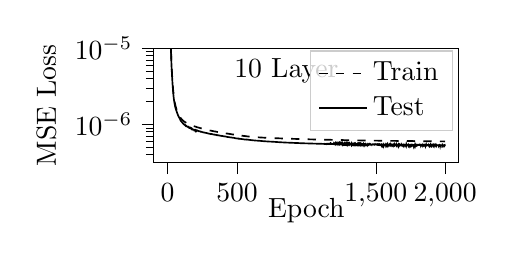
\begin{tikzpicture}

\begin{axis}[
legend cell align={left},
legend style={fill opacity=0.8, draw opacity=1, text opacity=1, draw=white!80!black},
log basis y={10},
tick align=outside,
tick pos=left,
title={10 Layer $\rare$},
title style={at={(0.45,0.85)},anchor=north},
x grid style={white!69.0196078431373!black},
xlabel={Epoch},
x label style={yshift=10pt},
xmin=-99.95, xmax=2098.95,
xtick style={color=black},
xtick = {0,500,1500,2000},
y grid style={white!69.0196078431373!black},
ylabel={MSE Loss},
ymin=3.17093839325154e-07, ymax=1e-5,
ymode=log,
ytick style={color=black},
width=0.45\textwidth,
height=0.25\textwidth
]
\addplot [semithick, black, dashed]
table {%
0 0.00997787586692721
1 0.0027661414751783
2 0.00218623768771067
3 0.00185343958390877
4 0.00115804947796278
5 0.00036777743147104
6 0.00018824286320887
7 0.000164930714039656
8 0.000153345151928079
9 0.000141543177305721
10 0.000127938025187177
11 0.000112482768548944
12 9.57521400996484e-05
13 7.92569487603032e-05
14 6.42920351929206e-05
15 5.20401717658388e-05
16 4.29740166491683e-05
17 3.62663831710961e-05
18 3.07352183917828e-05
19 2.49385155948403e-05
20 2.06156149879462e-05
21 1.71943852956247e-05
22 1.4385688823495e-05
23 1.20649838572717e-05
24 1.02233446727951e-05
25 8.78601411159252e-06
26 7.68138640933103e-06
27 6.83470541434872e-06
28 6.17248770799961e-06
29 5.6463688954409e-06
30 5.22004835283951e-06
31 4.84264568081016e-06
32 4.50758502950066e-06
33 4.20824098557659e-06
34 3.93843728591037e-06
35 3.69604697584691e-06
36 3.4781861807005e-06
37 3.27953066255304e-06
38 3.102444766796e-06
39 2.94624955324707e-06
40 2.80618139169064e-06
41 2.6809971720354e-06
42 2.57034235244191e-06
43 2.47136843603357e-06
44 2.38247599895658e-06
45 2.3052505364376e-06
46 2.2339168820622e-06
47 2.16824932778081e-06
48 2.10921677893339e-06
49 2.05554289499332e-06
50 2.00520992609654e-06
51 1.96032569562021e-06
52 1.91601798240981e-06
53 1.87716817765704e-06
54 1.84075475442569e-06
55 1.8041044749566e-06
56 1.77211888149031e-06
57 1.74144628215345e-06
58 1.71423015325445e-06
59 1.68766705314738e-06
60 1.66201588962167e-06
61 1.63708562206466e-06
62 1.61347263502876e-06
63 1.5917540299597e-06
64 1.57049718154667e-06
65 1.55085114516851e-06
66 1.53163219016506e-06
67 1.51338286417513e-06
68 1.49671406592233e-06
69 1.47951891813136e-06
70 1.4645103722728e-06
71 1.44944799347968e-06
72 1.43420475933453e-06
73 1.41955645852931e-06
74 1.40517172491172e-06
75 1.39141421908562e-06
76 1.37808219858471e-06
77 1.3657449522384e-06
78 1.3527578432786e-06
79 1.34140151624251e-06
80 1.32919058387415e-06
81 1.31819503866382e-06
82 1.30771289047971e-06
83 1.29784039592096e-06
84 1.28814695580104e-06
85 1.27880892563326e-06
86 1.27049044516525e-06
87 1.26170827212491e-06
88 1.25354349086138e-06
89 1.24524294693629e-06
90 1.23696791416705e-06
91 1.22909348488065e-06
92 1.22303059853834e-06
93 1.21662571478964e-06
94 1.20954619882241e-06
95 1.20269462843225e-06
96 1.19554730241589e-06
97 1.18936523608681e-06
98 1.18438249876363e-06
99 1.17871571490014e-06
100 1.17326355984915e-06
101 1.16720301622308e-06
102 1.16031671996097e-06
103 1.15646743591924e-06
104 1.15072228288682e-06
105 1.1456532542411e-06
106 1.14082713997732e-06
107 1.13676369537075e-06
108 1.13183904920788e-06
109 1.12775252654274e-06
110 1.12097592221971e-06
111 1.11884615537861e-06
112 1.11495200479794e-06
113 1.11073350669244e-06
114 1.10769001994981e-06
115 1.10351587494506e-06
116 1.10006028367593e-06
117 1.09647195202456e-06
118 1.09295321027503e-06
119 1.08959795028341e-06
120 1.08633151981508e-06
121 1.08298288154174e-06
122 1.0800084913285e-06
123 1.07806380844977e-06
124 1.074994691038e-06
125 1.07166258550251e-06
126 1.06880648237961e-06
127 1.06578414178671e-06
128 1.06304140217617e-06
129 1.06044994532795e-06
130 1.05643772593567e-06
131 1.0558744672835e-06
132 1.05326026272223e-06
133 1.04935598690759e-06
134 1.04676802968129e-06
135 1.04461839976011e-06
136 1.04219356757085e-06
137 1.03843377786461e-06
138 1.03679534922208e-06
139 1.03479115048799e-06
140 1.03239273369127e-06
141 1.02880143617767e-06
142 1.02687638050725e-06
143 1.02502206539157e-06
144 1.02148192920026e-06
145 1.02024824695945e-06
146 1.01793011802442e-06
147 1.01475467491241e-06
148 1.01393682172102e-06
149 1.01059575447948e-06
150 1.00912902482264e-06
151 1.0062060501923e-06
152 1.00506513257415e-06
153 1.00228589985818e-06
154 1.00133910484601e-06
155 9.99022535552285e-07
156 9.96578049466734e-07
157 9.95774760042423e-07
158 9.92670811598373e-07
159 9.90552980908888e-07
160 9.90131076179068e-07
161 9.8754623903119e-07
162 9.8556907477132e-07
163 9.85354359244184e-07
164 9.82352091568828e-07
165 9.80439722610527e-07
166 9.78883942138964e-07
167 9.78459102157103e-07
168 9.75541983876837e-07
169 9.74201690695509e-07
170 9.73315617585513e-07
171 9.7158668955899e-07
172 9.71484288783131e-07
173 9.67737080088682e-07
174 9.66393180931391e-07
175 9.64838651981381e-07
176 9.64215281697989e-07
177 9.62576921267555e-07
178 9.63217306946262e-07
179 9.60148133856364e-07
180 9.59013245392271e-07
181 9.56711457007486e-07
182 9.55200339518569e-07
183 9.53850673880652e-07
184 9.52729099026328e-07
185 9.51356085352018e-07
186 9.49982874573152e-07
187 9.48758935265914e-07
188 9.4734960742926e-07
189 9.46268320717536e-07
190 9.45888197207978e-07
191 9.43202051558956e-07
192 9.42285718593894e-07
193 9.4148136670924e-07
194 9.39797778954699e-07
195 9.38851433886612e-07
196 9.36940359082428e-07
197 9.35960853297502e-07
198 9.35100780367293e-07
199 9.33036782470253e-07
200 9.32759092336255e-07
201 9.309670438995e-07
202 9.30231287497918e-07
203 9.28388456145512e-07
204 9.28534422172334e-07
205 9.26417262860468e-07
206 9.25963449361689e-07
207 9.23892555078964e-07
208 9.23097257839345e-07
209 9.21156167748904e-07
210 9.20179683930655e-07
211 9.18629479031097e-07
212 9.17580147955732e-07
213 9.16587913565081e-07
214 9.15249802602602e-07
215 9.14260038939574e-07
216 9.13397146405259e-07
217 9.12211345678315e-07
218 9.10792389674953e-07
219 9.10044973522872e-07
220 9.09023786704211e-07
221 9.08015798756878e-07
222 9.07080938276295e-07
223 9.05977511166611e-07
224 9.05009585721928e-07
225 9.03722100105142e-07
226 9.0283103281763e-07
227 9.01766764314971e-07
228 9.00620563015764e-07
229 8.99610003187945e-07
230 8.98586724986217e-07
231 8.97490580570093e-07
232 8.96478950949131e-07
233 8.95298846074866e-07
234 8.94353904413947e-07
235 8.93204120927749e-07
236 8.923171830304e-07
237 8.90687736870177e-07
238 8.89868796548399e-07
239 8.88946101269994e-07
240 8.87893214382984e-07
241 8.86297618535537e-07
242 8.85070359657902e-07
243 8.84417957706773e-07
244 8.83675672440631e-07
245 8.8251698130648e-07
246 8.81460606791507e-07
247 8.8027023426207e-07
248 8.79355826469919e-07
249 8.78572113578002e-07
250 8.77525471793206e-07
251 8.76351880549464e-07
252 8.75500791465811e-07
253 8.74678740700574e-07
254 8.73476796158457e-07
255 8.72610606649005e-07
256 8.71706194686794e-07
257 8.70708743093473e-07
258 8.70191305182289e-07
259 8.69344236235747e-07
260 8.67789354629167e-07
261 8.66628777828282e-07
262 8.65958915056808e-07
263 8.64537149453781e-07
264 8.63818404411631e-07
265 8.62849739490912e-07
266 8.61764416811184e-07
267 8.60982841373925e-07
268 8.60051689585362e-07
269 8.59030311005427e-07
270 8.58128868173935e-07
271 8.57145231947243e-07
272 8.56545518360008e-07
273 8.55089079635718e-07
274 8.54582956577588e-07
275 8.53439548222923e-07
276 8.52625509651261e-07
277 8.52064497024685e-07
278 8.50905582069572e-07
279 8.50112307404061e-07
280 8.49598813260855e-07
281 8.4875707469223e-07
282 8.4775906213963e-07
283 8.4675666619205e-07
284 8.46309231747e-07
285 8.45124665829644e-07
286 8.44529056251986e-07
287 8.43495970570984e-07
288 8.42961660282526e-07
289 8.41671420289458e-07
290 8.41705411914972e-07
291 8.40604265988532e-07
292 8.39964006132732e-07
293 8.38750670340005e-07
294 8.3819956410025e-07
295 8.37723511324384e-07
296 8.36425500693849e-07
297 8.35761372655952e-07
298 8.35393352815572e-07
299 8.3392940771887e-07
300 8.3388055014666e-07
301 8.32478889208232e-07
302 8.32139470674065e-07
303 8.31678217167564e-07
304 8.30812586201546e-07
305 8.30091150533008e-07
306 8.29310000142414e-07
307 8.28749091709824e-07
308 8.2756600025391e-07
309 8.27514076803482e-07
310 8.26390768622787e-07
311 8.25961606182091e-07
312 8.25162235912558e-07
313 8.24495962177707e-07
314 8.24095709617723e-07
315 8.22966658319046e-07
316 8.21936873251161e-07
317 8.21767470569057e-07
318 8.20922504203736e-07
319 8.20247862861834e-07
320 8.19370113532614e-07
321 8.18635833951475e-07
322 8.17986851899377e-07
323 8.17315450689193e-07
324 8.1666383891843e-07
325 8.16427804124942e-07
326 8.15375180422961e-07
327 8.15192657825037e-07
328 8.14120937434382e-07
329 8.13174602825484e-07
330 8.1293584187847e-07
331 8.11936721930806e-07
332 8.11085818554602e-07
333 8.10528149429501e-07
334 8.09983656409941e-07
335 8.08851426143065e-07
336 8.08121500682546e-07
337 8.08130491662951e-07
338 8.07360241225297e-07
339 8.06781943225587e-07
340 8.06020081228098e-07
341 8.05330066299348e-07
342 8.04786609791108e-07
343 8.0464047090345e-07
344 8.03382348692594e-07
345 8.03091622429974e-07
346 8.03480803682533e-07
347 8.01579474654091e-07
348 8.0091967774365e-07
349 8.01363648946563e-07
350 7.99436845767332e-07
351 7.99345849031852e-07
352 7.98882536855672e-07
353 7.97898566048616e-07
354 7.98836069549225e-07
355 7.98981313806735e-07
356 7.97069268514861e-07
357 7.96280659386639e-07
358 7.96522883803164e-07
359 7.94783968302681e-07
360 7.94133767442418e-07
361 7.94591968116265e-07
362 7.92818375458637e-07
363 7.92365432204178e-07
364 7.91729609915137e-07
365 7.92124033381469e-07
366 7.9021502497767e-07
367 7.89800760259141e-07
368 7.89006110096579e-07
369 7.89422273101081e-07
370 7.87633119500697e-07
371 7.87470235025012e-07
372 7.86781127885661e-07
373 7.87345359412939e-07
374 7.85442462444053e-07
375 7.85028574483704e-07
376 7.84489331238092e-07
377 7.83982934024152e-07
378 7.84435161477859e-07
379 7.82677077467042e-07
380 7.8204591821418e-07
381 7.81801198940002e-07
382 7.81111819321723e-07
383 7.81425274823278e-07
384 7.7998786557032e-07
385 7.79324741330356e-07
386 7.78943699941692e-07
387 7.78382946805323e-07
388 7.7774481707138e-07
389 7.78080912994028e-07
390 7.76618715718769e-07
391 7.76134723423638e-07
392 7.75627843495386e-07
393 7.74918021193116e-07
394 7.74431415038634e-07
395 7.74660446609232e-07
396 7.73305947575409e-07
397 7.72896880562257e-07
398 7.72197305280997e-07
399 7.71702392796669e-07
400 7.71071945763424e-07
401 7.70523813088175e-07
402 7.70097182538621e-07
403 7.7021479600603e-07
404 7.68894578584423e-07
405 7.68398064082021e-07
406 7.67811163484566e-07
407 7.67315257036216e-07
408 7.66777737169377e-07
409 7.66156092197434e-07
410 7.65690696312049e-07
411 7.65130233787659e-07
412 7.6555170792858e-07
413 7.64065328610286e-07
414 7.63505121966546e-07
415 7.63133862619725e-07
416 7.62454071889351e-07
417 7.62014022313906e-07
418 7.6143167035525e-07
419 7.60892476279196e-07
420 7.60415168230111e-07
421 7.59914973372133e-07
422 7.5941622890241e-07
423 7.60389407474804e-07
424 7.58777384561427e-07
425 7.58338006789927e-07
426 7.57724335500143e-07
427 7.57657803433176e-07
428 7.56923721269232e-07
429 7.56353567965107e-07
430 7.56923098862217e-07
431 7.55219046823186e-07
432 7.54618819826192e-07
433 7.54311231389693e-07
434 7.53780425611694e-07
435 7.54422887609962e-07
436 7.52576872230293e-07
437 7.52243586475743e-07
438 7.51672492100397e-07
439 7.52297821776438e-07
440 7.50493718726375e-07
441 7.50091651326557e-07
442 7.49571382499425e-07
443 7.5027601661759e-07
444 7.48633131451015e-07
445 7.48203038369866e-07
446 7.47641490107753e-07
447 7.4706847775019e-07
448 7.47778209245098e-07
449 7.45882051290891e-07
450 7.45447632596097e-07
451 7.45004974220365e-07
452 7.45590436821431e-07
453 7.44075579518722e-07
454 7.43488029229411e-07
455 7.4302814456928e-07
456 7.43562355694394e-07
457 7.42126745706173e-07
458 7.41440271383453e-07
459 7.41023272865959e-07
460 7.42221455794834e-07
461 7.39916425203546e-07
462 7.39315465096979e-07
463 7.38942567977574e-07
464 7.39466763462815e-07
465 7.38114260798284e-07
466 7.37723011752678e-07
467 7.38328398483645e-07
468 7.36677821834064e-07
469 7.36189456091552e-07
470 7.36971248016971e-07
471 7.35291715386666e-07
472 7.34859717340441e-07
473 7.35544233293695e-07
474 7.33993297529878e-07
475 7.33437984763441e-07
476 7.34147434599208e-07
477 7.32526463366412e-07
478 7.32113129146228e-07
479 7.32783056690778e-07
480 7.31102353171309e-07
481 7.30759978779361e-07
482 7.30174026074337e-07
483 7.3101718700741e-07
484 7.29139022212166e-07
485 7.28747309921118e-07
486 7.29511678514427e-07
487 7.27845423909912e-07
488 7.27509910404933e-07
489 7.27898909303804e-07
490 7.25985288198672e-07
491 7.26988534040629e-07
492 7.26433349939271e-07
493 7.24913795409066e-07
494 7.25639360695141e-07
495 7.25110006783325e-07
496 7.23576190097219e-07
497 7.24332362437963e-07
498 7.23792091548603e-07
499 7.22295086035274e-07
500 7.23148807196594e-07
501 7.22562276394001e-07
502 7.21028598093199e-07
503 7.21920047169533e-07
504 7.20162841702177e-07
505 7.21097849861962e-07
506 7.20601577768321e-07
507 7.18964301626102e-07
508 7.19790344447802e-07
509 7.19423874585345e-07
510 7.17816719657094e-07
511 7.18529795136646e-07
512 7.17035474110617e-07
513 7.17842366498189e-07
514 7.173693042688e-07
515 7.15891436129823e-07
516 7.16593398948362e-07
517 7.16193349916239e-07
518 7.15836237418444e-07
519 7.13896747583931e-07
520 7.14747440071051e-07
521 7.14939811359727e-07
522 7.14682133747146e-07
523 7.14109896080117e-07
524 7.12665502788923e-07
525 7.13412247876022e-07
526 7.12840395792114e-07
527 7.1258078847336e-07
528 7.1094341305411e-07
529 7.11800691419739e-07
530 7.11041270108126e-07
531 7.11053048263466e-07
532 7.09551945874409e-07
533 7.10300355095228e-07
534 7.10044622053374e-07
535 7.08126653066188e-07
536 7.09192354179322e-07
537 7.08688509973854e-07
538 7.08473750933081e-07
539 7.0703383852333e-07
540 7.07924062425036e-07
541 7.07072048214741e-07
542 7.05930014561318e-07
543 7.06833243867777e-07
544 7.06151251620213e-07
545 7.05789116310029e-07
546 7.05411095324848e-07
547 7.03952515351602e-07
548 7.04824918869917e-07
549 7.04396891237025e-07
550 7.04121892809439e-07
551 7.03592790472385e-07
552 7.02295799982267e-07
553 7.03159633289374e-07
554 7.02392406822128e-07
555 7.02389151811644e-07
556 7.02069595888588e-07
557 7.00544815430249e-07
558 7.01544812031329e-07
559 7.01071055104308e-07
560 7.00843794945172e-07
561 7.00298507183561e-07
562 6.99028340818586e-07
563 6.9988211890859e-07
564 6.99153588470836e-07
565 6.99094921657206e-07
566 6.98874052901033e-07
567 6.97493815380312e-07
568 6.9732204678985e-07
569 6.96886004035946e-07
570 6.96496134878544e-07
571 6.96340423658626e-07
572 6.9577226418005e-07
573 6.95301015184668e-07
574 6.94970092226299e-07
575 6.94665715130327e-07
576 6.94327597415167e-07
577 6.9397252194392e-07
578 6.93629053131417e-07
579 6.93304834925357e-07
580 6.92961221275823e-07
581 6.92612403483395e-07
582 6.92295116081709e-07
583 6.92008054087978e-07
584 6.91836038868132e-07
585 6.91154041760456e-07
586 6.91039159349316e-07
587 6.90780433998839e-07
588 6.90375913677599e-07
589 6.90120593674237e-07
590 6.89844487624214e-07
591 6.89540247705622e-07
592 6.8927526524476e-07
593 6.88991556458518e-07
594 6.88708317511555e-07
595 6.88413684557077e-07
596 6.88122735454044e-07
597 6.87847310999246e-07
598 6.87655565940304e-07
599 6.873611031466e-07
600 6.8711852216552e-07
601 6.86813203969905e-07
602 6.86521028598008e-07
603 6.86258257005079e-07
604 6.86011237931439e-07
605 6.85736956057781e-07
606 6.8547543475006e-07
607 6.85227141644873e-07
608 6.84974181766052e-07
609 6.84731802891747e-07
610 6.84444454293498e-07
611 6.84201174820487e-07
612 6.83949088440272e-07
613 6.83735282066777e-07
614 6.83597051065021e-07
615 6.83230357168441e-07
616 6.82977046281508e-07
617 6.82744479377107e-07
618 6.82628084632597e-07
619 6.82269299900895e-07
620 6.82057781943968e-07
621 6.81825706507766e-07
622 6.81707034459578e-07
623 6.81389691763457e-07
624 6.81201359242323e-07
625 6.81054129145764e-07
626 6.8075853309324e-07
627 6.80542225936165e-07
628 6.80400173507678e-07
629 6.80067346735314e-07
630 6.79983958491448e-07
631 6.79618614057631e-07
632 6.79393168169895e-07
633 6.79165578233665e-07
634 6.79077912963066e-07
635 6.78772824926455e-07
636 6.78559704212489e-07
637 6.78351354096662e-07
638 6.78243983884386e-07
639 6.77901727698327e-07
640 6.77708650769659e-07
641 6.77525354845443e-07
642 6.77312835492216e-07
643 6.77094021853009e-07
644 6.7693512350786e-07
645 6.76660766927739e-07
646 6.76465998878939e-07
647 6.7620693066317e-07
648 6.76058081367614e-07
649 6.75807865121669e-07
650 6.75675274962373e-07
651 6.75309103939981e-07
652 6.75240928430298e-07
653 6.75009894337109e-07
654 6.74884714669588e-07
655 6.7469262417319e-07
656 6.74492794075832e-07
657 6.74472121843905e-07
658 6.74072660487468e-07
659 6.74126479594861e-07
660 6.73871772562507e-07
661 6.73676320815275e-07
662 6.73381162670239e-07
663 6.73315533632035e-07
664 6.7304010840985e-07
665 6.7279634778572e-07
666 6.72624413653011e-07
667 6.72622655784494e-07
668 6.72328725286775e-07
669 6.72171628352203e-07
670 6.72120275240218e-07
671 6.72108327890442e-07
672 6.71769079815476e-07
673 6.71592175606861e-07
674 6.7153022288835e-07
675 6.71228376674549e-07
676 6.71063214738865e-07
677 6.70862587298871e-07
678 6.70727474243904e-07
679 6.70538763273498e-07
680 6.70397458648608e-07
681 6.70331136205959e-07
682 6.70071903499547e-07
683 6.69920863757056e-07
684 6.69779470129583e-07
685 6.69620603034105e-07
686 6.69458129848977e-07
687 6.6930754940131e-07
688 6.69167233667167e-07
689 6.68956220224004e-07
690 6.68770538680974e-07
691 6.68667876396967e-07
692 6.68520957177066e-07
693 6.68362044635273e-07
694 6.68231087544768e-07
695 6.68063874257996e-07
696 6.67905007389891e-07
697 6.67740694836993e-07
698 6.67615698802138e-07
699 6.67491615800486e-07
700 6.67331059744924e-07
701 6.67199185485856e-07
702 6.67054764520003e-07
703 6.66892555187815e-07
704 6.66757220614045e-07
705 6.6661704566684e-07
706 6.66472319977629e-07
707 6.66348736558575e-07
708 6.66208892795339e-07
709 6.66104842267146e-07
710 6.65947033539283e-07
711 6.6583568202816e-07
712 6.65676333156284e-07
713 6.65566532433104e-07
714 6.65371252381419e-07
715 6.65273846124137e-07
716 6.65145204777673e-07
717 6.6501357501636e-07
718 6.64885187660502e-07
719 6.64747493914319e-07
720 6.64656038921407e-07
721 6.64518116366253e-07
722 6.64384310013588e-07
723 6.6426489875937e-07
724 6.64103254891302e-07
725 6.6400623869356e-07
726 6.6387511243704e-07
727 6.63760887292142e-07
728 6.63594443778948e-07
729 6.6352547675308e-07
730 6.63392976136379e-07
731 6.63245974934057e-07
732 6.63125168372858e-07
733 6.63018874917043e-07
734 6.62882144197852e-07
735 6.62734271159593e-07
736 6.62517572180832e-07
737 6.6241604606887e-07
738 6.62473698085364e-07
739 6.62516929139656e-07
740 6.62498065295836e-07
741 6.61815979839275e-07
742 6.61530765412976e-07
743 6.61442542394752e-07
744 6.61331088323891e-07
745 6.61209408832519e-07
746 6.6109859224639e-07
747 6.6099788502072e-07
748 6.60889263187414e-07
749 6.60740850307207e-07
750 6.60631029802516e-07
751 6.60538422906143e-07
752 6.60393012481109e-07
753 6.60271693462278e-07
754 6.60180221544238e-07
755 6.60043354130835e-07
756 6.59950334664927e-07
757 6.59887545353399e-07
758 6.5971084376315e-07
759 6.59582626255428e-07
760 6.59522363278597e-07
761 6.59398176679815e-07
762 6.59279328061757e-07
763 6.59160926986146e-07
764 6.59018419938207e-07
765 6.58968605165455e-07
766 6.58780548107529e-07
767 6.58640463925053e-07
768 6.58545901032426e-07
769 6.58429381942938e-07
770 6.58341001013696e-07
771 6.58279398663808e-07
772 6.58103613247363e-07
773 6.58032226553473e-07
774 6.5792477641935e-07
775 6.57836251804156e-07
776 6.57792503417909e-07
777 6.57651318391572e-07
778 6.57547617464616e-07
779 6.57399611057485e-07
780 6.57286304786453e-07
781 6.57153251651721e-07
782 6.5710807548669e-07
783 6.56900221926549e-07
784 6.56799596583824e-07
785 6.56696743305929e-07
786 6.56575473740872e-07
787 6.56487851685483e-07
788 6.56370081244972e-07
789 6.56292135957415e-07
790 6.56130607339378e-07
791 6.56064941154e-07
792 6.56011381011012e-07
793 6.55829648934514e-07
794 6.55786200027819e-07
795 6.55607685331461e-07
796 6.55609785056299e-07
797 6.55533220481175e-07
798 6.55394131726439e-07
799 6.55311715917151e-07
800 6.55156520764422e-07
801 6.55102531055718e-07
802 6.55082887604408e-07
803 6.54888119228758e-07
804 6.54802214071992e-07
805 6.5473559047291e-07
806 6.54574609910696e-07
807 6.54500922465218e-07
808 6.54382220616867e-07
809 6.54305573817737e-07
810 6.5420019161877e-07
811 6.54057651630069e-07
812 6.53967765671837e-07
813 6.53819775891407e-07
814 6.53770412583299e-07
815 6.53644654022401e-07
816 6.53591989035362e-07
817 6.53487234302474e-07
818 6.53435297138572e-07
819 6.53194102852694e-07
820 6.53198145187162e-07
821 6.5311538847368e-07
822 6.52892069282984e-07
823 6.52899213022806e-07
824 6.52815578064292e-07
825 6.52532915339066e-07
826 6.5250298719377e-07
827 6.52467241110344e-07
828 6.52352714354265e-07
829 6.52214292244935e-07
830 6.52175464963989e-07
831 6.52048443271269e-07
832 6.51983712870674e-07
833 6.51903975750656e-07
834 6.51790568511501e-07
835 6.51704363789918e-07
836 6.51591102098337e-07
837 6.51535222814914e-07
838 6.5140828783683e-07
839 6.51308421680596e-07
840 6.51213768250614e-07
841 6.51116864844425e-07
842 6.50987768693767e-07
843 6.50862097572258e-07
844 6.50764789384084e-07
845 6.50686730963912e-07
846 6.50605446963937e-07
847 6.50517625658154e-07
848 6.49935367121657e-07
849 6.49951558187922e-07
850 6.49781994908949e-07
851 6.49812969228947e-07
852 6.4962381597411e-07
853 6.49715427286424e-07
854 6.49609696424136e-07
855 6.49503299598564e-07
856 6.49437240753059e-07
857 6.4924598638072e-07
858 6.49154591329193e-07
859 6.49055806263732e-07
860 6.48968337969791e-07
861 6.48860881113933e-07
862 6.48779707205449e-07
863 6.4869935371803e-07
864 6.48607655406863e-07
865 6.48494430663504e-07
866 6.48387495814973e-07
867 6.48355465315831e-07
868 6.4823302085415e-07
869 6.48177903727287e-07
870 6.48068991381479e-07
871 6.48002301730344e-07
872 6.47880534643264e-07
873 6.4779980566243e-07
874 6.47472709502495e-07
875 6.47573727789563e-07
876 6.47521113151583e-07
877 6.47460983415726e-07
878 6.47327359146743e-07
879 6.47256306294253e-07
880 6.47165816758388e-07
881 6.47062579616886e-07
882 6.46873130364156e-07
883 6.46932409637202e-07
884 6.4678064497059e-07
885 6.46794917827265e-07
886 6.4658947853502e-07
887 6.46604447453569e-07
888 6.46413081099695e-07
889 6.46435930761413e-07
890 6.46238205860072e-07
891 6.46160109269545e-07
892 6.46079087459839e-07
893 6.45998969318384e-07
894 6.45898591372429e-07
895 6.45816730695969e-07
896 6.45777476066201e-07
897 6.45704528096758e-07
898 6.45561784040183e-07
899 6.45402865401934e-07
900 6.45395685438643e-07
901 6.45250818593013e-07
902 6.45247586589903e-07
903 6.45016569762902e-07
904 6.45096973528325e-07
905 6.44992183836734e-07
906 6.44879979844859e-07
907 6.44814044164832e-07
908 6.44536055304457e-07
909 6.44651230615523e-07
910 6.44630252224943e-07
911 6.44534238688266e-07
912 6.44403965878837e-07
913 6.44269876133308e-07
914 6.44109464232656e-07
915 6.44056983475139e-07
916 6.44181476729955e-07
917 6.44011751091966e-07
918 6.43851985074662e-07
919 6.43799305493076e-07
920 6.43708418380129e-07
921 6.43616032121486e-07
922 6.43390352038864e-07
923 6.43459086845155e-07
924 6.43066392427727e-07
925 6.43326589468529e-07
926 6.43231603277172e-07
927 6.42995318642647e-07
928 6.43065223883355e-07
929 6.42968633215446e-07
930 6.42634859744362e-07
931 6.42847502362542e-07
932 6.42573602135599e-07
933 6.42576249461513e-07
934 6.42420869482407e-07
935 6.42509780959699e-07
936 6.42260338906908e-07
937 6.42345372426689e-07
938 6.4186560094015e-07
939 6.42131707621729e-07
940 6.41876858665569e-07
941 6.41937691256089e-07
942 6.41715006921117e-07
943 6.41790332380765e-07
944 6.41556473468086e-07
945 6.415050187627e-07
946 6.41448093148256e-07
947 6.41452986968716e-07
948 6.41207829275459e-07
949 6.41160052467171e-07
950 6.41136324560421e-07
951 6.41156462506842e-07
952 6.4103641173574e-07
953 6.40879574191899e-07
954 6.40985946901651e-07
955 6.40758436617261e-07
956 6.40720444295084e-07
957 6.40529553727731e-07
958 6.40474377917144e-07
959 6.40498605775974e-07
960 6.40255618591823e-07
961 6.40319487331453e-07
962 6.40329926909544e-07
963 6.40118906979126e-07
964 6.40069182985315e-07
965 6.39933080719857e-07
966 6.40022533211493e-07
967 6.39830953474529e-07
968 6.39713040214929e-07
969 6.39593101901426e-07
970 6.39774005406935e-07
971 6.39434521559679e-07
972 6.39282294187637e-07
973 6.39523240408835e-07
974 6.39073064718332e-07
975 6.39149466316269e-07
976 6.39264868198097e-07
977 6.38937482264623e-07
978 6.3891833339369e-07
979 6.3900999825961e-07
980 6.38726525863831e-07
981 6.38650845402822e-07
982 6.38661012288821e-07
983 6.38419105449373e-07
984 6.38549863495541e-07
985 6.38299137555975e-07
986 6.38424846982843e-07
987 6.38142738338843e-07
988 6.38220265770428e-07
989 6.38023431044132e-07
990 6.38141142715654e-07
991 6.37875260373733e-07
992 6.37939418027145e-07
993 6.37722096641369e-07
994 6.3776769428614e-07
995 6.37635073331921e-07
996 6.37635214005172e-07
997 6.37495254942166e-07
998 6.3745381473268e-07
999 6.37371561651889e-07
1000 6.36697234590144e-07
1001 6.36720888294917e-07
1002 6.36737104024121e-07
1003 6.36686584201129e-07
1004 6.36586772294834e-07
1005 6.36517155868432e-07
1006 6.36517348780785e-07
1007 6.36441783626651e-07
1008 6.3637201033373e-07
1009 6.36290345994439e-07
1010 6.36226407571883e-07
1011 6.36187908853003e-07
1012 6.36128972693939e-07
1013 6.36090735575578e-07
1014 6.3589234423489e-07
1015 6.35912154805851e-07
1016 6.35904042837865e-07
1017 6.35763122460276e-07
1018 6.35666576634719e-07
1019 6.3564752967693e-07
1020 6.35538853181572e-07
1021 6.35491918373532e-07
1022 6.35451334389359e-07
1023 6.35415595198197e-07
1024 6.35248154431167e-07
1025 6.35240329302178e-07
1026 6.35150410481344e-07
1027 6.35137976871647e-07
1028 6.34976308155899e-07
1029 6.35017855039166e-07
1030 6.3482607657761e-07
1031 6.34881822449529e-07
1032 6.34690630576529e-07
1033 6.34540902638037e-07
1034 6.34473359724552e-07
1035 6.34451190421714e-07
1036 6.34297449984445e-07
1037 6.34270674453319e-07
1038 6.34141945823785e-07
1039 6.34231479885727e-07
1040 6.34136626601389e-07
1041 6.34082943328451e-07
1042 6.3395456306381e-07
1043 6.33960346824836e-07
1044 6.33853544790952e-07
1045 6.33788128311608e-07
1046 6.33753139354098e-07
1047 6.33628680830611e-07
1048 6.33625172490326e-07
1049 6.33516750120577e-07
1050 6.33459435064765e-07
1051 6.33394688364319e-07
1052 6.33326460899752e-07
1053 6.33260135010971e-07
1054 6.33217650971574e-07
1055 6.33124233907267e-07
1056 6.33073544925367e-07
1057 6.32994399367703e-07
1058 6.32937160020219e-07
1059 6.32863034105924e-07
1060 6.32802857673198e-07
1061 6.327211272108e-07
1062 6.32664070593592e-07
1063 6.32609571134424e-07
1064 6.3261294997119e-07
1065 6.32557479264051e-07
1066 6.32472583347976e-07
1067 6.32388676500284e-07
1068 6.3235371713688e-07
1069 6.32262299873787e-07
1070 6.32186852847383e-07
1071 6.32157002080191e-07
1072 6.32051000330591e-07
1073 6.31951863908853e-07
1074 6.31979543818772e-07
1075 6.31833903980805e-07
1076 6.31841321954596e-07
1077 6.31720386728318e-07
1078 6.31670170619714e-07
1079 6.31639167558262e-07
1080 6.31551888616855e-07
1081 6.31490619177555e-07
1082 6.31423811270793e-07
1083 6.3135732366959e-07
1084 6.31311455016714e-07
1085 6.31243087482858e-07
1086 6.31197074852707e-07
1087 6.31128118996571e-07
1088 6.31093993149534e-07
1089 6.31002973804584e-07
1090 6.30930024748011e-07
1091 6.30873843036284e-07
1092 6.30818468749794e-07
1093 6.30774500507414e-07
1094 6.30719061497587e-07
1095 6.30654274829112e-07
1096 6.30573381890542e-07
1097 6.30514150955719e-07
1098 6.30455811105435e-07
1099 6.30417263671745e-07
1100 6.303295307859e-07
1101 6.30289127698802e-07
1102 6.30195487040908e-07
1103 6.30157178008517e-07
1104 6.30050639735202e-07
1105 6.29987743629101e-07
1106 6.29968577783302e-07
1107 6.29872791670039e-07
1108 6.29852591870872e-07
1109 6.29763205395761e-07
1110 6.2972433978814e-07
1111 6.29685811993852e-07
1112 6.29570583363659e-07
1113 6.29555979784868e-07
1114 6.29505421251508e-07
1115 6.29378778313594e-07
1116 6.29395147583978e-07
1117 6.29327122219081e-07
1118 6.29239093782985e-07
1119 6.29181523294164e-07
1120 6.29151311549947e-07
1121 6.29059220806027e-07
1122 6.29024048642179e-07
1123 6.28953817965794e-07
1124 6.28911244270114e-07
1125 6.28805891778938e-07
1126 6.28756066198832e-07
1127 6.28648164230583e-07
1128 6.28306397643996e-07
1129 6.28687460732635e-07
1130 6.2848032885654e-07
1131 6.28135447911404e-07
1132 6.28400187004274e-07
1133 6.28573363961493e-07
1134 6.28527363033982e-07
1135 6.28527280390756e-07
1136 6.28343305770329e-07
1137 6.28284698507287e-07
1138 6.2812800601364e-07
1139 6.28083045576488e-07
1140 6.28054853891058e-07
1141 6.28019043531936e-07
1142 6.27906697488356e-07
1143 6.27742714229385e-07
1144 6.27365253272671e-07
1145 6.27446661880526e-07
1146 6.27488955871058e-07
1147 6.27701524173574e-07
1148 6.27380187211202e-07
1149 6.27639201667307e-07
1150 6.2732651976205e-07
1151 6.27196206636427e-07
1152 6.27453849801896e-07
1153 6.27290091358645e-07
1154 6.27293938102014e-07
1155 6.27100247442058e-07
1156 6.26845826687372e-07
1157 6.27136329399036e-07
1158 6.26958845828085e-07
1159 6.27028462695023e-07
1160 6.26799966369163e-07
1161 6.26518928804387e-07
1162 6.26466177664042e-07
1163 6.26487830309941e-07
1164 6.26460136622597e-07
1165 6.26553522593554e-07
1166 6.2658400442217e-07
1167 6.26421702463631e-07
1168 6.26354288016273e-07
1169 6.26202877917592e-07
1170 6.26266790412444e-07
1171 6.26346333575611e-07
1172 6.26213740538617e-07
1173 6.2591202649287e-07
1174 6.26159682411753e-07
1175 6.259679466325e-07
1176 6.25821323929188e-07
1177 6.25983454000334e-07
1178 6.25770567594941e-07
1179 6.25582370801681e-07
1180 6.25654848079193e-07
1181 6.25532107612514e-07
1182 6.2545592751917e-07
1183 6.25413862280766e-07
1184 6.25349340801051e-07
1185 6.25261259557419e-07
1186 6.25203425371978e-07
1187 6.25166111447584e-07
1188 6.25094666915516e-07
1189 6.25081710083464e-07
1190 6.25006898232527e-07
1191 6.24934165074365e-07
1192 6.24913404614347e-07
1193 6.24911467220102e-07
1194 6.24548951755344e-07
1195 6.24694442166174e-07
1196 6.24773008453872e-07
1197 6.24621071231957e-07
1198 6.2450013277271e-07
1199 6.24621874457887e-07
1200 6.24454692619736e-07
1201 6.24370407393826e-07
1202 6.2447302522628e-07
1203 6.24262143524845e-07
1204 6.24315219837968e-07
1205 6.2430981112982e-07
1206 6.23796075679195e-07
1207 6.24177096320011e-07
1208 6.24049105802271e-07
1209 6.24054203349544e-07
1210 6.24027001990157e-07
1211 6.23865109787403e-07
1212 6.23932852477083e-07
1213 6.23779870181807e-07
1214 6.23787094262696e-07
1215 6.23741608634987e-07
1216 6.23713004550552e-07
1217 6.23544608970405e-07
1218 6.23572001856587e-07
1219 6.23602649540089e-07
1220 6.23225978060304e-07
1221 6.23518592469452e-07
1222 6.23039261583358e-07
1223 6.23288506076847e-07
1224 6.23076261497602e-07
1225 6.23334286977695e-07
1226 6.23120273957056e-07
1227 6.23057992385156e-07
1228 6.2310072766536e-07
1229 6.22905203400137e-07
1230 6.23071342417347e-07
1231 6.22551743603594e-07
1232 6.22838785815816e-07
1233 6.22911618577859e-07
1234 6.22436094097623e-07
1235 6.2257276290012e-07
1236 6.22675055979016e-07
1237 6.22591451126198e-07
1238 6.22482214389208e-07
1239 6.22608929845114e-07
1240 6.22082830332715e-07
1241 6.22355137487318e-07
1242 6.22401920892912e-07
1243 6.22228115553014e-07
1244 6.22168779464971e-07
1245 6.2226912954344e-07
1246 6.21835941025495e-07
1247 6.22107425449769e-07
1248 6.22095544343892e-07
1249 6.21943532365776e-07
1250 6.21878639350371e-07
1251 6.21777342473706e-07
1252 6.21807686485454e-07
1253 6.21633627901019e-07
1254 6.21770785983244e-07
1255 6.21682074758212e-07
1256 6.21532353186183e-07
1257 6.21157554036245e-07
1258 6.21374166421163e-07
1259 6.21383820664789e-07
1260 6.21448532641011e-07
1261 6.21237848690726e-07
1262 6.21411155641738e-07
1263 6.20860587424943e-07
1264 6.2109406439248e-07
1265 6.21135994300914e-07
1266 6.21238524701084e-07
1267 6.20719478952481e-07
1268 6.20863639028357e-07
1269 6.21026825456283e-07
1270 6.20972499071115e-07
1271 6.20547807017147e-07
1272 6.20815331657809e-07
1273 6.20883732374011e-07
1274 6.20434088780542e-07
1275 6.20376438746462e-07
1276 6.2064274709428e-07
1277 6.20666749313159e-07
1278 6.20157986659819e-07
1279 6.20282532104e-07
1280 6.20512788032102e-07
1281 6.20443126081227e-07
1282 6.19954360075781e-07
1283 6.20158316202435e-07
1284 6.20412783675306e-07
1285 6.19787940749461e-07
1286 6.20167513709191e-07
1287 6.19920055640932e-07
1288 6.19938900399575e-07
1289 6.2001241861509e-07
1290 6.19576977349823e-07
1291 6.19768135450727e-07
1292 6.19923710424075e-07
1293 6.19364097445896e-07
1294 6.19723660356897e-07
1295 6.19799817101807e-07
1296 6.19224814414565e-07
1297 6.19575253921312e-07
1298 6.1951230144075e-07
1299 6.19440844417341e-07
1300 6.19388264468057e-07
1301 6.1928821070012e-07
1302 6.18971549577907e-07
1303 6.19309097317e-07
1304 6.18896740419927e-07
1305 6.19233279984144e-07
1306 6.18862542118848e-07
1307 6.1904855721906e-07
1308 6.19084869462938e-07
1309 6.18728734835372e-07
1310 6.19067870623269e-07
1311 6.18833963194731e-07
1312 6.18797829730511e-07
1313 6.18840376517937e-07
1314 6.18354753008532e-07
1315 6.18526108105755e-07
1316 6.18729250248862e-07
1317 6.18316310337263e-07
1318 6.18493220983396e-07
1319 6.1857565151513e-07
1320 6.18553323434412e-07
1321 6.18287408251206e-07
1322 6.18182901995112e-07
1323 6.18168552804832e-07
1324 6.18295116474599e-07
1325 6.18236038974373e-07
1326 6.18178005744596e-07
1327 6.18093473242709e-07
1328 6.17960725605826e-07
1329 6.17843770534421e-07
1330 6.18153380194997e-07
1331 6.1793422157308e-07
1332 6.17757560888776e-07
1333 6.1783743137056e-07
1334 6.17917767534948e-07
1335 6.17540525162497e-07
1336 6.17705096779275e-07
1337 6.17609444908851e-07
1338 6.17570422804192e-07
1339 6.17073546720803e-07
1340 6.17361359793733e-07
1341 6.17218927558838e-07
1342 6.1731549609334e-07
1343 6.16839265717317e-07
1344 6.17278455536052e-07
1345 6.16886698999508e-07
1346 6.17145374242512e-07
1347 6.16674280522034e-07
1348 6.16949876508954e-07
1349 6.16746271418833e-07
1350 6.17063569656295e-07
1351 6.1651876738722e-07
1352 6.16958195287509e-07
1353 6.16493237330928e-07
1354 6.16818991467483e-07
1355 6.16564756263926e-07
1356 6.16465375699704e-07
1357 6.1670159974625e-07
1358 6.16341221103767e-07
1359 6.164012397889e-07
1360 6.16298516355584e-07
1361 6.16462023430131e-07
1362 6.16257752142246e-07
1363 6.16205831555305e-07
1364 6.16200928298838e-07
1365 6.16331213180388e-07
1366 6.15774696939297e-07
1367 6.1614706064006e-07
1368 6.16303828067544e-07
1369 6.15772465287989e-07
1370 6.16175163123955e-07
1371 6.15761831603834e-07
1372 6.16118617230654e-07
1373 6.15417715017941e-07
1374 6.15825617352073e-07
1375 6.15959238160713e-07
1376 6.1554938204722e-07
1377 6.1578529990669e-07
1378 6.15404216532056e-07
1379 6.15805073294951e-07
1380 6.15045303192119e-07
1381 6.15779943856865e-07
1382 6.15239680826107e-07
1383 6.15575325518591e-07
1384 6.15164999260287e-07
1385 6.15541761249006e-07
1386 6.1481267056962e-07
1387 6.15518598799269e-07
1388 6.14974511393029e-07
1389 6.15256523204266e-07
1390 6.1495169554604e-07
1391 6.15171495873312e-07
1392 6.14589822056644e-07
1393 6.15063232331181e-07
1394 6.15107449206675e-07
1395 6.14662685840983e-07
1396 6.1502810259384e-07
1397 6.14590154093264e-07
1398 6.14612481669496e-07
1399 6.14802560768624e-07
1400 6.14702865100014e-07
1401 6.14827589217271e-07
1402 6.14387261038019e-07
1403 6.14532386492783e-07
1404 6.14365300663167e-07
1405 6.14513860909938e-07
1406 6.14463790768127e-07
1407 6.14669436131976e-07
1408 6.14088050312489e-07
1409 6.14400729553211e-07
1410 6.14347149664241e-07
1411 6.14008724106441e-07
1412 6.14388912921982e-07
1413 6.13885905003997e-07
1414 6.14030799852117e-07
1415 6.14084501023626e-07
1416 6.14049639672487e-07
1417 6.14017295546887e-07
1418 6.13979460368341e-07
1419 6.14067722430889e-07
1420 6.1396852149187e-07
1421 6.13854022716964e-07
1422 6.13682396014781e-07
1423 6.13604328492556e-07
1424 6.13541604060686e-07
1425 6.13372681478097e-07
1426 6.13554293892093e-07
1427 6.13180419733794e-07
1428 6.13455641953919e-07
1429 6.1348410481088e-07
1430 6.13415493866398e-07
1431 6.13489517483856e-07
1432 6.12983758479402e-07
1433 6.13290954696311e-07
1434 6.13153399413591e-07
1435 6.13249425313711e-07
1436 6.13075842231581e-07
1437 6.1320476547877e-07
1438 6.13227797749971e-07
1439 6.12789343271913e-07
1440 6.13057139688067e-07
1441 6.13030189320796e-07
1442 6.12636833110969e-07
1443 6.12816545171313e-07
1444 6.12819367759698e-07
1445 6.12868730669902e-07
1446 6.12897299447468e-07
1447 6.12634370639853e-07
1448 6.12377568522504e-07
1449 6.12560680650631e-07
1450 6.1260865675905e-07
1451 6.12693906937523e-07
1452 6.12507754290448e-07
1453 6.12503317547919e-07
1454 6.12373988857939e-07
1455 6.12564684573158e-07
1456 6.12393487315899e-07
1457 6.12160607012413e-07
1458 6.12446222532981e-07
1459 6.12120268648653e-07
1460 6.12264537330987e-07
1461 6.12050654183349e-07
1462 6.12274880353425e-07
1463 6.12251636255223e-07
1464 6.12217257234704e-07
1465 6.11654116092097e-07
1466 6.11951332530225e-07
1467 6.12065274943063e-07
1468 6.11820810711095e-07
1469 6.11882885237947e-07
1470 6.11983560567353e-07
1471 6.11653300381931e-07
1472 6.11477287904449e-07
1473 6.11686302534054e-07
1474 6.11679580714508e-07
1475 6.11734728380497e-07
1476 6.11446988500575e-07
1477 6.11656725389764e-07
1478 6.11418435035205e-07
1479 6.1152755747429e-07
1480 6.11419605277774e-07
1481 6.11340049509579e-07
1482 6.11387434275912e-07
1483 6.11206909837847e-07
1484 6.11388030407056e-07
1485 6.11385448635815e-07
1486 6.11177371865779e-07
1487 6.11203298248597e-07
1488 6.11062275424956e-07
1489 6.1113751262809e-07
1490 6.11060912476091e-07
1491 6.11207886258569e-07
1492 6.1091258017143e-07
1493 6.11062240871263e-07
1494 6.10889090808087e-07
1495 6.1091539818392e-07
1496 6.10902968965377e-07
1497 6.10834144879391e-07
1498 6.10740337897653e-07
1499 6.10833803591504e-07
1500 6.10895269836931e-07
1501 6.10666885577871e-07
1502 6.10610917632925e-07
1503 6.10713644597638e-07
1504 6.10572242344176e-07
1505 6.10609684585484e-07
1506 6.10557814717083e-07
1507 6.10448972544475e-07
1508 6.10527583972953e-07
1509 6.1040572688853e-07
1510 6.1039827343734e-07
1511 6.10298882641302e-07
1512 6.10335146262742e-07
1513 6.10234822481459e-07
1514 6.10242099241987e-07
1515 6.1033837800295e-07
1516 6.10180680752137e-07
1517 6.10083428981056e-07
1518 6.10104180410076e-07
1519 6.09997833088016e-07
1520 6.10046423801691e-07
1521 6.10109085918964e-07
1522 6.09993698589051e-07
1523 6.0983415817617e-07
1524 6.09903624265939e-07
1525 6.09998824259605e-07
1526 6.09884452536846e-07
1527 6.0968484560675e-07
1528 6.09763739340963e-07
1529 6.09665772230983e-07
1530 6.09703086560387e-07
1531 6.09820219096946e-07
1532 6.09501713334737e-07
1533 6.09573474022795e-07
1534 6.09616974934113e-07
1535 6.09569544238298e-07
1536 6.09660148164437e-07
1537 6.09644980698931e-07
1538 6.09337568604929e-07
1539 6.09344284718816e-07
1540 6.09197389067617e-07
1541 6.0940735770032e-07
1542 6.09346155506785e-07
1543 6.09101156697989e-07
1544 6.09007024621633e-07
1545 6.09158799576903e-07
1546 6.09148734696419e-07
1547 6.08959669804676e-07
1548 6.09325477711309e-07
1549 6.09174900532139e-07
1550 6.0887942427712e-07
1551 6.08839884300494e-07
1552 6.08781071470332e-07
1553 6.09002018386207e-07
1554 6.08992753903692e-07
1555 6.08921752103697e-07
1556 6.08550892451376e-07
1557 6.08858571517601e-07
1558 6.08579321387026e-07
1559 6.08931567271043e-07
1560 6.08685558709965e-07
1561 6.086547848696e-07
1562 6.08401901835975e-07
1563 6.08758491502215e-07
1564 6.08654236842199e-07
1565 6.08688211428898e-07
1566 6.08301819781332e-07
1567 6.08271498485635e-07
1568 6.08576608897238e-07
1569 6.08319848055317e-07
1570 6.08480469537653e-07
1571 6.07807451878273e-07
1572 6.08380918549756e-07
1573 6.08300615851931e-07
1574 6.08053642686457e-07
1575 6.08368646929591e-07
1576 6.0812452350234e-07
1577 6.08126570497802e-07
1578 6.07947861496427e-07
1579 6.08041351142674e-07
1580 6.08088597630285e-07
1581 6.07849733981425e-07
1582 6.07615484732094e-07
1583 6.08021072672216e-07
1584 6.07963512450738e-07
1585 6.07767478811638e-07
1586 6.07390047363765e-07
1587 6.07963038447679e-07
1588 6.07980262998353e-07
1589 6.07409527361824e-07
1590 6.07784210387763e-07
1591 6.07840305448803e-07
1592 6.07267094785868e-07
1593 6.07612616228437e-07
1594 6.07545026539924e-07
1595 6.07546535789538e-07
1596 6.07477840198101e-07
1597 6.07406954912904e-07
1598 6.07465134486063e-07
1599 6.07722121941379e-07
1600 6.07360805602752e-07
1601 6.07478799395267e-07
1602 6.06909562463898e-07
1603 6.07380107794597e-07
1604 6.07338322012652e-07
1605 6.07294482563248e-07
1606 6.06812804122114e-07
1607 6.0721268062025e-07
1608 6.07233012985375e-07
1609 6.07195121141046e-07
1610 6.071700273651e-07
1611 6.06819598012009e-07
1612 6.07043475504554e-07
1613 6.0704164012293e-07
1614 6.07128623613562e-07
1615 6.06578756020326e-07
1616 6.06798978871836e-07
1617 6.07025782869641e-07
1618 6.06951957884405e-07
1619 6.06766503608469e-07
1620 6.06614765722213e-07
1621 6.0673492006913e-07
1622 6.06793863688893e-07
1623 6.06836134508626e-07
1624 6.06528794833139e-07
1625 6.06360835142539e-07
1626 6.06481000843928e-07
1627 6.06527924325917e-07
1628 6.06438592249958e-07
1629 6.06078926878695e-07
1630 6.06267785045134e-07
1631 6.06416825974065e-07
1632 6.06345947673503e-07
1633 6.06055386640492e-07
1634 6.06261331746794e-07
1635 6.06446446099085e-07
1636 6.06188030587873e-07
1637 6.05938584328669e-07
1638 6.05899705995228e-07
1639 6.06198064531327e-07
1640 6.06270861851499e-07
1641 6.05708320840392e-07
1642 6.06058464242665e-07
1643 6.06221903296955e-07
1644 6.06069751235339e-07
1645 6.06050152747173e-07
1646 6.05819766406057e-07
1647 6.06043714824978e-07
1648 6.05906337582951e-07
1649 6.05514812804131e-07
1650 6.0590809746941e-07
1651 6.05843198755451e-07
1652 6.05349268901989e-07
1653 6.05659533334801e-07
1654 6.05764375777085e-07
1655 6.05851891698705e-07
1656 6.05333976615441e-07
1657 6.05361576432983e-07
1658 6.05489755962196e-07
1659 6.05671521000772e-07
1660 6.05699834061113e-07
1661 6.05625775143892e-07
1662 6.05465998177124e-07
1663 6.05155967747351e-07
1664 6.05444437752567e-07
1665 6.05435842629731e-07
1666 6.05232719344428e-07
1667 6.05358329359262e-07
1668 6.05482555464221e-07
1669 6.04889914235685e-07
1670 6.05215874934117e-07
1671 6.05486620990803e-07
1672 6.04834402068377e-07
1673 6.05198130770646e-07
1674 6.05046599076786e-07
1675 6.05016511656231e-07
1676 6.04631185808557e-07
1677 6.05005039972184e-07
1678 6.04674635233948e-07
1679 6.04942220718385e-07
1680 6.04700395697932e-07
1681 6.04865811205002e-07
1682 6.05009814954371e-07
1683 6.04889728634816e-07
1684 6.04844792221115e-07
1685 6.04359664151843e-07
1686 6.04609927442823e-07
1687 6.04872898598785e-07
1688 6.04709866742326e-07
1689 6.04630048052002e-07
1690 6.04425468274883e-07
1691 6.04469091577187e-07
1692 6.04706080885364e-07
1693 6.04555926010164e-07
1694 6.04537494460544e-07
1695 6.04278143796932e-07
1696 6.04340501048739e-07
1697 6.04197455913891e-07
1698 6.04441300453118e-07
1699 6.04595920748352e-07
1700 6.03850993272204e-07
1701 6.04438322397982e-07
1702 6.04277625079419e-07
1703 6.0438274098118e-07
1704 6.04373536390312e-07
1705 6.04138261813603e-07
1706 6.03913386768795e-07
1707 6.04411630916957e-07
1708 6.04183150997528e-07
1709 6.04112993976003e-07
1710 6.03658407840157e-07
1711 6.04053948315197e-07
1712 6.03713166043462e-07
1713 6.03930260858476e-07
1714 6.04069584888123e-07
1715 6.03919799146979e-07
1716 6.0421229888874e-07
1717 6.03807143292556e-07
1718 6.03866195504565e-07
1719 6.03754792258826e-07
1720 6.03654986100821e-07
1721 6.03806830298481e-07
1722 6.03825659105439e-07
1723 6.03713809127271e-07
1724 6.03699650824296e-07
1725 6.03421308653651e-07
1726 6.0333590960937e-07
1727 6.03738354897132e-07
1728 6.0345359814562e-07
1729 6.03663957136291e-07
1730 6.0354759295933e-07
1731 6.03492661575444e-07
1732 6.0341275359832e-07
1733 6.03002478229087e-07
1734 6.03387956459756e-07
1735 6.03469406755153e-07
1736 6.03433570702805e-07
1737 6.0356447433918e-07
1738 6.03225716766076e-07
1739 6.03256337910807e-07
1740 6.02846615471719e-07
1741 6.03157913118935e-07
1742 6.03347374195096e-07
1743 6.02996052606386e-07
1744 6.03152832425735e-07
1745 6.0341758439364e-07
1746 6.03047560318259e-07
1747 6.02706116737295e-07
1748 6.03170202509773e-07
1749 6.0302586018679e-07
1750 6.02906125479308e-07
1751 6.02758776139467e-07
1752 6.0285802859994e-07
1753 6.02876531445418e-07
1754 6.03065958493687e-07
1755 6.02700803597145e-07
1756 6.03003898859811e-07
1757 6.02863685159605e-07
1758 6.02832223307814e-07
1759 6.0231757582585e-07
1760 6.02770864048807e-07
1761 6.02698666838819e-07
1762 6.02657274626495e-07
1763 6.02313723852887e-07
1764 6.02691921884002e-07
1765 6.02726068130721e-07
1766 6.02516639780504e-07
1767 6.02727442071682e-07
1768 6.0266054122593e-07
1769 6.02443684655896e-07
1770 6.02768862478342e-07
1771 6.02575757440604e-07
1772 6.02620517042851e-07
1773 6.0223736930709e-07
1774 6.02443618674897e-07
1775 6.02343127688698e-07
1776 6.02535673678517e-07
1777 6.02526791688263e-07
1778 6.02374621024637e-07
1779 6.02588626342993e-07
1780 6.02112564081381e-07
1781 6.02313130720233e-07
1782 6.02444795354984e-07
1783 6.02347095764344e-07
1784 6.02369666538039e-07
1785 6.0209122123922e-07
1786 6.01879268558037e-07
1787 6.02125398557973e-07
1788 6.02146500632728e-07
1789 6.01656791744176e-07
1790 6.01805090859386e-07
1791 6.02002694151338e-07
1792 6.02446760957775e-07
1793 6.02113278262095e-07
1794 6.01991785778466e-07
1795 6.01826009479112e-07
1796 6.01817396692184e-07
1797 6.01982162095283e-07
1798 6.0186446570043e-07
1799 6.01880066668059e-07
1800 6.01632548281827e-07
1801 6.01748339363439e-07
1802 6.01747545857734e-07
1803 6.01840091860595e-07
1804 6.01756409380982e-07
1805 6.01922086502782e-07
1806 6.01554449268349e-07
1807 6.01764710836505e-07
1808 6.01585441891928e-07
1809 6.01620399663716e-07
1810 6.01394540993283e-07
1811 6.01578889998677e-07
1812 6.01465641970833e-07
1813 6.01468468630628e-07
1814 6.0148105585256e-07
1815 6.01621551680864e-07
1816 6.01349377944871e-07
1817 6.01436685400358e-07
1818 6.01112377616175e-07
1819 6.01373257438809e-07
1820 6.01033992737143e-07
1821 6.01447081656659e-07
1822 6.01251637455391e-07
1823 6.01425233682562e-07
1824 6.0108123882685e-07
1825 6.00530437850466e-07
1826 6.00767299317795e-07
1827 6.01164053591674e-07
1828 6.01070501694778e-07
1829 6.01493606254167e-07
1830 6.01099195534971e-07
1831 6.01244900330755e-07
1832 6.01057305814834e-07
1833 6.00740347941553e-07
1834 6.00686449153898e-07
1835 6.00974852872582e-07
1836 6.00784366120877e-07
1837 6.00917683321711e-07
1838 6.00919331205319e-07
1839 6.00305996499628e-07
1840 6.00554979889978e-07
1841 6.00792678504547e-07
1842 6.00769171384741e-07
1843 6.00791608299289e-07
1844 6.00129414905837e-07
1845 6.00422443270077e-07
1846 6.01062785804629e-07
1847 6.00362743504945e-07
1848 6.00542174204577e-07
1849 6.00501732691328e-07
1850 6.00728357547098e-07
1851 6.00461085412007e-07
1852 6.00623625381047e-07
1853 6.0029681075946e-07
1854 6.00380710018555e-07
1855 6.00392723740129e-07
1856 6.00370193353683e-07
1857 6.00772083174661e-07
1858 6.00252417889635e-07
1859 6.0015084682874e-07
1860 5.99909958978628e-07
1861 6.00418678168069e-07
1862 6.00348944090001e-07
1863 6.00298169089797e-07
1864 5.99944616880066e-07
1865 6.00106185999039e-07
1866 5.99787089782922e-07
1867 6.00101847382462e-07
1868 5.99852434874038e-07
1869 5.99963285409899e-07
1870 5.9991632118539e-07
1871 6.00112840409395e-07
1872 5.99863743829587e-07
1873 6.00275846551313e-07
1874 5.9979787373976e-07
1875 5.99840269444485e-07
1876 5.99727364530622e-07
1877 5.99769747580581e-07
1878 5.99911294067112e-07
1879 5.99118779724961e-07
1880 5.9970115111696e-07
1881 6.00002350559237e-07
1882 5.99974184062546e-07
1883 5.99959595589894e-07
1884 5.99087935775344e-07
1885 5.99623948900785e-07
1886 5.99626938665665e-07
1887 5.99830924784328e-07
1888 5.99417291731186e-07
1889 5.9955394310407e-07
1890 5.99298534126547e-07
1891 5.99730335409276e-07
1892 5.99491005132791e-07
1893 5.99656654244995e-07
1894 5.99547013450774e-07
1895 5.98482167085024e-07
1896 5.99093556694186e-07
1897 5.99366488827968e-07
1898 5.9942543583702e-07
1899 5.99619707813304e-07
1900 5.9898585281104e-07
1901 5.99188566802411e-07
1902 5.99299312909807e-07
1903 5.98916520921478e-07
1904 5.99358396179639e-07
1905 5.99035597367958e-07
1906 5.98880591311968e-07
1907 5.991552496738e-07
1908 5.98895090178075e-07
1909 5.99326609851403e-07
1910 5.9899597306412e-07
1911 5.98961957322786e-07
1912 5.99268629031258e-07
1913 5.98984463138663e-07
1914 5.98816665522861e-07
1915 5.99366927694689e-07
1916 5.99037884278175e-07
1917 5.98687263121178e-07
1918 5.99125418858648e-07
1919 5.98926484734363e-07
1920 5.98734453859606e-07
1921 5.98929530852388e-07
1922 5.98456384594215e-07
1923 5.99225023350414e-07
1924 5.98748275706384e-07
1925 5.98757728198507e-07
1926 5.9836822791226e-07
1927 5.98157728056492e-07
1928 5.98544783777299e-07
1929 5.98487580987239e-07
1930 5.98244729438591e-07
1931 5.98312649913169e-07
1932 5.98401026920214e-07
1933 5.98220377682423e-07
1934 5.98461834648845e-07
1935 5.98176858069621e-07
1936 5.98417225589287e-07
1937 5.98470352322522e-07
1938 5.97895304501606e-07
1939 5.97987169612679e-07
1940 5.9813538484832e-07
1941 5.98038864715988e-07
1942 5.98157100114349e-07
1943 5.97956616644524e-07
1944 5.98089292012105e-07
1945 5.97987895616825e-07
1946 5.97809126240634e-07
1947 5.98036604159802e-07
1948 5.97797029627145e-07
1949 5.98056657786117e-07
1950 5.97913980556086e-07
1951 5.97672298432883e-07
1952 5.98109917312684e-07
1953 5.97941035053395e-07
1954 5.9753544955754e-07
1955 5.97756714242337e-07
1956 5.97478627987869e-07
1957 5.97894887576444e-07
1958 5.97648920255267e-07
1959 5.97599577375263e-07
1960 5.97631638868279e-07
1961 5.97793312579142e-07
1962 5.97506529700809e-07
1963 5.97551933459783e-07
1964 5.97903794457011e-07
1965 5.97512350587692e-07
1966 5.97395159424252e-07
1967 5.97335368631491e-07
1968 5.971654629775e-07
1969 5.97480472521283e-07
1970 5.97409489770939e-07
1971 5.97503929363086e-07
1972 5.97378307574559e-07
1973 5.97422970471939e-07
1974 5.972871803408e-07
1975 5.972749112928e-07
1976 5.97247786807031e-07
1977 5.97383588605283e-07
1978 5.97325264600101e-07
1979 5.97643469468778e-07
1980 5.97130998862383e-07
1981 5.97120845668542e-07
1982 5.97042139453663e-07
1983 5.97357733362003e-07
1984 5.97179822371174e-07
1985 5.96607952928707e-07
1986 5.96828548545147e-07
1987 5.97014385220973e-07
1988 5.97011463028707e-07
1989 5.96872746299937e-07
1990 5.96864856504453e-07
1991 5.96725136745135e-07
1992 5.97047547614693e-07
1993 5.96956392918457e-07
1994 5.96588074095905e-07
1995 5.9687866851732e-07
1996 5.9665970918843e-07
1997 5.96951477064067e-07
1998 5.96457130043859e-07
1999 5.97000214682453e-07
};
\addlegendentry{Train}
\addplot [semithick, black]
table {%
0 0.00434749247506261
1 0.00228160619735718
2 0.00205221213400364
3 0.00154257053509355
4 0.000718198833055794
5 0.000226133677642792
6 0.000181061404873617
7 0.000167616395629011
8 0.000156123365741223
9 0.000142964738188311
10 0.000127599021652713
11 0.000110671688162256
12 9.30606038309634e-05
13 7.64159558457322e-05
14 6.21071667410433e-05
15 5.10052486788481e-05
16 4.28141283919103e-05
17 3.68101937056053e-05
18 3.00778083328623e-05
19 2.4529757865821e-05
20 2.01874263439095e-05
21 1.66584795806557e-05
22 1.37592851388035e-05
23 1.14278200271656e-05
24 9.60716533882078e-06
25 8.22439596959157e-06
26 7.18310775482678e-06
27 6.39809377389611e-06
28 5.78356139158132e-06
29 5.30209854332497e-06
30 4.88823434352526e-06
31 4.53025495517068e-06
32 4.21924369220505e-06
33 3.93188747693785e-06
34 3.67658185496111e-06
35 3.44876343660871e-06
36 3.2360949262511e-06
37 3.0473665901809e-06
38 2.88254500446783e-06
39 2.73407295026118e-06
40 2.60622755376971e-06
41 2.49123081630387e-06
42 2.38923371398414e-06
43 2.29731722356519e-06
44 2.21009304368636e-06
45 2.13793896364223e-06
46 2.0732218217745e-06
47 2.0203365238558e-06
48 1.97086956177372e-06
49 1.91087838175008e-06
50 1.87627824743686e-06
51 1.82744747689867e-06
52 1.79010999090679e-06
53 1.74291096755042e-06
54 1.71458736986096e-06
55 1.69069596722693e-06
56 1.65673736773897e-06
57 1.63174570388946e-06
58 1.60747129029915e-06
59 1.58263560479099e-06
60 1.56158080244495e-06
61 1.54273459429533e-06
62 1.5270040876203e-06
63 1.508788159299e-06
64 1.48908816299809e-06
65 1.47157015817356e-06
66 1.45421120123501e-06
67 1.43652664519323e-06
68 1.41859891300555e-06
69 1.40249676405801e-06
70 1.39373685215105e-06
71 1.37832682867156e-06
72 1.36012943130481e-06
73 1.34492074721493e-06
74 1.32760681026411e-06
75 1.31394085656211e-06
76 1.30380783502915e-06
77 1.28918247810361e-06
78 1.27781720493658e-06
79 1.26867018934718e-06
80 1.25864710298629e-06
81 1.24917630728305e-06
82 1.23994277601014e-06
83 1.22975836802652e-06
84 1.21914297324111e-06
85 1.20943730053114e-06
86 1.19995434033626e-06
87 1.19173625989788e-06
88 1.18392813419632e-06
89 1.17324577786349e-06
90 1.1509973774082e-06
91 1.14243664484093e-06
92 1.1369610319889e-06
93 1.12879831704049e-06
94 1.12406837615708e-06
95 1.10950884391059e-06
96 1.10892358407e-06
97 1.10261817098944e-06
98 1.09690631688864e-06
99 1.09067332232371e-06
100 1.08576807633654e-06
101 1.08011545307818e-06
102 1.07385312730912e-06
103 1.06806089661404e-06
104 1.06117443010589e-06
105 1.05581989373604e-06
106 1.05201229416707e-06
107 1.04553146229591e-06
108 1.04055129668268e-06
109 1.03591617062193e-06
110 1.03007459983928e-06
111 1.02811327451491e-06
112 1.02186095318757e-06
113 1.01746786640433e-06
114 1.01230853033485e-06
115 1.01044577149878e-06
116 1.0063632771562e-06
117 1.00233330613264e-06
118 9.98497284854238e-07
119 9.94633751361107e-07
120 9.90572061709827e-07
121 9.86766963251284e-07
122 9.83146946964553e-07
123 9.78703383225366e-07
124 9.74755494098645e-07
125 9.7125587217306e-07
126 9.68463950812293e-07
127 9.65317553891509e-07
128 9.62315880315145e-07
129 9.5937218702602e-07
130 9.55727841756016e-07
131 9.65504568739561e-07
132 9.62504373092088e-07
133 9.57780116550566e-07
134 9.55338009589468e-07
135 9.52584571223269e-07
136 9.47709168030997e-07
137 9.45862950629817e-07
138 9.42336384923692e-07
139 9.39557139645331e-07
140 9.37117363264406e-07
141 9.38099617542321e-07
142 9.34217325720965e-07
143 9.29640691538225e-07
144 9.28908491459879e-07
145 9.27524069993524e-07
146 9.25653353078815e-07
147 9.27854500787362e-07
148 9.20564673378976e-07
149 9.17459090032935e-07
150 9.15438135962177e-07
151 9.14473162083596e-07
152 9.11512699985906e-07
153 9.09493792278226e-07
154 9.04993896710948e-07
155 9.11056986296899e-07
156 9.07219032342255e-07
157 9.03521765849291e-07
158 9.03147849840025e-07
159 9.00471945897152e-07
160 8.98007328942185e-07
161 9.01668158803659e-07
162 8.93996002560016e-07
163 8.92658079010289e-07
164 8.9248140966447e-07
165 8.94123616035358e-07
166 8.9210413989349e-07
167 8.83389816408453e-07
168 8.81091580140492e-07
169 8.84440567006095e-07
170 8.77607078564324e-07
171 8.77156878686947e-07
172 8.69033385697549e-07
173 8.72449504640826e-07
174 8.69888140186958e-07
175 8.75546902534552e-07
176 8.69605116804451e-07
177 8.65835147578764e-07
178 8.59352553561621e-07
179 8.55793132359395e-07
180 8.54213169532159e-07
181 8.59682813825202e-07
182 8.60085890508344e-07
183 8.57171983170701e-07
184 8.55991800108313e-07
185 8.54777340464352e-07
186 8.53036908665672e-07
187 8.51283061820141e-07
188 8.5193028098729e-07
189 8.50044557410001e-07
190 8.41960115849361e-07
191 8.45497083901137e-07
192 8.44312069148145e-07
193 8.46131911202974e-07
194 8.4455683690976e-07
195 8.41735698031698e-07
196 8.41986036448361e-07
197 8.42979375192954e-07
198 8.32292528230028e-07
199 8.36260539927025e-07
200 8.28120391815901e-07
201 8.3328586697462e-07
202 8.31986767479975e-07
203 8.3191019939477e-07
204 8.23791140192043e-07
205 8.29448083550233e-07
206 8.22248750864674e-07
207 8.25539586912782e-07
208 8.20777074750367e-07
209 8.2558011627043e-07
210 8.24426592771488e-07
211 8.23368054625462e-07
212 8.22838956082705e-07
213 8.22967081148818e-07
214 8.2723124705808e-07
215 8.24509356789349e-07
216 8.22551385226689e-07
217 8.19931017304043e-07
218 8.20179309357627e-07
219 8.18713544958882e-07
220 8.18752312170545e-07
221 8.17922341411759e-07
222 8.16474653220212e-07
223 8.14113207070477e-07
224 8.14713530417066e-07
225 8.12543078154704e-07
226 8.12100893199386e-07
227 8.11079814866389e-07
228 8.12268183381093e-07
229 8.11947529655299e-07
230 8.10835672382382e-07
231 8.09050561656477e-07
232 8.08929485174303e-07
233 8.07899596111383e-07
234 8.07337016794918e-07
235 8.0674215041654e-07
236 8.0271234992324e-07
237 8.04715227786801e-07
238 8.03089506007382e-07
239 8.02697798008012e-07
240 8.01223507096438e-07
241 7.98131623014342e-07
242 7.98794815182191e-07
243 7.97887537373754e-07
244 7.96937001723563e-07
245 7.9594468616051e-07
246 7.95331402514421e-07
247 7.93857566350198e-07
248 7.93269009591313e-07
249 7.9232358984882e-07
250 7.91217587448045e-07
251 7.90401657013717e-07
252 7.89184298355394e-07
253 7.86902205618389e-07
254 7.87498265708564e-07
255 7.86780731232284e-07
256 7.85954284765467e-07
257 7.85163308592018e-07
258 7.84254552854691e-07
259 7.83878761012602e-07
260 7.82506845098396e-07
261 7.82381562203227e-07
262 7.80722018589586e-07
263 7.80565869717975e-07
264 7.80142954681651e-07
265 7.79061451794405e-07
266 7.78061462369806e-07
267 7.77561069753574e-07
268 7.76982233219314e-07
269 7.76394358581456e-07
270 7.75580019762856e-07
271 7.75101568706305e-07
272 7.74141142301232e-07
273 7.73420026689564e-07
274 7.72909743318451e-07
275 7.72820385464001e-07
276 7.7215980809342e-07
277 7.70394876781211e-07
278 7.69719520121726e-07
279 7.691998575865e-07
280 7.69394375765842e-07
281 7.67452718264394e-07
282 7.67373762755597e-07
283 7.67319932037935e-07
284 7.65990023410268e-07
285 7.65466893426492e-07
286 7.64721789892064e-07
287 7.64168078148941e-07
288 7.63261141401017e-07
289 7.62611932714208e-07
290 7.61927935855056e-07
291 7.61432772833359e-07
292 7.58391877297981e-07
293 7.58502608277922e-07
294 7.57785414862155e-07
295 7.56770930365747e-07
296 7.56209033170308e-07
297 7.55275493702356e-07
298 7.55437724819785e-07
299 7.53612937387516e-07
300 7.53117149088212e-07
301 7.52098856082739e-07
302 7.53102483486146e-07
303 7.53071276449191e-07
304 7.52046616980806e-07
305 7.50117919778859e-07
306 7.49524758703046e-07
307 7.49935281874059e-07
308 7.4813090122916e-07
309 7.48565071262419e-07
310 7.48480601941992e-07
311 7.48050467791472e-07
312 7.4746179734575e-07
313 7.47299566228321e-07
314 7.44646570183249e-07
315 7.44110764117067e-07
316 7.44592284718237e-07
317 7.44728993140598e-07
318 7.43561713534291e-07
319 7.44146404940693e-07
320 7.42608563086833e-07
321 7.42190707114787e-07
322 7.40962263989786e-07
323 7.42079009796726e-07
324 7.40356142614473e-07
325 7.38976041247952e-07
326 7.3847712656061e-07
327 7.37713548915053e-07
328 7.38197684313491e-07
329 7.37495042812952e-07
330 7.3582208415246e-07
331 7.36848448923411e-07
332 7.35805656404409e-07
333 7.33855188173038e-07
334 7.34642640054517e-07
335 7.33675904029951e-07
336 7.33129013497091e-07
337 7.33792035134684e-07
338 7.32961041194358e-07
339 7.30489091438358e-07
340 7.31641080164991e-07
341 7.30738577203738e-07
342 7.29801229226723e-07
343 7.30696967821132e-07
344 7.28915154013521e-07
345 7.2738930612104e-07
346 7.27571375591651e-07
347 7.27127883237699e-07
348 7.26605151157855e-07
349 7.26159214536892e-07
350 7.24804465335183e-07
351 7.24450444522518e-07
352 7.24580900168803e-07
353 7.23101265975856e-07
354 7.25181280358811e-07
355 7.21174274076475e-07
356 7.21943877124431e-07
357 7.22024424248957e-07
358 7.20705259027454e-07
359 7.21280571269745e-07
360 7.20751643257245e-07
361 7.19062086318445e-07
362 7.19834304163669e-07
363 7.19305432994588e-07
364 7.18614899142267e-07
365 7.16819442914129e-07
366 7.17513614745258e-07
367 7.16848603588005e-07
368 7.16118620402995e-07
369 7.14568159310147e-07
370 7.15248006599722e-07
371 7.14689520009415e-07
372 7.14215104835603e-07
373 7.12544363068446e-07
374 7.13283270670217e-07
375 7.1273029789154e-07
376 7.12003952685336e-07
377 7.11549887455476e-07
378 7.09858170466759e-07
379 7.10545691617881e-07
380 7.09978849045001e-07
381 7.09333903614606e-07
382 7.08702884821832e-07
383 7.07186472936883e-07
384 7.07658841747616e-07
385 7.07052095094696e-07
386 7.06604453171167e-07
387 7.06045170772995e-07
388 7.05637660303182e-07
389 7.039701586109e-07
390 7.04642843629699e-07
391 7.04044452959351e-07
392 7.03616649389005e-07
393 7.03200157659012e-07
394 7.02423676557373e-07
395 7.0100924176586e-07
396 7.01711371675628e-07
397 7.01109911460662e-07
398 7.00724115176854e-07
399 7.0014550601627e-07
400 6.99674785664683e-07
401 6.99185022767779e-07
402 6.98526037012925e-07
403 6.97113023306883e-07
404 6.97783491432347e-07
405 6.97211135047837e-07
406 6.96728591265128e-07
407 6.96238316777453e-07
408 6.95751396051492e-07
409 6.95285109486576e-07
410 6.94797620326426e-07
411 6.94314621796366e-07
412 6.92933042500954e-07
413 6.93487834269035e-07
414 6.92926505507785e-07
415 6.92515527589421e-07
416 6.91978584654862e-07
417 6.91427544552425e-07
418 6.91062837177014e-07
419 6.90576371198404e-07
420 6.90117644808197e-07
421 6.8965192667747e-07
422 6.89073999637912e-07
423 6.87776207541901e-07
424 6.88068894305616e-07
425 6.87523083797714e-07
426 6.87386261688516e-07
427 6.85023621826986e-07
428 6.84430517594592e-07
429 6.83863163430942e-07
430 6.8320713353387e-07
431 6.82995391798613e-07
432 6.82697191223269e-07
433 6.82154791320499e-07
434 6.81752055697871e-07
435 6.80956418364076e-07
436 6.80733080571372e-07
437 6.80360813021252e-07
438 6.79862694141775e-07
439 6.78962749134371e-07
440 6.78817912103113e-07
441 6.78641185913875e-07
442 6.78063713621668e-07
443 6.77342143262649e-07
444 6.77221748901502e-07
445 6.76901947826991e-07
446 6.76410422784102e-07
447 6.76095567087032e-07
448 6.75363082791591e-07
449 6.75353931001155e-07
450 6.74947614243138e-07
451 6.74659304422676e-07
452 6.73899592129601e-07
453 6.73770102821436e-07
454 6.734086355209e-07
455 6.72968440085242e-07
456 6.72458668304898e-07
457 6.72336284424091e-07
458 6.71967143262009e-07
459 6.71548377795261e-07
460 6.70906786126579e-07
461 6.70788836032443e-07
462 6.70526560497819e-07
463 6.70081192311045e-07
464 6.69369001116138e-07
465 6.69240478146094e-07
466 6.68576149109867e-07
467 6.68258337555017e-07
468 6.67785855057446e-07
469 6.67444737700862e-07
470 6.67012272970169e-07
471 6.6678467192105e-07
472 6.66446908326179e-07
473 6.65777065478323e-07
474 6.65613526962261e-07
475 6.65223240048363e-07
476 6.64587219034729e-07
477 6.64233652969415e-07
478 6.6413457489034e-07
479 6.63501566577906e-07
480 6.63182163407328e-07
481 6.62958200337016e-07
482 6.62354466385295e-07
483 6.60027126286877e-07
484 6.59670604363782e-07
485 6.5939826754402e-07
486 6.58044939427782e-07
487 6.57807618154038e-07
488 6.57465989206685e-07
489 6.56983502267394e-07
490 6.56501867979387e-07
491 6.55996586829133e-07
492 6.55533256121998e-07
493 6.55213739264582e-07
494 6.54710731851083e-07
495 6.54216535167507e-07
496 6.53951587992196e-07
497 6.53484278245742e-07
498 6.53008669360133e-07
499 6.52751680263464e-07
500 6.52276696655463e-07
501 6.5184121922357e-07
502 6.51570246645861e-07
503 6.51117773031729e-07
504 6.5081883349194e-07
505 6.52022890790249e-07
506 6.49879950742616e-07
507 6.49665992114024e-07
508 6.5090063117168e-07
509 6.50499202947685e-07
510 6.4851650449782e-07
511 6.49750688808126e-07
512 6.47751960514142e-07
513 6.49042988243309e-07
514 6.48573234229843e-07
515 6.4660542875572e-07
516 6.47726494662493e-07
517 6.47245883556025e-07
518 6.46842124751856e-07
519 6.45048260139447e-07
520 6.46169553419895e-07
521 6.45623003947549e-07
522 6.4509652020206e-07
523 6.44619660761236e-07
524 6.44695546725416e-07
525 6.43876830963563e-07
526 6.43419866719341e-07
527 6.43131784272555e-07
528 6.43173052594648e-07
529 6.42439999865019e-07
530 6.42147369944723e-07
531 6.41780445675977e-07
532 6.41900385289773e-07
533 6.41115093458211e-07
534 6.4080978745551e-07
535 6.40917733107926e-07
536 6.40438145182998e-07
537 6.39871302610118e-07
538 6.39449126538238e-07
539 6.39510460587189e-07
540 6.38805261132802e-07
541 6.38748360870522e-07
542 6.38595395230368e-07
543 6.37944083337061e-07
544 6.36039942492062e-07
545 6.35920059721684e-07
546 6.35439903362567e-07
547 6.35426488315716e-07
548 6.3492728941128e-07
549 6.34660409559729e-07
550 6.34151433587249e-07
551 6.34050991266122e-07
552 6.33901663604775e-07
553 6.33360059509869e-07
554 6.33181912235159e-07
555 6.32837952707632e-07
556 6.32510477771575e-07
557 6.32271166978171e-07
558 6.31998489097896e-07
559 6.3154470808513e-07
560 6.31118950877863e-07
561 6.30975591775496e-07
562 6.30681597613147e-07
563 6.30471504337038e-07
564 6.30188822015043e-07
565 6.2968001657282e-07
566 6.29548821962089e-07
567 6.29241469596309e-07
568 6.31519185390061e-07
569 6.31162606623548e-07
570 6.32410319667542e-07
571 6.30406304935605e-07
572 6.31106388482294e-07
573 6.30769079634774e-07
574 6.30071326668258e-07
575 6.29707074040198e-07
576 6.29350154213171e-07
577 6.28937186775147e-07
578 6.28617044640123e-07
579 6.28280531600467e-07
580 6.27890301529987e-07
581 6.27514793904993e-07
582 6.27131555575033e-07
583 6.26867517894425e-07
584 6.25489747108077e-07
585 6.26254404778592e-07
586 6.25649363428238e-07
587 6.25526411113242e-07
588 6.25109180418804e-07
589 6.24954225258989e-07
590 6.24496919954254e-07
591 6.24377662461484e-07
592 6.2394821043199e-07
593 6.2375812603932e-07
594 6.23469361471507e-07
595 6.23108633135416e-07
596 6.22785250925517e-07
597 6.22474374267767e-07
598 6.2215889329309e-07
599 6.21871151906817e-07
600 6.21596711880557e-07
601 6.21240303644299e-07
602 6.20777086624003e-07
603 6.20643902493612e-07
604 6.2034359871177e-07
605 6.20042044374713e-07
606 6.19535171608732e-07
607 6.19301317783538e-07
608 6.18973842847481e-07
609 6.18767558080435e-07
610 6.18440083144378e-07
611 6.18130741258938e-07
612 6.1789410210622e-07
613 6.17563102878194e-07
614 6.17292528204416e-07
615 6.1700291098532e-07
616 6.16780653217575e-07
617 6.16495356098312e-07
618 6.16232796346594e-07
619 6.15975068285479e-07
620 6.15732574260619e-07
621 6.15474277765315e-07
622 6.15192391251185e-07
623 6.15037265561114e-07
624 6.14808868704131e-07
625 6.14448822489067e-07
626 6.14328769188432e-07
627 6.13985093878e-07
628 6.13715428698924e-07
629 6.13532392890193e-07
630 6.13316728959035e-07
631 6.13079009781359e-07
632 6.12652058862295e-07
633 6.12594021731638e-07
634 6.12387736964592e-07
635 6.12399219335202e-07
636 6.11694133567653e-07
637 6.11771952208073e-07
638 6.11560210472817e-07
639 6.1152513808338e-07
640 6.11347161338927e-07
641 6.11660141203174e-07
642 6.11155314800271e-07
643 6.10916799814731e-07
644 6.11013945217564e-07
645 6.10693632552284e-07
646 6.10434710779373e-07
647 6.10246274845849e-07
648 6.10062386385835e-07
649 6.09915787208593e-07
650 6.09418464136979e-07
651 6.09765777426219e-07
652 6.09581832122785e-07
653 6.09351161529048e-07
654 6.09141125096357e-07
655 6.08950244895823e-07
656 6.085472250561e-07
657 6.08197751716943e-07
658 6.08271875535138e-07
659 6.07433378263522e-07
660 6.07862830293016e-07
661 6.0754024389098e-07
662 6.07187303103274e-07
663 6.07062190738361e-07
664 6.06850790063618e-07
665 6.06425828664214e-07
666 6.06228979904699e-07
667 6.061650879019e-07
668 6.05854040713893e-07
669 6.05838579303963e-07
670 6.05554532739916e-07
671 6.05306752277102e-07
672 6.05045670454274e-07
673 6.04837850914919e-07
674 6.04606952947506e-07
675 6.04415049565432e-07
676 6.04132083026343e-07
677 6.03769819917943e-07
678 6.03557452905079e-07
679 6.03321836933901e-07
680 6.03247144681518e-07
681 6.02994305154425e-07
682 6.0272708424236e-07
683 6.02543366312602e-07
684 6.02343277478212e-07
685 6.02184911713266e-07
686 6.01944407208066e-07
687 6.01665021804365e-07
688 6.01617728079873e-07
689 6.01219767304428e-07
690 6.00887460677768e-07
691 6.00905707415222e-07
692 6.00604494138679e-07
693 6.00356031554838e-07
694 6.00312091592059e-07
695 6.00022190155869e-07
696 5.99793168021279e-07
697 5.9959802456433e-07
698 5.99566533310281e-07
699 5.99347231400316e-07
700 5.99278905610845e-07
701 5.99060456352163e-07
702 5.98752365021937e-07
703 5.98683755015372e-07
704 5.9846331623703e-07
705 5.98331439505273e-07
706 5.98146243646624e-07
707 5.97947916958219e-07
708 5.97794894474646e-07
709 5.97568032389972e-07
710 5.97412906699901e-07
711 5.97270968683006e-07
712 5.97106122768309e-07
713 5.96924110141117e-07
714 5.9662210105671e-07
715 5.96534448504826e-07
716 5.96414622577868e-07
717 5.96107383898925e-07
718 5.9604775515254e-07
719 5.95747792431212e-07
720 5.9588558087853e-07
721 5.95528149460733e-07
722 5.95523147239874e-07
723 5.9525535789362e-07
724 5.95215624343837e-07
725 5.94825507960195e-07
726 5.94862626712711e-07
727 5.94637469930603e-07
728 5.94555558564025e-07
729 5.94398954945063e-07
730 5.94267362430401e-07
731 5.93881566146592e-07
732 5.93856384512037e-07
733 5.93667607518e-07
734 5.93539311921631e-07
735 5.93243896673812e-07
736 5.93078425481508e-07
737 5.93134586779342e-07
738 5.92958997458481e-07
739 5.93333481901936e-07
740 5.93243100865948e-07
741 5.92949277233856e-07
742 5.92959111145319e-07
743 5.92892149597901e-07
744 5.92697404044884e-07
745 5.92455364767375e-07
746 5.92424100887001e-07
747 5.92286198752845e-07
748 5.9222605841569e-07
749 5.91908417391096e-07
750 5.91848959174968e-07
751 5.91848504427617e-07
752 5.91390858062368e-07
753 5.91429852647707e-07
754 5.91258356053004e-07
755 5.91029959196021e-07
756 5.90956858559366e-07
757 5.90754041240871e-07
758 5.90493243635137e-07
759 5.90501429087453e-07
760 5.90355682561494e-07
761 5.90161960190017e-07
762 5.89893147662224e-07
763 5.89851254062523e-07
764 5.89754847624135e-07
765 5.89574028708739e-07
766 5.89307092013769e-07
767 5.88996556416532e-07
768 5.89002411288675e-07
769 5.88712566695904e-07
770 5.8877265018964e-07
771 5.8864389984592e-07
772 5.88516684274509e-07
773 5.88221496400365e-07
774 5.88020327541017e-07
775 5.88047896599164e-07
776 5.87884869673871e-07
777 5.87679551244946e-07
778 5.8722577023218e-07
779 5.87009651553672e-07
780 5.86826899962034e-07
781 5.8662902802098e-07
782 5.8636504718379e-07
783 5.86191674756265e-07
784 5.86051783102448e-07
785 5.85859197599348e-07
786 5.85734937885718e-07
787 5.85549116749462e-07
788 5.8545043657432e-07
789 5.8527427881927e-07
790 5.85170653266687e-07
791 5.85088514526433e-07
792 5.84846191031829e-07
793 5.84664689995407e-07
794 5.84579993301304e-07
795 5.84283213811432e-07
796 5.84113990953483e-07
797 5.83931466735521e-07
798 5.83757753247482e-07
799 5.83531175379903e-07
800 5.83447615554178e-07
801 5.83348423788266e-07
802 5.83087285122019e-07
803 5.82979055252508e-07
804 5.8283575299356e-07
805 5.82582060815184e-07
806 5.82539769311552e-07
807 5.82286759254202e-07
808 5.82203995236341e-07
809 5.82098152790422e-07
810 5.81916026476392e-07
811 5.81640335894917e-07
812 5.81447181957628e-07
813 5.81409494770924e-07
814 5.81189738113608e-07
815 5.81240101382718e-07
816 5.81080541905976e-07
817 5.80977484787581e-07
818 5.80631194679881e-07
819 5.80631365210138e-07
820 5.80515063575149e-07
821 5.80391088078613e-07
822 5.80244318371115e-07
823 5.8011283954329e-07
824 5.80056280341523e-07
825 5.79915479193005e-07
826 5.79844709136523e-07
827 5.79836182623694e-07
828 5.79488300900266e-07
829 5.79433674374741e-07
830 5.79320669658046e-07
831 5.79192374061677e-07
832 5.79054812988034e-07
833 5.78886158564274e-07
834 5.78765877889964e-07
835 5.78607796342112e-07
836 5.78466256229149e-07
837 5.78288506858371e-07
838 5.78147705709853e-07
839 5.77914704535942e-07
840 5.77837909077061e-07
841 5.77751734454068e-07
842 5.77541186430608e-07
843 5.77383673316945e-07
844 5.77222635911312e-07
845 5.7707603673407e-07
846 5.77010325741867e-07
847 5.7684599141794e-07
848 5.76777551941632e-07
849 5.76596960399911e-07
850 5.76569163968088e-07
851 5.76450474909507e-07
852 5.76283468944894e-07
853 5.76215256842261e-07
854 5.76165348320501e-07
855 5.76091679249657e-07
856 5.75992828544258e-07
857 5.75921490053588e-07
858 5.75823150938959e-07
859 5.75850833683944e-07
860 5.75673766434193e-07
861 5.75556725834758e-07
862 5.75454237150552e-07
863 5.75314743400668e-07
864 5.75199635477475e-07
865 5.75039791783638e-07
866 5.75033482164145e-07
867 5.74883699755446e-07
868 5.74740056435985e-07
869 5.74566513478203e-07
870 5.74608634451579e-07
871 5.74399791730684e-07
872 5.74291334487498e-07
873 5.73938848447142e-07
874 5.74760406379937e-07
875 5.74689806853712e-07
876 5.7445640777587e-07
877 5.74297018829384e-07
878 5.7429622302152e-07
879 5.7407169151702e-07
880 5.73915713175666e-07
881 5.73811973936245e-07
882 5.73880925003323e-07
883 5.73503257328412e-07
884 5.73323177377461e-07
885 5.7328327329742e-07
886 5.73158331462764e-07
887 5.7300434264107e-07
888 5.73054876440438e-07
889 5.72743033444567e-07
890 5.72749513594317e-07
891 5.72675332932704e-07
892 5.72499175177654e-07
893 5.72533167542133e-07
894 5.72201543036499e-07
895 5.72212854876852e-07
896 5.72155897771154e-07
897 5.71915791169886e-07
898 5.71812961425167e-07
899 5.71749069422367e-07
900 5.71741225030564e-07
901 5.71565522022865e-07
902 5.71457974274381e-07
903 5.71548014249856e-07
904 5.71273346849921e-07
905 5.71148120798171e-07
906 5.71005500660249e-07
907 5.70824909118528e-07
908 5.70780173347885e-07
909 5.70738393435022e-07
910 5.70573661207163e-07
911 5.70557006085437e-07
912 5.70345093819924e-07
913 5.70334236726922e-07
914 5.70062923088699e-07
915 5.69727262700326e-07
916 5.6982736396094e-07
917 5.69743178857607e-07
918 5.69951509987732e-07
919 5.6976796258823e-07
920 5.69766655189596e-07
921 5.69444921438844e-07
922 5.6939870773931e-07
923 5.69414339679497e-07
924 5.68680320611747e-07
925 5.69195321986626e-07
926 5.69133703720581e-07
927 5.68453515370493e-07
928 5.68841755921312e-07
929 5.68714483506483e-07
930 5.68181917515176e-07
931 5.68457494409813e-07
932 5.68024972835701e-07
933 5.68261668831838e-07
934 5.67837730613974e-07
935 5.68126154121273e-07
936 5.67539700568886e-07
937 5.67876270451961e-07
938 5.6725610875219e-07
939 5.67744507407042e-07
940 5.67003723972448e-07
941 5.67543224860856e-07
942 5.67009010410402e-07
943 5.6725309605099e-07
944 5.66791186429327e-07
945 5.66756170883309e-07
946 5.66663175050053e-07
947 5.66955748126929e-07
948 5.66358494324959e-07
949 5.66299263482506e-07
950 5.66179039651615e-07
951 5.66615483421629e-07
952 5.65943878427788e-07
953 5.65943253150181e-07
954 5.66278743008297e-07
955 5.65680579711625e-07
956 5.6612191201566e-07
957 5.65522270790098e-07
958 5.65498396554176e-07
959 5.65843947697431e-07
960 5.65308255318087e-07
961 5.6528011782575e-07
962 5.65584116429818e-07
963 5.65050072509621e-07
964 5.6495582612115e-07
965 5.64875108466367e-07
966 5.65243624350842e-07
967 5.64882839171332e-07
968 5.64565425520414e-07
969 5.64315087103751e-07
970 5.64583444884192e-07
971 5.64078789011546e-07
972 5.64011827464128e-07
973 5.64442416361999e-07
974 5.63758362659428e-07
975 5.6382509683317e-07
976 5.64192021101917e-07
977 5.63577543744032e-07
978 5.63522860375087e-07
979 5.64155755000684e-07
980 5.63291962407675e-07
981 5.63227217753592e-07
982 5.63337550829601e-07
983 5.6312353535759e-07
984 5.63340904591314e-07
985 5.62987395369419e-07
986 5.63238359063689e-07
987 5.62949310278782e-07
988 5.62952550353657e-07
989 5.62745071874815e-07
990 5.62789978175715e-07
991 5.62636614631629e-07
992 5.62693173833395e-07
993 5.62437037388008e-07
994 5.62487628030794e-07
995 5.62522586733394e-07
996 5.62269406145788e-07
997 5.62440391149721e-07
998 5.62039474516496e-07
999 5.62049649488472e-07
1000 5.62327898023796e-07
1001 5.61948695576575e-07
1002 5.62236323276011e-07
1003 5.6231272083096e-07
1004 5.62121158509399e-07
1005 5.62078412258415e-07
1006 5.62027196338022e-07
1007 5.62081424959615e-07
1008 5.61771059892635e-07
1009 5.61776460017427e-07
1010 5.61645720154047e-07
1011 5.61646629648749e-07
1012 5.61444892355212e-07
1013 5.61618833216926e-07
1014 5.61332967663475e-07
1015 5.61311878755077e-07
1016 5.61199897219922e-07
1017 5.61132253551477e-07
1018 5.61223657769006e-07
1019 5.60880721423018e-07
1020 5.60855426101625e-07
1021 5.60699561447109e-07
1022 5.60838998353574e-07
1023 5.60667388072034e-07
1024 5.60778516955907e-07
1025 5.60423757178796e-07
1026 5.60541707272932e-07
1027 5.60333603516483e-07
1028 5.60415912786993e-07
1029 5.60267608307186e-07
1030 5.60274088456936e-07
1031 5.59966167656967e-07
1032 5.59965599222778e-07
1033 5.5987470659602e-07
1034 5.59819511636306e-07
1035 5.59857767257199e-07
1036 5.59605268790619e-07
1037 5.59757495466329e-07
1038 5.59318152681954e-07
1039 5.59383067866293e-07
1040 5.59297120616975e-07
1041 5.59250111109577e-07
1042 5.59283591883286e-07
1043 5.59262502974889e-07
1044 5.59039449399279e-07
1045 5.58947760964656e-07
1046 5.58852150334133e-07
1047 5.58800991257158e-07
1048 5.58712031306641e-07
1049 5.58629892566387e-07
1050 5.58548606477416e-07
1051 5.58476699552557e-07
1052 5.58409283257788e-07
1053 5.58296619601606e-07
1054 5.58388308036228e-07
1055 5.58459021249291e-07
1056 5.58161616481812e-07
1057 5.58302588160586e-07
1058 5.58039175757585e-07
1059 5.58153146812401e-07
1060 5.5791969089114e-07
1061 5.57840451165248e-07
1062 5.5775001328584e-07
1063 5.578288551078e-07
1064 5.57768089493038e-07
1065 5.57841985937557e-07
1066 5.57548389679141e-07
1067 5.5745113058947e-07
1068 5.57477562779241e-07
1069 5.57445105187071e-07
1070 5.57213923002564e-07
1071 5.57275200208096e-07
1072 5.57214320906496e-07
1073 5.57006899271073e-07
1074 5.57029409264942e-07
1075 5.56877637336584e-07
1076 5.5678549415461e-07
1077 5.56933628104161e-07
1078 5.5649110208833e-07
1079 5.56765940018522e-07
1080 5.56384975425317e-07
1081 5.5659290865151e-07
1082 5.56446309474268e-07
1083 5.5635638318563e-07
1084 5.56294367015653e-07
1085 5.56184886590927e-07
1086 5.56241502636112e-07
1087 5.56167378817918e-07
1088 5.5607046078876e-07
1089 5.56016345854005e-07
1090 5.55972917481995e-07
1091 5.55868666651804e-07
1092 5.55794429146772e-07
1093 5.55761971554602e-07
1094 5.55735084617481e-07
1095 5.55589508621779e-07
1096 5.55628332676861e-07
1097 5.55451890704717e-07
1098 5.55484064079792e-07
1099 5.55284202619077e-07
1100 5.55341898689221e-07
1101 5.55159601844935e-07
1102 5.55160966086987e-07
1103 5.55060125861928e-07
1104 5.55072176666727e-07
1105 5.54883740733203e-07
1106 5.54891983028938e-07
1107 5.54759083115641e-07
1108 5.54750499759393e-07
1109 5.54626183202345e-07
1110 5.54695475329936e-07
1111 5.5438840718125e-07
1112 5.54283701603708e-07
1113 5.54192922663788e-07
1114 5.54094071958389e-07
1115 5.54026939880714e-07
1116 5.54149437448359e-07
1117 5.53880965981079e-07
1118 5.53999882413336e-07
1119 5.53749146092741e-07
1120 5.53860729723965e-07
1121 5.53736526853754e-07
1122 5.53434233552252e-07
1123 5.53385802959383e-07
1124 5.53532515823463e-07
1125 5.53507106815232e-07
1126 5.53170195871644e-07
1127 5.54562461729802e-07
1128 5.53301219952118e-07
1129 5.52984488422226e-07
1130 5.54953487608145e-07
1131 5.54384826045862e-07
1132 5.52592780422856e-07
1133 5.52497510852845e-07
1134 5.52637231976405e-07
1135 5.52627909655712e-07
1136 5.52814526599832e-07
1137 5.52772462469875e-07
1138 5.52656501895399e-07
1139 5.52667586362077e-07
1140 5.52475000858976e-07
1141 5.5259755527004e-07
1142 5.5236154139493e-07
1143 5.54062751234596e-07
1144 5.54685925635567e-07
1145 5.54716393708077e-07
1146 5.51839548279531e-07
1147 5.53834695438127e-07
1148 5.518780312741e-07
1149 5.52175094981067e-07
1150 5.53691734239692e-07
1151 5.51586254005088e-07
1152 5.51709604224015e-07
1153 5.5145540045487e-07
1154 5.51296579942573e-07
1155 5.53362554001069e-07
1156 5.51111668301019e-07
1157 5.51206767340773e-07
1158 5.51122639080859e-07
1159 5.51072901089356e-07
1160 5.53369034150819e-07
1161 5.56741952095763e-07
1162 5.56996269551746e-07
1163 5.56844611310225e-07
1164 5.55987355710386e-07
1165 5.52574022094632e-07
1166 5.52798212538619e-07
1167 5.55685517156235e-07
1168 5.5438539448005e-07
1169 5.55603492102819e-07
1170 5.52334427084133e-07
1171 5.52233871076169e-07
1172 5.56309942112421e-07
1173 5.51936693682364e-07
1174 5.52309586510091e-07
1175 5.56176644295192e-07
1176 5.51776338397758e-07
1177 5.52036453882465e-07
1178 5.55059841644834e-07
1179 5.51439768514683e-07
1180 5.51187042674428e-07
1181 5.51817493033013e-07
1182 5.51541404547606e-07
1183 5.5138355037343e-07
1184 5.51623941191792e-07
1185 5.51431071471598e-07
1186 5.51360756162467e-07
1187 5.51342338894756e-07
1188 5.51302150597621e-07
1189 5.51348648514249e-07
1190 5.51180164620746e-07
1191 5.51298285245139e-07
1192 5.51074833765597e-07
1193 5.53531776859018e-07
1194 5.54342250325135e-07
1195 5.50675679278356e-07
1196 5.50459390069591e-07
1197 5.5618221495024e-07
1198 5.50247079900146e-07
1199 5.50833078705182e-07
1200 5.5449271485486e-07
1201 5.50605250282388e-07
1202 5.50335641946731e-07
1203 5.54076791559055e-07
1204 5.50160450529802e-07
1205 5.52420601707126e-07
1206 5.54401765384682e-07
1207 5.54840880795382e-07
1208 5.60113505798654e-07
1209 5.54287908016704e-07
1210 5.59998852622812e-07
1211 5.54786140583019e-07
1212 5.54895279947232e-07
1213 5.60285911888059e-07
1214 5.54507948891114e-07
1215 5.5476112947872e-07
1216 5.54524092422071e-07
1217 5.59361069463193e-07
1218 5.54273071884381e-07
1219 5.57622229280241e-07
1220 5.54609982827969e-07
1221 5.5756493111403e-07
1222 5.59998511562299e-07
1223 5.55260385226575e-07
1224 5.53460608898604e-07
1225 5.53566962935292e-07
1226 5.59539159894484e-07
1227 5.5329167025775e-07
1228 5.59850775516679e-07
1229 5.53804909486644e-07
1230 5.56530324047344e-07
1231 5.59579007131106e-07
1232 5.53679456061218e-07
1233 5.56555278308224e-07
1234 5.58774843284482e-07
1235 5.53203278741421e-07
1236 5.52445783341682e-07
1237 5.59025636448496e-07
1238 5.52643939499831e-07
1239 5.56332167889195e-07
1240 5.60772775770602e-07
1241 5.52324365798995e-07
1242 5.52788719687669e-07
1243 5.58715100851259e-07
1244 5.5232959539353e-07
1245 5.55641747723712e-07
1246 5.59422062451631e-07
1247 5.52230631001294e-07
1248 5.52144854282233e-07
1249 5.58054239263583e-07
1250 5.54277562514471e-07
1251 5.51853531760571e-07
1252 5.58306794573582e-07
1253 5.51807147530781e-07
1254 5.52910762507963e-07
1255 5.51259574876894e-07
1256 5.55123961021309e-07
1257 5.58230738079146e-07
1258 5.5878291504996e-07
1259 5.51227685718914e-07
1260 5.58208228085277e-07
1261 5.50853201275459e-07
1262 5.5470076176789e-07
1263 5.57640419174277e-07
1264 5.57513374133123e-07
1265 5.50627703432838e-07
1266 5.54343387193512e-07
1267 5.57881492113665e-07
1268 5.57308112547616e-07
1269 5.50659137843468e-07
1270 5.54138068764587e-07
1271 5.57869554995705e-07
1272 5.50140498489782e-07
1273 5.54619305148663e-07
1274 5.53664051494707e-07
1275 5.57698342618096e-07
1276 5.5063509307729e-07
1277 5.54223845483648e-07
1278 5.57409578050283e-07
1279 5.56375653104624e-07
1280 5.50191657566756e-07
1281 5.53499148736591e-07
1282 5.57734892936423e-07
1283 5.49325534393574e-07
1284 5.52491883354378e-07
1285 5.56814029550878e-07
1286 5.51206198906584e-07
1287 5.57138378098898e-07
1288 5.49338551536493e-07
1289 5.52988353774708e-07
1290 5.56883662738983e-07
1291 5.49513288206072e-07
1292 5.53639836198272e-07
1293 5.56071825030813e-07
1294 5.49608444089245e-07
1295 5.52754102045583e-07
1296 5.56039253751806e-07
1297 5.49199171473447e-07
1298 5.56443353616487e-07
1299 5.48363118468842e-07
1300 5.56030386178463e-07
1301 5.51951586658106e-07
1302 5.56212626179331e-07
1303 5.52157416677801e-07
1304 5.56417830921418e-07
1305 5.51793107206322e-07
1306 5.56181191768701e-07
1307 5.55295798676525e-07
1308 5.51449943486659e-07
1309 5.55873270968732e-07
1310 5.49992307696812e-07
1311 5.55647886812949e-07
1312 5.48879256712098e-07
1313 5.521025627786e-07
1314 5.56024247089226e-07
1315 5.55421991066396e-07
1316 5.5179071978273e-07
1317 5.55570863980392e-07
1318 5.55938697743841e-07
1319 5.4852887387824e-07
1320 5.480209210873e-07
1321 5.54650114281685e-07
1322 5.55652093225945e-07
1323 5.5484645145043e-07
1324 5.47702143194329e-07
1325 5.55288465875492e-07
1326 5.4785925840406e-07
1327 5.55772260213416e-07
1328 5.53753523035994e-07
1329 5.55704673388391e-07
1330 5.49690241768985e-07
1331 5.54880500658328e-07
1332 5.54132782326633e-07
1333 5.55154201720143e-07
1334 5.50406866750563e-07
1335 5.55368444565829e-07
1336 5.54580083189649e-07
1337 5.54295354504575e-07
1338 5.48735727079475e-07
1339 5.53631195998605e-07
1340 5.52129563402559e-07
1341 5.4489680678671e-07
1342 5.48830030311365e-07
1343 5.52946062271076e-07
1344 5.47131435268966e-07
1345 5.52686458377138e-07
1346 5.48147568224522e-07
1347 5.53204870357149e-07
1348 5.50737297544401e-07
1349 5.52550773136318e-07
1350 5.46355465758097e-07
1351 5.51519633518183e-07
1352 5.46565729564463e-07
1353 5.51855691810488e-07
1354 5.45953582786751e-07
1355 5.51211201127444e-07
1356 5.51498146705853e-07
1357 5.46586704786023e-07
1358 5.44425972748286e-07
1359 5.51447385532811e-07
1360 5.51455627828545e-07
1361 5.46195281003747e-07
1362 5.51093023659632e-07
1363 5.5128225540102e-07
1364 5.50905724594486e-07
1365 5.46010198831937e-07
1366 5.51944992821518e-07
1367 5.5102526630435e-07
1368 5.4657135706293e-07
1369 5.51151572381059e-07
1370 5.45953241726238e-07
1371 5.51682603600057e-07
1372 5.45627415249328e-07
1373 5.51825678485329e-07
1374 5.50419144929037e-07
1375 5.45646628324903e-07
1376 5.51153789274395e-07
1377 5.45590637557325e-07
1378 5.5039305379978e-07
1379 5.46456817573926e-07
1380 5.51121388525644e-07
1381 5.45763782611175e-07
1382 5.50596269022208e-07
1383 5.46003491308511e-07
1384 5.50527659015643e-07
1385 5.46096771358862e-07
1386 5.50899471818411e-07
1387 5.45397426776617e-07
1388 5.49757771750592e-07
1389 5.45102011528797e-07
1390 5.50728259440803e-07
1391 5.44746569630661e-07
1392 5.51189657471696e-07
1393 5.49959224827035e-07
1394 5.44523516055051e-07
1395 5.49074002265115e-07
1396 5.44741226349288e-07
1397 5.49779258562921e-07
1398 5.50676531929639e-07
1399 5.49603839772317e-07
1400 5.49843605313072e-07
1401 5.44186377737788e-07
1402 5.49139940630994e-07
1403 5.49631295143627e-07
1404 5.49633227819868e-07
1405 5.48624598195602e-07
1406 5.48840944247786e-07
1407 5.43726400792366e-07
1408 5.49098047031293e-07
1409 5.52221877114789e-07
1410 5.43015005405323e-07
1411 5.49530398075149e-07
1412 5.43957014542684e-07
1413 5.48878119843721e-07
1414 5.51041409835307e-07
1415 5.48036837244581e-07
1416 5.48871639693971e-07
1417 5.47786271454243e-07
1418 5.47828733488132e-07
1419 5.49257094917266e-07
1420 5.4148978279045e-07
1421 5.49025003238057e-07
1422 5.48541891021159e-07
1423 5.46375815702049e-07
1424 5.42191173735773e-07
1425 5.46752687569096e-07
1426 5.42005807346868e-07
1427 5.45988257272256e-07
1428 5.45861666978453e-07
1429 5.4529499493583e-07
1430 5.45963416698214e-07
1431 5.4129066029418e-07
1432 5.4539430038858e-07
1433 5.45333307400142e-07
1434 5.45026807685645e-07
1435 5.4548058869841e-07
1436 5.44596275631193e-07
1437 5.45936075013742e-07
1438 5.40557948625064e-07
1439 5.45456941836164e-07
1440 5.47779336557142e-07
1441 5.40061250831059e-07
1442 5.45449381661456e-07
1443 5.45027489806671e-07
1444 5.44868726137793e-07
1445 5.45261798379215e-07
1446 5.43083160664537e-07
1447 5.40202677257184e-07
1448 5.4506745073013e-07
1449 5.44989688933128e-07
1450 5.44411648206733e-07
1451 5.48053662896564e-07
1452 5.44378735867213e-07
1453 5.4687075135007e-07
1454 5.44128056390036e-07
1455 5.45517082173319e-07
1456 5.45153568509704e-07
1457 5.44312683814496e-07
1458 5.47962315522454e-07
1459 5.43742942227254e-07
1460 5.44469628493971e-07
1461 5.44027898286004e-07
1462 5.47333854683529e-07
1463 5.45248212802107e-07
1464 5.42070154097019e-07
1465 5.43886926607229e-07
1466 5.43583553280769e-07
1467 5.44124816315161e-07
1468 5.43650912732119e-07
1469 5.4429204965345e-07
1470 5.42106477041671e-07
1471 5.39000723165373e-07
1472 5.4376761227104e-07
1473 5.43715600542782e-07
1474 5.43311443834682e-07
1475 5.44570241345355e-07
1476 5.43344356174202e-07
1477 5.43739758995798e-07
1478 5.43178430234548e-07
1479 5.45581599453726e-07
1480 5.42523366675596e-07
1481 5.43087310234114e-07
1482 5.43226462923485e-07
1483 5.43352427939681e-07
1484 5.42445434348338e-07
1485 5.44139936664578e-07
1486 5.43019950782764e-07
1487 5.42644784218282e-07
1488 5.4239239943854e-07
1489 5.4503453839061e-07
1490 5.41929694009013e-07
1491 5.43801377261843e-07
1492 5.42298323580326e-07
1493 5.43105500128149e-07
1494 5.42363807198853e-07
1495 5.42279622095521e-07
1496 5.42570660400088e-07
1497 5.425381459645e-07
1498 5.42394445801619e-07
1499 5.42323334684625e-07
1500 5.45925274764159e-07
1501 5.4284350881062e-07
1502 5.4227217560765e-07
1503 5.42550708360068e-07
1504 5.42561679139908e-07
1505 5.42183613561065e-07
1506 5.42560655958368e-07
1507 5.42094483080291e-07
1508 5.44695808457618e-07
1509 5.41909059847967e-07
1510 5.44526812973345e-07
1511 5.41986025837105e-07
1512 5.44580700534425e-07
1513 5.41709653134603e-07
1514 5.44500494470412e-07
1515 5.42867610420217e-07
1516 5.44138458735688e-07
1517 5.41551969490683e-07
1518 5.44187344075908e-07
1519 5.41649058050098e-07
1520 5.44198940133356e-07
1521 5.42424515970197e-07
1522 5.43993735391268e-07
1523 5.41417193744564e-07
1524 5.43967416888336e-07
1525 5.42128248071094e-07
1526 5.44420458936656e-07
1527 5.41245867680118e-07
1528 5.44126976365078e-07
1529 5.41143151622236e-07
1530 5.43888006632187e-07
1531 5.41955103017244e-07
1532 5.41082329164055e-07
1533 5.42945031156705e-07
1534 5.42989084806322e-07
1535 5.43017733889428e-07
1536 5.43816099707328e-07
1537 5.34691196207859e-07
1538 5.35232288711995e-07
1539 5.4130015314513e-07
1540 5.43244993878034e-07
1541 5.34651690031751e-07
1542 5.4194435961108e-07
1543 5.40829887540895e-07
1544 5.41864324077324e-07
1545 5.43624537385767e-07
1546 5.42245345513948e-07
1547 5.42116367796552e-07
1548 5.34160051302024e-07
1549 5.41173108103976e-07
1550 5.42598286301654e-07
1551 5.39698703505564e-07
1552 5.39673862931522e-07
1553 5.42870736808254e-07
1554 5.31654904989409e-07
1555 5.41565441380953e-07
1556 5.41863244052365e-07
1557 5.43249313977867e-07
1558 5.41721362878889e-07
1559 5.33666650426312e-07
1560 5.40696532880247e-07
1561 5.42864654562436e-07
1562 5.41593919933803e-07
1563 5.33316040218779e-07
1564 5.33305865246803e-07
1565 5.34662945028685e-07
1566 5.40985922725667e-07
1567 5.41679639809445e-07
1568 5.33378056388756e-07
1569 5.34101275206922e-07
1570 5.369245741349e-07
1571 5.41210567917005e-07
1572 5.3309145187086e-07
1573 5.40376447588642e-07
1574 5.41741940196516e-07
1575 5.32934961938736e-07
1576 5.33501179234008e-07
1577 5.40536802873248e-07
1578 5.41554982191883e-07
1579 5.32690421550797e-07
1580 5.37482719664695e-07
1581 5.3560228252536e-07
1582 5.41299073120172e-07
1583 5.32904664396483e-07
1584 5.3722249049315e-07
1585 5.36099719283811e-07
1586 5.40739222287812e-07
1587 5.33136983449367e-07
1588 5.40876669674617e-07
1589 5.39963025403267e-07
1590 5.32662625118974e-07
1591 5.38084350409918e-07
1592 5.40150153938157e-07
1593 5.39545453648316e-07
1594 5.40691530659387e-07
1595 5.387648229771e-07
1596 5.39767825102899e-07
1597 5.38058088750404e-07
1598 5.41016845545528e-07
1599 5.31131490788539e-07
1600 5.31619775756553e-07
1601 5.39959728484973e-07
1602 5.39264647159143e-07
1603 5.31255921032425e-07
1604 5.33644765710051e-07
1605 5.35122069322824e-07
1606 5.40198527687608e-07
1607 5.31860848695942e-07
1608 5.34050116129947e-07
1609 5.31023204075609e-07
1610 5.41456529390416e-07
1611 5.40443693353154e-07
1612 5.32048943568952e-07
1613 5.36044581167516e-07
1614 5.36835727871221e-07
1615 5.41006613730133e-07
1616 5.40130884019163e-07
1617 5.33048137185688e-07
1618 5.30314935076603e-07
1619 5.42151440185989e-07
1620 5.40819314664986e-07
1621 5.32111130269186e-07
1622 5.35137303359079e-07
1623 5.33250897660764e-07
1624 5.39037387170538e-07
1625 5.40142764293705e-07
1626 5.32012791154557e-07
1627 5.31575437889842e-07
1628 5.36683501195512e-07
1629 5.36796619599045e-07
1630 5.40993084996444e-07
1631 5.30787190200499e-07
1632 5.35720516836591e-07
1633 5.40705684670684e-07
1634 5.30796341990936e-07
1635 5.31281330040656e-07
1636 5.32274725628668e-07
1637 5.37650578280591e-07
1638 5.39340305749647e-07
1639 5.31279454207834e-07
1640 5.33601848928811e-07
1641 5.39212180683535e-07
1642 5.4022535778131e-07
1643 5.30558054379071e-07
1644 5.30063459791563e-07
1645 5.40389578418399e-07
1646 5.40088421985274e-07
1647 5.3224266594043e-07
1648 5.31803891590243e-07
1649 5.39485483841418e-07
1650 5.32450997070555e-07
1651 5.36578397714038e-07
1652 5.39861275683506e-07
1653 5.39025961643347e-07
1654 5.31079365373444e-07
1655 5.37011260348663e-07
1656 5.34967796284036e-07
1657 5.4023934126235e-07
1658 5.39229176865774e-07
1659 5.39417385425622e-07
1660 5.31377168044855e-07
1661 5.31638988832128e-07
1662 5.36076186108403e-07
1663 5.40187102160417e-07
1664 5.30306579094031e-07
1665 5.40157941486541e-07
1666 5.39402265076205e-07
1667 5.32189744717471e-07
1668 5.36294066932896e-07
1669 5.38893345947145e-07
1670 5.31698105987743e-07
1671 5.36320499122667e-07
1672 5.39382540409861e-07
1673 5.31328851138824e-07
1674 5.30458976299997e-07
1675 5.35927881628595e-07
1676 5.34546074959508e-07
1677 5.3546057188214e-07
1678 5.33779257239075e-07
1679 5.34716548372671e-07
1680 5.38587016762904e-07
1681 5.38046549536375e-07
1682 5.29987858044478e-07
1683 5.30412137322855e-07
1684 5.35579943061748e-07
1685 5.32903129624174e-07
1686 5.38232200142374e-07
1687 5.31557475369482e-07
1688 5.29825570083631e-07
1689 5.3780331654707e-07
1690 5.37943265044305e-07
1691 5.37862604232942e-07
1692 5.30455452008027e-07
1693 5.30118825281534e-07
1694 5.35126105205563e-07
1695 5.338239361663e-07
1696 5.36098582415434e-07
1697 5.37652908860764e-07
1698 5.30214038008125e-07
1699 5.35218873665144e-07
1700 5.3606487426805e-07
1701 5.39160680546047e-07
1702 5.36903598913341e-07
1703 5.30251099917223e-07
1704 5.38207530098589e-07
1705 5.3784668807566e-07
1706 5.37110054210643e-07
1707 5.30348245320056e-07
1708 5.28777661656932e-07
1709 5.35006165591767e-07
1710 5.33207412445336e-07
1711 5.33232309862797e-07
1712 5.36679920060124e-07
1713 5.37413995971292e-07
1714 5.37726293714513e-07
1715 5.37150356194616e-07
1716 5.29316537267732e-07
1717 5.33046488726541e-07
1718 5.28853831838205e-07
1719 5.38570532171434e-07
1720 5.29060116605251e-07
1721 5.3785720410815e-07
1722 5.29633950918651e-07
1723 5.29366332102654e-07
1724 5.34360253823252e-07
1725 5.34473258539947e-07
1726 5.36109439508436e-07
1727 5.37881248874328e-07
1728 5.36019229002704e-07
1729 5.29553346950706e-07
1730 5.28278121691983e-07
1731 5.34453079126251e-07
1732 5.33604975316848e-07
1733 5.37030700797914e-07
1734 5.36453114818869e-07
1735 5.31966918515536e-07
1736 5.25792586358875e-07
1737 5.32839294464793e-07
1738 5.2798037586399e-07
1739 5.33936940882995e-07
1740 5.36383993221534e-07
1741 5.38123799742607e-07
1742 5.37166442882153e-07
1743 5.3568265911963e-07
1744 5.35755532382609e-07
1745 5.27878455613973e-07
1746 5.35781794042123e-07
1747 5.35535775725293e-07
1748 5.31675937054388e-07
1749 5.27552401763387e-07
1750 5.37088794771989e-07
1751 5.36386323801707e-07
1752 5.37777964382258e-07
1753 5.35177491656214e-07
1754 5.36658319560956e-07
1755 5.34852688360843e-07
1756 5.31265072822862e-07
1757 5.27177633102838e-07
1758 5.33535228441906e-07
1759 5.36025083874847e-07
1760 5.28901182406116e-07
1761 5.27549445905606e-07
1762 5.35746949026361e-07
1763 5.3645607067665e-07
1764 5.36880634172121e-07
1765 5.37687242285756e-07
1766 5.37072423867357e-07
1767 5.37344647000282e-07
1768 5.37417463419843e-07
1769 5.3627093166142e-07
1770 5.37302980774257e-07
1771 5.3744605565953e-07
1772 5.3675194067182e-07
1773 5.26279222867743e-07
1774 5.36735058176419e-07
1775 5.37736127625976e-07
1776 5.36431912223634e-07
1777 5.37560140401183e-07
1778 5.37587823146168e-07
1779 5.3816756917513e-07
1780 5.3418420975504e-07
1781 5.37335210992751e-07
1782 5.26917176557617e-07
1783 5.36714424015372e-07
1784 5.28411817413144e-07
1785 5.37475500550499e-07
1786 5.37166954472923e-07
1787 5.36814013685216e-07
1788 5.37378639364761e-07
1789 5.32530691543798e-07
1790 5.36904849468556e-07
1791 5.34178241196059e-07
1792 5.3007659062132e-07
1793 5.27738507116737e-07
1794 5.38125334514916e-07
1795 5.37038317816041e-07
1796 5.37331686700782e-07
1797 5.37553603408014e-07
1798 5.36621655555791e-07
1799 5.37721177806816e-07
1800 5.34069499735779e-07
1801 5.36744323653693e-07
1802 5.36539232598443e-07
1803 5.39897769158415e-07
1804 5.39794257292669e-07
1805 5.37317532689485e-07
1806 5.37082996743266e-07
1807 5.37861581051402e-07
1808 5.3678189715356e-07
1809 5.37132223143999e-07
1810 5.3616213335772e-07
1811 5.36165032372082e-07
1812 5.37589187388221e-07
1813 5.36377172011271e-07
1814 5.39508164365543e-07
1815 5.36975903742132e-07
1816 5.36682989604742e-07
1817 5.36853349331068e-07
1818 5.35694425707334e-07
1819 5.36011611984577e-07
1820 5.35890762876079e-07
1821 5.3709476333097e-07
1822 5.38842755304358e-07
1823 5.36849711352261e-07
1824 5.36123593519733e-07
1825 5.26185260696366e-07
1826 5.31577313722664e-07
1827 5.36167704012769e-07
1828 5.34972741661477e-07
1829 5.29105477653502e-07
1830 5.29719727637712e-07
1831 5.28334510363493e-07
1832 5.36550714969053e-07
1833 5.38542735739611e-07
1834 5.34680111741181e-07
1835 5.36470679435297e-07
1836 5.38230551683228e-07
1837 5.3858121873418e-07
1838 5.36410595941561e-07
1839 5.29207966337708e-07
1840 5.35836875314999e-07
1841 5.32918988938036e-07
1842 5.34849164068874e-07
1843 5.35470235263347e-07
1844 5.29298802121048e-07
1845 5.31733462594275e-07
1846 5.32191450020036e-07
1847 5.28591783677257e-07
1848 5.34805167262675e-07
1849 5.37852486104384e-07
1850 5.3605486982633e-07
1851 5.37793880539539e-07
1852 5.35656340616697e-07
1853 5.37525181698584e-07
1854 5.34067396529281e-07
1855 5.35664128165081e-07
1856 5.35126048362145e-07
1857 5.34241848981765e-07
1858 5.25892971836583e-07
1859 5.35870924522897e-07
1860 5.34071887159371e-07
1861 5.36189304511936e-07
1862 5.26354483554314e-07
1863 5.26963788161083e-07
1864 5.35329036210896e-07
1865 5.27186159615667e-07
1866 5.28977977864997e-07
1867 5.34181140210421e-07
1868 5.34482239800127e-07
1869 5.35256049261079e-07
1870 5.34724279077636e-07
1871 5.35265087364678e-07
1872 5.33688989889924e-07
1873 5.30194597558875e-07
1874 5.29249859937408e-07
1875 5.3399207899929e-07
1876 5.34660784978769e-07
1877 5.3702837021774e-07
1878 5.31034970663313e-07
1879 5.29821477357473e-07
1880 5.33547165559867e-07
1881 5.27026145391574e-07
1882 5.23963763043866e-07
1883 5.31302134731959e-07
1884 5.32643184669723e-07
1885 5.34804541985068e-07
1886 5.34181765488029e-07
1887 5.27600491295743e-07
1888 5.34169259935879e-07
1889 5.35108085841784e-07
1890 5.32919045781455e-07
1891 5.35160779691068e-07
1892 5.2363577651704e-07
1893 5.26413998613862e-07
1894 5.34420564690663e-07
1895 5.28370946994983e-07
1896 5.26979818005202e-07
1897 5.33198488028575e-07
1898 5.27686552231899e-07
1899 5.34406467522786e-07
1900 5.33450759121479e-07
1901 5.27895508639631e-07
1902 5.24262361523142e-07
1903 5.35738081453019e-07
1904 5.34566652277135e-07
1905 5.34593027623487e-07
1906 5.32479930370755e-07
1907 5.35980916538392e-07
1908 5.32519948137633e-07
1909 5.29748035660305e-07
1910 5.32780518369691e-07
1911 5.32746696535469e-07
1912 5.3407194400279e-07
1913 5.36184643351589e-07
1914 5.32783417384053e-07
1915 5.26576059201034e-07
1916 5.33797276602854e-07
1917 5.32182014012506e-07
1918 5.37015864665591e-07
1919 5.33013746917277e-07
1920 5.35178116933821e-07
1921 5.29785893377266e-07
1922 5.31823843630264e-07
1923 5.28333430338535e-07
1924 5.33119475676358e-07
1925 5.35613480678876e-07
1926 5.26591293237288e-07
1927 5.32868739355763e-07
1928 5.33718775841407e-07
1929 5.33481511411082e-07
1930 5.32293995547661e-07
1931 5.32692297383619e-07
1932 5.3315829973144e-07
1933 5.32082253812405e-07
1934 5.36916786586517e-07
1935 5.31796445102373e-07
1936 5.25800260220421e-07
1937 5.32587591806077e-07
1938 5.3312385261961e-07
1939 5.31349428456451e-07
1940 5.33420575266064e-07
1941 5.31739942744025e-07
1942 5.32611863945931e-07
1943 5.31838907136262e-07
1944 5.32011029008572e-07
1945 5.31758814759087e-07
1946 5.32115620899276e-07
1947 5.3250562359608e-07
1948 5.31588625563018e-07
1949 5.32523245055927e-07
1950 5.31810371739994e-07
1951 5.31018997662613e-07
1952 5.25016218944074e-07
1953 5.32621584170556e-07
1954 5.32288254362356e-07
1955 5.31857551777648e-07
1956 5.30761951722525e-07
1957 5.28603266047867e-07
1958 5.32485898929735e-07
1959 5.31645127921365e-07
1960 5.34703190169239e-07
1961 5.32242211193079e-07
1962 5.31911553025566e-07
1963 5.31220223365381e-07
1964 5.20707203577331e-07
1965 5.30569934653613e-07
1966 5.32310309608874e-07
1967 5.31015245996969e-07
1968 5.3100717423149e-07
1969 5.31991133811971e-07
1970 5.30409977272939e-07
1971 5.31482783117099e-07
1972 5.30566808265576e-07
1973 5.31631883404771e-07
1974 5.31012460669444e-07
1975 5.30371607965208e-07
1976 5.31250805124728e-07
1977 5.31595105712768e-07
1978 5.19243599228503e-07
1979 5.22074685704865e-07
1980 5.31388820945722e-07
1981 5.27933877947362e-07
1982 5.31645184764784e-07
1983 5.25972325249313e-07
1984 5.31432533534826e-07
1985 5.30685554167576e-07
1986 5.30523436736985e-07
1987 5.30868703663145e-07
1988 5.30334830273205e-07
1989 5.30618365246482e-07
1990 5.29078590716381e-07
1991 5.30395823261642e-07
1992 5.24439315086056e-07
1993 5.30520765096298e-07
1994 5.3086449725015e-07
1995 5.30554643773939e-07
1996 5.29021122019913e-07
1997 5.26845894910366e-07
1998 5.29878377619752e-07
1999 5.25415714491828e-07
};
\addlegendentry{Test}
\end{axis}

\end{tikzpicture}

		% This file was created by tikzplotlib v0.9.6.
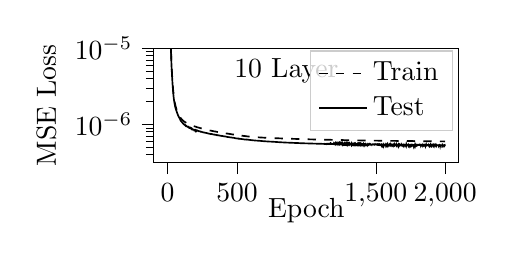
\begin{tikzpicture}

\begin{axis}[
legend cell align={left},
legend style={fill opacity=0.8, draw opacity=1, text opacity=1, draw=white!80!black},
log basis y={10},
tick align=outside,
tick pos=left,
title={10 Layer $\rare$},
title style={at={(0.45,0.85)},anchor=north},
x grid style={white!69.0196078431373!black},
xlabel={Epoch},
x label style={yshift=10pt},
xmin=-99.95, xmax=2098.95,
xtick style={color=black},
xtick = {0,500,1500,2000},
y grid style={white!69.0196078431373!black},
ylabel={MSE Loss},
ymin=3.17093839325154e-07, ymax=1e-5,
ymode=log,
ytick style={color=black},
width=0.45\textwidth,
height=0.25\textwidth
]
\addplot [semithick, black, dashed]
table {%
0 0.00997787586692721
1 0.0027661414751783
2 0.00218623768771067
3 0.00185343958390877
4 0.00115804947796278
5 0.00036777743147104
6 0.00018824286320887
7 0.000164930714039656
8 0.000153345151928079
9 0.000141543177305721
10 0.000127938025187177
11 0.000112482768548944
12 9.57521400996484e-05
13 7.92569487603032e-05
14 6.42920351929206e-05
15 5.20401717658388e-05
16 4.29740166491683e-05
17 3.62663831710961e-05
18 3.07352183917828e-05
19 2.49385155948403e-05
20 2.06156149879462e-05
21 1.71943852956247e-05
22 1.4385688823495e-05
23 1.20649838572717e-05
24 1.02233446727951e-05
25 8.78601411159252e-06
26 7.68138640933103e-06
27 6.83470541434872e-06
28 6.17248770799961e-06
29 5.6463688954409e-06
30 5.22004835283951e-06
31 4.84264568081016e-06
32 4.50758502950066e-06
33 4.20824098557659e-06
34 3.93843728591037e-06
35 3.69604697584691e-06
36 3.4781861807005e-06
37 3.27953066255304e-06
38 3.102444766796e-06
39 2.94624955324707e-06
40 2.80618139169064e-06
41 2.6809971720354e-06
42 2.57034235244191e-06
43 2.47136843603357e-06
44 2.38247599895658e-06
45 2.3052505364376e-06
46 2.2339168820622e-06
47 2.16824932778081e-06
48 2.10921677893339e-06
49 2.05554289499332e-06
50 2.00520992609654e-06
51 1.96032569562021e-06
52 1.91601798240981e-06
53 1.87716817765704e-06
54 1.84075475442569e-06
55 1.8041044749566e-06
56 1.77211888149031e-06
57 1.74144628215345e-06
58 1.71423015325445e-06
59 1.68766705314738e-06
60 1.66201588962167e-06
61 1.63708562206466e-06
62 1.61347263502876e-06
63 1.5917540299597e-06
64 1.57049718154667e-06
65 1.55085114516851e-06
66 1.53163219016506e-06
67 1.51338286417513e-06
68 1.49671406592233e-06
69 1.47951891813136e-06
70 1.4645103722728e-06
71 1.44944799347968e-06
72 1.43420475933453e-06
73 1.41955645852931e-06
74 1.40517172491172e-06
75 1.39141421908562e-06
76 1.37808219858471e-06
77 1.3657449522384e-06
78 1.3527578432786e-06
79 1.34140151624251e-06
80 1.32919058387415e-06
81 1.31819503866382e-06
82 1.30771289047971e-06
83 1.29784039592096e-06
84 1.28814695580104e-06
85 1.27880892563326e-06
86 1.27049044516525e-06
87 1.26170827212491e-06
88 1.25354349086138e-06
89 1.24524294693629e-06
90 1.23696791416705e-06
91 1.22909348488065e-06
92 1.22303059853834e-06
93 1.21662571478964e-06
94 1.20954619882241e-06
95 1.20269462843225e-06
96 1.19554730241589e-06
97 1.18936523608681e-06
98 1.18438249876363e-06
99 1.17871571490014e-06
100 1.17326355984915e-06
101 1.16720301622308e-06
102 1.16031671996097e-06
103 1.15646743591924e-06
104 1.15072228288682e-06
105 1.1456532542411e-06
106 1.14082713997732e-06
107 1.13676369537075e-06
108 1.13183904920788e-06
109 1.12775252654274e-06
110 1.12097592221971e-06
111 1.11884615537861e-06
112 1.11495200479794e-06
113 1.11073350669244e-06
114 1.10769001994981e-06
115 1.10351587494506e-06
116 1.10006028367593e-06
117 1.09647195202456e-06
118 1.09295321027503e-06
119 1.08959795028341e-06
120 1.08633151981508e-06
121 1.08298288154174e-06
122 1.0800084913285e-06
123 1.07806380844977e-06
124 1.074994691038e-06
125 1.07166258550251e-06
126 1.06880648237961e-06
127 1.06578414178671e-06
128 1.06304140217617e-06
129 1.06044994532795e-06
130 1.05643772593567e-06
131 1.0558744672835e-06
132 1.05326026272223e-06
133 1.04935598690759e-06
134 1.04676802968129e-06
135 1.04461839976011e-06
136 1.04219356757085e-06
137 1.03843377786461e-06
138 1.03679534922208e-06
139 1.03479115048799e-06
140 1.03239273369127e-06
141 1.02880143617767e-06
142 1.02687638050725e-06
143 1.02502206539157e-06
144 1.02148192920026e-06
145 1.02024824695945e-06
146 1.01793011802442e-06
147 1.01475467491241e-06
148 1.01393682172102e-06
149 1.01059575447948e-06
150 1.00912902482264e-06
151 1.0062060501923e-06
152 1.00506513257415e-06
153 1.00228589985818e-06
154 1.00133910484601e-06
155 9.99022535552285e-07
156 9.96578049466734e-07
157 9.95774760042423e-07
158 9.92670811598373e-07
159 9.90552980908888e-07
160 9.90131076179068e-07
161 9.8754623903119e-07
162 9.8556907477132e-07
163 9.85354359244184e-07
164 9.82352091568828e-07
165 9.80439722610527e-07
166 9.78883942138964e-07
167 9.78459102157103e-07
168 9.75541983876837e-07
169 9.74201690695509e-07
170 9.73315617585513e-07
171 9.7158668955899e-07
172 9.71484288783131e-07
173 9.67737080088682e-07
174 9.66393180931391e-07
175 9.64838651981381e-07
176 9.64215281697989e-07
177 9.62576921267555e-07
178 9.63217306946262e-07
179 9.60148133856364e-07
180 9.59013245392271e-07
181 9.56711457007486e-07
182 9.55200339518569e-07
183 9.53850673880652e-07
184 9.52729099026328e-07
185 9.51356085352018e-07
186 9.49982874573152e-07
187 9.48758935265914e-07
188 9.4734960742926e-07
189 9.46268320717536e-07
190 9.45888197207978e-07
191 9.43202051558956e-07
192 9.42285718593894e-07
193 9.4148136670924e-07
194 9.39797778954699e-07
195 9.38851433886612e-07
196 9.36940359082428e-07
197 9.35960853297502e-07
198 9.35100780367293e-07
199 9.33036782470253e-07
200 9.32759092336255e-07
201 9.309670438995e-07
202 9.30231287497918e-07
203 9.28388456145512e-07
204 9.28534422172334e-07
205 9.26417262860468e-07
206 9.25963449361689e-07
207 9.23892555078964e-07
208 9.23097257839345e-07
209 9.21156167748904e-07
210 9.20179683930655e-07
211 9.18629479031097e-07
212 9.17580147955732e-07
213 9.16587913565081e-07
214 9.15249802602602e-07
215 9.14260038939574e-07
216 9.13397146405259e-07
217 9.12211345678315e-07
218 9.10792389674953e-07
219 9.10044973522872e-07
220 9.09023786704211e-07
221 9.08015798756878e-07
222 9.07080938276295e-07
223 9.05977511166611e-07
224 9.05009585721928e-07
225 9.03722100105142e-07
226 9.0283103281763e-07
227 9.01766764314971e-07
228 9.00620563015764e-07
229 8.99610003187945e-07
230 8.98586724986217e-07
231 8.97490580570093e-07
232 8.96478950949131e-07
233 8.95298846074866e-07
234 8.94353904413947e-07
235 8.93204120927749e-07
236 8.923171830304e-07
237 8.90687736870177e-07
238 8.89868796548399e-07
239 8.88946101269994e-07
240 8.87893214382984e-07
241 8.86297618535537e-07
242 8.85070359657902e-07
243 8.84417957706773e-07
244 8.83675672440631e-07
245 8.8251698130648e-07
246 8.81460606791507e-07
247 8.8027023426207e-07
248 8.79355826469919e-07
249 8.78572113578002e-07
250 8.77525471793206e-07
251 8.76351880549464e-07
252 8.75500791465811e-07
253 8.74678740700574e-07
254 8.73476796158457e-07
255 8.72610606649005e-07
256 8.71706194686794e-07
257 8.70708743093473e-07
258 8.70191305182289e-07
259 8.69344236235747e-07
260 8.67789354629167e-07
261 8.66628777828282e-07
262 8.65958915056808e-07
263 8.64537149453781e-07
264 8.63818404411631e-07
265 8.62849739490912e-07
266 8.61764416811184e-07
267 8.60982841373925e-07
268 8.60051689585362e-07
269 8.59030311005427e-07
270 8.58128868173935e-07
271 8.57145231947243e-07
272 8.56545518360008e-07
273 8.55089079635718e-07
274 8.54582956577588e-07
275 8.53439548222923e-07
276 8.52625509651261e-07
277 8.52064497024685e-07
278 8.50905582069572e-07
279 8.50112307404061e-07
280 8.49598813260855e-07
281 8.4875707469223e-07
282 8.4775906213963e-07
283 8.4675666619205e-07
284 8.46309231747e-07
285 8.45124665829644e-07
286 8.44529056251986e-07
287 8.43495970570984e-07
288 8.42961660282526e-07
289 8.41671420289458e-07
290 8.41705411914972e-07
291 8.40604265988532e-07
292 8.39964006132732e-07
293 8.38750670340005e-07
294 8.3819956410025e-07
295 8.37723511324384e-07
296 8.36425500693849e-07
297 8.35761372655952e-07
298 8.35393352815572e-07
299 8.3392940771887e-07
300 8.3388055014666e-07
301 8.32478889208232e-07
302 8.32139470674065e-07
303 8.31678217167564e-07
304 8.30812586201546e-07
305 8.30091150533008e-07
306 8.29310000142414e-07
307 8.28749091709824e-07
308 8.2756600025391e-07
309 8.27514076803482e-07
310 8.26390768622787e-07
311 8.25961606182091e-07
312 8.25162235912558e-07
313 8.24495962177707e-07
314 8.24095709617723e-07
315 8.22966658319046e-07
316 8.21936873251161e-07
317 8.21767470569057e-07
318 8.20922504203736e-07
319 8.20247862861834e-07
320 8.19370113532614e-07
321 8.18635833951475e-07
322 8.17986851899377e-07
323 8.17315450689193e-07
324 8.1666383891843e-07
325 8.16427804124942e-07
326 8.15375180422961e-07
327 8.15192657825037e-07
328 8.14120937434382e-07
329 8.13174602825484e-07
330 8.1293584187847e-07
331 8.11936721930806e-07
332 8.11085818554602e-07
333 8.10528149429501e-07
334 8.09983656409941e-07
335 8.08851426143065e-07
336 8.08121500682546e-07
337 8.08130491662951e-07
338 8.07360241225297e-07
339 8.06781943225587e-07
340 8.06020081228098e-07
341 8.05330066299348e-07
342 8.04786609791108e-07
343 8.0464047090345e-07
344 8.03382348692594e-07
345 8.03091622429974e-07
346 8.03480803682533e-07
347 8.01579474654091e-07
348 8.0091967774365e-07
349 8.01363648946563e-07
350 7.99436845767332e-07
351 7.99345849031852e-07
352 7.98882536855672e-07
353 7.97898566048616e-07
354 7.98836069549225e-07
355 7.98981313806735e-07
356 7.97069268514861e-07
357 7.96280659386639e-07
358 7.96522883803164e-07
359 7.94783968302681e-07
360 7.94133767442418e-07
361 7.94591968116265e-07
362 7.92818375458637e-07
363 7.92365432204178e-07
364 7.91729609915137e-07
365 7.92124033381469e-07
366 7.9021502497767e-07
367 7.89800760259141e-07
368 7.89006110096579e-07
369 7.89422273101081e-07
370 7.87633119500697e-07
371 7.87470235025012e-07
372 7.86781127885661e-07
373 7.87345359412939e-07
374 7.85442462444053e-07
375 7.85028574483704e-07
376 7.84489331238092e-07
377 7.83982934024152e-07
378 7.84435161477859e-07
379 7.82677077467042e-07
380 7.8204591821418e-07
381 7.81801198940002e-07
382 7.81111819321723e-07
383 7.81425274823278e-07
384 7.7998786557032e-07
385 7.79324741330356e-07
386 7.78943699941692e-07
387 7.78382946805323e-07
388 7.7774481707138e-07
389 7.78080912994028e-07
390 7.76618715718769e-07
391 7.76134723423638e-07
392 7.75627843495386e-07
393 7.74918021193116e-07
394 7.74431415038634e-07
395 7.74660446609232e-07
396 7.73305947575409e-07
397 7.72896880562257e-07
398 7.72197305280997e-07
399 7.71702392796669e-07
400 7.71071945763424e-07
401 7.70523813088175e-07
402 7.70097182538621e-07
403 7.7021479600603e-07
404 7.68894578584423e-07
405 7.68398064082021e-07
406 7.67811163484566e-07
407 7.67315257036216e-07
408 7.66777737169377e-07
409 7.66156092197434e-07
410 7.65690696312049e-07
411 7.65130233787659e-07
412 7.6555170792858e-07
413 7.64065328610286e-07
414 7.63505121966546e-07
415 7.63133862619725e-07
416 7.62454071889351e-07
417 7.62014022313906e-07
418 7.6143167035525e-07
419 7.60892476279196e-07
420 7.60415168230111e-07
421 7.59914973372133e-07
422 7.5941622890241e-07
423 7.60389407474804e-07
424 7.58777384561427e-07
425 7.58338006789927e-07
426 7.57724335500143e-07
427 7.57657803433176e-07
428 7.56923721269232e-07
429 7.56353567965107e-07
430 7.56923098862217e-07
431 7.55219046823186e-07
432 7.54618819826192e-07
433 7.54311231389693e-07
434 7.53780425611694e-07
435 7.54422887609962e-07
436 7.52576872230293e-07
437 7.52243586475743e-07
438 7.51672492100397e-07
439 7.52297821776438e-07
440 7.50493718726375e-07
441 7.50091651326557e-07
442 7.49571382499425e-07
443 7.5027601661759e-07
444 7.48633131451015e-07
445 7.48203038369866e-07
446 7.47641490107753e-07
447 7.4706847775019e-07
448 7.47778209245098e-07
449 7.45882051290891e-07
450 7.45447632596097e-07
451 7.45004974220365e-07
452 7.45590436821431e-07
453 7.44075579518722e-07
454 7.43488029229411e-07
455 7.4302814456928e-07
456 7.43562355694394e-07
457 7.42126745706173e-07
458 7.41440271383453e-07
459 7.41023272865959e-07
460 7.42221455794834e-07
461 7.39916425203546e-07
462 7.39315465096979e-07
463 7.38942567977574e-07
464 7.39466763462815e-07
465 7.38114260798284e-07
466 7.37723011752678e-07
467 7.38328398483645e-07
468 7.36677821834064e-07
469 7.36189456091552e-07
470 7.36971248016971e-07
471 7.35291715386666e-07
472 7.34859717340441e-07
473 7.35544233293695e-07
474 7.33993297529878e-07
475 7.33437984763441e-07
476 7.34147434599208e-07
477 7.32526463366412e-07
478 7.32113129146228e-07
479 7.32783056690778e-07
480 7.31102353171309e-07
481 7.30759978779361e-07
482 7.30174026074337e-07
483 7.3101718700741e-07
484 7.29139022212166e-07
485 7.28747309921118e-07
486 7.29511678514427e-07
487 7.27845423909912e-07
488 7.27509910404933e-07
489 7.27898909303804e-07
490 7.25985288198672e-07
491 7.26988534040629e-07
492 7.26433349939271e-07
493 7.24913795409066e-07
494 7.25639360695141e-07
495 7.25110006783325e-07
496 7.23576190097219e-07
497 7.24332362437963e-07
498 7.23792091548603e-07
499 7.22295086035274e-07
500 7.23148807196594e-07
501 7.22562276394001e-07
502 7.21028598093199e-07
503 7.21920047169533e-07
504 7.20162841702177e-07
505 7.21097849861962e-07
506 7.20601577768321e-07
507 7.18964301626102e-07
508 7.19790344447802e-07
509 7.19423874585345e-07
510 7.17816719657094e-07
511 7.18529795136646e-07
512 7.17035474110617e-07
513 7.17842366498189e-07
514 7.173693042688e-07
515 7.15891436129823e-07
516 7.16593398948362e-07
517 7.16193349916239e-07
518 7.15836237418444e-07
519 7.13896747583931e-07
520 7.14747440071051e-07
521 7.14939811359727e-07
522 7.14682133747146e-07
523 7.14109896080117e-07
524 7.12665502788923e-07
525 7.13412247876022e-07
526 7.12840395792114e-07
527 7.1258078847336e-07
528 7.1094341305411e-07
529 7.11800691419739e-07
530 7.11041270108126e-07
531 7.11053048263466e-07
532 7.09551945874409e-07
533 7.10300355095228e-07
534 7.10044622053374e-07
535 7.08126653066188e-07
536 7.09192354179322e-07
537 7.08688509973854e-07
538 7.08473750933081e-07
539 7.0703383852333e-07
540 7.07924062425036e-07
541 7.07072048214741e-07
542 7.05930014561318e-07
543 7.06833243867777e-07
544 7.06151251620213e-07
545 7.05789116310029e-07
546 7.05411095324848e-07
547 7.03952515351602e-07
548 7.04824918869917e-07
549 7.04396891237025e-07
550 7.04121892809439e-07
551 7.03592790472385e-07
552 7.02295799982267e-07
553 7.03159633289374e-07
554 7.02392406822128e-07
555 7.02389151811644e-07
556 7.02069595888588e-07
557 7.00544815430249e-07
558 7.01544812031329e-07
559 7.01071055104308e-07
560 7.00843794945172e-07
561 7.00298507183561e-07
562 6.99028340818586e-07
563 6.9988211890859e-07
564 6.99153588470836e-07
565 6.99094921657206e-07
566 6.98874052901033e-07
567 6.97493815380312e-07
568 6.9732204678985e-07
569 6.96886004035946e-07
570 6.96496134878544e-07
571 6.96340423658626e-07
572 6.9577226418005e-07
573 6.95301015184668e-07
574 6.94970092226299e-07
575 6.94665715130327e-07
576 6.94327597415167e-07
577 6.9397252194392e-07
578 6.93629053131417e-07
579 6.93304834925357e-07
580 6.92961221275823e-07
581 6.92612403483395e-07
582 6.92295116081709e-07
583 6.92008054087978e-07
584 6.91836038868132e-07
585 6.91154041760456e-07
586 6.91039159349316e-07
587 6.90780433998839e-07
588 6.90375913677599e-07
589 6.90120593674237e-07
590 6.89844487624214e-07
591 6.89540247705622e-07
592 6.8927526524476e-07
593 6.88991556458518e-07
594 6.88708317511555e-07
595 6.88413684557077e-07
596 6.88122735454044e-07
597 6.87847310999246e-07
598 6.87655565940304e-07
599 6.873611031466e-07
600 6.8711852216552e-07
601 6.86813203969905e-07
602 6.86521028598008e-07
603 6.86258257005079e-07
604 6.86011237931439e-07
605 6.85736956057781e-07
606 6.8547543475006e-07
607 6.85227141644873e-07
608 6.84974181766052e-07
609 6.84731802891747e-07
610 6.84444454293498e-07
611 6.84201174820487e-07
612 6.83949088440272e-07
613 6.83735282066777e-07
614 6.83597051065021e-07
615 6.83230357168441e-07
616 6.82977046281508e-07
617 6.82744479377107e-07
618 6.82628084632597e-07
619 6.82269299900895e-07
620 6.82057781943968e-07
621 6.81825706507766e-07
622 6.81707034459578e-07
623 6.81389691763457e-07
624 6.81201359242323e-07
625 6.81054129145764e-07
626 6.8075853309324e-07
627 6.80542225936165e-07
628 6.80400173507678e-07
629 6.80067346735314e-07
630 6.79983958491448e-07
631 6.79618614057631e-07
632 6.79393168169895e-07
633 6.79165578233665e-07
634 6.79077912963066e-07
635 6.78772824926455e-07
636 6.78559704212489e-07
637 6.78351354096662e-07
638 6.78243983884386e-07
639 6.77901727698327e-07
640 6.77708650769659e-07
641 6.77525354845443e-07
642 6.77312835492216e-07
643 6.77094021853009e-07
644 6.7693512350786e-07
645 6.76660766927739e-07
646 6.76465998878939e-07
647 6.7620693066317e-07
648 6.76058081367614e-07
649 6.75807865121669e-07
650 6.75675274962373e-07
651 6.75309103939981e-07
652 6.75240928430298e-07
653 6.75009894337109e-07
654 6.74884714669588e-07
655 6.7469262417319e-07
656 6.74492794075832e-07
657 6.74472121843905e-07
658 6.74072660487468e-07
659 6.74126479594861e-07
660 6.73871772562507e-07
661 6.73676320815275e-07
662 6.73381162670239e-07
663 6.73315533632035e-07
664 6.7304010840985e-07
665 6.7279634778572e-07
666 6.72624413653011e-07
667 6.72622655784494e-07
668 6.72328725286775e-07
669 6.72171628352203e-07
670 6.72120275240218e-07
671 6.72108327890442e-07
672 6.71769079815476e-07
673 6.71592175606861e-07
674 6.7153022288835e-07
675 6.71228376674549e-07
676 6.71063214738865e-07
677 6.70862587298871e-07
678 6.70727474243904e-07
679 6.70538763273498e-07
680 6.70397458648608e-07
681 6.70331136205959e-07
682 6.70071903499547e-07
683 6.69920863757056e-07
684 6.69779470129583e-07
685 6.69620603034105e-07
686 6.69458129848977e-07
687 6.6930754940131e-07
688 6.69167233667167e-07
689 6.68956220224004e-07
690 6.68770538680974e-07
691 6.68667876396967e-07
692 6.68520957177066e-07
693 6.68362044635273e-07
694 6.68231087544768e-07
695 6.68063874257996e-07
696 6.67905007389891e-07
697 6.67740694836993e-07
698 6.67615698802138e-07
699 6.67491615800486e-07
700 6.67331059744924e-07
701 6.67199185485856e-07
702 6.67054764520003e-07
703 6.66892555187815e-07
704 6.66757220614045e-07
705 6.6661704566684e-07
706 6.66472319977629e-07
707 6.66348736558575e-07
708 6.66208892795339e-07
709 6.66104842267146e-07
710 6.65947033539283e-07
711 6.6583568202816e-07
712 6.65676333156284e-07
713 6.65566532433104e-07
714 6.65371252381419e-07
715 6.65273846124137e-07
716 6.65145204777673e-07
717 6.6501357501636e-07
718 6.64885187660502e-07
719 6.64747493914319e-07
720 6.64656038921407e-07
721 6.64518116366253e-07
722 6.64384310013588e-07
723 6.6426489875937e-07
724 6.64103254891302e-07
725 6.6400623869356e-07
726 6.6387511243704e-07
727 6.63760887292142e-07
728 6.63594443778948e-07
729 6.6352547675308e-07
730 6.63392976136379e-07
731 6.63245974934057e-07
732 6.63125168372858e-07
733 6.63018874917043e-07
734 6.62882144197852e-07
735 6.62734271159593e-07
736 6.62517572180832e-07
737 6.6241604606887e-07
738 6.62473698085364e-07
739 6.62516929139656e-07
740 6.62498065295836e-07
741 6.61815979839275e-07
742 6.61530765412976e-07
743 6.61442542394752e-07
744 6.61331088323891e-07
745 6.61209408832519e-07
746 6.6109859224639e-07
747 6.6099788502072e-07
748 6.60889263187414e-07
749 6.60740850307207e-07
750 6.60631029802516e-07
751 6.60538422906143e-07
752 6.60393012481109e-07
753 6.60271693462278e-07
754 6.60180221544238e-07
755 6.60043354130835e-07
756 6.59950334664927e-07
757 6.59887545353399e-07
758 6.5971084376315e-07
759 6.59582626255428e-07
760 6.59522363278597e-07
761 6.59398176679815e-07
762 6.59279328061757e-07
763 6.59160926986146e-07
764 6.59018419938207e-07
765 6.58968605165455e-07
766 6.58780548107529e-07
767 6.58640463925053e-07
768 6.58545901032426e-07
769 6.58429381942938e-07
770 6.58341001013696e-07
771 6.58279398663808e-07
772 6.58103613247363e-07
773 6.58032226553473e-07
774 6.5792477641935e-07
775 6.57836251804156e-07
776 6.57792503417909e-07
777 6.57651318391572e-07
778 6.57547617464616e-07
779 6.57399611057485e-07
780 6.57286304786453e-07
781 6.57153251651721e-07
782 6.5710807548669e-07
783 6.56900221926549e-07
784 6.56799596583824e-07
785 6.56696743305929e-07
786 6.56575473740872e-07
787 6.56487851685483e-07
788 6.56370081244972e-07
789 6.56292135957415e-07
790 6.56130607339378e-07
791 6.56064941154e-07
792 6.56011381011012e-07
793 6.55829648934514e-07
794 6.55786200027819e-07
795 6.55607685331461e-07
796 6.55609785056299e-07
797 6.55533220481175e-07
798 6.55394131726439e-07
799 6.55311715917151e-07
800 6.55156520764422e-07
801 6.55102531055718e-07
802 6.55082887604408e-07
803 6.54888119228758e-07
804 6.54802214071992e-07
805 6.5473559047291e-07
806 6.54574609910696e-07
807 6.54500922465218e-07
808 6.54382220616867e-07
809 6.54305573817737e-07
810 6.5420019161877e-07
811 6.54057651630069e-07
812 6.53967765671837e-07
813 6.53819775891407e-07
814 6.53770412583299e-07
815 6.53644654022401e-07
816 6.53591989035362e-07
817 6.53487234302474e-07
818 6.53435297138572e-07
819 6.53194102852694e-07
820 6.53198145187162e-07
821 6.5311538847368e-07
822 6.52892069282984e-07
823 6.52899213022806e-07
824 6.52815578064292e-07
825 6.52532915339066e-07
826 6.5250298719377e-07
827 6.52467241110344e-07
828 6.52352714354265e-07
829 6.52214292244935e-07
830 6.52175464963989e-07
831 6.52048443271269e-07
832 6.51983712870674e-07
833 6.51903975750656e-07
834 6.51790568511501e-07
835 6.51704363789918e-07
836 6.51591102098337e-07
837 6.51535222814914e-07
838 6.5140828783683e-07
839 6.51308421680596e-07
840 6.51213768250614e-07
841 6.51116864844425e-07
842 6.50987768693767e-07
843 6.50862097572258e-07
844 6.50764789384084e-07
845 6.50686730963912e-07
846 6.50605446963937e-07
847 6.50517625658154e-07
848 6.49935367121657e-07
849 6.49951558187922e-07
850 6.49781994908949e-07
851 6.49812969228947e-07
852 6.4962381597411e-07
853 6.49715427286424e-07
854 6.49609696424136e-07
855 6.49503299598564e-07
856 6.49437240753059e-07
857 6.4924598638072e-07
858 6.49154591329193e-07
859 6.49055806263732e-07
860 6.48968337969791e-07
861 6.48860881113933e-07
862 6.48779707205449e-07
863 6.4869935371803e-07
864 6.48607655406863e-07
865 6.48494430663504e-07
866 6.48387495814973e-07
867 6.48355465315831e-07
868 6.4823302085415e-07
869 6.48177903727287e-07
870 6.48068991381479e-07
871 6.48002301730344e-07
872 6.47880534643264e-07
873 6.4779980566243e-07
874 6.47472709502495e-07
875 6.47573727789563e-07
876 6.47521113151583e-07
877 6.47460983415726e-07
878 6.47327359146743e-07
879 6.47256306294253e-07
880 6.47165816758388e-07
881 6.47062579616886e-07
882 6.46873130364156e-07
883 6.46932409637202e-07
884 6.4678064497059e-07
885 6.46794917827265e-07
886 6.4658947853502e-07
887 6.46604447453569e-07
888 6.46413081099695e-07
889 6.46435930761413e-07
890 6.46238205860072e-07
891 6.46160109269545e-07
892 6.46079087459839e-07
893 6.45998969318384e-07
894 6.45898591372429e-07
895 6.45816730695969e-07
896 6.45777476066201e-07
897 6.45704528096758e-07
898 6.45561784040183e-07
899 6.45402865401934e-07
900 6.45395685438643e-07
901 6.45250818593013e-07
902 6.45247586589903e-07
903 6.45016569762902e-07
904 6.45096973528325e-07
905 6.44992183836734e-07
906 6.44879979844859e-07
907 6.44814044164832e-07
908 6.44536055304457e-07
909 6.44651230615523e-07
910 6.44630252224943e-07
911 6.44534238688266e-07
912 6.44403965878837e-07
913 6.44269876133308e-07
914 6.44109464232656e-07
915 6.44056983475139e-07
916 6.44181476729955e-07
917 6.44011751091966e-07
918 6.43851985074662e-07
919 6.43799305493076e-07
920 6.43708418380129e-07
921 6.43616032121486e-07
922 6.43390352038864e-07
923 6.43459086845155e-07
924 6.43066392427727e-07
925 6.43326589468529e-07
926 6.43231603277172e-07
927 6.42995318642647e-07
928 6.43065223883355e-07
929 6.42968633215446e-07
930 6.42634859744362e-07
931 6.42847502362542e-07
932 6.42573602135599e-07
933 6.42576249461513e-07
934 6.42420869482407e-07
935 6.42509780959699e-07
936 6.42260338906908e-07
937 6.42345372426689e-07
938 6.4186560094015e-07
939 6.42131707621729e-07
940 6.41876858665569e-07
941 6.41937691256089e-07
942 6.41715006921117e-07
943 6.41790332380765e-07
944 6.41556473468086e-07
945 6.415050187627e-07
946 6.41448093148256e-07
947 6.41452986968716e-07
948 6.41207829275459e-07
949 6.41160052467171e-07
950 6.41136324560421e-07
951 6.41156462506842e-07
952 6.4103641173574e-07
953 6.40879574191899e-07
954 6.40985946901651e-07
955 6.40758436617261e-07
956 6.40720444295084e-07
957 6.40529553727731e-07
958 6.40474377917144e-07
959 6.40498605775974e-07
960 6.40255618591823e-07
961 6.40319487331453e-07
962 6.40329926909544e-07
963 6.40118906979126e-07
964 6.40069182985315e-07
965 6.39933080719857e-07
966 6.40022533211493e-07
967 6.39830953474529e-07
968 6.39713040214929e-07
969 6.39593101901426e-07
970 6.39774005406935e-07
971 6.39434521559679e-07
972 6.39282294187637e-07
973 6.39523240408835e-07
974 6.39073064718332e-07
975 6.39149466316269e-07
976 6.39264868198097e-07
977 6.38937482264623e-07
978 6.3891833339369e-07
979 6.3900999825961e-07
980 6.38726525863831e-07
981 6.38650845402822e-07
982 6.38661012288821e-07
983 6.38419105449373e-07
984 6.38549863495541e-07
985 6.38299137555975e-07
986 6.38424846982843e-07
987 6.38142738338843e-07
988 6.38220265770428e-07
989 6.38023431044132e-07
990 6.38141142715654e-07
991 6.37875260373733e-07
992 6.37939418027145e-07
993 6.37722096641369e-07
994 6.3776769428614e-07
995 6.37635073331921e-07
996 6.37635214005172e-07
997 6.37495254942166e-07
998 6.3745381473268e-07
999 6.37371561651889e-07
1000 6.36697234590144e-07
1001 6.36720888294917e-07
1002 6.36737104024121e-07
1003 6.36686584201129e-07
1004 6.36586772294834e-07
1005 6.36517155868432e-07
1006 6.36517348780785e-07
1007 6.36441783626651e-07
1008 6.3637201033373e-07
1009 6.36290345994439e-07
1010 6.36226407571883e-07
1011 6.36187908853003e-07
1012 6.36128972693939e-07
1013 6.36090735575578e-07
1014 6.3589234423489e-07
1015 6.35912154805851e-07
1016 6.35904042837865e-07
1017 6.35763122460276e-07
1018 6.35666576634719e-07
1019 6.3564752967693e-07
1020 6.35538853181572e-07
1021 6.35491918373532e-07
1022 6.35451334389359e-07
1023 6.35415595198197e-07
1024 6.35248154431167e-07
1025 6.35240329302178e-07
1026 6.35150410481344e-07
1027 6.35137976871647e-07
1028 6.34976308155899e-07
1029 6.35017855039166e-07
1030 6.3482607657761e-07
1031 6.34881822449529e-07
1032 6.34690630576529e-07
1033 6.34540902638037e-07
1034 6.34473359724552e-07
1035 6.34451190421714e-07
1036 6.34297449984445e-07
1037 6.34270674453319e-07
1038 6.34141945823785e-07
1039 6.34231479885727e-07
1040 6.34136626601389e-07
1041 6.34082943328451e-07
1042 6.3395456306381e-07
1043 6.33960346824836e-07
1044 6.33853544790952e-07
1045 6.33788128311608e-07
1046 6.33753139354098e-07
1047 6.33628680830611e-07
1048 6.33625172490326e-07
1049 6.33516750120577e-07
1050 6.33459435064765e-07
1051 6.33394688364319e-07
1052 6.33326460899752e-07
1053 6.33260135010971e-07
1054 6.33217650971574e-07
1055 6.33124233907267e-07
1056 6.33073544925367e-07
1057 6.32994399367703e-07
1058 6.32937160020219e-07
1059 6.32863034105924e-07
1060 6.32802857673198e-07
1061 6.327211272108e-07
1062 6.32664070593592e-07
1063 6.32609571134424e-07
1064 6.3261294997119e-07
1065 6.32557479264051e-07
1066 6.32472583347976e-07
1067 6.32388676500284e-07
1068 6.3235371713688e-07
1069 6.32262299873787e-07
1070 6.32186852847383e-07
1071 6.32157002080191e-07
1072 6.32051000330591e-07
1073 6.31951863908853e-07
1074 6.31979543818772e-07
1075 6.31833903980805e-07
1076 6.31841321954596e-07
1077 6.31720386728318e-07
1078 6.31670170619714e-07
1079 6.31639167558262e-07
1080 6.31551888616855e-07
1081 6.31490619177555e-07
1082 6.31423811270793e-07
1083 6.3135732366959e-07
1084 6.31311455016714e-07
1085 6.31243087482858e-07
1086 6.31197074852707e-07
1087 6.31128118996571e-07
1088 6.31093993149534e-07
1089 6.31002973804584e-07
1090 6.30930024748011e-07
1091 6.30873843036284e-07
1092 6.30818468749794e-07
1093 6.30774500507414e-07
1094 6.30719061497587e-07
1095 6.30654274829112e-07
1096 6.30573381890542e-07
1097 6.30514150955719e-07
1098 6.30455811105435e-07
1099 6.30417263671745e-07
1100 6.303295307859e-07
1101 6.30289127698802e-07
1102 6.30195487040908e-07
1103 6.30157178008517e-07
1104 6.30050639735202e-07
1105 6.29987743629101e-07
1106 6.29968577783302e-07
1107 6.29872791670039e-07
1108 6.29852591870872e-07
1109 6.29763205395761e-07
1110 6.2972433978814e-07
1111 6.29685811993852e-07
1112 6.29570583363659e-07
1113 6.29555979784868e-07
1114 6.29505421251508e-07
1115 6.29378778313594e-07
1116 6.29395147583978e-07
1117 6.29327122219081e-07
1118 6.29239093782985e-07
1119 6.29181523294164e-07
1120 6.29151311549947e-07
1121 6.29059220806027e-07
1122 6.29024048642179e-07
1123 6.28953817965794e-07
1124 6.28911244270114e-07
1125 6.28805891778938e-07
1126 6.28756066198832e-07
1127 6.28648164230583e-07
1128 6.28306397643996e-07
1129 6.28687460732635e-07
1130 6.2848032885654e-07
1131 6.28135447911404e-07
1132 6.28400187004274e-07
1133 6.28573363961493e-07
1134 6.28527363033982e-07
1135 6.28527280390756e-07
1136 6.28343305770329e-07
1137 6.28284698507287e-07
1138 6.2812800601364e-07
1139 6.28083045576488e-07
1140 6.28054853891058e-07
1141 6.28019043531936e-07
1142 6.27906697488356e-07
1143 6.27742714229385e-07
1144 6.27365253272671e-07
1145 6.27446661880526e-07
1146 6.27488955871058e-07
1147 6.27701524173574e-07
1148 6.27380187211202e-07
1149 6.27639201667307e-07
1150 6.2732651976205e-07
1151 6.27196206636427e-07
1152 6.27453849801896e-07
1153 6.27290091358645e-07
1154 6.27293938102014e-07
1155 6.27100247442058e-07
1156 6.26845826687372e-07
1157 6.27136329399036e-07
1158 6.26958845828085e-07
1159 6.27028462695023e-07
1160 6.26799966369163e-07
1161 6.26518928804387e-07
1162 6.26466177664042e-07
1163 6.26487830309941e-07
1164 6.26460136622597e-07
1165 6.26553522593554e-07
1166 6.2658400442217e-07
1167 6.26421702463631e-07
1168 6.26354288016273e-07
1169 6.26202877917592e-07
1170 6.26266790412444e-07
1171 6.26346333575611e-07
1172 6.26213740538617e-07
1173 6.2591202649287e-07
1174 6.26159682411753e-07
1175 6.259679466325e-07
1176 6.25821323929188e-07
1177 6.25983454000334e-07
1178 6.25770567594941e-07
1179 6.25582370801681e-07
1180 6.25654848079193e-07
1181 6.25532107612514e-07
1182 6.2545592751917e-07
1183 6.25413862280766e-07
1184 6.25349340801051e-07
1185 6.25261259557419e-07
1186 6.25203425371978e-07
1187 6.25166111447584e-07
1188 6.25094666915516e-07
1189 6.25081710083464e-07
1190 6.25006898232527e-07
1191 6.24934165074365e-07
1192 6.24913404614347e-07
1193 6.24911467220102e-07
1194 6.24548951755344e-07
1195 6.24694442166174e-07
1196 6.24773008453872e-07
1197 6.24621071231957e-07
1198 6.2450013277271e-07
1199 6.24621874457887e-07
1200 6.24454692619736e-07
1201 6.24370407393826e-07
1202 6.2447302522628e-07
1203 6.24262143524845e-07
1204 6.24315219837968e-07
1205 6.2430981112982e-07
1206 6.23796075679195e-07
1207 6.24177096320011e-07
1208 6.24049105802271e-07
1209 6.24054203349544e-07
1210 6.24027001990157e-07
1211 6.23865109787403e-07
1212 6.23932852477083e-07
1213 6.23779870181807e-07
1214 6.23787094262696e-07
1215 6.23741608634987e-07
1216 6.23713004550552e-07
1217 6.23544608970405e-07
1218 6.23572001856587e-07
1219 6.23602649540089e-07
1220 6.23225978060304e-07
1221 6.23518592469452e-07
1222 6.23039261583358e-07
1223 6.23288506076847e-07
1224 6.23076261497602e-07
1225 6.23334286977695e-07
1226 6.23120273957056e-07
1227 6.23057992385156e-07
1228 6.2310072766536e-07
1229 6.22905203400137e-07
1230 6.23071342417347e-07
1231 6.22551743603594e-07
1232 6.22838785815816e-07
1233 6.22911618577859e-07
1234 6.22436094097623e-07
1235 6.2257276290012e-07
1236 6.22675055979016e-07
1237 6.22591451126198e-07
1238 6.22482214389208e-07
1239 6.22608929845114e-07
1240 6.22082830332715e-07
1241 6.22355137487318e-07
1242 6.22401920892912e-07
1243 6.22228115553014e-07
1244 6.22168779464971e-07
1245 6.2226912954344e-07
1246 6.21835941025495e-07
1247 6.22107425449769e-07
1248 6.22095544343892e-07
1249 6.21943532365776e-07
1250 6.21878639350371e-07
1251 6.21777342473706e-07
1252 6.21807686485454e-07
1253 6.21633627901019e-07
1254 6.21770785983244e-07
1255 6.21682074758212e-07
1256 6.21532353186183e-07
1257 6.21157554036245e-07
1258 6.21374166421163e-07
1259 6.21383820664789e-07
1260 6.21448532641011e-07
1261 6.21237848690726e-07
1262 6.21411155641738e-07
1263 6.20860587424943e-07
1264 6.2109406439248e-07
1265 6.21135994300914e-07
1266 6.21238524701084e-07
1267 6.20719478952481e-07
1268 6.20863639028357e-07
1269 6.21026825456283e-07
1270 6.20972499071115e-07
1271 6.20547807017147e-07
1272 6.20815331657809e-07
1273 6.20883732374011e-07
1274 6.20434088780542e-07
1275 6.20376438746462e-07
1276 6.2064274709428e-07
1277 6.20666749313159e-07
1278 6.20157986659819e-07
1279 6.20282532104e-07
1280 6.20512788032102e-07
1281 6.20443126081227e-07
1282 6.19954360075781e-07
1283 6.20158316202435e-07
1284 6.20412783675306e-07
1285 6.19787940749461e-07
1286 6.20167513709191e-07
1287 6.19920055640932e-07
1288 6.19938900399575e-07
1289 6.2001241861509e-07
1290 6.19576977349823e-07
1291 6.19768135450727e-07
1292 6.19923710424075e-07
1293 6.19364097445896e-07
1294 6.19723660356897e-07
1295 6.19799817101807e-07
1296 6.19224814414565e-07
1297 6.19575253921312e-07
1298 6.1951230144075e-07
1299 6.19440844417341e-07
1300 6.19388264468057e-07
1301 6.1928821070012e-07
1302 6.18971549577907e-07
1303 6.19309097317e-07
1304 6.18896740419927e-07
1305 6.19233279984144e-07
1306 6.18862542118848e-07
1307 6.1904855721906e-07
1308 6.19084869462938e-07
1309 6.18728734835372e-07
1310 6.19067870623269e-07
1311 6.18833963194731e-07
1312 6.18797829730511e-07
1313 6.18840376517937e-07
1314 6.18354753008532e-07
1315 6.18526108105755e-07
1316 6.18729250248862e-07
1317 6.18316310337263e-07
1318 6.18493220983396e-07
1319 6.1857565151513e-07
1320 6.18553323434412e-07
1321 6.18287408251206e-07
1322 6.18182901995112e-07
1323 6.18168552804832e-07
1324 6.18295116474599e-07
1325 6.18236038974373e-07
1326 6.18178005744596e-07
1327 6.18093473242709e-07
1328 6.17960725605826e-07
1329 6.17843770534421e-07
1330 6.18153380194997e-07
1331 6.1793422157308e-07
1332 6.17757560888776e-07
1333 6.1783743137056e-07
1334 6.17917767534948e-07
1335 6.17540525162497e-07
1336 6.17705096779275e-07
1337 6.17609444908851e-07
1338 6.17570422804192e-07
1339 6.17073546720803e-07
1340 6.17361359793733e-07
1341 6.17218927558838e-07
1342 6.1731549609334e-07
1343 6.16839265717317e-07
1344 6.17278455536052e-07
1345 6.16886698999508e-07
1346 6.17145374242512e-07
1347 6.16674280522034e-07
1348 6.16949876508954e-07
1349 6.16746271418833e-07
1350 6.17063569656295e-07
1351 6.1651876738722e-07
1352 6.16958195287509e-07
1353 6.16493237330928e-07
1354 6.16818991467483e-07
1355 6.16564756263926e-07
1356 6.16465375699704e-07
1357 6.1670159974625e-07
1358 6.16341221103767e-07
1359 6.164012397889e-07
1360 6.16298516355584e-07
1361 6.16462023430131e-07
1362 6.16257752142246e-07
1363 6.16205831555305e-07
1364 6.16200928298838e-07
1365 6.16331213180388e-07
1366 6.15774696939297e-07
1367 6.1614706064006e-07
1368 6.16303828067544e-07
1369 6.15772465287989e-07
1370 6.16175163123955e-07
1371 6.15761831603834e-07
1372 6.16118617230654e-07
1373 6.15417715017941e-07
1374 6.15825617352073e-07
1375 6.15959238160713e-07
1376 6.1554938204722e-07
1377 6.1578529990669e-07
1378 6.15404216532056e-07
1379 6.15805073294951e-07
1380 6.15045303192119e-07
1381 6.15779943856865e-07
1382 6.15239680826107e-07
1383 6.15575325518591e-07
1384 6.15164999260287e-07
1385 6.15541761249006e-07
1386 6.1481267056962e-07
1387 6.15518598799269e-07
1388 6.14974511393029e-07
1389 6.15256523204266e-07
1390 6.1495169554604e-07
1391 6.15171495873312e-07
1392 6.14589822056644e-07
1393 6.15063232331181e-07
1394 6.15107449206675e-07
1395 6.14662685840983e-07
1396 6.1502810259384e-07
1397 6.14590154093264e-07
1398 6.14612481669496e-07
1399 6.14802560768624e-07
1400 6.14702865100014e-07
1401 6.14827589217271e-07
1402 6.14387261038019e-07
1403 6.14532386492783e-07
1404 6.14365300663167e-07
1405 6.14513860909938e-07
1406 6.14463790768127e-07
1407 6.14669436131976e-07
1408 6.14088050312489e-07
1409 6.14400729553211e-07
1410 6.14347149664241e-07
1411 6.14008724106441e-07
1412 6.14388912921982e-07
1413 6.13885905003997e-07
1414 6.14030799852117e-07
1415 6.14084501023626e-07
1416 6.14049639672487e-07
1417 6.14017295546887e-07
1418 6.13979460368341e-07
1419 6.14067722430889e-07
1420 6.1396852149187e-07
1421 6.13854022716964e-07
1422 6.13682396014781e-07
1423 6.13604328492556e-07
1424 6.13541604060686e-07
1425 6.13372681478097e-07
1426 6.13554293892093e-07
1427 6.13180419733794e-07
1428 6.13455641953919e-07
1429 6.1348410481088e-07
1430 6.13415493866398e-07
1431 6.13489517483856e-07
1432 6.12983758479402e-07
1433 6.13290954696311e-07
1434 6.13153399413591e-07
1435 6.13249425313711e-07
1436 6.13075842231581e-07
1437 6.1320476547877e-07
1438 6.13227797749971e-07
1439 6.12789343271913e-07
1440 6.13057139688067e-07
1441 6.13030189320796e-07
1442 6.12636833110969e-07
1443 6.12816545171313e-07
1444 6.12819367759698e-07
1445 6.12868730669902e-07
1446 6.12897299447468e-07
1447 6.12634370639853e-07
1448 6.12377568522504e-07
1449 6.12560680650631e-07
1450 6.1260865675905e-07
1451 6.12693906937523e-07
1452 6.12507754290448e-07
1453 6.12503317547919e-07
1454 6.12373988857939e-07
1455 6.12564684573158e-07
1456 6.12393487315899e-07
1457 6.12160607012413e-07
1458 6.12446222532981e-07
1459 6.12120268648653e-07
1460 6.12264537330987e-07
1461 6.12050654183349e-07
1462 6.12274880353425e-07
1463 6.12251636255223e-07
1464 6.12217257234704e-07
1465 6.11654116092097e-07
1466 6.11951332530225e-07
1467 6.12065274943063e-07
1468 6.11820810711095e-07
1469 6.11882885237947e-07
1470 6.11983560567353e-07
1471 6.11653300381931e-07
1472 6.11477287904449e-07
1473 6.11686302534054e-07
1474 6.11679580714508e-07
1475 6.11734728380497e-07
1476 6.11446988500575e-07
1477 6.11656725389764e-07
1478 6.11418435035205e-07
1479 6.1152755747429e-07
1480 6.11419605277774e-07
1481 6.11340049509579e-07
1482 6.11387434275912e-07
1483 6.11206909837847e-07
1484 6.11388030407056e-07
1485 6.11385448635815e-07
1486 6.11177371865779e-07
1487 6.11203298248597e-07
1488 6.11062275424956e-07
1489 6.1113751262809e-07
1490 6.11060912476091e-07
1491 6.11207886258569e-07
1492 6.1091258017143e-07
1493 6.11062240871263e-07
1494 6.10889090808087e-07
1495 6.1091539818392e-07
1496 6.10902968965377e-07
1497 6.10834144879391e-07
1498 6.10740337897653e-07
1499 6.10833803591504e-07
1500 6.10895269836931e-07
1501 6.10666885577871e-07
1502 6.10610917632925e-07
1503 6.10713644597638e-07
1504 6.10572242344176e-07
1505 6.10609684585484e-07
1506 6.10557814717083e-07
1507 6.10448972544475e-07
1508 6.10527583972953e-07
1509 6.1040572688853e-07
1510 6.1039827343734e-07
1511 6.10298882641302e-07
1512 6.10335146262742e-07
1513 6.10234822481459e-07
1514 6.10242099241987e-07
1515 6.1033837800295e-07
1516 6.10180680752137e-07
1517 6.10083428981056e-07
1518 6.10104180410076e-07
1519 6.09997833088016e-07
1520 6.10046423801691e-07
1521 6.10109085918964e-07
1522 6.09993698589051e-07
1523 6.0983415817617e-07
1524 6.09903624265939e-07
1525 6.09998824259605e-07
1526 6.09884452536846e-07
1527 6.0968484560675e-07
1528 6.09763739340963e-07
1529 6.09665772230983e-07
1530 6.09703086560387e-07
1531 6.09820219096946e-07
1532 6.09501713334737e-07
1533 6.09573474022795e-07
1534 6.09616974934113e-07
1535 6.09569544238298e-07
1536 6.09660148164437e-07
1537 6.09644980698931e-07
1538 6.09337568604929e-07
1539 6.09344284718816e-07
1540 6.09197389067617e-07
1541 6.0940735770032e-07
1542 6.09346155506785e-07
1543 6.09101156697989e-07
1544 6.09007024621633e-07
1545 6.09158799576903e-07
1546 6.09148734696419e-07
1547 6.08959669804676e-07
1548 6.09325477711309e-07
1549 6.09174900532139e-07
1550 6.0887942427712e-07
1551 6.08839884300494e-07
1552 6.08781071470332e-07
1553 6.09002018386207e-07
1554 6.08992753903692e-07
1555 6.08921752103697e-07
1556 6.08550892451376e-07
1557 6.08858571517601e-07
1558 6.08579321387026e-07
1559 6.08931567271043e-07
1560 6.08685558709965e-07
1561 6.086547848696e-07
1562 6.08401901835975e-07
1563 6.08758491502215e-07
1564 6.08654236842199e-07
1565 6.08688211428898e-07
1566 6.08301819781332e-07
1567 6.08271498485635e-07
1568 6.08576608897238e-07
1569 6.08319848055317e-07
1570 6.08480469537653e-07
1571 6.07807451878273e-07
1572 6.08380918549756e-07
1573 6.08300615851931e-07
1574 6.08053642686457e-07
1575 6.08368646929591e-07
1576 6.0812452350234e-07
1577 6.08126570497802e-07
1578 6.07947861496427e-07
1579 6.08041351142674e-07
1580 6.08088597630285e-07
1581 6.07849733981425e-07
1582 6.07615484732094e-07
1583 6.08021072672216e-07
1584 6.07963512450738e-07
1585 6.07767478811638e-07
1586 6.07390047363765e-07
1587 6.07963038447679e-07
1588 6.07980262998353e-07
1589 6.07409527361824e-07
1590 6.07784210387763e-07
1591 6.07840305448803e-07
1592 6.07267094785868e-07
1593 6.07612616228437e-07
1594 6.07545026539924e-07
1595 6.07546535789538e-07
1596 6.07477840198101e-07
1597 6.07406954912904e-07
1598 6.07465134486063e-07
1599 6.07722121941379e-07
1600 6.07360805602752e-07
1601 6.07478799395267e-07
1602 6.06909562463898e-07
1603 6.07380107794597e-07
1604 6.07338322012652e-07
1605 6.07294482563248e-07
1606 6.06812804122114e-07
1607 6.0721268062025e-07
1608 6.07233012985375e-07
1609 6.07195121141046e-07
1610 6.071700273651e-07
1611 6.06819598012009e-07
1612 6.07043475504554e-07
1613 6.0704164012293e-07
1614 6.07128623613562e-07
1615 6.06578756020326e-07
1616 6.06798978871836e-07
1617 6.07025782869641e-07
1618 6.06951957884405e-07
1619 6.06766503608469e-07
1620 6.06614765722213e-07
1621 6.0673492006913e-07
1622 6.06793863688893e-07
1623 6.06836134508626e-07
1624 6.06528794833139e-07
1625 6.06360835142539e-07
1626 6.06481000843928e-07
1627 6.06527924325917e-07
1628 6.06438592249958e-07
1629 6.06078926878695e-07
1630 6.06267785045134e-07
1631 6.06416825974065e-07
1632 6.06345947673503e-07
1633 6.06055386640492e-07
1634 6.06261331746794e-07
1635 6.06446446099085e-07
1636 6.06188030587873e-07
1637 6.05938584328669e-07
1638 6.05899705995228e-07
1639 6.06198064531327e-07
1640 6.06270861851499e-07
1641 6.05708320840392e-07
1642 6.06058464242665e-07
1643 6.06221903296955e-07
1644 6.06069751235339e-07
1645 6.06050152747173e-07
1646 6.05819766406057e-07
1647 6.06043714824978e-07
1648 6.05906337582951e-07
1649 6.05514812804131e-07
1650 6.0590809746941e-07
1651 6.05843198755451e-07
1652 6.05349268901989e-07
1653 6.05659533334801e-07
1654 6.05764375777085e-07
1655 6.05851891698705e-07
1656 6.05333976615441e-07
1657 6.05361576432983e-07
1658 6.05489755962196e-07
1659 6.05671521000772e-07
1660 6.05699834061113e-07
1661 6.05625775143892e-07
1662 6.05465998177124e-07
1663 6.05155967747351e-07
1664 6.05444437752567e-07
1665 6.05435842629731e-07
1666 6.05232719344428e-07
1667 6.05358329359262e-07
1668 6.05482555464221e-07
1669 6.04889914235685e-07
1670 6.05215874934117e-07
1671 6.05486620990803e-07
1672 6.04834402068377e-07
1673 6.05198130770646e-07
1674 6.05046599076786e-07
1675 6.05016511656231e-07
1676 6.04631185808557e-07
1677 6.05005039972184e-07
1678 6.04674635233948e-07
1679 6.04942220718385e-07
1680 6.04700395697932e-07
1681 6.04865811205002e-07
1682 6.05009814954371e-07
1683 6.04889728634816e-07
1684 6.04844792221115e-07
1685 6.04359664151843e-07
1686 6.04609927442823e-07
1687 6.04872898598785e-07
1688 6.04709866742326e-07
1689 6.04630048052002e-07
1690 6.04425468274883e-07
1691 6.04469091577187e-07
1692 6.04706080885364e-07
1693 6.04555926010164e-07
1694 6.04537494460544e-07
1695 6.04278143796932e-07
1696 6.04340501048739e-07
1697 6.04197455913891e-07
1698 6.04441300453118e-07
1699 6.04595920748352e-07
1700 6.03850993272204e-07
1701 6.04438322397982e-07
1702 6.04277625079419e-07
1703 6.0438274098118e-07
1704 6.04373536390312e-07
1705 6.04138261813603e-07
1706 6.03913386768795e-07
1707 6.04411630916957e-07
1708 6.04183150997528e-07
1709 6.04112993976003e-07
1710 6.03658407840157e-07
1711 6.04053948315197e-07
1712 6.03713166043462e-07
1713 6.03930260858476e-07
1714 6.04069584888123e-07
1715 6.03919799146979e-07
1716 6.0421229888874e-07
1717 6.03807143292556e-07
1718 6.03866195504565e-07
1719 6.03754792258826e-07
1720 6.03654986100821e-07
1721 6.03806830298481e-07
1722 6.03825659105439e-07
1723 6.03713809127271e-07
1724 6.03699650824296e-07
1725 6.03421308653651e-07
1726 6.0333590960937e-07
1727 6.03738354897132e-07
1728 6.0345359814562e-07
1729 6.03663957136291e-07
1730 6.0354759295933e-07
1731 6.03492661575444e-07
1732 6.0341275359832e-07
1733 6.03002478229087e-07
1734 6.03387956459756e-07
1735 6.03469406755153e-07
1736 6.03433570702805e-07
1737 6.0356447433918e-07
1738 6.03225716766076e-07
1739 6.03256337910807e-07
1740 6.02846615471719e-07
1741 6.03157913118935e-07
1742 6.03347374195096e-07
1743 6.02996052606386e-07
1744 6.03152832425735e-07
1745 6.0341758439364e-07
1746 6.03047560318259e-07
1747 6.02706116737295e-07
1748 6.03170202509773e-07
1749 6.0302586018679e-07
1750 6.02906125479308e-07
1751 6.02758776139467e-07
1752 6.0285802859994e-07
1753 6.02876531445418e-07
1754 6.03065958493687e-07
1755 6.02700803597145e-07
1756 6.03003898859811e-07
1757 6.02863685159605e-07
1758 6.02832223307814e-07
1759 6.0231757582585e-07
1760 6.02770864048807e-07
1761 6.02698666838819e-07
1762 6.02657274626495e-07
1763 6.02313723852887e-07
1764 6.02691921884002e-07
1765 6.02726068130721e-07
1766 6.02516639780504e-07
1767 6.02727442071682e-07
1768 6.0266054122593e-07
1769 6.02443684655896e-07
1770 6.02768862478342e-07
1771 6.02575757440604e-07
1772 6.02620517042851e-07
1773 6.0223736930709e-07
1774 6.02443618674897e-07
1775 6.02343127688698e-07
1776 6.02535673678517e-07
1777 6.02526791688263e-07
1778 6.02374621024637e-07
1779 6.02588626342993e-07
1780 6.02112564081381e-07
1781 6.02313130720233e-07
1782 6.02444795354984e-07
1783 6.02347095764344e-07
1784 6.02369666538039e-07
1785 6.0209122123922e-07
1786 6.01879268558037e-07
1787 6.02125398557973e-07
1788 6.02146500632728e-07
1789 6.01656791744176e-07
1790 6.01805090859386e-07
1791 6.02002694151338e-07
1792 6.02446760957775e-07
1793 6.02113278262095e-07
1794 6.01991785778466e-07
1795 6.01826009479112e-07
1796 6.01817396692184e-07
1797 6.01982162095283e-07
1798 6.0186446570043e-07
1799 6.01880066668059e-07
1800 6.01632548281827e-07
1801 6.01748339363439e-07
1802 6.01747545857734e-07
1803 6.01840091860595e-07
1804 6.01756409380982e-07
1805 6.01922086502782e-07
1806 6.01554449268349e-07
1807 6.01764710836505e-07
1808 6.01585441891928e-07
1809 6.01620399663716e-07
1810 6.01394540993283e-07
1811 6.01578889998677e-07
1812 6.01465641970833e-07
1813 6.01468468630628e-07
1814 6.0148105585256e-07
1815 6.01621551680864e-07
1816 6.01349377944871e-07
1817 6.01436685400358e-07
1818 6.01112377616175e-07
1819 6.01373257438809e-07
1820 6.01033992737143e-07
1821 6.01447081656659e-07
1822 6.01251637455391e-07
1823 6.01425233682562e-07
1824 6.0108123882685e-07
1825 6.00530437850466e-07
1826 6.00767299317795e-07
1827 6.01164053591674e-07
1828 6.01070501694778e-07
1829 6.01493606254167e-07
1830 6.01099195534971e-07
1831 6.01244900330755e-07
1832 6.01057305814834e-07
1833 6.00740347941553e-07
1834 6.00686449153898e-07
1835 6.00974852872582e-07
1836 6.00784366120877e-07
1837 6.00917683321711e-07
1838 6.00919331205319e-07
1839 6.00305996499628e-07
1840 6.00554979889978e-07
1841 6.00792678504547e-07
1842 6.00769171384741e-07
1843 6.00791608299289e-07
1844 6.00129414905837e-07
1845 6.00422443270077e-07
1846 6.01062785804629e-07
1847 6.00362743504945e-07
1848 6.00542174204577e-07
1849 6.00501732691328e-07
1850 6.00728357547098e-07
1851 6.00461085412007e-07
1852 6.00623625381047e-07
1853 6.0029681075946e-07
1854 6.00380710018555e-07
1855 6.00392723740129e-07
1856 6.00370193353683e-07
1857 6.00772083174661e-07
1858 6.00252417889635e-07
1859 6.0015084682874e-07
1860 5.99909958978628e-07
1861 6.00418678168069e-07
1862 6.00348944090001e-07
1863 6.00298169089797e-07
1864 5.99944616880066e-07
1865 6.00106185999039e-07
1866 5.99787089782922e-07
1867 6.00101847382462e-07
1868 5.99852434874038e-07
1869 5.99963285409899e-07
1870 5.9991632118539e-07
1871 6.00112840409395e-07
1872 5.99863743829587e-07
1873 6.00275846551313e-07
1874 5.9979787373976e-07
1875 5.99840269444485e-07
1876 5.99727364530622e-07
1877 5.99769747580581e-07
1878 5.99911294067112e-07
1879 5.99118779724961e-07
1880 5.9970115111696e-07
1881 6.00002350559237e-07
1882 5.99974184062546e-07
1883 5.99959595589894e-07
1884 5.99087935775344e-07
1885 5.99623948900785e-07
1886 5.99626938665665e-07
1887 5.99830924784328e-07
1888 5.99417291731186e-07
1889 5.9955394310407e-07
1890 5.99298534126547e-07
1891 5.99730335409276e-07
1892 5.99491005132791e-07
1893 5.99656654244995e-07
1894 5.99547013450774e-07
1895 5.98482167085024e-07
1896 5.99093556694186e-07
1897 5.99366488827968e-07
1898 5.9942543583702e-07
1899 5.99619707813304e-07
1900 5.9898585281104e-07
1901 5.99188566802411e-07
1902 5.99299312909807e-07
1903 5.98916520921478e-07
1904 5.99358396179639e-07
1905 5.99035597367958e-07
1906 5.98880591311968e-07
1907 5.991552496738e-07
1908 5.98895090178075e-07
1909 5.99326609851403e-07
1910 5.9899597306412e-07
1911 5.98961957322786e-07
1912 5.99268629031258e-07
1913 5.98984463138663e-07
1914 5.98816665522861e-07
1915 5.99366927694689e-07
1916 5.99037884278175e-07
1917 5.98687263121178e-07
1918 5.99125418858648e-07
1919 5.98926484734363e-07
1920 5.98734453859606e-07
1921 5.98929530852388e-07
1922 5.98456384594215e-07
1923 5.99225023350414e-07
1924 5.98748275706384e-07
1925 5.98757728198507e-07
1926 5.9836822791226e-07
1927 5.98157728056492e-07
1928 5.98544783777299e-07
1929 5.98487580987239e-07
1930 5.98244729438591e-07
1931 5.98312649913169e-07
1932 5.98401026920214e-07
1933 5.98220377682423e-07
1934 5.98461834648845e-07
1935 5.98176858069621e-07
1936 5.98417225589287e-07
1937 5.98470352322522e-07
1938 5.97895304501606e-07
1939 5.97987169612679e-07
1940 5.9813538484832e-07
1941 5.98038864715988e-07
1942 5.98157100114349e-07
1943 5.97956616644524e-07
1944 5.98089292012105e-07
1945 5.97987895616825e-07
1946 5.97809126240634e-07
1947 5.98036604159802e-07
1948 5.97797029627145e-07
1949 5.98056657786117e-07
1950 5.97913980556086e-07
1951 5.97672298432883e-07
1952 5.98109917312684e-07
1953 5.97941035053395e-07
1954 5.9753544955754e-07
1955 5.97756714242337e-07
1956 5.97478627987869e-07
1957 5.97894887576444e-07
1958 5.97648920255267e-07
1959 5.97599577375263e-07
1960 5.97631638868279e-07
1961 5.97793312579142e-07
1962 5.97506529700809e-07
1963 5.97551933459783e-07
1964 5.97903794457011e-07
1965 5.97512350587692e-07
1966 5.97395159424252e-07
1967 5.97335368631491e-07
1968 5.971654629775e-07
1969 5.97480472521283e-07
1970 5.97409489770939e-07
1971 5.97503929363086e-07
1972 5.97378307574559e-07
1973 5.97422970471939e-07
1974 5.972871803408e-07
1975 5.972749112928e-07
1976 5.97247786807031e-07
1977 5.97383588605283e-07
1978 5.97325264600101e-07
1979 5.97643469468778e-07
1980 5.97130998862383e-07
1981 5.97120845668542e-07
1982 5.97042139453663e-07
1983 5.97357733362003e-07
1984 5.97179822371174e-07
1985 5.96607952928707e-07
1986 5.96828548545147e-07
1987 5.97014385220973e-07
1988 5.97011463028707e-07
1989 5.96872746299937e-07
1990 5.96864856504453e-07
1991 5.96725136745135e-07
1992 5.97047547614693e-07
1993 5.96956392918457e-07
1994 5.96588074095905e-07
1995 5.9687866851732e-07
1996 5.9665970918843e-07
1997 5.96951477064067e-07
1998 5.96457130043859e-07
1999 5.97000214682453e-07
};
\addlegendentry{Train}
\addplot [semithick, black]
table {%
0 0.00434749247506261
1 0.00228160619735718
2 0.00205221213400364
3 0.00154257053509355
4 0.000718198833055794
5 0.000226133677642792
6 0.000181061404873617
7 0.000167616395629011
8 0.000156123365741223
9 0.000142964738188311
10 0.000127599021652713
11 0.000110671688162256
12 9.30606038309634e-05
13 7.64159558457322e-05
14 6.21071667410433e-05
15 5.10052486788481e-05
16 4.28141283919103e-05
17 3.68101937056053e-05
18 3.00778083328623e-05
19 2.4529757865821e-05
20 2.01874263439095e-05
21 1.66584795806557e-05
22 1.37592851388035e-05
23 1.14278200271656e-05
24 9.60716533882078e-06
25 8.22439596959157e-06
26 7.18310775482678e-06
27 6.39809377389611e-06
28 5.78356139158132e-06
29 5.30209854332497e-06
30 4.88823434352526e-06
31 4.53025495517068e-06
32 4.21924369220505e-06
33 3.93188747693785e-06
34 3.67658185496111e-06
35 3.44876343660871e-06
36 3.2360949262511e-06
37 3.0473665901809e-06
38 2.88254500446783e-06
39 2.73407295026118e-06
40 2.60622755376971e-06
41 2.49123081630387e-06
42 2.38923371398414e-06
43 2.29731722356519e-06
44 2.21009304368636e-06
45 2.13793896364223e-06
46 2.0732218217745e-06
47 2.0203365238558e-06
48 1.97086956177372e-06
49 1.91087838175008e-06
50 1.87627824743686e-06
51 1.82744747689867e-06
52 1.79010999090679e-06
53 1.74291096755042e-06
54 1.71458736986096e-06
55 1.69069596722693e-06
56 1.65673736773897e-06
57 1.63174570388946e-06
58 1.60747129029915e-06
59 1.58263560479099e-06
60 1.56158080244495e-06
61 1.54273459429533e-06
62 1.5270040876203e-06
63 1.508788159299e-06
64 1.48908816299809e-06
65 1.47157015817356e-06
66 1.45421120123501e-06
67 1.43652664519323e-06
68 1.41859891300555e-06
69 1.40249676405801e-06
70 1.39373685215105e-06
71 1.37832682867156e-06
72 1.36012943130481e-06
73 1.34492074721493e-06
74 1.32760681026411e-06
75 1.31394085656211e-06
76 1.30380783502915e-06
77 1.28918247810361e-06
78 1.27781720493658e-06
79 1.26867018934718e-06
80 1.25864710298629e-06
81 1.24917630728305e-06
82 1.23994277601014e-06
83 1.22975836802652e-06
84 1.21914297324111e-06
85 1.20943730053114e-06
86 1.19995434033626e-06
87 1.19173625989788e-06
88 1.18392813419632e-06
89 1.17324577786349e-06
90 1.1509973774082e-06
91 1.14243664484093e-06
92 1.1369610319889e-06
93 1.12879831704049e-06
94 1.12406837615708e-06
95 1.10950884391059e-06
96 1.10892358407e-06
97 1.10261817098944e-06
98 1.09690631688864e-06
99 1.09067332232371e-06
100 1.08576807633654e-06
101 1.08011545307818e-06
102 1.07385312730912e-06
103 1.06806089661404e-06
104 1.06117443010589e-06
105 1.05581989373604e-06
106 1.05201229416707e-06
107 1.04553146229591e-06
108 1.04055129668268e-06
109 1.03591617062193e-06
110 1.03007459983928e-06
111 1.02811327451491e-06
112 1.02186095318757e-06
113 1.01746786640433e-06
114 1.01230853033485e-06
115 1.01044577149878e-06
116 1.0063632771562e-06
117 1.00233330613264e-06
118 9.98497284854238e-07
119 9.94633751361107e-07
120 9.90572061709827e-07
121 9.86766963251284e-07
122 9.83146946964553e-07
123 9.78703383225366e-07
124 9.74755494098645e-07
125 9.7125587217306e-07
126 9.68463950812293e-07
127 9.65317553891509e-07
128 9.62315880315145e-07
129 9.5937218702602e-07
130 9.55727841756016e-07
131 9.65504568739561e-07
132 9.62504373092088e-07
133 9.57780116550566e-07
134 9.55338009589468e-07
135 9.52584571223269e-07
136 9.47709168030997e-07
137 9.45862950629817e-07
138 9.42336384923692e-07
139 9.39557139645331e-07
140 9.37117363264406e-07
141 9.38099617542321e-07
142 9.34217325720965e-07
143 9.29640691538225e-07
144 9.28908491459879e-07
145 9.27524069993524e-07
146 9.25653353078815e-07
147 9.27854500787362e-07
148 9.20564673378976e-07
149 9.17459090032935e-07
150 9.15438135962177e-07
151 9.14473162083596e-07
152 9.11512699985906e-07
153 9.09493792278226e-07
154 9.04993896710948e-07
155 9.11056986296899e-07
156 9.07219032342255e-07
157 9.03521765849291e-07
158 9.03147849840025e-07
159 9.00471945897152e-07
160 8.98007328942185e-07
161 9.01668158803659e-07
162 8.93996002560016e-07
163 8.92658079010289e-07
164 8.9248140966447e-07
165 8.94123616035358e-07
166 8.9210413989349e-07
167 8.83389816408453e-07
168 8.81091580140492e-07
169 8.84440567006095e-07
170 8.77607078564324e-07
171 8.77156878686947e-07
172 8.69033385697549e-07
173 8.72449504640826e-07
174 8.69888140186958e-07
175 8.75546902534552e-07
176 8.69605116804451e-07
177 8.65835147578764e-07
178 8.59352553561621e-07
179 8.55793132359395e-07
180 8.54213169532159e-07
181 8.59682813825202e-07
182 8.60085890508344e-07
183 8.57171983170701e-07
184 8.55991800108313e-07
185 8.54777340464352e-07
186 8.53036908665672e-07
187 8.51283061820141e-07
188 8.5193028098729e-07
189 8.50044557410001e-07
190 8.41960115849361e-07
191 8.45497083901137e-07
192 8.44312069148145e-07
193 8.46131911202974e-07
194 8.4455683690976e-07
195 8.41735698031698e-07
196 8.41986036448361e-07
197 8.42979375192954e-07
198 8.32292528230028e-07
199 8.36260539927025e-07
200 8.28120391815901e-07
201 8.3328586697462e-07
202 8.31986767479975e-07
203 8.3191019939477e-07
204 8.23791140192043e-07
205 8.29448083550233e-07
206 8.22248750864674e-07
207 8.25539586912782e-07
208 8.20777074750367e-07
209 8.2558011627043e-07
210 8.24426592771488e-07
211 8.23368054625462e-07
212 8.22838956082705e-07
213 8.22967081148818e-07
214 8.2723124705808e-07
215 8.24509356789349e-07
216 8.22551385226689e-07
217 8.19931017304043e-07
218 8.20179309357627e-07
219 8.18713544958882e-07
220 8.18752312170545e-07
221 8.17922341411759e-07
222 8.16474653220212e-07
223 8.14113207070477e-07
224 8.14713530417066e-07
225 8.12543078154704e-07
226 8.12100893199386e-07
227 8.11079814866389e-07
228 8.12268183381093e-07
229 8.11947529655299e-07
230 8.10835672382382e-07
231 8.09050561656477e-07
232 8.08929485174303e-07
233 8.07899596111383e-07
234 8.07337016794918e-07
235 8.0674215041654e-07
236 8.0271234992324e-07
237 8.04715227786801e-07
238 8.03089506007382e-07
239 8.02697798008012e-07
240 8.01223507096438e-07
241 7.98131623014342e-07
242 7.98794815182191e-07
243 7.97887537373754e-07
244 7.96937001723563e-07
245 7.9594468616051e-07
246 7.95331402514421e-07
247 7.93857566350198e-07
248 7.93269009591313e-07
249 7.9232358984882e-07
250 7.91217587448045e-07
251 7.90401657013717e-07
252 7.89184298355394e-07
253 7.86902205618389e-07
254 7.87498265708564e-07
255 7.86780731232284e-07
256 7.85954284765467e-07
257 7.85163308592018e-07
258 7.84254552854691e-07
259 7.83878761012602e-07
260 7.82506845098396e-07
261 7.82381562203227e-07
262 7.80722018589586e-07
263 7.80565869717975e-07
264 7.80142954681651e-07
265 7.79061451794405e-07
266 7.78061462369806e-07
267 7.77561069753574e-07
268 7.76982233219314e-07
269 7.76394358581456e-07
270 7.75580019762856e-07
271 7.75101568706305e-07
272 7.74141142301232e-07
273 7.73420026689564e-07
274 7.72909743318451e-07
275 7.72820385464001e-07
276 7.7215980809342e-07
277 7.70394876781211e-07
278 7.69719520121726e-07
279 7.691998575865e-07
280 7.69394375765842e-07
281 7.67452718264394e-07
282 7.67373762755597e-07
283 7.67319932037935e-07
284 7.65990023410268e-07
285 7.65466893426492e-07
286 7.64721789892064e-07
287 7.64168078148941e-07
288 7.63261141401017e-07
289 7.62611932714208e-07
290 7.61927935855056e-07
291 7.61432772833359e-07
292 7.58391877297981e-07
293 7.58502608277922e-07
294 7.57785414862155e-07
295 7.56770930365747e-07
296 7.56209033170308e-07
297 7.55275493702356e-07
298 7.55437724819785e-07
299 7.53612937387516e-07
300 7.53117149088212e-07
301 7.52098856082739e-07
302 7.53102483486146e-07
303 7.53071276449191e-07
304 7.52046616980806e-07
305 7.50117919778859e-07
306 7.49524758703046e-07
307 7.49935281874059e-07
308 7.4813090122916e-07
309 7.48565071262419e-07
310 7.48480601941992e-07
311 7.48050467791472e-07
312 7.4746179734575e-07
313 7.47299566228321e-07
314 7.44646570183249e-07
315 7.44110764117067e-07
316 7.44592284718237e-07
317 7.44728993140598e-07
318 7.43561713534291e-07
319 7.44146404940693e-07
320 7.42608563086833e-07
321 7.42190707114787e-07
322 7.40962263989786e-07
323 7.42079009796726e-07
324 7.40356142614473e-07
325 7.38976041247952e-07
326 7.3847712656061e-07
327 7.37713548915053e-07
328 7.38197684313491e-07
329 7.37495042812952e-07
330 7.3582208415246e-07
331 7.36848448923411e-07
332 7.35805656404409e-07
333 7.33855188173038e-07
334 7.34642640054517e-07
335 7.33675904029951e-07
336 7.33129013497091e-07
337 7.33792035134684e-07
338 7.32961041194358e-07
339 7.30489091438358e-07
340 7.31641080164991e-07
341 7.30738577203738e-07
342 7.29801229226723e-07
343 7.30696967821132e-07
344 7.28915154013521e-07
345 7.2738930612104e-07
346 7.27571375591651e-07
347 7.27127883237699e-07
348 7.26605151157855e-07
349 7.26159214536892e-07
350 7.24804465335183e-07
351 7.24450444522518e-07
352 7.24580900168803e-07
353 7.23101265975856e-07
354 7.25181280358811e-07
355 7.21174274076475e-07
356 7.21943877124431e-07
357 7.22024424248957e-07
358 7.20705259027454e-07
359 7.21280571269745e-07
360 7.20751643257245e-07
361 7.19062086318445e-07
362 7.19834304163669e-07
363 7.19305432994588e-07
364 7.18614899142267e-07
365 7.16819442914129e-07
366 7.17513614745258e-07
367 7.16848603588005e-07
368 7.16118620402995e-07
369 7.14568159310147e-07
370 7.15248006599722e-07
371 7.14689520009415e-07
372 7.14215104835603e-07
373 7.12544363068446e-07
374 7.13283270670217e-07
375 7.1273029789154e-07
376 7.12003952685336e-07
377 7.11549887455476e-07
378 7.09858170466759e-07
379 7.10545691617881e-07
380 7.09978849045001e-07
381 7.09333903614606e-07
382 7.08702884821832e-07
383 7.07186472936883e-07
384 7.07658841747616e-07
385 7.07052095094696e-07
386 7.06604453171167e-07
387 7.06045170772995e-07
388 7.05637660303182e-07
389 7.039701586109e-07
390 7.04642843629699e-07
391 7.04044452959351e-07
392 7.03616649389005e-07
393 7.03200157659012e-07
394 7.02423676557373e-07
395 7.0100924176586e-07
396 7.01711371675628e-07
397 7.01109911460662e-07
398 7.00724115176854e-07
399 7.0014550601627e-07
400 6.99674785664683e-07
401 6.99185022767779e-07
402 6.98526037012925e-07
403 6.97113023306883e-07
404 6.97783491432347e-07
405 6.97211135047837e-07
406 6.96728591265128e-07
407 6.96238316777453e-07
408 6.95751396051492e-07
409 6.95285109486576e-07
410 6.94797620326426e-07
411 6.94314621796366e-07
412 6.92933042500954e-07
413 6.93487834269035e-07
414 6.92926505507785e-07
415 6.92515527589421e-07
416 6.91978584654862e-07
417 6.91427544552425e-07
418 6.91062837177014e-07
419 6.90576371198404e-07
420 6.90117644808197e-07
421 6.8965192667747e-07
422 6.89073999637912e-07
423 6.87776207541901e-07
424 6.88068894305616e-07
425 6.87523083797714e-07
426 6.87386261688516e-07
427 6.85023621826986e-07
428 6.84430517594592e-07
429 6.83863163430942e-07
430 6.8320713353387e-07
431 6.82995391798613e-07
432 6.82697191223269e-07
433 6.82154791320499e-07
434 6.81752055697871e-07
435 6.80956418364076e-07
436 6.80733080571372e-07
437 6.80360813021252e-07
438 6.79862694141775e-07
439 6.78962749134371e-07
440 6.78817912103113e-07
441 6.78641185913875e-07
442 6.78063713621668e-07
443 6.77342143262649e-07
444 6.77221748901502e-07
445 6.76901947826991e-07
446 6.76410422784102e-07
447 6.76095567087032e-07
448 6.75363082791591e-07
449 6.75353931001155e-07
450 6.74947614243138e-07
451 6.74659304422676e-07
452 6.73899592129601e-07
453 6.73770102821436e-07
454 6.734086355209e-07
455 6.72968440085242e-07
456 6.72458668304898e-07
457 6.72336284424091e-07
458 6.71967143262009e-07
459 6.71548377795261e-07
460 6.70906786126579e-07
461 6.70788836032443e-07
462 6.70526560497819e-07
463 6.70081192311045e-07
464 6.69369001116138e-07
465 6.69240478146094e-07
466 6.68576149109867e-07
467 6.68258337555017e-07
468 6.67785855057446e-07
469 6.67444737700862e-07
470 6.67012272970169e-07
471 6.6678467192105e-07
472 6.66446908326179e-07
473 6.65777065478323e-07
474 6.65613526962261e-07
475 6.65223240048363e-07
476 6.64587219034729e-07
477 6.64233652969415e-07
478 6.6413457489034e-07
479 6.63501566577906e-07
480 6.63182163407328e-07
481 6.62958200337016e-07
482 6.62354466385295e-07
483 6.60027126286877e-07
484 6.59670604363782e-07
485 6.5939826754402e-07
486 6.58044939427782e-07
487 6.57807618154038e-07
488 6.57465989206685e-07
489 6.56983502267394e-07
490 6.56501867979387e-07
491 6.55996586829133e-07
492 6.55533256121998e-07
493 6.55213739264582e-07
494 6.54710731851083e-07
495 6.54216535167507e-07
496 6.53951587992196e-07
497 6.53484278245742e-07
498 6.53008669360133e-07
499 6.52751680263464e-07
500 6.52276696655463e-07
501 6.5184121922357e-07
502 6.51570246645861e-07
503 6.51117773031729e-07
504 6.5081883349194e-07
505 6.52022890790249e-07
506 6.49879950742616e-07
507 6.49665992114024e-07
508 6.5090063117168e-07
509 6.50499202947685e-07
510 6.4851650449782e-07
511 6.49750688808126e-07
512 6.47751960514142e-07
513 6.49042988243309e-07
514 6.48573234229843e-07
515 6.4660542875572e-07
516 6.47726494662493e-07
517 6.47245883556025e-07
518 6.46842124751856e-07
519 6.45048260139447e-07
520 6.46169553419895e-07
521 6.45623003947549e-07
522 6.4509652020206e-07
523 6.44619660761236e-07
524 6.44695546725416e-07
525 6.43876830963563e-07
526 6.43419866719341e-07
527 6.43131784272555e-07
528 6.43173052594648e-07
529 6.42439999865019e-07
530 6.42147369944723e-07
531 6.41780445675977e-07
532 6.41900385289773e-07
533 6.41115093458211e-07
534 6.4080978745551e-07
535 6.40917733107926e-07
536 6.40438145182998e-07
537 6.39871302610118e-07
538 6.39449126538238e-07
539 6.39510460587189e-07
540 6.38805261132802e-07
541 6.38748360870522e-07
542 6.38595395230368e-07
543 6.37944083337061e-07
544 6.36039942492062e-07
545 6.35920059721684e-07
546 6.35439903362567e-07
547 6.35426488315716e-07
548 6.3492728941128e-07
549 6.34660409559729e-07
550 6.34151433587249e-07
551 6.34050991266122e-07
552 6.33901663604775e-07
553 6.33360059509869e-07
554 6.33181912235159e-07
555 6.32837952707632e-07
556 6.32510477771575e-07
557 6.32271166978171e-07
558 6.31998489097896e-07
559 6.3154470808513e-07
560 6.31118950877863e-07
561 6.30975591775496e-07
562 6.30681597613147e-07
563 6.30471504337038e-07
564 6.30188822015043e-07
565 6.2968001657282e-07
566 6.29548821962089e-07
567 6.29241469596309e-07
568 6.31519185390061e-07
569 6.31162606623548e-07
570 6.32410319667542e-07
571 6.30406304935605e-07
572 6.31106388482294e-07
573 6.30769079634774e-07
574 6.30071326668258e-07
575 6.29707074040198e-07
576 6.29350154213171e-07
577 6.28937186775147e-07
578 6.28617044640123e-07
579 6.28280531600467e-07
580 6.27890301529987e-07
581 6.27514793904993e-07
582 6.27131555575033e-07
583 6.26867517894425e-07
584 6.25489747108077e-07
585 6.26254404778592e-07
586 6.25649363428238e-07
587 6.25526411113242e-07
588 6.25109180418804e-07
589 6.24954225258989e-07
590 6.24496919954254e-07
591 6.24377662461484e-07
592 6.2394821043199e-07
593 6.2375812603932e-07
594 6.23469361471507e-07
595 6.23108633135416e-07
596 6.22785250925517e-07
597 6.22474374267767e-07
598 6.2215889329309e-07
599 6.21871151906817e-07
600 6.21596711880557e-07
601 6.21240303644299e-07
602 6.20777086624003e-07
603 6.20643902493612e-07
604 6.2034359871177e-07
605 6.20042044374713e-07
606 6.19535171608732e-07
607 6.19301317783538e-07
608 6.18973842847481e-07
609 6.18767558080435e-07
610 6.18440083144378e-07
611 6.18130741258938e-07
612 6.1789410210622e-07
613 6.17563102878194e-07
614 6.17292528204416e-07
615 6.1700291098532e-07
616 6.16780653217575e-07
617 6.16495356098312e-07
618 6.16232796346594e-07
619 6.15975068285479e-07
620 6.15732574260619e-07
621 6.15474277765315e-07
622 6.15192391251185e-07
623 6.15037265561114e-07
624 6.14808868704131e-07
625 6.14448822489067e-07
626 6.14328769188432e-07
627 6.13985093878e-07
628 6.13715428698924e-07
629 6.13532392890193e-07
630 6.13316728959035e-07
631 6.13079009781359e-07
632 6.12652058862295e-07
633 6.12594021731638e-07
634 6.12387736964592e-07
635 6.12399219335202e-07
636 6.11694133567653e-07
637 6.11771952208073e-07
638 6.11560210472817e-07
639 6.1152513808338e-07
640 6.11347161338927e-07
641 6.11660141203174e-07
642 6.11155314800271e-07
643 6.10916799814731e-07
644 6.11013945217564e-07
645 6.10693632552284e-07
646 6.10434710779373e-07
647 6.10246274845849e-07
648 6.10062386385835e-07
649 6.09915787208593e-07
650 6.09418464136979e-07
651 6.09765777426219e-07
652 6.09581832122785e-07
653 6.09351161529048e-07
654 6.09141125096357e-07
655 6.08950244895823e-07
656 6.085472250561e-07
657 6.08197751716943e-07
658 6.08271875535138e-07
659 6.07433378263522e-07
660 6.07862830293016e-07
661 6.0754024389098e-07
662 6.07187303103274e-07
663 6.07062190738361e-07
664 6.06850790063618e-07
665 6.06425828664214e-07
666 6.06228979904699e-07
667 6.061650879019e-07
668 6.05854040713893e-07
669 6.05838579303963e-07
670 6.05554532739916e-07
671 6.05306752277102e-07
672 6.05045670454274e-07
673 6.04837850914919e-07
674 6.04606952947506e-07
675 6.04415049565432e-07
676 6.04132083026343e-07
677 6.03769819917943e-07
678 6.03557452905079e-07
679 6.03321836933901e-07
680 6.03247144681518e-07
681 6.02994305154425e-07
682 6.0272708424236e-07
683 6.02543366312602e-07
684 6.02343277478212e-07
685 6.02184911713266e-07
686 6.01944407208066e-07
687 6.01665021804365e-07
688 6.01617728079873e-07
689 6.01219767304428e-07
690 6.00887460677768e-07
691 6.00905707415222e-07
692 6.00604494138679e-07
693 6.00356031554838e-07
694 6.00312091592059e-07
695 6.00022190155869e-07
696 5.99793168021279e-07
697 5.9959802456433e-07
698 5.99566533310281e-07
699 5.99347231400316e-07
700 5.99278905610845e-07
701 5.99060456352163e-07
702 5.98752365021937e-07
703 5.98683755015372e-07
704 5.9846331623703e-07
705 5.98331439505273e-07
706 5.98146243646624e-07
707 5.97947916958219e-07
708 5.97794894474646e-07
709 5.97568032389972e-07
710 5.97412906699901e-07
711 5.97270968683006e-07
712 5.97106122768309e-07
713 5.96924110141117e-07
714 5.9662210105671e-07
715 5.96534448504826e-07
716 5.96414622577868e-07
717 5.96107383898925e-07
718 5.9604775515254e-07
719 5.95747792431212e-07
720 5.9588558087853e-07
721 5.95528149460733e-07
722 5.95523147239874e-07
723 5.9525535789362e-07
724 5.95215624343837e-07
725 5.94825507960195e-07
726 5.94862626712711e-07
727 5.94637469930603e-07
728 5.94555558564025e-07
729 5.94398954945063e-07
730 5.94267362430401e-07
731 5.93881566146592e-07
732 5.93856384512037e-07
733 5.93667607518e-07
734 5.93539311921631e-07
735 5.93243896673812e-07
736 5.93078425481508e-07
737 5.93134586779342e-07
738 5.92958997458481e-07
739 5.93333481901936e-07
740 5.93243100865948e-07
741 5.92949277233856e-07
742 5.92959111145319e-07
743 5.92892149597901e-07
744 5.92697404044884e-07
745 5.92455364767375e-07
746 5.92424100887001e-07
747 5.92286198752845e-07
748 5.9222605841569e-07
749 5.91908417391096e-07
750 5.91848959174968e-07
751 5.91848504427617e-07
752 5.91390858062368e-07
753 5.91429852647707e-07
754 5.91258356053004e-07
755 5.91029959196021e-07
756 5.90956858559366e-07
757 5.90754041240871e-07
758 5.90493243635137e-07
759 5.90501429087453e-07
760 5.90355682561494e-07
761 5.90161960190017e-07
762 5.89893147662224e-07
763 5.89851254062523e-07
764 5.89754847624135e-07
765 5.89574028708739e-07
766 5.89307092013769e-07
767 5.88996556416532e-07
768 5.89002411288675e-07
769 5.88712566695904e-07
770 5.8877265018964e-07
771 5.8864389984592e-07
772 5.88516684274509e-07
773 5.88221496400365e-07
774 5.88020327541017e-07
775 5.88047896599164e-07
776 5.87884869673871e-07
777 5.87679551244946e-07
778 5.8722577023218e-07
779 5.87009651553672e-07
780 5.86826899962034e-07
781 5.8662902802098e-07
782 5.8636504718379e-07
783 5.86191674756265e-07
784 5.86051783102448e-07
785 5.85859197599348e-07
786 5.85734937885718e-07
787 5.85549116749462e-07
788 5.8545043657432e-07
789 5.8527427881927e-07
790 5.85170653266687e-07
791 5.85088514526433e-07
792 5.84846191031829e-07
793 5.84664689995407e-07
794 5.84579993301304e-07
795 5.84283213811432e-07
796 5.84113990953483e-07
797 5.83931466735521e-07
798 5.83757753247482e-07
799 5.83531175379903e-07
800 5.83447615554178e-07
801 5.83348423788266e-07
802 5.83087285122019e-07
803 5.82979055252508e-07
804 5.8283575299356e-07
805 5.82582060815184e-07
806 5.82539769311552e-07
807 5.82286759254202e-07
808 5.82203995236341e-07
809 5.82098152790422e-07
810 5.81916026476392e-07
811 5.81640335894917e-07
812 5.81447181957628e-07
813 5.81409494770924e-07
814 5.81189738113608e-07
815 5.81240101382718e-07
816 5.81080541905976e-07
817 5.80977484787581e-07
818 5.80631194679881e-07
819 5.80631365210138e-07
820 5.80515063575149e-07
821 5.80391088078613e-07
822 5.80244318371115e-07
823 5.8011283954329e-07
824 5.80056280341523e-07
825 5.79915479193005e-07
826 5.79844709136523e-07
827 5.79836182623694e-07
828 5.79488300900266e-07
829 5.79433674374741e-07
830 5.79320669658046e-07
831 5.79192374061677e-07
832 5.79054812988034e-07
833 5.78886158564274e-07
834 5.78765877889964e-07
835 5.78607796342112e-07
836 5.78466256229149e-07
837 5.78288506858371e-07
838 5.78147705709853e-07
839 5.77914704535942e-07
840 5.77837909077061e-07
841 5.77751734454068e-07
842 5.77541186430608e-07
843 5.77383673316945e-07
844 5.77222635911312e-07
845 5.7707603673407e-07
846 5.77010325741867e-07
847 5.7684599141794e-07
848 5.76777551941632e-07
849 5.76596960399911e-07
850 5.76569163968088e-07
851 5.76450474909507e-07
852 5.76283468944894e-07
853 5.76215256842261e-07
854 5.76165348320501e-07
855 5.76091679249657e-07
856 5.75992828544258e-07
857 5.75921490053588e-07
858 5.75823150938959e-07
859 5.75850833683944e-07
860 5.75673766434193e-07
861 5.75556725834758e-07
862 5.75454237150552e-07
863 5.75314743400668e-07
864 5.75199635477475e-07
865 5.75039791783638e-07
866 5.75033482164145e-07
867 5.74883699755446e-07
868 5.74740056435985e-07
869 5.74566513478203e-07
870 5.74608634451579e-07
871 5.74399791730684e-07
872 5.74291334487498e-07
873 5.73938848447142e-07
874 5.74760406379937e-07
875 5.74689806853712e-07
876 5.7445640777587e-07
877 5.74297018829384e-07
878 5.7429622302152e-07
879 5.7407169151702e-07
880 5.73915713175666e-07
881 5.73811973936245e-07
882 5.73880925003323e-07
883 5.73503257328412e-07
884 5.73323177377461e-07
885 5.7328327329742e-07
886 5.73158331462764e-07
887 5.7300434264107e-07
888 5.73054876440438e-07
889 5.72743033444567e-07
890 5.72749513594317e-07
891 5.72675332932704e-07
892 5.72499175177654e-07
893 5.72533167542133e-07
894 5.72201543036499e-07
895 5.72212854876852e-07
896 5.72155897771154e-07
897 5.71915791169886e-07
898 5.71812961425167e-07
899 5.71749069422367e-07
900 5.71741225030564e-07
901 5.71565522022865e-07
902 5.71457974274381e-07
903 5.71548014249856e-07
904 5.71273346849921e-07
905 5.71148120798171e-07
906 5.71005500660249e-07
907 5.70824909118528e-07
908 5.70780173347885e-07
909 5.70738393435022e-07
910 5.70573661207163e-07
911 5.70557006085437e-07
912 5.70345093819924e-07
913 5.70334236726922e-07
914 5.70062923088699e-07
915 5.69727262700326e-07
916 5.6982736396094e-07
917 5.69743178857607e-07
918 5.69951509987732e-07
919 5.6976796258823e-07
920 5.69766655189596e-07
921 5.69444921438844e-07
922 5.6939870773931e-07
923 5.69414339679497e-07
924 5.68680320611747e-07
925 5.69195321986626e-07
926 5.69133703720581e-07
927 5.68453515370493e-07
928 5.68841755921312e-07
929 5.68714483506483e-07
930 5.68181917515176e-07
931 5.68457494409813e-07
932 5.68024972835701e-07
933 5.68261668831838e-07
934 5.67837730613974e-07
935 5.68126154121273e-07
936 5.67539700568886e-07
937 5.67876270451961e-07
938 5.6725610875219e-07
939 5.67744507407042e-07
940 5.67003723972448e-07
941 5.67543224860856e-07
942 5.67009010410402e-07
943 5.6725309605099e-07
944 5.66791186429327e-07
945 5.66756170883309e-07
946 5.66663175050053e-07
947 5.66955748126929e-07
948 5.66358494324959e-07
949 5.66299263482506e-07
950 5.66179039651615e-07
951 5.66615483421629e-07
952 5.65943878427788e-07
953 5.65943253150181e-07
954 5.66278743008297e-07
955 5.65680579711625e-07
956 5.6612191201566e-07
957 5.65522270790098e-07
958 5.65498396554176e-07
959 5.65843947697431e-07
960 5.65308255318087e-07
961 5.6528011782575e-07
962 5.65584116429818e-07
963 5.65050072509621e-07
964 5.6495582612115e-07
965 5.64875108466367e-07
966 5.65243624350842e-07
967 5.64882839171332e-07
968 5.64565425520414e-07
969 5.64315087103751e-07
970 5.64583444884192e-07
971 5.64078789011546e-07
972 5.64011827464128e-07
973 5.64442416361999e-07
974 5.63758362659428e-07
975 5.6382509683317e-07
976 5.64192021101917e-07
977 5.63577543744032e-07
978 5.63522860375087e-07
979 5.64155755000684e-07
980 5.63291962407675e-07
981 5.63227217753592e-07
982 5.63337550829601e-07
983 5.6312353535759e-07
984 5.63340904591314e-07
985 5.62987395369419e-07
986 5.63238359063689e-07
987 5.62949310278782e-07
988 5.62952550353657e-07
989 5.62745071874815e-07
990 5.62789978175715e-07
991 5.62636614631629e-07
992 5.62693173833395e-07
993 5.62437037388008e-07
994 5.62487628030794e-07
995 5.62522586733394e-07
996 5.62269406145788e-07
997 5.62440391149721e-07
998 5.62039474516496e-07
999 5.62049649488472e-07
1000 5.62327898023796e-07
1001 5.61948695576575e-07
1002 5.62236323276011e-07
1003 5.6231272083096e-07
1004 5.62121158509399e-07
1005 5.62078412258415e-07
1006 5.62027196338022e-07
1007 5.62081424959615e-07
1008 5.61771059892635e-07
1009 5.61776460017427e-07
1010 5.61645720154047e-07
1011 5.61646629648749e-07
1012 5.61444892355212e-07
1013 5.61618833216926e-07
1014 5.61332967663475e-07
1015 5.61311878755077e-07
1016 5.61199897219922e-07
1017 5.61132253551477e-07
1018 5.61223657769006e-07
1019 5.60880721423018e-07
1020 5.60855426101625e-07
1021 5.60699561447109e-07
1022 5.60838998353574e-07
1023 5.60667388072034e-07
1024 5.60778516955907e-07
1025 5.60423757178796e-07
1026 5.60541707272932e-07
1027 5.60333603516483e-07
1028 5.60415912786993e-07
1029 5.60267608307186e-07
1030 5.60274088456936e-07
1031 5.59966167656967e-07
1032 5.59965599222778e-07
1033 5.5987470659602e-07
1034 5.59819511636306e-07
1035 5.59857767257199e-07
1036 5.59605268790619e-07
1037 5.59757495466329e-07
1038 5.59318152681954e-07
1039 5.59383067866293e-07
1040 5.59297120616975e-07
1041 5.59250111109577e-07
1042 5.59283591883286e-07
1043 5.59262502974889e-07
1044 5.59039449399279e-07
1045 5.58947760964656e-07
1046 5.58852150334133e-07
1047 5.58800991257158e-07
1048 5.58712031306641e-07
1049 5.58629892566387e-07
1050 5.58548606477416e-07
1051 5.58476699552557e-07
1052 5.58409283257788e-07
1053 5.58296619601606e-07
1054 5.58388308036228e-07
1055 5.58459021249291e-07
1056 5.58161616481812e-07
1057 5.58302588160586e-07
1058 5.58039175757585e-07
1059 5.58153146812401e-07
1060 5.5791969089114e-07
1061 5.57840451165248e-07
1062 5.5775001328584e-07
1063 5.578288551078e-07
1064 5.57768089493038e-07
1065 5.57841985937557e-07
1066 5.57548389679141e-07
1067 5.5745113058947e-07
1068 5.57477562779241e-07
1069 5.57445105187071e-07
1070 5.57213923002564e-07
1071 5.57275200208096e-07
1072 5.57214320906496e-07
1073 5.57006899271073e-07
1074 5.57029409264942e-07
1075 5.56877637336584e-07
1076 5.5678549415461e-07
1077 5.56933628104161e-07
1078 5.5649110208833e-07
1079 5.56765940018522e-07
1080 5.56384975425317e-07
1081 5.5659290865151e-07
1082 5.56446309474268e-07
1083 5.5635638318563e-07
1084 5.56294367015653e-07
1085 5.56184886590927e-07
1086 5.56241502636112e-07
1087 5.56167378817918e-07
1088 5.5607046078876e-07
1089 5.56016345854005e-07
1090 5.55972917481995e-07
1091 5.55868666651804e-07
1092 5.55794429146772e-07
1093 5.55761971554602e-07
1094 5.55735084617481e-07
1095 5.55589508621779e-07
1096 5.55628332676861e-07
1097 5.55451890704717e-07
1098 5.55484064079792e-07
1099 5.55284202619077e-07
1100 5.55341898689221e-07
1101 5.55159601844935e-07
1102 5.55160966086987e-07
1103 5.55060125861928e-07
1104 5.55072176666727e-07
1105 5.54883740733203e-07
1106 5.54891983028938e-07
1107 5.54759083115641e-07
1108 5.54750499759393e-07
1109 5.54626183202345e-07
1110 5.54695475329936e-07
1111 5.5438840718125e-07
1112 5.54283701603708e-07
1113 5.54192922663788e-07
1114 5.54094071958389e-07
1115 5.54026939880714e-07
1116 5.54149437448359e-07
1117 5.53880965981079e-07
1118 5.53999882413336e-07
1119 5.53749146092741e-07
1120 5.53860729723965e-07
1121 5.53736526853754e-07
1122 5.53434233552252e-07
1123 5.53385802959383e-07
1124 5.53532515823463e-07
1125 5.53507106815232e-07
1126 5.53170195871644e-07
1127 5.54562461729802e-07
1128 5.53301219952118e-07
1129 5.52984488422226e-07
1130 5.54953487608145e-07
1131 5.54384826045862e-07
1132 5.52592780422856e-07
1133 5.52497510852845e-07
1134 5.52637231976405e-07
1135 5.52627909655712e-07
1136 5.52814526599832e-07
1137 5.52772462469875e-07
1138 5.52656501895399e-07
1139 5.52667586362077e-07
1140 5.52475000858976e-07
1141 5.5259755527004e-07
1142 5.5236154139493e-07
1143 5.54062751234596e-07
1144 5.54685925635567e-07
1145 5.54716393708077e-07
1146 5.51839548279531e-07
1147 5.53834695438127e-07
1148 5.518780312741e-07
1149 5.52175094981067e-07
1150 5.53691734239692e-07
1151 5.51586254005088e-07
1152 5.51709604224015e-07
1153 5.5145540045487e-07
1154 5.51296579942573e-07
1155 5.53362554001069e-07
1156 5.51111668301019e-07
1157 5.51206767340773e-07
1158 5.51122639080859e-07
1159 5.51072901089356e-07
1160 5.53369034150819e-07
1161 5.56741952095763e-07
1162 5.56996269551746e-07
1163 5.56844611310225e-07
1164 5.55987355710386e-07
1165 5.52574022094632e-07
1166 5.52798212538619e-07
1167 5.55685517156235e-07
1168 5.5438539448005e-07
1169 5.55603492102819e-07
1170 5.52334427084133e-07
1171 5.52233871076169e-07
1172 5.56309942112421e-07
1173 5.51936693682364e-07
1174 5.52309586510091e-07
1175 5.56176644295192e-07
1176 5.51776338397758e-07
1177 5.52036453882465e-07
1178 5.55059841644834e-07
1179 5.51439768514683e-07
1180 5.51187042674428e-07
1181 5.51817493033013e-07
1182 5.51541404547606e-07
1183 5.5138355037343e-07
1184 5.51623941191792e-07
1185 5.51431071471598e-07
1186 5.51360756162467e-07
1187 5.51342338894756e-07
1188 5.51302150597621e-07
1189 5.51348648514249e-07
1190 5.51180164620746e-07
1191 5.51298285245139e-07
1192 5.51074833765597e-07
1193 5.53531776859018e-07
1194 5.54342250325135e-07
1195 5.50675679278356e-07
1196 5.50459390069591e-07
1197 5.5618221495024e-07
1198 5.50247079900146e-07
1199 5.50833078705182e-07
1200 5.5449271485486e-07
1201 5.50605250282388e-07
1202 5.50335641946731e-07
1203 5.54076791559055e-07
1204 5.50160450529802e-07
1205 5.52420601707126e-07
1206 5.54401765384682e-07
1207 5.54840880795382e-07
1208 5.60113505798654e-07
1209 5.54287908016704e-07
1210 5.59998852622812e-07
1211 5.54786140583019e-07
1212 5.54895279947232e-07
1213 5.60285911888059e-07
1214 5.54507948891114e-07
1215 5.5476112947872e-07
1216 5.54524092422071e-07
1217 5.59361069463193e-07
1218 5.54273071884381e-07
1219 5.57622229280241e-07
1220 5.54609982827969e-07
1221 5.5756493111403e-07
1222 5.59998511562299e-07
1223 5.55260385226575e-07
1224 5.53460608898604e-07
1225 5.53566962935292e-07
1226 5.59539159894484e-07
1227 5.5329167025775e-07
1228 5.59850775516679e-07
1229 5.53804909486644e-07
1230 5.56530324047344e-07
1231 5.59579007131106e-07
1232 5.53679456061218e-07
1233 5.56555278308224e-07
1234 5.58774843284482e-07
1235 5.53203278741421e-07
1236 5.52445783341682e-07
1237 5.59025636448496e-07
1238 5.52643939499831e-07
1239 5.56332167889195e-07
1240 5.60772775770602e-07
1241 5.52324365798995e-07
1242 5.52788719687669e-07
1243 5.58715100851259e-07
1244 5.5232959539353e-07
1245 5.55641747723712e-07
1246 5.59422062451631e-07
1247 5.52230631001294e-07
1248 5.52144854282233e-07
1249 5.58054239263583e-07
1250 5.54277562514471e-07
1251 5.51853531760571e-07
1252 5.58306794573582e-07
1253 5.51807147530781e-07
1254 5.52910762507963e-07
1255 5.51259574876894e-07
1256 5.55123961021309e-07
1257 5.58230738079146e-07
1258 5.5878291504996e-07
1259 5.51227685718914e-07
1260 5.58208228085277e-07
1261 5.50853201275459e-07
1262 5.5470076176789e-07
1263 5.57640419174277e-07
1264 5.57513374133123e-07
1265 5.50627703432838e-07
1266 5.54343387193512e-07
1267 5.57881492113665e-07
1268 5.57308112547616e-07
1269 5.50659137843468e-07
1270 5.54138068764587e-07
1271 5.57869554995705e-07
1272 5.50140498489782e-07
1273 5.54619305148663e-07
1274 5.53664051494707e-07
1275 5.57698342618096e-07
1276 5.5063509307729e-07
1277 5.54223845483648e-07
1278 5.57409578050283e-07
1279 5.56375653104624e-07
1280 5.50191657566756e-07
1281 5.53499148736591e-07
1282 5.57734892936423e-07
1283 5.49325534393574e-07
1284 5.52491883354378e-07
1285 5.56814029550878e-07
1286 5.51206198906584e-07
1287 5.57138378098898e-07
1288 5.49338551536493e-07
1289 5.52988353774708e-07
1290 5.56883662738983e-07
1291 5.49513288206072e-07
1292 5.53639836198272e-07
1293 5.56071825030813e-07
1294 5.49608444089245e-07
1295 5.52754102045583e-07
1296 5.56039253751806e-07
1297 5.49199171473447e-07
1298 5.56443353616487e-07
1299 5.48363118468842e-07
1300 5.56030386178463e-07
1301 5.51951586658106e-07
1302 5.56212626179331e-07
1303 5.52157416677801e-07
1304 5.56417830921418e-07
1305 5.51793107206322e-07
1306 5.56181191768701e-07
1307 5.55295798676525e-07
1308 5.51449943486659e-07
1309 5.55873270968732e-07
1310 5.49992307696812e-07
1311 5.55647886812949e-07
1312 5.48879256712098e-07
1313 5.521025627786e-07
1314 5.56024247089226e-07
1315 5.55421991066396e-07
1316 5.5179071978273e-07
1317 5.55570863980392e-07
1318 5.55938697743841e-07
1319 5.4852887387824e-07
1320 5.480209210873e-07
1321 5.54650114281685e-07
1322 5.55652093225945e-07
1323 5.5484645145043e-07
1324 5.47702143194329e-07
1325 5.55288465875492e-07
1326 5.4785925840406e-07
1327 5.55772260213416e-07
1328 5.53753523035994e-07
1329 5.55704673388391e-07
1330 5.49690241768985e-07
1331 5.54880500658328e-07
1332 5.54132782326633e-07
1333 5.55154201720143e-07
1334 5.50406866750563e-07
1335 5.55368444565829e-07
1336 5.54580083189649e-07
1337 5.54295354504575e-07
1338 5.48735727079475e-07
1339 5.53631195998605e-07
1340 5.52129563402559e-07
1341 5.4489680678671e-07
1342 5.48830030311365e-07
1343 5.52946062271076e-07
1344 5.47131435268966e-07
1345 5.52686458377138e-07
1346 5.48147568224522e-07
1347 5.53204870357149e-07
1348 5.50737297544401e-07
1349 5.52550773136318e-07
1350 5.46355465758097e-07
1351 5.51519633518183e-07
1352 5.46565729564463e-07
1353 5.51855691810488e-07
1354 5.45953582786751e-07
1355 5.51211201127444e-07
1356 5.51498146705853e-07
1357 5.46586704786023e-07
1358 5.44425972748286e-07
1359 5.51447385532811e-07
1360 5.51455627828545e-07
1361 5.46195281003747e-07
1362 5.51093023659632e-07
1363 5.5128225540102e-07
1364 5.50905724594486e-07
1365 5.46010198831937e-07
1366 5.51944992821518e-07
1367 5.5102526630435e-07
1368 5.4657135706293e-07
1369 5.51151572381059e-07
1370 5.45953241726238e-07
1371 5.51682603600057e-07
1372 5.45627415249328e-07
1373 5.51825678485329e-07
1374 5.50419144929037e-07
1375 5.45646628324903e-07
1376 5.51153789274395e-07
1377 5.45590637557325e-07
1378 5.5039305379978e-07
1379 5.46456817573926e-07
1380 5.51121388525644e-07
1381 5.45763782611175e-07
1382 5.50596269022208e-07
1383 5.46003491308511e-07
1384 5.50527659015643e-07
1385 5.46096771358862e-07
1386 5.50899471818411e-07
1387 5.45397426776617e-07
1388 5.49757771750592e-07
1389 5.45102011528797e-07
1390 5.50728259440803e-07
1391 5.44746569630661e-07
1392 5.51189657471696e-07
1393 5.49959224827035e-07
1394 5.44523516055051e-07
1395 5.49074002265115e-07
1396 5.44741226349288e-07
1397 5.49779258562921e-07
1398 5.50676531929639e-07
1399 5.49603839772317e-07
1400 5.49843605313072e-07
1401 5.44186377737788e-07
1402 5.49139940630994e-07
1403 5.49631295143627e-07
1404 5.49633227819868e-07
1405 5.48624598195602e-07
1406 5.48840944247786e-07
1407 5.43726400792366e-07
1408 5.49098047031293e-07
1409 5.52221877114789e-07
1410 5.43015005405323e-07
1411 5.49530398075149e-07
1412 5.43957014542684e-07
1413 5.48878119843721e-07
1414 5.51041409835307e-07
1415 5.48036837244581e-07
1416 5.48871639693971e-07
1417 5.47786271454243e-07
1418 5.47828733488132e-07
1419 5.49257094917266e-07
1420 5.4148978279045e-07
1421 5.49025003238057e-07
1422 5.48541891021159e-07
1423 5.46375815702049e-07
1424 5.42191173735773e-07
1425 5.46752687569096e-07
1426 5.42005807346868e-07
1427 5.45988257272256e-07
1428 5.45861666978453e-07
1429 5.4529499493583e-07
1430 5.45963416698214e-07
1431 5.4129066029418e-07
1432 5.4539430038858e-07
1433 5.45333307400142e-07
1434 5.45026807685645e-07
1435 5.4548058869841e-07
1436 5.44596275631193e-07
1437 5.45936075013742e-07
1438 5.40557948625064e-07
1439 5.45456941836164e-07
1440 5.47779336557142e-07
1441 5.40061250831059e-07
1442 5.45449381661456e-07
1443 5.45027489806671e-07
1444 5.44868726137793e-07
1445 5.45261798379215e-07
1446 5.43083160664537e-07
1447 5.40202677257184e-07
1448 5.4506745073013e-07
1449 5.44989688933128e-07
1450 5.44411648206733e-07
1451 5.48053662896564e-07
1452 5.44378735867213e-07
1453 5.4687075135007e-07
1454 5.44128056390036e-07
1455 5.45517082173319e-07
1456 5.45153568509704e-07
1457 5.44312683814496e-07
1458 5.47962315522454e-07
1459 5.43742942227254e-07
1460 5.44469628493971e-07
1461 5.44027898286004e-07
1462 5.47333854683529e-07
1463 5.45248212802107e-07
1464 5.42070154097019e-07
1465 5.43886926607229e-07
1466 5.43583553280769e-07
1467 5.44124816315161e-07
1468 5.43650912732119e-07
1469 5.4429204965345e-07
1470 5.42106477041671e-07
1471 5.39000723165373e-07
1472 5.4376761227104e-07
1473 5.43715600542782e-07
1474 5.43311443834682e-07
1475 5.44570241345355e-07
1476 5.43344356174202e-07
1477 5.43739758995798e-07
1478 5.43178430234548e-07
1479 5.45581599453726e-07
1480 5.42523366675596e-07
1481 5.43087310234114e-07
1482 5.43226462923485e-07
1483 5.43352427939681e-07
1484 5.42445434348338e-07
1485 5.44139936664578e-07
1486 5.43019950782764e-07
1487 5.42644784218282e-07
1488 5.4239239943854e-07
1489 5.4503453839061e-07
1490 5.41929694009013e-07
1491 5.43801377261843e-07
1492 5.42298323580326e-07
1493 5.43105500128149e-07
1494 5.42363807198853e-07
1495 5.42279622095521e-07
1496 5.42570660400088e-07
1497 5.425381459645e-07
1498 5.42394445801619e-07
1499 5.42323334684625e-07
1500 5.45925274764159e-07
1501 5.4284350881062e-07
1502 5.4227217560765e-07
1503 5.42550708360068e-07
1504 5.42561679139908e-07
1505 5.42183613561065e-07
1506 5.42560655958368e-07
1507 5.42094483080291e-07
1508 5.44695808457618e-07
1509 5.41909059847967e-07
1510 5.44526812973345e-07
1511 5.41986025837105e-07
1512 5.44580700534425e-07
1513 5.41709653134603e-07
1514 5.44500494470412e-07
1515 5.42867610420217e-07
1516 5.44138458735688e-07
1517 5.41551969490683e-07
1518 5.44187344075908e-07
1519 5.41649058050098e-07
1520 5.44198940133356e-07
1521 5.42424515970197e-07
1522 5.43993735391268e-07
1523 5.41417193744564e-07
1524 5.43967416888336e-07
1525 5.42128248071094e-07
1526 5.44420458936656e-07
1527 5.41245867680118e-07
1528 5.44126976365078e-07
1529 5.41143151622236e-07
1530 5.43888006632187e-07
1531 5.41955103017244e-07
1532 5.41082329164055e-07
1533 5.42945031156705e-07
1534 5.42989084806322e-07
1535 5.43017733889428e-07
1536 5.43816099707328e-07
1537 5.34691196207859e-07
1538 5.35232288711995e-07
1539 5.4130015314513e-07
1540 5.43244993878034e-07
1541 5.34651690031751e-07
1542 5.4194435961108e-07
1543 5.40829887540895e-07
1544 5.41864324077324e-07
1545 5.43624537385767e-07
1546 5.42245345513948e-07
1547 5.42116367796552e-07
1548 5.34160051302024e-07
1549 5.41173108103976e-07
1550 5.42598286301654e-07
1551 5.39698703505564e-07
1552 5.39673862931522e-07
1553 5.42870736808254e-07
1554 5.31654904989409e-07
1555 5.41565441380953e-07
1556 5.41863244052365e-07
1557 5.43249313977867e-07
1558 5.41721362878889e-07
1559 5.33666650426312e-07
1560 5.40696532880247e-07
1561 5.42864654562436e-07
1562 5.41593919933803e-07
1563 5.33316040218779e-07
1564 5.33305865246803e-07
1565 5.34662945028685e-07
1566 5.40985922725667e-07
1567 5.41679639809445e-07
1568 5.33378056388756e-07
1569 5.34101275206922e-07
1570 5.369245741349e-07
1571 5.41210567917005e-07
1572 5.3309145187086e-07
1573 5.40376447588642e-07
1574 5.41741940196516e-07
1575 5.32934961938736e-07
1576 5.33501179234008e-07
1577 5.40536802873248e-07
1578 5.41554982191883e-07
1579 5.32690421550797e-07
1580 5.37482719664695e-07
1581 5.3560228252536e-07
1582 5.41299073120172e-07
1583 5.32904664396483e-07
1584 5.3722249049315e-07
1585 5.36099719283811e-07
1586 5.40739222287812e-07
1587 5.33136983449367e-07
1588 5.40876669674617e-07
1589 5.39963025403267e-07
1590 5.32662625118974e-07
1591 5.38084350409918e-07
1592 5.40150153938157e-07
1593 5.39545453648316e-07
1594 5.40691530659387e-07
1595 5.387648229771e-07
1596 5.39767825102899e-07
1597 5.38058088750404e-07
1598 5.41016845545528e-07
1599 5.31131490788539e-07
1600 5.31619775756553e-07
1601 5.39959728484973e-07
1602 5.39264647159143e-07
1603 5.31255921032425e-07
1604 5.33644765710051e-07
1605 5.35122069322824e-07
1606 5.40198527687608e-07
1607 5.31860848695942e-07
1608 5.34050116129947e-07
1609 5.31023204075609e-07
1610 5.41456529390416e-07
1611 5.40443693353154e-07
1612 5.32048943568952e-07
1613 5.36044581167516e-07
1614 5.36835727871221e-07
1615 5.41006613730133e-07
1616 5.40130884019163e-07
1617 5.33048137185688e-07
1618 5.30314935076603e-07
1619 5.42151440185989e-07
1620 5.40819314664986e-07
1621 5.32111130269186e-07
1622 5.35137303359079e-07
1623 5.33250897660764e-07
1624 5.39037387170538e-07
1625 5.40142764293705e-07
1626 5.32012791154557e-07
1627 5.31575437889842e-07
1628 5.36683501195512e-07
1629 5.36796619599045e-07
1630 5.40993084996444e-07
1631 5.30787190200499e-07
1632 5.35720516836591e-07
1633 5.40705684670684e-07
1634 5.30796341990936e-07
1635 5.31281330040656e-07
1636 5.32274725628668e-07
1637 5.37650578280591e-07
1638 5.39340305749647e-07
1639 5.31279454207834e-07
1640 5.33601848928811e-07
1641 5.39212180683535e-07
1642 5.4022535778131e-07
1643 5.30558054379071e-07
1644 5.30063459791563e-07
1645 5.40389578418399e-07
1646 5.40088421985274e-07
1647 5.3224266594043e-07
1648 5.31803891590243e-07
1649 5.39485483841418e-07
1650 5.32450997070555e-07
1651 5.36578397714038e-07
1652 5.39861275683506e-07
1653 5.39025961643347e-07
1654 5.31079365373444e-07
1655 5.37011260348663e-07
1656 5.34967796284036e-07
1657 5.4023934126235e-07
1658 5.39229176865774e-07
1659 5.39417385425622e-07
1660 5.31377168044855e-07
1661 5.31638988832128e-07
1662 5.36076186108403e-07
1663 5.40187102160417e-07
1664 5.30306579094031e-07
1665 5.40157941486541e-07
1666 5.39402265076205e-07
1667 5.32189744717471e-07
1668 5.36294066932896e-07
1669 5.38893345947145e-07
1670 5.31698105987743e-07
1671 5.36320499122667e-07
1672 5.39382540409861e-07
1673 5.31328851138824e-07
1674 5.30458976299997e-07
1675 5.35927881628595e-07
1676 5.34546074959508e-07
1677 5.3546057188214e-07
1678 5.33779257239075e-07
1679 5.34716548372671e-07
1680 5.38587016762904e-07
1681 5.38046549536375e-07
1682 5.29987858044478e-07
1683 5.30412137322855e-07
1684 5.35579943061748e-07
1685 5.32903129624174e-07
1686 5.38232200142374e-07
1687 5.31557475369482e-07
1688 5.29825570083631e-07
1689 5.3780331654707e-07
1690 5.37943265044305e-07
1691 5.37862604232942e-07
1692 5.30455452008027e-07
1693 5.30118825281534e-07
1694 5.35126105205563e-07
1695 5.338239361663e-07
1696 5.36098582415434e-07
1697 5.37652908860764e-07
1698 5.30214038008125e-07
1699 5.35218873665144e-07
1700 5.3606487426805e-07
1701 5.39160680546047e-07
1702 5.36903598913341e-07
1703 5.30251099917223e-07
1704 5.38207530098589e-07
1705 5.3784668807566e-07
1706 5.37110054210643e-07
1707 5.30348245320056e-07
1708 5.28777661656932e-07
1709 5.35006165591767e-07
1710 5.33207412445336e-07
1711 5.33232309862797e-07
1712 5.36679920060124e-07
1713 5.37413995971292e-07
1714 5.37726293714513e-07
1715 5.37150356194616e-07
1716 5.29316537267732e-07
1717 5.33046488726541e-07
1718 5.28853831838205e-07
1719 5.38570532171434e-07
1720 5.29060116605251e-07
1721 5.3785720410815e-07
1722 5.29633950918651e-07
1723 5.29366332102654e-07
1724 5.34360253823252e-07
1725 5.34473258539947e-07
1726 5.36109439508436e-07
1727 5.37881248874328e-07
1728 5.36019229002704e-07
1729 5.29553346950706e-07
1730 5.28278121691983e-07
1731 5.34453079126251e-07
1732 5.33604975316848e-07
1733 5.37030700797914e-07
1734 5.36453114818869e-07
1735 5.31966918515536e-07
1736 5.25792586358875e-07
1737 5.32839294464793e-07
1738 5.2798037586399e-07
1739 5.33936940882995e-07
1740 5.36383993221534e-07
1741 5.38123799742607e-07
1742 5.37166442882153e-07
1743 5.3568265911963e-07
1744 5.35755532382609e-07
1745 5.27878455613973e-07
1746 5.35781794042123e-07
1747 5.35535775725293e-07
1748 5.31675937054388e-07
1749 5.27552401763387e-07
1750 5.37088794771989e-07
1751 5.36386323801707e-07
1752 5.37777964382258e-07
1753 5.35177491656214e-07
1754 5.36658319560956e-07
1755 5.34852688360843e-07
1756 5.31265072822862e-07
1757 5.27177633102838e-07
1758 5.33535228441906e-07
1759 5.36025083874847e-07
1760 5.28901182406116e-07
1761 5.27549445905606e-07
1762 5.35746949026361e-07
1763 5.3645607067665e-07
1764 5.36880634172121e-07
1765 5.37687242285756e-07
1766 5.37072423867357e-07
1767 5.37344647000282e-07
1768 5.37417463419843e-07
1769 5.3627093166142e-07
1770 5.37302980774257e-07
1771 5.3744605565953e-07
1772 5.3675194067182e-07
1773 5.26279222867743e-07
1774 5.36735058176419e-07
1775 5.37736127625976e-07
1776 5.36431912223634e-07
1777 5.37560140401183e-07
1778 5.37587823146168e-07
1779 5.3816756917513e-07
1780 5.3418420975504e-07
1781 5.37335210992751e-07
1782 5.26917176557617e-07
1783 5.36714424015372e-07
1784 5.28411817413144e-07
1785 5.37475500550499e-07
1786 5.37166954472923e-07
1787 5.36814013685216e-07
1788 5.37378639364761e-07
1789 5.32530691543798e-07
1790 5.36904849468556e-07
1791 5.34178241196059e-07
1792 5.3007659062132e-07
1793 5.27738507116737e-07
1794 5.38125334514916e-07
1795 5.37038317816041e-07
1796 5.37331686700782e-07
1797 5.37553603408014e-07
1798 5.36621655555791e-07
1799 5.37721177806816e-07
1800 5.34069499735779e-07
1801 5.36744323653693e-07
1802 5.36539232598443e-07
1803 5.39897769158415e-07
1804 5.39794257292669e-07
1805 5.37317532689485e-07
1806 5.37082996743266e-07
1807 5.37861581051402e-07
1808 5.3678189715356e-07
1809 5.37132223143999e-07
1810 5.3616213335772e-07
1811 5.36165032372082e-07
1812 5.37589187388221e-07
1813 5.36377172011271e-07
1814 5.39508164365543e-07
1815 5.36975903742132e-07
1816 5.36682989604742e-07
1817 5.36853349331068e-07
1818 5.35694425707334e-07
1819 5.36011611984577e-07
1820 5.35890762876079e-07
1821 5.3709476333097e-07
1822 5.38842755304358e-07
1823 5.36849711352261e-07
1824 5.36123593519733e-07
1825 5.26185260696366e-07
1826 5.31577313722664e-07
1827 5.36167704012769e-07
1828 5.34972741661477e-07
1829 5.29105477653502e-07
1830 5.29719727637712e-07
1831 5.28334510363493e-07
1832 5.36550714969053e-07
1833 5.38542735739611e-07
1834 5.34680111741181e-07
1835 5.36470679435297e-07
1836 5.38230551683228e-07
1837 5.3858121873418e-07
1838 5.36410595941561e-07
1839 5.29207966337708e-07
1840 5.35836875314999e-07
1841 5.32918988938036e-07
1842 5.34849164068874e-07
1843 5.35470235263347e-07
1844 5.29298802121048e-07
1845 5.31733462594275e-07
1846 5.32191450020036e-07
1847 5.28591783677257e-07
1848 5.34805167262675e-07
1849 5.37852486104384e-07
1850 5.3605486982633e-07
1851 5.37793880539539e-07
1852 5.35656340616697e-07
1853 5.37525181698584e-07
1854 5.34067396529281e-07
1855 5.35664128165081e-07
1856 5.35126048362145e-07
1857 5.34241848981765e-07
1858 5.25892971836583e-07
1859 5.35870924522897e-07
1860 5.34071887159371e-07
1861 5.36189304511936e-07
1862 5.26354483554314e-07
1863 5.26963788161083e-07
1864 5.35329036210896e-07
1865 5.27186159615667e-07
1866 5.28977977864997e-07
1867 5.34181140210421e-07
1868 5.34482239800127e-07
1869 5.35256049261079e-07
1870 5.34724279077636e-07
1871 5.35265087364678e-07
1872 5.33688989889924e-07
1873 5.30194597558875e-07
1874 5.29249859937408e-07
1875 5.3399207899929e-07
1876 5.34660784978769e-07
1877 5.3702837021774e-07
1878 5.31034970663313e-07
1879 5.29821477357473e-07
1880 5.33547165559867e-07
1881 5.27026145391574e-07
1882 5.23963763043866e-07
1883 5.31302134731959e-07
1884 5.32643184669723e-07
1885 5.34804541985068e-07
1886 5.34181765488029e-07
1887 5.27600491295743e-07
1888 5.34169259935879e-07
1889 5.35108085841784e-07
1890 5.32919045781455e-07
1891 5.35160779691068e-07
1892 5.2363577651704e-07
1893 5.26413998613862e-07
1894 5.34420564690663e-07
1895 5.28370946994983e-07
1896 5.26979818005202e-07
1897 5.33198488028575e-07
1898 5.27686552231899e-07
1899 5.34406467522786e-07
1900 5.33450759121479e-07
1901 5.27895508639631e-07
1902 5.24262361523142e-07
1903 5.35738081453019e-07
1904 5.34566652277135e-07
1905 5.34593027623487e-07
1906 5.32479930370755e-07
1907 5.35980916538392e-07
1908 5.32519948137633e-07
1909 5.29748035660305e-07
1910 5.32780518369691e-07
1911 5.32746696535469e-07
1912 5.3407194400279e-07
1913 5.36184643351589e-07
1914 5.32783417384053e-07
1915 5.26576059201034e-07
1916 5.33797276602854e-07
1917 5.32182014012506e-07
1918 5.37015864665591e-07
1919 5.33013746917277e-07
1920 5.35178116933821e-07
1921 5.29785893377266e-07
1922 5.31823843630264e-07
1923 5.28333430338535e-07
1924 5.33119475676358e-07
1925 5.35613480678876e-07
1926 5.26591293237288e-07
1927 5.32868739355763e-07
1928 5.33718775841407e-07
1929 5.33481511411082e-07
1930 5.32293995547661e-07
1931 5.32692297383619e-07
1932 5.3315829973144e-07
1933 5.32082253812405e-07
1934 5.36916786586517e-07
1935 5.31796445102373e-07
1936 5.25800260220421e-07
1937 5.32587591806077e-07
1938 5.3312385261961e-07
1939 5.31349428456451e-07
1940 5.33420575266064e-07
1941 5.31739942744025e-07
1942 5.32611863945931e-07
1943 5.31838907136262e-07
1944 5.32011029008572e-07
1945 5.31758814759087e-07
1946 5.32115620899276e-07
1947 5.3250562359608e-07
1948 5.31588625563018e-07
1949 5.32523245055927e-07
1950 5.31810371739994e-07
1951 5.31018997662613e-07
1952 5.25016218944074e-07
1953 5.32621584170556e-07
1954 5.32288254362356e-07
1955 5.31857551777648e-07
1956 5.30761951722525e-07
1957 5.28603266047867e-07
1958 5.32485898929735e-07
1959 5.31645127921365e-07
1960 5.34703190169239e-07
1961 5.32242211193079e-07
1962 5.31911553025566e-07
1963 5.31220223365381e-07
1964 5.20707203577331e-07
1965 5.30569934653613e-07
1966 5.32310309608874e-07
1967 5.31015245996969e-07
1968 5.3100717423149e-07
1969 5.31991133811971e-07
1970 5.30409977272939e-07
1971 5.31482783117099e-07
1972 5.30566808265576e-07
1973 5.31631883404771e-07
1974 5.31012460669444e-07
1975 5.30371607965208e-07
1976 5.31250805124728e-07
1977 5.31595105712768e-07
1978 5.19243599228503e-07
1979 5.22074685704865e-07
1980 5.31388820945722e-07
1981 5.27933877947362e-07
1982 5.31645184764784e-07
1983 5.25972325249313e-07
1984 5.31432533534826e-07
1985 5.30685554167576e-07
1986 5.30523436736985e-07
1987 5.30868703663145e-07
1988 5.30334830273205e-07
1989 5.30618365246482e-07
1990 5.29078590716381e-07
1991 5.30395823261642e-07
1992 5.24439315086056e-07
1993 5.30520765096298e-07
1994 5.3086449725015e-07
1995 5.30554643773939e-07
1996 5.29021122019913e-07
1997 5.26845894910366e-07
1998 5.29878377619752e-07
1999 5.25415714491828e-07
};
\addlegendentry{Test}
\end{axis}

\end{tikzpicture}

		% This file was created by tikzplotlib v0.9.6.
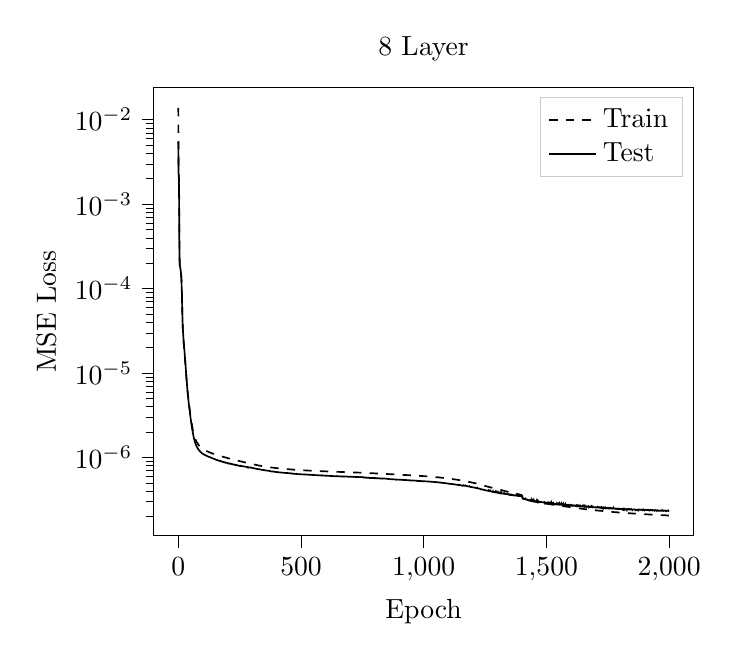
\begin{tikzpicture}

\begin{axis}[
legend cell align={left},
legend style={fill opacity=0.8, draw opacity=1, text opacity=1, draw=white!80!black},
log basis y={10},
tick align=outside,
tick pos=left,
title={8 Layer},
x grid style={white!69.0196078431373!black},
xlabel={Epoch},
xmin=-99.95, xmax=2098.95,
xtick style={color=black},
y grid style={white!69.0196078431373!black},
ylabel={MSE Loss},
ymin=1.18077084319194e-07, ymax=0.0240286142856456,
ymode=log,
ytick style={color=black}
]
\addplot [semithick, black, dashed]
table {%
0 0.0137857501469553
1 0.00308861960936338
2 0.00225937323644757
3 0.00184173461562023
4 0.000878539680619724
5 0.000267233489896171
6 0.000189525146357482
7 0.000177248529340432
8 0.000170382540301944
9 0.000163777170237154
10 0.000156803158293769
11 0.000148787730795448
12 0.000139447957270022
13 0.0001243273577129
14 0.000103127006572322
15 8.09196417794738e-05
16 6.05416532816889e-05
17 4.51169893822225e-05
18 3.565513092326e-05
19 3.03123355188291e-05
20 2.68081642607285e-05
21 2.43131255183471e-05
22 2.22995831736625e-05
23 2.05347641986009e-05
24 1.89343700831159e-05
25 1.74776983494667e-05
26 1.61251455356251e-05
27 1.48562264462271e-05
28 1.36716613037606e-05
29 1.25683485612171e-05
30 1.15524945263132e-05
31 1.06277352474535e-05
32 9.70658624783027e-06
33 8.84267294031815e-06
34 8.13857853154332e-06
35 7.58388431859203e-06
36 7.06517329012968e-06
37 6.48986769624571e-06
38 6.01962051950977e-06
39 5.62589393507551e-06
40 5.28921789339165e-06
41 4.98851873965123e-06
42 4.7175234600445e-06
43 4.47041639392864e-06
44 4.24115160376459e-06
45 4.02530521364497e-06
46 3.81863311099551e-06
47 3.62413326899969e-06
48 3.44267336078019e-06
49 3.26990401589455e-06
50 3.110896988062e-06
51 2.96396403069821e-06
52 2.82879928931834e-06
53 2.70368474275529e-06
54 2.58799466007531e-06
55 2.48464924226255e-06
56 2.39010867852585e-06
57 2.30290369552222e-06
58 2.2216036034024e-06
59 2.14735692520662e-06
60 2.07889566303265e-06
61 2.01642455289175e-06
62 1.95783670858418e-06
63 1.90416846038488e-06
64 1.85607089042605e-06
65 1.811010258848e-06
66 1.77054325018844e-06
67 1.7328962984493e-06
68 1.69725946949484e-06
69 1.66754056448326e-06
70 1.63858871133016e-06
71 1.61155683400693e-06
72 1.58789163265283e-06
73 1.56558429978304e-06
74 1.54554523152228e-06
75 1.52573656549748e-06
76 1.50784072388888e-06
77 1.49023391662695e-06
78 1.4743123068115e-06
79 1.45930793024718e-06
80 1.4446281097662e-06
81 1.43157341540245e-06
82 1.41939965010351e-06
83 1.40667576306441e-06
84 1.39518877335831e-06
85 1.38379590680415e-06
86 1.37327026897083e-06
87 1.36364018470658e-06
88 1.35418702711831e-06
89 1.34522714276386e-06
90 1.33634787925985e-06
91 1.32893943043655e-06
92 1.32093163441027e-06
93 1.3132997762284e-06
94 1.30623804824381e-06
95 1.29929187090738e-06
96 1.29237916951297e-06
97 1.28583184201148e-06
98 1.27959553714163e-06
99 1.2735283934262e-06
100 1.26791898730971e-06
101 1.2627259696103e-06
102 1.25771108588424e-06
103 1.25231368014056e-06
104 1.24631144498721e-06
105 1.24037334367699e-06
106 1.2340648443967e-06
107 1.22893064082064e-06
108 1.22437484989746e-06
109 1.21982722055236e-06
110 1.21481426256764e-06
111 1.2107418234848e-06
112 1.20602616044607e-06
113 1.20285992124991e-06
114 1.19859862485328e-06
115 1.19486205630892e-06
116 1.19111396352878e-06
117 1.18701774613328e-06
118 1.18387937891384e-06
119 1.18013333386102e-06
120 1.17652067552854e-06
121 1.17298610891226e-06
122 1.16920934786435e-06
123 1.16626488301108e-06
124 1.16285108117609e-06
125 1.15968924109211e-06
126 1.15640984193988e-06
127 1.15350303428841e-06
128 1.1503143885534e-06
129 1.14705221400868e-06
130 1.1443641856772e-06
131 1.14111493286373e-06
132 1.13798040635515e-06
133 1.13527754101028e-06
134 1.13251169233308e-06
135 1.12930856332127e-06
136 1.12650074075304e-06
137 1.1235084566863e-06
138 1.12072698141219e-06
139 1.1172398548922e-06
140 1.11442736803724e-06
141 1.11158048696325e-06
142 1.10887788622449e-06
143 1.10616437194722e-06
144 1.10341555770788e-06
145 1.10094259639482e-06
146 1.09825828815246e-06
147 1.09558834907375e-06
148 1.09296457605979e-06
149 1.09061500148755e-06
150 1.08795183314214e-06
151 1.08532106719395e-06
152 1.08324758190292e-06
153 1.08097435804666e-06
154 1.07827333013688e-06
155 1.07617651107716e-06
156 1.07380986366934e-06
157 1.07166150010585e-06
158 1.06948107162452e-06
159 1.06647956860684e-06
160 1.06494708404625e-06
161 1.06256772505731e-06
162 1.06035720727959e-06
163 1.05787372760346e-06
164 1.05588405099866e-06
165 1.05346232155057e-06
166 1.05166728118888e-06
167 1.04964814730124e-06
168 1.04769952940842e-06
169 1.04572185878737e-06
170 1.04260839512449e-06
171 1.04152885015196e-06
172 1.04000041307017e-06
173 1.03666240576672e-06
174 1.03516159231276e-06
175 1.03360050624701e-06
176 1.03188542567523e-06
177 1.02898213611979e-06
178 1.02803581077637e-06
179 1.02606050614895e-06
180 1.02454306204436e-06
181 1.02230507911827e-06
182 1.02055142943414e-06
183 1.01792596737482e-06
184 1.01660407779036e-06
185 1.01529137111811e-06
186 1.01237180382441e-06
187 1.01132905575696e-06
188 1.00956093092464e-06
189 1.00810563901632e-06
190 1.0052739773414e-06
191 1.00424275473188e-06
192 1.003211580894e-06
193 1.00131009619986e-06
194 9.98520134771752e-07
195 9.97664387540453e-07
196 9.94486084778146e-07
197 9.93778501651832e-07
198 9.90873338423626e-07
199 9.89912777669133e-07
200 9.88574339203296e-07
201 9.85725029522655e-07
202 9.84244386330602e-07
203 9.82002565308448e-07
204 9.78508168600456e-07
205 9.77044201306399e-07
206 9.76098156883154e-07
207 9.73493165162154e-07
208 9.71834136123562e-07
209 9.71276284246869e-07
210 9.68079569304336e-07
211 9.67498981026438e-07
212 9.64631265333082e-07
213 9.64166400649447e-07
214 9.61177288900217e-07
215 9.60805732916015e-07
216 9.57779043943674e-07
217 9.57766267873694e-07
218 9.54737937746586e-07
219 9.54498856344799e-07
220 9.52170370197791e-07
221 9.50519594084653e-07
222 9.48759981213243e-07
223 9.47102850858528e-07
224 9.46584362793601e-07
225 9.43646763801098e-07
226 9.42000673859411e-07
227 9.41450925949994e-07
228 9.38804523684666e-07
229 9.38322044589768e-07
230 9.35594229076742e-07
231 9.35247297007891e-07
232 9.32721268839032e-07
233 9.31552578464334e-07
234 9.30774605251372e-07
235 9.28317663891676e-07
236 9.26858944836795e-07
237 9.25179429543732e-07
238 9.23763715633186e-07
239 9.22354167357753e-07
240 9.20841406895079e-07
241 9.19228159915519e-07
242 9.17836204820333e-07
243 9.16312063225178e-07
244 9.14887535600428e-07
245 9.12851918116075e-07
246 9.12209820825183e-07
247 9.10882001278424e-07
248 9.09151504657757e-07
249 9.07929249365225e-07
250 9.06114797231794e-07
251 9.05019653970385e-07
252 9.03325363310614e-07
253 9.02047426535546e-07
254 9.00356864292462e-07
255 8.99421740939488e-07
256 8.9786664139524e-07
257 8.96162501391018e-07
258 8.94824077647627e-07
259 8.93166526680034e-07
260 8.92142999276757e-07
261 8.90646540653961e-07
262 8.89196897702504e-07
263 8.87752759098248e-07
264 8.86358454295078e-07
265 8.85122539898475e-07
266 8.83645790310084e-07
267 8.82326195210226e-07
268 8.80935579488096e-07
269 8.79514878278087e-07
270 8.78102829886984e-07
271 8.76637977967221e-07
272 8.75073412373695e-07
273 8.73695470517077e-07
274 8.7229220960694e-07
275 8.71096794639925e-07
276 8.69752706734062e-07
277 8.68293593612179e-07
278 8.66945744888881e-07
279 8.65692836129028e-07
280 8.6425307256377e-07
281 8.62996386615578e-07
282 8.61844596528272e-07
283 8.60314651902172e-07
284 8.58961779329093e-07
285 8.57684940086756e-07
286 8.56548996125639e-07
287 8.55367062882806e-07
288 8.53921339228236e-07
289 8.52381491938559e-07
290 8.5139164980319e-07
291 8.4983274942374e-07
292 8.48550058634601e-07
293 8.47121616715185e-07
294 8.45827474620364e-07
295 8.44044218467843e-07
296 8.42838108809474e-07
297 8.41480709709686e-07
298 8.40213770260334e-07
299 8.38855070696809e-07
300 8.37798641384779e-07
301 8.36651792894827e-07
302 8.35247779519932e-07
303 8.33991844217508e-07
304 8.3249875874003e-07
305 8.31112765837361e-07
306 8.29763220139057e-07
307 8.28537423330999e-07
308 8.27223779992892e-07
309 8.263019122694e-07
310 8.26237897740611e-07
311 8.24713217156159e-07
312 8.2334283979435e-07
313 8.22015577938373e-07
314 8.20726553371287e-07
315 8.19508391487034e-07
316 8.18137974590627e-07
317 8.17039462958746e-07
318 8.15745480878149e-07
319 8.14700765033649e-07
320 8.13773621985092e-07
321 8.12586493225354e-07
322 8.11482275494768e-07
323 8.10508947694188e-07
324 8.09030218846374e-07
325 8.08108718274525e-07
326 8.07103151188926e-07
327 8.06021113376687e-07
328 8.0490811670586e-07
329 8.03929369041612e-07
330 8.02840521885173e-07
331 8.01824190887146e-07
332 8.006422411313e-07
333 7.99249574953365e-07
334 7.98226580513983e-07
335 7.97378391467873e-07
336 7.96114629920908e-07
337 7.95464953313285e-07
338 7.94460564080168e-07
339 7.93411495550345e-07
340 7.92639923162142e-07
341 7.91717580995055e-07
342 7.90659596972887e-07
343 7.89734646772899e-07
344 7.88910815700206e-07
345 7.87838173835098e-07
346 7.87080269731177e-07
347 7.8613142619588e-07
348 7.85359551954912e-07
349 7.84582459175454e-07
350 7.83921955843425e-07
351 7.8297012908024e-07
352 7.82051770102043e-07
353 7.81296007033916e-07
354 7.80507885721704e-07
355 7.79689925153093e-07
356 7.78886507390553e-07
357 7.78194230775853e-07
358 7.77289544629411e-07
359 7.7656953261851e-07
360 7.75903502997721e-07
361 7.74936200443221e-07
362 7.74296334384417e-07
363 7.73721895654944e-07
364 7.72954912008572e-07
365 7.72319233249164e-07
366 7.71566827864945e-07
367 7.70699998838609e-07
368 7.70222717605407e-07
369 7.69374119812483e-07
370 7.68395611913775e-07
371 7.67787794430319e-07
372 7.67064833169684e-07
373 7.66419722197043e-07
374 7.66022498893904e-07
375 7.65052162719826e-07
376 7.64322403355777e-07
377 7.63627818059831e-07
378 7.63236719933502e-07
379 7.6248213609631e-07
380 7.62032572495741e-07
381 7.61118970331154e-07
382 7.60476678948407e-07
383 7.60098934165399e-07
384 7.592362803166e-07
385 7.586400048325e-07
386 7.58175735228406e-07
387 7.57343428460899e-07
388 7.56684466907131e-07
389 7.56365962160999e-07
390 7.55707249595616e-07
391 7.55030124281575e-07
392 7.54614512032958e-07
393 7.54073880841588e-07
394 7.53244257708729e-07
395 7.52822291843813e-07
396 7.52131151841695e-07
397 7.51477053313465e-07
398 7.50787530094499e-07
399 7.50268754131866e-07
400 7.49655679101124e-07
401 7.49106111442188e-07
402 7.48628529322559e-07
403 7.48065854992319e-07
404 7.47522233382369e-07
405 7.47014343886576e-07
406 7.4674312695322e-07
407 7.46154744589944e-07
408 7.45224265713773e-07
409 7.44781130833871e-07
410 7.44168451475957e-07
411 7.43612403141469e-07
412 7.43074742729277e-07
413 7.4255538692114e-07
414 7.41972566757454e-07
415 7.41491772316749e-07
416 7.40886318837397e-07
417 7.40458591266702e-07
418 7.40117279718788e-07
419 7.39657903153557e-07
420 7.3912421322575e-07
421 7.38795697401429e-07
422 7.38292617114666e-07
423 7.37599005930178e-07
424 7.37452366976754e-07
425 7.36602437115152e-07
426 7.36545854650217e-07
427 7.36174392713451e-07
428 7.35576475562993e-07
429 7.35150057053602e-07
430 7.34723915968516e-07
431 7.34193425984131e-07
432 7.33826684466976e-07
433 7.33313877120167e-07
434 7.32849924304446e-07
435 7.3240356381632e-07
436 7.31977483084734e-07
437 7.3147746320501e-07
438 7.31188059575061e-07
439 7.30770797602531e-07
440 7.3025388996939e-07
441 7.29911231729829e-07
442 7.29591046166433e-07
443 7.29134805823151e-07
444 7.28707190248201e-07
445 7.2811659848071e-07
446 7.2783998621162e-07
447 7.27755489791093e-07
448 7.26801464111304e-07
449 7.26691662777057e-07
450 7.26335354073626e-07
451 7.25658945043506e-07
452 7.25614078646686e-07
453 7.25175011581314e-07
454 7.24782964383053e-07
455 7.2419680768121e-07
456 7.2407520153206e-07
457 7.23398212727489e-07
458 7.23838310904057e-07
459 7.22997384855262e-07
460 7.22640464857705e-07
461 7.22022445884818e-07
462 7.21818079284731e-07
463 7.21388100032527e-07
464 7.20957314285897e-07
465 7.20499894029558e-07
466 7.20118750535903e-07
467 7.1978251421001e-07
468 7.19372024406084e-07
469 7.19226161493225e-07
470 7.18592157170406e-07
471 7.18292583542279e-07
472 7.17921304840274e-07
473 7.17656429145563e-07
474 7.17268838670293e-07
475 7.16870283014259e-07
476 7.16790947947743e-07
477 7.16224187868875e-07
478 7.15926577953496e-07
479 7.15506018508449e-07
480 7.15327944973865e-07
481 7.15154259026463e-07
482 7.14588176222719e-07
483 7.14167662749787e-07
484 7.13947983513208e-07
485 7.13584758472052e-07
486 7.13490786978355e-07
487 7.12802996346795e-07
488 7.1260814823404e-07
489 7.12203429642955e-07
490 7.12049823263783e-07
491 7.11565890298971e-07
492 7.11261462981838e-07
493 7.10956241448457e-07
494 7.10864853687099e-07
495 7.10524007445201e-07
496 7.10050566780751e-07
497 7.10148756851936e-07
498 7.09454082794991e-07
499 7.09290811926167e-07
500 7.08878859995821e-07
501 7.08592461123203e-07
502 7.08402716242063e-07
503 7.07911499688407e-07
504 7.07838705423569e-07
505 7.07405181373133e-07
506 7.07240273371212e-07
507 7.06922514538633e-07
508 7.06553931124176e-07
509 7.06358199010992e-07
510 7.05988017728032e-07
511 7.05820195491924e-07
512 7.05478267803983e-07
513 7.05317981612552e-07
514 7.04972263605441e-07
515 7.04692528387341e-07
516 7.04417077272978e-07
517 7.0408141230871e-07
518 7.03932418971931e-07
519 7.03659394588385e-07
520 7.03295456546016e-07
521 7.02983170214111e-07
522 7.02736174432061e-07
523 7.02738154330973e-07
524 7.02413211371322e-07
525 7.02195987742016e-07
526 7.01834438388005e-07
527 7.015176416445e-07
528 7.01357761215604e-07
529 7.01315112848988e-07
530 7.00866517291843e-07
531 7.00584499909951e-07
532 7.00379912302651e-07
533 7.00104224122811e-07
534 6.99711710453244e-07
535 6.99730678590527e-07
536 6.99416920937779e-07
537 6.99106589507892e-07
538 6.99099857314422e-07
539 6.98789812673795e-07
540 6.98547626143409e-07
541 6.9829937623922e-07
542 6.9803573740046e-07
543 6.97883229818785e-07
544 6.97516356922279e-07
545 6.97531738353518e-07
546 6.97229756156048e-07
547 6.96944444854353e-07
548 6.96735756392286e-07
549 6.96441722340069e-07
550 6.96331431043973e-07
551 6.95992913136934e-07
552 6.95820564317273e-07
553 6.95558284050435e-07
554 6.95345673136671e-07
555 6.9511123327004e-07
556 6.9492508868052e-07
557 6.94684943496782e-07
558 6.94408091291621e-07
559 6.94226875609161e-07
560 6.93976865377977e-07
561 6.93962414473503e-07
562 6.93575890437614e-07
563 6.93363744161957e-07
564 6.93089253118728e-07
565 6.92930680912696e-07
566 6.92638980467564e-07
567 6.92638060669992e-07
568 6.92431998800203e-07
569 6.92011693558925e-07
570 6.91779698058781e-07
571 6.91561712798716e-07
572 6.91245357501202e-07
573 6.90914098456119e-07
574 6.90786418317657e-07
575 6.90630641898338e-07
576 6.90921719240123e-07
577 6.90136385131268e-07
578 6.90016155033391e-07
579 6.89746223571319e-07
580 6.89630235626737e-07
581 6.89517517599825e-07
582 6.89564031830514e-07
583 6.8903582733526e-07
584 6.89009364705839e-07
585 6.88743238015377e-07
586 6.8840332086495e-07
587 6.88202743617694e-07
588 6.88021202506661e-07
589 6.87964407845243e-07
590 6.88042817529322e-07
591 6.87679688496701e-07
592 6.87582603731585e-07
593 6.87585936574919e-07
594 6.87160389531982e-07
595 6.86954137947282e-07
596 6.8681868329179e-07
597 6.86839983941923e-07
598 6.86604555980352e-07
599 6.86168778585738e-07
600 6.85818640121738e-07
601 6.85711275750123e-07
602 6.85531425304475e-07
603 6.85469083933299e-07
604 6.85334695788242e-07
605 6.84826699455243e-07
606 6.84622775608545e-07
607 6.84457398264726e-07
608 6.84304423188564e-07
609 6.84296297464471e-07
610 6.84731524756899e-07
611 6.83619167304528e-07
612 6.83459364040573e-07
613 6.83336111848121e-07
614 6.83173144011562e-07
615 6.83247643792129e-07
616 6.829115751259e-07
617 6.82785364645611e-07
618 6.82823477333727e-07
619 6.82156496722541e-07
620 6.82054949521671e-07
621 6.81831772880059e-07
622 6.81677918009882e-07
623 6.81486279333399e-07
624 6.81359977932061e-07
625 6.81108247150064e-07
626 6.81064127164177e-07
627 6.81072284521633e-07
628 6.80686871632474e-07
629 6.80564016704466e-07
630 6.80698681122749e-07
631 6.80240825744249e-07
632 6.80033357681964e-07
633 6.80167803238874e-07
634 6.79523233444002e-07
635 6.79397790690928e-07
636 6.79198196905872e-07
637 6.79049905556894e-07
638 6.79049523313324e-07
639 6.79142973154967e-07
640 6.78811062925888e-07
641 6.78329988289761e-07
642 6.78268604303867e-07
643 6.78312620792099e-07
644 6.77984985998137e-07
645 6.77676616234635e-07
646 6.77458028803812e-07
647 6.77593978508639e-07
648 6.77711388178182e-07
649 6.77032173726388e-07
650 6.7705669290774e-07
651 6.77168279509033e-07
652 6.76492063206524e-07
653 6.76391153575651e-07
654 6.76132728315793e-07
655 6.76058174207128e-07
656 6.76169795809756e-07
657 6.76121099218108e-07
658 6.75468571330384e-07
659 6.75345675475114e-07
660 6.75184716641297e-07
661 6.75026644856302e-07
662 6.74925118602232e-07
663 6.75125837290125e-07
664 6.74430557722872e-07
665 6.74353537561956e-07
666 6.74566049795544e-07
667 6.74105771835798e-07
668 6.73843414475073e-07
669 6.74108299563159e-07
670 6.73400757577269e-07
671 6.73219013251014e-07
672 6.73141517864906e-07
673 6.73084371044297e-07
674 6.73303882052778e-07
675 6.73119193351113e-07
676 6.72406169627493e-07
677 6.72221007633311e-07
678 6.72262872228657e-07
679 6.71918138493766e-07
680 6.7187868074825e-07
681 6.71670914556444e-07
682 6.71474687848672e-07
683 6.71449357596998e-07
684 6.71642237449532e-07
685 6.71132449625134e-07
686 6.70766620928021e-07
687 6.70696218847411e-07
688 6.70498978038836e-07
689 6.70508200329323e-07
690 6.70917440473318e-07
691 6.70120118655859e-07
692 6.69779609609122e-07
693 6.69663694836231e-07
694 6.69445325542029e-07
695 6.69258560876074e-07
696 6.69263294042821e-07
697 6.69365898531282e-07
698 6.69413571543487e-07
699 6.68658066985017e-07
700 6.6849241932232e-07
701 6.68295025889165e-07
702 6.68346391194063e-07
703 6.68034477683932e-07
704 6.67883314008577e-07
705 6.67871747751292e-07
706 6.67869822521539e-07
707 6.6741284337013e-07
708 6.67211375102283e-07
709 6.66998994347523e-07
710 6.67053436302467e-07
711 6.6682756991554e-07
712 6.66589114103999e-07
713 6.66490238728556e-07
714 6.66292823055414e-07
715 6.66251703336229e-07
716 6.66788175905708e-07
717 6.65793759552002e-07
718 6.65465117947406e-07
719 6.65816963035581e-07
720 6.65758463583188e-07
721 6.65544843045041e-07
722 6.65886225434065e-07
723 6.65198361417651e-07
724 6.64831936816768e-07
725 6.64645499369954e-07
726 6.64471501011121e-07
727 6.64225957706321e-07
728 6.64358892365158e-07
729 6.64192160570565e-07
730 6.64110347983637e-07
731 6.63900382065208e-07
732 6.63378257172553e-07
733 6.63277901182369e-07
734 6.63126197338215e-07
735 6.63272134914905e-07
736 6.63339513778283e-07
737 6.63178494576755e-07
738 6.62740552428431e-07
739 6.62412929628431e-07
740 6.62471505791018e-07
741 6.62118904955378e-07
742 6.6211564454477e-07
743 6.61732920079317e-07
744 6.61794542253347e-07
745 6.61537696160508e-07
746 6.6167947284157e-07
747 6.61282068222135e-07
748 6.60957793272132e-07
749 6.60974708708295e-07
750 6.60737628876973e-07
751 6.60563611177167e-07
752 6.60669549006343e-07
753 6.60142026859489e-07
754 6.59790588628084e-07
755 6.59206425495995e-07
756 6.58697558208132e-07
757 6.58472624053275e-07
758 6.58561325010965e-07
759 6.58079057743066e-07
760 6.58026551377589e-07
761 6.57965502142588e-07
762 6.57523861733012e-07
763 6.57337378598299e-07
764 6.56981951877356e-07
765 6.56761206968781e-07
766 6.56501978454571e-07
767 6.55857276768756e-07
768 6.56530517460396e-07
769 6.56905732810742e-07
770 6.56052742030511e-07
771 6.55603195994559e-07
772 6.55322380296752e-07
773 6.54704865823419e-07
774 6.54461226190506e-07
775 6.54197285342661e-07
776 6.53888960741256e-07
777 6.53602056658542e-07
778 6.53268098702142e-07
779 6.54040435051684e-07
780 6.53235653487627e-07
781 6.52853220628913e-07
782 6.52299065265538e-07
783 6.52097500406512e-07
784 6.51775928290022e-07
785 6.5176647149201e-07
786 6.51328027572617e-07
787 6.51507847905464e-07
788 6.51621266655411e-07
789 6.51120280338091e-07
790 6.50271066035657e-07
791 6.50623032598219e-07
792 6.50225028067553e-07
793 6.50682340662456e-07
794 6.49817614075232e-07
795 6.50719730501237e-07
796 6.49664923798809e-07
797 6.50211584300564e-07
798 6.48809363013925e-07
799 6.49380920918929e-07
800 6.4855317921797e-07
801 6.48718604878695e-07
802 6.48325270674377e-07
803 6.48340940912817e-07
804 6.48384094091625e-07
805 6.47670242756249e-07
806 6.47294677563082e-07
807 6.47407202379213e-07
808 6.47062250948238e-07
809 6.47139711901445e-07
810 6.46794424753239e-07
811 6.46586513980196e-07
812 6.4630621535855e-07
813 6.46143918785924e-07
814 6.46206421080819e-07
815 6.46050809052667e-07
816 6.45811578138478e-07
817 6.45534134704917e-07
818 6.45272071750469e-07
819 6.45084313475763e-07
820 6.44940158494478e-07
821 6.44797928664786e-07
822 6.44664317420052e-07
823 6.44708393238602e-07
824 6.44781474790079e-07
825 6.43953618663318e-07
826 6.4401244547696e-07
827 6.44133531608304e-07
828 6.43848811620273e-07
829 6.43534523021572e-07
830 6.43623536802807e-07
831 6.43355545122404e-07
832 6.43459978064698e-07
833 6.42539122694075e-07
834 6.42423720783825e-07
835 6.42229068049005e-07
836 6.43694028795494e-07
837 6.42312120220367e-07
838 6.42023174947326e-07
839 6.41817638097564e-07
840 6.41963917189514e-07
841 6.41126675986925e-07
842 6.41542135880968e-07
843 6.40884694462329e-07
844 6.40648684807843e-07
845 6.40480053760939e-07
846 6.39854228822401e-07
847 6.39868403069954e-07
848 6.39840600157981e-07
849 6.3893318502295e-07
850 6.38639376944639e-07
851 6.38337542994805e-07
852 6.38013974160856e-07
853 6.37820371764519e-07
854 6.38136522212562e-07
855 6.37338352333927e-07
856 6.36990881744737e-07
857 6.36761553366227e-07
858 6.36636442983729e-07
859 6.36787522850568e-07
860 6.36482686665829e-07
861 6.35810526496528e-07
862 6.35790216250598e-07
863 6.35545664792403e-07
864 6.35076302394566e-07
865 6.35354525677201e-07
866 6.35086437441146e-07
867 6.34891969426121e-07
868 6.33774776630958e-07
869 6.34218968521338e-07
870 6.33500820129029e-07
871 6.33716124205819e-07
872 6.33840579588707e-07
873 6.33507658463373e-07
874 6.32700088168292e-07
875 6.32751752640104e-07
876 6.32394511370649e-07
877 6.324811581635e-07
878 6.32187316163879e-07
879 6.31331189211437e-07
880 6.31645610027931e-07
881 6.30612103350359e-07
882 6.31642888585304e-07
883 6.30301115812415e-07
884 6.30303219345763e-07
885 6.30434531956325e-07
886 6.29825851213184e-07
887 6.3026594636284e-07
888 6.29491433983276e-07
889 6.29894949852883e-07
890 6.29112065524851e-07
891 6.2892201845699e-07
892 6.28567796532309e-07
893 6.28616281083794e-07
894 6.28783369236885e-07
895 6.28419824529658e-07
896 6.28173706630264e-07
897 6.2753141462224e-07
898 6.28429217087501e-07
899 6.27228162862536e-07
900 6.26573483586412e-07
901 6.25917755449734e-07
902 6.26262109051368e-07
903 6.26087741146364e-07
904 6.25708041049222e-07
905 6.25127507547063e-07
906 6.25702879716528e-07
907 6.25510647722649e-07
908 6.24522796002225e-07
909 6.25014120444689e-07
910 6.24146452096852e-07
911 6.24608488436706e-07
912 6.24371818311431e-07
913 6.24132697971902e-07
914 6.22939180331628e-07
915 6.2351004271477e-07
916 6.2332889153538e-07
917 6.23131349392736e-07
918 6.22394030202145e-07
919 6.22486220159146e-07
920 6.22470642809958e-07
921 6.22380071284567e-07
922 6.21532071036768e-07
923 6.21287593048692e-07
924 6.21170952555872e-07
925 6.21255831831036e-07
926 6.20757267839167e-07
927 6.20728286811811e-07
928 6.20359319391639e-07
929 6.20314215325379e-07
930 6.19811376125767e-07
931 6.19809856949871e-07
932 6.19194335051532e-07
933 6.19207079509465e-07
934 6.19016115749105e-07
935 6.18487976225879e-07
936 6.18693006728677e-07
937 6.18447636256292e-07
938 6.17691537371456e-07
939 6.1794909366597e-07
940 6.17617315015195e-07
941 6.17466598178851e-07
942 6.1694945669899e-07
943 6.16808603986385e-07
944 6.16357394129352e-07
945 6.16576176412309e-07
946 6.15661359837816e-07
947 6.15837455470114e-07
948 6.15222403098414e-07
949 6.15210279363509e-07
950 6.14131315380462e-07
951 6.14896761973682e-07
952 6.14312084110224e-07
953 6.13742194374822e-07
954 6.1423430738472e-07
955 6.13934294406704e-07
956 6.13463449120388e-07
957 6.13431861239633e-07
958 6.126252800982e-07
959 6.12680259457932e-07
960 6.12373812849398e-07
961 6.11732409318222e-07
962 6.11996258804481e-07
963 6.11834997698679e-07
964 6.11534490232657e-07
965 6.11279412410681e-07
966 6.10976991652024e-07
967 6.10801607635381e-07
968 6.0993121639541e-07
969 6.10257766908262e-07
970 6.09721131198171e-07
971 6.09514962107482e-07
972 6.10151406853277e-07
973 6.09608913990201e-07
974 6.08623257143392e-07
975 6.08609208669009e-07
976 6.07961926370138e-07
977 6.08075848290923e-07
978 6.07992424576764e-07
979 6.0775241048816e-07
980 6.07132156815737e-07
981 6.07294684876081e-07
982 6.06953180458447e-07
983 6.06453473309898e-07
984 6.05623692209178e-07
985 6.06061935386037e-07
986 6.05816325773389e-07
987 6.05566570953897e-07
988 6.05717543429307e-07
989 6.04947530575828e-07
990 6.04886406833316e-07
991 6.03998137073347e-07
992 6.0427891953907e-07
993 6.04073403579264e-07
994 6.03782304587242e-07
995 6.03477907574756e-07
996 6.03108307771549e-07
997 6.0244759085748e-07
998 6.02023152659115e-07
999 6.02464689706039e-07
1000 6.02305121390145e-07
1001 6.01802074946534e-07
1002 6.00690151784988e-07
1003 6.00747979532912e-07
1004 6.00759271186746e-07
1005 6.0054698502654e-07
1006 5.99763121869046e-07
1007 5.99490849140238e-07
1008 5.9974713006028e-07
1009 5.99658466896358e-07
1010 5.98812800596704e-07
1011 5.98873594029215e-07
1012 5.98376134469447e-07
1013 5.98230488101592e-07
1014 5.98133207567741e-07
1015 5.97380654419055e-07
1016 5.97340932856127e-07
1017 5.97020822851846e-07
1018 5.96662386726621e-07
1019 5.96547044061424e-07
1020 5.95986840195906e-07
1021 5.96448906740932e-07
1022 5.96114958746341e-07
1023 5.95908167888126e-07
1024 5.95399733924751e-07
1025 5.94854680898038e-07
1026 5.94013621309841e-07
1027 5.94053043350584e-07
1028 5.93657127041069e-07
1029 5.9312079419982e-07
1030 5.93351660242547e-07
1031 5.93160193432141e-07
1032 5.92637767212523e-07
1033 5.92132599592787e-07
1034 5.92207692520219e-07
1035 5.91352295039371e-07
1036 5.91074109657086e-07
1037 5.91294802873676e-07
1038 5.90296284478597e-07
1039 5.90281609348153e-07
1040 5.89172957631945e-07
1041 5.89864375598381e-07
1042 5.89333540624182e-07
1043 5.89092944501601e-07
1044 5.8811172851847e-07
1045 5.88118473984878e-07
1046 5.87558959523449e-07
1047 5.87498966091005e-07
1048 5.86975968829506e-07
1049 5.86538542663106e-07
1050 5.85390634384453e-07
1051 5.8604224697234e-07
1052 5.85704977417834e-07
1053 5.84833425804732e-07
1054 5.85203938186396e-07
1055 5.84576740706666e-07
1056 5.84105853000949e-07
1057 5.83624754902701e-07
1058 5.82899904443934e-07
1059 5.82916453005566e-07
1060 5.82865486791206e-07
1061 5.81442056130754e-07
1062 5.80942083999503e-07
1063 5.80710280317476e-07
1064 5.8016460865673e-07
1065 5.80148177206752e-07
1066 5.79519820348651e-07
1067 5.79282890541322e-07
1068 5.78339731006849e-07
1069 5.78075172036563e-07
1070 5.77422741336875e-07
1071 5.76988799444678e-07
1072 5.76913078944585e-07
1073 5.7649559715145e-07
1074 5.7592376823834e-07
1075 5.75118488846726e-07
1076 5.74859645261938e-07
1077 5.74464747032266e-07
1078 5.7391911401794e-07
1079 5.73786442799928e-07
1080 5.73293567576627e-07
1081 5.72705432531961e-07
1082 5.72505290044489e-07
1083 5.72218330383123e-07
1084 5.71506954933909e-07
1085 5.70766419834001e-07
1086 5.70619852211962e-07
1087 5.70089109672267e-07
1088 5.69310650618604e-07
1089 5.69087913817157e-07
1090 5.68740758041031e-07
1091 5.68193936842931e-07
1092 5.67973420743328e-07
1093 5.67342231157397e-07
1094 5.66961273946731e-07
1095 5.66632256052912e-07
1096 5.66003266825987e-07
1097 5.65674219494383e-07
1098 5.65259562122833e-07
1099 5.64769521723463e-07
1100 5.64369430676948e-07
1101 5.63613571578969e-07
1102 5.63189598679514e-07
1103 5.63041100242856e-07
1104 5.62284110486644e-07
1105 5.61835125878929e-07
1106 5.61412824893637e-07
1107 5.60981057205367e-07
1108 5.60571713556612e-07
1109 5.59922194639739e-07
1110 5.59530634561156e-07
1111 5.59002662015473e-07
1112 5.581992556003e-07
1113 5.57639288423673e-07
1114 5.57120050359572e-07
1115 5.56716404425117e-07
1116 5.56288290574969e-07
1117 5.55825715849778e-07
1118 5.55270240283789e-07
1119 5.5472401763268e-07
1120 5.5407207688063e-07
1121 5.53537679024885e-07
1122 5.52935819953859e-07
1123 5.52418589208514e-07
1124 5.5196548998282e-07
1125 5.5140549684296e-07
1126 5.50842811136931e-07
1127 5.50178398597723e-07
1128 5.49853654099763e-07
1129 5.49349440554181e-07
1130 5.48803564406342e-07
1131 5.48427744170965e-07
1132 5.47851732008553e-07
1133 5.47107029639449e-07
1134 5.46832161106181e-07
1135 5.46189866398095e-07
1136 5.45587667346581e-07
1137 5.45162206151417e-07
1138 5.4475243558727e-07
1139 5.43768126320288e-07
1140 5.43458325758195e-07
1141 5.42946222211071e-07
1142 5.42318003155628e-07
1143 5.41685208027332e-07
1144 5.41118284786535e-07
1145 5.40587837761564e-07
1146 5.40002958679509e-07
1147 5.3967720147341e-07
1148 5.3918130650743e-07
1149 5.38497736847887e-07
1150 5.37864707133906e-07
1151 5.37328203797927e-07
1152 5.36580279764109e-07
1153 5.36202094679083e-07
1154 5.35710694869351e-07
1155 5.35006929652582e-07
1156 5.34474729406043e-07
1157 5.33720529190873e-07
1158 5.33245014793238e-07
1159 5.32959159869506e-07
1160 5.33745327018664e-07
1161 5.32485687202211e-07
1162 5.31249801881017e-07
1163 5.30626741706897e-07
1164 5.2979573960954e-07
1165 5.29420067280739e-07
1166 5.28620816382386e-07
1167 5.27807401681457e-07
1168 5.27121304358502e-07
1169 5.26377595562622e-07
1170 5.25672054251913e-07
1171 5.24890954721968e-07
1172 5.2444793212203e-07
1173 5.23721696609414e-07
1174 5.23018498213901e-07
1175 5.2188551669019e-07
1176 5.21017574712346e-07
1177 5.20534954489449e-07
1178 5.19553454381594e-07
1179 5.18730347920382e-07
1180 5.17958713544431e-07
1181 5.17150383586795e-07
1182 5.16437501957512e-07
1183 5.15647556241561e-07
1184 5.15112535509843e-07
1185 5.14169199476555e-07
1186 5.13523359217061e-07
1187 5.12790095356763e-07
1188 5.1223551854207e-07
1189 5.11717524076971e-07
1190 5.10849785044343e-07
1191 5.10033092680828e-07
1192 5.09329841293038e-07
1193 5.08588952371269e-07
1194 5.07864471316566e-07
1195 5.07212841625915e-07
1196 5.06569104132382e-07
1197 5.05559155925539e-07
1198 5.05332368987865e-07
1199 5.04487800398579e-07
1200 5.03532473260293e-07
1201 5.03095116613395e-07
1202 5.02088503367304e-07
1203 5.01136403556757e-07
1204 5.00731445981728e-07
1205 4.99776320992851e-07
1206 4.99325033715081e-07
1207 4.98700373640304e-07
1208 4.97808630200325e-07
1209 4.96947417900628e-07
1210 4.96288867537942e-07
1211 4.95732484836253e-07
1212 4.94955880725456e-07
1213 4.94176946858715e-07
1214 4.93376584756788e-07
1215 4.92612390658564e-07
1216 4.920525770018e-07
1217 4.91067804333056e-07
1218 4.90369304714022e-07
1219 4.89532306190199e-07
1220 4.88886637128871e-07
1221 4.88063364329605e-07
1222 4.87359449877545e-07
1223 4.86462110629304e-07
1224 4.8582851755441e-07
1225 4.8509610044789e-07
1226 4.84401673972457e-07
1227 4.83254481267181e-07
1228 4.82487706861434e-07
1229 4.81833279323496e-07
1230 4.80243687633219e-07
1231 4.78414342282463e-07
1232 4.76838534240187e-07
1233 4.76149318657804e-07
1234 4.74790627791322e-07
1235 4.73768826594778e-07
1236 4.72720507829649e-07
1237 4.71855896634565e-07
1238 4.70534331853401e-07
1239 4.70113000531569e-07
1240 4.69121401650341e-07
1241 4.68302746483573e-07
1242 4.67329256736093e-07
1243 4.66545695545051e-07
1244 4.65720774428746e-07
1245 4.64882776356035e-07
1246 4.64056661272139e-07
1247 4.63339145298391e-07
1248 4.62453502805715e-07
1249 4.6154897869144e-07
1250 4.60787575832455e-07
1251 4.59998585000676e-07
1252 4.59476001552161e-07
1253 4.58542613344548e-07
1254 4.58008765320983e-07
1255 4.57043186344208e-07
1256 4.56172413777267e-07
1257 4.55492208899955e-07
1258 4.54621887328699e-07
1259 4.53731679030511e-07
1260 4.52947662239467e-07
1261 4.52175911945574e-07
1262 4.51259721572228e-07
1263 4.50436129000309e-07
1264 4.49572491348249e-07
1265 4.49066028352263e-07
1266 4.48156541779099e-07
1267 4.47460020353674e-07
1268 4.46502518983038e-07
1269 4.45779370750188e-07
1270 4.45073646687888e-07
1271 4.44745651066114e-07
1272 4.43919204570875e-07
1273 4.43130237655964e-07
1274 4.42290351216457e-07
1275 4.41504531295323e-07
1276 4.40815369401548e-07
1277 4.40169212268415e-07
1278 4.39142476835741e-07
1279 4.38690070765801e-07
1280 4.37918824530925e-07
1281 4.3708706678558e-07
1282 4.36362787709754e-07
1283 4.35320906618131e-07
1284 4.34962962970076e-07
1285 4.34124661254032e-07
1286 4.33472893078601e-07
1287 4.3270664316708e-07
1288 4.3223810664017e-07
1289 4.31506152210659e-07
1290 4.30598854350706e-07
1291 4.29677616750723e-07
1292 4.28937097368021e-07
1293 4.2827022625147e-07
1294 4.27427441493933e-07
1295 4.2679034957871e-07
1296 4.25909393555912e-07
1297 4.25184653096267e-07
1298 4.24548843795947e-07
1299 4.2362739712587e-07
1300 4.23001229847841e-07
1301 4.22171937557891e-07
1302 4.21529943849919e-07
1303 4.20893796700739e-07
1304 4.1996023799129e-07
1305 4.19370747252401e-07
1306 4.18629378344804e-07
1307 4.17800233435628e-07
1308 4.17327775906529e-07
1309 4.16702173822614e-07
1310 4.15864855156656e-07
1311 4.15330635235023e-07
1312 4.14520232155269e-07
1313 4.13829448135061e-07
1314 4.1304789226615e-07
1315 4.12341253692716e-07
1316 4.1216946509337e-07
1317 4.11018312902911e-07
1318 4.10335426906272e-07
1319 4.09523415214608e-07
1320 4.08610692858247e-07
1321 4.07992596990425e-07
1322 4.07032663076734e-07
1323 4.06648582554681e-07
1324 4.05807523293333e-07
1325 4.05085819707551e-07
1326 4.04363589808554e-07
1327 4.03830442820663e-07
1328 4.0298853319598e-07
1329 4.02449150698203e-07
1330 4.02263740824083e-07
1331 4.01028636716205e-07
1332 4.00283313709338e-07
1333 3.99633769589514e-07
1334 3.98941660137098e-07
1335 3.98408138792661e-07
1336 3.9767170837024e-07
1337 3.96993410618052e-07
1338 3.96322553143591e-07
1339 3.95798050206508e-07
1340 3.94935926777862e-07
1341 3.94421753668439e-07
1342 3.9375066577918e-07
1343 3.93084235483343e-07
1344 3.92502506613823e-07
1345 3.91987923293868e-07
1346 3.9124424080228e-07
1347 3.91049823832645e-07
1348 3.90322553116107e-07
1349 3.89593919820186e-07
1350 3.88722149352816e-07
1351 3.88301868838425e-07
1352 3.87433650871571e-07
1353 3.87444912661294e-07
1354 3.86126681021892e-07
1355 3.85559809302549e-07
1356 3.8492804539203e-07
1357 3.84593586048254e-07
1358 3.83902541258863e-07
1359 3.83004335461123e-07
1360 3.82602766521245e-07
1361 3.82011311558017e-07
1362 3.81463873210919e-07
1363 3.8110734190866e-07
1364 3.80366255839704e-07
1365 3.79705994987489e-07
1366 3.79158340081176e-07
1367 3.78491242940981e-07
1368 3.78047957042327e-07
1369 3.77540550999811e-07
1370 3.77056229396544e-07
1371 3.7643638771101e-07
1372 3.7545368427061e-07
1373 3.74841019990413e-07
1374 3.74239669682197e-07
1375 3.73709808172862e-07
1376 3.73041227035742e-07
1377 3.72869718347602e-07
1378 3.72220887982166e-07
1379 3.71513008502689e-07
1380 3.70764545507996e-07
1381 3.70413332248631e-07
1382 3.69776117224774e-07
1383 3.68990465801744e-07
1384 3.68179114161649e-07
1385 3.67674000202101e-07
1386 3.67139926510163e-07
1387 3.67087734161942e-07
1388 3.66082978302984e-07
1389 3.65367626926627e-07
1390 3.6481237800956e-07
1391 3.63644148123399e-07
1392 3.63287133581025e-07
1393 3.63036160877073e-07
1394 3.62126584448674e-07
1395 3.61699762649437e-07
1396 3.61027375987533e-07
1397 3.60369763242829e-07
1398 3.60007189115663e-07
1399 3.59295827124129e-07
1400 3.5775579875974e-07
1401 3.53868214730824e-07
1402 3.41379617296411e-07
1403 3.28579712345345e-07
1404 3.25548541511012e-07
1405 3.24216553693191e-07
1406 3.22977575535788e-07
1407 3.22425292083039e-07
1408 3.21560779539709e-07
1409 3.21061373725229e-07
1410 3.19967045953717e-07
1411 3.19681221583323e-07
1412 3.18886990186229e-07
1413 3.18288745347672e-07
1414 3.17631491043358e-07
1415 3.17402957406898e-07
1416 3.16448183653506e-07
1417 3.16011549529094e-07
1418 3.15193454127893e-07
1419 3.1478528707396e-07
1420 3.14031266398729e-07
1421 3.13261919700381e-07
1422 3.12983140958067e-07
1423 3.1251393924947e-07
1424 3.11998803240954e-07
1425 3.11705126065931e-07
1426 3.1094608770843e-07
1427 3.1091148596829e-07
1428 3.10241547680334e-07
1429 3.09736733072441e-07
1430 3.09197059110033e-07
1431 3.09091740660961e-07
1432 3.0816822710733e-07
1433 3.07916834699995e-07
1434 3.07206576749763e-07
1435 3.06838810715249e-07
1436 3.06620812068559e-07
1437 3.0611676983483e-07
1438 3.05473894016473e-07
1439 3.05116190560284e-07
1440 3.0515102234574e-07
1441 3.04555343959123e-07
1442 3.04196095541442e-07
1443 3.03736167268198e-07
1444 3.040585565941e-07
1445 3.0285602309732e-07
1446 3.02862596157638e-07
1447 3.02560588011147e-07
1448 3.02829190928833e-07
1449 3.01927896686038e-07
1450 3.01475552525687e-07
1451 3.00904842305272e-07
1452 3.00629884698367e-07
1453 3.00555958332893e-07
1454 3.00048228730532e-07
1455 2.99900297065392e-07
1456 2.99528309639641e-07
1457 2.99114135650314e-07
1458 2.98604760402554e-07
1459 2.98240277793127e-07
1460 2.97766990755122e-07
1461 2.98054582771101e-07
1462 2.97141440512405e-07
1463 2.96694996791302e-07
1464 2.96270484767547e-07
1465 2.96184018438339e-07
1466 2.95704940683095e-07
1467 2.95396794122382e-07
1468 2.95091585243767e-07
1469 2.94782432320062e-07
1470 2.94291698516247e-07
1471 2.93947373592118e-07
1472 2.93326942326644e-07
1473 2.93185483691616e-07
1474 2.93146487450713e-07
1475 2.92696370287615e-07
1476 2.92517656269808e-07
1477 2.92087966471399e-07
1478 2.91890827398333e-07
1479 2.91456780672661e-07
1480 2.91003376375443e-07
1481 2.90897139052504e-07
1482 2.90544493950051e-07
1483 2.90321684360606e-07
1484 2.89833084551105e-07
1485 2.89581516007331e-07
1486 2.89212358396185e-07
1487 2.88950256795317e-07
1488 2.88564842733763e-07
1489 2.88200527080562e-07
1490 2.87884401444671e-07
1491 2.87497334070963e-07
1492 2.8721040789037e-07
1493 2.86508051104306e-07
1494 2.86306328078467e-07
1495 2.86144508876873e-07
1496 2.85861089821537e-07
1497 2.85360442411786e-07
1498 2.85058979642372e-07
1499 2.84970874481871e-07
1500 2.84450102817857e-07
1501 2.84078861753301e-07
1502 2.83543574305156e-07
1503 2.83563822584654e-07
1504 2.82890254204915e-07
1505 2.82827177642275e-07
1506 2.82641763888591e-07
1507 2.82033121649761e-07
1508 2.82002064608378e-07
1509 2.81318216082127e-07
1510 2.81270375850795e-07
1511 2.8097148791062e-07
1512 2.80864460734165e-07
1513 2.80383226922254e-07
1514 2.80231873112768e-07
1515 2.79643016561693e-07
1516 2.79513022562128e-07
1517 2.79163273717131e-07
1518 2.7870598270141e-07
1519 2.78674357851116e-07
1520 2.78108519935927e-07
1521 2.78267315479752e-07
1522 2.77627101574751e-07
1523 2.77175951154618e-07
1524 2.77061909592646e-07
1525 2.76829202157103e-07
1526 2.7642390725191e-07
1527 2.76237728002116e-07
1528 2.75949262274366e-07
1529 2.75852835628143e-07
1530 2.75600234033391e-07
1531 2.74864786490525e-07
1532 2.74880136871047e-07
1533 2.74431400029584e-07
1534 2.74260290815675e-07
1535 2.73908545914026e-07
1536 2.73709271660039e-07
1537 2.73536457655155e-07
1538 2.73341923637815e-07
1539 2.73021322414024e-07
1540 2.72803043102954e-07
1541 2.72587641099165e-07
1542 2.72122814891418e-07
1543 2.71993649803903e-07
1544 2.71596017171305e-07
1545 2.71636295664734e-07
1546 2.71166804125755e-07
1547 2.70989261075272e-07
1548 2.70696542713722e-07
1549 2.70436283962283e-07
1550 2.70061753731454e-07
1551 2.6989989021331e-07
1552 2.69763729100703e-07
1553 2.69655354983911e-07
1554 2.69066596061407e-07
1555 2.68926969837935e-07
1556 2.68573427192109e-07
1557 2.68608412383742e-07
1558 2.67920140125e-07
1559 2.67861273933079e-07
1560 2.67640900844413e-07
1561 2.67677652011855e-07
1562 2.66964462625197e-07
1563 2.66822012484624e-07
1564 2.66567217181546e-07
1565 2.66555855290562e-07
1566 2.65938470718652e-07
1567 2.65836721510482e-07
1568 2.65485345245509e-07
1569 2.65497387978542e-07
1570 2.65124400584682e-07
1571 2.64794280695924e-07
1572 2.64446180700872e-07
1573 2.64363307621807e-07
1574 2.63953197340072e-07
1575 2.63414974881471e-07
1576 2.6352014254627e-07
1577 2.6342906294019e-07
1578 2.63256980119309e-07
1579 2.6275006576526e-07
1580 2.62603489957769e-07
1581 2.62322275212057e-07
1582 2.62190380972527e-07
1583 2.61826094835271e-07
1584 2.61762005067112e-07
1585 2.6165635841835e-07
1586 2.61387302224136e-07
1587 2.60961940504956e-07
1588 2.60710632772998e-07
1589 2.60395194366936e-07
1590 2.60170396778392e-07
1591 2.60418973766718e-07
1592 2.59962582262574e-07
1593 2.5969601419007e-07
1594 2.59373768479065e-07
1595 2.59266632525623e-07
1596 2.58953215023894e-07
1597 2.58385050443621e-07
1598 2.58312552205098e-07
1599 2.57958812120762e-07
1600 2.57778561035593e-07
1601 2.57694562435518e-07
1602 2.57359396975687e-07
1603 2.5705239291085e-07
1604 2.56811242699939e-07
1605 2.56461717242473e-07
1606 2.56126585846062e-07
1607 2.55749145210871e-07
1608 2.55653439175774e-07
1609 2.55513533744534e-07
1610 2.55211480364892e-07
1611 2.54804955659438e-07
1612 2.54763174751815e-07
1613 2.54787983493543e-07
1614 2.54455153722688e-07
1615 2.54169908593838e-07
1616 2.53858018467668e-07
1617 2.53570905002221e-07
1618 2.53653469627579e-07
1619 2.53107618163995e-07
1620 2.53153813460472e-07
1621 2.52625748231594e-07
1622 2.52780608676062e-07
1623 2.52202483792985e-07
1624 2.51898197333844e-07
1625 2.51692562230232e-07
1626 2.51686352093827e-07
1627 2.51284400277996e-07
1628 2.510466178407e-07
1629 2.50913202592074e-07
1630 2.50352099349982e-07
1631 2.50282909277644e-07
1632 2.50297362768492e-07
1633 2.49979243882592e-07
1634 2.49957796164324e-07
1635 2.49437291799381e-07
1636 2.49304088775659e-07
1637 2.49228307311e-07
1638 2.48961546077453e-07
1639 2.48945990243499e-07
1640 2.48505118250364e-07
1641 2.48237105296312e-07
1642 2.47971299991434e-07
1643 2.47875569947098e-07
1644 2.4794665956307e-07
1645 2.47326225185418e-07
1646 2.47498117275313e-07
1647 2.46912391794751e-07
1648 2.46693469193815e-07
1649 2.46549616903735e-07
1650 2.46913651224645e-07
1651 2.46156420679711e-07
1652 2.46014868004352e-07
1653 2.46031733666996e-07
1654 2.45937145464836e-07
1655 2.45421275380409e-07
1656 2.4518313143318e-07
1657 2.45077444105846e-07
1658 2.45103997855267e-07
1659 2.44453994220351e-07
1660 2.44352771495926e-07
1661 2.44336961486624e-07
1662 2.43957096735414e-07
1663 2.44000740032391e-07
1664 2.43840326682232e-07
1665 2.43737352008111e-07
1666 2.43350576539569e-07
1667 2.43003017637022e-07
1668 2.42828271026951e-07
1669 2.42498429528837e-07
1670 2.42299023938131e-07
1671 2.42565715481646e-07
1672 2.41789805663473e-07
1673 2.41731107983867e-07
1674 2.4149342952029e-07
1675 2.41314539678683e-07
1676 2.41171244880434e-07
1677 2.40871798965259e-07
1678 2.4079149969225e-07
1679 2.41200686303955e-07
1680 2.40602273073875e-07
1681 2.40352490664009e-07
1682 2.40002927021976e-07
1683 2.40169289128289e-07
1684 2.3982877031159e-07
1685 2.40364217468425e-07
1686 2.39530044183311e-07
1687 2.39584125388603e-07
1688 2.39088032536472e-07
1689 2.3960805847878e-07
1690 2.3883765531707e-07
1691 2.38823247961761e-07
1692 2.38320987165253e-07
1693 2.38512777499977e-07
1694 2.37777303709663e-07
1695 2.37730604681019e-07
1696 2.37934320814759e-07
1697 2.3772690016699e-07
1698 2.37244818436011e-07
1699 2.3747739219715e-07
1700 2.3734742929804e-07
1701 2.3705694976428e-07
1702 2.36548055816854e-07
1703 2.36903177189163e-07
1704 2.36646192711021e-07
1705 2.36336162600992e-07
1706 2.35978233178002e-07
1707 2.36257230675108e-07
1708 2.36247042479931e-07
1709 2.35572928225736e-07
1710 2.3533673609677e-07
1711 2.35295649972045e-07
1712 2.35212478422397e-07
1713 2.3516802806256e-07
1714 2.34991536999019e-07
1715 2.34667007468659e-07
1716 2.34174775656015e-07
1717 2.34407579718265e-07
1718 2.34413436089653e-07
1719 2.34040339790909e-07
1720 2.33942749389371e-07
1721 2.33983239716906e-07
1722 2.33622052000726e-07
1723 2.33831540683127e-07
1724 2.33392370176944e-07
1725 2.33173824241817e-07
1726 2.33226754893678e-07
1727 2.33077691788708e-07
1728 2.32529140163251e-07
1729 2.32279638076704e-07
1730 2.32233921138914e-07
1731 2.32112333932832e-07
1732 2.31883679987277e-07
1733 2.31720178788919e-07
1734 2.32038291564152e-07
1735 2.31718267492909e-07
1736 2.31567941852973e-07
1737 2.31331374052957e-07
1738 2.3112843035733e-07
1739 2.30873782498975e-07
1740 2.30605826487817e-07
1741 2.30518129541224e-07
1742 2.30432836758609e-07
1743 2.3033577322451e-07
1744 2.3007742373693e-07
1745 2.30224105777665e-07
1746 2.30077882129365e-07
1747 2.30050854852948e-07
1748 2.29575847257024e-07
1749 2.2943226482397e-07
1750 2.29557112618295e-07
1751 2.29237574053798e-07
1752 2.29205479875816e-07
1753 2.29170308109872e-07
1754 2.28906373244797e-07
1755 2.28766571844119e-07
1756 2.28544766940786e-07
1757 2.2868126626463e-07
1758 2.27993804685411e-07
1759 2.27960802689608e-07
1760 2.27839590941414e-07
1761 2.27652181507665e-07
1762 2.27542316004303e-07
1763 2.27493458346828e-07
1764 2.27313096146986e-07
1765 2.27199244683618e-07
1766 2.27071835674053e-07
1767 2.27219710694726e-07
1768 2.26996866189211e-07
1769 2.26775318253658e-07
1770 2.26718550969451e-07
1771 2.26813940585657e-07
1772 2.26520079387171e-07
1773 2.26371451148566e-07
1774 2.26167481315542e-07
1775 2.25901802842543e-07
1776 2.25779298538953e-07
1777 2.25720340743862e-07
1778 2.25585753618418e-07
1779 2.25394293686065e-07
1780 2.25186369284813e-07
1781 2.24958091202154e-07
1782 2.24947849019941e-07
1783 2.24971209469516e-07
1784 2.24907599303492e-07
1785 2.24740581238336e-07
1786 2.24558846355194e-07
1787 2.24479246575982e-07
1788 2.24269736492033e-07
1789 2.24457478637419e-07
1790 2.23911447562841e-07
1791 2.23885244651001e-07
1792 2.23665631779113e-07
1793 2.23567293865301e-07
1794 2.23408093113164e-07
1795 2.23337343705055e-07
1796 2.23331608850685e-07
1797 2.23211972425474e-07
1798 2.23090034204176e-07
1799 2.22974817511101e-07
1800 2.23243140624163e-07
1801 2.22694968101678e-07
1802 2.22525880616331e-07
1803 2.22527042673448e-07
1804 2.22235511778024e-07
1805 2.22254597375127e-07
1806 2.22211922931592e-07
1807 2.22038266279867e-07
1808 2.22010197184375e-07
1809 2.22046008950372e-07
1810 2.21756733864709e-07
1811 2.21639085218328e-07
1812 2.21576202640961e-07
1813 2.2141506143214e-07
1814 2.21208061695677e-07
1815 2.21245883274435e-07
1816 2.21013788902269e-07
1817 2.21007236611115e-07
1818 2.20982161629024e-07
1819 2.21036623258897e-07
1820 2.20792780325496e-07
1821 2.20643940423315e-07
1822 2.20531014043956e-07
1823 2.20327503903661e-07
1824 2.20266067884722e-07
1825 2.20109437663041e-07
1826 2.20157255810705e-07
1827 2.19891945270945e-07
1828 2.19910469645868e-07
1829 2.19544526203208e-07
1830 2.19702533073018e-07
1831 2.19582152304554e-07
1832 2.19451375329527e-07
1833 2.19306615527159e-07
1834 2.19331069985174e-07
1835 2.18993384471844e-07
1836 2.19311624746865e-07
1837 2.18863029182614e-07
1838 2.18719483584096e-07
1839 2.1868493919186e-07
1840 2.18531250474996e-07
1841 2.18609444459617e-07
1842 2.18387314674828e-07
1843 2.18589027149108e-07
1844 2.18275262263035e-07
1845 2.18104250727436e-07
1846 2.18145190771679e-07
1847 2.17859501219664e-07
1848 2.17956179199064e-07
1849 2.17677949535755e-07
1850 2.17680827518052e-07
1851 2.17496870781986e-07
1852 2.17543898799022e-07
1853 2.17346247204375e-07
1854 2.17274957748259e-07
1855 2.17114544454944e-07
1856 2.17218183117041e-07
1857 2.17002188492188e-07
1858 2.17044254824827e-07
1859 2.16837378872015e-07
1860 2.16830454448313e-07
1861 2.16572191611419e-07
1862 2.16502173238098e-07
1863 2.1663202711153e-07
1864 2.16744778583688e-07
1865 2.16451098282278e-07
1866 2.16251673386125e-07
1867 2.16361901465234e-07
1868 2.1619253545424e-07
1869 2.15748911813307e-07
1870 2.15781792213932e-07
1871 2.15753512151196e-07
1872 2.15870599582502e-07
1873 2.15580016394767e-07
1874 2.15546139990863e-07
1875 2.15363809992652e-07
1876 2.15192065219583e-07
1877 2.15214828294563e-07
1878 2.15056860753293e-07
1879 2.14895314861963e-07
1880 2.14862649194458e-07
1881 2.14835938393776e-07
1882 2.14952394046009e-07
1883 2.14837238630139e-07
1884 2.14968138479321e-07
1885 2.14349865757413e-07
1886 2.14499318161643e-07
1887 2.14418838048402e-07
1888 2.14321352871139e-07
1889 2.14236844541915e-07
1890 2.13926508664031e-07
1891 2.13951539805635e-07
1892 2.1386986568217e-07
1893 2.14016840480724e-07
1894 2.13743024914947e-07
1895 2.13656738431212e-07
1896 2.13609864360365e-07
1897 2.13321337959371e-07
1898 2.13654979923206e-07
1899 2.13477472989609e-07
1900 2.13193983711335e-07
1901 2.13337714185968e-07
1902 2.13059026258122e-07
1903 2.13127699112192e-07
1904 2.12952673969369e-07
1905 2.12747189493712e-07
1906 2.12548494687326e-07
1907 2.12635293713959e-07
1908 2.12583282369394e-07
1909 2.1251817032919e-07
1910 2.12349659655331e-07
1911 2.1230279109119e-07
1912 2.1227749432029e-07
1913 2.12181868263883e-07
1914 2.12258335267279e-07
1915 2.11983677516514e-07
1916 2.12110384183006e-07
1917 2.11937834038167e-07
1918 2.11879030395323e-07
1919 2.11724512972467e-07
1920 2.1171065207426e-07
1921 2.11468209251109e-07
1922 2.11367545965402e-07
1923 2.11558452598126e-07
1924 2.11234478520339e-07
1925 2.11444637699287e-07
1926 2.11205904605549e-07
1927 2.11092604907037e-07
1928 2.11008436089344e-07
1929 2.11081963037429e-07
1930 2.10939091346063e-07
1931 2.10611467700517e-07
1932 2.10756167959403e-07
1933 2.1079672516322e-07
1934 2.10806285565468e-07
1935 2.10525705782061e-07
1936 2.10441943593764e-07
1937 2.10486054513126e-07
1938 2.10354152585523e-07
1939 2.10237939441527e-07
1940 2.09964359129344e-07
1941 2.09949239419416e-07
1942 2.09824008138071e-07
1943 2.09825059066304e-07
1944 2.09793111508816e-07
1945 2.09700543585711e-07
1946 2.09754597442213e-07
1947 2.09670173497045e-07
1948 2.0964833478132e-07
1949 2.09404227710763e-07
1950 2.09431415065353e-07
1951 2.0933758854369e-07
1952 2.09240786993803e-07
1953 2.09373009319336e-07
1954 2.08994799500317e-07
1955 2.09158107217888e-07
1956 2.08914607270572e-07
1957 2.08826088233138e-07
1958 2.08633518951729e-07
1959 2.08776670888255e-07
1960 2.08618614117029e-07
1961 2.0859886277691e-07
1962 2.08522925710497e-07
1963 2.08265814485742e-07
1964 2.08158993729057e-07
1965 2.0817488879743e-07
1966 2.0809151187251e-07
1967 2.08064630996319e-07
1968 2.0800519364883e-07
1969 2.07907418079856e-07
1970 2.07734938754811e-07
1971 2.07863039548783e-07
1972 2.07707496642229e-07
1973 2.07824264585099e-07
1974 2.07635781336535e-07
1975 2.07450170435663e-07
1976 2.0741758948617e-07
1977 2.07326376830963e-07
1978 2.0727377776808e-07
1979 2.07235073858669e-07
1980 2.07186273755156e-07
1981 2.07117118776523e-07
1982 2.0703223926688e-07
1983 2.06995867870319e-07
1984 2.06980355002884e-07
1985 2.06818433952094e-07
1986 2.06886384596316e-07
1987 2.06680300223638e-07
1988 2.06672409454711e-07
1989 2.06529951896073e-07
1990 2.06364807368686e-07
1991 2.06279887251526e-07
1992 2.0620779382341e-07
1993 2.06011688796082e-07
1994 2.0618447984333e-07
1995 2.0597208754225e-07
1996 2.0588623802098e-07
1997 2.05808801467811e-07
1998 2.05898638348856e-07
1999 2.05915041661342e-07
};
\addlegendentry{Train}
\addplot [semithick, black]
table {%
0 0.00545290252193809
1 0.0023266056086868
2 0.00213515129871666
3 0.0014157728292048
4 0.000410291773732752
5 0.000212521030334756
6 0.000190788457985036
7 0.000183048061444424
8 0.000176143643329851
9 0.000169325852766633
10 0.000161589094204828
11 0.000152619570144452
12 0.000141753058414906
13 0.000121109485917259
14 9.81760822469369e-05
15 7.54592983867042e-05
16 5.62838613404892e-05
17 4.32986780651845e-05
18 3.58362085535191e-05
19 3.13278542307671e-05
20 2.81511838693405e-05
21 2.57360643445281e-05
22 2.36443611356663e-05
23 2.17338802031009e-05
24 2.00070007849718e-05
25 1.84041437023552e-05
26 1.689850614639e-05
27 1.5482781236642e-05
28 1.41530126711586e-05
29 1.29242907860316e-05
30 1.18076804938028e-05
31 1.07529313027044e-05
32 9.72076668404043e-06
33 8.84199744177749e-06
34 8.15555267763557e-06
35 7.60991133574862e-06
36 6.93214678904042e-06
37 6.34968409940484e-06
38 5.87008207730833e-06
39 5.46938144907472e-06
40 5.12396627527778e-06
41 4.81088591186563e-06
42 4.53635993835633e-06
43 4.2803903852473e-06
44 4.04217689720099e-06
45 3.82559846912045e-06
46 3.61594788955699e-06
47 3.42828843713505e-06
48 3.25095720654645e-06
49 3.08387575387314e-06
50 2.93283324026561e-06
51 2.79320988738618e-06
52 2.65996595771867e-06
53 2.53490998147754e-06
54 2.42584314946725e-06
55 2.31981516662927e-06
56 2.22306312025466e-06
57 2.135601334885e-06
58 2.05362357519334e-06
59 1.97951840164023e-06
60 1.91189792531077e-06
61 1.8435728179611e-06
62 1.78373568360257e-06
63 1.73281296156347e-06
64 1.6810982970128e-06
65 1.63556671850529e-06
66 1.59371120389551e-06
67 1.55521115630108e-06
68 1.52398138197896e-06
69 1.49048457842582e-06
70 1.46019203839387e-06
71 1.43245529216074e-06
72 1.40674342219427e-06
73 1.38512632474885e-06
74 1.37241966058355e-06
75 1.35226548536593e-06
76 1.33385049139179e-06
77 1.31669241909549e-06
78 1.3001736078877e-06
79 1.28582246361475e-06
80 1.27185080600611e-06
81 1.25796304928372e-06
82 1.24765301734442e-06
83 1.23596134926629e-06
84 1.22478309094731e-06
85 1.21430900890118e-06
86 1.20441939088778e-06
87 1.1951461829085e-06
88 1.18600303267158e-06
89 1.17842034796922e-06
90 1.16994829113537e-06
91 1.16215221623861e-06
92 1.15464808914112e-06
93 1.14744250367949e-06
94 1.14050396859966e-06
95 1.13397800305393e-06
96 1.12736154278537e-06
97 1.1219150337638e-06
98 1.11617839593237e-06
99 1.11055123852566e-06
100 1.10428436528309e-06
101 1.099929704651e-06
102 1.09671827885904e-06
103 1.09289078409347e-06
104 1.08809376797581e-06
105 1.08510903373826e-06
106 1.08004962839914e-06
107 1.07730784293381e-06
108 1.07301877960708e-06
109 1.06946436062572e-06
110 1.06532627341949e-06
111 1.06181403225492e-06
112 1.05836693364836e-06
113 1.05506535419408e-06
114 1.05125116078852e-06
115 1.04815103441069e-06
116 1.04494552033429e-06
117 1.04213427221111e-06
118 1.03922991456784e-06
119 1.03576292076468e-06
120 1.03284810393234e-06
121 1.02973024240782e-06
122 1.0268323649143e-06
123 1.02429930848302e-06
124 1.02109629551705e-06
125 1.01827993148618e-06
126 1.01537966656906e-06
127 1.01420994269574e-06
128 1.01010982689331e-06
129 1.00738623132202e-06
130 1.0047942851088e-06
131 1.00281795312185e-06
132 1.00005240710743e-06
133 9.9704368494713e-07
134 9.94117840491526e-07
135 9.92156742540828e-07
136 9.89238515103352e-07
137 9.8655209512799e-07
138 9.83898303275055e-07
139 9.81608081929153e-07
140 9.79194737737998e-07
141 9.75912826106651e-07
142 9.73706960394338e-07
143 9.7080430805363e-07
144 9.67710093391361e-07
145 9.64837113315298e-07
146 9.62111926128273e-07
147 9.60053739618161e-07
148 9.57607994678256e-07
149 9.55455334405997e-07
150 9.52439222601242e-07
151 9.49674301864434e-07
152 9.47469459333661e-07
153 9.45233921356703e-07
154 9.42940062031994e-07
155 9.40317022468662e-07
156 9.37940569656348e-07
157 9.35726234274625e-07
158 9.32079558424448e-07
159 9.32240482143243e-07
160 9.29431223539723e-07
161 9.27131225125777e-07
162 9.25108963656385e-07
163 9.22836193240073e-07
164 9.20701950235525e-07
165 9.18571743113716e-07
166 9.1653021172533e-07
167 9.1469149765544e-07
168 9.11959375571314e-07
169 9.08875676941534e-07
170 9.11160384475806e-07
171 9.08082881778682e-07
172 9.03431214283046e-07
173 9.06380250853545e-07
174 9.01317491752707e-07
175 8.9896263943956e-07
176 8.96176061360165e-07
177 8.98884422895208e-07
178 8.96814071893459e-07
179 8.95787934496184e-07
180 8.90062665348523e-07
181 8.8801903075364e-07
182 8.86083284967754e-07
183 8.88968656909128e-07
184 8.8491037786298e-07
185 8.79909293871606e-07
186 8.83470363532979e-07
187 8.79027140854305e-07
188 8.76825197337894e-07
189 8.73556359692884e-07
190 8.77249817676784e-07
191 8.73542774115776e-07
192 8.69007124038035e-07
193 8.70745168413123e-07
194 8.6927383335933e-07
195 8.65830202201323e-07
196 8.66813763877872e-07
197 8.65223910295754e-07
198 8.65343565692456e-07
199 8.63232571646222e-07
200 8.59066119573981e-07
201 8.6080262917676e-07
202 8.58512976265047e-07
203 8.53314816140482e-07
204 8.55455709825037e-07
205 8.53785707022325e-07
206 8.49354989895801e-07
207 8.52364507863967e-07
208 8.50142555464117e-07
209 8.46311422719737e-07
210 8.4794891108686e-07
211 8.44281544232217e-07
212 8.45526699322363e-07
213 8.41456255784578e-07
214 8.42289637148497e-07
215 8.3898174807473e-07
216 8.39697861465538e-07
217 8.36104049994901e-07
218 8.37363586470019e-07
219 8.33189119475719e-07
220 8.33541150768724e-07
221 8.32260582228628e-07
222 8.31093473152578e-07
223 8.29913346933608e-07
224 8.26314078494761e-07
225 8.24172957436531e-07
226 8.266484314845e-07
227 8.22245681320055e-07
228 8.24394078335899e-07
229 8.20174932414375e-07
230 8.21676394480164e-07
231 8.19751448943862e-07
232 8.17600550817588e-07
233 8.18929095203202e-07
234 8.14558745787508e-07
235 8.15629562112008e-07
236 8.12827863683196e-07
237 8.14598877241224e-07
238 8.10266840289842e-07
239 8.12092139312881e-07
240 8.07582466677559e-07
241 8.06569687483716e-07
242 8.05487502475444e-07
243 8.04439650892164e-07
244 8.02184729309374e-07
245 8.03753266609419e-07
246 8.01033991137956e-07
247 8.00644329501665e-07
248 7.98470637164428e-07
249 7.98045675765024e-07
250 7.95695939359575e-07
251 7.96012784576305e-07
252 7.93840911228472e-07
253 7.92932894455589e-07
254 7.99726137756807e-07
255 7.97536699792545e-07
256 7.9637828775958e-07
257 7.9514381923218e-07
258 7.93691469880287e-07
259 7.92549712969048e-07
260 7.91949048561946e-07
261 7.90351464274863e-07
262 7.89906266618345e-07
263 7.88357112924132e-07
264 7.87908049915131e-07
265 7.86467808211455e-07
266 7.8583883578176e-07
267 7.84067367476382e-07
268 7.83190898800967e-07
269 7.82696929491067e-07
270 7.81262031068763e-07
271 7.80052346271987e-07
272 7.80344180384418e-07
273 7.79255685756652e-07
274 7.78398316469975e-07
275 7.7718851798636e-07
276 7.76482295350434e-07
277 7.7534531328638e-07
278 7.74429565808532e-07
279 7.73831459355279e-07
280 7.73414683408191e-07
281 7.72132750626042e-07
282 7.70859628573817e-07
283 7.65755316933792e-07
284 7.60040165914688e-07
285 7.6867144116477e-07
286 7.6819742389489e-07
287 7.66913956340431e-07
288 7.65923687140457e-07
289 7.64631579386332e-07
290 7.6424248618423e-07
291 7.62679974286584e-07
292 7.61422882078477e-07
293 7.63743344123213e-07
294 7.60434716085001e-07
295 7.59350712087326e-07
296 7.58960084112914e-07
297 7.57293321385077e-07
298 7.56752513098036e-07
299 7.56100291710027e-07
300 7.547943141617e-07
301 7.54836037231144e-07
302 7.5402886068332e-07
303 7.53300753331132e-07
304 7.51386835418089e-07
305 7.50217452605284e-07
306 7.48964851027267e-07
307 7.48231798297638e-07
308 7.46197088119516e-07
309 7.46279283703188e-07
310 7.44167550692509e-07
311 7.42736119718757e-07
312 7.41974929496791e-07
313 7.40465623039199e-07
314 7.39693291507137e-07
315 7.38051141979668e-07
316 7.37358220703754e-07
317 7.36179060822906e-07
318 7.34689365344821e-07
319 7.3422683044555e-07
320 7.3301083602928e-07
321 7.32796138436242e-07
322 7.34363652554748e-07
323 7.31105785689579e-07
324 7.30252622815897e-07
325 7.29460623460909e-07
326 7.28848874587129e-07
327 7.28102634184324e-07
328 7.27363214991783e-07
329 7.25585778127424e-07
330 7.25738800610998e-07
331 7.26057407973713e-07
332 7.23037885563826e-07
333 7.21743219855853e-07
334 7.23185678452865e-07
335 7.19886486422183e-07
336 7.19306910923478e-07
337 7.18626495199715e-07
338 7.17854049980815e-07
339 7.17089164936624e-07
340 7.16326042038418e-07
341 7.15051100996789e-07
342 7.13832491783251e-07
343 7.12931807811401e-07
344 7.12334440322593e-07
345 7.11622817561874e-07
346 7.11278175913321e-07
347 7.10306608198152e-07
348 7.09811786236969e-07
349 7.11279938059306e-07
350 7.08268146354385e-07
351 7.07583694747882e-07
352 7.07011736267305e-07
353 7.06253274529445e-07
354 7.05259594724339e-07
355 7.04499143466819e-07
356 7.03719081229792e-07
357 7.03026216797298e-07
358 7.02557599652209e-07
359 7.01623548593489e-07
360 7.00906184647465e-07
361 7.00190014413238e-07
362 6.99776137480512e-07
363 6.99556096606102e-07
364 6.98585381542216e-07
365 6.9796993784621e-07
366 6.97261725690623e-07
367 6.99188262842654e-07
368 6.95628955327265e-07
369 6.94950472279743e-07
370 6.9424356752279e-07
371 6.93555193720385e-07
372 6.92852438533009e-07
373 6.92171965965827e-07
374 6.9069432129254e-07
375 6.89652495111659e-07
376 6.88118404923443e-07
377 6.8726382096429e-07
378 6.86377575220831e-07
379 6.85503607655846e-07
380 6.8448548518063e-07
381 6.83920006849803e-07
382 6.83083499097847e-07
383 6.84049155097455e-07
384 6.83072642004845e-07
385 6.82362156112504e-07
386 6.81618757880642e-07
387 6.8105799755358e-07
388 6.8284236931504e-07
389 6.79476443110616e-07
390 6.78799324305146e-07
391 6.7815244619851e-07
392 6.77845548580081e-07
393 6.7688256422116e-07
394 6.76380921049713e-07
395 6.75689136642177e-07
396 6.75101830438507e-07
397 6.74114460252895e-07
398 6.73615545565553e-07
399 6.73901240588748e-07
400 6.72695762204967e-07
401 6.72247892907762e-07
402 6.71928603424021e-07
403 6.71328791668202e-07
404 6.70939130031911e-07
405 6.69477344672487e-07
406 6.71449413403025e-07
407 6.69191194901941e-07
408 6.68752818455687e-07
409 6.68569953177212e-07
410 6.68404140924395e-07
411 6.67407562104927e-07
412 6.6751169924828e-07
413 6.66729363274499e-07
414 6.65977097469295e-07
415 6.65666050281288e-07
416 6.65311461034435e-07
417 6.64649917325733e-07
418 6.64477511236328e-07
419 6.647004511251e-07
420 6.6377134544382e-07
421 6.63081834773038e-07
422 6.63052787786e-07
423 6.62266018025548e-07
424 6.62137495055504e-07
425 6.61343506180856e-07
426 6.61542742363963e-07
427 6.61179512917442e-07
428 6.60141040498274e-07
429 6.60491707549227e-07
430 6.60130638152623e-07
431 6.59555723814265e-07
432 6.59391389490338e-07
433 6.58980411571974e-07
434 6.58071940051741e-07
435 6.58389296859241e-07
436 6.57987527574733e-07
437 6.56790803077456e-07
438 6.57215821320278e-07
439 6.56909946883388e-07
440 6.56719976177556e-07
441 6.56668589726905e-07
442 6.5640790580801e-07
443 6.55567191643058e-07
444 6.54515929454647e-07
445 6.54193570426287e-07
446 6.56843781143834e-07
447 6.53864674404758e-07
448 6.53301640340942e-07
449 6.5313406594214e-07
450 6.5277481553494e-07
451 6.5202783616769e-07
452 6.52458425065561e-07
453 6.51807567919604e-07
454 6.5159122186742e-07
455 6.5107531099784e-07
456 6.51123741590709e-07
457 6.50599531581975e-07
458 6.49443961719953e-07
459 6.48274181003217e-07
460 6.47570630007976e-07
461 6.46804664938827e-07
462 6.49052708467934e-07
463 6.45696445644717e-07
464 6.45135514787398e-07
465 6.44291105800221e-07
466 6.43622058760229e-07
467 6.43751491224975e-07
468 6.42865359168354e-07
469 6.42117015559052e-07
470 6.41737983642088e-07
471 6.41614292362647e-07
472 6.41441090465378e-07
473 6.4141454458877e-07
474 6.41175120108528e-07
475 6.40506129911955e-07
476 6.39838845017948e-07
477 6.39653990219813e-07
478 6.39815482372796e-07
479 6.41032727344282e-07
480 6.38866424651496e-07
481 6.38831011201546e-07
482 6.38149401765986e-07
483 6.3791719639994e-07
484 6.37861091945524e-07
485 6.37615926279977e-07
486 6.36900097106263e-07
487 6.36524930541782e-07
488 6.365310127876e-07
489 6.36269589904259e-07
490 6.35659432646207e-07
491 6.35828826034412e-07
492 6.35466619769431e-07
493 6.35307401353202e-07
494 6.34728337445267e-07
495 6.34790467302082e-07
496 6.35972526197293e-07
497 6.34012621958391e-07
498 6.33850447684381e-07
499 6.33540821581846e-07
500 6.33391721294174e-07
501 6.33164347618731e-07
502 6.32965452496137e-07
503 6.3221284563042e-07
504 6.32333751582337e-07
505 6.32154183222156e-07
506 6.31997920663707e-07
507 6.31769921710656e-07
508 6.31397767847375e-07
509 6.31238776804821e-07
510 6.30889928743272e-07
511 6.30743727469962e-07
512 6.32443459380738e-07
513 6.3013061435413e-07
514 6.29995042800147e-07
515 6.2981672499518e-07
516 6.29599128387781e-07
517 6.29721682798845e-07
518 6.29218220637995e-07
519 6.28705720373546e-07
520 6.2858026694812e-07
521 6.28379609679541e-07
522 6.28293662430224e-07
523 6.2809175460643e-07
524 6.27842211997631e-07
525 6.27398890173936e-07
526 6.2723250948693e-07
527 6.26937492143043e-07
528 6.28939289981645e-07
529 6.26545329396322e-07
530 6.26345638465864e-07
531 6.26179598839371e-07
532 6.25897371264728e-07
533 6.25672953447065e-07
534 6.25465418124804e-07
535 6.2496366126652e-07
536 6.24926769887679e-07
537 6.24546885319432e-07
538 6.24579399755021e-07
539 6.24918584435363e-07
540 6.2390432731263e-07
541 6.23468963567575e-07
542 6.23123526111158e-07
543 6.22671734618052e-07
544 6.24919437086646e-07
545 6.2325915450856e-07
546 6.22872335043212e-07
547 6.22519849002856e-07
548 6.21752064944303e-07
549 6.217342729542e-07
550 6.21478420725907e-07
551 6.20621221969486e-07
552 6.20860419076052e-07
553 6.20620141944528e-07
554 6.20668402007141e-07
555 6.19987929439958e-07
556 6.19759759956651e-07
557 6.19452805494802e-07
558 6.1928477634865e-07
559 6.19068941887235e-07
560 6.18387105078e-07
561 6.18500280324952e-07
562 6.18287572251575e-07
563 6.18079980085895e-07
564 6.17784280620981e-07
565 6.17953389792092e-07
566 6.1889505786894e-07
567 6.17291220805782e-07
568 6.16302997968887e-07
569 6.16126442309906e-07
570 6.15949431903573e-07
571 6.15786518665118e-07
572 6.15377075519064e-07
573 6.15477460996772e-07
574 6.1502845483119e-07
575 6.15673684478679e-07
576 6.14998782566545e-07
577 6.14452005720523e-07
578 6.14236455476203e-07
579 6.14185807989998e-07
580 6.1378352711472e-07
581 6.14997929915262e-07
582 6.14049497471569e-07
583 6.16638430983585e-07
584 6.13176496244705e-07
585 6.12789108345169e-07
586 6.12657970577857e-07
587 6.12516032560961e-07
588 6.12329870364192e-07
589 6.13257270742906e-07
590 6.12553321843734e-07
591 6.11446353104839e-07
592 6.12476924288785e-07
593 6.11559414664953e-07
594 6.10906283782242e-07
595 6.10410722856614e-07
596 6.115710107224e-07
597 6.1076417523509e-07
598 6.09651294780633e-07
599 6.09507480930915e-07
600 6.0946035773668e-07
601 6.08792504408484e-07
602 6.10265146860911e-07
603 6.11023210694839e-07
604 6.07944400599081e-07
605 6.07807862706977e-07
606 6.07570029842464e-07
607 6.07509605288215e-07
608 6.07709750966023e-07
609 6.08056893725006e-07
610 6.07271772423701e-07
611 6.06553157922463e-07
612 6.06442824846454e-07
613 6.06012690695934e-07
614 6.0714904748238e-07
615 6.06214371146052e-07
616 6.06177366080374e-07
617 6.07457650403376e-07
618 6.05256047947478e-07
619 6.0460774875537e-07
620 6.04324441155768e-07
621 6.04349850163999e-07
622 6.04205752097187e-07
623 6.0389822920115e-07
624 6.03832006618177e-07
625 6.03472017246531e-07
626 6.04423235017748e-07
627 6.03690011757863e-07
628 6.03106968810607e-07
629 6.03620037509245e-07
630 6.05038735557173e-07
631 6.02228055868181e-07
632 6.0297810478005e-07
633 6.02302236529795e-07
634 6.01698047830723e-07
635 6.01424574142584e-07
636 6.01296676450147e-07
637 6.01155193180603e-07
638 6.02180421083176e-07
639 6.01698957325425e-07
640 6.01150418333418e-07
641 6.01528313382005e-07
642 6.01278316025855e-07
643 6.02671434535296e-07
644 6.00150428908819e-07
645 5.99733994022245e-07
646 5.99661120759265e-07
647 6.00461305566569e-07
648 5.99833185788157e-07
649 5.99230077114044e-07
650 6.00096200287226e-07
651 5.99760937802785e-07
652 5.98742701640731e-07
653 5.98508279381349e-07
654 5.98413521402108e-07
655 6.00307600961969e-07
656 5.99208988205646e-07
657 5.9886002645726e-07
658 5.9786253814309e-07
659 5.97718951667048e-07
660 5.97650227973645e-07
661 5.97425298565213e-07
662 5.98509018345794e-07
663 5.97649432165781e-07
664 5.96984591538785e-07
665 5.98047563471482e-07
666 5.99248778598849e-07
667 5.96569009303494e-07
668 5.97545295022428e-07
669 5.9671140206774e-07
670 5.96110908190894e-07
671 5.96000120367535e-07
672 5.95880180753738e-07
673 5.96623237925087e-07
674 5.96380345996295e-07
675 5.95231824718212e-07
676 5.95237111156166e-07
677 5.97152563841519e-07
678 5.94936125253298e-07
679 5.94859727698349e-07
680 5.94716709656495e-07
681 5.94584548707644e-07
682 5.9437667232487e-07
683 5.9537563856793e-07
684 5.95155654536939e-07
685 5.93817958360887e-07
686 5.9363321724959e-07
687 5.9358779935792e-07
688 5.93462743836426e-07
689 5.94861148783821e-07
690 5.95698338656803e-07
691 5.93657432546024e-07
692 5.93692732309137e-07
693 5.92485150718858e-07
694 5.9234383797957e-07
695 5.92119988596096e-07
696 5.92389937992266e-07
697 5.92152161971171e-07
698 5.91555249229714e-07
699 5.91135233207751e-07
700 5.91341006384027e-07
701 5.92960759604466e-07
702 5.91054345022712e-07
703 5.90943955103285e-07
704 5.90820093293587e-07
705 5.91612206335412e-07
706 5.91701848406956e-07
707 5.90149227264192e-07
708 5.9025711607319e-07
709 5.91935020111123e-07
710 5.89968635722471e-07
711 5.89754449720203e-07
712 5.89866260725103e-07
713 5.89776789183816e-07
714 5.89262015182612e-07
715 5.8970869076802e-07
716 5.89638091241795e-07
717 5.89734838740696e-07
718 5.91747323142044e-07
719 5.89610237966554e-07
720 5.89176181620132e-07
721 5.89352396218601e-07
722 5.88278851409996e-07
723 5.8876213415715e-07
724 5.88038915338984e-07
725 5.8802964986171e-07
726 5.88318243899266e-07
727 5.89761896208074e-07
728 5.87426711717853e-07
729 5.8808103631236e-07
730 5.87848489885801e-07
731 5.87884244396264e-07
732 5.86981116157403e-07
733 5.87135389196192e-07
734 5.87126464779431e-07
735 5.87201213875232e-07
736 5.88879629503936e-07
737 5.87199281198991e-07
738 5.86761871090857e-07
739 5.86817293424247e-07
740 5.86555074733042e-07
741 5.86496526011615e-07
742 5.86473561270395e-07
743 5.86287285386788e-07
744 5.86288592785422e-07
745 5.89418164054223e-07
746 5.85832538035902e-07
747 5.8585806073097e-07
748 5.85670420605311e-07
749 5.855621907358e-07
750 5.85262910135498e-07
751 5.85271152431233e-07
752 5.83928908781672e-07
753 5.85360396598844e-07
754 5.81364986373956e-07
755 5.80776543301909e-07
756 5.80145126605203e-07
757 5.81566894197749e-07
758 5.79263712552347e-07
759 5.79808386191871e-07
760 5.81231176965957e-07
761 5.78571416554041e-07
762 5.78457559186063e-07
763 5.7889229765351e-07
764 5.77471666929341e-07
765 5.76756917780585e-07
766 5.76549950892513e-07
767 5.78396111450274e-07
768 5.76447348521469e-07
769 5.77424771108781e-07
770 5.77398566292686e-07
771 5.77254866129806e-07
772 5.76768229620939e-07
773 5.76772606564191e-07
774 5.76198146973184e-07
775 5.76245497541095e-07
776 5.75830767957086e-07
777 5.75928595480946e-07
778 5.72834551348933e-07
779 5.7542240483599e-07
780 5.75229933019727e-07
781 5.74057423818886e-07
782 5.72719102365227e-07
783 5.72651799757296e-07
784 5.72460010062059e-07
785 5.72335011383984e-07
786 5.72119233765989e-07
787 5.71842576846393e-07
788 5.71697853501973e-07
789 5.72739793369692e-07
790 5.73536567571864e-07
791 5.73449256080494e-07
792 5.74572595724021e-07
793 5.72729845771391e-07
794 5.72715634916676e-07
795 5.74202090319886e-07
796 5.72578073843033e-07
797 5.70031659208325e-07
798 5.73329543840373e-07
799 5.69547637496726e-07
800 5.69431279018318e-07
801 5.71507939639559e-07
802 5.73008435367228e-07
803 5.71275677430094e-07
804 5.69388362237078e-07
805 5.69290648400056e-07
806 5.69099540825846e-07
807 5.6869367881518e-07
808 5.68106145237834e-07
809 5.68334144190885e-07
810 5.67995186884218e-07
811 5.6782442925396e-07
812 5.67627978398377e-07
813 5.69372161862702e-07
814 5.66663572953985e-07
815 5.65948880648648e-07
816 5.66036817417626e-07
817 5.66007372526656e-07
818 5.6613936294525e-07
819 5.65882544378837e-07
820 5.65571724564506e-07
821 5.67101153592375e-07
822 5.64328331620345e-07
823 5.63556113775121e-07
824 5.66130836432421e-07
825 5.66371227250784e-07
826 5.65962523069174e-07
827 5.65711673061742e-07
828 5.66119524592068e-07
829 5.65659092899296e-07
830 5.66916526167915e-07
831 5.66714390970446e-07
832 5.66741448437824e-07
833 5.62720458674448e-07
834 5.64456627216714e-07
835 5.65353104775568e-07
836 5.65390564588597e-07
837 5.6497725609006e-07
838 5.64390802537673e-07
839 5.64767617561301e-07
840 5.63056289593078e-07
841 5.64213735287922e-07
842 5.63533774311509e-07
843 5.6307862905669e-07
844 5.6283164440174e-07
845 5.62010143312364e-07
846 5.61933404696902e-07
847 5.60533635507454e-07
848 5.6022844319159e-07
849 5.60009311811882e-07
850 5.59437239644467e-07
851 5.59212821826804e-07
852 5.58256658678147e-07
853 5.59069121663924e-07
854 5.58304577680246e-07
855 5.57865178052452e-07
856 5.56761790448945e-07
857 5.57337102691235e-07
858 5.56612462787598e-07
859 5.56414647689962e-07
860 5.56511110971769e-07
861 5.55176029592985e-07
862 5.55042731775757e-07
863 5.54785401618574e-07
864 5.55442113636673e-07
865 5.54828716303746e-07
866 5.54895279947232e-07
867 5.5367985396515e-07
868 5.53154507088038e-07
869 5.53730615138193e-07
870 5.52109327145445e-07
871 5.53511995349254e-07
872 5.5303115686911e-07
873 5.52392123154277e-07
874 5.52241317564039e-07
875 5.51879850263504e-07
876 5.51945561255707e-07
877 5.52051972135814e-07
878 5.51117921077093e-07
879 5.50995196135773e-07
880 5.50676418242801e-07
881 5.50126912912674e-07
882 5.51181017272029e-07
883 5.50445520275389e-07
884 5.49261244486843e-07
885 5.48857997273444e-07
886 5.49612309441727e-07
887 5.50052504877385e-07
888 5.49227820556553e-07
889 5.45539819540863e-07
890 5.46463809314446e-07
891 5.4634932666886e-07
892 5.48130572042282e-07
893 5.48330831406929e-07
894 5.4727092901885e-07
895 5.47988236121455e-07
896 5.47743127299327e-07
897 5.48136142697331e-07
898 5.47735737654875e-07
899 5.4703644991605e-07
900 5.46721651062398e-07
901 5.46016963198781e-07
902 5.45688521924603e-07
903 5.45699890608375e-07
904 5.45776799754094e-07
905 5.45793909623171e-07
906 5.45984960353962e-07
907 5.45646230420971e-07
908 5.45014813724265e-07
909 5.45249292827066e-07
910 5.45130092177715e-07
911 5.44408010227926e-07
912 5.44778629318898e-07
913 5.4366034873965e-07
914 5.43680584996764e-07
915 5.42547923032544e-07
916 5.44338149666146e-07
917 5.42950374438078e-07
918 5.43864473456779e-07
919 5.42703617156803e-07
920 5.42690543170465e-07
921 5.42456575658434e-07
922 5.42157522431808e-07
923 5.41738302217709e-07
924 5.42770237643708e-07
925 5.41936628906114e-07
926 5.41604151749198e-07
927 5.41298390999145e-07
928 5.41550548405212e-07
929 5.40858309250325e-07
930 5.40623602773849e-07
931 5.40330916010134e-07
932 5.39751169981173e-07
933 5.39850816494436e-07
934 5.3937708344165e-07
935 5.39519589892734e-07
936 5.39133225174737e-07
937 5.39250038400496e-07
938 5.38690642315487e-07
939 5.38805863925518e-07
940 5.38885444711923e-07
941 5.38585823051108e-07
942 5.38507435976499e-07
943 5.38494930424349e-07
944 5.35418791969278e-07
945 5.35390086042753e-07
946 5.35538617896236e-07
947 5.34440005139913e-07
948 5.34343996605458e-07
949 5.34613775471371e-07
950 5.33481227193988e-07
951 5.35864103312633e-07
952 5.36457434918702e-07
953 5.35673450485774e-07
954 5.34892478754045e-07
955 5.35024867076572e-07
956 5.34868718204962e-07
957 5.3515969966611e-07
958 5.34078537839378e-07
959 5.34554658315756e-07
960 5.33747879671864e-07
961 5.33487707343738e-07
962 5.33504362465465e-07
963 5.33262664248468e-07
964 5.33256866219745e-07
965 5.33062234353565e-07
966 5.32688488874555e-07
967 5.33253626144869e-07
968 5.32400065367256e-07
969 5.31611306087143e-07
970 5.32070373537863e-07
971 5.30859381342452e-07
972 5.3179758197075e-07
973 5.29043461483525e-07
974 5.28667442267761e-07
975 5.28044097336533e-07
976 5.29317730979528e-07
977 5.30558850186935e-07
978 5.2702284847328e-07
979 5.27678878370352e-07
980 5.26765177255584e-07
981 5.26251199062244e-07
982 5.27006761785742e-07
983 5.2608476153182e-07
984 5.27299732766551e-07
985 5.29026408457867e-07
986 5.2704626796185e-07
987 5.27916654391447e-07
988 5.24872689311451e-07
989 5.24809308899421e-07
990 5.24568747550802e-07
991 5.26005692336184e-07
992 5.26118583366042e-07
993 5.26642679687939e-07
994 5.23658570728003e-07
995 5.23492019510741e-07
996 5.25036853105121e-07
997 5.24643724020279e-07
998 5.24569941262598e-07
999 5.25122061389993e-07
1000 5.22117659329524e-07
1001 5.21977483458613e-07
1002 5.23466781032766e-07
1003 5.23284256814804e-07
1004 5.23404025898344e-07
1005 5.23230255566887e-07
1006 5.2293518137958e-07
1007 5.22415689374611e-07
1008 5.22477762388007e-07
1009 5.22168363659148e-07
1010 5.21880735959712e-07
1011 5.22270795499935e-07
1012 5.21360561833717e-07
1013 5.21586116519757e-07
1014 5.21204128745012e-07
1015 5.21061565450509e-07
1016 5.20839364526182e-07
1017 5.20530306857836e-07
1018 5.20832259098825e-07
1019 5.19352568062459e-07
1020 5.19526565767592e-07
1021 5.19447951319307e-07
1022 5.19321929459693e-07
1023 5.18613319400174e-07
1024 5.18758611178782e-07
1025 5.18254637427162e-07
1026 5.1774827625195e-07
1027 5.17965304425161e-07
1028 5.1694195235541e-07
1029 5.17087698881369e-07
1030 5.16746808898461e-07
1031 5.16922568749578e-07
1032 5.16591853738646e-07
1033 5.15894782893156e-07
1034 5.16118404902954e-07
1035 5.15423437263962e-07
1036 5.15027522851597e-07
1037 5.15259216626873e-07
1038 5.14519229000143e-07
1039 5.14309647314803e-07
1040 5.14010991992109e-07
1041 5.13902023158153e-07
1042 5.13071654495434e-07
1043 5.13397253598669e-07
1044 5.12905501182104e-07
1045 5.12220140080899e-07
1046 5.1258484745631e-07
1047 5.11283076320979e-07
1048 5.10789334384754e-07
1049 5.10470954395714e-07
1050 5.10602433223539e-07
1051 5.12207975589263e-07
1052 5.11434222971729e-07
1053 5.10805421072291e-07
1054 5.11058203755965e-07
1055 5.10024790401076e-07
1056 5.10170423240197e-07
1057 5.09766380218935e-07
1058 5.09166284246021e-07
1059 5.09166738993372e-07
1060 5.07908112012956e-07
1061 5.07666868543311e-07
1062 5.06759420204617e-07
1063 5.06792787291488e-07
1064 5.04973115766916e-07
1065 5.05727598465455e-07
1066 5.0598282541614e-07
1067 5.05277341744659e-07
1068 5.05202081058087e-07
1069 5.05372042880481e-07
1070 5.04564980019495e-07
1071 5.02111845435138e-07
1072 5.03113653849141e-07
1073 5.03030776144442e-07
1074 5.02835405313817e-07
1075 5.02825969306286e-07
1076 5.02551699810283e-07
1077 5.02539080571296e-07
1078 5.00960368299275e-07
1079 5.00337080211466e-07
1080 5.00399039538024e-07
1081 5.0023061248794e-07
1082 4.99443444823555e-07
1083 4.99284737998096e-07
1084 4.98419353789359e-07
1085 4.9832397053251e-07
1086 4.97914356856199e-07
1087 4.98316921948572e-07
1088 4.97851431191521e-07
1089 4.96367420055321e-07
1090 4.95461108585005e-07
1091 4.95205426886969e-07
1092 4.9499578835821e-07
1093 4.94531434469536e-07
1094 4.9386062528356e-07
1095 4.93459708650335e-07
1096 4.92728474910109e-07
1097 4.92356264203409e-07
1098 4.92240872063121e-07
1099 4.92629737891548e-07
1100 4.90818877096899e-07
1101 4.9005092250809e-07
1102 4.90089860250009e-07
1103 4.89810929593659e-07
1104 4.89001422465662e-07
1105 4.89325941543939e-07
1106 4.8882139935813e-07
1107 4.87994384457124e-07
1108 4.874786441178e-07
1109 4.87335796606203e-07
1110 4.86527653720259e-07
1111 4.86302724311827e-07
1112 4.86134183574904e-07
1113 4.84899828734342e-07
1114 4.84834970393422e-07
1115 4.84820645851869e-07
1116 4.84749421048036e-07
1117 4.84267616229772e-07
1118 4.85831662899727e-07
1119 4.83894837088883e-07
1120 4.82986820316e-07
1121 4.82276732327591e-07
1122 4.82470284168812e-07
1123 4.81771905924688e-07
1124 4.80583878470497e-07
1125 4.80435460303852e-07
1126 4.80222354326543e-07
1127 4.79798018204747e-07
1128 4.79000732411805e-07
1129 4.78867434594576e-07
1130 4.79362370242598e-07
1131 4.77969763323927e-07
1132 4.77722835512395e-07
1133 4.77562480227789e-07
1134 4.76548819960954e-07
1135 4.76601059062887e-07
1136 4.75970381330626e-07
1137 4.75507363262295e-07
1138 4.74559328722535e-07
1139 4.76493539736111e-07
1140 4.76385736192242e-07
1141 4.73184513793967e-07
1142 4.72398113515737e-07
1143 4.71788354161617e-07
1144 4.71515619437923e-07
1145 4.71381184752317e-07
1146 4.73791033073212e-07
1147 4.70198699531466e-07
1148 4.69209339826193e-07
1149 4.68710112500048e-07
1150 4.68338242853861e-07
1151 4.68070936676668e-07
1152 4.69724170670816e-07
1153 4.67215670596488e-07
1154 4.66203033511192e-07
1155 4.65940814819987e-07
1156 4.65313064523798e-07
1157 4.65321903675431e-07
1158 4.64489971818693e-07
1159 4.62793138922279e-07
1160 4.66840305080041e-07
1161 4.66530309495283e-07
1162 4.66073970528669e-07
1163 4.68782616280805e-07
1164 4.65874194333082e-07
1165 4.64393053789536e-07
1166 4.64517540876841e-07
1167 4.63776700598828e-07
1168 4.63780679638148e-07
1169 4.62983365423497e-07
1170 4.66212725314108e-07
1171 4.62343081153449e-07
1172 4.6200273118302e-07
1173 4.61566173726169e-07
1174 4.60347820308016e-07
1175 4.59697844235052e-07
1176 4.59752783399381e-07
1177 4.58124844726626e-07
1178 4.57362745009959e-07
1179 4.57636502915193e-07
1180 4.5688616978623e-07
1181 4.55560154932755e-07
1182 4.55125189091632e-07
1183 4.5521957758865e-07
1184 4.53662721611181e-07
1185 4.53419744417261e-07
1186 4.56499776646524e-07
1187 4.52905425163408e-07
1188 4.51598026529609e-07
1189 4.50540738938798e-07
1190 4.49843327032795e-07
1191 4.49465403562499e-07
1192 4.48656265916725e-07
1193 4.48400300001595e-07
1194 4.48266234798211e-07
1195 4.4717853597831e-07
1196 4.46962530986639e-07
1197 4.46226920303161e-07
1198 4.45323166786693e-07
1199 4.44994867621062e-07
1200 4.44465541704631e-07
1201 4.4320916003926e-07
1202 4.43286182871816e-07
1203 4.42710899051235e-07
1204 4.4185742353875e-07
1205 4.41436100118153e-07
1206 4.4036394797331e-07
1207 4.39772463778354e-07
1208 4.39321439671403e-07
1209 4.38582475226212e-07
1210 4.38284871506767e-07
1211 4.37148742093996e-07
1212 4.36335284348388e-07
1213 4.36207102438857e-07
1214 4.35787995911596e-07
1215 4.34726842968303e-07
1216 4.34000327231843e-07
1217 4.33751665696036e-07
1218 4.37369521932851e-07
1219 4.32166643804521e-07
1220 4.32066514122198e-07
1221 4.31190329663877e-07
1222 4.31046629500997e-07
1223 4.30379287763571e-07
1224 4.29509668720129e-07
1225 4.29207631214013e-07
1226 4.29372221333324e-07
1227 4.28263376761606e-07
1228 4.27632784294474e-07
1229 4.26601985736852e-07
1230 4.24502331952681e-07
1231 4.2150401213803e-07
1232 4.21006092210519e-07
1233 4.2067617300745e-07
1234 4.20541283574494e-07
1235 4.20182942661995e-07
1236 4.1943224005081e-07
1237 4.20269742562596e-07
1238 4.18659539036526e-07
1239 4.18506203914149e-07
1240 4.17842301203564e-07
1241 4.16654586388177e-07
1242 4.15534003650464e-07
1243 4.15885182292186e-07
1244 4.15325075664441e-07
1245 4.14708807738862e-07
1246 4.14176554386358e-07
1247 4.13389869891034e-07
1248 4.12280201089743e-07
1249 4.11475696182606e-07
1250 4.10749578350078e-07
1251 4.10012660267967e-07
1252 4.09822547453587e-07
1253 4.08865417966808e-07
1254 4.08344845936881e-07
1255 4.07931992185695e-07
1256 4.07497253718248e-07
1257 4.06822834975173e-07
1258 4.06216514647895e-07
1259 4.05403142167415e-07
1260 4.05037781092688e-07
1261 4.04498308625989e-07
1262 4.03588586550541e-07
1263 4.03095498313633e-07
1264 4.02425428092101e-07
1265 4.0735289985605e-07
1266 4.01404975036712e-07
1267 4.01029694785393e-07
1268 4.0046052163234e-07
1269 4.0008575297179e-07
1270 3.99715304411075e-07
1271 4.04314874913325e-07
1272 3.98258691802766e-07
1273 3.97776432237151e-07
1274 3.97237471361223e-07
1275 3.9669322404734e-07
1276 3.96671623548173e-07
1277 3.95715744616609e-07
1278 3.95073357140063e-07
1279 3.94516433743775e-07
1280 3.93826780964446e-07
1281 3.93262268971739e-07
1282 3.98402391965647e-07
1283 3.91345565731172e-07
1284 3.91724739756683e-07
1285 3.91059359117207e-07
1286 3.9071142055036e-07
1287 3.90745128697745e-07
1288 3.89517936127959e-07
1289 3.88701749898246e-07
1290 3.88214118629548e-07
1291 3.87777703281245e-07
1292 3.8721310602341e-07
1293 3.92592227171917e-07
1294 3.86495315751745e-07
1295 3.85824193926965e-07
1296 3.853438954593e-07
1297 3.84869508707197e-07
1298 3.90073523703904e-07
1299 3.84068755465705e-07
1300 3.83522859692675e-07
1301 3.83131578018947e-07
1302 3.82578832613945e-07
1303 3.8770809851485e-07
1304 3.81700971274768e-07
1305 3.80980793579511e-07
1306 3.80954276124612e-07
1307 3.80211560013777e-07
1308 3.78298551595435e-07
1309 3.77773488935418e-07
1310 3.772863976792e-07
1311 3.82489474759495e-07
1312 3.76729474282911e-07
1313 3.75962997622992e-07
1314 3.7555793142019e-07
1315 3.7517170881074e-07
1316 3.83774789725067e-07
1317 3.78013623958395e-07
1318 3.77355149794312e-07
1319 3.76612319996639e-07
1320 3.75953419506914e-07
1321 3.75756400217142e-07
1322 3.75069504343628e-07
1323 3.7420718967951e-07
1324 3.73646997786636e-07
1325 3.72221307998188e-07
1326 3.72765953216003e-07
1327 3.76872520746474e-07
1328 3.7231802707538e-07
1329 3.71659467646168e-07
1330 3.74206507558483e-07
1331 3.70487839518319e-07
1332 3.70126230109236e-07
1333 3.7050972423458e-07
1334 3.69750381423728e-07
1335 3.69139939948582e-07
1336 3.68651228654926e-07
1337 3.68355813407106e-07
1338 3.67899644970748e-07
1339 3.71311188018808e-07
1340 3.67156218317177e-07
1341 3.67295854175609e-07
1342 3.6649146295531e-07
1343 3.65888126907521e-07
1344 3.65412688552169e-07
1345 3.68409871498443e-07
1346 3.65654244660618e-07
1347 3.63342962828028e-07
1348 3.62609654303014e-07
1349 3.63219754717647e-07
1350 3.6205551623425e-07
1351 3.65572248028911e-07
1352 3.63465943564734e-07
1353 3.63475407993974e-07
1354 3.60481834604798e-07
1355 3.60907392860099e-07
1356 3.59636629809756e-07
1357 3.62707226031489e-07
1358 3.60358427542451e-07
1359 3.59403543370718e-07
1360 3.58706074621296e-07
1361 3.58987080062434e-07
1362 3.58416684775875e-07
1363 3.60146174216425e-07
1364 3.56991307626231e-07
1365 3.57418684870936e-07
1366 3.56571860038457e-07
1367 3.56010730229173e-07
1368 3.56264962420028e-07
1369 3.56945918156271e-07
1370 3.5532474385036e-07
1371 3.54387509560183e-07
1372 3.54789449374948e-07
1373 3.54587001538675e-07
1374 3.55315819433599e-07
1375 3.55705850552113e-07
1376 3.56713229621164e-07
1377 3.61320928732312e-07
1378 3.54882246256238e-07
1379 3.53664262320308e-07
1380 3.52715318285846e-07
1381 3.54139473301984e-07
1382 3.54049262796252e-07
1383 3.52609475839927e-07
1384 3.51182791291649e-07
1385 3.50862592313206e-07
1386 3.53258855056993e-07
1387 3.5777523521574e-07
1388 3.50606171650725e-07
1389 3.50287649553138e-07
1390 3.49829633705667e-07
1391 3.50177629115933e-07
1392 3.51276952414992e-07
1393 3.50914945101977e-07
1394 3.51544343857313e-07
1395 3.51326349345982e-07
1396 3.50379082192376e-07
1397 3.49774722963048e-07
1398 3.52076057197337e-07
1399 3.50178396502088e-07
1400 3.48762483781684e-07
1401 3.48165997365868e-07
1402 3.39052093067949e-07
1403 3.2739535527071e-07
1404 3.24092439996093e-07
1405 3.2403619343313e-07
1406 3.23904714605305e-07
1407 3.22855953527323e-07
1408 3.22771427363477e-07
1409 3.2492141599505e-07
1410 3.22175367273303e-07
1411 3.21146018222862e-07
1412 3.20926432095803e-07
1413 3.21126094604551e-07
1414 3.20336084769224e-07
1415 3.23812372471366e-07
1416 3.18732162440938e-07
1417 3.18207327154596e-07
1418 3.17596970944578e-07
1419 3.19143055094173e-07
1420 3.19259413572581e-07
1421 3.15251952542894e-07
1422 3.14491472863665e-07
1423 3.13839649379588e-07
1424 3.13119898009973e-07
1425 3.15195194389162e-07
1426 3.14470668172362e-07
1427 3.10664916014503e-07
1428 3.10025427552318e-07
1429 3.10205336973013e-07
1430 3.10150170435008e-07
1431 3.13039038246643e-07
1432 3.12552970171964e-07
1433 3.11505431227488e-07
1434 3.08715186747577e-07
1435 3.0832282504889e-07
1436 3.12469751406752e-07
1437 3.07152760115059e-07
1438 3.07470827465295e-07
1439 3.07650054764963e-07
1440 3.15047458343543e-07
1441 3.07903860630176e-07
1442 3.06180368170317e-07
1443 3.09412001797682e-07
1444 3.11320917489866e-07
1445 3.0536835993189e-07
1446 3.04851766941283e-07
1447 3.04442096421553e-07
1448 3.10539434167367e-07
1449 3.02638540006228e-07
1450 3.02553303299646e-07
1451 3.01856886153473e-07
1452 3.01353367149204e-07
1453 3.05506972608782e-07
1454 3.03932608858304e-07
1455 3.02194564483216e-07
1456 3.00949039910847e-07
1457 2.98981774449203e-07
1458 2.99047911767047e-07
1459 2.98347458738135e-07
1460 2.99041005291656e-07
1461 3.06600071553476e-07
1462 2.98601378290186e-07
1463 2.97722067443829e-07
1464 2.97500861279332e-07
1465 3.02467924484517e-07
1466 2.95946819051096e-07
1467 2.98280156130204e-07
1468 3.00249126894414e-07
1469 2.97170373642075e-07
1470 2.95973762831636e-07
1471 2.96138580324623e-07
1472 2.95408540296194e-07
1473 2.95039541242659e-07
1474 2.98986975622029e-07
1475 2.97696828965854e-07
1476 2.98077935667607e-07
1477 2.97567652296493e-07
1478 2.97064019605386e-07
1479 2.97236596225048e-07
1480 2.9750694352515e-07
1481 2.96847900926878e-07
1482 2.96521136533556e-07
1483 2.96352055784155e-07
1484 2.96158475521224e-07
1485 2.95647367920537e-07
1486 2.95646572112673e-07
1487 2.94617109375395e-07
1488 2.94279629997618e-07
1489 2.94864094030345e-07
1490 2.94116034638137e-07
1491 2.91644141725556e-07
1492 2.93796404093882e-07
1493 2.90044027906333e-07
1494 2.94075732654164e-07
1495 2.93189202693611e-07
1496 2.89180547952128e-07
1497 2.91364898430402e-07
1498 2.89038950995746e-07
1499 2.91220857207009e-07
1500 2.92008593305582e-07
1501 2.91229639515223e-07
1502 2.88157394834343e-07
1503 2.90134465785741e-07
1504 2.87983283442372e-07
1505 2.88827436634165e-07
1506 2.9161247994125e-07
1507 2.8782923777726e-07
1508 2.9026671199972e-07
1509 2.86323114551124e-07
1510 2.86463404108872e-07
1511 2.86728237597345e-07
1512 2.88729324893211e-07
1513 2.90206713771113e-07
1514 2.85888518192223e-07
1515 2.8563971454787e-07
1516 2.85307521608047e-07
1517 2.89015844145979e-07
1518 2.84998378674572e-07
1519 2.84633273395229e-07
1520 2.84288489638129e-07
1521 2.9135452450646e-07
1522 2.84495570213039e-07
1523 2.81698135040642e-07
1524 2.82008670637879e-07
1525 2.8463526291489e-07
1526 2.81646322264351e-07
1527 2.81575239569065e-07
1528 2.81138511581958e-07
1529 2.87055030412375e-07
1530 2.83853580640425e-07
1531 2.82652990790666e-07
1532 2.8040736310686e-07
1533 2.79813150427799e-07
1534 2.79584327245175e-07
1535 2.80780909633904e-07
1536 2.79362751598455e-07
1537 2.80642638017525e-07
1538 2.79810137726599e-07
1539 2.81145759117862e-07
1540 2.82896451153647e-07
1541 2.85783329445621e-07
1542 2.78079227200578e-07
1543 2.78029091305143e-07
1544 2.79566506833362e-07
1545 2.81376202337924e-07
1546 2.77599696119069e-07
1547 2.77200769005503e-07
1548 2.77010087756935e-07
1549 2.81214198594171e-07
1550 2.76981126035025e-07
1551 2.76887220707067e-07
1552 2.76685682365496e-07
1553 2.82949542906863e-07
1554 2.76985247182893e-07
1555 2.77798562819953e-07
1556 2.77602396181464e-07
1557 2.79449636764184e-07
1558 2.76346355576607e-07
1559 2.76083540029504e-07
1560 2.76315148539652e-07
1561 2.82675443941116e-07
1562 2.76397912557513e-07
1563 2.75903772717356e-07
1564 2.75692286777485e-07
1565 2.78152896271422e-07
1566 2.75433848173634e-07
1567 2.74444403203233e-07
1568 2.74770599162366e-07
1569 2.81029485904583e-07
1570 2.75322435072667e-07
1571 2.74407597089521e-07
1572 2.74159219770809e-07
1573 2.76390011322292e-07
1574 2.75044527597856e-07
1575 2.7398601787354e-07
1576 2.73803664185834e-07
1577 2.79039966244454e-07
1578 2.72522271416165e-07
1579 2.71790156602947e-07
1580 2.72118057864645e-07
1581 2.73790618621206e-07
1582 2.71467058610142e-07
1583 2.73080331680831e-07
1584 2.70932986268235e-07
1585 2.73744433343381e-07
1586 2.74283678436404e-07
1587 2.70666049573265e-07
1588 2.7186533202439e-07
1589 2.71693522790883e-07
1590 2.73183530907772e-07
1591 2.74775828756901e-07
1592 2.71458560519022e-07
1593 2.7057848228651e-07
1594 2.71338819857192e-07
1595 2.7050214157498e-07
1596 2.73859370736318e-07
1597 2.73263651706657e-07
1598 2.70668522261985e-07
1599 2.7114180056742e-07
1600 2.71323614242647e-07
1601 2.7248006517766e-07
1602 2.68074131781759e-07
1603 2.6781214046423e-07
1604 2.71541665597397e-07
1605 2.68902226707723e-07
1606 2.70887738906822e-07
1607 2.69225552074204e-07
1608 2.7027158466808e-07
1609 2.71062702950076e-07
1610 2.69505846972606e-07
1611 2.7115478928863e-07
1612 2.71231868964605e-07
1613 2.68487355015168e-07
1614 2.67547079602082e-07
1615 2.6756663373817e-07
1616 2.69691497578606e-07
1617 2.68299345407286e-07
1618 2.66980379137749e-07
1619 2.68291017846423e-07
1620 2.6687305876294e-07
1621 2.66334609477781e-07
1622 2.69509939698764e-07
1623 2.66428202166935e-07
1624 2.65897341478194e-07
1625 2.68495142563552e-07
1626 2.65954298583893e-07
1627 2.68813607817719e-07
1628 2.6563159849502e-07
1629 2.65571941326925e-07
1630 2.65539910060397e-07
1631 2.65879407379543e-07
1632 2.68738858721917e-07
1633 2.66692694594894e-07
1634 2.64942059402529e-07
1635 2.64697575858008e-07
1636 2.6453983537067e-07
1637 2.67798554887122e-07
1638 2.63987203652505e-07
1639 2.64464830479483e-07
1640 2.63896339447456e-07
1641 2.66330829390427e-07
1642 2.65741505245387e-07
1643 2.6403833430777e-07
1644 2.64526022419886e-07
1645 2.63189775751016e-07
1646 2.63221693330706e-07
1647 2.6287074206266e-07
1648 2.63970150626847e-07
1649 2.68606754616485e-07
1650 2.64231289293093e-07
1651 2.62343604617854e-07
1652 2.62865370359577e-07
1653 2.6269111685906e-07
1654 2.65575579305732e-07
1655 2.6341760417381e-07
1656 2.61837442394608e-07
1657 2.66762356204708e-07
1658 2.62477158230467e-07
1659 2.63940762579296e-07
1660 2.62111711890611e-07
1661 2.61666542655803e-07
1662 2.61527560496688e-07
1663 2.63112326592818e-07
1664 2.61093731523943e-07
1665 2.63098542063744e-07
1666 2.61932996181713e-07
1667 2.61923332800507e-07
1668 2.61208271012947e-07
1669 2.60791750861245e-07
1670 2.63263530086988e-07
1671 2.64844544517473e-07
1672 2.61020062453099e-07
1673 2.57566142636279e-07
1674 2.60633157722623e-07
1675 2.6054345880766e-07
1676 2.60576655364275e-07
1677 2.61087905073509e-07
1678 2.62727411382002e-07
1679 2.59971699279049e-07
1680 2.60263448126352e-07
1681 2.60006402186264e-07
1682 2.59832773963353e-07
1683 2.59655536183345e-07
1684 2.6287921173207e-07
1685 2.59297678439907e-07
1686 2.59638284205721e-07
1687 2.61373486409866e-07
1688 2.59006156966279e-07
1689 2.61221174469028e-07
1690 2.5845375262179e-07
1691 2.58118660667606e-07
1692 2.57926387803309e-07
1693 2.58681126297233e-07
1694 2.58738140246351e-07
1695 2.57795875313604e-07
1696 2.57359118904787e-07
1697 2.57378616197457e-07
1698 2.57010867699137e-07
1699 2.56666112363746e-07
1700 2.57703760553341e-07
1701 2.57197541486676e-07
1702 2.56467274084571e-07
1703 2.57050459140373e-07
1704 2.56154237376904e-07
1705 2.55863767506526e-07
1706 2.55724870612539e-07
1707 2.58092796912024e-07
1708 2.5973614015129e-07
1709 2.56365638051648e-07
1710 2.56618250205065e-07
1711 2.55338022725482e-07
1712 2.55043346442108e-07
1713 2.55713558772186e-07
1714 2.57908652656624e-07
1715 2.55483371347509e-07
1716 2.56368707596266e-07
1717 2.54903909535642e-07
1718 2.54819070732992e-07
1719 2.54704673352535e-07
1720 2.54455073900317e-07
1721 2.56484156579972e-07
1722 2.55114770197906e-07
1723 2.57609258369484e-07
1724 2.55386567005189e-07
1725 2.53858758014758e-07
1726 2.56572889156814e-07
1727 2.53999530741567e-07
1728 2.54551792977509e-07
1729 2.53551206697011e-07
1730 2.53396194693778e-07
1731 2.49648138606062e-07
1732 2.54020761758511e-07
1733 2.53546886597178e-07
1734 2.56352961969242e-07
1735 2.53038564324015e-07
1736 2.52538882250519e-07
1737 2.52362553965213e-07
1738 2.51543326612591e-07
1739 2.52366646691371e-07
1740 2.51235860559973e-07
1741 2.54044550729304e-07
1742 2.51270051876418e-07
1743 2.5107783585554e-07
1744 2.51951945529072e-07
1745 2.52177187576308e-07
1746 2.51601960599146e-07
1747 2.50349273756001e-07
1748 2.50298825221762e-07
1749 2.51199168133098e-07
1750 2.53019209139893e-07
1751 2.51094633085813e-07
1752 2.52399473765763e-07
1753 2.50969435455772e-07
1754 2.50418963787524e-07
1755 2.51634617143282e-07
1756 2.48939926450475e-07
1757 2.49465330171006e-07
1758 2.49869600565944e-07
1759 2.49710581101681e-07
1760 2.49616988412527e-07
1761 2.51980338816793e-07
1762 2.49749376735053e-07
1763 2.49597576384986e-07
1764 2.49646092242983e-07
1765 2.50322329975461e-07
1766 2.49415791131469e-07
1767 2.50910460408704e-07
1768 2.50084525532657e-07
1769 2.48415204850971e-07
1770 2.49768788762594e-07
1771 2.49347920089349e-07
1772 2.48981677941629e-07
1773 2.53277818274e-07
1774 2.49216839165456e-07
1775 2.49223319315206e-07
1776 2.48684159487311e-07
1777 2.48089889964831e-07
1778 2.48095489041589e-07
1779 2.4900805328798e-07
1780 2.48000588953801e-07
1781 2.4713341417737e-07
1782 2.48195277663399e-07
1783 2.46798975922502e-07
1784 2.46669912939979e-07
1785 2.47801381192403e-07
1786 2.46351106625298e-07
1787 2.46228921696456e-07
1788 2.46044919549604e-07
1789 2.46388367486361e-07
1790 2.47602486069809e-07
1791 2.46268740511368e-07
1792 2.46042048956951e-07
1793 2.46828335548344e-07
1794 2.45649772523393e-07
1795 2.45419698785554e-07
1796 2.46863635311456e-07
1797 2.45189625047715e-07
1798 2.4504367956979e-07
1799 2.45190676650964e-07
1800 2.45301947643384e-07
1801 2.45715142455083e-07
1802 2.47005090159291e-07
1803 2.46501997480664e-07
1804 2.45786424102334e-07
1805 2.45919494545888e-07
1806 2.45920233510333e-07
1807 2.45745070515113e-07
1808 2.47261425556644e-07
1809 2.47633749950182e-07
1810 2.45451786895501e-07
1811 2.42386619220269e-07
1812 2.44998034304444e-07
1813 2.44952957473288e-07
1814 2.46470989395675e-07
1815 2.42788331661359e-07
1816 2.4480414140271e-07
1817 2.4502966766704e-07
1818 2.44707734964322e-07
1819 2.41932269773315e-07
1820 2.46093378564183e-07
1821 2.44617098132949e-07
1822 2.4433211365249e-07
1823 2.44449324782181e-07
1824 2.44248667513602e-07
1825 2.4423579247923e-07
1826 2.44418089323517e-07
1827 2.45353476202581e-07
1828 2.40531932149679e-07
1829 2.4442243784506e-07
1830 2.4422831756965e-07
1831 2.44139926053322e-07
1832 2.43150793721725e-07
1833 2.44416298755823e-07
1834 2.43259506760296e-07
1835 2.43724088022645e-07
1836 2.45612113758398e-07
1837 2.43773371266798e-07
1838 2.42879792722306e-07
1839 2.42779549353145e-07
1840 2.44273081762003e-07
1841 2.43316634396251e-07
1842 2.43476677042054e-07
1843 2.42456877685981e-07
1844 2.42788132709393e-07
1845 2.42315934428916e-07
1846 2.44108775859786e-07
1847 2.41986157334395e-07
1848 2.42224160729165e-07
1849 2.42075373080297e-07
1850 2.39630793430479e-07
1851 2.41834754888259e-07
1852 2.41784476884277e-07
1853 2.42651594817289e-07
1854 2.43045121806063e-07
1855 2.42715998410858e-07
1856 2.41910669274148e-07
1857 2.41815996560035e-07
1858 2.41410305079626e-07
1859 2.41759948949039e-07
1860 2.42874364175805e-07
1861 2.41664793065866e-07
1862 2.41591834537758e-07
1863 2.40746601321007e-07
1864 2.38654848772057e-07
1865 2.40478357227403e-07
1866 2.41306992165846e-07
1867 2.41398765865597e-07
1868 2.41765434338959e-07
1869 2.41143254697818e-07
1870 2.39346547914465e-07
1871 2.40739353785102e-07
1872 2.40265762840863e-07
1873 2.41458934624461e-07
1874 2.41926159105788e-07
1875 2.38505975858061e-07
1876 2.41078225826641e-07
1877 2.42432918184932e-07
1878 2.40723750266625e-07
1879 2.41129129108231e-07
1880 2.41077430018777e-07
1881 2.41197227524026e-07
1882 2.41061087535854e-07
1883 2.40390136241331e-07
1884 2.40363817738398e-07
1885 2.41020501334788e-07
1886 2.40821719899031e-07
1887 2.39908615640161e-07
1888 2.40554101083035e-07
1889 2.41766912267849e-07
1890 2.39663393131195e-07
1891 2.38389404216832e-07
1892 2.40043590338246e-07
1893 2.3943664473336e-07
1894 2.40164354181616e-07
1895 2.40080282765121e-07
1896 2.39243206578976e-07
1897 2.41806162648572e-07
1898 2.39869024198924e-07
1899 2.37614614206905e-07
1900 2.40141730500909e-07
1901 2.39995671336146e-07
1902 2.39426981352153e-07
1903 2.39668054291542e-07
1904 2.40252717276235e-07
1905 2.4018507360779e-07
1906 2.39772475651989e-07
1907 2.39127871282108e-07
1908 2.392215776581e-07
1909 2.40192662204208e-07
1910 2.39833184423333e-07
1911 2.39707816263035e-07
1912 2.39144554825543e-07
1913 2.39142451619045e-07
1914 2.39493459730511e-07
1915 2.38623528048265e-07
1916 2.39528532119948e-07
1917 2.38662948959245e-07
1918 2.38836918242669e-07
1919 2.38911354699667e-07
1920 2.36791905194877e-07
1921 2.38808496533238e-07
1922 2.39183322037206e-07
1923 2.39632981902105e-07
1924 2.39351379605068e-07
1925 2.39768496612669e-07
1926 2.38634868310328e-07
1927 2.38981755273926e-07
1928 2.38886116221693e-07
1929 2.3771487178692e-07
1930 2.38368286886725e-07
1931 2.36766069861005e-07
1932 2.39010375935322e-07
1933 2.38973882460414e-07
1934 2.38152054521379e-07
1935 2.38142902730942e-07
1936 2.38038765587589e-07
1937 2.38247864103869e-07
1938 2.37797124214012e-07
1939 2.38426764553878e-07
1940 2.3590759212766e-07
1941 2.3816996019832e-07
1942 2.37521248891426e-07
1943 2.36997294678076e-07
1944 2.36767689898443e-07
1945 2.37733800645401e-07
1946 2.36594999591944e-07
1947 2.36374262385652e-07
1948 2.34271070098657e-07
1949 2.3550892080948e-07
1950 2.3550563810204e-07
1951 2.36821009025334e-07
1952 2.36124634511725e-07
1953 2.37201248864949e-07
1954 2.35297477502172e-07
1955 2.34330030934871e-07
1956 2.35159575368016e-07
1957 2.35224604239193e-07
1958 2.35224277389534e-07
1959 2.33781378256026e-07
1960 2.34358950024216e-07
1961 2.35072477039466e-07
1962 2.35004577575637e-07
1963 2.35260202430254e-07
1964 2.34695633594129e-07
1965 2.35336344189818e-07
1966 2.34413008115553e-07
1967 2.34599568216254e-07
1968 2.34594423886847e-07
1969 2.35521142144535e-07
1970 2.3476965793634e-07
1971 2.37900735555741e-07
1972 2.34646307717412e-07
1973 2.34722293157574e-07
1974 2.34584206282307e-07
1975 2.34589421665987e-07
1976 2.34618738659265e-07
1977 2.33673276284208e-07
1978 2.35031635043015e-07
1979 2.36424568811344e-07
1980 2.35132830539442e-07
1981 2.35219673072606e-07
1982 2.35252755942383e-07
1983 2.35213718724481e-07
1984 2.34198381576789e-07
1985 2.35738738751934e-07
1986 2.35067872722539e-07
1987 2.34416447142394e-07
1988 2.32451881743145e-07
1989 2.34372564023033e-07
1990 2.3388844283545e-07
1991 2.33884549061258e-07
1992 2.35097274980944e-07
1993 2.34934645959584e-07
1994 2.34960111811233e-07
1995 2.34157354839226e-07
1996 2.3398304449529e-07
1997 2.35362392686511e-07
1998 2.33298024454598e-07
1999 2.34845217050861e-07
};
\addlegendentry{Test}
\end{axis}

\end{tikzpicture}

		% This file was created by tikzplotlib v0.9.6.
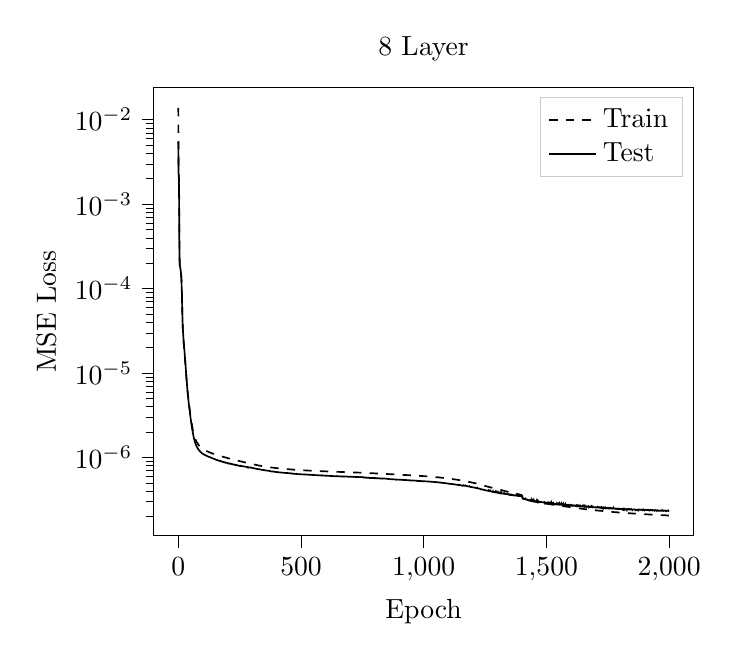
\begin{tikzpicture}

\begin{axis}[
legend cell align={left},
legend style={fill opacity=0.8, draw opacity=1, text opacity=1, draw=white!80!black},
log basis y={10},
tick align=outside,
tick pos=left,
title={8 Layer},
x grid style={white!69.0196078431373!black},
xlabel={Epoch},
xmin=-99.95, xmax=2098.95,
xtick style={color=black},
y grid style={white!69.0196078431373!black},
ylabel={MSE Loss},
ymin=1.18077084319194e-07, ymax=0.0240286142856456,
ymode=log,
ytick style={color=black}
]
\addplot [semithick, black, dashed]
table {%
0 0.0137857501469553
1 0.00308861960936338
2 0.00225937323644757
3 0.00184173461562023
4 0.000878539680619724
5 0.000267233489896171
6 0.000189525146357482
7 0.000177248529340432
8 0.000170382540301944
9 0.000163777170237154
10 0.000156803158293769
11 0.000148787730795448
12 0.000139447957270022
13 0.0001243273577129
14 0.000103127006572322
15 8.09196417794738e-05
16 6.05416532816889e-05
17 4.51169893822225e-05
18 3.565513092326e-05
19 3.03123355188291e-05
20 2.68081642607285e-05
21 2.43131255183471e-05
22 2.22995831736625e-05
23 2.05347641986009e-05
24 1.89343700831159e-05
25 1.74776983494667e-05
26 1.61251455356251e-05
27 1.48562264462271e-05
28 1.36716613037606e-05
29 1.25683485612171e-05
30 1.15524945263132e-05
31 1.06277352474535e-05
32 9.70658624783027e-06
33 8.84267294031815e-06
34 8.13857853154332e-06
35 7.58388431859203e-06
36 7.06517329012968e-06
37 6.48986769624571e-06
38 6.01962051950977e-06
39 5.62589393507551e-06
40 5.28921789339165e-06
41 4.98851873965123e-06
42 4.7175234600445e-06
43 4.47041639392864e-06
44 4.24115160376459e-06
45 4.02530521364497e-06
46 3.81863311099551e-06
47 3.62413326899969e-06
48 3.44267336078019e-06
49 3.26990401589455e-06
50 3.110896988062e-06
51 2.96396403069821e-06
52 2.82879928931834e-06
53 2.70368474275529e-06
54 2.58799466007531e-06
55 2.48464924226255e-06
56 2.39010867852585e-06
57 2.30290369552222e-06
58 2.2216036034024e-06
59 2.14735692520662e-06
60 2.07889566303265e-06
61 2.01642455289175e-06
62 1.95783670858418e-06
63 1.90416846038488e-06
64 1.85607089042605e-06
65 1.811010258848e-06
66 1.77054325018844e-06
67 1.7328962984493e-06
68 1.69725946949484e-06
69 1.66754056448326e-06
70 1.63858871133016e-06
71 1.61155683400693e-06
72 1.58789163265283e-06
73 1.56558429978304e-06
74 1.54554523152228e-06
75 1.52573656549748e-06
76 1.50784072388888e-06
77 1.49023391662695e-06
78 1.4743123068115e-06
79 1.45930793024718e-06
80 1.4446281097662e-06
81 1.43157341540245e-06
82 1.41939965010351e-06
83 1.40667576306441e-06
84 1.39518877335831e-06
85 1.38379590680415e-06
86 1.37327026897083e-06
87 1.36364018470658e-06
88 1.35418702711831e-06
89 1.34522714276386e-06
90 1.33634787925985e-06
91 1.32893943043655e-06
92 1.32093163441027e-06
93 1.3132997762284e-06
94 1.30623804824381e-06
95 1.29929187090738e-06
96 1.29237916951297e-06
97 1.28583184201148e-06
98 1.27959553714163e-06
99 1.2735283934262e-06
100 1.26791898730971e-06
101 1.2627259696103e-06
102 1.25771108588424e-06
103 1.25231368014056e-06
104 1.24631144498721e-06
105 1.24037334367699e-06
106 1.2340648443967e-06
107 1.22893064082064e-06
108 1.22437484989746e-06
109 1.21982722055236e-06
110 1.21481426256764e-06
111 1.2107418234848e-06
112 1.20602616044607e-06
113 1.20285992124991e-06
114 1.19859862485328e-06
115 1.19486205630892e-06
116 1.19111396352878e-06
117 1.18701774613328e-06
118 1.18387937891384e-06
119 1.18013333386102e-06
120 1.17652067552854e-06
121 1.17298610891226e-06
122 1.16920934786435e-06
123 1.16626488301108e-06
124 1.16285108117609e-06
125 1.15968924109211e-06
126 1.15640984193988e-06
127 1.15350303428841e-06
128 1.1503143885534e-06
129 1.14705221400868e-06
130 1.1443641856772e-06
131 1.14111493286373e-06
132 1.13798040635515e-06
133 1.13527754101028e-06
134 1.13251169233308e-06
135 1.12930856332127e-06
136 1.12650074075304e-06
137 1.1235084566863e-06
138 1.12072698141219e-06
139 1.1172398548922e-06
140 1.11442736803724e-06
141 1.11158048696325e-06
142 1.10887788622449e-06
143 1.10616437194722e-06
144 1.10341555770788e-06
145 1.10094259639482e-06
146 1.09825828815246e-06
147 1.09558834907375e-06
148 1.09296457605979e-06
149 1.09061500148755e-06
150 1.08795183314214e-06
151 1.08532106719395e-06
152 1.08324758190292e-06
153 1.08097435804666e-06
154 1.07827333013688e-06
155 1.07617651107716e-06
156 1.07380986366934e-06
157 1.07166150010585e-06
158 1.06948107162452e-06
159 1.06647956860684e-06
160 1.06494708404625e-06
161 1.06256772505731e-06
162 1.06035720727959e-06
163 1.05787372760346e-06
164 1.05588405099866e-06
165 1.05346232155057e-06
166 1.05166728118888e-06
167 1.04964814730124e-06
168 1.04769952940842e-06
169 1.04572185878737e-06
170 1.04260839512449e-06
171 1.04152885015196e-06
172 1.04000041307017e-06
173 1.03666240576672e-06
174 1.03516159231276e-06
175 1.03360050624701e-06
176 1.03188542567523e-06
177 1.02898213611979e-06
178 1.02803581077637e-06
179 1.02606050614895e-06
180 1.02454306204436e-06
181 1.02230507911827e-06
182 1.02055142943414e-06
183 1.01792596737482e-06
184 1.01660407779036e-06
185 1.01529137111811e-06
186 1.01237180382441e-06
187 1.01132905575696e-06
188 1.00956093092464e-06
189 1.00810563901632e-06
190 1.0052739773414e-06
191 1.00424275473188e-06
192 1.003211580894e-06
193 1.00131009619986e-06
194 9.98520134771752e-07
195 9.97664387540453e-07
196 9.94486084778146e-07
197 9.93778501651832e-07
198 9.90873338423626e-07
199 9.89912777669133e-07
200 9.88574339203296e-07
201 9.85725029522655e-07
202 9.84244386330602e-07
203 9.82002565308448e-07
204 9.78508168600456e-07
205 9.77044201306399e-07
206 9.76098156883154e-07
207 9.73493165162154e-07
208 9.71834136123562e-07
209 9.71276284246869e-07
210 9.68079569304336e-07
211 9.67498981026438e-07
212 9.64631265333082e-07
213 9.64166400649447e-07
214 9.61177288900217e-07
215 9.60805732916015e-07
216 9.57779043943674e-07
217 9.57766267873694e-07
218 9.54737937746586e-07
219 9.54498856344799e-07
220 9.52170370197791e-07
221 9.50519594084653e-07
222 9.48759981213243e-07
223 9.47102850858528e-07
224 9.46584362793601e-07
225 9.43646763801098e-07
226 9.42000673859411e-07
227 9.41450925949994e-07
228 9.38804523684666e-07
229 9.38322044589768e-07
230 9.35594229076742e-07
231 9.35247297007891e-07
232 9.32721268839032e-07
233 9.31552578464334e-07
234 9.30774605251372e-07
235 9.28317663891676e-07
236 9.26858944836795e-07
237 9.25179429543732e-07
238 9.23763715633186e-07
239 9.22354167357753e-07
240 9.20841406895079e-07
241 9.19228159915519e-07
242 9.17836204820333e-07
243 9.16312063225178e-07
244 9.14887535600428e-07
245 9.12851918116075e-07
246 9.12209820825183e-07
247 9.10882001278424e-07
248 9.09151504657757e-07
249 9.07929249365225e-07
250 9.06114797231794e-07
251 9.05019653970385e-07
252 9.03325363310614e-07
253 9.02047426535546e-07
254 9.00356864292462e-07
255 8.99421740939488e-07
256 8.9786664139524e-07
257 8.96162501391018e-07
258 8.94824077647627e-07
259 8.93166526680034e-07
260 8.92142999276757e-07
261 8.90646540653961e-07
262 8.89196897702504e-07
263 8.87752759098248e-07
264 8.86358454295078e-07
265 8.85122539898475e-07
266 8.83645790310084e-07
267 8.82326195210226e-07
268 8.80935579488096e-07
269 8.79514878278087e-07
270 8.78102829886984e-07
271 8.76637977967221e-07
272 8.75073412373695e-07
273 8.73695470517077e-07
274 8.7229220960694e-07
275 8.71096794639925e-07
276 8.69752706734062e-07
277 8.68293593612179e-07
278 8.66945744888881e-07
279 8.65692836129028e-07
280 8.6425307256377e-07
281 8.62996386615578e-07
282 8.61844596528272e-07
283 8.60314651902172e-07
284 8.58961779329093e-07
285 8.57684940086756e-07
286 8.56548996125639e-07
287 8.55367062882806e-07
288 8.53921339228236e-07
289 8.52381491938559e-07
290 8.5139164980319e-07
291 8.4983274942374e-07
292 8.48550058634601e-07
293 8.47121616715185e-07
294 8.45827474620364e-07
295 8.44044218467843e-07
296 8.42838108809474e-07
297 8.41480709709686e-07
298 8.40213770260334e-07
299 8.38855070696809e-07
300 8.37798641384779e-07
301 8.36651792894827e-07
302 8.35247779519932e-07
303 8.33991844217508e-07
304 8.3249875874003e-07
305 8.31112765837361e-07
306 8.29763220139057e-07
307 8.28537423330999e-07
308 8.27223779992892e-07
309 8.263019122694e-07
310 8.26237897740611e-07
311 8.24713217156159e-07
312 8.2334283979435e-07
313 8.22015577938373e-07
314 8.20726553371287e-07
315 8.19508391487034e-07
316 8.18137974590627e-07
317 8.17039462958746e-07
318 8.15745480878149e-07
319 8.14700765033649e-07
320 8.13773621985092e-07
321 8.12586493225354e-07
322 8.11482275494768e-07
323 8.10508947694188e-07
324 8.09030218846374e-07
325 8.08108718274525e-07
326 8.07103151188926e-07
327 8.06021113376687e-07
328 8.0490811670586e-07
329 8.03929369041612e-07
330 8.02840521885173e-07
331 8.01824190887146e-07
332 8.006422411313e-07
333 7.99249574953365e-07
334 7.98226580513983e-07
335 7.97378391467873e-07
336 7.96114629920908e-07
337 7.95464953313285e-07
338 7.94460564080168e-07
339 7.93411495550345e-07
340 7.92639923162142e-07
341 7.91717580995055e-07
342 7.90659596972887e-07
343 7.89734646772899e-07
344 7.88910815700206e-07
345 7.87838173835098e-07
346 7.87080269731177e-07
347 7.8613142619588e-07
348 7.85359551954912e-07
349 7.84582459175454e-07
350 7.83921955843425e-07
351 7.8297012908024e-07
352 7.82051770102043e-07
353 7.81296007033916e-07
354 7.80507885721704e-07
355 7.79689925153093e-07
356 7.78886507390553e-07
357 7.78194230775853e-07
358 7.77289544629411e-07
359 7.7656953261851e-07
360 7.75903502997721e-07
361 7.74936200443221e-07
362 7.74296334384417e-07
363 7.73721895654944e-07
364 7.72954912008572e-07
365 7.72319233249164e-07
366 7.71566827864945e-07
367 7.70699998838609e-07
368 7.70222717605407e-07
369 7.69374119812483e-07
370 7.68395611913775e-07
371 7.67787794430319e-07
372 7.67064833169684e-07
373 7.66419722197043e-07
374 7.66022498893904e-07
375 7.65052162719826e-07
376 7.64322403355777e-07
377 7.63627818059831e-07
378 7.63236719933502e-07
379 7.6248213609631e-07
380 7.62032572495741e-07
381 7.61118970331154e-07
382 7.60476678948407e-07
383 7.60098934165399e-07
384 7.592362803166e-07
385 7.586400048325e-07
386 7.58175735228406e-07
387 7.57343428460899e-07
388 7.56684466907131e-07
389 7.56365962160999e-07
390 7.55707249595616e-07
391 7.55030124281575e-07
392 7.54614512032958e-07
393 7.54073880841588e-07
394 7.53244257708729e-07
395 7.52822291843813e-07
396 7.52131151841695e-07
397 7.51477053313465e-07
398 7.50787530094499e-07
399 7.50268754131866e-07
400 7.49655679101124e-07
401 7.49106111442188e-07
402 7.48628529322559e-07
403 7.48065854992319e-07
404 7.47522233382369e-07
405 7.47014343886576e-07
406 7.4674312695322e-07
407 7.46154744589944e-07
408 7.45224265713773e-07
409 7.44781130833871e-07
410 7.44168451475957e-07
411 7.43612403141469e-07
412 7.43074742729277e-07
413 7.4255538692114e-07
414 7.41972566757454e-07
415 7.41491772316749e-07
416 7.40886318837397e-07
417 7.40458591266702e-07
418 7.40117279718788e-07
419 7.39657903153557e-07
420 7.3912421322575e-07
421 7.38795697401429e-07
422 7.38292617114666e-07
423 7.37599005930178e-07
424 7.37452366976754e-07
425 7.36602437115152e-07
426 7.36545854650217e-07
427 7.36174392713451e-07
428 7.35576475562993e-07
429 7.35150057053602e-07
430 7.34723915968516e-07
431 7.34193425984131e-07
432 7.33826684466976e-07
433 7.33313877120167e-07
434 7.32849924304446e-07
435 7.3240356381632e-07
436 7.31977483084734e-07
437 7.3147746320501e-07
438 7.31188059575061e-07
439 7.30770797602531e-07
440 7.3025388996939e-07
441 7.29911231729829e-07
442 7.29591046166433e-07
443 7.29134805823151e-07
444 7.28707190248201e-07
445 7.2811659848071e-07
446 7.2783998621162e-07
447 7.27755489791093e-07
448 7.26801464111304e-07
449 7.26691662777057e-07
450 7.26335354073626e-07
451 7.25658945043506e-07
452 7.25614078646686e-07
453 7.25175011581314e-07
454 7.24782964383053e-07
455 7.2419680768121e-07
456 7.2407520153206e-07
457 7.23398212727489e-07
458 7.23838310904057e-07
459 7.22997384855262e-07
460 7.22640464857705e-07
461 7.22022445884818e-07
462 7.21818079284731e-07
463 7.21388100032527e-07
464 7.20957314285897e-07
465 7.20499894029558e-07
466 7.20118750535903e-07
467 7.1978251421001e-07
468 7.19372024406084e-07
469 7.19226161493225e-07
470 7.18592157170406e-07
471 7.18292583542279e-07
472 7.17921304840274e-07
473 7.17656429145563e-07
474 7.17268838670293e-07
475 7.16870283014259e-07
476 7.16790947947743e-07
477 7.16224187868875e-07
478 7.15926577953496e-07
479 7.15506018508449e-07
480 7.15327944973865e-07
481 7.15154259026463e-07
482 7.14588176222719e-07
483 7.14167662749787e-07
484 7.13947983513208e-07
485 7.13584758472052e-07
486 7.13490786978355e-07
487 7.12802996346795e-07
488 7.1260814823404e-07
489 7.12203429642955e-07
490 7.12049823263783e-07
491 7.11565890298971e-07
492 7.11261462981838e-07
493 7.10956241448457e-07
494 7.10864853687099e-07
495 7.10524007445201e-07
496 7.10050566780751e-07
497 7.10148756851936e-07
498 7.09454082794991e-07
499 7.09290811926167e-07
500 7.08878859995821e-07
501 7.08592461123203e-07
502 7.08402716242063e-07
503 7.07911499688407e-07
504 7.07838705423569e-07
505 7.07405181373133e-07
506 7.07240273371212e-07
507 7.06922514538633e-07
508 7.06553931124176e-07
509 7.06358199010992e-07
510 7.05988017728032e-07
511 7.05820195491924e-07
512 7.05478267803983e-07
513 7.05317981612552e-07
514 7.04972263605441e-07
515 7.04692528387341e-07
516 7.04417077272978e-07
517 7.0408141230871e-07
518 7.03932418971931e-07
519 7.03659394588385e-07
520 7.03295456546016e-07
521 7.02983170214111e-07
522 7.02736174432061e-07
523 7.02738154330973e-07
524 7.02413211371322e-07
525 7.02195987742016e-07
526 7.01834438388005e-07
527 7.015176416445e-07
528 7.01357761215604e-07
529 7.01315112848988e-07
530 7.00866517291843e-07
531 7.00584499909951e-07
532 7.00379912302651e-07
533 7.00104224122811e-07
534 6.99711710453244e-07
535 6.99730678590527e-07
536 6.99416920937779e-07
537 6.99106589507892e-07
538 6.99099857314422e-07
539 6.98789812673795e-07
540 6.98547626143409e-07
541 6.9829937623922e-07
542 6.9803573740046e-07
543 6.97883229818785e-07
544 6.97516356922279e-07
545 6.97531738353518e-07
546 6.97229756156048e-07
547 6.96944444854353e-07
548 6.96735756392286e-07
549 6.96441722340069e-07
550 6.96331431043973e-07
551 6.95992913136934e-07
552 6.95820564317273e-07
553 6.95558284050435e-07
554 6.95345673136671e-07
555 6.9511123327004e-07
556 6.9492508868052e-07
557 6.94684943496782e-07
558 6.94408091291621e-07
559 6.94226875609161e-07
560 6.93976865377977e-07
561 6.93962414473503e-07
562 6.93575890437614e-07
563 6.93363744161957e-07
564 6.93089253118728e-07
565 6.92930680912696e-07
566 6.92638980467564e-07
567 6.92638060669992e-07
568 6.92431998800203e-07
569 6.92011693558925e-07
570 6.91779698058781e-07
571 6.91561712798716e-07
572 6.91245357501202e-07
573 6.90914098456119e-07
574 6.90786418317657e-07
575 6.90630641898338e-07
576 6.90921719240123e-07
577 6.90136385131268e-07
578 6.90016155033391e-07
579 6.89746223571319e-07
580 6.89630235626737e-07
581 6.89517517599825e-07
582 6.89564031830514e-07
583 6.8903582733526e-07
584 6.89009364705839e-07
585 6.88743238015377e-07
586 6.8840332086495e-07
587 6.88202743617694e-07
588 6.88021202506661e-07
589 6.87964407845243e-07
590 6.88042817529322e-07
591 6.87679688496701e-07
592 6.87582603731585e-07
593 6.87585936574919e-07
594 6.87160389531982e-07
595 6.86954137947282e-07
596 6.8681868329179e-07
597 6.86839983941923e-07
598 6.86604555980352e-07
599 6.86168778585738e-07
600 6.85818640121738e-07
601 6.85711275750123e-07
602 6.85531425304475e-07
603 6.85469083933299e-07
604 6.85334695788242e-07
605 6.84826699455243e-07
606 6.84622775608545e-07
607 6.84457398264726e-07
608 6.84304423188564e-07
609 6.84296297464471e-07
610 6.84731524756899e-07
611 6.83619167304528e-07
612 6.83459364040573e-07
613 6.83336111848121e-07
614 6.83173144011562e-07
615 6.83247643792129e-07
616 6.829115751259e-07
617 6.82785364645611e-07
618 6.82823477333727e-07
619 6.82156496722541e-07
620 6.82054949521671e-07
621 6.81831772880059e-07
622 6.81677918009882e-07
623 6.81486279333399e-07
624 6.81359977932061e-07
625 6.81108247150064e-07
626 6.81064127164177e-07
627 6.81072284521633e-07
628 6.80686871632474e-07
629 6.80564016704466e-07
630 6.80698681122749e-07
631 6.80240825744249e-07
632 6.80033357681964e-07
633 6.80167803238874e-07
634 6.79523233444002e-07
635 6.79397790690928e-07
636 6.79198196905872e-07
637 6.79049905556894e-07
638 6.79049523313324e-07
639 6.79142973154967e-07
640 6.78811062925888e-07
641 6.78329988289761e-07
642 6.78268604303867e-07
643 6.78312620792099e-07
644 6.77984985998137e-07
645 6.77676616234635e-07
646 6.77458028803812e-07
647 6.77593978508639e-07
648 6.77711388178182e-07
649 6.77032173726388e-07
650 6.7705669290774e-07
651 6.77168279509033e-07
652 6.76492063206524e-07
653 6.76391153575651e-07
654 6.76132728315793e-07
655 6.76058174207128e-07
656 6.76169795809756e-07
657 6.76121099218108e-07
658 6.75468571330384e-07
659 6.75345675475114e-07
660 6.75184716641297e-07
661 6.75026644856302e-07
662 6.74925118602232e-07
663 6.75125837290125e-07
664 6.74430557722872e-07
665 6.74353537561956e-07
666 6.74566049795544e-07
667 6.74105771835798e-07
668 6.73843414475073e-07
669 6.74108299563159e-07
670 6.73400757577269e-07
671 6.73219013251014e-07
672 6.73141517864906e-07
673 6.73084371044297e-07
674 6.73303882052778e-07
675 6.73119193351113e-07
676 6.72406169627493e-07
677 6.72221007633311e-07
678 6.72262872228657e-07
679 6.71918138493766e-07
680 6.7187868074825e-07
681 6.71670914556444e-07
682 6.71474687848672e-07
683 6.71449357596998e-07
684 6.71642237449532e-07
685 6.71132449625134e-07
686 6.70766620928021e-07
687 6.70696218847411e-07
688 6.70498978038836e-07
689 6.70508200329323e-07
690 6.70917440473318e-07
691 6.70120118655859e-07
692 6.69779609609122e-07
693 6.69663694836231e-07
694 6.69445325542029e-07
695 6.69258560876074e-07
696 6.69263294042821e-07
697 6.69365898531282e-07
698 6.69413571543487e-07
699 6.68658066985017e-07
700 6.6849241932232e-07
701 6.68295025889165e-07
702 6.68346391194063e-07
703 6.68034477683932e-07
704 6.67883314008577e-07
705 6.67871747751292e-07
706 6.67869822521539e-07
707 6.6741284337013e-07
708 6.67211375102283e-07
709 6.66998994347523e-07
710 6.67053436302467e-07
711 6.6682756991554e-07
712 6.66589114103999e-07
713 6.66490238728556e-07
714 6.66292823055414e-07
715 6.66251703336229e-07
716 6.66788175905708e-07
717 6.65793759552002e-07
718 6.65465117947406e-07
719 6.65816963035581e-07
720 6.65758463583188e-07
721 6.65544843045041e-07
722 6.65886225434065e-07
723 6.65198361417651e-07
724 6.64831936816768e-07
725 6.64645499369954e-07
726 6.64471501011121e-07
727 6.64225957706321e-07
728 6.64358892365158e-07
729 6.64192160570565e-07
730 6.64110347983637e-07
731 6.63900382065208e-07
732 6.63378257172553e-07
733 6.63277901182369e-07
734 6.63126197338215e-07
735 6.63272134914905e-07
736 6.63339513778283e-07
737 6.63178494576755e-07
738 6.62740552428431e-07
739 6.62412929628431e-07
740 6.62471505791018e-07
741 6.62118904955378e-07
742 6.6211564454477e-07
743 6.61732920079317e-07
744 6.61794542253347e-07
745 6.61537696160508e-07
746 6.6167947284157e-07
747 6.61282068222135e-07
748 6.60957793272132e-07
749 6.60974708708295e-07
750 6.60737628876973e-07
751 6.60563611177167e-07
752 6.60669549006343e-07
753 6.60142026859489e-07
754 6.59790588628084e-07
755 6.59206425495995e-07
756 6.58697558208132e-07
757 6.58472624053275e-07
758 6.58561325010965e-07
759 6.58079057743066e-07
760 6.58026551377589e-07
761 6.57965502142588e-07
762 6.57523861733012e-07
763 6.57337378598299e-07
764 6.56981951877356e-07
765 6.56761206968781e-07
766 6.56501978454571e-07
767 6.55857276768756e-07
768 6.56530517460396e-07
769 6.56905732810742e-07
770 6.56052742030511e-07
771 6.55603195994559e-07
772 6.55322380296752e-07
773 6.54704865823419e-07
774 6.54461226190506e-07
775 6.54197285342661e-07
776 6.53888960741256e-07
777 6.53602056658542e-07
778 6.53268098702142e-07
779 6.54040435051684e-07
780 6.53235653487627e-07
781 6.52853220628913e-07
782 6.52299065265538e-07
783 6.52097500406512e-07
784 6.51775928290022e-07
785 6.5176647149201e-07
786 6.51328027572617e-07
787 6.51507847905464e-07
788 6.51621266655411e-07
789 6.51120280338091e-07
790 6.50271066035657e-07
791 6.50623032598219e-07
792 6.50225028067553e-07
793 6.50682340662456e-07
794 6.49817614075232e-07
795 6.50719730501237e-07
796 6.49664923798809e-07
797 6.50211584300564e-07
798 6.48809363013925e-07
799 6.49380920918929e-07
800 6.4855317921797e-07
801 6.48718604878695e-07
802 6.48325270674377e-07
803 6.48340940912817e-07
804 6.48384094091625e-07
805 6.47670242756249e-07
806 6.47294677563082e-07
807 6.47407202379213e-07
808 6.47062250948238e-07
809 6.47139711901445e-07
810 6.46794424753239e-07
811 6.46586513980196e-07
812 6.4630621535855e-07
813 6.46143918785924e-07
814 6.46206421080819e-07
815 6.46050809052667e-07
816 6.45811578138478e-07
817 6.45534134704917e-07
818 6.45272071750469e-07
819 6.45084313475763e-07
820 6.44940158494478e-07
821 6.44797928664786e-07
822 6.44664317420052e-07
823 6.44708393238602e-07
824 6.44781474790079e-07
825 6.43953618663318e-07
826 6.4401244547696e-07
827 6.44133531608304e-07
828 6.43848811620273e-07
829 6.43534523021572e-07
830 6.43623536802807e-07
831 6.43355545122404e-07
832 6.43459978064698e-07
833 6.42539122694075e-07
834 6.42423720783825e-07
835 6.42229068049005e-07
836 6.43694028795494e-07
837 6.42312120220367e-07
838 6.42023174947326e-07
839 6.41817638097564e-07
840 6.41963917189514e-07
841 6.41126675986925e-07
842 6.41542135880968e-07
843 6.40884694462329e-07
844 6.40648684807843e-07
845 6.40480053760939e-07
846 6.39854228822401e-07
847 6.39868403069954e-07
848 6.39840600157981e-07
849 6.3893318502295e-07
850 6.38639376944639e-07
851 6.38337542994805e-07
852 6.38013974160856e-07
853 6.37820371764519e-07
854 6.38136522212562e-07
855 6.37338352333927e-07
856 6.36990881744737e-07
857 6.36761553366227e-07
858 6.36636442983729e-07
859 6.36787522850568e-07
860 6.36482686665829e-07
861 6.35810526496528e-07
862 6.35790216250598e-07
863 6.35545664792403e-07
864 6.35076302394566e-07
865 6.35354525677201e-07
866 6.35086437441146e-07
867 6.34891969426121e-07
868 6.33774776630958e-07
869 6.34218968521338e-07
870 6.33500820129029e-07
871 6.33716124205819e-07
872 6.33840579588707e-07
873 6.33507658463373e-07
874 6.32700088168292e-07
875 6.32751752640104e-07
876 6.32394511370649e-07
877 6.324811581635e-07
878 6.32187316163879e-07
879 6.31331189211437e-07
880 6.31645610027931e-07
881 6.30612103350359e-07
882 6.31642888585304e-07
883 6.30301115812415e-07
884 6.30303219345763e-07
885 6.30434531956325e-07
886 6.29825851213184e-07
887 6.3026594636284e-07
888 6.29491433983276e-07
889 6.29894949852883e-07
890 6.29112065524851e-07
891 6.2892201845699e-07
892 6.28567796532309e-07
893 6.28616281083794e-07
894 6.28783369236885e-07
895 6.28419824529658e-07
896 6.28173706630264e-07
897 6.2753141462224e-07
898 6.28429217087501e-07
899 6.27228162862536e-07
900 6.26573483586412e-07
901 6.25917755449734e-07
902 6.26262109051368e-07
903 6.26087741146364e-07
904 6.25708041049222e-07
905 6.25127507547063e-07
906 6.25702879716528e-07
907 6.25510647722649e-07
908 6.24522796002225e-07
909 6.25014120444689e-07
910 6.24146452096852e-07
911 6.24608488436706e-07
912 6.24371818311431e-07
913 6.24132697971902e-07
914 6.22939180331628e-07
915 6.2351004271477e-07
916 6.2332889153538e-07
917 6.23131349392736e-07
918 6.22394030202145e-07
919 6.22486220159146e-07
920 6.22470642809958e-07
921 6.22380071284567e-07
922 6.21532071036768e-07
923 6.21287593048692e-07
924 6.21170952555872e-07
925 6.21255831831036e-07
926 6.20757267839167e-07
927 6.20728286811811e-07
928 6.20359319391639e-07
929 6.20314215325379e-07
930 6.19811376125767e-07
931 6.19809856949871e-07
932 6.19194335051532e-07
933 6.19207079509465e-07
934 6.19016115749105e-07
935 6.18487976225879e-07
936 6.18693006728677e-07
937 6.18447636256292e-07
938 6.17691537371456e-07
939 6.1794909366597e-07
940 6.17617315015195e-07
941 6.17466598178851e-07
942 6.1694945669899e-07
943 6.16808603986385e-07
944 6.16357394129352e-07
945 6.16576176412309e-07
946 6.15661359837816e-07
947 6.15837455470114e-07
948 6.15222403098414e-07
949 6.15210279363509e-07
950 6.14131315380462e-07
951 6.14896761973682e-07
952 6.14312084110224e-07
953 6.13742194374822e-07
954 6.1423430738472e-07
955 6.13934294406704e-07
956 6.13463449120388e-07
957 6.13431861239633e-07
958 6.126252800982e-07
959 6.12680259457932e-07
960 6.12373812849398e-07
961 6.11732409318222e-07
962 6.11996258804481e-07
963 6.11834997698679e-07
964 6.11534490232657e-07
965 6.11279412410681e-07
966 6.10976991652024e-07
967 6.10801607635381e-07
968 6.0993121639541e-07
969 6.10257766908262e-07
970 6.09721131198171e-07
971 6.09514962107482e-07
972 6.10151406853277e-07
973 6.09608913990201e-07
974 6.08623257143392e-07
975 6.08609208669009e-07
976 6.07961926370138e-07
977 6.08075848290923e-07
978 6.07992424576764e-07
979 6.0775241048816e-07
980 6.07132156815737e-07
981 6.07294684876081e-07
982 6.06953180458447e-07
983 6.06453473309898e-07
984 6.05623692209178e-07
985 6.06061935386037e-07
986 6.05816325773389e-07
987 6.05566570953897e-07
988 6.05717543429307e-07
989 6.04947530575828e-07
990 6.04886406833316e-07
991 6.03998137073347e-07
992 6.0427891953907e-07
993 6.04073403579264e-07
994 6.03782304587242e-07
995 6.03477907574756e-07
996 6.03108307771549e-07
997 6.0244759085748e-07
998 6.02023152659115e-07
999 6.02464689706039e-07
1000 6.02305121390145e-07
1001 6.01802074946534e-07
1002 6.00690151784988e-07
1003 6.00747979532912e-07
1004 6.00759271186746e-07
1005 6.0054698502654e-07
1006 5.99763121869046e-07
1007 5.99490849140238e-07
1008 5.9974713006028e-07
1009 5.99658466896358e-07
1010 5.98812800596704e-07
1011 5.98873594029215e-07
1012 5.98376134469447e-07
1013 5.98230488101592e-07
1014 5.98133207567741e-07
1015 5.97380654419055e-07
1016 5.97340932856127e-07
1017 5.97020822851846e-07
1018 5.96662386726621e-07
1019 5.96547044061424e-07
1020 5.95986840195906e-07
1021 5.96448906740932e-07
1022 5.96114958746341e-07
1023 5.95908167888126e-07
1024 5.95399733924751e-07
1025 5.94854680898038e-07
1026 5.94013621309841e-07
1027 5.94053043350584e-07
1028 5.93657127041069e-07
1029 5.9312079419982e-07
1030 5.93351660242547e-07
1031 5.93160193432141e-07
1032 5.92637767212523e-07
1033 5.92132599592787e-07
1034 5.92207692520219e-07
1035 5.91352295039371e-07
1036 5.91074109657086e-07
1037 5.91294802873676e-07
1038 5.90296284478597e-07
1039 5.90281609348153e-07
1040 5.89172957631945e-07
1041 5.89864375598381e-07
1042 5.89333540624182e-07
1043 5.89092944501601e-07
1044 5.8811172851847e-07
1045 5.88118473984878e-07
1046 5.87558959523449e-07
1047 5.87498966091005e-07
1048 5.86975968829506e-07
1049 5.86538542663106e-07
1050 5.85390634384453e-07
1051 5.8604224697234e-07
1052 5.85704977417834e-07
1053 5.84833425804732e-07
1054 5.85203938186396e-07
1055 5.84576740706666e-07
1056 5.84105853000949e-07
1057 5.83624754902701e-07
1058 5.82899904443934e-07
1059 5.82916453005566e-07
1060 5.82865486791206e-07
1061 5.81442056130754e-07
1062 5.80942083999503e-07
1063 5.80710280317476e-07
1064 5.8016460865673e-07
1065 5.80148177206752e-07
1066 5.79519820348651e-07
1067 5.79282890541322e-07
1068 5.78339731006849e-07
1069 5.78075172036563e-07
1070 5.77422741336875e-07
1071 5.76988799444678e-07
1072 5.76913078944585e-07
1073 5.7649559715145e-07
1074 5.7592376823834e-07
1075 5.75118488846726e-07
1076 5.74859645261938e-07
1077 5.74464747032266e-07
1078 5.7391911401794e-07
1079 5.73786442799928e-07
1080 5.73293567576627e-07
1081 5.72705432531961e-07
1082 5.72505290044489e-07
1083 5.72218330383123e-07
1084 5.71506954933909e-07
1085 5.70766419834001e-07
1086 5.70619852211962e-07
1087 5.70089109672267e-07
1088 5.69310650618604e-07
1089 5.69087913817157e-07
1090 5.68740758041031e-07
1091 5.68193936842931e-07
1092 5.67973420743328e-07
1093 5.67342231157397e-07
1094 5.66961273946731e-07
1095 5.66632256052912e-07
1096 5.66003266825987e-07
1097 5.65674219494383e-07
1098 5.65259562122833e-07
1099 5.64769521723463e-07
1100 5.64369430676948e-07
1101 5.63613571578969e-07
1102 5.63189598679514e-07
1103 5.63041100242856e-07
1104 5.62284110486644e-07
1105 5.61835125878929e-07
1106 5.61412824893637e-07
1107 5.60981057205367e-07
1108 5.60571713556612e-07
1109 5.59922194639739e-07
1110 5.59530634561156e-07
1111 5.59002662015473e-07
1112 5.581992556003e-07
1113 5.57639288423673e-07
1114 5.57120050359572e-07
1115 5.56716404425117e-07
1116 5.56288290574969e-07
1117 5.55825715849778e-07
1118 5.55270240283789e-07
1119 5.5472401763268e-07
1120 5.5407207688063e-07
1121 5.53537679024885e-07
1122 5.52935819953859e-07
1123 5.52418589208514e-07
1124 5.5196548998282e-07
1125 5.5140549684296e-07
1126 5.50842811136931e-07
1127 5.50178398597723e-07
1128 5.49853654099763e-07
1129 5.49349440554181e-07
1130 5.48803564406342e-07
1131 5.48427744170965e-07
1132 5.47851732008553e-07
1133 5.47107029639449e-07
1134 5.46832161106181e-07
1135 5.46189866398095e-07
1136 5.45587667346581e-07
1137 5.45162206151417e-07
1138 5.4475243558727e-07
1139 5.43768126320288e-07
1140 5.43458325758195e-07
1141 5.42946222211071e-07
1142 5.42318003155628e-07
1143 5.41685208027332e-07
1144 5.41118284786535e-07
1145 5.40587837761564e-07
1146 5.40002958679509e-07
1147 5.3967720147341e-07
1148 5.3918130650743e-07
1149 5.38497736847887e-07
1150 5.37864707133906e-07
1151 5.37328203797927e-07
1152 5.36580279764109e-07
1153 5.36202094679083e-07
1154 5.35710694869351e-07
1155 5.35006929652582e-07
1156 5.34474729406043e-07
1157 5.33720529190873e-07
1158 5.33245014793238e-07
1159 5.32959159869506e-07
1160 5.33745327018664e-07
1161 5.32485687202211e-07
1162 5.31249801881017e-07
1163 5.30626741706897e-07
1164 5.2979573960954e-07
1165 5.29420067280739e-07
1166 5.28620816382386e-07
1167 5.27807401681457e-07
1168 5.27121304358502e-07
1169 5.26377595562622e-07
1170 5.25672054251913e-07
1171 5.24890954721968e-07
1172 5.2444793212203e-07
1173 5.23721696609414e-07
1174 5.23018498213901e-07
1175 5.2188551669019e-07
1176 5.21017574712346e-07
1177 5.20534954489449e-07
1178 5.19553454381594e-07
1179 5.18730347920382e-07
1180 5.17958713544431e-07
1181 5.17150383586795e-07
1182 5.16437501957512e-07
1183 5.15647556241561e-07
1184 5.15112535509843e-07
1185 5.14169199476555e-07
1186 5.13523359217061e-07
1187 5.12790095356763e-07
1188 5.1223551854207e-07
1189 5.11717524076971e-07
1190 5.10849785044343e-07
1191 5.10033092680828e-07
1192 5.09329841293038e-07
1193 5.08588952371269e-07
1194 5.07864471316566e-07
1195 5.07212841625915e-07
1196 5.06569104132382e-07
1197 5.05559155925539e-07
1198 5.05332368987865e-07
1199 5.04487800398579e-07
1200 5.03532473260293e-07
1201 5.03095116613395e-07
1202 5.02088503367304e-07
1203 5.01136403556757e-07
1204 5.00731445981728e-07
1205 4.99776320992851e-07
1206 4.99325033715081e-07
1207 4.98700373640304e-07
1208 4.97808630200325e-07
1209 4.96947417900628e-07
1210 4.96288867537942e-07
1211 4.95732484836253e-07
1212 4.94955880725456e-07
1213 4.94176946858715e-07
1214 4.93376584756788e-07
1215 4.92612390658564e-07
1216 4.920525770018e-07
1217 4.91067804333056e-07
1218 4.90369304714022e-07
1219 4.89532306190199e-07
1220 4.88886637128871e-07
1221 4.88063364329605e-07
1222 4.87359449877545e-07
1223 4.86462110629304e-07
1224 4.8582851755441e-07
1225 4.8509610044789e-07
1226 4.84401673972457e-07
1227 4.83254481267181e-07
1228 4.82487706861434e-07
1229 4.81833279323496e-07
1230 4.80243687633219e-07
1231 4.78414342282463e-07
1232 4.76838534240187e-07
1233 4.76149318657804e-07
1234 4.74790627791322e-07
1235 4.73768826594778e-07
1236 4.72720507829649e-07
1237 4.71855896634565e-07
1238 4.70534331853401e-07
1239 4.70113000531569e-07
1240 4.69121401650341e-07
1241 4.68302746483573e-07
1242 4.67329256736093e-07
1243 4.66545695545051e-07
1244 4.65720774428746e-07
1245 4.64882776356035e-07
1246 4.64056661272139e-07
1247 4.63339145298391e-07
1248 4.62453502805715e-07
1249 4.6154897869144e-07
1250 4.60787575832455e-07
1251 4.59998585000676e-07
1252 4.59476001552161e-07
1253 4.58542613344548e-07
1254 4.58008765320983e-07
1255 4.57043186344208e-07
1256 4.56172413777267e-07
1257 4.55492208899955e-07
1258 4.54621887328699e-07
1259 4.53731679030511e-07
1260 4.52947662239467e-07
1261 4.52175911945574e-07
1262 4.51259721572228e-07
1263 4.50436129000309e-07
1264 4.49572491348249e-07
1265 4.49066028352263e-07
1266 4.48156541779099e-07
1267 4.47460020353674e-07
1268 4.46502518983038e-07
1269 4.45779370750188e-07
1270 4.45073646687888e-07
1271 4.44745651066114e-07
1272 4.43919204570875e-07
1273 4.43130237655964e-07
1274 4.42290351216457e-07
1275 4.41504531295323e-07
1276 4.40815369401548e-07
1277 4.40169212268415e-07
1278 4.39142476835741e-07
1279 4.38690070765801e-07
1280 4.37918824530925e-07
1281 4.3708706678558e-07
1282 4.36362787709754e-07
1283 4.35320906618131e-07
1284 4.34962962970076e-07
1285 4.34124661254032e-07
1286 4.33472893078601e-07
1287 4.3270664316708e-07
1288 4.3223810664017e-07
1289 4.31506152210659e-07
1290 4.30598854350706e-07
1291 4.29677616750723e-07
1292 4.28937097368021e-07
1293 4.2827022625147e-07
1294 4.27427441493933e-07
1295 4.2679034957871e-07
1296 4.25909393555912e-07
1297 4.25184653096267e-07
1298 4.24548843795947e-07
1299 4.2362739712587e-07
1300 4.23001229847841e-07
1301 4.22171937557891e-07
1302 4.21529943849919e-07
1303 4.20893796700739e-07
1304 4.1996023799129e-07
1305 4.19370747252401e-07
1306 4.18629378344804e-07
1307 4.17800233435628e-07
1308 4.17327775906529e-07
1309 4.16702173822614e-07
1310 4.15864855156656e-07
1311 4.15330635235023e-07
1312 4.14520232155269e-07
1313 4.13829448135061e-07
1314 4.1304789226615e-07
1315 4.12341253692716e-07
1316 4.1216946509337e-07
1317 4.11018312902911e-07
1318 4.10335426906272e-07
1319 4.09523415214608e-07
1320 4.08610692858247e-07
1321 4.07992596990425e-07
1322 4.07032663076734e-07
1323 4.06648582554681e-07
1324 4.05807523293333e-07
1325 4.05085819707551e-07
1326 4.04363589808554e-07
1327 4.03830442820663e-07
1328 4.0298853319598e-07
1329 4.02449150698203e-07
1330 4.02263740824083e-07
1331 4.01028636716205e-07
1332 4.00283313709338e-07
1333 3.99633769589514e-07
1334 3.98941660137098e-07
1335 3.98408138792661e-07
1336 3.9767170837024e-07
1337 3.96993410618052e-07
1338 3.96322553143591e-07
1339 3.95798050206508e-07
1340 3.94935926777862e-07
1341 3.94421753668439e-07
1342 3.9375066577918e-07
1343 3.93084235483343e-07
1344 3.92502506613823e-07
1345 3.91987923293868e-07
1346 3.9124424080228e-07
1347 3.91049823832645e-07
1348 3.90322553116107e-07
1349 3.89593919820186e-07
1350 3.88722149352816e-07
1351 3.88301868838425e-07
1352 3.87433650871571e-07
1353 3.87444912661294e-07
1354 3.86126681021892e-07
1355 3.85559809302549e-07
1356 3.8492804539203e-07
1357 3.84593586048254e-07
1358 3.83902541258863e-07
1359 3.83004335461123e-07
1360 3.82602766521245e-07
1361 3.82011311558017e-07
1362 3.81463873210919e-07
1363 3.8110734190866e-07
1364 3.80366255839704e-07
1365 3.79705994987489e-07
1366 3.79158340081176e-07
1367 3.78491242940981e-07
1368 3.78047957042327e-07
1369 3.77540550999811e-07
1370 3.77056229396544e-07
1371 3.7643638771101e-07
1372 3.7545368427061e-07
1373 3.74841019990413e-07
1374 3.74239669682197e-07
1375 3.73709808172862e-07
1376 3.73041227035742e-07
1377 3.72869718347602e-07
1378 3.72220887982166e-07
1379 3.71513008502689e-07
1380 3.70764545507996e-07
1381 3.70413332248631e-07
1382 3.69776117224774e-07
1383 3.68990465801744e-07
1384 3.68179114161649e-07
1385 3.67674000202101e-07
1386 3.67139926510163e-07
1387 3.67087734161942e-07
1388 3.66082978302984e-07
1389 3.65367626926627e-07
1390 3.6481237800956e-07
1391 3.63644148123399e-07
1392 3.63287133581025e-07
1393 3.63036160877073e-07
1394 3.62126584448674e-07
1395 3.61699762649437e-07
1396 3.61027375987533e-07
1397 3.60369763242829e-07
1398 3.60007189115663e-07
1399 3.59295827124129e-07
1400 3.5775579875974e-07
1401 3.53868214730824e-07
1402 3.41379617296411e-07
1403 3.28579712345345e-07
1404 3.25548541511012e-07
1405 3.24216553693191e-07
1406 3.22977575535788e-07
1407 3.22425292083039e-07
1408 3.21560779539709e-07
1409 3.21061373725229e-07
1410 3.19967045953717e-07
1411 3.19681221583323e-07
1412 3.18886990186229e-07
1413 3.18288745347672e-07
1414 3.17631491043358e-07
1415 3.17402957406898e-07
1416 3.16448183653506e-07
1417 3.16011549529094e-07
1418 3.15193454127893e-07
1419 3.1478528707396e-07
1420 3.14031266398729e-07
1421 3.13261919700381e-07
1422 3.12983140958067e-07
1423 3.1251393924947e-07
1424 3.11998803240954e-07
1425 3.11705126065931e-07
1426 3.1094608770843e-07
1427 3.1091148596829e-07
1428 3.10241547680334e-07
1429 3.09736733072441e-07
1430 3.09197059110033e-07
1431 3.09091740660961e-07
1432 3.0816822710733e-07
1433 3.07916834699995e-07
1434 3.07206576749763e-07
1435 3.06838810715249e-07
1436 3.06620812068559e-07
1437 3.0611676983483e-07
1438 3.05473894016473e-07
1439 3.05116190560284e-07
1440 3.0515102234574e-07
1441 3.04555343959123e-07
1442 3.04196095541442e-07
1443 3.03736167268198e-07
1444 3.040585565941e-07
1445 3.0285602309732e-07
1446 3.02862596157638e-07
1447 3.02560588011147e-07
1448 3.02829190928833e-07
1449 3.01927896686038e-07
1450 3.01475552525687e-07
1451 3.00904842305272e-07
1452 3.00629884698367e-07
1453 3.00555958332893e-07
1454 3.00048228730532e-07
1455 2.99900297065392e-07
1456 2.99528309639641e-07
1457 2.99114135650314e-07
1458 2.98604760402554e-07
1459 2.98240277793127e-07
1460 2.97766990755122e-07
1461 2.98054582771101e-07
1462 2.97141440512405e-07
1463 2.96694996791302e-07
1464 2.96270484767547e-07
1465 2.96184018438339e-07
1466 2.95704940683095e-07
1467 2.95396794122382e-07
1468 2.95091585243767e-07
1469 2.94782432320062e-07
1470 2.94291698516247e-07
1471 2.93947373592118e-07
1472 2.93326942326644e-07
1473 2.93185483691616e-07
1474 2.93146487450713e-07
1475 2.92696370287615e-07
1476 2.92517656269808e-07
1477 2.92087966471399e-07
1478 2.91890827398333e-07
1479 2.91456780672661e-07
1480 2.91003376375443e-07
1481 2.90897139052504e-07
1482 2.90544493950051e-07
1483 2.90321684360606e-07
1484 2.89833084551105e-07
1485 2.89581516007331e-07
1486 2.89212358396185e-07
1487 2.88950256795317e-07
1488 2.88564842733763e-07
1489 2.88200527080562e-07
1490 2.87884401444671e-07
1491 2.87497334070963e-07
1492 2.8721040789037e-07
1493 2.86508051104306e-07
1494 2.86306328078467e-07
1495 2.86144508876873e-07
1496 2.85861089821537e-07
1497 2.85360442411786e-07
1498 2.85058979642372e-07
1499 2.84970874481871e-07
1500 2.84450102817857e-07
1501 2.84078861753301e-07
1502 2.83543574305156e-07
1503 2.83563822584654e-07
1504 2.82890254204915e-07
1505 2.82827177642275e-07
1506 2.82641763888591e-07
1507 2.82033121649761e-07
1508 2.82002064608378e-07
1509 2.81318216082127e-07
1510 2.81270375850795e-07
1511 2.8097148791062e-07
1512 2.80864460734165e-07
1513 2.80383226922254e-07
1514 2.80231873112768e-07
1515 2.79643016561693e-07
1516 2.79513022562128e-07
1517 2.79163273717131e-07
1518 2.7870598270141e-07
1519 2.78674357851116e-07
1520 2.78108519935927e-07
1521 2.78267315479752e-07
1522 2.77627101574751e-07
1523 2.77175951154618e-07
1524 2.77061909592646e-07
1525 2.76829202157103e-07
1526 2.7642390725191e-07
1527 2.76237728002116e-07
1528 2.75949262274366e-07
1529 2.75852835628143e-07
1530 2.75600234033391e-07
1531 2.74864786490525e-07
1532 2.74880136871047e-07
1533 2.74431400029584e-07
1534 2.74260290815675e-07
1535 2.73908545914026e-07
1536 2.73709271660039e-07
1537 2.73536457655155e-07
1538 2.73341923637815e-07
1539 2.73021322414024e-07
1540 2.72803043102954e-07
1541 2.72587641099165e-07
1542 2.72122814891418e-07
1543 2.71993649803903e-07
1544 2.71596017171305e-07
1545 2.71636295664734e-07
1546 2.71166804125755e-07
1547 2.70989261075272e-07
1548 2.70696542713722e-07
1549 2.70436283962283e-07
1550 2.70061753731454e-07
1551 2.6989989021331e-07
1552 2.69763729100703e-07
1553 2.69655354983911e-07
1554 2.69066596061407e-07
1555 2.68926969837935e-07
1556 2.68573427192109e-07
1557 2.68608412383742e-07
1558 2.67920140125e-07
1559 2.67861273933079e-07
1560 2.67640900844413e-07
1561 2.67677652011855e-07
1562 2.66964462625197e-07
1563 2.66822012484624e-07
1564 2.66567217181546e-07
1565 2.66555855290562e-07
1566 2.65938470718652e-07
1567 2.65836721510482e-07
1568 2.65485345245509e-07
1569 2.65497387978542e-07
1570 2.65124400584682e-07
1571 2.64794280695924e-07
1572 2.64446180700872e-07
1573 2.64363307621807e-07
1574 2.63953197340072e-07
1575 2.63414974881471e-07
1576 2.6352014254627e-07
1577 2.6342906294019e-07
1578 2.63256980119309e-07
1579 2.6275006576526e-07
1580 2.62603489957769e-07
1581 2.62322275212057e-07
1582 2.62190380972527e-07
1583 2.61826094835271e-07
1584 2.61762005067112e-07
1585 2.6165635841835e-07
1586 2.61387302224136e-07
1587 2.60961940504956e-07
1588 2.60710632772998e-07
1589 2.60395194366936e-07
1590 2.60170396778392e-07
1591 2.60418973766718e-07
1592 2.59962582262574e-07
1593 2.5969601419007e-07
1594 2.59373768479065e-07
1595 2.59266632525623e-07
1596 2.58953215023894e-07
1597 2.58385050443621e-07
1598 2.58312552205098e-07
1599 2.57958812120762e-07
1600 2.57778561035593e-07
1601 2.57694562435518e-07
1602 2.57359396975687e-07
1603 2.5705239291085e-07
1604 2.56811242699939e-07
1605 2.56461717242473e-07
1606 2.56126585846062e-07
1607 2.55749145210871e-07
1608 2.55653439175774e-07
1609 2.55513533744534e-07
1610 2.55211480364892e-07
1611 2.54804955659438e-07
1612 2.54763174751815e-07
1613 2.54787983493543e-07
1614 2.54455153722688e-07
1615 2.54169908593838e-07
1616 2.53858018467668e-07
1617 2.53570905002221e-07
1618 2.53653469627579e-07
1619 2.53107618163995e-07
1620 2.53153813460472e-07
1621 2.52625748231594e-07
1622 2.52780608676062e-07
1623 2.52202483792985e-07
1624 2.51898197333844e-07
1625 2.51692562230232e-07
1626 2.51686352093827e-07
1627 2.51284400277996e-07
1628 2.510466178407e-07
1629 2.50913202592074e-07
1630 2.50352099349982e-07
1631 2.50282909277644e-07
1632 2.50297362768492e-07
1633 2.49979243882592e-07
1634 2.49957796164324e-07
1635 2.49437291799381e-07
1636 2.49304088775659e-07
1637 2.49228307311e-07
1638 2.48961546077453e-07
1639 2.48945990243499e-07
1640 2.48505118250364e-07
1641 2.48237105296312e-07
1642 2.47971299991434e-07
1643 2.47875569947098e-07
1644 2.4794665956307e-07
1645 2.47326225185418e-07
1646 2.47498117275313e-07
1647 2.46912391794751e-07
1648 2.46693469193815e-07
1649 2.46549616903735e-07
1650 2.46913651224645e-07
1651 2.46156420679711e-07
1652 2.46014868004352e-07
1653 2.46031733666996e-07
1654 2.45937145464836e-07
1655 2.45421275380409e-07
1656 2.4518313143318e-07
1657 2.45077444105846e-07
1658 2.45103997855267e-07
1659 2.44453994220351e-07
1660 2.44352771495926e-07
1661 2.44336961486624e-07
1662 2.43957096735414e-07
1663 2.44000740032391e-07
1664 2.43840326682232e-07
1665 2.43737352008111e-07
1666 2.43350576539569e-07
1667 2.43003017637022e-07
1668 2.42828271026951e-07
1669 2.42498429528837e-07
1670 2.42299023938131e-07
1671 2.42565715481646e-07
1672 2.41789805663473e-07
1673 2.41731107983867e-07
1674 2.4149342952029e-07
1675 2.41314539678683e-07
1676 2.41171244880434e-07
1677 2.40871798965259e-07
1678 2.4079149969225e-07
1679 2.41200686303955e-07
1680 2.40602273073875e-07
1681 2.40352490664009e-07
1682 2.40002927021976e-07
1683 2.40169289128289e-07
1684 2.3982877031159e-07
1685 2.40364217468425e-07
1686 2.39530044183311e-07
1687 2.39584125388603e-07
1688 2.39088032536472e-07
1689 2.3960805847878e-07
1690 2.3883765531707e-07
1691 2.38823247961761e-07
1692 2.38320987165253e-07
1693 2.38512777499977e-07
1694 2.37777303709663e-07
1695 2.37730604681019e-07
1696 2.37934320814759e-07
1697 2.3772690016699e-07
1698 2.37244818436011e-07
1699 2.3747739219715e-07
1700 2.3734742929804e-07
1701 2.3705694976428e-07
1702 2.36548055816854e-07
1703 2.36903177189163e-07
1704 2.36646192711021e-07
1705 2.36336162600992e-07
1706 2.35978233178002e-07
1707 2.36257230675108e-07
1708 2.36247042479931e-07
1709 2.35572928225736e-07
1710 2.3533673609677e-07
1711 2.35295649972045e-07
1712 2.35212478422397e-07
1713 2.3516802806256e-07
1714 2.34991536999019e-07
1715 2.34667007468659e-07
1716 2.34174775656015e-07
1717 2.34407579718265e-07
1718 2.34413436089653e-07
1719 2.34040339790909e-07
1720 2.33942749389371e-07
1721 2.33983239716906e-07
1722 2.33622052000726e-07
1723 2.33831540683127e-07
1724 2.33392370176944e-07
1725 2.33173824241817e-07
1726 2.33226754893678e-07
1727 2.33077691788708e-07
1728 2.32529140163251e-07
1729 2.32279638076704e-07
1730 2.32233921138914e-07
1731 2.32112333932832e-07
1732 2.31883679987277e-07
1733 2.31720178788919e-07
1734 2.32038291564152e-07
1735 2.31718267492909e-07
1736 2.31567941852973e-07
1737 2.31331374052957e-07
1738 2.3112843035733e-07
1739 2.30873782498975e-07
1740 2.30605826487817e-07
1741 2.30518129541224e-07
1742 2.30432836758609e-07
1743 2.3033577322451e-07
1744 2.3007742373693e-07
1745 2.30224105777665e-07
1746 2.30077882129365e-07
1747 2.30050854852948e-07
1748 2.29575847257024e-07
1749 2.2943226482397e-07
1750 2.29557112618295e-07
1751 2.29237574053798e-07
1752 2.29205479875816e-07
1753 2.29170308109872e-07
1754 2.28906373244797e-07
1755 2.28766571844119e-07
1756 2.28544766940786e-07
1757 2.2868126626463e-07
1758 2.27993804685411e-07
1759 2.27960802689608e-07
1760 2.27839590941414e-07
1761 2.27652181507665e-07
1762 2.27542316004303e-07
1763 2.27493458346828e-07
1764 2.27313096146986e-07
1765 2.27199244683618e-07
1766 2.27071835674053e-07
1767 2.27219710694726e-07
1768 2.26996866189211e-07
1769 2.26775318253658e-07
1770 2.26718550969451e-07
1771 2.26813940585657e-07
1772 2.26520079387171e-07
1773 2.26371451148566e-07
1774 2.26167481315542e-07
1775 2.25901802842543e-07
1776 2.25779298538953e-07
1777 2.25720340743862e-07
1778 2.25585753618418e-07
1779 2.25394293686065e-07
1780 2.25186369284813e-07
1781 2.24958091202154e-07
1782 2.24947849019941e-07
1783 2.24971209469516e-07
1784 2.24907599303492e-07
1785 2.24740581238336e-07
1786 2.24558846355194e-07
1787 2.24479246575982e-07
1788 2.24269736492033e-07
1789 2.24457478637419e-07
1790 2.23911447562841e-07
1791 2.23885244651001e-07
1792 2.23665631779113e-07
1793 2.23567293865301e-07
1794 2.23408093113164e-07
1795 2.23337343705055e-07
1796 2.23331608850685e-07
1797 2.23211972425474e-07
1798 2.23090034204176e-07
1799 2.22974817511101e-07
1800 2.23243140624163e-07
1801 2.22694968101678e-07
1802 2.22525880616331e-07
1803 2.22527042673448e-07
1804 2.22235511778024e-07
1805 2.22254597375127e-07
1806 2.22211922931592e-07
1807 2.22038266279867e-07
1808 2.22010197184375e-07
1809 2.22046008950372e-07
1810 2.21756733864709e-07
1811 2.21639085218328e-07
1812 2.21576202640961e-07
1813 2.2141506143214e-07
1814 2.21208061695677e-07
1815 2.21245883274435e-07
1816 2.21013788902269e-07
1817 2.21007236611115e-07
1818 2.20982161629024e-07
1819 2.21036623258897e-07
1820 2.20792780325496e-07
1821 2.20643940423315e-07
1822 2.20531014043956e-07
1823 2.20327503903661e-07
1824 2.20266067884722e-07
1825 2.20109437663041e-07
1826 2.20157255810705e-07
1827 2.19891945270945e-07
1828 2.19910469645868e-07
1829 2.19544526203208e-07
1830 2.19702533073018e-07
1831 2.19582152304554e-07
1832 2.19451375329527e-07
1833 2.19306615527159e-07
1834 2.19331069985174e-07
1835 2.18993384471844e-07
1836 2.19311624746865e-07
1837 2.18863029182614e-07
1838 2.18719483584096e-07
1839 2.1868493919186e-07
1840 2.18531250474996e-07
1841 2.18609444459617e-07
1842 2.18387314674828e-07
1843 2.18589027149108e-07
1844 2.18275262263035e-07
1845 2.18104250727436e-07
1846 2.18145190771679e-07
1847 2.17859501219664e-07
1848 2.17956179199064e-07
1849 2.17677949535755e-07
1850 2.17680827518052e-07
1851 2.17496870781986e-07
1852 2.17543898799022e-07
1853 2.17346247204375e-07
1854 2.17274957748259e-07
1855 2.17114544454944e-07
1856 2.17218183117041e-07
1857 2.17002188492188e-07
1858 2.17044254824827e-07
1859 2.16837378872015e-07
1860 2.16830454448313e-07
1861 2.16572191611419e-07
1862 2.16502173238098e-07
1863 2.1663202711153e-07
1864 2.16744778583688e-07
1865 2.16451098282278e-07
1866 2.16251673386125e-07
1867 2.16361901465234e-07
1868 2.1619253545424e-07
1869 2.15748911813307e-07
1870 2.15781792213932e-07
1871 2.15753512151196e-07
1872 2.15870599582502e-07
1873 2.15580016394767e-07
1874 2.15546139990863e-07
1875 2.15363809992652e-07
1876 2.15192065219583e-07
1877 2.15214828294563e-07
1878 2.15056860753293e-07
1879 2.14895314861963e-07
1880 2.14862649194458e-07
1881 2.14835938393776e-07
1882 2.14952394046009e-07
1883 2.14837238630139e-07
1884 2.14968138479321e-07
1885 2.14349865757413e-07
1886 2.14499318161643e-07
1887 2.14418838048402e-07
1888 2.14321352871139e-07
1889 2.14236844541915e-07
1890 2.13926508664031e-07
1891 2.13951539805635e-07
1892 2.1386986568217e-07
1893 2.14016840480724e-07
1894 2.13743024914947e-07
1895 2.13656738431212e-07
1896 2.13609864360365e-07
1897 2.13321337959371e-07
1898 2.13654979923206e-07
1899 2.13477472989609e-07
1900 2.13193983711335e-07
1901 2.13337714185968e-07
1902 2.13059026258122e-07
1903 2.13127699112192e-07
1904 2.12952673969369e-07
1905 2.12747189493712e-07
1906 2.12548494687326e-07
1907 2.12635293713959e-07
1908 2.12583282369394e-07
1909 2.1251817032919e-07
1910 2.12349659655331e-07
1911 2.1230279109119e-07
1912 2.1227749432029e-07
1913 2.12181868263883e-07
1914 2.12258335267279e-07
1915 2.11983677516514e-07
1916 2.12110384183006e-07
1917 2.11937834038167e-07
1918 2.11879030395323e-07
1919 2.11724512972467e-07
1920 2.1171065207426e-07
1921 2.11468209251109e-07
1922 2.11367545965402e-07
1923 2.11558452598126e-07
1924 2.11234478520339e-07
1925 2.11444637699287e-07
1926 2.11205904605549e-07
1927 2.11092604907037e-07
1928 2.11008436089344e-07
1929 2.11081963037429e-07
1930 2.10939091346063e-07
1931 2.10611467700517e-07
1932 2.10756167959403e-07
1933 2.1079672516322e-07
1934 2.10806285565468e-07
1935 2.10525705782061e-07
1936 2.10441943593764e-07
1937 2.10486054513126e-07
1938 2.10354152585523e-07
1939 2.10237939441527e-07
1940 2.09964359129344e-07
1941 2.09949239419416e-07
1942 2.09824008138071e-07
1943 2.09825059066304e-07
1944 2.09793111508816e-07
1945 2.09700543585711e-07
1946 2.09754597442213e-07
1947 2.09670173497045e-07
1948 2.0964833478132e-07
1949 2.09404227710763e-07
1950 2.09431415065353e-07
1951 2.0933758854369e-07
1952 2.09240786993803e-07
1953 2.09373009319336e-07
1954 2.08994799500317e-07
1955 2.09158107217888e-07
1956 2.08914607270572e-07
1957 2.08826088233138e-07
1958 2.08633518951729e-07
1959 2.08776670888255e-07
1960 2.08618614117029e-07
1961 2.0859886277691e-07
1962 2.08522925710497e-07
1963 2.08265814485742e-07
1964 2.08158993729057e-07
1965 2.0817488879743e-07
1966 2.0809151187251e-07
1967 2.08064630996319e-07
1968 2.0800519364883e-07
1969 2.07907418079856e-07
1970 2.07734938754811e-07
1971 2.07863039548783e-07
1972 2.07707496642229e-07
1973 2.07824264585099e-07
1974 2.07635781336535e-07
1975 2.07450170435663e-07
1976 2.0741758948617e-07
1977 2.07326376830963e-07
1978 2.0727377776808e-07
1979 2.07235073858669e-07
1980 2.07186273755156e-07
1981 2.07117118776523e-07
1982 2.0703223926688e-07
1983 2.06995867870319e-07
1984 2.06980355002884e-07
1985 2.06818433952094e-07
1986 2.06886384596316e-07
1987 2.06680300223638e-07
1988 2.06672409454711e-07
1989 2.06529951896073e-07
1990 2.06364807368686e-07
1991 2.06279887251526e-07
1992 2.0620779382341e-07
1993 2.06011688796082e-07
1994 2.0618447984333e-07
1995 2.0597208754225e-07
1996 2.0588623802098e-07
1997 2.05808801467811e-07
1998 2.05898638348856e-07
1999 2.05915041661342e-07
};
\addlegendentry{Train}
\addplot [semithick, black]
table {%
0 0.00545290252193809
1 0.0023266056086868
2 0.00213515129871666
3 0.0014157728292048
4 0.000410291773732752
5 0.000212521030334756
6 0.000190788457985036
7 0.000183048061444424
8 0.000176143643329851
9 0.000169325852766633
10 0.000161589094204828
11 0.000152619570144452
12 0.000141753058414906
13 0.000121109485917259
14 9.81760822469369e-05
15 7.54592983867042e-05
16 5.62838613404892e-05
17 4.32986780651845e-05
18 3.58362085535191e-05
19 3.13278542307671e-05
20 2.81511838693405e-05
21 2.57360643445281e-05
22 2.36443611356663e-05
23 2.17338802031009e-05
24 2.00070007849718e-05
25 1.84041437023552e-05
26 1.689850614639e-05
27 1.5482781236642e-05
28 1.41530126711586e-05
29 1.29242907860316e-05
30 1.18076804938028e-05
31 1.07529313027044e-05
32 9.72076668404043e-06
33 8.84199744177749e-06
34 8.15555267763557e-06
35 7.60991133574862e-06
36 6.93214678904042e-06
37 6.34968409940484e-06
38 5.87008207730833e-06
39 5.46938144907472e-06
40 5.12396627527778e-06
41 4.81088591186563e-06
42 4.53635993835633e-06
43 4.2803903852473e-06
44 4.04217689720099e-06
45 3.82559846912045e-06
46 3.61594788955699e-06
47 3.42828843713505e-06
48 3.25095720654645e-06
49 3.08387575387314e-06
50 2.93283324026561e-06
51 2.79320988738618e-06
52 2.65996595771867e-06
53 2.53490998147754e-06
54 2.42584314946725e-06
55 2.31981516662927e-06
56 2.22306312025466e-06
57 2.135601334885e-06
58 2.05362357519334e-06
59 1.97951840164023e-06
60 1.91189792531077e-06
61 1.8435728179611e-06
62 1.78373568360257e-06
63 1.73281296156347e-06
64 1.6810982970128e-06
65 1.63556671850529e-06
66 1.59371120389551e-06
67 1.55521115630108e-06
68 1.52398138197896e-06
69 1.49048457842582e-06
70 1.46019203839387e-06
71 1.43245529216074e-06
72 1.40674342219427e-06
73 1.38512632474885e-06
74 1.37241966058355e-06
75 1.35226548536593e-06
76 1.33385049139179e-06
77 1.31669241909549e-06
78 1.3001736078877e-06
79 1.28582246361475e-06
80 1.27185080600611e-06
81 1.25796304928372e-06
82 1.24765301734442e-06
83 1.23596134926629e-06
84 1.22478309094731e-06
85 1.21430900890118e-06
86 1.20441939088778e-06
87 1.1951461829085e-06
88 1.18600303267158e-06
89 1.17842034796922e-06
90 1.16994829113537e-06
91 1.16215221623861e-06
92 1.15464808914112e-06
93 1.14744250367949e-06
94 1.14050396859966e-06
95 1.13397800305393e-06
96 1.12736154278537e-06
97 1.1219150337638e-06
98 1.11617839593237e-06
99 1.11055123852566e-06
100 1.10428436528309e-06
101 1.099929704651e-06
102 1.09671827885904e-06
103 1.09289078409347e-06
104 1.08809376797581e-06
105 1.08510903373826e-06
106 1.08004962839914e-06
107 1.07730784293381e-06
108 1.07301877960708e-06
109 1.06946436062572e-06
110 1.06532627341949e-06
111 1.06181403225492e-06
112 1.05836693364836e-06
113 1.05506535419408e-06
114 1.05125116078852e-06
115 1.04815103441069e-06
116 1.04494552033429e-06
117 1.04213427221111e-06
118 1.03922991456784e-06
119 1.03576292076468e-06
120 1.03284810393234e-06
121 1.02973024240782e-06
122 1.0268323649143e-06
123 1.02429930848302e-06
124 1.02109629551705e-06
125 1.01827993148618e-06
126 1.01537966656906e-06
127 1.01420994269574e-06
128 1.01010982689331e-06
129 1.00738623132202e-06
130 1.0047942851088e-06
131 1.00281795312185e-06
132 1.00005240710743e-06
133 9.9704368494713e-07
134 9.94117840491526e-07
135 9.92156742540828e-07
136 9.89238515103352e-07
137 9.8655209512799e-07
138 9.83898303275055e-07
139 9.81608081929153e-07
140 9.79194737737998e-07
141 9.75912826106651e-07
142 9.73706960394338e-07
143 9.7080430805363e-07
144 9.67710093391361e-07
145 9.64837113315298e-07
146 9.62111926128273e-07
147 9.60053739618161e-07
148 9.57607994678256e-07
149 9.55455334405997e-07
150 9.52439222601242e-07
151 9.49674301864434e-07
152 9.47469459333661e-07
153 9.45233921356703e-07
154 9.42940062031994e-07
155 9.40317022468662e-07
156 9.37940569656348e-07
157 9.35726234274625e-07
158 9.32079558424448e-07
159 9.32240482143243e-07
160 9.29431223539723e-07
161 9.27131225125777e-07
162 9.25108963656385e-07
163 9.22836193240073e-07
164 9.20701950235525e-07
165 9.18571743113716e-07
166 9.1653021172533e-07
167 9.1469149765544e-07
168 9.11959375571314e-07
169 9.08875676941534e-07
170 9.11160384475806e-07
171 9.08082881778682e-07
172 9.03431214283046e-07
173 9.06380250853545e-07
174 9.01317491752707e-07
175 8.9896263943956e-07
176 8.96176061360165e-07
177 8.98884422895208e-07
178 8.96814071893459e-07
179 8.95787934496184e-07
180 8.90062665348523e-07
181 8.8801903075364e-07
182 8.86083284967754e-07
183 8.88968656909128e-07
184 8.8491037786298e-07
185 8.79909293871606e-07
186 8.83470363532979e-07
187 8.79027140854305e-07
188 8.76825197337894e-07
189 8.73556359692884e-07
190 8.77249817676784e-07
191 8.73542774115776e-07
192 8.69007124038035e-07
193 8.70745168413123e-07
194 8.6927383335933e-07
195 8.65830202201323e-07
196 8.66813763877872e-07
197 8.65223910295754e-07
198 8.65343565692456e-07
199 8.63232571646222e-07
200 8.59066119573981e-07
201 8.6080262917676e-07
202 8.58512976265047e-07
203 8.53314816140482e-07
204 8.55455709825037e-07
205 8.53785707022325e-07
206 8.49354989895801e-07
207 8.52364507863967e-07
208 8.50142555464117e-07
209 8.46311422719737e-07
210 8.4794891108686e-07
211 8.44281544232217e-07
212 8.45526699322363e-07
213 8.41456255784578e-07
214 8.42289637148497e-07
215 8.3898174807473e-07
216 8.39697861465538e-07
217 8.36104049994901e-07
218 8.37363586470019e-07
219 8.33189119475719e-07
220 8.33541150768724e-07
221 8.32260582228628e-07
222 8.31093473152578e-07
223 8.29913346933608e-07
224 8.26314078494761e-07
225 8.24172957436531e-07
226 8.266484314845e-07
227 8.22245681320055e-07
228 8.24394078335899e-07
229 8.20174932414375e-07
230 8.21676394480164e-07
231 8.19751448943862e-07
232 8.17600550817588e-07
233 8.18929095203202e-07
234 8.14558745787508e-07
235 8.15629562112008e-07
236 8.12827863683196e-07
237 8.14598877241224e-07
238 8.10266840289842e-07
239 8.12092139312881e-07
240 8.07582466677559e-07
241 8.06569687483716e-07
242 8.05487502475444e-07
243 8.04439650892164e-07
244 8.02184729309374e-07
245 8.03753266609419e-07
246 8.01033991137956e-07
247 8.00644329501665e-07
248 7.98470637164428e-07
249 7.98045675765024e-07
250 7.95695939359575e-07
251 7.96012784576305e-07
252 7.93840911228472e-07
253 7.92932894455589e-07
254 7.99726137756807e-07
255 7.97536699792545e-07
256 7.9637828775958e-07
257 7.9514381923218e-07
258 7.93691469880287e-07
259 7.92549712969048e-07
260 7.91949048561946e-07
261 7.90351464274863e-07
262 7.89906266618345e-07
263 7.88357112924132e-07
264 7.87908049915131e-07
265 7.86467808211455e-07
266 7.8583883578176e-07
267 7.84067367476382e-07
268 7.83190898800967e-07
269 7.82696929491067e-07
270 7.81262031068763e-07
271 7.80052346271987e-07
272 7.80344180384418e-07
273 7.79255685756652e-07
274 7.78398316469975e-07
275 7.7718851798636e-07
276 7.76482295350434e-07
277 7.7534531328638e-07
278 7.74429565808532e-07
279 7.73831459355279e-07
280 7.73414683408191e-07
281 7.72132750626042e-07
282 7.70859628573817e-07
283 7.65755316933792e-07
284 7.60040165914688e-07
285 7.6867144116477e-07
286 7.6819742389489e-07
287 7.66913956340431e-07
288 7.65923687140457e-07
289 7.64631579386332e-07
290 7.6424248618423e-07
291 7.62679974286584e-07
292 7.61422882078477e-07
293 7.63743344123213e-07
294 7.60434716085001e-07
295 7.59350712087326e-07
296 7.58960084112914e-07
297 7.57293321385077e-07
298 7.56752513098036e-07
299 7.56100291710027e-07
300 7.547943141617e-07
301 7.54836037231144e-07
302 7.5402886068332e-07
303 7.53300753331132e-07
304 7.51386835418089e-07
305 7.50217452605284e-07
306 7.48964851027267e-07
307 7.48231798297638e-07
308 7.46197088119516e-07
309 7.46279283703188e-07
310 7.44167550692509e-07
311 7.42736119718757e-07
312 7.41974929496791e-07
313 7.40465623039199e-07
314 7.39693291507137e-07
315 7.38051141979668e-07
316 7.37358220703754e-07
317 7.36179060822906e-07
318 7.34689365344821e-07
319 7.3422683044555e-07
320 7.3301083602928e-07
321 7.32796138436242e-07
322 7.34363652554748e-07
323 7.31105785689579e-07
324 7.30252622815897e-07
325 7.29460623460909e-07
326 7.28848874587129e-07
327 7.28102634184324e-07
328 7.27363214991783e-07
329 7.25585778127424e-07
330 7.25738800610998e-07
331 7.26057407973713e-07
332 7.23037885563826e-07
333 7.21743219855853e-07
334 7.23185678452865e-07
335 7.19886486422183e-07
336 7.19306910923478e-07
337 7.18626495199715e-07
338 7.17854049980815e-07
339 7.17089164936624e-07
340 7.16326042038418e-07
341 7.15051100996789e-07
342 7.13832491783251e-07
343 7.12931807811401e-07
344 7.12334440322593e-07
345 7.11622817561874e-07
346 7.11278175913321e-07
347 7.10306608198152e-07
348 7.09811786236969e-07
349 7.11279938059306e-07
350 7.08268146354385e-07
351 7.07583694747882e-07
352 7.07011736267305e-07
353 7.06253274529445e-07
354 7.05259594724339e-07
355 7.04499143466819e-07
356 7.03719081229792e-07
357 7.03026216797298e-07
358 7.02557599652209e-07
359 7.01623548593489e-07
360 7.00906184647465e-07
361 7.00190014413238e-07
362 6.99776137480512e-07
363 6.99556096606102e-07
364 6.98585381542216e-07
365 6.9796993784621e-07
366 6.97261725690623e-07
367 6.99188262842654e-07
368 6.95628955327265e-07
369 6.94950472279743e-07
370 6.9424356752279e-07
371 6.93555193720385e-07
372 6.92852438533009e-07
373 6.92171965965827e-07
374 6.9069432129254e-07
375 6.89652495111659e-07
376 6.88118404923443e-07
377 6.8726382096429e-07
378 6.86377575220831e-07
379 6.85503607655846e-07
380 6.8448548518063e-07
381 6.83920006849803e-07
382 6.83083499097847e-07
383 6.84049155097455e-07
384 6.83072642004845e-07
385 6.82362156112504e-07
386 6.81618757880642e-07
387 6.8105799755358e-07
388 6.8284236931504e-07
389 6.79476443110616e-07
390 6.78799324305146e-07
391 6.7815244619851e-07
392 6.77845548580081e-07
393 6.7688256422116e-07
394 6.76380921049713e-07
395 6.75689136642177e-07
396 6.75101830438507e-07
397 6.74114460252895e-07
398 6.73615545565553e-07
399 6.73901240588748e-07
400 6.72695762204967e-07
401 6.72247892907762e-07
402 6.71928603424021e-07
403 6.71328791668202e-07
404 6.70939130031911e-07
405 6.69477344672487e-07
406 6.71449413403025e-07
407 6.69191194901941e-07
408 6.68752818455687e-07
409 6.68569953177212e-07
410 6.68404140924395e-07
411 6.67407562104927e-07
412 6.6751169924828e-07
413 6.66729363274499e-07
414 6.65977097469295e-07
415 6.65666050281288e-07
416 6.65311461034435e-07
417 6.64649917325733e-07
418 6.64477511236328e-07
419 6.647004511251e-07
420 6.6377134544382e-07
421 6.63081834773038e-07
422 6.63052787786e-07
423 6.62266018025548e-07
424 6.62137495055504e-07
425 6.61343506180856e-07
426 6.61542742363963e-07
427 6.61179512917442e-07
428 6.60141040498274e-07
429 6.60491707549227e-07
430 6.60130638152623e-07
431 6.59555723814265e-07
432 6.59391389490338e-07
433 6.58980411571974e-07
434 6.58071940051741e-07
435 6.58389296859241e-07
436 6.57987527574733e-07
437 6.56790803077456e-07
438 6.57215821320278e-07
439 6.56909946883388e-07
440 6.56719976177556e-07
441 6.56668589726905e-07
442 6.5640790580801e-07
443 6.55567191643058e-07
444 6.54515929454647e-07
445 6.54193570426287e-07
446 6.56843781143834e-07
447 6.53864674404758e-07
448 6.53301640340942e-07
449 6.5313406594214e-07
450 6.5277481553494e-07
451 6.5202783616769e-07
452 6.52458425065561e-07
453 6.51807567919604e-07
454 6.5159122186742e-07
455 6.5107531099784e-07
456 6.51123741590709e-07
457 6.50599531581975e-07
458 6.49443961719953e-07
459 6.48274181003217e-07
460 6.47570630007976e-07
461 6.46804664938827e-07
462 6.49052708467934e-07
463 6.45696445644717e-07
464 6.45135514787398e-07
465 6.44291105800221e-07
466 6.43622058760229e-07
467 6.43751491224975e-07
468 6.42865359168354e-07
469 6.42117015559052e-07
470 6.41737983642088e-07
471 6.41614292362647e-07
472 6.41441090465378e-07
473 6.4141454458877e-07
474 6.41175120108528e-07
475 6.40506129911955e-07
476 6.39838845017948e-07
477 6.39653990219813e-07
478 6.39815482372796e-07
479 6.41032727344282e-07
480 6.38866424651496e-07
481 6.38831011201546e-07
482 6.38149401765986e-07
483 6.3791719639994e-07
484 6.37861091945524e-07
485 6.37615926279977e-07
486 6.36900097106263e-07
487 6.36524930541782e-07
488 6.365310127876e-07
489 6.36269589904259e-07
490 6.35659432646207e-07
491 6.35828826034412e-07
492 6.35466619769431e-07
493 6.35307401353202e-07
494 6.34728337445267e-07
495 6.34790467302082e-07
496 6.35972526197293e-07
497 6.34012621958391e-07
498 6.33850447684381e-07
499 6.33540821581846e-07
500 6.33391721294174e-07
501 6.33164347618731e-07
502 6.32965452496137e-07
503 6.3221284563042e-07
504 6.32333751582337e-07
505 6.32154183222156e-07
506 6.31997920663707e-07
507 6.31769921710656e-07
508 6.31397767847375e-07
509 6.31238776804821e-07
510 6.30889928743272e-07
511 6.30743727469962e-07
512 6.32443459380738e-07
513 6.3013061435413e-07
514 6.29995042800147e-07
515 6.2981672499518e-07
516 6.29599128387781e-07
517 6.29721682798845e-07
518 6.29218220637995e-07
519 6.28705720373546e-07
520 6.2858026694812e-07
521 6.28379609679541e-07
522 6.28293662430224e-07
523 6.2809175460643e-07
524 6.27842211997631e-07
525 6.27398890173936e-07
526 6.2723250948693e-07
527 6.26937492143043e-07
528 6.28939289981645e-07
529 6.26545329396322e-07
530 6.26345638465864e-07
531 6.26179598839371e-07
532 6.25897371264728e-07
533 6.25672953447065e-07
534 6.25465418124804e-07
535 6.2496366126652e-07
536 6.24926769887679e-07
537 6.24546885319432e-07
538 6.24579399755021e-07
539 6.24918584435363e-07
540 6.2390432731263e-07
541 6.23468963567575e-07
542 6.23123526111158e-07
543 6.22671734618052e-07
544 6.24919437086646e-07
545 6.2325915450856e-07
546 6.22872335043212e-07
547 6.22519849002856e-07
548 6.21752064944303e-07
549 6.217342729542e-07
550 6.21478420725907e-07
551 6.20621221969486e-07
552 6.20860419076052e-07
553 6.20620141944528e-07
554 6.20668402007141e-07
555 6.19987929439958e-07
556 6.19759759956651e-07
557 6.19452805494802e-07
558 6.1928477634865e-07
559 6.19068941887235e-07
560 6.18387105078e-07
561 6.18500280324952e-07
562 6.18287572251575e-07
563 6.18079980085895e-07
564 6.17784280620981e-07
565 6.17953389792092e-07
566 6.1889505786894e-07
567 6.17291220805782e-07
568 6.16302997968887e-07
569 6.16126442309906e-07
570 6.15949431903573e-07
571 6.15786518665118e-07
572 6.15377075519064e-07
573 6.15477460996772e-07
574 6.1502845483119e-07
575 6.15673684478679e-07
576 6.14998782566545e-07
577 6.14452005720523e-07
578 6.14236455476203e-07
579 6.14185807989998e-07
580 6.1378352711472e-07
581 6.14997929915262e-07
582 6.14049497471569e-07
583 6.16638430983585e-07
584 6.13176496244705e-07
585 6.12789108345169e-07
586 6.12657970577857e-07
587 6.12516032560961e-07
588 6.12329870364192e-07
589 6.13257270742906e-07
590 6.12553321843734e-07
591 6.11446353104839e-07
592 6.12476924288785e-07
593 6.11559414664953e-07
594 6.10906283782242e-07
595 6.10410722856614e-07
596 6.115710107224e-07
597 6.1076417523509e-07
598 6.09651294780633e-07
599 6.09507480930915e-07
600 6.0946035773668e-07
601 6.08792504408484e-07
602 6.10265146860911e-07
603 6.11023210694839e-07
604 6.07944400599081e-07
605 6.07807862706977e-07
606 6.07570029842464e-07
607 6.07509605288215e-07
608 6.07709750966023e-07
609 6.08056893725006e-07
610 6.07271772423701e-07
611 6.06553157922463e-07
612 6.06442824846454e-07
613 6.06012690695934e-07
614 6.0714904748238e-07
615 6.06214371146052e-07
616 6.06177366080374e-07
617 6.07457650403376e-07
618 6.05256047947478e-07
619 6.0460774875537e-07
620 6.04324441155768e-07
621 6.04349850163999e-07
622 6.04205752097187e-07
623 6.0389822920115e-07
624 6.03832006618177e-07
625 6.03472017246531e-07
626 6.04423235017748e-07
627 6.03690011757863e-07
628 6.03106968810607e-07
629 6.03620037509245e-07
630 6.05038735557173e-07
631 6.02228055868181e-07
632 6.0297810478005e-07
633 6.02302236529795e-07
634 6.01698047830723e-07
635 6.01424574142584e-07
636 6.01296676450147e-07
637 6.01155193180603e-07
638 6.02180421083176e-07
639 6.01698957325425e-07
640 6.01150418333418e-07
641 6.01528313382005e-07
642 6.01278316025855e-07
643 6.02671434535296e-07
644 6.00150428908819e-07
645 5.99733994022245e-07
646 5.99661120759265e-07
647 6.00461305566569e-07
648 5.99833185788157e-07
649 5.99230077114044e-07
650 6.00096200287226e-07
651 5.99760937802785e-07
652 5.98742701640731e-07
653 5.98508279381349e-07
654 5.98413521402108e-07
655 6.00307600961969e-07
656 5.99208988205646e-07
657 5.9886002645726e-07
658 5.9786253814309e-07
659 5.97718951667048e-07
660 5.97650227973645e-07
661 5.97425298565213e-07
662 5.98509018345794e-07
663 5.97649432165781e-07
664 5.96984591538785e-07
665 5.98047563471482e-07
666 5.99248778598849e-07
667 5.96569009303494e-07
668 5.97545295022428e-07
669 5.9671140206774e-07
670 5.96110908190894e-07
671 5.96000120367535e-07
672 5.95880180753738e-07
673 5.96623237925087e-07
674 5.96380345996295e-07
675 5.95231824718212e-07
676 5.95237111156166e-07
677 5.97152563841519e-07
678 5.94936125253298e-07
679 5.94859727698349e-07
680 5.94716709656495e-07
681 5.94584548707644e-07
682 5.9437667232487e-07
683 5.9537563856793e-07
684 5.95155654536939e-07
685 5.93817958360887e-07
686 5.9363321724959e-07
687 5.9358779935792e-07
688 5.93462743836426e-07
689 5.94861148783821e-07
690 5.95698338656803e-07
691 5.93657432546024e-07
692 5.93692732309137e-07
693 5.92485150718858e-07
694 5.9234383797957e-07
695 5.92119988596096e-07
696 5.92389937992266e-07
697 5.92152161971171e-07
698 5.91555249229714e-07
699 5.91135233207751e-07
700 5.91341006384027e-07
701 5.92960759604466e-07
702 5.91054345022712e-07
703 5.90943955103285e-07
704 5.90820093293587e-07
705 5.91612206335412e-07
706 5.91701848406956e-07
707 5.90149227264192e-07
708 5.9025711607319e-07
709 5.91935020111123e-07
710 5.89968635722471e-07
711 5.89754449720203e-07
712 5.89866260725103e-07
713 5.89776789183816e-07
714 5.89262015182612e-07
715 5.8970869076802e-07
716 5.89638091241795e-07
717 5.89734838740696e-07
718 5.91747323142044e-07
719 5.89610237966554e-07
720 5.89176181620132e-07
721 5.89352396218601e-07
722 5.88278851409996e-07
723 5.8876213415715e-07
724 5.88038915338984e-07
725 5.8802964986171e-07
726 5.88318243899266e-07
727 5.89761896208074e-07
728 5.87426711717853e-07
729 5.8808103631236e-07
730 5.87848489885801e-07
731 5.87884244396264e-07
732 5.86981116157403e-07
733 5.87135389196192e-07
734 5.87126464779431e-07
735 5.87201213875232e-07
736 5.88879629503936e-07
737 5.87199281198991e-07
738 5.86761871090857e-07
739 5.86817293424247e-07
740 5.86555074733042e-07
741 5.86496526011615e-07
742 5.86473561270395e-07
743 5.86287285386788e-07
744 5.86288592785422e-07
745 5.89418164054223e-07
746 5.85832538035902e-07
747 5.8585806073097e-07
748 5.85670420605311e-07
749 5.855621907358e-07
750 5.85262910135498e-07
751 5.85271152431233e-07
752 5.83928908781672e-07
753 5.85360396598844e-07
754 5.81364986373956e-07
755 5.80776543301909e-07
756 5.80145126605203e-07
757 5.81566894197749e-07
758 5.79263712552347e-07
759 5.79808386191871e-07
760 5.81231176965957e-07
761 5.78571416554041e-07
762 5.78457559186063e-07
763 5.7889229765351e-07
764 5.77471666929341e-07
765 5.76756917780585e-07
766 5.76549950892513e-07
767 5.78396111450274e-07
768 5.76447348521469e-07
769 5.77424771108781e-07
770 5.77398566292686e-07
771 5.77254866129806e-07
772 5.76768229620939e-07
773 5.76772606564191e-07
774 5.76198146973184e-07
775 5.76245497541095e-07
776 5.75830767957086e-07
777 5.75928595480946e-07
778 5.72834551348933e-07
779 5.7542240483599e-07
780 5.75229933019727e-07
781 5.74057423818886e-07
782 5.72719102365227e-07
783 5.72651799757296e-07
784 5.72460010062059e-07
785 5.72335011383984e-07
786 5.72119233765989e-07
787 5.71842576846393e-07
788 5.71697853501973e-07
789 5.72739793369692e-07
790 5.73536567571864e-07
791 5.73449256080494e-07
792 5.74572595724021e-07
793 5.72729845771391e-07
794 5.72715634916676e-07
795 5.74202090319886e-07
796 5.72578073843033e-07
797 5.70031659208325e-07
798 5.73329543840373e-07
799 5.69547637496726e-07
800 5.69431279018318e-07
801 5.71507939639559e-07
802 5.73008435367228e-07
803 5.71275677430094e-07
804 5.69388362237078e-07
805 5.69290648400056e-07
806 5.69099540825846e-07
807 5.6869367881518e-07
808 5.68106145237834e-07
809 5.68334144190885e-07
810 5.67995186884218e-07
811 5.6782442925396e-07
812 5.67627978398377e-07
813 5.69372161862702e-07
814 5.66663572953985e-07
815 5.65948880648648e-07
816 5.66036817417626e-07
817 5.66007372526656e-07
818 5.6613936294525e-07
819 5.65882544378837e-07
820 5.65571724564506e-07
821 5.67101153592375e-07
822 5.64328331620345e-07
823 5.63556113775121e-07
824 5.66130836432421e-07
825 5.66371227250784e-07
826 5.65962523069174e-07
827 5.65711673061742e-07
828 5.66119524592068e-07
829 5.65659092899296e-07
830 5.66916526167915e-07
831 5.66714390970446e-07
832 5.66741448437824e-07
833 5.62720458674448e-07
834 5.64456627216714e-07
835 5.65353104775568e-07
836 5.65390564588597e-07
837 5.6497725609006e-07
838 5.64390802537673e-07
839 5.64767617561301e-07
840 5.63056289593078e-07
841 5.64213735287922e-07
842 5.63533774311509e-07
843 5.6307862905669e-07
844 5.6283164440174e-07
845 5.62010143312364e-07
846 5.61933404696902e-07
847 5.60533635507454e-07
848 5.6022844319159e-07
849 5.60009311811882e-07
850 5.59437239644467e-07
851 5.59212821826804e-07
852 5.58256658678147e-07
853 5.59069121663924e-07
854 5.58304577680246e-07
855 5.57865178052452e-07
856 5.56761790448945e-07
857 5.57337102691235e-07
858 5.56612462787598e-07
859 5.56414647689962e-07
860 5.56511110971769e-07
861 5.55176029592985e-07
862 5.55042731775757e-07
863 5.54785401618574e-07
864 5.55442113636673e-07
865 5.54828716303746e-07
866 5.54895279947232e-07
867 5.5367985396515e-07
868 5.53154507088038e-07
869 5.53730615138193e-07
870 5.52109327145445e-07
871 5.53511995349254e-07
872 5.5303115686911e-07
873 5.52392123154277e-07
874 5.52241317564039e-07
875 5.51879850263504e-07
876 5.51945561255707e-07
877 5.52051972135814e-07
878 5.51117921077093e-07
879 5.50995196135773e-07
880 5.50676418242801e-07
881 5.50126912912674e-07
882 5.51181017272029e-07
883 5.50445520275389e-07
884 5.49261244486843e-07
885 5.48857997273444e-07
886 5.49612309441727e-07
887 5.50052504877385e-07
888 5.49227820556553e-07
889 5.45539819540863e-07
890 5.46463809314446e-07
891 5.4634932666886e-07
892 5.48130572042282e-07
893 5.48330831406929e-07
894 5.4727092901885e-07
895 5.47988236121455e-07
896 5.47743127299327e-07
897 5.48136142697331e-07
898 5.47735737654875e-07
899 5.4703644991605e-07
900 5.46721651062398e-07
901 5.46016963198781e-07
902 5.45688521924603e-07
903 5.45699890608375e-07
904 5.45776799754094e-07
905 5.45793909623171e-07
906 5.45984960353962e-07
907 5.45646230420971e-07
908 5.45014813724265e-07
909 5.45249292827066e-07
910 5.45130092177715e-07
911 5.44408010227926e-07
912 5.44778629318898e-07
913 5.4366034873965e-07
914 5.43680584996764e-07
915 5.42547923032544e-07
916 5.44338149666146e-07
917 5.42950374438078e-07
918 5.43864473456779e-07
919 5.42703617156803e-07
920 5.42690543170465e-07
921 5.42456575658434e-07
922 5.42157522431808e-07
923 5.41738302217709e-07
924 5.42770237643708e-07
925 5.41936628906114e-07
926 5.41604151749198e-07
927 5.41298390999145e-07
928 5.41550548405212e-07
929 5.40858309250325e-07
930 5.40623602773849e-07
931 5.40330916010134e-07
932 5.39751169981173e-07
933 5.39850816494436e-07
934 5.3937708344165e-07
935 5.39519589892734e-07
936 5.39133225174737e-07
937 5.39250038400496e-07
938 5.38690642315487e-07
939 5.38805863925518e-07
940 5.38885444711923e-07
941 5.38585823051108e-07
942 5.38507435976499e-07
943 5.38494930424349e-07
944 5.35418791969278e-07
945 5.35390086042753e-07
946 5.35538617896236e-07
947 5.34440005139913e-07
948 5.34343996605458e-07
949 5.34613775471371e-07
950 5.33481227193988e-07
951 5.35864103312633e-07
952 5.36457434918702e-07
953 5.35673450485774e-07
954 5.34892478754045e-07
955 5.35024867076572e-07
956 5.34868718204962e-07
957 5.3515969966611e-07
958 5.34078537839378e-07
959 5.34554658315756e-07
960 5.33747879671864e-07
961 5.33487707343738e-07
962 5.33504362465465e-07
963 5.33262664248468e-07
964 5.33256866219745e-07
965 5.33062234353565e-07
966 5.32688488874555e-07
967 5.33253626144869e-07
968 5.32400065367256e-07
969 5.31611306087143e-07
970 5.32070373537863e-07
971 5.30859381342452e-07
972 5.3179758197075e-07
973 5.29043461483525e-07
974 5.28667442267761e-07
975 5.28044097336533e-07
976 5.29317730979528e-07
977 5.30558850186935e-07
978 5.2702284847328e-07
979 5.27678878370352e-07
980 5.26765177255584e-07
981 5.26251199062244e-07
982 5.27006761785742e-07
983 5.2608476153182e-07
984 5.27299732766551e-07
985 5.29026408457867e-07
986 5.2704626796185e-07
987 5.27916654391447e-07
988 5.24872689311451e-07
989 5.24809308899421e-07
990 5.24568747550802e-07
991 5.26005692336184e-07
992 5.26118583366042e-07
993 5.26642679687939e-07
994 5.23658570728003e-07
995 5.23492019510741e-07
996 5.25036853105121e-07
997 5.24643724020279e-07
998 5.24569941262598e-07
999 5.25122061389993e-07
1000 5.22117659329524e-07
1001 5.21977483458613e-07
1002 5.23466781032766e-07
1003 5.23284256814804e-07
1004 5.23404025898344e-07
1005 5.23230255566887e-07
1006 5.2293518137958e-07
1007 5.22415689374611e-07
1008 5.22477762388007e-07
1009 5.22168363659148e-07
1010 5.21880735959712e-07
1011 5.22270795499935e-07
1012 5.21360561833717e-07
1013 5.21586116519757e-07
1014 5.21204128745012e-07
1015 5.21061565450509e-07
1016 5.20839364526182e-07
1017 5.20530306857836e-07
1018 5.20832259098825e-07
1019 5.19352568062459e-07
1020 5.19526565767592e-07
1021 5.19447951319307e-07
1022 5.19321929459693e-07
1023 5.18613319400174e-07
1024 5.18758611178782e-07
1025 5.18254637427162e-07
1026 5.1774827625195e-07
1027 5.17965304425161e-07
1028 5.1694195235541e-07
1029 5.17087698881369e-07
1030 5.16746808898461e-07
1031 5.16922568749578e-07
1032 5.16591853738646e-07
1033 5.15894782893156e-07
1034 5.16118404902954e-07
1035 5.15423437263962e-07
1036 5.15027522851597e-07
1037 5.15259216626873e-07
1038 5.14519229000143e-07
1039 5.14309647314803e-07
1040 5.14010991992109e-07
1041 5.13902023158153e-07
1042 5.13071654495434e-07
1043 5.13397253598669e-07
1044 5.12905501182104e-07
1045 5.12220140080899e-07
1046 5.1258484745631e-07
1047 5.11283076320979e-07
1048 5.10789334384754e-07
1049 5.10470954395714e-07
1050 5.10602433223539e-07
1051 5.12207975589263e-07
1052 5.11434222971729e-07
1053 5.10805421072291e-07
1054 5.11058203755965e-07
1055 5.10024790401076e-07
1056 5.10170423240197e-07
1057 5.09766380218935e-07
1058 5.09166284246021e-07
1059 5.09166738993372e-07
1060 5.07908112012956e-07
1061 5.07666868543311e-07
1062 5.06759420204617e-07
1063 5.06792787291488e-07
1064 5.04973115766916e-07
1065 5.05727598465455e-07
1066 5.0598282541614e-07
1067 5.05277341744659e-07
1068 5.05202081058087e-07
1069 5.05372042880481e-07
1070 5.04564980019495e-07
1071 5.02111845435138e-07
1072 5.03113653849141e-07
1073 5.03030776144442e-07
1074 5.02835405313817e-07
1075 5.02825969306286e-07
1076 5.02551699810283e-07
1077 5.02539080571296e-07
1078 5.00960368299275e-07
1079 5.00337080211466e-07
1080 5.00399039538024e-07
1081 5.0023061248794e-07
1082 4.99443444823555e-07
1083 4.99284737998096e-07
1084 4.98419353789359e-07
1085 4.9832397053251e-07
1086 4.97914356856199e-07
1087 4.98316921948572e-07
1088 4.97851431191521e-07
1089 4.96367420055321e-07
1090 4.95461108585005e-07
1091 4.95205426886969e-07
1092 4.9499578835821e-07
1093 4.94531434469536e-07
1094 4.9386062528356e-07
1095 4.93459708650335e-07
1096 4.92728474910109e-07
1097 4.92356264203409e-07
1098 4.92240872063121e-07
1099 4.92629737891548e-07
1100 4.90818877096899e-07
1101 4.9005092250809e-07
1102 4.90089860250009e-07
1103 4.89810929593659e-07
1104 4.89001422465662e-07
1105 4.89325941543939e-07
1106 4.8882139935813e-07
1107 4.87994384457124e-07
1108 4.874786441178e-07
1109 4.87335796606203e-07
1110 4.86527653720259e-07
1111 4.86302724311827e-07
1112 4.86134183574904e-07
1113 4.84899828734342e-07
1114 4.84834970393422e-07
1115 4.84820645851869e-07
1116 4.84749421048036e-07
1117 4.84267616229772e-07
1118 4.85831662899727e-07
1119 4.83894837088883e-07
1120 4.82986820316e-07
1121 4.82276732327591e-07
1122 4.82470284168812e-07
1123 4.81771905924688e-07
1124 4.80583878470497e-07
1125 4.80435460303852e-07
1126 4.80222354326543e-07
1127 4.79798018204747e-07
1128 4.79000732411805e-07
1129 4.78867434594576e-07
1130 4.79362370242598e-07
1131 4.77969763323927e-07
1132 4.77722835512395e-07
1133 4.77562480227789e-07
1134 4.76548819960954e-07
1135 4.76601059062887e-07
1136 4.75970381330626e-07
1137 4.75507363262295e-07
1138 4.74559328722535e-07
1139 4.76493539736111e-07
1140 4.76385736192242e-07
1141 4.73184513793967e-07
1142 4.72398113515737e-07
1143 4.71788354161617e-07
1144 4.71515619437923e-07
1145 4.71381184752317e-07
1146 4.73791033073212e-07
1147 4.70198699531466e-07
1148 4.69209339826193e-07
1149 4.68710112500048e-07
1150 4.68338242853861e-07
1151 4.68070936676668e-07
1152 4.69724170670816e-07
1153 4.67215670596488e-07
1154 4.66203033511192e-07
1155 4.65940814819987e-07
1156 4.65313064523798e-07
1157 4.65321903675431e-07
1158 4.64489971818693e-07
1159 4.62793138922279e-07
1160 4.66840305080041e-07
1161 4.66530309495283e-07
1162 4.66073970528669e-07
1163 4.68782616280805e-07
1164 4.65874194333082e-07
1165 4.64393053789536e-07
1166 4.64517540876841e-07
1167 4.63776700598828e-07
1168 4.63780679638148e-07
1169 4.62983365423497e-07
1170 4.66212725314108e-07
1171 4.62343081153449e-07
1172 4.6200273118302e-07
1173 4.61566173726169e-07
1174 4.60347820308016e-07
1175 4.59697844235052e-07
1176 4.59752783399381e-07
1177 4.58124844726626e-07
1178 4.57362745009959e-07
1179 4.57636502915193e-07
1180 4.5688616978623e-07
1181 4.55560154932755e-07
1182 4.55125189091632e-07
1183 4.5521957758865e-07
1184 4.53662721611181e-07
1185 4.53419744417261e-07
1186 4.56499776646524e-07
1187 4.52905425163408e-07
1188 4.51598026529609e-07
1189 4.50540738938798e-07
1190 4.49843327032795e-07
1191 4.49465403562499e-07
1192 4.48656265916725e-07
1193 4.48400300001595e-07
1194 4.48266234798211e-07
1195 4.4717853597831e-07
1196 4.46962530986639e-07
1197 4.46226920303161e-07
1198 4.45323166786693e-07
1199 4.44994867621062e-07
1200 4.44465541704631e-07
1201 4.4320916003926e-07
1202 4.43286182871816e-07
1203 4.42710899051235e-07
1204 4.4185742353875e-07
1205 4.41436100118153e-07
1206 4.4036394797331e-07
1207 4.39772463778354e-07
1208 4.39321439671403e-07
1209 4.38582475226212e-07
1210 4.38284871506767e-07
1211 4.37148742093996e-07
1212 4.36335284348388e-07
1213 4.36207102438857e-07
1214 4.35787995911596e-07
1215 4.34726842968303e-07
1216 4.34000327231843e-07
1217 4.33751665696036e-07
1218 4.37369521932851e-07
1219 4.32166643804521e-07
1220 4.32066514122198e-07
1221 4.31190329663877e-07
1222 4.31046629500997e-07
1223 4.30379287763571e-07
1224 4.29509668720129e-07
1225 4.29207631214013e-07
1226 4.29372221333324e-07
1227 4.28263376761606e-07
1228 4.27632784294474e-07
1229 4.26601985736852e-07
1230 4.24502331952681e-07
1231 4.2150401213803e-07
1232 4.21006092210519e-07
1233 4.2067617300745e-07
1234 4.20541283574494e-07
1235 4.20182942661995e-07
1236 4.1943224005081e-07
1237 4.20269742562596e-07
1238 4.18659539036526e-07
1239 4.18506203914149e-07
1240 4.17842301203564e-07
1241 4.16654586388177e-07
1242 4.15534003650464e-07
1243 4.15885182292186e-07
1244 4.15325075664441e-07
1245 4.14708807738862e-07
1246 4.14176554386358e-07
1247 4.13389869891034e-07
1248 4.12280201089743e-07
1249 4.11475696182606e-07
1250 4.10749578350078e-07
1251 4.10012660267967e-07
1252 4.09822547453587e-07
1253 4.08865417966808e-07
1254 4.08344845936881e-07
1255 4.07931992185695e-07
1256 4.07497253718248e-07
1257 4.06822834975173e-07
1258 4.06216514647895e-07
1259 4.05403142167415e-07
1260 4.05037781092688e-07
1261 4.04498308625989e-07
1262 4.03588586550541e-07
1263 4.03095498313633e-07
1264 4.02425428092101e-07
1265 4.0735289985605e-07
1266 4.01404975036712e-07
1267 4.01029694785393e-07
1268 4.0046052163234e-07
1269 4.0008575297179e-07
1270 3.99715304411075e-07
1271 4.04314874913325e-07
1272 3.98258691802766e-07
1273 3.97776432237151e-07
1274 3.97237471361223e-07
1275 3.9669322404734e-07
1276 3.96671623548173e-07
1277 3.95715744616609e-07
1278 3.95073357140063e-07
1279 3.94516433743775e-07
1280 3.93826780964446e-07
1281 3.93262268971739e-07
1282 3.98402391965647e-07
1283 3.91345565731172e-07
1284 3.91724739756683e-07
1285 3.91059359117207e-07
1286 3.9071142055036e-07
1287 3.90745128697745e-07
1288 3.89517936127959e-07
1289 3.88701749898246e-07
1290 3.88214118629548e-07
1291 3.87777703281245e-07
1292 3.8721310602341e-07
1293 3.92592227171917e-07
1294 3.86495315751745e-07
1295 3.85824193926965e-07
1296 3.853438954593e-07
1297 3.84869508707197e-07
1298 3.90073523703904e-07
1299 3.84068755465705e-07
1300 3.83522859692675e-07
1301 3.83131578018947e-07
1302 3.82578832613945e-07
1303 3.8770809851485e-07
1304 3.81700971274768e-07
1305 3.80980793579511e-07
1306 3.80954276124612e-07
1307 3.80211560013777e-07
1308 3.78298551595435e-07
1309 3.77773488935418e-07
1310 3.772863976792e-07
1311 3.82489474759495e-07
1312 3.76729474282911e-07
1313 3.75962997622992e-07
1314 3.7555793142019e-07
1315 3.7517170881074e-07
1316 3.83774789725067e-07
1317 3.78013623958395e-07
1318 3.77355149794312e-07
1319 3.76612319996639e-07
1320 3.75953419506914e-07
1321 3.75756400217142e-07
1322 3.75069504343628e-07
1323 3.7420718967951e-07
1324 3.73646997786636e-07
1325 3.72221307998188e-07
1326 3.72765953216003e-07
1327 3.76872520746474e-07
1328 3.7231802707538e-07
1329 3.71659467646168e-07
1330 3.74206507558483e-07
1331 3.70487839518319e-07
1332 3.70126230109236e-07
1333 3.7050972423458e-07
1334 3.69750381423728e-07
1335 3.69139939948582e-07
1336 3.68651228654926e-07
1337 3.68355813407106e-07
1338 3.67899644970748e-07
1339 3.71311188018808e-07
1340 3.67156218317177e-07
1341 3.67295854175609e-07
1342 3.6649146295531e-07
1343 3.65888126907521e-07
1344 3.65412688552169e-07
1345 3.68409871498443e-07
1346 3.65654244660618e-07
1347 3.63342962828028e-07
1348 3.62609654303014e-07
1349 3.63219754717647e-07
1350 3.6205551623425e-07
1351 3.65572248028911e-07
1352 3.63465943564734e-07
1353 3.63475407993974e-07
1354 3.60481834604798e-07
1355 3.60907392860099e-07
1356 3.59636629809756e-07
1357 3.62707226031489e-07
1358 3.60358427542451e-07
1359 3.59403543370718e-07
1360 3.58706074621296e-07
1361 3.58987080062434e-07
1362 3.58416684775875e-07
1363 3.60146174216425e-07
1364 3.56991307626231e-07
1365 3.57418684870936e-07
1366 3.56571860038457e-07
1367 3.56010730229173e-07
1368 3.56264962420028e-07
1369 3.56945918156271e-07
1370 3.5532474385036e-07
1371 3.54387509560183e-07
1372 3.54789449374948e-07
1373 3.54587001538675e-07
1374 3.55315819433599e-07
1375 3.55705850552113e-07
1376 3.56713229621164e-07
1377 3.61320928732312e-07
1378 3.54882246256238e-07
1379 3.53664262320308e-07
1380 3.52715318285846e-07
1381 3.54139473301984e-07
1382 3.54049262796252e-07
1383 3.52609475839927e-07
1384 3.51182791291649e-07
1385 3.50862592313206e-07
1386 3.53258855056993e-07
1387 3.5777523521574e-07
1388 3.50606171650725e-07
1389 3.50287649553138e-07
1390 3.49829633705667e-07
1391 3.50177629115933e-07
1392 3.51276952414992e-07
1393 3.50914945101977e-07
1394 3.51544343857313e-07
1395 3.51326349345982e-07
1396 3.50379082192376e-07
1397 3.49774722963048e-07
1398 3.52076057197337e-07
1399 3.50178396502088e-07
1400 3.48762483781684e-07
1401 3.48165997365868e-07
1402 3.39052093067949e-07
1403 3.2739535527071e-07
1404 3.24092439996093e-07
1405 3.2403619343313e-07
1406 3.23904714605305e-07
1407 3.22855953527323e-07
1408 3.22771427363477e-07
1409 3.2492141599505e-07
1410 3.22175367273303e-07
1411 3.21146018222862e-07
1412 3.20926432095803e-07
1413 3.21126094604551e-07
1414 3.20336084769224e-07
1415 3.23812372471366e-07
1416 3.18732162440938e-07
1417 3.18207327154596e-07
1418 3.17596970944578e-07
1419 3.19143055094173e-07
1420 3.19259413572581e-07
1421 3.15251952542894e-07
1422 3.14491472863665e-07
1423 3.13839649379588e-07
1424 3.13119898009973e-07
1425 3.15195194389162e-07
1426 3.14470668172362e-07
1427 3.10664916014503e-07
1428 3.10025427552318e-07
1429 3.10205336973013e-07
1430 3.10150170435008e-07
1431 3.13039038246643e-07
1432 3.12552970171964e-07
1433 3.11505431227488e-07
1434 3.08715186747577e-07
1435 3.0832282504889e-07
1436 3.12469751406752e-07
1437 3.07152760115059e-07
1438 3.07470827465295e-07
1439 3.07650054764963e-07
1440 3.15047458343543e-07
1441 3.07903860630176e-07
1442 3.06180368170317e-07
1443 3.09412001797682e-07
1444 3.11320917489866e-07
1445 3.0536835993189e-07
1446 3.04851766941283e-07
1447 3.04442096421553e-07
1448 3.10539434167367e-07
1449 3.02638540006228e-07
1450 3.02553303299646e-07
1451 3.01856886153473e-07
1452 3.01353367149204e-07
1453 3.05506972608782e-07
1454 3.03932608858304e-07
1455 3.02194564483216e-07
1456 3.00949039910847e-07
1457 2.98981774449203e-07
1458 2.99047911767047e-07
1459 2.98347458738135e-07
1460 2.99041005291656e-07
1461 3.06600071553476e-07
1462 2.98601378290186e-07
1463 2.97722067443829e-07
1464 2.97500861279332e-07
1465 3.02467924484517e-07
1466 2.95946819051096e-07
1467 2.98280156130204e-07
1468 3.00249126894414e-07
1469 2.97170373642075e-07
1470 2.95973762831636e-07
1471 2.96138580324623e-07
1472 2.95408540296194e-07
1473 2.95039541242659e-07
1474 2.98986975622029e-07
1475 2.97696828965854e-07
1476 2.98077935667607e-07
1477 2.97567652296493e-07
1478 2.97064019605386e-07
1479 2.97236596225048e-07
1480 2.9750694352515e-07
1481 2.96847900926878e-07
1482 2.96521136533556e-07
1483 2.96352055784155e-07
1484 2.96158475521224e-07
1485 2.95647367920537e-07
1486 2.95646572112673e-07
1487 2.94617109375395e-07
1488 2.94279629997618e-07
1489 2.94864094030345e-07
1490 2.94116034638137e-07
1491 2.91644141725556e-07
1492 2.93796404093882e-07
1493 2.90044027906333e-07
1494 2.94075732654164e-07
1495 2.93189202693611e-07
1496 2.89180547952128e-07
1497 2.91364898430402e-07
1498 2.89038950995746e-07
1499 2.91220857207009e-07
1500 2.92008593305582e-07
1501 2.91229639515223e-07
1502 2.88157394834343e-07
1503 2.90134465785741e-07
1504 2.87983283442372e-07
1505 2.88827436634165e-07
1506 2.9161247994125e-07
1507 2.8782923777726e-07
1508 2.9026671199972e-07
1509 2.86323114551124e-07
1510 2.86463404108872e-07
1511 2.86728237597345e-07
1512 2.88729324893211e-07
1513 2.90206713771113e-07
1514 2.85888518192223e-07
1515 2.8563971454787e-07
1516 2.85307521608047e-07
1517 2.89015844145979e-07
1518 2.84998378674572e-07
1519 2.84633273395229e-07
1520 2.84288489638129e-07
1521 2.9135452450646e-07
1522 2.84495570213039e-07
1523 2.81698135040642e-07
1524 2.82008670637879e-07
1525 2.8463526291489e-07
1526 2.81646322264351e-07
1527 2.81575239569065e-07
1528 2.81138511581958e-07
1529 2.87055030412375e-07
1530 2.83853580640425e-07
1531 2.82652990790666e-07
1532 2.8040736310686e-07
1533 2.79813150427799e-07
1534 2.79584327245175e-07
1535 2.80780909633904e-07
1536 2.79362751598455e-07
1537 2.80642638017525e-07
1538 2.79810137726599e-07
1539 2.81145759117862e-07
1540 2.82896451153647e-07
1541 2.85783329445621e-07
1542 2.78079227200578e-07
1543 2.78029091305143e-07
1544 2.79566506833362e-07
1545 2.81376202337924e-07
1546 2.77599696119069e-07
1547 2.77200769005503e-07
1548 2.77010087756935e-07
1549 2.81214198594171e-07
1550 2.76981126035025e-07
1551 2.76887220707067e-07
1552 2.76685682365496e-07
1553 2.82949542906863e-07
1554 2.76985247182893e-07
1555 2.77798562819953e-07
1556 2.77602396181464e-07
1557 2.79449636764184e-07
1558 2.76346355576607e-07
1559 2.76083540029504e-07
1560 2.76315148539652e-07
1561 2.82675443941116e-07
1562 2.76397912557513e-07
1563 2.75903772717356e-07
1564 2.75692286777485e-07
1565 2.78152896271422e-07
1566 2.75433848173634e-07
1567 2.74444403203233e-07
1568 2.74770599162366e-07
1569 2.81029485904583e-07
1570 2.75322435072667e-07
1571 2.74407597089521e-07
1572 2.74159219770809e-07
1573 2.76390011322292e-07
1574 2.75044527597856e-07
1575 2.7398601787354e-07
1576 2.73803664185834e-07
1577 2.79039966244454e-07
1578 2.72522271416165e-07
1579 2.71790156602947e-07
1580 2.72118057864645e-07
1581 2.73790618621206e-07
1582 2.71467058610142e-07
1583 2.73080331680831e-07
1584 2.70932986268235e-07
1585 2.73744433343381e-07
1586 2.74283678436404e-07
1587 2.70666049573265e-07
1588 2.7186533202439e-07
1589 2.71693522790883e-07
1590 2.73183530907772e-07
1591 2.74775828756901e-07
1592 2.71458560519022e-07
1593 2.7057848228651e-07
1594 2.71338819857192e-07
1595 2.7050214157498e-07
1596 2.73859370736318e-07
1597 2.73263651706657e-07
1598 2.70668522261985e-07
1599 2.7114180056742e-07
1600 2.71323614242647e-07
1601 2.7248006517766e-07
1602 2.68074131781759e-07
1603 2.6781214046423e-07
1604 2.71541665597397e-07
1605 2.68902226707723e-07
1606 2.70887738906822e-07
1607 2.69225552074204e-07
1608 2.7027158466808e-07
1609 2.71062702950076e-07
1610 2.69505846972606e-07
1611 2.7115478928863e-07
1612 2.71231868964605e-07
1613 2.68487355015168e-07
1614 2.67547079602082e-07
1615 2.6756663373817e-07
1616 2.69691497578606e-07
1617 2.68299345407286e-07
1618 2.66980379137749e-07
1619 2.68291017846423e-07
1620 2.6687305876294e-07
1621 2.66334609477781e-07
1622 2.69509939698764e-07
1623 2.66428202166935e-07
1624 2.65897341478194e-07
1625 2.68495142563552e-07
1626 2.65954298583893e-07
1627 2.68813607817719e-07
1628 2.6563159849502e-07
1629 2.65571941326925e-07
1630 2.65539910060397e-07
1631 2.65879407379543e-07
1632 2.68738858721917e-07
1633 2.66692694594894e-07
1634 2.64942059402529e-07
1635 2.64697575858008e-07
1636 2.6453983537067e-07
1637 2.67798554887122e-07
1638 2.63987203652505e-07
1639 2.64464830479483e-07
1640 2.63896339447456e-07
1641 2.66330829390427e-07
1642 2.65741505245387e-07
1643 2.6403833430777e-07
1644 2.64526022419886e-07
1645 2.63189775751016e-07
1646 2.63221693330706e-07
1647 2.6287074206266e-07
1648 2.63970150626847e-07
1649 2.68606754616485e-07
1650 2.64231289293093e-07
1651 2.62343604617854e-07
1652 2.62865370359577e-07
1653 2.6269111685906e-07
1654 2.65575579305732e-07
1655 2.6341760417381e-07
1656 2.61837442394608e-07
1657 2.66762356204708e-07
1658 2.62477158230467e-07
1659 2.63940762579296e-07
1660 2.62111711890611e-07
1661 2.61666542655803e-07
1662 2.61527560496688e-07
1663 2.63112326592818e-07
1664 2.61093731523943e-07
1665 2.63098542063744e-07
1666 2.61932996181713e-07
1667 2.61923332800507e-07
1668 2.61208271012947e-07
1669 2.60791750861245e-07
1670 2.63263530086988e-07
1671 2.64844544517473e-07
1672 2.61020062453099e-07
1673 2.57566142636279e-07
1674 2.60633157722623e-07
1675 2.6054345880766e-07
1676 2.60576655364275e-07
1677 2.61087905073509e-07
1678 2.62727411382002e-07
1679 2.59971699279049e-07
1680 2.60263448126352e-07
1681 2.60006402186264e-07
1682 2.59832773963353e-07
1683 2.59655536183345e-07
1684 2.6287921173207e-07
1685 2.59297678439907e-07
1686 2.59638284205721e-07
1687 2.61373486409866e-07
1688 2.59006156966279e-07
1689 2.61221174469028e-07
1690 2.5845375262179e-07
1691 2.58118660667606e-07
1692 2.57926387803309e-07
1693 2.58681126297233e-07
1694 2.58738140246351e-07
1695 2.57795875313604e-07
1696 2.57359118904787e-07
1697 2.57378616197457e-07
1698 2.57010867699137e-07
1699 2.56666112363746e-07
1700 2.57703760553341e-07
1701 2.57197541486676e-07
1702 2.56467274084571e-07
1703 2.57050459140373e-07
1704 2.56154237376904e-07
1705 2.55863767506526e-07
1706 2.55724870612539e-07
1707 2.58092796912024e-07
1708 2.5973614015129e-07
1709 2.56365638051648e-07
1710 2.56618250205065e-07
1711 2.55338022725482e-07
1712 2.55043346442108e-07
1713 2.55713558772186e-07
1714 2.57908652656624e-07
1715 2.55483371347509e-07
1716 2.56368707596266e-07
1717 2.54903909535642e-07
1718 2.54819070732992e-07
1719 2.54704673352535e-07
1720 2.54455073900317e-07
1721 2.56484156579972e-07
1722 2.55114770197906e-07
1723 2.57609258369484e-07
1724 2.55386567005189e-07
1725 2.53858758014758e-07
1726 2.56572889156814e-07
1727 2.53999530741567e-07
1728 2.54551792977509e-07
1729 2.53551206697011e-07
1730 2.53396194693778e-07
1731 2.49648138606062e-07
1732 2.54020761758511e-07
1733 2.53546886597178e-07
1734 2.56352961969242e-07
1735 2.53038564324015e-07
1736 2.52538882250519e-07
1737 2.52362553965213e-07
1738 2.51543326612591e-07
1739 2.52366646691371e-07
1740 2.51235860559973e-07
1741 2.54044550729304e-07
1742 2.51270051876418e-07
1743 2.5107783585554e-07
1744 2.51951945529072e-07
1745 2.52177187576308e-07
1746 2.51601960599146e-07
1747 2.50349273756001e-07
1748 2.50298825221762e-07
1749 2.51199168133098e-07
1750 2.53019209139893e-07
1751 2.51094633085813e-07
1752 2.52399473765763e-07
1753 2.50969435455772e-07
1754 2.50418963787524e-07
1755 2.51634617143282e-07
1756 2.48939926450475e-07
1757 2.49465330171006e-07
1758 2.49869600565944e-07
1759 2.49710581101681e-07
1760 2.49616988412527e-07
1761 2.51980338816793e-07
1762 2.49749376735053e-07
1763 2.49597576384986e-07
1764 2.49646092242983e-07
1765 2.50322329975461e-07
1766 2.49415791131469e-07
1767 2.50910460408704e-07
1768 2.50084525532657e-07
1769 2.48415204850971e-07
1770 2.49768788762594e-07
1771 2.49347920089349e-07
1772 2.48981677941629e-07
1773 2.53277818274e-07
1774 2.49216839165456e-07
1775 2.49223319315206e-07
1776 2.48684159487311e-07
1777 2.48089889964831e-07
1778 2.48095489041589e-07
1779 2.4900805328798e-07
1780 2.48000588953801e-07
1781 2.4713341417737e-07
1782 2.48195277663399e-07
1783 2.46798975922502e-07
1784 2.46669912939979e-07
1785 2.47801381192403e-07
1786 2.46351106625298e-07
1787 2.46228921696456e-07
1788 2.46044919549604e-07
1789 2.46388367486361e-07
1790 2.47602486069809e-07
1791 2.46268740511368e-07
1792 2.46042048956951e-07
1793 2.46828335548344e-07
1794 2.45649772523393e-07
1795 2.45419698785554e-07
1796 2.46863635311456e-07
1797 2.45189625047715e-07
1798 2.4504367956979e-07
1799 2.45190676650964e-07
1800 2.45301947643384e-07
1801 2.45715142455083e-07
1802 2.47005090159291e-07
1803 2.46501997480664e-07
1804 2.45786424102334e-07
1805 2.45919494545888e-07
1806 2.45920233510333e-07
1807 2.45745070515113e-07
1808 2.47261425556644e-07
1809 2.47633749950182e-07
1810 2.45451786895501e-07
1811 2.42386619220269e-07
1812 2.44998034304444e-07
1813 2.44952957473288e-07
1814 2.46470989395675e-07
1815 2.42788331661359e-07
1816 2.4480414140271e-07
1817 2.4502966766704e-07
1818 2.44707734964322e-07
1819 2.41932269773315e-07
1820 2.46093378564183e-07
1821 2.44617098132949e-07
1822 2.4433211365249e-07
1823 2.44449324782181e-07
1824 2.44248667513602e-07
1825 2.4423579247923e-07
1826 2.44418089323517e-07
1827 2.45353476202581e-07
1828 2.40531932149679e-07
1829 2.4442243784506e-07
1830 2.4422831756965e-07
1831 2.44139926053322e-07
1832 2.43150793721725e-07
1833 2.44416298755823e-07
1834 2.43259506760296e-07
1835 2.43724088022645e-07
1836 2.45612113758398e-07
1837 2.43773371266798e-07
1838 2.42879792722306e-07
1839 2.42779549353145e-07
1840 2.44273081762003e-07
1841 2.43316634396251e-07
1842 2.43476677042054e-07
1843 2.42456877685981e-07
1844 2.42788132709393e-07
1845 2.42315934428916e-07
1846 2.44108775859786e-07
1847 2.41986157334395e-07
1848 2.42224160729165e-07
1849 2.42075373080297e-07
1850 2.39630793430479e-07
1851 2.41834754888259e-07
1852 2.41784476884277e-07
1853 2.42651594817289e-07
1854 2.43045121806063e-07
1855 2.42715998410858e-07
1856 2.41910669274148e-07
1857 2.41815996560035e-07
1858 2.41410305079626e-07
1859 2.41759948949039e-07
1860 2.42874364175805e-07
1861 2.41664793065866e-07
1862 2.41591834537758e-07
1863 2.40746601321007e-07
1864 2.38654848772057e-07
1865 2.40478357227403e-07
1866 2.41306992165846e-07
1867 2.41398765865597e-07
1868 2.41765434338959e-07
1869 2.41143254697818e-07
1870 2.39346547914465e-07
1871 2.40739353785102e-07
1872 2.40265762840863e-07
1873 2.41458934624461e-07
1874 2.41926159105788e-07
1875 2.38505975858061e-07
1876 2.41078225826641e-07
1877 2.42432918184932e-07
1878 2.40723750266625e-07
1879 2.41129129108231e-07
1880 2.41077430018777e-07
1881 2.41197227524026e-07
1882 2.41061087535854e-07
1883 2.40390136241331e-07
1884 2.40363817738398e-07
1885 2.41020501334788e-07
1886 2.40821719899031e-07
1887 2.39908615640161e-07
1888 2.40554101083035e-07
1889 2.41766912267849e-07
1890 2.39663393131195e-07
1891 2.38389404216832e-07
1892 2.40043590338246e-07
1893 2.3943664473336e-07
1894 2.40164354181616e-07
1895 2.40080282765121e-07
1896 2.39243206578976e-07
1897 2.41806162648572e-07
1898 2.39869024198924e-07
1899 2.37614614206905e-07
1900 2.40141730500909e-07
1901 2.39995671336146e-07
1902 2.39426981352153e-07
1903 2.39668054291542e-07
1904 2.40252717276235e-07
1905 2.4018507360779e-07
1906 2.39772475651989e-07
1907 2.39127871282108e-07
1908 2.392215776581e-07
1909 2.40192662204208e-07
1910 2.39833184423333e-07
1911 2.39707816263035e-07
1912 2.39144554825543e-07
1913 2.39142451619045e-07
1914 2.39493459730511e-07
1915 2.38623528048265e-07
1916 2.39528532119948e-07
1917 2.38662948959245e-07
1918 2.38836918242669e-07
1919 2.38911354699667e-07
1920 2.36791905194877e-07
1921 2.38808496533238e-07
1922 2.39183322037206e-07
1923 2.39632981902105e-07
1924 2.39351379605068e-07
1925 2.39768496612669e-07
1926 2.38634868310328e-07
1927 2.38981755273926e-07
1928 2.38886116221693e-07
1929 2.3771487178692e-07
1930 2.38368286886725e-07
1931 2.36766069861005e-07
1932 2.39010375935322e-07
1933 2.38973882460414e-07
1934 2.38152054521379e-07
1935 2.38142902730942e-07
1936 2.38038765587589e-07
1937 2.38247864103869e-07
1938 2.37797124214012e-07
1939 2.38426764553878e-07
1940 2.3590759212766e-07
1941 2.3816996019832e-07
1942 2.37521248891426e-07
1943 2.36997294678076e-07
1944 2.36767689898443e-07
1945 2.37733800645401e-07
1946 2.36594999591944e-07
1947 2.36374262385652e-07
1948 2.34271070098657e-07
1949 2.3550892080948e-07
1950 2.3550563810204e-07
1951 2.36821009025334e-07
1952 2.36124634511725e-07
1953 2.37201248864949e-07
1954 2.35297477502172e-07
1955 2.34330030934871e-07
1956 2.35159575368016e-07
1957 2.35224604239193e-07
1958 2.35224277389534e-07
1959 2.33781378256026e-07
1960 2.34358950024216e-07
1961 2.35072477039466e-07
1962 2.35004577575637e-07
1963 2.35260202430254e-07
1964 2.34695633594129e-07
1965 2.35336344189818e-07
1966 2.34413008115553e-07
1967 2.34599568216254e-07
1968 2.34594423886847e-07
1969 2.35521142144535e-07
1970 2.3476965793634e-07
1971 2.37900735555741e-07
1972 2.34646307717412e-07
1973 2.34722293157574e-07
1974 2.34584206282307e-07
1975 2.34589421665987e-07
1976 2.34618738659265e-07
1977 2.33673276284208e-07
1978 2.35031635043015e-07
1979 2.36424568811344e-07
1980 2.35132830539442e-07
1981 2.35219673072606e-07
1982 2.35252755942383e-07
1983 2.35213718724481e-07
1984 2.34198381576789e-07
1985 2.35738738751934e-07
1986 2.35067872722539e-07
1987 2.34416447142394e-07
1988 2.32451881743145e-07
1989 2.34372564023033e-07
1990 2.3388844283545e-07
1991 2.33884549061258e-07
1992 2.35097274980944e-07
1993 2.34934645959584e-07
1994 2.34960111811233e-07
1995 2.34157354839226e-07
1996 2.3398304449529e-07
1997 2.35362392686511e-07
1998 2.33298024454598e-07
1999 2.34845217050861e-07
};
\addlegendentry{Test}
\end{axis}

\end{tikzpicture}

		% This file was created by tikzplotlib v0.9.6.
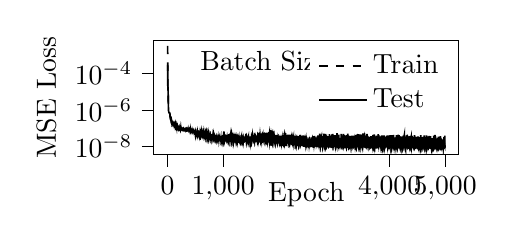
\begin{tikzpicture}

\begin{axis}[
legend cell align={left},
legend style={draw=none},
log basis y={10},
tick align=outside,
tick pos=left,
title={Batch Size 2},
title style={at={(0.4,0.85)},anchor=north},
x grid style={white!69.0196078431373!black},
xlabel={Epoch},
x label style={yshift=13pt},
xmin=-249.95, xmax=5248.95,
xtick style={color=black},
xtick = {0,1000,4000,5000},
y grid style={white!69.0196078431373!black},
ylabel={MSE Loss},
ymin=3.38262380496077e-09, ymax=0.00632854574258151,
ymode=log,
ytick style={color=black},
width=.45\textwidth,
height=.25\textwidth
]
\addplot [semithick, black, dashed]
table {%
0 0.00328254532568099
1 0.000218499955626612
2 0.000191524371870401
3 7.48565430555885e-05
4 1.80191885218974e-05
5 1.70335326928424e-05
6 1.60617069012901e-05
7 1.42414383480727e-05
8 1.17442153426879e-05
9 8.90145301876544e-06
10 6.35426067282552e-06
11 4.48610761718449e-06
12 3.16681323150547e-06
13 2.21908286821115e-06
14 1.57206481016292e-06
15 1.21919172834595e-06
16 1.0618989238651e-06
17 9.78470672838849e-07
18 9.22985532084475e-07
19 8.8099305171685e-07
20 8.4995001972521e-07
21 8.3038449714623e-07
22 8.1447130311485e-07
23 8.01895829424026e-07
24 7.90452571434397e-07
25 7.80588560063133e-07
26 7.67551035850467e-07
27 7.54603072246951e-07
28 7.4473731326119e-07
29 7.34573585697174e-07
30 7.2510382626545e-07
31 7.15328201120524e-07
32 7.06132008384763e-07
33 6.96060642347618e-07
34 6.86012559671934e-07
35 6.76093364214037e-07
36 6.65401749750494e-07
37 6.55946847171407e-07
38 6.46543756017692e-07
39 6.3489944804207e-07
40 6.18515371762385e-07
41 5.85002741245066e-07
42 5.21904763381542e-07
43 4.64107343058906e-07
44 4.31738605658261e-07
45 4.08880619641838e-07
46 3.87349231173229e-07
47 3.69826064049672e-07
48 3.53238981003257e-07
49 3.40011401617657e-07
50 3.28091449871115e-07
51 3.16790916875087e-07
52 3.058581874682e-07
53 2.96605351175927e-07
54 2.8681011950682e-07
55 2.7820315102689e-07
56 2.70656728957208e-07
57 2.63857507705412e-07
58 2.57623938459961e-07
59 2.52528075400882e-07
60 2.47351241863703e-07
61 2.42858798984225e-07
62 2.38187733390793e-07
63 2.34476871070921e-07
64 2.31448094974551e-07
65 2.28447264819964e-07
66 2.25276748428538e-07
67 2.22910076783212e-07
68 2.19949171984757e-07
69 2.18757366997169e-07
70 2.16757680979729e-07
71 2.1456885103599e-07
72 2.12431132567414e-07
73 2.12453675991098e-07
74 2.09875333198273e-07
75 2.08367902884143e-07
76 2.06870915439472e-07
77 2.05759142446249e-07
78 2.03537200378245e-07
79 2.02386158929979e-07
80 2.01577248807538e-07
81 1.99945309896199e-07
82 1.98954125483652e-07
83 1.97998061242988e-07
84 1.95277801370519e-07
85 1.94122259384422e-07
86 1.9321474032008e-07
87 1.92061395219989e-07
88 1.90649255421116e-07
89 1.88983075970039e-07
90 1.87258018107261e-07
91 1.86211353437882e-07
92 1.84968773373595e-07
93 1.8346280023851e-07
94 1.81952997721835e-07
95 1.80662087380323e-07
96 1.79365444776147e-07
97 1.77472094651909e-07
98 1.76493799261546e-07
99 1.74580053132978e-07
100 1.73360636676279e-07
101 1.72267877915688e-07
102 1.70442489901279e-07
103 1.69188082461469e-07
104 1.67839397578917e-07
105 1.66230285953528e-07
106 1.64829462242722e-07
107 1.63325331338671e-07
108 1.62738196491152e-07
109 1.60219138044426e-07
110 1.60535278213469e-07
111 1.58536466712489e-07
112 1.56850298218325e-07
113 1.55524901216397e-07
114 1.54631709402775e-07
115 1.53302759073659e-07
116 1.51466843822945e-07
117 1.49550631134643e-07
118 1.48410193441917e-07
119 1.47384696155495e-07
120 1.46283629718358e-07
121 1.44345578623639e-07
122 1.43203171090622e-07
123 1.41263757020393e-07
124 1.40215976953906e-07
125 1.38600845025039e-07
126 1.37061671532823e-07
127 1.36200254846841e-07
128 1.34788054034773e-07
129 1.32993649122337e-07
130 1.31643087291855e-07
131 1.30615223781883e-07
132 1.28918619770713e-07
133 1.27769738631822e-07
134 1.26176427465929e-07
135 1.25179997131242e-07
136 1.23230363925919e-07
137 1.22045724761821e-07
138 1.21201524557857e-07
139 1.19549983392364e-07
140 1.18310560280777e-07
141 1.16812820882495e-07
142 1.15443738707643e-07
143 1.14161057509832e-07
144 1.1312136743713e-07
145 1.11719248588327e-07
146 1.10043574582441e-07
147 1.09814437586175e-07
148 1.08579877910908e-07
149 1.07548462370266e-07
150 1.0619949556756e-07
151 1.0495877468919e-07
152 1.04168265051441e-07
153 1.02623975512528e-07
154 1.01427549126121e-07
155 1.01362208877243e-07
156 9.95105090075832e-08
157 9.90712999682231e-08
158 9.81297963442707e-08
159 9.76671625630976e-08
160 9.38856064496285e-08
161 9.09411816544248e-08
162 8.88011398124666e-08
163 8.8803014968053e-08
164 8.77907267728961e-08
165 8.71906158357305e-08
166 8.74571203014485e-08
167 8.68890042542425e-08
168 8.61177263807855e-08
169 8.60476076310901e-08
170 8.55405427711009e-08
171 8.58966112591286e-08
172 8.51639051044906e-08
173 8.51758944812042e-08
174 8.47307304080447e-08
175 8.48132693269665e-08
176 8.51079388366482e-08
177 8.49318124505061e-08
178 8.47849283748259e-08
179 8.48751120090529e-08
180 8.42010138485394e-08
181 8.44082437067017e-08
182 8.40907957427861e-08
183 8.38560661877707e-08
184 8.42076578552176e-08
185 8.38791066610778e-08
186 8.37576944041629e-08
187 8.40239886347183e-08
188 8.38833574516862e-08
189 8.33899735629418e-08
190 8.34640443237999e-08
191 8.35304616458865e-08
192 8.31852537088729e-08
193 8.30714862566362e-08
194 8.33851301329513e-08
195 8.27072170499488e-08
196 8.32493552452851e-08
197 8.22546665798507e-08
198 8.27084489483099e-08
199 8.21670082453707e-08
200 8.25011616596427e-08
201 8.18873943000398e-08
202 8.22608535500091e-08
203 8.1495268684395e-08
204 8.20163649861705e-08
205 8.16005401669262e-08
206 8.11489030099199e-08
207 8.16204926260555e-08
208 8.09058569459786e-08
209 8.10499177033019e-08
210 8.07727945287828e-08
211 8.08666219838106e-08
212 8.08093064915694e-08
213 8.02509398206697e-08
214 8.09831349148915e-08
215 8.00564518014246e-08
216 8.00968553160697e-08
217 8.01893686681598e-08
218 8.01536400982794e-08
219 7.95515807424652e-08
220 7.96363922979104e-08
221 8.03492120219351e-08
222 7.98713108027815e-08
223 7.96498008956981e-08
224 7.95084208592423e-08
225 7.95095037848803e-08
226 7.94453084611568e-08
227 7.89366283454607e-08
228 7.92334955032059e-08
229 7.92735157912894e-08
230 7.89827368313789e-08
231 7.85786661230414e-08
232 7.87854531203447e-08
233 7.85752367177262e-08
234 7.85788053452308e-08
235 7.82479060256192e-08
236 7.87282694114655e-08
237 7.80035227161413e-08
238 7.84374309548141e-08
239 7.78576224716998e-08
240 7.77167863775796e-08
241 7.81467363761834e-08
242 7.75516917973507e-08
243 7.74188098600082e-08
244 7.74798297724644e-08
245 7.7469969126609e-08
246 7.71800704708614e-08
247 7.71970539117373e-08
248 7.69478892151954e-08
249 7.73572983933102e-08
250 7.71568599475803e-08
251 7.69779501024193e-08
252 7.71894792475081e-08
253 7.67477751884016e-08
254 7.6877333195835e-08
255 7.65848046396789e-08
256 7.65385336909397e-08
257 7.63672228696333e-08
258 7.6301277346813e-08
259 7.62444665756146e-08
260 7.62738956281428e-08
261 7.59071467697492e-08
262 7.59964418058923e-08
263 7.59101158571696e-08
264 7.60531896979444e-08
265 7.57084843583389e-08
266 7.57804675006746e-08
267 7.57439965304307e-08
268 7.55281243759454e-08
269 7.54863963056129e-08
270 7.55834353999285e-08
271 7.5430192249204e-08
272 7.54428438793919e-08
273 7.52991162173977e-08
274 7.51532936485999e-08
275 7.51941930451361e-08
276 7.51544057150388e-08
277 7.48605089656573e-08
278 7.49440059444328e-08
279 7.48363137593744e-08
280 7.45955682426303e-08
281 7.46543589628113e-08
282 7.45810491539212e-08
283 7.45009416183162e-08
284 7.45298077395873e-08
285 7.43874965440927e-08
286 7.42333786614147e-08
287 7.43559364357882e-08
288 7.44611771404946e-08
289 7.43719104612239e-08
290 7.4087228369879e-08
291 7.42675714614505e-08
292 7.40377803589709e-08
293 7.39002887022444e-08
294 7.37450820641472e-08
295 7.37146042358861e-08
296 7.34764170412516e-08
297 7.34748401464147e-08
298 7.33259203234971e-08
299 7.32177149885826e-08
300 7.30713860042087e-08
301 7.31287919658596e-08
302 7.3047478842847e-08
303 7.30429494556484e-08
304 7.26866788871572e-08
305 7.28189107246369e-08
306 7.2611721922522e-08
307 7.25180870284614e-08
308 7.25546002222632e-08
309 7.23407575197177e-08
310 7.22547411237118e-08
311 7.23688810853051e-08
312 7.23001925837519e-08
313 7.23487935944123e-08
314 7.21203149054439e-08
315 7.23077199693556e-08
316 7.21352630661531e-08
317 7.20632900854667e-08
318 7.19566260092286e-08
319 7.1823656741965e-08
320 7.17751821249779e-08
321 7.18084207751435e-08
322 7.15284738002087e-08
323 7.15922071675701e-08
324 7.14385197908563e-08
325 7.11717999838379e-08
326 7.14794709065769e-08
327 7.11045747163741e-08
328 7.1172664772412e-08
329 7.10999585191718e-08
330 7.10373534636988e-08
331 7.10004941901765e-08
332 7.09694212622791e-08
333 7.10542106029388e-08
334 7.11422026586916e-08
335 7.06343104364127e-08
336 7.06290690287714e-08
337 7.058199697485e-08
338 7.05904521041134e-08
339 7.06610755990544e-08
340 7.02293932595133e-08
341 7.0213167338129e-08
342 7.01696666369767e-08
343 7.01245406067308e-08
344 7.02258261991995e-08
345 7.00943012788002e-08
346 6.99631210515639e-08
347 6.99243554992401e-08
348 6.99733587956608e-08
349 6.97487408191089e-08
350 6.96652839086154e-08
351 6.94952265442028e-08
352 6.9586298279356e-08
353 6.94802141264495e-08
354 6.94029599760393e-08
355 6.94811662502737e-08
356 6.9447535515188e-08
357 6.94013545918804e-08
358 6.94406791021951e-08
359 6.90969612737735e-08
360 6.91050193839526e-08
361 6.8881994686576e-08
362 6.87944344484048e-08
363 6.88425664659986e-08
364 6.87802862303633e-08
365 6.87643034696928e-08
366 6.85632615471388e-08
367 6.85682310238578e-08
368 6.83307170623593e-08
369 6.82866018121286e-08
370 6.85272045393148e-08
371 6.79966236415419e-08
372 6.84238423972472e-08
373 6.79873843945078e-08
374 6.81644149632676e-08
375 6.80043897696159e-08
376 6.79346173235729e-08
377 6.78095727341121e-08
378 6.76759811131245e-08
379 6.78007946736114e-08
380 6.7796770238715e-08
381 6.75536845422542e-08
382 6.73928114495181e-08
383 6.72945608075626e-08
384 6.73337297967258e-08
385 6.72205919783897e-08
386 6.72738835988396e-08
387 6.69181899951576e-08
388 6.71726448415733e-08
389 6.6735886535163e-08
390 6.67219459820068e-08
391 6.67162453900083e-08
392 6.65349611206345e-08
393 6.63832358627214e-08
394 6.63773440239268e-08
395 6.6198406551754e-08
396 6.61917400128775e-08
397 6.60644241761155e-08
398 6.62409058879154e-08
399 6.59781503837831e-08
400 6.58956399993693e-08
401 6.60107959022938e-08
402 6.5846786045487e-08
403 6.55407205336633e-08
404 6.55228505987981e-08
405 6.55955494313076e-08
406 6.52562304821469e-08
407 6.52904168840784e-08
408 6.56664842482169e-08
409 6.48951202171233e-08
410 6.52150227713477e-08
411 6.48234405338233e-08
412 6.50295594792905e-08
413 6.473958666664e-08
414 6.46367741741205e-08
415 6.44284369182291e-08
416 6.4706066168263e-08
417 6.41347029111117e-08
418 6.4321762164754e-08
419 6.38945435269545e-08
420 6.41486727785967e-08
421 6.38424642197544e-08
422 6.41088489685693e-08
423 6.37925187760846e-08
424 6.37641166327807e-08
425 6.34406229562678e-08
426 6.35571083453801e-08
427 6.32675255589632e-08
428 6.33023986322812e-08
429 6.29458381071757e-08
430 6.31480538190177e-08
431 6.27496439844499e-08
432 6.25742152867703e-08
433 6.25643662857112e-08
434 6.24544778045077e-08
435 6.2011825340047e-08
436 6.2753866577947e-08
437 6.18486373562543e-08
438 6.19743378120763e-08
439 6.20571040625961e-08
440 6.18520889781316e-08
441 6.16609228023535e-08
442 6.13968909650708e-08
443 6.14124531921334e-08
444 6.11450753005283e-08
445 6.09623349119293e-08
446 6.05825954643757e-08
447 6.04997935236273e-08
448 6.05668844602114e-08
449 6.05799478256008e-08
450 6.01981422974074e-08
451 5.9961909875561e-08
452 5.97201968506322e-08
453 5.96139426777276e-08
454 5.95120054305287e-08
455 5.92951785870488e-08
456 5.95512403165355e-08
457 5.93397249657457e-08
458 5.92162069610325e-08
459 5.89310149428091e-08
460 5.87983697155625e-08
461 5.86480213723428e-08
462 5.86585211733715e-08
463 5.81024033210475e-08
464 5.79005150566081e-08
465 5.7884217427695e-08
466 5.75974278191893e-08
467 5.72717783334786e-08
468 5.71280839249955e-08
469 5.70866307733064e-08
470 5.68234420759151e-08
471 5.65403589207758e-08
472 5.64500327302486e-08
473 5.62552928184967e-08
474 5.59582069550313e-08
475 5.59200681947702e-08
476 5.5690757583271e-08
477 5.51963993931093e-08
478 5.49973188885833e-08
479 5.45198159787041e-08
480 5.44046598370818e-08
481 5.41920685905861e-08
482 5.38668678436993e-08
483 5.361629318823e-08
484 5.32998607738477e-08
485 5.30580958801874e-08
486 5.32657221515853e-08
487 5.25750263348224e-08
488 5.23441807802616e-08
489 5.24424364887199e-08
490 5.18821803626723e-08
491 5.19918664291241e-08
492 5.1747341199504e-08
493 5.13785602573869e-08
494 5.11840279411868e-08
495 5.12938131975726e-08
496 5.0924607952807e-08
497 5.10876863294429e-08
498 5.07458053390364e-08
499 5.06220796397949e-08
500 5.04064744368815e-08
501 5.06455437344622e-08
502 4.9862071242579e-08
503 4.97268267137807e-08
504 4.94142680242948e-08
505 4.97652903030943e-08
506 4.94748283430546e-08
507 4.90965448383118e-08
508 4.87868712980566e-08
509 4.90490110020003e-08
510 4.92224223346271e-08
511 4.89848744311683e-08
512 4.86528948101528e-08
513 4.87841283199897e-08
514 4.84146250535611e-08
515 4.9023456144659e-08
516 4.81331435734367e-08
517 4.80398341196064e-08
518 4.88083406132711e-08
519 4.84064391683692e-08
520 4.84159776592552e-08
521 4.75737229264639e-08
522 4.8519928558588e-08
523 4.73770784747973e-08
524 4.83165005312758e-08
525 4.78193792249337e-08
526 4.78251361750726e-08
527 4.70196307974513e-08
528 4.80083285770982e-08
529 4.71223468826443e-08
530 4.71813922692244e-08
531 4.7113969577961e-08
532 4.70967598273919e-08
533 4.70621662446158e-08
534 4.66326605940148e-08
535 4.76241100443309e-08
536 4.66664954731355e-08
537 4.74405901805808e-08
538 4.69436936714196e-08
539 4.72466676191274e-08
540 4.70211507684337e-08
541 4.63547233083839e-08
542 4.61678381813435e-08
543 4.6965799879839e-08
544 4.63857039533222e-08
545 4.63133353306167e-08
546 4.62923420408989e-08
547 4.6108359860686e-08
548 4.64648258927669e-08
549 4.58507157922727e-08
550 4.595448568534e-08
551 4.60644132552757e-08
552 4.57460573870527e-08
553 4.48977841176479e-08
554 4.61474039982757e-08
555 4.54119244746032e-08
556 4.50748147138302e-08
557 4.51294110412337e-08
558 4.52713001330984e-08
559 4.45902119108332e-08
560 4.54390254731596e-08
561 4.45883604294206e-08
562 4.40688434577563e-08
563 4.46767707545925e-08
564 4.43456282678834e-08
565 4.43052667442601e-08
566 4.4511835127603e-08
567 4.44672186858952e-08
568 4.40549484904684e-08
569 4.38604737291737e-08
570 4.36744109219012e-08
571 4.33528694978591e-08
572 4.36945165810387e-08
573 4.35054831703363e-08
574 4.3339193234071e-08
575 4.33224534239773e-08
576 4.28230918373407e-08
577 4.29915050395024e-08
578 4.3157082451617e-08
579 4.29085400865947e-08
580 4.27126839501746e-08
581 4.34098694395701e-08
582 4.2637734657236e-08
583 4.27076143056926e-08
584 4.31071084622259e-08
585 4.27677483794131e-08
586 4.2361920931655e-08
587 4.25198561692097e-08
588 4.25564854413807e-08
589 4.23260934941938e-08
590 4.18924031443391e-08
591 4.22129305257257e-08
592 4.16024839526852e-08
593 4.16946787210604e-08
594 4.17917192728767e-08
595 4.16310181681201e-08
596 4.13894368075374e-08
597 4.14773096925058e-08
598 4.10987801270912e-08
599 4.12405630366708e-08
600 4.19068369599263e-08
601 4.11747850240785e-08
602 4.14282939695809e-08
603 4.06905636430865e-08
604 4.08110460305977e-08
605 4.11398571306121e-08
606 4.09925211455886e-08
607 4.06709809314121e-08
608 4.11535621287484e-08
609 4.03891638949272e-08
610 4.03422490115046e-08
611 4.04638569014848e-08
612 4.03521925785855e-08
613 4.02347802692105e-08
614 3.96676463815804e-08
615 4.05902976614581e-08
616 3.9934611743786e-08
617 3.97000445235829e-08
618 3.93751615644367e-08
619 3.99356786361937e-08
620 3.94967812543667e-08
621 3.9478045169461e-08
622 3.9357216289726e-08
623 3.91124260917808e-08
624 3.93788417034635e-08
625 3.91443982862283e-08
626 3.94537697414044e-08
627 3.92543143685753e-08
628 3.88451565003223e-08
629 3.87263305199337e-08
630 3.90169901079984e-08
631 3.90409084574106e-08
632 3.90292650599422e-08
633 3.8848819337356e-08
634 3.826467254886e-08
635 3.86679600120066e-08
636 3.84189770820664e-08
637 3.8034914403573e-08
638 3.83765584659468e-08
639 3.84147417166192e-08
640 3.81209554103368e-08
641 3.76586081726193e-08
642 3.7909612859377e-08
643 3.79556497944744e-08
644 3.75772361053683e-08
645 3.7929992070862e-08
646 3.75065041919309e-08
647 3.7582637523681e-08
648 3.71357294101093e-08
649 3.74972402298335e-08
650 3.73230137498126e-08
651 3.7014256861978e-08
652 3.67768056607209e-08
653 3.72723442765288e-08
654 3.69532771464787e-08
655 3.67656498795332e-08
656 3.70444940477888e-08
657 3.74225217392166e-08
658 3.64024413511688e-08
659 3.66532642359085e-08
660 3.6914308742364e-08
661 3.6492219348927e-08
662 3.66049217205844e-08
663 3.68115249901324e-08
664 3.63449829077767e-08
665 3.59703634603137e-08
666 3.65043941129017e-08
667 3.64438717505577e-08
668 3.61117691105584e-08
669 3.59725088353025e-08
670 3.58938531116459e-08
671 3.56944948786131e-08
672 3.54274465845794e-08
673 3.58843036923351e-08
674 3.51804919540566e-08
675 3.592879544001e-08
676 3.51167567705923e-08
677 3.54670594818751e-08
678 3.4856420939644e-08
679 3.52466294488152e-08
680 3.47822667237652e-08
681 3.53631174087043e-08
682 3.46637306734565e-08
683 3.47526936601283e-08
684 3.45369711179377e-08
685 3.44024175803481e-08
686 3.45784007663719e-08
687 3.43725343730505e-08
688 3.42645183736834e-08
689 3.43503181767235e-08
690 3.43352946233222e-08
691 3.41738478102926e-08
692 3.45125217628417e-08
693 3.38059283864212e-08
694 3.44023723802267e-08
695 3.34726516930117e-08
696 3.39030477289892e-08
697 3.36896250675012e-08
698 3.33158177039938e-08
699 3.35237944595335e-08
700 3.32292014725288e-08
701 3.3578084904895e-08
702 3.35027595368964e-08
703 3.39071785393497e-08
704 3.293375946406e-08
705 3.30269301683228e-08
706 3.3574827676075e-08
707 3.33444393947335e-08
708 3.33603552093997e-08
709 3.28944379845431e-08
710 3.27157034414327e-08
711 3.30092747191646e-08
712 3.29718086783393e-08
713 3.29110067269767e-08
714 3.27898127228665e-08
715 3.29078348913492e-08
716 3.22872896388327e-08
717 3.27488542049559e-08
718 3.24483861559588e-08
719 3.27850294034593e-08
720 3.26606627359949e-08
721 3.23589595196405e-08
722 3.24584725308608e-08
723 3.26674511605951e-08
724 3.1575581434129e-08
725 3.25877752292425e-08
726 3.20928140972732e-08
727 3.24274801469793e-08
728 3.25003616281627e-08
729 3.18399988796236e-08
730 3.2109916644596e-08
731 3.20759825324646e-08
732 3.18597185383629e-08
733 3.19681254596915e-08
734 3.22229387327844e-08
735 3.17291694599264e-08
736 3.21273451338033e-08
737 3.17449717723295e-08
738 3.15686945521754e-08
739 3.17564476380316e-08
740 3.17477588294146e-08
741 3.10420353661356e-08
742 3.20795690111342e-08
743 3.1216206289153e-08
744 3.11819914966538e-08
745 3.0873233597184e-08
746 3.14768186575609e-08
747 3.0342848171272e-08
748 3.17283036666005e-08
749 3.09738106077373e-08
750 3.10661259300682e-08
751 3.08984813262025e-08
752 3.06028083156829e-08
753 3.11116006412315e-08
754 3.11124808433094e-08
755 3.09768128804455e-08
756 3.11854558228131e-08
757 3.10072328188471e-08
758 3.1022588369789e-08
759 3.01097631762448e-08
760 3.08949155709559e-08
761 3.08619954873524e-08
762 3.05116490219026e-08
763 3.14621224050682e-08
764 3.06109915238495e-08
765 3.0499886474411e-08
766 3.02687262935253e-08
767 3.03926383860009e-08
768 2.94455249570946e-08
769 2.99938384391574e-08
770 3.05687051307957e-08
771 2.98737279285088e-08
772 3.03895292956824e-08
773 3.02582276905938e-08
774 2.97754409906981e-08
775 3.0655070072716e-08
776 2.97111483765766e-08
777 3.00233681251871e-08
778 2.98320518886119e-08
779 3.06805578830227e-08
780 3.02031067299646e-08
781 2.96468851478937e-08
782 3.0587170042895e-08
783 2.99796532466923e-08
784 3.06078738928628e-08
785 2.92830425706048e-08
786 3.0212400990437e-08
787 2.9719811062312e-08
788 2.93865345387112e-08
789 3.00758327314021e-08
790 2.99608398715012e-08
791 2.98255288354032e-08
792 3.01842756250115e-08
793 3.01570450788047e-08
794 2.9858412152417e-08
795 3.0092274968585e-08
796 3.02506790859636e-08
797 2.91831633476569e-08
798 2.95765616485921e-08
799 2.99364189229601e-08
800 3.00087392374193e-08
801 3.05344552096187e-08
802 3.01328082645269e-08
803 2.99154144154934e-08
804 2.94597860326373e-08
805 2.93265596476022e-08
806 2.9981135665047e-08
807 2.97405996949052e-08
808 2.97528969943062e-08
809 2.97964703900311e-08
810 2.93363185845386e-08
811 2.99720110352175e-08
812 2.96175842905422e-08
813 2.96315429029193e-08
814 2.96446226587532e-08
815 2.99707815297201e-08
816 2.95448832050571e-08
817 2.95232755386232e-08
818 2.87613123848285e-08
819 2.95836693727236e-08
820 2.94098747234406e-08
821 2.91337529105262e-08
822 2.93476053093156e-08
823 2.87491110401716e-08
824 2.89403561636314e-08
825 2.95640055761326e-08
826 2.85100923496651e-08
827 2.90359088045422e-08
828 2.89738495633518e-08
829 2.93372802613323e-08
830 2.93234274397203e-08
831 2.88658978312428e-08
832 2.86577576900093e-08
833 2.93334803106449e-08
834 2.79551181306403e-08
835 2.93240796755412e-08
836 2.84651544498193e-08
837 2.85353146382561e-08
838 2.86506699791467e-08
839 2.80141502583264e-08
840 2.90341042116782e-08
841 2.83219711137428e-08
842 2.88628372929201e-08
843 2.81941445002265e-08
844 2.86616231613412e-08
845 2.80926744038457e-08
846 2.87754205431923e-08
847 2.85303202081644e-08
848 2.81727098084272e-08
849 2.8123937935165e-08
850 2.84582470004846e-08
851 2.8650369424621e-08
852 2.85608268651982e-08
853 2.8131232703843e-08
854 2.82453610964128e-08
855 2.89483162182469e-08
856 2.83420080103847e-08
857 2.82199570773578e-08
858 2.80730314435318e-08
859 2.82809190177979e-08
860 2.86353769445857e-08
861 2.82259201612178e-08
862 2.78959342820406e-08
863 2.78645208896533e-08
864 2.81846941814212e-08
865 2.81121721020239e-08
866 2.80517562643023e-08
867 2.81593320271001e-08
868 2.72528267648564e-08
869 2.81696339985427e-08
870 2.79273086642995e-08
871 2.7512817953157e-08
872 2.84517497671222e-08
873 2.7799637717929e-08
874 2.74260516970881e-08
875 2.7788204698842e-08
876 2.73057909985774e-08
877 2.83043334327049e-08
878 2.64792259140334e-08
879 2.77433954551931e-08
880 2.80859690999224e-08
881 2.81571656352009e-08
882 2.76695006193872e-08
883 2.77709883268473e-08
884 2.6881104866483e-08
885 2.78426782351904e-08
886 2.77167030259817e-08
887 2.78135435696769e-08
888 2.78613534441252e-08
889 2.74576081790157e-08
890 2.72004491331246e-08
891 2.7812381422021e-08
892 2.74803205711494e-08
893 2.72247917181279e-08
894 2.76698133706565e-08
895 2.75316115931346e-08
896 2.72633557068525e-08
897 2.75284972862111e-08
898 2.75199321894126e-08
899 2.73734412948312e-08
900 2.72344164200522e-08
901 2.74171147513491e-08
902 2.8005013492205e-08
903 2.72693796256607e-08
904 2.71729967772916e-08
905 2.70847596891555e-08
906 2.76970295121637e-08
907 2.70154164276337e-08
908 2.71905937012651e-08
909 2.74396833003232e-08
910 2.67758121418882e-08
911 2.80058317719267e-08
912 2.79118399847678e-08
913 2.63474409490927e-08
914 2.71324295361142e-08
915 2.7954368273797e-08
916 2.7007748962693e-08
917 2.64737631885392e-08
918 2.76175025140657e-08
919 2.68041697211174e-08
920 2.71468540083974e-08
921 2.700771886055e-08
922 2.75985255401845e-08
923 2.69180859497897e-08
924 2.69624495977117e-08
925 2.68577280076454e-08
926 2.704912061402e-08
927 2.6356536705241e-08
928 2.66672037859128e-08
929 2.69591033794092e-08
930 2.68079865403115e-08
931 2.63138631513837e-08
932 2.72206234661621e-08
933 2.71317316304365e-08
934 2.7307047371139e-08
935 2.65802619039413e-08
936 2.73144441089168e-08
937 2.63830216658545e-08
938 2.66981474648098e-08
939 2.6431935854887e-08
940 2.60439990913408e-08
941 2.67252916980043e-08
942 2.66271156456055e-08
943 2.6739769780626e-08
944 2.62611098725829e-08
945 2.62674960841425e-08
946 2.70139238268685e-08
947 2.63460659326586e-08
948 2.62264182295802e-08
949 2.70272808373662e-08
950 2.5747153010236e-08
951 2.66053678841804e-08
952 2.64551851290595e-08
953 2.67567574317451e-08
954 2.58916772901685e-08
955 2.64584350602726e-08
956 2.61099018731836e-08
957 2.66250582974248e-08
958 2.59226130361612e-08
959 2.64767316645598e-08
960 2.6452490843043e-08
961 2.58215259816841e-08
962 2.59265999303371e-08
963 2.62359932220457e-08
964 2.65424289648264e-08
965 2.67450139063707e-08
966 2.63561833882819e-08
967 2.57741525678257e-08
968 2.62758306087407e-08
969 2.65221036650498e-08
970 2.64172919469674e-08
971 2.56274016323943e-08
972 2.57729816374175e-08
973 2.59577244466347e-08
974 2.6222427415179e-08
975 2.62312397004694e-08
976 2.5963541613383e-08
977 2.56496797129135e-08
978 2.56104738609597e-08
979 2.62138495017994e-08
980 2.58349842333083e-08
981 2.6208806482575e-08
982 2.54673980373543e-08
983 2.56343059095165e-08
984 2.62062766909765e-08
985 2.52106715502853e-08
986 2.51687390236954e-08
987 2.61188593480566e-08
988 2.52318605282187e-08
989 2.56387556114013e-08
990 2.54048550445418e-08
991 2.53413983453687e-08
992 2.55538864205596e-08
993 2.5451171698665e-08
994 2.61896682761109e-08
995 2.54498613648235e-08
996 2.55230583791621e-08
997 2.48618900541842e-08
998 2.58373611447538e-08
999 2.51232853774597e-08
1000 2.56220291215414e-08
1001 2.56736006327141e-08
1002 2.51882083300847e-08
1003 2.53713824167612e-08
1004 2.58137432954941e-08
1005 2.48481835016801e-08
1006 2.56784723412506e-08
1007 2.40642600508045e-08
1008 2.56810740124624e-08
1009 2.54665775721308e-08
1010 2.43275138776256e-08
1011 2.61642387404115e-08
1012 2.48960325622827e-08
1013 2.58067697424536e-08
1014 2.57083646426348e-08
1015 2.49647724676894e-08
1016 2.54706723878118e-08
1017 2.44838401316505e-08
1018 2.5243788890239e-08
1019 2.52713618028588e-08
1020 2.47552457360301e-08
1021 2.50724322887752e-08
1022 2.57186888398264e-08
1023 2.51238573180101e-08
1024 2.44940838938223e-08
1025 2.52199264209607e-08
1026 2.57123974063966e-08
1027 2.50377650737044e-08
1028 2.51321844116914e-08
1029 2.45223809804962e-08
1030 2.48290043978749e-08
1031 2.53573499313098e-08
1032 2.4809457069952e-08
1033 2.55327429933838e-08
1034 2.49863649272875e-08
1035 2.54338735914406e-08
1036 2.46765876222854e-08
1037 2.48556650924159e-08
1038 2.46800521991331e-08
1039 2.51365618709754e-08
1040 2.41794125941386e-08
1041 2.44692986407224e-08
1042 2.47765058001559e-08
1043 2.48758484036604e-08
1044 2.41757049636859e-08
1045 2.4206212695721e-08
1046 2.55829298876631e-08
1047 2.41762240022481e-08
1048 2.47289624125679e-08
1049 2.5234407058039e-08
1050 2.43533080388492e-08
1051 2.47249283025774e-08
1052 2.44511952491311e-08
1053 2.45763102038055e-08
1054 2.45536552540004e-08
1055 2.48305525572534e-08
1056 2.40834935295586e-08
1057 2.53211549907095e-08
1058 2.41439715079061e-08
1059 2.57494680457604e-08
1060 2.35057552473161e-08
1061 2.49778252063293e-08
1062 2.40053659600614e-08
1063 2.4876820900549e-08
1064 2.45837317633946e-08
1065 2.43284918397257e-08
1066 2.40939658241457e-08
1067 2.51706974384036e-08
1068 2.35143826128326e-08
1069 2.41161983740024e-08
1070 2.4755212258476e-08
1071 2.4246693290042e-08
1072 2.56388721965872e-08
1073 2.41264563889954e-08
1074 2.44039392134909e-08
1075 2.51708382467408e-08
1076 2.45340783286419e-08
1077 2.45209754993758e-08
1078 2.48115112856939e-08
1079 2.39203909974672e-08
1080 2.31613966679145e-08
1081 2.50456757703854e-08
1082 2.43899172222006e-08
1083 2.40393221376256e-08
1084 2.41358175256112e-08
1085 2.3699030541946e-08
1086 2.43306819150413e-08
1087 2.42609329062504e-08
1088 2.39897964542934e-08
1089 2.44988888764563e-08
1090 2.45195678220678e-08
1091 2.40963733417754e-08
1092 2.39458951021843e-08
1093 2.37625303336486e-08
1094 2.44664175362286e-08
1095 2.36047424231611e-08
1096 2.45438499066886e-08
1097 2.4314623127103e-08
1098 2.39301791060131e-08
1099 2.417096244689e-08
1100 2.39409680004576e-08
1101 2.42720179199352e-08
1102 2.42393090368331e-08
1103 2.40999026286381e-08
1104 2.42074585857788e-08
1105 2.3707304635745e-08
1106 2.34363956257144e-08
1107 2.36964240676596e-08
1108 2.36679420671515e-08
1109 2.38906914948878e-08
1110 2.46842266887759e-08
1111 2.31558109071162e-08
1112 2.37190626790618e-08
1113 2.35072627912114e-08
1114 2.4207290549999e-08
1115 2.3632586413358e-08
1116 2.4249042063107e-08
1117 2.3715847715905e-08
1118 2.38752562103928e-08
1119 2.48957234907365e-08
1120 2.32552377015804e-08
1121 2.49651159680564e-08
1122 2.28996111810154e-08
1123 2.34150135410283e-08
1124 2.41551524927108e-08
1125 2.34782538071077e-08
1126 2.43804897772648e-08
1127 2.31835085818255e-08
1128 2.3253374320964e-08
1129 2.32561741067006e-08
1130 2.50726553251424e-08
1131 2.29548132411883e-08
1132 2.3328192227362e-08
1133 2.41420011705684e-08
1134 2.33821172641313e-08
1135 2.3303387180762e-08
1136 2.43730284085197e-08
1137 2.41564589041898e-08
1138 2.37143871552048e-08
1139 2.36588560203199e-08
1140 2.30154500006075e-08
1141 2.4859979055103e-08
1142 2.29174441709334e-08
1143 2.38801621325058e-08
1144 2.44339880565159e-08
1145 2.38689083146837e-08
1146 2.28463232741505e-08
1147 2.46741202382939e-08
1148 2.41791558530102e-08
1149 2.29663980678141e-08
1150 2.39159831927349e-08
1151 2.43229607134743e-08
1152 2.28362273965721e-08
1153 2.31572237742172e-08
1154 2.33627679651072e-08
1155 2.27080735474283e-08
1156 2.4358588360418e-08
1157 2.26149591309732e-08
1158 2.3826834529006e-08
1159 2.35227404605243e-08
1160 2.2895686424329e-08
1161 2.40749804307216e-08
1162 2.26256669050295e-08
1163 2.33396992000423e-08
1164 2.30482095263662e-08
1165 2.44169308798725e-08
1166 2.39379462509404e-08
1167 2.23706146176839e-08
1168 2.37480671272938e-08
1169 2.3676940001105e-08
1170 2.34087737608912e-08
1171 2.3882939918618e-08
1172 2.30129306417748e-08
1173 2.31911079903724e-08
1174 2.24837282247203e-08
1175 2.29678447716819e-08
1176 2.3352444612823e-08
1177 2.3275783645138e-08
1178 2.36324950197431e-08
1179 2.44034234366253e-08
1180 2.2084830024971e-08
1181 2.42513723696935e-08
1182 2.16930364395074e-08
1183 2.25338594886382e-08
1184 2.28829293547617e-08
1185 2.39440693926563e-08
1186 2.2315187542532e-08
1187 2.36924562428409e-08
1188 2.20071196566085e-08
1189 2.32872066795453e-08
1190 2.39950020853863e-08
1191 2.17920868925692e-08
1192 2.27612380520603e-08
1193 2.3995818000222e-08
1194 2.22051254888389e-08
1195 2.46911551403106e-08
1196 2.19987103602382e-08
1197 2.24494658944141e-08
1198 2.54094465522159e-08
1199 2.06954137310644e-08
1200 2.39629729154589e-08
1201 2.31854273466947e-08
1202 2.26924926745031e-08
1203 2.40487618563545e-08
1204 2.13842529988295e-08
1205 2.39762664323573e-08
1206 2.25271042649244e-08
1207 2.24390193712121e-08
1208 2.4125746498016e-08
1209 2.21658715069406e-08
1210 2.28044628429736e-08
1211 2.48385112019966e-08
1212 2.33656474967758e-08
1213 2.12154672926679e-08
1214 2.41168022632188e-08
1215 2.127196985513e-08
1216 2.41087441434362e-08
1217 2.23791959621522e-08
1218 2.24479696701585e-08
1219 2.30527769330691e-08
1220 2.41279960776497e-08
1221 2.22326906687553e-08
1222 2.24541030668934e-08
1223 2.22194493112449e-08
1224 2.33363321254232e-08
1225 2.30219892352057e-08
1226 2.20189755480715e-08
1227 2.30715657988378e-08
1228 2.25623969505317e-08
1229 2.24376861742148e-08
1230 2.21420095534164e-08
1231 2.41717404863839e-08
1232 2.20276527142516e-08
1233 2.24890027827329e-08
1234 2.36996848195781e-08
1235 2.19429958308592e-08
1236 2.31160184864798e-08
1237 2.46116306463207e-08
1238 2.23464107134141e-08
1239 2.19672915339753e-08
1240 2.24700124982213e-08
1241 2.36331999026174e-08
1242 2.33265122337456e-08
1243 2.13752408421142e-08
1244 2.33078071993353e-08
1245 2.32677361167721e-08
1246 2.21433261852755e-08
1247 2.40962325241401e-08
1248 2.26305257871595e-08
1249 2.21173026355714e-08
1250 2.39238219879034e-08
1251 2.13247202381361e-08
1252 2.37189196605203e-08
1253 2.32250552512636e-08
1254 2.16647174275386e-08
1255 2.2491087962706e-08
1256 2.34335919854778e-08
1257 2.19791799298541e-08
1258 2.35654252513373e-08
1259 2.14169790457852e-08
1260 2.35637368361241e-08
1261 2.1728992364356e-08
1262 2.31331254670342e-08
1263 2.26170422073235e-08
1264 2.35172557362939e-08
1265 2.14990163194817e-08
1266 2.36890559190961e-08
1267 2.17138146291762e-08
1268 2.44956976728217e-08
1269 2.12130341750993e-08
1270 2.29326911906358e-08
1271 2.294375372347e-08
1272 2.21282134780787e-08
1273 2.37402650568597e-08
1274 2.14494472419724e-08
1275 2.28301129672759e-08
1276 2.20507827259908e-08
1277 2.38259531475382e-08
1278 2.14158515750573e-08
1279 2.44407928549073e-08
1280 2.20708781046852e-08
1281 2.28768149491132e-08
1282 2.2626050056429e-08
1283 2.3005323938563e-08
1284 2.1827455709722e-08
1285 2.22817814335419e-08
1286 2.34458954926908e-08
1287 2.12545711266165e-08
1288 2.32935544570156e-08
1289 2.18443757705744e-08
1290 2.20137667314435e-08
1291 2.26713250879862e-08
1292 2.2973785081537e-08
1293 2.30200027910299e-08
1294 2.19761202549518e-08
1295 2.24197731544806e-08
1296 2.17526179136229e-08
1297 2.37097571550993e-08
1298 2.20199593771175e-08
1299 2.23016867821613e-08
1300 2.22305995936645e-08
1301 2.33038597228785e-08
1302 2.38850469355678e-08
1303 2.09000387388913e-08
1304 2.26636061739782e-08
1305 2.2103954332886e-08
1306 2.28347936062634e-08
1307 2.19457175233972e-08
1308 2.22836593346543e-08
1309 2.23504406504094e-08
1310 2.22128115497378e-08
1311 2.28280098716338e-08
1312 2.31253715030633e-08
1313 2.11736454615585e-08
1314 2.20795589808143e-08
1315 2.24833086843179e-08
1316 2.32801941796312e-08
1317 2.14961897331001e-08
1318 2.20238446245746e-08
1319 2.2324847892885e-08
1320 2.19785063278466e-08
1321 2.35137257901807e-08
1322 2.3144701277622e-08
1323 2.10336239354625e-08
1324 2.23880651935016e-08
1325 2.16761783147779e-08
1326 2.26090178953031e-08
1327 2.28862650982764e-08
1328 2.21212273828209e-08
1329 2.16299618250315e-08
1330 2.29643947586289e-08
1331 2.26928735589382e-08
1332 2.20482249578269e-08
1333 2.18015371278302e-08
1334 2.20884739085547e-08
1335 2.3364725292907e-08
1336 2.15798587311355e-08
1337 2.36228769332492e-08
1338 2.27154247446348e-08
1339 2.18096778484278e-08
1340 2.21108368879674e-08
1341 2.21310831148291e-08
1342 2.20017822580854e-08
1343 2.19745016792339e-08
1344 2.21375170811888e-08
1345 2.21948070953104e-08
1346 2.21312608935653e-08
1347 2.22437780286744e-08
1348 2.19581330651586e-08
1349 2.20827062501483e-08
1350 2.18945214304211e-08
1351 2.29315245998118e-08
1352 2.21396365736037e-08
1353 2.25976545702999e-08
1354 2.1405512023176e-08
1355 2.20842132633847e-08
1356 2.24522939798466e-08
1357 2.26773350752718e-08
1358 2.14882492814428e-08
1359 2.2369567684366e-08
1360 2.17191727960309e-08
1361 2.19919470932917e-08
1362 2.2311646740325e-08
1363 2.25913608749573e-08
1364 2.21926017565655e-08
1365 2.15259211113761e-08
1366 2.16004253598134e-08
1367 2.32224484773558e-08
1368 2.15576274351648e-08
1369 2.25957661512677e-08
1370 2.1665183021935e-08
1371 2.22470384803053e-08
1372 2.227040601116e-08
1373 2.18528204138368e-08
1374 2.21331229738886e-08
1375 2.32569008955519e-08
1376 2.05272220124009e-08
1377 2.2737146274765e-08
1378 2.17802189304006e-08
1379 2.20164517975019e-08
1380 2.26876345494897e-08
1381 2.14601053055152e-08
1382 2.13699287613944e-08
1383 2.16462507426907e-08
1384 2.21368567230318e-08
1385 2.28223008749695e-08
1386 2.15268508930722e-08
1387 2.18877246265792e-08
1388 2.23609083401244e-08
1389 2.2065903218349e-08
1390 2.26112779765364e-08
1391 2.21005944214259e-08
1392 2.21072447048609e-08
1393 2.2372629410905e-08
1394 2.21432812628208e-08
1395 2.25536891302891e-08
1396 2.20534070987655e-08
1397 2.2955050506257e-08
1398 2.26208074964873e-08
1399 2.18272057315172e-08
1400 2.16593289958933e-08
1401 2.27141324652957e-08
1402 2.20719237945533e-08
1403 2.17082151288683e-08
1404 2.20936218085499e-08
1405 2.1863136471012e-08
1406 2.21187039824433e-08
1407 2.10590157191937e-08
1408 2.29186094085621e-08
1409 2.21961395413528e-08
1410 2.20644468408859e-08
1411 2.22680759182081e-08
1412 2.22331608497606e-08
1413 2.04469981444633e-08
1414 2.1789090508928e-08
1415 2.25222602415753e-08
1416 2.11176890110853e-08
1417 2.25176194232346e-08
1418 2.15985122689055e-08
1419 2.2313166706811e-08
1420 2.30230737420234e-08
1421 2.18747423230137e-08
1422 2.16363518343865e-08
1423 2.3068403635973e-08
1424 2.1838906702043e-08
1425 2.22338019213453e-08
1426 2.13278609508261e-08
1427 2.29623013299207e-08
1428 2.1098088403726e-08
1429 2.24614715425009e-08
1430 2.12589236732175e-08
1431 2.26730734765868e-08
1432 2.10315514134751e-08
1433 2.27212884548189e-08
1434 2.09692620500856e-08
1435 2.26583690920989e-08
1436 2.04742908186395e-08
1437 2.28886742472678e-08
1438 2.12501669026866e-08
1439 2.31694822255268e-08
1440 2.19335935971454e-08
1441 2.07122653302361e-08
1442 2.32995183077067e-08
1443 2.13800517415708e-08
1444 2.19378508171109e-08
1445 2.17659652216318e-08
1446 2.25236484944213e-08
1447 2.14525019416878e-08
1448 2.11303392904094e-08
1449 2.22758848886784e-08
1450 2.15706849791553e-08
1451 2.30910437937215e-08
1452 2.07915529506497e-08
1453 2.22041605880685e-08
1454 2.20864075464178e-08
1455 2.2056206184895e-08
1456 2.15564313329752e-08
1457 2.11379826827729e-08
1458 2.20233888020283e-08
1459 2.28370447180604e-08
1460 2.11876432199554e-08
1461 2.22300986445489e-08
1462 2.16021678987599e-08
1463 2.17324369022887e-08
1464 2.21292224406588e-08
1465 2.23671277076454e-08
1466 2.14703611854938e-08
1467 2.05927899782354e-08
1468 2.33626976558488e-08
1469 2.05264296654906e-08
1470 2.18535323567859e-08
1471 2.11968200043433e-08
1472 2.18168553881015e-08
1473 2.26454652578756e-08
1474 2.11857142232708e-08
1475 2.13278918422266e-08
1476 2.236010990736e-08
1477 2.17072662658802e-08
1478 2.2110143227283e-08
1479 2.22466864685522e-08
1480 2.06100590163238e-08
1481 2.22854114886872e-08
1482 2.19793991453332e-08
1483 2.16467689184152e-08
1484 2.05775316386991e-08
1485 2.19673081403582e-08
1486 2.19401898399474e-08
1487 2.20589850682407e-08
1488 2.05005431839767e-08
1489 2.15492483782165e-08
1490 2.19645833702264e-08
1491 2.21786140069957e-08
1492 2.16240650679489e-08
1493 2.21673701460423e-08
1494 2.08698478573743e-08
1495 2.19098450867095e-08
1496 2.15752541418146e-08
1497 2.19070329576798e-08
1498 2.16886264846616e-08
1499 2.23972178054754e-08
1500 2.14879013741287e-08
1501 2.11427105282214e-08
1502 2.18200978853167e-08
1503 2.19430892073325e-08
1504 2.18239163790046e-08
1505 2.12949392383033e-08
1506 2.09734695226782e-08
1507 2.21864767561142e-08
1508 2.10699609919374e-08
1509 2.23657064514771e-08
1510 2.08754557393664e-08
1511 2.13593325406602e-08
1512 2.2237284218074e-08
1513 2.22302955611431e-08
1514 2.14894843014179e-08
1515 2.17345119775114e-08
1516 2.2619548078251e-08
1517 2.03632252265273e-08
1518 2.222387638251e-08
1519 2.0638844568599e-08
1520 2.15556459234878e-08
1521 2.13329812444041e-08
1522 2.17516634387072e-08
1523 2.14504079945055e-08
1524 2.1713463724482e-08
1525 2.17702472103398e-08
1526 2.1144652500471e-08
1527 2.25338103538308e-08
1528 2.08841337764332e-08
1529 2.15978603308464e-08
1530 2.19219352285416e-08
1531 2.20143767911685e-08
1532 2.03035153048536e-08
1533 2.2025311063878e-08
1534 2.17098071511601e-08
1535 2.13676841006594e-08
1536 2.13570003706476e-08
1537 2.1934463194706e-08
1538 2.08679860155825e-08
1539 2.17718971614045e-08
1540 2.17795787115782e-08
1541 2.0858285151415e-08
1542 2.24124813391069e-08
1543 2.04172527167312e-08
1544 2.15674865017834e-08
1545 2.08105447176421e-08
1546 2.24757190159242e-08
1547 2.05159294637824e-08
1548 2.13008872599341e-08
1549 2.16085264567178e-08
1550 2.19470851841597e-08
1551 2.03223949322706e-08
1552 2.185089607043e-08
1553 2.13339257819634e-08
1554 2.15402248593122e-08
1555 2.14160982039413e-08
1556 2.01167598529173e-08
1557 2.26113181088783e-08
1558 2.07763320684284e-08
1559 2.09940509560136e-08
1560 2.20850009061691e-08
1561 2.12568992129514e-08
1562 2.02256049313676e-08
1563 2.1572822483884e-08
1564 2.16699280349841e-08
1565 2.0615541992508e-08
1566 2.06423681782808e-08
1567 2.166503550044e-08
1568 2.10671617285607e-08
1569 2.14949159996203e-08
1570 2.1486425486994e-08
1571 2.15268085630993e-08
1572 2.13709459728206e-08
1573 2.16338703817875e-08
1574 2.10054343868227e-08
1575 2.13374942872324e-08
1576 2.12356059929308e-08
1577 2.12236877222272e-08
1578 2.10683743684381e-08
1579 2.08947822623595e-08
1580 2.15873571304814e-08
1581 2.12413833508007e-08
1582 2.09700386497036e-08
1583 2.12016539590798e-08
1584 2.15563715610934e-08
1585 2.1320752146059e-08
1586 2.03603190020996e-08
1587 2.12582940875561e-08
1588 2.12172731384186e-08
1589 2.02699212337176e-08
1590 2.20828432360709e-08
1591 2.1214635882838e-08
1592 2.13622964505e-08
1593 1.97430580893276e-08
1594 2.12411482926056e-08
1595 2.14440202571664e-08
1596 2.10006369820159e-08
1597 2.17859179567625e-08
1598 2.0235362363008e-08
1599 2.04990278194206e-08
1600 2.15114643131731e-08
1601 2.12136672634311e-08
1602 2.10565060696499e-08
1603 2.06974479114996e-08
1604 2.09672476611522e-08
1605 2.13972567624232e-08
1606 2.10050519521832e-08
1607 2.11634919160542e-08
1608 2.0377558411111e-08
1609 2.08424264296903e-08
1610 2.10613512971747e-08
1611 2.03827716233063e-08
1612 2.10774802880676e-08
1613 2.16909275381205e-08
1614 2.08061425025496e-08
1615 2.16821348084095e-08
1616 2.00827403420978e-08
1617 2.14326192789493e-08
1618 2.0886740560111e-08
1619 2.06261215081605e-08
1620 2.10243560460621e-08
1621 2.07960275404595e-08
1622 2.25939935346031e-08
1623 2.00754938110004e-08
1624 2.13006339671584e-08
1625 2.07714345401011e-08
1626 2.13699255519062e-08
1627 2.03209101736768e-08
1628 2.15345861875882e-08
1629 2.11747947819751e-08
1630 2.13044938350837e-08
1631 2.09285056221864e-08
1632 2.01563148522488e-08
1633 2.09758108913327e-08
1634 2.1033877327159e-08
1635 2.05582696706785e-08
1636 2.09445135741504e-08
1637 2.16082702595433e-08
1638 2.02584275107442e-08
1639 2.09558489613348e-08
1640 2.07689595774774e-08
1641 2.07192879271845e-08
1642 2.06510428122919e-08
1643 2.07699233630287e-08
1644 2.0945563378616e-08
1645 2.00693340571267e-08
1646 2.11850924219936e-08
1647 2.08621823265531e-08
1648 2.14372208716951e-08
1649 2.00777119370166e-08
1650 2.10464146206957e-08
1651 2.03655942334624e-08
1652 2.116797909546e-08
1653 2.0567977439323e-08
1654 2.05833627826002e-08
1655 2.11277772809715e-08
1656 2.02255754654379e-08
1657 2.05347024668789e-08
1658 2.07974972378233e-08
1659 2.07040936341385e-08
1660 2.125038495987e-08
1661 2.07568319029461e-08
1662 2.0540897870569e-08
1663 2.10844162818469e-08
1664 2.0664589149455e-08
1665 2.13458649447329e-08
1666 2.06672683403797e-08
1667 2.06801024614234e-08
1668 2.24235970135989e-08
1669 1.94159916998005e-08
1670 2.13912904705182e-08
1671 1.96632176960865e-08
1672 2.08929274824743e-08
1673 2.00195758683908e-08
1674 2.10947335824163e-08
1675 2.02750038719723e-08
1676 2.07836373894432e-08
1677 2.11531913649754e-08
1678 2.01446989003262e-08
1679 2.08387502769747e-08
1680 2.04161593123642e-08
1681 2.05984701128759e-08
1682 2.02896431875654e-08
1683 2.0784214079278e-08
1684 2.03638555499874e-08
1685 2.08065610730057e-08
1686 1.99266829629119e-08
1687 1.98274610484495e-08
1688 2.12027175480467e-08
1689 2.01258229359236e-08
1690 2.04192807561343e-08
1691 2.0244818738635e-08
1692 2.04134685816149e-08
1693 2.07590184096995e-08
1694 1.97931712457855e-08
1695 2.12182541722283e-08
1696 2.07085533392992e-08
1697 2.08150154550057e-08
1698 2.0150691754095e-08
1699 2.03884645156582e-08
1700 1.9981964141158e-08
1701 2.04798565106024e-08
1702 2.00128432735203e-08
1703 2.03456553543036e-08
1704 2.04984107742001e-08
1705 2.04226748335423e-08
1706 2.03883581166298e-08
1707 2.04168203871702e-08
1708 2.01871644562035e-08
1709 2.08082571559465e-08
1710 2.00099698109968e-08
1711 2.0073435322121e-08
1712 2.04274871000165e-08
1713 1.97532883394746e-08
1714 2.03794064899121e-08
1715 2.04595487891535e-08
1716 1.96010728217288e-08
1717 2.02891627128499e-08
1718 2.01114561025895e-08
1719 2.02730936599838e-08
1720 2.03354554155766e-08
1721 2.009367281397e-08
1722 1.96820410204857e-08
1723 2.0558937455506e-08
1724 2.0036221832942e-08
1725 1.95301241616708e-08
1726 2.06445165078784e-08
1727 1.9952838398285e-08
1728 2.08422879668935e-08
1729 2.0532360991643e-08
1730 2.03628449579329e-08
1731 1.96703473039905e-08
1732 2.00313833502719e-08
1733 2.02990081339116e-08
1734 2.03848712307941e-08
1735 2.01351870868227e-08
1736 2.03616221083336e-08
1737 1.9487600981305e-08
1738 2.06080648691709e-08
1739 2.00369801208189e-08
1740 2.01591428402592e-08
1741 1.95835970830949e-08
1742 1.96984339789763e-08
1743 2.0168838884338e-08
1744 1.96078943374145e-08
1745 1.97731697413883e-08
1746 1.96421198397356e-08
1747 2.02246203417911e-08
1748 1.95303810274217e-08
1749 1.99385093649918e-08
1750 1.9599204083065e-08
1751 2.00508693835311e-08
1752 2.00207590216328e-08
1753 1.96941995011524e-08
1754 2.00437013692101e-08
1755 1.95671013192289e-08
1756 2.00415014116051e-08
1757 1.97756828371753e-08
1758 1.96746720271257e-08
1759 1.99504350356095e-08
1760 1.96920246534615e-08
1761 1.91564397472033e-08
1762 1.9748220688065e-08
1763 1.96420558353783e-08
1764 1.99361020566391e-08
1765 1.9828896739349e-08
1766 1.95296773319309e-08
1767 1.97923776433795e-08
1768 1.95601251013477e-08
1769 1.93734517957567e-08
1770 1.93604421652727e-08
1771 1.90877077947404e-08
1772 1.94577271906971e-08
1773 1.88859376706874e-08
1774 1.92901710699411e-08
1775 1.93312549064406e-08
1776 1.90598275290887e-08
1777 1.91989263302328e-08
1778 1.91442941697151e-08
1779 1.94581371620317e-08
1780 1.90230227741783e-08
1781 1.9659246670134e-08
1782 1.85790437919886e-08
1783 1.90168584565664e-08
1784 1.91749840057209e-08
1785 1.86640737236954e-08
1786 1.88382316684277e-08
1787 1.91034191689421e-08
1788 1.86048687346729e-08
1789 1.90872508509798e-08
1790 1.89885073224039e-08
1791 1.92445259612484e-08
1792 1.88772013159366e-08
1793 1.90235431447028e-08
1794 1.87421044357539e-08
1795 1.92534107267273e-08
1796 1.8736192023916e-08
1797 1.91136935785985e-08
1798 1.85022400225887e-08
1799 1.84365412393972e-08
1800 1.91411018043985e-08
1801 1.81394754082409e-08
1802 1.914207301279e-08
1803 1.8655211493801e-08
1804 1.8868278855444e-08
1805 1.82801271546018e-08
1806 1.9075206398933e-08
1807 1.87558569784696e-08
1808 1.98807898629805e-08
1809 1.89790037719573e-08
1810 1.89332080686166e-08
1811 1.91531059421379e-08
1812 1.86631301248019e-08
1813 1.91970473538139e-08
1814 1.96886070716606e-08
1815 1.90058170742025e-08
1816 1.84966789900654e-08
1817 1.80295595993696e-08
1818 1.88219793690325e-08
1819 1.86221582904045e-08
1820 1.85707411017311e-08
1821 1.91977097760976e-08
1822 1.84250419158483e-08
1823 1.95696567275028e-08
1824 1.90185265163123e-08
1825 1.82467958381172e-08
1826 1.83842304948278e-08
1827 1.92769543364557e-08
1828 1.78828940921583e-08
1829 1.74367601778191e-08
1830 1.90108837813119e-08
1831 1.8807656633868e-08
1832 1.93670671264079e-08
1833 1.83425814149762e-08
1834 1.82389982297249e-08
1835 1.85820953751414e-08
1836 1.75999879642452e-08
1837 1.92346562915557e-08
1838 1.86475583895118e-08
1839 1.84596680436189e-08
1840 1.86191244517797e-08
1841 1.89955333936842e-08
1842 1.83765534494118e-08
1843 1.81521940305074e-08
1844 1.86996980554022e-08
1845 1.82782058064102e-08
1846 1.84444725583877e-08
1847 1.90501617751415e-08
1848 1.83815542114663e-08
1849 1.90445148260665e-08
1850 1.84532257850312e-08
1851 1.77074601265814e-08
1852 1.81908177790957e-08
1853 1.84758387151429e-08
1854 1.82140000268283e-08
1855 1.85040429221961e-08
1856 1.93009569504909e-08
1857 1.91018589382197e-08
1858 1.91126765602678e-08
1859 2.08473474630211e-08
1860 1.62674041778998e-08
1861 1.82452675459854e-08
1862 1.78831495119547e-08
1863 1.84945997612762e-08
1864 1.72114438236892e-08
1865 1.82209869805106e-08
1866 1.83616201580028e-08
1867 1.74827370540698e-08
1868 1.86306525302438e-08
1869 1.8217771108775e-08
1870 1.75417476709905e-08
1871 1.82197729410027e-08
1872 1.8830245598539e-08
1873 1.86379105898138e-08
1874 1.82493392155147e-08
1875 1.95755316301227e-08
1876 1.70504912332947e-08
1877 1.81485997300113e-08
1878 1.84380554086871e-08
1879 1.85232020663284e-08
1880 1.83043269912087e-08
1881 1.73622439054166e-08
1882 1.76635001227221e-08
1883 1.7509043877123e-08
1884 1.78431233227028e-08
1885 1.81750630979666e-08
1886 2.02608482861299e-08
1887 1.62105836530313e-08
1888 1.81056791431489e-08
1889 1.91479715848653e-08
1890 1.82156778152087e-08
1891 1.84860921363106e-08
1892 1.72847974523327e-08
1893 1.80671525439324e-08
1894 1.75526513158664e-08
1895 1.92242510178853e-08
1896 1.75357607465343e-08
1897 1.77452551207991e-08
1898 1.84247462848841e-08
1899 1.80345856204689e-08
1900 1.72025209069226e-08
1901 1.82469431554977e-08
1902 1.70528556776295e-08
1903 1.86851082403516e-08
1904 1.85485660541274e-08
1905 1.79534020416372e-08
1906 1.68311151967637e-08
1907 1.82946590691069e-08
1908 1.73090639691842e-08
1909 1.775790009792e-08
1910 1.76439600312606e-08
1911 1.86014872683438e-08
1912 1.72380557054985e-08
1913 1.78340645943242e-08
1914 1.85307023434222e-08
1915 1.75769968515649e-08
1916 1.78204660878367e-08
1917 1.81126992636615e-08
1918 1.76859984762356e-08
1919 1.75960304976963e-08
1920 1.84841056914409e-08
1921 1.74144345369553e-08
1922 1.75632008950072e-08
1923 1.78872621008075e-08
1924 1.74626052557025e-08
1925 1.89328312114323e-08
1926 1.85949106157601e-08
1927 1.79124507642403e-08
1928 1.75801164735423e-08
1929 1.76206262604839e-08
1930 1.69653687138172e-08
1931 1.78945823507137e-08
1932 1.84466919280202e-08
1933 1.73969727699785e-08
1934 1.78243644208265e-08
1935 1.77302907222177e-08
1936 1.77030572643122e-08
1937 1.70336128217374e-08
1938 1.8232293422682e-08
1939 1.81194217146463e-08
1940 1.7786710878348e-08
1941 1.88942730953157e-08
1942 1.6629329459672e-08
1943 1.83353860564173e-08
1944 1.68795979785807e-08
1945 1.75743684170671e-08
1946 1.82300371942834e-08
1947 1.71288746237397e-08
1948 1.78147496431857e-08
1949 1.74691110064878e-08
1950 1.79930988475907e-08
1951 1.81036638352283e-08
1952 1.74577166723033e-08
1953 1.72818796081997e-08
1954 1.7793818671813e-08
1955 1.82734469837964e-08
1956 1.84251848779349e-08
1957 1.73573116578063e-08
1958 1.83671041979749e-08
1959 1.72378231312886e-08
1960 1.78720783458874e-08
1961 1.80823219213117e-08
1962 1.68310075665812e-08
1963 1.76247301215127e-08
1964 1.68069518891589e-08
1965 1.69070792865877e-08
1966 1.85005203483246e-08
1967 1.73212230022146e-08
1968 1.82373362961341e-08
1969 1.70085511959628e-08
1970 1.75220219346406e-08
1971 1.75572771006771e-08
1972 1.76583124242014e-08
1973 1.70536624985451e-08
1974 1.76895833604446e-08
1975 1.86409325663439e-08
1976 1.72398061487056e-08
1977 1.71435971426936e-08
1978 1.77287361856349e-08
1979 1.76721664158497e-08
1980 1.76705967759594e-08
1981 1.67738381327553e-08
1982 1.71073747236294e-08
1983 1.89454446726245e-08
1984 1.6727477150813e-08
1985 1.70383376532357e-08
1986 1.81838349392616e-08
1987 1.89299549120947e-08
1988 1.68918841501331e-08
1989 1.74283985434481e-08
1990 1.8017723370678e-08
1991 1.69125893935695e-08
1992 1.71157170209824e-08
1993 1.76176005616535e-08
1994 1.66640718295141e-08
1995 1.84542122892845e-08
1996 1.67818756992844e-08
1997 1.69746054360653e-08
1998 1.77532590005941e-08
1999 1.69047378884568e-08
2000 1.76961463652092e-08
2001 1.72504956571784e-08
2002 1.67582778993758e-08
2003 1.87590094081758e-08
2004 1.63163595776616e-08
2005 1.70245570767641e-08
2006 1.74359447377148e-08
2007 1.6983647583485e-08
2008 1.71258157765919e-08
2009 1.69502271862576e-08
2010 1.7019899590881e-08
2011 1.73898007116979e-08
2012 1.67378139171726e-08
2013 1.85384034409319e-08
2014 1.61739766375291e-08
2015 1.72218485075398e-08
2016 1.67302030850136e-08
2017 1.71238359399362e-08
2018 1.61686367563529e-08
2019 1.61612190078542e-08
2020 1.75700319881983e-08
2021 1.67892913397472e-08
2022 1.76003290616733e-08
2023 1.68331096438434e-08
2024 1.68609550021126e-08
2025 1.70562263592244e-08
2026 1.88368698987029e-08
2027 1.56908915849852e-08
2028 1.81652222494e-08
2029 1.6112774170407e-08
2030 1.69801762851529e-08
2031 1.56612666399325e-08
2032 1.75301589180332e-08
2033 1.7821198125878e-08
2034 1.63002470757179e-08
2035 1.68969239289773e-08
2036 1.9533636545388e-08
2037 1.54052793959192e-08
2038 1.74861969015616e-08
2039 1.63220191091717e-08
2040 1.72292791089657e-08
2041 1.76358342828253e-08
2042 1.70481032405884e-08
2043 1.67782333411193e-08
2044 1.64597535763089e-08
2045 1.6784063216313e-08
2046 1.76201322461267e-08
2047 1.65395747553643e-08
2048 1.70710022023568e-08
2049 1.71202640809331e-08
2050 1.64107028645666e-08
2051 1.68721999279642e-08
2052 1.74455782514515e-08
2053 1.61852650495398e-08
2054 1.70779098431217e-08
2055 1.77106110589575e-08
2056 1.69903553374762e-08
2057 1.71130861906232e-08
2058 1.69087772929344e-08
2059 1.64575613526563e-08
2060 1.70504168373054e-08
2061 1.79823255754552e-08
2062 1.66709115185515e-08
2063 1.81308110755729e-08
2064 1.60216045994588e-08
2065 1.61030021358921e-08
2066 1.69147874705122e-08
2067 1.6785143507253e-08
2068 1.90542040051922e-08
2069 1.50932292690142e-08
2070 1.67666080588269e-08
2071 1.78994364996299e-08
2072 1.60827784622675e-08
2073 1.69591491410992e-08
2074 1.695403881255e-08
2075 1.70289635923748e-08
2076 1.5959610320665e-08
2077 1.66299863249841e-08
2078 1.74162769576991e-08
2079 1.57412436258553e-08
2080 1.68725953920146e-08
2081 1.68354336859411e-08
2082 1.8031424715681e-08
2083 1.54898251069069e-08
2084 1.66882965152437e-08
2085 1.73371239878262e-08
2086 1.64661680339406e-08
2087 1.7240239393701e-08
2088 1.61812764979397e-08
2089 1.5988707964848e-08
2090 1.65335036313441e-08
2091 1.72997672053254e-08
2092 1.65463660186105e-08
2093 1.71450934937922e-08
2094 1.65574660764833e-08
2095 1.64482509763253e-08
2096 1.58283432813433e-08
2097 1.60083808073141e-08
2098 1.65858546501141e-08
2099 1.61689850586844e-08
2100 1.64547200643128e-08
2101 1.7000464293343e-08
2102 1.67438309479073e-08
2103 1.62013632536151e-08
2104 1.64778010271482e-08
2105 1.65255312528367e-08
2106 1.62425575241376e-08
2107 1.58036366190717e-08
2108 1.64519810896824e-08
2109 1.69444184409673e-08
2110 1.7687790626969e-08
2111 1.56503521411833e-08
2112 1.62402690818131e-08
2113 1.87394158761012e-08
2114 1.47648843454584e-08
2115 1.62964468775895e-08
2116 1.62653564362014e-08
2117 1.59508854606361e-08
2118 1.6708942957161e-08
2119 1.65585061056295e-08
2120 1.61932830824718e-08
2121 1.86939664922059e-08
2122 1.47771166781885e-08
2123 1.60382114392787e-08
2124 1.6522301453048e-08
2125 1.57415389600013e-08
2126 1.62699343490835e-08
2127 1.6364682755482e-08
2128 1.66286618808187e-08
2129 1.65743795861317e-08
2130 1.63153927665305e-08
2131 1.61052196844258e-08
2132 1.68574106136354e-08
2133 1.57658298888252e-08
2134 1.70226286961006e-08
2135 1.67260549538417e-08
2136 1.59179657245878e-08
2137 1.80693962831269e-08
2138 1.4862591023429e-08
2139 1.67382438879815e-08
2140 1.63436927453908e-08
2141 1.6069376010952e-08
2142 1.5955751963781e-08
2143 1.57864118869588e-08
2144 1.57960454726103e-08
2145 1.64102459229154e-08
2146 1.64761586285145e-08
2147 1.60736210061685e-08
2148 1.71329312041169e-08
2149 1.66229040921284e-08
2150 1.66637344535814e-08
2151 1.53552589183537e-08
2152 1.62442207455593e-08
2153 1.67071321574008e-08
2154 1.5687154236943e-08
2155 1.64053362760874e-08
2156 1.6291465384316e-08
2157 1.60665891917322e-08
2158 1.65528654616637e-08
2159 1.54879202627634e-08
2160 1.65939461944098e-08
2161 1.64557924033637e-08
2162 1.62241342193947e-08
2163 1.64693316074827e-08
2164 1.58313536872678e-08
2165 1.55997191336188e-08
2166 1.65260755848884e-08
2167 1.60782235845702e-08
2168 1.5445875297837e-08
2169 1.5899520658974e-08
2170 1.57324911065349e-08
2171 1.73104459781914e-08
2172 1.5737863737264e-08
2173 1.6006789072931e-08
2174 1.53297753206771e-08
2175 1.58049545608552e-08
2176 1.60099532517943e-08
2177 1.65182953607984e-08
2178 1.6236546200088e-08
2179 1.67868950397554e-08
2180 1.61543074409798e-08
2181 1.69334068832461e-08
2182 1.62784080243172e-08
2183 1.5351187130197e-08
2184 1.58606377936854e-08
2185 1.68994120933186e-08
2186 1.6449883963876e-08
2187 1.60194836147376e-08
2188 1.62020839429844e-08
2189 1.54478956884141e-08
2190 1.61386319435797e-08
2191 1.62104933480178e-08
2192 1.58257323264743e-08
2193 1.66054700496687e-08
2194 1.59580421979499e-08
2195 1.57918853188055e-08
2196 1.60244881991511e-08
2197 1.63633015666798e-08
2198 1.59147434047879e-08
2199 1.66177868272666e-08
2200 1.58827136648998e-08
2201 1.56136985505484e-08
2202 1.61329550109612e-08
2203 1.60476869362769e-08
2204 1.53633735757441e-08
2205 1.60269448691575e-08
2206 1.63052452704926e-08
2207 1.61820082216491e-08
2208 1.63151421249119e-08
2209 1.60591286177125e-08
2210 1.57780898624726e-08
2211 1.59399746596511e-08
2212 1.55949011054202e-08
2213 1.56118647054032e-08
2214 1.62537105922733e-08
2215 1.78938248575344e-08
2216 1.61015524157981e-08
2217 1.59879240315963e-08
2218 1.56660224819305e-08
2219 1.5469829793141e-08
2220 1.56136033079013e-08
2221 1.56852422002751e-08
2222 1.65497947551829e-08
2223 1.6147062225691e-08
2224 1.56605498504714e-08
2225 1.54902240024901e-08
2226 1.51705904623267e-08
2227 1.6740908535734e-08
2228 1.5372456475482e-08
2229 1.51130684618028e-08
2230 1.60444946534222e-08
2231 1.65509063149716e-08
2232 1.59910650317507e-08
2233 1.64411230251515e-08
2234 1.48612712409235e-08
2235 1.53227092761499e-08
2236 1.56827395026149e-08
2237 1.57652707207384e-08
2238 1.56468296588913e-08
2239 1.53809270176664e-08
2240 1.52384464119915e-08
2241 1.50965901997979e-08
2242 1.5272251098819e-08
2243 1.53364532913258e-08
2244 1.54175791221567e-08
2245 1.56899095002661e-08
2246 1.52412291178905e-08
2247 1.61622022906704e-08
2248 1.45620127022239e-08
2249 1.59084759709938e-08
2250 1.5608406087636e-08
2251 1.63330824065888e-08
2252 1.58049807189031e-08
2253 1.55780862161337e-08
2254 1.58618328583715e-08
2255 1.57266361898167e-08
2256 1.56110904286355e-08
2257 1.53052755437755e-08
2258 1.54690360872067e-08
2259 1.56097410301537e-08
2260 1.58833163213246e-08
2261 1.59383706935245e-08
2262 1.53310886864821e-08
2263 1.55052736117156e-08
2264 1.64004163188125e-08
2265 1.4399976812185e-08
2266 1.5118141968945e-08
2267 1.5138443690943e-08
2268 1.49271949870522e-08
2269 1.51895347427766e-08
2270 1.4950340649994e-08
2271 1.53981496373856e-08
2272 1.45873228538929e-08
2273 1.5638045507374e-08
2274 1.52622634924104e-08
2275 1.58236243623933e-08
2276 1.54874225400947e-08
2277 1.52022556084153e-08
2278 1.58603825186621e-08
2279 1.48279702318066e-08
2280 1.48029139281081e-08
2281 1.52696373000305e-08
2282 1.51455048213178e-08
2283 1.53047539916407e-08
2284 1.45134372283307e-08
2285 1.50584025954692e-08
2286 1.50968634252402e-08
2287 1.54474710278851e-08
2288 1.48557998370658e-08
2289 1.49802274787003e-08
2290 1.57257548749345e-08
2291 1.52231957637194e-08
2292 1.51956602780223e-08
2293 1.51121362128304e-08
2294 1.46546926817481e-08
2295 1.52027060581206e-08
2296 1.50910814547545e-08
2297 1.637356124784e-08
2298 1.52268735857664e-08
2299 1.49002743344562e-08
2300 1.52285145212372e-08
2301 1.51188161556792e-08
2302 1.49378383408061e-08
2303 1.49917599286398e-08
2304 1.59507081435861e-08
2305 1.54421847540498e-08
2306 1.5889685862816e-08
2307 1.49651685885932e-08
2308 1.49448718377021e-08
2309 1.56537961556735e-08
2310 1.43876361373696e-08
2311 1.49415162531003e-08
2312 1.56002921335857e-08
2313 1.47851650904862e-08
2314 1.52707441507527e-08
2315 1.49725170510984e-08
2316 1.54689461332735e-08
2317 1.48582177647572e-08
2318 1.51415572208768e-08
2319 1.53349501287731e-08
2320 1.54211789449576e-08
2321 1.49917635013097e-08
2322 1.57139358588632e-08
2323 1.523806406592e-08
2324 1.41977142321253e-08
2325 1.48844658757197e-08
2326 1.56470397052466e-08
2327 1.5720110716988e-08
2328 1.45455616627765e-08
2329 1.43878460381608e-08
2330 1.55571091718654e-08
2331 1.69769424401001e-08
2332 1.43379908835589e-08
2333 1.51817729120429e-08
2334 1.47587248541248e-08
2335 1.47221055666613e-08
2336 1.56550859518323e-08
2337 1.44886958269586e-08
2338 1.53171188732037e-08
2339 1.51798046035961e-08
2340 1.50086644143954e-08
2341 1.55837942329984e-08
2342 1.41473862669966e-08
2343 1.52601526321183e-08
2344 1.5611616297026e-08
2345 1.46392797557293e-08
2346 1.44600729450606e-08
2347 1.60895925856441e-08
2348 1.43965355759446e-08
2349 1.51251438704758e-08
2350 1.56960626181979e-08
2351 1.45130771765367e-08
2352 1.56193426422979e-08
2353 1.36251255543618e-08
2354 1.56642062329737e-08
2355 1.49791442205505e-08
2356 1.49137864440541e-08
2357 1.40824772173198e-08
2358 1.48005724340539e-08
2359 1.4094291088701e-08
2360 1.43244372710072e-08
2361 1.52586667565568e-08
2362 1.51089859495857e-08
2363 1.41859577416359e-08
2364 1.49804795661346e-08
2365 1.55596273539588e-08
2366 1.51044000313294e-08
2367 1.37663557468748e-08
2368 1.52903764934625e-08
2369 1.43373051433304e-08
2370 1.51376896138089e-08
2371 1.40771702527021e-08
2372 1.43176586470395e-08
2373 1.48776149483665e-08
2374 1.50838863660352e-08
2375 1.53010453837477e-08
2376 1.34471152856142e-08
2377 1.44013810757793e-08
2378 1.43448910017718e-08
2379 1.4558868122988e-08
2380 1.43158819080336e-08
2381 1.45032994602612e-08
2382 1.49703035726978e-08
2383 1.38878160590161e-08
2384 1.38000479852629e-08
2385 1.48717560317646e-08
2386 1.39814422439599e-08
2387 1.47365221271345e-08
2388 1.46742711956693e-08
2389 1.43831441804521e-08
2390 1.51605817415856e-08
2391 1.45851476459763e-08
2392 1.3730038068982e-08
2393 1.42464172160073e-08
2394 1.49961971588342e-08
2395 1.32937654223619e-08
2396 1.49140905705558e-08
2397 1.44958415264351e-08
2398 1.50562786911945e-08
2399 1.32703593149763e-08
2400 1.44707290475193e-08
2401 1.44781321068654e-08
2402 1.55713178412592e-08
2403 1.4154323517368e-08
2404 1.53718623792654e-08
2405 1.55593994019265e-08
2406 1.27946345628432e-08
2407 1.42685118831865e-08
2408 1.39482844354194e-08
2409 1.47281781538999e-08
2410 1.45308241972925e-08
2411 1.37700165953603e-08
2412 1.57781276691471e-08
2413 1.24336463633024e-08
2414 1.42189504822587e-08
2415 1.3714956803218e-08
2416 1.39042800869627e-08
2417 1.34682833813349e-08
2418 1.43851136587547e-08
2419 1.40042119955719e-08
2420 1.38508426083261e-08
2421 1.3986362513374e-08
2422 1.39723953683502e-08
2423 1.41810766390721e-08
2424 1.39708648276837e-08
2425 1.37401213492483e-08
2426 1.28390226640795e-08
2427 1.80930342806584e-08
2428 1.14635859725654e-08
2429 1.41882262156973e-08
2430 1.35112757432831e-08
2431 1.46995436551695e-08
2432 1.26204469294566e-08
2433 1.42892564347769e-08
2434 1.48303872938294e-08
2435 1.26600362421597e-08
2436 1.4365937639399e-08
2437 1.39216447699597e-08
2438 1.29058827789408e-08
2439 1.39131369316092e-08
2440 1.39576358804405e-08
2441 1.38566057759637e-08
2442 1.44660727237345e-08
2443 1.29507664492212e-08
2444 1.43456730406222e-08
2445 1.69131630982922e-08
2446 1.14682972315178e-08
2447 1.41734148936812e-08
2448 1.37426505217031e-08
2449 1.38305498841584e-08
2450 1.36870764512187e-08
2451 1.28776849706025e-08
2452 1.45689885400618e-08
2453 1.27700102144079e-08
2454 1.62535699466393e-08
2455 1.18398832098243e-08
2456 1.37513202754791e-08
2457 1.55754256372098e-08
2458 1.30196437090335e-08
2459 1.3985324463589e-08
2460 1.28154749663711e-08
2461 1.2920120477794e-08
2462 1.44530519959329e-08
2463 1.43993935284858e-08
2464 1.23132531092696e-08
2465 1.40929049913807e-08
2466 1.43193774011785e-08
2467 1.34331063671167e-08
2468 1.45920768739594e-08
2469 1.31740001871328e-08
2470 1.3997656061443e-08
2471 1.3197326652642e-08
2472 1.4680547495316e-08
2473 1.37311893077807e-08
2474 1.36432642489359e-08
2475 1.2956431567207e-08
2476 1.39666465761856e-08
2477 1.34180522737976e-08
2478 1.46590436776312e-08
2479 1.40340257799715e-08
2480 1.35557649103696e-08
2481 1.34649069179899e-08
2482 1.36465452412471e-08
2483 1.51822540902513e-08
2484 1.35887579722771e-08
2485 1.3916675489889e-08
2486 1.34714242424616e-08
2487 1.29129023504065e-08
2488 1.38233170007274e-08
2489 1.42250153267465e-08
2490 1.34880934452575e-08
2491 1.50194389743896e-08
2492 1.32370336082058e-08
2493 1.3808990907152e-08
2494 1.43753181183481e-08
2495 1.39492842860731e-08
2496 1.37608207124995e-08
2497 1.29461337179809e-08
2498 1.31839308496473e-08
2499 1.44428849543077e-08
2500 1.30904132089327e-08
2501 1.33328298480839e-08
2502 1.31675680532795e-08
2503 1.52160251270447e-08
2504 1.29485482381342e-08
2505 1.3834427853715e-08
2506 1.50733605561587e-08
2507 1.29546123952551e-08
2508 1.47353337002637e-08
2509 1.32251943207456e-08
2510 1.38496275601113e-08
2511 1.30826884298108e-08
2512 1.4264636940084e-08
2513 1.2497446637838e-08
2514 1.43429514867996e-08
2515 1.37639591855365e-08
2516 1.35242655322082e-08
2517 1.30719986385919e-08
2518 1.29740738325779e-08
2519 1.40453654501049e-08
2520 1.28295300224068e-08
2521 1.39296891199167e-08
2522 1.44704273748186e-08
2523 1.37965537111914e-08
2524 1.24967038209745e-08
2525 1.51012409278228e-08
2526 1.29557431798807e-08
2527 1.38194591659119e-08
2528 1.30599127381587e-08
2529 1.30153666925564e-08
2530 1.27637956268759e-08
2531 1.42781639479589e-08
2532 1.34268954813249e-08
2533 1.39969155436015e-08
2534 1.32066012266188e-08
2535 1.31042851788804e-08
2536 1.16005870571603e-08
2537 1.36061878396321e-08
2538 1.32144763199046e-08
2539 1.4218177038422e-08
2540 1.2990268485405e-08
2541 1.35930897345524e-08
2542 1.38522534410546e-08
2543 1.34882469834743e-08
2544 1.24881699635274e-08
2545 1.43795968247859e-08
2546 1.3547400809874e-08
2547 1.31889383387651e-08
2548 1.38131223376414e-08
2549 1.28582434734334e-08
2550 1.36698049061634e-08
2551 1.3222155564277e-08
2552 1.37354576549356e-08
2553 1.33077148689806e-08
2554 1.40416254434811e-08
2555 1.27987866282361e-08
2556 1.30609322286507e-08
2557 1.39533113447526e-08
2558 1.31254731756264e-08
2559 1.30473240109868e-08
2560 1.30240669774934e-08
2561 1.39098110809241e-08
2562 1.20567211125688e-08
2563 1.41082347460963e-08
2564 1.30849357856538e-08
2565 1.26282928167853e-08
2566 1.36639765186894e-08
2567 1.3349850694927e-08
2568 1.35121295994217e-08
2569 1.34073342548807e-08
2570 1.25167438645296e-08
2571 1.2238151629318e-08
2572 1.33072815094587e-08
2573 1.43142725323106e-08
2574 1.29910572219116e-08
2575 1.34873320193768e-08
2576 1.41168529050328e-08
2577 1.2723873166906e-08
2578 1.34497162719571e-08
2579 1.32887885584548e-08
2580 1.30373683225535e-08
2581 1.34695347231706e-08
2582 1.35366050360367e-08
2583 1.31984131223201e-08
2584 1.3380255231954e-08
2585 1.19185161126037e-08
2586 1.3334138993043e-08
2587 1.19889812221774e-08
2588 1.3094673464456e-08
2589 1.29784715271059e-08
2590 1.40490003884969e-08
2591 1.20793272235936e-08
2592 1.37655989561059e-08
2593 1.32554021319217e-08
2594 1.226614372591e-08
2595 1.31944015512239e-08
2596 1.30837136727083e-08
2597 1.37714054339322e-08
2598 1.35442441575595e-08
2599 1.32473988149473e-08
2600 1.34004783060443e-08
2601 1.43953213931902e-08
2602 1.34208382366469e-08
2603 1.36868944016141e-08
2604 1.23628363764838e-08
2605 1.39903718488973e-08
2606 1.29373662775129e-08
2607 1.29643233052271e-08
2608 1.17336066457786e-08
2609 1.28859242583129e-08
2610 1.35669291601512e-08
2611 1.26032665298814e-08
2612 1.39901216196364e-08
2613 1.15813792499198e-08
2614 1.3670652163171e-08
2615 1.27122545763719e-08
2616 1.45476330862676e-08
2617 1.31804031632266e-08
2618 1.25134058570897e-08
2619 1.42093455749205e-08
2620 1.18135388936201e-08
2621 1.25516240784482e-08
2622 1.40233328861164e-08
2623 1.34194506381247e-08
2624 1.21021876107602e-08
2625 1.32637060264382e-08
2626 1.15451061710736e-08
2627 1.37601757170328e-08
2628 1.2973773167696e-08
2629 1.2526211260272e-08
2630 1.36624720374623e-08
2631 1.34546458144535e-08
2632 1.20180376711743e-08
2633 1.36082798670861e-08
2634 1.24855974703436e-08
2635 1.33813691941195e-08
2636 1.26162293034027e-08
2637 1.34657784788272e-08
2638 1.30532202041039e-08
2639 1.34990319901676e-08
2640 1.40551890338986e-08
2641 1.27816521321988e-08
2642 1.31187205709565e-08
2643 1.25195951768686e-08
2644 1.29647294349958e-08
2645 1.31847419292536e-08
2646 1.32802387820818e-08
2647 1.34049314463938e-08
2648 1.37182005032627e-08
2649 1.36175731101432e-08
2650 1.29337927713691e-08
2651 1.3246510542117e-08
2652 1.31706684968064e-08
2653 1.19101927212109e-08
2654 1.39000706883968e-08
2655 1.34143085038507e-08
2656 1.29272691818255e-08
2657 1.31111579394355e-08
2658 1.31674152976033e-08
2659 1.23336135830626e-08
2660 1.32152881778119e-08
2661 1.36623964167443e-08
2662 1.28301956386773e-08
2663 1.32405033686084e-08
2664 1.21167951567108e-08
2665 1.40936554769572e-08
2666 1.25885262407879e-08
2667 1.32316453080594e-08
2668 1.2617103289661e-08
2669 1.2883164887012e-08
2670 1.29090635844348e-08
2671 1.24183746564761e-08
2672 1.32739162347906e-08
2673 1.2962147321556e-08
2674 1.23780074303137e-08
2675 1.27687107035826e-08
2676 1.31493052778209e-08
2677 1.33301558353227e-08
2678 1.31169956324936e-08
2679 1.3716775212412e-08
2680 1.264422722317e-08
2681 1.30089475437259e-08
2682 1.14183781440291e-08
2683 1.35857658347324e-08
2684 1.34396031060136e-08
2685 1.53774735858897e-08
2686 1.2508209189778e-08
2687 1.31163440569293e-08
2688 1.29405676536493e-08
2689 1.28551493920742e-08
2690 1.36502127432783e-08
2691 1.21205489021364e-08
2692 1.3266486045535e-08
2693 1.27766616436625e-08
2694 1.33942432842815e-08
2695 1.27588340959259e-08
2696 1.20211278257579e-08
2697 1.35453917106398e-08
2698 1.22171818871808e-08
2699 1.40663212195025e-08
2700 1.30602371607794e-08
2701 1.25704985005221e-08
2702 1.31970520161756e-08
2703 1.36887342102252e-08
2704 1.26346613236461e-08
2705 1.19184599784994e-08
2706 1.29627470719096e-08
2707 1.33481468222729e-08
2708 1.28514413829731e-08
2709 1.20972853677459e-08
2710 1.36949241450329e-08
2711 1.32112759794883e-08
2712 1.40348612773927e-08
2713 1.23829016110896e-08
2714 1.3589564440003e-08
2715 1.22620879013657e-08
2716 1.34441246287115e-08
2717 1.33258467781144e-08
2718 1.32639492725489e-08
2719 1.30041071071119e-08
2720 1.34190460017759e-08
2721 1.40524435286657e-08
2722 1.25536914336866e-08
2723 1.40535358272437e-08
2724 1.23746003126771e-08
2725 1.22981991112076e-08
2726 1.39208140714428e-08
2727 1.28738551917473e-08
2728 1.20653035514118e-08
2729 1.20865761033262e-08
2730 1.35196049529315e-08
2731 1.37821142541378e-08
2732 1.26984896213975e-08
2733 1.2956382186749e-08
2734 1.28595170764412e-08
2735 1.35205032919875e-08
2736 1.31814350459308e-08
2737 1.24456384967137e-08
2738 1.40465307685994e-08
2739 1.32679251080084e-08
2740 1.35969562957e-08
2741 1.18329807909587e-08
2742 1.2648368674123e-08
2743 1.1999414231384e-08
2744 1.2987734804154e-08
2745 1.29861542859863e-08
2746 1.29769111429159e-08
2747 1.32399133950939e-08
2748 1.30018688902431e-08
2749 1.22972428078794e-08
2750 1.41248221311244e-08
2751 1.27476384762792e-08
2752 1.31196854708804e-08
2753 1.34343857789709e-08
2754 1.2313538813008e-08
2755 1.29670785382063e-08
2756 1.34640570444711e-08
2757 1.35555095726048e-08
2758 1.2593486552491e-08
2759 1.32723089212444e-08
2760 1.27861513070787e-08
2761 1.2976886150276e-08
2762 1.30651045123602e-08
2763 1.31224307996572e-08
2764 1.35083515236667e-08
2765 1.23408568183242e-08
2766 1.31416111247007e-08
2767 1.23935517445245e-08
2768 1.34162746701638e-08
2769 1.29388734545384e-08
2770 1.3412243614036e-08
2771 1.3026843103503e-08
2772 1.27066819892302e-08
2773 1.2882682809065e-08
2774 1.28634150892426e-08
2775 1.34459952964711e-08
2776 1.32822315061509e-08
2777 1.30607957991441e-08
2778 1.24435116573424e-08
2779 1.26848403742691e-08
2780 1.25712558984442e-08
2781 1.23927428504061e-08
2782 1.29314907922617e-08
2783 1.2872081097709e-08
2784 1.35133060706824e-08
2785 1.31974857603828e-08
2786 1.19752226669378e-08
2787 1.37673335284839e-08
2788 1.30483583336838e-08
2789 1.23573470715566e-08
2790 1.3577907235364e-08
2791 1.25971262034674e-08
2792 1.33402624814885e-08
2793 1.32079967189377e-08
2794 1.36368394939093e-08
2795 1.23240373468142e-08
2796 1.22802032583441e-08
2797 1.25039708654129e-08
2798 1.28183610454691e-08
2799 1.18843008627967e-08
2800 1.32697269042761e-08
2801 1.353936855817e-08
2802 1.2891594662022e-08
2803 1.23467028056018e-08
2804 1.2483878013253e-08
2805 1.27252011192236e-08
2806 1.20016242419752e-08
2807 1.36673911429047e-08
2808 1.25102623982319e-08
2809 1.13926146465132e-08
2810 1.24929502246102e-08
2811 1.2211452525987e-08
2812 1.37288138031544e-08
2813 1.33123864927212e-08
2814 1.29230673064917e-08
2815 1.24551738016551e-08
2816 1.28761937428085e-08
2817 1.26975873504624e-08
2818 1.37955836461007e-08
2819 1.20515750322986e-08
2820 1.35876243474581e-08
2821 1.32491126650369e-08
2822 1.26244055295641e-08
2823 1.2021270395568e-08
2824 1.24109972561015e-08
2825 1.19581189934118e-08
2826 1.35999788674832e-08
2827 1.21494156547983e-08
2828 1.16811027451591e-08
2829 1.30548618910223e-08
2830 1.23397861790733e-08
2831 1.2870929493404e-08
2832 1.13336510234874e-08
2833 1.38249290901997e-08
2834 1.24002138581839e-08
2835 1.34744823130639e-08
2836 1.20282921223513e-08
2837 1.37577062416516e-08
2838 1.24330051761018e-08
2839 1.38011787866807e-08
2840 1.33627559818633e-08
2841 1.2341427786472e-08
2842 1.2986287034146e-08
2843 1.38701385836784e-08
2844 1.24831435759781e-08
2845 1.28325033720428e-08
2846 1.25613995112239e-08
2847 1.2355466629678e-08
2848 1.21679616532575e-08
2849 1.27967266660839e-08
2850 1.21539492545231e-08
2851 1.38386640719523e-08
2852 1.27768692807576e-08
2853 1.39560188823218e-08
2854 1.23481011722881e-08
2855 1.2888273270964e-08
2856 1.25252710451301e-08
2857 1.26498816392963e-08
2858 1.23081935912844e-08
2859 1.29415203283731e-08
2860 1.19567259688688e-08
2861 1.20602983028975e-08
2862 1.3075605905806e-08
2863 1.31081420874299e-08
2864 1.3259930349778e-08
2865 1.26578031437452e-08
2866 1.32981038731828e-08
2867 1.30366926846884e-08
2868 1.33116380832965e-08
2869 1.28636950397221e-08
2870 1.32394937349956e-08
2871 1.41224950482993e-08
2872 1.30199613893392e-08
2873 1.24632155796695e-08
2874 1.37112462447186e-08
2875 1.24156797154176e-08
2876 1.33908695966606e-08
2877 1.36169568231495e-08
2878 1.25034468926727e-08
2879 1.29692185632385e-08
2880 1.22108578351487e-08
2881 1.30638211987971e-08
2882 1.29210337813657e-08
2883 1.30395619840941e-08
2884 1.26125664581395e-08
2885 1.39906474300872e-08
2886 1.3117926540171e-08
2887 1.23276147855414e-08
2888 1.32668126350474e-08
2889 1.22125010956764e-08
2890 1.23195818226632e-08
2891 1.15648541590546e-08
2892 1.27547657324534e-08
2893 1.34647122297729e-08
2894 1.2603494517302e-08
2895 1.28673292241893e-08
2896 1.34205099041607e-08
2897 1.25951871147029e-08
2898 1.29502655158986e-08
2899 1.27748281771936e-08
2900 1.32181638898138e-08
2901 1.34390436882514e-08
2902 1.33871975047661e-08
2903 1.15397624044222e-08
2904 1.26062347742817e-08
2905 1.32345062799147e-08
2906 1.26589982262712e-08
2907 1.30381820708375e-08
2908 1.13196901111862e-08
2909 1.45100198671241e-08
2910 1.20934948310836e-08
2911 1.29946329497296e-08
2912 1.37597919705121e-08
2913 1.24264534625274e-08
2914 1.23967458934074e-08
2915 1.3457973279854e-08
2916 1.26781267132808e-08
2917 1.25983876472432e-08
2918 1.26696819306854e-08
2919 1.32387346273022e-08
2920 1.27210270735728e-08
2921 1.26425526881871e-08
2922 1.27234697613818e-08
2923 1.34921179820863e-08
2924 1.30360174072849e-08
2925 1.3187630741561e-08
2926 1.23106313232313e-08
2927 1.37491502449627e-08
2928 1.22930228992624e-08
2929 1.29457880877898e-08
2930 1.29876680104515e-08
2931 1.20105005307625e-08
2932 1.35750825423497e-08
2933 1.2654590950123e-08
2934 1.37302587232477e-08
2935 1.20091947818091e-08
2936 1.30179264589032e-08
2937 1.27768128307532e-08
2938 1.24587001882615e-08
2939 1.29105264074364e-08
2940 1.31077622521555e-08
2941 1.28267905561974e-08
2942 1.19951512111693e-08
2943 1.3046666402991e-08
2944 1.32074071227534e-08
2945 1.25327957162386e-08
2946 1.24999044422841e-08
2947 1.40993225320879e-08
2948 1.13562647289511e-08
2949 1.20113571596553e-08
2950 1.18275590085537e-08
2951 1.32669081771841e-08
2952 1.21910935274167e-08
2953 1.40952654868326e-08
2954 1.27385098330907e-08
2955 1.27043322750292e-08
2956 1.40173610200522e-08
2957 1.19209029849562e-08
2958 1.35828396507567e-08
2959 1.41365655946593e-08
2960 1.21088936990282e-08
2961 1.34023837621844e-08
2962 1.30675835515043e-08
2963 1.23995018303374e-08
2964 1.25116816179632e-08
2965 1.28815033506452e-08
2966 1.24589340888062e-08
2967 1.29290682731042e-08
2968 1.30584508683529e-08
2969 1.22856585968792e-08
2970 1.29125278671982e-08
2971 1.2439357348501e-08
2972 1.28372620641706e-08
2973 1.27157277876738e-08
2974 1.27504523818739e-08
2975 1.35587277935723e-08
2976 1.31339732044947e-08
2977 1.18313968138981e-08
2978 1.2917628114395e-08
2979 1.21075568477458e-08
2980 1.25908427006244e-08
2981 1.28855324533356e-08
2982 1.25127369320632e-08
2983 1.19615952024893e-08
2984 1.46670365061205e-08
2985 1.26570819055094e-08
2986 1.28218157988691e-08
2987 1.17612373333395e-08
2988 1.39547096088127e-08
2989 1.18555840151885e-08
2990 1.29255818035329e-08
2991 1.19894089921357e-08
2992 1.29146292567675e-08
2993 1.20894611131961e-08
2994 1.26400060405651e-08
2995 1.29850610244703e-08
2996 1.22543748050236e-08
2997 1.22943543083218e-08
2998 1.34738337516163e-08
2999 1.26083524481721e-08
3000 1.29765875396468e-08
3001 1.28186980534462e-08
3002 1.35677877989987e-08
3003 1.19462550282196e-08
3004 1.25297167648322e-08
3005 1.23320392910187e-08
3006 1.38884670052436e-08
3007 1.30410787524612e-08
3008 1.20825576787539e-08
3009 1.25158994215974e-08
3010 1.42067774989846e-08
3011 1.30191338256758e-08
3012 1.26489248555087e-08
3013 1.34147576721366e-08
3014 1.25320623347996e-08
3015 1.29687809604859e-08
3016 1.25953445195837e-08
3017 1.30904585239205e-08
3018 1.19342318567958e-08
3019 1.27849795687474e-08
3020 1.26266177146728e-08
3021 1.20164757097044e-08
3022 1.25090577613451e-08
3023 1.35988189939942e-08
3024 1.30646371019894e-08
3025 1.30512161486407e-08
3026 1.28292074469127e-08
3027 1.30769186171831e-08
3028 1.18524295504643e-08
3029 1.24694948460541e-08
3030 1.16831469553977e-08
3031 1.42217121104279e-08
3032 1.19158175196088e-08
3033 1.25565068396019e-08
3034 1.310414694803e-08
3035 1.27070783193378e-08
3036 1.23344744868831e-08
3037 1.27031555376411e-08
3038 1.30947129330095e-08
3039 1.24710325328098e-08
3040 1.28955183701374e-08
3041 1.25643239542728e-08
3042 1.21166236940751e-08
3043 1.17301573525769e-08
3044 1.27483325558717e-08
3045 1.21376341141316e-08
3046 1.32879041196514e-08
3047 1.26439941688233e-08
3048 1.31031743184629e-08
3049 1.31611453410008e-08
3050 1.22996634071837e-08
3051 1.36635871009205e-08
3052 1.22150764582524e-08
3053 1.34059909945791e-08
3054 1.22974724218392e-08
3055 1.28771875596567e-08
3056 1.29049102318424e-08
3057 1.26620490730756e-08
3058 1.22273560941299e-08
3059 1.25336779012372e-08
3060 1.26828720565519e-08
3061 1.30074147231263e-08
3062 1.29633040666585e-08
3063 1.25366715084674e-08
3064 1.27896656291482e-08
3065 1.2992404701026e-08
3066 1.32726212413239e-08
3067 1.19693488914441e-08
3068 1.27541998832595e-08
3069 1.26920801038072e-08
3070 1.36186222960966e-08
3071 1.21109215989595e-08
3072 1.31993991127066e-08
3073 1.16687830754442e-08
3074 1.21098624958904e-08
3075 1.35111542884092e-08
3076 1.13532710021222e-08
3077 1.26139031586536e-08
3078 1.3787879065974e-08
3079 1.20309880309796e-08
3080 1.2311417842803e-08
3081 1.28032585114124e-08
3082 1.22456134094562e-08
3083 1.23942688917481e-08
3084 1.21154592497008e-08
3085 1.30373769813841e-08
3086 1.28530367280444e-08
3087 1.25515439137955e-08
3088 1.33051141389812e-08
3089 1.22261839883633e-08
3090 1.280467202356e-08
3091 1.33002549110167e-08
3092 1.10021205930871e-08
3093 1.33247321502175e-08
3094 1.19595356506547e-08
3095 1.23746322056306e-08
3096 1.21190740389257e-08
3097 1.21865061176313e-08
3098 1.24166771240525e-08
3099 1.41989977906556e-08
3100 1.1521306626773e-08
3101 1.32256726162322e-08
3102 1.29840894654704e-08
3103 1.21546569065434e-08
3104 1.24437688370921e-08
3105 1.30632293960237e-08
3106 1.28909831499519e-08
3107 1.26348518355579e-08
3108 1.2416746441743e-08
3109 1.21065461543973e-08
3110 1.35253949108266e-08
3111 1.16726378206547e-08
3112 1.22838458000707e-08
3113 1.25505121656433e-08
3114 1.26768610494432e-08
3115 1.23522814997612e-08
3116 1.19198330583159e-08
3117 1.42971851166337e-08
3118 1.17590803891537e-08
3119 1.26360653103924e-08
3120 1.25480705962383e-08
3121 1.23550097001698e-08
3122 1.25306761916411e-08
3123 1.24992837167576e-08
3124 1.211322176628e-08
3125 1.3000066813422e-08
3126 1.20267525344497e-08
3127 1.35046903621122e-08
3128 1.26566184632179e-08
3129 1.23628448002108e-08
3130 1.30371795228415e-08
3131 1.23707602577711e-08
3132 1.2888413634074e-08
3133 1.27098348015747e-08
3134 1.24336302366468e-08
3135 1.19911468069306e-08
3136 1.22029424645259e-08
3137 1.33460496865578e-08
3138 1.26595548413794e-08
3139 1.28447680463328e-08
3140 1.20254822759611e-08
3141 1.22038602806962e-08
3142 1.18407796711878e-08
3143 1.30019811592219e-08
3144 1.18260475714116e-08
3145 1.3012507786854e-08
3146 1.32811700271629e-08
3147 1.22758350595276e-08
3148 1.14259375663534e-08
3149 1.39539993722765e-08
3150 1.24573575114029e-08
3151 1.24184484937631e-08
3152 1.16357857343277e-08
3153 1.27151097435128e-08
3154 1.24553663762572e-08
3155 1.23411649959188e-08
3156 1.23140948288109e-08
3157 1.30941481561037e-08
3158 1.12457339605451e-08
3159 1.25609717764735e-08
3160 1.27809463923295e-08
3161 1.24292752933103e-08
3162 1.34972282540627e-08
3163 1.13640568500106e-08
3164 1.19924774612604e-08
3165 1.32082917161935e-08
3166 1.27540634509565e-08
3167 1.21976721056127e-08
3168 1.31108923340367e-08
3169 1.2021020167452e-08
3170 1.19757653603281e-08
3171 1.36803776574074e-08
3172 1.16190393260329e-08
3173 1.35420651707491e-08
3174 1.24485388141443e-08
3175 1.2530180930781e-08
3176 1.28472036788341e-08
3177 1.20347832014561e-08
3178 1.29739937630574e-08
3179 1.31497674313724e-08
3180 1.15715133953559e-08
3181 1.31013195685953e-08
3182 1.22951955578085e-08
3183 1.26109885874928e-08
3184 1.30902469934191e-08
3185 1.23673797711304e-08
3186 1.22073343712462e-08
3187 1.33547566760761e-08
3188 1.24047475718245e-08
3189 1.21224259524433e-08
3190 1.21780417664114e-08
3191 1.34223136183664e-08
3192 1.15249105274023e-08
3193 1.29279701180443e-08
3194 1.2547004799697e-08
3195 1.31817131291123e-08
3196 1.18165277824822e-08
3197 1.30592631014809e-08
3198 1.1014274378239e-08
3199 1.18166952408766e-08
3200 1.33927042933885e-08
3201 1.18978212474558e-08
3202 1.24586119980355e-08
3203 1.31514897756813e-08
3204 1.15230176583464e-08
3205 1.31347957867678e-08
3206 1.18368995801477e-08
3207 1.29091671974765e-08
3208 1.23499132754085e-08
3209 1.25342794420405e-08
3210 1.23002947333417e-08
3211 1.23283599800586e-08
3212 1.2879613122338e-08
3213 1.20740297500921e-08
3214 1.30405177511533e-08
3215 1.25656099854432e-08
3216 1.18807741414234e-08
3217 1.13580766006594e-08
3218 1.22496491105559e-08
3219 1.3038661858561e-08
3220 1.16806187661564e-08
3221 1.31877169217073e-08
3222 1.24037797129481e-08
3223 1.23535851702938e-08
3224 1.27605811767739e-08
3225 1.19935553612033e-08
3226 1.19805649449918e-08
3227 1.18151932427188e-08
3228 1.33176150938046e-08
3229 1.21898586572938e-08
3230 1.22817635647698e-08
3231 1.20327133665277e-08
3232 1.29582796751168e-08
3233 1.19760661100449e-08
3234 1.24586852595782e-08
3235 1.25335376322117e-08
3236 1.27957323590236e-08
3237 1.25781512162054e-08
3238 1.26217175397542e-08
3239 1.20949865868997e-08
3240 1.25701445764653e-08
3241 1.27131358363397e-08
3242 1.18042555476566e-08
3243 1.23604188617538e-08
3244 1.266052182472e-08
3245 1.19387707538735e-08
3246 1.21371705080475e-08
3247 1.28772793246967e-08
3248 1.18425640857275e-08
3249 1.31417067071593e-08
3250 1.16004979105258e-08
3251 1.25507418095444e-08
3252 1.15535730986771e-08
3253 1.29233666860407e-08
3254 1.2331741438304e-08
3255 1.20404140439567e-08
3256 1.18191452542563e-08
3257 1.30013346848652e-08
3258 1.32193536523037e-08
3259 1.2574160958137e-08
3260 1.20477653955953e-08
3261 1.16055581840246e-08
3262 1.18128148011987e-08
3263 1.19325177799501e-08
3264 1.33254576802772e-08
3265 1.2047838312948e-08
3266 1.17322863944364e-08
3267 1.18870620923889e-08
3268 1.21371805575712e-08
3269 1.20540385194004e-08
3270 1.22415738470355e-08
3271 1.20337228418851e-08
3272 1.27152563291627e-08
3273 1.17443488749508e-08
3274 1.2833715574756e-08
3275 1.28076142111716e-08
3276 1.20395936522577e-08
3277 1.2386614730367e-08
3278 1.20941719094353e-08
3279 1.24865263527937e-08
3280 1.19388157719946e-08
3281 1.20558635829798e-08
3282 1.25126898301992e-08
3283 1.22663159583675e-08
3284 1.2446668052328e-08
3285 1.11316704013154e-08
3286 1.19105384445914e-08
3287 1.22685789042745e-08
3288 1.16854961364488e-08
3289 1.35544906685811e-08
3290 1.22629400768487e-08
3291 1.21393185930352e-08
3292 1.27023886733746e-08
3293 1.25068204782225e-08
3294 1.15587714754894e-08
3295 1.1903254214754e-08
3296 1.28166250415451e-08
3297 1.22217262755811e-08
3298 1.19540656017478e-08
3299 1.24943727786847e-08
3300 1.17313925618867e-08
3301 1.24995003897288e-08
3302 1.18052082241776e-08
3303 1.29083283060688e-08
3304 1.18458112646491e-08
3305 1.19470520064946e-08
3306 1.21096036858198e-08
3307 1.15278819457637e-08
3308 1.33567539513726e-08
3309 1.27846185351971e-08
3310 1.19788603686055e-08
3311 1.27968714802862e-08
3312 1.2023645078206e-08
3313 1.18256031582595e-08
3314 1.26769751392225e-08
3315 1.18814352283864e-08
3316 1.31670913051107e-08
3317 1.1991537852675e-08
3318 1.15892565782441e-08
3319 1.30976585372075e-08
3320 1.22789585693811e-08
3321 1.23117483062929e-08
3322 1.19080831701562e-08
3323 1.21821408627862e-08
3324 1.24687070639506e-08
3325 1.14447028671805e-08
3326 1.2613168265202e-08
3327 1.18610371119612e-08
3328 1.24438374592556e-08
3329 1.13674188197271e-08
3330 1.26061310770781e-08
3331 1.33259465388419e-08
3332 1.2174791768807e-08
3333 1.30334407885471e-08
3334 1.23044091671076e-08
3335 1.16454616754247e-08
3336 1.21017008201732e-08
3337 1.16735561516285e-08
3338 1.19154506826036e-08
3339 1.27592538987573e-08
3340 1.13638464289412e-08
3341 1.20350058920235e-08
3342 1.17915889149244e-08
3343 1.34901220421452e-08
3344 1.16320983113566e-08
3345 1.24084093660742e-08
3346 1.16323798493509e-08
3347 1.18435017444074e-08
3348 1.25809426308743e-08
3349 1.28114225377632e-08
3350 1.14681969273084e-08
3351 1.25114731427331e-08
3352 1.18855034117599e-08
3353 1.25652416078509e-08
3354 1.13929193454876e-08
3355 1.30036160739949e-08
3356 1.21218196201742e-08
3357 1.24751612958635e-08
3358 1.14995154769371e-08
3359 1.25477914380834e-08
3360 1.23257835762391e-08
3361 1.19928096306357e-08
3362 1.27047786607909e-08
3363 1.16182767688627e-08
3364 1.19108469575011e-08
3365 1.26312736648815e-08
3366 1.25849082905777e-08
3367 1.10170046481381e-08
3368 1.25856931242063e-08
3369 1.22133500922994e-08
3370 1.19313758655676e-08
3371 1.16542008241419e-08
3372 1.2553969256951e-08
3373 1.17803537154626e-08
3374 1.21051405917588e-08
3375 1.18814896935271e-08
3376 1.17904995440288e-08
3377 1.15281293998903e-08
3378 1.2878750767803e-08
3379 1.24239303184795e-08
3380 1.14894968425358e-08
3381 1.20856742120978e-08
3382 1.0945994589083e-08
3383 1.20338119741527e-08
3384 1.22815907543442e-08
3385 1.23983794956747e-08
3386 1.12065237704295e-08
3387 1.19840876440375e-08
3388 1.24446155842714e-08
3389 1.1788467064705e-08
3390 1.20637617599811e-08
3391 1.16988475994395e-08
3392 1.24257987036691e-08
3393 1.38664638113517e-08
3394 1.07151513494899e-08
3395 1.157647475096e-08
3396 1.30617214752562e-08
3397 1.20464010457955e-08
3398 1.14409412242181e-08
3399 1.22805170669205e-08
3400 1.27581784360384e-08
3401 1.16711607977341e-08
3402 1.28551998685861e-08
3403 1.22301723194246e-08
3404 1.1830279385984e-08
3405 1.1531362397274e-08
3406 1.21922552550821e-08
3407 1.17034165969254e-08
3408 1.16020271157743e-08
3409 1.22618866633256e-08
3410 1.13993537309148e-08
3411 1.18760268316698e-08
3412 1.22530009146055e-08
3413 1.14336658197378e-08
3414 1.23527087996789e-08
3415 1.17880267209297e-08
3416 1.18420815212739e-08
3417 1.1971349377346e-08
3418 1.25681047795784e-08
3419 1.21223163214168e-08
3420 1.20170835806316e-08
3421 1.12692718813936e-08
3422 1.18666284994601e-08
3423 1.29127154006384e-08
3424 1.17539786470416e-08
3425 1.13556496604272e-08
3426 1.18917137659214e-08
3427 1.23995587811565e-08
3428 1.11130134425735e-08
3429 1.30055035378052e-08
3430 1.1642362148824e-08
3431 1.20167485760311e-08
3432 1.16598755858094e-08
3433 1.22266266403964e-08
3434 1.14834651671059e-08
3435 1.25007426794166e-08
3436 1.19068544073148e-08
3437 1.28907106875936e-08
3438 1.15463657898579e-08
3439 1.14914688757739e-08
3440 1.26830278725093e-08
3441 1.07777654250601e-08
3442 1.34765903410661e-08
3443 1.13613631209791e-08
3444 1.22908555754558e-08
3445 1.17468223674727e-08
3446 1.15287113798407e-08
3447 1.24417518884909e-08
3448 1.32168052139614e-08
3449 1.07953822239409e-08
3450 1.18112952947752e-08
3451 1.25546453623934e-08
3452 1.15097519391288e-08
3453 1.18710924056353e-08
3454 1.3151864134496e-08
3455 1.09242605168813e-08
3456 1.21240277075191e-08
3457 1.14726733933118e-08
3458 1.22244927355103e-08
3459 1.34486801262601e-08
3460 1.01731049366033e-08
3461 1.30786109841241e-08
3462 1.29357140821601e-08
3463 1.10602500283941e-08
3464 1.15829812621371e-08
3465 1.19803232224158e-08
3466 1.17851981313311e-08
3467 1.25434996838675e-08
3468 1.13400252547968e-08
3469 1.2626608474911e-08
3470 1.19657010398122e-08
3471 1.1970466859787e-08
3472 1.11416691947752e-08
3473 1.16213570525298e-08
3474 1.20740264645883e-08
3475 1.18258576705874e-08
3476 1.19109351950364e-08
3477 1.14161896673792e-08
3478 1.15464866804749e-08
3479 1.28947651007183e-08
3480 1.11384702765754e-08
3481 1.29977175216955e-08
3482 1.03750696248961e-08
3483 1.23503402859743e-08
3484 1.13206396932797e-08
3485 1.18513429709644e-08
3486 1.23873514981249e-08
3487 1.18590143720204e-08
3488 1.21396532185014e-08
3489 1.25761773235311e-08
3490 1.09529148405035e-08
3491 1.2616147799141e-08
3492 1.29166817096904e-08
3493 1.05424257846667e-08
3494 1.25894227615692e-08
3495 1.0802003423932e-08
3496 1.26750092384331e-08
3497 1.11968757051523e-08
3498 1.17452254213418e-08
3499 1.38342227894439e-08
3500 1.17523571514233e-08
3501 1.17277681069422e-08
3502 1.15793439934078e-08
3503 1.2329534332306e-08
3504 1.14791519852525e-08
3505 1.14337208527021e-08
3506 1.20018408780766e-08
3507 1.21568458002902e-08
3508 1.22050158609874e-08
3509 1.09317183266955e-08
3510 1.24704977797485e-08
3511 1.09880540698493e-08
3512 1.17102539803279e-08
3513 1.2013221215218e-08
3514 1.15664360343104e-08
3515 1.17719881576883e-08
3516 1.13313260380818e-08
3517 1.2433446375415e-08
3518 1.18980316120149e-08
3519 1.21798020136371e-08
3520 1.12901150071398e-08
3521 1.16252372010239e-08
3522 1.25502666064592e-08
3523 1.11807470063244e-08
3524 1.23702498586176e-08
3525 1.06811036584172e-08
3526 1.20579884536065e-08
3527 1.17419735346097e-08
3528 1.21588653657079e-08
3529 1.21060155915953e-08
3530 1.20405475982077e-08
3531 1.09266924663703e-08
3532 1.13484290167262e-08
3533 1.20088767266574e-08
3534 1.14012647673342e-08
3535 1.21041204922817e-08
3536 1.14259066989197e-08
3537 1.14360062587193e-08
3538 1.2716267133929e-08
3539 1.19558014068794e-08
3540 1.05186839736982e-08
3541 1.2374496920986e-08
3542 1.16169615154843e-08
3543 1.13965652179943e-08
3544 1.14413606043182e-08
3545 1.25182771508192e-08
3546 1.09196289323557e-08
3547 1.22076352653266e-08
3548 1.14213903124744e-08
3549 1.25013480618968e-08
3550 1.06561256152313e-08
3551 1.23563361161538e-08
3552 1.19027489682427e-08
3553 1.22787509106298e-08
3554 1.092149070335e-08
3555 1.21679866763452e-08
3556 1.21071474433326e-08
3557 1.27079191305779e-08
3558 1.05939108631242e-08
3559 1.22454504393917e-08
3560 1.17050844233996e-08
3561 1.25826685939134e-08
3562 1.03013903691579e-08
3563 1.19809468310805e-08
3564 1.16869654394336e-08
3565 1.14543286527935e-08
3566 1.1688935473736e-08
3567 1.26042550315092e-08
3568 1.11418406767566e-08
3569 1.31983177892037e-08
3570 1.17864315392208e-08
3571 1.16733910709016e-08
3572 1.19005789560728e-08
3573 1.17773420727774e-08
3574 1.09343267464673e-08
3575 1.16267643912593e-08
3576 1.18968530928854e-08
3577 1.13738946170699e-08
3578 1.35461526342973e-08
3579 1.09572548377054e-08
3580 1.13380465973922e-08
3581 1.22700713447443e-08
3582 1.08936477414973e-08
3583 1.23707674005852e-08
3584 1.16351149218666e-08
3585 1.26039611463152e-08
3586 1.07439162722045e-08
3587 1.16442582566781e-08
3588 1.06596990912672e-08
3589 1.252291782778e-08
3590 1.22803924869908e-08
3591 1.02413740701579e-08
3592 1.2083752713811e-08
3593 1.16806840045544e-08
3594 1.24072002743655e-08
3595 1.27153594005475e-08
3596 1.12945280207333e-08
3597 1.08287134053392e-08
3598 1.16132336081404e-08
3599 1.19448675983402e-08
3600 1.13158415339445e-08
3601 1.12315881024699e-08
3602 1.1158651799608e-08
3603 1.13565919580838e-08
3604 1.19404544463922e-08
3605 1.2375567955622e-08
3606 1.20193394383822e-08
3607 1.19942108720017e-08
3608 1.06527814508345e-08
3609 1.18940952198443e-08
3610 1.10263540421263e-08
3611 1.1424684466195e-08
3612 1.13629847220131e-08
3613 1.22467945560187e-08
3614 1.09004517095945e-08
3615 1.15981442564e-08
3616 1.18609956694937e-08
3617 1.10239801374423e-08
3618 1.19916768048026e-08
3619 1.29835874488268e-08
3620 1.02738406429423e-08
3621 1.19955689633078e-08
3622 1.13075204583382e-08
3623 1.14021711386247e-08
3624 1.12483934668062e-08
3625 1.28003519251838e-08
3626 1.05884458070221e-08
3627 1.15675434029933e-08
3628 1.101180402064e-08
3629 1.16935869108603e-08
3630 1.2222069628115e-08
3631 1.07295200158786e-08
3632 1.15022296204928e-08
3633 1.25515566394285e-08
3634 1.1432597996866e-08
3635 1.11167351036431e-08
3636 1.10885273537711e-08
3637 1.19719233890592e-08
3638 1.18176324856931e-08
3639 1.06963827468387e-08
3640 1.12002837495823e-08
3641 1.24177931994651e-08
3642 1.20130604175026e-08
3643 1.04994763686778e-08
3644 1.14779723292754e-08
3645 1.14822224284716e-08
3646 1.20734250803056e-08
3647 1.09987459512711e-08
3648 1.13084405542821e-08
3649 1.21492787819588e-08
3650 1.26361268712322e-08
3651 1.19953893486929e-08
3652 1.08927354424415e-08
3653 1.10491547938435e-08
3654 1.09698302546979e-08
3655 1.15640434261363e-08
3656 1.14647998425491e-08
3657 1.11508681421152e-08
3658 1.14896304662312e-08
3659 1.11349308322753e-08
3660 1.09921647556549e-08
3661 1.16555651348688e-08
3662 1.17201640360207e-08
3663 1.07638783310993e-08
3664 1.22431859258809e-08
3665 1.05529829502321e-08
3666 1.1630356742523e-08
3667 1.16515073923448e-08
3668 1.14693180186878e-08
3669 1.08304255215103e-08
3670 1.11123310041449e-08
3671 1.12876654398616e-08
3672 1.1530866205034e-08
3673 1.16317165739788e-08
3674 1.10258976300931e-08
3675 1.12060668343988e-08
3676 1.23609443786893e-08
3677 1.13006799777118e-08
3678 1.04670813408925e-08
3679 1.33680069688419e-08
3680 9.94914890804777e-09
3681 1.12202188866928e-08
3682 1.20453749772736e-08
3683 1.15088016826026e-08
3684 1.14085308065767e-08
3685 1.10915634565847e-08
3686 1.19690122275667e-08
3687 1.12006370027312e-08
3688 1.0793758826011e-08
3689 1.09348377272875e-08
3690 1.21966001691287e-08
3691 1.13885405181799e-08
3692 1.08897683679457e-08
3693 1.20749171804574e-08
3694 1.14547865719128e-08
3695 1.1370823885061e-08
3696 1.12728010119439e-08
3697 1.09351129559121e-08
3698 1.17333847909004e-08
3699 1.09724581146553e-08
3700 1.10486392723916e-08
3701 1.15542314926623e-08
3702 1.14945766960597e-08
3703 1.12135968741225e-08
3704 1.17460803122915e-08
3705 1.12719099701342e-08
3706 1.12614926372628e-08
3707 1.1492071876798e-08
3708 1.15589002356864e-08
3709 1.10574231169808e-08
3710 1.20121212135033e-08
3711 1.1661197540154e-08
3712 1.0500345095199e-08
3713 1.11423044452386e-08
3714 1.15028578362014e-08
3715 1.06942809859276e-08
3716 1.23077349062639e-08
3717 1.12104231259347e-08
3718 1.16138353315753e-08
3719 1.09707693562375e-08
3720 1.15028824122371e-08
3721 1.14285395283187e-08
3722 1.14845310195122e-08
3723 1.15779159738649e-08
3724 1.19000955222659e-08
3725 1.1193545097439e-08
3726 1.13640389973468e-08
3727 1.03681782246956e-08
3728 1.17205031359285e-08
3729 1.1398471145993e-08
3730 1.05907459039406e-08
3731 1.1241422044575e-08
3732 1.12993472444756e-08
3733 1.12905991705992e-08
3734 1.19469306396544e-08
3735 1.09323784118348e-08
3736 1.11372795209702e-08
3737 1.16287357017283e-08
3738 1.19322034515951e-08
3739 1.0252515827168e-08
3740 1.14058398524783e-08
3741 1.11895891882069e-08
3742 1.16735745259097e-08
3743 1.12038650908614e-08
3744 1.14688223982196e-08
3745 1.0955120705064e-08
3746 1.10759595064042e-08
3747 1.20698252056711e-08
3748 1.05988630640513e-08
3749 1.12864536258583e-08
3750 1.19264117804801e-08
3751 1.3217080377409e-08
3752 1.07760895885142e-08
3753 1.17037620520552e-08
3754 1.04563675478592e-08
3755 1.12283032958627e-08
3756 1.14953152680203e-08
3757 1.06748197469531e-08
3758 1.17952415368966e-08
3759 1.06112658850091e-08
3760 1.22527835196146e-08
3761 1.21624759883907e-08
3762 1.03700404116072e-08
3763 1.24038322181774e-08
3764 1.06770481604623e-08
3765 1.15789941267375e-08
3766 1.10092348121066e-08
3767 1.19518885498132e-08
3768 1.10202715436561e-08
3769 1.10363594638743e-08
3770 1.22215206308507e-08
3771 1.03038439330863e-08
3772 1.09234239638288e-08
3773 1.132328167186e-08
3774 1.18228571362733e-08
3775 1.1641370160867e-08
3776 1.02576062053182e-08
3777 1.08139347521144e-08
3778 1.14951640831154e-08
3779 1.18447751583373e-08
3780 1.0692295182177e-08
3781 1.26879557893061e-08
3782 1.08746610575777e-08
3783 1.08311206044043e-08
3784 1.16916353628538e-08
3785 1.14809269999017e-08
3786 1.13042304803745e-08
3787 1.1571336950518e-08
3788 1.14560785341167e-08
3789 1.08413252851297e-08
3790 1.22749215683282e-08
3791 1.06743226498257e-08
3792 1.13208540522061e-08
3793 1.15552759744481e-08
3794 1.04027355218445e-08
3795 1.22752832670894e-08
3796 1.15877157310998e-08
3797 1.08279088065488e-08
3798 1.11900997017203e-08
3799 1.17109321672859e-08
3800 1.04130837802613e-08
3801 1.19998131307558e-08
3802 1.04535394539335e-08
3803 1.08325391018765e-08
3804 1.17046468693094e-08
3805 1.11801776674567e-08
3806 1.05564479336295e-08
3807 1.10445430700629e-08
3808 1.0506077685532e-08
3809 1.18588276640103e-08
3810 1.06671631561056e-08
3811 1.13140749914836e-08
3812 1.16130658753405e-08
3813 1.13548204120906e-08
3814 1.04066741610787e-08
3815 1.16835505631352e-08
3816 1.13876670045643e-08
3817 1.11655285969653e-08
3818 1.04724518310353e-08
3819 1.22550286666967e-08
3820 1.14364033513698e-08
3821 1.00198163264648e-08
3822 1.17467707252961e-08
3823 1.05177419219213e-08
3824 1.14595759757169e-08
3825 1.21082624479005e-08
3826 1.07348890241304e-08
3827 1.09998766946937e-08
3828 1.13098052307511e-08
3829 1.07931164367581e-08
3830 1.18388729414137e-08
3831 1.17703007551651e-08
3832 1.02853353269386e-08
3833 1.19051679974697e-08
3834 1.17594210122113e-08
3835 9.96083790956448e-09
3836 1.18412373253801e-08
3837 1.14946105633507e-08
3838 1.18972376454557e-08
3839 1.12718269067308e-08
3840 1.2148700727313e-08
3841 1.02969443795675e-08
3842 1.12881554347813e-08
3843 1.1028563573233e-08
3844 1.12286585431942e-08
3845 1.05845004011035e-08
3846 1.12346397980745e-08
3847 1.16609160873415e-08
3848 1.13107738653542e-08
3849 1.14593732620932e-08
3850 1.05953297475092e-08
3851 1.12853267915242e-08
3852 1.03620857219849e-08
3853 1.11876442673436e-08
3854 1.12992325504088e-08
3855 1.15429699860739e-08
3856 1.1574816835655e-08
3857 1.02354861913415e-08
3858 1.09846612792175e-08
3859 1.18528386590724e-08
3860 1.27012932543691e-08
3861 1.01043526526262e-08
3862 1.12038599481695e-08
3863 1.05440906368742e-08
3864 1.1319221755679e-08
3865 1.13272060712835e-08
3866 1.08528176472195e-08
3867 1.24926437154727e-08
3868 1.14401689006241e-08
3869 9.78601805586704e-09
3870 1.12212985122415e-08
3871 1.07854463895218e-08
3872 1.16932327830985e-08
3873 1.19017776796654e-08
3874 1.08265017736697e-08
3875 1.09916668647736e-08
3876 1.14872688722761e-08
3877 1.11566794632201e-08
3878 1.08421346098619e-08
3879 1.3344327714479e-08
3880 1.00643593819172e-08
3881 1.12920001826e-08
3882 1.1022933041907e-08
3883 1.16569757816001e-08
3884 1.19876891874135e-08
3885 1.02874277861514e-08
3886 1.1119646876806e-08
3887 1.17181222187013e-08
3888 1.11971889005802e-08
3889 1.09150465773186e-08
3890 1.1369012205005e-08
3891 1.12196798726094e-08
3892 1.07533419812927e-08
3893 1.16733761829219e-08
3894 1.10716470962113e-08
3895 1.09791759851097e-08
3896 1.18572804457678e-08
3897 1.07956297105138e-08
3898 1.13086320560549e-08
3899 1.00432533149536e-08
3900 1.17207896217775e-08
3901 1.11143841014377e-08
3902 1.12721438028859e-08
3903 1.05839380644401e-08
3904 1.17846212964665e-08
3905 1.04637994146617e-08
3906 1.14899551025144e-08
3907 1.24645825595529e-08
3908 1.00791241340256e-08
3909 1.1061912813734e-08
3910 1.08098488213193e-08
3911 1.15138101857426e-08
3912 1.08022691396523e-08
3913 1.19095349591786e-08
3914 1.08082802440651e-08
3915 1.24799485573812e-08
3916 9.86109504134275e-09
3917 1.08429045486969e-08
3918 1.24202468671439e-08
3919 1.1455783141566e-08
3920 1.01376175519891e-08
3921 1.07653955698922e-08
3922 1.1160349304852e-08
3923 1.09774375548488e-08
3924 1.24816138324241e-08
3925 1.00252846128926e-08
3926 1.11840044901695e-08
3927 1.14647216030439e-08
3928 1.12911013410641e-08
3929 1.04288048436152e-08
3930 1.15404576277178e-08
3931 1.04169563414011e-08
3932 1.18436231750924e-08
3933 1.04171480319812e-08
3934 1.12045631273858e-08
3935 1.16296703758581e-08
3936 1.16681519637257e-08
3937 1.01457189929238e-08
3938 1.0999112668747e-08
3939 1.25307269945307e-08
3940 9.8219788675219e-09
3941 1.155267770174e-08
3942 1.03961868069685e-08
3943 1.20991044310487e-08
3944 1.03164486956048e-08
3945 1.14641809261448e-08
3946 1.10056736366548e-08
3947 1.06449954061089e-08
3948 1.14110717307145e-08
3949 1.0888291756779e-08
3950 1.15650643436882e-08
3951 1.10332284058851e-08
3952 1.12489523443546e-08
3953 1.08273257095337e-08
3954 1.08846941132071e-08
3955 1.10555779137683e-08
3956 1.09918333181316e-08
3957 1.16101522266016e-08
3958 1.06798853547196e-08
3959 1.13396823819834e-08
3960 1.09684210618105e-08
3961 1.14025125529382e-08
3962 1.12900191612392e-08
3963 1.04478438157918e-08
3964 1.20690331325488e-08
3965 1.09222534290243e-08
3966 1.08796293626784e-08
3967 1.20567801596416e-08
3968 1.04392526440802e-08
3969 1.09084071816326e-08
3970 1.08376062665921e-08
3971 1.13965823869411e-08
3972 1.14965823239249e-08
3973 1.10018969938508e-08
3974 1.07480963468104e-08
3975 1.09113303540659e-08
3976 1.09982329348363e-08
3977 1.08342651624488e-08
3978 1.14845489815468e-08
3979 1.16506065305291e-08
3980 1.16212940949739e-08
3981 1.03946964140761e-08
3982 1.0661240128565e-08
3983 1.08721738234924e-08
3984 1.11637779193485e-08
3985 1.17022420138835e-08
3986 1.0810900489544e-08
3987 1.05775587402115e-08
3988 1.10853088798046e-08
3989 1.13393692693503e-08
3990 1.07460211898405e-08
3991 1.13883480770266e-08
3992 1.07455077770074e-08
3993 1.0501387599976e-08
3994 1.15802509291218e-08
3995 1.08308326515205e-08
3996 1.12619070296444e-08
3997 1.0987122661496e-08
3998 1.15605470312613e-08
3999 1.03166632486953e-08
4000 1.1212232114699e-08
4001 1.14655472907635e-08
4002 1.11676780016404e-08
4003 1.08583656539957e-08
4004 1.14460736859445e-08
4005 1.02430257963859e-08
4006 1.15553719996497e-08
4007 1.1123343932315e-08
4008 1.06076665973634e-08
4009 1.17676425127056e-08
4010 1.04485339244287e-08
4011 1.12379839999691e-08
4012 1.10040570618017e-08
4013 1.14493785562941e-08
4014 1.15074882519606e-08
4015 1.04804630612076e-08
4016 1.06760682885079e-08
4017 1.14985207352175e-08
4018 1.12313040182416e-08
4019 1.03914577941483e-08
4020 1.1241822167718e-08
4021 1.12915383846529e-08
4022 1.14034328358992e-08
4023 1.04714633654968e-08
4024 1.25692377358905e-08
4025 1.04169974269874e-08
4026 1.14448155113314e-08
4027 1.1357870387689e-08
4028 1.06433635447128e-08
4029 1.12236084528899e-08
4030 1.20220886648675e-08
4031 9.66423550539941e-09
4032 1.17851756131007e-08
4033 1.09767041986744e-08
4034 1.09699236779739e-08
4035 1.05327390532844e-08
4036 1.11207824928031e-08
4037 1.0489948699309e-08
4038 1.10327757009768e-08
4039 1.19564170476191e-08
4040 9.7070881718217e-09
4041 1.08652753889465e-08
4042 1.13575356580492e-08
4043 1.07009986738266e-08
4044 1.10655407279531e-08
4045 1.17488877073094e-08
4046 1.00714647432582e-08
4047 1.20016191271707e-08
4048 1.13104677664094e-08
4049 1.14472322006037e-08
4050 1.00302426556675e-08
4051 1.05206646074663e-08
4052 1.15833471943105e-08
4053 1.1177035069046e-08
4054 1.05535523549083e-08
4055 1.1435838848245e-08
4056 1.10496932957671e-08
4057 1.07214033129577e-08
4058 1.07555548341173e-08
4059 1.07697482480823e-08
4060 1.09324297651453e-08
4061 1.23337644163252e-08
4062 9.58252033021745e-09
4063 1.2926549160984e-08
4064 1.03419149153697e-08
4065 1.0103891723845e-08
4066 1.16006631026982e-08
4067 1.12793388706567e-08
4068 1.11580363734987e-08
4069 9.815203888007e-09
4070 1.13331643466635e-08
4071 1.12118608057293e-08
4072 1.08046403366896e-08
4073 1.1114015279215e-08
4074 1.22261328706491e-08
4075 1.07719864822012e-08
4076 1.05485287304127e-08
4077 1.15367189088972e-08
4078 1.02463792937199e-08
4079 1.04340073536977e-08
4080 1.22583135585413e-08
4081 1.08337026770988e-08
4082 1.1677112806148e-08
4083 1.10503907495771e-08
4084 1.10684413688195e-08
4085 1.00806190999198e-08
4086 1.05924699048549e-08
4087 1.1343102556155e-08
4088 1.07155080074847e-08
4089 1.04762290523142e-08
4090 1.13307728606404e-08
4091 1.22910164204737e-08
4092 1.02989855213301e-08
4093 1.08873932070513e-08
4094 1.01702756929584e-08
4095 1.10986550383163e-08
4096 1.04468870996965e-08
4097 1.16492839450019e-08
4098 1.00692436843103e-08
4099 1.15083785934972e-08
4100 1.18784201565275e-08
4101 9.71880025861516e-09
4102 1.20070303981368e-08
4103 9.94395062968445e-09
4104 1.12397328612748e-08
4105 1.05930753656197e-08
4106 1.09167600118171e-08
4107 1.1783365016324e-08
4108 1.01459835573428e-08
4109 1.1530168264634e-08
4110 1.03222181460638e-08
4111 1.17296065510614e-08
4112 9.81713083351987e-09
4113 1.12229938202882e-08
4114 1.05285373575292e-08
4115 1.20563747823405e-08
4116 1.07011407269667e-08
4117 1.01602165778966e-08
4118 1.21831702922376e-08
4119 9.53840181956711e-09
4120 1.150910908361e-08
4121 1.15594097634536e-08
4122 1.07078742855454e-08
4123 1.16969500256331e-08
4124 1.02868723481989e-08
4125 1.02561209823562e-08
4126 1.18222253053454e-08
4127 1.07322731121642e-08
4128 9.74629237242286e-09
4129 1.13783408563564e-08
4130 1.03400928228095e-08
4131 1.11841901784676e-08
4132 1.14335905717217e-08
4133 1.15999210842307e-08
4134 1.06469787759383e-08
4135 9.8829739787476e-09
4136 1.15232122114423e-08
4137 1.00598109161742e-08
4138 1.11761556066126e-08
4139 1.13166424521999e-08
4140 1.01280254386632e-08
4141 1.16289810689896e-08
4142 1.05372876688589e-08
4143 9.85804974469595e-09
4144 1.1183976786705e-08
4145 1.04242927068537e-08
4146 1.0915745799818e-08
4147 1.17254997197142e-08
4148 9.75577309768327e-09
4149 1.11009228052489e-08
4150 1.16118306259586e-08
4151 1.10986293532789e-08
4152 1.09343576760942e-08
4153 1.01577664616201e-08
4154 1.04037026232989e-08
4155 1.11497967519164e-08
4156 1.12183977268587e-08
4157 9.97235782161654e-09
4158 1.1510692076902e-08
4159 1.00446003487784e-08
4160 1.09134545595718e-08
4161 1.04166863262589e-08
4162 1.17136585099584e-08
4163 1.05759569904024e-08
4164 1.01388931494778e-08
4165 1.13894261819791e-08
4166 1.09978134737038e-08
4167 1.01732355644035e-08
4168 1.08705259982828e-08
4169 1.17978738547603e-08
4170 1.07990357880866e-08
4171 1.0204175687617e-08
4172 1.1000645637485e-08
4173 1.09363680972363e-08
4174 1.06030483042613e-08
4175 1.23018899595914e-08
4176 9.35495017267973e-09
4177 1.0984170435123e-08
4178 1.06799814440922e-08
4179 1.19302827957662e-08
4180 1.11370999323762e-08
4181 9.71024439953838e-09
4182 1.15321168799587e-08
4183 9.58616061690065e-09
4184 1.12586544297327e-08
4185 1.05351643860802e-08
4186 1.21442399952654e-08
4187 9.29038470014187e-09
4188 1.04358838783763e-08
4189 1.13268477384965e-08
4190 1.05095654713006e-08
4191 1.0784224375282e-08
4192 1.03724896293733e-08
4193 1.18694927060056e-08
4194 9.78872783724549e-09
4195 1.19516266140762e-08
4196 9.79561772064541e-09
4197 1.05391656989029e-08
4198 1.10401505298008e-08
4199 1.16447168966305e-08
4200 9.81839351522212e-09
4201 1.06217831834232e-08
4202 1.11941184614828e-08
4203 1.10394507706335e-08
4204 1.03961987753809e-08
4205 1.00052359814085e-08
4206 1.14502557839041e-08
4207 1.12835998719724e-08
4208 9.36487699531446e-09
4209 1.11501353109167e-08
4210 1.13074592467677e-08
4211 1.11546926920836e-08
4212 1.16532325023649e-08
4213 1.08998804556476e-08
4214 1.09980483138233e-08
4215 9.16660438529671e-09
4216 1.16585451070406e-08
4217 1.05822379702844e-08
4218 1.01800696035853e-08
4219 1.16944744326247e-08
4220 9.93054624820466e-09
4221 1.13538190352896e-08
4222 1.00938518071969e-08
4223 1.09050172435177e-08
4224 1.11199858861266e-08
4225 1.10351817722495e-08
4226 1.06775248111743e-08
4227 1.05045394527686e-08
4228 1.08803044790579e-08
4229 1.09327474983045e-08
4230 9.11681460921687e-09
4231 1.04868344217024e-08
4232 1.17376560414759e-08
4233 1.04330501231042e-08
4234 1.12641887367385e-08
4235 1.01290104348034e-08
4236 9.97436375234362e-09
4237 1.17439528158139e-08
4238 1.0260301961218e-08
4239 1.03367429250961e-08
4240 1.04100829603701e-08
4241 1.17351262949594e-08
4242 1.05692552704872e-08
4243 1.02796626807733e-08
4244 1.1269109633838e-08
4245 9.91810564509449e-09
4246 1.08874599295122e-08
4247 1.1069384276273e-08
4248 9.97418746269407e-09
4249 1.16520578435919e-08
4250 1.05403615676264e-08
4251 1.087401024924e-08
4252 1.04162355364507e-08
4253 1.10601659204096e-08
4254 1.01034295394986e-08
4255 1.10534879641244e-08
4256 1.10356631737585e-08
4257 9.76722697420412e-09
4258 1.16589966289993e-08
4259 1.00027423813598e-08
4260 1.10458966606358e-08
4261 1.05972686849087e-08
4262 1.1222025700211e-08
4263 9.25771324518376e-09
4264 1.19270448382947e-08
4265 1.07508607927742e-08
4266 1.07974287518325e-08
4267 9.71522015267429e-09
4268 1.11575705403835e-08
4269 1.06246440799568e-08
4270 1.06258660013403e-08
4271 1.08912429907654e-08
4272 9.65643300576691e-09
4273 1.09078972996696e-08
4274 1.02426732594835e-08
4275 1.08247549139295e-08
4276 1.04841722723403e-08
4277 1.140828650599e-08
4278 1.14293733251836e-08
4279 9.41118549305231e-09
4280 1.17618568634958e-08
4281 1.00275765108349e-08
4282 1.10826174238021e-08
4283 1.00641032670865e-08
4284 9.91261002666888e-09
4285 1.17319016418385e-08
4286 1.07134105005458e-08
4287 9.56648792312109e-09
4288 1.10615264780484e-08
4289 1.16076719898772e-08
4290 9.42986162703191e-09
4291 1.09502515983906e-08
4292 1.04137868558521e-08
4293 1.02605430742225e-08
4294 1.10927833991761e-08
4295 1.06389188211792e-08
4296 1.10682403481055e-08
4297 9.70827274770353e-09
4298 1.11740042826464e-08
4299 9.9906757503182e-09
4300 1.23834759858943e-08
4301 9.46032157107812e-09
4302 1.12685050664627e-08
4303 1.05257351923002e-08
4304 9.2252509649865e-09
4305 1.09964548068303e-08
4306 1.08467626203645e-08
4307 1.10752817684412e-08
4308 1.12308311501913e-08
4309 1.01177917783968e-08
4310 9.92747741179745e-09
4311 1.20178975318991e-08
4312 1.01661930825558e-08
4313 1.07574880508637e-08
4314 1.14912649326337e-08
4315 9.57101288551893e-09
4316 1.05613826457615e-08
4317 1.09310872469792e-08
4318 1.07060663340902e-08
4319 1.08178810332149e-08
4320 1.01602172765669e-08
4321 1.02784340221679e-08
4322 1.076208043152e-08
4323 1.04005612283214e-08
4324 1.13228301753254e-08
4325 1.01872465530853e-08
4326 1.04032802220461e-08
4327 1.04230708224684e-08
4328 1.08658640677398e-08
4329 1.16504442486953e-08
4330 1.07093930099555e-08
4331 9.90937307527445e-09
4332 1.12367568262661e-08
4333 9.34653586216055e-09
4334 1.13252483564946e-08
4335 1.00357082441493e-08
4336 1.09739773612449e-08
4337 1.12269383521213e-08
4338 1.00210600857131e-08
4339 9.97103819999623e-09
4340 1.17441533646623e-08
4341 1.03327738769088e-08
4342 1.00049136988675e-08
4343 1.1954544736445e-08
4344 1.00547340800144e-08
4345 1.11661353701525e-08
4346 9.59381097640627e-09
4347 1.07231072240394e-08
4348 1.08831897254469e-08
4349 1.00724475293607e-08
4350 1.21415735417074e-08
4351 9.04437493029486e-09
4352 1.12010169741467e-08
4353 1.04995451915835e-08
4354 1.15917356649092e-08
4355 8.94279270645393e-09
4356 1.2654715023791e-08
4357 9.55960693265617e-09
4358 1.11714123217643e-08
4359 9.65526413601592e-09
4360 1.11224143575089e-08
4361 9.99884371802318e-09
4362 1.03358293531419e-08
4363 1.01109884763154e-08
4364 1.16027626487561e-08
4365 9.32877989438807e-09
4366 1.11645837438251e-08
4367 9.82724086076581e-09
4368 1.05444827290246e-08
4369 1.06024677721112e-08
4370 1.20015735340442e-08
4371 9.18829041919589e-09
4372 1.11341379860491e-08
4373 1.02954639206038e-08
4374 1.01775679772487e-08
4375 1.12461763542709e-08
4376 1.01958428898041e-08
4377 1.02774667234753e-08
4378 1.02153717027598e-08
4379 1.17655400155708e-08
4380 9.22391326667327e-09
4381 1.11146709407053e-08
4382 9.80286898669136e-09
4383 1.11808765944077e-08
4384 1.05819273263502e-08
4385 9.99171935180121e-09
4386 1.10772531933812e-08
4387 1.04644984488533e-08
4388 1.18810046149942e-08
4389 8.88055980467761e-09
4390 1.06477157898188e-08
4391 1.11450881199043e-08
4392 1.07364136250898e-08
4393 1.14713255351812e-08
4394 1.04133086022279e-08
4395 9.36841075747236e-09
4396 1.08794710816096e-08
4397 9.67977139793019e-09
4398 1.07407672472332e-08
4399 1.01965083381672e-08
4400 1.16695410719292e-08
4401 1.04647261598076e-08
4402 9.83422430327063e-09
4403 1.06806055548969e-08
4404 1.04126169812105e-08
4405 9.84893612407389e-09
4406 1.10988314348109e-08
4407 1.1021735032965e-08
4408 1.07310895276352e-08
4409 1.03821522943609e-08
4410 9.18497237241411e-09
4411 1.08683193242587e-08
4412 1.05307927983078e-08
4413 1.16235802450071e-08
4414 1.05239813813565e-08
4415 9.52817437667452e-09
4416 1.08747678936108e-08
4417 1.0278479889117e-08
4418 1.03198684792971e-08
4419 1.09407180525142e-08
4420 9.85136631918848e-09
4421 1.02686154161494e-08
4422 1.11237952855198e-08
4423 1.17226071064125e-08
4424 8.69089091883046e-09
4425 1.14434668817137e-08
4426 9.47200848817192e-09
4427 1.07548770268626e-08
4428 1.05095570992336e-08
4429 1.01787596113595e-08
4430 9.90511769100033e-09
4431 1.08936160135159e-08
4432 1.16598436942367e-08
4433 1.03043452829576e-08
4434 8.64729285417198e-09
4435 1.18714009199467e-08
4436 1.0527493672044e-08
4437 9.89148235298887e-09
4438 1.12335843424488e-08
4439 1.05397572603139e-08
4440 1.03070106739073e-08
4441 1.13309353760999e-08
4442 9.52853024993594e-09
4443 1.08400750853249e-08
4444 9.83079964965439e-09
4445 1.17674556833619e-08
4446 9.44439607623859e-09
4447 9.98687008972599e-09
4448 1.08693096069964e-08
4449 1.1135117572697e-08
4450 9.61871533308734e-09
4451 1.13989356434474e-08
4452 9.24654867204971e-09
4453 1.12397605953052e-08
4454 9.9530476801793e-09
4455 9.97742377872868e-09
4456 1.11526461445688e-08
4457 9.83866721136761e-09
4458 1.00408250426204e-08
4459 1.15910799388941e-08
4460 9.20850828833863e-09
4461 1.05563915980822e-08
4462 1.06921438319391e-08
4463 1.05793246050617e-08
4464 9.93505612420509e-09
4465 1.07482757932195e-08
4466 1.09738774261292e-08
4467 1.07086980716264e-08
4468 9.25491949165663e-09
4469 1.08678360262182e-08
4470 1.04086579226087e-08
4471 9.64968829637869e-09
4472 1.05070422422304e-08
4473 1.1203076997493e-08
4474 1.05633450781378e-08
4475 9.84840858461733e-09
4476 9.47781866322828e-09
4477 1.09436865917273e-08
4478 9.64659697251513e-09
4479 1.1988573129916e-08
4480 1.03794579111235e-08
4481 8.88608712460576e-09
4482 1.0525264171668e-08
4483 1.09131918565042e-08
4484 1.09881258071043e-08
4485 8.90270054788866e-09
4486 1.106337633279e-08
4487 1.11765505629718e-08
4488 9.33210332014489e-09
4489 1.16308487172895e-08
4490 9.33987689354793e-09
4491 1.02420429968497e-08
4492 1.0144917880428e-08
4493 1.04663752845957e-08
4494 1.07781922329547e-08
4495 1.05361858295933e-08
4496 9.50558492926468e-09
4497 1.04607427535153e-08
4498 1.02358594057453e-08
4499 1.05789434846001e-08
4500 1.13892804338017e-08
4501 1.0639030258594e-08
4502 1.01716190059747e-08
4503 9.18182119466482e-09
4504 1.13961909398164e-08
4505 9.16883961400022e-09
4506 1.14928309796758e-08
4507 1.05903365280741e-08
4508 1.03176222633755e-08
4509 1.08592549310921e-08
4510 9.28496775068344e-09
4511 1.00197297657617e-08
4512 1.01965637409329e-08
4513 1.09669388601782e-08
4514 1.11047743856091e-08
4515 9.02639338370287e-09
4516 1.01719045919532e-08
4517 1.10538471427418e-08
4518 9.47288138795216e-09
4519 1.07127264034196e-08
4520 1.01818347671423e-08
4521 9.87051249785875e-09
4522 1.03813682215265e-08
4523 1.00946678512487e-08
4524 1.02163532147287e-08
4525 1.06643350005764e-08
4526 1.05524015632658e-08
4527 9.48248683976804e-09
4528 1.02064826399961e-08
4529 1.1004566908876e-08
4530 1.03802799618496e-08
4531 1.11584329917785e-08
4532 8.82870077681397e-09
4533 1.04250475558287e-08
4534 1.10796081085329e-08
4535 9.88668051783714e-09
4536 9.30929325751451e-09
4537 1.17730749238792e-08
4538 9.57762989406419e-09
4539 1.12847737467059e-08
4540 8.87500908187955e-09
4541 1.02867770190168e-08
4542 1.20049934506303e-08
4543 8.9555441245559e-09
4544 1.06360456547105e-08
4545 9.89210649134098e-09
4546 9.58577027751484e-09
4547 1.1110969470346e-08
4548 9.94962940528699e-09
4549 9.7422431852498e-09
4550 9.97519459583485e-09
4551 1.16696294829854e-08
4552 9.19216881305196e-09
4553 1.05744408274988e-08
4554 9.42996181507727e-09
4555 1.10642985959031e-08
4556 9.91735105199121e-09
4557 9.89264126036171e-09
4558 1.06112466205302e-08
4559 1.05222912755443e-08
4560 1.0428339026175e-08
4561 1.03330973306309e-08
4562 9.61471512968271e-09
4563 1.02555606463772e-08
4564 1.05398635335263e-08
4565 1.119517122046e-08
4566 9.80864847385104e-09
4567 1.11130755255651e-08
4568 9.38918147403572e-09
4569 1.0903508297605e-08
4570 1.01856752700025e-08
4571 1.10352288485716e-08
4572 9.52620918318048e-09
4573 9.78840133898651e-09
4574 9.99141212144894e-09
4575 1.07962168935244e-08
4576 1.04788103493236e-08
4577 9.91713928410326e-09
4578 9.45207052568953e-09
4579 1.0758089859314e-08
4580 1.10927319558335e-08
4581 9.92739794236641e-09
4582 1.0413643165938e-08
4583 9.73901299037433e-09
4584 9.5679649749908e-09
4585 1.00600845426846e-08
4586 9.67554743767918e-09
4587 1.04080274136997e-08
4588 1.12714915051215e-08
4589 9.70763855455414e-09
4590 1.08397569408003e-08
4591 1.03605847535798e-08
4592 9.6522767762397e-09
4593 1.10978381398369e-08
4594 1.02626180770865e-08
4595 1.06386122440336e-08
4596 1.02621903212141e-08
4597 1.02666608456786e-08
4598 1.0042308121655e-08
4599 9.99043549618217e-09
4600 1.10908354940403e-08
4601 9.80189191142344e-09
4602 9.61668779084213e-09
4603 1.13362300637326e-08
4604 9.44443393659233e-09
4605 1.06767223979065e-08
4606 1.11870209144743e-08
4607 9.12325308313061e-09
4608 1.02117600667417e-08
4609 1.13199971176203e-08
4610 9.2851557765769e-09
4611 1.04136709068448e-08
4612 9.94550241920078e-09
4613 1.01902954247474e-08
4614 1.02757540196285e-08
4615 1.1250486476426e-08
4616 9.76371575657498e-09
4617 1.05110556273963e-08
4618 9.38888530659099e-09
4619 1.01680802893495e-08
4620 1.00791716929685e-08
4621 1.0806204124178e-08
4622 9.78587841168888e-09
4623 9.89497725970012e-09
4624 1.02674660206886e-08
4625 1.0729790745817e-08
4626 9.18672643734908e-09
4627 1.06597467025987e-08
4628 1.09050806016281e-08
4629 9.30102991333892e-09
4630 1.15010145102373e-08
4631 8.97492452241189e-09
4632 1.00261514791172e-08
4633 1.15828121483655e-08
4634 8.50593184935355e-09
4635 1.09052913423238e-08
4636 1.12891219513356e-08
4637 9.72336120291795e-09
4638 1.00786086958404e-08
4639 9.31461202936801e-09
4640 1.09862131504601e-08
4641 9.60582917039488e-09
4642 1.07789315635931e-08
4643 9.39127454020056e-09
4644 1.03074486240001e-08
4645 1.00116053392135e-08
4646 9.96464854947921e-09
4647 1.07139847183441e-08
4648 9.55264071285378e-09
4649 1.06692592781593e-08
4650 9.58383809888941e-09
4651 1.1035548498628e-08
4652 9.1842478249643e-09
4653 1.06212681279527e-08
4654 1.00388955515326e-08
4655 9.87218344990909e-09
4656 1.01942281091894e-08
4657 9.9475663038473e-09
4658 1.03338796426516e-08
4659 1.07930061172268e-08
4660 9.75961998037067e-09
4661 1.02868223337965e-08
4662 9.78668810949768e-09
4663 1.07685760572795e-08
4664 1.00255944477656e-08
4665 1.13750338845142e-08
4666 8.9806059648187e-09
4667 9.53912270543894e-09
4668 1.00004513245988e-08
4669 1.02318945613966e-08
4670 1.05218596082174e-08
4671 9.80518389410989e-09
4672 1.01989306268563e-08
4673 9.4585373560177e-09
4674 1.15667758578547e-08
4675 9.89129986136983e-09
4676 1.01177453027401e-08
4677 1.08741937289991e-08
4678 9.22425911681346e-09
4679 1.0703076290447e-08
4680 9.58138161621935e-09
4681 1.06832000656212e-08
4682 9.88660497702743e-09
4683 9.59024544766596e-09
4684 1.02558515415324e-08
4685 1.05961956261835e-08
4686 9.43926395505224e-09
4687 1.11430473445293e-08
4688 1.01768166090588e-08
4689 1.0206003062202e-08
4690 1.00078102631407e-08
4691 1.03821785252672e-08
4692 1.01524367372707e-08
4693 1.02488897902597e-08
4694 1.01989582838441e-08
4695 1.02967949511396e-08
4696 9.86710576192373e-09
4697 9.52524112741993e-09
4698 1.05049769067722e-08
4699 9.9490866597926e-09
4700 9.76208851867499e-09
4701 1.06226811129734e-08
4702 1.02283117529578e-08
4703 1.01982026093628e-08
4704 1.06590433924247e-08
4705 8.77685135707018e-09
4706 1.06068006860277e-08
4707 1.02318542736651e-08
4708 8.95315677695851e-09
4709 1.12338086964564e-08
4710 9.52660432658459e-09
4711 9.71962286555605e-09
4712 1.03532697890152e-08
4713 1.06676529045419e-08
4714 9.22681400127023e-09
4715 1.02335336907011e-08
4716 9.21931003207421e-09
4717 1.00279369467104e-08
4718 1.00779898983133e-08
4719 1.01254544429691e-08
4720 1.0239531935359e-08
4721 1.00484187759153e-08
4722 9.93852385375305e-09
4723 9.58763571001775e-09
4724 1.00397636795813e-08
4725 9.85568972756978e-09
4726 9.77262608258672e-09
4727 1.00577994988013e-08
4728 1.07028781636542e-08
4729 9.38032983339998e-09
4730 9.67708128871148e-09
4731 9.92777262598388e-09
4732 1.04875846032443e-08
4733 9.49801277738693e-09
4734 1.02862298131667e-08
4735 1.02443953980541e-08
4736 9.53145807888051e-09
4737 1.06761970103952e-08
4738 9.48831300086328e-09
4739 1.11941083336675e-08
4740 9.33003790402898e-09
4741 1.07998004546875e-08
4742 9.17100392039405e-09
4743 9.88009252460287e-09
4744 1.01837198472898e-08
4745 1.00820311051963e-08
4746 1.04182165168859e-08
4747 9.60827029936051e-09
4748 1.04100236187482e-08
4749 9.88392233576552e-09
4750 1.07813469407414e-08
4751 9.80778380562514e-09
4752 9.51599646269868e-09
4753 9.54054343020594e-09
4754 1.12226715904135e-08
4755 9.89874446626071e-09
4756 9.36348142502319e-09
4757 9.58237970805076e-09
4758 1.05585689876148e-08
4759 1.01117055194555e-08
4760 9.57601625969917e-09
4761 1.03646374029487e-08
4762 9.79859046114362e-09
4763 1.0568160852778e-08
4764 9.28234023934993e-09
4765 9.70918249443287e-09
4766 1.09683191181487e-08
4767 9.3438482095809e-09
4768 9.65195883319281e-09
4769 1.05521552119237e-08
4770 9.49763584982832e-09
4771 9.97200310919044e-09
4772 1.00025063144785e-08
4773 9.92213860040447e-09
4774 9.27549844000064e-09
4775 1.00366965808396e-08
4776 1.02232127356522e-08
4777 1.03146665221682e-08
4778 1.00119973191481e-08
4779 9.6208540965731e-09
4780 1.01270128875924e-08
4781 9.45141790273385e-09
4782 1.05680453183349e-08
4783 1.00367969610715e-08
4784 1.03955368599279e-08
4785 9.82458725583279e-09
4786 9.0153422207806e-09
4787 9.45963401004224e-09
4788 1.16515409454565e-08
4789 8.4041167791038e-09
4790 1.04777137230755e-08
4791 1.02711117415805e-08
4792 9.80714828174856e-09
4793 9.78697438097642e-09
4794 9.89039945586967e-09
4795 1.03496517815937e-08
4796 9.24965162196756e-09
4797 1.07249032376827e-08
4798 8.71973391838865e-09
4799 1.08193404116524e-08
4800 9.82913264649388e-09
4801 1.01709505570952e-08
4802 9.46484089031641e-09
4803 9.75215429038778e-09
4804 1.02904990694902e-08
4805 1.03848296858361e-08
4806 9.72308563297608e-09
4807 9.71420740501772e-09
4808 1.00777072112174e-08
4809 1.01151094818591e-08
4810 9.39920793471827e-09
4811 9.51869340551359e-09
4812 1.0183451925716e-08
4813 9.83991212434587e-09
4814 9.20247423255582e-09
4815 1.02147990656554e-08
4816 9.4348959396584e-09
4817 9.6578580635609e-09
4818 1.04591458507663e-08
4819 9.94562913785024e-09
4820 9.30655269942848e-09
4821 1.05274613609319e-08
4822 9.67861333678322e-09
4823 9.75352757602577e-09
4824 1.03208496105012e-08
4825 1.02991313388062e-08
4826 9.50132472855858e-09
4827 1.01231160053866e-08
4828 9.08637616472974e-09
4829 9.85263808370163e-09
4830 1.03753881718557e-08
4831 9.34371157432223e-09
4832 9.42620253251147e-09
4833 1.02899076309809e-08
4834 1.00122466851205e-08
4835 9.71546329733841e-09
4836 9.13403066743479e-09
4837 1.01324236590206e-08
4838 9.32873196214656e-09
4839 1.07388833491956e-08
4840 1.00264350546275e-08
4841 9.72923854769547e-09
4842 9.3468942616165e-09
4843 9.83360242007292e-09
4844 1.04457189367968e-08
4845 8.92176613739859e-09
4846 9.8655602386033e-09
4847 9.50066804981248e-09
4848 9.76253284622197e-09
4849 1.04558833306928e-08
4850 9.15864810313582e-09
4851 9.65209506967324e-09
4852 1.08550807269223e-08
4853 9.75085809705456e-09
4854 9.27551777624158e-09
4855 9.86338969999334e-09
4856 9.6852853974233e-09
4857 1.10534655061098e-08
4858 8.70422822224492e-09
4859 9.80773847675254e-09
4860 1.00068620100396e-08
4861 9.96726042047647e-09
4862 9.4630109282734e-09
4863 9.58354997464272e-09
4864 9.38366439319493e-09
4865 1.09235236003535e-08
4866 9.70491632958093e-09
4867 9.95085518269712e-09
4868 9.7157026666822e-09
4869 8.89751270354011e-09
4870 1.0414862409186e-08
4871 1.05000667331157e-08
4872 9.06058832596257e-09
4873 9.46256082236252e-09
4874 1.08110118343663e-08
4875 1.00640671577279e-08
4876 9.82812628991248e-09
4877 9.21157494686298e-09
4878 1.03080687475568e-08
4879 1.03222228650668e-08
4880 9.4504626064057e-09
4881 9.27792037740127e-09
4882 1.03768758033251e-08
4883 9.80264943553633e-09
4884 9.28250188310387e-09
4885 9.58187070616845e-09
4886 1.03691980349874e-08
4887 1.0081473325603e-08
4888 9.20938389832593e-09
4889 9.90721872284883e-09
4890 1.01265399252773e-08
4891 9.95719575071219e-09
4892 9.88978849335298e-09
4893 9.79224326508321e-09
4894 1.0286182580338e-08
4895 1.01984245483439e-08
4896 9.14407386212734e-09
4897 9.15748245229608e-09
4898 9.52673673892957e-09
4899 1.05627371091155e-08
4900 1.02795829925034e-08
4901 1.03713116075266e-08
4902 9.52914413282491e-09
4903 9.2114801159976e-09
4904 9.7239290514084e-09
4905 1.03242474212423e-08
4906 9.12636147282209e-09
4907 9.66280764756744e-09
4908 9.78667089882035e-09
4909 1.039610808036e-08
4910 9.1565811781158e-09
4911 9.51471212463917e-09
4912 9.74010366627809e-09
4913 9.90968735473108e-09
4914 9.56958770512856e-09
4915 9.97191050612634e-09
4916 9.9734514076022e-09
4917 1.01727293249088e-08
4918 9.26917095243895e-09
4919 9.03736850636772e-09
4920 1.05428253661943e-08
4921 9.31789398642135e-09
4922 9.23813475756097e-09
4923 1.03921106132387e-08
4924 9.41234052934114e-09
4925 9.60292878100788e-09
4926 9.52484191646397e-09
4927 1.02560455908229e-08
4928 9.84286798860756e-09
4929 9.60133762352433e-09
4930 9.50596235602119e-09
4931 9.88564253497082e-09
4932 9.5792043253301e-09
4933 1.02104911191281e-08
4934 9.28180177331428e-09
4935 9.87643052269283e-09
4936 9.48775079269437e-09
4937 9.67816152619427e-09
4938 1.00430423427417e-08
4939 9.03849491751263e-09
4940 9.72851069005326e-09
4941 9.64757279599271e-09
4942 9.66439960080334e-09
4943 9.86538949371285e-09
4944 9.48612074777588e-09
4945 1.0352873249686e-08
4946 8.65437255063994e-09
4947 1.05881348981818e-08
4948 8.94557739049284e-09
4949 1.04661028548086e-08
4950 1.0890914279596e-08
4951 9.78415722185932e-09
4952 9.08155805438848e-09
4953 9.14181126727975e-09
4954 9.42786622566694e-09
4955 9.93108404322152e-09
4956 9.91117061759084e-09
4957 9.29410105862671e-09
4958 9.17700467498867e-09
4959 9.9496233626345e-09
4960 9.28908186172139e-09
4961 9.35338005849523e-09
4962 9.31950034165074e-09
4963 9.56062845222649e-09
4964 9.74664194907521e-09
4965 9.547692364692e-09
4966 9.75266504843475e-09
4967 9.31672988099819e-09
4968 1.01904225578917e-08
4969 9.1575648265424e-09
4970 9.57251199988629e-09
4971 1.01124724997403e-08
4972 9.23633727672318e-09
4973 1.00439586342357e-08
4974 9.73847196972244e-09
4975 9.63108285310932e-09
4976 9.07994253854239e-09
4977 1.0066271473666e-08
4978 1.01050355566096e-08
4979 9.03602791588187e-09
4980 9.35348311469075e-09
4981 1.00871097130084e-08
4982 9.69288964935977e-09
4983 1.02664038165168e-08
4984 8.59156849659926e-09
4985 9.12368421943088e-09
4986 9.75515889881096e-09
4987 9.56940366822479e-09
4988 1.00364364721411e-08
4989 9.47021443506446e-09
4990 9.86034770027872e-09
4991 9.64807172734727e-09
4992 9.86024863425944e-09
4993 1.02051765959454e-08
4994 9.43420004213824e-09
4995 9.22966706218276e-09
4996 9.92543430961001e-09
4997 9.09055705385076e-09
4998 1.00725329049978e-08
4999 8.93677074213783e-09
};
\addlegendentry{Train}
\addplot [semithick, black]
table {%
0 0.000294773519271985
1 0.00023386771499645
2 0.000182397561729886
3 2.15643831324996e-05
4 1.78150530700805e-05
5 1.72537893377012e-05
6 1.58590519276913e-05
7 1.36330727400491e-05
8 1.07558225863613e-05
9 7.95534560893429e-06
10 5.61280103283934e-06
11 3.94056132790865e-06
12 2.70939995061781e-06
13 1.8424890413371e-06
14 1.30097714645672e-06
15 1.05065328170895e-06
16 9.38135769956716e-07
17 8.83236737081461e-07
18 8.37909510664758e-07
19 8.01547969331295e-07
20 7.84735220804578e-07
21 7.57839416110073e-07
22 7.51990796743485e-07
23 7.3415350243522e-07
24 7.2649362437005e-07
25 7.1639527732259e-07
26 7.04523188232997e-07
27 6.99655231528595e-07
28 6.88629086198489e-07
29 6.84960468788631e-07
30 6.78562571465591e-07
31 6.68108668833156e-07
32 6.65668324018043e-07
33 6.52903111131309e-07
34 6.41930682832026e-07
35 6.37228254163347e-07
36 6.29928592843498e-07
37 6.22430491148407e-07
38 6.08749473940406e-07
39 5.9484170833457e-07
40 5.71961322748393e-07
41 5.24694030445971e-07
42 4.78996412311972e-07
43 4.45683866701074e-07
44 4.36251752944372e-07
45 4.2857504922722e-07
46 4.25549501414935e-07
47 4.1692337049426e-07
48 4.18003736513128e-07
49 4.01230238367134e-07
50 3.87967332926564e-07
51 3.72350001498489e-07
52 3.65304117622145e-07
53 3.48834788610475e-07
54 3.4972219964402e-07
55 3.39197811172198e-07
56 3.28346459355089e-07
57 3.0646313575744e-07
58 2.8962256237719e-07
59 2.76532261977991e-07
60 2.63235676811746e-07
61 2.47907962602767e-07
62 2.35587293673234e-07
63 2.38122609630409e-07
64 2.31730524546947e-07
65 2.2427462909036e-07
66 2.22581419961898e-07
67 2.1901114166667e-07
68 2.2078873485043e-07
69 2.12877665717315e-07
70 2.06849747996785e-07
71 2.15586695162528e-07
72 2.03194588266342e-07
73 1.99342750306641e-07
74 2.02919707703586e-07
75 1.92409956412121e-07
76 1.98221698610723e-07
77 1.89701850672463e-07
78 1.90224014318119e-07
79 1.94161600575171e-07
80 1.85555308007679e-07
81 1.83217110816258e-07
82 1.82876334520188e-07
83 1.74752827319935e-07
84 1.75469111241e-07
85 1.7973013655137e-07
86 1.76861661316252e-07
87 1.73515104506805e-07
88 1.7048057543434e-07
89 1.74689844811837e-07
90 1.69929023741133e-07
91 1.74099739069788e-07
92 1.7428678233955e-07
93 1.67698829045548e-07
94 1.65581724331787e-07
95 1.68683854440133e-07
96 1.72790379338039e-07
97 1.68426680602352e-07
98 1.65897048987063e-07
99 1.6046625717081e-07
100 1.58451342713306e-07
101 1.59033021418509e-07
102 1.52544558318368e-07
103 1.51045341567624e-07
104 1.50811828802944e-07
105 1.48907417951705e-07
106 1.51009061255536e-07
107 1.47574297670872e-07
108 1.4683512006286e-07
109 1.50706227941555e-07
110 1.403967786473e-07
111 1.3814613453178e-07
112 1.37196195737488e-07
113 1.39047315883545e-07
114 1.37362619057058e-07
115 1.30933742070738e-07
116 1.30606181869553e-07
117 1.31379550794009e-07
118 1.30094989003737e-07
119 1.25165456665854e-07
120 1.26565083746755e-07
121 1.21413734177622e-07
122 1.21755832083181e-07
123 1.21538178632363e-07
124 1.22356979659344e-07
125 1.40213430199765e-07
126 1.41546891541111e-07
127 1.42155570870273e-07
128 1.41829175959174e-07
129 1.38488573497852e-07
130 1.48793674270564e-07
131 1.46333306361157e-07
132 1.4292987771114e-07
133 1.36955193852373e-07
134 1.43967142207657e-07
135 1.40386092084555e-07
136 1.34555037334394e-07
137 1.31802138980674e-07
138 1.44493085940667e-07
139 1.49874523458493e-07
140 1.43701115007389e-07
141 1.37731589688883e-07
142 1.33158991388882e-07
143 1.33481464104079e-07
144 1.36870170308612e-07
145 1.26264879440896e-07
146 1.2564596829634e-07
147 1.23141632002444e-07
148 1.12367374072164e-07
149 1.21420768550706e-07
150 1.15578458803611e-07
151 1.10324926083649e-07
152 1.08230473472304e-07
153 1.09569498363271e-07
154 1.15644581910601e-07
155 1.12490148751476e-07
156 1.15524464661121e-07
157 1.16490063817309e-07
158 1.08987769920077e-07
159 1.0625858237745e-07
160 1.02511279465034e-07
161 9.53735934672295e-08
162 1.11988093465243e-07
163 1.11129693891598e-07
164 1.0654961357659e-07
165 1.14861457234383e-07
166 1.04350782237361e-07
167 1.05676960515666e-07
168 1.12745816238657e-07
169 1.07580682140451e-07
170 1.0933892014009e-07
171 1.08024593714617e-07
172 1.10363252758816e-07
173 1.10832161226426e-07
174 1.08123359154888e-07
175 1.11255630486085e-07
176 1.04663243405412e-07
177 1.01365507987339e-07
178 9.86480870324158e-08
179 9.97280480419249e-08
180 9.91473925182618e-08
181 9.69802655959029e-08
182 9.7822464795172e-08
183 9.82152528195002e-08
184 9.62268202897576e-08
185 9.3959457103665e-08
186 9.3905768494551e-08
187 9.50202192484539e-08
188 9.62462891607174e-08
189 9.69623883406712e-08
190 9.49453777820963e-08
191 9.32236687845034e-08
192 9.56601198254248e-08
193 9.21383076502025e-08
194 9.08781174757678e-08
195 9.14208371227687e-08
196 9.07743782363468e-08
197 9.22450311691136e-08
198 9.22544529657898e-08
199 9.29364034618629e-08
200 9.07474912992257e-08
201 9.11688076143946e-08
202 8.94983216426226e-08
203 8.94885303637238e-08
204 8.81111503758802e-08
205 8.9311136264314e-08
206 9.00089389688219e-08
207 9.28163856883657e-08
208 8.70532446128891e-08
209 8.81107027339567e-08
210 8.85485889057236e-08
211 9.22262231028981e-08
212 8.82615509567586e-08
213 8.71737810825834e-08
214 8.65640714664551e-08
215 8.59887450133101e-08
216 8.87333158061665e-08
217 8.58529674019337e-08
218 8.47316528052033e-08
219 8.60980975403436e-08
220 8.54514325965283e-08
221 8.40873894958349e-08
222 8.68655405383834e-08
223 8.72782450755949e-08
224 8.90486901994336e-08
225 9.0099646854469e-08
226 8.65577618469615e-08
227 8.68327418857007e-08
228 8.67569198703677e-08
229 8.42291072444823e-08
230 8.20835381887264e-08
231 8.5953274719941e-08
232 8.35884961247757e-08
233 8.32609217127356e-08
234 8.45361114443222e-08
235 8.56056132647609e-08
236 8.66045510861113e-08
237 9.1222204900987e-08
238 8.47211794052782e-08
239 9.27369399050804e-08
240 8.82059225659759e-08
241 8.86220803408833e-08
242 8.87941240534929e-08
243 8.57954063349098e-08
244 8.6560632439614e-08
245 9.49004572703416e-08
246 9.20509890534049e-08
247 9.06869317418568e-08
248 8.95598688543942e-08
249 8.93561633574791e-08
250 9.0852211087622e-08
251 8.88763551643024e-08
252 8.91105997880004e-08
253 8.7817710436866e-08
254 8.90725075919363e-08
255 8.99722678582293e-08
256 8.85933530980765e-08
257 8.71413163849866e-08
258 8.80343122844351e-08
259 8.6749295746813e-08
260 8.81614994341362e-08
261 8.74333210276745e-08
262 8.67268568072177e-08
263 8.65378524395055e-08
264 8.61701821008864e-08
265 8.72423555620117e-08
266 8.58278355053699e-08
267 8.74527046335061e-08
268 8.84880080320727e-08
269 8.68038299017826e-08
270 8.84413040580512e-08
271 8.7068343646024e-08
272 8.65793836624107e-08
273 8.56915960412152e-08
274 8.48419929866395e-08
275 8.58629007893796e-08
276 8.37677376352985e-08
277 8.37179641166585e-08
278 8.49948946779477e-08
279 8.37455473856608e-08
280 8.43727292476615e-08
281 8.56121999959214e-08
282 8.22009624812381e-08
283 8.16969176753446e-08
284 8.41412273189235e-08
285 8.35789819575439e-08
286 8.23888228751457e-08
287 8.13574558833352e-08
288 8.33530720001363e-08
289 8.10266271855653e-08
290 8.15132423781506e-08
291 8.38326883467744e-08
292 8.56152269079757e-08
293 8.48246415330323e-08
294 8.4351697182683e-08
295 8.48820107535175e-08
296 8.37868796565999e-08
297 8.31395183809036e-08
298 8.3300072617476e-08
299 8.45678158611918e-08
300 8.42390264210735e-08
301 8.20456307337736e-08
302 8.28527220164688e-08
303 8.29758235454392e-08
304 8.35986710967518e-08
305 8.22085794993654e-08
306 8.29571575877708e-08
307 8.10812252893811e-08
308 8.19270056240384e-08
309 8.14008487282081e-08
310 8.20545480451074e-08
311 8.31306792292708e-08
312 8.09466911277923e-08
313 8.08740523439155e-08
314 8.1947185037734e-08
315 8.2353956543102e-08
316 8.08292313081438e-08
317 8.36470306353476e-08
318 8.25172890017711e-08
319 8.4333755978605e-08
320 8.39902725147113e-08
321 8.15473342186124e-08
322 8.20197953999013e-08
323 8.19217760295032e-08
324 8.22356085450338e-08
325 8.08308513455813e-08
326 8.20104588683535e-08
327 8.33188877891189e-08
328 8.20955605718154e-08
329 8.136295548411e-08
330 8.17456609070177e-08
331 8.05306044071585e-08
332 8.22674195433137e-08
333 8.01030353159149e-08
334 7.93646677266224e-08
335 8.17407297404316e-08
336 8.12164344665689e-08
337 8.10300733178337e-08
338 8.24207404548361e-08
339 7.98581325511805e-08
340 7.90165302078094e-08
341 8.15111320662254e-08
342 8.37481906046378e-08
343 8.25959034500556e-08
344 8.33352942208876e-08
345 8.1840902055319e-08
346 8.07347788622792e-08
347 8.13862683912703e-08
348 8.16274265957873e-08
349 8.26160970746059e-08
350 8.16046252793967e-08
351 8.1452448341679e-08
352 8.28258492902023e-08
353 8.05740043574588e-08
354 8.14954290717651e-08
355 8.1223191727986e-08
356 7.98927644041214e-08
357 7.85928548907577e-08
358 7.94799746017816e-08
359 7.98839394633433e-08
360 8.15943366205829e-08
361 8.15302954038089e-08
362 8.12409410855253e-08
363 8.11885314533356e-08
364 8.0521850520654e-08
365 8.11008575851702e-08
366 8.13206284533408e-08
367 8.15716418856027e-08
368 8.14670002569073e-08
369 8.0632545973458e-08
370 7.92314054365306e-08
371 8.27086594767934e-08
372 7.95133061615161e-08
373 7.90857157539904e-08
374 7.79629800717885e-08
375 7.90815235518494e-08
376 7.84960789701472e-08
377 8.03156083861722e-08
378 7.97998751522755e-08
379 7.86687053278001e-08
380 7.83676696869406e-08
381 7.86036977729054e-08
382 7.81965425744602e-08
383 7.83432128059758e-08
384 7.81730946641801e-08
385 7.7270492226944e-08
386 7.74254047541945e-08
387 7.77528654793969e-08
388 7.68977201914822e-08
389 7.90076484236124e-08
390 7.74187043361962e-08
391 7.76215003384095e-08
392 7.80937057243136e-08
393 7.91660639265501e-08
394 7.86213121273249e-08
395 7.80615394546658e-08
396 7.67683161484456e-08
397 7.88228149417591e-08
398 7.65383774137263e-08
399 7.64352634519128e-08
400 7.66430616749858e-08
401 7.62296679113206e-08
402 7.64046674817109e-08
403 7.32203560005473e-08
404 7.53500231098769e-08
405 7.54812816694539e-08
406 7.54757749632518e-08
407 7.74457120655825e-08
408 7.50518438508152e-08
409 7.45152490821965e-08
410 7.2914573934213e-08
411 7.65372973887679e-08
412 7.57706146714554e-08
413 7.25199384987718e-08
414 7.10657204194831e-08
415 7.62602070381035e-08
416 7.25512308008547e-08
417 7.29446867353545e-08
418 7.07155010104543e-08
419 7.39133199090247e-08
420 7.16883477025476e-08
421 7.30293834294571e-08
422 7.37995691224569e-08
423 7.37362313429912e-08
424 7.2858938438003e-08
425 7.31577856072363e-08
426 7.48703286035379e-08
427 7.30831501982721e-08
428 7.17228303415141e-08
429 7.17852017828591e-08
430 7.2636318293462e-08
431 7.36737177930991e-08
432 7.29874471971925e-08
433 7.29067011207007e-08
434 7.28838287500366e-08
435 7.32417433368937e-08
436 6.85288696899988e-08
437 6.94178652338451e-08
438 6.88375649815498e-08
439 7.06099356762024e-08
440 6.94227608732945e-08
441 6.82456331446701e-08
442 6.87473544758177e-08
443 6.93703512411048e-08
444 6.96332662641908e-08
445 6.87947760980023e-08
446 6.7463041375504e-08
447 7.19507013968723e-08
448 7.15040968657377e-08
449 6.84033878428636e-08
450 6.69390445295903e-08
451 6.72734898898852e-08
452 6.74544082812645e-08
453 7.13677295038906e-08
454 7.40226155926393e-08
455 7.17962009844086e-08
456 7.34095664256529e-08
457 7.27198994354694e-08
458 7.16405423872857e-08
459 7.25848394722561e-08
460 6.9211516517953e-08
461 6.9687494885784e-08
462 6.93772364002143e-08
463 6.03387704245506e-08
464 6.62251622429721e-08
465 6.52910827625419e-08
466 6.53173799491924e-08
467 6.04365055778544e-08
468 6.51083098546223e-08
469 6.46178293095545e-08
470 6.383103823282e-08
471 6.34900487739287e-08
472 6.27344505232941e-08
473 6.27500327254893e-08
474 6.17622504250903e-08
475 6.05565020350696e-08
476 6.16211650594778e-08
477 6.05417014298837e-08
478 5.93842592877536e-08
479 6.08564505455433e-08
480 6.39207726749191e-08
481 5.55775834243377e-08
482 6.79461678032567e-08
483 5.44446514538777e-08
484 5.49815410977317e-08
485 5.49483054612665e-08
486 5.45948992680678e-08
487 5.51843193363766e-08
488 5.45645235661141e-08
489 5.44641629574016e-08
490 5.40377449453899e-08
491 5.32091988247885e-08
492 5.41494564743061e-08
493 5.50703838086974e-08
494 5.26299537284558e-08
495 5.5488840189355e-08
496 5.38487512358188e-08
497 5.12996862767068e-08
498 5.323444440819e-08
499 5.53721797302842e-08
500 5.27572296959988e-08
501 5.34784732053595e-08
502 5.49075842570801e-08
503 5.28415533551652e-08
504 4.974090117571e-08
505 5.33701509652929e-08
506 5.13574001104189e-08
507 4.95324741223158e-08
508 5.27488346335758e-08
509 5.10397590858247e-08
510 5.12006934627607e-08
511 5.4533476401275e-08
512 5.31499395606261e-08
513 5.19175067381639e-08
514 5.25161496511828e-08
515 5.43705702682473e-08
516 5.33279980174939e-08
517 5.25959080732719e-08
518 5.51677175053555e-08
519 5.49456089515843e-08
520 5.45797931295056e-08
521 5.27794981053376e-08
522 5.35836797155298e-08
523 5.45332312640312e-08
524 5.37200932626547e-08
525 5.17074596473321e-08
526 5.33564588067748e-08
527 5.53692807159223e-08
528 5.64260425051089e-08
529 5.62053052988176e-08
530 5.44156186776945e-08
531 5.19567464607462e-08
532 5.67997879841187e-08
533 5.56915757954357e-08
534 5.32061328328837e-08
535 5.62332935771792e-08
536 5.56144925667468e-08
537 5.47091474345507e-08
538 5.36615800683649e-08
539 5.73067815423656e-08
540 5.46066338813489e-08
541 5.56786901029227e-08
542 5.39737534666074e-08
543 5.37120854460227e-08
544 5.33062269880702e-08
545 5.55435661908632e-08
546 5.61984379032765e-08
547 5.34090567327894e-08
548 5.25847880794572e-08
549 5.74279006571032e-08
550 5.77811611890411e-08
551 5.58814683415676e-08
552 5.07978548114352e-08
553 5.13662570256201e-08
554 5.81420849243841e-08
555 5.4646882574616e-08
556 5.92205147142977e-08
557 5.21801233333008e-08
558 5.35090514119929e-08
559 5.2582468157425e-08
560 5.87893431713837e-08
561 5.51729115727539e-08
562 5.42958744631505e-08
563 5.23114387362966e-08
564 5.02353181275339e-08
565 6.02278973360626e-08
566 5.01054273627233e-08
567 5.73938940817698e-08
568 5.19813561083993e-08
569 5.51364749412642e-08
570 5.4505736812871e-08
571 4.96816063844108e-08
572 5.5336709436915e-08
573 5.05622246294024e-08
574 5.18885805433911e-08
575 4.84767745945192e-08
576 4.75413237666089e-08
577 4.66923673059227e-08
578 5.44183755835093e-08
579 5.16216616119891e-08
580 5.01064221225533e-08
581 5.26991037475e-08
582 4.9582311589802e-08
583 5.15793452393609e-08
584 5.65010829234325e-08
585 5.22496179655718e-08
586 4.78961617034201e-08
587 5.26122150290576e-08
588 5.37758992891213e-08
589 4.99022760891421e-08
590 5.06690014390188e-08
591 4.71705625670893e-08
592 4.89697313810211e-08
593 5.34087760684088e-08
594 5.61621149586244e-08
595 4.99628249883699e-08
596 5.11211233344966e-08
597 4.72906656057148e-08
598 4.90772471550827e-08
599 4.56653665992235e-08
600 4.9424595971459e-08
601 4.42131948830138e-08
602 5.60026194307284e-08
603 5.78731871314631e-08
604 4.42510810216845e-08
605 5.38527977766989e-08
606 4.85316498100019e-08
607 5.02695982618206e-08
608 5.62703945661269e-08
609 5.53542989223388e-08
610 5.30175974233771e-08
611 5.09477970922489e-08
612 5.31980006712729e-08
613 4.92587268752231e-08
614 4.1007837126017e-08
615 4.62932092659685e-08
616 4.97811925015412e-08
617 5.17149452150534e-08
618 4.95694187918616e-08
619 4.9053838324653e-08
620 5.14837559251191e-08
621 5.24669054868809e-08
622 4.72890064884268e-08
623 4.70934686802593e-08
624 4.54578739095268e-08
625 4.82127653356201e-08
626 4.893005822737e-08
627 4.95826704138835e-08
628 5.18257969872593e-08
629 5.13143021407814e-08
630 5.08712503233255e-08
631 5.04858270744535e-08
632 5.04625852215668e-08
633 4.97466494664422e-08
634 4.89502980371981e-08
635 4.85153748286393e-08
636 4.8556469067762e-08
637 5.09121740321916e-08
638 4.89264309067039e-08
639 5.02018373538249e-08
640 5.1776016363192e-08
641 4.90416240950253e-08
642 5.05542026019157e-08
643 4.65330494137106e-08
644 4.64113192322202e-08
645 5.30631822925898e-08
646 5.2392763905118e-08
647 5.03054238265577e-08
648 4.68955789756365e-08
649 5.10439264189699e-08
650 5.39170805780032e-08
651 4.99709500445533e-08
652 4.70176679812084e-08
653 4.6784577989456e-08
654 4.83406488172022e-08
655 4.41910508186538e-08
656 4.59591937840287e-08
657 5.13272055968628e-08
658 4.60412756808637e-08
659 4.46953016819407e-08
660 5.04851414007135e-08
661 4.72711576549045e-08
662 4.340310155726e-08
663 4.38038796346518e-08
664 4.98460543951751e-08
665 4.37893099558551e-08
666 4.32648654680179e-08
667 4.34161933071664e-08
668 4.40878373808573e-08
669 4.20326067285259e-08
670 4.08571168009075e-08
671 4.40518732602868e-08
672 4.40377512234136e-08
673 4.32608651124156e-08
674 4.2453180526536e-08
675 4.40691358960521e-08
676 4.15068228676319e-08
677 4.39513634375999e-08
678 4.40390763856158e-08
679 3.98185697747522e-08
680 3.95037993428105e-08
681 4.77303032653253e-08
682 4.27844000228106e-08
683 3.97119599426787e-08
684 4.18433643289973e-08
685 3.90207048894808e-08
686 4.04127362685358e-08
687 3.70772319513435e-08
688 4.3968007901185e-08
689 3.53698510480172e-08
690 3.91527663623492e-08
691 4.37358700366985e-08
692 4.22798684951431e-08
693 4.38909388833508e-08
694 4.36036806661377e-08
695 4.44902816809645e-08
696 3.98406072577018e-08
697 4.2267149780173e-08
698 3.95281425369376e-08
699 3.45310517957387e-08
700 3.47406761136426e-08
701 3.55548195329902e-08
702 3.89077321472087e-08
703 4.25546424764889e-08
704 3.77877746871036e-08
705 4.00258244326324e-08
706 3.67639714227153e-08
707 3.85889009635321e-08
708 4.16005363490513e-08
709 4.12389447035366e-08
710 3.87398735313127e-08
711 4.32671463101997e-08
712 3.75360258431101e-08
713 3.63469041531062e-08
714 3.28859215414923e-08
715 3.96291497395396e-08
716 3.72902881906612e-08
717 3.53400899655298e-08
718 3.8263483048695e-08
719 3.7017354515001e-08
720 4.1264634376148e-08
721 3.96115460432611e-08
722 3.80565658986143e-08
723 4.54438549013503e-08
724 3.83883467236501e-08
725 3.46543629348162e-08
726 3.24042908061983e-08
727 3.31525704666547e-08
728 4.0485790719913e-08
729 3.81031277640886e-08
730 3.5520589136695e-08
731 3.59116718584573e-08
732 3.80784506148757e-08
733 3.4599569431748e-08
734 4.28513970973654e-08
735 3.21435571493112e-08
736 3.27571250124947e-08
737 3.48077264789026e-08
738 3.84089702265555e-08
739 3.86627014847818e-08
740 3.49593882731369e-08
741 3.67109791454823e-08
742 4.21754613455505e-08
743 4.03499917922545e-08
744 3.53505207328908e-08
745 3.5306065626628e-08
746 4.58270328351773e-08
747 3.17310906439161e-08
748 3.38608217020919e-08
749 3.45594592943144e-08
750 3.54680764758086e-08
751 3.51639535267623e-08
752 3.54451117345889e-08
753 3.43624151355471e-08
754 3.67650656585283e-08
755 3.54467069030306e-08
756 4.51352839547781e-08
757 3.70085189160818e-08
758 3.8821763581609e-08
759 3.31549934173836e-08
760 3.57966243313967e-08
761 4.49509869326903e-08
762 3.97902581994458e-08
763 3.63620280552368e-08
764 4.93553642400002e-08
765 3.41947306026213e-08
766 3.94928072466882e-08
767 3.96954646930681e-08
768 3.50323041686806e-08
769 3.94768058242789e-08
770 3.52059608133004e-08
771 3.066363873927e-08
772 4.01878388345267e-08
773 4.21923829208026e-08
774 4.10032008346661e-08
775 3.95688068977051e-08
776 3.74247939305405e-08
777 4.00437158987188e-08
778 3.57969156539184e-08
779 3.54085472054066e-08
780 4.09885601015958e-08
781 3.35775425241991e-08
782 4.33871711891243e-08
783 3.71710200397501e-08
784 3.67097747755452e-08
785 3.01425515658593e-08
786 3.96599588725621e-08
787 3.72096096157293e-08
788 4.4231320828203e-08
789 3.94217209986891e-08
790 3.89942265144327e-08
791 4.14584064856172e-08
792 3.72338675447281e-08
793 3.56413956126289e-08
794 4.02647941655232e-08
795 4.08707414578657e-08
796 4.66443772495495e-08
797 3.61290020123306e-08
798 3.06639194036507e-08
799 3.18571586888083e-08
800 3.25754037078241e-08
801 3.5881711824004e-08
802 3.88166299103432e-08
803 4.54308519692859e-08
804 3.86481637804081e-08
805 3.44849198086195e-08
806 3.6380154000426e-08
807 2.98590592251458e-08
808 2.99133517955852e-08
809 3.50275790594878e-08
810 3.27031024482949e-08
811 3.64114356443679e-08
812 3.3323765080695e-08
813 3.53384344009555e-08
814 3.31937144437688e-08
815 3.16441699510506e-08
816 3.33699965437972e-08
817 3.47522686183765e-08
818 2.8812209507123e-08
819 3.1330326777379e-08
820 3.7035018607412e-08
821 3.04269676121294e-08
822 3.55898173154401e-08
823 2.71552007546916e-08
824 2.87288575151479e-08
825 3.32729435115198e-08
826 2.6735163416447e-08
827 2.7219780207588e-08
828 2.90938011460184e-08
829 3.10244203660659e-08
830 2.89466530745131e-08
831 2.80362897342457e-08
832 3.0156602548459e-08
833 3.91779018116267e-08
834 2.99606810472142e-08
835 3.69595873905837e-08
836 3.59704337427047e-08
837 3.44652981709714e-08
838 3.73082222893117e-08
839 3.11529610996786e-08
840 3.07026901680274e-08
841 3.57729987854327e-08
842 4.03618152233776e-08
843 3.49111743958019e-08
844 2.80677632247261e-08
845 3.0067020873048e-08
846 3.16198445204918e-08
847 3.8282021108671e-08
848 3.75210120751035e-08
849 2.94617752416571e-08
850 3.64351393500328e-08
851 3.60538265908872e-08
852 2.79870349118028e-08
853 3.41799157865808e-08
854 3.25862821171086e-08
855 3.49066233695794e-08
856 3.78543205670212e-08
857 2.81177054972659e-08
858 2.74460010274424e-08
859 2.89831199040691e-08
860 3.36140466572488e-08
861 3.13457526601724e-08
862 3.03726110928437e-08
863 2.82635994608427e-08
864 2.67008175569572e-08
865 3.131138015533e-08
866 3.38827277346354e-08
867 3.6901315780824e-08
868 2.53742786782141e-08
869 2.95920710158271e-08
870 3.02653120343166e-08
871 2.67061377456912e-08
872 3.18755510875235e-08
873 3.65135193192145e-08
874 2.38923743012265e-08
875 2.6193241353667e-08
876 2.43051463399979e-08
877 4.20879011642228e-08
878 2.35431834028077e-08
879 2.94011428536578e-08
880 3.03343767882325e-08
881 2.98466957815435e-08
882 3.01906943889207e-08
883 3.65104106947456e-08
884 2.44575844021711e-08
885 2.49900011795035e-08
886 2.79059975127893e-08
887 2.86539894034377e-08
888 3.3276027266993e-08
889 3.04750358282035e-08
890 2.73613149914809e-08
891 2.72360622943779e-08
892 3.05900336172726e-08
893 2.47599096780959e-08
894 3.27755635964877e-08
895 3.58696148339277e-08
896 2.37525199509037e-08
897 3.37152314955347e-08
898 3.37821823848117e-08
899 2.4157793987456e-08
900 2.27344507663929e-08
901 2.33062493748548e-08
902 2.48988420992191e-08
903 2.58856100998628e-08
904 2.21327507432534e-08
905 3.35886305435906e-08
906 3.05691081337045e-08
907 2.95665341099038e-08
908 2.78307847878523e-08
909 2.66604622822797e-08
910 2.45659261821629e-08
911 2.81881185060229e-08
912 3.19383381963689e-08
913 2.43735609473106e-08
914 2.73472746670222e-08
915 3.96419075343601e-08
916 4.40281944236176e-08
917 2.44011264527444e-08
918 4.40137171153765e-08
919 3.01753857456788e-08
920 2.57280650117764e-08
921 2.35968524719965e-08
922 3.35752190494532e-08
923 2.51694238784239e-08
924 2.33079493483501e-08
925 2.46918094859438e-08
926 2.24631531153818e-08
927 2.68606239473002e-08
928 2.76147567035423e-08
929 2.80788281514788e-08
930 3.14845429727484e-08
931 2.44063098620018e-08
932 2.6107896289318e-08
933 2.40212241209292e-08
934 2.40304434129257e-08
935 2.49152947162656e-08
936 2.91487207704222e-08
937 2.45938025500436e-08
938 2.7943729108415e-08
939 2.71480562474835e-08
940 2.29961276687618e-08
941 2.50225102860213e-08
942 2.65563571133498e-08
943 2.66530140180521e-08
944 2.68472444275858e-08
945 2.09007868789968e-08
946 3.70331108001665e-08
947 2.57246597357152e-08
948 2.39830786341599e-08
949 3.28260441051498e-08
950 2.29729302247961e-08
951 2.45395224141021e-08
952 2.4990105984557e-08
953 3.42727943802856e-08
954 2.32464181237901e-08
955 2.48751828024751e-08
956 2.30244268095703e-08
957 2.77690528349694e-08
958 2.55705288054742e-08
959 2.67146962329434e-08
960 2.37683117632059e-08
961 2.25002114717654e-08
962 2.16730295932166e-08
963 2.37897062049797e-08
964 2.62605031053909e-08
965 2.34428423340205e-08
966 2.41660433886182e-08
967 2.57315573293226e-08
968 2.65724047210369e-08
969 3.17166630736665e-08
970 2.47639082573414e-08
971 2.01484340323077e-08
972 2.36925679075739e-08
973 2.30873915540997e-08
974 2.44508111535424e-08
975 2.43146995870802e-08
976 2.7943286795562e-08
977 2.11201118816007e-08
978 2.49529730211862e-08
979 2.4824647226751e-08
980 2.2015267830966e-08
981 2.62871449052682e-08
982 2.33157653184435e-08
983 2.2542854694052e-08
984 3.83279825655336e-08
985 2.83352878938103e-08
986 2.28680843150642e-08
987 2.92717281524801e-08
988 2.17886295672542e-08
989 1.85811899200417e-08
990 2.23178773239852e-08
991 2.13626449863114e-08
992 2.28550280922946e-08
993 2.08415933400374e-08
994 2.42483544354855e-08
995 2.18672902008166e-08
996 2.41006130607957e-08
997 1.99555536539719e-08
998 2.3032503904119e-08
999 2.36670629760738e-08
1000 2.05543759790316e-08
1001 2.38598794055633e-08
1002 1.96435721022681e-08
1003 2.45767903805927e-08
1004 3.88581931076715e-08
1005 2.01200069938068e-08
1006 2.63605439698722e-08
1007 2.01644461128581e-08
1008 2.70553073278279e-08
1009 3.14746522178666e-08
1010 2.18654960804088e-08
1011 5.8388209822624e-08
1012 1.9784431870562e-08
1013 2.51478979862441e-08
1014 6.54184120207901e-08
1015 2.49887577297159e-08
1016 2.78390768215786e-08
1017 2.17933244783808e-08
1018 2.83404553158562e-08
1019 1.76000760632178e-08
1020 2.08236041743248e-08
1021 2.85531509547354e-08
1022 2.4255726316369e-08
1023 2.34910206842187e-08
1024 1.98128660144903e-08
1025 2.26915997103561e-08
1026 1.87621793656945e-08
1027 1.92548501587453e-08
1028 3.89599534855734e-08
1029 2.02112566682899e-08
1030 2.23975753499417e-08
1031 1.8454672456869e-08
1032 2.03551167032856e-08
1033 2.12812896194237e-08
1034 3.20411750465155e-08
1035 4.58144988613185e-08
1036 1.87685298413953e-08
1037 2.21570921610237e-08
1038 1.91292723883407e-08
1039 2.87165509149645e-08
1040 1.87489632708093e-08
1041 2.84418693041744e-08
1042 1.86295512349943e-08
1043 3.42086075022507e-08
1044 2.6357371396557e-08
1045 1.89514270942936e-08
1046 1.79844725778366e-08
1047 2.42906352809769e-08
1048 3.00127389607496e-08
1049 2.35908004242447e-08
1050 2.1041920206244e-08
1051 4.02871087601397e-08
1052 2.41452529081698e-08
1053 1.97839966631363e-08
1054 2.30481926877246e-08
1055 2.89172401579663e-08
1056 1.92472064952653e-08
1057 1.81716668379295e-08
1058 2.00979730635709e-08
1059 4.18005079438899e-08
1060 2.22091198764929e-08
1061 2.92558812731158e-08
1062 1.90587279291776e-08
1063 3.11934229557664e-08
1064 2.60050665445988e-08
1065 2.19634639364585e-08
1066 1.98613676616333e-08
1067 2.25830714128961e-08
1068 2.2762090878814e-08
1069 1.88956015279018e-08
1070 2.09386090688213e-08
1071 1.88667002021248e-08
1072 1.6216581855133e-08
1073 2.50455141070915e-08
1074 1.69242682090953e-08
1075 2.42897666424824e-08
1076 1.86922051170768e-08
1077 1.87504447524134e-08
1078 2.04221795030435e-08
1079 1.88263520328746e-08
1080 1.70406835309223e-08
1081 2.06457730911325e-08
1082 1.69627885071577e-08
1083 4.01182695952684e-08
1084 2.00808951689169e-08
1085 2.11939656935556e-08
1086 3.15239958581515e-08
1087 1.91523543691119e-08
1088 3.65868260132629e-08
1089 2.69326445589968e-08
1090 2.83085181962406e-08
1091 4.15822185573234e-08
1092 1.90464817251268e-08
1093 1.86223356735127e-08
1094 3.61478775801061e-08
1095 1.77389534172789e-08
1096 3.01821110326728e-08
1097 4.70579841760355e-08
1098 2.6461220770102e-08
1099 2.49534970464538e-08
1100 1.8819589442387e-08
1101 1.84294304261812e-08
1102 3.0977798104459e-08
1103 1.9549423413423e-08
1104 2.32383357001709e-08
1105 1.81891053330219e-08
1106 1.6752155218569e-08
1107 2.17864108975618e-08
1108 2.75887135359199e-08
1109 2.84051981935818e-08
1110 3.22109663386527e-08
1111 1.9715821863997e-08
1112 3.75213140557662e-08
1113 1.81942425570014e-08
1114 3.73637973893892e-08
1115 1.86463982032592e-08
1116 3.82490732420138e-08
1117 4.13062757331772e-08
1118 3.20820205956807e-08
1119 4.47608172748915e-08
1120 3.08784073865809e-08
1121 2.24909602053458e-08
1122 4.09936546930112e-08
1123 1.97511376143211e-08
1124 3.5267021303298e-08
1125 1.86523347878165e-08
1126 5.09405033710664e-08
1127 1.96770706395455e-08
1128 2.06549017889301e-08
1129 1.90931803700778e-08
1130 4.70513583650245e-08
1131 1.7697530552141e-08
1132 1.95815204051542e-08
1133 3.08219334499427e-08
1134 2.17168540928014e-08
1135 2.76568545842792e-08
1136 4.66520901909462e-08
1137 4.87088058775953e-08
1138 4.48330084168447e-08
1139 2.46529126002315e-08
1140 1.93567899486879e-08
1141 4.65820484407686e-08
1142 2.20976072995427e-08
1143 3.86358998127889e-08
1144 4.93676388657605e-08
1145 4.66183998071301e-08
1146 3.07360608076124e-08
1147 4.22845189973486e-08
1148 4.36150529026236e-08
1149 3.68839430109347e-08
1150 4.91384284373453e-08
1151 4.65098715096701e-08
1152 2.40567743503561e-08
1153 2.6407686704033e-08
1154 4.12943812477806e-08
1155 1.89928073268675e-08
1156 5.1723024085959e-08
1157 2.00826164586942e-08
1158 3.82192197889708e-08
1159 2.06682226888688e-08
1160 1.87076416580112e-08
1161 5.17237239705537e-08
1162 1.80205326216765e-08
1163 3.35177254839891e-08
1164 1.82407031701359e-08
1165 5.61773418894518e-08
1166 5.24729095729981e-08
1167 1.80096595414625e-08
1168 4.58991848972801e-08
1169 5.0026290665528e-08
1170 3.99975412790354e-08
1171 4.76275587857344e-08
1172 4.41834231423854e-08
1173 3.45011095248537e-08
1174 1.74734005042865e-08
1175 2.117169550786e-08
1176 1.64257638601839e-08
1177 2.13920365865761e-08
1178 4.24426147560553e-08
1179 3.26920357451854e-08
1180 2.20108056225854e-08
1181 3.06552614404154e-08
1182 1.6865914886921e-08
1183 1.71213052624353e-08
1184 1.89664248750887e-08
1185 3.83221454569593e-08
1186 1.65732831902687e-08
1187 4.43673364713959e-08
1188 1.79582126946798e-08
1189 1.99892014052239e-08
1190 2.77540994630954e-08
1191 1.74602838853843e-08
1192 1.80387029757867e-08
1193 3.9005826124594e-08
1194 3.01913480882376e-08
1195 3.37543681894203e-08
1196 2.69912039385645e-08
1197 1.91139051253231e-08
1198 1.9342763835084e-08
1199 1.76600849499664e-08
1200 4.43563585861284e-08
1201 4.05045597062781e-08
1202 4.94685039598153e-08
1203 3.25618501051395e-08
1204 1.68102598507858e-08
1205 4.87415583450002e-08
1206 2.46334757036948e-08
1207 1.74634937621931e-08
1208 4.00053252747057e-08
1209 2.83107794984971e-08
1210 2.25826930488893e-08
1211 1.7848000410936e-08
1212 2.41090791774923e-08
1213 1.72162248901486e-08
1214 2.73908664638611e-08
1215 1.87472064538952e-08
1216 3.87947416413681e-08
1217 1.93191080910537e-08
1218 1.7780640959586e-08
1219 2.8505251492561e-08
1220 2.36943851206206e-08
1221 2.9002709567294e-08
1222 1.69104747982374e-08
1223 1.62342139731209e-08
1224 4.70222509818541e-08
1225 3.74419570903228e-08
1226 1.58760542490199e-08
1227 4.37895408822442e-08
1228 3.36841097237084e-08
1229 1.81023498413424e-08
1230 1.67823017704904e-08
1231 3.29514016073063e-08
1232 1.65545674946088e-08
1233 1.81145729527543e-08
1234 2.73367213310394e-08
1235 1.65575819721653e-08
1236 3.22025215382382e-08
1237 1.7551915476588e-08
1238 4.04990174729392e-08
1239 1.78417547402887e-08
1240 1.56952157936985e-08
1241 4.36939124881519e-08
1242 2.96571815994184e-08
1243 1.9903501069507e-08
1244 3.32492646748506e-08
1245 4.21833021846396e-08
1246 3.42522525897948e-08
1247 1.90039486369642e-08
1248 3.04591196709225e-08
1249 3.77931499428996e-08
1250 1.82568378193082e-08
1251 1.85315371936667e-08
1252 3.77341535795495e-08
1253 3.31479554915859e-08
1254 1.64363189725236e-08
1255 1.56829624842203e-08
1256 3.48071971245645e-08
1257 1.86162907311882e-08
1258 4.31119993038465e-08
1259 1.73802945369061e-08
1260 3.32673479874757e-08
1261 2.02171932528472e-08
1262 4.01100912483798e-08
1263 1.8636589160792e-08
1264 3.27581766157437e-08
1265 1.81837602752921e-08
1266 3.59428540264162e-08
1267 1.81437123103478e-08
1268 2.34102532914449e-08
1269 1.77214918295476e-08
1270 1.86454975903416e-08
1271 2.48192950635939e-08
1272 1.74857319734656e-08
1273 3.11900585359126e-08
1274 1.55614721109032e-08
1275 2.69700457522504e-08
1276 1.63472577696666e-08
1277 2.55650025593468e-08
1278 1.5228556193847e-08
1279 2.45251978725491e-08
1280 2.93850987986843e-08
1281 3.15453796417842e-08
1282 3.19634203549413e-08
1283 3.32391358881523e-08
1284 2.38353763393206e-08
1285 1.51483057209134e-08
1286 2.76773999274837e-08
1287 1.6153103743477e-08
1288 3.50400028992226e-08
1289 1.58632982305562e-08
1290 1.67949352203323e-08
1291 2.35769324063995e-08
1292 3.49959279333234e-08
1293 2.89699766398144e-08
1294 2.68688395976824e-08
1295 3.39535191073992e-08
1296 1.59666271315473e-08
1297 2.57740460085643e-08
1298 2.89528276908868e-08
1299 2.73926676896963e-08
1300 1.75863199558535e-08
1301 2.50769058851574e-08
1302 1.8176207206011e-08
1303 1.61021223021862e-08
1304 1.9366943604382e-08
1305 2.54923886444658e-08
1306 3.3023265899601e-08
1307 1.72050036439941e-08
1308 1.58816000350726e-08
1309 1.5724310742371e-08
1310 2.08043910987499e-08
1311 3.03127158929328e-08
1312 1.97959622028065e-08
1313 1.67101266157488e-08
1314 1.55925015121738e-08
1315 1.84587669593839e-08
1316 2.15819770943426e-08
1317 2.33061658860834e-08
1318 1.52591486113351e-08
1319 1.99827532298968e-08
1320 1.57953969903701e-08
1321 2.67227147077165e-08
1322 1.84720345686173e-08
1323 1.89042701492781e-08
1324 2.78356129257418e-08
1325 1.59126063437043e-08
1326 2.21632419084017e-08
1327 2.75836029572929e-08
1328 2.850486424677e-08
1329 2.01940473232298e-08
1330 2.87015868849494e-08
1331 3.00509697126472e-08
1332 3.37184289378456e-08
1333 2.15636628553284e-08
1334 1.90764968266421e-08
1335 2.83975101211809e-08
1336 1.77145942359402e-08
1337 1.87325763789659e-08
1338 2.83432743941603e-08
1339 1.66190083916717e-08
1340 1.64417173209586e-08
1341 1.75192944595892e-08
1342 2.81136749435973e-08
1343 2.00678229589357e-08
1344 1.73851635310029e-08
1345 1.77343935092722e-08
1346 2.06192751761591e-08
1347 1.67846803122984e-08
1348 1.65331268675573e-08
1349 1.6680514747236e-08
1350 1.62452664653756e-08
1351 2.37906565558887e-08
1352 2.81385261757805e-08
1353 2.87934351916874e-08
1354 1.79626020724299e-08
1355 1.75660161971791e-08
1356 1.93198506082126e-08
1357 3.4309124430365e-08
1358 1.6906906097347e-08
1359 2.39017676761932e-08
1360 2.11944648498275e-08
1361 1.6435064864595e-08
1362 1.87050197553162e-08
1363 2.99486302424157e-08
1364 2.47003999476192e-08
1365 1.79420087675908e-08
1366 1.5312153323066e-08
1367 3.2196119548189e-08
1368 2.38942643449036e-08
1369 2.37016273274548e-08
1370 2.19155857905662e-08
1371 2.35282620053567e-08
1372 2.38339588065628e-08
1373 1.80007475591992e-08
1374 1.91182500941522e-08
1375 2.29685852559669e-08
1376 1.88746991369726e-08
1377 2.90092607713177e-08
1378 1.95230818178516e-08
1379 2.51729481703933e-08
1380 2.13870112730774e-08
1381 1.83348305426989e-08
1382 1.66067710694051e-08
1383 1.90501783237096e-08
1384 2.10907948883232e-08
1385 3.08535348381156e-08
1386 2.03941112886241e-08
1387 1.82745996113454e-08
1388 2.14136335330295e-08
1389 3.31963860844553e-08
1390 2.38192061630116e-08
1391 2.80402314700723e-08
1392 2.09626396241447e-08
1393 3.4357228173576e-08
1394 2.81879337649116e-08
1395 2.47001654685164e-08
1396 3.06660759008537e-08
1397 2.85322663273746e-08
1398 2.93539379470076e-08
1399 2.78104046458338e-08
1400 1.86913702293623e-08
1401 2.68013913284904e-08
1402 2.73537121842082e-08
1403 1.95511891121214e-08
1404 3.07985104086583e-08
1405 2.51191494271552e-08
1406 2.53552308038252e-08
1407 1.92261300213659e-08
1408 2.84624697144409e-08
1409 1.94571452283299e-08
1410 2.12021866730083e-08
1411 2.78113692075976e-08
1412 2.75799010296396e-08
1413 1.68533400568549e-08
1414 3.29890710304426e-08
1415 2.58503298766755e-08
1416 1.68129190569744e-08
1417 2.71877098612094e-08
1418 2.14002326970331e-08
1419 2.0534617561907e-08
1420 2.86221499834483e-08
1421 2.83632157760394e-08
1422 2.00549745699163e-08
1423 2.82665890694034e-08
1424 2.43462388027638e-08
1425 2.30137207068992e-08
1426 2.68936979352929e-08
1427 3.61944501037215e-08
1428 2.03351540051244e-08
1429 2.73633311564936e-08
1430 2.26479937026625e-08
1431 3.35179102251004e-08
1432 1.79116046439276e-08
1433 2.09195416545072e-08
1434 1.80393691096015e-08
1435 3.54144731318229e-08
1436 1.78263679373458e-08
1437 3.1568355041145e-08
1438 2.47033398181884e-08
1439 3.36889520724526e-08
1440 2.89978494549814e-08
1441 2.14117417129955e-08
1442 2.98873921167342e-08
1443 3.28207789834778e-08
1444 2.79034200190154e-08
1445 2.45292675060682e-08
1446 1.94859275381987e-08
1447 3.08635001999846e-08
1448 1.73946670400937e-08
1449 1.86544681923806e-08
1450 3.15357304714325e-08
1451 1.83567099298898e-08
1452 3.02063831725263e-08
1453 3.11603649549852e-08
1454 3.19758655109581e-08
1455 1.91131448445958e-08
1456 3.03565066417377e-08
1457 2.54623309103863e-08
1458 2.2590217696461e-08
1459 2.27069598679464e-08
1460 1.7248739325737e-08
1461 2.004949273271e-08
1462 2.93580555421613e-08
1463 2.14214495031229e-08
1464 2.59533692315017e-08
1465 3.00795299779111e-08
1466 2.96785866993332e-08
1467 1.5080850346294e-08
1468 2.10897930230658e-08
1469 1.8634045417798e-08
1470 3.334434950375e-08
1471 2.70033027049976e-08
1472 3.11264187757843e-08
1473 3.5075924387229e-08
1474 2.35632597878066e-08
1475 2.70309197247798e-08
1476 2.68168864892004e-08
1477 2.52503848940933e-08
1478 2.81698238069339e-08
1479 2.30313954574513e-08
1480 2.56335717097045e-08
1481 1.97739780105621e-08
1482 2.40160975550907e-08
1483 2.86490831058472e-08
1484 1.83565251887785e-08
1485 1.84637443112479e-08
1486 2.6937332364696e-08
1487 2.0474347550703e-08
1488 1.55569459536764e-08
1489 1.5017450394339e-08
1490 1.9476898316384e-08
1491 2.62715857957119e-08
1492 3.03038270033085e-08
1493 3.25046336513424e-08
1494 2.32089494289767e-08
1495 2.98863938041904e-08
1496 2.68430238037354e-08
1497 3.11620347304142e-08
1498 2.26383818358045e-08
1499 3.07865164472787e-08
1500 2.59175489958352e-08
1501 2.22850271569541e-08
1502 2.37305588512982e-08
1503 2.47488962656917e-08
1504 2.74576450465247e-08
1505 3.46852147004029e-08
1506 1.59893627227348e-08
1507 2.61686938785033e-08
1508 2.1779529291166e-08
1509 3.18910124974536e-08
1510 2.01251015852222e-08
1511 1.89517503912384e-08
1512 2.73207145795595e-08
1513 2.67605582138231e-08
1514 2.90113089107535e-08
1515 2.13971880214103e-08
1516 1.87634938697556e-08
1517 1.98727558853307e-08
1518 3.07012584244148e-08
1519 2.22668763427691e-08
1520 2.50418317193635e-08
1521 2.7351093834227e-08
1522 2.36387371899127e-08
1523 3.12328118923233e-08
1524 2.48877505271139e-08
1525 2.82794268002817e-08
1526 1.92092706186031e-08
1527 2.42369022629418e-08
1528 3.1977194225874e-08
1529 3.12924193224262e-08
1530 2.40950708274568e-08
1531 2.0096610597875e-08
1532 2.3657648284825e-08
1533 3.11169827682534e-08
1534 4.24269295251634e-08
1535 4.10761735736287e-08
1536 3.5518553431757e-08
1537 3.55689628861455e-08
1538 2.22495923907218e-08
1539 3.08677243765487e-08
1540 3.625003586194e-08
1541 2.20827747199337e-08
1542 2.79526393143215e-08
1543 1.9309824850211e-08
1544 2.23522196307613e-08
1545 2.27815739606285e-08
1546 2.94793274235872e-08
1547 2.30444268112251e-08
1548 2.72782543220274e-08
1549 3.51301174816854e-08
1550 1.69543934447347e-08
1551 3.46094424230614e-08
1552 3.22053814727497e-08
1553 2.99737514808385e-08
1554 2.40445334753758e-08
1555 2.45467646209363e-08
1556 1.93606748410957e-08
1557 2.45387461461632e-08
1558 2.9156421277321e-08
1559 2.11075512623893e-08
1560 2.41203821360614e-08
1561 2.78426917077468e-08
1562 1.79341039796554e-08
1563 2.63149786405847e-08
1564 2.21101537078994e-08
1565 2.49701486154663e-08
1566 2.68940851810839e-08
1567 2.60092836157355e-08
1568 2.61280970192956e-08
1569 3.45104069765512e-08
1570 2.68007109838209e-08
1571 2.52314560356126e-08
1572 2.71328985945729e-08
1573 2.71066085133498e-08
1574 2.95430009344955e-08
1575 2.6946567643904e-08
1576 2.75212972411509e-08
1577 3.36776189158172e-08
1578 3.30782654600625e-08
1579 2.42404905037574e-08
1580 2.79041127981827e-08
1581 3.14602637274675e-08
1582 3.22994893053874e-08
1583 3.00675644382409e-08
1584 2.22390532655936e-08
1585 2.41977691217699e-08
1586 2.55145771177467e-08
1587 2.57753391963433e-08
1588 3.51064599612982e-08
1589 1.7943786900787e-08
1590 3.42268648978461e-08
1591 3.47567663538939e-08
1592 3.62458294489443e-08
1593 1.69613283418357e-08
1594 2.55060115250672e-08
1595 3.12193257911986e-08
1596 2.64890545054186e-08
1597 1.89803461836391e-08
1598 3.10461736319212e-08
1599 2.01609484662413e-08
1600 3.39500445534213e-08
1601 3.40240369212097e-08
1602 2.89353252469482e-08
1603 2.66825725958597e-08
1604 2.87440666824068e-08
1605 2.26995684471376e-08
1606 2.81738525842457e-08
1607 2.81532148704855e-08
1608 2.54904701790792e-08
1609 3.91336278937615e-08
1610 3.64580294842654e-08
1611 2.83332859396523e-08
1612 2.67327333602907e-08
1613 2.71375899529858e-08
1614 3.14544585933163e-08
1615 2.23306262370215e-08
1616 2.50809950586017e-08
1617 3.94667125647175e-08
1618 3.56102312082385e-08
1619 3.28938227767139e-08
1620 3.30359135602976e-08
1621 3.57875151735243e-08
1622 2.08470467555344e-08
1623 2.78823257815475e-08
1624 1.8570180060351e-08
1625 2.67224553596179e-08
1626 1.73753527121789e-08
1627 3.24909734672474e-08
1628 4.18208614405557e-08
1629 4.12140614969303e-08
1630 3.10855554630507e-08
1631 1.88036697323923e-08
1632 3.49971678303973e-08
1633 3.27755138584962e-08
1634 3.25890034957865e-08
1635 2.99869391540142e-08
1636 3.210319832192e-08
1637 3.77470961154813e-08
1638 3.86717999845132e-08
1639 4.05121163282729e-08
1640 2.62951651563981e-08
1641 4.68934189257197e-08
1642 3.32878684616844e-08
1643 2.26836469607861e-08
1644 1.71851812780233e-08
1645 3.38753629591793e-08
1646 2.42576199127598e-08
1647 4.370966166789e-08
1648 1.98413072638459e-08
1649 4.24249790853537e-08
1650 4.03631830181439e-08
1651 3.10472110243154e-08
1652 5.57485897445531e-08
1653 3.50219089284565e-08
1654 3.71132813370423e-08
1655 1.81114927499948e-08
1656 3.30525580238827e-08
1657 4.2689162427223e-08
1658 2.72514970589555e-08
1659 2.95710638198443e-08
1660 2.93030861797661e-08
1661 3.23568798421547e-08
1662 4.07029041582518e-08
1663 4.87335753973639e-08
1664 2.72450701999105e-08
1665 3.88889560554162e-08
1666 4.23277803918154e-08
1667 3.99021331531912e-08
1668 1.5791449925473e-08
1669 4.22781063491584e-08
1670 2.04174117612865e-08
1671 3.19214983335314e-08
1672 3.51309026314084e-08
1673 2.84845658171662e-08
1674 2.42565096897351e-08
1675 4.48226700200394e-08
1676 3.68240655745922e-08
1677 1.67350346913508e-08
1678 4.96420078377469e-08
1679 2.50685552316554e-08
1680 3.42982282575122e-08
1681 3.7006824271657e-08
1682 3.99065100964435e-08
1683 3.30632055067781e-08
1684 2.48149412129806e-08
1685 1.81632788809338e-08
1686 2.2198467064527e-08
1687 3.44090409498676e-08
1688 2.0227238550774e-08
1689 3.10377288315067e-08
1690 2.96765882978889e-08
1691 4.27336033226311e-08
1692 4.32004867434443e-08
1693 4.0674255075146e-08
1694 2.30858372418652e-08
1695 4.50638175664153e-08
1696 2.86741155264281e-08
1697 3.48753133039281e-08
1698 3.54850691053343e-08
1699 3.2549312578567e-08
1700 2.61218460195778e-08
1701 3.48135884564726e-08
1702 4.14666239123562e-08
1703 3.81790989933961e-08
1704 3.27362101870676e-08
1705 3.18190416237485e-08
1706 3.37989263243799e-08
1707 3.75036073307911e-08
1708 3.08965049100607e-08
1709 2.81213470287867e-08
1710 3.78063873540668e-08
1711 3.88705636567011e-08
1712 2.83017698166077e-08
1713 4.30560760378285e-08
1714 3.22687689902068e-08
1715 2.50425546965971e-08
1716 4.90564140420702e-08
1717 3.86774310356941e-08
1718 3.69908228492477e-08
1719 4.28477697766994e-08
1720 3.15912487280912e-08
1721 3.80705671432224e-08
1722 3.73711657175591e-08
1723 4.33803926114251e-08
1724 2.49573428590111e-08
1725 2.93057151878884e-08
1726 4.63272158413019e-08
1727 2.2644016439699e-08
1728 4.37592149182819e-08
1729 5.18298719498489e-08
1730 3.37079875123436e-08
1731 3.18362971540864e-08
1732 2.30850414340011e-08
1733 2.17364952703747e-08
1734 2.53502925318116e-08
1735 3.90911232273083e-08
1736 2.45929197006944e-08
1737 2.37300650240968e-08
1738 2.74244751352626e-08
1739 4.25967989770015e-08
1740 4.8174264577483e-08
1741 3.56174929549979e-08
1742 3.33429603927016e-08
1743 4.74339216793851e-08
1744 3.2878226363664e-08
1745 4.4542947108539e-08
1746 2.76244076502508e-08
1747 5.84888617538581e-08
1748 3.22026032506528e-08
1749 3.33415357545164e-08
1750 3.25191962247118e-08
1751 3.08299341611473e-08
1752 2.78329483904827e-08
1753 2.78539431519675e-08
1754 2.32512924469575e-08
1755 2.67861466340946e-08
1756 5.3164352920021e-08
1757 2.15541557935239e-08
1758 3.13769739079817e-08
1759 1.95982874373613e-08
1760 3.11287813303807e-08
1761 2.7335486763036e-08
1762 2.53800997995768e-08
1763 1.95671621128213e-08
1764 2.12927471210378e-08
1765 4.55286226497265e-08
1766 2.8824288733631e-08
1767 2.43227145091396e-08
1768 2.26197425234886e-08
1769 2.24501235379648e-08
1770 3.18452855196938e-08
1771 3.56027989312224e-08
1772 3.35818661767462e-08
1773 3.35453371747008e-08
1774 2.03195806847134e-08
1775 2.72336819762131e-08
1776 2.14421831401523e-08
1777 4.25127559822158e-08
1778 2.23591740677875e-08
1779 2.30101413478678e-08
1780 2.29979022492444e-08
1781 5.04342665408331e-08
1782 2.86325665399545e-08
1783 3.50998519138557e-08
1784 3.00399847219524e-08
1785 2.9450250238483e-08
1786 3.11825907317598e-08
1787 3.48614470624398e-08
1788 5.70140947786513e-08
1789 4.76687169737033e-08
1790 2.40162254527831e-08
1791 2.71704401200168e-08
1792 2.4065137438356e-08
1793 3.24191482548031e-08
1794 2.53515288761719e-08
1795 4.16895531429873e-08
1796 4.66431302470482e-08
1797 3.53451490298085e-08
1798 2.50865230810859e-08
1799 3.77441331522732e-08
1800 2.0098944730762e-08
1801 2.89445125645216e-08
1802 3.1982967385602e-08
1803 2.68959965410431e-08
1804 3.67479735530196e-08
1805 4.2250558607293e-08
1806 4.65799345761297e-08
1807 3.77980882149132e-08
1808 3.6470122921628e-08
1809 3.61365835033212e-08
1810 4.87214606437192e-08
1811 3.10464542963018e-08
1812 3.93226784467515e-08
1813 5.03122912220988e-08
1814 3.55796103690409e-08
1815 2.60014907382811e-08
1816 2.3733093712508e-08
1817 5.66714426497583e-08
1818 3.17157464735374e-08
1819 5.45871223778249e-08
1820 4.37400515806985e-08
1821 4.14496241774032e-08
1822 4.51447839111552e-08
1823 5.01829191534853e-08
1824 1.92904163753838e-08
1825 3.67963117753334e-08
1826 6.08030603643783e-08
1827 3.96302439753526e-08
1828 5.38900657431896e-08
1829 1.99100256281781e-08
1830 4.64131986177563e-08
1831 4.82421675940259e-08
1832 3.96624209031415e-08
1833 4.03042577090673e-08
1834 5.03632691106759e-08
1835 1.77656183097952e-08
1836 3.83768430367581e-08
1837 3.98572872484237e-08
1838 3.28039106989308e-08
1839 3.14630916875558e-08
1840 4.28945838848449e-08
1841 3.84006213494104e-08
1842 3.86627903026238e-08
1843 5.87337645185926e-08
1844 5.82679362537419e-08
1845 5.8225296584169e-08
1846 5.62435786832793e-08
1847 7.74221149413279e-08
1848 5.507044420483e-08
1849 5.01762151827734e-08
1850 2.27023768673007e-08
1851 3.83753793187225e-08
1852 4.24995398873307e-08
1853 4.02380884167997e-08
1854 4.00418898038879e-08
1855 7.63239569323559e-08
1856 4.4311832425592e-08
1857 4.14721732511225e-08
1858 2.9699947390327e-08
1859 1.09916928892062e-08
1860 6.96446420533903e-08
1861 7.31492448835525e-08
1862 5.91951057060669e-08
1863 4.00060500282962e-08
1864 3.42469945735502e-08
1865 5.10864417435641e-08
1866 3.0138174622607e-08
1867 4.37252261065169e-08
1868 4.90230398497715e-08
1869 4.09798914802195e-08
1870 6.1142209517584e-08
1871 6.55892549161763e-08
1872 3.62668401976407e-08
1873 3.88771042025837e-08
1874 4.89032139228129e-08
1875 2.36107045026301e-08
1876 6.27386000928709e-08
1877 6.83915430954585e-08
1878 4.74031729424951e-08
1879 4.36993445873668e-08
1880 2.69472941738513e-08
1881 3.91444601177682e-08
1882 2.73403895079127e-08
1883 5.45468630264168e-08
1884 1.85275013109276e-08
1885 2.56771635065434e-08
1886 1.05571578146169e-08
1887 3.64214081116643e-08
1888 6.09480679258922e-08
1889 2.5529738323371e-08
1890 3.72211559351854e-08
1891 3.58919827192494e-08
1892 4.56790907321647e-08
1893 3.34910303934066e-08
1894 3.42457404656216e-08
1895 3.07367002960746e-08
1896 4.99422441180286e-08
1897 2.30777832399554e-08
1898 2.82630967518571e-08
1899 4.00959834223613e-08
1900 3.76679416547177e-08
1901 4.13199359172722e-08
1902 4.18575396565757e-08
1903 3.48134214789297e-08
1904 3.54382621026161e-08
1905 2.37542998604567e-08
1906 3.0616973845099e-08
1907 2.39309621008488e-08
1908 2.52151455271132e-08
1909 3.19456425756925e-08
1910 3.07642622487947e-08
1911 2.70251589995496e-08
1912 6.64919426185406e-08
1913 3.41039374518459e-08
1914 2.26186269713935e-08
1915 5.54623298398838e-08
1916 2.21539870892684e-08
1917 2.61230983511496e-08
1918 2.72135132206586e-08
1919 2.2069432503713e-08
1920 2.08974935134165e-08
1921 2.38883952619062e-08
1922 3.12408481306647e-08
1923 3.21784519030643e-08
1924 3.07295877632896e-08
1925 2.78918008689288e-08
1926 2.97845605956581e-08
1927 3.19498596468293e-08
1928 2.37058355168074e-08
1929 2.1429068297607e-08
1930 1.90255473597745e-08
1931 1.82373440793526e-08
1932 2.28363816745514e-08
1933 2.77376912549698e-08
1934 3.35308847354554e-08
1935 2.55363818979504e-08
1936 4.21850820941927e-08
1937 2.52237128961497e-08
1938 2.57889123389532e-08
1939 2.85224981411147e-08
1940 2.05298800182163e-08
1941 1.62614472998257e-08
1942 1.63133204722499e-08
1943 2.44316584741e-08
1944 4.11348608508888e-08
1945 3.74565480854017e-08
1946 2.0381238030609e-08
1947 2.07600834301047e-08
1948 3.11228447458234e-08
1949 3.28357714352023e-08
1950 2.74987161930085e-08
1951 2.38272939157014e-08
1952 2.88519164115542e-08
1953 2.08049222294449e-08
1954 1.90387687837301e-08
1955 1.97559533177127e-08
1956 3.05647915865848e-08
1957 3.55619107494931e-08
1958 1.85894144522081e-08
1959 2.59703636373843e-08
1960 2.90235675493022e-08
1961 1.95419964654775e-08
1962 1.83964790068103e-08
1963 2.22755804912822e-08
1964 1.64483218156874e-08
1965 4.25890149813313e-08
1966 2.58504933015047e-08
1967 3.02409510766211e-08
1968 3.27853122428223e-08
1969 3.2803377791879e-08
1970 3.54647440303779e-08
1971 3.31404343967279e-08
1972 2.47006592957177e-08
1973 3.17976009966969e-08
1974 2.88202191001119e-08
1975 2.22255724935394e-08
1976 1.93559657191145e-08
1977 3.24285416297698e-08
1978 3.23075326491562e-08
1979 2.41863649108609e-08
1980 1.64210280928501e-08
1981 2.00634531211108e-08
1982 2.26558789506726e-08
1983 2.31240750991901e-08
1984 3.02004465879691e-08
1985 3.06779774916777e-08
1986 2.38714825684383e-08
1987 1.4628802169625e-08
1988 2.30753709473674e-08
1989 3.00010150056096e-08
1990 1.61275259813465e-08
1991 1.86203106267158e-08
1992 1.77032024595292e-08
1993 2.44369910973319e-08
1994 2.3658875747401e-08
1995 2.33421051376581e-08
1996 3.16618375961752e-08
1997 2.05499297578626e-08
1998 2.43207942673962e-08
1999 2.77122307323907e-08
2000 3.4687314354187e-08
2001 3.60675400656874e-08
2002 3.83330522879533e-08
2003 1.54158570353502e-08
2004 2.23463434423365e-08
2005 2.02580974217881e-08
2006 3.25401607881304e-08
2007 1.45877185886434e-08
2008 3.05031733205396e-08
2009 3.33262129004197e-08
2010 2.3550137839834e-08
2011 2.07012753605795e-08
2012 3.44472645963378e-08
2013 1.38672211491553e-08
2014 2.51261234041067e-08
2015 2.81211427477501e-08
2016 3.30198162146189e-08
2017 1.68389231447463e-08
2018 3.19607771359642e-08
2019 2.01939496236037e-08
2020 1.89371718306575e-08
2021 2.52893510577223e-08
2022 2.11385717818757e-08
2023 3.65842325322774e-08
2024 2.75520140036178e-08
2025 1.83136048548249e-08
2026 9.99560612058303e-09
2027 1.85288584475529e-08
2028 1.46566625502942e-08
2029 2.7860385998224e-08
2030 1.70527343357207e-08
2031 3.52659128566302e-08
2032 2.57270169612411e-08
2033 1.60541500093814e-08
2034 2.3379392644074e-08
2035 2.88526766922814e-08
2036 9.97471349961643e-09
2037 3.17204005284566e-08
2038 1.45591547706658e-08
2039 1.72705565404385e-08
2040 2.40372788340437e-08
2041 1.29841053464474e-08
2042 3.35682344143606e-08
2043 2.92753110642252e-08
2044 3.4525186265455e-08
2045 3.70307020602922e-08
2046 2.0860799310185e-08
2047 3.60572585123009e-08
2048 1.83420638677489e-08
2049 2.01982839342918e-08
2050 3.29469571624941e-08
2051 2.55182843744706e-08
2052 2.02162624418634e-08
2053 1.86955357861507e-08
2054 1.95824814142043e-08
2055 1.69152105655712e-08
2056 2.29393801731703e-08
2057 2.62024517638793e-08
2058 2.93821624808288e-08
2059 2.59139110170281e-08
2060 2.68041215889525e-08
2061 1.8142548796618e-08
2062 2.18707523202966e-08
2063 1.06257260767961e-08
2064 1.84082260545892e-08
2065 2.92868236329014e-08
2066 3.84377614182085e-08
2067 2.47077931447848e-08
2068 1.00732426844274e-08
2069 2.11888249168624e-08
2070 2.5088093380532e-08
2071 1.12809344088305e-08
2072 1.78922263671666e-08
2073 2.79841358974409e-08
2074 2.39301769511258e-08
2075 1.73560685823304e-08
2076 2.68955187010533e-08
2077 2.52180818449688e-08
2078 1.2824630246655e-08
2079 3.6057191010741e-08
2080 2.54298058166569e-08
2081 2.95584445808572e-08
2082 1.12678248953557e-08
2083 2.24740528409484e-08
2084 3.37163150732067e-08
2085 2.46665443626171e-08
2086 2.43310331882185e-08
2087 1.30663702080369e-08
2088 2.01348235862042e-08
2089 4.08254159367516e-08
2090 2.20429470232375e-08
2091 2.12277715405662e-08
2092 2.23931557741253e-08
2093 1.81173902547016e-08
2094 3.06600007604629e-08
2095 3.22247331041581e-08
2096 3.31929577157553e-08
2097 1.8508970356379e-08
2098 2.61105430610087e-08
2099 5.24122789613557e-08
2100 3.21458450969203e-08
2101 3.8651648992527e-08
2102 2.21967848546001e-08
2103 3.89735141936853e-08
2104 2.52123566468754e-08
2105 3.75634741089925e-08
2106 2.99770022138546e-08
2107 3.68154111640706e-08
2108 3.93994099567863e-08
2109 3.55085241210418e-08
2110 1.09715667662158e-08
2111 3.25736948525446e-08
2112 3.18376933705622e-08
2113 1.03376063265159e-08
2114 2.52412757362208e-08
2115 3.95192181201764e-08
2116 2.84188015342579e-08
2117 3.70415342842989e-08
2118 2.45462317138845e-08
2119 3.8399630142294e-08
2120 3.73068935743959e-08
2121 1.03776596205307e-08
2122 2.22301963503924e-08
2123 3.01469036401159e-08
2124 3.77586850675016e-08
2125 2.57018655247521e-08
2126 5.21745775472482e-08
2127 2.52113387944064e-08
2128 3.43884707376674e-08
2129 3.99441191234473e-08
2130 1.94127913744069e-08
2131 3.55541054375408e-08
2132 1.92915869945409e-08
2133 3.14262180722835e-08
2134 4.09866842687734e-08
2135 2.43271269795287e-08
2136 3.84637957040468e-08
2137 1.0199478595041e-08
2138 3.21325543950479e-08
2139 2.6452029899815e-08
2140 3.22358211235496e-08
2141 3.07382457265248e-08
2142 1.62886433230369e-08
2143 3.41000898629318e-08
2144 3.9737219736935e-08
2145 2.58797552277201e-08
2146 2.17701838778339e-08
2147 3.39975194663111e-08
2148 1.98976746190738e-08
2149 2.47095659489105e-08
2150 2.10767350239394e-08
2151 2.97897724266249e-08
2152 2.64409063532867e-08
2153 1.47817917905968e-08
2154 2.69985989120869e-08
2155 2.70675872826587e-08
2156 3.73184754209888e-08
2157 2.87589116965137e-08
2158 2.09299866327228e-08
2159 3.98250250555066e-08
2160 2.81526713052926e-08
2161 2.76370908380841e-08
2162 2.99999278752239e-08
2163 4.36630926969883e-08
2164 4.02804190002826e-08
2165 4.05252400526024e-08
2166 4.38660521240308e-08
2167 3.83621774346921e-08
2168 2.84903673986037e-08
2169 3.2504228641983e-08
2170 2.72350497709795e-08
2171 1.9596299694058e-08
2172 3.3040919333871e-08
2173 2.62156341079844e-08
2174 3.04729823596972e-08
2175 2.11499564528594e-08
2176 3.0592673283536e-08
2177 2.67987729785091e-08
2178 3.62861243274892e-08
2179 3.38172689851035e-08
2180 4.28674695740483e-08
2181 2.97277296112952e-08
2182 2.36770087980176e-08
2183 2.55028567153204e-08
2184 4.0354610320037e-08
2185 2.79356733301483e-08
2186 4.38587548501346e-08
2187 3.34236069932103e-08
2188 1.8941246793247e-08
2189 2.60721630951366e-08
2190 3.93881336435697e-08
2191 2.41632172048867e-08
2192 4.42975363057485e-08
2193 3.38659233989347e-08
2194 3.8991458950477e-08
2195 2.4332985404385e-08
2196 1.96555944853571e-08
2197 3.45870638795986e-08
2198 2.92974053905937e-08
2199 2.16257873830727e-08
2200 2.21713918335809e-08
2201 3.50992337416756e-08
2202 2.15069881903673e-08
2203 2.42734330413441e-08
2204 2.86109109737254e-08
2205 2.08917629862526e-08
2206 1.98010301488694e-08
2207 1.67781628590546e-08
2208 3.18864081805259e-08
2209 2.51956393526598e-08
2210 1.92501836693282e-08
2211 2.84444539033757e-08
2212 1.30046826640751e-08
2213 1.96480023362255e-08
2214 2.85363181973253e-08
2215 2.90918347189972e-08
2216 2.55657504055762e-08
2217 2.26678622539112e-08
2218 2.71181264110965e-08
2219 3.03577749605211e-08
2220 3.05920444532148e-08
2221 4.10782590165581e-08
2222 2.0469624217867e-08
2223 2.35248265312293e-08
2224 2.88501560419263e-08
2225 2.1466675548254e-08
2226 2.1776365599635e-08
2227 1.89711215625721e-08
2228 1.63162017230434e-08
2229 1.21504051264765e-08
2230 2.40521931260673e-08
2231 1.34946036567385e-08
2232 1.75025487436642e-08
2233 1.17057217252636e-08
2234 1.93972127249253e-08
2235 1.48278038736294e-08
2236 1.61103592688505e-08
2237 1.67938125628098e-08
2238 1.87470572399207e-08
2239 1.79577330783331e-08
2240 2.27817356091009e-08
2241 1.43978073907647e-08
2242 1.9714937238291e-08
2243 1.66827778258494e-08
2244 2.11745696532262e-08
2245 2.27405951847004e-08
2246 2.00883079060077e-08
2247 1.72048384428081e-08
2248 2.95419653184581e-08
2249 2.20334044342962e-08
2250 3.24830224940342e-08
2251 3.16640260678014e-08
2252 2.33425847540047e-08
2253 2.16412541220734e-08
2254 4.2168675662424e-08
2255 2.34513457542107e-08
2256 3.16566932667683e-08
2257 2.83942274137416e-08
2258 3.96993051765548e-08
2259 1.94579001799866e-08
2260 1.56598662925944e-08
2261 2.48026648108635e-08
2262 2.37452688622852e-08
2263 2.27184742129793e-08
2264 1.61153597133534e-08
2265 2.66170250284858e-08
2266 2.75745613009803e-08
2267 1.40036648943465e-08
2268 1.78445596077381e-08
2269 2.71351829894684e-08
2270 2.3788032876837e-08
2271 2.10139372569529e-08
2272 1.89703506237038e-08
2273 2.12999733406605e-08
2274 1.90451618919951e-08
2275 1.70181504444145e-08
2276 1.91634974555654e-08
2277 1.62213460441762e-08
2278 2.09580726107106e-08
2279 1.25124843819435e-08
2280 1.65864015855277e-08
2281 1.70839484781027e-08
2282 1.56110946392118e-08
2283 1.87438065069045e-08
2284 1.12536202578895e-08
2285 1.56314410304503e-08
2286 2.62592863009559e-08
2287 1.56598343181713e-08
2288 1.68973173231279e-08
2289 3.75514908057539e-08
2290 1.25279040474879e-08
2291 2.91912822802942e-08
2292 2.15888658061658e-08
2293 1.65396532025852e-08
2294 1.76740186930147e-08
2295 1.69489187129557e-08
2296 1.8938250079259e-08
2297 1.77101036058502e-08
2298 1.43466776236778e-08
2299 1.41327314295836e-08
2300 1.3534345200128e-08
2301 2.0791116384089e-08
2302 2.0333311923082e-08
2303 1.37041791248294e-08
2304 1.40142244475783e-08
2305 1.99557668167927e-08
2306 2.48412543868426e-08
2307 3.12931440760167e-08
2308 1.66508264953791e-08
2309 1.26907586661673e-08
2310 1.40994727004795e-08
2311 1.4124021952e-08
2312 1.55220352127117e-08
2313 1.35141409174366e-08
2314 1.73165055628033e-08
2315 1.05496757996093e-08
2316 1.42860079321849e-08
2317 1.32362707461198e-08
2318 1.48848888770203e-08
2319 1.38073783517711e-08
2320 1.45829064379654e-08
2321 3.23751372377501e-08
2322 3.19292468020649e-08
2323 1.31458568475296e-08
2324 1.69266201055507e-08
2325 1.26374670728069e-08
2326 1.16137979233599e-08
2327 1.53914392342358e-08
2328 1.41609550752264e-08
2329 1.57387347599069e-08
2330 1.43189389234522e-08
2331 1.7499962368106e-08
2332 1.59526010179434e-08
2333 1.56641632997889e-08
2334 1.4429265782212e-08
2335 2.0269645517601e-08
2336 2.56569183676447e-08
2337 1.43282843367842e-08
2338 1.17191500947911e-08
2339 1.35746942575565e-08
2340 1.92425382294914e-08
2341 1.58631046076607e-08
2342 1.44525484913061e-08
2343 1.33096049736992e-08
2344 1.42523699508956e-08
2345 1.62738178488553e-08
2346 1.49798253801237e-08
2347 1.08706084134269e-08
2348 1.45844092358516e-08
2349 2.87397590170713e-08
2350 2.84850507625833e-08
2351 2.17159357163155e-08
2352 1.14933227379765e-08
2353 1.71067107146428e-08
2354 1.82427974948496e-08
2355 1.52915724527247e-08
2356 1.86466984075651e-08
2357 1.57715032145234e-08
2358 3.58129383926098e-08
2359 1.51067265363736e-08
2360 1.27032340202504e-08
2361 1.24562387071592e-08
2362 1.99616412288606e-08
2363 1.4802755465837e-08
2364 3.03587164296459e-08
2365 1.14442766374623e-08
2366 1.08366444706576e-08
2367 1.39767637463706e-08
2368 2.05275920706072e-08
2369 3.64403938135638e-08
2370 2.98027522660504e-08
2371 1.91048865616494e-08
2372 1.92567739532024e-08
2373 1.23780159455578e-08
2374 2.70975295535436e-08
2375 9.86210402231791e-09
2376 1.572981922493e-08
2377 2.92769275489491e-08
2378 1.77409447132959e-08
2379 1.63271032249668e-08
2380 2.18789590888946e-08
2381 2.59271821789753e-08
2382 1.18919709635179e-08
2383 1.84641759659598e-08
2384 1.12814868558075e-08
2385 4.21418810958585e-08
2386 2.44536089155645e-08
2387 1.3951302335613e-08
2388 2.15760191935033e-08
2389 1.28422197320788e-08
2390 2.11104786984606e-08
2391 2.87729253756197e-08
2392 1.50867744963534e-08
2393 1.63437601230498e-08
2394 1.13590044037437e-08
2395 3.28643317004662e-08
2396 1.8257569678326e-08
2397 1.85481976444635e-08
2398 1.32021726884091e-08
2399 1.7540655150583e-08
2400 2.55913654712003e-08
2401 2.31051195953569e-08
2402 1.69071796563003e-08
2403 1.84955233351047e-08
2404 1.91826341477963e-08
2405 1.73931695712781e-08
2406 2.06800905289128e-08
2407 1.65435274368519e-08
2408 1.59972088908944e-08
2409 1.02311226157781e-08
2410 1.68930984756344e-08
2411 2.19720188709971e-08
2412 1.92589180159075e-08
2413 2.32676367062368e-08
2414 2.27107115335912e-08
2415 2.74536606781339e-08
2416 2.52281378010366e-08
2417 2.15186073404539e-08
2418 1.43459324419837e-08
2419 1.65740310364981e-08
2420 1.33630893017767e-08
2421 2.82819794250599e-08
2422 3.32412000147997e-08
2423 2.15967439487486e-08
2424 2.36888091365017e-08
2425 1.65041118549425e-08
2426 1.19992531466551e-08
2427 1.03243360527472e-08
2428 1.90760331975071e-08
2429 1.91431759333227e-08
2430 1.63826943122558e-08
2431 1.14514167037782e-08
2432 1.19188499070333e-08
2433 2.17961346749007e-08
2434 1.20675638370926e-08
2435 1.82374186863399e-08
2436 3.58170737513319e-08
2437 1.22769332477901e-08
2438 1.92512530361455e-08
2439 2.26419949456158e-08
2440 3.45659572076329e-08
2441 4.01783921688548e-08
2442 1.24036976245634e-08
2443 2.27298162513989e-08
2444 2.14850963686786e-08
2445 9.90063409034292e-09
2446 1.55802872825461e-08
2447 2.22491287615867e-08
2448 1.66772338161536e-08
2449 1.20284022742112e-08
2450 2.62812225315656e-08
2451 2.18985274358374e-08
2452 9.29956023298928e-09
2453 1.80492918389064e-08
2454 1.08526601039216e-08
2455 1.28978268065794e-08
2456 1.9419116981112e-08
2457 1.22572849647895e-08
2458 1.8600818663117e-08
2459 9.79116165922278e-09
2460 2.21156692958857e-08
2461 9.88633086507207e-09
2462 1.565275908888e-08
2463 1.26158763436024e-08
2464 1.13008029600792e-08
2465 1.44855176742453e-08
2466 2.00870360345107e-08
2467 3.91011987233014e-08
2468 2.3871287169186e-08
2469 1.50902810247544e-08
2470 2.11451407494678e-08
2471 1.34455451217264e-08
2472 1.1393986198982e-08
2473 2.9107875221257e-08
2474 1.70430691781576e-08
2475 2.67879425308593e-08
2476 3.5024712019549e-08
2477 2.92590041084395e-08
2478 1.51379087043324e-08
2479 1.99542551371223e-08
2480 1.15867342387332e-08
2481 1.56529846861986e-08
2482 2.37589841134422e-08
2483 2.60413735020393e-08
2484 2.54810093025526e-08
2485 1.53495154364691e-08
2486 1.90950739664686e-08
2487 8.58820303761831e-09
2488 2.76265872400927e-08
2489 1.1575621350346e-08
2490 1.88345961049663e-08
2491 1.48083039164248e-08
2492 1.12540394781036e-08
2493 2.81273795366133e-08
2494 3.2657553106219e-08
2495 3.45080692909505e-08
2496 2.04464445374697e-08
2497 2.18695515030731e-08
2498 2.04969801131938e-08
2499 1.4184956320662e-08
2500 1.37691964496867e-08
2501 1.33381181655068e-08
2502 2.03461993919518e-08
2503 9.0580591916023e-09
2504 2.63054911187055e-08
2505 1.71801772808067e-08
2506 1.45779415205993e-08
2507 1.28763870677062e-08
2508 1.29307240470666e-08
2509 1.27427863816365e-08
2510 1.10025215604992e-08
2511 2.47984832668635e-08
2512 9.02662744550753e-09
2513 1.81715638092328e-08
2514 1.65693556652968e-08
2515 8.8558804733907e-09
2516 1.15131664202295e-08
2517 1.63416356002699e-08
2518 2.02336369881095e-08
2519 9.43814004727983e-09
2520 1.68501514963282e-08
2521 2.0392763033783e-08
2522 1.86070057139887e-08
2523 1.00455990192927e-08
2524 1.82746795474031e-08
2525 1.24652723698659e-08
2526 2.60088448555962e-08
2527 1.02054285022746e-08
2528 2.43149198553283e-08
2529 1.97418508207647e-08
2530 1.81311214930702e-08
2531 1.14535305684171e-08
2532 1.85805024699448e-08
2533 9.20294329631588e-09
2534 1.15923137755658e-08
2535 1.21193730606706e-08
2536 1.08887547867198e-08
2537 1.38057894005783e-08
2538 2.3470953181004e-08
2539 1.83210602244799e-08
2540 1.50711993995856e-08
2541 1.45269938300885e-08
2542 1.51793848601756e-08
2543 1.12702931431841e-08
2544 1.37675222333655e-08
2545 2.41165860614956e-08
2546 2.41470399231503e-08
2547 1.70515672692773e-08
2548 1.72046572544104e-08
2549 1.10107585271635e-08
2550 1.41014302457165e-08
2551 1.67532707706641e-08
2552 2.0412860735064e-08
2553 1.12222853232424e-08
2554 3.15680814821917e-08
2555 1.69857319320954e-08
2556 1.79007653144936e-08
2557 1.93427034389515e-08
2558 1.06361115470577e-08
2559 2.51534046924462e-08
2560 1.31779289702649e-08
2561 8.62494964337657e-09
2562 1.24350538754925e-08
2563 9.20810006022066e-09
2564 1.70038347846457e-08
2565 1.34463045142752e-08
2566 1.46378527077218e-08
2567 1.65883431435532e-08
2568 1.36650024629148e-08
2569 9.55182688500145e-09
2570 1.45292240461004e-08
2571 1.38248044123657e-08
2572 1.57538160294735e-08
2573 9.69396030114922e-09
2574 2.20755644875226e-08
2575 2.41743567386266e-08
2576 1.43845824140953e-08
2577 1.44755727404799e-08
2578 1.50370365048502e-08
2579 1.39429543466463e-08
2580 1.65209055325022e-08
2581 1.48988776871306e-08
2582 1.64589923912217e-08
2583 2.0795729582801e-08
2584 1.07405178084719e-08
2585 2.39821638103876e-08
2586 2.5385251234411e-08
2587 8.93765239595723e-09
2588 1.55888351116573e-08
2589 2.52264094058319e-08
2590 1.02325214967891e-08
2591 2.59861927531801e-08
2592 1.03761212955078e-08
2593 1.27077202094483e-08
2594 1.12933342677479e-08
2595 1.20993703944805e-08
2596 1.39265861065496e-08
2597 1.75507306465761e-08
2598 1.74801009222847e-08
2599 2.38383357498151e-08
2600 2.06134167513028e-08
2601 2.05765076088937e-08
2602 1.97933847090326e-08
2603 2.74783289455627e-08
2604 2.79074470199703e-08
2605 1.67971840880909e-08
2606 1.12797513551754e-08
2607 1.73835950079138e-08
2608 1.25532633177272e-08
2609 1.23394912066033e-08
2610 1.02075627950171e-08
2611 1.18537570870103e-08
2612 3.02929201723146e-08
2613 1.52976245004766e-08
2614 1.64273732394804e-08
2615 2.56838337264753e-08
2616 3.00952436305124e-08
2617 2.07128145746083e-08
2618 3.63116470225577e-08
2619 2.89653012686131e-08
2620 3.27765086183263e-08
2621 2.70070419361446e-08
2622 8.58231796740938e-09
2623 2.15318536334053e-08
2624 1.1865069815542e-08
2625 2.98046209934455e-08
2626 1.29813297888859e-08
2627 1.53454777773732e-08
2628 2.42444055942315e-08
2629 1.09589146646272e-08
2630 1.73403673642269e-08
2631 8.15087375372059e-09
2632 1.28120136722032e-08
2633 2.00218703838573e-08
2634 1.38152786988144e-08
2635 1.66289240155493e-08
2636 1.01603099267322e-08
2637 3.63864174346418e-08
2638 1.35975426474033e-08
2639 1.60378785807325e-08
2640 1.85799464702541e-08
2641 2.48417322268324e-08
2642 1.12439888511062e-08
2643 2.37075035158796e-08
2644 1.38735574140014e-08
2645 2.58515324702557e-08
2646 2.84144885398518e-08
2647 1.40493847666789e-08
2648 3.76686308811713e-08
2649 3.32102771949394e-08
2650 1.40733860121145e-08
2651 2.98330924408674e-08
2652 1.08304458734665e-08
2653 3.28289999629305e-08
2654 1.09591313801616e-08
2655 1.70228826590346e-08
2656 1.66883058483336e-08
2657 9.60019708173832e-09
2658 1.18253433711857e-08
2659 1.70732068482948e-08
2660 1.70478067218482e-08
2661 1.45337137880119e-08
2662 1.9316296118177e-08
2663 1.33580995154148e-08
2664 1.53174362083064e-08
2665 1.11432365557107e-08
2666 2.05786871987357e-08
2667 1.12036593336029e-08
2668 1.7968186938333e-08
2669 9.50722878201304e-09
2670 2.26106564582551e-08
2671 1.77828791692036e-08
2672 1.26157519986236e-08
2673 2.06807424518729e-08
2674 9.87096004934074e-09
2675 1.45803262796562e-08
2676 1.82683077554202e-08
2677 1.41949074716763e-08
2678 9.34287047726912e-09
2679 1.83266593012377e-08
2680 1.15016387525202e-08
2681 1.60294924000937e-08
2682 9.96567184330388e-09
2683 3.11275414333068e-08
2684 1.92976212787244e-08
2685 9.93240956148611e-09
2686 2.06028190063989e-08
2687 2.4364508632857e-08
2688 1.95557667836965e-08
2689 1.5407209730256e-08
2690 2.29639969262507e-08
2691 1.25439498788182e-08
2692 1.46890091201612e-08
2693 2.2172075730964e-08
2694 2.43722748649589e-08
2695 1.0366871805445e-08
2696 1.57881157036854e-08
2697 1.92561042666739e-08
2698 1.68769300756821e-08
2699 3.11498240535002e-08
2700 3.5760098882065e-08
2701 1.50309169555385e-08
2702 2.20532712091881e-08
2703 2.39981883254359e-08
2704 2.17040803107693e-08
2705 1.18141816329853e-08
2706 2.56801726550293e-08
2707 3.17823669604422e-08
2708 1.43005891573011e-08
2709 2.54626559836879e-08
2710 3.9253322370314e-08
2711 3.06862624199766e-08
2712 1.61605271387089e-08
2713 8.85335182942981e-09
2714 1.33013049463671e-08
2715 3.69648986975335e-08
2716 3.28015836714712e-08
2717 1.59298743085401e-08
2718 2.06839416705407e-08
2719 2.51566785181012e-08
2720 2.90777588674018e-08
2721 1.85558448606571e-08
2722 3.37321495180731e-08
2723 1.71876877175237e-08
2724 2.85869692362439e-08
2725 2.98026989753453e-08
2726 2.23720277858774e-08
2727 2.6578753420381e-08
2728 2.64492001633698e-08
2729 1.73556582439005e-08
2730 2.49892959658382e-08
2731 3.13591215217457e-08
2732 1.81512493924174e-08
2733 3.59809924077581e-08
2734 2.62048409638282e-08
2735 1.37819675671835e-08
2736 2.28651426681381e-08
2737 2.33558559159519e-08
2738 1.55509010113519e-08
2739 2.57897170286014e-08
2740 2.52457574845266e-08
2741 4.94634662118187e-08
2742 2.43762681151338e-08
2743 2.08857873218449e-08
2744 1.18773924029369e-08
2745 3.70616675127167e-08
2746 3.40470300841389e-08
2747 1.92039326663007e-08
2748 8.24150170330995e-09
2749 4.25200745723942e-08
2750 3.2293609564249e-08
2751 1.65365605653278e-08
2752 3.61132492798788e-08
2753 3.06403258321097e-08
2754 1.645770630887e-08
2755 1.09943094628306e-08
2756 3.3403512844643e-08
2757 3.03003453439032e-08
2758 2.02061141152399e-08
2759 1.81377757257906e-08
2760 1.84072703746097e-08
2761 2.99130640257772e-08
2762 3.83178999641132e-08
2763 3.41552777172183e-08
2764 3.23523607903553e-08
2765 1.35677460377792e-08
2766 1.001002392087e-08
2767 2.44234019675105e-08
2768 4.34978737473557e-08
2769 2.38946196162715e-08
2770 2.575264623772e-08
2771 2.18556923670121e-08
2772 1.70425913381678e-08
2773 2.08646468990992e-08
2774 3.56790934574747e-08
2775 3.65338870267351e-08
2776 3.32057226160032e-08
2777 2.07176231725725e-08
2778 3.37684120665926e-08
2779 2.15488391575036e-08
2780 8.69067040554228e-09
2781 2.88179791141374e-08
2782 3.62146046484213e-08
2783 2.41812845303002e-08
2784 1.6089604315539e-08
2785 1.58047193110633e-08
2786 2.28133743007675e-08
2787 1.27976642616545e-08
2788 2.23312639491269e-08
2789 3.14904156084594e-08
2790 2.70928612877697e-08
2791 2.77778600121792e-08
2792 3.13164036924718e-08
2793 3.31181908563849e-08
2794 1.93417566407561e-08
2795 1.17941612032268e-08
2796 1.38398066340528e-08
2797 2.75210130240566e-08
2798 1.1809882849434e-08
2799 1.43281271292039e-08
2800 9.66801128043926e-09
2801 2.46113049939822e-08
2802 1.47711718412324e-08
2803 1.37822997459125e-08
2804 1.13168558968368e-08
2805 1.17087779472058e-08
2806 1.4981004881065e-08
2807 1.84774542333344e-08
2808 3.28456515319431e-08
2809 1.71175429386494e-08
2810 1.50296521894688e-08
2811 1.64708300331995e-08
2812 2.77320975072826e-08
2813 2.5705128692266e-08
2814 2.50877079110978e-08
2815 3.91499384022609e-08
2816 5.00803878367151e-08
2817 1.41442928480728e-08
2818 1.81280093158875e-08
2819 1.88384650101625e-08
2820 2.64850452680321e-08
2821 2.91494650639379e-08
2822 2.98824573974343e-08
2823 4.45949801530787e-08
2824 1.24093002540349e-08
2825 9.20120513114853e-09
2826 2.17704627658577e-08
2827 1.47620911050694e-08
2828 1.49880587940743e-08
2829 3.89004597423082e-08
2830 1.29046737740168e-08
2831 1.06031299296205e-08
2832 1.70915317454501e-08
2833 9.42823152882966e-09
2834 2.82390217876127e-08
2835 4.27177937467604e-08
2836 1.27608013045233e-08
2837 2.31866490452148e-08
2838 1.04731121552959e-08
2839 1.80947594685676e-08
2840 2.04966106309712e-08
2841 1.16998100097021e-08
2842 3.02562668252904e-08
2843 2.01349745765356e-08
2844 2.33863914900212e-08
2845 4.829030331166e-08
2846 3.93212005178611e-08
2847 1.57360275920837e-08
2848 8.56886650524302e-09
2849 1.30336701431588e-08
2850 1.44685934344579e-08
2851 2.23288747491779e-08
2852 3.93097963069522e-08
2853 2.53504897074208e-08
2854 1.2159463658179e-08
2855 1.44835210491578e-08
2856 3.63013015203251e-08
2857 1.52700021516239e-08
2858 2.39680808533649e-08
2859 2.69407181008319e-08
2860 3.69222910023836e-08
2861 2.81285004177789e-08
2862 2.63229971153578e-08
2863 2.68566182626273e-08
2864 2.21021032587032e-08
2865 3.6674592251984e-08
2866 2.42892763679947e-08
2867 3.10233048139708e-08
2868 2.76269513932448e-08
2869 2.22597176247064e-08
2870 1.20484546783928e-08
2871 1.44866501017304e-08
2872 2.29293650733098e-08
2873 1.12239755267751e-08
2874 2.10248511933742e-08
2875 1.65826534725966e-08
2876 1.64137947678e-08
2877 2.13998028186779e-08
2878 2.98102378337717e-08
2879 3.3071945182428e-08
2880 1.24202550466634e-08
2881 3.11520231832674e-08
2882 2.15730224795152e-08
2883 1.03020241226659e-08
2884 1.51393813041523e-08
2885 2.85665855415118e-08
2886 3.22730322466214e-08
2887 1.21888108495227e-08
2888 2.88577286511327e-08
2889 1.90490165863366e-08
2890 2.62547974472227e-08
2891 1.21855849855024e-08
2892 1.63732014613061e-08
2893 2.88553891891752e-08
2894 3.63110430612323e-08
2895 2.36594228653075e-08
2896 1.195451826419e-08
2897 2.87768227025254e-08
2898 1.64413993530843e-08
2899 3.58544980372244e-08
2900 2.75737317423363e-08
2901 2.63693156199452e-08
2902 1.11912346056897e-08
2903 1.42359759536248e-08
2904 1.86061566154194e-08
2905 2.82596381850908e-08
2906 1.22917436229386e-08
2907 3.54363969279348e-08
2908 1.01064294710795e-08
2909 2.52122465127513e-08
2910 1.3701351164741e-08
2911 1.06109814268507e-08
2912 8.45024317186471e-09
2913 3.47380222365246e-08
2914 2.03523118358362e-08
2915 4.68905447803536e-08
2916 2.51489087332857e-08
2917 1.3690329758731e-08
2918 1.26173427261733e-08
2919 2.42990303433999e-08
2920 1.16032969899038e-08
2921 4.19242596194636e-08
2922 2.58760941562741e-08
2923 3.39183756636885e-08
2924 1.785544512245e-08
2925 3.16095700725327e-08
2926 1.39130982290681e-08
2927 1.86231634557998e-08
2928 1.47936312089314e-08
2929 2.25871037429215e-08
2930 8.4157480984004e-09
2931 1.87608417689944e-08
2932 1.96748590752804e-08
2933 1.88802520284526e-08
2934 2.43687878764831e-08
2935 1.45950966867758e-08
2936 1.59153241696686e-08
2937 2.06292920523765e-08
2938 1.16517995252252e-08
2939 3.61149119498805e-08
2940 1.62007935955444e-08
2941 1.64603548569175e-08
2942 1.30942341414197e-08
2943 2.74943943168182e-08
2944 2.29871286450134e-08
2945 2.0091899699537e-08
2946 1.23347403402363e-08
2947 2.65245674313519e-08
2948 1.13592495409875e-08
2949 1.12675246910499e-08
2950 1.39929206000033e-08
2951 2.66556927641659e-08
2952 1.24838974713271e-08
2953 2.61871786477741e-08
2954 1.64234279509401e-08
2955 3.45847901428442e-08
2956 1.51910093393326e-08
2957 1.76458279099734e-08
2958 1.11846718553466e-08
2959 2.07164259080628e-08
2960 4.21294927832605e-08
2961 8.27213231247015e-09
2962 3.8522991019363e-08
2963 4.53318662607671e-08
2964 1.6342209363529e-08
2965 1.74433836264143e-08
2966 1.25813519602502e-08
2967 3.92519972081118e-08
2968 2.00178682518981e-08
2969 1.61209907645343e-08
2970 2.2509473396326e-08
2971 1.53397010649314e-08
2972 2.32580834591545e-08
2973 1.66295510695136e-08
2974 4.76400607851701e-08
2975 1.72194383196711e-08
2976 8.4906250918948e-09
2977 1.20526308933222e-08
2978 1.5225371186034e-08
2979 1.30314496971096e-08
2980 1.08967244116798e-08
2981 1.9969567333078e-08
2982 1.96758271897579e-08
2983 1.31735609087968e-08
2984 1.48384309284211e-08
2985 2.85619261575221e-08
2986 3.27284723766752e-08
2987 1.1052241788434e-08
2988 1.99866505568025e-08
2989 1.8168730520074e-08
2990 1.42540841352456e-08
2991 1.22415935166487e-08
2992 1.88367064168915e-08
2993 1.32846125211472e-08
2994 4.10068921041784e-08
2995 3.85424492321818e-08
2996 1.7930901208274e-08
2997 1.10047899681831e-08
2998 1.80399659654995e-08
2999 1.51077017562784e-08
3000 1.14674154616523e-08
3001 1.49647707559097e-08
3002 1.05504014413782e-08
3003 1.3292257960984e-08
3004 1.59792747922438e-08
3005 1.33239721478162e-08
3006 1.67710414444855e-08
3007 1.00348671594475e-08
3008 1.41153400079475e-08
3009 1.39831159984283e-08
3010 2.41719533278228e-08
3011 2.52311345150247e-08
3012 1.10850120194073e-08
3013 2.42140991701945e-08
3014 1.39125591047673e-08
3015 1.92632807483051e-08
3016 2.38572983590757e-08
3017 1.79584880299899e-08
3018 1.3601821002851e-08
3019 1.9545254303921e-08
3020 2.35504220569283e-08
3021 2.99979703299869e-08
3022 1.40294051931278e-08
3023 1.3781293439763e-08
3024 1.39440556878867e-08
3025 4.08402875962111e-08
3026 1.54210049174708e-08
3027 2.16488409421345e-08
3028 1.34939970308778e-08
3029 1.47171110853606e-08
3030 1.36377114046127e-08
3031 9.4507761616569e-09
3032 1.12730571544262e-08
3033 1.73045666684857e-08
3034 1.91954523387494e-08
3035 2.58144261522375e-08
3036 1.43680081166053e-08
3037 1.39451437064508e-08
3038 3.90021526186501e-08
3039 1.16223004553717e-08
3040 1.86038615623829e-08
3041 2.34135573151661e-08
3042 1.43043434874812e-08
3043 1.18826228856506e-08
3044 4.10426075347914e-08
3045 1.53136205938154e-08
3046 3.56191307560039e-08
3047 2.72236473364273e-08
3048 2.38632757998403e-08
3049 2.14010267285403e-08
3050 1.46775969156465e-08
3051 2.09542196927259e-08
3052 5.25869552348013e-08
3053 2.23744347493948e-08
3054 1.35179316629319e-08
3055 8.57935944509336e-09
3056 2.72549982582859e-08
3057 1.74048757628498e-08
3058 1.56506363424569e-08
3059 1.31783162160559e-08
3060 1.07218030009903e-08
3061 1.52089132399169e-08
3062 3.8499884169596e-08
3063 1.56678030549529e-08
3064 9.83093784157063e-09
3065 2.27919780826369e-08
3066 2.50158738168693e-08
3067 1.52259946872846e-08
3068 2.41859723359994e-08
3069 1.42827074611773e-08
3070 2.414271804696e-08
3071 3.02564799881111e-08
3072 1.91315425723815e-08
3073 1.56740469492433e-08
3074 1.55042325644672e-08
3075 2.27485141834904e-08
3076 1.15708242987012e-08
3077 1.26345049977772e-08
3078 9.01400021291465e-09
3079 1.06247117770408e-08
3080 1.27952404227472e-08
3081 9.99588678496366e-09
3082 1.35203412909846e-08
3083 1.30468542636208e-08
3084 1.16664891081086e-08
3085 2.44753781686313e-08
3086 4.34388489622961e-08
3087 1.43761020865441e-08
3088 1.155190698654e-08
3089 9.95527926761497e-09
3090 1.35219613284221e-08
3091 2.41104700648975e-08
3092 1.41472993320235e-08
3093 2.47106939355035e-08
3094 1.26994024185478e-08
3095 1.88067321715835e-08
3096 1.51558392502693e-08
3097 1.05231983127396e-08
3098 1.23822943010055e-08
3099 1.52759884741727e-08
3100 1.19874492554572e-08
3101 2.91507404881486e-08
3102 1.84294144389696e-08
3103 2.93730231248901e-08
3104 1.84152906257395e-08
3105 1.85844903910493e-08
3106 2.31487149449094e-08
3107 2.53438425801278e-08
3108 1.45804603945976e-08
3109 1.03804511653038e-08
3110 1.59694355517104e-08
3111 1.32309185829627e-08
3112 1.14266702766486e-08
3113 2.61984123284265e-08
3114 2.00132550531862e-08
3115 1.37131337396568e-08
3116 1.0792009952354e-08
3117 2.51264857809019e-08
3118 2.02149266215201e-08
3119 1.79495653895856e-08
3120 2.80330620938685e-08
3121 1.33196005336345e-08
3122 1.36503075509609e-08
3123 1.08066551263164e-08
3124 1.41952014587332e-08
3125 2.61160515435677e-08
3126 9.15894915465287e-09
3127 3.55687213016154e-08
3128 4.78744048848512e-08
3129 1.27972263896936e-08
3130 2.05794794538861e-08
3131 1.27045858278052e-08
3132 3.09394430075827e-08
3133 2.71052851275044e-08
3134 2.58515289175421e-08
3135 9.91183934928586e-09
3136 1.61084141581114e-08
3137 1.95298053284887e-08
3138 2.0148608115278e-08
3139 3.33579244227167e-08
3140 1.14737206402538e-08
3141 1.52941552755692e-08
3142 1.05859161436683e-08
3143 2.67858091262951e-08
3144 1.31244464185443e-08
3145 2.65448001357527e-08
3146 2.70467825913556e-08
3147 1.51331640552144e-08
3148 1.03413082541692e-08
3149 1.54479522507245e-08
3150 1.57093911212769e-08
3151 2.12941060340199e-08
3152 9.78867209511236e-09
3153 1.18945475691135e-08
3154 1.46353791308229e-08
3155 1.18397380788338e-08
3156 1.20973853157125e-08
3157 2.33399113369614e-08
3158 8.39282332520952e-09
3159 1.83571540190997e-08
3160 1.50724055458795e-08
3161 1.93210230037266e-08
3162 1.37948283907008e-08
3163 1.11036015937316e-08
3164 9.2257392836359e-09
3165 2.28540439906055e-08
3166 2.47591227520161e-08
3167 1.65332743051749e-08
3168 1.69311711317732e-08
3169 4.75859032178505e-08
3170 1.12451914446865e-08
3171 1.64529811996772e-08
3172 1.47150860385636e-08
3173 2.29862902045852e-08
3174 8.94040397270146e-09
3175 2.76948419752898e-08
3176 3.06065146560286e-08
3177 1.5963113497719e-08
3178 3.34109806487959e-08
3179 3.17947481676129e-08
3180 1.06467430427415e-08
3181 2.16168327682453e-08
3182 9.10249475793989e-09
3183 3.36540928458362e-08
3184 4.10731928468522e-08
3185 1.83946049503447e-08
3186 1.21026317856376e-08
3187 7.66296004428568e-09
3188 2.50501006604509e-08
3189 1.23094565651627e-08
3190 1.55070178919914e-08
3191 1.82796888736902e-08
3192 1.25842749554295e-08
3193 1.54817190178846e-08
3194 2.39379431832276e-08
3195 2.9704780857287e-08
3196 1.05671977834731e-08
3197 1.96988523271102e-08
3198 8.70995719992607e-09
3199 1.10339266612414e-08
3200 1.4832033379264e-08
3201 1.29615669308691e-08
3202 8.54013926243624e-09
3203 1.74723382428965e-08
3204 1.03310284771396e-08
3205 2.01352694517709e-08
3206 1.24235866039157e-08
3207 2.67971689282831e-08
3208 3.85642735523106e-08
3209 2.32418457812855e-08
3210 1.31497248645474e-08
3211 1.38690197104552e-08
3212 2.44730209431054e-08
3213 8.71452687789542e-09
3214 2.70505182697889e-08
3215 2.08279917757181e-08
3216 1.98492671188433e-08
3217 1.17658771614515e-08
3218 1.52387915619556e-08
3219 1.84312760609373e-08
3220 1.87829112263671e-08
3221 2.87015051725348e-08
3222 1.18718173069965e-08
3223 2.97772579926914e-08
3224 2.13859188136212e-08
3225 1.60824562556172e-08
3226 2.0619188134674e-08
3227 1.02484154496096e-08
3228 4.08801881235377e-08
3229 2.01807921484942e-08
3230 1.52667780639604e-08
3231 2.28132961410665e-08
3232 2.52788421306605e-08
3233 1.34276563201752e-08
3234 2.50156322323392e-08
3235 1.23057395384762e-08
3236 2.8456218714723e-08
3237 2.49929730244958e-08
3238 1.7325346490793e-08
3239 1.32867779001344e-08
3240 3.8956915915378e-08
3241 1.8284149305714e-08
3242 1.09880868848222e-08
3243 1.953516637343e-08
3244 2.69789488527294e-08
3245 1.03462376443986e-08
3246 9.26510512755385e-09
3247 4.92901790494216e-08
3248 1.01637098737228e-08
3249 2.86806667304518e-08
3250 1.08244595509177e-08
3251 8.17430301225386e-09
3252 1.30232420403331e-08
3253 1.82511961099863e-08
3254 1.91267197635625e-08
3255 3.95613710679754e-08
3256 1.11546745173996e-08
3257 3.18353734485299e-08
3258 1.29571242624138e-08
3259 1.4135940418214e-08
3260 2.30380603483127e-08
3261 1.05444888376383e-08
3262 9.42660438596477e-09
3263 1.25774644033072e-08
3264 1.1361821705691e-08
3265 1.026545604077e-08
3266 1.05631672298045e-08
3267 1.14154534713862e-08
3268 1.11158184878946e-08
3269 1.20272281023404e-08
3270 1.10875957304302e-08
3271 1.24535510792612e-08
3272 2.79239724676472e-08
3273 1.27555104256771e-08
3274 2.21280771484089e-08
3275 3.16880530704111e-08
3276 1.38179805375671e-08
3277 8.18640621957911e-09
3278 3.6789767676737e-08
3279 2.79081397991376e-08
3280 1.39485560879393e-08
3281 1.22616725661828e-08
3282 2.24214815602863e-08
3283 7.29953519851279e-09
3284 1.51748285048825e-08
3285 1.15338352202343e-08
3286 9.7467856008393e-09
3287 1.11108926503789e-08
3288 8.05873234810406e-09
3289 3.75272932728876e-08
3290 3.24378213178989e-08
3291 1.68458242910674e-08
3292 3.61105776391923e-08
3293 2.97280617900242e-08
3294 1.23096892679087e-08
3295 1.13054792194589e-08
3296 2.8761784065523e-08
3297 8.37288105515199e-09
3298 9.88754145225812e-09
3299 2.39572059967941e-08
3300 1.12110889460837e-08
3301 2.55900491907823e-08
3302 1.61236464180092e-08
3303 2.92803967738564e-08
3304 1.41956189025905e-08
3305 1.20645440304656e-08
3306 1.45628789027796e-08
3307 8.98586982600591e-09
3308 1.39171181245956e-08
3309 1.56673163331789e-08
3310 1.16207470313157e-08
3311 2.88730248598768e-08
3312 2.37252919532693e-08
3313 1.16065725919157e-08
3314 2.43326336857308e-08
3315 1.39208973237714e-08
3316 2.19599147754934e-08
3317 2.53183536358392e-08
3318 1.26084485074784e-08
3319 2.74117102350147e-08
3320 3.00842906142407e-08
3321 3.83906630929687e-08
3322 1.36188260668746e-08
3323 1.22965664317576e-08
3324 2.50890153097316e-08
3325 9.35679000946266e-09
3326 1.20226850697236e-08
3327 1.14909086690318e-08
3328 1.57234953945817e-08
3329 8.02023425450216e-09
3330 1.32444810674315e-08
3331 1.38198590349248e-08
3332 1.13630900244743e-08
3333 3.71229198492529e-08
3334 2.35883508281631e-08
3335 1.1846593039877e-08
3336 1.16110943082504e-08
3337 1.2519485892426e-08
3338 1.04018837987496e-08
3339 7.89109755316986e-09
3340 1.22779306721554e-08
3341 1.04564286118602e-08
3342 1.21916423623247e-08
3343 2.48866154350935e-08
3344 1.24252341748843e-08
3345 2.31883774404196e-08
3346 3.02550340336438e-08
3347 1.30519257623973e-08
3348 1.44386893552451e-08
3349 2.62055603883482e-08
3350 8.70268568320398e-09
3351 1.27622854506626e-08
3352 1.13224674080925e-08
3353 1.02227906140229e-08
3354 1.9906487125354e-08
3355 1.21889547344267e-08
3356 1.06236335284393e-08
3357 3.89462790906236e-08
3358 1.06061852633843e-08
3359 1.26163071101359e-08
3360 1.13157865300195e-08
3361 1.9442023102556e-08
3362 2.00693932583818e-08
3363 1.30715545054727e-08
3364 2.01396623822347e-08
3365 3.87237761856341e-08
3366 1.8487446240556e-08
3367 1.13019105185685e-08
3368 2.8184068412429e-08
3369 1.48142920153305e-08
3370 2.67113176022349e-08
3371 2.09494341874006e-08
3372 8.5354754375544e-09
3373 2.26806253778022e-08
3374 1.98687359898031e-08
3375 2.29186767342071e-08
3376 1.27433361640783e-08
3377 1.05348645362824e-08
3378 1.78281975848904e-08
3379 2.15479403209429e-08
3380 8.79247075147305e-09
3381 3.2217300827142e-08
3382 9.1443110861178e-09
3383 1.1860795012808e-08
3384 4.25624122613044e-08
3385 2.80520175977017e-08
3386 1.07651185743407e-08
3387 1.67773777093316e-08
3388 1.41074503190453e-08
3389 1.46141552193058e-08
3390 1.37087683427239e-08
3391 1.21371392935998e-08
3392 4.22308623626577e-08
3393 1.55196619999742e-08
3394 3.58119791599165e-08
3395 9.59546753165341e-09
3396 2.4637090589863e-08
3397 3.51589122260521e-08
3398 1.37710012282355e-08
3399 1.3745804494647e-08
3400 1.02702291115975e-08
3401 9.86033121819219e-09
3402 4.24206909599434e-08
3403 2.2513178876693e-08
3404 2.31193677535657e-08
3405 1.27878081457311e-08
3406 2.67893476291192e-08
3407 2.22199538768564e-08
3408 1.59129829313542e-08
3409 1.05308677333937e-08
3410 4.07063573959476e-08
3411 1.55628665510221e-08
3412 2.37520936252622e-08
3413 1.08508118046302e-08
3414 1.03292290276613e-08
3415 1.90176372427686e-08
3416 3.24459961120738e-08
3417 1.25683214946548e-08
3418 2.97851627806267e-08
3419 1.33298003746063e-08
3420 4.62277434110092e-08
3421 1.34196564971489e-08
3422 1.04450528226607e-08
3423 2.22751683764955e-08
3424 1.97206535546002e-08
3425 1.1876988281756e-08
3426 1.23650494288086e-08
3427 2.39545947522402e-08
3428 1.01026333965137e-08
3429 3.63022856220141e-08
3430 2.8466759616208e-08
3431 1.37215625528597e-08
3432 1.32211690484496e-08
3433 1.47633310021433e-08
3434 1.14310152454777e-08
3435 2.27433893940088e-08
3436 1.30263533293373e-08
3437 9.35892785491887e-09
3438 1.63335442948664e-08
3439 1.54555621634245e-08
3440 1.66611666685412e-08
3441 8.71656880008231e-09
3442 3.41142580850828e-08
3443 1.27992301202084e-08
3444 4.28498125870647e-08
3445 1.52681511877972e-08
3446 1.05924362614473e-08
3447 4.65961527140735e-08
3448 1.07326743048475e-08
3449 3.00888913784547e-08
3450 8.87039242059018e-09
3451 1.16163496599597e-08
3452 1.06087547635525e-08
3453 9.42458289188153e-09
3454 1.35284849989148e-08
3455 1.17330474225241e-08
3456 1.43685001674498e-08
3457 8.56283488559484e-09
3458 1.11094715649074e-08
3459 1.35233042541927e-08
3460 8.26779178453307e-09
3461 1.82138180093716e-08
3462 9.68750857310852e-09
3463 3.59504248592657e-08
3464 1.16634026881002e-08
3465 1.10842712786052e-08
3466 1.22230190413575e-08
3467 2.20505356196554e-08
3468 1.25546630869167e-08
3469 2.46486333566054e-08
3470 1.72226375383389e-08
3471 1.4655193503188e-08
3472 1.09117728186447e-08
3473 8.8716376467346e-09
3474 1.11078737319303e-08
3475 1.11926059531697e-08
3476 1.18674137183916e-08
3477 1.07878683763829e-08
3478 1.71519634051265e-08
3479 2.17064677343615e-08
3480 1.47192125155016e-08
3481 7.99942601048542e-09
3482 1.05481099410554e-08
3483 4.4959993061866e-08
3484 1.16511982284351e-08
3485 2.50865301865133e-08
3486 2.4992008462732e-08
3487 4.18558521175783e-08
3488 2.55360390610804e-08
3489 1.51905528156249e-08
3490 1.07205417876344e-08
3491 1.58908175507122e-08
3492 8.95130192191118e-09
3493 1.72359833072733e-08
3494 3.61604861609521e-08
3495 1.01476720359983e-08
3496 2.52268979039627e-08
3497 1.22873755614705e-08
3498 1.1141203515308e-08
3499 3.22071258551659e-08
3500 1.51881263121822e-08
3501 1.14264961936783e-08
3502 1.13851452709923e-08
3503 3.55220102221665e-08
3504 8.29996249507303e-09
3505 1.30555211086403e-08
3506 3.22458788559743e-08
3507 2.08189590011898e-08
3508 1.47447511977816e-08
3509 1.16671410310687e-08
3510 2.8973730081816e-08
3511 8.9200362651809e-09
3512 1.3190825320919e-08
3513 1.53090589094518e-08
3514 1.21271481745566e-08
3515 1.00251220658265e-08
3516 1.03658894801129e-08
3517 3.32013989634561e-08
3518 5.13562454784733e-08
3519 1.99850536120039e-08
3520 3.02454061795743e-08
3521 9.03846952837739e-09
3522 2.44513103098143e-08
3523 1.30238779760816e-08
3524 1.02758566100647e-08
3525 1.59131108290467e-08
3526 8.88169005008876e-09
3527 1.31357067445492e-08
3528 3.22275681696738e-08
3529 4.20230570341573e-08
3530 2.64073136690968e-08
3531 1.15446967541288e-08
3532 9.20620646382986e-09
3533 1.84755108989521e-08
3534 1.03708037713091e-08
3535 2.02877288302261e-08
3536 8.54067572220174e-09
3537 1.14462075373467e-08
3538 3.21885593734805e-08
3539 1.02902841803143e-08
3540 1.09024815841963e-08
3541 4.27898498855939e-08
3542 2.19714628713064e-08
3543 1.34495685699676e-08
3544 8.38905389599631e-09
3545 2.23741203342342e-08
3546 8.50731041168729e-09
3547 3.15538244421987e-08
3548 5.04688699720646e-08
3549 8.9582865570037e-09
3550 9.71444702457802e-09
3551 2.34592612002871e-08
3552 2.88323676045366e-08
3553 1.61273643328741e-08
3554 1.12936522356222e-08
3555 3.6218523291609e-08
3556 3.55188660705608e-08
3557 1.00824051330051e-08
3558 3.62937413456166e-08
3559 1.76871317592031e-08
3560 3.25741922324596e-08
3561 8.28915691641896e-09
3562 1.26228698604791e-08
3563 1.83502226747123e-08
3564 1.37158640001189e-08
3565 1.08244195828888e-08
3566 9.03293262410898e-09
3567 3.08249994418475e-08
3568 7.78967912395956e-09
3569 1.08741859961015e-08
3570 1.54040105115882e-08
3571 2.8537549212615e-08
3572 2.12747011119063e-08
3573 2.79993290774883e-08
3574 1.14855236432732e-08
3575 1.06151061274318e-08
3576 3.85428151616907e-08
3577 2.58011567666472e-08
3578 1.18154535044823e-08
3579 2.31225545377356e-08
3580 3.82617102445693e-08
3581 1.73062524311263e-08
3582 1.02076986863153e-08
3583 3.5667099496095e-08
3584 1.75093148868655e-08
3585 1.46343035467567e-08
3586 1.96376586103497e-08
3587 1.44950140779088e-08
3588 9.93135440552351e-09
3589 1.06500444019275e-08
3590 1.39425129219717e-08
3591 2.31674661677062e-08
3592 4.83504187798189e-08
3593 9.78649872251935e-09
3594 2.33410535344092e-08
3595 1.26171002534647e-08
3596 1.29326016562459e-08
3597 2.55306709107117e-08
3598 3.95458847890495e-08
3599 2.82243881599697e-08
3600 2.30822188029833e-08
3601 1.48948080536115e-08
3602 9.85474368775385e-09
3603 7.98600918727743e-09
3604 2.37249171419762e-08
3605 1.05160964380957e-08
3606 7.97393351348319e-09
3607 9.08236064134371e-09
3608 1.33539641566927e-08
3609 1.39224143325123e-08
3610 9.73953095950719e-09
3611 1.5948987908132e-08
3612 1.59675721533858e-08
3613 1.60127875403759e-08
3614 1.01318065048872e-08
3615 1.42821923176939e-08
3616 3.46696253927803e-08
3617 2.58693066967908e-08
3618 2.53029828201079e-08
3619 1.0523692139941e-08
3620 1.37763533913926e-08
3621 1.25948460549807e-08
3622 1.05052739840517e-08
3623 1.04408597323413e-08
3624 9.19415921174505e-09
3625 2.21152820500947e-08
3626 9.25042087374095e-09
3627 1.42011966630662e-08
3628 7.92849341735291e-09
3629 1.46801841793831e-08
3630 2.62443293763681e-08
3631 1.10852260704064e-08
3632 9.35233135379576e-09
3633 9.5766710117573e-09
3634 2.25317577928763e-08
3635 3.32091367738485e-08
3636 9.15551723323915e-09
3637 2.29740688695301e-08
3638 9.64262891756107e-09
3639 1.45280125707359e-08
3640 8.81527473239885e-09
3641 2.48671359059927e-08
3642 1.44755789577289e-08
3643 1.341551936207e-08
3644 9.39648625575273e-09
3645 1.02878301433407e-08
3646 2.09485833124745e-08
3647 1.20254659563557e-08
3648 1.07179598529683e-08
3649 2.31743229051062e-08
3650 7.5834085677684e-09
3651 1.65425060316693e-08
3652 1.01814423558722e-08
3653 3.25586064775507e-08
3654 1.19735243941932e-08
3655 1.047108089125e-08
3656 1.64109543732138e-08
3657 1.19043379598338e-08
3658 1.16655307635938e-08
3659 8.67034000151534e-09
3660 1.14913811799511e-08
3661 2.53661180948939e-08
3662 2.44502000867897e-08
3663 8.48659986729672e-09
3664 3.57818272789245e-08
3665 7.95048471502469e-09
3666 1.36320643662202e-08
3667 1.66306577398245e-08
3668 3.65404453361862e-08
3669 9.21329057490539e-09
3670 1.19429586220576e-08
3671 1.88887874230659e-08
3672 1.66331215467608e-08
3673 3.03976612769929e-08
3674 1.1452713444271e-08
3675 1.16474616618234e-08
3676 1.75664673918163e-08
3677 1.494557722026e-08
3678 9.38346378376309e-09
3679 1.03357233882662e-08
3680 1.44082923370092e-08
3681 1.10295497179891e-08
3682 2.02799039783486e-08
3683 1.27894850265875e-08
3684 1.18735172804918e-08
3685 1.1953561696032e-08
3686 2.4012676291818e-08
3687 3.6071625686418e-08
3688 8.76634764779283e-09
3689 7.80476838713184e-09
3690 1.48063250549058e-08
3691 1.46736667261393e-08
3692 1.07530846449322e-08
3693 2.51552840779823e-08
3694 1.82806196846741e-08
3695 2.09719228649874e-08
3696 1.3359374051447e-08
3697 9.93134197102563e-09
3698 4.06349833781405e-08
3699 1.20911369805299e-08
3700 1.08745883409256e-08
3701 1.09834754624671e-08
3702 4.23473025534804e-08
3703 1.08581010849207e-08
3704 1.08086988248601e-08
3705 1.14560272379549e-08
3706 1.1994707449503e-08
3707 1.06328474913653e-08
3708 1.39993323600152e-08
3709 9.8813863758096e-09
3710 2.83445587001552e-08
3711 1.11417230996835e-08
3712 1.23563035359098e-08
3713 1.97502085796941e-08
3714 1.93973850315388e-08
3715 7.70957520046522e-09
3716 2.80098895188985e-08
3717 1.35740734208412e-08
3718 3.06386809256765e-08
3719 1.43054128542985e-08
3720 1.09558273564403e-08
3721 3.62926151353804e-08
3722 4.52415314100563e-08
3723 2.1940618211147e-08
3724 1.30153887667461e-08
3725 2.60443862032389e-08
3726 3.17361106283442e-08
3727 1.08205480131573e-08
3728 1.4515601165499e-08
3729 1.90094784358052e-08
3730 8.72293171028105e-09
3731 1.15834275504767e-08
3732 1.29146791039148e-08
3733 1.24307639737253e-08
3734 1.55088635267475e-08
3735 2.34598243054052e-08
3736 1.30257333808004e-08
3737 2.76912519581174e-08
3738 3.05577003700819e-08
3739 1.14526539363169e-08
3740 1.15501119779537e-08
3741 9.32311916557182e-09
3742 3.50999123099882e-08
3743 1.07437356788864e-08
3744 2.76360143658394e-08
3745 1.0248361270726e-08
3746 8.71617178432871e-09
3747 3.34318244199494e-08
3748 1.13741709384385e-08
3749 1.44749368047314e-08
3750 3.48091582225152e-08
3751 1.36061117927966e-08
3752 8.81230377558495e-09
3753 1.20842571504909e-08
3754 3.24247650951293e-08
3755 2.84674399608775e-08
3756 3.22217594828089e-08
3757 9.52627488004509e-09
3758 2.58563090937969e-08
3759 1.12501341575921e-08
3760 2.79450063089826e-08
3761 8.49344772291261e-09
3762 2.45848088553657e-08
3763 7.49646567044238e-09
3764 1.57471973238898e-08
3765 3.90535603855824e-08
3766 1.15513891785213e-08
3767 3.77679114649254e-08
3768 1.22421015547047e-08
3769 1.32560078469623e-08
3770 1.5048353674274e-08
3771 1.11135669556006e-08
3772 9.37893140928736e-09
3773 1.21737331326699e-08
3774 2.66059032583144e-08
3775 2.27633130123195e-08
3776 1.01939363617021e-08
3777 1.05743982459217e-08
3778 2.61622421504626e-08
3779 2.49842244670617e-08
3780 2.4495291128801e-08
3781 1.02857944384027e-08
3782 1.22661036883187e-08
3783 2.97892928102783e-08
3784 3.01453297879561e-08
3785 2.29423235964532e-08
3786 3.83745337728669e-08
3787 3.16365920127737e-08
3788 3.13160377629629e-08
3789 8.89244677892975e-09
3790 8.84416806457011e-09
3791 2.34770816120999e-08
3792 1.27701786922785e-08
3793 4.61178508714966e-08
3794 1.15726104255032e-08
3795 1.37878073402931e-08
3796 1.12414850761411e-08
3797 1.30611574888917e-08
3798 2.84647807546889e-08
3799 8.8510834217459e-09
3800 1.45692871100778e-08
3801 2.12826947176836e-08
3802 1.55611576957426e-08
3803 1.00707229222508e-08
3804 2.64783963643822e-08
3805 4.1841342834914e-08
3806 1.32296671395693e-08
3807 1.79270109867957e-08
3808 1.07915791858204e-08
3809 1.99817851154194e-08
3810 1.20695275995786e-08
3811 1.0361818070237e-08
3812 1.2844385111066e-08
3813 1.86900468435169e-08
3814 8.96601370925509e-09
3815 2.79930478797041e-08
3816 1.13342339957967e-08
3817 1.65380082961519e-08
3818 1.05423518803605e-08
3819 1.47791521243335e-08
3820 1.44578953253927e-08
3821 1.42166971528468e-08
3822 2.63519286392011e-08
3823 1.12348086389602e-08
3824 1.07366080470683e-08
3825 1.41583189616767e-08
3826 2.970628543153e-08
3827 1.38376998748413e-08
3828 1.40154092775902e-08
3829 1.07332365217871e-08
3830 2.55644270197308e-08
3831 2.71602793588954e-08
3832 8.85287310126159e-09
3833 2.94947852808036e-08
3834 9.10191300107499e-09
3835 9.62741086851793e-09
3836 2.61651962318865e-08
3837 2.10255617361099e-08
3838 3.45065735984917e-08
3839 1.35950219970482e-08
3840 2.97351334666018e-08
3841 1.36290942975847e-08
3842 2.08855777117378e-08
3843 2.49781617611688e-08
3844 2.19118287958509e-08
3845 2.45002702570218e-08
3846 2.42324489363455e-08
3847 2.10893578156401e-08
3848 1.26759287510936e-08
3849 2.22662688287301e-08
3850 1.31165940331357e-08
3851 1.07952411454448e-08
3852 1.18159642070736e-08
3853 1.07204085608714e-08
3854 8.75646044562473e-09
3855 3.84803584552174e-08
3856 9.37837718595347e-09
3857 1.08355990846576e-08
3858 8.34273183869527e-09
3859 3.0379521120949e-08
3860 1.29387611735865e-08
3861 3.44511157379657e-08
3862 7.59201324029846e-09
3863 3.98094925913028e-08
3864 3.01047009543254e-08
3865 9.40271682736693e-09
3866 2.34134915899631e-08
3867 7.81044473541215e-09
3868 8.90108076134766e-09
3869 9.45312805811227e-09
3870 9.30129040455085e-09
3871 1.10708100464763e-08
3872 3.02229707926926e-08
3873 2.10042259141119e-08
3874 9.88627313347479e-09
3875 8.96181706622201e-09
3876 3.42872183978216e-08
3877 2.99672429093789e-08
3878 1.29760122646871e-08
3879 2.08162500570097e-08
3880 9.64573754203002e-09
3881 1.01853503409188e-08
3882 1.00136450242871e-08
3883 3.89666396927169e-08
3884 8.70528182872476e-09
3885 3.35489893643626e-08
3886 1.05987343346214e-08
3887 2.79524883239901e-08
3888 3.36557945956883e-08
3889 7.65290053550416e-09
3890 1.87591613354243e-08
3891 1.90486222351183e-08
3892 9.38394695282341e-09
3893 1.28571908675212e-08
3894 2.07408366037498e-08
3895 1.84427548788335e-08
3896 9.68618962815526e-09
3897 1.86622450826235e-08
3898 1.07560582662813e-08
3899 7.25578708227204e-09
3900 3.99859025890237e-08
3901 1.69430780516677e-08
3902 1.43495313409403e-08
3903 1.41973579559362e-08
3904 1.21260192997852e-08
3905 1.10518829643524e-08
3906 1.41002161058168e-08
3907 1.33752777742302e-08
3908 1.62972870754174e-08
3909 2.72568634329673e-08
3910 1.91785858305593e-08
3911 3.25091349395734e-08
3912 1.20980638840251e-08
3913 1.47519676474417e-08
3914 2.828263134802e-08
3915 1.14874039169877e-08
3916 1.93605753651127e-08
3917 9.61528989762428e-09
3918 9.91216086987379e-09
3919 1.67824332208966e-08
3920 1.9890029179237e-08
3921 1.4088052502359e-08
3922 2.02447694164221e-08
3923 8.66728822046525e-09
3924 1.21203500569322e-08
3925 1.82401169723789e-08
3926 2.76413754107807e-08
3927 1.19044987201278e-08
3928 1.61245328200721e-08
3929 8.89300011408523e-09
3930 2.97321030018338e-08
3931 1.24560592951184e-08
3932 1.92131519582972e-08
3933 9.71219726864092e-09
3934 9.04738595153276e-09
3935 1.65648756933479e-08
3936 1.27087176338136e-08
3937 9.38326039090498e-09
3938 1.43958285292456e-08
3939 8.70476846159818e-09
3940 1.16063336719208e-08
3941 1.93177100982211e-08
3942 1.04721866733826e-08
3943 1.61116133767791e-08
3944 1.27157280260803e-08
3945 3.73379336338076e-08
3946 3.12690566772744e-08
3947 1.1826744916732e-08
3948 1.54169477184496e-08
3949 1.02717869765456e-08
3950 2.79942113934339e-08
3951 3.56141178770031e-08
3952 2.09706048082126e-08
3953 1.22175096706201e-08
3954 1.14364091530206e-08
3955 1.15165459391164e-08
3956 1.16616822865012e-08
3957 3.89785519416819e-08
3958 1.07686002337459e-08
3959 2.50552023572936e-08
3960 3.77039199861429e-08
3961 3.96474888475495e-08
3962 8.13337397431724e-09
3963 1.38540503513696e-08
3964 7.6001844817597e-09
3965 2.20094005243254e-08
3966 2.69048783252401e-08
3967 1.81904589169335e-08
3968 2.59716621542339e-08
3969 9.57125045886187e-09
3970 8.17373280170841e-09
3971 9.28093069063607e-09
3972 1.90305282643521e-08
3973 2.56781458318756e-08
3974 1.109568348312e-08
3975 1.55008983426796e-08
3976 9.41729094705579e-09
3977 9.89729720402011e-09
3978 2.39952129277299e-08
3979 1.64371591893087e-08
3980 1.03115107563667e-08
3981 3.92178414188038e-08
3982 1.08972253443085e-08
3983 1.03383452909611e-08
3984 2.37087967036587e-08
3985 2.16556532706136e-08
3986 1.18062537524111e-08
3987 9.2520506811411e-09
3988 1.61396549458459e-08
3989 1.04923634225429e-08
3990 8.98033647445118e-09
3991 3.70753099332433e-08
3992 2.7261412682833e-08
3993 1.00846415662659e-08
3994 1.33399558066571e-08
3995 9.73865521558537e-09
3996 1.04937356582013e-08
3997 1.14439240306297e-08
3998 2.28697256687838e-08
3999 8.6962437251259e-09
4000 1.80348624922999e-08
4001 2.94061965888659e-08
4002 1.67834279807266e-08
4003 2.60711061628172e-08
4004 2.76262870357868e-08
4005 9.73732117159898e-09
4006 1.84402075831258e-08
4007 2.37819630655167e-08
4008 8.63650662097371e-09
4009 3.14170378601375e-08
4010 9.06532982014596e-09
4011 1.0051446786008e-08
4012 1.4970940043213e-08
4013 4.0410942148128e-08
4014 2.23100382612529e-08
4015 1.92901694617831e-08
4016 7.9850881462562e-09
4017 2.01247836173479e-08
4018 2.75729288290449e-08
4019 1.05827213658927e-08
4020 1.71619944921986e-08
4021 2.5075749476855e-08
4022 1.78960757324376e-08
4023 1.3538421050896e-08
4024 7.87358533926863e-09
4025 3.23542721503145e-08
4026 1.47626053603744e-08
4027 8.61230198268004e-09
4028 8.87798368154336e-09
4029 1.39959972500492e-08
4030 1.66795306455469e-08
4031 2.26503065192674e-08
4032 2.95842301767379e-08
4033 2.4384871011307e-08
4034 3.66498085213607e-08
4035 9.12680508946551e-09
4036 3.21813438119989e-08
4037 8.80921824375491e-09
4038 1.05164579267125e-08
4039 7.85983100826115e-09
4040 1.05906901026742e-08
4041 9.42467437425876e-09
4042 4.11787688392451e-08
4043 1.28924231290739e-08
4044 1.12583080635886e-08
4045 9.2637773008164e-09
4046 9.60649781944767e-09
4047 9.91399851102415e-09
4048 9.15247344579484e-09
4049 1.08123048292441e-08
4050 2.85173005210027e-08
4051 1.11894253862488e-08
4052 1.91114430947437e-08
4053 1.83006694243204e-08
4054 1.30763595507233e-08
4055 2.28912053756858e-08
4056 1.06719841852509e-08
4057 3.04281080332203e-08
4058 1.50928212150347e-08
4059 9.70915259301819e-09
4060 1.17766738583214e-08
4061 8.12706968389421e-09
4062 1.25411769857919e-08
4063 1.38592293197348e-08
4064 9.18918985348682e-09
4065 1.05522044435702e-08
4066 3.68031862763019e-08
4067 8.33527202814821e-09
4068 1.04749799945125e-08
4069 1.05985016318755e-08
4070 1.1331039218021e-08
4071 1.11196092333898e-08
4072 1.00439407901831e-08
4073 4.28965130083725e-08
4074 1.13532951928619e-08
4075 7.71940911192814e-09
4076 1.25303802889221e-08
4077 1.0498030889039e-08
4078 1.47976360054258e-08
4079 1.19482495009038e-08
4080 6.92282497993801e-09
4081 8.90871199032972e-09
4082 9.04953090241634e-09
4083 1.05345163703419e-08
4084 9.81184022919024e-09
4085 2.39517774502929e-08
4086 1.04024469038677e-08
4087 8.17107714823351e-09
4088 3.11479304571094e-08
4089 1.27797452620371e-08
4090 9.87077619640786e-09
4091 1.15971126035674e-08
4092 8.24848545022405e-09
4093 1.51518229074554e-08
4094 1.02909281096686e-08
4095 1.55618131714164e-08
4096 1.08756115224651e-08
4097 1.49776333557838e-08
4098 1.13154206005106e-08
4099 1.39730751413936e-08
4100 1.64601026142464e-08
4101 1.28920163433577e-08
4102 7.742594121396e-09
4103 1.04738706596663e-08
4104 2.39748398911388e-08
4105 1.17723484294174e-08
4106 1.11916858003269e-08
4107 9.46515488209343e-09
4108 1.5581084866767e-08
4109 2.40766127035386e-08
4110 9.32092802941042e-09
4111 8.84732553885215e-09
4112 9.69299041031491e-09
4113 1.00185006957076e-08
4114 2.42084396973041e-08
4115 1.18967218298849e-08
4116 7.67140306834335e-09
4117 1.64644102795819e-08
4118 1.49458792009227e-08
4119 1.9626185121524e-08
4120 1.99456007266008e-08
4121 3.2559864138193e-08
4122 1.30854660440605e-08
4123 1.165832763661e-08
4124 8.10418399055379e-09
4125 4.04897484429512e-08
4126 1.17330296589557e-08
4127 6.84091006064591e-09
4128 9.59391943666787e-09
4129 3.48118582849111e-08
4130 1.16774856451229e-08
4131 1.28739978677572e-08
4132 3.01118419088198e-08
4133 8.28970936339601e-09
4134 8.12253997395374e-09
4135 1.50446446411934e-08
4136 1.21660308494143e-08
4137 9.38611410816748e-09
4138 1.29378854296647e-08
4139 1.44752760888878e-08
4140 8.84176643012324e-09
4141 1.08791526898244e-08
4142 8.01399746563902e-09
4143 1.05114974502385e-08
4144 2.57104577627842e-08
4145 1.35520323851779e-08
4146 1.18278071781219e-08
4147 1.31812729620151e-08
4148 1.19237872908684e-08
4149 1.25028716269071e-08
4150 1.04770405684462e-08
4151 1.32681714504201e-08
4152 9.04972896620393e-09
4153 4.35274500887317e-08
4154 1.43529588214619e-08
4155 4.21857926369285e-08
4156 1.58023052421186e-08
4157 1.25331922617988e-08
4158 2.41955362412227e-08
4159 9.8592947139764e-09
4160 1.07411102234778e-08
4161 7.68595498357172e-09
4162 1.1521251508384e-08
4163 3.42468915448535e-08
4164 9.25912324589717e-09
4165 1.64745905806285e-08
4166 8.50677039920811e-09
4167 1.62371698309016e-08
4168 9.93062609921935e-09
4169 9.0183531753496e-09
4170 4.12361274015893e-08
4171 1.15764438035626e-08
4172 1.01123287521432e-08
4173 2.42713795728378e-08
4174 1.1352939921494e-08
4175 8.6861717818465e-09
4176 1.16570051389431e-08
4177 1.63978484124527e-08
4178 3.30285061522773e-08
4179 1.11454534490463e-08
4180 1.21628946914143e-08
4181 3.62405607745586e-08
4182 1.04286952407051e-08
4183 1.3007044330493e-08
4184 9.67724922418256e-09
4185 3.46082771329748e-08
4186 1.3775154350526e-08
4187 2.72716444982279e-08
4188 1.13567768522671e-08
4189 2.49811211716633e-08
4190 1.14261871075882e-08
4191 3.28081171119265e-08
4192 1.42695233407153e-08
4193 1.44965683901432e-08
4194 1.04288160329702e-08
4195 7.80879183537309e-09
4196 8.97503227292873e-09
4197 3.39049925912605e-08
4198 3.16632515762194e-08
4199 1.10981988044045e-08
4200 3.50905509094446e-08
4201 9.75901759403541e-09
4202 7.45180006589408e-09
4203 9.32857080471194e-09
4204 1.34586963795869e-08
4205 2.50069422946808e-08
4206 1.37512223830072e-08
4207 8.66570371016451e-09
4208 8.03263588977643e-09
4209 1.07138680149887e-08
4210 3.43898030052969e-08
4211 1.05445163711693e-08
4212 8.48794190488888e-09
4213 9.31326127329157e-09
4214 1.17611769212544e-08
4215 8.96242813297476e-09
4216 9.06298769365321e-09
4217 9.6527790205414e-09
4218 1.16461400523349e-08
4219 1.01414237008157e-08
4220 1.41525200447745e-08
4221 9.04911257038066e-09
4222 1.43930209972609e-08
4223 9.83541870169802e-09
4224 8.67378613378378e-09
4225 9.07207464706516e-09
4226 1.31800774738622e-08
4227 8.23438650598973e-09
4228 8.05621880317631e-09
4229 9.50057899018475e-09
4230 1.0887745816035e-08
4231 9.03495500637064e-09
4232 1.07135535998282e-08
4233 1.24445156401976e-08
4234 8.90359608263225e-09
4235 2.03544097132635e-08
4236 9.66422941672818e-09
4237 2.48799558733026e-08
4238 3.36470371564701e-08
4239 1.03911590443317e-08
4240 7.48783612891657e-09
4241 1.4897263866942e-08
4242 2.06641335154245e-08
4243 1.43256242424172e-08
4244 1.45839589293928e-08
4245 1.52479096016123e-08
4246 1.54352406411817e-08
4247 3.8516066780403e-08
4248 1.05251656279393e-08
4249 2.95320639054353e-08
4250 2.409397303893e-08
4251 9.50149381395704e-09
4252 1.1722237402978e-08
4253 1.26538255429409e-08
4254 1.70288707579402e-08
4255 7.66303553945136e-09
4256 8.75335270933419e-09
4257 1.28104122865125e-08
4258 7.76568587212978e-09
4259 1.02487005548824e-08
4260 8.43155323337896e-09
4261 3.89472631923127e-08
4262 8.16340062215204e-09
4263 1.12547482444825e-08
4264 3.96737007690717e-08
4265 4.10897591507364e-08
4266 9.29103727287384e-09
4267 9.70771107944302e-09
4268 3.40066961257435e-08
4269 9.23224074966811e-09
4270 1.27394814697368e-08
4271 1.0504098035824e-08
4272 1.0123607729895e-08
4273 1.3061839609918e-08
4274 9.98529525730874e-09
4275 1.12000284602232e-08
4276 8.93322660289186e-09
4277 1.55092507725385e-08
4278 1.21345404835438e-08
4279 2.36764687855384e-08
4280 7.99206301138611e-09
4281 2.50452671934909e-08
4282 8.70065441915813e-09
4283 2.61062762518804e-08
4284 1.44167717763821e-08
4285 9.80705117115122e-09
4286 9.65665236662971e-09
4287 9.33738952824115e-09
4288 2.11462527488493e-08
4289 1.6479274833614e-08
4290 1.09861151287305e-08
4291 1.43383305228895e-08
4292 2.32368204677869e-08
4293 2.64632511459695e-08
4294 3.32404290759314e-08
4295 1.69237548419687e-08
4296 1.83978912104976e-08
4297 1.0336455247284e-08
4298 2.69359539117886e-08
4299 1.25747119383846e-08
4300 1.50180348157392e-08
4301 1.23895178560929e-08
4302 8.37593017166682e-09
4303 1.31405135661566e-08
4304 1.12828031362255e-08
4305 2.67842441559196e-08
4306 4.02288620193758e-08
4307 8.5063689425624e-09
4308 9.65372493055838e-09
4309 2.67764210803989e-08
4310 9.96254634344496e-09
4311 1.26507204711857e-08
4312 3.66682364472126e-08
4313 7.78062503314914e-09
4314 8.93816576308382e-09
4315 1.71437744000968e-08
4316 2.00391188087679e-08
4317 4.10969178687992e-08
4318 3.9407254348589e-08
4319 1.86749176123158e-08
4320 1.16690079821069e-08
4321 9.8110586321809e-09
4322 8.91490348209345e-09
4323 1.18020802020169e-08
4324 3.31081224658192e-08
4325 3.26848663689816e-08
4326 9.46872624751904e-09
4327 1.17012284306384e-08
4328 3.05507867892629e-08
4329 8.95183216442774e-09
4330 8.51533954460137e-09
4331 2.12309867464455e-08
4332 1.57405235512442e-08
4333 3.18025286105694e-08
4334 1.39585401015552e-08
4335 1.83178201496048e-08
4336 2.27026202281877e-08
4337 7.2406685092119e-09
4338 2.00884855416916e-08
4339 9.5013881207251e-09
4340 1.18732979004221e-08
4341 2.13534825377337e-08
4342 1.21021406229715e-08
4343 2.21247837828287e-08
4344 1.00252348644858e-08
4345 8.4932398891624e-09
4346 3.06538936456491e-08
4347 1.15792646582236e-08
4348 1.1234086549905e-08
4349 1.20921770374594e-08
4350 1.02621431352645e-08
4351 1.12798890228305e-08
4352 1.73439129724784e-08
4353 2.18085709491334e-08
4354 1.4364134770517e-08
4355 9.73502700674089e-09
4356 1.85328232760185e-08
4357 1.4910868983975e-08
4358 8.2619004970752e-09
4359 3.64822554388411e-08
4360 1.10180229384582e-08
4361 1.60571254070874e-08
4362 3.04351281954496e-08
4363 1.31677664327867e-08
4364 1.1039102076893e-08
4365 1.29849535568383e-08
4366 1.5567557909435e-08
4367 1.11967937144186e-08
4368 8.68896687933329e-09
4369 1.32137358832551e-08
4370 1.25570771558614e-08
4371 1.35387674404797e-08
4372 2.49415670339204e-08
4373 2.70646705047284e-08
4374 1.10114015683394e-08
4375 1.67559388586369e-08
4376 3.71730877191112e-08
4377 1.7927925810568e-08
4378 1.52750754267572e-08
4379 1.04330801775632e-08
4380 1.75877730157481e-08
4381 1.39017819478227e-08
4382 8.70788063878081e-09
4383 2.39644784016946e-08
4384 2.9157936509705e-08
4385 1.03189963240879e-08
4386 3.13621768555095e-08
4387 3.22927320439703e-08
4388 1.35346871488196e-08
4389 8.11871903039219e-09
4390 7.88538123686067e-09
4391 9.35338473340153e-09
4392 1.64999001128763e-08
4393 1.13288329828265e-08
4394 1.45775720383767e-08
4395 3.80096771834815e-08
4396 9.78102931981084e-09
4397 1.58725068644117e-08
4398 1.51016799065928e-08
4399 1.45176342059017e-08
4400 9.97489735254931e-09
4401 8.02163224733476e-09
4402 1.83090680394571e-08
4403 3.67649874988274e-08
4404 2.84439121145397e-08
4405 1.11895470666923e-08
4406 3.29008855715074e-08
4407 1.15947074164069e-08
4408 8.048711919173e-09
4409 1.05329203137217e-08
4410 9.55559720239307e-09
4411 8.61114113348549e-09
4412 1.19438192669463e-08
4413 1.0260567506748e-08
4414 1.33025022108768e-08
4415 7.78708120208194e-09
4416 1.16226885893411e-08
4417 1.24516459365509e-08
4418 1.96921110529047e-08
4419 1.22261409885027e-08
4420 1.07044773045573e-08
4421 1.22907284350049e-08
4422 1.81669186360978e-08
4423 1.92372571206079e-08
4424 8.45583603137356e-09
4425 1.097742075018e-08
4426 9.63113144791805e-09
4427 1.76248402539159e-08
4428 1.17545244648909e-08
4429 8.16259859703905e-09
4430 1.09934363834441e-08
4431 3.24717390753904e-08
4432 1.4572569817517e-08
4433 9.01438657052722e-09
4434 8.13253997478114e-09
4435 1.38613920341868e-08
4436 1.18363283618805e-08
4437 9.22031784256205e-09
4438 9.01557495325278e-09
4439 9.86269999003753e-09
4440 2.07010657504725e-08
4441 1.29172113005893e-08
4442 8.36511571122855e-09
4443 7.05706604264833e-09
4444 1.27874137945128e-08
4445 1.84618276222182e-08
4446 1.97658120981714e-08
4447 3.58362264307743e-08
4448 4.11164933211694e-08
4449 1.13623395137097e-08
4450 2.69459672352923e-08
4451 1.17594138870913e-08
4452 2.16388151841329e-08
4453 8.94091467529279e-09
4454 3.12371106758746e-08
4455 1.18357377232314e-08
4456 1.86526012413424e-08
4457 2.51893137459547e-08
4458 1.27694672613643e-08
4459 7.97947841135738e-09
4460 6.9530536883633e-09
4461 1.08960884759313e-08
4462 1.58303041786212e-08
4463 1.23576926469582e-08
4464 1.02704005300325e-08
4465 1.5480653203781e-08
4466 7.44442818501057e-09
4467 1.11934097546396e-08
4468 3.37098100544608e-08
4469 7.28892501911105e-09
4470 8.77846861868647e-09
4471 1.72954166544059e-08
4472 2.11422488405333e-08
4473 9.43367162165032e-09
4474 1.10129283470428e-08
4475 1.7164898835631e-08
4476 9.19916942621057e-09
4477 2.02994385745114e-08
4478 1.07602335930324e-08
4479 1.23637873272742e-08
4480 1.5151163879068e-08
4481 8.29083024456168e-09
4482 1.10318882917682e-08
4483 9.585368054843e-09
4484 1.17133946986314e-08
4485 9.54091916582911e-09
4486 2.67741278037192e-08
4487 1.15175957660085e-08
4488 2.26618919185739e-08
4489 1.09988542718042e-08
4490 3.28684990336114e-08
4491 1.01476631542141e-08
4492 7.87588394501881e-09
4493 9.28331367333612e-09
4494 1.50228007811393e-08
4495 1.32172512934403e-08
4496 1.00857091567264e-08
4497 8.81531203589248e-09
4498 1.06703250679629e-08
4499 2.84964940533428e-08
4500 8.39987635004036e-09
4501 1.27638992708512e-08
4502 1.20355752031287e-08
4503 1.39712996727326e-08
4504 1.14437517240162e-08
4505 1.10500568695215e-08
4506 8.27369639466724e-09
4507 6.85603218641972e-09
4508 8.71120064971365e-09
4509 1.28520829534295e-08
4510 1.08944453458548e-08
4511 9.0944203279264e-09
4512 1.02456407802265e-08
4513 3.46534818618238e-08
4514 1.34867823575746e-08
4515 2.44770177459941e-08
4516 1.31347626108891e-08
4517 2.56080436855655e-08
4518 9.84811077131553e-09
4519 2.76138099053469e-08
4520 3.1604070471758e-08
4521 9.75016156701258e-09
4522 2.29780994231987e-08
4523 1.57286095259224e-08
4524 1.25790347027532e-08
4525 1.29049162467254e-08
4526 2.73786664450881e-08
4527 1.24967574066659e-08
4528 1.2921009151512e-08
4529 8.76697825447081e-09
4530 1.49432590745846e-08
4531 1.03662669559412e-08
4532 1.21380878681521e-08
4533 1.05205160139121e-08
4534 2.29342322910497e-08
4535 1.60623407907678e-08
4536 9.9376658013739e-09
4537 1.01384802775328e-08
4538 1.18238565605111e-08
4539 1.41587497282103e-08
4540 1.18389227310445e-08
4541 9.2484935265702e-09
4542 1.40297986561677e-08
4543 8.61674021024328e-09
4544 1.30137687293086e-08
4545 1.25983250498507e-08
4546 9.17321862914378e-09
4547 8.69086758115145e-09
4548 9.78695524622708e-09
4549 1.04029611591727e-08
4550 1.16686367235275e-08
4551 1.09059445918547e-08
4552 3.21761746135962e-08
4553 1.16116378734432e-08
4554 9.20708842500062e-09
4555 1.52517483087422e-08
4556 2.5870830810959e-08
4557 1.2185091158301e-08
4558 1.07743192145904e-08
4559 1.47465604172226e-08
4560 3.16634931607496e-08
4561 4.1599765410183e-08
4562 9.9421653132481e-09
4563 1.06991002724044e-08
4564 1.03739719037321e-08
4565 1.43808049912764e-08
4566 2.96783984055082e-08
4567 9.25496390635772e-09
4568 9.1882599306814e-09
4569 1.22091838861138e-08
4570 8.59791438045931e-09
4571 1.0560302854401e-08
4572 7.26560811514787e-09
4573 1.46867762396141e-08
4574 1.03766257808502e-08
4575 1.01833448340471e-08
4576 1.21401217967332e-08
4577 1.47910874659374e-08
4578 9.25142362717679e-09
4579 1.28192043646891e-08
4580 7.9433979394139e-09
4581 1.32457573798206e-08
4582 9.49909750858069e-09
4583 1.90224618279444e-08
4584 9.94678561738738e-09
4585 1.34248141492321e-08
4586 1.01361834481395e-08
4587 9.02740726616003e-09
4588 1.35020190583646e-08
4589 9.0434202348888e-09
4590 1.88293061142986e-08
4591 1.60127466841686e-08
4592 1.21889476289994e-08
4593 2.2454457848653e-08
4594 1.03329202971736e-08
4595 1.15229221719915e-08
4596 1.22730652307723e-08
4597 1.2320950482092e-08
4598 2.93147870422672e-08
4599 3.26168851927378e-08
4600 9.4360332880683e-09
4601 1.62464974806653e-08
4602 1.21634879945987e-08
4603 1.4162408135121e-08
4604 1.16083480605766e-08
4605 3.31583827062332e-08
4606 9.36155686304119e-09
4607 1.07293907092298e-08
4608 3.06881453582264e-08
4609 1.01225641202518e-08
4610 1.23992034417597e-08
4611 9.82042980268716e-09
4612 2.87673049825798e-08
4613 2.37186412732626e-08
4614 1.00672812308744e-08
4615 8.82811868052613e-09
4616 1.07430677687148e-08
4617 1.02661852352526e-08
4618 1.0421540075356e-08
4619 1.11107469891181e-08
4620 9.91209514467073e-09
4621 9.67333058099484e-09
4622 2.43679476596981e-08
4623 8.80222916777029e-09
4624 3.98228117148847e-08
4625 9.88667459012049e-09
4626 1.16661329485623e-08
4627 1.55272044111143e-08
4628 1.57040673798292e-08
4629 3.16728474558658e-08
4630 8.82168471605382e-09
4631 9.20452603025979e-09
4632 1.45318308497622e-08
4633 1.09253557312172e-08
4634 9.35318400507867e-09
4635 2.52490774954595e-08
4636 1.29502648604785e-08
4637 1.24812649104911e-08
4638 1.53400012692373e-08
4639 8.59137472275506e-09
4640 9.28864718474642e-09
4641 2.91221837755984e-08
4642 1.01380823736008e-08
4643 1.35663924538676e-08
4644 9.94514515184619e-09
4645 9.3824317204394e-09
4646 1.12635127891281e-08
4647 1.16278187078933e-08
4648 1.58239448211361e-08
4649 2.78458873737009e-08
4650 1.28534685117643e-08
4651 9.81525172250031e-09
4652 8.69072369624746e-09
4653 1.40361704481506e-08
4654 1.0889134038905e-08
4655 1.33780124755845e-08
4656 1.32451942747025e-08
4657 1.4596229114261e-08
4658 2.8122824957677e-08
4659 1.2276685446011e-08
4660 3.17892627776928e-08
4661 1.27266366334311e-08
4662 1.28469812565868e-08
4663 2.08112709287889e-08
4664 3.91526953080756e-08
4665 1.32515447504034e-08
4666 1.21523440199667e-08
4667 8.22108159326262e-09
4668 8.15644263241211e-09
4669 1.02089590114929e-08
4670 1.19989218561045e-08
4671 1.42227651878102e-08
4672 2.65546429289998e-08
4673 1.13843281468462e-08
4674 8.31026270020629e-09
4675 8.45522318826397e-09
4676 7.33588967349874e-09
4677 9.33402155567364e-09
4678 9.4523899818455e-09
4679 9.98533344898078e-09
4680 1.51668295700347e-08
4681 1.38513005509822e-08
4682 1.05800008753931e-08
4683 7.94547272420232e-09
4684 1.0484398238475e-08
4685 1.39545681676623e-08
4686 8.68529959063835e-09
4687 2.22988596476625e-08
4688 3.17560271412276e-08
4689 2.15975255457579e-08
4690 2.79930425506336e-08
4691 2.82857186562069e-08
4692 3.49032198698751e-08
4693 1.16676668326932e-08
4694 1.69271405781046e-08
4695 2.75827094498027e-08
4696 1.98162570796967e-08
4697 8.24944290656049e-09
4698 3.16473247607973e-08
4699 1.00308810146998e-08
4700 1.0863335120348e-08
4701 1.04153778934801e-08
4702 2.29754544278649e-08
4703 2.10745110251764e-08
4704 8.0580848660361e-09
4705 1.1385679954401e-08
4706 1.1214249084901e-08
4707 1.10815570053546e-08
4708 7.57049889443806e-09
4709 1.07737028187671e-08
4710 9.50856016146417e-09
4711 1.04448787396905e-08
4712 3.53689841858795e-08
4713 1.42172273953634e-08
4714 2.35433041950728e-08
4715 3.72942068338489e-08
4716 7.65238983291283e-09
4717 9.14600484236416e-09
4718 7.97451349399125e-09
4719 2.88037167450739e-08
4720 1.96402929475425e-08
4721 3.63420937787851e-08
4722 9.50312006864351e-09
4723 1.59592339343817e-08
4724 1.43460159307551e-08
4725 9.95737625686388e-09
4726 1.00616599496561e-08
4727 9.52066780968153e-09
4728 1.10851443579918e-08
4729 8.31771806986126e-09
4730 1.08014752697727e-08
4731 1.74177632317196e-08
4732 1.58319561904818e-08
4733 9.99404115020752e-09
4734 2.2531860821573e-08
4735 1.96811456021351e-08
4736 7.93900145623638e-09
4737 8.85524453764219e-09
4738 3.56476945739814e-08
4739 1.15971241498869e-08
4740 1.547440398042e-08
4741 9.0791409945723e-09
4742 7.66107088878698e-09
4743 7.25133730838934e-09
4744 1.02283399527892e-08
4745 2.33281429729004e-08
4746 1.01316883771574e-08
4747 2.39450308470168e-08
4748 8.84954243218772e-09
4749 2.75907012792231e-08
4750 7.71691244239037e-09
4751 8.30949264951641e-09
4752 1.4461193131865e-08
4753 2.16727471524791e-08
4754 2.04308481244198e-08
4755 1.22484999920403e-08
4756 1.69678351369384e-08
4757 1.37356197527083e-08
4758 7.35700167453501e-09
4759 1.96883664926872e-08
4760 8.61759286152619e-09
4761 1.16142704342792e-08
4762 2.84514136694725e-08
4763 1.16919167680862e-08
4764 9.17776521447422e-09
4765 7.95799248720641e-09
4766 1.25300241293758e-08
4767 8.24795609588591e-09
4768 8.62630056275293e-09
4769 1.65370721560976e-08
4770 7.76072806019101e-09
4771 7.24710780275473e-09
4772 1.206407507226e-08
4773 1.67375482362786e-08
4774 8.02643640440692e-09
4775 7.97981503097844e-09
4776 1.65444191679853e-08
4777 2.43668321076029e-08
4778 1.896835755133e-08
4779 1.18048122388359e-08
4780 1.30415678256668e-08
4781 1.00533039670836e-08
4782 1.05422346408091e-08
4783 9.56356416281778e-09
4784 8.22984080883771e-09
4785 8.76616912393047e-09
4786 7.20974124845952e-09
4787 8.44607139782738e-09
4788 8.70039240652432e-09
4789 9.47439282583673e-09
4790 9.96790916474311e-09
4791 1.48532333099638e-08
4792 1.01956940667947e-08
4793 3.87248100253146e-08
4794 1.59752744366415e-08
4795 2.59089816267988e-08
4796 1.07932489612494e-08
4797 1.25489636459974e-08
4798 8.58179838303386e-09
4799 1.0337600109267e-08
4800 2.89128134767225e-08
4801 9.05470276535425e-09
4802 1.53121764157049e-08
4803 9.1593923556843e-09
4804 9.03719321598828e-09
4805 2.0227293617836e-08
4806 1.87636928217216e-08
4807 1.65543436736471e-08
4808 3.02376861327502e-08
4809 1.34151107999969e-08
4810 1.45851695165788e-08
4811 6.81075551511867e-09
4812 7.87813281277749e-09
4813 2.76595439885341e-08
4814 7.38062500005299e-09
4815 8.70362981686412e-09
4816 6.88827661576852e-09
4817 7.60635554541977e-09
4818 4.20631245390268e-08
4819 2.65610378136216e-08
4820 7.96029464567027e-09
4821 1.6094647392606e-08
4822 1.6036290517718e-08
4823 2.73646669768368e-08
4824 2.39478659125325e-08
4825 9.36173449872513e-09
4826 3.49824240686303e-08
4827 1.19579457447117e-08
4828 7.36493399600135e-09
4829 1.00176649198147e-08
4830 2.23491500861428e-08
4831 9.93918369829316e-09
4832 8.95708929249395e-09
4833 1.25152563867914e-08
4834 1.08145741251064e-08
4835 1.28267538812565e-08
4836 9.06127795019529e-09
4837 7.7268280662679e-09
4838 9.06225938734906e-09
4839 1.00123527246865e-08
4840 1.11259952362275e-08
4841 2.63703121561321e-08
4842 8.26938784115328e-09
4843 8.19629519810405e-09
4844 1.27360211266137e-08
4845 8.91604212682751e-09
4846 8.81556339038525e-09
4847 8.42531733269425e-09
4848 8.2378024401919e-09
4849 8.00146349178021e-09
4850 8.28259061336212e-09
4851 6.86731516097439e-09
4852 1.02231334508929e-08
4853 1.07855262498902e-08
4854 6.79942768755382e-09
4855 7.6885600108767e-09
4856 7.87139420310723e-09
4857 6.7340311105113e-09
4858 7.783341970935e-09
4859 8.84390694011472e-09
4860 2.16089688365173e-08
4861 1.24823387182005e-08
4862 2.44995757014976e-08
4863 1.20432552819238e-08
4864 7.21339521447817e-09
4865 6.88421941674733e-09
4866 1.32874848901565e-08
4867 2.22823288709151e-08
4868 2.91118986694983e-08
4869 7.58730767103089e-09
4870 2.90928934276735e-08
4871 7.50230721990874e-09
4872 2.61263739531614e-08
4873 7.69069430361924e-09
4874 1.64115707690371e-08
4875 8.17837975120028e-09
4876 2.77926321956556e-08
4877 8.71479244324291e-09
4878 1.16790070947559e-08
4879 9.80392833582755e-09
4880 3.44324000423057e-08
4881 1.11638680522219e-08
4882 1.18990826081244e-08
4883 1.41666109954031e-08
4884 9.89602444434468e-09
4885 8.63867644085303e-09
4886 1.0013088136418e-08
4887 1.61829287748105e-08
4888 1.94487341786953e-08
4889 9.21779452767169e-09
4890 1.06349409279005e-08
4891 9.94549953503565e-09
4892 8.60780868805477e-09
4893 2.76901985785116e-08
4894 9.66119007017596e-09
4895 7.93996512982176e-09
4896 2.92453101735646e-08
4897 6.96807855860015e-09
4898 7.36359018205235e-09
4899 1.47892267321481e-08
4900 1.56035149245781e-08
4901 6.62394006312184e-09
4902 2.48071394537419e-08
4903 7.97122634565994e-09
4904 8.88795703701817e-09
4905 3.27450919712646e-08
4906 7.14467462969992e-09
4907 8.83308359789226e-09
4908 9.06164387970421e-09
4909 1.08277582455685e-08
4910 7.89673126888601e-09
4911 6.79326328523189e-09
4912 9.45814360164832e-09
4913 2.15847553164394e-08
4914 1.5819212606516e-08
4915 3.5662409914039e-08
4916 3.3153263245822e-08
4917 7.99787525096463e-09
4918 7.26372073600601e-09
4919 7.3138233247505e-09
4920 1.11391829094032e-08
4921 9.70539382194602e-09
4922 6.77315314945304e-09
4923 1.85880644210101e-08
4924 9.30001320398333e-09
4925 7.90761678359786e-09
4926 6.65490373918942e-09
4927 2.62214978619113e-08
4928 1.10280113929662e-08
4929 9.51935774651247e-09
4930 7.8535800085433e-09
4931 2.71674416296719e-08
4932 2.55972238960567e-08
4933 8.20537859880233e-09
4934 1.40900953127243e-08
4935 1.68433942349111e-08
4936 1.15811094048013e-08
4937 7.22475101966324e-09
4938 8.89657059133242e-09
4939 2.10642028264374e-08
4940 8.19162782050853e-09
4941 1.15950662404884e-08
4942 8.31903346210083e-09
4943 7.97588128875759e-09
4944 1.80941110983213e-08
4945 6.82529055495706e-09
4946 8.95030805025954e-09
4947 1.061315124673e-08
4948 8.78793482428364e-09
4949 7.46237471815903e-09
4950 8.09702616066943e-09
4951 7.13317493961085e-09
4952 6.80053924284607e-09
4953 1.11308633421459e-08
4954 8.5542986028031e-09
4955 6.52149090285548e-09
4956 7.00506053163963e-09
4957 1.00135757463704e-08
4958 9.67939151053088e-09
4959 2.36401902498073e-08
4960 1.04954365198751e-08
4961 1.30159589772916e-08
4962 8.00362087716167e-09
4963 7.52290052474791e-09
4964 7.15670545048397e-09
4965 9.95100091216727e-09
4966 1.77941270607107e-08
4967 8.69060912123132e-09
4968 2.14217603655698e-08
4969 1.07715809605224e-08
4970 9.05337405043838e-09
4971 1.8536157497806e-08
4972 1.04085264851506e-08
4973 1.6210011111184e-08
4974 2.18678355423663e-08
4975 8.82308626160011e-09
4976 7.15517245453157e-09
4977 1.07614956945667e-08
4978 1.15040519332865e-08
4979 3.26143769768805e-08
4980 8.38898017718748e-09
4981 1.44377700905807e-08
4982 2.48412490577721e-08
4983 7.81177522668486e-09
4984 1.05956114992978e-08
4985 1.53179335882214e-08
4986 1.61042983393145e-08
4987 9.81530501320549e-09
4988 8.6420204326032e-09
4989 1.74963812327178e-08
4990 1.09811910675717e-08
4991 1.03051451816327e-08
4992 2.1493653079574e-08
4993 8.31566371317649e-09
4994 9.84130021919327e-09
4995 2.50751508446001e-08
4996 3.83836145090299e-08
4997 1.01824708664822e-08
4998 1.13374740706718e-08
4999 9.37095911979213e-09
};
\addlegendentry{Test}
\end{axis}

\end{tikzpicture}

		% This file was created by tikzplotlib v0.9.6.
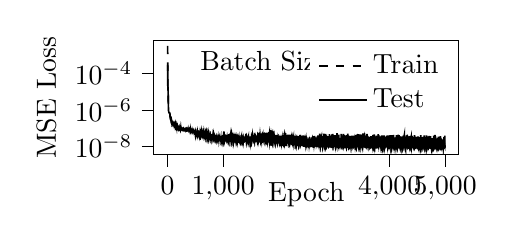
\begin{tikzpicture}

\begin{axis}[
legend cell align={left},
legend style={draw=none},
log basis y={10},
tick align=outside,
tick pos=left,
title={Batch Size 2},
title style={at={(0.4,0.85)},anchor=north},
x grid style={white!69.0196078431373!black},
xlabel={Epoch},
x label style={yshift=13pt},
xmin=-249.95, xmax=5248.95,
xtick style={color=black},
xtick = {0,1000,4000,5000},
y grid style={white!69.0196078431373!black},
ylabel={MSE Loss},
ymin=3.38262380496077e-09, ymax=0.00632854574258151,
ymode=log,
ytick style={color=black},
width=.45\textwidth,
height=.25\textwidth
]
\addplot [semithick, black, dashed]
table {%
0 0.00328254532568099
1 0.000218499955626612
2 0.000191524371870401
3 7.48565430555885e-05
4 1.80191885218974e-05
5 1.70335326928424e-05
6 1.60617069012901e-05
7 1.42414383480727e-05
8 1.17442153426879e-05
9 8.90145301876544e-06
10 6.35426067282552e-06
11 4.48610761718449e-06
12 3.16681323150547e-06
13 2.21908286821115e-06
14 1.57206481016292e-06
15 1.21919172834595e-06
16 1.0618989238651e-06
17 9.78470672838849e-07
18 9.22985532084475e-07
19 8.8099305171685e-07
20 8.4995001972521e-07
21 8.3038449714623e-07
22 8.1447130311485e-07
23 8.01895829424026e-07
24 7.90452571434397e-07
25 7.80588560063133e-07
26 7.67551035850467e-07
27 7.54603072246951e-07
28 7.4473731326119e-07
29 7.34573585697174e-07
30 7.2510382626545e-07
31 7.15328201120524e-07
32 7.06132008384763e-07
33 6.96060642347618e-07
34 6.86012559671934e-07
35 6.76093364214037e-07
36 6.65401749750494e-07
37 6.55946847171407e-07
38 6.46543756017692e-07
39 6.3489944804207e-07
40 6.18515371762385e-07
41 5.85002741245066e-07
42 5.21904763381542e-07
43 4.64107343058906e-07
44 4.31738605658261e-07
45 4.08880619641838e-07
46 3.87349231173229e-07
47 3.69826064049672e-07
48 3.53238981003257e-07
49 3.40011401617657e-07
50 3.28091449871115e-07
51 3.16790916875087e-07
52 3.058581874682e-07
53 2.96605351175927e-07
54 2.8681011950682e-07
55 2.7820315102689e-07
56 2.70656728957208e-07
57 2.63857507705412e-07
58 2.57623938459961e-07
59 2.52528075400882e-07
60 2.47351241863703e-07
61 2.42858798984225e-07
62 2.38187733390793e-07
63 2.34476871070921e-07
64 2.31448094974551e-07
65 2.28447264819964e-07
66 2.25276748428538e-07
67 2.22910076783212e-07
68 2.19949171984757e-07
69 2.18757366997169e-07
70 2.16757680979729e-07
71 2.1456885103599e-07
72 2.12431132567414e-07
73 2.12453675991098e-07
74 2.09875333198273e-07
75 2.08367902884143e-07
76 2.06870915439472e-07
77 2.05759142446249e-07
78 2.03537200378245e-07
79 2.02386158929979e-07
80 2.01577248807538e-07
81 1.99945309896199e-07
82 1.98954125483652e-07
83 1.97998061242988e-07
84 1.95277801370519e-07
85 1.94122259384422e-07
86 1.9321474032008e-07
87 1.92061395219989e-07
88 1.90649255421116e-07
89 1.88983075970039e-07
90 1.87258018107261e-07
91 1.86211353437882e-07
92 1.84968773373595e-07
93 1.8346280023851e-07
94 1.81952997721835e-07
95 1.80662087380323e-07
96 1.79365444776147e-07
97 1.77472094651909e-07
98 1.76493799261546e-07
99 1.74580053132978e-07
100 1.73360636676279e-07
101 1.72267877915688e-07
102 1.70442489901279e-07
103 1.69188082461469e-07
104 1.67839397578917e-07
105 1.66230285953528e-07
106 1.64829462242722e-07
107 1.63325331338671e-07
108 1.62738196491152e-07
109 1.60219138044426e-07
110 1.60535278213469e-07
111 1.58536466712489e-07
112 1.56850298218325e-07
113 1.55524901216397e-07
114 1.54631709402775e-07
115 1.53302759073659e-07
116 1.51466843822945e-07
117 1.49550631134643e-07
118 1.48410193441917e-07
119 1.47384696155495e-07
120 1.46283629718358e-07
121 1.44345578623639e-07
122 1.43203171090622e-07
123 1.41263757020393e-07
124 1.40215976953906e-07
125 1.38600845025039e-07
126 1.37061671532823e-07
127 1.36200254846841e-07
128 1.34788054034773e-07
129 1.32993649122337e-07
130 1.31643087291855e-07
131 1.30615223781883e-07
132 1.28918619770713e-07
133 1.27769738631822e-07
134 1.26176427465929e-07
135 1.25179997131242e-07
136 1.23230363925919e-07
137 1.22045724761821e-07
138 1.21201524557857e-07
139 1.19549983392364e-07
140 1.18310560280777e-07
141 1.16812820882495e-07
142 1.15443738707643e-07
143 1.14161057509832e-07
144 1.1312136743713e-07
145 1.11719248588327e-07
146 1.10043574582441e-07
147 1.09814437586175e-07
148 1.08579877910908e-07
149 1.07548462370266e-07
150 1.0619949556756e-07
151 1.0495877468919e-07
152 1.04168265051441e-07
153 1.02623975512528e-07
154 1.01427549126121e-07
155 1.01362208877243e-07
156 9.95105090075832e-08
157 9.90712999682231e-08
158 9.81297963442707e-08
159 9.76671625630976e-08
160 9.38856064496285e-08
161 9.09411816544248e-08
162 8.88011398124666e-08
163 8.8803014968053e-08
164 8.77907267728961e-08
165 8.71906158357305e-08
166 8.74571203014485e-08
167 8.68890042542425e-08
168 8.61177263807855e-08
169 8.60476076310901e-08
170 8.55405427711009e-08
171 8.58966112591286e-08
172 8.51639051044906e-08
173 8.51758944812042e-08
174 8.47307304080447e-08
175 8.48132693269665e-08
176 8.51079388366482e-08
177 8.49318124505061e-08
178 8.47849283748259e-08
179 8.48751120090529e-08
180 8.42010138485394e-08
181 8.44082437067017e-08
182 8.40907957427861e-08
183 8.38560661877707e-08
184 8.42076578552176e-08
185 8.38791066610778e-08
186 8.37576944041629e-08
187 8.40239886347183e-08
188 8.38833574516862e-08
189 8.33899735629418e-08
190 8.34640443237999e-08
191 8.35304616458865e-08
192 8.31852537088729e-08
193 8.30714862566362e-08
194 8.33851301329513e-08
195 8.27072170499488e-08
196 8.32493552452851e-08
197 8.22546665798507e-08
198 8.27084489483099e-08
199 8.21670082453707e-08
200 8.25011616596427e-08
201 8.18873943000398e-08
202 8.22608535500091e-08
203 8.1495268684395e-08
204 8.20163649861705e-08
205 8.16005401669262e-08
206 8.11489030099199e-08
207 8.16204926260555e-08
208 8.09058569459786e-08
209 8.10499177033019e-08
210 8.07727945287828e-08
211 8.08666219838106e-08
212 8.08093064915694e-08
213 8.02509398206697e-08
214 8.09831349148915e-08
215 8.00564518014246e-08
216 8.00968553160697e-08
217 8.01893686681598e-08
218 8.01536400982794e-08
219 7.95515807424652e-08
220 7.96363922979104e-08
221 8.03492120219351e-08
222 7.98713108027815e-08
223 7.96498008956981e-08
224 7.95084208592423e-08
225 7.95095037848803e-08
226 7.94453084611568e-08
227 7.89366283454607e-08
228 7.92334955032059e-08
229 7.92735157912894e-08
230 7.89827368313789e-08
231 7.85786661230414e-08
232 7.87854531203447e-08
233 7.85752367177262e-08
234 7.85788053452308e-08
235 7.82479060256192e-08
236 7.87282694114655e-08
237 7.80035227161413e-08
238 7.84374309548141e-08
239 7.78576224716998e-08
240 7.77167863775796e-08
241 7.81467363761834e-08
242 7.75516917973507e-08
243 7.74188098600082e-08
244 7.74798297724644e-08
245 7.7469969126609e-08
246 7.71800704708614e-08
247 7.71970539117373e-08
248 7.69478892151954e-08
249 7.73572983933102e-08
250 7.71568599475803e-08
251 7.69779501024193e-08
252 7.71894792475081e-08
253 7.67477751884016e-08
254 7.6877333195835e-08
255 7.65848046396789e-08
256 7.65385336909397e-08
257 7.63672228696333e-08
258 7.6301277346813e-08
259 7.62444665756146e-08
260 7.62738956281428e-08
261 7.59071467697492e-08
262 7.59964418058923e-08
263 7.59101158571696e-08
264 7.60531896979444e-08
265 7.57084843583389e-08
266 7.57804675006746e-08
267 7.57439965304307e-08
268 7.55281243759454e-08
269 7.54863963056129e-08
270 7.55834353999285e-08
271 7.5430192249204e-08
272 7.54428438793919e-08
273 7.52991162173977e-08
274 7.51532936485999e-08
275 7.51941930451361e-08
276 7.51544057150388e-08
277 7.48605089656573e-08
278 7.49440059444328e-08
279 7.48363137593744e-08
280 7.45955682426303e-08
281 7.46543589628113e-08
282 7.45810491539212e-08
283 7.45009416183162e-08
284 7.45298077395873e-08
285 7.43874965440927e-08
286 7.42333786614147e-08
287 7.43559364357882e-08
288 7.44611771404946e-08
289 7.43719104612239e-08
290 7.4087228369879e-08
291 7.42675714614505e-08
292 7.40377803589709e-08
293 7.39002887022444e-08
294 7.37450820641472e-08
295 7.37146042358861e-08
296 7.34764170412516e-08
297 7.34748401464147e-08
298 7.33259203234971e-08
299 7.32177149885826e-08
300 7.30713860042087e-08
301 7.31287919658596e-08
302 7.3047478842847e-08
303 7.30429494556484e-08
304 7.26866788871572e-08
305 7.28189107246369e-08
306 7.2611721922522e-08
307 7.25180870284614e-08
308 7.25546002222632e-08
309 7.23407575197177e-08
310 7.22547411237118e-08
311 7.23688810853051e-08
312 7.23001925837519e-08
313 7.23487935944123e-08
314 7.21203149054439e-08
315 7.23077199693556e-08
316 7.21352630661531e-08
317 7.20632900854667e-08
318 7.19566260092286e-08
319 7.1823656741965e-08
320 7.17751821249779e-08
321 7.18084207751435e-08
322 7.15284738002087e-08
323 7.15922071675701e-08
324 7.14385197908563e-08
325 7.11717999838379e-08
326 7.14794709065769e-08
327 7.11045747163741e-08
328 7.1172664772412e-08
329 7.10999585191718e-08
330 7.10373534636988e-08
331 7.10004941901765e-08
332 7.09694212622791e-08
333 7.10542106029388e-08
334 7.11422026586916e-08
335 7.06343104364127e-08
336 7.06290690287714e-08
337 7.058199697485e-08
338 7.05904521041134e-08
339 7.06610755990544e-08
340 7.02293932595133e-08
341 7.0213167338129e-08
342 7.01696666369767e-08
343 7.01245406067308e-08
344 7.02258261991995e-08
345 7.00943012788002e-08
346 6.99631210515639e-08
347 6.99243554992401e-08
348 6.99733587956608e-08
349 6.97487408191089e-08
350 6.96652839086154e-08
351 6.94952265442028e-08
352 6.9586298279356e-08
353 6.94802141264495e-08
354 6.94029599760393e-08
355 6.94811662502737e-08
356 6.9447535515188e-08
357 6.94013545918804e-08
358 6.94406791021951e-08
359 6.90969612737735e-08
360 6.91050193839526e-08
361 6.8881994686576e-08
362 6.87944344484048e-08
363 6.88425664659986e-08
364 6.87802862303633e-08
365 6.87643034696928e-08
366 6.85632615471388e-08
367 6.85682310238578e-08
368 6.83307170623593e-08
369 6.82866018121286e-08
370 6.85272045393148e-08
371 6.79966236415419e-08
372 6.84238423972472e-08
373 6.79873843945078e-08
374 6.81644149632676e-08
375 6.80043897696159e-08
376 6.79346173235729e-08
377 6.78095727341121e-08
378 6.76759811131245e-08
379 6.78007946736114e-08
380 6.7796770238715e-08
381 6.75536845422542e-08
382 6.73928114495181e-08
383 6.72945608075626e-08
384 6.73337297967258e-08
385 6.72205919783897e-08
386 6.72738835988396e-08
387 6.69181899951576e-08
388 6.71726448415733e-08
389 6.6735886535163e-08
390 6.67219459820068e-08
391 6.67162453900083e-08
392 6.65349611206345e-08
393 6.63832358627214e-08
394 6.63773440239268e-08
395 6.6198406551754e-08
396 6.61917400128775e-08
397 6.60644241761155e-08
398 6.62409058879154e-08
399 6.59781503837831e-08
400 6.58956399993693e-08
401 6.60107959022938e-08
402 6.5846786045487e-08
403 6.55407205336633e-08
404 6.55228505987981e-08
405 6.55955494313076e-08
406 6.52562304821469e-08
407 6.52904168840784e-08
408 6.56664842482169e-08
409 6.48951202171233e-08
410 6.52150227713477e-08
411 6.48234405338233e-08
412 6.50295594792905e-08
413 6.473958666664e-08
414 6.46367741741205e-08
415 6.44284369182291e-08
416 6.4706066168263e-08
417 6.41347029111117e-08
418 6.4321762164754e-08
419 6.38945435269545e-08
420 6.41486727785967e-08
421 6.38424642197544e-08
422 6.41088489685693e-08
423 6.37925187760846e-08
424 6.37641166327807e-08
425 6.34406229562678e-08
426 6.35571083453801e-08
427 6.32675255589632e-08
428 6.33023986322812e-08
429 6.29458381071757e-08
430 6.31480538190177e-08
431 6.27496439844499e-08
432 6.25742152867703e-08
433 6.25643662857112e-08
434 6.24544778045077e-08
435 6.2011825340047e-08
436 6.2753866577947e-08
437 6.18486373562543e-08
438 6.19743378120763e-08
439 6.20571040625961e-08
440 6.18520889781316e-08
441 6.16609228023535e-08
442 6.13968909650708e-08
443 6.14124531921334e-08
444 6.11450753005283e-08
445 6.09623349119293e-08
446 6.05825954643757e-08
447 6.04997935236273e-08
448 6.05668844602114e-08
449 6.05799478256008e-08
450 6.01981422974074e-08
451 5.9961909875561e-08
452 5.97201968506322e-08
453 5.96139426777276e-08
454 5.95120054305287e-08
455 5.92951785870488e-08
456 5.95512403165355e-08
457 5.93397249657457e-08
458 5.92162069610325e-08
459 5.89310149428091e-08
460 5.87983697155625e-08
461 5.86480213723428e-08
462 5.86585211733715e-08
463 5.81024033210475e-08
464 5.79005150566081e-08
465 5.7884217427695e-08
466 5.75974278191893e-08
467 5.72717783334786e-08
468 5.71280839249955e-08
469 5.70866307733064e-08
470 5.68234420759151e-08
471 5.65403589207758e-08
472 5.64500327302486e-08
473 5.62552928184967e-08
474 5.59582069550313e-08
475 5.59200681947702e-08
476 5.5690757583271e-08
477 5.51963993931093e-08
478 5.49973188885833e-08
479 5.45198159787041e-08
480 5.44046598370818e-08
481 5.41920685905861e-08
482 5.38668678436993e-08
483 5.361629318823e-08
484 5.32998607738477e-08
485 5.30580958801874e-08
486 5.32657221515853e-08
487 5.25750263348224e-08
488 5.23441807802616e-08
489 5.24424364887199e-08
490 5.18821803626723e-08
491 5.19918664291241e-08
492 5.1747341199504e-08
493 5.13785602573869e-08
494 5.11840279411868e-08
495 5.12938131975726e-08
496 5.0924607952807e-08
497 5.10876863294429e-08
498 5.07458053390364e-08
499 5.06220796397949e-08
500 5.04064744368815e-08
501 5.06455437344622e-08
502 4.9862071242579e-08
503 4.97268267137807e-08
504 4.94142680242948e-08
505 4.97652903030943e-08
506 4.94748283430546e-08
507 4.90965448383118e-08
508 4.87868712980566e-08
509 4.90490110020003e-08
510 4.92224223346271e-08
511 4.89848744311683e-08
512 4.86528948101528e-08
513 4.87841283199897e-08
514 4.84146250535611e-08
515 4.9023456144659e-08
516 4.81331435734367e-08
517 4.80398341196064e-08
518 4.88083406132711e-08
519 4.84064391683692e-08
520 4.84159776592552e-08
521 4.75737229264639e-08
522 4.8519928558588e-08
523 4.73770784747973e-08
524 4.83165005312758e-08
525 4.78193792249337e-08
526 4.78251361750726e-08
527 4.70196307974513e-08
528 4.80083285770982e-08
529 4.71223468826443e-08
530 4.71813922692244e-08
531 4.7113969577961e-08
532 4.70967598273919e-08
533 4.70621662446158e-08
534 4.66326605940148e-08
535 4.76241100443309e-08
536 4.66664954731355e-08
537 4.74405901805808e-08
538 4.69436936714196e-08
539 4.72466676191274e-08
540 4.70211507684337e-08
541 4.63547233083839e-08
542 4.61678381813435e-08
543 4.6965799879839e-08
544 4.63857039533222e-08
545 4.63133353306167e-08
546 4.62923420408989e-08
547 4.6108359860686e-08
548 4.64648258927669e-08
549 4.58507157922727e-08
550 4.595448568534e-08
551 4.60644132552757e-08
552 4.57460573870527e-08
553 4.48977841176479e-08
554 4.61474039982757e-08
555 4.54119244746032e-08
556 4.50748147138302e-08
557 4.51294110412337e-08
558 4.52713001330984e-08
559 4.45902119108332e-08
560 4.54390254731596e-08
561 4.45883604294206e-08
562 4.40688434577563e-08
563 4.46767707545925e-08
564 4.43456282678834e-08
565 4.43052667442601e-08
566 4.4511835127603e-08
567 4.44672186858952e-08
568 4.40549484904684e-08
569 4.38604737291737e-08
570 4.36744109219012e-08
571 4.33528694978591e-08
572 4.36945165810387e-08
573 4.35054831703363e-08
574 4.3339193234071e-08
575 4.33224534239773e-08
576 4.28230918373407e-08
577 4.29915050395024e-08
578 4.3157082451617e-08
579 4.29085400865947e-08
580 4.27126839501746e-08
581 4.34098694395701e-08
582 4.2637734657236e-08
583 4.27076143056926e-08
584 4.31071084622259e-08
585 4.27677483794131e-08
586 4.2361920931655e-08
587 4.25198561692097e-08
588 4.25564854413807e-08
589 4.23260934941938e-08
590 4.18924031443391e-08
591 4.22129305257257e-08
592 4.16024839526852e-08
593 4.16946787210604e-08
594 4.17917192728767e-08
595 4.16310181681201e-08
596 4.13894368075374e-08
597 4.14773096925058e-08
598 4.10987801270912e-08
599 4.12405630366708e-08
600 4.19068369599263e-08
601 4.11747850240785e-08
602 4.14282939695809e-08
603 4.06905636430865e-08
604 4.08110460305977e-08
605 4.11398571306121e-08
606 4.09925211455886e-08
607 4.06709809314121e-08
608 4.11535621287484e-08
609 4.03891638949272e-08
610 4.03422490115046e-08
611 4.04638569014848e-08
612 4.03521925785855e-08
613 4.02347802692105e-08
614 3.96676463815804e-08
615 4.05902976614581e-08
616 3.9934611743786e-08
617 3.97000445235829e-08
618 3.93751615644367e-08
619 3.99356786361937e-08
620 3.94967812543667e-08
621 3.9478045169461e-08
622 3.9357216289726e-08
623 3.91124260917808e-08
624 3.93788417034635e-08
625 3.91443982862283e-08
626 3.94537697414044e-08
627 3.92543143685753e-08
628 3.88451565003223e-08
629 3.87263305199337e-08
630 3.90169901079984e-08
631 3.90409084574106e-08
632 3.90292650599422e-08
633 3.8848819337356e-08
634 3.826467254886e-08
635 3.86679600120066e-08
636 3.84189770820664e-08
637 3.8034914403573e-08
638 3.83765584659468e-08
639 3.84147417166192e-08
640 3.81209554103368e-08
641 3.76586081726193e-08
642 3.7909612859377e-08
643 3.79556497944744e-08
644 3.75772361053683e-08
645 3.7929992070862e-08
646 3.75065041919309e-08
647 3.7582637523681e-08
648 3.71357294101093e-08
649 3.74972402298335e-08
650 3.73230137498126e-08
651 3.7014256861978e-08
652 3.67768056607209e-08
653 3.72723442765288e-08
654 3.69532771464787e-08
655 3.67656498795332e-08
656 3.70444940477888e-08
657 3.74225217392166e-08
658 3.64024413511688e-08
659 3.66532642359085e-08
660 3.6914308742364e-08
661 3.6492219348927e-08
662 3.66049217205844e-08
663 3.68115249901324e-08
664 3.63449829077767e-08
665 3.59703634603137e-08
666 3.65043941129017e-08
667 3.64438717505577e-08
668 3.61117691105584e-08
669 3.59725088353025e-08
670 3.58938531116459e-08
671 3.56944948786131e-08
672 3.54274465845794e-08
673 3.58843036923351e-08
674 3.51804919540566e-08
675 3.592879544001e-08
676 3.51167567705923e-08
677 3.54670594818751e-08
678 3.4856420939644e-08
679 3.52466294488152e-08
680 3.47822667237652e-08
681 3.53631174087043e-08
682 3.46637306734565e-08
683 3.47526936601283e-08
684 3.45369711179377e-08
685 3.44024175803481e-08
686 3.45784007663719e-08
687 3.43725343730505e-08
688 3.42645183736834e-08
689 3.43503181767235e-08
690 3.43352946233222e-08
691 3.41738478102926e-08
692 3.45125217628417e-08
693 3.38059283864212e-08
694 3.44023723802267e-08
695 3.34726516930117e-08
696 3.39030477289892e-08
697 3.36896250675012e-08
698 3.33158177039938e-08
699 3.35237944595335e-08
700 3.32292014725288e-08
701 3.3578084904895e-08
702 3.35027595368964e-08
703 3.39071785393497e-08
704 3.293375946406e-08
705 3.30269301683228e-08
706 3.3574827676075e-08
707 3.33444393947335e-08
708 3.33603552093997e-08
709 3.28944379845431e-08
710 3.27157034414327e-08
711 3.30092747191646e-08
712 3.29718086783393e-08
713 3.29110067269767e-08
714 3.27898127228665e-08
715 3.29078348913492e-08
716 3.22872896388327e-08
717 3.27488542049559e-08
718 3.24483861559588e-08
719 3.27850294034593e-08
720 3.26606627359949e-08
721 3.23589595196405e-08
722 3.24584725308608e-08
723 3.26674511605951e-08
724 3.1575581434129e-08
725 3.25877752292425e-08
726 3.20928140972732e-08
727 3.24274801469793e-08
728 3.25003616281627e-08
729 3.18399988796236e-08
730 3.2109916644596e-08
731 3.20759825324646e-08
732 3.18597185383629e-08
733 3.19681254596915e-08
734 3.22229387327844e-08
735 3.17291694599264e-08
736 3.21273451338033e-08
737 3.17449717723295e-08
738 3.15686945521754e-08
739 3.17564476380316e-08
740 3.17477588294146e-08
741 3.10420353661356e-08
742 3.20795690111342e-08
743 3.1216206289153e-08
744 3.11819914966538e-08
745 3.0873233597184e-08
746 3.14768186575609e-08
747 3.0342848171272e-08
748 3.17283036666005e-08
749 3.09738106077373e-08
750 3.10661259300682e-08
751 3.08984813262025e-08
752 3.06028083156829e-08
753 3.11116006412315e-08
754 3.11124808433094e-08
755 3.09768128804455e-08
756 3.11854558228131e-08
757 3.10072328188471e-08
758 3.1022588369789e-08
759 3.01097631762448e-08
760 3.08949155709559e-08
761 3.08619954873524e-08
762 3.05116490219026e-08
763 3.14621224050682e-08
764 3.06109915238495e-08
765 3.0499886474411e-08
766 3.02687262935253e-08
767 3.03926383860009e-08
768 2.94455249570946e-08
769 2.99938384391574e-08
770 3.05687051307957e-08
771 2.98737279285088e-08
772 3.03895292956824e-08
773 3.02582276905938e-08
774 2.97754409906981e-08
775 3.0655070072716e-08
776 2.97111483765766e-08
777 3.00233681251871e-08
778 2.98320518886119e-08
779 3.06805578830227e-08
780 3.02031067299646e-08
781 2.96468851478937e-08
782 3.0587170042895e-08
783 2.99796532466923e-08
784 3.06078738928628e-08
785 2.92830425706048e-08
786 3.0212400990437e-08
787 2.9719811062312e-08
788 2.93865345387112e-08
789 3.00758327314021e-08
790 2.99608398715012e-08
791 2.98255288354032e-08
792 3.01842756250115e-08
793 3.01570450788047e-08
794 2.9858412152417e-08
795 3.0092274968585e-08
796 3.02506790859636e-08
797 2.91831633476569e-08
798 2.95765616485921e-08
799 2.99364189229601e-08
800 3.00087392374193e-08
801 3.05344552096187e-08
802 3.01328082645269e-08
803 2.99154144154934e-08
804 2.94597860326373e-08
805 2.93265596476022e-08
806 2.9981135665047e-08
807 2.97405996949052e-08
808 2.97528969943062e-08
809 2.97964703900311e-08
810 2.93363185845386e-08
811 2.99720110352175e-08
812 2.96175842905422e-08
813 2.96315429029193e-08
814 2.96446226587532e-08
815 2.99707815297201e-08
816 2.95448832050571e-08
817 2.95232755386232e-08
818 2.87613123848285e-08
819 2.95836693727236e-08
820 2.94098747234406e-08
821 2.91337529105262e-08
822 2.93476053093156e-08
823 2.87491110401716e-08
824 2.89403561636314e-08
825 2.95640055761326e-08
826 2.85100923496651e-08
827 2.90359088045422e-08
828 2.89738495633518e-08
829 2.93372802613323e-08
830 2.93234274397203e-08
831 2.88658978312428e-08
832 2.86577576900093e-08
833 2.93334803106449e-08
834 2.79551181306403e-08
835 2.93240796755412e-08
836 2.84651544498193e-08
837 2.85353146382561e-08
838 2.86506699791467e-08
839 2.80141502583264e-08
840 2.90341042116782e-08
841 2.83219711137428e-08
842 2.88628372929201e-08
843 2.81941445002265e-08
844 2.86616231613412e-08
845 2.80926744038457e-08
846 2.87754205431923e-08
847 2.85303202081644e-08
848 2.81727098084272e-08
849 2.8123937935165e-08
850 2.84582470004846e-08
851 2.8650369424621e-08
852 2.85608268651982e-08
853 2.8131232703843e-08
854 2.82453610964128e-08
855 2.89483162182469e-08
856 2.83420080103847e-08
857 2.82199570773578e-08
858 2.80730314435318e-08
859 2.82809190177979e-08
860 2.86353769445857e-08
861 2.82259201612178e-08
862 2.78959342820406e-08
863 2.78645208896533e-08
864 2.81846941814212e-08
865 2.81121721020239e-08
866 2.80517562643023e-08
867 2.81593320271001e-08
868 2.72528267648564e-08
869 2.81696339985427e-08
870 2.79273086642995e-08
871 2.7512817953157e-08
872 2.84517497671222e-08
873 2.7799637717929e-08
874 2.74260516970881e-08
875 2.7788204698842e-08
876 2.73057909985774e-08
877 2.83043334327049e-08
878 2.64792259140334e-08
879 2.77433954551931e-08
880 2.80859690999224e-08
881 2.81571656352009e-08
882 2.76695006193872e-08
883 2.77709883268473e-08
884 2.6881104866483e-08
885 2.78426782351904e-08
886 2.77167030259817e-08
887 2.78135435696769e-08
888 2.78613534441252e-08
889 2.74576081790157e-08
890 2.72004491331246e-08
891 2.7812381422021e-08
892 2.74803205711494e-08
893 2.72247917181279e-08
894 2.76698133706565e-08
895 2.75316115931346e-08
896 2.72633557068525e-08
897 2.75284972862111e-08
898 2.75199321894126e-08
899 2.73734412948312e-08
900 2.72344164200522e-08
901 2.74171147513491e-08
902 2.8005013492205e-08
903 2.72693796256607e-08
904 2.71729967772916e-08
905 2.70847596891555e-08
906 2.76970295121637e-08
907 2.70154164276337e-08
908 2.71905937012651e-08
909 2.74396833003232e-08
910 2.67758121418882e-08
911 2.80058317719267e-08
912 2.79118399847678e-08
913 2.63474409490927e-08
914 2.71324295361142e-08
915 2.7954368273797e-08
916 2.7007748962693e-08
917 2.64737631885392e-08
918 2.76175025140657e-08
919 2.68041697211174e-08
920 2.71468540083974e-08
921 2.700771886055e-08
922 2.75985255401845e-08
923 2.69180859497897e-08
924 2.69624495977117e-08
925 2.68577280076454e-08
926 2.704912061402e-08
927 2.6356536705241e-08
928 2.66672037859128e-08
929 2.69591033794092e-08
930 2.68079865403115e-08
931 2.63138631513837e-08
932 2.72206234661621e-08
933 2.71317316304365e-08
934 2.7307047371139e-08
935 2.65802619039413e-08
936 2.73144441089168e-08
937 2.63830216658545e-08
938 2.66981474648098e-08
939 2.6431935854887e-08
940 2.60439990913408e-08
941 2.67252916980043e-08
942 2.66271156456055e-08
943 2.6739769780626e-08
944 2.62611098725829e-08
945 2.62674960841425e-08
946 2.70139238268685e-08
947 2.63460659326586e-08
948 2.62264182295802e-08
949 2.70272808373662e-08
950 2.5747153010236e-08
951 2.66053678841804e-08
952 2.64551851290595e-08
953 2.67567574317451e-08
954 2.58916772901685e-08
955 2.64584350602726e-08
956 2.61099018731836e-08
957 2.66250582974248e-08
958 2.59226130361612e-08
959 2.64767316645598e-08
960 2.6452490843043e-08
961 2.58215259816841e-08
962 2.59265999303371e-08
963 2.62359932220457e-08
964 2.65424289648264e-08
965 2.67450139063707e-08
966 2.63561833882819e-08
967 2.57741525678257e-08
968 2.62758306087407e-08
969 2.65221036650498e-08
970 2.64172919469674e-08
971 2.56274016323943e-08
972 2.57729816374175e-08
973 2.59577244466347e-08
974 2.6222427415179e-08
975 2.62312397004694e-08
976 2.5963541613383e-08
977 2.56496797129135e-08
978 2.56104738609597e-08
979 2.62138495017994e-08
980 2.58349842333083e-08
981 2.6208806482575e-08
982 2.54673980373543e-08
983 2.56343059095165e-08
984 2.62062766909765e-08
985 2.52106715502853e-08
986 2.51687390236954e-08
987 2.61188593480566e-08
988 2.52318605282187e-08
989 2.56387556114013e-08
990 2.54048550445418e-08
991 2.53413983453687e-08
992 2.55538864205596e-08
993 2.5451171698665e-08
994 2.61896682761109e-08
995 2.54498613648235e-08
996 2.55230583791621e-08
997 2.48618900541842e-08
998 2.58373611447538e-08
999 2.51232853774597e-08
1000 2.56220291215414e-08
1001 2.56736006327141e-08
1002 2.51882083300847e-08
1003 2.53713824167612e-08
1004 2.58137432954941e-08
1005 2.48481835016801e-08
1006 2.56784723412506e-08
1007 2.40642600508045e-08
1008 2.56810740124624e-08
1009 2.54665775721308e-08
1010 2.43275138776256e-08
1011 2.61642387404115e-08
1012 2.48960325622827e-08
1013 2.58067697424536e-08
1014 2.57083646426348e-08
1015 2.49647724676894e-08
1016 2.54706723878118e-08
1017 2.44838401316505e-08
1018 2.5243788890239e-08
1019 2.52713618028588e-08
1020 2.47552457360301e-08
1021 2.50724322887752e-08
1022 2.57186888398264e-08
1023 2.51238573180101e-08
1024 2.44940838938223e-08
1025 2.52199264209607e-08
1026 2.57123974063966e-08
1027 2.50377650737044e-08
1028 2.51321844116914e-08
1029 2.45223809804962e-08
1030 2.48290043978749e-08
1031 2.53573499313098e-08
1032 2.4809457069952e-08
1033 2.55327429933838e-08
1034 2.49863649272875e-08
1035 2.54338735914406e-08
1036 2.46765876222854e-08
1037 2.48556650924159e-08
1038 2.46800521991331e-08
1039 2.51365618709754e-08
1040 2.41794125941386e-08
1041 2.44692986407224e-08
1042 2.47765058001559e-08
1043 2.48758484036604e-08
1044 2.41757049636859e-08
1045 2.4206212695721e-08
1046 2.55829298876631e-08
1047 2.41762240022481e-08
1048 2.47289624125679e-08
1049 2.5234407058039e-08
1050 2.43533080388492e-08
1051 2.47249283025774e-08
1052 2.44511952491311e-08
1053 2.45763102038055e-08
1054 2.45536552540004e-08
1055 2.48305525572534e-08
1056 2.40834935295586e-08
1057 2.53211549907095e-08
1058 2.41439715079061e-08
1059 2.57494680457604e-08
1060 2.35057552473161e-08
1061 2.49778252063293e-08
1062 2.40053659600614e-08
1063 2.4876820900549e-08
1064 2.45837317633946e-08
1065 2.43284918397257e-08
1066 2.40939658241457e-08
1067 2.51706974384036e-08
1068 2.35143826128326e-08
1069 2.41161983740024e-08
1070 2.4755212258476e-08
1071 2.4246693290042e-08
1072 2.56388721965872e-08
1073 2.41264563889954e-08
1074 2.44039392134909e-08
1075 2.51708382467408e-08
1076 2.45340783286419e-08
1077 2.45209754993758e-08
1078 2.48115112856939e-08
1079 2.39203909974672e-08
1080 2.31613966679145e-08
1081 2.50456757703854e-08
1082 2.43899172222006e-08
1083 2.40393221376256e-08
1084 2.41358175256112e-08
1085 2.3699030541946e-08
1086 2.43306819150413e-08
1087 2.42609329062504e-08
1088 2.39897964542934e-08
1089 2.44988888764563e-08
1090 2.45195678220678e-08
1091 2.40963733417754e-08
1092 2.39458951021843e-08
1093 2.37625303336486e-08
1094 2.44664175362286e-08
1095 2.36047424231611e-08
1096 2.45438499066886e-08
1097 2.4314623127103e-08
1098 2.39301791060131e-08
1099 2.417096244689e-08
1100 2.39409680004576e-08
1101 2.42720179199352e-08
1102 2.42393090368331e-08
1103 2.40999026286381e-08
1104 2.42074585857788e-08
1105 2.3707304635745e-08
1106 2.34363956257144e-08
1107 2.36964240676596e-08
1108 2.36679420671515e-08
1109 2.38906914948878e-08
1110 2.46842266887759e-08
1111 2.31558109071162e-08
1112 2.37190626790618e-08
1113 2.35072627912114e-08
1114 2.4207290549999e-08
1115 2.3632586413358e-08
1116 2.4249042063107e-08
1117 2.3715847715905e-08
1118 2.38752562103928e-08
1119 2.48957234907365e-08
1120 2.32552377015804e-08
1121 2.49651159680564e-08
1122 2.28996111810154e-08
1123 2.34150135410283e-08
1124 2.41551524927108e-08
1125 2.34782538071077e-08
1126 2.43804897772648e-08
1127 2.31835085818255e-08
1128 2.3253374320964e-08
1129 2.32561741067006e-08
1130 2.50726553251424e-08
1131 2.29548132411883e-08
1132 2.3328192227362e-08
1133 2.41420011705684e-08
1134 2.33821172641313e-08
1135 2.3303387180762e-08
1136 2.43730284085197e-08
1137 2.41564589041898e-08
1138 2.37143871552048e-08
1139 2.36588560203199e-08
1140 2.30154500006075e-08
1141 2.4859979055103e-08
1142 2.29174441709334e-08
1143 2.38801621325058e-08
1144 2.44339880565159e-08
1145 2.38689083146837e-08
1146 2.28463232741505e-08
1147 2.46741202382939e-08
1148 2.41791558530102e-08
1149 2.29663980678141e-08
1150 2.39159831927349e-08
1151 2.43229607134743e-08
1152 2.28362273965721e-08
1153 2.31572237742172e-08
1154 2.33627679651072e-08
1155 2.27080735474283e-08
1156 2.4358588360418e-08
1157 2.26149591309732e-08
1158 2.3826834529006e-08
1159 2.35227404605243e-08
1160 2.2895686424329e-08
1161 2.40749804307216e-08
1162 2.26256669050295e-08
1163 2.33396992000423e-08
1164 2.30482095263662e-08
1165 2.44169308798725e-08
1166 2.39379462509404e-08
1167 2.23706146176839e-08
1168 2.37480671272938e-08
1169 2.3676940001105e-08
1170 2.34087737608912e-08
1171 2.3882939918618e-08
1172 2.30129306417748e-08
1173 2.31911079903724e-08
1174 2.24837282247203e-08
1175 2.29678447716819e-08
1176 2.3352444612823e-08
1177 2.3275783645138e-08
1178 2.36324950197431e-08
1179 2.44034234366253e-08
1180 2.2084830024971e-08
1181 2.42513723696935e-08
1182 2.16930364395074e-08
1183 2.25338594886382e-08
1184 2.28829293547617e-08
1185 2.39440693926563e-08
1186 2.2315187542532e-08
1187 2.36924562428409e-08
1188 2.20071196566085e-08
1189 2.32872066795453e-08
1190 2.39950020853863e-08
1191 2.17920868925692e-08
1192 2.27612380520603e-08
1193 2.3995818000222e-08
1194 2.22051254888389e-08
1195 2.46911551403106e-08
1196 2.19987103602382e-08
1197 2.24494658944141e-08
1198 2.54094465522159e-08
1199 2.06954137310644e-08
1200 2.39629729154589e-08
1201 2.31854273466947e-08
1202 2.26924926745031e-08
1203 2.40487618563545e-08
1204 2.13842529988295e-08
1205 2.39762664323573e-08
1206 2.25271042649244e-08
1207 2.24390193712121e-08
1208 2.4125746498016e-08
1209 2.21658715069406e-08
1210 2.28044628429736e-08
1211 2.48385112019966e-08
1212 2.33656474967758e-08
1213 2.12154672926679e-08
1214 2.41168022632188e-08
1215 2.127196985513e-08
1216 2.41087441434362e-08
1217 2.23791959621522e-08
1218 2.24479696701585e-08
1219 2.30527769330691e-08
1220 2.41279960776497e-08
1221 2.22326906687553e-08
1222 2.24541030668934e-08
1223 2.22194493112449e-08
1224 2.33363321254232e-08
1225 2.30219892352057e-08
1226 2.20189755480715e-08
1227 2.30715657988378e-08
1228 2.25623969505317e-08
1229 2.24376861742148e-08
1230 2.21420095534164e-08
1231 2.41717404863839e-08
1232 2.20276527142516e-08
1233 2.24890027827329e-08
1234 2.36996848195781e-08
1235 2.19429958308592e-08
1236 2.31160184864798e-08
1237 2.46116306463207e-08
1238 2.23464107134141e-08
1239 2.19672915339753e-08
1240 2.24700124982213e-08
1241 2.36331999026174e-08
1242 2.33265122337456e-08
1243 2.13752408421142e-08
1244 2.33078071993353e-08
1245 2.32677361167721e-08
1246 2.21433261852755e-08
1247 2.40962325241401e-08
1248 2.26305257871595e-08
1249 2.21173026355714e-08
1250 2.39238219879034e-08
1251 2.13247202381361e-08
1252 2.37189196605203e-08
1253 2.32250552512636e-08
1254 2.16647174275386e-08
1255 2.2491087962706e-08
1256 2.34335919854778e-08
1257 2.19791799298541e-08
1258 2.35654252513373e-08
1259 2.14169790457852e-08
1260 2.35637368361241e-08
1261 2.1728992364356e-08
1262 2.31331254670342e-08
1263 2.26170422073235e-08
1264 2.35172557362939e-08
1265 2.14990163194817e-08
1266 2.36890559190961e-08
1267 2.17138146291762e-08
1268 2.44956976728217e-08
1269 2.12130341750993e-08
1270 2.29326911906358e-08
1271 2.294375372347e-08
1272 2.21282134780787e-08
1273 2.37402650568597e-08
1274 2.14494472419724e-08
1275 2.28301129672759e-08
1276 2.20507827259908e-08
1277 2.38259531475382e-08
1278 2.14158515750573e-08
1279 2.44407928549073e-08
1280 2.20708781046852e-08
1281 2.28768149491132e-08
1282 2.2626050056429e-08
1283 2.3005323938563e-08
1284 2.1827455709722e-08
1285 2.22817814335419e-08
1286 2.34458954926908e-08
1287 2.12545711266165e-08
1288 2.32935544570156e-08
1289 2.18443757705744e-08
1290 2.20137667314435e-08
1291 2.26713250879862e-08
1292 2.2973785081537e-08
1293 2.30200027910299e-08
1294 2.19761202549518e-08
1295 2.24197731544806e-08
1296 2.17526179136229e-08
1297 2.37097571550993e-08
1298 2.20199593771175e-08
1299 2.23016867821613e-08
1300 2.22305995936645e-08
1301 2.33038597228785e-08
1302 2.38850469355678e-08
1303 2.09000387388913e-08
1304 2.26636061739782e-08
1305 2.2103954332886e-08
1306 2.28347936062634e-08
1307 2.19457175233972e-08
1308 2.22836593346543e-08
1309 2.23504406504094e-08
1310 2.22128115497378e-08
1311 2.28280098716338e-08
1312 2.31253715030633e-08
1313 2.11736454615585e-08
1314 2.20795589808143e-08
1315 2.24833086843179e-08
1316 2.32801941796312e-08
1317 2.14961897331001e-08
1318 2.20238446245746e-08
1319 2.2324847892885e-08
1320 2.19785063278466e-08
1321 2.35137257901807e-08
1322 2.3144701277622e-08
1323 2.10336239354625e-08
1324 2.23880651935016e-08
1325 2.16761783147779e-08
1326 2.26090178953031e-08
1327 2.28862650982764e-08
1328 2.21212273828209e-08
1329 2.16299618250315e-08
1330 2.29643947586289e-08
1331 2.26928735589382e-08
1332 2.20482249578269e-08
1333 2.18015371278302e-08
1334 2.20884739085547e-08
1335 2.3364725292907e-08
1336 2.15798587311355e-08
1337 2.36228769332492e-08
1338 2.27154247446348e-08
1339 2.18096778484278e-08
1340 2.21108368879674e-08
1341 2.21310831148291e-08
1342 2.20017822580854e-08
1343 2.19745016792339e-08
1344 2.21375170811888e-08
1345 2.21948070953104e-08
1346 2.21312608935653e-08
1347 2.22437780286744e-08
1348 2.19581330651586e-08
1349 2.20827062501483e-08
1350 2.18945214304211e-08
1351 2.29315245998118e-08
1352 2.21396365736037e-08
1353 2.25976545702999e-08
1354 2.1405512023176e-08
1355 2.20842132633847e-08
1356 2.24522939798466e-08
1357 2.26773350752718e-08
1358 2.14882492814428e-08
1359 2.2369567684366e-08
1360 2.17191727960309e-08
1361 2.19919470932917e-08
1362 2.2311646740325e-08
1363 2.25913608749573e-08
1364 2.21926017565655e-08
1365 2.15259211113761e-08
1366 2.16004253598134e-08
1367 2.32224484773558e-08
1368 2.15576274351648e-08
1369 2.25957661512677e-08
1370 2.1665183021935e-08
1371 2.22470384803053e-08
1372 2.227040601116e-08
1373 2.18528204138368e-08
1374 2.21331229738886e-08
1375 2.32569008955519e-08
1376 2.05272220124009e-08
1377 2.2737146274765e-08
1378 2.17802189304006e-08
1379 2.20164517975019e-08
1380 2.26876345494897e-08
1381 2.14601053055152e-08
1382 2.13699287613944e-08
1383 2.16462507426907e-08
1384 2.21368567230318e-08
1385 2.28223008749695e-08
1386 2.15268508930722e-08
1387 2.18877246265792e-08
1388 2.23609083401244e-08
1389 2.2065903218349e-08
1390 2.26112779765364e-08
1391 2.21005944214259e-08
1392 2.21072447048609e-08
1393 2.2372629410905e-08
1394 2.21432812628208e-08
1395 2.25536891302891e-08
1396 2.20534070987655e-08
1397 2.2955050506257e-08
1398 2.26208074964873e-08
1399 2.18272057315172e-08
1400 2.16593289958933e-08
1401 2.27141324652957e-08
1402 2.20719237945533e-08
1403 2.17082151288683e-08
1404 2.20936218085499e-08
1405 2.1863136471012e-08
1406 2.21187039824433e-08
1407 2.10590157191937e-08
1408 2.29186094085621e-08
1409 2.21961395413528e-08
1410 2.20644468408859e-08
1411 2.22680759182081e-08
1412 2.22331608497606e-08
1413 2.04469981444633e-08
1414 2.1789090508928e-08
1415 2.25222602415753e-08
1416 2.11176890110853e-08
1417 2.25176194232346e-08
1418 2.15985122689055e-08
1419 2.2313166706811e-08
1420 2.30230737420234e-08
1421 2.18747423230137e-08
1422 2.16363518343865e-08
1423 2.3068403635973e-08
1424 2.1838906702043e-08
1425 2.22338019213453e-08
1426 2.13278609508261e-08
1427 2.29623013299207e-08
1428 2.1098088403726e-08
1429 2.24614715425009e-08
1430 2.12589236732175e-08
1431 2.26730734765868e-08
1432 2.10315514134751e-08
1433 2.27212884548189e-08
1434 2.09692620500856e-08
1435 2.26583690920989e-08
1436 2.04742908186395e-08
1437 2.28886742472678e-08
1438 2.12501669026866e-08
1439 2.31694822255268e-08
1440 2.19335935971454e-08
1441 2.07122653302361e-08
1442 2.32995183077067e-08
1443 2.13800517415708e-08
1444 2.19378508171109e-08
1445 2.17659652216318e-08
1446 2.25236484944213e-08
1447 2.14525019416878e-08
1448 2.11303392904094e-08
1449 2.22758848886784e-08
1450 2.15706849791553e-08
1451 2.30910437937215e-08
1452 2.07915529506497e-08
1453 2.22041605880685e-08
1454 2.20864075464178e-08
1455 2.2056206184895e-08
1456 2.15564313329752e-08
1457 2.11379826827729e-08
1458 2.20233888020283e-08
1459 2.28370447180604e-08
1460 2.11876432199554e-08
1461 2.22300986445489e-08
1462 2.16021678987599e-08
1463 2.17324369022887e-08
1464 2.21292224406588e-08
1465 2.23671277076454e-08
1466 2.14703611854938e-08
1467 2.05927899782354e-08
1468 2.33626976558488e-08
1469 2.05264296654906e-08
1470 2.18535323567859e-08
1471 2.11968200043433e-08
1472 2.18168553881015e-08
1473 2.26454652578756e-08
1474 2.11857142232708e-08
1475 2.13278918422266e-08
1476 2.236010990736e-08
1477 2.17072662658802e-08
1478 2.2110143227283e-08
1479 2.22466864685522e-08
1480 2.06100590163238e-08
1481 2.22854114886872e-08
1482 2.19793991453332e-08
1483 2.16467689184152e-08
1484 2.05775316386991e-08
1485 2.19673081403582e-08
1486 2.19401898399474e-08
1487 2.20589850682407e-08
1488 2.05005431839767e-08
1489 2.15492483782165e-08
1490 2.19645833702264e-08
1491 2.21786140069957e-08
1492 2.16240650679489e-08
1493 2.21673701460423e-08
1494 2.08698478573743e-08
1495 2.19098450867095e-08
1496 2.15752541418146e-08
1497 2.19070329576798e-08
1498 2.16886264846616e-08
1499 2.23972178054754e-08
1500 2.14879013741287e-08
1501 2.11427105282214e-08
1502 2.18200978853167e-08
1503 2.19430892073325e-08
1504 2.18239163790046e-08
1505 2.12949392383033e-08
1506 2.09734695226782e-08
1507 2.21864767561142e-08
1508 2.10699609919374e-08
1509 2.23657064514771e-08
1510 2.08754557393664e-08
1511 2.13593325406602e-08
1512 2.2237284218074e-08
1513 2.22302955611431e-08
1514 2.14894843014179e-08
1515 2.17345119775114e-08
1516 2.2619548078251e-08
1517 2.03632252265273e-08
1518 2.222387638251e-08
1519 2.0638844568599e-08
1520 2.15556459234878e-08
1521 2.13329812444041e-08
1522 2.17516634387072e-08
1523 2.14504079945055e-08
1524 2.1713463724482e-08
1525 2.17702472103398e-08
1526 2.1144652500471e-08
1527 2.25338103538308e-08
1528 2.08841337764332e-08
1529 2.15978603308464e-08
1530 2.19219352285416e-08
1531 2.20143767911685e-08
1532 2.03035153048536e-08
1533 2.2025311063878e-08
1534 2.17098071511601e-08
1535 2.13676841006594e-08
1536 2.13570003706476e-08
1537 2.1934463194706e-08
1538 2.08679860155825e-08
1539 2.17718971614045e-08
1540 2.17795787115782e-08
1541 2.0858285151415e-08
1542 2.24124813391069e-08
1543 2.04172527167312e-08
1544 2.15674865017834e-08
1545 2.08105447176421e-08
1546 2.24757190159242e-08
1547 2.05159294637824e-08
1548 2.13008872599341e-08
1549 2.16085264567178e-08
1550 2.19470851841597e-08
1551 2.03223949322706e-08
1552 2.185089607043e-08
1553 2.13339257819634e-08
1554 2.15402248593122e-08
1555 2.14160982039413e-08
1556 2.01167598529173e-08
1557 2.26113181088783e-08
1558 2.07763320684284e-08
1559 2.09940509560136e-08
1560 2.20850009061691e-08
1561 2.12568992129514e-08
1562 2.02256049313676e-08
1563 2.1572822483884e-08
1564 2.16699280349841e-08
1565 2.0615541992508e-08
1566 2.06423681782808e-08
1567 2.166503550044e-08
1568 2.10671617285607e-08
1569 2.14949159996203e-08
1570 2.1486425486994e-08
1571 2.15268085630993e-08
1572 2.13709459728206e-08
1573 2.16338703817875e-08
1574 2.10054343868227e-08
1575 2.13374942872324e-08
1576 2.12356059929308e-08
1577 2.12236877222272e-08
1578 2.10683743684381e-08
1579 2.08947822623595e-08
1580 2.15873571304814e-08
1581 2.12413833508007e-08
1582 2.09700386497036e-08
1583 2.12016539590798e-08
1584 2.15563715610934e-08
1585 2.1320752146059e-08
1586 2.03603190020996e-08
1587 2.12582940875561e-08
1588 2.12172731384186e-08
1589 2.02699212337176e-08
1590 2.20828432360709e-08
1591 2.1214635882838e-08
1592 2.13622964505e-08
1593 1.97430580893276e-08
1594 2.12411482926056e-08
1595 2.14440202571664e-08
1596 2.10006369820159e-08
1597 2.17859179567625e-08
1598 2.0235362363008e-08
1599 2.04990278194206e-08
1600 2.15114643131731e-08
1601 2.12136672634311e-08
1602 2.10565060696499e-08
1603 2.06974479114996e-08
1604 2.09672476611522e-08
1605 2.13972567624232e-08
1606 2.10050519521832e-08
1607 2.11634919160542e-08
1608 2.0377558411111e-08
1609 2.08424264296903e-08
1610 2.10613512971747e-08
1611 2.03827716233063e-08
1612 2.10774802880676e-08
1613 2.16909275381205e-08
1614 2.08061425025496e-08
1615 2.16821348084095e-08
1616 2.00827403420978e-08
1617 2.14326192789493e-08
1618 2.0886740560111e-08
1619 2.06261215081605e-08
1620 2.10243560460621e-08
1621 2.07960275404595e-08
1622 2.25939935346031e-08
1623 2.00754938110004e-08
1624 2.13006339671584e-08
1625 2.07714345401011e-08
1626 2.13699255519062e-08
1627 2.03209101736768e-08
1628 2.15345861875882e-08
1629 2.11747947819751e-08
1630 2.13044938350837e-08
1631 2.09285056221864e-08
1632 2.01563148522488e-08
1633 2.09758108913327e-08
1634 2.1033877327159e-08
1635 2.05582696706785e-08
1636 2.09445135741504e-08
1637 2.16082702595433e-08
1638 2.02584275107442e-08
1639 2.09558489613348e-08
1640 2.07689595774774e-08
1641 2.07192879271845e-08
1642 2.06510428122919e-08
1643 2.07699233630287e-08
1644 2.0945563378616e-08
1645 2.00693340571267e-08
1646 2.11850924219936e-08
1647 2.08621823265531e-08
1648 2.14372208716951e-08
1649 2.00777119370166e-08
1650 2.10464146206957e-08
1651 2.03655942334624e-08
1652 2.116797909546e-08
1653 2.0567977439323e-08
1654 2.05833627826002e-08
1655 2.11277772809715e-08
1656 2.02255754654379e-08
1657 2.05347024668789e-08
1658 2.07974972378233e-08
1659 2.07040936341385e-08
1660 2.125038495987e-08
1661 2.07568319029461e-08
1662 2.0540897870569e-08
1663 2.10844162818469e-08
1664 2.0664589149455e-08
1665 2.13458649447329e-08
1666 2.06672683403797e-08
1667 2.06801024614234e-08
1668 2.24235970135989e-08
1669 1.94159916998005e-08
1670 2.13912904705182e-08
1671 1.96632176960865e-08
1672 2.08929274824743e-08
1673 2.00195758683908e-08
1674 2.10947335824163e-08
1675 2.02750038719723e-08
1676 2.07836373894432e-08
1677 2.11531913649754e-08
1678 2.01446989003262e-08
1679 2.08387502769747e-08
1680 2.04161593123642e-08
1681 2.05984701128759e-08
1682 2.02896431875654e-08
1683 2.0784214079278e-08
1684 2.03638555499874e-08
1685 2.08065610730057e-08
1686 1.99266829629119e-08
1687 1.98274610484495e-08
1688 2.12027175480467e-08
1689 2.01258229359236e-08
1690 2.04192807561343e-08
1691 2.0244818738635e-08
1692 2.04134685816149e-08
1693 2.07590184096995e-08
1694 1.97931712457855e-08
1695 2.12182541722283e-08
1696 2.07085533392992e-08
1697 2.08150154550057e-08
1698 2.0150691754095e-08
1699 2.03884645156582e-08
1700 1.9981964141158e-08
1701 2.04798565106024e-08
1702 2.00128432735203e-08
1703 2.03456553543036e-08
1704 2.04984107742001e-08
1705 2.04226748335423e-08
1706 2.03883581166298e-08
1707 2.04168203871702e-08
1708 2.01871644562035e-08
1709 2.08082571559465e-08
1710 2.00099698109968e-08
1711 2.0073435322121e-08
1712 2.04274871000165e-08
1713 1.97532883394746e-08
1714 2.03794064899121e-08
1715 2.04595487891535e-08
1716 1.96010728217288e-08
1717 2.02891627128499e-08
1718 2.01114561025895e-08
1719 2.02730936599838e-08
1720 2.03354554155766e-08
1721 2.009367281397e-08
1722 1.96820410204857e-08
1723 2.0558937455506e-08
1724 2.0036221832942e-08
1725 1.95301241616708e-08
1726 2.06445165078784e-08
1727 1.9952838398285e-08
1728 2.08422879668935e-08
1729 2.0532360991643e-08
1730 2.03628449579329e-08
1731 1.96703473039905e-08
1732 2.00313833502719e-08
1733 2.02990081339116e-08
1734 2.03848712307941e-08
1735 2.01351870868227e-08
1736 2.03616221083336e-08
1737 1.9487600981305e-08
1738 2.06080648691709e-08
1739 2.00369801208189e-08
1740 2.01591428402592e-08
1741 1.95835970830949e-08
1742 1.96984339789763e-08
1743 2.0168838884338e-08
1744 1.96078943374145e-08
1745 1.97731697413883e-08
1746 1.96421198397356e-08
1747 2.02246203417911e-08
1748 1.95303810274217e-08
1749 1.99385093649918e-08
1750 1.9599204083065e-08
1751 2.00508693835311e-08
1752 2.00207590216328e-08
1753 1.96941995011524e-08
1754 2.00437013692101e-08
1755 1.95671013192289e-08
1756 2.00415014116051e-08
1757 1.97756828371753e-08
1758 1.96746720271257e-08
1759 1.99504350356095e-08
1760 1.96920246534615e-08
1761 1.91564397472033e-08
1762 1.9748220688065e-08
1763 1.96420558353783e-08
1764 1.99361020566391e-08
1765 1.9828896739349e-08
1766 1.95296773319309e-08
1767 1.97923776433795e-08
1768 1.95601251013477e-08
1769 1.93734517957567e-08
1770 1.93604421652727e-08
1771 1.90877077947404e-08
1772 1.94577271906971e-08
1773 1.88859376706874e-08
1774 1.92901710699411e-08
1775 1.93312549064406e-08
1776 1.90598275290887e-08
1777 1.91989263302328e-08
1778 1.91442941697151e-08
1779 1.94581371620317e-08
1780 1.90230227741783e-08
1781 1.9659246670134e-08
1782 1.85790437919886e-08
1783 1.90168584565664e-08
1784 1.91749840057209e-08
1785 1.86640737236954e-08
1786 1.88382316684277e-08
1787 1.91034191689421e-08
1788 1.86048687346729e-08
1789 1.90872508509798e-08
1790 1.89885073224039e-08
1791 1.92445259612484e-08
1792 1.88772013159366e-08
1793 1.90235431447028e-08
1794 1.87421044357539e-08
1795 1.92534107267273e-08
1796 1.8736192023916e-08
1797 1.91136935785985e-08
1798 1.85022400225887e-08
1799 1.84365412393972e-08
1800 1.91411018043985e-08
1801 1.81394754082409e-08
1802 1.914207301279e-08
1803 1.8655211493801e-08
1804 1.8868278855444e-08
1805 1.82801271546018e-08
1806 1.9075206398933e-08
1807 1.87558569784696e-08
1808 1.98807898629805e-08
1809 1.89790037719573e-08
1810 1.89332080686166e-08
1811 1.91531059421379e-08
1812 1.86631301248019e-08
1813 1.91970473538139e-08
1814 1.96886070716606e-08
1815 1.90058170742025e-08
1816 1.84966789900654e-08
1817 1.80295595993696e-08
1818 1.88219793690325e-08
1819 1.86221582904045e-08
1820 1.85707411017311e-08
1821 1.91977097760976e-08
1822 1.84250419158483e-08
1823 1.95696567275028e-08
1824 1.90185265163123e-08
1825 1.82467958381172e-08
1826 1.83842304948278e-08
1827 1.92769543364557e-08
1828 1.78828940921583e-08
1829 1.74367601778191e-08
1830 1.90108837813119e-08
1831 1.8807656633868e-08
1832 1.93670671264079e-08
1833 1.83425814149762e-08
1834 1.82389982297249e-08
1835 1.85820953751414e-08
1836 1.75999879642452e-08
1837 1.92346562915557e-08
1838 1.86475583895118e-08
1839 1.84596680436189e-08
1840 1.86191244517797e-08
1841 1.89955333936842e-08
1842 1.83765534494118e-08
1843 1.81521940305074e-08
1844 1.86996980554022e-08
1845 1.82782058064102e-08
1846 1.84444725583877e-08
1847 1.90501617751415e-08
1848 1.83815542114663e-08
1849 1.90445148260665e-08
1850 1.84532257850312e-08
1851 1.77074601265814e-08
1852 1.81908177790957e-08
1853 1.84758387151429e-08
1854 1.82140000268283e-08
1855 1.85040429221961e-08
1856 1.93009569504909e-08
1857 1.91018589382197e-08
1858 1.91126765602678e-08
1859 2.08473474630211e-08
1860 1.62674041778998e-08
1861 1.82452675459854e-08
1862 1.78831495119547e-08
1863 1.84945997612762e-08
1864 1.72114438236892e-08
1865 1.82209869805106e-08
1866 1.83616201580028e-08
1867 1.74827370540698e-08
1868 1.86306525302438e-08
1869 1.8217771108775e-08
1870 1.75417476709905e-08
1871 1.82197729410027e-08
1872 1.8830245598539e-08
1873 1.86379105898138e-08
1874 1.82493392155147e-08
1875 1.95755316301227e-08
1876 1.70504912332947e-08
1877 1.81485997300113e-08
1878 1.84380554086871e-08
1879 1.85232020663284e-08
1880 1.83043269912087e-08
1881 1.73622439054166e-08
1882 1.76635001227221e-08
1883 1.7509043877123e-08
1884 1.78431233227028e-08
1885 1.81750630979666e-08
1886 2.02608482861299e-08
1887 1.62105836530313e-08
1888 1.81056791431489e-08
1889 1.91479715848653e-08
1890 1.82156778152087e-08
1891 1.84860921363106e-08
1892 1.72847974523327e-08
1893 1.80671525439324e-08
1894 1.75526513158664e-08
1895 1.92242510178853e-08
1896 1.75357607465343e-08
1897 1.77452551207991e-08
1898 1.84247462848841e-08
1899 1.80345856204689e-08
1900 1.72025209069226e-08
1901 1.82469431554977e-08
1902 1.70528556776295e-08
1903 1.86851082403516e-08
1904 1.85485660541274e-08
1905 1.79534020416372e-08
1906 1.68311151967637e-08
1907 1.82946590691069e-08
1908 1.73090639691842e-08
1909 1.775790009792e-08
1910 1.76439600312606e-08
1911 1.86014872683438e-08
1912 1.72380557054985e-08
1913 1.78340645943242e-08
1914 1.85307023434222e-08
1915 1.75769968515649e-08
1916 1.78204660878367e-08
1917 1.81126992636615e-08
1918 1.76859984762356e-08
1919 1.75960304976963e-08
1920 1.84841056914409e-08
1921 1.74144345369553e-08
1922 1.75632008950072e-08
1923 1.78872621008075e-08
1924 1.74626052557025e-08
1925 1.89328312114323e-08
1926 1.85949106157601e-08
1927 1.79124507642403e-08
1928 1.75801164735423e-08
1929 1.76206262604839e-08
1930 1.69653687138172e-08
1931 1.78945823507137e-08
1932 1.84466919280202e-08
1933 1.73969727699785e-08
1934 1.78243644208265e-08
1935 1.77302907222177e-08
1936 1.77030572643122e-08
1937 1.70336128217374e-08
1938 1.8232293422682e-08
1939 1.81194217146463e-08
1940 1.7786710878348e-08
1941 1.88942730953157e-08
1942 1.6629329459672e-08
1943 1.83353860564173e-08
1944 1.68795979785807e-08
1945 1.75743684170671e-08
1946 1.82300371942834e-08
1947 1.71288746237397e-08
1948 1.78147496431857e-08
1949 1.74691110064878e-08
1950 1.79930988475907e-08
1951 1.81036638352283e-08
1952 1.74577166723033e-08
1953 1.72818796081997e-08
1954 1.7793818671813e-08
1955 1.82734469837964e-08
1956 1.84251848779349e-08
1957 1.73573116578063e-08
1958 1.83671041979749e-08
1959 1.72378231312886e-08
1960 1.78720783458874e-08
1961 1.80823219213117e-08
1962 1.68310075665812e-08
1963 1.76247301215127e-08
1964 1.68069518891589e-08
1965 1.69070792865877e-08
1966 1.85005203483246e-08
1967 1.73212230022146e-08
1968 1.82373362961341e-08
1969 1.70085511959628e-08
1970 1.75220219346406e-08
1971 1.75572771006771e-08
1972 1.76583124242014e-08
1973 1.70536624985451e-08
1974 1.76895833604446e-08
1975 1.86409325663439e-08
1976 1.72398061487056e-08
1977 1.71435971426936e-08
1978 1.77287361856349e-08
1979 1.76721664158497e-08
1980 1.76705967759594e-08
1981 1.67738381327553e-08
1982 1.71073747236294e-08
1983 1.89454446726245e-08
1984 1.6727477150813e-08
1985 1.70383376532357e-08
1986 1.81838349392616e-08
1987 1.89299549120947e-08
1988 1.68918841501331e-08
1989 1.74283985434481e-08
1990 1.8017723370678e-08
1991 1.69125893935695e-08
1992 1.71157170209824e-08
1993 1.76176005616535e-08
1994 1.66640718295141e-08
1995 1.84542122892845e-08
1996 1.67818756992844e-08
1997 1.69746054360653e-08
1998 1.77532590005941e-08
1999 1.69047378884568e-08
2000 1.76961463652092e-08
2001 1.72504956571784e-08
2002 1.67582778993758e-08
2003 1.87590094081758e-08
2004 1.63163595776616e-08
2005 1.70245570767641e-08
2006 1.74359447377148e-08
2007 1.6983647583485e-08
2008 1.71258157765919e-08
2009 1.69502271862576e-08
2010 1.7019899590881e-08
2011 1.73898007116979e-08
2012 1.67378139171726e-08
2013 1.85384034409319e-08
2014 1.61739766375291e-08
2015 1.72218485075398e-08
2016 1.67302030850136e-08
2017 1.71238359399362e-08
2018 1.61686367563529e-08
2019 1.61612190078542e-08
2020 1.75700319881983e-08
2021 1.67892913397472e-08
2022 1.76003290616733e-08
2023 1.68331096438434e-08
2024 1.68609550021126e-08
2025 1.70562263592244e-08
2026 1.88368698987029e-08
2027 1.56908915849852e-08
2028 1.81652222494e-08
2029 1.6112774170407e-08
2030 1.69801762851529e-08
2031 1.56612666399325e-08
2032 1.75301589180332e-08
2033 1.7821198125878e-08
2034 1.63002470757179e-08
2035 1.68969239289773e-08
2036 1.9533636545388e-08
2037 1.54052793959192e-08
2038 1.74861969015616e-08
2039 1.63220191091717e-08
2040 1.72292791089657e-08
2041 1.76358342828253e-08
2042 1.70481032405884e-08
2043 1.67782333411193e-08
2044 1.64597535763089e-08
2045 1.6784063216313e-08
2046 1.76201322461267e-08
2047 1.65395747553643e-08
2048 1.70710022023568e-08
2049 1.71202640809331e-08
2050 1.64107028645666e-08
2051 1.68721999279642e-08
2052 1.74455782514515e-08
2053 1.61852650495398e-08
2054 1.70779098431217e-08
2055 1.77106110589575e-08
2056 1.69903553374762e-08
2057 1.71130861906232e-08
2058 1.69087772929344e-08
2059 1.64575613526563e-08
2060 1.70504168373054e-08
2061 1.79823255754552e-08
2062 1.66709115185515e-08
2063 1.81308110755729e-08
2064 1.60216045994588e-08
2065 1.61030021358921e-08
2066 1.69147874705122e-08
2067 1.6785143507253e-08
2068 1.90542040051922e-08
2069 1.50932292690142e-08
2070 1.67666080588269e-08
2071 1.78994364996299e-08
2072 1.60827784622675e-08
2073 1.69591491410992e-08
2074 1.695403881255e-08
2075 1.70289635923748e-08
2076 1.5959610320665e-08
2077 1.66299863249841e-08
2078 1.74162769576991e-08
2079 1.57412436258553e-08
2080 1.68725953920146e-08
2081 1.68354336859411e-08
2082 1.8031424715681e-08
2083 1.54898251069069e-08
2084 1.66882965152437e-08
2085 1.73371239878262e-08
2086 1.64661680339406e-08
2087 1.7240239393701e-08
2088 1.61812764979397e-08
2089 1.5988707964848e-08
2090 1.65335036313441e-08
2091 1.72997672053254e-08
2092 1.65463660186105e-08
2093 1.71450934937922e-08
2094 1.65574660764833e-08
2095 1.64482509763253e-08
2096 1.58283432813433e-08
2097 1.60083808073141e-08
2098 1.65858546501141e-08
2099 1.61689850586844e-08
2100 1.64547200643128e-08
2101 1.7000464293343e-08
2102 1.67438309479073e-08
2103 1.62013632536151e-08
2104 1.64778010271482e-08
2105 1.65255312528367e-08
2106 1.62425575241376e-08
2107 1.58036366190717e-08
2108 1.64519810896824e-08
2109 1.69444184409673e-08
2110 1.7687790626969e-08
2111 1.56503521411833e-08
2112 1.62402690818131e-08
2113 1.87394158761012e-08
2114 1.47648843454584e-08
2115 1.62964468775895e-08
2116 1.62653564362014e-08
2117 1.59508854606361e-08
2118 1.6708942957161e-08
2119 1.65585061056295e-08
2120 1.61932830824718e-08
2121 1.86939664922059e-08
2122 1.47771166781885e-08
2123 1.60382114392787e-08
2124 1.6522301453048e-08
2125 1.57415389600013e-08
2126 1.62699343490835e-08
2127 1.6364682755482e-08
2128 1.66286618808187e-08
2129 1.65743795861317e-08
2130 1.63153927665305e-08
2131 1.61052196844258e-08
2132 1.68574106136354e-08
2133 1.57658298888252e-08
2134 1.70226286961006e-08
2135 1.67260549538417e-08
2136 1.59179657245878e-08
2137 1.80693962831269e-08
2138 1.4862591023429e-08
2139 1.67382438879815e-08
2140 1.63436927453908e-08
2141 1.6069376010952e-08
2142 1.5955751963781e-08
2143 1.57864118869588e-08
2144 1.57960454726103e-08
2145 1.64102459229154e-08
2146 1.64761586285145e-08
2147 1.60736210061685e-08
2148 1.71329312041169e-08
2149 1.66229040921284e-08
2150 1.66637344535814e-08
2151 1.53552589183537e-08
2152 1.62442207455593e-08
2153 1.67071321574008e-08
2154 1.5687154236943e-08
2155 1.64053362760874e-08
2156 1.6291465384316e-08
2157 1.60665891917322e-08
2158 1.65528654616637e-08
2159 1.54879202627634e-08
2160 1.65939461944098e-08
2161 1.64557924033637e-08
2162 1.62241342193947e-08
2163 1.64693316074827e-08
2164 1.58313536872678e-08
2165 1.55997191336188e-08
2166 1.65260755848884e-08
2167 1.60782235845702e-08
2168 1.5445875297837e-08
2169 1.5899520658974e-08
2170 1.57324911065349e-08
2171 1.73104459781914e-08
2172 1.5737863737264e-08
2173 1.6006789072931e-08
2174 1.53297753206771e-08
2175 1.58049545608552e-08
2176 1.60099532517943e-08
2177 1.65182953607984e-08
2178 1.6236546200088e-08
2179 1.67868950397554e-08
2180 1.61543074409798e-08
2181 1.69334068832461e-08
2182 1.62784080243172e-08
2183 1.5351187130197e-08
2184 1.58606377936854e-08
2185 1.68994120933186e-08
2186 1.6449883963876e-08
2187 1.60194836147376e-08
2188 1.62020839429844e-08
2189 1.54478956884141e-08
2190 1.61386319435797e-08
2191 1.62104933480178e-08
2192 1.58257323264743e-08
2193 1.66054700496687e-08
2194 1.59580421979499e-08
2195 1.57918853188055e-08
2196 1.60244881991511e-08
2197 1.63633015666798e-08
2198 1.59147434047879e-08
2199 1.66177868272666e-08
2200 1.58827136648998e-08
2201 1.56136985505484e-08
2202 1.61329550109612e-08
2203 1.60476869362769e-08
2204 1.53633735757441e-08
2205 1.60269448691575e-08
2206 1.63052452704926e-08
2207 1.61820082216491e-08
2208 1.63151421249119e-08
2209 1.60591286177125e-08
2210 1.57780898624726e-08
2211 1.59399746596511e-08
2212 1.55949011054202e-08
2213 1.56118647054032e-08
2214 1.62537105922733e-08
2215 1.78938248575344e-08
2216 1.61015524157981e-08
2217 1.59879240315963e-08
2218 1.56660224819305e-08
2219 1.5469829793141e-08
2220 1.56136033079013e-08
2221 1.56852422002751e-08
2222 1.65497947551829e-08
2223 1.6147062225691e-08
2224 1.56605498504714e-08
2225 1.54902240024901e-08
2226 1.51705904623267e-08
2227 1.6740908535734e-08
2228 1.5372456475482e-08
2229 1.51130684618028e-08
2230 1.60444946534222e-08
2231 1.65509063149716e-08
2232 1.59910650317507e-08
2233 1.64411230251515e-08
2234 1.48612712409235e-08
2235 1.53227092761499e-08
2236 1.56827395026149e-08
2237 1.57652707207384e-08
2238 1.56468296588913e-08
2239 1.53809270176664e-08
2240 1.52384464119915e-08
2241 1.50965901997979e-08
2242 1.5272251098819e-08
2243 1.53364532913258e-08
2244 1.54175791221567e-08
2245 1.56899095002661e-08
2246 1.52412291178905e-08
2247 1.61622022906704e-08
2248 1.45620127022239e-08
2249 1.59084759709938e-08
2250 1.5608406087636e-08
2251 1.63330824065888e-08
2252 1.58049807189031e-08
2253 1.55780862161337e-08
2254 1.58618328583715e-08
2255 1.57266361898167e-08
2256 1.56110904286355e-08
2257 1.53052755437755e-08
2258 1.54690360872067e-08
2259 1.56097410301537e-08
2260 1.58833163213246e-08
2261 1.59383706935245e-08
2262 1.53310886864821e-08
2263 1.55052736117156e-08
2264 1.64004163188125e-08
2265 1.4399976812185e-08
2266 1.5118141968945e-08
2267 1.5138443690943e-08
2268 1.49271949870522e-08
2269 1.51895347427766e-08
2270 1.4950340649994e-08
2271 1.53981496373856e-08
2272 1.45873228538929e-08
2273 1.5638045507374e-08
2274 1.52622634924104e-08
2275 1.58236243623933e-08
2276 1.54874225400947e-08
2277 1.52022556084153e-08
2278 1.58603825186621e-08
2279 1.48279702318066e-08
2280 1.48029139281081e-08
2281 1.52696373000305e-08
2282 1.51455048213178e-08
2283 1.53047539916407e-08
2284 1.45134372283307e-08
2285 1.50584025954692e-08
2286 1.50968634252402e-08
2287 1.54474710278851e-08
2288 1.48557998370658e-08
2289 1.49802274787003e-08
2290 1.57257548749345e-08
2291 1.52231957637194e-08
2292 1.51956602780223e-08
2293 1.51121362128304e-08
2294 1.46546926817481e-08
2295 1.52027060581206e-08
2296 1.50910814547545e-08
2297 1.637356124784e-08
2298 1.52268735857664e-08
2299 1.49002743344562e-08
2300 1.52285145212372e-08
2301 1.51188161556792e-08
2302 1.49378383408061e-08
2303 1.49917599286398e-08
2304 1.59507081435861e-08
2305 1.54421847540498e-08
2306 1.5889685862816e-08
2307 1.49651685885932e-08
2308 1.49448718377021e-08
2309 1.56537961556735e-08
2310 1.43876361373696e-08
2311 1.49415162531003e-08
2312 1.56002921335857e-08
2313 1.47851650904862e-08
2314 1.52707441507527e-08
2315 1.49725170510984e-08
2316 1.54689461332735e-08
2317 1.48582177647572e-08
2318 1.51415572208768e-08
2319 1.53349501287731e-08
2320 1.54211789449576e-08
2321 1.49917635013097e-08
2322 1.57139358588632e-08
2323 1.523806406592e-08
2324 1.41977142321253e-08
2325 1.48844658757197e-08
2326 1.56470397052466e-08
2327 1.5720110716988e-08
2328 1.45455616627765e-08
2329 1.43878460381608e-08
2330 1.55571091718654e-08
2331 1.69769424401001e-08
2332 1.43379908835589e-08
2333 1.51817729120429e-08
2334 1.47587248541248e-08
2335 1.47221055666613e-08
2336 1.56550859518323e-08
2337 1.44886958269586e-08
2338 1.53171188732037e-08
2339 1.51798046035961e-08
2340 1.50086644143954e-08
2341 1.55837942329984e-08
2342 1.41473862669966e-08
2343 1.52601526321183e-08
2344 1.5611616297026e-08
2345 1.46392797557293e-08
2346 1.44600729450606e-08
2347 1.60895925856441e-08
2348 1.43965355759446e-08
2349 1.51251438704758e-08
2350 1.56960626181979e-08
2351 1.45130771765367e-08
2352 1.56193426422979e-08
2353 1.36251255543618e-08
2354 1.56642062329737e-08
2355 1.49791442205505e-08
2356 1.49137864440541e-08
2357 1.40824772173198e-08
2358 1.48005724340539e-08
2359 1.4094291088701e-08
2360 1.43244372710072e-08
2361 1.52586667565568e-08
2362 1.51089859495857e-08
2363 1.41859577416359e-08
2364 1.49804795661346e-08
2365 1.55596273539588e-08
2366 1.51044000313294e-08
2367 1.37663557468748e-08
2368 1.52903764934625e-08
2369 1.43373051433304e-08
2370 1.51376896138089e-08
2371 1.40771702527021e-08
2372 1.43176586470395e-08
2373 1.48776149483665e-08
2374 1.50838863660352e-08
2375 1.53010453837477e-08
2376 1.34471152856142e-08
2377 1.44013810757793e-08
2378 1.43448910017718e-08
2379 1.4558868122988e-08
2380 1.43158819080336e-08
2381 1.45032994602612e-08
2382 1.49703035726978e-08
2383 1.38878160590161e-08
2384 1.38000479852629e-08
2385 1.48717560317646e-08
2386 1.39814422439599e-08
2387 1.47365221271345e-08
2388 1.46742711956693e-08
2389 1.43831441804521e-08
2390 1.51605817415856e-08
2391 1.45851476459763e-08
2392 1.3730038068982e-08
2393 1.42464172160073e-08
2394 1.49961971588342e-08
2395 1.32937654223619e-08
2396 1.49140905705558e-08
2397 1.44958415264351e-08
2398 1.50562786911945e-08
2399 1.32703593149763e-08
2400 1.44707290475193e-08
2401 1.44781321068654e-08
2402 1.55713178412592e-08
2403 1.4154323517368e-08
2404 1.53718623792654e-08
2405 1.55593994019265e-08
2406 1.27946345628432e-08
2407 1.42685118831865e-08
2408 1.39482844354194e-08
2409 1.47281781538999e-08
2410 1.45308241972925e-08
2411 1.37700165953603e-08
2412 1.57781276691471e-08
2413 1.24336463633024e-08
2414 1.42189504822587e-08
2415 1.3714956803218e-08
2416 1.39042800869627e-08
2417 1.34682833813349e-08
2418 1.43851136587547e-08
2419 1.40042119955719e-08
2420 1.38508426083261e-08
2421 1.3986362513374e-08
2422 1.39723953683502e-08
2423 1.41810766390721e-08
2424 1.39708648276837e-08
2425 1.37401213492483e-08
2426 1.28390226640795e-08
2427 1.80930342806584e-08
2428 1.14635859725654e-08
2429 1.41882262156973e-08
2430 1.35112757432831e-08
2431 1.46995436551695e-08
2432 1.26204469294566e-08
2433 1.42892564347769e-08
2434 1.48303872938294e-08
2435 1.26600362421597e-08
2436 1.4365937639399e-08
2437 1.39216447699597e-08
2438 1.29058827789408e-08
2439 1.39131369316092e-08
2440 1.39576358804405e-08
2441 1.38566057759637e-08
2442 1.44660727237345e-08
2443 1.29507664492212e-08
2444 1.43456730406222e-08
2445 1.69131630982922e-08
2446 1.14682972315178e-08
2447 1.41734148936812e-08
2448 1.37426505217031e-08
2449 1.38305498841584e-08
2450 1.36870764512187e-08
2451 1.28776849706025e-08
2452 1.45689885400618e-08
2453 1.27700102144079e-08
2454 1.62535699466393e-08
2455 1.18398832098243e-08
2456 1.37513202754791e-08
2457 1.55754256372098e-08
2458 1.30196437090335e-08
2459 1.3985324463589e-08
2460 1.28154749663711e-08
2461 1.2920120477794e-08
2462 1.44530519959329e-08
2463 1.43993935284858e-08
2464 1.23132531092696e-08
2465 1.40929049913807e-08
2466 1.43193774011785e-08
2467 1.34331063671167e-08
2468 1.45920768739594e-08
2469 1.31740001871328e-08
2470 1.3997656061443e-08
2471 1.3197326652642e-08
2472 1.4680547495316e-08
2473 1.37311893077807e-08
2474 1.36432642489359e-08
2475 1.2956431567207e-08
2476 1.39666465761856e-08
2477 1.34180522737976e-08
2478 1.46590436776312e-08
2479 1.40340257799715e-08
2480 1.35557649103696e-08
2481 1.34649069179899e-08
2482 1.36465452412471e-08
2483 1.51822540902513e-08
2484 1.35887579722771e-08
2485 1.3916675489889e-08
2486 1.34714242424616e-08
2487 1.29129023504065e-08
2488 1.38233170007274e-08
2489 1.42250153267465e-08
2490 1.34880934452575e-08
2491 1.50194389743896e-08
2492 1.32370336082058e-08
2493 1.3808990907152e-08
2494 1.43753181183481e-08
2495 1.39492842860731e-08
2496 1.37608207124995e-08
2497 1.29461337179809e-08
2498 1.31839308496473e-08
2499 1.44428849543077e-08
2500 1.30904132089327e-08
2501 1.33328298480839e-08
2502 1.31675680532795e-08
2503 1.52160251270447e-08
2504 1.29485482381342e-08
2505 1.3834427853715e-08
2506 1.50733605561587e-08
2507 1.29546123952551e-08
2508 1.47353337002637e-08
2509 1.32251943207456e-08
2510 1.38496275601113e-08
2511 1.30826884298108e-08
2512 1.4264636940084e-08
2513 1.2497446637838e-08
2514 1.43429514867996e-08
2515 1.37639591855365e-08
2516 1.35242655322082e-08
2517 1.30719986385919e-08
2518 1.29740738325779e-08
2519 1.40453654501049e-08
2520 1.28295300224068e-08
2521 1.39296891199167e-08
2522 1.44704273748186e-08
2523 1.37965537111914e-08
2524 1.24967038209745e-08
2525 1.51012409278228e-08
2526 1.29557431798807e-08
2527 1.38194591659119e-08
2528 1.30599127381587e-08
2529 1.30153666925564e-08
2530 1.27637956268759e-08
2531 1.42781639479589e-08
2532 1.34268954813249e-08
2533 1.39969155436015e-08
2534 1.32066012266188e-08
2535 1.31042851788804e-08
2536 1.16005870571603e-08
2537 1.36061878396321e-08
2538 1.32144763199046e-08
2539 1.4218177038422e-08
2540 1.2990268485405e-08
2541 1.35930897345524e-08
2542 1.38522534410546e-08
2543 1.34882469834743e-08
2544 1.24881699635274e-08
2545 1.43795968247859e-08
2546 1.3547400809874e-08
2547 1.31889383387651e-08
2548 1.38131223376414e-08
2549 1.28582434734334e-08
2550 1.36698049061634e-08
2551 1.3222155564277e-08
2552 1.37354576549356e-08
2553 1.33077148689806e-08
2554 1.40416254434811e-08
2555 1.27987866282361e-08
2556 1.30609322286507e-08
2557 1.39533113447526e-08
2558 1.31254731756264e-08
2559 1.30473240109868e-08
2560 1.30240669774934e-08
2561 1.39098110809241e-08
2562 1.20567211125688e-08
2563 1.41082347460963e-08
2564 1.30849357856538e-08
2565 1.26282928167853e-08
2566 1.36639765186894e-08
2567 1.3349850694927e-08
2568 1.35121295994217e-08
2569 1.34073342548807e-08
2570 1.25167438645296e-08
2571 1.2238151629318e-08
2572 1.33072815094587e-08
2573 1.43142725323106e-08
2574 1.29910572219116e-08
2575 1.34873320193768e-08
2576 1.41168529050328e-08
2577 1.2723873166906e-08
2578 1.34497162719571e-08
2579 1.32887885584548e-08
2580 1.30373683225535e-08
2581 1.34695347231706e-08
2582 1.35366050360367e-08
2583 1.31984131223201e-08
2584 1.3380255231954e-08
2585 1.19185161126037e-08
2586 1.3334138993043e-08
2587 1.19889812221774e-08
2588 1.3094673464456e-08
2589 1.29784715271059e-08
2590 1.40490003884969e-08
2591 1.20793272235936e-08
2592 1.37655989561059e-08
2593 1.32554021319217e-08
2594 1.226614372591e-08
2595 1.31944015512239e-08
2596 1.30837136727083e-08
2597 1.37714054339322e-08
2598 1.35442441575595e-08
2599 1.32473988149473e-08
2600 1.34004783060443e-08
2601 1.43953213931902e-08
2602 1.34208382366469e-08
2603 1.36868944016141e-08
2604 1.23628363764838e-08
2605 1.39903718488973e-08
2606 1.29373662775129e-08
2607 1.29643233052271e-08
2608 1.17336066457786e-08
2609 1.28859242583129e-08
2610 1.35669291601512e-08
2611 1.26032665298814e-08
2612 1.39901216196364e-08
2613 1.15813792499198e-08
2614 1.3670652163171e-08
2615 1.27122545763719e-08
2616 1.45476330862676e-08
2617 1.31804031632266e-08
2618 1.25134058570897e-08
2619 1.42093455749205e-08
2620 1.18135388936201e-08
2621 1.25516240784482e-08
2622 1.40233328861164e-08
2623 1.34194506381247e-08
2624 1.21021876107602e-08
2625 1.32637060264382e-08
2626 1.15451061710736e-08
2627 1.37601757170328e-08
2628 1.2973773167696e-08
2629 1.2526211260272e-08
2630 1.36624720374623e-08
2631 1.34546458144535e-08
2632 1.20180376711743e-08
2633 1.36082798670861e-08
2634 1.24855974703436e-08
2635 1.33813691941195e-08
2636 1.26162293034027e-08
2637 1.34657784788272e-08
2638 1.30532202041039e-08
2639 1.34990319901676e-08
2640 1.40551890338986e-08
2641 1.27816521321988e-08
2642 1.31187205709565e-08
2643 1.25195951768686e-08
2644 1.29647294349958e-08
2645 1.31847419292536e-08
2646 1.32802387820818e-08
2647 1.34049314463938e-08
2648 1.37182005032627e-08
2649 1.36175731101432e-08
2650 1.29337927713691e-08
2651 1.3246510542117e-08
2652 1.31706684968064e-08
2653 1.19101927212109e-08
2654 1.39000706883968e-08
2655 1.34143085038507e-08
2656 1.29272691818255e-08
2657 1.31111579394355e-08
2658 1.31674152976033e-08
2659 1.23336135830626e-08
2660 1.32152881778119e-08
2661 1.36623964167443e-08
2662 1.28301956386773e-08
2663 1.32405033686084e-08
2664 1.21167951567108e-08
2665 1.40936554769572e-08
2666 1.25885262407879e-08
2667 1.32316453080594e-08
2668 1.2617103289661e-08
2669 1.2883164887012e-08
2670 1.29090635844348e-08
2671 1.24183746564761e-08
2672 1.32739162347906e-08
2673 1.2962147321556e-08
2674 1.23780074303137e-08
2675 1.27687107035826e-08
2676 1.31493052778209e-08
2677 1.33301558353227e-08
2678 1.31169956324936e-08
2679 1.3716775212412e-08
2680 1.264422722317e-08
2681 1.30089475437259e-08
2682 1.14183781440291e-08
2683 1.35857658347324e-08
2684 1.34396031060136e-08
2685 1.53774735858897e-08
2686 1.2508209189778e-08
2687 1.31163440569293e-08
2688 1.29405676536493e-08
2689 1.28551493920742e-08
2690 1.36502127432783e-08
2691 1.21205489021364e-08
2692 1.3266486045535e-08
2693 1.27766616436625e-08
2694 1.33942432842815e-08
2695 1.27588340959259e-08
2696 1.20211278257579e-08
2697 1.35453917106398e-08
2698 1.22171818871808e-08
2699 1.40663212195025e-08
2700 1.30602371607794e-08
2701 1.25704985005221e-08
2702 1.31970520161756e-08
2703 1.36887342102252e-08
2704 1.26346613236461e-08
2705 1.19184599784994e-08
2706 1.29627470719096e-08
2707 1.33481468222729e-08
2708 1.28514413829731e-08
2709 1.20972853677459e-08
2710 1.36949241450329e-08
2711 1.32112759794883e-08
2712 1.40348612773927e-08
2713 1.23829016110896e-08
2714 1.3589564440003e-08
2715 1.22620879013657e-08
2716 1.34441246287115e-08
2717 1.33258467781144e-08
2718 1.32639492725489e-08
2719 1.30041071071119e-08
2720 1.34190460017759e-08
2721 1.40524435286657e-08
2722 1.25536914336866e-08
2723 1.40535358272437e-08
2724 1.23746003126771e-08
2725 1.22981991112076e-08
2726 1.39208140714428e-08
2727 1.28738551917473e-08
2728 1.20653035514118e-08
2729 1.20865761033262e-08
2730 1.35196049529315e-08
2731 1.37821142541378e-08
2732 1.26984896213975e-08
2733 1.2956382186749e-08
2734 1.28595170764412e-08
2735 1.35205032919875e-08
2736 1.31814350459308e-08
2737 1.24456384967137e-08
2738 1.40465307685994e-08
2739 1.32679251080084e-08
2740 1.35969562957e-08
2741 1.18329807909587e-08
2742 1.2648368674123e-08
2743 1.1999414231384e-08
2744 1.2987734804154e-08
2745 1.29861542859863e-08
2746 1.29769111429159e-08
2747 1.32399133950939e-08
2748 1.30018688902431e-08
2749 1.22972428078794e-08
2750 1.41248221311244e-08
2751 1.27476384762792e-08
2752 1.31196854708804e-08
2753 1.34343857789709e-08
2754 1.2313538813008e-08
2755 1.29670785382063e-08
2756 1.34640570444711e-08
2757 1.35555095726048e-08
2758 1.2593486552491e-08
2759 1.32723089212444e-08
2760 1.27861513070787e-08
2761 1.2976886150276e-08
2762 1.30651045123602e-08
2763 1.31224307996572e-08
2764 1.35083515236667e-08
2765 1.23408568183242e-08
2766 1.31416111247007e-08
2767 1.23935517445245e-08
2768 1.34162746701638e-08
2769 1.29388734545384e-08
2770 1.3412243614036e-08
2771 1.3026843103503e-08
2772 1.27066819892302e-08
2773 1.2882682809065e-08
2774 1.28634150892426e-08
2775 1.34459952964711e-08
2776 1.32822315061509e-08
2777 1.30607957991441e-08
2778 1.24435116573424e-08
2779 1.26848403742691e-08
2780 1.25712558984442e-08
2781 1.23927428504061e-08
2782 1.29314907922617e-08
2783 1.2872081097709e-08
2784 1.35133060706824e-08
2785 1.31974857603828e-08
2786 1.19752226669378e-08
2787 1.37673335284839e-08
2788 1.30483583336838e-08
2789 1.23573470715566e-08
2790 1.3577907235364e-08
2791 1.25971262034674e-08
2792 1.33402624814885e-08
2793 1.32079967189377e-08
2794 1.36368394939093e-08
2795 1.23240373468142e-08
2796 1.22802032583441e-08
2797 1.25039708654129e-08
2798 1.28183610454691e-08
2799 1.18843008627967e-08
2800 1.32697269042761e-08
2801 1.353936855817e-08
2802 1.2891594662022e-08
2803 1.23467028056018e-08
2804 1.2483878013253e-08
2805 1.27252011192236e-08
2806 1.20016242419752e-08
2807 1.36673911429047e-08
2808 1.25102623982319e-08
2809 1.13926146465132e-08
2810 1.24929502246102e-08
2811 1.2211452525987e-08
2812 1.37288138031544e-08
2813 1.33123864927212e-08
2814 1.29230673064917e-08
2815 1.24551738016551e-08
2816 1.28761937428085e-08
2817 1.26975873504624e-08
2818 1.37955836461007e-08
2819 1.20515750322986e-08
2820 1.35876243474581e-08
2821 1.32491126650369e-08
2822 1.26244055295641e-08
2823 1.2021270395568e-08
2824 1.24109972561015e-08
2825 1.19581189934118e-08
2826 1.35999788674832e-08
2827 1.21494156547983e-08
2828 1.16811027451591e-08
2829 1.30548618910223e-08
2830 1.23397861790733e-08
2831 1.2870929493404e-08
2832 1.13336510234874e-08
2833 1.38249290901997e-08
2834 1.24002138581839e-08
2835 1.34744823130639e-08
2836 1.20282921223513e-08
2837 1.37577062416516e-08
2838 1.24330051761018e-08
2839 1.38011787866807e-08
2840 1.33627559818633e-08
2841 1.2341427786472e-08
2842 1.2986287034146e-08
2843 1.38701385836784e-08
2844 1.24831435759781e-08
2845 1.28325033720428e-08
2846 1.25613995112239e-08
2847 1.2355466629678e-08
2848 1.21679616532575e-08
2849 1.27967266660839e-08
2850 1.21539492545231e-08
2851 1.38386640719523e-08
2852 1.27768692807576e-08
2853 1.39560188823218e-08
2854 1.23481011722881e-08
2855 1.2888273270964e-08
2856 1.25252710451301e-08
2857 1.26498816392963e-08
2858 1.23081935912844e-08
2859 1.29415203283731e-08
2860 1.19567259688688e-08
2861 1.20602983028975e-08
2862 1.3075605905806e-08
2863 1.31081420874299e-08
2864 1.3259930349778e-08
2865 1.26578031437452e-08
2866 1.32981038731828e-08
2867 1.30366926846884e-08
2868 1.33116380832965e-08
2869 1.28636950397221e-08
2870 1.32394937349956e-08
2871 1.41224950482993e-08
2872 1.30199613893392e-08
2873 1.24632155796695e-08
2874 1.37112462447186e-08
2875 1.24156797154176e-08
2876 1.33908695966606e-08
2877 1.36169568231495e-08
2878 1.25034468926727e-08
2879 1.29692185632385e-08
2880 1.22108578351487e-08
2881 1.30638211987971e-08
2882 1.29210337813657e-08
2883 1.30395619840941e-08
2884 1.26125664581395e-08
2885 1.39906474300872e-08
2886 1.3117926540171e-08
2887 1.23276147855414e-08
2888 1.32668126350474e-08
2889 1.22125010956764e-08
2890 1.23195818226632e-08
2891 1.15648541590546e-08
2892 1.27547657324534e-08
2893 1.34647122297729e-08
2894 1.2603494517302e-08
2895 1.28673292241893e-08
2896 1.34205099041607e-08
2897 1.25951871147029e-08
2898 1.29502655158986e-08
2899 1.27748281771936e-08
2900 1.32181638898138e-08
2901 1.34390436882514e-08
2902 1.33871975047661e-08
2903 1.15397624044222e-08
2904 1.26062347742817e-08
2905 1.32345062799147e-08
2906 1.26589982262712e-08
2907 1.30381820708375e-08
2908 1.13196901111862e-08
2909 1.45100198671241e-08
2910 1.20934948310836e-08
2911 1.29946329497296e-08
2912 1.37597919705121e-08
2913 1.24264534625274e-08
2914 1.23967458934074e-08
2915 1.3457973279854e-08
2916 1.26781267132808e-08
2917 1.25983876472432e-08
2918 1.26696819306854e-08
2919 1.32387346273022e-08
2920 1.27210270735728e-08
2921 1.26425526881871e-08
2922 1.27234697613818e-08
2923 1.34921179820863e-08
2924 1.30360174072849e-08
2925 1.3187630741561e-08
2926 1.23106313232313e-08
2927 1.37491502449627e-08
2928 1.22930228992624e-08
2929 1.29457880877898e-08
2930 1.29876680104515e-08
2931 1.20105005307625e-08
2932 1.35750825423497e-08
2933 1.2654590950123e-08
2934 1.37302587232477e-08
2935 1.20091947818091e-08
2936 1.30179264589032e-08
2937 1.27768128307532e-08
2938 1.24587001882615e-08
2939 1.29105264074364e-08
2940 1.31077622521555e-08
2941 1.28267905561974e-08
2942 1.19951512111693e-08
2943 1.3046666402991e-08
2944 1.32074071227534e-08
2945 1.25327957162386e-08
2946 1.24999044422841e-08
2947 1.40993225320879e-08
2948 1.13562647289511e-08
2949 1.20113571596553e-08
2950 1.18275590085537e-08
2951 1.32669081771841e-08
2952 1.21910935274167e-08
2953 1.40952654868326e-08
2954 1.27385098330907e-08
2955 1.27043322750292e-08
2956 1.40173610200522e-08
2957 1.19209029849562e-08
2958 1.35828396507567e-08
2959 1.41365655946593e-08
2960 1.21088936990282e-08
2961 1.34023837621844e-08
2962 1.30675835515043e-08
2963 1.23995018303374e-08
2964 1.25116816179632e-08
2965 1.28815033506452e-08
2966 1.24589340888062e-08
2967 1.29290682731042e-08
2968 1.30584508683529e-08
2969 1.22856585968792e-08
2970 1.29125278671982e-08
2971 1.2439357348501e-08
2972 1.28372620641706e-08
2973 1.27157277876738e-08
2974 1.27504523818739e-08
2975 1.35587277935723e-08
2976 1.31339732044947e-08
2977 1.18313968138981e-08
2978 1.2917628114395e-08
2979 1.21075568477458e-08
2980 1.25908427006244e-08
2981 1.28855324533356e-08
2982 1.25127369320632e-08
2983 1.19615952024893e-08
2984 1.46670365061205e-08
2985 1.26570819055094e-08
2986 1.28218157988691e-08
2987 1.17612373333395e-08
2988 1.39547096088127e-08
2989 1.18555840151885e-08
2990 1.29255818035329e-08
2991 1.19894089921357e-08
2992 1.29146292567675e-08
2993 1.20894611131961e-08
2994 1.26400060405651e-08
2995 1.29850610244703e-08
2996 1.22543748050236e-08
2997 1.22943543083218e-08
2998 1.34738337516163e-08
2999 1.26083524481721e-08
3000 1.29765875396468e-08
3001 1.28186980534462e-08
3002 1.35677877989987e-08
3003 1.19462550282196e-08
3004 1.25297167648322e-08
3005 1.23320392910187e-08
3006 1.38884670052436e-08
3007 1.30410787524612e-08
3008 1.20825576787539e-08
3009 1.25158994215974e-08
3010 1.42067774989846e-08
3011 1.30191338256758e-08
3012 1.26489248555087e-08
3013 1.34147576721366e-08
3014 1.25320623347996e-08
3015 1.29687809604859e-08
3016 1.25953445195837e-08
3017 1.30904585239205e-08
3018 1.19342318567958e-08
3019 1.27849795687474e-08
3020 1.26266177146728e-08
3021 1.20164757097044e-08
3022 1.25090577613451e-08
3023 1.35988189939942e-08
3024 1.30646371019894e-08
3025 1.30512161486407e-08
3026 1.28292074469127e-08
3027 1.30769186171831e-08
3028 1.18524295504643e-08
3029 1.24694948460541e-08
3030 1.16831469553977e-08
3031 1.42217121104279e-08
3032 1.19158175196088e-08
3033 1.25565068396019e-08
3034 1.310414694803e-08
3035 1.27070783193378e-08
3036 1.23344744868831e-08
3037 1.27031555376411e-08
3038 1.30947129330095e-08
3039 1.24710325328098e-08
3040 1.28955183701374e-08
3041 1.25643239542728e-08
3042 1.21166236940751e-08
3043 1.17301573525769e-08
3044 1.27483325558717e-08
3045 1.21376341141316e-08
3046 1.32879041196514e-08
3047 1.26439941688233e-08
3048 1.31031743184629e-08
3049 1.31611453410008e-08
3050 1.22996634071837e-08
3051 1.36635871009205e-08
3052 1.22150764582524e-08
3053 1.34059909945791e-08
3054 1.22974724218392e-08
3055 1.28771875596567e-08
3056 1.29049102318424e-08
3057 1.26620490730756e-08
3058 1.22273560941299e-08
3059 1.25336779012372e-08
3060 1.26828720565519e-08
3061 1.30074147231263e-08
3062 1.29633040666585e-08
3063 1.25366715084674e-08
3064 1.27896656291482e-08
3065 1.2992404701026e-08
3066 1.32726212413239e-08
3067 1.19693488914441e-08
3068 1.27541998832595e-08
3069 1.26920801038072e-08
3070 1.36186222960966e-08
3071 1.21109215989595e-08
3072 1.31993991127066e-08
3073 1.16687830754442e-08
3074 1.21098624958904e-08
3075 1.35111542884092e-08
3076 1.13532710021222e-08
3077 1.26139031586536e-08
3078 1.3787879065974e-08
3079 1.20309880309796e-08
3080 1.2311417842803e-08
3081 1.28032585114124e-08
3082 1.22456134094562e-08
3083 1.23942688917481e-08
3084 1.21154592497008e-08
3085 1.30373769813841e-08
3086 1.28530367280444e-08
3087 1.25515439137955e-08
3088 1.33051141389812e-08
3089 1.22261839883633e-08
3090 1.280467202356e-08
3091 1.33002549110167e-08
3092 1.10021205930871e-08
3093 1.33247321502175e-08
3094 1.19595356506547e-08
3095 1.23746322056306e-08
3096 1.21190740389257e-08
3097 1.21865061176313e-08
3098 1.24166771240525e-08
3099 1.41989977906556e-08
3100 1.1521306626773e-08
3101 1.32256726162322e-08
3102 1.29840894654704e-08
3103 1.21546569065434e-08
3104 1.24437688370921e-08
3105 1.30632293960237e-08
3106 1.28909831499519e-08
3107 1.26348518355579e-08
3108 1.2416746441743e-08
3109 1.21065461543973e-08
3110 1.35253949108266e-08
3111 1.16726378206547e-08
3112 1.22838458000707e-08
3113 1.25505121656433e-08
3114 1.26768610494432e-08
3115 1.23522814997612e-08
3116 1.19198330583159e-08
3117 1.42971851166337e-08
3118 1.17590803891537e-08
3119 1.26360653103924e-08
3120 1.25480705962383e-08
3121 1.23550097001698e-08
3122 1.25306761916411e-08
3123 1.24992837167576e-08
3124 1.211322176628e-08
3125 1.3000066813422e-08
3126 1.20267525344497e-08
3127 1.35046903621122e-08
3128 1.26566184632179e-08
3129 1.23628448002108e-08
3130 1.30371795228415e-08
3131 1.23707602577711e-08
3132 1.2888413634074e-08
3133 1.27098348015747e-08
3134 1.24336302366468e-08
3135 1.19911468069306e-08
3136 1.22029424645259e-08
3137 1.33460496865578e-08
3138 1.26595548413794e-08
3139 1.28447680463328e-08
3140 1.20254822759611e-08
3141 1.22038602806962e-08
3142 1.18407796711878e-08
3143 1.30019811592219e-08
3144 1.18260475714116e-08
3145 1.3012507786854e-08
3146 1.32811700271629e-08
3147 1.22758350595276e-08
3148 1.14259375663534e-08
3149 1.39539993722765e-08
3150 1.24573575114029e-08
3151 1.24184484937631e-08
3152 1.16357857343277e-08
3153 1.27151097435128e-08
3154 1.24553663762572e-08
3155 1.23411649959188e-08
3156 1.23140948288109e-08
3157 1.30941481561037e-08
3158 1.12457339605451e-08
3159 1.25609717764735e-08
3160 1.27809463923295e-08
3161 1.24292752933103e-08
3162 1.34972282540627e-08
3163 1.13640568500106e-08
3164 1.19924774612604e-08
3165 1.32082917161935e-08
3166 1.27540634509565e-08
3167 1.21976721056127e-08
3168 1.31108923340367e-08
3169 1.2021020167452e-08
3170 1.19757653603281e-08
3171 1.36803776574074e-08
3172 1.16190393260329e-08
3173 1.35420651707491e-08
3174 1.24485388141443e-08
3175 1.2530180930781e-08
3176 1.28472036788341e-08
3177 1.20347832014561e-08
3178 1.29739937630574e-08
3179 1.31497674313724e-08
3180 1.15715133953559e-08
3181 1.31013195685953e-08
3182 1.22951955578085e-08
3183 1.26109885874928e-08
3184 1.30902469934191e-08
3185 1.23673797711304e-08
3186 1.22073343712462e-08
3187 1.33547566760761e-08
3188 1.24047475718245e-08
3189 1.21224259524433e-08
3190 1.21780417664114e-08
3191 1.34223136183664e-08
3192 1.15249105274023e-08
3193 1.29279701180443e-08
3194 1.2547004799697e-08
3195 1.31817131291123e-08
3196 1.18165277824822e-08
3197 1.30592631014809e-08
3198 1.1014274378239e-08
3199 1.18166952408766e-08
3200 1.33927042933885e-08
3201 1.18978212474558e-08
3202 1.24586119980355e-08
3203 1.31514897756813e-08
3204 1.15230176583464e-08
3205 1.31347957867678e-08
3206 1.18368995801477e-08
3207 1.29091671974765e-08
3208 1.23499132754085e-08
3209 1.25342794420405e-08
3210 1.23002947333417e-08
3211 1.23283599800586e-08
3212 1.2879613122338e-08
3213 1.20740297500921e-08
3214 1.30405177511533e-08
3215 1.25656099854432e-08
3216 1.18807741414234e-08
3217 1.13580766006594e-08
3218 1.22496491105559e-08
3219 1.3038661858561e-08
3220 1.16806187661564e-08
3221 1.31877169217073e-08
3222 1.24037797129481e-08
3223 1.23535851702938e-08
3224 1.27605811767739e-08
3225 1.19935553612033e-08
3226 1.19805649449918e-08
3227 1.18151932427188e-08
3228 1.33176150938046e-08
3229 1.21898586572938e-08
3230 1.22817635647698e-08
3231 1.20327133665277e-08
3232 1.29582796751168e-08
3233 1.19760661100449e-08
3234 1.24586852595782e-08
3235 1.25335376322117e-08
3236 1.27957323590236e-08
3237 1.25781512162054e-08
3238 1.26217175397542e-08
3239 1.20949865868997e-08
3240 1.25701445764653e-08
3241 1.27131358363397e-08
3242 1.18042555476566e-08
3243 1.23604188617538e-08
3244 1.266052182472e-08
3245 1.19387707538735e-08
3246 1.21371705080475e-08
3247 1.28772793246967e-08
3248 1.18425640857275e-08
3249 1.31417067071593e-08
3250 1.16004979105258e-08
3251 1.25507418095444e-08
3252 1.15535730986771e-08
3253 1.29233666860407e-08
3254 1.2331741438304e-08
3255 1.20404140439567e-08
3256 1.18191452542563e-08
3257 1.30013346848652e-08
3258 1.32193536523037e-08
3259 1.2574160958137e-08
3260 1.20477653955953e-08
3261 1.16055581840246e-08
3262 1.18128148011987e-08
3263 1.19325177799501e-08
3264 1.33254576802772e-08
3265 1.2047838312948e-08
3266 1.17322863944364e-08
3267 1.18870620923889e-08
3268 1.21371805575712e-08
3269 1.20540385194004e-08
3270 1.22415738470355e-08
3271 1.20337228418851e-08
3272 1.27152563291627e-08
3273 1.17443488749508e-08
3274 1.2833715574756e-08
3275 1.28076142111716e-08
3276 1.20395936522577e-08
3277 1.2386614730367e-08
3278 1.20941719094353e-08
3279 1.24865263527937e-08
3280 1.19388157719946e-08
3281 1.20558635829798e-08
3282 1.25126898301992e-08
3283 1.22663159583675e-08
3284 1.2446668052328e-08
3285 1.11316704013154e-08
3286 1.19105384445914e-08
3287 1.22685789042745e-08
3288 1.16854961364488e-08
3289 1.35544906685811e-08
3290 1.22629400768487e-08
3291 1.21393185930352e-08
3292 1.27023886733746e-08
3293 1.25068204782225e-08
3294 1.15587714754894e-08
3295 1.1903254214754e-08
3296 1.28166250415451e-08
3297 1.22217262755811e-08
3298 1.19540656017478e-08
3299 1.24943727786847e-08
3300 1.17313925618867e-08
3301 1.24995003897288e-08
3302 1.18052082241776e-08
3303 1.29083283060688e-08
3304 1.18458112646491e-08
3305 1.19470520064946e-08
3306 1.21096036858198e-08
3307 1.15278819457637e-08
3308 1.33567539513726e-08
3309 1.27846185351971e-08
3310 1.19788603686055e-08
3311 1.27968714802862e-08
3312 1.2023645078206e-08
3313 1.18256031582595e-08
3314 1.26769751392225e-08
3315 1.18814352283864e-08
3316 1.31670913051107e-08
3317 1.1991537852675e-08
3318 1.15892565782441e-08
3319 1.30976585372075e-08
3320 1.22789585693811e-08
3321 1.23117483062929e-08
3322 1.19080831701562e-08
3323 1.21821408627862e-08
3324 1.24687070639506e-08
3325 1.14447028671805e-08
3326 1.2613168265202e-08
3327 1.18610371119612e-08
3328 1.24438374592556e-08
3329 1.13674188197271e-08
3330 1.26061310770781e-08
3331 1.33259465388419e-08
3332 1.2174791768807e-08
3333 1.30334407885471e-08
3334 1.23044091671076e-08
3335 1.16454616754247e-08
3336 1.21017008201732e-08
3337 1.16735561516285e-08
3338 1.19154506826036e-08
3339 1.27592538987573e-08
3340 1.13638464289412e-08
3341 1.20350058920235e-08
3342 1.17915889149244e-08
3343 1.34901220421452e-08
3344 1.16320983113566e-08
3345 1.24084093660742e-08
3346 1.16323798493509e-08
3347 1.18435017444074e-08
3348 1.25809426308743e-08
3349 1.28114225377632e-08
3350 1.14681969273084e-08
3351 1.25114731427331e-08
3352 1.18855034117599e-08
3353 1.25652416078509e-08
3354 1.13929193454876e-08
3355 1.30036160739949e-08
3356 1.21218196201742e-08
3357 1.24751612958635e-08
3358 1.14995154769371e-08
3359 1.25477914380834e-08
3360 1.23257835762391e-08
3361 1.19928096306357e-08
3362 1.27047786607909e-08
3363 1.16182767688627e-08
3364 1.19108469575011e-08
3365 1.26312736648815e-08
3366 1.25849082905777e-08
3367 1.10170046481381e-08
3368 1.25856931242063e-08
3369 1.22133500922994e-08
3370 1.19313758655676e-08
3371 1.16542008241419e-08
3372 1.2553969256951e-08
3373 1.17803537154626e-08
3374 1.21051405917588e-08
3375 1.18814896935271e-08
3376 1.17904995440288e-08
3377 1.15281293998903e-08
3378 1.2878750767803e-08
3379 1.24239303184795e-08
3380 1.14894968425358e-08
3381 1.20856742120978e-08
3382 1.0945994589083e-08
3383 1.20338119741527e-08
3384 1.22815907543442e-08
3385 1.23983794956747e-08
3386 1.12065237704295e-08
3387 1.19840876440375e-08
3388 1.24446155842714e-08
3389 1.1788467064705e-08
3390 1.20637617599811e-08
3391 1.16988475994395e-08
3392 1.24257987036691e-08
3393 1.38664638113517e-08
3394 1.07151513494899e-08
3395 1.157647475096e-08
3396 1.30617214752562e-08
3397 1.20464010457955e-08
3398 1.14409412242181e-08
3399 1.22805170669205e-08
3400 1.27581784360384e-08
3401 1.16711607977341e-08
3402 1.28551998685861e-08
3403 1.22301723194246e-08
3404 1.1830279385984e-08
3405 1.1531362397274e-08
3406 1.21922552550821e-08
3407 1.17034165969254e-08
3408 1.16020271157743e-08
3409 1.22618866633256e-08
3410 1.13993537309148e-08
3411 1.18760268316698e-08
3412 1.22530009146055e-08
3413 1.14336658197378e-08
3414 1.23527087996789e-08
3415 1.17880267209297e-08
3416 1.18420815212739e-08
3417 1.1971349377346e-08
3418 1.25681047795784e-08
3419 1.21223163214168e-08
3420 1.20170835806316e-08
3421 1.12692718813936e-08
3422 1.18666284994601e-08
3423 1.29127154006384e-08
3424 1.17539786470416e-08
3425 1.13556496604272e-08
3426 1.18917137659214e-08
3427 1.23995587811565e-08
3428 1.11130134425735e-08
3429 1.30055035378052e-08
3430 1.1642362148824e-08
3431 1.20167485760311e-08
3432 1.16598755858094e-08
3433 1.22266266403964e-08
3434 1.14834651671059e-08
3435 1.25007426794166e-08
3436 1.19068544073148e-08
3437 1.28907106875936e-08
3438 1.15463657898579e-08
3439 1.14914688757739e-08
3440 1.26830278725093e-08
3441 1.07777654250601e-08
3442 1.34765903410661e-08
3443 1.13613631209791e-08
3444 1.22908555754558e-08
3445 1.17468223674727e-08
3446 1.15287113798407e-08
3447 1.24417518884909e-08
3448 1.32168052139614e-08
3449 1.07953822239409e-08
3450 1.18112952947752e-08
3451 1.25546453623934e-08
3452 1.15097519391288e-08
3453 1.18710924056353e-08
3454 1.3151864134496e-08
3455 1.09242605168813e-08
3456 1.21240277075191e-08
3457 1.14726733933118e-08
3458 1.22244927355103e-08
3459 1.34486801262601e-08
3460 1.01731049366033e-08
3461 1.30786109841241e-08
3462 1.29357140821601e-08
3463 1.10602500283941e-08
3464 1.15829812621371e-08
3465 1.19803232224158e-08
3466 1.17851981313311e-08
3467 1.25434996838675e-08
3468 1.13400252547968e-08
3469 1.2626608474911e-08
3470 1.19657010398122e-08
3471 1.1970466859787e-08
3472 1.11416691947752e-08
3473 1.16213570525298e-08
3474 1.20740264645883e-08
3475 1.18258576705874e-08
3476 1.19109351950364e-08
3477 1.14161896673792e-08
3478 1.15464866804749e-08
3479 1.28947651007183e-08
3480 1.11384702765754e-08
3481 1.29977175216955e-08
3482 1.03750696248961e-08
3483 1.23503402859743e-08
3484 1.13206396932797e-08
3485 1.18513429709644e-08
3486 1.23873514981249e-08
3487 1.18590143720204e-08
3488 1.21396532185014e-08
3489 1.25761773235311e-08
3490 1.09529148405035e-08
3491 1.2616147799141e-08
3492 1.29166817096904e-08
3493 1.05424257846667e-08
3494 1.25894227615692e-08
3495 1.0802003423932e-08
3496 1.26750092384331e-08
3497 1.11968757051523e-08
3498 1.17452254213418e-08
3499 1.38342227894439e-08
3500 1.17523571514233e-08
3501 1.17277681069422e-08
3502 1.15793439934078e-08
3503 1.2329534332306e-08
3504 1.14791519852525e-08
3505 1.14337208527021e-08
3506 1.20018408780766e-08
3507 1.21568458002902e-08
3508 1.22050158609874e-08
3509 1.09317183266955e-08
3510 1.24704977797485e-08
3511 1.09880540698493e-08
3512 1.17102539803279e-08
3513 1.2013221215218e-08
3514 1.15664360343104e-08
3515 1.17719881576883e-08
3516 1.13313260380818e-08
3517 1.2433446375415e-08
3518 1.18980316120149e-08
3519 1.21798020136371e-08
3520 1.12901150071398e-08
3521 1.16252372010239e-08
3522 1.25502666064592e-08
3523 1.11807470063244e-08
3524 1.23702498586176e-08
3525 1.06811036584172e-08
3526 1.20579884536065e-08
3527 1.17419735346097e-08
3528 1.21588653657079e-08
3529 1.21060155915953e-08
3530 1.20405475982077e-08
3531 1.09266924663703e-08
3532 1.13484290167262e-08
3533 1.20088767266574e-08
3534 1.14012647673342e-08
3535 1.21041204922817e-08
3536 1.14259066989197e-08
3537 1.14360062587193e-08
3538 1.2716267133929e-08
3539 1.19558014068794e-08
3540 1.05186839736982e-08
3541 1.2374496920986e-08
3542 1.16169615154843e-08
3543 1.13965652179943e-08
3544 1.14413606043182e-08
3545 1.25182771508192e-08
3546 1.09196289323557e-08
3547 1.22076352653266e-08
3548 1.14213903124744e-08
3549 1.25013480618968e-08
3550 1.06561256152313e-08
3551 1.23563361161538e-08
3552 1.19027489682427e-08
3553 1.22787509106298e-08
3554 1.092149070335e-08
3555 1.21679866763452e-08
3556 1.21071474433326e-08
3557 1.27079191305779e-08
3558 1.05939108631242e-08
3559 1.22454504393917e-08
3560 1.17050844233996e-08
3561 1.25826685939134e-08
3562 1.03013903691579e-08
3563 1.19809468310805e-08
3564 1.16869654394336e-08
3565 1.14543286527935e-08
3566 1.1688935473736e-08
3567 1.26042550315092e-08
3568 1.11418406767566e-08
3569 1.31983177892037e-08
3570 1.17864315392208e-08
3571 1.16733910709016e-08
3572 1.19005789560728e-08
3573 1.17773420727774e-08
3574 1.09343267464673e-08
3575 1.16267643912593e-08
3576 1.18968530928854e-08
3577 1.13738946170699e-08
3578 1.35461526342973e-08
3579 1.09572548377054e-08
3580 1.13380465973922e-08
3581 1.22700713447443e-08
3582 1.08936477414973e-08
3583 1.23707674005852e-08
3584 1.16351149218666e-08
3585 1.26039611463152e-08
3586 1.07439162722045e-08
3587 1.16442582566781e-08
3588 1.06596990912672e-08
3589 1.252291782778e-08
3590 1.22803924869908e-08
3591 1.02413740701579e-08
3592 1.2083752713811e-08
3593 1.16806840045544e-08
3594 1.24072002743655e-08
3595 1.27153594005475e-08
3596 1.12945280207333e-08
3597 1.08287134053392e-08
3598 1.16132336081404e-08
3599 1.19448675983402e-08
3600 1.13158415339445e-08
3601 1.12315881024699e-08
3602 1.1158651799608e-08
3603 1.13565919580838e-08
3604 1.19404544463922e-08
3605 1.2375567955622e-08
3606 1.20193394383822e-08
3607 1.19942108720017e-08
3608 1.06527814508345e-08
3609 1.18940952198443e-08
3610 1.10263540421263e-08
3611 1.1424684466195e-08
3612 1.13629847220131e-08
3613 1.22467945560187e-08
3614 1.09004517095945e-08
3615 1.15981442564e-08
3616 1.18609956694937e-08
3617 1.10239801374423e-08
3618 1.19916768048026e-08
3619 1.29835874488268e-08
3620 1.02738406429423e-08
3621 1.19955689633078e-08
3622 1.13075204583382e-08
3623 1.14021711386247e-08
3624 1.12483934668062e-08
3625 1.28003519251838e-08
3626 1.05884458070221e-08
3627 1.15675434029933e-08
3628 1.101180402064e-08
3629 1.16935869108603e-08
3630 1.2222069628115e-08
3631 1.07295200158786e-08
3632 1.15022296204928e-08
3633 1.25515566394285e-08
3634 1.1432597996866e-08
3635 1.11167351036431e-08
3636 1.10885273537711e-08
3637 1.19719233890592e-08
3638 1.18176324856931e-08
3639 1.06963827468387e-08
3640 1.12002837495823e-08
3641 1.24177931994651e-08
3642 1.20130604175026e-08
3643 1.04994763686778e-08
3644 1.14779723292754e-08
3645 1.14822224284716e-08
3646 1.20734250803056e-08
3647 1.09987459512711e-08
3648 1.13084405542821e-08
3649 1.21492787819588e-08
3650 1.26361268712322e-08
3651 1.19953893486929e-08
3652 1.08927354424415e-08
3653 1.10491547938435e-08
3654 1.09698302546979e-08
3655 1.15640434261363e-08
3656 1.14647998425491e-08
3657 1.11508681421152e-08
3658 1.14896304662312e-08
3659 1.11349308322753e-08
3660 1.09921647556549e-08
3661 1.16555651348688e-08
3662 1.17201640360207e-08
3663 1.07638783310993e-08
3664 1.22431859258809e-08
3665 1.05529829502321e-08
3666 1.1630356742523e-08
3667 1.16515073923448e-08
3668 1.14693180186878e-08
3669 1.08304255215103e-08
3670 1.11123310041449e-08
3671 1.12876654398616e-08
3672 1.1530866205034e-08
3673 1.16317165739788e-08
3674 1.10258976300931e-08
3675 1.12060668343988e-08
3676 1.23609443786893e-08
3677 1.13006799777118e-08
3678 1.04670813408925e-08
3679 1.33680069688419e-08
3680 9.94914890804777e-09
3681 1.12202188866928e-08
3682 1.20453749772736e-08
3683 1.15088016826026e-08
3684 1.14085308065767e-08
3685 1.10915634565847e-08
3686 1.19690122275667e-08
3687 1.12006370027312e-08
3688 1.0793758826011e-08
3689 1.09348377272875e-08
3690 1.21966001691287e-08
3691 1.13885405181799e-08
3692 1.08897683679457e-08
3693 1.20749171804574e-08
3694 1.14547865719128e-08
3695 1.1370823885061e-08
3696 1.12728010119439e-08
3697 1.09351129559121e-08
3698 1.17333847909004e-08
3699 1.09724581146553e-08
3700 1.10486392723916e-08
3701 1.15542314926623e-08
3702 1.14945766960597e-08
3703 1.12135968741225e-08
3704 1.17460803122915e-08
3705 1.12719099701342e-08
3706 1.12614926372628e-08
3707 1.1492071876798e-08
3708 1.15589002356864e-08
3709 1.10574231169808e-08
3710 1.20121212135033e-08
3711 1.1661197540154e-08
3712 1.0500345095199e-08
3713 1.11423044452386e-08
3714 1.15028578362014e-08
3715 1.06942809859276e-08
3716 1.23077349062639e-08
3717 1.12104231259347e-08
3718 1.16138353315753e-08
3719 1.09707693562375e-08
3720 1.15028824122371e-08
3721 1.14285395283187e-08
3722 1.14845310195122e-08
3723 1.15779159738649e-08
3724 1.19000955222659e-08
3725 1.1193545097439e-08
3726 1.13640389973468e-08
3727 1.03681782246956e-08
3728 1.17205031359285e-08
3729 1.1398471145993e-08
3730 1.05907459039406e-08
3731 1.1241422044575e-08
3732 1.12993472444756e-08
3733 1.12905991705992e-08
3734 1.19469306396544e-08
3735 1.09323784118348e-08
3736 1.11372795209702e-08
3737 1.16287357017283e-08
3738 1.19322034515951e-08
3739 1.0252515827168e-08
3740 1.14058398524783e-08
3741 1.11895891882069e-08
3742 1.16735745259097e-08
3743 1.12038650908614e-08
3744 1.14688223982196e-08
3745 1.0955120705064e-08
3746 1.10759595064042e-08
3747 1.20698252056711e-08
3748 1.05988630640513e-08
3749 1.12864536258583e-08
3750 1.19264117804801e-08
3751 1.3217080377409e-08
3752 1.07760895885142e-08
3753 1.17037620520552e-08
3754 1.04563675478592e-08
3755 1.12283032958627e-08
3756 1.14953152680203e-08
3757 1.06748197469531e-08
3758 1.17952415368966e-08
3759 1.06112658850091e-08
3760 1.22527835196146e-08
3761 1.21624759883907e-08
3762 1.03700404116072e-08
3763 1.24038322181774e-08
3764 1.06770481604623e-08
3765 1.15789941267375e-08
3766 1.10092348121066e-08
3767 1.19518885498132e-08
3768 1.10202715436561e-08
3769 1.10363594638743e-08
3770 1.22215206308507e-08
3771 1.03038439330863e-08
3772 1.09234239638288e-08
3773 1.132328167186e-08
3774 1.18228571362733e-08
3775 1.1641370160867e-08
3776 1.02576062053182e-08
3777 1.08139347521144e-08
3778 1.14951640831154e-08
3779 1.18447751583373e-08
3780 1.0692295182177e-08
3781 1.26879557893061e-08
3782 1.08746610575777e-08
3783 1.08311206044043e-08
3784 1.16916353628538e-08
3785 1.14809269999017e-08
3786 1.13042304803745e-08
3787 1.1571336950518e-08
3788 1.14560785341167e-08
3789 1.08413252851297e-08
3790 1.22749215683282e-08
3791 1.06743226498257e-08
3792 1.13208540522061e-08
3793 1.15552759744481e-08
3794 1.04027355218445e-08
3795 1.22752832670894e-08
3796 1.15877157310998e-08
3797 1.08279088065488e-08
3798 1.11900997017203e-08
3799 1.17109321672859e-08
3800 1.04130837802613e-08
3801 1.19998131307558e-08
3802 1.04535394539335e-08
3803 1.08325391018765e-08
3804 1.17046468693094e-08
3805 1.11801776674567e-08
3806 1.05564479336295e-08
3807 1.10445430700629e-08
3808 1.0506077685532e-08
3809 1.18588276640103e-08
3810 1.06671631561056e-08
3811 1.13140749914836e-08
3812 1.16130658753405e-08
3813 1.13548204120906e-08
3814 1.04066741610787e-08
3815 1.16835505631352e-08
3816 1.13876670045643e-08
3817 1.11655285969653e-08
3818 1.04724518310353e-08
3819 1.22550286666967e-08
3820 1.14364033513698e-08
3821 1.00198163264648e-08
3822 1.17467707252961e-08
3823 1.05177419219213e-08
3824 1.14595759757169e-08
3825 1.21082624479005e-08
3826 1.07348890241304e-08
3827 1.09998766946937e-08
3828 1.13098052307511e-08
3829 1.07931164367581e-08
3830 1.18388729414137e-08
3831 1.17703007551651e-08
3832 1.02853353269386e-08
3833 1.19051679974697e-08
3834 1.17594210122113e-08
3835 9.96083790956448e-09
3836 1.18412373253801e-08
3837 1.14946105633507e-08
3838 1.18972376454557e-08
3839 1.12718269067308e-08
3840 1.2148700727313e-08
3841 1.02969443795675e-08
3842 1.12881554347813e-08
3843 1.1028563573233e-08
3844 1.12286585431942e-08
3845 1.05845004011035e-08
3846 1.12346397980745e-08
3847 1.16609160873415e-08
3848 1.13107738653542e-08
3849 1.14593732620932e-08
3850 1.05953297475092e-08
3851 1.12853267915242e-08
3852 1.03620857219849e-08
3853 1.11876442673436e-08
3854 1.12992325504088e-08
3855 1.15429699860739e-08
3856 1.1574816835655e-08
3857 1.02354861913415e-08
3858 1.09846612792175e-08
3859 1.18528386590724e-08
3860 1.27012932543691e-08
3861 1.01043526526262e-08
3862 1.12038599481695e-08
3863 1.05440906368742e-08
3864 1.1319221755679e-08
3865 1.13272060712835e-08
3866 1.08528176472195e-08
3867 1.24926437154727e-08
3868 1.14401689006241e-08
3869 9.78601805586704e-09
3870 1.12212985122415e-08
3871 1.07854463895218e-08
3872 1.16932327830985e-08
3873 1.19017776796654e-08
3874 1.08265017736697e-08
3875 1.09916668647736e-08
3876 1.14872688722761e-08
3877 1.11566794632201e-08
3878 1.08421346098619e-08
3879 1.3344327714479e-08
3880 1.00643593819172e-08
3881 1.12920001826e-08
3882 1.1022933041907e-08
3883 1.16569757816001e-08
3884 1.19876891874135e-08
3885 1.02874277861514e-08
3886 1.1119646876806e-08
3887 1.17181222187013e-08
3888 1.11971889005802e-08
3889 1.09150465773186e-08
3890 1.1369012205005e-08
3891 1.12196798726094e-08
3892 1.07533419812927e-08
3893 1.16733761829219e-08
3894 1.10716470962113e-08
3895 1.09791759851097e-08
3896 1.18572804457678e-08
3897 1.07956297105138e-08
3898 1.13086320560549e-08
3899 1.00432533149536e-08
3900 1.17207896217775e-08
3901 1.11143841014377e-08
3902 1.12721438028859e-08
3903 1.05839380644401e-08
3904 1.17846212964665e-08
3905 1.04637994146617e-08
3906 1.14899551025144e-08
3907 1.24645825595529e-08
3908 1.00791241340256e-08
3909 1.1061912813734e-08
3910 1.08098488213193e-08
3911 1.15138101857426e-08
3912 1.08022691396523e-08
3913 1.19095349591786e-08
3914 1.08082802440651e-08
3915 1.24799485573812e-08
3916 9.86109504134275e-09
3917 1.08429045486969e-08
3918 1.24202468671439e-08
3919 1.1455783141566e-08
3920 1.01376175519891e-08
3921 1.07653955698922e-08
3922 1.1160349304852e-08
3923 1.09774375548488e-08
3924 1.24816138324241e-08
3925 1.00252846128926e-08
3926 1.11840044901695e-08
3927 1.14647216030439e-08
3928 1.12911013410641e-08
3929 1.04288048436152e-08
3930 1.15404576277178e-08
3931 1.04169563414011e-08
3932 1.18436231750924e-08
3933 1.04171480319812e-08
3934 1.12045631273858e-08
3935 1.16296703758581e-08
3936 1.16681519637257e-08
3937 1.01457189929238e-08
3938 1.0999112668747e-08
3939 1.25307269945307e-08
3940 9.8219788675219e-09
3941 1.155267770174e-08
3942 1.03961868069685e-08
3943 1.20991044310487e-08
3944 1.03164486956048e-08
3945 1.14641809261448e-08
3946 1.10056736366548e-08
3947 1.06449954061089e-08
3948 1.14110717307145e-08
3949 1.0888291756779e-08
3950 1.15650643436882e-08
3951 1.10332284058851e-08
3952 1.12489523443546e-08
3953 1.08273257095337e-08
3954 1.08846941132071e-08
3955 1.10555779137683e-08
3956 1.09918333181316e-08
3957 1.16101522266016e-08
3958 1.06798853547196e-08
3959 1.13396823819834e-08
3960 1.09684210618105e-08
3961 1.14025125529382e-08
3962 1.12900191612392e-08
3963 1.04478438157918e-08
3964 1.20690331325488e-08
3965 1.09222534290243e-08
3966 1.08796293626784e-08
3967 1.20567801596416e-08
3968 1.04392526440802e-08
3969 1.09084071816326e-08
3970 1.08376062665921e-08
3971 1.13965823869411e-08
3972 1.14965823239249e-08
3973 1.10018969938508e-08
3974 1.07480963468104e-08
3975 1.09113303540659e-08
3976 1.09982329348363e-08
3977 1.08342651624488e-08
3978 1.14845489815468e-08
3979 1.16506065305291e-08
3980 1.16212940949739e-08
3981 1.03946964140761e-08
3982 1.0661240128565e-08
3983 1.08721738234924e-08
3984 1.11637779193485e-08
3985 1.17022420138835e-08
3986 1.0810900489544e-08
3987 1.05775587402115e-08
3988 1.10853088798046e-08
3989 1.13393692693503e-08
3990 1.07460211898405e-08
3991 1.13883480770266e-08
3992 1.07455077770074e-08
3993 1.0501387599976e-08
3994 1.15802509291218e-08
3995 1.08308326515205e-08
3996 1.12619070296444e-08
3997 1.0987122661496e-08
3998 1.15605470312613e-08
3999 1.03166632486953e-08
4000 1.1212232114699e-08
4001 1.14655472907635e-08
4002 1.11676780016404e-08
4003 1.08583656539957e-08
4004 1.14460736859445e-08
4005 1.02430257963859e-08
4006 1.15553719996497e-08
4007 1.1123343932315e-08
4008 1.06076665973634e-08
4009 1.17676425127056e-08
4010 1.04485339244287e-08
4011 1.12379839999691e-08
4012 1.10040570618017e-08
4013 1.14493785562941e-08
4014 1.15074882519606e-08
4015 1.04804630612076e-08
4016 1.06760682885079e-08
4017 1.14985207352175e-08
4018 1.12313040182416e-08
4019 1.03914577941483e-08
4020 1.1241822167718e-08
4021 1.12915383846529e-08
4022 1.14034328358992e-08
4023 1.04714633654968e-08
4024 1.25692377358905e-08
4025 1.04169974269874e-08
4026 1.14448155113314e-08
4027 1.1357870387689e-08
4028 1.06433635447128e-08
4029 1.12236084528899e-08
4030 1.20220886648675e-08
4031 9.66423550539941e-09
4032 1.17851756131007e-08
4033 1.09767041986744e-08
4034 1.09699236779739e-08
4035 1.05327390532844e-08
4036 1.11207824928031e-08
4037 1.0489948699309e-08
4038 1.10327757009768e-08
4039 1.19564170476191e-08
4040 9.7070881718217e-09
4041 1.08652753889465e-08
4042 1.13575356580492e-08
4043 1.07009986738266e-08
4044 1.10655407279531e-08
4045 1.17488877073094e-08
4046 1.00714647432582e-08
4047 1.20016191271707e-08
4048 1.13104677664094e-08
4049 1.14472322006037e-08
4050 1.00302426556675e-08
4051 1.05206646074663e-08
4052 1.15833471943105e-08
4053 1.1177035069046e-08
4054 1.05535523549083e-08
4055 1.1435838848245e-08
4056 1.10496932957671e-08
4057 1.07214033129577e-08
4058 1.07555548341173e-08
4059 1.07697482480823e-08
4060 1.09324297651453e-08
4061 1.23337644163252e-08
4062 9.58252033021745e-09
4063 1.2926549160984e-08
4064 1.03419149153697e-08
4065 1.0103891723845e-08
4066 1.16006631026982e-08
4067 1.12793388706567e-08
4068 1.11580363734987e-08
4069 9.815203888007e-09
4070 1.13331643466635e-08
4071 1.12118608057293e-08
4072 1.08046403366896e-08
4073 1.1114015279215e-08
4074 1.22261328706491e-08
4075 1.07719864822012e-08
4076 1.05485287304127e-08
4077 1.15367189088972e-08
4078 1.02463792937199e-08
4079 1.04340073536977e-08
4080 1.22583135585413e-08
4081 1.08337026770988e-08
4082 1.1677112806148e-08
4083 1.10503907495771e-08
4084 1.10684413688195e-08
4085 1.00806190999198e-08
4086 1.05924699048549e-08
4087 1.1343102556155e-08
4088 1.07155080074847e-08
4089 1.04762290523142e-08
4090 1.13307728606404e-08
4091 1.22910164204737e-08
4092 1.02989855213301e-08
4093 1.08873932070513e-08
4094 1.01702756929584e-08
4095 1.10986550383163e-08
4096 1.04468870996965e-08
4097 1.16492839450019e-08
4098 1.00692436843103e-08
4099 1.15083785934972e-08
4100 1.18784201565275e-08
4101 9.71880025861516e-09
4102 1.20070303981368e-08
4103 9.94395062968445e-09
4104 1.12397328612748e-08
4105 1.05930753656197e-08
4106 1.09167600118171e-08
4107 1.1783365016324e-08
4108 1.01459835573428e-08
4109 1.1530168264634e-08
4110 1.03222181460638e-08
4111 1.17296065510614e-08
4112 9.81713083351987e-09
4113 1.12229938202882e-08
4114 1.05285373575292e-08
4115 1.20563747823405e-08
4116 1.07011407269667e-08
4117 1.01602165778966e-08
4118 1.21831702922376e-08
4119 9.53840181956711e-09
4120 1.150910908361e-08
4121 1.15594097634536e-08
4122 1.07078742855454e-08
4123 1.16969500256331e-08
4124 1.02868723481989e-08
4125 1.02561209823562e-08
4126 1.18222253053454e-08
4127 1.07322731121642e-08
4128 9.74629237242286e-09
4129 1.13783408563564e-08
4130 1.03400928228095e-08
4131 1.11841901784676e-08
4132 1.14335905717217e-08
4133 1.15999210842307e-08
4134 1.06469787759383e-08
4135 9.8829739787476e-09
4136 1.15232122114423e-08
4137 1.00598109161742e-08
4138 1.11761556066126e-08
4139 1.13166424521999e-08
4140 1.01280254386632e-08
4141 1.16289810689896e-08
4142 1.05372876688589e-08
4143 9.85804974469595e-09
4144 1.1183976786705e-08
4145 1.04242927068537e-08
4146 1.0915745799818e-08
4147 1.17254997197142e-08
4148 9.75577309768327e-09
4149 1.11009228052489e-08
4150 1.16118306259586e-08
4151 1.10986293532789e-08
4152 1.09343576760942e-08
4153 1.01577664616201e-08
4154 1.04037026232989e-08
4155 1.11497967519164e-08
4156 1.12183977268587e-08
4157 9.97235782161654e-09
4158 1.1510692076902e-08
4159 1.00446003487784e-08
4160 1.09134545595718e-08
4161 1.04166863262589e-08
4162 1.17136585099584e-08
4163 1.05759569904024e-08
4164 1.01388931494778e-08
4165 1.13894261819791e-08
4166 1.09978134737038e-08
4167 1.01732355644035e-08
4168 1.08705259982828e-08
4169 1.17978738547603e-08
4170 1.07990357880866e-08
4171 1.0204175687617e-08
4172 1.1000645637485e-08
4173 1.09363680972363e-08
4174 1.06030483042613e-08
4175 1.23018899595914e-08
4176 9.35495017267973e-09
4177 1.0984170435123e-08
4178 1.06799814440922e-08
4179 1.19302827957662e-08
4180 1.11370999323762e-08
4181 9.71024439953838e-09
4182 1.15321168799587e-08
4183 9.58616061690065e-09
4184 1.12586544297327e-08
4185 1.05351643860802e-08
4186 1.21442399952654e-08
4187 9.29038470014187e-09
4188 1.04358838783763e-08
4189 1.13268477384965e-08
4190 1.05095654713006e-08
4191 1.0784224375282e-08
4192 1.03724896293733e-08
4193 1.18694927060056e-08
4194 9.78872783724549e-09
4195 1.19516266140762e-08
4196 9.79561772064541e-09
4197 1.05391656989029e-08
4198 1.10401505298008e-08
4199 1.16447168966305e-08
4200 9.81839351522212e-09
4201 1.06217831834232e-08
4202 1.11941184614828e-08
4203 1.10394507706335e-08
4204 1.03961987753809e-08
4205 1.00052359814085e-08
4206 1.14502557839041e-08
4207 1.12835998719724e-08
4208 9.36487699531446e-09
4209 1.11501353109167e-08
4210 1.13074592467677e-08
4211 1.11546926920836e-08
4212 1.16532325023649e-08
4213 1.08998804556476e-08
4214 1.09980483138233e-08
4215 9.16660438529671e-09
4216 1.16585451070406e-08
4217 1.05822379702844e-08
4218 1.01800696035853e-08
4219 1.16944744326247e-08
4220 9.93054624820466e-09
4221 1.13538190352896e-08
4222 1.00938518071969e-08
4223 1.09050172435177e-08
4224 1.11199858861266e-08
4225 1.10351817722495e-08
4226 1.06775248111743e-08
4227 1.05045394527686e-08
4228 1.08803044790579e-08
4229 1.09327474983045e-08
4230 9.11681460921687e-09
4231 1.04868344217024e-08
4232 1.17376560414759e-08
4233 1.04330501231042e-08
4234 1.12641887367385e-08
4235 1.01290104348034e-08
4236 9.97436375234362e-09
4237 1.17439528158139e-08
4238 1.0260301961218e-08
4239 1.03367429250961e-08
4240 1.04100829603701e-08
4241 1.17351262949594e-08
4242 1.05692552704872e-08
4243 1.02796626807733e-08
4244 1.1269109633838e-08
4245 9.91810564509449e-09
4246 1.08874599295122e-08
4247 1.1069384276273e-08
4248 9.97418746269407e-09
4249 1.16520578435919e-08
4250 1.05403615676264e-08
4251 1.087401024924e-08
4252 1.04162355364507e-08
4253 1.10601659204096e-08
4254 1.01034295394986e-08
4255 1.10534879641244e-08
4256 1.10356631737585e-08
4257 9.76722697420412e-09
4258 1.16589966289993e-08
4259 1.00027423813598e-08
4260 1.10458966606358e-08
4261 1.05972686849087e-08
4262 1.1222025700211e-08
4263 9.25771324518376e-09
4264 1.19270448382947e-08
4265 1.07508607927742e-08
4266 1.07974287518325e-08
4267 9.71522015267429e-09
4268 1.11575705403835e-08
4269 1.06246440799568e-08
4270 1.06258660013403e-08
4271 1.08912429907654e-08
4272 9.65643300576691e-09
4273 1.09078972996696e-08
4274 1.02426732594835e-08
4275 1.08247549139295e-08
4276 1.04841722723403e-08
4277 1.140828650599e-08
4278 1.14293733251836e-08
4279 9.41118549305231e-09
4280 1.17618568634958e-08
4281 1.00275765108349e-08
4282 1.10826174238021e-08
4283 1.00641032670865e-08
4284 9.91261002666888e-09
4285 1.17319016418385e-08
4286 1.07134105005458e-08
4287 9.56648792312109e-09
4288 1.10615264780484e-08
4289 1.16076719898772e-08
4290 9.42986162703191e-09
4291 1.09502515983906e-08
4292 1.04137868558521e-08
4293 1.02605430742225e-08
4294 1.10927833991761e-08
4295 1.06389188211792e-08
4296 1.10682403481055e-08
4297 9.70827274770353e-09
4298 1.11740042826464e-08
4299 9.9906757503182e-09
4300 1.23834759858943e-08
4301 9.46032157107812e-09
4302 1.12685050664627e-08
4303 1.05257351923002e-08
4304 9.2252509649865e-09
4305 1.09964548068303e-08
4306 1.08467626203645e-08
4307 1.10752817684412e-08
4308 1.12308311501913e-08
4309 1.01177917783968e-08
4310 9.92747741179745e-09
4311 1.20178975318991e-08
4312 1.01661930825558e-08
4313 1.07574880508637e-08
4314 1.14912649326337e-08
4315 9.57101288551893e-09
4316 1.05613826457615e-08
4317 1.09310872469792e-08
4318 1.07060663340902e-08
4319 1.08178810332149e-08
4320 1.01602172765669e-08
4321 1.02784340221679e-08
4322 1.076208043152e-08
4323 1.04005612283214e-08
4324 1.13228301753254e-08
4325 1.01872465530853e-08
4326 1.04032802220461e-08
4327 1.04230708224684e-08
4328 1.08658640677398e-08
4329 1.16504442486953e-08
4330 1.07093930099555e-08
4331 9.90937307527445e-09
4332 1.12367568262661e-08
4333 9.34653586216055e-09
4334 1.13252483564946e-08
4335 1.00357082441493e-08
4336 1.09739773612449e-08
4337 1.12269383521213e-08
4338 1.00210600857131e-08
4339 9.97103819999623e-09
4340 1.17441533646623e-08
4341 1.03327738769088e-08
4342 1.00049136988675e-08
4343 1.1954544736445e-08
4344 1.00547340800144e-08
4345 1.11661353701525e-08
4346 9.59381097640627e-09
4347 1.07231072240394e-08
4348 1.08831897254469e-08
4349 1.00724475293607e-08
4350 1.21415735417074e-08
4351 9.04437493029486e-09
4352 1.12010169741467e-08
4353 1.04995451915835e-08
4354 1.15917356649092e-08
4355 8.94279270645393e-09
4356 1.2654715023791e-08
4357 9.55960693265617e-09
4358 1.11714123217643e-08
4359 9.65526413601592e-09
4360 1.11224143575089e-08
4361 9.99884371802318e-09
4362 1.03358293531419e-08
4363 1.01109884763154e-08
4364 1.16027626487561e-08
4365 9.32877989438807e-09
4366 1.11645837438251e-08
4367 9.82724086076581e-09
4368 1.05444827290246e-08
4369 1.06024677721112e-08
4370 1.20015735340442e-08
4371 9.18829041919589e-09
4372 1.11341379860491e-08
4373 1.02954639206038e-08
4374 1.01775679772487e-08
4375 1.12461763542709e-08
4376 1.01958428898041e-08
4377 1.02774667234753e-08
4378 1.02153717027598e-08
4379 1.17655400155708e-08
4380 9.22391326667327e-09
4381 1.11146709407053e-08
4382 9.80286898669136e-09
4383 1.11808765944077e-08
4384 1.05819273263502e-08
4385 9.99171935180121e-09
4386 1.10772531933812e-08
4387 1.04644984488533e-08
4388 1.18810046149942e-08
4389 8.88055980467761e-09
4390 1.06477157898188e-08
4391 1.11450881199043e-08
4392 1.07364136250898e-08
4393 1.14713255351812e-08
4394 1.04133086022279e-08
4395 9.36841075747236e-09
4396 1.08794710816096e-08
4397 9.67977139793019e-09
4398 1.07407672472332e-08
4399 1.01965083381672e-08
4400 1.16695410719292e-08
4401 1.04647261598076e-08
4402 9.83422430327063e-09
4403 1.06806055548969e-08
4404 1.04126169812105e-08
4405 9.84893612407389e-09
4406 1.10988314348109e-08
4407 1.1021735032965e-08
4408 1.07310895276352e-08
4409 1.03821522943609e-08
4410 9.18497237241411e-09
4411 1.08683193242587e-08
4412 1.05307927983078e-08
4413 1.16235802450071e-08
4414 1.05239813813565e-08
4415 9.52817437667452e-09
4416 1.08747678936108e-08
4417 1.0278479889117e-08
4418 1.03198684792971e-08
4419 1.09407180525142e-08
4420 9.85136631918848e-09
4421 1.02686154161494e-08
4422 1.11237952855198e-08
4423 1.17226071064125e-08
4424 8.69089091883046e-09
4425 1.14434668817137e-08
4426 9.47200848817192e-09
4427 1.07548770268626e-08
4428 1.05095570992336e-08
4429 1.01787596113595e-08
4430 9.90511769100033e-09
4431 1.08936160135159e-08
4432 1.16598436942367e-08
4433 1.03043452829576e-08
4434 8.64729285417198e-09
4435 1.18714009199467e-08
4436 1.0527493672044e-08
4437 9.89148235298887e-09
4438 1.12335843424488e-08
4439 1.05397572603139e-08
4440 1.03070106739073e-08
4441 1.13309353760999e-08
4442 9.52853024993594e-09
4443 1.08400750853249e-08
4444 9.83079964965439e-09
4445 1.17674556833619e-08
4446 9.44439607623859e-09
4447 9.98687008972599e-09
4448 1.08693096069964e-08
4449 1.1135117572697e-08
4450 9.61871533308734e-09
4451 1.13989356434474e-08
4452 9.24654867204971e-09
4453 1.12397605953052e-08
4454 9.9530476801793e-09
4455 9.97742377872868e-09
4456 1.11526461445688e-08
4457 9.83866721136761e-09
4458 1.00408250426204e-08
4459 1.15910799388941e-08
4460 9.20850828833863e-09
4461 1.05563915980822e-08
4462 1.06921438319391e-08
4463 1.05793246050617e-08
4464 9.93505612420509e-09
4465 1.07482757932195e-08
4466 1.09738774261292e-08
4467 1.07086980716264e-08
4468 9.25491949165663e-09
4469 1.08678360262182e-08
4470 1.04086579226087e-08
4471 9.64968829637869e-09
4472 1.05070422422304e-08
4473 1.1203076997493e-08
4474 1.05633450781378e-08
4475 9.84840858461733e-09
4476 9.47781866322828e-09
4477 1.09436865917273e-08
4478 9.64659697251513e-09
4479 1.1988573129916e-08
4480 1.03794579111235e-08
4481 8.88608712460576e-09
4482 1.0525264171668e-08
4483 1.09131918565042e-08
4484 1.09881258071043e-08
4485 8.90270054788866e-09
4486 1.106337633279e-08
4487 1.11765505629718e-08
4488 9.33210332014489e-09
4489 1.16308487172895e-08
4490 9.33987689354793e-09
4491 1.02420429968497e-08
4492 1.0144917880428e-08
4493 1.04663752845957e-08
4494 1.07781922329547e-08
4495 1.05361858295933e-08
4496 9.50558492926468e-09
4497 1.04607427535153e-08
4498 1.02358594057453e-08
4499 1.05789434846001e-08
4500 1.13892804338017e-08
4501 1.0639030258594e-08
4502 1.01716190059747e-08
4503 9.18182119466482e-09
4504 1.13961909398164e-08
4505 9.16883961400022e-09
4506 1.14928309796758e-08
4507 1.05903365280741e-08
4508 1.03176222633755e-08
4509 1.08592549310921e-08
4510 9.28496775068344e-09
4511 1.00197297657617e-08
4512 1.01965637409329e-08
4513 1.09669388601782e-08
4514 1.11047743856091e-08
4515 9.02639338370287e-09
4516 1.01719045919532e-08
4517 1.10538471427418e-08
4518 9.47288138795216e-09
4519 1.07127264034196e-08
4520 1.01818347671423e-08
4521 9.87051249785875e-09
4522 1.03813682215265e-08
4523 1.00946678512487e-08
4524 1.02163532147287e-08
4525 1.06643350005764e-08
4526 1.05524015632658e-08
4527 9.48248683976804e-09
4528 1.02064826399961e-08
4529 1.1004566908876e-08
4530 1.03802799618496e-08
4531 1.11584329917785e-08
4532 8.82870077681397e-09
4533 1.04250475558287e-08
4534 1.10796081085329e-08
4535 9.88668051783714e-09
4536 9.30929325751451e-09
4537 1.17730749238792e-08
4538 9.57762989406419e-09
4539 1.12847737467059e-08
4540 8.87500908187955e-09
4541 1.02867770190168e-08
4542 1.20049934506303e-08
4543 8.9555441245559e-09
4544 1.06360456547105e-08
4545 9.89210649134098e-09
4546 9.58577027751484e-09
4547 1.1110969470346e-08
4548 9.94962940528699e-09
4549 9.7422431852498e-09
4550 9.97519459583485e-09
4551 1.16696294829854e-08
4552 9.19216881305196e-09
4553 1.05744408274988e-08
4554 9.42996181507727e-09
4555 1.10642985959031e-08
4556 9.91735105199121e-09
4557 9.89264126036171e-09
4558 1.06112466205302e-08
4559 1.05222912755443e-08
4560 1.0428339026175e-08
4561 1.03330973306309e-08
4562 9.61471512968271e-09
4563 1.02555606463772e-08
4564 1.05398635335263e-08
4565 1.119517122046e-08
4566 9.80864847385104e-09
4567 1.11130755255651e-08
4568 9.38918147403572e-09
4569 1.0903508297605e-08
4570 1.01856752700025e-08
4571 1.10352288485716e-08
4572 9.52620918318048e-09
4573 9.78840133898651e-09
4574 9.99141212144894e-09
4575 1.07962168935244e-08
4576 1.04788103493236e-08
4577 9.91713928410326e-09
4578 9.45207052568953e-09
4579 1.0758089859314e-08
4580 1.10927319558335e-08
4581 9.92739794236641e-09
4582 1.0413643165938e-08
4583 9.73901299037433e-09
4584 9.5679649749908e-09
4585 1.00600845426846e-08
4586 9.67554743767918e-09
4587 1.04080274136997e-08
4588 1.12714915051215e-08
4589 9.70763855455414e-09
4590 1.08397569408003e-08
4591 1.03605847535798e-08
4592 9.6522767762397e-09
4593 1.10978381398369e-08
4594 1.02626180770865e-08
4595 1.06386122440336e-08
4596 1.02621903212141e-08
4597 1.02666608456786e-08
4598 1.0042308121655e-08
4599 9.99043549618217e-09
4600 1.10908354940403e-08
4601 9.80189191142344e-09
4602 9.61668779084213e-09
4603 1.13362300637326e-08
4604 9.44443393659233e-09
4605 1.06767223979065e-08
4606 1.11870209144743e-08
4607 9.12325308313061e-09
4608 1.02117600667417e-08
4609 1.13199971176203e-08
4610 9.2851557765769e-09
4611 1.04136709068448e-08
4612 9.94550241920078e-09
4613 1.01902954247474e-08
4614 1.02757540196285e-08
4615 1.1250486476426e-08
4616 9.76371575657498e-09
4617 1.05110556273963e-08
4618 9.38888530659099e-09
4619 1.01680802893495e-08
4620 1.00791716929685e-08
4621 1.0806204124178e-08
4622 9.78587841168888e-09
4623 9.89497725970012e-09
4624 1.02674660206886e-08
4625 1.0729790745817e-08
4626 9.18672643734908e-09
4627 1.06597467025987e-08
4628 1.09050806016281e-08
4629 9.30102991333892e-09
4630 1.15010145102373e-08
4631 8.97492452241189e-09
4632 1.00261514791172e-08
4633 1.15828121483655e-08
4634 8.50593184935355e-09
4635 1.09052913423238e-08
4636 1.12891219513356e-08
4637 9.72336120291795e-09
4638 1.00786086958404e-08
4639 9.31461202936801e-09
4640 1.09862131504601e-08
4641 9.60582917039488e-09
4642 1.07789315635931e-08
4643 9.39127454020056e-09
4644 1.03074486240001e-08
4645 1.00116053392135e-08
4646 9.96464854947921e-09
4647 1.07139847183441e-08
4648 9.55264071285378e-09
4649 1.06692592781593e-08
4650 9.58383809888941e-09
4651 1.1035548498628e-08
4652 9.1842478249643e-09
4653 1.06212681279527e-08
4654 1.00388955515326e-08
4655 9.87218344990909e-09
4656 1.01942281091894e-08
4657 9.9475663038473e-09
4658 1.03338796426516e-08
4659 1.07930061172268e-08
4660 9.75961998037067e-09
4661 1.02868223337965e-08
4662 9.78668810949768e-09
4663 1.07685760572795e-08
4664 1.00255944477656e-08
4665 1.13750338845142e-08
4666 8.9806059648187e-09
4667 9.53912270543894e-09
4668 1.00004513245988e-08
4669 1.02318945613966e-08
4670 1.05218596082174e-08
4671 9.80518389410989e-09
4672 1.01989306268563e-08
4673 9.4585373560177e-09
4674 1.15667758578547e-08
4675 9.89129986136983e-09
4676 1.01177453027401e-08
4677 1.08741937289991e-08
4678 9.22425911681346e-09
4679 1.0703076290447e-08
4680 9.58138161621935e-09
4681 1.06832000656212e-08
4682 9.88660497702743e-09
4683 9.59024544766596e-09
4684 1.02558515415324e-08
4685 1.05961956261835e-08
4686 9.43926395505224e-09
4687 1.11430473445293e-08
4688 1.01768166090588e-08
4689 1.0206003062202e-08
4690 1.00078102631407e-08
4691 1.03821785252672e-08
4692 1.01524367372707e-08
4693 1.02488897902597e-08
4694 1.01989582838441e-08
4695 1.02967949511396e-08
4696 9.86710576192373e-09
4697 9.52524112741993e-09
4698 1.05049769067722e-08
4699 9.9490866597926e-09
4700 9.76208851867499e-09
4701 1.06226811129734e-08
4702 1.02283117529578e-08
4703 1.01982026093628e-08
4704 1.06590433924247e-08
4705 8.77685135707018e-09
4706 1.06068006860277e-08
4707 1.02318542736651e-08
4708 8.95315677695851e-09
4709 1.12338086964564e-08
4710 9.52660432658459e-09
4711 9.71962286555605e-09
4712 1.03532697890152e-08
4713 1.06676529045419e-08
4714 9.22681400127023e-09
4715 1.02335336907011e-08
4716 9.21931003207421e-09
4717 1.00279369467104e-08
4718 1.00779898983133e-08
4719 1.01254544429691e-08
4720 1.0239531935359e-08
4721 1.00484187759153e-08
4722 9.93852385375305e-09
4723 9.58763571001775e-09
4724 1.00397636795813e-08
4725 9.85568972756978e-09
4726 9.77262608258672e-09
4727 1.00577994988013e-08
4728 1.07028781636542e-08
4729 9.38032983339998e-09
4730 9.67708128871148e-09
4731 9.92777262598388e-09
4732 1.04875846032443e-08
4733 9.49801277738693e-09
4734 1.02862298131667e-08
4735 1.02443953980541e-08
4736 9.53145807888051e-09
4737 1.06761970103952e-08
4738 9.48831300086328e-09
4739 1.11941083336675e-08
4740 9.33003790402898e-09
4741 1.07998004546875e-08
4742 9.17100392039405e-09
4743 9.88009252460287e-09
4744 1.01837198472898e-08
4745 1.00820311051963e-08
4746 1.04182165168859e-08
4747 9.60827029936051e-09
4748 1.04100236187482e-08
4749 9.88392233576552e-09
4750 1.07813469407414e-08
4751 9.80778380562514e-09
4752 9.51599646269868e-09
4753 9.54054343020594e-09
4754 1.12226715904135e-08
4755 9.89874446626071e-09
4756 9.36348142502319e-09
4757 9.58237970805076e-09
4758 1.05585689876148e-08
4759 1.01117055194555e-08
4760 9.57601625969917e-09
4761 1.03646374029487e-08
4762 9.79859046114362e-09
4763 1.0568160852778e-08
4764 9.28234023934993e-09
4765 9.70918249443287e-09
4766 1.09683191181487e-08
4767 9.3438482095809e-09
4768 9.65195883319281e-09
4769 1.05521552119237e-08
4770 9.49763584982832e-09
4771 9.97200310919044e-09
4772 1.00025063144785e-08
4773 9.92213860040447e-09
4774 9.27549844000064e-09
4775 1.00366965808396e-08
4776 1.02232127356522e-08
4777 1.03146665221682e-08
4778 1.00119973191481e-08
4779 9.6208540965731e-09
4780 1.01270128875924e-08
4781 9.45141790273385e-09
4782 1.05680453183349e-08
4783 1.00367969610715e-08
4784 1.03955368599279e-08
4785 9.82458725583279e-09
4786 9.0153422207806e-09
4787 9.45963401004224e-09
4788 1.16515409454565e-08
4789 8.4041167791038e-09
4790 1.04777137230755e-08
4791 1.02711117415805e-08
4792 9.80714828174856e-09
4793 9.78697438097642e-09
4794 9.89039945586967e-09
4795 1.03496517815937e-08
4796 9.24965162196756e-09
4797 1.07249032376827e-08
4798 8.71973391838865e-09
4799 1.08193404116524e-08
4800 9.82913264649388e-09
4801 1.01709505570952e-08
4802 9.46484089031641e-09
4803 9.75215429038778e-09
4804 1.02904990694902e-08
4805 1.03848296858361e-08
4806 9.72308563297608e-09
4807 9.71420740501772e-09
4808 1.00777072112174e-08
4809 1.01151094818591e-08
4810 9.39920793471827e-09
4811 9.51869340551359e-09
4812 1.0183451925716e-08
4813 9.83991212434587e-09
4814 9.20247423255582e-09
4815 1.02147990656554e-08
4816 9.4348959396584e-09
4817 9.6578580635609e-09
4818 1.04591458507663e-08
4819 9.94562913785024e-09
4820 9.30655269942848e-09
4821 1.05274613609319e-08
4822 9.67861333678322e-09
4823 9.75352757602577e-09
4824 1.03208496105012e-08
4825 1.02991313388062e-08
4826 9.50132472855858e-09
4827 1.01231160053866e-08
4828 9.08637616472974e-09
4829 9.85263808370163e-09
4830 1.03753881718557e-08
4831 9.34371157432223e-09
4832 9.42620253251147e-09
4833 1.02899076309809e-08
4834 1.00122466851205e-08
4835 9.71546329733841e-09
4836 9.13403066743479e-09
4837 1.01324236590206e-08
4838 9.32873196214656e-09
4839 1.07388833491956e-08
4840 1.00264350546275e-08
4841 9.72923854769547e-09
4842 9.3468942616165e-09
4843 9.83360242007292e-09
4844 1.04457189367968e-08
4845 8.92176613739859e-09
4846 9.8655602386033e-09
4847 9.50066804981248e-09
4848 9.76253284622197e-09
4849 1.04558833306928e-08
4850 9.15864810313582e-09
4851 9.65209506967324e-09
4852 1.08550807269223e-08
4853 9.75085809705456e-09
4854 9.27551777624158e-09
4855 9.86338969999334e-09
4856 9.6852853974233e-09
4857 1.10534655061098e-08
4858 8.70422822224492e-09
4859 9.80773847675254e-09
4860 1.00068620100396e-08
4861 9.96726042047647e-09
4862 9.4630109282734e-09
4863 9.58354997464272e-09
4864 9.38366439319493e-09
4865 1.09235236003535e-08
4866 9.70491632958093e-09
4867 9.95085518269712e-09
4868 9.7157026666822e-09
4869 8.89751270354011e-09
4870 1.0414862409186e-08
4871 1.05000667331157e-08
4872 9.06058832596257e-09
4873 9.46256082236252e-09
4874 1.08110118343663e-08
4875 1.00640671577279e-08
4876 9.82812628991248e-09
4877 9.21157494686298e-09
4878 1.03080687475568e-08
4879 1.03222228650668e-08
4880 9.4504626064057e-09
4881 9.27792037740127e-09
4882 1.03768758033251e-08
4883 9.80264943553633e-09
4884 9.28250188310387e-09
4885 9.58187070616845e-09
4886 1.03691980349874e-08
4887 1.0081473325603e-08
4888 9.20938389832593e-09
4889 9.90721872284883e-09
4890 1.01265399252773e-08
4891 9.95719575071219e-09
4892 9.88978849335298e-09
4893 9.79224326508321e-09
4894 1.0286182580338e-08
4895 1.01984245483439e-08
4896 9.14407386212734e-09
4897 9.15748245229608e-09
4898 9.52673673892957e-09
4899 1.05627371091155e-08
4900 1.02795829925034e-08
4901 1.03713116075266e-08
4902 9.52914413282491e-09
4903 9.2114801159976e-09
4904 9.7239290514084e-09
4905 1.03242474212423e-08
4906 9.12636147282209e-09
4907 9.66280764756744e-09
4908 9.78667089882035e-09
4909 1.039610808036e-08
4910 9.1565811781158e-09
4911 9.51471212463917e-09
4912 9.74010366627809e-09
4913 9.90968735473108e-09
4914 9.56958770512856e-09
4915 9.97191050612634e-09
4916 9.9734514076022e-09
4917 1.01727293249088e-08
4918 9.26917095243895e-09
4919 9.03736850636772e-09
4920 1.05428253661943e-08
4921 9.31789398642135e-09
4922 9.23813475756097e-09
4923 1.03921106132387e-08
4924 9.41234052934114e-09
4925 9.60292878100788e-09
4926 9.52484191646397e-09
4927 1.02560455908229e-08
4928 9.84286798860756e-09
4929 9.60133762352433e-09
4930 9.50596235602119e-09
4931 9.88564253497082e-09
4932 9.5792043253301e-09
4933 1.02104911191281e-08
4934 9.28180177331428e-09
4935 9.87643052269283e-09
4936 9.48775079269437e-09
4937 9.67816152619427e-09
4938 1.00430423427417e-08
4939 9.03849491751263e-09
4940 9.72851069005326e-09
4941 9.64757279599271e-09
4942 9.66439960080334e-09
4943 9.86538949371285e-09
4944 9.48612074777588e-09
4945 1.0352873249686e-08
4946 8.65437255063994e-09
4947 1.05881348981818e-08
4948 8.94557739049284e-09
4949 1.04661028548086e-08
4950 1.0890914279596e-08
4951 9.78415722185932e-09
4952 9.08155805438848e-09
4953 9.14181126727975e-09
4954 9.42786622566694e-09
4955 9.93108404322152e-09
4956 9.91117061759084e-09
4957 9.29410105862671e-09
4958 9.17700467498867e-09
4959 9.9496233626345e-09
4960 9.28908186172139e-09
4961 9.35338005849523e-09
4962 9.31950034165074e-09
4963 9.56062845222649e-09
4964 9.74664194907521e-09
4965 9.547692364692e-09
4966 9.75266504843475e-09
4967 9.31672988099819e-09
4968 1.01904225578917e-08
4969 9.1575648265424e-09
4970 9.57251199988629e-09
4971 1.01124724997403e-08
4972 9.23633727672318e-09
4973 1.00439586342357e-08
4974 9.73847196972244e-09
4975 9.63108285310932e-09
4976 9.07994253854239e-09
4977 1.0066271473666e-08
4978 1.01050355566096e-08
4979 9.03602791588187e-09
4980 9.35348311469075e-09
4981 1.00871097130084e-08
4982 9.69288964935977e-09
4983 1.02664038165168e-08
4984 8.59156849659926e-09
4985 9.12368421943088e-09
4986 9.75515889881096e-09
4987 9.56940366822479e-09
4988 1.00364364721411e-08
4989 9.47021443506446e-09
4990 9.86034770027872e-09
4991 9.64807172734727e-09
4992 9.86024863425944e-09
4993 1.02051765959454e-08
4994 9.43420004213824e-09
4995 9.22966706218276e-09
4996 9.92543430961001e-09
4997 9.09055705385076e-09
4998 1.00725329049978e-08
4999 8.93677074213783e-09
};
\addlegendentry{Train}
\addplot [semithick, black]
table {%
0 0.000294773519271985
1 0.00023386771499645
2 0.000182397561729886
3 2.15643831324996e-05
4 1.78150530700805e-05
5 1.72537893377012e-05
6 1.58590519276913e-05
7 1.36330727400491e-05
8 1.07558225863613e-05
9 7.95534560893429e-06
10 5.61280103283934e-06
11 3.94056132790865e-06
12 2.70939995061781e-06
13 1.8424890413371e-06
14 1.30097714645672e-06
15 1.05065328170895e-06
16 9.38135769956716e-07
17 8.83236737081461e-07
18 8.37909510664758e-07
19 8.01547969331295e-07
20 7.84735220804578e-07
21 7.57839416110073e-07
22 7.51990796743485e-07
23 7.3415350243522e-07
24 7.2649362437005e-07
25 7.1639527732259e-07
26 7.04523188232997e-07
27 6.99655231528595e-07
28 6.88629086198489e-07
29 6.84960468788631e-07
30 6.78562571465591e-07
31 6.68108668833156e-07
32 6.65668324018043e-07
33 6.52903111131309e-07
34 6.41930682832026e-07
35 6.37228254163347e-07
36 6.29928592843498e-07
37 6.22430491148407e-07
38 6.08749473940406e-07
39 5.9484170833457e-07
40 5.71961322748393e-07
41 5.24694030445971e-07
42 4.78996412311972e-07
43 4.45683866701074e-07
44 4.36251752944372e-07
45 4.2857504922722e-07
46 4.25549501414935e-07
47 4.1692337049426e-07
48 4.18003736513128e-07
49 4.01230238367134e-07
50 3.87967332926564e-07
51 3.72350001498489e-07
52 3.65304117622145e-07
53 3.48834788610475e-07
54 3.4972219964402e-07
55 3.39197811172198e-07
56 3.28346459355089e-07
57 3.0646313575744e-07
58 2.8962256237719e-07
59 2.76532261977991e-07
60 2.63235676811746e-07
61 2.47907962602767e-07
62 2.35587293673234e-07
63 2.38122609630409e-07
64 2.31730524546947e-07
65 2.2427462909036e-07
66 2.22581419961898e-07
67 2.1901114166667e-07
68 2.2078873485043e-07
69 2.12877665717315e-07
70 2.06849747996785e-07
71 2.15586695162528e-07
72 2.03194588266342e-07
73 1.99342750306641e-07
74 2.02919707703586e-07
75 1.92409956412121e-07
76 1.98221698610723e-07
77 1.89701850672463e-07
78 1.90224014318119e-07
79 1.94161600575171e-07
80 1.85555308007679e-07
81 1.83217110816258e-07
82 1.82876334520188e-07
83 1.74752827319935e-07
84 1.75469111241e-07
85 1.7973013655137e-07
86 1.76861661316252e-07
87 1.73515104506805e-07
88 1.7048057543434e-07
89 1.74689844811837e-07
90 1.69929023741133e-07
91 1.74099739069788e-07
92 1.7428678233955e-07
93 1.67698829045548e-07
94 1.65581724331787e-07
95 1.68683854440133e-07
96 1.72790379338039e-07
97 1.68426680602352e-07
98 1.65897048987063e-07
99 1.6046625717081e-07
100 1.58451342713306e-07
101 1.59033021418509e-07
102 1.52544558318368e-07
103 1.51045341567624e-07
104 1.50811828802944e-07
105 1.48907417951705e-07
106 1.51009061255536e-07
107 1.47574297670872e-07
108 1.4683512006286e-07
109 1.50706227941555e-07
110 1.403967786473e-07
111 1.3814613453178e-07
112 1.37196195737488e-07
113 1.39047315883545e-07
114 1.37362619057058e-07
115 1.30933742070738e-07
116 1.30606181869553e-07
117 1.31379550794009e-07
118 1.30094989003737e-07
119 1.25165456665854e-07
120 1.26565083746755e-07
121 1.21413734177622e-07
122 1.21755832083181e-07
123 1.21538178632363e-07
124 1.22356979659344e-07
125 1.40213430199765e-07
126 1.41546891541111e-07
127 1.42155570870273e-07
128 1.41829175959174e-07
129 1.38488573497852e-07
130 1.48793674270564e-07
131 1.46333306361157e-07
132 1.4292987771114e-07
133 1.36955193852373e-07
134 1.43967142207657e-07
135 1.40386092084555e-07
136 1.34555037334394e-07
137 1.31802138980674e-07
138 1.44493085940667e-07
139 1.49874523458493e-07
140 1.43701115007389e-07
141 1.37731589688883e-07
142 1.33158991388882e-07
143 1.33481464104079e-07
144 1.36870170308612e-07
145 1.26264879440896e-07
146 1.2564596829634e-07
147 1.23141632002444e-07
148 1.12367374072164e-07
149 1.21420768550706e-07
150 1.15578458803611e-07
151 1.10324926083649e-07
152 1.08230473472304e-07
153 1.09569498363271e-07
154 1.15644581910601e-07
155 1.12490148751476e-07
156 1.15524464661121e-07
157 1.16490063817309e-07
158 1.08987769920077e-07
159 1.0625858237745e-07
160 1.02511279465034e-07
161 9.53735934672295e-08
162 1.11988093465243e-07
163 1.11129693891598e-07
164 1.0654961357659e-07
165 1.14861457234383e-07
166 1.04350782237361e-07
167 1.05676960515666e-07
168 1.12745816238657e-07
169 1.07580682140451e-07
170 1.0933892014009e-07
171 1.08024593714617e-07
172 1.10363252758816e-07
173 1.10832161226426e-07
174 1.08123359154888e-07
175 1.11255630486085e-07
176 1.04663243405412e-07
177 1.01365507987339e-07
178 9.86480870324158e-08
179 9.97280480419249e-08
180 9.91473925182618e-08
181 9.69802655959029e-08
182 9.7822464795172e-08
183 9.82152528195002e-08
184 9.62268202897576e-08
185 9.3959457103665e-08
186 9.3905768494551e-08
187 9.50202192484539e-08
188 9.62462891607174e-08
189 9.69623883406712e-08
190 9.49453777820963e-08
191 9.32236687845034e-08
192 9.56601198254248e-08
193 9.21383076502025e-08
194 9.08781174757678e-08
195 9.14208371227687e-08
196 9.07743782363468e-08
197 9.22450311691136e-08
198 9.22544529657898e-08
199 9.29364034618629e-08
200 9.07474912992257e-08
201 9.11688076143946e-08
202 8.94983216426226e-08
203 8.94885303637238e-08
204 8.81111503758802e-08
205 8.9311136264314e-08
206 9.00089389688219e-08
207 9.28163856883657e-08
208 8.70532446128891e-08
209 8.81107027339567e-08
210 8.85485889057236e-08
211 9.22262231028981e-08
212 8.82615509567586e-08
213 8.71737810825834e-08
214 8.65640714664551e-08
215 8.59887450133101e-08
216 8.87333158061665e-08
217 8.58529674019337e-08
218 8.47316528052033e-08
219 8.60980975403436e-08
220 8.54514325965283e-08
221 8.40873894958349e-08
222 8.68655405383834e-08
223 8.72782450755949e-08
224 8.90486901994336e-08
225 9.0099646854469e-08
226 8.65577618469615e-08
227 8.68327418857007e-08
228 8.67569198703677e-08
229 8.42291072444823e-08
230 8.20835381887264e-08
231 8.5953274719941e-08
232 8.35884961247757e-08
233 8.32609217127356e-08
234 8.45361114443222e-08
235 8.56056132647609e-08
236 8.66045510861113e-08
237 9.1222204900987e-08
238 8.47211794052782e-08
239 9.27369399050804e-08
240 8.82059225659759e-08
241 8.86220803408833e-08
242 8.87941240534929e-08
243 8.57954063349098e-08
244 8.6560632439614e-08
245 9.49004572703416e-08
246 9.20509890534049e-08
247 9.06869317418568e-08
248 8.95598688543942e-08
249 8.93561633574791e-08
250 9.0852211087622e-08
251 8.88763551643024e-08
252 8.91105997880004e-08
253 8.7817710436866e-08
254 8.90725075919363e-08
255 8.99722678582293e-08
256 8.85933530980765e-08
257 8.71413163849866e-08
258 8.80343122844351e-08
259 8.6749295746813e-08
260 8.81614994341362e-08
261 8.74333210276745e-08
262 8.67268568072177e-08
263 8.65378524395055e-08
264 8.61701821008864e-08
265 8.72423555620117e-08
266 8.58278355053699e-08
267 8.74527046335061e-08
268 8.84880080320727e-08
269 8.68038299017826e-08
270 8.84413040580512e-08
271 8.7068343646024e-08
272 8.65793836624107e-08
273 8.56915960412152e-08
274 8.48419929866395e-08
275 8.58629007893796e-08
276 8.37677376352985e-08
277 8.37179641166585e-08
278 8.49948946779477e-08
279 8.37455473856608e-08
280 8.43727292476615e-08
281 8.56121999959214e-08
282 8.22009624812381e-08
283 8.16969176753446e-08
284 8.41412273189235e-08
285 8.35789819575439e-08
286 8.23888228751457e-08
287 8.13574558833352e-08
288 8.33530720001363e-08
289 8.10266271855653e-08
290 8.15132423781506e-08
291 8.38326883467744e-08
292 8.56152269079757e-08
293 8.48246415330323e-08
294 8.4351697182683e-08
295 8.48820107535175e-08
296 8.37868796565999e-08
297 8.31395183809036e-08
298 8.3300072617476e-08
299 8.45678158611918e-08
300 8.42390264210735e-08
301 8.20456307337736e-08
302 8.28527220164688e-08
303 8.29758235454392e-08
304 8.35986710967518e-08
305 8.22085794993654e-08
306 8.29571575877708e-08
307 8.10812252893811e-08
308 8.19270056240384e-08
309 8.14008487282081e-08
310 8.20545480451074e-08
311 8.31306792292708e-08
312 8.09466911277923e-08
313 8.08740523439155e-08
314 8.1947185037734e-08
315 8.2353956543102e-08
316 8.08292313081438e-08
317 8.36470306353476e-08
318 8.25172890017711e-08
319 8.4333755978605e-08
320 8.39902725147113e-08
321 8.15473342186124e-08
322 8.20197953999013e-08
323 8.19217760295032e-08
324 8.22356085450338e-08
325 8.08308513455813e-08
326 8.20104588683535e-08
327 8.33188877891189e-08
328 8.20955605718154e-08
329 8.136295548411e-08
330 8.17456609070177e-08
331 8.05306044071585e-08
332 8.22674195433137e-08
333 8.01030353159149e-08
334 7.93646677266224e-08
335 8.17407297404316e-08
336 8.12164344665689e-08
337 8.10300733178337e-08
338 8.24207404548361e-08
339 7.98581325511805e-08
340 7.90165302078094e-08
341 8.15111320662254e-08
342 8.37481906046378e-08
343 8.25959034500556e-08
344 8.33352942208876e-08
345 8.1840902055319e-08
346 8.07347788622792e-08
347 8.13862683912703e-08
348 8.16274265957873e-08
349 8.26160970746059e-08
350 8.16046252793967e-08
351 8.1452448341679e-08
352 8.28258492902023e-08
353 8.05740043574588e-08
354 8.14954290717651e-08
355 8.1223191727986e-08
356 7.98927644041214e-08
357 7.85928548907577e-08
358 7.94799746017816e-08
359 7.98839394633433e-08
360 8.15943366205829e-08
361 8.15302954038089e-08
362 8.12409410855253e-08
363 8.11885314533356e-08
364 8.0521850520654e-08
365 8.11008575851702e-08
366 8.13206284533408e-08
367 8.15716418856027e-08
368 8.14670002569073e-08
369 8.0632545973458e-08
370 7.92314054365306e-08
371 8.27086594767934e-08
372 7.95133061615161e-08
373 7.90857157539904e-08
374 7.79629800717885e-08
375 7.90815235518494e-08
376 7.84960789701472e-08
377 8.03156083861722e-08
378 7.97998751522755e-08
379 7.86687053278001e-08
380 7.83676696869406e-08
381 7.86036977729054e-08
382 7.81965425744602e-08
383 7.83432128059758e-08
384 7.81730946641801e-08
385 7.7270492226944e-08
386 7.74254047541945e-08
387 7.77528654793969e-08
388 7.68977201914822e-08
389 7.90076484236124e-08
390 7.74187043361962e-08
391 7.76215003384095e-08
392 7.80937057243136e-08
393 7.91660639265501e-08
394 7.86213121273249e-08
395 7.80615394546658e-08
396 7.67683161484456e-08
397 7.88228149417591e-08
398 7.65383774137263e-08
399 7.64352634519128e-08
400 7.66430616749858e-08
401 7.62296679113206e-08
402 7.64046674817109e-08
403 7.32203560005473e-08
404 7.53500231098769e-08
405 7.54812816694539e-08
406 7.54757749632518e-08
407 7.74457120655825e-08
408 7.50518438508152e-08
409 7.45152490821965e-08
410 7.2914573934213e-08
411 7.65372973887679e-08
412 7.57706146714554e-08
413 7.25199384987718e-08
414 7.10657204194831e-08
415 7.62602070381035e-08
416 7.25512308008547e-08
417 7.29446867353545e-08
418 7.07155010104543e-08
419 7.39133199090247e-08
420 7.16883477025476e-08
421 7.30293834294571e-08
422 7.37995691224569e-08
423 7.37362313429912e-08
424 7.2858938438003e-08
425 7.31577856072363e-08
426 7.48703286035379e-08
427 7.30831501982721e-08
428 7.17228303415141e-08
429 7.17852017828591e-08
430 7.2636318293462e-08
431 7.36737177930991e-08
432 7.29874471971925e-08
433 7.29067011207007e-08
434 7.28838287500366e-08
435 7.32417433368937e-08
436 6.85288696899988e-08
437 6.94178652338451e-08
438 6.88375649815498e-08
439 7.06099356762024e-08
440 6.94227608732945e-08
441 6.82456331446701e-08
442 6.87473544758177e-08
443 6.93703512411048e-08
444 6.96332662641908e-08
445 6.87947760980023e-08
446 6.7463041375504e-08
447 7.19507013968723e-08
448 7.15040968657377e-08
449 6.84033878428636e-08
450 6.69390445295903e-08
451 6.72734898898852e-08
452 6.74544082812645e-08
453 7.13677295038906e-08
454 7.40226155926393e-08
455 7.17962009844086e-08
456 7.34095664256529e-08
457 7.27198994354694e-08
458 7.16405423872857e-08
459 7.25848394722561e-08
460 6.9211516517953e-08
461 6.9687494885784e-08
462 6.93772364002143e-08
463 6.03387704245506e-08
464 6.62251622429721e-08
465 6.52910827625419e-08
466 6.53173799491924e-08
467 6.04365055778544e-08
468 6.51083098546223e-08
469 6.46178293095545e-08
470 6.383103823282e-08
471 6.34900487739287e-08
472 6.27344505232941e-08
473 6.27500327254893e-08
474 6.17622504250903e-08
475 6.05565020350696e-08
476 6.16211650594778e-08
477 6.05417014298837e-08
478 5.93842592877536e-08
479 6.08564505455433e-08
480 6.39207726749191e-08
481 5.55775834243377e-08
482 6.79461678032567e-08
483 5.44446514538777e-08
484 5.49815410977317e-08
485 5.49483054612665e-08
486 5.45948992680678e-08
487 5.51843193363766e-08
488 5.45645235661141e-08
489 5.44641629574016e-08
490 5.40377449453899e-08
491 5.32091988247885e-08
492 5.41494564743061e-08
493 5.50703838086974e-08
494 5.26299537284558e-08
495 5.5488840189355e-08
496 5.38487512358188e-08
497 5.12996862767068e-08
498 5.323444440819e-08
499 5.53721797302842e-08
500 5.27572296959988e-08
501 5.34784732053595e-08
502 5.49075842570801e-08
503 5.28415533551652e-08
504 4.974090117571e-08
505 5.33701509652929e-08
506 5.13574001104189e-08
507 4.95324741223158e-08
508 5.27488346335758e-08
509 5.10397590858247e-08
510 5.12006934627607e-08
511 5.4533476401275e-08
512 5.31499395606261e-08
513 5.19175067381639e-08
514 5.25161496511828e-08
515 5.43705702682473e-08
516 5.33279980174939e-08
517 5.25959080732719e-08
518 5.51677175053555e-08
519 5.49456089515843e-08
520 5.45797931295056e-08
521 5.27794981053376e-08
522 5.35836797155298e-08
523 5.45332312640312e-08
524 5.37200932626547e-08
525 5.17074596473321e-08
526 5.33564588067748e-08
527 5.53692807159223e-08
528 5.64260425051089e-08
529 5.62053052988176e-08
530 5.44156186776945e-08
531 5.19567464607462e-08
532 5.67997879841187e-08
533 5.56915757954357e-08
534 5.32061328328837e-08
535 5.62332935771792e-08
536 5.56144925667468e-08
537 5.47091474345507e-08
538 5.36615800683649e-08
539 5.73067815423656e-08
540 5.46066338813489e-08
541 5.56786901029227e-08
542 5.39737534666074e-08
543 5.37120854460227e-08
544 5.33062269880702e-08
545 5.55435661908632e-08
546 5.61984379032765e-08
547 5.34090567327894e-08
548 5.25847880794572e-08
549 5.74279006571032e-08
550 5.77811611890411e-08
551 5.58814683415676e-08
552 5.07978548114352e-08
553 5.13662570256201e-08
554 5.81420849243841e-08
555 5.4646882574616e-08
556 5.92205147142977e-08
557 5.21801233333008e-08
558 5.35090514119929e-08
559 5.2582468157425e-08
560 5.87893431713837e-08
561 5.51729115727539e-08
562 5.42958744631505e-08
563 5.23114387362966e-08
564 5.02353181275339e-08
565 6.02278973360626e-08
566 5.01054273627233e-08
567 5.73938940817698e-08
568 5.19813561083993e-08
569 5.51364749412642e-08
570 5.4505736812871e-08
571 4.96816063844108e-08
572 5.5336709436915e-08
573 5.05622246294024e-08
574 5.18885805433911e-08
575 4.84767745945192e-08
576 4.75413237666089e-08
577 4.66923673059227e-08
578 5.44183755835093e-08
579 5.16216616119891e-08
580 5.01064221225533e-08
581 5.26991037475e-08
582 4.9582311589802e-08
583 5.15793452393609e-08
584 5.65010829234325e-08
585 5.22496179655718e-08
586 4.78961617034201e-08
587 5.26122150290576e-08
588 5.37758992891213e-08
589 4.99022760891421e-08
590 5.06690014390188e-08
591 4.71705625670893e-08
592 4.89697313810211e-08
593 5.34087760684088e-08
594 5.61621149586244e-08
595 4.99628249883699e-08
596 5.11211233344966e-08
597 4.72906656057148e-08
598 4.90772471550827e-08
599 4.56653665992235e-08
600 4.9424595971459e-08
601 4.42131948830138e-08
602 5.60026194307284e-08
603 5.78731871314631e-08
604 4.42510810216845e-08
605 5.38527977766989e-08
606 4.85316498100019e-08
607 5.02695982618206e-08
608 5.62703945661269e-08
609 5.53542989223388e-08
610 5.30175974233771e-08
611 5.09477970922489e-08
612 5.31980006712729e-08
613 4.92587268752231e-08
614 4.1007837126017e-08
615 4.62932092659685e-08
616 4.97811925015412e-08
617 5.17149452150534e-08
618 4.95694187918616e-08
619 4.9053838324653e-08
620 5.14837559251191e-08
621 5.24669054868809e-08
622 4.72890064884268e-08
623 4.70934686802593e-08
624 4.54578739095268e-08
625 4.82127653356201e-08
626 4.893005822737e-08
627 4.95826704138835e-08
628 5.18257969872593e-08
629 5.13143021407814e-08
630 5.08712503233255e-08
631 5.04858270744535e-08
632 5.04625852215668e-08
633 4.97466494664422e-08
634 4.89502980371981e-08
635 4.85153748286393e-08
636 4.8556469067762e-08
637 5.09121740321916e-08
638 4.89264309067039e-08
639 5.02018373538249e-08
640 5.1776016363192e-08
641 4.90416240950253e-08
642 5.05542026019157e-08
643 4.65330494137106e-08
644 4.64113192322202e-08
645 5.30631822925898e-08
646 5.2392763905118e-08
647 5.03054238265577e-08
648 4.68955789756365e-08
649 5.10439264189699e-08
650 5.39170805780032e-08
651 4.99709500445533e-08
652 4.70176679812084e-08
653 4.6784577989456e-08
654 4.83406488172022e-08
655 4.41910508186538e-08
656 4.59591937840287e-08
657 5.13272055968628e-08
658 4.60412756808637e-08
659 4.46953016819407e-08
660 5.04851414007135e-08
661 4.72711576549045e-08
662 4.340310155726e-08
663 4.38038796346518e-08
664 4.98460543951751e-08
665 4.37893099558551e-08
666 4.32648654680179e-08
667 4.34161933071664e-08
668 4.40878373808573e-08
669 4.20326067285259e-08
670 4.08571168009075e-08
671 4.40518732602868e-08
672 4.40377512234136e-08
673 4.32608651124156e-08
674 4.2453180526536e-08
675 4.40691358960521e-08
676 4.15068228676319e-08
677 4.39513634375999e-08
678 4.40390763856158e-08
679 3.98185697747522e-08
680 3.95037993428105e-08
681 4.77303032653253e-08
682 4.27844000228106e-08
683 3.97119599426787e-08
684 4.18433643289973e-08
685 3.90207048894808e-08
686 4.04127362685358e-08
687 3.70772319513435e-08
688 4.3968007901185e-08
689 3.53698510480172e-08
690 3.91527663623492e-08
691 4.37358700366985e-08
692 4.22798684951431e-08
693 4.38909388833508e-08
694 4.36036806661377e-08
695 4.44902816809645e-08
696 3.98406072577018e-08
697 4.2267149780173e-08
698 3.95281425369376e-08
699 3.45310517957387e-08
700 3.47406761136426e-08
701 3.55548195329902e-08
702 3.89077321472087e-08
703 4.25546424764889e-08
704 3.77877746871036e-08
705 4.00258244326324e-08
706 3.67639714227153e-08
707 3.85889009635321e-08
708 4.16005363490513e-08
709 4.12389447035366e-08
710 3.87398735313127e-08
711 4.32671463101997e-08
712 3.75360258431101e-08
713 3.63469041531062e-08
714 3.28859215414923e-08
715 3.96291497395396e-08
716 3.72902881906612e-08
717 3.53400899655298e-08
718 3.8263483048695e-08
719 3.7017354515001e-08
720 4.1264634376148e-08
721 3.96115460432611e-08
722 3.80565658986143e-08
723 4.54438549013503e-08
724 3.83883467236501e-08
725 3.46543629348162e-08
726 3.24042908061983e-08
727 3.31525704666547e-08
728 4.0485790719913e-08
729 3.81031277640886e-08
730 3.5520589136695e-08
731 3.59116718584573e-08
732 3.80784506148757e-08
733 3.4599569431748e-08
734 4.28513970973654e-08
735 3.21435571493112e-08
736 3.27571250124947e-08
737 3.48077264789026e-08
738 3.84089702265555e-08
739 3.86627014847818e-08
740 3.49593882731369e-08
741 3.67109791454823e-08
742 4.21754613455505e-08
743 4.03499917922545e-08
744 3.53505207328908e-08
745 3.5306065626628e-08
746 4.58270328351773e-08
747 3.17310906439161e-08
748 3.38608217020919e-08
749 3.45594592943144e-08
750 3.54680764758086e-08
751 3.51639535267623e-08
752 3.54451117345889e-08
753 3.43624151355471e-08
754 3.67650656585283e-08
755 3.54467069030306e-08
756 4.51352839547781e-08
757 3.70085189160818e-08
758 3.8821763581609e-08
759 3.31549934173836e-08
760 3.57966243313967e-08
761 4.49509869326903e-08
762 3.97902581994458e-08
763 3.63620280552368e-08
764 4.93553642400002e-08
765 3.41947306026213e-08
766 3.94928072466882e-08
767 3.96954646930681e-08
768 3.50323041686806e-08
769 3.94768058242789e-08
770 3.52059608133004e-08
771 3.066363873927e-08
772 4.01878388345267e-08
773 4.21923829208026e-08
774 4.10032008346661e-08
775 3.95688068977051e-08
776 3.74247939305405e-08
777 4.00437158987188e-08
778 3.57969156539184e-08
779 3.54085472054066e-08
780 4.09885601015958e-08
781 3.35775425241991e-08
782 4.33871711891243e-08
783 3.71710200397501e-08
784 3.67097747755452e-08
785 3.01425515658593e-08
786 3.96599588725621e-08
787 3.72096096157293e-08
788 4.4231320828203e-08
789 3.94217209986891e-08
790 3.89942265144327e-08
791 4.14584064856172e-08
792 3.72338675447281e-08
793 3.56413956126289e-08
794 4.02647941655232e-08
795 4.08707414578657e-08
796 4.66443772495495e-08
797 3.61290020123306e-08
798 3.06639194036507e-08
799 3.18571586888083e-08
800 3.25754037078241e-08
801 3.5881711824004e-08
802 3.88166299103432e-08
803 4.54308519692859e-08
804 3.86481637804081e-08
805 3.44849198086195e-08
806 3.6380154000426e-08
807 2.98590592251458e-08
808 2.99133517955852e-08
809 3.50275790594878e-08
810 3.27031024482949e-08
811 3.64114356443679e-08
812 3.3323765080695e-08
813 3.53384344009555e-08
814 3.31937144437688e-08
815 3.16441699510506e-08
816 3.33699965437972e-08
817 3.47522686183765e-08
818 2.8812209507123e-08
819 3.1330326777379e-08
820 3.7035018607412e-08
821 3.04269676121294e-08
822 3.55898173154401e-08
823 2.71552007546916e-08
824 2.87288575151479e-08
825 3.32729435115198e-08
826 2.6735163416447e-08
827 2.7219780207588e-08
828 2.90938011460184e-08
829 3.10244203660659e-08
830 2.89466530745131e-08
831 2.80362897342457e-08
832 3.0156602548459e-08
833 3.91779018116267e-08
834 2.99606810472142e-08
835 3.69595873905837e-08
836 3.59704337427047e-08
837 3.44652981709714e-08
838 3.73082222893117e-08
839 3.11529610996786e-08
840 3.07026901680274e-08
841 3.57729987854327e-08
842 4.03618152233776e-08
843 3.49111743958019e-08
844 2.80677632247261e-08
845 3.0067020873048e-08
846 3.16198445204918e-08
847 3.8282021108671e-08
848 3.75210120751035e-08
849 2.94617752416571e-08
850 3.64351393500328e-08
851 3.60538265908872e-08
852 2.79870349118028e-08
853 3.41799157865808e-08
854 3.25862821171086e-08
855 3.49066233695794e-08
856 3.78543205670212e-08
857 2.81177054972659e-08
858 2.74460010274424e-08
859 2.89831199040691e-08
860 3.36140466572488e-08
861 3.13457526601724e-08
862 3.03726110928437e-08
863 2.82635994608427e-08
864 2.67008175569572e-08
865 3.131138015533e-08
866 3.38827277346354e-08
867 3.6901315780824e-08
868 2.53742786782141e-08
869 2.95920710158271e-08
870 3.02653120343166e-08
871 2.67061377456912e-08
872 3.18755510875235e-08
873 3.65135193192145e-08
874 2.38923743012265e-08
875 2.6193241353667e-08
876 2.43051463399979e-08
877 4.20879011642228e-08
878 2.35431834028077e-08
879 2.94011428536578e-08
880 3.03343767882325e-08
881 2.98466957815435e-08
882 3.01906943889207e-08
883 3.65104106947456e-08
884 2.44575844021711e-08
885 2.49900011795035e-08
886 2.79059975127893e-08
887 2.86539894034377e-08
888 3.3276027266993e-08
889 3.04750358282035e-08
890 2.73613149914809e-08
891 2.72360622943779e-08
892 3.05900336172726e-08
893 2.47599096780959e-08
894 3.27755635964877e-08
895 3.58696148339277e-08
896 2.37525199509037e-08
897 3.37152314955347e-08
898 3.37821823848117e-08
899 2.4157793987456e-08
900 2.27344507663929e-08
901 2.33062493748548e-08
902 2.48988420992191e-08
903 2.58856100998628e-08
904 2.21327507432534e-08
905 3.35886305435906e-08
906 3.05691081337045e-08
907 2.95665341099038e-08
908 2.78307847878523e-08
909 2.66604622822797e-08
910 2.45659261821629e-08
911 2.81881185060229e-08
912 3.19383381963689e-08
913 2.43735609473106e-08
914 2.73472746670222e-08
915 3.96419075343601e-08
916 4.40281944236176e-08
917 2.44011264527444e-08
918 4.40137171153765e-08
919 3.01753857456788e-08
920 2.57280650117764e-08
921 2.35968524719965e-08
922 3.35752190494532e-08
923 2.51694238784239e-08
924 2.33079493483501e-08
925 2.46918094859438e-08
926 2.24631531153818e-08
927 2.68606239473002e-08
928 2.76147567035423e-08
929 2.80788281514788e-08
930 3.14845429727484e-08
931 2.44063098620018e-08
932 2.6107896289318e-08
933 2.40212241209292e-08
934 2.40304434129257e-08
935 2.49152947162656e-08
936 2.91487207704222e-08
937 2.45938025500436e-08
938 2.7943729108415e-08
939 2.71480562474835e-08
940 2.29961276687618e-08
941 2.50225102860213e-08
942 2.65563571133498e-08
943 2.66530140180521e-08
944 2.68472444275858e-08
945 2.09007868789968e-08
946 3.70331108001665e-08
947 2.57246597357152e-08
948 2.39830786341599e-08
949 3.28260441051498e-08
950 2.29729302247961e-08
951 2.45395224141021e-08
952 2.4990105984557e-08
953 3.42727943802856e-08
954 2.32464181237901e-08
955 2.48751828024751e-08
956 2.30244268095703e-08
957 2.77690528349694e-08
958 2.55705288054742e-08
959 2.67146962329434e-08
960 2.37683117632059e-08
961 2.25002114717654e-08
962 2.16730295932166e-08
963 2.37897062049797e-08
964 2.62605031053909e-08
965 2.34428423340205e-08
966 2.41660433886182e-08
967 2.57315573293226e-08
968 2.65724047210369e-08
969 3.17166630736665e-08
970 2.47639082573414e-08
971 2.01484340323077e-08
972 2.36925679075739e-08
973 2.30873915540997e-08
974 2.44508111535424e-08
975 2.43146995870802e-08
976 2.7943286795562e-08
977 2.11201118816007e-08
978 2.49529730211862e-08
979 2.4824647226751e-08
980 2.2015267830966e-08
981 2.62871449052682e-08
982 2.33157653184435e-08
983 2.2542854694052e-08
984 3.83279825655336e-08
985 2.83352878938103e-08
986 2.28680843150642e-08
987 2.92717281524801e-08
988 2.17886295672542e-08
989 1.85811899200417e-08
990 2.23178773239852e-08
991 2.13626449863114e-08
992 2.28550280922946e-08
993 2.08415933400374e-08
994 2.42483544354855e-08
995 2.18672902008166e-08
996 2.41006130607957e-08
997 1.99555536539719e-08
998 2.3032503904119e-08
999 2.36670629760738e-08
1000 2.05543759790316e-08
1001 2.38598794055633e-08
1002 1.96435721022681e-08
1003 2.45767903805927e-08
1004 3.88581931076715e-08
1005 2.01200069938068e-08
1006 2.63605439698722e-08
1007 2.01644461128581e-08
1008 2.70553073278279e-08
1009 3.14746522178666e-08
1010 2.18654960804088e-08
1011 5.8388209822624e-08
1012 1.9784431870562e-08
1013 2.51478979862441e-08
1014 6.54184120207901e-08
1015 2.49887577297159e-08
1016 2.78390768215786e-08
1017 2.17933244783808e-08
1018 2.83404553158562e-08
1019 1.76000760632178e-08
1020 2.08236041743248e-08
1021 2.85531509547354e-08
1022 2.4255726316369e-08
1023 2.34910206842187e-08
1024 1.98128660144903e-08
1025 2.26915997103561e-08
1026 1.87621793656945e-08
1027 1.92548501587453e-08
1028 3.89599534855734e-08
1029 2.02112566682899e-08
1030 2.23975753499417e-08
1031 1.8454672456869e-08
1032 2.03551167032856e-08
1033 2.12812896194237e-08
1034 3.20411750465155e-08
1035 4.58144988613185e-08
1036 1.87685298413953e-08
1037 2.21570921610237e-08
1038 1.91292723883407e-08
1039 2.87165509149645e-08
1040 1.87489632708093e-08
1041 2.84418693041744e-08
1042 1.86295512349943e-08
1043 3.42086075022507e-08
1044 2.6357371396557e-08
1045 1.89514270942936e-08
1046 1.79844725778366e-08
1047 2.42906352809769e-08
1048 3.00127389607496e-08
1049 2.35908004242447e-08
1050 2.1041920206244e-08
1051 4.02871087601397e-08
1052 2.41452529081698e-08
1053 1.97839966631363e-08
1054 2.30481926877246e-08
1055 2.89172401579663e-08
1056 1.92472064952653e-08
1057 1.81716668379295e-08
1058 2.00979730635709e-08
1059 4.18005079438899e-08
1060 2.22091198764929e-08
1061 2.92558812731158e-08
1062 1.90587279291776e-08
1063 3.11934229557664e-08
1064 2.60050665445988e-08
1065 2.19634639364585e-08
1066 1.98613676616333e-08
1067 2.25830714128961e-08
1068 2.2762090878814e-08
1069 1.88956015279018e-08
1070 2.09386090688213e-08
1071 1.88667002021248e-08
1072 1.6216581855133e-08
1073 2.50455141070915e-08
1074 1.69242682090953e-08
1075 2.42897666424824e-08
1076 1.86922051170768e-08
1077 1.87504447524134e-08
1078 2.04221795030435e-08
1079 1.88263520328746e-08
1080 1.70406835309223e-08
1081 2.06457730911325e-08
1082 1.69627885071577e-08
1083 4.01182695952684e-08
1084 2.00808951689169e-08
1085 2.11939656935556e-08
1086 3.15239958581515e-08
1087 1.91523543691119e-08
1088 3.65868260132629e-08
1089 2.69326445589968e-08
1090 2.83085181962406e-08
1091 4.15822185573234e-08
1092 1.90464817251268e-08
1093 1.86223356735127e-08
1094 3.61478775801061e-08
1095 1.77389534172789e-08
1096 3.01821110326728e-08
1097 4.70579841760355e-08
1098 2.6461220770102e-08
1099 2.49534970464538e-08
1100 1.8819589442387e-08
1101 1.84294304261812e-08
1102 3.0977798104459e-08
1103 1.9549423413423e-08
1104 2.32383357001709e-08
1105 1.81891053330219e-08
1106 1.6752155218569e-08
1107 2.17864108975618e-08
1108 2.75887135359199e-08
1109 2.84051981935818e-08
1110 3.22109663386527e-08
1111 1.9715821863997e-08
1112 3.75213140557662e-08
1113 1.81942425570014e-08
1114 3.73637973893892e-08
1115 1.86463982032592e-08
1116 3.82490732420138e-08
1117 4.13062757331772e-08
1118 3.20820205956807e-08
1119 4.47608172748915e-08
1120 3.08784073865809e-08
1121 2.24909602053458e-08
1122 4.09936546930112e-08
1123 1.97511376143211e-08
1124 3.5267021303298e-08
1125 1.86523347878165e-08
1126 5.09405033710664e-08
1127 1.96770706395455e-08
1128 2.06549017889301e-08
1129 1.90931803700778e-08
1130 4.70513583650245e-08
1131 1.7697530552141e-08
1132 1.95815204051542e-08
1133 3.08219334499427e-08
1134 2.17168540928014e-08
1135 2.76568545842792e-08
1136 4.66520901909462e-08
1137 4.87088058775953e-08
1138 4.48330084168447e-08
1139 2.46529126002315e-08
1140 1.93567899486879e-08
1141 4.65820484407686e-08
1142 2.20976072995427e-08
1143 3.86358998127889e-08
1144 4.93676388657605e-08
1145 4.66183998071301e-08
1146 3.07360608076124e-08
1147 4.22845189973486e-08
1148 4.36150529026236e-08
1149 3.68839430109347e-08
1150 4.91384284373453e-08
1151 4.65098715096701e-08
1152 2.40567743503561e-08
1153 2.6407686704033e-08
1154 4.12943812477806e-08
1155 1.89928073268675e-08
1156 5.1723024085959e-08
1157 2.00826164586942e-08
1158 3.82192197889708e-08
1159 2.06682226888688e-08
1160 1.87076416580112e-08
1161 5.17237239705537e-08
1162 1.80205326216765e-08
1163 3.35177254839891e-08
1164 1.82407031701359e-08
1165 5.61773418894518e-08
1166 5.24729095729981e-08
1167 1.80096595414625e-08
1168 4.58991848972801e-08
1169 5.0026290665528e-08
1170 3.99975412790354e-08
1171 4.76275587857344e-08
1172 4.41834231423854e-08
1173 3.45011095248537e-08
1174 1.74734005042865e-08
1175 2.117169550786e-08
1176 1.64257638601839e-08
1177 2.13920365865761e-08
1178 4.24426147560553e-08
1179 3.26920357451854e-08
1180 2.20108056225854e-08
1181 3.06552614404154e-08
1182 1.6865914886921e-08
1183 1.71213052624353e-08
1184 1.89664248750887e-08
1185 3.83221454569593e-08
1186 1.65732831902687e-08
1187 4.43673364713959e-08
1188 1.79582126946798e-08
1189 1.99892014052239e-08
1190 2.77540994630954e-08
1191 1.74602838853843e-08
1192 1.80387029757867e-08
1193 3.9005826124594e-08
1194 3.01913480882376e-08
1195 3.37543681894203e-08
1196 2.69912039385645e-08
1197 1.91139051253231e-08
1198 1.9342763835084e-08
1199 1.76600849499664e-08
1200 4.43563585861284e-08
1201 4.05045597062781e-08
1202 4.94685039598153e-08
1203 3.25618501051395e-08
1204 1.68102598507858e-08
1205 4.87415583450002e-08
1206 2.46334757036948e-08
1207 1.74634937621931e-08
1208 4.00053252747057e-08
1209 2.83107794984971e-08
1210 2.25826930488893e-08
1211 1.7848000410936e-08
1212 2.41090791774923e-08
1213 1.72162248901486e-08
1214 2.73908664638611e-08
1215 1.87472064538952e-08
1216 3.87947416413681e-08
1217 1.93191080910537e-08
1218 1.7780640959586e-08
1219 2.8505251492561e-08
1220 2.36943851206206e-08
1221 2.9002709567294e-08
1222 1.69104747982374e-08
1223 1.62342139731209e-08
1224 4.70222509818541e-08
1225 3.74419570903228e-08
1226 1.58760542490199e-08
1227 4.37895408822442e-08
1228 3.36841097237084e-08
1229 1.81023498413424e-08
1230 1.67823017704904e-08
1231 3.29514016073063e-08
1232 1.65545674946088e-08
1233 1.81145729527543e-08
1234 2.73367213310394e-08
1235 1.65575819721653e-08
1236 3.22025215382382e-08
1237 1.7551915476588e-08
1238 4.04990174729392e-08
1239 1.78417547402887e-08
1240 1.56952157936985e-08
1241 4.36939124881519e-08
1242 2.96571815994184e-08
1243 1.9903501069507e-08
1244 3.32492646748506e-08
1245 4.21833021846396e-08
1246 3.42522525897948e-08
1247 1.90039486369642e-08
1248 3.04591196709225e-08
1249 3.77931499428996e-08
1250 1.82568378193082e-08
1251 1.85315371936667e-08
1252 3.77341535795495e-08
1253 3.31479554915859e-08
1254 1.64363189725236e-08
1255 1.56829624842203e-08
1256 3.48071971245645e-08
1257 1.86162907311882e-08
1258 4.31119993038465e-08
1259 1.73802945369061e-08
1260 3.32673479874757e-08
1261 2.02171932528472e-08
1262 4.01100912483798e-08
1263 1.8636589160792e-08
1264 3.27581766157437e-08
1265 1.81837602752921e-08
1266 3.59428540264162e-08
1267 1.81437123103478e-08
1268 2.34102532914449e-08
1269 1.77214918295476e-08
1270 1.86454975903416e-08
1271 2.48192950635939e-08
1272 1.74857319734656e-08
1273 3.11900585359126e-08
1274 1.55614721109032e-08
1275 2.69700457522504e-08
1276 1.63472577696666e-08
1277 2.55650025593468e-08
1278 1.5228556193847e-08
1279 2.45251978725491e-08
1280 2.93850987986843e-08
1281 3.15453796417842e-08
1282 3.19634203549413e-08
1283 3.32391358881523e-08
1284 2.38353763393206e-08
1285 1.51483057209134e-08
1286 2.76773999274837e-08
1287 1.6153103743477e-08
1288 3.50400028992226e-08
1289 1.58632982305562e-08
1290 1.67949352203323e-08
1291 2.35769324063995e-08
1292 3.49959279333234e-08
1293 2.89699766398144e-08
1294 2.68688395976824e-08
1295 3.39535191073992e-08
1296 1.59666271315473e-08
1297 2.57740460085643e-08
1298 2.89528276908868e-08
1299 2.73926676896963e-08
1300 1.75863199558535e-08
1301 2.50769058851574e-08
1302 1.8176207206011e-08
1303 1.61021223021862e-08
1304 1.9366943604382e-08
1305 2.54923886444658e-08
1306 3.3023265899601e-08
1307 1.72050036439941e-08
1308 1.58816000350726e-08
1309 1.5724310742371e-08
1310 2.08043910987499e-08
1311 3.03127158929328e-08
1312 1.97959622028065e-08
1313 1.67101266157488e-08
1314 1.55925015121738e-08
1315 1.84587669593839e-08
1316 2.15819770943426e-08
1317 2.33061658860834e-08
1318 1.52591486113351e-08
1319 1.99827532298968e-08
1320 1.57953969903701e-08
1321 2.67227147077165e-08
1322 1.84720345686173e-08
1323 1.89042701492781e-08
1324 2.78356129257418e-08
1325 1.59126063437043e-08
1326 2.21632419084017e-08
1327 2.75836029572929e-08
1328 2.850486424677e-08
1329 2.01940473232298e-08
1330 2.87015868849494e-08
1331 3.00509697126472e-08
1332 3.37184289378456e-08
1333 2.15636628553284e-08
1334 1.90764968266421e-08
1335 2.83975101211809e-08
1336 1.77145942359402e-08
1337 1.87325763789659e-08
1338 2.83432743941603e-08
1339 1.66190083916717e-08
1340 1.64417173209586e-08
1341 1.75192944595892e-08
1342 2.81136749435973e-08
1343 2.00678229589357e-08
1344 1.73851635310029e-08
1345 1.77343935092722e-08
1346 2.06192751761591e-08
1347 1.67846803122984e-08
1348 1.65331268675573e-08
1349 1.6680514747236e-08
1350 1.62452664653756e-08
1351 2.37906565558887e-08
1352 2.81385261757805e-08
1353 2.87934351916874e-08
1354 1.79626020724299e-08
1355 1.75660161971791e-08
1356 1.93198506082126e-08
1357 3.4309124430365e-08
1358 1.6906906097347e-08
1359 2.39017676761932e-08
1360 2.11944648498275e-08
1361 1.6435064864595e-08
1362 1.87050197553162e-08
1363 2.99486302424157e-08
1364 2.47003999476192e-08
1365 1.79420087675908e-08
1366 1.5312153323066e-08
1367 3.2196119548189e-08
1368 2.38942643449036e-08
1369 2.37016273274548e-08
1370 2.19155857905662e-08
1371 2.35282620053567e-08
1372 2.38339588065628e-08
1373 1.80007475591992e-08
1374 1.91182500941522e-08
1375 2.29685852559669e-08
1376 1.88746991369726e-08
1377 2.90092607713177e-08
1378 1.95230818178516e-08
1379 2.51729481703933e-08
1380 2.13870112730774e-08
1381 1.83348305426989e-08
1382 1.66067710694051e-08
1383 1.90501783237096e-08
1384 2.10907948883232e-08
1385 3.08535348381156e-08
1386 2.03941112886241e-08
1387 1.82745996113454e-08
1388 2.14136335330295e-08
1389 3.31963860844553e-08
1390 2.38192061630116e-08
1391 2.80402314700723e-08
1392 2.09626396241447e-08
1393 3.4357228173576e-08
1394 2.81879337649116e-08
1395 2.47001654685164e-08
1396 3.06660759008537e-08
1397 2.85322663273746e-08
1398 2.93539379470076e-08
1399 2.78104046458338e-08
1400 1.86913702293623e-08
1401 2.68013913284904e-08
1402 2.73537121842082e-08
1403 1.95511891121214e-08
1404 3.07985104086583e-08
1405 2.51191494271552e-08
1406 2.53552308038252e-08
1407 1.92261300213659e-08
1408 2.84624697144409e-08
1409 1.94571452283299e-08
1410 2.12021866730083e-08
1411 2.78113692075976e-08
1412 2.75799010296396e-08
1413 1.68533400568549e-08
1414 3.29890710304426e-08
1415 2.58503298766755e-08
1416 1.68129190569744e-08
1417 2.71877098612094e-08
1418 2.14002326970331e-08
1419 2.0534617561907e-08
1420 2.86221499834483e-08
1421 2.83632157760394e-08
1422 2.00549745699163e-08
1423 2.82665890694034e-08
1424 2.43462388027638e-08
1425 2.30137207068992e-08
1426 2.68936979352929e-08
1427 3.61944501037215e-08
1428 2.03351540051244e-08
1429 2.73633311564936e-08
1430 2.26479937026625e-08
1431 3.35179102251004e-08
1432 1.79116046439276e-08
1433 2.09195416545072e-08
1434 1.80393691096015e-08
1435 3.54144731318229e-08
1436 1.78263679373458e-08
1437 3.1568355041145e-08
1438 2.47033398181884e-08
1439 3.36889520724526e-08
1440 2.89978494549814e-08
1441 2.14117417129955e-08
1442 2.98873921167342e-08
1443 3.28207789834778e-08
1444 2.79034200190154e-08
1445 2.45292675060682e-08
1446 1.94859275381987e-08
1447 3.08635001999846e-08
1448 1.73946670400937e-08
1449 1.86544681923806e-08
1450 3.15357304714325e-08
1451 1.83567099298898e-08
1452 3.02063831725263e-08
1453 3.11603649549852e-08
1454 3.19758655109581e-08
1455 1.91131448445958e-08
1456 3.03565066417377e-08
1457 2.54623309103863e-08
1458 2.2590217696461e-08
1459 2.27069598679464e-08
1460 1.7248739325737e-08
1461 2.004949273271e-08
1462 2.93580555421613e-08
1463 2.14214495031229e-08
1464 2.59533692315017e-08
1465 3.00795299779111e-08
1466 2.96785866993332e-08
1467 1.5080850346294e-08
1468 2.10897930230658e-08
1469 1.8634045417798e-08
1470 3.334434950375e-08
1471 2.70033027049976e-08
1472 3.11264187757843e-08
1473 3.5075924387229e-08
1474 2.35632597878066e-08
1475 2.70309197247798e-08
1476 2.68168864892004e-08
1477 2.52503848940933e-08
1478 2.81698238069339e-08
1479 2.30313954574513e-08
1480 2.56335717097045e-08
1481 1.97739780105621e-08
1482 2.40160975550907e-08
1483 2.86490831058472e-08
1484 1.83565251887785e-08
1485 1.84637443112479e-08
1486 2.6937332364696e-08
1487 2.0474347550703e-08
1488 1.55569459536764e-08
1489 1.5017450394339e-08
1490 1.9476898316384e-08
1491 2.62715857957119e-08
1492 3.03038270033085e-08
1493 3.25046336513424e-08
1494 2.32089494289767e-08
1495 2.98863938041904e-08
1496 2.68430238037354e-08
1497 3.11620347304142e-08
1498 2.26383818358045e-08
1499 3.07865164472787e-08
1500 2.59175489958352e-08
1501 2.22850271569541e-08
1502 2.37305588512982e-08
1503 2.47488962656917e-08
1504 2.74576450465247e-08
1505 3.46852147004029e-08
1506 1.59893627227348e-08
1507 2.61686938785033e-08
1508 2.1779529291166e-08
1509 3.18910124974536e-08
1510 2.01251015852222e-08
1511 1.89517503912384e-08
1512 2.73207145795595e-08
1513 2.67605582138231e-08
1514 2.90113089107535e-08
1515 2.13971880214103e-08
1516 1.87634938697556e-08
1517 1.98727558853307e-08
1518 3.07012584244148e-08
1519 2.22668763427691e-08
1520 2.50418317193635e-08
1521 2.7351093834227e-08
1522 2.36387371899127e-08
1523 3.12328118923233e-08
1524 2.48877505271139e-08
1525 2.82794268002817e-08
1526 1.92092706186031e-08
1527 2.42369022629418e-08
1528 3.1977194225874e-08
1529 3.12924193224262e-08
1530 2.40950708274568e-08
1531 2.0096610597875e-08
1532 2.3657648284825e-08
1533 3.11169827682534e-08
1534 4.24269295251634e-08
1535 4.10761735736287e-08
1536 3.5518553431757e-08
1537 3.55689628861455e-08
1538 2.22495923907218e-08
1539 3.08677243765487e-08
1540 3.625003586194e-08
1541 2.20827747199337e-08
1542 2.79526393143215e-08
1543 1.9309824850211e-08
1544 2.23522196307613e-08
1545 2.27815739606285e-08
1546 2.94793274235872e-08
1547 2.30444268112251e-08
1548 2.72782543220274e-08
1549 3.51301174816854e-08
1550 1.69543934447347e-08
1551 3.46094424230614e-08
1552 3.22053814727497e-08
1553 2.99737514808385e-08
1554 2.40445334753758e-08
1555 2.45467646209363e-08
1556 1.93606748410957e-08
1557 2.45387461461632e-08
1558 2.9156421277321e-08
1559 2.11075512623893e-08
1560 2.41203821360614e-08
1561 2.78426917077468e-08
1562 1.79341039796554e-08
1563 2.63149786405847e-08
1564 2.21101537078994e-08
1565 2.49701486154663e-08
1566 2.68940851810839e-08
1567 2.60092836157355e-08
1568 2.61280970192956e-08
1569 3.45104069765512e-08
1570 2.68007109838209e-08
1571 2.52314560356126e-08
1572 2.71328985945729e-08
1573 2.71066085133498e-08
1574 2.95430009344955e-08
1575 2.6946567643904e-08
1576 2.75212972411509e-08
1577 3.36776189158172e-08
1578 3.30782654600625e-08
1579 2.42404905037574e-08
1580 2.79041127981827e-08
1581 3.14602637274675e-08
1582 3.22994893053874e-08
1583 3.00675644382409e-08
1584 2.22390532655936e-08
1585 2.41977691217699e-08
1586 2.55145771177467e-08
1587 2.57753391963433e-08
1588 3.51064599612982e-08
1589 1.7943786900787e-08
1590 3.42268648978461e-08
1591 3.47567663538939e-08
1592 3.62458294489443e-08
1593 1.69613283418357e-08
1594 2.55060115250672e-08
1595 3.12193257911986e-08
1596 2.64890545054186e-08
1597 1.89803461836391e-08
1598 3.10461736319212e-08
1599 2.01609484662413e-08
1600 3.39500445534213e-08
1601 3.40240369212097e-08
1602 2.89353252469482e-08
1603 2.66825725958597e-08
1604 2.87440666824068e-08
1605 2.26995684471376e-08
1606 2.81738525842457e-08
1607 2.81532148704855e-08
1608 2.54904701790792e-08
1609 3.91336278937615e-08
1610 3.64580294842654e-08
1611 2.83332859396523e-08
1612 2.67327333602907e-08
1613 2.71375899529858e-08
1614 3.14544585933163e-08
1615 2.23306262370215e-08
1616 2.50809950586017e-08
1617 3.94667125647175e-08
1618 3.56102312082385e-08
1619 3.28938227767139e-08
1620 3.30359135602976e-08
1621 3.57875151735243e-08
1622 2.08470467555344e-08
1623 2.78823257815475e-08
1624 1.8570180060351e-08
1625 2.67224553596179e-08
1626 1.73753527121789e-08
1627 3.24909734672474e-08
1628 4.18208614405557e-08
1629 4.12140614969303e-08
1630 3.10855554630507e-08
1631 1.88036697323923e-08
1632 3.49971678303973e-08
1633 3.27755138584962e-08
1634 3.25890034957865e-08
1635 2.99869391540142e-08
1636 3.210319832192e-08
1637 3.77470961154813e-08
1638 3.86717999845132e-08
1639 4.05121163282729e-08
1640 2.62951651563981e-08
1641 4.68934189257197e-08
1642 3.32878684616844e-08
1643 2.26836469607861e-08
1644 1.71851812780233e-08
1645 3.38753629591793e-08
1646 2.42576199127598e-08
1647 4.370966166789e-08
1648 1.98413072638459e-08
1649 4.24249790853537e-08
1650 4.03631830181439e-08
1651 3.10472110243154e-08
1652 5.57485897445531e-08
1653 3.50219089284565e-08
1654 3.71132813370423e-08
1655 1.81114927499948e-08
1656 3.30525580238827e-08
1657 4.2689162427223e-08
1658 2.72514970589555e-08
1659 2.95710638198443e-08
1660 2.93030861797661e-08
1661 3.23568798421547e-08
1662 4.07029041582518e-08
1663 4.87335753973639e-08
1664 2.72450701999105e-08
1665 3.88889560554162e-08
1666 4.23277803918154e-08
1667 3.99021331531912e-08
1668 1.5791449925473e-08
1669 4.22781063491584e-08
1670 2.04174117612865e-08
1671 3.19214983335314e-08
1672 3.51309026314084e-08
1673 2.84845658171662e-08
1674 2.42565096897351e-08
1675 4.48226700200394e-08
1676 3.68240655745922e-08
1677 1.67350346913508e-08
1678 4.96420078377469e-08
1679 2.50685552316554e-08
1680 3.42982282575122e-08
1681 3.7006824271657e-08
1682 3.99065100964435e-08
1683 3.30632055067781e-08
1684 2.48149412129806e-08
1685 1.81632788809338e-08
1686 2.2198467064527e-08
1687 3.44090409498676e-08
1688 2.0227238550774e-08
1689 3.10377288315067e-08
1690 2.96765882978889e-08
1691 4.27336033226311e-08
1692 4.32004867434443e-08
1693 4.0674255075146e-08
1694 2.30858372418652e-08
1695 4.50638175664153e-08
1696 2.86741155264281e-08
1697 3.48753133039281e-08
1698 3.54850691053343e-08
1699 3.2549312578567e-08
1700 2.61218460195778e-08
1701 3.48135884564726e-08
1702 4.14666239123562e-08
1703 3.81790989933961e-08
1704 3.27362101870676e-08
1705 3.18190416237485e-08
1706 3.37989263243799e-08
1707 3.75036073307911e-08
1708 3.08965049100607e-08
1709 2.81213470287867e-08
1710 3.78063873540668e-08
1711 3.88705636567011e-08
1712 2.83017698166077e-08
1713 4.30560760378285e-08
1714 3.22687689902068e-08
1715 2.50425546965971e-08
1716 4.90564140420702e-08
1717 3.86774310356941e-08
1718 3.69908228492477e-08
1719 4.28477697766994e-08
1720 3.15912487280912e-08
1721 3.80705671432224e-08
1722 3.73711657175591e-08
1723 4.33803926114251e-08
1724 2.49573428590111e-08
1725 2.93057151878884e-08
1726 4.63272158413019e-08
1727 2.2644016439699e-08
1728 4.37592149182819e-08
1729 5.18298719498489e-08
1730 3.37079875123436e-08
1731 3.18362971540864e-08
1732 2.30850414340011e-08
1733 2.17364952703747e-08
1734 2.53502925318116e-08
1735 3.90911232273083e-08
1736 2.45929197006944e-08
1737 2.37300650240968e-08
1738 2.74244751352626e-08
1739 4.25967989770015e-08
1740 4.8174264577483e-08
1741 3.56174929549979e-08
1742 3.33429603927016e-08
1743 4.74339216793851e-08
1744 3.2878226363664e-08
1745 4.4542947108539e-08
1746 2.76244076502508e-08
1747 5.84888617538581e-08
1748 3.22026032506528e-08
1749 3.33415357545164e-08
1750 3.25191962247118e-08
1751 3.08299341611473e-08
1752 2.78329483904827e-08
1753 2.78539431519675e-08
1754 2.32512924469575e-08
1755 2.67861466340946e-08
1756 5.3164352920021e-08
1757 2.15541557935239e-08
1758 3.13769739079817e-08
1759 1.95982874373613e-08
1760 3.11287813303807e-08
1761 2.7335486763036e-08
1762 2.53800997995768e-08
1763 1.95671621128213e-08
1764 2.12927471210378e-08
1765 4.55286226497265e-08
1766 2.8824288733631e-08
1767 2.43227145091396e-08
1768 2.26197425234886e-08
1769 2.24501235379648e-08
1770 3.18452855196938e-08
1771 3.56027989312224e-08
1772 3.35818661767462e-08
1773 3.35453371747008e-08
1774 2.03195806847134e-08
1775 2.72336819762131e-08
1776 2.14421831401523e-08
1777 4.25127559822158e-08
1778 2.23591740677875e-08
1779 2.30101413478678e-08
1780 2.29979022492444e-08
1781 5.04342665408331e-08
1782 2.86325665399545e-08
1783 3.50998519138557e-08
1784 3.00399847219524e-08
1785 2.9450250238483e-08
1786 3.11825907317598e-08
1787 3.48614470624398e-08
1788 5.70140947786513e-08
1789 4.76687169737033e-08
1790 2.40162254527831e-08
1791 2.71704401200168e-08
1792 2.4065137438356e-08
1793 3.24191482548031e-08
1794 2.53515288761719e-08
1795 4.16895531429873e-08
1796 4.66431302470482e-08
1797 3.53451490298085e-08
1798 2.50865230810859e-08
1799 3.77441331522732e-08
1800 2.0098944730762e-08
1801 2.89445125645216e-08
1802 3.1982967385602e-08
1803 2.68959965410431e-08
1804 3.67479735530196e-08
1805 4.2250558607293e-08
1806 4.65799345761297e-08
1807 3.77980882149132e-08
1808 3.6470122921628e-08
1809 3.61365835033212e-08
1810 4.87214606437192e-08
1811 3.10464542963018e-08
1812 3.93226784467515e-08
1813 5.03122912220988e-08
1814 3.55796103690409e-08
1815 2.60014907382811e-08
1816 2.3733093712508e-08
1817 5.66714426497583e-08
1818 3.17157464735374e-08
1819 5.45871223778249e-08
1820 4.37400515806985e-08
1821 4.14496241774032e-08
1822 4.51447839111552e-08
1823 5.01829191534853e-08
1824 1.92904163753838e-08
1825 3.67963117753334e-08
1826 6.08030603643783e-08
1827 3.96302439753526e-08
1828 5.38900657431896e-08
1829 1.99100256281781e-08
1830 4.64131986177563e-08
1831 4.82421675940259e-08
1832 3.96624209031415e-08
1833 4.03042577090673e-08
1834 5.03632691106759e-08
1835 1.77656183097952e-08
1836 3.83768430367581e-08
1837 3.98572872484237e-08
1838 3.28039106989308e-08
1839 3.14630916875558e-08
1840 4.28945838848449e-08
1841 3.84006213494104e-08
1842 3.86627903026238e-08
1843 5.87337645185926e-08
1844 5.82679362537419e-08
1845 5.8225296584169e-08
1846 5.62435786832793e-08
1847 7.74221149413279e-08
1848 5.507044420483e-08
1849 5.01762151827734e-08
1850 2.27023768673007e-08
1851 3.83753793187225e-08
1852 4.24995398873307e-08
1853 4.02380884167997e-08
1854 4.00418898038879e-08
1855 7.63239569323559e-08
1856 4.4311832425592e-08
1857 4.14721732511225e-08
1858 2.9699947390327e-08
1859 1.09916928892062e-08
1860 6.96446420533903e-08
1861 7.31492448835525e-08
1862 5.91951057060669e-08
1863 4.00060500282962e-08
1864 3.42469945735502e-08
1865 5.10864417435641e-08
1866 3.0138174622607e-08
1867 4.37252261065169e-08
1868 4.90230398497715e-08
1869 4.09798914802195e-08
1870 6.1142209517584e-08
1871 6.55892549161763e-08
1872 3.62668401976407e-08
1873 3.88771042025837e-08
1874 4.89032139228129e-08
1875 2.36107045026301e-08
1876 6.27386000928709e-08
1877 6.83915430954585e-08
1878 4.74031729424951e-08
1879 4.36993445873668e-08
1880 2.69472941738513e-08
1881 3.91444601177682e-08
1882 2.73403895079127e-08
1883 5.45468630264168e-08
1884 1.85275013109276e-08
1885 2.56771635065434e-08
1886 1.05571578146169e-08
1887 3.64214081116643e-08
1888 6.09480679258922e-08
1889 2.5529738323371e-08
1890 3.72211559351854e-08
1891 3.58919827192494e-08
1892 4.56790907321647e-08
1893 3.34910303934066e-08
1894 3.42457404656216e-08
1895 3.07367002960746e-08
1896 4.99422441180286e-08
1897 2.30777832399554e-08
1898 2.82630967518571e-08
1899 4.00959834223613e-08
1900 3.76679416547177e-08
1901 4.13199359172722e-08
1902 4.18575396565757e-08
1903 3.48134214789297e-08
1904 3.54382621026161e-08
1905 2.37542998604567e-08
1906 3.0616973845099e-08
1907 2.39309621008488e-08
1908 2.52151455271132e-08
1909 3.19456425756925e-08
1910 3.07642622487947e-08
1911 2.70251589995496e-08
1912 6.64919426185406e-08
1913 3.41039374518459e-08
1914 2.26186269713935e-08
1915 5.54623298398838e-08
1916 2.21539870892684e-08
1917 2.61230983511496e-08
1918 2.72135132206586e-08
1919 2.2069432503713e-08
1920 2.08974935134165e-08
1921 2.38883952619062e-08
1922 3.12408481306647e-08
1923 3.21784519030643e-08
1924 3.07295877632896e-08
1925 2.78918008689288e-08
1926 2.97845605956581e-08
1927 3.19498596468293e-08
1928 2.37058355168074e-08
1929 2.1429068297607e-08
1930 1.90255473597745e-08
1931 1.82373440793526e-08
1932 2.28363816745514e-08
1933 2.77376912549698e-08
1934 3.35308847354554e-08
1935 2.55363818979504e-08
1936 4.21850820941927e-08
1937 2.52237128961497e-08
1938 2.57889123389532e-08
1939 2.85224981411147e-08
1940 2.05298800182163e-08
1941 1.62614472998257e-08
1942 1.63133204722499e-08
1943 2.44316584741e-08
1944 4.11348608508888e-08
1945 3.74565480854017e-08
1946 2.0381238030609e-08
1947 2.07600834301047e-08
1948 3.11228447458234e-08
1949 3.28357714352023e-08
1950 2.74987161930085e-08
1951 2.38272939157014e-08
1952 2.88519164115542e-08
1953 2.08049222294449e-08
1954 1.90387687837301e-08
1955 1.97559533177127e-08
1956 3.05647915865848e-08
1957 3.55619107494931e-08
1958 1.85894144522081e-08
1959 2.59703636373843e-08
1960 2.90235675493022e-08
1961 1.95419964654775e-08
1962 1.83964790068103e-08
1963 2.22755804912822e-08
1964 1.64483218156874e-08
1965 4.25890149813313e-08
1966 2.58504933015047e-08
1967 3.02409510766211e-08
1968 3.27853122428223e-08
1969 3.2803377791879e-08
1970 3.54647440303779e-08
1971 3.31404343967279e-08
1972 2.47006592957177e-08
1973 3.17976009966969e-08
1974 2.88202191001119e-08
1975 2.22255724935394e-08
1976 1.93559657191145e-08
1977 3.24285416297698e-08
1978 3.23075326491562e-08
1979 2.41863649108609e-08
1980 1.64210280928501e-08
1981 2.00634531211108e-08
1982 2.26558789506726e-08
1983 2.31240750991901e-08
1984 3.02004465879691e-08
1985 3.06779774916777e-08
1986 2.38714825684383e-08
1987 1.4628802169625e-08
1988 2.30753709473674e-08
1989 3.00010150056096e-08
1990 1.61275259813465e-08
1991 1.86203106267158e-08
1992 1.77032024595292e-08
1993 2.44369910973319e-08
1994 2.3658875747401e-08
1995 2.33421051376581e-08
1996 3.16618375961752e-08
1997 2.05499297578626e-08
1998 2.43207942673962e-08
1999 2.77122307323907e-08
2000 3.4687314354187e-08
2001 3.60675400656874e-08
2002 3.83330522879533e-08
2003 1.54158570353502e-08
2004 2.23463434423365e-08
2005 2.02580974217881e-08
2006 3.25401607881304e-08
2007 1.45877185886434e-08
2008 3.05031733205396e-08
2009 3.33262129004197e-08
2010 2.3550137839834e-08
2011 2.07012753605795e-08
2012 3.44472645963378e-08
2013 1.38672211491553e-08
2014 2.51261234041067e-08
2015 2.81211427477501e-08
2016 3.30198162146189e-08
2017 1.68389231447463e-08
2018 3.19607771359642e-08
2019 2.01939496236037e-08
2020 1.89371718306575e-08
2021 2.52893510577223e-08
2022 2.11385717818757e-08
2023 3.65842325322774e-08
2024 2.75520140036178e-08
2025 1.83136048548249e-08
2026 9.99560612058303e-09
2027 1.85288584475529e-08
2028 1.46566625502942e-08
2029 2.7860385998224e-08
2030 1.70527343357207e-08
2031 3.52659128566302e-08
2032 2.57270169612411e-08
2033 1.60541500093814e-08
2034 2.3379392644074e-08
2035 2.88526766922814e-08
2036 9.97471349961643e-09
2037 3.17204005284566e-08
2038 1.45591547706658e-08
2039 1.72705565404385e-08
2040 2.40372788340437e-08
2041 1.29841053464474e-08
2042 3.35682344143606e-08
2043 2.92753110642252e-08
2044 3.4525186265455e-08
2045 3.70307020602922e-08
2046 2.0860799310185e-08
2047 3.60572585123009e-08
2048 1.83420638677489e-08
2049 2.01982839342918e-08
2050 3.29469571624941e-08
2051 2.55182843744706e-08
2052 2.02162624418634e-08
2053 1.86955357861507e-08
2054 1.95824814142043e-08
2055 1.69152105655712e-08
2056 2.29393801731703e-08
2057 2.62024517638793e-08
2058 2.93821624808288e-08
2059 2.59139110170281e-08
2060 2.68041215889525e-08
2061 1.8142548796618e-08
2062 2.18707523202966e-08
2063 1.06257260767961e-08
2064 1.84082260545892e-08
2065 2.92868236329014e-08
2066 3.84377614182085e-08
2067 2.47077931447848e-08
2068 1.00732426844274e-08
2069 2.11888249168624e-08
2070 2.5088093380532e-08
2071 1.12809344088305e-08
2072 1.78922263671666e-08
2073 2.79841358974409e-08
2074 2.39301769511258e-08
2075 1.73560685823304e-08
2076 2.68955187010533e-08
2077 2.52180818449688e-08
2078 1.2824630246655e-08
2079 3.6057191010741e-08
2080 2.54298058166569e-08
2081 2.95584445808572e-08
2082 1.12678248953557e-08
2083 2.24740528409484e-08
2084 3.37163150732067e-08
2085 2.46665443626171e-08
2086 2.43310331882185e-08
2087 1.30663702080369e-08
2088 2.01348235862042e-08
2089 4.08254159367516e-08
2090 2.20429470232375e-08
2091 2.12277715405662e-08
2092 2.23931557741253e-08
2093 1.81173902547016e-08
2094 3.06600007604629e-08
2095 3.22247331041581e-08
2096 3.31929577157553e-08
2097 1.8508970356379e-08
2098 2.61105430610087e-08
2099 5.24122789613557e-08
2100 3.21458450969203e-08
2101 3.8651648992527e-08
2102 2.21967848546001e-08
2103 3.89735141936853e-08
2104 2.52123566468754e-08
2105 3.75634741089925e-08
2106 2.99770022138546e-08
2107 3.68154111640706e-08
2108 3.93994099567863e-08
2109 3.55085241210418e-08
2110 1.09715667662158e-08
2111 3.25736948525446e-08
2112 3.18376933705622e-08
2113 1.03376063265159e-08
2114 2.52412757362208e-08
2115 3.95192181201764e-08
2116 2.84188015342579e-08
2117 3.70415342842989e-08
2118 2.45462317138845e-08
2119 3.8399630142294e-08
2120 3.73068935743959e-08
2121 1.03776596205307e-08
2122 2.22301963503924e-08
2123 3.01469036401159e-08
2124 3.77586850675016e-08
2125 2.57018655247521e-08
2126 5.21745775472482e-08
2127 2.52113387944064e-08
2128 3.43884707376674e-08
2129 3.99441191234473e-08
2130 1.94127913744069e-08
2131 3.55541054375408e-08
2132 1.92915869945409e-08
2133 3.14262180722835e-08
2134 4.09866842687734e-08
2135 2.43271269795287e-08
2136 3.84637957040468e-08
2137 1.0199478595041e-08
2138 3.21325543950479e-08
2139 2.6452029899815e-08
2140 3.22358211235496e-08
2141 3.07382457265248e-08
2142 1.62886433230369e-08
2143 3.41000898629318e-08
2144 3.9737219736935e-08
2145 2.58797552277201e-08
2146 2.17701838778339e-08
2147 3.39975194663111e-08
2148 1.98976746190738e-08
2149 2.47095659489105e-08
2150 2.10767350239394e-08
2151 2.97897724266249e-08
2152 2.64409063532867e-08
2153 1.47817917905968e-08
2154 2.69985989120869e-08
2155 2.70675872826587e-08
2156 3.73184754209888e-08
2157 2.87589116965137e-08
2158 2.09299866327228e-08
2159 3.98250250555066e-08
2160 2.81526713052926e-08
2161 2.76370908380841e-08
2162 2.99999278752239e-08
2163 4.36630926969883e-08
2164 4.02804190002826e-08
2165 4.05252400526024e-08
2166 4.38660521240308e-08
2167 3.83621774346921e-08
2168 2.84903673986037e-08
2169 3.2504228641983e-08
2170 2.72350497709795e-08
2171 1.9596299694058e-08
2172 3.3040919333871e-08
2173 2.62156341079844e-08
2174 3.04729823596972e-08
2175 2.11499564528594e-08
2176 3.0592673283536e-08
2177 2.67987729785091e-08
2178 3.62861243274892e-08
2179 3.38172689851035e-08
2180 4.28674695740483e-08
2181 2.97277296112952e-08
2182 2.36770087980176e-08
2183 2.55028567153204e-08
2184 4.0354610320037e-08
2185 2.79356733301483e-08
2186 4.38587548501346e-08
2187 3.34236069932103e-08
2188 1.8941246793247e-08
2189 2.60721630951366e-08
2190 3.93881336435697e-08
2191 2.41632172048867e-08
2192 4.42975363057485e-08
2193 3.38659233989347e-08
2194 3.8991458950477e-08
2195 2.4332985404385e-08
2196 1.96555944853571e-08
2197 3.45870638795986e-08
2198 2.92974053905937e-08
2199 2.16257873830727e-08
2200 2.21713918335809e-08
2201 3.50992337416756e-08
2202 2.15069881903673e-08
2203 2.42734330413441e-08
2204 2.86109109737254e-08
2205 2.08917629862526e-08
2206 1.98010301488694e-08
2207 1.67781628590546e-08
2208 3.18864081805259e-08
2209 2.51956393526598e-08
2210 1.92501836693282e-08
2211 2.84444539033757e-08
2212 1.30046826640751e-08
2213 1.96480023362255e-08
2214 2.85363181973253e-08
2215 2.90918347189972e-08
2216 2.55657504055762e-08
2217 2.26678622539112e-08
2218 2.71181264110965e-08
2219 3.03577749605211e-08
2220 3.05920444532148e-08
2221 4.10782590165581e-08
2222 2.0469624217867e-08
2223 2.35248265312293e-08
2224 2.88501560419263e-08
2225 2.1466675548254e-08
2226 2.1776365599635e-08
2227 1.89711215625721e-08
2228 1.63162017230434e-08
2229 1.21504051264765e-08
2230 2.40521931260673e-08
2231 1.34946036567385e-08
2232 1.75025487436642e-08
2233 1.17057217252636e-08
2234 1.93972127249253e-08
2235 1.48278038736294e-08
2236 1.61103592688505e-08
2237 1.67938125628098e-08
2238 1.87470572399207e-08
2239 1.79577330783331e-08
2240 2.27817356091009e-08
2241 1.43978073907647e-08
2242 1.9714937238291e-08
2243 1.66827778258494e-08
2244 2.11745696532262e-08
2245 2.27405951847004e-08
2246 2.00883079060077e-08
2247 1.72048384428081e-08
2248 2.95419653184581e-08
2249 2.20334044342962e-08
2250 3.24830224940342e-08
2251 3.16640260678014e-08
2252 2.33425847540047e-08
2253 2.16412541220734e-08
2254 4.2168675662424e-08
2255 2.34513457542107e-08
2256 3.16566932667683e-08
2257 2.83942274137416e-08
2258 3.96993051765548e-08
2259 1.94579001799866e-08
2260 1.56598662925944e-08
2261 2.48026648108635e-08
2262 2.37452688622852e-08
2263 2.27184742129793e-08
2264 1.61153597133534e-08
2265 2.66170250284858e-08
2266 2.75745613009803e-08
2267 1.40036648943465e-08
2268 1.78445596077381e-08
2269 2.71351829894684e-08
2270 2.3788032876837e-08
2271 2.10139372569529e-08
2272 1.89703506237038e-08
2273 2.12999733406605e-08
2274 1.90451618919951e-08
2275 1.70181504444145e-08
2276 1.91634974555654e-08
2277 1.62213460441762e-08
2278 2.09580726107106e-08
2279 1.25124843819435e-08
2280 1.65864015855277e-08
2281 1.70839484781027e-08
2282 1.56110946392118e-08
2283 1.87438065069045e-08
2284 1.12536202578895e-08
2285 1.56314410304503e-08
2286 2.62592863009559e-08
2287 1.56598343181713e-08
2288 1.68973173231279e-08
2289 3.75514908057539e-08
2290 1.25279040474879e-08
2291 2.91912822802942e-08
2292 2.15888658061658e-08
2293 1.65396532025852e-08
2294 1.76740186930147e-08
2295 1.69489187129557e-08
2296 1.8938250079259e-08
2297 1.77101036058502e-08
2298 1.43466776236778e-08
2299 1.41327314295836e-08
2300 1.3534345200128e-08
2301 2.0791116384089e-08
2302 2.0333311923082e-08
2303 1.37041791248294e-08
2304 1.40142244475783e-08
2305 1.99557668167927e-08
2306 2.48412543868426e-08
2307 3.12931440760167e-08
2308 1.66508264953791e-08
2309 1.26907586661673e-08
2310 1.40994727004795e-08
2311 1.4124021952e-08
2312 1.55220352127117e-08
2313 1.35141409174366e-08
2314 1.73165055628033e-08
2315 1.05496757996093e-08
2316 1.42860079321849e-08
2317 1.32362707461198e-08
2318 1.48848888770203e-08
2319 1.38073783517711e-08
2320 1.45829064379654e-08
2321 3.23751372377501e-08
2322 3.19292468020649e-08
2323 1.31458568475296e-08
2324 1.69266201055507e-08
2325 1.26374670728069e-08
2326 1.16137979233599e-08
2327 1.53914392342358e-08
2328 1.41609550752264e-08
2329 1.57387347599069e-08
2330 1.43189389234522e-08
2331 1.7499962368106e-08
2332 1.59526010179434e-08
2333 1.56641632997889e-08
2334 1.4429265782212e-08
2335 2.0269645517601e-08
2336 2.56569183676447e-08
2337 1.43282843367842e-08
2338 1.17191500947911e-08
2339 1.35746942575565e-08
2340 1.92425382294914e-08
2341 1.58631046076607e-08
2342 1.44525484913061e-08
2343 1.33096049736992e-08
2344 1.42523699508956e-08
2345 1.62738178488553e-08
2346 1.49798253801237e-08
2347 1.08706084134269e-08
2348 1.45844092358516e-08
2349 2.87397590170713e-08
2350 2.84850507625833e-08
2351 2.17159357163155e-08
2352 1.14933227379765e-08
2353 1.71067107146428e-08
2354 1.82427974948496e-08
2355 1.52915724527247e-08
2356 1.86466984075651e-08
2357 1.57715032145234e-08
2358 3.58129383926098e-08
2359 1.51067265363736e-08
2360 1.27032340202504e-08
2361 1.24562387071592e-08
2362 1.99616412288606e-08
2363 1.4802755465837e-08
2364 3.03587164296459e-08
2365 1.14442766374623e-08
2366 1.08366444706576e-08
2367 1.39767637463706e-08
2368 2.05275920706072e-08
2369 3.64403938135638e-08
2370 2.98027522660504e-08
2371 1.91048865616494e-08
2372 1.92567739532024e-08
2373 1.23780159455578e-08
2374 2.70975295535436e-08
2375 9.86210402231791e-09
2376 1.572981922493e-08
2377 2.92769275489491e-08
2378 1.77409447132959e-08
2379 1.63271032249668e-08
2380 2.18789590888946e-08
2381 2.59271821789753e-08
2382 1.18919709635179e-08
2383 1.84641759659598e-08
2384 1.12814868558075e-08
2385 4.21418810958585e-08
2386 2.44536089155645e-08
2387 1.3951302335613e-08
2388 2.15760191935033e-08
2389 1.28422197320788e-08
2390 2.11104786984606e-08
2391 2.87729253756197e-08
2392 1.50867744963534e-08
2393 1.63437601230498e-08
2394 1.13590044037437e-08
2395 3.28643317004662e-08
2396 1.8257569678326e-08
2397 1.85481976444635e-08
2398 1.32021726884091e-08
2399 1.7540655150583e-08
2400 2.55913654712003e-08
2401 2.31051195953569e-08
2402 1.69071796563003e-08
2403 1.84955233351047e-08
2404 1.91826341477963e-08
2405 1.73931695712781e-08
2406 2.06800905289128e-08
2407 1.65435274368519e-08
2408 1.59972088908944e-08
2409 1.02311226157781e-08
2410 1.68930984756344e-08
2411 2.19720188709971e-08
2412 1.92589180159075e-08
2413 2.32676367062368e-08
2414 2.27107115335912e-08
2415 2.74536606781339e-08
2416 2.52281378010366e-08
2417 2.15186073404539e-08
2418 1.43459324419837e-08
2419 1.65740310364981e-08
2420 1.33630893017767e-08
2421 2.82819794250599e-08
2422 3.32412000147997e-08
2423 2.15967439487486e-08
2424 2.36888091365017e-08
2425 1.65041118549425e-08
2426 1.19992531466551e-08
2427 1.03243360527472e-08
2428 1.90760331975071e-08
2429 1.91431759333227e-08
2430 1.63826943122558e-08
2431 1.14514167037782e-08
2432 1.19188499070333e-08
2433 2.17961346749007e-08
2434 1.20675638370926e-08
2435 1.82374186863399e-08
2436 3.58170737513319e-08
2437 1.22769332477901e-08
2438 1.92512530361455e-08
2439 2.26419949456158e-08
2440 3.45659572076329e-08
2441 4.01783921688548e-08
2442 1.24036976245634e-08
2443 2.27298162513989e-08
2444 2.14850963686786e-08
2445 9.90063409034292e-09
2446 1.55802872825461e-08
2447 2.22491287615867e-08
2448 1.66772338161536e-08
2449 1.20284022742112e-08
2450 2.62812225315656e-08
2451 2.18985274358374e-08
2452 9.29956023298928e-09
2453 1.80492918389064e-08
2454 1.08526601039216e-08
2455 1.28978268065794e-08
2456 1.9419116981112e-08
2457 1.22572849647895e-08
2458 1.8600818663117e-08
2459 9.79116165922278e-09
2460 2.21156692958857e-08
2461 9.88633086507207e-09
2462 1.565275908888e-08
2463 1.26158763436024e-08
2464 1.13008029600792e-08
2465 1.44855176742453e-08
2466 2.00870360345107e-08
2467 3.91011987233014e-08
2468 2.3871287169186e-08
2469 1.50902810247544e-08
2470 2.11451407494678e-08
2471 1.34455451217264e-08
2472 1.1393986198982e-08
2473 2.9107875221257e-08
2474 1.70430691781576e-08
2475 2.67879425308593e-08
2476 3.5024712019549e-08
2477 2.92590041084395e-08
2478 1.51379087043324e-08
2479 1.99542551371223e-08
2480 1.15867342387332e-08
2481 1.56529846861986e-08
2482 2.37589841134422e-08
2483 2.60413735020393e-08
2484 2.54810093025526e-08
2485 1.53495154364691e-08
2486 1.90950739664686e-08
2487 8.58820303761831e-09
2488 2.76265872400927e-08
2489 1.1575621350346e-08
2490 1.88345961049663e-08
2491 1.48083039164248e-08
2492 1.12540394781036e-08
2493 2.81273795366133e-08
2494 3.2657553106219e-08
2495 3.45080692909505e-08
2496 2.04464445374697e-08
2497 2.18695515030731e-08
2498 2.04969801131938e-08
2499 1.4184956320662e-08
2500 1.37691964496867e-08
2501 1.33381181655068e-08
2502 2.03461993919518e-08
2503 9.0580591916023e-09
2504 2.63054911187055e-08
2505 1.71801772808067e-08
2506 1.45779415205993e-08
2507 1.28763870677062e-08
2508 1.29307240470666e-08
2509 1.27427863816365e-08
2510 1.10025215604992e-08
2511 2.47984832668635e-08
2512 9.02662744550753e-09
2513 1.81715638092328e-08
2514 1.65693556652968e-08
2515 8.8558804733907e-09
2516 1.15131664202295e-08
2517 1.63416356002699e-08
2518 2.02336369881095e-08
2519 9.43814004727983e-09
2520 1.68501514963282e-08
2521 2.0392763033783e-08
2522 1.86070057139887e-08
2523 1.00455990192927e-08
2524 1.82746795474031e-08
2525 1.24652723698659e-08
2526 2.60088448555962e-08
2527 1.02054285022746e-08
2528 2.43149198553283e-08
2529 1.97418508207647e-08
2530 1.81311214930702e-08
2531 1.14535305684171e-08
2532 1.85805024699448e-08
2533 9.20294329631588e-09
2534 1.15923137755658e-08
2535 1.21193730606706e-08
2536 1.08887547867198e-08
2537 1.38057894005783e-08
2538 2.3470953181004e-08
2539 1.83210602244799e-08
2540 1.50711993995856e-08
2541 1.45269938300885e-08
2542 1.51793848601756e-08
2543 1.12702931431841e-08
2544 1.37675222333655e-08
2545 2.41165860614956e-08
2546 2.41470399231503e-08
2547 1.70515672692773e-08
2548 1.72046572544104e-08
2549 1.10107585271635e-08
2550 1.41014302457165e-08
2551 1.67532707706641e-08
2552 2.0412860735064e-08
2553 1.12222853232424e-08
2554 3.15680814821917e-08
2555 1.69857319320954e-08
2556 1.79007653144936e-08
2557 1.93427034389515e-08
2558 1.06361115470577e-08
2559 2.51534046924462e-08
2560 1.31779289702649e-08
2561 8.62494964337657e-09
2562 1.24350538754925e-08
2563 9.20810006022066e-09
2564 1.70038347846457e-08
2565 1.34463045142752e-08
2566 1.46378527077218e-08
2567 1.65883431435532e-08
2568 1.36650024629148e-08
2569 9.55182688500145e-09
2570 1.45292240461004e-08
2571 1.38248044123657e-08
2572 1.57538160294735e-08
2573 9.69396030114922e-09
2574 2.20755644875226e-08
2575 2.41743567386266e-08
2576 1.43845824140953e-08
2577 1.44755727404799e-08
2578 1.50370365048502e-08
2579 1.39429543466463e-08
2580 1.65209055325022e-08
2581 1.48988776871306e-08
2582 1.64589923912217e-08
2583 2.0795729582801e-08
2584 1.07405178084719e-08
2585 2.39821638103876e-08
2586 2.5385251234411e-08
2587 8.93765239595723e-09
2588 1.55888351116573e-08
2589 2.52264094058319e-08
2590 1.02325214967891e-08
2591 2.59861927531801e-08
2592 1.03761212955078e-08
2593 1.27077202094483e-08
2594 1.12933342677479e-08
2595 1.20993703944805e-08
2596 1.39265861065496e-08
2597 1.75507306465761e-08
2598 1.74801009222847e-08
2599 2.38383357498151e-08
2600 2.06134167513028e-08
2601 2.05765076088937e-08
2602 1.97933847090326e-08
2603 2.74783289455627e-08
2604 2.79074470199703e-08
2605 1.67971840880909e-08
2606 1.12797513551754e-08
2607 1.73835950079138e-08
2608 1.25532633177272e-08
2609 1.23394912066033e-08
2610 1.02075627950171e-08
2611 1.18537570870103e-08
2612 3.02929201723146e-08
2613 1.52976245004766e-08
2614 1.64273732394804e-08
2615 2.56838337264753e-08
2616 3.00952436305124e-08
2617 2.07128145746083e-08
2618 3.63116470225577e-08
2619 2.89653012686131e-08
2620 3.27765086183263e-08
2621 2.70070419361446e-08
2622 8.58231796740938e-09
2623 2.15318536334053e-08
2624 1.1865069815542e-08
2625 2.98046209934455e-08
2626 1.29813297888859e-08
2627 1.53454777773732e-08
2628 2.42444055942315e-08
2629 1.09589146646272e-08
2630 1.73403673642269e-08
2631 8.15087375372059e-09
2632 1.28120136722032e-08
2633 2.00218703838573e-08
2634 1.38152786988144e-08
2635 1.66289240155493e-08
2636 1.01603099267322e-08
2637 3.63864174346418e-08
2638 1.35975426474033e-08
2639 1.60378785807325e-08
2640 1.85799464702541e-08
2641 2.48417322268324e-08
2642 1.12439888511062e-08
2643 2.37075035158796e-08
2644 1.38735574140014e-08
2645 2.58515324702557e-08
2646 2.84144885398518e-08
2647 1.40493847666789e-08
2648 3.76686308811713e-08
2649 3.32102771949394e-08
2650 1.40733860121145e-08
2651 2.98330924408674e-08
2652 1.08304458734665e-08
2653 3.28289999629305e-08
2654 1.09591313801616e-08
2655 1.70228826590346e-08
2656 1.66883058483336e-08
2657 9.60019708173832e-09
2658 1.18253433711857e-08
2659 1.70732068482948e-08
2660 1.70478067218482e-08
2661 1.45337137880119e-08
2662 1.9316296118177e-08
2663 1.33580995154148e-08
2664 1.53174362083064e-08
2665 1.11432365557107e-08
2666 2.05786871987357e-08
2667 1.12036593336029e-08
2668 1.7968186938333e-08
2669 9.50722878201304e-09
2670 2.26106564582551e-08
2671 1.77828791692036e-08
2672 1.26157519986236e-08
2673 2.06807424518729e-08
2674 9.87096004934074e-09
2675 1.45803262796562e-08
2676 1.82683077554202e-08
2677 1.41949074716763e-08
2678 9.34287047726912e-09
2679 1.83266593012377e-08
2680 1.15016387525202e-08
2681 1.60294924000937e-08
2682 9.96567184330388e-09
2683 3.11275414333068e-08
2684 1.92976212787244e-08
2685 9.93240956148611e-09
2686 2.06028190063989e-08
2687 2.4364508632857e-08
2688 1.95557667836965e-08
2689 1.5407209730256e-08
2690 2.29639969262507e-08
2691 1.25439498788182e-08
2692 1.46890091201612e-08
2693 2.2172075730964e-08
2694 2.43722748649589e-08
2695 1.0366871805445e-08
2696 1.57881157036854e-08
2697 1.92561042666739e-08
2698 1.68769300756821e-08
2699 3.11498240535002e-08
2700 3.5760098882065e-08
2701 1.50309169555385e-08
2702 2.20532712091881e-08
2703 2.39981883254359e-08
2704 2.17040803107693e-08
2705 1.18141816329853e-08
2706 2.56801726550293e-08
2707 3.17823669604422e-08
2708 1.43005891573011e-08
2709 2.54626559836879e-08
2710 3.9253322370314e-08
2711 3.06862624199766e-08
2712 1.61605271387089e-08
2713 8.85335182942981e-09
2714 1.33013049463671e-08
2715 3.69648986975335e-08
2716 3.28015836714712e-08
2717 1.59298743085401e-08
2718 2.06839416705407e-08
2719 2.51566785181012e-08
2720 2.90777588674018e-08
2721 1.85558448606571e-08
2722 3.37321495180731e-08
2723 1.71876877175237e-08
2724 2.85869692362439e-08
2725 2.98026989753453e-08
2726 2.23720277858774e-08
2727 2.6578753420381e-08
2728 2.64492001633698e-08
2729 1.73556582439005e-08
2730 2.49892959658382e-08
2731 3.13591215217457e-08
2732 1.81512493924174e-08
2733 3.59809924077581e-08
2734 2.62048409638282e-08
2735 1.37819675671835e-08
2736 2.28651426681381e-08
2737 2.33558559159519e-08
2738 1.55509010113519e-08
2739 2.57897170286014e-08
2740 2.52457574845266e-08
2741 4.94634662118187e-08
2742 2.43762681151338e-08
2743 2.08857873218449e-08
2744 1.18773924029369e-08
2745 3.70616675127167e-08
2746 3.40470300841389e-08
2747 1.92039326663007e-08
2748 8.24150170330995e-09
2749 4.25200745723942e-08
2750 3.2293609564249e-08
2751 1.65365605653278e-08
2752 3.61132492798788e-08
2753 3.06403258321097e-08
2754 1.645770630887e-08
2755 1.09943094628306e-08
2756 3.3403512844643e-08
2757 3.03003453439032e-08
2758 2.02061141152399e-08
2759 1.81377757257906e-08
2760 1.84072703746097e-08
2761 2.99130640257772e-08
2762 3.83178999641132e-08
2763 3.41552777172183e-08
2764 3.23523607903553e-08
2765 1.35677460377792e-08
2766 1.001002392087e-08
2767 2.44234019675105e-08
2768 4.34978737473557e-08
2769 2.38946196162715e-08
2770 2.575264623772e-08
2771 2.18556923670121e-08
2772 1.70425913381678e-08
2773 2.08646468990992e-08
2774 3.56790934574747e-08
2775 3.65338870267351e-08
2776 3.32057226160032e-08
2777 2.07176231725725e-08
2778 3.37684120665926e-08
2779 2.15488391575036e-08
2780 8.69067040554228e-09
2781 2.88179791141374e-08
2782 3.62146046484213e-08
2783 2.41812845303002e-08
2784 1.6089604315539e-08
2785 1.58047193110633e-08
2786 2.28133743007675e-08
2787 1.27976642616545e-08
2788 2.23312639491269e-08
2789 3.14904156084594e-08
2790 2.70928612877697e-08
2791 2.77778600121792e-08
2792 3.13164036924718e-08
2793 3.31181908563849e-08
2794 1.93417566407561e-08
2795 1.17941612032268e-08
2796 1.38398066340528e-08
2797 2.75210130240566e-08
2798 1.1809882849434e-08
2799 1.43281271292039e-08
2800 9.66801128043926e-09
2801 2.46113049939822e-08
2802 1.47711718412324e-08
2803 1.37822997459125e-08
2804 1.13168558968368e-08
2805 1.17087779472058e-08
2806 1.4981004881065e-08
2807 1.84774542333344e-08
2808 3.28456515319431e-08
2809 1.71175429386494e-08
2810 1.50296521894688e-08
2811 1.64708300331995e-08
2812 2.77320975072826e-08
2813 2.5705128692266e-08
2814 2.50877079110978e-08
2815 3.91499384022609e-08
2816 5.00803878367151e-08
2817 1.41442928480728e-08
2818 1.81280093158875e-08
2819 1.88384650101625e-08
2820 2.64850452680321e-08
2821 2.91494650639379e-08
2822 2.98824573974343e-08
2823 4.45949801530787e-08
2824 1.24093002540349e-08
2825 9.20120513114853e-09
2826 2.17704627658577e-08
2827 1.47620911050694e-08
2828 1.49880587940743e-08
2829 3.89004597423082e-08
2830 1.29046737740168e-08
2831 1.06031299296205e-08
2832 1.70915317454501e-08
2833 9.42823152882966e-09
2834 2.82390217876127e-08
2835 4.27177937467604e-08
2836 1.27608013045233e-08
2837 2.31866490452148e-08
2838 1.04731121552959e-08
2839 1.80947594685676e-08
2840 2.04966106309712e-08
2841 1.16998100097021e-08
2842 3.02562668252904e-08
2843 2.01349745765356e-08
2844 2.33863914900212e-08
2845 4.829030331166e-08
2846 3.93212005178611e-08
2847 1.57360275920837e-08
2848 8.56886650524302e-09
2849 1.30336701431588e-08
2850 1.44685934344579e-08
2851 2.23288747491779e-08
2852 3.93097963069522e-08
2853 2.53504897074208e-08
2854 1.2159463658179e-08
2855 1.44835210491578e-08
2856 3.63013015203251e-08
2857 1.52700021516239e-08
2858 2.39680808533649e-08
2859 2.69407181008319e-08
2860 3.69222910023836e-08
2861 2.81285004177789e-08
2862 2.63229971153578e-08
2863 2.68566182626273e-08
2864 2.21021032587032e-08
2865 3.6674592251984e-08
2866 2.42892763679947e-08
2867 3.10233048139708e-08
2868 2.76269513932448e-08
2869 2.22597176247064e-08
2870 1.20484546783928e-08
2871 1.44866501017304e-08
2872 2.29293650733098e-08
2873 1.12239755267751e-08
2874 2.10248511933742e-08
2875 1.65826534725966e-08
2876 1.64137947678e-08
2877 2.13998028186779e-08
2878 2.98102378337717e-08
2879 3.3071945182428e-08
2880 1.24202550466634e-08
2881 3.11520231832674e-08
2882 2.15730224795152e-08
2883 1.03020241226659e-08
2884 1.51393813041523e-08
2885 2.85665855415118e-08
2886 3.22730322466214e-08
2887 1.21888108495227e-08
2888 2.88577286511327e-08
2889 1.90490165863366e-08
2890 2.62547974472227e-08
2891 1.21855849855024e-08
2892 1.63732014613061e-08
2893 2.88553891891752e-08
2894 3.63110430612323e-08
2895 2.36594228653075e-08
2896 1.195451826419e-08
2897 2.87768227025254e-08
2898 1.64413993530843e-08
2899 3.58544980372244e-08
2900 2.75737317423363e-08
2901 2.63693156199452e-08
2902 1.11912346056897e-08
2903 1.42359759536248e-08
2904 1.86061566154194e-08
2905 2.82596381850908e-08
2906 1.22917436229386e-08
2907 3.54363969279348e-08
2908 1.01064294710795e-08
2909 2.52122465127513e-08
2910 1.3701351164741e-08
2911 1.06109814268507e-08
2912 8.45024317186471e-09
2913 3.47380222365246e-08
2914 2.03523118358362e-08
2915 4.68905447803536e-08
2916 2.51489087332857e-08
2917 1.3690329758731e-08
2918 1.26173427261733e-08
2919 2.42990303433999e-08
2920 1.16032969899038e-08
2921 4.19242596194636e-08
2922 2.58760941562741e-08
2923 3.39183756636885e-08
2924 1.785544512245e-08
2925 3.16095700725327e-08
2926 1.39130982290681e-08
2927 1.86231634557998e-08
2928 1.47936312089314e-08
2929 2.25871037429215e-08
2930 8.4157480984004e-09
2931 1.87608417689944e-08
2932 1.96748590752804e-08
2933 1.88802520284526e-08
2934 2.43687878764831e-08
2935 1.45950966867758e-08
2936 1.59153241696686e-08
2937 2.06292920523765e-08
2938 1.16517995252252e-08
2939 3.61149119498805e-08
2940 1.62007935955444e-08
2941 1.64603548569175e-08
2942 1.30942341414197e-08
2943 2.74943943168182e-08
2944 2.29871286450134e-08
2945 2.0091899699537e-08
2946 1.23347403402363e-08
2947 2.65245674313519e-08
2948 1.13592495409875e-08
2949 1.12675246910499e-08
2950 1.39929206000033e-08
2951 2.66556927641659e-08
2952 1.24838974713271e-08
2953 2.61871786477741e-08
2954 1.64234279509401e-08
2955 3.45847901428442e-08
2956 1.51910093393326e-08
2957 1.76458279099734e-08
2958 1.11846718553466e-08
2959 2.07164259080628e-08
2960 4.21294927832605e-08
2961 8.27213231247015e-09
2962 3.8522991019363e-08
2963 4.53318662607671e-08
2964 1.6342209363529e-08
2965 1.74433836264143e-08
2966 1.25813519602502e-08
2967 3.92519972081118e-08
2968 2.00178682518981e-08
2969 1.61209907645343e-08
2970 2.2509473396326e-08
2971 1.53397010649314e-08
2972 2.32580834591545e-08
2973 1.66295510695136e-08
2974 4.76400607851701e-08
2975 1.72194383196711e-08
2976 8.4906250918948e-09
2977 1.20526308933222e-08
2978 1.5225371186034e-08
2979 1.30314496971096e-08
2980 1.08967244116798e-08
2981 1.9969567333078e-08
2982 1.96758271897579e-08
2983 1.31735609087968e-08
2984 1.48384309284211e-08
2985 2.85619261575221e-08
2986 3.27284723766752e-08
2987 1.1052241788434e-08
2988 1.99866505568025e-08
2989 1.8168730520074e-08
2990 1.42540841352456e-08
2991 1.22415935166487e-08
2992 1.88367064168915e-08
2993 1.32846125211472e-08
2994 4.10068921041784e-08
2995 3.85424492321818e-08
2996 1.7930901208274e-08
2997 1.10047899681831e-08
2998 1.80399659654995e-08
2999 1.51077017562784e-08
3000 1.14674154616523e-08
3001 1.49647707559097e-08
3002 1.05504014413782e-08
3003 1.3292257960984e-08
3004 1.59792747922438e-08
3005 1.33239721478162e-08
3006 1.67710414444855e-08
3007 1.00348671594475e-08
3008 1.41153400079475e-08
3009 1.39831159984283e-08
3010 2.41719533278228e-08
3011 2.52311345150247e-08
3012 1.10850120194073e-08
3013 2.42140991701945e-08
3014 1.39125591047673e-08
3015 1.92632807483051e-08
3016 2.38572983590757e-08
3017 1.79584880299899e-08
3018 1.3601821002851e-08
3019 1.9545254303921e-08
3020 2.35504220569283e-08
3021 2.99979703299869e-08
3022 1.40294051931278e-08
3023 1.3781293439763e-08
3024 1.39440556878867e-08
3025 4.08402875962111e-08
3026 1.54210049174708e-08
3027 2.16488409421345e-08
3028 1.34939970308778e-08
3029 1.47171110853606e-08
3030 1.36377114046127e-08
3031 9.4507761616569e-09
3032 1.12730571544262e-08
3033 1.73045666684857e-08
3034 1.91954523387494e-08
3035 2.58144261522375e-08
3036 1.43680081166053e-08
3037 1.39451437064508e-08
3038 3.90021526186501e-08
3039 1.16223004553717e-08
3040 1.86038615623829e-08
3041 2.34135573151661e-08
3042 1.43043434874812e-08
3043 1.18826228856506e-08
3044 4.10426075347914e-08
3045 1.53136205938154e-08
3046 3.56191307560039e-08
3047 2.72236473364273e-08
3048 2.38632757998403e-08
3049 2.14010267285403e-08
3050 1.46775969156465e-08
3051 2.09542196927259e-08
3052 5.25869552348013e-08
3053 2.23744347493948e-08
3054 1.35179316629319e-08
3055 8.57935944509336e-09
3056 2.72549982582859e-08
3057 1.74048757628498e-08
3058 1.56506363424569e-08
3059 1.31783162160559e-08
3060 1.07218030009903e-08
3061 1.52089132399169e-08
3062 3.8499884169596e-08
3063 1.56678030549529e-08
3064 9.83093784157063e-09
3065 2.27919780826369e-08
3066 2.50158738168693e-08
3067 1.52259946872846e-08
3068 2.41859723359994e-08
3069 1.42827074611773e-08
3070 2.414271804696e-08
3071 3.02564799881111e-08
3072 1.91315425723815e-08
3073 1.56740469492433e-08
3074 1.55042325644672e-08
3075 2.27485141834904e-08
3076 1.15708242987012e-08
3077 1.26345049977772e-08
3078 9.01400021291465e-09
3079 1.06247117770408e-08
3080 1.27952404227472e-08
3081 9.99588678496366e-09
3082 1.35203412909846e-08
3083 1.30468542636208e-08
3084 1.16664891081086e-08
3085 2.44753781686313e-08
3086 4.34388489622961e-08
3087 1.43761020865441e-08
3088 1.155190698654e-08
3089 9.95527926761497e-09
3090 1.35219613284221e-08
3091 2.41104700648975e-08
3092 1.41472993320235e-08
3093 2.47106939355035e-08
3094 1.26994024185478e-08
3095 1.88067321715835e-08
3096 1.51558392502693e-08
3097 1.05231983127396e-08
3098 1.23822943010055e-08
3099 1.52759884741727e-08
3100 1.19874492554572e-08
3101 2.91507404881486e-08
3102 1.84294144389696e-08
3103 2.93730231248901e-08
3104 1.84152906257395e-08
3105 1.85844903910493e-08
3106 2.31487149449094e-08
3107 2.53438425801278e-08
3108 1.45804603945976e-08
3109 1.03804511653038e-08
3110 1.59694355517104e-08
3111 1.32309185829627e-08
3112 1.14266702766486e-08
3113 2.61984123284265e-08
3114 2.00132550531862e-08
3115 1.37131337396568e-08
3116 1.0792009952354e-08
3117 2.51264857809019e-08
3118 2.02149266215201e-08
3119 1.79495653895856e-08
3120 2.80330620938685e-08
3121 1.33196005336345e-08
3122 1.36503075509609e-08
3123 1.08066551263164e-08
3124 1.41952014587332e-08
3125 2.61160515435677e-08
3126 9.15894915465287e-09
3127 3.55687213016154e-08
3128 4.78744048848512e-08
3129 1.27972263896936e-08
3130 2.05794794538861e-08
3131 1.27045858278052e-08
3132 3.09394430075827e-08
3133 2.71052851275044e-08
3134 2.58515289175421e-08
3135 9.91183934928586e-09
3136 1.61084141581114e-08
3137 1.95298053284887e-08
3138 2.0148608115278e-08
3139 3.33579244227167e-08
3140 1.14737206402538e-08
3141 1.52941552755692e-08
3142 1.05859161436683e-08
3143 2.67858091262951e-08
3144 1.31244464185443e-08
3145 2.65448001357527e-08
3146 2.70467825913556e-08
3147 1.51331640552144e-08
3148 1.03413082541692e-08
3149 1.54479522507245e-08
3150 1.57093911212769e-08
3151 2.12941060340199e-08
3152 9.78867209511236e-09
3153 1.18945475691135e-08
3154 1.46353791308229e-08
3155 1.18397380788338e-08
3156 1.20973853157125e-08
3157 2.33399113369614e-08
3158 8.39282332520952e-09
3159 1.83571540190997e-08
3160 1.50724055458795e-08
3161 1.93210230037266e-08
3162 1.37948283907008e-08
3163 1.11036015937316e-08
3164 9.2257392836359e-09
3165 2.28540439906055e-08
3166 2.47591227520161e-08
3167 1.65332743051749e-08
3168 1.69311711317732e-08
3169 4.75859032178505e-08
3170 1.12451914446865e-08
3171 1.64529811996772e-08
3172 1.47150860385636e-08
3173 2.29862902045852e-08
3174 8.94040397270146e-09
3175 2.76948419752898e-08
3176 3.06065146560286e-08
3177 1.5963113497719e-08
3178 3.34109806487959e-08
3179 3.17947481676129e-08
3180 1.06467430427415e-08
3181 2.16168327682453e-08
3182 9.10249475793989e-09
3183 3.36540928458362e-08
3184 4.10731928468522e-08
3185 1.83946049503447e-08
3186 1.21026317856376e-08
3187 7.66296004428568e-09
3188 2.50501006604509e-08
3189 1.23094565651627e-08
3190 1.55070178919914e-08
3191 1.82796888736902e-08
3192 1.25842749554295e-08
3193 1.54817190178846e-08
3194 2.39379431832276e-08
3195 2.9704780857287e-08
3196 1.05671977834731e-08
3197 1.96988523271102e-08
3198 8.70995719992607e-09
3199 1.10339266612414e-08
3200 1.4832033379264e-08
3201 1.29615669308691e-08
3202 8.54013926243624e-09
3203 1.74723382428965e-08
3204 1.03310284771396e-08
3205 2.01352694517709e-08
3206 1.24235866039157e-08
3207 2.67971689282831e-08
3208 3.85642735523106e-08
3209 2.32418457812855e-08
3210 1.31497248645474e-08
3211 1.38690197104552e-08
3212 2.44730209431054e-08
3213 8.71452687789542e-09
3214 2.70505182697889e-08
3215 2.08279917757181e-08
3216 1.98492671188433e-08
3217 1.17658771614515e-08
3218 1.52387915619556e-08
3219 1.84312760609373e-08
3220 1.87829112263671e-08
3221 2.87015051725348e-08
3222 1.18718173069965e-08
3223 2.97772579926914e-08
3224 2.13859188136212e-08
3225 1.60824562556172e-08
3226 2.0619188134674e-08
3227 1.02484154496096e-08
3228 4.08801881235377e-08
3229 2.01807921484942e-08
3230 1.52667780639604e-08
3231 2.28132961410665e-08
3232 2.52788421306605e-08
3233 1.34276563201752e-08
3234 2.50156322323392e-08
3235 1.23057395384762e-08
3236 2.8456218714723e-08
3237 2.49929730244958e-08
3238 1.7325346490793e-08
3239 1.32867779001344e-08
3240 3.8956915915378e-08
3241 1.8284149305714e-08
3242 1.09880868848222e-08
3243 1.953516637343e-08
3244 2.69789488527294e-08
3245 1.03462376443986e-08
3246 9.26510512755385e-09
3247 4.92901790494216e-08
3248 1.01637098737228e-08
3249 2.86806667304518e-08
3250 1.08244595509177e-08
3251 8.17430301225386e-09
3252 1.30232420403331e-08
3253 1.82511961099863e-08
3254 1.91267197635625e-08
3255 3.95613710679754e-08
3256 1.11546745173996e-08
3257 3.18353734485299e-08
3258 1.29571242624138e-08
3259 1.4135940418214e-08
3260 2.30380603483127e-08
3261 1.05444888376383e-08
3262 9.42660438596477e-09
3263 1.25774644033072e-08
3264 1.1361821705691e-08
3265 1.026545604077e-08
3266 1.05631672298045e-08
3267 1.14154534713862e-08
3268 1.11158184878946e-08
3269 1.20272281023404e-08
3270 1.10875957304302e-08
3271 1.24535510792612e-08
3272 2.79239724676472e-08
3273 1.27555104256771e-08
3274 2.21280771484089e-08
3275 3.16880530704111e-08
3276 1.38179805375671e-08
3277 8.18640621957911e-09
3278 3.6789767676737e-08
3279 2.79081397991376e-08
3280 1.39485560879393e-08
3281 1.22616725661828e-08
3282 2.24214815602863e-08
3283 7.29953519851279e-09
3284 1.51748285048825e-08
3285 1.15338352202343e-08
3286 9.7467856008393e-09
3287 1.11108926503789e-08
3288 8.05873234810406e-09
3289 3.75272932728876e-08
3290 3.24378213178989e-08
3291 1.68458242910674e-08
3292 3.61105776391923e-08
3293 2.97280617900242e-08
3294 1.23096892679087e-08
3295 1.13054792194589e-08
3296 2.8761784065523e-08
3297 8.37288105515199e-09
3298 9.88754145225812e-09
3299 2.39572059967941e-08
3300 1.12110889460837e-08
3301 2.55900491907823e-08
3302 1.61236464180092e-08
3303 2.92803967738564e-08
3304 1.41956189025905e-08
3305 1.20645440304656e-08
3306 1.45628789027796e-08
3307 8.98586982600591e-09
3308 1.39171181245956e-08
3309 1.56673163331789e-08
3310 1.16207470313157e-08
3311 2.88730248598768e-08
3312 2.37252919532693e-08
3313 1.16065725919157e-08
3314 2.43326336857308e-08
3315 1.39208973237714e-08
3316 2.19599147754934e-08
3317 2.53183536358392e-08
3318 1.26084485074784e-08
3319 2.74117102350147e-08
3320 3.00842906142407e-08
3321 3.83906630929687e-08
3322 1.36188260668746e-08
3323 1.22965664317576e-08
3324 2.50890153097316e-08
3325 9.35679000946266e-09
3326 1.20226850697236e-08
3327 1.14909086690318e-08
3328 1.57234953945817e-08
3329 8.02023425450216e-09
3330 1.32444810674315e-08
3331 1.38198590349248e-08
3332 1.13630900244743e-08
3333 3.71229198492529e-08
3334 2.35883508281631e-08
3335 1.1846593039877e-08
3336 1.16110943082504e-08
3337 1.2519485892426e-08
3338 1.04018837987496e-08
3339 7.89109755316986e-09
3340 1.22779306721554e-08
3341 1.04564286118602e-08
3342 1.21916423623247e-08
3343 2.48866154350935e-08
3344 1.24252341748843e-08
3345 2.31883774404196e-08
3346 3.02550340336438e-08
3347 1.30519257623973e-08
3348 1.44386893552451e-08
3349 2.62055603883482e-08
3350 8.70268568320398e-09
3351 1.27622854506626e-08
3352 1.13224674080925e-08
3353 1.02227906140229e-08
3354 1.9906487125354e-08
3355 1.21889547344267e-08
3356 1.06236335284393e-08
3357 3.89462790906236e-08
3358 1.06061852633843e-08
3359 1.26163071101359e-08
3360 1.13157865300195e-08
3361 1.9442023102556e-08
3362 2.00693932583818e-08
3363 1.30715545054727e-08
3364 2.01396623822347e-08
3365 3.87237761856341e-08
3366 1.8487446240556e-08
3367 1.13019105185685e-08
3368 2.8184068412429e-08
3369 1.48142920153305e-08
3370 2.67113176022349e-08
3371 2.09494341874006e-08
3372 8.5354754375544e-09
3373 2.26806253778022e-08
3374 1.98687359898031e-08
3375 2.29186767342071e-08
3376 1.27433361640783e-08
3377 1.05348645362824e-08
3378 1.78281975848904e-08
3379 2.15479403209429e-08
3380 8.79247075147305e-09
3381 3.2217300827142e-08
3382 9.1443110861178e-09
3383 1.1860795012808e-08
3384 4.25624122613044e-08
3385 2.80520175977017e-08
3386 1.07651185743407e-08
3387 1.67773777093316e-08
3388 1.41074503190453e-08
3389 1.46141552193058e-08
3390 1.37087683427239e-08
3391 1.21371392935998e-08
3392 4.22308623626577e-08
3393 1.55196619999742e-08
3394 3.58119791599165e-08
3395 9.59546753165341e-09
3396 2.4637090589863e-08
3397 3.51589122260521e-08
3398 1.37710012282355e-08
3399 1.3745804494647e-08
3400 1.02702291115975e-08
3401 9.86033121819219e-09
3402 4.24206909599434e-08
3403 2.2513178876693e-08
3404 2.31193677535657e-08
3405 1.27878081457311e-08
3406 2.67893476291192e-08
3407 2.22199538768564e-08
3408 1.59129829313542e-08
3409 1.05308677333937e-08
3410 4.07063573959476e-08
3411 1.55628665510221e-08
3412 2.37520936252622e-08
3413 1.08508118046302e-08
3414 1.03292290276613e-08
3415 1.90176372427686e-08
3416 3.24459961120738e-08
3417 1.25683214946548e-08
3418 2.97851627806267e-08
3419 1.33298003746063e-08
3420 4.62277434110092e-08
3421 1.34196564971489e-08
3422 1.04450528226607e-08
3423 2.22751683764955e-08
3424 1.97206535546002e-08
3425 1.1876988281756e-08
3426 1.23650494288086e-08
3427 2.39545947522402e-08
3428 1.01026333965137e-08
3429 3.63022856220141e-08
3430 2.8466759616208e-08
3431 1.37215625528597e-08
3432 1.32211690484496e-08
3433 1.47633310021433e-08
3434 1.14310152454777e-08
3435 2.27433893940088e-08
3436 1.30263533293373e-08
3437 9.35892785491887e-09
3438 1.63335442948664e-08
3439 1.54555621634245e-08
3440 1.66611666685412e-08
3441 8.71656880008231e-09
3442 3.41142580850828e-08
3443 1.27992301202084e-08
3444 4.28498125870647e-08
3445 1.52681511877972e-08
3446 1.05924362614473e-08
3447 4.65961527140735e-08
3448 1.07326743048475e-08
3449 3.00888913784547e-08
3450 8.87039242059018e-09
3451 1.16163496599597e-08
3452 1.06087547635525e-08
3453 9.42458289188153e-09
3454 1.35284849989148e-08
3455 1.17330474225241e-08
3456 1.43685001674498e-08
3457 8.56283488559484e-09
3458 1.11094715649074e-08
3459 1.35233042541927e-08
3460 8.26779178453307e-09
3461 1.82138180093716e-08
3462 9.68750857310852e-09
3463 3.59504248592657e-08
3464 1.16634026881002e-08
3465 1.10842712786052e-08
3466 1.22230190413575e-08
3467 2.20505356196554e-08
3468 1.25546630869167e-08
3469 2.46486333566054e-08
3470 1.72226375383389e-08
3471 1.4655193503188e-08
3472 1.09117728186447e-08
3473 8.8716376467346e-09
3474 1.11078737319303e-08
3475 1.11926059531697e-08
3476 1.18674137183916e-08
3477 1.07878683763829e-08
3478 1.71519634051265e-08
3479 2.17064677343615e-08
3480 1.47192125155016e-08
3481 7.99942601048542e-09
3482 1.05481099410554e-08
3483 4.4959993061866e-08
3484 1.16511982284351e-08
3485 2.50865301865133e-08
3486 2.4992008462732e-08
3487 4.18558521175783e-08
3488 2.55360390610804e-08
3489 1.51905528156249e-08
3490 1.07205417876344e-08
3491 1.58908175507122e-08
3492 8.95130192191118e-09
3493 1.72359833072733e-08
3494 3.61604861609521e-08
3495 1.01476720359983e-08
3496 2.52268979039627e-08
3497 1.22873755614705e-08
3498 1.1141203515308e-08
3499 3.22071258551659e-08
3500 1.51881263121822e-08
3501 1.14264961936783e-08
3502 1.13851452709923e-08
3503 3.55220102221665e-08
3504 8.29996249507303e-09
3505 1.30555211086403e-08
3506 3.22458788559743e-08
3507 2.08189590011898e-08
3508 1.47447511977816e-08
3509 1.16671410310687e-08
3510 2.8973730081816e-08
3511 8.9200362651809e-09
3512 1.3190825320919e-08
3513 1.53090589094518e-08
3514 1.21271481745566e-08
3515 1.00251220658265e-08
3516 1.03658894801129e-08
3517 3.32013989634561e-08
3518 5.13562454784733e-08
3519 1.99850536120039e-08
3520 3.02454061795743e-08
3521 9.03846952837739e-09
3522 2.44513103098143e-08
3523 1.30238779760816e-08
3524 1.02758566100647e-08
3525 1.59131108290467e-08
3526 8.88169005008876e-09
3527 1.31357067445492e-08
3528 3.22275681696738e-08
3529 4.20230570341573e-08
3530 2.64073136690968e-08
3531 1.15446967541288e-08
3532 9.20620646382986e-09
3533 1.84755108989521e-08
3534 1.03708037713091e-08
3535 2.02877288302261e-08
3536 8.54067572220174e-09
3537 1.14462075373467e-08
3538 3.21885593734805e-08
3539 1.02902841803143e-08
3540 1.09024815841963e-08
3541 4.27898498855939e-08
3542 2.19714628713064e-08
3543 1.34495685699676e-08
3544 8.38905389599631e-09
3545 2.23741203342342e-08
3546 8.50731041168729e-09
3547 3.15538244421987e-08
3548 5.04688699720646e-08
3549 8.9582865570037e-09
3550 9.71444702457802e-09
3551 2.34592612002871e-08
3552 2.88323676045366e-08
3553 1.61273643328741e-08
3554 1.12936522356222e-08
3555 3.6218523291609e-08
3556 3.55188660705608e-08
3557 1.00824051330051e-08
3558 3.62937413456166e-08
3559 1.76871317592031e-08
3560 3.25741922324596e-08
3561 8.28915691641896e-09
3562 1.26228698604791e-08
3563 1.83502226747123e-08
3564 1.37158640001189e-08
3565 1.08244195828888e-08
3566 9.03293262410898e-09
3567 3.08249994418475e-08
3568 7.78967912395956e-09
3569 1.08741859961015e-08
3570 1.54040105115882e-08
3571 2.8537549212615e-08
3572 2.12747011119063e-08
3573 2.79993290774883e-08
3574 1.14855236432732e-08
3575 1.06151061274318e-08
3576 3.85428151616907e-08
3577 2.58011567666472e-08
3578 1.18154535044823e-08
3579 2.31225545377356e-08
3580 3.82617102445693e-08
3581 1.73062524311263e-08
3582 1.02076986863153e-08
3583 3.5667099496095e-08
3584 1.75093148868655e-08
3585 1.46343035467567e-08
3586 1.96376586103497e-08
3587 1.44950140779088e-08
3588 9.93135440552351e-09
3589 1.06500444019275e-08
3590 1.39425129219717e-08
3591 2.31674661677062e-08
3592 4.83504187798189e-08
3593 9.78649872251935e-09
3594 2.33410535344092e-08
3595 1.26171002534647e-08
3596 1.29326016562459e-08
3597 2.55306709107117e-08
3598 3.95458847890495e-08
3599 2.82243881599697e-08
3600 2.30822188029833e-08
3601 1.48948080536115e-08
3602 9.85474368775385e-09
3603 7.98600918727743e-09
3604 2.37249171419762e-08
3605 1.05160964380957e-08
3606 7.97393351348319e-09
3607 9.08236064134371e-09
3608 1.33539641566927e-08
3609 1.39224143325123e-08
3610 9.73953095950719e-09
3611 1.5948987908132e-08
3612 1.59675721533858e-08
3613 1.60127875403759e-08
3614 1.01318065048872e-08
3615 1.42821923176939e-08
3616 3.46696253927803e-08
3617 2.58693066967908e-08
3618 2.53029828201079e-08
3619 1.0523692139941e-08
3620 1.37763533913926e-08
3621 1.25948460549807e-08
3622 1.05052739840517e-08
3623 1.04408597323413e-08
3624 9.19415921174505e-09
3625 2.21152820500947e-08
3626 9.25042087374095e-09
3627 1.42011966630662e-08
3628 7.92849341735291e-09
3629 1.46801841793831e-08
3630 2.62443293763681e-08
3631 1.10852260704064e-08
3632 9.35233135379576e-09
3633 9.5766710117573e-09
3634 2.25317577928763e-08
3635 3.32091367738485e-08
3636 9.15551723323915e-09
3637 2.29740688695301e-08
3638 9.64262891756107e-09
3639 1.45280125707359e-08
3640 8.81527473239885e-09
3641 2.48671359059927e-08
3642 1.44755789577289e-08
3643 1.341551936207e-08
3644 9.39648625575273e-09
3645 1.02878301433407e-08
3646 2.09485833124745e-08
3647 1.20254659563557e-08
3648 1.07179598529683e-08
3649 2.31743229051062e-08
3650 7.5834085677684e-09
3651 1.65425060316693e-08
3652 1.01814423558722e-08
3653 3.25586064775507e-08
3654 1.19735243941932e-08
3655 1.047108089125e-08
3656 1.64109543732138e-08
3657 1.19043379598338e-08
3658 1.16655307635938e-08
3659 8.67034000151534e-09
3660 1.14913811799511e-08
3661 2.53661180948939e-08
3662 2.44502000867897e-08
3663 8.48659986729672e-09
3664 3.57818272789245e-08
3665 7.95048471502469e-09
3666 1.36320643662202e-08
3667 1.66306577398245e-08
3668 3.65404453361862e-08
3669 9.21329057490539e-09
3670 1.19429586220576e-08
3671 1.88887874230659e-08
3672 1.66331215467608e-08
3673 3.03976612769929e-08
3674 1.1452713444271e-08
3675 1.16474616618234e-08
3676 1.75664673918163e-08
3677 1.494557722026e-08
3678 9.38346378376309e-09
3679 1.03357233882662e-08
3680 1.44082923370092e-08
3681 1.10295497179891e-08
3682 2.02799039783486e-08
3683 1.27894850265875e-08
3684 1.18735172804918e-08
3685 1.1953561696032e-08
3686 2.4012676291818e-08
3687 3.6071625686418e-08
3688 8.76634764779283e-09
3689 7.80476838713184e-09
3690 1.48063250549058e-08
3691 1.46736667261393e-08
3692 1.07530846449322e-08
3693 2.51552840779823e-08
3694 1.82806196846741e-08
3695 2.09719228649874e-08
3696 1.3359374051447e-08
3697 9.93134197102563e-09
3698 4.06349833781405e-08
3699 1.20911369805299e-08
3700 1.08745883409256e-08
3701 1.09834754624671e-08
3702 4.23473025534804e-08
3703 1.08581010849207e-08
3704 1.08086988248601e-08
3705 1.14560272379549e-08
3706 1.1994707449503e-08
3707 1.06328474913653e-08
3708 1.39993323600152e-08
3709 9.8813863758096e-09
3710 2.83445587001552e-08
3711 1.11417230996835e-08
3712 1.23563035359098e-08
3713 1.97502085796941e-08
3714 1.93973850315388e-08
3715 7.70957520046522e-09
3716 2.80098895188985e-08
3717 1.35740734208412e-08
3718 3.06386809256765e-08
3719 1.43054128542985e-08
3720 1.09558273564403e-08
3721 3.62926151353804e-08
3722 4.52415314100563e-08
3723 2.1940618211147e-08
3724 1.30153887667461e-08
3725 2.60443862032389e-08
3726 3.17361106283442e-08
3727 1.08205480131573e-08
3728 1.4515601165499e-08
3729 1.90094784358052e-08
3730 8.72293171028105e-09
3731 1.15834275504767e-08
3732 1.29146791039148e-08
3733 1.24307639737253e-08
3734 1.55088635267475e-08
3735 2.34598243054052e-08
3736 1.30257333808004e-08
3737 2.76912519581174e-08
3738 3.05577003700819e-08
3739 1.14526539363169e-08
3740 1.15501119779537e-08
3741 9.32311916557182e-09
3742 3.50999123099882e-08
3743 1.07437356788864e-08
3744 2.76360143658394e-08
3745 1.0248361270726e-08
3746 8.71617178432871e-09
3747 3.34318244199494e-08
3748 1.13741709384385e-08
3749 1.44749368047314e-08
3750 3.48091582225152e-08
3751 1.36061117927966e-08
3752 8.81230377558495e-09
3753 1.20842571504909e-08
3754 3.24247650951293e-08
3755 2.84674399608775e-08
3756 3.22217594828089e-08
3757 9.52627488004509e-09
3758 2.58563090937969e-08
3759 1.12501341575921e-08
3760 2.79450063089826e-08
3761 8.49344772291261e-09
3762 2.45848088553657e-08
3763 7.49646567044238e-09
3764 1.57471973238898e-08
3765 3.90535603855824e-08
3766 1.15513891785213e-08
3767 3.77679114649254e-08
3768 1.22421015547047e-08
3769 1.32560078469623e-08
3770 1.5048353674274e-08
3771 1.11135669556006e-08
3772 9.37893140928736e-09
3773 1.21737331326699e-08
3774 2.66059032583144e-08
3775 2.27633130123195e-08
3776 1.01939363617021e-08
3777 1.05743982459217e-08
3778 2.61622421504626e-08
3779 2.49842244670617e-08
3780 2.4495291128801e-08
3781 1.02857944384027e-08
3782 1.22661036883187e-08
3783 2.97892928102783e-08
3784 3.01453297879561e-08
3785 2.29423235964532e-08
3786 3.83745337728669e-08
3787 3.16365920127737e-08
3788 3.13160377629629e-08
3789 8.89244677892975e-09
3790 8.84416806457011e-09
3791 2.34770816120999e-08
3792 1.27701786922785e-08
3793 4.61178508714966e-08
3794 1.15726104255032e-08
3795 1.37878073402931e-08
3796 1.12414850761411e-08
3797 1.30611574888917e-08
3798 2.84647807546889e-08
3799 8.8510834217459e-09
3800 1.45692871100778e-08
3801 2.12826947176836e-08
3802 1.55611576957426e-08
3803 1.00707229222508e-08
3804 2.64783963643822e-08
3805 4.1841342834914e-08
3806 1.32296671395693e-08
3807 1.79270109867957e-08
3808 1.07915791858204e-08
3809 1.99817851154194e-08
3810 1.20695275995786e-08
3811 1.0361818070237e-08
3812 1.2844385111066e-08
3813 1.86900468435169e-08
3814 8.96601370925509e-09
3815 2.79930478797041e-08
3816 1.13342339957967e-08
3817 1.65380082961519e-08
3818 1.05423518803605e-08
3819 1.47791521243335e-08
3820 1.44578953253927e-08
3821 1.42166971528468e-08
3822 2.63519286392011e-08
3823 1.12348086389602e-08
3824 1.07366080470683e-08
3825 1.41583189616767e-08
3826 2.970628543153e-08
3827 1.38376998748413e-08
3828 1.40154092775902e-08
3829 1.07332365217871e-08
3830 2.55644270197308e-08
3831 2.71602793588954e-08
3832 8.85287310126159e-09
3833 2.94947852808036e-08
3834 9.10191300107499e-09
3835 9.62741086851793e-09
3836 2.61651962318865e-08
3837 2.10255617361099e-08
3838 3.45065735984917e-08
3839 1.35950219970482e-08
3840 2.97351334666018e-08
3841 1.36290942975847e-08
3842 2.08855777117378e-08
3843 2.49781617611688e-08
3844 2.19118287958509e-08
3845 2.45002702570218e-08
3846 2.42324489363455e-08
3847 2.10893578156401e-08
3848 1.26759287510936e-08
3849 2.22662688287301e-08
3850 1.31165940331357e-08
3851 1.07952411454448e-08
3852 1.18159642070736e-08
3853 1.07204085608714e-08
3854 8.75646044562473e-09
3855 3.84803584552174e-08
3856 9.37837718595347e-09
3857 1.08355990846576e-08
3858 8.34273183869527e-09
3859 3.0379521120949e-08
3860 1.29387611735865e-08
3861 3.44511157379657e-08
3862 7.59201324029846e-09
3863 3.98094925913028e-08
3864 3.01047009543254e-08
3865 9.40271682736693e-09
3866 2.34134915899631e-08
3867 7.81044473541215e-09
3868 8.90108076134766e-09
3869 9.45312805811227e-09
3870 9.30129040455085e-09
3871 1.10708100464763e-08
3872 3.02229707926926e-08
3873 2.10042259141119e-08
3874 9.88627313347479e-09
3875 8.96181706622201e-09
3876 3.42872183978216e-08
3877 2.99672429093789e-08
3878 1.29760122646871e-08
3879 2.08162500570097e-08
3880 9.64573754203002e-09
3881 1.01853503409188e-08
3882 1.00136450242871e-08
3883 3.89666396927169e-08
3884 8.70528182872476e-09
3885 3.35489893643626e-08
3886 1.05987343346214e-08
3887 2.79524883239901e-08
3888 3.36557945956883e-08
3889 7.65290053550416e-09
3890 1.87591613354243e-08
3891 1.90486222351183e-08
3892 9.38394695282341e-09
3893 1.28571908675212e-08
3894 2.07408366037498e-08
3895 1.84427548788335e-08
3896 9.68618962815526e-09
3897 1.86622450826235e-08
3898 1.07560582662813e-08
3899 7.25578708227204e-09
3900 3.99859025890237e-08
3901 1.69430780516677e-08
3902 1.43495313409403e-08
3903 1.41973579559362e-08
3904 1.21260192997852e-08
3905 1.10518829643524e-08
3906 1.41002161058168e-08
3907 1.33752777742302e-08
3908 1.62972870754174e-08
3909 2.72568634329673e-08
3910 1.91785858305593e-08
3911 3.25091349395734e-08
3912 1.20980638840251e-08
3913 1.47519676474417e-08
3914 2.828263134802e-08
3915 1.14874039169877e-08
3916 1.93605753651127e-08
3917 9.61528989762428e-09
3918 9.91216086987379e-09
3919 1.67824332208966e-08
3920 1.9890029179237e-08
3921 1.4088052502359e-08
3922 2.02447694164221e-08
3923 8.66728822046525e-09
3924 1.21203500569322e-08
3925 1.82401169723789e-08
3926 2.76413754107807e-08
3927 1.19044987201278e-08
3928 1.61245328200721e-08
3929 8.89300011408523e-09
3930 2.97321030018338e-08
3931 1.24560592951184e-08
3932 1.92131519582972e-08
3933 9.71219726864092e-09
3934 9.04738595153276e-09
3935 1.65648756933479e-08
3936 1.27087176338136e-08
3937 9.38326039090498e-09
3938 1.43958285292456e-08
3939 8.70476846159818e-09
3940 1.16063336719208e-08
3941 1.93177100982211e-08
3942 1.04721866733826e-08
3943 1.61116133767791e-08
3944 1.27157280260803e-08
3945 3.73379336338076e-08
3946 3.12690566772744e-08
3947 1.1826744916732e-08
3948 1.54169477184496e-08
3949 1.02717869765456e-08
3950 2.79942113934339e-08
3951 3.56141178770031e-08
3952 2.09706048082126e-08
3953 1.22175096706201e-08
3954 1.14364091530206e-08
3955 1.15165459391164e-08
3956 1.16616822865012e-08
3957 3.89785519416819e-08
3958 1.07686002337459e-08
3959 2.50552023572936e-08
3960 3.77039199861429e-08
3961 3.96474888475495e-08
3962 8.13337397431724e-09
3963 1.38540503513696e-08
3964 7.6001844817597e-09
3965 2.20094005243254e-08
3966 2.69048783252401e-08
3967 1.81904589169335e-08
3968 2.59716621542339e-08
3969 9.57125045886187e-09
3970 8.17373280170841e-09
3971 9.28093069063607e-09
3972 1.90305282643521e-08
3973 2.56781458318756e-08
3974 1.109568348312e-08
3975 1.55008983426796e-08
3976 9.41729094705579e-09
3977 9.89729720402011e-09
3978 2.39952129277299e-08
3979 1.64371591893087e-08
3980 1.03115107563667e-08
3981 3.92178414188038e-08
3982 1.08972253443085e-08
3983 1.03383452909611e-08
3984 2.37087967036587e-08
3985 2.16556532706136e-08
3986 1.18062537524111e-08
3987 9.2520506811411e-09
3988 1.61396549458459e-08
3989 1.04923634225429e-08
3990 8.98033647445118e-09
3991 3.70753099332433e-08
3992 2.7261412682833e-08
3993 1.00846415662659e-08
3994 1.33399558066571e-08
3995 9.73865521558537e-09
3996 1.04937356582013e-08
3997 1.14439240306297e-08
3998 2.28697256687838e-08
3999 8.6962437251259e-09
4000 1.80348624922999e-08
4001 2.94061965888659e-08
4002 1.67834279807266e-08
4003 2.60711061628172e-08
4004 2.76262870357868e-08
4005 9.73732117159898e-09
4006 1.84402075831258e-08
4007 2.37819630655167e-08
4008 8.63650662097371e-09
4009 3.14170378601375e-08
4010 9.06532982014596e-09
4011 1.0051446786008e-08
4012 1.4970940043213e-08
4013 4.0410942148128e-08
4014 2.23100382612529e-08
4015 1.92901694617831e-08
4016 7.9850881462562e-09
4017 2.01247836173479e-08
4018 2.75729288290449e-08
4019 1.05827213658927e-08
4020 1.71619944921986e-08
4021 2.5075749476855e-08
4022 1.78960757324376e-08
4023 1.3538421050896e-08
4024 7.87358533926863e-09
4025 3.23542721503145e-08
4026 1.47626053603744e-08
4027 8.61230198268004e-09
4028 8.87798368154336e-09
4029 1.39959972500492e-08
4030 1.66795306455469e-08
4031 2.26503065192674e-08
4032 2.95842301767379e-08
4033 2.4384871011307e-08
4034 3.66498085213607e-08
4035 9.12680508946551e-09
4036 3.21813438119989e-08
4037 8.80921824375491e-09
4038 1.05164579267125e-08
4039 7.85983100826115e-09
4040 1.05906901026742e-08
4041 9.42467437425876e-09
4042 4.11787688392451e-08
4043 1.28924231290739e-08
4044 1.12583080635886e-08
4045 9.2637773008164e-09
4046 9.60649781944767e-09
4047 9.91399851102415e-09
4048 9.15247344579484e-09
4049 1.08123048292441e-08
4050 2.85173005210027e-08
4051 1.11894253862488e-08
4052 1.91114430947437e-08
4053 1.83006694243204e-08
4054 1.30763595507233e-08
4055 2.28912053756858e-08
4056 1.06719841852509e-08
4057 3.04281080332203e-08
4058 1.50928212150347e-08
4059 9.70915259301819e-09
4060 1.17766738583214e-08
4061 8.12706968389421e-09
4062 1.25411769857919e-08
4063 1.38592293197348e-08
4064 9.18918985348682e-09
4065 1.05522044435702e-08
4066 3.68031862763019e-08
4067 8.33527202814821e-09
4068 1.04749799945125e-08
4069 1.05985016318755e-08
4070 1.1331039218021e-08
4071 1.11196092333898e-08
4072 1.00439407901831e-08
4073 4.28965130083725e-08
4074 1.13532951928619e-08
4075 7.71940911192814e-09
4076 1.25303802889221e-08
4077 1.0498030889039e-08
4078 1.47976360054258e-08
4079 1.19482495009038e-08
4080 6.92282497993801e-09
4081 8.90871199032972e-09
4082 9.04953090241634e-09
4083 1.05345163703419e-08
4084 9.81184022919024e-09
4085 2.39517774502929e-08
4086 1.04024469038677e-08
4087 8.17107714823351e-09
4088 3.11479304571094e-08
4089 1.27797452620371e-08
4090 9.87077619640786e-09
4091 1.15971126035674e-08
4092 8.24848545022405e-09
4093 1.51518229074554e-08
4094 1.02909281096686e-08
4095 1.55618131714164e-08
4096 1.08756115224651e-08
4097 1.49776333557838e-08
4098 1.13154206005106e-08
4099 1.39730751413936e-08
4100 1.64601026142464e-08
4101 1.28920163433577e-08
4102 7.742594121396e-09
4103 1.04738706596663e-08
4104 2.39748398911388e-08
4105 1.17723484294174e-08
4106 1.11916858003269e-08
4107 9.46515488209343e-09
4108 1.5581084866767e-08
4109 2.40766127035386e-08
4110 9.32092802941042e-09
4111 8.84732553885215e-09
4112 9.69299041031491e-09
4113 1.00185006957076e-08
4114 2.42084396973041e-08
4115 1.18967218298849e-08
4116 7.67140306834335e-09
4117 1.64644102795819e-08
4118 1.49458792009227e-08
4119 1.9626185121524e-08
4120 1.99456007266008e-08
4121 3.2559864138193e-08
4122 1.30854660440605e-08
4123 1.165832763661e-08
4124 8.10418399055379e-09
4125 4.04897484429512e-08
4126 1.17330296589557e-08
4127 6.84091006064591e-09
4128 9.59391943666787e-09
4129 3.48118582849111e-08
4130 1.16774856451229e-08
4131 1.28739978677572e-08
4132 3.01118419088198e-08
4133 8.28970936339601e-09
4134 8.12253997395374e-09
4135 1.50446446411934e-08
4136 1.21660308494143e-08
4137 9.38611410816748e-09
4138 1.29378854296647e-08
4139 1.44752760888878e-08
4140 8.84176643012324e-09
4141 1.08791526898244e-08
4142 8.01399746563902e-09
4143 1.05114974502385e-08
4144 2.57104577627842e-08
4145 1.35520323851779e-08
4146 1.18278071781219e-08
4147 1.31812729620151e-08
4148 1.19237872908684e-08
4149 1.25028716269071e-08
4150 1.04770405684462e-08
4151 1.32681714504201e-08
4152 9.04972896620393e-09
4153 4.35274500887317e-08
4154 1.43529588214619e-08
4155 4.21857926369285e-08
4156 1.58023052421186e-08
4157 1.25331922617988e-08
4158 2.41955362412227e-08
4159 9.8592947139764e-09
4160 1.07411102234778e-08
4161 7.68595498357172e-09
4162 1.1521251508384e-08
4163 3.42468915448535e-08
4164 9.25912324589717e-09
4165 1.64745905806285e-08
4166 8.50677039920811e-09
4167 1.62371698309016e-08
4168 9.93062609921935e-09
4169 9.0183531753496e-09
4170 4.12361274015893e-08
4171 1.15764438035626e-08
4172 1.01123287521432e-08
4173 2.42713795728378e-08
4174 1.1352939921494e-08
4175 8.6861717818465e-09
4176 1.16570051389431e-08
4177 1.63978484124527e-08
4178 3.30285061522773e-08
4179 1.11454534490463e-08
4180 1.21628946914143e-08
4181 3.62405607745586e-08
4182 1.04286952407051e-08
4183 1.3007044330493e-08
4184 9.67724922418256e-09
4185 3.46082771329748e-08
4186 1.3775154350526e-08
4187 2.72716444982279e-08
4188 1.13567768522671e-08
4189 2.49811211716633e-08
4190 1.14261871075882e-08
4191 3.28081171119265e-08
4192 1.42695233407153e-08
4193 1.44965683901432e-08
4194 1.04288160329702e-08
4195 7.80879183537309e-09
4196 8.97503227292873e-09
4197 3.39049925912605e-08
4198 3.16632515762194e-08
4199 1.10981988044045e-08
4200 3.50905509094446e-08
4201 9.75901759403541e-09
4202 7.45180006589408e-09
4203 9.32857080471194e-09
4204 1.34586963795869e-08
4205 2.50069422946808e-08
4206 1.37512223830072e-08
4207 8.66570371016451e-09
4208 8.03263588977643e-09
4209 1.07138680149887e-08
4210 3.43898030052969e-08
4211 1.05445163711693e-08
4212 8.48794190488888e-09
4213 9.31326127329157e-09
4214 1.17611769212544e-08
4215 8.96242813297476e-09
4216 9.06298769365321e-09
4217 9.6527790205414e-09
4218 1.16461400523349e-08
4219 1.01414237008157e-08
4220 1.41525200447745e-08
4221 9.04911257038066e-09
4222 1.43930209972609e-08
4223 9.83541870169802e-09
4224 8.67378613378378e-09
4225 9.07207464706516e-09
4226 1.31800774738622e-08
4227 8.23438650598973e-09
4228 8.05621880317631e-09
4229 9.50057899018475e-09
4230 1.0887745816035e-08
4231 9.03495500637064e-09
4232 1.07135535998282e-08
4233 1.24445156401976e-08
4234 8.90359608263225e-09
4235 2.03544097132635e-08
4236 9.66422941672818e-09
4237 2.48799558733026e-08
4238 3.36470371564701e-08
4239 1.03911590443317e-08
4240 7.48783612891657e-09
4241 1.4897263866942e-08
4242 2.06641335154245e-08
4243 1.43256242424172e-08
4244 1.45839589293928e-08
4245 1.52479096016123e-08
4246 1.54352406411817e-08
4247 3.8516066780403e-08
4248 1.05251656279393e-08
4249 2.95320639054353e-08
4250 2.409397303893e-08
4251 9.50149381395704e-09
4252 1.1722237402978e-08
4253 1.26538255429409e-08
4254 1.70288707579402e-08
4255 7.66303553945136e-09
4256 8.75335270933419e-09
4257 1.28104122865125e-08
4258 7.76568587212978e-09
4259 1.02487005548824e-08
4260 8.43155323337896e-09
4261 3.89472631923127e-08
4262 8.16340062215204e-09
4263 1.12547482444825e-08
4264 3.96737007690717e-08
4265 4.10897591507364e-08
4266 9.29103727287384e-09
4267 9.70771107944302e-09
4268 3.40066961257435e-08
4269 9.23224074966811e-09
4270 1.27394814697368e-08
4271 1.0504098035824e-08
4272 1.0123607729895e-08
4273 1.3061839609918e-08
4274 9.98529525730874e-09
4275 1.12000284602232e-08
4276 8.93322660289186e-09
4277 1.55092507725385e-08
4278 1.21345404835438e-08
4279 2.36764687855384e-08
4280 7.99206301138611e-09
4281 2.50452671934909e-08
4282 8.70065441915813e-09
4283 2.61062762518804e-08
4284 1.44167717763821e-08
4285 9.80705117115122e-09
4286 9.65665236662971e-09
4287 9.33738952824115e-09
4288 2.11462527488493e-08
4289 1.6479274833614e-08
4290 1.09861151287305e-08
4291 1.43383305228895e-08
4292 2.32368204677869e-08
4293 2.64632511459695e-08
4294 3.32404290759314e-08
4295 1.69237548419687e-08
4296 1.83978912104976e-08
4297 1.0336455247284e-08
4298 2.69359539117886e-08
4299 1.25747119383846e-08
4300 1.50180348157392e-08
4301 1.23895178560929e-08
4302 8.37593017166682e-09
4303 1.31405135661566e-08
4304 1.12828031362255e-08
4305 2.67842441559196e-08
4306 4.02288620193758e-08
4307 8.5063689425624e-09
4308 9.65372493055838e-09
4309 2.67764210803989e-08
4310 9.96254634344496e-09
4311 1.26507204711857e-08
4312 3.66682364472126e-08
4313 7.78062503314914e-09
4314 8.93816576308382e-09
4315 1.71437744000968e-08
4316 2.00391188087679e-08
4317 4.10969178687992e-08
4318 3.9407254348589e-08
4319 1.86749176123158e-08
4320 1.16690079821069e-08
4321 9.8110586321809e-09
4322 8.91490348209345e-09
4323 1.18020802020169e-08
4324 3.31081224658192e-08
4325 3.26848663689816e-08
4326 9.46872624751904e-09
4327 1.17012284306384e-08
4328 3.05507867892629e-08
4329 8.95183216442774e-09
4330 8.51533954460137e-09
4331 2.12309867464455e-08
4332 1.57405235512442e-08
4333 3.18025286105694e-08
4334 1.39585401015552e-08
4335 1.83178201496048e-08
4336 2.27026202281877e-08
4337 7.2406685092119e-09
4338 2.00884855416916e-08
4339 9.5013881207251e-09
4340 1.18732979004221e-08
4341 2.13534825377337e-08
4342 1.21021406229715e-08
4343 2.21247837828287e-08
4344 1.00252348644858e-08
4345 8.4932398891624e-09
4346 3.06538936456491e-08
4347 1.15792646582236e-08
4348 1.1234086549905e-08
4349 1.20921770374594e-08
4350 1.02621431352645e-08
4351 1.12798890228305e-08
4352 1.73439129724784e-08
4353 2.18085709491334e-08
4354 1.4364134770517e-08
4355 9.73502700674089e-09
4356 1.85328232760185e-08
4357 1.4910868983975e-08
4358 8.2619004970752e-09
4359 3.64822554388411e-08
4360 1.10180229384582e-08
4361 1.60571254070874e-08
4362 3.04351281954496e-08
4363 1.31677664327867e-08
4364 1.1039102076893e-08
4365 1.29849535568383e-08
4366 1.5567557909435e-08
4367 1.11967937144186e-08
4368 8.68896687933329e-09
4369 1.32137358832551e-08
4370 1.25570771558614e-08
4371 1.35387674404797e-08
4372 2.49415670339204e-08
4373 2.70646705047284e-08
4374 1.10114015683394e-08
4375 1.67559388586369e-08
4376 3.71730877191112e-08
4377 1.7927925810568e-08
4378 1.52750754267572e-08
4379 1.04330801775632e-08
4380 1.75877730157481e-08
4381 1.39017819478227e-08
4382 8.70788063878081e-09
4383 2.39644784016946e-08
4384 2.9157936509705e-08
4385 1.03189963240879e-08
4386 3.13621768555095e-08
4387 3.22927320439703e-08
4388 1.35346871488196e-08
4389 8.11871903039219e-09
4390 7.88538123686067e-09
4391 9.35338473340153e-09
4392 1.64999001128763e-08
4393 1.13288329828265e-08
4394 1.45775720383767e-08
4395 3.80096771834815e-08
4396 9.78102931981084e-09
4397 1.58725068644117e-08
4398 1.51016799065928e-08
4399 1.45176342059017e-08
4400 9.97489735254931e-09
4401 8.02163224733476e-09
4402 1.83090680394571e-08
4403 3.67649874988274e-08
4404 2.84439121145397e-08
4405 1.11895470666923e-08
4406 3.29008855715074e-08
4407 1.15947074164069e-08
4408 8.048711919173e-09
4409 1.05329203137217e-08
4410 9.55559720239307e-09
4411 8.61114113348549e-09
4412 1.19438192669463e-08
4413 1.0260567506748e-08
4414 1.33025022108768e-08
4415 7.78708120208194e-09
4416 1.16226885893411e-08
4417 1.24516459365509e-08
4418 1.96921110529047e-08
4419 1.22261409885027e-08
4420 1.07044773045573e-08
4421 1.22907284350049e-08
4422 1.81669186360978e-08
4423 1.92372571206079e-08
4424 8.45583603137356e-09
4425 1.097742075018e-08
4426 9.63113144791805e-09
4427 1.76248402539159e-08
4428 1.17545244648909e-08
4429 8.16259859703905e-09
4430 1.09934363834441e-08
4431 3.24717390753904e-08
4432 1.4572569817517e-08
4433 9.01438657052722e-09
4434 8.13253997478114e-09
4435 1.38613920341868e-08
4436 1.18363283618805e-08
4437 9.22031784256205e-09
4438 9.01557495325278e-09
4439 9.86269999003753e-09
4440 2.07010657504725e-08
4441 1.29172113005893e-08
4442 8.36511571122855e-09
4443 7.05706604264833e-09
4444 1.27874137945128e-08
4445 1.84618276222182e-08
4446 1.97658120981714e-08
4447 3.58362264307743e-08
4448 4.11164933211694e-08
4449 1.13623395137097e-08
4450 2.69459672352923e-08
4451 1.17594138870913e-08
4452 2.16388151841329e-08
4453 8.94091467529279e-09
4454 3.12371106758746e-08
4455 1.18357377232314e-08
4456 1.86526012413424e-08
4457 2.51893137459547e-08
4458 1.27694672613643e-08
4459 7.97947841135738e-09
4460 6.9530536883633e-09
4461 1.08960884759313e-08
4462 1.58303041786212e-08
4463 1.23576926469582e-08
4464 1.02704005300325e-08
4465 1.5480653203781e-08
4466 7.44442818501057e-09
4467 1.11934097546396e-08
4468 3.37098100544608e-08
4469 7.28892501911105e-09
4470 8.77846861868647e-09
4471 1.72954166544059e-08
4472 2.11422488405333e-08
4473 9.43367162165032e-09
4474 1.10129283470428e-08
4475 1.7164898835631e-08
4476 9.19916942621057e-09
4477 2.02994385745114e-08
4478 1.07602335930324e-08
4479 1.23637873272742e-08
4480 1.5151163879068e-08
4481 8.29083024456168e-09
4482 1.10318882917682e-08
4483 9.585368054843e-09
4484 1.17133946986314e-08
4485 9.54091916582911e-09
4486 2.67741278037192e-08
4487 1.15175957660085e-08
4488 2.26618919185739e-08
4489 1.09988542718042e-08
4490 3.28684990336114e-08
4491 1.01476631542141e-08
4492 7.87588394501881e-09
4493 9.28331367333612e-09
4494 1.50228007811393e-08
4495 1.32172512934403e-08
4496 1.00857091567264e-08
4497 8.81531203589248e-09
4498 1.06703250679629e-08
4499 2.84964940533428e-08
4500 8.39987635004036e-09
4501 1.27638992708512e-08
4502 1.20355752031287e-08
4503 1.39712996727326e-08
4504 1.14437517240162e-08
4505 1.10500568695215e-08
4506 8.27369639466724e-09
4507 6.85603218641972e-09
4508 8.71120064971365e-09
4509 1.28520829534295e-08
4510 1.08944453458548e-08
4511 9.0944203279264e-09
4512 1.02456407802265e-08
4513 3.46534818618238e-08
4514 1.34867823575746e-08
4515 2.44770177459941e-08
4516 1.31347626108891e-08
4517 2.56080436855655e-08
4518 9.84811077131553e-09
4519 2.76138099053469e-08
4520 3.1604070471758e-08
4521 9.75016156701258e-09
4522 2.29780994231987e-08
4523 1.57286095259224e-08
4524 1.25790347027532e-08
4525 1.29049162467254e-08
4526 2.73786664450881e-08
4527 1.24967574066659e-08
4528 1.2921009151512e-08
4529 8.76697825447081e-09
4530 1.49432590745846e-08
4531 1.03662669559412e-08
4532 1.21380878681521e-08
4533 1.05205160139121e-08
4534 2.29342322910497e-08
4535 1.60623407907678e-08
4536 9.9376658013739e-09
4537 1.01384802775328e-08
4538 1.18238565605111e-08
4539 1.41587497282103e-08
4540 1.18389227310445e-08
4541 9.2484935265702e-09
4542 1.40297986561677e-08
4543 8.61674021024328e-09
4544 1.30137687293086e-08
4545 1.25983250498507e-08
4546 9.17321862914378e-09
4547 8.69086758115145e-09
4548 9.78695524622708e-09
4549 1.04029611591727e-08
4550 1.16686367235275e-08
4551 1.09059445918547e-08
4552 3.21761746135962e-08
4553 1.16116378734432e-08
4554 9.20708842500062e-09
4555 1.52517483087422e-08
4556 2.5870830810959e-08
4557 1.2185091158301e-08
4558 1.07743192145904e-08
4559 1.47465604172226e-08
4560 3.16634931607496e-08
4561 4.1599765410183e-08
4562 9.9421653132481e-09
4563 1.06991002724044e-08
4564 1.03739719037321e-08
4565 1.43808049912764e-08
4566 2.96783984055082e-08
4567 9.25496390635772e-09
4568 9.1882599306814e-09
4569 1.22091838861138e-08
4570 8.59791438045931e-09
4571 1.0560302854401e-08
4572 7.26560811514787e-09
4573 1.46867762396141e-08
4574 1.03766257808502e-08
4575 1.01833448340471e-08
4576 1.21401217967332e-08
4577 1.47910874659374e-08
4578 9.25142362717679e-09
4579 1.28192043646891e-08
4580 7.9433979394139e-09
4581 1.32457573798206e-08
4582 9.49909750858069e-09
4583 1.90224618279444e-08
4584 9.94678561738738e-09
4585 1.34248141492321e-08
4586 1.01361834481395e-08
4587 9.02740726616003e-09
4588 1.35020190583646e-08
4589 9.0434202348888e-09
4590 1.88293061142986e-08
4591 1.60127466841686e-08
4592 1.21889476289994e-08
4593 2.2454457848653e-08
4594 1.03329202971736e-08
4595 1.15229221719915e-08
4596 1.22730652307723e-08
4597 1.2320950482092e-08
4598 2.93147870422672e-08
4599 3.26168851927378e-08
4600 9.4360332880683e-09
4601 1.62464974806653e-08
4602 1.21634879945987e-08
4603 1.4162408135121e-08
4604 1.16083480605766e-08
4605 3.31583827062332e-08
4606 9.36155686304119e-09
4607 1.07293907092298e-08
4608 3.06881453582264e-08
4609 1.01225641202518e-08
4610 1.23992034417597e-08
4611 9.82042980268716e-09
4612 2.87673049825798e-08
4613 2.37186412732626e-08
4614 1.00672812308744e-08
4615 8.82811868052613e-09
4616 1.07430677687148e-08
4617 1.02661852352526e-08
4618 1.0421540075356e-08
4619 1.11107469891181e-08
4620 9.91209514467073e-09
4621 9.67333058099484e-09
4622 2.43679476596981e-08
4623 8.80222916777029e-09
4624 3.98228117148847e-08
4625 9.88667459012049e-09
4626 1.16661329485623e-08
4627 1.55272044111143e-08
4628 1.57040673798292e-08
4629 3.16728474558658e-08
4630 8.82168471605382e-09
4631 9.20452603025979e-09
4632 1.45318308497622e-08
4633 1.09253557312172e-08
4634 9.35318400507867e-09
4635 2.52490774954595e-08
4636 1.29502648604785e-08
4637 1.24812649104911e-08
4638 1.53400012692373e-08
4639 8.59137472275506e-09
4640 9.28864718474642e-09
4641 2.91221837755984e-08
4642 1.01380823736008e-08
4643 1.35663924538676e-08
4644 9.94514515184619e-09
4645 9.3824317204394e-09
4646 1.12635127891281e-08
4647 1.16278187078933e-08
4648 1.58239448211361e-08
4649 2.78458873737009e-08
4650 1.28534685117643e-08
4651 9.81525172250031e-09
4652 8.69072369624746e-09
4653 1.40361704481506e-08
4654 1.0889134038905e-08
4655 1.33780124755845e-08
4656 1.32451942747025e-08
4657 1.4596229114261e-08
4658 2.8122824957677e-08
4659 1.2276685446011e-08
4660 3.17892627776928e-08
4661 1.27266366334311e-08
4662 1.28469812565868e-08
4663 2.08112709287889e-08
4664 3.91526953080756e-08
4665 1.32515447504034e-08
4666 1.21523440199667e-08
4667 8.22108159326262e-09
4668 8.15644263241211e-09
4669 1.02089590114929e-08
4670 1.19989218561045e-08
4671 1.42227651878102e-08
4672 2.65546429289998e-08
4673 1.13843281468462e-08
4674 8.31026270020629e-09
4675 8.45522318826397e-09
4676 7.33588967349874e-09
4677 9.33402155567364e-09
4678 9.4523899818455e-09
4679 9.98533344898078e-09
4680 1.51668295700347e-08
4681 1.38513005509822e-08
4682 1.05800008753931e-08
4683 7.94547272420232e-09
4684 1.0484398238475e-08
4685 1.39545681676623e-08
4686 8.68529959063835e-09
4687 2.22988596476625e-08
4688 3.17560271412276e-08
4689 2.15975255457579e-08
4690 2.79930425506336e-08
4691 2.82857186562069e-08
4692 3.49032198698751e-08
4693 1.16676668326932e-08
4694 1.69271405781046e-08
4695 2.75827094498027e-08
4696 1.98162570796967e-08
4697 8.24944290656049e-09
4698 3.16473247607973e-08
4699 1.00308810146998e-08
4700 1.0863335120348e-08
4701 1.04153778934801e-08
4702 2.29754544278649e-08
4703 2.10745110251764e-08
4704 8.0580848660361e-09
4705 1.1385679954401e-08
4706 1.1214249084901e-08
4707 1.10815570053546e-08
4708 7.57049889443806e-09
4709 1.07737028187671e-08
4710 9.50856016146417e-09
4711 1.04448787396905e-08
4712 3.53689841858795e-08
4713 1.42172273953634e-08
4714 2.35433041950728e-08
4715 3.72942068338489e-08
4716 7.65238983291283e-09
4717 9.14600484236416e-09
4718 7.97451349399125e-09
4719 2.88037167450739e-08
4720 1.96402929475425e-08
4721 3.63420937787851e-08
4722 9.50312006864351e-09
4723 1.59592339343817e-08
4724 1.43460159307551e-08
4725 9.95737625686388e-09
4726 1.00616599496561e-08
4727 9.52066780968153e-09
4728 1.10851443579918e-08
4729 8.31771806986126e-09
4730 1.08014752697727e-08
4731 1.74177632317196e-08
4732 1.58319561904818e-08
4733 9.99404115020752e-09
4734 2.2531860821573e-08
4735 1.96811456021351e-08
4736 7.93900145623638e-09
4737 8.85524453764219e-09
4738 3.56476945739814e-08
4739 1.15971241498869e-08
4740 1.547440398042e-08
4741 9.0791409945723e-09
4742 7.66107088878698e-09
4743 7.25133730838934e-09
4744 1.02283399527892e-08
4745 2.33281429729004e-08
4746 1.01316883771574e-08
4747 2.39450308470168e-08
4748 8.84954243218772e-09
4749 2.75907012792231e-08
4750 7.71691244239037e-09
4751 8.30949264951641e-09
4752 1.4461193131865e-08
4753 2.16727471524791e-08
4754 2.04308481244198e-08
4755 1.22484999920403e-08
4756 1.69678351369384e-08
4757 1.37356197527083e-08
4758 7.35700167453501e-09
4759 1.96883664926872e-08
4760 8.61759286152619e-09
4761 1.16142704342792e-08
4762 2.84514136694725e-08
4763 1.16919167680862e-08
4764 9.17776521447422e-09
4765 7.95799248720641e-09
4766 1.25300241293758e-08
4767 8.24795609588591e-09
4768 8.62630056275293e-09
4769 1.65370721560976e-08
4770 7.76072806019101e-09
4771 7.24710780275473e-09
4772 1.206407507226e-08
4773 1.67375482362786e-08
4774 8.02643640440692e-09
4775 7.97981503097844e-09
4776 1.65444191679853e-08
4777 2.43668321076029e-08
4778 1.896835755133e-08
4779 1.18048122388359e-08
4780 1.30415678256668e-08
4781 1.00533039670836e-08
4782 1.05422346408091e-08
4783 9.56356416281778e-09
4784 8.22984080883771e-09
4785 8.76616912393047e-09
4786 7.20974124845952e-09
4787 8.44607139782738e-09
4788 8.70039240652432e-09
4789 9.47439282583673e-09
4790 9.96790916474311e-09
4791 1.48532333099638e-08
4792 1.01956940667947e-08
4793 3.87248100253146e-08
4794 1.59752744366415e-08
4795 2.59089816267988e-08
4796 1.07932489612494e-08
4797 1.25489636459974e-08
4798 8.58179838303386e-09
4799 1.0337600109267e-08
4800 2.89128134767225e-08
4801 9.05470276535425e-09
4802 1.53121764157049e-08
4803 9.1593923556843e-09
4804 9.03719321598828e-09
4805 2.0227293617836e-08
4806 1.87636928217216e-08
4807 1.65543436736471e-08
4808 3.02376861327502e-08
4809 1.34151107999969e-08
4810 1.45851695165788e-08
4811 6.81075551511867e-09
4812 7.87813281277749e-09
4813 2.76595439885341e-08
4814 7.38062500005299e-09
4815 8.70362981686412e-09
4816 6.88827661576852e-09
4817 7.60635554541977e-09
4818 4.20631245390268e-08
4819 2.65610378136216e-08
4820 7.96029464567027e-09
4821 1.6094647392606e-08
4822 1.6036290517718e-08
4823 2.73646669768368e-08
4824 2.39478659125325e-08
4825 9.36173449872513e-09
4826 3.49824240686303e-08
4827 1.19579457447117e-08
4828 7.36493399600135e-09
4829 1.00176649198147e-08
4830 2.23491500861428e-08
4831 9.93918369829316e-09
4832 8.95708929249395e-09
4833 1.25152563867914e-08
4834 1.08145741251064e-08
4835 1.28267538812565e-08
4836 9.06127795019529e-09
4837 7.7268280662679e-09
4838 9.06225938734906e-09
4839 1.00123527246865e-08
4840 1.11259952362275e-08
4841 2.63703121561321e-08
4842 8.26938784115328e-09
4843 8.19629519810405e-09
4844 1.27360211266137e-08
4845 8.91604212682751e-09
4846 8.81556339038525e-09
4847 8.42531733269425e-09
4848 8.2378024401919e-09
4849 8.00146349178021e-09
4850 8.28259061336212e-09
4851 6.86731516097439e-09
4852 1.02231334508929e-08
4853 1.07855262498902e-08
4854 6.79942768755382e-09
4855 7.6885600108767e-09
4856 7.87139420310723e-09
4857 6.7340311105113e-09
4858 7.783341970935e-09
4859 8.84390694011472e-09
4860 2.16089688365173e-08
4861 1.24823387182005e-08
4862 2.44995757014976e-08
4863 1.20432552819238e-08
4864 7.21339521447817e-09
4865 6.88421941674733e-09
4866 1.32874848901565e-08
4867 2.22823288709151e-08
4868 2.91118986694983e-08
4869 7.58730767103089e-09
4870 2.90928934276735e-08
4871 7.50230721990874e-09
4872 2.61263739531614e-08
4873 7.69069430361924e-09
4874 1.64115707690371e-08
4875 8.17837975120028e-09
4876 2.77926321956556e-08
4877 8.71479244324291e-09
4878 1.16790070947559e-08
4879 9.80392833582755e-09
4880 3.44324000423057e-08
4881 1.11638680522219e-08
4882 1.18990826081244e-08
4883 1.41666109954031e-08
4884 9.89602444434468e-09
4885 8.63867644085303e-09
4886 1.0013088136418e-08
4887 1.61829287748105e-08
4888 1.94487341786953e-08
4889 9.21779452767169e-09
4890 1.06349409279005e-08
4891 9.94549953503565e-09
4892 8.60780868805477e-09
4893 2.76901985785116e-08
4894 9.66119007017596e-09
4895 7.93996512982176e-09
4896 2.92453101735646e-08
4897 6.96807855860015e-09
4898 7.36359018205235e-09
4899 1.47892267321481e-08
4900 1.56035149245781e-08
4901 6.62394006312184e-09
4902 2.48071394537419e-08
4903 7.97122634565994e-09
4904 8.88795703701817e-09
4905 3.27450919712646e-08
4906 7.14467462969992e-09
4907 8.83308359789226e-09
4908 9.06164387970421e-09
4909 1.08277582455685e-08
4910 7.89673126888601e-09
4911 6.79326328523189e-09
4912 9.45814360164832e-09
4913 2.15847553164394e-08
4914 1.5819212606516e-08
4915 3.5662409914039e-08
4916 3.3153263245822e-08
4917 7.99787525096463e-09
4918 7.26372073600601e-09
4919 7.3138233247505e-09
4920 1.11391829094032e-08
4921 9.70539382194602e-09
4922 6.77315314945304e-09
4923 1.85880644210101e-08
4924 9.30001320398333e-09
4925 7.90761678359786e-09
4926 6.65490373918942e-09
4927 2.62214978619113e-08
4928 1.10280113929662e-08
4929 9.51935774651247e-09
4930 7.8535800085433e-09
4931 2.71674416296719e-08
4932 2.55972238960567e-08
4933 8.20537859880233e-09
4934 1.40900953127243e-08
4935 1.68433942349111e-08
4936 1.15811094048013e-08
4937 7.22475101966324e-09
4938 8.89657059133242e-09
4939 2.10642028264374e-08
4940 8.19162782050853e-09
4941 1.15950662404884e-08
4942 8.31903346210083e-09
4943 7.97588128875759e-09
4944 1.80941110983213e-08
4945 6.82529055495706e-09
4946 8.95030805025954e-09
4947 1.061315124673e-08
4948 8.78793482428364e-09
4949 7.46237471815903e-09
4950 8.09702616066943e-09
4951 7.13317493961085e-09
4952 6.80053924284607e-09
4953 1.11308633421459e-08
4954 8.5542986028031e-09
4955 6.52149090285548e-09
4956 7.00506053163963e-09
4957 1.00135757463704e-08
4958 9.67939151053088e-09
4959 2.36401902498073e-08
4960 1.04954365198751e-08
4961 1.30159589772916e-08
4962 8.00362087716167e-09
4963 7.52290052474791e-09
4964 7.15670545048397e-09
4965 9.95100091216727e-09
4966 1.77941270607107e-08
4967 8.69060912123132e-09
4968 2.14217603655698e-08
4969 1.07715809605224e-08
4970 9.05337405043838e-09
4971 1.8536157497806e-08
4972 1.04085264851506e-08
4973 1.6210011111184e-08
4974 2.18678355423663e-08
4975 8.82308626160011e-09
4976 7.15517245453157e-09
4977 1.07614956945667e-08
4978 1.15040519332865e-08
4979 3.26143769768805e-08
4980 8.38898017718748e-09
4981 1.44377700905807e-08
4982 2.48412490577721e-08
4983 7.81177522668486e-09
4984 1.05956114992978e-08
4985 1.53179335882214e-08
4986 1.61042983393145e-08
4987 9.81530501320549e-09
4988 8.6420204326032e-09
4989 1.74963812327178e-08
4990 1.09811910675717e-08
4991 1.03051451816327e-08
4992 2.1493653079574e-08
4993 8.31566371317649e-09
4994 9.84130021919327e-09
4995 2.50751508446001e-08
4996 3.83836145090299e-08
4997 1.01824708664822e-08
4998 1.13374740706718e-08
4999 9.37095911979213e-09
};
\addlegendentry{Test}
\end{axis}

\end{tikzpicture}

		% This file was created by tikzplotlib v0.9.6.
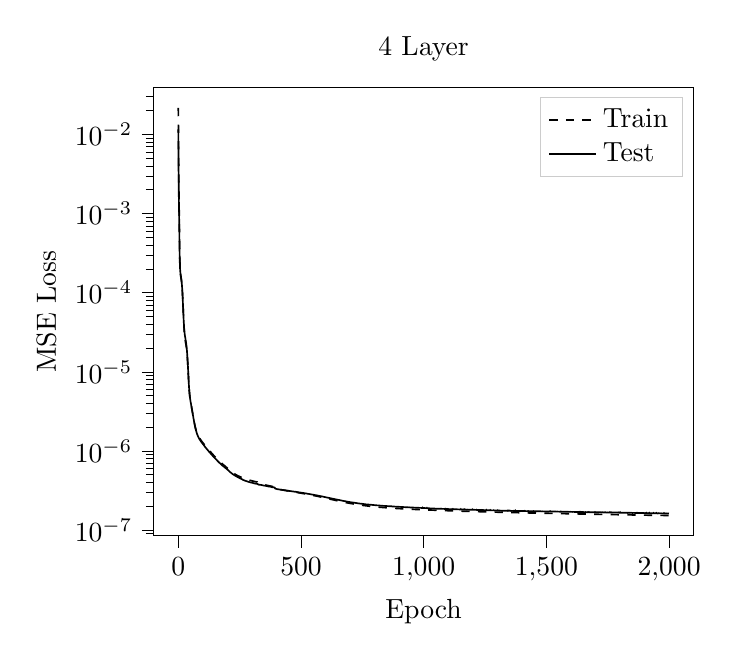
\begin{tikzpicture}

\begin{axis}[
legend cell align={left},
legend style={fill opacity=0.8, draw opacity=1, text opacity=1, draw=white!80!black},
log basis y={10},
tick align=outside,
tick pos=left,
title={4 Layer},
x grid style={white!69.0196078431373!black},
xlabel={Epoch},
xmin=-99.95, xmax=2098.95,
xtick style={color=black},
y grid style={white!69.0196078431373!black},
ylabel={MSE Loss},
ymin=8.43938809238065e-08, ymax=0.0391028934127556,
ymode=log,
ytick style={color=black}
]
\addplot [semithick, black, dashed]
table {%
0 0.0216106624007225
1 0.00673290289845318
2 0.00242847194336355
3 0.00139278739271685
4 0.000877979734446853
5 0.000474738540826365
6 0.000281054378283443
7 0.00021271777068614
8 0.000184169041807763
9 0.000169510987921967
10 0.000160570089246903
11 0.000153623172860534
12 0.000146821876085596
13 0.000139312337923911
14 0.000130708834607503
15 0.000120814576126577
16 0.000109637301975454
17 9.74004520030576e-05
18 8.46704687937745e-05
19 7.22209239793301e-05
20 6.08980650031299e-05
21 5.13222632107499e-05
22 4.36849454090407e-05
23 3.78588456642319e-05
24 3.35587738209142e-05
25 3.04345663553249e-05
26 2.81585673401423e-05
27 2.64713321785166e-05
28 2.51700294393231e-05
29 2.40990629854423e-05
30 2.31376955125597e-05
31 2.21966665994842e-05
32 2.12135114788907e-05
33 2.01455304168121e-05
34 1.89702411180406e-05
35 1.76808702226481e-05
36 1.62871305710723e-05
37 1.48123448534534e-05
38 1.32958351109664e-05
39 1.17858424450787e-05
40 1.0341288148993e-05
41 9.02308400145557e-06
42 7.88079028029642e-06
43 6.9382161775593e-06
44 6.18492073954258e-06
45 5.61335765496551e-06
46 5.18214040664589e-06
47 4.851168252344e-06
48 4.5908486360986e-06
49 4.37404542492459e-06
50 4.1860971711003e-06
51 4.01634194429334e-06
52 3.85815369747888e-06
53 3.70789047474318e-06
54 3.56210532618206e-06
55 3.42163359334791e-06
56 3.28623007618489e-06
57 3.15185335739443e-06
58 3.0234138083074e-06
59 2.90046724973081e-06
60 2.78323152656412e-06
61 2.67022930574967e-06
62 2.56325708880922e-06
63 2.46282143962162e-06
64 2.36972090749532e-06
65 2.28372049502923e-06
66 2.20383440972682e-06
67 2.12981607876372e-06
68 2.0617129700895e-06
69 1.99959229286151e-06
70 1.94295511562359e-06
71 1.89111669618569e-06
72 1.84340184341636e-06
73 1.79986060237525e-06
74 1.75956733130533e-06
75 1.72281113952977e-06
76 1.68883256932872e-06
77 1.65757721526916e-06
78 1.62893817480381e-06
79 1.60244528660769e-06
80 1.57779333051167e-06
81 1.55488546303673e-06
82 1.53347499124834e-06
83 1.51332984992791e-06
84 1.49426139915931e-06
85 1.47615350221031e-06
86 1.45896057071582e-06
87 1.44265126846221e-06
88 1.42635903176824e-06
89 1.41095506359079e-06
90 1.39608382190204e-06
91 1.38187484546393e-06
92 1.3679947178673e-06
93 1.35463125761248e-06
94 1.34165614971948e-06
95 1.32878456537355e-06
96 1.31631478626559e-06
97 1.30407440371982e-06
98 1.29206818090211e-06
99 1.28030122669998e-06
100 1.26874039784752e-06
101 1.25744272938277e-06
102 1.24637065587763e-06
103 1.23556529459279e-06
104 1.22468484934757e-06
105 1.21391777702229e-06
106 1.20343351045449e-06
107 1.19293890546146e-06
108 1.18257735414318e-06
109 1.17147049024879e-06
110 1.16113315289113e-06
111 1.15103359098612e-06
112 1.14106687107096e-06
113 1.13130547171636e-06
114 1.12164716841789e-06
115 1.11212452972609e-06
116 1.10274103678876e-06
117 1.09347531545723e-06
118 1.08429839545465e-06
119 1.07525509415041e-06
120 1.06630471557878e-06
121 1.05751132139176e-06
122 1.0487439832616e-06
123 1.04011279623251e-06
124 1.03160096955435e-06
125 1.02322621967232e-06
126 1.01492625211108e-06
127 1.00679528438263e-06
128 9.98749102421925e-07
129 9.90614294664738e-07
130 9.82658809448367e-07
131 9.74852750289301e-07
132 9.67159750558721e-07
133 9.59597950853208e-07
134 9.52112600600685e-07
135 9.4466021650419e-07
136 9.37624845334994e-07
137 9.30101956882368e-07
138 9.2261810858929e-07
139 9.15006883133174e-07
140 9.07406760788376e-07
141 9.00099601224724e-07
142 8.92701309766153e-07
143 8.85610241880386e-07
144 8.78771238845388e-07
145 8.72219110959804e-07
146 8.65594072266163e-07
147 8.59149445574303e-07
148 8.52838356223629e-07
149 8.46545972649437e-07
150 8.40331516357651e-07
151 8.34286911057802e-07
152 8.28214898177748e-07
153 8.22116376156146e-07
154 8.16204172863877e-07
155 8.10378548209201e-07
156 8.04656332050513e-07
157 7.99051991762667e-07
158 7.93543244043349e-07
159 7.88110822099952e-07
160 7.82816938922792e-07
161 7.77351807641935e-07
162 7.72005825297129e-07
163 7.66674001397405e-07
164 7.61450602340119e-07
165 7.56337212166613e-07
166 7.5132788563792e-07
167 7.46323605710586e-07
168 7.41613327960522e-07
169 7.36650454257415e-07
170 7.31902793432937e-07
171 7.27025475512733e-07
172 7.22359442249854e-07
173 7.177709151307e-07
174 7.13255188415474e-07
175 7.08742484775371e-07
176 7.03956646006532e-07
177 6.98618378038418e-07
178 6.93606436271921e-07
179 6.88884985976301e-07
180 6.84381060153783e-07
181 6.80145616499317e-07
182 6.75724589797255e-07
183 6.71580819329165e-07
184 6.6738621748641e-07
185 6.6328372876967e-07
186 6.59295098714097e-07
187 6.55370623690032e-07
188 6.51456420968088e-07
189 6.4768271292337e-07
190 6.43534997621487e-07
191 6.39708978283693e-07
192 6.359301758323e-07
193 6.32180300485175e-07
194 6.28438367741069e-07
195 6.24702582612713e-07
196 6.21174068299979e-07
197 6.17387885085918e-07
198 6.1360695735857e-07
199 6.09839239018584e-07
200 6.06011450102528e-07
201 6.02128856996842e-07
202 5.98357907904301e-07
203 5.9438991659988e-07
204 5.90488967759484e-07
205 5.86552403930796e-07
206 5.82735191478889e-07
207 5.7880083262063e-07
208 5.7500634336094e-07
209 5.71188780483567e-07
210 5.67494936362323e-07
211 5.63854762901883e-07
212 5.60381861106407e-07
213 5.57017742153221e-07
214 5.53732854783107e-07
215 5.50645551413709e-07
216 5.47619643711528e-07
217 5.44531466303511e-07
218 5.41552928794431e-07
219 5.38660903046662e-07
220 5.35860492874463e-07
221 5.33061054838413e-07
222 5.30413544254316e-07
223 5.27592542923117e-07
224 5.25051639684193e-07
225 5.22539969892932e-07
226 5.20097590815283e-07
227 5.17746779479467e-07
228 5.15497621826455e-07
229 5.13201537245322e-07
230 5.10952482173366e-07
231 5.08788757684897e-07
232 5.06413795463345e-07
233 5.04197328794476e-07
234 5.02117503565103e-07
235 5.00099920714092e-07
236 4.98156201281574e-07
237 4.96120355620633e-07
238 4.94286574834746e-07
239 4.92361857155288e-07
240 4.90496158661813e-07
241 4.88675696999508e-07
242 4.86913171407366e-07
243 4.851756119848e-07
244 4.83470957902909e-07
245 4.81814274188253e-07
246 4.80199573651419e-07
247 4.78683203567698e-07
248 4.77044099817192e-07
249 4.75468882626728e-07
250 4.73879091153151e-07
251 4.72371058982901e-07
252 4.70842513635716e-07
253 4.6937632956201e-07
254 4.67929217776941e-07
255 4.66513790627232e-07
256 4.65088764485699e-07
257 4.6366257139141e-07
258 4.62334256909003e-07
259 4.60908514426706e-07
260 4.59539256539188e-07
261 4.582419610486e-07
262 4.56966788391355e-07
263 4.55675070149653e-07
264 4.54337393499316e-07
265 4.53071155732232e-07
266 4.51853715723871e-07
267 4.50666905862818e-07
268 4.49487872209886e-07
269 4.48350553412524e-07
270 4.47203686391617e-07
271 4.46084542019776e-07
272 4.44943811899634e-07
273 4.43894103753451e-07
274 4.42781260545644e-07
275 4.4177846840654e-07
276 4.40752303987324e-07
277 4.3963250649881e-07
278 4.38508849981645e-07
279 4.37525406496775e-07
280 4.36493751188038e-07
281 4.35531963482561e-07
282 4.34462244669476e-07
283 4.33431620805891e-07
284 4.32435458542102e-07
285 4.31482845442588e-07
286 4.30554591901e-07
287 4.29638015788214e-07
288 4.28745323013402e-07
289 4.2790234015655e-07
290 4.27039721159872e-07
291 4.26191598307923e-07
292 4.25355553360873e-07
293 4.24506018333659e-07
294 4.23655542931556e-07
295 4.22808301834721e-07
296 4.21996215266063e-07
297 4.21198938262535e-07
298 4.20371942965403e-07
299 4.19587211652583e-07
300 4.18860521804731e-07
301 4.18094755104903e-07
302 4.17349502271236e-07
303 4.16623433551422e-07
304 4.15895910307995e-07
305 4.15184494542586e-07
306 4.14479024385628e-07
307 4.13734667318977e-07
308 4.13033298542587e-07
309 4.12367151128024e-07
310 4.11671337289476e-07
311 4.11018487042725e-07
312 4.10363574829375e-07
313 4.09771400768477e-07
314 4.09135555258899e-07
315 4.08534289007889e-07
316 4.07766801657772e-07
317 4.07205162758828e-07
318 4.06719284313795e-07
319 4.05979226258069e-07
320 4.05369681857337e-07
321 4.04813660580317e-07
322 4.0424221703006e-07
323 4.01775835342733e-07
324 3.9732308940188e-07
325 3.95490883548177e-07
326 3.93727580572545e-07
327 3.9239304535954e-07
328 3.91342631729685e-07
329 3.90330171711639e-07
330 3.89447076273086e-07
331 3.88699826885386e-07
332 3.87784748724584e-07
333 3.87108554747329e-07
334 3.86313853951492e-07
335 3.85547236177786e-07
336 3.84728025963454e-07
337 3.83967091067916e-07
338 3.83136319840105e-07
339 3.82331433002037e-07
340 3.81500545188373e-07
341 3.80685198756225e-07
342 3.80033054341311e-07
343 3.79316259142115e-07
344 3.78621012487201e-07
345 3.7795977845434e-07
346 3.77288775951001e-07
347 3.76653722184983e-07
348 3.75958665728149e-07
349 3.75355292362656e-07
350 3.74698903961246e-07
351 3.74061793934288e-07
352 3.73468358191076e-07
353 3.72811548963625e-07
354 3.72241171824328e-07
355 3.71634515659025e-07
356 3.70998225157848e-07
357 3.70405478889779e-07
358 3.69798000349419e-07
359 3.69194266880868e-07
360 3.68567208624881e-07
361 3.679934441152e-07
362 3.67422204163859e-07
363 3.66914002796648e-07
364 3.66252508641196e-07
365 3.65631194782168e-07
366 3.65033643291213e-07
367 3.6445641813998e-07
368 3.63884713749485e-07
369 3.6333000007005e-07
370 3.62738613333136e-07
371 3.62184976779645e-07
372 3.61609488692238e-07
373 3.61079528076402e-07
374 3.60510225192456e-07
375 3.59959687756373e-07
376 3.59414541676983e-07
377 3.58882117126313e-07
378 3.58320710986959e-07
379 3.57816574023673e-07
380 3.5727768839422e-07
381 3.56719101432645e-07
382 3.56145097327953e-07
383 3.55607541536074e-07
384 3.55104071616097e-07
385 3.54350894710365e-07
386 3.53832532411502e-07
387 3.53362483537012e-07
388 3.52820708798163e-07
389 3.52301250558185e-07
390 3.51839069267612e-07
391 3.51369276515356e-07
392 3.50713634929889e-07
393 3.50198180385064e-07
394 3.42994273879071e-07
395 3.37459253060501e-07
396 3.36289835345838e-07
397 3.35470516276359e-07
398 3.34717947012564e-07
399 3.34036376955282e-07
400 3.33413894921364e-07
401 3.32775672802654e-07
402 3.32222780471625e-07
403 3.31656370008204e-07
404 3.31059441123216e-07
405 3.30471022579104e-07
406 3.29948070614705e-07
407 3.29408178927793e-07
408 3.28830659569235e-07
409 3.28420155582876e-07
410 3.27948691108304e-07
411 3.27466074267591e-07
412 3.26983534591818e-07
413 3.26529947187737e-07
414 3.26056213680204e-07
415 3.25601777944939e-07
416 3.25140297491089e-07
417 3.24708497444703e-07
418 3.24223424328807e-07
419 3.23786114506675e-07
420 3.23332559105438e-07
421 3.22898877939792e-07
422 3.22457123729691e-07
423 3.22002698311508e-07
424 3.21506677451566e-07
425 3.21149641436591e-07
426 3.2071827259017e-07
427 3.20318631850114e-07
428 3.19890345039653e-07
429 3.19473695739703e-07
430 3.18698119528449e-07
431 3.18401096876642e-07
432 3.17974057793435e-07
433 3.17500140937454e-07
434 3.17058012129223e-07
435 3.16648788057705e-07
436 3.16250691852815e-07
437 3.15829835571435e-07
438 3.15423972210738e-07
439 3.15066943116449e-07
440 3.14667640367361e-07
441 3.14271113822429e-07
442 3.13797254975157e-07
443 3.13497316142275e-07
444 3.13078043916448e-07
445 3.12755185831293e-07
446 3.12391271933166e-07
447 3.1198606302496e-07
448 3.1160391039009e-07
449 3.11256480088673e-07
450 3.10887099558954e-07
451 3.10662238675263e-07
452 3.10277672426196e-07
453 3.09896373551055e-07
454 3.09517824987893e-07
455 3.09143135638124e-07
456 3.08770616982201e-07
457 3.08405447086102e-07
458 3.08032719928519e-07
459 3.07656596632455e-07
460 3.07311306372071e-07
461 3.06948595408585e-07
462 3.06615132117827e-07
463 3.06262616817321e-07
464 3.05897978648773e-07
465 3.05542331858533e-07
466 3.05163595825775e-07
467 3.04796437418986e-07
468 3.04440751691004e-07
469 3.04076373026874e-07
470 3.03719222827681e-07
471 3.03353062221845e-07
472 3.02990892649291e-07
473 3.0263301108846e-07
474 3.02271752175898e-07
475 3.01934635672296e-07
476 3.0156328080011e-07
477 3.01179149317932e-07
478 3.00842650105437e-07
479 3.00472060928314e-07
480 3.00037528703001e-07
481 2.99667246835611e-07
482 2.99302288965464e-07
483 2.98947667644711e-07
484 2.98582195583208e-07
485 2.98215010573699e-07
486 2.9785535068072e-07
487 2.97490581374404e-07
488 2.97126231615152e-07
489 2.96774992690985e-07
490 2.96397045090657e-07
491 2.96061390230307e-07
492 2.95681678281312e-07
493 2.9532954511069e-07
494 2.94962441074631e-07
495 2.94596214985177e-07
496 2.94228129320118e-07
497 2.93864728405424e-07
498 2.93508675170528e-07
499 2.93143504279669e-07
500 2.92784303780991e-07
501 2.92416588507649e-07
502 2.92051301343577e-07
503 2.91686755957699e-07
504 2.91287320621336e-07
505 2.90917487433262e-07
506 2.90549759711212e-07
507 2.90181204320561e-07
508 2.89812056109895e-07
509 2.89444514450565e-07
510 2.89075045500908e-07
511 2.88704543976337e-07
512 2.88336096332387e-07
513 2.8796272732734e-07
514 2.87592303521933e-07
515 2.87219270418859e-07
516 2.86848664543982e-07
517 2.86476573634786e-07
518 2.86102311221725e-07
519 2.85724018624478e-07
520 2.85357762265903e-07
521 2.84981645876314e-07
522 2.8461455055151e-07
523 2.8425328021342e-07
524 2.83887521433712e-07
525 2.83510480073801e-07
526 2.83132329769842e-07
527 2.82761600246317e-07
528 2.82383754637294e-07
529 2.82003369363792e-07
530 2.81624365769062e-07
531 2.81253791044378e-07
532 2.80863522320374e-07
533 2.80491489519363e-07
534 2.80108860522432e-07
535 2.79729500917369e-07
536 2.79344856437547e-07
537 2.78964073430643e-07
538 2.78581386027099e-07
539 2.78189427277198e-07
540 2.77800684699514e-07
541 2.77422164160157e-07
542 2.77025935531583e-07
543 2.76675719604214e-07
544 2.7628835702842e-07
545 2.75891499214254e-07
546 2.754996529859e-07
547 2.7510834667055e-07
548 2.7471418212599e-07
549 2.74250312244817e-07
550 2.73937980210803e-07
551 2.73469895518019e-07
552 2.73089561275697e-07
553 2.72698263458437e-07
554 2.72312604806757e-07
555 2.71926184367999e-07
556 2.71536050803434e-07
557 2.71139314662605e-07
558 2.70746581449544e-07
559 2.70352984330202e-07
560 2.69956387015213e-07
561 2.69561034599519e-07
562 2.69184922245813e-07
563 2.68785443537922e-07
564 2.68388820202858e-07
565 2.67988743360092e-07
566 2.67580664214506e-07
567 2.6718646597601e-07
568 2.66785075979215e-07
569 2.66419031149212e-07
570 2.66015551616761e-07
571 2.65620774769104e-07
572 2.65219328838384e-07
573 2.64824864359525e-07
574 2.64434130130553e-07
575 2.64023973286953e-07
576 2.63620257200614e-07
577 2.63219747282051e-07
578 2.62736836447175e-07
579 2.62318192085331e-07
580 2.61909523416648e-07
581 2.61502716469408e-07
582 2.61105529247629e-07
583 2.60702718719585e-07
584 2.6029890841528e-07
585 2.59889832378235e-07
586 2.59486747424376e-07
587 2.59076840677608e-07
588 2.58672434839013e-07
589 2.58264190520663e-07
590 2.57854916384304e-07
591 2.57446017087659e-07
592 2.57047310228131e-07
593 2.56630037597461e-07
594 2.56229556200083e-07
595 2.55818167815391e-07
596 2.55413956594452e-07
597 2.55009213333324e-07
598 2.54611830413864e-07
599 2.54200633449386e-07
600 2.5380529264396e-07
601 2.53393371764332e-07
602 2.52922564399682e-07
603 2.52380531748031e-07
604 2.51938129494533e-07
605 2.5150760473025e-07
606 2.51107723556743e-07
607 2.50692401550623e-07
608 2.50296422933616e-07
609 2.49886340895955e-07
610 2.49492911265747e-07
611 2.49087333429543e-07
612 2.48680714250327e-07
613 2.48284265978782e-07
614 2.4788667600717e-07
615 2.47456508517985e-07
616 2.47051033085199e-07
617 2.46647489134944e-07
618 2.4625732633865e-07
619 2.45860469803461e-07
620 2.45425408920141e-07
621 2.45022914640458e-07
622 2.44652590524197e-07
623 2.44252181644811e-07
624 2.43862469332612e-07
625 2.43488337133613e-07
626 2.43087162303368e-07
627 2.42683210387895e-07
628 2.42284148342264e-07
629 2.4189684177145e-07
630 2.41453110305656e-07
631 2.4105597925228e-07
632 2.40666493098729e-07
633 2.402901326235e-07
634 2.39877828683177e-07
635 2.39510399850928e-07
636 2.39118784641335e-07
637 2.38734965940068e-07
638 2.38333517231126e-07
639 2.37971021149974e-07
640 2.37577484739404e-07
641 2.37201121635167e-07
642 2.36807600217048e-07
643 2.36442187372177e-07
644 2.36048477418649e-07
645 2.35720507248516e-07
646 2.3529685198298e-07
647 2.34926964964188e-07
648 2.34651763484806e-07
649 2.34295619804925e-07
650 2.33907534919808e-07
651 2.33553717706059e-07
652 2.33175521088924e-07
653 2.32825393268854e-07
654 2.32450461304268e-07
655 2.32095179185876e-07
656 2.31748523042086e-07
657 2.31385499631642e-07
658 2.31015129955381e-07
659 2.30663613251636e-07
660 2.30288796053912e-07
661 2.29934373187746e-07
662 2.29571597571976e-07
663 2.29216760359918e-07
664 2.28852116933354e-07
665 2.28495701144027e-07
666 2.28147498418707e-07
667 2.27798743303254e-07
668 2.27462652588883e-07
669 2.27117970155177e-07
670 2.26760281407223e-07
671 2.26418564309938e-07
672 2.26108651581569e-07
673 2.25791860522406e-07
674 2.25436486502417e-07
675 2.25098220347775e-07
676 2.24788045336766e-07
677 2.24459609604821e-07
678 2.24133774658242e-07
679 2.23800147416853e-07
680 2.23474523565415e-07
681 2.23188974956656e-07
682 2.2284166180242e-07
683 2.2254372058228e-07
684 2.22211433126063e-07
685 2.21920742731641e-07
686 2.21595553426823e-07
687 2.21314227367486e-07
688 2.21033817595639e-07
689 2.20716097487639e-07
690 2.20356926739385e-07
691 2.2009933127265e-07
692 2.19786205256867e-07
693 2.19499166888681e-07
694 2.19210622162791e-07
695 2.18931428264568e-07
696 2.18612988660993e-07
697 2.18332271472832e-07
698 2.18054914128629e-07
699 2.17747560832038e-07
700 2.17494242413352e-07
701 2.17189853188415e-07
702 2.16910481917409e-07
703 2.16647721089203e-07
704 2.16394595852876e-07
705 2.1610913848491e-07
706 2.15835460842584e-07
707 2.15616975424382e-07
708 2.15359850656682e-07
709 2.15075565435541e-07
710 2.14831694350437e-07
711 2.14503112900388e-07
712 2.14279591034483e-07
713 2.13987736259469e-07
714 2.13740835725673e-07
715 2.13455635510229e-07
716 2.13242247525614e-07
717 2.12986595641951e-07
718 2.12713128561859e-07
719 2.12486485366981e-07
720 2.12225340455063e-07
721 2.11995605106097e-07
722 2.11794130493104e-07
723 2.11524806914554e-07
724 2.1125673990241e-07
725 2.11031820846586e-07
726 2.1081890638186e-07
727 2.10560273671945e-07
728 2.10315091813129e-07
729 2.10102463988449e-07
730 2.09889895714355e-07
731 2.09609642865871e-07
732 2.09425779999606e-07
733 2.09183616597386e-07
734 2.08990658443042e-07
735 2.08729989289225e-07
736 2.08531867073702e-07
737 2.08309944277119e-07
738 2.08086278355779e-07
739 2.0789459659909e-07
740 2.07680310651881e-07
741 2.0747119165776e-07
742 2.07236777498565e-07
743 2.07018175132134e-07
744 2.06816486773675e-07
745 2.06584763589035e-07
746 2.06387027432697e-07
747 2.06218926180668e-07
748 2.06005806859366e-07
749 2.05752826182959e-07
750 2.05548594330196e-07
751 2.05311775921757e-07
752 2.05142609736697e-07
753 2.0495073572846e-07
754 2.04771630293976e-07
755 2.0461071154898e-07
756 2.04373782693779e-07
757 2.04192100383693e-07
758 2.04031139503513e-07
759 2.03814531289481e-07
760 2.03654313601476e-07
761 2.03442323652325e-07
762 2.03277292598614e-07
763 2.0309212533931e-07
764 2.02949136372865e-07
765 2.02724689088996e-07
766 2.02560473084645e-07
767 2.02350404919116e-07
768 2.02225088422381e-07
769 2.02075813668046e-07
770 2.01815807457706e-07
771 2.01668591600423e-07
772 2.01510255024573e-07
773 2.01304897409216e-07
774 2.01147469894636e-07
775 2.0087547069636e-07
776 2.00708041205644e-07
777 2.00552844987101e-07
778 2.00407669666447e-07
779 2.00212583891357e-07
780 2.00079323661839e-07
781 1.99906171182818e-07
782 1.99735537769641e-07
783 1.99590529170734e-07
784 1.99458949076359e-07
785 1.9929100927385e-07
786 1.99101222690956e-07
787 1.98979387548093e-07
788 1.9883520160846e-07
789 1.98662458501531e-07
790 1.98509994092433e-07
791 1.98378701213642e-07
792 1.98230722041615e-07
793 1.98054001302239e-07
794 1.97913957400431e-07
795 1.97748915866214e-07
796 1.97619246243619e-07
797 1.97458854394483e-07
798 1.9732037737441e-07
799 1.9718832942317e-07
800 1.97041426808653e-07
801 1.96902047633785e-07
802 1.96766920048219e-07
803 1.96604294650626e-07
804 1.96496536219115e-07
805 1.96382572973164e-07
806 1.96219839480705e-07
807 1.96085320837369e-07
808 1.95963470162042e-07
809 1.95823555152685e-07
810 1.95713456996316e-07
811 1.95573616785794e-07
812 1.95453819671343e-07
813 1.95311064544512e-07
814 1.95212965564906e-07
815 1.95100162919459e-07
816 1.94962750249772e-07
817 1.94830665954271e-07
818 1.94717411517331e-07
819 1.94620832374426e-07
820 1.94458740004677e-07
821 1.94354109922301e-07
822 1.94270007597197e-07
823 1.94124745341639e-07
824 1.94010768659325e-07
825 1.93872416154761e-07
826 1.93788308628484e-07
827 1.93651885346924e-07
828 1.93532121421924e-07
829 1.93444749363891e-07
830 1.93306050924491e-07
831 1.93204075095821e-07
832 1.9309011060642e-07
833 1.92993874705394e-07
834 1.92862723380927e-07
835 1.92772320488643e-07
836 1.92665639630718e-07
837 1.92546770804825e-07
838 1.92435405381275e-07
839 1.92352559281517e-07
840 1.92240041741343e-07
841 1.92133511006887e-07
842 1.92020548425376e-07
843 1.919115628084e-07
844 1.91812710554018e-07
845 1.91718293251597e-07
846 1.91616724755761e-07
847 1.91497081054592e-07
848 1.91413476578362e-07
849 1.91311501069436e-07
850 1.91188739904646e-07
851 1.91130697771769e-07
852 1.91013988590782e-07
853 1.90901197811399e-07
854 1.90812814622632e-07
855 1.90715631696037e-07
856 1.90646210654677e-07
857 1.90514590059365e-07
858 1.90444030131687e-07
859 1.90331704054358e-07
860 1.90250029120875e-07
861 1.90143055029068e-07
862 1.90024863513827e-07
863 1.89974942529147e-07
864 1.89862021365173e-07
865 1.89752594678794e-07
866 1.89691171975426e-07
867 1.89590054446853e-07
868 1.89481359015531e-07
869 1.89564498441541e-07
870 1.89266790783904e-07
871 1.89147045318805e-07
872 1.89083462664996e-07
873 1.89025151307476e-07
874 1.88914466036749e-07
875 1.88806591928881e-07
876 1.88748112037729e-07
877 1.88681913918742e-07
878 1.88565463105306e-07
879 1.88473345332341e-07
880 1.88422301071967e-07
881 1.88273862789856e-07
882 1.88229817830177e-07
883 1.88129125866965e-07
884 1.88074489372525e-07
885 1.87977990435684e-07
886 1.87873305492303e-07
887 1.87809109206682e-07
888 1.87705275983774e-07
889 1.87653425115286e-07
890 1.87576660152899e-07
891 1.87455449136564e-07
892 1.8739126468148e-07
893 1.87289279985237e-07
894 1.8724850141183e-07
895 1.87153168901943e-07
896 1.8706308216565e-07
897 1.86987817727413e-07
898 1.86928051377322e-07
899 1.86846638250415e-07
900 1.86764167771969e-07
901 1.86676254728013e-07
902 1.86577274298827e-07
903 1.86536912949009e-07
904 1.8646056668814e-07
905 1.86386593952648e-07
906 1.86291404176586e-07
907 1.86223032379473e-07
908 1.86134376484404e-07
909 1.86082618697014e-07
910 1.85978073758974e-07
911 1.85938494226434e-07
912 1.85864153408488e-07
913 1.85785363839841e-07
914 1.85678791211785e-07
915 1.85629285340383e-07
916 1.85553920864834e-07
917 1.85486233405641e-07
918 1.8540947337442e-07
919 1.85350580267141e-07
920 1.85271162948197e-07
921 1.85202297849685e-07
922 1.85131175925335e-07
923 1.85051926912649e-07
924 1.84978863472907e-07
925 1.8492998484021e-07
926 1.84832688674419e-07
927 1.84801209300645e-07
928 1.84736455373979e-07
929 1.84623548165064e-07
930 1.84608434793176e-07
931 1.84504162469068e-07
932 1.84435943999972e-07
933 1.84360517607729e-07
934 1.84322198350628e-07
935 1.84215514472896e-07
936 1.84190147251684e-07
937 1.84140666071642e-07
938 1.84041638341625e-07
939 1.83968719234429e-07
940 1.83896355849811e-07
941 1.83837361070971e-07
942 1.83839822845755e-07
943 1.83766977229993e-07
944 1.83638415258258e-07
945 1.83566072095687e-07
946 1.83519504091123e-07
947 1.83446028835021e-07
948 1.83395068596326e-07
949 1.83316212236662e-07
950 1.83285562606272e-07
951 1.83199140721513e-07
952 1.83183291241562e-07
953 1.83075190882676e-07
954 1.83062210787455e-07
955 1.82927106422426e-07
956 1.82892595525175e-07
957 1.82834764522966e-07
958 1.82783786037533e-07
959 1.82701763108639e-07
960 1.82646872232795e-07
961 1.82573253077578e-07
962 1.82511307478705e-07
963 1.82460096070258e-07
964 1.82422018170314e-07
965 1.82331821022785e-07
966 1.82296495310652e-07
967 1.82236372658906e-07
968 1.8213447961557e-07
969 1.8208163304223e-07
970 1.82025621178639e-07
971 1.81966136040046e-07
972 1.81946712665138e-07
973 1.81872313675058e-07
974 1.81773238892902e-07
975 1.81758913051056e-07
976 1.8167523741397e-07
977 1.81603671109087e-07
978 1.81574254867201e-07
979 1.81481448350951e-07
980 1.8144391169983e-07
981 1.81378839940294e-07
982 1.81291478270396e-07
983 1.81267837923826e-07
984 1.81212172982725e-07
985 1.81145498459045e-07
986 1.81104971638035e-07
987 1.81015536654172e-07
988 1.81003275883995e-07
989 1.80951426081322e-07
990 1.80898478369329e-07
991 1.80804848220362e-07
992 1.80737904678097e-07
993 1.80692982183928e-07
994 1.8063039879479e-07
995 1.80686602881508e-07
996 1.80568369920309e-07
997 1.80461264832843e-07
998 1.80398518651259e-07
999 1.80379310890544e-07
1000 1.80326845374168e-07
1001 1.80228571188934e-07
1002 1.80212151668968e-07
1003 1.80164973421881e-07
1004 1.80055146493885e-07
1005 1.80016070551403e-07
1006 1.80035480369156e-07
1007 1.79911012459399e-07
1008 1.79842733800228e-07
1009 1.79833708145338e-07
1010 1.79744951807947e-07
1011 1.79718168539011e-07
1012 1.79695514212597e-07
1013 1.79632579659028e-07
1014 1.7958827668707e-07
1015 1.79485900808629e-07
1016 1.79413860877276e-07
1017 1.79370492290332e-07
1018 1.79360341761026e-07
1019 1.79332420671585e-07
1020 1.79230263661623e-07
1021 1.7917569885384e-07
1022 1.79127057556627e-07
1023 1.79241113549722e-07
1024 1.7917623971897e-07
1025 1.79244382202626e-07
1026 1.79210308260735e-07
1027 1.79150409216788e-07
1028 1.79036714634151e-07
1029 1.79027852738045e-07
1030 1.78958927357087e-07
1031 1.7893335813568e-07
1032 1.78864548978197e-07
1033 1.78835367890429e-07
1034 1.78795579536484e-07
1035 1.78755134868425e-07
1036 1.78641936344093e-07
1037 1.78593477691891e-07
1038 1.78590952224056e-07
1039 1.78499820442823e-07
1040 1.78439640791339e-07
1041 1.78394428537842e-07
1042 1.78378901708243e-07
1043 1.78302251427453e-07
1044 1.78258820334065e-07
1045 1.78191099934111e-07
1046 1.78159377298925e-07
1047 1.78104258438339e-07
1048 1.78057871373483e-07
1049 1.78015181447222e-07
1050 1.77944034774669e-07
1051 1.77941957588246e-07
1052 1.77853626396995e-07
1053 1.77814524832343e-07
1054 1.7774813699134e-07
1055 1.77703809889351e-07
1056 1.77675952258483e-07
1057 1.77648358352656e-07
1058 1.77571942579391e-07
1059 1.77527472061456e-07
1060 1.77485991635251e-07
1061 1.7744707773204e-07
1062 1.77386032802929e-07
1063 1.77322587973094e-07
1064 1.77299124445085e-07
1065 1.77234235543722e-07
1066 1.77215259405727e-07
1067 1.77158344335737e-07
1068 1.77124247471738e-07
1069 1.77064489179202e-07
1070 1.76985912368366e-07
1071 1.76983701834388e-07
1072 1.76910187533963e-07
1073 1.76876028099571e-07
1074 1.76824726956681e-07
1075 1.76798676029932e-07
1076 1.76776226531672e-07
1077 1.76694430521707e-07
1078 1.76621351180017e-07
1079 1.76610401460664e-07
1080 1.76574187129575e-07
1081 1.7649910562767e-07
1082 1.76468546882802e-07
1083 1.76431862030313e-07
1084 1.7638737516279e-07
1085 1.76306908748813e-07
1086 1.76277939857528e-07
1087 1.76302373539272e-07
1088 1.7617569829298e-07
1089 1.76178361300572e-07
1090 1.76133429633296e-07
1091 1.76041002141858e-07
1092 1.75977817043815e-07
1093 1.75944437359021e-07
1094 1.75941254248357e-07
1095 1.75881839190595e-07
1096 1.75846790924084e-07
1097 1.75819223144913e-07
1098 1.75713790490306e-07
1099 1.75664444050483e-07
1100 1.75637258344352e-07
1101 1.75566675693517e-07
1102 1.75534115825826e-07
1103 1.75526750261668e-07
1104 1.75438703770681e-07
1105 1.7538309885623e-07
1106 1.75376762328483e-07
1107 1.7530193790094e-07
1108 1.75282633335883e-07
1109 1.75220648891639e-07
1110 1.75184468702128e-07
1111 1.75177809552451e-07
1112 1.75096959537768e-07
1113 1.75071028550633e-07
1114 1.75022347598031e-07
1115 1.7497661561805e-07
1116 1.74940363855569e-07
1117 1.74892061075127e-07
1118 1.74832643715206e-07
1119 1.74859169668196e-07
1120 1.74774426554336e-07
1121 1.7468253720665e-07
1122 1.74662733201103e-07
1123 1.74636310930509e-07
1124 1.74569058856378e-07
1125 1.74553399908461e-07
1126 1.74507346848429e-07
1127 1.74474903275268e-07
1128 1.74449821827238e-07
1129 1.74340132559792e-07
1130 1.74361761217767e-07
1131 1.74297626386988e-07
1132 1.74214229467395e-07
1133 1.74233699652859e-07
1134 1.7419528980156e-07
1135 1.74113174260526e-07
1136 1.74103606482845e-07
1137 1.74103460260255e-07
1138 1.73959555390013e-07
1139 1.73925013555731e-07
1140 1.7386210139847e-07
1141 1.73848528262965e-07
1142 1.73805815336436e-07
1143 1.73731946027544e-07
1144 1.73736144176928e-07
1145 1.73698482896612e-07
1146 1.73662524865392e-07
1147 1.73587405967623e-07
1148 1.73579918822497e-07
1149 1.73576758577099e-07
1150 1.735323319636e-07
1151 1.73485661129291e-07
1152 1.73443705548948e-07
1153 1.73351196750104e-07
1154 1.73381033533815e-07
1155 1.73310837986662e-07
1156 1.73295372221105e-07
1157 1.73259445723772e-07
1158 1.73227503879048e-07
1159 1.73195007207028e-07
1160 1.73187520424278e-07
1161 1.7306360564362e-07
1162 1.73050464432833e-07
1163 1.73035037157376e-07
1164 1.73087016712259e-07
1165 1.72968198214107e-07
1166 1.72881617530152e-07
1167 1.7295136483142e-07
1168 1.72851830512855e-07
1169 1.72818079022363e-07
1170 1.72778573158894e-07
1171 1.72718693640661e-07
1172 1.7270090534538e-07
1173 1.7270916892187e-07
1174 1.72568362536651e-07
1175 1.72577032891752e-07
1176 1.7258109477325e-07
1177 1.7260609226355e-07
1178 1.72448717250973e-07
1179 1.72415710743223e-07
1180 1.72395935955194e-07
1181 1.72397184961426e-07
1182 1.72349606657463e-07
1183 1.72301530355412e-07
1184 1.72214634403645e-07
1185 1.72153765760186e-07
1186 1.72193612456795e-07
1187 1.72204249409447e-07
1188 1.72087060846593e-07
1189 1.72026658063373e-07
1190 1.72075992630027e-07
1191 1.72030504209886e-07
1192 1.71926870820016e-07
1193 1.71936961912422e-07
1194 1.71891174524319e-07
1195 1.71880935219804e-07
1196 1.71827827792015e-07
1197 1.71822777382147e-07
1198 1.71786435757326e-07
1199 1.71768815185658e-07
1200 1.71702090860038e-07
1201 1.71739857854902e-07
1202 1.71617547074732e-07
1203 1.7156320400602e-07
1204 1.71528990875913e-07
1205 1.71517066888782e-07
1206 1.71513961973346e-07
1207 1.71403330170961e-07
1208 1.71346198889921e-07
1209 1.71383523543511e-07
1210 1.71362682102938e-07
1211 1.71336470835115e-07
1212 1.71251969312891e-07
1213 1.71174495115167e-07
1214 1.71233604270071e-07
1215 1.71314036798265e-07
1216 1.71165501981818e-07
1217 1.71071120618649e-07
1218 1.70984958153042e-07
1219 1.7098195895926e-07
1220 1.71015771975647e-07
1221 1.70996565053372e-07
1222 1.70884112144165e-07
1223 1.7089750729582e-07
1224 1.70790641050189e-07
1225 1.70798408198891e-07
1226 1.70828165650505e-07
1227 1.70793065173314e-07
1228 1.70700528443035e-07
1229 1.7067476072441e-07
1230 1.70675086287986e-07
1231 1.70612983040996e-07
1232 1.70565547598756e-07
1233 1.7050324265e-07
1234 1.70488775488309e-07
1235 1.70464546236815e-07
1236 1.70451107408098e-07
1237 1.70438943598583e-07
1238 1.70367497503321e-07
1239 1.70297669853881e-07
1240 1.70287840084882e-07
1241 1.70317440392864e-07
1242 1.70259187768806e-07
1243 1.70169387097019e-07
1244 1.70166060954102e-07
1245 1.7015959914346e-07
1246 1.70072879036809e-07
1247 1.70080203453438e-07
1248 1.69973099353626e-07
1249 1.70045703136168e-07
1250 1.69952917950411e-07
1251 1.69955662016719e-07
1252 1.69859973333075e-07
1253 1.69899801925055e-07
1254 1.69820288007827e-07
1255 1.69868564412923e-07
1256 1.69765343969175e-07
1257 1.69748448229257e-07
1258 1.69705800452391e-07
1259 1.6965306291894e-07
1260 1.69602442973371e-07
1261 1.69608080632599e-07
1262 1.69599682138255e-07
1263 1.69567798202763e-07
1264 1.69505588857533e-07
1265 1.69445060365092e-07
1266 1.69388760596689e-07
1267 1.69400478604587e-07
1268 1.69410320395968e-07
1269 1.69311620716428e-07
1270 1.69259400074395e-07
1271 1.69325856880675e-07
1272 1.69370852745487e-07
1273 1.69243204737768e-07
1274 1.69179619966542e-07
1275 1.69161871589552e-07
1276 1.69083306850837e-07
1277 1.69077230957271e-07
1278 1.69089837299907e-07
1279 1.69023000928803e-07
1280 1.69091059262882e-07
1281 1.68983588977767e-07
1282 1.68936555738242e-07
1283 1.68931953034246e-07
1284 1.68985705300884e-07
1285 1.68975296190865e-07
1286 1.68837971287417e-07
1287 1.68774838392949e-07
1288 1.68735167370926e-07
1289 1.68765960466999e-07
1290 1.68746516699514e-07
1291 1.68695649733763e-07
1292 1.68646468864608e-07
1293 1.68562413257689e-07
1294 1.6858988993107e-07
1295 1.68670126527104e-07
1296 1.68366325972613e-07
1297 1.6832450091897e-07
1298 1.68334291473116e-07
1299 1.68343839312968e-07
1300 1.68317190968992e-07
1301 1.68235172893105e-07
1302 1.68274554212644e-07
1303 1.68399181184498e-07
1304 1.68282554334098e-07
1305 1.68080057100894e-07
1306 1.68025432877528e-07
1307 1.68044797234757e-07
1308 1.68017354866379e-07
1309 1.67995841799495e-07
1310 1.68006798560327e-07
1311 1.67982508379794e-07
1312 1.67921054860187e-07
1313 1.67883917420397e-07
1314 1.67839464054964e-07
1315 1.67829756712479e-07
1316 1.67853974403442e-07
1317 1.67749433863662e-07
1318 1.67708428286062e-07
1319 1.67713444042761e-07
1320 1.67860712927848e-07
1321 1.67689125817105e-07
1322 1.67559621274904e-07
1323 1.67547872322871e-07
1324 1.67564348146243e-07
1325 1.67477222703383e-07
1326 1.67485049338723e-07
1327 1.67526131981788e-07
1328 1.6742998275987e-07
1329 1.67414902726648e-07
1330 1.6736702631448e-07
1331 1.67352104973872e-07
1332 1.67339367976638e-07
1333 1.6726915405485e-07
1334 1.67304407696633e-07
1335 1.67264324431926e-07
1336 1.67214283322892e-07
1337 1.67262341591368e-07
1338 1.67241847648825e-07
1339 1.67110093784117e-07
1340 1.67036057391101e-07
1341 1.67139857801146e-07
1342 1.67201785750137e-07
1343 1.66920922900715e-07
1344 1.66950420755541e-07
1345 1.66943121350016e-07
1346 1.66929704967345e-07
1347 1.66912089149207e-07
1348 1.66969160659392e-07
1349 1.66813377553865e-07
1350 1.66787883031816e-07
1351 1.66778691990999e-07
1352 1.66794166055695e-07
1353 1.66790056709942e-07
1354 1.66844713575642e-07
1355 1.66592245811614e-07
1356 1.66663042314497e-07
1357 1.66594229689565e-07
1358 1.66581775118857e-07
1359 1.66553394748803e-07
1360 1.66581533129317e-07
1361 1.66522043343775e-07
1362 1.66457377808626e-07
1363 1.66468092778871e-07
1364 1.66456248294367e-07
1365 1.66391937916899e-07
1366 1.6636954207172e-07
1367 1.66337186605858e-07
1368 1.66337999544908e-07
1369 1.66300411265752e-07
1370 1.66256585025337e-07
1371 1.66230324694538e-07
1372 1.66262054960953e-07
1373 1.66311842029643e-07
1374 1.6620884812113e-07
1375 1.66082737052875e-07
1376 1.66100138692116e-07
1377 1.66071855289829e-07
1378 1.65991287140343e-07
1379 1.66027292841875e-07
1380 1.66048765017024e-07
1381 1.65978204798023e-07
1382 1.65909461287583e-07
1383 1.65914692715319e-07
1384 1.65921796678958e-07
1385 1.65908610057386e-07
1386 1.6584075878967e-07
1387 1.65783007716414e-07
1388 1.65777221020846e-07
1389 1.65749755105082e-07
1390 1.65692761413538e-07
1391 1.65716249071579e-07
1392 1.65707926868208e-07
1393 1.65664443692037e-07
1394 1.65660392909217e-07
1395 1.6555531041007e-07
1396 1.65595974486621e-07
1397 1.65527711487812e-07
1398 1.65510852603745e-07
1399 1.65448139732405e-07
1400 1.65507440037516e-07
1401 1.65409376414516e-07
1402 1.65359866144854e-07
1403 1.65365921347416e-07
1404 1.65365050953881e-07
1405 1.65445104364892e-07
1406 1.65383935843977e-07
1407 1.65204668604702e-07
1408 1.65154134542433e-07
1409 1.65219209932843e-07
1410 1.65202215775651e-07
1411 1.6515671573103e-07
1412 1.65137949920791e-07
1413 1.65116417022659e-07
1414 1.6504532810302e-07
1415 1.65028859363758e-07
1416 1.6504706556475e-07
1417 1.64975679453505e-07
1418 1.64952036158184e-07
1419 1.64949861805042e-07
1420 1.64942287014469e-07
1421 1.64880639310638e-07
1422 1.64852907623469e-07
1423 1.64815023296683e-07
1424 1.64827068971363e-07
1425 1.6479692638427e-07
1426 1.64800686256683e-07
1427 1.64663229007544e-07
1428 1.64735067940569e-07
1429 1.64699877252872e-07
1430 1.64645984632727e-07
1431 1.64649042353915e-07
1432 1.64592018414567e-07
1433 1.64586802981148e-07
1434 1.64533369286346e-07
1435 1.64534088234802e-07
1436 1.64539180580903e-07
1437 1.64588025249657e-07
1438 1.64528626413585e-07
1439 1.64403049730311e-07
1440 1.64434569235539e-07
1441 1.64330305665317e-07
1442 1.64350557383841e-07
1443 1.64313907802693e-07
1444 1.64288167425752e-07
1445 1.64290333536599e-07
1446 1.64252259480691e-07
1447 1.64279479896834e-07
1448 1.6423641449137e-07
1449 1.64184464686912e-07
1450 1.64129400964441e-07
1451 1.64106395708075e-07
1452 1.64089033887649e-07
1453 1.64048898746216e-07
1454 1.64055080958292e-07
1455 1.64035842338706e-07
1456 1.64035157851572e-07
1457 1.63966343592392e-07
1458 1.6393386583502e-07
1459 1.63920002862028e-07
1460 1.63905486353144e-07
1461 1.63842626747623e-07
1462 1.63854071125513e-07
1463 1.63843182377832e-07
1464 1.63801519676099e-07
1465 1.63759081736714e-07
1466 1.63764028513924e-07
1467 1.63723978161556e-07
1468 1.63663750292642e-07
1469 1.63675580736822e-07
1470 1.63701325028853e-07
1471 1.63652787477986e-07
1472 1.63594848658022e-07
1473 1.63543358503659e-07
1474 1.63574874825656e-07
1475 1.63533181869013e-07
1476 1.63477860958494e-07
1477 1.63506070094854e-07
1478 1.6346910118159e-07
1479 1.63388968786649e-07
1480 1.63403992630151e-07
1481 1.63401504394756e-07
1482 1.63334911896129e-07
1483 1.63362521405475e-07
1484 1.63307964221815e-07
1485 1.63266157784392e-07
1486 1.63244747525937e-07
1487 1.63252576001582e-07
1488 1.63205464630778e-07
1489 1.6317926982623e-07
1490 1.63177952131832e-07
1491 1.63116752538883e-07
1492 1.63130517712773e-07
1493 1.63142071770039e-07
1494 1.63082057653696e-07
1495 1.63039829530476e-07
1496 1.62986418189348e-07
1497 1.63003632266623e-07
1498 1.6297419497846e-07
1499 1.62977809573306e-07
1500 1.62908251610361e-07
1501 1.62888266856953e-07
1502 1.62894972540073e-07
1503 1.6281705941168e-07
1504 1.62824144119611e-07
1505 1.62801411775604e-07
1506 1.62785903242479e-07
1507 1.62790458873019e-07
1508 1.62755779378188e-07
1509 1.62805195941473e-07
1510 1.62741083300943e-07
1511 1.62614733277167e-07
1512 1.62588511336992e-07
1513 1.62593399018363e-07
1514 1.62582695779179e-07
1515 1.62611406956614e-07
1516 1.62567546233561e-07
1517 1.62476563382086e-07
1518 1.62453610897728e-07
1519 1.62472841758188e-07
1520 1.62409258251728e-07
1521 1.62407369678874e-07
1522 1.62439174310691e-07
1523 1.62376711131174e-07
1524 1.62357890829412e-07
1525 1.62330951390288e-07
1526 1.62282029890548e-07
1527 1.62258464939669e-07
1528 1.62386171474793e-07
1529 1.62246081977457e-07
1530 1.62181757545454e-07
1531 1.6214893717148e-07
1532 1.62138087752339e-07
1533 1.6213818561539e-07
1534 1.62098755609463e-07
1535 1.62070517177426e-07
1536 1.62076942373801e-07
1537 1.62076044901482e-07
1538 1.62060141597919e-07
1539 1.61987526915652e-07
1540 1.61971739032651e-07
1541 1.61926232046028e-07
1542 1.61918721609311e-07
1543 1.61893961497128e-07
1544 1.6187512852639e-07
1545 1.61897783129916e-07
1546 1.6183849820095e-07
1547 1.61819013932529e-07
1548 1.61767674043745e-07
1549 1.61779257460637e-07
1550 1.61762891366379e-07
1551 1.61720912878138e-07
1552 1.61708021494178e-07
1553 1.61623495422702e-07
1554 1.61689888656724e-07
1555 1.61645654770837e-07
1556 1.61627561659827e-07
1557 1.61584144386495e-07
1558 1.61566055083995e-07
1559 1.61593238935609e-07
1560 1.6156369655107e-07
1561 1.61485519804216e-07
1562 1.6143838396232e-07
1563 1.61465926417748e-07
1564 1.61439363473903e-07
1565 1.61373608236204e-07
1566 1.61376746753206e-07
1567 1.61372395311332e-07
1568 1.61365052711915e-07
1569 1.61270477434528e-07
1570 1.61305438325599e-07
1571 1.6128386074854e-07
1572 1.6120980218659e-07
1573 1.61217556552629e-07
1574 1.61202849270126e-07
1575 1.61158415636464e-07
1576 1.61146072542806e-07
1577 1.61116594973976e-07
1578 1.61089867823705e-07
1579 1.61058869643682e-07
1580 1.61075818958523e-07
1581 1.60997869258495e-07
1582 1.60995202037384e-07
1583 1.60991695985047e-07
1584 1.60972638340695e-07
1585 1.60917201000643e-07
1586 1.60925989412419e-07
1587 1.6090620315623e-07
1588 1.60876287630174e-07
1589 1.60871587006284e-07
1590 1.608295123674e-07
1591 1.60810746869799e-07
1592 1.60792823564293e-07
1593 1.60731222976551e-07
1594 1.60725678398421e-07
1595 1.60743065173108e-07
1596 1.60692538059948e-07
1597 1.60662292991276e-07
1598 1.60687539874971e-07
1599 1.60647360310406e-07
1600 1.60643607117095e-07
1601 1.60562668689579e-07
1602 1.60560070440852e-07
1603 1.60531671774322e-07
1604 1.605189931837e-07
1605 1.60465122299058e-07
1606 1.60481532560652e-07
1607 1.60452848923853e-07
1608 1.60447297758992e-07
1609 1.60448149877368e-07
1610 1.60383949321385e-07
1611 1.60370203410309e-07
1612 1.60340380546131e-07
1613 1.60316806301353e-07
1614 1.60336975469022e-07
1615 1.60274468434807e-07
1616 1.60265671610205e-07
1617 1.60206146965436e-07
1618 1.6017395471124e-07
1619 1.6019242134746e-07
1620 1.60202111970875e-07
1621 1.60110613911968e-07
1622 1.60101618185138e-07
1623 1.60084186518361e-07
1624 1.60075974164897e-07
1625 1.60056341130144e-07
1626 1.60024469295195e-07
1627 1.60016861734391e-07
1628 1.5996215306302e-07
1629 1.59993971742267e-07
1630 1.59975415030544e-07
1631 1.59897546794241e-07
1632 1.59864979707436e-07
1633 1.5981264795073e-07
1634 1.59833385943386e-07
1635 1.59786259438022e-07
1636 1.5975959943404e-07
1637 1.59836109965283e-07
1638 1.59749508142681e-07
1639 1.59673018117701e-07
1640 1.59672461165883e-07
1641 1.59673905095303e-07
1642 1.59624695783123e-07
1643 1.59605662418016e-07
1644 1.59605513445626e-07
1645 1.59538471798726e-07
1646 1.59518216165111e-07
1647 1.59490265389195e-07
1648 1.59514611830502e-07
1649 1.59506289037381e-07
1650 1.594392940234e-07
1651 1.59437268926865e-07
1652 1.59391223355954e-07
1653 1.59379607872268e-07
1654 1.5933557291703e-07
1655 1.59336109298636e-07
1656 1.59273247241742e-07
1657 1.59280083103397e-07
1658 1.59303168210556e-07
1659 1.59266005447023e-07
1660 1.5923947286467e-07
1661 1.59195379566768e-07
1662 1.59185277276208e-07
1663 1.59162616085951e-07
1664 1.59113985738202e-07
1665 1.59115515032227e-07
1666 1.59078035096627e-07
1667 1.590620035401e-07
1668 1.59055500247973e-07
1669 1.59017629734137e-07
1670 1.59004733653489e-07
1671 1.58984582405708e-07
1672 1.5893618891738e-07
1673 1.58970893295418e-07
1674 1.58974270824785e-07
1675 1.58856075486824e-07
1676 1.58825552816211e-07
1677 1.5882929874067e-07
1678 1.58840414911765e-07
1679 1.58816994570543e-07
1680 1.58759385541885e-07
1681 1.58741842831489e-07
1682 1.587232752982e-07
1683 1.58727088788169e-07
1684 1.5868284273779e-07
1685 1.58663293703398e-07
1686 1.58653893663541e-07
1687 1.58617259465643e-07
1688 1.58564271245609e-07
1689 1.58562940306695e-07
1690 1.5858223643761e-07
1691 1.58529176921718e-07
1692 1.58498967628873e-07
1693 1.58529810825314e-07
1694 1.58439630631335e-07
1695 1.58456428877685e-07
1696 1.58413188358963e-07
1697 1.58366994817527e-07
1698 1.5844551713684e-07
1699 1.58414659182426e-07
1700 1.58323922740067e-07
1701 1.58267001054924e-07
1702 1.58278427797143e-07
1703 1.5828589792477e-07
1704 1.58217034922359e-07
1705 1.58233597289836e-07
1706 1.58217247403059e-07
1707 1.58180190943824e-07
1708 1.58171623702685e-07
1709 1.58144930544779e-07
1710 1.5814085011101e-07
1711 1.5810550590345e-07
1712 1.58071546813687e-07
1713 1.58090500818275e-07
1714 1.5802699835632e-07
1715 1.58003030328757e-07
1716 1.57996284798401e-07
1717 1.57944636079321e-07
1718 1.57902301893387e-07
1719 1.57958363530497e-07
1720 1.57928429686649e-07
1721 1.5788781043824e-07
1722 1.5786845246879e-07
1723 1.57857515972637e-07
1724 1.57811574084121e-07
1725 1.57765941366961e-07
1726 1.57808763667333e-07
1727 1.57781808809432e-07
1728 1.57732858816928e-07
1729 1.57714919623686e-07
1730 1.57751770103687e-07
1731 1.57683196277958e-07
1732 1.57685341640956e-07
1733 1.57640333512177e-07
1734 1.57593496886932e-07
1735 1.57609387201774e-07
1736 1.57577048810253e-07
1737 1.57558252041667e-07
1738 1.57547913936185e-07
1739 1.57577006746124e-07
1740 1.57516168158622e-07
1741 1.57490005882721e-07
1742 1.57429037734857e-07
1743 1.57414762966823e-07
1744 1.57409189966984e-07
1745 1.57392864515771e-07
1746 1.57372618552642e-07
1747 1.57369900080084e-07
1748 1.57315704235828e-07
1749 1.57344287217143e-07
1750 1.57322670489179e-07
1751 1.57240089080801e-07
1752 1.57292073694748e-07
1753 1.57229541215997e-07
1754 1.5717209772248e-07
1755 1.57209250694734e-07
1756 1.57179648994088e-07
1757 1.57179907695593e-07
1758 1.57142846951785e-07
1759 1.57105183667738e-07
1760 1.57075447177135e-07
1761 1.57090822746397e-07
1762 1.57044919340876e-07
1763 1.57105361083154e-07
1764 1.57034673691214e-07
1765 1.56961065272299e-07
1766 1.57016002901855e-07
1767 1.56986994667818e-07
1768 1.56888791920551e-07
1769 1.56876593472077e-07
1770 1.56917016937541e-07
1771 1.56922129733061e-07
1772 1.56847977351049e-07
1773 1.56800327566486e-07
1774 1.5682984567178e-07
1775 1.56779214854907e-07
1776 1.56776219405685e-07
1777 1.56752019925932e-07
1778 1.5677984612239e-07
1779 1.56721015706296e-07
1780 1.56645402846323e-07
1781 1.56664259037598e-07
1782 1.5669497613402e-07
1783 1.56634603719397e-07
1784 1.56614299477553e-07
1785 1.56558301490861e-07
1786 1.56580395156425e-07
1787 1.56591386783589e-07
1788 1.5655352395072e-07
1789 1.56526596931883e-07
1790 1.56484596296025e-07
1791 1.56495141503399e-07
1792 1.56515446228411e-07
1793 1.56453958460645e-07
1794 1.5640798075367e-07
1795 1.56401567515729e-07
1796 1.56359416891405e-07
1797 1.56362065531823e-07
1798 1.56313302149158e-07
1799 1.56343904500034e-07
1800 1.56341277055105e-07
1801 1.56306155076891e-07
1802 1.56228445597151e-07
1803 1.56236447892866e-07
1804 1.56230175768712e-07
1805 1.56186808865755e-07
1806 1.5617487574815e-07
1807 1.56168291802317e-07
1808 1.56181358271112e-07
1809 1.56139952530054e-07
1810 1.56133709339201e-07
1811 1.56110389013975e-07
1812 1.56057965199352e-07
1813 1.56061774760019e-07
1814 1.56010338500323e-07
1815 1.56005747960819e-07
1816 1.56006777984885e-07
1817 1.56005831996708e-07
1818 1.55922724239588e-07
1819 1.55939529996374e-07
1820 1.55891446091516e-07
1821 1.55887576582359e-07
1822 1.5586792800093e-07
1823 1.55863338093809e-07
1824 1.55858713945634e-07
1825 1.55812652685938e-07
1826 1.55833806914529e-07
1827 1.55781838373059e-07
1828 1.55788733756879e-07
1829 1.55721982039836e-07
1830 1.55727386349724e-07
1831 1.55851433291332e-07
1832 1.55649586091045e-07
1833 1.55669927124791e-07
1834 1.55658901377365e-07
1835 1.55604411197885e-07
1836 1.55595658576146e-07
1837 1.55614966381279e-07
1838 1.5569612568811e-07
1839 1.5562331170571e-07
1840 1.55492145026415e-07
1841 1.55512192719698e-07
1842 1.55482258158202e-07
1843 1.55477846043084e-07
1844 1.5547972850527e-07
1845 1.55428200905305e-07
1846 1.55491830078347e-07
1847 1.55435238333723e-07
1848 1.55356304126997e-07
1849 1.55355119474621e-07
1850 1.55342363079569e-07
1851 1.55484200355716e-07
1852 1.55344910034216e-07
1853 1.55267062737607e-07
1854 1.55249093879206e-07
1855 1.55265172224972e-07
1856 1.55231461768324e-07
1857 1.55227018687754e-07
1858 1.55229627608833e-07
1859 1.55182650459551e-07
1860 1.55232340787848e-07
1861 1.55126972622099e-07
1862 1.55099817320092e-07
1863 1.55121186253382e-07
1864 1.5512751639335e-07
1865 1.55050447901317e-07
1866 1.55049290604836e-07
1867 1.55044010597294e-07
1868 1.55025785332441e-07
1869 1.55098577394597e-07
1870 1.54999461358329e-07
1871 1.54985007675634e-07
1872 1.54967518348315e-07
1873 1.54887229378176e-07
1874 1.54899446044965e-07
1875 1.54890364761684e-07
1876 1.5493079467177e-07
1877 1.54870422015563e-07
1878 1.54849424923498e-07
1879 1.54797378826288e-07
1880 1.54824989564872e-07
1881 1.54811023548973e-07
1882 1.54755810577001e-07
1883 1.54771308856994e-07
1884 1.54729633891293e-07
1885 1.54714625892893e-07
1886 1.54732818650416e-07
1887 1.54677888644983e-07
1888 1.54708835552242e-07
1889 1.54635840303285e-07
1890 1.54602401082116e-07
1891 1.54665540129884e-07
1892 1.54590238217622e-07
1893 1.54579007322297e-07
1894 1.54548660638909e-07
1895 1.54497419629251e-07
1896 1.54537538065824e-07
1897 1.54494466642063e-07
1898 1.54535719360638e-07
1899 1.54445405819104e-07
1900 1.5440485092455e-07
1901 1.54465775601409e-07
1902 1.54365925610023e-07
1903 1.54361977244832e-07
1904 1.54492287371966e-07
1905 1.54350942509041e-07
1906 1.54304357273816e-07
1907 1.54337254919312e-07
1908 1.54339452990371e-07
1909 1.54368744645694e-07
1910 1.54261017364377e-07
1911 1.5425102045441e-07
1912 1.54197756522478e-07
1913 1.54183083964199e-07
1914 1.54233713530516e-07
1915 1.54137876023697e-07
1916 1.54145033270936e-07
1917 1.54135794069532e-07
1918 1.54119535679342e-07
1919 1.54138514481872e-07
1920 1.54096629827905e-07
1921 1.5406265574569e-07
1922 1.54060015155721e-07
1923 1.54024330797142e-07
1924 1.54051954218915e-07
1925 1.54064928601372e-07
1926 1.53961385088053e-07
1927 1.53930946780179e-07
1928 1.53962987965883e-07
1929 1.53929885584603e-07
1930 1.53935032173536e-07
1931 1.53870435326553e-07
1932 1.53908900053068e-07
1933 1.53856674970143e-07
1934 1.53846832844806e-07
1935 1.53875489658617e-07
1936 1.53802510780565e-07
1937 1.53803029697031e-07
1938 1.53788990317594e-07
1939 1.537533772904e-07
1940 1.53762179159855e-07
1941 1.53716116081171e-07
1942 1.53707295403649e-07
1943 1.53690711535148e-07
1944 1.53655579865131e-07
1945 1.53632156518313e-07
1946 1.53633985100043e-07
1947 1.53624035995392e-07
1948 1.53726699338108e-07
1949 1.53600323478997e-07
1950 1.53522084893609e-07
1951 1.53526479572008e-07
1952 1.53521940212897e-07
1953 1.53634212182396e-07
1954 1.53472079396977e-07
1955 1.53470182361559e-07
1956 1.53480214308388e-07
1957 1.5347605283722e-07
1958 1.53418531354532e-07
1959 1.53409420832418e-07
1960 1.53398752225087e-07
1961 1.5340143021092e-07
1962 1.53342927447397e-07
1963 1.53396333921307e-07
1964 1.53329097088317e-07
1965 1.53354786689874e-07
1966 1.53264965028654e-07
1967 1.53241224921885e-07
1968 1.53321128870232e-07
1969 1.53190591866803e-07
1970 1.53264055889224e-07
1971 1.53205914649845e-07
1972 1.5320671469965e-07
1973 1.53186781268744e-07
1974 1.53127663807595e-07
1975 1.53145490287443e-07
1976 1.53173064497025e-07
1977 1.53088147015978e-07
1978 1.53112812604661e-07
1979 1.53141912839772e-07
1980 1.53054309471656e-07
1981 1.52986316905412e-07
1982 1.52974265290595e-07
1983 1.52974430363884e-07
1984 1.52938154521109e-07
1985 1.52912020645601e-07
1986 1.52903801485138e-07
1987 1.5294464648008e-07
1988 1.52980406049608e-07
1989 1.52853272858522e-07
1990 1.52853196887293e-07
1991 1.52872027200601e-07
1992 1.52813105628979e-07
1993 1.5282282419804e-07
1994 1.52767130309428e-07
1995 1.52762753117486e-07
1996 1.52713809200122e-07
1997 1.52790601468666e-07
1998 1.52704478431076e-07
1999 1.52719887466901e-07
};
\addlegendentry{Train}
\addplot [semithick, black]
table {%
0 0.011574000120163
1 0.00366706307977438
2 0.00170789565891027
3 0.00111751689109951
4 0.000646881584543735
5 0.000352886680047959
6 0.000245284551056102
7 0.000204639916773885
8 0.000184964592335746
9 0.000173768785316497
10 0.000165942328749225
11 0.000158926923177205
12 0.000151453103171661
13 0.000142998978844844
14 0.000133258625282906
15 0.00012215982133057
16 0.000109797903860454
17 9.66031366260722e-05
18 8.32770165288821e-05
19 7.07173239788972e-05
20 5.97596590523608e-05
21 5.08381381223444e-05
22 4.38926981587429e-05
23 3.86942701879889e-05
24 3.48979883710854e-05
25 3.21265833918005e-05
26 3.00821902783355e-05
27 2.85236837953562e-05
28 2.72683046205202e-05
29 2.61690584011376e-05
30 2.51223918894539e-05
31 2.40484914684203e-05
32 2.28933586186031e-05
33 2.16249518416589e-05
34 2.02315659407759e-05
35 1.87114783329889e-05
36 1.70845323737012e-05
37 1.53870423673652e-05
38 1.36686712721712e-05
39 1.19934302347247e-05
40 1.04305418062722e-05
41 9.04368243936915e-06
42 7.8759376265225e-06
43 6.92470666763256e-06
44 6.19254478806397e-06
45 5.6361955103057e-06
46 5.21145375387277e-06
47 4.87881288790959e-06
48 4.61657509731594e-06
49 4.3916338654526e-06
50 4.20265496359207e-06
51 4.03814738092478e-06
52 3.88146781915566e-06
53 3.73240868611902e-06
54 3.5890325307264e-06
55 3.45053081218794e-06
56 3.31653723151248e-06
57 3.180617113685e-06
58 3.04861714539584e-06
59 2.92030449600134e-06
60 2.7996170501865e-06
61 2.68204576059361e-06
62 2.57092233368894e-06
63 2.46800846070983e-06
64 2.37122208091023e-06
65 2.28195494855754e-06
66 2.20259494199126e-06
67 2.12626673601335e-06
68 2.05498326977249e-06
69 1.98996053768496e-06
70 1.93037385542993e-06
71 1.87562704923039e-06
72 1.82363464773516e-06
73 1.77665367573354e-06
74 1.73253715729516e-06
75 1.69225052104593e-06
76 1.6553547084186e-06
77 1.62138883297303e-06
78 1.59035300839605e-06
79 1.56235898884916e-06
80 1.53617838805076e-06
81 1.51190454289463e-06
82 1.48939363953104e-06
83 1.46829404457094e-06
84 1.44854095651681e-06
85 1.43001614105742e-06
86 1.41249040552793e-06
87 1.39639860208263e-06
88 1.38081929890177e-06
89 1.36582798404561e-06
90 1.3515806358555e-06
91 1.33778735289525e-06
92 1.3242972727312e-06
93 1.31096430777689e-06
94 1.2978662198293e-06
95 1.2850188113589e-06
96 1.27255157167383e-06
97 1.26033637570799e-06
98 1.24842938475922e-06
99 1.23707002330775e-06
100 1.22564551929827e-06
101 1.21429775390425e-06
102 1.20332890674035e-06
103 1.1918360769414e-06
104 1.18086018119357e-06
105 1.17003378363734e-06
106 1.15892203211843e-06
107 1.14825797936646e-06
108 1.13600242457323e-06
109 1.12509349037282e-06
110 1.11494068733009e-06
111 1.10509256501246e-06
112 1.09550103388756e-06
113 1.08612948679365e-06
114 1.07696200757346e-06
115 1.0678922990337e-06
116 1.05891751900344e-06
117 1.0499041991352e-06
118 1.04081368590414e-06
119 1.03180457244889e-06
120 1.02287845038518e-06
121 1.01399359664356e-06
122 1.0052174275188e-06
123 9.9669341580011e-07
124 9.88451802186319e-07
125 9.80408231043839e-07
126 9.72623865891364e-07
127 9.64914420364948e-07
128 9.57318775363092e-07
129 9.49509797010251e-07
130 9.41864186643215e-07
131 9.34281558784278e-07
132 9.26734685435804e-07
133 9.19426440759707e-07
134 9.12015252652054e-07
135 9.04922842437372e-07
136 8.97438610536483e-07
137 8.90073920345458e-07
138 8.82843323779525e-07
139 8.75568218816625e-07
140 8.68446079493879e-07
141 8.61326327594725e-07
142 8.54532061111968e-07
143 8.48092724936578e-07
144 8.41753944769152e-07
145 8.35587854908226e-07
146 8.29325244922074e-07
147 8.23131017568812e-07
148 8.17043883216684e-07
149 8.1094850656882e-07
150 8.04856426839251e-07
151 7.99804638518253e-07
152 7.93898664142034e-07
153 7.88029069553886e-07
154 7.81995822762838e-07
155 7.76178239902947e-07
156 7.70457518228795e-07
157 7.64824449106527e-07
158 7.59258000471164e-07
159 7.53204631109838e-07
160 7.47757894714596e-07
161 7.42383235774469e-07
162 7.37123684757535e-07
163 7.3189210070268e-07
164 7.26665348338429e-07
165 7.21628850897105e-07
166 7.16773115527758e-07
167 7.1098833132055e-07
168 7.06490709490026e-07
169 7.02067382007954e-07
170 6.97423786277795e-07
171 6.93051902089792e-07
172 6.88729130615684e-07
173 6.8440965605987e-07
174 6.79950119319983e-07
175 6.75605576816452e-07
176 6.70747397180094e-07
177 6.65254674458993e-07
178 6.60655985029734e-07
179 6.56397730836034e-07
180 6.52389530841901e-07
181 6.48681634629611e-07
182 6.45296154289099e-07
183 6.41551309854549e-07
184 6.38289577636897e-07
185 6.34649552466726e-07
186 6.31188356692292e-07
187 6.26032715445035e-07
188 6.23962023382774e-07
189 6.20240598436794e-07
190 6.16676913978154e-07
191 6.13114991665498e-07
192 6.09508276738779e-07
193 6.06156334015395e-07
194 6.02723559950391e-07
195 6.00569137532148e-07
196 5.97140285663045e-07
197 5.93776462665119e-07
198 5.90396894040168e-07
199 5.86575083616481e-07
200 5.82730763198924e-07
201 5.78846595544746e-07
202 5.74758303173439e-07
203 5.71062741983042e-07
204 5.6730300457275e-07
205 5.63755065741134e-07
206 5.60191267595656e-07
207 5.56695908926486e-07
208 5.53021493487904e-07
209 5.47904960512824e-07
210 5.44347074082907e-07
211 5.41051235813939e-07
212 5.37774440090288e-07
213 5.3457591775441e-07
214 5.31512796442257e-07
215 5.28517830389319e-07
216 5.25565894804458e-07
217 5.22576385719731e-07
218 5.19615412031271e-07
219 5.16793988936115e-07
220 5.13939539814601e-07
221 5.11242149059399e-07
222 5.08597054249549e-07
223 5.06128117194748e-07
224 5.0382772087687e-07
225 5.01570184496813e-07
226 4.99327484249079e-07
227 4.97108032959659e-07
228 4.94572248044278e-07
229 4.92386675432499e-07
230 4.90237198391696e-07
231 4.88122566366656e-07
232 4.8613941316944e-07
233 4.83994483602146e-07
234 4.82092389120226e-07
235 4.80200071706349e-07
236 4.78123013181175e-07
237 4.76248374070565e-07
238 4.74345398515652e-07
239 4.72492956760107e-07
240 4.70647904649013e-07
241 4.68791654384404e-07
242 4.66988893776943e-07
243 4.65245904024414e-07
244 4.63530795968836e-07
245 4.61884667402046e-07
246 4.60318574369012e-07
247 4.58637714473298e-07
248 4.57168653156259e-07
249 4.54612546718636e-07
250 4.53028235369857e-07
251 4.51211690233322e-07
252 4.4972932755627e-07
253 4.48309435796546e-07
254 4.46909439233423e-07
255 4.45462774223415e-07
256 4.4384333364178e-07
257 4.42337722006414e-07
258 4.40380546251617e-07
259 4.39089689052707e-07
260 4.37857494262062e-07
261 4.366330870198e-07
262 4.35459241998615e-07
263 4.31679268331209e-07
264 4.30122213401773e-07
265 4.28812853670024e-07
266 4.27644152978246e-07
267 4.26482699822373e-07
268 4.25356915911834e-07
269 4.2420649037922e-07
270 4.22662679966379e-07
271 4.21609740897111e-07
272 4.2056589677486e-07
273 4.19518642047478e-07
274 4.18486308717547e-07
275 4.1739392031559e-07
276 4.16438382444539e-07
277 4.15426768540783e-07
278 4.14379883295624e-07
279 4.1346791590513e-07
280 4.12524912007939e-07
281 4.11731662097736e-07
282 4.10663517413923e-07
283 4.0974902049129e-07
284 4.08751930081053e-07
285 4.07973942628814e-07
286 4.07007945568694e-07
287 4.06237774086549e-07
288 4.0542386159359e-07
289 4.04617111371408e-07
290 4.03779665703041e-07
291 4.02873013172211e-07
292 4.01829282736799e-07
293 4.01031030605736e-07
294 4.0031130765783e-07
295 3.99608637735582e-07
296 3.98779576471497e-07
297 3.9822057829042e-07
298 3.97490708792247e-07
299 3.96917897660387e-07
300 3.96119702372744e-07
301 3.95498801708527e-07
302 3.94853771013004e-07
303 3.9425222553291e-07
304 3.93532303633037e-07
305 3.92527141457322e-07
306 3.91253138332104e-07
307 3.90722732390714e-07
308 3.90216598589177e-07
309 3.8958322079452e-07
310 3.88906670423239e-07
311 3.88249361549242e-07
312 3.87616012176295e-07
313 3.87023845860313e-07
314 3.86869260182721e-07
315 3.86024908038962e-07
316 3.85521957468882e-07
317 3.8626055243185e-07
318 3.85887119591644e-07
319 3.85291372140273e-07
320 3.84759573535121e-07
321 3.84187245572321e-07
322 3.83851727292495e-07
323 3.82557658440419e-07
324 3.79693375407442e-07
325 3.78235114339986e-07
326 3.76254604361748e-07
327 3.75335702074153e-07
328 3.74560670479696e-07
329 3.73444891010877e-07
330 3.73139982912107e-07
331 3.72862615449776e-07
332 3.72420856820099e-07
333 3.73164709799312e-07
334 3.73019844346345e-07
335 3.72857385855241e-07
336 3.72445867924398e-07
337 3.71896618389655e-07
338 3.71369708318525e-07
339 3.70636030311289e-07
340 3.70102839042374e-07
341 3.69565583469011e-07
342 3.68768354519489e-07
343 3.68172550224699e-07
344 3.67809093404503e-07
345 3.67119611155431e-07
346 3.66304760746061e-07
347 3.66120275430148e-07
348 3.65379548838973e-07
349 3.65072963859348e-07
350 3.6432285810406e-07
351 3.64246261597145e-07
352 3.63825591875866e-07
353 3.63105527867447e-07
354 3.62947218945919e-07
355 3.62348288263092e-07
356 3.61952089633633e-07
357 3.61228728706919e-07
358 3.60791631237589e-07
359 3.60364708740235e-07
360 3.59777459379984e-07
361 3.5935704545409e-07
362 3.58532417976676e-07
363 3.57953780394382e-07
364 3.57419139618287e-07
365 3.56875688112268e-07
366 3.56552618541173e-07
367 3.55851341282687e-07
368 3.55311158273253e-07
369 3.54814204683862e-07
370 3.54620112830162e-07
371 3.54929824197825e-07
372 3.54227182697286e-07
373 3.53933444330323e-07
374 3.53550319687201e-07
375 3.52759201405206e-07
376 3.52269552195139e-07
377 3.52011284121545e-07
378 3.51253163444198e-07
379 3.51150447386317e-07
380 3.49637161889405e-07
381 3.48938726801862e-07
382 3.48291536056422e-07
383 3.47915374732111e-07
384 3.47847446846572e-07
385 3.47481886819878e-07
386 3.46875168588667e-07
387 3.46714813304061e-07
388 3.46323759004008e-07
389 3.45925883493692e-07
390 3.4565402984299e-07
391 3.45379618238439e-07
392 3.44890224823757e-07
393 3.44146030784032e-07
394 3.36688287916331e-07
395 3.34762262355071e-07
396 3.33707816935203e-07
397 3.32992300400292e-07
398 3.32326521856885e-07
399 3.31464406144732e-07
400 3.31011847265472e-07
401 3.30504462908721e-07
402 3.29830101009065e-07
403 3.29425660083871e-07
404 3.28782817859974e-07
405 3.28433287677399e-07
406 3.27996929172514e-07
407 3.27296447721892e-07
408 3.27268566024941e-07
409 3.26741570688682e-07
410 3.2631803037475e-07
411 3.25972393966367e-07
412 3.25581197557767e-07
413 3.25209157381323e-07
414 3.24919938066159e-07
415 3.24388025774169e-07
416 3.24229290527001e-07
417 3.23735889651289e-07
418 3.23417253866864e-07
419 3.22991155599084e-07
420 3.22784956097166e-07
421 3.22435283806044e-07
422 3.22153937304392e-07
423 3.2172994224311e-07
424 3.21632086297541e-07
425 3.21252741741773e-07
426 3.20962698197036e-07
427 3.20572581813394e-07
428 3.20207647064308e-07
429 3.19756196631715e-07
430 3.19627673661671e-07
431 3.19204815468765e-07
432 3.18889675554601e-07
433 3.18575274604882e-07
434 3.18293984946649e-07
435 3.18343666094734e-07
436 3.17982767228386e-07
437 3.17682406603126e-07
438 3.17364794000241e-07
439 3.16984994697123e-07
440 3.16649732212682e-07
441 3.16126261168392e-07
442 3.16085703389035e-07
443 3.15712867404727e-07
444 3.15370357384381e-07
445 3.15339576673068e-07
446 3.15004001549823e-07
447 3.14620791641573e-07
448 3.14270550916262e-07
449 3.1391988386531e-07
450 3.13089259407207e-07
451 3.12688257508853e-07
452 3.12337419927644e-07
453 3.11977174760614e-07
454 3.11632135208129e-07
455 3.11291870502828e-07
456 3.10953282678383e-07
457 3.10632827904556e-07
458 3.10372001877113e-07
459 3.10032049810616e-07
460 3.09867033365663e-07
461 3.0952986662669e-07
462 3.09208076032519e-07
463 3.08884636979201e-07
464 3.08578222529832e-07
465 3.08301252971432e-07
466 3.08034657336975e-07
467 3.07606256910731e-07
468 3.07291571743917e-07
469 3.06981291942066e-07
470 3.06688605178351e-07
471 3.06369400959738e-07
472 3.06053152598906e-07
473 3.05713712123179e-07
474 3.053798423025e-07
475 3.04861373479071e-07
476 3.05539430200952e-07
477 3.05176399706397e-07
478 3.04749789847847e-07
479 3.04363766190363e-07
480 3.03893244790743e-07
481 3.03489088082642e-07
482 3.03117559496968e-07
483 3.02754301628738e-07
484 3.02415003261558e-07
485 3.02079911307374e-07
486 3.01694171866984e-07
487 3.01341884778594e-07
488 3.0099880632406e-07
489 3.00644757089685e-07
490 3.00288945709326e-07
491 2.99927279456824e-07
492 2.99587242125199e-07
493 2.99238195111684e-07
494 2.98902278927926e-07
495 2.98555534072875e-07
496 2.98258953534969e-07
497 2.97935201842847e-07
498 2.97610142752092e-07
499 2.97283349937061e-07
500 2.96965112056569e-07
501 2.9664417411368e-07
502 2.9630987796736e-07
503 2.9598055562019e-07
504 2.95722486498562e-07
505 2.9538978196797e-07
506 2.95058185884045e-07
507 2.94712322101987e-07
508 2.94369954190188e-07
509 2.94032730607796e-07
510 2.93682688834451e-07
511 2.93338757728634e-07
512 2.92983088456822e-07
513 2.92643278498872e-07
514 2.92304946469812e-07
515 2.91953710984671e-07
516 2.91607619828937e-07
517 2.91251382122937e-07
518 2.90900260324634e-07
519 2.90575172812169e-07
520 2.90223084675745e-07
521 2.89879778847535e-07
522 2.89501599581854e-07
523 2.89185152269056e-07
524 2.88839345330416e-07
525 2.88481629695525e-07
526 2.88134714310218e-07
527 2.87771086959765e-07
528 2.87394243514427e-07
529 2.87049402913908e-07
530 2.86693222051326e-07
531 2.86315412267868e-07
532 2.85956446077762e-07
533 2.85580114223194e-07
534 2.85229361907113e-07
535 2.84853683751862e-07
536 2.84494120705858e-07
537 2.84125604821384e-07
538 2.83870150497023e-07
539 2.83490919628093e-07
540 2.8312533117969e-07
541 2.8274163810238e-07
542 2.82374031712607e-07
543 2.8200162205394e-07
544 2.81621538533727e-07
545 2.81268512480892e-07
546 2.8089388592889e-07
547 2.80520936257744e-07
548 2.80160094234816e-07
549 2.7980559025309e-07
550 2.79421868754071e-07
551 2.79073560705001e-07
552 2.78715475587887e-07
553 2.78348835536235e-07
554 2.78005728659991e-07
555 2.77634768508506e-07
556 2.77269691650872e-07
557 2.768990725599e-07
558 2.76530244036621e-07
559 2.76160193379837e-07
560 2.75797845006309e-07
561 2.75427112228499e-07
562 2.75067179700272e-07
563 2.74701903890673e-07
564 2.7433281957201e-07
565 2.73965270025656e-07
566 2.73609543910425e-07
567 2.73232217296027e-07
568 2.72860347649839e-07
569 2.72434988346504e-07
570 2.72053000571759e-07
571 2.71784244887385e-07
572 2.71395975914857e-07
573 2.71007650098909e-07
574 2.70626401288609e-07
575 2.70254929546354e-07
576 2.69863164703565e-07
577 2.69484672799081e-07
578 2.68867324848543e-07
579 2.68489316113119e-07
580 2.68125802449504e-07
581 2.67730001723976e-07
582 2.67355744654196e-07
583 2.66966026174487e-07
584 2.66580883589995e-07
585 2.66187356601222e-07
586 2.65798206555701e-07
587 2.65406129074108e-07
588 2.65013028410976e-07
589 2.64614101297411e-07
590 2.64223103840777e-07
591 2.63831395841407e-07
592 2.63443297399135e-07
593 2.63062531757896e-07
594 2.62660904581935e-07
595 2.62268031292479e-07
596 2.61867967310536e-07
597 2.61462247408417e-07
598 2.6108338602171e-07
599 2.60689262177038e-07
600 2.60297724707925e-07
601 2.59904197719152e-07
602 2.5932695280062e-07
603 2.58735894931306e-07
604 2.58358767268874e-07
605 2.57999460018254e-07
606 2.57653141488845e-07
607 2.57296079553271e-07
608 2.56944787224711e-07
609 2.56603641446418e-07
610 2.56247972174606e-07
611 2.55876727806026e-07
612 2.55541152682781e-07
613 2.55171727303605e-07
614 2.54801648225111e-07
615 2.54435406077391e-07
616 2.54054526749314e-07
617 2.53687204576636e-07
618 2.53374679459739e-07
619 2.5291257088611e-07
620 2.52521687116314e-07
621 2.52182218218877e-07
622 2.51883733426439e-07
623 2.51409375096046e-07
624 2.510828380764e-07
625 2.50676947644024e-07
626 2.50245761890255e-07
627 2.49866133117393e-07
628 2.49488351755645e-07
629 2.49147149133933e-07
630 2.48713462269734e-07
631 2.48321072149338e-07
632 2.48028442229042e-07
633 2.47545159481888e-07
634 2.47190229174521e-07
635 2.46833224082366e-07
636 2.46446376195308e-07
637 2.46034716155918e-07
638 2.45701102130624e-07
639 2.45358478423441e-07
640 2.44987234054861e-07
641 2.44581343622485e-07
642 2.44356158418668e-07
643 2.43886660200587e-07
644 2.43649793674194e-07
645 2.43248194919943e-07
646 2.42877632672389e-07
647 2.42497151248244e-07
648 2.42231067204557e-07
649 2.41791468624797e-07
650 2.41566596059783e-07
651 2.41110427623425e-07
652 2.40842808807429e-07
653 2.40432285636416e-07
654 2.40140423102275e-07
655 2.39740046481529e-07
656 2.39430335113866e-07
657 2.38958989484672e-07
658 2.38692393850215e-07
659 2.3829443307477e-07
660 2.37951979897844e-07
661 2.37546771586494e-07
662 2.37231517985492e-07
663 2.36864622138455e-07
664 2.36517308849216e-07
665 2.36199028336159e-07
666 2.35781655533174e-07
667 2.35482119137487e-07
668 2.35176500495982e-07
669 2.34811381005784e-07
670 2.3447526587006e-07
671 2.34158619605296e-07
672 2.33794096970996e-07
673 2.33537519989113e-07
674 2.33106590030729e-07
675 2.32907524377879e-07
676 2.3253474523699e-07
677 2.32320743975833e-07
678 2.31974524922407e-07
679 2.31625094215815e-07
680 2.31340337109032e-07
681 2.31092514013653e-07
682 2.30703591341808e-07
683 2.30442054771629e-07
684 2.30081525387504e-07
685 2.29810225960136e-07
686 2.29471496027145e-07
687 2.29219878633558e-07
688 2.28838104021634e-07
689 2.28553830083911e-07
690 2.28224678266997e-07
691 2.27979384703758e-07
692 2.27619921133737e-07
693 2.27384390427687e-07
694 2.27092996851752e-07
695 2.26775085820918e-07
696 2.26479698994808e-07
697 2.26220109311726e-07
698 2.25936602760157e-07
699 2.25703516321119e-07
700 2.254302557958e-07
701 2.25145598165e-07
702 2.24920455593747e-07
703 2.24611724775059e-07
704 2.24347132871117e-07
705 2.2408249833461e-07
706 2.23930527454286e-07
707 2.23703963797561e-07
708 2.23431271706431e-07
709 2.23261721998824e-07
710 2.22965169882627e-07
711 2.22815160100254e-07
712 2.22608775857225e-07
713 2.22415039274892e-07
714 2.22238853098133e-07
715 2.22039901132121e-07
716 2.21726409677103e-07
717 2.21545150225211e-07
718 2.21242103748409e-07
719 2.21089408114494e-07
720 2.20802405692666e-07
721 2.20430663944171e-07
722 2.20185839339138e-07
723 2.1988783771576e-07
724 2.19640952536793e-07
725 2.1947865036509e-07
726 2.19261806932991e-07
727 2.19024485659247e-07
728 2.18756127878805e-07
729 2.18547654640133e-07
730 2.18282409036874e-07
731 2.18030095311406e-07
732 2.17866528373634e-07
733 2.17574907424023e-07
734 2.17409663605395e-07
735 2.1716815012951e-07
736 2.16939668007399e-07
737 2.16778417438945e-07
738 2.1647457515428e-07
739 2.16365833693999e-07
740 2.1602446054203e-07
741 2.15883900978042e-07
742 2.15626442923167e-07
743 2.1546036066411e-07
744 2.15647858681223e-07
745 2.15580712392693e-07
746 2.1533863048262e-07
747 2.15239097656195e-07
748 2.14897241335166e-07
749 2.14720657254475e-07
750 2.14489176642019e-07
751 2.14276852261719e-07
752 2.14003208043323e-07
753 2.13844003837949e-07
754 2.13662602277509e-07
755 2.13403296811521e-07
756 2.13128416248765e-07
757 2.12970675761426e-07
758 2.12726050108358e-07
759 2.12609066352343e-07
760 2.12377727848434e-07
761 2.12120355058687e-07
762 2.11968924190842e-07
763 2.11759243029519e-07
764 2.11521026471928e-07
765 2.11349131973293e-07
766 2.11291904861355e-07
767 2.11021401241851e-07
768 2.10844206094407e-07
769 2.10725843885484e-07
770 2.1056639809558e-07
771 2.10400926903276e-07
772 2.10462459904193e-07
773 2.10355452168187e-07
774 2.1009807937844e-07
775 2.10079107887395e-07
776 2.09863443956237e-07
777 2.09755754099206e-07
778 2.09595981459643e-07
779 2.09487652114149e-07
780 2.09303152587381e-07
781 2.09200294420953e-07
782 2.09147160035172e-07
783 2.08933727208205e-07
784 2.08811343327397e-07
785 2.08629757025847e-07
786 2.08507060506236e-07
787 2.08378494903627e-07
788 2.08252046718371e-07
789 2.08054743211505e-07
790 2.07950833441828e-07
791 2.07836549748208e-07
792 2.07747518743417e-07
793 2.07549149422448e-07
794 2.0740286288401e-07
795 2.07233640026061e-07
796 2.0713740411793e-07
797 2.06974561933748e-07
798 2.06849307460288e-07
799 2.06664665824974e-07
800 2.06617016829114e-07
801 2.06395128543591e-07
802 2.06253346846097e-07
803 2.06123658585966e-07
804 2.0606306350146e-07
805 2.05856323987064e-07
806 2.05803587505216e-07
807 2.05639324235563e-07
808 2.05596649038853e-07
809 2.05340100478679e-07
810 2.05299926392399e-07
811 2.05153853016782e-07
812 2.05055059154802e-07
813 2.0491765440056e-07
814 2.04825468586023e-07
815 2.04694970307173e-07
816 2.04536831915902e-07
817 2.04392691216526e-07
818 2.04289094085652e-07
819 2.04134920522847e-07
820 2.04036624040782e-07
821 2.03928394171271e-07
822 2.0385584775795e-07
823 2.03624736627717e-07
824 2.03557220856965e-07
825 2.03502708018277e-07
826 2.03391437025857e-07
827 2.03236567131171e-07
828 2.03131790499356e-07
829 2.03045601665508e-07
830 2.02918585046064e-07
831 2.02826939244005e-07
832 2.02717544084408e-07
833 2.02631397883124e-07
834 2.02510179292403e-07
835 2.02372760327307e-07
836 2.02273369609429e-07
837 2.02256998704797e-07
838 2.02113625391576e-07
839 2.02047189645782e-07
840 2.01891808160326e-07
841 2.01796694909717e-07
842 2.01682837541739e-07
843 2.01673103106259e-07
844 2.01500583330017e-07
845 2.01454554371594e-07
846 2.01320631276758e-07
847 2.01214504613745e-07
848 2.01135875954606e-07
849 2.01066995941801e-07
850 2.00936852934319e-07
851 2.00893310875472e-07
852 2.00752424461825e-07
853 2.00620874579727e-07
854 2.00612490175445e-07
855 2.00512744186199e-07
856 2.00410980255583e-07
857 2.00197234789812e-07
858 2.00219105295218e-07
859 2.0002691769605e-07
860 2.00006809336628e-07
861 1.99923476884578e-07
862 1.99938796185961e-07
863 1.9984901200587e-07
864 1.99821286628321e-07
865 1.99595632466298e-07
866 1.99543109147271e-07
867 1.99589081262275e-07
868 1.99315977056358e-07
869 1.99874861550597e-07
870 1.99124968958131e-07
871 1.98952335495051e-07
872 1.98890177216526e-07
873 1.98814603891151e-07
874 1.98679771301613e-07
875 1.9858663335981e-07
876 1.98599281020506e-07
877 1.98445079035992e-07
878 1.98312548604918e-07
879 1.98282933183691e-07
880 1.98155206021511e-07
881 1.98103421666929e-07
882 1.97989265871001e-07
883 1.97977669813554e-07
884 1.97866143025749e-07
885 1.97791635514477e-07
886 1.9767000480897e-07
887 1.97611171870449e-07
888 1.97537715962426e-07
889 1.97462696860384e-07
890 1.97347304720097e-07
891 1.97358190234809e-07
892 1.97161526216405e-07
893 1.97272726154551e-07
894 1.97102053789422e-07
895 1.96937989471735e-07
896 1.96997191892478e-07
897 1.9698212838648e-07
898 1.96841313027107e-07
899 1.96691090081913e-07
900 1.96711923194925e-07
901 1.964647111663e-07
902 1.9650111937608e-07
903 1.96484947423414e-07
904 1.96302451627162e-07
905 1.96232093685467e-07
906 1.96223652437766e-07
907 1.96024174670129e-07
908 1.96046713085707e-07
909 1.95862767782273e-07
910 1.95863009366803e-07
911 1.95735879060521e-07
912 1.95735651686846e-07
913 1.95593898411062e-07
914 1.95460131635627e-07
915 1.95363540456128e-07
916 1.95322726881386e-07
917 1.95305474903762e-07
918 1.95179922002353e-07
919 1.95101293343214e-07
920 1.95046681028543e-07
921 1.94923799767821e-07
922 1.94888770010948e-07
923 1.94725558344544e-07
924 1.94748864146277e-07
925 1.94603558156814e-07
926 1.94598399616552e-07
927 1.94555454413603e-07
928 1.94394971231304e-07
929 1.94394630170791e-07
930 1.94340145753813e-07
931 1.94154353039266e-07
932 1.94191883906569e-07
933 1.94030391753586e-07
934 1.94043593637616e-07
935 1.93944103443755e-07
936 1.93980355334133e-07
937 1.93812738302768e-07
938 1.93711201745828e-07
939 1.93652752500384e-07
940 1.93593905351008e-07
941 1.93513187696226e-07
942 1.93841856344079e-07
943 1.93322478025948e-07
944 1.93264284575889e-07
945 1.9320289368352e-07
946 1.93143449678246e-07
947 1.93127647207803e-07
948 1.93043973695239e-07
949 1.93014557225979e-07
950 1.92914484387074e-07
951 1.93018308891624e-07
952 1.92791830500028e-07
953 1.92839024748537e-07
954 1.92746284710665e-07
955 1.92608396787364e-07
956 1.92661985920495e-07
957 1.9261233319412e-07
958 1.92549279631749e-07
959 1.92372937135588e-07
960 1.92306259805264e-07
961 1.92160342749048e-07
962 1.92206542237727e-07
963 1.92132844745174e-07
964 1.91974848462451e-07
965 1.91944423022505e-07
966 1.91913713365466e-07
967 1.91649675684857e-07
968 1.91791414749787e-07
969 1.9164853881648e-07
970 1.91528911841488e-07
971 1.91617800737731e-07
972 1.91595148635315e-07
973 1.91296479101766e-07
974 1.91346558153782e-07
975 1.91279809769185e-07
976 1.91170826724374e-07
977 1.91176596331388e-07
978 1.91074377653422e-07
979 1.90990064652397e-07
980 1.90971675806395e-07
981 1.90922932574722e-07
982 1.90977331726572e-07
983 1.90806602518023e-07
984 1.90839514857544e-07
985 1.90741971550779e-07
986 1.90634395380584e-07
987 1.90601610938756e-07
988 1.90523408605259e-07
989 1.90599635629951e-07
990 1.90436537650385e-07
991 1.9025988251542e-07
992 1.90378585784856e-07
993 1.90374009889638e-07
994 1.90159397561729e-07
995 1.91725717968438e-07
996 1.90063147442743e-07
997 1.90030689850573e-07
998 1.89908291758911e-07
999 1.90066714367276e-07
1000 1.89787556337251e-07
1001 1.89885824397606e-07
1002 1.89933103911244e-07
1003 1.8970401072238e-07
1004 1.89629616897946e-07
1005 1.8965111792113e-07
1006 1.89580063647554e-07
1007 1.89562385344288e-07
1008 1.89442019404851e-07
1009 1.89503708725169e-07
1010 1.89262891581166e-07
1011 1.89505371395171e-07
1012 1.89220514812405e-07
1013 1.90751492823438e-07
1014 1.89250840776367e-07
1015 1.89090798130565e-07
1016 1.88996381211837e-07
1017 1.89064778055581e-07
1018 1.89061040600791e-07
1019 1.89030842534521e-07
1020 1.88960669333937e-07
1021 1.88845106663393e-07
1022 1.88846726700831e-07
1023 1.88214130503184e-07
1024 1.88186575655891e-07
1025 1.87995368605698e-07
1026 1.87960196740278e-07
1027 1.87834601206305e-07
1028 1.87655345484927e-07
1029 1.8779016386361e-07
1030 1.87638093507303e-07
1031 1.87418166319731e-07
1032 1.87404793905444e-07
1033 1.8732265516519e-07
1034 1.87314114441506e-07
1035 1.8723257255715e-07
1036 1.870906203294e-07
1037 1.87144038932274e-07
1038 1.87058219580649e-07
1039 1.86962992643203e-07
1040 1.87062497047918e-07
1041 1.87000722462471e-07
1042 1.86903932331006e-07
1043 1.86924665968036e-07
1044 1.86838306603931e-07
1045 1.86858656547884e-07
1046 1.86695828574557e-07
1047 1.86727220352623e-07
1048 1.86580123795466e-07
1049 1.86655555012294e-07
1050 1.86628668075173e-07
1051 1.86480974662118e-07
1052 1.86351272191132e-07
1053 1.86493409159993e-07
1054 1.86258191092747e-07
1055 1.86303424243306e-07
1056 1.86318075634517e-07
1057 1.86220333375786e-07
1058 1.86081066999577e-07
1059 1.86100521659682e-07
1060 1.86008193736598e-07
1061 1.85983751066487e-07
1062 1.85964452725784e-07
1063 1.8584542260669e-07
1064 1.85839127198051e-07
1065 1.85787357054323e-07
1066 1.85791350304498e-07
1067 1.85781161121668e-07
1068 1.85709282618518e-07
1069 1.85676157116177e-07
1070 1.85548799436219e-07
1071 1.86576457394949e-07
1072 1.85332581281727e-07
1073 1.85433350452513e-07
1074 1.8534117884883e-07
1075 1.85417917464292e-07
1076 1.85295974119981e-07
1077 1.85320885748297e-07
1078 1.85289735554761e-07
1079 1.85208094194422e-07
1080 1.8508397658934e-07
1081 1.85067506208725e-07
1082 1.85080565984208e-07
1083 1.8510115751269e-07
1084 1.84827015914379e-07
1085 1.84958736326735e-07
1086 1.84901125521719e-07
1087 1.85815963504865e-07
1088 1.84767813493636e-07
1089 1.84735853281381e-07
1090 1.85530751650731e-07
1091 1.84529127977839e-07
1092 1.84462408014952e-07
1093 1.84515727141843e-07
1094 1.84482900067451e-07
1095 1.84414219006612e-07
1096 1.84996849839081e-07
1097 1.84284743909302e-07
1098 1.84186973228861e-07
1099 1.84361866217841e-07
1100 1.84043585704785e-07
1101 1.84201539354945e-07
1102 1.84032984407168e-07
1103 1.84077691756102e-07
1104 1.83915901175169e-07
1105 1.84014538717747e-07
1106 1.83855348723228e-07
1107 1.84071552666865e-07
1108 1.83841606826718e-07
1109 1.8376117338903e-07
1110 1.83773110506991e-07
1111 1.83734485403875e-07
1112 1.8369206600255e-07
1113 1.83688399602033e-07
1114 1.83622276495043e-07
1115 1.83969461886591e-07
1116 1.83549161647534e-07
1117 1.83535291853332e-07
1118 1.83494847760812e-07
1119 1.84823903737197e-07
1120 1.83405219900123e-07
1121 1.83314782020716e-07
1122 1.8338616314395e-07
1123 1.83294474709328e-07
1124 1.83377025564369e-07
1125 1.83271680498365e-07
1126 1.8307480331714e-07
1127 1.83328410230388e-07
1128 1.8292064396519e-07
1129 1.83168467060568e-07
1130 1.83083727733901e-07
1131 1.82902581968847e-07
1132 1.82867566422829e-07
1133 1.829336326864e-07
1134 1.82953300509325e-07
1135 1.82758668643146e-07
1136 1.8298173642961e-07
1137 1.82719460894987e-07
1138 1.82594050102125e-07
1139 1.82521759484189e-07
1140 1.82621434419161e-07
1141 1.82701953121978e-07
1142 1.82516359359397e-07
1143 1.82474011012346e-07
1144 1.8249750155519e-07
1145 1.82308795615427e-07
1146 1.82321628017235e-07
1147 1.82332172471433e-07
1148 1.82286044037028e-07
1149 1.82213142352339e-07
1150 1.82185715402738e-07
1151 1.83677997256382e-07
1152 1.82122150249597e-07
1153 1.82006644422472e-07
1154 1.8211254371181e-07
1155 1.81901384621597e-07
1156 1.82055444497564e-07
1157 1.81778986529935e-07
1158 1.81683333266847e-07
1159 1.81827360279385e-07
1160 1.81869197035667e-07
1161 1.81896695039541e-07
1162 1.82440331286671e-07
1163 1.81639649099452e-07
1164 1.81727486392447e-07
1165 1.81627513029525e-07
1166 1.81488346129299e-07
1167 1.82795204750619e-07
1168 1.81510557695219e-07
1169 1.81478569061255e-07
1170 1.81518700514971e-07
1171 1.81142922883737e-07
1172 1.81381352604149e-07
1173 1.81303548174583e-07
1174 1.81222247874757e-07
1175 1.80938059202163e-07
1176 1.81252318043335e-07
1177 1.81822315425961e-07
1178 1.81025427536952e-07
1179 1.8073959040521e-07
1180 1.81078007699398e-07
1181 1.80749125888724e-07
1182 1.80973074748181e-07
1183 1.80892925527587e-07
1184 1.80828536144872e-07
1185 1.80731547061441e-07
1186 1.8071089868954e-07
1187 1.80803326088608e-07
1188 1.80584720510524e-07
1189 1.80779139213882e-07
1190 1.80384489567587e-07
1191 1.80641407609983e-07
1192 1.80451664277825e-07
1193 1.80404811089829e-07
1194 1.8037310667296e-07
1195 1.80663604965048e-07
1196 1.80323297627183e-07
1197 1.80226564339137e-07
1198 1.81846758096071e-07
1199 1.80159318574624e-07
1200 1.80288594719968e-07
1201 1.80242636815819e-07
1202 1.80113900682954e-07
1203 1.79901135766158e-07
1204 1.80144169803498e-07
1205 1.80617405476369e-07
1206 1.80242480496418e-07
1207 1.80142052386145e-07
1208 1.80058179921616e-07
1209 1.79839048541908e-07
1210 1.8004276114425e-07
1211 1.79952166945441e-07
1212 1.79826002977279e-07
1213 1.79858432147739e-07
1214 1.79809561018374e-07
1215 1.80875900923638e-07
1216 1.79592049676103e-07
1217 1.7973616195377e-07
1218 1.79538915290323e-07
1219 1.79571117087107e-07
1220 1.79404835876085e-07
1221 1.794761601559e-07
1222 1.7938387486538e-07
1223 1.79423224722086e-07
1224 1.79462901428451e-07
1225 1.79437833480733e-07
1226 1.79455639681692e-07
1227 1.79442650960482e-07
1228 1.79239194153524e-07
1229 1.79304066705299e-07
1230 1.79607212658084e-07
1231 1.790301098481e-07
1232 1.79042018544351e-07
1233 1.79017291657146e-07
1234 1.78841460751755e-07
1235 1.79632266394947e-07
1236 1.78872369360761e-07
1237 1.78704652853412e-07
1238 1.78885571244791e-07
1239 1.7887290937324e-07
1240 1.78472689071896e-07
1241 1.78852005205954e-07
1242 1.78727816546598e-07
1243 1.78735888312076e-07
1244 1.79011706791243e-07
1245 1.78413671392263e-07
1246 1.78404960138323e-07
1247 1.78690768848355e-07
1248 1.78492811642172e-07
1249 1.78337430156716e-07
1250 1.78357637992121e-07
1251 1.78483276158659e-07
1252 1.78372374648461e-07
1253 1.78282476781533e-07
1254 1.78108919612896e-07
1255 1.79667040356435e-07
1256 1.78074216705681e-07
1257 1.77976943405156e-07
1258 1.77984986748925e-07
1259 1.78031299924442e-07
1260 1.78007084628007e-07
1261 1.77890598251906e-07
1262 1.78073875645168e-07
1263 1.78129411665395e-07
1264 1.77943846324524e-07
1265 1.77811486423707e-07
1266 1.77917627297575e-07
1267 1.77878973772749e-07
1268 1.77870134621116e-07
1269 1.77607063278629e-07
1270 1.77748134433386e-07
1271 1.78912742399007e-07
1272 1.77611667595556e-07
1273 1.775171654117e-07
1274 1.7770254601146e-07
1275 1.77629516429079e-07
1276 1.77571692461242e-07
1277 1.77512347931952e-07
1278 1.77475925511317e-07
1279 1.77320032435091e-07
1280 1.7723651524193e-07
1281 1.77412758262108e-07
1282 1.77462609940449e-07
1283 1.77372044163349e-07
1284 1.77243649090997e-07
1285 1.78109686999051e-07
1286 1.77164025672027e-07
1287 1.77204640294804e-07
1288 1.77085695440837e-07
1289 1.76995868628183e-07
1290 1.76999108703058e-07
1291 1.76939849438895e-07
1292 1.76903881765611e-07
1293 1.77263032696828e-07
1294 1.76810445395859e-07
1295 1.76515200678296e-07
1296 1.76605865931379e-07
1297 1.76525020378904e-07
1298 1.7678694064216e-07
1299 1.76149654862456e-07
1300 1.76472894963808e-07
1301 1.7657184514519e-07
1302 1.77758323616217e-07
1303 1.76409912455711e-07
1304 1.76430489773338e-07
1305 1.76421067976662e-07
1306 1.7624529391469e-07
1307 1.76370861026953e-07
1308 1.75778339439603e-07
1309 1.76284672193106e-07
1310 1.76422943809484e-07
1311 1.76130328100044e-07
1312 1.7588477874142e-07
1313 1.76091376147269e-07
1314 1.76111754512931e-07
1315 1.76088420289489e-07
1316 1.75862268747551e-07
1317 1.76040828137047e-07
1318 1.76079637981275e-07
1319 1.76055607425951e-07
1320 1.75565105564601e-07
1321 1.75961716308848e-07
1322 1.75883016595435e-07
1323 1.75878071217994e-07
1324 1.75420694858985e-07
1325 1.75631811316634e-07
1326 1.75964785853466e-07
1327 1.75928391854541e-07
1328 1.7535859342388e-07
1329 1.75851312178565e-07
1330 1.75633914523132e-07
1331 1.7585780653917e-07
1332 1.75147192749137e-07
1333 1.75812360225791e-07
1334 1.75911182509481e-07
1335 1.75566412963235e-07
1336 1.75205016716973e-07
1337 1.75830180637604e-07
1338 1.75681819314377e-07
1339 1.75440362681911e-07
1340 1.7491549897386e-07
1341 1.76246516048195e-07
1342 1.75308628058701e-07
1343 1.75312365513491e-07
1344 1.74829125398901e-07
1345 1.75325666873505e-07
1346 1.75078938013939e-07
1347 1.76410395624771e-07
1348 1.7491076675924e-07
1349 1.74998660895653e-07
1350 1.75054623241522e-07
1351 1.75192084839182e-07
1352 1.74669381181047e-07
1353 1.75237161670339e-07
1354 1.75300542082368e-07
1355 1.74887333059814e-07
1356 1.74381867168449e-07
1357 1.74896001681191e-07
1358 1.7490624770744e-07
1359 1.74956824139372e-07
1360 1.7453675127399e-07
1361 1.74831711774459e-07
1362 1.7480473957221e-07
1363 1.74656065610179e-07
1364 1.74281950648947e-07
1365 1.74574481093259e-07
1366 1.75144876379818e-07
1367 1.74581884948566e-07
1368 1.74261401753029e-07
1369 1.74665785834804e-07
1370 1.74713804312887e-07
1371 1.74474749314868e-07
1372 1.74110283523987e-07
1373 1.76212793689956e-07
1374 1.74366221017408e-07
1375 1.74398479657611e-07
1376 1.73945394976727e-07
1377 1.74452509327239e-07
1378 1.74354880755345e-07
1379 1.74328263824464e-07
1380 1.74061213442656e-07
1381 1.74219522364183e-07
1382 1.7433744403661e-07
1383 1.74226826743507e-07
1384 1.73804053815729e-07
1385 1.74105792893897e-07
1386 1.7441851696276e-07
1387 1.74075950098995e-07
1388 1.7369450233673e-07
1389 1.74163417909767e-07
1390 1.74298833144348e-07
1391 1.74266688190983e-07
1392 1.73596902186546e-07
1393 1.74213170112125e-07
1394 1.73933599967313e-07
1395 1.73927048763289e-07
1396 1.73521854662795e-07
1397 1.73982755313773e-07
1398 1.73909796785665e-07
1399 1.73941074876893e-07
1400 1.73688448512621e-07
1401 1.73859760366213e-07
1402 1.74013294440556e-07
1403 1.73976758333083e-07
1404 1.73476252030014e-07
1405 1.74111860928861e-07
1406 1.73771468325867e-07
1407 1.7387439754657e-07
1408 1.73742250808573e-07
1409 1.73987288576427e-07
1410 1.73758465393803e-07
1411 1.73862204633224e-07
1412 1.74962366372711e-07
1413 1.7385194439612e-07
1414 1.73645844370185e-07
1415 1.73709395312471e-07
1416 1.73724515661888e-07
1417 1.73608768250233e-07
1418 1.7366807014696e-07
1419 1.7371345961692e-07
1420 1.73671736547476e-07
1421 1.73739294950792e-07
1422 1.73554994375991e-07
1423 1.73554553839494e-07
1424 1.73539390857513e-07
1425 1.73823565319253e-07
1426 1.73426286664835e-07
1427 1.73303334349839e-07
1428 1.73739806541562e-07
1429 1.73376108136836e-07
1430 1.73401161873699e-07
1431 1.73426471405946e-07
1432 1.73302751704796e-07
1433 1.73377131318375e-07
1434 1.73294495198206e-07
1435 1.73428730931846e-07
1436 1.7332151003302e-07
1437 1.735969163974e-07
1438 1.73251777368932e-07
1439 1.72680728383057e-07
1440 1.73319307350539e-07
1441 1.73210906950771e-07
1442 1.73224037780528e-07
1443 1.7301186971963e-07
1444 1.73086107224663e-07
1445 1.7307178268311e-07
1446 1.73090313637658e-07
1447 1.73714497009314e-07
1448 1.72976356793697e-07
1449 1.73036525552561e-07
1450 1.72929347286299e-07
1451 1.73107480350154e-07
1452 1.72843826362623e-07
1453 1.72826233324486e-07
1454 1.72873626524961e-07
1455 1.72906339912515e-07
1456 1.72809592413614e-07
1457 1.72787835595045e-07
1458 1.72803211739847e-07
1459 1.72834646150477e-07
1460 1.72652562469011e-07
1461 1.72748627846886e-07
1462 1.7262392759676e-07
1463 1.72669516018686e-07
1464 1.7262220808334e-07
1465 1.7254559736557e-07
1466 1.72821415844737e-07
1467 1.72569002643286e-07
1468 1.72634031514463e-07
1469 1.72533347608805e-07
1470 1.72794244690522e-07
1471 1.72430233646992e-07
1472 1.72533233921968e-07
1473 1.72629299299842e-07
1474 1.72570352674484e-07
1475 1.72572356404999e-07
1476 1.72361637851282e-07
1477 1.72881868820696e-07
1478 1.72376871887536e-07
1479 1.72366299011628e-07
1480 1.72450668856072e-07
1481 1.72460659086937e-07
1482 1.72133951537035e-07
1483 1.72577358625858e-07
1484 1.72221191974131e-07
1485 1.72350880234262e-07
1486 1.72334836179289e-07
1487 1.72402465636878e-07
1488 1.72095013795115e-07
1489 1.7228987303497e-07
1490 1.72288068256421e-07
1491 1.72264378761611e-07
1492 1.72138015841483e-07
1493 1.72183618474264e-07
1494 1.71976694218756e-07
1495 1.71964174455752e-07
1496 1.7207158009569e-07
1497 1.71839417362207e-07
1498 1.72100669715292e-07
1499 1.7209153213571e-07
1500 1.71793089975836e-07
1501 1.72068894244148e-07
1502 1.71826542327835e-07
1503 1.71907103663216e-07
1504 1.71855788266839e-07
1505 1.71913328017581e-07
1506 1.7174174615775e-07
1507 1.72048856939e-07
1508 1.71569581652875e-07
1509 1.71813255178677e-07
1510 1.71826854966639e-07
1511 1.71759651834691e-07
1512 1.71732622789023e-07
1513 1.71685400118804e-07
1514 1.71876379795322e-07
1515 1.73053336993689e-07
1516 1.71630603063022e-07
1517 1.71644842339447e-07
1518 1.71472137822093e-07
1519 1.71307661389619e-07
1520 1.71374978208405e-07
1521 1.71292938944134e-07
1522 1.71478475863296e-07
1523 1.71240387203397e-07
1524 1.71151285144333e-07
1525 1.71372875001907e-07
1526 1.71225863709878e-07
1527 1.71040454688409e-07
1528 1.71470546206365e-07
1529 1.71406981053224e-07
1530 1.71459745956781e-07
1531 1.71104233004371e-07
1532 1.7151393194581e-07
1533 1.71423280903582e-07
1534 1.71292427353364e-07
1535 1.71475988963721e-07
1536 1.7136076735369e-07
1537 1.71799413806184e-07
1538 1.71348901290003e-07
1539 1.71122593428663e-07
1540 1.71156244732629e-07
1541 1.71167727103239e-07
1542 1.71288803585412e-07
1543 1.70980698044332e-07
1544 1.71240600366218e-07
1545 1.71233409673732e-07
1546 1.70937127563775e-07
1547 1.71003165405637e-07
1548 1.70948027289342e-07
1549 1.70915825492557e-07
1550 1.7093138637847e-07
1551 1.71056228737143e-07
1552 1.71015344108127e-07
1553 1.70754688610941e-07
1554 1.7096333237987e-07
1555 1.70760884543597e-07
1556 1.70990176684427e-07
1557 1.70694121948145e-07
1558 1.70758781337099e-07
1559 1.71745710986215e-07
1560 1.70942414001729e-07
1561 1.70399218291095e-07
1562 1.70658353226827e-07
1563 1.70728640114248e-07
1564 1.70738104543489e-07
1565 1.70530427112681e-07
1566 1.70573628111015e-07
1567 1.70522852727117e-07
1568 1.70571169633149e-07
1569 1.70351327710705e-07
1570 1.70547210132099e-07
1571 1.70312944192119e-07
1572 1.7053545775525e-07
1573 1.70197708371234e-07
1574 1.70418843481457e-07
1575 1.70292793200133e-07
1576 1.70418758216329e-07
1577 1.70181380099166e-07
1578 1.70234272900416e-07
1579 1.70269288446434e-07
1580 1.70314621072976e-07
1581 1.69923410453521e-07
1582 1.70150940448366e-07
1583 1.70156894796492e-07
1584 1.70127279375265e-07
1585 1.69874780908685e-07
1586 1.70108179986528e-07
1587 1.69944527783628e-07
1588 1.70072880223415e-07
1589 1.69921975157195e-07
1590 1.70010139299848e-07
1591 1.69966739349547e-07
1592 1.699506242403e-07
1593 1.69701635854835e-07
1594 1.70051833947582e-07
1595 1.6994393092773e-07
1596 1.69954702755604e-07
1597 1.69803044514083e-07
1598 1.69787142567657e-07
1599 1.70144829780838e-07
1600 1.69827615081886e-07
1601 1.69598806110116e-07
1602 1.69755679735317e-07
1603 1.69697145224745e-07
1604 1.69664090776678e-07
1605 1.69522849091663e-07
1606 1.69643811886999e-07
1607 1.69700228980219e-07
1608 1.69723719523063e-07
1609 1.69596589216781e-07
1610 1.69558958873495e-07
1611 1.69728423315973e-07
1612 1.69601193533708e-07
1613 1.69507671898828e-07
1614 1.69442031960898e-07
1615 1.6954324166818e-07
1616 1.69510016689856e-07
1617 1.69150666806672e-07
1618 1.69324280818728e-07
1619 1.69240479408472e-07
1620 1.69296527019469e-07
1621 1.69031210361936e-07
1622 1.69308137287771e-07
1623 1.69192105659022e-07
1624 1.69330789390187e-07
1625 1.69112212233813e-07
1626 1.6933465474267e-07
1627 1.69268645322518e-07
1628 1.69273320693719e-07
1629 1.6977925554329e-07
1630 1.69205705446984e-07
1631 1.6902103538996e-07
1632 1.69069849675907e-07
1633 1.6887233300622e-07
1634 1.69193810961588e-07
1635 1.68896519880946e-07
1636 1.69149885209663e-07
1637 1.70203762195342e-07
1638 1.68955438084595e-07
1639 1.68779223486126e-07
1640 1.69076372458221e-07
1641 1.68629668451103e-07
1642 1.68882920092983e-07
1643 1.68704957559385e-07
1644 1.69026264984495e-07
1645 1.68626442587083e-07
1646 1.68642714015732e-07
1647 1.68775983411251e-07
1648 1.68898708352572e-07
1649 1.6868821717253e-07
1650 1.68638123909659e-07
1651 1.68667739330886e-07
1652 1.6874137998002e-07
1653 1.68419546753285e-07
1654 1.68521978594072e-07
1655 1.68542825917939e-07
1656 1.68474755923853e-07
1657 1.68410693390797e-07
1658 1.68627877883409e-07
1659 1.68414814538664e-07
1660 1.68854185744749e-07
1661 1.68217866303166e-07
1662 1.68444856285532e-07
1663 1.68451833815197e-07
1664 1.68446348425277e-07
1665 1.68113274412462e-07
1666 1.68436656622362e-07
1667 1.6834117388953e-07
1668 1.68711778769648e-07
1669 1.68170274150725e-07
1670 1.68412825019004e-07
1671 1.68350780427318e-07
1672 1.68286447888022e-07
1673 1.69203829614162e-07
1674 1.68452189086565e-07
1675 1.68168014624825e-07
1676 1.68284344681524e-07
1677 1.68075033002424e-07
1678 1.68234777220277e-07
1679 1.68481079754201e-07
1680 1.68194532079724e-07
1681 1.68028705616052e-07
1682 1.68392418231633e-07
1683 1.68273217582282e-07
1684 1.68120180887854e-07
1685 1.67898676295408e-07
1686 1.68009535173042e-07
1687 1.67987934673874e-07
1688 1.67987380450541e-07
1689 1.67894597780105e-07
1690 1.67981696108654e-07
1691 1.67987437293959e-07
1692 1.68139905554199e-07
1693 1.67758997804413e-07
1694 1.67980346077456e-07
1695 1.68025820812545e-07
1696 1.67899656844384e-07
1697 1.67814732776606e-07
1698 1.69062772670259e-07
1699 1.67942317830239e-07
1700 1.6786688661341e-07
1701 1.67689208296906e-07
1702 1.67870524592217e-07
1703 1.67801132988643e-07
1704 1.67842017617659e-07
1705 1.67627973723938e-07
1706 1.67785643157004e-07
1707 1.67704058640084e-07
1708 1.67795946026672e-07
1709 1.67587259625179e-07
1710 1.67730618727546e-07
1711 1.67700875408627e-07
1712 1.67710282994449e-07
1713 1.67414881957484e-07
1714 1.67702594922048e-07
1715 1.67578875220897e-07
1716 1.67608320111867e-07
1717 1.67418534147146e-07
1718 1.67511103654761e-07
1719 1.67584587984493e-07
1720 1.67582172139191e-07
1721 1.67323861433033e-07
1722 1.67519814908701e-07
1723 1.67445179499737e-07
1724 1.67496921221755e-07
1725 1.67178214383057e-07
1726 1.67680326512709e-07
1727 1.67328579436798e-07
1728 1.67554460972497e-07
1729 1.67165424613813e-07
1730 1.67557203667457e-07
1731 1.67316727583966e-07
1732 1.67481161383876e-07
1733 1.67002966122709e-07
1734 1.67349568869213e-07
1735 1.67272119711015e-07
1736 1.67290053809666e-07
1737 1.66990588468252e-07
1738 1.67298111364289e-07
1739 1.68211670370511e-07
1740 1.67290934882658e-07
1741 1.66889321917552e-07
1742 1.67187593547169e-07
1743 1.67010043128357e-07
1744 1.67218303204208e-07
1745 1.66840038673399e-07
1746 1.67086227520485e-07
1747 1.67014846397251e-07
1748 1.6737791952437e-07
1749 1.66877057949932e-07
1750 1.66938960433072e-07
1751 1.66904953857738e-07
1752 1.67140626672335e-07
1753 1.6659498669469e-07
1754 1.66765047993067e-07
1755 1.66949661206672e-07
1756 1.66886295005497e-07
1757 1.66694263725731e-07
1758 1.68056388361038e-07
1759 1.66807097912169e-07
1760 1.66822175629022e-07
1761 1.66670815815451e-07
1762 1.66763300057937e-07
1763 1.68017152191169e-07
1764 1.66701269677105e-07
1765 1.66503710374855e-07
1766 1.66775848242651e-07
1767 1.66502729825879e-07
1768 1.66601878959227e-07
1769 1.66400781154152e-07
1770 1.66812696988927e-07
1771 1.66452323924204e-07
1772 1.66694633207953e-07
1773 1.66283911084975e-07
1774 1.6661171287069e-07
1775 1.66387138733626e-07
1776 1.66613418173256e-07
1777 1.66249236599469e-07
1778 1.6666059821091e-07
1779 1.66300523574137e-07
1780 1.66305241577902e-07
1781 1.66288941727544e-07
1782 1.66365254017364e-07
1783 1.66213482089006e-07
1784 1.66333165907417e-07
1785 1.66012469549059e-07
1786 1.66280457847279e-07
1787 1.66487851060992e-07
1788 1.6627039656214e-07
1789 1.66028996773093e-07
1790 1.6626316323709e-07
1791 1.66169968451868e-07
1792 1.67271778650502e-07
1793 1.65918038419477e-07
1794 1.66119448863356e-07
1795 1.66175112781275e-07
1796 1.6618386666778e-07
1797 1.6577166661591e-07
1798 1.66075324159465e-07
1799 1.65962873666103e-07
1800 1.67543717566332e-07
1801 1.65766920190435e-07
1802 1.65895400527916e-07
1803 1.65931908213679e-07
1804 1.65880791769268e-07
1805 1.65693279541301e-07
1806 1.6590493601143e-07
1807 1.65837320764695e-07
1808 1.66052529948502e-07
1809 1.6561799043302e-07
1810 1.65948719654807e-07
1811 1.65749625580247e-07
1812 1.65690991593692e-07
1813 1.65631206527905e-07
1814 1.65674478580513e-07
1815 1.65661347750756e-07
1816 1.65896238968344e-07
1817 1.65438436283694e-07
1818 1.656109986925e-07
1819 1.65503294624614e-07
1820 1.65526330420107e-07
1821 1.65329041124096e-07
1822 1.65578995847682e-07
1823 1.65401246476904e-07
1824 1.65679168162569e-07
1825 1.65396500051429e-07
1826 1.65607730195916e-07
1827 1.65353696957027e-07
1828 1.6538622560347e-07
1829 1.6524701607068e-07
1830 1.65423045928037e-07
1831 1.64422274906428e-07
1832 1.65378068572863e-07
1833 1.65199622870205e-07
1834 1.65325772627511e-07
1835 1.65182441946854e-07
1836 1.6532383995127e-07
1837 1.65179585565056e-07
1838 1.64743170216752e-07
1839 1.65137620911082e-07
1840 1.65122074236024e-07
1841 1.65027756793279e-07
1842 1.65064932389214e-07
1843 1.65244344429993e-07
1844 1.65106200711307e-07
1845 1.64854569106865e-07
1846 1.65133229756975e-07
1847 1.64932586699251e-07
1848 1.65052043143987e-07
1849 1.64760834309163e-07
1850 1.64899887522552e-07
1851 1.64225184562383e-07
1852 1.64823816817261e-07
1853 1.64727481433147e-07
1854 1.64850177952758e-07
1855 1.64889911502542e-07
1856 1.64756812637279e-07
1857 1.64688501058663e-07
1858 1.64740683317177e-07
1859 1.64842916205998e-07
1860 1.64684308856522e-07
1861 1.64528429991151e-07
1862 1.6464225893742e-07
1863 1.64679107683696e-07
1864 1.64652149692301e-07
1865 1.6444916184355e-07
1866 1.64574686323249e-07
1867 1.64589721407538e-07
1868 1.64529325274998e-07
1869 1.6565240912314e-07
1870 1.64478464625972e-07
1871 1.64645442168876e-07
1872 1.64409172498381e-07
1873 1.64299294169723e-07
1874 1.64400688618116e-07
1875 1.64630733934246e-07
1876 1.64321562579062e-07
1877 1.64366966259877e-07
1878 1.64215961717673e-07
1879 1.6438553984699e-07
1880 1.64397974344865e-07
1881 1.64023290949444e-07
1882 1.64231408916748e-07
1883 1.64251346745914e-07
1884 1.64229447818798e-07
1885 1.64203186159284e-07
1886 1.64069604124961e-07
1887 1.64387557788359e-07
1888 1.63966504374002e-07
1889 1.64304864824771e-07
1890 1.63921086482333e-07
1891 1.64151103376753e-07
1892 1.6402273672611e-07
1893 1.63993504997961e-07
1894 1.63888273618795e-07
1895 1.63907202477276e-07
1896 1.63938693731325e-07
1897 1.64085264486857e-07
1898 1.63971975553068e-07
1899 1.63837214017803e-07
1900 1.63848937972944e-07
1901 1.63721523449567e-07
1902 1.63883441928192e-07
1903 1.63721182389054e-07
1904 1.63014192366973e-07
1905 1.6377849476612e-07
1906 1.63635448302557e-07
1907 1.63656793006339e-07
1908 1.65147312713998e-07
1909 1.64335403951554e-07
1910 1.63717544410247e-07
1911 1.6355173215743e-07
1912 1.63578050660362e-07
1913 1.63639128913928e-07
1914 1.63561296062653e-07
1915 1.63546545195459e-07
1916 1.6348585063497e-07
1917 1.63565019306589e-07
1918 1.63390112106754e-07
1919 1.64808184877074e-07
1920 1.63359146654329e-07
1921 1.63449854539977e-07
1922 1.63294089361443e-07
1923 1.63496352456605e-07
1924 1.63441157496891e-07
1925 1.63094981076028e-07
1926 1.63316613566167e-07
1927 1.63151597121214e-07
1928 1.63252124707469e-07
1929 1.63261901775513e-07
1930 1.63055673851886e-07
1931 1.63240599704295e-07
1932 1.63385266205296e-07
1933 1.63206323122722e-07
1934 1.63134401987008e-07
1935 1.63000379416189e-07
1936 1.64263084911909e-07
1937 1.62951479865114e-07
1938 1.63046649959142e-07
1939 1.63147760190441e-07
1940 1.62917928037132e-07
1941 1.63058842872488e-07
1942 1.62838304618163e-07
1943 1.62896711231042e-07
1944 1.62888966315222e-07
1945 1.62898217581642e-07
1946 1.6284541004552e-07
1947 1.62888341037615e-07
1948 1.6408964143011e-07
1949 1.62758183819278e-07
1950 1.62784516533065e-07
1951 1.62720681373685e-07
1952 1.62770916745103e-07
1953 1.62138263704037e-07
1954 1.62568724704215e-07
1955 1.6262214330709e-07
1956 1.62595725328174e-07
1957 1.63284425980237e-07
1958 1.62512492352107e-07
1959 1.62791323532474e-07
1960 1.62545305215644e-07
1961 1.62506054834921e-07
1962 1.62718393426076e-07
1963 1.62538725589911e-07
1964 1.62741869758065e-07
1965 1.62544282034105e-07
1966 1.62361260436228e-07
1967 1.62388346325315e-07
1968 1.62352606025706e-07
1969 1.624372742981e-07
1970 1.62694902883231e-07
1971 1.62372245426923e-07
1972 1.62441267548274e-07
1973 1.62228104727546e-07
1974 1.62385703106338e-07
1975 1.62338025688769e-07
1976 1.62201601483503e-07
1977 1.62302328021724e-07
1978 1.62312929319341e-07
1979 1.63489119131555e-07
1980 1.62235551215417e-07
1981 1.62133773073947e-07
1982 1.62201843068033e-07
1983 1.62162308470215e-07
1984 1.62159835781495e-07
1985 1.62045353135909e-07
1986 1.62169783379795e-07
1987 1.62661464742087e-07
1988 1.6193700957956e-07
1989 1.62098956479895e-07
1990 1.62095616929037e-07
1991 1.61803583864639e-07
1992 1.62322194796616e-07
1993 1.61973602530452e-07
1994 1.61886589467031e-07
1995 1.61980281632168e-07
1996 1.6187067330975e-07
1997 1.61874808668472e-07
1998 1.62221496680104e-07
1999 1.61939865961358e-07
};
\addlegendentry{Test}
\end{axis}

\end{tikzpicture}

		% This file was created by tikzplotlib v0.9.6.
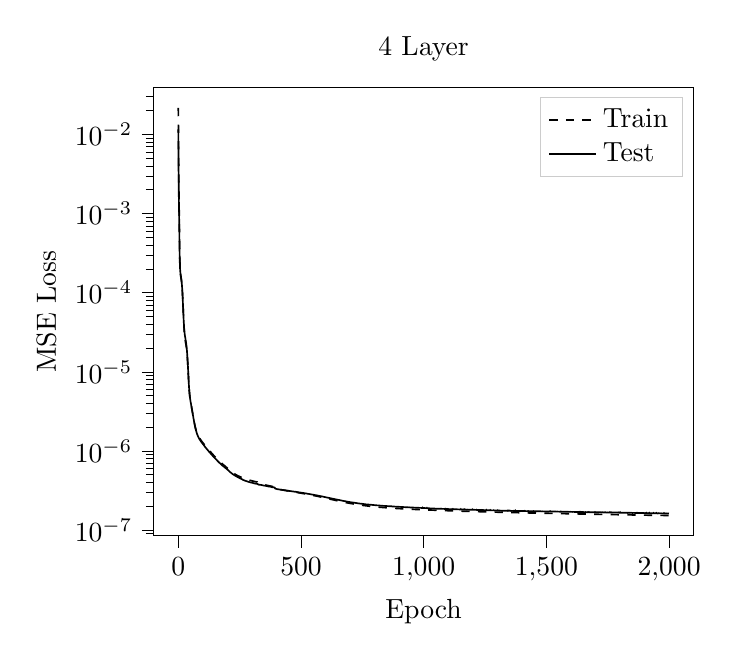
\begin{tikzpicture}

\begin{axis}[
legend cell align={left},
legend style={fill opacity=0.8, draw opacity=1, text opacity=1, draw=white!80!black},
log basis y={10},
tick align=outside,
tick pos=left,
title={4 Layer},
x grid style={white!69.0196078431373!black},
xlabel={Epoch},
xmin=-99.95, xmax=2098.95,
xtick style={color=black},
y grid style={white!69.0196078431373!black},
ylabel={MSE Loss},
ymin=8.43938809238065e-08, ymax=0.0391028934127556,
ymode=log,
ytick style={color=black}
]
\addplot [semithick, black, dashed]
table {%
0 0.0216106624007225
1 0.00673290289845318
2 0.00242847194336355
3 0.00139278739271685
4 0.000877979734446853
5 0.000474738540826365
6 0.000281054378283443
7 0.00021271777068614
8 0.000184169041807763
9 0.000169510987921967
10 0.000160570089246903
11 0.000153623172860534
12 0.000146821876085596
13 0.000139312337923911
14 0.000130708834607503
15 0.000120814576126577
16 0.000109637301975454
17 9.74004520030576e-05
18 8.46704687937745e-05
19 7.22209239793301e-05
20 6.08980650031299e-05
21 5.13222632107499e-05
22 4.36849454090407e-05
23 3.78588456642319e-05
24 3.35587738209142e-05
25 3.04345663553249e-05
26 2.81585673401423e-05
27 2.64713321785166e-05
28 2.51700294393231e-05
29 2.40990629854423e-05
30 2.31376955125597e-05
31 2.21966665994842e-05
32 2.12135114788907e-05
33 2.01455304168121e-05
34 1.89702411180406e-05
35 1.76808702226481e-05
36 1.62871305710723e-05
37 1.48123448534534e-05
38 1.32958351109664e-05
39 1.17858424450787e-05
40 1.0341288148993e-05
41 9.02308400145557e-06
42 7.88079028029642e-06
43 6.9382161775593e-06
44 6.18492073954258e-06
45 5.61335765496551e-06
46 5.18214040664589e-06
47 4.851168252344e-06
48 4.5908486360986e-06
49 4.37404542492459e-06
50 4.1860971711003e-06
51 4.01634194429334e-06
52 3.85815369747888e-06
53 3.70789047474318e-06
54 3.56210532618206e-06
55 3.42163359334791e-06
56 3.28623007618489e-06
57 3.15185335739443e-06
58 3.0234138083074e-06
59 2.90046724973081e-06
60 2.78323152656412e-06
61 2.67022930574967e-06
62 2.56325708880922e-06
63 2.46282143962162e-06
64 2.36972090749532e-06
65 2.28372049502923e-06
66 2.20383440972682e-06
67 2.12981607876372e-06
68 2.0617129700895e-06
69 1.99959229286151e-06
70 1.94295511562359e-06
71 1.89111669618569e-06
72 1.84340184341636e-06
73 1.79986060237525e-06
74 1.75956733130533e-06
75 1.72281113952977e-06
76 1.68883256932872e-06
77 1.65757721526916e-06
78 1.62893817480381e-06
79 1.60244528660769e-06
80 1.57779333051167e-06
81 1.55488546303673e-06
82 1.53347499124834e-06
83 1.51332984992791e-06
84 1.49426139915931e-06
85 1.47615350221031e-06
86 1.45896057071582e-06
87 1.44265126846221e-06
88 1.42635903176824e-06
89 1.41095506359079e-06
90 1.39608382190204e-06
91 1.38187484546393e-06
92 1.3679947178673e-06
93 1.35463125761248e-06
94 1.34165614971948e-06
95 1.32878456537355e-06
96 1.31631478626559e-06
97 1.30407440371982e-06
98 1.29206818090211e-06
99 1.28030122669998e-06
100 1.26874039784752e-06
101 1.25744272938277e-06
102 1.24637065587763e-06
103 1.23556529459279e-06
104 1.22468484934757e-06
105 1.21391777702229e-06
106 1.20343351045449e-06
107 1.19293890546146e-06
108 1.18257735414318e-06
109 1.17147049024879e-06
110 1.16113315289113e-06
111 1.15103359098612e-06
112 1.14106687107096e-06
113 1.13130547171636e-06
114 1.12164716841789e-06
115 1.11212452972609e-06
116 1.10274103678876e-06
117 1.09347531545723e-06
118 1.08429839545465e-06
119 1.07525509415041e-06
120 1.06630471557878e-06
121 1.05751132139176e-06
122 1.0487439832616e-06
123 1.04011279623251e-06
124 1.03160096955435e-06
125 1.02322621967232e-06
126 1.01492625211108e-06
127 1.00679528438263e-06
128 9.98749102421925e-07
129 9.90614294664738e-07
130 9.82658809448367e-07
131 9.74852750289301e-07
132 9.67159750558721e-07
133 9.59597950853208e-07
134 9.52112600600685e-07
135 9.4466021650419e-07
136 9.37624845334994e-07
137 9.30101956882368e-07
138 9.2261810858929e-07
139 9.15006883133174e-07
140 9.07406760788376e-07
141 9.00099601224724e-07
142 8.92701309766153e-07
143 8.85610241880386e-07
144 8.78771238845388e-07
145 8.72219110959804e-07
146 8.65594072266163e-07
147 8.59149445574303e-07
148 8.52838356223629e-07
149 8.46545972649437e-07
150 8.40331516357651e-07
151 8.34286911057802e-07
152 8.28214898177748e-07
153 8.22116376156146e-07
154 8.16204172863877e-07
155 8.10378548209201e-07
156 8.04656332050513e-07
157 7.99051991762667e-07
158 7.93543244043349e-07
159 7.88110822099952e-07
160 7.82816938922792e-07
161 7.77351807641935e-07
162 7.72005825297129e-07
163 7.66674001397405e-07
164 7.61450602340119e-07
165 7.56337212166613e-07
166 7.5132788563792e-07
167 7.46323605710586e-07
168 7.41613327960522e-07
169 7.36650454257415e-07
170 7.31902793432937e-07
171 7.27025475512733e-07
172 7.22359442249854e-07
173 7.177709151307e-07
174 7.13255188415474e-07
175 7.08742484775371e-07
176 7.03956646006532e-07
177 6.98618378038418e-07
178 6.93606436271921e-07
179 6.88884985976301e-07
180 6.84381060153783e-07
181 6.80145616499317e-07
182 6.75724589797255e-07
183 6.71580819329165e-07
184 6.6738621748641e-07
185 6.6328372876967e-07
186 6.59295098714097e-07
187 6.55370623690032e-07
188 6.51456420968088e-07
189 6.4768271292337e-07
190 6.43534997621487e-07
191 6.39708978283693e-07
192 6.359301758323e-07
193 6.32180300485175e-07
194 6.28438367741069e-07
195 6.24702582612713e-07
196 6.21174068299979e-07
197 6.17387885085918e-07
198 6.1360695735857e-07
199 6.09839239018584e-07
200 6.06011450102528e-07
201 6.02128856996842e-07
202 5.98357907904301e-07
203 5.9438991659988e-07
204 5.90488967759484e-07
205 5.86552403930796e-07
206 5.82735191478889e-07
207 5.7880083262063e-07
208 5.7500634336094e-07
209 5.71188780483567e-07
210 5.67494936362323e-07
211 5.63854762901883e-07
212 5.60381861106407e-07
213 5.57017742153221e-07
214 5.53732854783107e-07
215 5.50645551413709e-07
216 5.47619643711528e-07
217 5.44531466303511e-07
218 5.41552928794431e-07
219 5.38660903046662e-07
220 5.35860492874463e-07
221 5.33061054838413e-07
222 5.30413544254316e-07
223 5.27592542923117e-07
224 5.25051639684193e-07
225 5.22539969892932e-07
226 5.20097590815283e-07
227 5.17746779479467e-07
228 5.15497621826455e-07
229 5.13201537245322e-07
230 5.10952482173366e-07
231 5.08788757684897e-07
232 5.06413795463345e-07
233 5.04197328794476e-07
234 5.02117503565103e-07
235 5.00099920714092e-07
236 4.98156201281574e-07
237 4.96120355620633e-07
238 4.94286574834746e-07
239 4.92361857155288e-07
240 4.90496158661813e-07
241 4.88675696999508e-07
242 4.86913171407366e-07
243 4.851756119848e-07
244 4.83470957902909e-07
245 4.81814274188253e-07
246 4.80199573651419e-07
247 4.78683203567698e-07
248 4.77044099817192e-07
249 4.75468882626728e-07
250 4.73879091153151e-07
251 4.72371058982901e-07
252 4.70842513635716e-07
253 4.6937632956201e-07
254 4.67929217776941e-07
255 4.66513790627232e-07
256 4.65088764485699e-07
257 4.6366257139141e-07
258 4.62334256909003e-07
259 4.60908514426706e-07
260 4.59539256539188e-07
261 4.582419610486e-07
262 4.56966788391355e-07
263 4.55675070149653e-07
264 4.54337393499316e-07
265 4.53071155732232e-07
266 4.51853715723871e-07
267 4.50666905862818e-07
268 4.49487872209886e-07
269 4.48350553412524e-07
270 4.47203686391617e-07
271 4.46084542019776e-07
272 4.44943811899634e-07
273 4.43894103753451e-07
274 4.42781260545644e-07
275 4.4177846840654e-07
276 4.40752303987324e-07
277 4.3963250649881e-07
278 4.38508849981645e-07
279 4.37525406496775e-07
280 4.36493751188038e-07
281 4.35531963482561e-07
282 4.34462244669476e-07
283 4.33431620805891e-07
284 4.32435458542102e-07
285 4.31482845442588e-07
286 4.30554591901e-07
287 4.29638015788214e-07
288 4.28745323013402e-07
289 4.2790234015655e-07
290 4.27039721159872e-07
291 4.26191598307923e-07
292 4.25355553360873e-07
293 4.24506018333659e-07
294 4.23655542931556e-07
295 4.22808301834721e-07
296 4.21996215266063e-07
297 4.21198938262535e-07
298 4.20371942965403e-07
299 4.19587211652583e-07
300 4.18860521804731e-07
301 4.18094755104903e-07
302 4.17349502271236e-07
303 4.16623433551422e-07
304 4.15895910307995e-07
305 4.15184494542586e-07
306 4.14479024385628e-07
307 4.13734667318977e-07
308 4.13033298542587e-07
309 4.12367151128024e-07
310 4.11671337289476e-07
311 4.11018487042725e-07
312 4.10363574829375e-07
313 4.09771400768477e-07
314 4.09135555258899e-07
315 4.08534289007889e-07
316 4.07766801657772e-07
317 4.07205162758828e-07
318 4.06719284313795e-07
319 4.05979226258069e-07
320 4.05369681857337e-07
321 4.04813660580317e-07
322 4.0424221703006e-07
323 4.01775835342733e-07
324 3.9732308940188e-07
325 3.95490883548177e-07
326 3.93727580572545e-07
327 3.9239304535954e-07
328 3.91342631729685e-07
329 3.90330171711639e-07
330 3.89447076273086e-07
331 3.88699826885386e-07
332 3.87784748724584e-07
333 3.87108554747329e-07
334 3.86313853951492e-07
335 3.85547236177786e-07
336 3.84728025963454e-07
337 3.83967091067916e-07
338 3.83136319840105e-07
339 3.82331433002037e-07
340 3.81500545188373e-07
341 3.80685198756225e-07
342 3.80033054341311e-07
343 3.79316259142115e-07
344 3.78621012487201e-07
345 3.7795977845434e-07
346 3.77288775951001e-07
347 3.76653722184983e-07
348 3.75958665728149e-07
349 3.75355292362656e-07
350 3.74698903961246e-07
351 3.74061793934288e-07
352 3.73468358191076e-07
353 3.72811548963625e-07
354 3.72241171824328e-07
355 3.71634515659025e-07
356 3.70998225157848e-07
357 3.70405478889779e-07
358 3.69798000349419e-07
359 3.69194266880868e-07
360 3.68567208624881e-07
361 3.679934441152e-07
362 3.67422204163859e-07
363 3.66914002796648e-07
364 3.66252508641196e-07
365 3.65631194782168e-07
366 3.65033643291213e-07
367 3.6445641813998e-07
368 3.63884713749485e-07
369 3.6333000007005e-07
370 3.62738613333136e-07
371 3.62184976779645e-07
372 3.61609488692238e-07
373 3.61079528076402e-07
374 3.60510225192456e-07
375 3.59959687756373e-07
376 3.59414541676983e-07
377 3.58882117126313e-07
378 3.58320710986959e-07
379 3.57816574023673e-07
380 3.5727768839422e-07
381 3.56719101432645e-07
382 3.56145097327953e-07
383 3.55607541536074e-07
384 3.55104071616097e-07
385 3.54350894710365e-07
386 3.53832532411502e-07
387 3.53362483537012e-07
388 3.52820708798163e-07
389 3.52301250558185e-07
390 3.51839069267612e-07
391 3.51369276515356e-07
392 3.50713634929889e-07
393 3.50198180385064e-07
394 3.42994273879071e-07
395 3.37459253060501e-07
396 3.36289835345838e-07
397 3.35470516276359e-07
398 3.34717947012564e-07
399 3.34036376955282e-07
400 3.33413894921364e-07
401 3.32775672802654e-07
402 3.32222780471625e-07
403 3.31656370008204e-07
404 3.31059441123216e-07
405 3.30471022579104e-07
406 3.29948070614705e-07
407 3.29408178927793e-07
408 3.28830659569235e-07
409 3.28420155582876e-07
410 3.27948691108304e-07
411 3.27466074267591e-07
412 3.26983534591818e-07
413 3.26529947187737e-07
414 3.26056213680204e-07
415 3.25601777944939e-07
416 3.25140297491089e-07
417 3.24708497444703e-07
418 3.24223424328807e-07
419 3.23786114506675e-07
420 3.23332559105438e-07
421 3.22898877939792e-07
422 3.22457123729691e-07
423 3.22002698311508e-07
424 3.21506677451566e-07
425 3.21149641436591e-07
426 3.2071827259017e-07
427 3.20318631850114e-07
428 3.19890345039653e-07
429 3.19473695739703e-07
430 3.18698119528449e-07
431 3.18401096876642e-07
432 3.17974057793435e-07
433 3.17500140937454e-07
434 3.17058012129223e-07
435 3.16648788057705e-07
436 3.16250691852815e-07
437 3.15829835571435e-07
438 3.15423972210738e-07
439 3.15066943116449e-07
440 3.14667640367361e-07
441 3.14271113822429e-07
442 3.13797254975157e-07
443 3.13497316142275e-07
444 3.13078043916448e-07
445 3.12755185831293e-07
446 3.12391271933166e-07
447 3.1198606302496e-07
448 3.1160391039009e-07
449 3.11256480088673e-07
450 3.10887099558954e-07
451 3.10662238675263e-07
452 3.10277672426196e-07
453 3.09896373551055e-07
454 3.09517824987893e-07
455 3.09143135638124e-07
456 3.08770616982201e-07
457 3.08405447086102e-07
458 3.08032719928519e-07
459 3.07656596632455e-07
460 3.07311306372071e-07
461 3.06948595408585e-07
462 3.06615132117827e-07
463 3.06262616817321e-07
464 3.05897978648773e-07
465 3.05542331858533e-07
466 3.05163595825775e-07
467 3.04796437418986e-07
468 3.04440751691004e-07
469 3.04076373026874e-07
470 3.03719222827681e-07
471 3.03353062221845e-07
472 3.02990892649291e-07
473 3.0263301108846e-07
474 3.02271752175898e-07
475 3.01934635672296e-07
476 3.0156328080011e-07
477 3.01179149317932e-07
478 3.00842650105437e-07
479 3.00472060928314e-07
480 3.00037528703001e-07
481 2.99667246835611e-07
482 2.99302288965464e-07
483 2.98947667644711e-07
484 2.98582195583208e-07
485 2.98215010573699e-07
486 2.9785535068072e-07
487 2.97490581374404e-07
488 2.97126231615152e-07
489 2.96774992690985e-07
490 2.96397045090657e-07
491 2.96061390230307e-07
492 2.95681678281312e-07
493 2.9532954511069e-07
494 2.94962441074631e-07
495 2.94596214985177e-07
496 2.94228129320118e-07
497 2.93864728405424e-07
498 2.93508675170528e-07
499 2.93143504279669e-07
500 2.92784303780991e-07
501 2.92416588507649e-07
502 2.92051301343577e-07
503 2.91686755957699e-07
504 2.91287320621336e-07
505 2.90917487433262e-07
506 2.90549759711212e-07
507 2.90181204320561e-07
508 2.89812056109895e-07
509 2.89444514450565e-07
510 2.89075045500908e-07
511 2.88704543976337e-07
512 2.88336096332387e-07
513 2.8796272732734e-07
514 2.87592303521933e-07
515 2.87219270418859e-07
516 2.86848664543982e-07
517 2.86476573634786e-07
518 2.86102311221725e-07
519 2.85724018624478e-07
520 2.85357762265903e-07
521 2.84981645876314e-07
522 2.8461455055151e-07
523 2.8425328021342e-07
524 2.83887521433712e-07
525 2.83510480073801e-07
526 2.83132329769842e-07
527 2.82761600246317e-07
528 2.82383754637294e-07
529 2.82003369363792e-07
530 2.81624365769062e-07
531 2.81253791044378e-07
532 2.80863522320374e-07
533 2.80491489519363e-07
534 2.80108860522432e-07
535 2.79729500917369e-07
536 2.79344856437547e-07
537 2.78964073430643e-07
538 2.78581386027099e-07
539 2.78189427277198e-07
540 2.77800684699514e-07
541 2.77422164160157e-07
542 2.77025935531583e-07
543 2.76675719604214e-07
544 2.7628835702842e-07
545 2.75891499214254e-07
546 2.754996529859e-07
547 2.7510834667055e-07
548 2.7471418212599e-07
549 2.74250312244817e-07
550 2.73937980210803e-07
551 2.73469895518019e-07
552 2.73089561275697e-07
553 2.72698263458437e-07
554 2.72312604806757e-07
555 2.71926184367999e-07
556 2.71536050803434e-07
557 2.71139314662605e-07
558 2.70746581449544e-07
559 2.70352984330202e-07
560 2.69956387015213e-07
561 2.69561034599519e-07
562 2.69184922245813e-07
563 2.68785443537922e-07
564 2.68388820202858e-07
565 2.67988743360092e-07
566 2.67580664214506e-07
567 2.6718646597601e-07
568 2.66785075979215e-07
569 2.66419031149212e-07
570 2.66015551616761e-07
571 2.65620774769104e-07
572 2.65219328838384e-07
573 2.64824864359525e-07
574 2.64434130130553e-07
575 2.64023973286953e-07
576 2.63620257200614e-07
577 2.63219747282051e-07
578 2.62736836447175e-07
579 2.62318192085331e-07
580 2.61909523416648e-07
581 2.61502716469408e-07
582 2.61105529247629e-07
583 2.60702718719585e-07
584 2.6029890841528e-07
585 2.59889832378235e-07
586 2.59486747424376e-07
587 2.59076840677608e-07
588 2.58672434839013e-07
589 2.58264190520663e-07
590 2.57854916384304e-07
591 2.57446017087659e-07
592 2.57047310228131e-07
593 2.56630037597461e-07
594 2.56229556200083e-07
595 2.55818167815391e-07
596 2.55413956594452e-07
597 2.55009213333324e-07
598 2.54611830413864e-07
599 2.54200633449386e-07
600 2.5380529264396e-07
601 2.53393371764332e-07
602 2.52922564399682e-07
603 2.52380531748031e-07
604 2.51938129494533e-07
605 2.5150760473025e-07
606 2.51107723556743e-07
607 2.50692401550623e-07
608 2.50296422933616e-07
609 2.49886340895955e-07
610 2.49492911265747e-07
611 2.49087333429543e-07
612 2.48680714250327e-07
613 2.48284265978782e-07
614 2.4788667600717e-07
615 2.47456508517985e-07
616 2.47051033085199e-07
617 2.46647489134944e-07
618 2.4625732633865e-07
619 2.45860469803461e-07
620 2.45425408920141e-07
621 2.45022914640458e-07
622 2.44652590524197e-07
623 2.44252181644811e-07
624 2.43862469332612e-07
625 2.43488337133613e-07
626 2.43087162303368e-07
627 2.42683210387895e-07
628 2.42284148342264e-07
629 2.4189684177145e-07
630 2.41453110305656e-07
631 2.4105597925228e-07
632 2.40666493098729e-07
633 2.402901326235e-07
634 2.39877828683177e-07
635 2.39510399850928e-07
636 2.39118784641335e-07
637 2.38734965940068e-07
638 2.38333517231126e-07
639 2.37971021149974e-07
640 2.37577484739404e-07
641 2.37201121635167e-07
642 2.36807600217048e-07
643 2.36442187372177e-07
644 2.36048477418649e-07
645 2.35720507248516e-07
646 2.3529685198298e-07
647 2.34926964964188e-07
648 2.34651763484806e-07
649 2.34295619804925e-07
650 2.33907534919808e-07
651 2.33553717706059e-07
652 2.33175521088924e-07
653 2.32825393268854e-07
654 2.32450461304268e-07
655 2.32095179185876e-07
656 2.31748523042086e-07
657 2.31385499631642e-07
658 2.31015129955381e-07
659 2.30663613251636e-07
660 2.30288796053912e-07
661 2.29934373187746e-07
662 2.29571597571976e-07
663 2.29216760359918e-07
664 2.28852116933354e-07
665 2.28495701144027e-07
666 2.28147498418707e-07
667 2.27798743303254e-07
668 2.27462652588883e-07
669 2.27117970155177e-07
670 2.26760281407223e-07
671 2.26418564309938e-07
672 2.26108651581569e-07
673 2.25791860522406e-07
674 2.25436486502417e-07
675 2.25098220347775e-07
676 2.24788045336766e-07
677 2.24459609604821e-07
678 2.24133774658242e-07
679 2.23800147416853e-07
680 2.23474523565415e-07
681 2.23188974956656e-07
682 2.2284166180242e-07
683 2.2254372058228e-07
684 2.22211433126063e-07
685 2.21920742731641e-07
686 2.21595553426823e-07
687 2.21314227367486e-07
688 2.21033817595639e-07
689 2.20716097487639e-07
690 2.20356926739385e-07
691 2.2009933127265e-07
692 2.19786205256867e-07
693 2.19499166888681e-07
694 2.19210622162791e-07
695 2.18931428264568e-07
696 2.18612988660993e-07
697 2.18332271472832e-07
698 2.18054914128629e-07
699 2.17747560832038e-07
700 2.17494242413352e-07
701 2.17189853188415e-07
702 2.16910481917409e-07
703 2.16647721089203e-07
704 2.16394595852876e-07
705 2.1610913848491e-07
706 2.15835460842584e-07
707 2.15616975424382e-07
708 2.15359850656682e-07
709 2.15075565435541e-07
710 2.14831694350437e-07
711 2.14503112900388e-07
712 2.14279591034483e-07
713 2.13987736259469e-07
714 2.13740835725673e-07
715 2.13455635510229e-07
716 2.13242247525614e-07
717 2.12986595641951e-07
718 2.12713128561859e-07
719 2.12486485366981e-07
720 2.12225340455063e-07
721 2.11995605106097e-07
722 2.11794130493104e-07
723 2.11524806914554e-07
724 2.1125673990241e-07
725 2.11031820846586e-07
726 2.1081890638186e-07
727 2.10560273671945e-07
728 2.10315091813129e-07
729 2.10102463988449e-07
730 2.09889895714355e-07
731 2.09609642865871e-07
732 2.09425779999606e-07
733 2.09183616597386e-07
734 2.08990658443042e-07
735 2.08729989289225e-07
736 2.08531867073702e-07
737 2.08309944277119e-07
738 2.08086278355779e-07
739 2.0789459659909e-07
740 2.07680310651881e-07
741 2.0747119165776e-07
742 2.07236777498565e-07
743 2.07018175132134e-07
744 2.06816486773675e-07
745 2.06584763589035e-07
746 2.06387027432697e-07
747 2.06218926180668e-07
748 2.06005806859366e-07
749 2.05752826182959e-07
750 2.05548594330196e-07
751 2.05311775921757e-07
752 2.05142609736697e-07
753 2.0495073572846e-07
754 2.04771630293976e-07
755 2.0461071154898e-07
756 2.04373782693779e-07
757 2.04192100383693e-07
758 2.04031139503513e-07
759 2.03814531289481e-07
760 2.03654313601476e-07
761 2.03442323652325e-07
762 2.03277292598614e-07
763 2.0309212533931e-07
764 2.02949136372865e-07
765 2.02724689088996e-07
766 2.02560473084645e-07
767 2.02350404919116e-07
768 2.02225088422381e-07
769 2.02075813668046e-07
770 2.01815807457706e-07
771 2.01668591600423e-07
772 2.01510255024573e-07
773 2.01304897409216e-07
774 2.01147469894636e-07
775 2.0087547069636e-07
776 2.00708041205644e-07
777 2.00552844987101e-07
778 2.00407669666447e-07
779 2.00212583891357e-07
780 2.00079323661839e-07
781 1.99906171182818e-07
782 1.99735537769641e-07
783 1.99590529170734e-07
784 1.99458949076359e-07
785 1.9929100927385e-07
786 1.99101222690956e-07
787 1.98979387548093e-07
788 1.9883520160846e-07
789 1.98662458501531e-07
790 1.98509994092433e-07
791 1.98378701213642e-07
792 1.98230722041615e-07
793 1.98054001302239e-07
794 1.97913957400431e-07
795 1.97748915866214e-07
796 1.97619246243619e-07
797 1.97458854394483e-07
798 1.9732037737441e-07
799 1.9718832942317e-07
800 1.97041426808653e-07
801 1.96902047633785e-07
802 1.96766920048219e-07
803 1.96604294650626e-07
804 1.96496536219115e-07
805 1.96382572973164e-07
806 1.96219839480705e-07
807 1.96085320837369e-07
808 1.95963470162042e-07
809 1.95823555152685e-07
810 1.95713456996316e-07
811 1.95573616785794e-07
812 1.95453819671343e-07
813 1.95311064544512e-07
814 1.95212965564906e-07
815 1.95100162919459e-07
816 1.94962750249772e-07
817 1.94830665954271e-07
818 1.94717411517331e-07
819 1.94620832374426e-07
820 1.94458740004677e-07
821 1.94354109922301e-07
822 1.94270007597197e-07
823 1.94124745341639e-07
824 1.94010768659325e-07
825 1.93872416154761e-07
826 1.93788308628484e-07
827 1.93651885346924e-07
828 1.93532121421924e-07
829 1.93444749363891e-07
830 1.93306050924491e-07
831 1.93204075095821e-07
832 1.9309011060642e-07
833 1.92993874705394e-07
834 1.92862723380927e-07
835 1.92772320488643e-07
836 1.92665639630718e-07
837 1.92546770804825e-07
838 1.92435405381275e-07
839 1.92352559281517e-07
840 1.92240041741343e-07
841 1.92133511006887e-07
842 1.92020548425376e-07
843 1.919115628084e-07
844 1.91812710554018e-07
845 1.91718293251597e-07
846 1.91616724755761e-07
847 1.91497081054592e-07
848 1.91413476578362e-07
849 1.91311501069436e-07
850 1.91188739904646e-07
851 1.91130697771769e-07
852 1.91013988590782e-07
853 1.90901197811399e-07
854 1.90812814622632e-07
855 1.90715631696037e-07
856 1.90646210654677e-07
857 1.90514590059365e-07
858 1.90444030131687e-07
859 1.90331704054358e-07
860 1.90250029120875e-07
861 1.90143055029068e-07
862 1.90024863513827e-07
863 1.89974942529147e-07
864 1.89862021365173e-07
865 1.89752594678794e-07
866 1.89691171975426e-07
867 1.89590054446853e-07
868 1.89481359015531e-07
869 1.89564498441541e-07
870 1.89266790783904e-07
871 1.89147045318805e-07
872 1.89083462664996e-07
873 1.89025151307476e-07
874 1.88914466036749e-07
875 1.88806591928881e-07
876 1.88748112037729e-07
877 1.88681913918742e-07
878 1.88565463105306e-07
879 1.88473345332341e-07
880 1.88422301071967e-07
881 1.88273862789856e-07
882 1.88229817830177e-07
883 1.88129125866965e-07
884 1.88074489372525e-07
885 1.87977990435684e-07
886 1.87873305492303e-07
887 1.87809109206682e-07
888 1.87705275983774e-07
889 1.87653425115286e-07
890 1.87576660152899e-07
891 1.87455449136564e-07
892 1.8739126468148e-07
893 1.87289279985237e-07
894 1.8724850141183e-07
895 1.87153168901943e-07
896 1.8706308216565e-07
897 1.86987817727413e-07
898 1.86928051377322e-07
899 1.86846638250415e-07
900 1.86764167771969e-07
901 1.86676254728013e-07
902 1.86577274298827e-07
903 1.86536912949009e-07
904 1.8646056668814e-07
905 1.86386593952648e-07
906 1.86291404176586e-07
907 1.86223032379473e-07
908 1.86134376484404e-07
909 1.86082618697014e-07
910 1.85978073758974e-07
911 1.85938494226434e-07
912 1.85864153408488e-07
913 1.85785363839841e-07
914 1.85678791211785e-07
915 1.85629285340383e-07
916 1.85553920864834e-07
917 1.85486233405641e-07
918 1.8540947337442e-07
919 1.85350580267141e-07
920 1.85271162948197e-07
921 1.85202297849685e-07
922 1.85131175925335e-07
923 1.85051926912649e-07
924 1.84978863472907e-07
925 1.8492998484021e-07
926 1.84832688674419e-07
927 1.84801209300645e-07
928 1.84736455373979e-07
929 1.84623548165064e-07
930 1.84608434793176e-07
931 1.84504162469068e-07
932 1.84435943999972e-07
933 1.84360517607729e-07
934 1.84322198350628e-07
935 1.84215514472896e-07
936 1.84190147251684e-07
937 1.84140666071642e-07
938 1.84041638341625e-07
939 1.83968719234429e-07
940 1.83896355849811e-07
941 1.83837361070971e-07
942 1.83839822845755e-07
943 1.83766977229993e-07
944 1.83638415258258e-07
945 1.83566072095687e-07
946 1.83519504091123e-07
947 1.83446028835021e-07
948 1.83395068596326e-07
949 1.83316212236662e-07
950 1.83285562606272e-07
951 1.83199140721513e-07
952 1.83183291241562e-07
953 1.83075190882676e-07
954 1.83062210787455e-07
955 1.82927106422426e-07
956 1.82892595525175e-07
957 1.82834764522966e-07
958 1.82783786037533e-07
959 1.82701763108639e-07
960 1.82646872232795e-07
961 1.82573253077578e-07
962 1.82511307478705e-07
963 1.82460096070258e-07
964 1.82422018170314e-07
965 1.82331821022785e-07
966 1.82296495310652e-07
967 1.82236372658906e-07
968 1.8213447961557e-07
969 1.8208163304223e-07
970 1.82025621178639e-07
971 1.81966136040046e-07
972 1.81946712665138e-07
973 1.81872313675058e-07
974 1.81773238892902e-07
975 1.81758913051056e-07
976 1.8167523741397e-07
977 1.81603671109087e-07
978 1.81574254867201e-07
979 1.81481448350951e-07
980 1.8144391169983e-07
981 1.81378839940294e-07
982 1.81291478270396e-07
983 1.81267837923826e-07
984 1.81212172982725e-07
985 1.81145498459045e-07
986 1.81104971638035e-07
987 1.81015536654172e-07
988 1.81003275883995e-07
989 1.80951426081322e-07
990 1.80898478369329e-07
991 1.80804848220362e-07
992 1.80737904678097e-07
993 1.80692982183928e-07
994 1.8063039879479e-07
995 1.80686602881508e-07
996 1.80568369920309e-07
997 1.80461264832843e-07
998 1.80398518651259e-07
999 1.80379310890544e-07
1000 1.80326845374168e-07
1001 1.80228571188934e-07
1002 1.80212151668968e-07
1003 1.80164973421881e-07
1004 1.80055146493885e-07
1005 1.80016070551403e-07
1006 1.80035480369156e-07
1007 1.79911012459399e-07
1008 1.79842733800228e-07
1009 1.79833708145338e-07
1010 1.79744951807947e-07
1011 1.79718168539011e-07
1012 1.79695514212597e-07
1013 1.79632579659028e-07
1014 1.7958827668707e-07
1015 1.79485900808629e-07
1016 1.79413860877276e-07
1017 1.79370492290332e-07
1018 1.79360341761026e-07
1019 1.79332420671585e-07
1020 1.79230263661623e-07
1021 1.7917569885384e-07
1022 1.79127057556627e-07
1023 1.79241113549722e-07
1024 1.7917623971897e-07
1025 1.79244382202626e-07
1026 1.79210308260735e-07
1027 1.79150409216788e-07
1028 1.79036714634151e-07
1029 1.79027852738045e-07
1030 1.78958927357087e-07
1031 1.7893335813568e-07
1032 1.78864548978197e-07
1033 1.78835367890429e-07
1034 1.78795579536484e-07
1035 1.78755134868425e-07
1036 1.78641936344093e-07
1037 1.78593477691891e-07
1038 1.78590952224056e-07
1039 1.78499820442823e-07
1040 1.78439640791339e-07
1041 1.78394428537842e-07
1042 1.78378901708243e-07
1043 1.78302251427453e-07
1044 1.78258820334065e-07
1045 1.78191099934111e-07
1046 1.78159377298925e-07
1047 1.78104258438339e-07
1048 1.78057871373483e-07
1049 1.78015181447222e-07
1050 1.77944034774669e-07
1051 1.77941957588246e-07
1052 1.77853626396995e-07
1053 1.77814524832343e-07
1054 1.7774813699134e-07
1055 1.77703809889351e-07
1056 1.77675952258483e-07
1057 1.77648358352656e-07
1058 1.77571942579391e-07
1059 1.77527472061456e-07
1060 1.77485991635251e-07
1061 1.7744707773204e-07
1062 1.77386032802929e-07
1063 1.77322587973094e-07
1064 1.77299124445085e-07
1065 1.77234235543722e-07
1066 1.77215259405727e-07
1067 1.77158344335737e-07
1068 1.77124247471738e-07
1069 1.77064489179202e-07
1070 1.76985912368366e-07
1071 1.76983701834388e-07
1072 1.76910187533963e-07
1073 1.76876028099571e-07
1074 1.76824726956681e-07
1075 1.76798676029932e-07
1076 1.76776226531672e-07
1077 1.76694430521707e-07
1078 1.76621351180017e-07
1079 1.76610401460664e-07
1080 1.76574187129575e-07
1081 1.7649910562767e-07
1082 1.76468546882802e-07
1083 1.76431862030313e-07
1084 1.7638737516279e-07
1085 1.76306908748813e-07
1086 1.76277939857528e-07
1087 1.76302373539272e-07
1088 1.7617569829298e-07
1089 1.76178361300572e-07
1090 1.76133429633296e-07
1091 1.76041002141858e-07
1092 1.75977817043815e-07
1093 1.75944437359021e-07
1094 1.75941254248357e-07
1095 1.75881839190595e-07
1096 1.75846790924084e-07
1097 1.75819223144913e-07
1098 1.75713790490306e-07
1099 1.75664444050483e-07
1100 1.75637258344352e-07
1101 1.75566675693517e-07
1102 1.75534115825826e-07
1103 1.75526750261668e-07
1104 1.75438703770681e-07
1105 1.7538309885623e-07
1106 1.75376762328483e-07
1107 1.7530193790094e-07
1108 1.75282633335883e-07
1109 1.75220648891639e-07
1110 1.75184468702128e-07
1111 1.75177809552451e-07
1112 1.75096959537768e-07
1113 1.75071028550633e-07
1114 1.75022347598031e-07
1115 1.7497661561805e-07
1116 1.74940363855569e-07
1117 1.74892061075127e-07
1118 1.74832643715206e-07
1119 1.74859169668196e-07
1120 1.74774426554336e-07
1121 1.7468253720665e-07
1122 1.74662733201103e-07
1123 1.74636310930509e-07
1124 1.74569058856378e-07
1125 1.74553399908461e-07
1126 1.74507346848429e-07
1127 1.74474903275268e-07
1128 1.74449821827238e-07
1129 1.74340132559792e-07
1130 1.74361761217767e-07
1131 1.74297626386988e-07
1132 1.74214229467395e-07
1133 1.74233699652859e-07
1134 1.7419528980156e-07
1135 1.74113174260526e-07
1136 1.74103606482845e-07
1137 1.74103460260255e-07
1138 1.73959555390013e-07
1139 1.73925013555731e-07
1140 1.7386210139847e-07
1141 1.73848528262965e-07
1142 1.73805815336436e-07
1143 1.73731946027544e-07
1144 1.73736144176928e-07
1145 1.73698482896612e-07
1146 1.73662524865392e-07
1147 1.73587405967623e-07
1148 1.73579918822497e-07
1149 1.73576758577099e-07
1150 1.735323319636e-07
1151 1.73485661129291e-07
1152 1.73443705548948e-07
1153 1.73351196750104e-07
1154 1.73381033533815e-07
1155 1.73310837986662e-07
1156 1.73295372221105e-07
1157 1.73259445723772e-07
1158 1.73227503879048e-07
1159 1.73195007207028e-07
1160 1.73187520424278e-07
1161 1.7306360564362e-07
1162 1.73050464432833e-07
1163 1.73035037157376e-07
1164 1.73087016712259e-07
1165 1.72968198214107e-07
1166 1.72881617530152e-07
1167 1.7295136483142e-07
1168 1.72851830512855e-07
1169 1.72818079022363e-07
1170 1.72778573158894e-07
1171 1.72718693640661e-07
1172 1.7270090534538e-07
1173 1.7270916892187e-07
1174 1.72568362536651e-07
1175 1.72577032891752e-07
1176 1.7258109477325e-07
1177 1.7260609226355e-07
1178 1.72448717250973e-07
1179 1.72415710743223e-07
1180 1.72395935955194e-07
1181 1.72397184961426e-07
1182 1.72349606657463e-07
1183 1.72301530355412e-07
1184 1.72214634403645e-07
1185 1.72153765760186e-07
1186 1.72193612456795e-07
1187 1.72204249409447e-07
1188 1.72087060846593e-07
1189 1.72026658063373e-07
1190 1.72075992630027e-07
1191 1.72030504209886e-07
1192 1.71926870820016e-07
1193 1.71936961912422e-07
1194 1.71891174524319e-07
1195 1.71880935219804e-07
1196 1.71827827792015e-07
1197 1.71822777382147e-07
1198 1.71786435757326e-07
1199 1.71768815185658e-07
1200 1.71702090860038e-07
1201 1.71739857854902e-07
1202 1.71617547074732e-07
1203 1.7156320400602e-07
1204 1.71528990875913e-07
1205 1.71517066888782e-07
1206 1.71513961973346e-07
1207 1.71403330170961e-07
1208 1.71346198889921e-07
1209 1.71383523543511e-07
1210 1.71362682102938e-07
1211 1.71336470835115e-07
1212 1.71251969312891e-07
1213 1.71174495115167e-07
1214 1.71233604270071e-07
1215 1.71314036798265e-07
1216 1.71165501981818e-07
1217 1.71071120618649e-07
1218 1.70984958153042e-07
1219 1.7098195895926e-07
1220 1.71015771975647e-07
1221 1.70996565053372e-07
1222 1.70884112144165e-07
1223 1.7089750729582e-07
1224 1.70790641050189e-07
1225 1.70798408198891e-07
1226 1.70828165650505e-07
1227 1.70793065173314e-07
1228 1.70700528443035e-07
1229 1.7067476072441e-07
1230 1.70675086287986e-07
1231 1.70612983040996e-07
1232 1.70565547598756e-07
1233 1.7050324265e-07
1234 1.70488775488309e-07
1235 1.70464546236815e-07
1236 1.70451107408098e-07
1237 1.70438943598583e-07
1238 1.70367497503321e-07
1239 1.70297669853881e-07
1240 1.70287840084882e-07
1241 1.70317440392864e-07
1242 1.70259187768806e-07
1243 1.70169387097019e-07
1244 1.70166060954102e-07
1245 1.7015959914346e-07
1246 1.70072879036809e-07
1247 1.70080203453438e-07
1248 1.69973099353626e-07
1249 1.70045703136168e-07
1250 1.69952917950411e-07
1251 1.69955662016719e-07
1252 1.69859973333075e-07
1253 1.69899801925055e-07
1254 1.69820288007827e-07
1255 1.69868564412923e-07
1256 1.69765343969175e-07
1257 1.69748448229257e-07
1258 1.69705800452391e-07
1259 1.6965306291894e-07
1260 1.69602442973371e-07
1261 1.69608080632599e-07
1262 1.69599682138255e-07
1263 1.69567798202763e-07
1264 1.69505588857533e-07
1265 1.69445060365092e-07
1266 1.69388760596689e-07
1267 1.69400478604587e-07
1268 1.69410320395968e-07
1269 1.69311620716428e-07
1270 1.69259400074395e-07
1271 1.69325856880675e-07
1272 1.69370852745487e-07
1273 1.69243204737768e-07
1274 1.69179619966542e-07
1275 1.69161871589552e-07
1276 1.69083306850837e-07
1277 1.69077230957271e-07
1278 1.69089837299907e-07
1279 1.69023000928803e-07
1280 1.69091059262882e-07
1281 1.68983588977767e-07
1282 1.68936555738242e-07
1283 1.68931953034246e-07
1284 1.68985705300884e-07
1285 1.68975296190865e-07
1286 1.68837971287417e-07
1287 1.68774838392949e-07
1288 1.68735167370926e-07
1289 1.68765960466999e-07
1290 1.68746516699514e-07
1291 1.68695649733763e-07
1292 1.68646468864608e-07
1293 1.68562413257689e-07
1294 1.6858988993107e-07
1295 1.68670126527104e-07
1296 1.68366325972613e-07
1297 1.6832450091897e-07
1298 1.68334291473116e-07
1299 1.68343839312968e-07
1300 1.68317190968992e-07
1301 1.68235172893105e-07
1302 1.68274554212644e-07
1303 1.68399181184498e-07
1304 1.68282554334098e-07
1305 1.68080057100894e-07
1306 1.68025432877528e-07
1307 1.68044797234757e-07
1308 1.68017354866379e-07
1309 1.67995841799495e-07
1310 1.68006798560327e-07
1311 1.67982508379794e-07
1312 1.67921054860187e-07
1313 1.67883917420397e-07
1314 1.67839464054964e-07
1315 1.67829756712479e-07
1316 1.67853974403442e-07
1317 1.67749433863662e-07
1318 1.67708428286062e-07
1319 1.67713444042761e-07
1320 1.67860712927848e-07
1321 1.67689125817105e-07
1322 1.67559621274904e-07
1323 1.67547872322871e-07
1324 1.67564348146243e-07
1325 1.67477222703383e-07
1326 1.67485049338723e-07
1327 1.67526131981788e-07
1328 1.6742998275987e-07
1329 1.67414902726648e-07
1330 1.6736702631448e-07
1331 1.67352104973872e-07
1332 1.67339367976638e-07
1333 1.6726915405485e-07
1334 1.67304407696633e-07
1335 1.67264324431926e-07
1336 1.67214283322892e-07
1337 1.67262341591368e-07
1338 1.67241847648825e-07
1339 1.67110093784117e-07
1340 1.67036057391101e-07
1341 1.67139857801146e-07
1342 1.67201785750137e-07
1343 1.66920922900715e-07
1344 1.66950420755541e-07
1345 1.66943121350016e-07
1346 1.66929704967345e-07
1347 1.66912089149207e-07
1348 1.66969160659392e-07
1349 1.66813377553865e-07
1350 1.66787883031816e-07
1351 1.66778691990999e-07
1352 1.66794166055695e-07
1353 1.66790056709942e-07
1354 1.66844713575642e-07
1355 1.66592245811614e-07
1356 1.66663042314497e-07
1357 1.66594229689565e-07
1358 1.66581775118857e-07
1359 1.66553394748803e-07
1360 1.66581533129317e-07
1361 1.66522043343775e-07
1362 1.66457377808626e-07
1363 1.66468092778871e-07
1364 1.66456248294367e-07
1365 1.66391937916899e-07
1366 1.6636954207172e-07
1367 1.66337186605858e-07
1368 1.66337999544908e-07
1369 1.66300411265752e-07
1370 1.66256585025337e-07
1371 1.66230324694538e-07
1372 1.66262054960953e-07
1373 1.66311842029643e-07
1374 1.6620884812113e-07
1375 1.66082737052875e-07
1376 1.66100138692116e-07
1377 1.66071855289829e-07
1378 1.65991287140343e-07
1379 1.66027292841875e-07
1380 1.66048765017024e-07
1381 1.65978204798023e-07
1382 1.65909461287583e-07
1383 1.65914692715319e-07
1384 1.65921796678958e-07
1385 1.65908610057386e-07
1386 1.6584075878967e-07
1387 1.65783007716414e-07
1388 1.65777221020846e-07
1389 1.65749755105082e-07
1390 1.65692761413538e-07
1391 1.65716249071579e-07
1392 1.65707926868208e-07
1393 1.65664443692037e-07
1394 1.65660392909217e-07
1395 1.6555531041007e-07
1396 1.65595974486621e-07
1397 1.65527711487812e-07
1398 1.65510852603745e-07
1399 1.65448139732405e-07
1400 1.65507440037516e-07
1401 1.65409376414516e-07
1402 1.65359866144854e-07
1403 1.65365921347416e-07
1404 1.65365050953881e-07
1405 1.65445104364892e-07
1406 1.65383935843977e-07
1407 1.65204668604702e-07
1408 1.65154134542433e-07
1409 1.65219209932843e-07
1410 1.65202215775651e-07
1411 1.6515671573103e-07
1412 1.65137949920791e-07
1413 1.65116417022659e-07
1414 1.6504532810302e-07
1415 1.65028859363758e-07
1416 1.6504706556475e-07
1417 1.64975679453505e-07
1418 1.64952036158184e-07
1419 1.64949861805042e-07
1420 1.64942287014469e-07
1421 1.64880639310638e-07
1422 1.64852907623469e-07
1423 1.64815023296683e-07
1424 1.64827068971363e-07
1425 1.6479692638427e-07
1426 1.64800686256683e-07
1427 1.64663229007544e-07
1428 1.64735067940569e-07
1429 1.64699877252872e-07
1430 1.64645984632727e-07
1431 1.64649042353915e-07
1432 1.64592018414567e-07
1433 1.64586802981148e-07
1434 1.64533369286346e-07
1435 1.64534088234802e-07
1436 1.64539180580903e-07
1437 1.64588025249657e-07
1438 1.64528626413585e-07
1439 1.64403049730311e-07
1440 1.64434569235539e-07
1441 1.64330305665317e-07
1442 1.64350557383841e-07
1443 1.64313907802693e-07
1444 1.64288167425752e-07
1445 1.64290333536599e-07
1446 1.64252259480691e-07
1447 1.64279479896834e-07
1448 1.6423641449137e-07
1449 1.64184464686912e-07
1450 1.64129400964441e-07
1451 1.64106395708075e-07
1452 1.64089033887649e-07
1453 1.64048898746216e-07
1454 1.64055080958292e-07
1455 1.64035842338706e-07
1456 1.64035157851572e-07
1457 1.63966343592392e-07
1458 1.6393386583502e-07
1459 1.63920002862028e-07
1460 1.63905486353144e-07
1461 1.63842626747623e-07
1462 1.63854071125513e-07
1463 1.63843182377832e-07
1464 1.63801519676099e-07
1465 1.63759081736714e-07
1466 1.63764028513924e-07
1467 1.63723978161556e-07
1468 1.63663750292642e-07
1469 1.63675580736822e-07
1470 1.63701325028853e-07
1471 1.63652787477986e-07
1472 1.63594848658022e-07
1473 1.63543358503659e-07
1474 1.63574874825656e-07
1475 1.63533181869013e-07
1476 1.63477860958494e-07
1477 1.63506070094854e-07
1478 1.6346910118159e-07
1479 1.63388968786649e-07
1480 1.63403992630151e-07
1481 1.63401504394756e-07
1482 1.63334911896129e-07
1483 1.63362521405475e-07
1484 1.63307964221815e-07
1485 1.63266157784392e-07
1486 1.63244747525937e-07
1487 1.63252576001582e-07
1488 1.63205464630778e-07
1489 1.6317926982623e-07
1490 1.63177952131832e-07
1491 1.63116752538883e-07
1492 1.63130517712773e-07
1493 1.63142071770039e-07
1494 1.63082057653696e-07
1495 1.63039829530476e-07
1496 1.62986418189348e-07
1497 1.63003632266623e-07
1498 1.6297419497846e-07
1499 1.62977809573306e-07
1500 1.62908251610361e-07
1501 1.62888266856953e-07
1502 1.62894972540073e-07
1503 1.6281705941168e-07
1504 1.62824144119611e-07
1505 1.62801411775604e-07
1506 1.62785903242479e-07
1507 1.62790458873019e-07
1508 1.62755779378188e-07
1509 1.62805195941473e-07
1510 1.62741083300943e-07
1511 1.62614733277167e-07
1512 1.62588511336992e-07
1513 1.62593399018363e-07
1514 1.62582695779179e-07
1515 1.62611406956614e-07
1516 1.62567546233561e-07
1517 1.62476563382086e-07
1518 1.62453610897728e-07
1519 1.62472841758188e-07
1520 1.62409258251728e-07
1521 1.62407369678874e-07
1522 1.62439174310691e-07
1523 1.62376711131174e-07
1524 1.62357890829412e-07
1525 1.62330951390288e-07
1526 1.62282029890548e-07
1527 1.62258464939669e-07
1528 1.62386171474793e-07
1529 1.62246081977457e-07
1530 1.62181757545454e-07
1531 1.6214893717148e-07
1532 1.62138087752339e-07
1533 1.6213818561539e-07
1534 1.62098755609463e-07
1535 1.62070517177426e-07
1536 1.62076942373801e-07
1537 1.62076044901482e-07
1538 1.62060141597919e-07
1539 1.61987526915652e-07
1540 1.61971739032651e-07
1541 1.61926232046028e-07
1542 1.61918721609311e-07
1543 1.61893961497128e-07
1544 1.6187512852639e-07
1545 1.61897783129916e-07
1546 1.6183849820095e-07
1547 1.61819013932529e-07
1548 1.61767674043745e-07
1549 1.61779257460637e-07
1550 1.61762891366379e-07
1551 1.61720912878138e-07
1552 1.61708021494178e-07
1553 1.61623495422702e-07
1554 1.61689888656724e-07
1555 1.61645654770837e-07
1556 1.61627561659827e-07
1557 1.61584144386495e-07
1558 1.61566055083995e-07
1559 1.61593238935609e-07
1560 1.6156369655107e-07
1561 1.61485519804216e-07
1562 1.6143838396232e-07
1563 1.61465926417748e-07
1564 1.61439363473903e-07
1565 1.61373608236204e-07
1566 1.61376746753206e-07
1567 1.61372395311332e-07
1568 1.61365052711915e-07
1569 1.61270477434528e-07
1570 1.61305438325599e-07
1571 1.6128386074854e-07
1572 1.6120980218659e-07
1573 1.61217556552629e-07
1574 1.61202849270126e-07
1575 1.61158415636464e-07
1576 1.61146072542806e-07
1577 1.61116594973976e-07
1578 1.61089867823705e-07
1579 1.61058869643682e-07
1580 1.61075818958523e-07
1581 1.60997869258495e-07
1582 1.60995202037384e-07
1583 1.60991695985047e-07
1584 1.60972638340695e-07
1585 1.60917201000643e-07
1586 1.60925989412419e-07
1587 1.6090620315623e-07
1588 1.60876287630174e-07
1589 1.60871587006284e-07
1590 1.608295123674e-07
1591 1.60810746869799e-07
1592 1.60792823564293e-07
1593 1.60731222976551e-07
1594 1.60725678398421e-07
1595 1.60743065173108e-07
1596 1.60692538059948e-07
1597 1.60662292991276e-07
1598 1.60687539874971e-07
1599 1.60647360310406e-07
1600 1.60643607117095e-07
1601 1.60562668689579e-07
1602 1.60560070440852e-07
1603 1.60531671774322e-07
1604 1.605189931837e-07
1605 1.60465122299058e-07
1606 1.60481532560652e-07
1607 1.60452848923853e-07
1608 1.60447297758992e-07
1609 1.60448149877368e-07
1610 1.60383949321385e-07
1611 1.60370203410309e-07
1612 1.60340380546131e-07
1613 1.60316806301353e-07
1614 1.60336975469022e-07
1615 1.60274468434807e-07
1616 1.60265671610205e-07
1617 1.60206146965436e-07
1618 1.6017395471124e-07
1619 1.6019242134746e-07
1620 1.60202111970875e-07
1621 1.60110613911968e-07
1622 1.60101618185138e-07
1623 1.60084186518361e-07
1624 1.60075974164897e-07
1625 1.60056341130144e-07
1626 1.60024469295195e-07
1627 1.60016861734391e-07
1628 1.5996215306302e-07
1629 1.59993971742267e-07
1630 1.59975415030544e-07
1631 1.59897546794241e-07
1632 1.59864979707436e-07
1633 1.5981264795073e-07
1634 1.59833385943386e-07
1635 1.59786259438022e-07
1636 1.5975959943404e-07
1637 1.59836109965283e-07
1638 1.59749508142681e-07
1639 1.59673018117701e-07
1640 1.59672461165883e-07
1641 1.59673905095303e-07
1642 1.59624695783123e-07
1643 1.59605662418016e-07
1644 1.59605513445626e-07
1645 1.59538471798726e-07
1646 1.59518216165111e-07
1647 1.59490265389195e-07
1648 1.59514611830502e-07
1649 1.59506289037381e-07
1650 1.594392940234e-07
1651 1.59437268926865e-07
1652 1.59391223355954e-07
1653 1.59379607872268e-07
1654 1.5933557291703e-07
1655 1.59336109298636e-07
1656 1.59273247241742e-07
1657 1.59280083103397e-07
1658 1.59303168210556e-07
1659 1.59266005447023e-07
1660 1.5923947286467e-07
1661 1.59195379566768e-07
1662 1.59185277276208e-07
1663 1.59162616085951e-07
1664 1.59113985738202e-07
1665 1.59115515032227e-07
1666 1.59078035096627e-07
1667 1.590620035401e-07
1668 1.59055500247973e-07
1669 1.59017629734137e-07
1670 1.59004733653489e-07
1671 1.58984582405708e-07
1672 1.5893618891738e-07
1673 1.58970893295418e-07
1674 1.58974270824785e-07
1675 1.58856075486824e-07
1676 1.58825552816211e-07
1677 1.5882929874067e-07
1678 1.58840414911765e-07
1679 1.58816994570543e-07
1680 1.58759385541885e-07
1681 1.58741842831489e-07
1682 1.587232752982e-07
1683 1.58727088788169e-07
1684 1.5868284273779e-07
1685 1.58663293703398e-07
1686 1.58653893663541e-07
1687 1.58617259465643e-07
1688 1.58564271245609e-07
1689 1.58562940306695e-07
1690 1.5858223643761e-07
1691 1.58529176921718e-07
1692 1.58498967628873e-07
1693 1.58529810825314e-07
1694 1.58439630631335e-07
1695 1.58456428877685e-07
1696 1.58413188358963e-07
1697 1.58366994817527e-07
1698 1.5844551713684e-07
1699 1.58414659182426e-07
1700 1.58323922740067e-07
1701 1.58267001054924e-07
1702 1.58278427797143e-07
1703 1.5828589792477e-07
1704 1.58217034922359e-07
1705 1.58233597289836e-07
1706 1.58217247403059e-07
1707 1.58180190943824e-07
1708 1.58171623702685e-07
1709 1.58144930544779e-07
1710 1.5814085011101e-07
1711 1.5810550590345e-07
1712 1.58071546813687e-07
1713 1.58090500818275e-07
1714 1.5802699835632e-07
1715 1.58003030328757e-07
1716 1.57996284798401e-07
1717 1.57944636079321e-07
1718 1.57902301893387e-07
1719 1.57958363530497e-07
1720 1.57928429686649e-07
1721 1.5788781043824e-07
1722 1.5786845246879e-07
1723 1.57857515972637e-07
1724 1.57811574084121e-07
1725 1.57765941366961e-07
1726 1.57808763667333e-07
1727 1.57781808809432e-07
1728 1.57732858816928e-07
1729 1.57714919623686e-07
1730 1.57751770103687e-07
1731 1.57683196277958e-07
1732 1.57685341640956e-07
1733 1.57640333512177e-07
1734 1.57593496886932e-07
1735 1.57609387201774e-07
1736 1.57577048810253e-07
1737 1.57558252041667e-07
1738 1.57547913936185e-07
1739 1.57577006746124e-07
1740 1.57516168158622e-07
1741 1.57490005882721e-07
1742 1.57429037734857e-07
1743 1.57414762966823e-07
1744 1.57409189966984e-07
1745 1.57392864515771e-07
1746 1.57372618552642e-07
1747 1.57369900080084e-07
1748 1.57315704235828e-07
1749 1.57344287217143e-07
1750 1.57322670489179e-07
1751 1.57240089080801e-07
1752 1.57292073694748e-07
1753 1.57229541215997e-07
1754 1.5717209772248e-07
1755 1.57209250694734e-07
1756 1.57179648994088e-07
1757 1.57179907695593e-07
1758 1.57142846951785e-07
1759 1.57105183667738e-07
1760 1.57075447177135e-07
1761 1.57090822746397e-07
1762 1.57044919340876e-07
1763 1.57105361083154e-07
1764 1.57034673691214e-07
1765 1.56961065272299e-07
1766 1.57016002901855e-07
1767 1.56986994667818e-07
1768 1.56888791920551e-07
1769 1.56876593472077e-07
1770 1.56917016937541e-07
1771 1.56922129733061e-07
1772 1.56847977351049e-07
1773 1.56800327566486e-07
1774 1.5682984567178e-07
1775 1.56779214854907e-07
1776 1.56776219405685e-07
1777 1.56752019925932e-07
1778 1.5677984612239e-07
1779 1.56721015706296e-07
1780 1.56645402846323e-07
1781 1.56664259037598e-07
1782 1.5669497613402e-07
1783 1.56634603719397e-07
1784 1.56614299477553e-07
1785 1.56558301490861e-07
1786 1.56580395156425e-07
1787 1.56591386783589e-07
1788 1.5655352395072e-07
1789 1.56526596931883e-07
1790 1.56484596296025e-07
1791 1.56495141503399e-07
1792 1.56515446228411e-07
1793 1.56453958460645e-07
1794 1.5640798075367e-07
1795 1.56401567515729e-07
1796 1.56359416891405e-07
1797 1.56362065531823e-07
1798 1.56313302149158e-07
1799 1.56343904500034e-07
1800 1.56341277055105e-07
1801 1.56306155076891e-07
1802 1.56228445597151e-07
1803 1.56236447892866e-07
1804 1.56230175768712e-07
1805 1.56186808865755e-07
1806 1.5617487574815e-07
1807 1.56168291802317e-07
1808 1.56181358271112e-07
1809 1.56139952530054e-07
1810 1.56133709339201e-07
1811 1.56110389013975e-07
1812 1.56057965199352e-07
1813 1.56061774760019e-07
1814 1.56010338500323e-07
1815 1.56005747960819e-07
1816 1.56006777984885e-07
1817 1.56005831996708e-07
1818 1.55922724239588e-07
1819 1.55939529996374e-07
1820 1.55891446091516e-07
1821 1.55887576582359e-07
1822 1.5586792800093e-07
1823 1.55863338093809e-07
1824 1.55858713945634e-07
1825 1.55812652685938e-07
1826 1.55833806914529e-07
1827 1.55781838373059e-07
1828 1.55788733756879e-07
1829 1.55721982039836e-07
1830 1.55727386349724e-07
1831 1.55851433291332e-07
1832 1.55649586091045e-07
1833 1.55669927124791e-07
1834 1.55658901377365e-07
1835 1.55604411197885e-07
1836 1.55595658576146e-07
1837 1.55614966381279e-07
1838 1.5569612568811e-07
1839 1.5562331170571e-07
1840 1.55492145026415e-07
1841 1.55512192719698e-07
1842 1.55482258158202e-07
1843 1.55477846043084e-07
1844 1.5547972850527e-07
1845 1.55428200905305e-07
1846 1.55491830078347e-07
1847 1.55435238333723e-07
1848 1.55356304126997e-07
1849 1.55355119474621e-07
1850 1.55342363079569e-07
1851 1.55484200355716e-07
1852 1.55344910034216e-07
1853 1.55267062737607e-07
1854 1.55249093879206e-07
1855 1.55265172224972e-07
1856 1.55231461768324e-07
1857 1.55227018687754e-07
1858 1.55229627608833e-07
1859 1.55182650459551e-07
1860 1.55232340787848e-07
1861 1.55126972622099e-07
1862 1.55099817320092e-07
1863 1.55121186253382e-07
1864 1.5512751639335e-07
1865 1.55050447901317e-07
1866 1.55049290604836e-07
1867 1.55044010597294e-07
1868 1.55025785332441e-07
1869 1.55098577394597e-07
1870 1.54999461358329e-07
1871 1.54985007675634e-07
1872 1.54967518348315e-07
1873 1.54887229378176e-07
1874 1.54899446044965e-07
1875 1.54890364761684e-07
1876 1.5493079467177e-07
1877 1.54870422015563e-07
1878 1.54849424923498e-07
1879 1.54797378826288e-07
1880 1.54824989564872e-07
1881 1.54811023548973e-07
1882 1.54755810577001e-07
1883 1.54771308856994e-07
1884 1.54729633891293e-07
1885 1.54714625892893e-07
1886 1.54732818650416e-07
1887 1.54677888644983e-07
1888 1.54708835552242e-07
1889 1.54635840303285e-07
1890 1.54602401082116e-07
1891 1.54665540129884e-07
1892 1.54590238217622e-07
1893 1.54579007322297e-07
1894 1.54548660638909e-07
1895 1.54497419629251e-07
1896 1.54537538065824e-07
1897 1.54494466642063e-07
1898 1.54535719360638e-07
1899 1.54445405819104e-07
1900 1.5440485092455e-07
1901 1.54465775601409e-07
1902 1.54365925610023e-07
1903 1.54361977244832e-07
1904 1.54492287371966e-07
1905 1.54350942509041e-07
1906 1.54304357273816e-07
1907 1.54337254919312e-07
1908 1.54339452990371e-07
1909 1.54368744645694e-07
1910 1.54261017364377e-07
1911 1.5425102045441e-07
1912 1.54197756522478e-07
1913 1.54183083964199e-07
1914 1.54233713530516e-07
1915 1.54137876023697e-07
1916 1.54145033270936e-07
1917 1.54135794069532e-07
1918 1.54119535679342e-07
1919 1.54138514481872e-07
1920 1.54096629827905e-07
1921 1.5406265574569e-07
1922 1.54060015155721e-07
1923 1.54024330797142e-07
1924 1.54051954218915e-07
1925 1.54064928601372e-07
1926 1.53961385088053e-07
1927 1.53930946780179e-07
1928 1.53962987965883e-07
1929 1.53929885584603e-07
1930 1.53935032173536e-07
1931 1.53870435326553e-07
1932 1.53908900053068e-07
1933 1.53856674970143e-07
1934 1.53846832844806e-07
1935 1.53875489658617e-07
1936 1.53802510780565e-07
1937 1.53803029697031e-07
1938 1.53788990317594e-07
1939 1.537533772904e-07
1940 1.53762179159855e-07
1941 1.53716116081171e-07
1942 1.53707295403649e-07
1943 1.53690711535148e-07
1944 1.53655579865131e-07
1945 1.53632156518313e-07
1946 1.53633985100043e-07
1947 1.53624035995392e-07
1948 1.53726699338108e-07
1949 1.53600323478997e-07
1950 1.53522084893609e-07
1951 1.53526479572008e-07
1952 1.53521940212897e-07
1953 1.53634212182396e-07
1954 1.53472079396977e-07
1955 1.53470182361559e-07
1956 1.53480214308388e-07
1957 1.5347605283722e-07
1958 1.53418531354532e-07
1959 1.53409420832418e-07
1960 1.53398752225087e-07
1961 1.5340143021092e-07
1962 1.53342927447397e-07
1963 1.53396333921307e-07
1964 1.53329097088317e-07
1965 1.53354786689874e-07
1966 1.53264965028654e-07
1967 1.53241224921885e-07
1968 1.53321128870232e-07
1969 1.53190591866803e-07
1970 1.53264055889224e-07
1971 1.53205914649845e-07
1972 1.5320671469965e-07
1973 1.53186781268744e-07
1974 1.53127663807595e-07
1975 1.53145490287443e-07
1976 1.53173064497025e-07
1977 1.53088147015978e-07
1978 1.53112812604661e-07
1979 1.53141912839772e-07
1980 1.53054309471656e-07
1981 1.52986316905412e-07
1982 1.52974265290595e-07
1983 1.52974430363884e-07
1984 1.52938154521109e-07
1985 1.52912020645601e-07
1986 1.52903801485138e-07
1987 1.5294464648008e-07
1988 1.52980406049608e-07
1989 1.52853272858522e-07
1990 1.52853196887293e-07
1991 1.52872027200601e-07
1992 1.52813105628979e-07
1993 1.5282282419804e-07
1994 1.52767130309428e-07
1995 1.52762753117486e-07
1996 1.52713809200122e-07
1997 1.52790601468666e-07
1998 1.52704478431076e-07
1999 1.52719887466901e-07
};
\addlegendentry{Train}
\addplot [semithick, black]
table {%
0 0.011574000120163
1 0.00366706307977438
2 0.00170789565891027
3 0.00111751689109951
4 0.000646881584543735
5 0.000352886680047959
6 0.000245284551056102
7 0.000204639916773885
8 0.000184964592335746
9 0.000173768785316497
10 0.000165942328749225
11 0.000158926923177205
12 0.000151453103171661
13 0.000142998978844844
14 0.000133258625282906
15 0.00012215982133057
16 0.000109797903860454
17 9.66031366260722e-05
18 8.32770165288821e-05
19 7.07173239788972e-05
20 5.97596590523608e-05
21 5.08381381223444e-05
22 4.38926981587429e-05
23 3.86942701879889e-05
24 3.48979883710854e-05
25 3.21265833918005e-05
26 3.00821902783355e-05
27 2.85236837953562e-05
28 2.72683046205202e-05
29 2.61690584011376e-05
30 2.51223918894539e-05
31 2.40484914684203e-05
32 2.28933586186031e-05
33 2.16249518416589e-05
34 2.02315659407759e-05
35 1.87114783329889e-05
36 1.70845323737012e-05
37 1.53870423673652e-05
38 1.36686712721712e-05
39 1.19934302347247e-05
40 1.04305418062722e-05
41 9.04368243936915e-06
42 7.8759376265225e-06
43 6.92470666763256e-06
44 6.19254478806397e-06
45 5.6361955103057e-06
46 5.21145375387277e-06
47 4.87881288790959e-06
48 4.61657509731594e-06
49 4.3916338654526e-06
50 4.20265496359207e-06
51 4.03814738092478e-06
52 3.88146781915566e-06
53 3.73240868611902e-06
54 3.5890325307264e-06
55 3.45053081218794e-06
56 3.31653723151248e-06
57 3.180617113685e-06
58 3.04861714539584e-06
59 2.92030449600134e-06
60 2.7996170501865e-06
61 2.68204576059361e-06
62 2.57092233368894e-06
63 2.46800846070983e-06
64 2.37122208091023e-06
65 2.28195494855754e-06
66 2.20259494199126e-06
67 2.12626673601335e-06
68 2.05498326977249e-06
69 1.98996053768496e-06
70 1.93037385542993e-06
71 1.87562704923039e-06
72 1.82363464773516e-06
73 1.77665367573354e-06
74 1.73253715729516e-06
75 1.69225052104593e-06
76 1.6553547084186e-06
77 1.62138883297303e-06
78 1.59035300839605e-06
79 1.56235898884916e-06
80 1.53617838805076e-06
81 1.51190454289463e-06
82 1.48939363953104e-06
83 1.46829404457094e-06
84 1.44854095651681e-06
85 1.43001614105742e-06
86 1.41249040552793e-06
87 1.39639860208263e-06
88 1.38081929890177e-06
89 1.36582798404561e-06
90 1.3515806358555e-06
91 1.33778735289525e-06
92 1.3242972727312e-06
93 1.31096430777689e-06
94 1.2978662198293e-06
95 1.2850188113589e-06
96 1.27255157167383e-06
97 1.26033637570799e-06
98 1.24842938475922e-06
99 1.23707002330775e-06
100 1.22564551929827e-06
101 1.21429775390425e-06
102 1.20332890674035e-06
103 1.1918360769414e-06
104 1.18086018119357e-06
105 1.17003378363734e-06
106 1.15892203211843e-06
107 1.14825797936646e-06
108 1.13600242457323e-06
109 1.12509349037282e-06
110 1.11494068733009e-06
111 1.10509256501246e-06
112 1.09550103388756e-06
113 1.08612948679365e-06
114 1.07696200757346e-06
115 1.0678922990337e-06
116 1.05891751900344e-06
117 1.0499041991352e-06
118 1.04081368590414e-06
119 1.03180457244889e-06
120 1.02287845038518e-06
121 1.01399359664356e-06
122 1.0052174275188e-06
123 9.9669341580011e-07
124 9.88451802186319e-07
125 9.80408231043839e-07
126 9.72623865891364e-07
127 9.64914420364948e-07
128 9.57318775363092e-07
129 9.49509797010251e-07
130 9.41864186643215e-07
131 9.34281558784278e-07
132 9.26734685435804e-07
133 9.19426440759707e-07
134 9.12015252652054e-07
135 9.04922842437372e-07
136 8.97438610536483e-07
137 8.90073920345458e-07
138 8.82843323779525e-07
139 8.75568218816625e-07
140 8.68446079493879e-07
141 8.61326327594725e-07
142 8.54532061111968e-07
143 8.48092724936578e-07
144 8.41753944769152e-07
145 8.35587854908226e-07
146 8.29325244922074e-07
147 8.23131017568812e-07
148 8.17043883216684e-07
149 8.1094850656882e-07
150 8.04856426839251e-07
151 7.99804638518253e-07
152 7.93898664142034e-07
153 7.88029069553886e-07
154 7.81995822762838e-07
155 7.76178239902947e-07
156 7.70457518228795e-07
157 7.64824449106527e-07
158 7.59258000471164e-07
159 7.53204631109838e-07
160 7.47757894714596e-07
161 7.42383235774469e-07
162 7.37123684757535e-07
163 7.3189210070268e-07
164 7.26665348338429e-07
165 7.21628850897105e-07
166 7.16773115527758e-07
167 7.1098833132055e-07
168 7.06490709490026e-07
169 7.02067382007954e-07
170 6.97423786277795e-07
171 6.93051902089792e-07
172 6.88729130615684e-07
173 6.8440965605987e-07
174 6.79950119319983e-07
175 6.75605576816452e-07
176 6.70747397180094e-07
177 6.65254674458993e-07
178 6.60655985029734e-07
179 6.56397730836034e-07
180 6.52389530841901e-07
181 6.48681634629611e-07
182 6.45296154289099e-07
183 6.41551309854549e-07
184 6.38289577636897e-07
185 6.34649552466726e-07
186 6.31188356692292e-07
187 6.26032715445035e-07
188 6.23962023382774e-07
189 6.20240598436794e-07
190 6.16676913978154e-07
191 6.13114991665498e-07
192 6.09508276738779e-07
193 6.06156334015395e-07
194 6.02723559950391e-07
195 6.00569137532148e-07
196 5.97140285663045e-07
197 5.93776462665119e-07
198 5.90396894040168e-07
199 5.86575083616481e-07
200 5.82730763198924e-07
201 5.78846595544746e-07
202 5.74758303173439e-07
203 5.71062741983042e-07
204 5.6730300457275e-07
205 5.63755065741134e-07
206 5.60191267595656e-07
207 5.56695908926486e-07
208 5.53021493487904e-07
209 5.47904960512824e-07
210 5.44347074082907e-07
211 5.41051235813939e-07
212 5.37774440090288e-07
213 5.3457591775441e-07
214 5.31512796442257e-07
215 5.28517830389319e-07
216 5.25565894804458e-07
217 5.22576385719731e-07
218 5.19615412031271e-07
219 5.16793988936115e-07
220 5.13939539814601e-07
221 5.11242149059399e-07
222 5.08597054249549e-07
223 5.06128117194748e-07
224 5.0382772087687e-07
225 5.01570184496813e-07
226 4.99327484249079e-07
227 4.97108032959659e-07
228 4.94572248044278e-07
229 4.92386675432499e-07
230 4.90237198391696e-07
231 4.88122566366656e-07
232 4.8613941316944e-07
233 4.83994483602146e-07
234 4.82092389120226e-07
235 4.80200071706349e-07
236 4.78123013181175e-07
237 4.76248374070565e-07
238 4.74345398515652e-07
239 4.72492956760107e-07
240 4.70647904649013e-07
241 4.68791654384404e-07
242 4.66988893776943e-07
243 4.65245904024414e-07
244 4.63530795968836e-07
245 4.61884667402046e-07
246 4.60318574369012e-07
247 4.58637714473298e-07
248 4.57168653156259e-07
249 4.54612546718636e-07
250 4.53028235369857e-07
251 4.51211690233322e-07
252 4.4972932755627e-07
253 4.48309435796546e-07
254 4.46909439233423e-07
255 4.45462774223415e-07
256 4.4384333364178e-07
257 4.42337722006414e-07
258 4.40380546251617e-07
259 4.39089689052707e-07
260 4.37857494262062e-07
261 4.366330870198e-07
262 4.35459241998615e-07
263 4.31679268331209e-07
264 4.30122213401773e-07
265 4.28812853670024e-07
266 4.27644152978246e-07
267 4.26482699822373e-07
268 4.25356915911834e-07
269 4.2420649037922e-07
270 4.22662679966379e-07
271 4.21609740897111e-07
272 4.2056589677486e-07
273 4.19518642047478e-07
274 4.18486308717547e-07
275 4.1739392031559e-07
276 4.16438382444539e-07
277 4.15426768540783e-07
278 4.14379883295624e-07
279 4.1346791590513e-07
280 4.12524912007939e-07
281 4.11731662097736e-07
282 4.10663517413923e-07
283 4.0974902049129e-07
284 4.08751930081053e-07
285 4.07973942628814e-07
286 4.07007945568694e-07
287 4.06237774086549e-07
288 4.0542386159359e-07
289 4.04617111371408e-07
290 4.03779665703041e-07
291 4.02873013172211e-07
292 4.01829282736799e-07
293 4.01031030605736e-07
294 4.0031130765783e-07
295 3.99608637735582e-07
296 3.98779576471497e-07
297 3.9822057829042e-07
298 3.97490708792247e-07
299 3.96917897660387e-07
300 3.96119702372744e-07
301 3.95498801708527e-07
302 3.94853771013004e-07
303 3.9425222553291e-07
304 3.93532303633037e-07
305 3.92527141457322e-07
306 3.91253138332104e-07
307 3.90722732390714e-07
308 3.90216598589177e-07
309 3.8958322079452e-07
310 3.88906670423239e-07
311 3.88249361549242e-07
312 3.87616012176295e-07
313 3.87023845860313e-07
314 3.86869260182721e-07
315 3.86024908038962e-07
316 3.85521957468882e-07
317 3.8626055243185e-07
318 3.85887119591644e-07
319 3.85291372140273e-07
320 3.84759573535121e-07
321 3.84187245572321e-07
322 3.83851727292495e-07
323 3.82557658440419e-07
324 3.79693375407442e-07
325 3.78235114339986e-07
326 3.76254604361748e-07
327 3.75335702074153e-07
328 3.74560670479696e-07
329 3.73444891010877e-07
330 3.73139982912107e-07
331 3.72862615449776e-07
332 3.72420856820099e-07
333 3.73164709799312e-07
334 3.73019844346345e-07
335 3.72857385855241e-07
336 3.72445867924398e-07
337 3.71896618389655e-07
338 3.71369708318525e-07
339 3.70636030311289e-07
340 3.70102839042374e-07
341 3.69565583469011e-07
342 3.68768354519489e-07
343 3.68172550224699e-07
344 3.67809093404503e-07
345 3.67119611155431e-07
346 3.66304760746061e-07
347 3.66120275430148e-07
348 3.65379548838973e-07
349 3.65072963859348e-07
350 3.6432285810406e-07
351 3.64246261597145e-07
352 3.63825591875866e-07
353 3.63105527867447e-07
354 3.62947218945919e-07
355 3.62348288263092e-07
356 3.61952089633633e-07
357 3.61228728706919e-07
358 3.60791631237589e-07
359 3.60364708740235e-07
360 3.59777459379984e-07
361 3.5935704545409e-07
362 3.58532417976676e-07
363 3.57953780394382e-07
364 3.57419139618287e-07
365 3.56875688112268e-07
366 3.56552618541173e-07
367 3.55851341282687e-07
368 3.55311158273253e-07
369 3.54814204683862e-07
370 3.54620112830162e-07
371 3.54929824197825e-07
372 3.54227182697286e-07
373 3.53933444330323e-07
374 3.53550319687201e-07
375 3.52759201405206e-07
376 3.52269552195139e-07
377 3.52011284121545e-07
378 3.51253163444198e-07
379 3.51150447386317e-07
380 3.49637161889405e-07
381 3.48938726801862e-07
382 3.48291536056422e-07
383 3.47915374732111e-07
384 3.47847446846572e-07
385 3.47481886819878e-07
386 3.46875168588667e-07
387 3.46714813304061e-07
388 3.46323759004008e-07
389 3.45925883493692e-07
390 3.4565402984299e-07
391 3.45379618238439e-07
392 3.44890224823757e-07
393 3.44146030784032e-07
394 3.36688287916331e-07
395 3.34762262355071e-07
396 3.33707816935203e-07
397 3.32992300400292e-07
398 3.32326521856885e-07
399 3.31464406144732e-07
400 3.31011847265472e-07
401 3.30504462908721e-07
402 3.29830101009065e-07
403 3.29425660083871e-07
404 3.28782817859974e-07
405 3.28433287677399e-07
406 3.27996929172514e-07
407 3.27296447721892e-07
408 3.27268566024941e-07
409 3.26741570688682e-07
410 3.2631803037475e-07
411 3.25972393966367e-07
412 3.25581197557767e-07
413 3.25209157381323e-07
414 3.24919938066159e-07
415 3.24388025774169e-07
416 3.24229290527001e-07
417 3.23735889651289e-07
418 3.23417253866864e-07
419 3.22991155599084e-07
420 3.22784956097166e-07
421 3.22435283806044e-07
422 3.22153937304392e-07
423 3.2172994224311e-07
424 3.21632086297541e-07
425 3.21252741741773e-07
426 3.20962698197036e-07
427 3.20572581813394e-07
428 3.20207647064308e-07
429 3.19756196631715e-07
430 3.19627673661671e-07
431 3.19204815468765e-07
432 3.18889675554601e-07
433 3.18575274604882e-07
434 3.18293984946649e-07
435 3.18343666094734e-07
436 3.17982767228386e-07
437 3.17682406603126e-07
438 3.17364794000241e-07
439 3.16984994697123e-07
440 3.16649732212682e-07
441 3.16126261168392e-07
442 3.16085703389035e-07
443 3.15712867404727e-07
444 3.15370357384381e-07
445 3.15339576673068e-07
446 3.15004001549823e-07
447 3.14620791641573e-07
448 3.14270550916262e-07
449 3.1391988386531e-07
450 3.13089259407207e-07
451 3.12688257508853e-07
452 3.12337419927644e-07
453 3.11977174760614e-07
454 3.11632135208129e-07
455 3.11291870502828e-07
456 3.10953282678383e-07
457 3.10632827904556e-07
458 3.10372001877113e-07
459 3.10032049810616e-07
460 3.09867033365663e-07
461 3.0952986662669e-07
462 3.09208076032519e-07
463 3.08884636979201e-07
464 3.08578222529832e-07
465 3.08301252971432e-07
466 3.08034657336975e-07
467 3.07606256910731e-07
468 3.07291571743917e-07
469 3.06981291942066e-07
470 3.06688605178351e-07
471 3.06369400959738e-07
472 3.06053152598906e-07
473 3.05713712123179e-07
474 3.053798423025e-07
475 3.04861373479071e-07
476 3.05539430200952e-07
477 3.05176399706397e-07
478 3.04749789847847e-07
479 3.04363766190363e-07
480 3.03893244790743e-07
481 3.03489088082642e-07
482 3.03117559496968e-07
483 3.02754301628738e-07
484 3.02415003261558e-07
485 3.02079911307374e-07
486 3.01694171866984e-07
487 3.01341884778594e-07
488 3.0099880632406e-07
489 3.00644757089685e-07
490 3.00288945709326e-07
491 2.99927279456824e-07
492 2.99587242125199e-07
493 2.99238195111684e-07
494 2.98902278927926e-07
495 2.98555534072875e-07
496 2.98258953534969e-07
497 2.97935201842847e-07
498 2.97610142752092e-07
499 2.97283349937061e-07
500 2.96965112056569e-07
501 2.9664417411368e-07
502 2.9630987796736e-07
503 2.9598055562019e-07
504 2.95722486498562e-07
505 2.9538978196797e-07
506 2.95058185884045e-07
507 2.94712322101987e-07
508 2.94369954190188e-07
509 2.94032730607796e-07
510 2.93682688834451e-07
511 2.93338757728634e-07
512 2.92983088456822e-07
513 2.92643278498872e-07
514 2.92304946469812e-07
515 2.91953710984671e-07
516 2.91607619828937e-07
517 2.91251382122937e-07
518 2.90900260324634e-07
519 2.90575172812169e-07
520 2.90223084675745e-07
521 2.89879778847535e-07
522 2.89501599581854e-07
523 2.89185152269056e-07
524 2.88839345330416e-07
525 2.88481629695525e-07
526 2.88134714310218e-07
527 2.87771086959765e-07
528 2.87394243514427e-07
529 2.87049402913908e-07
530 2.86693222051326e-07
531 2.86315412267868e-07
532 2.85956446077762e-07
533 2.85580114223194e-07
534 2.85229361907113e-07
535 2.84853683751862e-07
536 2.84494120705858e-07
537 2.84125604821384e-07
538 2.83870150497023e-07
539 2.83490919628093e-07
540 2.8312533117969e-07
541 2.8274163810238e-07
542 2.82374031712607e-07
543 2.8200162205394e-07
544 2.81621538533727e-07
545 2.81268512480892e-07
546 2.8089388592889e-07
547 2.80520936257744e-07
548 2.80160094234816e-07
549 2.7980559025309e-07
550 2.79421868754071e-07
551 2.79073560705001e-07
552 2.78715475587887e-07
553 2.78348835536235e-07
554 2.78005728659991e-07
555 2.77634768508506e-07
556 2.77269691650872e-07
557 2.768990725599e-07
558 2.76530244036621e-07
559 2.76160193379837e-07
560 2.75797845006309e-07
561 2.75427112228499e-07
562 2.75067179700272e-07
563 2.74701903890673e-07
564 2.7433281957201e-07
565 2.73965270025656e-07
566 2.73609543910425e-07
567 2.73232217296027e-07
568 2.72860347649839e-07
569 2.72434988346504e-07
570 2.72053000571759e-07
571 2.71784244887385e-07
572 2.71395975914857e-07
573 2.71007650098909e-07
574 2.70626401288609e-07
575 2.70254929546354e-07
576 2.69863164703565e-07
577 2.69484672799081e-07
578 2.68867324848543e-07
579 2.68489316113119e-07
580 2.68125802449504e-07
581 2.67730001723976e-07
582 2.67355744654196e-07
583 2.66966026174487e-07
584 2.66580883589995e-07
585 2.66187356601222e-07
586 2.65798206555701e-07
587 2.65406129074108e-07
588 2.65013028410976e-07
589 2.64614101297411e-07
590 2.64223103840777e-07
591 2.63831395841407e-07
592 2.63443297399135e-07
593 2.63062531757896e-07
594 2.62660904581935e-07
595 2.62268031292479e-07
596 2.61867967310536e-07
597 2.61462247408417e-07
598 2.6108338602171e-07
599 2.60689262177038e-07
600 2.60297724707925e-07
601 2.59904197719152e-07
602 2.5932695280062e-07
603 2.58735894931306e-07
604 2.58358767268874e-07
605 2.57999460018254e-07
606 2.57653141488845e-07
607 2.57296079553271e-07
608 2.56944787224711e-07
609 2.56603641446418e-07
610 2.56247972174606e-07
611 2.55876727806026e-07
612 2.55541152682781e-07
613 2.55171727303605e-07
614 2.54801648225111e-07
615 2.54435406077391e-07
616 2.54054526749314e-07
617 2.53687204576636e-07
618 2.53374679459739e-07
619 2.5291257088611e-07
620 2.52521687116314e-07
621 2.52182218218877e-07
622 2.51883733426439e-07
623 2.51409375096046e-07
624 2.510828380764e-07
625 2.50676947644024e-07
626 2.50245761890255e-07
627 2.49866133117393e-07
628 2.49488351755645e-07
629 2.49147149133933e-07
630 2.48713462269734e-07
631 2.48321072149338e-07
632 2.48028442229042e-07
633 2.47545159481888e-07
634 2.47190229174521e-07
635 2.46833224082366e-07
636 2.46446376195308e-07
637 2.46034716155918e-07
638 2.45701102130624e-07
639 2.45358478423441e-07
640 2.44987234054861e-07
641 2.44581343622485e-07
642 2.44356158418668e-07
643 2.43886660200587e-07
644 2.43649793674194e-07
645 2.43248194919943e-07
646 2.42877632672389e-07
647 2.42497151248244e-07
648 2.42231067204557e-07
649 2.41791468624797e-07
650 2.41566596059783e-07
651 2.41110427623425e-07
652 2.40842808807429e-07
653 2.40432285636416e-07
654 2.40140423102275e-07
655 2.39740046481529e-07
656 2.39430335113866e-07
657 2.38958989484672e-07
658 2.38692393850215e-07
659 2.3829443307477e-07
660 2.37951979897844e-07
661 2.37546771586494e-07
662 2.37231517985492e-07
663 2.36864622138455e-07
664 2.36517308849216e-07
665 2.36199028336159e-07
666 2.35781655533174e-07
667 2.35482119137487e-07
668 2.35176500495982e-07
669 2.34811381005784e-07
670 2.3447526587006e-07
671 2.34158619605296e-07
672 2.33794096970996e-07
673 2.33537519989113e-07
674 2.33106590030729e-07
675 2.32907524377879e-07
676 2.3253474523699e-07
677 2.32320743975833e-07
678 2.31974524922407e-07
679 2.31625094215815e-07
680 2.31340337109032e-07
681 2.31092514013653e-07
682 2.30703591341808e-07
683 2.30442054771629e-07
684 2.30081525387504e-07
685 2.29810225960136e-07
686 2.29471496027145e-07
687 2.29219878633558e-07
688 2.28838104021634e-07
689 2.28553830083911e-07
690 2.28224678266997e-07
691 2.27979384703758e-07
692 2.27619921133737e-07
693 2.27384390427687e-07
694 2.27092996851752e-07
695 2.26775085820918e-07
696 2.26479698994808e-07
697 2.26220109311726e-07
698 2.25936602760157e-07
699 2.25703516321119e-07
700 2.254302557958e-07
701 2.25145598165e-07
702 2.24920455593747e-07
703 2.24611724775059e-07
704 2.24347132871117e-07
705 2.2408249833461e-07
706 2.23930527454286e-07
707 2.23703963797561e-07
708 2.23431271706431e-07
709 2.23261721998824e-07
710 2.22965169882627e-07
711 2.22815160100254e-07
712 2.22608775857225e-07
713 2.22415039274892e-07
714 2.22238853098133e-07
715 2.22039901132121e-07
716 2.21726409677103e-07
717 2.21545150225211e-07
718 2.21242103748409e-07
719 2.21089408114494e-07
720 2.20802405692666e-07
721 2.20430663944171e-07
722 2.20185839339138e-07
723 2.1988783771576e-07
724 2.19640952536793e-07
725 2.1947865036509e-07
726 2.19261806932991e-07
727 2.19024485659247e-07
728 2.18756127878805e-07
729 2.18547654640133e-07
730 2.18282409036874e-07
731 2.18030095311406e-07
732 2.17866528373634e-07
733 2.17574907424023e-07
734 2.17409663605395e-07
735 2.1716815012951e-07
736 2.16939668007399e-07
737 2.16778417438945e-07
738 2.1647457515428e-07
739 2.16365833693999e-07
740 2.1602446054203e-07
741 2.15883900978042e-07
742 2.15626442923167e-07
743 2.1546036066411e-07
744 2.15647858681223e-07
745 2.15580712392693e-07
746 2.1533863048262e-07
747 2.15239097656195e-07
748 2.14897241335166e-07
749 2.14720657254475e-07
750 2.14489176642019e-07
751 2.14276852261719e-07
752 2.14003208043323e-07
753 2.13844003837949e-07
754 2.13662602277509e-07
755 2.13403296811521e-07
756 2.13128416248765e-07
757 2.12970675761426e-07
758 2.12726050108358e-07
759 2.12609066352343e-07
760 2.12377727848434e-07
761 2.12120355058687e-07
762 2.11968924190842e-07
763 2.11759243029519e-07
764 2.11521026471928e-07
765 2.11349131973293e-07
766 2.11291904861355e-07
767 2.11021401241851e-07
768 2.10844206094407e-07
769 2.10725843885484e-07
770 2.1056639809558e-07
771 2.10400926903276e-07
772 2.10462459904193e-07
773 2.10355452168187e-07
774 2.1009807937844e-07
775 2.10079107887395e-07
776 2.09863443956237e-07
777 2.09755754099206e-07
778 2.09595981459643e-07
779 2.09487652114149e-07
780 2.09303152587381e-07
781 2.09200294420953e-07
782 2.09147160035172e-07
783 2.08933727208205e-07
784 2.08811343327397e-07
785 2.08629757025847e-07
786 2.08507060506236e-07
787 2.08378494903627e-07
788 2.08252046718371e-07
789 2.08054743211505e-07
790 2.07950833441828e-07
791 2.07836549748208e-07
792 2.07747518743417e-07
793 2.07549149422448e-07
794 2.0740286288401e-07
795 2.07233640026061e-07
796 2.0713740411793e-07
797 2.06974561933748e-07
798 2.06849307460288e-07
799 2.06664665824974e-07
800 2.06617016829114e-07
801 2.06395128543591e-07
802 2.06253346846097e-07
803 2.06123658585966e-07
804 2.0606306350146e-07
805 2.05856323987064e-07
806 2.05803587505216e-07
807 2.05639324235563e-07
808 2.05596649038853e-07
809 2.05340100478679e-07
810 2.05299926392399e-07
811 2.05153853016782e-07
812 2.05055059154802e-07
813 2.0491765440056e-07
814 2.04825468586023e-07
815 2.04694970307173e-07
816 2.04536831915902e-07
817 2.04392691216526e-07
818 2.04289094085652e-07
819 2.04134920522847e-07
820 2.04036624040782e-07
821 2.03928394171271e-07
822 2.0385584775795e-07
823 2.03624736627717e-07
824 2.03557220856965e-07
825 2.03502708018277e-07
826 2.03391437025857e-07
827 2.03236567131171e-07
828 2.03131790499356e-07
829 2.03045601665508e-07
830 2.02918585046064e-07
831 2.02826939244005e-07
832 2.02717544084408e-07
833 2.02631397883124e-07
834 2.02510179292403e-07
835 2.02372760327307e-07
836 2.02273369609429e-07
837 2.02256998704797e-07
838 2.02113625391576e-07
839 2.02047189645782e-07
840 2.01891808160326e-07
841 2.01796694909717e-07
842 2.01682837541739e-07
843 2.01673103106259e-07
844 2.01500583330017e-07
845 2.01454554371594e-07
846 2.01320631276758e-07
847 2.01214504613745e-07
848 2.01135875954606e-07
849 2.01066995941801e-07
850 2.00936852934319e-07
851 2.00893310875472e-07
852 2.00752424461825e-07
853 2.00620874579727e-07
854 2.00612490175445e-07
855 2.00512744186199e-07
856 2.00410980255583e-07
857 2.00197234789812e-07
858 2.00219105295218e-07
859 2.0002691769605e-07
860 2.00006809336628e-07
861 1.99923476884578e-07
862 1.99938796185961e-07
863 1.9984901200587e-07
864 1.99821286628321e-07
865 1.99595632466298e-07
866 1.99543109147271e-07
867 1.99589081262275e-07
868 1.99315977056358e-07
869 1.99874861550597e-07
870 1.99124968958131e-07
871 1.98952335495051e-07
872 1.98890177216526e-07
873 1.98814603891151e-07
874 1.98679771301613e-07
875 1.9858663335981e-07
876 1.98599281020506e-07
877 1.98445079035992e-07
878 1.98312548604918e-07
879 1.98282933183691e-07
880 1.98155206021511e-07
881 1.98103421666929e-07
882 1.97989265871001e-07
883 1.97977669813554e-07
884 1.97866143025749e-07
885 1.97791635514477e-07
886 1.9767000480897e-07
887 1.97611171870449e-07
888 1.97537715962426e-07
889 1.97462696860384e-07
890 1.97347304720097e-07
891 1.97358190234809e-07
892 1.97161526216405e-07
893 1.97272726154551e-07
894 1.97102053789422e-07
895 1.96937989471735e-07
896 1.96997191892478e-07
897 1.9698212838648e-07
898 1.96841313027107e-07
899 1.96691090081913e-07
900 1.96711923194925e-07
901 1.964647111663e-07
902 1.9650111937608e-07
903 1.96484947423414e-07
904 1.96302451627162e-07
905 1.96232093685467e-07
906 1.96223652437766e-07
907 1.96024174670129e-07
908 1.96046713085707e-07
909 1.95862767782273e-07
910 1.95863009366803e-07
911 1.95735879060521e-07
912 1.95735651686846e-07
913 1.95593898411062e-07
914 1.95460131635627e-07
915 1.95363540456128e-07
916 1.95322726881386e-07
917 1.95305474903762e-07
918 1.95179922002353e-07
919 1.95101293343214e-07
920 1.95046681028543e-07
921 1.94923799767821e-07
922 1.94888770010948e-07
923 1.94725558344544e-07
924 1.94748864146277e-07
925 1.94603558156814e-07
926 1.94598399616552e-07
927 1.94555454413603e-07
928 1.94394971231304e-07
929 1.94394630170791e-07
930 1.94340145753813e-07
931 1.94154353039266e-07
932 1.94191883906569e-07
933 1.94030391753586e-07
934 1.94043593637616e-07
935 1.93944103443755e-07
936 1.93980355334133e-07
937 1.93812738302768e-07
938 1.93711201745828e-07
939 1.93652752500384e-07
940 1.93593905351008e-07
941 1.93513187696226e-07
942 1.93841856344079e-07
943 1.93322478025948e-07
944 1.93264284575889e-07
945 1.9320289368352e-07
946 1.93143449678246e-07
947 1.93127647207803e-07
948 1.93043973695239e-07
949 1.93014557225979e-07
950 1.92914484387074e-07
951 1.93018308891624e-07
952 1.92791830500028e-07
953 1.92839024748537e-07
954 1.92746284710665e-07
955 1.92608396787364e-07
956 1.92661985920495e-07
957 1.9261233319412e-07
958 1.92549279631749e-07
959 1.92372937135588e-07
960 1.92306259805264e-07
961 1.92160342749048e-07
962 1.92206542237727e-07
963 1.92132844745174e-07
964 1.91974848462451e-07
965 1.91944423022505e-07
966 1.91913713365466e-07
967 1.91649675684857e-07
968 1.91791414749787e-07
969 1.9164853881648e-07
970 1.91528911841488e-07
971 1.91617800737731e-07
972 1.91595148635315e-07
973 1.91296479101766e-07
974 1.91346558153782e-07
975 1.91279809769185e-07
976 1.91170826724374e-07
977 1.91176596331388e-07
978 1.91074377653422e-07
979 1.90990064652397e-07
980 1.90971675806395e-07
981 1.90922932574722e-07
982 1.90977331726572e-07
983 1.90806602518023e-07
984 1.90839514857544e-07
985 1.90741971550779e-07
986 1.90634395380584e-07
987 1.90601610938756e-07
988 1.90523408605259e-07
989 1.90599635629951e-07
990 1.90436537650385e-07
991 1.9025988251542e-07
992 1.90378585784856e-07
993 1.90374009889638e-07
994 1.90159397561729e-07
995 1.91725717968438e-07
996 1.90063147442743e-07
997 1.90030689850573e-07
998 1.89908291758911e-07
999 1.90066714367276e-07
1000 1.89787556337251e-07
1001 1.89885824397606e-07
1002 1.89933103911244e-07
1003 1.8970401072238e-07
1004 1.89629616897946e-07
1005 1.8965111792113e-07
1006 1.89580063647554e-07
1007 1.89562385344288e-07
1008 1.89442019404851e-07
1009 1.89503708725169e-07
1010 1.89262891581166e-07
1011 1.89505371395171e-07
1012 1.89220514812405e-07
1013 1.90751492823438e-07
1014 1.89250840776367e-07
1015 1.89090798130565e-07
1016 1.88996381211837e-07
1017 1.89064778055581e-07
1018 1.89061040600791e-07
1019 1.89030842534521e-07
1020 1.88960669333937e-07
1021 1.88845106663393e-07
1022 1.88846726700831e-07
1023 1.88214130503184e-07
1024 1.88186575655891e-07
1025 1.87995368605698e-07
1026 1.87960196740278e-07
1027 1.87834601206305e-07
1028 1.87655345484927e-07
1029 1.8779016386361e-07
1030 1.87638093507303e-07
1031 1.87418166319731e-07
1032 1.87404793905444e-07
1033 1.8732265516519e-07
1034 1.87314114441506e-07
1035 1.8723257255715e-07
1036 1.870906203294e-07
1037 1.87144038932274e-07
1038 1.87058219580649e-07
1039 1.86962992643203e-07
1040 1.87062497047918e-07
1041 1.87000722462471e-07
1042 1.86903932331006e-07
1043 1.86924665968036e-07
1044 1.86838306603931e-07
1045 1.86858656547884e-07
1046 1.86695828574557e-07
1047 1.86727220352623e-07
1048 1.86580123795466e-07
1049 1.86655555012294e-07
1050 1.86628668075173e-07
1051 1.86480974662118e-07
1052 1.86351272191132e-07
1053 1.86493409159993e-07
1054 1.86258191092747e-07
1055 1.86303424243306e-07
1056 1.86318075634517e-07
1057 1.86220333375786e-07
1058 1.86081066999577e-07
1059 1.86100521659682e-07
1060 1.86008193736598e-07
1061 1.85983751066487e-07
1062 1.85964452725784e-07
1063 1.8584542260669e-07
1064 1.85839127198051e-07
1065 1.85787357054323e-07
1066 1.85791350304498e-07
1067 1.85781161121668e-07
1068 1.85709282618518e-07
1069 1.85676157116177e-07
1070 1.85548799436219e-07
1071 1.86576457394949e-07
1072 1.85332581281727e-07
1073 1.85433350452513e-07
1074 1.8534117884883e-07
1075 1.85417917464292e-07
1076 1.85295974119981e-07
1077 1.85320885748297e-07
1078 1.85289735554761e-07
1079 1.85208094194422e-07
1080 1.8508397658934e-07
1081 1.85067506208725e-07
1082 1.85080565984208e-07
1083 1.8510115751269e-07
1084 1.84827015914379e-07
1085 1.84958736326735e-07
1086 1.84901125521719e-07
1087 1.85815963504865e-07
1088 1.84767813493636e-07
1089 1.84735853281381e-07
1090 1.85530751650731e-07
1091 1.84529127977839e-07
1092 1.84462408014952e-07
1093 1.84515727141843e-07
1094 1.84482900067451e-07
1095 1.84414219006612e-07
1096 1.84996849839081e-07
1097 1.84284743909302e-07
1098 1.84186973228861e-07
1099 1.84361866217841e-07
1100 1.84043585704785e-07
1101 1.84201539354945e-07
1102 1.84032984407168e-07
1103 1.84077691756102e-07
1104 1.83915901175169e-07
1105 1.84014538717747e-07
1106 1.83855348723228e-07
1107 1.84071552666865e-07
1108 1.83841606826718e-07
1109 1.8376117338903e-07
1110 1.83773110506991e-07
1111 1.83734485403875e-07
1112 1.8369206600255e-07
1113 1.83688399602033e-07
1114 1.83622276495043e-07
1115 1.83969461886591e-07
1116 1.83549161647534e-07
1117 1.83535291853332e-07
1118 1.83494847760812e-07
1119 1.84823903737197e-07
1120 1.83405219900123e-07
1121 1.83314782020716e-07
1122 1.8338616314395e-07
1123 1.83294474709328e-07
1124 1.83377025564369e-07
1125 1.83271680498365e-07
1126 1.8307480331714e-07
1127 1.83328410230388e-07
1128 1.8292064396519e-07
1129 1.83168467060568e-07
1130 1.83083727733901e-07
1131 1.82902581968847e-07
1132 1.82867566422829e-07
1133 1.829336326864e-07
1134 1.82953300509325e-07
1135 1.82758668643146e-07
1136 1.8298173642961e-07
1137 1.82719460894987e-07
1138 1.82594050102125e-07
1139 1.82521759484189e-07
1140 1.82621434419161e-07
1141 1.82701953121978e-07
1142 1.82516359359397e-07
1143 1.82474011012346e-07
1144 1.8249750155519e-07
1145 1.82308795615427e-07
1146 1.82321628017235e-07
1147 1.82332172471433e-07
1148 1.82286044037028e-07
1149 1.82213142352339e-07
1150 1.82185715402738e-07
1151 1.83677997256382e-07
1152 1.82122150249597e-07
1153 1.82006644422472e-07
1154 1.8211254371181e-07
1155 1.81901384621597e-07
1156 1.82055444497564e-07
1157 1.81778986529935e-07
1158 1.81683333266847e-07
1159 1.81827360279385e-07
1160 1.81869197035667e-07
1161 1.81896695039541e-07
1162 1.82440331286671e-07
1163 1.81639649099452e-07
1164 1.81727486392447e-07
1165 1.81627513029525e-07
1166 1.81488346129299e-07
1167 1.82795204750619e-07
1168 1.81510557695219e-07
1169 1.81478569061255e-07
1170 1.81518700514971e-07
1171 1.81142922883737e-07
1172 1.81381352604149e-07
1173 1.81303548174583e-07
1174 1.81222247874757e-07
1175 1.80938059202163e-07
1176 1.81252318043335e-07
1177 1.81822315425961e-07
1178 1.81025427536952e-07
1179 1.8073959040521e-07
1180 1.81078007699398e-07
1181 1.80749125888724e-07
1182 1.80973074748181e-07
1183 1.80892925527587e-07
1184 1.80828536144872e-07
1185 1.80731547061441e-07
1186 1.8071089868954e-07
1187 1.80803326088608e-07
1188 1.80584720510524e-07
1189 1.80779139213882e-07
1190 1.80384489567587e-07
1191 1.80641407609983e-07
1192 1.80451664277825e-07
1193 1.80404811089829e-07
1194 1.8037310667296e-07
1195 1.80663604965048e-07
1196 1.80323297627183e-07
1197 1.80226564339137e-07
1198 1.81846758096071e-07
1199 1.80159318574624e-07
1200 1.80288594719968e-07
1201 1.80242636815819e-07
1202 1.80113900682954e-07
1203 1.79901135766158e-07
1204 1.80144169803498e-07
1205 1.80617405476369e-07
1206 1.80242480496418e-07
1207 1.80142052386145e-07
1208 1.80058179921616e-07
1209 1.79839048541908e-07
1210 1.8004276114425e-07
1211 1.79952166945441e-07
1212 1.79826002977279e-07
1213 1.79858432147739e-07
1214 1.79809561018374e-07
1215 1.80875900923638e-07
1216 1.79592049676103e-07
1217 1.7973616195377e-07
1218 1.79538915290323e-07
1219 1.79571117087107e-07
1220 1.79404835876085e-07
1221 1.794761601559e-07
1222 1.7938387486538e-07
1223 1.79423224722086e-07
1224 1.79462901428451e-07
1225 1.79437833480733e-07
1226 1.79455639681692e-07
1227 1.79442650960482e-07
1228 1.79239194153524e-07
1229 1.79304066705299e-07
1230 1.79607212658084e-07
1231 1.790301098481e-07
1232 1.79042018544351e-07
1233 1.79017291657146e-07
1234 1.78841460751755e-07
1235 1.79632266394947e-07
1236 1.78872369360761e-07
1237 1.78704652853412e-07
1238 1.78885571244791e-07
1239 1.7887290937324e-07
1240 1.78472689071896e-07
1241 1.78852005205954e-07
1242 1.78727816546598e-07
1243 1.78735888312076e-07
1244 1.79011706791243e-07
1245 1.78413671392263e-07
1246 1.78404960138323e-07
1247 1.78690768848355e-07
1248 1.78492811642172e-07
1249 1.78337430156716e-07
1250 1.78357637992121e-07
1251 1.78483276158659e-07
1252 1.78372374648461e-07
1253 1.78282476781533e-07
1254 1.78108919612896e-07
1255 1.79667040356435e-07
1256 1.78074216705681e-07
1257 1.77976943405156e-07
1258 1.77984986748925e-07
1259 1.78031299924442e-07
1260 1.78007084628007e-07
1261 1.77890598251906e-07
1262 1.78073875645168e-07
1263 1.78129411665395e-07
1264 1.77943846324524e-07
1265 1.77811486423707e-07
1266 1.77917627297575e-07
1267 1.77878973772749e-07
1268 1.77870134621116e-07
1269 1.77607063278629e-07
1270 1.77748134433386e-07
1271 1.78912742399007e-07
1272 1.77611667595556e-07
1273 1.775171654117e-07
1274 1.7770254601146e-07
1275 1.77629516429079e-07
1276 1.77571692461242e-07
1277 1.77512347931952e-07
1278 1.77475925511317e-07
1279 1.77320032435091e-07
1280 1.7723651524193e-07
1281 1.77412758262108e-07
1282 1.77462609940449e-07
1283 1.77372044163349e-07
1284 1.77243649090997e-07
1285 1.78109686999051e-07
1286 1.77164025672027e-07
1287 1.77204640294804e-07
1288 1.77085695440837e-07
1289 1.76995868628183e-07
1290 1.76999108703058e-07
1291 1.76939849438895e-07
1292 1.76903881765611e-07
1293 1.77263032696828e-07
1294 1.76810445395859e-07
1295 1.76515200678296e-07
1296 1.76605865931379e-07
1297 1.76525020378904e-07
1298 1.7678694064216e-07
1299 1.76149654862456e-07
1300 1.76472894963808e-07
1301 1.7657184514519e-07
1302 1.77758323616217e-07
1303 1.76409912455711e-07
1304 1.76430489773338e-07
1305 1.76421067976662e-07
1306 1.7624529391469e-07
1307 1.76370861026953e-07
1308 1.75778339439603e-07
1309 1.76284672193106e-07
1310 1.76422943809484e-07
1311 1.76130328100044e-07
1312 1.7588477874142e-07
1313 1.76091376147269e-07
1314 1.76111754512931e-07
1315 1.76088420289489e-07
1316 1.75862268747551e-07
1317 1.76040828137047e-07
1318 1.76079637981275e-07
1319 1.76055607425951e-07
1320 1.75565105564601e-07
1321 1.75961716308848e-07
1322 1.75883016595435e-07
1323 1.75878071217994e-07
1324 1.75420694858985e-07
1325 1.75631811316634e-07
1326 1.75964785853466e-07
1327 1.75928391854541e-07
1328 1.7535859342388e-07
1329 1.75851312178565e-07
1330 1.75633914523132e-07
1331 1.7585780653917e-07
1332 1.75147192749137e-07
1333 1.75812360225791e-07
1334 1.75911182509481e-07
1335 1.75566412963235e-07
1336 1.75205016716973e-07
1337 1.75830180637604e-07
1338 1.75681819314377e-07
1339 1.75440362681911e-07
1340 1.7491549897386e-07
1341 1.76246516048195e-07
1342 1.75308628058701e-07
1343 1.75312365513491e-07
1344 1.74829125398901e-07
1345 1.75325666873505e-07
1346 1.75078938013939e-07
1347 1.76410395624771e-07
1348 1.7491076675924e-07
1349 1.74998660895653e-07
1350 1.75054623241522e-07
1351 1.75192084839182e-07
1352 1.74669381181047e-07
1353 1.75237161670339e-07
1354 1.75300542082368e-07
1355 1.74887333059814e-07
1356 1.74381867168449e-07
1357 1.74896001681191e-07
1358 1.7490624770744e-07
1359 1.74956824139372e-07
1360 1.7453675127399e-07
1361 1.74831711774459e-07
1362 1.7480473957221e-07
1363 1.74656065610179e-07
1364 1.74281950648947e-07
1365 1.74574481093259e-07
1366 1.75144876379818e-07
1367 1.74581884948566e-07
1368 1.74261401753029e-07
1369 1.74665785834804e-07
1370 1.74713804312887e-07
1371 1.74474749314868e-07
1372 1.74110283523987e-07
1373 1.76212793689956e-07
1374 1.74366221017408e-07
1375 1.74398479657611e-07
1376 1.73945394976727e-07
1377 1.74452509327239e-07
1378 1.74354880755345e-07
1379 1.74328263824464e-07
1380 1.74061213442656e-07
1381 1.74219522364183e-07
1382 1.7433744403661e-07
1383 1.74226826743507e-07
1384 1.73804053815729e-07
1385 1.74105792893897e-07
1386 1.7441851696276e-07
1387 1.74075950098995e-07
1388 1.7369450233673e-07
1389 1.74163417909767e-07
1390 1.74298833144348e-07
1391 1.74266688190983e-07
1392 1.73596902186546e-07
1393 1.74213170112125e-07
1394 1.73933599967313e-07
1395 1.73927048763289e-07
1396 1.73521854662795e-07
1397 1.73982755313773e-07
1398 1.73909796785665e-07
1399 1.73941074876893e-07
1400 1.73688448512621e-07
1401 1.73859760366213e-07
1402 1.74013294440556e-07
1403 1.73976758333083e-07
1404 1.73476252030014e-07
1405 1.74111860928861e-07
1406 1.73771468325867e-07
1407 1.7387439754657e-07
1408 1.73742250808573e-07
1409 1.73987288576427e-07
1410 1.73758465393803e-07
1411 1.73862204633224e-07
1412 1.74962366372711e-07
1413 1.7385194439612e-07
1414 1.73645844370185e-07
1415 1.73709395312471e-07
1416 1.73724515661888e-07
1417 1.73608768250233e-07
1418 1.7366807014696e-07
1419 1.7371345961692e-07
1420 1.73671736547476e-07
1421 1.73739294950792e-07
1422 1.73554994375991e-07
1423 1.73554553839494e-07
1424 1.73539390857513e-07
1425 1.73823565319253e-07
1426 1.73426286664835e-07
1427 1.73303334349839e-07
1428 1.73739806541562e-07
1429 1.73376108136836e-07
1430 1.73401161873699e-07
1431 1.73426471405946e-07
1432 1.73302751704796e-07
1433 1.73377131318375e-07
1434 1.73294495198206e-07
1435 1.73428730931846e-07
1436 1.7332151003302e-07
1437 1.735969163974e-07
1438 1.73251777368932e-07
1439 1.72680728383057e-07
1440 1.73319307350539e-07
1441 1.73210906950771e-07
1442 1.73224037780528e-07
1443 1.7301186971963e-07
1444 1.73086107224663e-07
1445 1.7307178268311e-07
1446 1.73090313637658e-07
1447 1.73714497009314e-07
1448 1.72976356793697e-07
1449 1.73036525552561e-07
1450 1.72929347286299e-07
1451 1.73107480350154e-07
1452 1.72843826362623e-07
1453 1.72826233324486e-07
1454 1.72873626524961e-07
1455 1.72906339912515e-07
1456 1.72809592413614e-07
1457 1.72787835595045e-07
1458 1.72803211739847e-07
1459 1.72834646150477e-07
1460 1.72652562469011e-07
1461 1.72748627846886e-07
1462 1.7262392759676e-07
1463 1.72669516018686e-07
1464 1.7262220808334e-07
1465 1.7254559736557e-07
1466 1.72821415844737e-07
1467 1.72569002643286e-07
1468 1.72634031514463e-07
1469 1.72533347608805e-07
1470 1.72794244690522e-07
1471 1.72430233646992e-07
1472 1.72533233921968e-07
1473 1.72629299299842e-07
1474 1.72570352674484e-07
1475 1.72572356404999e-07
1476 1.72361637851282e-07
1477 1.72881868820696e-07
1478 1.72376871887536e-07
1479 1.72366299011628e-07
1480 1.72450668856072e-07
1481 1.72460659086937e-07
1482 1.72133951537035e-07
1483 1.72577358625858e-07
1484 1.72221191974131e-07
1485 1.72350880234262e-07
1486 1.72334836179289e-07
1487 1.72402465636878e-07
1488 1.72095013795115e-07
1489 1.7228987303497e-07
1490 1.72288068256421e-07
1491 1.72264378761611e-07
1492 1.72138015841483e-07
1493 1.72183618474264e-07
1494 1.71976694218756e-07
1495 1.71964174455752e-07
1496 1.7207158009569e-07
1497 1.71839417362207e-07
1498 1.72100669715292e-07
1499 1.7209153213571e-07
1500 1.71793089975836e-07
1501 1.72068894244148e-07
1502 1.71826542327835e-07
1503 1.71907103663216e-07
1504 1.71855788266839e-07
1505 1.71913328017581e-07
1506 1.7174174615775e-07
1507 1.72048856939e-07
1508 1.71569581652875e-07
1509 1.71813255178677e-07
1510 1.71826854966639e-07
1511 1.71759651834691e-07
1512 1.71732622789023e-07
1513 1.71685400118804e-07
1514 1.71876379795322e-07
1515 1.73053336993689e-07
1516 1.71630603063022e-07
1517 1.71644842339447e-07
1518 1.71472137822093e-07
1519 1.71307661389619e-07
1520 1.71374978208405e-07
1521 1.71292938944134e-07
1522 1.71478475863296e-07
1523 1.71240387203397e-07
1524 1.71151285144333e-07
1525 1.71372875001907e-07
1526 1.71225863709878e-07
1527 1.71040454688409e-07
1528 1.71470546206365e-07
1529 1.71406981053224e-07
1530 1.71459745956781e-07
1531 1.71104233004371e-07
1532 1.7151393194581e-07
1533 1.71423280903582e-07
1534 1.71292427353364e-07
1535 1.71475988963721e-07
1536 1.7136076735369e-07
1537 1.71799413806184e-07
1538 1.71348901290003e-07
1539 1.71122593428663e-07
1540 1.71156244732629e-07
1541 1.71167727103239e-07
1542 1.71288803585412e-07
1543 1.70980698044332e-07
1544 1.71240600366218e-07
1545 1.71233409673732e-07
1546 1.70937127563775e-07
1547 1.71003165405637e-07
1548 1.70948027289342e-07
1549 1.70915825492557e-07
1550 1.7093138637847e-07
1551 1.71056228737143e-07
1552 1.71015344108127e-07
1553 1.70754688610941e-07
1554 1.7096333237987e-07
1555 1.70760884543597e-07
1556 1.70990176684427e-07
1557 1.70694121948145e-07
1558 1.70758781337099e-07
1559 1.71745710986215e-07
1560 1.70942414001729e-07
1561 1.70399218291095e-07
1562 1.70658353226827e-07
1563 1.70728640114248e-07
1564 1.70738104543489e-07
1565 1.70530427112681e-07
1566 1.70573628111015e-07
1567 1.70522852727117e-07
1568 1.70571169633149e-07
1569 1.70351327710705e-07
1570 1.70547210132099e-07
1571 1.70312944192119e-07
1572 1.7053545775525e-07
1573 1.70197708371234e-07
1574 1.70418843481457e-07
1575 1.70292793200133e-07
1576 1.70418758216329e-07
1577 1.70181380099166e-07
1578 1.70234272900416e-07
1579 1.70269288446434e-07
1580 1.70314621072976e-07
1581 1.69923410453521e-07
1582 1.70150940448366e-07
1583 1.70156894796492e-07
1584 1.70127279375265e-07
1585 1.69874780908685e-07
1586 1.70108179986528e-07
1587 1.69944527783628e-07
1588 1.70072880223415e-07
1589 1.69921975157195e-07
1590 1.70010139299848e-07
1591 1.69966739349547e-07
1592 1.699506242403e-07
1593 1.69701635854835e-07
1594 1.70051833947582e-07
1595 1.6994393092773e-07
1596 1.69954702755604e-07
1597 1.69803044514083e-07
1598 1.69787142567657e-07
1599 1.70144829780838e-07
1600 1.69827615081886e-07
1601 1.69598806110116e-07
1602 1.69755679735317e-07
1603 1.69697145224745e-07
1604 1.69664090776678e-07
1605 1.69522849091663e-07
1606 1.69643811886999e-07
1607 1.69700228980219e-07
1608 1.69723719523063e-07
1609 1.69596589216781e-07
1610 1.69558958873495e-07
1611 1.69728423315973e-07
1612 1.69601193533708e-07
1613 1.69507671898828e-07
1614 1.69442031960898e-07
1615 1.6954324166818e-07
1616 1.69510016689856e-07
1617 1.69150666806672e-07
1618 1.69324280818728e-07
1619 1.69240479408472e-07
1620 1.69296527019469e-07
1621 1.69031210361936e-07
1622 1.69308137287771e-07
1623 1.69192105659022e-07
1624 1.69330789390187e-07
1625 1.69112212233813e-07
1626 1.6933465474267e-07
1627 1.69268645322518e-07
1628 1.69273320693719e-07
1629 1.6977925554329e-07
1630 1.69205705446984e-07
1631 1.6902103538996e-07
1632 1.69069849675907e-07
1633 1.6887233300622e-07
1634 1.69193810961588e-07
1635 1.68896519880946e-07
1636 1.69149885209663e-07
1637 1.70203762195342e-07
1638 1.68955438084595e-07
1639 1.68779223486126e-07
1640 1.69076372458221e-07
1641 1.68629668451103e-07
1642 1.68882920092983e-07
1643 1.68704957559385e-07
1644 1.69026264984495e-07
1645 1.68626442587083e-07
1646 1.68642714015732e-07
1647 1.68775983411251e-07
1648 1.68898708352572e-07
1649 1.6868821717253e-07
1650 1.68638123909659e-07
1651 1.68667739330886e-07
1652 1.6874137998002e-07
1653 1.68419546753285e-07
1654 1.68521978594072e-07
1655 1.68542825917939e-07
1656 1.68474755923853e-07
1657 1.68410693390797e-07
1658 1.68627877883409e-07
1659 1.68414814538664e-07
1660 1.68854185744749e-07
1661 1.68217866303166e-07
1662 1.68444856285532e-07
1663 1.68451833815197e-07
1664 1.68446348425277e-07
1665 1.68113274412462e-07
1666 1.68436656622362e-07
1667 1.6834117388953e-07
1668 1.68711778769648e-07
1669 1.68170274150725e-07
1670 1.68412825019004e-07
1671 1.68350780427318e-07
1672 1.68286447888022e-07
1673 1.69203829614162e-07
1674 1.68452189086565e-07
1675 1.68168014624825e-07
1676 1.68284344681524e-07
1677 1.68075033002424e-07
1678 1.68234777220277e-07
1679 1.68481079754201e-07
1680 1.68194532079724e-07
1681 1.68028705616052e-07
1682 1.68392418231633e-07
1683 1.68273217582282e-07
1684 1.68120180887854e-07
1685 1.67898676295408e-07
1686 1.68009535173042e-07
1687 1.67987934673874e-07
1688 1.67987380450541e-07
1689 1.67894597780105e-07
1690 1.67981696108654e-07
1691 1.67987437293959e-07
1692 1.68139905554199e-07
1693 1.67758997804413e-07
1694 1.67980346077456e-07
1695 1.68025820812545e-07
1696 1.67899656844384e-07
1697 1.67814732776606e-07
1698 1.69062772670259e-07
1699 1.67942317830239e-07
1700 1.6786688661341e-07
1701 1.67689208296906e-07
1702 1.67870524592217e-07
1703 1.67801132988643e-07
1704 1.67842017617659e-07
1705 1.67627973723938e-07
1706 1.67785643157004e-07
1707 1.67704058640084e-07
1708 1.67795946026672e-07
1709 1.67587259625179e-07
1710 1.67730618727546e-07
1711 1.67700875408627e-07
1712 1.67710282994449e-07
1713 1.67414881957484e-07
1714 1.67702594922048e-07
1715 1.67578875220897e-07
1716 1.67608320111867e-07
1717 1.67418534147146e-07
1718 1.67511103654761e-07
1719 1.67584587984493e-07
1720 1.67582172139191e-07
1721 1.67323861433033e-07
1722 1.67519814908701e-07
1723 1.67445179499737e-07
1724 1.67496921221755e-07
1725 1.67178214383057e-07
1726 1.67680326512709e-07
1727 1.67328579436798e-07
1728 1.67554460972497e-07
1729 1.67165424613813e-07
1730 1.67557203667457e-07
1731 1.67316727583966e-07
1732 1.67481161383876e-07
1733 1.67002966122709e-07
1734 1.67349568869213e-07
1735 1.67272119711015e-07
1736 1.67290053809666e-07
1737 1.66990588468252e-07
1738 1.67298111364289e-07
1739 1.68211670370511e-07
1740 1.67290934882658e-07
1741 1.66889321917552e-07
1742 1.67187593547169e-07
1743 1.67010043128357e-07
1744 1.67218303204208e-07
1745 1.66840038673399e-07
1746 1.67086227520485e-07
1747 1.67014846397251e-07
1748 1.6737791952437e-07
1749 1.66877057949932e-07
1750 1.66938960433072e-07
1751 1.66904953857738e-07
1752 1.67140626672335e-07
1753 1.6659498669469e-07
1754 1.66765047993067e-07
1755 1.66949661206672e-07
1756 1.66886295005497e-07
1757 1.66694263725731e-07
1758 1.68056388361038e-07
1759 1.66807097912169e-07
1760 1.66822175629022e-07
1761 1.66670815815451e-07
1762 1.66763300057937e-07
1763 1.68017152191169e-07
1764 1.66701269677105e-07
1765 1.66503710374855e-07
1766 1.66775848242651e-07
1767 1.66502729825879e-07
1768 1.66601878959227e-07
1769 1.66400781154152e-07
1770 1.66812696988927e-07
1771 1.66452323924204e-07
1772 1.66694633207953e-07
1773 1.66283911084975e-07
1774 1.6661171287069e-07
1775 1.66387138733626e-07
1776 1.66613418173256e-07
1777 1.66249236599469e-07
1778 1.6666059821091e-07
1779 1.66300523574137e-07
1780 1.66305241577902e-07
1781 1.66288941727544e-07
1782 1.66365254017364e-07
1783 1.66213482089006e-07
1784 1.66333165907417e-07
1785 1.66012469549059e-07
1786 1.66280457847279e-07
1787 1.66487851060992e-07
1788 1.6627039656214e-07
1789 1.66028996773093e-07
1790 1.6626316323709e-07
1791 1.66169968451868e-07
1792 1.67271778650502e-07
1793 1.65918038419477e-07
1794 1.66119448863356e-07
1795 1.66175112781275e-07
1796 1.6618386666778e-07
1797 1.6577166661591e-07
1798 1.66075324159465e-07
1799 1.65962873666103e-07
1800 1.67543717566332e-07
1801 1.65766920190435e-07
1802 1.65895400527916e-07
1803 1.65931908213679e-07
1804 1.65880791769268e-07
1805 1.65693279541301e-07
1806 1.6590493601143e-07
1807 1.65837320764695e-07
1808 1.66052529948502e-07
1809 1.6561799043302e-07
1810 1.65948719654807e-07
1811 1.65749625580247e-07
1812 1.65690991593692e-07
1813 1.65631206527905e-07
1814 1.65674478580513e-07
1815 1.65661347750756e-07
1816 1.65896238968344e-07
1817 1.65438436283694e-07
1818 1.656109986925e-07
1819 1.65503294624614e-07
1820 1.65526330420107e-07
1821 1.65329041124096e-07
1822 1.65578995847682e-07
1823 1.65401246476904e-07
1824 1.65679168162569e-07
1825 1.65396500051429e-07
1826 1.65607730195916e-07
1827 1.65353696957027e-07
1828 1.6538622560347e-07
1829 1.6524701607068e-07
1830 1.65423045928037e-07
1831 1.64422274906428e-07
1832 1.65378068572863e-07
1833 1.65199622870205e-07
1834 1.65325772627511e-07
1835 1.65182441946854e-07
1836 1.6532383995127e-07
1837 1.65179585565056e-07
1838 1.64743170216752e-07
1839 1.65137620911082e-07
1840 1.65122074236024e-07
1841 1.65027756793279e-07
1842 1.65064932389214e-07
1843 1.65244344429993e-07
1844 1.65106200711307e-07
1845 1.64854569106865e-07
1846 1.65133229756975e-07
1847 1.64932586699251e-07
1848 1.65052043143987e-07
1849 1.64760834309163e-07
1850 1.64899887522552e-07
1851 1.64225184562383e-07
1852 1.64823816817261e-07
1853 1.64727481433147e-07
1854 1.64850177952758e-07
1855 1.64889911502542e-07
1856 1.64756812637279e-07
1857 1.64688501058663e-07
1858 1.64740683317177e-07
1859 1.64842916205998e-07
1860 1.64684308856522e-07
1861 1.64528429991151e-07
1862 1.6464225893742e-07
1863 1.64679107683696e-07
1864 1.64652149692301e-07
1865 1.6444916184355e-07
1866 1.64574686323249e-07
1867 1.64589721407538e-07
1868 1.64529325274998e-07
1869 1.6565240912314e-07
1870 1.64478464625972e-07
1871 1.64645442168876e-07
1872 1.64409172498381e-07
1873 1.64299294169723e-07
1874 1.64400688618116e-07
1875 1.64630733934246e-07
1876 1.64321562579062e-07
1877 1.64366966259877e-07
1878 1.64215961717673e-07
1879 1.6438553984699e-07
1880 1.64397974344865e-07
1881 1.64023290949444e-07
1882 1.64231408916748e-07
1883 1.64251346745914e-07
1884 1.64229447818798e-07
1885 1.64203186159284e-07
1886 1.64069604124961e-07
1887 1.64387557788359e-07
1888 1.63966504374002e-07
1889 1.64304864824771e-07
1890 1.63921086482333e-07
1891 1.64151103376753e-07
1892 1.6402273672611e-07
1893 1.63993504997961e-07
1894 1.63888273618795e-07
1895 1.63907202477276e-07
1896 1.63938693731325e-07
1897 1.64085264486857e-07
1898 1.63971975553068e-07
1899 1.63837214017803e-07
1900 1.63848937972944e-07
1901 1.63721523449567e-07
1902 1.63883441928192e-07
1903 1.63721182389054e-07
1904 1.63014192366973e-07
1905 1.6377849476612e-07
1906 1.63635448302557e-07
1907 1.63656793006339e-07
1908 1.65147312713998e-07
1909 1.64335403951554e-07
1910 1.63717544410247e-07
1911 1.6355173215743e-07
1912 1.63578050660362e-07
1913 1.63639128913928e-07
1914 1.63561296062653e-07
1915 1.63546545195459e-07
1916 1.6348585063497e-07
1917 1.63565019306589e-07
1918 1.63390112106754e-07
1919 1.64808184877074e-07
1920 1.63359146654329e-07
1921 1.63449854539977e-07
1922 1.63294089361443e-07
1923 1.63496352456605e-07
1924 1.63441157496891e-07
1925 1.63094981076028e-07
1926 1.63316613566167e-07
1927 1.63151597121214e-07
1928 1.63252124707469e-07
1929 1.63261901775513e-07
1930 1.63055673851886e-07
1931 1.63240599704295e-07
1932 1.63385266205296e-07
1933 1.63206323122722e-07
1934 1.63134401987008e-07
1935 1.63000379416189e-07
1936 1.64263084911909e-07
1937 1.62951479865114e-07
1938 1.63046649959142e-07
1939 1.63147760190441e-07
1940 1.62917928037132e-07
1941 1.63058842872488e-07
1942 1.62838304618163e-07
1943 1.62896711231042e-07
1944 1.62888966315222e-07
1945 1.62898217581642e-07
1946 1.6284541004552e-07
1947 1.62888341037615e-07
1948 1.6408964143011e-07
1949 1.62758183819278e-07
1950 1.62784516533065e-07
1951 1.62720681373685e-07
1952 1.62770916745103e-07
1953 1.62138263704037e-07
1954 1.62568724704215e-07
1955 1.6262214330709e-07
1956 1.62595725328174e-07
1957 1.63284425980237e-07
1958 1.62512492352107e-07
1959 1.62791323532474e-07
1960 1.62545305215644e-07
1961 1.62506054834921e-07
1962 1.62718393426076e-07
1963 1.62538725589911e-07
1964 1.62741869758065e-07
1965 1.62544282034105e-07
1966 1.62361260436228e-07
1967 1.62388346325315e-07
1968 1.62352606025706e-07
1969 1.624372742981e-07
1970 1.62694902883231e-07
1971 1.62372245426923e-07
1972 1.62441267548274e-07
1973 1.62228104727546e-07
1974 1.62385703106338e-07
1975 1.62338025688769e-07
1976 1.62201601483503e-07
1977 1.62302328021724e-07
1978 1.62312929319341e-07
1979 1.63489119131555e-07
1980 1.62235551215417e-07
1981 1.62133773073947e-07
1982 1.62201843068033e-07
1983 1.62162308470215e-07
1984 1.62159835781495e-07
1985 1.62045353135909e-07
1986 1.62169783379795e-07
1987 1.62661464742087e-07
1988 1.6193700957956e-07
1989 1.62098956479895e-07
1990 1.62095616929037e-07
1991 1.61803583864639e-07
1992 1.62322194796616e-07
1993 1.61973602530452e-07
1994 1.61886589467031e-07
1995 1.61980281632168e-07
1996 1.6187067330975e-07
1997 1.61874808668472e-07
1998 1.62221496680104e-07
1999 1.61939865961358e-07
};
\addlegendentry{Test}
\end{axis}

\end{tikzpicture}

		% This file was created by tikzplotlib v0.9.6.
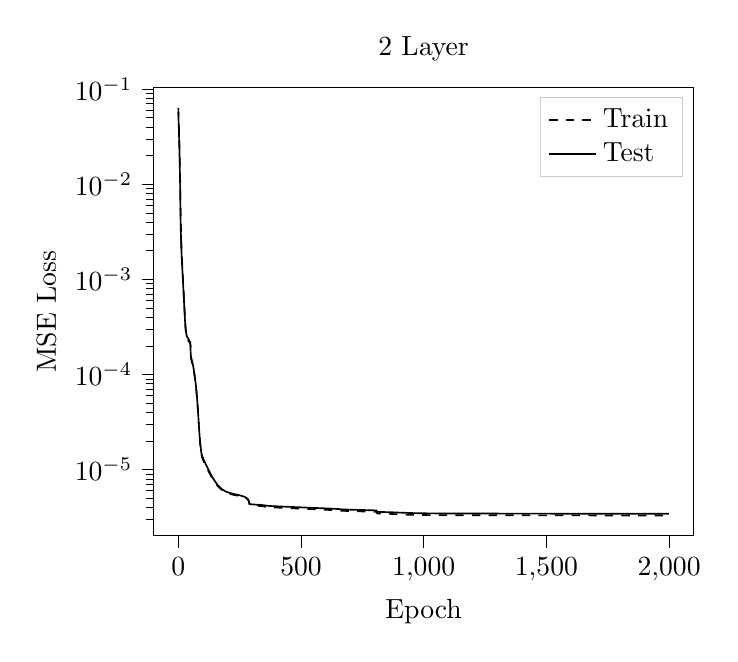
\begin{tikzpicture}

\begin{axis}[
legend cell align={left},
legend style={fill opacity=0.8, draw opacity=1, text opacity=1, draw=white!80!black},
log basis y={10},
tick align=outside,
tick pos=left,
title={2 Layer},
x grid style={white!69.0196078431373!black},
xlabel={Epoch},
xmin=-99.95, xmax=2098.95,
xtick style={color=black},
y grid style={white!69.0196078431373!black},
ylabel={MSE Loss},
ymin=2.00962005103304e-06, ymax=0.103609493820567,
ymode=log,
ytick style={color=black}
]
\addplot [semithick, black, dashed]
table {%
0 0.0632710078060627
1 0.051845450758934
2 0.0432980991452932
3 0.0358776403516531
4 0.0290690961554647
5 0.0229545622691512
6 0.0177181212641299
7 0.0134029685482383
8 0.00932001467421651
9 0.00582119612768292
10 0.00408269998338073
11 0.00310812011640519
12 0.00251322026690468
13 0.00211413772078231
14 0.00183244168199599
15 0.00161229025945067
16 0.00143017171323299
17 0.00127473987545818
18 0.0011382556988392
19 0.00101599448849447
20 0.000905665848404169
21 0.000806275674840435
22 0.00071686326363124
23 0.000636678095906973
24 0.000565266070072539
25 0.000501702402951196
26 0.000445806336938404
27 0.000397627679049037
28 0.000357118795858696
29 0.00032489347649971
30 0.000299998327216599
31 0.000281208114116453
32 0.000267276446160395
33 0.000257046025944874
34 0.0002495395517617
35 0.000243972511438187
36 0.000239745286788093
37 0.000236407682736171
38 0.000233631588111166
39 0.000231188191857655
40 0.000228926038951613
41 0.000226746779982932
42 0.000224590560450451
43 0.000222427553118905
44 0.000220237786095822
45 0.000218012332130456
46 0.000215740327854292
47 0.000213416477650753
48 0.000211034586711321
49 0.000208587526110932
50 0.000201116997253848
51 0.000158018265356077
52 0.000147613224027737
53 0.000142723495948303
54 0.000139244368234358
55 0.000136019374200259
56 0.000132747634241241
57 0.000129427922991454
58 0.000126070258433174
59 0.000122665663249791
60 0.000119213276564551
61 0.000115701421811536
62 0.000112120777172095
63 0.000108473681488249
64 0.000104762014772859
65 0.00010098851814837
66 9.71622276556445e-05
67 9.32928094116505e-05
68 8.93886299527367e-05
69 8.54555976766278e-05
70 8.14965877798386e-05
71 7.75122336417553e-05
72 7.35026992588246e-05
73 6.94685789057985e-05
74 6.54132343734091e-05
75 6.13432748941705e-05
76 5.72745405916066e-05
77 5.32301725179423e-05
78 4.92395857872907e-05
79 4.53403164574411e-05
80 4.1573930386221e-05
81 3.79849034761719e-05
82 3.46141511963651e-05
83 3.14956762558722e-05
84 2.8658379233093e-05
85 2.61181172882061e-05
86 2.38809501188371e-05
87 2.19437158739311e-05
88 2.0293696959925e-05
89 1.89088841780176e-05
90 1.77624986854426e-05
91 1.6823803317493e-05
92 1.60607825182524e-05
93 1.50258497696996e-05
94 1.4460581161984e-05
95 1.40592445336551e-05
96 1.37072536540472e-05
97 1.34257343074751e-05
98 1.31816849047937e-05
99 1.29646241002774e-05
100 1.27662120476089e-05
101 1.2581771216901e-05
102 1.24078030003147e-05
103 1.22411715728958e-05
104 1.20805520891736e-05
105 1.19247015427391e-05
106 1.1773092596286e-05
107 1.16248549329612e-05
108 1.14799404746009e-05
109 1.13379276499472e-05
110 1.11984094673971e-05
111 1.10615233461431e-05
112 1.09273854504863e-05
113 1.07954060031261e-05
114 1.06658476615848e-05
115 1.05386192249171e-05
116 1.04137884209194e-05
117 1.02908117264633e-05
118 1.01702188394484e-05
119 1.00515134595298e-05
120 9.93500102867984e-06
121 9.82061678314494e-06
122 9.70835857060592e-06
123 9.59800334567262e-06
124 9.48999531192385e-06
125 9.38343026655275e-06
126 9.2788389024463e-06
127 9.17616092829121e-06
128 9.07542354798352e-06
129 8.97668589686873e-06
130 8.87972992904906e-06
131 8.78457191856796e-06
132 8.69125409280969e-06
133 8.59979536244282e-06
134 8.51017152263012e-06
135 8.42218346087975e-06
136 8.33635802018762e-06
137 8.25191251988144e-06
138 8.16942619667316e-06
139 8.0887000030998e-06
140 8.00948176038219e-06
141 7.93231499164904e-06
142 7.85655636991578e-06
143 7.78257825504625e-06
144 7.71019455214628e-06
145 7.63938447198598e-06
146 7.57029341457383e-06
147 7.50287921164272e-06
148 7.43711638529021e-06
149 7.37279744384978e-06
150 7.31026423613912e-06
151 7.24875530431746e-06
152 7.18897826664033e-06
153 7.13090271165129e-06
154 7.07441331041991e-06
155 7.01886005163033e-06
156 6.96489755046059e-06
157 6.91240939818272e-06
158 6.86140954894654e-06
159 6.81176477974077e-06
160 6.76338529569875e-06
161 6.71635143635285e-06
162 6.67062341608471e-06
163 6.62643124655915e-06
164 6.58323398965877e-06
165 6.54126916742825e-06
166 6.50058312885449e-06
167 6.46115243034728e-06
168 6.42298308639511e-06
169 6.38602485582851e-06
170 6.35025759902419e-06
171 6.31564215518665e-06
172 6.2821410494962e-06
173 6.24969452883306e-06
174 6.21805136665898e-06
175 6.18742654864946e-06
176 6.15822291456425e-06
177 6.12961435763282e-06
178 6.10204494751088e-06
179 6.07546555693261e-06
180 6.04976868044105e-06
181 6.02458717798982e-06
182 6.00032682541496e-06
183 5.97695071451199e-06
184 5.95447526166026e-06
185 5.93280903376581e-06
186 5.91193096875031e-06
187 5.89195336056036e-06
188 5.87234221757171e-06
189 5.8534633653835e-06
190 5.83506993143601e-06
191 5.81726929294746e-06
192 5.79998251942015e-06
193 5.78317128065464e-06
194 5.76691470541846e-06
195 5.75105928714947e-06
196 5.73594326829152e-06
197 5.72154736437369e-06
198 5.70739826844147e-06
199 5.69361865041174e-06
200 5.68028440807211e-06
201 5.66706610925394e-06
202 5.65437040722827e-06
203 5.64182836365035e-06
204 5.62923450252129e-06
205 5.61731328298265e-06
206 5.60552214392374e-06
207 5.59428438737086e-06
208 5.58346819707367e-06
209 5.57276731524325e-06
210 5.56239524667035e-06
211 5.55222034631697e-06
212 5.54241197096417e-06
213 5.53287029742933e-06
214 5.52343979006764e-06
215 5.51419333123704e-06
216 5.5052181321571e-06
217 5.49665210428429e-06
218 5.48808294684022e-06
219 5.47977340056605e-06
220 5.47153629327113e-06
221 5.46346909595741e-06
222 5.45539895256297e-06
223 5.44765622976229e-06
224 5.44031825961611e-06
225 5.4328157098098e-06
226 5.42541469417301e-06
227 5.4179627427402e-06
228 5.41054173163502e-06
229 5.40329494447178e-06
230 5.39551419979034e-06
231 5.38808617102404e-06
232 5.38088338089437e-06
233 5.3739369534469e-06
234 5.36722018341607e-06
235 5.3601379581778e-06
236 5.35322880318745e-06
237 5.34662611130443e-06
238 5.33928093022951e-06
239 5.3319608723541e-06
240 5.32476024727657e-06
241 5.31745174248499e-06
242 5.3104168794107e-06
243 5.30307639201055e-06
244 5.29598574553347e-06
245 5.28916283337821e-06
246 5.28227127779246e-06
247 5.27531217994692e-06
248 5.26836660651497e-06
249 5.26145600565542e-06
250 5.25481974682407e-06
251 5.24836719614541e-06
252 5.24147814007847e-06
253 5.23453493815396e-06
254 5.22773011539357e-06
255 5.22081494614213e-06
256 5.21390236099251e-06
257 5.20662491862822e-06
258 5.19909029208066e-06
259 5.19156840505275e-06
260 5.1840717428604e-06
261 5.17612017256397e-06
262 5.16830087531162e-06
263 5.1598733487026e-06
264 5.15117472787097e-06
265 5.14193537469509e-06
266 5.13207956760198e-06
267 5.12154601028669e-06
268 5.11089195560999e-06
269 5.10023479159827e-06
270 5.08917057959479e-06
271 5.07760456798678e-06
272 5.06578773297406e-06
273 5.05217641853051e-06
274 5.0364313431146e-06
275 5.02120112696503e-06
276 5.00727311009541e-06
277 4.99260774995491e-06
278 4.97757784273745e-06
279 4.96154125721659e-06
280 4.94340508657842e-06
281 4.92293700722257e-06
282 4.89921165763008e-06
283 4.87050170272596e-06
284 4.83581983303338e-06
285 4.79348267253954e-06
286 4.74225533139361e-06
287 4.67328239142262e-06
288 4.58696049599894e-06
289 4.46936619255212e-06
290 4.31748006303678e-06
291 4.23798107794937e-06
292 4.22272348396291e-06
293 4.2174021655228e-06
294 4.21430222650088e-06
295 4.21172886331078e-06
296 4.20933076134133e-06
297 4.20704505904723e-06
298 4.20480583579774e-06
299 4.20261384238074e-06
300 4.20045522423607e-06
301 4.19840986728559e-06
302 4.19635286948505e-06
303 4.19434635909965e-06
304 4.1923705946374e-06
305 4.19050039226931e-06
306 4.18860404033694e-06
307 4.18674072125214e-06
308 4.18486637317983e-06
309 4.18306126630341e-06
310 4.18127912712407e-06
311 4.17950906694386e-06
312 4.17775834330314e-06
313 4.17607370832229e-06
314 4.17431320079231e-06
315 4.1727198783974e-06
316 4.17104828943593e-06
317 4.16937491081626e-06
318 4.16773654842473e-06
319 4.16610417369156e-06
320 4.16449309932432e-06
321 4.16296918592707e-06
322 4.16134395891277e-06
323 4.15973293388561e-06
324 4.15812554933837e-06
325 4.15651645334947e-06
326 4.15494718413356e-06
327 4.15333152818675e-06
328 4.15174744648539e-06
329 4.15025573261119e-06
330 4.14862696129603e-06
331 4.14689902572718e-06
332 4.14517258332125e-06
333 4.14342047315586e-06
334 4.14178949631605e-06
335 4.1400407767469e-06
336 4.13811117368823e-06
337 4.13610095756667e-06
338 4.13402996832701e-06
339 4.1318420285279e-06
340 4.1294807142549e-06
341 4.12701435834606e-06
342 4.12451515353496e-06
343 4.12194325031123e-06
344 4.11919797215887e-06
345 4.11631795668654e-06
346 4.11326574703708e-06
347 4.11016632801875e-06
348 4.10674409454259e-06
349 4.10305109289766e-06
350 4.09920685819998e-06
351 4.09521432902693e-06
352 4.0910061447903e-06
353 4.08667012720798e-06
354 4.08225326873435e-06
355 4.07795396699839e-06
356 4.07355116385588e-06
357 4.0691161605082e-06
358 4.06490110549385e-06
359 4.06080552897947e-06
360 4.05672974352456e-06
361 4.05283861550743e-06
362 4.04928707007457e-06
363 4.04601418176753e-06
364 4.0429513314848e-06
365 4.04010962870416e-06
366 4.03744269556228e-06
367 4.03506154293609e-06
368 4.03286837035921e-06
369 4.03083124660952e-06
370 4.02896440937184e-06
371 4.02703742270205e-06
372 4.02513960216311e-06
373 4.02338820936166e-06
374 4.02179212824194e-06
375 4.02032433521526e-06
376 4.01882592655056e-06
377 4.01735797845504e-06
378 4.01590311412292e-06
379 4.01456900135599e-06
380 4.01327008967201e-06
381 4.01198213216958e-06
382 4.01074603587404e-06
383 4.0095192375702e-06
384 4.00830898684035e-06
385 4.00709463201565e-06
386 4.0059097862013e-06
387 4.00470182489698e-06
388 4.00351677558319e-06
389 4.00236419886824e-06
390 4.00116998844169e-06
391 3.99998082389175e-06
392 3.99884801413464e-06
393 3.99764587837126e-06
394 3.99651417865243e-06
395 3.99532578603612e-06
396 3.99419785026112e-06
397 3.99303706149112e-06
398 3.99190068537791e-06
399 3.99077415227112e-06
400 3.98964895885001e-06
401 3.98854520904024e-06
402 3.98738429157675e-06
403 3.98626458650142e-06
404 3.98513616232776e-06
405 3.98401351844768e-06
406 3.98287694929422e-06
407 3.98177175156889e-06
408 3.98065694753313e-06
409 3.97955125094995e-06
410 3.97847688532238e-06
411 3.97736476134014e-06
412 3.97623916978773e-06
413 3.97515318627484e-06
414 3.97404352497688e-06
415 3.97295079324067e-06
416 3.97184997132172e-06
417 3.97074828265431e-06
418 3.96966739663185e-06
419 3.96858127305677e-06
420 3.96750045547378e-06
421 3.96643120166118e-06
422 3.96534202013754e-06
423 3.96427063765259e-06
424 3.96322433994101e-06
425 3.96213134354184e-06
426 3.96106135895025e-06
427 3.95999829197535e-06
428 3.95894019357001e-06
429 3.95790915376892e-06
430 3.95684226828053e-06
431 3.95577681206305e-06
432 3.95472414516007e-06
433 3.95362605377159e-06
434 3.95254756790564e-06
435 3.95150437725533e-06
436 3.95043570642883e-06
437 3.94937866462897e-06
438 3.94838115562379e-06
439 3.94730105404051e-06
440 3.94621883810942e-06
441 3.9451766710954e-06
442 3.94410750595853e-06
443 3.94304689325509e-06
444 3.94200809296308e-06
445 3.94095385900073e-06
446 3.93992307658664e-06
447 3.93891124645052e-06
448 3.93786665722473e-06
449 3.93685992435167e-06
450 3.9358440626529e-06
451 3.93480710340555e-06
452 3.93380716809588e-06
453 3.93278114415807e-06
454 3.93176267130002e-06
455 3.93070953191454e-06
456 3.92965003652535e-06
457 3.92862235230496e-06
458 3.92760561658179e-06
459 3.92657984616562e-06
460 3.9255645015146e-06
461 3.92449227001634e-06
462 3.92346870353322e-06
463 3.92245446937522e-06
464 3.92145133218946e-06
465 3.92043095689587e-06
466 3.91943706358688e-06
467 3.91841551595462e-06
468 3.91737812401516e-06
469 3.91636446238408e-06
470 3.91536215056476e-06
471 3.91434734888207e-06
472 3.91334745836502e-06
473 3.91231219873589e-06
474 3.91130924549543e-06
475 3.91030783475799e-06
476 3.90929390709971e-06
477 3.90829968523576e-06
478 3.90728442221189e-06
479 3.9063041681402e-06
480 3.90529386982053e-06
481 3.90429663980285e-06
482 3.90328932166994e-06
483 3.90228188075525e-06
484 3.90130058735849e-06
485 3.90029922914437e-06
486 3.89929259267774e-06
487 3.89830421522674e-06
488 3.89731379686964e-06
489 3.89628200673542e-06
490 3.89534313785589e-06
491 3.89432079941798e-06
492 3.89331514952573e-06
493 3.89229541360692e-06
494 3.89127347989415e-06
495 3.89029763300641e-06
496 3.88925411311902e-06
497 3.88816214581311e-06
498 3.88687702547941e-06
499 3.88587540737717e-06
500 3.88488475755366e-06
501 3.88386549957431e-06
502 3.88286122324644e-06
503 3.88185147426157e-06
504 3.88082735753414e-06
505 3.87983534415071e-06
506 3.87884211681921e-06
507 3.87786378541932e-06
508 3.87690347974967e-06
509 3.87590351806466e-06
510 3.87493697735408e-06
511 3.87393002165481e-06
512 3.87293140079237e-06
513 3.87193410711006e-06
514 3.87096493568606e-06
515 3.86997004397927e-06
516 3.86899167233423e-06
517 3.86810477471045e-06
518 3.86708819746673e-06
519 3.86609972861152e-06
520 3.86511584406435e-06
521 3.86410707824325e-06
522 3.86309811415231e-06
523 3.86210161127565e-06
524 3.86109321630101e-06
525 3.86009254270903e-06
526 3.85912106071373e-06
527 3.85811027194904e-06
528 3.85712550837525e-06
529 3.85611493993565e-06
530 3.85510660271393e-06
531 3.85410345074888e-06
532 3.85311390755305e-06
533 3.85213474737611e-06
534 3.85112630192452e-06
535 3.85012735591772e-06
536 3.84913734296788e-06
537 3.84815157872254e-06
538 3.84717732458739e-06
539 3.84619277247111e-06
540 3.84522993113023e-06
541 3.8442311797553e-06
542 3.84322497643552e-06
543 3.84227112340341e-06
544 3.8412537937802e-06
545 3.84022483763147e-06
546 3.83922470746256e-06
547 3.83821959007946e-06
548 3.83719782143999e-06
549 3.83618380419648e-06
550 3.83516073952705e-06
551 3.83415338933446e-06
552 3.83312635744915e-06
553 3.83206138189962e-06
554 3.83102651903755e-06
555 3.82998564509762e-06
556 3.82895923803517e-06
557 3.82797941483659e-06
558 3.82694782160797e-06
559 3.82592881351229e-06
560 3.82489514527151e-06
561 3.82387169111098e-06
562 3.82288159403288e-06
563 3.82187921854893e-06
564 3.82090538437296e-06
565 3.81990201117333e-06
566 3.81885945239446e-06
567 3.8178061686267e-06
568 3.81674583468339e-06
569 3.81568310513103e-06
570 3.81460992866778e-06
571 3.81355367085234e-06
572 3.81251289786633e-06
573 3.81145554933937e-06
574 3.8104192146875e-06
575 3.8093715679679e-06
576 3.80830061658344e-06
577 3.80721733722567e-06
578 3.80615091921754e-06
579 3.80504406757609e-06
580 3.80396494574597e-06
581 3.80284883271997e-06
582 3.80177165607165e-06
583 3.80069691914287e-06
584 3.79964723424564e-06
585 3.7985892818142e-06
586 3.79753483116474e-06
587 3.79640749065402e-06
588 3.79530364398306e-06
589 3.7941353525639e-06
590 3.79299306950998e-06
591 3.79188061958757e-06
592 3.79073451824752e-06
593 3.78960781699789e-06
594 3.78849956632621e-06
595 3.7874091502772e-06
596 3.78626679844274e-06
597 3.78513176633533e-06
598 3.78400663305456e-06
599 3.78287078638095e-06
600 3.78169056853039e-06
601 3.78051059510653e-06
602 3.77938837505099e-06
603 3.77821030451742e-06
604 3.77709365989176e-06
605 3.77594412566395e-06
606 3.77473977471254e-06
607 3.77356035733101e-06
608 3.77238059650153e-06
609 3.77121746578268e-06
610 3.77010574015912e-06
611 3.76895438330394e-06
612 3.76782894613825e-06
613 3.76667858108704e-06
614 3.76551559270411e-06
615 3.76439185151867e-06
616 3.76326227546997e-06
617 3.76208450234117e-06
618 3.76090089821446e-06
619 3.75969973163137e-06
620 3.75851625665291e-06
621 3.75739111655093e-06
622 3.75627195273864e-06
623 3.75508487604748e-06
624 3.75392496414406e-06
625 3.75275827741461e-06
626 3.75164966681041e-06
627 3.7504619098172e-06
628 3.7492805902275e-06
629 3.74812237578226e-06
630 3.74700240786297e-06
631 3.74586033490232e-06
632 3.74465033678462e-06
633 3.74347466811287e-06
634 3.74222576670036e-06
635 3.74095193990343e-06
636 3.73970642544919e-06
637 3.73849202571819e-06
638 3.73727273176883e-06
639 3.73604903143132e-06
640 3.73481999326941e-06
641 3.73360565822622e-06
642 3.73240932685803e-06
643 3.73127844181909e-06
644 3.73011926103572e-06
645 3.72891290930966e-06
646 3.727741849616e-06
647 3.72646188213821e-06
648 3.72512999217633e-06
649 3.72386121966883e-06
650 3.72253252623977e-06
651 3.72115426330311e-06
652 3.71982453145847e-06
653 3.7184918338653e-06
654 3.71706787746007e-06
655 3.71560938947368e-06
656 3.71417414066855e-06
657 3.71250464706918e-06
658 3.71070990593125e-06
659 3.70882397623973e-06
660 3.70690597890189e-06
661 3.70420897252188e-06
662 3.70078934975027e-06
663 3.69826730502609e-06
664 3.69612601537028e-06
665 3.69425015776415e-06
666 3.69259916294595e-06
667 3.69112746614064e-06
668 3.68980126438601e-06
669 3.6885883330342e-06
670 3.68746814126553e-06
671 3.68644335560475e-06
672 3.68547208643122e-06
673 3.68455293175884e-06
674 3.683675603952e-06
675 3.68285116735478e-06
676 3.6820184672024e-06
677 3.68124188753427e-06
678 3.68046135884015e-06
679 3.67971530249633e-06
680 3.67896949774149e-06
681 3.67823716908333e-06
682 3.67751394207971e-06
683 3.67678034842811e-06
684 3.67607592556851e-06
685 3.67535497991867e-06
686 3.67465632757558e-06
687 3.67394465786219e-06
688 3.6732546661824e-06
689 3.67254644345394e-06
690 3.67185343293386e-06
691 3.67115930930595e-06
692 3.67046825454054e-06
693 3.66977536043578e-06
694 3.66907607531175e-06
695 3.66839212199466e-06
696 3.66770006837669e-06
697 3.6670071425533e-06
698 3.66632715258675e-06
699 3.66563417685484e-06
700 3.66494473416878e-06
701 3.66426724519897e-06
702 3.66358821713675e-06
703 3.66290142187609e-06
704 3.6622132258799e-06
705 3.6615301440861e-06
706 3.66084534357469e-06
707 3.66017243891292e-06
708 3.6594921489268e-06
709 3.65881293635084e-06
710 3.65812857126002e-06
711 3.6574575931354e-06
712 3.65677416755261e-06
713 3.65609544701329e-06
714 3.65541832900362e-06
715 3.65474015052314e-06
716 3.65406903290477e-06
717 3.65339285406208e-06
718 3.65271773671338e-06
719 3.65204745116898e-06
720 3.651368467672e-06
721 3.65069879228486e-06
722 3.65002570674733e-06
723 3.64936534811022e-06
724 3.64868461804235e-06
725 3.64801084799637e-06
726 3.64734410402434e-06
727 3.64667091173487e-06
728 3.6460121403934e-06
729 3.6453348136547e-06
730 3.64466524786167e-06
731 3.6439993359636e-06
732 3.64334011158007e-06
733 3.64267599638879e-06
734 3.64200718195207e-06
735 3.64133908624353e-06
736 3.64068387693806e-06
737 3.64001761658983e-06
738 3.63935759855849e-06
739 3.63869932277794e-06
740 3.6380411635264e-06
741 3.63737760744698e-06
742 3.63650741667243e-06
743 3.63583347075291e-06
744 3.63516651168538e-06
745 3.63449705389485e-06
746 3.63384109414255e-06
747 3.63316582570405e-06
748 3.63250598411469e-06
749 3.63184671437011e-06
750 3.63118088159808e-06
751 3.63051347460441e-06
752 3.62984826938373e-06
753 3.62920208863216e-06
754 3.62853011097286e-06
755 3.62786857806441e-06
756 3.62720777866343e-06
757 3.62655042818005e-06
758 3.62588549194243e-06
759 3.62523838361994e-06
760 3.62457825156071e-06
761 3.62390604811935e-06
762 3.62325307582978e-06
763 3.62259630355766e-06
764 3.62194640536018e-06
765 3.62129782820375e-06
766 3.62063571492399e-06
767 3.61997041034101e-06
768 3.61932698899636e-06
769 3.61866497462415e-06
770 3.6180262252401e-06
771 3.617362689738e-06
772 3.61671298037436e-06
773 3.61607361901406e-06
774 3.61541275435684e-06
775 3.6147658632899e-06
776 3.61411101857811e-06
777 3.61345795158741e-06
778 3.61281008554215e-06
779 3.61216918668106e-06
780 3.6115153557148e-06
781 3.61088205590931e-06
782 3.61022876393236e-06
783 3.6095767355846e-06
784 3.60893789741112e-06
785 3.60828682255487e-06
786 3.60765805169194e-06
787 3.60699846305579e-06
788 3.60636278833226e-06
789 3.60572352553845e-06
790 3.60508044082053e-06
791 3.60444044986252e-06
792 3.60379261326216e-06
793 3.60315890213769e-06
794 3.60252107452652e-06
795 3.60187887156371e-06
796 3.6012473944993e-06
797 3.60060167395204e-06
798 3.59996799465989e-06
799 3.59931844286621e-06
800 3.59868616624226e-06
801 3.59804496190463e-06
802 3.59741519469026e-06
803 3.59679051234707e-06
804 3.59614438116296e-06
805 3.59551126325641e-06
806 3.59488375943329e-06
807 3.59423938243708e-06
808 3.59361888456533e-06
809 3.58856573075173e-06
810 3.46819658852837e-06
811 3.45905467918328e-06
812 3.45808383144686e-06
813 3.45728719207727e-06
814 3.45646615710393e-06
815 3.4557891899567e-06
816 3.45512566559592e-06
817 3.45442840398391e-06
818 3.45375150789096e-06
819 3.45314441744904e-06
820 3.45249377733126e-06
821 3.45187570439975e-06
822 3.4512920127554e-06
823 3.45072540699221e-06
824 3.45013294111141e-06
825 3.44956170420119e-06
826 3.44901385676621e-06
827 3.44852854482269e-06
828 3.44790018584717e-06
829 3.44723031332705e-06
830 3.44663635894449e-06
831 3.44601887513818e-06
832 3.44534294094956e-06
833 3.44472433505416e-06
834 3.44406132182939e-06
835 3.44345207020069e-06
836 3.44280726289981e-06
837 3.4422474728899e-06
838 3.44163713850776e-06
839 3.44108118099484e-06
840 3.44047824160043e-06
841 3.4398152462245e-06
842 3.43910582000717e-06
843 3.43842116046744e-06
844 3.43774710404432e-06
845 3.43702792099521e-06
846 3.43634997943809e-06
847 3.43563018009263e-06
848 3.43499882342257e-06
849 3.43428135010981e-06
850 3.43356308815146e-06
851 3.43284928339926e-06
852 3.43210946982708e-06
853 3.43137287131867e-06
854 3.43064236994906e-06
855 3.42992232879169e-06
856 3.42917290743117e-06
857 3.42838393817146e-06
858 3.42754296923431e-06
859 3.42668330313245e-06
860 3.42588032242475e-06
861 3.42507210848453e-06
862 3.42416718467575e-06
863 3.42335599020771e-06
864 3.42258317823507e-06
865 3.42167720782527e-06
866 3.42081106327896e-06
867 3.41993027393528e-06
868 3.41898223450698e-06
869 3.41806178505522e-06
870 3.41711957901225e-06
871 3.41628901833246e-06
872 3.41533120615622e-06
873 3.41435020516201e-06
874 3.41339523242823e-06
875 3.41245838376381e-06
876 3.4114890966066e-06
877 3.41038971214402e-06
878 3.40855177046251e-06
879 3.40721698319157e-06
880 3.40610965008636e-06
881 3.40513882656524e-06
882 3.40419041424411e-06
883 3.40332646044317e-06
884 3.40240671414449e-06
885 3.4013559078403e-06
886 3.40033198938272e-06
887 3.39924581226114e-06
888 3.39811470360019e-06
889 3.39708300680286e-06
890 3.39614488370898e-06
891 3.39512193158953e-06
892 3.39409216473996e-06
893 3.39310099377599e-06
894 3.39206634293987e-06
895 3.39110838353918e-06
896 3.39012106735481e-06
897 3.3891239560262e-06
898 3.38814063684367e-06
899 3.38709192863007e-06
900 3.38610237486137e-06
901 3.38508347010702e-06
902 3.38407450976774e-06
903 3.38305720777043e-06
904 3.38207762490583e-06
905 3.38106447293285e-06
906 3.38001549198452e-06
907 3.37896211885891e-06
908 3.37797512941052e-06
909 3.37698621433447e-06
910 3.37599381316522e-06
911 3.37501526473716e-06
912 3.37411181067182e-06
913 3.37317492824241e-06
914 3.37220609208089e-06
915 3.3712260875518e-06
916 3.37031230503726e-06
917 3.36942957324027e-06
918 3.36857478896491e-06
919 3.36759936112685e-06
920 3.36662839538349e-06
921 3.36570018896509e-06
922 3.3648025120101e-06
923 3.36392968029031e-06
924 3.3630231520192e-06
925 3.36211414503396e-06
926 3.36128224489585e-06
927 3.36038605507838e-06
928 3.35971276251712e-06
929 3.35890150881824e-06
930 3.35802607730784e-06
931 3.35722394027016e-06
932 3.35641767048855e-06
933 3.35569475134889e-06
934 3.35492151180006e-06
935 3.35416929988241e-06
936 3.35343535334687e-06
937 3.35275004340474e-06
938 3.3520320862408e-06
939 3.35134114561697e-06
940 3.35064550688458e-06
941 3.34997043398744e-06
942 3.34934603586134e-06
943 3.34871437360107e-06
944 3.34808450747914e-06
945 3.34750664876537e-06
946 3.34689332385096e-06
947 3.34634646662835e-06
948 3.34575365366163e-06
949 3.34518739339273e-06
950 3.34464585841943e-06
951 3.34406109845986e-06
952 3.34353921266484e-06
953 3.34303967986216e-06
954 3.34256621943041e-06
955 3.34205329431825e-06
956 3.34155066923358e-06
957 3.34107601361211e-06
958 3.34061679984643e-06
959 3.34015869543691e-06
960 3.33970654855875e-06
961 3.3393236901702e-06
962 3.33886904593328e-06
963 3.33842913983062e-06
964 3.33814169107427e-06
965 3.33774210423599e-06
966 3.3372913213725e-06
967 3.33686178612425e-06
968 3.33645433522634e-06
969 3.33606849665102e-06
970 3.33571005978683e-06
971 3.33536255254785e-06
972 3.33501844590955e-06
973 3.33469381189389e-06
974 3.33438582435974e-06
975 3.33408202118335e-06
976 3.33378812365481e-06
977 3.33350157063705e-06
978 3.33323775805638e-06
979 3.3330256313775e-06
980 3.33272925752226e-06
981 3.33243786371895e-06
982 3.33216787623769e-06
983 3.3319054509775e-06
984 3.33164250014306e-06
985 3.33139780241254e-06
986 3.33115889634428e-06
987 3.33091831510046e-06
988 3.33069397129293e-06
989 3.33046564878714e-06
990 3.33024445262708e-06
991 3.33003096750417e-06
992 3.32982458940023e-06
993 3.32962686138671e-06
994 3.32943600267299e-06
995 3.32926675400813e-06
996 3.32906775338415e-06
997 3.3288823390194e-06
998 3.32862334119e-06
999 3.3284366764974e-06
1000 3.32826502312855e-06
1001 3.32808903544901e-06
1002 3.3279268395745e-06
1003 3.3277572111956e-06
1004 3.32759605612409e-06
1005 3.32745577202331e-06
1006 3.32727387956311e-06
1007 3.32710411589687e-06
1008 3.32693895040848e-06
1009 3.32677818335014e-06
1010 3.32661705760984e-06
1011 3.32647359664406e-06
1012 3.32631457933985e-06
1013 3.32618127072237e-06
1014 3.32603964534428e-06
1015 3.32589951085538e-06
1016 3.32574876642866e-06
1017 3.32563812094122e-06
1018 3.325481228444e-06
1019 3.32533804532886e-06
1020 3.32519677795062e-06
1021 3.32507743246424e-06
1022 3.32495024065338e-06
1023 3.32481203804491e-06
1024 3.32468024942045e-06
1025 3.32454988460995e-06
1026 3.32442952083056e-06
1027 3.32430381183713e-06
1028 3.32418459424844e-06
1029 3.32406650829853e-06
1030 3.32396275587143e-06
1031 3.32385228330168e-06
1032 3.32373832941357e-06
1033 3.32363166569394e-06
1034 3.32353530177443e-06
1035 3.32343474212848e-06
1036 3.32334030849779e-06
1037 3.32324221994895e-06
1038 3.32314650916032e-06
1039 3.32305175118108e-06
1040 3.32298359035121e-06
1041 3.32284780517966e-06
1042 3.32274852030423e-06
1043 3.3226549801384e-06
1044 3.32256201613745e-06
1045 3.32246874370412e-06
1046 3.3223735683805e-06
1047 3.32228958177438e-06
1048 3.32220481595868e-06
1049 3.32208896418251e-06
1050 3.32200541083694e-06
1051 3.32191331938247e-06
1052 3.32182456236296e-06
1053 3.32175064909279e-06
1054 3.3216608036355e-06
1055 3.32158123887893e-06
1056 3.32150148597066e-06
1057 3.3214288405361e-06
1058 3.32134673897144e-06
1059 3.32127205160759e-06
1060 3.3211996552609e-06
1061 3.32111623322362e-06
1062 3.32105358813806e-06
1063 3.32098555361426e-06
1064 3.320912385675e-06
1065 3.32084120304899e-06
1066 3.32077246423523e-06
1067 3.32069897615384e-06
1068 3.32062761867746e-06
1069 3.32055835360734e-06
1070 3.32049213534447e-06
1071 3.32042758327589e-06
1072 3.32035822054877e-06
1073 3.32029157220859e-06
1074 3.3202237336809e-06
1075 3.32016097570431e-06
1076 3.32010107376846e-06
1077 3.32003031508066e-06
1078 3.31996242221066e-06
1079 3.31990452946229e-06
1080 3.31984272509089e-06
1081 3.3197831430698e-06
1082 3.31972265939839e-06
1083 3.31965873988338e-06
1084 3.31960340872683e-06
1085 3.31954086311725e-06
1086 3.31948666712378e-06
1087 3.31942682998942e-06
1088 3.31936341729033e-06
1089 3.31931191681178e-06
1090 3.31925431248692e-06
1091 3.31908182454299e-06
1092 3.31901709694193e-06
1093 3.31896539614718e-06
1094 3.31891274390728e-06
1095 3.31885061757475e-06
1096 3.31879793600365e-06
1097 3.3187468189908e-06
1098 3.31868890623355e-06
1099 3.31862838606867e-06
1100 3.31856975185474e-06
1101 3.31851502880909e-06
1102 3.31847244035544e-06
1103 3.31840572573583e-06
1104 3.3183519180966e-06
1105 3.31829593142174e-06
1106 3.31823610724769e-06
1107 3.31818831443798e-06
1108 3.31813788932322e-06
1109 3.31809355793666e-06
1110 3.31803202232095e-06
1111 3.31797998080674e-06
1112 3.31792680481158e-06
1113 3.31787022776098e-06
1114 3.31782323041807e-06
1115 3.31776938503481e-06
1116 3.31772539641406e-06
1117 3.31767134389338e-06
1118 3.31762536609403e-06
1119 3.31757380968156e-06
1120 3.31752182080436e-06
1121 3.31747144957717e-06
1122 3.31731329424656e-06
1123 3.31725821206419e-06
1124 3.31720646829581e-06
1125 3.31715368929508e-06
1126 3.31710390935314e-06
1127 3.3170535549516e-06
1128 3.31699749733616e-06
1129 3.31695505599328e-06
1130 3.31690347150015e-06
1131 3.31685236983503e-06
1132 3.31680772876552e-06
1133 3.3167499815363e-06
1134 3.31669872764451e-06
1135 3.31664693214861e-06
1136 3.31659686685271e-06
1137 3.31655298123223e-06
1138 3.31649509212184e-06
1139 3.31645859967011e-06
1140 3.31640772060382e-06
1141 3.31635877830649e-06
1142 3.31630854077503e-06
1143 3.3162615816309e-06
1144 3.31620984627534e-06
1145 3.31616943481095e-06
1146 3.31612526088065e-06
1147 3.31607749308205e-06
1148 3.31602828350697e-06
1149 3.31598170487268e-06
1150 3.31593465273272e-06
1151 3.31589305983471e-06
1152 3.31584171124177e-06
1153 3.31579683393102e-06
1154 3.31575542475093e-06
1155 3.31569906404638e-06
1156 3.31566256102178e-06
1157 3.31562098369886e-06
1158 3.31557101537783e-06
1159 3.31552743352859e-06
1160 3.31547878431593e-06
1161 3.31543595132189e-06
1162 3.31539260980662e-06
1163 3.31535449493003e-06
1164 3.31530274024772e-06
1165 3.31526033858154e-06
1166 3.31521684279323e-06
1167 3.31517224708477e-06
1168 3.31512761704289e-06
1169 3.31509071429537e-06
1170 3.31504686755579e-06
1171 3.31499783703748e-06
1172 3.31494618387751e-06
1173 3.31488194569829e-06
1174 3.31483411434874e-06
1175 3.31477687655024e-06
1176 3.31463223449191e-06
1177 3.3145593424706e-06
1178 3.31451699707941e-06
1179 3.31447909991311e-06
1180 3.31444194944197e-06
1181 3.31440136801575e-06
1182 3.3143566832905e-06
1183 3.31432279710953e-06
1184 3.3142888198654e-06
1185 3.31424507578504e-06
1186 3.31421255020814e-06
1187 3.31417136544587e-06
1188 3.31413100582267e-06
1189 3.31409358943802e-06
1190 3.3140541273724e-06
1191 3.31401387495589e-06
1192 3.31398105663538e-06
1193 3.31394617762726e-06
1194 3.31390259668751e-06
1195 3.31387615858603e-06
1196 3.31384136154611e-06
1197 3.31379895965256e-06
1198 3.31376556687246e-06
1199 3.31373439541949e-06
1200 3.31369409514082e-06
1201 3.31365316878873e-06
1202 3.31363031023102e-06
1203 3.31359488518501e-06
1204 3.31356466006127e-06
1205 3.31353000353829e-06
1206 3.3134903616201e-06
1207 3.31346309042146e-06
1208 3.31342015306291e-06
1209 3.31339084232241e-06
1210 3.3133535714569e-06
1211 3.31332341784218e-06
1212 3.31328962545285e-06
1213 3.31325111255865e-06
1214 3.31321978012511e-06
1215 3.31318277721948e-06
1216 3.31314616198597e-06
1217 3.31311287493463e-06
1218 3.31307958356319e-06
1219 3.31304765325058e-06
1220 3.31300194511641e-06
1221 3.31296959791416e-06
1222 3.31293913814079e-06
1223 3.31290463248024e-06
1224 3.31286963171351e-06
1225 3.31283649222769e-06
1226 3.31280664943279e-06
1227 3.31276422059545e-06
1228 3.31273262804643e-06
1229 3.31270691606278e-06
1230 3.31266566593058e-06
1231 3.31263192094866e-06
1232 3.31260459256555e-06
1233 3.31257304628707e-06
1234 3.31253451588509e-06
1235 3.3125027416645e-06
1236 3.31246954056041e-06
1237 3.31243238213119e-06
1238 3.31239868376088e-06
1239 3.31237523766958e-06
1240 3.31232966425432e-06
1241 3.3123012260603e-06
1242 3.31226731339029e-06
1243 3.31223492764821e-06
1244 3.31220416660472e-06
1245 3.3121651907777e-06
1246 3.31213434481015e-06
1247 3.31210411036409e-06
1248 3.31207334511419e-06
1249 3.31204188125866e-06
1250 3.31200534310483e-06
1251 3.31196890385854e-06
1252 3.31193951285513e-06
1253 3.31191298664635e-06
1254 3.31186976950448e-06
1255 3.31183692810555e-06
1256 3.31180187276914e-06
1257 3.31176736733596e-06
1258 3.31174078667118e-06
1259 3.31170079664389e-06
1260 3.31167498484319e-06
1261 3.31163897067199e-06
1262 3.31160367568373e-06
1263 3.31157391030956e-06
1264 3.31153827073649e-06
1265 3.31150821864412e-06
1266 3.31147878000593e-06
1267 3.31144059236976e-06
1268 3.3114125475322e-06
1269 3.31137845250851e-06
1270 3.31135019507656e-06
1271 3.31132036353665e-06
1272 3.31128353366239e-06
1273 3.31124508727498e-06
1274 3.3112155958861e-06
1275 3.31118322765178e-06
1276 3.31115418396166e-06
1277 3.31111870571021e-06
1278 3.31108915679579e-06
1279 3.31105810823829e-06
1280 3.31101666643008e-06
1281 3.31099420361625e-06
1282 3.31095552917304e-06
1283 3.31091766827285e-06
1284 3.31088738289509e-06
1285 3.31086019934901e-06
1286 3.31082479078759e-06
1287 3.3107894528257e-06
1288 3.31076125996788e-06
1289 3.31073088023004e-06
1290 3.31069415051388e-06
1291 3.31065719831258e-06
1292 3.31063165572232e-06
1293 3.31060190774224e-06
1294 3.3105640161466e-06
1295 3.31053720560703e-06
1296 3.31050339457306e-06
1297 3.31046521137068e-06
1298 3.31043459812008e-06
1299 3.31039810896527e-06
1300 3.31036881345881e-06
1301 3.31033730344643e-06
1302 3.310306435651e-06
1303 3.31026991398176e-06
1304 3.31024301567595e-06
1305 3.31020190742493e-06
1306 3.31017149255786e-06
1307 3.3101332599017e-06
1308 3.31010171169055e-06
1309 3.31005946975438e-06
1310 3.31003425515064e-06
1311 3.30999968309698e-06
1312 3.30996857246646e-06
1313 3.30993229317755e-06
1314 3.30990236466278e-06
1315 3.30987621293843e-06
1316 3.30983615754121e-06
1317 3.30979875263893e-06
1318 3.30977489818451e-06
1319 3.30974435814824e-06
1320 3.30970497532235e-06
1321 3.30967777449587e-06
1322 3.30965184900833e-06
1323 3.30961561678578e-06
1324 3.30957849496372e-06
1325 3.30955011418155e-06
1326 3.30952235151472e-06
1327 3.30948825808264e-06
1328 3.30946376834618e-06
1329 3.30942424557179e-06
1330 3.30939567766109e-06
1331 3.30936111083702e-06
1332 3.30933207965245e-06
1333 3.3093084363145e-06
1334 3.30927065931519e-06
1335 3.30923937360694e-06
1336 3.30921289116759e-06
1337 3.30918081397158e-06
1338 3.30914972573737e-06
1339 3.30911605874462e-06
1340 3.30908646151329e-06
1341 3.30905639475532e-06
1342 3.30902801658795e-06
1343 3.30899296102416e-06
1344 3.30896267894332e-06
1345 3.3089325166884e-06
1346 3.30890046916466e-06
1347 3.30886465042113e-06
1348 3.3088395756522e-06
1349 3.30881382774351e-06
1350 3.30877656608664e-06
1351 3.30874721919372e-06
1352 3.30871065659721e-06
1353 3.30867955688063e-06
1354 3.30865487069332e-06
1355 3.30862191162851e-06
1356 3.30859550501827e-06
1357 3.30855776235239e-06
1358 3.30853303728418e-06
1359 3.30850446073327e-06
1360 3.30846531176121e-06
1361 3.30843728659147e-06
1362 3.30840472588534e-06
1363 3.30837749436341e-06
1364 3.30834483236231e-06
1365 3.30830624568534e-06
1366 3.30828763708269e-06
1367 3.30825550838654e-06
1368 3.30822551416077e-06
1369 3.30818973498026e-06
1370 3.30815789163807e-06
1371 3.30812527829494e-06
1372 3.30809859678993e-06
1373 3.30806258318717e-06
1374 3.30803215661035e-06
1375 3.30800900974282e-06
1376 3.30797151002571e-06
1377 3.30794009107649e-06
1378 3.30791404837782e-06
1379 3.30788173698693e-06
1380 3.30785453468252e-06
1381 3.30781790967194e-06
1382 3.30779392106706e-06
1383 3.30776260773291e-06
1384 3.30773389839578e-06
1385 3.30769640322615e-06
1386 3.30766638410296e-06
1387 3.30763812337409e-06
1388 3.30760337055835e-06
1389 3.30757708707097e-06
1390 3.307545913799e-06
1391 3.30751326794143e-06
1392 3.30749232489325e-06
1393 3.30745411440603e-06
1394 3.30735595673559e-06
1395 3.30729904260352e-06
1396 3.30725218407224e-06
1397 3.30722578951281e-06
1398 3.30719073667751e-06
1399 3.30716875021153e-06
1400 3.30714862934656e-06
1401 3.30711684216567e-06
1402 3.3070819894192e-06
1403 3.3070488652811e-06
1404 3.30701422922175e-06
1405 3.30698709717581e-06
1406 3.30695631168965e-06
1407 3.30692265868038e-06
1408 3.30688969722814e-06
1409 3.30686106201483e-06
1410 3.3068254247155e-06
1411 3.3067949505039e-06
1412 3.30675967359184e-06
1413 3.30672607924498e-06
1414 3.30669463016875e-06
1415 3.30665754358961e-06
1416 3.30661870475524e-06
1417 3.30659057021876e-06
1418 3.30655833431592e-06
1419 3.30653160381189e-06
1420 3.30648229748931e-06
1421 3.3064635277924e-06
1422 3.30642847688978e-06
1423 3.30640005802252e-06
1424 3.30635991497275e-06
1425 3.30633839712391e-06
1426 3.30630923531317e-06
1427 3.30627130324501e-06
1428 3.30624613002328e-06
1429 3.30621113914731e-06
1430 3.30618818611583e-06
1431 3.30615022528491e-06
1432 3.30612555853804e-06
1433 3.3060949335777e-06
1434 3.30606805039224e-06
1435 3.30602659039414e-06
1436 3.30600337179021e-06
1437 3.30597711342762e-06
1438 3.30594837578246e-06
1439 3.30591299587013e-06
1440 3.30588416147748e-06
1441 3.30585510812398e-06
1442 3.30582726405737e-06
1443 3.30579878891513e-06
1444 3.30576666067373e-06
1445 3.30573926805755e-06
1446 3.30570304413413e-06
1447 3.30567544233418e-06
1448 3.30564356863761e-06
1449 3.30561513396788e-06
1450 3.3055900224781e-06
1451 3.30555552284295e-06
1452 3.30552562525099e-06
1453 3.30550001433494e-06
1454 3.30546434372536e-06
1455 3.30543629740987e-06
1456 3.30540926006506e-06
1457 3.30537772595108e-06
1458 3.30534853821973e-06
1459 3.30531810948287e-06
1460 3.30529423752068e-06
1461 3.30526512493634e-06
1462 3.30523205786903e-06
1463 3.30520980810434e-06
1464 3.30517069141933e-06
1465 3.30514524932823e-06
1466 3.3051182268764e-06
1467 3.3050883089345e-06
1468 3.30505295073635e-06
1469 3.30502717281433e-06
1470 3.30499619519742e-06
1471 3.30496268304614e-06
1472 3.3049321046974e-06
1473 3.30491160332258e-06
1474 3.30488403938034e-06
1475 3.30484924450047e-06
1476 3.30482337255944e-06
1477 3.3047829225552e-06
1478 3.30475701593969e-06
1479 3.30473347594307e-06
1480 3.30469857590288e-06
1481 3.30467577111904e-06
1482 3.30463922102808e-06
1483 3.30460926977594e-06
1484 3.3045828433842e-06
1485 3.30454228947019e-06
1486 3.30451344598259e-06
1487 3.30448826628071e-06
1488 3.30446151951946e-06
1489 3.30443765540167e-06
1490 3.30440346078831e-06
1491 3.30437982188414e-06
1492 3.30434341208274e-06
1493 3.30430771680312e-06
1494 3.30429122220721e-06
1495 3.30425914978605e-06
1496 3.30423125637935e-06
1497 3.30419332021847e-06
1498 3.30416777239861e-06
1499 3.30414132929491e-06
1500 3.3041072015294e-06
1501 3.30408697664097e-06
1502 3.30404774513227e-06
1503 3.30401728399465e-06
1504 3.30398470123328e-06
1505 3.30396658409882e-06
1506 3.30393206252211e-06
1507 3.30390698763949e-06
1508 3.3038729142163e-06
1509 3.30384653216242e-06
1510 3.30381857452267e-06
1511 3.3037834704146e-06
1512 3.30376238377994e-06
1513 3.30373555277674e-06
1514 3.30370023016258e-06
1515 3.30367066123927e-06
1516 3.30364827868834e-06
1517 3.30361546969016e-06
1518 3.30358942426301e-06
1519 3.30355498942936e-06
1520 3.30352247999599e-06
1521 3.3034975198234e-06
1522 3.30347213048299e-06
1523 3.3034410593018e-06
1524 3.30340980383426e-06
1525 3.30338359890447e-06
1526 3.30335414560068e-06
1527 3.30332708222159e-06
1528 3.30329681514741e-06
1529 3.30327013000442e-06
1530 3.30323686262091e-06
1531 3.30320873774781e-06
1532 3.30318001522301e-06
1533 3.30315449173213e-06
1534 3.30311911397985e-06
1535 3.30308946342939e-06
1536 3.30306302032568e-06
1537 3.30303495979933e-06
1538 3.30300534017169e-06
1539 3.30297712798711e-06
1540 3.30294749460336e-06
1541 3.30292028195345e-06
1542 3.3028948644187e-06
1543 3.30286502901345e-06
1544 3.30283326866265e-06
1545 3.30280487150958e-06
1546 3.30277500813736e-06
1547 3.30274673478925e-06
1548 3.30271867062493e-06
1549 3.30269409198536e-06
1550 3.30266561161352e-06
1551 3.30262623526778e-06
1552 3.30260750922662e-06
1553 3.3025772891051e-06
1554 3.30255014239356e-06
1555 3.30251469154064e-06
1556 3.30248873808614e-06
1557 3.3024674067974e-06
1558 3.30243384246387e-06
1559 3.30240462881193e-06
1560 3.30237546916123e-06
1561 3.30234038585786e-06
1562 3.30231066175202e-06
1563 3.30228913446717e-06
1564 3.30225435584453e-06
1565 3.3022217786538e-06
1566 3.30219976888202e-06
1567 3.30216723705234e-06
1568 3.30214145628815e-06
1569 3.30211137895731e-06
1570 3.30207850458919e-06
1571 3.30205081854729e-06
1572 3.302026115648e-06
1573 3.30199760367123e-06
1574 3.30196539312055e-06
1575 3.3019390057234e-06
1576 3.30191038460725e-06
1577 3.3018855078808e-06
1578 3.30184813685719e-06
1579 3.30180191804175e-06
1580 3.30177034481949e-06
1581 3.3017495417198e-06
1582 3.30171515747679e-06
1583 3.30168458845037e-06
1584 3.30166584637936e-06
1585 3.30163201942923e-06
1586 3.30159827740317e-06
1587 3.3015747395666e-06
1588 3.30153459117355e-06
1589 3.30150503953064e-06
1590 3.30147473721354e-06
1591 3.3014371099398e-06
1592 3.30141293727593e-06
1593 3.30138024446569e-06
1594 3.30134788134728e-06
1595 3.3013217273492e-06
1596 3.30129438600579e-06
1597 3.30125701191264e-06
1598 3.30122357820528e-06
1599 3.30119717989419e-06
1600 3.30116559575799e-06
1601 3.30114111216062e-06
1602 3.30111100208796e-06
1603 3.30107951037917e-06
1604 3.30104800923436e-06
1605 3.30102942348276e-06
1606 3.30099440964204e-06
1607 3.30095793640339e-06
1608 3.3009348513815e-06
1609 3.30090420584384e-06
1610 3.30087502663901e-06
1611 3.30084139932296e-06
1612 3.30081177537522e-06
1613 3.3007786385042e-06
1614 3.30075007127562e-06
1615 3.30071773169038e-06
1616 3.30068771290826e-06
1617 3.30065788398315e-06
1618 3.30062718342106e-06
1619 3.30059937959959e-06
1620 3.30057129747274e-06
1621 3.30054074106556e-06
1622 3.30050786396896e-06
1623 3.30048373109548e-06
1624 3.30044843246924e-06
1625 3.30041834229178e-06
1626 3.30038527124543e-06
1627 3.30035584568122e-06
1628 3.30032886301979e-06
1629 3.30029377244045e-06
1630 3.30026115011606e-06
1631 3.30023468347918e-06
1632 3.30020599756153e-06
1633 3.30017422174933e-06
1634 3.30014696180569e-06
1635 3.30011202709102e-06
1636 3.30009334368242e-06
1637 3.30004895295133e-06
1638 3.30002450380107e-06
1639 3.29999766279343e-06
1640 3.29997183382602e-06
1641 3.29994155310942e-06
1642 3.29990957368409e-06
1643 3.29988495889211e-06
1644 3.29985402834154e-06
1645 3.29982594382727e-06
1646 3.2997962562149e-06
1647 3.29977297496953e-06
1648 3.29973987481935e-06
1649 3.29971252767791e-06
1650 3.2996849652136e-06
1651 3.29965504352003e-06
1652 3.29962673617956e-06
1653 3.29959587395479e-06
1654 3.29956945233789e-06
1655 3.29953468565236e-06
1656 3.29950606544571e-06
1657 3.29947025568345e-06
1658 3.2994390381873e-06
1659 3.29941945165047e-06
1660 3.29939342486796e-06
1661 3.2993645697843e-06
1662 3.29933284365325e-06
1663 3.29930496661746e-06
1664 3.29927175471312e-06
1665 3.29925617563731e-06
1666 3.29922392040771e-06
1667 3.2991881481621e-06
1668 3.29915968620753e-06
1669 3.29913620771549e-06
1670 3.29909874335499e-06
1671 3.29907201569313e-06
1672 3.29904115744739e-06
1673 3.29901682164291e-06
1674 3.29898408233475e-06
1675 3.29896147468389e-06
1676 3.29893686694049e-06
1677 3.29890761008755e-06
1678 3.29887316672739e-06
1679 3.29885079906944e-06
1680 3.29882769165124e-06
1681 3.29879325147431e-06
1682 3.2987617918252e-06
1683 3.29873484895415e-06
1684 3.29869935274019e-06
1685 3.29867526863836e-06
1686 3.29864835384797e-06
1687 3.29862218973176e-06
1688 3.29859079624839e-06
1689 3.29856409382501e-06
1690 3.29853535163238e-06
1691 3.29850868524773e-06
1692 3.29849142360672e-06
1693 3.29845765497794e-06
1694 3.29842601661312e-06
1695 3.29840140443594e-06
1696 3.29837368212793e-06
1697 3.29834100489279e-06
1698 3.29831385715806e-06
1699 3.29828804797216e-06
1700 3.29825782705484e-06
1701 3.2982254365379e-06
1702 3.29819456817404e-06
1703 3.29817430258572e-06
1704 3.29814702399744e-06
1705 3.29811753783815e-06
1706 3.29809323477548e-06
1707 3.29806502418251e-06
1708 3.29804435227743e-06
1709 3.29801751342984e-06
1710 3.29798369352829e-06
1711 3.29794811750617e-06
1712 3.29791816761826e-06
1713 3.29790253829287e-06
1714 3.29787257282987e-06
1715 3.29784812049638e-06
1716 3.29782061146489e-06
1717 3.29780717106587e-06
1718 3.29777353874761e-06
1719 3.29774257522786e-06
1720 3.29772007876272e-06
1721 3.29768729181978e-06
1722 3.2976648666363e-06
1723 3.2976386385144e-06
1724 3.29761890964164e-06
1725 3.29759118449147e-06
1726 3.29756736516629e-06
1727 3.29754246070024e-06
1728 3.29751938181744e-06
1729 3.29750904552384e-06
1730 3.29748445767564e-06
1731 3.29746175452783e-06
1732 3.29743904183033e-06
1733 3.29742131543753e-06
1734 3.29739825508568e-06
1735 3.29737244214812e-06
1736 3.29733628484519e-06
1737 3.29732496516044e-06
1738 3.29729847612725e-06
1739 3.29727213284059e-06
1740 3.29725181234153e-06
1741 3.29722723733994e-06
1742 3.29720896218078e-06
1743 3.29718488944764e-06
1744 3.2971577176113e-06
1745 3.29714096903899e-06
1746 3.29710067023825e-06
1747 3.29706860566148e-06
1748 3.29704713885803e-06
1749 3.29702468445703e-06
1750 3.29699818473728e-06
1751 3.29697867221057e-06
1752 3.29696266067003e-06
1753 3.29693500282247e-06
1754 3.29693543767462e-06
1755 3.29696023811721e-06
1756 3.29695082882608e-06
1757 3.29694183756146e-06
1758 3.29691081867622e-06
1759 3.29688356964652e-06
1760 3.2968626192087e-06
1761 3.29684106566219e-06
1762 3.29682028177558e-06
1763 3.29678278865231e-06
1764 3.29675827799747e-06
1765 3.29673581200041e-06
1766 3.29671340170989e-06
1767 3.29668349399981e-06
1768 3.29665820697755e-06
1769 3.29662746696613e-06
1770 3.29660763202355e-06
1771 3.29657895122182e-06
1772 3.29654578069949e-06
1773 3.29651613321857e-06
1774 3.29649540708488e-06
1775 3.29645523083855e-06
1776 3.29643979955563e-06
1777 3.29641163148153e-06
1778 3.29638665425591e-06
1779 3.29635794275873e-06
1780 3.29633211504188e-06
1781 3.29631347597115e-06
1782 3.29628267604676e-06
1783 3.29625317192495e-06
1784 3.29622374113114e-06
1785 3.29620427964983e-06
1786 3.29617785951086e-06
1787 3.29614272970957e-06
1788 3.29612598181939e-06
1789 3.29610504172706e-06
1790 3.29608197171183e-06
1791 3.29605362776419e-06
1792 3.29602873000567e-06
1793 3.29599734322983e-06
1794 3.29598115251883e-06
1795 3.29595368327773e-06
1796 3.29592873890761e-06
1797 3.29590644400923e-06
1798 3.29587115538743e-06
1799 3.2958679788635e-06
1800 3.29584227199575e-06
1801 3.29581704295379e-06
1802 3.29578775961181e-06
1803 3.29576640160667e-06
1804 3.29573920828352e-06
1805 3.2957079362177e-06
1806 3.29567828396193e-06
1807 3.29566272012016e-06
1808 3.29562991976218e-06
1809 3.29560432305698e-06
1810 3.29557507825484e-06
1811 3.29555203279597e-06
1812 3.29552923381016e-06
1813 3.29549874481927e-06
1814 3.29547894079951e-06
1815 3.29544714759322e-06
1816 3.29542329404831e-06
1817 3.29540431994246e-06
1818 3.29537054847151e-06
1819 3.29534739057635e-06
1820 3.2953360105239e-06
1821 3.29530197461736e-06
1822 3.29527806525221e-06
1823 3.29525011989062e-06
1824 3.29522909112256e-06
1825 3.29519833030645e-06
1826 3.29517955606207e-06
1827 3.29515108592204e-06
1828 3.29512099710882e-06
1829 3.29510926121657e-06
1830 3.2950778175973e-06
1831 3.29505256740958e-06
1832 3.29502160002448e-06
1833 3.29499873896566e-06
1834 3.29498074222556e-06
1835 3.29495600999508e-06
1836 3.2949267698541e-06
1837 3.29490305136915e-06
1838 3.29487930957839e-06
1839 3.29485872146051e-06
1840 3.29484164024052e-06
1841 3.29480794687242e-06
1842 3.29478759601898e-06
1843 3.29475699925297e-06
1844 3.29473340502773e-06
1845 3.29469976156815e-06
1846 3.29467887820556e-06
1847 3.29465848574273e-06
1848 3.29463162881893e-06
1849 3.29460808848125e-06
1850 3.2945863548548e-06
1851 3.29457040265879e-06
1852 3.29454211725988e-06
1853 3.29452215373749e-06
1854 3.29448639865859e-06
1855 3.29446427531366e-06
1856 3.29445120473792e-06
1857 3.29442717281836e-06
1858 3.29439618451488e-06
1859 3.2943695296126e-06
1860 3.29434485365709e-06
1861 3.29431243210365e-06
1862 3.29428772670326e-06
1863 3.29426313135173e-06
1864 3.29424544531776e-06
1865 3.29421646949868e-06
1866 3.29419708020851e-06
1867 3.2941675605116e-06
1868 3.29414240070491e-06
1869 3.29411239692945e-06
1870 3.2940831030146e-06
1871 3.29406201421989e-06
1872 3.29403377043036e-06
1873 3.29401004967167e-06
1874 3.29398750795917e-06
1875 3.29395657308851e-06
1876 3.29392971116249e-06
1877 3.29390835315735e-06
1878 3.29388622515125e-06
1879 3.29386511020857e-06
1880 3.29383555288132e-06
1881 3.29381095195913e-06
1882 3.29378112849099e-06
1883 3.29376096726719e-06
1884 3.29372909925496e-06
1885 3.293708965316e-06
1886 3.29376281285931e-06
1887 3.29372889268598e-06
1888 3.2937001569735e-06
1889 3.29363641480995e-06
1890 3.29355041151302e-06
1891 3.2935141928192e-06
1892 3.2934838931169e-06
1893 3.29344554131694e-06
1894 3.29340811242673e-06
1895 3.29338331562212e-06
1896 3.29335985122725e-06
1897 3.29332913520375e-06
1898 3.29330271426898e-06
1899 3.29327321014716e-06
1900 3.29324075880777e-06
1901 3.2932196161255e-06
1902 3.29319021716401e-06
1903 3.29317063017243e-06
1904 3.29314290615912e-06
1905 3.29311947382394e-06
1906 3.2930885067799e-06
1907 3.2930643766349e-06
1908 3.2930345856812e-06
1909 3.29301663055048e-06
1910 3.29298807730538e-06
1911 3.29296217137198e-06
1912 3.29293132870134e-06
1913 3.29291240620933e-06
1914 3.29288583827747e-06
1915 3.29286125383987e-06
1916 3.29283842313544e-06
1917 3.29280995231329e-06
1918 3.29278601918759e-06
1919 3.29276636114173e-06
1920 3.29274506702859e-06
1921 3.29271799364506e-06
1922 3.29269517703779e-06
1923 3.2926744568158e-06
1924 3.29264867593793e-06
1925 3.29262784600814e-06
1926 3.29259761463163e-06
1927 3.29257348857936e-06
1928 3.29255100427872e-06
1929 3.29252045787598e-06
1930 3.29250063430209e-06
1931 3.29247553599998e-06
1932 3.2924495228599e-06
1933 3.29243755550124e-06
1934 3.29241614235798e-06
1935 3.29238935705689e-06
1936 3.29236846596359e-06
1937 3.29234565685965e-06
1938 3.29231642444938e-06
1939 3.29229275598664e-06
1940 3.2922685821859e-06
1941 3.2922482378126e-06
1942 3.29221790286738e-06
1943 3.29218579645385e-06
1944 3.29216482600714e-06
1945 3.29214116948151e-06
1946 3.29212451060812e-06
1947 3.29209477672521e-06
1948 3.29206849983166e-06
1949 3.29205021364487e-06
1950 3.29202197315226e-06
1951 3.2919974479455e-06
1952 3.29197258179192e-06
1953 3.29194415348866e-06
1954 3.29193105790182e-06
1955 3.29190184550043e-06
1956 3.29187419049504e-06
1957 3.29184715440078e-06
1958 3.29182092411884e-06
1959 3.2917975328246e-06
1960 3.29177147079918e-06
1961 3.29175525337178e-06
1962 3.29172685223966e-06
1963 3.29169656640715e-06
1964 3.29167288430199e-06
1965 3.29165438870405e-06
1966 3.29162446041664e-06
1967 3.29160656929162e-06
1968 3.29158040710809e-06
1969 3.29155870622344e-06
1970 3.29153005418448e-06
1971 3.29150733500683e-06
1972 3.2914792138854e-06
1973 3.29145454725221e-06
1974 3.29142962516471e-06
1975 3.29141113172682e-06
1976 3.29138543429508e-06
1977 3.29136207938063e-06
1978 3.29133796822134e-06
1979 3.29131653199966e-06
1980 3.29130359398278e-06
1981 3.29126347924102e-06
1982 3.29124275287995e-06
1983 3.29122574260055e-06
1984 3.29119736397843e-06
1985 3.29117574744942e-06
1986 3.29114958674381e-06
1987 3.29112714518942e-06
1988 3.29110266591215e-06
1989 3.29107843094789e-06
1990 3.29104970512617e-06
1991 3.29103043191026e-06
1992 3.29101177294433e-06
1993 3.29099244595454e-06
1994 3.29096847815435e-06
1995 3.29094845267264e-06
1996 3.29092066874637e-06
1997 3.29090343745975e-06
1998 3.29087490024449e-06
1999 3.2908550610955e-06
};
\addlegendentry{Train}
\addplot [semithick, black]
table {%
0 0.0568433403968811
1 0.047224972397089
2 0.0394334606826305
3 0.0323285199701786
4 0.0258239563554525
5 0.0201245732605457
6 0.0153471510857344
7 0.01151870097965
8 0.00704659707844257
9 0.00468168454244733
10 0.00342778698541224
11 0.00270166806876659
12 0.00223693437874317
13 0.0019190963357687
14 0.00168418802786618
15 0.00149249017704278
16 0.00133072247263044
17 0.00119001336861402
18 0.00106458319351077
19 0.000951396941673011
20 0.000849163043312728
21 0.00075709872180596
22 0.000674260139930993
23 0.000600156141445041
24 0.000534308957867324
25 0.000475712498882785
26 0.00042486353777349
27 0.000381419900804758
28 0.000346150976838544
29 0.000318669364787638
30 0.000297809601761401
31 0.000282323075225577
32 0.000270986813120544
33 0.00026273270486854
34 0.000256687169894576
35 0.00025216766516678
36 0.000248661614023149
37 0.000245791423367336
38 0.000243296759435907
39 0.000240998648223467
40 0.000238787935813889
41 0.0002365982363699
42 0.000234390259720385
43 0.000232142396271229
44 0.000229843572014943
45 0.000227489785174839
46 0.000225075767957605
47 0.000222603513975628
48 0.000220058398554102
49 0.000217428547330201
50 0.000177573019755073
51 0.000159224990056828
52 0.000152720182086341
53 0.000148640465340577
54 0.000145192869240418
55 0.000141745258588344
56 0.000138252813485451
57 0.000134721660288051
58 0.000131145687191747
59 0.00012752044131048
60 0.000123834834084846
61 0.000120076867460739
62 0.000116245821118355
63 0.000112343361251988
64 0.000108371183159761
65 0.000104338119854219
66 0.000100255645520519
67 9.61318219196983e-05
68 9.19731610338204e-05
69 8.77868515090086e-05
70 8.35747341625392e-05
71 7.93364306446165e-05
72 7.50735416659154e-05
73 7.07870494807139e-05
74 6.64839681121521e-05
75 6.21785657131113e-05
76 5.78911603952292e-05
77 5.36491097591352e-05
78 4.94886917294934e-05
79 4.54529035778251e-05
80 4.15847644035239e-05
81 3.79319535568357e-05
82 3.45293810823932e-05
83 3.14146091113798e-05
84 2.86106769635808e-05
85 2.61222430708585e-05
86 2.39542769122636e-05
87 2.20961428567534e-05
88 2.05277174245566e-05
89 1.92211700777989e-05
90 1.81442792381858e-05
91 1.72656818904215e-05
92 1.65521978487959e-05
93 1.54686113091884e-05
94 1.50075047713472e-05
95 1.46070096889162e-05
96 1.42868821058073e-05
97 1.40113052111701e-05
98 1.37679726321949e-05
99 1.35474856506335e-05
100 1.33430439746007e-05
101 1.31497708935058e-05
102 1.29660156744649e-05
103 1.27881812659325e-05
104 1.26158583952929e-05
105 1.24476573546417e-05
106 1.22833544082823e-05
107 1.21227667477797e-05
108 1.19657133836881e-05
109 1.18119778562686e-05
110 1.1661164535326e-05
111 1.15129769255873e-05
112 1.13678606794565e-05
113 1.1225628441025e-05
114 1.1086508493463e-05
115 1.09500888356706e-05
116 1.08142512544873e-05
117 1.06824345493806e-05
118 1.05532053567003e-05
119 1.0426321750856e-05
120 1.03017418950913e-05
121 1.01792411442148e-05
122 1.00587594715762e-05
123 9.94066340354038e-06
124 9.82464280241402e-06
125 9.71068584476598e-06
126 9.59857243287843e-06
127 9.48829347180435e-06
128 9.38005723583046e-06
129 9.27416840568185e-06
130 9.16939734452171e-06
131 9.06731384020532e-06
132 8.9672239482752e-06
133 8.86923226062208e-06
134 8.77271668286994e-06
135 8.67869130161125e-06
136 8.58776002132799e-06
137 8.49761636345647e-06
138 8.40933535073418e-06
139 8.32121622806881e-06
140 8.23702521302039e-06
141 8.15442490420537e-06
142 8.07356082077604e-06
143 7.99586359789828e-06
144 7.9188757808879e-06
145 7.84351959737251e-06
146 7.77000968810171e-06
147 7.69835423852783e-06
148 7.62856234359788e-06
149 7.5604484663927e-06
150 7.49431092117447e-06
151 7.42947440812713e-06
152 7.36604124540463e-06
153 7.3045184763032e-06
154 7.2447046477464e-06
155 7.18621595297009e-06
156 7.12932796886889e-06
157 7.07407889422029e-06
158 7.02037959854351e-06
159 6.96832694302429e-06
160 6.91793866280932e-06
161 6.8689378167619e-06
162 6.82132531437674e-06
163 6.7760588535748e-06
164 6.73133126838366e-06
165 6.68794655211968e-06
166 6.64575827613589e-06
167 6.60486648484948e-06
168 6.56508791507804e-06
169 6.52656990496325e-06
170 6.48933519187267e-06
171 6.45325781079009e-06
172 6.41903125142562e-06
173 6.38514893580577e-06
174 6.35210426480626e-06
175 6.32019282420515e-06
176 6.28927728030249e-06
177 6.25924849373405e-06
178 6.23040887148818e-06
179 6.20257833361393e-06
180 6.17526529822499e-06
181 6.14904183748877e-06
182 6.12369240116095e-06
183 6.09930202699616e-06
184 6.07589436185663e-06
185 6.05336936132517e-06
186 6.0317129282339e-06
187 6.01082092543948e-06
188 5.9906710703217e-06
189 5.96972313360311e-06
190 5.95070787312579e-06
191 5.93227241552086e-06
192 5.91548996453639e-06
193 5.89933324590675e-06
194 5.8800460465136e-06
195 5.86422947890242e-06
196 5.84905501455069e-06
197 5.83525525144069e-06
198 5.82133179705124e-06
199 5.80777714276337e-06
200 5.79399011257919e-06
201 5.78147864871426e-06
202 5.7704469327291e-06
203 5.75944386582705e-06
204 5.7481074691168e-06
205 5.73671741221915e-06
206 5.72645376450964e-06
207 5.71617420064285e-06
208 5.7060146900767e-06
209 5.69607846045983e-06
210 5.68668974665343e-06
211 5.67699453313253e-06
212 5.66766402698704e-06
213 5.65622303838609e-06
214 5.6471517382306e-06
215 5.63813591725193e-06
216 5.62933382752817e-06
217 5.62074683330138e-06
218 5.61249544261955e-06
219 5.60409989702748e-06
220 5.59573300051852e-06
221 5.58747706236318e-06
222 5.5795112530177e-06
223 5.57149814994773e-06
224 5.56320492250961e-06
225 5.55527913093101e-06
226 5.54666621610522e-06
227 5.53910786038614e-06
228 5.53150357518462e-06
229 5.52354003957589e-06
230 5.51616403754451e-06
231 5.50846289115725e-06
232 5.50108734387322e-06
233 5.49397145732655e-06
234 5.48644311493263e-06
235 5.47872559764073e-06
236 5.47146419194178e-06
237 5.46433193449047e-06
238 5.45686725672567e-06
239 5.44945669389563e-06
240 5.44220119991223e-06
241 5.43520445717149e-06
242 5.42854968443862e-06
243 5.42142834092374e-06
244 5.41384997632122e-06
245 5.40641713087098e-06
246 5.39735810889397e-06
247 5.3902199397271e-06
248 5.38244285053224e-06
249 5.37452251592185e-06
250 5.36666402695118e-06
251 5.35727076567127e-06
252 5.34611262992257e-06
253 5.33688944415189e-06
254 5.32820604348672e-06
255 5.31908654011204e-06
256 5.31049272467499e-06
257 5.30071565663093e-06
258 5.29057615494821e-06
259 5.28079726791475e-06
260 5.27077190781711e-06
261 5.26025678482256e-06
262 5.24798451806419e-06
263 5.23672269991948e-06
264 5.22630489285802e-06
265 5.21684751220164e-06
266 5.20693993166788e-06
267 5.19680315846927e-06
268 5.1861011343135e-06
269 5.17618764206418e-06
270 5.16621958013275e-06
271 5.15666988576413e-06
272 5.147417596163e-06
273 5.13090571985231e-06
274 5.1104088925058e-06
275 5.09282563143643e-06
276 5.07438744534738e-06
277 5.05052730659372e-06
278 5.02868670082535e-06
279 5.00205396747333e-06
280 4.97506653118762e-06
281 4.94714595333789e-06
282 4.9123400458484e-06
283 4.87351417177706e-06
284 4.8323931878258e-06
285 4.787225407199e-06
286 4.7372827793879e-06
287 4.66909796159598e-06
288 4.58819476989447e-06
289 4.48287710241857e-06
290 4.37486096416251e-06
291 4.34577896157862e-06
292 4.33684863310191e-06
293 4.33276909461711e-06
294 4.32978049502708e-06
295 4.32708702646778e-06
296 4.32447268394753e-06
297 4.32206161349313e-06
298 4.31959915658808e-06
299 4.31703347203438e-06
300 4.31476792073227e-06
301 4.31259195465827e-06
302 4.31038051829091e-06
303 4.30828322350862e-06
304 4.30618047175813e-06
305 4.30411228080629e-06
306 4.30214640800841e-06
307 4.30015415986418e-06
308 4.29820056524477e-06
309 4.29637384513626e-06
310 4.29449028160889e-06
311 4.29267083745799e-06
312 4.2909068724839e-06
313 4.28908924732241e-06
314 4.28746625402709e-06
315 4.28572002419969e-06
316 4.28399653173983e-06
317 4.28231714977301e-06
318 4.28064959123731e-06
319 4.27907571065589e-06
320 4.27739223596291e-06
321 4.27574195782654e-06
322 4.27412760473089e-06
323 4.27253326051868e-06
324 4.27092254540185e-06
325 4.26919996243669e-06
326 4.2674905671447e-06
327 4.26588712798548e-06
328 4.26419546784018e-06
329 4.26264841735247e-06
330 4.26119049734552e-06
331 4.25945427195984e-06
332 4.2578167267493e-06
333 4.25598864239873e-06
334 4.25418329541571e-06
335 4.25228972744662e-06
336 4.2504029806878e-06
337 4.24864720116602e-06
338 4.24682366428897e-06
339 4.24478594140965e-06
340 4.24272502641543e-06
341 4.24059498982388e-06
342 4.23830442741746e-06
343 4.23606343247229e-06
344 4.23349820266594e-06
345 4.23091114498675e-06
346 4.22818175138673e-06
347 4.22543871536618e-06
348 4.22244193032384e-06
349 4.21937374994741e-06
350 4.21620325141703e-06
351 4.21293543695356e-06
352 4.20974720327649e-06
353 4.20661581301829e-06
354 4.202670425002e-06
355 4.19863454226288e-06
356 4.19480647906312e-06
357 4.19104162574513e-06
358 4.18737818108639e-06
359 4.18363970311475e-06
360 4.17987575929146e-06
361 4.17618002757081e-06
362 4.17271758124116e-06
363 4.16939792557969e-06
364 4.16632610722445e-06
365 4.16302964367787e-06
366 4.15990734836669e-06
367 4.15709519074881e-06
368 4.15459908253979e-06
369 4.15233398598502e-06
370 4.15026715927524e-06
371 4.14833357353928e-06
372 4.14638589063543e-06
373 4.14477153753978e-06
374 4.14328587794444e-06
375 4.14186933994642e-06
376 4.14051510233548e-06
377 4.13920224673348e-06
378 4.13789530284703e-06
379 4.13672933063935e-06
380 4.13551788369659e-06
381 4.13438783652964e-06
382 4.1332641558256e-06
383 4.13216548622586e-06
384 4.13116686104331e-06
385 4.13001862398232e-06
386 4.12884037359618e-06
387 4.12766848967294e-06
388 4.12661029258743e-06
389 4.12538474847679e-06
390 4.12427607443533e-06
391 4.1231328395952e-06
392 4.12199187849183e-06
393 4.12096369473147e-06
394 4.11973678637878e-06
395 4.11872224503895e-06
396 4.1176153899869e-06
397 4.11637756769778e-06
398 4.11526934840367e-06
399 4.11425025959034e-06
400 4.1131033867714e-06
401 4.11193514082697e-06
402 4.11086602980504e-06
403 4.10972324971226e-06
404 4.10870961786713e-06
405 4.10750726587139e-06
406 4.10644906878588e-06
407 4.10532265959773e-06
408 4.10424945584964e-06
409 4.10317534260685e-06
410 4.10211077905842e-06
411 4.10101802117424e-06
412 4.0999971133715e-06
413 4.09878657592344e-06
414 4.09775748266838e-06
415 4.09670246881433e-06
416 4.09567610404338e-06
417 4.094483301742e-06
418 4.09349331675912e-06
419 4.0924824133981e-06
420 4.09131143896957e-06
421 4.09029598813504e-06
422 4.08925325245946e-06
423 4.08829646403319e-06
424 4.08713640354108e-06
425 4.08610048907576e-06
426 4.08502683058032e-06
427 4.08408504881663e-06
428 4.08306641475065e-06
429 4.0820168578648e-06
430 4.08097184845246e-06
431 4.07991092288285e-06
432 4.07887318942812e-06
433 4.077807716385e-06
434 4.07683410230675e-06
435 4.07579136663117e-06
436 4.07471907237777e-06
437 4.07367633670219e-06
438 4.07267498303554e-06
439 4.07158495363547e-06
440 4.07051129514002e-06
441 4.06947674491676e-06
442 4.0684217310627e-06
443 4.06738354286063e-06
444 4.06640037908801e-06
445 4.06531489716144e-06
446 4.06433218813618e-06
447 4.06334720537416e-06
448 4.06233357352903e-06
449 4.06124536311836e-06
450 4.06029084842885e-06
451 4.05928358304664e-06
452 4.05830905947369e-06
453 4.05728587793419e-06
454 4.05626224164735e-06
455 4.05525361202308e-06
456 4.05425225835643e-06
457 4.05319724450237e-06
458 4.05225819122279e-06
459 4.05121909352602e-06
460 4.05020455218619e-06
461 4.04918637286755e-06
462 4.04817456001183e-06
463 4.04717320634518e-06
464 4.04620186600368e-06
465 4.04520960728405e-06
466 4.04416232413496e-06
467 4.04312095270143e-06
468 4.04213096771855e-06
469 4.04110232921084e-06
470 4.04022011935012e-06
471 4.03914737034938e-06
472 4.03814101446187e-06
473 4.03716876462568e-06
474 4.03614649258088e-06
475 4.03518879465992e-06
476 4.03414969696314e-06
477 4.03314970753854e-06
478 4.03220519729075e-06
479 4.03126932724263e-06
480 4.03023796025082e-06
481 4.02923842557357e-06
482 4.02826435674797e-06
483 4.0272316255141e-06
484 4.02624846174149e-06
485 4.02529076382052e-06
486 4.0243298826681e-06
487 4.02338446292561e-06
488 4.02234809371294e-06
489 4.02110936192912e-06
490 4.02040541302995e-06
491 4.01931993110338e-06
492 4.01828401663806e-06
493 4.01729630539194e-06
494 4.01628221879946e-06
495 4.01531178795267e-06
496 4.01431452701217e-06
497 4.01290753870853e-06
498 4.01184797738097e-06
499 4.01082616008352e-06
500 4.00969611291657e-06
501 4.00863609684166e-06
502 4.00757107854588e-06
503 4.00646467824117e-06
504 4.00541603085003e-06
505 4.0043764784059e-06
506 4.00332692152006e-06
507 4.00238195652491e-06
508 4.00135832023807e-06
509 4.00029102820554e-06
510 3.99923919758294e-06
511 3.99821192331729e-06
512 3.99717919208342e-06
513 3.99615692003863e-06
514 3.9951146391104e-06
515 3.9940905480762e-06
516 3.9931387618708e-06
517 3.99215014112997e-06
518 3.99115833715769e-06
519 3.99014652430196e-06
520 3.9890906009532e-06
521 3.98799647882697e-06
522 3.98712882088148e-06
523 3.98604743168107e-06
524 3.98505335397203e-06
525 3.98403471990605e-06
526 3.98307474824833e-06
527 3.98210158891743e-06
528 3.98107749788323e-06
529 3.98007114199572e-06
530 3.97902795157279e-06
531 3.97806252294686e-06
532 3.9770575313014e-06
533 3.97586836697883e-06
534 3.97478561353637e-06
535 3.97380608774256e-06
536 3.97279791286564e-06
537 3.97179201172548e-06
538 3.97077928937506e-06
539 3.96976929550874e-06
540 3.96890618503676e-06
541 3.96785389966681e-06
542 3.9668234421697e-06
543 3.96581754102954e-06
544 3.96481300413143e-06
545 3.96383848055848e-06
546 3.96281029679812e-06
547 3.96184395867749e-06
548 3.96079258280224e-06
549 3.95980259781936e-06
550 3.95881215808913e-06
551 3.95786992157809e-06
552 3.95688721255283e-06
553 3.95591041524312e-06
554 3.95486904380959e-06
555 3.95391725760419e-06
556 3.95294728150475e-06
557 3.95196229874273e-06
558 3.95099004890653e-06
559 3.94998323827167e-06
560 3.94902781408746e-06
561 3.94804555980954e-06
562 3.94705739381607e-06
563 3.94637527278974e-06
564 3.94534754377673e-06
565 3.9443293644581e-06
566 3.9433784877474e-06
567 3.94233484257711e-06
568 3.94137668990879e-06
569 3.9403812479577e-06
570 3.93937307308079e-06
571 3.93839491152903e-06
572 3.93726350012003e-06
573 3.93624441130669e-06
574 3.93536083720392e-06
575 3.93429536416079e-06
576 3.93335722037591e-06
577 3.93234176954138e-06
578 3.93130312659196e-06
579 3.93029768019915e-06
580 3.92933407056262e-06
581 3.92832998841186e-06
582 3.92729771192535e-06
583 3.92627953260671e-06
584 3.92531228499138e-06
585 3.9253982322407e-06
586 3.92451784136938e-06
587 3.92358924727887e-06
588 3.92271294913371e-06
589 3.92267156712478e-06
590 3.92187757825013e-06
591 3.92106267099734e-06
592 3.92016181649524e-06
593 3.91936828236794e-06
594 3.91860066883964e-06
595 3.91765797758126e-06
596 3.91675393984769e-06
597 3.91575031244429e-06
598 3.91484854844748e-06
599 3.91385901821195e-06
600 3.91289677281748e-06
601 3.91241337638348e-06
602 3.91134426536155e-06
603 3.91038884117734e-06
604 3.90942113881465e-06
605 3.90843297282117e-06
606 3.9074225242075e-06
607 3.90633340430213e-06
608 3.90528566640569e-06
609 3.90428249374963e-06
610 3.90326795240981e-06
611 3.90220657209284e-06
612 3.90120521842618e-06
613 3.90016975870822e-06
614 3.89916021958925e-06
615 3.89808792533586e-06
616 3.89705928682815e-06
617 3.8959828998486e-06
618 3.89491970054223e-06
619 3.8938283069001e-06
620 3.89269143852289e-06
621 3.89153774449369e-06
622 3.89058868677239e-06
623 3.88932448913692e-06
624 3.8881821637915e-06
625 3.88695161746e-06
626 3.88575926990598e-06
627 3.88455828215228e-06
628 3.88347871194128e-06
629 3.88226226277766e-06
630 3.8811062950117e-06
631 3.87992804462556e-06
632 3.87876707463874e-06
633 3.87756836062181e-06
634 3.87646559829591e-06
635 3.87523004974355e-06
636 3.87393629353028e-06
637 3.87255795430974e-06
638 3.87124282497098e-06
639 3.86983174394118e-06
640 3.86849569622427e-06
641 3.86709780286765e-06
642 3.86561441700906e-06
643 3.86423744203057e-06
644 3.86281180908554e-06
645 3.86143665309646e-06
646 3.85995463147992e-06
647 3.85841804018128e-06
648 3.8570178730879e-06
649 3.85553676096606e-06
650 3.85387829737738e-06
651 3.85236080546747e-06
652 3.85077282771817e-06
653 3.84913755624439e-06
654 3.84752320314874e-06
655 3.84600889447029e-06
656 3.84387294616317e-06
657 3.84187251256662e-06
658 3.83996211894555e-06
659 3.83782480639638e-06
660 3.83526230507414e-06
661 3.83203814635635e-06
662 3.8289063013508e-06
663 3.82630469175638e-06
664 3.82399912268738e-06
665 3.82199232262792e-06
666 3.82021153200185e-06
667 3.81862764697871e-06
668 3.81716654374031e-06
669 3.81588051823201e-06
670 3.8146592942212e-06
671 3.81359836865158e-06
672 3.81254335479753e-06
673 3.81157178708236e-06
674 3.81064523935493e-06
675 3.80975689040497e-06
676 3.80890378437471e-06
677 3.80807523470139e-06
678 3.8072862480476e-06
679 3.80653000320308e-06
680 3.80576148018008e-06
681 3.80505093744432e-06
682 3.80431856683572e-06
683 3.80359733753721e-06
684 3.80286201107083e-06
685 3.80213623429881e-06
686 3.801424327321e-06
687 3.80074448003143e-06
688 3.80007259082049e-06
689 3.79935909222695e-06
690 3.79865923605394e-06
691 3.79799598704267e-06
692 3.79731136490591e-06
693 3.79664970751037e-06
694 3.79594553123752e-06
695 3.79531616090389e-06
696 3.79458469978999e-06
697 3.79391303795273e-06
698 3.79326934307755e-06
699 3.79258403881977e-06
700 3.79189964405668e-06
701 3.79125708604988e-06
702 3.79057814825501e-06
703 3.78992331206973e-06
704 3.7892550608376e-06
705 3.78860227101541e-06
706 3.78793765776209e-06
707 3.78729782823939e-06
708 3.78659228772449e-06
709 3.78597610506404e-06
710 3.7853180856473e-06
711 3.78462664230028e-06
712 3.78397862732527e-06
713 3.78331287720357e-06
714 3.78265372091846e-06
715 3.78200934392225e-06
716 3.78134109269013e-06
717 3.78070626538829e-06
718 3.78006097889738e-06
719 3.77938113160781e-06
720 3.77875903723179e-06
721 3.77808737539453e-06
722 3.77745595869783e-06
723 3.77680589735974e-06
724 3.77614264834847e-06
725 3.77549645236286e-06
726 3.7748404793092e-06
727 3.77419246433419e-06
728 3.77356400349527e-06
729 3.77290098185767e-06
730 3.77224455405667e-06
731 3.77160608877602e-06
732 3.77097194359521e-06
733 3.77032870346738e-06
734 3.76968614546058e-06
735 3.76903381038574e-06
736 3.76839307136834e-06
737 3.76775551558239e-06
738 3.76710886484943e-06
739 3.76647722077905e-06
740 3.765845349335e-06
741 3.76534171664389e-06
742 3.76479397345975e-06
743 3.76420757675078e-06
744 3.7636286833731e-06
745 3.76303501070652e-06
746 3.76244861399755e-06
747 3.76184516426292e-06
748 3.76123625756009e-06
749 3.76062621398887e-06
750 3.7600361793011e-06
751 3.75940385310969e-06
752 3.7587833503494e-06
753 3.75818376596726e-06
754 3.75754530068662e-06
755 3.75691729459504e-06
756 3.75634908778011e-06
757 3.75568424715311e-06
758 3.75506351701915e-06
759 3.75451372747193e-06
760 3.75381819139875e-06
761 3.75319382328598e-06
762 3.75258400708844e-06
763 3.75196646018594e-06
764 3.7513316328841e-06
765 3.7507400065806e-06
766 3.75007175534847e-06
767 3.74944124814647e-06
768 3.7488289308385e-06
769 3.74819683202077e-06
770 3.74759724763862e-06
771 3.74693763660616e-06
772 3.74634555555531e-06
773 3.74570413441688e-06
774 3.7451122807397e-06
775 3.74445698980708e-06
776 3.74384308088338e-06
777 3.74321302842873e-06
778 3.74259343516314e-06
779 3.74195542462985e-06
780 3.74136789105251e-06
781 3.74073010789289e-06
782 3.74011096937465e-06
783 3.73950297216652e-06
784 3.73888269677991e-06
785 3.73824695998337e-06
786 3.73760985894478e-06
787 3.73700368072605e-06
788 3.73638044948166e-06
789 3.73578814105713e-06
790 3.73515013052383e-06
791 3.73453349311603e-06
792 3.73392140318174e-06
793 3.73332568415208e-06
794 3.73272996512242e-06
795 3.73209536519425e-06
796 3.73148509424936e-06
797 3.73086777472054e-06
798 3.7302440887288e-06
799 3.72963404515758e-06
800 3.72902309209167e-06
801 3.72840418094711e-06
802 3.72779845747573e-06
803 3.72721547137189e-06
804 3.7265774608386e-06
805 3.72596969100414e-06
806 3.72536624126951e-06
807 3.72475824406138e-06
808 3.72415956917393e-06
809 3.64847437595017e-06
810 3.59642240255198e-06
811 3.59560181095731e-06
812 3.59467708221928e-06
813 3.59391128768038e-06
814 3.59319528797641e-06
815 3.59250680048717e-06
816 3.59184855369676e-06
817 3.59110276804131e-06
818 3.59038335773221e-06
819 3.58960483026749e-06
820 3.58890702045755e-06
821 3.58833676727954e-06
822 3.58765237251646e-06
823 3.58684246748453e-06
824 3.5861871765519e-06
825 3.58602960659482e-06
826 3.58539750777709e-06
827 3.58475494977029e-06
828 3.58411898560007e-06
829 3.58349689122406e-06
830 3.58286570190103e-06
831 3.58237184627797e-06
832 3.58176112058572e-06
833 3.58113493348355e-06
834 3.58080342266476e-06
835 3.5801947433356e-06
836 3.57960243491107e-06
837 3.57904650627461e-06
838 3.57845829057624e-06
839 3.57788758265087e-06
840 3.5771549846686e-06
841 3.57660360350565e-06
842 3.57605154022167e-06
843 3.57550266016915e-06
844 3.57495764546911e-06
845 3.57435942532902e-06
846 3.57378712578793e-06
847 3.57324847755081e-06
848 3.57266935679945e-06
849 3.57209751200571e-06
850 3.57153521690634e-06
851 3.57094063474506e-06
852 3.57054250343936e-06
853 3.57013573193399e-06
854 3.56950386048993e-06
855 3.56886607733031e-06
856 3.56824921254884e-06
857 3.5676912375493e-06
858 3.56706004822627e-06
859 3.56643795385025e-06
860 3.56573059434595e-06
861 3.56524333255948e-06
862 3.56452687810815e-06
863 3.5637958717416e-06
864 3.56305531568069e-06
865 3.56231248588301e-06
866 3.5615876186057e-06
867 3.56086707142822e-06
868 3.56003351953404e-06
869 3.55929728357296e-06
870 3.55856195710658e-06
871 3.55784118255542e-06
872 3.55701968146604e-06
873 3.55619408765051e-06
874 3.5554312489694e-06
875 3.55463066625816e-06
876 3.55383076566795e-06
877 3.55256133843795e-06
878 3.55098836735124e-06
879 3.54978806171857e-06
880 3.54889630216348e-06
881 3.54801682078687e-06
882 3.54751728082192e-06
883 3.54665098711848e-06
884 3.54579765371454e-06
885 3.54480039277405e-06
886 3.54397548107954e-06
887 3.54310350303422e-06
888 3.54229473487067e-06
889 3.54152211912151e-06
890 3.54067833541194e-06
891 3.53981704392936e-06
892 3.53890050064365e-06
893 3.53805421582365e-06
894 3.5371806461626e-06
895 3.53630071003863e-06
896 3.53556470145122e-06
897 3.53462701241369e-06
898 3.53376117345761e-06
899 3.53297923538776e-06
900 3.53260816154943e-06
901 3.53172640643606e-06
902 3.53089353666292e-06
903 3.52999722963432e-06
904 3.52902065969829e-06
905 3.52815732185263e-06
906 3.52735219166789e-06
907 3.52652136825782e-06
908 3.5256937280792e-06
909 3.5248585845693e-06
910 3.52405390913191e-06
911 3.52389520230645e-06
912 3.52304437001294e-06
913 3.52219126398268e-06
914 3.52137249137741e-06
915 3.52055690200359e-06
916 3.51974881596107e-06
917 3.51893891092914e-06
918 3.51824382960331e-06
919 3.51723406311066e-06
920 3.51639914697444e-06
921 3.51553921973391e-06
922 3.51462813341641e-06
923 3.5137652503181e-06
924 3.51280164068157e-06
925 3.51190260516887e-06
926 3.51102767126577e-06
927 3.51017865796166e-06
928 3.50932214132627e-06
929 3.508443114697e-06
930 3.50747109223448e-06
931 3.50665936821315e-06
932 3.50584377883933e-06
933 3.50503910340194e-06
934 3.5042755825998e-06
935 3.50351251654502e-06
936 3.50273921867483e-06
937 3.50191885445383e-06
938 3.50118193637172e-06
939 3.5004645724257e-06
940 3.49979018210433e-06
941 3.49906076735351e-06
942 3.49835090673878e-06
943 3.49767060470185e-06
944 3.49704168911558e-06
945 3.49638980878808e-06
946 3.49573724633956e-06
947 3.49509718944319e-06
948 3.49445576830476e-06
949 3.49382867170789e-06
950 3.49323499904131e-06
951 3.49261608789675e-06
952 3.49204242411361e-06
953 3.49188076143037e-06
954 3.49130027643696e-06
955 3.49074980476871e-06
956 3.49021252077364e-06
957 3.48971411767707e-06
958 3.48919593307073e-06
959 3.48869707522681e-06
960 3.48821276929812e-06
961 3.48774051417422e-06
962 3.48726575793989e-06
963 3.4869842693297e-06
964 3.48615799339314e-06
965 3.48567505170649e-06
966 3.48518642567797e-06
967 3.48474600286863e-06
968 3.48427079188696e-06
969 3.48385879078705e-06
970 3.48344065059791e-06
971 3.48303206010314e-06
972 3.4826371120289e-06
973 3.4822435281967e-06
974 3.48185085385921e-06
975 3.48145817952172e-06
976 3.48107892023108e-06
977 3.48072285305534e-06
978 3.48035950992198e-06
979 3.47990180671331e-06
980 3.47954073731671e-06
981 3.47919421983534e-06
982 3.47885907103773e-06
983 3.47850505022507e-06
984 3.47814489032316e-06
985 3.47778723153169e-06
986 3.47745708495495e-06
987 3.47711443282606e-06
988 3.47679247170163e-06
989 3.47646550835634e-06
990 3.47620175489283e-06
991 3.47589843840979e-06
992 3.4755826163746e-06
993 3.47527634403377e-06
994 3.47493505614693e-06
995 3.47462741956406e-06
996 3.47427271663037e-06
997 3.47399941347248e-06
998 3.47366403730121e-06
999 3.47336936101783e-06
1000 3.47308059645002e-06
1001 3.47278978551913e-06
1002 3.47252125720843e-06
1003 3.47222271557257e-06
1004 3.47194327332545e-06
1005 3.47157492797123e-06
1006 3.47128207067726e-06
1007 3.4709798910626e-06
1008 3.47070181305753e-06
1009 3.47043805959402e-06
1010 3.4701733966358e-06
1011 3.46992169397708e-06
1012 3.46964520758775e-06
1013 3.46940714734956e-06
1014 3.46916544913256e-06
1015 3.46894944414089e-06
1016 3.46870342582406e-06
1017 3.46830188391323e-06
1018 3.46803972206544e-06
1019 3.46778028870176e-06
1020 3.46753108715347e-06
1021 3.46734827871842e-06
1022 3.46709043697047e-06
1023 3.46685646945843e-06
1024 3.46661499861511e-06
1025 3.46639239978686e-06
1026 3.46617730428989e-06
1027 3.46595038536179e-06
1028 3.46575893672707e-06
1029 3.46556316799251e-06
1030 3.46535557582683e-06
1031 3.46518686455966e-06
1032 3.46497859027295e-06
1033 3.46481351698458e-06
1034 3.46462866218644e-06
1035 3.46444949173019e-06
1036 3.46428146258404e-06
1037 3.46412798535312e-06
1038 3.46395700034918e-06
1039 3.4637864700926e-06
1040 3.46360252478917e-06
1041 3.46343972523755e-06
1042 3.46326783073891e-06
1043 3.46310616805567e-06
1044 3.46294041264628e-06
1045 3.4627846616786e-06
1046 3.46263209394237e-06
1047 3.4624911222636e-06
1048 3.4623365081643e-06
1049 3.46220349456416e-06
1050 3.46205001733324e-06
1051 3.46188244293444e-06
1052 3.46175283993944e-06
1053 3.46159595210338e-06
1054 3.46143474416749e-06
1055 3.46129900208325e-06
1056 3.46117508343013e-06
1057 3.4610300190252e-06
1058 3.46089314007259e-06
1059 3.46078195434529e-06
1060 3.46061665368325e-06
1061 3.46049819199834e-06
1062 3.46038041243446e-06
1063 3.46024376085552e-06
1064 3.46011302099214e-06
1065 3.45999001183372e-06
1066 3.45985517924419e-06
1067 3.45973512594355e-06
1068 3.45962348546891e-06
1069 3.45949979418947e-06
1070 3.45938201462559e-06
1071 3.45927628586651e-06
1072 3.45916373589716e-06
1073 3.45904686582799e-06
1074 3.45894613928976e-06
1075 3.45884564012522e-06
1076 3.45871967510902e-06
1077 3.45848570759699e-06
1078 3.45837111126457e-06
1079 3.45827857017866e-06
1080 3.45818875757686e-06
1081 3.45806097357126e-06
1082 3.45797980116913e-06
1083 3.45788293998339e-06
1084 3.45780222232861e-06
1085 3.4576967209432e-06
1086 3.45762964570895e-06
1087 3.45751823260798e-06
1088 3.45742751051148e-06
1089 3.45735247719858e-06
1090 3.45727721651201e-06
1091 3.45740090779145e-06
1092 3.45732860296266e-06
1093 3.45726084560738e-06
1094 3.45718422067876e-06
1095 3.4571032756503e-06
1096 3.45703665516339e-06
1097 3.4569504805404e-06
1098 3.45687203662237e-06
1099 3.45679291058332e-06
1100 3.45670810020238e-06
1101 3.45667535839311e-06
1102 3.4565903206385e-06
1103 3.456525519141e-06
1104 3.45645207744383e-06
1105 3.45637204191007e-06
1106 3.45630019182863e-06
1107 3.45623493558378e-06
1108 3.45616308550234e-06
1109 3.45608373208961e-06
1110 3.45603757523349e-06
1111 3.45596231454692e-06
1112 3.4558995594125e-06
1113 3.45583111993619e-06
1114 3.45576040672313e-06
1115 3.45570288118324e-06
1116 3.45563921655412e-06
1117 3.45557327818824e-06
1118 3.45551143254852e-06
1119 3.45544435731426e-06
1120 3.45539160662156e-06
1121 3.45533499057638e-06
1122 3.45527519129973e-06
1123 3.45523403666448e-06
1124 3.4551949283923e-06
1125 3.4551449061837e-06
1126 3.45509465660143e-06
1127 3.4550421332824e-06
1128 3.45499211107381e-06
1129 3.45493117492879e-06
1130 3.45488638231473e-06
1131 3.45482908414851e-06
1132 3.45477678820316e-06
1133 3.45472699336824e-06
1134 3.45465718964988e-06
1135 3.45460034623102e-06
1136 3.4545764719951e-06
1137 3.45450780514511e-06
1138 3.45446278515738e-06
1139 3.45440957971732e-06
1140 3.45435728377197e-06
1141 3.45430294146354e-06
1142 3.45424791703408e-06
1143 3.45419357472565e-06
1144 3.45415014635364e-06
1145 3.45410035151872e-06
1146 3.45405260304688e-06
1147 3.45398188983381e-06
1148 3.45394391843001e-06
1149 3.45389094036364e-06
1150 3.45383887179196e-06
1151 3.45379703503568e-06
1152 3.45373905474844e-06
1153 3.45369198839762e-06
1154 3.45364333043108e-06
1155 3.45358921549632e-06
1156 3.45354374076123e-06
1157 3.45349349117896e-06
1158 3.45345802088559e-06
1159 3.45338912666193e-06
1160 3.45334115081641e-06
1161 3.45329385709192e-06
1162 3.45325543094077e-06
1163 3.45320881933731e-06
1164 3.45316561833897e-06
1165 3.45310786542541e-06
1166 3.45306239069032e-06
1167 3.45301691595523e-06
1168 3.45295961778902e-06
1169 3.45291505254863e-06
1170 3.45285684488772e-06
1171 3.4527838579379e-06
1172 3.45271746482467e-06
1173 3.45266084877949e-06
1174 3.45251783073763e-06
1175 3.45242051480454e-06
1176 3.45230546372477e-06
1177 3.4522820442362e-06
1178 3.4522690839367e-06
1179 3.45227726938901e-06
1180 3.45225180353737e-06
1181 3.45224066222727e-06
1182 3.45223929798522e-06
1183 3.45221246789151e-06
1184 3.45218927577662e-06
1185 3.45216699315642e-06
1186 3.45217290487199e-06
1187 3.45213084074203e-06
1188 3.45212220054236e-06
1189 3.45209582519601e-06
1190 3.4520644476288e-06
1191 3.45206194651837e-06
1192 3.45202533935662e-06
1193 3.45200965057302e-06
1194 3.45199441653676e-06
1195 3.45197622664273e-06
1196 3.45194666806492e-06
1197 3.45192029271857e-06
1198 3.45191369888198e-06
1199 3.45188595929358e-06
1200 3.45185389960534e-06
1201 3.4518338907219e-06
1202 3.45181001648598e-06
1203 3.451784778008e-06
1204 3.45176454175089e-06
1205 3.45173839377821e-06
1206 3.45171383742127e-06
1207 3.45168041349098e-06
1208 3.45164903592377e-06
1209 3.45163562087691e-06
1210 3.45162197845639e-06
1211 3.45160401593603e-06
1212 3.45156854564266e-06
1213 3.4515403513069e-06
1214 3.45150670000294e-06
1215 3.45147736879881e-06
1216 3.45145167557348e-06
1217 3.45142029800627e-06
1218 3.45139642377035e-06
1219 3.45136481882946e-06
1220 3.45134071721986e-06
1221 3.45129069501127e-06
1222 3.45126431966492e-06
1223 3.45123862643959e-06
1224 3.45122134604026e-06
1225 3.45118041877868e-06
1226 3.45115108757454e-06
1227 3.45111561728118e-06
1228 3.45110083799227e-06
1229 3.45107605426165e-06
1230 3.4510403565946e-06
1231 3.45102034771116e-06
1232 3.45099260812276e-06
1233 3.45095236298221e-06
1234 3.45091234521533e-06
1235 3.45088324138487e-06
1236 3.45085777553322e-06
1237 3.45081616615062e-06
1238 3.4507968393882e-06
1239 3.45077205565758e-06
1240 3.4507199870859e-06
1241 3.45071248375461e-06
1242 3.45068951901339e-06
1243 3.45065291185165e-06
1244 3.45062017004238e-06
1245 3.45057696904405e-06
1246 3.45055832440266e-06
1247 3.45054650097154e-06
1248 3.45050329997321e-06
1249 3.45047124028497e-06
1250 3.45043736160733e-06
1251 3.45041826221859e-06
1252 3.45039484273002e-06
1253 3.45034459314775e-06
1254 3.45031730830669e-06
1255 3.45027592629776e-06
1256 3.45024091075175e-06
1257 3.45021408065804e-06
1258 3.45018179359613e-06
1259 3.45018247571716e-06
1260 3.45015496350243e-06
1261 3.45009379998373e-06
1262 3.45005400959053e-06
1263 3.45006924362679e-06
1264 3.45000466950296e-06
1265 3.45000694323971e-06
1266 3.44993986800546e-06
1267 3.44994555234734e-06
1268 3.44990576195414e-06
1269 3.449884843576e-06
1270 3.44988097822352e-06
1271 3.44982140632055e-06
1272 3.44979548572155e-06
1273 3.44976774613315e-06
1274 3.44974432664458e-06
1275 3.44969930665684e-06
1276 3.4496672469686e-06
1277 3.4496422358643e-06
1278 3.44962404597027e-06
1279 3.44958266396134e-06
1280 3.44953286912641e-06
1281 3.44950035469083e-06
1282 3.44947102348669e-06
1283 3.44944328389829e-06
1284 3.44941236107843e-06
1285 3.44938257512695e-06
1286 3.44933573614981e-06
1287 3.44930504070362e-06
1288 3.44926866091555e-06
1289 3.4492431950639e-06
1290 3.44921022588096e-06
1291 3.44915792993561e-06
1292 3.44912268701592e-06
1293 3.44908539773314e-06
1294 3.44907493854407e-06
1295 3.44903537552455e-06
1296 3.44900718118879e-06
1297 3.44899103765783e-06
1298 3.44894351655967e-06
1299 3.4489116842451e-06
1300 3.44888348990935e-06
1301 3.44884961123171e-06
1302 3.44882391800638e-06
1303 3.44879435942858e-06
1304 3.44876934832428e-06
1305 3.44874774782511e-06
1306 3.44871659763157e-06
1307 3.44868158208556e-06
1308 3.44861973644583e-06
1309 3.44857994605263e-06
1310 3.44855334333261e-06
1311 3.4485497053538e-06
1312 3.44850877809222e-06
1313 3.44849081557186e-06
1314 3.44844761457352e-06
1315 3.44842533195333e-06
1316 3.44836826116079e-06
1317 3.44832983500964e-06
1318 3.44830277754227e-06
1319 3.44827503795386e-06
1320 3.4482450246287e-06
1321 3.44821182807209e-06
1322 3.44818840858352e-06
1323 3.44816976394213e-06
1324 3.44813020092261e-06
1325 3.44809154739778e-06
1326 3.44806994689861e-06
1327 3.44805084750988e-06
1328 3.44801219398505e-06
1329 3.4479885471228e-06
1330 3.44795580531354e-06
1331 3.44790964845743e-06
1332 3.44788509210048e-06
1333 3.4478700854379e-06
1334 3.44782688443956e-06
1335 3.44779186889355e-06
1336 3.44776435667882e-06
1337 3.44773980032187e-06
1338 3.44769205185003e-06
1339 3.44767795468215e-06
1340 3.44765635418298e-06
1341 3.44761338055832e-06
1342 3.44758359460684e-06
1343 3.44755471815006e-06
1344 3.44752993441944e-06
1345 3.44749605574179e-06
1346 3.44746899827442e-06
1347 3.44742693414446e-06
1348 3.44740305990854e-06
1349 3.44736940860457e-06
1350 3.44733666679531e-06
1351 3.44732893609034e-06
1352 3.44731370205409e-06
1353 3.44728346135525e-06
1354 3.44726595358225e-06
1355 3.44721752298938e-06
1356 3.44719433087448e-06
1357 3.44716841027548e-06
1358 3.44712361766142e-06
1359 3.44709792443609e-06
1360 3.44707063959504e-06
1361 3.44705608767981e-06
1362 3.4470126593078e-06
1363 3.446974687904e-06
1364 3.44696559295699e-06
1365 3.44692330145335e-06
1366 3.44689010489674e-06
1367 3.44684985975618e-06
1368 3.44683758157771e-06
1369 3.44680324815272e-06
1370 3.44676072927541e-06
1371 3.44675117958104e-06
1372 3.44670456797758e-06
1373 3.44669456353586e-06
1374 3.44665386364795e-06
1375 3.4466265788069e-06
1376 3.44657701134565e-06
1377 3.44657905770873e-06
1378 3.44654313266801e-06
1379 3.44650379702216e-06
1380 3.44648356076505e-06
1381 3.44643513017218e-06
1382 3.44644195138244e-06
1383 3.44640011462616e-06
1384 3.44638374372153e-06
1385 3.44631666848727e-06
1386 3.44629802384588e-06
1387 3.44626187143149e-06
1388 3.44626755577337e-06
1389 3.44624299941643e-06
1390 3.44620934811246e-06
1391 3.44616023539857e-06
1392 3.44613272318384e-06
1393 3.44609384228534e-06
1394 3.44600448443089e-06
1395 3.44579302691272e-06
1396 3.44572731592052e-06
1397 3.44568707077997e-06
1398 3.44564386978163e-06
1399 3.44563272847154e-06
1400 3.4455479180906e-06
1401 3.44548152497737e-06
1402 3.44544832842075e-06
1403 3.44539944308053e-06
1404 3.44532645613072e-06
1405 3.44531008522608e-06
1406 3.44524983120209e-06
1407 3.44520594808273e-06
1408 3.44516865879996e-06
1409 3.44515410688473e-06
1410 3.44506656801968e-06
1411 3.44504042004701e-06
1412 3.44499949278543e-06
1413 3.44496675097616e-06
1414 3.44493378179322e-06
1415 3.44488626069506e-06
1416 3.44486988979043e-06
1417 3.44483623848646e-06
1418 3.44478644365154e-06
1419 3.4447405141691e-06
1420 3.44472005053831e-06
1421 3.44468389812391e-06
1422 3.44463296642061e-06
1423 3.44459044754331e-06
1424 3.44455770573404e-06
1425 3.44453269462974e-06
1426 3.44449176736816e-06
1427 3.44445970767993e-06
1428 3.44442401001288e-06
1429 3.44438785759849e-06
1430 3.44437353305693e-06
1431 3.44432396559569e-06
1432 3.44428713106026e-06
1433 3.44428644893924e-06
1434 3.44422460329952e-06
1435 3.44419436260068e-06
1436 3.44416207553877e-06
1437 3.44413433595037e-06
1438 3.44410318575683e-06
1439 3.44405816576909e-06
1440 3.44404429597489e-06
1441 3.44399995810818e-06
1442 3.44397153639875e-06
1443 3.44394288731564e-06
1444 3.44391901307972e-06
1445 3.44388513440208e-06
1446 3.44383488481981e-06
1447 3.44381328432064e-06
1448 3.44378349836916e-06
1449 3.44374961969152e-06
1450 3.44370755556156e-06
1451 3.44368413607299e-06
1452 3.44364616466919e-06
1453 3.44362524629105e-06
1454 3.44357931680861e-06
1455 3.44356976711424e-06
1456 3.44353315995249e-06
1457 3.44349768965913e-06
1458 3.44346312886046e-06
1459 3.44343084179854e-06
1460 3.443408104431e-06
1461 3.44337217939028e-06
1462 3.44333648172324e-06
1463 3.44329623658268e-06
1464 3.44327395396249e-06
1465 3.44325189871597e-06
1466 3.44321142620174e-06
1467 3.44317709277675e-06
1468 3.44314798894629e-06
1469 3.44310660693736e-06
1470 3.44308205058041e-06
1471 3.44303998645046e-06
1472 3.44302998200874e-06
1473 3.44298928212083e-06
1474 3.44296995535842e-06
1475 3.44294448950677e-06
1476 3.44290515386092e-06
1477 3.44287241205166e-06
1478 3.44284171660547e-06
1479 3.44282602782187e-06
1480 3.44277032127138e-06
1481 3.44275986208231e-06
1482 3.44272098118381e-06
1483 3.44270461027918e-06
1484 3.44265708918101e-06
1485 3.44262207363499e-06
1486 3.44260251949891e-06
1487 3.44256386597408e-06
1488 3.44253999173816e-06
1489 3.44251247952343e-06
1490 3.44248337569297e-06
1491 3.44245358974149e-06
1492 3.4424201658112e-06
1493 3.44238719662826e-06
1494 3.44237196259201e-06
1495 3.4423433135089e-06
1496 3.44231352755742e-06
1497 3.44227692039567e-06
1498 3.44224713444419e-06
1499 3.44219802173029e-06
1500 3.44216527992103e-06
1501 3.44212799063826e-06
1502 3.44207887792436e-06
1503 3.44204727298347e-06
1504 3.4420118026901e-06
1505 3.44196791957074e-06
1506 3.44194290846644e-06
1507 3.44191266776761e-06
1508 3.44187765222159e-06
1509 3.44184741152276e-06
1510 3.44180989486631e-06
1511 3.44177624356234e-06
1512 3.4417516872054e-06
1513 3.44171780852776e-06
1514 3.44167006005591e-06
1515 3.44164641319367e-06
1516 3.44161753673689e-06
1517 3.44158183906984e-06
1518 3.4415506888763e-06
1519 3.44151567333029e-06
1520 3.44148952535761e-06
1521 3.44145587405364e-06
1522 3.4414201763866e-06
1523 3.44139266417187e-06
1524 3.44136356034141e-06
1525 3.4413321827742e-06
1526 3.44130103258067e-06
1527 3.4412673812767e-06
1528 3.44123623108317e-06
1529 3.44120371664758e-06
1530 3.44117506756447e-06
1531 3.44113846040273e-06
1532 3.441110948188e-06
1533 3.44108184435754e-06
1534 3.44104728355887e-06
1535 3.44101636073901e-06
1536 3.44098293680872e-06
1537 3.44095201398886e-06
1538 3.44091881743225e-06
1539 3.4408942610753e-06
1540 3.44085697179253e-06
1541 3.44084764947183e-06
1542 3.44079580827383e-06
1543 3.4407682960591e-06
1544 3.44075556313328e-06
1545 3.44070235769323e-06
1546 3.44067507285217e-06
1547 3.4406498343742e-06
1548 3.44061413670715e-06
1549 3.44059662893414e-06
1550 3.4405470614729e-06
1551 3.4405202313792e-06
1552 3.44049453815387e-06
1553 3.44045315614494e-06
1554 3.44042405231448e-06
1555 3.44040245181532e-06
1556 3.44036811839032e-06
1557 3.44033901455987e-06
1558 3.4403062727506e-06
1559 3.44028762810922e-06
1560 3.44024442711088e-06
1561 3.44020099873887e-06
1562 3.44017735187663e-06
1563 3.44016075359832e-06
1564 3.44011868946836e-06
1565 3.44009322361671e-06
1566 3.44006230079685e-06
1567 3.44001659868809e-06
1568 3.4400072763674e-06
1569 3.4399683954689e-06
1570 3.43993974638579e-06
1571 3.43989586326643e-06
1572 3.43988017448282e-06
1573 3.43984174833167e-06
1574 3.43981378136959e-06
1575 3.43981537298532e-06
1576 3.43978103956033e-06
1577 3.43974534189329e-06
1578 3.43971260008402e-06
1579 3.43966030413867e-06
1580 3.43960232385143e-06
1581 3.43953865922231e-06
1582 3.43949955095013e-06
1583 3.43946589964617e-06
1584 3.43940996572201e-06
1585 3.43933334079338e-06
1586 3.43929013979505e-06
1587 3.43924466505996e-06
1588 3.43920373779838e-06
1589 3.43917895406776e-06
1590 3.4391239296383e-06
1591 3.43907845490321e-06
1592 3.43903298016812e-06
1593 3.4389979646221e-06
1594 3.43896272170241e-06
1595 3.43893248100358e-06
1596 3.43888177667395e-06
1597 3.43884858011734e-06
1598 3.43875285579998e-06
1599 3.43873125530081e-06
1600 3.43870920005429e-06
1601 3.4386775951134e-06
1602 3.43864303431474e-06
1603 3.43860233442683e-06
1604 3.43856845574919e-06
1605 3.43853730555566e-06
1606 3.43850410899904e-06
1607 3.4384693208267e-06
1608 3.43843476002803e-06
1609 3.43840156347142e-06
1610 3.43837746186182e-06
1611 3.43833721672127e-06
1612 3.43830879501184e-06
1613 3.43826718562923e-06
1614 3.4382258036203e-06
1615 3.43819556292146e-06
1616 3.43816509484896e-06
1617 3.43813303516072e-06
1618 3.43809642799897e-06
1619 3.43807641911553e-06
1620 3.43804845215345e-06
1621 3.43800775226555e-06
1622 3.43798910762416e-06
1623 3.43794158652599e-06
1624 3.43791612067434e-06
1625 3.43789315593312e-06
1626 3.43785063705582e-06
1627 3.43781925948861e-06
1628 3.43779925060517e-06
1629 3.43774695465981e-06
1630 3.43772921951313e-06
1631 3.4376989788143e-06
1632 3.43766873811546e-06
1633 3.43764691024262e-06
1634 3.43761212207028e-06
1635 3.43759211318684e-06
1636 3.43755436915671e-06
1637 3.43753026754712e-06
1638 3.43749252351699e-06
1639 3.43747728948074e-06
1640 3.43746319231286e-06
1641 3.43742067343555e-06
1642 3.43738634001056e-06
1643 3.43736701324815e-06
1644 3.43733017871273e-06
1645 3.43729334417731e-06
1646 3.43727219842549e-06
1647 3.43724627782649e-06
1648 3.43721535500663e-06
1649 3.43718761541822e-06
1650 3.43715691997204e-06
1651 3.43712645189953e-06
1652 3.43711485584208e-06
1653 3.43707051797537e-06
1654 3.43702072314045e-06
1655 3.43699093718897e-06
1656 3.43695592164295e-06
1657 3.43692386195471e-06
1658 3.43690135196084e-06
1659 3.43686815540423e-06
1660 3.43685678672045e-06
1661 3.43682472703222e-06
1662 3.43681267622742e-06
1663 3.43676947522908e-06
1664 3.43676128977677e-06
1665 3.4367249099887e-06
1666 3.43669512403721e-06
1667 3.43666670232778e-06
1668 3.4366369163763e-06
1669 3.43660258295131e-06
1670 3.43659144164121e-06
1671 3.43654460266407e-06
1672 3.43652664014371e-06
1673 3.43652368428593e-06
1674 3.43649048772932e-06
1675 3.43648184752965e-06
1676 3.43645137945714e-06
1677 3.43642614097917e-06
1678 3.43639953825914e-06
1679 3.4363813483651e-06
1680 3.43635338140302e-06
1681 3.43633246302488e-06
1682 3.43630836141529e-06
1683 3.43628744303714e-06
1684 3.43627107213251e-06
1685 3.43624060406e-06
1686 3.4362137739663e-06
1687 3.43619353770919e-06
1688 3.43616943609959e-06
1689 3.43612805409066e-06
1690 3.43610872732825e-06
1691 3.43608621733438e-06
1692 3.43606916430872e-06
1693 3.43604233421502e-06
1694 3.43601777785807e-06
1695 3.43600140695344e-06
1696 3.43596298080229e-06
1697 3.43593251272978e-06
1698 3.43592159879336e-06
1699 3.43592091667233e-06
1700 3.43588294526853e-06
1701 3.4358545235591e-06
1702 3.43585611517483e-06
1703 3.43583292305993e-06
1704 3.43581291417649e-06
1705 3.43578858519322e-06
1706 3.43575698025234e-06
1707 3.43575584338396e-06
1708 3.43571969096956e-06
1709 3.43571014127519e-06
1710 3.43566898663994e-06
1711 3.43566057381395e-06
1712 3.43564238391991e-06
1713 3.43561396221048e-06
1714 3.43557894666446e-06
1715 3.43555848303367e-06
1716 3.43555052495503e-06
1717 3.43553210768732e-06
1718 3.43550004799908e-06
1719 3.43546048497956e-06
1720 3.43545866599015e-06
1721 3.43543069902807e-06
1722 3.43541250913404e-06
1723 3.43538681590871e-06
1724 3.43537067237776e-06
1725 3.43535248248372e-06
1726 3.435342478042e-06
1727 3.43531110047479e-06
1728 3.43528904522827e-06
1729 3.43526835422381e-06
1730 3.43529359270178e-06
1731 3.43528063240228e-06
1732 3.43525744028739e-06
1733 3.4352656257397e-06
1734 3.43525698554004e-06
1735 3.43520491696836e-06
1736 3.43517740475363e-06
1737 3.435161033849e-06
1738 3.43515807799122e-06
1739 3.43513261213957e-06
1740 3.43510760103527e-06
1741 3.43511624123494e-06
1742 3.4350860005361e-06
1743 3.4350100577285e-06
1744 3.43505212185846e-06
1745 3.43499482369225e-06
1746 3.43497663379821e-06
1747 3.43494411936263e-06
1748 3.4349416182522e-06
1749 3.4349322959315e-06
1750 3.43489955412224e-06
1751 3.43488454745966e-06
1752 3.43486135534476e-06
1753 3.43489045917522e-06
1754 3.43494184562587e-06
1755 3.43497163157735e-06
1756 3.43506326316856e-06
1757 3.43505598721094e-06
1758 3.43500528288132e-06
1759 3.43497981702967e-06
1760 3.43493934451544e-06
1761 3.43492843057902e-06
1762 3.43490046361694e-06
1763 3.43485930898169e-06
1764 3.43485112352937e-06
1765 3.43481701747805e-06
1766 3.43478927788965e-06
1767 3.43476426678535e-06
1768 3.43473629982327e-06
1769 3.43471992891864e-06
1770 3.43468559549365e-06
1771 3.43466149388405e-06
1772 3.43463875651651e-06
1773 3.43460374097049e-06
1774 3.43458123097662e-06
1775 3.43456190421421e-06
1776 3.4345350741205e-06
1777 3.43450892614783e-06
1778 3.43448436979088e-06
1779 3.4344554933341e-06
1780 3.43442002304073e-06
1781 3.43442934536142e-06
1782 3.43435999639041e-06
1783 3.43434294336475e-06
1784 3.43432384397602e-06
1785 3.43428632731957e-06
1786 3.43426768267818e-06
1787 3.43423926096875e-06
1788 3.43421925208531e-06
1789 3.43420833814889e-06
1790 3.43416922987672e-06
1791 3.4341619539191e-06
1792 3.43412011716282e-06
1793 3.43408873959561e-06
1794 3.43406804859114e-06
1795 3.43404485647625e-06
1796 3.43402916769264e-06
1797 3.43400006386219e-06
1798 3.4339702779107e-06
1799 3.43394208357495e-06
1800 3.43392798640707e-06
1801 3.43391457136022e-06
1802 3.43387387147231e-06
1803 3.43385067935742e-06
1804 3.43373335454089e-06
1805 3.43371789313096e-06
1806 3.43367673849571e-06
1807 3.43365809385432e-06
1808 3.43362921739754e-06
1809 3.43359147336741e-06
1810 3.43358146892569e-06
1811 3.43355713994242e-06
1812 3.43353599419061e-06
1813 3.4335046166234e-06
1814 3.43347414855089e-06
1815 3.43346596309857e-06
1816 3.43344595421513e-06
1817 3.43342458108964e-06
1818 3.433390702412e-06
1819 3.43338660968584e-06
1820 3.43335932484479e-06
1821 3.43332112606731e-06
1822 3.43329338647891e-06
1823 3.43327224072709e-06
1824 3.43324654750177e-06
1825 3.43322903972876e-06
1826 3.43320675710856e-06
1827 3.43318583873042e-06
1828 3.43317947226751e-06
1829 3.43315491591056e-06
1830 3.43313286066405e-06
1831 3.43310875905445e-06
1832 3.43308829542366e-06
1833 3.43307624461886e-06
1834 3.43304691341473e-06
1835 3.43302349392616e-06
1836 3.43300257554802e-06
1837 3.43298097504885e-06
1838 3.43296824212302e-06
1839 3.43294141202932e-06
1840 3.43291617355135e-06
1841 3.43283113579673e-06
1842 3.432837957007e-06
1843 3.43282158610236e-06
1844 3.43278384207224e-06
1845 3.43276633429923e-06
1846 3.43274109582126e-06
1847 3.43272085956414e-06
1848 3.43270380653848e-06
1849 3.432674020587e-06
1850 3.43264946423005e-06
1851 3.43262468049943e-06
1852 3.43260535373702e-06
1853 3.43259125656914e-06
1854 3.43255032930756e-06
1855 3.43253304890823e-06
1856 3.43251076628803e-06
1857 3.43248620993108e-06
1858 3.43245983458473e-06
1859 3.43243937095394e-06
1860 3.43241322298127e-06
1861 3.43239594258193e-06
1862 3.43237434208277e-06
1863 3.43234955835214e-06
1864 3.43231749866391e-06
1865 3.4323147701798e-06
1866 3.43228589372302e-06
1867 3.43226679433428e-06
1868 3.43225519827683e-06
1869 3.43222995979886e-06
1870 3.43221063303645e-06
1871 3.4321972179896e-06
1872 3.43216061082785e-06
1873 3.43216174769623e-06
1874 3.43213150699739e-06
1875 3.4321092243772e-06
1876 3.43207784680999e-06
1877 3.43206443176314e-06
1878 3.4320555641898e-06
1879 3.43203168995387e-06
1880 3.43194415108883e-06
1881 3.4319166388741e-06
1882 3.43188798979099e-06
1883 3.43188639817527e-06
1884 3.43185138262925e-06
1885 3.43183774020872e-06
1886 3.43174178851768e-06
1887 3.43170768246637e-06
1888 3.43156875715067e-06
1889 3.43153101312055e-06
1890 3.43143187819805e-06
1891 3.43135593539046e-06
1892 3.43128817803517e-06
1893 3.43120700563304e-06
1894 3.43113583767263e-06
1895 3.43107353728556e-06
1896 3.43102510669269e-06
1897 3.430981450947e-06
1898 3.43091642207582e-06
1899 3.43086799148296e-06
1900 3.43080682796426e-06
1901 3.43076430908695e-06
1902 3.43071587849408e-06
1903 3.43066153618565e-06
1904 3.43061765306629e-06
1905 3.43056922247342e-06
1906 3.43052511198039e-06
1907 3.43048918693967e-06
1908 3.43043438988389e-06
1909 3.43040528605343e-06
1910 3.43035685546056e-06
1911 3.43029637406289e-06
1912 3.43026886184816e-06
1913 3.4302249787288e-06
1914 3.43018314197252e-06
1915 3.43014153258991e-06
1916 3.4300935567444e-06
1917 3.43005876857205e-06
1918 3.43003580383083e-06
1919 3.43000101565849e-06
1920 3.42996486324409e-06
1921 3.42992848345602e-06
1922 3.42988369084196e-06
1923 3.42985754286929e-06
1924 3.42983298651234e-06
1925 3.42980843015539e-06
1926 3.4297647744097e-06
1927 3.42973544320557e-06
1928 3.42970270139631e-06
1929 3.4296722333238e-06
1930 3.42964085575659e-06
1931 3.42961038768408e-06
1932 3.42958128385362e-06
1933 3.42955581800197e-06
1934 3.42952603205049e-06
1935 3.42949033438344e-06
1936 3.42946304954239e-06
1937 3.42943963005382e-06
1938 3.42940847986029e-06
1939 3.42939006259257e-06
1940 3.42939711117651e-06
1941 3.42938164976658e-06
1942 3.42934959007835e-06
1943 3.42932071362156e-06
1944 3.42930229635385e-06
1945 3.42927728524955e-06
1946 3.42924658980337e-06
1947 3.42923294738284e-06
1948 3.42919975082623e-06
1949 3.42918406204262e-06
1950 3.42915996043303e-06
1951 3.42913131134992e-06
1952 3.42910129802476e-06
1953 3.42907469530473e-06
1954 3.42904854733206e-06
1955 3.42902922056965e-06
1956 3.42900966643356e-06
1957 3.42896282745642e-06
1958 3.42896441907214e-06
1959 3.42892417393159e-06
1960 3.42891144100577e-06
1961 3.42888461091206e-06
1962 3.42884368365048e-06
1963 3.42881912729354e-06
1964 3.42880252901523e-06
1965 3.4287759262952e-06
1966 3.42874750458577e-06
1967 3.42871658176591e-06
1968 3.4286954360141e-06
1969 3.42867383551493e-06
1970 3.4286481422896e-06
1971 3.42862540492206e-06
1972 3.42859175361809e-06
1973 3.42857174473465e-06
1974 3.42853377333086e-06
1975 3.42853036272572e-06
1976 3.42850989909493e-06
1977 3.42848375112226e-06
1978 3.42847488354892e-06
1979 3.42848011314345e-06
1980 3.42843372891366e-06
1981 3.42840485245688e-06
1982 3.42837938660523e-06
1983 3.42835414812726e-06
1984 3.42833959621203e-06
1985 3.42830867339217e-06
1986 3.42828252541949e-06
1987 3.4282620617887e-06
1988 3.42823273058457e-06
1989 3.42821181220643e-06
1990 3.42818134413392e-06
1991 3.42816224474518e-06
1992 3.42814473697217e-06
1993 3.42812086273625e-06
1994 3.42810631082102e-06
1995 3.42807538800116e-06
1996 3.42805014952319e-06
1997 3.4280203635717e-06
1998 3.42798307428893e-06
1999 3.42794146490633e-06
};
\addlegendentry{Test}
\end{axis}

\end{tikzpicture}

		% This file was created by tikzplotlib v0.9.6.
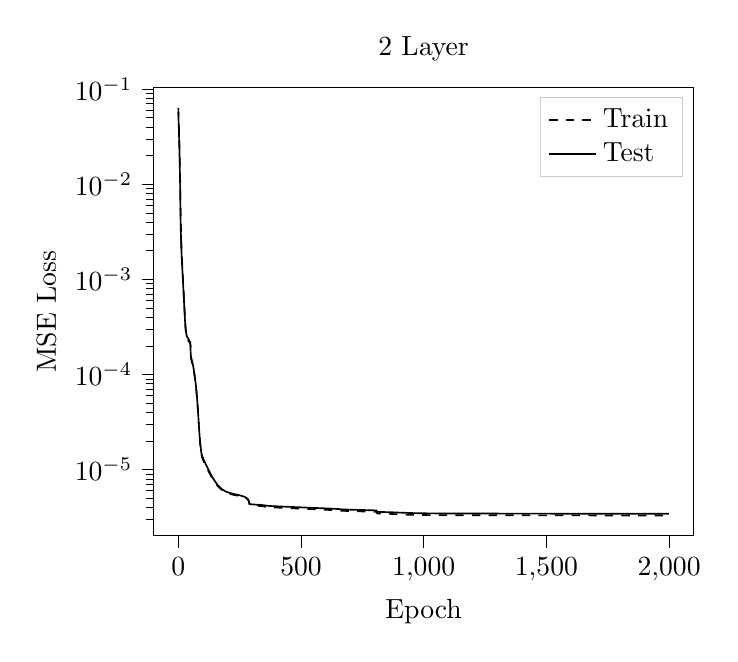
\begin{tikzpicture}

\begin{axis}[
legend cell align={left},
legend style={fill opacity=0.8, draw opacity=1, text opacity=1, draw=white!80!black},
log basis y={10},
tick align=outside,
tick pos=left,
title={2 Layer},
x grid style={white!69.0196078431373!black},
xlabel={Epoch},
xmin=-99.95, xmax=2098.95,
xtick style={color=black},
y grid style={white!69.0196078431373!black},
ylabel={MSE Loss},
ymin=2.00962005103304e-06, ymax=0.103609493820567,
ymode=log,
ytick style={color=black}
]
\addplot [semithick, black, dashed]
table {%
0 0.0632710078060627
1 0.051845450758934
2 0.0432980991452932
3 0.0358776403516531
4 0.0290690961554647
5 0.0229545622691512
6 0.0177181212641299
7 0.0134029685482383
8 0.00932001467421651
9 0.00582119612768292
10 0.00408269998338073
11 0.00310812011640519
12 0.00251322026690468
13 0.00211413772078231
14 0.00183244168199599
15 0.00161229025945067
16 0.00143017171323299
17 0.00127473987545818
18 0.0011382556988392
19 0.00101599448849447
20 0.000905665848404169
21 0.000806275674840435
22 0.00071686326363124
23 0.000636678095906973
24 0.000565266070072539
25 0.000501702402951196
26 0.000445806336938404
27 0.000397627679049037
28 0.000357118795858696
29 0.00032489347649971
30 0.000299998327216599
31 0.000281208114116453
32 0.000267276446160395
33 0.000257046025944874
34 0.0002495395517617
35 0.000243972511438187
36 0.000239745286788093
37 0.000236407682736171
38 0.000233631588111166
39 0.000231188191857655
40 0.000228926038951613
41 0.000226746779982932
42 0.000224590560450451
43 0.000222427553118905
44 0.000220237786095822
45 0.000218012332130456
46 0.000215740327854292
47 0.000213416477650753
48 0.000211034586711321
49 0.000208587526110932
50 0.000201116997253848
51 0.000158018265356077
52 0.000147613224027737
53 0.000142723495948303
54 0.000139244368234358
55 0.000136019374200259
56 0.000132747634241241
57 0.000129427922991454
58 0.000126070258433174
59 0.000122665663249791
60 0.000119213276564551
61 0.000115701421811536
62 0.000112120777172095
63 0.000108473681488249
64 0.000104762014772859
65 0.00010098851814837
66 9.71622276556445e-05
67 9.32928094116505e-05
68 8.93886299527367e-05
69 8.54555976766278e-05
70 8.14965877798386e-05
71 7.75122336417553e-05
72 7.35026992588246e-05
73 6.94685789057985e-05
74 6.54132343734091e-05
75 6.13432748941705e-05
76 5.72745405916066e-05
77 5.32301725179423e-05
78 4.92395857872907e-05
79 4.53403164574411e-05
80 4.1573930386221e-05
81 3.79849034761719e-05
82 3.46141511963651e-05
83 3.14956762558722e-05
84 2.8658379233093e-05
85 2.61181172882061e-05
86 2.38809501188371e-05
87 2.19437158739311e-05
88 2.0293696959925e-05
89 1.89088841780176e-05
90 1.77624986854426e-05
91 1.6823803317493e-05
92 1.60607825182524e-05
93 1.50258497696996e-05
94 1.4460581161984e-05
95 1.40592445336551e-05
96 1.37072536540472e-05
97 1.34257343074751e-05
98 1.31816849047937e-05
99 1.29646241002774e-05
100 1.27662120476089e-05
101 1.2581771216901e-05
102 1.24078030003147e-05
103 1.22411715728958e-05
104 1.20805520891736e-05
105 1.19247015427391e-05
106 1.1773092596286e-05
107 1.16248549329612e-05
108 1.14799404746009e-05
109 1.13379276499472e-05
110 1.11984094673971e-05
111 1.10615233461431e-05
112 1.09273854504863e-05
113 1.07954060031261e-05
114 1.06658476615848e-05
115 1.05386192249171e-05
116 1.04137884209194e-05
117 1.02908117264633e-05
118 1.01702188394484e-05
119 1.00515134595298e-05
120 9.93500102867984e-06
121 9.82061678314494e-06
122 9.70835857060592e-06
123 9.59800334567262e-06
124 9.48999531192385e-06
125 9.38343026655275e-06
126 9.2788389024463e-06
127 9.17616092829121e-06
128 9.07542354798352e-06
129 8.97668589686873e-06
130 8.87972992904906e-06
131 8.78457191856796e-06
132 8.69125409280969e-06
133 8.59979536244282e-06
134 8.51017152263012e-06
135 8.42218346087975e-06
136 8.33635802018762e-06
137 8.25191251988144e-06
138 8.16942619667316e-06
139 8.0887000030998e-06
140 8.00948176038219e-06
141 7.93231499164904e-06
142 7.85655636991578e-06
143 7.78257825504625e-06
144 7.71019455214628e-06
145 7.63938447198598e-06
146 7.57029341457383e-06
147 7.50287921164272e-06
148 7.43711638529021e-06
149 7.37279744384978e-06
150 7.31026423613912e-06
151 7.24875530431746e-06
152 7.18897826664033e-06
153 7.13090271165129e-06
154 7.07441331041991e-06
155 7.01886005163033e-06
156 6.96489755046059e-06
157 6.91240939818272e-06
158 6.86140954894654e-06
159 6.81176477974077e-06
160 6.76338529569875e-06
161 6.71635143635285e-06
162 6.67062341608471e-06
163 6.62643124655915e-06
164 6.58323398965877e-06
165 6.54126916742825e-06
166 6.50058312885449e-06
167 6.46115243034728e-06
168 6.42298308639511e-06
169 6.38602485582851e-06
170 6.35025759902419e-06
171 6.31564215518665e-06
172 6.2821410494962e-06
173 6.24969452883306e-06
174 6.21805136665898e-06
175 6.18742654864946e-06
176 6.15822291456425e-06
177 6.12961435763282e-06
178 6.10204494751088e-06
179 6.07546555693261e-06
180 6.04976868044105e-06
181 6.02458717798982e-06
182 6.00032682541496e-06
183 5.97695071451199e-06
184 5.95447526166026e-06
185 5.93280903376581e-06
186 5.91193096875031e-06
187 5.89195336056036e-06
188 5.87234221757171e-06
189 5.8534633653835e-06
190 5.83506993143601e-06
191 5.81726929294746e-06
192 5.79998251942015e-06
193 5.78317128065464e-06
194 5.76691470541846e-06
195 5.75105928714947e-06
196 5.73594326829152e-06
197 5.72154736437369e-06
198 5.70739826844147e-06
199 5.69361865041174e-06
200 5.68028440807211e-06
201 5.66706610925394e-06
202 5.65437040722827e-06
203 5.64182836365035e-06
204 5.62923450252129e-06
205 5.61731328298265e-06
206 5.60552214392374e-06
207 5.59428438737086e-06
208 5.58346819707367e-06
209 5.57276731524325e-06
210 5.56239524667035e-06
211 5.55222034631697e-06
212 5.54241197096417e-06
213 5.53287029742933e-06
214 5.52343979006764e-06
215 5.51419333123704e-06
216 5.5052181321571e-06
217 5.49665210428429e-06
218 5.48808294684022e-06
219 5.47977340056605e-06
220 5.47153629327113e-06
221 5.46346909595741e-06
222 5.45539895256297e-06
223 5.44765622976229e-06
224 5.44031825961611e-06
225 5.4328157098098e-06
226 5.42541469417301e-06
227 5.4179627427402e-06
228 5.41054173163502e-06
229 5.40329494447178e-06
230 5.39551419979034e-06
231 5.38808617102404e-06
232 5.38088338089437e-06
233 5.3739369534469e-06
234 5.36722018341607e-06
235 5.3601379581778e-06
236 5.35322880318745e-06
237 5.34662611130443e-06
238 5.33928093022951e-06
239 5.3319608723541e-06
240 5.32476024727657e-06
241 5.31745174248499e-06
242 5.3104168794107e-06
243 5.30307639201055e-06
244 5.29598574553347e-06
245 5.28916283337821e-06
246 5.28227127779246e-06
247 5.27531217994692e-06
248 5.26836660651497e-06
249 5.26145600565542e-06
250 5.25481974682407e-06
251 5.24836719614541e-06
252 5.24147814007847e-06
253 5.23453493815396e-06
254 5.22773011539357e-06
255 5.22081494614213e-06
256 5.21390236099251e-06
257 5.20662491862822e-06
258 5.19909029208066e-06
259 5.19156840505275e-06
260 5.1840717428604e-06
261 5.17612017256397e-06
262 5.16830087531162e-06
263 5.1598733487026e-06
264 5.15117472787097e-06
265 5.14193537469509e-06
266 5.13207956760198e-06
267 5.12154601028669e-06
268 5.11089195560999e-06
269 5.10023479159827e-06
270 5.08917057959479e-06
271 5.07760456798678e-06
272 5.06578773297406e-06
273 5.05217641853051e-06
274 5.0364313431146e-06
275 5.02120112696503e-06
276 5.00727311009541e-06
277 4.99260774995491e-06
278 4.97757784273745e-06
279 4.96154125721659e-06
280 4.94340508657842e-06
281 4.92293700722257e-06
282 4.89921165763008e-06
283 4.87050170272596e-06
284 4.83581983303338e-06
285 4.79348267253954e-06
286 4.74225533139361e-06
287 4.67328239142262e-06
288 4.58696049599894e-06
289 4.46936619255212e-06
290 4.31748006303678e-06
291 4.23798107794937e-06
292 4.22272348396291e-06
293 4.2174021655228e-06
294 4.21430222650088e-06
295 4.21172886331078e-06
296 4.20933076134133e-06
297 4.20704505904723e-06
298 4.20480583579774e-06
299 4.20261384238074e-06
300 4.20045522423607e-06
301 4.19840986728559e-06
302 4.19635286948505e-06
303 4.19434635909965e-06
304 4.1923705946374e-06
305 4.19050039226931e-06
306 4.18860404033694e-06
307 4.18674072125214e-06
308 4.18486637317983e-06
309 4.18306126630341e-06
310 4.18127912712407e-06
311 4.17950906694386e-06
312 4.17775834330314e-06
313 4.17607370832229e-06
314 4.17431320079231e-06
315 4.1727198783974e-06
316 4.17104828943593e-06
317 4.16937491081626e-06
318 4.16773654842473e-06
319 4.16610417369156e-06
320 4.16449309932432e-06
321 4.16296918592707e-06
322 4.16134395891277e-06
323 4.15973293388561e-06
324 4.15812554933837e-06
325 4.15651645334947e-06
326 4.15494718413356e-06
327 4.15333152818675e-06
328 4.15174744648539e-06
329 4.15025573261119e-06
330 4.14862696129603e-06
331 4.14689902572718e-06
332 4.14517258332125e-06
333 4.14342047315586e-06
334 4.14178949631605e-06
335 4.1400407767469e-06
336 4.13811117368823e-06
337 4.13610095756667e-06
338 4.13402996832701e-06
339 4.1318420285279e-06
340 4.1294807142549e-06
341 4.12701435834606e-06
342 4.12451515353496e-06
343 4.12194325031123e-06
344 4.11919797215887e-06
345 4.11631795668654e-06
346 4.11326574703708e-06
347 4.11016632801875e-06
348 4.10674409454259e-06
349 4.10305109289766e-06
350 4.09920685819998e-06
351 4.09521432902693e-06
352 4.0910061447903e-06
353 4.08667012720798e-06
354 4.08225326873435e-06
355 4.07795396699839e-06
356 4.07355116385588e-06
357 4.0691161605082e-06
358 4.06490110549385e-06
359 4.06080552897947e-06
360 4.05672974352456e-06
361 4.05283861550743e-06
362 4.04928707007457e-06
363 4.04601418176753e-06
364 4.0429513314848e-06
365 4.04010962870416e-06
366 4.03744269556228e-06
367 4.03506154293609e-06
368 4.03286837035921e-06
369 4.03083124660952e-06
370 4.02896440937184e-06
371 4.02703742270205e-06
372 4.02513960216311e-06
373 4.02338820936166e-06
374 4.02179212824194e-06
375 4.02032433521526e-06
376 4.01882592655056e-06
377 4.01735797845504e-06
378 4.01590311412292e-06
379 4.01456900135599e-06
380 4.01327008967201e-06
381 4.01198213216958e-06
382 4.01074603587404e-06
383 4.0095192375702e-06
384 4.00830898684035e-06
385 4.00709463201565e-06
386 4.0059097862013e-06
387 4.00470182489698e-06
388 4.00351677558319e-06
389 4.00236419886824e-06
390 4.00116998844169e-06
391 3.99998082389175e-06
392 3.99884801413464e-06
393 3.99764587837126e-06
394 3.99651417865243e-06
395 3.99532578603612e-06
396 3.99419785026112e-06
397 3.99303706149112e-06
398 3.99190068537791e-06
399 3.99077415227112e-06
400 3.98964895885001e-06
401 3.98854520904024e-06
402 3.98738429157675e-06
403 3.98626458650142e-06
404 3.98513616232776e-06
405 3.98401351844768e-06
406 3.98287694929422e-06
407 3.98177175156889e-06
408 3.98065694753313e-06
409 3.97955125094995e-06
410 3.97847688532238e-06
411 3.97736476134014e-06
412 3.97623916978773e-06
413 3.97515318627484e-06
414 3.97404352497688e-06
415 3.97295079324067e-06
416 3.97184997132172e-06
417 3.97074828265431e-06
418 3.96966739663185e-06
419 3.96858127305677e-06
420 3.96750045547378e-06
421 3.96643120166118e-06
422 3.96534202013754e-06
423 3.96427063765259e-06
424 3.96322433994101e-06
425 3.96213134354184e-06
426 3.96106135895025e-06
427 3.95999829197535e-06
428 3.95894019357001e-06
429 3.95790915376892e-06
430 3.95684226828053e-06
431 3.95577681206305e-06
432 3.95472414516007e-06
433 3.95362605377159e-06
434 3.95254756790564e-06
435 3.95150437725533e-06
436 3.95043570642883e-06
437 3.94937866462897e-06
438 3.94838115562379e-06
439 3.94730105404051e-06
440 3.94621883810942e-06
441 3.9451766710954e-06
442 3.94410750595853e-06
443 3.94304689325509e-06
444 3.94200809296308e-06
445 3.94095385900073e-06
446 3.93992307658664e-06
447 3.93891124645052e-06
448 3.93786665722473e-06
449 3.93685992435167e-06
450 3.9358440626529e-06
451 3.93480710340555e-06
452 3.93380716809588e-06
453 3.93278114415807e-06
454 3.93176267130002e-06
455 3.93070953191454e-06
456 3.92965003652535e-06
457 3.92862235230496e-06
458 3.92760561658179e-06
459 3.92657984616562e-06
460 3.9255645015146e-06
461 3.92449227001634e-06
462 3.92346870353322e-06
463 3.92245446937522e-06
464 3.92145133218946e-06
465 3.92043095689587e-06
466 3.91943706358688e-06
467 3.91841551595462e-06
468 3.91737812401516e-06
469 3.91636446238408e-06
470 3.91536215056476e-06
471 3.91434734888207e-06
472 3.91334745836502e-06
473 3.91231219873589e-06
474 3.91130924549543e-06
475 3.91030783475799e-06
476 3.90929390709971e-06
477 3.90829968523576e-06
478 3.90728442221189e-06
479 3.9063041681402e-06
480 3.90529386982053e-06
481 3.90429663980285e-06
482 3.90328932166994e-06
483 3.90228188075525e-06
484 3.90130058735849e-06
485 3.90029922914437e-06
486 3.89929259267774e-06
487 3.89830421522674e-06
488 3.89731379686964e-06
489 3.89628200673542e-06
490 3.89534313785589e-06
491 3.89432079941798e-06
492 3.89331514952573e-06
493 3.89229541360692e-06
494 3.89127347989415e-06
495 3.89029763300641e-06
496 3.88925411311902e-06
497 3.88816214581311e-06
498 3.88687702547941e-06
499 3.88587540737717e-06
500 3.88488475755366e-06
501 3.88386549957431e-06
502 3.88286122324644e-06
503 3.88185147426157e-06
504 3.88082735753414e-06
505 3.87983534415071e-06
506 3.87884211681921e-06
507 3.87786378541932e-06
508 3.87690347974967e-06
509 3.87590351806466e-06
510 3.87493697735408e-06
511 3.87393002165481e-06
512 3.87293140079237e-06
513 3.87193410711006e-06
514 3.87096493568606e-06
515 3.86997004397927e-06
516 3.86899167233423e-06
517 3.86810477471045e-06
518 3.86708819746673e-06
519 3.86609972861152e-06
520 3.86511584406435e-06
521 3.86410707824325e-06
522 3.86309811415231e-06
523 3.86210161127565e-06
524 3.86109321630101e-06
525 3.86009254270903e-06
526 3.85912106071373e-06
527 3.85811027194904e-06
528 3.85712550837525e-06
529 3.85611493993565e-06
530 3.85510660271393e-06
531 3.85410345074888e-06
532 3.85311390755305e-06
533 3.85213474737611e-06
534 3.85112630192452e-06
535 3.85012735591772e-06
536 3.84913734296788e-06
537 3.84815157872254e-06
538 3.84717732458739e-06
539 3.84619277247111e-06
540 3.84522993113023e-06
541 3.8442311797553e-06
542 3.84322497643552e-06
543 3.84227112340341e-06
544 3.8412537937802e-06
545 3.84022483763147e-06
546 3.83922470746256e-06
547 3.83821959007946e-06
548 3.83719782143999e-06
549 3.83618380419648e-06
550 3.83516073952705e-06
551 3.83415338933446e-06
552 3.83312635744915e-06
553 3.83206138189962e-06
554 3.83102651903755e-06
555 3.82998564509762e-06
556 3.82895923803517e-06
557 3.82797941483659e-06
558 3.82694782160797e-06
559 3.82592881351229e-06
560 3.82489514527151e-06
561 3.82387169111098e-06
562 3.82288159403288e-06
563 3.82187921854893e-06
564 3.82090538437296e-06
565 3.81990201117333e-06
566 3.81885945239446e-06
567 3.8178061686267e-06
568 3.81674583468339e-06
569 3.81568310513103e-06
570 3.81460992866778e-06
571 3.81355367085234e-06
572 3.81251289786633e-06
573 3.81145554933937e-06
574 3.8104192146875e-06
575 3.8093715679679e-06
576 3.80830061658344e-06
577 3.80721733722567e-06
578 3.80615091921754e-06
579 3.80504406757609e-06
580 3.80396494574597e-06
581 3.80284883271997e-06
582 3.80177165607165e-06
583 3.80069691914287e-06
584 3.79964723424564e-06
585 3.7985892818142e-06
586 3.79753483116474e-06
587 3.79640749065402e-06
588 3.79530364398306e-06
589 3.7941353525639e-06
590 3.79299306950998e-06
591 3.79188061958757e-06
592 3.79073451824752e-06
593 3.78960781699789e-06
594 3.78849956632621e-06
595 3.7874091502772e-06
596 3.78626679844274e-06
597 3.78513176633533e-06
598 3.78400663305456e-06
599 3.78287078638095e-06
600 3.78169056853039e-06
601 3.78051059510653e-06
602 3.77938837505099e-06
603 3.77821030451742e-06
604 3.77709365989176e-06
605 3.77594412566395e-06
606 3.77473977471254e-06
607 3.77356035733101e-06
608 3.77238059650153e-06
609 3.77121746578268e-06
610 3.77010574015912e-06
611 3.76895438330394e-06
612 3.76782894613825e-06
613 3.76667858108704e-06
614 3.76551559270411e-06
615 3.76439185151867e-06
616 3.76326227546997e-06
617 3.76208450234117e-06
618 3.76090089821446e-06
619 3.75969973163137e-06
620 3.75851625665291e-06
621 3.75739111655093e-06
622 3.75627195273864e-06
623 3.75508487604748e-06
624 3.75392496414406e-06
625 3.75275827741461e-06
626 3.75164966681041e-06
627 3.7504619098172e-06
628 3.7492805902275e-06
629 3.74812237578226e-06
630 3.74700240786297e-06
631 3.74586033490232e-06
632 3.74465033678462e-06
633 3.74347466811287e-06
634 3.74222576670036e-06
635 3.74095193990343e-06
636 3.73970642544919e-06
637 3.73849202571819e-06
638 3.73727273176883e-06
639 3.73604903143132e-06
640 3.73481999326941e-06
641 3.73360565822622e-06
642 3.73240932685803e-06
643 3.73127844181909e-06
644 3.73011926103572e-06
645 3.72891290930966e-06
646 3.727741849616e-06
647 3.72646188213821e-06
648 3.72512999217633e-06
649 3.72386121966883e-06
650 3.72253252623977e-06
651 3.72115426330311e-06
652 3.71982453145847e-06
653 3.7184918338653e-06
654 3.71706787746007e-06
655 3.71560938947368e-06
656 3.71417414066855e-06
657 3.71250464706918e-06
658 3.71070990593125e-06
659 3.70882397623973e-06
660 3.70690597890189e-06
661 3.70420897252188e-06
662 3.70078934975027e-06
663 3.69826730502609e-06
664 3.69612601537028e-06
665 3.69425015776415e-06
666 3.69259916294595e-06
667 3.69112746614064e-06
668 3.68980126438601e-06
669 3.6885883330342e-06
670 3.68746814126553e-06
671 3.68644335560475e-06
672 3.68547208643122e-06
673 3.68455293175884e-06
674 3.683675603952e-06
675 3.68285116735478e-06
676 3.6820184672024e-06
677 3.68124188753427e-06
678 3.68046135884015e-06
679 3.67971530249633e-06
680 3.67896949774149e-06
681 3.67823716908333e-06
682 3.67751394207971e-06
683 3.67678034842811e-06
684 3.67607592556851e-06
685 3.67535497991867e-06
686 3.67465632757558e-06
687 3.67394465786219e-06
688 3.6732546661824e-06
689 3.67254644345394e-06
690 3.67185343293386e-06
691 3.67115930930595e-06
692 3.67046825454054e-06
693 3.66977536043578e-06
694 3.66907607531175e-06
695 3.66839212199466e-06
696 3.66770006837669e-06
697 3.6670071425533e-06
698 3.66632715258675e-06
699 3.66563417685484e-06
700 3.66494473416878e-06
701 3.66426724519897e-06
702 3.66358821713675e-06
703 3.66290142187609e-06
704 3.6622132258799e-06
705 3.6615301440861e-06
706 3.66084534357469e-06
707 3.66017243891292e-06
708 3.6594921489268e-06
709 3.65881293635084e-06
710 3.65812857126002e-06
711 3.6574575931354e-06
712 3.65677416755261e-06
713 3.65609544701329e-06
714 3.65541832900362e-06
715 3.65474015052314e-06
716 3.65406903290477e-06
717 3.65339285406208e-06
718 3.65271773671338e-06
719 3.65204745116898e-06
720 3.651368467672e-06
721 3.65069879228486e-06
722 3.65002570674733e-06
723 3.64936534811022e-06
724 3.64868461804235e-06
725 3.64801084799637e-06
726 3.64734410402434e-06
727 3.64667091173487e-06
728 3.6460121403934e-06
729 3.6453348136547e-06
730 3.64466524786167e-06
731 3.6439993359636e-06
732 3.64334011158007e-06
733 3.64267599638879e-06
734 3.64200718195207e-06
735 3.64133908624353e-06
736 3.64068387693806e-06
737 3.64001761658983e-06
738 3.63935759855849e-06
739 3.63869932277794e-06
740 3.6380411635264e-06
741 3.63737760744698e-06
742 3.63650741667243e-06
743 3.63583347075291e-06
744 3.63516651168538e-06
745 3.63449705389485e-06
746 3.63384109414255e-06
747 3.63316582570405e-06
748 3.63250598411469e-06
749 3.63184671437011e-06
750 3.63118088159808e-06
751 3.63051347460441e-06
752 3.62984826938373e-06
753 3.62920208863216e-06
754 3.62853011097286e-06
755 3.62786857806441e-06
756 3.62720777866343e-06
757 3.62655042818005e-06
758 3.62588549194243e-06
759 3.62523838361994e-06
760 3.62457825156071e-06
761 3.62390604811935e-06
762 3.62325307582978e-06
763 3.62259630355766e-06
764 3.62194640536018e-06
765 3.62129782820375e-06
766 3.62063571492399e-06
767 3.61997041034101e-06
768 3.61932698899636e-06
769 3.61866497462415e-06
770 3.6180262252401e-06
771 3.617362689738e-06
772 3.61671298037436e-06
773 3.61607361901406e-06
774 3.61541275435684e-06
775 3.6147658632899e-06
776 3.61411101857811e-06
777 3.61345795158741e-06
778 3.61281008554215e-06
779 3.61216918668106e-06
780 3.6115153557148e-06
781 3.61088205590931e-06
782 3.61022876393236e-06
783 3.6095767355846e-06
784 3.60893789741112e-06
785 3.60828682255487e-06
786 3.60765805169194e-06
787 3.60699846305579e-06
788 3.60636278833226e-06
789 3.60572352553845e-06
790 3.60508044082053e-06
791 3.60444044986252e-06
792 3.60379261326216e-06
793 3.60315890213769e-06
794 3.60252107452652e-06
795 3.60187887156371e-06
796 3.6012473944993e-06
797 3.60060167395204e-06
798 3.59996799465989e-06
799 3.59931844286621e-06
800 3.59868616624226e-06
801 3.59804496190463e-06
802 3.59741519469026e-06
803 3.59679051234707e-06
804 3.59614438116296e-06
805 3.59551126325641e-06
806 3.59488375943329e-06
807 3.59423938243708e-06
808 3.59361888456533e-06
809 3.58856573075173e-06
810 3.46819658852837e-06
811 3.45905467918328e-06
812 3.45808383144686e-06
813 3.45728719207727e-06
814 3.45646615710393e-06
815 3.4557891899567e-06
816 3.45512566559592e-06
817 3.45442840398391e-06
818 3.45375150789096e-06
819 3.45314441744904e-06
820 3.45249377733126e-06
821 3.45187570439975e-06
822 3.4512920127554e-06
823 3.45072540699221e-06
824 3.45013294111141e-06
825 3.44956170420119e-06
826 3.44901385676621e-06
827 3.44852854482269e-06
828 3.44790018584717e-06
829 3.44723031332705e-06
830 3.44663635894449e-06
831 3.44601887513818e-06
832 3.44534294094956e-06
833 3.44472433505416e-06
834 3.44406132182939e-06
835 3.44345207020069e-06
836 3.44280726289981e-06
837 3.4422474728899e-06
838 3.44163713850776e-06
839 3.44108118099484e-06
840 3.44047824160043e-06
841 3.4398152462245e-06
842 3.43910582000717e-06
843 3.43842116046744e-06
844 3.43774710404432e-06
845 3.43702792099521e-06
846 3.43634997943809e-06
847 3.43563018009263e-06
848 3.43499882342257e-06
849 3.43428135010981e-06
850 3.43356308815146e-06
851 3.43284928339926e-06
852 3.43210946982708e-06
853 3.43137287131867e-06
854 3.43064236994906e-06
855 3.42992232879169e-06
856 3.42917290743117e-06
857 3.42838393817146e-06
858 3.42754296923431e-06
859 3.42668330313245e-06
860 3.42588032242475e-06
861 3.42507210848453e-06
862 3.42416718467575e-06
863 3.42335599020771e-06
864 3.42258317823507e-06
865 3.42167720782527e-06
866 3.42081106327896e-06
867 3.41993027393528e-06
868 3.41898223450698e-06
869 3.41806178505522e-06
870 3.41711957901225e-06
871 3.41628901833246e-06
872 3.41533120615622e-06
873 3.41435020516201e-06
874 3.41339523242823e-06
875 3.41245838376381e-06
876 3.4114890966066e-06
877 3.41038971214402e-06
878 3.40855177046251e-06
879 3.40721698319157e-06
880 3.40610965008636e-06
881 3.40513882656524e-06
882 3.40419041424411e-06
883 3.40332646044317e-06
884 3.40240671414449e-06
885 3.4013559078403e-06
886 3.40033198938272e-06
887 3.39924581226114e-06
888 3.39811470360019e-06
889 3.39708300680286e-06
890 3.39614488370898e-06
891 3.39512193158953e-06
892 3.39409216473996e-06
893 3.39310099377599e-06
894 3.39206634293987e-06
895 3.39110838353918e-06
896 3.39012106735481e-06
897 3.3891239560262e-06
898 3.38814063684367e-06
899 3.38709192863007e-06
900 3.38610237486137e-06
901 3.38508347010702e-06
902 3.38407450976774e-06
903 3.38305720777043e-06
904 3.38207762490583e-06
905 3.38106447293285e-06
906 3.38001549198452e-06
907 3.37896211885891e-06
908 3.37797512941052e-06
909 3.37698621433447e-06
910 3.37599381316522e-06
911 3.37501526473716e-06
912 3.37411181067182e-06
913 3.37317492824241e-06
914 3.37220609208089e-06
915 3.3712260875518e-06
916 3.37031230503726e-06
917 3.36942957324027e-06
918 3.36857478896491e-06
919 3.36759936112685e-06
920 3.36662839538349e-06
921 3.36570018896509e-06
922 3.3648025120101e-06
923 3.36392968029031e-06
924 3.3630231520192e-06
925 3.36211414503396e-06
926 3.36128224489585e-06
927 3.36038605507838e-06
928 3.35971276251712e-06
929 3.35890150881824e-06
930 3.35802607730784e-06
931 3.35722394027016e-06
932 3.35641767048855e-06
933 3.35569475134889e-06
934 3.35492151180006e-06
935 3.35416929988241e-06
936 3.35343535334687e-06
937 3.35275004340474e-06
938 3.3520320862408e-06
939 3.35134114561697e-06
940 3.35064550688458e-06
941 3.34997043398744e-06
942 3.34934603586134e-06
943 3.34871437360107e-06
944 3.34808450747914e-06
945 3.34750664876537e-06
946 3.34689332385096e-06
947 3.34634646662835e-06
948 3.34575365366163e-06
949 3.34518739339273e-06
950 3.34464585841943e-06
951 3.34406109845986e-06
952 3.34353921266484e-06
953 3.34303967986216e-06
954 3.34256621943041e-06
955 3.34205329431825e-06
956 3.34155066923358e-06
957 3.34107601361211e-06
958 3.34061679984643e-06
959 3.34015869543691e-06
960 3.33970654855875e-06
961 3.3393236901702e-06
962 3.33886904593328e-06
963 3.33842913983062e-06
964 3.33814169107427e-06
965 3.33774210423599e-06
966 3.3372913213725e-06
967 3.33686178612425e-06
968 3.33645433522634e-06
969 3.33606849665102e-06
970 3.33571005978683e-06
971 3.33536255254785e-06
972 3.33501844590955e-06
973 3.33469381189389e-06
974 3.33438582435974e-06
975 3.33408202118335e-06
976 3.33378812365481e-06
977 3.33350157063705e-06
978 3.33323775805638e-06
979 3.3330256313775e-06
980 3.33272925752226e-06
981 3.33243786371895e-06
982 3.33216787623769e-06
983 3.3319054509775e-06
984 3.33164250014306e-06
985 3.33139780241254e-06
986 3.33115889634428e-06
987 3.33091831510046e-06
988 3.33069397129293e-06
989 3.33046564878714e-06
990 3.33024445262708e-06
991 3.33003096750417e-06
992 3.32982458940023e-06
993 3.32962686138671e-06
994 3.32943600267299e-06
995 3.32926675400813e-06
996 3.32906775338415e-06
997 3.3288823390194e-06
998 3.32862334119e-06
999 3.3284366764974e-06
1000 3.32826502312855e-06
1001 3.32808903544901e-06
1002 3.3279268395745e-06
1003 3.3277572111956e-06
1004 3.32759605612409e-06
1005 3.32745577202331e-06
1006 3.32727387956311e-06
1007 3.32710411589687e-06
1008 3.32693895040848e-06
1009 3.32677818335014e-06
1010 3.32661705760984e-06
1011 3.32647359664406e-06
1012 3.32631457933985e-06
1013 3.32618127072237e-06
1014 3.32603964534428e-06
1015 3.32589951085538e-06
1016 3.32574876642866e-06
1017 3.32563812094122e-06
1018 3.325481228444e-06
1019 3.32533804532886e-06
1020 3.32519677795062e-06
1021 3.32507743246424e-06
1022 3.32495024065338e-06
1023 3.32481203804491e-06
1024 3.32468024942045e-06
1025 3.32454988460995e-06
1026 3.32442952083056e-06
1027 3.32430381183713e-06
1028 3.32418459424844e-06
1029 3.32406650829853e-06
1030 3.32396275587143e-06
1031 3.32385228330168e-06
1032 3.32373832941357e-06
1033 3.32363166569394e-06
1034 3.32353530177443e-06
1035 3.32343474212848e-06
1036 3.32334030849779e-06
1037 3.32324221994895e-06
1038 3.32314650916032e-06
1039 3.32305175118108e-06
1040 3.32298359035121e-06
1041 3.32284780517966e-06
1042 3.32274852030423e-06
1043 3.3226549801384e-06
1044 3.32256201613745e-06
1045 3.32246874370412e-06
1046 3.3223735683805e-06
1047 3.32228958177438e-06
1048 3.32220481595868e-06
1049 3.32208896418251e-06
1050 3.32200541083694e-06
1051 3.32191331938247e-06
1052 3.32182456236296e-06
1053 3.32175064909279e-06
1054 3.3216608036355e-06
1055 3.32158123887893e-06
1056 3.32150148597066e-06
1057 3.3214288405361e-06
1058 3.32134673897144e-06
1059 3.32127205160759e-06
1060 3.3211996552609e-06
1061 3.32111623322362e-06
1062 3.32105358813806e-06
1063 3.32098555361426e-06
1064 3.320912385675e-06
1065 3.32084120304899e-06
1066 3.32077246423523e-06
1067 3.32069897615384e-06
1068 3.32062761867746e-06
1069 3.32055835360734e-06
1070 3.32049213534447e-06
1071 3.32042758327589e-06
1072 3.32035822054877e-06
1073 3.32029157220859e-06
1074 3.3202237336809e-06
1075 3.32016097570431e-06
1076 3.32010107376846e-06
1077 3.32003031508066e-06
1078 3.31996242221066e-06
1079 3.31990452946229e-06
1080 3.31984272509089e-06
1081 3.3197831430698e-06
1082 3.31972265939839e-06
1083 3.31965873988338e-06
1084 3.31960340872683e-06
1085 3.31954086311725e-06
1086 3.31948666712378e-06
1087 3.31942682998942e-06
1088 3.31936341729033e-06
1089 3.31931191681178e-06
1090 3.31925431248692e-06
1091 3.31908182454299e-06
1092 3.31901709694193e-06
1093 3.31896539614718e-06
1094 3.31891274390728e-06
1095 3.31885061757475e-06
1096 3.31879793600365e-06
1097 3.3187468189908e-06
1098 3.31868890623355e-06
1099 3.31862838606867e-06
1100 3.31856975185474e-06
1101 3.31851502880909e-06
1102 3.31847244035544e-06
1103 3.31840572573583e-06
1104 3.3183519180966e-06
1105 3.31829593142174e-06
1106 3.31823610724769e-06
1107 3.31818831443798e-06
1108 3.31813788932322e-06
1109 3.31809355793666e-06
1110 3.31803202232095e-06
1111 3.31797998080674e-06
1112 3.31792680481158e-06
1113 3.31787022776098e-06
1114 3.31782323041807e-06
1115 3.31776938503481e-06
1116 3.31772539641406e-06
1117 3.31767134389338e-06
1118 3.31762536609403e-06
1119 3.31757380968156e-06
1120 3.31752182080436e-06
1121 3.31747144957717e-06
1122 3.31731329424656e-06
1123 3.31725821206419e-06
1124 3.31720646829581e-06
1125 3.31715368929508e-06
1126 3.31710390935314e-06
1127 3.3170535549516e-06
1128 3.31699749733616e-06
1129 3.31695505599328e-06
1130 3.31690347150015e-06
1131 3.31685236983503e-06
1132 3.31680772876552e-06
1133 3.3167499815363e-06
1134 3.31669872764451e-06
1135 3.31664693214861e-06
1136 3.31659686685271e-06
1137 3.31655298123223e-06
1138 3.31649509212184e-06
1139 3.31645859967011e-06
1140 3.31640772060382e-06
1141 3.31635877830649e-06
1142 3.31630854077503e-06
1143 3.3162615816309e-06
1144 3.31620984627534e-06
1145 3.31616943481095e-06
1146 3.31612526088065e-06
1147 3.31607749308205e-06
1148 3.31602828350697e-06
1149 3.31598170487268e-06
1150 3.31593465273272e-06
1151 3.31589305983471e-06
1152 3.31584171124177e-06
1153 3.31579683393102e-06
1154 3.31575542475093e-06
1155 3.31569906404638e-06
1156 3.31566256102178e-06
1157 3.31562098369886e-06
1158 3.31557101537783e-06
1159 3.31552743352859e-06
1160 3.31547878431593e-06
1161 3.31543595132189e-06
1162 3.31539260980662e-06
1163 3.31535449493003e-06
1164 3.31530274024772e-06
1165 3.31526033858154e-06
1166 3.31521684279323e-06
1167 3.31517224708477e-06
1168 3.31512761704289e-06
1169 3.31509071429537e-06
1170 3.31504686755579e-06
1171 3.31499783703748e-06
1172 3.31494618387751e-06
1173 3.31488194569829e-06
1174 3.31483411434874e-06
1175 3.31477687655024e-06
1176 3.31463223449191e-06
1177 3.3145593424706e-06
1178 3.31451699707941e-06
1179 3.31447909991311e-06
1180 3.31444194944197e-06
1181 3.31440136801575e-06
1182 3.3143566832905e-06
1183 3.31432279710953e-06
1184 3.3142888198654e-06
1185 3.31424507578504e-06
1186 3.31421255020814e-06
1187 3.31417136544587e-06
1188 3.31413100582267e-06
1189 3.31409358943802e-06
1190 3.3140541273724e-06
1191 3.31401387495589e-06
1192 3.31398105663538e-06
1193 3.31394617762726e-06
1194 3.31390259668751e-06
1195 3.31387615858603e-06
1196 3.31384136154611e-06
1197 3.31379895965256e-06
1198 3.31376556687246e-06
1199 3.31373439541949e-06
1200 3.31369409514082e-06
1201 3.31365316878873e-06
1202 3.31363031023102e-06
1203 3.31359488518501e-06
1204 3.31356466006127e-06
1205 3.31353000353829e-06
1206 3.3134903616201e-06
1207 3.31346309042146e-06
1208 3.31342015306291e-06
1209 3.31339084232241e-06
1210 3.3133535714569e-06
1211 3.31332341784218e-06
1212 3.31328962545285e-06
1213 3.31325111255865e-06
1214 3.31321978012511e-06
1215 3.31318277721948e-06
1216 3.31314616198597e-06
1217 3.31311287493463e-06
1218 3.31307958356319e-06
1219 3.31304765325058e-06
1220 3.31300194511641e-06
1221 3.31296959791416e-06
1222 3.31293913814079e-06
1223 3.31290463248024e-06
1224 3.31286963171351e-06
1225 3.31283649222769e-06
1226 3.31280664943279e-06
1227 3.31276422059545e-06
1228 3.31273262804643e-06
1229 3.31270691606278e-06
1230 3.31266566593058e-06
1231 3.31263192094866e-06
1232 3.31260459256555e-06
1233 3.31257304628707e-06
1234 3.31253451588509e-06
1235 3.3125027416645e-06
1236 3.31246954056041e-06
1237 3.31243238213119e-06
1238 3.31239868376088e-06
1239 3.31237523766958e-06
1240 3.31232966425432e-06
1241 3.3123012260603e-06
1242 3.31226731339029e-06
1243 3.31223492764821e-06
1244 3.31220416660472e-06
1245 3.3121651907777e-06
1246 3.31213434481015e-06
1247 3.31210411036409e-06
1248 3.31207334511419e-06
1249 3.31204188125866e-06
1250 3.31200534310483e-06
1251 3.31196890385854e-06
1252 3.31193951285513e-06
1253 3.31191298664635e-06
1254 3.31186976950448e-06
1255 3.31183692810555e-06
1256 3.31180187276914e-06
1257 3.31176736733596e-06
1258 3.31174078667118e-06
1259 3.31170079664389e-06
1260 3.31167498484319e-06
1261 3.31163897067199e-06
1262 3.31160367568373e-06
1263 3.31157391030956e-06
1264 3.31153827073649e-06
1265 3.31150821864412e-06
1266 3.31147878000593e-06
1267 3.31144059236976e-06
1268 3.3114125475322e-06
1269 3.31137845250851e-06
1270 3.31135019507656e-06
1271 3.31132036353665e-06
1272 3.31128353366239e-06
1273 3.31124508727498e-06
1274 3.3112155958861e-06
1275 3.31118322765178e-06
1276 3.31115418396166e-06
1277 3.31111870571021e-06
1278 3.31108915679579e-06
1279 3.31105810823829e-06
1280 3.31101666643008e-06
1281 3.31099420361625e-06
1282 3.31095552917304e-06
1283 3.31091766827285e-06
1284 3.31088738289509e-06
1285 3.31086019934901e-06
1286 3.31082479078759e-06
1287 3.3107894528257e-06
1288 3.31076125996788e-06
1289 3.31073088023004e-06
1290 3.31069415051388e-06
1291 3.31065719831258e-06
1292 3.31063165572232e-06
1293 3.31060190774224e-06
1294 3.3105640161466e-06
1295 3.31053720560703e-06
1296 3.31050339457306e-06
1297 3.31046521137068e-06
1298 3.31043459812008e-06
1299 3.31039810896527e-06
1300 3.31036881345881e-06
1301 3.31033730344643e-06
1302 3.310306435651e-06
1303 3.31026991398176e-06
1304 3.31024301567595e-06
1305 3.31020190742493e-06
1306 3.31017149255786e-06
1307 3.3101332599017e-06
1308 3.31010171169055e-06
1309 3.31005946975438e-06
1310 3.31003425515064e-06
1311 3.30999968309698e-06
1312 3.30996857246646e-06
1313 3.30993229317755e-06
1314 3.30990236466278e-06
1315 3.30987621293843e-06
1316 3.30983615754121e-06
1317 3.30979875263893e-06
1318 3.30977489818451e-06
1319 3.30974435814824e-06
1320 3.30970497532235e-06
1321 3.30967777449587e-06
1322 3.30965184900833e-06
1323 3.30961561678578e-06
1324 3.30957849496372e-06
1325 3.30955011418155e-06
1326 3.30952235151472e-06
1327 3.30948825808264e-06
1328 3.30946376834618e-06
1329 3.30942424557179e-06
1330 3.30939567766109e-06
1331 3.30936111083702e-06
1332 3.30933207965245e-06
1333 3.3093084363145e-06
1334 3.30927065931519e-06
1335 3.30923937360694e-06
1336 3.30921289116759e-06
1337 3.30918081397158e-06
1338 3.30914972573737e-06
1339 3.30911605874462e-06
1340 3.30908646151329e-06
1341 3.30905639475532e-06
1342 3.30902801658795e-06
1343 3.30899296102416e-06
1344 3.30896267894332e-06
1345 3.3089325166884e-06
1346 3.30890046916466e-06
1347 3.30886465042113e-06
1348 3.3088395756522e-06
1349 3.30881382774351e-06
1350 3.30877656608664e-06
1351 3.30874721919372e-06
1352 3.30871065659721e-06
1353 3.30867955688063e-06
1354 3.30865487069332e-06
1355 3.30862191162851e-06
1356 3.30859550501827e-06
1357 3.30855776235239e-06
1358 3.30853303728418e-06
1359 3.30850446073327e-06
1360 3.30846531176121e-06
1361 3.30843728659147e-06
1362 3.30840472588534e-06
1363 3.30837749436341e-06
1364 3.30834483236231e-06
1365 3.30830624568534e-06
1366 3.30828763708269e-06
1367 3.30825550838654e-06
1368 3.30822551416077e-06
1369 3.30818973498026e-06
1370 3.30815789163807e-06
1371 3.30812527829494e-06
1372 3.30809859678993e-06
1373 3.30806258318717e-06
1374 3.30803215661035e-06
1375 3.30800900974282e-06
1376 3.30797151002571e-06
1377 3.30794009107649e-06
1378 3.30791404837782e-06
1379 3.30788173698693e-06
1380 3.30785453468252e-06
1381 3.30781790967194e-06
1382 3.30779392106706e-06
1383 3.30776260773291e-06
1384 3.30773389839578e-06
1385 3.30769640322615e-06
1386 3.30766638410296e-06
1387 3.30763812337409e-06
1388 3.30760337055835e-06
1389 3.30757708707097e-06
1390 3.307545913799e-06
1391 3.30751326794143e-06
1392 3.30749232489325e-06
1393 3.30745411440603e-06
1394 3.30735595673559e-06
1395 3.30729904260352e-06
1396 3.30725218407224e-06
1397 3.30722578951281e-06
1398 3.30719073667751e-06
1399 3.30716875021153e-06
1400 3.30714862934656e-06
1401 3.30711684216567e-06
1402 3.3070819894192e-06
1403 3.3070488652811e-06
1404 3.30701422922175e-06
1405 3.30698709717581e-06
1406 3.30695631168965e-06
1407 3.30692265868038e-06
1408 3.30688969722814e-06
1409 3.30686106201483e-06
1410 3.3068254247155e-06
1411 3.3067949505039e-06
1412 3.30675967359184e-06
1413 3.30672607924498e-06
1414 3.30669463016875e-06
1415 3.30665754358961e-06
1416 3.30661870475524e-06
1417 3.30659057021876e-06
1418 3.30655833431592e-06
1419 3.30653160381189e-06
1420 3.30648229748931e-06
1421 3.3064635277924e-06
1422 3.30642847688978e-06
1423 3.30640005802252e-06
1424 3.30635991497275e-06
1425 3.30633839712391e-06
1426 3.30630923531317e-06
1427 3.30627130324501e-06
1428 3.30624613002328e-06
1429 3.30621113914731e-06
1430 3.30618818611583e-06
1431 3.30615022528491e-06
1432 3.30612555853804e-06
1433 3.3060949335777e-06
1434 3.30606805039224e-06
1435 3.30602659039414e-06
1436 3.30600337179021e-06
1437 3.30597711342762e-06
1438 3.30594837578246e-06
1439 3.30591299587013e-06
1440 3.30588416147748e-06
1441 3.30585510812398e-06
1442 3.30582726405737e-06
1443 3.30579878891513e-06
1444 3.30576666067373e-06
1445 3.30573926805755e-06
1446 3.30570304413413e-06
1447 3.30567544233418e-06
1448 3.30564356863761e-06
1449 3.30561513396788e-06
1450 3.3055900224781e-06
1451 3.30555552284295e-06
1452 3.30552562525099e-06
1453 3.30550001433494e-06
1454 3.30546434372536e-06
1455 3.30543629740987e-06
1456 3.30540926006506e-06
1457 3.30537772595108e-06
1458 3.30534853821973e-06
1459 3.30531810948287e-06
1460 3.30529423752068e-06
1461 3.30526512493634e-06
1462 3.30523205786903e-06
1463 3.30520980810434e-06
1464 3.30517069141933e-06
1465 3.30514524932823e-06
1466 3.3051182268764e-06
1467 3.3050883089345e-06
1468 3.30505295073635e-06
1469 3.30502717281433e-06
1470 3.30499619519742e-06
1471 3.30496268304614e-06
1472 3.3049321046974e-06
1473 3.30491160332258e-06
1474 3.30488403938034e-06
1475 3.30484924450047e-06
1476 3.30482337255944e-06
1477 3.3047829225552e-06
1478 3.30475701593969e-06
1479 3.30473347594307e-06
1480 3.30469857590288e-06
1481 3.30467577111904e-06
1482 3.30463922102808e-06
1483 3.30460926977594e-06
1484 3.3045828433842e-06
1485 3.30454228947019e-06
1486 3.30451344598259e-06
1487 3.30448826628071e-06
1488 3.30446151951946e-06
1489 3.30443765540167e-06
1490 3.30440346078831e-06
1491 3.30437982188414e-06
1492 3.30434341208274e-06
1493 3.30430771680312e-06
1494 3.30429122220721e-06
1495 3.30425914978605e-06
1496 3.30423125637935e-06
1497 3.30419332021847e-06
1498 3.30416777239861e-06
1499 3.30414132929491e-06
1500 3.3041072015294e-06
1501 3.30408697664097e-06
1502 3.30404774513227e-06
1503 3.30401728399465e-06
1504 3.30398470123328e-06
1505 3.30396658409882e-06
1506 3.30393206252211e-06
1507 3.30390698763949e-06
1508 3.3038729142163e-06
1509 3.30384653216242e-06
1510 3.30381857452267e-06
1511 3.3037834704146e-06
1512 3.30376238377994e-06
1513 3.30373555277674e-06
1514 3.30370023016258e-06
1515 3.30367066123927e-06
1516 3.30364827868834e-06
1517 3.30361546969016e-06
1518 3.30358942426301e-06
1519 3.30355498942936e-06
1520 3.30352247999599e-06
1521 3.3034975198234e-06
1522 3.30347213048299e-06
1523 3.3034410593018e-06
1524 3.30340980383426e-06
1525 3.30338359890447e-06
1526 3.30335414560068e-06
1527 3.30332708222159e-06
1528 3.30329681514741e-06
1529 3.30327013000442e-06
1530 3.30323686262091e-06
1531 3.30320873774781e-06
1532 3.30318001522301e-06
1533 3.30315449173213e-06
1534 3.30311911397985e-06
1535 3.30308946342939e-06
1536 3.30306302032568e-06
1537 3.30303495979933e-06
1538 3.30300534017169e-06
1539 3.30297712798711e-06
1540 3.30294749460336e-06
1541 3.30292028195345e-06
1542 3.3028948644187e-06
1543 3.30286502901345e-06
1544 3.30283326866265e-06
1545 3.30280487150958e-06
1546 3.30277500813736e-06
1547 3.30274673478925e-06
1548 3.30271867062493e-06
1549 3.30269409198536e-06
1550 3.30266561161352e-06
1551 3.30262623526778e-06
1552 3.30260750922662e-06
1553 3.3025772891051e-06
1554 3.30255014239356e-06
1555 3.30251469154064e-06
1556 3.30248873808614e-06
1557 3.3024674067974e-06
1558 3.30243384246387e-06
1559 3.30240462881193e-06
1560 3.30237546916123e-06
1561 3.30234038585786e-06
1562 3.30231066175202e-06
1563 3.30228913446717e-06
1564 3.30225435584453e-06
1565 3.3022217786538e-06
1566 3.30219976888202e-06
1567 3.30216723705234e-06
1568 3.30214145628815e-06
1569 3.30211137895731e-06
1570 3.30207850458919e-06
1571 3.30205081854729e-06
1572 3.302026115648e-06
1573 3.30199760367123e-06
1574 3.30196539312055e-06
1575 3.3019390057234e-06
1576 3.30191038460725e-06
1577 3.3018855078808e-06
1578 3.30184813685719e-06
1579 3.30180191804175e-06
1580 3.30177034481949e-06
1581 3.3017495417198e-06
1582 3.30171515747679e-06
1583 3.30168458845037e-06
1584 3.30166584637936e-06
1585 3.30163201942923e-06
1586 3.30159827740317e-06
1587 3.3015747395666e-06
1588 3.30153459117355e-06
1589 3.30150503953064e-06
1590 3.30147473721354e-06
1591 3.3014371099398e-06
1592 3.30141293727593e-06
1593 3.30138024446569e-06
1594 3.30134788134728e-06
1595 3.3013217273492e-06
1596 3.30129438600579e-06
1597 3.30125701191264e-06
1598 3.30122357820528e-06
1599 3.30119717989419e-06
1600 3.30116559575799e-06
1601 3.30114111216062e-06
1602 3.30111100208796e-06
1603 3.30107951037917e-06
1604 3.30104800923436e-06
1605 3.30102942348276e-06
1606 3.30099440964204e-06
1607 3.30095793640339e-06
1608 3.3009348513815e-06
1609 3.30090420584384e-06
1610 3.30087502663901e-06
1611 3.30084139932296e-06
1612 3.30081177537522e-06
1613 3.3007786385042e-06
1614 3.30075007127562e-06
1615 3.30071773169038e-06
1616 3.30068771290826e-06
1617 3.30065788398315e-06
1618 3.30062718342106e-06
1619 3.30059937959959e-06
1620 3.30057129747274e-06
1621 3.30054074106556e-06
1622 3.30050786396896e-06
1623 3.30048373109548e-06
1624 3.30044843246924e-06
1625 3.30041834229178e-06
1626 3.30038527124543e-06
1627 3.30035584568122e-06
1628 3.30032886301979e-06
1629 3.30029377244045e-06
1630 3.30026115011606e-06
1631 3.30023468347918e-06
1632 3.30020599756153e-06
1633 3.30017422174933e-06
1634 3.30014696180569e-06
1635 3.30011202709102e-06
1636 3.30009334368242e-06
1637 3.30004895295133e-06
1638 3.30002450380107e-06
1639 3.29999766279343e-06
1640 3.29997183382602e-06
1641 3.29994155310942e-06
1642 3.29990957368409e-06
1643 3.29988495889211e-06
1644 3.29985402834154e-06
1645 3.29982594382727e-06
1646 3.2997962562149e-06
1647 3.29977297496953e-06
1648 3.29973987481935e-06
1649 3.29971252767791e-06
1650 3.2996849652136e-06
1651 3.29965504352003e-06
1652 3.29962673617956e-06
1653 3.29959587395479e-06
1654 3.29956945233789e-06
1655 3.29953468565236e-06
1656 3.29950606544571e-06
1657 3.29947025568345e-06
1658 3.2994390381873e-06
1659 3.29941945165047e-06
1660 3.29939342486796e-06
1661 3.2993645697843e-06
1662 3.29933284365325e-06
1663 3.29930496661746e-06
1664 3.29927175471312e-06
1665 3.29925617563731e-06
1666 3.29922392040771e-06
1667 3.2991881481621e-06
1668 3.29915968620753e-06
1669 3.29913620771549e-06
1670 3.29909874335499e-06
1671 3.29907201569313e-06
1672 3.29904115744739e-06
1673 3.29901682164291e-06
1674 3.29898408233475e-06
1675 3.29896147468389e-06
1676 3.29893686694049e-06
1677 3.29890761008755e-06
1678 3.29887316672739e-06
1679 3.29885079906944e-06
1680 3.29882769165124e-06
1681 3.29879325147431e-06
1682 3.2987617918252e-06
1683 3.29873484895415e-06
1684 3.29869935274019e-06
1685 3.29867526863836e-06
1686 3.29864835384797e-06
1687 3.29862218973176e-06
1688 3.29859079624839e-06
1689 3.29856409382501e-06
1690 3.29853535163238e-06
1691 3.29850868524773e-06
1692 3.29849142360672e-06
1693 3.29845765497794e-06
1694 3.29842601661312e-06
1695 3.29840140443594e-06
1696 3.29837368212793e-06
1697 3.29834100489279e-06
1698 3.29831385715806e-06
1699 3.29828804797216e-06
1700 3.29825782705484e-06
1701 3.2982254365379e-06
1702 3.29819456817404e-06
1703 3.29817430258572e-06
1704 3.29814702399744e-06
1705 3.29811753783815e-06
1706 3.29809323477548e-06
1707 3.29806502418251e-06
1708 3.29804435227743e-06
1709 3.29801751342984e-06
1710 3.29798369352829e-06
1711 3.29794811750617e-06
1712 3.29791816761826e-06
1713 3.29790253829287e-06
1714 3.29787257282987e-06
1715 3.29784812049638e-06
1716 3.29782061146489e-06
1717 3.29780717106587e-06
1718 3.29777353874761e-06
1719 3.29774257522786e-06
1720 3.29772007876272e-06
1721 3.29768729181978e-06
1722 3.2976648666363e-06
1723 3.2976386385144e-06
1724 3.29761890964164e-06
1725 3.29759118449147e-06
1726 3.29756736516629e-06
1727 3.29754246070024e-06
1728 3.29751938181744e-06
1729 3.29750904552384e-06
1730 3.29748445767564e-06
1731 3.29746175452783e-06
1732 3.29743904183033e-06
1733 3.29742131543753e-06
1734 3.29739825508568e-06
1735 3.29737244214812e-06
1736 3.29733628484519e-06
1737 3.29732496516044e-06
1738 3.29729847612725e-06
1739 3.29727213284059e-06
1740 3.29725181234153e-06
1741 3.29722723733994e-06
1742 3.29720896218078e-06
1743 3.29718488944764e-06
1744 3.2971577176113e-06
1745 3.29714096903899e-06
1746 3.29710067023825e-06
1747 3.29706860566148e-06
1748 3.29704713885803e-06
1749 3.29702468445703e-06
1750 3.29699818473728e-06
1751 3.29697867221057e-06
1752 3.29696266067003e-06
1753 3.29693500282247e-06
1754 3.29693543767462e-06
1755 3.29696023811721e-06
1756 3.29695082882608e-06
1757 3.29694183756146e-06
1758 3.29691081867622e-06
1759 3.29688356964652e-06
1760 3.2968626192087e-06
1761 3.29684106566219e-06
1762 3.29682028177558e-06
1763 3.29678278865231e-06
1764 3.29675827799747e-06
1765 3.29673581200041e-06
1766 3.29671340170989e-06
1767 3.29668349399981e-06
1768 3.29665820697755e-06
1769 3.29662746696613e-06
1770 3.29660763202355e-06
1771 3.29657895122182e-06
1772 3.29654578069949e-06
1773 3.29651613321857e-06
1774 3.29649540708488e-06
1775 3.29645523083855e-06
1776 3.29643979955563e-06
1777 3.29641163148153e-06
1778 3.29638665425591e-06
1779 3.29635794275873e-06
1780 3.29633211504188e-06
1781 3.29631347597115e-06
1782 3.29628267604676e-06
1783 3.29625317192495e-06
1784 3.29622374113114e-06
1785 3.29620427964983e-06
1786 3.29617785951086e-06
1787 3.29614272970957e-06
1788 3.29612598181939e-06
1789 3.29610504172706e-06
1790 3.29608197171183e-06
1791 3.29605362776419e-06
1792 3.29602873000567e-06
1793 3.29599734322983e-06
1794 3.29598115251883e-06
1795 3.29595368327773e-06
1796 3.29592873890761e-06
1797 3.29590644400923e-06
1798 3.29587115538743e-06
1799 3.2958679788635e-06
1800 3.29584227199575e-06
1801 3.29581704295379e-06
1802 3.29578775961181e-06
1803 3.29576640160667e-06
1804 3.29573920828352e-06
1805 3.2957079362177e-06
1806 3.29567828396193e-06
1807 3.29566272012016e-06
1808 3.29562991976218e-06
1809 3.29560432305698e-06
1810 3.29557507825484e-06
1811 3.29555203279597e-06
1812 3.29552923381016e-06
1813 3.29549874481927e-06
1814 3.29547894079951e-06
1815 3.29544714759322e-06
1816 3.29542329404831e-06
1817 3.29540431994246e-06
1818 3.29537054847151e-06
1819 3.29534739057635e-06
1820 3.2953360105239e-06
1821 3.29530197461736e-06
1822 3.29527806525221e-06
1823 3.29525011989062e-06
1824 3.29522909112256e-06
1825 3.29519833030645e-06
1826 3.29517955606207e-06
1827 3.29515108592204e-06
1828 3.29512099710882e-06
1829 3.29510926121657e-06
1830 3.2950778175973e-06
1831 3.29505256740958e-06
1832 3.29502160002448e-06
1833 3.29499873896566e-06
1834 3.29498074222556e-06
1835 3.29495600999508e-06
1836 3.2949267698541e-06
1837 3.29490305136915e-06
1838 3.29487930957839e-06
1839 3.29485872146051e-06
1840 3.29484164024052e-06
1841 3.29480794687242e-06
1842 3.29478759601898e-06
1843 3.29475699925297e-06
1844 3.29473340502773e-06
1845 3.29469976156815e-06
1846 3.29467887820556e-06
1847 3.29465848574273e-06
1848 3.29463162881893e-06
1849 3.29460808848125e-06
1850 3.2945863548548e-06
1851 3.29457040265879e-06
1852 3.29454211725988e-06
1853 3.29452215373749e-06
1854 3.29448639865859e-06
1855 3.29446427531366e-06
1856 3.29445120473792e-06
1857 3.29442717281836e-06
1858 3.29439618451488e-06
1859 3.2943695296126e-06
1860 3.29434485365709e-06
1861 3.29431243210365e-06
1862 3.29428772670326e-06
1863 3.29426313135173e-06
1864 3.29424544531776e-06
1865 3.29421646949868e-06
1866 3.29419708020851e-06
1867 3.2941675605116e-06
1868 3.29414240070491e-06
1869 3.29411239692945e-06
1870 3.2940831030146e-06
1871 3.29406201421989e-06
1872 3.29403377043036e-06
1873 3.29401004967167e-06
1874 3.29398750795917e-06
1875 3.29395657308851e-06
1876 3.29392971116249e-06
1877 3.29390835315735e-06
1878 3.29388622515125e-06
1879 3.29386511020857e-06
1880 3.29383555288132e-06
1881 3.29381095195913e-06
1882 3.29378112849099e-06
1883 3.29376096726719e-06
1884 3.29372909925496e-06
1885 3.293708965316e-06
1886 3.29376281285931e-06
1887 3.29372889268598e-06
1888 3.2937001569735e-06
1889 3.29363641480995e-06
1890 3.29355041151302e-06
1891 3.2935141928192e-06
1892 3.2934838931169e-06
1893 3.29344554131694e-06
1894 3.29340811242673e-06
1895 3.29338331562212e-06
1896 3.29335985122725e-06
1897 3.29332913520375e-06
1898 3.29330271426898e-06
1899 3.29327321014716e-06
1900 3.29324075880777e-06
1901 3.2932196161255e-06
1902 3.29319021716401e-06
1903 3.29317063017243e-06
1904 3.29314290615912e-06
1905 3.29311947382394e-06
1906 3.2930885067799e-06
1907 3.2930643766349e-06
1908 3.2930345856812e-06
1909 3.29301663055048e-06
1910 3.29298807730538e-06
1911 3.29296217137198e-06
1912 3.29293132870134e-06
1913 3.29291240620933e-06
1914 3.29288583827747e-06
1915 3.29286125383987e-06
1916 3.29283842313544e-06
1917 3.29280995231329e-06
1918 3.29278601918759e-06
1919 3.29276636114173e-06
1920 3.29274506702859e-06
1921 3.29271799364506e-06
1922 3.29269517703779e-06
1923 3.2926744568158e-06
1924 3.29264867593793e-06
1925 3.29262784600814e-06
1926 3.29259761463163e-06
1927 3.29257348857936e-06
1928 3.29255100427872e-06
1929 3.29252045787598e-06
1930 3.29250063430209e-06
1931 3.29247553599998e-06
1932 3.2924495228599e-06
1933 3.29243755550124e-06
1934 3.29241614235798e-06
1935 3.29238935705689e-06
1936 3.29236846596359e-06
1937 3.29234565685965e-06
1938 3.29231642444938e-06
1939 3.29229275598664e-06
1940 3.2922685821859e-06
1941 3.2922482378126e-06
1942 3.29221790286738e-06
1943 3.29218579645385e-06
1944 3.29216482600714e-06
1945 3.29214116948151e-06
1946 3.29212451060812e-06
1947 3.29209477672521e-06
1948 3.29206849983166e-06
1949 3.29205021364487e-06
1950 3.29202197315226e-06
1951 3.2919974479455e-06
1952 3.29197258179192e-06
1953 3.29194415348866e-06
1954 3.29193105790182e-06
1955 3.29190184550043e-06
1956 3.29187419049504e-06
1957 3.29184715440078e-06
1958 3.29182092411884e-06
1959 3.2917975328246e-06
1960 3.29177147079918e-06
1961 3.29175525337178e-06
1962 3.29172685223966e-06
1963 3.29169656640715e-06
1964 3.29167288430199e-06
1965 3.29165438870405e-06
1966 3.29162446041664e-06
1967 3.29160656929162e-06
1968 3.29158040710809e-06
1969 3.29155870622344e-06
1970 3.29153005418448e-06
1971 3.29150733500683e-06
1972 3.2914792138854e-06
1973 3.29145454725221e-06
1974 3.29142962516471e-06
1975 3.29141113172682e-06
1976 3.29138543429508e-06
1977 3.29136207938063e-06
1978 3.29133796822134e-06
1979 3.29131653199966e-06
1980 3.29130359398278e-06
1981 3.29126347924102e-06
1982 3.29124275287995e-06
1983 3.29122574260055e-06
1984 3.29119736397843e-06
1985 3.29117574744942e-06
1986 3.29114958674381e-06
1987 3.29112714518942e-06
1988 3.29110266591215e-06
1989 3.29107843094789e-06
1990 3.29104970512617e-06
1991 3.29103043191026e-06
1992 3.29101177294433e-06
1993 3.29099244595454e-06
1994 3.29096847815435e-06
1995 3.29094845267264e-06
1996 3.29092066874637e-06
1997 3.29090343745975e-06
1998 3.29087490024449e-06
1999 3.2908550610955e-06
};
\addlegendentry{Train}
\addplot [semithick, black]
table {%
0 0.0568433403968811
1 0.047224972397089
2 0.0394334606826305
3 0.0323285199701786
4 0.0258239563554525
5 0.0201245732605457
6 0.0153471510857344
7 0.01151870097965
8 0.00704659707844257
9 0.00468168454244733
10 0.00342778698541224
11 0.00270166806876659
12 0.00223693437874317
13 0.0019190963357687
14 0.00168418802786618
15 0.00149249017704278
16 0.00133072247263044
17 0.00119001336861402
18 0.00106458319351077
19 0.000951396941673011
20 0.000849163043312728
21 0.00075709872180596
22 0.000674260139930993
23 0.000600156141445041
24 0.000534308957867324
25 0.000475712498882785
26 0.00042486353777349
27 0.000381419900804758
28 0.000346150976838544
29 0.000318669364787638
30 0.000297809601761401
31 0.000282323075225577
32 0.000270986813120544
33 0.00026273270486854
34 0.000256687169894576
35 0.00025216766516678
36 0.000248661614023149
37 0.000245791423367336
38 0.000243296759435907
39 0.000240998648223467
40 0.000238787935813889
41 0.0002365982363699
42 0.000234390259720385
43 0.000232142396271229
44 0.000229843572014943
45 0.000227489785174839
46 0.000225075767957605
47 0.000222603513975628
48 0.000220058398554102
49 0.000217428547330201
50 0.000177573019755073
51 0.000159224990056828
52 0.000152720182086341
53 0.000148640465340577
54 0.000145192869240418
55 0.000141745258588344
56 0.000138252813485451
57 0.000134721660288051
58 0.000131145687191747
59 0.00012752044131048
60 0.000123834834084846
61 0.000120076867460739
62 0.000116245821118355
63 0.000112343361251988
64 0.000108371183159761
65 0.000104338119854219
66 0.000100255645520519
67 9.61318219196983e-05
68 9.19731610338204e-05
69 8.77868515090086e-05
70 8.35747341625392e-05
71 7.93364306446165e-05
72 7.50735416659154e-05
73 7.07870494807139e-05
74 6.64839681121521e-05
75 6.21785657131113e-05
76 5.78911603952292e-05
77 5.36491097591352e-05
78 4.94886917294934e-05
79 4.54529035778251e-05
80 4.15847644035239e-05
81 3.79319535568357e-05
82 3.45293810823932e-05
83 3.14146091113798e-05
84 2.86106769635808e-05
85 2.61222430708585e-05
86 2.39542769122636e-05
87 2.20961428567534e-05
88 2.05277174245566e-05
89 1.92211700777989e-05
90 1.81442792381858e-05
91 1.72656818904215e-05
92 1.65521978487959e-05
93 1.54686113091884e-05
94 1.50075047713472e-05
95 1.46070096889162e-05
96 1.42868821058073e-05
97 1.40113052111701e-05
98 1.37679726321949e-05
99 1.35474856506335e-05
100 1.33430439746007e-05
101 1.31497708935058e-05
102 1.29660156744649e-05
103 1.27881812659325e-05
104 1.26158583952929e-05
105 1.24476573546417e-05
106 1.22833544082823e-05
107 1.21227667477797e-05
108 1.19657133836881e-05
109 1.18119778562686e-05
110 1.1661164535326e-05
111 1.15129769255873e-05
112 1.13678606794565e-05
113 1.1225628441025e-05
114 1.1086508493463e-05
115 1.09500888356706e-05
116 1.08142512544873e-05
117 1.06824345493806e-05
118 1.05532053567003e-05
119 1.0426321750856e-05
120 1.03017418950913e-05
121 1.01792411442148e-05
122 1.00587594715762e-05
123 9.94066340354038e-06
124 9.82464280241402e-06
125 9.71068584476598e-06
126 9.59857243287843e-06
127 9.48829347180435e-06
128 9.38005723583046e-06
129 9.27416840568185e-06
130 9.16939734452171e-06
131 9.06731384020532e-06
132 8.9672239482752e-06
133 8.86923226062208e-06
134 8.77271668286994e-06
135 8.67869130161125e-06
136 8.58776002132799e-06
137 8.49761636345647e-06
138 8.40933535073418e-06
139 8.32121622806881e-06
140 8.23702521302039e-06
141 8.15442490420537e-06
142 8.07356082077604e-06
143 7.99586359789828e-06
144 7.9188757808879e-06
145 7.84351959737251e-06
146 7.77000968810171e-06
147 7.69835423852783e-06
148 7.62856234359788e-06
149 7.5604484663927e-06
150 7.49431092117447e-06
151 7.42947440812713e-06
152 7.36604124540463e-06
153 7.3045184763032e-06
154 7.2447046477464e-06
155 7.18621595297009e-06
156 7.12932796886889e-06
157 7.07407889422029e-06
158 7.02037959854351e-06
159 6.96832694302429e-06
160 6.91793866280932e-06
161 6.8689378167619e-06
162 6.82132531437674e-06
163 6.7760588535748e-06
164 6.73133126838366e-06
165 6.68794655211968e-06
166 6.64575827613589e-06
167 6.60486648484948e-06
168 6.56508791507804e-06
169 6.52656990496325e-06
170 6.48933519187267e-06
171 6.45325781079009e-06
172 6.41903125142562e-06
173 6.38514893580577e-06
174 6.35210426480626e-06
175 6.32019282420515e-06
176 6.28927728030249e-06
177 6.25924849373405e-06
178 6.23040887148818e-06
179 6.20257833361393e-06
180 6.17526529822499e-06
181 6.14904183748877e-06
182 6.12369240116095e-06
183 6.09930202699616e-06
184 6.07589436185663e-06
185 6.05336936132517e-06
186 6.0317129282339e-06
187 6.01082092543948e-06
188 5.9906710703217e-06
189 5.96972313360311e-06
190 5.95070787312579e-06
191 5.93227241552086e-06
192 5.91548996453639e-06
193 5.89933324590675e-06
194 5.8800460465136e-06
195 5.86422947890242e-06
196 5.84905501455069e-06
197 5.83525525144069e-06
198 5.82133179705124e-06
199 5.80777714276337e-06
200 5.79399011257919e-06
201 5.78147864871426e-06
202 5.7704469327291e-06
203 5.75944386582705e-06
204 5.7481074691168e-06
205 5.73671741221915e-06
206 5.72645376450964e-06
207 5.71617420064285e-06
208 5.7060146900767e-06
209 5.69607846045983e-06
210 5.68668974665343e-06
211 5.67699453313253e-06
212 5.66766402698704e-06
213 5.65622303838609e-06
214 5.6471517382306e-06
215 5.63813591725193e-06
216 5.62933382752817e-06
217 5.62074683330138e-06
218 5.61249544261955e-06
219 5.60409989702748e-06
220 5.59573300051852e-06
221 5.58747706236318e-06
222 5.5795112530177e-06
223 5.57149814994773e-06
224 5.56320492250961e-06
225 5.55527913093101e-06
226 5.54666621610522e-06
227 5.53910786038614e-06
228 5.53150357518462e-06
229 5.52354003957589e-06
230 5.51616403754451e-06
231 5.50846289115725e-06
232 5.50108734387322e-06
233 5.49397145732655e-06
234 5.48644311493263e-06
235 5.47872559764073e-06
236 5.47146419194178e-06
237 5.46433193449047e-06
238 5.45686725672567e-06
239 5.44945669389563e-06
240 5.44220119991223e-06
241 5.43520445717149e-06
242 5.42854968443862e-06
243 5.42142834092374e-06
244 5.41384997632122e-06
245 5.40641713087098e-06
246 5.39735810889397e-06
247 5.3902199397271e-06
248 5.38244285053224e-06
249 5.37452251592185e-06
250 5.36666402695118e-06
251 5.35727076567127e-06
252 5.34611262992257e-06
253 5.33688944415189e-06
254 5.32820604348672e-06
255 5.31908654011204e-06
256 5.31049272467499e-06
257 5.30071565663093e-06
258 5.29057615494821e-06
259 5.28079726791475e-06
260 5.27077190781711e-06
261 5.26025678482256e-06
262 5.24798451806419e-06
263 5.23672269991948e-06
264 5.22630489285802e-06
265 5.21684751220164e-06
266 5.20693993166788e-06
267 5.19680315846927e-06
268 5.1861011343135e-06
269 5.17618764206418e-06
270 5.16621958013275e-06
271 5.15666988576413e-06
272 5.147417596163e-06
273 5.13090571985231e-06
274 5.1104088925058e-06
275 5.09282563143643e-06
276 5.07438744534738e-06
277 5.05052730659372e-06
278 5.02868670082535e-06
279 5.00205396747333e-06
280 4.97506653118762e-06
281 4.94714595333789e-06
282 4.9123400458484e-06
283 4.87351417177706e-06
284 4.8323931878258e-06
285 4.787225407199e-06
286 4.7372827793879e-06
287 4.66909796159598e-06
288 4.58819476989447e-06
289 4.48287710241857e-06
290 4.37486096416251e-06
291 4.34577896157862e-06
292 4.33684863310191e-06
293 4.33276909461711e-06
294 4.32978049502708e-06
295 4.32708702646778e-06
296 4.32447268394753e-06
297 4.32206161349313e-06
298 4.31959915658808e-06
299 4.31703347203438e-06
300 4.31476792073227e-06
301 4.31259195465827e-06
302 4.31038051829091e-06
303 4.30828322350862e-06
304 4.30618047175813e-06
305 4.30411228080629e-06
306 4.30214640800841e-06
307 4.30015415986418e-06
308 4.29820056524477e-06
309 4.29637384513626e-06
310 4.29449028160889e-06
311 4.29267083745799e-06
312 4.2909068724839e-06
313 4.28908924732241e-06
314 4.28746625402709e-06
315 4.28572002419969e-06
316 4.28399653173983e-06
317 4.28231714977301e-06
318 4.28064959123731e-06
319 4.27907571065589e-06
320 4.27739223596291e-06
321 4.27574195782654e-06
322 4.27412760473089e-06
323 4.27253326051868e-06
324 4.27092254540185e-06
325 4.26919996243669e-06
326 4.2674905671447e-06
327 4.26588712798548e-06
328 4.26419546784018e-06
329 4.26264841735247e-06
330 4.26119049734552e-06
331 4.25945427195984e-06
332 4.2578167267493e-06
333 4.25598864239873e-06
334 4.25418329541571e-06
335 4.25228972744662e-06
336 4.2504029806878e-06
337 4.24864720116602e-06
338 4.24682366428897e-06
339 4.24478594140965e-06
340 4.24272502641543e-06
341 4.24059498982388e-06
342 4.23830442741746e-06
343 4.23606343247229e-06
344 4.23349820266594e-06
345 4.23091114498675e-06
346 4.22818175138673e-06
347 4.22543871536618e-06
348 4.22244193032384e-06
349 4.21937374994741e-06
350 4.21620325141703e-06
351 4.21293543695356e-06
352 4.20974720327649e-06
353 4.20661581301829e-06
354 4.202670425002e-06
355 4.19863454226288e-06
356 4.19480647906312e-06
357 4.19104162574513e-06
358 4.18737818108639e-06
359 4.18363970311475e-06
360 4.17987575929146e-06
361 4.17618002757081e-06
362 4.17271758124116e-06
363 4.16939792557969e-06
364 4.16632610722445e-06
365 4.16302964367787e-06
366 4.15990734836669e-06
367 4.15709519074881e-06
368 4.15459908253979e-06
369 4.15233398598502e-06
370 4.15026715927524e-06
371 4.14833357353928e-06
372 4.14638589063543e-06
373 4.14477153753978e-06
374 4.14328587794444e-06
375 4.14186933994642e-06
376 4.14051510233548e-06
377 4.13920224673348e-06
378 4.13789530284703e-06
379 4.13672933063935e-06
380 4.13551788369659e-06
381 4.13438783652964e-06
382 4.1332641558256e-06
383 4.13216548622586e-06
384 4.13116686104331e-06
385 4.13001862398232e-06
386 4.12884037359618e-06
387 4.12766848967294e-06
388 4.12661029258743e-06
389 4.12538474847679e-06
390 4.12427607443533e-06
391 4.1231328395952e-06
392 4.12199187849183e-06
393 4.12096369473147e-06
394 4.11973678637878e-06
395 4.11872224503895e-06
396 4.1176153899869e-06
397 4.11637756769778e-06
398 4.11526934840367e-06
399 4.11425025959034e-06
400 4.1131033867714e-06
401 4.11193514082697e-06
402 4.11086602980504e-06
403 4.10972324971226e-06
404 4.10870961786713e-06
405 4.10750726587139e-06
406 4.10644906878588e-06
407 4.10532265959773e-06
408 4.10424945584964e-06
409 4.10317534260685e-06
410 4.10211077905842e-06
411 4.10101802117424e-06
412 4.0999971133715e-06
413 4.09878657592344e-06
414 4.09775748266838e-06
415 4.09670246881433e-06
416 4.09567610404338e-06
417 4.094483301742e-06
418 4.09349331675912e-06
419 4.0924824133981e-06
420 4.09131143896957e-06
421 4.09029598813504e-06
422 4.08925325245946e-06
423 4.08829646403319e-06
424 4.08713640354108e-06
425 4.08610048907576e-06
426 4.08502683058032e-06
427 4.08408504881663e-06
428 4.08306641475065e-06
429 4.0820168578648e-06
430 4.08097184845246e-06
431 4.07991092288285e-06
432 4.07887318942812e-06
433 4.077807716385e-06
434 4.07683410230675e-06
435 4.07579136663117e-06
436 4.07471907237777e-06
437 4.07367633670219e-06
438 4.07267498303554e-06
439 4.07158495363547e-06
440 4.07051129514002e-06
441 4.06947674491676e-06
442 4.0684217310627e-06
443 4.06738354286063e-06
444 4.06640037908801e-06
445 4.06531489716144e-06
446 4.06433218813618e-06
447 4.06334720537416e-06
448 4.06233357352903e-06
449 4.06124536311836e-06
450 4.06029084842885e-06
451 4.05928358304664e-06
452 4.05830905947369e-06
453 4.05728587793419e-06
454 4.05626224164735e-06
455 4.05525361202308e-06
456 4.05425225835643e-06
457 4.05319724450237e-06
458 4.05225819122279e-06
459 4.05121909352602e-06
460 4.05020455218619e-06
461 4.04918637286755e-06
462 4.04817456001183e-06
463 4.04717320634518e-06
464 4.04620186600368e-06
465 4.04520960728405e-06
466 4.04416232413496e-06
467 4.04312095270143e-06
468 4.04213096771855e-06
469 4.04110232921084e-06
470 4.04022011935012e-06
471 4.03914737034938e-06
472 4.03814101446187e-06
473 4.03716876462568e-06
474 4.03614649258088e-06
475 4.03518879465992e-06
476 4.03414969696314e-06
477 4.03314970753854e-06
478 4.03220519729075e-06
479 4.03126932724263e-06
480 4.03023796025082e-06
481 4.02923842557357e-06
482 4.02826435674797e-06
483 4.0272316255141e-06
484 4.02624846174149e-06
485 4.02529076382052e-06
486 4.0243298826681e-06
487 4.02338446292561e-06
488 4.02234809371294e-06
489 4.02110936192912e-06
490 4.02040541302995e-06
491 4.01931993110338e-06
492 4.01828401663806e-06
493 4.01729630539194e-06
494 4.01628221879946e-06
495 4.01531178795267e-06
496 4.01431452701217e-06
497 4.01290753870853e-06
498 4.01184797738097e-06
499 4.01082616008352e-06
500 4.00969611291657e-06
501 4.00863609684166e-06
502 4.00757107854588e-06
503 4.00646467824117e-06
504 4.00541603085003e-06
505 4.0043764784059e-06
506 4.00332692152006e-06
507 4.00238195652491e-06
508 4.00135832023807e-06
509 4.00029102820554e-06
510 3.99923919758294e-06
511 3.99821192331729e-06
512 3.99717919208342e-06
513 3.99615692003863e-06
514 3.9951146391104e-06
515 3.9940905480762e-06
516 3.9931387618708e-06
517 3.99215014112997e-06
518 3.99115833715769e-06
519 3.99014652430196e-06
520 3.9890906009532e-06
521 3.98799647882697e-06
522 3.98712882088148e-06
523 3.98604743168107e-06
524 3.98505335397203e-06
525 3.98403471990605e-06
526 3.98307474824833e-06
527 3.98210158891743e-06
528 3.98107749788323e-06
529 3.98007114199572e-06
530 3.97902795157279e-06
531 3.97806252294686e-06
532 3.9770575313014e-06
533 3.97586836697883e-06
534 3.97478561353637e-06
535 3.97380608774256e-06
536 3.97279791286564e-06
537 3.97179201172548e-06
538 3.97077928937506e-06
539 3.96976929550874e-06
540 3.96890618503676e-06
541 3.96785389966681e-06
542 3.9668234421697e-06
543 3.96581754102954e-06
544 3.96481300413143e-06
545 3.96383848055848e-06
546 3.96281029679812e-06
547 3.96184395867749e-06
548 3.96079258280224e-06
549 3.95980259781936e-06
550 3.95881215808913e-06
551 3.95786992157809e-06
552 3.95688721255283e-06
553 3.95591041524312e-06
554 3.95486904380959e-06
555 3.95391725760419e-06
556 3.95294728150475e-06
557 3.95196229874273e-06
558 3.95099004890653e-06
559 3.94998323827167e-06
560 3.94902781408746e-06
561 3.94804555980954e-06
562 3.94705739381607e-06
563 3.94637527278974e-06
564 3.94534754377673e-06
565 3.9443293644581e-06
566 3.9433784877474e-06
567 3.94233484257711e-06
568 3.94137668990879e-06
569 3.9403812479577e-06
570 3.93937307308079e-06
571 3.93839491152903e-06
572 3.93726350012003e-06
573 3.93624441130669e-06
574 3.93536083720392e-06
575 3.93429536416079e-06
576 3.93335722037591e-06
577 3.93234176954138e-06
578 3.93130312659196e-06
579 3.93029768019915e-06
580 3.92933407056262e-06
581 3.92832998841186e-06
582 3.92729771192535e-06
583 3.92627953260671e-06
584 3.92531228499138e-06
585 3.9253982322407e-06
586 3.92451784136938e-06
587 3.92358924727887e-06
588 3.92271294913371e-06
589 3.92267156712478e-06
590 3.92187757825013e-06
591 3.92106267099734e-06
592 3.92016181649524e-06
593 3.91936828236794e-06
594 3.91860066883964e-06
595 3.91765797758126e-06
596 3.91675393984769e-06
597 3.91575031244429e-06
598 3.91484854844748e-06
599 3.91385901821195e-06
600 3.91289677281748e-06
601 3.91241337638348e-06
602 3.91134426536155e-06
603 3.91038884117734e-06
604 3.90942113881465e-06
605 3.90843297282117e-06
606 3.9074225242075e-06
607 3.90633340430213e-06
608 3.90528566640569e-06
609 3.90428249374963e-06
610 3.90326795240981e-06
611 3.90220657209284e-06
612 3.90120521842618e-06
613 3.90016975870822e-06
614 3.89916021958925e-06
615 3.89808792533586e-06
616 3.89705928682815e-06
617 3.8959828998486e-06
618 3.89491970054223e-06
619 3.8938283069001e-06
620 3.89269143852289e-06
621 3.89153774449369e-06
622 3.89058868677239e-06
623 3.88932448913692e-06
624 3.8881821637915e-06
625 3.88695161746e-06
626 3.88575926990598e-06
627 3.88455828215228e-06
628 3.88347871194128e-06
629 3.88226226277766e-06
630 3.8811062950117e-06
631 3.87992804462556e-06
632 3.87876707463874e-06
633 3.87756836062181e-06
634 3.87646559829591e-06
635 3.87523004974355e-06
636 3.87393629353028e-06
637 3.87255795430974e-06
638 3.87124282497098e-06
639 3.86983174394118e-06
640 3.86849569622427e-06
641 3.86709780286765e-06
642 3.86561441700906e-06
643 3.86423744203057e-06
644 3.86281180908554e-06
645 3.86143665309646e-06
646 3.85995463147992e-06
647 3.85841804018128e-06
648 3.8570178730879e-06
649 3.85553676096606e-06
650 3.85387829737738e-06
651 3.85236080546747e-06
652 3.85077282771817e-06
653 3.84913755624439e-06
654 3.84752320314874e-06
655 3.84600889447029e-06
656 3.84387294616317e-06
657 3.84187251256662e-06
658 3.83996211894555e-06
659 3.83782480639638e-06
660 3.83526230507414e-06
661 3.83203814635635e-06
662 3.8289063013508e-06
663 3.82630469175638e-06
664 3.82399912268738e-06
665 3.82199232262792e-06
666 3.82021153200185e-06
667 3.81862764697871e-06
668 3.81716654374031e-06
669 3.81588051823201e-06
670 3.8146592942212e-06
671 3.81359836865158e-06
672 3.81254335479753e-06
673 3.81157178708236e-06
674 3.81064523935493e-06
675 3.80975689040497e-06
676 3.80890378437471e-06
677 3.80807523470139e-06
678 3.8072862480476e-06
679 3.80653000320308e-06
680 3.80576148018008e-06
681 3.80505093744432e-06
682 3.80431856683572e-06
683 3.80359733753721e-06
684 3.80286201107083e-06
685 3.80213623429881e-06
686 3.801424327321e-06
687 3.80074448003143e-06
688 3.80007259082049e-06
689 3.79935909222695e-06
690 3.79865923605394e-06
691 3.79799598704267e-06
692 3.79731136490591e-06
693 3.79664970751037e-06
694 3.79594553123752e-06
695 3.79531616090389e-06
696 3.79458469978999e-06
697 3.79391303795273e-06
698 3.79326934307755e-06
699 3.79258403881977e-06
700 3.79189964405668e-06
701 3.79125708604988e-06
702 3.79057814825501e-06
703 3.78992331206973e-06
704 3.7892550608376e-06
705 3.78860227101541e-06
706 3.78793765776209e-06
707 3.78729782823939e-06
708 3.78659228772449e-06
709 3.78597610506404e-06
710 3.7853180856473e-06
711 3.78462664230028e-06
712 3.78397862732527e-06
713 3.78331287720357e-06
714 3.78265372091846e-06
715 3.78200934392225e-06
716 3.78134109269013e-06
717 3.78070626538829e-06
718 3.78006097889738e-06
719 3.77938113160781e-06
720 3.77875903723179e-06
721 3.77808737539453e-06
722 3.77745595869783e-06
723 3.77680589735974e-06
724 3.77614264834847e-06
725 3.77549645236286e-06
726 3.7748404793092e-06
727 3.77419246433419e-06
728 3.77356400349527e-06
729 3.77290098185767e-06
730 3.77224455405667e-06
731 3.77160608877602e-06
732 3.77097194359521e-06
733 3.77032870346738e-06
734 3.76968614546058e-06
735 3.76903381038574e-06
736 3.76839307136834e-06
737 3.76775551558239e-06
738 3.76710886484943e-06
739 3.76647722077905e-06
740 3.765845349335e-06
741 3.76534171664389e-06
742 3.76479397345975e-06
743 3.76420757675078e-06
744 3.7636286833731e-06
745 3.76303501070652e-06
746 3.76244861399755e-06
747 3.76184516426292e-06
748 3.76123625756009e-06
749 3.76062621398887e-06
750 3.7600361793011e-06
751 3.75940385310969e-06
752 3.7587833503494e-06
753 3.75818376596726e-06
754 3.75754530068662e-06
755 3.75691729459504e-06
756 3.75634908778011e-06
757 3.75568424715311e-06
758 3.75506351701915e-06
759 3.75451372747193e-06
760 3.75381819139875e-06
761 3.75319382328598e-06
762 3.75258400708844e-06
763 3.75196646018594e-06
764 3.7513316328841e-06
765 3.7507400065806e-06
766 3.75007175534847e-06
767 3.74944124814647e-06
768 3.7488289308385e-06
769 3.74819683202077e-06
770 3.74759724763862e-06
771 3.74693763660616e-06
772 3.74634555555531e-06
773 3.74570413441688e-06
774 3.7451122807397e-06
775 3.74445698980708e-06
776 3.74384308088338e-06
777 3.74321302842873e-06
778 3.74259343516314e-06
779 3.74195542462985e-06
780 3.74136789105251e-06
781 3.74073010789289e-06
782 3.74011096937465e-06
783 3.73950297216652e-06
784 3.73888269677991e-06
785 3.73824695998337e-06
786 3.73760985894478e-06
787 3.73700368072605e-06
788 3.73638044948166e-06
789 3.73578814105713e-06
790 3.73515013052383e-06
791 3.73453349311603e-06
792 3.73392140318174e-06
793 3.73332568415208e-06
794 3.73272996512242e-06
795 3.73209536519425e-06
796 3.73148509424936e-06
797 3.73086777472054e-06
798 3.7302440887288e-06
799 3.72963404515758e-06
800 3.72902309209167e-06
801 3.72840418094711e-06
802 3.72779845747573e-06
803 3.72721547137189e-06
804 3.7265774608386e-06
805 3.72596969100414e-06
806 3.72536624126951e-06
807 3.72475824406138e-06
808 3.72415956917393e-06
809 3.64847437595017e-06
810 3.59642240255198e-06
811 3.59560181095731e-06
812 3.59467708221928e-06
813 3.59391128768038e-06
814 3.59319528797641e-06
815 3.59250680048717e-06
816 3.59184855369676e-06
817 3.59110276804131e-06
818 3.59038335773221e-06
819 3.58960483026749e-06
820 3.58890702045755e-06
821 3.58833676727954e-06
822 3.58765237251646e-06
823 3.58684246748453e-06
824 3.5861871765519e-06
825 3.58602960659482e-06
826 3.58539750777709e-06
827 3.58475494977029e-06
828 3.58411898560007e-06
829 3.58349689122406e-06
830 3.58286570190103e-06
831 3.58237184627797e-06
832 3.58176112058572e-06
833 3.58113493348355e-06
834 3.58080342266476e-06
835 3.5801947433356e-06
836 3.57960243491107e-06
837 3.57904650627461e-06
838 3.57845829057624e-06
839 3.57788758265087e-06
840 3.5771549846686e-06
841 3.57660360350565e-06
842 3.57605154022167e-06
843 3.57550266016915e-06
844 3.57495764546911e-06
845 3.57435942532902e-06
846 3.57378712578793e-06
847 3.57324847755081e-06
848 3.57266935679945e-06
849 3.57209751200571e-06
850 3.57153521690634e-06
851 3.57094063474506e-06
852 3.57054250343936e-06
853 3.57013573193399e-06
854 3.56950386048993e-06
855 3.56886607733031e-06
856 3.56824921254884e-06
857 3.5676912375493e-06
858 3.56706004822627e-06
859 3.56643795385025e-06
860 3.56573059434595e-06
861 3.56524333255948e-06
862 3.56452687810815e-06
863 3.5637958717416e-06
864 3.56305531568069e-06
865 3.56231248588301e-06
866 3.5615876186057e-06
867 3.56086707142822e-06
868 3.56003351953404e-06
869 3.55929728357296e-06
870 3.55856195710658e-06
871 3.55784118255542e-06
872 3.55701968146604e-06
873 3.55619408765051e-06
874 3.5554312489694e-06
875 3.55463066625816e-06
876 3.55383076566795e-06
877 3.55256133843795e-06
878 3.55098836735124e-06
879 3.54978806171857e-06
880 3.54889630216348e-06
881 3.54801682078687e-06
882 3.54751728082192e-06
883 3.54665098711848e-06
884 3.54579765371454e-06
885 3.54480039277405e-06
886 3.54397548107954e-06
887 3.54310350303422e-06
888 3.54229473487067e-06
889 3.54152211912151e-06
890 3.54067833541194e-06
891 3.53981704392936e-06
892 3.53890050064365e-06
893 3.53805421582365e-06
894 3.5371806461626e-06
895 3.53630071003863e-06
896 3.53556470145122e-06
897 3.53462701241369e-06
898 3.53376117345761e-06
899 3.53297923538776e-06
900 3.53260816154943e-06
901 3.53172640643606e-06
902 3.53089353666292e-06
903 3.52999722963432e-06
904 3.52902065969829e-06
905 3.52815732185263e-06
906 3.52735219166789e-06
907 3.52652136825782e-06
908 3.5256937280792e-06
909 3.5248585845693e-06
910 3.52405390913191e-06
911 3.52389520230645e-06
912 3.52304437001294e-06
913 3.52219126398268e-06
914 3.52137249137741e-06
915 3.52055690200359e-06
916 3.51974881596107e-06
917 3.51893891092914e-06
918 3.51824382960331e-06
919 3.51723406311066e-06
920 3.51639914697444e-06
921 3.51553921973391e-06
922 3.51462813341641e-06
923 3.5137652503181e-06
924 3.51280164068157e-06
925 3.51190260516887e-06
926 3.51102767126577e-06
927 3.51017865796166e-06
928 3.50932214132627e-06
929 3.508443114697e-06
930 3.50747109223448e-06
931 3.50665936821315e-06
932 3.50584377883933e-06
933 3.50503910340194e-06
934 3.5042755825998e-06
935 3.50351251654502e-06
936 3.50273921867483e-06
937 3.50191885445383e-06
938 3.50118193637172e-06
939 3.5004645724257e-06
940 3.49979018210433e-06
941 3.49906076735351e-06
942 3.49835090673878e-06
943 3.49767060470185e-06
944 3.49704168911558e-06
945 3.49638980878808e-06
946 3.49573724633956e-06
947 3.49509718944319e-06
948 3.49445576830476e-06
949 3.49382867170789e-06
950 3.49323499904131e-06
951 3.49261608789675e-06
952 3.49204242411361e-06
953 3.49188076143037e-06
954 3.49130027643696e-06
955 3.49074980476871e-06
956 3.49021252077364e-06
957 3.48971411767707e-06
958 3.48919593307073e-06
959 3.48869707522681e-06
960 3.48821276929812e-06
961 3.48774051417422e-06
962 3.48726575793989e-06
963 3.4869842693297e-06
964 3.48615799339314e-06
965 3.48567505170649e-06
966 3.48518642567797e-06
967 3.48474600286863e-06
968 3.48427079188696e-06
969 3.48385879078705e-06
970 3.48344065059791e-06
971 3.48303206010314e-06
972 3.4826371120289e-06
973 3.4822435281967e-06
974 3.48185085385921e-06
975 3.48145817952172e-06
976 3.48107892023108e-06
977 3.48072285305534e-06
978 3.48035950992198e-06
979 3.47990180671331e-06
980 3.47954073731671e-06
981 3.47919421983534e-06
982 3.47885907103773e-06
983 3.47850505022507e-06
984 3.47814489032316e-06
985 3.47778723153169e-06
986 3.47745708495495e-06
987 3.47711443282606e-06
988 3.47679247170163e-06
989 3.47646550835634e-06
990 3.47620175489283e-06
991 3.47589843840979e-06
992 3.4755826163746e-06
993 3.47527634403377e-06
994 3.47493505614693e-06
995 3.47462741956406e-06
996 3.47427271663037e-06
997 3.47399941347248e-06
998 3.47366403730121e-06
999 3.47336936101783e-06
1000 3.47308059645002e-06
1001 3.47278978551913e-06
1002 3.47252125720843e-06
1003 3.47222271557257e-06
1004 3.47194327332545e-06
1005 3.47157492797123e-06
1006 3.47128207067726e-06
1007 3.4709798910626e-06
1008 3.47070181305753e-06
1009 3.47043805959402e-06
1010 3.4701733966358e-06
1011 3.46992169397708e-06
1012 3.46964520758775e-06
1013 3.46940714734956e-06
1014 3.46916544913256e-06
1015 3.46894944414089e-06
1016 3.46870342582406e-06
1017 3.46830188391323e-06
1018 3.46803972206544e-06
1019 3.46778028870176e-06
1020 3.46753108715347e-06
1021 3.46734827871842e-06
1022 3.46709043697047e-06
1023 3.46685646945843e-06
1024 3.46661499861511e-06
1025 3.46639239978686e-06
1026 3.46617730428989e-06
1027 3.46595038536179e-06
1028 3.46575893672707e-06
1029 3.46556316799251e-06
1030 3.46535557582683e-06
1031 3.46518686455966e-06
1032 3.46497859027295e-06
1033 3.46481351698458e-06
1034 3.46462866218644e-06
1035 3.46444949173019e-06
1036 3.46428146258404e-06
1037 3.46412798535312e-06
1038 3.46395700034918e-06
1039 3.4637864700926e-06
1040 3.46360252478917e-06
1041 3.46343972523755e-06
1042 3.46326783073891e-06
1043 3.46310616805567e-06
1044 3.46294041264628e-06
1045 3.4627846616786e-06
1046 3.46263209394237e-06
1047 3.4624911222636e-06
1048 3.4623365081643e-06
1049 3.46220349456416e-06
1050 3.46205001733324e-06
1051 3.46188244293444e-06
1052 3.46175283993944e-06
1053 3.46159595210338e-06
1054 3.46143474416749e-06
1055 3.46129900208325e-06
1056 3.46117508343013e-06
1057 3.4610300190252e-06
1058 3.46089314007259e-06
1059 3.46078195434529e-06
1060 3.46061665368325e-06
1061 3.46049819199834e-06
1062 3.46038041243446e-06
1063 3.46024376085552e-06
1064 3.46011302099214e-06
1065 3.45999001183372e-06
1066 3.45985517924419e-06
1067 3.45973512594355e-06
1068 3.45962348546891e-06
1069 3.45949979418947e-06
1070 3.45938201462559e-06
1071 3.45927628586651e-06
1072 3.45916373589716e-06
1073 3.45904686582799e-06
1074 3.45894613928976e-06
1075 3.45884564012522e-06
1076 3.45871967510902e-06
1077 3.45848570759699e-06
1078 3.45837111126457e-06
1079 3.45827857017866e-06
1080 3.45818875757686e-06
1081 3.45806097357126e-06
1082 3.45797980116913e-06
1083 3.45788293998339e-06
1084 3.45780222232861e-06
1085 3.4576967209432e-06
1086 3.45762964570895e-06
1087 3.45751823260798e-06
1088 3.45742751051148e-06
1089 3.45735247719858e-06
1090 3.45727721651201e-06
1091 3.45740090779145e-06
1092 3.45732860296266e-06
1093 3.45726084560738e-06
1094 3.45718422067876e-06
1095 3.4571032756503e-06
1096 3.45703665516339e-06
1097 3.4569504805404e-06
1098 3.45687203662237e-06
1099 3.45679291058332e-06
1100 3.45670810020238e-06
1101 3.45667535839311e-06
1102 3.4565903206385e-06
1103 3.456525519141e-06
1104 3.45645207744383e-06
1105 3.45637204191007e-06
1106 3.45630019182863e-06
1107 3.45623493558378e-06
1108 3.45616308550234e-06
1109 3.45608373208961e-06
1110 3.45603757523349e-06
1111 3.45596231454692e-06
1112 3.4558995594125e-06
1113 3.45583111993619e-06
1114 3.45576040672313e-06
1115 3.45570288118324e-06
1116 3.45563921655412e-06
1117 3.45557327818824e-06
1118 3.45551143254852e-06
1119 3.45544435731426e-06
1120 3.45539160662156e-06
1121 3.45533499057638e-06
1122 3.45527519129973e-06
1123 3.45523403666448e-06
1124 3.4551949283923e-06
1125 3.4551449061837e-06
1126 3.45509465660143e-06
1127 3.4550421332824e-06
1128 3.45499211107381e-06
1129 3.45493117492879e-06
1130 3.45488638231473e-06
1131 3.45482908414851e-06
1132 3.45477678820316e-06
1133 3.45472699336824e-06
1134 3.45465718964988e-06
1135 3.45460034623102e-06
1136 3.4545764719951e-06
1137 3.45450780514511e-06
1138 3.45446278515738e-06
1139 3.45440957971732e-06
1140 3.45435728377197e-06
1141 3.45430294146354e-06
1142 3.45424791703408e-06
1143 3.45419357472565e-06
1144 3.45415014635364e-06
1145 3.45410035151872e-06
1146 3.45405260304688e-06
1147 3.45398188983381e-06
1148 3.45394391843001e-06
1149 3.45389094036364e-06
1150 3.45383887179196e-06
1151 3.45379703503568e-06
1152 3.45373905474844e-06
1153 3.45369198839762e-06
1154 3.45364333043108e-06
1155 3.45358921549632e-06
1156 3.45354374076123e-06
1157 3.45349349117896e-06
1158 3.45345802088559e-06
1159 3.45338912666193e-06
1160 3.45334115081641e-06
1161 3.45329385709192e-06
1162 3.45325543094077e-06
1163 3.45320881933731e-06
1164 3.45316561833897e-06
1165 3.45310786542541e-06
1166 3.45306239069032e-06
1167 3.45301691595523e-06
1168 3.45295961778902e-06
1169 3.45291505254863e-06
1170 3.45285684488772e-06
1171 3.4527838579379e-06
1172 3.45271746482467e-06
1173 3.45266084877949e-06
1174 3.45251783073763e-06
1175 3.45242051480454e-06
1176 3.45230546372477e-06
1177 3.4522820442362e-06
1178 3.4522690839367e-06
1179 3.45227726938901e-06
1180 3.45225180353737e-06
1181 3.45224066222727e-06
1182 3.45223929798522e-06
1183 3.45221246789151e-06
1184 3.45218927577662e-06
1185 3.45216699315642e-06
1186 3.45217290487199e-06
1187 3.45213084074203e-06
1188 3.45212220054236e-06
1189 3.45209582519601e-06
1190 3.4520644476288e-06
1191 3.45206194651837e-06
1192 3.45202533935662e-06
1193 3.45200965057302e-06
1194 3.45199441653676e-06
1195 3.45197622664273e-06
1196 3.45194666806492e-06
1197 3.45192029271857e-06
1198 3.45191369888198e-06
1199 3.45188595929358e-06
1200 3.45185389960534e-06
1201 3.4518338907219e-06
1202 3.45181001648598e-06
1203 3.451784778008e-06
1204 3.45176454175089e-06
1205 3.45173839377821e-06
1206 3.45171383742127e-06
1207 3.45168041349098e-06
1208 3.45164903592377e-06
1209 3.45163562087691e-06
1210 3.45162197845639e-06
1211 3.45160401593603e-06
1212 3.45156854564266e-06
1213 3.4515403513069e-06
1214 3.45150670000294e-06
1215 3.45147736879881e-06
1216 3.45145167557348e-06
1217 3.45142029800627e-06
1218 3.45139642377035e-06
1219 3.45136481882946e-06
1220 3.45134071721986e-06
1221 3.45129069501127e-06
1222 3.45126431966492e-06
1223 3.45123862643959e-06
1224 3.45122134604026e-06
1225 3.45118041877868e-06
1226 3.45115108757454e-06
1227 3.45111561728118e-06
1228 3.45110083799227e-06
1229 3.45107605426165e-06
1230 3.4510403565946e-06
1231 3.45102034771116e-06
1232 3.45099260812276e-06
1233 3.45095236298221e-06
1234 3.45091234521533e-06
1235 3.45088324138487e-06
1236 3.45085777553322e-06
1237 3.45081616615062e-06
1238 3.4507968393882e-06
1239 3.45077205565758e-06
1240 3.4507199870859e-06
1241 3.45071248375461e-06
1242 3.45068951901339e-06
1243 3.45065291185165e-06
1244 3.45062017004238e-06
1245 3.45057696904405e-06
1246 3.45055832440266e-06
1247 3.45054650097154e-06
1248 3.45050329997321e-06
1249 3.45047124028497e-06
1250 3.45043736160733e-06
1251 3.45041826221859e-06
1252 3.45039484273002e-06
1253 3.45034459314775e-06
1254 3.45031730830669e-06
1255 3.45027592629776e-06
1256 3.45024091075175e-06
1257 3.45021408065804e-06
1258 3.45018179359613e-06
1259 3.45018247571716e-06
1260 3.45015496350243e-06
1261 3.45009379998373e-06
1262 3.45005400959053e-06
1263 3.45006924362679e-06
1264 3.45000466950296e-06
1265 3.45000694323971e-06
1266 3.44993986800546e-06
1267 3.44994555234734e-06
1268 3.44990576195414e-06
1269 3.449884843576e-06
1270 3.44988097822352e-06
1271 3.44982140632055e-06
1272 3.44979548572155e-06
1273 3.44976774613315e-06
1274 3.44974432664458e-06
1275 3.44969930665684e-06
1276 3.4496672469686e-06
1277 3.4496422358643e-06
1278 3.44962404597027e-06
1279 3.44958266396134e-06
1280 3.44953286912641e-06
1281 3.44950035469083e-06
1282 3.44947102348669e-06
1283 3.44944328389829e-06
1284 3.44941236107843e-06
1285 3.44938257512695e-06
1286 3.44933573614981e-06
1287 3.44930504070362e-06
1288 3.44926866091555e-06
1289 3.4492431950639e-06
1290 3.44921022588096e-06
1291 3.44915792993561e-06
1292 3.44912268701592e-06
1293 3.44908539773314e-06
1294 3.44907493854407e-06
1295 3.44903537552455e-06
1296 3.44900718118879e-06
1297 3.44899103765783e-06
1298 3.44894351655967e-06
1299 3.4489116842451e-06
1300 3.44888348990935e-06
1301 3.44884961123171e-06
1302 3.44882391800638e-06
1303 3.44879435942858e-06
1304 3.44876934832428e-06
1305 3.44874774782511e-06
1306 3.44871659763157e-06
1307 3.44868158208556e-06
1308 3.44861973644583e-06
1309 3.44857994605263e-06
1310 3.44855334333261e-06
1311 3.4485497053538e-06
1312 3.44850877809222e-06
1313 3.44849081557186e-06
1314 3.44844761457352e-06
1315 3.44842533195333e-06
1316 3.44836826116079e-06
1317 3.44832983500964e-06
1318 3.44830277754227e-06
1319 3.44827503795386e-06
1320 3.4482450246287e-06
1321 3.44821182807209e-06
1322 3.44818840858352e-06
1323 3.44816976394213e-06
1324 3.44813020092261e-06
1325 3.44809154739778e-06
1326 3.44806994689861e-06
1327 3.44805084750988e-06
1328 3.44801219398505e-06
1329 3.4479885471228e-06
1330 3.44795580531354e-06
1331 3.44790964845743e-06
1332 3.44788509210048e-06
1333 3.4478700854379e-06
1334 3.44782688443956e-06
1335 3.44779186889355e-06
1336 3.44776435667882e-06
1337 3.44773980032187e-06
1338 3.44769205185003e-06
1339 3.44767795468215e-06
1340 3.44765635418298e-06
1341 3.44761338055832e-06
1342 3.44758359460684e-06
1343 3.44755471815006e-06
1344 3.44752993441944e-06
1345 3.44749605574179e-06
1346 3.44746899827442e-06
1347 3.44742693414446e-06
1348 3.44740305990854e-06
1349 3.44736940860457e-06
1350 3.44733666679531e-06
1351 3.44732893609034e-06
1352 3.44731370205409e-06
1353 3.44728346135525e-06
1354 3.44726595358225e-06
1355 3.44721752298938e-06
1356 3.44719433087448e-06
1357 3.44716841027548e-06
1358 3.44712361766142e-06
1359 3.44709792443609e-06
1360 3.44707063959504e-06
1361 3.44705608767981e-06
1362 3.4470126593078e-06
1363 3.446974687904e-06
1364 3.44696559295699e-06
1365 3.44692330145335e-06
1366 3.44689010489674e-06
1367 3.44684985975618e-06
1368 3.44683758157771e-06
1369 3.44680324815272e-06
1370 3.44676072927541e-06
1371 3.44675117958104e-06
1372 3.44670456797758e-06
1373 3.44669456353586e-06
1374 3.44665386364795e-06
1375 3.4466265788069e-06
1376 3.44657701134565e-06
1377 3.44657905770873e-06
1378 3.44654313266801e-06
1379 3.44650379702216e-06
1380 3.44648356076505e-06
1381 3.44643513017218e-06
1382 3.44644195138244e-06
1383 3.44640011462616e-06
1384 3.44638374372153e-06
1385 3.44631666848727e-06
1386 3.44629802384588e-06
1387 3.44626187143149e-06
1388 3.44626755577337e-06
1389 3.44624299941643e-06
1390 3.44620934811246e-06
1391 3.44616023539857e-06
1392 3.44613272318384e-06
1393 3.44609384228534e-06
1394 3.44600448443089e-06
1395 3.44579302691272e-06
1396 3.44572731592052e-06
1397 3.44568707077997e-06
1398 3.44564386978163e-06
1399 3.44563272847154e-06
1400 3.4455479180906e-06
1401 3.44548152497737e-06
1402 3.44544832842075e-06
1403 3.44539944308053e-06
1404 3.44532645613072e-06
1405 3.44531008522608e-06
1406 3.44524983120209e-06
1407 3.44520594808273e-06
1408 3.44516865879996e-06
1409 3.44515410688473e-06
1410 3.44506656801968e-06
1411 3.44504042004701e-06
1412 3.44499949278543e-06
1413 3.44496675097616e-06
1414 3.44493378179322e-06
1415 3.44488626069506e-06
1416 3.44486988979043e-06
1417 3.44483623848646e-06
1418 3.44478644365154e-06
1419 3.4447405141691e-06
1420 3.44472005053831e-06
1421 3.44468389812391e-06
1422 3.44463296642061e-06
1423 3.44459044754331e-06
1424 3.44455770573404e-06
1425 3.44453269462974e-06
1426 3.44449176736816e-06
1427 3.44445970767993e-06
1428 3.44442401001288e-06
1429 3.44438785759849e-06
1430 3.44437353305693e-06
1431 3.44432396559569e-06
1432 3.44428713106026e-06
1433 3.44428644893924e-06
1434 3.44422460329952e-06
1435 3.44419436260068e-06
1436 3.44416207553877e-06
1437 3.44413433595037e-06
1438 3.44410318575683e-06
1439 3.44405816576909e-06
1440 3.44404429597489e-06
1441 3.44399995810818e-06
1442 3.44397153639875e-06
1443 3.44394288731564e-06
1444 3.44391901307972e-06
1445 3.44388513440208e-06
1446 3.44383488481981e-06
1447 3.44381328432064e-06
1448 3.44378349836916e-06
1449 3.44374961969152e-06
1450 3.44370755556156e-06
1451 3.44368413607299e-06
1452 3.44364616466919e-06
1453 3.44362524629105e-06
1454 3.44357931680861e-06
1455 3.44356976711424e-06
1456 3.44353315995249e-06
1457 3.44349768965913e-06
1458 3.44346312886046e-06
1459 3.44343084179854e-06
1460 3.443408104431e-06
1461 3.44337217939028e-06
1462 3.44333648172324e-06
1463 3.44329623658268e-06
1464 3.44327395396249e-06
1465 3.44325189871597e-06
1466 3.44321142620174e-06
1467 3.44317709277675e-06
1468 3.44314798894629e-06
1469 3.44310660693736e-06
1470 3.44308205058041e-06
1471 3.44303998645046e-06
1472 3.44302998200874e-06
1473 3.44298928212083e-06
1474 3.44296995535842e-06
1475 3.44294448950677e-06
1476 3.44290515386092e-06
1477 3.44287241205166e-06
1478 3.44284171660547e-06
1479 3.44282602782187e-06
1480 3.44277032127138e-06
1481 3.44275986208231e-06
1482 3.44272098118381e-06
1483 3.44270461027918e-06
1484 3.44265708918101e-06
1485 3.44262207363499e-06
1486 3.44260251949891e-06
1487 3.44256386597408e-06
1488 3.44253999173816e-06
1489 3.44251247952343e-06
1490 3.44248337569297e-06
1491 3.44245358974149e-06
1492 3.4424201658112e-06
1493 3.44238719662826e-06
1494 3.44237196259201e-06
1495 3.4423433135089e-06
1496 3.44231352755742e-06
1497 3.44227692039567e-06
1498 3.44224713444419e-06
1499 3.44219802173029e-06
1500 3.44216527992103e-06
1501 3.44212799063826e-06
1502 3.44207887792436e-06
1503 3.44204727298347e-06
1504 3.4420118026901e-06
1505 3.44196791957074e-06
1506 3.44194290846644e-06
1507 3.44191266776761e-06
1508 3.44187765222159e-06
1509 3.44184741152276e-06
1510 3.44180989486631e-06
1511 3.44177624356234e-06
1512 3.4417516872054e-06
1513 3.44171780852776e-06
1514 3.44167006005591e-06
1515 3.44164641319367e-06
1516 3.44161753673689e-06
1517 3.44158183906984e-06
1518 3.4415506888763e-06
1519 3.44151567333029e-06
1520 3.44148952535761e-06
1521 3.44145587405364e-06
1522 3.4414201763866e-06
1523 3.44139266417187e-06
1524 3.44136356034141e-06
1525 3.4413321827742e-06
1526 3.44130103258067e-06
1527 3.4412673812767e-06
1528 3.44123623108317e-06
1529 3.44120371664758e-06
1530 3.44117506756447e-06
1531 3.44113846040273e-06
1532 3.441110948188e-06
1533 3.44108184435754e-06
1534 3.44104728355887e-06
1535 3.44101636073901e-06
1536 3.44098293680872e-06
1537 3.44095201398886e-06
1538 3.44091881743225e-06
1539 3.4408942610753e-06
1540 3.44085697179253e-06
1541 3.44084764947183e-06
1542 3.44079580827383e-06
1543 3.4407682960591e-06
1544 3.44075556313328e-06
1545 3.44070235769323e-06
1546 3.44067507285217e-06
1547 3.4406498343742e-06
1548 3.44061413670715e-06
1549 3.44059662893414e-06
1550 3.4405470614729e-06
1551 3.4405202313792e-06
1552 3.44049453815387e-06
1553 3.44045315614494e-06
1554 3.44042405231448e-06
1555 3.44040245181532e-06
1556 3.44036811839032e-06
1557 3.44033901455987e-06
1558 3.4403062727506e-06
1559 3.44028762810922e-06
1560 3.44024442711088e-06
1561 3.44020099873887e-06
1562 3.44017735187663e-06
1563 3.44016075359832e-06
1564 3.44011868946836e-06
1565 3.44009322361671e-06
1566 3.44006230079685e-06
1567 3.44001659868809e-06
1568 3.4400072763674e-06
1569 3.4399683954689e-06
1570 3.43993974638579e-06
1571 3.43989586326643e-06
1572 3.43988017448282e-06
1573 3.43984174833167e-06
1574 3.43981378136959e-06
1575 3.43981537298532e-06
1576 3.43978103956033e-06
1577 3.43974534189329e-06
1578 3.43971260008402e-06
1579 3.43966030413867e-06
1580 3.43960232385143e-06
1581 3.43953865922231e-06
1582 3.43949955095013e-06
1583 3.43946589964617e-06
1584 3.43940996572201e-06
1585 3.43933334079338e-06
1586 3.43929013979505e-06
1587 3.43924466505996e-06
1588 3.43920373779838e-06
1589 3.43917895406776e-06
1590 3.4391239296383e-06
1591 3.43907845490321e-06
1592 3.43903298016812e-06
1593 3.4389979646221e-06
1594 3.43896272170241e-06
1595 3.43893248100358e-06
1596 3.43888177667395e-06
1597 3.43884858011734e-06
1598 3.43875285579998e-06
1599 3.43873125530081e-06
1600 3.43870920005429e-06
1601 3.4386775951134e-06
1602 3.43864303431474e-06
1603 3.43860233442683e-06
1604 3.43856845574919e-06
1605 3.43853730555566e-06
1606 3.43850410899904e-06
1607 3.4384693208267e-06
1608 3.43843476002803e-06
1609 3.43840156347142e-06
1610 3.43837746186182e-06
1611 3.43833721672127e-06
1612 3.43830879501184e-06
1613 3.43826718562923e-06
1614 3.4382258036203e-06
1615 3.43819556292146e-06
1616 3.43816509484896e-06
1617 3.43813303516072e-06
1618 3.43809642799897e-06
1619 3.43807641911553e-06
1620 3.43804845215345e-06
1621 3.43800775226555e-06
1622 3.43798910762416e-06
1623 3.43794158652599e-06
1624 3.43791612067434e-06
1625 3.43789315593312e-06
1626 3.43785063705582e-06
1627 3.43781925948861e-06
1628 3.43779925060517e-06
1629 3.43774695465981e-06
1630 3.43772921951313e-06
1631 3.4376989788143e-06
1632 3.43766873811546e-06
1633 3.43764691024262e-06
1634 3.43761212207028e-06
1635 3.43759211318684e-06
1636 3.43755436915671e-06
1637 3.43753026754712e-06
1638 3.43749252351699e-06
1639 3.43747728948074e-06
1640 3.43746319231286e-06
1641 3.43742067343555e-06
1642 3.43738634001056e-06
1643 3.43736701324815e-06
1644 3.43733017871273e-06
1645 3.43729334417731e-06
1646 3.43727219842549e-06
1647 3.43724627782649e-06
1648 3.43721535500663e-06
1649 3.43718761541822e-06
1650 3.43715691997204e-06
1651 3.43712645189953e-06
1652 3.43711485584208e-06
1653 3.43707051797537e-06
1654 3.43702072314045e-06
1655 3.43699093718897e-06
1656 3.43695592164295e-06
1657 3.43692386195471e-06
1658 3.43690135196084e-06
1659 3.43686815540423e-06
1660 3.43685678672045e-06
1661 3.43682472703222e-06
1662 3.43681267622742e-06
1663 3.43676947522908e-06
1664 3.43676128977677e-06
1665 3.4367249099887e-06
1666 3.43669512403721e-06
1667 3.43666670232778e-06
1668 3.4366369163763e-06
1669 3.43660258295131e-06
1670 3.43659144164121e-06
1671 3.43654460266407e-06
1672 3.43652664014371e-06
1673 3.43652368428593e-06
1674 3.43649048772932e-06
1675 3.43648184752965e-06
1676 3.43645137945714e-06
1677 3.43642614097917e-06
1678 3.43639953825914e-06
1679 3.4363813483651e-06
1680 3.43635338140302e-06
1681 3.43633246302488e-06
1682 3.43630836141529e-06
1683 3.43628744303714e-06
1684 3.43627107213251e-06
1685 3.43624060406e-06
1686 3.4362137739663e-06
1687 3.43619353770919e-06
1688 3.43616943609959e-06
1689 3.43612805409066e-06
1690 3.43610872732825e-06
1691 3.43608621733438e-06
1692 3.43606916430872e-06
1693 3.43604233421502e-06
1694 3.43601777785807e-06
1695 3.43600140695344e-06
1696 3.43596298080229e-06
1697 3.43593251272978e-06
1698 3.43592159879336e-06
1699 3.43592091667233e-06
1700 3.43588294526853e-06
1701 3.4358545235591e-06
1702 3.43585611517483e-06
1703 3.43583292305993e-06
1704 3.43581291417649e-06
1705 3.43578858519322e-06
1706 3.43575698025234e-06
1707 3.43575584338396e-06
1708 3.43571969096956e-06
1709 3.43571014127519e-06
1710 3.43566898663994e-06
1711 3.43566057381395e-06
1712 3.43564238391991e-06
1713 3.43561396221048e-06
1714 3.43557894666446e-06
1715 3.43555848303367e-06
1716 3.43555052495503e-06
1717 3.43553210768732e-06
1718 3.43550004799908e-06
1719 3.43546048497956e-06
1720 3.43545866599015e-06
1721 3.43543069902807e-06
1722 3.43541250913404e-06
1723 3.43538681590871e-06
1724 3.43537067237776e-06
1725 3.43535248248372e-06
1726 3.435342478042e-06
1727 3.43531110047479e-06
1728 3.43528904522827e-06
1729 3.43526835422381e-06
1730 3.43529359270178e-06
1731 3.43528063240228e-06
1732 3.43525744028739e-06
1733 3.4352656257397e-06
1734 3.43525698554004e-06
1735 3.43520491696836e-06
1736 3.43517740475363e-06
1737 3.435161033849e-06
1738 3.43515807799122e-06
1739 3.43513261213957e-06
1740 3.43510760103527e-06
1741 3.43511624123494e-06
1742 3.4350860005361e-06
1743 3.4350100577285e-06
1744 3.43505212185846e-06
1745 3.43499482369225e-06
1746 3.43497663379821e-06
1747 3.43494411936263e-06
1748 3.4349416182522e-06
1749 3.4349322959315e-06
1750 3.43489955412224e-06
1751 3.43488454745966e-06
1752 3.43486135534476e-06
1753 3.43489045917522e-06
1754 3.43494184562587e-06
1755 3.43497163157735e-06
1756 3.43506326316856e-06
1757 3.43505598721094e-06
1758 3.43500528288132e-06
1759 3.43497981702967e-06
1760 3.43493934451544e-06
1761 3.43492843057902e-06
1762 3.43490046361694e-06
1763 3.43485930898169e-06
1764 3.43485112352937e-06
1765 3.43481701747805e-06
1766 3.43478927788965e-06
1767 3.43476426678535e-06
1768 3.43473629982327e-06
1769 3.43471992891864e-06
1770 3.43468559549365e-06
1771 3.43466149388405e-06
1772 3.43463875651651e-06
1773 3.43460374097049e-06
1774 3.43458123097662e-06
1775 3.43456190421421e-06
1776 3.4345350741205e-06
1777 3.43450892614783e-06
1778 3.43448436979088e-06
1779 3.4344554933341e-06
1780 3.43442002304073e-06
1781 3.43442934536142e-06
1782 3.43435999639041e-06
1783 3.43434294336475e-06
1784 3.43432384397602e-06
1785 3.43428632731957e-06
1786 3.43426768267818e-06
1787 3.43423926096875e-06
1788 3.43421925208531e-06
1789 3.43420833814889e-06
1790 3.43416922987672e-06
1791 3.4341619539191e-06
1792 3.43412011716282e-06
1793 3.43408873959561e-06
1794 3.43406804859114e-06
1795 3.43404485647625e-06
1796 3.43402916769264e-06
1797 3.43400006386219e-06
1798 3.4339702779107e-06
1799 3.43394208357495e-06
1800 3.43392798640707e-06
1801 3.43391457136022e-06
1802 3.43387387147231e-06
1803 3.43385067935742e-06
1804 3.43373335454089e-06
1805 3.43371789313096e-06
1806 3.43367673849571e-06
1807 3.43365809385432e-06
1808 3.43362921739754e-06
1809 3.43359147336741e-06
1810 3.43358146892569e-06
1811 3.43355713994242e-06
1812 3.43353599419061e-06
1813 3.4335046166234e-06
1814 3.43347414855089e-06
1815 3.43346596309857e-06
1816 3.43344595421513e-06
1817 3.43342458108964e-06
1818 3.433390702412e-06
1819 3.43338660968584e-06
1820 3.43335932484479e-06
1821 3.43332112606731e-06
1822 3.43329338647891e-06
1823 3.43327224072709e-06
1824 3.43324654750177e-06
1825 3.43322903972876e-06
1826 3.43320675710856e-06
1827 3.43318583873042e-06
1828 3.43317947226751e-06
1829 3.43315491591056e-06
1830 3.43313286066405e-06
1831 3.43310875905445e-06
1832 3.43308829542366e-06
1833 3.43307624461886e-06
1834 3.43304691341473e-06
1835 3.43302349392616e-06
1836 3.43300257554802e-06
1837 3.43298097504885e-06
1838 3.43296824212302e-06
1839 3.43294141202932e-06
1840 3.43291617355135e-06
1841 3.43283113579673e-06
1842 3.432837957007e-06
1843 3.43282158610236e-06
1844 3.43278384207224e-06
1845 3.43276633429923e-06
1846 3.43274109582126e-06
1847 3.43272085956414e-06
1848 3.43270380653848e-06
1849 3.432674020587e-06
1850 3.43264946423005e-06
1851 3.43262468049943e-06
1852 3.43260535373702e-06
1853 3.43259125656914e-06
1854 3.43255032930756e-06
1855 3.43253304890823e-06
1856 3.43251076628803e-06
1857 3.43248620993108e-06
1858 3.43245983458473e-06
1859 3.43243937095394e-06
1860 3.43241322298127e-06
1861 3.43239594258193e-06
1862 3.43237434208277e-06
1863 3.43234955835214e-06
1864 3.43231749866391e-06
1865 3.4323147701798e-06
1866 3.43228589372302e-06
1867 3.43226679433428e-06
1868 3.43225519827683e-06
1869 3.43222995979886e-06
1870 3.43221063303645e-06
1871 3.4321972179896e-06
1872 3.43216061082785e-06
1873 3.43216174769623e-06
1874 3.43213150699739e-06
1875 3.4321092243772e-06
1876 3.43207784680999e-06
1877 3.43206443176314e-06
1878 3.4320555641898e-06
1879 3.43203168995387e-06
1880 3.43194415108883e-06
1881 3.4319166388741e-06
1882 3.43188798979099e-06
1883 3.43188639817527e-06
1884 3.43185138262925e-06
1885 3.43183774020872e-06
1886 3.43174178851768e-06
1887 3.43170768246637e-06
1888 3.43156875715067e-06
1889 3.43153101312055e-06
1890 3.43143187819805e-06
1891 3.43135593539046e-06
1892 3.43128817803517e-06
1893 3.43120700563304e-06
1894 3.43113583767263e-06
1895 3.43107353728556e-06
1896 3.43102510669269e-06
1897 3.430981450947e-06
1898 3.43091642207582e-06
1899 3.43086799148296e-06
1900 3.43080682796426e-06
1901 3.43076430908695e-06
1902 3.43071587849408e-06
1903 3.43066153618565e-06
1904 3.43061765306629e-06
1905 3.43056922247342e-06
1906 3.43052511198039e-06
1907 3.43048918693967e-06
1908 3.43043438988389e-06
1909 3.43040528605343e-06
1910 3.43035685546056e-06
1911 3.43029637406289e-06
1912 3.43026886184816e-06
1913 3.4302249787288e-06
1914 3.43018314197252e-06
1915 3.43014153258991e-06
1916 3.4300935567444e-06
1917 3.43005876857205e-06
1918 3.43003580383083e-06
1919 3.43000101565849e-06
1920 3.42996486324409e-06
1921 3.42992848345602e-06
1922 3.42988369084196e-06
1923 3.42985754286929e-06
1924 3.42983298651234e-06
1925 3.42980843015539e-06
1926 3.4297647744097e-06
1927 3.42973544320557e-06
1928 3.42970270139631e-06
1929 3.4296722333238e-06
1930 3.42964085575659e-06
1931 3.42961038768408e-06
1932 3.42958128385362e-06
1933 3.42955581800197e-06
1934 3.42952603205049e-06
1935 3.42949033438344e-06
1936 3.42946304954239e-06
1937 3.42943963005382e-06
1938 3.42940847986029e-06
1939 3.42939006259257e-06
1940 3.42939711117651e-06
1941 3.42938164976658e-06
1942 3.42934959007835e-06
1943 3.42932071362156e-06
1944 3.42930229635385e-06
1945 3.42927728524955e-06
1946 3.42924658980337e-06
1947 3.42923294738284e-06
1948 3.42919975082623e-06
1949 3.42918406204262e-06
1950 3.42915996043303e-06
1951 3.42913131134992e-06
1952 3.42910129802476e-06
1953 3.42907469530473e-06
1954 3.42904854733206e-06
1955 3.42902922056965e-06
1956 3.42900966643356e-06
1957 3.42896282745642e-06
1958 3.42896441907214e-06
1959 3.42892417393159e-06
1960 3.42891144100577e-06
1961 3.42888461091206e-06
1962 3.42884368365048e-06
1963 3.42881912729354e-06
1964 3.42880252901523e-06
1965 3.4287759262952e-06
1966 3.42874750458577e-06
1967 3.42871658176591e-06
1968 3.4286954360141e-06
1969 3.42867383551493e-06
1970 3.4286481422896e-06
1971 3.42862540492206e-06
1972 3.42859175361809e-06
1973 3.42857174473465e-06
1974 3.42853377333086e-06
1975 3.42853036272572e-06
1976 3.42850989909493e-06
1977 3.42848375112226e-06
1978 3.42847488354892e-06
1979 3.42848011314345e-06
1980 3.42843372891366e-06
1981 3.42840485245688e-06
1982 3.42837938660523e-06
1983 3.42835414812726e-06
1984 3.42833959621203e-06
1985 3.42830867339217e-06
1986 3.42828252541949e-06
1987 3.4282620617887e-06
1988 3.42823273058457e-06
1989 3.42821181220643e-06
1990 3.42818134413392e-06
1991 3.42816224474518e-06
1992 3.42814473697217e-06
1993 3.42812086273625e-06
1994 3.42810631082102e-06
1995 3.42807538800116e-06
1996 3.42805014952319e-06
1997 3.4280203635717e-06
1998 3.42798307428893e-06
1999 3.42794146490633e-06
};
\addlegendentry{Test}
\end{axis}

\end{tikzpicture}

		\caption{Five experiments over the different depth with $\hy$ left and $\rare$ right. The number of layers used for every experiment are given. Training and validation loss are shown over 2000 epochs.}
		\label{Fig:Depth}
	\end{figure}
\end{center}
The width of the two remaining hidden layers is examind in the following. For both the hydrodynamic and the rarefied regime five experiments are conducted, varying the hidden units of the hidden layers from ten to fifty. Note that the decoder is choosen to be structurally a reflection of the encoder. Therefore only one parameter is changed. Results for \(\hy\) and \(\rare\) are shown in \cref{Tab:Width}.
\begin{table}[htp]
	\centering
	\caption{Minimum values of training and validation error as well as the \(\L2\) defined in \cref{Ch:ROM}. The minima where reached around the last 50 epochs.}
	\begin{tabular*}{15cm}{ @{\extracolsep{\fill}} c c c c c c c @{} }
		\toprule
		Hidden units & \multicolumn{2}{c}{Validation error} & \multicolumn{2}{c}{$\L2$} & \multicolumn{2}{c}{Shrinkage factor}\\ [.5ex]
		& \(\hy\)&\(\rare\)&\(\hy\)&\(\rare\)&\(\hy\)&\(\rare\)\\
		\hline
		50 & \num{3.93e-8} & \num{5.05e-8} & \num{3.2e-3}  & \num{2.5e-3} & 0.06  & 0.01\\ \hline
		40 & \num{2.25e-8} & \num{1.65e-8} & \num{1.7e-3} & \num{1.5e-3} & 0.075 & 0.125\\ \hline
		30 & \num{1.06e-7} & \num{3.40e-8} & \num{3.6e-6}  & \num{2.2e-3} & 0.015 & 0.0167\\ \hline
		20 & \num{5.23e-8} & \num{5.25e-8} & \num{2.7e-3}  & \num{2.7e-3} & 0.1   & 0.25 \\ \hline
		10 & \num{3.05e-7} & \num{3.97e-7} & \num{5.4e-3}  & \num{7.8e-3} & 0.3   & 0.5\\ \hline
	\end{tabular*}\label{Tab:Width}
\end{table}
\begin{center}
	\begin{figure}
		% This file was created by tikzplotlib v0.9.6.
\begin{tikzpicture}

\begin{groupplot}[group style={group size=1 by 5},
legend cell align={left},
legend style={fill opacity=1, draw opacity=1, text opacity=1, draw=white},
log basis y={10},
tick align=outside,
tick pos=left,
title style={at={(0.45,0.85)},anchor=north},
x grid style={white!69.0196078431373!black},
xlabel={Epoch},
x label style={yshift=13pt},
xmin=-99.95, xmax=4098.95,
xtick style={color=black},
xtick = {0,1000,3000,4000},
y grid style={white!69.0196078431373!black},
ylabel={MSE Loss},
ymode=log,
ytick style={color=black},
width=.45\textwidth,
height=.25\textwidth
]
\nextgroupplot[
title={50 Nodes $\hy$},
ymin=8.71340113543862e-09, ymax=1e-05,
]
\addplot [semithick, black, dashed]
table {%
0 0.0151440492998809
1 0.00296366779645905
2 0.00140066602104343
3 0.000644181397045031
4 0.000329791796568316
5 0.000235097712953575
6 0.000202749336982379
7 0.000188746272673598
8 0.000178175835506408
9 0.000166181336280715
10 0.000150924960769771
11 0.000129964575688064
12 9.37442440081213e-05
13 5.8768732671524e-05
14 3.44917552283732e-05
15 2.12324918620652e-05
16 1.65475965459336e-05
17 1.4662353813037e-05
18 1.29687716907938e-05
19 1.12635416371631e-05
20 9.88880488512223e-06
21 8.68260302058843e-06
22 7.59845858328845e-06
23 6.6210326581313e-06
24 5.74253319950913e-06
25 4.95919549052815e-06
26 4.24314660278924e-06
27 3.61074696888863e-06
28 3.08472245205849e-06
29 2.65000453248376e-06
30 2.29216892586237e-06
31 1.99558848640891e-06
32 1.74623605576585e-06
33 1.53776837620967e-06
34 1.36543017404733e-06
35 1.22444552573597e-06
36 1.11113800943485e-06
37 1.02164552066597e-06
38 9.51441287924126e-07
39 8.96278047036958e-07
40 8.52741518770017e-07
41 8.19325271976368e-07
42 7.94848640509827e-07
43 7.76599700458291e-07
44 7.61721339159749e-07
45 7.49498735928e-07
46 7.39285775665621e-07
47 7.30334744815764e-07
48 7.22077835661139e-07
49 7.15134431231945e-07
50 7.0901192472661e-07
51 7.03337622411482e-07
52 6.98042513306518e-07
53 6.92635215330029e-07
54 6.87868254772184e-07
55 6.82680869800834e-07
56 6.77320343442034e-07
57 6.72110094825484e-07
58 6.67332201942372e-07
59 6.62648724386372e-07
60 6.57892373055802e-07
61 6.53466175521089e-07
62 6.48882612409807e-07
63 6.44172163390522e-07
64 6.39669258902131e-07
65 6.35290791876741e-07
66 6.30919451651835e-07
67 6.26598978186621e-07
68 6.22429274500291e-07
69 6.18097757495661e-07
70 6.13955387080978e-07
71 6.09883453250859e-07
72 6.05754203888864e-07
73 6.01705598199942e-07
74 5.9774973053095e-07
75 5.93763481418819e-07
76 5.89767218343695e-07
77 5.86026300538833e-07
78 5.8140427699982e-07
79 5.76913991437777e-07
80 5.72931716675384e-07
81 5.68921817034607e-07
82 5.65050232182784e-07
83 5.60973270751219e-07
84 5.56872349164905e-07
85 5.52831432202083e-07
86 5.48980829989887e-07
87 5.45173402542787e-07
88 5.41450124984522e-07
89 5.37751591366486e-07
90 5.34130052614046e-07
91 5.30461767539236e-07
92 5.26868810368342e-07
93 5.23292750358451e-07
94 5.19804261017498e-07
95 5.16384117048574e-07
96 5.13001248890532e-07
97 5.09696111862468e-07
98 5.06417247493118e-07
99 5.03176753653634e-07
100 5.00023106354774e-07
101 4.96921005066042e-07
102 4.93905573023312e-07
103 4.91257583604465e-07
104 4.8820263063476e-07
105 4.85328791171469e-07
106 4.82536129595701e-07
107 4.79612822971376e-07
108 4.76741541376668e-07
109 4.73909125389582e-07
110 4.71328452960051e-07
111 4.68484799796443e-07
112 4.65587933831557e-07
113 4.62904160741573e-07
114 4.60272578465037e-07
115 4.57689866152577e-07
116 4.55133713302303e-07
117 4.52651817823835e-07
118 4.50198163520099e-07
119 4.47821246922331e-07
120 4.45434284841895e-07
121 4.4313587827105e-07
122 4.40828015698003e-07
123 4.38546862767453e-07
124 4.36325529776127e-07
125 4.34144271139303e-07
126 4.32025023542337e-07
127 4.29880063961718e-07
128 4.27735795923923e-07
129 4.25646358564791e-07
130 4.23595218748574e-07
131 4.21583395507241e-07
132 4.19602215927739e-07
133 4.17669122228403e-07
134 4.15816878344799e-07
135 4.13902664959664e-07
136 4.12007045795804e-07
137 4.10147777145653e-07
138 4.0834833330905e-07
139 4.06579318308786e-07
140 4.04808778256438e-07
141 4.03155269765421e-07
142 4.01437930932502e-07
143 3.99779383315035e-07
144 3.98130755627335e-07
145 3.96518584864225e-07
146 3.95039474796022e-07
147 3.93461952512553e-07
148 3.91954879532364e-07
149 3.90424192005412e-07
150 3.88895833623337e-07
151 3.87415361856824e-07
152 3.85920064402967e-07
153 3.84515125460894e-07
154 3.83082921715072e-07
155 3.81680997350031e-07
156 3.8027120037043e-07
157 3.78902025673256e-07
158 3.77560191651582e-07
159 3.76242473024035e-07
160 3.74944788731568e-07
161 3.73663053110818e-07
162 3.72403102844032e-07
163 3.71165744226687e-07
164 3.699434346629e-07
165 3.68747257923019e-07
166 3.6758725582331e-07
167 3.66431237523557e-07
168 3.65261372920145e-07
169 3.64123642299319e-07
170 3.62991698253268e-07
171 3.62023749559626e-07
172 3.60937471000966e-07
173 3.59913012786706e-07
174 3.58814459488599e-07
175 3.57765634575458e-07
176 3.56686178776044e-07
177 3.55627234995381e-07
178 3.54575975833882e-07
179 3.53539642489409e-07
180 3.5253473896546e-07
181 3.51487023294794e-07
182 3.50512495018052e-07
183 3.49498727970854e-07
184 3.48527684224109e-07
185 3.47502148329681e-07
186 3.46546896182076e-07
187 3.45561952016737e-07
188 3.44596040520173e-07
189 3.43641050676524e-07
190 3.42701243283727e-07
191 3.41769225087774e-07
192 3.40881213006128e-07
193 3.39970608777662e-07
194 3.39053038771908e-07
195 3.38146581555065e-07
196 3.37219132759969e-07
197 3.36301363986991e-07
198 3.35393120451499e-07
199 3.345190311137e-07
200 3.33793832808738e-07
201 3.32915872988337e-07
202 3.32021979502883e-07
203 3.31390552190669e-07
204 3.30519444275978e-07
205 3.29626786609083e-07
206 3.28722790342795e-07
207 3.27826088565075e-07
208 3.269384605602e-07
209 3.26058153788722e-07
210 3.2518694027317e-07
211 3.24320873943407e-07
212 3.23469209973837e-07
213 3.22658865087533e-07
214 3.21799612962081e-07
215 3.20971238153334e-07
216 3.2012235929102e-07
217 3.19316560634775e-07
218 3.18512802429893e-07
219 3.17666534435546e-07
220 3.16800915037163e-07
221 3.16009464292222e-07
222 3.14975104451776e-07
223 3.14081365729635e-07
224 3.13258397198979e-07
225 3.12410271256169e-07
226 3.11574613178323e-07
227 3.10740649354102e-07
228 3.09892762835773e-07
229 3.09118585725798e-07
230 3.08332268772915e-07
231 3.07407542869953e-07
232 3.06601394157724e-07
233 3.05816202519793e-07
234 3.04925567832015e-07
235 3.04064847846064e-07
236 3.03190484849836e-07
237 3.0233292231685e-07
238 3.01491716918179e-07
239 3.00652262673395e-07
240 2.99824685612293e-07
241 2.99003121611463e-07
242 2.98178374293911e-07
243 2.97388082032057e-07
244 2.96539990387146e-07
245 2.95693838488376e-07
246 2.94807154588739e-07
247 2.93967500560655e-07
248 2.93147681162509e-07
249 2.92274370792711e-07
250 2.91460749998862e-07
251 2.90651409883935e-07
252 2.89830639246702e-07
253 2.8902125922059e-07
254 2.88208830880876e-07
255 2.87424569620498e-07
256 2.86621541491172e-07
257 2.85807597144583e-07
258 2.84998861474151e-07
259 2.84179565525733e-07
260 2.83342099208994e-07
261 2.82535924931437e-07
262 2.81729985047718e-07
263 2.80941187952521e-07
264 2.80162921463045e-07
265 2.79322865658571e-07
266 2.78542600391063e-07
267 2.77683964355902e-07
268 2.76923266532947e-07
269 2.76347789288423e-07
270 2.75249390647048e-07
271 2.74432889696641e-07
272 2.73692240931211e-07
273 2.72910396205361e-07
274 2.72318575447628e-07
275 2.71453503110308e-07
276 2.70569886559713e-07
277 2.69778938573495e-07
278 2.69181597793988e-07
279 2.68080618951672e-07
280 2.67237375886964e-07
281 2.66498263492565e-07
282 2.6565150713509e-07
283 2.64718173909273e-07
284 2.63832540603914e-07
285 2.62955496260986e-07
286 2.62035938192184e-07
287 2.61206324047691e-07
288 2.60314858579136e-07
289 2.5946465604676e-07
290 2.58630850041186e-07
291 2.57781549464653e-07
292 2.56915573444871e-07
293 2.56046853479575e-07
294 2.54912356659531e-07
295 2.53826916093658e-07
296 2.52835193016665e-07
297 2.51986614117072e-07
298 2.51109162228147e-07
299 2.50465423619062e-07
300 2.49416640279776e-07
301 2.48321639908511e-07
302 2.47343764527841e-07
303 2.46411647630396e-07
304 2.454591480614e-07
305 2.4451679627191e-07
306 2.43604067549086e-07
307 2.42638049584798e-07
308 2.41751203965634e-07
309 2.40811054467827e-07
310 2.40156409574865e-07
311 2.39059538991171e-07
312 2.38087836805789e-07
313 2.37097516347262e-07
314 2.35969140810255e-07
315 2.34864433302562e-07
316 2.33684998740102e-07
317 2.32680635662064e-07
318 2.31640385969456e-07
319 2.30764111840642e-07
320 2.29869840048025e-07
321 2.29017263329467e-07
322 2.28054366033348e-07
323 2.27198637034576e-07
324 2.26298722054707e-07
325 2.25446344479963e-07
326 2.24552373865095e-07
327 2.23738224086389e-07
328 2.22944256790925e-07
329 2.21972547272742e-07
330 2.21116503176688e-07
331 2.20235900393106e-07
332 2.19311987137871e-07
333 2.18422513718508e-07
334 2.17517860640726e-07
335 2.16594494062861e-07
336 2.15670351437325e-07
337 2.14803270594643e-07
338 2.13816040933068e-07
339 2.128620414652e-07
340 2.11955052499491e-07
341 2.11026004869552e-07
342 2.10080194548823e-07
343 2.09125909201191e-07
344 2.08147713223639e-07
345 2.07199429986815e-07
346 2.06215096639539e-07
347 2.05309419342825e-07
348 2.04346704464342e-07
349 2.03387971062341e-07
350 2.02311727541371e-07
351 2.01355156569605e-07
352 2.00322285401455e-07
353 1.99414974929368e-07
354 1.98386772630954e-07
355 1.97439337007665e-07
356 1.96360348638791e-07
357 1.9532776284592e-07
358 1.94329002070504e-07
359 1.93326269155136e-07
360 1.92322258179445e-07
361 1.91337484380938e-07
362 1.90321872679533e-07
363 1.89324367205757e-07
364 1.88314374760523e-07
365 1.87302018638036e-07
366 1.86296031628785e-07
367 1.8526421539633e-07
368 1.84219294972365e-07
369 1.83214264438902e-07
370 1.82191904912088e-07
371 1.81181665524832e-07
372 1.80215348763113e-07
373 1.79136087595566e-07
374 1.78066194294502e-07
375 1.77027288572162e-07
376 1.75956053340087e-07
377 1.74923959292528e-07
378 1.73916064063917e-07
379 1.72868799964476e-07
380 1.71774316790163e-07
381 1.70784436932081e-07
382 1.69750251608036e-07
383 1.68675418002806e-07
384 1.67683458101919e-07
385 1.66613393510318e-07
386 1.656433714885e-07
387 1.64536552759387e-07
388 1.6354579212674e-07
389 1.62514582711992e-07
390 1.61396523751023e-07
391 1.6045502194828e-07
392 1.59373298359355e-07
393 1.58341881373758e-07
394 1.57289325493082e-07
395 1.56268252268887e-07
396 1.55307715651531e-07
397 1.54199249287501e-07
398 1.5323345181173e-07
399 1.52220476252296e-07
400 1.51192716352e-07
401 1.50158847247894e-07
402 1.49150667695608e-07
403 1.4811615503163e-07
404 1.47199086704575e-07
405 1.46205513523512e-07
406 1.45177969478993e-07
407 1.4413003428615e-07
408 1.4313237387853e-07
409 1.42165117658521e-07
410 1.41214882489749e-07
411 1.40226046688952e-07
412 1.39276169193181e-07
413 1.38301788538797e-07
414 1.37287686428067e-07
415 1.36384819846569e-07
416 1.35413272936091e-07
417 1.34462391571333e-07
418 1.33526500782466e-07
419 1.3258138068295e-07
420 1.31610747942545e-07
421 1.30727216955506e-07
422 1.29813749587981e-07
423 1.28870892616817e-07
424 1.27971790149672e-07
425 1.27011393416865e-07
426 1.26134949319123e-07
427 1.25270227570695e-07
428 1.2436005530958e-07
429 1.23449007034537e-07
430 1.22525541904395e-07
431 1.2165853009094e-07
432 1.20797991534971e-07
433 1.19901636736586e-07
434 1.19014883729562e-07
435 1.1814481610628e-07
436 1.17271792348106e-07
437 1.16405206192383e-07
438 1.15591742911647e-07
439 1.14749743314491e-07
440 1.13969073261444e-07
441 1.1320240530921e-07
442 1.12415074717376e-07
443 1.1162281299093e-07
444 1.10890915212991e-07
445 1.10121073525704e-07
446 1.09422297395412e-07
447 1.0864505786401e-07
448 1.079575702434e-07
449 1.0723100737664e-07
450 1.06514783347222e-07
451 1.05841805986273e-07
452 1.05155491240794e-07
453 1.04468190912144e-07
454 1.03843620308908e-07
455 1.03188709886126e-07
456 1.02527495918991e-07
457 1.01875549617603e-07
458 1.01244287925795e-07
459 1.00628972958816e-07
460 1.0002351172389e-07
461 9.93937862645566e-08
462 9.88108774819807e-08
463 9.82198907060194e-08
464 9.76064128330734e-08
465 9.70567646803033e-08
466 9.64720669642816e-08
467 9.59307756431826e-08
468 9.53483693884039e-08
469 9.47992760913508e-08
470 9.41947570929358e-08
471 9.36483223306084e-08
472 9.32440688004021e-08
473 9.27155154819559e-08
474 9.22661762778887e-08
475 9.1727219135862e-08
476 9.1282096811085e-08
477 9.08442023579426e-08
478 9.02823156678778e-08
479 8.98456975235717e-08
480 8.93904638950005e-08
481 8.89586048025137e-08
482 8.85445147282837e-08
483 8.81150867790836e-08
484 8.76874204394085e-08
485 8.72269946476933e-08
486 8.67272793207974e-08
487 8.63645128177382e-08
488 8.59104190844562e-08
489 8.55345378134587e-08
490 8.51049898287215e-08
491 8.46937089313826e-08
492 8.42904958417989e-08
493 8.38812277592638e-08
494 8.34888277623236e-08
495 8.31349571868145e-08
496 8.27451220466457e-08
497 8.23483292506921e-08
498 8.2001940313603e-08
499 8.16501819720372e-08
500 8.12812869597224e-08
501 8.09532798733414e-08
502 8.06118348180007e-08
503 8.02507964259291e-08
504 7.99316721327159e-08
505 7.95810609055536e-08
506 7.92647251337541e-08
507 7.89661252724727e-08
508 7.86427868426642e-08
509 7.83339984593567e-08
510 7.80396034869568e-08
511 7.77164641192485e-08
512 7.74388632258649e-08
513 7.71482279482427e-08
514 7.68565756956718e-08
515 7.6583095598437e-08
516 7.62949667709734e-08
517 7.6013993602686e-08
518 7.57181623178838e-08
519 7.54768642892145e-08
520 7.51981081030806e-08
521 7.49648616746867e-08
522 7.47426558511677e-08
523 7.44971799591099e-08
524 7.42523317818211e-08
525 7.40193223975894e-08
526 7.37809827775493e-08
527 7.35367369593121e-08
528 7.33247333926101e-08
529 7.30892553377771e-08
530 7.28606043871594e-08
531 7.26561544759363e-08
532 7.24172785062649e-08
533 7.21730369015461e-08
534 7.19134599194149e-08
535 7.17143877331239e-08
536 7.15108967632716e-08
537 7.13067711473059e-08
538 7.10919231572404e-08
539 7.0919923057744e-08
540 7.07396676133953e-08
541 7.05083419774155e-08
542 7.02901639400011e-08
543 7.00077384898634e-08
544 6.98479446796796e-08
545 6.96363771943709e-08
546 6.94190156629304e-08
547 6.92460602955691e-08
548 6.90491589310227e-08
549 6.89124006072461e-08
550 6.8683796104807e-08
551 6.85014614738577e-08
552 6.83507280072604e-08
553 6.81616391986495e-08
554 6.79708388950928e-08
555 6.7772257025922e-08
556 6.75988934233374e-08
557 6.74814910972543e-08
558 6.72795653571256e-08
559 6.70838686680497e-08
560 6.69220113245217e-08
561 6.6788899804493e-08
562 6.65786976377092e-08
563 6.64282897311352e-08
564 6.63041288078148e-08
565 6.60386268300783e-08
566 6.58845477872205e-08
567 6.57235161050096e-08
568 6.55635094624074e-08
569 6.54252402156885e-08
570 6.52499125237682e-08
571 6.51682463050918e-08
572 6.49662183747068e-08
573 6.47663989177261e-08
574 6.46733792990517e-08
575 6.44486765857266e-08
576 6.43202206305204e-08
577 6.42035720126444e-08
578 6.4049702178437e-08
579 6.39277933096594e-08
580 6.38035642630541e-08
581 6.36520302030874e-08
582 6.35031483042781e-08
583 6.33482224614568e-08
584 6.32357779046799e-08
585 6.3090027008883e-08
586 6.30024714567412e-08
587 6.28170438154996e-08
588 6.27147549288054e-08
589 6.25425663827173e-08
590 6.24405913711712e-08
591 6.2306572797155e-08
592 6.21939065723609e-08
593 6.20731929785734e-08
594 6.19559468368891e-08
595 6.18285342035563e-08
596 6.16900792422825e-08
597 6.15972131861042e-08
598 6.14759581338831e-08
599 6.14995820953368e-08
600 6.12054861974798e-08
601 6.11243366108738e-08
602 6.09601749133049e-08
603 6.08270521489374e-08
604 6.07150667839562e-08
605 6.06479845721708e-08
606 6.05028981475186e-08
607 6.052008648183e-08
608 6.03793880529224e-08
609 6.02703180980768e-08
610 6.01310525425447e-08
611 6.00587776169448e-08
612 5.99724035907911e-08
613 5.98552289972076e-08
614 5.97314485801803e-08
615 5.96571388662426e-08
616 5.95306396284911e-08
617 5.94675713578852e-08
618 5.93320405464226e-08
619 5.92721846821576e-08
620 5.9177789772491e-08
621 5.89693595998142e-08
622 5.90284406740693e-08
623 5.87788949601986e-08
624 5.87036328099089e-08
625 5.87983096664857e-08
626 5.86885778446344e-08
627 5.84588977758926e-08
628 5.84155364862227e-08
629 5.84525413493964e-08
630 5.82915678641882e-08
631 5.82544730391987e-08
632 5.80710737061452e-08
633 5.80129091609649e-08
634 5.78228196204122e-08
635 5.78811796074774e-08
636 5.77280864568763e-08
637 5.77312752767511e-08
638 5.75889223135562e-08
639 5.74755501254742e-08
640 5.74097163870135e-08
641 5.72257576259005e-08
642 5.72371052811604e-08
643 5.71539207960825e-08
644 5.70781435982326e-08
645 5.70095857668207e-08
646 5.69059794415239e-08
647 5.68516887149428e-08
648 5.66760817015677e-08
649 5.66932537999776e-08
650 5.65214349173004e-08
651 5.64875029240852e-08
652 5.63268402409278e-08
653 5.64164069523088e-08
654 5.62537535664376e-08
655 5.61423677467587e-08
656 5.60488027225858e-08
657 5.59322058784062e-08
658 5.59618110109739e-08
659 5.57249480230837e-08
660 5.57328037764648e-08
661 5.56854890589875e-08
662 5.55656616612055e-08
663 5.56120657364545e-08
664 5.5320471474829e-08
665 5.53786126076261e-08
666 5.52934751176792e-08
667 5.52907132274072e-08
668 5.52471219563699e-08
669 5.49867609862531e-08
670 5.50238327896579e-08
671 5.49773402944709e-08
672 5.48617363342885e-08
673 5.47954151848273e-08
674 5.46353822841184e-08
675 5.47410184381647e-08
676 5.45727587351053e-08
677 5.45342431443885e-08
678 5.44789845804416e-08
679 5.43489636868344e-08
680 5.4205135288754e-08
681 5.4234746968973e-08
682 5.40878377677245e-08
683 5.41302771210894e-08
684 5.39950208064965e-08
685 5.39445480320921e-08
686 5.37018293016445e-08
687 5.37591754827815e-08
688 5.3695191112979e-08
689 5.36388459195791e-08
690 5.35799643905932e-08
691 5.33802357516322e-08
692 5.34367999769358e-08
693 5.32132428716636e-08
694 5.32651256257566e-08
695 5.32134058097711e-08
696 5.31125213143468e-08
697 5.30844635129313e-08
698 5.29898450061239e-08
699 5.29678394549649e-08
700 5.28549313862925e-08
701 5.27210707623738e-08
702 5.27229587632405e-08
703 5.26106349276745e-08
704 5.24030077997395e-08
705 5.25792970158534e-08
706 5.23799808540559e-08
707 5.22171889798528e-08
708 5.2125194006436e-08
709 5.20428601049616e-08
710 5.20378229253993e-08
711 5.19484094354539e-08
712 5.18494411707593e-08
713 5.18082204656878e-08
714 5.17523982281887e-08
715 5.16831076780022e-08
716 5.16310569267375e-08
717 5.1549335839951e-08
718 5.14554630370867e-08
719 5.14474517210317e-08
720 5.13827436563474e-08
721 5.13098391010658e-08
722 5.11972702454955e-08
723 5.11017654218904e-08
724 5.11345660285656e-08
725 5.10129187745179e-08
726 5.09290322661116e-08
727 5.09921619169518e-08
728 5.08042900868588e-08
729 5.08678698238896e-08
730 5.06345024078314e-08
731 5.06352952349687e-08
732 5.05598376356886e-08
733 5.05274180113702e-08
734 5.05224123763526e-08
735 5.03572071650638e-08
736 5.01862205126713e-08
737 5.02991274942133e-08
738 5.01554583678399e-08
739 4.99959229856017e-08
740 4.99657580093071e-08
741 4.99306415981948e-08
742 4.98858432145255e-08
743 4.98251659521998e-08
744 4.97780941941528e-08
745 4.97880216059343e-08
746 4.95497489403363e-08
747 4.96367675779652e-08
748 4.94410445170956e-08
749 4.95493725836127e-08
750 4.93155753247265e-08
751 4.94420154204533e-08
752 4.91012227392673e-08
753 4.91209987210084e-08
754 4.91210611066606e-08
755 4.92067458957024e-08
756 4.90033583133709e-08
757 4.90776614050503e-08
758 4.88735511723348e-08
759 4.89341924598818e-08
760 4.86491482050155e-08
761 4.86117633577976e-08
762 4.85459474930394e-08
763 4.84078544005229e-08
764 4.83527285659591e-08
765 4.8629549901591e-08
766 4.83175385497248e-08
767 4.84565267271364e-08
768 4.81204607325481e-08
769 4.82315316148174e-08
770 4.81759571506757e-08
771 4.80245548430958e-08
772 4.80430982676694e-08
773 4.79166880680282e-08
774 4.79303240261686e-08
775 4.78012398943406e-08
776 4.77081751384389e-08
777 4.79183906492153e-08
778 4.7517889143478e-08
779 4.74928446934086e-08
780 4.75552416681069e-08
781 4.76487170608664e-08
782 4.73258706286117e-08
783 4.74824274689922e-08
784 4.72070986248241e-08
785 4.71254781970742e-08
786 4.70300080479547e-08
787 4.69995826826164e-08
788 4.69655335884056e-08
789 4.68804542705925e-08
790 4.6870486904993e-08
791 4.67805373176589e-08
792 4.67175407372622e-08
793 4.66215362955325e-08
794 4.65619641474291e-08
795 4.65606726010037e-08
796 4.65276886529864e-08
797 4.63946714113206e-08
798 4.6475399699375e-08
799 4.62765461364256e-08
800 4.62954996578446e-08
801 4.62023549125945e-08
802 4.62242729639684e-08
803 4.60688169461321e-08
804 4.60171217646632e-08
805 4.59468292639542e-08
806 4.59569402693205e-08
807 4.58438552826124e-08
808 4.58454988141455e-08
809 4.56977154108529e-08
810 4.57075444977306e-08
811 4.56145405358654e-08
812 4.55540249326702e-08
813 4.54774186202655e-08
814 4.54877904267903e-08
815 4.53554398021083e-08
816 4.54021360773993e-08
817 4.5280624835442e-08
818 4.51864150825543e-08
819 4.51364687563682e-08
820 4.50636428972473e-08
821 4.50148481618839e-08
822 4.49558631636648e-08
823 4.49276769067808e-08
824 4.48443257639042e-08
825 4.47950718616141e-08
826 4.47842829771616e-08
827 4.46516430478994e-08
828 4.46036719417009e-08
829 4.44997205235609e-08
830 4.48758359858914e-08
831 4.43690067690738e-08
832 4.43745981044685e-08
833 4.43164475640856e-08
834 4.4260548911268e-08
835 4.46026568745594e-08
836 4.41541615963104e-08
837 4.40156341454667e-08
838 4.40495917786166e-08
839 4.38966958107301e-08
840 4.42755773022441e-08
841 4.38822228616687e-08
842 4.4249850724043e-08
843 4.37187561672658e-08
844 4.36887066186387e-08
845 4.40577801299469e-08
846 4.35748492755295e-08
847 4.36855154006821e-08
848 4.39413794843802e-08
849 4.34851883213128e-08
850 4.33729286406503e-08
851 4.37915096043184e-08
852 4.32092138069606e-08
853 4.32847115234836e-08
854 4.36751155596937e-08
855 4.31340251765278e-08
856 4.30514804925508e-08
857 4.35467091399744e-08
858 4.29357785662887e-08
859 4.32874396025795e-08
860 4.27705289531843e-08
861 4.32275858237574e-08
862 4.27199288672853e-08
863 4.27143140591113e-08
864 4.307960315586e-08
865 4.25753408848095e-08
866 4.29610444570017e-08
867 4.24249474519911e-08
868 4.28550742732625e-08
869 4.24126030154071e-08
870 4.26838064022661e-08
871 4.21719038286028e-08
872 4.26375641460197e-08
873 4.21552116911528e-08
874 4.24737260615871e-08
875 4.19933164828024e-08
876 4.24059329979798e-08
877 4.19609387023456e-08
878 4.23166495941985e-08
879 4.18224931770794e-08
880 4.23150525143967e-08
881 4.1744246939146e-08
882 4.21488262283276e-08
883 4.16103693794412e-08
884 4.2142443376747e-08
885 4.15704251288673e-08
886 4.19592049460959e-08
887 4.1587067762805e-08
888 4.19752883544788e-08
889 4.13808702397489e-08
890 4.18309031253727e-08
891 4.13423365266397e-08
892 4.17256390505827e-08
893 4.12314881224063e-08
894 4.16252522441596e-08
895 4.11296061955113e-08
896 4.16329471164545e-08
897 4.09874254607701e-08
898 4.15303724459193e-08
899 4.09607301428139e-08
900 4.1217604099586e-08
901 4.13686392697343e-08
902 4.0763120452425e-08
903 4.12333734800541e-08
904 4.07408322224967e-08
905 4.11725261653117e-08
906 4.06502318206492e-08
907 4.10474474676903e-08
908 4.0506888900893e-08
909 4.10244528588066e-08
910 4.08527672313141e-08
911 4.0447846949121e-08
912 4.09059528525546e-08
913 4.03668543462743e-08
914 4.06217022401734e-08
915 4.07019555268562e-08
916 4.01786258308334e-08
917 4.06654185596267e-08
918 4.01238889082833e-08
919 4.05716468527828e-08
920 4.00148543597822e-08
921 4.04996125240586e-08
922 3.9909530144655e-08
923 4.03352717572858e-08
924 3.99787425777731e-08
925 4.02378133372849e-08
926 3.98132878167701e-08
927 4.02001982138245e-08
928 3.97700529255474e-08
929 4.00691046031909e-08
930 4.01324643419798e-08
931 3.96779201068398e-08
932 3.99427845039213e-08
933 4.00003549003713e-08
934 3.94913467332003e-08
935 3.99239922082018e-08
936 3.94806412984394e-08
937 3.98102008887236e-08
938 3.93944629202281e-08
939 3.97909056850665e-08
940 3.93611514049042e-08
941 3.96898810812729e-08
942 3.91676413080688e-08
943 3.96120371242148e-08
944 3.9615286533845e-08
945 3.91914188746512e-08
946 3.93075990192671e-08
947 3.94881846350614e-08
948 3.89631607689012e-08
949 3.9449799679403e-08
950 3.93864085523887e-08
951 3.88592848352687e-08
952 3.92913904718739e-08
953 3.8818347528391e-08
954 3.92697842919176e-08
955 3.91567835720252e-08
956 3.87076088976812e-08
957 3.90675495083315e-08
958 3.90567293830912e-08
959 3.86331801998097e-08
960 3.9026880294557e-08
961 3.89886684963869e-08
962 3.85884192439789e-08
963 3.89212641227488e-08
964 3.84832447757333e-08
965 3.88271664117923e-08
966 3.88317815005479e-08
967 3.85931429036646e-08
968 3.83152920058194e-08
969 3.85332654992965e-08
970 3.87135855426379e-08
971 3.8215571930067e-08
972 3.85382587939631e-08
973 3.81392897512711e-08
974 3.84620910693911e-08
975 3.80696928843349e-08
976 3.84650088118832e-08
977 3.79956354930044e-08
978 3.8179063444943e-08
979 3.84091331291359e-08
980 3.79705470727743e-08
981 3.84249332174846e-08
982 3.82507917215946e-08
983 3.81893711320913e-08
984 3.82082974983433e-08
985 3.81587080866552e-08
986 3.82422994746889e-08
987 3.81241104037144e-08
988 3.8158131445698e-08
989 3.81253365677736e-08
990 3.80749675983338e-08
991 3.79624258144418e-08
992 3.79856187322503e-08
993 3.79746514092005e-08
994 3.78924358006572e-08
995 3.79407044697189e-08
996 3.7949699390083e-08
997 3.78633159670017e-08
998 3.78057976071489e-08
999 3.78310972557472e-08
1000 3.77670513422856e-08
1001 3.78172908490626e-08
1002 3.77009112906279e-08
1003 3.75484892956024e-08
1004 3.7702009763052e-08
1005 3.76191751243482e-08
1006 3.77163904499156e-08
1007 3.75816812709928e-08
1008 3.72382121369696e-08
1009 3.76884497299557e-08
1010 3.72101955647963e-08
1011 3.76260485293045e-08
1012 3.74930690991704e-08
1013 3.75047756371316e-08
1014 3.74230944988341e-08
1015 3.75548326854158e-08
1016 3.74399801650327e-08
1017 3.74066659194483e-08
1018 3.74095522097662e-08
1019 3.72818719984735e-08
1020 3.7305203056448e-08
1021 3.72954930902836e-08
1022 3.71790082880352e-08
1023 3.72758642335214e-08
1024 3.71693492873248e-08
1025 3.71618579091404e-08
1026 3.71435708572676e-08
1027 3.70862825658236e-08
1028 3.70839244201449e-08
1029 3.7004472227764e-08
1030 3.70005314671573e-08
1031 3.70143262671263e-08
1032 3.69259239931807e-08
1033 3.70106193550157e-08
1034 3.6845813795594e-08
1035 3.69689259187567e-08
1036 3.70181125948221e-08
1037 3.6845920623918e-08
1038 3.67619545258435e-08
1039 3.64956694660634e-08
1040 3.6767791426584e-08
1041 3.65612910613322e-08
1042 3.68773656962418e-08
1043 3.66823134250183e-08
1044 3.68525190879154e-08
1045 3.66602651489245e-08
1046 3.67267330858567e-08
1047 3.65818209413504e-08
1048 3.65489920675088e-08
1049 3.66519920991237e-08
1050 3.65873201690903e-08
1051 3.65420914825165e-08
1052 3.65663875605549e-08
1053 3.62394123492038e-08
1054 3.65565336828411e-08
1055 3.64672973649505e-08
1056 3.61663650707555e-08
1057 3.65257912449124e-08
1058 3.64290808185785e-08
1059 3.63920206201129e-08
1060 3.6395068368833e-08
1061 3.63005149370821e-08
1062 3.63057846399784e-08
1063 3.63043436912847e-08
1064 3.62382715231035e-08
1065 3.62352051332948e-08
1066 3.62538618681185e-08
1067 3.62403191793703e-08
1068 3.62102353470561e-08
1069 3.60479436789518e-08
1070 3.61269814916909e-08
1071 3.613300716232e-08
1072 3.60977342488411e-08
1073 3.60080596895074e-08
1074 3.59153006712631e-08
1075 3.59728161942741e-08
1076 3.58542294680575e-08
1077 3.58814236971483e-08
1078 3.58424695487969e-08
1079 3.58123621158057e-08
1080 3.57648888975604e-08
1081 3.57852577188567e-08
1082 3.57334018659117e-08
1083 3.56935506218292e-08
1084 3.57617267283672e-08
1085 3.56474750837776e-08
1086 3.56350605201783e-08
1087 3.56213228158708e-08
1088 3.54870811989372e-08
1089 3.55658450654772e-08
1090 3.54858300486427e-08
1091 3.54294605351413e-08
1092 3.53746114551967e-08
1093 3.55572975294649e-08
1094 3.5410689999793e-08
1095 3.55481793530288e-08
1096 3.53917568816087e-08
1097 3.54284392454218e-08
1098 3.54638259967288e-08
1099 3.53559839858519e-08
1100 3.52432970558425e-08
1101 3.52176814235605e-08
1102 3.52194169934705e-08
1103 3.51816864103682e-08
1104 3.5273259923585e-08
1105 3.52139167461019e-08
1106 3.50839486280563e-08
1107 3.51689261890442e-08
1108 3.50639650221751e-08
1109 3.49904262382239e-08
1110 3.50394282779831e-08
1111 3.50236664168335e-08
1112 3.50038793577312e-08
1113 3.50181418458106e-08
1114 3.50344366477628e-08
1115 3.49283984633075e-08
1116 3.49661823086933e-08
1117 3.49188562758229e-08
1118 3.48678012453973e-08
1119 3.5042546290498e-08
1120 3.50375452686791e-08
1121 3.49596324689116e-08
1122 3.4985168424484e-08
1123 3.4774384634062e-08
1124 3.47933875435302e-08
1125 3.48754870156398e-08
1126 3.48837415646841e-08
1127 3.46431882807252e-08
1128 3.46808080244898e-08
1129 3.46233885011316e-08
1130 3.45232563194742e-08
1131 3.47078640832166e-08
1132 3.45946777731143e-08
1133 3.46676095208664e-08
1134 3.45053896371184e-08
1135 3.45845519049703e-08
1136 3.44272433139281e-08
1137 3.46862226656697e-08
1138 3.44325398060619e-08
1139 3.44501239659678e-08
1140 3.43781245142338e-08
1141 3.45717658394307e-08
1142 3.44913903589372e-08
1143 3.43762274201964e-08
1144 3.43384321688234e-08
1145 3.44316512350673e-08
1146 3.44420450026917e-08
1147 3.44214572454149e-08
1148 3.42311932595152e-08
1149 3.43154952116009e-08
1150 3.42744013686058e-08
1151 3.41632752896004e-08
1152 3.4357583126976e-08
1153 3.42479765560455e-08
1154 3.41622022705934e-08
1155 3.41541896204944e-08
1156 3.40079313758679e-08
1157 3.40270863379288e-08
1158 3.4044969872582e-08
1159 3.41006455766291e-08
1160 3.40994605778633e-08
1161 3.40799383344859e-08
1162 3.40673049770146e-08
1163 3.38875674543715e-08
1164 3.38719482524397e-08
1165 3.39763989920527e-08
1166 3.40852404274727e-08
1167 3.39579599586415e-08
1168 3.38562654587093e-08
1169 3.39038372256795e-08
1170 3.38274791360504e-08
1171 3.37544283830482e-08
1172 3.3784593270525e-08
1173 3.37479980725419e-08
1174 3.37135962205082e-08
1175 3.38380221300838e-08
1176 3.37096573463924e-08
1177 3.36412155625965e-08
1178 3.38132285229165e-08
1179 3.36881395561761e-08
1180 3.36292885059208e-08
1181 3.3601500497582e-08
1182 3.35922907090946e-08
1183 3.36139459555795e-08
1184 3.36436177317267e-08
1185 3.35219170999324e-08
1186 3.36597288370655e-08
1187 3.35601619489978e-08
1188 3.35430361602107e-08
1189 3.34633401237738e-08
1190 3.3339307940139e-08
1191 3.34047558379069e-08
1192 3.34765930940506e-08
1193 3.3472826356018e-08
1194 3.33736428874687e-08
1195 3.34527697702924e-08
1196 3.33949119344368e-08
1197 3.34088182754044e-08
1198 3.32875769171181e-08
1199 3.33470440718742e-08
1200 3.32740735249359e-08
1201 3.32223743750859e-08
1202 3.3351596936626e-08
1203 3.31731770319976e-08
1204 3.32853339486405e-08
1205 3.31015673680213e-08
1206 3.3096521557141e-08
1207 3.32113003640444e-08
1208 3.32114806305128e-08
1209 3.3089778229467e-08
1210 3.30564485402363e-08
1211 3.30974060211986e-08
1212 3.30547093518874e-08
1213 3.30085951585346e-08
1214 3.31522684096086e-08
1215 3.31059608242867e-08
1216 3.30223261642004e-08
1217 3.31226985057498e-08
1218 3.30582633871757e-08
1219 3.29234272307133e-08
1220 3.30361246216881e-08
1221 3.29708459094746e-08
1222 3.28787131742558e-08
1223 3.28404882505851e-08
1224 3.28593477370021e-08
1225 3.29865761337089e-08
1226 3.29123080096139e-08
1227 3.27755269058372e-08
1228 3.29647268948463e-08
1229 3.29088469488426e-08
1230 3.2807083043096e-08
1231 3.28039927257606e-08
1232 3.27580634813529e-08
1233 3.27807993976137e-08
1234 3.27735556879816e-08
1235 3.26735360669517e-08
1236 3.27949217275858e-08
1237 3.26696460586362e-08
1238 3.26402990467045e-08
1239 3.27068318011214e-08
1240 3.26389826419415e-08
1241 3.25974174089083e-08
1242 3.25948541739507e-08
1243 3.25996021750541e-08
1244 3.25760974142497e-08
1245 3.24979525156976e-08
1246 3.25337745437082e-08
1247 3.25441883308741e-08
1248 3.25026736263112e-08
1249 3.24968490339472e-08
1250 3.25333304331821e-08
1251 3.24721625410973e-08
1252 3.25272377867947e-08
1253 3.24490056708981e-08
1254 3.24219614959986e-08
1255 3.23452699593219e-08
1256 3.24816399910333e-08
1257 3.23352726550041e-08
1258 3.23717988290895e-08
1259 3.24342297517433e-08
1260 3.24214023361691e-08
1261 3.22935928096513e-08
1262 3.2336888413198e-08
1263 3.22915699886295e-08
1264 3.23853711599043e-08
1265 3.22620514943139e-08
1266 3.23447784467135e-08
1267 3.21473144033746e-08
1268 3.2216710392774e-08
1269 3.22509838834861e-08
1270 3.22167346347157e-08
1271 3.21835541861049e-08
1272 3.22189830992414e-08
1273 3.20579132306875e-08
1274 3.22151201572751e-08
1275 3.21897881683242e-08
1276 3.22176640228378e-08
1277 3.20826146484876e-08
1278 3.22292172167948e-08
1279 3.20627402867757e-08
1280 3.20970488694172e-08
1281 3.20522718091354e-08
1282 3.21322012570846e-08
1283 3.19404637121323e-08
1284 3.19951697917986e-08
1285 3.1983732906582e-08
1286 3.19364603935668e-08
1287 3.18725273480425e-08
1288 3.19939196327113e-08
1289 3.18736843798462e-08
1290 3.19369338139808e-08
1291 3.19701780533421e-08
1292 3.19336702663264e-08
1293 3.18496883249253e-08
1294 3.18635110208021e-08
1295 3.18014739697503e-08
1296 3.18108495687142e-08
1297 3.18073818217357e-08
1298 3.1763849637656e-08
1299 3.17696778306953e-08
1300 3.17813654469035e-08
1301 3.18202546107926e-08
1302 3.18199757867177e-08
1303 3.17580482320778e-08
1304 3.17063055010891e-08
1305 3.17053663678735e-08
1306 3.16786480745179e-08
1307 3.16314229085179e-08
1308 3.16627195218189e-08
1309 3.16957784853855e-08
1310 3.16051908093584e-08
1311 3.16165809977065e-08
1312 3.15985339920388e-08
1313 3.15734937199608e-08
1314 3.15692799883749e-08
1315 3.16470410393066e-08
1316 3.16026610605036e-08
1317 3.14468842397275e-08
1318 3.15106415857969e-08
1319 3.14854213865345e-08
1320 3.14817993025684e-08
1321 3.14326984369728e-08
1322 3.14262140239663e-08
1323 3.14787861004362e-08
1324 3.13819353472411e-08
1325 3.14467992659218e-08
1326 3.13819048738395e-08
1327 3.14753859740335e-08
1328 3.1384032311621e-08
1329 3.14000578853779e-08
1330 3.13454211440245e-08
1331 3.13675913243827e-08
1332 3.13237897557883e-08
1333 3.13455536016249e-08
1334 3.12852917776496e-08
1335 3.13528797644125e-08
1336 3.1262414710298e-08
1337 3.12463286906706e-08
1338 3.12350326314714e-08
1339 3.12161164863767e-08
1340 3.12205690136125e-08
1341 3.12044920747212e-08
1342 3.11874531835343e-08
1343 3.11847742437976e-08
1344 3.11350834287794e-08
1345 3.11264832753011e-08
1346 3.11520891909112e-08
1347 3.11455632768798e-08
1348 3.11187055928031e-08
1349 3.11132088661736e-08
1350 3.10640862988265e-08
1351 3.11369705183751e-08
1352 3.10546868753647e-08
1353 3.10107196277443e-08
1354 3.10190124306331e-08
1355 3.10286348614852e-08
1356 3.09491364482994e-08
1357 3.09523349226737e-08
1358 3.09660699837622e-08
1359 3.09358332568621e-08
1360 3.09375543228185e-08
1361 3.09352813729902e-08
1362 3.08708476257635e-08
1363 3.09586591793476e-08
1364 3.0880335740946e-08
1365 3.09135654994464e-08
1366 3.08317151880289e-08
1367 3.08426872113188e-08
1368 3.08141389595562e-08
1369 3.08541960425401e-08
1370 3.08244250533107e-08
1371 3.07999971482786e-08
1372 3.07604286913232e-08
1373 3.07659746958677e-08
1374 3.07509316428423e-08
1375 3.07545425926037e-08
1376 3.07222039417354e-08
1377 3.07604393761096e-08
1378 3.06897375761395e-08
1379 3.0756864989101e-08
1380 3.07041834606281e-08
1381 3.07381595412437e-08
1382 3.06695584129102e-08
1383 3.06905961924286e-08
1384 3.07117998001871e-08
1385 3.07226299316454e-08
1386 3.0705101528028e-08
1387 3.06131447445068e-08
1388 3.06424786646886e-08
1389 3.05513165201887e-08
1390 3.06059438237582e-08
1391 3.05125841055798e-08
1392 3.05458725655683e-08
1393 3.04908581778562e-08
1394 3.05231582053977e-08
1395 3.04829849415711e-08
1396 3.04950961602657e-08
1397 3.04718249690694e-08
1398 3.04761030633927e-08
1399 3.04536319983839e-08
1400 3.05696630800156e-08
1401 3.04233141399379e-08
1402 3.04172759424404e-08
1403 3.04136749136319e-08
1404 3.03996379447113e-08
1405 3.03582724363594e-08
1406 3.0384036113773e-08
1407 3.03393665035401e-08
1408 3.03536483770017e-08
1409 3.03674813739718e-08
1410 3.03853007679322e-08
1411 3.03501216496471e-08
1412 3.03757659345649e-08
1413 3.03145106137492e-08
1414 3.0303727594827e-08
1415 3.03160928716295e-08
1416 3.02621353238663e-08
1417 3.02608558886419e-08
1418 3.02902729156784e-08
1419 3.0234058064238e-08
1420 3.03149190816754e-08
1421 3.02602094066629e-08
1422 3.02740906086285e-08
1423 3.02108336001083e-08
1424 3.03048791838734e-08
1425 3.01736049497237e-08
1426 3.01131708422275e-08
1427 3.01398787225793e-08
1428 3.01175347843241e-08
1429 3.0121336509481e-08
1430 3.0077034043785e-08
1431 3.01199725765144e-08
1432 3.00646168973628e-08
1433 3.0072031044881e-08
1434 3.00194089266626e-08
1435 3.00353289155453e-08
1436 3.00169922891058e-08
1437 2.99957528788752e-08
1438 2.99717792273668e-08
1439 3.00736615859165e-08
1440 3.00156458585832e-08
1441 3.00091745781828e-08
1442 2.99562448837776e-08
1443 2.99091794815354e-08
1444 2.99197672202212e-08
1445 2.99109599506409e-08
1446 2.98481099534342e-08
1447 2.99087090898098e-08
1448 2.98540443122164e-08
1449 2.9892864636949e-08
1450 2.98185193017275e-08
1451 2.98461068659606e-08
1452 2.98996782834848e-08
1453 2.99282998312833e-08
1454 2.99920875317383e-08
1455 2.97884000879378e-08
1456 2.9751284099433e-08
1457 2.97724477071881e-08
1458 2.97294403637238e-08
1459 2.97603515662104e-08
1460 2.97945226090945e-08
1461 2.97634513461986e-08
1462 2.97003511846583e-08
1463 2.97278598395678e-08
1464 2.97067782959459e-08
1465 2.96695532799873e-08
1466 2.97227687777735e-08
1467 2.96139283975094e-08
1468 2.9638174362745e-08
1469 2.96586509289654e-08
1470 2.96533605830263e-08
1471 2.95697388796867e-08
1472 2.96006092970202e-08
1473 2.96046221706092e-08
1474 2.95684119357986e-08
1475 2.95441894202497e-08
1476 2.95943913251051e-08
1477 2.94958278121982e-08
1478 2.95580104499038e-08
1479 2.95425861835952e-08
1480 2.9474344216851e-08
1481 2.94982932711463e-08
1482 2.94865453174253e-08
1483 2.94866276213668e-08
1484 2.94428717833028e-08
1485 2.94996626575283e-08
1486 2.94380093741609e-08
1487 2.94858311420398e-08
1488 2.93980326588894e-08
1489 2.94164107863537e-08
1490 2.94054800331622e-08
1491 2.93956037182852e-08
1492 2.93464136031929e-08
1493 2.95338273019752e-08
1494 2.93045288017879e-08
1495 2.93492184066935e-08
1496 2.93356217220264e-08
1497 2.93397707196164e-08
1498 2.93223329155268e-08
1499 2.93942389788526e-08
1500 2.93221925193876e-08
1501 2.92514900426255e-08
1502 2.92781436233014e-08
1503 2.92614491872456e-08
1504 2.92232883793986e-08
1505 2.91863810684134e-08
1506 2.92451910706148e-08
1507 2.91798538238908e-08
1508 2.92009138362914e-08
1509 2.91516968324856e-08
1510 2.91891585746384e-08
1511 2.91915050727454e-08
1512 2.92003474218205e-08
1513 2.91616297776187e-08
1514 2.91755539372218e-08
1515 2.90911795950422e-08
1516 2.91478277887336e-08
1517 2.91157257148456e-08
1518 2.90833214169339e-08
1519 2.91240348762045e-08
1520 2.91004748156354e-08
1521 2.90606873214472e-08
1522 2.90666818862917e-08
1523 2.9062150268544e-08
1524 2.90634780668597e-08
1525 2.9045755528756e-08
1526 2.89595228366579e-08
1527 2.89777664015389e-08
1528 2.90234706223913e-08
1529 2.89360258491911e-08
1530 2.89777817918946e-08
1531 2.89157652471061e-08
1532 2.89436258995579e-08
1533 2.88999153603697e-08
1534 2.89169419076529e-08
1535 2.8947029109716e-08
1536 2.89224676262023e-08
1537 2.89613497290731e-08
1538 2.88823728809007e-08
1539 2.88816104312417e-08
1540 2.89346958926018e-08
1541 2.8894796210821e-08
1542 2.8841005581981e-08
1543 2.88743505674205e-08
1544 2.8937561202369e-08
1545 2.88345232384302e-08
1546 2.87498647733031e-08
1547 2.87490325554529e-08
1548 2.87869489383752e-08
1549 2.87576232747e-08
1550 2.88283357292585e-08
1551 2.88470178304578e-08
1552 2.87224535071573e-08
1553 2.87287951081794e-08
1554 2.8747881376745e-08
1555 2.87213784133655e-08
1556 2.86608530899457e-08
1557 2.87647787100553e-08
1558 2.87041561346513e-08
1559 2.86982655293144e-08
1560 2.86438840255698e-08
1561 2.8611259653033e-08
1562 2.86694514528563e-08
1563 2.86591943101655e-08
1564 2.85998981954805e-08
1565 2.86155956086276e-08
1566 2.85959433963257e-08
1567 2.86010520671454e-08
1568 2.85723179036523e-08
1569 2.85595997535637e-08
1570 2.86558970241657e-08
1571 2.85467742422441e-08
1572 2.86044282287179e-08
1573 2.852520384522e-08
1574 2.85648467688304e-08
1575 2.85163999116378e-08
1576 2.84749483370206e-08
1577 2.85108537738665e-08
1578 2.84876359888386e-08
1579 2.84663292866583e-08
1580 2.85254657121925e-08
1581 2.85005159348373e-08
1582 2.84227727966879e-08
1583 2.84219821811149e-08
1584 2.84438412716526e-08
1585 2.84564553076905e-08
1586 2.84842795501561e-08
1587 2.8451962046816e-08
1588 2.84398192764712e-08
1589 2.83027621446053e-08
1590 2.83823410640593e-08
1591 2.83091475434816e-08
1592 2.84026383070568e-08
1593 2.83655171706698e-08
1594 2.83801793816707e-08
1595 2.83488766026352e-08
1596 2.82974283756232e-08
1597 2.83438556767379e-08
1598 2.83130814420218e-08
1599 2.83250184214268e-08
1600 2.82813893655032e-08
1601 2.82571680045862e-08
1602 2.82332827143961e-08
1603 2.83020355347219e-08
1604 2.81900311982497e-08
1605 2.8196908003153e-08
1606 2.81717330903319e-08
1607 2.81530152204112e-08
1608 2.81986427648206e-08
1609 2.82032556402356e-08
1610 2.8080975365441e-08
1611 2.81697332997766e-08
1612 2.81065066296549e-08
1613 2.81019592893728e-08
1614 2.81431543083244e-08
1615 2.80249640560726e-08
1616 2.80828328023119e-08
1617 2.81559499395456e-08
1618 2.81078454378303e-08
1619 2.80236225904673e-08
1620 2.8055063928889e-08
1621 2.79739697539583e-08
1622 2.80497108260391e-08
1623 2.79195949595135e-08
1624 2.80597849187103e-08
1625 2.80024690688663e-08
1626 2.81368899344159e-08
1627 2.81524997838289e-08
1628 2.80253126909713e-08
1629 2.79446970647967e-08
1630 2.78652327185824e-08
1631 2.80781212449455e-08
1632 2.78860325870767e-08
1633 2.78298949911715e-08
1634 2.78931420485407e-08
1635 2.79178353075338e-08
1636 2.78946989702433e-08
1637 2.78527904278292e-08
1638 2.78421255082151e-08
1639 2.79322205685162e-08
1640 2.78453049471494e-08
1641 2.77783573157109e-08
1642 2.79161131739869e-08
1643 2.77968108584048e-08
1644 2.7793828875744e-08
1645 2.78373061259884e-08
1646 2.77488446460694e-08
1647 2.78007600638119e-08
1648 2.77396635883775e-08
1649 2.76809672143941e-08
1650 2.78446568877655e-08
1651 2.77342216232768e-08
1652 2.77128191381593e-08
1653 2.77524162957121e-08
1654 2.77237005477105e-08
1655 2.7665270055266e-08
1656 2.76186712024895e-08
1657 2.77175451959266e-08
1658 2.76884530414634e-08
1659 2.76520439310701e-08
1660 2.767860332753e-08
1661 2.76298612025272e-08
1662 2.76020793581466e-08
1663 2.76081868513245e-08
1664 2.76410266817351e-08
1665 2.75692425208973e-08
1666 2.76110762502668e-08
1667 2.758147898696e-08
1668 2.75066808352875e-08
1669 2.76106917862506e-08
1670 2.75705942289761e-08
1671 2.74794460111139e-08
1672 2.76228348141672e-08
1673 2.75285343906972e-08
1674 2.74573686116497e-08
1675 2.7527792529014e-08
1676 2.74290977131386e-08
1677 2.749670438007e-08
1678 2.75644050216073e-08
1679 2.74700724514076e-08
1680 2.74740945336305e-08
1681 2.73972064519512e-08
1682 2.74828987620879e-08
1683 2.74320118620608e-08
1684 2.74099187898003e-08
1685 2.74372432294001e-08
1686 2.74496342438368e-08
1687 2.7455682534594e-08
1688 2.74875311099265e-08
1689 2.73371068217898e-08
1690 2.73741390408588e-08
1691 2.73463396531781e-08
1692 2.73478473822308e-08
1693 2.73494523366224e-08
1694 2.74315619712695e-08
1695 2.73668691104234e-08
1696 2.72729868751043e-08
1697 2.73361588636334e-08
1698 2.72795216993416e-08
1699 2.72869244248852e-08
1700 2.72314945632957e-08
1701 2.73467996052545e-08
1702 2.71732065240116e-08
1703 2.73087665743077e-08
1704 2.72391125264448e-08
1705 2.71556384419114e-08
1706 2.73107007107143e-08
1707 2.71641611071516e-08
1708 2.72491139750031e-08
1709 2.7198924412275e-08
1710 2.71137986089798e-08
1711 2.71848305555267e-08
1712 2.717680707498e-08
1713 2.7299791179658e-08
1714 2.71606729231877e-08
1715 2.71712897124132e-08
1716 2.70606432604126e-08
1717 2.71764537309593e-08
1718 2.71370924682657e-08
1719 2.71032399492555e-08
1720 2.71584808935188e-08
1721 2.70704268405808e-08
1722 2.70630958283391e-08
1723 2.7118414298144e-08
1724 2.70305329852505e-08
1725 2.6998462185901e-08
1726 2.71020553217483e-08
1727 2.69845443376937e-08
1728 2.69842031119794e-08
1729 2.71374491500609e-08
1730 2.69777890178347e-08
1731 2.69663306529111e-08
1732 2.70771189292418e-08
1733 2.69266245016553e-08
1734 2.70399080850581e-08
1735 2.69437566515762e-08
1736 2.69103815995209e-08
1737 2.69412278495196e-08
1738 2.69575518192511e-08
1739 2.68956167399637e-08
1740 2.68612767442278e-08
1741 2.69043663099211e-08
1742 2.686400008578e-08
1743 2.69481583909936e-08
1744 2.70228715315568e-08
1745 2.68696405498758e-08
1746 2.6835996632002e-08
1747 2.68893862713782e-08
1748 2.68480167502361e-08
1749 2.68039611412974e-08
1750 2.68752893184399e-08
1751 2.6778944453909e-08
1752 2.67866001433248e-08
1753 2.67872607597752e-08
1754 2.67499371275903e-08
1755 2.68214383805088e-08
1756 2.67708218153473e-08
1757 2.67370405886425e-08
1758 2.67449569371081e-08
1759 2.67872545389736e-08
1760 2.66970562261548e-08
1761 2.67313529533908e-08
1762 2.67433703520226e-08
1763 2.66715321224353e-08
1764 2.6701603447421e-08
1765 2.67259561521627e-08
1766 2.66161738391446e-08
1767 2.67121077168753e-08
1768 2.66672389930278e-08
1769 2.66304419263008e-08
1770 2.65932308405326e-08
1771 2.67018098085714e-08
1772 2.6528016359606e-08
1773 2.6692908324577e-08
1774 2.6545933534905e-08
1775 2.65669295558268e-08
1776 2.66544757998588e-08
1777 2.65872688753888e-08
1778 2.65138858708269e-08
1779 2.66362606140547e-08
1780 2.64998887651302e-08
1781 2.65810492603435e-08
1782 2.65400677399441e-08
1783 2.65472435145853e-08
1784 2.65275758977168e-08
1785 2.65397241481224e-08
1786 2.64889128729351e-08
1787 2.65273718387249e-08
1788 2.65094039253455e-08
1789 2.63952735988227e-08
1790 2.65007821464991e-08
1791 2.6405317600009e-08
1792 2.65133797636707e-08
1793 2.64018874069905e-08
1794 2.63650703153928e-08
1795 2.65337278122502e-08
1796 2.64110910670468e-08
1797 2.64871558783852e-08
1798 2.63742270210088e-08
1799 2.6375057153416e-08
1800 2.63871834338403e-08
1801 2.63217616023326e-08
1802 2.64150426492193e-08
1803 2.62612840025156e-08
1804 2.63581792978584e-08
1805 2.63033885357089e-08
1806 2.63230649224511e-08
1807 2.62527572658655e-08
1808 2.6274221443856e-08
1809 2.62453240100768e-08
1810 2.62420216881054e-08
1811 2.62511429127699e-08
1812 2.62528289596275e-08
1813 2.61797840117595e-08
1814 2.62395299372997e-08
1815 2.61892162161104e-08
1816 2.62065459999405e-08
1817 2.6161887985765e-08
1818 2.61306592932442e-08
1819 2.61664903060677e-08
1820 2.60521188018004e-08
1821 2.61494285904718e-08
1822 2.6019237196806e-08
1823 2.61247843607038e-08
1824 2.59907595694386e-08
1825 2.60849948343633e-08
1826 2.60349328513598e-08
1827 2.60093882822332e-08
1828 2.60126150042339e-08
1829 2.59964538305013e-08
1830 2.59923060550449e-08
1831 2.60143839927451e-08
1832 2.59517881922022e-08
1833 2.59234280974852e-08
1834 2.59480172957183e-08
1835 2.60988451454836e-08
1836 2.58659728480382e-08
1837 2.59275953702343e-08
1838 2.58955765755076e-08
1839 2.59583785702233e-08
1840 2.5839082665513e-08
1841 2.59937324784687e-08
1842 2.58184188446364e-08
1843 2.58956102818786e-08
1844 2.58146360607725e-08
1845 2.59283660497545e-08
1846 2.60270160499232e-08
1847 2.58428582036174e-08
1848 2.57725386489938e-08
1849 2.5784295843323e-08
1850 2.58211679984299e-08
1851 2.58296381421275e-08
1852 2.57567520964841e-08
1853 2.57475390004203e-08
1854 2.59530183335244e-08
1855 2.57178841138739e-08
1856 2.57178568006111e-08
1857 2.57127328389117e-08
1858 2.57336123450358e-08
1859 2.57049629972528e-08
1860 2.58754599560262e-08
1861 2.56787170815898e-08
1862 2.5670012277601e-08
1863 2.57652808031139e-08
1864 2.56602563144526e-08
1865 2.57575483484374e-08
1866 2.56319957259166e-08
1867 2.56659323092379e-08
1868 2.56483788856343e-08
1869 2.56951784241011e-08
1870 2.56062546881708e-08
1871 2.56698541178935e-08
1872 2.56705424739323e-08
1873 2.55762433454265e-08
1874 2.5642421084271e-08
1875 2.56101336546521e-08
1876 2.55519747192068e-08
1877 2.56081840372957e-08
1878 2.55162721387592e-08
1879 2.56579242634558e-08
1880 2.55109345292936e-08
1881 2.55848083341448e-08
1882 2.55447961556854e-08
1883 2.55670184738932e-08
1884 2.54575673803714e-08
1885 2.55891375644524e-08
1886 2.54810039237441e-08
1887 2.54850142447083e-08
1888 2.547719006607e-08
1889 2.54978670479744e-08
1890 2.54724977750698e-08
1891 2.542408463313e-08
1892 2.5468407155671e-08
1893 2.54194356923421e-08
1894 2.55049152713127e-08
1895 2.54166431599145e-08
1896 2.54381072988252e-08
1897 2.54428055388445e-08
1898 2.53411690458449e-08
1899 2.54140316027218e-08
1900 2.54476130407966e-08
1901 2.53638281613178e-08
1902 2.53505045417768e-08
1903 2.53545239292663e-08
1904 2.53728819838983e-08
1905 2.53566970069841e-08
1906 2.53696725049934e-08
1907 2.52556651805236e-08
1908 2.53463183792491e-08
1909 2.53284914872864e-08
1910 2.53377488572681e-08
1911 2.53218967998237e-08
1912 2.52559126643348e-08
1913 2.535689953298e-08
1914 2.5221214947635e-08
1915 2.53149602240654e-08
1916 2.52829745104322e-08
1917 2.52932402489137e-08
1918 2.53241286465311e-08
1919 2.52208189088776e-08
1920 2.52492611174659e-08
1921 2.52961288786935e-08
1922 2.51994520183985e-08
1923 2.52098435851167e-08
1924 2.52219581291513e-08
1925 2.52639199675997e-08
1926 2.52936961526729e-08
1927 2.51719234061198e-08
1928 2.52411202978919e-08
1929 2.52602633494803e-08
1930 2.52552074861967e-08
1931 2.52376423279799e-08
1932 2.5147531891534e-08
1933 2.52086854342082e-08
1934 2.51621182165707e-08
1935 2.51516218021663e-08
1936 2.51687136447742e-08
1937 2.51470810290755e-08
1938 2.51389718517459e-08
1939 2.5266159664028e-08
1940 2.51057372171459e-08
1941 2.51175636059031e-08
1942 2.5053123325236e-08
1943 2.50635960288292e-08
1944 2.51243634039611e-08
1945 2.50733109083967e-08
1946 2.50970072936951e-08
1947 2.50685080001034e-08
1948 2.50961892849233e-08
1949 2.50527891338947e-08
1950 2.51116128389128e-08
1951 2.50181396523885e-08
1952 2.50296395449823e-08
1953 2.50189017627633e-08
1954 2.5051717241098e-08
1955 2.51404463131877e-08
1956 2.49594040706569e-08
1957 2.49918164474394e-08
1958 2.50149490277352e-08
1959 2.49514444448096e-08
1960 2.50015421574545e-08
1961 2.50563837660422e-08
1962 2.4930037548998e-08
1963 2.4910432358638e-08
1964 2.4954838357516e-08
1965 2.48964288811493e-08
1966 2.49664372269365e-08
1967 2.5203225780146e-08
1968 2.49255415720739e-08
1969 2.48614322533314e-08
1970 2.49259429949689e-08
1971 2.48773915956235e-08
1972 2.49078817375903e-08
1973 2.48819138555234e-08
1974 2.49194016106458e-08
1975 2.48702504244136e-08
1976 2.48838638157167e-08
1977 2.48190590568242e-08
1978 2.47979898837514e-08
1979 2.48043621375871e-08
1980 2.4792713947619e-08
1981 2.48579972836893e-08
1982 2.4742010060308e-08
1983 2.47165199827037e-08
1984 2.47079836146469e-08
1985 2.47014451613126e-08
1986 2.47249099061264e-08
1987 2.46989343697379e-08
1988 2.47560560389104e-08
1989 2.46655331483936e-08
1990 2.46601385640588e-08
1991 2.46904868461684e-08
1992 2.46526098752753e-08
1993 2.46764573308411e-08
1994 2.46308817200003e-08
1995 2.46509507082493e-08
1996 2.46261078675758e-08
1997 2.4608993788533e-08
1998 2.46643972996452e-08
1999 2.4515637637279e-08
2000 2.45970519010541e-08
2001 2.46838075881328e-08
2002 2.45634518254434e-08
2003 2.45644248817456e-08
2004 2.45789891977211e-08
2005 2.46579491101073e-08
2006 2.45177045865574e-08
2007 2.45442589132949e-08
2008 2.46059783819419e-08
2009 2.45087988925974e-08
2010 2.45352390919606e-08
2011 2.45286288400592e-08
2012 2.44962482671696e-08
2013 2.45055494261237e-08
2014 2.44862062146467e-08
2015 2.44817431269695e-08
2016 2.44907237796355e-08
2017 2.44868338192816e-08
2018 2.43794605250258e-08
2019 2.45239217484539e-08
2020 2.44754036220485e-08
2021 2.44323193214768e-08
2022 2.44385740995057e-08
2023 2.44188169862269e-08
2024 2.44204050563468e-08
2025 2.45283716022726e-08
2026 2.43911494717253e-08
2027 2.43705985525366e-08
2028 2.43760136893201e-08
2029 2.45099612072863e-08
2030 2.43495953338169e-08
2031 2.4343392651005e-08
2032 2.43622955871103e-08
2033 2.43550494847256e-08
2034 2.43602101708262e-08
2035 2.43125620826845e-08
2036 2.43553228695959e-08
2037 2.43202516045926e-08
2038 2.43365943983775e-08
2039 2.4325142510051e-08
2040 2.43126502716962e-08
2041 2.43206784844574e-08
2042 2.43205434973248e-08
2043 2.42938961303452e-08
2044 2.42969330699339e-08
2045 2.42640068481847e-08
2046 2.43195298761378e-08
2047 2.42471136004951e-08
2048 2.44579217270058e-08
2049 2.42201888429605e-08
2050 2.42574241795523e-08
2051 2.42487824735349e-08
2052 2.42470650047011e-08
2053 2.42270752597307e-08
2054 2.41951066719537e-08
2055 2.42502232765673e-08
2056 2.42002981956091e-08
2057 2.41188057721331e-08
2058 2.4245455049865e-08
2059 2.42134670500604e-08
2060 2.41897772124133e-08
2061 2.41865402816899e-08
2062 2.4173630192692e-08
2063 2.42012034785688e-08
2064 2.41334424622153e-08
2065 2.41398597271569e-08
2066 2.41519316350747e-08
2067 2.43820925600602e-08
2068 2.41570513264122e-08
2069 2.41169515913242e-08
2070 2.41166765384548e-08
2071 2.40983042250065e-08
2072 2.40987025055261e-08
2073 2.40921287115725e-08
2074 2.40693825155347e-08
2075 2.40664946140612e-08
2076 2.4112445602853e-08
2077 2.40762750376433e-08
2078 2.40866624476865e-08
2079 2.40551606864869e-08
2080 2.4049340808574e-08
2081 2.40350957128044e-08
2082 2.4217097838175e-08
2083 2.39403272654926e-08
2084 2.40750829405556e-08
2085 2.404082460572e-08
2086 2.39808066329061e-08
2087 2.40171419747526e-08
2088 2.39873118719203e-08
2089 2.40035945147099e-08
2090 2.4008996378555e-08
2091 2.39870656795205e-08
2092 2.40055958631302e-08
2093 2.39631584140199e-08
2094 2.41168667436398e-08
2095 2.39732003031179e-08
2096 2.38700923382851e-08
2097 2.39531409249594e-08
2098 2.39464226883257e-08
2099 2.39062324070005e-08
2100 2.39650753677267e-08
2101 2.38754218226944e-08
2102 2.39352200068765e-08
2103 2.42317396388358e-08
2104 2.38607075075947e-08
2105 2.39152019183564e-08
2106 2.38805846670687e-08
2107 2.38918005397437e-08
2108 2.38640265433077e-08
2109 2.38835905843615e-08
2110 2.38519164863504e-08
2111 2.38656079147859e-08
2112 2.38602654114572e-08
2113 2.39403142625605e-08
2114 2.38679284532139e-08
2115 2.38574048001539e-08
2116 2.37821013051587e-08
2117 2.38530376019952e-08
2118 2.381159215048e-08
2119 2.38817020949966e-08
2120 2.38551033664436e-08
2121 2.38166021997444e-08
2122 2.37906399114252e-08
2123 2.38140644679419e-08
2124 2.3843226394149e-08
2125 2.38227459163909e-08
2126 2.3737193796336e-08
2127 2.38250667905504e-08
2128 2.37659435242676e-08
2129 2.37994229941307e-08
2130 2.39242202990653e-08
2131 2.37129302131933e-08
2132 2.37284310653507e-08
2133 2.37604801718305e-08
2134 2.37314903905883e-08
2135 2.37570525136732e-08
2136 2.36867902465576e-08
2137 2.37359915331581e-08
2138 2.38975176358736e-08
2139 2.36408143301503e-08
2140 2.36159789182011e-08
2141 2.37369883766547e-08
2142 2.36880197288514e-08
2143 2.36911889555103e-08
2144 2.37122433297543e-08
2145 2.36866819580683e-08
2146 2.36768225505557e-08
2147 2.36999714076092e-08
2148 2.36659571761777e-08
2149 2.36539717857198e-08
2150 2.36666796684659e-08
2151 2.36102006994088e-08
2152 2.3953122409992e-08
2153 2.36312235006864e-08
2154 2.3665318048316e-08
2155 2.36075533770475e-08
2156 2.35686953367065e-08
2157 2.36502338868405e-08
2158 2.35717977830063e-08
2159 2.35889850142001e-08
2160 2.36169591705249e-08
2161 2.36357607441562e-08
2162 2.35933968948387e-08
2163 2.35706220959031e-08
2164 2.36025002742224e-08
2165 2.35226692577584e-08
2166 2.37224947241543e-08
2167 2.35246059716587e-08
2168 2.35352355453244e-08
2169 2.35784831286168e-08
2170 2.35306357012632e-08
2171 2.35583331935629e-08
2172 2.35134483599353e-08
2173 2.35858551036472e-08
2174 2.34867862740629e-08
2175 2.35215817223633e-08
2176 2.35354446989078e-08
2177 2.35200419176351e-08
2178 2.35269252044645e-08
2179 2.35060075457483e-08
2180 2.34885377690119e-08
2181 2.35289857535292e-08
2182 2.35111975488422e-08
2183 2.34496514099902e-08
2184 2.35064902831539e-08
2185 2.3493704381039e-08
2186 2.34064796433842e-08
2187 2.34777385550444e-08
2188 2.33496808572653e-08
2189 2.35228892542239e-08
2190 2.34452705409893e-08
2191 2.34280181654611e-08
2192 2.34908649119348e-08
2193 2.34013564668345e-08
2194 2.34448291891454e-08
2195 2.33990408471385e-08
2196 2.35152885768031e-08
2197 2.33624740495486e-08
2198 2.3400380770866e-08
2199 2.33859565135219e-08
2200 2.34251880133485e-08
2201 2.33698324851872e-08
2202 2.33893786578676e-08
2203 2.33878418729461e-08
2204 2.33871317973922e-08
2205 2.3324359549548e-08
2206 2.34157123593093e-08
2207 2.33416356358873e-08
2208 2.33364034940564e-08
2209 2.33621714613719e-08
2210 2.33081334144458e-08
2211 2.34806241810048e-08
2212 2.32993614730503e-08
2213 2.33502075595027e-08
2214 2.3305786021055e-08
2215 2.33345080502545e-08
2216 2.32742864607616e-08
2217 2.33165079031039e-08
2218 2.32662940344852e-08
2219 2.3322225045419e-08
2220 2.32742498429417e-08
2221 2.32776617341557e-08
2222 2.32888007420939e-08
2223 2.34192160952773e-08
2224 2.34300361370288e-08
2225 2.31870188134309e-08
2226 2.32429141817647e-08
2227 2.32299840821071e-08
2228 2.32551770071865e-08
2229 2.32563146216336e-08
2230 2.32215387097057e-08
2231 2.32263202040173e-08
2232 2.32382768619033e-08
2233 2.3215372232599e-08
2234 2.32642944215655e-08
2235 2.32151403665171e-08
2236 2.31938838286538e-08
2237 2.31702860489236e-08
2238 2.32767960870461e-08
2239 2.3180125493738e-08
2240 2.31936837931102e-08
2241 2.32017271066809e-08
2242 2.31764360911768e-08
2243 2.3186721277213e-08
2244 2.31542394288908e-08
2245 2.31757162545421e-08
2246 2.31826549672576e-08
2247 2.31768704246349e-08
2248 2.31393086664866e-08
2249 2.31052925894204e-08
2250 2.31485541757337e-08
2251 2.32327351916695e-08
2252 2.31608905458813e-08
2253 2.31235581473754e-08
2254 2.31114886286576e-08
2255 2.30936263143633e-08
2256 2.31240951755751e-08
2257 2.30787620267847e-08
2258 2.31022944721104e-08
2259 2.31077388264111e-08
2260 2.30680275485895e-08
2261 2.31138180595281e-08
2262 2.30984353937203e-08
2263 2.31649954773872e-08
2264 2.30821699194195e-08
2265 2.30204504418907e-08
2266 2.30500238629361e-08
2267 2.30635515574562e-08
2268 2.31528391854141e-08
2269 2.30364461533128e-08
2270 2.30232890743309e-08
2271 2.30373327525513e-08
2272 2.30438171922032e-08
2273 2.2993199264576e-08
2274 2.30123618152334e-08
2275 2.30319177401128e-08
2276 2.29845439374543e-08
2277 2.30402453347267e-08
2278 2.29872661670072e-08
2279 2.30479164819997e-08
2280 2.29595474312561e-08
2281 2.29624931336048e-08
2282 2.29981801922463e-08
2283 2.29672373013301e-08
2284 2.29612608357854e-08
2285 2.29423445183841e-08
2286 2.30503297000695e-08
2287 2.29475145605562e-08
2288 2.29614594129401e-08
2289 2.2946995480666e-08
2290 2.29219162868333e-08
2291 2.29325777585387e-08
2292 2.29792943375884e-08
2293 2.29047762072554e-08
2294 2.29425215128032e-08
2295 2.29036493148982e-08
2296 2.29012770205372e-08
2297 2.29704208916104e-08
2298 2.29024255631316e-08
2299 2.28938787980582e-08
2300 2.28897093208502e-08
2301 2.29427377398395e-08
2302 2.28706985705429e-08
2303 2.28482507225181e-08
2304 2.29162987412934e-08
2305 2.28749389989957e-08
2306 2.28465192328997e-08
2307 2.287821682323e-08
2308 2.29472726065438e-08
2309 2.28825600228078e-08
2310 2.28433237499104e-08
2311 2.28057010627225e-08
2312 2.28548240155391e-08
2313 2.28484009063834e-08
2314 2.28382672027294e-08
2315 2.29293918874163e-08
2316 2.27720982568513e-08
2317 2.28401728978866e-08
2318 2.27972939352838e-08
2319 2.27969120825122e-08
2320 2.27867416473515e-08
2321 2.28421071835072e-08
2322 2.27816898519251e-08
2323 2.2768274053675e-08
2324 2.28085478468643e-08
2325 2.28343309718326e-08
2326 2.27719284353611e-08
2327 2.27628564744009e-08
2328 2.27677869393261e-08
2329 2.27952118478925e-08
2330 2.27893817328351e-08
2331 2.27806626593718e-08
2332 2.27235031928785e-08
2333 2.27842068998285e-08
2334 2.27626737991926e-08
2335 2.28695554973513e-08
2336 2.27517644262321e-08
2337 2.2676309022529e-08
2338 2.27182375827084e-08
2339 2.27824130281107e-08
2340 2.27230420311031e-08
2341 2.26955571420717e-08
2342 2.27050846852705e-08
2343 2.26610534568294e-08
2344 2.27129863219488e-08
2345 2.27005845268025e-08
2346 2.27797794440932e-08
2347 2.26480159533082e-08
2348 2.26964175276123e-08
2349 2.26738374653479e-08
2350 2.26772922040652e-08
2351 2.26440565196384e-08
2352 2.26823963025424e-08
2353 2.26531061251478e-08
2354 2.26676874337528e-08
2355 2.26684407103051e-08
2356 2.26504234817071e-08
2357 2.26411456978326e-08
2358 2.26045589233337e-08
2359 2.26323240291038e-08
2360 2.26550776023515e-08
2361 2.26557035052366e-08
2362 2.26010520965048e-08
2363 2.26053792005132e-08
2364 2.25852247144331e-08
2365 2.26309040183281e-08
2366 2.26219581627163e-08
2367 2.25924491399354e-08
2368 2.26287679119253e-08
2369 2.25666622473142e-08
2370 2.26065272261877e-08
2371 2.25849012096546e-08
2372 2.25736924157616e-08
2373 2.25619616287531e-08
2374 2.26227108264254e-08
2375 2.25322434772579e-08
2376 2.25865353513655e-08
2377 2.25347649642771e-08
2378 2.25605614012636e-08
2379 2.25350326346074e-08
2380 2.25899279797659e-08
2381 2.25080811269152e-08
2382 2.25134065843235e-08
2383 2.2579996633354e-08
2384 2.25298344922464e-08
2385 2.25473624180239e-08
2386 2.25136475791032e-08
2387 2.25456484876929e-08
2388 2.25422571968892e-08
2389 2.26617539773599e-08
2390 2.24499378127518e-08
2391 2.25016343371465e-08
2392 2.25155075881389e-08
2393 2.25204229131748e-08
2394 2.25145261865123e-08
2395 2.24596419418077e-08
2396 2.24675969349164e-08
2397 2.24881168513491e-08
2398 2.24713447884994e-08
2399 2.24680483764672e-08
2400 2.24684410401466e-08
2401 2.24726175428458e-08
2402 2.2443788131099e-08
2403 2.24404871289607e-08
2404 2.24522266272231e-08
2405 2.24342677217493e-08
2406 2.24348238493377e-08
2407 2.24519551697e-08
2408 2.250339820975e-08
2409 2.23824042500098e-08
2410 2.24339548307029e-08
2411 2.24116034797106e-08
2412 2.23918703685655e-08
2413 2.24479129080635e-08
2414 2.23918457002981e-08
2415 2.23861107304657e-08
2416 2.24050103092566e-08
2417 2.23716481269065e-08
2418 2.23951530333721e-08
2419 2.23999958244292e-08
2420 2.23530656615623e-08
2421 2.23636437901575e-08
2422 2.2370362160018e-08
2423 2.23802018801678e-08
2424 2.23437353490397e-08
2425 2.2362817793109e-08
2426 2.23675312209792e-08
2427 2.23548781299598e-08
2428 2.23499570033425e-08
2429 2.23028783690182e-08
2430 2.23449594294323e-08
2431 2.23076271872458e-08
2432 2.23511800587772e-08
2433 2.233506760696e-08
2434 2.2299862797226e-08
2435 2.23316575844734e-08
2436 2.24130151433855e-08
2437 2.23366769347422e-08
2438 2.23502595275704e-08
2439 2.22644332978916e-08
2440 2.22965952012544e-08
2441 2.23036732975856e-08
2442 2.25505859852149e-08
2443 2.22652743531171e-08
2444 2.22501700974931e-08
2445 2.22893267860513e-08
2446 2.22926015300828e-08
2447 2.22541903340812e-08
2448 2.22945329966251e-08
2449 2.22947847206001e-08
2450 2.22624230730162e-08
2451 2.22937457614591e-08
2452 2.22342126932062e-08
2453 2.22309080744054e-08
2454 2.2247314216628e-08
2455 2.21716421950902e-08
2456 2.22054340603961e-08
2457 2.22262297437936e-08
2458 2.22014642368151e-08
2459 2.21780382716474e-08
2460 2.2203379527852e-08
2461 2.21970873095501e-08
2462 2.22203903330609e-08
2463 2.23204695757317e-08
2464 2.22542672556614e-08
2465 2.2161765192763e-08
2466 2.21339370547469e-08
2467 2.22125098776615e-08
2468 2.22381951680006e-08
2469 2.21761817993382e-08
2470 2.22312550945958e-08
2471 2.21668024718014e-08
2472 2.21901999442053e-08
2473 2.22693717386591e-08
2474 2.22281838873073e-08
2475 2.22191083825152e-08
2476 2.20685389713537e-08
2477 2.21011579881747e-08
2478 2.21796988988387e-08
2479 2.2192003651611e-08
2480 2.20661342726913e-08
2481 2.21082638027781e-08
2482 2.21061296130642e-08
2483 2.225964112057e-08
2484 2.22290123872426e-08
2485 2.22292770200028e-08
2486 2.21814956766764e-08
2487 2.21930578572227e-08
2488 2.21240224860253e-08
2489 2.2126390627264e-08
2490 2.21639059247991e-08
2491 2.20291213803847e-08
2492 2.20907037196127e-08
2493 2.20591801802783e-08
2494 2.21202999561854e-08
2495 2.21480440814048e-08
2496 2.20939978898826e-08
2497 2.21792915748864e-08
2498 2.21200547301237e-08
2499 2.21171210750271e-08
2500 2.21182747761617e-08
2501 2.2104944024548e-08
2502 2.20995845925387e-08
2503 2.20924478018247e-08
2504 2.21213752702454e-08
2505 2.20809547570866e-08
2506 2.20650801008304e-08
2507 2.20407686573054e-08
2508 2.20053206163584e-08
2509 2.19688792633121e-08
2510 2.1970981737951e-08
2511 2.19759082398241e-08
2512 2.20171867510999e-08
2513 2.20685626270978e-08
2514 2.19849676721395e-08
2515 2.19928446778539e-08
2516 2.20737418477057e-08
2517 2.20363898950637e-08
2518 2.20569797662051e-08
2519 2.20499121983408e-08
2520 2.20036582518901e-08
2521 2.19546957058725e-08
2522 2.19578929883113e-08
2523 2.20583069321378e-08
2524 2.20488634390392e-08
2525 2.20591027559891e-08
2526 2.20252787510589e-08
2527 2.20162172759331e-08
2528 2.20105524366687e-08
2529 2.20189114816804e-08
2530 2.1971660387976e-08
2531 2.19433970034544e-08
2532 2.19867964457166e-08
2533 2.19451381759939e-08
2534 2.1900489912241e-08
2535 2.19847020552777e-08
2536 2.1965093919718e-08
2537 2.20145287670448e-08
2538 2.19692418195194e-08
2539 2.1918736399229e-08
2540 2.18434367589282e-08
2541 2.18866541636942e-08
2542 2.19500076177326e-08
2543 2.18835545950924e-08
2544 2.19809582642227e-08
2545 2.18564692495704e-08
2546 2.1927654477949e-08
2547 2.19274613364462e-08
2548 2.18232848077093e-08
2549 2.18159437590515e-08
2550 2.18328620800179e-08
2551 2.18801477167574e-08
2552 2.18170912997806e-08
2553 2.18858817309098e-08
2554 2.18954951822781e-08
2555 2.17724123174889e-08
2556 2.18335020267801e-08
2557 2.17531007802307e-08
2558 2.18228795674236e-08
2559 2.18656536699058e-08
2560 2.18023658788979e-08
2561 2.17841584717604e-08
2562 2.17621215394814e-08
2563 2.19160776619987e-08
2564 2.17022276096657e-08
2565 2.17760812404322e-08
2566 2.18026786580339e-08
2567 2.18904197968328e-08
2568 2.1750866846304e-08
2569 2.17414295011764e-08
2570 2.17631679824137e-08
2571 2.17652989853434e-08
2572 2.17477171613467e-08
2573 2.1775969736737e-08
2574 2.16770564112068e-08
2575 2.17249764151717e-08
2576 2.17283612986563e-08
2577 2.17348903213122e-08
2578 2.18122441815183e-08
2579 2.17877305370706e-08
2580 2.16593054815917e-08
2581 2.17232091266339e-08
2582 2.17338887420482e-08
2583 2.17937806716861e-08
2584 2.17370369597347e-08
2585 2.16484120567628e-08
2586 2.17036666594339e-08
2587 2.1690275055164e-08
2588 2.16844875708944e-08
2589 2.16931985157487e-08
2590 2.17229581060963e-08
2591 2.18187933587188e-08
2592 2.16372412751298e-08
2593 2.17099526835796e-08
2594 2.17101489532467e-08
2595 2.17379208784507e-08
2596 2.16897535523231e-08
2597 2.16468225069377e-08
2598 2.17713862440405e-08
2599 2.162044668097e-08
2600 2.16470816472025e-08
2601 2.16760406619443e-08
2602 2.16599063112e-08
2603 2.1658142680181e-08
2604 2.16713633385268e-08
2605 2.16831877573043e-08
2606 2.1599606506939e-08
2607 2.16327041453468e-08
2608 2.16213328432246e-08
2609 2.16284937870626e-08
2610 2.16433456632359e-08
2611 2.15911147964931e-08
2612 2.16124888634539e-08
2613 2.16390098319863e-08
2614 2.15820603148842e-08
2615 2.15368064253596e-08
2616 2.15536637533376e-08
2617 2.15627849069477e-08
2618 2.16058865731839e-08
2619 2.16375040249517e-08
2620 2.15664836407115e-08
2621 2.17270235332023e-08
2622 2.16873903884363e-08
2623 2.15614448819679e-08
2624 2.15744687146469e-08
2625 2.15446326308211e-08
2626 2.1587735316686e-08
2627 2.15729324768432e-08
2628 2.14849106594528e-08
2629 2.15008318864562e-08
2630 2.15507121357206e-08
2631 2.1486335979759e-08
2632 2.15843443811536e-08
2633 2.14791977164452e-08
2634 2.1571147115651e-08
2635 2.14938058125114e-08
2636 2.16215424266863e-08
2637 2.14820164519125e-08
2638 2.15199980946323e-08
2639 2.15293682668261e-08
2640 2.15520502848676e-08
2641 2.15597982720084e-08
2642 2.14705833982976e-08
2643 2.14902822506247e-08
2644 2.1494259309307e-08
2645 2.15100303737614e-08
2646 2.14551687758302e-08
2647 2.1497262284953e-08
2648 2.14335518791131e-08
2649 2.14600118777497e-08
2650 2.14540522947004e-08
2651 2.14846095936139e-08
2652 2.15538805310445e-08
2653 2.14295119089769e-08
2654 2.15997964279069e-08
2655 2.14300817535928e-08
2656 2.14550451200779e-08
2657 2.14412116648077e-08
2658 2.14191120999629e-08
2659 2.14308353356785e-08
2660 2.14826307320948e-08
2661 2.14124706428009e-08
2662 2.14954096993125e-08
2663 2.13872038017371e-08
2664 2.13868533673889e-08
2665 2.14351635623444e-08
2666 2.14255063752944e-08
2667 2.14693886455564e-08
2668 2.14090257699695e-08
2669 2.1418826904096e-08
2670 2.13817540810624e-08
2671 2.13786033960162e-08
2672 2.13807155660106e-08
2673 2.13443715040285e-08
2674 2.141803160427e-08
2675 2.14258006518975e-08
2676 2.13844864855872e-08
2677 2.13689410681894e-08
2678 2.13575110201703e-08
2679 2.13684462941899e-08
2680 2.13698487474545e-08
2681 2.13437517295745e-08
2682 2.13461573057572e-08
2683 2.13125172816575e-08
2684 2.13719582724536e-08
2685 2.13119676537588e-08
2686 2.14077105002986e-08
2687 2.13433544420383e-08
2688 2.13329562352982e-08
2689 2.13202249259581e-08
2690 2.12984802363536e-08
2691 2.13419895267464e-08
2692 2.13545600491472e-08
2693 2.12561886900886e-08
2694 2.12926854477047e-08
2695 2.12888293233959e-08
2696 2.12420415213188e-08
2697 2.13195149569856e-08
2698 2.12952933082988e-08
2699 2.1264252158204e-08
2700 2.12361313405296e-08
2701 2.12999219417753e-08
2702 2.13198740848242e-08
2703 2.12791338753959e-08
2704 2.13017722394682e-08
2705 2.12289070802285e-08
2706 2.12921811471034e-08
2707 2.12398790040424e-08
2708 2.1299585325707e-08
2709 2.12380187534222e-08
2710 2.13049109927255e-08
2711 2.12316635082033e-08
2712 2.13010733123298e-08
2713 2.1214548461046e-08
2714 2.12318947081513e-08
2715 2.12430358264015e-08
2716 2.12609034608846e-08
2717 2.11999568868748e-08
2718 2.12933282117689e-08
2719 2.11813816353157e-08
2720 2.12413407787437e-08
2721 2.12722871211213e-08
2722 2.12018379137646e-08
2723 2.12383250985937e-08
2724 2.1148831281792e-08
2725 2.12117322782035e-08
2726 2.11464540402773e-08
2727 2.12274424136183e-08
2728 2.11558804110723e-08
2729 2.11605744890875e-08
2730 2.11563909964241e-08
2731 2.11872246236311e-08
2732 2.1121852007866e-08
2733 2.12241050832063e-08
2734 2.11213698744217e-08
2735 2.11950735895527e-08
2736 2.10829393267886e-08
2737 2.10990668101374e-08
2738 2.1153565899823e-08
2739 2.11436959673961e-08
2740 2.11196710946382e-08
2741 2.11637546438936e-08
2742 2.10615824212113e-08
2743 2.11051765610648e-08
2744 2.11378301600007e-08
2745 2.11174152191518e-08
2746 2.1248224911119e-08
2747 2.11428532406188e-08
2748 2.11601015749352e-08
2749 2.11017961326831e-08
2750 2.11526332716261e-08
2751 2.10562140008363e-08
2752 2.1119648154766e-08
2753 2.11214211933708e-08
2754 2.10117447760894e-08
2755 2.10568643854714e-08
2756 2.1072108491893e-08
2757 2.10867209187171e-08
2758 2.1094296561941e-08
2759 2.10755389904449e-08
2760 2.11048212932496e-08
2761 2.10206359749776e-08
2762 2.10868813734777e-08
2763 2.10509105418311e-08
2764 2.10081724141276e-08
2765 2.10485899838631e-08
2766 2.10572093894967e-08
2767 2.10327201699556e-08
2768 2.1070194350159e-08
2769 2.10177998329897e-08
2770 2.10460418212932e-08
2771 2.10744215909386e-08
2772 2.10459387268713e-08
2773 2.10245321135005e-08
2774 2.11214263377002e-08
2775 2.09841383771447e-08
2776 2.10502644062416e-08
2777 2.096643654248e-08
2778 2.10144881602758e-08
2779 2.09941975057859e-08
2780 2.10176023873743e-08
2781 2.09993546729237e-08
2782 2.09706764469075e-08
2783 2.10024988085422e-08
2784 2.09476873358483e-08
2785 2.09974744436181e-08
2786 2.09511228241865e-08
2787 2.09909318567014e-08
2788 2.09501443446669e-08
2789 2.09360830023542e-08
2790 2.09306489598049e-08
2791 2.09431175317576e-08
2792 2.10310209478592e-08
2793 2.09125529337939e-08
2794 2.09487655702389e-08
2795 2.09633235304096e-08
2796 2.0914945519479e-08
2797 2.09898503005235e-08
2798 2.08828847885201e-08
2799 2.09427946753493e-08
2800 2.09422934034365e-08
2801 2.09149130174779e-08
2802 2.09613635249184e-08
2803 2.09042836356588e-08
2804 2.09684666288013e-08
2805 2.08694868177872e-08
2806 2.09298090254606e-08
2807 2.08538206862841e-08
2808 2.09298913169675e-08
2809 2.09187636830421e-08
2810 2.08657598843587e-08
2811 2.08959637113537e-08
2812 2.08297733017559e-08
2813 2.08815167166421e-08
2814 2.08693321788189e-08
2815 2.09042212642174e-08
2816 2.08746023044881e-08
2817 2.0897601334724e-08
2818 2.09171893992277e-08
2819 2.0825906130284e-08
2820 2.08963770713666e-08
2821 2.09021394859121e-08
2822 2.07801119014306e-08
2823 2.08953032405645e-08
2824 2.08628325868432e-08
2825 2.0755531760841e-08
2826 2.07978370880824e-08
2827 2.08084951989207e-08
2828 2.08189459165453e-08
2829 2.08284575808904e-08
2830 2.08328449691209e-08
2831 2.07880516978065e-08
2832 2.08398607615123e-08
2833 2.08066536213636e-08
2834 2.07744715670088e-08
2835 2.08265449330725e-08
2836 2.07531490037383e-08
2837 2.07882210361277e-08
2838 2.07880124030169e-08
2839 2.08059855335563e-08
2840 2.08104847452262e-08
2841 2.07383102690528e-08
2842 2.07497005053625e-08
2843 2.07696421696824e-08
2844 2.07837293597635e-08
2845 2.07802303862081e-08
2846 2.07167620089876e-08
2847 2.07566092367273e-08
2848 2.08063385880308e-08
2849 2.07629627411166e-08
2850 2.06822833206388e-08
2851 2.07227612527561e-08
2852 2.07253145774189e-08
2853 2.0713766158309e-08
2854 2.07479975422586e-08
2855 2.07343007296856e-08
2856 2.06994004443573e-08
2857 2.07261931439717e-08
2858 2.06818126038399e-08
2859 2.068909368802e-08
2860 2.07130979088532e-08
2861 2.06982824462187e-08
2862 2.0748768964296e-08
2863 2.06875680639484e-08
2864 2.0710973464233e-08
2865 2.07141665882205e-08
2866 2.07060208818888e-08
2867 2.0751285198628e-08
2868 2.06685963934916e-08
2869 2.06369993307476e-08
2870 2.0731428334031e-08
2871 2.06737416519331e-08
2872 2.06724796569802e-08
2873 2.06907274247214e-08
2874 2.06536039542016e-08
2875 2.06543807692583e-08
2876 2.06886353844027e-08
2877 2.06544696172983e-08
2878 2.06417430792527e-08
2879 2.06723193052483e-08
2880 2.06196610008647e-08
2881 2.06470260373237e-08
2882 2.06732203409388e-08
2883 2.06529582928994e-08
2884 2.06196177821027e-08
2885 2.06264874460516e-08
2886 2.06255938302036e-08
2887 2.06173087722306e-08
2888 2.06402866851363e-08
2889 2.06387735648406e-08
2890 2.06066985679598e-08
2891 2.06574307739515e-08
2892 2.06453226336833e-08
2893 2.06347106512794e-08
2894 2.0614315141998e-08
2895 2.06300316971664e-08
2896 2.06220392851009e-08
2897 2.06304656114042e-08
2898 2.0609926934867e-08
2899 2.06123353319043e-08
2900 2.06301190637248e-08
2901 2.05542456441776e-08
2902 2.06441423600268e-08
2903 2.06034237635322e-08
2904 2.06014426140655e-08
2905 2.06058661387232e-08
2906 2.0571754623333e-08
2907 2.0570299087197e-08
2908 2.05615269859294e-08
2909 2.05630866982887e-08
2910 2.06364447823404e-08
2911 2.06273769993714e-08
2912 2.05388943701479e-08
2913 2.05631271672502e-08
2914 2.05418990777417e-08
2915 2.06327328324818e-08
2916 2.05111907263245e-08
2917 2.05040894076802e-08
2918 2.05354979900818e-08
2919 2.05131293942173e-08
2920 2.06017298403083e-08
2921 2.0498013324044e-08
2922 2.05652940064027e-08
2923 2.05005758520116e-08
2924 2.0521136955054e-08
2925 2.05091661413803e-08
2926 2.04967182320104e-08
2927 2.05092691469844e-08
2928 2.04863030912605e-08
2929 2.04940696573175e-08
2930 2.05464821565471e-08
2931 2.04678557675919e-08
2932 2.05298906585938e-08
2933 2.0522136622958e-08
2934 2.04674950463612e-08
2935 2.04419830627245e-08
2936 2.04838565878163e-08
2937 2.04640579610782e-08
2938 2.04253908862029e-08
2939 2.04027201338164e-08
2940 2.04940979333657e-08
2941 2.04476958298727e-08
2942 2.04507593242198e-08
2943 2.04345114358517e-08
2944 2.04293939276567e-08
2945 2.04175168239118e-08
2946 2.04717135794397e-08
2947 2.04035155526583e-08
2948 2.04212451766494e-08
2949 2.04347182375386e-08
2950 2.04289701049021e-08
2951 2.03878574360772e-08
2952 2.04244488219985e-08
2953 2.03992269884878e-08
2954 2.04328331303572e-08
2955 2.04641325964872e-08
2956 2.04864291557527e-08
2957 2.0343387891586e-08
2958 2.03971618528698e-08
2959 2.04048157534942e-08
2960 2.03445055309004e-08
2961 2.04292342154133e-08
2962 2.03101725322341e-08
2963 2.04734487621039e-08
2964 2.04370029823764e-08
2965 2.03154466564825e-08
2966 2.03511917131749e-08
2967 2.03422454063684e-08
2968 2.03647729009049e-08
2969 2.03078031297821e-08
2970 2.03537971401602e-08
2971 2.03080450997817e-08
2972 2.03814616952513e-08
2973 2.03383251005107e-08
2974 2.03164268945955e-08
2975 2.03232552529187e-08
2976 2.03132200748968e-08
2977 2.03140426577875e-08
2978 2.03079232932168e-08
2979 2.03073620053118e-08
2980 2.03315241833479e-08
2981 2.03493410850797e-08
2982 2.03186165403935e-08
2983 2.02871881249678e-08
2984 2.03461314978171e-08
2985 2.02658557011404e-08
2986 2.03391235000794e-08
2987 2.02471041088614e-08
2988 2.03007118990683e-08
2989 2.02891824265805e-08
2990 2.03057074408264e-08
2991 2.03410066088594e-08
2992 2.02694022934935e-08
2993 2.02542274063688e-08
2994 2.0270062735861e-08
2995 2.03666350611087e-08
2996 2.02913058444665e-08
2997 2.02593367859549e-08
2998 2.02841022804989e-08
2999 2.02576795178544e-08
3000 2.02275953267161e-08
3001 2.02834382232453e-08
3002 2.02568525846658e-08
3003 2.02616210955853e-08
3004 2.0226176259186e-08
3005 2.02174386547682e-08
3006 2.02805518796367e-08
3007 2.02213202200596e-08
3008 2.01917490141312e-08
3009 2.02381097587079e-08
3010 2.02145569119239e-08
3011 2.01783461957206e-08
3012 2.02500638799563e-08
3013 2.02174475454342e-08
3014 2.02333722629788e-08
3015 2.01766339795739e-08
3016 2.02208149531202e-08
3017 2.01935105366147e-08
3018 2.02459480842521e-08
3019 2.0194119933592e-08
3020 2.02247625669116e-08
3021 2.01368925374368e-08
3022 2.02111953058193e-08
3023 2.02054539979457e-08
3024 2.01609480505738e-08
3025 2.01360504803461e-08
3026 2.02112519716025e-08
3027 2.01372090860019e-08
3028 2.01893949842713e-08
3029 2.0156069110655e-08
3030 2.01600741895902e-08
3031 2.0136893081002e-08
3032 2.01562850907777e-08
3033 2.01865785030009e-08
3034 2.01340992944665e-08
3035 2.0209110356717e-08
3036 2.01440271929698e-08
3037 2.01402229311753e-08
3038 2.01405413307043e-08
3039 2.01606811174315e-08
3040 2.01149736653861e-08
3041 2.01342663874726e-08
3042 2.01182914629783e-08
3043 2.01310521354969e-08
3044 2.01308132208311e-08
3045 2.012411117569e-08
3046 2.01063977325333e-08
3047 2.01749777009041e-08
3048 2.006790167286e-08
3049 2.01211238302079e-08
3050 2.00997847326079e-08
3051 2.00979917828192e-08
3052 2.01459589348474e-08
3053 2.00636106342245e-08
3054 2.00955254108237e-08
3055 2.00636332117199e-08
3056 2.01691715293606e-08
3057 2.00180333234101e-08
3058 2.00928200797534e-08
3059 2.00488268848886e-08
3060 2.01165849773588e-08
3061 2.00640717551437e-08
3062 2.00411933217737e-08
3063 2.01089387594777e-08
3064 2.00173553661642e-08
3065 2.01491565618994e-08
3066 1.99677896137729e-08
3067 2.00973266242244e-08
3068 2.00418644631384e-08
3069 2.00581599631988e-08
3070 2.00286030445085e-08
3071 2.00935458387619e-08
3072 1.99947059780214e-08
3073 2.00847272431304e-08
3074 1.99740171815677e-08
3075 2.00425039498242e-08
3076 2.00312883844589e-08
3077 2.00545501041205e-08
3078 2.00023007312922e-08
3079 2.00471667692881e-08
3080 1.99689069351194e-08
3081 2.00163505024165e-08
3082 2.00264031580133e-08
3083 2.00027875614239e-08
3084 1.99850057782669e-08
3085 2.00403678096706e-08
3086 2.0029681168765e-08
3087 1.99908404177052e-08
3088 1.99591442751057e-08
3089 2.00206046194751e-08
3090 1.99477218902899e-08
3091 2.00164990165064e-08
3092 1.99866469863252e-08
3093 2.00518114734649e-08
3094 1.99035754029353e-08
3095 2.00161009917821e-08
3096 1.9959802944669e-08
3097 1.99863213161677e-08
3098 1.99171432484491e-08
3099 1.9988038642893e-08
3100 1.9961404804647e-08
3101 1.99675153442769e-08
3102 1.99196767454168e-08
3103 1.99503684026325e-08
3104 1.9956606273297e-08
3105 1.99860074250324e-08
3106 1.99379467211713e-08
3107 1.99126062216948e-08
3108 1.98950649838991e-08
3109 1.99083695360258e-08
3110 1.9962281793795e-08
3111 1.98910742792435e-08
3112 1.99670258993478e-08
3113 1.99065237342921e-08
3114 1.98179173835911e-08
3115 1.99459954348669e-08
3116 1.98211765489731e-08
3117 1.98175774865916e-08
3118 1.98501064989642e-08
3119 1.98645088076432e-08
3120 1.98394459118845e-08
3121 1.99132030402893e-08
3122 1.98469439975923e-08
3123 1.98553351768993e-08
3124 1.98204789434442e-08
3125 1.97990779557955e-08
3126 1.98033703835421e-08
3127 1.98944583917893e-08
3128 1.98145194065802e-08
3129 1.98064562546563e-08
3130 1.97987754937401e-08
3131 1.9859835004965e-08
3132 1.98087303679983e-08
3133 1.97875313254769e-08
3134 1.97850363505836e-08
3135 1.9827933694927e-08
3136 1.97608646494984e-08
3137 1.98450748545298e-08
3138 1.97286084446802e-08
3139 1.98580522852154e-08
3140 1.9736169253548e-08
3141 1.98555898922592e-08
3142 1.97046883538832e-08
3143 1.97845773914906e-08
3144 1.98197808618517e-08
3145 1.97529003660435e-08
3146 1.97579921739077e-08
3147 1.97232562832994e-08
3148 1.97352008282081e-08
3149 1.97942292263775e-08
3150 1.97284272491771e-08
3151 1.97692633410185e-08
3152 1.97267441617299e-08
3153 1.97372868928625e-08
3154 1.97180991001744e-08
3155 1.97385322806554e-08
3156 1.97318263879254e-08
3157 1.97601590823382e-08
3158 1.96897341986357e-08
3159 1.97305084785881e-08
3160 1.9717946745601e-08
3161 1.97258254086563e-08
3162 1.96930729572387e-08
3163 1.9725178427521e-08
3164 1.96789192035141e-08
3165 1.97387833917873e-08
3166 1.96231755023035e-08
3167 1.9637755817925e-08
3168 1.9689460229344e-08
3169 1.97693837833413e-08
3170 1.96500747922101e-08
3171 1.9660968217039e-08
3172 1.96564242180841e-08
3173 1.98627103973337e-08
3174 1.9573952371843e-08
3175 1.97130384318456e-08
3176 1.96317579970184e-08
3177 1.96999177557444e-08
3178 1.9656027413717e-08
3179 1.96609233835687e-08
3180 1.96803199603579e-08
3181 1.97915504873691e-08
3182 1.95410788048633e-08
3183 1.96885871392993e-08
3184 1.9588521315228e-08
3185 1.96381004258228e-08
3186 1.95970330256756e-08
3187 1.96301813062405e-08
3188 1.96406363084378e-08
3189 1.96981153059994e-08
3190 1.96113528705411e-08
3191 1.96456607977069e-08
3192 1.95615528788551e-08
3193 1.96531616385442e-08
3194 1.95637710564966e-08
3195 1.95517902650266e-08
3196 1.97412490141602e-08
3197 1.94621730322808e-08
3198 1.95743345994259e-08
3199 1.9686217411774e-08
3200 1.95809368737088e-08
3201 1.95657289125961e-08
3202 1.96613112191102e-08
3203 1.95212321099092e-08
3204 1.95777159497368e-08
3205 1.96161739882683e-08
3206 1.95979805699409e-08
3207 1.94907575910008e-08
3208 1.97987256775889e-08
3209 1.95588791775947e-08
3210 1.95077475986238e-08
3211 1.9545314104974e-08
3212 1.94950003873373e-08
3213 1.96233401759116e-08
3214 1.950608904977e-08
3215 1.95035430046175e-08
3216 1.9511566977215e-08
3217 1.95464041947702e-08
3218 1.95182283189155e-08
3219 1.94435253035863e-08
3220 1.96083330408214e-08
3221 1.96089999935367e-08
3222 1.9464002045666e-08
3223 1.94962868054205e-08
3224 1.94472015113689e-08
3225 1.95171199059985e-08
3226 1.95342664230935e-08
3227 1.94531819222021e-08
3228 1.94555741810376e-08
3229 1.95291854669932e-08
3230 1.94753414657356e-08
3231 1.95886565350634e-08
3232 1.95114141696706e-08
3233 1.94467994756309e-08
3234 1.94669672719527e-08
3235 1.96309347302304e-08
3236 1.93802658579045e-08
3237 1.96066088928859e-08
3238 1.94184942579056e-08
3239 1.9478530507655e-08
3240 1.94533224195936e-08
3241 1.93827295529303e-08
3242 1.9478871681855e-08
3243 1.93877731877734e-08
3244 1.95915231735455e-08
3245 1.93959699039681e-08
3246 1.94062665883621e-08
3247 1.94064471994437e-08
3248 1.94910412538718e-08
3249 1.93696431924906e-08
3250 1.93887772734769e-08
3251 1.93418631777575e-08
3252 1.96058357317952e-08
3253 1.931688501422e-08
3254 1.93457540849096e-08
3255 1.94202764216556e-08
3256 1.9396862050769e-08
3257 1.94026901709776e-08
3258 1.9372895987857e-08
3259 1.94004698688133e-08
3260 1.93974419477883e-08
3261 1.93600735158839e-08
3262 1.9376542926608e-08
3263 1.93809277426737e-08
3264 1.93094357783252e-08
3265 1.97476869772117e-08
3266 1.93646210835396e-08
3267 1.93299342257092e-08
3268 1.92607796094535e-08
3269 1.93603816391885e-08
3270 1.9276598598239e-08
3271 1.94111265958696e-08
3272 1.92637820415342e-08
3273 1.93328989936958e-08
3274 1.93519407183373e-08
3275 1.93335833920116e-08
3276 1.93785289059889e-08
3277 1.92884803436044e-08
3278 1.93205262206675e-08
3279 1.94057688513993e-08
3280 1.9349375165234e-08
3281 1.93393661902519e-08
3282 1.93009895372853e-08
3283 1.92770657232444e-08
3284 1.93452563657104e-08
3285 1.9259278273509e-08
3286 1.94498048546876e-08
3287 1.91724601368293e-08
3288 1.93511418409287e-08
3289 1.93372256713786e-08
3290 1.93108271631104e-08
3291 1.92701227224035e-08
3292 1.92914652927811e-08
3293 1.92732929438222e-08
3294 1.92674086658684e-08
3295 1.93536957464602e-08
3296 1.92454843315204e-08
3297 1.91956812383154e-08
3298 1.93528885787941e-08
3299 1.92269849463855e-08
3300 1.92189924241859e-08
3301 1.92460642143288e-08
3302 1.92207307154746e-08
3303 1.93802881902627e-08
3304 1.91749246489792e-08
3305 1.9263670408165e-08
3306 1.91807135152544e-08
3307 1.92161915997247e-08
3308 1.9507930337781e-08
3309 1.9235123557948e-08
3310 1.91592091578485e-08
3311 1.91993709890426e-08
3312 1.93097235055006e-08
3313 1.91708077323938e-08
3314 1.91961520190631e-08
3315 1.92058408536866e-08
3316 1.91948191492486e-08
3317 1.93751848147627e-08
3318 1.91525363817391e-08
3319 1.91945100311841e-08
3320 1.92598126655952e-08
3321 1.91881806941296e-08
3322 1.93127522951642e-08
3323 1.92196363286712e-08
3324 1.90844272065505e-08
3325 1.92187938488075e-08
3326 1.92569259773734e-08
3327 1.91942185026051e-08
3328 1.90977409282311e-08
3329 1.92067097426474e-08
3330 1.95425107598624e-08
3331 1.91689064426015e-08
3332 1.90749904707133e-08
3333 1.92189513441576e-08
3334 1.91063183940798e-08
3335 1.92784033679061e-08
3336 1.91246972569559e-08
3337 1.91417315473785e-08
3338 1.91602716697048e-08
3339 1.91611759188248e-08
3340 1.91836261134171e-08
3341 1.92185527492228e-08
3342 1.90981418413116e-08
3343 1.92282273587807e-08
3344 1.9144422966022e-08
3345 1.91071757171812e-08
3346 1.92122198399147e-08
3347 1.9088055216443e-08
3348 1.90980021184117e-08
3349 1.91491983922987e-08
3350 1.91030718585949e-08
3351 1.92469948032681e-08
3352 1.90467121488069e-08
3353 1.91092240839907e-08
3354 1.90923786789199e-08
3355 1.91765118504605e-08
3356 1.89862643065197e-08
3357 1.91721779803089e-08
3358 1.89795868461573e-08
3359 1.90682548382171e-08
3360 1.91410633227918e-08
3361 1.91257222930119e-08
3362 1.8977663389208e-08
3363 1.91260510504776e-08
3364 1.90632542462765e-08
3365 1.90372794843796e-08
3366 1.90539447455507e-08
3367 1.90563104922603e-08
3368 1.89788031992322e-08
3369 1.90895972576044e-08
3370 1.90346199051561e-08
3371 1.90228925802671e-08
3372 1.90031360105536e-08
3373 1.90757957216903e-08
3374 1.89333756992482e-08
3375 1.91150786861272e-08
3376 1.89815281306238e-08
3377 1.90850693755351e-08
3378 1.90275073697066e-08
3379 1.90552057688365e-08
3380 1.90416124734583e-08
3381 1.89140455031378e-08
3382 1.9013417887237e-08
3383 1.90163222093531e-08
3384 1.90776657689185e-08
3385 1.90004896349905e-08
3386 1.90017886136928e-08
3387 1.89997250163998e-08
3388 1.89476348868567e-08
3389 1.90803156829844e-08
3390 1.88880610441089e-08
3391 1.91057686151908e-08
3392 1.89672003507724e-08
3393 1.88893484960317e-08
3394 1.89702535315917e-08
3395 1.91298997478384e-08
3396 1.8931022752966e-08
3397 1.89081183634698e-08
3398 1.89206985865553e-08
3399 1.89348268921918e-08
3400 1.89767997476054e-08
3401 1.89038576809963e-08
3402 1.89248719824064e-08
3403 1.8913027735934e-08
3404 1.89441453439798e-08
3405 1.8947069772679e-08
3406 1.89154518990264e-08
3407 1.90161348090356e-08
3408 1.89302665578595e-08
3409 1.89472336327157e-08
3410 1.88724447642841e-08
3411 1.88856470764165e-08
3412 1.89145721289918e-08
3413 1.92578050324244e-08
3414 1.89541159691942e-08
3415 1.88682157116204e-08
3416 1.88946967547565e-08
3417 1.88584194535935e-08
3418 1.88463538606243e-08
3419 1.88671446608168e-08
3420 1.89225485325295e-08
3421 1.88381384997882e-08
3422 1.89763130453713e-08
3423 1.88202373117008e-08
3424 1.91819273069882e-08
3425 1.88685961362012e-08
3426 1.88322895890991e-08
3427 1.88776607767949e-08
3428 1.87962390914009e-08
3429 1.89735093059085e-08
3430 1.88977571706772e-08
3431 1.88017762425829e-08
3432 1.88629138015983e-08
3433 1.87605312600425e-08
3434 1.89047596688141e-08
3435 1.879605281907e-08
3436 1.88164338332797e-08
3437 1.87670750921853e-08
3438 1.88747350557961e-08
3439 1.8870560216655e-08
3440 1.86815664067197e-08
3441 1.88998729786505e-08
3442 1.88734200072815e-08
3443 1.88865320698284e-08
3444 1.87186837372622e-08
3445 1.88826326610325e-08
3446 1.88466293842282e-08
3447 1.87664031621182e-08
3448 1.87473870711941e-08
3449 1.87523043990723e-08
3450 1.88165318348865e-08
3451 1.88326870578237e-08
3452 1.87409656549065e-08
3453 1.87360348258281e-08
3454 1.8833707998489e-08
3455 1.87906612865163e-08
3456 1.88499530668906e-08
3457 1.87222337659776e-08
3458 1.87865425491651e-08
3459 1.87824212902754e-08
3460 1.88162026573124e-08
3461 1.88232210724948e-08
3462 1.8734293366407e-08
3463 1.87468839456528e-08
3464 1.8844456951328e-08
3465 1.87068971406745e-08
3466 1.86939825495003e-08
3467 1.87921576184635e-08
3468 1.88682346333735e-08
3469 1.86219008435629e-08
3470 1.87599135248462e-08
3471 1.88184265308422e-08
3472 1.85967994852376e-08
3473 1.8756461694025e-08
3474 1.87108872973241e-08
3475 1.87164899427827e-08
3476 1.86855521837614e-08
3477 1.87492229626329e-08
3478 1.86683408074373e-08
3479 1.87475929518399e-08
3480 1.86317699890637e-08
3481 1.87249749838969e-08
3482 1.86874944949622e-08
3483 1.86787727924909e-08
3484 1.87322487796848e-08
3485 1.86486841222688e-08
3486 1.86428370376746e-08
3487 1.86802893669125e-08
3488 1.86846093042092e-08
3489 1.87121808208346e-08
3490 1.86981270395847e-08
3491 1.85980971885158e-08
3492 1.86921481697411e-08
3493 1.87352148151021e-08
3494 1.86537292670153e-08
3495 1.86552490442082e-08
3496 1.87303900265334e-08
3497 1.86196288263218e-08
3498 1.86296662478824e-08
3499 1.85738776758981e-08
3500 1.86201680101306e-08
3501 1.86885233892653e-08
3502 1.86234227257387e-08
3503 1.85279984519227e-08
3504 1.86757493754186e-08
3505 1.86661011873923e-08
3506 1.84965233920309e-08
3507 1.86480771562358e-08
3508 1.87247486849174e-08
3509 1.85822352030129e-08
3510 1.88360651192099e-08
3511 1.86136383231172e-08
3512 1.86574918323856e-08
3513 1.86001442639139e-08
3514 1.85910674836975e-08
3515 1.85730511788051e-08
3516 1.86655652303358e-08
3517 1.85112675641363e-08
3518 1.85619372103929e-08
3519 1.859767865664e-08
3520 1.87960675877008e-08
3521 1.85388125775177e-08
3522 1.85004521231491e-08
3523 1.8610063987623e-08
3524 1.85290600871468e-08
3525 1.85264668202123e-08
3526 1.86228352330176e-08
3527 1.84822943030127e-08
3528 1.85695602175073e-08
3529 1.86769653947039e-08
3530 1.85291995578041e-08
3531 1.85859329366878e-08
3532 1.84977634685168e-08
3533 1.85257242071302e-08
3534 1.84691717288743e-08
3535 1.85234192171535e-08
3536 1.85438224518109e-08
3537 1.85419284379762e-08
3538 1.84030159822157e-08
3539 1.86112644904313e-08
3540 1.85135200876374e-08
3541 1.84827340525828e-08
3542 1.84491365553541e-08
3543 1.86692873249683e-08
3544 1.85277580708743e-08
3545 1.84508978842146e-08
3546 1.8400419309117e-08
3547 1.85261794181102e-08
3548 1.84490302750362e-08
3549 1.84452285072467e-08
3550 1.84708875696771e-08
3551 1.85424205891849e-08
3552 1.84404816288009e-08
3553 1.84633867110762e-08
3554 1.85696553423043e-08
3555 1.84203310249487e-08
3556 1.85646521835281e-08
3557 1.84163804890503e-08
3558 1.84453071492285e-08
3559 1.84170632433478e-08
3560 1.84101544240534e-08
3561 1.8516764575871e-08
3562 1.85136778032557e-08
3563 1.84067719395387e-08
3564 1.87413666337122e-08
3565 1.84250213628445e-08
3566 1.83982120969262e-08
3567 1.83974491978489e-08
3568 1.84262820601688e-08
3569 1.83999888712094e-08
3570 1.84000543725915e-08
3571 1.84170210948409e-08
3572 1.84256366422275e-08
3573 1.83823724935195e-08
3574 1.85253122753082e-08
3575 1.83627195546876e-08
3576 1.84909514189258e-08
3577 1.8423881237517e-08
3578 1.85509174466247e-08
3579 1.83495545877932e-08
3580 1.84118298989233e-08
3581 1.83510682196797e-08
3582 1.83913425271243e-08
3583 1.83828901212379e-08
3584 1.84766967850081e-08
3585 1.84348699470149e-08
3586 1.83301127005819e-08
3587 1.84082361176507e-08
3588 1.84233295117409e-08
3589 1.84231980853156e-08
3590 1.8341497662e-08
3591 1.8461563830563e-08
3592 1.8411746948388e-08
3593 1.8353801278792e-08
3594 1.83616656252994e-08
3595 1.83446462500569e-08
3596 1.84870245920621e-08
3597 1.83549052827914e-08
3598 1.83158169857478e-08
3599 1.83722795661367e-08
3600 1.83297908646907e-08
3601 1.8357622667331e-08
3602 1.84344243150392e-08
3603 1.83589105802184e-08
3604 1.82764190412854e-08
3605 1.830331814201e-08
3606 1.83012788985692e-08
3607 1.8351402879091e-08
3608 1.8309990871046e-08
3609 1.84204001545396e-08
3610 1.82641293031693e-08
3611 1.83456635509671e-08
3612 1.8277319778548e-08
3613 1.82942499371563e-08
3614 1.82724061241757e-08
3615 1.84151631632545e-08
3616 1.8264081452557e-08
3617 1.8294301044719e-08
3618 1.82499376171208e-08
3619 1.84052454175188e-08
3620 1.82180398766718e-08
3621 1.82889542879039e-08
3622 1.82177224221647e-08
3623 1.83184337529951e-08
3624 1.82926097300751e-08
3625 1.82723601058754e-08
3626 1.83585995081614e-08
3627 1.82239466051115e-08
3628 1.83086387579578e-08
3629 1.83002832940815e-08
3630 1.82659089364989e-08
3631 1.82378630126934e-08
3632 1.82125449903481e-08
3633 1.8261412517262e-08
3634 1.82779793380661e-08
3635 1.8240871656694e-08
3636 1.82292841168774e-08
3637 1.82974246367706e-08
3638 1.82988443455656e-08
3639 1.82278345182141e-08
3640 1.82259711465349e-08
3641 1.83032076908063e-08
3642 1.82630184264454e-08
3643 1.82786993008222e-08
3644 1.81458364076903e-08
3645 1.82789748057743e-08
3646 1.81780921773012e-08
3647 1.84864260237561e-08
3648 1.8176185556662e-08
3649 1.82919645776991e-08
3650 1.81860900516639e-08
3651 1.81970706547574e-08
3652 1.82057476152409e-08
3653 1.83046917241469e-08
3654 1.82581032293072e-08
3655 1.82704592415206e-08
3656 1.81994658392526e-08
3657 1.81188118641984e-08
3658 1.81708652808865e-08
3659 1.81371085341553e-08
3660 1.82325756892254e-08
3661 1.83549467704935e-08
3662 1.8150027338848e-08
3663 1.81734801598665e-08
3664 1.82051983683706e-08
3665 1.81617232266618e-08
3666 1.81266239449585e-08
3667 1.81199966773349e-08
3668 1.83196154228682e-08
3669 1.81284534095383e-08
3670 1.81076981178308e-08
3671 1.81016860025807e-08
3672 1.81869396582712e-08
3673 1.81536562937623e-08
3674 1.81306643183277e-08
3675 1.8213692908553e-08
3676 1.81541360229076e-08
3677 1.81335419968676e-08
3678 1.80915085508104e-08
3679 1.83230007611002e-08
3680 1.81484944583588e-08
3681 1.8134689534044e-08
3682 1.80611571218847e-08
3683 1.80777529825704e-08
3684 1.81097430669297e-08
3685 1.81206017719759e-08
3686 1.83033190088722e-08
3687 1.807413536703e-08
3688 1.81369928675679e-08
3689 1.80615561147235e-08
3690 1.80903520421438e-08
3691 1.80611611790837e-08
3692 1.80982890176651e-08
3693 1.80860595939691e-08
3694 1.83306976397901e-08
3695 1.80281409321026e-08
3696 1.81087788595491e-08
3697 1.80286918309847e-08
3698 1.80464696546423e-08
3699 1.80061007277743e-08
3700 1.81166012529488e-08
3701 1.80228111883451e-08
3702 1.80571934578211e-08
3703 1.82420604319944e-08
3704 1.8061992307139e-08
3705 1.80156641738094e-08
3706 1.80719461244649e-08
3707 1.7982540272854e-08
3708 1.80701659786564e-08
3709 1.80060073793342e-08
3710 1.81421792806447e-08
3711 1.80041689965549e-08
3712 1.80388746464644e-08
3713 1.79949479468533e-08
3714 1.80093468671316e-08
3715 1.80030083534177e-08
3716 1.82451980945686e-08
3717 1.79569456451034e-08
3718 1.80485409293496e-08
3719 1.79738184016287e-08
3720 1.80466194432682e-08
3721 1.79835863196587e-08
3722 1.80275949546171e-08
3723 1.79727077096459e-08
3724 1.80052183997859e-08
3725 1.83067664787373e-08
3726 1.80071523869785e-08
3727 1.79696613997749e-08
3728 1.79956823282978e-08
3729 1.80173084727286e-08
3730 1.79426271422756e-08
3731 1.7965011453569e-08
3732 1.81297821555404e-08
3733 1.79713199655041e-08
3734 1.79899651469029e-08
3735 1.79610183854706e-08
3736 1.796470897375e-08
3737 1.81494280804273e-08
3738 1.79252871586044e-08
3739 1.8047317894343e-08
3740 1.79589140181236e-08
3741 1.80036823937968e-08
3742 1.79495827596909e-08
3743 1.80122498605328e-08
3744 1.81807179799875e-08
3745 1.79030417699622e-08
3746 1.79344212725141e-08
3747 1.79457429760888e-08
3748 1.78867444953212e-08
3749 1.79044380352877e-08
3750 1.79143379090974e-08
3751 1.80840795440673e-08
3752 1.78615507353541e-08
3753 1.79769676895702e-08
3754 1.78491564701844e-08
3755 1.78876402898709e-08
3756 1.7897792806032e-08
3757 1.81290205665263e-08
3758 1.78682244316164e-08
3759 1.79487070210982e-08
3760 1.79413874024092e-08
3761 1.78524198783947e-08
3762 1.78676063509187e-08
3763 1.79145375387435e-08
3764 1.81375777934534e-08
3765 1.78405981774432e-08
3766 1.78565569024514e-08
3767 1.78966501565014e-08
3768 1.78967170496591e-08
3769 1.79286190267192e-08
3770 1.78964430173068e-08
3771 1.80874927160346e-08
3772 1.79029689784116e-08
3773 1.79099172159525e-08
3774 1.78775437262857e-08
3775 1.78992142103596e-08
3776 1.79053862829903e-08
3777 1.78295193764555e-08
3778 1.8085199140927e-08
3779 1.78264936474548e-08
3780 1.78303666498181e-08
3781 1.78210417187685e-08
3782 1.78304103943816e-08
3783 1.78310030989337e-08
3784 1.77979062243594e-08
3785 1.79993421323132e-08
3786 1.78426922676778e-08
3787 1.77857767678091e-08
3788 1.78268734334353e-08
3789 1.78031046802474e-08
3790 1.78133718620188e-08
3791 1.78079397903375e-08
3792 1.8113795019481e-08
3793 1.77367521372318e-08
3794 1.77965114636081e-08
3795 1.77955340641134e-08
3796 1.78060017148596e-08
3797 1.78004556747879e-08
3798 1.78696088859454e-08
3799 1.79740057468791e-08
3800 1.77719682419308e-08
3801 1.77740538314097e-08
3802 1.78516392637107e-08
3803 1.7821134004059e-08
3804 1.77488330033171e-08
3805 1.78261406400537e-08
3806 1.79628459306969e-08
3807 1.78016615386412e-08
3808 1.77084726376009e-08
3809 1.77545658814893e-08
3810 1.77899307756135e-08
3811 1.77616709349238e-08
3812 1.77261304621368e-08
3813 1.79681411260901e-08
3814 1.77743694305121e-08
3815 1.77290038907429e-08
3816 1.77647814041393e-08
3817 1.776677694032e-08
3818 1.77370156277945e-08
3819 1.80043210207259e-08
3820 1.77021177423242e-08
3821 1.77345808056728e-08
3822 1.77117816679839e-08
3823 1.77431118402183e-08
3824 1.76996148608666e-08
3825 1.77683177806642e-08
3826 1.79617876883142e-08
3827 1.77083966619307e-08
3828 1.77006413650815e-08
3829 1.77749428766916e-08
3830 1.7750652412829e-08
3831 1.7805631590484e-08
3832 1.78613324628429e-08
3833 1.77381593342574e-08
3834 1.77050130343304e-08
3835 1.76951570320938e-08
3836 1.77168432067276e-08
3837 1.77412918258568e-08
3838 1.77974453672292e-08
3839 1.76918593846054e-08
3840 1.76850062825196e-08
3841 1.77112629522469e-08
3842 1.76733581369604e-08
3843 1.77217043857425e-08
3844 1.79040528305308e-08
3845 1.76938790579229e-08
3846 1.76991246325642e-08
3847 1.76391536097498e-08
3848 1.76942364351618e-08
3849 1.76928338921911e-08
3850 1.75982645007622e-08
3851 1.78399481640668e-08
3852 1.76119132646591e-08
3853 1.77372548257893e-08
3854 1.76167841692276e-08
3855 1.76956386237492e-08
3856 1.76263441185043e-08
3857 1.76557311908354e-08
3858 1.76651139796036e-08
3859 1.76534459486177e-08
3860 1.77563814540704e-08
3861 1.76825102782274e-08
3862 1.76138216501087e-08
3863 1.75822245012114e-08
3864 1.76543146572783e-08
3865 1.76460556158276e-08
3866 1.76081797809147e-08
3867 1.78411369402554e-08
3868 1.7566232621391e-08
3869 1.7631701317633e-08
3870 1.76348885867483e-08
3871 1.76223410495169e-08
3872 1.75809286755424e-08
3873 1.76915574190417e-08
3874 1.78006637838735e-08
3875 1.75820614991551e-08
3876 1.75830473114758e-08
3877 1.76220253562676e-08
3878 1.76228884960494e-08
3879 1.7612409708434e-08
3880 1.76752531118041e-08
3881 1.76485710818852e-08
3882 1.77703169921273e-08
3883 1.75396496375768e-08
3884 1.75871763881119e-08
3885 1.75653249856467e-08
3886 1.76272811733824e-08
3887 1.75833547437776e-08
3888 1.77793273961058e-08
3889 1.75784246581046e-08
3890 1.75350922884121e-08
3891 1.75814765128735e-08
3892 1.75746349126982e-08
3893 1.75891317599763e-08
3894 1.75916656361963e-08
3895 1.7755407117015e-08
3896 1.75207491190932e-08
3897 1.75875784718116e-08
3898 1.75486939761882e-08
3899 1.75802253634671e-08
3900 1.75751771296362e-08
3901 1.75971920359785e-08
3902 1.75024744670793e-08
3903 1.75350286131248e-08
3904 1.75269530453548e-08
3905 1.74982859215689e-08
3906 1.77482297738507e-08
3907 1.75229705074997e-08
3908 1.75109830991005e-08
3909 1.75133094666435e-08
3910 1.75282803738241e-08
3911 1.74766194334097e-08
3912 1.7623616983542e-08
3913 1.74963917318749e-08
3914 1.75801884232385e-08
3915 1.75137208806575e-08
3916 1.752667084709e-08
3917 1.77216675201208e-08
3918 1.74834784232303e-08
3919 1.75677293450249e-08
3920 1.75037464522632e-08
3921 1.75271387314879e-08
3922 1.74718730505674e-08
3923 1.75541650238031e-08
3924 1.7613631640323e-08
3925 1.74226006874889e-08
3926 1.75118371998906e-08
3927 1.75284709635903e-08
3928 1.74835132042972e-08
3929 1.74713824900863e-08
3930 1.74728079800346e-08
3931 1.75187315001324e-08
3932 1.75049288309026e-08
3933 1.74531582750603e-08
3934 1.74297176886995e-08
3935 1.7482170409977e-08
3936 1.76433283565203e-08
3937 1.74229912266455e-08
3938 1.7479519978103e-08
3939 1.7410797761741e-08
3940 1.74915941588694e-08
3941 1.7448499465722e-08
3942 1.76275062013787e-08
3943 1.74123596661246e-08
3944 1.75001781048678e-08
3945 1.74245941408913e-08
3946 1.74350025430314e-08
3947 1.74784989699361e-08
3948 1.74871910392227e-08
3949 1.75997852789322e-08
3950 1.74171608628981e-08
3951 1.74997993340753e-08
3952 1.73894602903957e-08
3953 1.74639491294926e-08
3954 1.73495470869867e-08
3955 1.7441906837945e-08
3956 1.75571719376322e-08
3957 1.74814438178572e-08
3958 1.7408549813247e-08
3959 1.74665343237734e-08
3960 1.73517899870745e-08
3961 1.74187201213982e-08
3962 1.74381868633944e-08
3963 1.74283478724391e-08
3964 1.73364414832733e-08
3965 1.74539367430171e-08
3966 1.74044106930893e-08
3967 1.75155133383953e-08
3968 1.74189440862449e-08
3969 1.74439870024301e-08
3970 1.73006286283695e-08
3971 1.74570626372272e-08
3972 1.72930450510478e-08
3973 1.73925358808447e-08
3974 1.74822002962927e-08
3975 1.74431066293224e-08
3976 1.73154435065825e-08
3977 1.73797802567321e-08
3978 1.74227111520153e-08
3979 1.73838429029516e-08
3980 1.75305577228002e-08
3981 1.73569807850882e-08
3982 1.72932696900219e-08
3983 1.73600291653031e-08
3984 1.73668786720427e-08
3985 1.73187769032523e-08
3986 1.73837333496962e-08
3987 1.75092717675795e-08
3988 1.72801901330288e-08
3989 1.737742988972e-08
3990 1.73199022688308e-08
3991 1.73150018802914e-08
3992 1.73943068544347e-08
3993 1.74117356150916e-08
3994 1.72716230535386e-08
3995 1.73147246087524e-08
3996 1.73669187333303e-08
3997 1.73428999667991e-08
3998 1.72938926370492e-08
3999 1.75498625880621e-08
};
\addlegendentry{Train}
\addplot [semithick, black]
table {%
0 0.00518087018281221
1 0.00186134222894907
2 0.000972543726675212
3 0.00044835195876658
4 0.000289443793008104
5 0.000237326152273454
6 0.000217307213461027
7 0.000205271775485016
8 0.000193078303709626
9 0.000177983078174293
10 0.000158549810294062
11 0.000126676895888522
12 8.27517360448837e-05
13 4.8618829168845e-05
14 2.80178301181877e-05
15 1.87356454262044e-05
16 1.58397979248548e-05
17 1.42599519676878e-05
18 1.23488944154815e-05
19 1.08192953121033e-05
20 9.50314552028431e-06
21 8.32376645121258e-06
22 7.25663312550751e-06
23 6.29797295914614e-06
24 5.44165095561766e-06
25 4.68475809611846e-06
26 3.97882467950694e-06
27 3.3882886327774e-06
28 2.89625086224987e-06
29 2.49169897870161e-06
30 2.16102193917322e-06
31 1.88860349226161e-06
32 1.66232291576307e-06
33 1.4751498156329e-06
34 1.3228274156063e-06
35 1.20130596314993e-06
36 1.10393978047796e-06
37 1.02715830507805e-06
38 9.67849018707057e-07
39 9.1926062850689e-07
40 8.80749155385274e-07
41 8.49938601277245e-07
42 8.2691440184135e-07
43 8.07821777470963e-07
44 7.90844751463737e-07
45 7.75620549120504e-07
46 7.61841306484712e-07
47 7.51815321109461e-07
48 7.43810858239158e-07
49 7.36541664991819e-07
50 7.28762699964136e-07
51 7.22081608728331e-07
52 7.16372653641884e-07
53 7.10609299403586e-07
54 7.05198090145132e-07
55 6.99740951404237e-07
56 6.93998742917756e-07
57 6.88682121108286e-07
58 6.83586563354766e-07
59 6.78649143992516e-07
60 6.73753504543129e-07
61 6.68432051043055e-07
62 6.64130197947088e-07
63 6.60456350942695e-07
64 6.56490783512709e-07
65 6.52331607398082e-07
66 6.48582499707118e-07
67 6.44478461708786e-07
68 6.4046048464661e-07
69 6.36635604678304e-07
70 6.3271329509007e-07
71 6.28861243967549e-07
72 6.25121231223602e-07
73 6.2133005940268e-07
74 6.17566172422812e-07
75 6.13847646491195e-07
76 6.10016172686301e-07
77 6.05927596097899e-07
78 6.02097088631126e-07
79 5.98355313741195e-07
80 5.94728646774456e-07
81 5.90911440667696e-07
82 5.87762031045713e-07
83 5.84628139677079e-07
84 5.80994424126402e-07
85 5.77259129386221e-07
86 5.73485806398821e-07
87 5.69859139432083e-07
88 5.66354572129057e-07
89 5.62633601930429e-07
90 5.58936790184816e-07
91 5.55479800823377e-07
92 5.51949028704257e-07
93 5.48580317172309e-07
94 5.45227464954223e-07
95 5.42021439287055e-07
96 5.38885615242179e-07
97 5.35795095402136e-07
98 5.32695935362426e-07
99 5.29619910594192e-07
100 5.26596579675243e-07
101 5.23590813372721e-07
102 5.20641492585128e-07
103 5.17833484536823e-07
104 5.14949647367757e-07
105 5.11357143295754e-07
106 5.08274865751446e-07
107 5.05635796343995e-07
108 5.02801412949339e-07
109 5.01188708312839e-07
110 4.98815552418819e-07
111 4.9622377673586e-07
112 4.93340849061497e-07
113 4.90646129946981e-07
114 4.87867282572552e-07
115 4.85136524730478e-07
116 4.82201130580506e-07
117 4.79692914723273e-07
118 4.7690076598883e-07
119 4.74511352877016e-07
120 4.71869753937426e-07
121 4.69543607550804e-07
122 4.66856960201767e-07
123 4.64516887177524e-07
124 4.61758986602945e-07
125 4.59448614265057e-07
126 4.56832623285663e-07
127 4.54324663223815e-07
128 4.51827418146422e-07
129 4.4934512288819e-07
130 4.46850236812679e-07
131 4.44549215217194e-07
132 4.4216727701496e-07
133 4.39702120047514e-07
134 4.37263224739581e-07
135 4.3475989741637e-07
136 4.32419483331614e-07
137 4.30104222459704e-07
138 4.27834493166301e-07
139 4.2561757140902e-07
140 4.23401218085928e-07
141 4.21388875793127e-07
142 4.19298089582298e-07
143 4.17172827837931e-07
144 4.15021588651143e-07
145 4.12923839121504e-07
146 4.11200431926773e-07
147 4.0927099576038e-07
148 4.07388910161899e-07
149 4.0537045720157e-07
150 4.03371160473398e-07
151 4.01592728849209e-07
152 3.99492392944012e-07
153 3.97682839547997e-07
154 3.95656599039285e-07
155 3.93965564171594e-07
156 3.92183835629112e-07
157 3.90432091990078e-07
158 3.8869703189448e-07
159 3.87017905723042e-07
160 3.85393889246188e-07
161 3.83796646019618e-07
162 3.82246952312926e-07
163 3.80677079192537e-07
164 3.79210320033962e-07
165 3.77756606440016e-07
166 3.76314773120612e-07
167 3.74894682408922e-07
168 3.7351057358137e-07
169 3.72147155758284e-07
170 3.70810283811807e-07
171 3.69461133686855e-07
172 3.68129207117818e-07
173 3.6687515603262e-07
174 3.65579978733876e-07
175 3.64307112477036e-07
176 3.63028647143437e-07
177 3.61760243094977e-07
178 3.6050718676961e-07
179 3.59256887350057e-07
180 3.58042399284386e-07
181 3.56798096845523e-07
182 3.55568147369922e-07
183 3.54335185193122e-07
184 3.53142610265422e-07
185 3.51926928487956e-07
186 3.50754135070019e-07
187 3.49580318470544e-07
188 3.48430887697759e-07
189 3.47298907854565e-07
190 3.46166586950858e-07
191 3.45046458960496e-07
192 3.44200032031949e-07
193 3.43227242183275e-07
194 3.42094210736832e-07
195 3.40988179914348e-07
196 3.39940783078418e-07
197 3.38884689199404e-07
198 3.37878361733601e-07
199 3.36866264660785e-07
200 3.35872300638584e-07
201 3.3487555128886e-07
202 3.33870957547333e-07
203 3.33149529296861e-07
204 3.32243729417314e-07
205 3.31286429400279e-07
206 3.30291186401155e-07
207 3.29312484836919e-07
208 3.28363910284679e-07
209 3.2740831557021e-07
210 3.26482307855258e-07
211 3.2550320838709e-07
212 3.24616166835767e-07
213 3.23761668141742e-07
214 3.22893868087704e-07
215 3.22037550404275e-07
216 3.21178987405801e-07
217 3.20334038406145e-07
218 3.19445888408154e-07
219 3.18577235702833e-07
220 3.17647220526851e-07
221 3.16884495532577e-07
222 3.16094599384087e-07
223 3.15199798706089e-07
224 3.14249319899318e-07
225 3.13322431111374e-07
226 3.12399805579844e-07
227 3.11469079861126e-07
228 3.10567912720217e-07
229 3.09618229721309e-07
230 3.08698702156107e-07
231 3.07701498059032e-07
232 3.06717225839748e-07
233 3.05885265561301e-07
234 3.05042277659595e-07
235 3.04135454598509e-07
236 3.03239289678459e-07
237 3.02344744795846e-07
238 3.01462080187775e-07
239 3.00598372859895e-07
240 2.99743618370485e-07
241 2.9889258712501e-07
242 2.98072251325721e-07
243 2.9732680673078e-07
244 2.96452128623059e-07
245 2.95561704888314e-07
246 2.94707746206768e-07
247 2.93836734499564e-07
248 2.92962454295775e-07
249 2.92249779931808e-07
250 2.91484553827104e-07
251 2.90698778826481e-07
252 2.89935002228958e-07
253 2.89151444121671e-07
254 2.88372717704988e-07
255 2.87677778487705e-07
256 2.86973317997763e-07
257 2.86236257807104e-07
258 2.8549447961268e-07
259 2.84766400682201e-07
260 2.84080670098774e-07
261 2.83419097968363e-07
262 2.82773612525489e-07
263 2.82105219184814e-07
264 2.81450809325179e-07
265 2.80817232578556e-07
266 2.80166347010891e-07
267 2.79576937600723e-07
268 2.78942849263331e-07
269 2.78414404419891e-07
270 2.77609160548309e-07
271 2.76994484238458e-07
272 2.76274505495167e-07
273 2.75538525329466e-07
274 2.74924502718932e-07
275 2.74109851261528e-07
276 2.73309268550292e-07
277 2.72553705826795e-07
278 2.71507019533601e-07
279 2.70536361313134e-07
280 2.69670692887303e-07
281 2.68948554094095e-07
282 2.6797880536833e-07
283 2.67089347971705e-07
284 2.66215522515267e-07
285 2.65383306441436e-07
286 2.64573799313439e-07
287 2.63740702166615e-07
288 2.62845361476138e-07
289 2.61918728483579e-07
290 2.60956852571326e-07
291 2.60027775311755e-07
292 2.59163954297037e-07
293 2.58467593994283e-07
294 2.58342623737917e-07
295 2.57643648637895e-07
296 2.56916194985024e-07
297 2.56116862829003e-07
298 2.55490988365636e-07
299 2.54795367027327e-07
300 2.53921797366274e-07
301 2.53101347880147e-07
302 2.52328987926376e-07
303 2.51609861834368e-07
304 2.50979837801424e-07
305 2.50277338409433e-07
306 2.49512936534302e-07
307 2.48872993324767e-07
308 2.48138604774795e-07
309 2.47398190822423e-07
310 2.46857155161706e-07
311 2.45937457066248e-07
312 2.45310332047666e-07
313 2.44972937935017e-07
314 2.44197735810303e-07
315 2.4312907953572e-07
316 2.42250592918936e-07
317 2.41442876358633e-07
318 2.40833031739385e-07
319 2.40187944200443e-07
320 2.39465862250654e-07
321 2.38512541272939e-07
322 2.37810240832914e-07
323 2.36907411022003e-07
324 2.36125615060701e-07
325 2.35239951962285e-07
326 2.3437873153398e-07
327 2.33574937169578e-07
328 2.32455320769986e-07
329 2.31448652243671e-07
330 2.30449117566423e-07
331 2.29394103712366e-07
332 2.28427310844381e-07
333 2.27424578724822e-07
334 2.26447596674006e-07
335 2.25523876906664e-07
336 2.2454831594132e-07
337 2.23608196847636e-07
338 2.22711165065448e-07
339 2.2188227433162e-07
340 2.21046136061887e-07
341 2.20176488596735e-07
342 2.19282711100277e-07
343 2.18355580727803e-07
344 2.17521147760635e-07
345 2.16656971474549e-07
346 2.15989302887465e-07
347 2.1522235726934e-07
348 2.14407705811936e-07
349 2.13544424809697e-07
350 2.12998244819573e-07
351 2.12293400636554e-07
352 2.11593970789181e-07
353 2.10820232382503e-07
354 2.09862974998032e-07
355 2.09023497177441e-07
356 2.08038017035506e-07
357 2.07050931066988e-07
358 2.06125534418788e-07
359 2.05269543585018e-07
360 2.04376988222066e-07
361 2.0342673678897e-07
362 2.0245697385235e-07
363 2.01465653049127e-07
364 2.00465350985723e-07
365 1.99444272652727e-07
366 1.98472520196447e-07
367 1.97432754589499e-07
368 1.96425503418141e-07
369 1.95370702726905e-07
370 1.94293193089834e-07
371 1.93217260857637e-07
372 1.92182994851464e-07
373 1.90831570989758e-07
374 1.90011846257221e-07
375 1.88864376582387e-07
376 1.87745129665018e-07
377 1.8659089562334e-07
378 1.85464600122032e-07
379 1.84324122187718e-07
380 1.83094869043998e-07
381 1.81727486392447e-07
382 1.80664798676844e-07
383 1.78996003796783e-07
384 1.78284551566321e-07
385 1.77075477836297e-07
386 1.75931333501467e-07
387 1.7470769364536e-07
388 1.7361864479426e-07
389 1.72149256627563e-07
390 1.71242049873399e-07
391 1.70238507735121e-07
392 1.68681680179361e-07
393 1.67784676818883e-07
394 1.66568995041416e-07
395 1.65518855510527e-07
396 1.64351263265416e-07
397 1.6312210959768e-07
398 1.61949429866581e-07
399 1.60839022100845e-07
400 1.59703176905168e-07
401 1.58644866132818e-07
402 1.57151234247976e-07
403 1.5629603922207e-07
404 1.55590242911785e-07
405 1.54165618937441e-07
406 1.53238374878129e-07
407 1.52112946238958e-07
408 1.5098363803645e-07
409 1.49996836285027e-07
410 1.48528386034741e-07
411 1.47697591046381e-07
412 1.4664476566395e-07
413 1.45407412333043e-07
414 1.44503815135977e-07
415 1.43535913821324e-07
416 1.42434245731238e-07
417 1.41467367598125e-07
418 1.40419444960571e-07
419 1.39245301511437e-07
420 1.38404772087597e-07
421 1.3740867643719e-07
422 1.36426137942181e-07
423 1.35525624500588e-07
424 1.34549949848406e-07
425 1.33350724240699e-07
426 1.32492061766243e-07
427 1.31457255747591e-07
428 1.30463945424708e-07
429 1.29446462437954e-07
430 1.28305487123725e-07
431 1.27481229128534e-07
432 1.26393629784616e-07
433 1.25464865163849e-07
434 1.24537763213084e-07
435 1.23640191418417e-07
436 1.22455816153888e-07
437 1.22006539982067e-07
438 1.21169705380453e-07
439 1.20013993409884e-07
440 1.19731126346778e-07
441 1.18984246455511e-07
442 1.17723111259238e-07
443 1.17586367309741e-07
444 1.16389969662123e-07
445 1.16164166286126e-07
446 1.15077895657123e-07
447 1.14641736104204e-07
448 1.13870612494793e-07
449 1.12626679538153e-07
450 1.12445015076901e-07
451 1.11174024652883e-07
452 1.110392844339e-07
453 1.09708516049523e-07
454 1.09698021333315e-07
455 1.08376518426212e-07
456 1.079432436768e-07
457 1.07845615104907e-07
458 1.06544163713806e-07
459 1.06149506962083e-07
460 1.06114406150937e-07
461 1.04877436513107e-07
462 1.04518861121505e-07
463 1.04055402516678e-07
464 1.03521706762422e-07
465 1.03063570122686e-07
466 1.02634729159945e-07
467 1.02199685159121e-07
468 1.01732545942923e-07
469 1.01304600264029e-07
470 1.0081444656862e-07
471 1.00417274495612e-07
472 1.00111492429278e-07
473 9.9608037373855e-08
474 9.92091386819993e-08
475 9.88628698905814e-08
476 9.8417046956456e-08
477 9.82030528007272e-08
478 9.75497442823325e-08
479 9.70852767068209e-08
480 9.6895782064621e-08
481 9.64745296982983e-08
482 9.6176876240861e-08
483 9.56387822270699e-08
484 9.5223526841437e-08
485 9.47760057101732e-08
486 9.45784535133498e-08
487 9.41130409159996e-08
488 9.38625746016442e-08
489 9.35034165649995e-08
490 9.31873458398513e-08
491 9.30407821897461e-08
492 9.29307901742504e-08
493 9.27483085888525e-08
494 9.26494223563168e-08
495 9.24336873708853e-08
496 9.22241056855455e-08
497 9.17848979042901e-08
498 9.14272249019632e-08
499 9.10056670022641e-08
500 9.06190109617455e-08
501 9.01686050269745e-08
502 8.97794123488893e-08
503 8.93912996957624e-08
504 8.90879974235759e-08
505 8.87586253384143e-08
506 8.84886262042528e-08
507 8.82191457662884e-08
508 8.79529480357633e-08
509 8.77515446973121e-08
510 8.74980585763296e-08
511 8.72338006274731e-08
512 8.69867733399587e-08
513 8.67081624278399e-08
514 8.64855920212904e-08
515 8.61534275031772e-08
516 8.57666222486841e-08
517 8.54055315357982e-08
518 8.51463326512203e-08
519 8.48823020760392e-08
520 8.46292209644162e-08
521 8.44173726477493e-08
522 8.41767970882756e-08
523 8.39669382912689e-08
524 8.37471887393804e-08
525 8.35276878774494e-08
526 8.33183619874944e-08
527 8.31146920177162e-08
528 8.2907050114045e-08
529 8.26825043986901e-08
530 8.24527930376462e-08
531 8.22904766550892e-08
532 8.21714323251399e-08
533 8.20408487811619e-08
534 8.17561414123702e-08
535 8.15578360402469e-08
536 8.12712812603422e-08
537 8.11167666370238e-08
538 8.09373545962444e-08
539 8.07410813763454e-08
540 8.05535904646604e-08
541 8.03926809567201e-08
542 8.00257282662642e-08
543 7.97431098931156e-08
544 7.95653392060558e-08
545 7.93662948694873e-08
546 7.92130947502301e-08
547 7.90764147495793e-08
548 7.88938123719163e-08
549 7.8720304941271e-08
550 7.85504283840055e-08
551 7.84123272978832e-08
552 7.82118831921252e-08
553 7.80275684064691e-08
554 7.7873636428194e-08
555 7.77460158474241e-08
556 7.75660069507467e-08
557 7.7439999301987e-08
558 7.72312418462207e-08
559 7.71521655451579e-08
560 7.69271153444606e-08
561 7.66613084124401e-08
562 7.65224825727273e-08
563 7.63148335636288e-08
564 7.60914673492152e-08
565 7.58890266183698e-08
566 7.57667564244002e-08
567 7.55431486254565e-08
568 7.53578817125344e-08
569 7.52127462533281e-08
570 7.5096785678852e-08
571 7.48845536691078e-08
572 7.46683426200434e-08
573 7.45650936551101e-08
574 7.42987396051831e-08
575 7.4105663827595e-08
576 7.3961309965398e-08
577 7.38078398399011e-08
578 7.36396330580646e-08
579 7.34217593389985e-08
580 7.32829548155678e-08
581 7.30755829181362e-08
582 7.28790894299891e-08
583 7.2701034525835e-08
584 7.25135933521415e-08
585 7.23369737443136e-08
586 7.224808484807e-08
587 7.20080635119302e-08
588 7.18517227937809e-08
589 7.16444930048965e-08
590 7.1477835206224e-08
591 7.12914456357794e-08
592 7.11849281742616e-08
593 7.08920282477266e-08
594 7.07030380908691e-08
595 7.04696390130266e-08
596 7.02528524243462e-08
597 7.00392845942588e-08
598 6.99753783806045e-08
599 6.96783288844927e-08
600 6.95395314664893e-08
601 6.93828425823995e-08
602 6.92369823696026e-08
603 6.90539607717255e-08
604 6.8878520664839e-08
605 6.87293137957568e-08
606 6.86563339513668e-08
607 6.85296157598714e-08
608 6.84075445178678e-08
609 6.82728042988856e-08
610 6.81050735806821e-08
611 6.79364546840588e-08
612 6.7878339393701e-08
613 6.77110776337031e-08
614 6.75629792112886e-08
615 6.73959590358209e-08
616 6.72549091973451e-08
617 6.70909940936326e-08
618 6.69594797386708e-08
619 6.67996147285521e-08
620 6.63639951881123e-08
621 6.62236701032271e-08
622 6.5976053065242e-08
623 6.5872413301804e-08
624 6.43956141743729e-08
625 6.56612186844541e-08
626 6.54180780657043e-08
627 6.53433360753297e-08
628 6.50650022748778e-08
629 6.50228741960746e-08
630 6.50360121312588e-08
631 6.49503490990355e-08
632 6.48293223548535e-08
633 6.43957847046295e-08
634 6.43915711862064e-08
635 6.42655422211647e-08
636 6.41544914969927e-08
637 6.41454818151033e-08
638 6.40547028751826e-08
639 6.38461656876643e-08
640 6.35199697285316e-08
641 6.34897006079882e-08
642 6.35157206829717e-08
643 6.32825774005141e-08
644 6.32246184295582e-08
645 6.30975947046863e-08
646 6.29466754276109e-08
647 6.29457304057723e-08
648 6.25428953071605e-08
649 6.26481693188907e-08
650 6.2281380053264e-08
651 6.1829027231397e-08
652 6.20233677750548e-08
653 6.17468387531517e-08
654 6.15266699810491e-08
655 6.06495547117447e-08
656 6.11233517133769e-08
657 6.11104482572955e-08
658 6.10292048008887e-08
659 6.08331731655198e-08
660 6.0851476746393e-08
661 6.06608239195339e-08
662 6.06278263148852e-08
663 6.02577614472466e-08
664 6.01686593881823e-08
665 6.0273485757989e-08
666 6.00141021322997e-08
667 5.996967900046e-08
668 5.98703380205734e-08
669 5.94516045282489e-08
670 5.97729155060733e-08
671 5.95665987646044e-08
672 5.93951838823159e-08
673 5.89928710326149e-08
674 5.93576920948635e-08
675 5.92911391095186e-08
676 5.88453090699659e-08
677 5.89172479692479e-08
678 5.7592288271735e-08
679 5.85771964267678e-08
680 5.82446695318595e-08
681 5.84247175083874e-08
682 5.80567913743835e-08
683 5.72955407562858e-08
684 5.80683803264037e-08
685 5.79429659808284e-08
686 5.76254137740762e-08
687 5.68627385177933e-08
688 5.77245771182788e-08
689 5.75052858664549e-08
690 5.76936400875638e-08
691 5.70345797257232e-08
692 5.63252946506054e-08
693 5.69182105891741e-08
694 5.70224116813733e-08
695 5.69027847063808e-08
696 5.66992675032907e-08
697 5.68902471798083e-08
698 5.6616396904019e-08
699 5.65773916605394e-08
700 5.64288100690646e-08
701 5.57827419811474e-08
702 5.63516380225337e-08
703 5.63866358049836e-08
704 5.57438930570697e-08
705 5.57885684315806e-08
706 5.60536861371475e-08
707 5.53756613896894e-08
708 5.57435662074113e-08
709 5.52684937815684e-08
710 5.5268664311825e-08
711 5.56164430065564e-08
712 5.5459562275928e-08
713 5.51403687154561e-08
714 5.49262573201759e-08
715 5.46540022128283e-08
716 5.49751391076825e-08
717 5.4345697719782e-08
718 5.46544569601792e-08
719 5.47715650611735e-08
720 5.47245129212115e-08
721 5.44801110891058e-08
722 5.46280887192552e-08
723 5.46879235230335e-08
724 5.43137552710959e-08
725 5.42611928722181e-08
726 5.38133306804411e-08
727 5.43326592605808e-08
728 5.44123572865374e-08
729 5.44406120184249e-08
730 5.33922985823665e-08
731 5.3823551837695e-08
732 5.3700944135926e-08
733 5.30879482596447e-08
734 5.35922417554957e-08
735 5.3435883273778e-08
736 5.29508632496345e-08
737 5.34721991130027e-08
738 5.33930943902305e-08
739 5.32764126148777e-08
740 5.3241954844907e-08
741 5.28261416832265e-08
742 5.28594306103969e-08
743 5.23879499780833e-08
744 5.23432852617134e-08
745 5.2477755474456e-08
746 5.2494556257443e-08
747 5.23961318776855e-08
748 5.23662500029332e-08
749 5.24331227325092e-08
750 5.22766256949581e-08
751 5.24390593170665e-08
752 5.198088359748e-08
753 5.14805655882355e-08
754 5.13320088657565e-08
755 5.14790770012041e-08
756 5.19077687499703e-08
757 5.15702751613389e-08
758 5.1669047707037e-08
759 5.13666726931206e-08
760 5.10890849625412e-08
761 5.0743647506124e-08
762 5.08901791818062e-08
763 5.06557000790053e-08
764 5.01613470760276e-08
765 5.08213950922709e-08
766 5.0725862621448e-08
767 5.05695822994312e-08
768 5.0666731254978e-08
769 5.06831696611698e-08
770 5.04624928510111e-08
771 5.0501704151884e-08
772 5.03139965246646e-08
773 5.04037771520416e-08
774 5.01161210308965e-08
775 5.02743411345818e-08
776 5.02653421108334e-08
777 5.03666761630939e-08
778 4.96745329314763e-08
779 4.97437362412256e-08
780 4.96301559849144e-08
781 5.0040149801589e-08
782 4.96654699588817e-08
783 4.93038925242217e-08
784 4.92559983911178e-08
785 4.88604179338381e-08
786 4.88724722913503e-08
787 4.88006932641838e-08
788 4.87227289625025e-08
789 4.86642974806273e-08
790 4.85337992017776e-08
791 4.84151527757604e-08
792 4.77872426074555e-08
793 4.8101661320743e-08
794 4.7519279178232e-08
795 4.79869193270588e-08
796 4.77954849031903e-08
797 4.72968082476655e-08
798 4.71680650093731e-08
799 4.69807801550814e-08
800 4.74319037380155e-08
801 4.68234091499653e-08
802 4.74554866514154e-08
803 4.67218441713158e-08
804 4.7113005052779e-08
805 4.68085161742238e-08
806 4.69653080870103e-08
807 4.67516407809399e-08
808 4.65490401779789e-08
809 4.659015218067e-08
810 4.649540485957e-08
811 4.61312126276425e-08
812 4.59379450035158e-08
813 4.60489140152731e-08
814 4.58822526638869e-08
815 4.5203087495338e-08
816 4.55731168358398e-08
817 4.54091768631315e-08
818 4.52825261731959e-08
819 4.48986128276374e-08
820 4.46185097757734e-08
821 4.44771899310581e-08
822 4.44913830222049e-08
823 4.40617675678823e-08
824 4.42327277028198e-08
825 4.42144241219466e-08
826 4.40841532167724e-08
827 4.39694964882165e-08
828 4.3825124862451e-08
829 4.33456932569243e-08
830 4.38128964219686e-08
831 4.34731468601512e-08
832 4.34410161176402e-08
833 4.34154472372938e-08
834 4.33114344389196e-08
835 4.33800053656341e-08
836 4.31403037737255e-08
837 4.30487681057912e-08
838 4.26106581130625e-08
839 4.2464218807936e-08
840 4.26165307487736e-08
841 4.24484092320654e-08
842 4.30421636110623e-08
843 4.25343849030924e-08
844 4.23688675255107e-08
845 4.29571116455918e-08
846 4.22842347802543e-08
847 4.24402415433178e-08
848 4.22799502075577e-08
849 4.24999377912627e-08
850 4.21323278487762e-08
851 4.25089332622974e-08
852 4.19022612163644e-08
853 4.19926351469257e-08
854 4.21601207278854e-08
855 4.20186907490461e-08
856 4.17369783178856e-08
857 4.16495176125409e-08
858 4.14891623279345e-08
859 4.12194189891579e-08
860 4.10155180929905e-08
861 4.14897129985548e-08
862 4.15236200979052e-08
863 4.11861549309833e-08
864 4.12549425732323e-08
865 4.12333811539156e-08
866 4.14096916756534e-08
867 4.1159125885315e-08
868 4.14347738342258e-08
869 4.0915800525454e-08
870 4.13274463539892e-08
871 4.09687963554006e-08
872 4.07671834068424e-08
873 4.06445863632143e-08
874 4.05269844350187e-08
875 4.02263999887964e-08
876 4.0499074316358e-08
877 4.05593496566325e-08
878 4.05261424418768e-08
879 4.06066007485606e-08
880 4.01892705781393e-08
881 4.02281230549306e-08
882 4.00304749348379e-08
883 4.0368380638256e-08
884 4.02800175436369e-08
885 3.97735142598776e-08
886 3.98062027784363e-08
887 4.01419768536471e-08
888 3.97921908756871e-08
889 3.99268138551179e-08
890 3.97625150583281e-08
891 3.98704393944627e-08
892 3.93435897194649e-08
893 3.97280857100668e-08
894 3.9614047153691e-08
895 3.95557364640808e-08
896 3.94800387937266e-08
897 3.97176762589879e-08
898 3.93595733783059e-08
899 3.93863146541662e-08
900 3.96046466732969e-08
901 3.940003168168e-08
902 3.94629431355042e-08
903 3.94042061202526e-08
904 3.93394898878796e-08
905 3.89913665799213e-08
906 3.91860446313785e-08
907 3.91048118331128e-08
908 3.91585288639362e-08
909 3.87912955090997e-08
910 3.90260979088453e-08
911 3.8985607631048e-08
912 3.90252097304256e-08
913 3.90469345745714e-08
914 3.91164611812655e-08
915 3.88914962456965e-08
916 3.90059540222865e-08
917 3.8833366744484e-08
918 3.89656520383141e-08
919 3.86928462603464e-08
920 3.88920469163168e-08
921 3.84510308037989e-08
922 3.88487713109953e-08
923 3.84746599024766e-08
924 3.86625984560851e-08
925 3.84098299832658e-08
926 3.87603620310983e-08
927 3.8461813289814e-08
928 3.86573972832593e-08
929 3.83453802044187e-08
930 3.8166390936567e-08
931 3.85228879906663e-08
932 3.82256182263063e-08
933 3.81494622558876e-08
934 3.82926472752843e-08
935 3.80255187337752e-08
936 3.83423106598002e-08
937 3.80004969713355e-08
938 3.83198432984955e-08
939 3.80073714723039e-08
940 3.83280216453841e-08
941 3.79873164035871e-08
942 3.81340328203805e-08
943 3.78745319551399e-08
944 3.77638862403273e-08
945 3.80236180319571e-08
946 3.79070961287198e-08
947 3.76260302914488e-08
948 3.78720805827015e-08
949 3.77788325067741e-08
950 3.74414952375446e-08
951 3.76213584729612e-08
952 3.74910058553724e-08
953 3.7569662936221e-08
954 3.73988875423947e-08
955 3.72601363096692e-08
956 3.7548968379042e-08
957 3.74665951596853e-08
958 3.72714765717319e-08
959 3.74134323521957e-08
960 3.73853232815691e-08
961 3.72220263500367e-08
962 3.73220956362275e-08
963 3.71595731962771e-08
964 3.74163739991218e-08
965 3.71396602361074e-08
966 3.70314872100153e-08
967 3.702838213826e-08
968 3.72895243572202e-08
969 3.71714321545369e-08
970 3.69690305035419e-08
971 3.71780402019795e-08
972 3.69660391186244e-08
973 3.70076129740937e-08
974 3.69118744458774e-08
975 3.70199373378455e-08
976 3.67911603404991e-08
977 3.70579087416445e-08
978 3.695197392517e-08
979 3.67011132595962e-08
980 3.65270693691855e-08
981 3.65684549308298e-08
982 3.64185126500161e-08
983 3.66666057516341e-08
984 3.63997081365142e-08
985 3.66532297846334e-08
986 3.63102152789452e-08
987 3.66003156671013e-08
988 3.64660088791879e-08
989 3.65420689263374e-08
990 3.62511549667488e-08
991 3.62556704658346e-08
992 3.63710981332588e-08
993 3.61670444704032e-08
994 3.65137182711806e-08
995 3.63974308470461e-08
996 3.6378761336664e-08
997 3.6010735726677e-08
998 3.62320555780116e-08
999 3.59370666558334e-08
1000 3.62754448701708e-08
1001 3.60745495697756e-08
1002 3.63643870571195e-08
1003 3.64672203545524e-08
1004 3.59881333622525e-08
1005 3.61784024960343e-08
1006 3.59412908323975e-08
1007 3.61543222027194e-08
1008 3.63354111243552e-08
1009 3.59117109383078e-08
1010 3.61762069189808e-08
1011 3.62785996799175e-08
1012 3.58907783493123e-08
1013 3.59925280690732e-08
1014 3.59734428911906e-08
1015 3.59172425135057e-08
1016 3.58719312032463e-08
1017 3.5653339836017e-08
1018 3.56948106627897e-08
1019 3.58891512064474e-08
1020 3.56697604786405e-08
1021 3.56166793835655e-08
1022 3.58069733863431e-08
1023 3.56427420911132e-08
1024 3.56298066606087e-08
1025 3.56910589971449e-08
1026 3.57132421413553e-08
1027 3.55612783664583e-08
1028 3.51699647183068e-08
1029 3.55594416134863e-08
1030 3.55049607492219e-08
1031 3.55298510612556e-08
1032 3.54911264821567e-08
1033 3.55064564416807e-08
1034 3.57151321850324e-08
1035 3.5526738884073e-08
1036 3.5433441070154e-08
1037 3.54552120995777e-08
1038 3.55784024463901e-08
1039 3.57296237041282e-08
1040 3.56851437288697e-08
1041 3.56727234418486e-08
1042 3.55286040587544e-08
1043 3.55891316417001e-08
1044 3.5283733268443e-08
1045 3.53177753709133e-08
1046 3.53048257295541e-08
1047 3.53182159074095e-08
1048 3.54578730821231e-08
1049 3.54213192110819e-08
1050 3.52063516118051e-08
1051 3.52411682058573e-08
1052 3.53918814255394e-08
1053 3.53527234153717e-08
1054 3.52206441789349e-08
1055 3.53344091763574e-08
1056 3.54447458050799e-08
1057 3.54292808424361e-08
1058 3.54368872024224e-08
1059 3.53664582064539e-08
1060 3.51802924569711e-08
1061 3.49542759181531e-08
1062 3.51087656724758e-08
1063 3.5229756889521e-08
1064 3.52658737767797e-08
1065 3.52513680468292e-08
1066 3.50157911555016e-08
1067 3.48640796232758e-08
1068 3.50518725156235e-08
1069 3.52076092724474e-08
1070 3.50064581766674e-08
1071 3.5039345647192e-08
1072 3.51468329995441e-08
1073 3.50158124717836e-08
1074 3.51321531866233e-08
1075 3.50117907998992e-08
1076 3.51791662467349e-08
1077 3.50710109842112e-08
1078 3.51795570452396e-08
1079 3.51402711373794e-08
1080 3.48880426770393e-08
1081 3.49226176865614e-08
1082 3.47635946695846e-08
1083 3.48189672649823e-08
1084 3.46042092758125e-08
1085 3.47370452402629e-08
1086 3.49301636504151e-08
1087 3.46569493103743e-08
1088 3.44365496118826e-08
1089 3.45627348963262e-08
1090 3.46528317152206e-08
1091 3.4512797952857e-08
1092 3.44468276125554e-08
1093 3.4473067955787e-08
1094 3.44878614555455e-08
1095 3.44215855818675e-08
1096 3.46128246064836e-08
1097 3.4358798473022e-08
1098 3.45711939075954e-08
1099 3.45390631650844e-08
1100 3.42080497262032e-08
1101 3.4551543848238e-08
1102 3.42224097948929e-08
1103 3.46179511723221e-08
1104 3.44887247649694e-08
1105 3.44325243872845e-08
1106 3.43424488846722e-08
1107 3.42620047888431e-08
1108 3.38804611033083e-08
1109 3.37501653291383e-08
1110 3.39350663125515e-08
1111 3.39170931340504e-08
1112 3.37455929866337e-08
1113 3.42714834289382e-08
1114 3.39421895034775e-08
1115 3.38300658597745e-08
1116 3.41049002372529e-08
1117 3.37710446274286e-08
1118 3.39254704329051e-08
1119 3.40688757205498e-08
1120 3.39859269615772e-08
1121 3.37578498488256e-08
1122 3.40158656797485e-08
1123 3.40469767934337e-08
1124 3.37235164238336e-08
1125 3.36983134729962e-08
1126 3.36518155563681e-08
1127 3.35828573838626e-08
1128 3.35880550039747e-08
1129 3.35611645141398e-08
1130 3.35939880358183e-08
1131 3.37362564550858e-08
1132 3.36347270035731e-08
1133 3.34234435683811e-08
1134 3.35850884880529e-08
1135 3.3417073552755e-08
1136 3.35107550597513e-08
1137 3.33295773202735e-08
1138 3.35086269842577e-08
1139 3.33849214939619e-08
1140 3.34782157551672e-08
1141 3.32751142195775e-08
1142 3.374216106522e-08
1143 3.33367431437637e-08
1144 3.34305880755892e-08
1145 3.32892469145918e-08
1146 3.34372849408737e-08
1147 3.36422232294353e-08
1148 3.3406134747338e-08
1149 3.36365602038313e-08
1150 3.33447012224042e-08
1151 3.31627951766222e-08
1152 3.30947180771091e-08
1153 3.32651168832854e-08
1154 3.33753824577343e-08
1155 3.30841736229104e-08
1156 3.29145457556024e-08
1157 3.26480922296923e-08
1158 3.30198233200463e-08
1159 3.28856799569621e-08
1160 3.30881810839401e-08
1161 3.300011641727e-08
1162 3.31075860060537e-08
1163 3.33071206171098e-08
1164 3.28953646544505e-08
1165 3.27991322990329e-08
1166 3.28131903870599e-08
1167 3.31616831772408e-08
1168 3.28504015101316e-08
1169 3.28054987619453e-08
1170 3.23370592525407e-08
1171 3.23464703910759e-08
1172 3.25695772573908e-08
1173 3.23861648610091e-08
1174 3.277887827835e-08
1175 3.30543308280085e-08
1176 3.24772209125967e-08
1177 3.28860956244625e-08
1178 3.31579634860191e-08
1179 3.28396332349712e-08
1180 3.226911005072e-08
1181 3.23225819442996e-08
1182 3.26119504734379e-08
1183 3.26857971799654e-08
1184 3.2239167779835e-08
1185 3.26637774605842e-08
1186 3.2708310726548e-08
1187 3.30088596456335e-08
1188 3.27526130661226e-08
1189 3.22331779045726e-08
1190 3.22311350942073e-08
1191 3.26335083400409e-08
1192 3.25220739227916e-08
1193 3.20966009326185e-08
1194 3.24729967360327e-08
1195 3.22924620377307e-08
1196 3.21155368965265e-08
1197 3.25137925472063e-08
1198 3.2182946085868e-08
1199 3.2485491630041e-08
1200 3.21466693264938e-08
1201 3.22957056653195e-08
1202 3.24375299953772e-08
1203 3.21410027481761e-08
1204 3.24207682922406e-08
1205 3.21068789332912e-08
1206 3.20462874014993e-08
1207 3.2385745640795e-08
1208 3.20324637925751e-08
1209 3.19322168707004e-08
1210 3.1935517341708e-08
1211 3.18080495276263e-08
1212 3.19346220578609e-08
1213 3.23270548108212e-08
1214 3.22828483945159e-08
1215 3.1824566093519e-08
1216 3.22990629797459e-08
1217 3.23363025245271e-08
1218 3.22830508991956e-08
1219 3.1964994207101e-08
1220 3.22797895080384e-08
1221 3.18134532051317e-08
1222 3.17976827091115e-08
1223 3.18313766456413e-08
1224 3.22233262295413e-08
1225 3.22149986686782e-08
1226 3.1710264636331e-08
1227 3.22327586843585e-08
1228 3.21038342576685e-08
1229 3.22469233537959e-08
1230 3.18114032893391e-08
1231 3.21450919216204e-08
1232 3.1778011333472e-08
1233 3.20996349501002e-08
1234 3.16858468352166e-08
1235 3.17434398766636e-08
1236 3.2138736116849e-08
1237 3.17182689002493e-08
1238 3.17209405409358e-08
1239 3.16155457369405e-08
1240 3.21717230633567e-08
1241 3.1681295808994e-08
1242 3.16562953628363e-08
1243 3.16178585535454e-08
1244 3.16725348170621e-08
1245 3.164382178511e-08
1246 3.16050794424427e-08
1247 3.16323074400771e-08
1248 3.16864969818198e-08
1249 3.1690664314965e-08
1250 3.17004804628596e-08
1251 3.16608641526273e-08
1252 3.2116481918365e-08
1253 3.17107655689597e-08
1254 3.16445465387005e-08
1255 3.22101989524981e-08
1256 3.1595099869719e-08
1257 3.16048627269083e-08
1258 3.23802531454476e-08
1259 3.16500035069112e-08
1260 3.15250545668277e-08
1261 3.16745563111454e-08
1262 3.14845074456116e-08
1263 3.19862998310327e-08
1264 3.14978585436165e-08
1265 3.19787893943158e-08
1266 3.14899146758307e-08
1267 3.14860528760619e-08
1268 3.14540820056664e-08
1269 3.19160875505986e-08
1270 3.1425095414761e-08
1271 3.19009423321859e-08
1272 3.14333128415001e-08
1273 3.19344266586086e-08
1274 3.15254098381956e-08
1275 3.18889235018105e-08
1276 3.14280370616871e-08
1277 3.19111315150167e-08
1278 3.18517194841661e-08
1279 3.18234540941376e-08
1280 3.15058130695434e-08
1281 3.18217132644349e-08
1282 3.12513108724488e-08
1283 3.12772634458724e-08
1284 3.1442350945099e-08
1285 3.12402654856214e-08
1286 3.13373824667451e-08
1287 3.1313348358708e-08
1288 3.16430188718186e-08
1289 3.13954728881072e-08
1290 3.12980041883293e-08
1291 3.16534709554617e-08
1292 3.12362971044422e-08
1293 3.12145260750185e-08
1294 3.13611359104016e-08
1295 3.11098169447632e-08
1296 3.13502965809676e-08
1297 3.11765830929289e-08
1298 3.12771533117484e-08
1299 3.16685166978914e-08
1300 3.14498684872433e-08
1301 3.13102823668032e-08
1302 3.13110888328083e-08
1303 3.11374144246201e-08
1304 3.14404893231313e-08
1305 3.13902717152814e-08
1306 3.10958085947277e-08
1307 3.11922185858293e-08
1308 3.12103907162964e-08
1309 3.10648289314486e-08
1310 3.10572936257358e-08
1311 3.09759649042007e-08
1312 3.10807948267211e-08
1313 3.10494669975014e-08
1314 3.10391996549697e-08
1315 3.09423953126498e-08
1316 3.08738741239267e-08
1317 3.10489340904496e-08
1318 3.09028784784005e-08
1319 3.07978957891919e-08
1320 3.08299448192884e-08
1321 3.0774689463442e-08
1322 3.07976897317985e-08
1323 3.07645713348847e-08
1324 3.08824930073115e-08
1325 3.06881595690811e-08
1326 3.07191960757791e-08
1327 3.11311723066865e-08
1328 3.09134193798855e-08
1329 3.07803382781913e-08
1330 3.07293390733321e-08
1331 3.08738954402088e-08
1332 3.07344336647475e-08
1333 3.08392422709858e-08
1334 3.07243190889039e-08
1335 3.07689056455729e-08
1336 3.07846832470204e-08
1337 3.08255607706087e-08
1338 3.06632834679021e-08
1339 3.06932328442144e-08
1340 3.056858233208e-08
1341 3.05531955291372e-08
1342 3.06817646844593e-08
1343 3.06809369021721e-08
1344 3.0665773920191e-08
1345 3.05120302357409e-08
1346 3.05334992845019e-08
1347 3.05305043468707e-08
1348 3.07609049343682e-08
1349 3.06977021580224e-08
1350 3.06503835645344e-08
1351 3.07052587800172e-08
1352 3.0512559590079e-08
1353 3.05152205726245e-08
1354 3.04225196146035e-08
1355 3.03944567292547e-08
1356 3.03953129332513e-08
1357 3.0507361969967e-08
1358 3.03521972000453e-08
1359 3.04228926495398e-08
1360 3.03493301601065e-08
1361 3.02985014855039e-08
1362 3.03616047858668e-08
1363 3.03691543024343e-08
1364 3.03454221750599e-08
1365 3.03109501942345e-08
1366 3.02488132319922e-08
1367 3.0260352446021e-08
1368 3.02412352937154e-08
1369 3.02776648197778e-08
1370 3.02121101469766e-08
1371 3.01998177576479e-08
1372 3.01988265505315e-08
1373 3.02232159299365e-08
1374 3.01808071867526e-08
1375 3.01445197692374e-08
1376 3.02788727424286e-08
1377 3.01259390766973e-08
1378 3.05909431119744e-08
1379 3.02671701035706e-08
1380 3.02579863387109e-08
1381 3.03003133694801e-08
1382 3.01367784061313e-08
1383 3.067474452223e-08
1384 3.04817788787659e-08
1385 3.02939007212899e-08
1386 3.0310822296542e-08
1387 3.0235653980526e-08
1388 3.01243332501144e-08
1389 3.00787519336154e-08
1390 3.0054234656518e-08
1391 3.00634646066555e-08
1392 3.00186862034479e-08
1393 3.00020701615722e-08
1394 2.99589189012295e-08
1395 2.99637896716831e-08
1396 2.99210789478366e-08
1397 2.99442817208728e-08
1398 2.99381284207811e-08
1399 2.9896806807983e-08
1400 3.00466709290959e-08
1401 2.99617575194588e-08
1402 2.99902502831628e-08
1403 2.9965804060339e-08
1404 2.99162117300966e-08
1405 2.99264470982052e-08
1406 2.98809759158303e-08
1407 2.98985121105488e-08
1408 2.98622815364524e-08
1409 2.99652356261504e-08
1410 2.983277624935e-08
1411 3.01219635900907e-08
1412 3.02484330916286e-08
1413 2.99461788699773e-08
1414 3.00102414030334e-08
1415 3.00706872735645e-08
1416 2.99028641848054e-08
1417 3.00817610821014e-08
1418 2.9890745878447e-08
1419 3.02982385846917e-08
1420 2.99359790290055e-08
1421 3.00436688860373e-08
1422 2.99910389855995e-08
1423 2.99413791537972e-08
1424 2.98407059062811e-08
1425 2.99374462997548e-08
1426 2.99201872167032e-08
1427 2.99265678904703e-08
1428 2.98549593935604e-08
1429 2.98313800328742e-08
1430 2.98156024314267e-08
1431 2.97836724172384e-08
1432 2.9746612284498e-08
1433 2.97492661616161e-08
1434 2.97574267449363e-08
1435 2.97113995628706e-08
1436 2.96724813608762e-08
1437 2.96808249089509e-08
1438 2.9652850841444e-08
1439 2.96764781637648e-08
1440 2.97487066092117e-08
1441 2.97752507094629e-08
1442 2.9735385709273e-08
1443 2.97238198498917e-08
1444 2.97065714249811e-08
1445 2.96349114137229e-08
1446 2.96372633101782e-08
1447 2.96210203032388e-08
1448 2.96114368580902e-08
1449 2.95399829042253e-08
1450 2.95467241784308e-08
1451 2.95254807269885e-08
1452 2.98103834950325e-08
1453 2.96985440684239e-08
1454 2.97729183529327e-08
1455 2.95608764133704e-08
1456 2.9675691237685e-08
1457 2.9696739289875e-08
1458 2.96607431948814e-08
1459 2.95189099830395e-08
1460 2.97285964734328e-08
1461 2.96202671279389e-08
1462 2.96984516978682e-08
1463 2.96737709959416e-08
1464 2.96023099366494e-08
1465 2.97788318448511e-08
1466 2.95820417051118e-08
1467 2.95647470949234e-08
1468 2.95422353246977e-08
1469 2.96810576116968e-08
1470 2.95322095666961e-08
1471 2.94996418404025e-08
1472 2.95206561418127e-08
1473 2.94733730754615e-08
1474 2.944737431676e-08
1475 2.93960802366655e-08
1476 2.93736750478502e-08
1477 2.94337887396523e-08
1478 2.94420718915944e-08
1479 2.94568369696435e-08
1480 2.94555935198559e-08
1481 2.9405343937583e-08
1482 2.93930533246112e-08
1483 2.93506694504231e-08
1484 2.93793860350888e-08
1485 2.93286159802619e-08
1486 2.94160251712583e-08
1487 2.94022495239687e-08
1488 2.94859088256771e-08
1489 2.9390477607194e-08
1490 2.93705966214475e-08
1491 2.93571584819574e-08
1492 2.9423196323819e-08
1493 2.93335418177776e-08
1494 2.94793451871556e-08
1495 2.9479682694955e-08
1496 2.94709163739526e-08
1497 2.93947319818244e-08
1498 2.9363025788598e-08
1499 2.94882536167052e-08
1500 2.94550126511695e-08
1501 2.94984285886812e-08
1502 2.94364035369199e-08
1503 2.94267898937051e-08
1504 2.93802173700897e-08
1505 2.9482393415492e-08
1506 2.94208533091478e-08
1507 2.94921242982582e-08
1508 2.93380839622159e-08
1509 2.93849655719214e-08
1510 2.93403985551777e-08
1511 2.94434805425681e-08
1512 2.94402067169131e-08
1513 2.94723694338472e-08
1514 2.94175706017086e-08
1515 2.94700956970928e-08
1516 2.94555064783708e-08
1517 2.94824715751929e-08
1518 2.94919590970721e-08
1519 2.95527602389711e-08
1520 2.95498878699618e-08
1521 2.95808426642452e-08
1522 2.95187572163513e-08
1523 2.93758724012605e-08
1524 2.95332807098703e-08
1525 2.95423934204564e-08
1526 2.9508839816117e-08
1527 2.93915967120029e-08
1528 2.94960660340848e-08
1529 2.94886213225709e-08
1530 2.95466282551615e-08
1531 2.95194162447387e-08
1532 2.94948776513593e-08
1533 2.94372846099122e-08
1534 2.95135276218161e-08
1535 2.98732061310147e-08
1536 2.967101231377e-08
1537 2.96493176676904e-08
1538 2.97418356609569e-08
1539 2.99638642786704e-08
1540 2.97840045959674e-08
1541 2.98845392876501e-08
1542 2.97702964502378e-08
1543 2.97704332297144e-08
1544 2.97511668634343e-08
1545 2.98595388414924e-08
1546 2.9784894550744e-08
1547 2.97187661146836e-08
1548 2.96984126180178e-08
1549 2.97296445239681e-08
1550 2.95228446134388e-08
1551 2.9736259676838e-08
1552 2.96869462346194e-08
1553 2.98380591345904e-08
1554 2.9718451699523e-08
1555 2.97556770334495e-08
1556 2.97580378116891e-08
1557 2.96265465493661e-08
1558 2.96557054468849e-08
1559 2.9666820111629e-08
1560 2.96925311005225e-08
1561 2.9625297770508e-08
1562 2.97740250232437e-08
1563 2.97004358884578e-08
1564 2.97589757281003e-08
1565 2.96788407183612e-08
1566 2.97071238719582e-08
1567 2.97022140216541e-08
1568 2.96984854486482e-08
1569 2.96192510518267e-08
1570 2.96646547326418e-08
1571 2.96507849384398e-08
1572 2.97798621318179e-08
1573 2.97088824652292e-08
1574 2.98100175655236e-08
1575 2.95730711030728e-08
1576 2.98664630804524e-08
1577 2.97595228460068e-08
1578 2.98192190939517e-08
1579 2.97753057765249e-08
1580 2.9644908750015e-08
1581 2.97373912161447e-08
1582 2.97840809793115e-08
1583 2.98382794028385e-08
1584 2.96955757761452e-08
1585 2.96886835116084e-08
1586 2.975222024304e-08
1587 2.96302840041562e-08
1588 2.97506517199508e-08
1589 2.99046689633542e-08
1590 2.97085840372802e-08
1591 2.98307760715488e-08
1592 2.97859958919844e-08
1593 2.97792777104178e-08
1594 2.99003524162345e-08
1595 2.96030187030283e-08
1596 2.97921367575782e-08
1597 2.99284756977158e-08
1598 2.98434912338053e-08
1599 2.9777549315213e-08
1600 2.96313320546915e-08
1601 2.98381799268554e-08
1602 2.98114883889866e-08
1603 2.97312965358287e-08
1604 2.95044628728647e-08
1605 2.9762905029429e-08
1606 2.97011517602641e-08
1607 2.97618818478895e-08
1608 2.98686515520785e-08
1609 2.94811908219117e-08
1610 2.95456263899041e-08
1611 2.96019422307836e-08
1612 2.98742861559731e-08
1613 2.94832283032065e-08
1614 2.94468982531271e-08
1615 2.95258324456427e-08
1616 2.94347302087772e-08
1617 2.94028641434352e-08
1618 2.94897422037366e-08
1619 2.95097386526777e-08
1620 2.94672783951455e-08
1621 2.97993238973504e-08
1622 2.96031554825049e-08
1623 2.96147604217367e-08
1624 2.95613364897918e-08
1625 2.96277917755106e-08
1626 2.95908826331015e-08
1627 2.98731777093053e-08
1628 2.94654629584556e-08
1629 2.95390396587436e-08
1630 2.98102733609085e-08
1631 2.94721047566782e-08
1632 2.94972704040219e-08
1633 2.9865560691178e-08
1634 2.9735707229861e-08
1635 2.96690583212467e-08
1636 2.95455997445515e-08
1637 2.96970092961146e-08
1638 2.97499997969908e-08
1639 2.96013116241056e-08
1640 2.95394766425261e-08
1641 2.96126927423757e-08
1642 2.95250242032807e-08
1643 2.95904616365306e-08
1644 2.9691319625158e-08
1645 2.95538971073483e-08
1646 2.9660371936302e-08
1647 2.93564816900016e-08
1648 2.94639779241379e-08
1649 2.95072268841068e-08
1650 2.96022601986579e-08
1651 2.94034201431259e-08
1652 2.97143323280125e-08
1653 2.95324689147947e-08
1654 2.93401534179338e-08
1655 2.92447506211602e-08
1656 2.95811339867669e-08
1657 2.94912556597637e-08
1658 2.93018853625426e-08
1659 2.9169406445817e-08
1660 2.91806792063198e-08
1661 2.91100672455968e-08
1662 2.92518578248746e-08
1663 2.93824289343547e-08
1664 2.91962010123825e-08
1665 2.92341546526131e-08
1666 2.93684578878128e-08
1667 2.92796347167723e-08
1668 2.93942541418346e-08
1669 2.91362294291275e-08
1670 2.91702626498136e-08
1671 2.93649247140593e-08
1672 2.90875039610228e-08
1673 2.91216384340487e-08
1674 2.90868680252743e-08
1675 2.91213098080334e-08
1676 2.91822281894838e-08
1677 2.92917512467739e-08
1678 2.9321061134624e-08
1679 2.9093385478518e-08
1680 2.90187074369896e-08
1681 2.91650383843489e-08
1682 2.90282535786446e-08
1683 2.89925949914505e-08
1684 2.91950659203621e-08
1685 2.91428303711427e-08
1686 2.91446564659736e-08
1687 2.92266157941867e-08
1688 2.89514598961205e-08
1689 2.89510904138979e-08
1690 2.89912751583188e-08
1691 2.88775865442403e-08
1692 2.90236989997084e-08
1693 2.87881469773765e-08
1694 2.92588921979586e-08
1695 2.88351866828407e-08
1696 2.8919311390041e-08
1697 2.8849628463945e-08
1698 2.885811234421e-08
1699 2.87911827712151e-08
1700 2.89137176423537e-08
1701 2.86889907386012e-08
1702 2.90363306731933e-08
1703 2.87200432325108e-08
1704 2.88654149471768e-08
1705 2.88579435903102e-08
1706 2.88009438520476e-08
1707 2.88336980958093e-08
1708 2.8712099364725e-08
1709 2.86733943255513e-08
1710 2.8791305339837e-08
1711 2.88756503152854e-08
1712 2.89737833725212e-08
1713 2.87474577476132e-08
1714 2.86926287174083e-08
1715 2.8617208158721e-08
1716 2.87701471535229e-08
1717 2.8802189078192e-08
1718 2.86897652301832e-08
1719 2.86334280730216e-08
1720 2.85065731020495e-08
1721 2.85036225733393e-08
1722 2.85474879291314e-08
1723 2.84085075463736e-08
1724 2.84584356080586e-08
1725 2.84324634947097e-08
1726 2.83632139996826e-08
1727 2.83703265324675e-08
1728 2.85993095872072e-08
1729 2.83249601551461e-08
1730 2.83599881356622e-08
1731 2.85245427278369e-08
1732 2.83057861594216e-08
1733 2.84090404534254e-08
1734 2.82807306462018e-08
1735 2.8213911207331e-08
1736 2.82659282646591e-08
1737 2.82400396400817e-08
1738 2.81598850904174e-08
1739 2.82108949534177e-08
1740 2.82676779761459e-08
1741 2.81446439487354e-08
1742 2.82982650645636e-08
1743 2.82518968219847e-08
1744 2.81455339035119e-08
1745 2.81128400558828e-08
1746 2.80716925260549e-08
1747 2.81096674825676e-08
1748 2.80481273762234e-08
1749 2.80850542822009e-08
1750 2.7974234484418e-08
1751 2.80180536549324e-08
1752 2.80874701275025e-08
1753 2.80714207434585e-08
1754 2.8108701144447e-08
1755 2.79980252315681e-08
1756 2.80123035878432e-08
1757 2.79574106087921e-08
1758 2.78914260576357e-08
1759 2.76489409145597e-08
1760 2.77139768911638e-08
1761 2.76716214386852e-08
1762 2.76497047480007e-08
1763 2.77478093835271e-08
1764 2.76840239621379e-08
1765 2.76269389587469e-08
1766 2.77096514622599e-08
1767 2.76274256805209e-08
1768 2.76146217004225e-08
1769 2.75622120682328e-08
1770 2.76070721838551e-08
1771 2.75213043465783e-08
1772 2.75524207893341e-08
1773 2.75331526466971e-08
1774 2.75657860981937e-08
1775 2.75468270416468e-08
1776 2.75076068589897e-08
1777 2.74521649856752e-08
1778 2.74941154287944e-08
1779 2.74195510741038e-08
1780 2.75045781705785e-08
1781 2.74693601198805e-08
1782 2.74845053382933e-08
1783 2.74845604053553e-08
1784 2.75809934890958e-08
1785 2.74640630237855e-08
1786 2.74609899264533e-08
1787 2.76034981538942e-08
1788 2.74906089003935e-08
1789 2.74556519741509e-08
1790 2.74612457218382e-08
1791 2.75254308235162e-08
1792 2.74732361305041e-08
1793 2.73605582634673e-08
1794 2.73706035613941e-08
1795 2.74460205673677e-08
1796 2.72732023631761e-08
1797 2.72564211201143e-08
1798 2.73389364480181e-08
1799 2.73826881169725e-08
1800 2.73764602098936e-08
1801 2.73641145298598e-08
1802 2.73529785488336e-08
1803 2.74033631342263e-08
1804 2.73444520360044e-08
1805 2.73953020268891e-08
1806 2.72389559796693e-08
1807 2.73068785361374e-08
1808 2.72381797117305e-08
1809 2.72731881523214e-08
1810 2.72448055227414e-08
1811 2.71574602805913e-08
1812 2.71340834245848e-08
1813 2.72615174878865e-08
1814 2.71892357517345e-08
1815 2.71372346816179e-08
1816 2.71754601044449e-08
1817 2.70999738205546e-08
1818 2.72055213912381e-08
1819 2.70881219677221e-08
1820 2.708782531613e-08
1821 2.71136926244253e-08
1822 2.7091530796497e-08
1823 2.70238675881274e-08
1824 2.69828852594856e-08
1825 2.70757016807011e-08
1826 2.69440931788267e-08
1827 2.70226152565556e-08
1828 2.69712945311085e-08
1829 2.69813167363964e-08
1830 2.69583626533176e-08
1831 2.69395830088115e-08
1832 2.69401994046348e-08
1833 2.69221960280674e-08
1834 2.68151083560042e-08
1835 2.68199311648232e-08
1836 2.68983573192827e-08
1837 2.68208797393754e-08
1838 2.69561972743304e-08
1839 2.68754902776891e-08
1840 2.67897029004871e-08
1841 2.67172168832985e-08
1842 2.67841553380777e-08
1843 2.6748635306717e-08
1844 2.66750745936406e-08
1845 2.66501452017565e-08
1846 2.66961759365358e-08
1847 2.66436721574337e-08
1848 2.66410058458177e-08
1849 2.66392046199826e-08
1850 2.65767443607956e-08
1851 2.66023008066441e-08
1852 2.65484274564187e-08
1853 2.65253383702202e-08
1854 2.65215760464343e-08
1855 2.65209578742542e-08
1856 2.65564708001875e-08
1857 2.64670809713152e-08
1858 2.64908965874611e-08
1859 2.64906461211467e-08
1860 2.64763801993695e-08
1861 2.65012634059758e-08
1862 2.64020894036321e-08
1863 2.6301094635528e-08
1864 2.63389949850534e-08
1865 2.64566892838047e-08
1866 2.64194657262351e-08
1867 2.64129607074892e-08
1868 2.63882835582763e-08
1869 2.63936037470103e-08
1870 2.63818193957377e-08
1871 2.64193076304764e-08
1872 2.633436579913e-08
1873 2.63484043472317e-08
1874 2.6296504529455e-08
1875 2.63644910347693e-08
1876 2.63607997652571e-08
1877 2.63287631696585e-08
1878 2.62732786637798e-08
1879 2.6357083626749e-08
1880 2.6311203882301e-08
1881 2.62830113229029e-08
1882 2.63196824334955e-08
1883 2.62448249799263e-08
1884 2.62599026967791e-08
1885 2.61882586727324e-08
1886 2.62749431101383e-08
1887 2.6237074735036e-08
1888 2.62307437992604e-08
1889 2.62272781270667e-08
1890 2.6215174031563e-08
1891 2.62607233736389e-08
1892 2.62263029071619e-08
1893 2.61880686025506e-08
1894 2.61876849094733e-08
1895 2.61365382669965e-08
1896 2.61766341935754e-08
1897 2.62042618714986e-08
1898 2.61407979706973e-08
1899 2.62851216348281e-08
1900 2.62379238336052e-08
1901 2.62069690393218e-08
1902 2.61932235900986e-08
1903 2.6201314895502e-08
1904 2.62465800204836e-08
1905 2.62594657129966e-08
1906 2.62634252123917e-08
1907 2.61866670570043e-08
1908 2.61737671536366e-08
1909 2.62247290550022e-08
1910 2.61731205597471e-08
1911 2.62126214067848e-08
1912 2.62940940132239e-08
1913 2.62476067547368e-08
1914 2.61870276574427e-08
1915 2.61915520383127e-08
1916 2.61987764815785e-08
1917 2.62142076934424e-08
1918 2.61391068789862e-08
1919 2.61718025029722e-08
1920 2.61398032108673e-08
1921 2.61404426993295e-08
1922 2.61576378335349e-08
1923 2.61475090468366e-08
1924 2.61546428959036e-08
1925 2.60320600631303e-08
1926 2.60685659725368e-08
1927 2.60474681823553e-08
1928 2.61037786941642e-08
1929 2.59824961545974e-08
1930 2.58539714081962e-08
1931 2.60052122058596e-08
1932 2.59831232085617e-08
1933 2.59141845759814e-08
1934 2.5973573514193e-08
1935 2.59857237949745e-08
1936 2.60345434099918e-08
1937 2.59940460267671e-08
1938 2.59757797493876e-08
1939 2.59778953903833e-08
1940 2.59769681321131e-08
1941 2.5952470394941e-08
1942 2.609029792211e-08
1943 2.60382364558609e-08
1944 2.60152503983591e-08
1945 2.60082249070592e-08
1946 2.59088182019696e-08
1947 2.59607162433895e-08
1948 2.59900083676712e-08
1949 2.59882124709065e-08
1950 2.59545860359367e-08
1951 2.59183750017655e-08
1952 2.59585188899791e-08
1953 2.59853294437562e-08
1954 2.59876138386517e-08
1955 2.59140922054257e-08
1956 2.59067398644675e-08
1957 2.60433292709195e-08
1958 2.59093209109551e-08
1959 2.59926622447892e-08
1960 2.59704826532925e-08
1961 2.59988421902335e-08
1962 2.59793448975643e-08
1963 2.5983020179865e-08
1964 2.60257984052714e-08
1965 2.60345238700666e-08
1966 2.59519410406028e-08
1967 2.59721772977173e-08
1968 2.58911292405628e-08
1969 2.59691876891566e-08
1970 2.59301327076855e-08
1971 2.59454946416326e-08
1972 2.59044927730656e-08
1973 2.60751988889751e-08
1974 2.58995154212016e-08
1975 2.59787711343051e-08
1976 2.59294576920865e-08
1977 2.60059547230185e-08
1978 2.59471129027133e-08
1979 2.59341970121341e-08
1980 2.57063810238378e-08
1981 2.58306975808864e-08
1982 2.56431107459321e-08
1983 2.55668748394555e-08
1984 2.5671626602275e-08
1985 2.56184087277234e-08
1986 2.57316337126667e-08
1987 2.57090437827401e-08
1988 2.56848409208033e-08
1989 2.56874823634234e-08
1990 2.56986183444496e-08
1991 2.57573642414854e-08
1992 2.5711301532283e-08
1993 2.574678426015e-08
1994 2.57303121031782e-08
1995 2.56880419158279e-08
1996 2.57953125526456e-08
1997 2.57057894970103e-08
1998 2.57118628610442e-08
1999 2.57330921016319e-08
2000 2.57687009508345e-08
2001 2.57322589902742e-08
2002 2.57213681464918e-08
2003 2.58095731453523e-08
2004 2.57485641697031e-08
2005 2.56706442769428e-08
2006 2.580451052836e-08
2007 2.57312908757967e-08
2008 2.57228176536728e-08
2009 2.57572398965067e-08
2010 2.58231160898958e-08
2011 2.57063863529083e-08
2012 2.57301433492785e-08
2013 2.58305234979161e-08
2014 2.56848338153759e-08
2015 2.56719179247966e-08
2016 2.56938541554064e-08
2017 2.56951047106213e-08
2018 2.57014871607453e-08
2019 2.57619241494922e-08
2020 2.57341135068145e-08
2021 2.58371937178481e-08
2022 2.57539323200717e-08
2023 2.56848746715832e-08
2024 2.57366838951611e-08
2025 2.58306851463885e-08
2026 2.56694772104993e-08
2027 2.57543462112153e-08
2028 2.57271519643609e-08
2029 2.57098697886704e-08
2030 2.57568135708652e-08
2031 2.56995562608608e-08
2032 2.57089762811802e-08
2033 2.5808237325009e-08
2034 2.56888448291193e-08
2035 2.56930690056834e-08
2036 2.57527315028483e-08
2037 2.57275640791477e-08
2038 2.56920937857785e-08
2039 2.57710048856552e-08
2040 2.57464467523505e-08
2041 2.56672176845996e-08
2042 2.57626524557963e-08
2043 2.56986627533706e-08
2044 2.57971581874017e-08
2045 2.56687489041951e-08
2046 2.56929784114845e-08
2047 2.57381724821926e-08
2048 2.561751699659e-08
2049 2.56842707102578e-08
2050 2.57662442493256e-08
2051 2.56523868813474e-08
2052 2.57360373012716e-08
2053 2.57284664684221e-08
2054 2.56684575816735e-08
2055 2.56504986140271e-08
2056 2.57340371234704e-08
2057 2.56099568218815e-08
2058 2.57340779796777e-08
2059 2.57472247966462e-08
2060 2.56706673695817e-08
2061 2.56610803717194e-08
2062 2.5760167332578e-08
2063 2.5702320272103e-08
2064 2.56236472040428e-08
2065 2.56470862325386e-08
2066 2.57022119143357e-08
2067 2.56218388727802e-08
2068 2.57393111269266e-08
2069 2.56559786748767e-08
2070 2.56587160407662e-08
2071 2.55358028056207e-08
2072 2.57009169501998e-08
2073 2.56350958238727e-08
2074 2.57065373432397e-08
2075 2.56066670090149e-08
2076 2.57176662188385e-08
2077 2.55643470836731e-08
2078 2.56615457772114e-08
2079 2.55623824330087e-08
2080 2.56638621465299e-08
2081 2.56407250986967e-08
2082 2.55805705506873e-08
2083 2.55063401510824e-08
2084 2.55747032440468e-08
2085 2.56956784738804e-08
2086 2.55792453884851e-08
2087 2.56957477517972e-08
2088 2.55663703541131e-08
2089 2.57399719316709e-08
2090 2.56571883738843e-08
2091 2.55631658063749e-08
2092 2.57063561548421e-08
2093 2.55422030193131e-08
2094 2.55473722177157e-08
2095 2.5700273909024e-08
2096 2.55749910138547e-08
2097 2.56514169905131e-08
2098 2.56305270340818e-08
2099 2.55566412477037e-08
2100 2.56640486639981e-08
2101 2.55607410792891e-08
2102 2.55700669526959e-08
2103 2.56003982457287e-08
2104 2.552763689323e-08
2105 2.56427163947137e-08
2106 2.55750052247095e-08
2107 2.55687222505685e-08
2108 2.550415523217e-08
2109 2.55918592984017e-08
2110 2.55271412896718e-08
2111 2.55655443481828e-08
2112 2.56566803358282e-08
2113 2.55311949359793e-08
2114 2.5663739577908e-08
2115 2.56065053605425e-08
2116 2.5538620107568e-08
2117 2.5653973168005e-08
2118 2.55116585634596e-08
2119 2.55100083279558e-08
2120 2.5652026280909e-08
2121 2.56083438898713e-08
2122 2.55129002368903e-08
2123 2.55221390688121e-08
2124 2.54656011833276e-08
2125 2.55332395227015e-08
2126 2.55436400919962e-08
2127 2.56786822916411e-08
2128 2.55497383250258e-08
2129 2.5632857614255e-08
2130 2.54319019177274e-08
2131 2.55338150623174e-08
2132 2.5488924748629e-08
2133 2.55877914412395e-08
2134 2.55651340097529e-08
2135 2.54707668290166e-08
2136 2.5480142440415e-08
2137 2.55648799907249e-08
2138 2.55644678759381e-08
2139 2.54387231279907e-08
2140 2.54151668599434e-08
2141 2.55216079381171e-08
2142 2.55340069088561e-08
2143 2.55432155427116e-08
2144 2.55779273317103e-08
2145 2.55725254305617e-08
2146 2.54733247828653e-08
2147 2.55779326607808e-08
2148 2.55028247408973e-08
2149 2.54776555408398e-08
2150 2.5593868357987e-08
2151 2.54881218353376e-08
2152 2.54373233588012e-08
2153 2.54972221114258e-08
2154 2.56100758377897e-08
2155 2.54569396673787e-08
2156 2.54793501852646e-08
2157 2.55925520775691e-08
2158 2.5450830776208e-08
2159 2.54547956046736e-08
2160 2.56019969668841e-08
2161 2.54538221611256e-08
2162 2.55719374564478e-08
2163 2.54609222594127e-08
2164 2.5606190945382e-08
2165 2.54557210865869e-08
2166 2.5424096605775e-08
2167 2.548063982033e-08
2168 2.54900012208736e-08
2169 2.55479282174065e-08
2170 2.54659759946207e-08
2171 2.5525833891038e-08
2172 2.54671359556369e-08
2173 2.55046064268072e-08
2174 2.54573730984475e-08
2175 2.54831622470419e-08
2176 2.55424854600506e-08
2177 2.54494523233006e-08
2178 2.5534914627201e-08
2179 2.54291396828421e-08
2180 2.54425458479091e-08
2181 2.54626559836879e-08
2182 2.55639225343884e-08
2183 2.54533318866379e-08
2184 2.55763179524138e-08
2185 2.53753160706083e-08
2186 2.54602809945936e-08
2187 2.55116727743143e-08
2188 2.54687329004355e-08
2189 2.54281911082899e-08
2190 2.54768472984779e-08
2191 2.5478538390189e-08
2192 2.55251944025758e-08
2193 2.54391192555659e-08
2194 2.55255283576616e-08
2195 2.54179930436749e-08
2196 2.54016665479639e-08
2197 2.54357619411394e-08
2198 2.54286547374249e-08
2199 2.54274166167079e-08
2200 2.55100029988853e-08
2201 2.53626843971233e-08
2202 2.54415208900127e-08
2203 2.53347440803964e-08
2204 2.54949199529619e-08
2205 2.53403147354447e-08
2206 2.53715750631045e-08
2207 2.53765968238895e-08
2208 2.53810785721953e-08
2209 2.55096175294511e-08
2210 2.53177603326549e-08
2211 2.53251233317542e-08
2212 2.53664538263365e-08
2213 2.55030467855022e-08
2214 2.53455620935483e-08
2215 2.54890295536825e-08
2216 2.53426701846138e-08
2217 2.54318575088064e-08
2218 2.53807321826116e-08
2219 2.53725307430841e-08
2220 2.5326496455591e-08
2221 2.53550389572865e-08
2222 2.55158045803228e-08
2223 2.53592649102075e-08
2224 2.52533762790108e-08
2225 2.53535663574667e-08
2226 2.55117011960238e-08
2227 2.53745682243789e-08
2228 2.53651410986322e-08
2229 2.55180410135836e-08
2230 2.53516070358728e-08
2231 2.53375844749826e-08
2232 2.53899976598859e-08
2233 2.53656669002567e-08
2234 2.54408369926296e-08
2235 2.53394762950165e-08
2236 2.53204373024118e-08
2237 2.53680045858573e-08
2238 2.54970338176008e-08
2239 2.53329552890591e-08
2240 2.53379521808483e-08
2241 2.53087790724749e-08
2242 2.53247396386769e-08
2243 2.54952610134751e-08
2244 2.53372967051746e-08
2245 2.54858285586579e-08
2246 2.53373286795977e-08
2247 2.54831533652577e-08
2248 2.53870151567526e-08
2249 2.53091627655522e-08
2250 2.5407306480929e-08
2251 2.52780409937259e-08
2252 2.53182204090763e-08
2253 2.53382843595773e-08
2254 2.54739020988382e-08
2255 2.53226790647432e-08
2256 2.54755718742672e-08
2257 2.53354031087838e-08
2258 2.53380338932629e-08
2259 2.53170142627823e-08
2260 2.53240024505885e-08
2261 2.5469025999314e-08
2262 2.53583767317878e-08
2263 2.54621319584203e-08
2264 2.54100598340301e-08
2265 2.53181529075164e-08
2266 2.52871927841625e-08
2267 2.54723744319563e-08
2268 2.52951206647367e-08
2269 2.53164706975895e-08
2270 2.54128647014795e-08
2271 2.53170497899191e-08
2272 2.54430059243305e-08
2273 2.53208245482028e-08
2274 2.52905767439415e-08
2275 2.52887346618991e-08
2276 2.53522820514718e-08
2277 2.54700776025629e-08
2278 2.53057894639142e-08
2279 2.54374992181283e-08
2280 2.53064200705921e-08
2281 2.52813681100861e-08
2282 2.53227270263778e-08
2283 2.52807890177564e-08
2284 2.52949021728455e-08
2285 2.52920369092635e-08
2286 2.53651002424249e-08
2287 2.53061180899294e-08
2288 2.52825440583138e-08
2289 2.53773908553967e-08
2290 2.52794247757038e-08
2291 2.52740868234014e-08
2292 2.53509444547717e-08
2293 2.52692267110888e-08
2294 2.53281289275264e-08
2295 2.52590712790379e-08
2296 2.53930512172929e-08
2297 2.53392844484779e-08
2298 2.52565079961187e-08
2299 2.52583767235137e-08
2300 2.5260762370749e-08
2301 2.5209065057652e-08
2302 2.52644181131245e-08
2303 2.52874254869084e-08
2304 2.52487897256515e-08
2305 2.52821141799586e-08
2306 2.52796503730224e-08
2307 2.54124454812654e-08
2308 2.52465248706812e-08
2309 2.52148986135126e-08
2310 2.52535823364042e-08
2311 2.52380623066983e-08
2312 2.52380267795616e-08
2313 2.53941188077533e-08
2314 2.51995775357727e-08
2315 2.51932767980634e-08
2316 2.52644767329002e-08
2317 2.53316443377116e-08
2318 2.52338701045574e-08
2319 2.52469973816005e-08
2320 2.52622296414984e-08
2321 2.52273402168157e-08
2322 2.52592844418587e-08
2323 2.5265276093478e-08
2324 2.53922891602087e-08
2325 2.53561776020206e-08
2326 2.5177408602417e-08
2327 2.52490366392522e-08
2328 2.53603502642363e-08
2329 2.52735858907727e-08
2330 2.52678358236835e-08
2331 2.53751064605012e-08
2332 2.52502854181103e-08
2333 2.53793324134222e-08
2334 2.54077434647115e-08
2335 2.52979752701776e-08
2336 2.51405616324973e-08
2337 2.51976306486767e-08
2338 2.52987018001249e-08
2339 2.53406344796758e-08
2340 2.51665994710493e-08
2341 2.51841143494858e-08
2342 2.51641445458972e-08
2343 2.52503085107492e-08
2344 2.52417979851316e-08
2345 2.51878784496284e-08
2346 2.52071128414855e-08
2347 2.52383998144978e-08
2348 2.52685126156393e-08
2349 2.52009915158169e-08
2350 2.51758631719667e-08
2351 2.52075142981312e-08
2352 2.52200749173426e-08
2353 2.52211673767988e-08
2354 2.52893688212907e-08
2355 2.51573624154844e-08
2356 2.51970959652681e-08
2357 2.52016931767685e-08
2358 2.52095926356333e-08
2359 2.52095606612102e-08
2360 2.51972434028858e-08
2361 2.51537297657478e-08
2362 2.51739002976592e-08
2363 2.51853524702028e-08
2364 2.51589309385736e-08
2365 2.51655265515183e-08
2366 2.52209364504097e-08
2367 2.5141638104742e-08
2368 2.50855141104012e-08
2369 2.51130671813371e-08
2370 2.51159573139148e-08
2371 2.51159359976327e-08
2372 2.51249119287422e-08
2373 2.51442546783665e-08
2374 2.50645513233394e-08
2375 2.5107183887485e-08
2376 2.51111487159505e-08
2377 2.51186076383192e-08
2378 2.51219312019657e-08
2379 2.51265905859555e-08
2380 2.50798244394446e-08
2381 2.51084095737042e-08
2382 2.51056881950262e-08
2383 2.51293474917702e-08
2384 2.50627323339359e-08
2385 2.50449261329777e-08
2386 2.50145557600945e-08
2387 2.5023819461012e-08
2388 2.52376342047e-08
2389 2.49038016875147e-08
2390 2.4966833933604e-08
2391 2.49581173505931e-08
2392 2.49764191551094e-08
2393 2.49695961684893e-08
2394 2.49503084859271e-08
2395 2.4999241787782e-08
2396 2.50019862590989e-08
2397 2.49869227531008e-08
2398 2.49975951049919e-08
2399 2.49946232599996e-08
2400 2.4962940159412e-08
2401 2.4977341084309e-08
2402 2.49858356227151e-08
2403 2.49600589086185e-08
2404 2.49717206912692e-08
2405 2.49469884749942e-08
2406 2.49645317751401e-08
2407 2.52173570913783e-08
2408 2.49680685016074e-08
2409 2.49674254604315e-08
2410 2.4966103850943e-08
2411 2.49709906086082e-08
2412 2.49651836981002e-08
2413 2.49253897521839e-08
2414 2.49291947085339e-08
2415 2.49802667440235e-08
2416 2.49309994870828e-08
2417 2.49579787947596e-08
2418 2.49585418998777e-08
2419 2.49429668031098e-08
2420 2.49558649301207e-08
2421 2.49817784236939e-08
2422 2.49462033252712e-08
2423 2.49617055914086e-08
2424 2.49679779074086e-08
2425 2.49355913695126e-08
2426 2.49621407988343e-08
2427 2.51327616496155e-08
2428 2.49100207128095e-08
2429 2.49530458518166e-08
2430 2.49401370666646e-08
2431 2.49486884484895e-08
2432 2.49600962121121e-08
2433 2.49304026311847e-08
2434 2.49391973738966e-08
2435 2.51961402852885e-08
2436 2.49111788974687e-08
2437 2.48427998172929e-08
2438 2.48704257188592e-08
2439 2.4808288756617e-08
2440 2.48355966903091e-08
2441 2.50508112031866e-08
2442 2.47214213544567e-08
2443 2.47540707931648e-08
2444 2.4798190167985e-08
2445 2.48136782232677e-08
2446 2.48065568086986e-08
2447 2.48672797908966e-08
2448 2.50437004467585e-08
2449 2.47983145129638e-08
2450 2.50449083694093e-08
2451 2.48384548484637e-08
2452 2.48859048923578e-08
2453 2.48899514332379e-08
2454 2.48793341484088e-08
2455 2.49017375608673e-08
2456 2.49237235294686e-08
2457 2.4933839881669e-08
2458 2.49390836870589e-08
2459 2.49181617562044e-08
2460 2.49151348441501e-08
2461 2.48926337320654e-08
2462 2.51137510787203e-08
2463 2.50767424603282e-08
2464 2.50525040712546e-08
2465 2.49280311948041e-08
2466 2.48614586695339e-08
2467 2.50803680046374e-08
2468 2.48521416779113e-08
2469 2.51115324090279e-08
2470 2.50061269468915e-08
2471 2.4936682052612e-08
2472 2.50755984865236e-08
2473 2.50222402797817e-08
2474 2.49792737605503e-08
2475 2.47247342599621e-08
2476 2.48403235758587e-08
2477 2.4861380509833e-08
2478 2.50768739107343e-08
2479 2.50453044969845e-08
2480 2.47811779985341e-08
2481 2.48511842215748e-08
2482 2.51530902772856e-08
2483 2.51269458573233e-08
2484 2.50590854733446e-08
2485 2.49813769670482e-08
2486 2.49552023490196e-08
2487 2.48963534232871e-08
2488 2.46592701813597e-08
2489 2.49503742111301e-08
2490 2.49384211059578e-08
2491 2.50263489931513e-08
2492 2.47656899432513e-08
2493 2.47772717898442e-08
2494 2.50376128718699e-08
2495 2.48719000950359e-08
2496 2.50292995218615e-08
2497 2.5032766970412e-08
2498 2.50027163417599e-08
2499 2.49908076455085e-08
2500 2.49592559953271e-08
2501 2.49476457270248e-08
2502 2.49387603901141e-08
2503 2.48785063661217e-08
2504 2.48708911243511e-08
2505 2.49105909233549e-08
2506 2.48360443322326e-08
2507 2.49012845898733e-08
2508 2.46549838323062e-08
2509 2.4679319921006e-08
2510 2.46594478170437e-08
2511 2.46753568688973e-08
2512 2.49837697197108e-08
2513 2.48463010166233e-08
2514 2.46748914634054e-08
2515 2.46851090679456e-08
2516 2.47756144489131e-08
2517 2.47957885335381e-08
2518 2.4782572438653e-08
2519 2.48065390451302e-08
2520 2.46073117438073e-08
2521 2.46323317298902e-08
2522 2.49527012385897e-08
2523 2.49509373162482e-08
2524 2.48914666656219e-08
2525 2.48734721708388e-08
2526 2.48440894523583e-08
2527 2.48516673906352e-08
2528 2.48446827555426e-08
2529 2.47848124246275e-08
2530 2.45096138939971e-08
2531 2.48765807953077e-08
2532 2.48500384714134e-08
2533 2.49383731443231e-08
2534 2.48925768886465e-08
2535 2.49020555287416e-08
2536 2.49039384669913e-08
2537 2.48798457391786e-08
2538 2.48505553912537e-08
2539 2.45256988051779e-08
2540 2.45904203666214e-08
2541 2.49265088569928e-08
2542 2.48666971458533e-08
2543 2.48927793933262e-08
2544 2.48241143196992e-08
2545 2.49128291329725e-08
2546 2.4850020707845e-08
2547 2.47418530108234e-08
2548 2.45577940205521e-08
2549 2.48112161926883e-08
2550 2.49823326470278e-08
2551 2.49652138961665e-08
2552 2.48810767544683e-08
2553 2.49529090723399e-08
2554 2.46154314709202e-08
2555 2.46677629434089e-08
2556 2.4643261653523e-08
2557 2.4664675635222e-08
2558 2.46532643188857e-08
2559 2.49976110922034e-08
2560 2.49458711465422e-08
2561 2.4572063495043e-08
2562 2.4990503888489e-08
2563 2.46036773177138e-08
2564 2.46434623818459e-08
2565 2.46492160016487e-08
2566 2.49915341754559e-08
2567 2.45805953369427e-08
2568 2.45757334482732e-08
2569 2.46126869996033e-08
2570 2.45081004379699e-08
2571 2.45256153164064e-08
2572 2.45285889377556e-08
2573 2.45406699406203e-08
2574 2.45804745446776e-08
2575 2.45921452091125e-08
2576 2.45388420694326e-08
2577 2.45478695148904e-08
2578 2.44965363549454e-08
2579 2.44387745595986e-08
2580 2.4479142268774e-08
2581 2.4506650930789e-08
2582 2.48527118884567e-08
2583 2.44437838858858e-08
2584 2.44315998543243e-08
2585 2.4502314843744e-08
2586 2.45082798500107e-08
2587 2.44729569942592e-08
2588 2.44833362472718e-08
2589 2.44868161303202e-08
2590 2.47914115902859e-08
2591 2.4412026178311e-08
2592 2.44252156278435e-08
2593 2.4591962244358e-08
2594 2.4687958344316e-08
2595 2.44081004296959e-08
2596 2.4405842680153e-08
2597 2.48244909073492e-08
2598 2.44434232854474e-08
2599 2.4457474268047e-08
2600 2.44878819444239e-08
2601 2.44740689936407e-08
2602 2.44656988002134e-08
2603 2.46527864788959e-08
2604 2.47168063793879e-08
2605 2.43877291694616e-08
2606 2.44385454095664e-08
2607 2.44202098542701e-08
2608 2.46253790692208e-08
2609 2.44105731184163e-08
2610 2.43427056290102e-08
2611 2.47460434366076e-08
2612 2.46952982507764e-08
2613 2.44064910503994e-08
2614 2.44174032104638e-08
2615 2.44530031778822e-08
2616 2.44648195035779e-08
2617 2.44413449479453e-08
2618 2.48273259728649e-08
2619 2.44092692724962e-08
2620 2.47412135223612e-08
2621 2.47252955887234e-08
2622 2.4635973261411e-08
2623 2.43129090193861e-08
2624 2.43317934689458e-08
2625 2.47051126223141e-08
2626 2.46788083302363e-08
2627 2.44755966605226e-08
2628 2.43791387077863e-08
2629 2.44084841227732e-08
2630 2.43981936876025e-08
2631 2.44303990371009e-08
2632 2.44012277050842e-08
2633 2.44267432947254e-08
2634 2.43995632587257e-08
2635 2.46936746606252e-08
2636 2.4335871984249e-08
2637 2.4358104866451e-08
2638 2.43816060674362e-08
2639 2.45123672470982e-08
2640 2.47060025770907e-08
2641 2.42886706303125e-08
2642 2.43497542129489e-08
2643 2.43599806992734e-08
2644 2.43634996621722e-08
2645 2.4316017643855e-08
2646 2.43536089072904e-08
2647 2.42522979476689e-08
2648 2.43055904292078e-08
2649 2.43285800394233e-08
2650 2.4334655179814e-08
2651 2.46674662918167e-08
2652 2.42793838367561e-08
2653 2.46301823381145e-08
2654 2.4193465009148e-08
2655 2.42744651046678e-08
2656 2.42644659920188e-08
2657 2.42522766313868e-08
2658 2.42767974611979e-08
2659 2.4670770315538e-08
2660 2.42662707705676e-08
2661 2.46739517706374e-08
2662 2.42787798754307e-08
2663 2.42858071430874e-08
2664 2.4281442634333e-08
2665 2.42921061044399e-08
2666 2.46142679571903e-08
2667 2.4207047033542e-08
2668 2.46325946307024e-08
2669 2.42066260369711e-08
2670 2.46231959266652e-08
2671 2.42361934965629e-08
2672 2.42534294869756e-08
2673 2.42898305913286e-08
2674 2.46755895716433e-08
2675 2.43210642736358e-08
2676 2.43016078371738e-08
2677 2.42633433344963e-08
2678 2.4621206407005e-08
2679 2.41224995534139e-08
2680 2.43625741802589e-08
2681 2.41567263969955e-08
2682 2.41650930377091e-08
2683 2.42005047113025e-08
2684 2.41629543040744e-08
2685 2.42173214815011e-08
2686 2.45070399529368e-08
2687 2.4189262148866e-08
2688 2.4197778003554e-08
2689 2.4181751712149e-08
2690 2.41589876992521e-08
2691 2.44863862519651e-08
2692 2.41585453863991e-08
2693 2.41619400043191e-08
2694 2.41590800698077e-08
2695 2.41546480594934e-08
2696 2.41455353489073e-08
2697 2.41596467276395e-08
2698 2.45151721145476e-08
2699 2.41121487221108e-08
2700 2.41588171689955e-08
2701 2.45233451323656e-08
2702 2.41161206560037e-08
2703 2.45207463223096e-08
2704 2.40774866711035e-08
2705 2.42487274704217e-08
2706 2.40721771405106e-08
2707 2.44564368756528e-08
2708 2.40569235643306e-08
2709 2.45062512505001e-08
2710 2.41091715480479e-08
2711 2.45194069492527e-08
2712 2.40589415057002e-08
2713 2.42791600157943e-08
2714 2.40413093877123e-08
2715 2.44363640433676e-08
2716 2.40943638374347e-08
2717 2.45220324046613e-08
2718 2.41327011707426e-08
2719 2.4160392797512e-08
2720 2.44510189872926e-08
2721 2.40292514774865e-08
2722 2.43965541102398e-08
2723 2.4025098355196e-08
2724 2.43426612200892e-08
2725 2.40404407492179e-08
2726 2.4444499757692e-08
2727 2.40068498413848e-08
2728 2.44820057559991e-08
2729 2.40601707446331e-08
2730 2.44186377784672e-08
2731 2.40806485862777e-08
2732 2.43247058051566e-08
2733 2.40757866976082e-08
2734 2.44679654315405e-08
2735 2.44424001039079e-08
2736 2.40826540931494e-08
2737 2.41283402147019e-08
2738 2.45095730377898e-08
2739 2.40763622372242e-08
2740 2.44139890526185e-08
2741 2.39567068405222e-08
2742 2.40276705198994e-08
2743 2.44501912050055e-08
2744 2.40382451721644e-08
2745 2.44717348607537e-08
2746 2.4433218115405e-08
2747 2.43356002016526e-08
2748 2.40255531025468e-08
2749 2.42222366608758e-08
2750 2.3930549986062e-08
2751 2.43641995467669e-08
2752 2.41259350275413e-08
2753 2.41103812470556e-08
2754 2.39910882271488e-08
2755 2.4023881550761e-08
2756 2.40385453764702e-08
2757 2.44316868958094e-08
2758 2.397995935155e-08
2759 2.4297225564851e-08
2760 2.39505020260822e-08
2761 2.43850699632731e-08
2762 2.41599433792317e-08
2763 2.39766162479782e-08
2764 2.40026913900238e-08
2765 2.44037021701615e-08
2766 2.40176962762462e-08
2767 2.43517099818291e-08
2768 2.39713067173852e-08
2769 2.40168382958927e-08
2770 2.42793287696941e-08
2771 2.42325164379054e-08
2772 2.39439543747721e-08
2773 2.44096867163535e-08
2774 2.39482353947551e-08
2775 2.43549678202726e-08
2776 2.39231567888964e-08
2777 2.43476883099447e-08
2778 2.41021567148891e-08
2779 2.39024657844311e-08
2780 2.43037252545264e-08
2781 2.3913893087979e-08
2782 2.43105962027812e-08
2783 2.38850290656956e-08
2784 2.4329667169809e-08
2785 2.39183215455796e-08
2786 2.3964064510551e-08
2787 2.43601263605342e-08
2788 2.40415101160352e-08
2789 2.39529871493005e-08
2790 2.39631265941398e-08
2791 2.43340601002728e-08
2792 2.38920350170702e-08
2793 2.39417676795028e-08
2794 2.43163107427335e-08
2795 2.38759163551094e-08
2796 2.42612827605626e-08
2797 2.38481270287139e-08
2798 2.42147972784323e-08
2799 2.38594886070587e-08
2800 2.3900730283799e-08
2801 2.42550939333341e-08
2802 2.38060184898359e-08
2803 2.41774120723903e-08
2804 2.38045760880823e-08
2805 2.407429633422e-08
2806 2.38236488314669e-08
2807 2.38706583388648e-08
2808 2.42320297161314e-08
2809 2.38209754144236e-08
2810 2.423534084528e-08
2811 2.38320776446699e-08
2812 2.38572024358064e-08
2813 2.38723849577127e-08
2814 2.40329391942851e-08
2815 2.38167601196437e-08
2816 2.38607373859168e-08
2817 2.42343052292426e-08
2818 2.37763604360453e-08
2819 2.38214497016997e-08
2820 2.41813449264328e-08
2821 2.37231994049125e-08
2822 2.37564901084397e-08
2823 2.40650646077256e-08
2824 2.3699856299686e-08
2825 2.37520243473455e-08
2826 2.37469510722121e-08
2827 2.37713937423223e-08
2828 2.37750654719093e-08
2829 2.40541719875864e-08
2830 2.37290187499184e-08
2831 2.37568507088781e-08
2832 2.41103368381346e-08
2833 2.36845174583777e-08
2834 2.39633308751763e-08
2835 2.37394068847152e-08
2836 2.37792772139755e-08
2837 2.41766517916631e-08
2838 2.37441621919743e-08
2839 2.40254856009869e-08
2840 2.36045707424637e-08
2841 2.3670057913705e-08
2842 2.3985002428617e-08
2843 2.36583233004239e-08
2844 2.38987087897158e-08
2845 2.36560264710306e-08
2846 2.37459634178094e-08
2847 2.38810891062258e-08
2848 2.37100437061599e-08
2849 2.36482620152856e-08
2850 2.3672049209722e-08
2851 2.37002346636928e-08
2852 2.38686794773457e-08
2853 2.36522108565396e-08
2854 2.36530031116899e-08
2855 2.38484592074428e-08
2856 2.3640128077318e-08
2857 2.40111717175751e-08
2858 2.36748505244577e-08
2859 2.36688713073363e-08
2860 2.37042545592203e-08
2861 2.39796484891031e-08
2862 2.37043877859833e-08
2863 2.36805792752648e-08
2864 2.38803004037891e-08
2865 2.36498216565906e-08
2866 2.3654628478198e-08
2867 2.35673187631846e-08
2868 2.36007355880474e-08
2869 2.36314665613691e-08
2870 2.36336834547046e-08
2871 2.37120847401684e-08
2872 2.36211512572027e-08
2873 2.35858834685132e-08
2874 2.36155379695902e-08
2875 2.36239650064363e-08
2876 2.3902909873641e-08
2877 2.36245387696954e-08
2878 2.36119745977703e-08
2879 2.36111290519148e-08
2880 2.36218955507184e-08
2881 2.36332216019264e-08
2882 2.38997603929647e-08
2883 2.36261978869834e-08
2884 2.36267077013963e-08
2885 2.365540296978e-08
2886 2.36266792796869e-08
2887 2.36642492268402e-08
2888 2.36820163479479e-08
2889 2.36006432174918e-08
2890 2.35825599048667e-08
2891 2.35613732968432e-08
2892 2.35529142855739e-08
2893 2.35008830173911e-08
2894 2.37145165726815e-08
2895 2.36079564785996e-08
2896 2.38242261474397e-08
2897 2.35488659683369e-08
2898 2.35859243247205e-08
2899 2.38103208261009e-08
2900 2.35111308199976e-08
2901 2.35617712007752e-08
2902 2.39363995291342e-08
2903 2.35268480253126e-08
2904 2.35732695585966e-08
2905 2.35365007483779e-08
2906 2.34897576945059e-08
2907 2.35306831797288e-08
2908 2.36485480087367e-08
2909 2.369273310876e-08
2910 2.38414976649892e-08
2911 2.34986572422713e-08
2912 2.35423449623795e-08
2913 2.35058852382508e-08
2914 2.38767405846829e-08
2915 2.33944597027858e-08
2916 2.34701449386421e-08
2917 2.35747670274122e-08
2918 2.35202115561606e-08
2919 2.35621087085747e-08
2920 2.35393287084662e-08
2921 2.36099175765503e-08
2922 2.34864838688509e-08
2923 2.34997479253707e-08
2924 2.34947830080046e-08
2925 2.34859811598653e-08
2926 2.34687576039505e-08
2927 2.36155255350923e-08
2928 2.34832153722664e-08
2929 2.40390107819621e-08
2930 2.35132198156407e-08
2931 2.35941666204553e-08
2932 2.35957333671877e-08
2933 2.36995703062348e-08
2934 2.35131043524461e-08
2935 2.35769697098931e-08
2936 2.37422916882224e-08
2937 2.3549750594043e-08
2938 2.35587283015093e-08
2939 2.35998687259098e-08
2940 2.36282904353402e-08
2941 2.36467059266943e-08
2942 2.3609301180727e-08
2943 2.35801209669262e-08
2944 2.35701538287003e-08
2945 2.37905926070425e-08
2946 2.36033201872488e-08
2947 2.36247856832961e-08
2948 2.36355095495355e-08
2949 2.36240733642035e-08
2950 2.35899300093934e-08
2951 2.38201174340702e-08
2952 2.36703776579361e-08
2953 2.40825350772411e-08
2954 2.39236985777325e-08
2955 2.38574671129754e-08
2956 2.35535466686088e-08
2957 2.35443167184712e-08
2958 2.35778063739644e-08
2959 2.35651782531932e-08
2960 2.37884325571258e-08
2961 2.36002719589123e-08
2962 2.36128823161152e-08
2963 2.38584298983824e-08
2964 2.35259296488266e-08
2965 2.35599522113716e-08
2966 2.35608421661482e-08
2967 2.36102675188476e-08
2968 2.36608528325633e-08
2969 2.35813928384232e-08
2970 2.35945716298147e-08
2971 2.36721984236965e-08
2972 2.36221300298212e-08
2973 2.35940778026134e-08
2974 2.36346302529e-08
2975 2.35773622847546e-08
2976 2.35557156003097e-08
2977 2.35859598518573e-08
2978 2.36024497723974e-08
2979 2.36303030476392e-08
2980 2.35920829538827e-08
2981 2.36062618341748e-08
2982 2.35672565906953e-08
2983 2.35407000559462e-08
2984 2.36253203667047e-08
2985 2.35305055440449e-08
2986 2.35237553880552e-08
2987 2.35816806082312e-08
2988 2.35516868229979e-08
2989 2.38545911912524e-08
2990 2.38567654520239e-08
2991 2.35070132248438e-08
2992 2.35864998643365e-08
2993 2.35604211695772e-08
2994 2.41752342589052e-08
2995 2.3541852911535e-08
2996 2.35479244992121e-08
2997 2.34964137035831e-08
2998 2.35336905518579e-08
2999 2.34796999620812e-08
3000 2.35938735215768e-08
3001 2.34588988234918e-08
3002 2.34205597138271e-08
3003 2.35325572361944e-08
3004 2.35092478817478e-08
3005 2.35177051166602e-08
3006 2.35129586911853e-08
3007 2.34816610600319e-08
3008 2.36524186902898e-08
3009 2.34716655000966e-08
3010 2.3520826175627e-08
3011 2.3506668611617e-08
3012 2.34743904314882e-08
3013 2.34730972437092e-08
3014 2.35117862956713e-08
3015 2.35238086787604e-08
3016 2.34884165450922e-08
3017 2.37432971061935e-08
3018 2.34501431606304e-08
3019 2.33953123540687e-08
3020 2.34076207306089e-08
3021 2.34958754674608e-08
3022 2.34259669440462e-08
3023 2.34965185086367e-08
3024 2.34378436658744e-08
3025 2.34302746093817e-08
3026 2.34576837954137e-08
3027 2.36117632113064e-08
3028 2.33911912062013e-08
3029 2.34336212656672e-08
3030 2.36328308034217e-08
3031 2.35505233092681e-08
3032 2.34614532246269e-08
3033 2.34713422031518e-08
3034 2.34951755828661e-08
3035 2.34089263528858e-08
3036 2.34349339933715e-08
3037 2.34024604139904e-08
3038 2.34241959162773e-08
3039 2.34206876115195e-08
3040 2.33791190851207e-08
3041 2.33758292722541e-08
3042 2.33819417161385e-08
3043 2.33702319718532e-08
3044 2.33841745966856e-08
3045 2.33489068079962e-08
3046 2.34075496763353e-08
3047 2.33639347868575e-08
3048 2.3359703504866e-08
3049 2.33806431992889e-08
3050 2.3337239696275e-08
3051 2.33913510783168e-08
3052 2.33535946136953e-08
3053 2.33211530087374e-08
3054 2.33884751565938e-08
3055 2.3361440781855e-08
3056 2.3347283217845e-08
3057 2.33459367393607e-08
3058 2.33028476515074e-08
3059 2.33217729572743e-08
3060 2.33681944905584e-08
3061 2.3331830689699e-08
3062 2.33058301546407e-08
3063 2.33397905446964e-08
3064 2.33114096914733e-08
3065 2.32896475438338e-08
3066 2.33808421512549e-08
3067 2.33363390833574e-08
3068 2.3319586262005e-08
3069 2.33172983143959e-08
3070 2.33565682350445e-08
3071 2.33479973132944e-08
3072 2.33198775845267e-08
3073 2.33193997445369e-08
3074 2.32924382004285e-08
3075 2.33257821946609e-08
3076 2.32812116252035e-08
3077 2.33254340287203e-08
3078 2.31275123496744e-08
3079 2.31982451026624e-08
3080 2.32476189410136e-08
3081 2.32915606801498e-08
3082 2.32877237493767e-08
3083 2.32562129554026e-08
3084 2.33222365864094e-08
3085 2.32485994899889e-08
3086 2.32915127185152e-08
3087 2.32833023972034e-08
3088 2.3289821626804e-08
3089 2.32480026340909e-08
3090 2.33072992017469e-08
3091 2.35802630754733e-08
3092 2.33946977346022e-08
3093 2.32022525636921e-08
3094 2.32769039598679e-08
3095 2.32375860775846e-08
3096 2.32453363224749e-08
3097 2.31903953817891e-08
3098 2.33283152795138e-08
3099 2.32656720555724e-08
3100 2.32563603930203e-08
3101 2.31859242916244e-08
3102 2.32244179443342e-08
3103 2.32534684840857e-08
3104 2.32104326869376e-08
3105 2.3163552853589e-08
3106 2.3842495977533e-08
3107 2.32250290110869e-08
3108 2.31645174153527e-08
3109 2.32206964767556e-08
3110 2.31547527818066e-08
3111 2.31984920162631e-08
3112 2.3959540129681e-08
3113 2.30497008146813e-08
3114 2.31654038174156e-08
3115 2.30790053734609e-08
3116 2.30802132961117e-08
3117 2.31348362689232e-08
3118 2.31928094507339e-08
3119 2.33028938367852e-08
3120 2.31634622593901e-08
3121 2.31593659805185e-08
3122 2.31861125854493e-08
3123 2.32083330331534e-08
3124 2.3137758375924e-08
3125 2.3193914344688e-08
3126 2.32734826965952e-08
3127 2.32935004618184e-08
3128 2.32211778694591e-08
3129 2.32270309652449e-08
3130 2.31837233855003e-08
3131 2.37456081464416e-08
3132 2.31532375494226e-08
3133 2.31872601119676e-08
3134 2.31881820411672e-08
3135 2.31655015170418e-08
3136 2.31582522047802e-08
3137 2.32349464113213e-08
3138 2.31858958699149e-08
3139 2.31003465245294e-08
3140 2.3148785999183e-08
3141 2.31273027395673e-08
3142 2.30992274197206e-08
3143 2.33683579153876e-08
3144 2.30903918208014e-08
3145 2.31386820814805e-08
3146 2.30951062718532e-08
3147 2.31742021128412e-08
3148 2.31936390093779e-08
3149 2.32001244881985e-08
3150 2.31138574946499e-08
3151 2.31402044192919e-08
3152 2.30914629639756e-08
3153 2.31014833929066e-08
3154 2.30510774912318e-08
3155 2.31905374903363e-08
3156 2.31371117820345e-08
3157 2.30911059162509e-08
3158 2.31349197576947e-08
3159 2.31156072061367e-08
3160 2.30615331275885e-08
3161 2.3162556317402e-08
3162 2.30591776784195e-08
3163 2.30566481462802e-08
3164 2.30998598027554e-08
3165 2.30450449834052e-08
3166 2.27441887545865e-08
3167 2.34318839886782e-08
3168 2.3211256916511e-08
3169 2.3145622307652e-08
3170 2.30957670765974e-08
3171 2.31612915513324e-08
3172 2.31600054689807e-08
3173 2.2907650887305e-08
3174 2.29258763084772e-08
3175 2.30059686856521e-08
3176 2.29646506255676e-08
3177 2.29242367311144e-08
3178 2.3061339504693e-08
3179 2.30347616536619e-08
3180 2.29569732113077e-08
3181 2.27696084209583e-08
3182 2.29240821880694e-08
3183 2.29476189161915e-08
3184 2.28903864751828e-08
3185 2.29081713598589e-08
3186 2.2927769904868e-08
3187 2.28570158355978e-08
3188 2.38097790372649e-08
3189 2.28874270646884e-08
3190 2.28417107450696e-08
3191 2.29464554024617e-08
3192 2.2991491377411e-08
3193 2.30135803747089e-08
3194 2.30971277659364e-08
3195 2.30290506664232e-08
3196 2.29488161807012e-08
3197 2.29607852730851e-08
3198 2.29761507597459e-08
3199 2.30927010846926e-08
3200 2.30034267190149e-08
3201 2.29537580054284e-08
3202 2.29819150376898e-08
3203 2.30043610827124e-08
3204 2.31668586536671e-08
3205 2.29176517763108e-08
3206 2.292957290706e-08
3207 2.29685053199091e-08
3208 2.29678818186585e-08
3209 2.29768541970543e-08
3210 2.30619239260932e-08
3211 2.2887398642979e-08
3212 2.292336809262e-08
3213 2.29345555879945e-08
3214 2.30129462153172e-08
3215 2.29528254180877e-08
3216 2.29256205130923e-08
3217 2.31912942183499e-08
3218 2.28832863768957e-08
3219 2.29327650203004e-08
3220 2.29951115926497e-08
3221 2.29294787601475e-08
3222 2.29508945182033e-08
3223 2.291329082027e-08
3224 2.29096617232472e-08
3225 2.30529373368427e-08
3226 2.29603340784479e-08
3227 2.32578258874128e-08
3228 2.29544685481642e-08
3229 2.29757315395318e-08
3230 2.31234302816574e-08
3231 2.29391154960012e-08
3232 2.29730332534928e-08
3233 2.30106120824303e-08
3234 2.30519940913609e-08
3235 2.28995080675531e-08
3236 2.29397567608203e-08
3237 2.2951882172606e-08
3238 2.30164634018593e-08
3239 2.30584991101068e-08
3240 2.30468746309498e-08
3241 2.30253345279152e-08
3242 2.30075993812306e-08
3243 2.2984954384242e-08
3244 2.29667325157834e-08
3245 2.29905801063524e-08
3246 2.29794334671851e-08
3247 2.29988508237966e-08
3248 2.30342269702533e-08
3249 2.30431353998028e-08
3250 2.30339853857231e-08
3251 2.30604815243396e-08
3252 2.30853771654438e-08
3253 2.30008527779546e-08
3254 2.30351346885982e-08
3255 2.30399557210603e-08
3256 2.30185825955687e-08
3257 2.30055263727991e-08
3258 2.31193730826362e-08
3259 2.3009841143562e-08
3260 2.29630074954912e-08
3261 2.29654943950663e-08
3262 2.29855636746379e-08
3263 2.30102354947803e-08
3264 2.30662084987898e-08
3265 2.30438264026134e-08
3266 2.29763443826414e-08
3267 2.30232313214174e-08
3268 2.30688677049784e-08
3269 2.30569412451587e-08
3270 2.30556356228817e-08
3271 2.30486882912828e-08
3272 2.31034533726415e-08
3273 2.30791634692196e-08
3274 2.30714167770429e-08
3275 2.30555787794628e-08
3276 2.30457892769209e-08
3277 2.30309158411046e-08
3278 2.29992984657201e-08
3279 2.30641141740762e-08
3280 2.28738556984354e-08
3281 2.28780550060037e-08
3282 2.29474590440759e-08
3283 2.29989876032732e-08
3284 2.29232011150771e-08
3285 2.2903867247237e-08
3286 2.29009646801615e-08
3287 2.28682690561754e-08
3288 2.29408598784175e-08
3289 2.29485266345364e-08
3290 2.28177494676629e-08
3291 2.28461800588775e-08
3292 2.29182965938435e-08
3293 2.29183640954034e-08
3294 2.2874866445477e-08
3295 2.28712426775246e-08
3296 2.29480381364056e-08
3297 2.29768275517017e-08
3298 2.29233325654832e-08
3299 2.2989953052388e-08
3300 2.2924927733925e-08
3301 2.29227552495104e-08
3302 2.3012052707827e-08
3303 2.29362893122698e-08
3304 2.29688588149202e-08
3305 2.29648637883884e-08
3306 2.29520935590699e-08
3307 2.28993961570723e-08
3308 2.28644640998255e-08
3309 2.28675904878628e-08
3310 2.28716725558797e-08
3311 2.29154881736804e-08
3312 2.28873222596349e-08
3313 2.29124097472777e-08
3314 2.28918324296501e-08
3315 2.29214087710261e-08
3316 2.28873595631285e-08
3317 2.29377619120896e-08
3318 2.28101129096103e-08
3319 2.28438441496337e-08
3320 2.28158292259195e-08
3321 2.27296119703624e-08
3322 2.27295355870183e-08
3323 2.27630607696483e-08
3324 2.27874270564143e-08
3325 2.28081535880165e-08
3326 2.28281162861776e-08
3327 2.2700570312395e-08
3328 2.27795649010432e-08
3329 2.27641248073951e-08
3330 2.27234355776318e-08
3331 2.27490968285338e-08
3332 2.27603571545387e-08
3333 2.28249970035677e-08
3334 2.27072938230322e-08
3335 2.27119176798851e-08
3336 2.27545076114666e-08
3337 2.27636771654716e-08
3338 2.27190319890269e-08
3339 2.27407745967412e-08
3340 2.27001706321062e-08
3341 2.27725305279591e-08
3342 2.26704717221082e-08
3343 2.2659911280698e-08
3344 2.26733156694081e-08
3345 2.26831264882321e-08
3346 2.26659810920182e-08
3347 2.2605890492855e-08
3348 2.26069243325355e-08
3349 2.26563905414423e-08
3350 2.26770939804055e-08
3351 2.26408332082428e-08
3352 2.24078195998345e-08
3353 2.24003393611838e-08
3354 2.24890630562413e-08
3355 2.23638245699931e-08
3356 2.23016698441825e-08
3357 2.24061889042559e-08
3358 2.25593446145922e-08
3359 2.24972982465488e-08
3360 2.25482050808523e-08
3361 2.23654605946422e-08
3362 2.24975700291452e-08
3363 2.24246310409626e-08
3364 2.2452720571664e-08
3365 2.24825118522176e-08
3366 2.25881322535315e-08
3367 2.25146656873676e-08
3368 2.25310241575016e-08
3369 2.25051390856379e-08
3370 2.25731824343711e-08
3371 2.25167671175086e-08
3372 2.24636167445169e-08
3373 2.25105765139233e-08
3374 2.24094467426994e-08
3375 2.23982059566197e-08
3376 2.23809468735681e-08
3377 2.24097433942916e-08
3378 2.24919212143959e-08
3379 2.24044764962628e-08
3380 2.2261259502443e-08
3381 2.22988933984425e-08
3382 2.23969376378363e-08
3383 2.2374443631179e-08
3384 2.23735874271824e-08
3385 2.23117879727397e-08
3386 2.2294761592434e-08
3387 2.22553513395951e-08
3388 2.23454961201242e-08
3389 2.23572911295378e-08
3390 2.23969394141932e-08
3391 2.23386606990061e-08
3392 2.22522942294745e-08
3393 2.22794938053994e-08
3394 2.24317400210339e-08
3395 2.22743405942083e-08
3396 2.22149996176313e-08
3397 2.2268503485634e-08
3398 2.2409716748939e-08
3399 2.23778080510328e-08
3400 2.24151506245107e-08
3401 2.24450769081841e-08
3402 2.24979093133015e-08
3403 2.24556604422332e-08
3404 2.24634995049655e-08
3405 2.24665388515177e-08
3406 2.25058851555104e-08
3407 2.2452709913523e-08
3408 2.22829399376678e-08
3409 2.22262279692131e-08
3410 2.22741078914623e-08
3411 2.22629612522951e-08
3412 2.23474749816432e-08
3413 2.23818705791246e-08
3414 2.2342135252984e-08
3415 2.22347757983243e-08
3416 2.22561542528865e-08
3417 2.23353833206374e-08
3418 2.24498162282316e-08
3419 2.24190888076237e-08
3420 2.243221430831e-08
3421 2.24386376146413e-08
3422 2.24747491728294e-08
3423 2.2276168465396e-08
3424 2.23242775376775e-08
3425 2.24116032399024e-08
3426 2.23721237091468e-08
3427 2.23007141642029e-08
3428 2.23219007722264e-08
3429 2.23052580849981e-08
3430 2.21823928114873e-08
3431 2.21350866524972e-08
3432 2.22268248251112e-08
3433 2.23230074425373e-08
3434 2.22703384622491e-08
3435 2.23125500298238e-08
3436 2.23420144607189e-08
3437 2.24197833631479e-08
3438 2.23451817049636e-08
3439 2.24292264761061e-08
3440 2.22817959638633e-08
3441 2.22930847115776e-08
3442 2.23287468514854e-08
3443 2.20592060173885e-08
3444 2.22091642854139e-08
3445 2.21722107340838e-08
3446 2.21899423280547e-08
3447 2.22712728259467e-08
3448 2.23703882085147e-08
3449 2.22575060604413e-08
3450 2.23146905398153e-08
3451 2.23246860997506e-08
3452 2.23891341022409e-08
3453 2.23322835779527e-08
3454 2.23227765161482e-08
3455 2.23660645559676e-08
3456 2.23539764476754e-08
3457 2.22033946783995e-08
3458 2.22481926215323e-08
3459 2.22413518713438e-08
3460 2.22595701870887e-08
3461 2.22759517498616e-08
3462 2.21728804206123e-08
3463 2.21382219223187e-08
3464 2.21332392413842e-08
3465 2.2028585178191e-08
3466 2.22013305517521e-08
3467 2.21904326025424e-08
3468 2.21907772157692e-08
3469 2.20735092426594e-08
3470 2.21912870301821e-08
3471 2.21485905171903e-08
3472 2.20632436764845e-08
3473 2.21180407322663e-08
3474 2.20752980339967e-08
3475 2.21425935365005e-08
3476 2.21571738734383e-08
3477 2.22262919180594e-08
3478 2.22080771550281e-08
3479 2.23027534218545e-08
3480 2.21843254877285e-08
3481 2.22132321425761e-08
3482 2.21445173309576e-08
3483 2.21429719005073e-08
3484 2.22423111040371e-08
3485 2.20445794951729e-08
3486 2.20133120620858e-08
3487 2.21013269907644e-08
3488 2.21064055949682e-08
3489 2.20686438012763e-08
3490 2.20523190819222e-08
3491 2.20679989837436e-08
3492 2.19382148003433e-08
3493 2.20155289554214e-08
3494 2.19612452667661e-08
3495 2.18420126429919e-08
3496 2.1699936070263e-08
3497 2.1718761900047e-08
3498 2.19262297207479e-08
3499 2.18275264529666e-08
3500 2.18979074873005e-08
3501 2.19557456659913e-08
3502 2.20413109985884e-08
3503 2.19357190189839e-08
3504 2.20355058644373e-08
3505 2.20876099632505e-08
3506 2.19911377996596e-08
3507 2.20130598194146e-08
3508 2.19024105518884e-08
3509 2.18754667713483e-08
3510 2.19193729833478e-08
3511 2.19347686680749e-08
3512 2.18614033542508e-08
3513 2.17539337654671e-08
3514 2.17349125364308e-08
3515 2.17847180294939e-08
3516 2.18202593771366e-08
3517 2.17686224601721e-08
3518 2.17057234408458e-08
3519 2.17912905497997e-08
3520 2.17719389183912e-08
3521 2.16549125298116e-08
3522 2.16472457736927e-08
3523 2.17333102625616e-08
3524 2.18132587548325e-08
3525 2.17562678983541e-08
3526 2.18391615902647e-08
3527 2.18115214778436e-08
3528 2.17856026551999e-08
3529 2.17508251409981e-08
3530 2.16472546554769e-08
3531 2.14917861285358e-08
3532 2.14976338952511e-08
3533 2.16161222255096e-08
3534 2.17412985392684e-08
3535 2.17181188588711e-08
3536 2.17757563092391e-08
3537 2.18347508962324e-08
3538 2.16584830070587e-08
3539 2.16832596322547e-08
3540 2.16979518796734e-08
3541 2.15275388626424e-08
3542 2.15632436351143e-08
3543 2.16039488520892e-08
3544 2.1674065209254e-08
3545 2.15341096065913e-08
3546 2.15117097468465e-08
3547 2.17073807817769e-08
3548 2.16051940782336e-08
3549 2.16098889893601e-08
3550 2.1884728695909e-08
3551 2.17335855978718e-08
3552 2.16668158969924e-08
3553 2.16189519619547e-08
3554 2.17719229311797e-08
3555 2.15936566405617e-08
3556 2.15768398703631e-08
3557 2.14719317881418e-08
3558 2.16453113210946e-08
3559 2.1595843335831e-08
3560 2.16180850998171e-08
3561 2.16102460370848e-08
3562 2.14720241586974e-08
3563 2.13373301249931e-08
3564 2.15349800214426e-08
3565 2.14203996762308e-08
3566 2.14949835708467e-08
3567 2.15140083525966e-08
3568 2.15897895117223e-08
3569 2.17591598072886e-08
3570 2.15034816619664e-08
3571 2.15816431392568e-08
3572 2.15712461226758e-08
3573 2.15435989048274e-08
3574 2.16652971118947e-08
3575 2.13802007209551e-08
3576 2.17450910611205e-08
3577 2.13115054492619e-08
3578 2.13641389024133e-08
3579 2.1333448785299e-08
3580 2.13773247992322e-08
3581 2.13754329791982e-08
3582 2.16080948689523e-08
3583 2.16879705305928e-08
3584 2.1693642437981e-08
3585 2.13987938479931e-08
3586 2.16242383999088e-08
3587 2.14017319422055e-08
3588 2.15708517714575e-08
3589 2.16517630491353e-08
3590 2.15843556361506e-08
3591 2.17030784455119e-08
3592 2.12039736879888e-08
3593 2.15701607686469e-08
3594 2.1231567615132e-08
3595 2.12292956547344e-08
3596 2.13260005210714e-08
3597 2.13142463678651e-08
3598 2.1931647609108e-08
3599 2.12216342276861e-08
3600 2.1618529189027e-08
3601 2.1339376488072e-08
3602 2.16412665565713e-08
3603 2.13263344761572e-08
3604 2.13858442066339e-08
3605 2.13646789148925e-08
3606 2.13898889711572e-08
3607 2.13763176049042e-08
3608 2.15888000809628e-08
3609 2.13492707956675e-08
3610 2.14480095905856e-08
3611 2.12751682937551e-08
3612 2.13578026375671e-08
3613 2.13681552452272e-08
3614 2.13014956784718e-08
3615 2.13591739850472e-08
3616 2.13362856271715e-08
3617 2.13096118528711e-08
3618 2.13140598503969e-08
3619 2.12188719928008e-08
3620 2.13872528576076e-08
3621 2.13081037259144e-08
3622 2.13114024205652e-08
3623 2.15828155347708e-08
3624 2.13258992687315e-08
3625 2.1535717209531e-08
3626 2.13613375876776e-08
3627 2.14300097667319e-08
3628 2.16098499095096e-08
3629 2.12257109666325e-08
3630 2.10985486859272e-08
3631 2.11181312437247e-08
3632 2.11875370581538e-08
3633 2.1450372145182e-08
3634 2.11437374275647e-08
3635 2.14380158070071e-08
3636 2.1236898462007e-08
3637 2.13810604776654e-08
3638 2.13676418781006e-08
3639 2.12566195756381e-08
3640 2.11430783991773e-08
3641 2.11796908899942e-08
3642 2.15561826166777e-08
3643 2.11380104531145e-08
3644 2.13097148815677e-08
3645 2.11240003267221e-08
3646 2.13298676499107e-08
3647 2.11052366694275e-08
3648 2.11439186159623e-08
3649 2.14652970953466e-08
3650 2.13660591441567e-08
3651 2.10679225176591e-08
3652 2.13232329571156e-08
3653 2.16582058953918e-08
3654 2.07743173774588e-08
3655 2.08292973979951e-08
3656 2.08258867928635e-08
3657 2.0809411083178e-08
3658 2.14425810440844e-08
3659 2.12678816779999e-08
3660 2.12655812958928e-08
3661 2.11018278406527e-08
3662 2.12902815377447e-08
3663 2.13435669138562e-08
3664 2.15222417665473e-08
3665 2.11882298373212e-08
3666 2.10731165850575e-08
3667 2.11527950710888e-08
3668 2.13633430945492e-08
3669 2.10745518813837e-08
3670 2.11397441773897e-08
3671 2.11035384722891e-08
3672 2.10804920186547e-08
3673 2.12404902555363e-08
3674 2.09969073239336e-08
3675 2.08614281405062e-08
3676 2.08848600635747e-08
3677 2.08857784400607e-08
3678 2.0849727278005e-08
3679 2.14437836376646e-08
3680 2.1122486870695e-08
3681 2.09000337036969e-08
3682 2.10669099942606e-08
3683 2.09139887630272e-08
3684 2.09962234265504e-08
3685 2.13404689475283e-08
3686 2.14059898695496e-08
3687 2.11224513435582e-08
3688 2.10802291178425e-08
3689 2.11319974852131e-08
3690 2.13620054978492e-08
3691 2.11567581231975e-08
3692 2.09769517311997e-08
3693 2.11089936641429e-08
3694 2.12380726338779e-08
3695 2.11181294673679e-08
3696 2.13139834670528e-08
3697 2.11020534379713e-08
3698 2.09648600701939e-08
3699 2.09432844400226e-08
3700 2.10101891440218e-08
3701 2.09465031986156e-08
3702 2.11002841865593e-08
3703 2.10228296992909e-08
3704 2.10265049815916e-08
3705 2.10458583893569e-08
3706 2.10620658691596e-08
3707 2.09694661634785e-08
3708 2.09535393480564e-08
3709 2.09367172487873e-08
3710 2.09018420349594e-08
3711 2.10628368080279e-08
3712 2.09428918651611e-08
3713 2.09489279257014e-08
3714 2.10278354728644e-08
3715 2.1007963368902e-08
3716 2.09769677184113e-08
3717 2.09890504976329e-08
3718 2.08998827133655e-08
3719 2.10610355821927e-08
3720 2.11781383541165e-08
3721 2.09511892279579e-08
3722 2.09091428615693e-08
3723 2.10620090257407e-08
3724 2.10568256164834e-08
3725 2.12278532529808e-08
3726 2.09243182780483e-08
3727 2.12222897033598e-08
3728 2.1218870216444e-08
3729 2.10131929634372e-08
3730 2.08664214795817e-08
3731 2.08816413049817e-08
3732 2.11377226833065e-08
3733 2.11827835272516e-08
3734 2.12319726244914e-08
3735 2.10010746570788e-08
3736 2.08682617852674e-08
3737 2.09299191311629e-08
3738 2.10983941428822e-08
3739 2.16468087899102e-08
3740 2.12518855846611e-08
3741 2.1089260116014e-08
3742 2.09735322442839e-08
3743 2.11405684069632e-08
3744 2.09941806161851e-08
3745 2.08617354502394e-08
3746 2.07517025785364e-08
3747 2.08639221455087e-08
3748 2.07970956012105e-08
3749 2.07551060782407e-08
3750 2.0780554166322e-08
3751 2.0934187716648e-08
3752 2.09077484214504e-08
3753 2.09503490111729e-08
3754 2.08291197623112e-08
3755 2.08256647482585e-08
3756 2.07618437997326e-08
3757 2.06948964631692e-08
3758 2.08868176088117e-08
3759 2.09412860385783e-08
3760 2.08389305811352e-08
3761 2.07578363387029e-08
3762 2.07821422293364e-08
3763 2.09133883544155e-08
3764 2.08331556450503e-08
3765 2.07404866614525e-08
3766 2.07088763914953e-08
3767 2.07172714539183e-08
3768 2.09392450045698e-08
3769 2.14215738481016e-08
3770 2.06926511481242e-08
3771 2.06201189456579e-08
3772 2.09401171957779e-08
3773 2.08323740480409e-08
3774 2.09090291747316e-08
3775 2.09461656908161e-08
3776 2.06489954024391e-08
3777 2.05769659089583e-08
3778 2.06371453259635e-08
3779 2.06105585931482e-08
3780 2.07052153200493e-08
3781 2.07773371840858e-08
3782 2.06109334044413e-08
3783 2.06961097148906e-08
3784 2.06562837945512e-08
3785 2.06643129274653e-08
3786 2.06974011263128e-08
3787 2.06572785543813e-08
3788 2.06970263150197e-08
3789 2.06195931440334e-08
3790 2.07048032052626e-08
3791 2.07399928342511e-08
3792 2.07213428637942e-08
3793 2.06059365126521e-08
3794 2.06137222846792e-08
3795 2.06073025310616e-08
3796 2.06765502497319e-08
3797 2.06803463242977e-08
3798 2.07132799801002e-08
3799 2.05171239997526e-08
3800 2.06856061168992e-08
3801 2.06963157722839e-08
3802 2.07918180450406e-08
3803 2.06498107502284e-08
3804 2.05853574186676e-08
3805 2.07636237092856e-08
3806 2.06869597008108e-08
3807 2.066919435606e-08
3808 2.05138519504544e-08
3809 2.0592288763055e-08
3810 2.0587897608948e-08
3811 2.05243697593005e-08
3812 2.05747294756975e-08
3813 2.05510577444556e-08
3814 2.08366568443807e-08
3815 2.05301446953854e-08
3816 2.05714627554698e-08
3817 2.0646597320706e-08
3818 2.05891783622292e-08
3819 2.06179020523223e-08
3820 2.0530857014478e-08
3821 2.04223002953086e-08
3822 2.03793746322845e-08
3823 2.03420462696613e-08
3824 2.0349338214487e-08
3825 2.04258956415515e-08
3826 2.06302530614266e-08
3827 2.04180139462551e-08
3828 2.03515693186773e-08
3829 2.07866648338495e-08
3830 2.0555511071052e-08
3831 2.05381365248059e-08
3832 2.02931147441632e-08
3833 2.03853289804101e-08
3834 2.0486270457809e-08
3835 2.04261318970111e-08
3836 2.04314254403926e-08
3837 2.04878602971803e-08
3838 2.02527079551373e-08
3839 2.03641796758802e-08
3840 2.04948946702643e-08
3841 2.03993320013751e-08
3842 2.03526262509968e-08
3843 2.04784331714336e-08
3844 2.07920596295708e-08
3845 2.0431254910136e-08
3846 2.05351717852409e-08
3847 2.05053343194095e-08
3848 2.04010497384388e-08
3849 2.03801562292938e-08
3850 2.03463095260759e-08
3851 2.03834265022351e-08
3852 2.04097698741634e-08
3853 2.04468300069038e-08
3854 2.03214565175358e-08
3855 2.03397991782595e-08
3856 2.03667323006584e-08
3857 2.02768983825763e-08
3858 2.02650234371049e-08
3859 2.02929548720476e-08
3860 2.04226413558217e-08
3861 2.04024530603419e-08
3862 2.02096970269849e-08
3863 2.0213169804606e-08
3864 2.03672936294197e-08
3865 2.01696739310364e-08
3866 2.02103134228082e-08
3867 2.0168284819988e-08
3868 2.01363388185882e-08
3869 2.01022860579769e-08
3870 2.02377403724086e-08
3871 2.02174774699415e-08
3872 2.0086147856091e-08
3873 2.02655616732272e-08
3874 2.01151202361416e-08
3875 2.01325107695993e-08
3876 2.0205028761211e-08
3877 2.00242755710178e-08
3878 2.00917238402099e-08
3879 2.01869205795902e-08
3880 2.0181104787298e-08
3881 2.01954737377719e-08
3882 1.99163512348832e-08
3883 1.98953955532488e-08
3884 1.98775680360086e-08
3885 2.01249665821024e-08
3886 2.01347187811507e-08
3887 2.00708782926995e-08
3888 2.01150633927227e-08
3889 2.01461567428396e-08
3890 1.99305905113079e-08
3891 1.98135641227282e-08
3892 1.98489686908943e-08
3893 2.00134735450774e-08
3894 2.02219911926704e-08
3895 1.98407104079479e-08
3896 2.00193355226475e-08
3897 2.00432950236973e-08
3898 2.00287946228173e-08
3899 1.98772376336365e-08
3900 2.00504910452537e-08
3901 1.98772145409976e-08
3902 1.99318108684565e-08
3903 1.98139957774401e-08
3904 1.99310221660198e-08
3905 1.98946068508121e-08
3906 1.96482261571873e-08
3907 1.98505620829792e-08
3908 1.98467322576334e-08
3909 2.00216199175429e-08
3910 1.99163778802358e-08
3911 1.98423197872444e-08
3912 1.98537488671491e-08
3913 1.98182590338547e-08
3914 1.98287111174977e-08
3915 1.97579179683771e-08
3916 1.96940792562827e-08
3917 1.97294554027394e-08
3918 1.98907006421223e-08
3919 2.0097617792203e-08
3920 2.00189465004996e-08
3921 1.96550971054421e-08
3922 1.97212148833614e-08
3923 1.98344807245121e-08
3924 1.96769409654962e-08
3925 1.98093879077987e-08
3926 1.99006606749208e-08
3927 1.967135787595e-08
3928 1.97213587682654e-08
3929 1.98719085631183e-08
3930 1.96677572006365e-08
3931 1.96958946929726e-08
3932 1.96663343388082e-08
3933 1.96283043152334e-08
3934 1.96276150887797e-08
3935 1.97081977404423e-08
3936 1.96726883672227e-08
3937 1.96073894898063e-08
3938 1.96177722955326e-08
3939 1.92816766997339e-08
3940 1.96618437087182e-08
3941 1.96941911667636e-08
3942 1.96203835400866e-08
3943 1.96420177900336e-08
3944 1.98413996344016e-08
3945 1.96133917995667e-08
3946 1.97056362338799e-08
3947 1.97228793297199e-08
3948 1.97828367021202e-08
3949 1.97793070810803e-08
3950 1.98262348760636e-08
3951 1.96035507826764e-08
3952 1.96216642933678e-08
3953 1.97141023505765e-08
3954 1.95379730172363e-08
3955 1.96352072379113e-08
3956 1.95447995565701e-08
3957 1.99982785886732e-08
3958 1.97395504386577e-08
3959 1.97271941004828e-08
3960 1.95008347247949e-08
3961 1.94843163825453e-08
3962 1.94805469533321e-08
3963 1.94338785064474e-08
3964 1.94948146514662e-08
3965 1.94128766395352e-08
3966 1.94053217938972e-08
3967 1.96673966001981e-08
3968 1.94462828062569e-08
3969 1.96855776124494e-08
3970 1.94245330931153e-08
3971 1.9757344205118e-08
3972 1.93604670073455e-08
3973 1.94060003622099e-08
3974 1.9496454228829e-08
3975 1.95887412957063e-08
3976 1.93946583237903e-08
3977 1.95266594005261e-08
3978 1.97540188651146e-08
3979 1.95998879348735e-08
3980 1.93370421897043e-08
3981 1.9359632119631e-08
3982 1.93289952932219e-08
3983 1.95853147033631e-08
3984 1.93648741486641e-08
3985 1.93786746649494e-08
3986 1.93724751795799e-08
3987 1.93676044091262e-08
3988 1.95076719222698e-08
3989 1.93514413382445e-08
3990 1.93242417623196e-08
3991 1.94387741458968e-08
3992 1.96072473812592e-08
3993 1.93579783314135e-08
3994 1.92553581968014e-08
3995 1.930460413746e-08
3996 1.93644265067405e-08
3997 1.918990477634e-08
3998 1.95224298948915e-08
3999 1.93441618279167e-08
};
\addlegendentry{Test}

\nextgroupplot[
title={40 Nodes $\hy$},
ymin=1.34863490161821e-08, ymax=1e-05,
]
\addplot [semithick, black, dashed]
table {%
0 0.0207586056254804
1 0.00537576484214515
2 0.00234669021284208
3 0.00160621156031266
4 0.000982799073448405
5 0.000525244078831747
6 0.000336177975637838
7 0.000252708553307457
8 0.000207965802153922
9 0.000185700310437824
10 0.000169156254429254
11 0.000153561664003064
12 0.000137881046750408
13 0.000121834136989492
14 0.000105235823459225
15 8.73087412801397e-05
16 7.04194452700904e-05
17 5.54175906363525e-05
18 4.30926344088221e-05
19 3.37241907291173e-05
20 2.73947063451487e-05
21 2.33155648074899e-05
22 2.07213855010195e-05
23 1.90395081481256e-05
24 1.79046978719271e-05
25 1.7090915681365e-05
26 1.64618780436285e-05
27 1.59266772534465e-05
28 1.54292714532858e-05
29 1.49538141813537e-05
30 1.44778630747169e-05
31 1.39866814424749e-05
32 1.3470274869178e-05
33 1.29198928370897e-05
34 1.2323939187354e-05
35 1.16741888568868e-05
36 1.0964405226332e-05
37 1.01833460180387e-05
38 9.3370679023792e-06
39 8.43189284250911e-06
40 7.4890183232128e-06
41 6.54465779348357e-06
42 5.64836927287615e-06
43 4.84015709935193e-06
44 4.1342966223965e-06
45 3.49565323267598e-06
46 2.91231952360249e-06
47 2.4443589457519e-06
48 2.11156585436356e-06
49 1.86939132328234e-06
50 1.68421568929489e-06
51 1.53613119078955e-06
52 1.41519216489883e-06
53 1.31388255104525e-06
54 1.23014564161394e-06
55 1.15633692098527e-06
56 1.09102524686477e-06
57 1.03007047621873e-06
58 9.74514872837062e-07
59 9.24579315892515e-07
60 8.81251610394429e-07
61 8.42451751992712e-07
62 8.09358899601875e-07
63 7.82613744291894e-07
64 7.6129266881253e-07
65 7.45101195434472e-07
66 7.32491154678883e-07
67 7.22559970057546e-07
68 7.13535354918804e-07
69 7.05517979895376e-07
70 6.9859310391962e-07
71 6.92394215406011e-07
72 6.86429120804632e-07
73 6.80780709217288e-07
74 6.75498336576652e-07
75 6.70698597147634e-07
76 6.6587867030421e-07
77 6.61146816497649e-07
78 6.56665233734088e-07
79 6.51966915143021e-07
80 6.47178800946335e-07
81 6.42457387485251e-07
82 6.37918911152724e-07
83 6.33502617333193e-07
84 6.29099076533635e-07
85 6.24889924850436e-07
86 6.20518942042736e-07
87 6.16213110021135e-07
88 6.12088618751727e-07
89 6.07910811353918e-07
90 6.03678653448014e-07
91 5.99522094788085e-07
92 5.95423104797987e-07
93 5.91381307017969e-07
94 5.87456405966691e-07
95 5.83609592155199e-07
96 5.79845398036127e-07
97 5.7608443432855e-07
98 5.72321070080761e-07
99 5.68599802960534e-07
100 5.64993786383638e-07
101 5.61325858242867e-07
102 5.57868133313377e-07
103 5.54328115200065e-07
104 5.50827988277547e-07
105 5.47509228141507e-07
106 5.43791594679988e-07
107 5.39402292488944e-07
108 5.35047881228934e-07
109 5.30886535159425e-07
110 5.26886306033703e-07
111 5.23042168964594e-07
112 5.19194700615344e-07
113 5.15259035239524e-07
114 5.11055778900982e-07
115 5.07066977391446e-07
116 5.02897071186226e-07
117 4.98708176820628e-07
118 4.94667593912368e-07
119 4.90681069905463e-07
120 4.86875766995354e-07
121 4.82956277124913e-07
122 4.79074439510896e-07
123 4.75365435761432e-07
124 4.71606666934576e-07
125 4.68031255948631e-07
126 4.64700339534829e-07
127 4.61325159875514e-07
128 4.58191678703201e-07
129 4.55018293365583e-07
130 4.52094667224401e-07
131 4.49221116554099e-07
132 4.46554769553131e-07
133 4.43953050520918e-07
134 4.41394993259792e-07
135 4.38990270993145e-07
136 4.3674960282658e-07
137 4.34739285822161e-07
138 4.32638539805907e-07
139 4.30757784940283e-07
140 4.28920298475077e-07
141 4.271096621693e-07
142 4.25447744618168e-07
143 4.23888173003206e-07
144 4.22311140511056e-07
145 4.20826622274717e-07
146 4.19455318066753e-07
147 4.18104321497026e-07
148 4.16889023611589e-07
149 4.15619924353905e-07
150 4.14409619111211e-07
151 4.13268795028898e-07
152 4.12117060996309e-07
153 4.11005125009467e-07
154 4.10010385351711e-07
155 4.089637117346e-07
156 4.07935035575235e-07
157 4.06955869607373e-07
158 4.05996041209278e-07
159 4.05019125899742e-07
160 4.04066408279391e-07
161 4.03183105419203e-07
162 4.02308054880507e-07
163 4.01461615979315e-07
164 4.00583872000482e-07
165 3.99731663691227e-07
166 3.98897272141596e-07
167 3.98064681910171e-07
168 3.97377741265359e-07
169 3.96497527525241e-07
170 3.95181739712314e-07
171 3.94097352469203e-07
172 3.9369368187181e-07
173 3.92922092657955e-07
174 3.92022397370795e-07
175 3.91417484109979e-07
176 3.90725562418481e-07
177 3.90032740767765e-07
178 3.89266830325141e-07
179 3.88551160845907e-07
180 3.87766793146227e-07
181 3.86939319994895e-07
182 3.86340365217563e-07
183 3.85611708189515e-07
184 3.8485065896765e-07
185 3.84265503193149e-07
186 3.83577540063129e-07
187 3.8276987127972e-07
188 3.82206729554468e-07
189 3.81423829622918e-07
190 3.80758916676882e-07
191 3.79965406267502e-07
192 3.79363403645527e-07
193 3.78600397063167e-07
194 3.77889946349796e-07
195 3.77164780680062e-07
196 3.76492453263211e-07
197 3.75840477836675e-07
198 3.750790689665e-07
199 3.74282768284218e-07
200 3.7358429828771e-07
201 3.72814210194861e-07
202 3.72005927467001e-07
203 3.71270356822606e-07
204 3.70510671146462e-07
205 3.69721913045851e-07
206 3.69025836562287e-07
207 3.68188335613695e-07
208 3.67374070002313e-07
209 3.66683650433686e-07
210 3.65846336080722e-07
211 3.65009364713842e-07
212 3.6420065033127e-07
213 3.63407210691946e-07
214 3.62541861399279e-07
215 3.61632229321174e-07
216 3.60792708853808e-07
217 3.59901693450126e-07
218 3.59043088394628e-07
219 3.58174131108058e-07
220 3.57299999095062e-07
221 3.56412739989764e-07
222 3.55489646587159e-07
223 3.54599619946328e-07
224 3.53722897003195e-07
225 3.52811210454718e-07
226 3.51870749746297e-07
227 3.50945879212361e-07
228 3.49943009815945e-07
229 3.48971125454511e-07
230 3.47989274665395e-07
231 3.46803326436884e-07
232 3.45778162504473e-07
233 3.44725631180154e-07
234 3.43607712125049e-07
235 3.42502335783479e-07
236 3.41377936905474e-07
237 3.40250689959021e-07
238 3.39121546282684e-07
239 3.37978416844464e-07
240 3.3683906957549e-07
241 3.35665091881765e-07
242 3.34474531875628e-07
243 3.3326697357694e-07
244 3.32058368393007e-07
245 3.30860205110639e-07
246 3.29637600941624e-07
247 3.28408028551053e-07
248 3.27173339734088e-07
249 3.25834357774113e-07
250 3.24594856920157e-07
251 3.23243306723953e-07
252 3.21865361925688e-07
253 3.20451456630622e-07
254 3.18957360263994e-07
255 3.17494701135956e-07
256 3.16023415322775e-07
257 3.14468913536814e-07
258 3.12981850484562e-07
259 3.11427585259594e-07
260 3.10159742909377e-07
261 3.08692218801809e-07
262 3.07349144492264e-07
263 3.05784644950791e-07
264 3.04327234623258e-07
265 3.02824284055703e-07
266 3.01257926551557e-07
267 2.99614562500494e-07
268 2.98039241172887e-07
269 2.96466992338651e-07
270 2.94868970058815e-07
271 2.93228668148515e-07
272 2.91668903116715e-07
273 2.89901296802952e-07
274 2.88240124319827e-07
275 2.86435196670709e-07
276 2.84648254620379e-07
277 2.82845363514639e-07
278 2.81005723635985e-07
279 2.79324065004971e-07
280 2.77636667952663e-07
281 2.75966625892465e-07
282 2.74272784999141e-07
283 2.72646326259007e-07
284 2.71000408673672e-07
285 2.69309027920883e-07
286 2.67744069866183e-07
287 2.66078524468583e-07
288 2.64425155378945e-07
289 2.62878023043811e-07
290 2.61227405978559e-07
291 2.59604860993079e-07
292 2.58008261027953e-07
293 2.56380947945445e-07
294 2.54804151872179e-07
295 2.53121057042449e-07
296 2.51580592774303e-07
297 2.5010786367119e-07
298 2.48379841544022e-07
299 2.46882530746006e-07
300 2.45404244992642e-07
301 2.43830113973331e-07
302 2.4232321279527e-07
303 2.40774920385434e-07
304 2.39307244399356e-07
305 2.37806504507887e-07
306 2.36311084989893e-07
307 2.3477590066534e-07
308 2.33339564502444e-07
309 2.31868883872721e-07
310 2.30398348158189e-07
311 2.2899765466633e-07
312 2.27465515102665e-07
313 2.26120551552356e-07
314 2.24749775064481e-07
315 2.23347222870984e-07
316 2.21960162249957e-07
317 2.20558327349352e-07
318 2.1925505850362e-07
319 2.17969962818643e-07
320 2.16431110381166e-07
321 2.15376271384571e-07
322 2.14108685824499e-07
323 2.12810744450564e-07
324 2.11605089539546e-07
325 2.10222282355232e-07
326 2.09191166050005e-07
327 2.08011444250644e-07
328 2.0678460435164e-07
329 2.05682920650929e-07
330 2.04478264016927e-07
331 2.03348628431854e-07
332 2.02241310688578e-07
333 2.01177670632546e-07
334 2.00030430249853e-07
335 1.99038658884376e-07
336 1.97928924585256e-07
337 1.96844082218206e-07
338 1.95649753202076e-07
339 1.94935876990598e-07
340 1.9388025258138e-07
341 1.92901257420885e-07
342 1.91901405393935e-07
343 1.90969402829921e-07
344 1.89861622267529e-07
345 1.89092246614564e-07
346 1.88113295060077e-07
347 1.86969165682171e-07
348 1.86351441406885e-07
349 1.85457582354331e-07
350 1.84532780664881e-07
351 1.83637468303743e-07
352 1.82758590590026e-07
353 1.8179273542529e-07
354 1.8101641307311e-07
355 1.80053477649267e-07
356 1.79422568315601e-07
357 1.78575348030563e-07
358 1.77700974958839e-07
359 1.7689924962383e-07
360 1.7605668746512e-07
361 1.75283401425474e-07
362 1.74398733403081e-07
363 1.73779561293941e-07
364 1.72921512884727e-07
365 1.72299041793167e-07
366 1.71299264430047e-07
367 1.7088571455659e-07
368 1.70145442755398e-07
369 1.69451438026158e-07
370 1.68731304494685e-07
371 1.68046716886749e-07
372 1.67384606651666e-07
373 1.66470948496311e-07
374 1.66097381846697e-07
375 1.65386494018094e-07
376 1.64619268844035e-07
377 1.63090635929564e-07
378 1.6201285531281e-07
379 1.61182972028939e-07
380 1.60457453159069e-07
381 1.59804243313744e-07
382 1.5915707661307e-07
383 1.5845768114886e-07
384 1.58004288195457e-07
385 1.57095131246621e-07
386 1.56759129410489e-07
387 1.56169885368485e-07
388 1.55549209274852e-07
389 1.54950640318674e-07
390 1.54361767009448e-07
391 1.53781352722149e-07
392 1.52991222520882e-07
393 1.52674872275327e-07
394 1.5211495099976e-07
395 1.51550607775164e-07
396 1.51017953712085e-07
397 1.50471016723941e-07
398 1.49910404289244e-07
399 1.49422769911922e-07
400 1.48880459800438e-07
401 1.48170081548216e-07
402 1.47909131786861e-07
403 1.47403914617428e-07
404 1.46879858000659e-07
405 1.46390512416161e-07
406 1.45985007222293e-07
407 1.45410847562033e-07
408 1.44680190743429e-07
409 1.44509278307225e-07
410 1.44001738494381e-07
411 1.43551360899608e-07
412 1.43056753564963e-07
413 1.42621575371038e-07
414 1.42151811211022e-07
415 1.41711926815447e-07
416 1.41246220714208e-07
417 1.40820236637751e-07
418 1.40456755264751e-07
419 1.39950028280822e-07
420 1.39451186587536e-07
421 1.39167328104151e-07
422 1.38505627852226e-07
423 1.3830153732286e-07
424 1.37861383240789e-07
425 1.37553696085035e-07
426 1.37031834508861e-07
427 1.36462869335219e-07
428 1.36278214100116e-07
429 1.35801044013562e-07
430 1.35519616449642e-07
431 1.35056678164602e-07
432 1.3455915800975e-07
433 1.34396076425958e-07
434 1.3400585037715e-07
435 1.33529318134151e-07
436 1.33223335282651e-07
437 1.32807200394325e-07
438 1.32517456705727e-07
439 1.32099587904833e-07
440 1.31805810536179e-07
441 1.31451209771427e-07
442 1.3119153613772e-07
443 1.3086021064268e-07
444 1.30391209687275e-07
445 1.30014017866387e-07
446 1.29817223584183e-07
447 1.29507929639061e-07
448 1.29141350132755e-07
449 1.28942738058413e-07
450 1.28504113046546e-07
451 1.28210298484532e-07
452 1.27905740100687e-07
453 1.27738667771382e-07
454 1.27398319204275e-07
455 1.2711323543968e-07
456 1.26771976589168e-07
457 1.26485830406864e-07
458 1.26181824033011e-07
459 1.25920593532669e-07
460 1.25616052478961e-07
461 1.25339423849624e-07
462 1.25042691390576e-07
463 1.24767479363186e-07
464 1.24475794915924e-07
465 1.24204854738963e-07
466 1.23918647009447e-07
467 1.23652169506272e-07
468 1.2337181310329e-07
469 1.23112878942067e-07
470 1.22832778728821e-07
471 1.22578608877433e-07
472 1.2231119724504e-07
473 1.22053548096801e-07
474 1.21793097282108e-07
475 1.21540838431855e-07
476 1.21201438780361e-07
477 1.20969716753905e-07
478 1.20809691260604e-07
479 1.20564221987252e-07
480 1.20228305860337e-07
481 1.19999943095195e-07
482 1.19828612067607e-07
483 1.1948005170126e-07
484 1.19263827542682e-07
485 1.18998841802664e-07
486 1.18858703295643e-07
487 1.18520138787659e-07
488 1.18318430370579e-07
489 1.18132384059777e-07
490 1.1784499472256e-07
491 1.17652338062157e-07
492 1.17505075600377e-07
493 1.17210445591098e-07
494 1.17009604633012e-07
495 1.16796260495988e-07
496 1.16641239639392e-07
497 1.16345990036848e-07
498 1.16147611066708e-07
499 1.160083886802e-07
500 1.15755558102393e-07
501 1.15548439882929e-07
502 1.15427526242939e-07
503 1.15169593847497e-07
504 1.14984926053552e-07
505 1.14841402417909e-07
506 1.14608776321745e-07
507 1.14431759424605e-07
508 1.14276114068446e-07
509 1.1406834418537e-07
510 1.13859856536891e-07
511 1.13727249097195e-07
512 1.13486469683011e-07
513 1.13298011370944e-07
514 1.13158906827948e-07
515 1.12945360790206e-07
516 1.12801215589542e-07
517 1.12649901545581e-07
518 1.12478846261865e-07
519 1.12315792360818e-07
520 1.12187510005413e-07
521 1.11972471774635e-07
522 1.11878941620347e-07
523 1.11688034888147e-07
524 1.11513750965742e-07
525 1.1142264364139e-07
526 1.11250014967368e-07
527 1.11121842557793e-07
528 1.10938441622466e-07
529 1.10846227808992e-07
530 1.10682061077227e-07
531 1.10533812701874e-07
532 1.10384934910002e-07
533 1.102392193566e-07
534 1.10113340703322e-07
535 1.09974894243692e-07
536 1.09828229412301e-07
537 1.0968349707241e-07
538 1.09553240932314e-07
539 1.09449698477704e-07
540 1.09326549981859e-07
541 1.09151007109176e-07
542 1.09021064758963e-07
543 1.08938061181618e-07
544 1.08747296494016e-07
545 1.08655876434938e-07
546 1.08535936313103e-07
547 1.08378232049233e-07
548 1.08243532242369e-07
549 1.08165850498665e-07
550 1.07988757406474e-07
551 1.07879493711494e-07
552 1.07817007382494e-07
553 1.07627903922491e-07
554 1.07556238276629e-07
555 1.07448897864515e-07
556 1.07309524747023e-07
557 1.07188580745543e-07
558 1.07128080255592e-07
559 1.06950957821539e-07
560 1.06877895941437e-07
561 1.0678406682274e-07
562 1.06638444055562e-07
563 1.06567818750847e-07
564 1.06410623939013e-07
565 1.06343568511136e-07
566 1.06254463304367e-07
567 1.06119449675646e-07
568 1.06034690318779e-07
569 1.05913826402571e-07
570 1.05814705424478e-07
571 1.0576150236119e-07
572 1.05594549619781e-07
573 1.05534373705751e-07
574 1.05406992542356e-07
575 1.05332057266594e-07
576 1.05218624018022e-07
577 1.05137017126111e-07
578 1.05019280699281e-07
579 1.0494540079975e-07
580 1.04826360232124e-07
581 1.04754419410824e-07
582 1.04613057580138e-07
583 1.0458708892358e-07
584 1.04422115583702e-07
585 1.04400508391223e-07
586 1.04239400840811e-07
587 1.04218200224437e-07
588 1.04059681863333e-07
589 1.04037206401841e-07
590 1.03886159578792e-07
591 1.03843066696641e-07
592 1.03737564376871e-07
593 1.03667271265095e-07
594 1.03566466673755e-07
595 1.03496403870196e-07
596 1.03394405456925e-07
597 1.03330509265476e-07
598 1.03222661969937e-07
599 1.03165156264851e-07
600 1.03037071646384e-07
601 1.03019367422519e-07
602 1.02868474229467e-07
603 1.02850081756145e-07
604 1.02701252551185e-07
605 1.02679044907461e-07
606 1.02534106680707e-07
607 1.02508939910706e-07
608 1.02365295251872e-07
609 1.02316986342998e-07
610 1.02198777327089e-07
611 1.02189530995389e-07
612 1.02054790037442e-07
613 1.02044084933084e-07
614 1.01903823868099e-07
615 1.01897456772804e-07
616 1.01753928067438e-07
617 1.01751951785189e-07
618 1.01592084185143e-07
619 1.01585692672046e-07
620 1.01455912162152e-07
621 1.01440302568534e-07
622 1.0129818990734e-07
623 1.01299651181108e-07
624 1.01144584149893e-07
625 1.01139032164355e-07
626 1.00985498828976e-07
627 1.00962946380179e-07
628 1.00835935771926e-07
629 1.00793096763141e-07
630 1.00701280111082e-07
631 1.00679140551563e-07
632 1.00731084469174e-07
633 1.00445007486627e-07
634 1.00589709020937e-07
635 1.00270724296081e-07
636 1.0043242561153e-07
637 1.00279077212662e-07
638 1.00152998992797e-07
639 1.0016891089748e-07
640 1.00043968902952e-07
641 1.000280307899e-07
642 9.9999741784984e-08
643 9.99076684138345e-08
644 9.97626944965191e-08
645 9.97900457839762e-08
646 9.96909169082016e-08
647 9.96225751137558e-08
648 9.96170648086547e-08
649 9.95170752524643e-08
650 9.94167223815623e-08
651 9.93310334571618e-08
652 9.94791467050504e-08
653 9.92707091924672e-08
654 9.93086140930188e-08
655 9.90698356702069e-08
656 9.92065911944451e-08
657 9.90127173565725e-08
658 9.90641582880869e-08
659 9.88617018755633e-08
660 9.89939715090316e-08
661 9.88015785523544e-08
662 9.87669339416186e-08
663 9.85763190257671e-08
664 9.86588821803025e-08
665 9.86397325206667e-08
666 9.84623712625421e-08
667 9.85093380521107e-08
668 9.83602259196914e-08
669 9.84149309850579e-08
670 9.83949103279258e-08
671 9.82281920407502e-08
672 9.81746311268239e-08
673 9.81851459869176e-08
674 9.80423267726849e-08
675 9.81541602662617e-08
676 9.80281779057179e-08
677 9.78836550267204e-08
678 9.79447287825508e-08
679 9.78261338921982e-08
680 9.78055217295548e-08
681 9.77763426703859e-08
682 9.77209602588403e-08
683 9.76138573882679e-08
684 9.76472601870171e-08
685 9.75579669670879e-08
686 9.74620088847189e-08
687 9.75071071742661e-08
688 9.73463069016134e-08
689 9.74048381436887e-08
690 9.72950054816124e-08
691 9.72868576489816e-08
692 9.71514052210409e-08
693 9.73092443850021e-08
694 9.71231913062809e-08
695 9.70900853651813e-08
696 9.69806983874832e-08
697 9.70197955574292e-08
698 9.69354317845728e-08
699 9.6947647261203e-08
700 9.68630943951609e-08
701 9.68327946253567e-08
702 9.6780196699342e-08
703 9.67170772092629e-08
704 9.66858277848814e-08
705 9.66526656043243e-08
706 9.66261542849622e-08
707 9.65327676958339e-08
708 9.65118267863829e-08
709 9.64363818773961e-08
710 9.63799970108425e-08
711 9.63742071000695e-08
712 9.63359049812596e-08
713 9.62749041164557e-08
714 9.6258695805318e-08
715 9.61406846933244e-08
716 9.61894666247076e-08
717 9.61085185480215e-08
718 9.61027882198096e-08
719 9.6049899507733e-08
720 9.59549668451132e-08
721 9.59642384366077e-08
722 9.58693285824097e-08
723 9.58283800720494e-08
724 9.58622120315056e-08
725 9.57501405807193e-08
726 9.57866088668879e-08
727 9.57055886168234e-08
728 9.56830159069e-08
729 9.55644981388559e-08
730 9.56195718408992e-08
731 9.54965493065174e-08
732 9.55397139854597e-08
733 9.54656658151975e-08
734 9.54409158850922e-08
735 9.53325930126425e-08
736 9.5383015867867e-08
737 9.53101045872984e-08
738 9.53066056190721e-08
739 9.5230664772572e-08
740 9.51669524482668e-08
741 9.51759608156522e-08
742 9.51465595235845e-08
743 9.50851548253695e-08
744 9.50703132218678e-08
745 9.501300950987e-08
746 9.49396171598948e-08
747 9.49599811974622e-08
748 9.49657206383847e-08
749 9.48567984018211e-08
750 9.49076301246521e-08
751 9.4828687078774e-08
752 9.4789728048994e-08
753 9.46971899828952e-08
754 9.46837531330402e-08
755 9.46699886661406e-08
756 9.47222409592996e-08
757 9.46401943124897e-08
758 9.45607749081034e-08
759 9.45385333146476e-08
760 9.44790903325554e-08
761 9.44359032821751e-08
762 9.43464255804827e-08
763 9.43687752226197e-08
764 9.44462876901753e-08
765 9.43467861205249e-08
766 9.42942937882663e-08
767 9.42494746745126e-08
768 9.43005958475851e-08
769 9.41829105265413e-08
770 9.41502886462331e-08
771 9.40968482758819e-08
772 9.40708308760918e-08
773 9.4085187910764e-08
774 9.40112573104557e-08
775 9.39475617407481e-08
776 9.38580791540744e-08
777 9.38041153339952e-08
778 9.38072879463903e-08
779 9.38406206678621e-08
780 9.3794805049896e-08
781 9.37772184066432e-08
782 9.3721752023157e-08
783 9.37033409087462e-08
784 9.36517772309742e-08
785 9.36391985142393e-08
786 9.3583313468315e-08
787 9.35713136200889e-08
788 9.35294892983052e-08
789 9.35047822210322e-08
790 9.34321901304713e-08
791 9.35070484082701e-08
792 9.33953591726322e-08
793 9.3353052243117e-08
794 9.3229505591097e-08
795 9.32439902108229e-08
796 9.32768479131596e-08
797 9.32375562392451e-08
798 9.31903163916559e-08
799 9.31635856886714e-08
800 9.31299220106041e-08
801 9.30961237344263e-08
802 9.31517975040208e-08
803 9.3066972574718e-08
804 9.30070357618718e-08
805 9.29799771931528e-08
806 9.2947439782165e-08
807 9.29100338531441e-08
808 9.28678303466768e-08
809 9.28699373403674e-08
810 9.28029634543748e-08
811 9.27993125401372e-08
812 9.27638967347377e-08
813 9.27779886836788e-08
814 9.2690208035151e-08
815 9.26953002462483e-08
816 9.26140946866383e-08
817 9.26003047183599e-08
818 9.25528918251928e-08
819 9.25345364528596e-08
820 9.24061993892167e-08
821 9.24574016742952e-08
822 9.2464768489009e-08
823 9.24441668281872e-08
824 9.23898835729631e-08
825 9.23739186937667e-08
826 9.23345042949109e-08
827 9.23188245813833e-08
828 9.22709099064889e-08
829 9.22635021254337e-08
830 9.22264115992277e-08
831 9.22112792913765e-08
832 9.21550249479708e-08
833 9.21516336980233e-08
834 9.21009899350622e-08
835 9.21000959621665e-08
836 9.20449469425932e-08
837 9.20410267220007e-08
838 9.19874640565865e-08
839 9.19873830547147e-08
840 9.18389352193571e-08
841 9.1883514159008e-08
842 9.19006965141023e-08
843 9.18850621971501e-08
844 9.18385180312953e-08
845 9.18145799992942e-08
846 9.17551133916561e-08
847 9.1756164511736e-08
848 9.17066398393729e-08
849 9.17067254100346e-08
850 9.165653349541e-08
851 9.16548038354392e-08
852 9.16049642114558e-08
853 9.16082842827848e-08
854 9.15553966471805e-08
855 9.15572903466e-08
856 9.15079142878028e-08
857 9.15016417515346e-08
858 9.14629149875168e-08
859 9.14576288906233e-08
860 9.1399504423606e-08
861 9.13365835799596e-08
862 9.1280058079235e-08
863 9.13306276828507e-08
864 9.13324766358414e-08
865 9.13123130246163e-08
866 9.12653349729453e-08
867 9.12604802074668e-08
868 9.12058247095615e-08
869 9.12025424462115e-08
870 9.11569026307291e-08
871 9.1158320248752e-08
872 9.11093014224207e-08
873 9.11066237492264e-08
874 9.1053088397075e-08
875 9.10570572116853e-08
876 9.10095747812534e-08
877 9.09983969314965e-08
878 9.09756079465751e-08
879 9.09545233866993e-08
880 9.09139397045067e-08
881 9.09049924437966e-08
882 9.08445716873985e-08
883 9.08481378196768e-08
884 9.08402391992524e-08
885 9.07646489629599e-08
886 9.07797275395694e-08
887 9.07448163509628e-08
888 9.07309477256035e-08
889 9.07957555327243e-08
890 9.06508596010269e-08
891 9.07422158462623e-08
892 9.06029797889118e-08
893 9.06063324634943e-08
894 9.05763333030052e-08
895 9.05574115073193e-08
896 9.05485055859856e-08
897 9.05132900506089e-08
898 9.04808886375008e-08
899 9.04583444274465e-08
900 9.04455072117116e-08
901 9.04205650265055e-08
902 9.03973976811301e-08
903 9.03733150217079e-08
904 9.03446397906293e-08
905 9.03275161050487e-08
906 9.02888513856226e-08
907 9.03980989050979e-08
908 9.02314648278946e-08
909 9.02786729497507e-08
910 9.01465693949888e-08
911 9.02616301345915e-08
912 9.01402363666648e-08
913 9.02218187377457e-08
914 9.00893825104276e-08
915 9.01667247923399e-08
916 9.01176814309679e-08
917 9.01179541550334e-08
918 9.00672404746672e-08
919 9.00611819183439e-08
920 9.00188704733296e-08
921 9.00195598454445e-08
922 8.99741784188279e-08
923 8.99735332708929e-08
924 8.99269963561267e-08
925 8.99259730537949e-08
926 8.98702626415115e-08
927 8.98599122223231e-08
928 8.98206390296252e-08
929 8.98123798442896e-08
930 8.97649416629065e-08
931 8.97628693898866e-08
932 8.97265650365853e-08
933 8.97098316379186e-08
934 8.96756973745028e-08
935 8.9671353318721e-08
936 8.96310683842216e-08
937 8.96108779855354e-08
938 8.94885406559354e-08
939 8.95890451815262e-08
940 8.95040090185262e-08
941 8.95481601475012e-08
942 8.94386680307946e-08
943 8.95238745215465e-08
944 8.94552568837526e-08
945 8.94732240546148e-08
946 8.94258715433693e-08
947 8.9424357494039e-08
948 8.93716776673159e-08
949 8.93718203265337e-08
950 8.93385673386149e-08
951 8.93341677752346e-08
952 8.92992726662101e-08
953 8.92911750440817e-08
954 8.92439492936603e-08
955 8.92396573846099e-08
956 8.92050236522834e-08
957 8.92079373855381e-08
958 8.91605932658024e-08
959 8.91597549106393e-08
960 8.91211937741332e-08
961 8.91234173607813e-08
962 8.90731183815774e-08
963 8.90830939930254e-08
964 8.90347657680479e-08
965 8.90351882354423e-08
966 8.8995696838623e-08
967 8.89991531600742e-08
968 8.89479099051016e-08
969 8.89619153099375e-08
970 8.8911217762444e-08
971 8.89162245876207e-08
972 8.8870678357722e-08
973 8.88689168263568e-08
974 8.88255323516773e-08
975 8.88336371218657e-08
976 8.87873905064396e-08
977 8.87940007139321e-08
978 8.87447118387286e-08
979 8.87443455397374e-08
980 8.87027386760053e-08
981 8.87097589306052e-08
982 8.86630218381867e-08
983 8.86604946401803e-08
984 8.86188303610425e-08
985 8.85688932328321e-08
986 8.85783410957686e-08
987 8.85707807647407e-08
988 8.85275373931904e-08
989 8.85283104636869e-08
990 8.84779466936436e-08
991 8.84850672093762e-08
992 8.84386048589647e-08
993 8.84368653188972e-08
994 8.83950918044718e-08
995 8.84011689130659e-08
996 8.83578512222982e-08
997 8.83576745884795e-08
998 8.83145637935456e-08
999 8.83191337379685e-08
1000 8.82772913008978e-08
1001 8.82799241033183e-08
1002 8.8230765548758e-08
1003 8.82354144025044e-08
1004 8.82001689141987e-08
1005 8.82044120054104e-08
1006 8.81569997659426e-08
1007 8.81656329525526e-08
1008 8.81191124975089e-08
1009 8.81193417079373e-08
1010 8.8080148763936e-08
1011 8.80833890555266e-08
1012 8.80377980969627e-08
1013 8.80397023337309e-08
1014 8.80046039206661e-08
1015 8.79991681905779e-08
1016 8.79620534028902e-08
1017 8.79621367957384e-08
1018 8.79251402992054e-08
1019 8.79233953732239e-08
1020 8.78754854163333e-08
1021 8.78811916464883e-08
1022 8.78490442346447e-08
1023 8.78408416831178e-08
1024 8.780538575337e-08
1025 8.78229667300445e-08
1026 8.7756494664859e-08
1027 8.77746631893217e-08
1028 8.77291971299599e-08
1029 8.77250088215931e-08
1030 8.76931675541925e-08
1031 8.76976408790142e-08
1032 8.76590842899816e-08
1033 8.76547646910808e-08
1034 8.7615987748535e-08
1035 8.76109058012276e-08
1036 8.75793475891839e-08
1037 8.75777976858672e-08
1038 8.74953834681946e-08
1039 8.75013186636409e-08
1040 8.75047624724345e-08
1041 8.75132754956098e-08
1042 8.74783795978828e-08
1043 8.74707580997836e-08
1044 8.74374962975821e-08
1045 8.7436617256742e-08
1046 8.73859195884563e-08
1047 8.74047080827722e-08
1048 8.7364402908463e-08
1049 8.73561288798896e-08
1050 8.7323152392571e-08
1051 8.73230758067223e-08
1052 8.72829448326229e-08
1053 8.7287236471667e-08
1054 8.72510317400099e-08
1055 8.72429829570365e-08
1056 8.72184834932455e-08
1057 8.72083153780068e-08
1058 8.71684851659893e-08
1059 8.7197851193821e-08
1060 8.71422961239432e-08
1061 8.71489098024369e-08
1062 8.71056432210082e-08
1063 8.71034894167622e-08
1064 8.70635544245602e-08
1065 8.706852858964e-08
1066 8.70251094866603e-08
1067 8.7042383768221e-08
1068 8.69820635749363e-08
1069 8.70008362738872e-08
1070 8.69432664423186e-08
1071 8.69802259124697e-08
1072 8.69244099064304e-08
1073 8.69192681562936e-08
1074 8.68832030143096e-08
1075 8.69246658332656e-08
1076 8.68358830423688e-08
1077 8.68401782838646e-08
1078 8.68155949795835e-08
1079 8.68095964428051e-08
1080 8.6772589387607e-08
1081 8.67698754447588e-08
1082 8.67366349623922e-08
1083 8.67737377561184e-08
1084 8.67043270353918e-08
1085 8.66875314891047e-08
1086 8.65780928052118e-08
1087 8.66655214473155e-08
1088 8.66290529479841e-08
1089 8.66365556753124e-08
1090 8.66910793142495e-08
1091 8.65793322688546e-08
1092 8.65394265154862e-08
1093 8.65628860147183e-08
1094 8.6507233895361e-08
1095 8.6509042766636e-08
1096 8.64016862323069e-08
1097 8.6487240100297e-08
1098 8.64682238592707e-08
1099 8.65429236363013e-08
1100 8.63874189178659e-08
1101 8.64039951480322e-08
1102 8.64047106254873e-08
1103 8.63882682189399e-08
1104 8.63306548666287e-08
1105 8.63499296954728e-08
1106 8.6221369606676e-08
1107 8.63051599289122e-08
1108 8.62621855759471e-08
1109 8.63051170121309e-08
1110 8.60997307619016e-08
1111 8.61502899773825e-08
1112 8.6196204470923e-08
1113 8.61533000389159e-08
1114 8.60788542169644e-08
1115 8.61518949619722e-08
1116 8.60595214682291e-08
1117 8.6114044787422e-08
1118 8.6007621977302e-08
1119 8.6068096983638e-08
1120 8.60667937274684e-08
1121 8.60355852285721e-08
1122 8.59302160556297e-08
1123 8.59995327004981e-08
1124 8.58923204702933e-08
1125 8.59926558991475e-08
1126 8.58504333010046e-08
1127 8.59279852907235e-08
1128 8.58406116606147e-08
1129 8.58931253873152e-08
1130 8.58016967661968e-08
1131 8.58674440067375e-08
1132 8.57926108182028e-08
1133 8.58267724215267e-08
1134 8.58028308101666e-08
1135 8.58008687103506e-08
1136 8.57043486810483e-08
1137 8.57692052349535e-08
1138 8.56632090169285e-08
1139 8.57407247103481e-08
1140 8.56185796926923e-08
1141 8.56895026526416e-08
1142 8.57052743405973e-08
1143 8.56755727749459e-08
1144 8.5624189900102e-08
1145 8.55447953647115e-08
1146 8.55918039981418e-08
1147 8.55910845256602e-08
1148 8.55358418689889e-08
1149 8.55655762990182e-08
1150 8.54581241931385e-08
1151 8.55258321390551e-08
1152 8.5410092200533e-08
1153 8.54845503646118e-08
1154 8.54921445210266e-08
1155 8.54700970069899e-08
1156 8.53473401818405e-08
1157 8.54242302743558e-08
1158 8.53982980366652e-08
1159 8.54321556467141e-08
1160 8.52693111781377e-08
1161 8.53636366020538e-08
1162 8.53289667173129e-08
1163 8.53020096833745e-08
1164 8.52055728550738e-08
1165 8.53210525075809e-08
1166 8.52433765743399e-08
1167 8.52631318508657e-08
1168 8.51234726475525e-08
1169 8.52680889202872e-08
1170 8.51882060679543e-08
1171 8.51778631467681e-08
1172 8.50605997761988e-08
1173 8.51497925378197e-08
1174 8.51151532508254e-08
1175 8.51102525967207e-08
1176 8.504216986438e-08
1177 8.5077701132974e-08
1178 8.50574437123441e-08
1179 8.49554096298277e-08
1180 8.50261531866181e-08
1181 8.50199835671361e-08
1182 8.49056391416525e-08
1183 8.49927986656951e-08
1184 8.49466344394756e-08
1185 8.49596665233321e-08
1186 8.48534771265008e-08
1187 8.49171437735663e-08
1188 8.48771192547559e-08
1189 8.48417074621466e-08
1190 8.48653652560927e-08
1191 8.48521300209626e-08
1192 8.4736257594642e-08
1193 8.48128122026281e-08
1194 8.47887751405096e-08
1195 8.47209259884352e-08
1196 8.47539632253813e-08
1197 8.47460023436497e-08
1198 8.46821017574939e-08
1199 8.47251551743256e-08
1200 8.46949889989901e-08
1201 8.45957997785973e-08
1202 8.46527531130903e-08
1203 8.46516268158126e-08
1204 8.45557111794903e-08
1205 8.46124536195703e-08
1206 8.45942255196519e-08
1207 8.45381978038517e-08
1208 8.45463109726552e-08
1209 8.45522465606763e-08
1210 8.44356625258058e-08
1211 8.46019106148788e-08
1212 8.44751040389724e-08
1213 8.43958908252063e-08
1214 8.44501899592842e-08
1215 8.4460815436671e-08
1216 8.43430606636275e-08
1217 8.44036912361901e-08
1218 8.44364268939302e-08
1219 8.43116262103649e-08
1220 8.43428932810752e-08
1221 8.43556548097979e-08
1222 8.42305030417378e-08
1223 8.43590982544384e-08
1224 8.42126381428443e-08
1225 8.42790268649196e-08
1226 8.42521153572307e-08
1227 8.42342586260258e-08
1228 8.42346826992468e-08
1229 8.41285686892235e-08
1230 8.41247833420766e-08
1231 8.41801530917508e-08
1232 8.40878156846969e-08
1233 8.40688128942446e-08
1234 8.41673299323276e-08
1235 8.41179522304003e-08
1236 8.39986511458335e-08
1237 8.40617118598175e-08
1238 8.4001751574192e-08
1239 8.39886749659513e-08
1240 8.4028900882771e-08
1241 8.39751557908386e-08
1242 8.39178887410696e-08
1243 8.39920889408319e-08
1244 8.38927136186385e-08
1245 8.390049846696e-08
1246 8.39345430883043e-08
1247 8.383974036974e-08
1248 8.38697368159558e-08
1249 8.38879753253252e-08
1250 8.3793772439833e-08
1251 8.37651255132243e-08
1252 8.38400029365971e-08
1253 8.3819881215419e-08
1254 8.37908493984685e-08
1255 8.37909918214308e-08
1256 8.36831435400143e-08
1257 8.37474166246466e-08
1258 8.36740740624009e-08
1259 8.37198977947651e-08
1260 8.36303416953399e-08
1261 8.37298080824667e-08
1262 8.36013470753016e-08
1263 8.36445070095948e-08
1264 8.35536163741324e-08
1265 8.35630167266288e-08
1266 8.35951442716976e-08
1267 8.35181380729466e-08
1268 8.36132493660102e-08
1269 8.348300093175e-08
1270 8.35380143726638e-08
1271 8.34491053964825e-08
1272 8.35006845392172e-08
1273 8.35093163011891e-08
1274 8.34007723859997e-08
1275 8.34551281982954e-08
1276 8.33758768123971e-08
1277 8.34190788587819e-08
1278 8.33291870137032e-08
1279 8.35126727487534e-08
1280 8.32910479218185e-08
1281 8.3368078396262e-08
1282 8.3253733212274e-08
1283 8.32051593349092e-08
1284 8.33087262464005e-08
1285 8.31946090293911e-08
1286 8.33463693190595e-08
1287 8.31639599638834e-08
1288 8.32378265798184e-08
1289 8.31346386505061e-08
1290 8.32659126039914e-08
1291 8.31120295856636e-08
1292 8.31757176804615e-08
1293 8.30775682558738e-08
1294 8.31440257798022e-08
1295 8.31126156768391e-08
1296 8.31086739836451e-08
1297 8.30211248015189e-08
1298 8.30751690479303e-08
1299 8.29828829758128e-08
1300 8.30711693033948e-08
1301 8.29672570255013e-08
1302 8.30123290178619e-08
1303 8.29423386186079e-08
1304 8.29876068699775e-08
1305 8.28897385538596e-08
1306 8.29693300588019e-08
1307 8.28604708189573e-08
1308 8.2910648536938e-08
1309 8.28529310261672e-08
1310 8.28830451702345e-08
1311 8.27942816705729e-08
1312 8.29003440649956e-08
1313 8.27570864885274e-08
1314 8.28196869200326e-08
1315 8.27220621921754e-08
1316 8.28148830578357e-08
1317 8.26845773538309e-08
1318 8.2760651910263e-08
1319 8.27465607748934e-08
1320 8.27070761246773e-08
1321 8.26359929746445e-08
1322 8.26798513848814e-08
1323 8.26146411050388e-08
1324 8.26538723153192e-08
1325 8.25926028156232e-08
1326 8.26270567166887e-08
1327 8.25759769504941e-08
1328 8.25930740440128e-08
1329 8.25103835744301e-08
1330 8.26641106392856e-08
1331 8.24582437601862e-08
1332 8.25416163472426e-08
1333 8.24388356406303e-08
1334 8.2508966304573e-08
1335 8.24067385671867e-08
1336 8.25077495676396e-08
1337 8.23798491822458e-08
1338 8.2440295859243e-08
1339 8.24123655469577e-08
1340 8.24018090419543e-08
1341 8.23176373003776e-08
1342 8.24539444792549e-08
1343 8.22775037292445e-08
1344 8.23704382142409e-08
1345 8.22543830096833e-08
1346 8.23414887491936e-08
1347 8.22219549085901e-08
1348 8.23072622644361e-08
1349 8.23357958914528e-08
1350 8.22508252937837e-08
1351 8.22415356367401e-08
1352 8.21967345849828e-08
1353 8.21190093667212e-08
1354 8.21901839707095e-08
1355 8.21009858995581e-08
1356 8.21822551984042e-08
1357 8.20975357882503e-08
1358 8.21389564720221e-08
1359 8.20278239039851e-08
1360 8.21944212070491e-08
1361 8.1984883227193e-08
1362 8.20749667589382e-08
1363 8.19663592466213e-08
1364 8.20220504778035e-08
1365 8.19275493455507e-08
1366 8.19990928206948e-08
1367 8.1875370852913e-08
1368 8.19824054651974e-08
1369 8.18539786173744e-08
1370 8.19095587232255e-08
1371 8.19523089603536e-08
1372 8.18689603967471e-08
1373 8.17758436966187e-08
1374 8.18302385106051e-08
1375 8.1867598591856e-08
1376 8.17331822204892e-08
1377 8.17517689739589e-08
1378 8.17578297684918e-08
1379 8.16270329622171e-08
1380 8.17448624950146e-08
1381 8.16572367661195e-08
1382 8.16640024652315e-08
1383 8.15879147602061e-08
1384 8.17323875885734e-08
1385 8.15917893568496e-08
1386 8.16053160299646e-08
1387 8.15165205096946e-08
1388 8.15849310278338e-08
1389 8.15868000039188e-08
1390 8.1590346372451e-08
1391 8.15491882235619e-08
1392 8.15474652497983e-08
1393 8.15223899195416e-08
1394 8.15843540244998e-08
1395 8.1490434784115e-08
1396 8.144824374412e-08
1397 8.14835271540915e-08
1398 8.14487858242785e-08
1399 8.14109923013007e-08
1400 8.13987462784382e-08
1401 8.13935313530578e-08
1402 8.14233181749557e-08
1403 8.13950654574569e-08
1404 8.13173412161916e-08
1405 8.13975470492778e-08
1406 8.12914963788103e-08
1407 8.12952164359615e-08
1408 8.12651061963265e-08
1409 8.12552754894114e-08
1410 8.12877664593259e-08
1411 8.12407950903093e-08
1412 8.11951110328835e-08
1413 8.11642704547921e-08
1414 8.12559380278799e-08
1415 8.12058125276849e-08
1416 8.1141219965275e-08
1417 8.11029191289947e-08
1418 8.11434826530899e-08
1419 8.10883874713397e-08
1420 8.11037948338367e-08
1421 8.10726007038909e-08
1422 8.10779480353574e-08
1423 8.10239371347166e-08
1424 8.09995603994196e-08
1425 8.1140914662825e-08
1426 8.10027918660694e-08
1427 8.0922056653776e-08
1428 8.09625737794306e-08
1429 8.09195137350116e-08
1430 8.09330525228802e-08
1431 8.08603887101356e-08
1432 8.09704942490441e-08
1433 8.09078406653896e-08
1434 8.08282523472315e-08
1435 8.08839170751696e-08
1436 8.08040761270945e-08
1437 8.08200487796285e-08
1438 8.08023397702584e-08
1439 8.07314160944372e-08
1440 8.07907194335655e-08
1441 8.07437282333012e-08
1442 8.07297134208795e-08
1443 8.07273685268228e-08
1444 8.06893180858026e-08
1445 8.06715852377238e-08
1446 8.06984512529141e-08
1447 8.06153044443647e-08
1448 8.06254178336019e-08
1449 8.07270246916403e-08
1450 8.0600627583749e-08
1451 8.05173521953861e-08
1452 8.05827396561654e-08
1453 8.05732898463418e-08
1454 8.051617893301e-08
1455 8.05170819901946e-08
1456 8.05823997360733e-08
1457 8.04424272722315e-08
1458 8.05055962551648e-08
1459 8.04389958553031e-08
1460 8.04217546672703e-08
1461 8.04287188067576e-08
1462 8.04192021384154e-08
1463 8.03742098725024e-08
1464 8.0379408082365e-08
1465 8.0331135290379e-08
1466 8.03745406834366e-08
1467 8.03220206400113e-08
1468 8.03481682716267e-08
1469 8.02370884045445e-08
1470 8.03093457264481e-08
1471 8.02646069573143e-08
1472 8.02002227153764e-08
1473 8.02142929643423e-08
1474 8.0184201987521e-08
1475 8.01966842729485e-08
1476 8.01663398490859e-08
1477 8.01440257198749e-08
1478 8.01222546265024e-08
1479 8.01271586219343e-08
1480 8.01868585753596e-08
1481 8.00376282157345e-08
1482 8.02003594344569e-08
1483 7.99932275548088e-08
1484 7.99887170757074e-08
1485 7.9968403539965e-08
1486 8.00016885627031e-08
1487 8.00151438227203e-08
1488 7.99168105736214e-08
1489 7.99397409707581e-08
1490 7.99561909552438e-08
1491 7.98963712966838e-08
1492 7.98697269139836e-08
1493 7.98835627513483e-08
1494 7.98494552292084e-08
1495 7.98399442096809e-08
1496 7.980500061322e-08
1497 7.97889086570081e-08
1498 7.98030349251633e-08
1499 7.97943923380728e-08
1500 7.96963727758282e-08
1501 7.97927308440194e-08
1502 7.96820454134206e-08
1503 7.96894955072958e-08
1504 7.96910045401944e-08
1505 7.96305400712072e-08
1506 7.96908167366439e-08
1507 7.95984757218093e-08
1508 7.95978773595607e-08
1509 7.96005721284132e-08
1510 7.9598291812033e-08
1511 7.95037598813053e-08
1512 7.95209263841912e-08
1513 7.94872519556122e-08
1514 7.9490033925822e-08
1515 7.94275178108705e-08
1516 7.94141418118954e-08
1517 7.94245332436105e-08
1518 7.93917641388475e-08
1519 7.93618936150153e-08
1520 7.93782807946286e-08
1521 7.93199400881406e-08
1522 7.93580203790611e-08
1523 7.93123012456931e-08
1524 7.92713600397121e-08
1525 7.9276042402654e-08
1526 7.92931559239207e-08
1527 7.92554890338693e-08
1528 7.92098294333243e-08
1529 7.91857233721771e-08
1530 7.92132108102805e-08
1531 7.91492172709241e-08
1532 7.91863929059389e-08
1533 7.91359166463224e-08
1534 7.91249497957836e-08
1535 7.90998301027912e-08
1536 7.91091250249565e-08
1537 7.90576261096021e-08
1538 7.90654182338812e-08
1539 7.90273590460799e-08
1540 7.90291356693729e-08
1541 7.89896254254074e-08
1542 7.90199707765282e-08
1543 7.89692699001421e-08
1544 7.89329606583067e-08
1545 7.89650240271555e-08
1546 7.89065592030624e-08
1547 7.8880282401883e-08
1548 7.89291717211427e-08
1549 7.88595960159455e-08
1550 7.8832562145692e-08
1551 7.88463369758574e-08
1552 7.88030686145191e-08
1553 7.88462536007728e-08
1554 7.87680476967978e-08
1555 7.87503044108462e-08
1556 7.8767909418076e-08
1557 7.87241536599481e-08
1558 7.87394347696591e-08
1559 7.86889452264461e-08
1560 7.86838998472206e-08
1561 7.86740608766934e-08
1562 7.86255593787644e-08
1563 7.86991736347886e-08
1564 7.85895998909325e-08
1565 7.85877053779416e-08
1566 7.85820496815859e-08
1567 7.85593883989577e-08
1568 7.85678753736363e-08
1569 7.85094433801703e-08
1570 7.85214087315467e-08
1571 7.84935001725273e-08
1572 7.84840673553333e-08
1573 7.84645678955087e-08
1574 7.84685663788309e-08
1575 7.84254220107528e-08
1576 7.83929880618928e-08
1577 7.84262218509468e-08
1578 7.83670218211796e-08
1579 7.83483685999897e-08
1580 7.83813714448911e-08
1581 7.8309340949545e-08
1582 7.82989084839869e-08
1583 7.83358462541628e-08
1584 7.82532469933983e-08
1585 7.82437138013847e-08
1586 7.82664857936766e-08
1587 7.8203554938483e-08
1588 7.81799649232085e-08
1589 7.81979030577418e-08
1590 7.81341625497589e-08
1591 7.81310568598315e-08
1592 7.81364679909302e-08
1593 7.80757845113556e-08
1594 7.81291471518841e-08
1595 7.8060625195775e-08
1596 7.80448441766168e-08
1597 7.80732408998119e-08
1598 7.79982175451721e-08
1599 7.79902354040018e-08
1600 7.801565388732e-08
1601 7.7954898134891e-08
1602 7.79473894745308e-08
1603 7.79346834320904e-08
1604 7.79206424326162e-08
1605 7.78908829630609e-08
1606 7.79129838868187e-08
1607 7.78358377040433e-08
1608 7.78426875385208e-08
1609 7.78844732600703e-08
1610 7.77975671404363e-08
1611 7.77794274817722e-08
1612 7.78155637064515e-08
1613 7.77533272682263e-08
1614 7.77338944892847e-08
1615 7.77433477310296e-08
1616 7.77077116040914e-08
1617 7.76941571061229e-08
1618 7.76855341975136e-08
1619 7.76205417274412e-08
1620 7.7617706121913e-08
1621 7.76160372559787e-08
1622 7.75575337819134e-08
1623 7.75109147994613e-08
1624 7.75334232301361e-08
1625 7.74984433036252e-08
1626 7.74364443110187e-08
1627 7.74718013687448e-08
1628 7.74316607348169e-08
1629 7.74136966192884e-08
1630 7.74041430311456e-08
1631 7.73801389293283e-08
1632 7.73947243395412e-08
1633 7.7318804823534e-08
1634 7.73255427084507e-08
1635 7.73166877579001e-08
1636 7.72821748533659e-08
1637 7.72826375872171e-08
1638 7.72369189228073e-08
1639 7.72374947857202e-08
1640 7.72405424456224e-08
1641 7.7197884280622e-08
1642 7.71585063858993e-08
1643 7.71860321826523e-08
1644 7.71750510075719e-08
1645 7.71336530505096e-08
1646 7.70764912694233e-08
1647 7.70901223638987e-08
1648 7.70689035967109e-08
1649 7.70257970152954e-08
1650 7.70775235210408e-08
1651 7.69839047300991e-08
1652 7.70039188680016e-08
1653 7.69715045123576e-08
1654 7.69444267483266e-08
1655 7.6973636250699e-08
1656 7.69150801041008e-08
1657 7.68958325707558e-08
1658 7.69110935223694e-08
1659 7.68656915397514e-08
1660 7.68470210559258e-08
1661 7.68283328653752e-08
1662 7.68490272271549e-08
1663 7.68161528696965e-08
1664 7.67891430264456e-08
1665 7.67582002012546e-08
1666 7.67788064521824e-08
1667 7.67227639961732e-08
1668 7.67174551725702e-08
1669 7.67082663415408e-08
1670 7.66804598022475e-08
1671 7.6623964936573e-08
1672 7.66678039454405e-08
1673 7.65936674334e-08
1674 7.67162727264292e-08
1675 7.65778190014998e-08
1676 7.65608402062412e-08
1677 7.65656998389375e-08
1678 7.65393439223772e-08
1679 7.65289396866819e-08
1680 7.65302588661143e-08
1681 7.64624431717209e-08
1682 7.64527952235028e-08
1683 7.64829000026168e-08
1684 7.64054895370236e-08
1685 7.63997565051966e-08
1686 7.64524856364801e-08
1687 7.63656673399282e-08
1688 7.63805473411594e-08
1689 7.64108640183281e-08
1690 7.63150646356792e-08
1691 7.63574094477804e-08
1692 7.6265742563919e-08
1693 7.6325261400001e-08
1694 7.62537970082633e-08
1695 7.62649474808086e-08
1696 7.62621524366125e-08
1697 7.62294523930507e-08
1698 7.61693720789935e-08
1699 7.62005566272705e-08
1700 7.61744427180133e-08
1701 7.61850297870126e-08
1702 7.6119162930155e-08
1703 7.61107963818119e-08
1704 7.60756605622248e-08
1705 7.60348869057737e-08
1706 7.61041928534212e-08
1707 7.60225771045953e-08
1708 7.59837532875451e-08
1709 7.5997964493979e-08
1710 7.59816392239543e-08
1711 7.59549743030163e-08
1712 7.59695103731417e-08
1713 7.58928061159736e-08
1714 7.588342547038e-08
1715 7.59196167585685e-08
1716 7.58475535924674e-08
1717 7.58292919122994e-08
1718 7.5882924416959e-08
1719 7.57811469433989e-08
1720 7.57944324512039e-08
1721 7.5820885463429e-08
1722 7.57226923333576e-08
1723 7.57627086969137e-08
1724 7.57523467314059e-08
1725 7.57005939071576e-08
1726 7.56957687677584e-08
1727 7.5691845058401e-08
1728 7.56436343181122e-08
1729 7.56311131091536e-08
1730 7.56694250760859e-08
1731 7.55901783406898e-08
1732 7.56231537266672e-08
1733 7.55727473773504e-08
1734 7.55421779174981e-08
1735 7.55864902579617e-08
1736 7.55237295955169e-08
1737 7.55075081677603e-08
1738 7.55100489655547e-08
1739 7.55117339963363e-08
1740 7.54278910122252e-08
1741 7.55063317825488e-08
1742 7.53951500946925e-08
1743 7.53962025079602e-08
1744 7.54282810220275e-08
1745 7.53591268587428e-08
1746 7.53875738332965e-08
1747 7.53560978079548e-08
1748 7.53064256588942e-08
1749 7.53049234862857e-08
1750 7.53134893738405e-08
1751 7.52469184988058e-08
1752 7.52631653675451e-08
1753 7.52580346166099e-08
1754 7.52163932578043e-08
1755 7.51951904778281e-08
1756 7.51928042852512e-08
1757 7.51466401318623e-08
1758 7.51578496647198e-08
1759 7.51533441043506e-08
1760 7.51482224821132e-08
1761 7.51277066441958e-08
1762 7.50793361632418e-08
1763 7.50719329225546e-08
1764 7.5051174309948e-08
1765 7.5040864523146e-08
1766 7.50156983286843e-08
1767 7.5062412468796e-08
1768 7.49736307881221e-08
1769 7.50013138031136e-08
1770 7.49990731883088e-08
1771 7.49149371923607e-08
1772 7.49083166660114e-08
1773 7.4935435009138e-08
1774 7.486371697496e-08
1775 7.48994598449571e-08
1776 7.48736697140373e-08
1777 7.48979438132125e-08
1778 7.48041460596482e-08
1779 7.48035724420504e-08
1780 7.48148922227188e-08
1781 7.47646647401012e-08
1782 7.47499747237867e-08
1783 7.48276384374691e-08
1784 7.47045081546105e-08
1785 7.4696691013898e-08
1786 7.47087624475284e-08
1787 7.47269511958137e-08
1788 7.46538577569567e-08
1789 7.46483702460665e-08
1790 7.46178734107872e-08
1791 7.47007029229252e-08
1792 7.45674136712893e-08
1793 7.45671453756813e-08
1794 7.46049221476142e-08
1795 7.45666249226673e-08
1796 7.45185104538137e-08
1797 7.45661966110589e-08
1798 7.45188474748915e-08
1799 7.44846645339692e-08
1800 7.44961213925421e-08
1801 7.44759946940121e-08
1802 7.44162573198537e-08
1803 7.44830098753368e-08
1804 7.44378985348959e-08
1805 7.4365417230382e-08
1806 7.43933101894356e-08
1807 7.43824729063647e-08
1808 7.43496412027866e-08
1809 7.43524637911719e-08
1810 7.42940322684405e-08
1811 7.43102335540868e-08
1812 7.43261226396896e-08
1813 7.42646308715678e-08
1814 7.42167245775249e-08
1815 7.43098506923445e-08
1816 7.41695487942451e-08
1817 7.423480622748e-08
1818 7.41845791392137e-08
1819 7.41690181715882e-08
1820 7.41955689527174e-08
1821 7.41191138917685e-08
1822 7.41400226047517e-08
1823 7.41153990784227e-08
1824 7.40376993011438e-08
1825 7.42057724281153e-08
1826 7.4019835317074e-08
1827 7.40535479586413e-08
1828 7.40178885081377e-08
1829 7.40236606091571e-08
1830 7.40089624642337e-08
1831 7.39884789311418e-08
1832 7.39735287993426e-08
1833 7.39607254480745e-08
1834 7.3927282649322e-08
1835 7.38842920426919e-08
1836 7.39115557095715e-08
1837 7.38682449181738e-08
1838 7.38537248814453e-08
1839 7.38221313625331e-08
1840 7.3825426010643e-08
1841 7.38066853571695e-08
1842 7.37968667117173e-08
1843 7.3725133777458e-08
1844 7.37452111074788e-08
1845 7.37278921754125e-08
1846 7.37114547071371e-08
1847 7.36899896693899e-08
1848 7.36958931035758e-08
1849 7.36262153182565e-08
1850 7.36342448988125e-08
1851 7.36012522857266e-08
1852 7.36134498353636e-08
1853 7.36116740611692e-08
1854 7.35183444753318e-08
1855 7.35531656417265e-08
1856 7.35558805153857e-08
1857 7.34777329824965e-08
1858 7.35019605606624e-08
1859 7.35537065921221e-08
1860 7.34421879045044e-08
1861 7.34659630019507e-08
1862 7.33498210010453e-08
1863 7.34181486130581e-08
1864 7.34241720934392e-08
1865 7.33307101263847e-08
1866 7.3359861534783e-08
1867 7.33105204062667e-08
1868 7.3327444461313e-08
1869 7.3316733146811e-08
1870 7.32417300248755e-08
1871 7.32722183229839e-08
1872 7.32473326330307e-08
1873 7.32183052747359e-08
1874 7.32048604845659e-08
1875 7.31951850632129e-08
1876 7.31753177909411e-08
1877 7.31410792802478e-08
1878 7.31503230753106e-08
1879 7.31079823346192e-08
1880 7.3117533702316e-08
1881 7.30518439127081e-08
1882 7.31017496491404e-08
1883 7.30152686720942e-08
1884 7.30433537512454e-08
1885 7.29931471425971e-08
1886 7.30056243991584e-08
1887 7.29504226733013e-08
1888 7.29690452843101e-08
1889 7.29207275824706e-08
1890 7.29188553023619e-08
1891 7.28991005694013e-08
1892 7.28794105491204e-08
1893 7.28702284966687e-08
1894 7.28341727569415e-08
1895 7.28655207211659e-08
1896 7.2796169650502e-08
1897 7.29211275221076e-08
1898 7.28141671988425e-08
1899 7.29155430683193e-08
1900 7.27744066537639e-08
1901 7.27780980511739e-08
1902 7.27374329301256e-08
1903 7.27393800055154e-08
1904 7.27928486625728e-08
1905 7.26671338391327e-08
1906 7.26956419789815e-08
1907 7.26442261420601e-08
1908 7.26756231337333e-08
1909 7.25846940294872e-08
1910 7.26178779064668e-08
1911 7.26051522565996e-08
1912 7.25769770859586e-08
1913 7.26079232116206e-08
1914 7.25247110047178e-08
1915 7.25356249340337e-08
1916 7.26591730053627e-08
1917 7.24640779008467e-08
1918 7.25110125010531e-08
1919 7.24433661520862e-08
1920 7.24423967337628e-08
1921 7.23897562942e-08
1922 7.24159533618263e-08
1923 7.23943431637508e-08
1924 7.23624462697359e-08
1925 7.23806216029743e-08
1926 7.23193345404383e-08
1927 7.2300798853675e-08
1928 7.24085294940835e-08
1929 7.22446471126403e-08
1930 7.22777957467002e-08
1931 7.22068096266071e-08
1932 7.22358108848908e-08
1933 7.22775300214806e-08
1934 7.21548104465342e-08
1935 7.21524565268084e-08
1936 7.21331830533245e-08
1937 7.21742043765516e-08
1938 7.20746195064237e-08
1939 7.21077718850438e-08
1940 7.21199910138637e-08
1941 7.20510214637926e-08
1942 7.2020350012636e-08
1943 7.20329087080529e-08
1944 7.2037558272342e-08
1945 7.1962770103795e-08
1946 7.19909701860644e-08
1947 7.19480027981945e-08
1948 7.19465797445196e-08
1949 7.19383050817868e-08
1950 7.18917143824882e-08
1951 7.19140777505345e-08
1952 7.18651550410954e-08
1953 7.18293526631442e-08
1954 7.19139876768082e-08
1955 7.18188363908467e-08
1956 7.17748823948483e-08
1957 7.17768930673657e-08
1958 7.1754029594473e-08
1959 7.17574517921094e-08
1960 7.17392909024284e-08
1961 7.17076727596577e-08
1962 7.17258177616031e-08
1963 7.16681122572282e-08
1964 7.16386043553285e-08
1965 7.1769716299741e-08
1966 7.16084459888577e-08
1967 7.16323846159383e-08
1968 7.15648528899493e-08
1969 7.1563025553445e-08
1970 7.15419012369267e-08
1971 7.15001134192761e-08
1972 7.15095610459571e-08
1973 7.15155797745837e-08
1974 7.14658351235187e-08
1975 7.14841238114161e-08
1976 7.14129978600653e-08
1977 7.14312869298794e-08
1978 7.14231086718087e-08
1979 7.13679795687483e-08
1980 7.13466093493764e-08
1981 7.13836666275114e-08
1982 7.13258062372546e-08
1983 7.13038964992307e-08
1984 7.1338408218935e-08
1985 7.12602103511983e-08
1986 7.12649845873159e-08
1987 7.12896404451158e-08
1988 7.12001179810073e-08
1989 7.11957265302487e-08
1990 7.12390664325824e-08
1991 7.1172673399289e-08
1992 7.11396235448802e-08
1993 7.11096610448436e-08
1994 7.12200992598611e-08
1995 7.10965825394538e-08
1996 7.10768141161111e-08
1997 7.10223133175703e-08
1998 7.10376353989517e-08
1999 7.08576408960937e-08
2000 7.09953516455641e-08
2001 7.08161273834662e-08
2002 7.08219084835093e-08
2003 7.07743683641127e-08
2004 7.07398488870581e-08
2005 7.07086918350086e-08
2006 7.06915900519078e-08
2007 7.07143284905953e-08
2008 7.0620892106632e-08
2009 7.06140192345828e-08
2010 7.06442271951602e-08
2011 7.05468256931852e-08
2012 7.05351984002789e-08
2013 7.05599680248525e-08
2014 7.04642689672852e-08
2015 7.04679690617382e-08
2016 7.04766595926998e-08
2017 7.03863464632803e-08
2018 7.03975947473623e-08
2019 7.03922176814586e-08
2020 7.03232165335521e-08
2021 7.03072508319025e-08
2022 7.03021646373259e-08
2023 7.02516202792935e-08
2024 7.02739455746837e-08
2025 7.01858900029606e-08
2026 7.01754704497404e-08
2027 7.03153503529563e-08
2028 7.01127604401108e-08
2029 7.01738265966867e-08
2030 7.00861208020598e-08
2031 7.00798581352302e-08
2032 7.00012773684477e-08
2033 7.00357511576044e-08
2034 6.9956217103595e-08
2035 6.99725616719604e-08
2036 6.99282822669289e-08
2037 7.00028349474024e-08
2038 6.98696564924717e-08
2039 6.98454239351776e-08
2040 6.98078347678432e-08
2041 6.98263766913953e-08
2042 6.97865306396039e-08
2043 6.97429403668792e-08
2044 6.97023010367559e-08
2045 6.97664956454958e-08
2046 6.96562481437013e-08
2047 6.96228992929093e-08
2048 6.96138593720974e-08
2049 6.95999733437702e-08
2050 6.95608366765299e-08
2051 6.95755106203677e-08
2052 6.95054939470197e-08
2053 6.94832214929164e-08
2054 6.95093245752787e-08
2055 6.94244508316899e-08
2056 6.94927842772586e-08
2057 6.9400669747921e-08
2058 6.94467659538844e-08
2059 6.9352309715498e-08
2060 6.93258709816291e-08
2061 6.93459091465343e-08
2062 6.92633299816947e-08
2063 6.92791730738662e-08
2064 6.92736363507862e-08
2065 6.92166978222275e-08
2066 6.91752520936006e-08
2067 6.9191362291221e-08
2068 6.91729612061209e-08
2069 6.91216747767953e-08
2070 6.90827002465255e-08
2071 6.91741458087591e-08
2072 6.90370388802819e-08
2073 6.90473593483176e-08
2074 6.89838576999335e-08
2075 6.89566440517098e-08
2076 6.89349984988041e-08
2077 6.89015440560325e-08
2078 6.89570517860005e-08
2079 6.88402440189861e-08
2080 6.88760613822836e-08
2081 6.88719865511445e-08
2082 6.88113179627692e-08
2083 6.87615174186362e-08
2084 6.87475811176341e-08
2085 6.88745969412707e-08
2086 6.88568686442181e-08
2087 6.87757482040752e-08
2088 6.87330307762579e-08
2089 6.88103567849652e-08
2090 6.87038520243988e-08
2091 6.8685602661489e-08
2092 6.86253805710635e-08
2093 6.88780096407271e-08
2094 6.85667101087972e-08
2095 6.85722733564376e-08
2096 6.85266754114622e-08
2097 6.85118027998755e-08
2098 6.85606546468875e-08
2099 6.84785331390714e-08
2100 6.84553420366996e-08
2101 6.84767023049204e-08
2102 6.84258492373857e-08
2103 6.83934118512752e-08
2104 6.83518275561568e-08
2105 6.8396601218268e-08
2106 6.83074282061824e-08
2107 6.83088166191226e-08
2108 6.82791771797753e-08
2109 6.82602673425237e-08
2110 6.82187294991365e-08
2111 6.82943708820716e-08
2112 6.81722873068225e-08
2113 6.81666977886408e-08
2114 6.81829680715396e-08
2115 6.81092440775188e-08
2116 6.80706472433457e-08
2117 6.82069327755386e-08
2118 6.80020619387989e-08
2119 6.80389961367212e-08
2120 6.80241612709409e-08
2121 6.80127350829451e-08
2122 6.79588886338678e-08
2123 6.79598468966702e-08
2124 6.7931918904307e-08
2125 6.78779059786194e-08
2126 6.79562373591125e-08
2127 6.78398319688966e-08
2128 6.78142229482148e-08
2129 6.79838358887963e-08
2130 6.7726947206026e-08
2131 6.77403564566248e-08
2132 6.78108761889007e-08
2133 6.76982079728106e-08
2134 6.76755812616392e-08
2135 6.77667344533006e-08
2136 6.76431937876032e-08
2137 6.76478485104326e-08
2138 6.76024952337428e-08
2139 6.75864478623112e-08
2140 6.75724207788164e-08
2141 6.76221869113647e-08
2142 6.74925644243984e-08
2143 6.75377584116177e-08
2144 6.75114392354459e-08
2145 6.74614514011296e-08
2146 6.74621678680154e-08
2147 6.7387271455388e-08
2148 6.74317314341977e-08
2149 6.74241290123945e-08
2150 6.73174046834646e-08
2151 6.73772971300224e-08
2152 6.72850711502804e-08
2153 6.73521834748669e-08
2154 6.72295809867052e-08
2155 6.73492068816728e-08
2156 6.72510540677962e-08
2157 6.71593281182936e-08
2158 6.7231828555947e-08
2159 6.71528688407363e-08
2160 6.71569357546531e-08
2161 6.71144563160197e-08
2162 6.71013353539252e-08
2163 6.71213660137226e-08
2164 6.70310554404807e-08
2165 6.71130612879267e-08
2166 6.70060036878084e-08
2167 6.69676677773623e-08
2168 6.70198340113615e-08
2169 6.69714438981117e-08
2170 6.69062101490425e-08
2171 6.69693853261322e-08
2172 6.69373139849938e-08
2173 6.68220751478543e-08
2174 6.69208521895115e-08
2175 6.68681793580816e-08
2176 6.67958431357363e-08
2177 6.68459406494293e-08
2178 6.67930409257167e-08
2179 6.67832291085801e-08
2180 6.67285657236505e-08
2181 6.67358850616751e-08
2182 6.67297269849598e-08
2183 6.66716524140298e-08
2184 6.66774533328862e-08
2185 6.66714555794812e-08
2186 6.65831527033589e-08
2187 6.66556783599503e-08
2188 6.65867845039969e-08
2189 6.65078418098375e-08
2190 6.66515569314185e-08
2191 6.64707073774196e-08
2192 6.65061504498965e-08
2193 6.64449520915156e-08
2194 6.64453538234966e-08
2195 6.65179258341198e-08
2196 6.63741790063455e-08
2197 6.63987778395381e-08
2198 6.63735916788255e-08
2199 6.63415065744743e-08
2200 6.63670877099065e-08
2201 6.63124123203573e-08
2202 6.62906148498621e-08
2203 6.62476636659193e-08
2204 6.63372103737459e-08
2205 6.61772045162934e-08
2206 6.62165339377907e-08
2207 6.61741299019525e-08
2208 6.61661034637717e-08
2209 6.612454282795e-08
2210 6.62484809907937e-08
2211 6.60307299735763e-08
2212 6.61629261475838e-08
2213 6.60368792004817e-08
2214 6.59818670474266e-08
2215 6.61007008009307e-08
2216 6.5955324956235e-08
2217 6.59956666950734e-08
2218 6.59709621935178e-08
2219 6.59630769757058e-08
2220 6.59055633018824e-08
2221 6.58870984864279e-08
2222 6.59065408097348e-08
2223 6.58542971709863e-08
2224 6.58307185759099e-08
2225 6.58678640821364e-08
2226 6.57540394168876e-08
2227 6.57586514236641e-08
2228 6.59382500352024e-08
2229 6.56818173681017e-08
2230 6.57041945668624e-08
2231 6.56661781910373e-08
2232 6.56417205071591e-08
2233 6.55608664583696e-08
2234 6.56237002498727e-08
2235 6.55694504523297e-08
2236 6.55146835306653e-08
2237 6.55193653322783e-08
2238 6.57097952512231e-08
2239 6.54757742282186e-08
2240 6.54763748055842e-08
2241 6.54014217893462e-08
2242 6.54144294838233e-08
2243 6.53841892894746e-08
2244 6.53281404421335e-08
2245 6.52951634769749e-08
2246 6.52525885023181e-08
2247 6.51952141321743e-08
2248 6.527383516719e-08
2249 6.51381097096504e-08
2250 6.53674880570776e-08
2251 6.50960371544329e-08
2252 6.51494941692476e-08
2253 6.50633531691369e-08
2254 6.50608354710869e-08
2255 6.50631838485793e-08
2256 6.50178584713501e-08
2257 6.49355040405197e-08
2258 6.50367561725318e-08
2259 6.49223496953511e-08
2260 6.50504241441752e-08
2261 6.48555892546199e-08
2262 6.48517163011064e-08
2263 6.48281611166368e-08
2264 6.47848294068609e-08
2265 6.47449169601799e-08
2266 6.47550620165305e-08
2267 6.47565686726637e-08
2268 6.47418501920072e-08
2269 6.46595306772468e-08
2270 6.48231958528811e-08
2271 6.45558021670212e-08
2272 6.4608043716774e-08
2273 6.45656521207627e-08
2274 6.45323222947525e-08
2275 6.4620584252495e-08
2276 6.45071456411017e-08
2277 6.44291239737527e-08
2278 6.46635101073656e-08
2279 6.43540515063989e-08
2280 6.44242544787232e-08
2281 6.43956265857781e-08
2282 6.43241331133027e-08
2283 6.43785637546301e-08
2284 6.43880805064612e-08
2285 6.43047363322324e-08
2286 6.42208473315975e-08
2287 6.42608141649958e-08
2288 6.43084648430659e-08
2289 6.42114412592321e-08
2290 6.4260958518858e-08
2291 6.41452839147405e-08
2292 6.4103079610689e-08
2293 6.41497981508365e-08
2294 6.40530898934344e-08
2295 6.40864781935591e-08
2296 6.4085771054323e-08
2297 6.40957220454652e-08
2298 6.40460466101445e-08
2299 6.41045942337826e-08
2300 6.39581494912278e-08
2301 6.39640078041737e-08
2302 6.39647492892692e-08
2303 6.38813842606112e-08
2304 6.38659332103941e-08
2305 6.39504576795957e-08
2306 6.3835239883403e-08
2307 6.37960509060065e-08
2308 6.392035690439e-08
2309 6.37377795467131e-08
2310 6.37806727787904e-08
2311 6.37764406778985e-08
2312 6.36953326971224e-08
2313 6.36936391380516e-08
2314 6.36391456421137e-08
2315 6.38182102807861e-08
2316 6.35627230529678e-08
2317 6.36318747204712e-08
2318 6.35667465189726e-08
2319 6.35442972196643e-08
2320 6.37252151634016e-08
2321 6.34913283423799e-08
2322 6.35769989969503e-08
2323 6.34613190122479e-08
2324 6.34558723735523e-08
2325 6.34078929682147e-08
2326 6.35678965608122e-08
2327 6.32973898380129e-08
2328 6.33362762805234e-08
2329 6.33269539456194e-08
2330 6.32641773847808e-08
2331 6.32270556799597e-08
2332 6.33426736236231e-08
2333 6.32094615919954e-08
2334 6.31770119507991e-08
2335 6.32042409804967e-08
2336 6.35359292733284e-08
2337 6.31335553133994e-08
2338 6.31458831321652e-08
2339 6.31949619247507e-08
2340 6.30410302431272e-08
2341 6.30640997005827e-08
2342 6.30602653792778e-08
2343 6.30349612809056e-08
2344 6.29812607506608e-08
2345 6.29875193780549e-08
2346 6.2897396576389e-08
2347 6.29268609042555e-08
2348 6.28715479482622e-08
2349 6.30016957696711e-08
2350 6.28314653710049e-08
2351 6.28165372322798e-08
2352 6.27806182222912e-08
2353 6.2827486054573e-08
2354 6.27162662549807e-08
2355 6.2775290057715e-08
2356 6.26583732117325e-08
2357 6.2750558592839e-08
2358 6.2663851331024e-08
2359 6.26619103218928e-08
2360 6.26083838746183e-08
2361 6.26729556838512e-08
2362 6.27012301244179e-08
2363 6.2533313474944e-08
2364 6.2516696560877e-08
2365 6.25996288832198e-08
2366 6.24930734414164e-08
2367 6.24806899569563e-08
2368 6.24760103864475e-08
2369 6.25410527632653e-08
2370 6.24176119714548e-08
2371 6.2402182880561e-08
2372 6.24197800203064e-08
2373 6.25110452627808e-08
2374 6.23204891869733e-08
2375 6.22990254921518e-08
2376 6.24219324727449e-08
2377 6.22919809689648e-08
2378 6.22761129562832e-08
2379 6.22546781290367e-08
2380 6.23220920346057e-08
2381 6.22063799333716e-08
2382 6.21637502753458e-08
2383 6.21527103650266e-08
2384 6.20974822798104e-08
2385 6.20932213983849e-08
2386 6.20523305165932e-08
2387 6.21074927646959e-08
2388 6.20029789217824e-08
2389 6.19885107475682e-08
2390 6.20407282490021e-08
2391 6.19467007663133e-08
2392 6.19089510998094e-08
2393 6.19369790246793e-08
2394 6.1915447226113e-08
2395 6.18408634167622e-08
2396 6.18763569377734e-08
2397 6.17935471574072e-08
2398 6.18167287242954e-08
2399 6.17764750803218e-08
2400 6.1717288328822e-08
2401 6.17160509595038e-08
2402 6.18065872384221e-08
2403 6.16175507435202e-08
2404 6.16693517923039e-08
2405 6.15881393954965e-08
2406 6.15837801003494e-08
2407 6.16382018829853e-08
2408 6.15190076018735e-08
2409 6.15149623648392e-08
2410 6.16541354112599e-08
2411 6.14449726743516e-08
2412 6.14149213582493e-08
2413 6.14525824396139e-08
2414 6.13931267228196e-08
2415 6.14482789611515e-08
2416 6.13228222174911e-08
2417 6.14346914193931e-08
2418 6.12822159435922e-08
2419 6.12959052546103e-08
2420 6.12668390509441e-08
2421 6.1228710281469e-08
2422 6.11949547959512e-08
2423 6.13279776953135e-08
2424 6.11735437221483e-08
2425 6.11038484947812e-08
2426 6.11690310332591e-08
2427 6.10687378870267e-08
2428 6.10718040707781e-08
2429 6.10760578041436e-08
2430 6.11130082202038e-08
2431 6.10053274971989e-08
2432 6.09517284271277e-08
2433 6.09804696232175e-08
2434 6.09088575931338e-08
2435 6.09344045372495e-08
2436 6.08663007319876e-08
2437 6.09200031203017e-08
2438 6.08386554965534e-08
2439 6.07859829422353e-08
2440 6.07854706711208e-08
2441 6.11561642500646e-08
2442 6.06789912929173e-08
2443 6.07339103506632e-08
2444 6.0627773830646e-08
2445 6.06316633007253e-08
2446 6.06821110977762e-08
2447 6.06514672263359e-08
2448 6.06035696328888e-08
2449 6.06516972982973e-08
2450 6.05011462475602e-08
2451 6.05769001218448e-08
2452 6.05153602641906e-08
2453 6.04987539194468e-08
2454 6.06263535853913e-08
2455 6.04219278095286e-08
2456 6.05606653643065e-08
2457 6.03842161801538e-08
2458 6.03234202074532e-08
2459 6.03823926734748e-08
2460 6.03027908709919e-08
2461 6.03477061833502e-08
2462 6.02582130326823e-08
2463 6.03532363729897e-08
2464 6.03546460542503e-08
2465 6.01964946191913e-08
2466 6.01354502229867e-08
2467 6.01312602448445e-08
2468 6.01615236046626e-08
2469 6.00419813050479e-08
2470 6.0171521131025e-08
2471 6.00919461017924e-08
2472 6.00026955694943e-08
2473 5.9980063975118e-08
2474 5.99442555415664e-08
2475 6.00024094055129e-08
2476 5.98786408279039e-08
2477 5.99781045043102e-08
2478 5.98241460263438e-08
2479 5.98290284710146e-08
2480 5.98428991018807e-08
2481 5.98616665996588e-08
2482 5.97865454512458e-08
2483 5.97127293655575e-08
2484 5.96926428215738e-08
2485 5.9682225719726e-08
2486 5.96392586977856e-08
2487 5.97698198170349e-08
2488 5.95821805404739e-08
2489 5.95881612905913e-08
2490 5.95443176489852e-08
2491 5.95303381079049e-08
2492 5.95193274275374e-08
2493 5.9533393697464e-08
2494 5.95490934927057e-08
2495 5.9411109717189e-08
2496 5.94215244547058e-08
2497 5.9397825518559e-08
2498 5.93880494808019e-08
2499 5.93998226481318e-08
2500 5.93179607211169e-08
2501 5.93169975680041e-08
2502 5.92478031027355e-08
2503 5.92190636936607e-08
2504 5.93509663389114e-08
2505 5.91464856594115e-08
2506 5.91526042388324e-08
2507 5.9192741600711e-08
2508 5.90813910381627e-08
2509 5.90838893117507e-08
2510 5.93176421741504e-08
2511 5.90001968934217e-08
2512 5.89896566722814e-08
2513 5.89811783715533e-08
2514 5.89437854827679e-08
2515 5.89577752201365e-08
2516 5.89899478686817e-08
2517 5.89959220107517e-08
2518 5.88492202524549e-08
2519 5.87933379758709e-08
2520 5.88090065285485e-08
2521 5.88129326999365e-08
2522 5.87572401808956e-08
2523 5.88001541004246e-08
2524 5.86992100242156e-08
2525 5.86723856201843e-08
2526 5.87414725643498e-08
2527 5.86040496042273e-08
2528 5.86233558586002e-08
2529 5.86153824073676e-08
2530 5.85642139263598e-08
2531 5.85422854157969e-08
2532 5.85748306356493e-08
2533 5.89309593603815e-08
2534 5.84321127821141e-08
2535 5.84028607484299e-08
2536 5.84048902183554e-08
2537 5.8401378371542e-08
2538 5.8338831683713e-08
2539 5.83568815919477e-08
2540 5.83114579839616e-08
2541 5.82536665696409e-08
2542 5.82578704957371e-08
2543 5.83215436282813e-08
2544 5.81817334062151e-08
2545 5.81901439655752e-08
2546 5.81241541777189e-08
2547 5.81628823645985e-08
2548 5.80987268943289e-08
2549 5.80696304837147e-08
2550 5.81986830834325e-08
2551 5.79853757010085e-08
2552 5.79661088426775e-08
2553 5.80336396716064e-08
2554 5.7910614650325e-08
2555 5.79548539043628e-08
2556 5.7902593283643e-08
2557 5.78851425334648e-08
2558 5.79271193359432e-08
2559 5.7822851747602e-08
2560 5.77729540953698e-08
2561 5.77596352862031e-08
2562 5.79129857172234e-08
2563 5.76972490886618e-08
2564 5.77829929468976e-08
2565 5.76806524303919e-08
2566 5.76018495657138e-08
2567 5.75932613831043e-08
2568 5.75903234878439e-08
2569 5.7671365977896e-08
2570 5.75262184732139e-08
2571 5.75062521530612e-08
2572 5.75023728188739e-08
2573 5.74810933553493e-08
2574 5.7434005924506e-08
2575 5.74001675097691e-08
2576 5.7601537275076e-08
2577 5.73284999347834e-08
2578 5.73072940746044e-08
2579 5.73052570018717e-08
2580 5.72549875847983e-08
2581 5.7324605048592e-08
2582 5.72486944268036e-08
2583 5.72008226136234e-08
2584 5.72187052227946e-08
2585 5.71502275619196e-08
2586 5.71673814029339e-08
2587 5.71483859737043e-08
2588 5.70428019663893e-08
2589 5.70608773404757e-08
2590 5.71401506217484e-08
2591 5.70088048892359e-08
2592 5.69389657449904e-08
2593 5.70270188706701e-08
2594 5.69049554446366e-08
2595 5.68959953657355e-08
2596 5.73768877067948e-08
2597 5.67952870138555e-08
2598 5.67766039694106e-08
2599 5.67959949933083e-08
2600 5.6732996746689e-08
2601 5.67666292141666e-08
2602 5.66911663000269e-08
2603 5.67248465923598e-08
2604 5.66493323823636e-08
2605 5.66073307890491e-08
2606 5.67102560733446e-08
2607 5.66551446183894e-08
2608 5.65307276509941e-08
2609 5.65197826905006e-08
2610 5.64701624981012e-08
2611 5.6483592860701e-08
2612 5.64812968057993e-08
2613 5.65396747145286e-08
2614 5.63882028750129e-08
2615 5.63709593990325e-08
2616 5.63622235354444e-08
2617 5.6334418250259e-08
2618 5.63598416789546e-08
2619 5.62696914023775e-08
2620 5.6258212662641e-08
2621 5.621219422558e-08
2622 5.61705008834679e-08
2623 5.62995990769366e-08
2624 5.61239480738607e-08
2625 5.60973646202001e-08
2626 5.61152087570349e-08
2627 5.60625609811183e-08
2628 5.61540470229716e-08
2629 5.5963839981743e-08
2630 5.60055862788289e-08
2631 5.59699567421745e-08
2632 5.59509195365848e-08
2633 5.59153853334493e-08
2634 5.58831330774723e-08
2635 5.59939612205795e-08
2636 5.58042158349536e-08
2637 5.58078278771745e-08
2638 5.57745093345829e-08
2639 5.57725616019411e-08
2640 5.58226888642821e-08
2641 5.61243220076335e-08
2642 5.5662899791642e-08
2643 5.56247509493346e-08
2644 5.56158319628963e-08
2645 5.56121192758496e-08
2646 5.55553959191712e-08
2647 5.55441479317409e-08
2648 5.56089844589991e-08
2649 5.54767477733975e-08
2650 5.54528459630888e-08
2651 5.54385537601121e-08
2652 5.55135516471239e-08
2653 5.54499379656903e-08
2654 5.53672811829387e-08
2655 5.52965994842225e-08
2656 5.52835738645285e-08
2657 5.53843130521869e-08
2658 5.5347183558041e-08
2659 5.52007331435789e-08
2660 5.52253329626495e-08
2661 5.51405027113816e-08
2662 5.51793313601223e-08
2663 5.51586922981073e-08
2664 5.5105692108981e-08
2665 5.50975356166106e-08
2666 5.50677321378146e-08
2667 5.50341824219203e-08
2668 5.50748086212138e-08
2669 5.49419726123546e-08
2670 5.5037723367235e-08
2671 5.48812886194128e-08
2672 5.48596106426658e-08
2673 5.48723797866302e-08
2674 5.4839288264219e-08
2675 5.48293598807703e-08
2676 5.47955008478596e-08
2677 5.47652717166613e-08
2678 5.47192245328176e-08
2679 5.47837416000618e-08
2680 5.46498013207497e-08
2681 5.46295054917323e-08
2682 5.47983213792236e-08
2683 5.45656705046582e-08
2684 5.45531384368303e-08
2685 5.45491958625632e-08
2686 5.45060813266218e-08
2687 5.46033028747672e-08
2688 5.44577255183754e-08
2689 5.44339654133807e-08
2690 5.44057888962612e-08
2691 5.44860665439018e-08
2692 5.43562523152019e-08
2693 5.43458974053834e-08
2694 5.43317083643302e-08
2695 5.43349691231043e-08
2696 5.42342296636633e-08
2697 5.43925722169547e-08
2698 5.41929080775105e-08
2699 5.42092815880579e-08
2700 5.40955226693285e-08
2701 5.41105021856225e-08
2702 5.40886477757851e-08
2703 5.40235389667743e-08
2704 5.40688802548317e-08
2705 5.39900516667302e-08
2706 5.39645007453515e-08
2707 5.40401036932536e-08
2708 5.3911071429269e-08
2709 5.38957239815119e-08
2710 5.38314709643828e-08
2711 5.39513670361202e-08
2712 5.37799429558561e-08
2713 5.38511700796107e-08
2714 5.37416545913771e-08
2715 5.37173201262675e-08
2716 5.37353069489654e-08
2717 5.37320558500198e-08
2718 5.36148652336976e-08
2719 5.40638787356329e-08
2720 5.35509827912506e-08
2721 5.36334948257888e-08
2722 5.35352623867169e-08
2723 5.35009712532286e-08
2724 5.35168626694116e-08
2725 5.35053049386391e-08
2726 5.34080940681747e-08
2727 5.3419751592898e-08
2728 5.34083648631167e-08
2729 5.33263551414365e-08
2730 5.34334010247051e-08
2731 5.32756395248413e-08
2732 5.33466537646632e-08
2733 5.32213763477785e-08
2734 5.32170657692177e-08
2735 5.35521940765449e-08
2736 5.31433624448852e-08
2737 5.31404553640868e-08
2738 5.32290449655193e-08
2739 5.30730816361569e-08
2740 5.30604315027716e-08
2741 5.30361836137416e-08
2742 5.30041287323257e-08
2743 5.3045058724166e-08
2744 5.29757525331576e-08
2745 5.29275049476752e-08
2746 5.29405622540224e-08
2747 5.28851246901496e-08
2748 5.26406324450335e-08
2749 5.26422026201345e-08
2750 5.27010394399952e-08
2751 5.26036249279827e-08
2752 5.26013786679158e-08
2753 5.25263309771873e-08
2754 5.25319563049464e-08
2755 5.27746439029642e-08
2756 5.2435582400534e-08
2757 5.24656956972791e-08
2758 5.24048828580703e-08
2759 5.23976165407447e-08
2760 5.23807798789022e-08
2761 5.2322810557115e-08
2762 5.23382883113044e-08
2763 5.25255031931238e-08
2764 5.22364649864215e-08
2765 5.23086900106051e-08
2766 5.21907586907844e-08
2767 5.21797648254108e-08
2768 5.21269743192221e-08
2769 5.21168039764319e-08
2770 5.21523490224496e-08
2771 5.20462480029238e-08
2772 5.21797985246764e-08
2773 5.2003026860703e-08
2774 5.20333490623415e-08
2775 5.19403244396699e-08
2776 5.19253468791447e-08
2777 5.19267472096629e-08
2778 5.19567312995406e-08
2779 5.18243689402453e-08
2780 5.18773035089737e-08
2781 5.17765794239011e-08
2782 5.17579697199011e-08
2783 5.20036875517604e-08
2784 5.16833538863892e-08
2785 5.16710162798972e-08
2786 5.16625191426812e-08
2787 5.16060055915091e-08
2788 5.16571204300931e-08
2789 5.1569158843634e-08
2790 5.16258993403795e-08
2791 5.15340690707689e-08
2792 5.156131667583e-08
2793 5.14448073776208e-08
2794 5.1456464339239e-08
2795 5.14783637992622e-08
2796 5.13701515991727e-08
2797 5.14271351050866e-08
2798 5.130036801404e-08
2799 5.13741128749245e-08
2800 5.12975898434576e-08
2801 5.13197414324651e-08
2802 5.1200070812385e-08
2803 5.12131048306941e-08
2804 5.11731652892422e-08
2805 5.11629483224141e-08
2806 5.11502983027157e-08
2807 5.11107457406013e-08
2808 5.11304412480484e-08
2809 5.10586456634599e-08
2810 5.10788158418762e-08
2811 5.0950837433561e-08
2812 5.09633897802786e-08
2813 5.0952146914085e-08
2814 5.09302977036441e-08
2815 5.0910029882445e-08
2816 5.0845424665269e-08
2817 5.09384554607806e-08
2818 5.07879929987354e-08
2819 5.07694623106403e-08
2820 5.08141932229478e-08
2821 5.07289771185526e-08
2822 5.06861527114211e-08
2823 5.0701036494516e-08
2824 5.06160672930633e-08
2825 5.09483954900247e-08
2826 5.05579460554628e-08
2827 5.06540998603811e-08
2828 5.04952308482132e-08
2829 5.05045147285443e-08
2830 5.0467325221959e-08
2831 5.04297161398881e-08
2832 5.04463579691361e-08
2833 5.03778626619322e-08
2834 5.04135613095258e-08
2835 5.03510358651482e-08
2836 5.03150489485904e-08
2837 5.03265209719217e-08
2838 5.02541323434969e-08
2839 5.02428942930067e-08
2840 5.02380228866173e-08
2841 5.01705558733079e-08
2842 5.02879639103782e-08
2843 5.01414465983174e-08
2844 5.00887164385233e-08
2845 5.00543115009577e-08
2846 5.01120151756851e-08
2847 4.99810781668941e-08
2848 4.9969985818521e-08
2849 5.02092397240972e-08
2850 4.99000172489161e-08
2851 4.99755333720486e-08
2852 4.98631639764824e-08
2853 4.98366132717365e-08
2854 4.98268236945876e-08
2855 4.97796161980091e-08
2856 4.97701548525242e-08
2857 4.98957992718374e-08
2858 4.96767480324678e-08
2859 4.97010717044333e-08
2860 4.96401916780798e-08
2861 4.96660978814845e-08
2862 4.96211046385753e-08
2863 4.95931009432127e-08
2864 4.95702867908676e-08
2865 4.95354537815018e-08
2866 4.95240181752621e-08
2867 4.94847203729165e-08
2868 4.95202244952253e-08
2869 4.94410632594366e-08
2870 4.94169039182424e-08
2871 4.93393332501313e-08
2872 4.93453993115622e-08
2873 4.94957216865544e-08
2874 4.92535376022119e-08
2875 4.92702594208083e-08
2876 4.91990475559589e-08
2877 4.91931702590875e-08
2878 4.92056776728589e-08
2879 4.92570065731002e-08
2880 4.91194973761822e-08
2881 4.92032414669552e-08
2882 4.90359220073344e-08
2883 4.90334775076207e-08
2884 4.90174612384209e-08
2885 4.89711681552762e-08
2886 4.93859873440527e-08
2887 4.88825483202504e-08
2888 4.88976342669645e-08
2889 4.88895442760651e-08
2890 4.88497790911424e-08
2891 4.88217418990189e-08
2892 4.88343948994441e-08
2893 4.87564111164573e-08
2894 4.87556300736713e-08
2895 4.87069718246858e-08
2896 4.88879930831132e-08
2897 4.8618520620991e-08
2898 4.86262581826935e-08
2899 4.8622975025836e-08
2900 4.8567370537711e-08
2901 4.87172831320493e-08
2902 4.85200662652119e-08
2903 4.84834455534156e-08
2904 4.84962645437292e-08
2905 4.8443492383754e-08
2906 4.85135646641766e-08
2907 4.84099913524716e-08
2908 4.83762237912799e-08
2909 4.83395421131405e-08
2910 4.83926586696271e-08
2911 4.82997359654291e-08
2912 4.83724623663306e-08
2913 4.82225547493442e-08
2914 4.8313613783435e-08
2915 4.82158926509157e-08
2916 4.8165285711832e-08
2917 4.8161826693871e-08
2918 4.8135428102114e-08
2919 4.82046357852539e-08
2920 4.80534989613091e-08
2921 4.80487321983247e-08
2922 4.80351317264649e-08
2923 4.80210746189869e-08
2924 4.79780495847848e-08
2925 4.79500069783256e-08
2926 4.79996377826808e-08
2927 4.78649543627085e-08
2928 4.79070286107941e-08
2929 4.78159324615035e-08
2930 4.78005212070087e-08
2931 4.80636340665086e-08
2932 4.77282205295637e-08
2933 4.7736974220669e-08
2934 4.77149396633791e-08
2935 4.7677504348087e-08
2936 4.77485520615772e-08
2937 4.76497847081703e-08
2938 4.7598228491097e-08
2939 4.7599783224328e-08
2940 4.75829511028536e-08
2941 4.75349770692191e-08
2942 4.75786386999744e-08
2943 4.74665759622184e-08
2944 4.74321245800269e-08
2945 4.7476009230607e-08
2946 4.74033282014119e-08
2947 4.73564148535388e-08
2948 4.73250799934988e-08
2949 4.74879984402321e-08
2950 4.72626585743541e-08
2951 4.72457669786763e-08
2952 4.72329437108954e-08
2953 4.72400552631314e-08
2954 4.7184904675035e-08
2955 4.71409935780542e-08
2956 4.72857124407255e-08
2957 4.70537389425374e-08
2958 4.70472834521729e-08
2959 4.70181945715353e-08
2960 4.69851272129063e-08
2961 4.72368426418512e-08
2962 4.68911946249761e-08
2963 4.68892935234777e-08
2964 4.68795783099551e-08
2965 4.68084197482455e-08
2966 4.69330280967739e-08
2967 4.67709939702132e-08
2968 4.6796688080164e-08
2969 4.67455549681972e-08
2970 4.67361260998445e-08
2971 4.67051492112347e-08
2972 4.66865492843027e-08
2973 4.66339368490054e-08
2974 4.66465292099372e-08
2975 4.65723633809034e-08
2976 4.65672937934869e-08
2977 4.65951502963691e-08
2978 4.65237306279675e-08
2979 4.64965728230737e-08
2980 4.64358069098836e-08
2981 4.64443751404531e-08
2982 4.63955401937e-08
2983 4.64202044110351e-08
2984 4.63868262929879e-08
2985 4.63023972496757e-08
2986 4.62732970198942e-08
2987 4.62818898014916e-08
2988 4.62563437313435e-08
2989 4.62145620883092e-08
2990 4.62538068024543e-08
2991 4.6165007029586e-08
2992 4.6152966083568e-08
2993 4.62602350577157e-08
2994 4.60558048427373e-08
2995 4.60415179919238e-08
2996 4.60400174056019e-08
2997 4.60061022327096e-08
2998 4.59926266564992e-08
2999 4.60415591092556e-08
3000 4.58965187579707e-08
3001 4.58875919271407e-08
3002 4.58826294451598e-08
3003 4.58314181877029e-08
3004 4.59012412328264e-08
3005 4.57978631231981e-08
3006 4.57553810875311e-08
3007 4.57793800965334e-08
3008 4.57079329336807e-08
3009 4.5664896362041e-08
3010 4.56465416576179e-08
3011 4.57745904896001e-08
3012 4.55847575207002e-08
3013 4.55676731281329e-08
3014 4.55388616629193e-08
3015 4.55356657695916e-08
3016 4.55643815069351e-08
3017 4.54791168529312e-08
3018 4.54172986863455e-08
3019 4.5450777461653e-08
3020 4.53952361691989e-08
3021 4.54481858440658e-08
3022 4.53535940891925e-08
3023 4.53312811838913e-08
3024 4.52792433183191e-08
3025 4.52711582497045e-08
3026 4.52288342529528e-08
3027 4.52357246718549e-08
3028 4.51964764600632e-08
3029 4.52116327487317e-08
3030 4.51294962360294e-08
3031 4.51107946055629e-08
3032 4.51193249997317e-08
3033 4.50666914293407e-08
3034 4.503350524665e-08
3035 4.50122659412244e-08
3036 4.50485109304566e-08
3037 4.49555146762037e-08
3038 4.49265162334456e-08
3039 4.49578932819605e-08
3040 4.48695243591146e-08
3041 4.48678578770512e-08
3042 4.49487262379478e-08
3043 4.47901907207893e-08
3044 4.47711265785244e-08
3045 4.47810771397883e-08
3046 4.47360444599809e-08
3047 4.47768725582165e-08
3048 4.46946091372524e-08
3049 4.46475706894489e-08
3050 4.46533179943032e-08
3051 4.46001196294787e-08
3052 4.46228100372537e-08
3053 4.45702482618771e-08
3054 4.45273203606433e-08
3055 4.44942819939342e-08
3056 4.45952382346348e-08
3057 4.44310909628598e-08
3058 4.4382699938339e-08
3059 4.44966161321503e-08
3060 4.43627356236931e-08
3061 4.43246016974541e-08
3062 4.43764601616437e-08
3063 4.43311516598044e-08
3064 4.42626716701255e-08
3065 4.42336087047579e-08
3066 4.42795420365627e-08
3067 4.41758292986094e-08
3068 4.4178897260494e-08
3069 4.41801049859691e-08
3070 4.41079868576111e-08
3071 4.40591928416723e-08
3072 4.4117207341543e-08
3073 4.40817040665564e-08
3074 4.4001763068735e-08
3075 4.39874900148851e-08
3076 4.39584175708774e-08
3077 4.39596847190415e-08
3078 4.39122831377148e-08
3079 4.38839229275345e-08
3080 4.38373441742357e-08
3081 4.39748788441108e-08
3082 4.38000426665752e-08
3083 4.37772640342615e-08
3084 4.37678106681716e-08
3085 4.37299088460463e-08
3086 4.3797246178201e-08
3087 4.36521896034492e-08
3088 4.37450201200562e-08
3089 4.35988786371411e-08
3090 4.35733269235072e-08
3091 4.35701172243341e-08
3092 4.35745948799138e-08
3093 4.35279415569312e-08
3094 4.34211998996403e-08
3095 4.33753558848338e-08
3096 4.34255754893087e-08
3097 4.32942687265125e-08
3098 4.32820915161614e-08
3099 4.33064853968546e-08
3100 4.3197802513717e-08
3101 4.33244020427992e-08
3102 4.31329991119611e-08
3103 4.311679049529e-08
3104 4.31315005346988e-08
3105 4.30708501664157e-08
3106 4.31014229178572e-08
3107 4.29849229099943e-08
3108 4.30930258765727e-08
3109 4.29064717977212e-08
3110 4.2936105678848e-08
3111 4.28747724736667e-08
3112 4.28420645963712e-08
3113 4.28254045932164e-08
3114 4.28644795054112e-08
3115 4.27633282420459e-08
3116 4.27479258355845e-08
3117 4.27307629902174e-08
3118 4.26668525399521e-08
3119 4.27246089937938e-08
3120 4.25912289152563e-08
3121 4.26282658292365e-08
3122 4.25448307890264e-08
3123 4.2509662636192e-08
3124 4.25303861995019e-08
3125 4.24642689793586e-08
3126 4.24904870151011e-08
3127 4.23821086741327e-08
3128 4.23673329041918e-08
3129 4.23755973955053e-08
3130 4.22835017310774e-08
3131 4.22765905643274e-08
3132 4.22477204402583e-08
3133 4.22504643751154e-08
3134 4.21763331619474e-08
3135 4.21444544276284e-08
3136 4.22342817270049e-08
3137 4.20837422794307e-08
3138 4.20775140863583e-08
3139 4.20526443747349e-08
3140 4.2008845516861e-08
3141 4.20876422371208e-08
3142 4.19423406281538e-08
3143 4.19394230739556e-08
3144 4.19583508080024e-08
3145 4.18808255755465e-08
3146 4.18435125499883e-08
3147 4.18489921969467e-08
3148 4.18236800960869e-08
3149 4.18126623671355e-08
3150 4.17785083133282e-08
3151 4.17171755948686e-08
3152 4.17871639868395e-08
3153 4.16786579542361e-08
3154 4.16275983869951e-08
3155 4.16562267009368e-08
3156 4.16069268407426e-08
3157 4.15854317541431e-08
3158 4.16488254764147e-08
3159 4.15498320052166e-08
3160 4.14919975284533e-08
3161 4.14609454804093e-08
3162 4.14732916294014e-08
3163 4.14311699135084e-08
3164 4.1396278573913e-08
3165 4.13919370334526e-08
3166 4.1330226666858e-08
3167 4.14147349783178e-08
3168 4.12934157125733e-08
3169 4.12755122791708e-08
3170 4.12249562913303e-08
3171 4.12300586134506e-08
3172 4.11750283326739e-08
3173 4.11918386244992e-08
3174 4.11732571912182e-08
3175 4.10816920997092e-08
3176 4.11557920774186e-08
3177 4.10555908665344e-08
3178 4.10440775588938e-08
3179 4.09951005586606e-08
3180 4.09767923930104e-08
3181 4.09942504919769e-08
3182 4.09246034944744e-08
3183 4.09471361475511e-08
3184 4.08810685481598e-08
3185 4.08596185543786e-08
3186 4.08407258394305e-08
3187 4.08604705040005e-08
3188 4.07835750948493e-08
3189 4.0756235529571e-08
3190 4.07618156845757e-08
3191 4.07175448362551e-08
3192 4.06736900302462e-08
3193 4.07094341454695e-08
3194 4.06292848449397e-08
3195 4.055057362784e-08
3196 4.06184501464679e-08
3197 4.05293842504761e-08
3198 4.0592623147262e-08
3199 4.04674546654604e-08
3200 4.05234249356567e-08
3201 4.04511376679295e-08
3202 4.04523406363211e-08
3203 4.04172376597955e-08
3204 4.03672028070901e-08
3205 4.0318406609785e-08
3206 4.0360925572358e-08
3207 4.02990525287805e-08
3208 4.03061782456859e-08
3209 4.02033259909729e-08
3210 4.03642525750314e-08
3211 4.01877875209067e-08
3212 4.01904879812065e-08
3213 4.01486820269525e-08
3214 4.01199491779636e-08
3215 4.01900547526424e-08
3216 4.00955062236363e-08
3217 4.00409205916219e-08
3218 4.00594859346626e-08
3219 4.00753835751999e-08
3220 3.99583934225234e-08
3221 4.00108468170401e-08
3222 3.99664468897498e-08
3223 3.98816405855484e-08
3224 3.99248345654968e-08
3225 3.9854727781119e-08
3226 3.99153516834616e-08
3227 3.97977665702598e-08
3228 3.98009724325021e-08
3229 3.97536122189734e-08
3230 3.97352616179347e-08
3231 3.98222058528575e-08
3232 3.96835506073501e-08
3233 3.96643561781929e-08
3234 3.96359006593627e-08
3235 3.96952751611224e-08
3236 3.95686935590334e-08
3237 3.95900114753545e-08
3238 3.9542205595211e-08
3239 3.95838186246777e-08
3240 3.95017104857232e-08
3241 3.95189646624772e-08
3242 3.94433028514385e-08
3243 3.9467881448374e-08
3244 3.93884853853166e-08
3245 3.94143817672443e-08
3246 3.93511656842094e-08
3247 3.93584240843126e-08
3248 3.93078116971424e-08
3249 3.94201878517464e-08
3250 3.92639904642778e-08
3251 3.9262879553803e-08
3252 3.92004193585649e-08
3253 3.92418555303919e-08
3254 3.915953952216e-08
3255 3.92030165663471e-08
3256 3.90955368470003e-08
3257 3.91226466618377e-08
3258 3.90320607674965e-08
3259 3.91888229884785e-08
3260 3.90870486945971e-08
3261 3.89663075317515e-08
3262 3.89575546027032e-08
3263 3.89768631805509e-08
3264 3.89654156105479e-08
3265 3.89022460378641e-08
3266 3.88894608551738e-08
3267 3.89357603314266e-08
3268 3.88352252951307e-08
3269 3.8828613334374e-08
3270 3.87894367008812e-08
3271 3.87959683632033e-08
3272 3.87436154003495e-08
3273 3.8752344973858e-08
3274 3.86838160935099e-08
3275 3.8644063357296e-08
3276 3.87301324380473e-08
3277 3.87049621579649e-08
3278 3.85860238427682e-08
3279 3.85717938105046e-08
3280 3.85485101936922e-08
3281 3.86187740506472e-08
3282 3.8482647022775e-08
3283 3.85034945189489e-08
3284 3.84369070847157e-08
3285 3.84616696269546e-08
3286 3.84165749558463e-08
3287 3.83971312967191e-08
3288 3.84109530529031e-08
3289 3.83199741182949e-08
3290 3.83363923521785e-08
3291 3.8407491704362e-08
3292 3.8239724325706e-08
3293 3.82533144431818e-08
3294 3.82281795108241e-08
3295 3.81973031213789e-08
3296 3.81787997074667e-08
3297 3.81885157469952e-08
3298 3.8105092365015e-08
3299 3.82250072288315e-08
3300 3.806143755547e-08
3301 3.80955217913481e-08
3302 3.80213017674436e-08
3303 3.80730838394072e-08
3304 3.79697053833894e-08
3305 3.80354789157877e-08
3306 3.79371761738412e-08
3307 3.79574563087459e-08
3308 3.78825526237136e-08
3309 3.7996304762089e-08
3310 3.78224543808869e-08
3311 3.78479367899587e-08
3312 3.77970175815534e-08
3313 3.7874354548606e-08
3314 3.77619832274689e-08
3315 3.77646776872354e-08
3316 3.77313822550462e-08
3317 3.77075244522018e-08
3318 3.76889559845495e-08
3319 3.76433110371721e-08
3320 3.76329860145574e-08
3321 3.76400587889236e-08
3322 3.75666389782481e-08
3323 3.76310805787483e-08
3324 3.75106676777648e-08
3325 3.75271465191673e-08
3326 3.75405029728881e-08
3327 3.7438947822821e-08
3328 3.74960715188166e-08
3329 3.74252003751963e-08
3330 3.74237408173883e-08
3331 3.73815889389562e-08
3332 3.74035088501756e-08
3333 3.73258744943428e-08
3334 3.73050615500858e-08
3335 3.7325063265925e-08
3336 3.72824042784714e-08
3337 3.72531999026648e-08
3338 3.72334418461406e-08
3339 3.71920922734859e-08
3340 3.71897428230739e-08
3341 3.7214766857474e-08
3342 3.7122936456413e-08
3343 3.71488741137682e-08
3344 3.7064625354688e-08
3345 3.71222267254723e-08
3346 3.70407351564239e-08
3347 3.70278695491777e-08
3348 3.70603282036086e-08
3349 3.69632212606774e-08
3350 3.6961505735178e-08
3351 3.69758401976839e-08
3352 3.69155584110104e-08
3353 3.69212956083942e-08
3354 3.68581169993831e-08
3355 3.6915458759168e-08
3356 3.68087967075326e-08
3357 3.68678049618154e-08
3358 3.68207061640646e-08
3359 3.6747808005444e-08
3360 3.67508154237584e-08
3361 3.68025036792119e-08
3362 3.67553809006438e-08
3363 3.66579091242159e-08
3364 3.66995563805261e-08
3365 3.66664621918034e-08
3366 3.66048469135904e-08
3367 3.66514579663857e-08
3368 3.66328163980967e-08
3369 3.65360943277437e-08
3370 3.65406229221321e-08
3371 3.65791056378129e-08
3372 3.64867121867007e-08
3373 3.65114192408811e-08
3374 3.64732180155869e-08
3375 3.64404277632957e-08
3376 3.64501037228848e-08
3377 3.64008605107102e-08
3378 3.6400891906041e-08
3379 3.637573266424e-08
3380 3.63599325421404e-08
3381 3.62909854594307e-08
3382 3.63765301916175e-08
3383 3.62487507175047e-08
3384 3.62754798892695e-08
3385 3.62469080492644e-08
3386 3.62389746335623e-08
3387 3.6174507330955e-08
3388 3.62280994696818e-08
3389 3.6119955895586e-08
3390 3.62023916089527e-08
3391 3.61050349688696e-08
3392 3.61432064774903e-08
3393 3.60268576766742e-08
3394 3.60952158029448e-08
3395 3.60510561794314e-08
3396 3.60309004658887e-08
3397 3.60198731463868e-08
3398 3.59454262870429e-08
3399 3.59986602376239e-08
3400 3.59544603814044e-08
3401 3.59555823941093e-08
3402 3.59016147530866e-08
3403 3.59325995908932e-08
3404 3.58514986960046e-08
3405 3.58899350949571e-08
3406 3.58187885396433e-08
3407 3.5854254644363e-08
3408 3.5781467300211e-08
3409 3.58466062753138e-08
3410 3.56760984541182e-08
3411 3.57705283970944e-08
3412 3.56793808169442e-08
3413 3.57398019836808e-08
3414 3.56157101464305e-08
3415 3.5646584795046e-08
3416 3.56259124476566e-08
3417 3.56144370154965e-08
3418 3.55564510119422e-08
3419 3.55798322395628e-08
3420 3.55035344554722e-08
3421 3.55274201826461e-08
3422 3.54793567822753e-08
3423 3.54863832665586e-08
3424 3.54229144612361e-08
3425 3.5459304847052e-08
3426 3.53759693130229e-08
3427 3.53679663511741e-08
3428 3.53609259633458e-08
3429 3.53479257029221e-08
3430 3.5294343209813e-08
3431 3.53183767014542e-08
3432 3.52604416775648e-08
3433 3.52683144768662e-08
3434 3.52090856434728e-08
3435 3.52389544406861e-08
3436 3.51663329389851e-08
3437 3.51640895335237e-08
3438 3.51384740149285e-08
3439 3.51358680283909e-08
3440 3.50828139250581e-08
3441 3.50977349281578e-08
3442 3.50312185926072e-08
3443 3.50819040360051e-08
3444 3.49844942100219e-08
3445 3.49941513952956e-08
3446 3.49816569489292e-08
3447 3.49486002537702e-08
3448 3.49212407524391e-08
3449 3.49021951517869e-08
3450 3.49117940832144e-08
3451 3.4847513132874e-08
3452 3.48591462095982e-08
3453 3.4818842120643e-08
3454 3.4776043069229e-08
3455 3.48201778574975e-08
3456 3.47392569501892e-08
3457 3.47494383898805e-08
3458 3.47115288938937e-08
3459 3.4706691520725e-08
3460 3.4685137855206e-08
3461 3.46070821706235e-08
3462 3.46550319108019e-08
3463 3.45515167889943e-08
3464 3.46506546353709e-08
3465 3.45107024486424e-08
3466 3.45935281576004e-08
3467 3.44744291158605e-08
3468 3.45413407156769e-08
3469 3.44594014478616e-08
3470 3.44499720270619e-08
3471 3.44293336702606e-08
3472 3.44218019758813e-08
3473 3.43704933793987e-08
3474 3.43824541015891e-08
3475 3.43282790762345e-08
3476 3.43497537400594e-08
3477 3.42649265174799e-08
3478 3.43283564792074e-08
3479 3.42350205411179e-08
3480 3.42895278535593e-08
3481 3.41867140516428e-08
3482 3.42678617641923e-08
3483 3.41375433876578e-08
3484 3.41890962314295e-08
3485 3.41326116721774e-08
3486 3.41184405208139e-08
3487 3.41469371392122e-08
3488 3.40616688561113e-08
3489 3.41146711235751e-08
3490 3.39988487798593e-08
3491 3.40554635300805e-08
3492 3.39982035786335e-08
3493 3.40279456878534e-08
3494 3.39533863709107e-08
3495 3.39476450754717e-08
3496 3.39494119714345e-08
3497 3.39073596258288e-08
3498 3.38973877020976e-08
3499 3.38633891381335e-08
3500 3.38819866794182e-08
3501 3.38097869665432e-08
3502 3.38534850659045e-08
3503 3.37597114459243e-08
3504 3.3783944603627e-08
3505 3.37712760600795e-08
3506 3.37372222212196e-08
3507 3.37132414038876e-08
3508 3.37189996155729e-08
3509 3.36508763378873e-08
3510 3.3660332331209e-08
3511 3.3639152690057e-08
3512 3.36481466298721e-08
3513 3.35688129808887e-08
3514 3.36157708211715e-08
3515 3.35572424372543e-08
3516 3.35756240872342e-08
3517 3.34974018070255e-08
3518 3.35323569089496e-08
3519 3.34839759634775e-08
3520 3.34750182968691e-08
3521 3.34465278992724e-08
3522 3.34403503359226e-08
3523 3.3409919025118e-08
3524 3.34392666587746e-08
3525 3.33470307616324e-08
3526 3.34030711997002e-08
3527 3.32990622133877e-08
3528 3.3371034053431e-08
3529 3.32895917889431e-08
3530 3.32959448243741e-08
3531 3.32588603111361e-08
3532 3.3265537126681e-08
3533 3.32367180604365e-08
3534 3.32377725840161e-08
3535 3.31837581839523e-08
3536 3.31786043901161e-08
3537 3.31502355095381e-08
3538 3.31797043280346e-08
3539 3.3097631149559e-08
3540 3.31491396909911e-08
3541 3.30536402532999e-08
3542 3.30791634084449e-08
3543 3.3055234785806e-08
3544 3.30611289669491e-08
3545 3.29859532772758e-08
3546 3.30199778986184e-08
3547 3.2956115196825e-08
3548 3.29934394063258e-08
3549 3.29390169540034e-08
3550 3.29268214578349e-08
3551 3.28903488817645e-08
3552 3.29447248752501e-08
3553 3.28327109766491e-08
3554 3.28566370715322e-08
3555 3.28462295211551e-08
3556 3.28246911145413e-08
3557 3.27895470171313e-08
3558 3.27763431542394e-08
3559 3.28017624156018e-08
3560 3.27165813125418e-08
3561 3.27517915348352e-08
3562 3.27012445531238e-08
3563 3.26799548737711e-08
3564 3.26643315169406e-08
3565 3.26760071835963e-08
3566 3.26232634240142e-08
3567 3.26222817736976e-08
3568 3.25635739972796e-08
3569 3.26159445602769e-08
3570 3.25340666389451e-08
3571 3.25704104540137e-08
3572 3.24913118774361e-08
3573 3.25434356405196e-08
3574 3.24659141313077e-08
3575 3.24792173405086e-08
3576 3.24493864951592e-08
3577 3.24346675988352e-08
3578 3.24336590420415e-08
3579 3.24189216556192e-08
3580 3.23602497118713e-08
3581 3.2395059184509e-08
3582 3.23232845964583e-08
3583 3.23686606833462e-08
3584 3.23123290897342e-08
3585 3.22987043421819e-08
3586 3.22747893637398e-08
3587 3.22539732060534e-08
3588 3.22599778801447e-08
3589 3.22386460513968e-08
3590 3.22388109204041e-08
3591 3.21688104829576e-08
3592 3.21881607820984e-08
3593 3.21738744570865e-08
3594 3.21440832706799e-08
3595 3.21276721599872e-08
3596 3.21157864870969e-08
3597 3.20962249951151e-08
3598 3.20985972628307e-08
3599 3.2060018501312e-08
3600 3.20370810715787e-08
3601 3.2036108406075e-08
3602 3.20207893977908e-08
3603 3.20770908359691e-08
3604 3.20206425481473e-08
3605 3.20376488129881e-08
3606 3.19840197544607e-08
3607 3.20097514450168e-08
3608 3.19384316256333e-08
3609 3.19442333562847e-08
3610 3.19075786929801e-08
3611 3.19251731220049e-08
3612 3.18602623199382e-08
3613 3.18887581176597e-08
3614 3.18272703587752e-08
3615 3.18508368621906e-08
3616 3.18093067797065e-08
3617 3.18124064158098e-08
3618 3.17601676798063e-08
3619 3.17871663373381e-08
3620 3.17323295480065e-08
3621 3.17413545154466e-08
3622 3.17059853838231e-08
3623 3.16973526839348e-08
3624 3.16678606306908e-08
3625 3.16661762269632e-08
3626 3.1648004538809e-08
3627 3.16521014092075e-08
3628 3.16118911740659e-08
3629 3.15992939619036e-08
3630 3.15618103101656e-08
3631 3.15736395606336e-08
3632 3.15362934593111e-08
3633 3.15462812761069e-08
3634 3.15483807522554e-08
3635 3.14829240668502e-08
3636 3.15132010886288e-08
3637 3.14518506332462e-08
3638 3.14808211356876e-08
3639 3.14183084633157e-08
3640 3.1433364776845e-08
3641 3.13883834301976e-08
3642 3.1417113115495e-08
3643 3.13618796390358e-08
3644 3.13507473652663e-08
3645 3.13520472374762e-08
3646 3.130593369427e-08
3647 3.13339195319173e-08
3648 3.12717511654625e-08
3649 3.12899660546151e-08
3650 3.12674739166852e-08
3651 3.12508677264844e-08
3652 3.1218315223569e-08
3653 3.12236852604286e-08
3654 3.11862243052019e-08
3655 3.1175543451667e-08
3656 3.11657852520852e-08
3657 3.11393309395669e-08
3658 3.11330115021491e-08
3659 3.10975722239704e-08
3660 3.11155794623374e-08
3661 3.10881605152247e-08
3662 3.10572794379738e-08
3663 3.10578358639901e-08
3664 3.1029444427233e-08
3665 3.10473284113044e-08
3666 3.09787213215174e-08
3667 3.09849768704851e-08
3668 3.09879480901998e-08
3669 3.09688356932014e-08
3670 3.09432911453911e-08
3671 3.09403158649246e-08
3672 3.09046882769337e-08
3673 3.09334899490921e-08
3674 3.08731329905498e-08
3675 3.08825554711234e-08
3676 3.08404651327976e-08
3677 3.08564404374323e-08
3678 3.08032017883875e-08
3679 3.08473680963317e-08
3680 3.07677210233948e-08
3681 3.08022723665147e-08
3682 3.07233509833082e-08
3683 3.07708731615008e-08
3684 3.071486343309e-08
3685 3.07471079050714e-08
3686 3.06873961246623e-08
3687 3.06958090323661e-08
3688 3.0652251627572e-08
3689 3.06499770363899e-08
3690 3.06483984058303e-08
3691 3.06021082483454e-08
3692 3.06276887371837e-08
3693 3.0582253701894e-08
3694 3.05623338139327e-08
3695 3.05641592426298e-08
3696 3.05650993972506e-08
3697 3.05268563334238e-08
3698 3.05066385042352e-08
3699 3.05004455363189e-08
3700 3.04889861517665e-08
3701 3.04682987035676e-08
3702 3.04303977163301e-08
3703 3.04451569679287e-08
3704 3.04118713607693e-08
3705 3.04131576527311e-08
3706 3.03659253209077e-08
3707 3.03987675263073e-08
3708 3.03394812970481e-08
3709 3.03443615159438e-08
3710 3.03060811432942e-08
3711 3.03247239887838e-08
3712 3.02884202412201e-08
3713 3.03097775216088e-08
3714 3.02614032214876e-08
3715 3.02667746190366e-08
3716 3.021501018452e-08
3717 3.0250824334388e-08
3718 3.01922155632184e-08
3719 3.02047024884899e-08
3720 3.01583736916911e-08
3721 3.01822273396368e-08
3722 3.01300743394961e-08
3723 3.01387124927999e-08
3724 3.01160074211992e-08
3725 3.00923405145426e-08
3726 3.0100265886901e-08
3727 3.00827666332992e-08
3728 3.0059854507769e-08
3729 3.00462413367342e-08
3730 3.00335044425282e-08
3731 3.00284504266557e-08
3732 3.00131843147256e-08
3733 2.99830413652558e-08
3734 2.99596095683086e-08
3735 2.99593321670955e-08
3736 2.99402218608691e-08
3737 2.99502914078431e-08
3738 2.98920367374222e-08
3739 2.99088571402706e-08
3740 2.98792740736076e-08
3741 2.98857791136697e-08
3742 2.98516601873189e-08
3743 2.98615279188397e-08
3744 2.98445980888573e-08
3745 2.97980073504789e-08
3746 2.98073197928517e-08
3747 2.97844652976664e-08
3748 2.97816244483329e-08
3749 2.97469554837448e-08
3750 2.97195597394051e-08
3751 2.9752962566576e-08
3752 2.96844349438885e-08
3753 2.97105522566454e-08
3754 2.96669651422832e-08
3755 2.96829989814285e-08
3756 2.9644227556247e-08
3757 2.9644999708367e-08
3758 2.96107536339463e-08
3759 2.96048773353874e-08
3760 2.96150477829826e-08
3761 2.95599924715617e-08
3762 2.95702165082901e-08
3763 2.95416075974941e-08
3764 2.95581625913144e-08
3765 2.95049414269499e-08
3766 2.95002941275158e-08
3767 2.95016562539274e-08
3768 2.9474472157176e-08
3769 2.94726920753163e-08
3770 2.94390309534265e-08
3771 2.94507417599732e-08
3772 2.94506296540931e-08
3773 2.93928184227354e-08
3774 2.94042797506222e-08
3775 2.93846480943216e-08
3776 2.93639179975713e-08
3777 2.93514638531889e-08
3778 2.93575576666427e-08
3779 2.93046228030391e-08
3780 2.93175325953854e-08
3781 2.92904791177051e-08
3782 2.92945368745023e-08
3783 2.92776880765899e-08
3784 2.92640308146019e-08
3785 2.92665554280092e-08
3786 2.92098203047431e-08
3787 2.9229886843396e-08
3788 2.92132690127289e-08
3789 2.91775190515153e-08
3790 2.91860357606311e-08
3791 2.91740012094976e-08
3792 2.91377804124693e-08
3793 2.91351516441551e-08
3794 2.91299460819516e-08
3795 2.91123689244444e-08
3796 2.91033669377327e-08
3797 2.90862152887428e-08
3798 2.90639217315203e-08
3799 2.90574160750623e-08
3800 2.90557787625545e-08
3801 2.90165980665336e-08
3802 2.90258920419006e-08
3803 2.89994169921926e-08
3804 2.8982150681145e-08
3805 2.89853056134604e-08
3806 2.89513435163258e-08
3807 2.89446377799152e-08
3808 2.89427831177136e-08
3809 2.89553184558145e-08
3810 2.89088471348009e-08
3811 2.8901957717764e-08
3812 2.88738627745033e-08
3813 2.88663467244987e-08
3814 2.88409566806536e-08
3815 2.88354189219575e-08
3816 2.88001024362217e-08
3817 2.87991008267596e-08
3818 2.87903778062315e-08
3819 2.87622351660133e-08
3820 2.87738483066846e-08
3821 2.87331410255831e-08
3822 2.87427130647444e-08
3823 2.87040300417374e-08
3824 2.87042517506109e-08
3825 2.86988065774096e-08
3826 2.86627996128885e-08
3827 2.86701315683757e-08
3828 2.86656654804318e-08
3829 2.8640492704568e-08
3830 2.86285384518692e-08
3831 2.86070623349843e-08
3832 2.86051442532909e-08
3833 2.8582155273682e-08
3834 2.85681804435001e-08
3835 2.85680525529131e-08
3836 2.85317982644528e-08
3837 2.85345837500728e-08
3838 2.85254696450465e-08
3839 2.849559478868e-08
3840 2.84904379199702e-08
3841 2.84929257308164e-08
3842 2.84503740175523e-08
3843 2.84605988483122e-08
3844 2.84342589402797e-08
3845 2.84436189179615e-08
3846 2.84180913272536e-08
3847 2.84000757577729e-08
3848 2.83960762867963e-08
3849 2.83780007812595e-08
3850 2.83607873701186e-08
3851 2.83586999696439e-08
3852 2.83444188386994e-08
3853 2.83209762788061e-08
3854 2.83099382052399e-08
3855 2.83178149427243e-08
3856 2.82825686195309e-08
3857 2.82878792479124e-08
3858 2.82577722376942e-08
3859 2.82592414748706e-08
3860 2.82412306589208e-08
3861 2.82197735668177e-08
3862 2.82292627691305e-08
3863 2.82041751553663e-08
3864 2.81881666364114e-08
3865 2.81835245310447e-08
3866 2.81552175742661e-08
3867 2.81487765025901e-08
3868 2.81446784100581e-08
3869 2.81107386701507e-08
3870 2.81133354746999e-08
3871 2.81139444968659e-08
3872 2.80695842480583e-08
3873 2.80703524548898e-08
3874 2.80682279854005e-08
3875 2.80470561460078e-08
3876 2.80444114757472e-08
3877 2.80145099420537e-08
3878 2.80184279066731e-08
3879 2.79949336974283e-08
3880 2.79806752434553e-08
3881 2.7984200169584e-08
3882 2.79496262791668e-08
3883 2.79497452897459e-08
3884 2.79338727864342e-08
3885 2.79221561783061e-08
3886 2.79248905918905e-08
3887 2.78914150459997e-08
3888 2.7888784497776e-08
3889 2.79843293657933e-08
3890 2.7898773589996e-08
3891 2.78968185707384e-08
3892 2.78808065665714e-08
3893 2.7860679656655e-08
3894 2.78598544429798e-08
3895 2.78299666778281e-08
3896 2.7824337601956e-08
3897 2.78080647646561e-08
3898 2.77963187969021e-08
3899 2.77882581620759e-08
3900 2.77716484013979e-08
3901 2.77368643430975e-08
3902 2.77721569510447e-08
3903 2.77252327567368e-08
3904 2.7722990125767e-08
3905 2.77043370324748e-08
3906 2.76889397170521e-08
3907 2.76643269270238e-08
3908 2.76750308660922e-08
3909 2.76404188532808e-08
3910 2.76426321939027e-08
3911 2.76158346839139e-08
3912 2.76050076948309e-08
3913 2.75880078852708e-08
3914 2.75858154346054e-08
3915 2.75920449226419e-08
3916 2.75751506553235e-08
3917 2.75463536336673e-08
3918 2.75390429553823e-08
3919 2.75101926803245e-08
3920 2.75137084422283e-08
3921 2.7509779775059e-08
3922 2.74877084631697e-08
3923 2.74724609656829e-08
3924 2.74704088738531e-08
3925 2.74304837830641e-08
3926 2.74344145143601e-08
3927 2.74288267583245e-08
3928 2.740908420229e-08
3929 2.73990899888332e-08
3930 2.73902714003071e-08
3931 2.73583522041321e-08
3932 2.73700824404699e-08
3933 2.7366279704566e-08
3934 2.7345625509767e-08
3935 2.7317378595626e-08
3936 2.73163640862606e-08
3937 2.73018988163898e-08
3938 2.72840348696235e-08
3939 2.72717728098115e-08
3940 2.72708587178982e-08
3941 2.72473442741727e-08
3942 2.72363446853774e-08
3943 2.72277284754097e-08
3944 2.72175224260707e-08
3945 2.71985702724464e-08
3946 2.72007002219965e-08
3947 2.71564098568433e-08
3948 2.71699170806272e-08
3949 2.71407622118858e-08
3950 2.71556918178817e-08
3951 2.71363379731326e-08
3952 2.71277387824398e-08
3953 2.71050394129446e-08
3954 2.71023949824922e-08
3955 2.70673383422348e-08
3956 2.70775593360639e-08
3957 2.70577850329801e-08
3958 2.70620918172426e-08
3959 2.70251518994513e-08
3960 2.70176923926613e-08
3961 2.70051661477311e-08
3962 2.70012288456911e-08
3963 2.69813387205886e-08
3964 2.69789518494434e-08
3965 2.69599383280195e-08
3966 2.69545472271204e-08
3967 2.69257281928503e-08
3968 2.6925453139981e-08
3969 2.69145085667333e-08
3970 2.69116857083418e-08
3971 2.69006903792501e-08
3972 2.68921032677838e-08
3973 2.6866679295523e-08
3974 2.68579749942432e-08
3975 2.68529094267222e-08
3976 2.68314885882859e-08
3977 2.68238318632541e-08
3978 2.68089011647987e-08
3979 2.68116445631961e-08
3980 2.67904745125946e-08
3981 2.67867164343016e-08
3982 2.67643269307172e-08
3983 2.67621757856773e-08
3984 2.67330964618395e-08
3985 2.67288068336313e-08
3986 2.67147416010971e-08
3987 2.6724712318682e-08
3988 2.67044379906878e-08
3989 2.67066924575232e-08
3990 2.6672978586717e-08
3991 2.66852429593456e-08
3992 2.66409829823289e-08
3993 2.66637320027741e-08
3994 2.66212543991173e-08
3995 2.66384231082384e-08
3996 2.66018210570707e-08
3997 2.66202137915172e-08
3998 2.65783433910372e-08
3999 2.65971364203921e-08
};
\addlegendentry{Train}
\addplot [semithick, black]
table {%
0 0.00942584220319986
1 0.00299662887118757
2 0.0018895473331213
3 0.00131264806259423
4 0.000718920782674104
5 0.000426432146923617
6 0.000313982251100242
7 0.000250061479164287
8 0.000218048502574675
9 0.000198074048967101
10 0.000180310831638053
11 0.000162708543939516
12 0.000144837074913085
13 0.000126575585454702
14 0.000106915496871807
15 8.70160001795739e-05
16 6.88078289385885e-05
17 5.32146696059499e-05
18 4.08648302254733e-05
19 3.20841318171006e-05
20 2.63507790805306e-05
21 2.2726084353053e-05
22 2.04211719392333e-05
23 1.89050024346216e-05
24 1.78532191057457e-05
25 1.70735984283965e-05
26 1.64421526278602e-05
27 1.58939055836527e-05
28 1.53842174768215e-05
29 1.48880872075097e-05
30 1.43886745718191e-05
31 1.38758332468569e-05
32 1.33272496896097e-05
33 1.27405228340649e-05
34 1.21027669592877e-05
35 1.14060412670369e-05
36 1.06474499261822e-05
37 9.82010260486277e-06
38 8.93471406016033e-06
39 8.00386533228448e-06
40 7.0557930484938e-06
41 6.13298789176042e-06
42 5.28555938217323e-06
43 4.54083965450991e-06
44 3.89191882277373e-06
45 3.29704880641657e-06
46 2.78796119346225e-06
47 2.41003294831899e-06
48 2.1392309008661e-06
49 1.93793857761193e-06
50 1.7801595504352e-06
51 1.65178403221944e-06
52 1.54754013692582e-06
53 1.45609385526768e-06
54 1.37685606205196e-06
55 1.29966656459146e-06
56 1.22711242056539e-06
57 1.16285195872479e-06
58 1.10382040929835e-06
59 1.04944740542123e-06
60 1.00211536846473e-06
61 9.58958480623551e-07
62 9.23717777823185e-07
63 8.96312485565431e-07
64 8.75297303082334e-07
65 8.59174292600073e-07
66 8.45844283503538e-07
67 8.34740035315917e-07
68 8.24667608867458e-07
69 8.16228066469193e-07
70 8.09088135156344e-07
71 8.0238152122547e-07
72 7.96297740635055e-07
73 7.90831791164237e-07
74 7.85567863204051e-07
75 7.8059059660518e-07
76 7.75546425302309e-07
77 7.70852579989878e-07
78 7.65406355185405e-07
79 7.59496003865934e-07
80 7.54081440845766e-07
81 7.48861509691778e-07
82 7.44001965813368e-07
83 7.39245820113865e-07
84 7.34364789423125e-07
85 7.27821884538571e-07
86 7.22580523415672e-07
87 7.17786633686046e-07
88 7.13106601324398e-07
89 7.08711070274148e-07
90 7.04441845300607e-07
91 7.00423015587148e-07
92 6.96394806709577e-07
93 6.92871651608584e-07
94 6.88873797116685e-07
95 6.84992414790031e-07
96 6.81586016071378e-07
97 6.7755019017568e-07
98 6.7362469735599e-07
99 6.70063116103847e-07
100 6.66581229324947e-07
101 6.63222692764975e-07
102 6.59768659261317e-07
103 6.56267445720005e-07
104 6.52636572340271e-07
105 6.48585626095155e-07
106 6.43539522116043e-07
107 6.38663323115907e-07
108 6.34330433513242e-07
109 6.30215367891651e-07
110 6.26091264166462e-07
111 6.21870071881858e-07
112 6.1761915048919e-07
113 6.13528129633778e-07
114 6.09014705332811e-07
115 6.04753665811586e-07
116 6.00245982695924e-07
117 5.96104030137212e-07
118 5.91866694321652e-07
119 5.87999750223389e-07
120 5.84253143642854e-07
121 5.80371363412269e-07
122 5.76842296595714e-07
123 5.73190902741771e-07
124 5.69786891446711e-07
125 5.66465871543187e-07
126 5.63293156119471e-07
127 5.60175237751537e-07
128 5.57320731786604e-07
129 5.54624477899779e-07
130 5.51888433619752e-07
131 5.49332582977513e-07
132 5.46938849765866e-07
133 5.44639192412433e-07
134 5.42365398814582e-07
135 5.40297548923263e-07
136 5.38285519269266e-07
137 5.3616565764969e-07
138 5.34126172624383e-07
139 5.32355613813706e-07
140 5.30557258571207e-07
141 5.29140606886358e-07
142 5.27554959717236e-07
143 5.25997961631219e-07
144 5.24489394138072e-07
145 5.23000835528364e-07
146 5.21832873801031e-07
147 5.20496541867033e-07
148 5.19121726938465e-07
149 5.17967464475078e-07
150 5.16741579303925e-07
151 5.15498641107115e-07
152 5.14301291332231e-07
153 5.131282136972e-07
154 5.12136352881498e-07
155 5.10981408297084e-07
156 5.09904111822834e-07
157 5.08895254824893e-07
158 5.07783511238813e-07
159 5.06594631133339e-07
160 5.05234595493675e-07
161 5.04365118558781e-07
162 5.03421233588597e-07
163 5.02454383877193e-07
164 5.01592467117007e-07
165 5.00629823818599e-07
166 4.99807015330589e-07
167 4.98944359605957e-07
168 4.9808051016953e-07
169 4.98051463182492e-07
170 4.96588995702041e-07
171 4.95882773066114e-07
172 4.9506365940033e-07
173 4.94368009640311e-07
174 4.93575385007716e-07
175 4.92965909870691e-07
176 4.92384458539163e-07
177 4.91740479446889e-07
178 4.90868103497633e-07
179 4.89388128244173e-07
180 4.8867070745473e-07
181 4.87697150219901e-07
182 4.86952615119662e-07
183 4.86197166083002e-07
184 4.85413124806655e-07
185 4.84746692563931e-07
186 4.83953783714242e-07
187 4.83219025682047e-07
188 4.82690722947154e-07
189 4.81946585750848e-07
190 4.81425615816988e-07
191 4.80651806356036e-07
192 4.79860773339169e-07
193 4.79076732062822e-07
194 4.78332651709934e-07
195 4.77688786304498e-07
196 4.77347271043982e-07
197 4.76681805139378e-07
198 4.75941305921879e-07
199 4.75177358794099e-07
200 4.74419266538462e-07
201 4.73635651587756e-07
202 4.72786780392198e-07
203 4.71931230094924e-07
204 4.7101778477554e-07
205 4.70090469661955e-07
206 4.69096562483173e-07
207 4.6819559429423e-07
208 4.67256455749521e-07
209 4.66377713337351e-07
210 4.65568632534996e-07
211 4.64626481289088e-07
212 4.63792218852177e-07
213 4.62933542166866e-07
214 4.61973996834786e-07
215 4.61041736343759e-07
216 4.60052035577974e-07
217 4.59122787788147e-07
218 4.58096252486939e-07
219 4.5708577545156e-07
220 4.56099201073812e-07
221 4.55059023352078e-07
222 4.54118207926513e-07
223 4.53202659400631e-07
224 4.52107087767217e-07
225 4.51011629820641e-07
226 4.50249814321069e-07
227 4.49203753305483e-07
228 4.48095192950859e-07
229 4.47333320607868e-07
230 4.46265005393798e-07
231 4.45315151864634e-07
232 4.44322125758845e-07
233 4.43152373463818e-07
234 4.42078231799314e-07
235 4.41010541862852e-07
236 4.39797986473422e-07
237 4.38593787066566e-07
238 4.37419998888799e-07
239 4.36062919106917e-07
240 4.34712120522818e-07
241 4.33484615314228e-07
242 4.3161185203644e-07
243 4.30247553140362e-07
244 4.28849091349548e-07
245 4.27378068934559e-07
246 4.25938878834131e-07
247 4.24542321297849e-07
248 4.22996151883126e-07
249 4.22322926851848e-07
250 4.207899451103e-07
251 4.19459723843829e-07
252 4.18221247855399e-07
253 4.16671525726997e-07
254 4.15625692085086e-07
255 4.14244937019248e-07
256 4.12877795952227e-07
257 4.1153785446113e-07
258 4.1004292938851e-07
259 4.08605217216973e-07
260 4.06732141300381e-07
261 4.05161557637257e-07
262 4.03689227823634e-07
263 4.01962040541548e-07
264 4.00368918462846e-07
265 3.98486236008466e-07
266 3.96862958496058e-07
267 3.95133639585765e-07
268 3.9332158507932e-07
269 3.91508962138687e-07
270 3.89752756291273e-07
271 3.88040660936895e-07
272 3.86173780952959e-07
273 3.84904950578857e-07
274 3.83071210308117e-07
275 3.81435825147491e-07
276 3.79624054858141e-07
277 3.77830872366758e-07
278 3.75843512756546e-07
279 3.73843988654698e-07
280 3.72077209931376e-07
281 3.70238154800973e-07
282 3.68449633469936e-07
283 3.66660430017873e-07
284 3.64920964557314e-07
285 3.63225780120047e-07
286 3.61415033012236e-07
287 3.59774247726818e-07
288 3.580846339446e-07
289 3.56304866500068e-07
290 3.54624830833927e-07
291 3.52433858097356e-07
292 3.50723468045544e-07
293 3.49026066714941e-07
294 3.47230837860479e-07
295 3.45515502431226e-07
296 3.43914337008755e-07
297 3.4222202316414e-07
298 3.40548041322108e-07
299 3.38914702524562e-07
300 3.37342044076649e-07
301 3.35726412004078e-07
302 3.34077611796602e-07
303 3.32427873672714e-07
304 3.30879316834398e-07
305 3.29232648255129e-07
306 3.27290337054364e-07
307 3.25635113540557e-07
308 3.24023432085596e-07
309 3.22370453886833e-07
310 3.2081032941278e-07
311 3.19298180784244e-07
312 3.17756217782517e-07
313 3.16153602852864e-07
314 3.1462792549064e-07
315 3.13026504272784e-07
316 3.1151478196989e-07
317 3.10068543285524e-07
318 3.08582741581631e-07
319 3.07337245430972e-07
320 3.05786102217098e-07
321 3.04330654898877e-07
322 3.02910279970092e-07
323 3.01492917742507e-07
324 3.00128732533267e-07
325 2.9874988172196e-07
326 2.9752837349406e-07
327 2.96090490792267e-07
328 2.95322053034397e-07
329 2.93998198230838e-07
330 2.92582683414366e-07
331 2.91378739802894e-07
332 2.90064434693704e-07
333 2.88790431568486e-07
334 2.87563551637504e-07
335 2.86291935935878e-07
336 2.84944150052979e-07
337 2.8303401222729e-07
338 2.82456369404827e-07
339 2.81223435649736e-07
340 2.80014319287147e-07
341 2.7872681584995e-07
342 2.77573946050325e-07
343 2.76066828064359e-07
344 2.75136983418633e-07
345 2.73983147280887e-07
346 2.72612254548221e-07
347 2.71556842790233e-07
348 2.70374727051603e-07
349 2.69321674295497e-07
350 2.68314067852771e-07
351 2.67048960722605e-07
352 2.65716096237156e-07
353 2.64925148485418e-07
354 2.64021764451172e-07
355 2.6264868324688e-07
356 2.61653241295789e-07
357 2.60569152032986e-07
358 2.5957595539694e-07
359 2.58517900419974e-07
360 2.57473146803022e-07
361 2.565176941971e-07
362 2.55473878496559e-07
363 2.54518738529441e-07
364 2.53616832424086e-07
365 2.52566110248154e-07
366 2.51776242521373e-07
367 2.50854469641126e-07
368 2.50075714802733e-07
369 2.49197626089881e-07
370 2.4838735157573e-07
371 2.4743027893237e-07
372 2.4676063503648e-07
373 2.4581211732766e-07
374 2.45182206981553e-07
375 2.44374888325183e-07
376 2.42980291886852e-07
377 2.41766827002721e-07
378 2.40626064851313e-07
379 2.39653388689476e-07
380 2.38898792304099e-07
381 2.38113756267921e-07
382 2.37415733295165e-07
383 2.36656987340211e-07
384 2.35910434298603e-07
385 2.35182426422398e-07
386 2.34623996675509e-07
387 2.33921738868048e-07
388 2.33348615097384e-07
389 2.32582777925927e-07
390 2.32133459121542e-07
391 2.31200473876925e-07
392 2.30657263955436e-07
393 2.30159287184506e-07
394 2.29497302939308e-07
395 2.2886398198807e-07
396 2.28205365715439e-07
397 2.27816030928807e-07
398 2.27205731562208e-07
399 2.26731643238054e-07
400 2.25869726477868e-07
401 2.2544571720573e-07
402 2.25007326548621e-07
403 2.24424155703673e-07
404 2.23989687242465e-07
405 2.23251262809754e-07
406 2.22900069957177e-07
407 2.22218034195976e-07
408 2.21522924448436e-07
409 2.21021124957588e-07
410 2.20656559690724e-07
411 2.20043730791986e-07
412 2.19447613858392e-07
413 2.18970328091928e-07
414 2.18579657484952e-07
415 2.17981408923151e-07
416 2.17590638840193e-07
417 2.16910336803267e-07
418 2.16532541230663e-07
419 2.16090910498679e-07
420 2.15547601101207e-07
421 2.15070485864999e-07
422 2.14528711239836e-07
423 2.14018186284193e-07
424 2.13598127629666e-07
425 2.13138008575697e-07
426 2.1278084716414e-07
427 2.12051133985369e-07
428 2.11806963079653e-07
429 2.11204536526566e-07
430 2.10774132369806e-07
431 2.10239207376617e-07
432 2.09659617667057e-07
433 2.09203591339246e-07
434 2.08850721605813e-07
435 2.08333233331359e-07
436 2.07921814876499e-07
437 2.07402550245206e-07
438 2.06969346550068e-07
439 2.06428978799522e-07
440 2.06018100357142e-07
441 2.05435469524673e-07
442 2.05159210509009e-07
443 2.0451024340673e-07
444 2.0414125856405e-07
445 2.03301368628672e-07
446 2.02969090423721e-07
447 2.02534678805932e-07
448 2.02144960326223e-07
449 2.01500739649418e-07
450 2.01096753471575e-07
451 2.00567399133433e-07
452 2.00206159206573e-07
453 1.99817307589001e-07
454 1.9987821531231e-07
455 1.99258423094761e-07
456 1.988103832673e-07
457 1.98332827494596e-07
458 1.98012912733248e-07
459 1.97504832044615e-07
460 1.97174443883341e-07
461 1.96644890593234e-07
462 1.9632251735402e-07
463 1.95801860058964e-07
464 1.95484801679413e-07
465 1.9496903291838e-07
466 1.9465016976028e-07
467 1.94140937992415e-07
468 1.93824732264147e-07
469 1.93336006759637e-07
470 1.92999095816049e-07
471 1.92490958283997e-07
472 1.92175662050431e-07
473 1.91646108760324e-07
474 1.9132171757974e-07
475 1.90761539897721e-07
476 1.90359770613213e-07
477 1.89871755651438e-07
478 1.8969156201365e-07
479 1.89197464806057e-07
480 1.88843685577922e-07
481 1.88394750466614e-07
482 1.88197262218637e-07
483 1.87692947406504e-07
484 1.87296123499436e-07
485 1.86922278544444e-07
486 1.86654872891268e-07
487 1.86327710594014e-07
488 1.85915183692487e-07
489 1.85463704838185e-07
490 1.85292250876046e-07
491 1.85069865210608e-07
492 1.84543679893068e-07
493 1.84232277433694e-07
494 1.83851568635873e-07
495 1.83618695359655e-07
496 1.83079336579794e-07
497 1.82710408580533e-07
498 1.82317307917401e-07
499 1.82229399570133e-07
500 1.81719400416114e-07
501 1.81493831519219e-07
502 1.81286253564394e-07
503 1.80946500449863e-07
504 1.80629569968005e-07
505 1.80527095494654e-07
506 1.80150493633846e-07
507 1.79844192871315e-07
508 1.79719464199479e-07
509 1.7936166329946e-07
510 1.79196632643652e-07
511 1.79002086042601e-07
512 1.7873270508062e-07
513 1.78440586751094e-07
514 1.78385548110782e-07
515 1.78006871465186e-07
516 1.77768015419133e-07
517 1.77658577626971e-07
518 1.77317886596029e-07
519 1.77210196738997e-07
520 1.77072124074584e-07
521 1.76936296725216e-07
522 1.76678597085811e-07
523 1.7647205652338e-07
524 1.76270830820613e-07
525 1.76161137233066e-07
526 1.76055607425951e-07
527 1.75710624716885e-07
528 1.75598884766259e-07
529 1.75421988046764e-07
530 1.75306198002545e-07
531 1.74966530153142e-07
532 1.74982631051535e-07
533 1.74709427369635e-07
534 1.74581998635404e-07
535 1.74242586581386e-07
536 1.74259000118582e-07
537 1.73993342400536e-07
538 1.73861678831599e-07
539 1.73592837882097e-07
540 1.7362189907999e-07
541 1.73260048086377e-07
542 1.73140946913009e-07
543 1.72997374647821e-07
544 1.72821231103626e-07
545 1.72540381981889e-07
546 1.72552446997543e-07
547 1.72228084238668e-07
548 1.72108812535043e-07
549 1.72006153320581e-07
550 1.71801005421912e-07
551 1.71575067042795e-07
552 1.71517157809831e-07
553 1.71347309674275e-07
554 1.71085105193924e-07
555 1.71123474501655e-07
556 1.70813436284334e-07
557 1.70706073276961e-07
558 1.70605773064381e-07
559 1.70439506064213e-07
560 1.7018591336182e-07
561 1.70216566175441e-07
562 1.69917242942574e-07
563 1.69931368532161e-07
564 1.69667316640698e-07
565 1.69432865959607e-07
566 1.69516866321828e-07
567 1.69215681466994e-07
568 1.69242255765312e-07
569 1.68890721852222e-07
570 1.68789114241008e-07
571 1.68731901339925e-07
572 1.68489407315064e-07
573 1.68445055237498e-07
574 1.68140616096935e-07
575 1.68151132129424e-07
576 1.67839544928938e-07
577 1.67852263643908e-07
578 1.6754205489633e-07
579 1.67551434060442e-07
580 1.67241040571753e-07
581 1.67238525250468e-07
582 1.66969883252932e-07
583 1.6690212589765e-07
584 1.66717569527464e-07
585 1.66598681516916e-07
586 1.66426445957768e-07
587 1.66312645433209e-07
588 1.66152830161082e-07
589 1.66040294402592e-07
590 1.65879455948925e-07
591 1.65811812280481e-07
592 1.65586754974356e-07
593 1.65613698754896e-07
594 1.65336643931369e-07
595 1.65361598192248e-07
596 1.65089048209666e-07
597 1.65114300898495e-07
598 1.64845914696343e-07
599 1.64884113473818e-07
600 1.64644234246225e-07
601 1.64594140983354e-07
602 1.64461823715101e-07
603 1.64388140433402e-07
604 1.64252526246855e-07
605 1.64185806283967e-07
606 1.64044479333825e-07
607 1.63971577649136e-07
608 1.6380046474751e-07
609 1.63770096150984e-07
610 1.63681519893544e-07
611 1.63612781989286e-07
612 1.63462033242467e-07
613 1.63396137509153e-07
614 1.63247619866524e-07
615 1.63182633627912e-07
616 1.63038080813749e-07
617 1.62960560601277e-07
618 1.62719416607615e-07
619 1.62834808747903e-07
620 1.62573897455331e-07
621 1.62645179102583e-07
622 1.62530412239903e-07
623 1.62468666076165e-07
624 1.62358901434345e-07
625 1.62317959961911e-07
626 1.6221518706061e-07
627 1.6209068576245e-07
628 1.62026424277428e-07
629 1.62052998575746e-07
630 1.61689840183499e-07
631 1.61810106646953e-07
632 1.61466232384555e-07
633 1.61533549203341e-07
634 1.61228044248674e-07
635 1.61280922839069e-07
636 1.60993749886984e-07
637 1.60966379780803e-07
638 1.60863081077878e-07
639 1.60855535114024e-07
640 1.60842432705977e-07
641 1.60674417770679e-07
642 1.60636304258333e-07
643 1.60548481176193e-07
644 1.60481064881424e-07
645 1.60427774176242e-07
646 1.60422459316578e-07
647 1.60217723532696e-07
648 1.60160908535545e-07
649 1.60068552190751e-07
650 1.60097826551464e-07
651 1.59858586812334e-07
652 1.59854351977629e-07
653 1.59882574735093e-07
654 1.5974673317487e-07
655 1.59583521508466e-07
656 1.59524404352851e-07
657 1.59613492201061e-07
658 1.5947331633015e-07
659 1.59490568307774e-07
660 1.59339819560955e-07
661 1.59304619273826e-07
662 1.59162013346759e-07
663 1.59172643066086e-07
664 1.5906415740119e-07
665 1.58908818548298e-07
666 1.58844997599772e-07
667 1.58887289103404e-07
668 1.58953312734411e-07
669 1.58778817649363e-07
670 1.5874852010711e-07
671 1.58706839670231e-07
672 1.58699435814924e-07
673 1.58551742401869e-07
674 1.58607278422096e-07
675 1.58397625682483e-07
676 1.58390335514014e-07
677 1.58468608901785e-07
678 1.58277657646977e-07
679 1.58305596187347e-07
680 1.58148168338812e-07
681 1.58179901177391e-07
682 1.58099766167652e-07
683 1.58051733478715e-07
684 1.57967704694784e-07
685 1.57984246129672e-07
686 1.57875376771699e-07
687 1.57720791094107e-07
688 1.57917313003963e-07
689 1.57614891804769e-07
690 1.57741808948231e-07
691 1.57521867549804e-07
692 1.57697741087759e-07
693 1.57479973950103e-07
694 1.57508793563466e-07
695 1.57308122084032e-07
696 1.57407441747637e-07
697 1.57215055196502e-07
698 1.57234111952675e-07
699 1.57258980948427e-07
700 1.57080137341836e-07
701 1.5699063737884e-07
702 1.56975346499166e-07
703 1.56878073198641e-07
704 1.56813044327464e-07
705 1.56847249854764e-07
706 1.56676961182711e-07
707 1.56717334220957e-07
708 1.5660941699025e-07
709 1.56637170789509e-07
710 1.56581691612701e-07
711 1.5652135232358e-07
712 1.56429877051778e-07
713 1.56434325049304e-07
714 1.56336540158009e-07
715 1.56410365548254e-07
716 1.56222796476868e-07
717 1.56248972871253e-07
718 1.56155479658082e-07
719 1.56131321205066e-07
720 1.560922413546e-07
721 1.56035611098559e-07
722 1.56005839357931e-07
723 1.56013996388538e-07
724 1.55844148252982e-07
725 1.55920446331947e-07
726 1.55729821926798e-07
727 1.55754449338019e-07
728 1.55634992893283e-07
729 1.5572121014884e-07
730 1.55527715151038e-07
731 1.55604823248723e-07
732 1.55419044745031e-07
733 1.55420039504861e-07
734 1.55317025019031e-07
735 1.55399277446122e-07
736 1.55214308961149e-07
737 1.55224455511416e-07
738 1.5510946127506e-07
739 1.5514041251663e-07
740 1.55095960963081e-07
741 1.55049860950385e-07
742 1.54941815821985e-07
743 1.54965562160214e-07
744 1.54857772827199e-07
745 1.54864039814129e-07
746 1.54841714561371e-07
747 1.5478212844755e-07
748 1.54514580685827e-07
749 1.54796168772009e-07
750 1.54415616293591e-07
751 1.54435468857628e-07
752 1.54383087647147e-07
753 1.54425293885652e-07
754 1.54300522581252e-07
755 1.54195802792856e-07
756 1.54101314819854e-07
757 1.54068047208966e-07
758 1.54090457726852e-07
759 1.53991152274102e-07
760 1.54071059910166e-07
761 1.53969835992029e-07
762 1.53998456653426e-07
763 1.5380115314656e-07
764 1.5378617490569e-07
765 1.53731946284097e-07
766 1.53753191511896e-07
767 1.53719199147417e-07
768 1.53631319221859e-07
769 1.53673724412329e-07
770 1.53618429976632e-07
771 1.53649040157688e-07
772 1.53598577412595e-07
773 1.53582845996425e-07
774 1.53502952571216e-07
775 1.53526826807138e-07
776 1.53502583088994e-07
777 1.53531644286886e-07
778 1.53336785047031e-07
779 1.5332985014993e-07
780 1.53294749338784e-07
781 1.53244187117707e-07
782 1.5326125435422e-07
783 1.53185823137392e-07
784 1.53204510411342e-07
785 1.53104750211241e-07
786 1.53138586256318e-07
787 1.53040417671946e-07
788 1.53054372731276e-07
789 1.5297210609333e-07
790 1.52970713429568e-07
791 1.52833237621053e-07
792 1.52899900740522e-07
793 1.52856131307999e-07
794 1.52923902874136e-07
795 1.52721653989829e-07
796 1.52720375012905e-07
797 1.52609914039203e-07
798 1.52651708162921e-07
799 1.52543677245376e-07
800 1.52558484955989e-07
801 1.52483423221383e-07
802 1.52471201886328e-07
803 1.52400275510445e-07
804 1.52458042634862e-07
805 1.52351034898857e-07
806 1.52353990756637e-07
807 1.522725057157e-07
808 1.52263481822956e-07
809 1.52177221934835e-07
810 1.52211612203246e-07
811 1.52094983718598e-07
812 1.52121486962642e-07
813 1.52017989307751e-07
814 1.52045245727095e-07
815 1.51949095084092e-07
816 1.51991116581485e-07
817 1.5186485313734e-07
818 1.51866146325119e-07
819 1.51783041246745e-07
820 1.51896713873612e-07
821 1.51685199512031e-07
822 1.51697321371103e-07
823 1.51593241071168e-07
824 1.5161087674187e-07
825 1.51528581682214e-07
826 1.51537577153249e-07
827 1.51445462392985e-07
828 1.51470771925233e-07
829 1.51387979485662e-07
830 1.51410205262437e-07
831 1.51316527308154e-07
832 1.5133245767629e-07
833 1.5125237950997e-07
834 1.51266277725881e-07
835 1.51166744899456e-07
836 1.51179563090409e-07
837 1.51098902279045e-07
838 1.51112729440683e-07
839 1.51009757587417e-07
840 1.5106027717593e-07
841 1.5091332272732e-07
842 1.50917330188349e-07
843 1.50804197573962e-07
844 1.50799948528402e-07
845 1.50685281141705e-07
846 1.50695640854792e-07
847 1.50580348190488e-07
848 1.50577065483049e-07
849 1.50474491533714e-07
850 1.50485803374067e-07
851 1.50405597310055e-07
852 1.50422096112379e-07
853 1.50325732306555e-07
854 1.50342131632897e-07
855 1.50248808949982e-07
856 1.502738768977e-07
857 1.50192605019583e-07
858 1.50207085880538e-07
859 1.50122417608145e-07
860 1.5008023979135e-07
861 1.50098529161369e-07
862 1.50157973166642e-07
863 1.49985851294332e-07
864 1.49996509435368e-07
865 1.49900159840399e-07
866 1.49928283121881e-07
867 1.49841355323588e-07
868 1.4987840302183e-07
869 1.49784384007035e-07
870 1.49810944094497e-07
871 1.49737246601944e-07
872 1.49749666888965e-07
873 1.49674193039573e-07
874 1.49703112128918e-07
875 1.49627254586449e-07
876 1.49581424579992e-07
877 1.49545300587306e-07
878 1.49567370044679e-07
879 1.49498092127942e-07
880 1.49510427149835e-07
881 1.4945203474781e-07
882 1.49460490206366e-07
883 1.494153849535e-07
884 1.49496628409906e-07
885 1.49326140785888e-07
886 1.49288325701491e-07
887 1.49252485925899e-07
888 1.492646930501e-07
889 1.49223978951341e-07
890 1.4920107105354e-07
891 1.49174738339752e-07
892 1.49164193885554e-07
893 1.49081927247607e-07
894 1.49094546486594e-07
895 1.49017495232329e-07
896 1.49044737440818e-07
897 1.48965085600139e-07
898 1.48937914445924e-07
899 1.48906124763926e-07
900 1.48933025911901e-07
901 1.48850375580878e-07
902 1.48875841432528e-07
903 1.48792324239366e-07
904 1.48834274682486e-07
905 1.48749634831802e-07
906 1.48772770103278e-07
907 1.48706376990049e-07
908 1.48705382230219e-07
909 1.48712857139799e-07
910 1.48598800819855e-07
911 1.48576432934533e-07
912 1.4857681662761e-07
913 1.48524634369096e-07
914 1.48523668030975e-07
915 1.48483579209824e-07
916 1.48507140806942e-07
917 1.48423453083524e-07
918 1.48394633470161e-07
919 1.48358310525509e-07
920 1.48398925148285e-07
921 1.48323010762397e-07
922 1.48348732409431e-07
923 1.48271155353541e-07
924 1.4829565486707e-07
925 1.48218447293402e-07
926 1.48192825122351e-07
927 1.48166222402324e-07
928 1.48174052583272e-07
929 1.48057850424266e-07
930 1.4804192005613e-07
931 1.47933604921491e-07
932 1.47885273804604e-07
933 1.478438207414e-07
934 1.47863431720907e-07
935 1.47798829175372e-07
936 1.47820031770607e-07
937 1.47782245107919e-07
938 1.47794438021265e-07
939 1.47710025544256e-07
940 1.47758441926271e-07
941 1.47661864957627e-07
942 1.47641955550171e-07
943 1.47572990272238e-07
944 1.47601483035942e-07
945 1.47518079529618e-07
946 1.47538017358784e-07
947 1.47462444033408e-07
948 1.4744415466339e-07
949 1.47409082273953e-07
950 1.47431279629018e-07
951 1.47356701063472e-07
952 1.47376312042979e-07
953 1.47300440289655e-07
954 1.47271336459198e-07
955 1.47248428561397e-07
956 1.47274676010056e-07
957 1.47194342048351e-07
958 1.47166375086272e-07
959 1.4712827578478e-07
960 1.47154963769935e-07
961 1.47077628298575e-07
962 1.4711805818024e-07
963 1.47037923170501e-07
964 1.4700877670748e-07
965 1.46969853176415e-07
966 1.46998843320034e-07
967 1.46919916232946e-07
968 1.46909385989602e-07
969 1.46869680861528e-07
970 1.46898926800532e-07
971 1.46818237567459e-07
972 1.46793965427605e-07
973 1.46757130892183e-07
974 1.46800402944791e-07
975 1.46720296356762e-07
976 1.4674681381166e-07
977 1.46664660860552e-07
978 1.46642477716341e-07
979 1.46603483131003e-07
980 1.46647195720107e-07
981 1.46568538639258e-07
982 1.46543030155044e-07
983 1.46504859799279e-07
984 1.46539576917348e-07
985 1.46466334172146e-07
986 1.46452890703586e-07
987 1.46418955182526e-07
988 1.4645540602487e-07
989 1.46388131838648e-07
990 1.46439731452119e-07
991 1.46364257602727e-07
992 1.46342216567064e-07
993 1.46305850989847e-07
994 1.46353130503485e-07
995 1.46276590839989e-07
996 1.46257477240397e-07
997 1.46217175256425e-07
998 1.46263516853651e-07
999 1.46184561344853e-07
1000 1.46215995755483e-07
1001 1.46134624401384e-07
1002 1.46129011113771e-07
1003 1.46086023278258e-07
1004 1.4612906795719e-07
1005 1.46053395155832e-07
1006 1.4610236576118e-07
1007 1.46020440183747e-07
1008 1.46002051337746e-07
1009 1.45959376141036e-07
1010 1.46006868817494e-07
1011 1.45926392747242e-07
1012 1.4595342179291e-07
1013 1.45916871474583e-07
1014 1.45864788692052e-07
1015 1.45817296015593e-07
1016 1.45847721455539e-07
1017 1.45775956639227e-07
1018 1.45813984886445e-07
1019 1.45785236327356e-07
1020 1.45772645510078e-07
1021 1.45693846320682e-07
1022 1.45728179745674e-07
1023 1.45637429227463e-07
1024 1.45676921192717e-07
1025 1.45562069064908e-07
1026 1.45601106282811e-07
1027 1.45514732707852e-07
1028 1.45536077411634e-07
1029 1.45556541042424e-07
1030 1.45563603837218e-07
1031 1.45455501865399e-07
1032 1.45487177860559e-07
1033 1.45408364460309e-07
1034 1.45389563499521e-07
1035 1.45332492706984e-07
1036 1.45437084597688e-07
1037 1.45315610211583e-07
1038 1.4538208858994e-07
1039 1.452957718584e-07
1040 1.45229762438248e-07
1041 1.45166481502201e-07
1042 1.45196040080009e-07
1043 1.45206414003951e-07
1044 1.45191080491713e-07
1045 1.45084158020836e-07
1046 1.45071297197319e-07
1047 1.45022880815304e-07
1048 1.45073940416296e-07
1049 1.45024230846502e-07
1050 1.45055622624568e-07
1051 1.44962328363363e-07
1052 1.45014112717945e-07
1053 1.44913428812288e-07
1054 1.44903836485355e-07
1055 1.44847561500683e-07
1056 1.44891941999958e-07
1057 1.44874491070368e-07
1058 1.4488513500055e-07
1059 1.44757564157771e-07
1060 1.4480352206192e-07
1061 1.44705040838744e-07
1062 1.44778965704973e-07
1063 1.44694766390785e-07
1064 1.4471596898602e-07
1065 1.44627819054222e-07
1066 1.4465460651536e-07
1067 1.4466382936007e-07
1068 1.44607071206337e-07
1069 1.44515070132911e-07
1070 1.44564637594158e-07
1071 1.4447947194185e-07
1072 1.44502763532728e-07
1073 1.44414201486143e-07
1074 1.44469581186968e-07
1075 1.44420241099397e-07
1076 1.44425371217949e-07
1077 1.44303385241074e-07
1078 1.44346870456502e-07
1079 1.442743808866e-07
1080 1.44310476457576e-07
1081 1.4421073046833e-07
1082 1.44264987511633e-07
1083 1.44157553449986e-07
1084 1.44156331316481e-07
1085 1.44173895932909e-07
1086 1.44175999139406e-07
1087 1.44072856755884e-07
1088 1.44109577604468e-07
1089 1.44019864478651e-07
1090 1.44041393923544e-07
1091 1.43952846087814e-07
1092 1.44018272862922e-07
1093 1.43870721558415e-07
1094 1.4392284697351e-07
1095 1.43944419050968e-07
1096 1.43950217079691e-07
1097 1.43787005413287e-07
1098 1.43831215382306e-07
1099 1.43726936130406e-07
1100 1.43780681582939e-07
1101 1.43711986311246e-07
1102 1.4370328926816e-07
1103 1.43651362805031e-07
1104 1.43699324439694e-07
1105 1.43674313335396e-07
1106 1.43699509180806e-07
1107 1.43594661494717e-07
1108 1.43573046784695e-07
1109 1.43480690439901e-07
1110 1.43613334557813e-07
1111 1.43468142255188e-07
1112 1.43542564501331e-07
1113 1.43462983714926e-07
1114 1.43452737688676e-07
1115 1.43287849141416e-07
1116 1.4331233444409e-07
1117 1.43301832622456e-07
1118 1.43281823739017e-07
1119 1.43172186994889e-07
1120 1.43153911835725e-07
1121 1.4309500784293e-07
1122 1.43202953495347e-07
1123 1.43093302540365e-07
1124 1.43123173756976e-07
1125 1.43056240631267e-07
1126 1.43036317012957e-07
1127 1.42981861017688e-07
1128 1.43137739883059e-07
1129 1.4300172779258e-07
1130 1.43003703101385e-07
1131 1.42978265671445e-07
1132 1.42961326332625e-07
1133 1.42875606456982e-07
1134 1.42914970524544e-07
1135 1.42829122751209e-07
1136 1.42957730986382e-07
1137 1.42795798296902e-07
1138 1.42844925221652e-07
1139 1.42805191671869e-07
1140 1.42829989613347e-07
1141 1.42716203299642e-07
1142 1.4274947091053e-07
1143 1.42639692057855e-07
1144 1.42780393730391e-07
1145 1.42640502076574e-07
1146 1.42700486094327e-07
1147 1.42595567353965e-07
1148 1.4271330428528e-07
1149 1.4256089286846e-07
1150 1.42605642849958e-07
1151 1.42571792594026e-07
1152 1.42583047590961e-07
1153 1.42469644970333e-07
1154 1.42518274515169e-07
1155 1.42476167752648e-07
1156 1.42480118370258e-07
1157 1.4240393397813e-07
1158 1.4242066015413e-07
1159 1.42371050060319e-07
1160 1.42385275125889e-07
1161 1.4226722555577e-07
1162 1.42316466167358e-07
1163 1.42304202199739e-07
1164 1.42294993565883e-07
1165 1.42176617146106e-07
1166 1.42230291544365e-07
1167 1.42200988761942e-07
1168 1.42205465181178e-07
1169 1.42075592179935e-07
1170 1.42132122959993e-07
1171 1.42099978006627e-07
1172 1.42105676559368e-07
1173 1.41998199865156e-07
1174 1.42054801699487e-07
1175 1.42011600701153e-07
1176 1.4201623343979e-07
1177 1.41904493489164e-07
1178 1.42001951530801e-07
1179 1.41862841473994e-07
1180 1.41890836857783e-07
1181 1.41875474923836e-07
1182 1.41866252079126e-07
1183 1.41794728847344e-07
1184 1.41810275522403e-07
1185 1.41808783382658e-07
1186 1.4177271623339e-07
1187 1.41690492228008e-07
1188 1.4180918128659e-07
1189 1.41658361485497e-07
1190 1.41689213251084e-07
1191 1.41684964205524e-07
1192 1.41677915621585e-07
1193 1.41603123893219e-07
1194 1.41711737455807e-07
1195 1.41559581834372e-07
1196 1.41604374448434e-07
1197 1.41587150892519e-07
1198 1.41595378977399e-07
1199 1.41453185165119e-07
1200 1.41594725278082e-07
1201 1.41418382781922e-07
1202 1.41495064553965e-07
1203 1.41465704928123e-07
1204 1.41424052912953e-07
1205 1.41342994197657e-07
1206 1.41529184816136e-07
1207 1.4130668546386e-07
1208 1.41323852176356e-07
1209 1.41391637953348e-07
1210 1.41309072887452e-07
1211 1.41193964964259e-07
1212 1.41392575869759e-07
1213 1.41171639711501e-07
1214 1.41211444315559e-07
1215 1.41262617603388e-07
1216 1.41185978463909e-07
1217 1.41071950565674e-07
1218 1.4124432823337e-07
1219 1.41034334433243e-07
1220 1.41068341008577e-07
1221 1.41129518738126e-07
1222 1.41055835456427e-07
1223 1.41078118076621e-07
1224 1.40985733310117e-07
1225 1.40873581244705e-07
1226 1.41085351401671e-07
1227 1.40931021519464e-07
1228 1.40958192673679e-07
1229 1.40841265761082e-07
1230 1.40960352723596e-07
1231 1.40803052772753e-07
1232 1.40928833047838e-07
1233 1.40788188218721e-07
1234 1.40883471999587e-07
1235 1.40733902753709e-07
1236 1.40830707096029e-07
1237 1.40725731512248e-07
1238 1.40815387794646e-07
1239 1.40693629191446e-07
1240 1.40773309453834e-07
1241 1.4062510445001e-07
1242 1.40721041930192e-07
1243 1.40576972285089e-07
1244 1.40687888006141e-07
1245 1.40521251523751e-07
1246 1.40641134294128e-07
1247 1.4047390095584e-07
1248 1.40591012609548e-07
1249 1.40427033556989e-07
1250 1.40542340432148e-07
1251 1.40394334380289e-07
1252 1.40504667456298e-07
1253 1.40351843924691e-07
1254 1.40352810262812e-07
1255 1.40351730237853e-07
1256 1.40333483500399e-07
1257 1.40315293606363e-07
1258 1.40304820206438e-07
1259 1.40184937436061e-07
1260 1.40289898808987e-07
1261 1.40164317485869e-07
1262 1.40262855552464e-07
1263 1.40110572033336e-07
1264 1.40215007604638e-07
1265 1.40066589437993e-07
1266 1.40178954666226e-07
1267 1.40029428052912e-07
1268 1.40140130611144e-07
1269 1.39995535164417e-07
1270 1.40088772582203e-07
1271 1.39966374490541e-07
1272 1.4006450044235e-07
1273 1.39918839181519e-07
1274 1.40008580729045e-07
1275 1.39868205906168e-07
1276 1.39970879331486e-07
1277 1.3981471624902e-07
1278 1.39921382924513e-07
1279 1.39772211582567e-07
1280 1.39871090709676e-07
1281 1.39731724857484e-07
1282 1.39797961651311e-07
1283 1.39724107839356e-07
1284 1.39714771307808e-07
1285 1.39736471282959e-07
1286 1.39682214239656e-07
1287 1.39643304919446e-07
1288 1.39642338581325e-07
1289 1.39625782935582e-07
1290 1.39583661962206e-07
1291 1.39564875212272e-07
1292 1.39524132691804e-07
1293 1.39545434763022e-07
1294 1.39482395411505e-07
1295 1.39480263783298e-07
1296 1.39437517532315e-07
1297 1.39418830258364e-07
1298 1.39388703246368e-07
1299 1.39390252229532e-07
1300 1.3932375964032e-07
1301 1.39329785042719e-07
1302 1.39306735036371e-07
1303 1.39275073252065e-07
1304 1.39231914886295e-07
1305 1.39243468311179e-07
1306 1.39176407287778e-07
1307 1.39202299465069e-07
1308 1.39156725253997e-07
1309 1.39099583407187e-07
1310 1.39156981049382e-07
1311 1.39037183544133e-07
1312 1.39132367849015e-07
1313 1.38968573537568e-07
1314 1.39075808647249e-07
1315 1.38928740511801e-07
1316 1.39020343681295e-07
1317 1.38864166387975e-07
1318 1.38979970643049e-07
1319 1.38817981110151e-07
1320 1.38925130954703e-07
1321 1.38766225177278e-07
1322 1.38871641297555e-07
1323 1.38759290280177e-07
1324 1.38845720698555e-07
1325 1.38678871053344e-07
1326 1.38805106075779e-07
1327 1.38660467996488e-07
1328 1.38762288770522e-07
1329 1.3863214576304e-07
1330 1.38708031727219e-07
1331 1.38564516305451e-07
1332 1.38681713224287e-07
1333 1.38510685587789e-07
1334 1.38659828508025e-07
1335 1.38488800871528e-07
1336 1.38584667297437e-07
1337 1.38432923790788e-07
1338 1.38541352612265e-07
1339 1.38398505100668e-07
1340 1.38525308557291e-07
1341 1.38376236691329e-07
1342 1.38464145038597e-07
1343 1.38375867209106e-07
1344 1.38372811875342e-07
1345 1.38370012336964e-07
1346 1.38338975830266e-07
1347 1.3832804768299e-07
1348 1.38295575879965e-07
1349 1.38307768793311e-07
1350 1.38257050252832e-07
1351 1.38196767807131e-07
1352 1.38265320970277e-07
1353 1.38159251150682e-07
1354 1.38270380034555e-07
1355 1.38122459247825e-07
1356 1.38242057801108e-07
1357 1.38078917188977e-07
1358 1.38192234544476e-07
1359 1.38037052010986e-07
1360 1.3810846155593e-07
1361 1.38078902978123e-07
1362 1.38054957687928e-07
1363 1.38050339160145e-07
1364 1.38056208243142e-07
1365 1.38013717787544e-07
1366 1.3798899090034e-07
1367 1.37962885560228e-07
1368 1.37944525135936e-07
1369 1.37918888754029e-07
1370 1.37998483751289e-07
1371 1.37847848691308e-07
1372 1.37928680032928e-07
1373 1.37793335852621e-07
1374 1.37889060169982e-07
1375 1.37760196139425e-07
1376 1.37817622203329e-07
1377 1.3768136852832e-07
1378 1.37784056164492e-07
1379 1.3767036932677e-07
1380 1.37636263275454e-07
1381 1.3763197159733e-07
1382 1.37619295514924e-07
1383 1.37611110062608e-07
1384 1.37556966706143e-07
1385 1.37540510536382e-07
1386 1.37525034915598e-07
1387 1.37500052233008e-07
1388 1.3755484928879e-07
1389 1.37421082513356e-07
1390 1.37423825208316e-07
1391 1.37327162974543e-07
1392 1.37365120167487e-07
1393 1.37293355351176e-07
1394 1.37296510160922e-07
1395 1.37239922537447e-07
1396 1.37369099206808e-07
1397 1.37202007977066e-07
1398 1.37225725893586e-07
1399 1.3713523117076e-07
1400 1.37181785930807e-07
1401 1.37110191644751e-07
1402 1.3713122370973e-07
1403 1.37056446192219e-07
1404 1.37103029373975e-07
1405 1.37095412355848e-07
1406 1.37088022711396e-07
1407 1.36963492991526e-07
1408 1.36983146603598e-07
1409 1.3697206213692e-07
1410 1.36882789547599e-07
1411 1.36999204869426e-07
1412 1.36853444132612e-07
1413 1.36899444669325e-07
1414 1.36759695124056e-07
1415 1.36829484631562e-07
1416 1.36816211693258e-07
1417 1.36797083882811e-07
1418 1.36695803121256e-07
1419 1.36748752765925e-07
1420 1.36612896994848e-07
1421 1.36762594138418e-07
1422 1.36605251555011e-07
1423 1.36618993451521e-07
1424 1.36537593675712e-07
1425 1.36585441623538e-07
1426 1.36545835971447e-07
1427 1.36539966888449e-07
1428 1.36420979401919e-07
1429 1.36446914211774e-07
1430 1.36450296395196e-07
1431 1.36448051080151e-07
1432 1.36296293362648e-07
1433 1.3636278595186e-07
1434 1.36349939339198e-07
1435 1.36332729994137e-07
1436 1.36233637704208e-07
1437 1.36253660798502e-07
1438 1.36258293537139e-07
1439 1.36263906824752e-07
1440 1.36113953885797e-07
1441 1.36164942432515e-07
1442 1.36146226736855e-07
1443 1.361355117524e-07
1444 1.36042061171793e-07
1445 1.36056044652832e-07
1446 1.3604669391043e-07
1447 1.36042345388887e-07
1448 1.35941078838187e-07
1449 1.35954365987345e-07
1450 1.35957577640511e-07
1451 1.35932964440144e-07
1452 1.3580269353497e-07
1453 1.3585808744665e-07
1454 1.35834241632438e-07
1455 1.35855941607588e-07
1456 1.35812825874382e-07
1457 1.35710749304963e-07
1458 1.35754618213468e-07
1459 1.35720810590101e-07
1460 1.35720824800956e-07
1461 1.35619714569657e-07
1462 1.35648960508661e-07
1463 1.35646786247889e-07
1464 1.35541185386501e-07
1465 1.35619515617691e-07
1466 1.35480618723705e-07
1467 1.35522796540499e-07
1468 1.35440103576911e-07
1469 1.35446882154611e-07
1470 1.3534585718844e-07
1471 1.35445759497088e-07
1472 1.35403155354652e-07
1473 1.35296318148903e-07
1474 1.35374236265307e-07
1475 1.35224667019429e-07
1476 1.35281311486324e-07
1477 1.35201105422311e-07
1478 1.35178240157074e-07
1479 1.35227878672595e-07
1480 1.35145825197469e-07
1481 1.35146308366529e-07
1482 1.35031058334789e-07
1483 1.35096527742462e-07
1484 1.34950255414878e-07
1485 1.3497663076123e-07
1486 1.35045965521385e-07
1487 1.34899380554998e-07
1488 1.34950695951375e-07
1489 1.34875364210529e-07
1490 1.34882768065836e-07
1491 1.34751573455105e-07
1492 1.34833300080572e-07
1493 1.34804352569518e-07
1494 1.34680192331871e-07
1495 1.34752724534337e-07
1496 1.34603723722648e-07
1497 1.34641538807045e-07
1498 1.34581540578438e-07
1499 1.34571664034411e-07
1500 1.34598181489309e-07
1501 1.34515033778371e-07
1502 1.34515858007944e-07
1503 1.34403833840224e-07
1504 1.34488971070823e-07
1505 1.34419209985026e-07
1506 1.34334626977761e-07
1507 1.3440107693441e-07
1508 1.34278508312491e-07
1509 1.34349946279144e-07
1510 1.34207738256009e-07
1511 1.34225416559275e-07
1512 1.34299412479777e-07
1513 1.34132221774053e-07
1514 1.34119503059082e-07
1515 1.34034266352501e-07
1516 1.3402558352027e-07
1517 1.33997843931866e-07
1518 1.33961378878666e-07
1519 1.3394574693848e-07
1520 1.33880675434739e-07
1521 1.33848459427099e-07
1522 1.33851798977958e-07
1523 1.33793250256531e-07
1524 1.33787622758064e-07
1525 1.33727880324841e-07
1526 1.33710500449524e-07
1527 1.33679662894792e-07
1528 1.33639787236461e-07
1529 1.33629214360553e-07
1530 1.33562139126298e-07
1531 1.33559154846807e-07
1532 1.33531969481737e-07
1533 1.33497763954438e-07
1534 1.33495063892042e-07
1535 1.3343800731036e-07
1536 1.33419717940342e-07
1537 1.33389647771764e-07
1538 1.33340847696672e-07
1539 1.33343576180778e-07
1540 1.33264293822322e-07
1541 1.33243574396147e-07
1542 1.33256278900262e-07
1543 1.33176783378985e-07
1544 1.33185181994122e-07
1545 1.33111640820971e-07
1546 1.33086047071629e-07
1547 1.3308550705915e-07
1548 1.33037843852435e-07
1549 1.33018787096262e-07
1550 1.329580214815e-07
1551 1.3294301481892e-07
1552 1.32933408281133e-07
1553 1.3288888567331e-07
1554 1.32862979285164e-07
1555 1.32808239072801e-07
1556 1.3279111499287e-07
1557 1.32850203726775e-07
1558 1.32682600906264e-07
1559 1.32708805722359e-07
1560 1.32658939833163e-07
1561 1.32635747718268e-07
1562 1.32686011511396e-07
1563 1.32553239495792e-07
1564 1.32607567593368e-07
1565 1.32470248104255e-07
1566 1.32509484274124e-07
1567 1.32509072159337e-07
1568 1.32422670162669e-07
1569 1.32413191522573e-07
1570 1.32357882876022e-07
1571 1.32346031023189e-07
1572 1.32380748141259e-07
1573 1.32259430074555e-07
1574 1.3231158391136e-07
1575 1.32170242750362e-07
1576 1.3222472716734e-07
1577 1.32207730985101e-07
1578 1.32136577235542e-07
1579 1.32134317709642e-07
1580 1.32081751758051e-07
1581 1.32035594901936e-07
1582 1.32050388401694e-07
1583 1.32005126829426e-07
1584 1.31971162886657e-07
1585 1.31926427116014e-07
1586 1.31908777234457e-07
1587 1.31963588501094e-07
1588 1.3181683300445e-07
1589 1.3182032887471e-07
1590 1.3177491098304e-07
1591 1.31752500465154e-07
1592 1.31821678905908e-07
1593 1.31675946590804e-07
1594 1.31683336235255e-07
1595 1.31726551444444e-07
1596 1.31570246253432e-07
1597 1.31678930870294e-07
1598 1.31499405142677e-07
1599 1.31516458168335e-07
1600 1.31603940189962e-07
1601 1.3142862087534e-07
1602 1.31446498130572e-07
1603 1.31393335323082e-07
1604 1.31381668211361e-07
1605 1.31448373963394e-07
1606 1.31305640138635e-07
1607 1.3130363640812e-07
1608 1.31253798940634e-07
1609 1.31208153675288e-07
1610 1.31291457705629e-07
1611 1.31119421098447e-07
1612 1.31139060499663e-07
1613 1.31072340536775e-07
1614 1.31053937479919e-07
1615 1.31137838366158e-07
1616 1.30977682033517e-07
1617 1.30973575096505e-07
1618 1.31070663655919e-07
1619 1.30464670178299e-07
1620 1.304693455495e-07
1621 1.30499799411155e-07
1622 1.30425235056464e-07
1623 1.30319477875673e-07
1624 1.30340680470908e-07
1625 1.30291311961628e-07
1626 1.30248920982012e-07
1627 1.30236657014393e-07
1628 1.30229310002505e-07
1629 1.3018565425682e-07
1630 1.30050779034718e-07
1631 1.3016021682688e-07
1632 1.30033058098888e-07
1633 1.29998667830478e-07
1634 1.30104737650072e-07
1635 1.29946329252562e-07
1636 1.29954273120347e-07
1637 1.29947153482135e-07
1638 1.29881513544206e-07
1639 1.30021888367082e-07
1640 1.29802501191989e-07
1641 1.29826105421671e-07
1642 1.29788020331034e-07
1643 1.29761716038956e-07
1644 1.29851045471696e-07
1645 1.29682902638706e-07
1646 1.29774292645379e-07
1647 1.29603122900335e-07
1648 1.29652690361581e-07
1649 1.29601104958965e-07
1650 1.29603776599652e-07
1651 1.29519165170677e-07
1652 1.29493528788771e-07
1653 1.29441147578291e-07
1654 1.29522106817603e-07
1655 1.2934765436512e-07
1656 1.29421664496476e-07
1657 1.29284103422833e-07
1658 1.29362248912912e-07
1659 1.29201595200357e-07
1660 1.29294917883271e-07
1661 1.29226833678331e-07
1662 1.29253649561178e-07
1663 1.29155935724157e-07
1664 1.2912782665353e-07
1665 1.29089244182978e-07
1666 1.29176811469733e-07
1667 1.28999189996648e-07
1668 1.29104051893592e-07
1669 1.28927950981961e-07
1670 1.29014480876322e-07
1671 1.28860833115141e-07
1672 1.2893545431325e-07
1673 1.28886213701662e-07
1674 1.28874631855069e-07
1675 1.28820090594672e-07
1676 1.28822094325187e-07
1677 1.28775042185225e-07
1678 1.28846849634101e-07
1679 1.28659891629468e-07
1680 1.28738477656043e-07
1681 1.28570420088181e-07
1682 1.28650725628177e-07
1683 1.28526210119162e-07
1684 1.28568032664589e-07
1685 1.28539667798577e-07
1686 1.28529364928909e-07
1687 1.28470716731499e-07
1688 1.28474255234323e-07
1689 1.28506073338031e-07
1690 1.28310858826808e-07
1691 1.28432944279666e-07
1692 1.28333311977258e-07
1693 1.28338555782648e-07
1694 1.28256232301283e-07
1695 1.28274905364378e-07
1696 1.28290750467386e-07
1697 1.28123389231405e-07
1698 1.28176722569151e-07
1699 1.28132242593892e-07
1700 1.28125890341835e-07
1701 1.28155150491693e-07
1702 1.27984250752888e-07
1703 1.28039204128072e-07
1704 1.27867522792258e-07
1705 1.27908791114351e-07
1706 1.27854121956261e-07
1707 1.27831071949913e-07
1708 1.27754802292657e-07
1709 1.27755711787358e-07
1710 1.27684089079594e-07
1711 1.27675704675312e-07
1712 1.27620765510983e-07
1713 1.27656619497429e-07
1714 1.27518532622162e-07
1715 1.27626691437399e-07
1716 1.27545888517488e-07
1717 1.2747123889767e-07
1718 1.27475900058016e-07
1719 1.27390563875451e-07
1720 1.27492569390597e-07
1721 1.27416171835648e-07
1722 1.27324838672394e-07
1723 1.2732648713154e-07
1724 1.27262907767545e-07
1725 1.272469489777e-07
1726 1.27303238173226e-07
1727 1.27118013892868e-07
1728 1.27202966382356e-07
1729 1.27133276350833e-07
1730 1.27127123050741e-07
1731 1.27151537299142e-07
1732 1.26969212033146e-07
1733 1.27065703736662e-07
1734 1.27000873817451e-07
1735 1.27032976138253e-07
1736 1.26836596336943e-07
1737 1.26952642176548e-07
1738 1.26866268601589e-07
1739 1.26907536923682e-07
1740 1.26804934552638e-07
1741 1.26800117072889e-07
1742 1.26823820778554e-07
1743 1.26635043784518e-07
1744 1.26732288663334e-07
1745 1.26662854427195e-07
1746 1.26682664358668e-07
1747 1.26502513353444e-07
1748 1.26595651295247e-07
1749 1.26531347177661e-07
1750 1.2644906632886e-07
1751 1.26525947052869e-07
1752 1.2645102742681e-07
1753 1.26372441400235e-07
1754 1.26345298667729e-07
1755 1.26390219179484e-07
1756 1.26181788573376e-07
1757 1.26292349023061e-07
1758 1.26235562447619e-07
1759 1.26269640077226e-07
1760 1.26193484106807e-07
1761 1.26219575236064e-07
1762 1.26148108847701e-07
1763 1.26159974911388e-07
1764 1.26083435247892e-07
1765 1.26088977481231e-07
1766 1.26019912727315e-07
1767 1.26031366676216e-07
1768 1.25954713325882e-07
1769 1.25968924180597e-07
1770 1.25906566950107e-07
1771 1.25900555758562e-07
1772 1.25828691466268e-07
1773 1.2584605713073e-07
1774 1.25760792002438e-07
1775 1.2578614416725e-07
1776 1.25745302170799e-07
1777 1.25699429531778e-07
1778 1.25691940411343e-07
1779 1.25627209968115e-07
1780 1.25612373835793e-07
1781 1.25551963492398e-07
1782 1.25548055507352e-07
1783 1.25479914458992e-07
1784 1.25499610703628e-07
1785 1.25426012687058e-07
1786 1.25429650665865e-07
1787 1.25348151414073e-07
1788 1.25382968008125e-07
1789 1.2530239246189e-07
1790 1.25304708831209e-07
1791 1.25234507208916e-07
1792 1.25246387483458e-07
1793 1.25172732623469e-07
1794 1.25182481269803e-07
1795 1.25086657476459e-07
1796 1.2512126090769e-07
1797 1.25039051113163e-07
1798 1.25047890264796e-07
1799 1.24982477700541e-07
1800 1.24984950389262e-07
1801 1.24905625398242e-07
1802 1.2493340761921e-07
1803 1.24836205372958e-07
1804 1.24860363825974e-07
1805 1.2478744793043e-07
1806 1.24815940694134e-07
1807 1.24708321891376e-07
1808 1.24745696439277e-07
1809 1.24649091048923e-07
1810 1.24678606994166e-07
1811 1.2458509957014e-07
1812 1.24606287954521e-07
1813 1.24523353406403e-07
1814 1.24530359357777e-07
1815 1.24468158446689e-07
1816 1.24476400742424e-07
1817 1.24403911172521e-07
1818 1.24411329238683e-07
1819 1.24339152307584e-07
1820 1.24348872532209e-07
1821 1.24271736012815e-07
1822 1.2428350260052e-07
1823 1.24204177609499e-07
1824 1.24135311807549e-07
1825 1.24030378856332e-07
1826 1.2405396887516e-07
1827 1.23978509236622e-07
1828 1.23988300515521e-07
1829 1.23906161775267e-07
1830 1.23909828175783e-07
1831 1.23833842735621e-07
1832 1.23834183796134e-07
1833 1.23766696447092e-07
1834 1.23760159453923e-07
1835 1.2372588287235e-07
1836 1.23729250844917e-07
1837 1.23619869896174e-07
1838 1.23624403158828e-07
1839 1.23588932865459e-07
1840 1.23549739328155e-07
1841 1.23488490544332e-07
1842 1.23486771030912e-07
1843 1.23407275509635e-07
1844 1.23423859577088e-07
1845 1.23373794735926e-07
1846 1.23362582371556e-07
1847 1.23278482533351e-07
1848 1.23285957442931e-07
1849 1.23217645864315e-07
1850 1.23226357118256e-07
1851 1.23136473462182e-07
1852 1.23170408983242e-07
1853 1.23079388458791e-07
1854 1.23095134085816e-07
1855 1.23016604902659e-07
1856 1.23036471677551e-07
1857 1.2294719908823e-07
1858 1.22973759175693e-07
1859 1.22884458164663e-07
1860 1.22880848607565e-07
1861 1.2284017714137e-07
1862 1.22816331327158e-07
1863 1.22757313647526e-07
1864 1.22765982268902e-07
1865 1.22673924352057e-07
1866 1.22704307159438e-07
1867 1.22605513297458e-07
1868 1.22631021781672e-07
1869 1.22538622804313e-07
1870 1.22561687021516e-07
1871 1.22461742080304e-07
1872 1.22502981980688e-07
1873 1.22393970514167e-07
1874 1.22410426683928e-07
1875 1.22328074780853e-07
1876 1.22343294606253e-07
1877 1.22248707157269e-07
1878 1.22267934443698e-07
1879 1.2216354150496e-07
1880 1.22192290064049e-07
1881 1.22076940556326e-07
1882 1.22104637512166e-07
1883 1.22003001479243e-07
1884 1.22032417948503e-07
1885 1.21916031048386e-07
1886 1.2196323950775e-07
1887 1.21846611023102e-07
1888 1.21879139669545e-07
1889 1.21830851185223e-07
1890 1.21840088240788e-07
1891 1.21719850199042e-07
1892 1.21746239756249e-07
1893 1.21636460903574e-07
1894 1.21659525120776e-07
1895 1.21559949661787e-07
1896 1.21583340728648e-07
1897 1.21544701414678e-07
1898 1.21589209811646e-07
1899 1.21511860129431e-07
1900 1.21570849387354e-07
1901 1.21518240803198e-07
1902 1.21552247378531e-07
1903 1.21479388326406e-07
1904 1.21518340279181e-07
1905 1.21431071420375e-07
1906 1.21487218507355e-07
1907 1.21371911632195e-07
1908 1.21393398444525e-07
1909 1.21280066878171e-07
1910 1.2135070903696e-07
1911 1.21229845717608e-07
1912 1.21283463272448e-07
1913 1.21180036671831e-07
1914 1.21205204095531e-07
1915 1.21108229222955e-07
1916 1.21139152042815e-07
1917 1.21047648349304e-07
1918 1.21073981063091e-07
1919 1.20948669746213e-07
1920 1.20989312790698e-07
1921 1.20869273700919e-07
1922 1.20915728984983e-07
1923 1.20796030955717e-07
1924 1.20846152640297e-07
1925 1.20735791142579e-07
1926 1.20768888223211e-07
1927 1.20656494573268e-07
1928 1.20673362857815e-07
1929 1.20574611628399e-07
1930 1.20625173849476e-07
1931 1.20496054023533e-07
1932 1.20549643156664e-07
1933 1.2041964225773e-07
1934 1.20467916531197e-07
1935 1.20315476692667e-07
1936 1.20379723966835e-07
1937 1.20282294346907e-07
1938 1.20287197091784e-07
1939 1.20230652100872e-07
1940 1.20202173548023e-07
1941 1.20139574733003e-07
1942 1.20104203915616e-07
1943 1.20041931950254e-07
1944 1.20056839136851e-07
1945 1.1991316739568e-07
1946 1.19982900059767e-07
1947 1.1989294534942e-07
1948 1.19885129379327e-07
1949 1.19810067644721e-07
1950 1.19776316864773e-07
1951 1.19714655966163e-07
1952 1.19749287819104e-07
1953 1.19593707381682e-07
1954 1.19644923302076e-07
1955 1.19578658086539e-07
1956 1.19517167718186e-07
1957 1.19473412496518e-07
1958 1.19511383900317e-07
1959 1.19348300131605e-07
1960 1.1943686217819e-07
1961 1.19336846182705e-07
1962 1.19330877623725e-07
1963 1.19273124710162e-07
1964 1.19280286980938e-07
1965 1.1914521280687e-07
1966 1.19237540729955e-07
1967 1.19127342657066e-07
1968 1.19076439375476e-07
1969 1.19020164390804e-07
1970 1.19045658664163e-07
1971 1.18902072188121e-07
1972 1.18947042437867e-07
1973 1.18878460853011e-07
1974 1.18888102917936e-07
1975 1.18733602505472e-07
1976 1.18777414570559e-07
1977 1.18725957065635e-07
1978 1.18679096772212e-07
1979 1.18614536859241e-07
1980 1.18657133896249e-07
1981 1.18521846559361e-07
1982 1.18550865124689e-07
1983 1.18481494837397e-07
1984 1.18472264887259e-07
1985 1.18337375454303e-07
1986 1.18396663140174e-07
1987 1.18309181118548e-07
1988 1.18321636932706e-07
1989 1.18189745990094e-07
1990 1.18255385928023e-07
1991 1.1815724576536e-07
1992 1.1819803802382e-07
1993 1.18040965446653e-07
1994 1.18094590106921e-07
1995 1.17980853531208e-07
1996 1.18017304373552e-07
1997 1.17842780866795e-07
1998 1.17864317417116e-07
1999 1.17757160467136e-07
2000 1.17738849780835e-07
2001 1.17677089406243e-07
2002 1.17658345288874e-07
2003 1.17512627184624e-07
2004 1.1750408646094e-07
2005 1.1739819427703e-07
2006 1.17372159991191e-07
2007 1.17280087863492e-07
2008 1.17281473421826e-07
2009 1.17183873271642e-07
2010 1.17149888012591e-07
2011 1.17071998317897e-07
2012 1.17072694649778e-07
2013 1.16969935959332e-07
2014 1.16975300556987e-07
2015 1.16887747481087e-07
2016 1.1685891365687e-07
2017 1.16772987723834e-07
2018 1.16757853163563e-07
2019 1.16665454186204e-07
2020 1.1664209864648e-07
2021 1.16569744079698e-07
2022 1.16547546724632e-07
2023 1.16470850741734e-07
2024 1.1645986575104e-07
2025 1.16361000834786e-07
2026 1.16355231227772e-07
2027 1.16270896910464e-07
2028 1.16265077565458e-07
2029 1.16146296136321e-07
2030 1.16151767315387e-07
2031 1.16034314601166e-07
2032 1.16054806653665e-07
2033 1.15945361756076e-07
2034 1.15956318325061e-07
2035 1.15858973970262e-07
2036 1.15866356509287e-07
2037 1.15757224250501e-07
2038 1.15766574992904e-07
2039 1.15644468223763e-07
2040 1.15659645416599e-07
2041 1.15582345472376e-07
2042 1.1556044654526e-07
2043 1.15442638559671e-07
2044 1.15456082028231e-07
2045 1.15354694685266e-07
2046 1.15341585171791e-07
2047 1.15231401309757e-07
2048 1.15238243836302e-07
2049 1.15149923374247e-07
2050 1.15134383804616e-07
2051 1.15020966973134e-07
2052 1.15011495438466e-07
2053 1.14866139711012e-07
2054 1.14819975749469e-07
2055 1.14750662305596e-07
2056 1.14631603764792e-07
2057 1.14608639023572e-07
2058 1.14474850931856e-07
2059 1.14398737594001e-07
2060 1.14305549914206e-07
2061 1.14237145965035e-07
2062 1.1418251943951e-07
2063 1.14091612601896e-07
2064 1.14023997355162e-07
2065 1.13925899825063e-07
2066 1.13897769438154e-07
2067 1.1377994724171e-07
2068 1.13723707784175e-07
2069 1.13681828395329e-07
2070 1.1355716367234e-07
2071 1.13522276024014e-07
2072 1.13421819492032e-07
2073 1.13358346709447e-07
2074 1.13237675236633e-07
2075 1.13243935118135e-07
2076 1.13151791936161e-07
2077 1.13064331230817e-07
2078 1.12995714118824e-07
2079 1.12860220724542e-07
2080 1.12854976919152e-07
2081 1.12712129407555e-07
2082 1.12686180386845e-07
2083 1.12639554572525e-07
2084 1.12455978751314e-07
2085 1.12799121154694e-07
2086 1.12680915265173e-07
2087 1.12642780436545e-07
2088 1.12470040392054e-07
2089 1.1242111241927e-07
2090 1.12232029891857e-07
2091 1.12316151046343e-07
2092 1.12253815132135e-07
2093 1.12179314726291e-07
2094 1.12074332037082e-07
2095 1.12111329997333e-07
2096 1.11963380788893e-07
2097 1.11955110071449e-07
2098 1.11807082703308e-07
2099 1.11784252965208e-07
2100 1.11679369751982e-07
2101 1.1168184954613e-07
2102 1.11539847580389e-07
2103 1.11564396831909e-07
2104 1.11433429594854e-07
2105 1.11407459257862e-07
2106 1.11313475770203e-07
2107 1.112668286396e-07
2108 1.11220778364896e-07
2109 1.11146356118752e-07
2110 1.11102615107939e-07
2111 1.11030715288507e-07
2112 1.109905340968e-07
2113 1.10842890421736e-07
2114 1.10819094345516e-07
2115 1.1073282024654e-07
2116 1.10734042380045e-07
2117 1.10628072036434e-07
2118 1.1061767679621e-07
2119 1.10516943152561e-07
2120 1.10480200987695e-07
2121 1.10416173981776e-07
2122 1.10300440780975e-07
2123 1.10323192359374e-07
2124 1.10185119694961e-07
2125 1.1018479995073e-07
2126 1.10090489613413e-07
2127 1.10070374148563e-07
2128 1.09945119675103e-07
2129 1.09952047466777e-07
2130 1.09832591022041e-07
2131 1.09813292681338e-07
2132 1.0978201459011e-07
2133 1.09658074620711e-07
2134 1.09620813759648e-07
2135 1.09559948668903e-07
2136 1.09521565150317e-07
2137 1.09365778655501e-07
2138 1.09443675455623e-07
2139 1.0934440553001e-07
2140 1.09238165180159e-07
2141 1.09235770651139e-07
2142 1.09122410663076e-07
2143 1.09078037269228e-07
2144 1.09020966476692e-07
2145 1.08977467050408e-07
2146 1.08958523981073e-07
2147 1.08859374847725e-07
2148 1.08803064335916e-07
2149 1.08739804716151e-07
2150 1.0871856659378e-07
2151 1.08632377759932e-07
2152 1.08606634796615e-07
2153 1.08490787908977e-07
2154 1.08499158102404e-07
2155 1.08388412911609e-07
2156 1.08335946436e-07
2157 1.08294564427069e-07
2158 1.0822892448914e-07
2159 1.08190114644913e-07
2160 1.08139289523024e-07
2161 1.08085941974423e-07
2162 1.08030484113897e-07
2163 1.07956047656899e-07
2164 1.07982231156711e-07
2165 1.07816468641886e-07
2166 1.07818493688683e-07
2167 1.07725405484871e-07
2168 1.07719095865377e-07
2169 1.07593542963969e-07
2170 1.07632111223666e-07
2171 1.07473603350172e-07
2172 1.07545893968108e-07
2173 1.07386661341025e-07
2174 1.07452947872844e-07
2175 1.07318861353178e-07
2176 1.07365835333439e-07
2177 1.07204748189815e-07
2178 1.0723869792173e-07
2179 1.07111581826302e-07
2180 1.07155948114723e-07
2181 1.07010151850773e-07
2182 1.07037649854647e-07
2183 1.06912516173452e-07
2184 1.06935821975185e-07
2185 1.06795305043761e-07
2186 1.0683653073329e-07
2187 1.06692596091307e-07
2188 1.06710366765128e-07
2189 1.06620674955593e-07
2190 1.06623957663032e-07
2191 1.06484584705413e-07
2192 1.06501204300002e-07
2193 1.06395255272673e-07
2194 1.06414603351368e-07
2195 1.06294869794965e-07
2196 1.06306373481857e-07
2197 1.06179321335276e-07
2198 1.06205440886242e-07
2199 1.06089096618689e-07
2200 1.06106838870801e-07
2201 1.0598212440982e-07
2202 1.05976980080413e-07
2203 1.0588548349233e-07
2204 1.05895402668921e-07
2205 1.05788480198044e-07
2206 1.05791912119457e-07
2207 1.05686709162001e-07
2208 1.05702866903812e-07
2209 1.055915461734e-07
2210 1.05579871956252e-07
2211 1.05556217988578e-07
2212 1.05476800627002e-07
2213 1.0546182949156e-07
2214 1.05359568181029e-07
2215 1.05332198074848e-07
2216 1.05249903015192e-07
2217 1.05252198068229e-07
2218 1.05182500931278e-07
2219 1.0512527381934e-07
2220 1.05058866495256e-07
2221 1.05032768260571e-07
2222 1.04973032932776e-07
2223 1.04987094573517e-07
2224 1.04861008765056e-07
2225 1.04850357729447e-07
2226 1.04785279120279e-07
2227 1.04813999257658e-07
2228 1.04668131939434e-07
2229 1.04584195526058e-07
2230 1.04615708096389e-07
2231 1.04498703024092e-07
2232 1.04468668382651e-07
2233 1.04412649193364e-07
2234 1.04309386017576e-07
2235 1.04301633996329e-07
2236 1.04275706291901e-07
2237 1.04224774588602e-07
2238 1.04138607071036e-07
2239 1.04064753259081e-07
2240 1.04086844032736e-07
2241 1.03987936483918e-07
2242 1.03983410326691e-07
2243 1.03941580675837e-07
2244 1.03834935316627e-07
2245 1.03793098560345e-07
2246 1.03741676582558e-07
2247 1.0362980873424e-07
2248 1.03663580830471e-07
2249 1.03588824629242e-07
2250 1.03483770885759e-07
2251 1.03431347042715e-07
2252 1.03472409307415e-07
2253 1.03410236818036e-07
2254 1.03407238327691e-07
2255 1.03334350853856e-07
2256 1.03244893523424e-07
2257 1.03172737908608e-07
2258 1.03182436816951e-07
2259 1.03071030821411e-07
2260 1.03034160758853e-07
2261 1.02988060746156e-07
2262 1.02978177096702e-07
2263 1.02948234825817e-07
2264 1.02939431201321e-07
2265 1.02812890645509e-07
2266 1.02817800495814e-07
2267 1.02755436159896e-07
2268 1.0269658901052e-07
2269 1.02667826240577e-07
2270 1.02636512622212e-07
2271 1.02524388978509e-07
2272 1.02579093663735e-07
2273 1.02462131224001e-07
2274 1.02432551329912e-07
2275 1.0235368819167e-07
2276 1.02296226600629e-07
2277 1.022435469622e-07
2278 1.02180464978119e-07
2279 1.02154118053477e-07
2280 1.02169273930031e-07
2281 1.02050520922603e-07
2282 1.01999731327851e-07
2283 1.01922125850251e-07
2284 1.01872743130116e-07
2285 1.01865325063955e-07
2286 1.01722633871759e-07
2287 1.01718384826199e-07
2288 1.01626689286149e-07
2289 1.01609295199978e-07
2290 1.01573405686395e-07
2291 1.0153983254213e-07
2292 1.01527085405451e-07
2293 1.01390199347406e-07
2294 1.01361365523189e-07
2295 1.01986699974077e-07
2296 1.02185282457867e-07
2297 1.02156874959292e-07
2298 1.02355983244706e-07
2299 1.01750075032214e-07
2300 1.02208531416181e-07
2301 1.02044779737298e-07
2302 1.01890449855091e-07
2303 1.02074587005063e-07
2304 1.01736674196218e-07
2305 1.01613949254897e-07
2306 1.01923674833415e-07
2307 1.01698724108701e-07
2308 1.01583673028927e-07
2309 1.01583403022687e-07
2310 1.01488517145754e-07
2311 1.01611632885579e-07
2312 1.01579722411316e-07
2313 1.01530822860241e-07
2314 1.01443006883528e-07
2315 1.01267985996856e-07
2316 1.0152235319083e-07
2317 1.01271410812842e-07
2318 1.01216066639154e-07
2319 1.01078846626024e-07
2320 1.01127781704236e-07
2321 1.01090037674112e-07
2322 1.00960349413981e-07
2323 1.00849916861989e-07
2324 1.0088828616972e-07
2325 1.0077602041747e-07
2326 1.00687799431398e-07
2327 1.00681184278528e-07
2328 1.00644165001995e-07
2329 1.00590220597496e-07
2330 1.00574887085259e-07
2331 1.00463672936257e-07
2332 1.00412663073257e-07
2333 1.003926755061e-07
2334 1.00374897726851e-07
2335 1.00309009098964e-07
2336 1.00252734114292e-07
2337 1.00225371113538e-07
2338 1.00146486659014e-07
2339 1.00041887662883e-07
2340 9.98771483295968e-08
2341 9.98604718915885e-08
2342 9.98528690843159e-08
2343 9.9832980993142e-08
2344 9.97775018163338e-08
2345 9.97021558646338e-08
2346 9.9623157723272e-08
2347 9.95823299376752e-08
2348 9.957747693079e-08
2349 9.94310340729498e-08
2350 9.93890481026938e-08
2351 9.94008502175348e-08
2352 9.9277265519504e-08
2353 9.9228564920395e-08
2354 9.9202317471736e-08
2355 9.91313484632883e-08
2356 9.90412303281119e-08
2357 9.89735582379581e-08
2358 9.88973312132657e-08
2359 9.88840724858164e-08
2360 9.88029142945379e-08
2361 9.87848380873402e-08
2362 9.86808075253975e-08
2363 9.86489325782713e-08
2364 9.86417489912128e-08
2365 9.86034720540374e-08
2366 9.85013315357719e-08
2367 9.8455593899871e-08
2368 9.84498669254208e-08
2369 9.83484653716005e-08
2370 9.83381625019319e-08
2371 9.79745422569067e-08
2372 9.82100942792385e-08
2373 9.81339738359566e-08
2374 9.81308545533466e-08
2375 9.78823067043777e-08
2376 9.78045733290855e-08
2377 9.76953415943171e-08
2378 9.77003224988948e-08
2379 9.76030918309334e-08
2380 9.75169314187951e-08
2381 9.75580221052041e-08
2382 9.74804521547412e-08
2383 9.74050635704771e-08
2384 9.73381375501958e-08
2385 9.72754250483376e-08
2386 9.72380505004367e-08
2387 9.70977467318335e-08
2388 9.7100539164785e-08
2389 9.70725935189876e-08
2390 9.70134621525176e-08
2391 9.69504512227104e-08
2392 9.69178302057117e-08
2393 9.68649302990343e-08
2394 9.67998090573019e-08
2395 9.6685738526503e-08
2396 9.67126894124704e-08
2397 9.66238431487909e-08
2398 9.65800595054134e-08
2399 9.65767128491279e-08
2400 9.64536113201575e-08
2401 9.64212958365351e-08
2402 9.63529487307824e-08
2403 9.62857882313983e-08
2404 9.6236604463229e-08
2405 9.61114139386154e-08
2406 9.61510551178435e-08
2407 9.60260635451959e-08
2408 9.59733412742025e-08
2409 9.59624912866275e-08
2410 9.58984927024176e-08
2411 9.58461399136468e-08
2412 9.57513961452605e-08
2413 9.57345491769956e-08
2414 9.56615338054689e-08
2415 9.56131813723005e-08
2416 9.55798213908565e-08
2417 9.54495504856823e-08
2418 9.54386578655431e-08
2419 9.53487955257515e-08
2420 9.53027026184827e-08
2421 9.52870848891507e-08
2422 9.519668253688e-08
2423 9.51530267911949e-08
2424 9.51399670157116e-08
2425 9.50660776766199e-08
2426 9.49765990299056e-08
2427 9.49322256360574e-08
2428 9.47350713431661e-08
2429 9.47867278000558e-08
2430 9.47226439507176e-08
2431 9.46889429087605e-08
2432 9.46861575812363e-08
2433 9.45919325090472e-08
2434 9.45330214108253e-08
2435 9.44653848478083e-08
2436 9.44459799256947e-08
2437 9.43560607424843e-08
2438 9.43103586337202e-08
2439 9.42083744348565e-08
2440 9.41977162938201e-08
2441 9.40877029620424e-08
2442 9.40702520324521e-08
2443 9.40389099923777e-08
2444 9.39889446271991e-08
2445 9.39574320568681e-08
2446 9.39455730986083e-08
2447 9.39293798296603e-08
2448 9.4049823928799e-08
2449 9.37649744514601e-08
2450 9.36584783062244e-08
2451 9.3652488430962e-08
2452 9.36273778506802e-08
2453 9.35237594035243e-08
2454 9.35093424914157e-08
2455 9.34485484549441e-08
2456 9.34632566895743e-08
2457 9.33814732206883e-08
2458 9.32556787347494e-08
2459 9.3255870581288e-08
2460 9.33484614051849e-08
2461 9.31153039118726e-08
2462 9.30526269371512e-08
2463 9.30060224391127e-08
2464 9.29344210476302e-08
2465 9.2941093043919e-08
2466 9.28305894376535e-08
2467 9.27766237168726e-08
2468 9.27237664427594e-08
2469 9.26482357499481e-08
2470 9.26172134541048e-08
2471 9.25797536410755e-08
2472 9.25453349509553e-08
2473 9.24330763041326e-08
2474 9.23915166595179e-08
2475 9.23533320928982e-08
2476 9.22836207450928e-08
2477 9.21835550116157e-08
2478 9.21913922979911e-08
2479 9.21260436825833e-08
2480 9.19881983918458e-08
2481 9.19377640684615e-08
2482 9.1969603488451e-08
2483 9.19251235131924e-08
2484 9.18297970997628e-08
2485 9.16798938987995e-08
2486 9.16723266186636e-08
2487 9.16304401243906e-08
2488 9.15826561254107e-08
2489 9.15189630745772e-08
2490 9.14321987011135e-08
2491 9.13853170914081e-08
2492 9.13206221753171e-08
2493 9.12747495362964e-08
2494 9.07661572568941e-08
2495 9.07783501702397e-08
2496 9.07107136072227e-08
2497 9.06116355281483e-08
2498 9.05910297888113e-08
2499 9.05667647543851e-08
2500 9.08692783241349e-08
2501 9.03861447909549e-08
2502 9.03710244415379e-08
2503 9.03046597500179e-08
2504 9.05938293271902e-08
2505 9.02222794252339e-08
2506 9.01442120948559e-08
2507 9.03976484778468e-08
2508 9.00272993931139e-08
2509 8.99663419318131e-08
2510 8.98599807896971e-08
2511 9.01826382460058e-08
2512 8.97865035653922e-08
2513 8.97279477385382e-08
2514 8.96432723607177e-08
2515 8.99541419130401e-08
2516 8.95533105449431e-08
2517 8.95051712745953e-08
2518 8.99000411891393e-08
2519 8.93631124654348e-08
2520 8.93190232886809e-08
2521 8.94011478180801e-08
2522 8.91777816036665e-08
2523 8.95828975444601e-08
2524 8.90709799250544e-08
2525 8.90024196564809e-08
2526 8.92321381229522e-08
2527 8.88957742972707e-08
2528 8.8845808932092e-08
2529 8.90650753149203e-08
2530 8.87269138161173e-08
2531 8.8941739306847e-08
2532 8.86188260551535e-08
2533 8.88263329557049e-08
2534 8.85128059735507e-08
2535 8.84516779819933e-08
2536 8.83953319430475e-08
2537 8.83217694536143e-08
2538 8.85203448319771e-08
2539 8.82266562030054e-08
2540 8.8408278031693e-08
2541 8.80890382859434e-08
2542 8.8298378386753e-08
2543 8.79888162330644e-08
2544 8.81984050238316e-08
2545 8.78590427078052e-08
2546 8.80579804629633e-08
2547 8.77530439424845e-08
2548 8.79213359894493e-08
2549 8.76236327940205e-08
2550 8.78080967936512e-08
2551 8.75257484267422e-08
2552 8.77632544415974e-08
2553 8.73846204285655e-08
2554 8.76205206168379e-08
2555 8.72572272214711e-08
2556 8.74903420822193e-08
2557 8.71271623736902e-08
2558 8.73053451755368e-08
2559 8.70301590794043e-08
2560 8.72042136279561e-08
2561 8.68993339508961e-08
2562 8.711557342167e-08
2563 8.67927667513868e-08
2564 8.7045016528009e-08
2565 8.67035225837753e-08
2566 8.68340919168986e-08
2567 8.65545217720864e-08
2568 8.67277947236289e-08
2569 8.64388098875679e-08
2570 8.66323759396437e-08
2571 8.62956426317396e-08
2572 8.65627214352571e-08
2573 8.61987672351461e-08
2574 8.63543405671408e-08
2575 8.60590603224409e-08
2576 8.65030926888721e-08
2577 8.59842756995022e-08
2578 8.60983533357285e-08
2579 8.58433253370094e-08
2580 8.5979344532916e-08
2581 8.57126423170484e-08
2582 8.58569961792455e-08
2583 8.55944009003906e-08
2584 8.57377102647661e-08
2585 8.54624815360694e-08
2586 8.56067856602749e-08
2587 8.53592041494267e-08
2588 8.54825472629273e-08
2589 8.52454604682862e-08
2590 8.54791508686503e-08
2591 8.51370600685186e-08
2592 8.53648955967401e-08
2593 8.50008277097913e-08
2594 8.5149167716736e-08
2595 8.49020622695207e-08
2596 8.50070307478745e-08
2597 8.47670804660083e-08
2598 8.48691499300003e-08
2599 8.46287093736464e-08
2600 8.47446059992762e-08
2601 8.4504435449162e-08
2602 8.43948697593078e-08
2603 8.4544055312108e-08
2604 8.43219183366273e-08
2605 8.44202929783933e-08
2606 8.42283967017465e-08
2607 8.44411331968331e-08
2608 8.40830836068562e-08
2609 8.41909795212814e-08
2610 8.39833518284649e-08
2611 8.40743865637705e-08
2612 8.38462170804632e-08
2613 8.39621492332299e-08
2614 8.37506490825035e-08
2615 8.38533296132482e-08
2616 8.36296010220394e-08
2617 8.37233642414503e-08
2618 8.35047231362296e-08
2619 8.36185520824984e-08
2620 8.33805415823008e-08
2621 8.34610744959718e-08
2622 8.32521322990942e-08
2623 8.33745588124657e-08
2624 8.31677056112312e-08
2625 8.32467677014392e-08
2626 8.30475457291868e-08
2627 8.29528730150741e-08
2628 8.30480360036745e-08
2629 8.30520932026957e-08
2630 8.27686648108283e-08
2631 8.28475776870619e-08
2632 8.26531874054126e-08
2633 8.28475776870619e-08
2634 8.25283379413122e-08
2635 8.26134680664836e-08
2636 8.23838561814227e-08
2637 8.23037140662564e-08
2638 8.22460393123947e-08
2639 8.21663732608613e-08
2640 8.2107156629263e-08
2641 8.20284355995682e-08
2642 8.21580314891435e-08
2643 8.19687286934823e-08
2644 8.18782623923653e-08
2645 8.15704837009434e-08
2646 8.15957221789176e-08
2647 8.14835203755138e-08
2648 8.14437086660291e-08
2649 8.1352702352433e-08
2650 8.12612270806312e-08
2651 8.11900875419269e-08
2652 8.11237583775437e-08
2653 8.10870517398143e-08
2654 8.10399640727155e-08
2655 8.09787223943204e-08
2656 8.09109153010468e-08
2657 8.10020068797712e-08
2658 8.08411613206772e-08
2659 8.10111657756352e-08
2660 8.07430708960055e-08
2661 8.0925424583711e-08
2662 8.06001025921432e-08
2663 8.06163669153648e-08
2664 8.0507504662819e-08
2665 8.03891779810328e-08
2666 8.03699720108852e-08
2667 8.02730255600181e-08
2668 8.04801203457828e-08
2669 8.01861901322809e-08
2670 8.03604791599355e-08
2671 8.00446713355996e-08
2672 8.02309116920696e-08
2673 7.99711799004399e-08
2674 8.01172674869122e-08
2675 7.98199693008428e-08
2676 7.97645256511714e-08
2677 7.96856838292115e-08
2678 7.9604646430198e-08
2679 7.97977932620597e-08
2680 7.95405412645778e-08
2681 7.94402197357158e-08
2682 7.96279664427857e-08
2683 7.93785588371065e-08
2684 7.92778820368767e-08
2685 7.92274761352019e-08
2686 7.91672647437736e-08
2687 7.90925085425442e-08
2688 7.90653658100382e-08
2689 7.89980987292438e-08
2690 7.89517997645817e-08
2691 7.88799923157057e-08
2692 7.88382692462619e-08
2693 7.87484566444618e-08
2694 7.87146703373764e-08
2695 7.86475951031207e-08
2696 7.85948444104179e-08
2697 7.85372549216845e-08
2698 7.8503447298317e-08
2699 7.84142670795518e-08
2700 7.84751392757244e-08
2701 7.8452202956214e-08
2702 7.84034241974041e-08
2703 7.83299469730991e-08
2704 7.829410009208e-08
2705 7.82004363486521e-08
2706 7.81722491183245e-08
2707 7.80943807399126e-08
2708 7.8074776865833e-08
2709 7.8013677295985e-08
2710 7.79267494976921e-08
2711 7.78868312067971e-08
2712 7.7821219690577e-08
2713 7.7769897188773e-08
2714 7.77433726284471e-08
2715 7.76434632143719e-08
2716 7.76163560090026e-08
2717 7.75551214360348e-08
2718 7.74803936565149e-08
2719 7.74215109800025e-08
2720 7.73588340052811e-08
2721 7.72936630255572e-08
2722 7.72632162693299e-08
2723 7.72100605672676e-08
2724 7.71655805920091e-08
2725 7.70833565866269e-08
2726 7.70259660498596e-08
2727 7.69925208032873e-08
2728 7.69211538909076e-08
2729 7.68594503597342e-08
2730 7.67963115322345e-08
2731 7.67481225238953e-08
2732 7.66901777637941e-08
2733 7.66373986493818e-08
2734 7.65690089110649e-08
2735 7.64895347060701e-08
2736 7.64732632774212e-08
2737 7.64260050800658e-08
2738 7.63519096835807e-08
2739 7.63080336696476e-08
2740 7.62419105626577e-08
2741 7.62114851227125e-08
2742 7.61554375117157e-08
2743 7.60790186404847e-08
2744 7.60296998691956e-08
2745 7.5974071478413e-08
2746 7.58969207481641e-08
2747 7.58228679842432e-08
2748 7.5876990024426e-08
2749 7.58398073230637e-08
2750 7.57915756821603e-08
2751 7.57778906290696e-08
2752 7.57173310717008e-08
2753 7.56791820322178e-08
2754 7.56322009465293e-08
2755 7.55450315637063e-08
2756 7.55120197482029e-08
2757 7.54625233412298e-08
2758 7.54071578512594e-08
2759 7.53630828853602e-08
2760 7.52906288425947e-08
2761 7.52441096096845e-08
2762 7.51731548120915e-08
2763 7.50885220668351e-08
2764 7.506594812412e-08
2765 7.50000239690962e-08
2766 7.49499449170798e-08
2767 7.48890016666337e-08
2768 7.48506963077489e-08
2769 7.47935473555117e-08
2770 7.47188551031286e-08
2771 7.46525614658822e-08
2772 7.45879162877827e-08
2773 7.45413970548725e-08
2774 7.44797290508359e-08
2775 7.44400168173343e-08
2776 7.43910106848489e-08
2777 7.43180947893052e-08
2778 7.42355794614014e-08
2779 7.41979491181155e-08
2780 7.4151941475975e-08
2781 7.41021040084888e-08
2782 7.40280867717047e-08
2783 7.39692112006196e-08
2784 7.39218748435633e-08
2785 7.38839887048925e-08
2786 7.38329077876188e-08
2787 7.37864880306915e-08
2788 7.3700917369024e-08
2789 7.36596987849225e-08
2790 7.35844949417697e-08
2791 7.35702911924818e-08
2792 7.34734584284524e-08
2793 7.34312024519568e-08
2794 7.33649443418471e-08
2795 7.33012299747315e-08
2796 7.32680405235442e-08
2797 7.32093710098525e-08
2798 7.31367535422578e-08
2799 7.31118987573609e-08
2800 7.30442906160533e-08
2801 7.29738331983754e-08
2802 7.29135152255367e-08
2803 7.28737106214794e-08
2804 7.28105931102618e-08
2805 7.27718685311629e-08
2806 7.27136821865315e-08
2807 7.26379525417542e-08
2808 7.25641982057823e-08
2809 7.25720568084398e-08
2810 7.24763395965056e-08
2811 7.24247044558979e-08
2812 7.23639956845545e-08
2813 7.23179738315594e-08
2814 7.22725204127528e-08
2815 7.22072499570459e-08
2816 7.2144246132666e-08
2817 7.20838002621349e-08
2818 7.20225159511756e-08
2819 7.19638748591933e-08
2820 7.19096604484548e-08
2821 7.18843367053523e-08
2822 7.1844134197363e-08
2823 7.17511454695341e-08
2824 7.17009100981159e-08
2825 7.16248038656886e-08
2826 7.1601583329084e-08
2827 7.15295698228147e-08
2828 7.14789791800285e-08
2829 7.14311738647666e-08
2830 7.13743020241964e-08
2831 7.13457950496377e-08
2832 7.13100973825931e-08
2833 7.12444077066721e-08
2834 7.11483068016605e-08
2835 7.11161192157306e-08
2836 7.1062459028326e-08
2837 7.09851164515385e-08
2838 7.09367213858059e-08
2839 7.09045337998759e-08
2840 7.08629315226972e-08
2841 7.07813043732131e-08
2842 7.0700096443943e-08
2843 7.06881451151276e-08
2844 7.06057008414973e-08
2845 7.05602687389728e-08
2846 7.04996665490398e-08
2847 7.04608069668211e-08
2848 7.0389731376963e-08
2849 7.03297118320734e-08
2850 7.03011409086685e-08
2851 7.02246651940186e-08
2852 7.0177243571834e-08
2853 7.01305964412313e-08
2854 7.00875091297348e-08
2855 7.0059833490177e-08
2856 6.99758331279554e-08
2857 6.99169433460156e-08
2858 6.98562843126638e-08
2859 6.98198121540372e-08
2860 6.97785651482263e-08
2861 6.96840416480882e-08
2862 6.9659776613662e-08
2863 6.96150266321638e-08
2864 6.95368314040934e-08
2865 6.95046011855993e-08
2866 6.94652939614571e-08
2867 6.9379396450131e-08
2868 6.93039723387301e-08
2869 6.93027217835152e-08
2870 6.92237307475807e-08
2871 6.91741561809067e-08
2872 6.91291717203057e-08
2873 6.90470827180434e-08
2874 6.90031072281272e-08
2875 6.89699746203587e-08
2876 6.89290899913431e-08
2877 6.88923975644684e-08
2878 6.88127599346444e-08
2879 6.87586165781795e-08
2880 6.87242049934866e-08
2881 6.86368579749796e-08
2882 6.85885765960847e-08
2883 6.85554368828889e-08
2884 6.85188652482793e-08
2885 6.8460998647879e-08
2886 6.83759324715538e-08
2887 6.83390339872858e-08
2888 6.83062850725946e-08
2889 6.82640788340905e-08
2890 6.82277345731563e-08
2891 6.81583998130009e-08
2892 6.80868481595098e-08
2893 6.80620431126044e-08
2894 6.80188279034155e-08
2895 6.79468641351377e-08
2896 6.78601921322297e-08
2897 6.78261358189047e-08
2898 6.77969893558839e-08
2899 6.7762776723157e-08
2900 6.76861375836779e-08
2901 6.7603600939492e-08
2902 6.7575861351088e-08
2903 6.75350761980553e-08
2904 6.75054607768288e-08
2905 6.7425588667902e-08
2906 6.73499087611162e-08
2907 6.73398758976873e-08
2908 6.72728859285598e-08
2909 6.72173783300423e-08
2910 6.71631781301585e-08
2911 6.71332003321368e-08
2912 6.70592186224894e-08
2913 6.70005206870883e-08
2914 6.69498447791739e-08
2915 6.69037660827598e-08
2916 6.68826771743625e-08
2917 6.68153035121577e-08
2918 6.67540547283352e-08
2919 6.66897861378857e-08
2920 6.66480985955786e-08
2921 6.65958168610814e-08
2922 6.6562705569595e-08
2923 6.65292176904586e-08
2924 6.6497314321623e-08
2925 6.64365416014334e-08
2926 6.63810553191979e-08
2927 6.63544028611796e-08
2928 6.63167014636201e-08
2929 6.62694930042562e-08
2930 6.62064678635943e-08
2931 6.60545751429709e-08
2932 6.60112675632263e-08
2933 6.59659420421121e-08
2934 6.59228405197609e-08
2935 6.58759731209102e-08
2936 6.58027516919901e-08
2937 6.57624070754537e-08
2938 6.57265104564431e-08
2939 6.56577867630403e-08
2940 6.56202203686007e-08
2941 6.55694734064127e-08
2942 6.54993570492479e-08
2943 6.5421311035152e-08
2944 6.53753673418578e-08
2945 6.53451195375965e-08
2946 6.52942304668613e-08
2947 6.52493099551066e-08
2948 6.52110472287859e-08
2949 6.51268905471625e-08
2950 6.50829434789557e-08
2951 6.5042712549257e-08
2952 6.50330918006148e-08
2953 6.49800426799629e-08
2954 6.49596998414381e-08
2955 6.49299067845277e-08
2956 6.49110774020301e-08
2957 6.49116103090819e-08
2958 6.49379359174418e-08
2959 6.50134310831163e-08
2960 6.50267466539844e-08
2961 6.50305764793302e-08
2962 6.50468976459706e-08
2963 6.50873275276354e-08
2964 6.50901128551595e-08
2965 6.51109814953088e-08
2966 6.50839950822046e-08
2967 6.51067679768857e-08
2968 6.50638583010732e-08
2969 6.50549623060215e-08
2970 6.50155840276057e-08
2971 6.49995897106237e-08
2972 6.49590106149844e-08
2973 6.49219273896051e-08
2974 6.48891642640592e-08
2975 6.48605293918081e-08
2976 6.48154667715062e-08
2977 6.47465014935733e-08
2978 6.47231317429942e-08
2979 6.46716884489251e-08
2980 6.46157545247661e-08
2981 6.46093809564263e-08
2982 6.45283719791223e-08
2983 6.45125410869696e-08
2984 6.44293862706036e-08
2985 6.44257767135059e-08
2986 6.43917559273177e-08
2987 6.43417834567117e-08
2988 6.42640074488554e-08
2989 6.42625934688112e-08
2990 6.41670112599968e-08
2991 6.41345536678273e-08
2992 6.4075635464178e-08
2993 6.40415223074342e-08
2994 6.39521999801218e-08
2995 6.39662189882984e-08
2996 6.39103703292676e-08
2997 6.38663451013599e-08
2998 6.383066164517e-08
2999 6.3782337633711e-08
3000 6.37124202285122e-08
3001 6.37162500538579e-08
3002 6.36614885252129e-08
3003 6.36085388805441e-08
3004 6.35596677511785e-08
3005 6.34788008824216e-08
3006 6.34651016184762e-08
3007 6.34241175134775e-08
3008 6.33925694160098e-08
3009 6.33733634458622e-08
3010 6.33241867831202e-08
3011 6.32829397773094e-08
3012 6.32240713116516e-08
3013 6.32203764894257e-08
3014 6.31608401135964e-08
3015 6.31121821470515e-08
3016 6.30681853408532e-08
3017 6.30051957273281e-08
3018 6.2997443706081e-08
3019 6.29305887400733e-08
3020 6.29084624392817e-08
3021 6.28097467370026e-08
3022 6.28015399684045e-08
3023 6.27268335051667e-08
3024 6.27313880841029e-08
3025 6.26581240226187e-08
3026 6.26496472477811e-08
3027 6.25664853259877e-08
3028 6.25219698235924e-08
3029 6.24675067228964e-08
3030 6.24614031607962e-08
3031 6.23803160237912e-08
3032 6.23530453935928e-08
3033 6.22864817501068e-08
3034 6.23083806772229e-08
3035 6.22089046942165e-08
3036 6.21904234776594e-08
3037 6.21245632714817e-08
3038 6.20850215682367e-08
3039 6.2106785492233e-08
3040 6.20552143004716e-08
3041 6.20035791598639e-08
3042 6.19469062712596e-08
3043 6.19057018980129e-08
3044 6.18719937506285e-08
3045 6.18310096456298e-08
3046 6.17778752598497e-08
3047 6.17238171685131e-08
3048 6.16833588651389e-08
3049 6.16576372181044e-08
3050 6.15719599750264e-08
3051 6.15444193385883e-08
3052 6.15053963315404e-08
3053 6.14451920455394e-08
3054 6.14336315152286e-08
3055 6.13433286389409e-08
3056 6.13220407785775e-08
3057 6.12555552947924e-08
3058 6.12354540407978e-08
3059 6.11782979831332e-08
3060 6.11456343335703e-08
3061 6.10990369409592e-08
3062 6.10442043580406e-08
3063 6.09969319498305e-08
3064 6.09884764912749e-08
3065 6.09398824735763e-08
3066 6.08581629535365e-08
3067 6.08619430408908e-08
3068 6.077016934114e-08
3069 6.07730825663566e-08
3070 6.07403904950843e-08
3071 6.06525105695255e-08
3072 6.0602786788877e-08
3073 6.05485084292923e-08
3074 6.0539562696249e-08
3075 6.05150773935748e-08
3076 6.0439120375122e-08
3077 6.0447803207353e-08
3078 6.03401133503212e-08
3079 6.03168572865798e-08
3080 6.0241475807743e-08
3081 6.01645879783064e-08
3082 6.01145586642815e-08
3083 6.0073041652231e-08
3084 6.00753011781308e-08
3085 5.9989666567617e-08
3086 5.99736083017888e-08
3087 5.9932681040209e-08
3088 5.9987620204538e-08
3089 6.00378271542468e-08
3090 6.00879346279726e-08
3091 6.00389569171966e-08
3092 6.00375784642893e-08
3093 6.00488050395143e-08
3094 6.01241509912143e-08
3095 6.01356973106704e-08
3096 6.00660570171385e-08
3097 6.0118502176465e-08
3098 6.01067142724787e-08
3099 6.00515761561837e-08
3100 6.00420619889519e-08
3101 5.99938658751853e-08
3102 6.00139529183252e-08
3103 6.00312191068042e-08
3104 6.00126952576829e-08
3105 5.99721090566163e-08
3106 5.99812111090614e-08
3107 6.00321001797965e-08
3108 6.00031455633143e-08
3109 5.99573155568578e-08
3110 5.98111213889752e-08
3111 5.97628329046529e-08
3112 5.97290394921401e-08
3113 5.96665543639574e-08
3114 5.96259397411814e-08
3115 5.95876592512923e-08
3116 5.95162745753441e-08
3117 5.94398343878311e-08
3118 5.9386831452457e-08
3119 5.94243871887556e-08
3120 5.9317436296169e-08
3121 5.93045044183782e-08
3122 5.93288689287874e-08
3123 5.9238949745577e-08
3124 5.91029980512303e-08
3125 5.90454547477748e-08
3126 5.90721249693615e-08
3127 5.89134678818937e-08
3128 5.88598538797669e-08
3129 5.88144182245287e-08
3130 5.89786388616176e-08
3131 5.87518833583545e-08
3132 5.87517732242304e-08
3133 5.87355444281457e-08
3134 5.86536081925715e-08
3135 5.86156438941998e-08
3136 5.85545798514886e-08
3137 5.84431880668035e-08
3138 5.83860746417031e-08
3139 5.83795021213973e-08
3140 5.83231454243105e-08
3141 5.81530343879422e-08
3142 5.82845522956177e-08
3143 5.81246411002212e-08
3144 5.81952406264463e-08
3145 5.81451686798573e-08
3146 5.80700181274096e-08
3147 5.79716292747889e-08
3148 5.80858383614213e-08
3149 5.79018717417057e-08
3150 5.79278633949798e-08
3151 5.78292720376794e-08
3152 5.7802896691328e-08
3153 5.77894141429169e-08
3154 5.77296290771301e-08
3155 5.77063872242434e-08
3156 5.76677159358496e-08
3157 5.76146881314799e-08
3158 5.75599017338391e-08
3159 5.75438150463015e-08
3160 5.74671439323993e-08
3161 5.74387968299561e-08
3162 5.74486165305643e-08
3163 5.73495420042036e-08
3164 5.73102489909161e-08
3165 5.72913556595722e-08
3166 5.72375498109068e-08
3167 5.72056286785028e-08
3168 5.71570950569367e-08
3169 5.71557094986019e-08
3170 5.70930787091584e-08
3171 5.70728921900354e-08
3172 5.70389566689755e-08
3173 5.69759706081641e-08
3174 5.68986742166544e-08
3175 5.68822358104626e-08
3176 5.68716451709861e-08
3177 5.68377913623408e-08
3178 5.67757005853764e-08
3179 5.67688722696857e-08
3180 5.67082416580433e-08
3181 5.70431595292575e-08
3182 5.66527020851026e-08
3183 5.66572424531842e-08
3184 5.65649465045226e-08
3185 5.65461597545891e-08
3186 5.64761037935568e-08
3187 5.64465416630355e-08
3188 5.64112205836409e-08
3189 5.65003794861241e-08
3190 5.63623032689975e-08
3191 5.62915758450799e-08
3192 5.62131283743383e-08
3193 5.62426514250092e-08
3194 5.61577984115047e-08
3195 5.61934676568399e-08
3196 5.60870816457282e-08
3197 5.61024826595258e-08
3198 5.61981927660327e-08
3199 5.59906361274898e-08
3200 5.59553043899541e-08
3201 5.59860033888526e-08
3202 5.59047208525953e-08
3203 5.59106467790116e-08
3204 5.58181767473798e-08
3205 5.5781828933732e-08
3206 5.5735871029583e-08
3207 5.57400277045872e-08
3208 5.56599815126901e-08
3209 5.56337980128774e-08
3210 5.55434276350297e-08
3211 5.55156134396384e-08
3212 5.55260584178541e-08
3213 5.54585604106705e-08
3214 5.54246781803158e-08
3215 5.54385124473811e-08
3216 5.53421486415573e-08
3217 5.53300765204767e-08
3218 5.52380505780548e-08
3219 5.52608980797231e-08
3220 5.51577379326318e-08
3221 5.51871472964649e-08
3222 5.51191696729347e-08
3223 5.50446905833724e-08
3224 5.50241914254457e-08
3225 5.50213279382206e-08
3226 5.49735155175313e-08
3227 5.49056444754115e-08
3228 5.4895274104183e-08
3229 5.48567200553407e-08
3230 5.47980079090848e-08
3231 5.47804290818021e-08
3232 5.47394378713761e-08
3233 5.46787966015927e-08
3234 5.46619176589047e-08
3235 5.45895204595581e-08
3236 5.45951870378758e-08
3237 5.45717711020188e-08
3238 5.45548850539035e-08
3239 5.4494034174013e-08
3240 5.44409601843654e-08
3241 5.4351438905087e-08
3242 5.44065592578136e-08
3243 5.43792744167604e-08
3244 5.42245679469033e-08
3245 5.42062927877396e-08
3246 5.42281135551548e-08
3247 5.41901385986421e-08
3248 5.41752207539048e-08
3249 5.4139061234082e-08
3250 5.40999742781878e-08
3251 5.39908526775434e-08
3252 5.40324833764316e-08
3253 5.4000679483579e-08
3254 5.39696074497442e-08
3255 5.38935900351589e-08
3256 5.38022035811991e-08
3257 5.38436566444034e-08
3258 5.37378070930572e-08
3259 5.37832960390006e-08
3260 5.3741260330753e-08
3261 5.36606528100947e-08
3262 5.36034683307207e-08
3263 5.35791926381535e-08
3264 5.34843067612201e-08
3265 5.34675663743656e-08
3266 5.34625854697879e-08
3267 5.33809938474405e-08
3268 5.33387876089364e-08
3269 5.33747552822206e-08
3270 5.33028270410796e-08
3271 5.32129895702838e-08
3272 5.32602655312076e-08
3273 5.31422550409388e-08
3274 5.31228785405347e-08
3275 5.30577146662381e-08
3276 5.31207753340368e-08
3277 5.30349453242707e-08
3278 5.2959098439942e-08
3279 5.30638253337656e-08
3280 5.28938706167992e-08
3281 5.29503623170058e-08
3282 5.2913428305601e-08
3283 5.27983416986899e-08
3284 5.27221928336985e-08
3285 5.27403543060245e-08
3286 5.26747214735224e-08
3287 5.26195051975265e-08
3288 5.26037879922114e-08
3289 5.25423899944144e-08
3290 5.25282004559813e-08
3291 5.24917140865e-08
3292 5.24379188959756e-08
3293 5.24410275204445e-08
3294 5.23812140329483e-08
3295 5.23366487925614e-08
3296 5.22617256137892e-08
3297 5.22679748371502e-08
3298 5.22111953671356e-08
3299 5.21837399958258e-08
3300 5.21197982550348e-08
3301 5.21268006536957e-08
3302 5.20481151511376e-08
3303 5.20279215265873e-08
3304 5.19955136724093e-08
3305 5.19522700415109e-08
3306 5.18704830199113e-08
3307 5.18284863915142e-08
3308 5.17458929039094e-08
3309 5.17564480162491e-08
3310 5.16681062379121e-08
3311 5.16271576600502e-08
3312 5.15535489853391e-08
3313 5.15518827626238e-08
3314 5.14982261279329e-08
3315 5.14510212212826e-08
3316 5.13834947923897e-08
3317 5.13662818946159e-08
3318 5.12908222560782e-08
3319 5.12907973870824e-08
3320 5.11959825644226e-08
3321 5.11856335094762e-08
3322 5.11870936747982e-08
3323 5.10940623144052e-08
3324 5.11608675424213e-08
3325 5.10191426883466e-08
3326 5.1053614669172e-08
3327 5.10089392946611e-08
3328 5.09495627909473e-08
3329 5.08594801829076e-08
3330 5.0834490394891e-08
3331 5.08414537137014e-08
3332 5.07307831298931e-08
3333 5.07380235603705e-08
3334 5.06766788532786e-08
3335 5.06616792961267e-08
3336 5.06157533664009e-08
3337 5.06172135317229e-08
3338 5.05133357364684e-08
3339 5.05514492488146e-08
3340 5.0483830449366e-08
3341 5.04165988957084e-08
3342 5.04020007952022e-08
3343 5.03488237768579e-08
3344 5.03286017305982e-08
3345 5.03128276818643e-08
3346 5.02090777843023e-08
3347 5.02159522852708e-08
3348 5.01440950984033e-08
3349 5.01508772288162e-08
3350 5.0054495659424e-08
3351 5.00906836009563e-08
3352 5.00200947328722e-08
3353 5.00057808494603e-08
3354 4.98985741614888e-08
3355 4.99273831167102e-08
3356 4.99452283975188e-08
3357 4.98449672647894e-08
3358 4.98187660014082e-08
3359 4.97333587645699e-08
3360 4.97868164472948e-08
3361 4.96611463063346e-08
3362 4.96430843099915e-08
3363 4.95744387762898e-08
3364 4.95276246681442e-08
3365 4.95270953138061e-08
3366 4.9574911287209e-08
3367 4.9503857013633e-08
3368 4.94278040719109e-08
3369 4.94621410496165e-08
3370 4.93224305841977e-08
3371 4.93230238873821e-08
3372 4.92554264042155e-08
3373 4.91892642173752e-08
3374 4.92387570716346e-08
3375 4.92608229762936e-08
3376 4.91508238553706e-08
3377 4.91630594012804e-08
3378 4.89957230342952e-08
3379 4.90635052585731e-08
3380 4.89068234799106e-08
3381 4.88886477967299e-08
3382 4.87867168885714e-08
3383 4.87757247924492e-08
3384 4.87492002321233e-08
3385 4.86955791245691e-08
3386 4.86509534880497e-08
3387 4.86404800881246e-08
3388 4.87259228520998e-08
3389 4.8718565182071e-08
3390 4.85268998318134e-08
3391 4.849868773249e-08
3392 4.8445894407223e-08
3393 4.84315911819522e-08
3394 4.83966928754853e-08
3395 4.84810200873653e-08
3396 4.83318629562746e-08
3397 4.82533870638235e-08
3398 4.78953587901287e-08
3399 4.79072923553758e-08
3400 4.78878909859759e-08
3401 4.78311790175212e-08
3402 4.78779504931026e-08
3403 4.76809347560447e-08
3404 4.78027288863814e-08
3405 4.76443808850036e-08
3406 4.77442227975189e-08
3407 4.77601673765093e-08
3408 4.76429029561132e-08
3409 4.74060861677117e-08
3410 4.74997463584259e-08
3411 4.74202792588585e-08
3412 4.73119214916551e-08
3413 4.72374956927979e-08
3414 4.72067753776173e-08
3415 4.73032777392746e-08
3416 4.71435619431304e-08
3417 4.70645495909139e-08
3418 4.70411194442022e-08
3419 4.69685694781674e-08
3420 4.69766554545004e-08
3421 4.68744012493971e-08
3422 4.6876515114036e-08
3423 4.68122465235865e-08
3424 4.67997409714371e-08
3425 4.67408618476384e-08
3426 4.67197622811e-08
3427 4.66346463667833e-08
3428 4.66173339930265e-08
3429 4.6557666166791e-08
3430 4.6539593512307e-08
3431 4.64880081096908e-08
3432 4.6467686587448e-08
3433 4.64035032621268e-08
3434 4.64182434711802e-08
3435 4.63369254077861e-08
3436 4.63198794875552e-08
3437 4.62487861341287e-08
3438 4.62390765676446e-08
3439 4.61749252167465e-08
3440 4.61587212896575e-08
3441 4.61589415579056e-08
3442 4.60749767228208e-08
3443 4.60298394955316e-08
3444 4.60061677642898e-08
3445 4.59458497914511e-08
3446 4.59336781943875e-08
3447 4.58790694324307e-08
3448 4.5846071827782e-08
3449 4.587954194335e-08
3450 4.57932713970877e-08
3451 4.57588420488264e-08
3452 4.5723187014346e-08
3453 4.56674946747171e-08
3454 4.56458018049943e-08
3455 4.56319853014975e-08
3456 4.55776927310581e-08
3457 4.55642421570701e-08
3458 4.5483886879083e-08
3459 4.54927224780022e-08
3460 4.54061321875088e-08
3461 4.53891999541156e-08
3462 4.53713973058711e-08
3463 4.53003146105857e-08
3464 4.52842812137533e-08
3465 4.52433894793103e-08
3466 4.52155646257779e-08
3467 4.51900525888504e-08
3468 4.51423645131399e-08
3469 4.51197088580102e-08
3470 4.50545236674316e-08
3471 4.50421069331242e-08
3472 4.49712800332236e-08
3473 4.49506565303182e-08
3474 4.48971100297513e-08
3475 4.48964350141523e-08
3476 4.48403199015956e-08
3477 4.48389911866798e-08
3478 4.47955628146701e-08
3479 4.47778631951223e-08
3480 4.4717442193587e-08
3481 4.46957422184369e-08
3482 4.47004175896382e-08
3483 4.46267947040724e-08
3484 4.45848264973847e-08
3485 4.45479102495483e-08
3486 4.45339054522265e-08
3487 4.4485663153182e-08
3488 4.44646630626266e-08
3489 4.43954029094584e-08
3490 4.43871428501552e-08
3491 4.43165930619216e-08
3492 4.43053735921239e-08
3493 4.42429559655011e-08
3494 4.42357226404511e-08
3495 4.41798952977024e-08
3496 4.41613252633033e-08
3497 4.41249667915145e-08
3498 4.40742269347538e-08
3499 4.40450627081646e-08
3500 4.40225527142957e-08
3501 4.40011334035262e-08
3502 4.39459988399449e-08
3503 4.39458389678293e-08
3504 4.38854605988581e-08
3505 4.38863843044146e-08
3506 4.38280274295266e-08
3507 4.38187583995386e-08
3508 4.37548486331707e-08
3509 4.38284359915997e-08
3510 4.36734453046483e-08
3511 4.36350582333489e-08
3512 4.36190426000849e-08
3513 4.35650342467397e-08
3514 4.35272831111888e-08
3515 4.35450751012922e-08
3516 4.34471161270267e-08
3517 4.34452509523453e-08
3518 4.33919495890223e-08
3519 4.33742464167608e-08
3520 4.3321019660425e-08
3521 4.32989679666207e-08
3522 4.32494360325109e-08
3523 4.32369340330752e-08
3524 4.31941771239508e-08
3525 4.32091056268291e-08
3526 4.30489066616246e-08
3527 4.30365787451592e-08
3528 4.2996497029435e-08
3529 4.29745341534726e-08
3530 4.29500950360762e-08
3531 4.29288249392812e-08
3532 4.28952411368755e-08
3533 4.2875690553501e-08
3534 4.28089457216174e-08
3535 4.2788521170678e-08
3536 4.27254143176015e-08
3537 4.26895745420097e-08
3538 4.26741024739385e-08
3539 4.26255581942314e-08
3540 4.25753299282405e-08
3541 4.25739372644784e-08
3542 4.25157367089923e-08
3543 4.25079562660358e-08
3544 4.24430020018463e-08
3545 4.24185984115866e-08
3546 4.24875707949468e-08
3547 4.23471604449333e-08
3548 4.23119992376542e-08
3549 4.22594048643532e-08
3550 4.2213759599008e-08
3551 4.21897432545393e-08
3552 4.21528874028354e-08
3553 4.21118571125589e-08
3554 4.20783692334226e-08
3555 4.20679313606342e-08
3556 4.19940064944058e-08
3557 4.19703134468818e-08
3558 4.19324628353479e-08
3559 4.19004422269609e-08
3560 4.18472581031892e-08
3561 4.18095780219119e-08
3562 4.19066559231851e-08
3563 4.17399625973758e-08
3564 4.17353120951702e-08
3565 4.16775272071845e-08
3566 4.16197245556305e-08
3567 4.15813659060404e-08
3568 4.16011260995219e-08
3569 4.15250909213682e-08
3570 4.14363370282445e-08
3571 4.13746654714942e-08
3572 4.13683913791374e-08
3573 4.13523011388861e-08
3574 4.13154488398959e-08
3575 4.12932301685487e-08
3576 4.12174792074893e-08
3577 4.11797032029426e-08
3578 4.11862224325432e-08
3579 4.1141738904571e-08
3580 4.1092850011637e-08
3581 4.10795379934825e-08
3582 4.10108178527935e-08
3583 4.0984332372318e-08
3584 4.09406695212056e-08
3585 4.09145322066706e-08
3586 4.10105229775581e-08
3587 4.0814008173129e-08
3588 4.08302369692137e-08
3589 4.07969587001844e-08
3590 4.07516260736429e-08
3591 4.0675914192434e-08
3592 4.06783406958766e-08
3593 4.06422522303274e-08
3594 4.06295654897804e-08
3595 4.05829183591777e-08
3596 4.05702920147633e-08
3597 4.04626483430093e-08
3598 4.05369284806056e-08
3599 4.04320203983843e-08
3600 4.03888584799006e-08
3601 4.03819591099364e-08
3602 4.05368929534689e-08
3603 4.05321110008572e-08
3604 4.05310345286125e-08
3605 4.05718409979272e-08
3606 4.04556210753526e-08
3607 4.03812805416237e-08
3608 4.03541484672587e-08
3609 4.03184543529278e-08
3610 4.02448030456526e-08
3611 4.02174080704754e-08
3612 4.01949797890211e-08
3613 4.01513169379086e-08
3614 4.00172552872391e-08
3615 4.00177917470046e-08
3616 3.99949477980499e-08
3617 3.99596693512194e-08
3618 3.99075155144146e-08
3619 3.98738784213037e-08
3620 3.97870998369854e-08
3621 3.9752748648425e-08
3622 3.97284019015842e-08
3623 3.96905228683408e-08
3624 3.9678475616256e-08
3625 3.9713782484796e-08
3626 3.95151040777364e-08
3627 3.95086345861273e-08
3628 3.94526615821178e-08
3629 3.94544059645341e-08
3630 3.95097892180729e-08
3631 3.93505530382754e-08
3632 3.93045418434212e-08
3633 3.92932690829184e-08
3634 3.92763652712347e-08
3635 3.91514660691428e-08
3636 3.91382961595355e-08
3637 3.91380048370138e-08
3638 3.90967400676345e-08
3639 3.90103274128251e-08
3640 3.90092722568625e-08
3641 3.89641598985691e-08
3642 3.88715690746722e-08
3643 3.88870056156065e-08
3644 3.8840092031478e-08
3645 3.88134395734596e-08
3646 3.87393512824019e-08
3647 3.87162728543444e-08
3648 3.87808896107344e-08
3649 3.85976797190324e-08
3650 3.85574701056157e-08
3651 3.85871246066927e-08
3652 3.84872969050321e-08
3653 3.84915566087329e-08
3654 3.84222857974237e-08
3655 3.84202571979131e-08
3656 3.83438667483915e-08
3657 3.8332601093316e-08
3658 3.82857656688884e-08
3659 3.83689631178186e-08
3660 3.81198006493833e-08
3661 3.81342992739064e-08
3662 3.81366120905113e-08
3663 3.80804756616726e-08
3664 3.8016384706907e-08
3665 3.79912847847663e-08
3666 3.79435469710643e-08
3667 3.7910190542334e-08
3668 3.77773901050205e-08
3669 3.77993636391238e-08
3670 3.77981699273278e-08
3671 3.79099347469491e-08
3672 3.77285722663601e-08
3673 3.76742086416471e-08
3674 3.76929421008754e-08
3675 3.76340310026535e-08
3676 3.76321480644037e-08
3677 3.75623585568974e-08
3678 3.75069610925038e-08
3679 3.74294906180239e-08
3680 3.74313096074275e-08
3681 3.73982658175009e-08
3682 3.73545496756833e-08
3683 3.74703255090481e-08
3684 3.72738355736146e-08
3685 3.71864636861119e-08
3686 3.71890358508153e-08
3687 3.71705581869719e-08
3688 3.70790118608966e-08
3689 3.7100509331367e-08
3690 3.7022033438916e-08
3691 3.69694532764697e-08
3692 3.69338373218397e-08
3693 3.68743577894293e-08
3694 3.690051997296e-08
3695 3.68298316288929e-08
3696 3.6721722551647e-08
3697 3.67414223489959e-08
3698 3.67032804149403e-08
3699 3.66366457171807e-08
3700 3.65024099835409e-08
3701 3.65628061160805e-08
3702 3.64974503952453e-08
3703 3.64868171232047e-08
3704 3.63924641533231e-08
3705 3.63735672692655e-08
3706 3.62691743305277e-08
3707 3.62522847296987e-08
3708 3.61980418972507e-08
3709 3.61788536906715e-08
3710 3.61540095639157e-08
3711 3.62164414013932e-08
3712 3.6049581098041e-08
3713 3.60503946694735e-08
3714 3.59741392230717e-08
3715 3.59656908699435e-08
3716 3.58903413655298e-08
3717 3.58378464682119e-08
3718 3.58109240039539e-08
3719 3.57874014866866e-08
3720 3.57461900080125e-08
3721 3.57023601793571e-08
3722 3.5671202880394e-08
3723 3.55850993116746e-08
3724 3.55687816977479e-08
3725 3.54731284346599e-08
3726 3.54134783719928e-08
3727 3.54265097257667e-08
3728 3.53994238366795e-08
3729 3.53850424517077e-08
3730 3.53310305456489e-08
3731 3.52854883090004e-08
3732 3.51839908319107e-08
3733 3.51958924227347e-08
3734 3.51778055573959e-08
3735 3.51541373788677e-08
3736 3.50787310310352e-08
3737 3.50279449889968e-08
3738 3.49966988721917e-08
3739 3.49768889407187e-08
3740 3.49053870252192e-08
3741 3.49088971063338e-08
3742 3.47222126606539e-08
3743 3.48267477079389e-08
3744 3.47958817314975e-08
3745 3.47807755929352e-08
3746 3.46262609696169e-08
3747 3.47062254490993e-08
3748 3.46029196407471e-08
3749 3.45250725786173e-08
3750 3.45927659850531e-08
3751 3.44709114585839e-08
3752 3.45191182304916e-08
3753 3.44151587228225e-08
3754 3.4452781960681e-08
3755 3.43202337660387e-08
3756 3.43736168417763e-08
3757 3.42262254093839e-08
3758 3.4185365649364e-08
3759 3.42736257152865e-08
3760 3.40682859700792e-08
3761 3.40396972831059e-08
3762 3.40474990423445e-08
3763 3.39762777912256e-08
3764 3.39390453518718e-08
3765 3.38895951301765e-08
3766 3.38763292972999e-08
3767 3.37895649238362e-08
3768 3.37637331426777e-08
3769 3.37375603010059e-08
3770 3.3682731270801e-08
3771 3.36637242526194e-08
3772 3.37946168826875e-08
3773 3.35980381294121e-08
3774 3.35759366976163e-08
3775 3.35278649288284e-08
3776 3.34826317782699e-08
3777 3.34568746040986e-08
3778 3.3398325882672e-08
3779 3.33559029286334e-08
3780 3.33374998717773e-08
3781 3.32976810568653e-08
3782 3.34099325982606e-08
3783 3.32186189666572e-08
3784 3.31940519515683e-08
3785 3.3149657241438e-08
3786 3.30998801700844e-08
3787 3.31018412680351e-08
3788 3.30354197330962e-08
3789 3.30036975526582e-08
3790 3.29789955344495e-08
3791 3.2943219707704e-08
3792 3.28894458334617e-08
3793 3.2868182842094e-08
3794 3.28174785124702e-08
3795 3.2786189763101e-08
3796 3.27591394011506e-08
3797 3.27171001401894e-08
3798 3.26764322267081e-08
3799 3.26474776102259e-08
3800 3.26028590791339e-08
3801 3.25742455231648e-08
3802 3.25482290008949e-08
3803 3.24976952015277e-08
3804 3.24618909530727e-08
3805 3.24326698830646e-08
3806 3.26040208165068e-08
3807 3.25268239009802e-08
3808 3.24688969044473e-08
3809 3.25774891507535e-08
3810 3.24477440472037e-08
3811 3.245055069101e-08
3812 3.24342046553738e-08
3813 3.23836530924382e-08
3814 3.23309912175773e-08
3815 3.22863691337716e-08
3816 3.22360840243618e-08
3817 3.21950821557948e-08
3818 3.21431308236697e-08
3819 3.20948601029158e-08
3820 3.20482662630184e-08
3821 3.19999777786961e-08
3822 3.19719717367661e-08
3823 3.19057917863574e-08
3824 3.18785318143e-08
3825 3.18150945588513e-08
3826 3.19254809255654e-08
3827 3.17522186321639e-08
3828 3.17257899951073e-08
3829 3.16852180048954e-08
3830 3.16532222655042e-08
3831 3.1616778528587e-08
3832 3.15834434161388e-08
3833 3.15393364758165e-08
3834 3.15171071463283e-08
3835 3.14778567656049e-08
3836 3.14511865440181e-08
3837 3.14159791514612e-08
3838 3.13793293571507e-08
3839 3.13454435740823e-08
3840 3.1314598913923e-08
3841 3.12792209911095e-08
3842 3.12242356415027e-08
3843 3.13234700399789e-08
3844 3.11598320479334e-08
3845 3.11440828681953e-08
3846 3.10990273533207e-08
3847 3.10761159028061e-08
3848 3.10368903910785e-08
3849 3.10027559180526e-08
3850 3.10620542620654e-08
3851 3.09326111391783e-08
3852 3.09963752442854e-08
3853 3.08682253091774e-08
3854 3.0936917028157e-08
3855 3.08964054340777e-08
3856 3.08575813789957e-08
3857 3.08365777357267e-08
3858 3.07935081877986e-08
3859 3.07723340142729e-08
3860 3.0838929632182e-08
3861 3.0703834141832e-08
3862 3.06699412533362e-08
3863 3.06404785987979e-08
3864 3.06115559567388e-08
3865 3.05762455354852e-08
3866 3.0541549733698e-08
3867 3.0516353888288e-08
3868 3.04827096897498e-08
3869 3.04595175748545e-08
3870 3.04314689003604e-08
3871 3.04070688628144e-08
3872 3.04761940128628e-08
3873 3.0339901258003e-08
3874 3.03142222435326e-08
3875 3.02902876114786e-08
3876 3.02568992083252e-08
3877 3.02266549567776e-08
3878 3.02048732692128e-08
3879 3.016148042434e-08
3880 3.0140220985686e-08
3881 3.01042000216967e-08
3882 3.00764995131431e-08
3883 3.01586275952559e-08
3884 3.00180573731268e-08
3885 2.99984250773377e-08
3886 2.99691151894876e-08
3887 2.99322984176342e-08
3888 2.99122291380627e-08
3889 2.97405495786052e-08
3890 2.96897990637035e-08
3891 2.96571549540658e-08
3892 2.96117974585286e-08
3893 2.95792119686666e-08
3894 2.95308879572076e-08
3895 2.94886799423466e-08
3896 2.9580988325506e-08
3897 2.94262303413007e-08
3898 2.93970625619977e-08
3899 2.93373894066917e-08
3900 2.93882855828542e-08
3901 2.93980111365499e-08
3902 2.92564568127318e-08
3903 2.92237434251774e-08
3904 2.92000503776535e-08
3905 2.91583912570559e-08
3906 2.9129035183928e-08
3907 2.90941279956769e-08
3908 2.90549646564386e-08
3909 2.90142718739617e-08
3910 2.90576771533324e-08
3911 2.90165633742845e-08
3912 2.89864772184956e-08
3913 2.8977325428059e-08
3914 2.89956112453638e-08
3915 2.88533801295898e-08
3916 2.88303585449512e-08
3917 2.87997821146746e-08
3918 2.87619190686428e-08
3919 2.87286585631819e-08
3920 2.86981585162494e-08
3921 2.87685608668653e-08
3922 2.86355881229383e-08
3923 2.86119412606922e-08
3924 2.85858163806552e-08
3925 2.8551363939755e-08
3926 2.85187322646152e-08
3927 2.85864985016815e-08
3928 2.84547390094758e-08
3929 2.85405636901714e-08
3930 2.8477323610332e-08
3931 2.83985510662887e-08
3932 2.84320940124871e-08
3933 2.83493886144015e-08
3934 2.83138774648251e-08
3935 2.83037309145584e-08
3936 2.82836207787796e-08
3937 2.82512342408836e-08
3938 2.82283298957964e-08
3939 2.82078076452308e-08
3940 2.81869194651563e-08
3941 2.81541669977514e-08
3942 2.81375314159504e-08
3943 2.81010379410418e-08
3944 2.8078117608743e-08
3945 2.80535203955878e-08
3946 2.80218728221371e-08
3947 2.80076761782766e-08
3948 2.8069489843574e-08
3949 2.80449086176304e-08
3950 2.79416916271202e-08
3951 2.79139573677867e-08
3952 2.7890770581962e-08
3953 2.78703460310226e-08
3954 2.78411427245828e-08
3955 2.79155329963032e-08
3956 2.78052869617795e-08
3957 2.77866600839616e-08
3958 2.77652407731921e-08
3959 2.77412386395781e-08
3960 2.77248499713778e-08
3961 2.76979754687545e-08
3962 2.76823879374888e-08
3963 2.76567000412342e-08
3964 2.76350409222914e-08
3965 2.76139182631141e-08
3966 2.75919163073013e-08
3967 2.75702678464995e-08
3968 2.75383129633155e-08
3969 2.75953500050719e-08
3970 2.75169504959649e-08
3971 2.74903726449338e-08
3972 2.74644751385722e-08
3973 2.74543996425791e-08
3974 2.74465303817806e-08
3975 2.74188902693595e-08
3976 2.74084861473511e-08
3977 2.74614837536546e-08
3978 2.73707438935844e-08
3979 2.73500333491938e-08
3980 2.7329381424579e-08
3981 2.73122857663566e-08
3982 2.72914100207799e-08
3983 2.72710405369025e-08
3984 2.73195031041951e-08
3985 2.73043703202802e-08
3986 2.72096283282508e-08
3987 2.72703033488142e-08
3988 2.71756981362614e-08
3989 2.71583822097909e-08
3990 2.71354050340733e-08
3991 2.71236526572238e-08
3992 2.70972790872293e-08
3993 2.70866262752634e-08
3994 2.71053863798443e-08
3995 2.7059000373697e-08
3996 2.70323514683923e-08
3997 2.70174318472982e-08
3998 2.6995158108889e-08
3999 2.69812918674006e-08
};
\addlegendentry{Test}

\nextgroupplot[
title={30 Nodes $\hy$},
ymin=8.40939503722508e-09, ymax=1e-05,
]
\addplot [semithick, black, dashed]
table {%
0 0.0170656848922372
1 0.00640066476259381
2 0.00251973191648722
3 0.00155081523628905
4 0.00100457107508555
5 0.000553150031075347
6 0.000304361657763366
7 0.000222436211406603
8 0.000197006423331914
9 0.000185956893008552
10 0.000176341051963391
11 0.000166150448465487
12 0.000154454704628733
13 0.000141821273165988
14 0.000128483686872642
15 0.000114129671070259
16 9.87857315776637e-05
17 8.29075842848397e-05
18 6.73984787645168e-05
19 5.33451862538641e-05
20 4.13933880736295e-05
21 3.20704678269976e-05
22 2.55081595014417e-05
23 2.04404579562834e-05
24 1.77483355428194e-05
25 1.63590446495618e-05
26 1.55439637374002e-05
27 1.4995007898051e-05
28 1.45677851169239e-05
29 1.4191000199844e-05
30 1.38316855022822e-05
31 1.34849249620856e-05
32 1.3146472493645e-05
33 1.27997716995196e-05
34 1.24345910639931e-05
35 1.20432297107982e-05
36 1.16242169224279e-05
37 1.1172264706147e-05
38 1.06851132973134e-05
39 1.01655065991508e-05
40 9.61887090943492e-06
41 9.05061396451856e-06
42 8.46922733535393e-06
43 7.88280880124148e-06
44 7.30473847124813e-06
45 6.74055361469072e-06
46 6.19709067927943e-06
47 5.67952158871776e-06
48 5.19247280317359e-06
49 4.73561173771486e-06
50 4.31200734442427e-06
51 3.92123947835898e-06
52 3.56261781121248e-06
53 3.23514860701835e-06
54 2.93535548405544e-06
55 2.66487303963459e-06
56 2.42126332182124e-06
57 2.20077441417743e-06
58 2.00000144394608e-06
59 1.81372307696392e-06
60 1.63492390549891e-06
61 1.46642788570261e-06
62 1.31471896378343e-06
63 1.18329814313256e-06
64 1.06653342515983e-06
65 9.73331209252137e-07
66 9.01174005349503e-07
67 8.45323890985128e-07
68 8.03329766398519e-07
69 7.69528895631311e-07
70 7.42449201922568e-07
71 7.20106160656542e-07
72 7.00921180680325e-07
73 6.84457638783442e-07
74 6.69561865294099e-07
75 6.56095737753049e-07
76 6.44085059406052e-07
77 6.33072950307678e-07
78 6.22832377786153e-07
79 6.13143069472244e-07
80 6.03773982376765e-07
81 5.9502274561396e-07
82 5.86418495771568e-07
83 5.78456715032871e-07
84 5.70811086049616e-07
85 5.6313231161198e-07
86 5.5610318473498e-07
87 5.48944645345273e-07
88 5.41880700254183e-07
89 5.35020690421106e-07
90 5.28288023517121e-07
91 5.21930419012051e-07
92 5.15891637164145e-07
93 5.10014646778245e-07
94 5.04173081637305e-07
95 4.98230918367426e-07
96 4.92623469995124e-07
97 4.87159730283793e-07
98 4.82012799579934e-07
99 4.76920272078019e-07
100 4.71919163985035e-07
101 4.67280247491431e-07
102 4.62694785468898e-07
103 4.58476883579806e-07
104 4.54089706252603e-07
105 4.49893764397302e-07
106 4.45939293470587e-07
107 4.42008500613156e-07
108 4.38186690871589e-07
109 4.34314797416846e-07
110 4.30692648677677e-07
111 4.27261716325233e-07
112 4.23783790253651e-07
113 4.20475420469302e-07
114 4.17137505749565e-07
115 4.14093873729371e-07
116 4.11011560856878e-07
117 4.07985321402293e-07
118 4.05230022323622e-07
119 4.02393642943366e-07
120 3.99693675888102e-07
121 3.97113991823517e-07
122 3.94485169834979e-07
123 3.92064450721819e-07
124 3.89642764503151e-07
125 3.87187147879331e-07
126 3.8492300143389e-07
127 3.82713897337794e-07
128 3.8045293480593e-07
129 3.78261007270453e-07
130 3.76173408909608e-07
131 3.74178901807909e-07
132 3.72175604866243e-07
133 3.70379580232338e-07
134 3.68511898770407e-07
135 3.66728232108926e-07
136 3.64992424593424e-07
137 3.63275885490566e-07
138 3.61655677593831e-07
139 3.60043270148935e-07
140 3.58476898057347e-07
141 3.56975945067006e-07
142 3.5550934549633e-07
143 3.54068201318114e-07
144 3.52678619108815e-07
145 3.51321411116601e-07
146 3.49962878090082e-07
147 3.48687175062423e-07
148 3.47436863307848e-07
149 3.46235085501689e-07
150 3.45017480469778e-07
151 3.43824072373877e-07
152 3.42672444816117e-07
153 3.41900883967128e-07
154 3.40745141528487e-07
155 3.39617043096041e-07
156 3.38512226875309e-07
157 3.3744808972358e-07
158 3.36379999055225e-07
159 3.35364796228532e-07
160 3.34354342882648e-07
161 3.33346950199598e-07
162 3.32398724239624e-07
163 3.31435258559054e-07
164 3.30496327563878e-07
165 3.29546140534376e-07
166 3.28634374355374e-07
167 3.27722137015485e-07
168 3.26844633448786e-07
169 3.25953983775662e-07
170 3.25083081136768e-07
171 3.2420449004178e-07
172 3.23341591396797e-07
173 3.22528198267946e-07
174 3.21663329387434e-07
175 3.20789224289797e-07
176 3.19842888430344e-07
177 3.18944644021713e-07
178 3.18072198822961e-07
179 3.17199817516212e-07
180 3.16349945620686e-07
181 3.15510870393609e-07
182 3.1465821550114e-07
183 3.13826449641397e-07
184 3.13007898469664e-07
185 3.12191648092153e-07
186 3.11381691474821e-07
187 3.10584042622963e-07
188 3.09777744902817e-07
189 3.08981440994671e-07
190 3.08237815247026e-07
191 3.0742117225202e-07
192 3.06637868348503e-07
193 3.05848435090184e-07
194 3.05060417275627e-07
195 3.04284298223934e-07
196 3.03507990011553e-07
197 3.02720295664471e-07
198 3.0190409765396e-07
199 3.01130453138398e-07
200 3.00311380755147e-07
201 2.99511105652073e-07
202 2.98716133286803e-07
203 2.97812429153055e-07
204 2.96975815487599e-07
205 2.96230355701255e-07
206 2.95344922150775e-07
207 2.94508255251458e-07
208 2.93581470117488e-07
209 2.92745135652694e-07
210 2.91907827445925e-07
211 2.90968834988803e-07
212 2.90143356522776e-07
213 2.89319529443333e-07
214 2.88495355093232e-07
215 2.87655107527485e-07
216 2.86831623910189e-07
217 2.85991455399426e-07
218 2.85112207194516e-07
219 2.84106918684301e-07
220 2.83019093387793e-07
221 2.8212289782914e-07
222 2.8122844094014e-07
223 2.80351629498909e-07
224 2.79450993886599e-07
225 2.78566788196599e-07
226 2.77655631222729e-07
227 2.76744386425776e-07
228 2.75830447023395e-07
229 2.74917208315628e-07
230 2.73959531924106e-07
231 2.73156326784374e-07
232 2.72188647294058e-07
233 2.71199450949666e-07
234 2.70238381673948e-07
235 2.69269589651344e-07
236 2.68296233315368e-07
237 2.67478964687484e-07
238 2.66482955986191e-07
239 2.65505581097614e-07
240 2.64524640812169e-07
241 2.63539065912255e-07
242 2.62546193056323e-07
243 2.61562152438444e-07
244 2.60559280974348e-07
245 2.59556431018382e-07
246 2.58528446316575e-07
247 2.57521936234184e-07
248 2.56506834560355e-07
249 2.55478941134868e-07
250 2.54453481744577e-07
251 2.53418558550322e-07
252 2.52374474960959e-07
253 2.51330456869425e-07
254 2.50272324223033e-07
255 2.49319316544927e-07
256 2.48230579302344e-07
257 2.47149720841833e-07
258 2.46063083764625e-07
259 2.44964590635277e-07
260 2.43836784328266e-07
261 2.42721246742406e-07
262 2.41604021006481e-07
263 2.40477643025372e-07
264 2.39343150390425e-07
265 2.38206719089362e-07
266 2.3705786296091e-07
267 2.35901400309046e-07
268 2.34746968750699e-07
269 2.33575533826524e-07
270 2.32402083931049e-07
271 2.31217709206533e-07
272 2.30011820235632e-07
273 2.28820210423919e-07
274 2.27602106313896e-07
275 2.26385274920915e-07
276 2.25158077036269e-07
277 2.23924373614182e-07
278 2.22688196458876e-07
279 2.21449174311772e-07
280 2.20186903590047e-07
281 2.18923695619822e-07
282 2.17678719089065e-07
283 2.16388593514694e-07
284 2.15433131664611e-07
285 2.13962132200152e-07
286 2.12924347195553e-07
287 2.11438739910363e-07
288 2.10076271400794e-07
289 2.08684818744587e-07
290 2.07183461803595e-07
291 2.05743557295079e-07
292 2.04308794309327e-07
293 2.0287029786914e-07
294 2.01426909796965e-07
295 1.99973915371743e-07
296 1.98514429435193e-07
297 1.97052678501564e-07
298 1.95583171496594e-07
299 1.94186871183888e-07
300 1.92725626995127e-07
301 1.9123245797914e-07
302 1.89743286767907e-07
303 1.88248213085274e-07
304 1.86749840651146e-07
305 1.85271266254006e-07
306 1.83733057433244e-07
307 1.82196599901374e-07
308 1.80671201938765e-07
309 1.7914806391417e-07
310 1.77619837771204e-07
311 1.76110928137518e-07
312 1.74585154297802e-07
313 1.73065466988476e-07
314 1.71562512988999e-07
315 1.70046109047917e-07
316 1.68534172892976e-07
317 1.6703950402075e-07
318 1.65521858050965e-07
319 1.64012756783904e-07
320 1.62519024343055e-07
321 1.61022293994506e-07
322 1.59534188398425e-07
323 1.58050210316674e-07
324 1.5658127810525e-07
325 1.55088139564441e-07
326 1.53629876287198e-07
327 1.52247847708509e-07
328 1.50763280572619e-07
329 1.49288130714353e-07
330 1.47813079699688e-07
331 1.4634755218168e-07
332 1.44910208604188e-07
333 1.43472296585401e-07
334 1.42022662224406e-07
335 1.40572551259766e-07
336 1.39268026067896e-07
337 1.37833876372895e-07
338 1.36447953472896e-07
339 1.35025882741502e-07
340 1.33620114070254e-07
341 1.3223865860823e-07
342 1.30885841361561e-07
343 1.29555961208894e-07
344 1.28221628941105e-07
345 1.26903667833744e-07
346 1.25607278722129e-07
347 1.24342900029717e-07
348 1.23089554094236e-07
349 1.21921037301576e-07
350 1.20698977156053e-07
351 1.1952008497218e-07
352 1.1837270513837e-07
353 1.1718878346656e-07
354 1.16050155092751e-07
355 1.14955725869947e-07
356 1.13927522662038e-07
357 1.12805576566899e-07
358 1.11713738945696e-07
359 1.10733301102783e-07
360 1.09647261805179e-07
361 1.08613910576594e-07
362 1.07615185005017e-07
363 1.06630775846384e-07
364 1.05665695926405e-07
365 1.04738544600025e-07
366 1.03856017695136e-07
367 1.02978669719533e-07
368 1.02111448171627e-07
369 1.01284832783932e-07
370 1.00484891710551e-07
371 9.96893573343982e-08
372 9.89179803525531e-08
373 9.81760368503615e-08
374 9.74687820693987e-08
375 9.67748739064689e-08
376 9.60800990270627e-08
377 9.54363280314396e-08
378 9.48033831136286e-08
379 9.41851911164804e-08
380 9.35774257015964e-08
381 9.29846899566655e-08
382 9.24083556412825e-08
383 9.18671733671772e-08
384 9.1314258227726e-08
385 9.07448711267023e-08
386 9.01649982765207e-08
387 8.96187850507601e-08
388 8.90954706846969e-08
389 8.8596104397709e-08
390 8.81104375451969e-08
391 8.76378665672917e-08
392 8.71738861185634e-08
393 8.67389650380801e-08
394 8.63080931488014e-08
395 8.59066084686333e-08
396 8.55140159217171e-08
397 8.52122491288299e-08
398 8.47885543677762e-08
399 8.43899737077436e-08
400 8.39946409421088e-08
401 8.3544969132987e-08
402 8.31672491123925e-08
403 8.28696003551954e-08
404 8.24864621833399e-08
405 8.21426717614315e-08
406 8.17909226000779e-08
407 8.15043298345586e-08
408 8.08378453136527e-08
409 8.02221305882256e-08
410 7.98137441400115e-08
411 7.94926195126777e-08
412 7.92200095993678e-08
413 7.88625702590195e-08
414 7.85476587950029e-08
415 7.82185269159186e-08
416 7.78800142633429e-08
417 7.75959460952436e-08
418 7.7332717712153e-08
419 7.70654990027708e-08
420 7.68066587966132e-08
421 7.65609932713573e-08
422 7.63197836057827e-08
423 7.60886746782319e-08
424 7.58575890245083e-08
425 7.5632646737489e-08
426 7.54128111282171e-08
427 7.51986548195305e-08
428 7.49917088214147e-08
429 7.47487182870543e-08
430 7.45554416212713e-08
431 7.43501849278516e-08
432 7.41595734545797e-08
433 7.39517324817029e-08
434 7.37012821296901e-08
435 7.35565087062184e-08
436 7.330679086337e-08
437 7.30658541279183e-08
438 7.27497553079104e-08
439 7.24807608065703e-08
440 7.22767848095884e-08
441 7.20757517349568e-08
442 7.18837311595166e-08
443 7.1652441008041e-08
444 7.14841958888712e-08
445 7.12886825979808e-08
446 7.11111497473382e-08
447 7.09336610498212e-08
448 7.07757971518674e-08
449 7.05954720032764e-08
450 7.04238407251978e-08
451 7.02536372365614e-08
452 7.00652097869181e-08
453 6.98797460110256e-08
454 6.96946508718099e-08
455 6.95043722807043e-08
456 6.93401123612602e-08
457 6.91462630477702e-08
458 6.89798311412915e-08
459 6.87983790257363e-08
460 6.86359454817875e-08
461 6.84685086227432e-08
462 6.83049032055294e-08
463 6.81764280869857e-08
464 6.80186667345595e-08
465 6.79368390166246e-08
466 6.78397338660375e-08
467 6.76658686558085e-08
468 6.74947212537802e-08
469 6.73433078048902e-08
470 6.71844222281948e-08
471 6.70281338450707e-08
472 6.68880205481059e-08
473 6.68532435383895e-08
474 6.66542083145316e-08
475 6.65479358659127e-08
476 6.63818097379476e-08
477 6.62309015595497e-08
478 6.60656203308463e-08
479 6.59211249391944e-08
480 6.58187663553633e-08
481 6.56670192711317e-08
482 6.5509861382651e-08
483 6.53249917377252e-08
484 6.51916174874145e-08
485 6.50595200681892e-08
486 6.49345180789851e-08
487 6.48046067937003e-08
488 6.46777829267364e-08
489 6.45588300187683e-08
490 6.4441341471877e-08
491 6.43183692972116e-08
492 6.42505106149827e-08
493 6.40967207985454e-08
494 6.3995169554687e-08
495 6.38676041404551e-08
496 6.37747260725519e-08
497 6.36580288642108e-08
498 6.35409848399604e-08
499 6.34237683598826e-08
500 6.32709602399473e-08
501 6.32121764922999e-08
502 6.31156080004303e-08
503 6.29661456592601e-08
504 6.28897386114602e-08
505 6.27742498160444e-08
506 6.26229108888765e-08
507 6.25708986952134e-08
508 6.24640468949167e-08
509 6.23321182509073e-08
510 6.22061904884674e-08
511 6.20729804836628e-08
512 6.19793606411179e-08
513 6.18154916018909e-08
514 6.16933747856763e-08
515 6.15797919572003e-08
516 6.14767789031134e-08
517 6.13636320956346e-08
518 6.12543992062342e-08
519 6.11378101176285e-08
520 6.10376569021298e-08
521 6.09355127707545e-08
522 6.08278700937603e-08
523 6.07270941443971e-08
524 6.06528984228305e-08
525 6.05423317026066e-08
526 6.04166617073076e-08
527 6.02858382343641e-08
528 6.01918392213463e-08
529 6.01087087162e-08
530 6.00121664753317e-08
531 5.99086544461613e-08
532 5.98498935033831e-08
533 5.97581605212838e-08
534 5.96673402526449e-08
535 5.95773822773538e-08
536 5.94881631315047e-08
537 5.93998968589915e-08
538 5.93122526986178e-08
539 5.92256408431524e-08
540 5.91404692755759e-08
541 5.9051253689546e-08
542 5.89698743524991e-08
543 5.88904536868995e-08
544 5.87995717467038e-08
545 5.87089324390888e-08
546 5.86317227302402e-08
547 5.85537288770865e-08
548 5.84740564271158e-08
549 5.83948988719385e-08
550 5.83149017892026e-08
551 5.82385901424232e-08
552 5.81632237377505e-08
553 5.80967289600665e-08
554 5.80189357783922e-08
555 5.79407712351099e-08
556 5.78660982490931e-08
557 5.78288947998828e-08
558 5.76971308632324e-08
559 5.74866115101713e-08
560 5.73930834342207e-08
561 5.7291531597059e-08
562 5.71582561406103e-08
563 5.70524309253528e-08
564 5.69542323241024e-08
565 5.6872765366478e-08
566 5.67853705781829e-08
567 5.67102177626566e-08
568 5.66273555442365e-08
569 5.65509542340692e-08
570 5.64866497612115e-08
571 5.64362375676808e-08
572 5.63213146094199e-08
573 5.62650762923056e-08
574 5.61791599515971e-08
575 5.61097749987027e-08
576 5.60402383840142e-08
577 5.59643409019372e-08
578 5.59012997101149e-08
579 5.58346458596759e-08
580 5.57465548212122e-08
581 5.5687884294997e-08
582 5.56117847168025e-08
583 5.55481162436422e-08
584 5.54659122435908e-08
585 5.54004827684196e-08
586 5.53181456233176e-08
587 5.52507661062407e-08
588 5.5179222215429e-08
589 5.51129603323375e-08
590 5.50385797133401e-08
591 5.49779698459929e-08
592 5.49096720199316e-08
593 5.48415169490113e-08
594 5.47731542184238e-08
595 5.47052404904491e-08
596 5.46377796304398e-08
597 5.45701022574008e-08
598 5.45063252026523e-08
599 5.44420698140868e-08
600 5.43715767733488e-08
601 5.43060319628808e-08
602 5.42406230259473e-08
603 5.41780715437312e-08
604 5.41133440705721e-08
605 5.40484987041623e-08
606 5.39825281578032e-08
607 5.3918278400289e-08
608 5.38229158522086e-08
609 5.37287109416695e-08
610 5.3664078954796e-08
611 5.35965206331923e-08
612 5.35336199192216e-08
613 5.3472107239827e-08
614 5.34114513861539e-08
615 5.33503000674784e-08
616 5.3291485883733e-08
617 5.32485660151849e-08
618 5.31955522049543e-08
619 5.31312385163574e-08
620 5.30709654995576e-08
621 5.30075086189186e-08
622 5.29601541927605e-08
623 5.28997693542976e-08
624 5.28395025405359e-08
625 5.27785153181526e-08
626 5.27209082470392e-08
627 5.26622707504032e-08
628 5.26027172647048e-08
629 5.25454441628881e-08
630 5.24848937359934e-08
631 5.24272631068357e-08
632 5.2368756907839e-08
633 5.23147062949647e-08
634 5.2267018915586e-08
635 5.22026125651109e-08
636 5.21465967899815e-08
637 5.20879894416737e-08
638 5.20256338027991e-08
639 5.19749614760201e-08
640 5.19095324236218e-08
641 5.18490779519709e-08
642 5.16887256765131e-08
643 5.15872252329075e-08
644 5.14980210475358e-08
645 5.14226852388333e-08
646 5.13603823293352e-08
647 5.12336088753784e-08
648 5.1163310747171e-08
649 5.11039500672439e-08
650 5.1095466769624e-08
651 5.09430221526941e-08
652 5.08798885654471e-08
653 5.08372714485006e-08
654 5.08055809937957e-08
655 5.07068856805404e-08
656 5.06509535327382e-08
657 5.0558075191276e-08
658 5.05172323244096e-08
659 5.04385511703731e-08
660 5.03512774017167e-08
661 5.02807989377629e-08
662 5.02117078369224e-08
663 5.0206853529744e-08
664 5.01169830116055e-08
665 5.00649804280329e-08
666 5.00145835005128e-08
667 4.99609707595994e-08
668 4.98779937672111e-08
669 4.98441935050664e-08
670 4.97774106662519e-08
671 4.97470805917999e-08
672 4.96601029276178e-08
673 4.9594357548699e-08
674 4.95620155156473e-08
675 4.95006366847406e-08
676 4.9436785690915e-08
677 4.93881587182443e-08
678 4.93500987310824e-08
679 4.92827124070061e-08
680 4.92093467876487e-08
681 4.91700419154029e-08
682 4.9140477173637e-08
683 4.90908537997825e-08
684 4.90370853540867e-08
685 4.89777258927404e-08
686 4.89094576785476e-08
687 4.88929677899819e-08
688 4.8830734957761e-08
689 4.8812157924516e-08
690 4.87252112257863e-08
691 4.8676321927843e-08
692 4.86681037727976e-08
693 4.85945928119236e-08
694 4.85421927720608e-08
695 4.84724662683789e-08
696 4.84687799762185e-08
697 4.83754274505088e-08
698 4.83722536017694e-08
699 4.82423898375828e-08
700 4.82388970013403e-08
701 4.82003468960102e-08
702 4.81751067411551e-08
703 4.80636768180886e-08
704 4.8083759761397e-08
705 4.79742015784268e-08
706 4.79928014165409e-08
707 4.78875084191088e-08
708 4.79191357669606e-08
709 4.77917527845761e-08
710 4.78295532140294e-08
711 4.77201786637238e-08
712 4.77418127822205e-08
713 4.76191121769887e-08
714 4.77082053933486e-08
715 4.75741136831687e-08
716 4.75272013176209e-08
717 4.74509516479316e-08
718 4.73884194356344e-08
719 4.73309023227841e-08
720 4.72840316767531e-08
721 4.72348505233811e-08
722 4.71880557455506e-08
723 4.71460836095616e-08
724 4.71008916598237e-08
725 4.70223780553169e-08
726 4.7038171210545e-08
727 4.69388513231195e-08
728 4.69089851975468e-08
729 4.68652087519672e-08
730 4.68289545594303e-08
731 4.68199820033988e-08
732 4.68123060350933e-08
733 4.67185659083214e-08
734 4.66966302710148e-08
735 4.66224431967532e-08
736 4.66168045107906e-08
737 4.65991299236634e-08
738 4.65238514166799e-08
739 4.64641203556937e-08
740 4.64590934363685e-08
741 4.6440013505844e-08
742 4.63681898743573e-08
743 4.6225933612476e-08
744 4.61935911637568e-08
745 4.61792095514113e-08
746 4.61185955025201e-08
747 4.61065275061401e-08
748 4.60403884794403e-08
749 4.60395799564139e-08
750 4.59730413098214e-08
751 4.59705337796379e-08
752 4.58968350116606e-08
753 4.58949835646649e-08
754 4.58240044203251e-08
755 4.58171971864374e-08
756 4.57371176345589e-08
757 4.57389945793807e-08
758 4.5663166517329e-08
759 4.5652044480704e-08
760 4.5578741964647e-08
761 4.55477883569699e-08
762 4.55417032192429e-08
763 4.54635455326979e-08
764 4.54488919814366e-08
765 4.53863818030698e-08
766 4.53773288988657e-08
767 4.53183373529953e-08
768 4.53081793025945e-08
769 4.52485910180656e-08
770 4.52395977603715e-08
771 4.51771456653205e-08
772 4.51694540579695e-08
773 4.51175329452269e-08
774 4.50728033420944e-08
775 4.50487253971232e-08
776 4.49867115968061e-08
777 4.49309993371116e-08
778 4.49132594866342e-08
779 4.48619826656227e-08
780 4.48348595121217e-08
781 4.47828041885145e-08
782 4.47658703350839e-08
783 4.4710227690814e-08
784 4.46912942173583e-08
785 4.46369674342861e-08
786 4.45989955437653e-08
787 4.45654847389676e-08
788 4.45309681218475e-08
789 4.44985404080001e-08
790 4.44635434675433e-08
791 4.44329972637547e-08
792 4.43975890647152e-08
793 4.43560546088406e-08
794 4.43193160535316e-08
795 4.42851136384093e-08
796 4.42500426167669e-08
797 4.4215373030454e-08
798 4.41811293825367e-08
799 4.41477543411395e-08
800 4.4112309488753e-08
801 4.40790806806035e-08
802 4.40445741176632e-08
803 4.4013642288121e-08
804 4.39808803704977e-08
805 4.39458818490834e-08
806 4.39118867952004e-08
807 4.38790922743237e-08
808 4.38470327992491e-08
809 4.38072839870074e-08
810 4.37809370730236e-08
811 4.37500251742051e-08
812 4.37180775172408e-08
813 4.36845525229046e-08
814 4.36537055321651e-08
815 4.36230101534818e-08
816 4.35903663387194e-08
817 4.35584483682305e-08
818 4.35272288825672e-08
819 4.34910231703611e-08
820 4.3438710662258e-08
821 4.34036087249012e-08
822 4.33713822225457e-08
823 4.33278977425289e-08
824 4.329617554788e-08
825 4.32726705064113e-08
826 4.32345625469566e-08
827 4.32055251842201e-08
828 4.32495442019842e-08
829 4.30931033115201e-08
830 4.30714334100912e-08
831 4.30422552355481e-08
832 4.3009928035076e-08
833 4.29852393928343e-08
834 4.29894752898008e-08
835 4.28661839997346e-08
836 4.28902066502701e-08
837 4.28660640601208e-08
838 4.28298844283859e-08
839 4.28288721288084e-08
840 4.27461674412655e-08
841 4.2768994902076e-08
842 4.26791689065453e-08
843 4.2726695017592e-08
844 4.25821277154625e-08
845 4.26305196370436e-08
846 4.25503790211224e-08
847 4.25991416470595e-08
848 4.24533376985892e-08
849 4.25054558945703e-08
850 4.24236516813892e-08
851 4.24747981000451e-08
852 4.23293382709744e-08
853 4.23821626256426e-08
854 4.23030604679298e-08
855 4.23502190933789e-08
856 4.22419698900001e-08
857 4.22138112128323e-08
858 4.22646953737171e-08
859 4.21237597372226e-08
860 4.22113261073775e-08
861 4.20763958679515e-08
862 4.21566853709976e-08
863 4.20198392490079e-08
864 4.20970697412315e-08
865 4.1958943072018e-08
866 4.20359908197554e-08
867 4.19039743668748e-08
868 4.19837835643477e-08
869 4.1847945269069e-08
870 4.19253741235082e-08
871 4.17927343825397e-08
872 4.18695772204103e-08
873 4.17317067444856e-08
874 4.1813648895328e-08
875 4.16720353868527e-08
876 4.17423678271689e-08
877 4.160489045546e-08
878 4.1682515472985e-08
879 4.15526144585954e-08
880 4.16306951898093e-08
881 4.15737791321646e-08
882 4.14942676414398e-08
883 4.15724702271802e-08
884 4.1444192664386e-08
885 4.15229442616294e-08
886 4.14006353928187e-08
887 4.14440083602585e-08
888 4.14260820207346e-08
889 4.14820569432095e-08
890 4.13459308923336e-08
891 4.14181098129518e-08
892 4.12906573075134e-08
893 4.13672772516804e-08
894 4.1234211650476e-08
895 4.13183224488023e-08
896 4.11806571456452e-08
897 4.12769999869056e-08
898 4.1152035588965e-08
899 4.11499844723551e-08
900 4.11673884137542e-08
901 4.1080744530575e-08
902 4.11268489131089e-08
903 4.10622577149411e-08
904 4.09982874458592e-08
905 4.10738506388952e-08
906 4.09973376136463e-08
907 4.09531753753356e-08
908 4.08918965426608e-08
909 4.09432055938908e-08
910 4.08322098763847e-08
911 4.08941795484452e-08
912 4.0847052478199e-08
913 4.07556525843233e-08
914 4.0829692583344e-08
915 4.07382411644619e-08
916 4.06925384623946e-08
917 4.07386332170745e-08
918 4.06984533398713e-08
919 4.05983344258232e-08
920 4.06563735992904e-08
921 4.06023246988241e-08
922 4.05161489140937e-08
923 4.05842053297079e-08
924 4.05151674804927e-08
925 4.04671064586637e-08
926 4.0495077406888e-08
927 4.04322770677368e-08
928 4.03788659077975e-08
929 4.04271146479118e-08
930 4.03202765610899e-08
931 4.03798250658838e-08
932 4.02738949389914e-08
933 4.03293431574525e-08
934 4.02270638275581e-08
935 4.02799952254895e-08
936 4.01899408970507e-08
937 4.02426996544136e-08
938 4.01513537759968e-08
939 4.01991321297146e-08
940 4.01000522884942e-08
941 4.01517001904494e-08
942 4.00534238202965e-08
943 4.0104772807581e-08
944 4.00087947873828e-08
945 4.00625405312383e-08
946 3.99453587895948e-08
947 4.00102798359114e-08
948 3.99122985150768e-08
949 3.99632028482699e-08
950 3.98675596997577e-08
951 3.99222328510973e-08
952 3.98185991912214e-08
953 3.98736443862902e-08
954 3.97825504308003e-08
955 3.98279422704206e-08
956 3.9719056726284e-08
957 3.97713358317731e-08
958 3.97444179043305e-08
959 3.96957485655491e-08
960 3.96265708104693e-08
961 3.96746963460259e-08
962 3.95974067650684e-08
963 3.96191460865225e-08
964 3.95607650780505e-08
965 3.9577608415442e-08
966 3.95382509488229e-08
967 3.95208367827138e-08
968 3.94772085741124e-08
969 3.9406511014306e-08
970 3.94672933197171e-08
971 3.94445558029588e-08
972 3.94099965710382e-08
973 3.93631519877147e-08
974 3.93717094731016e-08
975 3.93372740603581e-08
976 3.9321407189874e-08
977 3.92751805762259e-08
978 3.92742873920326e-08
979 3.92494294416679e-08
980 3.92335901082674e-08
981 3.91903653174097e-08
982 3.91994381097049e-08
983 3.91678612920998e-08
984 3.9150027205892e-08
985 3.91362657268246e-08
986 3.91143586320197e-08
987 3.90972729604755e-08
988 3.90803337744217e-08
989 3.90450883074323e-08
990 3.89810791965317e-08
991 3.90298477341844e-08
992 3.8936762464914e-08
993 3.90028653782792e-08
994 3.89636354043432e-08
995 3.89342501492251e-08
996 3.89204020372347e-08
997 3.88966295901128e-08
998 3.88661289782988e-08
999 3.88452907529313e-08
1000 3.88240527833261e-08
1001 3.88037626066762e-08
1002 3.87830673282963e-08
1003 3.87718354879496e-08
1004 3.87458477071334e-08
1005 3.87256862488528e-08
1006 3.86911137688628e-08
1007 3.86739908257994e-08
1008 3.86862632417717e-08
1009 3.86449730243044e-08
1010 3.85752924820792e-08
1011 3.86359221273835e-08
1012 3.86236377103444e-08
1013 3.85777242151164e-08
1014 3.85139437462101e-08
1015 3.85695811182529e-08
1016 3.85490384502418e-08
1017 3.85156328519542e-08
1018 3.84901993939479e-08
1019 3.84752222117868e-08
1020 3.8448412361447e-08
1021 3.84224860212612e-08
1022 3.84023111088538e-08
1023 3.83842229076947e-08
1024 3.83606110609946e-08
1025 3.83412575608588e-08
1026 3.8320532315339e-08
1027 3.82999446131294e-08
1028 3.82490835448834e-08
1029 3.82460670778073e-08
1030 3.82474973079638e-08
1031 3.82101344413854e-08
1032 3.81884612252747e-08
1033 3.8170887584954e-08
1034 3.8143287103054e-08
1035 3.81347144760014e-08
1036 3.808287763718e-08
1037 3.80899375294064e-08
1038 3.80479380908127e-08
1039 3.80372128461204e-08
1040 3.80254315288653e-08
1041 3.80088727851557e-08
1042 3.79696017809295e-08
1043 3.79517038169297e-08
1044 3.77601570633601e-08
1045 3.7775339976065e-08
1046 3.76943973332544e-08
1047 3.76644075767985e-08
1048 3.76419233667491e-08
1049 3.76216340249869e-08
1050 3.75284360902839e-08
1051 3.75039502813479e-08
1052 3.74748354659005e-08
1053 3.74934017699502e-08
1054 3.75229752620498e-08
1055 3.74254668820129e-08
1056 3.73559784900834e-08
1057 3.73612544315449e-08
1058 3.73556745199011e-08
1059 3.72934519408119e-08
1060 3.73030465983248e-08
1061 3.72995791106945e-08
1062 3.72388128067058e-08
1063 3.72208325121193e-08
1064 3.74265249689643e-08
1065 3.72648060142922e-08
1066 3.72189037118886e-08
1067 3.71929068023746e-08
1068 3.71599136528289e-08
1069 3.71333485063019e-08
1070 3.71131373775313e-08
1071 3.70927008237487e-08
1072 3.70875597663911e-08
1073 3.70686201947024e-08
1074 3.70266164235744e-08
1075 3.70304211578798e-08
1076 3.69904234513996e-08
1077 3.69712703669478e-08
1078 3.69763788263811e-08
1079 3.691874739431e-08
1080 3.69159464543856e-08
1081 3.68884081787257e-08
1082 3.68632927578716e-08
1083 3.68284549150388e-08
1084 3.68176099776463e-08
1085 3.68127182497346e-08
1086 3.67941432717345e-08
1087 3.67481004861503e-08
1088 3.67381892090179e-08
1089 3.67281529030095e-08
1090 3.66940210394517e-08
1091 3.66958922235483e-08
1092 3.66587308100463e-08
1093 3.6633261256469e-08
1094 3.66113805583268e-08
1095 3.6587860900994e-08
1096 3.65710605674252e-08
1097 3.64776857804117e-08
1098 3.64382574318256e-08
1099 3.64336132179233e-08
1100 3.64035783704253e-08
1101 3.63829050371578e-08
1102 3.63445358892989e-08
1103 3.63113486194777e-08
1104 3.63124605549103e-08
1105 3.62718771462767e-08
1106 3.62497902592907e-08
1107 3.62449321915648e-08
1108 3.62038133623344e-08
1109 3.61843936644846e-08
1110 3.61736828828896e-08
1111 3.61334897682752e-08
1112 3.61203670742327e-08
1113 3.61004763131945e-08
1114 3.60672141290763e-08
1115 3.60771606793264e-08
1116 3.60240646113397e-08
1117 3.60358061790578e-08
1118 3.59934871916323e-08
1119 3.59676372791995e-08
1120 3.59422926727859e-08
1121 3.59411972077339e-08
1122 3.59165666896644e-08
1123 3.58830935631715e-08
1124 3.58676023939353e-08
1125 3.5844553526232e-08
1126 3.58236481154961e-08
1127 3.580405473258e-08
1128 3.57743851733261e-08
1129 3.57592144979435e-08
1130 3.57334716909463e-08
1131 3.57176431577955e-08
1132 3.56956859715041e-08
1133 3.56866262851696e-08
1134 3.56586377545653e-08
1135 3.56388099991278e-08
1136 3.56200022970654e-08
1137 3.55995950229726e-08
1138 3.55814950481204e-08
1139 3.55619548866315e-08
1140 3.55360348613942e-08
1141 3.55306227923791e-08
1142 3.5497619391478e-08
1143 3.54778295807989e-08
1144 3.54429628153241e-08
1145 3.54349036939539e-08
1146 3.5421884426512e-08
1147 3.53679901898829e-08
1148 3.536904203294e-08
1149 3.53484022674877e-08
1150 3.53290067742762e-08
1151 3.53084565816175e-08
1152 3.52748724257168e-08
1153 3.52584985066073e-08
1154 3.52330215775964e-08
1155 3.52164927015508e-08
1156 3.51937872729025e-08
1157 3.51759419761066e-08
1158 3.51714067061693e-08
1159 3.51451767581779e-08
1160 3.51324920924156e-08
1161 3.5099635629976e-08
1162 3.50761945444589e-08
1163 3.50621907152515e-08
1164 3.50359518215271e-08
1165 3.50197257681373e-08
1166 3.50102924322471e-08
1167 3.49824011376398e-08
1168 3.49653366118474e-08
1169 3.4941638514141e-08
1170 3.49144410947133e-08
1171 3.4901751082117e-08
1172 3.48762837614203e-08
1173 3.48506932414949e-08
1174 3.48409636412583e-08
1175 3.48205944433744e-08
1176 3.48087776416151e-08
1177 3.47798686330947e-08
1178 3.48244716548152e-08
1179 3.47818176162917e-08
1180 3.4748183480815e-08
1181 3.47030947782656e-08
1182 3.46667181929661e-08
1183 3.46422956987169e-08
1184 3.46204323431465e-08
1185 3.45973665147881e-08
1186 3.45815403974825e-08
1187 3.45547041522565e-08
1188 3.45274139412766e-08
1189 3.45080441785939e-08
1190 3.44804039542623e-08
1191 3.44796225171251e-08
1192 3.44482758052322e-08
1193 3.44212141705214e-08
1194 3.43932068549435e-08
1195 3.43759951260125e-08
1196 3.43652518175475e-08
1197 3.4339786434856e-08
1198 3.4331724661385e-08
1199 3.43062638847869e-08
1200 3.42813849556478e-08
1201 3.42683040628344e-08
1202 3.42486369113715e-08
1203 3.42203315533141e-08
1204 3.41984042737664e-08
1205 3.41805215011703e-08
1206 3.4159633157671e-08
1207 3.41392941507479e-08
1208 3.41173236613201e-08
1209 3.40777631677724e-08
1210 3.40774311347047e-08
1211 3.40644331533468e-08
1212 3.40351757355251e-08
1213 3.40130066049937e-08
1214 3.39996267921805e-08
1215 3.39838192662256e-08
1216 3.39641539142121e-08
1217 3.39353163596456e-08
1218 3.39120148282746e-08
1219 3.38951054086323e-08
1220 3.38784024656036e-08
1221 3.38506196335686e-08
1222 3.38271815181201e-08
1223 3.3811182122534e-08
1224 3.37906287448675e-08
1225 3.37748354866108e-08
1226 3.3754944459119e-08
1227 3.37387557074464e-08
1228 3.37096567015749e-08
1229 3.36934521918408e-08
1230 3.36774305704779e-08
1231 3.36387168822228e-08
1232 3.36292378797509e-08
1233 3.36178804456466e-08
1234 3.35965388771342e-08
1235 3.35808226381573e-08
1236 3.35561291109343e-08
1237 3.35462791500873e-08
1238 3.35219528757591e-08
1239 3.3492099486665e-08
1240 3.34710834373197e-08
1241 3.34617850477059e-08
1242 3.34429682329329e-08
1243 3.34170278932788e-08
1244 3.34007259912283e-08
1245 3.33807052133039e-08
1246 3.33604451618896e-08
1247 3.33466863722265e-08
1248 3.33293899075215e-08
1249 3.33063519128984e-08
1250 3.32876410347183e-08
1251 3.32622288148343e-08
1252 3.32512227103621e-08
1253 3.32306201524801e-08
1254 3.32094009394268e-08
1255 3.31912185185246e-08
1256 3.31710350547354e-08
1257 3.31588211182066e-08
1258 3.31384562031189e-08
1259 3.31151687245068e-08
1260 3.30960788499368e-08
1261 3.30844995186652e-08
1262 3.30587400867444e-08
1263 3.30415394653727e-08
1264 3.30250533782106e-08
1265 3.29985836629021e-08
1266 3.29842750232956e-08
1267 3.29633009599206e-08
1268 3.29455947571944e-08
1269 3.29198433703937e-08
1270 3.28972741847622e-08
1271 3.28757296301774e-08
1272 3.28574458965392e-08
1273 3.28324619260911e-08
1274 3.2817084953507e-08
1275 3.27932536219322e-08
1276 3.27836723386099e-08
1277 3.27561344128924e-08
1278 3.27428163782173e-08
1279 3.27247626650262e-08
1280 3.27083761000324e-08
1281 3.26949866149562e-08
1282 3.26679031648069e-08
1283 3.2641513952214e-08
1284 3.26181703513839e-08
1285 3.26144238815829e-08
1286 3.25975674524415e-08
1287 3.2573001908176e-08
1288 3.25612617135818e-08
1289 3.25351641752292e-08
1290 3.25207760507595e-08
1291 3.24923272572164e-08
1292 3.24678612404483e-08
1293 3.24538846676603e-08
1294 3.24392761861247e-08
1295 3.24222515359907e-08
1296 3.24051455216079e-08
1297 3.23737183318684e-08
1298 3.23570694469311e-08
1299 3.23462724072243e-08
1300 3.23326066737906e-08
1301 3.23065048117854e-08
1302 3.22922752467036e-08
1303 3.22661179836814e-08
1304 3.22497522198262e-08
1305 3.22412296576147e-08
1306 3.22088943409682e-08
1307 3.21907366043206e-08
1308 3.21773642184553e-08
1309 3.21564616818648e-08
1310 3.21426964813298e-08
1311 3.21237924296724e-08
1312 3.2108318578139e-08
1313 3.20926149743883e-08
1314 3.20684569814489e-08
1315 3.20412655785418e-08
1316 3.20372148792103e-08
1317 3.20204159240944e-08
1318 3.20014699486393e-08
1319 3.19796691155005e-08
1320 3.19480943229422e-08
1321 3.19359827649635e-08
1322 3.19225778007137e-08
1323 3.1902047375354e-08
1324 3.18864843062983e-08
1325 3.18685830915655e-08
1326 3.18509956418467e-08
1327 3.18317103751298e-08
1328 3.18060049373514e-08
1329 3.17943542498256e-08
1330 3.1764288699776e-08
1331 3.17502542301895e-08
1332 3.17316340776586e-08
1333 3.17192927141718e-08
1334 3.1707560635752e-08
1335 3.16776600222113e-08
1336 3.16681384298079e-08
1337 3.16429222557701e-08
1338 3.16287606949572e-08
1339 3.16077363002876e-08
1340 3.16004439699924e-08
1341 3.15682177163268e-08
1342 3.15483098507485e-08
1343 3.15316956438494e-08
1344 3.15260119680971e-08
1345 3.15125363368196e-08
1346 3.14877408023051e-08
1347 3.14725206091993e-08
1348 3.14450942049405e-08
1349 3.14254599054209e-08
1350 3.14138047539103e-08
1351 3.13968509679796e-08
1352 3.13789511814377e-08
1353 3.13600308281536e-08
1354 3.13427581364323e-08
1355 3.1330443004407e-08
1356 3.13220637107037e-08
1357 3.12901457117931e-08
1358 3.12832541666808e-08
1359 3.12556856467694e-08
1360 3.12440086300825e-08
1361 3.1220198133397e-08
1362 3.12052537960739e-08
1363 3.11843525349076e-08
1364 3.1165890984397e-08
1365 3.11549654146148e-08
1366 3.11379253972177e-08
1367 3.11186118100437e-08
1368 3.10970861043813e-08
1369 3.10826961307242e-08
1370 3.10608101603549e-08
1371 3.10347208536399e-08
1372 3.10271543266794e-08
1373 3.10096609066335e-08
1374 3.09905645714537e-08
1375 3.09735748675877e-08
1376 3.09551070856173e-08
1377 3.09371326281394e-08
1378 3.0913890174844e-08
1379 3.08957933512488e-08
1380 3.08777338133837e-08
1381 3.08609996952924e-08
1382 3.08394536787659e-08
1383 3.08223162086563e-08
1384 3.08072363992551e-08
1385 3.07868811120215e-08
1386 3.076834474669e-08
1387 3.07517896178666e-08
1388 3.07311044238645e-08
1389 3.07132938530685e-08
1390 3.06957395963536e-08
1391 3.06776202716463e-08
1392 3.065797349322e-08
1393 3.06367059241808e-08
1394 3.06184731346804e-08
1395 3.06028671257508e-08
1396 3.0578133362269e-08
1397 3.05672942904067e-08
1398 3.0556628342282e-08
1399 3.05385208250186e-08
1400 3.05212158107082e-08
1401 3.04998466411632e-08
1402 3.04817215965869e-08
1403 3.04654853682251e-08
1404 3.04462121913929e-08
1405 3.04290251964545e-08
1406 3.04060133373696e-08
1407 3.03871886053741e-08
1408 3.03706554074523e-08
1409 3.03474976561802e-08
1410 3.0323239879948e-08
1411 3.03007878201811e-08
1412 3.02802505096622e-08
1413 3.0255936357193e-08
1414 3.02344489782058e-08
1415 3.02162481684576e-08
1416 3.01958722896956e-08
1417 3.01707974461607e-08
1418 3.01553796191456e-08
1419 3.01345456765745e-08
1420 3.01157821347431e-08
1421 3.00975378433321e-08
1422 3.00757759692516e-08
1423 3.00571661036031e-08
1424 3.00371430288493e-08
1425 3.00167109887894e-08
1426 2.99970663881766e-08
1427 2.99810314334792e-08
1428 2.99571506428009e-08
1429 2.9932131567989e-08
1430 2.99161904848688e-08
1431 2.98980721957776e-08
1432 2.98661185098581e-08
1433 2.98546597559124e-08
1434 2.98309216564263e-08
1435 2.98078038341032e-08
1436 2.97874189456593e-08
1437 2.97703482168288e-08
1438 2.97471498154067e-08
1439 2.97324985751857e-08
1440 2.97171391547835e-08
1441 2.96988155987776e-08
1442 2.96756925930453e-08
1443 2.96588282377996e-08
1444 2.96369420951237e-08
1445 2.96165134887616e-08
1446 2.95974093571516e-08
1447 2.95790061333179e-08
1448 2.95487965811247e-08
1449 2.95371233907105e-08
1450 2.95164405290649e-08
1451 2.94967988221373e-08
1452 2.94656968904405e-08
1453 2.94486264049709e-08
1454 2.94285845097164e-08
1455 2.94089290999722e-08
1456 2.93806892450732e-08
1457 2.93694480966167e-08
1458 2.93502375292576e-08
1459 2.93314969272984e-08
1460 2.9311628596318e-08
1461 2.92932220595787e-08
1462 2.92546678846151e-08
1463 2.92487114563755e-08
1464 2.92791873111042e-08
1465 2.92396691605745e-08
1466 2.92045214251857e-08
1467 2.91621809580533e-08
1468 2.91439752988509e-08
1469 2.91396901292984e-08
1470 2.91450962919271e-08
1471 2.91173794337851e-08
1472 2.90787242853696e-08
1473 2.90678583532156e-08
1474 2.90475040891636e-08
1475 2.90250109795664e-08
1476 2.90093200714381e-08
1477 2.89918842053538e-08
1478 2.89727369722215e-08
1479 2.89482071345049e-08
1480 2.89246480775773e-08
1481 2.89173540206633e-08
1482 2.8893838786459e-08
1483 2.88739390974513e-08
1484 2.88589135788442e-08
1485 2.88415164817479e-08
1486 2.88223698916568e-08
1487 2.88046225360716e-08
1488 2.87854675171673e-08
1489 2.87681655439798e-08
1490 2.87484995986631e-08
1491 2.87316065570309e-08
1492 2.87136886480965e-08
1493 2.86931998783047e-08
1494 2.86771971875766e-08
1495 2.86580626980282e-08
1496 2.86432156411109e-08
1497 2.86238445390552e-08
1498 2.85978314664703e-08
1499 2.85851636245837e-08
1500 2.85752666684402e-08
1501 2.85540842703824e-08
1502 2.85314309831364e-08
1503 2.85146849350326e-08
1504 2.84908095764536e-08
1505 2.84751476815615e-08
1506 2.84659987279667e-08
1507 2.84418971858713e-08
1508 2.84253223483688e-08
1509 2.84046135838878e-08
1510 2.83891282499837e-08
1511 2.83737286057573e-08
1512 2.83491111048306e-08
1513 2.83337630833103e-08
1514 2.83135071370566e-08
1515 2.82983784618551e-08
1516 2.82773126905056e-08
1517 2.82597900280734e-08
1518 2.82472423176472e-08
1519 2.82266812288157e-08
1520 2.82037538497093e-08
1521 2.81835396727104e-08
1522 2.81655126492808e-08
1523 2.81414061120699e-08
1524 2.81205974204113e-08
1525 2.81110959488018e-08
1526 2.80821878604343e-08
1527 2.80674068644515e-08
1528 2.80504868790388e-08
1529 2.80256596720818e-08
1530 2.79879862485899e-08
1531 2.79841715897788e-08
1532 2.79633089519393e-08
1533 2.79507212006536e-08
1534 2.79237891263051e-08
1535 2.7904833434178e-08
1536 2.7891741710917e-08
1537 2.7865460152654e-08
1538 2.78410975642629e-08
1539 2.7833010159739e-08
1540 2.78135267137714e-08
1541 2.77838313991197e-08
1542 2.77719620065398e-08
1543 2.77669564372474e-08
1544 2.77378625526126e-08
1545 2.77251794340572e-08
1546 2.77090996707585e-08
1547 2.76912228365234e-08
1548 2.76715089384538e-08
1549 2.76529208971255e-08
1550 2.76345043523918e-08
1551 2.7615422702354e-08
1552 2.75996779457444e-08
1553 2.75725143072947e-08
1554 2.7559299379476e-08
1555 2.75449859525878e-08
1556 2.75297174034961e-08
1557 2.7512332234636e-08
1558 2.74972209375335e-08
1559 2.74767225665329e-08
1560 2.74624904381682e-08
1561 2.74418368260143e-08
1562 2.74028242284174e-08
1563 2.73981797036527e-08
1564 2.73714335587982e-08
1565 2.73586874719456e-08
1566 2.73469942158044e-08
1567 2.73463134199403e-08
1568 2.7305217798812e-08
1569 2.72858657766051e-08
1570 2.72821335940421e-08
1571 2.72729071042477e-08
1572 2.72519012298744e-08
1573 2.72265427643248e-08
1574 2.72051251002381e-08
1575 2.71765562001036e-08
1576 2.71687349400196e-08
1577 2.71593707648066e-08
1578 2.71418789488109e-08
1579 2.71244001925908e-08
1580 2.71067629551425e-08
1581 2.70810980644853e-08
1582 2.70585150587976e-08
1583 2.70354935931749e-08
1584 2.70187416298029e-08
1585 2.70194077458541e-08
1586 2.70134430397917e-08
1587 2.69950703870592e-08
1588 2.69761107087874e-08
1589 2.69565568533636e-08
1590 2.69366676111105e-08
1591 2.69218381010461e-08
1592 2.69066471041413e-08
1593 2.68898959490116e-08
1594 2.68638027947077e-08
1595 2.68412357939951e-08
1596 2.68296723895389e-08
1597 2.68252871187258e-08
1598 2.68090740114246e-08
1599 2.67918411651635e-08
1600 2.67736249011108e-08
1601 2.67574150889516e-08
1602 2.67278026413464e-08
1603 2.67007533789609e-08
1604 2.66954206242787e-08
1605 2.66817020442289e-08
1606 2.66626988452146e-08
1607 2.66464789131504e-08
1608 2.66314073851248e-08
1609 2.66113342668461e-08
1610 2.66048363712912e-08
1611 2.65783967456912e-08
1612 2.65634134741788e-08
1613 2.65541896773414e-08
1614 2.65306310307523e-08
1615 2.65226479321257e-08
1616 2.65246502717531e-08
1617 2.65021289660439e-08
1618 2.64755522056959e-08
1619 2.64434149404025e-08
1620 2.64433385694929e-08
1621 2.64348734564379e-08
1622 2.64086714008016e-08
1623 2.6405217168346e-08
1624 2.63752995213196e-08
1625 2.63737067811576e-08
1626 2.63622909457695e-08
1627 2.63465538168362e-08
1628 2.63266553357511e-08
1629 2.63147888261983e-08
1630 2.62983670822337e-08
1631 2.62773276045181e-08
1632 2.62455883657253e-08
1633 2.62399667416702e-08
1634 2.62396001762255e-08
1635 2.62161970034924e-08
1636 2.61952526710019e-08
1637 2.61822513838439e-08
1638 2.61609185052691e-08
1639 2.6146002035432e-08
1640 2.61329958064493e-08
1641 2.61133956929172e-08
1642 2.60963814255888e-08
1643 2.60832106135922e-08
1644 2.60642339409145e-08
1645 2.60464421160123e-08
1646 2.59893588516746e-08
1647 2.59754151183955e-08
1648 2.59648554532532e-08
1649 2.59542888478848e-08
1650 2.59384276404262e-08
1651 2.59249028999875e-08
1652 2.59068825112507e-08
1653 2.58937297505923e-08
1654 2.58765363003732e-08
1655 2.58629601201932e-08
1656 2.58472667251652e-08
1657 2.58283190799347e-08
1658 2.58160035446764e-08
1659 2.57999287018862e-08
1660 2.57565094443635e-08
1661 2.5739335864472e-08
1662 2.57463284540904e-08
1663 2.57366835949568e-08
1664 2.57147878937047e-08
1665 2.56775722693448e-08
1666 2.56716548001634e-08
1667 2.56473340094487e-08
1668 2.56460165477534e-08
1669 2.56373622331552e-08
1670 2.56068152122424e-08
1671 2.55902259365115e-08
1672 2.56043620545654e-08
1673 2.55826846391471e-08
1674 2.55655963190549e-08
1675 2.55474180974602e-08
1676 2.55156831467929e-08
1677 2.55137012192819e-08
1678 2.54994445167966e-08
1679 2.54863407800343e-08
1680 2.54642687131934e-08
1681 2.54462425157698e-08
1682 2.54338116167929e-08
1683 2.53929262328256e-08
1684 2.53839149042534e-08
1685 2.53787243824632e-08
1686 2.53442520534719e-08
1687 2.53374182364041e-08
1688 2.53141393624645e-08
1689 2.5313723286402e-08
1690 2.5319923969036e-08
1691 2.5296002240438e-08
1692 2.52808763754331e-08
1693 2.52501169839547e-08
1694 2.5213541560376e-08
1695 2.52033464498425e-08
1696 2.52073355930804e-08
1697 2.52013569124188e-08
1698 2.51772055754884e-08
1699 2.5159319426038e-08
1700 2.51272110265433e-08
1701 2.51091045218033e-08
1702 2.5098411425617e-08
1703 2.51004617890516e-08
1704 2.50972475637212e-08
1705 2.50677776794106e-08
1706 2.50562278356625e-08
1707 2.50416785174679e-08
1708 2.5004376878357e-08
1709 2.49970199419636e-08
1710 2.49832459839894e-08
1711 2.49536693601726e-08
1712 2.49472167936915e-08
1713 2.49274599912752e-08
1714 2.49128627558548e-08
1715 2.49092500972381e-08
1716 2.49035617070348e-08
1717 2.48757328282778e-08
1718 2.48665267310599e-08
1719 2.48153735640244e-08
1720 2.48023837503553e-08
1721 2.4789450153051e-08
1722 2.47733832967612e-08
1723 2.47599841749491e-08
1724 2.47588722466219e-08
1725 2.47327866311764e-08
1726 2.4704197336689e-08
1727 2.46976073015048e-08
1728 2.46635659788552e-08
1729 2.46528266991675e-08
1730 2.46292213610388e-08
1731 2.46222719848532e-08
1732 2.45918668184686e-08
1733 2.45903443012452e-08
1734 2.45831198206758e-08
1735 2.45395354223632e-08
1736 2.45474652995625e-08
1737 2.45427252618668e-08
1738 2.45170457802146e-08
1739 2.44842311047933e-08
1740 2.44617384304036e-08
1741 2.4471858287356e-08
1742 2.44665824453705e-08
1743 2.44291935356244e-08
1744 2.44317219131318e-08
1745 2.44005401803804e-08
1746 2.44082340863372e-08
1747 2.43562694350885e-08
1748 2.43558970449698e-08
1749 2.43291880970276e-08
1750 2.433112283029e-08
1751 2.42909381036327e-08
1752 2.43008266114231e-08
1753 2.42661553784274e-08
1754 2.42534393208871e-08
1755 2.42422227962891e-08
1756 2.42110620778391e-08
1757 2.42111455115435e-08
1758 2.42028867099009e-08
1759 2.41754705641029e-08
1760 2.41736684678529e-08
1761 2.41428824949708e-08
1762 2.41203799209444e-08
1763 2.41119150885538e-08
1764 2.4107226577641e-08
1765 2.40600949865666e-08
1766 2.40570251648364e-08
1767 2.40577310037793e-08
1768 2.40614352335911e-08
1769 2.4036896492774e-08
1770 2.40248944720634e-08
1771 2.40127810169355e-08
1772 2.40134762687916e-08
1773 2.39620730919654e-08
1774 2.39445290493023e-08
1775 2.39331966511713e-08
1776 2.39403159731921e-08
1777 2.3911190575987e-08
1778 2.39145943883301e-08
1779 2.38950360014201e-08
1780 2.38933510701145e-08
1781 2.38633588836024e-08
1782 2.38666458507453e-08
1783 2.38532111538348e-08
1784 2.38302074713204e-08
1785 2.38235735121606e-08
1786 2.38142412563036e-08
1787 2.37932395457108e-08
1788 2.37842867001348e-08
1789 2.37451319407e-08
1790 2.37643390850195e-08
1791 2.37459377228078e-08
1792 2.37089292962622e-08
1793 2.37196585288757e-08
1794 2.37133836016312e-08
1795 2.36708873515568e-08
1796 2.36923652554566e-08
1797 2.36578358681072e-08
1798 2.36350112565731e-08
1799 2.36464282181714e-08
1800 2.36264541708664e-08
1801 2.36185944633149e-08
1802 2.35924855740421e-08
1803 2.35940635153753e-08
1804 2.3590205760371e-08
1805 2.35654837403843e-08
1806 2.35335295606376e-08
1807 2.35468348463996e-08
1808 2.35336528628949e-08
1809 2.35183096908287e-08
1810 2.350206505497e-08
1811 2.34985159099921e-08
1812 2.34800003919844e-08
1813 2.34605348250483e-08
1814 2.3441835500293e-08
1815 2.34370605980416e-08
1816 2.34452409344499e-08
1817 2.34310803755022e-08
1818 2.33762372765511e-08
1819 2.33746813620428e-08
1820 2.33875553092844e-08
1821 2.33721675186871e-08
1822 2.33654423649199e-08
1823 2.33193975383017e-08
1824 2.32925703187448e-08
1825 2.3316798326789e-08
1826 2.33108906151358e-08
1827 2.32800791124532e-08
1828 2.32576352576785e-08
1829 2.32467061991315e-08
1830 2.3222267081735e-08
1831 2.32425374520062e-08
1832 2.32288814672188e-08
1833 2.31978220135431e-08
1834 2.31888951578441e-08
1835 2.318170802873e-08
1836 2.31978081508544e-08
1837 2.31786239339726e-08
1838 2.31558349508276e-08
1839 2.31458011512586e-08
1840 2.31403091461857e-08
1841 2.31363615554869e-08
1842 2.30778287058087e-08
1843 2.30812165487038e-08
1844 2.30986373939146e-08
1845 2.30808159020768e-08
1846 2.30803532126345e-08
1847 2.30489624293284e-08
1848 2.3034921060372e-08
1849 2.30374021406021e-08
1850 2.3020341364699e-08
1851 2.30151329354555e-08
1852 2.30039557376216e-08
1853 2.29549288697228e-08
1854 2.29645713947235e-08
1855 2.29675628524717e-08
1856 2.29707457055639e-08
1857 2.29332530370385e-08
1858 2.2937329353212e-08
1859 2.29182010844653e-08
1860 2.29187628590921e-08
1861 2.29069398489656e-08
1862 2.28916451519012e-08
1863 2.29015805590649e-08
1864 2.285248735312e-08
1865 2.28623604314748e-08
1866 2.28391056378285e-08
1867 2.28538996775995e-08
1868 2.28355752209808e-08
1869 2.28282743393038e-08
1870 2.27918537358818e-08
1871 2.27919403812393e-08
1872 2.27351197334968e-08
1873 2.27115733384409e-08
1874 2.27155142678015e-08
1875 2.27064991875636e-08
1876 2.26923562003378e-08
1877 2.26767396238614e-08
1878 2.26394704956334e-08
1879 2.26435504391276e-08
1880 2.26581488682598e-08
1881 2.26348675074206e-08
1882 2.26344439973047e-08
1883 2.25903097597069e-08
1884 2.25989599638154e-08
1885 2.25809453198167e-08
1886 2.25768772033064e-08
1887 2.25545591607812e-08
1888 2.25691655248994e-08
1889 2.25461242280289e-08
1890 2.2530792914921e-08
1891 2.25253872798703e-08
1892 2.25174185430888e-08
1893 2.24929133327834e-08
1894 2.25021999273878e-08
1895 2.24699963613517e-08
1896 2.2462362839093e-08
1897 2.24601262566182e-08
1898 2.24501741215022e-08
1899 2.24552139993506e-08
1900 2.24494213938442e-08
1901 2.24412357070491e-08
1902 2.24268828183938e-08
1903 2.24213461290645e-08
1904 2.23952363107571e-08
1905 2.23873460321045e-08
1906 2.23863166706195e-08
1907 2.23749887275915e-08
1908 2.23558013328073e-08
1909 2.23679369675267e-08
1910 2.23551894098506e-08
1911 2.2340586697922e-08
1912 2.23276030482111e-08
1913 2.23182029568392e-08
1914 2.23021221970043e-08
1915 2.22611983637933e-08
1916 2.22529677103012e-08
1917 2.22877048710046e-08
1918 2.22768410544916e-08
1919 2.22606217956667e-08
1920 2.22527280229201e-08
1921 2.22387943775715e-08
1922 2.22249833452537e-08
1923 2.22135412979441e-08
1924 2.21980696331059e-08
1925 2.2190330451366e-08
1926 2.2176489654413e-08
1927 2.21678386687074e-08
1928 2.21638381816547e-08
1929 2.21415441234996e-08
1930 2.21203671433301e-08
1931 2.21112396676659e-08
1932 2.21174697969673e-08
1933 2.20854150541072e-08
1934 2.20955275107571e-08
1935 2.20851712882109e-08
1936 2.2082414874447e-08
1937 2.20822718421942e-08
1938 2.20798375778486e-08
1939 2.20397733805555e-08
1940 2.20221840212531e-08
1941 2.2023335802146e-08
1942 2.20242867570164e-08
1943 2.20129447860984e-08
1944 2.20140245925649e-08
1945 2.19941486712116e-08
1946 2.19786964876789e-08
1947 2.19731994519634e-08
1948 2.19611007015175e-08
1949 2.19590689418681e-08
1950 2.19359158162291e-08
1951 2.19413554454206e-08
1952 2.19433646382328e-08
1953 2.19069331048871e-08
1954 2.19030005705889e-08
1955 2.18983115001237e-08
1956 2.18906380862194e-08
1957 2.18914659217972e-08
1958 2.1874222710494e-08
1959 2.18418514634777e-08
1960 2.18739511508304e-08
1961 2.18201436643639e-08
1962 2.18275737529083e-08
1963 2.18318583726784e-08
1964 2.18018220259353e-08
1965 2.18043677975288e-08
1966 2.18041452102469e-08
1967 2.17626900314016e-08
1968 2.17702496172478e-08
1969 2.17544405645143e-08
1970 2.17721488340317e-08
1971 2.1761197764647e-08
1972 2.1733121965184e-08
1973 2.17247055100955e-08
1974 2.17185722757307e-08
1975 2.17096144865536e-08
1976 2.17028578521905e-08
1977 2.17100522519331e-08
1978 2.16893446163269e-08
1979 2.16698462818243e-08
1980 2.16765061118451e-08
1981 2.16944138138331e-08
1982 2.16553143772558e-08
1983 2.16560161279133e-08
1984 2.16372818169219e-08
1985 2.16234067593746e-08
1986 2.160981939614e-08
1987 2.16071683833974e-08
1988 2.16034589541891e-08
1989 2.16316323129462e-08
1990 2.16234120422598e-08
1991 2.15849662614787e-08
1992 2.15697058187914e-08
1993 2.15829007421675e-08
1994 2.15657714655038e-08
1995 2.15245553816246e-08
1996 2.15453985497049e-08
1997 2.15464986936809e-08
1998 2.15459904158166e-08
1999 2.15366427926966e-08
2000 2.15349307914892e-08
2001 2.15286539315684e-08
2002 2.15259887248465e-08
2003 2.15051662326715e-08
2004 2.14981251200896e-08
2005 2.1447971585431e-08
2006 2.14513092213764e-08
2007 2.14464515977397e-08
2008 2.14721156766018e-08
2009 2.14631394026554e-08
2010 2.14611118227737e-08
2011 2.14507256437457e-08
2012 2.14484388347813e-08
2013 2.14359802068742e-08
2014 2.14032631804528e-08
2015 2.13580422379067e-08
2016 2.13934427950591e-08
2017 2.13802361201942e-08
2018 2.13930561390185e-08
2019 2.13918320053352e-08
2020 2.13942077316176e-08
2021 2.13623755556114e-08
2022 2.13562989301863e-08
2023 2.13245123141803e-08
2024 2.13257604073647e-08
2025 2.13137102811345e-08
2026 2.13078347801598e-08
2027 2.13024364885683e-08
2028 2.13058286107071e-08
2029 2.12879432215374e-08
2030 2.12910525636545e-08
2031 2.12717061458534e-08
2032 2.12777804780018e-08
2033 2.12599460791552e-08
2034 2.12515028668037e-08
2035 2.12413678148948e-08
2036 2.12263791308231e-08
2037 2.12218140696052e-08
2038 2.12313672811604e-08
2039 2.12087877926592e-08
2040 2.12099995984261e-08
2041 2.11946255799234e-08
2042 2.11983239157831e-08
2043 2.11769790912086e-08
2044 2.11720970373364e-08
2045 2.11586705738398e-08
2046 2.11790611572837e-08
2047 2.11645034902119e-08
2048 2.11803236922492e-08
2049 2.11747586966737e-08
2050 2.10561079310168e-08
2051 2.10441077950208e-08
2052 2.10486763112527e-08
2053 2.10374864959562e-08
2054 2.10443873278621e-08
2055 2.10247890066739e-08
2056 2.10362780457274e-08
2057 2.10287509965212e-08
2058 2.10247349485826e-08
2059 2.10126927715493e-08
2060 2.10107560114636e-08
2061 2.10054302502982e-08
2062 2.09982176002654e-08
2063 2.09898799177211e-08
2064 2.09961978718809e-08
2065 2.09736215630585e-08
2066 2.09793098679967e-08
2067 2.09670862432176e-08
2068 2.09704305564884e-08
2069 2.09464707268126e-08
2070 2.09496526295538e-08
2071 2.09499946430824e-08
2072 2.09312325871736e-08
2073 2.0923990632582e-08
2074 2.08965620238644e-08
2075 2.09107498658767e-08
2076 2.09380765419098e-08
2077 2.0889615386821e-08
2078 2.0902345645446e-08
2079 2.08883359675838e-08
2080 2.0886012667809e-08
2081 2.08849353002805e-08
2082 2.08586176881909e-08
2083 2.08588024195322e-08
2084 2.08647085973013e-08
2085 2.08387528140008e-08
2086 2.08733902864466e-08
2087 2.08485641062239e-08
2088 2.08233239682443e-08
2089 2.08276625750514e-08
2090 2.08286117153733e-08
2091 2.0796155324021e-08
2092 2.08023862562356e-08
2093 2.07923901545115e-08
2094 2.08153832605973e-08
2095 2.07907650162653e-08
2096 2.07610529310287e-08
2097 2.07746211895454e-08
2098 2.07432241925432e-08
2099 2.07667711773496e-08
2100 2.07513671401927e-08
2101 2.07686616295888e-08
2102 2.07281601944942e-08
2103 2.07515139152292e-08
2104 2.07200465709434e-08
2105 2.07101501885631e-08
2106 2.07208911930934e-08
2107 2.06855322009147e-08
2108 2.07393774189768e-08
2109 2.0676123936525e-08
2110 2.07061955279642e-08
2111 2.06682079930687e-08
2112 2.06824644148895e-08
2113 2.06484238152171e-08
2114 2.07146029147509e-08
2115 2.06392701436187e-08
2116 2.06284710575488e-08
2117 2.06002010472162e-08
2118 2.06199171959298e-08
2119 2.05924733691631e-08
2120 2.0642105675428e-08
2121 2.05813135618627e-08
2122 2.06108843396891e-08
2123 2.05723587427542e-08
2124 2.05861136768348e-08
2125 2.05550324254844e-08
2126 2.06026755487088e-08
2127 2.05421400885086e-08
2128 2.05683296785608e-08
2129 2.05431414004309e-08
2130 2.05461684466002e-08
2131 2.05359844596131e-08
2132 2.05554789936002e-08
2133 2.05367924106525e-08
2134 2.05105240498327e-08
2135 2.05186589941064e-08
2136 2.04963766687882e-08
2137 2.05091746146024e-08
2138 2.05176901566517e-08
2139 2.04948164626018e-08
2140 2.0479394983397e-08
2141 2.04854312251257e-08
2142 2.04598401163381e-08
2143 2.0471421953161e-08
2144 2.04759435398216e-08
2145 2.04658695830418e-08
2146 2.04432647672448e-08
2147 2.04559241057112e-08
2148 2.0430188666154e-08
2149 2.04389239062408e-08
2150 2.04445848854817e-08
2151 2.04446002447511e-08
2152 2.04174803135615e-08
2153 2.04128730141306e-08
2154 2.04006355239983e-08
2155 2.04043088309902e-08
2156 2.03971453647256e-08
2157 2.03793042867773e-08
2158 2.04190024017947e-08
2159 2.03917842362955e-08
2160 2.03698419865006e-08
2161 2.03785570240811e-08
2162 2.0354046269766e-08
2163 2.03677121568546e-08
2164 2.03741909796662e-08
2165 2.03575293200586e-08
2166 2.03360370090166e-08
2167 2.03474957505279e-08
2168 2.03239650602427e-08
2169 2.03335338682109e-08
2170 2.03109385878975e-08
2171 2.03285881239523e-08
2172 2.02930536872259e-08
2173 2.03146709738533e-08
2174 2.02836084284286e-08
2175 2.03175829218694e-08
2176 2.02596772300723e-08
2177 2.02959519537416e-08
2178 2.02413808878532e-08
2179 2.02860664861859e-08
2180 2.02450731414672e-08
2181 2.02754099696278e-08
2182 2.02663528128255e-08
2183 2.02418324448672e-08
2184 2.02344388231523e-08
2185 2.02368726611724e-08
2186 2.02201952879122e-08
2187 2.02139247553745e-08
2188 2.02036151630836e-08
2189 2.02090631393759e-08
2190 2.01991712982519e-08
2191 2.01995255766363e-08
2192 2.01906917629557e-08
2193 2.01873799197116e-08
2194 2.01793838545683e-08
2195 2.01868875775446e-08
2196 2.0168087505823e-08
2197 2.01919701598996e-08
2198 2.01668978272451e-08
2199 2.01663134422603e-08
2200 2.01543718807429e-08
2201 2.01517282674146e-08
2202 2.01545778812928e-08
2203 2.01432826276715e-08
2204 2.01438223292882e-08
2205 2.01291071535437e-08
2206 2.01308854395066e-08
2207 2.01325380855266e-08
2208 2.01190681838881e-08
2209 2.01237189862979e-08
2210 2.01101330681297e-08
2211 2.01125842878014e-08
2212 2.00953609015286e-08
2213 2.00984885037059e-08
2214 2.00985358596029e-08
2215 2.00900033879847e-08
2216 2.00858945005322e-08
2217 2.00822346831941e-08
2218 2.0078302024551e-08
2219 2.00732242516821e-08
2220 2.00662859501932e-08
2221 2.00697620158508e-08
2222 2.005587714482e-08
2223 2.00622346016033e-08
2224 2.00440746489505e-08
2225 2.00532976952772e-08
2226 2.00310080593624e-08
2227 2.00423229186342e-08
2228 2.00336157165637e-08
2229 2.00317749179391e-08
2230 2.00251701958365e-08
2231 2.00224497968193e-08
2232 2.00162295724837e-08
2233 2.00124055949047e-08
2234 2.00078078469446e-08
2235 1.99988913651694e-08
2236 1.99968156735508e-08
2237 2.00005011325999e-08
2238 1.99840452790312e-08
2239 1.99878770716921e-08
2240 1.99720068536635e-08
2241 1.99806344944875e-08
2242 1.99668578790835e-08
2243 1.99731732086761e-08
2244 1.99552925739255e-08
2245 1.99555984279343e-08
2246 1.99586104212557e-08
2247 1.99343711040356e-08
2248 1.9946963159434e-08
2249 1.99520920691754e-08
2250 1.99260620528108e-08
2251 1.99330407806286e-08
2252 1.99240961586966e-08
2253 1.99266749518756e-08
2254 1.99121631361265e-08
2255 1.99068729669349e-08
2256 1.98855725663805e-08
2257 1.9926441887641e-08
2258 1.98903912007609e-08
2259 1.98991447897257e-08
2260 1.98843307970265e-08
2261 1.98944908484933e-08
2262 1.98731343035163e-08
2263 1.98865699294615e-08
2264 1.986797604836e-08
2265 1.98908856843261e-08
2266 1.9864713368456e-08
2267 1.98503066748401e-08
2268 1.98465824423621e-08
2269 1.98655186771646e-08
2270 1.98392033183836e-08
2271 1.98446242896111e-08
2272 1.98346610265077e-08
2273 1.98253035330609e-08
2274 1.98244112112889e-08
2275 1.98471253485266e-08
2276 1.98173207284213e-08
2277 1.98175078249818e-08
2278 1.98141514777816e-08
2279 1.98103905804103e-08
2280 1.97879745957863e-08
2281 1.9801118198437e-08
2282 1.98294912987507e-08
2283 1.97877098839783e-08
2284 1.97986473278178e-08
2285 1.97791018683446e-08
2286 1.97965777077869e-08
2287 1.97706583628943e-08
2288 1.97850031762314e-08
2289 1.97663676670956e-08
2290 1.97841201536875e-08
2291 1.97568921578295e-08
2292 1.97712734388844e-08
2293 1.9746271993526e-08
2294 1.97557441685703e-08
2295 1.97331881324203e-08
2296 1.97531869279288e-08
2297 1.97275044584444e-08
2298 1.97388208071914e-08
2299 1.97097229488463e-08
2300 1.97379920576779e-08
2301 1.97115942457415e-08
2302 1.97250560614037e-08
2303 1.97087716413691e-08
2304 1.97267256396572e-08
2305 1.96980277573644e-08
2306 1.97178283016797e-08
2307 1.96873581304047e-08
2308 1.97104922650126e-08
2309 1.96799655363122e-08
2310 1.96958156930549e-08
2311 1.96788144570803e-08
2312 1.96940519403555e-08
2313 1.9669247580012e-08
2314 1.968912675121e-08
2315 1.96581201086232e-08
2316 1.96609999330022e-08
2317 1.96661515889929e-08
2318 1.96684282043336e-08
2319 1.96565739161159e-08
2320 1.96764394395643e-08
2321 1.96513263288622e-08
2322 1.96485660159951e-08
2323 1.96316481675396e-08
2324 1.96185227965273e-08
2325 1.96336926530094e-08
2326 1.96163402463867e-08
2327 1.96311588656073e-08
2328 1.9605803851519e-08
2329 1.96315888310039e-08
2330 1.9609980412838e-08
2331 1.95991499385428e-08
2332 1.95951584824883e-08
2333 1.96147440094663e-08
2334 1.96088297172992e-08
2335 1.95885868103929e-08
2336 1.9633000157171e-08
2337 1.95895246388744e-08
2338 1.95770456334898e-08
2339 1.95881219351435e-08
2340 1.95828295792566e-08
2341 1.95627212313809e-08
2342 1.95784318401948e-08
2343 1.95616945504185e-08
2344 1.95504907232191e-08
2345 1.9580249578155e-08
2346 1.95473809458946e-08
2347 1.95411398831169e-08
2348 1.95591638680881e-08
2349 1.95207863269431e-08
2350 1.95683984705042e-08
2351 1.95420542352664e-08
2352 1.95508720439719e-08
2353 1.95452216074088e-08
2354 1.95188827918358e-08
2355 1.95393602000493e-08
2356 1.95261887263598e-08
2357 1.95473182369454e-08
2358 1.95342601392312e-08
2359 1.95178832091969e-08
2360 1.95265907558806e-08
2361 1.94939139364081e-08
2362 1.95029291765181e-08
2363 1.95194827643519e-08
2364 1.94967194762086e-08
2365 1.95082857539219e-08
2366 1.95088496717233e-08
2367 1.94808215567832e-08
2368 1.94796730079716e-08
2369 1.9508857675099e-08
2370 1.94712941716801e-08
2371 1.94692665846929e-08
2372 1.94649493616694e-08
2373 1.94813803835459e-08
2374 1.94994462692222e-08
2375 1.94638831931826e-08
2376 1.94683011498498e-08
2377 1.94587424466874e-08
2378 1.94408476223984e-08
2379 1.94461345328634e-08
2380 1.94697230435636e-08
2381 1.94448001051839e-08
2382 1.94362522529801e-08
2383 1.94441928949018e-08
2384 1.94355365055188e-08
2385 1.94357428568992e-08
2386 1.94353289346694e-08
2387 1.94138468820881e-08
2388 1.94196363052512e-08
2389 1.94250860801048e-08
2390 1.94064303906671e-08
2391 1.94091758993764e-08
2392 1.94037935559166e-08
2393 1.94331809399984e-08
2394 1.93903075604851e-08
2395 1.9400976849937e-08
2396 1.93920299462746e-08
2397 1.93931893841537e-08
2398 1.94072269215084e-08
2399 1.93775449934819e-08
2400 1.9379016330312e-08
2401 1.93806404782393e-08
2402 1.93831076629181e-08
2403 1.93825365917277e-08
2404 1.93886838122381e-08
2405 1.93781071953225e-08
2406 1.93698803183651e-08
2407 1.93580046952135e-08
2408 1.9364583640602e-08
2409 1.93458793944501e-08
2410 1.93465822384553e-08
2411 1.93615259469482e-08
2412 1.93493862630234e-08
2413 1.93299186541651e-08
2414 1.93416040801253e-08
2415 1.93410890005907e-08
2416 1.93398054779692e-08
2417 1.93383639803812e-08
2418 1.93400508328168e-08
2419 1.93233501963874e-08
2420 1.9332491846491e-08
2421 1.93164750967867e-08
2422 1.93216146220365e-08
2423 1.93076348651289e-08
2424 1.93022840964119e-08
2425 1.93230712994819e-08
2426 1.92908147997883e-08
2427 1.93091037132831e-08
2428 1.93087850473006e-08
2429 1.92946871049315e-08
2430 1.93187349646351e-08
2431 1.92788568469382e-08
2432 1.92984724440848e-08
2433 1.92791280362314e-08
2434 1.9268646838988e-08
2435 1.92872184934245e-08
2436 1.92723468179778e-08
2437 1.92586763674285e-08
2438 1.92791493569544e-08
2439 1.92581437277184e-08
2440 1.92720511495992e-08
2441 1.92592616699017e-08
2442 1.92704218431317e-08
2443 1.92468048725303e-08
2444 1.92552296685022e-08
2445 1.92385406716511e-08
2446 1.92320534777579e-08
2447 1.92313803983879e-08
2448 1.92451584473119e-08
2449 1.92278764865605e-08
2450 1.92352135561791e-08
2451 1.92396024374375e-08
2452 1.92225316633099e-08
2453 1.92178465248105e-08
2454 1.92375212568763e-08
2455 1.92072595828208e-08
2456 1.91959331363734e-08
2457 1.92135644310198e-08
2458 1.9202728387846e-08
2459 1.91837211662715e-08
2460 1.9189653784224e-08
2461 1.91796948563194e-08
2462 1.91814898959919e-08
2463 1.91861823495287e-08
2464 1.91961568791754e-08
2465 1.91760525902751e-08
2466 1.91735037695651e-08
2467 1.91750393838674e-08
2468 1.91665524278406e-08
2469 1.91568444556367e-08
2470 1.917967214915e-08
2471 1.91468503203396e-08
2472 1.91472986958985e-08
2473 1.91346063740383e-08
2474 1.91528586270806e-08
2475 1.91504685158606e-08
2476 1.91574811863049e-08
2477 1.91244580287631e-08
2478 1.91413667094409e-08
2479 1.91135267781917e-08
2480 1.91381489749176e-08
2481 1.91429757370187e-08
2482 1.91322853178022e-08
2483 1.91219373704143e-08
2484 1.91360566805798e-08
2485 1.91177590860292e-08
2486 1.91245595893008e-08
2487 1.90974532880972e-08
2488 1.91230671813258e-08
2489 1.90939340258822e-08
2490 1.91026874123423e-08
2491 1.90995180657794e-08
2492 1.91016272319544e-08
2493 1.90934008887922e-08
2494 1.91007263827814e-08
2495 1.90818035648022e-08
2496 1.90930794055078e-08
2497 1.90784048061943e-08
2498 1.9081946408761e-08
2499 1.90620763955707e-08
2500 1.90626038918396e-08
2501 1.90604552052775e-08
2502 1.90593698672359e-08
2503 1.90676579974181e-08
2504 1.90741518739657e-08
2505 1.90236907284813e-08
2506 1.90581646872801e-08
2507 1.9049963260187e-08
2508 1.90576285987731e-08
2509 1.90406479916305e-08
2510 1.90324655209295e-08
2511 1.90419422274601e-08
2512 1.90435614655371e-08
2513 1.90228363488032e-08
2514 1.90255341570023e-08
2515 1.90069818470917e-08
2516 1.90409753866305e-08
2517 1.90202920835603e-08
2518 1.90172748775197e-08
2519 1.90220903721894e-08
2520 1.90071199215325e-08
2521 1.90026359678797e-08
2522 1.90168826996739e-08
2523 1.90028624524885e-08
2524 1.90191969524633e-08
2525 1.89939755106394e-08
2526 1.8998168731521e-08
2527 1.89723902348504e-08
2528 1.89856795405063e-08
2529 1.89792219460472e-08
2530 1.90024455584137e-08
2531 1.89865309883075e-08
2532 1.89823654332955e-08
2533 1.89756624315862e-08
2534 1.8977537589393e-08
2535 1.89686845395443e-08
2536 1.89585527552438e-08
2537 1.89794888791894e-08
2538 1.89411721098764e-08
2539 1.89596031168193e-08
2540 1.89599519311301e-08
2541 1.89428365109379e-08
2542 1.89700169697105e-08
2543 1.89458495247763e-08
2544 1.89514234207877e-08
2545 1.89247531885428e-08
2546 1.89400545389518e-08
2547 1.89276730768739e-08
2548 1.89426218026867e-08
2549 1.89135386277073e-08
2550 1.89409782933581e-08
2551 1.89191992703286e-08
2552 1.89255146674228e-08
2553 1.891536305898e-08
2554 1.89256670104498e-08
2555 1.89171831017632e-08
2556 1.8913928879094e-08
2557 1.89106013888107e-08
2558 1.89013295361917e-08
2559 1.89081022767823e-08
2560 1.89035232560641e-08
2561 1.89009849158595e-08
2562 1.89094472169415e-08
2563 1.88906953697554e-08
2564 1.89015606286702e-08
2565 1.88824478657423e-08
2566 1.88947788011262e-08
2567 1.88632857902604e-08
2568 1.88809752259544e-08
2569 1.88896937869387e-08
2570 1.88682756565584e-08
2571 1.88875167737024e-08
2572 1.88584098594902e-08
2573 1.88842216575225e-08
2574 1.885023001158e-08
2575 1.88638605873592e-08
2576 1.88680375030614e-08
2577 1.88465218320388e-08
2578 1.88651320964794e-08
2579 1.88419852351629e-08
2580 1.8856600091155e-08
2581 1.88389590904947e-08
2582 1.88323202809926e-08
2583 1.88184458291829e-08
2584 1.88333541837338e-08
2585 1.88060582617666e-08
2586 1.88092824302544e-08
2587 1.88149209972011e-08
2588 1.88287078017879e-08
2589 1.88016988449391e-08
2590 1.88342089391114e-08
2591 1.88154363742754e-08
2592 1.88146287030122e-08
2593 1.88178494076041e-08
2594 1.88059805834584e-08
2595 1.88167780974524e-08
2596 1.87769621504685e-08
2597 1.88106496503693e-08
2598 1.88150251316799e-08
2599 1.8816929761023e-08
2600 1.88067862989527e-08
2601 1.87827403381746e-08
2602 1.87988799407179e-08
2603 1.87832226723472e-08
2604 1.87878653292728e-08
2605 1.8787384681751e-08
2606 1.87821807688948e-08
2607 1.87871654269145e-08
2608 1.87726497813401e-08
2609 1.87771821291705e-08
2610 1.87711687891223e-08
2611 1.87749983568963e-08
2612 1.87734104120096e-08
2613 1.8760770750248e-08
2614 1.87730249390228e-08
2615 1.8776920770236e-08
2616 1.87571989425095e-08
2617 1.87595582330502e-08
2618 1.87689352868503e-08
2619 1.87403830311794e-08
2620 1.87502684818597e-08
2621 1.87559891910993e-08
2622 1.87401545899135e-08
2623 1.87320205631281e-08
2624 1.87523578807358e-08
2625 1.87225030501281e-08
2626 1.87373551137071e-08
2627 1.87339716291035e-08
2628 1.87256826444937e-08
2629 1.87271344938011e-08
2630 1.87290926865202e-08
2631 1.87210326076936e-08
2632 1.87190966745021e-08
2633 1.87162634057714e-08
2634 1.87155179895981e-08
2635 1.87100642801141e-08
2636 1.87163316942574e-08
2637 1.87090462988593e-08
2638 1.87023097195649e-08
2639 1.87036735441737e-08
2640 1.86986259764765e-08
2641 1.8702312627461e-08
2642 1.86934137378358e-08
2643 1.86943384088423e-08
2644 1.86923629579283e-08
2645 1.86892454632215e-08
2646 1.86875796615027e-08
2647 1.86837398796769e-08
2648 1.86832172204277e-08
2649 1.8680967939666e-08
2650 1.86765515231002e-08
2651 1.86780043103241e-08
2652 1.86718447015011e-08
2653 1.86692921042564e-08
2654 1.86663234700291e-08
2655 1.86762476372948e-08
2656 1.86618138506844e-08
2657 1.86604259537759e-08
2658 1.86611131240966e-08
2659 1.86638062471545e-08
2660 1.86426661752392e-08
2661 1.86481639978808e-08
2662 1.86560012798154e-08
2663 1.86378613378224e-08
2664 1.86507366226607e-08
2665 1.86429746884542e-08
2666 1.86486396183128e-08
2667 1.86326123978731e-08
2668 1.86344272279371e-08
2669 1.86285788092988e-08
2670 1.86356592308812e-08
2671 1.86270530520005e-08
2672 1.86266792239209e-08
2673 1.86255334160279e-08
2674 1.86236764569969e-08
2675 1.86192153535103e-08
2676 1.861658723179e-08
2677 1.86211191151031e-08
2678 1.86117954381615e-08
2679 1.86048191750388e-08
2680 1.861465209263e-08
2681 1.86020549541865e-08
2682 1.85947002808717e-08
2683 1.86107033322003e-08
2684 1.85893777153723e-08
2685 1.86068992649169e-08
2686 1.85919432622583e-08
2687 1.86101606338696e-08
2688 1.85795537221978e-08
2689 1.86030843858376e-08
2690 1.85773921570487e-08
2691 1.8591825559966e-08
2692 1.85904457330466e-08
2693 1.85647149244517e-08
2694 1.8580034456761e-08
2695 1.85585089003126e-08
2696 1.85855184247075e-08
2697 1.85599052802132e-08
2698 1.85803589749511e-08
2699 1.85614686785129e-08
2700 1.85692252099301e-08
2701 1.85525975791023e-08
2702 1.85714262768144e-08
2703 1.855431642106e-08
2704 1.8557627766036e-08
2705 1.854348244823e-08
2706 1.85555104676993e-08
2707 1.85539557273628e-08
2708 1.85380851638328e-08
2709 1.85460021100425e-08
2710 1.85357898816463e-08
2711 1.85471025790918e-08
2712 1.85348390893125e-08
2713 1.85368669871622e-08
2714 1.85301710056152e-08
2715 1.85359549700337e-08
2716 1.85244997661371e-08
2717 1.85329785269417e-08
2718 1.85277891304736e-08
2719 1.85108384931354e-08
2720 1.85340078848739e-08
2721 1.85107118619854e-08
2722 1.8520173948211e-08
2723 1.85030090502636e-08
2724 1.85141801090083e-08
2725 1.85154591321179e-08
2726 1.85085722907985e-08
2727 1.85012051998612e-08
2728 1.8499221708268e-08
2729 1.85048425818124e-08
2730 1.84991833798165e-08
2731 1.85012038080856e-08
2732 1.84920429697755e-08
2733 1.84857911831315e-08
2734 1.8507023937353e-08
2735 1.84720209439604e-08
2736 1.84932541626992e-08
2737 1.84860342384852e-08
2738 1.84796243622998e-08
2739 1.84852356133192e-08
2740 1.84704324093232e-08
2741 1.84736946851061e-08
2742 1.84790090465015e-08
2743 1.8460764488637e-08
2744 1.84698571681352e-08
2745 1.84641852252199e-08
2746 1.84647204166666e-08
2747 1.84658188437936e-08
2748 1.84559621789759e-08
2749 1.84563111345071e-08
2750 1.84556061526564e-08
2751 1.84590592420264e-08
2752 1.84479017937278e-08
2753 1.84408509342759e-08
2754 1.84660683117954e-08
2755 1.84309332489363e-08
2756 1.84499739077637e-08
2757 1.84421252740208e-08
2758 1.84306370423215e-08
2759 1.84449049109858e-08
2760 1.84278156609707e-08
2761 1.8434449946092e-08
2762 1.84412841415238e-08
2763 1.84170526100758e-08
2764 1.84347011957797e-08
2765 1.84155339333358e-08
2766 1.84301930676867e-08
2767 1.84234626319224e-08
2768 1.84143909303103e-08
2769 1.84168237851168e-08
2770 1.83880966000416e-08
2771 1.84258944058158e-08
2772 1.84135994762968e-08
2773 1.84005072210169e-08
2774 1.84164282535093e-08
2775 1.83909966455786e-08
2776 1.84091780255358e-08
2777 1.84012634862896e-08
2778 1.83910970656953e-08
2779 1.83982528785265e-08
2780 1.83946916632038e-08
2781 1.83920232839085e-08
2782 1.83878114539127e-08
2783 1.83815792906827e-08
2784 1.83992919460252e-08
2785 1.83655072696354e-08
2786 1.83915262415013e-08
2787 1.83884413660351e-08
2788 1.83756171958649e-08
2789 1.83661576063088e-08
2790 1.83840199436958e-08
2791 1.83621028062575e-08
2792 1.83736076087015e-08
2793 1.83669363416072e-08
2794 1.83670476161524e-08
2795 1.8357036574379e-08
2796 1.83582688988437e-08
2797 1.83494594701017e-08
2798 1.83789427401493e-08
2799 1.83413474523775e-08
2800 1.83576042722677e-08
2801 1.83510331970282e-08
2802 1.83507738746869e-08
2803 1.83380999088101e-08
2804 1.83529704136376e-08
2805 1.83317646733627e-08
2806 1.8344093166256e-08
2807 1.83375076501235e-08
2808 1.83360141754463e-08
2809 1.83242360298763e-08
2810 1.83377900278003e-08
2811 1.8319246370524e-08
2812 1.83326992475585e-08
2813 1.83211259523475e-08
2814 1.83142762040234e-08
2815 1.83052303119879e-08
2816 1.83254686376699e-08
2817 1.8310395714316e-08
2818 1.83109665385928e-08
2819 1.83143261693885e-08
2820 1.83027927471713e-08
2821 1.83057123175345e-08
2822 1.82982596621528e-08
2823 1.82936439792059e-08
2824 1.83034488596689e-08
2825 1.8297293258307e-08
2826 1.82965427617532e-08
2827 1.82839180178362e-08
2828 1.83007129637147e-08
2829 1.82671956068248e-08
2830 1.82971839830515e-08
2831 1.8283878351788e-08
2832 1.82823094831974e-08
2833 1.82823867396209e-08
2834 1.82866211977384e-08
2835 1.82651128888267e-08
2836 1.82782063813391e-08
2837 1.82789527176652e-08
2838 1.82698463255804e-08
2839 1.82567899367214e-08
2840 1.82747891734891e-08
2841 1.82535192578825e-08
2842 1.82722851027606e-08
2843 1.82597481348523e-08
2844 1.82578453262749e-08
2845 1.82586112345007e-08
2846 1.82648773758842e-08
2847 1.824131247119e-08
2848 1.82638795083179e-08
2849 1.82465934051024e-08
2850 1.8253569259663e-08
2851 1.82354325675149e-08
2852 1.82504345769274e-08
2853 1.82316040122643e-08
2854 1.8249934392145e-08
2855 1.8242959272996e-08
2856 1.82356028535224e-08
2857 1.822525159767e-08
2858 1.82530382417667e-08
2859 1.82171993987623e-08
2860 1.82376681694407e-08
2861 1.82270054613909e-08
2862 1.82193717259693e-08
2863 1.8213377251719e-08
2864 1.82294298491925e-08
2865 1.8208774058337e-08
2866 1.82222069096127e-08
2867 1.82148163476725e-08
2868 1.82193819471266e-08
2869 1.82053699067097e-08
2870 1.82201031222462e-08
2871 1.81973250912293e-08
2872 1.82140859141811e-08
2873 1.82077804034009e-08
2874 1.81969097203805e-08
2875 1.81935515444209e-08
2876 1.82146935809868e-08
2877 1.81903543472473e-08
2878 1.82003172275458e-08
2879 1.81977241160425e-08
2880 1.81948048361136e-08
2881 1.81823936999947e-08
2882 1.81922135364943e-08
2883 1.81862549419876e-08
2884 1.81818868210115e-08
2885 1.8182433958458e-08
2886 1.81794021818504e-08
2887 1.81793206781578e-08
2888 1.81856087255738e-08
2889 1.81721731742357e-08
2890 1.8169675265689e-08
2891 1.81747290852741e-08
2892 1.81734436175418e-08
2893 1.81599712130165e-08
2894 1.81782507553407e-08
2895 1.81474445479779e-08
2896 1.81700860144574e-08
2897 1.81570103450213e-08
2898 1.81616073771096e-08
2899 1.8148050767941e-08
2900 1.81632056941439e-08
2901 1.81576490154711e-08
2902 1.81445581883821e-08
2903 1.81515187289705e-08
2904 1.81459478980628e-08
2905 1.81449163303427e-08
2906 1.814724490945e-08
2907 1.8142061293247e-08
2908 1.81293843715125e-08
2909 1.81467163518079e-08
2910 1.81374623187125e-08
2911 1.81307743005732e-08
2912 1.81330389485979e-08
2913 1.81316915082164e-08
2914 1.81279260402789e-08
2915 1.81282838038754e-08
2916 1.81369753757821e-08
2917 1.81153911027465e-08
2918 1.81251459192566e-08
2919 1.81227251747629e-08
2920 1.81214608812041e-08
2921 1.81187782928305e-08
2922 1.81208044800485e-08
2923 1.81166051529402e-08
2924 1.81174738083101e-08
2925 1.81101164971054e-08
2926 1.81130852725531e-08
2927 1.81130728940104e-08
2928 1.8089678436084e-08
2929 1.81166271708832e-08
2930 1.80971191365842e-08
2931 1.81132698040543e-08
2932 1.81003059918083e-08
2933 1.80935712004171e-08
2934 1.80978932897702e-08
2935 1.80928305617556e-08
2936 1.8103253834667e-08
2937 1.80909407774266e-08
2938 1.80873761586042e-08
2939 1.80951119759243e-08
2940 1.80831638791901e-08
2941 1.80843975705613e-08
2942 1.80825117084282e-08
2943 1.80783771419613e-08
2944 1.80744668858424e-08
2945 1.80892855761172e-08
2946 1.80763551691498e-08
2947 1.80735900068285e-08
2948 1.8077217439405e-08
2949 1.80717456581547e-08
2950 1.80748888594096e-08
2951 1.80695107054873e-08
2952 1.80612739573149e-08
2953 1.80698875542618e-08
2954 1.80682122472575e-08
2955 1.80434961167819e-08
2956 1.806343682631e-08
2957 1.80541382581723e-08
2958 1.80673863781067e-08
2959 1.80581902711197e-08
2960 1.80564631273583e-08
2961 1.80441349781901e-08
2962 1.80599820316374e-08
2963 1.80425169808984e-08
2964 1.80502308015917e-08
2965 1.80447789217553e-08
2966 1.80435331929019e-08
2967 1.80395408468925e-08
2968 1.80458947172113e-08
2969 1.80431748146859e-08
2970 1.80288362159331e-08
2971 1.80395136899492e-08
2972 1.80197476558064e-08
2973 1.80473813085058e-08
2974 1.80269583607284e-08
2975 1.80296455924989e-08
2976 1.80253191892632e-08
2977 1.80294398477443e-08
2978 1.80174421817725e-08
2979 1.80286327600143e-08
2980 1.80167334544734e-08
2981 1.80307635266885e-08
2982 1.80125011874921e-08
2983 1.80188571432538e-08
2984 1.80133215899048e-08
2985 1.80187392411213e-08
2986 1.8001393815581e-08
2987 1.80256902897469e-08
2988 1.79952186627474e-08
2989 1.8012906010334e-08
2990 1.79999083442794e-08
2991 1.80073914499701e-08
2992 1.80037001857869e-08
2993 1.80086368191112e-08
2994 1.79863458935614e-08
2995 1.80099455606708e-08
2996 1.79835780507176e-08
2997 1.79999630924854e-08
2998 1.79882321269531e-08
2999 1.7988505644162e-08
3000 1.79956881103394e-08
3001 1.79831640956252e-08
3002 1.79864010201314e-08
3003 1.79682199412667e-08
3004 1.79905319095397e-08
3005 1.79782468237022e-08
3006 1.7990680539981e-08
3007 1.79599959126975e-08
3008 1.79816097407581e-08
3009 1.79673207396647e-08
3010 1.79760189986666e-08
3011 1.79653774461386e-08
3012 1.79760167231535e-08
3013 1.7964642128554e-08
3014 1.79676374987281e-08
3015 1.79596873381982e-08
3016 1.79625985845533e-08
3017 1.7952638483365e-08
3018 1.79669699349461e-08
3019 1.79499995889287e-08
3020 1.79609472583664e-08
3021 1.7951418856299e-08
3022 1.79546585750145e-08
3023 1.79412086396269e-08
3024 1.79498099752706e-08
3025 1.7951268972638e-08
3026 1.79406149118932e-08
3027 1.79488064944167e-08
3028 1.79394949721967e-08
3029 1.7942386297598e-08
3030 1.79356243226181e-08
3031 1.79362959702445e-08
3032 1.79387749659199e-08
3033 1.79389931558305e-08
3034 1.79202419223756e-08
3035 1.79374721032133e-08
3036 1.79286424719649e-08
3037 1.79270078515259e-08
3038 1.79195927572096e-08
3039 1.79322611328914e-08
3040 1.7924509229772e-08
3041 1.79231060908336e-08
3042 1.79143212237776e-08
3043 1.79228995111913e-08
3044 1.79095098324922e-08
3045 1.79190881626212e-08
3046 1.79073273072206e-08
3047 1.79026320505926e-08
3048 1.79091036880408e-08
3049 1.79083819702441e-08
3050 1.79155184127922e-08
3051 1.78806586195179e-08
3052 1.79085455807026e-08
3053 1.78973058071463e-08
3054 1.78845958860308e-08
3055 1.78838396127645e-08
3056 1.78983054199833e-08
3057 1.78802745560702e-08
3058 1.78909371975067e-08
3059 1.78835444932801e-08
3060 1.78932982590752e-08
3061 1.78684654930095e-08
3062 1.78906554459957e-08
3063 1.78677970534835e-08
3064 1.78711954923472e-08
3065 1.78672896229415e-08
3066 1.78788714597644e-08
3067 1.78656273961408e-08
3068 1.78825031262875e-08
3069 1.78562575499086e-08
3070 1.78744342278492e-08
3071 1.78503016226017e-08
3072 1.78821462721857e-08
3073 1.78399986356936e-08
3074 1.78719409174022e-08
3075 1.7837034081758e-08
3076 1.78703983682027e-08
3077 1.78490487154903e-08
3078 1.78464144928725e-08
3079 1.78481761325955e-08
3080 1.78430320705303e-08
3081 1.78603393381493e-08
3082 1.78271505957284e-08
3083 1.78602647364912e-08
3084 1.78296253849908e-08
3085 1.78563150106115e-08
3086 1.78184486943067e-08
3087 1.78527291563313e-08
3088 1.78197519993262e-08
3089 1.78416538441084e-08
3090 1.78231869831791e-08
3091 1.78389916003496e-08
3092 1.78237384416136e-08
3093 1.78352841935236e-08
3094 1.78257424696682e-08
3095 1.78362470686366e-08
3096 1.78200304858933e-08
3097 1.78297034345576e-08
3098 1.78102661338997e-08
3099 1.78278576887791e-08
3100 1.78139744750894e-08
3101 1.78273206987711e-08
3102 1.78012873419675e-08
3103 1.78318080967799e-08
3104 1.7800201362661e-08
3105 1.78120248603975e-08
3106 1.78098649401548e-08
3107 1.78093357376952e-08
3108 1.78062009261737e-08
3109 1.7808545126563e-08
3110 1.77870355573262e-08
3111 1.78371273662492e-08
3112 1.77746390255251e-08
3113 1.7812333236833e-08
3114 1.77954493105759e-08
3115 1.77982272422383e-08
3116 1.77921494888267e-08
3117 1.78018041223638e-08
3118 1.77900644020568e-08
3119 1.78044541740974e-08
3120 1.77847560260958e-08
3121 1.77819239741694e-08
3122 1.77858761691851e-08
3123 1.77807231196425e-08
3124 1.7787459973384e-08
3125 1.77721516010365e-08
3126 1.77971883354999e-08
3127 1.77693573819582e-08
3128 1.7773562087875e-08
3129 1.77793995996822e-08
3130 1.77756557446784e-08
3131 1.77687009346172e-08
3132 1.77704843942195e-08
3133 1.77814458730552e-08
3134 1.77625806818682e-08
3135 1.77626494490823e-08
3136 1.77655619548744e-08
3137 1.77722101355471e-08
3138 1.77597127333229e-08
3139 1.77567065842155e-08
3140 1.77556733342854e-08
3141 1.77629254629608e-08
3142 1.7757734176449e-08
3143 1.77570921078285e-08
3144 1.77632129068073e-08
3145 1.77467196831316e-08
3146 1.77513125674267e-08
3147 1.77703605359625e-08
3148 1.77375738452668e-08
3149 1.77552745768139e-08
3150 1.7738734229944e-08
3151 1.77490693067384e-08
3152 1.77379025965152e-08
3153 1.77410919874887e-08
3154 1.77487889825301e-08
3155 1.77317777181329e-08
3156 1.77460921264583e-08
3157 1.77160529304388e-08
3158 1.77605474087628e-08
3159 1.77262884237805e-08
3160 1.77345926148931e-08
3161 1.77256533149261e-08
3162 1.77443988320647e-08
3163 1.77195763679805e-08
3164 1.77475206859512e-08
3165 1.77111412771325e-08
3166 1.77407774168969e-08
3167 1.77110401278213e-08
3168 1.77351610126664e-08
3169 1.77065740158966e-08
3170 1.77420666513939e-08
3171 1.76911507763222e-08
3172 1.77202585565084e-08
3173 1.77096941262889e-08
3174 1.77073639253678e-08
3175 1.77095762099455e-08
3176 1.77197219848324e-08
3177 1.77079761805032e-08
3178 1.77111797192708e-08
3179 1.77011263922111e-08
3180 1.77035335839904e-08
3181 1.76983046165091e-08
3182 1.77007345136815e-08
3183 1.76923734143131e-08
3184 1.77043809648225e-08
3185 1.76900906314614e-08
3186 1.76966243721211e-08
3187 1.77006893471443e-08
3188 1.76923308838894e-08
3189 1.76897859551772e-08
3190 1.76796259294676e-08
3191 1.76978932957539e-08
3192 1.76765077695151e-08
3193 1.76936695988061e-08
3194 1.76794915685008e-08
3195 1.77217396011287e-08
3196 1.76693937001815e-08
3197 1.76861705876163e-08
3198 1.76827979601057e-08
3199 1.76872941599626e-08
3200 1.76802013358568e-08
3201 1.76685648813901e-08
3202 1.76834738843112e-08
3203 1.7687696008295e-08
3204 1.76607034596543e-08
3205 1.76729827279232e-08
3206 1.76683531156741e-08
3207 1.76666565661066e-08
3208 1.7667249650799e-08
3209 1.76697153566607e-08
3210 1.76761570145345e-08
3211 1.76571149834714e-08
3212 1.76547916730385e-08
3213 1.76689159783194e-08
3214 1.76656254433638e-08
3215 1.76558746431965e-08
3216 1.76613091245059e-08
3217 1.76650561209968e-08
3218 1.76626083998599e-08
3219 1.76435075385228e-08
3220 1.7654488244645e-08
3221 1.76512405030138e-08
3222 1.76551567081518e-08
3223 1.76618163267861e-08
3224 1.764544699423e-08
3225 1.76391458603931e-08
3226 1.76540882295129e-08
3227 1.76397651623361e-08
3228 1.76376012905877e-08
3229 1.76499482389403e-08
3230 1.76428012510499e-08
3231 1.76596104637383e-08
3232 1.76330046777196e-08
3233 1.76170373915596e-08
3234 1.76532800297835e-08
3235 1.76233224751243e-08
3236 1.76306042112273e-08
3237 1.7638951921306e-08
3238 1.76445244974843e-08
3239 1.76180895419265e-08
3240 1.76248838785753e-08
3241 1.76369460334058e-08
3242 1.76173679378167e-08
3243 1.76249013161822e-08
3244 1.76184959412851e-08
3245 1.76285613191496e-08
3246 1.76215294054316e-08
3247 1.76424791202834e-08
3248 1.76145594394939e-08
3249 1.76248529788481e-08
3250 1.76017091124692e-08
3251 1.76164372245324e-08
3252 1.76146248644926e-08
3253 1.76189043239461e-08
3254 1.76135671106081e-08
3255 1.76167206697997e-08
3256 1.76196978856069e-08
3257 1.76026557516806e-08
3258 1.76045676392178e-08
3259 1.76099738800062e-08
3260 1.76040519557219e-08
3261 1.76002561476096e-08
3262 1.76060249961196e-08
3263 1.76121650437011e-08
3264 1.75823227248628e-08
3265 1.76076117410773e-08
3266 1.75917189801922e-08
3267 1.76044449071711e-08
3268 1.76038618873164e-08
3269 1.75906043677898e-08
3270 1.75894239244911e-08
3271 1.75942121520833e-08
3272 1.75897744583153e-08
3273 1.75918950651166e-08
3274 1.75861029578783e-08
3275 1.75889652833661e-08
3276 1.75822748458288e-08
3277 1.75830218234196e-08
3278 1.75701656486282e-08
3279 1.75816749017343e-08
3280 1.75676008158376e-08
3281 1.75904081922695e-08
3282 1.75650523539517e-08
3283 1.75747568142981e-08
3284 1.75829850395104e-08
3285 1.75688091363924e-08
3286 1.75714951460293e-08
3287 1.75705816980454e-08
3288 1.75726028377454e-08
3289 1.75652169751572e-08
3290 1.75675037050738e-08
3291 1.755935094927e-08
3292 1.75665944057712e-08
3293 1.75565506363995e-08
3294 1.75658646641708e-08
3295 1.75562863962142e-08
3296 1.75719993498191e-08
3297 1.75483906286189e-08
3298 1.75573025185116e-08
3299 1.75499748129582e-08
3300 1.75419544214961e-08
3301 1.75623878186926e-08
3302 1.75497037755434e-08
3303 1.75503652393161e-08
3304 1.75491728402477e-08
3305 1.75468545373647e-08
3306 1.75468227521236e-08
3307 1.75473107129065e-08
3308 1.75362071646035e-08
3309 1.75574943632739e-08
3310 1.75315820092337e-08
3311 1.75374364657088e-08
3312 1.75400383595203e-08
3313 1.75291573114578e-08
3314 1.75366903771845e-08
3315 1.75229386760734e-08
3316 1.75459161839697e-08
3317 1.75351128266499e-08
3318 1.75428422002355e-08
3319 1.75018830521623e-08
3320 1.74967226627132e-08
3321 1.7525411480257e-08
3322 1.75082281224093e-08
3323 1.75377001845334e-08
3324 1.75115784477597e-08
3325 1.75173327843225e-08
3326 1.74880456045301e-08
3327 1.75346259343456e-08
3328 1.75137559708105e-08
3329 1.75210976802731e-08
3330 1.74838802857735e-08
3331 1.75087310845257e-08
3332 1.75197069660626e-08
3333 1.75060315976694e-08
3334 1.75030501949891e-08
3335 1.75199231069456e-08
3336 1.75166567846219e-08
3337 1.75132195749939e-08
3338 1.75014476333502e-08
3339 1.75069539807282e-08
3340 1.75069002752437e-08
3341 1.75037239564801e-08
3342 1.74997005197852e-08
3343 1.75048286594759e-08
3344 1.74949411242409e-08
3345 1.7498312017139e-08
3346 1.75073027977035e-08
3347 1.74868908260351e-08
3348 1.75078681605712e-08
3349 1.74912031223329e-08
3350 1.75051595121545e-08
3351 1.74914359423184e-08
3352 1.74923089044654e-08
3353 1.74933887437945e-08
3354 1.74883709744833e-08
3355 1.74839907076674e-08
3356 1.74933734928828e-08
3357 1.74712449396708e-08
3358 1.74855660359796e-08
3359 1.7471399747393e-08
3360 1.7479917010732e-08
3361 1.7493921883549e-08
3362 1.74688086698183e-08
3363 1.74757032116446e-08
3364 1.74757662296798e-08
3365 1.74710932698829e-08
3366 1.74796269378774e-08
3367 1.74606845027014e-08
3368 1.74518373610155e-08
3369 1.74769928396046e-08
3370 1.74581993013234e-08
3371 1.74538453743267e-08
3372 1.74605075908829e-08
3373 1.74436319708704e-08
3374 1.7452359523773e-08
3375 1.74570426274556e-08
3376 1.74517425648446e-08
3377 1.74464581581546e-08
3378 1.7458452999719e-08
3379 1.7442190789474e-08
3380 1.74734594677872e-08
3381 1.74421239025335e-08
3382 1.74327190487489e-08
3383 1.74464751045988e-08
3384 1.74317671630675e-08
3385 1.74547709219652e-08
3386 1.74342583711962e-08
3387 1.74568510011852e-08
3388 1.74185011161399e-08
3389 1.74365532004117e-08
3390 1.74360733016243e-08
3391 1.74362661891081e-08
3392 1.74294673449538e-08
3393 1.74334884182059e-08
3394 1.74350805677292e-08
3395 1.74251239890566e-08
3396 1.74400712706912e-08
3397 1.74115593694069e-08
3398 1.7472463447632e-08
3399 1.74244646835575e-08
3400 1.74090869391463e-08
3401 1.74298882260615e-08
3402 1.74040240557005e-08
3403 1.74287148944074e-08
3404 1.74080743899907e-08
3405 1.74243862689494e-08
3406 1.74033461357581e-08
3407 1.74251783233714e-08
3408 1.7404931990761e-08
3409 1.74317450118977e-08
3410 1.74153255301235e-08
3411 1.73978548900777e-08
3412 1.74297032842219e-08
3413 1.74021725412032e-08
3414 1.73984534672655e-08
3415 1.74099600451783e-08
3416 1.74008248192692e-08
3417 1.73989663867502e-08
3418 1.74152844643061e-08
3419 1.73908715694893e-08
3420 1.74222894306908e-08
3421 1.7386343991177e-08
3422 1.73875757667474e-08
3423 1.74047070107264e-08
3424 1.73891469490428e-08
3425 1.73881971452516e-08
3426 1.74116368727439e-08
3427 1.73848536944021e-08
3428 1.73798797300506e-08
3429 1.73912446390645e-08
3430 1.73918547057283e-08
3431 1.73871847737317e-08
3432 1.73849166920093e-08
3433 1.73827886129629e-08
3434 1.73976461868008e-08
3435 1.73823243283522e-08
3436 1.73762718800319e-08
3437 1.73841516915019e-08
3438 1.73693281766418e-08
3439 1.73866402395362e-08
3440 1.73666270963935e-08
3441 1.73764550597255e-08
3442 1.73785537853632e-08
3443 1.73671838625822e-08
3444 1.73815704194169e-08
3445 1.73614064502559e-08
3446 1.73856210974321e-08
3447 1.73544757284816e-08
3448 1.73773421847656e-08
3449 1.73529809464057e-08
3450 1.73674932764101e-08
3451 1.7361053334497e-08
3452 1.73445250801763e-08
3453 1.73623561963154e-08
3454 1.73450620364335e-08
3455 1.73496238788928e-08
3456 1.73596318795433e-08
3457 1.73451882456987e-08
3458 1.73386836896938e-08
3459 1.73905472582447e-08
3460 1.73562672616256e-08
3461 1.7362059125503e-08
3462 1.73283543221103e-08
3463 1.73686853788269e-08
3464 1.72859936817815e-08
3465 1.73534307927881e-08
3466 1.73728783625648e-08
3467 1.73352550509875e-08
3468 1.7343579790996e-08
3469 1.73464087964703e-08
3470 1.73380918200294e-08
3471 1.73245307237835e-08
3472 1.73450223996952e-08
3473 1.73349860697059e-08
3474 1.7338080398055e-08
3475 1.7331005548904e-08
3476 1.73487086927437e-08
3477 1.7319180360964e-08
3478 1.73698747740758e-08
3479 1.73220007946284e-08
3480 1.7321276703619e-08
3481 1.73437968484791e-08
3482 1.73201376263421e-08
3483 1.73246856256526e-08
3484 1.73336542230729e-08
3485 1.73112010761756e-08
3486 1.73509847316566e-08
3487 1.73256369224717e-08
3488 1.73147139772567e-08
3489 1.73205177640412e-08
3490 1.73082974663785e-08
3491 1.73113601267261e-08
3492 1.73184956269168e-08
3493 1.73044236655429e-08
3494 1.73332651636215e-08
3495 1.72944549960974e-08
3496 1.73101420184452e-08
3497 1.730896113461e-08
3498 1.7310734288678e-08
3499 1.73027243182133e-08
3500 1.73111927734837e-08
3501 1.73029546433057e-08
3502 1.73099897340379e-08
3503 1.73055171419634e-08
3504 1.73017401241538e-08
3505 1.72974190757458e-08
3506 1.73020319564898e-08
3507 1.73141403223553e-08
3508 1.72893490111292e-08
3509 1.73117834201264e-08
3510 1.72882650586459e-08
3511 1.72874900403741e-08
3512 1.72993351483797e-08
3513 1.72847437127643e-08
3514 1.72847700676826e-08
3515 1.728943908752e-08
3516 1.73005805317317e-08
3517 1.72803560491985e-08
3518 1.72836439915613e-08
3519 1.72780580260934e-08
3520 1.72680101222511e-08
3521 1.72766995820695e-08
3522 1.72965645877099e-08
3523 1.72718192468224e-08
3524 1.72854335360739e-08
3525 1.7263916947563e-08
3526 1.72924095176441e-08
3527 1.72653659848976e-08
3528 1.72787769763261e-08
3529 1.72733733494468e-08
3530 1.726498688015e-08
3531 1.72677946688182e-08
3532 1.72823779207576e-08
3533 1.72709588497355e-08
3534 1.72950278241046e-08
3535 1.72651119516587e-08
3536 1.72564058624758e-08
3537 1.72596702769923e-08
3538 1.72701735206005e-08
3539 1.72566926988083e-08
3540 1.72594198755149e-08
3541 1.72694162436926e-08
3542 1.72497213180023e-08
3543 1.72660704267358e-08
3544 1.72450071129759e-08
3545 1.72617511120521e-08
3546 1.72453218585389e-08
3547 1.72638968294336e-08
3548 1.72499506376766e-08
3549 1.72550404453631e-08
3550 1.72551584700642e-08
3551 1.72560128897103e-08
3552 1.72458881726456e-08
3553 1.72518668755117e-08
3554 1.7242019185737e-08
3555 1.72453832858466e-08
3556 1.72378828438013e-08
3557 1.72612551203599e-08
3558 1.72607683772696e-08
3559 1.72382432443996e-08
3560 1.72252338268564e-08
3561 1.72396584314782e-08
3562 1.72373195690412e-08
3563 1.72392087520734e-08
3564 1.72310388757424e-08
3565 1.72292435234311e-08
3566 1.72316442590414e-08
3567 1.72205847297491e-08
3568 1.72133695430787e-08
3569 1.7230126903911e-08
3570 1.72591133908995e-08
3571 1.71907754715761e-08
3572 1.72443805155353e-08
3573 1.72513194307555e-08
3574 1.72346708779969e-08
3575 1.72176823367565e-08
3576 1.72242125877631e-08
3577 1.72166880370028e-08
3578 1.72260009998482e-08
3579 1.72356985634892e-08
3580 1.72093543833185e-08
3581 1.72498205524008e-08
3582 1.7174238792883e-08
3583 1.72247185687979e-08
3584 1.72114573260274e-08
3585 1.72165586223016e-08
3586 1.7209103010174e-08
3587 1.72215615945603e-08
3588 1.71923167044952e-08
3589 1.72134901266219e-08
3590 1.71960908854629e-08
3591 1.7205384203578e-08
3592 1.71920520806168e-08
3593 1.71949493967816e-08
3594 1.72037889241139e-08
3595 1.72112684593273e-08
3596 1.71864984039871e-08
3597 1.72149974950742e-08
3598 1.71896215670486e-08
3599 1.72159015177087e-08
3600 1.71872134169249e-08
3601 1.71872933503181e-08
3602 1.72108059999232e-08
3603 1.71934975332633e-08
3604 1.71684233061242e-08
3605 1.72072858184436e-08
3606 1.71893954981073e-08
3607 1.71810918097037e-08
3608 1.71811916747089e-08
3609 1.71818673209145e-08
3610 1.72244507750108e-08
3611 1.71682538931961e-08
3612 1.72079889013688e-08
3613 1.71687855790026e-08
3614 1.71773527108954e-08
3615 1.71983233618889e-08
3616 1.71705476663675e-08
3617 1.71919032032619e-08
3618 1.71975221450182e-08
3619 1.71598275606755e-08
3620 1.71813660836406e-08
3621 1.71975153566706e-08
3622 1.71718677961508e-08
3623 1.71824582242408e-08
3624 1.71400636679309e-08
3625 1.71750298081363e-08
3626 1.7183162616341e-08
3627 1.71409124023469e-08
3628 1.72069618820103e-08
3629 1.7189602587564e-08
3630 1.7156747283309e-08
3631 1.71686958250206e-08
3632 1.71906976476066e-08
3633 1.71708318390529e-08
3634 1.71825521526614e-08
3635 1.71368112562575e-08
3636 1.71714910575105e-08
3637 1.71912027520094e-08
3638 1.71528280032973e-08
3639 1.71693108255155e-08
3640 1.71427089448173e-08
3641 1.71090704341736e-08
3642 1.71659337944163e-08
3643 1.72046170012763e-08
3644 1.7168382743904e-08
3645 1.71510288557997e-08
3646 1.71481230406556e-08
3647 1.71423916253133e-08
3648 1.71671152600084e-08
3649 1.71426872110914e-08
3650 1.71579658116983e-08
3651 1.7157721613259e-08
3652 1.71528614680838e-08
3653 1.71254473633198e-08
3654 1.71558247625825e-08
3655 1.7137900710118e-08
3656 1.71514977482801e-08
3657 1.71322816013841e-08
3658 1.71413500522632e-08
3659 1.71361059271291e-08
3660 1.7143955172827e-08
3661 1.71382892268923e-08
3662 1.7139813865974e-08
3663 1.71377736277734e-08
3664 1.71280357417203e-08
3665 1.71356255744826e-08
3666 1.71228035901194e-08
3667 1.71260294576925e-08
3668 1.71231217382939e-08
3669 1.71411057880988e-08
3670 1.7114220311143e-08
3671 1.7143574313927e-08
3672 1.71292744388651e-08
3673 1.71172813603349e-08
3674 1.7131003098747e-08
3675 1.7120218920752e-08
3676 1.71169345604127e-08
3677 1.71197387555111e-08
3678 1.71268678421654e-08
3679 1.71281339573781e-08
3680 1.7113998191931e-08
3681 1.70990916830149e-08
3682 1.70774510293015e-08
3683 1.71154556332098e-08
3684 1.71211416812866e-08
3685 1.71106165156587e-08
3686 1.71145883598456e-08
3687 1.7102166462557e-08
3688 1.71102855484051e-08
3689 1.70948655036085e-08
3690 1.70999753805745e-08
3691 1.70985070910845e-08
3692 1.70989168735147e-08
3693 1.70929504879069e-08
3694 1.70980497147255e-08
3695 1.70923524409616e-08
3696 1.7080801180569e-08
3697 1.70954779648014e-08
3698 1.7101782511908e-08
3699 1.70957858145471e-08
3700 1.70873685760853e-08
3701 1.70841284177214e-08
3702 1.70946439794761e-08
3703 1.70591959589572e-08
3704 1.70817581635063e-08
3705 1.70947078936834e-08
3706 1.70842804783078e-08
3707 1.70765850961985e-08
3708 1.70802774164258e-08
3709 1.70774269276919e-08
3710 1.70687452287765e-08
3711 1.70981518374802e-08
3712 1.70677381561291e-08
3713 1.70889926298656e-08
3714 1.70867717912415e-08
3715 1.7069470460207e-08
3716 1.70545935223032e-08
3717 1.7072088450476e-08
3718 1.70744202092621e-08
3719 1.70974102315924e-08
3720 1.7052621186231e-08
3721 1.7110625970318e-08
3722 1.70637811942598e-08
3723 1.70335378646413e-08
3724 1.70710907658744e-08
3725 1.70897368478862e-08
3726 1.70700534543045e-08
3727 1.70707469377973e-08
3728 1.70651068662764e-08
3729 1.70473337020027e-08
3730 1.7074974960174e-08
3731 1.70576210285489e-08
3732 1.70777838288672e-08
3733 1.70509414587627e-08
3734 1.70356237587654e-08
3735 1.70847936908913e-08
3736 1.70219980644148e-08
3737 1.70582321494805e-08
3738 1.70693956391688e-08
3739 1.70671472545791e-08
3740 1.70753345409835e-08
3741 1.70338191232133e-08
3742 1.70238129628686e-08
3743 1.7065097670077e-08
3744 1.70551483567039e-08
3745 1.7011232545272e-08
3746 1.70786106830079e-08
3747 1.70424218257637e-08
3748 1.70057478117158e-08
3749 1.70479971624005e-08
3750 1.70513886708079e-08
3751 1.70345968379948e-08
3752 1.70199613869215e-08
3753 1.70627396833822e-08
3754 1.70189997561465e-08
3755 1.70507571821688e-08
3756 1.70520105742256e-08
3757 1.70610344429889e-08
3758 1.70160568977451e-08
3759 1.70309804143898e-08
3760 1.70206099481263e-08
3761 1.70235498169191e-08
3762 1.70313535567956e-08
3763 1.7019176010713e-08
3764 1.70258534941681e-08
3765 1.70114034165891e-08
3766 1.70233761584981e-08
3767 1.70196701834158e-08
3768 1.70275872823922e-08
3769 1.70239534593719e-08
3770 1.70190753294719e-08
3771 1.70142395443662e-08
3772 1.70450236218755e-08
3773 1.70148353610955e-08
3774 1.70244327089009e-08
3775 1.70065395685981e-08
3776 1.70348611598925e-08
3777 1.7016155193339e-08
3778 1.7008758225856e-08
3779 1.70132284722513e-08
3780 1.70049407728357e-08
3781 1.70057192656614e-08
3782 1.70098314482559e-08
3783 1.70024956407389e-08
3784 1.70413587587959e-08
3785 1.70102753207502e-08
3786 1.70181004657266e-08
3787 1.69645934393614e-08
3788 1.70238182262139e-08
3789 1.69885825567206e-08
3790 1.69985905387193e-08
3791 1.7032946438178e-08
3792 1.70193319508627e-08
3793 1.6996921871737e-08
3794 1.70025991668155e-08
3795 1.69891605121819e-08
3796 1.70059046036286e-08
3797 1.69785032406722e-08
3798 1.69755209951106e-08
3799 1.69830497647183e-08
3800 1.69981802047303e-08
3801 1.69824633458049e-08
3802 1.69842883801508e-08
3803 1.69955138193956e-08
3804 1.69976615742584e-08
3805 1.6980075844053e-08
3806 1.6984279291421e-08
3807 1.69895624599903e-08
3808 1.69829144462952e-08
3809 1.6984326627778e-08
3810 1.6992595223364e-08
3811 1.69995594241357e-08
3812 1.69900048065941e-08
3813 1.6968676162854e-08
3814 1.69753477052836e-08
3815 1.69697084775322e-08
3816 1.69763357025232e-08
3817 1.6958944185852e-08
3818 1.69615188561067e-08
3819 1.69737687123472e-08
3820 1.69861510430636e-08
3821 1.6955525708795e-08
3822 1.69783905699106e-08
3823 1.69644344030218e-08
3824 1.69755054839627e-08
3825 1.69919628918436e-08
3826 1.69812874650788e-08
3827 1.6945573976912e-08
3828 1.69337577879958e-08
3829 1.69547253729974e-08
3830 1.69462963697242e-08
3831 1.69809615266914e-08
3832 1.69390942472702e-08
3833 1.69485922887347e-08
3834 1.69631737776399e-08
3835 1.70036850013489e-08
3836 1.69431792640395e-08
3837 1.69572268715612e-08
3838 1.69408225065837e-08
3839 1.69607762128265e-08
3840 1.69652532031606e-08
3841 1.69767361724027e-08
3842 1.69388258219882e-08
3843 1.69533705465241e-08
3844 1.69093645654428e-08
3845 1.69496933013491e-08
3846 1.69527648914425e-08
3847 1.69334852069269e-08
3848 1.69543689922946e-08
3849 1.69134421303951e-08
3850 1.69678273227447e-08
3851 1.69596660963833e-08
3852 1.69355983095087e-08
3853 1.69793123729889e-08
3854 1.6916747983764e-08
3855 1.6940000764798e-08
3856 1.69265906286853e-08
3857 1.69388123332226e-08
3858 1.69405303847014e-08
3859 1.69294275593757e-08
3860 1.69241712271173e-08
3861 1.6933160774002e-08
3862 1.6933437826161e-08
3863 1.69230146296329e-08
3864 1.69836726842121e-08
3865 1.69084934178443e-08
3866 1.69284214077692e-08
3867 1.69434016017433e-08
3868 1.69253044663975e-08
3869 1.69008730566134e-08
3870 1.69284118465285e-08
3871 1.69159784420003e-08
3872 1.69328088430731e-08
3873 1.69647678651685e-08
3874 1.69049430445156e-08
3875 1.69173097788189e-08
3876 1.69265905700655e-08
3877 1.68926194810126e-08
3878 1.69335891699873e-08
3879 1.69175662732002e-08
3880 1.69257908488873e-08
3881 1.69149019937365e-08
3882 1.68960817452657e-08
3883 1.69448487943313e-08
3884 1.68926499917177e-08
3885 1.68784221434848e-08
3886 1.69199122366237e-08
3887 1.69128144085207e-08
3888 1.6928406901151e-08
3889 1.69065346451447e-08
3890 1.69135288308198e-08
3891 1.68885977114286e-08
3892 1.69098802249579e-08
3893 1.69178981357376e-08
3894 1.69040225026507e-08
3895 1.68999137315495e-08
3896 1.69152659310612e-08
3897 1.6888302805107e-08
3898 1.69024530052297e-08
3899 1.68910301212577e-08
3900 1.68602564469822e-08
3901 1.68926093691013e-08
3902 1.68940669214024e-08
3903 1.68942309999309e-08
3904 1.68972518883592e-08
3905 1.68963072333383e-08
3906 1.68878137367656e-08
3907 1.68947905914152e-08
3908 1.6882714758637e-08
3909 1.68898362113978e-08
3910 1.68774857129961e-08
3911 1.6892281738734e-08
3912 1.68901746100403e-08
3913 1.69258263262861e-08
3914 1.685188018552e-08
3915 1.69050147951211e-08
3916 1.68758580789685e-08
3917 1.68720938100719e-08
3918 1.68532865130189e-08
3919 1.68898166936771e-08
3920 1.68762183339055e-08
3921 1.68848018411438e-08
3922 1.68605520798337e-08
3923 1.68822957808956e-08
3924 1.68783370186887e-08
3925 1.68822841697391e-08
3926 1.68795677248923e-08
3927 1.68752741069866e-08
3928 1.68586040771856e-08
3929 1.68532366906504e-08
3930 1.68545239835893e-08
3931 1.68726965243948e-08
3932 1.68679435583741e-08
3933 1.68705987375617e-08
3934 1.68709185146554e-08
3935 1.68616860856119e-08
3936 1.68643004991864e-08
3937 1.68545181660207e-08
3938 1.68536608589065e-08
3939 1.6881836156557e-08
3940 1.68782928211542e-08
3941 1.68458275791039e-08
3942 1.68650693890271e-08
3943 1.68481216658023e-08
3944 1.68576438452916e-08
3945 1.683175015188e-08
3946 1.68536127285179e-08
3947 1.68409416136939e-08
3948 1.68491492429368e-08
3949 1.68581020876246e-08
3950 1.68281252221902e-08
3951 1.68428174927016e-08
3952 1.68463734437907e-08
3953 1.68373523106169e-08
3954 1.68451426247884e-08
3955 1.6904916145144e-08
3956 1.69285052242785e-08
3957 1.68661396653391e-08
3958 1.68742828501323e-08
3959 1.68642942250941e-08
3960 1.69026194551947e-08
3961 1.68392659363192e-08
3962 1.68607628019402e-08
3963 1.68449835156181e-08
3964 1.68817027859092e-08
3965 1.6854086582363e-08
3966 1.68579582249251e-08
3967 1.68569224747728e-08
3968 1.68599862746532e-08
3969 1.68419559676281e-08
3970 1.68584793298621e-08
3971 1.68265991220551e-08
3972 1.68633037453958e-08
3973 1.68405667944072e-08
3974 1.68593236589132e-08
3975 1.68295316429479e-08
3976 1.68299254577065e-08
3977 1.68539331104611e-08
3978 1.68359423051712e-08
3979 1.6834519986908e-08
3980 1.68407973788476e-08
3981 1.68302609369064e-08
3982 1.68478492410529e-08
3983 1.68497225807585e-08
3984 1.68644578444344e-08
3985 1.67924932075181e-08
3986 1.68292261637504e-08
3987 1.68579984523021e-08
3988 1.68394637913849e-08
3989 1.68182070554579e-08
3990 1.68234813280321e-08
3991 1.68804788165389e-08
3992 1.68044847423943e-08
3993 1.68536536397923e-08
3994 1.6844208674982e-08
3995 1.68201809982449e-08
3996 1.68510907148089e-08
3997 1.68046384914078e-08
3998 1.68209397477526e-08
3999 1.68217418536898e-08
};
\addlegendentry{Train}
\addplot [semithick, black]
table {%
0 0.0100597143173218
1 0.00357578019611537
2 0.00188732228707522
3 0.00128041207790375
4 0.000779473513830453
5 0.000410046573961154
6 0.000271019147476181
7 0.000228257558774203
8 0.000212933402508497
9 0.000202898881980218
10 0.000191790910321288
11 0.00017975622904487
12 0.000165835925145075
13 0.000151214175275527
14 0.000135598020278849
15 0.000118762014608365
16 0.0001010530104395
17 8.31863071653061e-05
18 6.63958417135291e-05
19 5.16273685207125e-05
20 3.95595598092768e-05
21 3.06600340991281e-05
22 2.45253395405598e-05
23 1.98942452698248e-05
24 1.78227528522257e-05
25 1.66520439961459e-05
26 1.59161190822488e-05
27 1.53872824739665e-05
28 1.49543866427848e-05
29 1.45631611303543e-05
30 1.41901282404433e-05
31 1.38310315378476e-05
32 1.34739129862282e-05
33 1.31058704937459e-05
34 1.27151697597583e-05
35 1.23069266919629e-05
36 1.18630350698368e-05
37 1.13838077595574e-05
38 1.08683689177269e-05
39 1.03137854239321e-05
40 9.73293936112896e-06
41 9.12472114578122e-06
42 8.51041841087863e-06
43 7.89904152043164e-06
44 7.30119927538908e-06
45 6.72234000376193e-06
46 6.17058958596317e-06
47 5.64863921681535e-06
48 5.16177487952518e-06
49 4.70898703497369e-06
50 4.29248348154943e-06
51 3.91004959965358e-06
52 3.559315473467e-06
53 3.23713084071642e-06
54 2.93904167847359e-06
55 2.67074301518733e-06
56 2.42714759224327e-06
57 2.20290121433209e-06
58 1.9972990230599e-06
59 1.80401411853381e-06
60 1.62027276928711e-06
61 1.45433818943275e-06
62 1.31006822812196e-06
63 1.18170339646895e-06
64 1.07248854419595e-06
65 9.89422915154137e-07
66 9.24479422792501e-07
67 8.75986756909697e-07
68 8.37237735140661e-07
69 8.04585567948379e-07
70 7.77846935307025e-07
71 7.55164705878997e-07
72 7.35813557639631e-07
73 7.19416902938974e-07
74 7.04433773535129e-07
75 6.90583078721829e-07
76 6.78316951052693e-07
77 6.66604478283261e-07
78 6.55963901863288e-07
79 6.46126352421561e-07
80 6.36475363080535e-07
81 6.26537371317681e-07
82 6.17837088157103e-07
83 6.09154881203722e-07
84 6.00693681462872e-07
85 5.92720255099266e-07
86 5.84811459702905e-07
87 5.77474111196352e-07
88 5.70262216115225e-07
89 5.62736033771216e-07
90 5.55994745354838e-07
91 5.49319963738526e-07
92 5.43158193977433e-07
93 5.36929405825504e-07
94 5.30454883573839e-07
95 5.24673396284925e-07
96 5.18442959673848e-07
97 5.1269114464958e-07
98 5.06975538883125e-07
99 5.01555746268423e-07
100 4.96507880143326e-07
101 4.9141959834742e-07
102 4.86796977838821e-07
103 4.81793165363342e-07
104 4.76877517030516e-07
105 4.71917729782945e-07
106 4.67816420268719e-07
107 4.63009257600788e-07
108 4.58848518292143e-07
109 4.54471177135929e-07
110 4.50682080099796e-07
111 4.46265005393798e-07
112 4.42740144990239e-07
113 4.38770172195291e-07
114 4.35726519754098e-07
115 4.32124409144308e-07
116 4.2864141391874e-07
117 4.25894455702291e-07
118 4.22618626316762e-07
119 4.19867603795865e-07
120 4.1651418314359e-07
121 4.13864000847752e-07
122 4.11021602531036e-07
123 4.08616187996813e-07
124 4.06032512501042e-07
125 4.03943204219104e-07
126 4.01452837195393e-07
127 3.99523969463189e-07
128 3.9749807001499e-07
129 3.95485244553129e-07
130 3.93509395735236e-07
131 3.91595307291936e-07
132 3.89646885423645e-07
133 3.87808029245207e-07
134 3.8612978414676e-07
135 3.84368490813358e-07
136 3.82597846737553e-07
137 3.80995487603286e-07
138 3.79275434170268e-07
139 3.77732874312642e-07
140 3.76161011672593e-07
141 3.74696838889577e-07
142 3.73244716911358e-07
143 3.71827781009415e-07
144 3.70353888001773e-07
145 3.69004965250497e-07
146 3.67527547950885e-07
147 3.66154267794627e-07
148 3.64806027164377e-07
149 3.63347595566665e-07
150 3.61881916433049e-07
151 3.60545925559563e-07
152 3.5929963360104e-07
153 3.57948835016941e-07
154 3.56751201024963e-07
155 3.55624536041432e-07
156 3.54453305817515e-07
157 3.53348184489732e-07
158 3.52396483549455e-07
159 3.51302617218607e-07
160 3.50245471736343e-07
161 3.4922723557429e-07
162 3.48253365700657e-07
163 3.47276824186338e-07
164 3.46208537393977e-07
165 3.4544746085885e-07
166 3.44513324535001e-07
167 3.43640095934461e-07
168 3.42726337976273e-07
169 3.41753406019052e-07
170 3.41041669571496e-07
171 3.40157214395731e-07
172 3.39297571372299e-07
173 3.38363747687254e-07
174 3.37547987783182e-07
175 3.36608934503602e-07
176 3.35430854647711e-07
177 3.34385958922212e-07
178 3.33425816734234e-07
179 3.32420654558518e-07
180 3.31467305159094e-07
181 3.30562187400574e-07
182 3.29691317801917e-07
183 3.28839291796612e-07
184 3.28062128573947e-07
185 3.27191372662128e-07
186 3.2637342428643e-07
187 3.25541293477727e-07
188 3.24705695220473e-07
189 3.23891697462386e-07
190 3.23112914202284e-07
191 3.22322421197896e-07
192 3.215777155674e-07
193 3.20789098395835e-07
194 3.20016511068388e-07
195 3.19273397053621e-07
196 3.1847656600803e-07
197 3.17724840215305e-07
198 3.15799326244814e-07
199 3.1482605322708e-07
200 3.14084388719493e-07
201 3.1332959338215e-07
202 3.12589719442258e-07
203 3.11764921434587e-07
204 3.11214648718305e-07
205 3.10254534952037e-07
206 3.09567212752881e-07
207 3.08896602518871e-07
208 3.08371198798341e-07
209 3.07531337284672e-07
210 3.06058268506604e-07
211 3.05370747355482e-07
212 3.04671971207426e-07
213 3.03953413549607e-07
214 3.03224481967845e-07
215 3.02503764260109e-07
216 3.01760110232863e-07
217 2.99372231893358e-07
218 2.98596347647617e-07
219 2.97751284961123e-07
220 2.96846138780893e-07
221 2.96065280736002e-07
222 2.95277914119652e-07
223 2.94513682774777e-07
224 2.93710371579436e-07
225 2.92936533696775e-07
226 2.92124838097152e-07
227 2.91303223320938e-07
228 2.90444461370498e-07
229 2.89585045720742e-07
230 2.88784463009506e-07
231 2.87847257141038e-07
232 2.86911415514624e-07
233 2.85695904267413e-07
234 2.84822192497813e-07
235 2.8392867079674e-07
236 2.83055726413295e-07
237 2.82099335890962e-07
238 2.81212976460665e-07
239 2.80282705489299e-07
240 2.7938395419369e-07
241 2.78462465530538e-07
242 2.77461708719784e-07
243 2.76510064622926e-07
244 2.75523206028083e-07
245 2.74551183565563e-07
246 2.7356435339243e-07
247 2.72586532901187e-07
248 2.71561589215707e-07
249 2.7051061124439e-07
250 2.69483564352413e-07
251 2.6844082867683e-07
252 2.67383370555763e-07
253 2.66292914830046e-07
254 2.652044770457e-07
255 2.64094126123382e-07
256 2.62962430497282e-07
257 2.6184883950009e-07
258 2.60732520018792e-07
259 2.59477957342824e-07
260 2.58337450986801e-07
261 2.57191061336925e-07
262 2.5606613007767e-07
263 2.54915136110867e-07
264 2.53752659773454e-07
265 2.52584698046121e-07
266 2.51397096917572e-07
267 2.50208643137739e-07
268 2.49010753350376e-07
269 2.47795270524875e-07
270 2.46567651629448e-07
271 2.45341283289235e-07
272 2.44109997993291e-07
273 2.42873340994265e-07
274 2.41586462834675e-07
275 2.40272498785998e-07
276 2.38969505517161e-07
277 2.37375076039825e-07
278 2.36025400113249e-07
279 2.34690375577884e-07
280 2.3329390330673e-07
281 2.31888989787876e-07
282 2.30436697279401e-07
283 2.28992149686746e-07
284 2.27427577215167e-07
285 2.2589532022721e-07
286 2.24350444000265e-07
287 2.22814293238116e-07
288 2.21312319581557e-07
289 2.19297206172087e-07
290 2.17731596308113e-07
291 2.16162348465332e-07
292 2.14585668345535e-07
293 2.13040138419274e-07
294 2.11434524999277e-07
295 2.09815610219266e-07
296 2.08186634154117e-07
297 2.06558780746491e-07
298 2.04927374625186e-07
299 2.030799350905e-07
300 2.01440883529358e-07
301 1.99823503521657e-07
302 1.98194612721636e-07
303 1.96556769083145e-07
304 1.9491113789627e-07
305 1.92947126720355e-07
306 1.91285465689361e-07
307 1.89564389074803e-07
308 1.87844790389136e-07
309 1.86163646276327e-07
310 1.84458045282554e-07
311 1.82745793608774e-07
312 1.81036810431578e-07
313 1.79317595438988e-07
314 1.77598764139475e-07
315 1.75917591604957e-07
316 1.74243481865233e-07
317 1.72565052025675e-07
318 1.709004351369e-07
319 1.69279758210905e-07
320 1.67617940860509e-07
321 1.66026509873518e-07
322 1.644054634653e-07
323 1.62806713888131e-07
324 1.61184445346407e-07
325 1.59584061520945e-07
326 1.57985908799674e-07
327 1.56258181505109e-07
328 1.54573697841442e-07
329 1.52986601165139e-07
330 1.51380405100099e-07
331 1.49893267575862e-07
332 1.48428853208316e-07
333 1.46908121223532e-07
334 1.45363785009067e-07
335 1.43999372426151e-07
336 1.4236951528801e-07
337 1.40879706123087e-07
338 1.39217291916793e-07
339 1.37687564460975e-07
340 1.36230553948735e-07
341 1.34820055563978e-07
342 1.33435307247964e-07
343 1.32097170535417e-07
344 1.30321254232513e-07
345 1.29103398194275e-07
346 1.27801484950396e-07
347 1.26526899180135e-07
348 1.25234947745412e-07
349 1.24152208513806e-07
350 1.23009954222653e-07
351 1.21885719295278e-07
352 1.20705550443745e-07
353 1.19597899583823e-07
354 1.18529634107745e-07
355 1.17390833054287e-07
356 1.16081935175316e-07
357 1.14912914739307e-07
358 1.13847605121009e-07
359 1.12520204709199e-07
360 1.11379591771765e-07
361 1.10326546121087e-07
362 1.09299833184195e-07
363 1.08246879904073e-07
364 1.0719029575057e-07
365 1.06208794647955e-07
366 1.05374702741301e-07
367 1.04364424657888e-07
368 1.03407920448717e-07
369 1.02449810412963e-07
370 1.01452947376401e-07
371 1.00385129542246e-07
372 9.95120288393991e-08
373 9.8695103645241e-08
374 9.79080567731216e-08
375 9.7169724710966e-08
376 9.64365440836445e-08
377 9.57233936560442e-08
378 9.50026333157439e-08
379 9.43161069244525e-08
380 9.3658847788447e-08
381 9.30182935121593e-08
382 9.23687011322727e-08
383 9.1771504173721e-08
384 9.10328097347701e-08
385 9.03277808106395e-08
386 8.97029295288121e-08
387 8.9081503062971e-08
388 8.85044499909782e-08
389 8.7958525796239e-08
390 8.74571526310319e-08
391 8.69775291789665e-08
392 8.65323457333034e-08
393 8.61175593058761e-08
394 8.57120525665778e-08
395 8.53780690590611e-08
396 8.49617549647519e-08
397 8.45285725858957e-08
398 8.41319049982303e-08
399 8.37409359633057e-08
400 8.33752977769109e-08
401 8.28986159717715e-08
402 8.2481243168786e-08
403 8.20456662609104e-08
404 8.16514358348286e-08
405 8.1285264741382e-08
406 8.10125371231152e-08
407 7.98852752836865e-08
408 7.93518708519514e-08
409 7.88247120908636e-08
410 7.85457245910948e-08
411 7.82688758249606e-08
412 7.7976004320135e-08
413 7.76931088353194e-08
414 7.73213955085339e-08
415 7.70316503917456e-08
416 7.67373506960212e-08
417 7.64432286359806e-08
418 7.61605249977038e-08
419 7.59401928007719e-08
420 7.55341247327124e-08
421 7.52706768025746e-08
422 7.49740607375315e-08
423 7.4720333032019e-08
424 7.44783648087832e-08
425 7.42541601539415e-08
426 7.40249745945221e-08
427 7.37909360282174e-08
428 7.35784695393704e-08
429 7.32694402927336e-08
430 7.30602209841891e-08
431 7.28548883444091e-08
432 7.26549913565577e-08
433 7.2585095267641e-08
434 7.23761530707634e-08
435 7.20957871180872e-08
436 7.19297688078768e-08
437 7.16010433166048e-08
438 7.12840133587633e-08
439 7.10859282548881e-08
440 7.08093494949935e-08
441 7.05497171793468e-08
442 7.03388138845185e-08
443 7.01101114941594e-08
444 6.99035851425833e-08
445 6.96786699450058e-08
446 6.94916337806717e-08
447 6.92627892817654e-08
448 6.91130281893493e-08
449 6.88898751377565e-08
450 6.87520227415916e-08
451 6.85743302142328e-08
452 6.8403394948291e-08
453 6.82444749600108e-08
454 6.80910758887876e-08
455 6.79481857446262e-08
456 6.78174814083832e-08
457 6.76704914326365e-08
458 6.75481999223848e-08
459 6.74299229785902e-08
460 6.73287203767359e-08
461 6.7192118535786e-08
462 6.70672051228394e-08
463 6.69150637122584e-08
464 6.67625812411643e-08
465 6.66278765493189e-08
466 6.64718271536913e-08
467 6.63497345954056e-08
468 6.62413768282022e-08
469 6.60363710380807e-08
470 6.58799876873672e-08
471 6.57362519973503e-08
472 6.56090008988031e-08
473 6.54774510167044e-08
474 6.54015295253885e-08
475 6.53733636113429e-08
476 6.52685656632457e-08
477 6.5123444414894e-08
478 6.50098570531554e-08
479 6.48958433657754e-08
480 6.55839542673675e-08
481 6.54422862567117e-08
482 6.5249736280748e-08
483 6.50763425369405e-08
484 6.49530988994229e-08
485 6.48131859293244e-08
486 6.46931610503998e-08
487 6.45557634015859e-08
488 6.44408046923672e-08
489 6.42938076111932e-08
490 6.4180724734797e-08
491 6.40441584209839e-08
492 6.39265280710788e-08
493 6.3727775057032e-08
494 6.35903418810813e-08
495 6.34926919929057e-08
496 6.33607299960204e-08
497 6.32443430959029e-08
498 6.3117120419065e-08
499 6.30037533255745e-08
500 6.29646734751077e-08
501 6.28445420147727e-08
502 6.27339673542338e-08
503 6.2630768127292e-08
504 6.24539708837801e-08
505 6.23745037842127e-08
506 6.23465510329879e-08
507 6.22134663785801e-08
508 6.20773903392546e-08
509 6.20241777937736e-08
510 6.1890403912912e-08
511 6.17716153783476e-08
512 6.16810638121024e-08
513 6.15479365251304e-08
514 6.14315851521496e-08
515 6.13106578839506e-08
516 6.11903843150685e-08
517 6.10676735846027e-08
518 6.09478476576442e-08
519 6.08026198278822e-08
520 6.06870642627655e-08
521 6.05714944867941e-08
522 6.04535088655211e-08
523 6.03426215661784e-08
524 6.02421437179146e-08
525 6.01520753207296e-08
526 6.00591150146101e-08
527 5.99559371039504e-08
528 5.98560063735931e-08
529 5.97534821622503e-08
530 5.9657942586e-08
531 5.9553119768907e-08
532 5.94674141041196e-08
533 5.93779709845421e-08
534 5.92844031643835e-08
535 5.9190846002366e-08
536 5.90947806244912e-08
537 5.90000404088187e-08
538 5.89075597190458e-08
539 5.88167061721379e-08
540 5.8727454899099e-08
541 5.86380117795215e-08
542 5.85509596362499e-08
543 5.84639039402646e-08
544 5.83566830414384e-08
545 5.82712544883179e-08
546 5.81836623325671e-08
547 5.80745584954911e-08
548 5.79899399610895e-08
549 5.79065932981848e-08
550 5.78243515292343e-08
551 5.77423016068224e-08
552 5.76677017249949e-08
553 5.75908565281225e-08
554 5.74990579593759e-08
555 5.74166065803183e-08
556 5.73348302168597e-08
557 5.72573846113755e-08
558 5.7220326254992e-08
559 5.7159137867302e-08
560 5.71404825677746e-08
561 5.7077354398416e-08
562 5.7018908705686e-08
563 5.69471794165111e-08
564 5.68738620643217e-08
565 5.68005944501238e-08
566 5.67322011590932e-08
567 5.66627136322495e-08
568 5.65970772470337e-08
569 5.65318742928866e-08
570 5.64348638931733e-08
571 5.63687301280424e-08
572 5.63151161259157e-08
573 5.62448470020627e-08
574 5.61791466680006e-08
575 5.61098438822683e-08
576 5.60384592063201e-08
577 5.59714621317653e-08
578 5.59108563891186e-08
579 5.58242447823432e-08
580 5.57484902685701e-08
581 5.5673996968153e-08
582 5.56229835524391e-08
583 5.55615571329326e-08
584 5.54947519049165e-08
585 5.54251649020898e-08
586 5.53529488911408e-08
587 5.52953700605485e-08
588 5.52286110178102e-08
589 5.51821415228915e-08
590 5.5114178110216e-08
591 5.50459091641642e-08
592 5.49829053397843e-08
593 5.49152971984768e-08
594 5.48082503826208e-08
595 5.47416441065707e-08
596 5.46740501761178e-08
597 5.46120908495595e-08
598 5.45719522904164e-08
599 5.45107532445854e-08
600 5.44448148787069e-08
601 5.43804965502659e-08
602 5.43185976198401e-08
603 5.42553273419344e-08
604 5.41957021482631e-08
605 5.41379776564099e-08
606 5.40888649425142e-08
607 5.40365334700255e-08
608 5.41781552954035e-08
609 5.41454525659901e-08
610 5.4102869739836e-08
611 5.40596651887881e-08
612 5.40144569072254e-08
613 5.39730535820127e-08
614 5.39304672031449e-08
615 5.38943289996041e-08
616 5.38718651910131e-08
617 5.38505489089403e-08
618 5.38307247666125e-08
619 5.38040367814574e-08
620 5.37688187307594e-08
621 5.37338316064506e-08
622 5.37016902057985e-08
623 5.36658930627709e-08
624 5.36289483932251e-08
625 5.35891615527362e-08
626 5.3540706090871e-08
627 5.34977644406354e-08
628 5.34564037479868e-08
629 5.34110569105906e-08
630 5.33674437974696e-08
631 5.33217558995602e-08
632 5.32802211239414e-08
633 5.32325472590855e-08
634 5.31835091521771e-08
635 5.31385531132855e-08
636 5.31073141019078e-08
637 5.30506767404404e-08
638 5.30211181626328e-08
639 5.29842552055015e-08
640 5.29282431216416e-08
641 5.28846868519395e-08
642 5.25835446296696e-08
643 5.25982883914367e-08
644 5.25555634567354e-08
645 5.25282821683959e-08
646 5.24765226828094e-08
647 5.24760643827449e-08
648 5.24234557985892e-08
649 5.24398515722169e-08
650 5.1854602389767e-08
651 5.23334193758274e-08
652 5.22383487577827e-08
653 5.22575227535071e-08
654 5.16858875698745e-08
655 5.21806065023611e-08
656 5.21477936388237e-08
657 5.20661238567754e-08
658 5.19822016542548e-08
659 5.19596490278218e-08
660 5.18900051815763e-08
661 5.18227452062092e-08
662 5.17934211075044e-08
663 5.19061451598191e-08
664 5.17111722331265e-08
665 5.16387821392073e-08
666 5.15693905356329e-08
667 5.17741440830832e-08
668 5.15098683706583e-08
669 5.14151174968447e-08
670 5.13827096426667e-08
671 5.13579863081759e-08
672 5.08563253731609e-08
673 5.12343198977305e-08
674 5.12253954809694e-08
675 5.11004643044544e-08
676 5.10226243477518e-08
677 5.09851609820089e-08
678 5.09052888730821e-08
679 5.04101613785224e-08
680 5.09842514873071e-08
681 5.07700299579028e-08
682 5.06706783198752e-08
683 5.05791497573682e-08
684 5.05197093048082e-08
685 5.06351831575103e-08
686 5.04565207393171e-08
687 5.03659123296529e-08
688 5.03066814872e-08
689 5.02107724287271e-08
690 5.01712769107598e-08
691 5.01686692189196e-08
692 5.00733570163447e-08
693 5.01514705320005e-08
694 4.99986398949659e-08
695 4.99558865385552e-08
696 4.98594374676031e-08
697 4.98263155179757e-08
698 4.97304846192037e-08
699 4.97251235742624e-08
700 4.96432832619575e-08
701 4.95937584332751e-08
702 4.95065002326101e-08
703 4.94934369044131e-08
704 4.93934848577737e-08
705 4.93824785507968e-08
706 4.92847043176425e-08
707 4.92821854436443e-08
708 4.92284542019661e-08
709 4.92022778075807e-08
710 4.90982969836296e-08
711 4.91339200436869e-08
712 4.90398548436133e-08
713 4.90425051680177e-08
714 4.89134102110711e-08
715 4.89152149896199e-08
716 4.87689000294722e-08
717 4.87026525775036e-08
718 4.86228977081282e-08
719 4.85673652406149e-08
720 4.85037467967686e-08
721 4.8445695455257e-08
722 4.83934954331744e-08
723 4.83404392070952e-08
724 4.82908966148443e-08
725 4.82734598961088e-08
726 4.81882729275185e-08
727 4.81877258096119e-08
728 4.81383075623398e-08
729 4.81047131017931e-08
730 4.80723869600297e-08
731 4.80182542617058e-08
732 4.79468731384713e-08
733 4.7949310300055e-08
734 4.79159538713247e-08
735 4.7885976073303e-08
736 4.78144315252393e-08
737 4.77442760882241e-08
738 4.77460879722003e-08
739 4.77540176291313e-08
740 4.76927475290267e-08
741 4.76274735206061e-08
742 4.76276795779995e-08
743 4.75650665521243e-08
744 4.75188990378683e-08
745 4.74597143806932e-08
746 4.74362806812678e-08
747 4.73722181482117e-08
748 4.73571510894999e-08
749 4.72988510580308e-08
750 4.72782950566852e-08
751 4.72076919777464e-08
752 4.7194578911558e-08
753 4.71266226043099e-08
754 4.71288572612139e-08
755 4.70744403457957e-08
756 4.70360141946458e-08
757 4.69857397433771e-08
758 4.69761118893075e-08
759 4.69254857193846e-08
760 4.69047449769278e-08
761 4.68628513772273e-08
762 4.68120617824752e-08
763 4.67985650232094e-08
764 4.67649883262311e-08
765 4.67375684820581e-08
766 4.67085179423066e-08
767 4.66777052565703e-08
768 4.66449598945928e-08
769 4.66140335220189e-08
770 4.6565087785666e-08
771 4.65548843919805e-08
772 4.65081058109718e-08
773 4.64748950435023e-08
774 4.64612810446852e-08
775 4.636754269427e-08
776 4.63305980247242e-08
777 4.63049154575401e-08
778 4.62574654136461e-08
779 4.6226706018615e-08
780 4.61797711182044e-08
781 4.61724809497355e-08
782 4.61445957000706e-08
783 4.61156304254473e-08
784 4.60682976211046e-08
785 4.60606521812679e-08
786 4.60349376396607e-08
787 4.59889868409391e-08
788 4.59821478671074e-08
789 4.59349323023162e-08
790 4.59299798194479e-08
791 4.58964279914653e-08
792 4.58776732159549e-08
793 4.58178170958945e-08
794 4.57903297501616e-08
795 4.5783988156245e-08
796 4.57570870082691e-08
797 4.57083118021728e-08
798 4.57047555357804e-08
799 4.56775879342786e-08
800 4.56511735080767e-08
801 4.56257609471322e-08
802 4.56011690630476e-08
803 4.55753976780215e-08
804 4.5545185400897e-08
805 4.55187496584131e-08
806 4.54940085603539e-08
807 4.54701236662913e-08
808 4.54474431421659e-08
809 4.54295303597974e-08
810 4.5405410986632e-08
811 4.53836328517809e-08
812 4.5360515343873e-08
813 4.53359056962199e-08
814 4.53096369312789e-08
815 4.52875568157651e-08
816 4.52524986371827e-08
817 4.52262582939511e-08
818 4.52022632657645e-08
819 4.51427872860677e-08
820 4.50737438484339e-08
821 4.50370727378413e-08
822 4.50075567925978e-08
823 4.4989061365186e-08
824 4.49603057006698e-08
825 4.49328148022232e-08
826 4.4913914365452e-08
827 4.48851444900811e-08
828 4.53414514822725e-08
829 4.52931914196597e-08
830 4.52872477296751e-08
831 4.52548398754971e-08
832 4.52292852060054e-08
833 4.51649988519875e-08
834 4.5132154014027e-08
835 4.50433574883391e-08
836 4.49732731055974e-08
837 4.49159642812447e-08
838 4.48646311212997e-08
839 4.4822851208437e-08
840 4.47834622718801e-08
841 4.47443078144261e-08
842 4.47134240744163e-08
843 4.46965522371556e-08
844 4.46558985345291e-08
845 4.47089512078946e-08
846 4.45952998973098e-08
847 4.46552235189301e-08
848 4.45337633436793e-08
849 4.4586659697643e-08
850 4.44841496971549e-08
851 4.45467591703164e-08
852 4.44698891044482e-08
853 4.44117524978083e-08
854 4.44665495535901e-08
855 4.43786483117492e-08
856 4.44234977692304e-08
857 4.431691991158e-08
858 4.43866490229539e-08
859 4.42715588633291e-08
860 4.42960370605761e-08
861 4.42554011215179e-08
862 4.42454322069352e-08
863 4.42105125841863e-08
864 4.42378542686583e-08
865 4.41711556220525e-08
866 4.41618190905047e-08
867 4.40893082043203e-08
868 4.41233289905085e-08
869 4.40493579390022e-08
870 4.40874998730578e-08
871 4.40103633536637e-08
872 4.40435492521374e-08
873 4.39688285780448e-08
874 4.39615455150033e-08
875 4.39331167001455e-08
876 4.39370744231837e-08
877 4.38976037742123e-08
878 4.39063256862937e-08
879 4.38935465751911e-08
880 4.38781704303892e-08
881 4.3843375152619e-08
882 4.38267662161707e-08
883 4.38855138895633e-08
884 4.39327791923461e-08
885 4.3916376313291e-08
886 4.39568523802336e-08
887 4.39524079354214e-08
888 4.38881819775361e-08
889 4.38602931751575e-08
890 4.3832137919253e-08
891 4.38071126040995e-08
892 4.3814484484983e-08
893 4.37958469490241e-08
894 4.37465779157264e-08
895 4.37570086830874e-08
896 4.36896918643015e-08
897 4.37288782961787e-08
898 4.36565628092467e-08
899 4.36723297525532e-08
900 4.36354135047168e-08
901 4.35996554415397e-08
902 4.36063345432558e-08
903 4.3573493258009e-08
904 4.35320295366637e-08
905 4.35317701885651e-08
906 4.35844000890029e-08
907 4.3534569726944e-08
908 4.35162377243614e-08
909 4.35104006157871e-08
910 4.34944276150873e-08
911 4.34969322782308e-08
912 4.34641940216807e-08
913 4.34550031513936e-08
914 4.34712781327562e-08
915 4.34128040183168e-08
916 4.34151559147722e-08
917 4.33996447668505e-08
918 4.3419870365824e-08
919 4.33299511826135e-08
920 4.33964295609712e-08
921 4.33792557430479e-08
922 4.33383569031776e-08
923 4.33565645607814e-08
924 4.33282103529109e-08
925 4.32836664288061e-08
926 4.33378630759762e-08
927 4.33052491644048e-08
928 4.32779039272191e-08
929 4.32938271899275e-08
930 4.32496598534726e-08
931 4.32637925484869e-08
932 4.32392859295305e-08
933 4.32349089862782e-08
934 4.32119691140542e-08
935 4.32107825076855e-08
936 4.3178147279832e-08
937 4.31756248531201e-08
938 4.31451638860381e-08
939 4.31471782746939e-08
940 4.31040305670649e-08
941 4.31178719395575e-08
942 4.3065991661706e-08
943 4.30838227316599e-08
944 4.30411191132407e-08
945 4.30528572792355e-08
946 4.29859632333773e-08
947 4.29958255665497e-08
948 4.29421369574357e-08
949 4.29539355195629e-08
950 4.2940861533225e-08
951 4.29160529336059e-08
952 4.28997886103843e-08
953 4.28797868323727e-08
954 4.28647837225071e-08
955 4.28338111646553e-08
956 4.2823064205777e-08
957 4.28033253285776e-08
958 4.28442525901573e-08
959 4.28040678457364e-08
960 4.27667501412543e-08
961 4.28073931857398e-08
962 4.27726298823927e-08
963 4.27794581980834e-08
964 4.2721779891508e-08
965 4.27470716601874e-08
966 4.27255208990118e-08
967 4.27099386968166e-08
968 4.26531201469516e-08
969 4.26282227294905e-08
970 4.26588862012522e-08
971 4.26684394483345e-08
972 4.26290895916281e-08
973 4.24987440794666e-08
974 4.25999182596115e-08
975 4.25149728755514e-08
976 4.24732995440991e-08
977 4.24360067086127e-08
978 4.24366817242117e-08
979 4.25045492136178e-08
980 4.24538519894213e-08
981 4.23489829870505e-08
982 4.24544985833109e-08
983 4.23535020388499e-08
984 4.23301891316896e-08
985 4.23091570667111e-08
986 4.22823269730088e-08
987 4.23566568485967e-08
988 4.23480805977761e-08
989 4.23139603356049e-08
990 4.22674055755579e-08
991 4.22930135357547e-08
992 4.22636219354899e-08
993 4.22566053259743e-08
994 4.22564916391366e-08
995 4.22403552136075e-08
996 4.21989305721127e-08
997 4.21412060802595e-08
998 4.21086845392438e-08
999 4.21685122375948e-08
1000 4.20583816662656e-08
1001 4.21226893365656e-08
1002 4.20939016976263e-08
1003 4.20820533975075e-08
1004 4.20550243518392e-08
1005 4.20539656431629e-08
1006 4.19700008080781e-08
1007 4.1998571731483e-08
1008 4.19029468901044e-08
1009 4.19340864254991e-08
1010 4.19229344572614e-08
1011 4.19105852245139e-08
1012 4.19369214910148e-08
1013 4.18913188582337e-08
1014 4.18408845348495e-08
1015 4.18733847595831e-08
1016 4.18648546940403e-08
1017 4.18462668960728e-08
1018 4.18237000587851e-08
1019 4.18010337455144e-08
1020 4.1781405002439e-08
1021 4.17622274540008e-08
1022 4.17479313341573e-08
1023 4.17313721357004e-08
1024 4.1711732734484e-08
1025 4.16924486046355e-08
1026 4.16751291254513e-08
1027 4.16456948926225e-08
1028 4.16485086418561e-08
1029 4.1628876346067e-08
1030 4.16049452667266e-08
1031 4.15703240719267e-08
1032 4.15751806315257e-08
1033 4.15607246395666e-08
1034 4.15026271127772e-08
1035 4.14957703753771e-08
1036 4.14852792118836e-08
1037 4.14671887938312e-08
1038 4.14363512390992e-08
1039 4.14198453313475e-08
1040 4.13986924741039e-08
1041 4.13869578608228e-08
1042 4.13669987153753e-08
1043 4.13338447913247e-08
1044 4.09064710993334e-08
1045 4.06932088026224e-08
1046 4.06439575328932e-08
1047 4.06185627355171e-08
1048 4.06063698221715e-08
1049 4.04399145281786e-08
1050 4.05455011787126e-08
1051 4.03906064150306e-08
1052 4.03722175690291e-08
1053 4.05826767746476e-08
1054 4.03620141753436e-08
1055 4.02832753820803e-08
1056 4.03851103669695e-08
1057 4.02841955349231e-08
1058 4.02082065420473e-08
1059 4.03175697272218e-08
1060 4.03264657222735e-08
1061 4.03229627465862e-08
1062 4.01297270968826e-08
1063 4.07461300255818e-08
1064 4.03972038043321e-08
1065 4.02358786288914e-08
1066 4.02316828740368e-08
1067 4.03432984796837e-08
1068 4.01833908370008e-08
1069 4.01326651910949e-08
1070 4.02201187910123e-08
1071 4.02323507842084e-08
1072 4.00629858177126e-08
1073 4.00109350096045e-08
1074 4.01004811578787e-08
1075 4.00957596013995e-08
1076 3.99547452900606e-08
1077 3.99632966718855e-08
1078 4.00021953339547e-08
1079 3.99134343354035e-08
1080 3.99729493949508e-08
1081 3.98627939546259e-08
1082 3.98235080467657e-08
1083 3.99299722175783e-08
1084 3.99249131532997e-08
1085 3.97843962218758e-08
1086 3.97307786670353e-08
1087 3.98286594816e-08
1088 3.98660979783472e-08
1089 3.96839219263256e-08
1090 3.98085759911737e-08
1091 3.98266308820894e-08
1092 3.97578396871268e-08
1093 3.97464674506409e-08
1094 3.96248687195566e-08
1095 3.95863040125732e-08
1096 3.96847354977581e-08
1097 3.96618986542308e-08
1098 3.952515115202e-08
1099 3.97215451641841e-08
1100 3.95886239346055e-08
1101 3.95011490184061e-08
1102 3.94143171433825e-08
1103 3.95210939529989e-08
1104 3.94475350162793e-08
1105 3.93460872771811e-08
1106 3.94556742833174e-08
1107 3.9360777748243e-08
1108 3.92693628725738e-08
1109 3.93799375331128e-08
1110 3.92304499996499e-08
1111 3.93436252466017e-08
1112 3.92692065531719e-08
1113 3.91774399588485e-08
1114 3.93094659045801e-08
1115 3.91666858945428e-08
1116 3.92832255613484e-08
1117 3.91098140539725e-08
1118 3.92805503679483e-08
1119 3.91301391289289e-08
1120 3.92615255861983e-08
1121 3.90061423161114e-08
1122 3.92248971081699e-08
1123 3.90520682458373e-08
1124 3.91781220798748e-08
1125 3.89543579615292e-08
1126 3.90331393873566e-08
1127 3.89579497550585e-08
1128 3.90848953202294e-08
1129 3.89285546020801e-08
1130 3.90458616550404e-08
1131 3.88869096923372e-08
1132 3.89925212118669e-08
1133 3.88317538124738e-08
1134 3.89529581923398e-08
1135 3.87983831728889e-08
1136 3.89232006625662e-08
1137 3.87658154465953e-08
1138 3.88892473779379e-08
1139 3.86693983500663e-08
1140 3.88646341775711e-08
1141 3.87374328170154e-08
1142 3.86001772767486e-08
1143 3.85670162472707e-08
1144 3.85412555203857e-08
1145 3.86336793667397e-08
1146 3.84613585424631e-08
1147 3.84737894876253e-08
1148 3.8604209606774e-08
1149 3.84652771856508e-08
1150 3.84544271980758e-08
1151 3.85595591012589e-08
1152 3.83666183267906e-08
1153 3.83733542719256e-08
1154 3.83233711431785e-08
1155 3.8256548151594e-08
1156 3.83181735230664e-08
1157 3.83108798018839e-08
1158 3.8259301504695e-08
1159 3.8271092961395e-08
1160 3.81958713546737e-08
1161 3.81426374929106e-08
1162 3.8130178126039e-08
1163 3.81107376767886e-08
1164 3.80882454464881e-08
1165 3.81924678549694e-08
1166 3.80480145167894e-08
1167 3.80065614535852e-08
1168 3.81378733038673e-08
1169 3.79476041700855e-08
1170 3.78956244162509e-08
1171 3.78991025229425e-08
1172 3.78986051430275e-08
1173 3.80061457860847e-08
1174 3.78726632277449e-08
1175 3.79492313129504e-08
1176 3.78483626661819e-08
1177 3.79260001182047e-08
1178 3.83138250015236e-08
1179 3.8310822958465e-08
1180 3.84064371417026e-08
1181 3.83271725468148e-08
1182 3.821838845397e-08
1183 3.82951625965688e-08
1184 3.81252078796024e-08
1185 3.81410281136141e-08
1186 3.83058207376052e-08
1187 3.80713842673686e-08
1188 3.81794755810461e-08
1189 3.79337414813108e-08
1190 3.81949192274078e-08
1191 3.80893290241602e-08
1192 3.79029252428609e-08
1193 3.80150275702817e-08
1194 3.78037015025257e-08
1195 3.79663767091643e-08
1196 3.79485811663471e-08
1197 3.77758091474334e-08
1198 3.80357398910292e-08
1199 3.78352922325575e-08
1200 3.77422075814593e-08
1201 3.79026268149119e-08
1202 3.77810494001096e-08
1203 3.77715458910188e-08
1204 3.77537112683513e-08
1205 3.77804845186347e-08
1206 3.76756332798323e-08
1207 3.76684425873464e-08
1208 3.75598681046085e-08
1209 3.76443267668947e-08
1210 3.76244670974302e-08
1211 3.76605306939837e-08
1212 3.74372248757027e-08
1213 3.75851065825827e-08
1214 3.74971413918956e-08
1215 3.7709703804012e-08
1216 3.73981059453854e-08
1217 3.76202820007165e-08
1218 3.7501141747498e-08
1219 3.74772568534354e-08
1220 3.73410458109902e-08
1221 3.74225272992135e-08
1222 3.72632484868518e-08
1223 3.74747486375782e-08
1224 3.72418043070866e-08
1225 3.74087498755671e-08
1226 3.73527768715576e-08
1227 3.72272310755761e-08
1228 3.73309525514287e-08
1229 3.71370880714039e-08
1230 3.72634438861041e-08
1231 3.70479256162071e-08
1232 3.71498423135108e-08
1233 3.70903272539636e-08
1234 3.71080872696439e-08
1235 3.69018344770211e-08
1236 3.71234420981637e-08
1237 3.70139616734377e-08
1238 3.68736365885525e-08
1239 3.70251065362481e-08
1240 3.68351464885563e-08
1241 3.69660604349065e-08
1242 3.67571679760204e-08
1243 3.68640371561924e-08
1244 3.68508210613072e-08
1245 3.68395944860822e-08
1246 3.6793959878878e-08
1247 3.67781929355715e-08
1248 3.67687036373354e-08
1249 3.67242094512221e-08
1250 3.65483643349762e-08
1251 3.67153170088841e-08
1252 3.6645513290523e-08
1253 3.66727306300163e-08
1254 3.66634473891736e-08
1255 3.6600329877956e-08
1256 3.65816106295824e-08
1257 3.65982195660308e-08
1258 3.64585694967445e-08
1259 3.65716026351492e-08
1260 3.6440248152303e-08
1261 3.65301282556629e-08
1262 3.64684034082075e-08
1263 3.62777612394893e-08
1264 3.64893111282072e-08
1265 3.63485419541121e-08
1266 3.64164236543729e-08
1267 3.64050443124597e-08
1268 3.61884957555958e-08
1269 3.61671617099546e-08
1270 3.61956296046628e-08
1271 3.60018361789116e-08
1272 3.61757770406257e-08
1273 3.59346863376686e-08
1274 3.6116123425245e-08
1275 3.59159173513035e-08
1276 3.60355656425781e-08
1277 3.59773828506604e-08
1278 3.59547840389496e-08
1279 3.59683589579163e-08
1280 3.57957290475497e-08
1281 3.59899239299466e-08
1282 3.58961003144032e-08
1283 3.57200455880502e-08
1284 3.59104248559561e-08
1285 3.57045486509833e-08
1286 3.59025555951575e-08
1287 3.56497302789194e-08
1288 3.58324747651295e-08
1289 3.56280374091966e-08
1290 3.58135423539352e-08
1291 3.55781679672873e-08
1292 3.57284442031869e-08
1293 3.55632927551142e-08
1294 3.57692613306426e-08
1295 3.55080871372593e-08
1296 3.56889842123564e-08
1297 3.54846534378339e-08
1298 3.56797364986505e-08
1299 3.55187808054325e-08
1300 3.55443638966335e-08
1301 3.55600420220981e-08
1302 3.53829285870688e-08
1303 3.55380826988494e-08
1304 3.53571536493291e-08
1305 3.55422997699861e-08
1306 3.53049820489559e-08
1307 3.55048612732389e-08
1308 3.52637883338502e-08
1309 3.55030493892627e-08
1310 3.52282825133443e-08
1311 3.54190277107591e-08
1312 3.52961109229e-08
1313 3.53603724079221e-08
1314 3.5128152831021e-08
1315 3.53457281221381e-08
1316 3.52341515963417e-08
1317 3.52527820268733e-08
1318 3.52188251895313e-08
1319 3.51551214805568e-08
1320 3.51717339697188e-08
1321 3.51797666553466e-08
1322 3.5145905741274e-08
1323 3.51249767049922e-08
1324 3.50821629524489e-08
1325 3.50810367422127e-08
1326 3.49286430889606e-08
1327 3.51089326500187e-08
1328 3.48735724742255e-08
1329 3.50619089317661e-08
1330 3.4999427356297e-08
1331 3.49597115700817e-08
1332 3.49917925746013e-08
1333 3.47986279791712e-08
1334 3.49890427742139e-08
1335 3.4752208222244e-08
1336 3.49473019412017e-08
1337 3.48514710424297e-08
1338 3.48428130791945e-08
1339 3.49104531949251e-08
1340 3.48646267411823e-08
1341 3.47652893140094e-08
1342 3.47445237025568e-08
1343 3.47451774018737e-08
1344 3.48300908115107e-08
1345 3.47689450563848e-08
1346 3.45767929843532e-08
1347 3.47609336870391e-08
1348 3.46729827072068e-08
1349 3.47299788927558e-08
1350 3.46253088423509e-08
1351 3.46534214656913e-08
1352 3.45929542788781e-08
1353 3.45536115275991e-08
1354 3.46626549685425e-08
1355 3.4416856919961e-08
1356 3.46123059102865e-08
1357 3.43876820352307e-08
1358 3.45430350989773e-08
1359 3.45222979092341e-08
1360 3.45331976348007e-08
1361 3.42819568288633e-08
1362 3.44606618796206e-08
1363 3.44814488073553e-08
1364 3.44489059500575e-08
1365 3.44294655008071e-08
1366 3.44183632705608e-08
1367 3.43589157125734e-08
1368 3.43571642247298e-08
1369 3.43536328273331e-08
1370 3.42846959711096e-08
1371 3.43121193679963e-08
1372 3.42902914951537e-08
1373 3.42573436284965e-08
1374 3.42379280482419e-08
1375 3.42225483507264e-08
1376 3.42113821716339e-08
1377 3.41674564197092e-08
1378 3.41539987402939e-08
1379 3.41188979291474e-08
1380 3.41169652529061e-08
1381 3.41019372740448e-08
1382 3.40617312133418e-08
1383 3.40680017529849e-08
1384 3.40421166811211e-08
1385 3.40335049031637e-08
1386 3.40036088175566e-08
1387 3.39995835929585e-08
1388 3.39915047220529e-08
1389 3.39723484898968e-08
1390 3.39281989170104e-08
1391 3.39346222233416e-08
1392 3.39015642225604e-08
1393 3.38166010749319e-08
1394 3.37400827277179e-08
1395 3.37987948739737e-08
1396 3.37131105254684e-08
1397 3.3764891327337e-08
1398 3.36974501635723e-08
1399 3.37156222940393e-08
1400 3.36351675400692e-08
1401 3.36649854659754e-08
1402 3.35953380670162e-08
1403 3.36393526367829e-08
1404 3.36282646173913e-08
1405 3.36135848044705e-08
1406 3.35384271465955e-08
1407 3.35757093239408e-08
1408 3.35757874836418e-08
1409 3.35419088060007e-08
1410 3.34848486716055e-08
1411 3.35032019904702e-08
1412 3.34628857956432e-08
1413 3.34275078728297e-08
1414 3.34399068435687e-08
1415 3.34256249345799e-08
1416 3.33801395413502e-08
1417 3.33848468869746e-08
1418 3.33754641701489e-08
1419 3.33466161350771e-08
1420 3.33233991511861e-08
1421 3.33176650713085e-08
1422 3.32910410349996e-08
1423 3.32795302426803e-08
1424 3.32523590884648e-08
1425 3.32184058038365e-08
1426 3.31835749989295e-08
1427 3.31738831960138e-08
1428 3.31501794903488e-08
1429 3.3164578638889e-08
1430 3.31634417705118e-08
1431 3.32149845405638e-08
1432 3.31409459874976e-08
1433 3.31374749862334e-08
1434 3.30989529118142e-08
1435 3.30971978712569e-08
1436 3.30563167949549e-08
1437 3.30581926277773e-08
1438 3.30318883356995e-08
1439 3.30219869226767e-08
1440 3.30101599388399e-08
1441 3.29912985819192e-08
1442 3.29892166917034e-08
1443 3.29707852131378e-08
1444 3.29590648107114e-08
1445 3.29410489996462e-08
1446 3.29267599852301e-08
1447 3.29144107524826e-08
1448 3.28912648228652e-08
1449 3.28756577516742e-08
1450 3.28570664009931e-08
1451 3.28502167690203e-08
1452 3.28282254713486e-08
1453 3.28044187369869e-08
1454 3.27837668123721e-08
1455 3.2769101210306e-08
1456 3.27450031534227e-08
1457 3.27274030098579e-08
1458 3.27165778912786e-08
1459 3.26985833964955e-08
1460 3.26838431874421e-08
1461 3.26858717869527e-08
1462 3.26485611878979e-08
1463 3.26362901148514e-08
1464 3.26265627847988e-08
1465 3.26117444160445e-08
1466 3.26053140042859e-08
1467 3.25561018144072e-08
1468 3.25630580277902e-08
1469 3.25582441007555e-08
1470 3.25188551641986e-08
1471 3.24865396805762e-08
1472 3.24826814335211e-08
1473 3.24569455756318e-08
1474 3.24554925157372e-08
1475 3.24260973627588e-08
1476 3.24175246646519e-08
1477 3.23971320881355e-08
1478 3.23839586258146e-08
1479 3.2355792711769e-08
1480 3.23605320318165e-08
1481 3.2332941657387e-08
1482 3.23371587285237e-08
1483 3.23153379611085e-08
1484 3.2301329611073e-08
1485 3.22714726053164e-08
1486 3.22537445640592e-08
1487 3.2245583980739e-08
1488 3.22288542520255e-08
1489 3.22351070281002e-08
1490 3.22153965726102e-08
1491 3.21871240771543e-08
1492 3.21872342112783e-08
1493 3.21724407115198e-08
1494 3.21411235404412e-08
1495 3.21267918934609e-08
1496 3.21123607704976e-08
1497 3.21051878415801e-08
1498 3.20428235056625e-08
1499 3.20958335464638e-08
1500 3.2054686016636e-08
1501 3.20471045256454e-08
1502 3.19857669239809e-08
1503 3.20331459136014e-08
1504 3.19976791729459e-08
1505 3.20114672547334e-08
1506 3.19795461223293e-08
1507 3.19761852551892e-08
1508 3.1966862934496e-08
1509 3.19135970983098e-08
1510 3.19403028470333e-08
1511 3.1911913112026e-08
1512 3.18564055135084e-08
1513 3.18911759222829e-08
1514 3.18289750111944e-08
1515 3.18567998647268e-08
1516 3.18067279181378e-08
1517 3.18247757036261e-08
1518 3.17973309904573e-08
1519 3.17694919260703e-08
1520 3.17386188442015e-08
1521 3.16639727770962e-08
1522 3.16280690526582e-08
1523 3.15707175957414e-08
1524 3.15780290804923e-08
1525 3.16243067288724e-08
1526 3.15597752376107e-08
1527 3.1539187261842e-08
1528 3.15018304775094e-08
1529 3.15420720653492e-08
1530 3.15297974395889e-08
1531 3.15236263759289e-08
1532 3.14991268623999e-08
1533 3.14757677699617e-08
1534 3.14498542763886e-08
1535 3.1442770165313e-08
1536 3.14106749499388e-08
1537 3.13953840702652e-08
1538 3.13819690234141e-08
1539 3.13660173389962e-08
1540 3.13657757544661e-08
1541 3.1368099229212e-08
1542 3.13655412753633e-08
1543 3.13456887113261e-08
1544 3.13303729626568e-08
1545 3.12964445470243e-08
1546 3.12964623105927e-08
1547 3.12782404421341e-08
1548 3.12612975505999e-08
1549 3.12394945467531e-08
1550 3.12235428623353e-08
1551 3.120765157405e-08
1552 3.12098151766804e-08
1553 3.12079251330033e-08
1554 3.11983967549168e-08
1555 3.11848928902236e-08
1556 3.11655448115289e-08
1557 3.11428713928308e-08
1558 3.11349097614766e-08
1559 3.11194625624012e-08
1560 3.11035250888381e-08
1561 3.11099093153189e-08
1562 3.10778602852224e-08
1563 3.1099212094432e-08
1564 3.10559009619737e-08
1565 3.10382581858448e-08
1566 3.10337675557548e-08
1567 3.10350607435339e-08
1568 3.09802352660427e-08
1569 3.0964514508014e-08
1570 3.09788568131353e-08
1571 3.09468930481671e-08
1572 3.09152881072805e-08
1573 3.09013827859417e-08
1574 3.08849337216088e-08
1575 3.08648857583194e-08
1576 3.08637524426558e-08
1577 3.08435943452423e-08
1578 3.0828775976488e-08
1579 3.08194039178034e-08
1580 3.0808280371275e-08
1581 3.0799675698745e-08
1582 3.07923606612803e-08
1583 3.07875467342456e-08
1584 3.07737373361761e-08
1585 3.07734886462185e-08
1586 3.07322203241256e-08
1587 3.07174659042175e-08
1588 3.06909448966053e-08
1589 3.06776719583013e-08
1590 3.06613436862335e-08
1591 3.06696037455367e-08
1592 3.06403258321097e-08
1593 3.06282395001745e-08
1594 3.06136058725315e-08
1595 3.06014911188868e-08
1596 3.06168352892655e-08
1597 3.05650047494055e-08
1598 3.05525134081108e-08
1599 3.05283229806719e-08
1600 3.05107512588165e-08
1601 3.05024485669492e-08
1602 3.05041965020791e-08
1603 3.0493602309889e-08
1604 3.05061398364614e-08
1605 3.04861593747319e-08
1606 3.04643634763124e-08
1607 3.04485503477281e-08
1608 3.04328970912593e-08
1609 3.0410756579613e-08
1610 3.04374481174818e-08
1611 3.03680849356169e-08
1612 3.03711509275217e-08
1613 3.03532985412858e-08
1614 3.03305718318825e-08
1615 3.03065590401275e-08
1616 3.02327869405872e-08
1617 3.02812779295891e-08
1618 3.02483869063508e-08
1619 3.02378886374299e-08
1620 3.02501028670576e-08
1621 3.02179437028371e-08
1622 3.01923002155036e-08
1623 3.01884952591536e-08
1624 3.01974125704874e-08
1625 3.01591818185898e-08
1626 3.01400753244252e-08
1627 3.01151388271137e-08
1628 3.0129282180269e-08
1629 3.00986044976526e-08
1630 3.00479499060202e-08
1631 3.01052054396678e-08
1632 3.00415017306932e-08
1633 3.00534424013676e-08
1634 2.99914013623948e-08
1635 2.99585209972975e-08
1636 2.99359079747319e-08
1637 2.98895166395141e-08
1638 2.99012334892268e-08
1639 2.98774089912968e-08
1640 2.9835220516361e-08
1641 2.98311313429167e-08
1642 2.98108489005244e-08
1643 2.97844700014593e-08
1644 2.97700779583465e-08
1645 2.97545401650723e-08
1646 2.96327051785283e-08
1647 2.96656619269697e-08
1648 2.96535560551092e-08
1649 2.96497653096139e-08
1650 2.96273974242922e-08
1651 2.96169950786407e-08
1652 2.95999509347666e-08
1653 2.95680706585699e-08
1654 2.95565136809728e-08
1655 2.95240685233011e-08
1656 2.95093691704551e-08
1657 2.94909003883959e-08
1658 2.94524706845323e-08
1659 2.9441324045365e-08
1660 2.94641075981872e-08
1661 2.94598727634821e-08
1662 2.94344033591187e-08
1663 2.93909163673334e-08
1664 2.93650774807475e-08
1665 2.93511845939065e-08
1666 2.93101649617711e-08
1667 2.92573361093673e-08
1668 2.92892270437051e-08
1669 2.92608390850546e-08
1670 2.91971726795737e-08
1671 2.91561992327161e-08
1672 2.91856476763996e-08
1673 2.91688078135621e-08
1674 2.9162317005671e-08
1675 2.9072525720153e-08
1676 2.90285679938052e-08
1677 2.8991339107165e-08
1678 2.89804944486605e-08
1679 2.89601160829989e-08
1680 2.88976380602435e-08
1681 2.89043562418101e-08
1682 2.88974284501364e-08
1683 2.85055659077216e-08
1684 2.85208159311878e-08
1685 2.8511777827589e-08
1686 2.84735861555419e-08
1687 2.84936518823997e-08
1688 2.84384640281132e-08
1689 2.83976024917365e-08
1690 2.83321135441383e-08
1691 2.8290838116618e-08
1692 2.82636545279047e-08
1693 2.83341616835742e-08
1694 2.82318044497742e-08
1695 2.82833880760336e-08
1696 2.82353109781752e-08
1697 2.81638357080283e-08
1698 2.82259868811252e-08
1699 2.82322254463452e-08
1700 2.81871930241095e-08
1701 2.81693406378736e-08
1702 2.81564780379995e-08
1703 2.81054113315804e-08
1704 2.80388103846008e-08
1705 2.81091931952915e-08
1706 2.80223968474047e-08
1707 2.8060155088383e-08
1708 2.80539804720092e-08
1709 2.8040732402701e-08
1710 2.80333356528217e-08
1711 2.79066743047451e-08
1712 2.79391620949809e-08
1713 2.79053953278208e-08
1714 2.78313230239746e-08
1715 2.78623417671042e-08
1716 2.79199223740534e-08
1717 2.78331686587308e-08
1718 2.78826135513555e-08
1719 2.77849725449641e-08
1720 2.78537104492216e-08
1721 2.78479532767051e-08
1722 2.78462977121308e-08
1723 2.77681770910476e-08
1724 2.77592047126518e-08
1725 2.78051892621534e-08
1726 2.77383076507931e-08
1727 2.77137797155547e-08
1728 2.75772471525215e-08
1729 2.76084239914098e-08
1730 2.75314260278492e-08
1731 2.7487782716662e-08
1732 2.74356928287034e-08
1733 2.73397944283715e-08
1734 2.74004232636571e-08
1735 2.73409739293129e-08
1736 2.72554192548569e-08
1737 2.72883973195803e-08
1738 2.71933249251788e-08
1739 2.71848001887065e-08
1740 2.70708877536663e-08
1741 2.70605617913589e-08
1742 2.71098219428723e-08
1743 2.69840469968585e-08
1744 2.70203450725148e-08
1745 2.68860897989498e-08
1746 2.68856261698147e-08
1747 2.68481095133666e-08
1748 2.69010627107491e-08
1749 2.67656119490312e-08
1750 2.68601176856009e-08
1751 2.67139075305067e-08
1752 2.67833240030768e-08
1753 2.66358135547762e-08
1754 2.66199666754119e-08
1755 2.66646473789933e-08
1756 2.66303707974203e-08
1757 2.6499137106839e-08
1758 2.64368775759749e-08
1759 2.64458961396485e-08
1760 2.65165240875831e-08
1761 2.64088892976133e-08
1762 2.64745114719744e-08
1763 2.6446953071968e-08
1764 2.64484469880699e-08
1765 2.63747210738075e-08
1766 2.64045194597884e-08
1767 2.62640416082149e-08
1768 2.63404515976617e-08
1769 2.62399435513316e-08
1770 2.63017927437659e-08
1771 2.61536587942146e-08
1772 2.61655959121754e-08
1773 2.60612349478606e-08
1774 2.61377550714315e-08
1775 2.60183181666207e-08
1776 2.61345114438427e-08
1777 2.59523016410412e-08
1778 2.60833470377975e-08
1779 2.59454768780643e-08
1780 2.60307544408533e-08
1781 2.60045496247585e-08
1782 2.59037395977657e-08
1783 2.58587178336711e-08
1784 2.58094594585145e-08
1785 2.58197783153946e-08
1786 2.59050398909721e-08
1787 2.57820822469057e-08
1788 2.58744226044882e-08
1789 2.57031693706722e-08
1790 2.58057557545044e-08
1791 2.57912855516906e-08
1792 2.56368366535753e-08
1793 2.57220875710118e-08
1794 2.57314187734892e-08
1795 2.5574822259955e-08
1796 2.55555754336001e-08
1797 2.56669565601442e-08
1798 2.55118415282141e-08
1799 2.56031338352614e-08
1800 2.56037484547278e-08
1801 2.54332910287758e-08
1802 2.54182701553418e-08
1803 2.54858729675789e-08
1804 2.53940406480524e-08
1805 2.53660576987613e-08
1806 2.53292213869827e-08
1807 2.53448533271694e-08
1808 2.53068108690968e-08
1809 2.52309284576313e-08
1810 2.52927776500655e-08
1811 2.52581209281288e-08
1812 2.52209719775465e-08
1813 2.51584744148659e-08
1814 2.53098821900721e-08
1815 2.51807037443541e-08
1816 2.51375258386588e-08
1817 2.51200660272843e-08
1818 2.51950051932681e-08
1819 2.5210093568262e-08
1820 2.50927634226628e-08
1821 2.50704967896809e-08
1822 2.5042810491982e-08
1823 2.51136889062309e-08
1824 2.51243115201305e-08
1825 2.49808298491416e-08
1826 2.49577052358063e-08
1827 2.50326355200059e-08
1828 2.4894474037751e-08
1829 2.50324116990441e-08
1830 2.49687577280611e-08
1831 2.4850805857568e-08
1832 2.49650504713372e-08
1833 2.47890774573989e-08
1834 2.47664218022692e-08
1835 2.47364919658821e-08
1836 2.47428246780146e-08
1837 2.47417304422015e-08
1838 2.47116371809852e-08
1839 2.46712410501004e-08
1840 2.46818032678675e-08
1841 2.47870808323114e-08
1842 2.46109710388964e-08
1843 2.46010607440894e-08
1844 2.46037288320622e-08
1845 2.4596552350431e-08
1846 2.47391689356391e-08
1847 2.45677345134254e-08
1848 2.45339641935516e-08
1849 2.45508324780985e-08
1850 2.45235050044812e-08
1851 2.45148381594618e-08
1852 2.46476083987091e-08
1853 2.44489761769273e-08
1854 2.44394211534882e-08
1855 2.44310474073473e-08
1856 2.44079068068004e-08
1857 2.43911308928091e-08
1858 2.43454625348249e-08
1859 2.43396680588148e-08
1860 2.43563125224e-08
1861 2.43604247884832e-08
1862 2.43566837809794e-08
1863 2.43246258690988e-08
1864 2.42809985451231e-08
1865 2.42784583548428e-08
1866 2.42551880802466e-08
1867 2.42815332285318e-08
1868 2.42948914319641e-08
1869 2.42761277746695e-08
1870 2.42657929305778e-08
1871 2.42225528523932e-08
1872 2.43687718892716e-08
1873 2.43264537402865e-08
1874 2.42045619103237e-08
1875 2.4297701628484e-08
1876 2.41753994600913e-08
1877 2.42442137476928e-08
1878 2.42167672581672e-08
1879 2.40840662968367e-08
1880 2.41103954579103e-08
1881 2.42529871741226e-08
1882 2.4115630381516e-08
1883 2.41823325808355e-08
1884 2.42114204240806e-08
1885 2.41602542416786e-08
1886 2.41676030299232e-08
1887 2.41314257465319e-08
1888 2.39533406443115e-08
1889 2.40908359927516e-08
1890 2.40452404653979e-08
1891 2.40963551334517e-08
1892 2.38914363848153e-08
1893 2.40434534504175e-08
1894 2.40474165025262e-08
1895 2.39395792078767e-08
1896 2.40309869781186e-08
1897 2.40615438684699e-08
1898 2.38564794585727e-08
1899 2.38436221877691e-08
1900 2.38619666248496e-08
1901 2.38440609479085e-08
1902 2.38582718026237e-08
1903 2.39106032751124e-08
1904 2.38405135633002e-08
1905 2.3810164506699e-08
1906 2.38275550401568e-08
1907 2.37994193241775e-08
1908 2.37838158057002e-08
1909 2.37928166058055e-08
1910 2.37985808837493e-08
1911 2.37621708976121e-08
1912 2.37770638733537e-08
1913 2.37817587844802e-08
1914 2.37745023667912e-08
1915 2.38204584945834e-08
1916 2.3838712337465e-08
1917 2.37026718252764e-08
1918 2.36754651439242e-08
1919 2.36797053076998e-08
1920 2.36761579230915e-08
1921 2.36896209315773e-08
1922 2.36685888665988e-08
1923 2.38020056997357e-08
1924 2.36356871852195e-08
1925 2.37538131386827e-08
1926 2.36044090939913e-08
1927 2.37165256322669e-08
1928 2.35619488364591e-08
1929 2.35288837302505e-08
1930 2.34749233385401e-08
1931 2.35005028770274e-08
1932 2.34324240011574e-08
1933 2.35236186085785e-08
1934 2.3495651646499e-08
1935 2.33260166737637e-08
1936 2.33990551379293e-08
1937 2.33390906601016e-08
1938 2.34887842509579e-08
1939 2.3294699502685e-08
1940 2.34225439044167e-08
1941 2.32631425234331e-08
1942 2.34087149664219e-08
1943 2.3247592295661e-08
1944 2.32699619573395e-08
1945 2.32073702477464e-08
1946 2.33556693984838e-08
1947 2.3183572395169e-08
1948 2.32710934966462e-08
1949 2.31690613361479e-08
1950 2.32325465532313e-08
1951 2.32979715519832e-08
1952 2.31420731466869e-08
1953 2.32445476200382e-08
1954 2.3081913269607e-08
1955 2.32228565266723e-08
1956 2.31170904640976e-08
1957 2.30257644062704e-08
1958 2.31855867838249e-08
1959 2.32347101558616e-08
1960 2.30188259564557e-08
1961 2.31575825182517e-08
1962 2.29876508939242e-08
1963 2.30380763355242e-08
1964 2.30447803062361e-08
1965 2.29424799158551e-08
1966 2.30413537138929e-08
1967 2.31311165777015e-08
1968 2.28848016092797e-08
1969 2.30658887545587e-08
1970 2.28947332203688e-08
1971 2.30731362904635e-08
1972 2.28524825729437e-08
1973 2.29939303153515e-08
1974 2.28299903426432e-08
1975 2.29553727137954e-08
1976 2.28110081934574e-08
1977 2.29937544560244e-08
1978 2.27996821422494e-08
1979 2.28980709948701e-08
1980 2.28037713156937e-08
1981 2.28343566277545e-08
1982 2.28022045689613e-08
1983 2.29211298830023e-08
1984 2.27537260144572e-08
1985 2.28383729705683e-08
1986 2.27154863807755e-08
1987 2.27656382634223e-08
1988 2.29046772659558e-08
1989 2.27203589275859e-08
1990 2.27176286671238e-08
1991 2.2742733918335e-08
1992 2.27044338885207e-08
1993 2.26743193110224e-08
1994 2.27385399398372e-08
1995 2.28183250072789e-08
1996 2.28434284821333e-08
1997 2.26288072724401e-08
1998 2.28180727646077e-08
1999 2.26219256660443e-08
2000 2.26191332330927e-08
2001 2.26282370618947e-08
2002 2.26193161978472e-08
2003 2.26094289956791e-08
2004 2.28084484632518e-08
2005 2.2683337874696e-08
2006 2.26587637541797e-08
2007 2.27261232055298e-08
2008 2.24987033448087e-08
2009 2.25057483760338e-08
2010 2.2491610351949e-08
2011 2.24992859898521e-08
2012 2.24778098356637e-08
2013 2.24849827645812e-08
2014 2.25761880301434e-08
2015 2.25363869787998e-08
2016 2.23727969483889e-08
2017 2.25733991499055e-08
2018 2.23764278217686e-08
2019 2.23969980339689e-08
2020 2.23793872322631e-08
2021 2.25885070648246e-08
2022 2.23676241972726e-08
2023 2.25287664079588e-08
2024 2.24846523622091e-08
2025 2.23542730992676e-08
2026 2.24494076661585e-08
2027 2.22719709341845e-08
2028 2.2437335545078e-08
2029 2.22560068152688e-08
2030 2.2415523659447e-08
2031 2.2240033814569e-08
2032 2.240389918029e-08
2033 2.22597336119179e-08
2034 2.23783302999436e-08
2035 2.2239081687303e-08
2036 2.23203180382825e-08
2037 2.21836202740633e-08
2038 2.23461924520052e-08
2039 2.21770619646122e-08
2040 2.23481162464623e-08
2041 2.21642313391612e-08
2042 2.23316529712747e-08
2043 2.21486224916134e-08
2044 2.22728360199653e-08
2045 2.21236291508831e-08
2046 2.21320881621523e-08
2047 2.21292406621387e-08
2048 2.21183142912196e-08
2049 2.21515428222574e-08
2050 2.19654125999114e-08
2051 2.19570015502768e-08
2052 2.21028226832232e-08
2053 2.19099778320242e-08
2054 2.20663469718829e-08
2055 2.18835598531086e-08
2056 2.18661249107299e-08
2057 2.18575362254114e-08
2058 2.18606110991004e-08
2059 2.18485194380946e-08
2060 2.18496598591855e-08
2061 2.18379607730412e-08
2062 2.18124061035496e-08
2063 2.1810466321881e-08
2064 2.18217319769565e-08
2065 2.18159179610211e-08
2066 2.18079954095174e-08
2067 2.17939923885524e-08
2068 2.17952234038421e-08
2069 2.17661728640905e-08
2070 2.17379820810493e-08
2071 2.17445048633635e-08
2072 2.17177955619263e-08
2073 2.17693241211236e-08
2074 2.17343814057358e-08
2075 2.16860271962105e-08
2076 2.16821156584501e-08
2077 2.1690080842518e-08
2078 2.16742446212947e-08
2079 2.16694377996873e-08
2080 2.16395150687276e-08
2081 2.16642455086458e-08
2082 2.16496083282891e-08
2083 2.16197548752461e-08
2084 2.16370210637251e-08
2085 2.1629169566495e-08
2086 2.16026823096627e-08
2087 2.16063718028181e-08
2088 2.16122924001638e-08
2089 2.15693187755051e-08
2090 2.15758415578193e-08
2091 2.15755662225092e-08
2092 2.15517559354339e-08
2093 2.15792734792331e-08
2094 2.1542408745745e-08
2095 2.15403588299523e-08
2096 2.1542021499954e-08
2097 2.15200497422074e-08
2098 2.15207016651675e-08
2099 2.15248139312507e-08
2100 2.15097468725389e-08
2101 2.15102886613749e-08
2102 2.14732374104187e-08
2103 2.149765698789e-08
2104 2.14870237158493e-08
2105 2.1454564347323e-08
2106 2.14597903891445e-08
2107 2.14457305247606e-08
2108 2.14401012499366e-08
2109 2.14433182321727e-08
2110 2.14171773649241e-08
2111 2.14172946044755e-08
2112 2.13978275098725e-08
2113 2.14004813869906e-08
2114 2.13875637200545e-08
2115 2.13860502640273e-08
2116 2.14561275413416e-08
2117 2.1449752196645e-08
2118 2.14404405340929e-08
2119 2.14393516273503e-08
2120 2.14342481541507e-08
2121 2.14413411470105e-08
2122 2.14182094282478e-08
2123 2.14098161421816e-08
2124 2.14114983521085e-08
2125 2.14047286561936e-08
2126 2.13913917690434e-08
2127 2.14007194188071e-08
2128 2.13962927375633e-08
2129 2.13900612777707e-08
2130 2.13726796260971e-08
2131 2.13692654682518e-08
2132 2.13536583970608e-08
2133 2.13561932582707e-08
2134 2.13529602888229e-08
2135 2.13427213680006e-08
2136 2.13339284016456e-08
2137 2.1315397447097e-08
2138 2.13317434827331e-08
2139 2.13107771429577e-08
2140 2.13061515097479e-08
2141 2.12820285838689e-08
2142 2.12870823190769e-08
2143 2.12662385479234e-08
2144 2.12799644572215e-08
2145 2.12554063239168e-08
2146 2.12521484854733e-08
2147 2.12466311211301e-08
2148 2.12417443634649e-08
2149 2.12173798530557e-08
2150 2.12106350261365e-08
2151 2.12335482530079e-08
2152 2.12925304055034e-08
2153 2.1356532542427e-08
2154 2.12897397489087e-08
2155 2.12608597394137e-08
2156 2.12416058076315e-08
2157 2.11708837127844e-08
2158 2.11363904156769e-08
2159 2.11376356418214e-08
2160 2.11411155248697e-08
2161 2.11359907353881e-08
2162 2.11341077971383e-08
2163 2.11297876973049e-08
2164 2.11446344877686e-08
2165 2.11275565931146e-08
2166 2.11162287655497e-08
2167 2.11217265899677e-08
2168 2.11119175475005e-08
2169 2.11079260736824e-08
2170 2.11010124928634e-08
2171 2.10997423977233e-08
2172 2.11060449117895e-08
2173 2.10941113465424e-08
2174 2.10754276253056e-08
2175 2.10737116645987e-08
2176 2.1042129816351e-08
2177 2.10514023990527e-08
2178 2.105353402726e-08
2179 2.10382093968065e-08
2180 2.10599448990934e-08
2181 2.1166320252064e-08
2182 2.11902637659023e-08
2183 2.11535038374677e-08
2184 2.11342463529718e-08
2185 2.10926458521499e-08
2186 2.11676081107726e-08
2187 2.10674304668146e-08
2188 2.10482458129491e-08
2189 2.10680770607041e-08
2190 2.10348574114505e-08
2191 2.10611066364663e-08
2192 2.10230659547506e-08
2193 2.09977297771502e-08
2194 2.10298232161676e-08
2195 2.09953512353422e-08
2196 2.1016999696144e-08
2197 2.0986538729062e-08
2198 2.0998639271852e-08
2199 2.0976285597385e-08
2200 2.09643449267105e-08
2201 2.09758557190298e-08
2202 2.0954086465963e-08
2203 2.0967071634459e-08
2204 2.09427408748297e-08
2205 2.09338590906327e-08
2206 2.0947107159941e-08
2207 2.09247836835402e-08
2208 2.09434940501296e-08
2209 2.09194208622421e-08
2210 2.09295141218035e-08
2211 2.09019557217971e-08
2212 2.08837604986911e-08
2213 2.09165147424528e-08
2214 2.08845936100488e-08
2215 2.08922852351634e-08
2216 2.087864103828e-08
2217 2.08866755002646e-08
2218 2.08444337346236e-08
2219 2.08490913422565e-08
2220 2.08484411956533e-08
2221 2.08301340620665e-08
2222 2.08367243459406e-08
2223 2.08176587079834e-08
2224 2.08443768912048e-08
2225 2.08074428798e-08
2226 2.0781040888096e-08
2227 2.08324220096756e-08
2228 2.07879136127076e-08
2229 2.08038990479054e-08
2230 2.0777788378723e-08
2231 2.07950048292105e-08
2232 2.07688710673892e-08
2233 2.07913455341213e-08
2234 2.07633057414114e-08
2235 2.07529726736766e-08
2236 2.07663273243952e-08
2237 2.07442347743836e-08
2238 2.07501607007998e-08
2239 2.07063894919202e-08
2240 2.07049826173034e-08
2241 2.06773584920938e-08
2242 2.06955164117062e-08
2243 2.06646220135553e-08
2244 2.06600123675571e-08
2245 2.06785486511762e-08
2246 2.06462402729812e-08
2247 2.05619752335906e-08
2248 2.0581515158824e-08
2249 2.05679242526458e-08
2250 2.05719175028207e-08
2251 2.05415506826512e-08
2252 2.05606607295294e-08
2253 2.0534606903766e-08
2254 2.05599270941548e-08
2255 2.05451051726868e-08
2256 2.05491801352764e-08
2257 2.05491978988448e-08
2258 2.05488213111948e-08
2259 2.05348733572919e-08
2260 2.05509884665389e-08
2261 2.05247001616726e-08
2262 2.05470769287786e-08
2263 2.05224743865529e-08
2264 2.05302139733021e-08
2265 2.05907983996667e-08
2266 2.06517665191086e-08
2267 2.06488248721826e-08
2268 2.06517380973992e-08
2269 2.06309334060961e-08
2270 2.06547206005325e-08
2271 2.06185681861371e-08
2272 2.06370369681963e-08
2273 2.06055723595e-08
2274 2.06205559294403e-08
2275 2.06004884262256e-08
2276 2.06092600762986e-08
2277 2.05951682374916e-08
2278 2.06014831860557e-08
2279 2.05719814516669e-08
2280 2.04601029452078e-08
2281 2.04522656588324e-08
2282 2.04497094813405e-08
2283 2.04449204233015e-08
2284 2.04370529388598e-08
2285 2.04633696654355e-08
2286 2.0436276670921e-08
2287 2.04526262592708e-08
2288 2.04422327954035e-08
2289 2.04518588731162e-08
2290 2.04230801159611e-08
2291 2.0433555292243e-08
2292 2.04192058816943e-08
2293 2.04526866554033e-08
2294 2.04140118142959e-08
2295 2.04309316131912e-08
2296 2.04169054995873e-08
2297 2.04409555948359e-08
2298 2.04064534159443e-08
2299 2.04298959971538e-08
2300 2.04018402172323e-08
2301 2.04296117800595e-08
2302 2.04061869624184e-08
2303 2.04234176237605e-08
2304 2.03831973522028e-08
2305 2.04115764290691e-08
2306 2.0371349052084e-08
2307 2.04199164244301e-08
2308 2.03771950424425e-08
2309 2.0393770228111e-08
2310 2.038196811327e-08
2311 2.03950865085289e-08
2312 2.0359912866752e-08
2313 2.03866505898986e-08
2314 2.03510115426297e-08
2315 2.04340544485149e-08
2316 2.03556744793332e-08
2317 2.04004351189724e-08
2318 2.03437071633061e-08
2319 2.03921022290388e-08
2320 2.04546442006404e-08
2321 2.04349639432166e-08
2322 2.04465226971706e-08
2323 2.04640677736734e-08
2324 2.04142338589008e-08
2325 2.04455492536226e-08
2326 2.03925480946054e-08
2327 2.04314076768242e-08
2328 2.04085104371643e-08
2329 2.04549586158009e-08
2330 2.03767100970254e-08
2331 2.04297307959678e-08
2332 2.02914822722278e-08
2333 2.0327282967969e-08
2334 2.03014476340968e-08
2335 2.0313656534654e-08
2336 2.04390957492251e-08
2337 2.0383449594874e-08
2338 2.03132373144399e-08
2339 2.02957455286423e-08
2340 2.02770760182602e-08
2341 2.03008614363398e-08
2342 2.0348387863578e-08
2343 2.03780139429455e-08
2344 2.03393781816885e-08
2345 2.02753955846902e-08
2346 2.02676684324388e-08
2347 2.02895815704096e-08
2348 2.03586125735455e-08
2349 2.03668335529983e-08
2350 2.03566195011717e-08
2351 2.04094678935007e-08
2352 2.02700967122382e-08
2353 2.03522425579195e-08
2354 2.04373247214562e-08
2355 2.03629078043832e-08
2356 2.02420995520924e-08
2357 2.02717824748788e-08
2358 2.0233542841197e-08
2359 2.02879366639763e-08
2360 2.03461212322509e-08
2361 2.02449665920312e-08
2362 2.02585912489894e-08
2363 2.02371008839464e-08
2364 2.02791348158371e-08
2365 2.03021706113304e-08
2366 2.03762375861061e-08
2367 2.03361203432451e-08
2368 2.02400105564493e-08
2369 2.03714183300008e-08
2370 2.03183301294985e-08
2371 2.02325072251597e-08
2372 2.02379162317357e-08
2373 2.02088674683409e-08
2374 2.03662313680297e-08
2375 2.03329495462867e-08
2376 2.02821741623893e-08
2377 2.0287730606583e-08
2378 2.03335925874626e-08
2379 2.01687218037705e-08
2380 2.03189500780354e-08
2381 2.02779801838915e-08
2382 2.02901535573119e-08
2383 2.03077927807271e-08
2384 2.02591419196096e-08
2385 2.03078407423618e-08
2386 2.03136600873677e-08
2387 2.03110364083159e-08
2388 2.02598435805612e-08
2389 2.02840411134275e-08
2390 2.02250145520111e-08
2391 2.01579481995395e-08
2392 2.01382341913359e-08
2393 2.02352872236133e-08
2394 2.02860945819339e-08
2395 2.02403445115351e-08
2396 2.01691907619761e-08
2397 2.01294376722672e-08
2398 2.02315710851053e-08
2399 2.02379943914366e-08
2400 2.01807814903532e-08
2401 2.02150953754199e-08
2402 2.01176568737083e-08
2403 2.01358112406069e-08
2404 2.01176995062724e-08
2405 2.01234833241415e-08
2406 2.01740455452182e-08
2407 2.02545784588892e-08
2408 2.02345855626618e-08
2409 2.02494181422708e-08
2410 2.01095513574501e-08
2411 2.02410443961298e-08
2412 2.02146708261353e-08
2413 2.02081373856799e-08
2414 2.01667376131809e-08
2415 2.02160848061794e-08
2416 2.02285619366194e-08
2417 2.01735819160831e-08
2418 2.01972252256155e-08
2419 2.01936991572893e-08
2420 2.01936085630905e-08
2421 2.0145996870724e-08
2422 2.02016963157803e-08
2423 2.01354204421023e-08
2424 2.00413783346676e-08
2425 2.01524734677605e-08
2426 2.00580689835306e-08
2427 2.00616785406282e-08
2428 2.00597245481049e-08
2429 2.00390388727101e-08
2430 2.01182999148841e-08
2431 2.00536227623616e-08
2432 2.01219787498985e-08
2433 2.0164733882666e-08
2434 2.01388434817318e-08
2435 2.0149238721956e-08
2436 2.01052348103303e-08
2437 2.01556158430094e-08
2438 2.00955874163355e-08
2439 2.01560759194308e-08
2440 2.01421883616604e-08
2441 2.00952232631835e-08
2442 2.01416661127496e-08
2443 2.00749088463681e-08
2444 2.01272278843589e-08
2445 2.00447640708035e-08
2446 2.00156407004215e-08
2447 1.99770227027329e-08
2448 2.00643075487505e-08
2449 2.00537986216887e-08
2450 2.00950154294333e-08
2451 2.0044105042416e-08
2452 2.00100469527342e-08
2453 1.99757188568128e-08
2454 2.00108836168056e-08
2455 1.99629841546312e-08
2456 1.99640801668011e-08
2457 2.00856344889644e-08
2458 2.00307379571996e-08
2459 2.00437089148409e-08
2460 2.00611545153606e-08
2461 2.00576959485943e-08
2462 2.00741698819229e-08
2463 2.00760954527368e-08
2464 2.00791134830069e-08
2465 2.00209147038777e-08
2466 2.00308711839625e-08
2467 2.00518339710243e-08
2468 1.9973183995603e-08
2469 2.00334291378113e-08
2470 2.00189695931385e-08
2471 1.99671283951375e-08
2472 2.00100878089415e-08
2473 2.00035987774072e-08
2474 1.98992466948766e-08
2475 1.99898657626818e-08
2476 2.0029981229186e-08
2477 2.00458103449819e-08
2478 1.99453751292822e-08
2479 1.99002432310635e-08
2480 1.99174188253437e-08
2481 1.9967576037061e-08
2482 2.00097360902873e-08
2483 1.99527541155931e-08
2484 1.99586072113789e-08
2485 1.99872793871236e-08
2486 2.00148839724079e-08
2487 1.99562268932141e-08
2488 1.99687733015708e-08
2489 1.99471390516237e-08
2490 1.99679774937067e-08
2491 1.9975384901727e-08
2492 1.99920950905152e-08
2493 2.00039131925678e-08
2494 2.00007779227462e-08
2495 1.99764240704781e-08
2496 2.00031546881974e-08
2497 1.99760989971765e-08
2498 1.99458476402015e-08
2499 1.99327807592908e-08
2500 1.98028615727708e-08
2501 1.98362215542147e-08
2502 1.97988523353843e-08
2503 1.97356015974037e-08
2504 1.9933718675702e-08
2505 1.98656664451846e-08
2506 1.97730294360099e-08
2507 1.98264817896643e-08
2508 1.99093044273013e-08
2509 1.9876114976114e-08
2510 1.9777219861794e-08
2511 1.98314769050967e-08
2512 1.98443395049708e-08
2513 1.99142835555222e-08
2514 1.98901304315768e-08
2515 1.97551770497739e-08
2516 1.98051246513842e-08
2517 1.98611509460989e-08
2518 1.98726137767835e-08
2519 1.98198453205123e-08
2520 1.9741891676972e-08
2521 1.97916527611142e-08
2522 1.9766524417264e-08
2523 1.98943563844978e-08
2524 1.98960972142004e-08
2525 1.98112015681318e-08
2526 1.9832601338976e-08
2527 1.98558822717132e-08
2528 1.99037462067508e-08
2529 1.97341396557249e-08
2530 1.97701801596395e-08
2531 1.98127789730052e-08
2532 1.98293008679684e-08
2533 1.98316101318596e-08
2534 1.9831020381389e-08
2535 1.98249789917782e-08
2536 1.98107859006313e-08
2537 1.9827215425039e-08
2538 1.98323082400975e-08
2539 1.98002982898515e-08
2540 1.98697929221225e-08
2541 1.97008276359156e-08
2542 1.97232754572951e-08
2543 1.9685272079073e-08
2544 1.98357827940754e-08
2545 1.97812486391058e-08
2546 1.97875262841762e-08
2547 1.97607796792454e-08
2548 1.97658192035988e-08
2549 1.97442240335022e-08
2550 1.97746974350821e-08
2551 1.97916385502594e-08
2552 1.97778806665383e-08
2553 1.97248937183758e-08
2554 1.97994030060045e-08
2555 1.97617779917891e-08
2556 1.97404528279321e-08
2557 1.97667890944331e-08
2558 1.979301522681e-08
2559 1.97880272168049e-08
2560 1.9766469350202e-08
2561 1.9732224743052e-08
2562 1.97287643999289e-08
2563 1.97294145465321e-08
2564 1.97304785842789e-08
2565 1.97096134968433e-08
2566 1.97293470449722e-08
2567 1.97084393249725e-08
2568 1.97646272681595e-08
2569 1.97069187635179e-08
2570 1.97368308363366e-08
2571 1.96465350654762e-08
2572 1.97269915958032e-08
2573 1.96839931021486e-08
2574 1.96801757113008e-08
2575 1.97122069778288e-08
2576 1.96674410091191e-08
2577 1.97112530742061e-08
2578 1.96869258672905e-08
2579 1.96764293747265e-08
2580 1.96820852949031e-08
2581 1.96075973235565e-08
2582 1.96669454055609e-08
2583 1.96606038116443e-08
2584 1.9667309558713e-08
2585 1.96745251201946e-08
2586 1.96992058221213e-08
2587 1.96741147817647e-08
2588 1.965510953994e-08
2589 1.9660982175651e-08
2590 1.97058280804185e-08
2591 1.97141112323607e-08
2592 1.96891392079124e-08
2593 1.9693866093462e-08
2594 1.97238527732679e-08
2595 1.96963032550457e-08
2596 1.95977101213884e-08
2597 1.95887324139221e-08
2598 1.95334024510885e-08
2599 1.96916030148486e-08
2600 1.96208169711554e-08
2601 1.9713874976901e-08
2602 1.96888709780296e-08
2603 1.97121963196878e-08
2604 1.97097200782537e-08
2605 1.969278251579e-08
2606 1.96757223847044e-08
2607 1.96790175266415e-08
2608 1.96830285403848e-08
2609 1.97012521852002e-08
2610 1.96746086089661e-08
2611 1.97021634562589e-08
2612 1.9667984574312e-08
2613 1.96977403277288e-08
2614 1.97169107707396e-08
2615 1.96678797692584e-08
2616 1.96606464442084e-08
2617 1.96551592779315e-08
2618 1.96729850188149e-08
2619 1.96596623425194e-08
2620 1.96782110606364e-08
2621 1.96592591095168e-08
2622 1.96359497550702e-08
2623 1.96511411587608e-08
2624 1.96020035758693e-08
2625 1.96515816952569e-08
2626 1.96408684871585e-08
2627 1.95820124559987e-08
2628 1.9631505310258e-08
2629 1.96617389036646e-08
2630 1.95921785461906e-08
2631 1.96398701746148e-08
2632 1.96316740641578e-08
2633 1.96404510433013e-08
2634 1.95825649029757e-08
2635 1.96598186619212e-08
2636 1.96164116061937e-08
2637 1.96089988691028e-08
2638 1.96061513690893e-08
2639 1.96133047580815e-08
2640 1.96168787880424e-08
2641 1.96093683513254e-08
2642 1.96002378771709e-08
2643 1.9606375190051e-08
2644 1.95787848156215e-08
2645 1.96166300980849e-08
2646 1.95980387474037e-08
2647 1.95966336491438e-08
2648 1.95893576915296e-08
2649 1.9604716072763e-08
2650 1.95884197751184e-08
2651 1.95927949420138e-08
2652 1.9584165400488e-08
2653 1.95693541371611e-08
2654 1.95755252008212e-08
2655 1.95890788035058e-08
2656 1.95826093118967e-08
2657 1.96380636197091e-08
2658 1.95451921314316e-08
2659 1.95918801182415e-08
2660 1.96049079193017e-08
2661 1.95801828084541e-08
2662 1.95934433122602e-08
2663 1.96022877929636e-08
2664 1.96181826339625e-08
2665 1.95694394022894e-08
2666 1.9580559396104e-08
2667 1.95619467291408e-08
2668 1.95966567417827e-08
2669 1.95258191837411e-08
2670 1.9621539948389e-08
2671 1.96123561835293e-08
2672 1.95289135973553e-08
2673 1.95880964781736e-08
2674 1.95875013986324e-08
2675 1.95892848608992e-08
2676 1.95694713767125e-08
2677 1.95761327148603e-08
2678 1.95870022423605e-08
2679 1.95757898779902e-08
2680 1.95106917288967e-08
2681 1.95703329097796e-08
2682 1.9570583376094e-08
2683 1.95146174775118e-08
2684 1.9575725929144e-08
2685 1.96103524530145e-08
2686 1.957972983746e-08
2687 1.96109404271283e-08
2688 1.95871638908329e-08
2689 1.95570404315504e-08
2690 1.96019005471726e-08
2691 1.95192288998669e-08
2692 1.96347844649836e-08
2693 1.95459524121588e-08
2694 1.95411917758292e-08
2695 1.95189304719179e-08
2696 1.95843377071014e-08
2697 1.96010461195328e-08
2698 1.96344718261798e-08
2699 1.95595593055486e-08
2700 1.95827514204439e-08
2701 1.9581024801596e-08
2702 1.95180795969918e-08
2703 1.96352871739691e-08
2704 1.9637544923512e-08
2705 1.95947773562466e-08
2706 1.95351574916458e-08
2707 1.95887857046273e-08
2708 1.95550118320398e-08
2709 1.95792964063912e-08
2710 1.95140721359621e-08
2711 1.95856735274447e-08
2712 1.95491605126108e-08
2713 1.95432399152651e-08
2714 1.95772802413785e-08
2715 1.96286702447424e-08
2716 1.95435454486415e-08
2717 1.95671621128213e-08
2718 1.96218632453338e-08
2719 1.95616181031255e-08
2720 1.95259026725125e-08
2721 1.95620089016302e-08
2722 1.96057108325931e-08
2723 1.95534806124442e-08
2724 1.96272775809803e-08
2725 1.95328571095388e-08
2726 1.95635276867279e-08
2727 1.96019946940851e-08
2728 1.95451033135896e-08
2729 1.95243572420623e-08
2730 1.95803266933581e-08
2731 1.96054852352745e-08
2732 1.96132639018742e-08
2733 1.9518099136917e-08
2734 1.95452578566346e-08
2735 1.95971985306187e-08
2736 1.95962712723485e-08
2737 1.95164560068406e-08
2738 1.95906881828023e-08
2739 1.95877198905237e-08
2740 1.96009075636994e-08
2741 1.95977598593799e-08
2742 1.95081408804754e-08
2743 1.95979481532049e-08
2744 1.95726883589487e-08
2745 1.95968024030435e-08
2746 1.95445064576916e-08
2747 1.95881924014429e-08
2748 1.95723615092902e-08
2749 1.95506029143644e-08
2750 1.95282616743953e-08
2751 1.95794456203657e-08
2752 1.9587329092019e-08
2753 1.95857303708635e-08
2754 1.95728873109147e-08
2755 1.94834868239013e-08
2756 1.95708853567567e-08
2757 1.95661424839955e-08
2758 1.95847622563861e-08
2759 1.95646467915367e-08
2760 1.95782963174906e-08
2761 1.94682474585761e-08
2762 1.95845846207021e-08
2763 1.95622789078698e-08
2764 1.95677092307278e-08
2765 1.95728055985001e-08
2766 1.95555323045937e-08
2767 1.94492102423283e-08
2768 1.95782465794991e-08
2769 1.95529139546124e-08
2770 1.94587830293358e-08
2771 1.94224121230491e-08
2772 1.95585503348639e-08
2773 1.95341183228948e-08
2774 1.95356566479177e-08
2775 1.95363192290188e-08
2776 1.95336351538344e-08
2777 1.95213019082985e-08
2778 1.95425258198156e-08
2779 1.95197724650598e-08
2780 1.9534226680662e-08
2781 1.94983869050702e-08
2782 1.95303133665448e-08
2783 1.95084162157855e-08
2784 1.9506529724822e-08
2785 1.94332390179852e-08
2786 1.95336085084818e-08
2787 1.95032168193165e-08
2788 1.95143066150649e-08
2789 1.95095370969511e-08
2790 1.95130365199248e-08
2791 1.95019769222426e-08
2792 1.95018809989733e-08
2793 1.9491576352948e-08
2794 1.94853964075037e-08
2795 1.94825986454816e-08
2796 1.94823641663788e-08
2797 1.95157401350343e-08
2798 1.94953937437958e-08
2799 1.94807423525845e-08
2800 1.94818721155343e-08
2801 1.94780991336074e-08
2802 1.94973512890328e-08
2803 1.94698390743042e-08
2804 1.94714573353849e-08
2805 1.94419840227056e-08
2806 1.94666593955617e-08
2807 1.94504252704064e-08
2808 1.94513471996061e-08
2809 1.94375751050302e-08
2810 1.94503293471371e-08
2811 1.94295370903319e-08
2812 1.94263467534483e-08
2813 1.94040570278275e-08
2814 1.94174418766124e-08
2815 1.93830089756375e-08
2816 1.94130080899413e-08
2817 1.93781488633249e-08
2818 1.93868423536969e-08
2819 1.93747116128407e-08
2820 1.93934361902848e-08
2821 1.937065974289e-08
2822 1.93456646258028e-08
2823 1.93918321400588e-08
2824 1.93428686401376e-08
2825 1.93749336574456e-08
2826 1.93621261246335e-08
2827 1.93670501857923e-08
2828 1.93488727262547e-08
2829 1.93453910668495e-08
2830 1.93584099861255e-08
2831 1.93553351124365e-08
2832 1.93677340831755e-08
2833 1.93361042732931e-08
2834 1.93551183969021e-08
2835 1.93425577776907e-08
2836 1.93433411510568e-08
2837 1.93094464862043e-08
2838 1.93449345431418e-08
2839 1.93395504055616e-08
2840 1.93419520400084e-08
2841 1.9328883382741e-08
2842 1.93375555568309e-08
2843 1.93262845726849e-08
2844 1.93509901436073e-08
2845 1.93208276044743e-08
2846 1.93302582829347e-08
2847 1.9300335551975e-08
2848 1.93202787102109e-08
2849 1.93197866593664e-08
2850 1.93299296569194e-08
2851 1.92953706346088e-08
2852 1.93206357579356e-08
2853 1.93224671818371e-08
2854 1.93060749609231e-08
2855 1.93052844821295e-08
2856 1.93184206409569e-08
2857 1.93091160838321e-08
2858 1.93037230644677e-08
2859 1.92999571879682e-08
2860 1.92640570162439e-08
2861 1.91722993037047e-08
2862 1.92931501885596e-08
2863 1.9243925564183e-08
2864 1.92648155206143e-08
2865 1.92409217447675e-08
2866 1.93012947846682e-08
2867 1.92837124046719e-08
2868 1.92860234449199e-08
2869 1.91723525944099e-08
2870 1.926213144543e-08
2871 1.93019840111219e-08
2872 1.92901854489946e-08
2873 1.92657445552413e-08
2874 1.92757063643967e-08
2875 1.92953049094058e-08
2876 1.93020444072545e-08
2877 1.92802129816982e-08
2878 1.92874285431799e-08
2879 1.92603764048727e-08
2880 1.92731057779838e-08
2881 1.92628437645226e-08
2882 1.92782980690254e-08
2883 1.92583016200842e-08
2884 1.92455491543342e-08
2885 1.92231102147389e-08
2886 1.930292370389e-08
2887 1.92479028271464e-08
2888 1.92707769741673e-08
2889 1.92412006327913e-08
2890 1.92596889547758e-08
2891 1.92565927648047e-08
2892 1.92600442261437e-08
2893 1.92246485397618e-08
2894 1.92192732839658e-08
2895 1.92433446954965e-08
2896 1.92402929144464e-08
2897 1.92311908620013e-08
2898 1.92552569444615e-08
2899 1.92366886864193e-08
2900 1.92256646158739e-08
2901 1.91699633944609e-08
2902 1.92402769272348e-08
2903 1.9232476944353e-08
2904 1.92377100916019e-08
2905 1.92323206249512e-08
2906 1.92181968117211e-08
2907 1.92258173825621e-08
2908 1.92026803347289e-08
2909 1.92266806919861e-08
2910 1.91585147746309e-08
2911 1.92214333338825e-08
2912 1.91825151318881e-08
2913 1.92251032871127e-08
2914 1.91925302317486e-08
2915 1.92170155344229e-08
2916 1.92144646860015e-08
2917 1.9184296817798e-08
2918 1.92190103831535e-08
2919 1.92328819537124e-08
2920 1.92283149402783e-08
2921 1.92038722701682e-08
2922 1.92078637439863e-08
2923 1.92259381748272e-08
2924 1.92026430312353e-08
2925 1.91955944472966e-08
2926 1.91750988420836e-08
2927 1.9193167943854e-08
2928 1.91964737439321e-08
2929 1.9193610256707e-08
2930 1.91902191915005e-08
2931 1.91939157900833e-08
2932 1.91738163124455e-08
2933 1.92025613188207e-08
2934 1.91527433912597e-08
2935 1.91853768427563e-08
2936 1.91736866383962e-08
2937 1.91797315807207e-08
2938 1.91794615744811e-08
2939 1.91673379390522e-08
2940 1.9177472054821e-08
2941 1.91585787234771e-08
2942 1.9194649425458e-08
2943 1.91369355917459e-08
2944 1.92054905312489e-08
2945 1.91652240744133e-08
2946 1.91620550538119e-08
2947 1.91522477877015e-08
2948 1.91801117210844e-08
2949 1.9141801033129e-08
2950 1.91443021435589e-08
2951 1.91417584005649e-08
2952 1.91570812546615e-08
2953 1.91316207320824e-08
2954 1.91511535518885e-08
2955 1.91500291180091e-08
2956 1.91404225802216e-08
2957 1.91749656153206e-08
2958 1.91649451863896e-08
2959 1.91397315774111e-08
2960 1.91488531697814e-08
2961 1.91353137779515e-08
2962 1.91582323338935e-08
2963 1.91320381759397e-08
2964 1.91359301737748e-08
2965 1.91268370031139e-08
2966 1.91590689979648e-08
2967 1.91268103577613e-08
2968 1.91482669720244e-08
2969 1.91308959784919e-08
2970 1.91123259440928e-08
2971 1.91292404139176e-08
2972 1.91167135454862e-08
2973 1.91448172870423e-08
2974 1.91411881900194e-08
2975 1.91371736235624e-08
2976 1.91103275426485e-08
2977 1.91215345779483e-08
2978 1.91176923181047e-08
2979 1.9134732909265e-08
2980 1.91161912965754e-08
2981 1.9132963657853e-08
2982 1.91095086421456e-08
2983 1.9119447358662e-08
2984 1.90930258270328e-08
2985 1.91239646341046e-08
2986 1.9110798277211e-08
2987 1.91096560797632e-08
2988 1.91056344078788e-08
2989 1.91200868471242e-08
2990 1.90781399567186e-08
2991 1.91034885688168e-08
2992 1.90935889321509e-08
2993 1.9092126990472e-08
2994 1.90948341582953e-08
2995 1.90990689930004e-08
2996 1.90923188370107e-08
2997 1.90892048834712e-08
2998 1.90688371759506e-08
2999 1.91044655650785e-08
3000 1.90867552873897e-08
3001 1.9086309421823e-08
3002 1.90846272118961e-08
3003 1.90783318032572e-08
3004 1.90973850067166e-08
3005 1.91085920420164e-08
3006 1.90472668748498e-08
3007 1.9117555538628e-08
3008 1.91072988542373e-08
3009 1.90896738416768e-08
3010 1.90973938885008e-08
3011 1.90910274255884e-08
3012 1.90785254261527e-08
3013 1.9084859914642e-08
3014 1.90844762215647e-08
3015 1.90927202936564e-08
3016 1.90467304150843e-08
3017 1.91210673960995e-08
3018 1.90919671183565e-08
3019 1.90905762309512e-08
3020 1.90850784065333e-08
3021 1.90646716191623e-08
3022 1.90693008050857e-08
3023 1.90999092097854e-08
3024 1.90932123445009e-08
3025 1.90817974754509e-08
3026 1.90860944826454e-08
3027 1.90738713712335e-08
3028 1.90819235967865e-08
3029 1.90673947741971e-08
3030 1.90836040303566e-08
3031 1.90539388711386e-08
3032 1.90743154604434e-08
3033 1.90095423846515e-08
3034 1.91041653607726e-08
3035 1.90791560328307e-08
3036 1.90254425547209e-08
3037 1.91035702812314e-08
3038 1.90233055974431e-08
3039 1.90924875909104e-08
3040 1.90087483531443e-08
3041 1.91039877250887e-08
3042 1.90647426734358e-08
3043 1.9054686717368e-08
3044 1.90564630742074e-08
3045 1.90515372366917e-08
3046 1.90571221025948e-08
3047 1.89740791967097e-08
3048 1.90897679885893e-08
3049 1.90430498037131e-08
3050 1.90841937808273e-08
3051 1.8998520090463e-08
3052 1.91063449506146e-08
3053 1.90161753010898e-08
3054 1.90781666020712e-08
3055 1.89901161462558e-08
3056 1.90568627544963e-08
3057 1.90381985731847e-08
3058 1.89880626777494e-08
3059 1.90596036730994e-08
3060 1.89782003445771e-08
3061 1.90518587572797e-08
3062 1.90032700686515e-08
3063 1.90227300578272e-08
3064 1.90574702685353e-08
3065 1.90428757207428e-08
3066 1.90644051656363e-08
3067 1.9042730059482e-08
3068 1.89770048564242e-08
3069 1.90429947366511e-08
3070 1.903331714459e-08
3071 1.90265829758118e-08
3072 1.89930702276797e-08
3073 1.90406126421294e-08
3074 1.89855313692533e-08
3075 1.90360420759816e-08
3076 1.89920861259907e-08
3077 1.90811668687729e-08
3078 1.89744966405669e-08
3079 1.90326261417795e-08
3080 1.90643962838521e-08
3081 1.89584881127303e-08
3082 1.90365714303198e-08
3083 1.89727398236528e-08
3084 1.90552853496229e-08
3085 1.90469311434072e-08
3086 1.89825861696136e-08
3087 1.90444033876247e-08
3088 1.90149211931612e-08
3089 1.90434636948567e-08
3090 1.8967737602793e-08
3091 1.90293061308466e-08
3092 1.89852116250222e-08
3093 1.90472047023604e-08
3094 1.89634050684617e-08
3095 1.90320541548772e-08
3096 1.90022113599753e-08
3097 1.90215416751016e-08
3098 1.89387669990992e-08
3099 1.90391968857284e-08
3100 1.90416180601005e-08
3101 1.89664746130802e-08
3102 1.90363724783538e-08
3103 1.89377100667798e-08
3104 1.90027389379566e-08
3105 1.89792039861914e-08
3106 1.90297875235501e-08
3107 1.89473805534135e-08
3108 1.90097075858375e-08
3109 1.89964026731104e-08
3110 1.90572002622957e-08
3111 1.89342710399387e-08
3112 1.90359337182144e-08
3113 1.90465758720393e-08
3114 1.89325106703109e-08
3115 1.90310842640429e-08
3116 1.8987138972193e-08
3117 1.89970279507179e-08
3118 1.89238207326525e-08
3119 1.90376283626392e-08
3120 1.89766105052058e-08
3121 1.90701037183771e-08
3122 1.89362943103788e-08
3123 1.90350952777862e-08
3124 1.89840800857155e-08
3125 1.89941324890697e-08
3126 1.89351929691384e-08
3127 1.90665154775616e-08
3128 1.89930933203186e-08
3129 1.90033322411409e-08
3130 1.89068138922721e-08
3131 1.90329991767157e-08
3132 1.89890823065753e-08
3133 1.90242772646343e-08
3134 1.89154381047274e-08
3135 1.90048599080228e-08
3136 1.89648687864974e-08
3137 1.89996534061265e-08
3138 1.89140614281769e-08
3139 1.89887963131241e-08
3140 1.89575679598875e-08
3141 1.90358804275093e-08
3142 1.89233553271606e-08
3143 1.9019944730303e-08
3144 1.89617672674558e-08
3145 1.90466113991761e-08
3146 1.90254016985136e-08
3147 1.89477962209139e-08
3148 1.90160900359615e-08
3149 1.89681337303682e-08
3150 1.90170315050864e-08
3151 1.89305637832149e-08
3152 1.90126101529131e-08
3153 1.8962595049743e-08
3154 1.89778752712755e-08
3155 1.89070430423044e-08
3156 1.89856397270205e-08
3157 1.89646733872451e-08
3158 1.89859417076832e-08
3159 1.88985787019647e-08
3160 1.89965252417323e-08
3161 1.89255100480068e-08
3162 1.89875279943408e-08
3163 1.89081763579679e-08
3164 1.89969551200875e-08
3165 1.89287625573797e-08
3166 1.90022895196762e-08
3167 1.89096347469331e-08
3168 1.90167330771374e-08
3169 1.89764701730155e-08
3170 1.88724218475045e-08
3171 1.89473645662019e-08
3172 1.90055491344765e-08
3173 1.89017512752798e-08
3174 1.9022577291139e-08
3175 1.89509758996564e-08
3176 1.90133668809267e-08
3177 1.89190529908956e-08
3178 1.90146653977763e-08
3179 1.89315638721155e-08
3180 1.90131839161722e-08
3181 1.90046947068367e-08
3182 1.89133402273001e-08
3183 1.9018418839778e-08
3184 1.89193336552762e-08
3185 1.90057409810152e-08
3186 1.89276185835752e-08
3187 1.90122833032547e-08
3188 1.89888442747588e-08
3189 1.89199411693153e-08
3190 1.89847462195303e-08
3191 1.89932496397205e-08
3192 1.89021047702909e-08
3193 1.8998342454779e-08
3194 1.89843145648183e-08
3195 1.89162214780936e-08
3196 1.89785147597377e-08
3197 1.89871318667656e-08
3198 1.88875404205646e-08
3199 1.89769000513706e-08
3200 1.8878377971987e-08
3201 1.89787616733383e-08
3202 1.89677678008593e-08
3203 1.88874462736521e-08
3204 1.89496098812469e-08
3205 1.89850428711225e-08
3206 1.88869897499444e-08
3207 1.89581239595782e-08
3208 1.89045028520241e-08
3209 1.88405788748014e-08
3210 1.89357365343312e-08
3211 1.88407014434233e-08
3212 1.89380831017161e-08
3213 1.89504270053931e-08
3214 1.88830515668315e-08
3215 1.89596764954558e-08
3216 1.89158040342363e-08
3217 1.88273840961983e-08
3218 1.89256823546202e-08
3219 1.89436732966897e-08
3220 1.88614350804528e-08
3221 1.89416162754696e-08
3222 1.8956997749342e-08
3223 1.88738802364696e-08
3224 1.89362623359557e-08
3225 1.89189677257673e-08
3226 1.88430124836714e-08
3227 1.89393212224331e-08
3228 1.892132672765e-08
3229 1.88593727301622e-08
3230 1.89683451168321e-08
3231 1.89578877041185e-08
3232 1.88439557291531e-08
3233 1.88776780873923e-08
3234 1.89028366293087e-08
3235 1.87934237061427e-08
3236 1.89173601228276e-08
3237 1.89539015593709e-08
3238 1.88646929188963e-08
3239 1.89295104036091e-08
3240 1.88944042633921e-08
3241 1.88431297232228e-08
3242 1.89279294460221e-08
3243 1.89277322704129e-08
3244 1.88541076084903e-08
3245 1.89288424934375e-08
3246 1.88453679328404e-08
3247 1.89737416889102e-08
3248 1.8863755002485e-08
3249 1.89575075637549e-08
3250 1.87293167641656e-08
3251 1.88711855031443e-08
3252 1.89014119911235e-08
3253 1.89321944787935e-08
3254 1.89016144958032e-08
3255 1.88403408429849e-08
3256 1.89290823016108e-08
3257 1.88819520019479e-08
3258 1.89074089718133e-08
3259 1.88777544707364e-08
3260 1.89068938283299e-08
3261 1.88531981137885e-08
3262 1.89045152865219e-08
3263 1.88696205327687e-08
3264 1.89085920254684e-08
3265 1.88463751271684e-08
3266 1.8902733600612e-08
3267 1.88283966195968e-08
3268 1.89009785600547e-08
3269 1.88309634552297e-08
3270 1.89048421361804e-08
3271 1.88398789902067e-08
3272 1.89089597313341e-08
3273 1.88243962639945e-08
3274 1.89299491637485e-08
3275 1.88354221108966e-08
3276 1.89131075245541e-08
3277 1.88343616258635e-08
3278 1.88982482995925e-08
3279 1.8817344127342e-08
3280 1.89010531670419e-08
3281 1.88367206277462e-08
3282 1.88854283322826e-08
3283 1.88149034130447e-08
3284 1.88688868973941e-08
3285 1.88015771840355e-08
3286 1.88791311472869e-08
3287 1.87902831072506e-08
3288 1.88692457214756e-08
3289 1.87962196918079e-08
3290 1.88706223980262e-08
3291 1.88069506634747e-08
3292 1.88626678720993e-08
3293 1.88091195951756e-08
3294 1.88498727737851e-08
3295 1.87810798024657e-08
3296 1.88386444222033e-08
3297 1.8792878364593e-08
3298 1.8866654016847e-08
3299 1.88075262030907e-08
3300 1.87678192986596e-08
3301 1.88554221125514e-08
3302 1.87930151440696e-08
3303 1.87892243985743e-08
3304 1.89522406657261e-08
3305 1.89562481267558e-08
3306 1.87888247182855e-08
3307 1.89448812193405e-08
3308 1.88004687373677e-08
3309 1.89355606750041e-08
3310 1.89383424498146e-08
3311 1.87617814617624e-08
3312 1.89183424481598e-08
3313 1.88937185896521e-08
3314 1.88574720283441e-08
3315 1.88813071844152e-08
3316 1.88831403846734e-08
3317 1.89305886522106e-08
3318 1.88342816898057e-08
3319 1.86258723999799e-08
3320 1.87188913258751e-08
3321 1.87497164461092e-08
3322 1.86657942435886e-08
3323 1.87022255460079e-08
3324 1.86791790923735e-08
3325 1.85949762254722e-08
3326 1.87490716285765e-08
3327 1.87592625877642e-08
3328 1.86313258154769e-08
3329 1.87296507192514e-08
3330 1.88426323433077e-08
3331 1.88298479031346e-08
3332 1.8889494413088e-08
3333 1.88784294863353e-08
3334 1.88707147685818e-08
3335 1.89466238253999e-08
3336 1.89061832855941e-08
3337 1.885914358013e-08
3338 1.89375803927305e-08
3339 1.89275120021648e-08
3340 1.88643660692378e-08
3341 1.8861012307525e-08
3342 1.88483024743391e-08
3343 1.89515798609818e-08
3344 1.88557720548488e-08
3345 1.88540845158514e-08
3346 1.8938935752999e-08
3347 1.86176993821618e-08
3348 1.88692510505462e-08
3349 1.89061815092373e-08
3350 1.88961095659579e-08
3351 1.89092688174242e-08
3352 1.88201010331568e-08
3353 1.8934411372129e-08
3354 1.8846522564786e-08
3355 1.89258635430178e-08
3356 1.89175679565778e-08
3357 1.8850903060752e-08
3358 1.88372730747233e-08
3359 1.89177029596976e-08
3360 1.88531465994402e-08
3361 1.885050515682e-08
3362 1.8925131684e-08
3363 1.88550703938972e-08
3364 1.88353013186315e-08
3365 1.89217104207273e-08
3366 1.88447355498056e-08
3367 1.88576478876712e-08
3368 1.89144753193204e-08
3369 1.8853944183661e-08
3370 1.88483362251191e-08
3371 1.89211046830451e-08
3372 1.88745126195045e-08
3373 1.88412752066824e-08
3374 1.89191240451692e-08
3375 1.88710931325886e-08
3376 1.88402324852177e-08
3377 1.89335835898419e-08
3378 1.88509705623119e-08
3379 1.88267037515288e-08
3380 1.89083682045066e-08
3381 1.8848568927865e-08
3382 1.88230107056597e-08
3383 1.88995237238032e-08
3384 1.88337931916749e-08
3385 1.88761895003609e-08
3386 1.88398576739246e-08
3387 1.88257374134082e-08
3388 1.89119724325337e-08
3389 1.88734290418324e-08
3390 1.883977596151e-08
3391 1.8919225297509e-08
3392 1.88485334007282e-08
3393 1.88358253438992e-08
3394 1.88940081358169e-08
3395 1.88554150071241e-08
3396 1.88252098354269e-08
3397 1.89151965201972e-08
3398 1.88461157790698e-08
3399 1.88396089839671e-08
3400 1.88921962518407e-08
3401 1.88598683337204e-08
3402 1.88353421748388e-08
3403 1.89009732309842e-08
3404 1.88411206636374e-08
3405 1.88216997543122e-08
3406 1.88996747141346e-08
3407 1.88521109834028e-08
3408 1.88207867068968e-08
3409 1.89097182357045e-08
3410 1.88365145703528e-08
3411 1.88258226785365e-08
3412 1.89010993523198e-08
3413 1.88346049867505e-08
3414 1.88908000353649e-08
3415 1.88351609864412e-08
3416 1.88329458694625e-08
3417 1.88875368678509e-08
3418 1.88265776301932e-08
3419 1.88198807649087e-08
3420 1.888159673058e-08
3421 1.88218365337889e-08
3422 1.88149300583973e-08
3423 1.88786426491561e-08
3424 1.88319297933504e-08
3425 1.88217992302953e-08
3426 1.8875944363117e-08
3427 1.88310718129969e-08
3428 1.87476913993123e-08
3429 1.89005131545628e-08
3430 1.88420994362559e-08
3431 1.88212432306045e-08
3432 1.88760402863863e-08
3433 1.88340045781388e-08
3434 1.88016020530313e-08
3435 1.88912316900769e-08
3436 1.88196551675901e-08
3437 1.88187367911041e-08
3438 1.88773814358001e-08
3439 1.88169657633352e-08
3440 1.88083859598009e-08
3441 1.88708941806226e-08
3442 1.88207973650378e-08
3443 1.88106117349207e-08
3444 1.88671656076167e-08
3445 1.88002147183397e-08
3446 1.88684428081842e-08
3447 1.8807577717439e-08
3448 1.87988486999302e-08
3449 1.88745037377203e-08
3450 1.88217672558721e-08
3451 1.87540489804405e-08
3452 1.87888868907748e-08
3453 1.86977899829799e-08
3454 1.87798576689602e-08
3455 1.86181345895875e-08
3456 1.87087767500316e-08
3457 1.86144113456521e-08
3458 1.85629431825873e-08
3459 1.85558857168644e-08
3460 1.8557571479505e-08
3461 1.8567382298329e-08
3462 1.85744575276203e-08
3463 1.86459629958335e-08
3464 1.87044406629866e-08
3465 1.86668440704807e-08
3466 1.86544806268785e-08
3467 1.87270021712038e-08
3468 1.87978930199506e-08
3469 1.87632611670097e-08
3470 1.87700432974225e-08
3471 1.87618045544014e-08
3472 1.88349673635457e-08
3473 1.88187634364567e-08
3474 1.87994331213304e-08
3475 1.88803124245851e-08
3476 1.88323721062034e-08
3477 1.87689987996009e-08
3478 1.87246413929643e-08
3479 1.88129227751688e-08
3480 1.88206694673454e-08
3481 1.87629751735585e-08
3482 1.88165607539759e-08
3483 1.87631368220309e-08
3484 1.87662134720767e-08
3485 1.87631368220309e-08
3486 1.88459416960995e-08
3487 1.87592732459052e-08
3488 1.87921749272846e-08
3489 1.8769075182945e-08
3490 1.88344646545602e-08
3491 1.87719582100954e-08
3492 1.87551538743946e-08
3493 1.88100521825163e-08
3494 1.87937789775106e-08
3495 1.87555428965425e-08
3496 1.8778035126843e-08
3497 1.87679951579867e-08
3498 1.87533615303437e-08
3499 1.88106206167049e-08
3500 1.86562161275106e-08
3501 1.877930699834e-08
3502 1.87994455558282e-08
3503 1.87827975395294e-08
3504 1.8748048447037e-08
3505 1.87915638605318e-08
3506 1.87488193859053e-08
3507 1.87471389523353e-08
3508 1.87645863292119e-08
3509 1.87412272367737e-08
3510 1.87947826191248e-08
3511 1.8761896924957e-08
3512 1.87593602873903e-08
3513 1.87536883800021e-08
3514 1.88090893971093e-08
3515 1.87554949349078e-08
3516 1.87589055400394e-08
3517 1.87514785920939e-08
3518 1.8744387375591e-08
3519 1.87443891519479e-08
3520 1.87931750161852e-08
3521 1.87229982628878e-08
3522 1.87406321572325e-08
3523 1.87494713088654e-08
3524 1.86864195228509e-08
3525 1.8708163906922e-08
3526 1.86321909012577e-08
3527 1.87413249363999e-08
3528 1.87669932927292e-08
3529 1.87557969155705e-08
3530 1.87317059641146e-08
3531 1.87532229745102e-08
3532 1.8822797542839e-08
3533 1.87531021822451e-08
3534 1.87652560157403e-08
3535 1.87442967813922e-08
3536 1.8750194286099e-08
3537 1.87454407551968e-08
3538 1.87515283300854e-08
3539 1.8749309660393e-08
3540 1.8749453545297e-08
3541 1.87422646291679e-08
3542 1.87151272257324e-08
3543 1.86984490113673e-08
3544 1.87732034362398e-08
3545 1.87454460842673e-08
3546 1.87358288883388e-08
3547 1.87645259330793e-08
3548 1.87318622835164e-08
3549 1.87117148442439e-08
3550 1.87315940536337e-08
3551 1.86936119916936e-08
3552 1.8741356910823e-08
3553 1.87352764413617e-08
3554 1.87438722321076e-08
3555 1.87364399550916e-08
3556 1.86982216376919e-08
3557 1.87299598053414e-08
3558 1.8707345006419e-08
3559 1.87437194654194e-08
3560 1.87172766175081e-08
3561 1.87451139055383e-08
3562 1.87575430743436e-08
3563 1.8680887947653e-08
3564 1.86895245946062e-08
3565 1.87256166128691e-08
3566 1.86804598456547e-08
3567 1.86520594525064e-08
3568 1.85605433244973e-08
3569 1.841323893359e-08
3570 1.85574968725177e-08
3571 1.85802040419958e-08
3572 1.86293132031778e-08
3573 1.86364399468175e-08
3574 1.84579995732292e-08
3575 1.84828916616198e-08
3576 1.86302582250164e-08
3577 1.8549817681901e-08
3578 1.84095849675714e-08
3579 1.84553421433975e-08
3580 1.8489116015985e-08
3581 1.85033464106255e-08
3582 1.85893203052956e-08
3583 1.86377242528124e-08
3584 1.85247177597603e-08
3585 1.86221491560445e-08
3586 1.86088868758816e-08
3587 1.85779320815982e-08
3588 1.86742017405095e-08
3589 1.87062703105312e-08
3590 1.8644984223215e-08
3591 1.86801045742868e-08
3592 1.86607280738826e-08
3593 1.86464408358233e-08
3594 1.8642230870114e-08
3595 1.85067410285455e-08
3596 1.86602253648971e-08
3597 1.86719191219709e-08
3598 1.866279220053e-08
3599 1.86604118823652e-08
3600 1.86547062241971e-08
3601 1.86461281970196e-08
3602 1.86306685634463e-08
3603 1.86563582360577e-08
3604 1.86036004379275e-08
3605 1.86646378352862e-08
3606 1.8642197119334e-08
3607 1.86991844230988e-08
3608 1.85151058929023e-08
3609 1.8385255984299e-08
3610 1.8506570498289e-08
3611 1.84096986544091e-08
3612 1.85145623277094e-08
3613 1.8480333707771e-08
3614 1.84575732475878e-08
3615 1.85531430219044e-08
3616 1.85983370926124e-08
3617 1.86128072954261e-08
3618 1.83951378573965e-08
3619 1.85543989061898e-08
3620 1.84486328436151e-08
3621 1.84423001314826e-08
3622 1.83213302307195e-08
3623 1.84261210733894e-08
3624 1.85430568677702e-08
3625 1.85087198900646e-08
3626 1.85274409147951e-08
3627 1.86305317839697e-08
3628 1.84921979951014e-08
3629 1.84937096747717e-08
3630 1.84889206167327e-08
3631 1.85920008277662e-08
3632 1.85678459274641e-08
3633 1.854082576358e-08
3634 1.82881159105364e-08
3635 1.84456343532702e-08
3636 1.84169035577497e-08
3637 1.84269914882407e-08
3638 1.83613320103859e-08
3639 1.83932691300015e-08
3640 1.83565891376247e-08
3641 1.85959834198002e-08
3642 1.86025292947534e-08
3643 1.85294606325215e-08
3644 1.85258191010007e-08
3645 1.84893256260921e-08
3646 1.8472171348094e-08
3647 1.85595823154472e-08
3648 1.86009891933736e-08
3649 1.85337327707202e-08
3650 1.85725852475116e-08
3651 1.86232451682145e-08
3652 1.84756636656402e-08
3653 1.85459363422069e-08
3654 1.86528232859473e-08
3655 1.86065065577168e-08
3656 1.86218276354566e-08
3657 1.85855935086465e-08
3658 1.86136812629911e-08
3659 1.8626291620194e-08
3660 1.86330844087479e-08
3661 1.85787243367486e-08
3662 1.86113453537473e-08
3663 1.86118729317286e-08
3664 1.85449664513726e-08
3665 1.84862081198389e-08
3666 1.85884392323032e-08
3667 1.86398310120239e-08
3668 1.85811259711954e-08
3669 1.86146973391033e-08
3670 1.85724520207486e-08
3671 1.85939974528537e-08
3672 1.8512343658017e-08
3673 1.86013764391646e-08
3674 1.86464195195413e-08
3675 1.85115176520867e-08
3676 1.86318871442381e-08
3677 1.86520807687884e-08
3678 1.86155180159631e-08
3679 1.86306898797284e-08
3680 1.86274906610606e-08
3681 1.86142283808977e-08
3682 1.85864710289252e-08
3683 1.85854549528131e-08
3684 1.85516277895204e-08
3685 1.8501493670442e-08
3686 1.85559532184243e-08
3687 1.84463715413585e-08
3688 1.85626358728541e-08
3689 1.84684498805154e-08
3690 1.86071140717559e-08
3691 1.8597688722366e-08
3692 1.86192252726869e-08
3693 1.86304713878371e-08
3694 1.86173156890845e-08
3695 1.86341200247853e-08
3696 1.85932744756201e-08
3697 1.86068724872257e-08
3698 1.85784152506585e-08
3699 1.86037176774789e-08
3700 1.85751822812108e-08
3701 1.85848154643509e-08
3702 1.85781647843442e-08
3703 1.86217334885441e-08
3704 1.85844033495641e-08
3705 1.86039024185902e-08
3706 1.8564053405612e-08
3707 1.85665260943324e-08
3708 1.8556244540946e-08
3709 1.85354895876344e-08
3710 1.86104465171866e-08
3711 1.8620539776748e-08
3712 1.86089987863625e-08
3713 1.86320310291421e-08
3714 1.84674604497559e-08
3715 1.84202288977531e-08
3716 1.8563124370985e-08
3717 1.85494979376699e-08
3718 1.84631971933413e-08
3719 1.84572073180789e-08
3720 1.84241848444344e-08
3721 1.84013480009071e-08
3722 1.85108852690519e-08
3723 1.85299597887933e-08
3724 1.85999660118341e-08
3725 1.85449060552401e-08
3726 1.85239716898877e-08
3727 1.84756405730013e-08
3728 1.8468023554874e-08
3729 1.83964345978893e-08
3730 1.84212876064294e-08
3731 1.83957205024399e-08
3732 1.84132638025858e-08
3733 1.84744184394958e-08
3734 1.85793851414928e-08
3735 1.84379054246619e-08
3736 1.84816588699732e-08
3737 1.8430649006973e-08
3738 1.84262169966587e-08
3739 1.8395597933818e-08
3740 1.83956210264569e-08
3741 1.84887198884098e-08
3742 1.85484854142715e-08
3743 1.84460482444138e-08
3744 1.84828738980514e-08
3745 1.85466610957974e-08
3746 1.8446543847972e-08
3747 1.85231154858911e-08
3748 1.85168733679575e-08
3749 1.86088673359563e-08
3750 1.8584868755056e-08
3751 1.83691444277656e-08
3752 1.85191542101393e-08
3753 1.83193371583457e-08
3754 1.84884090259629e-08
3755 1.84447976891988e-08
3756 1.84455863916355e-08
3757 1.84947488435228e-08
3758 1.8379017419079e-08
3759 1.82853181485143e-08
3760 1.85381452411093e-08
3761 1.85045827549857e-08
3762 1.84534467706499e-08
3763 1.8525506462197e-08
3764 1.8547329005969e-08
3765 1.85335018443311e-08
3766 1.84849540119103e-08
3767 1.85319404266693e-08
3768 1.85636039873316e-08
3769 1.85483486347948e-08
3770 1.8478663932342e-08
3771 1.85130542007528e-08
3772 1.85436661581662e-08
3773 1.84287696214369e-08
3774 1.84687678483897e-08
3775 1.84494108879107e-08
3776 1.8416834279833e-08
3777 1.84119937074456e-08
3778 1.8422928960149e-08
3779 1.84902102517981e-08
3780 1.85373796313115e-08
3781 1.84390867019602e-08
3782 1.84384525425685e-08
3783 1.84120025892298e-08
3784 1.84075013009988e-08
3785 1.83926633923193e-08
3786 1.84801756120123e-08
3787 1.85077411174461e-08
3788 1.8446311145226e-08
3789 1.84399606695251e-08
3790 1.84406552250493e-08
3791 1.83941732956328e-08
3792 1.83808008813457e-08
3793 1.83794437447204e-08
3794 1.84833659488959e-08
3795 1.85154682696975e-08
3796 1.8493263809205e-08
3797 1.83471939863011e-08
3798 1.85432931232299e-08
3799 1.85036803657113e-08
3800 1.83604562664641e-08
3801 1.84989481510911e-08
3802 1.85353918880082e-08
3803 1.85429875898535e-08
3804 1.85144184428054e-08
3805 1.85197333024689e-08
3806 1.85316277878655e-08
3807 1.85291746390703e-08
3808 1.84585235984969e-08
3809 1.84272792580487e-08
3810 1.83994934843668e-08
3811 1.83944823817228e-08
3812 1.83727539848633e-08
3813 1.84747719345069e-08
3814 1.85213497871928e-08
3815 1.83561912336927e-08
3816 1.85092563498301e-08
3817 1.84499668876015e-08
3818 1.85531181529086e-08
3819 1.85458048918008e-08
3820 1.85289383836107e-08
3821 1.83609056847445e-08
3822 1.84549886483865e-08
3823 1.83713773083127e-08
3824 1.83807902232047e-08
3825 1.83351431815026e-08
3826 1.8433137682905e-08
3827 1.83767134842583e-08
3828 1.83821597943279e-08
3829 1.85598363344752e-08
3830 1.84305193329237e-08
3831 1.85009234598965e-08
3832 1.84313133644309e-08
3833 1.84036181849478e-08
3834 1.8379902044785e-08
3835 1.82441137752676e-08
3836 1.84918054202399e-08
3837 1.83035293588318e-08
3838 1.83500414863147e-08
3839 1.83562285371863e-08
3840 1.83566495337573e-08
3841 1.84453998741674e-08
3842 1.83173636258971e-08
3843 1.84478992082404e-08
3844 1.83818986698725e-08
3845 1.84936119751455e-08
3846 1.84087394217158e-08
3847 1.84339885578311e-08
3848 1.83201365189234e-08
3849 1.84254052015831e-08
3850 1.84169746120233e-08
3851 1.8355978070872e-08
3852 1.83765465067154e-08
3853 1.83341199999631e-08
3854 1.84061761387966e-08
3855 1.83249913021655e-08
3856 1.84197119779128e-08
3857 1.83784809593135e-08
3858 1.83693735777979e-08
3859 1.84299313588099e-08
3860 1.84313186935015e-08
3861 1.83808328557689e-08
3862 1.8373707888486e-08
3863 1.83585076030113e-08
3864 1.83493025218695e-08
3865 1.83314661228451e-08
3866 1.84532957803185e-08
3867 1.84792359192443e-08
3868 1.83937132192113e-08
3869 1.83941502029938e-08
3870 1.83774009343551e-08
3871 1.83465918013326e-08
3872 1.8356928421781e-08
3873 1.83089188254826e-08
3874 1.84134236747013e-08
3875 1.8461387085722e-08
3876 1.8366574039419e-08
3877 1.83244317497611e-08
3878 1.82923365343868e-08
3879 1.83064106096253e-08
3880 1.8273906832178e-08
3881 1.82890094180266e-08
3882 1.82786781266486e-08
3883 1.83831598832285e-08
3884 1.83829822475445e-08
3885 1.83196107172989e-08
3886 1.82980492979823e-08
3887 1.82977064611123e-08
3888 1.82502652990024e-08
3889 1.83737753900459e-08
3890 1.82741644039197e-08
3891 1.82683947969053e-08
3892 1.82857498032263e-08
3893 1.82186159491948e-08
3894 1.82555410788154e-08
3895 1.82362427381122e-08
3896 1.81961912204542e-08
3897 1.83609376591676e-08
3898 1.82274764171098e-08
3899 1.81812414012938e-08
3900 1.83726598379508e-08
3901 1.83096613426414e-08
3902 1.83473698456282e-08
3903 1.83400619135909e-08
3904 1.83402875109095e-08
3905 1.83366317685341e-08
3906 1.83259949437797e-08
3907 1.83376194229368e-08
3908 1.83238384465767e-08
3909 1.83346813287244e-08
3910 1.8257127365473e-08
3911 1.82444921392744e-08
3912 1.82442700946694e-08
3913 1.82120238889638e-08
3914 1.81857657821638e-08
3915 1.83339210479971e-08
3916 1.82085742039817e-08
3917 1.83180102197866e-08
3918 1.83461050795586e-08
3919 1.81933810239343e-08
3920 1.82273360849194e-08
3921 1.82083059740989e-08
3922 1.83258990205104e-08
3923 1.82411596938437e-08
3924 1.83130577369184e-08
3925 1.82475954346728e-08
3926 1.81753616601554e-08
3927 1.82057764419596e-08
3928 1.81686257150204e-08
3929 1.83222503835623e-08
3930 1.8335139628789e-08
3931 1.8325637896055e-08
3932 1.83036679146653e-08
3933 1.82961876760146e-08
3934 1.82970172346586e-08
3935 1.82940134152432e-08
3936 1.82869293041676e-08
3937 1.82306827412049e-08
3938 1.81887553907245e-08
3939 1.81703239121589e-08
3940 1.81614865368829e-08
3941 1.81463395421133e-08
3942 1.81468493565262e-08
3943 1.82206800758422e-08
3944 1.82644441792945e-08
3945 1.81396124787625e-08
3946 1.82819928085109e-08
3947 1.82438260054596e-08
3948 1.82000103876589e-08
3949 1.82942656579144e-08
3950 1.83003496800893e-08
3951 1.83122921271206e-08
3952 1.82903292511583e-08
3953 1.82491763922599e-08
3954 1.82340471610587e-08
3955 1.81470465321354e-08
3956 1.80398735949439e-08
3957 1.79986194837056e-08
3958 1.80391328541418e-08
3959 1.80008257189002e-08
3960 1.79275119194244e-08
3961 1.77917502952596e-08
3962 1.79977384107133e-08
3963 1.78830372732364e-08
3964 1.7997166423811e-08
3965 1.77769265974348e-08
3966 1.79390156063164e-08
3967 1.80172801123035e-08
3968 1.80303842967078e-08
3969 1.78105370451931e-08
3970 1.80485510981043e-08
3971 1.78523169580558e-08
3972 1.79357062535246e-08
3973 1.77395556022475e-08
3974 1.80168715502305e-08
3975 1.79755232920797e-08
3976 1.8033810889051e-08
3977 1.78108230386442e-08
3978 1.80773707114668e-08
3979 1.8010748448205e-08
3980 1.77972179216113e-08
3981 1.79698442792642e-08
3982 1.79006125478054e-08
3983 1.79826109558689e-08
3984 1.79676913347748e-08
3985 1.78294765618148e-08
3986 1.79403087940955e-08
3987 1.79512795739356e-08
3988 1.77858048289181e-08
3989 1.79288495161245e-08
3990 1.77983565663453e-08
3991 1.779113745215e-08
3992 1.78154611063519e-08
3993 1.78074461842925e-08
3994 1.78389285565572e-08
3995 1.78858137189764e-08
3996 1.77957648617166e-08
3997 1.77410903745567e-08
3998 1.79105299480398e-08
3999 1.77712298210508e-08
};
\addlegendentry{Test}

\nextgroupplot[
title={20 Nodes $\hy$},
ymin=1.10098006645542e-08, ymax=1e-05,
]
\addplot [semithick, black, dashed]
table {%
0 0.0279490566030145
1 0.0115429131817073
2 0.00523817010503262
3 0.00286750361695886
4 0.00207148801721632
5 0.00169599835667759
6 0.00133954343432561
7 0.000944395862985402
8 0.00052512407489121
9 0.000302828432584647
10 0.000236346436300664
11 0.000210624989515054
12 0.000197400986806315
13 0.000187989445672429
14 0.000179562018638535
15 0.000171341968656634
16 0.000163052824573242
17 0.000154509879976104
18 0.000145592753913661
19 0.000136220725835301
20 0.000126337085865089
21 0.000115951583320566
22 0.000105141337764508
23 9.39956932816131e-05
24 8.27088360456401e-05
25 7.15479357168078e-05
26 6.08859226667846e-05
27 5.11483345471788e-05
28 4.23460051897564e-05
29 3.37074091512477e-05
30 2.70995625323849e-05
31 2.33682909165509e-05
32 2.14111982704708e-05
33 2.03522080082621e-05
34 1.9741640340726e-05
35 1.93471171778583e-05
36 1.90470479747091e-05
37 1.87768228024652e-05
38 1.85057025910282e-05
39 1.82280866456495e-05
40 1.79325817052813e-05
41 1.76187220731663e-05
42 1.72889758168822e-05
43 1.69460316401455e-05
44 1.65940325914562e-05
45 1.62320619674574e-05
46 1.58644540324531e-05
47 1.54913882633991e-05
48 1.51108676554941e-05
49 1.47246557753533e-05
50 1.43342454766753e-05
51 1.39423305472519e-05
52 1.35521438978685e-05
53 1.31646620561696e-05
54 1.27812102059579e-05
55 1.24051599386803e-05
56 1.20395838848708e-05
57 1.16871816144339e-05
58 1.13518285047576e-05
59 1.10345190460066e-05
60 1.07376291789478e-05
61 1.0462264815942e-05
62 1.02073341090545e-05
63 9.96741230710541e-06
64 9.7422908952467e-06
65 9.51230120836044e-06
66 9.27523644531902e-06
67 9.0583552064345e-06
68 8.85027852064013e-06
69 8.64593334790698e-06
70 8.43062459466637e-06
71 8.2123077563665e-06
72 7.99198764502762e-06
73 7.76503219276492e-06
74 7.52872792645576e-06
75 7.28282606883113e-06
76 7.02650354492107e-06
77 6.76587408565865e-06
78 6.49981050514725e-06
79 6.22982528557259e-06
80 5.95719492298485e-06
81 5.68764587842452e-06
82 5.42348383714852e-06
83 5.16787780361483e-06
84 4.92863835552271e-06
85 4.70318319639773e-06
86 4.49860019284643e-06
87 4.30945592779608e-06
88 4.13994304267362e-06
89 3.98920725569951e-06
90 3.85455460457251e-06
91 3.73422789448341e-06
92 3.62842661161267e-06
93 3.53360326312213e-06
94 3.4504672262301e-06
95 3.37756665715005e-06
96 3.31326646437446e-06
97 3.25419910257097e-06
98 3.19963933554845e-06
99 3.15024026315314e-06
100 3.10349033236434e-06
101 3.0597888602415e-06
102 3.01839505152657e-06
103 2.9787319983825e-06
104 2.94046373926449e-06
105 2.90293716278711e-06
106 2.86616259501216e-06
107 2.82992516622471e-06
108 2.7939818712639e-06
109 2.75823645841911e-06
110 2.72247651059843e-06
111 2.68649745169114e-06
112 2.65009426271945e-06
113 2.61317776130454e-06
114 2.57589192256091e-06
115 2.53810471514271e-06
116 2.49977978603511e-06
117 2.46048028259338e-06
118 2.42053497936467e-06
119 2.38003197821968e-06
120 2.33810270245272e-06
121 2.29575819122374e-06
122 2.25283224111195e-06
123 2.2092950780177e-06
124 2.16359378845254e-06
125 2.11775296131123e-06
126 2.07135317253915e-06
127 2.0245106246648e-06
128 1.97634542718106e-06
129 1.9280879148198e-06
130 1.87939287872041e-06
131 1.82762338727116e-06
132 1.77664956200374e-06
133 1.72430992665795e-06
134 1.66986977654915e-06
135 1.61693140603347e-06
136 1.56469073851895e-06
137 1.51008922443907e-06
138 1.45565897508959e-06
139 1.40297584943028e-06
140 1.35102425321065e-06
141 1.29923538725052e-06
142 1.24909234571646e-06
143 1.20004569163257e-06
144 1.15191625090461e-06
145 1.10707144219191e-06
146 1.06501465069186e-06
147 1.02468854944959e-06
148 9.86147753962996e-07
149 9.49822286600011e-07
150 9.14484370213131e-07
151 8.83239962206517e-07
152 8.55020026449438e-07
153 8.31004971189486e-07
154 8.08267420012498e-07
155 7.88335630772963e-07
156 7.69077158082609e-07
157 7.52821163985118e-07
158 7.37467741913633e-07
159 7.24927275285836e-07
160 7.13755603072741e-07
161 7.04169129704724e-07
162 6.95904760419808e-07
163 6.88835349876626e-07
164 6.82498439402934e-07
165 6.76706662432025e-07
166 6.71756789046185e-07
167 6.66884105029908e-07
168 6.62401240660415e-07
169 6.57452623471499e-07
170 6.48337693974099e-07
171 6.41776365625901e-07
172 6.36849421255192e-07
173 6.32724576050236e-07
174 6.29083447833523e-07
175 6.25818625266561e-07
176 6.2284896208098e-07
177 6.20206976506665e-07
178 6.178263419514e-07
179 6.15625153997712e-07
180 6.1361853249764e-07
181 6.11798343086889e-07
182 6.0937880847689e-07
183 6.07374533771576e-07
184 6.05595529805214e-07
185 6.03919724767366e-07
186 6.02445501428406e-07
187 6.01286368976162e-07
188 5.99896290140123e-07
189 5.98648210740294e-07
190 5.97397461277183e-07
191 5.96233412693437e-07
192 5.95273051104073e-07
193 5.94107168765845e-07
194 5.92945885102836e-07
195 5.9172338617941e-07
196 5.90478991952636e-07
197 5.89390220667951e-07
198 5.87915140286555e-07
199 5.86794429949578e-07
200 5.85767430948181e-07
201 5.84835014194596e-07
202 5.83719148835371e-07
203 5.82838875061498e-07
204 5.81930382452356e-07
205 5.80885124080055e-07
206 5.79805388667865e-07
207 5.78719297834596e-07
208 5.77635462221338e-07
209 5.76606568756688e-07
210 5.75678195659179e-07
211 5.74513577120683e-07
212 5.73513359768185e-07
213 5.72524408937625e-07
214 5.71472927362038e-07
215 5.7046240611669e-07
216 5.69547058844933e-07
217 5.68611040407063e-07
218 5.67860002689713e-07
219 5.668918830537e-07
220 5.65986972603128e-07
221 5.65053664956849e-07
222 5.64244379063439e-07
223 5.63350593651535e-07
224 5.62514919053569e-07
225 5.61518798818383e-07
226 5.60745452574452e-07
227 5.59850793450778e-07
228 5.57682565144546e-07
229 5.55665143693318e-07
230 5.54096401529591e-07
231 5.52750363141286e-07
232 5.51550880899754e-07
233 5.50469740531412e-07
234 5.49565133113106e-07
235 5.48509048826418e-07
236 5.47038746589124e-07
237 5.45944783823416e-07
238 5.44916602308376e-07
239 5.43620887725638e-07
240 5.42652553917833e-07
241 5.41696476432207e-07
242 5.40663624988724e-07
243 5.39723160827066e-07
244 5.38820020040021e-07
245 5.37915244834153e-07
246 5.36858025810716e-07
247 5.35849118989518e-07
248 5.34802079343422e-07
249 5.33762804110438e-07
250 5.32749450826486e-07
251 5.31767987155263e-07
252 5.3078702111975e-07
253 5.29809513139412e-07
254 5.28816567324952e-07
255 5.27881434578603e-07
256 5.26907755997286e-07
257 5.25983861891177e-07
258 5.25006519652038e-07
259 5.24066070354934e-07
260 5.23129882864737e-07
261 5.22142532474845e-07
262 5.21214501787881e-07
263 5.2027120709397e-07
264 5.19335914461294e-07
265 5.18391048501599e-07
266 5.17360746329132e-07
267 5.16444071749333e-07
268 5.15488759319282e-07
269 5.14566964213259e-07
270 5.13608174756541e-07
271 5.12682032962175e-07
272 5.11722041267149e-07
273 5.10813403451493e-07
274 5.09984832959276e-07
275 5.08857835086474e-07
276 5.08026320858335e-07
277 5.07217376494395e-07
278 5.06126329256063e-07
279 5.05158282180673e-07
280 5.04226883919046e-07
281 5.03397779823445e-07
282 5.02317979552913e-07
283 5.01442444715394e-07
284 5.00435313583125e-07
285 4.99423786095576e-07
286 4.98492736426215e-07
287 4.97519597303153e-07
288 4.96584544677603e-07
289 4.95771907907283e-07
290 4.94726879466611e-07
291 4.93702809563956e-07
292 4.92762677893666e-07
293 4.91971240990097e-07
294 4.90886185474437e-07
295 4.89885968391945e-07
296 4.88956815246411e-07
297 4.88148711852432e-07
298 4.87045680088727e-07
299 4.86204840271398e-07
300 4.85211526665808e-07
301 4.84179418208441e-07
302 4.83235046388586e-07
303 4.82308359309513e-07
304 4.81398186323645e-07
305 4.8047777367799e-07
306 4.79532890167889e-07
307 4.7849092236163e-07
308 4.77554842973404e-07
309 4.76717403188331e-07
310 4.75665414782611e-07
311 4.74845639161003e-07
312 4.73773082205753e-07
313 4.72941026401941e-07
314 4.71905087394475e-07
315 4.71045776251344e-07
316 4.70004910368971e-07
317 4.69215456604388e-07
318 4.68187183628288e-07
319 4.67178355108899e-07
320 4.66240549840791e-07
321 4.6533413322436e-07
322 4.64398677664235e-07
323 4.63445893757353e-07
324 4.62549143833257e-07
325 4.61585057578873e-07
326 4.60693910881105e-07
327 4.59726277114214e-07
328 4.58819253431386e-07
329 4.57887432652626e-07
330 4.56942169591912e-07
331 4.5614022715057e-07
332 4.5509978712488e-07
333 4.54273429596697e-07
334 4.53236528493051e-07
335 4.52387717224667e-07
336 4.51495490636944e-07
337 4.50564469026915e-07
338 4.4964578295037e-07
339 4.48728317500979e-07
340 4.47806958014496e-07
341 4.46751378220256e-07
342 4.45983377751702e-07
343 4.45136312755778e-07
344 4.43928310744468e-07
345 4.43188765707703e-07
346 4.42091197932371e-07
347 4.41277046320465e-07
348 4.40189128497082e-07
349 4.39363873717014e-07
350 4.37933603897989e-07
351 4.3707546070948e-07
352 4.35998698193885e-07
353 4.35043699141602e-07
354 4.34203807500921e-07
355 4.33140886769934e-07
356 4.32230823221857e-07
357 4.31281149076312e-07
358 4.30317961260585e-07
359 4.29385387846537e-07
360 4.28438528736308e-07
361 4.27404299109924e-07
362 4.26391534574577e-07
363 4.25466394986529e-07
364 4.24486058996365e-07
365 4.23547653085166e-07
366 4.22574230768191e-07
367 4.2158773000267e-07
368 4.20681768581233e-07
369 4.19739414496689e-07
370 4.18777076795607e-07
371 4.17846123717425e-07
372 4.16851548067143e-07
373 4.15909073296916e-07
374 4.14964480256685e-07
375 4.1402384572109e-07
376 4.1296545773406e-07
377 4.11970871368794e-07
378 4.11021038772219e-07
379 4.1005556372653e-07
380 4.09087788156626e-07
381 4.08063757838306e-07
382 4.07054799417494e-07
383 4.0615091037921e-07
384 4.05128655053488e-07
385 4.04166176856791e-07
386 4.03165839365727e-07
387 4.02174054954685e-07
388 4.01211773571219e-07
389 4.0031846184263e-07
390 3.99101308147465e-07
391 3.97978753511552e-07
392 3.96866335805157e-07
393 3.95863546550856e-07
394 3.94812610942097e-07
395 3.93786382353767e-07
396 3.92691275031609e-07
397 3.91634952762843e-07
398 3.90581304408499e-07
399 3.89534660712343e-07
400 3.88480663424673e-07
401 3.87441886715578e-07
402 3.86383454895167e-07
403 3.85335095714368e-07
404 3.8425101778472e-07
405 3.83202886027334e-07
406 3.821128759256e-07
407 3.81058415158009e-07
408 3.79991092103182e-07
409 3.7890865412038e-07
410 3.77873580120536e-07
411 3.76767514055132e-07
412 3.75700443370874e-07
413 3.74572451690369e-07
414 3.73486276259882e-07
415 3.72365292463428e-07
416 3.7126994862291e-07
417 3.70131670521801e-07
418 3.69033403643471e-07
419 3.67861973280981e-07
420 3.6674602468878e-07
421 3.65585567536186e-07
422 3.64476935679647e-07
423 3.63271350394712e-07
424 3.62142520110353e-07
425 3.60994253078673e-07
426 3.59759089150202e-07
427 3.58599440332341e-07
428 3.57458142225653e-07
429 3.56059326421132e-07
430 3.54889639524458e-07
431 3.5368922734591e-07
432 3.52469843747372e-07
433 3.51264407392193e-07
434 3.50046944049609e-07
435 3.48789382734083e-07
436 3.47588214751227e-07
437 3.46285522702772e-07
438 3.45074159618264e-07
439 3.43826150782434e-07
440 3.42565087542823e-07
441 3.41314666520987e-07
442 3.4006421184074e-07
443 3.38763236399586e-07
444 3.37492128039685e-07
445 3.36199796223013e-07
446 3.34932457640491e-07
447 3.33575477469594e-07
448 3.32345670109646e-07
449 3.31043184999658e-07
450 3.29830959586275e-07
451 3.28559836646036e-07
452 3.27238156543785e-07
453 3.25800673877552e-07
454 3.24463288791321e-07
455 3.23109179063863e-07
456 3.21721460672109e-07
457 3.20362866553125e-07
458 3.18944667100141e-07
459 3.17589724389222e-07
460 3.16113059398049e-07
461 3.14462154960893e-07
462 3.12673036766853e-07
463 3.10772283974359e-07
464 3.08945974737185e-07
465 3.07199535363623e-07
466 3.05536429415554e-07
467 3.03917897312544e-07
468 3.02354974181185e-07
469 3.00735221330228e-07
470 2.99228433568999e-07
471 2.97684021106193e-07
472 2.96146087542581e-07
473 2.94453909198467e-07
474 2.93087624449129e-07
475 2.9146493283605e-07
476 2.89871500314121e-07
477 2.88468710941459e-07
478 2.86863620111433e-07
479 2.85445327264711e-07
480 2.83930581097991e-07
481 2.82367469758071e-07
482 2.80746015626221e-07
483 2.79251092344168e-07
484 2.77679096683414e-07
485 2.76234585456336e-07
486 2.74700428228414e-07
487 2.72922542208676e-07
488 2.7111409720959e-07
489 2.69325661903963e-07
490 2.67736046026812e-07
491 2.65869205399838e-07
492 2.6438635364201e-07
493 2.62528048395438e-07
494 2.60816680174969e-07
495 2.58975150160268e-07
496 2.57424023516251e-07
497 2.55561077615596e-07
498 2.54053005498633e-07
499 2.52283915727958e-07
500 2.5068324973887e-07
501 2.49051483727669e-07
502 2.47240649791536e-07
503 2.45607409581794e-07
504 2.43814794231412e-07
505 2.42228003116907e-07
506 2.40378565976584e-07
507 2.38816977500278e-07
508 2.37052273824645e-07
509 2.35283131715391e-07
510 2.33450503600352e-07
511 2.31609418236189e-07
512 2.29922112914949e-07
513 2.28282306537153e-07
514 2.26475895011902e-07
515 2.24860693336382e-07
516 2.23188688593723e-07
517 2.21530879784382e-07
518 2.19886257738722e-07
519 2.18195339144245e-07
520 2.16662299912684e-07
521 2.14817122852651e-07
522 2.13235154504332e-07
523 2.11559425714825e-07
524 2.09960341088333e-07
525 2.08445169228355e-07
526 2.06606689523881e-07
527 2.04874808311217e-07
528 2.03400469246162e-07
529 2.01657331153626e-07
530 2.00105305459886e-07
531 1.98254352007154e-07
532 1.96919923730832e-07
533 1.95252241717014e-07
534 1.93669072160674e-07
535 1.92213211285264e-07
536 1.90657081539314e-07
537 1.89367080857039e-07
538 1.87797955952362e-07
539 1.86317090729915e-07
540 1.84969491165532e-07
541 1.8355256576541e-07
542 1.82124511653114e-07
543 1.80845946864849e-07
544 1.79511424263978e-07
545 1.78150779156283e-07
546 1.76897591060765e-07
547 1.7554573925338e-07
548 1.74313835429984e-07
549 1.73042487247699e-07
550 1.71804991509816e-07
551 1.70602316359236e-07
552 1.69441878036025e-07
553 1.68255440890164e-07
554 1.67092290681126e-07
555 1.65950588453256e-07
556 1.6487173173374e-07
557 1.63773674394463e-07
558 1.62614740467859e-07
559 1.61653214718172e-07
560 1.60725492023062e-07
561 1.59548585656921e-07
562 1.58478756134173e-07
563 1.57586455308945e-07
564 1.56577596385432e-07
565 1.55369609579736e-07
566 1.54271720802512e-07
567 1.53167052914682e-07
568 1.52169209798103e-07
569 1.5114111749881e-07
570 1.50196692413118e-07
571 1.49202290515404e-07
572 1.48255327225399e-07
573 1.47314056164305e-07
574 1.46385303658292e-07
575 1.45557051290268e-07
576 1.44796299338168e-07
577 1.44071513073385e-07
578 1.43091956271491e-07
579 1.42323414603851e-07
580 1.41516304204004e-07
581 1.40859496742252e-07
582 1.40130121085491e-07
583 1.39370163797281e-07
584 1.3864827451826e-07
585 1.38026681433701e-07
586 1.37311004159812e-07
587 1.36687005483083e-07
588 1.36072483513772e-07
589 1.35563029260766e-07
590 1.34915853408302e-07
591 1.34325437095129e-07
592 1.33767584973299e-07
593 1.33332653433627e-07
594 1.32701044009309e-07
595 1.32140909808953e-07
596 1.31624553489473e-07
597 1.31048220477936e-07
598 1.30586452332437e-07
599 1.30054297223126e-07
600 1.29607214415017e-07
601 1.29114197157776e-07
602 1.2872626961169e-07
603 1.28230698660303e-07
604 1.27850685633035e-07
605 1.27391864403137e-07
606 1.270025558604e-07
607 1.26635099160666e-07
608 1.26207536183642e-07
609 1.25885201846643e-07
610 1.2549008629037e-07
611 1.25225829076925e-07
612 1.24840288027173e-07
613 1.24565567901413e-07
614 1.24235607199097e-07
615 1.23884906852112e-07
616 1.23632256265438e-07
617 1.23423700390646e-07
618 1.2322963018363e-07
619 1.22952889796579e-07
620 1.22640330108226e-07
621 1.22326865028555e-07
622 1.22038736719787e-07
623 1.21656735711184e-07
624 1.21415453662621e-07
625 1.21208387209748e-07
626 1.20994626616522e-07
627 1.20758522726305e-07
628 1.20537783821817e-07
629 1.20350888789034e-07
630 1.2016877986909e-07
631 1.19857979068883e-07
632 1.19658477458984e-07
633 1.19468869691275e-07
634 1.19229777876484e-07
635 1.19031187928442e-07
636 1.18863038697015e-07
637 1.18678453450372e-07
638 1.18508447251031e-07
639 1.18331043999831e-07
640 1.18155997100189e-07
641 1.17973166965157e-07
642 1.17828776215134e-07
643 1.17637985777463e-07
644 1.17470059461056e-07
645 1.17335087658432e-07
646 1.17159956062096e-07
647 1.17048811585363e-07
648 1.16818025301058e-07
649 1.16679164495537e-07
650 1.16502932989704e-07
651 1.163665062478e-07
652 1.16197856570466e-07
653 1.16104983860055e-07
654 1.15921132021413e-07
655 1.15710203477448e-07
656 1.15606316246186e-07
657 1.15404845356437e-07
658 1.15238723854105e-07
659 1.15139570215916e-07
660 1.14900632116388e-07
661 1.14803913142225e-07
662 1.14627692095581e-07
663 1.1449549361231e-07
664 1.14396489458102e-07
665 1.14274515013335e-07
666 1.14118653261386e-07
667 1.1400901522407e-07
668 1.13848759578872e-07
669 1.1376234040128e-07
670 1.13605511366188e-07
671 1.13477092568814e-07
672 1.13363674806521e-07
673 1.13261327076231e-07
674 1.13091120987008e-07
675 1.13014983860182e-07
676 1.12876629241754e-07
677 1.12769509154731e-07
678 1.12624191491051e-07
679 1.12531714162145e-07
680 1.12389071489361e-07
681 1.12284918802885e-07
682 1.12130163163471e-07
683 1.11961193450583e-07
684 1.11817810282133e-07
685 1.1174544161463e-07
686 1.11612977349296e-07
687 1.11536419709068e-07
688 1.11423940651889e-07
689 1.11262668482937e-07
690 1.11124924767836e-07
691 1.11041073676432e-07
692 1.10912993793733e-07
693 1.10781431807538e-07
694 1.10696901941765e-07
695 1.10555413403546e-07
696 1.10414272150194e-07
697 1.103269445899e-07
698 1.10199973740066e-07
699 1.10092334193013e-07
700 1.10003276468262e-07
701 1.09826559256732e-07
702 1.09707624957878e-07
703 1.09639949229745e-07
704 1.09506141367177e-07
705 1.0935808446888e-07
706 1.09336759823719e-07
707 1.0918356577605e-07
708 1.09080248819282e-07
709 1.08990932112363e-07
710 1.08856597968554e-07
711 1.08742455211086e-07
712 1.08626512684395e-07
713 1.08499385454763e-07
714 1.0837811684894e-07
715 1.08355972166407e-07
716 1.08128470213131e-07
717 1.0806743493319e-07
718 1.07950311541316e-07
719 1.0791416796252e-07
720 1.07746184980329e-07
721 1.07570324420436e-07
722 1.0755513790528e-07
723 1.07367736109865e-07
724 1.07395977046565e-07
725 1.0712876593999e-07
726 1.07133370320867e-07
727 1.07017774578111e-07
728 1.06884026292775e-07
729 1.06675491988284e-07
730 1.0655837666107e-07
731 1.06512525624325e-07
732 1.0639448009897e-07
733 1.06368856645389e-07
734 1.06202340267814e-07
735 1.06020665068485e-07
736 1.0588548087398e-07
737 1.05860000713776e-07
738 1.05709331304382e-07
739 1.05682308815247e-07
740 1.05535845834837e-07
741 1.05460489127296e-07
742 1.05350986270736e-07
743 1.05279699925021e-07
744 1.0516905679836e-07
745 1.0506741977423e-07
746 1.05011124063026e-07
747 1.04943745213859e-07
748 1.04807491307923e-07
749 1.04747088766288e-07
750 1.0466143254817e-07
751 1.04559419597194e-07
752 1.04463954379241e-07
753 1.04396232137205e-07
754 1.04232385606196e-07
755 1.04204863172086e-07
756 1.04069386905437e-07
757 1.04013808567061e-07
758 1.03949126476266e-07
759 1.03837452826383e-07
760 1.03719855617967e-07
761 1.03600179222951e-07
762 1.03497950997067e-07
763 1.0346062427935e-07
764 1.03337349990795e-07
765 1.03242522595082e-07
766 1.03126393296904e-07
767 1.03070137900119e-07
768 1.02933803086458e-07
769 1.02858700977038e-07
770 1.02755151118572e-07
771 1.02679437922859e-07
772 1.0261376073295e-07
773 1.02501951571909e-07
774 1.02436281331109e-07
775 1.02307822297476e-07
776 1.0228307728255e-07
777 1.0220057739474e-07
778 1.02104261454627e-07
779 1.01992431545739e-07
780 1.01932369933166e-07
781 1.01795930987691e-07
782 1.01828224529754e-07
783 1.0163203376834e-07
784 1.01659123401987e-07
785 1.01529473962358e-07
786 1.01426021533513e-07
787 1.01383392467014e-07
788 1.01282700565974e-07
789 1.01175209659132e-07
790 1.01164758971706e-07
791 1.00977974186733e-07
792 1.00993610089972e-07
793 1.00926799985857e-07
794 1.00843211068735e-07
795 1.00681013289972e-07
796 1.00746886777969e-07
797 1.0059634919557e-07
798 1.00495590084293e-07
799 1.00418996311191e-07
800 1.00435630566054e-07
801 1.00282186206613e-07
802 1.00135401208235e-07
803 1.00086179863013e-07
804 1.00119927237685e-07
805 9.99271665111934e-08
806 9.99706746078743e-08
807 9.97430930720355e-08
808 9.98038266022405e-08
809 9.96226007110579e-08
810 9.95781271981855e-08
811 9.95720301553149e-08
812 9.93770618595846e-08
813 9.93452174178344e-08
814 9.93013170962342e-08
815 9.92580137708643e-08
816 9.92156333730065e-08
817 9.9137290371587e-08
818 9.89918443305982e-08
819 9.89869603600368e-08
820 9.90233563449294e-08
821 9.89082280025144e-08
822 9.88438710578521e-08
823 9.87286632234685e-08
824 9.84971709225846e-08
825 9.83302876029768e-08
826 9.82993475471261e-08
827 9.82232914701342e-08
828 9.81786096332371e-08
829 9.80182367626981e-08
830 9.79861930652248e-08
831 9.79084041006217e-08
832 9.7772457190004e-08
833 9.77837787345948e-08
834 9.76547272770745e-08
835 9.75635387518992e-08
836 9.7494828452227e-08
837 9.73776071653276e-08
838 9.72507661245459e-08
839 9.72030675860935e-08
840 9.71621596228545e-08
841 9.70042090138179e-08
842 9.69209320196285e-08
843 9.68858727645738e-08
844 9.67609794404467e-08
845 9.67966493554684e-08
846 9.66111572004991e-08
847 9.66522689314075e-08
848 9.64350189587293e-08
849 9.64027276353363e-08
850 9.62698787567717e-08
851 9.62301348934602e-08
852 9.61532025218759e-08
853 9.60688291229417e-08
854 9.60079206624442e-08
855 9.59173027581528e-08
856 9.58523529952515e-08
857 9.57261842451373e-08
858 9.55287447137465e-08
859 9.54323927828682e-08
860 9.53833647514557e-08
861 9.52707592745128e-08
862 9.52104707927504e-08
863 9.50605950773564e-08
864 9.50434756532559e-08
865 9.49617727172836e-08
866 9.48139287277883e-08
867 9.46735721942815e-08
868 9.45813357304814e-08
869 9.45733426060968e-08
870 9.43958845880388e-08
871 9.43069224970117e-08
872 9.43025975885803e-08
873 9.41405500842762e-08
874 9.40409569949452e-08
875 9.39534111310536e-08
876 9.3866410908916e-08
877 9.38256494471545e-08
878 9.36773985280581e-08
879 9.37418942648094e-08
880 9.36903933457245e-08
881 9.36043516830409e-08
882 9.3523473474022e-08
883 9.33525521737977e-08
884 9.32861017197695e-08
885 9.32221155096613e-08
886 9.3012719332819e-08
887 9.29713182102887e-08
888 9.28239224897709e-08
889 9.27236827017453e-08
890 9.26067951496634e-08
891 9.24838316684884e-08
892 9.23614554260155e-08
893 9.22788227697424e-08
894 9.21566771374671e-08
895 9.21347492948144e-08
896 9.20934053958433e-08
897 9.18864882493153e-08
898 9.17600277965391e-08
899 9.16970280755436e-08
900 9.15434812007732e-08
901 9.14523515334054e-08
902 9.13517865193114e-08
903 9.1233560173265e-08
904 9.10930821458322e-08
905 9.10297340954713e-08
906 9.09055815796478e-08
907 9.08699146471292e-08
908 9.06981223263159e-08
909 9.05835638711494e-08
910 9.04891034796407e-08
911 9.03795608966362e-08
912 9.02430585494329e-08
913 9.01429785375996e-08
914 9.00752319967779e-08
915 8.98646402909264e-08
916 8.97507667190212e-08
917 8.95858710237008e-08
918 8.94937133413265e-08
919 8.93597766271626e-08
920 8.92547810504851e-08
921 8.90857368656128e-08
922 8.90124942767301e-08
923 8.8876181200348e-08
924 8.8725547435331e-08
925 8.86633307324303e-08
926 8.85551336704538e-08
927 8.84368900742061e-08
928 8.83014303560969e-08
929 8.81929357383626e-08
930 8.80643885103893e-08
931 8.79814024781211e-08
932 8.78627408393839e-08
933 8.7783045096046e-08
934 8.77024100081059e-08
935 8.75518410783371e-08
936 8.75310504966364e-08
937 8.74177071263915e-08
938 8.73347217318354e-08
939 8.72212188394172e-08
940 8.71894743355028e-08
941 8.70816959910314e-08
942 8.70858690991128e-08
943 8.70113158271124e-08
944 8.70763971185795e-08
945 8.68597690466544e-08
946 8.68003835066133e-08
947 8.67064874370271e-08
948 8.6689427039488e-08
949 8.65073873619337e-08
950 8.64491829908332e-08
951 8.63600033937928e-08
952 8.63459472491002e-08
953 8.63741776591098e-08
954 8.62143916862124e-08
955 8.61529378397563e-08
956 8.60400948923257e-08
957 8.59943085362858e-08
958 8.59129004791015e-08
959 8.58730966548649e-08
960 8.59071801304623e-08
961 8.58805213201919e-08
962 8.57729167815791e-08
963 8.573501928133e-08
964 8.56583240196329e-08
965 8.56125032413502e-08
966 8.55496252274435e-08
967 8.55183389294467e-08
968 8.54357329735933e-08
969 8.53982526418662e-08
970 8.5345346274579e-08
971 8.53396174438359e-08
972 8.52338662671315e-08
973 8.51991180432776e-08
974 8.51165743576132e-08
975 8.50844942075213e-08
976 8.50325373260574e-08
977 8.50095710891452e-08
978 8.49341289423933e-08
979 8.48986431769561e-08
980 8.48416043268685e-08
981 8.48018937613659e-08
982 8.4731905891644e-08
983 8.46577450239749e-08
984 8.47039418427897e-08
985 8.45983242410142e-08
986 8.45953299020152e-08
987 8.45570742100676e-08
988 8.4570484613522e-08
989 8.44603280434342e-08
990 8.44182941879268e-08
991 8.43226722260226e-08
992 8.42544316430605e-08
993 8.42839534183071e-08
994 8.41849563641972e-08
995 8.41921538903279e-08
996 8.41573299865672e-08
997 8.40913874426974e-08
998 8.40149046261729e-08
999 8.3951574083585e-08
1000 8.39047274805438e-08
1001 8.39164665737968e-08
1002 8.38609154509839e-08
1003 8.38006100920552e-08
1004 8.37583529449404e-08
1005 8.37387958636526e-08
1006 8.36488688893411e-08
1007 8.36227595488737e-08
1008 8.36160969743815e-08
1009 8.35665639051797e-08
1010 8.36116014255595e-08
1011 8.34710092760815e-08
1012 8.34678997989613e-08
1013 8.34268904981172e-08
1014 8.3460300189131e-08
1015 8.34010445238675e-08
1016 8.32744288512544e-08
1017 8.32857550072674e-08
1018 8.32260942367213e-08
1019 8.31696948591087e-08
1020 8.31355403931866e-08
1021 8.316219723703e-08
1022 8.31627536648227e-08
1023 8.31036951236541e-08
1024 8.31170803472503e-08
1025 8.29819543124444e-08
1026 8.30410383176883e-08
1027 8.29281336773846e-08
1028 8.30113511209873e-08
1029 8.28670930985709e-08
1030 8.28743801779552e-08
1031 8.28517683046925e-08
1032 8.28342308629715e-08
1033 8.28254732354594e-08
1034 8.27799170153298e-08
1035 8.27404330312476e-08
1036 8.27251033559406e-08
1037 8.26935157132169e-08
1038 8.26759836716207e-08
1039 8.26279800971719e-08
1040 8.26505356705809e-08
1041 8.25771054966396e-08
1042 8.25627199727563e-08
1043 8.25295891004885e-08
1044 8.25152616545921e-08
1045 8.24903402740773e-08
1046 8.24624967812326e-08
1047 8.24025000696338e-08
1048 8.23840146413346e-08
1049 8.23783500667474e-08
1050 8.23228755049144e-08
1051 8.23002476710855e-08
1052 8.22733071963455e-08
1053 8.22449099082689e-08
1054 8.2236631705257e-08
1055 8.22058741132281e-08
1056 8.2178136665334e-08
1057 8.21388005700641e-08
1058 8.21291066586127e-08
1059 8.20903037634935e-08
1060 8.21180717753833e-08
1061 8.20603041162826e-08
1062 8.2079062137197e-08
1063 8.20015449072287e-08
1064 8.20100672083157e-08
1065 8.19560355065363e-08
1066 8.19517172736539e-08
1067 8.19536925789066e-08
1068 8.18213758222441e-08
1069 8.18122262202792e-08
1070 8.17985507737262e-08
1071 8.17740852134818e-08
1072 8.17757855777756e-08
1073 8.17193765634272e-08
1074 8.17304317113354e-08
1075 8.17063380829097e-08
1076 8.16789655821992e-08
1077 8.16356588053679e-08
1078 8.16390566207303e-08
1079 8.15860040592753e-08
1080 8.15862073419993e-08
1081 8.15524789405941e-08
1082 8.16827873570958e-08
1083 8.15046662712149e-08
1084 8.15052889695522e-08
1085 8.14683185925702e-08
1086 8.14715395378585e-08
1087 8.14192215212728e-08
1088 8.14277828080634e-08
1089 8.13841421098971e-08
1090 8.13802319683532e-08
1091 8.13561196721935e-08
1092 8.13442423783783e-08
1093 8.13323527921739e-08
1094 8.13076737671281e-08
1095 8.12596105674856e-08
1096 8.12746644243134e-08
1097 8.12223334953899e-08
1098 8.12303099735345e-08
1099 8.1198822220685e-08
1100 8.11812164549508e-08
1101 8.11624143857159e-08
1102 8.11368605830864e-08
1103 8.11340160247198e-08
1104 8.11153045745527e-08
1105 8.10625387597241e-08
1106 8.11202867350147e-08
1107 8.10726637343606e-08
1108 8.10952740835091e-08
1109 8.1028770280156e-08
1110 8.10225321448144e-08
1111 8.09896067206495e-08
1112 8.09948287390227e-08
1113 8.09346568928504e-08
1114 8.09581655101255e-08
1115 8.09068289147063e-08
1116 8.08988656650911e-08
1117 8.08668397240808e-08
1118 8.08930559248466e-08
1119 8.08286833198224e-08
1120 8.08166749113326e-08
1121 8.07987983666436e-08
1122 8.07710816275176e-08
1123 8.07849610442446e-08
1124 8.0747342131815e-08
1125 8.07341954622842e-08
1126 8.07064427803539e-08
1127 8.07412772587668e-08
1128 8.06903188319552e-08
1129 8.06491644649299e-08
1130 8.0624375399907e-08
1131 8.06231241057276e-08
1132 8.05812422246532e-08
1133 8.06208092409832e-08
1134 8.05351700687851e-08
1135 8.05429559935789e-08
1136 8.05072486702585e-08
1137 8.04995436212153e-08
1138 8.04947660011379e-08
1139 8.04634964346462e-08
1140 8.04345494902492e-08
1141 8.0437035910208e-08
1142 8.03852826098961e-08
1143 8.04014405897391e-08
1144 8.03556191399935e-08
1145 8.03695449054231e-08
1146 8.03237290547543e-08
1147 8.03489087122244e-08
1148 8.0289767785402e-08
1149 8.02971402844577e-08
1150 8.02594918827282e-08
1151 8.02694234032231e-08
1152 8.02467552620811e-08
1153 8.02376979365249e-08
1154 8.02113320368392e-08
1155 8.01973907780251e-08
1156 8.01959665128749e-08
1157 8.0161591984762e-08
1158 8.01358197826119e-08
1159 8.01293743943887e-08
1160 8.00890487333561e-08
1161 8.01730743127394e-08
1162 8.01671835173323e-08
1163 8.01355351551791e-08
1164 8.01213350776209e-08
1165 8.01039415669891e-08
1166 8.00698161693703e-08
1167 8.00851495839083e-08
1168 8.00431156484649e-08
1169 8.00361830641805e-08
1170 8.00174624071559e-08
1171 8.00104444458327e-08
1172 7.9977069944448e-08
1173 7.9990354372228e-08
1174 7.99446555568295e-08
1175 7.99486109208658e-08
1176 7.99099268800063e-08
1177 7.99310463275304e-08
1178 7.98738470404459e-08
1179 7.98863662687666e-08
1180 7.98749480761529e-08
1181 7.98444676899379e-08
1182 7.98315759578117e-08
1183 7.98273487756518e-08
1184 7.97989808329902e-08
1185 7.97921305846216e-08
1186 7.97768304838797e-08
1187 7.97703713715236e-08
1188 7.97348623109428e-08
1189 7.97527590776781e-08
1190 7.96994136162965e-08
1191 7.97101475988882e-08
1192 7.97213854291101e-08
1193 7.96709720862765e-08
1194 7.96512269385374e-08
1195 7.9661032030387e-08
1196 7.9619703100775e-08
1197 7.96177174091639e-08
1198 7.95342439818825e-08
1199 7.95524655927693e-08
1200 7.95138889877478e-08
1201 7.95379186886436e-08
1202 7.95191973708143e-08
1203 7.95188091569088e-08
1204 7.95214152073953e-08
1205 7.95246678553241e-08
1206 7.95203179073667e-08
1207 7.95239590960506e-08
1208 7.94912078525556e-08
1209 7.94886815853602e-08
1210 7.94514870996466e-08
1211 7.94487566704305e-08
1212 7.94371689298856e-08
1213 7.9430223461685e-08
1214 7.93859083323412e-08
1215 7.93834988268571e-08
1216 7.93528895357554e-08
1217 7.93493846860116e-08
1218 7.93138568688789e-08
1219 7.9333117565028e-08
1220 7.92762026300409e-08
1221 7.9283713779077e-08
1222 7.92673816842893e-08
1223 7.92403140064124e-08
1224 7.92158846749658e-08
1225 7.92284497901363e-08
1226 7.91749017245991e-08
1227 7.9182801039579e-08
1228 7.91533822059876e-08
1229 7.9154497406364e-08
1230 7.91151994636863e-08
1231 7.91155570194491e-08
1232 7.91064187790624e-08
1233 7.90725542980653e-08
1234 7.90469565412621e-08
1235 7.9050159548899e-08
1236 7.9023154354374e-08
1237 7.90182466854361e-08
1238 7.90042349656517e-08
1239 7.89922215282957e-08
1240 7.89677292729607e-08
1241 7.8963828769929e-08
1242 7.89369494142989e-08
1243 7.89280795476799e-08
1244 7.88775059703539e-08
1245 7.89135813867858e-08
1246 7.88946972178905e-08
1247 7.89531976668201e-08
1248 7.89043315929661e-08
1249 7.88755982910061e-08
1250 7.88743861761532e-08
1251 7.88538213409851e-08
1252 7.88227365191574e-08
1253 7.88314994544237e-08
1254 7.87848243035683e-08
1255 7.87808622924047e-08
1256 7.87585682573422e-08
1257 7.87479089385812e-08
1258 7.87187114994481e-08
1259 7.87130388548718e-08
1260 7.86916177890617e-08
1261 7.87169864953086e-08
1262 7.86587236305536e-08
1263 7.86626537792046e-08
1264 7.86316377485718e-08
1265 7.86386832167807e-08
1266 7.86050134991001e-08
1267 7.86028648374071e-08
1268 7.85707617811937e-08
1269 7.85944515317993e-08
1270 7.85502636500013e-08
1271 7.85521198451988e-08
1272 7.85224921138194e-08
1273 7.85183703087e-08
1274 7.84871712546931e-08
1275 7.84987112876223e-08
1276 7.84831276572362e-08
1277 7.84683415098186e-08
1278 7.84381952811941e-08
1279 7.84519082372981e-08
1280 7.8411995531269e-08
1281 7.84134632016986e-08
1282 7.83539048843096e-08
1283 7.83782525992649e-08
1284 7.83358095208797e-08
1285 7.8335430833576e-08
1286 7.83092957412634e-08
1287 7.83077835855295e-08
1288 7.83043188192778e-08
1289 7.82880851275536e-08
1290 7.82666025571643e-08
1291 7.82592214143563e-08
1292 7.82412445037295e-08
1293 7.82425077385795e-08
1294 7.82109351611382e-08
1295 7.82166655639571e-08
1296 7.82544337116775e-08
1297 7.82455094103796e-08
1298 7.8226099754275e-08
1299 7.82046328904329e-08
1300 7.81837498884386e-08
1301 7.8192615481143e-08
1302 7.81591810259386e-08
1303 7.81443712156715e-08
1304 7.81352434700011e-08
1305 7.81282949855466e-08
1306 7.81073667823762e-08
1307 7.81090082231373e-08
1308 7.80862621141409e-08
1309 7.81002115335383e-08
1310 7.80653165985967e-08
1311 7.80628246648263e-08
1312 7.80337373544882e-08
1313 7.80316264599179e-08
1314 7.80274744478504e-08
1315 7.8014408519067e-08
1316 7.79891382816089e-08
1317 7.79903885916866e-08
1318 7.79722422361573e-08
1319 7.7970907316427e-08
1320 7.79511308053316e-08
1321 7.79499869523192e-08
1322 7.79280177809483e-08
1323 7.79275016995484e-08
1324 7.79083499473643e-08
1325 7.79084019928433e-08
1326 7.7887155271128e-08
1327 7.79016971979019e-08
1328 7.78528306906168e-08
1329 7.78468718785064e-08
1330 7.76715101640235e-08
1331 7.75351434647575e-08
1332 7.75566990594001e-08
1333 7.75119725453521e-08
1334 7.74802504359684e-08
1335 7.7489105988704e-08
1336 7.74826369429604e-08
1337 7.74650293902113e-08
1338 7.74561805698681e-08
1339 7.74513002994581e-08
1340 7.7434560974865e-08
1341 7.74223199435653e-08
1342 7.74091690711742e-08
1343 7.73900230601754e-08
1344 7.73852922044682e-08
1345 7.73876022091002e-08
1346 7.7386461283524e-08
1347 7.73659981057051e-08
1348 7.73323320970576e-08
1349 7.73367512394429e-08
1350 7.72770221715291e-08
1351 7.72799890107478e-08
1352 7.7401890235862e-08
1353 7.73430519931395e-08
1354 7.73119265371491e-08
1355 7.73234855238059e-08
1356 7.73065362267289e-08
1357 7.73139590268812e-08
1358 7.73108033733649e-08
1359 7.72540746307726e-08
1360 7.72856875084216e-08
1361 7.72760395246763e-08
1362 7.72184879878068e-08
1363 7.72440676293229e-08
1364 7.72356628928605e-08
1365 7.71866896709383e-08
1366 7.72035658265224e-08
1367 7.71990543508849e-08
1368 7.71666386700787e-08
1369 7.71724699806242e-08
1370 7.71740662166565e-08
1371 7.71304756277402e-08
1372 7.71502084759845e-08
1373 7.7144187661915e-08
1374 7.71132818311315e-08
1375 7.71181024727952e-08
1376 7.7103912072829e-08
1377 7.7079115724743e-08
1378 7.70936903311536e-08
1379 7.7075807690008e-08
1380 7.70484894836443e-08
1381 7.70693754219565e-08
1382 7.70454392871045e-08
1383 7.70216799956813e-08
1384 7.70424247651391e-08
1385 7.70204295399424e-08
1386 7.69943076797119e-08
1387 7.70202014432897e-08
1388 7.69972631537996e-08
1389 7.69723423950097e-08
1390 7.69924267594035e-08
1391 7.69710583430339e-08
1392 7.69396085456009e-08
1393 7.69644961362559e-08
1394 7.69426955837815e-08
1395 7.69191739262709e-08
1396 7.69377442750852e-08
1397 7.69157354110206e-08
1398 7.68876309962252e-08
1399 7.69132178088938e-08
1400 7.68907239852013e-08
1401 7.68672182367425e-08
1402 7.68872313336999e-08
1403 7.68677867011292e-08
1404 7.68446621464136e-08
1405 7.686559734843e-08
1406 7.68431970872285e-08
1407 7.68254090655063e-08
1408 7.68413225920028e-08
1409 7.68190376909672e-08
1410 7.67961265442096e-08
1411 7.68114198148595e-08
1412 7.67318465122457e-08
1413 7.66143565371635e-08
1414 7.66348540288675e-08
1415 7.66434301873176e-08
1416 7.66020614815233e-08
1417 7.66473963302872e-08
1418 7.66160610332634e-08
1419 7.65853575419584e-08
1420 7.66009647001908e-08
1421 7.65987977686677e-08
1422 7.65432468092797e-08
1423 7.65695655573495e-08
1424 7.65605685408843e-08
1425 7.65134042755022e-08
1426 7.65261961852559e-08
1427 7.65179411246208e-08
1428 7.6482386241139e-08
1429 7.64960879156007e-08
1430 7.64473292225176e-08
1431 7.64818185743366e-08
1432 7.64510936726026e-08
1433 7.64168857472214e-08
1434 7.64377193185339e-08
1435 7.64250098654884e-08
1436 7.63870915765352e-08
1437 7.64040933454169e-08
1438 7.63868429789483e-08
1439 7.63481295713575e-08
1440 7.63748226439986e-08
1441 7.63580440086287e-08
1442 7.63148773810229e-08
1443 7.63418374187808e-08
1444 7.63259616789469e-08
1445 7.62923902399848e-08
1446 7.63188652008751e-08
1447 7.6298175706313e-08
1448 7.62680627506285e-08
1449 7.62904760609473e-08
1450 7.62444121935601e-08
1451 7.62684498436528e-08
1452 7.62552118747095e-08
1453 7.62142902921426e-08
1454 7.62387834356559e-08
1455 7.61960878161716e-08
1456 7.61057870395376e-08
1457 7.61662128141438e-08
1458 7.61049141146941e-08
1459 7.61200626495651e-08
1460 7.60944945845665e-08
1461 7.61334006078584e-08
1462 7.61064585343973e-08
1463 7.61003510181268e-08
1464 7.60570175000197e-08
1465 7.60913379913575e-08
1466 7.60310484757554e-08
1467 7.60602425931012e-08
1468 7.60114700195658e-08
1469 7.60557446728427e-08
1470 7.60255001033272e-08
1471 7.60036700810929e-08
1472 7.5966355742807e-08
1473 7.60010560405533e-08
1474 7.59391865337022e-08
1475 7.59869078148512e-08
1476 7.59641729004557e-08
1477 7.59468842073119e-08
1478 7.59616445602518e-08
1479 7.59235999812091e-08
1480 7.59244036867557e-08
1481 7.59462895381091e-08
1482 7.58924069295119e-08
1483 7.58993824092613e-08
1484 7.5864940585646e-08
1485 7.58898687891474e-08
1486 7.58508709743921e-08
1487 7.5864439756046e-08
1488 7.58408757821627e-08
1489 7.585117682396e-08
1490 7.5849827160468e-08
1491 7.5798336844457e-08
1492 7.58488582892625e-08
1493 7.58173442623189e-08
1494 7.57986004131794e-08
1495 7.58089120225236e-08
1496 7.57882244357688e-08
1497 7.57902556252077e-08
1498 7.57596948712802e-08
1499 7.57725379560981e-08
1500 7.5751218028941e-08
1501 7.57693501665102e-08
1502 7.57124872823312e-08
1503 7.57566931461895e-08
1504 7.57393687376151e-08
1505 7.57169014580228e-08
1506 7.57279827947599e-08
1507 7.57032779858946e-08
1508 7.57088068574774e-08
1509 7.56768448031409e-08
1510 7.56904254597401e-08
1511 7.56715000207464e-08
1512 7.56739310574517e-08
1513 7.5631468696713e-08
1514 7.56468840314994e-08
1515 7.56163086119699e-08
1516 7.56343060732689e-08
1517 7.56064609728213e-08
1518 7.56143330526982e-08
1519 7.55912571168693e-08
1520 7.56075626444641e-08
1521 7.55729451782372e-08
1522 7.55968695198561e-08
1523 7.55537698928777e-08
1524 7.55740133868699e-08
1525 7.55557147478214e-08
1526 7.55586665146524e-08
1527 7.55292644889494e-08
1528 7.55465743598194e-08
1529 7.55180394875765e-08
1530 7.553418475581e-08
1531 7.55144526376483e-08
1532 7.55220038222149e-08
1533 7.54964472022834e-08
1534 7.55152967695238e-08
1535 7.54860039791083e-08
1536 7.54894645957904e-08
1537 7.54676304808299e-08
1538 7.55021864655703e-08
1539 7.54893670187329e-08
1540 7.54665773161634e-08
1541 7.54457274521059e-08
1542 7.5457872972251e-08
1543 7.54469831392157e-08
1544 7.54477381104124e-08
1545 7.54166226375474e-08
1546 7.54257721453655e-08
1547 7.53860332576295e-08
1548 7.54288374213985e-08
1549 7.53837223559373e-08
1550 7.54177601240968e-08
1551 7.54095184660741e-08
1552 7.54054677010174e-08
1553 7.53579043397679e-08
1554 7.53877800523384e-08
1555 7.53409689835394e-08
1556 7.53633345649263e-08
1557 7.53323148181551e-08
1558 7.53566471036748e-08
1559 7.53225746787933e-08
1560 7.53519693130755e-08
1561 7.53558852153446e-08
1562 7.53385246099469e-08
1563 7.5292583257891e-08
1564 7.53229182848259e-08
1565 7.52787588371717e-08
1566 7.53046123431744e-08
1567 7.53067819587727e-08
1568 7.52799566896556e-08
1569 7.52896424565108e-08
1570 7.52680786888504e-08
1571 7.52788142364125e-08
1572 7.52634089060678e-08
1573 7.52799814129901e-08
1574 7.52479410941476e-08
1575 7.52531374530463e-08
1576 7.52340565686183e-08
1577 7.52422802143826e-08
1578 7.52306539020253e-08
1579 7.52335413807259e-08
1580 7.54053180180847e-08
1581 7.53583312160799e-08
1582 7.53586300437092e-08
1583 7.52875501639494e-08
1584 7.5286156164367e-08
1585 7.52960606824615e-08
1586 7.52942714150606e-08
1587 7.52609251879477e-08
1588 7.52601739328895e-08
1589 7.50834882108364e-08
1590 7.52940345964959e-08
1591 7.50778118323581e-08
1592 7.52908636645344e-08
1593 7.50708856624982e-08
1594 7.52949284628102e-08
1595 7.50656233421409e-08
1596 7.52668916952359e-08
1597 7.50539455989241e-08
1598 7.52553506710996e-08
1599 7.50441111314615e-08
1600 7.52499378116056e-08
1601 7.50321062916726e-08
1602 7.52635018042014e-08
1603 7.50216375848822e-08
1604 7.50412810610612e-08
1605 7.50340993604937e-08
1606 7.52316202294878e-08
1607 7.50182089657159e-08
1608 7.52007016426859e-08
1609 7.4998141750271e-08
1610 7.51993464440659e-08
1611 7.49982957604089e-08
1612 7.51697081646796e-08
1613 7.49871214829056e-08
1614 7.51852227569572e-08
1615 7.51168599997243e-08
1616 7.5095231453659e-08
1617 7.50719343685091e-08
1618 7.50671754410348e-08
1619 7.50524138819486e-08
1620 7.50575284769184e-08
1621 7.50371939144401e-08
1622 7.50449534141495e-08
1623 7.50260831789973e-08
1624 7.50288410280575e-08
1625 7.50181831126184e-08
1626 7.50363997337189e-08
1627 7.50320817033412e-08
1628 7.50429742204517e-08
1629 7.50062192729217e-08
1630 7.50428576754558e-08
1631 7.5025269319795e-08
1632 7.50233027986269e-08
1633 7.50282760577647e-08
1634 7.49805606261589e-08
1635 7.50128491766589e-08
1636 7.49745654839984e-08
1637 7.4995405153544e-08
1638 7.49648178448581e-08
1639 7.49502847128269e-08
1640 7.49667206125792e-08
1641 7.49909923811742e-08
1642 7.49421213761536e-08
1643 7.49326354974045e-08
1644 7.49049631707521e-08
1645 7.48759468560678e-08
1646 7.49049151291814e-08
1647 7.4884087716498e-08
1648 7.49081755664349e-08
1649 7.48870791635881e-08
1650 7.48973249269369e-08
1651 7.48466181850205e-08
1652 7.48609752623253e-08
1653 7.48626386464224e-08
1654 7.48287736236364e-08
1655 7.48419747385043e-08
1656 7.48226372326855e-08
1657 7.48085979633828e-08
1658 7.48114844117964e-08
1659 7.47986238369691e-08
1660 7.4810475796383e-08
1661 7.47879779314786e-08
1662 7.47883940430683e-08
1663 7.47752302245885e-08
1664 7.47855411304954e-08
1665 7.4763804859046e-08
1666 7.47640493763413e-08
1667 7.47502994258298e-08
1668 7.47607623239332e-08
1669 7.47390062176834e-08
1670 7.47395626490288e-08
1671 7.47260809284e-08
1672 7.47363242989962e-08
1673 7.47155990783455e-08
1674 7.47152417766017e-08
1675 7.47040731248205e-08
1676 7.47104941112298e-08
1677 7.46875273698322e-08
1678 7.46924937278237e-08
1679 7.46991260847096e-08
1680 7.46813235235066e-08
1681 7.46634899719822e-08
1682 7.46655248491379e-08
1683 7.46536140674436e-08
1684 7.46650060374776e-08
1685 7.46438527592375e-08
1686 7.4645114493066e-08
1687 7.46321964459895e-08
1688 7.46408445095881e-08
1689 7.46213641207305e-08
1690 7.46220325424929e-08
1691 7.46092145060828e-08
1692 7.46184547288919e-08
1693 7.45987478953936e-08
1694 7.45993026480818e-08
1695 7.45863000854996e-08
1696 7.45961760770797e-08
1697 7.45755193563014e-08
1698 7.45767145531317e-08
1699 7.45645589432797e-08
1700 7.4563995157817e-08
1701 7.45580038987725e-08
1702 7.45290310977254e-08
1703 7.45227360319234e-08
1704 7.45409895390736e-08
1705 7.45435199966948e-08
1706 7.45106471669033e-08
1707 7.45072035925887e-08
1708 7.45001682442847e-08
1709 7.4484525198315e-08
1710 7.45071690904098e-08
1711 7.44882520624657e-08
1712 7.44877744107697e-08
1713 7.45071608783121e-08
1714 7.4502606508986e-08
1715 7.45403656505772e-08
1716 7.44843970910125e-08
1717 7.4461603157161e-08
1718 7.44663247616018e-08
1719 7.4436397365929e-08
1720 7.44525461815471e-08
1721 7.44211166949782e-08
1722 7.44360213484896e-08
1723 7.44596965986943e-08
1724 7.44134617534087e-08
1725 7.4393861323685e-08
1726 7.4404399427408e-08
1727 7.43707990142894e-08
1728 7.43976110779698e-08
1729 7.43539499605817e-08
1730 7.43770549220812e-08
1731 7.43427687801557e-08
1732 7.4366465687703e-08
1733 7.43340807023429e-08
1734 7.43494666224365e-08
1735 7.43460200300916e-08
1736 7.43348987342074e-08
1737 7.4294099942307e-08
1738 7.43284805384548e-08
1739 7.43150940234472e-08
1740 7.43113940924189e-08
1741 7.42927215320322e-08
1742 7.4349845343491e-08
1743 7.43110061183216e-08
1744 7.43204265152286e-08
1745 7.42905726909271e-08
1746 7.42879774833227e-08
1747 7.42695310567143e-08
1748 7.42720666853103e-08
1749 7.42390117043357e-08
1750 7.42625307772471e-08
1751 7.42251308274433e-08
1752 7.42491039282811e-08
1753 7.42121176706689e-08
1754 7.42377079028245e-08
1755 7.41835875608388e-08
1756 7.42358882810379e-08
1757 7.42158005628823e-08
1758 7.42147859114084e-08
1759 7.42036883121244e-08
1760 7.41977792664272e-08
1761 7.41550251177614e-08
1762 7.41979966552009e-08
1763 7.41498212857295e-08
1764 7.41904163561458e-08
1765 7.41385461164867e-08
1766 7.41732215967517e-08
1767 7.41276443037009e-08
1768 7.41608933516602e-08
1769 7.41386687668211e-08
1770 7.41987197585559e-08
1771 7.41208921670733e-08
1772 7.41125537757625e-08
1773 7.41105210568804e-08
1774 7.40937182488466e-08
1775 7.4146663122221e-08
1776 7.41130521006994e-08
1777 7.40706110171629e-08
1778 7.40969140462511e-08
1779 7.4074466281715e-08
1780 7.40857253216376e-08
1781 7.40383816353329e-08
1782 7.40739131490642e-08
1783 7.40622110768641e-08
1784 7.40836816444101e-08
1785 7.40607453959541e-08
1786 7.40443798061818e-08
1787 7.40195382142872e-08
1788 7.40280478126465e-08
1789 7.40228408986354e-08
1790 7.41208701882101e-08
1791 7.41108317612316e-08
1792 7.40881560226114e-08
1793 7.40639656804376e-08
1794 7.4022155720499e-08
1795 7.40362060973609e-08
1796 7.39982769353276e-08
1797 7.40082086423399e-08
1798 7.39825850395448e-08
1799 7.39950724835126e-08
1800 7.40467739568373e-08
1801 7.40608520075625e-08
1802 7.39668015921069e-08
1803 7.39485461274114e-08
1804 7.39278868930882e-08
1805 7.3946913630607e-08
1806 7.39731198997617e-08
1807 7.39119882293693e-08
1808 7.39016223612054e-08
1809 7.39010346730851e-08
1810 7.38905029287196e-08
1811 7.38913607438718e-08
1812 7.38776628548265e-08
1813 7.38779712854409e-08
1814 7.38634610648603e-08
1815 7.38668966082656e-08
1816 7.38640649622369e-08
1817 7.3862994348417e-08
1818 7.38457642235346e-08
1819 7.38448333201802e-08
1820 7.38293014368452e-08
1821 7.38290844530809e-08
1822 7.38208618642489e-08
1823 7.38206037524947e-08
1824 7.38025728796998e-08
1825 7.38031178784126e-08
1826 7.37864372677421e-08
1827 7.37865721962549e-08
1828 7.37837669895214e-08
1829 7.37852193122279e-08
1830 7.37691344383506e-08
1831 7.37666794847769e-08
1832 7.37665985273139e-08
1833 7.37676444053648e-08
1834 7.38402354549805e-08
1835 7.37979377447573e-08
1836 7.37723465285001e-08
1837 7.37752518471524e-08
1838 7.37568395390298e-08
1839 7.37492912321613e-08
1840 7.37270451924843e-08
1841 7.37191913717794e-08
1842 7.3702909098472e-08
1843 7.3695644895011e-08
1844 7.3673792906348e-08
1845 7.36728895969207e-08
1846 7.36548116666569e-08
1847 7.36477705398641e-08
1848 7.36312302969111e-08
1849 7.36241793397596e-08
1850 7.36075696430305e-08
1851 7.36008813362332e-08
1852 7.35844109129857e-08
1853 7.35779388190139e-08
1854 7.35620004768123e-08
1855 7.35582172826099e-08
1856 7.35400008000653e-08
1857 7.35454455664808e-08
1858 7.35175791231057e-08
1859 7.35229311654706e-08
1860 7.34939079674035e-08
1861 7.34996156985801e-08
1862 7.34706916105665e-08
1863 7.34765932595138e-08
1864 7.34482183180063e-08
1865 7.34539694988712e-08
1866 7.34407903735246e-08
1867 7.34227560137413e-08
1868 7.34179936188184e-08
1869 7.34173452219267e-08
1870 7.33672063759627e-08
1871 7.33727439286014e-08
1872 7.33429192489865e-08
1873 7.33307814169137e-08
1874 7.33222430859826e-08
1875 7.33105065044981e-08
1876 7.33005992099578e-08
1877 7.32892570773913e-08
1878 7.32790342325984e-08
1879 7.32824982900837e-08
1880 7.32750473808608e-08
1881 7.32584788671886e-08
1882 7.32478343294929e-08
1883 7.32298055581282e-08
1884 7.32194550909782e-08
1885 7.32013995250469e-08
1886 7.31918359697659e-08
1887 7.31733672658663e-08
1888 7.31654753867161e-08
1889 7.31421658688447e-08
1890 7.31425898301552e-08
1891 7.31173366723681e-08
1892 7.31221313259312e-08
1893 7.31123848485282e-08
1894 7.30837944971086e-08
1895 7.3111030719275e-08
1896 7.30567508337998e-08
1897 7.30407868605454e-08
1898 7.30326914180068e-08
1899 7.30084560363053e-08
1900 7.30102859964887e-08
1901 7.29842084616905e-08
1902 7.29856515686578e-08
1903 7.30181043167022e-08
1904 7.29642756684967e-08
1905 7.29249013406985e-08
1906 7.29377393415831e-08
1907 7.25377911106051e-08
1908 7.25869025952619e-08
1909 7.25614221508408e-08
1910 7.26298116973112e-08
1911 7.26160010344756e-08
1912 7.25263718539537e-08
1913 7.25377287906781e-08
1914 7.250831527017e-08
1915 7.24944355479096e-08
1916 7.24632945861003e-08
1917 7.2448892051824e-08
1918 7.24391053061879e-08
1919 7.24272672734116e-08
1920 7.23732515162112e-08
1921 7.23552142876116e-08
1922 7.23016071582094e-08
1923 7.22903487471172e-08
1924 7.22990323840378e-08
1925 7.22252456561989e-08
1926 7.22282990359702e-08
1927 7.22087459354981e-08
1928 7.2178411668844e-08
1929 7.21599417090602e-08
1930 7.21300598343078e-08
1931 7.21161127845704e-08
1932 7.2082510390814e-08
1933 7.20711494199833e-08
1934 7.20414603723185e-08
1935 7.20059816572416e-08
1936 7.20057780387862e-08
1937 7.19880151738295e-08
1938 7.19611312778312e-08
1939 7.19452102089235e-08
1940 7.19197039842356e-08
1941 7.1905339888545e-08
1942 7.18806828192697e-08
1943 7.18675711244288e-08
1944 7.18236216528112e-08
1945 7.18344918322344e-08
1946 7.18024562189612e-08
1947 7.17920659649707e-08
1948 7.17577778885925e-08
1949 7.17486415720003e-08
1950 7.17520211566125e-08
1951 7.16764868844422e-08
1952 7.16859393072866e-08
1953 7.16744159845462e-08
1954 7.16369122102378e-08
1955 7.16213288978196e-08
1956 7.15935254742561e-08
1957 7.15795437358224e-08
1958 7.15464077796213e-08
1959 7.15365050485417e-08
1960 7.15426245676554e-08
1961 7.14866687907545e-08
1962 7.14630652112191e-08
1963 7.14876809979614e-08
1964 7.14146284135353e-08
1965 7.14137718418328e-08
1966 7.14178235767804e-08
1967 7.13619251619946e-08
1968 7.13395987350651e-08
1969 7.13658956570384e-08
1970 7.12907447955047e-08
1971 7.12862250580315e-08
1972 7.12962027815678e-08
1973 7.12409353980092e-08
1974 7.12192080118967e-08
1975 7.12432793434914e-08
1976 7.11675873095174e-08
1977 7.11679406233401e-08
1978 7.11726871056584e-08
1979 7.11222470926032e-08
1980 7.11016158039257e-08
1981 7.11364463406028e-08
1982 7.10553841383188e-08
1983 7.10512514920936e-08
1984 7.10686557177098e-08
1985 7.10315160112884e-08
1986 7.10381324147136e-08
1987 7.09796708502353e-08
1988 7.09914228416153e-08
1989 7.09346602558725e-08
1990 7.09450614042595e-08
1991 7.08876806907455e-08
1992 7.09191932823927e-08
1993 7.0859902326248e-08
1994 7.08685471479953e-08
1995 7.0809889404444e-08
1996 7.08198819783235e-08
1997 7.07630762075695e-08
1998 7.07846928857947e-08
1999 7.07157111641266e-08
2000 7.07379287891996e-08
2001 7.06688377984932e-08
2002 7.06871116573638e-08
2003 7.06214329468935e-08
2004 7.0642880727334e-08
2005 7.06194630328838e-08
2006 7.0544891563884e-08
2007 7.05912575256207e-08
2008 7.04959943629291e-08
2009 7.05403663410209e-08
2010 7.04936668842748e-08
2011 7.04381615328487e-08
2012 7.04621031992758e-08
2013 7.04325208982226e-08
2014 7.03456191217811e-08
2015 7.03487533577629e-08
2016 7.03137383197827e-08
2017 7.0339548967624e-08
2018 7.03042945513488e-08
2019 7.02465183302081e-08
2020 7.02791236211198e-08
2021 7.02424413940861e-08
2022 7.02214669949797e-08
2023 7.01532409230765e-08
2024 7.01237167586299e-08
2025 7.01066622177393e-08
2026 7.00796217678601e-08
2027 7.00544133174219e-08
2028 7.01216224232581e-08
2029 7.00524861958485e-08
2030 7.00053861866223e-08
2031 6.99391281244743e-08
2032 6.99294255444016e-08
2033 6.9955171184688e-08
2034 6.99186294106369e-08
2035 6.9892881214173e-08
2036 6.98345247442944e-08
2037 6.98445337619091e-08
2038 6.98581665332654e-08
2039 6.98185067360413e-08
2040 6.97555173090336e-08
2041 6.98399461516175e-08
2042 6.97187719769232e-08
2043 6.96875495211913e-08
2044 6.96617061546334e-08
2045 6.96728084754739e-08
2046 6.96026404050087e-08
2047 6.95739038274468e-08
2048 6.95375489296879e-08
2049 6.95044762331065e-08
2050 6.94794173430324e-08
2051 6.94294313596799e-08
2052 6.93898943495697e-08
2053 6.93625870855641e-08
2054 6.93204013924031e-08
2055 6.93026626414905e-08
2056 6.92673729272286e-08
2057 6.92287636994138e-08
2058 6.91940570369809e-08
2059 6.91839045288134e-08
2060 6.91346051251429e-08
2061 6.90997607044608e-08
2062 6.90614293574754e-08
2063 6.9025947608381e-08
2064 6.89864177338961e-08
2065 6.89533141553511e-08
2066 6.89112879204146e-08
2067 6.88838743521103e-08
2068 6.88503053236644e-08
2069 6.88147919323257e-08
2070 6.87776145884555e-08
2071 6.87395144023384e-08
2072 6.86817439667919e-08
2073 6.866924099036e-08
2074 6.86119165891341e-08
2075 6.85754538327643e-08
2076 6.85434800278273e-08
2077 6.85430280888966e-08
2078 6.85005876466249e-08
2079 6.84566480906312e-08
2080 6.8418180550367e-08
2081 6.8378050643858e-08
2082 6.8327712561711e-08
2083 6.83091782107681e-08
2084 6.82547123744826e-08
2085 6.82164779313155e-08
2086 6.81795120538453e-08
2087 6.81580533186121e-08
2088 6.81014106831412e-08
2089 6.8059394873643e-08
2090 6.80550322460505e-08
2091 6.80464656976909e-08
2092 6.79985146057049e-08
2093 6.79525593074715e-08
2094 6.79019115086277e-08
2095 6.78647647980313e-08
2096 6.7822076964319e-08
2097 6.77676837561592e-08
2098 6.77337705070613e-08
2099 6.7690417479227e-08
2100 6.76642402179795e-08
2101 6.75997941517181e-08
2102 6.75727751815458e-08
2103 6.74984793000988e-08
2104 6.74485709986072e-08
2105 6.74026189138033e-08
2106 6.735815704495e-08
2107 6.72867228921348e-08
2108 6.72336507641091e-08
2109 6.71778667147294e-08
2110 6.71284381397186e-08
2111 6.70684402059862e-08
2112 6.70924718875199e-08
2113 6.70383997878332e-08
2114 6.70051889173351e-08
2115 6.69429388828746e-08
2116 6.6871259823742e-08
2117 6.68005210346934e-08
2118 6.67523301682849e-08
2119 6.66919111544928e-08
2120 6.66221199043804e-08
2121 6.6588314172833e-08
2122 6.65279743738978e-08
2123 6.64499393039364e-08
2124 6.64003210939512e-08
2125 6.63170317594108e-08
2126 6.62522268353172e-08
2127 6.61812001450102e-08
2128 6.61473316849737e-08
2129 6.60613050236236e-08
2130 6.59950712300628e-08
2131 6.59439688472929e-08
2132 6.58721284700903e-08
2133 6.57875157248355e-08
2134 6.57330152549207e-08
2135 6.56717770759485e-08
2136 6.55908972557739e-08
2137 6.55235606412674e-08
2138 6.5459541943369e-08
2139 6.54147481284895e-08
2140 6.53223179618578e-08
2141 6.52598884745004e-08
2142 6.51902618589162e-08
2143 6.51265673941026e-08
2144 6.51125056307933e-08
2145 6.50693654158374e-08
2146 6.4980730703823e-08
2147 6.48785343866365e-08
2148 6.48251976258507e-08
2149 6.47342772897019e-08
2150 6.4654238187245e-08
2151 6.45516150452607e-08
2152 6.44662263713514e-08
2153 6.44204317339359e-08
2154 6.42873543270639e-08
2155 6.42196194462485e-08
2156 6.41300651960108e-08
2157 6.41202812481367e-08
2158 6.39918454101718e-08
2159 6.39060434259875e-08
2160 6.38079254748902e-08
2161 6.3761430395104e-08
2162 6.36498966581911e-08
2163 6.35988659816178e-08
2164 6.35149428038773e-08
2165 6.35247076949952e-08
2166 6.34253590714451e-08
2167 6.33233372031583e-08
2168 6.32276068817106e-08
2169 6.31664237911167e-08
2170 6.30274929296348e-08
2171 6.29323406897697e-08
2172 6.28516891172382e-08
2173 6.27612769168451e-08
2174 6.26890704626959e-08
2175 6.2643729819456e-08
2176 6.25115714445457e-08
2177 6.24041501531281e-08
2178 6.23189521853362e-08
2179 6.22111544501536e-08
2180 6.211338502915e-08
2181 6.2025660138687e-08
2182 6.19341738996582e-08
2183 6.18334917348307e-08
2184 6.17442854231598e-08
2185 6.16276278098127e-08
2186 6.15384818747344e-08
2187 6.14405553687192e-08
2188 6.13428530158444e-08
2189 6.12130471200345e-08
2190 6.11202876967809e-08
2191 6.10605803395004e-08
2192 6.09647417544323e-08
2193 6.08688857521855e-08
2194 6.06795766699975e-08
2195 6.0616531156299e-08
2196 6.04976644442701e-08
2197 6.03816587982919e-08
2198 6.02621072403053e-08
2199 6.01600695446791e-08
2200 6.00351108417385e-08
2201 5.99129394984743e-08
2202 5.98029117977461e-08
2203 5.96663022935928e-08
2204 5.95290602962706e-08
2205 5.94417931036872e-08
2206 5.93773611345938e-08
2207 5.92245173987038e-08
2208 5.90752968925301e-08
2209 5.89748160599868e-08
2210 5.88895187139116e-08
2211 5.87577786621551e-08
2212 5.85953020966201e-08
2213 5.84971062540518e-08
2214 5.83882116398371e-08
2215 5.82965990378881e-08
2216 5.81601380886809e-08
2217 5.80487219057346e-08
2218 5.79145174910423e-08
2219 5.78038587910612e-08
2220 5.77490526367796e-08
2221 5.75556110593567e-08
2222 5.74112177762487e-08
2223 5.73954036422464e-08
2224 5.72206452691404e-08
2225 5.71248428329341e-08
2226 5.69786531769978e-08
2227 5.68138524830175e-08
2228 5.66628624039112e-08
2229 5.65297744454796e-08
2230 5.63601447520767e-08
2231 5.62181837615583e-08
2232 5.60576925039413e-08
2233 5.59191810332038e-08
2234 5.57416744069172e-08
2235 5.56157823528025e-08
2236 5.54457372601291e-08
2237 5.53275034906875e-08
2238 5.51553726158005e-08
2239 5.50423667693423e-08
2240 5.48736133847427e-08
2241 5.47467562377335e-08
2242 5.46399643059914e-08
2243 5.44832063198442e-08
2244 5.43807423483145e-08
2245 5.44042922747678e-08
2246 5.40722353115086e-08
2247 5.3919755979237e-08
2248 5.38946934778295e-08
2249 5.37016433224125e-08
2250 5.35047239011988e-08
2251 5.33052895619335e-08
2252 5.32083298168118e-08
2253 5.29877573445248e-08
2254 5.28985768504242e-08
2255 5.26858942517805e-08
2256 5.24932848904314e-08
2257 5.2418544559174e-08
2258 5.22204776380875e-08
2259 5.20297778514589e-08
2260 5.1850380563323e-08
2261 5.17780000883761e-08
2262 5.15331158155163e-08
2263 5.1371929060906e-08
2264 5.1380571585824e-08
2265 5.11768721249695e-08
2266 5.10188609297302e-08
2267 5.08593779002808e-08
2268 5.07442856392259e-08
2269 5.0580388966992e-08
2270 5.04752415082521e-08
2271 5.03258095747583e-08
2272 5.01645109398652e-08
2273 4.99968297962283e-08
2274 4.98810378033454e-08
2275 4.96456881169394e-08
2276 4.94868472618037e-08
2277 4.93856956929051e-08
2278 4.9248225463927e-08
2279 4.9018772033449e-08
2280 4.88933269160441e-08
2281 4.8705019258577e-08
2282 4.85215024337293e-08
2283 4.83480448458806e-08
2284 4.81353829400177e-08
2285 4.79835152678021e-08
2286 4.78116201758638e-08
2287 4.76184943103419e-08
2288 4.74450253840075e-08
2289 4.72195568193001e-08
2290 4.71156862396072e-08
2291 4.69600872214926e-08
2292 4.67307691032204e-08
2293 4.65071538950923e-08
2294 4.63622096731342e-08
2295 4.61921907817242e-08
2296 4.59714595937299e-08
2297 4.58867174621957e-08
2298 4.56259398173842e-08
2299 4.55095418381291e-08
2300 4.54319258036406e-08
2301 4.51831637793276e-08
2302 4.50287178619391e-08
2303 4.4859763068672e-08
2304 4.46875505684119e-08
2305 4.45700001563409e-08
2306 4.43895787505255e-08
2307 4.42098221267173e-08
2308 4.40234663301453e-08
2309 4.38435475071941e-08
2310 4.3669865547713e-08
2311 4.35002202294754e-08
2312 4.33865043323323e-08
2313 4.31347619933575e-08
2314 4.29606876064526e-08
2315 4.2845951888637e-08
2316 4.26033566398587e-08
2317 4.24297222281211e-08
2318 4.22901560988009e-08
2319 4.20803727614327e-08
2320 4.19404948672764e-08
2321 4.17483041950106e-08
2322 4.16601232675617e-08
2323 4.13727407373443e-08
2324 4.123882432161e-08
2325 4.11008535845525e-08
2326 4.09230371651859e-08
2327 4.07697162270182e-08
2328 4.05864732808681e-08
2329 4.04657402395259e-08
2330 4.02397197429849e-08
2331 4.00719551798545e-08
2332 3.99231581802439e-08
2333 3.97588301286333e-08
2334 3.96162526250521e-08
2335 3.95119310141467e-08
2336 3.92851082935408e-08
2337 3.91825606413931e-08
2338 3.90335233220185e-08
2339 3.88788573584264e-08
2340 3.87368634076068e-08
2341 3.86687190090385e-08
2342 3.84944949729515e-08
2343 3.8417158473969e-08
2344 3.82035885664322e-08
2345 3.80846886702813e-08
2346 3.79745215379756e-08
2347 3.78244256697968e-08
2348 3.77327027170082e-08
2349 3.75920579562816e-08
2350 3.74781810306146e-08
2351 3.73868558476431e-08
2352 3.72675205468909e-08
2353 3.7186557915625e-08
2354 3.70220943803901e-08
2355 3.69483784261604e-08
2356 3.68369759264908e-08
2357 3.67215533820797e-08
2358 3.6701160071928e-08
2359 3.65538767956863e-08
2360 3.64327290922617e-08
2361 3.63676330525919e-08
2362 3.62515424514598e-08
2363 3.6152684947055e-08
2364 3.606980524129e-08
2365 3.59599120987042e-08
2366 3.58489518905714e-08
2367 3.57982143528446e-08
2368 3.56816311608554e-08
2369 3.55654824604201e-08
2370 3.5483132037939e-08
2371 3.5411548087616e-08
2372 3.52967790924197e-08
2373 3.52254286095643e-08
2374 3.51853361539867e-08
2375 3.51210469125007e-08
2376 3.49647734818603e-08
2377 3.49103386483307e-08
2378 3.47950177976841e-08
2379 3.47428243152592e-08
2380 3.46158954087628e-08
2381 3.45876904939146e-08
2382 3.44967711924937e-08
2383 3.44081253338402e-08
2384 3.43075217568156e-08
2385 3.42874321184183e-08
2386 3.41860422832241e-08
2387 3.41310852327581e-08
2388 3.40387510728846e-08
2389 3.40069140989385e-08
2390 3.39207152144638e-08
2391 3.38797033556659e-08
2392 3.37887411987481e-08
2393 3.37519779067819e-08
2394 3.36916718897129e-08
2395 3.3656233755508e-08
2396 3.35818171235402e-08
2397 3.35373317605914e-08
2398 3.34780784720934e-08
2399 3.34133133277348e-08
2400 3.33585413390125e-08
2401 3.33169019048896e-08
2402 3.32440748795904e-08
2403 3.31967732654093e-08
2404 3.31615744197933e-08
2405 3.30792241864941e-08
2406 3.30276047284528e-08
2407 3.29334092308287e-08
2408 3.29084517582956e-08
2409 3.2833670521093e-08
2410 3.27865303315633e-08
2411 3.27127810519912e-08
2412 3.26726226660412e-08
2413 3.26041317659786e-08
2414 3.25479663088046e-08
2415 3.25077644447447e-08
2416 3.2447088447185e-08
2417 3.2381706443374e-08
2418 3.23470793759384e-08
2419 3.23045911994058e-08
2420 3.22376847936567e-08
2421 3.22074645069392e-08
2422 3.21480581684241e-08
2423 3.2115186734849e-08
2424 3.21248547932029e-08
2425 3.20917179585933e-08
2426 3.20809089258134e-08
2427 3.20152852859579e-08
2428 3.19870900931107e-08
2429 3.19169422038357e-08
2430 3.19251223324102e-08
2431 3.18337491735932e-08
2432 3.17874415092234e-08
2433 3.18041862161778e-08
2434 3.16369956649965e-08
2435 3.16455756674827e-08
2436 3.16227156140769e-08
2437 3.15193640672007e-08
2438 3.15453359993612e-08
2439 3.14237741854129e-08
2440 3.14462459067855e-08
2441 3.13591192036e-08
2442 3.1310131163309e-08
2443 3.13078905849196e-08
2444 3.12159691624458e-08
2445 3.12433527343003e-08
2446 3.11644245947207e-08
2447 3.1148834903405e-08
2448 3.10764720348189e-08
2449 3.11546894895542e-08
2450 3.10173466431252e-08
2451 3.10358816664191e-08
2452 3.09871917458793e-08
2453 3.09334493939772e-08
2454 3.09244517371354e-08
2455 3.08701159790203e-08
2456 3.08370964781091e-08
2457 3.08095890630966e-08
2458 3.07875775948929e-08
2459 3.07283642468903e-08
2460 3.07965303392166e-08
2461 3.06455409999629e-08
2462 3.0683203632087e-08
2463 3.0598505990298e-08
2464 3.06505008973446e-08
2465 3.05625229248818e-08
2466 3.0588117600594e-08
2467 3.05053292715129e-08
2468 3.05645297906665e-08
2469 3.04752047233237e-08
2470 3.05478664870407e-08
2471 3.04595982845157e-08
2472 3.04889083153625e-08
2473 3.04247600109164e-08
2474 3.04353243487654e-08
2475 3.0401133173541e-08
2476 3.03698115278195e-08
2477 3.03517839235212e-08
2478 3.03511130397283e-08
2479 3.02717955023013e-08
2480 3.03363915730159e-08
2481 3.01794822448187e-08
2482 3.02485067251723e-08
2483 3.01433789378081e-08
2484 3.01707156298292e-08
2485 3.01295093789733e-08
2486 3.00911930235515e-08
2487 3.00985772092588e-08
2488 2.99934244054612e-08
2489 3.005911868037e-08
2490 2.99244701471579e-08
2491 3.00259175860518e-08
2492 2.98712459700923e-08
2493 2.99430402455059e-08
2494 2.98424960467614e-08
2495 2.98674520111675e-08
2496 2.98344743443479e-08
2497 2.97850201693706e-08
2498 2.98266250027268e-08
2499 2.9733043810154e-08
2500 2.97599681502447e-08
2501 2.97534295530255e-08
2502 2.9704759810123e-08
2503 2.9742688188783e-08
2504 2.96250974765044e-08
2505 2.96619588278091e-08
2506 2.96316292889287e-08
2507 2.96536038710826e-08
2508 2.96024642807424e-08
2509 2.96519162787945e-08
2510 2.9556640238404e-08
2511 2.95887389327731e-08
2512 2.95537804317902e-08
2513 2.95017567273348e-08
2514 2.95463516639671e-08
2515 2.95221590578265e-08
2516 2.94590401228589e-08
2517 2.94697626168627e-08
2518 2.94422638962288e-08
2519 2.95590005032764e-08
2520 2.94062759520486e-08
2521 2.94275208121419e-08
2522 2.9450422069921e-08
2523 2.94047388518237e-08
2524 2.93501698287457e-08
2525 2.94434340686323e-08
2526 2.93281696066572e-08
2527 2.93360572891643e-08
2528 2.93315078678802e-08
2529 2.93010270109306e-08
2530 2.92683517555403e-08
2531 2.93120105165912e-08
2532 2.92650874484934e-08
2533 2.93369137791544e-08
2534 2.92585205290408e-08
2535 2.92561589567697e-08
2536 2.92644248398588e-08
2537 2.92205700160864e-08
2538 2.91800297889111e-08
2539 2.92365425540453e-08
2540 2.91928559299492e-08
2541 2.92551297818022e-08
2542 2.9132414971933e-08
2543 2.91903960105699e-08
2544 2.91906978908685e-08
2545 2.91997154864276e-08
2546 2.91263071936498e-08
2547 2.91725650862773e-08
2548 2.91269778838199e-08
2549 2.92673820379008e-08
2550 2.90987670892306e-08
2551 2.91096497102572e-08
2552 2.90981374018173e-08
2553 2.90565937604015e-08
2554 2.91108567287424e-08
2555 2.91103931218117e-08
2556 2.91435895194425e-08
2557 2.90889148786277e-08
2558 2.91333817674655e-08
2559 2.90645769158715e-08
2560 2.9075847205462e-08
2561 2.90184304923002e-08
2562 2.91025734346917e-08
2563 2.90667200149031e-08
2564 2.90483959108911e-08
2565 2.90206286628347e-08
2566 2.8997466572811e-08
2567 2.8996679148463e-08
2568 2.89712139558418e-08
2569 2.89789893610504e-08
2570 2.89637837429524e-08
2571 2.8985161537598e-08
2572 2.89618095052901e-08
2573 2.89608777048755e-08
2574 2.89369913106796e-08
2575 2.89305071454748e-08
2576 2.89071719627998e-08
2577 2.89401459463434e-08
2578 2.88898544820171e-08
2579 2.89200478018614e-08
2580 2.88546069393547e-08
2581 2.8919075839795e-08
2582 2.88569390063387e-08
2583 2.89070372048172e-08
2584 2.8877625938506e-08
2585 2.88631896312452e-08
2586 2.88388117031246e-08
2587 2.88548511697684e-08
2588 2.88392403753335e-08
2589 2.88507207715227e-08
2590 2.88355855069256e-08
2591 2.88345066534745e-08
2592 2.88312903578003e-08
2593 2.87889875121294e-08
2594 2.88077689347688e-08
2595 2.8794011988964e-08
2596 2.88032056596776e-08
2597 2.88019121272853e-08
2598 2.8794167890922e-08
2599 2.87602833637379e-08
2600 2.87888591508079e-08
2601 2.8739343046702e-08
2602 2.87693441922698e-08
2603 2.87449664924111e-08
2604 2.8756215881387e-08
2605 2.87299415768771e-08
2606 2.87456950864851e-08
2607 2.87379253451903e-08
2608 2.87194380508282e-08
2609 2.87100055649248e-08
2610 2.87568010257644e-08
2611 2.86889633365206e-08
2612 2.87197316870547e-08
2613 2.86751513902672e-08
2614 2.87210756440004e-08
2615 2.86774754512109e-08
2616 2.86934398303629e-08
2617 2.86615123705758e-08
2618 2.86915792750975e-08
2619 2.86816811776447e-08
2620 2.86502422017776e-08
2621 2.86590744593695e-08
2622 2.86937832383316e-08
2623 2.86259428197155e-08
2624 2.86565629936675e-08
2625 2.86570867809033e-08
2626 2.86114339749233e-08
2627 2.86295007070336e-08
2628 2.8654008321638e-08
2629 2.85973657412342e-08
2630 2.86186562679092e-08
2631 2.86407001848232e-08
2632 2.85925051555225e-08
2633 2.85915507873824e-08
2634 2.86287205897295e-08
2635 2.85626223748281e-08
2636 2.85955039487362e-08
2637 2.85845529077733e-08
2638 2.85979143530568e-08
2639 2.85542727072041e-08
2640 2.85936216632976e-08
2641 2.85319496056147e-08
2642 2.85833714368522e-08
2643 2.8545830721427e-08
2644 2.85825169790144e-08
2645 2.85218907976059e-08
2646 2.85698905084786e-08
2647 2.8502971555433e-08
2648 2.85586341703947e-08
2649 2.8493030262311e-08
2650 2.85548935243796e-08
2651 2.84922994309156e-08
2652 2.85401296924448e-08
2653 2.84905378542533e-08
2654 2.84581158958019e-08
2655 2.85517259763779e-08
2656 2.84740299036912e-08
2657 2.8463363704212e-08
2658 2.84819597089481e-08
2659 2.84625352762191e-08
2660 2.84527841438731e-08
2661 2.84723708858792e-08
2662 2.84240187058415e-08
2663 2.8460192998736e-08
2664 2.84204576033176e-08
2665 2.84684825802017e-08
2666 2.83933045599483e-08
2667 2.84597409851983e-08
2668 2.83700227576844e-08
2669 2.84437477144905e-08
2670 2.83741407258731e-08
2671 2.84405514321406e-08
2672 2.8365425317034e-08
2673 2.84213223515906e-08
2674 2.83410903616499e-08
2675 2.84121778371116e-08
2676 2.83497377200348e-08
2677 2.84023422540969e-08
2678 2.8343320016333e-08
2679 2.83797821039045e-08
2680 2.83177646354105e-08
2681 2.83855454847881e-08
2682 2.83226833719397e-08
2683 2.83834401351157e-08
2684 2.83036556592009e-08
2685 2.83706800470185e-08
2686 2.83143371717642e-08
2687 2.8319636551366e-08
2688 2.82969838742986e-08
2689 2.83524895570153e-08
2690 2.83022161813307e-08
2691 2.83271745331604e-08
2692 2.83002761198858e-08
2693 2.83506577840598e-08
2694 2.82669427784654e-08
2695 2.83045081195255e-08
2696 2.82859895621712e-08
2697 2.8288466927151e-08
2698 2.82782274521054e-08
2699 2.82802373350322e-08
2700 2.82801806417154e-08
2701 2.82468031684857e-08
2702 2.82673932252564e-08
2703 2.82324077192087e-08
2704 2.82570739731369e-08
2705 2.82371225956979e-08
2706 2.82544965655163e-08
2707 2.82588438160758e-08
2708 2.81921460345558e-08
2709 2.82394634911753e-08
2710 2.82122468302504e-08
2711 2.82227408154867e-08
2712 2.8202653723497e-08
2713 2.8189210671492e-08
2714 2.81909192612062e-08
2715 2.8192047933473e-08
2716 2.81881078221247e-08
2717 2.81816519969169e-08
2718 2.81683627969542e-08
2719 2.81908565806788e-08
2720 2.81416752958563e-08
2721 2.81871069196526e-08
2722 2.81255404006586e-08
2723 2.81735233906844e-08
2724 2.81469208491814e-08
2725 2.81390338869869e-08
2726 2.81311293726105e-08
2727 2.81234748928938e-08
2728 2.8120616867966e-08
2729 2.81458266799817e-08
2730 2.81223728810787e-08
2731 2.81039441656361e-08
2732 2.81183509853733e-08
2733 2.80857666306034e-08
2734 2.81141667475282e-08
2735 2.80935655467829e-08
2736 2.80987247300857e-08
2737 2.805661819405e-08
2738 2.80899074835972e-08
2739 2.80777697012624e-08
2740 2.80723443193409e-08
2741 2.80857216319319e-08
2742 2.80456833081644e-08
2743 2.80695489749405e-08
2744 2.80414701991916e-08
2745 2.8052180445215e-08
2746 2.8037739915554e-08
2747 2.80282817328725e-08
2748 2.80556478182703e-08
2749 2.80052818268928e-08
2750 2.80221746731257e-08
2751 2.80300871438044e-08
2752 2.80082080754696e-08
2753 2.80275951363151e-08
2754 2.79866949846053e-08
2755 2.80061803392684e-08
2756 2.80078822827434e-08
2757 2.79833873806368e-08
2758 2.79753164216245e-08
2759 2.79878507845055e-08
2760 2.79705982055845e-08
2761 2.79775841613983e-08
2762 2.79645134835249e-08
2763 2.79672370249173e-08
2764 2.79592972676213e-08
2765 2.79511420471223e-08
2766 2.79484920744366e-08
2767 2.79263387854556e-08
2768 2.79506276701369e-08
2769 2.79275413204161e-08
2770 2.79235265043809e-08
2771 2.79441833876959e-08
2772 2.79174300690244e-08
2773 2.79321663994025e-08
2774 2.78793512480391e-08
2775 2.79190779437499e-08
2776 2.78968372144917e-08
2777 2.79151701469971e-08
2778 2.78747999615803e-08
2779 2.79143074406463e-08
2780 2.78586219852883e-08
2781 2.7897006996902e-08
2782 2.78834391629346e-08
2783 2.78788869643165e-08
2784 2.785559042362e-08
2785 2.78665290842639e-08
2786 2.78666269810657e-08
2787 2.78604851473574e-08
2788 2.78381278873141e-08
2789 2.7832384600579e-08
2790 2.78427314874818e-08
2791 2.78367821957559e-08
2792 2.7842713627102e-08
2793 2.78010856087363e-08
2794 2.78514814997521e-08
2795 2.77975420734933e-08
2796 2.78229275112452e-08
2797 2.78185131508124e-08
2798 2.77851206620383e-08
2799 2.78040506405119e-08
2800 2.77799630765685e-08
2801 2.77968864130784e-08
2802 2.77760473084143e-08
2803 2.77777882971009e-08
2804 2.77462864755051e-08
2805 2.77967126374179e-08
2806 2.77458127433405e-08
2807 2.77741693190947e-08
2808 2.77308019400735e-08
2809 2.77626619258342e-08
2810 2.77204513547957e-08
2811 2.76912760659442e-08
2812 2.76985776999084e-08
2813 2.76605094864379e-08
2814 2.77164010160647e-08
2815 2.7661884841379e-08
2816 2.77250563529563e-08
2817 2.76541505446204e-08
2818 2.77145113711796e-08
2819 2.76422333529425e-08
2820 2.76979099460561e-08
2821 2.76359118389635e-08
2822 2.76728488621814e-08
2823 2.76103435172814e-08
2824 2.76711736333368e-08
2825 2.76100472795804e-08
2826 2.76474441287533e-08
2827 2.75875523252367e-08
2828 2.76349335610604e-08
2829 2.75814307908462e-08
2830 2.76344540841578e-08
2831 2.75527708133438e-08
2832 2.76281623516894e-08
2833 2.75524181523323e-08
2834 2.75938032769929e-08
2835 2.75422141307047e-08
2836 2.75812359360472e-08
2837 2.75621560756889e-08
2838 2.75163861189753e-08
2839 2.75850826128021e-08
2840 2.75174604098538e-08
2841 2.75539739158503e-08
2842 2.74938450042228e-08
2843 2.75582875097768e-08
2844 2.74927906822597e-08
2845 2.75350555778431e-08
2846 2.74711669394634e-08
2847 2.75138924870078e-08
2848 2.74970840523636e-08
2849 2.7480628821408e-08
2850 2.74874539289982e-08
2851 2.74608306565227e-08
2852 2.7481236011262e-08
2853 2.74446340915446e-08
2854 2.74779185494012e-08
2855 2.74280242988922e-08
2856 2.74695189936835e-08
2857 2.74176043353336e-08
2858 2.74634548453889e-08
2859 2.73965325092718e-08
2860 2.74595647082876e-08
2861 2.73881797268061e-08
2862 2.7435451247726e-08
2863 2.7393146594612e-08
2864 2.74136544105019e-08
2865 2.73875865790529e-08
2866 2.7406046584133e-08
2867 2.73719348831136e-08
2868 2.73966508288481e-08
2869 2.73594008985967e-08
2870 2.73927705203292e-08
2871 2.73390762641768e-08
2872 2.73964762396162e-08
2873 2.73247679780653e-08
2874 2.73731708517744e-08
2875 2.73196427809097e-08
2876 2.73662192089574e-08
2877 2.73110502222451e-08
2878 2.73662994931811e-08
2879 2.72849576905543e-08
2880 2.73518105595727e-08
2881 2.72891289583299e-08
2882 2.73415689937551e-08
2883 2.72806078287502e-08
2884 2.73204298872898e-08
2885 2.7273045500209e-08
2886 2.73123072691561e-08
2887 2.72682981119488e-08
2888 2.73046830869816e-08
2889 2.72392286504441e-08
2890 2.73066651930165e-08
2891 2.72345082361625e-08
2892 2.72892396218083e-08
2893 2.72176561919579e-08
2894 2.72889804664445e-08
2895 2.72163983670026e-08
2896 2.72607198645858e-08
2897 2.72098355429407e-08
2898 2.72530960607753e-08
2899 2.72001496206542e-08
2900 2.72383502286644e-08
2901 2.71914004823515e-08
2902 2.72323784802353e-08
2903 2.71760301560064e-08
2904 2.72260473810348e-08
2905 2.71681226475806e-08
2906 2.72186052558965e-08
2907 2.71507440778862e-08
2908 2.72040492905745e-08
2909 2.71503218982616e-08
2910 2.71421055719756e-08
2911 2.70863632030327e-08
2912 2.71716680693146e-08
2913 2.71059109460126e-08
2914 2.71636087045835e-08
2915 2.7087759645994e-08
2916 2.71472785371429e-08
2917 2.70921699891957e-08
2918 2.71294588305437e-08
2919 2.70772817829723e-08
2920 2.71196362442438e-08
2921 2.7071609178364e-08
2922 2.7105499508906e-08
2923 2.70594024431858e-08
2924 2.7095642519015e-08
2925 2.70594454230277e-08
2926 2.70873242236291e-08
2927 2.70337491645734e-08
2928 2.70752864466317e-08
2929 2.70255727539137e-08
2930 2.70757216398465e-08
2931 2.70130956332437e-08
2932 2.70542203342217e-08
2933 2.70052024591294e-08
2934 2.70396087884706e-08
2935 2.70031996691955e-08
2936 2.70323680107154e-08
2937 2.69828336252331e-08
2938 2.70210052653042e-08
2939 2.69692809302668e-08
2940 2.70222323877078e-08
2941 2.69625714901522e-08
2942 2.6995671104757e-08
2943 2.69499332299361e-08
2944 2.69987298455732e-08
2945 2.69417504954461e-08
2946 2.69784522881622e-08
2947 2.6929599902914e-08
2948 2.69625919280259e-08
2949 2.69319686241332e-08
2950 2.69581202445579e-08
2951 2.69033661801643e-08
2952 2.694393315128e-08
2953 2.69090685920403e-08
2954 2.69380647566209e-08
2955 2.68839468446913e-08
2956 2.69250937776633e-08
2957 2.68716035733974e-08
2958 2.69292387287123e-08
2959 2.68639249796365e-08
2960 2.69013215223879e-08
2961 2.68510481227224e-08
2962 2.69068690261776e-08
2963 2.68437013994927e-08
2964 2.68820183411123e-08
2965 2.68330841652897e-08
2966 2.68686793489792e-08
2967 2.68354258796677e-08
2968 2.6864751688116e-08
2969 2.68148738982177e-08
2970 2.6858954275788e-08
2971 2.68043868940637e-08
2972 2.68488722969806e-08
2973 2.67944735536929e-08
2974 2.68368187539281e-08
2975 2.67834499760866e-08
2976 2.68267344365469e-08
2977 2.67700686915617e-08
2978 2.68146298516569e-08
2979 2.67595745304661e-08
2980 2.68019423712573e-08
2981 2.67502208100012e-08
2982 2.67892159051542e-08
2983 2.67391479695789e-08
2984 2.67786926304581e-08
2985 2.67244841785086e-08
2986 2.67694487892101e-08
2987 2.67140287357748e-08
2988 2.67626110161956e-08
2989 2.66972698632628e-08
2990 2.67580076727114e-08
2991 2.67019169308824e-08
2992 2.67325485570069e-08
2993 2.66885055655308e-08
2994 2.6699191373325e-08
2995 2.67092518884127e-08
2996 2.66863191269451e-08
2997 2.67035837300256e-08
2998 2.66535691944014e-08
2999 2.67020717048538e-08
3000 2.66410871940792e-08
3001 2.66948465892369e-08
3002 2.66472273047214e-08
3003 2.66497030825263e-08
3004 2.6662360401275e-08
3005 2.66380887961049e-08
3006 2.66542841798056e-08
3007 2.6609633597019e-08
3008 2.66317165458219e-08
3009 2.66403915514246e-08
3010 2.65997655004568e-08
3011 2.66270520086209e-08
3012 2.65753100920918e-08
3013 2.66166288458436e-08
3014 2.65849056511058e-08
3015 2.66200652587756e-08
3016 2.65548856575037e-08
3017 2.65898572600065e-08
3018 2.65720300944849e-08
3019 2.65815177558082e-08
3020 2.65710397675534e-08
3021 2.65455912771273e-08
3022 2.6562404025654e-08
3023 2.65246602726421e-08
3024 2.65600528157606e-08
3025 2.65455319654606e-08
3026 2.6513370585235e-08
3027 2.65421043623704e-08
3028 2.65120889801906e-08
3029 2.65384916389166e-08
3030 2.64805183114447e-08
3031 2.65199988067621e-08
3032 2.64824343725323e-08
3033 2.65060434649911e-08
3034 2.64765504098818e-08
3035 2.64919254178153e-08
3036 2.6477367937261e-08
3037 2.6472080424611e-08
3038 2.64691679028317e-08
3039 2.64544443941972e-08
3040 2.64760555488408e-08
3041 2.64275542001258e-08
3042 2.64606178745908e-08
3043 2.6439209489304e-08
3044 2.64313584299458e-08
3045 2.64392073283659e-08
3046 2.64104928637821e-08
3047 2.64300605881118e-08
3048 2.63984730377587e-08
3049 2.64351778618277e-08
3050 2.63752874563039e-08
3051 2.64164926830901e-08
3052 2.63945265848164e-08
3053 2.63776782540859e-08
3054 2.6402796811098e-08
3055 2.63537266711467e-08
3056 2.64078480496366e-08
3057 2.63327155520798e-08
3058 2.63920545409135e-08
3059 2.63369604107666e-08
3060 2.63640437854207e-08
3061 2.63292125826098e-08
3062 2.63704624279271e-08
3063 2.62993001562961e-08
3064 2.64019094631252e-08
3065 2.6333318929872e-08
3066 2.63370419961717e-08
3067 2.6307977731399e-08
3068 2.63204232480163e-08
3069 2.63040176697871e-08
3070 2.6310314900968e-08
3071 2.62823604746387e-08
3072 2.6298229934163e-08
3073 2.62801057342443e-08
3074 2.62984810923683e-08
3075 2.62662255288149e-08
3076 2.62764825995632e-08
3077 2.62555716643575e-08
3078 2.62727788813422e-08
3079 2.62480421779898e-08
3080 2.62575202123472e-08
3081 2.62415361644841e-08
3082 2.62485491937525e-08
3083 2.62209272694491e-08
3084 2.62419908310108e-08
3085 2.62148519958316e-08
3086 2.62289258152748e-08
3087 2.62094830887349e-08
3088 2.62182803982824e-08
3089 2.62120681817635e-08
3090 2.62057420785666e-08
3091 2.61840219026865e-08
3092 2.62071511158979e-08
3093 2.61725311192507e-08
3094 2.61846971456592e-08
3095 2.61629501938643e-08
3096 2.62070335201869e-08
3097 2.61534680268127e-08
3098 2.61614540342237e-08
3099 2.61407527899493e-08
3100 2.61594610995175e-08
3101 2.61356656592326e-08
3102 2.61799008107744e-08
3103 2.6120174990929e-08
3104 2.61339095999347e-08
3105 2.61109497818879e-08
3106 2.61337910112402e-08
3107 2.61028967916133e-08
3108 2.61386388382689e-08
3109 2.60887928975606e-08
3110 2.61072843716903e-08
3111 2.6092925191179e-08
3112 2.60992825493744e-08
3113 2.60657727073621e-08
3114 2.611219086468e-08
3115 2.60692356892633e-08
3116 2.60776884584146e-08
3117 2.60439309744953e-08
3118 2.60678656482938e-08
3119 2.60707379435843e-08
3120 2.60564764964499e-08
3121 2.6038264527628e-08
3122 2.60443130937205e-08
3123 2.60209318794224e-08
3124 2.6058091324721e-08
3125 2.60138349359451e-08
3126 2.60272422751839e-08
3127 2.60125528743771e-08
3128 2.60162087473148e-08
3129 2.60141949928183e-08
3130 2.60012666144505e-08
3131 2.59894818386286e-08
3132 2.59943912812588e-08
3133 2.59728244520474e-08
3134 2.60123904167742e-08
3135 2.59649812521801e-08
3136 2.59807861242578e-08
3137 2.59500439154792e-08
3138 2.59700631914939e-08
3139 2.5975226204622e-08
3140 2.59568032738855e-08
3141 2.59307648473595e-08
3142 2.59464085567984e-08
3143 2.59541243181616e-08
3144 2.59314005450761e-08
3145 2.59196374194914e-08
3146 2.59245135287856e-08
3147 2.59136441638219e-08
3148 2.59370243993473e-08
3149 2.59005941352086e-08
3150 2.59042053096792e-08
3151 2.58949199620773e-08
3152 2.5893802029664e-08
3153 2.59092256076343e-08
3154 2.58805835198217e-08
3155 2.58754831961028e-08
3156 2.58737362095474e-08
3157 2.5889969505144e-08
3158 2.58610282202198e-08
3159 2.58550835070537e-08
3160 2.58548404739045e-08
3161 2.58471870218102e-08
3162 2.58682135800825e-08
3163 2.58337982401713e-08
3164 2.583648497545e-08
3165 2.58253076852455e-08
3166 2.58531691104125e-08
3167 2.58109299533515e-08
3168 2.58189297985822e-08
3169 2.58034780173944e-08
3170 2.58111336721711e-08
3171 2.58188354269606e-08
3172 2.57988468543857e-08
3173 2.57843872590868e-08
3174 2.57915241146378e-08
3175 2.57998440575946e-08
3176 2.57776328131953e-08
3177 2.57690050133874e-08
3178 2.57711770377256e-08
3179 2.57840441184598e-08
3180 2.57561710323984e-08
3181 2.57502231022499e-08
3182 2.57512436352414e-08
3183 2.57411705550936e-08
3184 2.57661957565602e-08
3185 2.572224436026e-08
3186 2.57307022160091e-08
3187 2.57079721883713e-08
3188 2.57242507561983e-08
3189 2.5707391928087e-08
3190 2.57156797642821e-08
3191 2.56976140482479e-08
3192 2.57291269321058e-08
3193 2.56833919713983e-08
3194 2.56933560232042e-08
3195 2.56751173743908e-08
3196 2.56854308942067e-08
3197 2.56896740538082e-08
3198 2.56717625655156e-08
3199 2.56545614734094e-08
3200 2.56648354231004e-08
3201 2.56687434712077e-08
3202 2.56499614206263e-08
3203 2.56383781422898e-08
3204 2.56419365962657e-08
3205 2.5653009172899e-08
3206 2.56267491316464e-08
3207 2.56227675068388e-08
3208 2.56191798246874e-08
3209 2.56359147998708e-08
3210 2.56051891724951e-08
3211 2.56049145654913e-08
3212 2.55969096887299e-08
3213 2.56177272639491e-08
3214 2.558465372271e-08
3215 2.55886869657829e-08
3216 2.55764930736646e-08
3217 2.56029692078386e-08
3218 2.55629542031954e-08
3219 2.55718119506199e-08
3220 2.55551718488789e-08
3221 2.55644203432936e-08
3222 2.55710482841565e-08
3223 2.55550461174536e-08
3224 2.55331840008921e-08
3225 2.55467290246614e-08
3226 2.554678498079e-08
3227 2.55356403107143e-08
3228 2.55163958664539e-08
3229 2.5526058922587e-08
3230 2.55317512918296e-08
3231 2.55165903872978e-08
3232 2.54969487611945e-08
3233 2.55107523079445e-08
3234 2.55081610651686e-08
3235 2.55007433089816e-08
3236 2.54776695225445e-08
3237 2.54932756051929e-08
3238 2.5490752173063e-08
3239 2.54842009690393e-08
3240 2.54555990313321e-08
3241 2.54799452523713e-08
3242 2.54444516940566e-08
3243 2.54981132954413e-08
3244 2.54275917068725e-08
3245 2.5469242140197e-08
3246 2.5417891348134e-08
3247 2.54846567084854e-08
3248 2.54044939529408e-08
3249 2.54567113460169e-08
3250 2.5393804901519e-08
3251 2.54743984218209e-08
3252 2.53822425406724e-08
3253 2.54421537491112e-08
3254 2.53773409264468e-08
3255 2.54535227330877e-08
3256 2.5365323612192e-08
3257 2.54230381138143e-08
3258 2.5359698658356e-08
3259 2.54373471966218e-08
3260 2.53453836380757e-08
3261 2.54056039672435e-08
3262 2.53398663812021e-08
3263 2.54180161443074e-08
3264 2.53284049414049e-08
3265 2.53898928450624e-08
3266 2.53197312289899e-08
3267 2.54048286638664e-08
3268 2.53104829175399e-08
3269 2.5372475242591e-08
3270 2.53041841391521e-08
3271 2.53859272829615e-08
3272 2.52905493738353e-08
3273 2.53551875317726e-08
3274 2.52841952796956e-08
3275 2.53674906787182e-08
3276 2.52741823203451e-08
3277 2.533735588095e-08
3278 2.52669295726093e-08
3279 2.53530874623209e-08
3280 2.52552985200438e-08
3281 2.53215684393737e-08
3282 2.52500739463812e-08
3283 2.53352257271189e-08
3284 2.5236279747709e-08
3285 2.53057908441434e-08
3286 2.52318366316118e-08
3287 2.53176467062133e-08
3288 2.52193876884022e-08
3289 2.52880148927659e-08
3290 2.52146064489978e-08
3291 2.53013021156434e-08
3292 2.52017049344744e-08
3293 2.52701813918677e-08
3294 2.5220049835184e-08
3295 2.52579871098391e-08
3296 2.51904802484049e-08
3297 2.52531030291436e-08
3298 2.52024487732427e-08
3299 2.52398954998512e-08
3300 2.51725451843043e-08
3301 2.52354222638473e-08
3302 2.51855308128768e-08
3303 2.52224708692239e-08
3304 2.51562926116833e-08
3305 2.52190132448149e-08
3306 2.5166995666126e-08
3307 2.52075853897082e-08
3308 2.51374422779449e-08
3309 2.52037536858651e-08
3310 2.51499565822044e-08
3311 2.51898497261038e-08
3312 2.51211920652139e-08
3313 2.51858481048473e-08
3314 2.51333996299508e-08
3315 2.51745653647717e-08
3316 2.51024832520486e-08
3317 2.51924029237571e-08
3318 2.50890386110925e-08
3319 2.51629139498277e-08
3320 2.50842264462037e-08
3321 2.51769913743871e-08
3322 2.50715406320268e-08
3323 2.51480830373296e-08
3324 2.50650546016473e-08
3325 2.51631452279355e-08
3326 2.50548600773115e-08
3327 2.51312161410056e-08
3328 2.50723117831697e-08
3329 2.51175324841313e-08
3330 2.50425025143386e-08
3331 2.51136322999557e-08
3332 2.50545632960453e-08
3333 2.51018632742017e-08
3334 2.50268508725782e-08
3335 2.50957416634279e-08
3336 2.50419328668983e-08
3337 2.50850057028629e-08
3338 2.50100296463884e-08
3339 2.50814297340085e-08
3340 2.50231550191771e-08
3341 2.50689622953715e-08
3342 2.49937274929835e-08
3343 2.50872600950913e-08
3344 2.49790520401305e-08
3345 2.50595247379692e-08
3346 2.49748922680482e-08
3347 2.50728902555508e-08
3348 2.49621703076741e-08
3349 2.50449144996168e-08
3350 2.49557257951949e-08
3351 2.50593300323843e-08
3352 2.49468969117928e-08
3353 2.50290451466739e-08
3354 2.49242670200545e-08
3355 2.4992802468482e-08
3356 2.49122098825438e-08
3357 2.4995076954859e-08
3358 2.49072309719267e-08
3359 2.49876215256961e-08
3360 2.48994064575569e-08
3361 2.50024377450586e-08
3362 2.48982792347974e-08
3363 2.4985082058393e-08
3364 2.48902997368461e-08
3365 2.49780120640253e-08
3366 2.48787087979707e-08
3367 2.49686801394589e-08
3368 2.48677646270679e-08
3369 2.4956698343459e-08
3370 2.4857386537569e-08
3371 2.49467275743598e-08
3372 2.48471565784669e-08
3373 2.49335495672298e-08
3374 2.48390436068391e-08
3375 2.49208821481162e-08
3376 2.48292958353602e-08
3377 2.49528660933862e-08
3378 2.48789829466745e-08
3379 2.49731924153451e-08
3380 2.4854719922196e-08
3381 2.49689446585322e-08
3382 2.48291884208385e-08
3383 2.49550646618246e-08
3384 2.48138130238829e-08
3385 2.49402860781345e-08
3386 2.48025798974538e-08
3387 2.49202978794827e-08
3388 2.47927422885041e-08
3389 2.49140594990038e-08
3390 2.47789256357933e-08
3391 2.48962207063386e-08
3392 2.47924832645907e-08
3393 2.48875209170052e-08
3394 2.47551231478127e-08
3395 2.48696691960149e-08
3396 2.47725748137029e-08
3397 2.48648860212697e-08
3398 2.4733757449269e-08
3399 2.48475585635788e-08
3400 2.47509445436833e-08
3401 2.4844782577027e-08
3402 2.47116324390007e-08
3403 2.48271517886423e-08
3404 2.47292148465306e-08
3405 2.48245834022498e-08
3406 2.46914623964756e-08
3407 2.48062263228377e-08
3408 2.47093039664748e-08
3409 2.48047466131496e-08
3410 2.466990687644e-08
3411 2.47864740305914e-08
3412 2.4688314691268e-08
3413 2.47841550278238e-08
3414 2.46511438222186e-08
3415 2.47653040226226e-08
3416 2.46696635697319e-08
3417 2.47643831210453e-08
3418 2.46303645754509e-08
3419 2.47719171984073e-08
3420 2.46200259583773e-08
3421 2.47522451441995e-08
3422 2.46091485998079e-08
3423 2.47544417844026e-08
3424 2.45967875347475e-08
3425 2.47345754926798e-08
3426 2.46190683901304e-08
3427 2.47059146332163e-08
3428 2.45832323892969e-08
3429 2.47413342089331e-08
3430 2.45668297687018e-08
3431 2.47180086363485e-08
3432 2.45607898285982e-08
3433 2.46999071684684e-08
3434 2.4580138868302e-08
3435 2.46662167064926e-08
3436 2.45515592398604e-08
3437 2.47045559707004e-08
3438 2.45279804644838e-08
3439 2.4654781728195e-08
3440 2.45578190405382e-08
3441 2.46473692193661e-08
3442 2.45213075267259e-08
3443 2.46377300294753e-08
3444 2.45383907255814e-08
3445 2.46289794940679e-08
3446 2.45019020344017e-08
3447 2.46424815211199e-08
3448 2.44852897894887e-08
3449 2.4621852266371e-08
3450 2.44814742691446e-08
3451 2.46276443744975e-08
3452 2.44631428607534e-08
3453 2.46052493029225e-08
3454 2.44867766818757e-08
3455 2.45694532283736e-08
3456 2.44566112250766e-08
3457 2.46104096648381e-08
3458 2.44342312054613e-08
3459 2.45592880139256e-08
3460 2.44401839006869e-08
3461 2.45911725329506e-08
3462 2.44161056794923e-08
3463 2.45424049198917e-08
3464 2.44435685479161e-08
3465 2.45362315371978e-08
3466 2.44082407521162e-08
3467 2.45479203568877e-08
3468 2.43926490064439e-08
3469 2.45298550680673e-08
3470 2.4412462472867e-08
3471 2.44948501864073e-08
3472 2.43833625930279e-08
3473 2.45106409639817e-08
3474 2.43953025140797e-08
3475 2.44746555591036e-08
3476 2.43660653183042e-08
3477 2.45157642346783e-08
3478 2.43429637594161e-08
3479 2.44674187204197e-08
3480 2.43700993198814e-08
3481 2.44622335507927e-08
3482 2.43356802709371e-08
3483 2.44732603560394e-08
3484 2.43200004241828e-08
3485 2.44561663143017e-08
3486 2.43389563836516e-08
3487 2.44216168585609e-08
3488 2.43102097217118e-08
3489 2.44614362001627e-08
3490 2.42884450720737e-08
3491 2.441222102334e-08
3492 2.42915646868624e-08
3493 2.44461059342171e-08
3494 2.42699642782895e-08
3495 2.43926763774382e-08
3496 2.43006555233904e-08
3497 2.43898660885478e-08
3498 2.4261976196982e-08
3499 2.44020610873363e-08
3500 2.42504732108628e-08
3501 2.43828717314543e-08
3502 2.42686046307838e-08
3503 2.43598933789002e-08
3504 2.42377811421335e-08
3505 2.43846506631229e-08
3506 2.423583668687e-08
3507 2.43615095651961e-08
3508 2.4229405591214e-08
3509 2.43968499828995e-08
3510 2.42079580008436e-08
3511 2.43377370230391e-08
3512 2.42391686686716e-08
3513 2.43410825149226e-08
3514 2.42004600545798e-08
3515 2.43448911989574e-08
3516 2.41905538285181e-08
3517 2.43276790534708e-08
3518 2.42061248654224e-08
3519 2.42965560870445e-08
3520 2.41740393898127e-08
3521 2.4336485765275e-08
3522 2.41577539563664e-08
3523 2.42804935162155e-08
3524 2.41584163962472e-08
3525 2.43157134587335e-08
3526 2.41403587395439e-08
3527 2.42649516515314e-08
3528 2.41628266843819e-08
3529 2.42667051200129e-08
3530 2.41284378432738e-08
3531 2.42677489277199e-08
3532 2.41184458182886e-08
3533 2.4254725608408e-08
3534 2.41310021182883e-08
3535 2.42231210156874e-08
3536 2.41050247220542e-08
3537 2.42593083585874e-08
3538 2.40860132345588e-08
3539 2.42087202719787e-08
3540 2.41094055439817e-08
3541 2.42106591912261e-08
3542 2.40753029441265e-08
3543 2.42107286361204e-08
3544 2.40870979730801e-08
3545 2.42219304738001e-08
3546 2.40750368831755e-08
3547 2.41926038215823e-08
3548 2.4058114325598e-08
3549 2.41849524051929e-08
3550 2.40793578525356e-08
3551 2.4155718871377e-08
3552 2.40477136284056e-08
3553 2.42014913967026e-08
3554 2.40219927105656e-08
3555 2.41455305847182e-08
3556 2.40521231411606e-08
3557 2.41410839816325e-08
3558 2.40120197210203e-08
3559 2.41446221691533e-08
3560 2.39963449342184e-08
3561 2.41318026423798e-08
3562 2.40130711262054e-08
3563 2.40917531328932e-08
3564 2.39855424908342e-08
3565 2.41325989174257e-08
3566 2.39624959057494e-08
3567 2.40802909452498e-08
3568 2.398959728378e-08
3569 2.40793691226315e-08
3570 2.3951577553305e-08
3571 2.40879888986356e-08
3572 2.39342052283931e-08
3573 2.40690461481563e-08
3574 2.39549858997989e-08
3575 2.40296560836128e-08
3576 2.3922414164268e-08
3577 2.4077561104896e-08
3578 2.39035221989425e-08
3579 2.40151111761122e-08
3580 2.39361286578088e-08
3581 2.40177115173879e-08
3582 2.38894529847045e-08
3583 2.40291685926763e-08
3584 2.38797301994609e-08
3585 2.40379485862974e-08
3586 2.38645398367154e-08
3587 2.39755730691016e-08
3588 2.38974421522542e-08
3589 2.39787031901528e-08
3590 2.38510434060757e-08
3591 2.39892052533719e-08
3592 2.38413566391316e-08
3593 2.39648494604339e-08
3594 2.38669818966031e-08
3595 2.39313828691579e-08
3596 2.38291676017965e-08
3597 2.39753690980393e-08
3598 2.38078662420094e-08
3599 2.39493689768722e-08
3600 2.38034699782119e-08
3601 2.39253139762141e-08
3602 2.38297873673687e-08
3603 2.38916054229321e-08
3604 2.37877601962921e-08
3605 2.39360152214374e-08
3606 2.37731073839953e-08
3607 2.3874424343262e-08
3608 2.38035251740598e-08
3609 2.38801823684298e-08
3610 2.37565133938134e-08
3611 2.38947225801311e-08
3612 2.37477587692325e-08
3613 2.39009118416789e-08
3614 2.37346642872893e-08
3615 2.38406361940946e-08
3616 2.3766580340201e-08
3617 2.38415214912635e-08
3618 2.37230532791344e-08
3619 2.38537791208415e-08
3620 2.3712892080141e-08
3621 2.38587960819103e-08
3622 2.36970923062074e-08
3623 2.37986645066357e-08
3624 2.37280489061575e-08
3625 2.38043098441665e-08
3626 2.36835587541506e-08
3627 2.38126101130831e-08
3628 2.3674656711492e-08
3629 2.37913154288449e-08
3630 2.37019681881279e-08
3631 2.37574564536658e-08
3632 2.36954024188663e-08
3633 2.37608999640315e-08
3634 2.36493161205331e-08
3635 2.37740931892105e-08
3636 2.36416201015999e-08
3637 2.37500958242265e-08
3638 2.36620794531461e-08
3639 2.37191577738827e-08
3640 2.36611610997528e-08
3641 2.37242485958689e-08
3642 2.36133090831814e-08
3643 2.37371802995767e-08
3644 2.36056917417571e-08
3645 2.37126624158535e-08
3646 2.36262390425068e-08
3647 2.3681978575496e-08
3648 2.35893583298008e-08
3649 2.37253757040534e-08
3650 2.35743257706034e-08
3651 2.37041793029746e-08
3652 2.3567299101579e-08
3653 2.36781320719359e-08
3654 2.35893106248497e-08
3655 2.36452736874782e-08
3656 2.35541675381867e-08
3657 2.36860811249073e-08
3658 2.354106209701e-08
3659 2.36659558812136e-08
3660 2.35320941870398e-08
3661 2.36407431071228e-08
3662 2.35532566756902e-08
3663 2.36084550371274e-08
3664 2.35195215854134e-08
3665 2.36488017693048e-08
3666 2.35056494641839e-08
3667 2.36283538228577e-08
3668 2.34948514670208e-08
3669 2.36056110605176e-08
3670 2.35196117799319e-08
3671 2.35737872147368e-08
3672 2.3484718744804e-08
3673 2.36137925941904e-08
3674 2.34711930531262e-08
3675 2.35920943190138e-08
3676 2.34612294995884e-08
3677 2.35663459227098e-08
3678 2.34863643404637e-08
3679 2.35373519839044e-08
3680 2.34499578848357e-08
3681 2.35748034658201e-08
3682 2.34397011436016e-08
3683 2.35547130955638e-08
3684 2.34280497712902e-08
3685 2.35317726078321e-08
3686 2.34520219750678e-08
3687 2.35029456305824e-08
3688 2.34162601806531e-08
3689 2.35373564567709e-08
3690 2.34077838756619e-08
3691 2.35184138697164e-08
3692 2.33969578715687e-08
3693 2.34920544546213e-08
3694 2.34205812557065e-08
3695 2.3461062320429e-08
3696 2.3376262628716e-08
3697 2.35062635258743e-08
3698 2.33726466012385e-08
3699 2.34838707342533e-08
3700 2.3361989634374e-08
3701 2.34577298465766e-08
3702 2.3386460330066e-08
3703 2.34351663470633e-08
3704 2.33475073949663e-08
3705 2.34668089786894e-08
3706 2.33414019152889e-08
3707 2.34463605188751e-08
3708 2.33141913001944e-08
3709 2.34258287452604e-08
3710 2.3353136255011e-08
3711 2.3401697982095e-08
3712 2.33105556306512e-08
3713 2.34303967383553e-08
3714 2.3309145931627e-08
3715 2.34154456189017e-08
3716 2.33005854557433e-08
3717 2.33770210460449e-08
3718 2.33251639070176e-08
3719 2.33688752100392e-08
3720 2.32857319604207e-08
3721 2.33846901913637e-08
3722 2.32694524058275e-08
3723 2.33914759908416e-08
3724 2.32627903899996e-08
3725 2.33408688554704e-08
3726 2.32875258809884e-08
3727 2.33334915051842e-08
3728 2.32529518218172e-08
3729 2.33685403410178e-08
3730 2.32382438225542e-08
3731 2.33509594886883e-08
3732 2.32281291312475e-08
3733 2.33207673137059e-08
3734 2.3256280494266e-08
3735 2.33028740543872e-08
3736 2.32139173865775e-08
3737 2.33286525279652e-08
3738 2.32104599167116e-08
3739 2.33243542391293e-08
3740 2.31988257901605e-08
3741 2.3279386926589e-08
3742 2.32226671279534e-08
3743 2.32770258481452e-08
3744 2.3185701039985e-08
3745 2.32910580653112e-08
3746 2.31681064279954e-08
3747 2.327892550813e-08
3748 2.31678686120063e-08
3749 2.32406376463601e-08
3750 2.31988100294345e-08
3751 2.32264444468555e-08
3752 2.31913961084018e-08
3753 2.32330780134404e-08
3754 2.31429247952164e-08
3755 2.32497455536773e-08
3756 2.31396904766257e-08
3757 2.32324575071274e-08
3758 2.31324013970635e-08
3759 2.3219201312763e-08
3760 2.31510589490114e-08
3761 2.3191372896747e-08
3762 2.313787654451e-08
3763 2.3184924771158e-08
3764 2.31086300050976e-08
3765 2.32132241508864e-08
3766 2.3102776527395e-08
3767 2.31914255746091e-08
3768 2.30936706726581e-08
3769 2.31708270890252e-08
3770 2.3110351852651e-08
3771 2.31506420291794e-08
3772 2.30759751946863e-08
3773 2.3175216002258e-08
3774 2.30708609265662e-08
3775 2.31747400274429e-08
3776 2.30609192675146e-08
3777 2.31302318773885e-08
3778 2.30864746395554e-08
3779 2.31183196195417e-08
3780 2.30762833224318e-08
3781 2.31215177182165e-08
3782 2.30894845145713e-08
3783 2.31068657399192e-08
3784 2.30807714682868e-08
3785 2.30834797729784e-08
3786 2.30615694656322e-08
3787 2.30889314445371e-08
3788 2.30432491710175e-08
3789 2.3083771657717e-08
3790 2.30188330538894e-08
3791 2.30713723419207e-08
3792 2.30029423651246e-08
3793 2.30563082412871e-08
3794 2.29939246967348e-08
3795 2.3068322623665e-08
3796 2.29763850354558e-08
3797 2.30242566763295e-08
3798 2.29936566862321e-08
3799 2.30137884233983e-08
3800 2.29752914027159e-08
3801 2.30830208840516e-08
3802 2.29634245432209e-08
3803 2.29761453249822e-08
3804 2.2942690182326e-08
3805 2.29886434404136e-08
3806 2.29258076522854e-08
3807 2.29970240992472e-08
3808 2.29112739873472e-08
3809 2.29868276369061e-08
3810 2.29812050136502e-08
3811 2.30767992732694e-08
3812 2.2997827661797e-08
3813 2.30563370156034e-08
3814 2.29826106012965e-08
3815 2.301773096125e-08
3816 2.29911504865399e-08
3817 2.30755251662274e-08
3818 2.29649327545545e-08
3819 2.30120372712861e-08
3820 2.2956644413874e-08
3821 2.29883319562418e-08
3822 2.29168943866043e-08
3823 2.30585019700413e-08
3824 2.29287724913263e-08
3825 2.29640290383415e-08
3826 2.29154193309711e-08
3827 2.30148826041443e-08
3828 2.29058045784214e-08
3829 2.29607033039869e-08
3830 2.28979739631541e-08
3831 2.29611005240216e-08
3832 2.28870348015775e-08
3833 2.29020358570864e-08
3834 2.29005699523555e-08
3835 2.28709774345859e-08
3836 2.28963487352019e-08
3837 2.28612892296809e-08
3838 2.29156277065101e-08
3839 2.29096053088185e-08
3840 2.29281401598058e-08
3841 2.29318699842551e-08
3842 2.28988757298154e-08
3843 2.29025743294642e-08
3844 2.28706221303554e-08
3845 2.28682922518431e-08
3846 2.28482940407559e-08
3847 2.28756853788425e-08
3848 2.29402979634585e-08
3849 2.27998715933708e-08
3850 2.28304959275505e-08
3851 2.28253239500376e-08
3852 2.2840935035795e-08
3853 2.27855708390123e-08
3854 2.27968603008222e-08
3855 2.28076584498638e-08
3856 2.28197384055662e-08
3857 2.27698789663222e-08
3858 2.27836601540687e-08
3859 2.2756287557435e-08
3860 2.27830237831128e-08
3861 2.27575416609227e-08
3862 2.28031283828756e-08
3863 2.27359441620223e-08
3864 2.27515364263908e-08
3865 2.27394994594121e-08
3866 2.26989282552381e-08
3867 2.27633886513701e-08
3868 2.27110075625703e-08
3869 2.27357563113983e-08
3870 2.26889382810569e-08
3871 2.27324042922916e-08
3872 2.26800940925642e-08
3873 2.27234160723455e-08
3874 2.26746656446508e-08
3875 2.27017367402382e-08
3876 2.27092537681273e-08
3877 2.26498305213596e-08
3878 2.27064563320667e-08
3879 2.26560557408106e-08
3880 2.27254396181209e-08
3881 2.27478726584351e-08
3882 2.26873034794295e-08
3883 2.26512153336245e-08
3884 2.26749671687898e-08
3885 2.26129572169498e-08
3886 2.26726958949541e-08
3887 2.26239409952811e-08
3888 2.26571808354947e-08
3889 2.26048723552807e-08
3890 2.26530275275749e-08
3891 2.25995497169507e-08
3892 2.26471122868332e-08
3893 2.26045845863609e-08
3894 2.2609103297988e-08
3895 2.26098840814259e-08
3896 2.26216694318993e-08
3897 2.25747823563438e-08
3898 2.26935296510078e-08
3899 2.25618577847087e-08
3900 2.2624708790886e-08
3901 2.25418238510855e-08
3902 2.26167796268939e-08
3903 2.257743767764e-08
3904 2.26001440486456e-08
3905 2.25433467608838e-08
3906 2.26220366492669e-08
3907 2.25428813296347e-08
3908 2.25717642123868e-08
3909 2.25636192565659e-08
3910 2.25698358455873e-08
3911 2.25302237684133e-08
3912 2.26021031162205e-08
3913 2.25140282807956e-08
3914 2.25765382007026e-08
3915 2.25175620585105e-08
3916 2.25569174769902e-08
3917 2.25065336936225e-08
3918 2.25711354726599e-08
3919 2.24983689225411e-08
3920 2.25875657520191e-08
3921 2.25194637746284e-08
3922 2.25420409956101e-08
3923 2.24636918799703e-08
3924 2.25591716676021e-08
3925 2.24613908450522e-08
3926 2.25262609818699e-08
3927 2.24836403290851e-08
3928 2.25110262164208e-08
3929 2.2469204582265e-08
3930 2.25193853164996e-08
3931 2.24452266444075e-08
3932 2.25154292330387e-08
3933 2.2438757533827e-08
3934 2.25138235023792e-08
3935 2.2431260109812e-08
3936 2.25096750323672e-08
3937 2.24187157913391e-08
3938 2.24829515209635e-08
3939 2.24509964175112e-08
3940 2.24723328718923e-08
3941 2.24216880218009e-08
3942 2.24676308739902e-08
3943 2.24266332864431e-08
3944 2.24555648014046e-08
3945 2.24330381399795e-08
3946 2.24346602859526e-08
3947 2.23872311542195e-08
3948 2.24663736707598e-08
3949 2.23736794335849e-08
3950 2.24258832881574e-08
3951 2.23838051471859e-08
3952 2.24256712044735e-08
3953 2.23602369722187e-08
3954 2.24187930770725e-08
3955 2.23730699726588e-08
3956 2.24140900657588e-08
3957 2.23553931455456e-08
3958 2.23733788988767e-08
3959 2.24076927528571e-08
3960 2.23690403853283e-08
3961 2.24031255324775e-08
3962 2.23745253178365e-08
3963 2.23908745624612e-08
3964 2.2369893777352e-08
3965 2.24331366380781e-08
3966 2.23610029461696e-08
3967 2.23623120572114e-08
3968 2.23990193459755e-08
3969 2.23262187279971e-08
3970 2.23644477683749e-08
3971 2.2350640090707e-08
3972 2.23320690633244e-08
3973 2.2387664031065e-08
3974 2.2308360775547e-08
3975 2.24339210683766e-08
3976 2.23160253245425e-08
3977 2.24295022599463e-08
3978 2.22862302541316e-08
3979 2.23551096647512e-08
3980 2.22841129415841e-08
3981 2.23359923339217e-08
3982 2.22898805741778e-08
3983 2.23306187532302e-08
3984 2.22661860824758e-08
3985 2.24015257153098e-08
3986 2.22723902334465e-08
3987 2.23135493362392e-08
3988 2.2253905116898e-08
3989 2.23069071925153e-08
3990 2.22608042532713e-08
3991 2.22977737989183e-08
3992 2.22589980989341e-08
3993 2.22848349933358e-08
3994 2.2237742194342e-08
3995 2.23534478358545e-08
3996 2.22403493772561e-08
3997 2.22769091351438e-08
3998 2.22208067572893e-08
3999 2.22748624656433e-08
};
\addlegendentry{Train}
\addplot [semithick, black]
table {%
0 0.0169847756624222
1 0.00741226505488157
2 0.00361494091339409
3 0.0023240817245096
4 0.00185997621156275
5 0.00152979046106339
6 0.00115342403296381
7 0.000772842497099191
8 0.000390037021134049
9 0.000281238608295098
10 0.000243251037318259
11 0.000225860028876923
12 0.000214722444070503
13 0.000205263611860573
14 0.000196101260371506
15 0.000186932986252941
16 0.000177488487679511
17 0.000167640260769986
18 0.000157298665726557
19 0.000146379228681326
20 0.000134861227707006
21 0.000122818993986584
22 0.000110382461571135
23 9.76508163148537e-05
24 8.48806885187514e-05
25 7.24277997505851e-05
26 6.08034388278611e-05
27 5.04968411405571e-05
28 4.06079307140317e-05
29 3.15409124596044e-05
30 2.58348281931831e-05
31 2.28563840209972e-05
32 2.12903833016753e-05
33 2.04295920411823e-05
34 1.99149635591311e-05
35 1.95581851585303e-05
36 1.9262901332695e-05
37 1.89799047802808e-05
38 1.86910874617752e-05
39 1.83864558493951e-05
40 1.80704610102111e-05
41 1.77380661625648e-05
42 1.73923435795587e-05
43 1.70360090123722e-05
44 1.66702338901814e-05
45 1.62940450536553e-05
46 1.59082082973327e-05
47 1.55162233568262e-05
48 1.51174072016147e-05
49 1.47129994729767e-05
50 1.43054840009427e-05
51 1.38955774673377e-05
52 1.34860620164545e-05
53 1.30824209918501e-05
54 1.26848053696449e-05
55 1.22967194329249e-05
56 1.19191226986004e-05
57 1.15564107545651e-05
58 1.12110583359026e-05
59 1.0883345566981e-05
60 1.05793778857333e-05
61 1.02941494333209e-05
62 1.00295737865963e-05
63 9.78463413048303e-06
64 9.55005543801235e-06
65 9.29420821194071e-06
66 9.06126751942793e-06
67 8.84412747836905e-06
68 8.63426339492435e-06
69 8.41068322188221e-06
70 8.18833086668747e-06
71 7.9667897807667e-06
72 7.74273757997435e-06
73 7.51192510506371e-06
74 7.27466658645426e-06
75 7.02771694705007e-06
76 6.77242587698856e-06
77 6.51534492135397e-06
78 6.25286838840111e-06
79 5.99289614910958e-06
80 5.73633997191791e-06
81 5.48044818060589e-06
82 5.23357084603049e-06
83 5.00082842336269e-06
84 4.78316405860824e-06
85 4.58306067230296e-06
86 4.40095209341962e-06
87 4.2340161598986e-06
88 4.08052483180654e-06
89 3.94453718399745e-06
90 3.82617554350873e-06
91 3.72307067664224e-06
92 3.62942228093743e-06
93 3.54012149728078e-06
94 3.46437354892259e-06
95 3.39762982548564e-06
96 3.33720754497335e-06
97 3.27955672219105e-06
98 3.22666437568842e-06
99 3.17633521262906e-06
100 3.13048258249182e-06
101 3.08778430735401e-06
102 3.04717127619369e-06
103 3.00809369946364e-06
104 2.96800521937257e-06
105 2.92974823423719e-06
106 2.89290278487897e-06
107 2.85686360257387e-06
108 2.82115820482431e-06
109 2.78566153610882e-06
110 2.75020101980772e-06
111 2.71463659373694e-06
112 2.68066105491016e-06
113 2.64526192950143e-06
114 2.60904994320299e-06
115 2.5723356884555e-06
116 2.53510484071739e-06
117 2.49876711677643e-06
118 2.46096874434443e-06
119 2.42295732277853e-06
120 2.3817101464374e-06
121 2.33992500398017e-06
122 2.297476385138e-06
123 2.25440157919365e-06
124 2.2108722532721e-06
125 2.16679313780332e-06
126 2.12039685720811e-06
127 2.07292168852291e-06
128 2.02383148462104e-06
129 1.97379176825052e-06
130 1.92000720744545e-06
131 1.86838269655709e-06
132 1.81700772827753e-06
133 1.76517698946554e-06
134 1.71444025909295e-06
135 1.66068957696552e-06
136 1.60610898092273e-06
137 1.54791700879287e-06
138 1.49145023442543e-06
139 1.43642012062628e-06
140 1.3823537301505e-06
141 1.32860145640734e-06
142 1.27739610888966e-06
143 1.22512108191586e-06
144 1.17777051400481e-06
145 1.1321241117912e-06
146 1.08895369521633e-06
147 1.04689024738036e-06
148 1.00789145562885e-06
149 9.72005295807321e-07
150 9.40905351853871e-07
151 9.11487916255282e-07
152 8.85862846189411e-07
153 8.61539490415453e-07
154 8.40162272197631e-07
155 8.22287802293431e-07
156 8.04753426564275e-07
157 7.89938042089489e-07
158 7.7699593248326e-07
159 7.65904133004369e-07
160 7.56087331410527e-07
161 7.47100102671538e-07
162 7.39127017368446e-07
163 7.32122884983255e-07
164 7.26659777683381e-07
165 7.20757213912293e-07
166 7.15147166374663e-07
167 7.09959465439169e-07
168 7.05290801761294e-07
169 7.00465989211807e-07
170 6.94104642207094e-07
171 6.8966892285971e-07
172 6.85835914282507e-07
173 6.82132622387144e-07
174 6.79117931667861e-07
175 6.76362219564908e-07
176 6.74005605105776e-07
177 6.71739144308958e-07
178 6.69296127853158e-07
179 6.6693837652565e-07
180 6.64856656840129e-07
181 6.62726733935415e-07
182 6.61413935176824e-07
183 6.59857505524997e-07
184 6.58354792903992e-07
185 6.56379825159092e-07
186 6.549663567057e-07
187 6.54161510738049e-07
188 6.53455288102123e-07
189 6.52371454634704e-07
190 6.51244192795275e-07
191 6.50149218017759e-07
192 6.49432024601992e-07
193 6.48385878321278e-07
194 6.47520607799379e-07
195 6.47573756396014e-07
196 6.46739181320299e-07
197 6.48180616735772e-07
198 6.47086494609539e-07
199 6.45960199108231e-07
200 6.44782744529948e-07
201 6.4367588947789e-07
202 6.42534359940328e-07
203 6.4120644083232e-07
204 6.40330029000324e-07
205 6.39285701709014e-07
206 6.38210849501775e-07
207 6.37423227090039e-07
208 6.36589334135351e-07
209 6.35657897873898e-07
210 6.3555648921465e-07
211 6.3449016352024e-07
212 6.33654451576149e-07
213 6.32519629562012e-07
214 6.31373097803589e-07
215 6.30439728865895e-07
216 6.29391820439196e-07
217 6.28358861831657e-07
218 6.27496149263607e-07
219 6.26547375759401e-07
220 6.25605878212809e-07
221 6.24631297796441e-07
222 6.25906352524908e-07
223 6.27085285032081e-07
224 6.26240648671228e-07
225 6.2540175349568e-07
226 6.2431598735202e-07
227 6.2345174001166e-07
228 6.27981535217259e-07
229 6.26583130269864e-07
230 6.24782671820867e-07
231 6.2310846260516e-07
232 6.21577612491819e-07
233 6.20193759459653e-07
234 6.19188313066843e-07
235 6.17924229118216e-07
236 6.1667009276789e-07
237 6.15400495007634e-07
238 6.14086047789897e-07
239 6.14002601651009e-07
240 6.12767905749934e-07
241 6.11594145993877e-07
242 6.10537540524092e-07
243 6.09336723300657e-07
244 6.07780805239599e-07
245 6.0635119325525e-07
246 6.05012075993727e-07
247 6.03538865107112e-07
248 6.02222485213133e-07
249 6.00859038968338e-07
250 5.99520831201517e-07
251 5.98202063883946e-07
252 5.96906090777338e-07
253 5.95627739130578e-07
254 5.94327104863623e-07
255 5.93119693803601e-07
256 5.91838443142478e-07
257 5.9066024959975e-07
258 5.89413104989944e-07
259 5.88199895901198e-07
260 5.86997373375198e-07
261 5.8575926686899e-07
262 5.84526389957318e-07
263 5.83313635615923e-07
264 5.82118161673861e-07
265 5.80922630888381e-07
266 5.79772972741921e-07
267 5.78522474370402e-07
268 5.77396917833539e-07
269 5.76151649056555e-07
270 5.75021090298833e-07
271 5.73777413137577e-07
272 5.72645944885153e-07
273 5.70905001495703e-07
274 5.69794963212189e-07
275 5.68596647099184e-07
276 5.67451024835464e-07
277 5.6640982393219e-07
278 5.65223160720052e-07
279 5.64111871881323e-07
280 5.62732509479247e-07
281 5.61730360004731e-07
282 5.6047247198876e-07
283 5.59369141228672e-07
284 5.58065096356586e-07
285 5.56924248940049e-07
286 5.55687051928544e-07
287 5.54533698959858e-07
288 5.53227664568112e-07
289 5.52219034943846e-07
290 5.50919423858431e-07
291 5.49763740309572e-07
292 5.48431671631988e-07
293 5.47451691090828e-07
294 5.46095122899715e-07
295 5.45009299912635e-07
296 5.43722876500397e-07
297 5.42689065241575e-07
298 5.41326983238832e-07
299 5.40379176072747e-07
300 5.39127483989432e-07
301 5.37932180577627e-07
302 5.36747677415406e-07
303 5.35261790446384e-07
304 5.34041248556605e-07
305 5.33333491148369e-07
306 5.31680711901572e-07
307 5.30580734903197e-07
308 5.29266799276229e-07
309 5.28265104549064e-07
310 5.26961287050653e-07
311 5.25935377027054e-07
312 5.24629683695821e-07
313 5.23654193784751e-07
314 5.2233792757761e-07
315 5.21374204254244e-07
316 5.20113417223911e-07
317 5.19176296620572e-07
318 5.17942737587873e-07
319 5.16782904469437e-07
320 5.15660531164031e-07
321 5.14494786330033e-07
322 5.13341092300834e-07
323 5.12259475726751e-07
324 5.11086057031207e-07
325 5.10000802478316e-07
326 5.08813172928058e-07
327 5.07730874232948e-07
328 5.06631181451667e-07
329 5.05500850067619e-07
330 5.04352783536888e-07
331 5.03317608036014e-07
332 5.02128443713445e-07
333 5.01103613714804e-07
334 4.9992769390883e-07
335 4.98804979542911e-07
336 4.97843018365529e-07
337 4.96366340030363e-07
338 4.95224526275706e-07
339 4.94065602651972e-07
340 4.92991716782853e-07
341 4.92000140184246e-07
342 4.90757145144016e-07
343 4.89013075366529e-07
344 4.88077375848661e-07
345 4.86718136016862e-07
346 4.85673638195294e-07
347 4.84487145513413e-07
348 4.83673716189514e-07
349 4.82163272863545e-07
350 4.81448068967438e-07
351 4.80462063023879e-07
352 4.79358334359858e-07
353 4.78385459246056e-07
354 4.77540311294433e-07
355 4.77284856970073e-07
356 4.76298055218649e-07
357 4.75253813192467e-07
358 4.74171997666417e-07
359 4.73134775802464e-07
360 4.71976591143175e-07
361 4.70868485535902e-07
362 4.69691485704971e-07
363 4.68656850216576e-07
364 4.67529531533728e-07
365 4.66472641846849e-07
366 4.6530848862858e-07
367 4.64178242509661e-07
368 4.63159324226581e-07
369 4.61995796285919e-07
370 4.60963008208637e-07
371 4.59814827991067e-07
372 4.58723206975264e-07
373 4.57624452110394e-07
374 4.56528169934245e-07
375 4.55436293123057e-07
376 4.54473024547042e-07
377 4.53485313300916e-07
378 4.52446926146877e-07
379 4.51377786703233e-07
380 4.50194761469902e-07
381 4.49062270035938e-07
382 4.48084819026917e-07
383 4.46903328565895e-07
384 4.45806705329232e-07
385 4.44718779135655e-07
386 4.43555308038412e-07
387 4.42501146835639e-07
388 4.41411657448043e-07
389 4.403090656524e-07
390 4.39071470736963e-07
391 4.38026347637788e-07
392 4.38061249496968e-07
393 4.36929809666253e-07
394 4.35768527040636e-07
395 4.34375493796324e-07
396 4.33175046055112e-07
397 4.31958596891491e-07
398 4.30740328738466e-07
399 4.29500090604051e-07
400 4.2829859125959e-07
401 4.27027686100701e-07
402 4.25801061965103e-07
403 4.24443555857579e-07
404 4.23229010948489e-07
405 4.21943781248046e-07
406 4.20739979745122e-07
407 4.19509774474136e-07
408 4.18267916302284e-07
409 4.17038847899676e-07
410 4.15800514019793e-07
411 4.1467544065199e-07
412 4.13336408655596e-07
413 4.12140082062251e-07
414 4.1080684809458e-07
415 4.09603671869263e-07
416 4.08274502206041e-07
417 4.07073599717478e-07
418 4.05681561232996e-07
419 4.04432569212076e-07
420 4.0306969140147e-07
421 4.01828117446712e-07
422 4.00306475967227e-07
423 3.99197915612604e-07
424 3.97830461906779e-07
425 3.96212243458649e-07
426 3.94954639659773e-07
427 3.93712042523475e-07
428 3.92173035379528e-07
429 3.90963151630785e-07
430 3.89544908330208e-07
431 3.88218410307672e-07
432 3.86767311510994e-07
433 3.85392098678494e-07
434 3.83831945782731e-07
435 3.82543305477157e-07
436 3.80874922711882e-07
437 3.79545468831566e-07
438 3.7796749552399e-07
439 3.76648074507102e-07
440 3.75309298306092e-07
441 3.738753378002e-07
442 3.72281988347822e-07
443 3.70759551060473e-07
444 3.69182600934437e-07
445 3.67747560403586e-07
446 3.66147872910005e-07
447 3.64826803433971e-07
448 3.63257584012899e-07
449 3.6190982655171e-07
450 3.6058301589037e-07
451 3.5875027037946e-07
452 3.57074867451956e-07
453 3.55584489852845e-07
454 3.54028486526659e-07
455 3.52614193843692e-07
456 3.50969060036732e-07
457 3.49288711731788e-07
458 3.47768434494355e-07
459 3.46202995160638e-07
460 3.44627949289134e-07
461 3.4297352158319e-07
462 3.41173546303253e-07
463 3.39096999368849e-07
464 3.37095968916401e-07
465 3.35137457341261e-07
466 3.33265319341081e-07
467 3.31549472321058e-07
468 3.29831635781375e-07
469 3.28208216160419e-07
470 3.26476794043629e-07
471 3.24714278576721e-07
472 3.23046776884439e-07
473 3.21872079211971e-07
474 3.20023275435233e-07
475 3.18249078645749e-07
476 3.1693920732323e-07
477 3.14913563670416e-07
478 3.13859061407129e-07
479 3.12462276497172e-07
480 3.10943420345211e-07
481 3.09010687260525e-07
482 3.07436977209363e-07
483 3.05807304812333e-07
484 3.04506386328285e-07
485 3.02406220953344e-07
486 3.01206966923928e-07
487 3.00142403375503e-07
488 2.98967989920129e-07
489 2.97943330451744e-07
490 2.96165751478839e-07
491 2.94791192345656e-07
492 2.92992950789994e-07
493 2.91764735038669e-07
494 2.9007560442551e-07
495 2.88798048586614e-07
496 2.86594939780116e-07
497 2.85202986560762e-07
498 2.83017385527273e-07
499 2.81340362562332e-07
500 2.79773502143144e-07
501 2.780147951853e-07
502 2.76713080893387e-07
503 2.74557379498219e-07
504 2.73216755886097e-07
505 2.71193812295678e-07
506 2.69914437467378e-07
507 2.67753478055965e-07
508 2.65925933717881e-07
509 2.64222137502657e-07
510 2.62886970858744e-07
511 2.61240415966313e-07
512 2.59437655358852e-07
513 2.5752763122e-07
514 2.55777450774985e-07
515 2.53833974284134e-07
516 2.52057901661829e-07
517 2.50285978609099e-07
518 2.48426744065e-07
519 2.46677785753491e-07
520 2.45100665097198e-07
521 2.4366099182771e-07
522 2.41976380266351e-07
523 2.40170919596494e-07
524 2.38491338677704e-07
525 2.37232583799596e-07
526 2.37028700666997e-07
527 2.35782195545653e-07
528 2.34012262012584e-07
529 2.32462497251618e-07
530 2.30994444905264e-07
531 2.29421672770513e-07
532 2.27586255618917e-07
533 2.25907498929701e-07
534 2.24315883201598e-07
535 2.22634383817422e-07
536 2.21176819081847e-07
537 2.1956572027193e-07
538 2.17953697756457e-07
539 2.16385956264276e-07
540 2.14809645626701e-07
541 2.13294541140385e-07
542 2.11789014770147e-07
543 2.10312620652076e-07
544 2.08829902703656e-07
545 2.07326635859317e-07
546 2.05931257823977e-07
547 2.0447606630114e-07
548 2.03007559207435e-07
549 2.01510246711223e-07
550 2.00074637746184e-07
551 1.9867991341016e-07
552 1.97278382074728e-07
553 1.95841352024217e-07
554 1.94468668723857e-07
555 1.93149659821756e-07
556 1.91858575249171e-07
557 1.90511087794221e-07
558 1.89265008998518e-07
559 1.87881013857805e-07
560 1.86644911082112e-07
561 1.8532622902967e-07
562 1.84169138606194e-07
563 1.82943367121879e-07
564 1.81689458145229e-07
565 1.80625661982958e-07
566 1.79483734541463e-07
567 1.78670063633035e-07
568 1.77554710489858e-07
569 1.7657383466485e-07
570 1.75693003257038e-07
571 1.74744002379157e-07
572 1.73627299204782e-07
573 1.7274291508329e-07
574 1.71712827068404e-07
575 1.70787700426445e-07
576 1.69722497389557e-07
577 1.68791657984002e-07
578 1.67887932889244e-07
579 1.66961484637795e-07
580 1.66039512805582e-07
581 1.65130387586032e-07
582 1.64285097525863e-07
583 1.63411982612161e-07
584 1.62550435334197e-07
585 1.61928596753569e-07
586 1.61072378546123e-07
587 1.60416746552983e-07
588 1.59594037540955e-07
589 1.58728781229911e-07
590 1.58019318519109e-07
591 1.57397792577285e-07
592 1.56804517814635e-07
593 1.56125011585573e-07
594 1.55522741351888e-07
595 1.54959565179524e-07
596 1.54424768084027e-07
597 1.53856703377642e-07
598 1.53325885321465e-07
599 1.52818302012747e-07
600 1.52283050169899e-07
601 1.51788228208716e-07
602 1.51235965972774e-07
603 1.50717838209857e-07
604 1.50244659380405e-07
605 1.49751144817856e-07
606 1.49333402532648e-07
607 1.48921458276163e-07
608 1.48513962017205e-07
609 1.48105939956622e-07
610 1.47744103173864e-07
611 1.47369689784682e-07
612 1.47024380225957e-07
613 1.46683859725272e-07
614 1.46336503803468e-07
615 1.45987286259697e-07
616 1.45656471772782e-07
617 1.45365419257359e-07
618 1.44861630246851e-07
619 1.44500802434777e-07
620 1.44194345352844e-07
621 1.42699249749967e-07
622 1.42122388524513e-07
623 1.41707545253666e-07
624 1.41459068458971e-07
625 1.41158338351488e-07
626 1.40881937227277e-07
627 1.40597222753058e-07
628 1.40309055041143e-07
629 1.4005223647473e-07
630 1.39719546154993e-07
631 1.395382867031e-07
632 1.39172357194184e-07
633 1.39014076694366e-07
634 1.38790369419439e-07
635 1.38592398002402e-07
636 1.38363475343795e-07
637 1.38164963914278e-07
638 1.37956561729879e-07
639 1.37795765908777e-07
640 1.37570168590173e-07
641 1.37372367703392e-07
642 1.37184443360638e-07
643 1.37030454538944e-07
644 1.36912191806005e-07
645 1.3668611131834e-07
646 1.36435360786891e-07
647 1.36296293362648e-07
648 1.36092182856373e-07
649 1.35950301682897e-07
650 1.35751932361927e-07
651 1.35600117801005e-07
652 1.35405471723971e-07
653 1.35229228703793e-07
654 1.35070251872094e-07
655 1.33259831613941e-07
656 1.33121545786707e-07
657 1.32849351075492e-07
658 1.32670763264287e-07
659 1.3248295260837e-07
660 1.32277705233719e-07
661 1.32118415763216e-07
662 1.31925702362423e-07
663 1.31870109498777e-07
664 1.31625640165112e-07
665 1.31445361262195e-07
666 1.31282305915192e-07
667 1.31086963506277e-07
668 1.30930303043897e-07
669 1.30765855033133e-07
670 1.30624655980682e-07
671 1.30451510926832e-07
672 1.30263316577839e-07
673 1.30142382204212e-07
674 1.299548841871e-07
675 1.2983562669433e-07
676 1.29692494965639e-07
677 1.29560760342429e-07
678 1.29437253804099e-07
679 1.2929201886891e-07
680 1.29145732330471e-07
681 1.29013699279312e-07
682 1.28902044593815e-07
683 1.28561353562873e-07
684 1.28346897554366e-07
685 1.28207744864994e-07
686 1.27994013610078e-07
687 1.27770775293357e-07
688 1.27618079659442e-07
689 1.27422936202493e-07
690 1.27257266058223e-07
691 1.27100065583363e-07
692 1.26946730460986e-07
693 1.26817766954446e-07
694 1.2666012594309e-07
695 1.26527837096546e-07
696 1.26406078493346e-07
697 1.26340836459349e-07
698 1.26245197407115e-07
699 1.26158184343694e-07
700 1.26060555771801e-07
701 1.25906609582671e-07
702 1.25782079862802e-07
703 1.25680827522956e-07
704 1.25562394259759e-07
705 1.2543988248126e-07
706 1.25323325050886e-07
707 1.25204124401535e-07
708 1.25093762903816e-07
709 1.24978384974384e-07
710 1.24843822391085e-07
711 1.24738960494142e-07
712 1.24842244986212e-07
713 1.24583536376122e-07
714 1.24578974691758e-07
715 1.24469977436092e-07
716 1.24376924759417e-07
717 1.24243968002702e-07
718 1.24135127066438e-07
719 1.24144165170037e-07
720 1.23993942224843e-07
721 1.23913196148351e-07
722 1.23812824881497e-07
723 1.23573997257154e-07
724 1.23569236620824e-07
725 1.23394841011759e-07
726 1.23384197081577e-07
727 1.23294597642598e-07
728 1.2316898789777e-07
729 1.23007239949402e-07
730 1.22954375569861e-07
731 1.22823294645968e-07
732 1.22851830042237e-07
733 1.22801537827399e-07
734 1.22634517651932e-07
735 1.22574249417085e-07
736 1.22413140957178e-07
737 1.22506065736161e-07
738 1.22474489216984e-07
739 1.22286849091324e-07
740 1.22276276215416e-07
741 1.22216746945014e-07
742 1.22144740544172e-07
743 1.22073188890681e-07
744 1.21996336588381e-07
745 1.21895297411356e-07
746 1.21805868502634e-07
747 1.2163114604391e-07
748 1.21560930210762e-07
749 1.21483282100598e-07
750 1.21403886055305e-07
751 1.21363271432529e-07
752 1.21170444344898e-07
753 1.21142278430852e-07
754 1.21137986752728e-07
755 1.21044053003061e-07
756 1.20940939041247e-07
757 1.20795462521528e-07
758 1.20703234074426e-07
759 1.20647456469669e-07
760 1.20544228821018e-07
761 1.20474680898042e-07
762 1.20406980386178e-07
763 1.20266548719883e-07
764 1.20167044315167e-07
765 1.20072456866183e-07
766 1.19985116953103e-07
767 1.19898416528486e-07
768 1.19888497351894e-07
769 1.19841331525095e-07
770 1.19741656590122e-07
771 1.19694647082724e-07
772 1.19568014156357e-07
773 1.19489286021235e-07
774 1.19405100917902e-07
775 1.19375698659496e-07
776 1.19303493306688e-07
777 1.1912039354911e-07
778 1.19044891278008e-07
779 1.18989241570944e-07
780 1.18824502237658e-07
781 1.18771914969784e-07
782 1.18644848612348e-07
783 1.18664210901898e-07
784 1.18526585879408e-07
785 1.18494497769461e-07
786 1.18384427594265e-07
787 1.1826018209149e-07
788 1.18188538067443e-07
789 1.18126159520671e-07
790 1.18058899545304e-07
791 1.17999825022252e-07
792 1.17926440168503e-07
793 1.17867152482631e-07
794 1.17780125208355e-07
795 1.17723175208084e-07
796 1.17637867447229e-07
797 1.1754625006688e-07
798 1.17452721326572e-07
799 1.17458355930466e-07
800 1.17373197383586e-07
801 1.17286106160464e-07
802 1.17270275268311e-07
803 1.17213268424621e-07
804 1.17079586914315e-07
805 1.17010387157279e-07
806 1.1693597912199e-07
807 1.1685888523516e-07
808 1.16784640624701e-07
809 1.16735833444181e-07
810 1.16601050592635e-07
811 1.1657250809094e-07
812 1.16517767878577e-07
813 1.16440318720379e-07
814 1.16365590940859e-07
815 1.16304263997336e-07
816 1.16210522094207e-07
817 1.16126237514891e-07
818 1.16080791201512e-07
819 1.15993245231039e-07
820 1.15899659647312e-07
821 1.15742139428221e-07
822 1.15632289521272e-07
823 1.15333442352039e-07
824 1.15330735184216e-07
825 1.15331566519217e-07
826 1.15253193655462e-07
827 1.15155664559552e-07
828 1.14953842000887e-07
829 1.14941386186729e-07
830 1.14867233946825e-07
831 1.14977432019714e-07
832 1.14940085893522e-07
833 1.14810234208562e-07
834 1.14696867115072e-07
835 1.14645928306345e-07
836 1.14522990202204e-07
837 1.14420707575391e-07
838 1.14395746209084e-07
839 1.14327818323545e-07
840 1.14265830575278e-07
841 1.14175406906725e-07
842 1.14128177131079e-07
843 1.14050671129462e-07
844 1.14001331041891e-07
845 1.13902288489953e-07
846 1.13846212457247e-07
847 1.13808198420884e-07
848 1.13747617547233e-07
849 1.13656312805688e-07
850 1.13581322125356e-07
851 1.13552346192591e-07
852 1.13516136934777e-07
853 1.13351120489824e-07
854 1.13256511724558e-07
855 1.1325602145007e-07
856 1.13182494487774e-07
857 1.13253484812503e-07
858 1.13164496440277e-07
859 1.1319788484343e-07
860 1.13011118685336e-07
861 1.13042744942504e-07
862 1.12909823712926e-07
863 1.12953188136089e-07
864 1.12782103656173e-07
865 1.12743208546817e-07
866 1.12618415926136e-07
867 1.12670214491573e-07
868 1.12608276481296e-07
869 1.12473472313468e-07
870 1.12551227005042e-07
871 1.12537165364301e-07
872 1.12450891265325e-07
873 1.12376362437772e-07
874 1.12316932643353e-07
875 1.12365654558744e-07
876 1.12206627989053e-07
877 1.12116381956184e-07
878 1.11890933851555e-07
879 1.12268011775996e-07
880 1.12004137520216e-07
881 1.12137001906376e-07
882 1.11974230776468e-07
883 1.11532862945296e-07
884 1.11542384217955e-07
885 1.1145968414894e-07
886 1.11001462244076e-07
887 1.10919565088352e-07
888 1.10817211407266e-07
889 1.10773669348418e-07
890 1.10628036509297e-07
891 1.1055055892939e-07
892 1.10412273102156e-07
893 1.10305194311877e-07
894 1.10449214218988e-07
895 1.1294003599005e-07
896 1.12755280667898e-07
897 1.12769335203211e-07
898 1.12577737354513e-07
899 1.12452646305883e-07
900 1.1224395990439e-07
901 1.12177104938382e-07
902 1.11952168424523e-07
903 1.11849253414675e-07
904 1.11666999202953e-07
905 1.11554619763865e-07
906 1.11355326737339e-07
907 1.11112825607051e-07
908 1.11058845675416e-07
909 1.11043036099545e-07
910 1.10757142124385e-07
911 1.10678968212596e-07
912 1.10807491182641e-07
913 1.10641444450721e-07
914 1.10481153114961e-07
915 1.10477650139273e-07
916 1.10302913469695e-07
917 1.10125753849388e-07
918 1.09997174035925e-07
919 1.09830892824903e-07
920 1.09703954365159e-07
921 1.09430288830481e-07
922 1.0936933136918e-07
923 1.08878921878386e-07
924 1.0876755851541e-07
925 1.08439408563754e-07
926 1.08222430128535e-07
927 1.0791705307156e-07
928 1.07588988385032e-07
929 1.07322087217199e-07
930 1.07176369112949e-07
931 1.06792015230894e-07
932 1.06117617804102e-07
933 1.05751411183519e-07
934 1.05436470221321e-07
935 1.05365735691976e-07
936 1.04983591597829e-07
937 1.0493725710603e-07
938 1.0461753419122e-07
939 1.04497772213108e-07
940 1.04137257039838e-07
941 1.04134706191417e-07
942 1.03917784599616e-07
943 1.04295764913331e-07
944 1.03699335340934e-07
945 1.03759006719883e-07
946 1.03451917254915e-07
947 1.03533047024484e-07
948 1.03478065227591e-07
949 1.03539953499876e-07
950 1.03334294010438e-07
951 1.03163557696462e-07
952 1.03108092730508e-07
953 1.02954359704199e-07
954 1.02904486709576e-07
955 1.02919109679078e-07
956 1.02775167931668e-07
957 1.0273740969069e-07
958 1.02641990906704e-07
959 1.0251349635837e-07
960 1.02499768672715e-07
961 1.02410069757752e-07
962 1.02351883413121e-07
963 1.02243475907926e-07
964 1.02154515957409e-07
965 1.02023420822661e-07
966 1.01940123897748e-07
967 1.01798981688717e-07
968 1.01675858843464e-07
969 1.01544777919571e-07
970 1.01453913714522e-07
971 1.01340141611672e-07
972 1.01256716789067e-07
973 1.01097803906214e-07
974 1.01057487711387e-07
975 1.00880335196507e-07
976 1.00855842788405e-07
977 1.00735412900121e-07
978 1.00615174858376e-07
979 1.0047816090264e-07
980 1.00349822673707e-07
981 1.0023138941051e-07
982 1.00179263995415e-07
983 1.00085685517115e-07
984 1.00059757812687e-07
985 9.99446712057761e-08
986 9.98483073999523e-08
987 9.9798327823919e-08
988 9.97547857650716e-08
989 9.96453479729098e-08
990 9.95639339862464e-08
991 9.9548884691103e-08
992 9.9559038346797e-08
993 9.9591225932727e-08
994 9.94510713780983e-08
995 9.95108422330304e-08
996 9.94661135678143e-08
997 9.93960753703504e-08
998 9.93061348708579e-08
999 9.93085080835954e-08
1000 9.91864368415918e-08
1001 9.92855291315209e-08
1002 9.91337785194446e-08
1003 9.8940056147967e-08
1004 9.89265771522696e-08
1005 9.89655362104713e-08
1006 9.87467387858487e-08
1007 9.87003545560583e-08
1008 9.86290729088068e-08
1009 9.85621326776709e-08
1010 9.86918351486565e-08
1011 9.84492913858048e-08
1012 9.83846746294148e-08
1013 9.83149490707547e-08
1014 9.84392727332306e-08
1015 9.8441446994002e-08
1016 9.85830226341022e-08
1017 9.83581429636615e-08
1018 9.82367893698211e-08
1019 9.81812959821582e-08
1020 9.79655325750173e-08
1021 9.78894760805815e-08
1022 9.80808891881679e-08
1023 9.78837491061313e-08
1024 9.79599050765501e-08
1025 9.76919665163223e-08
1026 9.78619354441435e-08
1027 9.75891012444663e-08
1028 9.77671845703298e-08
1029 9.74910108197946e-08
1030 9.74227489791701e-08
1031 9.73607043874836e-08
1032 9.73129914427773e-08
1033 9.72520197706217e-08
1034 9.72165992152441e-08
1035 9.71487850165431e-08
1036 9.71243352410056e-08
1037 9.70669304933836e-08
1038 9.70125668686705e-08
1039 9.69682929508053e-08
1040 9.69270459449945e-08
1041 9.68751834307113e-08
1042 9.69435447473188e-08
1043 9.6801876736663e-08
1044 9.67592299616626e-08
1045 9.67110267424687e-08
1046 9.66812621072677e-08
1047 9.66412017078255e-08
1048 9.66132418511734e-08
1049 9.65714122003192e-08
1050 9.65434452382397e-08
1051 9.65081881076912e-08
1052 9.64781179391139e-08
1053 9.64358477517635e-08
1054 9.6395382342962e-08
1055 9.63549240395878e-08
1056 9.63200150749799e-08
1057 9.62730695164282e-08
1058 9.62375636959223e-08
1059 9.61996633463968e-08
1060 9.61414272637739e-08
1061 9.60796597837543e-08
1062 9.60271080430175e-08
1063 9.59798711619442e-08
1064 9.59382973064749e-08
1065 9.58893480174083e-08
1066 9.58526982230978e-08
1067 9.58014538809948e-08
1068 9.57553538682987e-08
1069 9.57096446541073e-08
1070 9.56786365691187e-08
1071 9.56406296381829e-08
1072 9.56051309231043e-08
1073 9.55634860133614e-08
1074 9.55300620830712e-08
1075 9.54923677909392e-08
1076 9.54558956323126e-08
1077 9.54189474100531e-08
1078 9.53763574784716e-08
1079 9.53419458937788e-08
1080 9.53031147332695e-08
1081 9.52634380269046e-08
1082 9.5209081507619e-08
1083 9.51724814513e-08
1084 9.5187921544948e-08
1085 9.5148102730036e-08
1086 9.51095984191852e-08
1087 9.5075279205048e-08
1088 9.50408747257825e-08
1089 9.50081755490828e-08
1090 9.49781266967875e-08
1091 9.49390894788849e-08
1092 9.49113356796261e-08
1093 9.48765688235653e-08
1094 9.4844374132208e-08
1095 9.48138563217071e-08
1096 9.47764036141052e-08
1097 9.47429086295415e-08
1098 9.47114813243388e-08
1099 9.46866691720061e-08
1100 9.46349416608427e-08
1101 9.45835978427567e-08
1102 9.45465927770783e-08
1103 9.45089908555019e-08
1104 9.44458449225749e-08
1105 9.43674791642479e-08
1106 9.43154105925714e-08
1107 9.42600166808916e-08
1108 9.42170998996517e-08
1109 9.41710993629385e-08
1110 9.41382864994011e-08
1111 9.4092285962688e-08
1112 9.4060951028041e-08
1113 9.40323232612172e-08
1114 9.39814697176189e-08
1115 9.39494242402361e-08
1116 9.39211588502076e-08
1117 9.38821784757238e-08
1118 9.38462818567132e-08
1119 9.3818421476044e-08
1120 9.37851041271642e-08
1121 9.3761514108337e-08
1122 9.3724636940351e-08
1123 9.36923925110023e-08
1124 9.36592954303705e-08
1125 9.36502217996349e-08
1126 9.36222406267007e-08
1127 9.35335080498589e-08
1128 9.34844379685273e-08
1129 9.34461610313519e-08
1130 9.34295982801814e-08
1131 9.34054753543023e-08
1132 9.33593256036147e-08
1133 9.33189738816509e-08
1134 9.32886266014066e-08
1135 9.32563324340663e-08
1136 9.32294312860904e-08
1137 9.32014785348656e-08
1138 9.31642745172212e-08
1139 9.31369257273218e-08
1140 9.31040418095108e-08
1141 9.30756698380719e-08
1142 9.3061444772502e-08
1143 9.30349344230308e-08
1144 9.30028747347933e-08
1145 9.29831429630212e-08
1146 9.29495911350386e-08
1147 9.29165011598343e-08
1148 9.28882926132246e-08
1149 9.28694348090175e-08
1150 9.28454113591215e-08
1151 9.28283157008991e-08
1152 9.27986718579632e-08
1153 9.27705983144733e-08
1154 9.2754021352448e-08
1155 9.27331100797346e-08
1156 9.2698485332221e-08
1157 9.26844094806256e-08
1158 9.26479586382811e-08
1159 9.26310050886059e-08
1160 9.307277082371e-08
1161 9.30926447040292e-08
1162 9.31028765194242e-08
1163 9.31101311607563e-08
1164 9.30995298631387e-08
1165 9.31072747789585e-08
1166 9.30928933939867e-08
1167 9.30776238305953e-08
1168 9.30751653527295e-08
1169 9.30598105242098e-08
1170 9.30357941797411e-08
1171 9.30282197941779e-08
1172 9.29961672113677e-08
1173 9.29769043978013e-08
1174 9.29547496753003e-08
1175 9.29413630501585e-08
1176 9.29302004237798e-08
1177 9.29047629938395e-08
1178 9.29027805796068e-08
1179 9.28796808352672e-08
1180 9.28531633803686e-08
1181 9.28324084270571e-08
1182 9.28112200426767e-08
1183 9.27988708099292e-08
1184 9.27740941847333e-08
1185 9.27761405478122e-08
1186 9.27477046275271e-08
1187 9.27228711589123e-08
1188 9.2699636411453e-08
1189 9.26905912024267e-08
1190 9.26831944525475e-08
1191 9.26514758248231e-08
1192 9.26287313518515e-08
1193 9.26072800666589e-08
1194 9.25945613516888e-08
1195 9.25755472280798e-08
1196 9.25675323060204e-08
1197 9.13726481144295e-08
1198 9.13448587880339e-08
1199 9.13215885134377e-08
1200 9.13096158683402e-08
1201 9.12959663423862e-08
1202 9.12547690745669e-08
1203 9.12614623871377e-08
1204 9.12502429173401e-08
1205 9.12397553065603e-08
1206 9.12181690182479e-08
1207 9.1188823603261e-08
1208 9.11677986437098e-08
1209 9.11542414883115e-08
1210 9.11316817564511e-08
1211 9.11339270714961e-08
1212 9.10930069153437e-08
1213 9.1073658836649e-08
1214 9.10493085370945e-08
1215 9.10349200466953e-08
1216 9.10140869336828e-08
1217 9.10280490984405e-08
1218 9.09897508449831e-08
1219 9.09767763346281e-08
1220 9.09610804455951e-08
1221 9.09370427848444e-08
1222 9.0916230988114e-08
1223 9.09028443629722e-08
1224 9.08777550989726e-08
1225 9.08823807321824e-08
1226 9.08577248992515e-08
1227 9.08475925598395e-08
1228 9.08146660094644e-08
1229 9.08019259782122e-08
1230 9.07988138010296e-08
1231 9.07743995526289e-08
1232 9.07555914864133e-08
1233 9.07445425468723e-08
1234 9.07262247551444e-08
1235 9.07215138568063e-08
1236 9.07313477682692e-08
1237 9.07273474126669e-08
1238 9.07110830894453e-08
1239 9.06907402509205e-08
1240 9.06690686974798e-08
1241 9.06691042246166e-08
1242 9.06488963892116e-08
1243 9.06300172687224e-08
1244 9.06365542618914e-08
1245 9.06030166447636e-08
1246 9.14080970915165e-08
1247 9.1311996186505e-08
1248 9.12456741275491e-08
1249 9.12528719254624e-08
1250 9.11884328047563e-08
1251 9.11462478825342e-08
1252 9.10942219434219e-08
1253 9.10449955426884e-08
1254 9.10331223735739e-08
1255 9.09894382061793e-08
1256 9.09838036022848e-08
1257 9.09592614561916e-08
1258 9.09209632027341e-08
1259 9.09623310008101e-08
1260 9.08988155856605e-08
1261 9.08649013808827e-08
1262 9.08342130401252e-08
1263 9.08185455728017e-08
1264 9.0782229733577e-08
1265 9.08082711248426e-08
1266 9.07707473629671e-08
1267 9.0752564574359e-08
1268 9.0719105116932e-08
1269 9.07445709685817e-08
1270 9.07066777244836e-08
1271 9.06713637505163e-08
1272 9.06429704627953e-08
1273 9.0618861747771e-08
1274 9.06476884665608e-08
1275 9.06187835880701e-08
1276 9.05806984974333e-08
1277 9.05560568753572e-08
1278 9.05345274304636e-08
1279 9.05395154404687e-08
1280 9.05099426518063e-08
1281 9.04961154901684e-08
1282 9.04879300378525e-08
1283 9.0454598478118e-08
1284 9.04366146414759e-08
1285 9.0428351029459e-08
1286 9.04030628134933e-08
1287 9.03866350654425e-08
1288 9.03465320334362e-08
1289 9.03224020021298e-08
1290 9.02997001617223e-08
1291 9.02886512221812e-08
1292 9.02808352520879e-08
1293 9.02442351957689e-08
1294 9.02340531183654e-08
1295 9.02113441725305e-08
1296 9.01810821574145e-08
1297 9.01671484143662e-08
1298 9.01636170169695e-08
1299 9.0138570385534e-08
1300 9.01467132052858e-08
1301 9.00948862181394e-08
1302 9.00711611961924e-08
1303 9.00572629802809e-08
1304 9.00434713457798e-08
1305 9.00287844274317e-08
1306 9.00212953069968e-08
1307 9.00092160804888e-08
1308 8.99861447578587e-08
1309 8.99558045830418e-08
1310 8.99387160302467e-08
1311 8.99169094736862e-08
1312 8.99072531979073e-08
1313 8.98948613325956e-08
1314 8.98707455121439e-08
1315 8.98558383255477e-08
1316 8.98390339898469e-08
1317 8.98298466722736e-08
1318 8.98267344950909e-08
1319 8.98100438462279e-08
1320 8.97999825610896e-08
1321 8.9770843203496e-08
1322 8.9776285960852e-08
1323 8.97592258297664e-08
1324 8.97443683811616e-08
1325 8.97236773766963e-08
1326 8.97155914003633e-08
1327 8.97031142699234e-08
1328 8.9588915841432e-08
1329 8.91968880978311e-08
1330 8.91835583161082e-08
1331 8.92470310986937e-08
1332 8.91834517346979e-08
1333 8.91790747914456e-08
1334 8.91935414415457e-08
1335 8.92005971309118e-08
1336 8.91421549908955e-08
1337 8.91749536435782e-08
1338 8.9150688609152e-08
1339 8.9161439120744e-08
1340 8.91418210358097e-08
1341 8.91171154648873e-08
1342 8.91094913413326e-08
1343 8.91370603994801e-08
1344 8.91326905616552e-08
1345 8.90900579975096e-08
1346 8.90676261633416e-08
1347 8.90823415033992e-08
1348 8.90886511228928e-08
1349 8.90796414410033e-08
1350 8.90619347160282e-08
1351 8.90130209540985e-08
1352 8.90395241981423e-08
1353 8.90321771862546e-08
1354 8.90198776914986e-08
1355 8.89792559632951e-08
1356 8.89991724761785e-08
1357 8.89602702613956e-08
1358 8.89039739604414e-08
1359 8.89325946218378e-08
1360 8.888932256923e-08
1361 8.88586200176178e-08
1362 8.88994620140693e-08
1363 8.88273916643811e-08
1364 8.87984299424716e-08
1365 8.8838476131059e-08
1366 8.8781490603651e-08
1367 8.87700934981694e-08
1368 8.87652831238483e-08
1369 8.8728675962102e-08
1370 8.86943922751016e-08
1371 8.87211513145303e-08
1372 8.86582398607061e-08
1373 8.86516673404003e-08
1374 8.86376909647879e-08
1375 8.8591754376921e-08
1376 8.85871216382839e-08
1377 8.85798456806697e-08
1378 8.85699478203605e-08
1379 8.85167708020163e-08
1380 8.85772664105389e-08
1381 8.85000090988797e-08
1382 8.85011814943937e-08
1383 8.84946587120794e-08
1384 8.84855637650617e-08
1385 8.84396342826221e-08
1386 8.85080666535032e-08
1387 8.84343549500954e-08
1388 8.8449645829769e-08
1389 8.84246560417523e-08
1390 8.84126549749453e-08
1391 8.83511432903106e-08
1392 8.8408754095326e-08
1393 8.83328752365742e-08
1394 8.83339410506778e-08
1395 8.83263027162684e-08
1396 8.83154953612575e-08
1397 8.8264300757146e-08
1398 8.83050361721871e-08
1399 8.82332216178838e-08
1400 8.8237378292888e-08
1401 8.82298110127522e-08
1402 8.82208723851363e-08
1403 8.816006413781e-08
1404 8.82180160033386e-08
1405 8.81487025594652e-08
1406 8.816318342042e-08
1407 8.81425350485188e-08
1408 8.81356214676998e-08
1409 8.80838157968356e-08
1410 8.81344490721858e-08
1411 8.8073790038834e-08
1412 8.8431882261375e-08
1413 8.8446029167244e-08
1414 8.84629542952098e-08
1415 8.84106583498578e-08
1416 8.84598136963177e-08
1417 8.83984583310848e-08
1418 8.84136710510575e-08
1419 8.83921273953092e-08
1420 8.83931150497119e-08
1421 8.83284911878945e-08
1422 8.83801405393569e-08
1423 8.83085178315923e-08
1424 8.83055193412474e-08
1425 8.82953656855534e-08
1426 8.82987336581209e-08
1427 8.82290294157428e-08
1428 8.82855673012273e-08
1429 8.8217170457483e-08
1430 8.82631212562046e-08
1431 8.8189253233395e-08
1432 8.82052759720864e-08
1433 8.82013182490482e-08
1434 8.81852244560832e-08
1435 8.8118873975418e-08
1436 8.81850539258267e-08
1437 8.81061197333111e-08
1438 8.81080168824155e-08
1439 8.81135946428913e-08
1440 8.81110224781878e-08
1441 8.80529640312488e-08
1442 8.81282957720941e-08
1443 8.80467112551742e-08
1444 8.80516140000509e-08
1445 8.80631034760881e-08
1446 8.80354704690944e-08
1447 8.80082353660327e-08
1448 8.80621016108307e-08
1449 8.79873951475929e-08
1450 8.80549109183448e-08
1451 8.79624124650036e-08
1452 8.79728787595013e-08
1453 8.79519959084973e-08
1454 8.79708679235591e-08
1455 8.77142554145394e-08
1456 8.7782161983796e-08
1457 8.77400623267022e-08
1458 8.77460450965373e-08
1459 8.76946018024682e-08
1460 8.77510970553885e-08
1461 8.76786288017684e-08
1462 8.76802275229238e-08
1463 8.76406645033967e-08
1464 8.76769306046299e-08
1465 8.76168400054667e-08
1466 8.76604104860235e-08
1467 8.75987353765595e-08
1468 8.76529924198621e-08
1469 8.75736816396966e-08
1470 8.75797567800873e-08
1471 8.75329391192281e-08
1472 8.75702710345649e-08
1473 8.75046097803533e-08
1474 8.75648566989184e-08
1475 8.74906902481598e-08
1476 8.75233823194321e-08
1477 8.75015402357349e-08
1478 8.7507046941937e-08
1479 8.74784333859679e-08
1480 8.74898020697401e-08
1481 8.7425441108735e-08
1482 8.74683721008296e-08
1483 8.7417653560351e-08
1484 8.74664252137336e-08
1485 8.73990089189647e-08
1486 8.74350334356677e-08
1487 8.73803145395868e-08
1488 8.74147687568438e-08
1489 8.73627641340136e-08
1490 8.73678231982922e-08
1491 8.73442473903197e-08
1492 8.73620962238419e-08
1493 8.73327081762909e-08
1494 8.73605756623874e-08
1495 8.73159251568723e-08
1496 8.73317489435976e-08
1497 8.72916743333008e-08
1498 8.73228884756827e-08
1499 8.72691288122951e-08
1500 8.73028156433975e-08
1501 8.72513012950549e-08
1502 8.72918519689847e-08
1503 8.7218637645492e-08
1504 8.72461924927848e-08
1505 8.7230539236316e-08
1506 8.72357617254238e-08
1507 8.71979111138899e-08
1508 8.72116601158268e-08
1509 8.71768932597661e-08
1510 8.71885887931967e-08
1511 8.71504681754232e-08
1512 8.71674359359531e-08
1513 8.71269847380063e-08
1514 8.71268355240318e-08
1515 8.70781349249228e-08
1516 8.71163337023972e-08
1517 8.70334204705614e-08
1518 8.70748166903468e-08
1519 8.6987832048635e-08
1520 8.70280700837611e-08
1521 8.6985565417308e-08
1522 8.6951132516333e-08
1523 8.69410001769211e-08
1524 8.69424425786747e-08
1525 8.68961578248673e-08
1526 8.69004921355554e-08
1527 8.6857049552691e-08
1528 8.68610570137207e-08
1529 8.68154543809396e-08
1530 8.68186162961138e-08
1531 8.67739444743165e-08
1532 8.67855050046273e-08
1533 8.67511857904901e-08
1534 8.67457359277068e-08
1535 8.67099316792519e-08
1536 8.66934257715002e-08
1537 8.67043254970667e-08
1538 8.6658133113815e-08
1539 8.66289227019479e-08
1540 8.66459188841873e-08
1541 8.66152660705666e-08
1542 8.65990443799092e-08
1543 8.66120188902642e-08
1544 8.66013962763645e-08
1545 8.65274074612898e-08
1546 8.65409290895514e-08
1547 8.65802505245483e-08
1548 8.6513779251618e-08
1549 8.65033129571202e-08
1550 8.64830909108605e-08
1551 8.64585061322032e-08
1552 8.63973141917995e-08
1553 8.64365077291041e-08
1554 8.63487343849556e-08
1555 8.63709317400208e-08
1556 8.63195595002253e-08
1557 8.6339959182169e-08
1558 8.62880256136123e-08
1559 8.63024283148661e-08
1560 8.62537916646033e-08
1561 8.6290683043444e-08
1562 8.62214832864083e-08
1563 8.62552411717843e-08
1564 8.61933600049269e-08
1565 8.62168008097797e-08
1566 8.60512230360655e-08
1567 8.60880362552052e-08
1568 8.60467892493944e-08
1569 8.60537383573501e-08
1570 8.60137134850447e-08
1571 8.6015369049619e-08
1572 8.59787334661632e-08
1573 8.59782645079576e-08
1574 8.59480735471152e-08
1575 8.59549800225068e-08
1576 8.59215134596525e-08
1577 8.59262740959821e-08
1578 8.58947046822323e-08
1579 8.58868034470106e-08
1580 8.58651461044246e-08
1581 8.5875207389563e-08
1582 8.58497131162039e-08
1583 8.58939230852229e-08
1584 8.58059649999632e-08
1585 8.58455209140629e-08
1586 8.57980566593142e-08
1587 8.58364757050367e-08
1588 8.57816644384002e-08
1589 8.57720650060401e-08
1590 8.57391171393829e-08
1591 8.57403605891705e-08
1592 8.57053947811437e-08
1593 8.57011528410112e-08
1594 8.56858051179188e-08
1595 8.56530277815182e-08
1596 8.56468673759991e-08
1597 8.56439967833467e-08
1598 8.56181401331924e-08
1599 8.56130597526317e-08
1600 8.55885815553847e-08
1601 8.55862296589294e-08
1602 8.55764170637485e-08
1603 8.55434336699545e-08
1604 8.5497902091447e-08
1605 8.55410888789265e-08
1606 8.55244124409182e-08
1607 8.55160848800551e-08
1608 8.54846788911345e-08
1609 8.54838830832705e-08
1610 8.54248085602194e-08
1611 8.54425152851945e-08
1612 8.54064339250726e-08
1613 8.54108819225985e-08
1614 8.54145838502518e-08
1615 8.54253627835533e-08
1616 8.53975095083115e-08
1617 8.54294484042839e-08
1618 8.53900345987313e-08
1619 8.54193231702993e-08
1620 8.53726334071325e-08
1621 8.54016022344695e-08
1622 8.53510897513843e-08
1623 8.53805488532089e-08
1624 8.53294963576445e-08
1625 8.53021191460357e-08
1626 8.52580157584271e-08
1627 8.52591099942401e-08
1628 8.52321591082728e-08
1629 8.52665280604015e-08
1630 8.51669454959847e-08
1631 8.5195743793065e-08
1632 8.514584948216e-08
1633 8.51726653650076e-08
1634 8.51184722705511e-08
1635 8.51479455832305e-08
1636 8.50895318649236e-08
1637 8.51177404115333e-08
1638 8.50629149340421e-08
1639 8.50783976602543e-08
1640 8.49105887823498e-08
1641 8.50555110787354e-08
1642 8.49953636361533e-08
1643 8.50177030997656e-08
1644 8.49431103233655e-08
1645 8.49594457008607e-08
1646 8.48921715146389e-08
1647 8.49131183144891e-08
1648 8.48393639785172e-08
1649 8.48566443778509e-08
1650 8.48040286882679e-08
1651 8.48358467919752e-08
1652 8.47713579332776e-08
1653 8.47957437599689e-08
1654 8.47362002787122e-08
1655 8.47540633230892e-08
1656 8.46939443022166e-08
1657 8.47211367727141e-08
1658 8.4667327371335e-08
1659 8.46830161549406e-08
1660 8.46359213824144e-08
1661 8.46540331167489e-08
1662 8.46085583816603e-08
1663 8.46273522370211e-08
1664 8.45802148319308e-08
1665 8.45999466037028e-08
1666 8.45547276639991e-08
1667 8.4574615755173e-08
1668 8.45280325734166e-08
1669 8.45480343514282e-08
1670 8.45044070274525e-08
1671 8.45241103775152e-08
1672 8.4477314032938e-08
1673 8.45000727167644e-08
1674 8.44556922174888e-08
1675 8.44642045194632e-08
1676 8.44176710756983e-08
1677 8.4438269709608e-08
1678 8.4395928467984e-08
1679 8.44238527974994e-08
1680 8.43703276132146e-08
1681 8.43986427412347e-08
1682 8.43466381184044e-08
1683 8.43687359974865e-08
1684 8.43220959723112e-08
1685 8.43436680497689e-08
1686 8.43025560470778e-08
1687 8.43226644064998e-08
1688 8.42783052235063e-08
1689 8.43030036890013e-08
1690 8.42613729901132e-08
1691 8.42843093096235e-08
1692 8.42395380118433e-08
1693 8.42653520294334e-08
1694 8.42211207441323e-08
1695 8.42452081428746e-08
1696 8.4200607375351e-08
1697 8.42262153355477e-08
1698 8.41837746179408e-08
1699 8.42046716797995e-08
1700 8.40607583540987e-08
1701 8.40862881545945e-08
1702 8.40620018038862e-08
1703 8.40280307556895e-08
1704 8.40380991462553e-08
1705 8.40026501691682e-08
1706 8.3972345521488e-08
1707 8.39986498135659e-08
1708 8.39529192830923e-08
1709 8.39089508986035e-08
1710 8.39736031821303e-08
1711 8.38947471493157e-08
1712 8.39553848663854e-08
1713 8.39409466379948e-08
1714 8.41880236635006e-08
1715 8.39433411670143e-08
1716 8.38984277606869e-08
1717 8.38906828448671e-08
1718 8.38869596009317e-08
1719 8.38756335497237e-08
1720 8.38739779851494e-08
1721 8.38599305552634e-08
1722 8.38646201373194e-08
1723 8.38781275547262e-08
1724 8.38127576230363e-08
1725 8.37921234619898e-08
1726 8.37976017464825e-08
1727 8.37814724263808e-08
1728 8.37809750464658e-08
1729 8.37667570863232e-08
1730 8.37626430438831e-08
1731 8.37459452895928e-08
1732 8.37446521018137e-08
1733 8.37286719956865e-08
1734 8.37228739669627e-08
1735 8.37513169926751e-08
1736 8.37078530935287e-08
1737 8.3690473218212e-08
1738 8.36879934240642e-08
1739 8.37148874666127e-08
1740 8.36716296248596e-08
1741 8.36463911468854e-08
1742 8.36522673353102e-08
1743 8.36446503171828e-08
1744 8.36515710034291e-08
1745 8.36405575910248e-08
1746 8.3639626780041e-08
1747 8.36275475535331e-08
1748 8.36231492939987e-08
1749 8.36093363432155e-08
1750 8.36070839227432e-08
1751 8.35919138353347e-08
1752 8.35901801110595e-08
1753 8.35773050766875e-08
1754 8.35733047210852e-08
1755 8.35706970292449e-08
1756 8.35714502045448e-08
1757 8.35658724440691e-08
1758 8.35612894434234e-08
1759 8.35853484204563e-08
1760 8.35440800983633e-08
1761 8.35378415331434e-08
1762 8.35020941281073e-08
1763 8.34991666920359e-08
1764 8.34932407656197e-08
1765 8.34931483950641e-08
1766 8.34704110275197e-08
1767 8.34726492371374e-08
1768 8.34498408153195e-08
1769 8.40894927023328e-08
1770 8.34550704098547e-08
1771 8.34226625556767e-08
1772 8.34497413393365e-08
1773 8.34226341339672e-08
1774 8.39245473116534e-08
1775 8.33677447076298e-08
1776 8.34299243024361e-08
1777 8.34026252505282e-08
1778 8.34491089563016e-08
1779 8.33400619626445e-08
1780 8.34361841839382e-08
1781 8.33918818443635e-08
1782 8.34321980391906e-08
1783 8.33985183135155e-08
1784 8.34067606092503e-08
1785 8.33504216757319e-08
1786 8.33804847388819e-08
1787 8.33392590493531e-08
1788 8.3389764427011e-08
1789 8.33599074212543e-08
1790 8.3399619654756e-08
1791 8.33626856433511e-08
1792 8.33959461488121e-08
1793 8.33519990806053e-08
1794 8.34020212892028e-08
1795 8.33472384442757e-08
1796 8.33927558119285e-08
1797 8.33341644579377e-08
1798 8.33761859553306e-08
1799 8.3598933997564e-08
1800 8.37972393696873e-08
1801 8.32910771464412e-08
1802 8.33102618003068e-08
1803 8.328252931733e-08
1804 8.33221847074128e-08
1805 8.35379836416905e-08
1806 8.33112778764189e-08
1807 8.32725461918926e-08
1808 8.33053448445753e-08
1809 8.32602893297008e-08
1810 8.32913542581082e-08
1811 8.3242987614085e-08
1812 8.32733562106114e-08
1813 8.32247337712033e-08
1814 8.32548394669175e-08
1815 8.32206694667548e-08
1816 8.32489419622107e-08
1817 8.3198777645066e-08
1818 8.32281941143265e-08
1819 8.31807724921418e-08
1820 8.32092013069996e-08
1821 8.31096969022838e-08
1822 8.31382891419707e-08
1823 8.3089773283973e-08
1824 8.31193887051995e-08
1825 8.30715265465187e-08
1826 8.31002751056076e-08
1827 8.30511552862845e-08
1828 8.30824689046494e-08
1829 8.30391684303322e-08
1830 8.3080770707511e-08
1831 8.30095245873963e-08
1832 8.30380457728097e-08
1833 8.29444743999375e-08
1834 8.29558075565728e-08
1835 8.29263129276114e-08
1836 8.29764061904825e-08
1837 8.29489792408822e-08
1838 8.29760793408241e-08
1839 8.29357773568518e-08
1840 8.29543296276825e-08
1841 8.29109723099464e-08
1842 8.29293824722299e-08
1843 8.28851796086383e-08
1844 8.29020194714758e-08
1845 8.28565660526692e-08
1846 8.28843127465007e-08
1847 8.28415380738079e-08
1848 8.28629893590005e-08
1849 8.28187793899815e-08
1850 8.28408701636363e-08
1851 8.27977544304304e-08
1852 8.28190849233579e-08
1853 8.27759976118614e-08
1854 8.27973778427804e-08
1855 8.27566850603034e-08
1856 8.2762518616164e-08
1857 8.27221455779181e-08
1858 8.27422752536222e-08
1859 8.27025345984111e-08
1860 8.27227282229615e-08
1861 8.26828667754853e-08
1862 8.27030959271724e-08
1863 8.26629573680293e-08
1864 8.26826749289467e-08
1865 8.26418613542046e-08
1866 8.2659852296274e-08
1867 8.25509758328735e-08
1868 8.25532424642006e-08
1869 8.25015575856014e-08
1870 8.25589907549329e-08
1871 8.25359123268754e-08
1872 8.25780617219607e-08
1873 8.25419590455567e-08
1874 8.25764630008052e-08
1875 8.25353296818321e-08
1876 8.25686612415666e-08
1877 8.25276487148585e-08
1878 8.25653714287e-08
1879 8.25267179038747e-08
1880 8.25728250219981e-08
1881 8.25281603056283e-08
1882 8.25472028509466e-08
1883 8.24885120209728e-08
1884 8.25091248657372e-08
1885 8.24543704425196e-08
1886 8.24795094445108e-08
1887 8.24288690637331e-08
1888 8.24531483090141e-08
1889 8.24029910972968e-08
1890 8.24276256139456e-08
1891 8.23767720703472e-08
1892 8.24032326818269e-08
1893 8.23139103545145e-08
1894 8.23507662062184e-08
1895 8.22698140723332e-08
1896 8.23119279402817e-08
1897 8.22719385951132e-08
1898 8.23066130806183e-08
1899 8.2259994371725e-08
1900 8.22896950580798e-08
1901 8.22398220634568e-08
1902 8.22657639787394e-08
1903 8.21782535354032e-08
1904 8.22110237663765e-08
1905 8.21717307530889e-08
1906 8.21981203102951e-08
1907 8.26125727826366e-08
1908 8.21641776838078e-08
1909 8.21190440092323e-08
1910 8.21277552631727e-08
1911 8.20941821189081e-08
1912 8.2109778531958e-08
1913 8.20657604094777e-08
1914 8.20916028487773e-08
1915 8.20472791929205e-08
1916 8.20711676396968e-08
1917 8.20213372776379e-08
1918 8.26005859266843e-08
1919 8.19805805463147e-08
1920 8.19964540710316e-08
1921 8.19413656927281e-08
1922 8.1951974095773e-08
1923 8.18977241578978e-08
1924 8.19240923988218e-08
1925 8.18363190546734e-08
1926 8.18548642200767e-08
1927 8.18005503333552e-08
1928 8.18126508761452e-08
1929 8.17600493974169e-08
1930 8.17728960100794e-08
1931 8.17193424040852e-08
1932 8.17329279811929e-08
1933 8.1681626795671e-08
1934 8.17162515431846e-08
1935 8.16424048366571e-08
1936 8.16625345123612e-08
1937 8.16121712432505e-08
1938 8.16309722040387e-08
1939 8.15818168575788e-08
1940 8.16008807191793e-08
1941 8.15452310121145e-08
1942 8.15603513615315e-08
1943 8.15123897268677e-08
1944 8.150915675742e-08
1945 8.14486682543247e-08
1946 8.1456363432153e-08
1947 8.13984399883338e-08
1948 8.14086504874467e-08
1949 8.13527165632877e-08
1950 8.13822254031038e-08
1951 8.13140417221803e-08
1952 8.13221348039406e-08
1953 8.1266925633372e-08
1954 8.12739031630372e-08
1955 8.12224669743955e-08
1956 8.12304179476087e-08
1957 8.11739937489619e-08
1958 8.11812341794393e-08
1959 8.11310272297305e-08
1960 8.11385163501654e-08
1961 8.10855667054966e-08
1962 8.1097674353714e-08
1963 8.10432467801547e-08
1964 8.10566902487153e-08
1965 8.10039182397304e-08
1966 8.10135176720905e-08
1967 8.09603619700283e-08
1968 8.09725690942287e-08
1969 8.09168341220357e-08
1970 8.09298228432453e-08
1971 8.08786282391338e-08
1972 8.08725744150252e-08
1973 8.08230282700606e-08
1974 8.08376370287078e-08
1975 8.07834723559608e-08
1976 8.07983440154203e-08
1977 8.07458917506665e-08
1978 8.07547948511456e-08
1979 8.06962603405736e-08
1980 8.07107412015284e-08
1981 8.06719739898654e-08
1982 8.06859432600504e-08
1983 8.06099293981788e-08
1984 8.06149316190385e-08
1985 8.05641633405685e-08
1986 8.05740185683135e-08
1987 8.05222981625775e-08
1988 8.05316986429716e-08
1989 8.04796655984319e-08
1990 8.04880144755771e-08
1991 8.04343684990272e-08
1992 8.04295510192787e-08
1993 8.03749458100356e-08
1994 8.0381113320982e-08
1995 8.0327744456099e-08
1996 8.03337130150794e-08
1997 8.02801736199399e-08
1998 8.02866679805447e-08
1999 8.02337893901495e-08
2000 8.0239900057677e-08
2001 8.01876396394618e-08
2002 8.01921871129707e-08
2003 8.01403388095423e-08
2004 8.01405732886451e-08
2005 8.00935069378284e-08
2006 8.00989923277484e-08
2007 8.00383830323881e-08
2008 8.0053581541506e-08
2009 7.99883750346453e-08
2010 7.99984078980742e-08
2011 7.99495296632813e-08
2012 7.9952862108712e-08
2013 7.9900466687377e-08
2014 7.98981716343405e-08
2015 7.98715262817495e-08
2016 7.98520716216444e-08
2017 7.98130486145965e-08
2018 7.9817112919045e-08
2019 7.97818557884966e-08
2020 7.97314214651124e-08
2021 8.04901674200664e-08
2022 7.97393298057614e-08
2023 7.96974646277704e-08
2024 7.96934287450313e-08
2025 7.96616745901702e-08
2026 7.96246837353465e-08
2027 7.95898387195848e-08
2028 7.95721533108917e-08
2029 7.95621488691722e-08
2030 7.95398520381241e-08
2031 7.95274388565304e-08
2032 7.94833852069132e-08
2033 7.94805146142608e-08
2034 7.94423371530684e-08
2035 7.94267194237364e-08
2036 7.93848329294633e-08
2037 7.93300571899636e-08
2038 7.92991343701033e-08
2039 7.92587684372847e-08
2040 8.00886041929516e-08
2041 7.90812677564645e-08
2042 7.90680800832888e-08
2043 7.90709080433771e-08
2044 7.90529455230171e-08
2045 7.90058649613457e-08
2046 7.90071581491247e-08
2047 7.89832270697843e-08
2048 7.89602836448466e-08
2049 7.89517926591543e-08
2050 7.89093306252653e-08
2051 7.89140202073213e-08
2052 7.88891014735782e-08
2053 7.88647938065878e-08
2054 7.88726381983906e-08
2055 7.88641258964162e-08
2056 7.88362584103197e-08
2057 7.88380845051506e-08
2058 7.88098546422589e-08
2059 7.8774071710086e-08
2060 7.87697160831158e-08
2061 7.87470000318535e-08
2062 7.8715615359215e-08
2063 7.8684280424568e-08
2064 7.86631844107433e-08
2065 7.86269112040827e-08
2066 7.86166509669783e-08
2067 7.86081741921407e-08
2068 7.85842217965182e-08
2069 7.85535760883249e-08
2070 7.8524308833039e-08
2071 7.84982816526281e-08
2072 7.84705989076429e-08
2073 7.84458507041563e-08
2074 7.84146934051932e-08
2075 7.8390229418801e-08
2076 7.83589086950087e-08
2077 7.83358373723786e-08
2078 7.83088864864112e-08
2079 7.82882310090827e-08
2080 7.82600011461909e-08
2081 7.82370648266806e-08
2082 7.82045646019469e-08
2083 7.81798235038877e-08
2084 7.814690405894e-08
2085 7.811821234327e-08
2086 7.8086998200888e-08
2087 7.80577522618842e-08
2088 7.80260336341598e-08
2089 7.80160860358592e-08
2090 7.80751108209188e-08
2091 7.80776758801949e-08
2092 7.81107445391171e-08
2093 7.81064883881299e-08
2094 7.81226887625053e-08
2095 7.81172744268588e-08
2096 7.80996955995761e-08
2097 7.80777753561779e-08
2098 7.80384539211809e-08
2099 7.80717002157871e-08
2100 7.80556348445316e-08
2101 7.80512081632878e-08
2102 7.80141036216264e-08
2103 7.80125759547445e-08
2104 7.80095632535449e-08
2105 7.80002338274244e-08
2106 7.79505455739127e-08
2107 7.79364341951805e-08
2108 7.79023707764281e-08
2109 7.78891404706883e-08
2110 7.78469839701756e-08
2111 7.78276216806262e-08
2112 7.77814648245112e-08
2113 7.77773934146353e-08
2114 7.81258790993888e-08
2115 7.80993403282082e-08
2116 7.80453888182819e-08
2117 7.80369759922905e-08
2118 7.79571749376373e-08
2119 7.79432696162985e-08
2120 7.79142013129785e-08
2121 7.79328175326555e-08
2122 7.78837261350418e-08
2123 7.78550486302265e-08
2124 7.77799868956208e-08
2125 7.77147732833328e-08
2126 7.76494388787796e-08
2127 7.760875320173e-08
2128 7.75086732573982e-08
2129 7.74647688217556e-08
2130 7.7390147623646e-08
2131 7.73253816532815e-08
2132 7.72362440670804e-08
2133 7.71788748465951e-08
2134 7.70947110595444e-08
2135 7.70201467048537e-08
2136 7.69297088254461e-08
2137 7.68633583447809e-08
2138 7.67806866974752e-08
2139 7.66869732160558e-08
2140 7.66049623734943e-08
2141 7.65170540262261e-08
2142 7.6446951879916e-08
2143 7.63510143997337e-08
2144 7.62644134510992e-08
2145 7.61451417474746e-08
2146 7.58784466370344e-08
2147 7.57490070668609e-08
2148 7.56309148641776e-08
2149 7.5532149423907e-08
2150 7.54238698164045e-08
2151 7.53477209514131e-08
2152 7.52528634961891e-08
2153 7.51640314433644e-08
2154 7.50753699207962e-08
2155 7.50273372318588e-08
2156 7.49292752288966e-08
2157 7.48277741990933e-08
2158 7.47427719716143e-08
2159 7.46552117902866e-08
2160 7.45741814967005e-08
2161 7.4475480005276e-08
2162 7.44007735420382e-08
2163 7.43190398111437e-08
2164 7.42520569474436e-08
2165 7.41057561981506e-08
2166 7.39973771146651e-08
2167 7.39322771892148e-08
2168 7.38441485736985e-08
2169 7.37428109687244e-08
2170 7.36526999389753e-08
2171 7.35524210426775e-08
2172 7.34630063448094e-08
2173 7.33720710854868e-08
2174 7.3304676107e-08
2175 7.31987412905255e-08
2176 7.3108225251417e-08
2177 7.30058644649034e-08
2178 7.2940942175137e-08
2179 7.28433704466624e-08
2180 7.27654168031222e-08
2181 7.26746307577741e-08
2182 7.25987376881676e-08
2183 7.25070563589725e-08
2184 7.24149202824265e-08
2185 7.23151671877531e-08
2186 7.22054593893517e-08
2187 7.20938331255638e-08
2188 7.19891701805864e-08
2189 7.18777215524824e-08
2190 7.17732930866077e-08
2191 7.1666299561457e-08
2192 7.15332362233312e-08
2193 7.13835675014707e-08
2194 7.11879835080254e-08
2195 7.10676530957244e-08
2196 7.09447292024379e-08
2197 7.08275678107384e-08
2198 7.0707685040361e-08
2199 7.05942397871695e-08
2200 7.04741935919628e-08
2201 7.03667950574527e-08
2202 7.02366236282614e-08
2203 7.01180553619452e-08
2204 6.9994541718188e-08
2205 6.97874469324233e-08
2206 6.96548170253664e-08
2207 6.95276298756653e-08
2208 6.96846953474051e-08
2209 6.92521666678658e-08
2210 6.91080259684895e-08
2211 6.89827928113118e-08
2212 6.88536303528053e-08
2213 6.87647485619891e-08
2214 6.86321683929236e-08
2215 6.85095926655777e-08
2216 6.84894274627368e-08
2217 6.79737652831136e-08
2218 6.7804265313498e-08
2219 6.76500704344107e-08
2220 6.74381723797524e-08
2221 6.73252813498948e-08
2222 6.71119124717734e-08
2223 6.69424835564314e-08
2224 6.67791724140443e-08
2225 6.66268960003435e-08
2226 6.64725874344185e-08
2227 6.63212773588384e-08
2228 6.61752679320671e-08
2229 6.60251444628557e-08
2230 6.58696350797072e-08
2231 6.57024656902649e-08
2232 6.55467786714325e-08
2233 6.53795808602808e-08
2234 6.52276099799565e-08
2235 6.50671552193671e-08
2236 6.4916918063318e-08
2237 6.47580975510209e-08
2238 6.46162874318179e-08
2239 6.44653468384604e-08
2240 6.43630428953657e-08
2241 6.42267394823648e-08
2242 6.40839488141864e-08
2243 6.39466222196461e-08
2244 6.38459098922795e-08
2245 6.37406003534124e-08
2246 6.39310258065962e-08
2247 6.34431671642233e-08
2248 6.34191295034725e-08
2249 6.31871657219563e-08
2250 6.31506438253382e-08
2251 6.28894980536643e-08
2252 6.27577918521638e-08
2253 6.2597486305549e-08
2254 6.24775751134621e-08
2255 6.23159763790682e-08
2256 6.21894571395387e-08
2257 6.22576479258896e-08
2258 6.1930222727824e-08
2259 6.18515514361206e-08
2260 6.17235897948376e-08
2261 6.15724857766509e-08
2262 6.14102404483674e-08
2263 6.16363919903051e-08
2264 6.11729902288971e-08
2265 6.09488850500384e-08
2266 6.07901426974422e-08
2267 6.0908959653716e-08
2268 6.0711315086337e-08
2269 6.05883911930505e-08
2270 6.06643979494947e-08
2271 6.00863216959624e-08
2272 6.01156244783851e-08
2273 5.98581166855183e-08
2274 5.95272275916159e-08
2275 5.90108619746843e-08
2276 5.92313256220223e-08
2277 5.87068740287577e-08
2278 5.84678829795848e-08
2279 5.8472725328329e-08
2280 5.81543773137128e-08
2281 5.77100784937556e-08
2282 5.75535885616318e-08
2283 5.7170574052634e-08
2284 5.71284601846855e-08
2285 5.69028202335176e-08
2286 5.65851934197781e-08
2287 5.66827473846843e-08
2288 5.62671935711023e-08
2289 5.62857600527877e-08
2290 5.59192621096827e-08
2291 5.56825092701274e-08
2292 5.54600845248387e-08
2293 5.54588730494743e-08
2294 5.52526380204199e-08
2295 5.51007737215059e-08
2296 5.47967751174383e-08
2297 5.44632712262683e-08
2298 5.42739115871882e-08
2299 5.42765477007379e-08
2300 5.38043494202611e-08
2301 5.35920250399613e-08
2302 5.33810009528679e-08
2303 5.31616741739072e-08
2304 5.29279589045473e-08
2305 5.26788532795308e-08
2306 5.24447116845295e-08
2307 5.22173877470777e-08
2308 5.20022886973948e-08
2309 5.17685911916033e-08
2310 5.15629494657333e-08
2311 5.14416207408885e-08
2312 5.11210771492188e-08
2313 5.09363147216391e-08
2314 5.07507529334816e-08
2315 5.04333179662808e-08
2316 5.02423951331821e-08
2317 5.02011232583754e-08
2318 4.98314385311005e-08
2319 4.95523977406265e-08
2320 4.93442975368907e-08
2321 4.93075518193109e-08
2322 4.89728577690585e-08
2323 4.88065019510486e-08
2324 4.86134190680332e-08
2325 4.84773110542847e-08
2326 4.83578901366855e-08
2327 4.81078465952578e-08
2328 4.79906319128531e-08
2329 4.77646757701677e-08
2330 4.76243791069919e-08
2331 4.74789167981271e-08
2332 4.73148027424486e-08
2333 4.72155328168355e-08
2334 4.70723442447252e-08
2335 4.68179699453231e-08
2336 4.66594300974066e-08
2337 4.64904523767018e-08
2338 4.6317580881805e-08
2339 4.61999150047632e-08
2340 4.6023011179841e-08
2341 4.59078925985068e-08
2342 4.58054891794291e-08
2343 4.55506565799624e-08
2344 4.54253274995153e-08
2345 4.52632846759116e-08
2346 4.51500454801135e-08
2347 4.50218315961592e-08
2348 4.48474146708122e-08
2349 4.46871766257573e-08
2350 4.45627499345846e-08
2351 4.44274093069907e-08
2352 4.37614602333269e-08
2353 4.36287272975733e-08
2354 4.34490097234175e-08
2355 4.33396962762345e-08
2356 4.32158806518146e-08
2357 4.30643041227086e-08
2358 4.29142517077707e-08
2359 4.27505142397422e-08
2360 4.26046717905137e-08
2361 4.24831796408398e-08
2362 4.23181703013142e-08
2363 4.21721289001198e-08
2364 4.20513686094637e-08
2365 4.19043395538665e-08
2366 4.1794180560828e-08
2367 4.16787564461174e-08
2368 4.15395362551862e-08
2369 4.13470750970646e-08
2370 4.13081231442902e-08
2371 4.11661709165401e-08
2372 4.09758698083351e-08
2373 4.09437745929608e-08
2374 4.08278424401942e-08
2375 4.06846574207975e-08
2376 4.04752320548596e-08
2377 4.0503365994482e-08
2378 4.02472721816594e-08
2379 4.02828206347294e-08
2380 4.00244317688703e-08
2381 4.0012743340867e-08
2382 3.97737025537026e-08
2383 3.97893558101714e-08
2384 3.95501729144598e-08
2385 3.95371451133997e-08
2386 3.93018311228843e-08
2387 3.93411596633086e-08
2388 3.91028471824484e-08
2389 3.91195342785977e-08
2390 3.88952834384781e-08
2391 3.89037708714568e-08
2392 3.86986549472113e-08
2393 3.87239289523222e-08
2394 3.88278103002904e-08
2395 3.8500548527054e-08
2396 3.82814135946319e-08
2397 3.83130043246638e-08
2398 3.8097581978036e-08
2399 3.81657905279553e-08
2400 3.79424527352512e-08
2401 3.79736171396416e-08
2402 3.77719828748013e-08
2403 3.78109170640073e-08
2404 3.75619961801021e-08
2405 3.76060356188646e-08
2406 3.74288688931301e-08
2407 3.74564841365554e-08
2408 3.72600581499682e-08
2409 3.73229660510788e-08
2410 3.70719632769578e-08
2411 3.71762070017212e-08
2412 3.69323771565178e-08
2413 3.68716470688923e-08
2414 3.67916790366962e-08
2415 3.67244403776112e-08
2416 3.66514001370888e-08
2417 3.65852166339664e-08
2418 3.65186672013351e-08
2419 3.64575996059102e-08
2420 3.63946313086672e-08
2421 3.63354892840562e-08
2422 3.62770471440399e-08
2423 3.62522563079892e-08
2424 3.63166954286953e-08
2425 3.61027368001032e-08
2426 3.61205003684972e-08
2427 3.60247192077168e-08
2428 3.59795713222866e-08
2429 3.59495757606965e-08
2430 3.58448488668728e-08
2431 3.59373508729277e-08
2432 3.58840388514636e-08
2433 3.58205269890277e-08
2434 3.56149030267261e-08
2435 3.56420706282279e-08
2436 3.55780116478854e-08
2437 3.55334535129259e-08
2438 3.5493755490279e-08
2439 3.54526328294469e-08
2440 3.54124409795986e-08
2441 3.53728246693663e-08
2442 3.52890410226792e-08
2443 3.52818574356206e-08
2444 3.52616318366472e-08
2445 3.52371323231182e-08
2446 3.51982265556217e-08
2447 3.51637723383647e-08
2448 3.51287816613421e-08
2449 3.51230262651825e-08
2450 3.51059554759559e-08
2451 3.50762512368874e-08
2452 3.50358817513552e-08
2453 3.49931994492181e-08
2454 3.49550681733035e-08
2455 3.49094086971036e-08
2456 3.48757964729884e-08
2457 3.48402053873542e-08
2458 3.48080249068516e-08
2459 3.47737589834196e-08
2460 3.47424240487726e-08
2461 3.47220385776836e-08
2462 3.46905011383569e-08
2463 3.46640263160225e-08
2464 3.46393811412327e-08
2465 3.46132722484072e-08
2466 3.45885489139164e-08
2467 3.45639143972676e-08
2468 3.45416317770741e-08
2469 3.45402035861753e-08
2470 3.45286395031508e-08
2471 3.45064137263762e-08
2472 3.44788126938056e-08
2473 3.44540787011738e-08
2474 3.4429831430316e-08
2475 3.44489947678994e-08
2476 3.443861373853e-08
2477 3.4418714989215e-08
2478 3.44409443187033e-08
2479 3.44650246120182e-08
2480 3.44575781241474e-08
2481 3.45287567427022e-08
2482 3.48070514633037e-08
2483 3.45924782152451e-08
2484 3.48340094546984e-08
2485 3.48632269719928e-08
2486 3.4865227149794e-08
2487 3.50657209935434e-08
2488 3.48327660049108e-08
2489 3.50279556471378e-08
2490 3.48064510546919e-08
2491 3.49967628210379e-08
2492 3.47791377919293e-08
2493 3.49721283043891e-08
2494 3.49700357560323e-08
2495 3.49621203099559e-08
2496 3.495530620512e-08
2497 3.49354891682196e-08
2498 3.4934920734031e-08
2499 3.49232287533141e-08
2500 3.49164288593329e-08
2501 3.49079307682132e-08
2502 3.50029552009801e-08
2503 3.49916398079131e-08
2504 3.503445711317e-08
2505 3.52612268272878e-08
2506 3.52275861814633e-08
2507 3.5159377631544e-08
2508 3.52594078378843e-08
2509 3.50268116733332e-08
2510 3.53206281999974e-08
2511 3.52406459569465e-08
2512 3.51777487139771e-08
2513 3.53078490888947e-08
2514 3.5036304524283e-08
2515 3.53020546128846e-08
2516 3.52965550121098e-08
2517 3.5556126931624e-08
2518 3.54418325798633e-08
2519 3.53972211541986e-08
2520 3.55947769037357e-08
2521 3.54293092641456e-08
2522 3.54071580943582e-08
2523 3.55745086721981e-08
2524 3.54139721991942e-08
2525 3.55398910301119e-08
2526 3.55603688717565e-08
2527 3.55785303440825e-08
2528 3.53376030659547e-08
2529 3.55674956153962e-08
2530 3.55728815293332e-08
2531 3.54324285467555e-08
2532 3.53914408890432e-08
2533 3.55107836469415e-08
2534 3.55213245484265e-08
2535 3.57018627994421e-08
2536 3.53287603616081e-08
2537 3.55720715106145e-08
2538 3.55738194457444e-08
2539 3.5658892727497e-08
2540 3.55881581981521e-08
2541 3.52907392198176e-08
2542 3.55779903316034e-08
2543 3.53830209576245e-08
2544 3.55251863481953e-08
2545 3.56189104877558e-08
2546 3.56105580578969e-08
2547 3.55899203441368e-08
2548 3.55264582196924e-08
2549 3.52868916309035e-08
2550 3.55866305312702e-08
2551 3.55682061581319e-08
2552 3.55472380419997e-08
2553 3.55624898418228e-08
2554 3.56105189780465e-08
2555 3.57088119073978e-08
2556 3.57506593218204e-08
2557 3.56745317731111e-08
2558 3.56957947644787e-08
2559 3.56416620661548e-08
2560 3.56110732013803e-08
2561 3.56199905127141e-08
2562 3.53468365688059e-08
2563 3.55890357184308e-08
2564 3.55911105032192e-08
2565 3.55839020471649e-08
2566 3.55818237096628e-08
2567 3.55896290216151e-08
2568 3.55693785536459e-08
2569 3.55627669534897e-08
2570 3.55680818131532e-08
2571 3.53757627635787e-08
2572 3.5587053304198e-08
2573 3.55136187124572e-08
2574 3.55565568099792e-08
2575 3.55466376333879e-08
2576 3.55569369503428e-08
2577 3.55411131636174e-08
2578 3.55506912796955e-08
2579 3.55268596763381e-08
2580 3.55547804531398e-08
2581 3.55314817568342e-08
2582 3.55484068848e-08
2583 3.55403457774628e-08
2584 3.55346294611536e-08
2585 3.55295775023023e-08
2586 3.55402747231892e-08
2587 3.55428504406063e-08
2588 3.55450389122325e-08
2589 3.55233638060781e-08
2590 3.5543639143043e-08
2591 3.55310163513423e-08
2592 3.55235840743262e-08
2593 3.55272433694154e-08
2594 3.55327749446133e-08
2595 3.55300215915122e-08
2596 3.55142368846373e-08
2597 3.55169760268836e-08
2598 3.5472297099659e-08
2599 3.5491410699251e-08
2600 3.54915030698066e-08
2601 3.55046303468498e-08
2602 3.55090818970893e-08
2603 3.55043319189008e-08
2604 3.55043141553324e-08
2605 3.54954856618406e-08
2606 3.55013085595601e-08
2607 3.54833176174907e-08
2608 3.54838611826835e-08
2609 3.54770506305613e-08
2610 3.54750966380379e-08
2611 3.54754909892563e-08
2612 3.54709293048927e-08
2613 3.54779139399852e-08
2614 3.54705598226701e-08
2615 3.54635112387314e-08
2616 3.54534357427383e-08
2617 3.54701370497423e-08
2618 3.54484406273059e-08
2619 3.54484939180111e-08
2620 3.54557450066295e-08
2621 3.54506681787825e-08
2622 3.54366669341744e-08
2623 3.54521958456644e-08
2624 3.54365852217597e-08
2625 3.543295434838e-08
2626 3.54420670589661e-08
2627 3.54420421899704e-08
2628 3.54227474019808e-08
2629 3.54332954088932e-08
2630 3.54288829385041e-08
2631 3.54173579353301e-08
2632 3.54175746508645e-08
2633 3.54209142017226e-08
2634 3.54050939677109e-08
2635 3.54132261293216e-08
2636 3.53988411916362e-08
2637 3.54015661230278e-08
2638 3.54272984282034e-08
2639 3.53954376919319e-08
2640 3.5388634245237e-08
2641 3.53982798628749e-08
2642 3.538698578609e-08
2643 3.53786440143722e-08
2644 3.54030973426234e-08
2645 3.53748035308854e-08
2646 3.53745406300732e-08
2647 3.53665221553001e-08
2648 3.53737661384912e-08
2649 3.53604434621957e-08
2650 3.5403189713179e-08
2651 3.54648861389251e-08
2652 3.55720750633282e-08
2653 3.56309364235585e-08
2654 3.56648612864774e-08
2655 3.56833282921798e-08
2656 3.56530698297775e-08
2657 3.56654688005165e-08
2658 3.56409621815601e-08
2659 3.56469058715447e-08
2660 3.56390899014514e-08
2661 3.56362654940767e-08
2662 3.56201965701075e-08
2663 3.5621329885771e-08
2664 3.56102773935163e-08
2665 3.56119898015095e-08
2666 3.55989691058767e-08
2667 3.55985321220942e-08
2668 3.55907019411461e-08
2669 3.56114888688808e-08
2670 3.55871812018904e-08
2671 3.56005926960279e-08
2672 3.55774183447011e-08
2673 3.55831382137239e-08
2674 3.55683091868286e-08
2675 3.55826195175268e-08
2676 3.55585036970751e-08
2677 3.55778304594878e-08
2678 3.55469715884738e-08
2679 3.55603830826112e-08
2680 3.55441294175307e-08
2681 3.55248275241138e-08
2682 3.55187843581461e-08
2683 3.55513769534355e-08
2684 3.55720182199093e-08
2685 3.553592975436e-08
2686 3.55019764697317e-08
2687 3.54941924740615e-08
2688 3.55032305776604e-08
2689 3.55230653781291e-08
2690 3.55486555747575e-08
2691 3.5542356613405e-08
2692 3.55472380419997e-08
2693 3.55490783476853e-08
2694 3.55496609927286e-08
2695 3.55320111111723e-08
2696 3.55355389558554e-08
2697 3.55017313324879e-08
2698 3.54959830417556e-08
2699 3.55566172061117e-08
2700 3.55278046981766e-08
2701 3.54941889213478e-08
2702 3.54747768938068e-08
2703 3.54953506587208e-08
2704 3.546270832544e-08
2705 3.54636355837101e-08
2706 3.54955211889774e-08
2707 3.54939082569672e-08
2708 3.54813245451169e-08
2709 3.54537554869694e-08
2710 3.54419427139874e-08
2711 3.5466324987965e-08
2712 3.54583100659056e-08
2713 3.54618521214434e-08
2714 3.54369973365465e-08
2715 3.54739135843829e-08
2716 3.54829019499903e-08
2717 3.54558338244715e-08
2718 3.54480071962371e-08
2719 3.54416158643289e-08
2720 3.54393883128523e-08
2721 3.5428076472499e-08
2722 3.54325919715848e-08
2723 3.54384788181505e-08
2724 3.5420445243517e-08
2725 3.54149598535969e-08
2726 3.54097338117754e-08
2727 3.54150131443021e-08
2728 3.54078721898077e-08
2729 3.54352280851344e-08
2730 3.54189175766351e-08
2731 3.54024329851654e-08
2732 3.54127145385519e-08
2733 3.53924711760101e-08
2734 3.538873372122e-08
2735 3.5400070430569e-08
2736 3.54093891985485e-08
2737 3.53930538210534e-08
2738 3.53948479414612e-08
2739 3.53730875701785e-08
2740 3.5380846696853e-08
2741 3.53830493793339e-08
2742 3.53769848970842e-08
2743 3.53726328228277e-08
2744 3.53477673797897e-08
2745 3.53557787491354e-08
2746 3.53700748689789e-08
2747 3.53587665813393e-08
2748 3.53528548657778e-08
2749 3.53683091702806e-08
2750 3.53574129974277e-08
2751 3.53392728413837e-08
2752 3.53395996910422e-08
2753 3.5344633886325e-08
2754 3.53430600341653e-08
2755 3.53272859854314e-08
2756 3.53350237958239e-08
2757 3.53350522175333e-08
2758 3.53213032155963e-08
2759 3.53147164844358e-08
2760 3.52948106296935e-08
2761 3.53009248499347e-08
2762 3.53130573671478e-08
2763 3.52917659540708e-08
2764 3.52943310133469e-08
2765 3.53067406422269e-08
2766 3.52888669397089e-08
2767 3.52785356483309e-08
2768 3.52746560849937e-08
2769 3.52904123701592e-08
2770 3.52769724543123e-08
2771 3.52589921703839e-08
2772 3.52530449276856e-08
2773 3.52616496002156e-08
2774 3.52652094193218e-08
2775 3.52427171890213e-08
2776 3.52333273667682e-08
2777 3.52532545377926e-08
2778 3.52359244004674e-08
2779 3.52194433617115e-08
2780 3.52590809882258e-08
2781 3.52205944409434e-08
2782 3.52293731964437e-08
2783 3.52412641291266e-08
2784 3.52030795625069e-08
2785 3.51928512998256e-08
2786 3.52023050709249e-08
2787 3.52089166710812e-08
2788 3.51799798181673e-08
2789 3.51725653047197e-08
2790 3.51734996684172e-08
2791 3.52054385643896e-08
2792 3.51695064182422e-08
2793 3.51616762372942e-08
2794 3.51438167456308e-08
2795 3.51778055573959e-08
2796 3.51579743096408e-08
2797 3.51399833675714e-08
2798 3.51805091725055e-08
2799 3.51581910251753e-08
2800 3.51284619171111e-08
2801 3.51228734984943e-08
2802 3.51615767613112e-08
2803 3.51439339851822e-08
2804 3.51282842814271e-08
2805 3.51250761809752e-08
2806 3.51034152856755e-08
2807 3.51363027562002e-08
2808 3.51183828684043e-08
2809 3.51219284766557e-08
2810 3.5057585279219e-08
2811 3.51474298554422e-08
2812 3.5258249653225e-08
2813 3.53592461976859e-08
2814 3.52705065154169e-08
2815 3.53038771550018e-08
2816 3.53203795100399e-08
2817 3.53442111133973e-08
2818 3.53508511352629e-08
2819 3.53289095755827e-08
2820 3.53175444445242e-08
2821 3.5325022906818e-08
2822 3.530509218308e-08
2823 3.53003457576051e-08
2824 3.52992692853604e-08
2825 3.52884477194948e-08
2826 3.52372282463875e-08
2827 3.52667370862036e-08
2828 3.52547253612556e-08
2829 3.52821274418602e-08
2830 3.52135351988636e-08
2831 3.52408093817758e-08
2832 3.52480000742617e-08
2833 3.52339952769398e-08
2834 3.52235005607326e-08
2835 3.5208575610568e-08
2836 3.51855291569336e-08
2837 3.5201065173851e-08
2838 3.52020101956896e-08
2839 3.52076092724474e-08
2840 3.51719435798259e-08
2841 3.51744127158327e-08
2842 3.51854723135148e-08
2843 3.51689237731989e-08
2844 3.51612747806485e-08
2845 3.51577433832517e-08
2846 3.51477460469596e-08
2847 3.51442608348407e-08
2848 3.51518849583954e-08
2849 3.51220315053524e-08
2850 3.51375497587014e-08
2851 3.51190969638537e-08
2852 3.511323143357e-08
2853 3.5108719487198e-08
2854 3.51102222850841e-08
2855 3.50988464958846e-08
2856 3.50899220791234e-08
2857 3.50831150797148e-08
2858 3.50864368670045e-08
2859 3.50747590971423e-08
2860 3.50684459249351e-08
2861 3.50586937258868e-08
2862 3.50540041438308e-08
2863 3.50482345368164e-08
2864 3.50502915580364e-08
2865 3.50422908468317e-08
2866 3.50233442247827e-08
2867 3.50262645554267e-08
2868 3.50097479895339e-08
2869 3.50145548111414e-08
2870 3.4997182041252e-08
2871 3.50072575372451e-08
2872 3.49898137130822e-08
2873 3.49862574466897e-08
2874 3.49747146799473e-08
2875 3.49742208527459e-08
2876 3.49541942057385e-08
2877 3.49668454191487e-08
2878 3.49493625151354e-08
2879 3.49450672842977e-08
2880 3.4932863712811e-08
2881 3.49398234789078e-08
2882 3.49265363297491e-08
2883 3.4913917090762e-08
2884 3.49140201194587e-08
2885 3.49007223121589e-08
2886 3.49011202160909e-08
2887 3.49001254562609e-08
2888 3.48794770843597e-08
2889 3.48833495422696e-08
2890 3.48666517879792e-08
2891 3.48737252409137e-08
2892 3.48520110549089e-08
2893 3.48624666912656e-08
2894 3.48433388808189e-08
2895 3.48346489431606e-08
2896 3.48363542457264e-08
2897 3.48207791489585e-08
2898 3.48119542081804e-08
2899 3.48041417908007e-08
2900 3.47903004183081e-08
2901 3.47915225518136e-08
2902 3.47708422054893e-08
2903 3.47742705741894e-08
2904 3.47543824830154e-08
2905 3.47608271056288e-08
2906 3.47426265534523e-08
2907 3.47390702870598e-08
2908 3.47230866282189e-08
2909 3.4723694142258e-08
2910 3.47192283811637e-08
2911 3.47342883344481e-08
2912 3.4750637922798e-08
2913 3.47631079478106e-08
2914 3.47628592578531e-08
2915 3.47568018810307e-08
2916 3.47484885310223e-08
2917 3.4746157950849e-08
2918 3.47362458796852e-08
2919 3.47241950748867e-08
2920 3.47129613942343e-08
2921 3.47057600436074e-08
2922 3.46928956673764e-08
2923 3.46815056673222e-08
2924 3.46697035524812e-08
2925 3.46032962283971e-08
2926 3.46369120052259e-08
2927 3.46405357731783e-08
2928 3.46267938766687e-08
2929 3.46211344037783e-08
2930 3.45479342911403e-08
2931 3.45839872295528e-08
2932 3.45850637017975e-08
2933 3.45791981715138e-08
2934 3.45612463092948e-08
2935 3.44969315335675e-08
2936 3.45254562716946e-08
2937 3.45350663621957e-08
2938 3.4515419855552e-08
2939 3.45126949241603e-08
2940 3.44314337041851e-08
2941 3.44649642158856e-08
2942 3.44721264866621e-08
2943 3.44665096463359e-08
2944 3.43971251481889e-08
2945 3.44217063741326e-08
2946 3.4428282447152e-08
2947 3.44206121383195e-08
2948 3.44111157346561e-08
2949 3.43333113050903e-08
2950 3.43594237506295e-08
2951 3.43672148517271e-08
2952 3.43575905503712e-08
2953 3.42908421657739e-08
2954 3.43118315981883e-08
2955 3.4318272668088e-08
2956 3.43029675775597e-08
2957 3.43034933791841e-08
2958 3.42211237125412e-08
2959 3.42498651662027e-08
2960 3.42502772809894e-08
2961 3.42468950975672e-08
2962 3.41781110080319e-08
2963 3.41999069064514e-08
2964 3.42017791865601e-08
2965 3.41954162763614e-08
2966 3.41878276799434e-08
2967 3.35093233161388e-08
2968 3.35523147043659e-08
2969 3.35757661673597e-08
2970 3.35625713887566e-08
2971 3.35575265353327e-08
2972 3.35399832351868e-08
2973 3.353477140422e-08
2974 3.3509010677335e-08
2975 3.35051737465619e-08
2976 3.34815339897432e-08
2977 3.34728724737943e-08
2978 3.34425678261141e-08
2979 3.34384715472424e-08
2980 3.34155636494415e-08
2981 3.34048486649863e-08
2982 3.33750840297853e-08
2983 3.33726184464922e-08
2984 3.33473408886675e-08
2985 3.3336352345259e-08
2986 3.33101155547411e-08
2987 3.33054224199714e-08
2988 3.32803935521042e-08
2989 3.32682539294638e-08
2990 3.32489342724784e-08
2991 3.31731691005643e-08
2992 3.31972209721698e-08
2993 3.32044898243566e-08
2994 3.31858913682481e-08
2995 3.31804486108922e-08
2996 3.30996101638448e-08
2997 3.31245537665836e-08
2998 3.31214806692515e-08
2999 3.31085736604564e-08
3000 3.30985336916001e-08
3001 3.301770234998e-08
3002 3.30423226557741e-08
3003 3.30390115266255e-08
3004 3.30350893307241e-08
3005 3.29549472155577e-08
3006 3.29777876117987e-08
3007 3.29791767228471e-08
3008 3.29604148419094e-08
3009 3.29446230296071e-08
3010 3.28739666599631e-08
3011 3.28899574242314e-08
3012 3.28925366943622e-08
3013 3.28815126238169e-08
3014 3.28078968436785e-08
3015 3.27906057862037e-08
3016 3.2807847105687e-08
3017 3.28087814693845e-08
3018 3.28029088336734e-08
3019 3.27234026542556e-08
3020 3.27123750309966e-08
3021 3.27321281190507e-08
3022 3.27331584060175e-08
3023 3.27225642138274e-08
3024 3.26486642165946e-08
3025 3.2637554880921e-08
3026 3.26486002677484e-08
3027 3.26500853020661e-08
3028 3.25882645313413e-08
3029 3.25674704981793e-08
3030 3.25535900458362e-08
3031 3.25393507694116e-08
3032 3.25239426501867e-08
3033 3.25060156569634e-08
3034 3.24926929806679e-08
3035 3.2470271804641e-08
3036 3.24576454602266e-08
3037 3.24393099049303e-08
3038 3.24288755848556e-08
3039 3.24109912241966e-08
3040 3.23958389003565e-08
3041 3.23796598422632e-08
3042 3.23636939469907e-08
3043 3.23466480267598e-08
3044 3.23309805594363e-08
3045 3.23188444895095e-08
3046 3.23025410864375e-08
3047 3.22885966852482e-08
3048 3.22733839652756e-08
3049 3.2258569149235e-08
3050 3.22410613762258e-08
3051 3.22223350224249e-08
3052 3.22120037310469e-08
3053 3.21958637528041e-08
3054 3.21674740177968e-08
3055 3.21641451250798e-08
3056 3.21351407706061e-08
3057 3.21326787400267e-08
3058 3.20972830536448e-08
3059 3.20842836742941e-08
3060 3.20761941452474e-08
3061 3.20717532531489e-08
3062 3.20472537396199e-08
3063 3.20399422548689e-08
3064 3.19752508914917e-08
3065 3.19403845594479e-08
3066 3.19199457976538e-08
3067 3.19043529373175e-08
3068 3.18884332273228e-08
3069 3.18731459003629e-08
3070 3.18539399302153e-08
3071 3.18406563337703e-08
3072 3.18242250330059e-08
3073 3.18115560560273e-08
3074 3.17891206691456e-08
3075 3.17730872723132e-08
3076 3.17600132859752e-08
3077 3.17482538036984e-08
3078 3.17263548765823e-08
3079 3.17123536319741e-08
3080 3.16949311240933e-08
3081 3.16810151446134e-08
3082 3.16612194239951e-08
3083 3.16525081700547e-08
3084 3.16313588655248e-08
3085 3.16151123058717e-08
3086 3.16005035472244e-08
3087 3.1586626647595e-08
3088 3.15662163075103e-08
3089 3.15331547540154e-08
3090 3.15352686186543e-08
3091 3.15338546386101e-08
3092 3.15098738212782e-08
3093 3.14965546976964e-08
3094 3.14806456458427e-08
3095 3.14723891392532e-08
3096 3.14279411384177e-08
3097 3.14309680504721e-08
3098 3.14261079381595e-08
3099 3.14125259137654e-08
3100 3.13932346784895e-08
3101 3.13827293041413e-08
3102 3.13367074511461e-08
3103 3.13426440357034e-08
3104 3.13374002303135e-08
3105 3.13223438297427e-08
3106 3.13049319800029e-08
3107 3.12895558352011e-08
3108 3.12485965991982e-08
3109 3.12576702299339e-08
3110 3.12512788980257e-08
3111 3.12293444437728e-08
3112 3.12094066146074e-08
3113 3.12021519732752e-08
3114 3.11625321103293e-08
3115 3.11645287354168e-08
3116 3.11539771757907e-08
3117 3.1141862422146e-08
3118 3.11282164489057e-08
3119 3.10889269883319e-08
3120 3.1093648544811e-08
3121 3.10875343245698e-08
3122 3.1065432892774e-08
3123 3.10573540218684e-08
3124 3.10145900073167e-08
3125 3.10235606093556e-08
3126 3.10180894302903e-08
3127 3.09972350009957e-08
3128 3.09795531450163e-08
3129 3.09470458148553e-08
3130 3.09503853657134e-08
3131 3.09454506464135e-08
3132 3.09245358209864e-08
3133 3.09180840929457e-08
3134 3.08719947383906e-08
3135 3.08831751283378e-08
3136 3.08710426111247e-08
3137 3.08590841768819e-08
3138 3.08445606833629e-08
3139 3.08063441423201e-08
3140 3.0806820205953e-08
3141 3.08054772801825e-08
3142 3.07879339800365e-08
3143 3.07534939736342e-08
3144 3.07552348033369e-08
3145 3.0754780055986e-08
3146 3.07348315686795e-08
3147 3.07225498374919e-08
3148 3.06855554299545e-08
3149 3.06912859571185e-08
3150 3.06817540263182e-08
3151 3.0668307005044e-08
3152 3.06522345283611e-08
3153 3.0626242875087e-08
3154 3.06282821327386e-08
3155 3.06239940073283e-08
3156 3.06100993441305e-08
3157 3.05720426752032e-08
3158 3.05763983021734e-08
3159 3.05737835049058e-08
3160 3.05557570356996e-08
3161 3.05456673288518e-08
3162 3.05084739693484e-08
3163 3.05157925595267e-08
3164 3.05063494465685e-08
3165 3.04954248520062e-08
3166 3.04585618948749e-08
3167 3.0465397315993e-08
3168 3.04607681300695e-08
3169 3.04452392185794e-08
3170 3.04347764767954e-08
3171 3.03963538783592e-08
3172 3.0401388073642e-08
3173 3.03983043181688e-08
3174 3.03811553692412e-08
3175 3.03496001663461e-08
3176 3.03534299916919e-08
3177 3.03467331264073e-08
3178 3.03337230889156e-08
3179 3.03016243208276e-08
3180 3.03066514106831e-08
3181 3.0301929854204e-08
3182 3.02854346045933e-08
3183 3.02787945827276e-08
3184 3.02367446636254e-08
3185 3.0239856840808e-08
3186 3.02268894358804e-08
3187 3.02051184064567e-08
3188 3.02006029073709e-08
3189 3.01965066284993e-08
3190 3.01873122054985e-08
3191 3.01818374737195e-08
3192 3.01481897224676e-08
3193 3.01559524018558e-08
3194 3.01509572864234e-08
3195 3.01412121928024e-08
3196 3.01287492732172e-08
3197 3.00926394913859e-08
3198 3.00968778788047e-08
3199 3.00965155020094e-08
3200 3.00797289298771e-08
3201 3.00499607419624e-08
3202 3.00535134556412e-08
3203 3.00475697656566e-08
3204 3.00351601367765e-08
3205 3.00032212408041e-08
3206 3.00076372639069e-08
3207 3.00014839638152e-08
3208 2.99899767242096e-08
3209 2.99588194252465e-08
3210 2.99632070266398e-08
3211 2.9958592051571e-08
3212 2.99456566210665e-08
3213 2.9917313071337e-08
3214 2.99209546028578e-08
3215 2.99119982116736e-08
3216 2.99008178217264e-08
3217 2.98720159719323e-08
3218 2.98752844685168e-08
3219 2.9871333850906e-08
3220 2.98608284765578e-08
3221 2.98521030117627e-08
3222 2.98188069791649e-08
3223 2.98234112960927e-08
3224 2.98189988257036e-08
3225 2.98103088880453e-08
3226 2.97785334169021e-08
3227 2.97868272269852e-08
3228 2.9777339705106e-08
3229 2.97693070194782e-08
3230 2.97331954612901e-08
3231 2.97414555205933e-08
3232 2.97367215296163e-08
3233 2.97281665950777e-08
3234 2.96971958135828e-08
3235 2.97049709274688e-08
3236 2.96927922249779e-08
3237 2.96861255577596e-08
3238 2.96538615884856e-08
3239 2.96595672466538e-08
3240 2.96547053579843e-08
3241 2.96464648386063e-08
3242 2.96373681152318e-08
3243 2.96042479419611e-08
3244 2.96127922183587e-08
3245 2.9603508977516e-08
3246 2.95990147947123e-08
3247 2.95646049863763e-08
3248 2.95773681102673e-08
3249 2.95644166925513e-08
3250 2.95593398647043e-08
3251 2.95219120260981e-08
3252 2.95330391253401e-08
3253 2.9522366773449e-08
3254 2.95206792344516e-08
3255 2.94866193684129e-08
3256 2.94987874127628e-08
3257 2.94835746927902e-08
3258 2.94825071023297e-08
3259 2.94478148532562e-08
3260 2.94600983608007e-08
3261 2.94467579209368e-08
3262 2.94464701511288e-08
3263 2.94095663377902e-08
3264 2.94235711351121e-08
3265 2.94092696861981e-08
3266 2.94055038096985e-08
3267 2.93707032028578e-08
3268 2.93809048201865e-08
3269 2.93694704112113e-08
3270 2.93675750384637e-08
3271 2.93332593770401e-08
3272 2.93461752676194e-08
3273 2.93315629562585e-08
3274 2.9332918316527e-08
3275 2.9295886605496e-08
3276 2.93103337156708e-08
3277 2.92960145031884e-08
3278 2.92909909660466e-08
3279 2.92586914696358e-08
3280 2.9269340728888e-08
3281 2.92568120840997e-08
3282 2.92563466786078e-08
3283 2.92214306085725e-08
3284 2.9235417642326e-08
3285 2.92193611528546e-08
3286 2.92205015739455e-08
3287 2.9185908800855e-08
3288 2.92002280133374e-08
3289 2.9182579908138e-08
3290 2.91809794106257e-08
3291 2.91502981752956e-08
3292 2.91604056457118e-08
3293 2.91463511103984e-08
3294 2.91296782251038e-08
3295 2.91248323236459e-08
3296 2.91250294992551e-08
3297 2.91125026308237e-08
3298 2.90926198687202e-08
3299 2.90932895552487e-08
3300 2.90895325605334e-08
3301 2.90763679799966e-08
3302 2.90572650385457e-08
3303 2.90572703676162e-08
3304 2.90535968616723e-08
3305 2.90404074121398e-08
3306 2.90215531606464e-08
3307 2.9021402170315e-08
3308 2.90172756933771e-08
3309 2.90035444550085e-08
3310 2.89859070079501e-08
3311 2.89867170266689e-08
3312 2.89811694642594e-08
3313 2.89695893940234e-08
3314 2.89510815321137e-08
3315 2.89506623118996e-08
3316 2.89474559878045e-08
3317 2.89166433020682e-08
3318 2.89306392176059e-08
3319 2.89137798148431e-08
3320 2.89160997368754e-08
3321 2.88815478199922e-08
3322 2.88972366035978e-08
3323 2.88805228620959e-08
3324 2.88786345947756e-08
3325 2.88499428791056e-08
3326 2.88596559983034e-08
3327 2.88431856176885e-08
3328 2.88308079632316e-08
3329 2.88270349813047e-08
3330 2.88251271740592e-08
3331 2.88159647254815e-08
3332 2.87954815547664e-08
3333 2.87970465251419e-08
3334 2.87958865641258e-08
3335 2.87744512661448e-08
3336 2.87644965624168e-08
3337 2.87560748546412e-08
3338 2.8758167402998e-08
3339 2.87436936474705e-08
3340 2.872918791752e-08
3341 2.87339521065633e-08
3342 2.87219847905362e-08
3343 2.86956609585332e-08
3344 2.8707907162584e-08
3345 2.8690287479094e-08
3346 2.87001746812621e-08
3347 2.86605157384656e-08
3348 2.86769790136532e-08
3349 2.86592864995328e-08
3350 2.86573609287188e-08
3351 2.86324244314073e-08
3352 2.86440737795601e-08
3353 2.86221482070914e-08
3354 2.86242549663029e-08
3355 2.86066317300993e-08
3356 2.85951298195641e-08
3357 2.85805903388336e-08
3358 2.85718506631838e-08
3359 2.85612529182799e-08
3360 2.8553520436958e-08
3361 2.85301116065284e-08
3362 2.85229173613288e-08
3363 2.85004606581651e-08
3364 2.85012813350249e-08
3365 2.847929181371e-08
3366 2.84798709060397e-08
3367 2.84584356080586e-08
3368 2.84595991217884e-08
3369 2.84374976899926e-08
3370 2.84375101244905e-08
3371 2.84144210382919e-08
3372 2.84144068274372e-08
3373 2.83931331779286e-08
3374 2.83913159648819e-08
3375 2.83721810490078e-08
3376 2.83709091775108e-08
3377 2.83655161581464e-08
3378 2.83880421392269e-08
3379 2.83802741307682e-08
3380 2.83938508260917e-08
3381 2.83762933150911e-08
3382 2.8387454165113e-08
3383 2.83609544737828e-08
3384 2.83688041946561e-08
3385 2.83408905232818e-08
3386 2.83462568972936e-08
3387 2.83179169002779e-08
3388 2.83219989682948e-08
3389 2.82935186390887e-08
3390 2.8297264975663e-08
3391 2.82712573351773e-08
3392 2.82632353076906e-08
3393 2.82476779744911e-08
3394 2.82471095403025e-08
3395 2.82229066783657e-08
3396 2.82168279852613e-08
3397 2.82033525422776e-08
3398 2.82039405163914e-08
3399 2.81812333469134e-08
3400 2.81761973752737e-08
3401 2.81621765907403e-08
3402 2.81624323861251e-08
3403 2.8142425279043e-08
3404 2.81342327212997e-08
3405 2.81219083575479e-08
3406 2.81259175949344e-08
3407 2.81017307202092e-08
3408 2.80976699684743e-08
3409 2.80837557653513e-08
3410 2.80851644163249e-08
3411 2.80642495908978e-08
3412 2.80588903223133e-08
3413 2.8047413280774e-08
3414 2.80502252536508e-08
3415 2.80277632214165e-08
3416 2.80243863670648e-08
3417 2.80120175943921e-08
3418 2.8012085095952e-08
3419 2.79834431182735e-08
3420 2.79966805294407e-08
3421 2.79752168097502e-08
3422 2.79822511828343e-08
3423 2.79471219499783e-08
3424 2.79661733770808e-08
3425 2.79397731617337e-08
3426 2.79371210609725e-08
3427 2.79234022571018e-08
3428 2.7927802292993e-08
3429 2.78972613898532e-08
3430 2.79129128699651e-08
3431 2.78742025017209e-08
3432 2.78963856459313e-08
3433 2.78775775797158e-08
3434 2.78659655350566e-08
3435 2.78552931831655e-08
3436 2.78610361448273e-08
3437 2.78473830661596e-08
3438 2.78427414457383e-08
3439 2.78175633638966e-08
3440 2.78378262663637e-08
3441 2.78038854162332e-08
3442 2.78146039534022e-08
3443 2.77863438924442e-08
3444 2.78075749093887e-08
3445 2.77715379581878e-08
3446 2.77749556687468e-08
3447 2.7768969346198e-08
3448 2.77594978115303e-08
3449 2.77380109992009e-08
3450 2.77485234789765e-08
3451 2.77350338251381e-08
3452 2.77383662705688e-08
3453 2.77074061472149e-08
3454 2.77260614467423e-08
3455 2.76916782837588e-08
3456 2.76980856028786e-08
3457 2.76921436892508e-08
3458 2.76838250101719e-08
3459 2.7657797829761e-08
3460 2.7677286240646e-08
3461 2.76581317848468e-08
3462 2.76547833522045e-08
3463 2.76305307522762e-08
3464 2.76499196871782e-08
3465 2.76172649193995e-08
3466 2.76216631789339e-08
3467 2.76122360531872e-08
3468 2.76133942378465e-08
3469 2.75841802732657e-08
3470 2.76052105618874e-08
3471 2.75705218655276e-08
3472 2.75751226297416e-08
3473 2.75578067032711e-08
3474 2.75770499769123e-08
3475 2.75427218809909e-08
3476 2.75530478432984e-08
3477 2.75392029180921e-08
3478 2.75338596367192e-08
3479 2.75109783842709e-08
3480 2.75305467312137e-08
3481 2.7499263310915e-08
3482 2.7503311628152e-08
3483 2.74943658951088e-08
3484 2.74974993885735e-08
3485 2.74672267153164e-08
3486 2.74896763130528e-08
3487 2.74547815592996e-08
3488 2.74592313331823e-08
3489 2.74552913737125e-08
3490 2.74485039142291e-08
3491 2.7430354876401e-08
3492 2.74312128567544e-08
3493 2.74315876680475e-08
3494 2.74190323779067e-08
3495 2.73944138484694e-08
3496 2.74244076337027e-08
3497 2.73833773434262e-08
3498 2.73939839701143e-08
3499 2.73866920252885e-08
3500 2.73786593396608e-08
3501 2.73532592132142e-08
3502 2.73813718365545e-08
3503 2.73376645765211e-08
3504 2.73445905918379e-08
3505 2.73221729685247e-08
3506 2.73270650552604e-08
3507 2.73042264353762e-08
3508 2.73090883240457e-08
3509 2.73064806322054e-08
3510 2.72912679122328e-08
3511 2.72673617018881e-08
3512 2.72948526003347e-08
3513 2.72518949628875e-08
3514 2.72600395589961e-08
3515 2.72519944388705e-08
3516 2.72407554291476e-08
3517 2.72153286573484e-08
3518 2.72441535997814e-08
3519 2.72016418279009e-08
3520 2.72074451856952e-08
3521 2.72067293138889e-08
3522 2.71920956862459e-08
3523 2.71672000451417e-08
3524 2.71803841656038e-08
3525 2.71652655925436e-08
3526 2.71690190345453e-08
3527 2.71373146176757e-08
3528 2.71532041296041e-08
3529 2.71219331438033e-08
3530 2.71239084526087e-08
3531 2.71135860430149e-08
3532 2.71124704909198e-08
3533 2.70853526274095e-08
3534 2.71030984322351e-08
3535 2.70721383088812e-08
3536 2.70827644754945e-08
3537 2.70613504937955e-08
3538 2.7060549356861e-08
3539 2.70353517350941e-08
3540 2.70512039435289e-08
3541 2.70218389886168e-08
3542 2.70254876255649e-08
3543 2.7008209002588e-08
3544 2.7005377489786e-08
3545 2.69836046840055e-08
3546 2.69817537201789e-08
3547 2.69609792269421e-08
3548 2.69923070561617e-08
3549 2.69299089694641e-08
3550 2.69718611889402e-08
3551 2.68970961059267e-08
3552 2.69251376749935e-08
3553 2.69198956459604e-08
3554 2.68718114426747e-08
3555 2.68712732065524e-08
3556 2.68990785201595e-08
3557 2.68221374000177e-08
3558 2.68513069556775e-08
3559 2.68181779006227e-08
3560 2.67970019507402e-08
3561 2.68022564142711e-08
3562 2.67990749591718e-08
3563 2.67486139904349e-08
3564 2.67833115685789e-08
3565 2.67550905874714e-08
3566 2.67314437252253e-08
3567 2.67444910662107e-08
3568 2.67400697140374e-08
3569 2.6688121934626e-08
3570 2.67223310146392e-08
3571 2.67241055951217e-08
3572 2.66803770188062e-08
3573 2.66827520079005e-08
3574 2.66800466164341e-08
3575 2.66329056586301e-08
3576 2.66367141676938e-08
3577 2.6667670738334e-08
3578 2.66229154277653e-08
3579 2.65982880165438e-08
3580 2.66543960236731e-08
3581 2.65857735826103e-08
3582 2.65843986824166e-08
3583 2.66202349052946e-08
3584 2.65728274939647e-08
3585 2.65980961700052e-08
3586 2.65544688460295e-08
3587 2.65302535495948e-08
3588 2.65879407379543e-08
3589 2.65202650950869e-08
3590 2.65159361134693e-08
3591 2.65511879149471e-08
3592 2.65099568963478e-08
3593 2.64842299202428e-08
3594 2.65454289660738e-08
3595 2.64722910259252e-08
3596 2.65024837631245e-08
3597 2.64834270069514e-08
3598 2.64549395723179e-08
3599 2.64904382873965e-08
3600 2.6449253454075e-08
3601 2.64213646516964e-08
3602 2.64855799514407e-08
3603 2.64140371797339e-08
3604 2.64128168225852e-08
3605 2.64191992727092e-08
3606 2.64007766759278e-08
3607 2.63776858133724e-08
3608 2.64123833915164e-08
3609 2.63683066492604e-08
3610 2.63701451785892e-08
3611 2.64122501647535e-08
3612 2.63645780762545e-08
3613 2.63900314934062e-08
3614 2.63513886267219e-08
3615 2.63293618019134e-08
3616 2.63823611845737e-08
3617 2.63198511873952e-08
3618 2.6321679058583e-08
3619 2.63542716538723e-08
3620 2.63127351018966e-08
3621 2.63129305011489e-08
3622 2.62925485827736e-08
3623 2.62737334111307e-08
3624 2.63056048055432e-08
3625 2.62655905913789e-08
3626 2.62643116144545e-08
3627 2.62756483238036e-08
3628 2.6258389240752e-08
3629 2.62380321913724e-08
3630 2.62975312637082e-08
3631 2.62332058298398e-08
3632 2.62820076812886e-08
3633 2.62203663226046e-08
3634 2.62190642530413e-08
3635 2.62258801342341e-08
3636 2.62133248440932e-08
3637 2.61877950435974e-08
3638 2.62204302714508e-08
3639 2.61825015002159e-08
3640 2.62387089833283e-08
3641 2.61736676776536e-08
3642 2.6173475831115e-08
3643 2.61798742684505e-08
3644 2.61667771894736e-08
3645 2.61433079629114e-08
3646 2.61744013130283e-08
3647 2.61370676213346e-08
3648 2.61406505330797e-08
3649 2.61474060181399e-08
3650 2.61339074825173e-08
3651 2.61614125918186e-08
3652 2.61260861833534e-08
3653 2.61020520753164e-08
3654 2.6131035113508e-08
3655 2.60954102770938e-08
3656 2.60974051258245e-08
3657 2.61040078441965e-08
3658 2.60924650774541e-08
3659 2.61162416137495e-08
3660 2.60826080733523e-08
3661 2.60585562017468e-08
3662 2.60869033041899e-08
3663 2.60523460582363e-08
3664 2.60569006371725e-08
3665 2.60615919955853e-08
3666 2.60492143411284e-08
3667 2.60527848183756e-08
3668 2.60390695672186e-08
3669 2.60202650537167e-08
3670 2.60490828907223e-08
3671 2.60141099772682e-08
3672 2.60192063450404e-08
3673 2.60240859972782e-08
3674 2.60110528671476e-08
3675 2.6014831178145e-08
3676 2.60025228016048e-08
3677 2.59806114399908e-08
3678 2.6008558862145e-08
3679 2.59751278264275e-08
3680 2.59804604496594e-08
3681 2.59848373929117e-08
3682 2.59726977702712e-08
3683 2.59748258457648e-08
3684 2.59638639477089e-08
3685 2.59445602779351e-08
3686 2.59716763650886e-08
3687 2.59398884594475e-08
3688 2.59446970574118e-08
3689 2.59499071120217e-08
3690 2.59371830679811e-08
3691 2.59414552061799e-08
3692 2.59277612713049e-08
3693 2.59110564115872e-08
3694 2.59383838852045e-08
3695 2.59066084140613e-08
3696 2.59097721055923e-08
3697 2.5914166812413e-08
3698 2.59035441985134e-08
3699 2.59064698582279e-08
3700 2.58941081909825e-08
3701 2.58768579897151e-08
3702 2.59039811822959e-08
3703 2.58723336088451e-08
3704 2.58789079055077e-08
3705 2.58823735777014e-08
3706 2.58714010215044e-08
3707 2.58781600592783e-08
3708 2.58684451637237e-08
3709 2.58468606517681e-08
3710 2.5871925046772e-08
3711 2.58441694711564e-08
3712 2.58481414050493e-08
3713 2.58530050700756e-08
3714 2.5842979312074e-08
3715 2.58434038613586e-08
3716 2.58335095537632e-08
3717 2.58181653833844e-08
3718 2.58439243339126e-08
3719 2.58148844523021e-08
3720 2.58174051026572e-08
3721 2.58270826947182e-08
3722 2.58144829956564e-08
3723 2.58110048889648e-08
3724 2.5803194247942e-08
3725 2.57917296409005e-08
3726 2.58166981126351e-08
3727 2.5790120261604e-08
3728 2.57943728598775e-08
3729 2.57926942026643e-08
3730 2.57860808261512e-08
3731 2.57865409025726e-08
3732 2.57815528925676e-08
3733 2.57642582823792e-08
3734 2.57864307684486e-08
3735 2.57637786660325e-08
3736 2.57670293990486e-08
3737 2.57699497296926e-08
3738 2.57618282262229e-08
3739 2.5761030642002e-08
3740 2.5757911359392e-08
3741 2.57425831762248e-08
3742 2.5766295763674e-08
3743 2.57359928923506e-08
3744 2.57436276740464e-08
3745 2.57336409958953e-08
3746 2.57392347435825e-08
3747 2.57334349385019e-08
3748 2.57266563608027e-08
3749 2.57142094284291e-08
3750 2.57313015339378e-08
3751 2.57069832088064e-08
3752 2.57253010005343e-08
3753 2.56961101285924e-08
3754 2.57033274664309e-08
3755 2.56952272792432e-08
3756 2.56964156619688e-08
3757 2.56882515259349e-08
3758 2.56980072776969e-08
3759 2.56778029950055e-08
3760 2.56841481416359e-08
3761 2.56779024709886e-08
3762 2.56824836952774e-08
3763 2.56741063964228e-08
3764 2.56789967068016e-08
3765 2.56658125863396e-08
3766 2.5670818359913e-08
3767 2.5659968372338e-08
3768 2.56700563028289e-08
3769 2.5654028235067e-08
3770 2.56519090413576e-08
3771 2.56420111810485e-08
3772 2.56447467705812e-08
3773 2.5629860900267e-08
3774 2.56332022274819e-08
3775 2.56150354260853e-08
3776 2.56223842143299e-08
3777 2.56098253714754e-08
3778 2.56102410389758e-08
3779 2.56025458611475e-08
3780 2.55991174924475e-08
3781 2.55878376265173e-08
3782 2.56056367220481e-08
3783 2.55725751685532e-08
3784 2.55999932363693e-08
3785 2.54920600184505e-08
3786 2.54761260976011e-08
3787 2.54828371737403e-08
3788 2.5461018182682e-08
3789 2.54512997344136e-08
3790 2.5433100958594e-08
3791 2.54386023357256e-08
3792 2.54171368396783e-08
3793 2.54248959663528e-08
3794 2.54064502769324e-08
3795 2.54220910989034e-08
3796 2.53953249540473e-08
3797 2.53955541040796e-08
3798 2.53964760332792e-08
3799 2.53637910674342e-08
3800 2.53781902159744e-08
3801 2.53469796263062e-08
3802 2.53783749570857e-08
3803 2.53457219656639e-08
3804 2.53560408225439e-08
3805 2.53483882772798e-08
3806 2.53311540632239e-08
3807 2.53221070778409e-08
3808 2.53056935406448e-08
3809 2.5311310380971e-08
3810 2.53157086405054e-08
3811 2.52894274410664e-08
3812 2.52827128122135e-08
3813 2.52813538992314e-08
3814 2.5271402748217e-08
3815 2.52833363134641e-08
3816 2.52497436292742e-08
3817 2.52555558688528e-08
3818 2.52520351295971e-08
3819 2.52636755959657e-08
3820 2.52264324984708e-08
3821 2.52368739239728e-08
3822 2.52405012446388e-08
3823 2.5234150768938e-08
3824 2.52304506176415e-08
3825 2.52233789410639e-08
3826 2.52282355006628e-08
3827 2.52183767202041e-08
3828 2.52226417529755e-08
3829 2.52114791265967e-08
3830 2.52726373162204e-08
3831 2.52183269822126e-08
3832 2.5198479747246e-08
3833 2.52002116951644e-08
3834 2.51868073064543e-08
3835 2.51961029817949e-08
3836 2.5184178298332e-08
3837 2.51922092076029e-08
3838 2.51872922518714e-08
3839 2.52014196178152e-08
3840 2.51718557109371e-08
3841 2.5154324845289e-08
3842 2.51950549312596e-08
3843 2.51639988846364e-08
3844 2.51766056891256e-08
3845 2.51504133075287e-08
3846 2.51576910414997e-08
3847 2.52075320616996e-08
3848 2.51530725137172e-08
3849 2.51664786787842e-08
3850 2.51638301307366e-08
3851 2.52227216890333e-08
3852 2.5159700101085e-08
3853 2.51482816793214e-08
3854 2.51428602382475e-08
3855 2.5213257259793e-08
3856 2.5149303084504e-08
3857 2.51375809057208e-08
3858 2.51283260865875e-08
3859 2.5141815740426e-08
3860 2.5134061942822e-08
3861 2.52136604927955e-08
3862 2.5138032100358e-08
3863 2.51322074262816e-08
3864 2.51300171782987e-08
3865 2.5113665813592e-08
3866 2.51382363813946e-08
3867 2.51223806202461e-08
3868 2.51380676274948e-08
3869 2.51201068834916e-08
3870 2.51303777787371e-08
3871 2.51202632028935e-08
3872 2.51344669521814e-08
3873 2.51201797141221e-08
3874 2.5135499015505e-08
3875 2.51391778505194e-08
3876 2.51127794115291e-08
3877 2.51289140607014e-08
3878 2.51154208541493e-08
3879 2.513359653733e-08
3880 2.5155895144735e-08
3881 2.51726159916643e-08
3882 2.51018352770416e-08
3883 2.51053631217246e-08
3884 2.50865852535753e-08
3885 2.51017855390501e-08
3886 2.50913032573408e-08
3887 2.51055727318317e-08
3888 2.50917402411233e-08
3889 2.5103279455152e-08
3890 2.5087993904549e-08
3891 2.51034446563381e-08
3892 2.51125893413473e-08
3893 2.51076244239812e-08
3894 2.51021123887085e-08
3895 2.51059244504859e-08
3896 2.50913760879712e-08
3897 2.51207303847423e-08
3898 2.50729463857624e-08
3899 2.51022989061767e-08
3900 2.5071303255686e-08
3901 2.50891556419219e-08
3902 2.51157761255172e-08
3903 2.51322838096257e-08
3904 2.51022580499694e-08
3905 2.51195331202325e-08
3906 2.50978811067171e-08
3907 2.51110634508223e-08
3908 2.51045761956448e-08
3909 2.51067167056362e-08
3910 2.50909124588361e-08
3911 2.51149874230805e-08
3912 2.50916905031318e-08
3913 2.51184939514815e-08
3914 2.50909337751182e-08
3915 2.50964138359677e-08
3916 2.50843275040324e-08
3917 2.51056153643958e-08
3918 2.5087949495628e-08
3919 2.51104612658537e-08
3920 2.50821958758252e-08
3921 2.5103522816039e-08
3922 2.50764280451676e-08
3923 2.51115075400321e-08
3924 2.50840823667886e-08
3925 2.5096587918938e-08
3926 2.50905074494767e-08
3927 2.51085587876787e-08
3928 2.50829348402704e-08
3929 2.51049847577178e-08
3930 2.50850913374734e-08
3931 2.51098857262377e-08
3932 2.50827323355907e-08
3933 2.51172203036276e-08
3934 2.50798350975856e-08
3935 2.50997551631826e-08
3936 2.50751277519612e-08
3937 2.5095415523424e-08
3938 2.50819258695856e-08
3939 2.5090935551475e-08
3940 2.50631533305068e-08
3941 2.50870915152746e-08
3942 2.50703546811337e-08
3943 2.50780374244641e-08
3944 2.50605278750982e-08
3945 2.50733105389145e-08
3946 2.50550336033939e-08
3947 2.50825777925456e-08
3948 2.50586662531305e-08
3949 2.50787177691336e-08
3950 2.50692977488143e-08
3951 2.50840823667886e-08
3952 2.50647946842264e-08
3953 2.50846117211267e-08
3954 2.50734100148975e-08
3955 2.50829970127597e-08
3956 2.50628922060514e-08
3957 2.50762735021226e-08
3958 2.50915306310162e-08
3959 2.50805758383876e-08
3960 2.50863578798999e-08
3961 2.50788936284607e-08
3962 2.50815261892967e-08
3963 2.50616807306869e-08
3964 2.50860843209466e-08
3965 2.50525271638935e-08
3966 2.50453418004781e-08
3967 2.50850344940545e-08
3968 2.50362770515267e-08
3969 2.50669494050726e-08
3970 2.50451321903711e-08
3971 2.50265959067519e-08
3972 2.50686316149995e-08
3973 2.50303244797578e-08
3974 2.50564227144423e-08
3975 2.50251090960774e-08
3976 2.50478038310575e-08
3977 2.50095908427284e-08
3978 2.50461607009811e-08
3979 2.50230485221437e-08
3980 2.50507881105477e-08
3981 2.50345362218241e-08
3982 2.50591671857592e-08
3983 2.50326444017901e-08
3984 2.50656704281482e-08
3985 2.50303795468199e-08
3986 2.50566074555536e-08
3987 2.50284966085701e-08
3988 2.50616629671185e-08
3989 2.50404674773108e-08
3990 2.50608458429724e-08
3991 2.5033386918949e-08
3992 2.50629845766071e-08
3993 2.50328184847604e-08
3994 2.50687772762603e-08
3995 2.50353391351155e-08
3996 2.50573801707787e-08
3997 2.50266829482371e-08
3998 2.50777461019425e-08
3999 2.50289744485599e-08
};
\addlegendentry{Test}

\nextgroupplot[
title={10 Nodes $\hy$},
ymin=2.35919821813509e-08, ymax=1e-05,
]
\addplot [semithick, black, dashed]
table {%
0 0.0438191124796867
1 0.0245188904777169
2 0.014180146664381
3 0.00831969796307385
4 0.00502745301648974
5 0.00328179393336177
6 0.00242302649933845
7 0.00202565458090976
8 0.00183488480187953
9 0.00171924142213538
10 0.00162276190426201
11 0.00152480004262179
12 0.00142018399853259
13 0.0013085720082745
14 0.00119123508455232
15 0.00107041746866889
16 0.000949225984979421
17 0.000831015577539802
18 0.000719350474188104
19 0.000614220717805438
20 0.000404926982067991
21 0.000323525764048099
22 0.000289133150654379
23 0.000267964350161492
24 0.00025317861745134
25 0.000241566420532763
26 0.000231518619533745
27 0.000222349844669225
28 0.000213784602587111
29 0.000205637891136575
30 0.00019775099241815
31 0.000189942148281261
32 0.000182035142250243
33 0.000173886495103943
34 0.000165360660830629
35 0.000156514049740508
36 0.000147445719099778
37 0.000138018571298744
38 0.000127960129080748
39 0.000117603268568928
40 0.000105086489842506
41 8.56862165746861e-05
42 6.79791030561319e-05
43 5.33773527349695e-05
44 4.20723839033599e-05
45 3.36640480163624e-05
46 2.77593464452366e-05
47 2.37585975928596e-05
48 2.1074388316265e-05
49 1.92316768734599e-05
50 1.78984001368008e-05
51 1.68897495113924e-05
52 1.60888646214516e-05
53 1.54158742348045e-05
54 1.48106185006327e-05
55 1.42612247163925e-05
56 1.37397644989505e-05
57 1.32397621005111e-05
58 1.27613794857098e-05
59 1.22934857427026e-05
60 1.18326616757258e-05
61 1.13852703325392e-05
62 1.09479932357317e-05
63 1.05256983274558e-05
64 1.01170922212077e-05
65 9.72795008146932e-06
66 9.35466219061709e-06
67 8.98969192689947e-06
68 8.64797325539257e-06
69 8.32734339178387e-06
70 8.0318925370193e-06
71 7.75966968058128e-06
72 7.51630538798054e-06
73 7.3004062110158e-06
74 7.11140569273994e-06
75 6.9418810952584e-06
76 6.78647389247544e-06
77 6.65826484362242e-06
78 6.55384383640012e-06
79 6.47020225665074e-06
80 6.4010559884764e-06
81 6.34158117031802e-06
82 6.29444869412055e-06
83 6.25587674460348e-06
84 6.22341437144769e-06
85 6.1968404528443e-06
86 6.17201725594896e-06
87 6.15036969338689e-06
88 6.13040577786705e-06
89 6.11093956149489e-06
90 6.0939336752881e-06
91 6.07836138328821e-06
92 6.06397191381802e-06
93 6.05025073457455e-06
94 6.0373082485512e-06
95 6.02511466956912e-06
96 6.01225543630335e-06
97 6.00151340188404e-06
98 5.98942215344778e-06
99 5.97791192353725e-06
100 5.96679154716639e-06
101 5.95616164741841e-06
102 5.94548520700755e-06
103 5.93546844584125e-06
104 5.9251869814716e-06
105 5.91520943919477e-06
106 5.90523108257912e-06
107 5.89539890620472e-06
108 5.88589000039974e-06
109 5.87614672838299e-06
110 5.86608520882237e-06
111 5.8562896319927e-06
112 5.84655435545756e-06
113 5.83688547715155e-06
114 5.82733352348441e-06
115 5.81774641352695e-06
116 5.80842621548072e-06
117 5.79869729961047e-06
118 5.78868507341213e-06
119 5.7786356564975e-06
120 5.76948996638293e-06
121 5.75946508456582e-06
122 5.75100780110915e-06
123 5.74064165357413e-06
124 5.72954305152962e-06
125 5.7190523097006e-06
126 5.70854352315564e-06
127 5.69795878323021e-06
128 5.68727455379303e-06
129 5.67643264139406e-06
130 5.66548604990658e-06
131 5.65443720211078e-06
132 5.64266168146332e-06
133 5.63113777070612e-06
134 5.61946528159751e-06
135 5.60755776655242e-06
136 5.59541049915424e-06
137 5.58302997637838e-06
138 5.57031885205106e-06
139 5.55728225481289e-06
140 5.54399588611432e-06
141 5.53037212955587e-06
142 5.51638281876876e-06
143 5.50210855908517e-06
144 5.4881060674461e-06
145 5.47295466401465e-06
146 5.4574575535753e-06
147 5.44153794294289e-06
148 5.42523643571258e-06
149 5.40845748491847e-06
150 5.3912362874371e-06
151 5.37353836614329e-06
152 5.35532167145902e-06
153 5.33659252505458e-06
154 5.3172827829826e-06
155 5.29737375018158e-06
156 5.27685154861501e-06
157 5.2557268299438e-06
158 5.23396246398988e-06
159 5.21153089778181e-06
160 5.18836734181605e-06
161 5.1645075881197e-06
162 5.13986450397397e-06
163 5.11442710637766e-06
164 5.08817681583196e-06
165 5.06108681400974e-06
166 5.033142651655e-06
167 5.00313661621021e-06
168 4.91080810206768e-06
169 4.82718197235954e-06
170 4.72248915326645e-06
171 4.58365533944516e-06
172 4.40920836234682e-06
173 4.1965151488057e-06
174 3.95738364682074e-06
175 3.68650459972741e-06
176 3.40203272543249e-06
177 3.09461543002953e-06
178 2.80142477615186e-06
179 2.51933344308952e-06
180 2.25344747219935e-06
181 2.01541387187376e-06
182 1.80819542808308e-06
183 1.63511908466774e-06
184 1.49198125206595e-06
185 1.37095738455173e-06
186 1.26863183631087e-06
187 1.17957178163408e-06
188 1.10226707567307e-06
189 1.03710617820241e-06
190 9.81139630077621e-07
191 9.3331286247178e-07
192 8.93173787829937e-07
193 8.58457832300985e-07
194 8.30139815050757e-07
195 8.07016515686598e-07
196 7.86907956637606e-07
197 7.70199841440444e-07
198 7.5655477947123e-07
199 7.42671506827719e-07
200 7.30285153110799e-07
201 7.18175843466895e-07
202 7.07981763838461e-07
203 6.99974771016798e-07
204 6.93293211554646e-07
205 6.87900454572343e-07
206 6.83120256695702e-07
207 6.79101638638713e-07
208 6.75688119699203e-07
209 6.72706715313609e-07
210 6.69851119440068e-07
211 6.67835785925774e-07
212 6.64641533120403e-07
213 6.6002614072147e-07
214 6.56176590652535e-07
215 6.53012076448078e-07
216 6.50077277299488e-07
217 6.473338284394e-07
218 6.4486628949112e-07
219 6.42550716662527e-07
220 6.40398929348862e-07
221 6.38484305554243e-07
222 6.36189771640261e-07
223 6.34027858680497e-07
224 6.32203128439812e-07
225 6.30348746256004e-07
226 6.28056826414536e-07
227 6.2577236673178e-07
228 6.2336356261028e-07
229 6.21142299522148e-07
230 6.19046485013541e-07
231 6.17113875492237e-07
232 6.14937812954963e-07
233 6.12893479114973e-07
234 6.10951031404738e-07
235 6.09107614891968e-07
236 6.07314789476732e-07
237 6.05579710295956e-07
238 6.03917427426381e-07
239 6.02520957627917e-07
240 6.01106306874044e-07
241 5.98705296368962e-07
242 5.95644919130223e-07
243 5.92869148576369e-07
244 5.90406147793487e-07
245 5.88136487714053e-07
246 5.85826952104185e-07
247 5.83626384411673e-07
248 5.81640155893126e-07
249 5.79610293364397e-07
250 5.77542271265941e-07
251 5.75305141019555e-07
252 5.73228790820224e-07
253 5.71308633311674e-07
254 5.68991565749855e-07
255 5.66739301468999e-07
256 5.64626770191978e-07
257 5.62434678315071e-07
258 5.60430405592172e-07
259 5.59045858516072e-07
260 5.56792398867856e-07
261 5.5470996598217e-07
262 5.52740040504318e-07
263 5.50861213092446e-07
264 5.49034811022864e-07
265 5.47193614345076e-07
266 5.454566744163e-07
267 5.43791495488222e-07
268 5.42188869886218e-07
269 5.40410584122242e-07
270 5.38702376893241e-07
271 5.37164863537498e-07
272 5.35466914811877e-07
273 5.33758990101774e-07
274 5.32121982033118e-07
275 5.30553133330613e-07
276 5.28884549346742e-07
277 5.2753739721112e-07
278 5.25953778108601e-07
279 5.24252473951492e-07
280 5.22685528409283e-07
281 5.21024784198687e-07
282 5.19460519925019e-07
283 5.17827430513762e-07
284 5.16287880785171e-07
285 5.14823254896157e-07
286 5.13425357155484e-07
287 5.12099294773805e-07
288 5.10881826805587e-07
289 5.09375416193336e-07
290 5.07975312075359e-07
291 5.06634269264339e-07
292 5.05298612054617e-07
293 5.04025821719267e-07
294 5.02908543381864e-07
295 5.01494792125356e-07
296 5.00165502536731e-07
297 4.98890266811713e-07
298 4.97665547271708e-07
299 4.96554385243542e-07
300 4.95373872610116e-07
301 4.94255909984531e-07
302 4.93213357266598e-07
303 4.92025392816231e-07
304 4.90847562062413e-07
305 4.89703761033411e-07
306 4.88554425622567e-07
307 4.87449281791896e-07
308 4.86285260002717e-07
309 4.85223851988792e-07
310 4.84240081760845e-07
311 4.83156908963167e-07
312 4.82120286370957e-07
313 4.81067042443328e-07
314 4.80051423309646e-07
315 4.79196368125656e-07
316 4.78344720320933e-07
317 4.77263431676533e-07
318 4.76232569063484e-07
319 4.75134083863793e-07
320 4.74042772950156e-07
321 4.7301534466726e-07
322 4.72051265951734e-07
323 4.71285064435278e-07
324 4.70266198675517e-07
325 4.69343523839427e-07
326 4.68455632088194e-07
327 4.6755032415291e-07
328 4.666886648792e-07
329 4.65853383104786e-07
330 4.65049894820879e-07
331 4.64258796398553e-07
332 4.63404218791652e-07
333 4.6262958483112e-07
334 4.61995026384443e-07
335 4.61188822768577e-07
336 4.60405110658257e-07
337 4.59637297822724e-07
338 4.58892852975623e-07
339 4.58123063552307e-07
340 4.5731741325028e-07
341 4.56557564938009e-07
342 4.55817358286481e-07
343 4.55095003736972e-07
344 4.54388703673203e-07
345 4.53696265601877e-07
346 4.53116002489651e-07
347 4.52383263620959e-07
348 4.51674697430349e-07
349 4.50990433314757e-07
350 4.50304401724111e-07
351 4.49629950963981e-07
352 4.48966917332427e-07
353 4.48378180230691e-07
354 4.47728517421808e-07
355 4.47073247649143e-07
356 4.46417298498147e-07
357 4.4594303454204e-07
358 4.45279612222294e-07
359 4.44639246211409e-07
360 4.44002440161739e-07
361 4.43368095972119e-07
362 4.42745632284414e-07
363 4.42132384236515e-07
364 4.41527377134321e-07
365 4.40926673576314e-07
366 4.40330794383215e-07
367 4.39765449300467e-07
368 4.39168727368155e-07
369 4.38577630809789e-07
370 4.37991984568953e-07
371 4.37262247530157e-07
372 4.36580523803798e-07
373 4.35913820631129e-07
374 4.35262541323311e-07
375 4.34622109047211e-07
376 4.33693896660259e-07
377 4.33120352198557e-07
378 4.32589498998937e-07
379 4.31958565350499e-07
380 4.31342569008564e-07
381 4.30733277028139e-07
382 4.30128218425807e-07
383 4.29497468843465e-07
384 4.28878884640937e-07
385 4.28330258543497e-07
386 4.27734047605099e-07
387 4.27152959950661e-07
388 4.2654084477789e-07
389 4.25940422204008e-07
390 4.25378491620165e-07
391 4.24797901700913e-07
392 4.24230126860436e-07
393 4.23661787635865e-07
394 4.23104206319636e-07
395 4.22547074656165e-07
396 4.21982056700188e-07
397 4.21425770326778e-07
398 4.20898059189767e-07
399 4.20343767018494e-07
400 4.19798583223496e-07
401 4.19255575124566e-07
402 4.1871617402478e-07
403 4.18172733070321e-07
404 4.17641593926987e-07
405 4.17216494213335e-07
406 4.16685985456411e-07
407 4.16158698584468e-07
408 4.15635994841068e-07
409 4.1513737299681e-07
410 4.14606935173367e-07
411 4.14083618061056e-07
412 4.13565223745138e-07
413 4.13051969871958e-07
414 4.12538916521044e-07
415 4.12039403919096e-07
416 4.11532509716039e-07
417 4.11029546981467e-07
418 4.10527893080825e-07
419 4.10025590362295e-07
420 4.09524917429849e-07
421 4.09035100801702e-07
422 4.08547079146615e-07
423 4.08048995062416e-07
424 4.07564668186922e-07
425 4.07080531488191e-07
426 4.06595455309855e-07
427 4.06111892232275e-07
428 4.05633342936085e-07
429 4.05152405640763e-07
430 4.04677200883441e-07
431 4.04199280744422e-07
432 4.03725666437538e-07
433 4.0325632057403e-07
434 4.0278750978473e-07
435 4.02321722461352e-07
436 4.01856916674603e-07
437 4.01393513925541e-07
438 4.00928615789553e-07
439 4.00467037259489e-07
440 4.00008657862827e-07
441 3.99552013917059e-07
442 3.99100083541271e-07
443 3.9863453825717e-07
444 3.98182568424943e-07
445 3.97731738942753e-07
446 3.97283418379857e-07
447 3.96835597669565e-07
448 3.96390258707413e-07
449 3.95950102770826e-07
450 3.95498381067227e-07
451 3.95048259235864e-07
452 3.94606278732113e-07
453 3.94151586242231e-07
454 3.93713943559248e-07
455 3.93272184545879e-07
456 3.92839091432506e-07
457 3.92404797288748e-07
458 3.91973802528867e-07
459 3.91754762560481e-07
460 3.91233554346115e-07
461 3.90739267103868e-07
462 3.90149029371401e-07
463 3.8966610631519e-07
464 3.89197952493703e-07
465 3.88739166751861e-07
466 3.88285411851541e-07
467 3.87835411892468e-07
468 3.87461342299389e-07
469 3.86990130778031e-07
470 3.86521603026324e-07
471 3.86044307674638e-07
472 3.8557765969216e-07
473 3.85116544165953e-07
474 3.84661341087167e-07
475 3.84209683701897e-07
476 3.83730692426809e-07
477 3.83292128269375e-07
478 3.82847946781339e-07
479 3.82404766511968e-07
480 3.81964482819797e-07
481 3.81505146258121e-07
482 3.8106812949934e-07
483 3.80643073398801e-07
484 3.80184106042236e-07
485 3.79733566603591e-07
486 3.79331706653829e-07
487 3.78875582342175e-07
488 3.78428676285125e-07
489 3.77986599637836e-07
490 3.77547745166851e-07
491 3.77113623429182e-07
492 3.76679838169025e-07
493 3.76251318250809e-07
494 3.75822369441892e-07
495 3.75395339673901e-07
496 3.74941979821131e-07
497 3.74517226887861e-07
498 3.74094804350022e-07
499 3.73673717646739e-07
500 3.73254785372978e-07
501 3.72835832138207e-07
502 3.72419069215368e-07
503 3.71966869849416e-07
504 3.71549979028885e-07
505 3.71135390167865e-07
506 3.70720846554207e-07
507 3.70308289298293e-07
508 3.69893047690084e-07
509 3.69565233967251e-07
510 3.69275316742801e-07
511 3.68914422232081e-07
512 3.68494447485546e-07
513 3.68038123816916e-07
514 3.67607997908692e-07
515 3.67181209135481e-07
516 3.66792258958526e-07
517 3.66363202573439e-07
518 3.6595011434315e-07
519 3.65455814169025e-07
520 3.65018286785812e-07
521 3.64584166362647e-07
522 3.64155510041542e-07
523 3.63703582742403e-07
524 3.63286412479624e-07
525 3.62858832176016e-07
526 3.62436706140556e-07
527 3.62018610111647e-07
528 3.61600570791154e-07
529 3.6118595890855e-07
530 3.60771088075751e-07
531 3.60358230551583e-07
532 3.60041483006057e-07
533 3.59615768388721e-07
534 3.59195840601956e-07
535 3.58781829888244e-07
536 3.5836820121915e-07
537 3.57955303584845e-07
538 3.57572677287976e-07
539 3.57192148008778e-07
540 3.56785945704985e-07
541 3.56382989004089e-07
542 3.55978360197184e-07
543 3.55578923787903e-07
544 3.55174820029447e-07
545 3.54770639589219e-07
546 3.54366218864755e-07
547 3.53962822110532e-07
548 3.53558279158506e-07
549 3.53148691530691e-07
550 3.52749859032997e-07
551 3.52345295034695e-07
552 3.5195291948753e-07
553 3.51548570421301e-07
554 3.51151118955784e-07
555 3.50756291958021e-07
556 3.50363343642357e-07
557 3.49971208741806e-07
558 3.49579772667141e-07
559 3.49189412276019e-07
560 3.48799842434744e-07
561 3.48410932126342e-07
562 3.48022318448216e-07
563 3.47634538805153e-07
564 3.4724734375402e-07
565 3.46863031708722e-07
566 3.46523526744136e-07
567 3.46121888412654e-07
568 3.45724750950183e-07
569 3.4533034409634e-07
570 3.44943775608897e-07
571 3.44559198317995e-07
572 3.44173143162152e-07
573 3.43787424085917e-07
574 3.434027149396e-07
575 3.43018397195749e-07
576 3.42634955792676e-07
577 3.42252620470163e-07
578 3.41872151061295e-07
579 3.41493783999169e-07
580 3.41114012989863e-07
581 3.40734877951832e-07
582 3.40355504128809e-07
583 3.39975505674772e-07
584 3.39597125126545e-07
585 3.39218817785536e-07
586 3.38841119017275e-07
587 3.38463173271464e-07
588 3.3808686751513e-07
589 3.37709926888863e-07
590 3.37333825122243e-07
591 3.36958051171621e-07
592 3.3658299776107e-07
593 3.36208595719256e-07
594 3.35834785680333e-07
595 3.35463110353373e-07
596 3.35092207237153e-07
597 3.34721896848578e-07
598 3.34352179756081e-07
599 3.34001899560121e-07
600 3.33636913516955e-07
601 3.33286652463016e-07
602 3.32914156693676e-07
603 3.32537757770979e-07
604 3.32159407911092e-07
605 3.31781208060988e-07
606 3.31403129429475e-07
607 3.31025409373353e-07
608 3.3068673145209e-07
609 3.30327272159536e-07
610 3.29940676820684e-07
611 3.29557303921035e-07
612 3.29176740351045e-07
613 3.28796730642011e-07
614 3.28418947731279e-07
615 3.28041833348891e-07
616 3.27665023064583e-07
617 3.27289822372734e-07
618 3.26914904633213e-07
619 3.26537015531869e-07
620 3.26167537693323e-07
621 3.25786478398982e-07
622 3.25421470421361e-07
623 3.25044485158799e-07
624 3.24681214948441e-07
625 3.2430455101462e-07
626 3.239425384578e-07
627 3.2356992232252e-07
628 3.23199978389255e-07
629 3.22831609572916e-07
630 3.22463939980366e-07
631 3.22096538219796e-07
632 3.21729507433588e-07
633 3.21362384603674e-07
634 3.20995953892123e-07
635 3.20629508543391e-07
636 3.2026299795973e-07
637 3.19899256204792e-07
638 3.19535802582038e-07
639 3.19171922953387e-07
640 3.18808400301407e-07
641 3.18444031400134e-07
642 3.18083132661684e-07
643 3.1771017013682e-07
644 3.17345068857833e-07
645 3.16975413170439e-07
646 3.16587835129667e-07
647 3.16218065364637e-07
648 3.1584875294044e-07
649 3.15478563258864e-07
650 3.15111917366551e-07
651 3.14748419704358e-07
652 3.14375605704242e-07
653 3.14006605954376e-07
654 3.13638904934521e-07
655 3.13270944758415e-07
656 3.1290426342423e-07
657 3.12536945997977e-07
658 3.12170108564658e-07
659 3.11801309202053e-07
660 3.11436168900059e-07
661 3.11069865084335e-07
662 3.10700082053472e-07
663 3.10332138511171e-07
664 3.09966029540476e-07
665 3.09598764289376e-07
666 3.09233550943588e-07
667 3.0886874277769e-07
668 3.08504545742494e-07
669 3.0814099218901e-07
670 3.07777729894099e-07
671 3.07414011878393e-07
672 3.07050691979782e-07
673 3.06688092265972e-07
674 3.06436445583813e-07
675 3.06041980927318e-07
676 3.05657271454152e-07
677 3.0527585393969e-07
678 3.04896598130711e-07
679 3.04523907367127e-07
680 3.04150824149474e-07
681 3.03778290131618e-07
682 3.03405246128818e-07
683 3.03034970755789e-07
684 3.0265548434727e-07
685 3.02287713722649e-07
686 3.01888725708466e-07
687 3.01534534223435e-07
688 3.01224308117298e-07
689 3.00835772378605e-07
690 3.00452402740348e-07
691 3.00073101342946e-07
692 2.99700064921637e-07
693 2.99323188194478e-07
694 2.98947996057564e-07
695 2.98474087287559e-07
696 2.98094824103146e-07
697 2.97716569555462e-07
698 2.97338807001779e-07
699 2.96961637182847e-07
700 2.96584084843232e-07
701 2.96207148899441e-07
702 2.95828459385916e-07
703 2.95452325801193e-07
704 2.95074715154442e-07
705 2.94698671964966e-07
706 2.94326639789233e-07
707 2.9395092594342e-07
708 2.93572008096987e-07
709 2.93189761450208e-07
710 2.92806363262343e-07
711 2.92428711603066e-07
712 2.92048153582414e-07
713 2.91661419829836e-07
714 2.91280846596464e-07
715 2.90898960933816e-07
716 2.90519445549364e-07
717 2.90141563688451e-07
718 2.89764003916559e-07
719 2.89385895207772e-07
720 2.89004407207472e-07
721 2.88624453020248e-07
722 2.8824105918801e-07
723 2.87862773078018e-07
724 2.87483961415091e-07
725 2.87105773757901e-07
726 2.8672759573567e-07
727 2.86347596144765e-07
728 2.8596871576525e-07
729 2.85590514756961e-07
730 2.8521451228869e-07
731 2.84837026988782e-07
732 2.84458819074018e-07
733 2.84077228393187e-07
734 2.8370240930542e-07
735 2.83324688098219e-07
736 2.82953908815386e-07
737 2.82579831363705e-07
738 2.82211802186794e-07
739 2.81834202816356e-07
740 2.81458211638608e-07
741 2.81079752845415e-07
742 2.80705050180075e-07
743 2.80326634495509e-07
744 2.79950172007659e-07
745 2.79574704421748e-07
746 2.7918166242813e-07
747 2.78813567923919e-07
748 2.78441809349772e-07
749 2.78069502904543e-07
750 2.77694798725747e-07
751 2.77318485416345e-07
752 2.76942320198259e-07
753 2.76565857234345e-07
754 2.7625747352289e-07
755 2.7586720362649e-07
756 2.75429836094077e-07
757 2.74967889275501e-07
758 2.74528429635268e-07
759 2.74076573553828e-07
760 2.73649600686099e-07
761 2.73235343691169e-07
762 2.72826625575817e-07
763 2.72421888126928e-07
764 2.72020857309485e-07
765 2.71620830488928e-07
766 2.71224919970337e-07
767 2.70828782738874e-07
768 2.70432823874955e-07
769 2.70036396301521e-07
770 2.69642618420107e-07
771 2.69260310382435e-07
772 2.68890130485033e-07
773 2.68492378616259e-07
774 2.68095927374645e-07
775 2.67700614450916e-07
776 2.67307988934817e-07
777 2.66912081528403e-07
778 2.6652307494146e-07
779 2.66255880148947e-07
780 2.65861675700307e-07
781 2.65442646174563e-07
782 2.65080559088915e-07
783 2.64617211144014e-07
784 2.64204617870689e-07
785 2.63792888425485e-07
786 2.63388826013511e-07
787 2.62980431834592e-07
788 2.62581839741927e-07
789 2.62174706904261e-07
790 2.61775863592106e-07
791 2.61372864699183e-07
792 2.60979121875948e-07
793 2.60577986161081e-07
794 2.60172038359485e-07
795 2.59764570813559e-07
796 2.59363611476715e-07
797 2.58952433959792e-07
798 2.58554423119506e-07
799 2.58150437417726e-07
800 2.57748567847216e-07
801 2.57349324705558e-07
802 2.56936660022689e-07
803 2.5656191174761e-07
804 2.56148910132481e-07
805 2.55737969339975e-07
806 2.5533019963575e-07
807 2.54924186684491e-07
808 2.54519503108952e-07
809 2.54116896115875e-07
810 2.53713891751772e-07
811 2.53312977115172e-07
812 2.52912595740895e-07
813 2.52513670780274e-07
814 2.52113952079469e-07
815 2.51715546397691e-07
816 2.51346276613162e-07
817 2.50937571443899e-07
818 2.50532805644355e-07
819 2.50129734070015e-07
820 2.4972923535671e-07
821 2.49327341620642e-07
822 2.48927669346699e-07
823 2.48613542780163e-07
824 2.48289710384597e-07
825 2.47804227910819e-07
826 2.47346854827413e-07
827 2.46930553473135e-07
828 2.46514265086262e-07
829 2.46101201149429e-07
830 2.45691634063405e-07
831 2.45263384954342e-07
832 2.44810958797359e-07
833 2.4438931734494e-07
834 2.44025790486546e-07
835 2.43569087778894e-07
836 2.43125142183942e-07
837 2.42697411579229e-07
838 2.42269257974215e-07
839 2.41845835986965e-07
840 2.41427387720705e-07
841 2.41012975905619e-07
842 2.40599629925953e-07
843 2.40209660795188e-07
844 2.39768353850422e-07
845 2.39340631964069e-07
846 2.38915510571758e-07
847 2.38503954037128e-07
848 2.38087697567835e-07
849 2.37651241519643e-07
850 2.37246256986623e-07
851 2.36781931320706e-07
852 2.3631858877593e-07
853 2.35899694054353e-07
854 2.35474639197264e-07
855 2.35063424320003e-07
856 2.34656619923612e-07
857 2.34249815498799e-07
858 2.33850649522083e-07
859 2.33444930131554e-07
860 2.33045823897271e-07
861 2.32640718095922e-07
862 2.32242123431092e-07
863 2.31844689821514e-07
864 2.31445638000594e-07
865 2.31164848258913e-07
866 2.30785894096641e-07
867 2.30293648812108e-07
868 2.29937718607687e-07
869 2.29454029653908e-07
870 2.28980708669724e-07
871 2.28560528203303e-07
872 2.28122212643456e-07
873 2.27706249447124e-07
874 2.27290629890575e-07
875 2.26880190027146e-07
876 2.26473682495509e-07
877 2.26069523073136e-07
878 2.25667894238057e-07
879 2.25269170758935e-07
880 2.24870775287656e-07
881 2.24473718009932e-07
882 2.24085548389041e-07
883 2.23687256461602e-07
884 2.23294511300765e-07
885 2.22904011195624e-07
886 2.22515631122633e-07
887 2.22141000719489e-07
888 2.21742461366858e-07
889 2.21358885863054e-07
890 2.20993227458166e-07
891 2.20590095842965e-07
892 2.20200503232348e-07
893 2.19806028713521e-07
894 2.19419254698039e-07
895 2.19049174823738e-07
896 2.18654166200594e-07
897 2.18275549670466e-07
898 2.17895602492746e-07
899 2.17518069643319e-07
900 2.17142791793634e-07
901 2.16774600691139e-07
902 2.16386259200618e-07
903 2.16014767861594e-07
904 2.15654000953691e-07
905 2.15279856455197e-07
906 2.14911306812837e-07
907 2.1455310691465e-07
908 2.14185940173195e-07
909 2.13822894512106e-07
910 2.13466760328629e-07
911 2.13100784677067e-07
912 2.1274281132122e-07
913 2.12389595567686e-07
914 2.12037763471784e-07
915 2.11677655713061e-07
916 2.11323544359487e-07
917 2.11015771718337e-07
918 2.10558697880003e-07
919 2.10219965502745e-07
920 2.09855967913342e-07
921 2.09507450570356e-07
922 2.091461914695e-07
923 2.08796044557147e-07
924 2.08453043075707e-07
925 2.08099291864272e-07
926 2.07752871055789e-07
927 2.07413553440006e-07
928 2.07062803536218e-07
929 2.0672062589e-07
930 2.06388194502694e-07
931 2.06044331189759e-07
932 2.05708984204023e-07
933 2.05379597279176e-07
934 2.05035364725603e-07
935 2.0470106924364e-07
936 2.04415021354265e-07
937 2.04049678419693e-07
938 2.03720472544688e-07
939 2.03400104624052e-07
940 2.03063429822237e-07
941 2.02733341197359e-07
942 2.02411306471362e-07
943 2.02088782856435e-07
944 2.01758042791766e-07
945 2.01436384564602e-07
946 2.01118019930391e-07
947 2.00795779825569e-07
948 2.00483779931204e-07
949 2.00156709251331e-07
950 1.9983337360685e-07
951 1.99526596169619e-07
952 1.99205506486777e-07
953 1.98886057862779e-07
954 1.98575854888361e-07
955 1.98272077327033e-07
956 1.97961364790444e-07
957 1.97645685286574e-07
958 1.97343244419557e-07
959 1.97037988691306e-07
960 1.96732902946195e-07
961 1.96431975915345e-07
962 1.96123271848592e-07
963 1.95828926365493e-07
964 1.95519477909301e-07
965 1.95219500518817e-07
966 1.94926808852358e-07
967 1.94622137719591e-07
968 1.94326063336803e-07
969 1.94050268611079e-07
970 1.93731955224763e-07
971 1.93402666734954e-07
972 1.93088037040212e-07
973 1.92774228892745e-07
974 1.92474255623409e-07
975 1.92166586728604e-07
976 1.91995733473505e-07
977 1.91642498311495e-07
978 1.91323069859806e-07
979 1.91012282193981e-07
980 1.90713153344291e-07
981 1.9040492426825e-07
982 1.90107904714409e-07
983 1.89817300302764e-07
984 1.89518433700186e-07
985 1.8923228648049e-07
986 1.88932992383428e-07
987 1.88648026142602e-07
988 1.88364141543218e-07
989 1.88078423438043e-07
990 1.87795852099271e-07
991 1.87510488803611e-07
992 1.8723210581939e-07
993 1.8694409309461e-07
994 1.86671695356466e-07
995 1.8640078119958e-07
996 1.86119119085504e-07
997 1.85841750681703e-07
998 1.85564825535778e-07
999 1.85280561758816e-07
1000 1.85010418597642e-07
1001 1.8473539062569e-07
1002 1.84470435467432e-07
1003 1.84193226207441e-07
1004 1.83925328329337e-07
1005 1.83658482026061e-07
1006 1.83392650548342e-07
1007 1.83226582397111e-07
1008 1.82906993259735e-07
1009 1.82600619588413e-07
1010 1.82307722521813e-07
1011 1.82026602871588e-07
1012 1.81754057596351e-07
1013 1.81483580011133e-07
1014 1.81215047316385e-07
1015 1.80950310618044e-07
1016 1.80688734133128e-07
1017 1.80427644597358e-07
1018 1.8016832997958e-07
1019 1.79914247905089e-07
1020 1.79656996984079e-07
1021 1.79402419561825e-07
1022 1.79147337846075e-07
1023 1.78898438580433e-07
1024 1.78649595937941e-07
1025 1.78395507120399e-07
1026 1.78140432179674e-07
1027 1.77901343146658e-07
1028 1.77657324872627e-07
1029 1.77409903979964e-07
1030 1.77168153793872e-07
1031 1.76922167348437e-07
1032 1.76680799533813e-07
1033 1.76439123411143e-07
1034 1.76203709390421e-07
1035 1.7596330063796e-07
1036 1.75728076492021e-07
1037 1.75494772811646e-07
1038 1.75252588455521e-07
1039 1.75022828297955e-07
1040 1.7479824724731e-07
1041 1.74564451725701e-07
1042 1.74497042742416e-07
1043 1.74210235648786e-07
1044 1.73951412897111e-07
1045 1.7365159732563e-07
1046 1.7339641925318e-07
1047 1.73153477700083e-07
1048 1.72919517691383e-07
1049 1.72725544743457e-07
1050 1.72461635994381e-07
1051 1.7221882367835e-07
1052 1.71978154764219e-07
1053 1.71745482273167e-07
1054 1.71513383609323e-07
1055 1.71288186564311e-07
1056 1.71057632904592e-07
1057 1.70834930493413e-07
1058 1.70607919805832e-07
1059 1.7038794158708e-07
1060 1.70163666989964e-07
1061 1.69946595725889e-07
1062 1.69726398677739e-07
1063 1.69510403647877e-07
1064 1.69293000165993e-07
1065 1.69078423727598e-07
1066 1.68864222661824e-07
1067 1.68653242646144e-07
1068 1.68441331346969e-07
1069 1.6823250298259e-07
1070 1.68065825956631e-07
1071 1.67812812744472e-07
1072 1.67584122674924e-07
1073 1.673652031009e-07
1074 1.67150023642648e-07
1075 1.66941486885008e-07
1076 1.66731702705647e-07
1077 1.66532413640397e-07
1078 1.66326068242739e-07
1079 1.66122889712739e-07
1080 1.65920122618957e-07
1081 1.65723028054288e-07
1082 1.65634055861119e-07
1083 1.65394981397782e-07
1084 1.65174168660798e-07
1085 1.64962423383486e-07
1086 1.64752463533091e-07
1087 1.64549502333244e-07
1088 1.64349047924617e-07
1089 1.64152280682117e-07
1090 1.63953607891898e-07
1091 1.63759384065543e-07
1092 1.63565057174964e-07
1093 1.63374352425194e-07
1094 1.63185491722118e-07
1095 1.62994087688162e-07
1096 1.62875716295474e-07
1097 1.62639474449833e-07
1098 1.62427774441198e-07
1099 1.62227644466384e-07
1100 1.62030279216907e-07
1101 1.61838390958735e-07
1102 1.61647153959166e-07
1103 1.61459041262191e-07
1104 1.61273466837031e-07
1105 1.61087785762959e-07
1106 1.60903557311798e-07
1107 1.6072022628677e-07
1108 1.60537191181476e-07
1109 1.6040181960264e-07
1110 1.60198357793462e-07
1111 1.60010353784656e-07
1112 1.59827549200742e-07
1113 1.59648005737978e-07
1114 1.59469212913876e-07
1115 1.59294943877342e-07
1116 1.59120595686346e-07
1117 1.58948216842703e-07
1118 1.58775986989212e-07
1119 1.58606116809068e-07
1120 1.58435896842946e-07
1121 1.58268996610644e-07
1122 1.58103326327819e-07
1123 1.57938711438987e-07
1124 1.57773352079005e-07
1125 1.57608780657625e-07
1126 1.57409908918993e-07
1127 1.57243057842038e-07
1128 1.5709223466942e-07
1129 1.56934870556569e-07
1130 1.56774167905382e-07
1131 1.56613630824864e-07
1132 1.56454785471993e-07
1133 1.56294859838368e-07
1134 1.56135040299432e-07
1135 1.55977690955211e-07
1136 1.55819570128557e-07
1137 1.55665556299311e-07
1138 1.55512152087312e-07
1139 1.55359541047062e-07
1140 1.55208619499803e-07
1141 1.55057959297267e-07
1142 1.54908918364782e-07
1143 1.5475882446836e-07
1144 1.54610326440263e-07
1145 1.54462886818862e-07
1146 1.54317060989229e-07
1147 1.54169114562563e-07
1148 1.54029818173029e-07
1149 1.53886996525188e-07
1150 1.53740007046821e-07
1151 1.53643704713602e-07
1152 1.53477903815258e-07
1153 1.53323103489811e-07
1154 1.53174681241097e-07
1155 1.5302702914255e-07
1156 1.53019590303671e-07
1157 1.52738179725276e-07
1158 1.5252788010045e-07
1159 1.52347645382633e-07
1160 1.52182236838883e-07
1161 1.52023630139553e-07
1162 1.51871205282816e-07
1163 1.51716665858004e-07
1164 1.51567049307744e-07
1165 1.51420462145779e-07
1166 1.51274679929259e-07
1167 1.51130320613646e-07
1168 1.50985746039112e-07
1169 1.50844137881023e-07
1170 1.50702961271065e-07
1171 1.50564447569224e-07
1172 1.50425833066237e-07
1173 1.50288754380057e-07
1174 1.50135375026395e-07
1175 1.5002676102327e-07
1176 1.49795117252438e-07
1177 1.49610544116996e-07
1178 1.49444112643948e-07
1179 1.49290556283432e-07
1180 1.49142688329107e-07
1181 1.48998514710286e-07
1182 1.48855581194596e-07
1183 1.48714815679796e-07
1184 1.48577900286995e-07
1185 1.48438500819026e-07
1186 1.48301871096379e-07
1187 1.48166317678999e-07
1188 1.48030772937346e-07
1189 1.47895605859816e-07
1190 1.477611951195e-07
1191 1.47625246668781e-07
1192 1.47491959996415e-07
1193 1.47359587465701e-07
1194 1.4722792914057e-07
1195 1.47097489563208e-07
1196 1.46967083363592e-07
1197 1.4683778270097e-07
1198 1.46709684976543e-07
1199 1.46582216277835e-07
1200 1.46455798624601e-07
1201 1.46330078880652e-07
1202 1.4620523544906e-07
1203 1.46081237225815e-07
1204 1.45958016215531e-07
1205 1.45835506010883e-07
1206 1.45714053807922e-07
1207 1.45594806767235e-07
1208 1.45469329414283e-07
1209 1.45352746077521e-07
1210 1.45233147765822e-07
1211 1.45113994854285e-07
1212 1.44995866008912e-07
1213 1.44878595566666e-07
1214 1.44763134183989e-07
1215 1.44647451321589e-07
1216 1.44555199490526e-07
1217 1.44489883894039e-07
1218 1.44313532125295e-07
1219 1.44158737608535e-07
1220 1.44018980055449e-07
1221 1.43887519094221e-07
1222 1.43756729190869e-07
1223 1.43630895060198e-07
1224 1.43508246193136e-07
1225 1.43383164139976e-07
1226 1.4326428978606e-07
1227 1.43145942644196e-07
1228 1.43027853322764e-07
1229 1.42901614651692e-07
1230 1.42780573778367e-07
1231 1.42663431411449e-07
1232 1.42545727015886e-07
1233 1.42427811173462e-07
1234 1.42313575249631e-07
1235 1.42198659411008e-07
1236 1.42084228073713e-07
1237 1.41973086126512e-07
1238 1.41862867433673e-07
1239 1.41752991787314e-07
1240 1.41644561704624e-07
1241 1.41535192927478e-07
1242 1.41422817200976e-07
1243 1.41310094598168e-07
1244 1.41206797731996e-07
1245 1.41096145121367e-07
1246 1.40991557540104e-07
1247 1.40883724458973e-07
1248 1.40779620902975e-07
1249 1.40673646683354e-07
1250 1.40569706040594e-07
1251 1.40465440502169e-07
1252 1.40363820321454e-07
1253 1.40263538064289e-07
1254 1.40266259663235e-07
1255 1.40083668664914e-07
1256 1.39935340094155e-07
1257 1.39801184225519e-07
1258 1.39676155825441e-07
1259 1.39557330765427e-07
1260 1.39441694773978e-07
1261 1.39327706278891e-07
1262 1.39217288708693e-07
1263 1.39106515995024e-07
1264 1.39000662471744e-07
1265 1.38894290870439e-07
1266 1.38791861836296e-07
1267 1.38688284572197e-07
1268 1.38586282748321e-07
1269 1.38529375639962e-07
1270 1.38413506590496e-07
1271 1.38304559957447e-07
1272 1.38201313191644e-07
1273 1.38097715865371e-07
1274 1.37997684561242e-07
1275 1.37897103595463e-07
1276 1.37781010149496e-07
1277 1.37687119242003e-07
1278 1.37594600211344e-07
1279 1.37583920853501e-07
1280 1.37435004969433e-07
1281 1.37311345064006e-07
1282 1.37208981467296e-07
1283 1.37088509617911e-07
1284 1.36981863821717e-07
1285 1.36881814555068e-07
1286 1.36779442456714e-07
1287 1.36727412691329e-07
1288 1.36598732954241e-07
1289 1.36483271401033e-07
1290 1.36375371635467e-07
1291 1.36356662014947e-07
1292 1.36203959115733e-07
1293 1.36080174474529e-07
1294 1.35963077681822e-07
1295 1.35850717917663e-07
1296 1.35743541992639e-07
1297 1.35639602493853e-07
1298 1.35537722293577e-07
1299 1.35436650776199e-07
1300 1.35336079527093e-07
1301 1.35240351653465e-07
1302 1.35143296500218e-07
1303 1.35054833840798e-07
1304 1.34985705670942e-07
1305 1.3484797759844e-07
1306 1.34726950129505e-07
1307 1.34619040913719e-07
1308 1.34511511962643e-07
1309 1.34410664092144e-07
1310 1.34310645609759e-07
1311 1.3421323516738e-07
1312 1.34117586586768e-07
1313 1.34021448040755e-07
1314 1.33947097317844e-07
1315 1.33829914872763e-07
1316 1.3372162316827e-07
1317 1.33604575417223e-07
1318 1.33476297516921e-07
1319 1.3336211854309e-07
1320 1.33254616304868e-07
1321 1.33150708304441e-07
1322 1.33050003693569e-07
1323 1.32951548646787e-07
1324 1.3285440339672e-07
1325 1.32759445147457e-07
1326 1.32668361978006e-07
1327 1.32576948292495e-07
1328 1.32536924983384e-07
1329 1.3241478024284e-07
1330 1.32302513122795e-07
1331 1.32197494057351e-07
1332 1.32097443408696e-07
1333 1.31999804867888e-07
1334 1.31903968146219e-07
1335 1.3181067109258e-07
1336 1.31718372806233e-07
1337 1.31666684115572e-07
1338 1.31550444841366e-07
1339 1.31423990485047e-07
1340 1.31308855152668e-07
1341 1.31201379716117e-07
1342 1.31096801073483e-07
1343 1.30965486199841e-07
1344 1.3084892217563e-07
1345 1.30740669419538e-07
1346 1.30640740991339e-07
1347 1.30542420137658e-07
1348 1.30448180183151e-07
1349 1.30353223884327e-07
1350 1.30265207943125e-07
1351 1.30173954531188e-07
1352 1.30087857204586e-07
1353 1.30010022818539e-07
1354 1.29920628506142e-07
1355 1.29831095559751e-07
1356 1.29746542103959e-07
1357 1.29663329101248e-07
1358 1.29573990303555e-07
1359 1.29492139908649e-07
1360 1.29409870549324e-07
1361 1.29328407457052e-07
1362 1.29238288387512e-07
1363 1.29154507828133e-07
1364 1.29072039314337e-07
1365 1.28988515168516e-07
1366 1.28907130143574e-07
1367 1.28826075695088e-07
1368 1.28745763891658e-07
1369 1.28705003952234e-07
1370 1.28582962599211e-07
1371 1.28473118529371e-07
1372 1.28376029060462e-07
1373 1.28282755010645e-07
1374 1.28194104654256e-07
1375 1.28109559085487e-07
1376 1.28021871340422e-07
1377 1.27941676431931e-07
1378 1.2785701114737e-07
1379 1.27780170167568e-07
1380 1.27700055461588e-07
1381 1.27628513933331e-07
1382 1.27534261345374e-07
1383 1.27445708731244e-07
1384 1.27362574410483e-07
1385 1.27311456296297e-07
1386 1.27193284928495e-07
1387 1.270986270967e-07
1388 1.27017160576059e-07
1389 1.26924276433016e-07
1390 1.2683917037748e-07
1391 1.26828885260721e-07
1392 1.26693676186562e-07
1393 1.26510740692254e-07
1394 1.26399889545326e-07
1395 1.26290860741562e-07
1396 1.26195783217042e-07
1397 1.26090026601133e-07
1398 1.25993369849198e-07
1399 1.25892874386579e-07
1400 1.25800670154774e-07
1401 1.25721552294067e-07
1402 1.25637626453567e-07
1403 1.25553580605953e-07
1404 1.25474587161278e-07
1405 1.25396736930128e-07
1406 1.2528475062723e-07
1407 1.25200818224869e-07
1408 1.2512661727726e-07
1409 1.25047162153891e-07
1410 1.24990358461474e-07
1411 1.24925566698408e-07
1412 1.24814223266156e-07
1413 1.24696810438252e-07
1414 1.24598345681903e-07
1415 1.24510090120822e-07
1416 1.2442010785918e-07
1417 1.24337292895405e-07
1418 1.24258852849835e-07
1419 1.24175600991094e-07
1420 1.24099482427198e-07
1421 1.24023863321554e-07
1422 1.23948976494148e-07
1423 1.23868783578729e-07
1424 1.23799401158919e-07
1425 1.23728395998057e-07
1426 1.23658490348788e-07
1427 1.23563643413149e-07
1428 1.23492944897663e-07
1429 1.23427354658645e-07
1430 1.23362293955154e-07
1431 1.23296100777992e-07
1432 1.23231654530542e-07
1433 1.23166101538175e-07
1434 1.23102869668656e-07
1435 1.23038086123017e-07
1436 1.22976380545481e-07
1437 1.22913801305913e-07
1438 1.22852724466327e-07
1439 1.22791639729058e-07
1440 1.22730941889415e-07
1441 1.22672119463374e-07
1442 1.22612456035398e-07
1443 1.22551412651717e-07
1444 1.22491544420456e-07
1445 1.22433970460634e-07
1446 1.22372364153023e-07
1447 1.22315545560525e-07
1448 1.22311210493109e-07
1449 1.22252488047536e-07
1450 1.22132733221036e-07
1451 1.21987217649888e-07
1452 1.21860746606473e-07
1453 1.21763028150923e-07
1454 1.21665722488729e-07
1455 1.21590059986687e-07
1456 1.21506222932055e-07
1457 1.21438005987073e-07
1458 1.21374933815588e-07
1459 1.2130113798392e-07
1460 1.21241173236086e-07
1461 1.21184404139996e-07
1462 1.21114715515347e-07
1463 1.21057890552834e-07
1464 1.21002628780786e-07
1465 1.20937088883721e-07
1466 1.20881286349572e-07
1467 1.20825025213378e-07
1468 1.20771652344587e-07
1469 1.20698449102008e-07
1470 1.20653505341295e-07
1471 1.2059885811766e-07
1472 1.20546258976617e-07
1473 1.20477107774519e-07
1474 1.20426524325978e-07
1475 1.20373785954087e-07
1476 1.20325598597759e-07
1477 1.20265462022928e-07
1478 1.20211846713403e-07
1479 1.20221338367088e-07
1480 1.20141165140808e-07
1481 1.20059809137985e-07
1482 1.19995115714033e-07
1483 1.199299520529e-07
1484 1.19872552854616e-07
1485 1.19809879695509e-07
1486 1.19757314870128e-07
1487 1.19700301478787e-07
1488 1.19650310789865e-07
1489 1.19591216389381e-07
1490 1.19542833616038e-07
1491 1.19492634041762e-07
1492 1.19446811027046e-07
1493 1.19390421318144e-07
1494 1.19345068554821e-07
1495 1.19299868043044e-07
1496 1.19243808423875e-07
1497 1.191943438279e-07
1498 1.19149032212107e-07
1499 1.19092779190311e-07
1500 1.19035709179371e-07
1501 1.18983928633298e-07
1502 1.18940381216959e-07
1503 1.18897157850739e-07
1504 1.18843929850954e-07
1505 1.1877437776775e-07
1506 1.18798251673269e-07
1507 1.18701171416546e-07
1508 1.1861334573382e-07
1509 1.18501812313099e-07
1510 1.18418072410975e-07
1511 1.18337042891881e-07
1512 1.18308199748896e-07
1513 1.18200846280558e-07
1514 1.18120965115764e-07
1515 1.18033357239256e-07
1516 1.17965635674011e-07
1517 1.17895640862287e-07
1518 1.17840111006018e-07
1519 1.17774837274709e-07
1520 1.17739141124673e-07
1521 1.17659574975448e-07
1522 1.17701705548257e-07
1523 1.17525943476693e-07
1524 1.17428365978611e-07
1525 1.17340105923347e-07
1526 1.17273421956554e-07
1527 1.17202429741781e-07
1528 1.17141488836126e-07
1529 1.17078941180182e-07
1530 1.17023259068816e-07
1531 1.16959323953836e-07
1532 1.16908136110538e-07
1533 1.16845424336987e-07
1534 1.16797524157164e-07
1535 1.16739644493435e-07
1536 1.16692705013577e-07
1537 1.16644583947334e-07
1538 1.16591556352574e-07
1539 1.16540750347838e-07
1540 1.16497525183945e-07
1541 1.16445646018093e-07
1542 1.16418522157602e-07
1543 1.16360689286665e-07
1544 1.16292163884424e-07
1545 1.16241165095232e-07
1546 1.16181140739968e-07
1547 1.16136426324687e-07
1548 1.16079450521056e-07
1549 1.16022549288886e-07
1550 1.15969657681347e-07
1551 1.15941359922545e-07
1552 1.15850536865025e-07
1553 1.15765009219615e-07
1554 1.1570337715483e-07
1555 1.15634669178633e-07
1556 1.15582374533574e-07
1557 1.15520728630969e-07
1558 1.15474928922055e-07
1559 1.15417182207977e-07
1560 1.15376026950997e-07
1561 1.15325554453705e-07
1562 1.15251003752093e-07
1563 1.15190613758642e-07
1564 1.15125426226825e-07
1565 1.15078061295293e-07
1566 1.1503500379817e-07
1567 1.14981387302038e-07
1568 1.14937330121023e-07
1569 1.14894291982637e-07
1570 1.14850626644625e-07
1571 1.14808526152643e-07
1572 1.14760014056969e-07
1573 1.14720491485087e-07
1574 1.14680237235376e-07
1575 1.14640287858236e-07
1576 1.14600318880775e-07
1577 1.14553123260919e-07
1578 1.14505847601976e-07
1579 1.14471420175732e-07
1580 1.1443589384541e-07
1581 1.14399937881871e-07
1582 1.14362404705304e-07
1583 1.14318829062654e-07
1584 1.14268550092333e-07
1585 1.14225428919923e-07
1586 1.1418306296207e-07
1587 1.14142551545626e-07
1588 1.14092849443637e-07
1589 1.14052729280445e-07
1590 1.1401414317902e-07
1591 1.13976060646337e-07
1592 1.13938713987238e-07
1593 1.1390274499945e-07
1594 1.13866791192407e-07
1595 1.13831763052019e-07
1596 1.13795710639408e-07
1597 1.13759149101611e-07
1598 1.13724006418181e-07
1599 1.13688538810663e-07
1600 1.1365421160292e-07
1601 1.13619509818363e-07
1602 1.13587815050664e-07
1603 1.13554188480691e-07
1604 1.13521357146595e-07
1605 1.13487906713061e-07
1606 1.13454035606253e-07
1607 1.13419609260035e-07
1608 1.13385679380684e-07
1609 1.13352866435434e-07
1610 1.13319502453635e-07
1611 1.13286616432617e-07
1612 1.13254657321704e-07
1613 1.13221799953322e-07
1614 1.13189541032455e-07
1615 1.13157158928345e-07
1616 1.13125538195646e-07
1617 1.13093437597911e-07
1618 1.13060863462522e-07
1619 1.13028621591127e-07
1620 1.12987490908267e-07
1621 1.12958254959494e-07
1622 1.12921125733578e-07
1623 1.12892756437333e-07
1624 1.12863838772626e-07
1625 1.12834346062129e-07
1626 1.12805414570261e-07
1627 1.12774935555393e-07
1628 1.12745003939096e-07
1629 1.12715002710928e-07
1630 1.12685640079491e-07
1631 1.12653630480963e-07
1632 1.12624754006418e-07
1633 1.12595652240088e-07
1634 1.12566088827037e-07
1635 1.12536713885447e-07
1636 1.12507344987023e-07
1637 1.12508602239103e-07
1638 1.12440405267478e-07
1639 1.12371649716891e-07
1640 1.12314596574237e-07
1641 1.12263168265514e-07
1642 1.12214753684725e-07
1643 1.12170949876145e-07
1644 1.12128308540349e-07
1645 1.12076526583849e-07
1646 1.12027818193638e-07
1647 1.11986502034256e-07
1648 1.11949292680436e-07
1649 1.11911822127553e-07
1650 1.11918536138234e-07
1651 1.11846151732209e-07
1652 1.11790684197643e-07
1653 1.11745646780292e-07
1654 1.11707832136432e-07
1655 1.11673238766485e-07
1656 1.11644447002845e-07
1657 1.11589413080537e-07
1658 1.11527859736782e-07
1659 1.11481150494086e-07
1660 1.1144247824646e-07
1661 1.11405568315348e-07
1662 1.11375129783653e-07
1663 1.1135402087703e-07
1664 1.11305537703998e-07
1665 1.11267213416255e-07
1666 1.11235442826541e-07
1667 1.11204311956214e-07
1668 1.11173147498533e-07
1669 1.1114272120949e-07
1670 1.11112038737815e-07
1671 1.11082008167784e-07
1672 1.11051968982423e-07
1673 1.11022976334141e-07
1674 1.10993662641334e-07
1675 1.10964962967586e-07
1676 1.10936320087518e-07
1677 1.10913343924324e-07
1678 1.10898102196444e-07
1679 1.10833639194396e-07
1680 1.10808025798548e-07
1681 1.10802369665208e-07
1682 1.10857209268289e-07
1683 1.10786755534775e-07
1684 1.10730206095866e-07
1685 1.10681850042482e-07
1686 1.10636370116879e-07
1687 1.1058810047615e-07
1688 1.10546659165323e-07
1689 1.10507662000714e-07
1690 1.10468626473903e-07
1691 1.10432371656088e-07
1692 1.10396506215693e-07
1693 1.10364403926866e-07
1694 1.10330774827361e-07
1695 1.10299859819918e-07
1696 1.10273576957809e-07
1697 1.10240313059506e-07
1698 1.10214994137436e-07
1699 1.10182237460066e-07
1700 1.10157562730251e-07
1701 1.10124172152837e-07
1702 1.10099177579315e-07
1703 1.10066903527439e-07
1704 1.1004316611718e-07
1705 1.10009514237674e-07
1706 1.09985101531151e-07
1707 1.0995329898833e-07
1708 1.09927784400554e-07
1709 1.09896444719482e-07
1710 1.0987114318084e-07
1711 1.09839987811e-07
1712 1.09815281348347e-07
1713 1.09784107380051e-07
1714 1.09759468731596e-07
1715 1.09728871162673e-07
1716 1.09703844273668e-07
1717 1.09673417703959e-07
1718 1.09650090866609e-07
1719 1.09617488231351e-07
1720 1.09594883426212e-07
1721 1.09563599917095e-07
1722 1.0953887842291e-07
1723 1.09509339370817e-07
1724 1.09485563680067e-07
1725 1.09454766775485e-07
1726 1.09430565352397e-07
1727 1.09401105600426e-07
1728 1.0937696085378e-07
1729 1.09346642780395e-07
1730 1.09323538051598e-07
1731 1.09293855341974e-07
1732 1.09268219620873e-07
1733 1.09240638575869e-07
1734 1.09216431535941e-07
1735 1.09186372217351e-07
1736 1.09162971209997e-07
1737 1.09134300057434e-07
1738 1.09109649681471e-07
1739 1.09080953691887e-07
1740 1.09056767737314e-07
1741 1.09028744340378e-07
1742 1.09003886596071e-07
1743 1.08976405087446e-07
1744 1.08950042196909e-07
1745 1.08924380672448e-07
1746 1.08897555112009e-07
1747 1.08871931722376e-07
1748 1.08844365865224e-07
1749 1.08819563784834e-07
1750 1.08792331420915e-07
1751 1.0876800455506e-07
1752 1.08740445757149e-07
1753 1.08714756343886e-07
1754 1.08698586888778e-07
1755 1.08663266193076e-07
1756 1.08635306954596e-07
1757 1.08609465758747e-07
1758 1.08583778938964e-07
1759 1.08557489269856e-07
1760 1.08532231148928e-07
1761 1.08506311015333e-07
1762 1.08480502454711e-07
1763 1.08454037604844e-07
1764 1.08428289301798e-07
1765 1.08402342366531e-07
1766 1.08377737859655e-07
1767 1.08352492496522e-07
1768 1.08327206259418e-07
1769 1.08302407152649e-07
1770 1.0827642709188e-07
1771 1.08251375255719e-07
1772 1.08225444318322e-07
1773 1.08200393469815e-07
1774 1.0817557628684e-07
1775 1.08149737606311e-07
1776 1.08123884491107e-07
1777 1.08097346132041e-07
1778 1.08072952436089e-07
1779 1.08047630487107e-07
1780 1.08024295059295e-07
1781 1.07998020471456e-07
1782 1.0797490790182e-07
1783 1.0794805503167e-07
1784 1.07924480712285e-07
1785 1.07898482330171e-07
1786 1.07873889334087e-07
1787 1.07849581773678e-07
1788 1.07823674873941e-07
1789 1.07798343485399e-07
1790 1.07773459586014e-07
1791 1.07749056581952e-07
1792 1.07724689627275e-07
1793 1.07700040594239e-07
1794 1.07675125757822e-07
1795 1.07650761822953e-07
1796 1.07626121764071e-07
1797 1.07601252768319e-07
1798 1.07577032650852e-07
1799 1.07552058306482e-07
1800 1.07527304969324e-07
1801 1.07502609530741e-07
1802 1.07478141753603e-07
1803 1.07453437717453e-07
1804 1.07428775201868e-07
1805 1.07404461573424e-07
1806 1.07380032215332e-07
1807 1.07350908745474e-07
1808 1.07328511212756e-07
1809 1.07303493464883e-07
1810 1.07279201952082e-07
1811 1.07254548947111e-07
1812 1.07230301694017e-07
1813 1.07205389610954e-07
1814 1.07181739927853e-07
1815 1.07157025237115e-07
1816 1.07133073093735e-07
1817 1.0710822748905e-07
1818 1.07083857848522e-07
1819 1.07059410499488e-07
1820 1.07035488912999e-07
1821 1.07010956817533e-07
1822 1.06986691566391e-07
1823 1.06961845382614e-07
1824 1.06929617462725e-07
1825 1.06904261727436e-07
1826 1.06880462432457e-07
1827 1.06854911511078e-07
1828 1.06829010480425e-07
1829 1.06804900514845e-07
1830 1.06778863514734e-07
1831 1.06755251817248e-07
1832 1.06729289271357e-07
1833 1.06705974982191e-07
1834 1.06680696568162e-07
1835 1.06654842593201e-07
1836 1.06633039624882e-07
1837 1.06606575940305e-07
1838 1.06582232703545e-07
1839 1.06559426757968e-07
1840 1.06533042920631e-07
1841 1.06509189063075e-07
1842 1.06485530896094e-07
1843 1.06459770538692e-07
1844 1.06435776221048e-07
1845 1.06411268010476e-07
1846 1.06387083921078e-07
1847 1.063637941634e-07
1848 1.06338777619897e-07
1849 1.06314774022565e-07
1850 1.06289931551373e-07
1851 1.06266081832729e-07
1852 1.06241031986087e-07
1853 1.0621712422676e-07
1854 1.06194130029991e-07
1855 1.06168623506875e-07
1856 1.06145439186633e-07
1857 1.06120848460733e-07
1858 1.06086560617058e-07
1859 1.06060605965297e-07
1860 1.06033596914301e-07
1861 1.06008181568029e-07
1862 1.05980968857722e-07
1863 1.05956152602005e-07
1864 1.05929912916025e-07
1865 1.05905959642882e-07
1866 1.05880405737224e-07
1867 1.05856028238094e-07
1868 1.05831120027489e-07
1869 1.05807705327976e-07
1870 1.05782107244323e-07
1871 1.05757283758834e-07
1872 1.05734365963173e-07
1873 1.05708809940097e-07
1874 1.05684027648323e-07
1875 1.05660970177723e-07
1876 1.0563572281086e-07
1877 1.05610665620759e-07
1878 1.05588251784638e-07
1879 1.05562454354668e-07
1880 1.05537121260824e-07
1881 1.05515295615533e-07
1882 1.05488654853048e-07
1883 1.05463608164769e-07
1884 1.05439299705523e-07
1885 1.0541514490825e-07
1886 1.05390346927692e-07
1887 1.05366082607361e-07
1888 1.05341823630312e-07
1889 1.05317940025884e-07
1890 1.05293922228356e-07
1891 1.05269053680246e-07
1892 1.05246751740395e-07
1893 1.05221670921196e-07
1894 1.05197008750224e-07
1895 1.05171401820314e-07
1896 1.05145561029474e-07
1897 1.05122627662269e-07
1898 1.05098485441601e-07
1899 1.05071190105832e-07
1900 1.05050009178598e-07
1901 1.05026775667483e-07
1902 1.05002006854704e-07
1903 1.04978298814729e-07
1904 1.04953810986075e-07
1905 1.04929616391303e-07
1906 1.04905675513578e-07
1907 1.04881401409074e-07
1908 1.04857007038106e-07
1909 1.04833066526311e-07
1910 1.04809027416053e-07
1911 1.04784450730477e-07
1912 1.04760592506636e-07
1913 1.047358706181e-07
1914 1.04711747905384e-07
1915 1.04679150496167e-07
1916 1.04639643144111e-07
1917 1.04629140871282e-07
1918 1.04602101547613e-07
1919 1.04597267213791e-07
1920 1.04562619739568e-07
1921 1.04555154070596e-07
1922 1.0451666073763e-07
1923 1.04500338238722e-07
1924 1.04468436592953e-07
1925 1.04567409316303e-07
1926 1.04492374870091e-07
1927 1.04451693164975e-07
1928 1.04419323140092e-07
1929 1.04394626383453e-07
1930 1.04365708402554e-07
1931 1.04305915186842e-07
1932 1.04337698058288e-07
1933 1.04297436134715e-07
1934 1.04244302335132e-07
1935 1.04241848546849e-07
1936 1.04207077619378e-07
1937 1.04196366198295e-07
1938 1.04152997785434e-07
1939 1.04134153581015e-07
1940 1.04123190322269e-07
1941 1.0411231153995e-07
1942 1.04046692847248e-07
1943 1.04031994506926e-07
1944 1.04036311103783e-07
1945 1.03985830712361e-07
1946 1.03946831998769e-07
1947 1.03922849969962e-07
1948 1.03897422420118e-07
1949 1.03875580343527e-07
1950 1.03848024473052e-07
1951 1.03826877161595e-07
1952 1.03806078257662e-07
1953 1.03768531271697e-07
1954 1.03758819843591e-07
1955 1.03742620108704e-07
1956 1.03712222610852e-07
1957 1.0367371628206e-07
1958 1.03681779389575e-07
1959 1.03620597517562e-07
1960 1.03612288700816e-07
1961 1.03594449896605e-07
1962 1.03586893200003e-07
1963 1.0352581662687e-07
1964 1.03507119366242e-07
1965 1.03474314180119e-07
1966 1.03454457903496e-07
1967 1.03441936079918e-07
1968 1.03421133903936e-07
1969 1.03386812490669e-07
1970 1.03365821043866e-07
1971 1.03328289473126e-07
1972 1.03317257249103e-07
1973 1.03290397110101e-07
1974 1.03258217531987e-07
1975 1.03237253519239e-07
1976 1.03209919952718e-07
1977 1.03183511335203e-07
1978 1.03153590760741e-07
1979 1.03134531759252e-07
1980 1.03107339487707e-07
1981 1.03075227418259e-07
1982 1.03058193669625e-07
1983 1.03028861609289e-07
1984 1.02999640709811e-07
1985 1.02987481469086e-07
1986 1.02957349021437e-07
1987 1.02924122579395e-07
1988 1.02906292966054e-07
1989 1.02877432190951e-07
1990 1.0284590108256e-07
1991 1.02830570881451e-07
1992 1.02808328307447e-07
1993 1.02774339655554e-07
1994 1.02759566864563e-07
1995 1.02724399770437e-07
1996 1.02700820463042e-07
1997 1.02671464286885e-07
1998 1.0265105966667e-07
1999 1.02627321542315e-07
2000 1.02599863510022e-07
2001 1.02569727086888e-07
2002 1.02539984297323e-07
2003 1.02527745450942e-07
2004 1.02487234574511e-07
2005 1.0246391150659e-07
2006 1.02462223306787e-07
2007 1.02419114124785e-07
2008 1.02386312931912e-07
2009 1.02371776872445e-07
2010 1.02342224476359e-07
2011 1.02316898566102e-07
2012 1.02292033414386e-07
2013 1.02273071654224e-07
2014 1.02231174910372e-07
2015 1.02222513852723e-07
2016 1.0219517143284e-07
2017 1.02166653576319e-07
2018 1.02139601079188e-07
2019 1.02115603823449e-07
2020 1.0208777736409e-07
2021 1.02063866702196e-07
2022 1.02033323365447e-07
2023 1.0200536812377e-07
2024 1.01981223210146e-07
2025 1.01966016860189e-07
2026 1.01938563997095e-07
2027 1.01907879045626e-07
2028 1.01882426868372e-07
2029 1.01858596590176e-07
2030 1.01822118363515e-07
2031 1.01804594478949e-07
2032 1.01780276214214e-07
2033 1.017489538917e-07
2034 1.01727433154508e-07
2035 1.01705281171149e-07
2036 1.01675380541622e-07
2037 1.01641203599456e-07
2038 1.01612823247166e-07
2039 1.01600504159194e-07
2040 1.01574272115101e-07
2041 1.01537612831493e-07
2042 1.01517386980277e-07
2043 1.01489717177827e-07
2044 1.01457653201464e-07
2045 1.01442698401399e-07
2046 1.01416391707687e-07
2047 1.0138239505153e-07
2048 1.01354772898077e-07
2049 1.01330891560281e-07
2050 1.01307179129151e-07
2051 1.0129188838448e-07
2052 1.01251698463756e-07
2053 1.0122773433352e-07
2054 1.01199665294871e-07
2055 1.01172953804962e-07
2056 1.01148270641005e-07
2057 1.01120014381451e-07
2058 1.01112239946133e-07
2059 1.01049018546462e-07
2060 1.01036672720767e-07
2061 1.01015004414506e-07
2062 1.00986898299738e-07
2063 1.00963315340152e-07
2064 1.00935108406475e-07
2065 1.00914654762363e-07
2066 1.0087836605166e-07
2067 1.00855092963315e-07
2068 1.00827745551868e-07
2069 1.00809286553982e-07
2070 1.00760108995956e-07
2071 1.00745233662991e-07
2072 1.0072184110399e-07
2073 1.00693307327759e-07
2074 1.00667421381928e-07
2075 1.00632741965256e-07
2076 1.00639061177077e-07
2077 1.00570549470547e-07
2078 1.00549212270096e-07
2079 1.0053337302196e-07
2080 1.00508296107193e-07
2081 1.00482354895348e-07
2082 1.0045025039318e-07
2083 1.00438617305798e-07
2084 1.00378028669468e-07
2085 1.00361181072373e-07
2086 1.00336133233014e-07
2087 1.00317182710086e-07
2088 1.00291323363422e-07
2089 1.00254621980156e-07
2090 1.00236728645342e-07
2091 1.00201041764336e-07
2092 1.0017794851791e-07
2093 1.00166637427179e-07
2094 1.00100177629514e-07
2095 1.00110302842182e-07
2096 1.00044360141993e-07
2097 1.0003896602484e-07
2098 1.0000118123088e-07
2099 9.99308613209848e-08
2100 9.99213272869781e-08
2101 9.99083446373561e-08
2102 9.98889621008914e-08
2103 9.98520741291031e-08
2104 9.98366590252431e-08
2105 9.97988122364291e-08
2106 9.97710685126663e-08
2107 9.97402106150958e-08
2108 9.97139623244436e-08
2109 9.96812906279843e-08
2110 9.96584561647751e-08
2111 9.9626241283346e-08
2112 9.95866802604439e-08
2113 9.95801957053288e-08
2114 9.95410712185674e-08
2115 9.95019552902932e-08
2116 9.94819692223814e-08
2117 9.94546311119393e-08
2118 9.94316917122262e-08
2119 9.94020971596399e-08
2120 9.93668240880652e-08
2121 9.93322078528536e-08
2122 9.93091039127592e-08
2123 9.9284254268639e-08
2124 9.92558219365947e-08
2125 9.92335933744926e-08
2126 9.91874997637865e-08
2127 9.91752939114576e-08
2128 9.91429417496192e-08
2129 9.90987220070849e-08
2130 9.90892370218432e-08
2131 9.90411799435265e-08
2132 9.90301966830032e-08
2133 9.89845907604092e-08
2134 9.89637600774529e-08
2135 9.89328584246607e-08
2136 9.88931190271103e-08
2137 9.88753282840094e-08
2138 9.8838389192224e-08
2139 9.88244658515214e-08
2140 9.87873542754869e-08
2141 9.8754887407182e-08
2142 9.87255246371888e-08
2143 9.86863839536056e-08
2144 9.86693723170617e-08
2145 9.86312994868399e-08
2146 9.86121754742442e-08
2147 9.85634686756498e-08
2148 9.85486480615805e-08
2149 9.85205697077163e-08
2150 9.84882711172474e-08
2151 9.84432426704984e-08
2152 9.84275523734368e-08
2153 9.83991750480584e-08
2154 9.83541125982867e-08
2155 9.83397641114436e-08
2156 9.83074380265236e-08
2157 9.82723788318651e-08
2158 9.82434246807884e-08
2159 9.82117392744897e-08
2160 9.81825877559572e-08
2161 9.81504606407668e-08
2162 9.81247594040724e-08
2163 9.80800793612957e-08
2164 9.80515132198434e-08
2165 9.80331092250708e-08
2166 9.79872317259378e-08
2167 9.79691213878198e-08
2168 9.79385136190558e-08
2169 9.78915994132024e-08
2170 9.78716646429234e-08
2171 9.7844766020927e-08
2172 9.78160386218008e-08
2173 9.77640749084685e-08
2174 9.77487971844937e-08
2175 9.769972004392e-08
2176 9.76804003052223e-08
2177 9.76295989403297e-08
2178 9.76180142053806e-08
2179 9.75655304067402e-08
2180 9.75520298354127e-08
2181 9.75045256303986e-08
2182 9.74850366830537e-08
2183 9.74385023120305e-08
2184 9.72827387428765e-08
2185 9.73084749738007e-08
2186 9.73305547198322e-08
2187 9.73106869359697e-08
2188 9.72225259801007e-08
2189 9.74278704823917e-08
2190 9.71069469883901e-08
2191 9.71360577537439e-08
2192 9.70861012525859e-08
2193 9.72917167345599e-08
2194 9.69764766267645e-08
2195 9.71658964452615e-08
2196 9.69042117127117e-08
2197 9.70922208729519e-08
2198 9.68357968886835e-08
2199 9.70161085263044e-08
2200 9.67734825003674e-08
2201 9.69540017656811e-08
2202 9.68466606288132e-08
2203 9.66419936290208e-08
2204 9.68456665795259e-08
2205 9.65938134385169e-08
2206 9.67847210660011e-08
2207 9.6529901686182e-08
2208 9.66791358614216e-08
2209 9.64860969325798e-08
2210 9.66263128567846e-08
2211 9.65251792379718e-08
2212 9.6473206038894e-08
2213 9.63044084087983e-08
2214 9.64703828181257e-08
2215 9.63880400810524e-08
2216 9.63401805940123e-08
2217 9.6292556950317e-08
2218 9.62700741737876e-08
2219 9.60850649533995e-08
2220 9.62846555054853e-08
2221 9.61804570138724e-08
2222 9.61355274640141e-08
2223 9.60845475859173e-08
2224 9.60545475550134e-08
2225 9.60192688630457e-08
2226 9.59812767113988e-08
2227 9.5955830651917e-08
2228 9.57789921685048e-08
2229 9.59605184576162e-08
2230 9.58674119040381e-08
2231 9.58168310809526e-08
2232 9.57743432898894e-08
2233 9.57395442213738e-08
2234 9.57024603991385e-08
2235 9.56674400320878e-08
2236 9.56127621520864e-08
2237 9.55886152986807e-08
2238 9.55518779761633e-08
2239 9.55156009325719e-08
2240 9.54780819917289e-08
2241 9.54438656037837e-08
2242 9.54060112761113e-08
2243 9.53705322643827e-08
2244 9.53341082521319e-08
2245 9.52981771327188e-08
2246 9.52614069511526e-08
2247 9.52256021200526e-08
2248 9.51882410333837e-08
2249 9.51522922818526e-08
2250 9.51148988335149e-08
2251 9.49293984859878e-08
2252 9.49589229506387e-08
2253 9.50568117943362e-08
2254 9.49101488743054e-08
2255 9.48505027515978e-08
2256 9.48797259106016e-08
2257 9.47392456431828e-08
2258 9.48481658049616e-08
2259 9.47309564161003e-08
2260 9.47506019350897e-08
2261 9.47397112120996e-08
2262 9.45861087444655e-08
2263 9.4663120680849e-08
2264 9.45001090464359e-08
2265 9.44835200371585e-08
2266 9.45415403528216e-08
2267 9.43751812521043e-08
2268 9.44620082279357e-08
2269 9.44157530504697e-08
2270 9.43611127617317e-08
2271 9.43069973438071e-08
2272 9.41209463967141e-08
2273 9.42662325194021e-08
2274 9.40756680165578e-08
2275 9.42098070133568e-08
2276 9.39841424099086e-08
2277 9.41370393086061e-08
2278 9.39307985277083e-08
2279 9.40599844874157e-08
2280 9.3995965738003e-08
2281 9.37703328247608e-08
2282 9.37597304044857e-08
2283 9.37376965204351e-08
2284 9.37198955206497e-08
2285 9.36720551436565e-08
2286 9.36050054498594e-08
2287 9.35960694263827e-08
2288 9.35845493721388e-08
2289 9.35555239891528e-08
2290 9.34258660016951e-08
2291 9.34198352595672e-08
2292 9.34119378044329e-08
2293 9.33822103448279e-08
2294 9.32911083317833e-08
2295 9.32281717815897e-08
2296 9.32142360063892e-08
2297 9.32154758466197e-08
2298 9.31777645689635e-08
2299 9.31036694247211e-08
2300 9.30362983915245e-08
2301 9.29946441878826e-08
2302 9.29995302065834e-08
2303 9.29564664673421e-08
2304 9.29024537512646e-08
2305 9.28488086309187e-08
2306 9.27746811889563e-08
2307 9.27532039334267e-08
2308 9.27940818726825e-08
2309 9.26778155019292e-08
2310 9.25629844878984e-08
2311 9.25877577984124e-08
2312 9.25365605972672e-08
2313 9.24989003401322e-08
2314 9.24516523852503e-08
2315 9.24109583273491e-08
2316 9.23682443882967e-08
2317 9.23249204980436e-08
2318 9.23229987854768e-08
2319 9.22093472652819e-08
2320 9.21914309195415e-08
2321 9.21486595899523e-08
2322 9.21086139662464e-08
2323 9.20604267307112e-08
2324 9.20170509317586e-08
2325 9.19733459951999e-08
2326 9.19280076630002e-08
2327 9.18771709841337e-08
2328 9.18389760613536e-08
2329 9.17922294796369e-08
2330 9.17513575799944e-08
2331 9.17040261469992e-08
2332 9.17020908630661e-08
2333 9.16269845419038e-08
2334 9.1511606761685e-08
2335 9.15195331607777e-08
2336 9.14623222918465e-08
2337 9.14767609181411e-08
2338 9.14159317666474e-08
2339 9.12849538856619e-08
2340 9.12713425123002e-08
2341 9.11828170124807e-08
2342 9.11024394802951e-08
2343 9.11852330069962e-08
2344 9.11620108965394e-08
2345 9.10056473095722e-08
2346 9.09765132490747e-08
2347 9.09903875303542e-08
2348 9.07882336633747e-08
2349 9.09947334761796e-08
2350 9.06692850506374e-08
2351 9.07861381165276e-08
2352 9.05979204119944e-08
2353 9.06745121262986e-08
2354 9.05163215421112e-08
2355 9.05649549096665e-08
2356 9.06551047705761e-08
2357 9.03598419128571e-08
2358 9.03957154747559e-08
2359 9.04037799180912e-08
2360 9.02769620516608e-08
2361 9.03089260084755e-08
2362 9.02933183049015e-08
2363 9.0123566437228e-08
2364 9.01556611552223e-08
2365 8.99729154895112e-08
2366 9.0023948487783e-08
2367 8.99707788022397e-08
2368 8.99216008853898e-08
2369 8.98640030477793e-08
2370 8.97984188377166e-08
2371 8.97752711175315e-08
2372 8.9711795716596e-08
2373 8.96781876278396e-08
2374 8.96045157041669e-08
2375 8.9599520247674e-08
2376 8.95992351033215e-08
2377 8.94542927802888e-08
2378 8.9436820168487e-08
2379 8.93792216736244e-08
2380 8.93441228413394e-08
2381 8.92845334412584e-08
2382 8.92431838614982e-08
2383 8.9226982865398e-08
2384 8.90317177884015e-08
2385 8.91104083393657e-08
2386 8.90419563788214e-08
2387 8.90137966997884e-08
2388 8.89941700563668e-08
2389 8.89159188695032e-08
2390 8.88615268976878e-08
2391 8.88109444119323e-08
2392 8.87592233453916e-08
2393 8.87097360866562e-08
2394 8.86575610863361e-08
2395 8.86071398049637e-08
2396 8.85545200937088e-08
2397 8.85069216352008e-08
2398 8.8453861607718e-08
2399 8.84007541195331e-08
2400 8.83517850311932e-08
2401 8.82975978093725e-08
2402 8.82439893707954e-08
2403 8.81957694325308e-08
2404 8.81425704513106e-08
2405 8.80870635313613e-08
2406 8.80401528213781e-08
2407 8.80000269987136e-08
2408 8.79237566664415e-08
2409 8.79155348556537e-08
2410 8.79179753212611e-08
2411 8.78080666133485e-08
2412 8.77584690499589e-08
2413 8.77087390769304e-08
2414 8.76569315018116e-08
2415 8.76065004256077e-08
2416 8.75525931505194e-08
2417 8.75004051259509e-08
2418 8.74477595402823e-08
2419 8.73960383600547e-08
2420 8.73425028942165e-08
2421 8.72894399037705e-08
2422 8.72356018710718e-08
2423 8.71816945817727e-08
2424 8.71260351900105e-08
2425 8.70721847583411e-08
2426 8.70181981795781e-08
2427 8.69628731692273e-08
2428 8.69084716406121e-08
2429 8.68605120523114e-08
2430 8.67781285585068e-08
2431 8.67416594587667e-08
2432 8.66890838508993e-08
2433 8.66398598127205e-08
2434 8.66287835812329e-08
2435 8.65396551361641e-08
2436 8.6499210915747e-08
2437 8.64352056773043e-08
2438 8.63801192316771e-08
2439 8.63256210266172e-08
2440 8.6280335374056e-08
2441 8.6197815878819e-08
2442 8.61567002417018e-08
2443 8.60993671665256e-08
2444 8.60426972018047e-08
2445 8.59903674808038e-08
2446 8.59309606724423e-08
2447 8.5862499965117e-08
2448 8.58161497383492e-08
2449 8.57558681133241e-08
2450 8.56974176564051e-08
2451 8.56456675819572e-08
2452 8.55884728139245e-08
2453 8.55316306100917e-08
2454 8.54754786097089e-08
2455 8.54149116804592e-08
2456 8.53639042937004e-08
2457 8.53027300387055e-08
2458 8.52444166099531e-08
2459 8.51898495888293e-08
2460 8.51434697857201e-08
2461 8.51048019363532e-08
2462 8.50190489636304e-08
2463 8.49730431866647e-08
2464 8.4909859999982e-08
2465 8.48413026623973e-08
2466 8.47853650078889e-08
2467 8.47284128013825e-08
2468 8.46789737813936e-08
2469 8.46085478478642e-08
2470 8.45453452811284e-08
2471 8.44882638020294e-08
2472 8.44387738290209e-08
2473 8.44467259391024e-08
2474 8.43414651114927e-08
2475 8.42862727132854e-08
2476 8.42258355469028e-08
2477 8.41689524300193e-08
2478 8.40967430661976e-08
2479 8.40389859497748e-08
2480 8.39891583197527e-08
2481 8.39283179168149e-08
2482 8.38555546849307e-08
2483 8.38089730521574e-08
2484 8.37327548168787e-08
2485 8.36728380342322e-08
2486 8.36120050138334e-08
2487 8.35612586378431e-08
2488 8.34865171910337e-08
2489 8.34244447887045e-08
2490 8.33629436627348e-08
2491 8.33206579997636e-08
2492 8.32761188078735e-08
2493 8.32095417031553e-08
2494 8.31502384812666e-08
2495 8.3091882395081e-08
2496 8.3031639135811e-08
2497 8.29716926133983e-08
2498 8.29111500806334e-08
2499 8.28486558610564e-08
2500 8.27875003039935e-08
2501 8.27246209560428e-08
2502 8.26623716925212e-08
2503 8.26029896288105e-08
2504 8.25511435031956e-08
2505 8.24955780984737e-08
2506 8.2423545787691e-08
2507 8.23357222969889e-08
2508 8.22851810795555e-08
2509 8.22102507491707e-08
2510 8.21495197698141e-08
2511 8.20911402428237e-08
2512 8.20257247724498e-08
2513 8.19493302088858e-08
2514 8.18945388090242e-08
2515 8.18599696046363e-08
2516 8.17978887717175e-08
2517 8.17361439331421e-08
2518 8.16724798298196e-08
2519 8.16086375259317e-08
2520 8.1544338414119e-08
2521 8.148135409769e-08
2522 8.14171469478708e-08
2523 8.13518089479714e-08
2524 8.12890695129909e-08
2525 8.12253568973631e-08
2526 8.11606021358102e-08
2527 8.10962329609311e-08
2528 8.1008815278949e-08
2529 8.098889713537e-08
2530 8.09021607430793e-08
2531 8.08434916237388e-08
2532 8.07809508991397e-08
2533 8.07337988177892e-08
2534 8.06670005175647e-08
2535 8.05999330673046e-08
2536 8.0535679330751e-08
2537 8.04699081413673e-08
2538 8.04043243576302e-08
2539 8.03390753283395e-08
2540 8.0273526329222e-08
2541 8.0207672716881e-08
2542 8.01419857801022e-08
2543 8.00745777738143e-08
2544 8.00281738051467e-08
2545 7.9961901661818e-08
2546 7.98945945490459e-08
2547 7.98294758368456e-08
2548 7.97642911969376e-08
2549 7.96982802704349e-08
2550 7.96329278145436e-08
2551 7.95650967866379e-08
2552 7.94984545358091e-08
2553 7.94316578236476e-08
2554 7.93717841176544e-08
2555 7.9290207374072e-08
2556 7.92322473692764e-08
2557 7.91924095580043e-08
2558 7.91279120733179e-08
2559 7.90599862234842e-08
2560 7.89954919468983e-08
2561 7.89266511844744e-08
2562 7.88607681769804e-08
2563 7.87919219149558e-08
2564 7.87258495478227e-08
2565 7.86562028203264e-08
2566 7.85901858897375e-08
2567 7.8519518719844e-08
2568 7.84536485376464e-08
2569 7.83839545590581e-08
2570 7.831957276494e-08
2571 7.82478862930702e-08
2572 7.81824470372783e-08
2573 7.82023790044661e-08
2574 7.80758951499649e-08
2575 7.80090921388421e-08
2576 7.7948480544876e-08
2577 7.7882601260626e-08
2578 7.78190700501113e-08
2579 7.7751806951909e-08
2580 7.76862962048597e-08
2581 7.76180963093509e-08
2582 7.75518706319644e-08
2583 7.74828498393276e-08
2584 7.74166483950012e-08
2585 7.73462228025323e-08
2586 7.72798900321448e-08
2587 7.72097856263088e-08
2588 7.71427899088906e-08
2589 7.7072376225118e-08
2590 7.70197166204412e-08
2591 7.69430739602228e-08
2592 7.69064153871568e-08
2593 7.68381762874526e-08
2594 7.67722213588229e-08
2595 7.67019977878647e-08
2596 7.66360904762564e-08
2597 7.65664468005411e-08
2598 7.64995320636785e-08
2599 7.64300368807369e-08
2600 7.63624239077387e-08
2601 7.62929389637179e-08
2602 7.6225889131365e-08
2603 7.61555135433412e-08
2604 7.60877925216619e-08
2605 7.60190213497935e-08
2606 7.59501154732334e-08
2607 7.58759891787975e-08
2608 7.58106714311424e-08
2609 7.5747423899486e-08
2610 7.56776544186266e-08
2611 7.56148997052009e-08
2612 7.55461727557361e-08
2613 7.54759298438046e-08
2614 7.54481241180827e-08
2615 7.53631515433284e-08
2616 7.52966437111979e-08
2617 7.52289868941602e-08
2618 7.51622235419802e-08
2619 7.50943666023574e-08
2620 7.50278313805808e-08
2621 7.49600097442738e-08
2622 7.48913129697826e-08
2623 7.48227095339615e-08
2624 7.4753698335428e-08
2625 7.46857337539097e-08
2626 7.46165487779393e-08
2627 7.45472940018033e-08
2628 7.4552582782772e-08
2629 7.43909171809776e-08
2630 7.43571923642605e-08
2631 7.42974542671249e-08
2632 7.42344429056629e-08
2633 7.41672779458469e-08
2634 7.40994514956128e-08
2635 7.40304124615676e-08
2636 7.39623509922183e-08
2637 7.38944811047304e-08
2638 7.38278379444068e-08
2639 7.37586291421621e-08
2640 7.36909233083338e-08
2641 7.36216742200924e-08
2642 7.35529898321374e-08
2643 7.34842297998028e-08
2644 7.34294849724648e-08
2645 7.33597297042365e-08
2646 7.32894274815266e-08
2647 7.32214020366939e-08
2648 7.3152120743103e-08
2649 7.31421104518404e-08
2650 7.30142417015856e-08
2651 7.29595391106841e-08
2652 7.28971911065912e-08
2653 7.28305624484449e-08
2654 7.27638999524771e-08
2655 7.26972673792403e-08
2656 7.26291143831048e-08
2657 7.25619695387536e-08
2658 7.24936218254868e-08
2659 7.24265986171702e-08
2660 7.23823641166632e-08
2661 7.23119516461423e-08
2662 7.22447904344392e-08
2663 7.21769301126329e-08
2664 7.21095916222936e-08
2665 7.20439351979962e-08
2666 7.19776632447377e-08
2667 7.19105166986367e-08
2668 7.18428994996856e-08
2669 7.17756797925517e-08
2670 7.17095238691456e-08
2671 7.16455455087583e-08
2672 7.15791914007724e-08
2673 7.15125742161149e-08
2674 7.14522632705439e-08
2675 7.13855139924391e-08
2676 7.13664090437049e-08
2677 7.12838448730935e-08
2678 7.12179062105633e-08
2679 7.11527740069329e-08
2680 7.10885194088462e-08
2681 7.10257853526741e-08
2682 7.0960464757519e-08
2683 7.08959186130897e-08
2684 7.08325888272299e-08
2685 7.07666742947311e-08
2686 7.07029022244399e-08
2687 7.06367340175262e-08
2688 7.05733906336548e-08
2689 7.05076098199697e-08
2690 7.0443470692183e-08
2691 7.03773927188678e-08
2692 7.03156377408476e-08
2693 7.02533738774491e-08
2694 7.03583007748421e-08
2695 7.01507024238879e-08
2696 7.00901247618901e-08
2697 7.0037005867718e-08
2698 6.99751259762849e-08
2699 6.99132261665625e-08
2700 6.98555139315715e-08
2701 6.97907268758513e-08
2702 6.97330606911351e-08
2703 6.96658803747141e-08
2704 6.96028262563431e-08
2705 6.95506844365923e-08
2706 6.94796946589804e-08
2707 6.94181544727002e-08
2708 6.93557028519365e-08
2709 6.93034505392376e-08
2710 6.92304807436983e-08
2711 6.91683574451929e-08
2712 6.9106840079769e-08
2713 6.90436885371071e-08
2714 6.9043830251303e-08
2715 6.89257244275154e-08
2716 6.89011396506345e-08
2717 6.88442113823129e-08
2718 6.87845957205724e-08
2719 6.87360418556437e-08
2720 6.86662259639092e-08
2721 6.86078388927314e-08
2722 6.8546668911651e-08
2723 6.84924577409873e-08
2724 6.8427468148613e-08
2725 6.83675571071518e-08
2726 6.83157678231794e-08
2727 6.82497330295462e-08
2728 6.81953855234951e-08
2729 6.81358902578921e-08
2730 6.80752562782772e-08
2731 6.80261545404903e-08
2732 6.7958568861215e-08
2733 6.79015832751872e-08
2734 6.7849367937356e-08
2735 6.77882488027137e-08
2736 6.77260634063259e-08
2737 6.7674958623698e-08
2738 6.76274660964538e-08
2739 6.75690818017216e-08
2740 6.75087135082464e-08
2741 6.74588834801426e-08
2742 6.73988248109936e-08
2743 6.73428336348536e-08
2744 6.73620889433124e-08
2745 6.72579475633484e-08
2746 6.72066455997822e-08
2747 6.71552460982383e-08
2748 6.71056592818076e-08
2749 6.7048947324011e-08
2750 6.69961722490342e-08
2751 6.69460012900913e-08
2752 6.6887902459456e-08
2753 6.68368134828512e-08
2754 6.67856575020664e-08
2755 6.67289490863254e-08
2756 6.66750248417003e-08
2757 6.66238200448532e-08
2758 6.65679156686139e-08
2759 6.65174763323506e-08
2760 6.64618099488479e-08
2761 6.64130588514666e-08
2762 6.63557751590105e-08
2763 6.63032273049424e-08
2764 6.62520530774202e-08
2765 6.62018253869689e-08
2766 6.61450667287511e-08
2767 6.61033936317779e-08
2768 6.60538323238313e-08
2769 6.5997803288198e-08
2770 6.59463803707183e-08
2771 6.58984159631615e-08
2772 6.58440309440067e-08
2773 6.58049048638532e-08
2774 6.57492389830594e-08
2775 6.57585154026918e-08
2776 6.56585050684555e-08
2777 6.56277559532015e-08
2778 6.55731754140021e-08
2779 6.5527808864374e-08
2780 6.54804928572617e-08
2781 6.54358293470381e-08
2782 6.53823783327567e-08
2783 6.53367050951204e-08
2784 6.52868558645992e-08
2785 6.5241963158158e-08
2786 6.5192471565112e-08
2787 6.51441364656336e-08
2788 6.50955552341514e-08
2789 6.50675832929437e-08
2790 6.49997852608664e-08
2791 6.49562507870627e-08
2792 6.49068797304864e-08
2793 6.48643415228634e-08
2794 6.48168129124827e-08
2795 6.47754365576958e-08
2796 6.47236217474756e-08
2797 6.47741744757013e-08
2798 6.46444424656778e-08
2799 6.46135364448242e-08
2800 6.45703344765991e-08
2801 6.45279646249719e-08
2802 6.44856380418446e-08
2803 6.44434058081345e-08
2804 6.43966628590675e-08
2805 6.43567406211076e-08
2806 6.43062707581521e-08
2807 6.42645913835338e-08
2808 6.42189272461735e-08
2809 6.41800700815764e-08
2810 6.41304820643285e-08
2811 6.40908122431227e-08
2812 6.40453967939436e-08
2813 6.40079592280074e-08
2814 6.39601670808787e-08
2815 6.39210269497426e-08
2816 6.38759367106445e-08
2817 6.38412397986343e-08
2818 6.37918363946e-08
2819 6.37529720464158e-08
2820 6.37097802833608e-08
2821 6.36729179177564e-08
2822 6.362730621845e-08
2823 6.35883428898865e-08
2824 6.3545941406673e-08
2825 6.35082004123433e-08
2826 6.34638059615611e-08
2827 6.34292113446122e-08
2828 6.33882788605433e-08
2829 6.33503968714422e-08
2830 6.33500466502568e-08
2831 6.32842026373481e-08
2832 6.32511251179579e-08
2833 6.32112781318028e-08
2834 6.31792702421308e-08
2835 6.31339084637972e-08
2836 6.30993089423271e-08
2837 6.30595715982452e-08
2838 6.30233911884659e-08
2839 6.29834249767924e-08
2840 6.29483420482302e-08
2841 6.29085218264436e-08
2842 6.2873229062177e-08
2843 6.28329268792527e-08
2844 6.27984603447373e-08
2845 6.27587159769405e-08
2846 6.27247430085021e-08
2847 6.26849897802373e-08
2848 6.26508022243399e-08
2849 6.26123690565805e-08
2850 6.25783124821311e-08
2851 6.25394315072469e-08
2852 6.25064461008407e-08
2853 6.24674054563457e-08
2854 6.24339448442868e-08
2855 6.2396647392049e-08
2856 6.23637963101942e-08
2857 6.23842901141813e-08
2858 6.23077268642191e-08
2859 6.2275747483298e-08
2860 6.22439676813968e-08
2861 6.22091856197216e-08
2862 6.21767188118127e-08
2863 6.21404967251493e-08
2864 6.2108508586789e-08
2865 6.20727079159167e-08
2866 6.20420242469777e-08
2867 6.20052517330549e-08
2868 6.19747615431265e-08
2869 6.19378616981692e-08
2870 6.19074714407475e-08
2871 6.18710441973036e-08
2872 6.18409656159002e-08
2873 6.18048074372268e-08
2874 6.17745924103019e-08
2875 6.17388065293767e-08
2876 6.17083907137328e-08
2877 6.16736007597041e-08
2878 6.16432938969069e-08
2879 6.16082972104692e-08
2880 6.15780556518786e-08
2881 6.15447929810387e-08
2882 6.1514298941745e-08
2883 6.14805663872175e-08
2884 6.14508471770137e-08
2885 6.14187343312977e-08
2886 6.13875236599171e-08
2887 6.13574173016218e-08
2888 6.13263786224394e-08
2889 6.12962501538306e-08
2890 6.12650189495412e-08
2891 6.12274210194386e-08
2892 6.12091688232397e-08
2893 6.1179134465128e-08
2894 6.1148964189961e-08
2895 6.11190454513633e-08
2896 6.10895167065806e-08
2897 6.1060284837211e-08
2898 6.10300278474085e-08
2899 6.10010367019243e-08
2900 6.09713059844808e-08
2901 6.09423465194325e-08
2902 6.09137929554748e-08
2903 6.09005349119229e-08
2904 6.08717811134696e-08
2905 6.08426456221167e-08
2906 6.08147249572255e-08
2907 6.07869764523983e-08
2908 6.07616494452401e-08
2909 6.07305021791405e-08
2910 6.07024516767751e-08
2911 6.06771861120237e-08
2912 6.06469233552787e-08
2913 6.06189637206711e-08
2914 6.05930261210474e-08
2915 6.05642159605679e-08
2916 6.05372647743962e-08
2917 6.05094376702198e-08
2918 6.04833089328238e-08
2919 6.04548457125986e-08
2920 6.04289680428138e-08
2921 6.04011711473618e-08
2922 6.0374594632151e-08
2923 6.03487932302471e-08
2924 6.03215422128045e-08
2925 6.02940394562879e-08
2926 6.02712220398871e-08
2927 6.02409259116143e-08
2928 6.02152146029766e-08
2929 6.01934606789811e-08
2930 6.01643251503248e-08
2931 6.01372758053387e-08
2932 6.01116471798946e-08
2933 6.00854841374954e-08
2934 6.00647592001735e-08
2935 6.00352628863377e-08
2936 6.00090798572595e-08
2937 5.99840893027448e-08
2938 5.99632716005161e-08
2939 5.99352298689126e-08
2940 5.99083554666535e-08
2941 5.98832059930388e-08
2942 5.98621187322124e-08
2943 5.98337633421764e-08
2944 6.00131289196781e-08
2945 5.98075837148215e-08
2946 5.97834751028259e-08
2947 5.97607734551531e-08
2948 5.9741767270971e-08
2949 5.97149147640863e-08
2950 5.96913811934385e-08
2951 5.96681350728545e-08
2952 5.96500696419255e-08
2953 5.9620147523809e-08
2954 5.95959329956486e-08
2955 5.95727899508347e-08
2956 5.95506385216993e-08
2957 5.95258853337555e-08
2958 5.95031103483024e-08
2959 5.94781640668174e-08
2960 5.94584122541875e-08
2961 5.9429966510649e-08
2962 5.94069582717793e-08
2963 5.9388078995859e-08
2964 5.93588670980694e-08
2965 5.93362499010652e-08
2966 5.93199844098891e-08
2967 5.92897962041761e-08
2968 5.92678134641034e-08
2969 5.92430279349188e-08
2970 5.92215102415139e-08
2971 5.92064598201603e-08
2972 5.91770802529368e-08
2973 5.91538426677474e-08
2974 5.91317220948184e-08
2975 5.91082005563237e-08
2976 5.9086224601046e-08
2977 5.90715318162793e-08
2978 5.9042232162021e-08
2979 5.90198797398855e-08
2980 5.89970894777636e-08
2981 5.89754450395219e-08
2982 5.89602960969771e-08
2983 5.89320251327408e-08
2984 5.89099759498168e-08
2985 5.88875825258128e-08
2986 5.88656089091089e-08
2987 5.88522444742168e-08
2988 5.88239347525388e-08
2989 5.88023451584263e-08
2990 5.87806410630165e-08
2991 5.8758631372946e-08
2992 5.87370080058491e-08
2993 5.87239369247428e-08
2994 5.86950166274747e-08
2995 5.86744942099315e-08
2996 5.86523115817528e-08
2997 5.86317431263694e-08
2998 5.86190519955565e-08
2999 5.85908549215475e-08
3000 5.85696991821649e-08
3001 5.85647861361949e-08
3002 5.85497987177774e-08
3003 5.85272782753776e-08
3004 5.85106697279514e-08
3005 5.84889505379493e-08
3006 5.84750516381405e-08
3007 5.84601467092938e-08
3008 5.84497838360676e-08
3009 5.84332116790876e-08
3010 5.84233718212701e-08
3011 5.84057762722523e-08
3012 5.83882832305704e-08
3013 5.83648937801939e-08
3014 5.83436868613063e-08
3015 5.83184841147499e-08
3016 5.82993916999897e-08
3017 5.82737418799439e-08
3018 5.82567941442846e-08
3019 5.82315966557445e-08
3020 5.82151536487885e-08
3021 5.81914531618821e-08
3022 5.81745267496103e-08
3023 5.81508210171222e-08
3024 5.81340650320783e-08
3025 5.81107404542536e-08
3026 5.80937564880202e-08
3027 5.8071959301742e-08
3028 5.80542209132062e-08
3029 5.80337647857476e-08
3030 5.8015079417828e-08
3031 5.79923779540081e-08
3032 5.79767606367909e-08
3033 5.7958283059989e-08
3034 5.79391501709381e-08
3035 5.79190864229417e-08
3036 5.79005625063189e-08
3037 5.78807889475286e-08
3038 5.78615451907183e-08
3039 5.78429316497875e-08
3040 5.78235521953019e-08
3041 5.78045844097375e-08
3042 5.77845244960074e-08
3043 5.77681997118162e-08
3044 5.77452132901612e-08
3045 5.77339584424408e-08
3046 5.77171894491357e-08
3047 5.76985544702424e-08
3048 5.76796585196604e-08
3049 5.76614138791953e-08
3050 5.76424892457794e-08
3051 5.76234778595364e-08
3052 5.76037121389206e-08
3053 5.75862268767935e-08
3054 5.75736923433823e-08
3055 5.75475403952197e-08
3056 5.7536906435729e-08
3057 5.75107669682495e-08
3058 5.74939333670699e-08
3059 5.74836554863012e-08
3060 5.74568835274292e-08
3061 5.74474144823256e-08
3062 5.74206160335322e-08
3063 5.74111360922558e-08
3064 5.73843474613867e-08
3065 5.74374086141916e-08
3066 5.73953811393579e-08
3067 5.73610229750443e-08
3068 5.73348450352285e-08
3069 5.73037865230219e-08
3070 5.72939746454892e-08
3071 5.7272148003662e-08
3072 5.72523026178828e-08
3073 5.72340316828956e-08
3074 5.72145604600394e-08
3075 5.71917370653097e-08
3076 5.7182081517837e-08
3077 5.71632214949602e-08
3078 5.71440237209231e-08
3079 5.71255220229716e-08
3080 5.71082279865465e-08
3081 5.70917553126549e-08
3082 5.70735491720598e-08
3083 5.70565234809806e-08
3084 5.70387314144938e-08
3085 5.70220094218143e-08
3086 5.70043323389058e-08
3087 5.69866950446141e-08
3088 5.69700487726976e-08
3089 5.69530139227226e-08
3090 5.69361725446527e-08
3091 5.69178455460673e-08
3092 5.69013907529836e-08
3093 5.68836395800076e-08
3094 5.68682532637865e-08
3095 5.68517725465512e-08
3096 5.68348365366234e-08
3097 5.68172066888195e-08
3098 5.68013131712064e-08
3099 5.68545122057174e-08
3100 5.67505377180311e-08
3101 5.67557552777487e-08
3102 5.67423238724274e-08
3103 5.67273960676573e-08
3104 5.67108595248556e-08
3105 5.66952299916323e-08
3106 5.66771427763513e-08
3107 5.66613101824487e-08
3108 5.66447192014152e-08
3109 5.66280888616433e-08
3110 5.66114878690627e-08
3111 5.65942775523354e-08
3112 5.65847256552843e-08
3113 5.65615999281732e-08
3114 5.65448249547629e-08
3115 5.65293798668876e-08
3116 5.65133424412778e-08
3117 5.65030952639489e-08
3118 5.64848011714858e-08
3119 5.64639328128891e-08
3120 5.64501300139852e-08
3121 5.64321478560004e-08
3122 5.64195444772153e-08
3123 5.64053012093169e-08
3124 5.63908419470849e-08
3125 5.63693339978855e-08
3126 5.63567072173754e-08
3127 5.63371011352842e-08
3128 5.63222535721053e-08
3129 5.63091663350335e-08
3130 5.62890035356034e-08
3131 5.63392696122378e-08
3132 5.6302701386457e-08
3133 5.62711868958843e-08
3134 5.62469204048455e-08
3135 5.62261706598122e-08
3136 5.62104988510725e-08
3137 5.61881502676442e-08
3138 5.61798878546682e-08
3139 5.61565660337493e-08
3140 5.61465046171605e-08
3141 5.61248664698866e-08
3142 5.61148544306889e-08
3143 5.60937284443952e-08
3144 5.60825275623955e-08
3145 5.60638391124968e-08
3146 5.6058030331485e-08
3147 5.60366762183406e-08
3148 5.60190544671713e-08
3149 5.6007584435136e-08
3150 5.59885868138821e-08
3151 5.59793188070756e-08
3152 5.59593641948908e-08
3153 5.5948044636267e-08
3154 5.59295541293636e-08
3155 5.59178658825488e-08
3156 5.59006856377664e-08
3157 5.58853739587306e-08
3158 5.58702793220789e-08
3159 5.58582122316409e-08
3160 5.58388147666733e-08
3161 5.5829871721258e-08
3162 5.58109562316389e-08
3163 5.58000345902698e-08
3164 5.57790485409271e-08
3165 5.57689795339655e-08
3166 5.57524723934222e-08
3167 5.57360667503559e-08
3168 5.57253040476269e-08
3169 5.57079159460017e-08
3170 5.56964475304511e-08
3171 5.56769879631602e-08
3172 5.56668558493456e-08
3173 5.56470248849195e-08
3174 5.56371421920332e-08
3175 5.56216822875655e-08
3176 5.56066557892976e-08
3177 5.55958136168044e-08
3178 5.55779573518933e-08
3179 5.55631479279839e-08
3180 5.55517142792894e-08
3181 5.55310279448662e-08
3182 5.55242419011393e-08
3183 5.55026840318718e-08
3184 5.54987538627927e-08
3185 5.54750274819327e-08
3186 5.54664261791515e-08
3187 5.54467842173167e-08
3188 5.5443607100969e-08
3189 5.54162278367798e-08
3190 5.54095410576494e-08
3191 5.53927252271436e-08
3192 5.5384841012085e-08
3193 5.53656026722749e-08
3194 5.53545562542723e-08
3195 5.53373401608326e-08
3196 5.53205650160038e-08
3197 5.53139313748119e-08
3198 5.52940331273177e-08
3199 5.52875843329303e-08
3200 5.5264726541715e-08
3201 5.5260556631076e-08
3202 5.52464752541226e-08
3203 5.52227426009466e-08
3204 5.52164405549505e-08
3205 5.5204812110965e-08
3206 5.51823738312862e-08
3207 5.51785596050181e-08
3208 5.5155602613155e-08
3209 5.51459168249835e-08
3210 5.51419139336318e-08
3211 5.51162625690438e-08
3212 5.51048244243901e-08
3213 5.50971972144154e-08
3214 5.50740409881456e-08
3215 5.50694889946968e-08
3216 5.50516981423499e-08
3217 5.5030859233085e-08
3218 5.50259326939084e-08
3219 5.5021679747469e-08
3220 5.50045909282204e-08
3221 5.49921631840533e-08
3222 5.49754799896718e-08
3223 5.49645060194948e-08
3224 5.49513212302344e-08
3225 5.49359755197543e-08
3226 5.49256826873901e-08
3227 5.49120175303841e-08
3228 5.48980825438861e-08
3229 5.48893117233717e-08
3230 5.48717617627759e-08
3231 5.48567484823792e-08
3232 5.48465709702128e-08
3233 5.48318256701208e-08
3234 5.48249456784333e-08
3235 5.48041458525717e-08
3236 5.479751452242e-08
3237 5.47845561031934e-08
3238 5.47682478719835e-08
3239 5.47537262640674e-08
3240 5.47471548113521e-08
3241 5.47269360930969e-08
3242 5.47218879756173e-08
3243 5.47050898251911e-08
3244 5.46917609556274e-08
3245 5.46812920347861e-08
3246 5.4670377044097e-08
3247 5.46547039874667e-08
3248 5.4639324950756e-08
3249 5.46356907156209e-08
3250 5.46145754789507e-08
3251 5.46086866970441e-08
3252 5.45896655514966e-08
3253 5.45846869268729e-08
3254 5.45669823646122e-08
3255 5.4552413181419e-08
3256 5.45473287374421e-08
3257 5.45261131037478e-08
3258 5.45286813622425e-08
3259 5.45047008611022e-08
3260 5.44892904326133e-08
3261 5.44853013337843e-08
3262 5.4471085610075e-08
3263 5.44564072244569e-08
3264 5.44432347870938e-08
3265 5.44373767219497e-08
3266 5.4417944673979e-08
3267 5.44091054459628e-08
3268 5.44009468477213e-08
3269 5.43871178875222e-08
3270 5.43686650935626e-08
3271 5.43653415361334e-08
3272 5.43441564744285e-08
3273 5.43371470111964e-08
3274 5.43286590586334e-08
3275 5.43056026716116e-08
3276 5.43047225765037e-08
3277 5.42906078040417e-08
3278 5.42734872759354e-08
3279 5.42675760515365e-08
3280 5.42470236197801e-08
3281 5.42436257964241e-08
3282 5.42284189926079e-08
3283 5.42283672357868e-08
3284 5.42018900455687e-08
3285 5.41978043111513e-08
3286 5.41875348893939e-08
3287 5.41702342164996e-08
3288 5.41619825895623e-08
3289 5.41500611568324e-08
3290 5.41414712129651e-08
3291 5.41234024407089e-08
3292 5.41152038202597e-08
3293 5.40982332610795e-08
3294 5.40934360326872e-08
3295 5.40764699152874e-08
3296 5.40696281081665e-08
3297 5.40563211579581e-08
3298 5.40452664878899e-08
3299 5.40310717074277e-08
3300 5.40246625400087e-08
3301 5.40078877087069e-08
3302 5.40026112796355e-08
3303 5.39872376350559e-08
3304 5.39788316347156e-08
3305 5.39692774026435e-08
3306 5.39543557556144e-08
3307 5.39422375256393e-08
3308 5.39346714294453e-08
3309 5.39197457509744e-08
3310 5.39064123259436e-08
3311 5.39039992970558e-08
3312 5.38828109144518e-08
3313 5.38797456099971e-08
3314 5.38634124858106e-08
3315 5.38578195969919e-08
3316 5.38406486452203e-08
3317 5.38353374039957e-08
3318 5.38190513097447e-08
3319 5.38116472919015e-08
3320 5.37988209474705e-08
3321 5.37892272021168e-08
3322 5.37750901470346e-08
3323 5.37693630526803e-08
3324 5.37491493775022e-08
3325 5.37481418705354e-08
3326 5.37361255803503e-08
3327 5.37266308766604e-08
3328 5.37079575835264e-08
3329 5.37019618862544e-08
3330 5.3689970922477e-08
3331 5.36825534451779e-08
3332 5.36659655416827e-08
3333 5.3603144282377e-08
3334 5.35909672310098e-08
3335 5.35936127041836e-08
3336 5.35709323923328e-08
3337 5.35673932136049e-08
3338 5.34455544807244e-08
3339 5.34057146186484e-08
3340 5.34106028613479e-08
3341 5.33938798490396e-08
3342 5.34532986975478e-08
3343 5.34298412668832e-08
3344 5.34117504233933e-08
3345 5.34126444931005e-08
3346 5.33976741099451e-08
3347 5.33774454911651e-08
3348 5.33713571932992e-08
3349 5.3354754086854e-08
3350 5.33467633561102e-08
3351 5.33330561491852e-08
3352 5.33189620837149e-08
3353 5.33118445966707e-08
3354 5.33073160706721e-08
3355 5.32819418896935e-08
3356 5.32737094784963e-08
3357 5.32587329447054e-08
3358 5.32471860061889e-08
3359 5.32473102090592e-08
3360 5.32242537891747e-08
3361 5.32147303173858e-08
3362 5.32066677649823e-08
3363 5.31896811919452e-08
3364 5.31956333666983e-08
3365 5.31702721389138e-08
3366 5.31539911259316e-08
3367 5.31471460094579e-08
3368 5.31335574791569e-08
3369 5.31236142506941e-08
3370 5.31183770613453e-08
3371 5.30991755720578e-08
3372 5.30978396282578e-08
3373 5.30745421318812e-08
3374 5.3062517014979e-08
3375 5.3063413468557e-08
3376 5.30459393370819e-08
3377 5.3034594001744e-08
3378 5.30261114954911e-08
3379 5.30078262626077e-08
3380 5.30001475684827e-08
3381 5.30004642715909e-08
3382 5.29799215467364e-08
3383 5.29616338624805e-08
3384 5.29587154316502e-08
3385 5.29427546984706e-08
3386 5.29345959972005e-08
3387 5.29306780956418e-08
3388 5.29141828380375e-08
3389 5.28970422681851e-08
3390 5.28902726868452e-08
3391 5.28779691260084e-08
3392 5.28773842916053e-08
3393 5.28538231758802e-08
3394 5.28518791131916e-08
3395 5.28297229003272e-08
3396 5.28315003034408e-08
3397 5.28119891907153e-08
3398 5.28062736524504e-08
3399 5.27949420394691e-08
3400 5.27809596064799e-08
3401 5.2768870354214e-08
3402 5.2767909709317e-08
3403 5.2747728113367e-08
3404 5.27436272559356e-08
3405 5.27285067910555e-08
3406 5.2717269550584e-08
3407 5.27129990324227e-08
3408 5.26934483042751e-08
3409 5.26870499779619e-08
3410 5.26797628541686e-08
3411 5.26658024133653e-08
3412 5.26634069739629e-08
3413 5.26440165273812e-08
3414 5.26315544417955e-08
3415 5.26239091342973e-08
3416 5.26251023629243e-08
3417 5.25976191552147e-08
3418 5.25911075577312e-08
3419 5.25853884374428e-08
3420 5.25714389061349e-08
3421 5.25624772889088e-08
3422 5.25536180422392e-08
3423 5.25377201174848e-08
3424 5.25333967456021e-08
3425 5.25241097903972e-08
3426 5.25126414769872e-08
3427 5.25003719715755e-08
3428 5.24811635411737e-08
3429 5.24907186214563e-08
3430 5.24731480409102e-08
3431 5.24560963031107e-08
3432 5.24524924454539e-08
3433 5.24428553418943e-08
3434 5.24291693384527e-08
3435 5.24220220583516e-08
3436 5.24069192895382e-08
3437 5.24126372543066e-08
3438 5.23902047060432e-08
3439 5.23761992372584e-08
3440 5.23684425886017e-08
3441 5.23641770628913e-08
3442 5.2351369399517e-08
3443 5.23358620379e-08
3444 5.23328875203788e-08
3445 5.23152242912772e-08
3446 5.23148017466113e-08
3447 5.23021238834076e-08
3448 5.22871414014858e-08
3449 5.22793884565331e-08
3450 5.22738564150416e-08
3451 5.22602265764505e-08
3452 5.22501133293218e-08
3453 5.22384475072357e-08
3454 5.22372378988223e-08
3455 5.22205674204912e-08
3456 5.22109027842887e-08
3457 5.22023624451862e-08
3458 5.2192178502608e-08
3459 5.21825836710121e-08
3460 5.2136959632243e-08
3461 5.21466819147776e-08
3462 5.21024102955181e-08
3463 5.20991931267645e-08
3464 5.20769376768371e-08
3465 5.20586728161021e-08
3466 5.2049934458509e-08
3467 5.20386055109512e-08
3468 5.20349445665147e-08
3469 5.20170276576692e-08
3470 5.20016435991977e-08
3471 5.19962671479135e-08
3472 5.19852541511767e-08
3473 5.19788452848502e-08
3474 5.19602583786138e-08
3475 5.19545154951118e-08
3476 5.19402042780115e-08
3477 5.19341609868107e-08
3478 5.19237584093446e-08
3479 5.19133058016763e-08
3480 5.18971510068411e-08
3481 5.18963251847637e-08
3482 5.18768941901726e-08
3483 5.1869093919521e-08
3484 5.18628872043792e-08
3485 5.1847327717347e-08
3486 5.18504849136292e-08
3487 5.18227396355542e-08
3488 5.18160622053898e-08
3489 5.1810513834738e-08
3490 5.18021228428367e-08
3491 5.17853278374503e-08
3492 5.17794498700042e-08
3493 5.17668617394662e-08
3494 5.17643891617681e-08
3495 5.17455302535552e-08
3496 5.17341900474477e-08
3497 5.17260562515887e-08
3498 5.17160427682128e-08
3499 5.17097322561e-08
3500 5.16971876765027e-08
3501 5.16838310034018e-08
3502 5.16758481863278e-08
3503 5.1670404847215e-08
3504 5.16522852880286e-08
3505 5.16490365525257e-08
3506 5.16325315320643e-08
3507 5.16335012772373e-08
3508 5.16161572807761e-08
3509 5.15994629317618e-08
3510 5.15960712039742e-08
3511 5.15918756098799e-08
3512 5.15773885867432e-08
3513 5.1562035473296e-08
3514 5.15638661831019e-08
3515 5.15414753969878e-08
3516 5.15404277052767e-08
3517 5.15310767461585e-08
3518 5.15159059979453e-08
3519 5.15038572332926e-08
3520 5.15106451537406e-08
3521 5.14811931431325e-08
3522 5.14803527620344e-08
3523 5.14659910662019e-08
3524 5.146199178796e-08
3525 5.14560750106696e-08
3526 5.14369752107058e-08
3527 5.14323081617363e-08
3528 5.14176729504712e-08
3529 5.14102634143754e-08
3530 5.14094776367102e-08
3531 5.1387307530959e-08
3532 5.13812946225656e-08
3533 5.13743135392986e-08
3534 5.1367558635107e-08
3535 5.13573391094368e-08
3536 5.13412754150622e-08
3537 5.13352008786327e-08
3538 5.13284697651883e-08
3539 5.13142493705487e-08
3540 5.13061510387658e-08
3541 5.12943679753519e-08
3542 5.1299183471798e-08
3543 5.12727466670526e-08
3544 5.12714803626579e-08
3545 5.12717096032844e-08
3546 5.12434618782365e-08
3547 5.12452297272148e-08
3548 5.12376322614472e-08
3549 5.12203350622187e-08
3550 5.12139326156458e-08
3551 5.1203816584966e-08
3552 5.11979171262666e-08
3553 5.11811715746546e-08
3554 5.11770812519075e-08
3555 5.11780491985192e-08
3556 5.11516770123066e-08
3557 5.11483371408161e-08
3558 5.11409169083876e-08
3559 5.11376260892149e-08
3560 5.11183971445561e-08
3561 5.11102146063536e-08
3562 5.11012384469822e-08
3563 5.10949169552077e-08
3564 5.10783324934039e-08
3565 5.10913371396526e-08
3566 5.10614238002915e-08
3567 5.10504348296692e-08
3568 5.10512988389777e-08
3569 5.10340766837203e-08
3570 5.1037432077905e-08
3571 5.10208057509232e-08
3572 5.10121279813092e-08
3573 5.09969070296989e-08
3574 5.10035174157153e-08
3575 5.09718201051612e-08
3576 5.09783794964136e-08
3577 5.09702145938817e-08
3578 5.09607296725889e-08
3579 5.09621089817003e-08
3580 5.09355590372351e-08
3581 5.09367954091289e-08
3582 5.09167738709237e-08
3583 5.09176689549307e-08
3584 5.09058371056526e-08
3585 5.08986435612258e-08
3586 5.08893419688405e-08
3587 5.08796596188077e-08
3588 5.08794947453595e-08
3589 5.08567584756037e-08
3590 5.0846167875207e-08
3591 5.08488330712709e-08
3592 5.08365684526169e-08
3593 5.08340025175968e-08
3594 5.08139807804397e-08
3595 5.08022992766755e-08
3596 5.08038253945742e-08
3597 5.07894409818022e-08
3598 5.07813049495098e-08
3599 5.07751739462492e-08
3600 5.07616254434851e-08
3601 5.07592328489181e-08
3602 5.0746080572317e-08
3603 5.07379286158738e-08
3604 5.07285486133213e-08
3605 5.07251008849963e-08
3606 5.07136377052575e-08
3607 5.06965138038495e-08
3608 5.06937697108967e-08
3609 5.06853919084449e-08
3610 5.06804945157313e-08
3611 5.0668813464938e-08
3612 5.06558329096407e-08
3613 5.06502010635401e-08
3614 5.06506272346385e-08
3615 5.06289897579393e-08
3616 5.06200740648666e-08
3617 5.06206365731288e-08
3618 5.06111521163533e-08
3619 5.06006967855299e-08
3620 5.05907264383154e-08
3621 5.05794742107213e-08
3622 5.05723285604276e-08
3623 5.05635551242278e-08
3624 5.05582955545592e-08
3625 5.05572020585987e-08
3626 5.05334696994097e-08
3627 5.0534514713263e-08
3628 5.05170294111679e-08
3629 5.05246052755481e-08
3630 5.05022601711147e-08
3631 5.04995554821974e-08
3632 5.04904334288625e-08
3633 5.04863069394901e-08
3634 5.04695435727953e-08
3635 5.0468600573339e-08
3636 5.04516827852797e-08
3637 5.04504278246998e-08
3638 5.04436871544556e-08
3639 5.04274128605431e-08
3640 5.04235387399632e-08
3641 5.04122024773679e-08
3642 5.0405330856762e-08
3643 5.04093217976731e-08
3644 5.03819490305091e-08
3645 5.03805400748902e-08
3646 5.03719751003828e-08
3647 5.03632547408373e-08
3648 5.03579392914233e-08
3649 5.03457991678502e-08
3650 5.03360561223687e-08
3651 5.03309608799185e-08
3652 5.03172956634046e-08
3653 5.03239022959789e-08
3654 5.02983377081989e-08
3655 5.02973764024972e-08
3656 5.02979659762204e-08
3657 5.02735470870874e-08
3658 5.02774420434449e-08
3659 5.026266209196e-08
3660 5.02594308811055e-08
3661 5.0247787119595e-08
3662 5.02369194270713e-08
3663 5.02408486902084e-08
3664 5.02186390285431e-08
3665 5.0213638508545e-08
3666 5.02126966646088e-08
3667 5.01945401270021e-08
3668 5.01999877435821e-08
3669 5.01766289726646e-08
3670 5.01774397880794e-08
3671 5.01744442864549e-08
3672 5.01513309094648e-08
3673 5.01529302274761e-08
3674 5.014954408189e-08
3675 5.01400159924614e-08
3676 5.01211849321948e-08
3677 5.01225971465402e-08
3678 5.01114449660278e-08
3679 5.01082549231313e-08
3680 5.00947911845628e-08
3681 5.00845244166825e-08
3682 5.00793281013046e-08
3683 5.00978745270331e-08
3684 5.00740432780589e-08
3685 5.00652672590363e-08
3686 5.00658160422773e-08
3687 5.00502789364532e-08
3688 5.00363711237739e-08
3689 5.00340900417839e-08
3690 5.00306417219321e-08
3691 5.00190591026239e-08
3692 5.00110134078469e-08
3693 5.00045065550125e-08
3694 4.99921618200005e-08
3695 4.99822311361697e-08
3696 4.99831710332188e-08
3697 4.99750417661815e-08
3698 4.99612847537634e-08
3699 4.99589741211892e-08
3700 4.99413996850606e-08
3701 4.99493096848269e-08
3702 4.99338882864464e-08
3703 4.99208253570416e-08
3704 4.99187325537775e-08
3705 4.99037473771224e-08
3706 4.98997415583347e-08
3707 4.99105336562167e-08
3708 4.9878000053738e-08
3709 4.98827201225183e-08
3710 4.98745868027228e-08
3711 4.98704062792399e-08
3712 4.98610983807879e-08
3713 4.98513335038808e-08
3714 4.98389315737313e-08
3715 4.98416566170334e-08
3716 4.98337740673094e-08
3717 4.98141879852199e-08
3718 4.98134309356857e-08
3719 4.98005870541718e-08
3720 4.98087782894174e-08
3721 4.97799594763038e-08
3722 4.97844180848972e-08
3723 4.97770336549408e-08
3724 4.97655774189809e-08
3725 4.97631876044125e-08
3726 4.97477087293419e-08
3727 4.97501481957485e-08
3728 4.97305940569959e-08
3729 4.97300431616665e-08
3730 4.97241697337003e-08
3731 4.97121250191412e-08
3732 4.97048643204323e-08
3733 4.97004816280011e-08
3734 4.96913372352026e-08
3735 4.96796890061546e-08
3736 4.96855210112557e-08
3737 4.96678525818695e-08
3738 4.96619003778065e-08
3739 4.96542899037777e-08
3740 4.96542371459796e-08
3741 4.96323600289728e-08
3742 4.96319343916696e-08
3743 4.962866508329e-08
3744 4.96056495631336e-08
3745 4.95920626661928e-08
3746 4.95830092681615e-08
3747 4.957712818765e-08
3748 4.95609088888571e-08
3749 4.95618712799128e-08
3750 4.95498710071374e-08
3751 4.95462048704098e-08
3752 4.95354269620663e-08
3753 4.95287119646193e-08
3754 4.95165579579293e-08
3755 4.95500998924925e-08
3756 4.95087779208703e-08
3757 4.94969806812406e-08
3758 4.94937160526732e-08
3759 4.9406315594247e-08
3760 4.93449032585858e-08
3761 4.93080403973778e-08
3762 4.92730079049153e-08
3763 4.92384335011309e-08
3764 4.92272071461741e-08
3765 4.92046949487346e-08
3766 4.92092303794323e-08
3767 4.91993168418858e-08
3768 4.91659408083933e-08
3769 4.91377488858191e-08
3770 4.9115190748239e-08
3771 4.90933735184385e-08
3772 4.90932662415844e-08
3773 4.90628173261953e-08
3774 4.90605299310332e-08
3775 4.90242362856108e-08
3776 4.90354560902517e-08
3777 4.90029586650564e-08
3778 4.9017336370305e-08
3779 4.89881960437089e-08
3780 4.8966201111611e-08
3781 4.89666673058053e-08
3782 4.8912626479769e-08
3783 4.89388411573088e-08
3784 4.89444800297889e-08
3785 4.88875592612459e-08
3786 4.88605751751692e-08
3787 4.88458578056239e-08
3788 4.88231159643249e-08
3789 4.88118496368983e-08
3790 4.87931264547825e-08
3791 4.87837502944899e-08
3792 4.87666842667878e-08
3793 4.87504238577685e-08
3794 4.87351858922125e-08
3795 4.87221477776245e-08
3796 4.8720809417091e-08
3797 4.87165983251714e-08
3798 4.86743263321543e-08
3799 4.87090192100581e-08
3800 4.8674874605581e-08
3801 4.86391622125382e-08
3802 4.86628643407983e-08
3803 4.86556705681096e-08
3804 4.86232896257377e-08
3805 4.86249938127514e-08
3806 4.86033138660247e-08
3807 4.86029586799219e-08
3808 4.85526197593345e-08
3809 4.85445372229165e-08
3810 4.85334230919676e-08
3811 4.85199780690948e-08
3812 4.85090875894656e-08
3813 4.85095972511118e-08
3814 4.84829446456558e-08
3815 4.8474524644071e-08
3816 4.84675661498457e-08
3817 4.84659535224807e-08
3818 4.84399742894936e-08
3819 4.84307606489764e-08
3820 4.84298005263284e-08
3821 4.84172434127572e-08
3822 4.83987892323512e-08
3823 4.8404931531465e-08
3824 4.83860601097064e-08
3825 4.83702341442793e-08
3826 4.83628029579464e-08
3827 4.83547311098675e-08
3828 4.83495358007957e-08
3829 4.83291015651588e-08
3830 4.83364622470006e-08
3831 4.8315951595157e-08
3832 4.83031944096268e-08
3833 4.82915864816746e-08
3834 4.82887978341395e-08
3835 4.82807806081453e-08
3836 4.82637978889144e-08
3837 4.82514512762933e-08
3838 4.82638041736649e-08
3839 4.82390453884207e-08
3840 4.82241143613393e-08
3841 4.82135474086931e-08
3842 4.82139004311932e-08
3843 4.82027953951913e-08
3844 4.81867636850097e-08
3845 4.81784057742018e-08
3846 4.81762821955556e-08
3847 4.81630897510854e-08
3848 4.81466110642259e-08
3849 4.81541469268265e-08
3850 4.81338395772468e-08
3851 4.81225742010594e-08
3852 4.81114601385002e-08
3853 4.81103966150087e-08
3854 4.80971347451842e-08
3855 4.80840655558978e-08
3856 4.80836685783359e-08
3857 4.80668693807473e-08
3858 4.80615692435293e-08
3859 4.80505445050738e-08
3860 4.80454766069727e-08
3861 4.80303455869802e-08
3862 4.80284694335253e-08
3863 4.80131622522251e-08
3864 4.80097554653725e-08
3865 4.79930353867175e-08
3866 4.79957051346958e-08
3867 4.79760837404086e-08
3868 4.79699151050283e-08
3869 4.79585194845811e-08
3870 4.79530165780062e-08
3871 4.79476385546462e-08
3872 4.79306000373825e-08
3873 4.79236146029294e-08
3874 4.79253726846096e-08
3875 4.79009211682424e-08
3876 4.79002404034645e-08
3877 4.78914900918781e-08
3878 4.78833798354117e-08
3879 4.78743037133356e-08
3880 4.7876983980899e-08
3881 4.78572891182694e-08
3882 4.78452603793755e-08
3883 4.78433337436357e-08
3884 4.78306536990658e-08
3885 4.78247416779709e-08
3886 4.78147619338287e-08
3887 4.78058373936108e-08
3888 4.77933372451389e-08
3889 4.77963166414241e-08
3890 4.77739890216711e-08
3891 4.77681626085413e-08
3892 4.77658333695175e-08
3893 4.77533624607673e-08
3894 4.77406104719691e-08
3895 4.7740683150721e-08
3896 4.77280021256021e-08
3897 4.7714492451334e-08
3898 4.77171920110209e-08
3899 4.76974777505745e-08
3900 4.7693540430771e-08
3901 4.76858837208383e-08
3902 4.76765858223871e-08
3903 4.76700032043809e-08
3904 4.76614859694635e-08
3905 4.76493629353314e-08
3906 4.76362132397767e-08
3907 4.76529476491905e-08
3908 4.76212323796688e-08
3909 4.76135258891119e-08
3910 4.76089543717251e-08
3911 4.7616024471786e-08
3912 4.758526826798e-08
3913 4.75852512371588e-08
3914 4.75773150396819e-08
3915 4.75619141457884e-08
3916 4.75651291846901e-08
3917 4.75477876609176e-08
3918 4.75501265704281e-08
3919 4.75356017322071e-08
3920 4.75281344467504e-08
3921 4.75151139678331e-08
3922 4.75118637925931e-08
3923 4.75077316899331e-08
3924 4.74929225129372e-08
3925 4.74869520195043e-08
3926 4.74760403195162e-08
3927 4.74648804695832e-08
3928 4.74730834563175e-08
3929 4.74528987197687e-08
3930 4.74388116638025e-08
3931 4.74430407688686e-08
3932 4.74236207619327e-08
3933 4.74207587641828e-08
3934 4.74163831860608e-08
3935 4.74103274292759e-08
3936 4.73932558309187e-08
3937 4.73901424360435e-08
3938 4.73804549461221e-08
3939 4.736875503486e-08
3940 4.73696498115572e-08
3941 4.73535825582516e-08
3942 4.73515448105033e-08
3943 4.73454689933206e-08
3944 4.73308649864279e-08
3945 4.73226536223947e-08
3946 4.73165273850995e-08
3947 4.73144107679957e-08
3948 4.72952101349122e-08
3949 4.72937096747117e-08
3950 4.72913795146468e-08
3951 4.72724012707815e-08
3952 4.72697735665051e-08
3953 4.72612349229351e-08
3954 4.72595559415367e-08
3955 4.72437511600532e-08
3956 4.72364918859824e-08
3957 4.72280674612691e-08
3958 4.72305784562366e-08
3959 4.72104476596513e-08
3960 4.7209220240596e-08
3961 4.71984971603945e-08
3962 4.71919298661305e-08
3963 4.7184409465828e-08
3964 4.71739540435223e-08
3965 4.71703953026648e-08
3966 4.71665232701923e-08
3967 4.71503956624986e-08
3968 4.71482650894472e-08
3969 4.71341734131769e-08
3970 4.71325074489215e-08
3971 4.71183738062209e-08
3972 4.7117452816714e-08
3973 4.71092398051098e-08
3974 4.70962134073716e-08
3975 4.70961691734217e-08
3976 4.70810023038837e-08
3977 4.70777401542222e-08
3978 4.70680681088353e-08
3979 4.70649335344575e-08
3980 4.70517525954506e-08
3981 4.70459537211809e-08
3982 4.70414404922792e-08
3983 4.70283041416053e-08
3984 4.70285134657189e-08
3985 4.70104649892278e-08
3986 4.70115658055548e-08
3987 4.70040578992581e-08
3988 4.69908981717282e-08
3989 4.69887012846115e-08
3990 4.69747475726479e-08
3991 4.6983158704883e-08
3992 4.69628519592646e-08
3993 4.69520876444918e-08
3994 4.69512764205149e-08
3995 4.6944312765973e-08
3996 4.69302496988178e-08
3997 4.69300703471731e-08
3998 4.69198498773693e-08
3999 4.69119448922584e-08
};
\addlegendentry{Train}
\addplot [semithick, black]
table {%
0 0.0320510417222977
1 0.0183064825832844
2 0.0106755066663027
3 0.00632257666438818
4 0.00394552852958441
5 0.00273714237846434
6 0.00216809893026948
7 0.00190735014621168
8 0.00177012174390256
9 0.00167134776711464
10 0.00157758116256446
11 0.00147848413325846
12 0.00137230474501848
13 0.00125969166401774
14 0.00114239752292633
15 0.00102307833731174
16 0.000904979882761836
17 0.000791512371506542
18 0.000686106563080102
19 0.000533462734892964
20 0.000377973279682919
21 0.000333067844621837
22 0.000307654845528305
23 0.00029000174254179
24 0.000276290316833183
25 0.000264588015852496
26 0.000254087062785402
27 0.000244276714511216
28 0.00023487355792895
29 0.000225732830585912
30 0.000216798565816134
31 0.000207860925002024
32 0.000198741239728406
33 0.000189242360647768
34 0.000179292779648677
35 0.000169112710864283
36 0.000158597598783672
37 0.000147511600516737
38 0.000135843903990462
39 0.000123901307233609
40 0.000104135200672317
41 8.33869926282205e-05
42 6.49567155051045e-05
43 5.06130745634437e-05
44 3.97778130718507e-05
45 3.20257859129924e-05
46 2.67707946477458e-05
47 2.32732163567562e-05
48 2.09342888410902e-05
49 1.9296121536172e-05
50 1.8089454897563e-05
51 1.71504289028235e-05
52 1.63839340530103e-05
53 1.57196409418248e-05
54 1.51174481288763e-05
55 1.45556095958455e-05
56 1.40153770189499e-05
57 1.34966539917514e-05
58 1.29969212139258e-05
59 1.25034512166167e-05
60 1.20295508168056e-05
61 1.15635302790906e-05
62 1.11181434476748e-05
63 1.0688904694689e-05
64 1.02749972938909e-05
65 9.88603278528899e-06
66 9.51205129240407e-06
67 9.14632255444303e-06
68 8.80978132045129e-06
69 8.5015799413668e-06
70 8.20688637759304e-06
71 7.94234983914066e-06
72 7.7070590123185e-06
73 7.49996434024069e-06
74 7.31866521164193e-06
75 7.15428905095905e-06
76 7.00139617038076e-06
77 6.88621776134823e-06
78 6.79054710417404e-06
79 6.71053749101702e-06
80 6.64147228235379e-06
81 6.58670069242362e-06
82 6.54068298899801e-06
83 6.50172523819492e-06
84 6.46848229735042e-06
85 6.43864268567995e-06
86 6.41127689959831e-06
87 6.38601932223537e-06
88 6.36437152934377e-06
89 6.34578236713423e-06
90 6.32779210718581e-06
91 6.31114153293311e-06
92 6.29557007414405e-06
93 6.27997815172421e-06
94 6.26548762738821e-06
95 6.25202346782316e-06
96 6.23876212557661e-06
97 6.22475181444315e-06
98 6.21148046775488e-06
99 6.19883394392673e-06
100 6.18648618910811e-06
101 6.17440355199506e-06
102 6.16172110312618e-06
103 6.15014141658321e-06
104 6.13908559898846e-06
105 6.12778512731893e-06
106 6.11688437857083e-06
107 6.10629786024219e-06
108 6.09560765951755e-06
109 6.08506888966076e-06
110 6.07265519647626e-06
111 6.06223784416215e-06
112 6.05194554736954e-06
113 6.04171418672195e-06
114 6.03169928581337e-06
115 6.02170030106208e-06
116 6.01166129854391e-06
117 6.00173052589525e-06
118 5.99149734625826e-06
119 5.98170390730957e-06
120 5.97130201640539e-06
121 5.96096015215153e-06
122 5.95017309024115e-06
123 5.93953564020921e-06
124 5.92881769989617e-06
125 5.91801608607057e-06
126 5.9071576288261e-06
127 5.89626142755151e-06
128 5.88532475376269e-06
129 5.87415843256167e-06
130 5.86294481763616e-06
131 5.85151610721368e-06
132 5.83976861889823e-06
133 5.82807206228608e-06
134 5.81613767280942e-06
135 5.80395180804771e-06
136 5.79146808377118e-06
137 5.77880473429104e-06
138 5.76578759137192e-06
139 5.75232070332277e-06
140 5.73861143493559e-06
141 5.72455292058294e-06
142 5.7100951380562e-06
143 5.69545045436826e-06
144 5.68062660022406e-06
145 5.66510925636976e-06
146 5.64923311685561e-06
147 5.63284402232966e-06
148 5.61609886062797e-06
149 5.59879390493734e-06
150 5.58101237402298e-06
151 5.5627097026445e-06
152 5.54391681362176e-06
153 5.52461688130279e-06
154 5.50471941096475e-06
155 5.48420939594507e-06
156 5.46312730875798e-06
157 5.44137947144918e-06
158 5.41896679351339e-06
159 5.39583061254234e-06
160 5.37201412953436e-06
161 5.34749733560602e-06
162 5.32221247340203e-06
163 5.29611861566082e-06
164 5.26913845533272e-06
165 5.24124152434524e-06
166 5.21247920914902e-06
167 5.1448823796818e-06
168 5.05238904224825e-06
169 4.95372796649463e-06
170 4.82939503854141e-06
171 4.66422079625772e-06
172 4.4624744077737e-06
173 4.24117979491712e-06
174 3.97269877794315e-06
175 3.70193765775184e-06
176 3.41444024343218e-06
177 3.1256124657375e-06
178 2.83344343188219e-06
179 2.56262501352467e-06
180 2.31387843996345e-06
181 2.09389963856665e-06
182 1.91079789146897e-06
183 1.75443324224034e-06
184 1.61850971380773e-06
185 1.49992058595672e-06
186 1.39820224376308e-06
187 1.30746673221438e-06
188 1.23128575069131e-06
189 1.16041201181361e-06
190 1.10571852474095e-06
191 1.05743777112366e-06
192 1.01599812296627e-06
193 9.81945618150348e-07
194 9.54147935772198e-07
195 9.30064288695576e-07
196 9.09007894733804e-07
197 8.91730394414481e-07
198 8.72107875693473e-07
199 8.54892391544126e-07
200 8.30712338029116e-07
201 8.14518898550887e-07
202 8.02345311967656e-07
203 7.92599848864484e-07
204 7.84551446031401e-07
205 7.77844547883433e-07
206 7.72172199958732e-07
207 7.67278379498748e-07
208 7.63399270908849e-07
209 7.59167221531243e-07
210 7.55739790747612e-07
211 7.51555035094498e-07
212 7.45133490909211e-07
213 7.40073971883248e-07
214 7.35831463316572e-07
215 7.33534989194595e-07
216 7.29773717011994e-07
217 7.26162909359118e-07
218 7.22857976143132e-07
219 7.19825550277164e-07
220 7.17018338036723e-07
221 7.13270708274649e-07
222 7.1041500859792e-07
223 7.0774598270873e-07
224 7.04925923855626e-07
225 7.01147996551299e-07
226 6.98057817771769e-07
227 6.95122423621797e-07
228 6.9255651169442e-07
229 6.90170622874575e-07
230 6.86998475885048e-07
231 6.84384986016084e-07
232 6.81941742186609e-07
233 6.79683182625013e-07
234 6.77543766869348e-07
235 6.75473017963668e-07
236 6.73347869906138e-07
237 6.71287239129015e-07
238 6.69169025968586e-07
239 6.66866640131047e-07
240 6.6414457933206e-07
241 6.60890179915441e-07
242 6.5847865471369e-07
243 6.5623373757262e-07
244 6.53899860481033e-07
245 6.51796995043696e-07
246 6.49675484964973e-07
247 6.477590659415e-07
248 6.45728846393467e-07
249 6.43247915377287e-07
250 6.41054384686868e-07
251 6.38834364963259e-07
252 6.36754180050048e-07
253 6.34592538517609e-07
254 6.32568514902232e-07
255 6.30727981842938e-07
256 6.28942984803871e-07
257 6.26753319465934e-07
258 6.24790402525832e-07
259 6.22927871063439e-07
260 6.21009462520306e-07
261 6.19116235611727e-07
262 6.17349371623277e-07
263 6.15498777278844e-07
264 6.13476231592358e-07
265 6.11525820204406e-07
266 6.0965743386987e-07
267 6.0777927046729e-07
268 6.0593055195568e-07
269 6.03975593094219e-07
270 6.01985561843321e-07
271 5.99780094034941e-07
272 5.97766131704702e-07
273 5.95948847603722e-07
274 5.94238031226269e-07
275 5.92575986502197e-07
276 5.89944818329968e-07
277 5.88761565722962e-07
278 5.87097474635812e-07
279 5.85245800266421e-07
280 5.83328699121921e-07
281 5.81371523367125e-07
282 5.79473180550849e-07
283 5.77708306082059e-07
284 5.75944909542159e-07
285 5.74223236071703e-07
286 5.72603767068358e-07
287 5.71029033835657e-07
288 5.69276835449273e-07
289 5.67506049264921e-07
290 5.6587441576994e-07
291 5.64184347240371e-07
292 5.6263354508701e-07
293 5.61151864530984e-07
294 5.5967558409975e-07
295 5.58143426587776e-07
296 5.56657823835849e-07
297 5.55208146124642e-07
298 5.53770519218233e-07
299 5.52503024664475e-07
300 5.51069547327643e-07
301 5.50041988844896e-07
302 5.48443267689436e-07
303 5.4691020068276e-07
304 5.45365082871285e-07
305 5.43917508366576e-07
306 5.42488692190091e-07
307 5.41139115739497e-07
308 5.39806364940887e-07
309 5.38531082838745e-07
310 5.37276150680555e-07
311 5.360553814171e-07
312 5.34885657543782e-07
313 5.33643913058768e-07
314 5.32509375261725e-07
315 5.31442253759451e-07
316 5.30399063336517e-07
317 5.29379974523181e-07
318 5.28387772646965e-07
319 5.27679446804541e-07
320 5.26719361459982e-07
321 5.25785992522287e-07
322 5.24871609286492e-07
323 5.24005429269891e-07
324 5.23091784998542e-07
325 5.22094069310697e-07
326 5.21130004926817e-07
327 5.20175547080726e-07
328 5.19240700214141e-07
329 5.1833507086485e-07
330 5.17456953730289e-07
331 5.16525915372767e-07
332 5.15731130690256e-07
333 5.14868474965624e-07
334 5.14005591867317e-07
335 5.13117186073941e-07
336 5.12264762164705e-07
337 5.11434961936175e-07
338 5.10625454808178e-07
339 5.09872961629299e-07
340 5.0909648052766e-07
341 5.08305049606861e-07
342 5.07531126459071e-07
343 5.06769310959498e-07
344 5.06015567225404e-07
345 5.05238517689577e-07
346 5.04596926020895e-07
347 5.03842272792099e-07
348 5.03096600823483e-07
349 5.02340128605283e-07
350 5.01578142575454e-07
351 5.00822181948024e-07
352 5.00069120334956e-07
353 4.99368070450146e-07
354 4.98635529311287e-07
355 4.97895484841138e-07
356 4.97161238399713e-07
357 4.96407722039294e-07
358 4.95773861075577e-07
359 4.95063602556911e-07
360 4.94351354518585e-07
361 4.93641948651202e-07
362 4.92933793339034e-07
363 4.92213871439162e-07
364 4.91502021304768e-07
365 4.90796537633287e-07
366 4.90098045702325e-07
367 4.89410410864366e-07
368 4.88717944335804e-07
369 4.88029627376818e-07
370 4.873469379163e-07
371 4.86725298287638e-07
372 4.86042324610025e-07
373 4.85351392853772e-07
374 4.84657277866063e-07
375 4.83972371512209e-07
376 4.832592708226e-07
377 4.83046562749223e-07
378 4.82412360724993e-07
379 4.81718302580703e-07
380 4.81032259358471e-07
381 4.80370886180026e-07
382 4.79725031254929e-07
383 4.79031996292179e-07
384 4.78371930512367e-07
385 4.77667811082938e-07
386 4.76975458241213e-07
387 4.76294189866167e-07
388 4.75575575364928e-07
389 4.74904283009892e-07
390 4.74228528446474e-07
391 4.73554706559298e-07
392 4.72889666980336e-07
393 4.72235115012154e-07
394 4.71586446337824e-07
395 4.70928853246733e-07
396 4.70278507691546e-07
397 4.69642088773981e-07
398 4.69013457404799e-07
399 4.68385792373738e-07
400 4.67771712919784e-07
401 4.67157747152669e-07
402 4.66550318378722e-07
403 4.65947579186832e-07
404 4.65348733769133e-07
405 4.647211540032e-07
406 4.64104772390783e-07
407 4.63502118464021e-07
408 4.62901596165466e-07
409 4.62316762650516e-07
410 4.61733350221039e-07
411 4.61152296793443e-07
412 4.60575421357134e-07
413 4.59997920643218e-07
414 4.59419567278019e-07
415 4.58854628959671e-07
416 4.58297705563382e-07
417 4.57747290738553e-07
418 4.57180902913024e-07
419 4.56624007938444e-07
420 4.560768616102e-07
421 4.55527015219559e-07
422 4.54964265372837e-07
423 4.54423400242376e-07
424 4.53877447625928e-07
425 4.53332148708796e-07
426 4.52792932037482e-07
427 4.52256216476599e-07
428 4.51719188276911e-07
429 4.51184149596884e-07
430 4.50654056294297e-07
431 4.50124417739062e-07
432 4.49596171847588e-07
433 4.49070370223126e-07
434 4.4854274960926e-07
435 4.48020358589929e-07
436 4.47498678113334e-07
437 4.4697895873469e-07
438 4.46463928938101e-07
439 4.45947847538264e-07
440 4.4543406829689e-07
441 4.44923813347486e-07
442 4.4440068336371e-07
443 4.43892560042514e-07
444 4.43388017856705e-07
445 4.42885095708334e-07
446 4.4238632312954e-07
447 4.41893291736051e-07
448 4.41399208739313e-07
449 4.40920899791308e-07
450 4.40413685964813e-07
451 4.39911815419691e-07
452 4.39416993458508e-07
453 4.38916231360054e-07
454 4.38419647252886e-07
455 4.37925649521276e-07
456 4.37428752775304e-07
457 4.36932680258906e-07
458 4.36435442452421e-07
459 4.35739565318727e-07
460 4.35182727187566e-07
461 4.34561485462837e-07
462 4.33948400768713e-07
463 4.33371582175823e-07
464 4.32825402185699e-07
465 4.3229894686192e-07
466 4.31783263366015e-07
467 4.31274287393535e-07
468 4.30767613579519e-07
469 4.30715971333484e-07
470 4.30081399827031e-07
471 4.29574583904468e-07
472 4.29058360396084e-07
473 4.28544183250779e-07
474 4.28032961963254e-07
475 4.27526970270264e-07
476 4.27007677217262e-07
477 4.26510865736418e-07
478 4.26013343712839e-07
479 4.25517271196441e-07
480 4.25023671368763e-07
481 4.24573187274291e-07
482 4.24091240347479e-07
483 4.23621003164953e-07
484 4.23142552108402e-07
485 4.22668449573393e-07
486 4.22269664568375e-07
487 4.2175696535196e-07
488 4.21253417925982e-07
489 4.20758169639157e-07
490 4.20270168888237e-07
491 4.19794304207244e-07
492 4.19313408883681e-07
493 4.18837089455337e-07
494 4.18362532172978e-07
495 4.17889054915577e-07
496 4.17412593378685e-07
497 4.16944260450691e-07
498 4.16482464515866e-07
499 4.16022345461897e-07
500 4.15562368516476e-07
501 4.15105148476869e-07
502 4.14650600077948e-07
503 4.14163764617115e-07
504 4.1367951553184e-07
505 4.13222096540267e-07
506 4.12752768852442e-07
507 4.12283895911969e-07
508 4.11791916121729e-07
509 4.11260970167859e-07
510 4.10696344488315e-07
511 4.10132855677148e-07
512 4.09640932730326e-07
513 4.09069713214194e-07
514 4.08536578788699e-07
515 4.07998356877215e-07
516 4.07406275826361e-07
517 4.06957184395651e-07
518 4.06362289595563e-07
519 4.05690997240526e-07
520 4.05104685796687e-07
521 4.04553588850831e-07
522 4.0400129819318e-07
523 4.03509659463452e-07
524 4.0299630654772e-07
525 4.02507453145518e-07
526 4.02023260903661e-07
527 4.01543047701125e-07
528 4.01068348310218e-07
529 4.00590465687856e-07
530 4.0011769897319e-07
531 3.9964766074263e-07
532 3.9904190884954e-07
533 3.98500873188823e-07
534 3.97982347521975e-07
535 3.97481159097879e-07
536 3.96996654217219e-07
537 3.96530879243073e-07
538 3.96503310184926e-07
539 3.96019686377258e-07
540 3.95534755170956e-07
541 3.95057526247911e-07
542 3.94595332409153e-07
543 3.94128079506118e-07
544 3.93662702435904e-07
545 3.93197410630819e-07
546 3.92735472587447e-07
547 3.92273989291425e-07
548 3.91777888353317e-07
549 3.91356280715627e-07
550 3.90872372690865e-07
551 3.90451248222234e-07
552 3.89979163628595e-07
553 3.89536069178575e-07
554 3.89095305308729e-07
555 3.88653518257343e-07
556 3.88212271218435e-07
557 3.87772217891325e-07
558 3.87332164564214e-07
559 3.86894669190951e-07
560 3.86455354828286e-07
561 3.8601655205639e-07
562 3.85580250394923e-07
563 3.85134740099602e-07
564 3.84697443678306e-07
565 3.84265888442314e-07
566 3.83673295800691e-07
567 3.83156304906151e-07
568 3.82677740162762e-07
569 3.82224328632219e-07
570 3.81796212423069e-07
571 3.81369716251356e-07
572 3.80946175937424e-07
573 3.80519708187421e-07
574 3.80093382545965e-07
575 3.7966501054143e-07
576 3.7923641116322e-07
577 3.78811961354586e-07
578 3.78390438982024e-07
579 3.77963800701764e-07
580 3.77533211803893e-07
581 3.77104385052007e-07
582 3.76678912061834e-07
583 3.76251307443454e-07
584 3.75822594378405e-07
585 3.75393682361391e-07
586 3.74967299876516e-07
587 3.74538302594374e-07
588 3.74113056977876e-07
589 3.73685139720692e-07
590 3.73258870922655e-07
591 3.72833113715387e-07
592 3.7240883443701e-07
593 3.71989415270946e-07
594 3.71569115031889e-07
595 3.71156460232669e-07
596 3.70753127754142e-07
597 3.7035152899989e-07
598 3.69944842759651e-07
599 3.69330876992535e-07
600 3.68818547258343e-07
601 3.68381023463371e-07
602 3.67928862488043e-07
603 3.67486023833408e-07
604 3.67046624205614e-07
605 3.66616632163641e-07
606 3.66186725386797e-07
607 3.65765259857653e-07
608 3.65275155900235e-07
609 3.64784682460595e-07
610 3.64321266488332e-07
611 3.638702992248e-07
612 3.63430331162817e-07
613 3.62997440106483e-07
614 3.62567419642801e-07
615 3.62139189746813e-07
616 3.61712324092878e-07
617 3.61284975269882e-07
618 3.60858223302785e-07
619 3.60426298584571e-07
620 3.59984454689766e-07
621 3.59566485030882e-07
622 3.59133792926514e-07
623 3.5872031389772e-07
624 3.58294869329256e-07
625 3.57887245172606e-07
626 3.57462624833715e-07
627 3.57046360477398e-07
628 3.56633705678178e-07
629 3.56222784603233e-07
630 3.5581226143222e-07
631 3.55402960394713e-07
632 3.54993062501308e-07
633 3.54586404682777e-07
634 3.54179263695187e-07
635 3.53775135408796e-07
636 3.53386383267207e-07
637 3.52978304363205e-07
638 3.52584436313919e-07
639 3.52168825656918e-07
640 3.51777941887121e-07
641 3.5136483234055e-07
642 3.50978211827169e-07
643 3.50483333022567e-07
644 3.50015739059018e-07
645 3.49559201140437e-07
646 3.49091266116375e-07
647 3.48651695958324e-07
648 3.48220680734812e-07
649 3.47791626609251e-07
650 3.47385793020294e-07
651 3.46950912444299e-07
652 3.46525212080451e-07
653 3.46118468996792e-07
654 3.45689727510035e-07
655 3.45280454894237e-07
656 3.44860495715693e-07
657 3.44444799793564e-07
658 3.44027284882031e-07
659 3.43614857456487e-07
660 3.43197768870596e-07
661 3.42787103591036e-07
662 3.42365638061892e-07
663 3.4194761155959e-07
664 3.41534985182079e-07
665 3.41117754487641e-07
666 3.40708083967911e-07
667 3.40302534596049e-07
668 3.3989232406384e-07
669 3.39479328204106e-07
670 3.39065650223347e-07
671 3.38650295361731e-07
672 3.38237356345417e-07
673 3.37824189955427e-07
674 3.37295688268568e-07
675 3.36796091460201e-07
676 3.36316389848434e-07
677 3.35850273813776e-07
678 3.35403626650077e-07
679 3.34963772274932e-07
680 3.34532956003386e-07
681 3.34105862975775e-07
682 3.33688916498431e-07
683 3.33266484631167e-07
684 3.32845473849375e-07
685 3.32443249817516e-07
686 3.31961700794636e-07
687 3.31534607767026e-07
688 3.31083441551527e-07
689 3.30641398704756e-07
690 3.30198929532344e-07
691 3.29765953210881e-07
692 3.29334540083437e-07
693 3.28909578684033e-07
694 3.28487487877283e-07
695 3.28040812291874e-07
696 3.27606215932974e-07
697 3.27176138625873e-07
698 3.26749500345613e-07
699 3.26327210586896e-07
700 3.25885878282861e-07
701 3.25448070270795e-07
702 3.25009665402831e-07
703 3.24576774346497e-07
704 3.24143655916487e-07
705 3.23710253269383e-07
706 3.23279294889289e-07
707 3.22846972267143e-07
708 3.22363433724604e-07
709 3.21896976629432e-07
710 3.21443337725213e-07
711 3.20996633718096e-07
712 3.20554249810812e-07
713 3.20110785878569e-07
714 3.19671300985647e-07
715 3.19236647783327e-07
716 3.18804552534857e-07
717 3.18372514129805e-07
718 3.17982255637617e-07
719 3.17551865691712e-07
720 3.17121305215551e-07
721 3.16683014034425e-07
722 3.16253448318093e-07
723 3.15823768914925e-07
724 3.15394771632782e-07
725 3.14965092229613e-07
726 3.1453663495995e-07
727 3.14106785026524e-07
728 3.13677617214125e-07
729 3.13247596750443e-07
730 3.12819537384712e-07
731 3.12390426415732e-07
732 3.11961230181623e-07
733 3.11529589680504e-07
734 3.11104031425202e-07
735 3.10679098447508e-07
736 3.10255586555286e-07
737 3.09834376821527e-07
738 3.09409841747765e-07
739 3.08990706798795e-07
740 3.0855986210554e-07
741 3.0812771001365e-07
742 3.07700560142621e-07
743 3.07271676547316e-07
744 3.06843105590815e-07
745 3.06414307260638e-07
746 3.05980279335927e-07
747 3.05547899870362e-07
748 3.05123336374891e-07
749 3.04698431818906e-07
750 3.04271651430099e-07
751 3.03842057292059e-07
752 3.03413685287524e-07
753 3.02985313282988e-07
754 3.02507999094814e-07
755 3.02052825418286e-07
756 3.01491439813617e-07
757 3.00975784739421e-07
758 3.00296392197197e-07
759 2.99741770959372e-07
760 2.99220630495256e-07
761 2.98722284242103e-07
762 2.98236642493066e-07
763 2.97765723189514e-07
764 2.97298981877248e-07
765 2.96840198643622e-07
766 2.96391476695135e-07
767 2.9594065154015e-07
768 2.95493975954741e-07
769 2.95056764798574e-07
770 2.94614750373512e-07
771 2.9419220481941e-07
772 2.93742260737417e-07
773 2.93298313636114e-07
774 2.92856014993959e-07
775 2.92421560743605e-07
776 2.91982047428974e-07
777 2.91556546017091e-07
778 2.91123797069304e-07
779 2.9072327834001e-07
780 2.90245708356451e-07
781 2.89604628278539e-07
782 2.8908416993545e-07
783 2.88560329408938e-07
784 2.88080798327428e-07
785 2.87619343453116e-07
786 2.8716007705043e-07
787 2.86711099306558e-07
788 2.8628437576117e-07
789 2.85832925328577e-07
790 2.853842318018e-07
791 2.8494110893007e-07
792 2.84499662939197e-07
793 2.84063105482346e-07
794 2.83616884644289e-07
795 2.83153156033222e-07
796 2.8271716701056e-07
797 2.82219019709373e-07
798 2.81782178035428e-07
799 2.81361593579277e-07
800 2.80900025018127e-07
801 2.80484954373605e-07
802 2.8004063779008e-07
803 2.79592825336294e-07
804 2.79148025583709e-07
805 2.78707034340187e-07
806 2.78270931630686e-07
807 2.77837557405292e-07
808 2.77406456916651e-07
809 2.76976493296388e-07
810 2.7654925816023e-07
811 2.76122335662876e-07
812 2.75699335361423e-07
813 2.75272952876549e-07
814 2.74849867309968e-07
815 2.74426355417745e-07
816 2.73981584086869e-07
817 2.73546618245746e-07
818 2.73116029347875e-07
819 2.72688907898555e-07
820 2.72263832812314e-07
821 2.71839553533937e-07
822 2.71419906994197e-07
823 2.709581963245e-07
824 2.70531756996206e-07
825 2.70121631729126e-07
826 2.69722448820175e-07
827 2.69312835143865e-07
828 2.68899839284131e-07
829 2.68489486643375e-07
830 2.68075808662616e-07
831 2.67675005716228e-07
832 2.67386440100381e-07
833 2.66981601271254e-07
834 2.66476291699291e-07
835 2.66007646132493e-07
836 2.65538545818345e-07
837 2.6506822337069e-07
838 2.64589857579267e-07
839 2.64124025761703e-07
840 2.63661746657817e-07
841 2.63207908801633e-07
842 2.62759016322889e-07
843 2.62272521922569e-07
844 2.61805610080046e-07
845 2.61349867969329e-07
846 2.60918824324108e-07
847 2.60467572843481e-07
848 2.60044600963738e-07
849 2.59320302120614e-07
850 2.58682831599799e-07
851 2.58189658097763e-07
852 2.57707881701208e-07
853 2.57249581636643e-07
854 2.56797790143537e-07
855 2.56362199024807e-07
856 2.55919673008975e-07
857 2.55488657785463e-07
858 2.55046870734077e-07
859 2.54618925055183e-07
860 2.54162699775407e-07
861 2.53744246947463e-07
862 2.53312236964121e-07
863 2.52876077411202e-07
864 2.52450490734191e-07
865 2.51922898542034e-07
866 2.51390844141497e-07
867 2.50924188094359e-07
868 2.50593899409068e-07
869 2.50054881689721e-07
870 2.49598031132336e-07
871 2.49149564979234e-07
872 2.48642379574449e-07
873 2.48203804176228e-07
874 2.47742946157814e-07
875 2.47290842025905e-07
876 2.46844194862206e-07
877 2.46402947823299e-07
878 2.45962468170546e-07
879 2.45527729703099e-07
880 2.45090859607444e-07
881 2.44658792780683e-07
882 2.44230506041276e-07
883 2.43798410792806e-07
884 2.43372284103316e-07
885 2.42942348904762e-07
886 2.42516222215272e-07
887 2.42093022961853e-07
888 2.41672154288608e-07
889 2.41256003619128e-07
890 2.40788068595066e-07
891 2.40343155155642e-07
892 2.39912026245293e-07
893 2.39488429087942e-07
894 2.39073585817096e-07
895 2.38662920537536e-07
896 2.38256802731485e-07
897 2.37852759710222e-07
898 2.37449754081354e-07
899 2.37050926443771e-07
900 2.36655836260979e-07
901 2.36254834362626e-07
902 2.35858692576585e-07
903 2.35461158126782e-07
904 2.35060667819198e-07
905 2.34661513331957e-07
906 2.34261548825998e-07
907 2.33861243259526e-07
908 2.33462245091687e-07
909 2.33058031540168e-07
910 2.32657185961216e-07
911 2.32255359833289e-07
912 2.3186711928247e-07
913 2.31478594514556e-07
914 2.31097729397334e-07
915 2.3071719112977e-07
916 2.30337590778618e-07
917 2.30080772212204e-07
918 2.2954311873491e-07
919 2.29157066655716e-07
920 2.28780763222858e-07
921 2.28409845703936e-07
922 2.28030586413297e-07
923 2.27646225425815e-07
924 2.27256194307301e-07
925 2.26867243213746e-07
926 2.26478704234978e-07
927 2.26094158506385e-07
928 2.25710735435314e-07
929 2.2533218668741e-07
930 2.24959293859683e-07
931 2.24591587993928e-07
932 2.24233588141942e-07
933 2.23892698159034e-07
934 2.23546820166121e-07
935 2.23197972104572e-07
936 2.23020137468666e-07
937 2.22666841409591e-07
938 2.22315563291886e-07
939 2.21966487856662e-07
940 2.21614911311008e-07
941 2.21264215838346e-07
942 2.20918749960219e-07
943 2.20570626652261e-07
944 2.20223284941312e-07
945 2.19874266349507e-07
946 2.19523400346588e-07
947 2.19168882154008e-07
948 2.18816012420575e-07
949 2.18459874190557e-07
950 2.18093063608649e-07
951 2.17730530494009e-07
952 2.17368707922105e-07
953 2.16916618001051e-07
954 2.16558717625048e-07
955 2.16174683487225e-07
956 2.15800568525992e-07
957 2.15439314388277e-07
958 2.15077960774579e-07
959 2.14718980373618e-07
960 2.14358607308895e-07
961 2.14001076415116e-07
962 2.1364334656937e-07
963 2.13290562101065e-07
964 2.12939482935326e-07
965 2.12592539128309e-07
966 2.1224667534625e-07
967 2.11904378488725e-07
968 2.11565264862656e-07
969 2.11138839745217e-07
970 2.1071606681744e-07
971 2.10364390795803e-07
972 2.10029355685037e-07
973 2.09701440212484e-07
974 2.09385092375669e-07
975 2.09068318213212e-07
976 2.08537116463958e-07
977 2.08149018021686e-07
978 2.07787920203373e-07
979 2.07444699640291e-07
980 2.0710895398679e-07
981 2.0677610734765e-07
982 2.06446046036035e-07
983 2.06121384849212e-07
984 2.05797050512047e-07
985 2.0547928158976e-07
986 2.05171531320048e-07
987 2.04835089334665e-07
988 2.04500878453473e-07
989 2.04168770778779e-07
990 2.03842574819646e-07
991 2.03543990551225e-07
992 2.03226065309536e-07
993 2.02929882675562e-07
994 2.02668317683674e-07
995 2.02362286927382e-07
996 2.0204477380048e-07
997 2.01729690729735e-07
998 2.01418160372668e-07
999 2.01114076503472e-07
1000 2.00806226757777e-07
1001 2.00505738234824e-07
1002 2.00205249711871e-07
1003 1.99913998244483e-07
1004 1.9962475050761e-07
1005 1.9933111161663e-07
1006 1.99051086724467e-07
1007 1.98609598101029e-07
1008 1.98163817799468e-07
1009 1.97798229351065e-07
1010 1.97461872630811e-07
1011 1.97148978031692e-07
1012 1.96849924805065e-07
1013 1.96551468434336e-07
1014 1.96263968632593e-07
1015 1.95980632611281e-07
1016 1.95703378835788e-07
1017 1.95434921579363e-07
1018 1.95163750049687e-07
1019 1.94915315887556e-07
1020 1.94659051544477e-07
1021 1.94413615872691e-07
1022 1.94163177980045e-07
1023 1.93912740087399e-07
1024 1.93665542269628e-07
1025 1.93410883753131e-07
1026 1.93171317164342e-07
1027 1.92917312347163e-07
1028 1.92664813880583e-07
1029 1.92415555488878e-07
1030 1.92171597745983e-07
1031 1.91931420090441e-07
1032 1.91695363582767e-07
1033 1.91459108123126e-07
1034 1.91234875046575e-07
1035 1.91014734696182e-07
1036 1.90788369991424e-07
1037 1.90556420420762e-07
1038 1.90338766969944e-07
1039 1.90116111298266e-07
1040 1.89887217061369e-07
1041 1.89650307902411e-07
1042 1.89157219665503e-07
1043 1.88836338566034e-07
1044 1.88567298664566e-07
1045 1.88347371476993e-07
1046 1.88169650527925e-07
1047 1.88012137414262e-07
1048 1.87848712585037e-07
1049 1.87616208791042e-07
1050 1.87433983001029e-07
1051 1.87262756412565e-07
1052 1.87099814752401e-07
1053 1.86940084745402e-07
1054 1.86781193178831e-07
1055 1.86607422847374e-07
1056 1.86431392990016e-07
1057 1.86247604005985e-07
1058 1.86068476182299e-07
1059 1.85879315495185e-07
1060 1.85697274446284e-07
1061 1.85510799610711e-07
1062 1.85324438461976e-07
1063 1.85134013008792e-07
1064 1.84947211323561e-07
1065 1.84760608590295e-07
1066 1.84570254191385e-07
1067 1.84383864620941e-07
1068 1.84189971719206e-07
1069 1.84005841674661e-07
1070 1.83624720762054e-07
1071 1.83368456418975e-07
1072 1.83153844091066e-07
1073 1.82961940708992e-07
1074 1.82777128543421e-07
1075 1.82594504849476e-07
1076 1.82418332883572e-07
1077 1.82225875278164e-07
1078 1.82044558982852e-07
1079 1.8186031525147e-07
1080 1.81690609224461e-07
1081 1.81483969186047e-07
1082 1.81180865865826e-07
1083 1.80946727823539e-07
1084 1.80746681621713e-07
1085 1.80571149144271e-07
1086 1.80408889605133e-07
1087 1.80245649517019e-07
1088 1.80082238898649e-07
1089 1.79944748879279e-07
1090 1.79781864062534e-07
1091 1.79601968852694e-07
1092 1.79432888103292e-07
1093 1.79302901415213e-07
1094 1.79153033741386e-07
1095 1.79024183921683e-07
1096 1.78737806777463e-07
1097 1.78569166564557e-07
1098 1.78432728148437e-07
1099 1.78282178353584e-07
1100 1.7814090824686e-07
1101 1.77991552163803e-07
1102 1.77836795955955e-07
1103 1.77677208057503e-07
1104 1.7750294034613e-07
1105 1.77337525997245e-07
1106 1.77163627768095e-07
1107 1.76990539557664e-07
1108 1.7682012298792e-07
1109 1.76433829324196e-07
1110 1.76205929847129e-07
1111 1.76013031705224e-07
1112 1.75833093862821e-07
1113 1.75649404354772e-07
1114 1.75466226437493e-07
1115 1.75295525650654e-07
1116 1.75120234757742e-07
1117 1.74945057551668e-07
1118 1.74771784600125e-07
1119 1.74604906533204e-07
1120 1.74464318547507e-07
1121 1.74311892919832e-07
1122 1.74200039282368e-07
1123 1.74065078795138e-07
1124 1.73915594814389e-07
1125 1.73759303834231e-07
1126 1.72993736669014e-07
1127 1.72835896705692e-07
1128 1.72667057540821e-07
1129 1.72501842143902e-07
1130 1.7233926996596e-07
1131 1.72176541468616e-07
1132 1.72013983501529e-07
1133 1.71853457686666e-07
1134 1.71688213868038e-07
1135 1.71529094927791e-07
1136 1.71374338719943e-07
1137 1.71217351407904e-07
1138 1.71058402997915e-07
1139 1.7089597292852e-07
1140 1.70739170357592e-07
1141 1.70586204717438e-07
1142 1.70407616906232e-07
1143 1.70237015595376e-07
1144 1.70070563854097e-07
1145 1.69896026136485e-07
1146 1.6972784067093e-07
1147 1.69553288742463e-07
1148 1.69438621355766e-07
1149 1.69285613083048e-07
1150 1.69176004760629e-07
1151 1.69010604622599e-07
1152 1.68841935987984e-07
1153 1.686720025873e-07
1154 1.68509146192264e-07
1155 1.68326451444045e-07
1156 1.68010473089453e-07
1157 1.67770963344083e-07
1158 1.67566838626954e-07
1159 1.67372121495646e-07
1160 1.67180019161606e-07
1161 1.66992336403382e-07
1162 1.66798130862844e-07
1163 1.66617311947448e-07
1164 1.6645005018745e-07
1165 1.6627214449727e-07
1166 1.66101216336756e-07
1167 1.65924845418886e-07
1168 1.65755494663244e-07
1169 1.65590989809061e-07
1170 1.65422349596156e-07
1171 1.65285953812599e-07
1172 1.65139113050827e-07
1173 1.64986900585973e-07
1174 1.64745259212395e-07
1175 1.63621379556389e-07
1176 1.63466253866318e-07
1177 1.63279779030745e-07
1178 1.63112005679977e-07
1179 1.62949334026052e-07
1180 1.62788481361531e-07
1181 1.62632034061971e-07
1182 1.62477320486687e-07
1183 1.62329541808504e-07
1184 1.62187589580753e-07
1185 1.62056338126604e-07
1186 1.61934764264515e-07
1187 1.61808074494729e-07
1188 1.6168502270375e-07
1189 1.61561445111147e-07
1190 1.61399839271326e-07
1191 1.6125892443597e-07
1192 1.61109397822656e-07
1193 1.60961022288575e-07
1194 1.60822906991598e-07
1195 1.60679377358974e-07
1196 1.60540054139346e-07
1197 1.60395956072534e-07
1198 1.60260341885987e-07
1199 1.60117664904647e-07
1200 1.59981723868441e-07
1201 1.59842159064283e-07
1202 1.59704271140981e-07
1203 1.59569964353068e-07
1204 1.59437206548318e-07
1205 1.59298721769119e-07
1206 1.59165708168985e-07
1207 1.59030989266284e-07
1208 1.58895858248798e-07
1209 1.58761608304303e-07
1210 1.5863251690007e-07
1211 1.5849978751703e-07
1212 1.58370696112797e-07
1213 1.58243537384806e-07
1214 1.58112555936896e-07
1215 1.57989433091643e-07
1216 1.57664089783793e-07
1217 1.57587365379186e-07
1218 1.57437895609291e-07
1219 1.57296938141371e-07
1220 1.5714732626293e-07
1221 1.56990282107472e-07
1222 1.56842432375015e-07
1223 1.56692351538368e-07
1224 1.565375384871e-07
1225 1.56399764250637e-07
1226 1.562566467328e-07
1227 1.56116314542487e-07
1228 1.55975129700892e-07
1229 1.55831102688353e-07
1230 1.55693015813085e-07
1231 1.55557813741325e-07
1232 1.55422554826146e-07
1233 1.5529261077063e-07
1234 1.55164968873578e-07
1235 1.54981535160914e-07
1236 1.54853452727366e-07
1237 1.54725313450399e-07
1238 1.54589841372399e-07
1239 1.54457637790983e-07
1240 1.54334472313167e-07
1241 1.54218355419289e-07
1242 1.54094976778651e-07
1243 1.53970120209124e-07
1244 1.53859744500551e-07
1245 1.53726347207339e-07
1246 1.53625421717152e-07
1247 1.53514562839518e-07
1248 1.53400961266925e-07
1249 1.53291850324422e-07
1250 1.53179257722513e-07
1251 1.53063709262824e-07
1252 1.52950846654676e-07
1253 1.5283859511328e-07
1254 1.52670395436871e-07
1255 1.5249881357704e-07
1256 1.52312850332237e-07
1257 1.52147848098139e-07
1258 1.51989311802936e-07
1259 1.51840708895179e-07
1260 1.51691352812122e-07
1261 1.51558836591903e-07
1262 1.51415562754664e-07
1263 1.5128254915453e-07
1264 1.51154026184486e-07
1265 1.51032850226329e-07
1266 1.50909343687999e-07
1267 1.50792672570788e-07
1268 1.50675191434857e-07
1269 1.5057848656852e-07
1270 1.50451043623434e-07
1271 1.50328830272883e-07
1272 1.50200122561728e-07
1273 1.5008174614195e-07
1274 1.49956420614217e-07
1275 1.49842975361025e-07
1276 1.49703851093363e-07
1277 1.49579108210673e-07
1278 1.49455658515762e-07
1279 1.49417289208031e-07
1280 1.49332649357348e-07
1281 1.49248378988887e-07
1282 1.49138429605955e-07
1283 1.4903687883816e-07
1284 1.48885490602879e-07
1285 1.48785488818248e-07
1286 1.48656070564357e-07
1287 1.4850846241643e-07
1288 1.48390085996652e-07
1289 1.48266252608664e-07
1290 1.48172219383014e-07
1291 1.48006733979855e-07
1292 1.47839102737635e-07
1293 1.47745197409677e-07
1294 1.47586405319089e-07
1295 1.4744313148185e-07
1296 1.47320477594803e-07
1297 1.47198264244253e-07
1298 1.47083468959863e-07
1299 1.46969469483338e-07
1300 1.46862987548957e-07
1301 1.46751375496024e-07
1302 1.4664904313122e-07
1303 1.46530567235459e-07
1304 1.4635510581229e-07
1305 1.4625405242441e-07
1306 1.46152927982257e-07
1307 1.46045323390354e-07
1308 1.45945719509655e-07
1309 1.45842832921517e-07
1310 1.45738681567309e-07
1311 1.45643156201913e-07
1312 1.45546167118482e-07
1313 1.45450727018215e-07
1314 1.45322871958342e-07
1315 1.4522319702337e-07
1316 1.45121589412156e-07
1317 1.45041241239596e-07
1318 1.44945090596593e-07
1319 1.4484794519376e-07
1320 1.44752348774091e-07
1321 1.44661726153572e-07
1322 1.44551350444999e-07
1323 1.44442154237368e-07
1324 1.44336553375979e-07
1325 1.44236963706135e-07
1326 1.44136421909025e-07
1327 1.44043198702093e-07
1328 1.43972641808432e-07
1329 1.43889721471169e-07
1330 1.43800903629199e-07
1331 1.43713620559538e-07
1332 1.43619814707563e-07
1333 1.43533242180638e-07
1334 1.43442889566359e-07
1335 1.43355364912168e-07
1336 1.43268380270456e-07
1337 1.43341949865317e-07
1338 1.43269943464475e-07
1339 1.43181409839599e-07
1340 1.43092194093697e-07
1341 1.42999994068305e-07
1342 1.42965333793654e-07
1343 1.4290667138539e-07
1344 1.42828440630183e-07
1345 1.42738642239237e-07
1346 1.42651174428465e-07
1347 1.42557624371875e-07
1348 1.42470398145633e-07
1349 1.42373352218783e-07
1350 1.42291952442974e-07
1351 1.42201670882969e-07
1352 1.42115069934334e-07
1353 1.42008460102261e-07
1354 1.4189697594702e-07
1355 1.41791375085631e-07
1356 1.41693789146302e-07
1357 1.41572954248659e-07
1358 1.41480981596942e-07
1359 1.4139176585104e-07
1360 1.41299977940434e-07
1361 1.41191208058444e-07
1362 1.41103512873997e-07
1363 1.41005315867915e-07
1364 1.40910856316623e-07
1365 1.4082118582337e-07
1366 1.40732538511656e-07
1367 1.40645170176867e-07
1368 1.40559038186439e-07
1369 1.40565518336189e-07
1370 1.40509357038354e-07
1371 1.40442992346834e-07
1372 1.40368612733255e-07
1373 1.40287866656763e-07
1374 1.40203752607704e-07
1375 1.40116299007786e-07
1376 1.40036235052321e-07
1377 1.39951566779928e-07
1378 1.39872966542498e-07
1379 1.39785356623179e-07
1380 1.39710280677718e-07
1381 1.39652428288173e-07
1382 1.39573501201085e-07
1383 1.39494872541945e-07
1384 1.39422411393753e-07
1385 1.39352977157614e-07
1386 1.39280487587712e-07
1387 1.39220787787053e-07
1388 1.39169699764352e-07
1389 1.39100038154538e-07
1390 1.39028813350706e-07
1391 1.39058130343983e-07
1392 1.39953826305828e-07
1393 1.39714913416356e-07
1394 1.39542393640113e-07
1395 1.39392582809705e-07
1396 1.39208324867468e-07
1397 1.39075424954171e-07
1398 1.38960857043458e-07
1399 1.38852058739758e-07
1400 1.38738585064857e-07
1401 1.38648957204168e-07
1402 1.38562199936132e-07
1403 1.38472145749802e-07
1404 1.38384791625867e-07
1405 1.38297238549967e-07
1406 1.38298148044669e-07
1407 1.38163770202482e-07
1408 1.38021292173107e-07
1409 1.37800213906303e-07
1410 1.37611962713891e-07
1411 1.37490800966589e-07
1412 1.37351960916021e-07
1413 1.37227289087605e-07
1414 1.37113460141336e-07
1415 1.37004022349174e-07
1416 1.36897043034878e-07
1417 1.36794895411185e-07
1418 1.36697920538609e-07
1419 1.36601087774579e-07
1420 1.36505605041748e-07
1421 1.36401553163523e-07
1422 1.36293763830508e-07
1423 1.36200100087081e-07
1424 1.36114437054857e-07
1425 1.36033634134947e-07
1426 1.35953314384096e-07
1427 1.35864780759221e-07
1428 1.35786649479996e-07
1429 1.35709299797782e-07
1430 1.3563428069574e-07
1431 1.35562615355411e-07
1432 1.35498652298338e-07
1433 1.35422908442706e-07
1434 1.35351697849728e-07
1435 1.35277403501277e-07
1436 1.35210186158474e-07
1437 1.35144105684049e-07
1438 1.35078991547743e-07
1439 1.35016094304774e-07
1440 1.34954646568985e-07
1441 1.34893170411488e-07
1442 1.34831054765527e-07
1443 1.34771880766493e-07
1444 1.34712195176689e-07
1445 1.34655152805863e-07
1446 1.34595254053238e-07
1447 1.34538325369249e-07
1448 1.34960671971385e-07
1449 1.34663579842709e-07
1450 1.34519439143332e-07
1451 1.34371191506943e-07
1452 1.34276902485908e-07
1453 1.34186279865389e-07
1454 1.34095571979742e-07
1455 1.34011614250085e-07
1456 1.33936069346419e-07
1457 1.33864062945577e-07
1458 1.33793690793027e-07
1459 1.33724697093385e-07
1460 1.33658602408104e-07
1461 1.33610370767201e-07
1462 1.33560178028347e-07
1463 1.33501757204613e-07
1464 1.33442895844382e-07
1465 1.33386265588342e-07
1466 1.33329521645464e-07
1467 1.3327284875686e-07
1468 1.33225810827753e-07
1469 1.33145746872287e-07
1470 1.33064418150752e-07
1471 1.32984837364347e-07
1472 1.32916326833765e-07
1473 1.32844135691812e-07
1474 1.32771972971568e-07
1475 1.32701529764745e-07
1476 1.32632095528606e-07
1477 1.32566668753498e-07
1478 1.3301760759532e-07
1479 1.32777401518069e-07
1480 1.32614459857905e-07
1481 1.32481815739993e-07
1482 1.32359858184827e-07
1483 1.32242377048897e-07
1484 1.32149878595555e-07
1485 1.32052619505885e-07
1486 1.31975212980251e-07
1487 1.31896612742821e-07
1488 1.31817913029408e-07
1489 1.31747825093953e-07
1490 1.31689247950817e-07
1491 1.3162346590434e-07
1492 1.31574864781214e-07
1493 1.31514269696709e-07
1494 1.31462414287853e-07
1495 1.31423661287045e-07
1496 1.31367613676048e-07
1497 1.31323702134978e-07
1498 1.31276266301938e-07
1499 1.31204998865542e-07
1500 1.31153527149763e-07
1501 1.31064140873605e-07
1502 1.30989477042931e-07
1503 1.3092663664338e-07
1504 1.30861963043571e-07
1505 1.30787796592813e-07
1506 1.30740829717979e-07
1507 1.30702204614863e-07
1508 1.30660154695761e-07
1509 1.30597598513305e-07
1510 1.30536378151191e-07
1511 1.30469487658047e-07
1512 1.30410683141235e-07
1513 1.30342442616893e-07
1514 1.30270237264085e-07
1515 1.30219163452239e-07
1516 1.30178037238693e-07
1517 1.30128924524797e-07
1518 1.30086178273814e-07
1519 1.30031651224272e-07
1520 1.2994367182273e-07
1521 1.29913516389024e-07
1522 1.29994930375688e-07
1523 1.29979682128578e-07
1524 1.29946116089741e-07
1525 1.29893948042081e-07
1526 1.29831434492189e-07
1527 1.297273399814e-07
1528 1.29636518408915e-07
1529 1.29542243598735e-07
1530 1.29464979181648e-07
1531 1.2937933036028e-07
1532 1.29292303086004e-07
1533 1.29210462773699e-07
1534 1.29135202087127e-07
1535 1.2905272228636e-07
1536 1.28970739865508e-07
1537 1.28907018392965e-07
1538 1.28833420376395e-07
1539 1.28755416994863e-07
1540 1.28696953538565e-07
1541 1.2862659559687e-07
1542 1.28600532889322e-07
1543 1.28539639376868e-07
1544 1.28468272464488e-07
1545 1.2840332885844e-07
1546 1.28334662008456e-07
1547 1.28276383293269e-07
1548 1.28215489780814e-07
1549 1.28159712176057e-07
1550 1.28107757291218e-07
1551 1.28036859337044e-07
1552 1.27983369679896e-07
1553 1.27933319049589e-07
1554 1.27889606460485e-07
1555 1.27821095929903e-07
1556 1.277591508142e-07
1557 1.27688650763957e-07
1558 1.27631608393131e-07
1559 1.27572164387857e-07
1560 1.2751912947806e-07
1561 1.27463437138431e-07
1562 1.27409208516838e-07
1563 1.27367513869103e-07
1564 1.27319054854524e-07
1565 1.27266062577291e-07
1566 1.27224367929557e-07
1567 1.27175255215661e-07
1568 1.27126725146809e-07
1569 1.27081861478473e-07
1570 1.27039385233729e-07
1571 1.27001669625315e-07
1572 1.26959662338777e-07
1573 1.26917655052239e-07
1574 1.26883008988443e-07
1575 1.26863696436885e-07
1576 1.26862346405687e-07
1577 1.26750720141899e-07
1578 1.26662158095314e-07
1579 1.26606920503036e-07
1580 1.2656133208111e-07
1581 1.26526416011075e-07
1582 1.26488274077019e-07
1583 1.26382829535032e-07
1584 1.2632182233574e-07
1585 1.26266556321752e-07
1586 1.26214374063238e-07
1587 1.26163314462246e-07
1588 1.26114656495702e-07
1589 1.26068229633347e-07
1590 1.26021575397317e-07
1591 1.25977464904281e-07
1592 1.25937603456805e-07
1593 1.25897273051123e-07
1594 1.25856971067151e-07
1595 1.25810771578472e-07
1596 1.25760692526455e-07
1597 1.25712972476322e-07
1598 1.25670027273372e-07
1599 1.25632723779745e-07
1600 1.25597765077146e-07
1601 1.25572810816266e-07
1602 1.25547842344531e-07
1603 1.25527407135451e-07
1604 1.25502140235767e-07
1605 1.25460971389657e-07
1606 1.25407083828577e-07
1607 1.25356351077244e-07
1608 1.25310521070787e-07
1609 1.25266879535957e-07
1610 1.25225795954975e-07
1611 1.25186772947927e-07
1612 1.25147806784298e-07
1613 1.25109636428533e-07
1614 1.2507213398294e-07
1615 1.25034773645893e-07
1616 1.24998351225258e-07
1617 1.24963420944368e-07
1618 1.24928092759546e-07
1619 1.248922387731e-07
1620 1.24857265859646e-07
1621 1.24820076052856e-07
1622 1.24783738897349e-07
1623 1.24747487006971e-07
1624 1.24712286719841e-07
1625 1.24676716950489e-07
1626 1.24641474030796e-07
1627 1.24607126394949e-07
1628 1.24572252957478e-07
1629 1.24537834267358e-07
1630 1.24506073007069e-07
1631 1.24473785945156e-07
1632 1.24439907267515e-07
1633 1.24405900692182e-07
1634 1.24371894116848e-07
1635 1.24338825457926e-07
1636 1.24306097859517e-07
1637 1.2422735551354e-07
1638 1.2414224670465e-07
1639 1.24102115250935e-07
1640 1.24058402661831e-07
1641 1.2401677906837e-07
1642 1.23974515986447e-07
1643 1.23932238693669e-07
1644 1.23895418369102e-07
1645 1.2385584113872e-07
1646 1.23818381325691e-07
1647 1.2377600455693e-07
1648 1.23733300938511e-07
1649 1.23693723708129e-07
1650 1.23651332728514e-07
1651 1.23611698654713e-07
1652 1.23570231380654e-07
1653 1.23529744655571e-07
1654 1.23494416470749e-07
1655 1.23432513987609e-07
1656 1.23473810731412e-07
1657 1.23386897143973e-07
1658 1.23348570468806e-07
1659 1.233129864886e-07
1660 1.23281083119764e-07
1661 1.23251069794605e-07
1662 1.23294285003794e-07
1663 1.23160475595796e-07
1664 1.23087318115722e-07
1665 1.23025685638822e-07
1666 1.22971371752101e-07
1667 1.22919360023843e-07
1668 1.22870460472768e-07
1669 1.22825213111355e-07
1670 1.22780491551566e-07
1671 1.22741667496484e-07
1672 1.22703937677215e-07
1673 1.22665753110596e-07
1674 1.22627781706797e-07
1675 1.22590506634879e-07
1676 1.22553686310312e-07
1677 1.22643029953906e-07
1678 1.22443566397124e-07
1679 1.22380953371248e-07
1680 1.22333545959918e-07
1681 1.22578867944867e-07
1682 1.22485374731696e-07
1683 1.22426101256679e-07
1684 1.22391313084336e-07
1685 1.2234171720138e-07
1686 1.22299425697747e-07
1687 1.22262562740616e-07
1688 1.22236897937e-07
1689 1.22194137475162e-07
1690 1.22153011261616e-07
1691 1.22118649414915e-07
1692 1.22100260568914e-07
1693 1.22052185247412e-07
1694 1.22013432246604e-07
1695 1.21965911148436e-07
1696 1.21924472296087e-07
1697 1.21881527093137e-07
1698 1.2184446518404e-07
1699 1.21804816899385e-07
1700 1.21768891858665e-07
1701 1.21730494129224e-07
1702 1.21695833854574e-07
1703 1.21659880392144e-07
1704 1.21625163274075e-07
1705 1.21591284596434e-07
1706 1.21559978083496e-07
1707 1.21523655138844e-07
1708 1.21493073379497e-07
1709 1.21459521551515e-07
1710 1.21431256161486e-07
1711 1.21397334851281e-07
1712 1.21368216809969e-07
1713 1.21335176572757e-07
1714 1.21307948575122e-07
1715 1.21274439379704e-07
1716 1.21248064033352e-07
1717 1.2121599013426e-07
1718 1.2118630365876e-07
1719 1.21158961974288e-07
1720 1.21128820751437e-07
1721 1.21099802186109e-07
1722 1.21073000514116e-07
1723 1.21043768785967e-07
1724 1.21013840725936e-07
1725 1.20985944818131e-07
1726 1.20959100513574e-07
1727 1.20930053526536e-07
1728 1.20900807587532e-07
1729 1.20876549658533e-07
1730 1.20845840001493e-07
1731 1.20820132565314e-07
1732 1.2079362932127e-07
1733 1.20765463407224e-07
1734 1.20737198017196e-07
1735 1.20713906426317e-07
1736 1.20683694149193e-07
1737 1.20659976232673e-07
1738 1.20630048172643e-07
1739 1.2060701237715e-07
1740 1.20577510642761e-07
1741 1.2055409115419e-07
1742 1.20525868396726e-07
1743 1.20499663580631e-07
1744 1.20475192488811e-07
1745 1.20446998153056e-07
1746 1.20422086524741e-07
1747 1.20393920610695e-07
1748 1.20367090516993e-07
1749 1.2033977725423e-07
1750 1.20314652463094e-07
1751 1.20287936056229e-07
1752 1.20265710279455e-07
1753 1.2024221973661e-07
1754 1.2021855866351e-07
1755 1.20191884889209e-07
1756 1.20167740647048e-07
1757 1.20141550041808e-07
1758 1.2011352623631e-07
1759 1.20084408194998e-07
1760 1.20057066510526e-07
1761 1.20029014283318e-07
1762 1.20002923154061e-07
1763 1.19978452062242e-07
1764 1.19952616728369e-07
1765 1.19923512897913e-07
1766 1.19893925898396e-07
1767 1.19866868431018e-07
1768 1.19840265710991e-07
1769 1.19814203003443e-07
1770 1.19787074481792e-07
1771 1.19761509154159e-07
1772 1.19735915404817e-07
1773 1.19709056889405e-07
1774 1.19683349453226e-07
1775 1.19654714580975e-07
1776 1.19625596539663e-07
1777 1.19601310188955e-07
1778 1.19578785984231e-07
1779 1.19555537025917e-07
1780 1.19529744324609e-07
1781 1.19506864848518e-07
1782 1.19480134230798e-07
1783 1.19457098435305e-07
1784 1.19430367817586e-07
1785 1.19407260967819e-07
1786 1.19381539320784e-07
1787 1.19355419769818e-07
1788 1.19332213444068e-07
1789 1.19307756563103e-07
1790 1.19282091759487e-07
1791 1.19258714903481e-07
1792 1.19233988016276e-07
1793 1.19208962701123e-07
1794 1.19183795277422e-07
1795 1.1916043263227e-07
1796 1.19135783904767e-07
1797 1.1911006936316e-07
1798 1.19086124072965e-07
1799 1.19060743486443e-07
1800 1.19037323997873e-07
1801 1.19012433685839e-07
1802 1.18988332076242e-07
1803 1.18963747297585e-07
1804 1.1893867224444e-07
1805 1.18914968538775e-07
1806 1.18890191913579e-07
1807 1.18868285881035e-07
1808 1.18845271401824e-07
1809 1.18820672412312e-07
1810 1.18795220771517e-07
1811 1.1877101258051e-07
1812 1.18747216504289e-07
1813 1.18721928288323e-07
1814 1.18697805362444e-07
1815 1.18672659255026e-07
1816 1.18647733415855e-07
1817 1.18622651257283e-07
1818 1.18598435960848e-07
1819 1.18572565099839e-07
1820 1.1854960035862e-07
1821 1.1852461767603e-07
1822 1.18500459223014e-07
1823 1.18474339672048e-07
1824 1.18438293839063e-07
1825 1.18393110426496e-07
1826 1.1835233237889e-07
1827 1.18311355379319e-07
1828 1.18272190263724e-07
1829 1.18236478385825e-07
1830 1.18199338317027e-07
1831 1.18165488061095e-07
1832 1.18129115378451e-07
1833 1.18112282621041e-07
1834 1.18067021048773e-07
1835 1.18029127804675e-07
1836 1.1801316901483e-07
1837 1.17968475876751e-07
1838 1.17933083743083e-07
1839 1.17919462638838e-07
1840 1.17875146088409e-07
1841 1.17841594260426e-07
1842 1.17826751022676e-07
1843 1.17785155850925e-07
1844 1.17769886287533e-07
1845 1.17728021109542e-07
1846 1.17696892232289e-07
1847 1.17680684752486e-07
1848 1.17641405950053e-07
1849 1.17624367135249e-07
1850 1.17584640690893e-07
1851 1.17566322899165e-07
1852 1.17527740428613e-07
1853 1.17496227858283e-07
1854 1.17486052886306e-07
1855 1.17444841407632e-07
1856 1.17427575219153e-07
1857 1.17389902243303e-07
1858 1.17357444651134e-07
1859 1.17321711456952e-07
1860 1.17284038481102e-07
1861 1.17249300046751e-07
1862 1.17199498106402e-07
1863 1.17178096559201e-07
1864 1.17133183152873e-07
1865 1.17111021324945e-07
1866 1.17081313533163e-07
1867 1.17034566926577e-07
1868 1.170144443563e-07
1869 1.16986967668709e-07
1870 1.16942892702809e-07
1871 1.16922741710823e-07
1872 1.16894383950239e-07
1873 1.16851950338059e-07
1874 1.168333128021e-07
1875 1.16806113226176e-07
1876 1.16764937274638e-07
1877 1.16746477374363e-07
1878 1.16718034348651e-07
1879 1.16677952632926e-07
1880 1.16657943749487e-07
1881 1.16630943125529e-07
1882 1.16591493792839e-07
1883 1.16571129638032e-07
1884 1.1653292375513e-07
1885 1.16513689363273e-07
1886 1.16487683499145e-07
1887 1.16446685183291e-07
1888 1.16429220042846e-07
1889 1.16404287098248e-07
1890 1.16375460379459e-07
1891 1.16334284427921e-07
1892 1.16316435594399e-07
1893 1.16290152618603e-07
1894 1.16260338245411e-07
1895 1.16230360447389e-07
1896 1.16215169043699e-07
1897 1.16179720066611e-07
1898 1.16151859685942e-07
1899 1.16124098781256e-07
1900 1.16105304925895e-07
1901 1.16081352530273e-07
1902 1.16055829835204e-07
1903 1.16028964214365e-07
1904 1.16003604944126e-07
1905 1.15975460346363e-07
1906 1.15949148948857e-07
1907 1.1592195647836e-07
1908 1.158933713441e-07
1909 1.15868004968434e-07
1910 1.15841046977039e-07
1911 1.15814266621328e-07
1912 1.15787493371045e-07
1913 1.15760435903667e-07
1914 1.15732660788126e-07
1915 1.15767818442691e-07
1916 1.15737762484969e-07
1917 1.15655666377279e-07
1918 1.15626704655369e-07
1919 1.15583404181052e-07
1920 1.15568262515353e-07
1921 1.155668201136e-07
1922 1.1551567524748e-07
1923 1.15513451248717e-07
1924 1.15417421397979e-07
1925 1.15535456757243e-07
1926 1.15403324230101e-07
1927 1.15382995602431e-07
1928 1.15380949239352e-07
1929 1.15369914510666e-07
1930 1.15331403094387e-07
1931 1.15302043468546e-07
1932 1.15323416594038e-07
1933 1.15300295533416e-07
1934 1.1518817899514e-07
1935 1.15246699294858e-07
1936 1.15150619706128e-07
1937 1.15125367017299e-07
1938 1.15177684278933e-07
1939 1.15085100560464e-07
1940 1.15055904359451e-07
1941 1.14961153485638e-07
1942 1.15068836237242e-07
1943 1.15051911109276e-07
1944 1.15136025158336e-07
1945 1.15068374384464e-07
1946 1.15036883130415e-07
1947 1.15007431134018e-07
1948 1.14981006049675e-07
1949 1.14951866692081e-07
1950 1.14927125594022e-07
1951 1.14894703528989e-07
1952 1.14713110122011e-07
1953 1.1472876337848e-07
1954 1.1471701100163e-07
1955 1.14700256403921e-07
1956 1.14693122554854e-07
1957 1.14596218736551e-07
1958 1.14465784406548e-07
1959 1.1448726411345e-07
1960 1.14469727918731e-07
1961 1.14546786278424e-07
1962 1.14423976071976e-07
1963 1.14428580388903e-07
1964 1.14421503383255e-07
1965 1.14292348030176e-07
1966 1.14289498753806e-07
1967 1.14256920369371e-07
1968 1.14215445989885e-07
1969 1.14194769196274e-07
1970 1.14269099071862e-07
1971 1.14136774698181e-07
1972 1.14100110693016e-07
1973 1.14060902944857e-07
1974 1.14046116550526e-07
1975 1.14013126051304e-07
1976 1.13993337436114e-07
1977 1.1396070220826e-07
1978 1.13933801060284e-07
1979 1.13895794129348e-07
1980 1.13944636837005e-07
1981 1.1383098552642e-07
1982 1.13819943692306e-07
1983 1.13767896436912e-07
1984 1.13769203835545e-07
1985 1.13737861795471e-07
1986 1.13770340703923e-07
1987 1.13784217603552e-07
1988 1.13713809923865e-07
1989 1.1359744434003e-07
1990 1.13588036754209e-07
1991 1.13660050260478e-07
1992 1.13508662025197e-07
1993 1.13597231177209e-07
1994 1.13557767633665e-07
1995 1.13427056191995e-07
1996 1.13393888057089e-07
1997 1.13379677202374e-07
1998 1.13402251145089e-07
1999 1.13427034875713e-07
2000 1.13378675337117e-07
2001 1.13322563777274e-07
2002 1.13240837151807e-07
2003 1.13202922591427e-07
2004 1.13214248642635e-07
2005 1.13163629578139e-07
2006 1.13206027663182e-07
2007 1.13178394656188e-07
2008 1.13058391093546e-07
2009 1.13024434256204e-07
2010 1.13077156527197e-07
2011 1.12975598653975e-07
2012 1.13027056158899e-07
2013 1.12901275883814e-07
2014 1.13032641024802e-07
2015 1.12854912970306e-07
2016 1.12821382458606e-07
2017 1.12789159345539e-07
2018 1.12759366288628e-07
2019 1.1272774003146e-07
2020 1.1269778354972e-07
2021 1.12664885421054e-07
2022 1.12621300729643e-07
2023 1.12674989338757e-07
2024 1.12584700673324e-07
2025 1.1256416598826e-07
2026 1.12504885407816e-07
2027 1.12500039506358e-07
2028 1.12452383405071e-07
2029 1.12417609443582e-07
2030 1.12401529861472e-07
2031 1.12348558900521e-07
2032 1.1233068164529e-07
2033 1.12416081776701e-07
2034 1.1227878360387e-07
2035 1.12281888675625e-07
2036 1.12303496280219e-07
2037 1.12173843547225e-07
2038 1.12173005106797e-07
2039 1.12240762462079e-07
2040 1.12093708537486e-07
2041 1.12068860858017e-07
2042 1.12030981824773e-07
2043 1.11994310714181e-07
2044 1.11983496253742e-07
2045 1.11967992211248e-07
2046 1.12025858811649e-07
2047 1.11876524044874e-07
2048 1.11866185648068e-07
2049 1.11841593763984e-07
2050 1.11812816783186e-07
2051 1.11811395697714e-07
2052 1.11835603888721e-07
2053 1.1175095693261e-07
2054 1.11667532110005e-07
2055 1.1164167545985e-07
2056 1.11611690556401e-07
2057 1.11570678029693e-07
2058 1.11633120525312e-07
2059 1.11571957006618e-07
2060 1.11494841803506e-07
2061 1.11455449314235e-07
2062 1.11495516819105e-07
2063 1.1140743794158e-07
2064 1.11365665134144e-07
2065 1.11340355601897e-07
2066 1.11316310835718e-07
2067 1.11294049531807e-07
2068 1.11254792045656e-07
2069 1.11258998458652e-07
2070 1.11234840005636e-07
2071 1.11166023941678e-07
2072 1.11167878458218e-07
2073 1.11100249000629e-07
2074 1.11054674789557e-07
2075 1.11040627359671e-07
2076 1.11082904652449e-07
2077 1.10951056342401e-07
2078 1.10942032449657e-07
2079 1.10925817864427e-07
2080 1.10872100833603e-07
2081 1.10834868394249e-07
2082 1.10802901076568e-07
2083 1.1084035378417e-07
2084 1.10757817139984e-07
2085 1.10720002055587e-07
2086 1.10711042111689e-07
2087 1.10654205798255e-07
2088 1.10616348081294e-07
2089 1.10599167157943e-07
2090 1.10576046097322e-07
2091 1.10536930719718e-07
2092 1.10495705030189e-07
2093 1.1052460990868e-07
2094 1.10428743482771e-07
2095 1.10460284474811e-07
2096 1.10375843576094e-07
2097 1.10343911785549e-07
2098 1.10319859913943e-07
2099 1.10172642564521e-07
2100 1.10115905727071e-07
2101 1.1009313283239e-07
2102 1.1005406008735e-07
2103 1.10026753930015e-07
2104 1.09968659955939e-07
2105 1.09945645476728e-07
2106 1.09900788913819e-07
2107 1.09878136811403e-07
2108 1.09836470585378e-07
2109 1.09815331938989e-07
2110 1.09767775313685e-07
2111 1.09748448551272e-07
2112 1.09727935182491e-07
2113 1.09673230497265e-07
2114 1.09652347646261e-07
2115 1.09628160771535e-07
2116 1.09595895025905e-07
2117 1.09563323746897e-07
2118 1.09525281288825e-07
2119 1.09477177545614e-07
2120 1.09456223640336e-07
2121 1.0943459471946e-07
2122 1.09347027432705e-07
2123 1.09311962148695e-07
2124 1.09276840021266e-07
2125 1.0922837390126e-07
2126 1.09214234100818e-07
2127 1.09169597806158e-07
2128 1.09124194125343e-07
2129 1.09102586520748e-07
2130 1.09055868335872e-07
2131 1.09033301498584e-07
2132 1.08986860425375e-07
2133 1.08966510481423e-07
2134 1.08928247755102e-07
2135 1.08894404604598e-07
2136 1.08865719994355e-07
2137 1.08828579925557e-07
2138 1.08793415165565e-07
2139 1.08747649107954e-07
2140 1.08710160873216e-07
2141 1.08675749288523e-07
2142 1.08641643237206e-07
2143 1.08617030036839e-07
2144 1.08589105707324e-07
2145 1.08548299238009e-07
2146 1.08509496499209e-07
2147 1.08484364602646e-07
2148 1.08451835956203e-07
2149 1.0840879127727e-07
2150 1.08369555107402e-07
2151 1.08351450478494e-07
2152 1.08308320534434e-07
2153 1.08270484133755e-07
2154 1.08250347352623e-07
2155 1.08215445493443e-07
2156 1.08180216784604e-07
2157 1.08146785748886e-07
2158 1.08112182317655e-07
2159 1.08078587857108e-07
2160 1.08043337831987e-07
2161 1.08009565735756e-07
2162 1.07961078299468e-07
2163 1.0793151972166e-07
2164 1.07907652591166e-07
2165 1.07858973308339e-07
2166 1.0783509196699e-07
2167 1.07802009097213e-07
2168 1.0775162451182e-07
2169 1.0772834002637e-07
2170 1.07696429552107e-07
2171 1.07662962989252e-07
2172 1.07588924436186e-07
2173 1.07553098871449e-07
2174 1.07504916968537e-07
2175 1.07460074616483e-07
2176 1.07407153393524e-07
2177 1.07379499070248e-07
2178 1.07322328801729e-07
2179 1.07288428807806e-07
2180 1.07240161639766e-07
2181 1.07197244858526e-07
2182 1.0715297094066e-07
2183 1.07112057889935e-07
2184 1.07062966492322e-07
2185 1.0703035258075e-07
2186 1.07202389187933e-07
2187 1.06957344314651e-07
2188 1.07230363255439e-07
2189 1.06964328949744e-07
2190 1.07043966579567e-07
2191 1.06796228749317e-07
2192 1.07026231432883e-07
2193 1.0681171147553e-07
2194 1.0689114304796e-07
2195 1.06698834656527e-07
2196 1.06792825249613e-07
2197 1.0661646143717e-07
2198 1.07169846330635e-07
2199 1.0691410778918e-07
2200 1.07105449842493e-07
2201 1.06841731906115e-07
2202 1.06725956072751e-07
2203 1.06368680974356e-07
2204 1.06738646366011e-07
2205 1.06292368684535e-07
2206 1.06672104038807e-07
2207 1.06215139794585e-07
2208 1.06564826296562e-07
2209 1.06769647345573e-07
2210 1.06479880912502e-07
2211 1.06369775210169e-07
2212 1.06307489033952e-07
2213 1.06523955878401e-07
2214 1.06344906214417e-07
2215 1.06229578022976e-07
2216 1.0616973611377e-07
2217 1.06122342913295e-07
2218 1.06071659899953e-07
2219 1.06315034997806e-07
2220 1.06108558384221e-07
2221 1.06000364041847e-07
2222 1.05939875538752e-07
2223 1.05897406399436e-07
2224 1.05854738308153e-07
2225 1.05814983442087e-07
2226 1.05774375924739e-07
2227 1.05735843192178e-07
2228 1.05948004147649e-07
2229 1.05770396885418e-07
2230 1.05662500970993e-07
2231 1.05604762268285e-07
2232 1.05559280427769e-07
2233 1.05517997894822e-07
2234 1.05472231837211e-07
2235 1.05440172148974e-07
2236 1.0541781136908e-07
2237 1.05368336278389e-07
2238 1.05330030919504e-07
2239 1.05289856833224e-07
2240 1.05251508841775e-07
2241 1.05216692247723e-07
2242 1.05178983744736e-07
2243 1.05141673145681e-07
2244 1.05102010650171e-07
2245 1.05060891542053e-07
2246 1.05024781760221e-07
2247 1.04981324966502e-07
2248 1.04945435452919e-07
2249 1.0490396817886e-07
2250 1.04864710692709e-07
2251 1.05042502696051e-07
2252 1.0457053178925e-07
2253 1.04956235702502e-07
2254 1.04977885939661e-07
2255 1.04426263192181e-07
2256 1.0489786461676e-07
2257 1.04339363815598e-07
2258 1.0482324341865e-07
2259 1.04679983792266e-07
2260 1.04550622381794e-07
2261 1.04501957309822e-07
2262 1.04487725138824e-07
2263 1.04410688095413e-07
2264 1.04396043809629e-07
2265 1.0435234543138e-07
2266 1.04275017065447e-07
2267 1.04272309897624e-07
2268 1.0419157092656e-07
2269 1.04127401812093e-07
2270 1.0405257455659e-07
2271 1.03984213239983e-07
2272 1.0401240047031e-07
2273 1.03939257201091e-07
2274 1.03996370626191e-07
2275 1.0390465376986e-07
2276 1.03918949889703e-07
2277 1.03858148747804e-07
2278 1.03857182409683e-07
2279 1.03766566894592e-07
2280 1.03665605877268e-07
2281 1.03793418304576e-07
2282 1.0396163219184e-07
2283 1.03806215179247e-07
2284 1.03828988073928e-07
2285 1.03776905291397e-07
2286 1.03794739914065e-07
2287 1.03754167923853e-07
2288 1.03400459749992e-07
2289 1.04105673415233e-07
2290 1.03679589358308e-07
2291 1.03657946226576e-07
2292 1.03200299861328e-07
2293 1.03580951815729e-07
2294 1.03524769201613e-07
2295 1.03518935645752e-07
2296 1.03479294466524e-07
2297 1.02999784701296e-07
2298 1.03358082981231e-07
2299 1.03376713411762e-07
2300 1.03277457697004e-07
2301 1.03257413286428e-07
2302 1.02767266696446e-07
2303 1.03156573061369e-07
2304 1.02644179378331e-07
2305 1.02602619733716e-07
2306 1.03231080572641e-07
2307 1.03123930728088e-07
2308 1.02972890658748e-07
2309 1.02388291622901e-07
2310 1.02998278350697e-07
2311 1.02863403128595e-07
2312 1.02797521606135e-07
2313 1.02722594874649e-07
2314 1.02676359858833e-07
2315 1.02623623376985e-07
2316 1.02572890625652e-07
2317 1.02524900569279e-07
2318 1.02026646686681e-07
2319 1.02509744692725e-07
2320 1.02430675497089e-07
2321 1.02363436838004e-07
2322 1.02283387093394e-07
2323 1.02239077648392e-07
2324 1.0218578694321e-07
2325 1.0213440049256e-07
2326 1.02088101527897e-07
2327 1.01959123810502e-07
2328 1.01964246823627e-07
2329 1.01936471708086e-07
2330 1.01886911352267e-07
2331 1.02376958466266e-07
2332 1.02269552826328e-07
2333 1.01568737420621e-07
2334 1.02149670055951e-07
2335 1.02055658146583e-07
2336 1.01881695968586e-07
2337 1.01869481738959e-07
2338 1.01015146469763e-07
2339 1.00959510973553e-07
2340 1.01015274367455e-07
2341 1.01073432290377e-07
2342 1.0162093388999e-07
2343 1.01394917351172e-07
2344 1.01353599291087e-07
2345 1.01152018316952e-07
2346 1.01096169657922e-07
2347 1.00598427366094e-07
2348 1.01214190806331e-07
2349 1.00413082293471e-07
2350 1.01062070712032e-07
2351 1.00407270053893e-07
2352 1.00983541528876e-07
2353 1.00259718749385e-07
2354 1.00864042451576e-07
2355 1.00847110218183e-07
2356 1.00145861381407e-07
2357 1.00645479506056e-07
2358 1.00493302568339e-07
2359 1.004246215075e-07
2360 1.00412776760095e-07
2361 9.98771056970327e-08
2362 1.00282228743254e-07
2363 1.00240043821032e-07
2364 9.96593385593769e-08
2365 1.00213092935064e-07
2366 1.00144731618457e-07
2367 1.00197922847656e-07
2368 9.99936915491162e-08
2369 1.00020642435084e-07
2370 9.99582354666018e-08
2371 9.98468721036261e-08
2372 9.98618787662053e-08
2373 9.97253124523922e-08
2374 1.00005557612803e-07
2375 9.96268099129338e-08
2376 9.95184308294483e-08
2377 9.95218769617168e-08
2378 9.9474611658934e-08
2379 9.94520235053642e-08
2380 9.93803226378986e-08
2381 9.93370079527267e-08
2382 9.92608519823079e-08
2383 9.87058967893972e-08
2384 9.93234579027558e-08
2385 9.91818751572282e-08
2386 9.91744926182037e-08
2387 1.00902155963922e-07
2388 9.88986315064722e-08
2389 9.88220349995572e-08
2390 9.87622641446251e-08
2391 9.87075168268348e-08
2392 9.86578854167419e-08
2393 9.86086448051537e-08
2394 9.8558260219761e-08
2395 9.85107391215934e-08
2396 9.84676091775327e-08
2397 9.84133663450848e-08
2398 9.83623209549478e-08
2399 9.83192265380239e-08
2400 9.82600028009983e-08
2401 9.82120482717619e-08
2402 9.81714194381311e-08
2403 9.8113993374227e-08
2404 9.80590471044707e-08
2405 9.80152492502384e-08
2406 9.79512435606011e-08
2407 9.78571250698224e-08
2408 9.78684511210304e-08
2409 1.00601290853319e-07
2410 9.7688285904951e-08
2411 9.7651586372649e-08
2412 9.76080087866649e-08
2413 9.75622782561913e-08
2414 9.7516014818666e-08
2415 9.74683516119512e-08
2416 9.74238290041285e-08
2417 9.73735438947188e-08
2418 9.73277138882622e-08
2419 9.72758584794065e-08
2420 9.72240670193969e-08
2421 9.71748761458002e-08
2422 9.71207398947627e-08
2423 9.70701421465492e-08
2424 9.70171996073077e-08
2425 9.6965067086785e-08
2426 9.69084936741638e-08
2427 9.68492912534202e-08
2428 9.6789399606223e-08
2429 9.66954516457008e-08
2430 9.67269428997497e-08
2431 9.66614450703673e-08
2432 9.66154942716457e-08
2433 9.65609316949667e-08
2434 9.64691153626518e-08
2435 9.64416528859147e-08
2436 9.63604307457899e-08
2437 9.63847952561991e-08
2438 9.62977395602138e-08
2439 9.62093977818768e-08
2440 9.60769384050764e-08
2441 9.61522275133575e-08
2442 9.60764907631528e-08
2443 9.5996597337944e-08
2444 9.592107375056e-08
2445 9.58639319037502e-08
2446 9.57510692956021e-08
2447 9.57865182726891e-08
2448 9.57037684656825e-08
2449 9.56988799316605e-08
2450 9.55588248530148e-08
2451 9.54929078034183e-08
2452 9.54170431555212e-08
2453 9.53562420136222e-08
2454 9.52954053445865e-08
2455 9.52344336724309e-08
2456 9.51835161799863e-08
2457 9.51904581825147e-08
2458 9.51147072214553e-08
2459 9.50405052435599e-08
2460 9.49211127476701e-08
2461 9.48666851741109e-08
2462 9.48526874822164e-08
2463 9.47838074694118e-08
2464 9.47708116427748e-08
2465 9.47051006505717e-08
2466 9.4624198254678e-08
2467 9.45398994645075e-08
2468 9.44166700378446e-08
2469 9.44093017096748e-08
2470 9.43294722333121e-08
2471 9.42509359447286e-08
2472 9.62482999966596e-08
2473 9.40254807346719e-08
2474 9.4042391651783e-08
2475 9.3990095706431e-08
2476 9.38948190309929e-08
2477 9.38732966915268e-08
2478 9.3801808986882e-08
2479 9.37263138212074e-08
2480 9.36258786055078e-08
2481 9.35963981874011e-08
2482 9.35806454549493e-08
2483 9.34513906258871e-08
2484 9.33807484670979e-08
2485 9.33032495709085e-08
2486 9.33056369945007e-08
2487 9.31578227891805e-08
2488 9.30805370558119e-08
2489 9.3007855639371e-08
2490 9.29322467868587e-08
2491 9.45089482229378e-08
2492 9.27292944652436e-08
2493 9.26798335854073e-08
2494 9.26215903973571e-08
2495 9.25636740589653e-08
2496 9.24990644080026e-08
2497 9.24360392673407e-08
2498 9.23699801091971e-08
2499 9.23065215374663e-08
2500 9.22427716432139e-08
2501 9.21763216865656e-08
2502 9.21143339382979e-08
2503 9.20970606443916e-08
2504 9.19808229582486e-08
2505 9.19159006684822e-08
2506 9.176182658166e-08
2507 9.18041678232839e-08
2508 9.17324953775278e-08
2509 9.17627716034985e-08
2510 9.16253171112658e-08
2511 9.15559681402556e-08
2512 9.14896460812997e-08
2513 9.17703957270533e-08
2514 9.13256315016042e-08
2515 9.12710689249252e-08
2516 9.12120583507203e-08
2517 9.1144535474541e-08
2518 9.10725361791265e-08
2519 9.10023842948249e-08
2520 9.09328932152675e-08
2521 9.08651571762675e-08
2522 9.0788866202729e-08
2523 9.07125183857715e-08
2524 9.06386219412525e-08
2525 9.05623096514319e-08
2526 9.04920156585831e-08
2527 9.04129890955119e-08
2528 9.04729802186921e-08
2529 9.01954990695231e-08
2530 9.01464360936188e-08
2531 9.00708627682434e-08
2532 9.0016293086137e-08
2533 8.99139536159055e-08
2534 8.98385081882225e-08
2535 8.97740903837985e-08
2536 8.97082159667661e-08
2537 8.96369556357968e-08
2538 8.95695961844467e-08
2539 8.94964742315096e-08
2540 8.94238851856244e-08
2541 8.93498750542676e-08
2542 8.92772931138097e-08
2543 8.92012934627928e-08
2544 8.90920972551612e-08
2545 8.90155007482463e-08
2546 8.89496902800602e-08
2547 8.88866864556803e-08
2548 8.88157885015062e-08
2549 8.87474485011808e-08
2550 8.86780355813244e-08
2551 8.86042954562072e-08
2552 8.85293474084392e-08
2553 8.85746302969892e-08
2554 8.8357708705189e-08
2555 8.86141577893795e-08
2556 8.81685764397844e-08
2557 8.80975719041999e-08
2558 8.80302337691319e-08
2559 8.79616308679942e-08
2560 8.78902710610419e-08
2561 8.7814669313957e-08
2562 8.77429116030726e-08
2563 8.76678996064584e-08
2564 8.76083703360564e-08
2565 8.7526558445461e-08
2566 8.74612950951814e-08
2567 8.73781615950975e-08
2568 8.73008545454468e-08
2569 8.72188579137401e-08
2570 8.71402008328914e-08
2571 8.71002896474238e-08
2572 8.69687610816072e-08
2573 8.67965397333137e-08
2574 8.67126885850666e-08
2575 8.6667888865577e-08
2576 8.66142570998818e-08
2577 8.65496900814833e-08
2578 8.64842348846651e-08
2579 8.64187654769921e-08
2580 8.63497078285036e-08
2581 8.62847286953183e-08
2582 8.62111093624662e-08
2583 8.61359907844417e-08
2584 8.60655333667637e-08
2585 8.5992319043271e-08
2586 8.59274393860687e-08
2587 8.58585167407e-08
2588 8.57863682313109e-08
2589 8.57082511629415e-08
2590 8.62731610595802e-08
2591 8.54837480801507e-08
2592 8.54232027336366e-08
2593 8.53641282105855e-08
2594 8.53058850225352e-08
2595 8.52389945293908e-08
2596 8.51679970992336e-08
2597 8.50998631563016e-08
2598 8.50203889513068e-08
2599 8.49439913963579e-08
2600 8.4867416205725e-08
2601 8.47932497549664e-08
2602 8.47174703721976e-08
2603 8.46419823119504e-08
2604 8.45671834781569e-08
2605 8.44914183062428e-08
2606 8.44156318180467e-08
2607 8.43374081682668e-08
2608 8.42589216176748e-08
2609 8.44203285055301e-08
2610 8.4101756669952e-08
2611 8.4025735702653e-08
2612 8.39508373928766e-08
2613 8.38752711729285e-08
2614 8.37143261378515e-08
2615 8.36415523508549e-08
2616 8.35890148209728e-08
2617 8.35353617389956e-08
2618 8.3470574452349e-08
2619 8.34017086503991e-08
2620 8.33332620686633e-08
2621 8.32615896229072e-08
2622 8.31902511322369e-08
2623 8.31150899216482e-08
2624 8.30426714060195e-08
2625 8.29696489290654e-08
2626 8.2892427144543e-08
2627 8.2817557256476e-08
2628 8.28115318540767e-08
2629 8.2622854336023e-08
2630 8.25400547910249e-08
2631 8.24661938736426e-08
2632 8.23882757572392e-08
2633 8.23136971916938e-08
2634 8.22412999923472e-08
2635 8.21740897549716e-08
2636 8.21143757434584e-08
2637 8.2039619542229e-08
2638 8.19642380633923e-08
2639 8.18900502963515e-08
2640 8.18209713315809e-08
2641 8.17466769831299e-08
2642 8.16711462903186e-08
2643 8.1566639664743e-08
2644 8.14920966263344e-08
2645 8.14243747981891e-08
2646 8.13584080106011e-08
2647 8.12893148349758e-08
2648 8.12166405239623e-08
2649 8.1460157730362e-08
2650 8.10426570296841e-08
2651 8.09776494747894e-08
2652 8.09119882205778e-08
2653 8.08452966793993e-08
2654 8.07779443334766e-08
2655 8.07008007086552e-08
2656 8.06281690302058e-08
2657 8.05524891234199e-08
2658 8.04754662908636e-08
2659 8.03984434583072e-08
2660 8.0284209502679e-08
2661 8.02046500325559e-08
2662 8.01373829517615e-08
2663 8.007720708747e-08
2664 8.00174433379652e-08
2665 7.99469077605863e-08
2666 7.98767985088489e-08
2667 7.98079184960443e-08
2668 7.97374326566569e-08
2669 7.96678563119713e-08
2670 7.96025361182728e-08
2671 7.9535041663803e-08
2672 7.9459319124453e-08
2673 7.9383376316855e-08
2674 7.93110572772093e-08
2675 7.92445931097063e-08
2676 7.909009980267e-08
2677 7.90212268952928e-08
2678 7.89707286230623e-08
2679 7.89175658155727e-08
2680 7.88581360211538e-08
2681 7.88041063515266e-08
2682 7.87421043924041e-08
2683 7.86771252592189e-08
2684 7.86137306363344e-08
2685 7.85455540608382e-08
2686 7.84824578659027e-08
2687 7.84152334176724e-08
2688 7.83542191129527e-08
2689 7.82853888381396e-08
2690 7.82208644523052e-08
2691 7.81544287065117e-08
2692 7.80881848072568e-08
2693 7.80146791612424e-08
2694 7.86555958143254e-08
2695 7.77633886173135e-08
2696 7.77153772446582e-08
2697 7.76706627902968e-08
2698 7.76276678493559e-08
2699 7.75779369632801e-08
2700 7.75292861021626e-08
2701 7.74845574369465e-08
2702 7.74304069750542e-08
2703 7.73765478356836e-08
2704 7.73124710917727e-08
2705 7.72480461819214e-08
2706 7.71849997249774e-08
2707 7.71217614214947e-08
2708 7.70589423382262e-08
2709 7.69961090441029e-08
2710 7.6934156822972e-08
2711 7.68734480516287e-08
2712 7.68177343957177e-08
2713 7.67546026736454e-08
2714 7.77227100456912e-08
2715 7.65748424669255e-08
2716 7.65058558727105e-08
2717 7.64490835081233e-08
2718 7.63859588914784e-08
2719 7.63350271881791e-08
2720 7.62736931392283e-08
2721 7.62192300385323e-08
2722 7.6154947237228e-08
2723 7.60914531383605e-08
2724 7.60447704806211e-08
2725 7.59881473300084e-08
2726 7.59367466685035e-08
2727 7.58826601554574e-08
2728 7.58209282025746e-08
2729 7.57635092440978e-08
2730 7.56930447209925e-08
2731 7.56347517949507e-08
2732 7.55779439032267e-08
2733 7.55211786440668e-08
2734 7.54562705651551e-08
2735 7.54043654183079e-08
2736 7.53379154616596e-08
2737 7.52845394913493e-08
2738 7.52237738765871e-08
2739 7.51594981807102e-08
2740 7.51096038698051e-08
2741 7.50540962712876e-08
2742 7.50000381799509e-08
2743 7.4944821903955e-08
2744 7.47683657209564e-08
2745 7.47060724393123e-08
2746 7.46716892763288e-08
2747 7.46349471114627e-08
2748 7.45945172297979e-08
2749 7.4554144191552e-08
2750 7.45085770859077e-08
2751 7.4464132637786e-08
2752 7.44291099863403e-08
2753 7.43781995993231e-08
2754 7.43280921255973e-08
2755 7.42779207030253e-08
2756 7.42246868412622e-08
2757 7.41743804155703e-08
2758 7.41248413760331e-08
2759 7.40746770588885e-08
2760 7.40216776762281e-08
2761 7.39712007202797e-08
2762 7.391916767574e-08
2763 7.38660475008146e-08
2764 7.38138439260183e-08
2765 7.37646388415669e-08
2766 7.3710793913051e-08
2767 7.36486711616635e-08
2768 7.3594556226908e-08
2769 7.3543887424421e-08
2770 7.34909662014616e-08
2771 7.34317922024275e-08
2772 7.33785157081002e-08
2773 7.33207698999649e-08
2774 7.32682039483734e-08
2775 7.32119218582739e-08
2776 7.3111543485993e-08
2777 7.30638305412867e-08
2778 7.30201250576101e-08
2779 7.29712184011078e-08
2780 7.29262481513615e-08
2781 7.28752667100707e-08
2782 7.28230560298471e-08
2783 7.27756912510813e-08
2784 7.27216615814541e-08
2785 7.26728330846527e-08
2786 7.26222637581486e-08
2787 7.2567907238863e-08
2788 7.25147231150913e-08
2789 7.2462995603928e-08
2790 7.24094562087885e-08
2791 7.23607129771153e-08
2792 7.23077420161644e-08
2793 7.22567108368821e-08
2794 7.22100921279889e-08
2795 7.21574267004144e-08
2796 7.2105898141217e-08
2797 7.20183592761714e-08
2798 7.19275305982592e-08
2799 7.18985830872043e-08
2800 7.18567676472048e-08
2801 7.18170412028485e-08
2802 7.17771229119535e-08
2803 7.17284223128445e-08
2804 7.16806738410014e-08
2805 7.16350712082203e-08
2806 7.15881824930875e-08
2807 7.1540206647569e-08
2808 7.14885146635424e-08
2809 7.14338526108804e-08
2810 7.13842780442064e-08
2811 7.13332610757789e-08
2812 7.12866565777404e-08
2813 7.12411107883781e-08
2814 7.11925380869616e-08
2815 7.11437166955875e-08
2816 7.10935665892976e-08
2817 7.10472320974986e-08
2818 7.09995617853565e-08
2819 7.09507332885551e-08
2820 7.09022955902583e-08
2821 7.08538721028162e-08
2822 7.08069407551193e-08
2823 7.0760599157893e-08
2824 7.07117848719463e-08
2825 7.06644129877532e-08
2826 7.06167924136025e-08
2827 7.05704934489404e-08
2828 7.05250400301338e-08
2829 7.04767373349569e-08
2830 7.04036580145839e-08
2831 7.03365330423367e-08
2832 7.0305702593032e-08
2833 7.02682285691481e-08
2834 7.02268820873542e-08
2835 7.01915823242416e-08
2836 7.01518132473211e-08
2837 7.01080509202257e-08
2838 7.006891422634e-08
2839 7.00262958730491e-08
2840 6.99844449059128e-08
2841 6.99422173511266e-08
2842 6.99000040071951e-08
2843 6.98560995715525e-08
2844 6.98134741128342e-08
2845 6.97724544806988e-08
2846 6.97302766639041e-08
2847 6.96880064765537e-08
2848 6.96462194582637e-08
2849 6.96044750725378e-08
2850 6.95618354029648e-08
2851 6.95215192081378e-08
2852 6.94817288149352e-08
2853 6.94388049282679e-08
2854 6.93956963004894e-08
2855 6.93573483090404e-08
2856 6.93175508104105e-08
2857 6.92390713652458e-08
2858 6.9179108663775e-08
2859 6.91500616767371e-08
2860 6.91229118388037e-08
2861 6.9088265775008e-08
2862 6.90530370661691e-08
2863 6.90169912331839e-08
2864 6.89812793552846e-08
2865 6.89430734723828e-08
2866 6.89043417878565e-08
2867 6.88670809267933e-08
2868 6.88252086433749e-08
2869 6.87858801029506e-08
2870 6.87464378756886e-08
2871 6.87094612317196e-08
2872 6.86681218553531e-08
2873 6.86335823729678e-08
2874 6.85933088107049e-08
2875 6.85542360656655e-08
2876 6.85137564460092e-08
2877 6.84755860902442e-08
2878 6.84377070570008e-08
2879 6.83969716419597e-08
2880 6.83558027958497e-08
2881 6.83200980233778e-08
2882 6.82744101254684e-08
2883 6.82356642300874e-08
2884 6.81962717408169e-08
2885 6.81543781411165e-08
2886 6.81161296256505e-08
2887 6.80773553085601e-08
2888 6.80386236240338e-08
2889 6.80009009101923e-08
2890 6.796508955631e-08
2891 6.79152520888238e-08
2892 6.78791209907104e-08
2893 6.78441978152478e-08
2894 6.78081093496985e-08
2895 6.77705500606862e-08
2896 6.7738476161594e-08
2897 6.77016700478816e-08
2898 6.76677345268217e-08
2899 6.76295286439199e-08
2900 6.75941365102517e-08
2901 6.75583748943609e-08
2902 6.75260238836017e-08
2903 6.74385915999665e-08
2904 6.74016931156984e-08
2905 6.73817339702509e-08
2906 6.73555220487287e-08
2907 6.73262903205796e-08
2908 6.72950619673429e-08
2909 6.72654323352617e-08
2910 6.72330529027931e-08
2911 6.72018600766933e-08
2912 6.71737225843572e-08
2913 6.71398368012888e-08
2914 6.71101005877972e-08
2915 6.70740547548121e-08
2916 6.70449367135006e-08
2917 6.70106246047908e-08
2918 6.69815491960435e-08
2919 6.69480044734883e-08
2920 6.69179129886288e-08
2921 6.68845459017575e-08
2922 6.68524151592464e-08
2923 6.68233042233624e-08
2924 6.67891129069176e-08
2925 6.67559305611576e-08
2926 6.67260877662557e-08
2927 6.66958541728491e-08
2928 6.66660824322207e-08
2929 6.66308253016723e-08
2930 6.66025670170711e-08
2931 6.65732784455031e-08
2932 6.65401600485893e-08
2933 6.65066863803077e-08
2934 6.64773409653208e-08
2935 6.64455370724681e-08
2936 6.64195738409035e-08
2937 6.63864341277076e-08
2938 6.63557457869501e-08
2939 6.63229258179854e-08
2940 6.62950512264615e-08
2941 6.62624515257448e-08
2942 6.62323813571675e-08
2943 6.62035972709418e-08
2944 6.60716636957659e-08
2945 6.60079990666418e-08
2946 6.60065992974523e-08
2947 6.59974546124431e-08
2948 6.59814887171706e-08
2949 6.59623182741598e-08
2950 6.59441710126885e-08
2951 6.59238779121551e-08
2952 6.58999752545242e-08
2953 6.58762431271498e-08
2954 6.58546142062733e-08
2955 6.58277201637247e-08
2956 6.58037393463928e-08
2957 6.57770087286735e-08
2958 6.57499796830052e-08
2959 6.57261054470837e-08
2960 6.5698174012141e-08
2961 6.56730136938677e-08
2962 6.56440661828128e-08
2963 6.56181526892397e-08
2964 6.55924310422051e-08
2965 6.55690683970533e-08
2966 6.55404974736484e-08
2967 6.55099512414381e-08
2968 6.54853664627808e-08
2969 6.54594884963444e-08
2970 6.54326299809327e-08
2971 6.54046914405626e-08
2972 6.53802842975892e-08
2973 6.5351706268757e-08
2974 6.53231424507794e-08
2975 6.52985505666948e-08
2976 6.52728999739338e-08
2977 6.5245224334376e-08
2978 6.5217903966186e-08
2979 6.51898162118414e-08
2980 6.51650822192096e-08
2981 6.51363052384113e-08
2982 6.51101927928721e-08
2983 6.50827658432718e-08
2984 6.50579679017937e-08
2985 6.50328075835205e-08
2986 6.5000946847249e-08
2987 6.49783729045339e-08
2988 6.49529141583116e-08
2989 6.49248050876849e-08
2990 6.48988418561203e-08
2991 6.48731131036584e-08
2992 6.48471143449569e-08
2993 6.48210800591187e-08
2994 6.47929283559279e-08
2995 6.47668869646623e-08
2996 6.47437516931859e-08
2997 6.4716829228928e-08
2998 6.46920312874499e-08
2999 6.46647890789609e-08
3000 6.46424638262033e-08
3001 6.47952447252464e-08
3002 6.47738289671906e-08
3003 6.47573585865757e-08
3004 6.4738706839762e-08
3005 6.47196856107257e-08
3006 6.46969695594635e-08
3007 6.46640074819516e-08
3008 6.4622270201653e-08
3009 6.45716937697216e-08
3010 6.45089670570087e-08
3011 6.44383746362109e-08
3012 6.43719602066994e-08
3013 6.43103703623638e-08
3014 6.42604760514587e-08
3015 6.42193498379129e-08
3016 6.41839790205267e-08
3017 6.41537596379749e-08
3018 6.41245421206804e-08
3019 6.41003694568099e-08
3020 6.40735535739623e-08
3021 6.40485140479541e-08
3022 6.40251798245117e-08
3023 6.40026627252155e-08
3024 6.39812256508776e-08
3025 6.39587938167097e-08
3026 6.39347845776683e-08
3027 6.39140722569209e-08
3028 6.38920809592491e-08
3029 6.38693222754227e-08
3030 6.3845007503005e-08
3031 6.38151504972484e-08
3032 6.37947721315868e-08
3033 6.37754453691741e-08
3034 6.37499582012424e-08
3035 6.37251034163455e-08
3036 6.37063664044035e-08
3037 6.36830108646791e-08
3038 6.36613961546573e-08
3039 6.36368184814273e-08
3040 6.3615850365295e-08
3041 6.35935251125375e-08
3042 6.35707380070016e-08
3043 6.35490380318515e-08
3044 6.34917398656398e-08
3045 6.34768326790436e-08
3046 6.34601207138985e-08
3047 6.34398773513567e-08
3048 6.34183692227452e-08
3049 6.33964063467829e-08
3050 6.33758006074459e-08
3051 6.33514716241734e-08
3052 6.33336725286426e-08
3053 6.33110985859275e-08
3054 6.32987990911715e-08
3055 6.32640819731023e-08
3056 6.3251796689201e-08
3057 6.3218990931091e-08
3058 6.32028474001345e-08
3059 6.31868743994346e-08
3060 6.31548573437613e-08
3061 6.31432897080231e-08
3062 6.31078762580728e-08
3063 6.30966709991299e-08
3064 6.30638936627292e-08
3065 6.29246841299391e-08
3066 6.28375786959623e-08
3067 6.27808773856486e-08
3068 6.27427070298836e-08
3069 6.2705240111427e-08
3070 6.26861194064077e-08
3071 6.26577971729603e-08
3072 6.26314786700277e-08
3073 6.26043075158123e-08
3074 6.25817335730972e-08
3075 6.25507183826812e-08
3076 6.25357969852303e-08
3077 6.25091161055025e-08
3078 6.24836573592802e-08
3079 6.24612468413943e-08
3080 6.24389642212009e-08
3081 6.24142586502785e-08
3082 6.23922815634614e-08
3083 6.23707094860038e-08
3084 6.23468210392275e-08
3085 6.2324417626769e-08
3086 6.23035276703376e-08
3087 6.22853093545928e-08
3088 6.22616767032014e-08
3089 6.22383780068958e-08
3090 6.22200886368773e-08
3091 6.2201166883824e-08
3092 6.21790832155966e-08
3093 6.21599696160047e-08
3094 6.21383406951281e-08
3095 6.21179054860477e-08
3096 6.20981595034209e-08
3097 6.20798559225477e-08
3098 6.20604936329983e-08
3099 6.18658475559641e-08
3100 6.18913205130411e-08
3101 6.1914803950458e-08
3102 6.19131697021658e-08
3103 6.1906895609809e-08
3104 6.18923223782986e-08
3105 6.18759870008034e-08
3106 6.18643838379285e-08
3107 6.18496684978709e-08
3108 6.1833318909521e-08
3109 6.18166708932222e-08
3110 6.17993833884611e-08
3111 6.17815274495115e-08
3112 6.17644033695797e-08
3113 6.17498443489239e-08
3114 6.17328694829666e-08
3115 6.17182678297468e-08
3116 6.17025435190044e-08
3117 6.16821793641975e-08
3118 6.1660351491355e-08
3119 6.16441511169796e-08
3120 6.16290662946994e-08
3121 6.161556598272e-08
3122 6.15976532003515e-08
3123 6.15780777479813e-08
3124 6.15571735806952e-08
3125 6.15406889892256e-08
3126 6.15212343291205e-08
3127 6.15063555642337e-08
3128 6.14889970051991e-08
3129 6.14726189951398e-08
3130 6.14564257261918e-08
3131 6.13801844906448e-08
3132 6.13037940411232e-08
3133 6.12657657939053e-08
3134 6.12373369790475e-08
3135 6.12161272783851e-08
3136 6.11968076213998e-08
3137 6.11802093430924e-08
3138 6.11603638844826e-08
3139 6.11473254252815e-08
3140 6.11277357620565e-08
3141 6.11124733040924e-08
3142 6.11010904094655e-08
3143 6.10862258554334e-08
3144 6.10676949008848e-08
3145 6.10503576581323e-08
3146 6.10289987434953e-08
3147 6.10073129791999e-08
3148 6.09897341519172e-08
3149 6.09673236340313e-08
3150 6.09512440519211e-08
3151 6.09286914254881e-08
3152 6.09059611633711e-08
3153 6.0886009123351e-08
3154 6.08659149747837e-08
3155 6.08440942073685e-08
3156 6.08255632528198e-08
3157 6.08064780749373e-08
3158 6.07872365776529e-08
3159 6.07653021234e-08
3160 6.07467711688514e-08
3161 6.07240835392986e-08
3162 6.07063554980414e-08
3163 6.06829857474622e-08
3164 6.06672827530019e-08
3165 6.06478280928968e-08
3166 6.06274923597994e-08
3167 6.06099987976449e-08
3168 6.05890733140768e-08
3169 6.05700449796132e-08
3170 6.05495387162591e-08
3171 6.05324430580367e-08
3172 6.05151555532757e-08
3173 6.04955232574866e-08
3174 6.04773120471691e-08
3175 6.04556760208652e-08
3176 6.04410388405086e-08
3177 6.04196017661707e-08
3178 6.0397255197131e-08
3179 6.03827317036121e-08
3180 6.03610175176073e-08
3181 6.03474319404995e-08
3182 6.0326499351504e-08
3183 6.03090768436232e-08
3184 6.0287831615824e-08
3185 6.02705370056356e-08
3186 6.02531571303189e-08
3187 6.02372480784652e-08
3188 6.02151075668189e-08
3189 6.0202729912362e-08
3190 6.01807030875534e-08
3191 6.01651066745035e-08
3192 6.01448846282437e-08
3193 6.01232770236493e-08
3194 6.01071548089749e-08
3195 6.00929013216955e-08
3196 6.00780296622361e-08
3197 6.00607279466203e-08
3198 6.00401222072833e-08
3199 6.00239005166259e-08
3200 6.00090572788758e-08
3201 5.99916418764224e-08
3202 5.996793106533e-08
3203 5.9954437858778e-08
3204 5.99390332922667e-08
3205 5.99199765360936e-08
3206 5.99079186258678e-08
3207 5.98859131173413e-08
3208 5.98738409962607e-08
3209 5.98539600105141e-08
3210 5.98353437908372e-08
3211 5.98161733478264e-08
3212 5.98038880639251e-08
3213 5.97833107462975e-08
3214 5.97760632103927e-08
3215 5.97530274148994e-08
3216 5.97416871528367e-08
3217 5.97026925674982e-08
3218 5.96962550503122e-08
3219 5.96739795355461e-08
3220 5.96558891174936e-08
3221 5.96421827481208e-08
3222 5.96251936713088e-08
3223 5.96095333094127e-08
3224 5.95932121427722e-08
3225 5.95787064128217e-08
3226 5.95599409791703e-08
3227 5.95470908137941e-08
3228 5.952727022418e-08
3229 5.95086255827937e-08
3230 5.94947948684421e-08
3231 5.94832165745629e-08
3232 5.94677516119191e-08
3233 5.94507625351071e-08
3234 5.94359406136391e-08
3235 5.94185074476172e-08
3236 5.94041793533506e-08
3237 5.93845399521342e-08
3238 5.93706630525048e-08
3239 5.93575535390301e-08
3240 5.93385642844169e-08
3241 5.93292170947279e-08
3242 5.93065507814572e-08
3243 5.92926170384089e-08
3244 5.92781468355952e-08
3245 5.92640496677177e-08
3246 5.92483218042616e-08
3247 5.92330593462975e-08
3248 5.92153277523266e-08
3249 5.9199241064789e-08
3250 5.91849911302234e-08
3251 5.91646518444122e-08
3252 5.91583066977819e-08
3253 5.91363047419691e-08
3254 5.91233373370414e-08
3255 5.91073181510637e-08
3256 5.90924749133137e-08
3257 5.90793156618474e-08
3258 5.90685971246785e-08
3259 5.90413122836253e-08
3260 5.90329101157749e-08
3261 5.9018098852448e-08
3262 5.89999729072588e-08
3263 5.89907358516939e-08
3264 5.89771538272998e-08
3265 5.89589106425592e-08
3266 5.89428452713037e-08
3267 5.89296327291322e-08
3268 5.89144661944374e-08
3269 5.88915298749271e-08
3270 5.88861297501353e-08
3271 5.88640673981899e-08
3272 5.88570330251059e-08
3273 5.88405413282089e-08
3274 5.88284443381326e-08
3275 5.88136153112373e-08
3276 5.87993653766716e-08
3277 5.87870303547788e-08
3278 5.87695403453381e-08
3279 5.87503379279042e-08
3280 5.87238098148646e-08
3281 5.8721692397512e-08
3282 5.87018078590518e-08
3283 5.86887765052779e-08
3284 5.86737165519935e-08
3285 5.86658650547633e-08
3286 5.86395607626855e-08
3287 5.86366297739005e-08
3288 5.86125992185771e-08
3289 5.86031632110462e-08
3290 5.85763935134764e-08
3291 5.85668722408172e-08
3292 5.85560933075158e-08
3293 5.85380242057454e-08
3294 5.85280837128721e-08
3295 5.85183634882469e-08
3296 5.85019463983372e-08
3297 5.84869397357579e-08
3298 5.84685935223206e-08
3299 5.8449398210314e-08
3300 5.84384665103244e-08
3301 5.84266608427697e-08
3302 5.84120876112593e-08
3303 5.84051491614446e-08
3304 5.83868313697167e-08
3305 5.83693839928401e-08
3306 5.83541819310085e-08
3307 5.83389656583222e-08
3308 5.83269681442289e-08
3309 5.831724436689e-08
3310 5.83021773081782e-08
3311 5.82845238739083e-08
3312 5.82710590890656e-08
3313 5.82492312162231e-08
3314 5.82368819834755e-08
3315 5.82270089921622e-08
3316 5.8208627251588e-08
3317 5.82026800088897e-08
3318 5.81858579096206e-08
3319 5.81708867741781e-08
3320 5.81567825008733e-08
3321 5.81388022169449e-08
3322 5.81258312593036e-08
3323 5.81159156354261e-08
3324 5.81009942379751e-08
3325 5.80876822198206e-08
3326 5.80741428279907e-08
3327 5.81928247811447e-08
3328 5.80473802358483e-08
3329 5.80326293686539e-08
3330 5.80218149082157e-08
3331 5.80040513398217e-08
3332 5.79868562056163e-08
3333 5.79681938006615e-08
3334 5.80383456849631e-08
3335 5.80814329964596e-08
3336 5.8108671652235e-08
3337 5.81183421388687e-08
3338 5.78431418318814e-08
3339 5.77595429263056e-08
3340 5.82921799718861e-08
3341 5.76862007051204e-08
3342 5.76693111042914e-08
3343 5.76578536026773e-08
3344 5.76537928509424e-08
3345 5.76390348783207e-08
3346 5.76221950154832e-08
3347 5.76143683872488e-08
3348 5.75968286398165e-08
3349 5.75841170302738e-08
3350 5.75753738019102e-08
3351 5.75611238673446e-08
3352 5.754925069823e-08
3353 5.75301761784885e-08
3354 5.75171661409968e-08
3355 5.75000775882017e-08
3356 5.74901584116105e-08
3357 5.74768037608919e-08
3358 5.74610155013033e-08
3359 5.74455292223774e-08
3360 5.74311194156962e-08
3361 5.74167593470065e-08
3362 5.74028220512446e-08
3363 5.73834348926994e-08
3364 5.73666198988576e-08
3365 5.73527074720914e-08
3366 5.73408165394085e-08
3367 5.73258631675344e-08
3368 5.73113148050197e-08
3369 5.72943541499171e-08
3370 5.7277432574665e-08
3371 5.72623335415301e-08
3372 5.72501548390392e-08
3373 5.72384202257581e-08
3374 5.72238576523887e-08
3375 5.72085738781425e-08
3376 5.71889344769261e-08
3377 5.7177409473752e-08
3378 5.71666625148737e-08
3379 5.7149591725647e-08
3380 5.71359777268299e-08
3381 5.71181750785854e-08
3382 5.71051046449611e-08
3383 5.70946028233266e-08
3384 5.70796245824567e-08
3385 5.70655167564382e-08
3386 5.70489397944129e-08
3387 5.7034693412561e-08
3388 5.70219604867361e-08
3389 5.70132172583726e-08
3390 5.69919826887144e-08
3391 5.69771749781012e-08
3392 5.69629712288133e-08
3393 5.69514178039299e-08
3394 5.69404683403718e-08
3395 5.69250246940101e-08
3396 5.6913389556712e-08
3397 5.68971607606272e-08
3398 5.68759510599648e-08
3399 5.68636444597814e-08
3400 5.68541125289812e-08
3401 5.68414115775795e-08
3402 5.68269982181846e-08
3403 5.6813366455799e-08
3404 5.67966793596497e-08
3405 5.6785040669638e-08
3406 5.67758000613594e-08
3407 5.67583242627734e-08
3408 5.67473250612238e-08
3409 5.67383828808943e-08
3410 5.67201752232904e-08
3411 5.6708930884497e-08
3412 5.66956117609152e-08
3413 5.66845486105194e-08
3414 5.66707214488815e-08
3415 5.66552031955325e-08
3416 5.6642555534836e-08
3417 5.66274032109959e-08
3418 5.66214310993018e-08
3419 5.66102329457863e-08
3420 5.65974147548332e-08
3421 5.65769511240433e-08
3422 5.65709328270714e-08
3423 5.65555531295558e-08
3424 5.65449234102289e-08
3425 5.65284992148918e-08
3426 5.6520157443174e-08
3427 5.66166349358355e-08
3428 5.64910074274394e-08
3429 5.6476554988194e-08
3430 5.64677336001296e-08
3431 5.64546560610779e-08
3432 5.64463427110695e-08
3433 5.64285080884019e-08
3434 5.64184610141183e-08
3435 5.64068862729528e-08
3436 5.63928388430668e-08
3437 5.63797897257245e-08
3438 5.63674547038318e-08
3439 5.63589743762805e-08
3440 5.63493820493477e-08
3441 5.63343043324949e-08
3442 5.63212658732937e-08
3443 5.63093678351834e-08
3444 5.63001592013279e-08
3445 5.6286818761464e-08
3446 5.62761925948507e-08
3447 5.62653994506945e-08
3448 5.625352628158e-08
3449 5.62410207294306e-08
3450 5.62297195472183e-08
3451 5.62169226725473e-08
3452 5.62084707667054e-08
3453 5.61927322451083e-08
3454 5.6182184238196e-08
3455 5.61726523073958e-08
3456 5.6165603723457e-08
3457 5.64110287371022e-08
3458 5.61313591163071e-08
3459 5.61200437232401e-08
3460 5.60875470512201e-08
3461 5.6088012456712e-08
3462 5.60961730400322e-08
3463 5.61043869140576e-08
3464 5.61310677937854e-08
3465 5.6140716964137e-08
3466 5.61475879123918e-08
3467 5.61483659566875e-08
3468 5.61498936235694e-08
3469 5.6152430261136e-08
3470 5.61540929311377e-08
3471 5.6150661009724e-08
3472 5.61427562217887e-08
3473 5.61345956384685e-08
3474 5.6131060688358e-08
3475 5.61234081430939e-08
3476 5.61143345123583e-08
3477 5.61051756164943e-08
3478 5.60925563775072e-08
3479 5.60864208409839e-08
3480 5.60725617049229e-08
3481 5.60609159094838e-08
3482 5.60535866611644e-08
3483 5.60384769698885e-08
3484 5.60274351357748e-08
3485 5.60133237570426e-08
3486 5.59975390501677e-08
3487 5.59897408436427e-08
3488 5.59784467668578e-08
3489 5.5964640921502e-08
3490 5.59490871410162e-08
3491 5.59397967947461e-08
3492 5.5925397646206e-08
3493 5.59129524901891e-08
3494 5.58998429767144e-08
3495 5.58857209398411e-08
3496 5.58755139934419e-08
3497 5.58644543957598e-08
3498 5.58518920001916e-08
3499 5.58345583101527e-08
3500 5.58270549788631e-08
3501 5.58148123275259e-08
3502 5.5801251619414e-08
3503 5.57909487497454e-08
3504 5.57805073242434e-08
3505 5.57656854027755e-08
3506 5.57522170652192e-08
3507 5.57375265941573e-08
3508 5.57288295510716e-08
3509 5.57168498005467e-08
3510 5.57914781040836e-08
3511 5.56887229663516e-08
3512 5.56786190486491e-08
3513 5.56642127946816e-08
3514 5.56572210541617e-08
3515 5.56440902244049e-08
3516 5.56308137333872e-08
3517 5.56191324108113e-08
3518 5.56112453864444e-08
3519 5.55964199122627e-08
3520 5.55828094661592e-08
3521 5.55694867898637e-08
3522 5.55637420518451e-08
3523 5.55525190293338e-08
3524 5.55390968770553e-08
3525 5.55252412937079e-08
3526 5.55151729031422e-08
3527 5.55039747496267e-08
3528 5.54962902299394e-08
3529 5.54842394251409e-08
3530 5.54693571075404e-08
3531 5.54613350800537e-08
3532 5.5451266689488e-08
3533 5.54045591627528e-08
3534 5.53913430678676e-08
3535 5.5383541308629e-08
3536 5.5374759000415e-08
3537 5.55240156074888e-08
3538 5.53476517950457e-08
3539 5.53364287725344e-08
3540 5.53324426277868e-08
3541 5.53177201823019e-08
3542 5.53087957655407e-08
3543 5.52975905065978e-08
3544 5.52857066793422e-08
3545 5.52721672875123e-08
3546 5.52602053005558e-08
3547 5.52512702256536e-08
3548 5.52423422561787e-08
3549 5.52346683946325e-08
3550 5.5223679851224e-08
3551 5.52080052784731e-08
3552 5.52018768473772e-08
3553 5.5191769376961e-08
3554 5.51815730887029e-08
3555 5.51662999725977e-08
3556 5.51606760268442e-08
3557 5.51500995982224e-08
3558 5.51403722681698e-08
3559 5.5128115405978e-08
3560 5.51158230166493e-08
3561 5.51085470590351e-08
3562 5.51006280602451e-08
3563 5.50898029416658e-08
3564 5.50778587182776e-08
3565 5.50648309172175e-08
3566 5.50577645697103e-08
3567 5.50485630412823e-08
3568 5.50384910980029e-08
3569 5.50258327791653e-08
3570 5.50134906518451e-08
3571 5.50014718214697e-08
3572 5.49929914939185e-08
3573 5.49840279973068e-08
3574 5.54655912310409e-08
3575 5.49546967931747e-08
3576 5.49384218118121e-08
3577 5.49312559883219e-08
3578 5.49214647094232e-08
3579 5.49061560661812e-08
3580 5.48962511004447e-08
3581 5.48933591915102e-08
3582 5.48816565526522e-08
3583 5.48697656199693e-08
3584 5.48562226754257e-08
3585 5.48519878407205e-08
3586 5.48378160658558e-08
3587 5.48293463964455e-08
3588 5.48156862123506e-08
3589 5.48076570794365e-08
3590 5.47972973663491e-08
3591 5.47890195434775e-08
3592 5.47744569701081e-08
3593 5.4763606982533e-08
3594 5.47583915988525e-08
3595 5.47479608314916e-08
3596 5.47347127621833e-08
3597 5.47251772786694e-08
3598 5.4720956654819e-08
3599 5.47063194744624e-08
3600 5.46996936634514e-08
3601 5.468679020737e-08
3602 5.46774643339631e-08
3603 5.46671969914314e-08
3604 5.46597860306974e-08
3605 5.46431522252533e-08
3606 5.46386189625991e-08
3607 5.46260281453215e-08
3608 5.46204859119825e-08
3609 5.4606765331755e-08
3610 5.45932721252029e-08
3611 5.45874456747697e-08
3612 5.45767235848871e-08
3613 5.45652518724182e-08
3614 5.45535705498423e-08
3615 5.45486749103929e-08
3616 5.45359739589912e-08
3617 5.45318137312734e-08
3618 5.45120322215098e-08
3619 5.4508280555865e-08
3620 5.44978817629271e-08
3621 5.4490239875804e-08
3622 5.44769811483548e-08
3623 5.44683196324058e-08
3624 5.4459093234982e-08
3625 5.44442961825098e-08
3626 5.44401359547919e-08
3627 5.44337446228838e-08
3628 5.44178284656027e-08
3629 5.44060831941806e-08
3630 5.44002993763115e-08
3631 5.43907390238019e-08
3632 5.43792033624868e-08
3633 5.43690532595065e-08
3634 5.43545013442781e-08
3635 5.43538583031022e-08
3636 5.43408802400336e-08
3637 5.43309184308782e-08
3638 5.43209246472998e-08
3639 5.43117870677179e-08
3640 5.43032321331793e-08
3641 5.42986100526832e-08
3642 5.42853904050844e-08
3643 5.42723697094516e-08
3644 5.42687850213497e-08
3645 5.42611928722181e-08
3646 5.42509468459684e-08
3647 5.42411875414928e-08
3648 5.42293534522287e-08
3649 5.42282698745566e-08
3650 5.42152314153554e-08
3651 5.42081295407115e-08
3652 5.42008251613879e-08
3653 5.4185051112654e-08
3654 5.41799245468155e-08
3655 5.4173824537429e-08
3656 5.41591553826493e-08
3657 5.41485682958864e-08
3658 5.41396900644031e-08
3659 5.41338813775383e-08
3660 5.41245199769946e-08
3661 5.41123093000806e-08
3662 5.41033351453279e-08
3663 5.40961515582694e-08
3664 5.40870779275338e-08
3665 5.40786189162645e-08
3666 5.40689342187761e-08
3667 5.40577467234016e-08
3668 5.40491527090126e-08
3669 5.4045475650355e-08
3670 5.40327107501071e-08
3671 5.41126468078801e-08
3672 5.40136007032288e-08
3673 5.40046478647582e-08
3674 5.39939968291492e-08
3675 5.39840563362759e-08
3676 5.39793525433652e-08
3677 5.39728546300466e-08
3678 5.39594608994776e-08
3679 5.39476268102135e-08
3680 5.3943185918115e-08
3681 5.39375832886435e-08
3682 5.39267617227779e-08
3683 5.39636602070459e-08
3684 5.39534141807962e-08
3685 5.39411892930275e-08
3686 5.39275362143599e-08
3687 5.39188391712742e-08
3688 5.39120748044297e-08
3689 5.39021804968343e-08
3690 5.38912381387036e-08
3691 5.38824593832032e-08
3692 5.38755102752475e-08
3693 5.38689093332323e-08
3694 5.38626352408755e-08
3695 5.38543609707176e-08
3696 5.38431557117747e-08
3697 5.38315738651818e-08
3698 5.38250972681453e-08
3699 5.38197291177767e-08
3700 5.38098667846043e-08
3701 5.37976383441219e-08
3702 5.37897939523191e-08
3703 5.37855946447507e-08
3704 5.37790647570091e-08
3705 5.3768978602875e-08
3706 5.37639479603058e-08
3707 5.37478364037725e-08
3708 5.37423083812882e-08
3709 5.37315720805509e-08
3710 5.37253583843267e-08
3711 5.37123518995486e-08
3712 5.37016262569523e-08
3713 5.36934585682047e-08
3714 5.36875148782201e-08
3715 5.36765902836578e-08
3716 5.36680211382645e-08
3717 5.36593205424651e-08
3718 5.3655949017184e-08
3719 5.3652630782608e-08
3720 5.36361355329973e-08
3721 5.36282911411945e-08
3722 5.36197433120833e-08
3723 5.36141904206033e-08
3724 5.36051096844403e-08
3725 5.35946398372289e-08
3726 5.35873105889095e-08
3727 5.35844719706802e-08
3728 5.35740056761824e-08
3729 5.35695008352377e-08
3730 5.35618163155505e-08
3731 5.35514317334673e-08
3732 5.35450830341233e-08
3733 5.3530243349087e-08
3734 5.35320623384905e-08
3735 5.35158797276836e-08
3736 5.3505576858015e-08
3737 5.34996971168766e-08
3738 5.34931139384298e-08
3739 5.34860227219269e-08
3740 5.34775885796535e-08
3741 5.34665254292577e-08
3742 5.34657047523979e-08
3743 5.34547552888398e-08
3744 5.34356701109573e-08
3745 5.34249693373567e-08
3746 5.34236903604324e-08
3747 5.34315987010814e-08
3748 5.34219566361571e-08
3749 5.34179740441232e-08
3750 5.34133057783492e-08
3751 5.34088933079602e-08
3752 5.34048893996442e-08
3753 5.33987289941251e-08
3754 5.3392337662217e-08
3755 5.33694475279844e-08
3756 5.33778212741254e-08
3757 5.33811466141287e-08
3758 5.35181712280064e-08
3759 5.35472288731853e-08
3760 5.35461630590817e-08
3761 5.35586970329405e-08
3762 5.35713873262011e-08
3763 5.35158442005468e-08
3764 5.35302326909459e-08
3765 5.35450581651276e-08
3766 5.35613615681996e-08
3767 5.35636104359583e-08
3768 5.35414201863205e-08
3769 5.35422941538855e-08
3770 5.35425073167062e-08
3771 5.35426245562576e-08
3772 5.35892539232918e-08
3773 5.35175885829631e-08
3774 5.35710711346837e-08
3775 5.35007629309803e-08
3776 5.35501882836797e-08
3777 5.35703570392343e-08
3778 5.35544124602438e-08
3779 5.3518650844353e-08
3780 5.3485447182311e-08
3781 5.34528972195858e-08
3782 5.34038875343867e-08
3783 5.34170254695709e-08
3784 5.33666586477466e-08
3785 5.33030828364645e-08
3786 5.32778337003492e-08
3787 5.32607380421268e-08
3788 5.3235307717614e-08
3789 5.32156327892608e-08
3790 5.31955315352661e-08
3791 5.31748796106513e-08
3792 5.31609245513209e-08
3793 5.31482733379107e-08
3794 5.31349328980468e-08
3795 5.31178727669612e-08
3796 5.3102965580365e-08
3797 5.31186046259791e-08
3798 5.30720818403552e-08
3799 5.30638146756246e-08
3800 5.30409458576742e-08
3801 5.29963983808557e-08
3802 5.30013011257324e-08
3803 5.2983907039561e-08
3804 5.29647863345417e-08
3805 5.29491011036498e-08
3806 5.29314156949567e-08
3807 5.29180219643877e-08
3808 5.2914312931307e-08
3809 5.29267758508922e-08
3810 5.29354657885506e-08
3811 5.29402512938759e-08
3812 5.29378141322923e-08
3813 5.29386205982973e-08
3814 5.29392032433407e-08
3815 5.29391357417808e-08
3816 5.29323109788038e-08
3817 5.29305310692507e-08
3818 5.29261896531352e-08
3819 5.29211057198609e-08
3820 5.29109485114532e-08
3821 5.29034167584541e-08
3822 5.28957109224848e-08
3823 5.2884150392174e-08
3824 5.28739398930611e-08
3825 5.28696695312192e-08
3826 5.28598214089016e-08
3827 5.28472838823291e-08
3828 5.28398622634541e-08
3829 5.28296340007728e-08
3830 5.2816524487298e-08
3831 5.28057562121376e-08
3832 5.27940109407155e-08
3833 5.27800061433936e-08
3834 5.27635570790608e-08
3835 5.27509378400737e-08
3836 5.27393879679039e-08
3837 5.27227079771819e-08
3838 5.27101562397547e-08
3839 5.26957393276462e-08
3840 5.26839762926556e-08
3841 5.26686783075547e-08
3842 5.26548262769211e-08
3843 5.26414538626341e-08
3844 5.26308419068755e-08
3845 5.26166168413056e-08
3846 5.26022638780432e-08
3847 5.25962455810713e-08
3848 5.25783043769934e-08
3849 5.25669143769392e-08
3850 5.25522736438688e-08
3851 5.25412744423193e-08
3852 5.25303072151928e-08
3853 5.25156842456909e-08
3854 5.25064898226901e-08
3855 5.24941938806478e-08
3856 5.24806509361042e-08
3857 5.24700496384867e-08
3858 5.24601766471733e-08
3859 5.24492342890426e-08
3860 5.24374961230478e-08
3861 5.2424962149189e-08
3862 5.24121119838128e-08
3863 5.24028429538248e-08
3864 5.23911722893899e-08
3865 5.23801908514088e-08
3866 5.23643208794056e-08
3867 5.23561602960854e-08
3868 5.23453564937881e-08
3869 5.23348333558715e-08
3870 5.23250207606907e-08
3871 5.23118650619381e-08
3872 5.23045144973366e-08
3873 5.22920267087557e-08
3874 5.22794678659011e-08
3875 5.22713641259998e-08
3876 5.22636796063125e-08
3877 5.22470564590094e-08
3878 5.25053351907445e-08
3879 5.22252072698848e-08
3880 5.22065661812121e-08
3881 5.22002530090049e-08
3882 5.21924157226294e-08
3883 5.2176659437464e-08
3884 5.21712628653859e-08
3885 5.21608747305891e-08
3886 5.21496765770735e-08
3887 5.21397680586233e-08
3888 5.21308862744263e-08
3889 5.21212015769379e-08
3890 5.211186504539e-08
3891 5.21033527434156e-08
3892 5.2089621505047e-08
3893 5.20786080926428e-08
3894 5.20734921849453e-08
3895 5.20601410869403e-08
3896 5.20530143433007e-08
3897 5.20481044929966e-08
3898 5.20341920662304e-08
3899 5.20243439439128e-08
3900 5.20178247143122e-08
3901 5.20047542806878e-08
3902 5.1997684380467e-08
3903 5.19875129612046e-08
3904 5.19749825400595e-08
3905 5.19691205624895e-08
3906 5.19563485568142e-08
3907 5.19445499946869e-08
3908 5.19392528985918e-08
3909 5.19308969160193e-08
3910 5.19182172808996e-08
3911 5.19102556495454e-08
3912 5.19016296607333e-08
3913 5.18903959800809e-08
3914 5.18859941678329e-08
3915 5.18766825052808e-08
3916 5.18623330947321e-08
3917 5.18566167784229e-08
3918 5.18489855494408e-08
3919 5.18363911794495e-08
3920 5.18281133565779e-08
3921 5.18196046073172e-08
3922 5.18106553215603e-08
3923 5.18037808205918e-08
3924 5.17933393950898e-08
3925 5.17813383282828e-08
3926 5.17766700625089e-08
3927 5.17671416844223e-08
3928 5.17559470836204e-08
3929 5.17498008889561e-08
3930 5.17420808421321e-08
3931 5.17289677759436e-08
3932 5.17223845974968e-08
3933 5.17130658295173e-08
3934 5.1702141234955e-08
3935 5.16950251494563e-08
3936 5.16893940982754e-08
3937 5.16783202897386e-08
3938 5.16692537644303e-08
3939 5.16635090264117e-08
3940 5.16504528036421e-08
3941 5.16431413188911e-08
3942 5.16326998933891e-08
3943 5.16257721017155e-08
3944 5.16182758758532e-08
3945 5.16127514060827e-08
3946 5.16028393349188e-08
3947 5.15914280185825e-08
3948 5.15855447247304e-08
3949 5.15759523977977e-08
3950 5.15644202891963e-08
3951 5.15575280246594e-08
3952 5.15537337264504e-08
3953 5.15406668455398e-08
3954 5.15331173289724e-08
3955 5.1524228439348e-08
3956 5.15173539383795e-08
3957 5.15118472321774e-08
3958 5.14993487854554e-08
3959 5.14905131865362e-08
3960 5.14825906350325e-08
3961 5.14766433923342e-08
3962 5.14642444215951e-08
3963 5.14568654352843e-08
3964 5.14520088756854e-08
3965 5.14392617390058e-08
3966 5.14315807720322e-08
3967 5.142545589365e-08
3968 5.14147799890452e-08
3969 5.14074329771574e-08
3970 5.14000184637098e-08
3971 5.13961317949452e-08
3972 5.13834663706803e-08
3973 5.13783184885597e-08
3974 5.13707298921418e-08
3975 5.13618942932226e-08
3976 5.13507174559891e-08
3977 5.13477012020758e-08
3978 5.1339192452815e-08
3979 5.13281328551329e-08
3980 5.13201179330736e-08
3981 5.13160145487745e-08
3982 5.13063262985725e-08
3983 5.12987483602956e-08
3984 5.12884454906271e-08
3985 5.12831093146815e-08
3986 5.12760003346102e-08
3987 5.12648661299409e-08
3988 5.13136022561866e-08
3989 5.12491489246258e-08
3990 5.12391551410474e-08
3991 5.12306463917866e-08
3992 5.12270972308215e-08
3993 5.12209297198751e-08
3994 5.12075963854386e-08
3995 5.12058022650308e-08
3996 5.1198743022951e-08
3997 5.1183910443342e-08
3998 5.1180879978574e-08
3999 5.11737070496565e-08
};
\addlegendentry{Test}
\end{groupplot}

\end{tikzpicture}

		% This file was created by tikzplotlib v0.9.6.
\begin{tikzpicture}

\begin{groupplot}[group style={group size=1 by 5},
legend cell align={left},
legend style={fill opacity=1, draw opacity=1, text opacity=1, draw=white},
log basis y={10},
tick align=outside,
tick pos=left,
title style={at={(0.45,0.85)},anchor=north},
x grid style={white!69.0196078431373!black},
xlabel={Epoch},
x label style={yshift=13pt},
xmin=-99.95, xmax=4098.95,
xtick style={color=black},
xtick = {0,1000,3000,4000},
y grid style={white!69.0196078431373!black},
ylabel={MSE Loss},
ymode=log,
ytick style={color=black},
width=0.45\textwidth,
height=0.25\textwidth
]
\nextgroupplot[
title={50 Nodes $\rare$},
ymin=2.07902761990881e-08, ymax=1e-05,
]
\addplot [semithick, black, dashed]
table {%
0 0.0135610852343962
1 0.00312461854098365
2 0.00155521384021267
3 0.000775224666926079
4 0.000313571079837857
5 0.000201301899869577
6 0.000178036622193758
7 0.000169626808579778
8 0.000163228980803979
9 0.000156272310610802
10 0.000147900343923538
11 0.000137548695231089
12 0.000124573448789306
13 0.00010764144800487
14 8.07786132500041e-05
15 5.70637847631588e-05
16 4.13896114332601e-05
17 3.24574249534635e-05
18 2.78676944490144e-05
19 2.53512724348184e-05
20 2.36705216557311e-05
21 2.22990914144248e-05
22 2.10254371813789e-05
23 1.97701398565187e-05
24 1.85011661860699e-05
25 1.72081956961847e-05
26 1.58906660826688e-05
27 1.45627114952731e-05
28 1.32463163690772e-05
29 1.19766034304121e-05
30 1.07840091850449e-05
31 9.70409089632085e-06
32 8.7455093216704e-06
33 7.90846052018424e-06
34 7.18218254155545e-06
35 6.5515765741111e-06
36 5.99746760303788e-06
37 5.50446003899197e-06
38 5.05611709820641e-06
39 4.6476906885573e-06
40 4.27796535393554e-06
41 3.94796038017375e-06
42 3.6536556517035e-06
43 3.39163357517691e-06
44 3.15696681593636e-06
45 2.94920479768734e-06
46 2.76349869244541e-06
47 2.58010789013952e-06
48 2.39365048742002e-06
49 2.22911891739841e-06
50 2.09708184928559e-06
51 1.98953704688165e-06
52 1.89831468958346e-06
53 1.82000435876262e-06
54 1.7525933245679e-06
55 1.69219801261988e-06
56 1.63597993878284e-06
57 1.57393279971529e-06
58 1.53006038425474e-06
59 1.49161355744809e-06
60 1.45530096585844e-06
61 1.42051115710728e-06
62 1.38839216185715e-06
63 1.35746911223578e-06
64 1.32840215565011e-06
65 1.30146950840526e-06
66 1.27560906435065e-06
67 1.25071290301548e-06
68 1.22721948437743e-06
69 1.20456901950661e-06
70 1.18217632163464e-06
71 1.16101613454589e-06
72 1.14070795697785e-06
73 1.12106839330295e-06
74 1.10213633305989e-06
75 1.08407320911397e-06
76 1.06676968530905e-06
77 1.04978542503886e-06
78 1.03327047312973e-06
79 1.01709775117342e-06
80 1.00142231940481e-06
81 9.86301898961983e-07
82 9.71665165167224e-07
83 9.57423353327158e-07
84 9.43488194735664e-07
85 9.3019655011517e-07
86 9.17397127011554e-07
87 9.0443973314791e-07
88 8.91349545440789e-07
89 8.79426685230555e-07
90 8.67639361501915e-07
91 8.56316070382945e-07
92 8.45164316245928e-07
93 8.34402492813524e-07
94 8.23939040230925e-07
95 8.13109639636878e-07
96 8.02758294469186e-07
97 7.92476618329374e-07
98 7.82289531741753e-07
99 7.72891283418176e-07
100 7.63176358987039e-07
101 7.54018829894676e-07
102 7.44913164027139e-07
103 7.36437676664536e-07
104 7.28171421201296e-07
105 7.2009601868217e-07
106 7.12417687708466e-07
107 7.05111867262076e-07
108 6.9790013247939e-07
109 6.91049206665184e-07
110 6.84435437392494e-07
111 6.78237042450291e-07
112 6.71840879761021e-07
113 6.65878408085518e-07
114 6.60224221036287e-07
115 6.54447580643591e-07
116 6.49123381919026e-07
117 6.43887851907721e-07
118 6.38966135312558e-07
119 6.34244384826843e-07
120 6.29764575592162e-07
121 6.25437102542037e-07
122 6.21165880772878e-07
123 6.17172147940437e-07
124 6.13269803153571e-07
125 6.09540427120692e-07
126 6.05920776365565e-07
127 6.02432847273349e-07
128 5.98743081269504e-07
129 5.95491198055242e-07
130 5.92325196464571e-07
131 5.89209137586977e-07
132 5.86305563416545e-07
133 5.83477577094982e-07
134 5.80812468740532e-07
135 5.78192213737339e-07
136 5.75611992701397e-07
137 5.73094962248888e-07
138 5.70797433766756e-07
139 5.6834063157396e-07
140 5.65593068827752e-07
141 5.62998201772302e-07
142 5.60479097487132e-07
143 5.58027105768133e-07
144 5.55592473929778e-07
145 5.53394813749719e-07
146 5.5133051658629e-07
147 5.49271651308913e-07
148 5.47287907494365e-07
149 5.45346861642315e-07
150 5.4349575199808e-07
151 5.41638355301188e-07
152 5.39616772655904e-07
153 5.3724710824099e-07
154 5.35330226597353e-07
155 5.33476193936622e-07
156 5.31550751333043e-07
157 5.29674975283001e-07
158 5.2767967557088e-07
159 5.25586979648551e-07
160 5.23626780548625e-07
161 5.21812132092236e-07
162 5.20060304623371e-07
163 5.1833656240774e-07
164 5.16664305692416e-07
165 5.15037468616697e-07
166 5.13468945442241e-07
167 5.11878453650638e-07
168 5.1028536256581e-07
169 5.08647057017697e-07
170 5.07008878642523e-07
171 5.05273069506984e-07
172 5.03346978206309e-07
173 5.01837847394881e-07
174 5.00152513637886e-07
175 4.98498094842148e-07
176 4.96863866786157e-07
177 4.95220674025632e-07
178 4.93637687853266e-07
179 4.92068547188751e-07
180 4.90429025091999e-07
181 4.88854979451503e-07
182 4.87215559076048e-07
183 4.85641497434131e-07
184 4.83967956256492e-07
185 4.82361565616429e-07
186 4.8077400462887e-07
187 4.79112483844801e-07
188 4.77484183065258e-07
189 4.75854437667067e-07
190 4.74228792995746e-07
191 4.72709269089933e-07
192 4.71117234113194e-07
193 4.69644101585231e-07
194 4.68186257521097e-07
195 4.66792883869971e-07
196 4.6530806881151e-07
197 4.63869982269216e-07
198 4.62477475437595e-07
199 4.61111656321123e-07
200 4.59680069113233e-07
201 4.58402794791368e-07
202 4.5702719458518e-07
203 4.55667959087691e-07
204 4.54327582218639e-07
205 4.53060062270083e-07
206 4.51790431128529e-07
207 4.50503579685346e-07
208 4.49340126039033e-07
209 4.48015796635559e-07
210 4.46754167455765e-07
211 4.4542007366033e-07
212 4.44215601419273e-07
213 4.43030658402677e-07
214 4.4185514190076e-07
215 4.40715104488731e-07
216 4.39547483523484e-07
217 4.38414032018386e-07
218 4.37309995774626e-07
219 4.36205402479572e-07
220 4.35131500182706e-07
221 4.34014309973918e-07
222 4.32958546781492e-07
223 4.31699544023445e-07
224 4.30716615269944e-07
225 4.29602544869567e-07
226 4.28424842212394e-07
227 4.27340872803939e-07
228 4.26257458116197e-07
229 4.25188203308835e-07
230 4.2416017200253e-07
231 4.23097067027811e-07
232 4.22054294858754e-07
233 4.20987372748982e-07
234 4.19950144390668e-07
235 4.18856271707568e-07
236 4.17809711578343e-07
237 4.16778930613759e-07
238 4.15717437547869e-07
239 4.14712091682645e-07
240 4.13698390758555e-07
241 4.12673905287875e-07
242 4.11344349558362e-07
243 4.09320919530387e-07
244 4.06558254141487e-07
245 4.04187733266781e-07
246 4.02374025412655e-07
247 4.00864151600899e-07
248 3.99447446667978e-07
249 3.98073746552541e-07
250 3.96830560219996e-07
251 3.956575243933e-07
252 3.94550116723735e-07
253 3.93539884058214e-07
254 3.92518081724802e-07
255 3.915106118626e-07
256 3.90524381032264e-07
257 3.89519998378773e-07
258 3.88598008655094e-07
259 3.87600908908325e-07
260 3.8674855916554e-07
261 3.85767213543886e-07
262 3.84803155455415e-07
263 3.83848923561914e-07
264 3.82897807128302e-07
265 3.81943088299863e-07
266 3.81003979370576e-07
267 3.80068729526783e-07
268 3.79137631625781e-07
269 3.78206414183069e-07
270 3.7728003890436e-07
271 3.7639189491756e-07
272 3.75420387015879e-07
273 3.74480431133861e-07
274 3.7357355877532e-07
275 3.72663719673483e-07
276 3.71728078008005e-07
277 3.70813199040754e-07
278 3.6991195752023e-07
279 3.69041061304642e-07
280 3.68188925648383e-07
281 3.67226990093172e-07
282 3.66270984414996e-07
283 3.65248387602435e-07
284 3.64327626108718e-07
285 3.63426935166444e-07
286 3.62518229046316e-07
287 3.61604037856011e-07
288 3.60686046349201e-07
289 3.59789355542262e-07
290 3.58887224798821e-07
291 3.57991252009526e-07
292 3.57104324891111e-07
293 3.56219733554042e-07
294 3.55319997311199e-07
295 3.54390947279626e-07
296 3.53328150914933e-07
297 3.52262129773351e-07
298 3.51366859113966e-07
299 3.5056891301366e-07
300 3.49713684563824e-07
301 3.48833700321904e-07
302 3.47977971294711e-07
303 3.47098127903678e-07
304 3.46235597241673e-07
305 3.45346199289054e-07
306 3.44510805653897e-07
307 3.43632444185005e-07
308 3.42798447846349e-07
309 3.41849716740228e-07
310 3.40913714417468e-07
311 3.40000489124748e-07
312 3.39094766495407e-07
313 3.38197923809958e-07
314 3.37298473361614e-07
315 3.36434800630059e-07
316 3.35550525214501e-07
317 3.34603598922456e-07
318 3.3372621161476e-07
319 3.32859328771917e-07
320 3.31994941511482e-07
321 3.311405013946e-07
322 3.30292099910423e-07
323 3.29443255736805e-07
324 3.28602826513702e-07
325 3.27760949375033e-07
326 3.26927916354691e-07
327 3.26102422221197e-07
328 3.25273669453452e-07
329 3.24459030323965e-07
330 3.23624980282489e-07
331 3.22838199892317e-07
332 3.22041319179789e-07
333 3.21240204144146e-07
334 3.2043163608364e-07
335 3.19634799836876e-07
336 3.18839998428189e-07
337 3.18037046028508e-07
338 3.17236756757211e-07
339 3.16458134648201e-07
340 3.15646648346046e-07
341 3.1486491133137e-07
342 3.13939939232455e-07
343 3.13187395676096e-07
344 3.12416631985002e-07
345 3.11635188879222e-07
346 3.10790800625682e-07
347 3.10015951981768e-07
348 3.0924589684389e-07
349 3.08449222998775e-07
350 3.07696444210137e-07
351 3.06938157308423e-07
352 3.06166469229652e-07
353 3.05377651841354e-07
354 3.04610019753682e-07
355 3.03859881157109e-07
356 3.03132019311647e-07
357 3.02401886187909e-07
358 3.01654004161378e-07
359 3.00927442879129e-07
360 3.00197366641441e-07
361 2.99481438787552e-07
362 2.98770514817193e-07
363 2.98058736390772e-07
364 2.97347693305028e-07
365 2.96637625353924e-07
366 2.95935899160327e-07
367 2.95234474677386e-07
368 2.94540777929342e-07
369 2.93812675906224e-07
370 2.93150855526392e-07
371 2.92455202398401e-07
372 2.91758066438774e-07
373 2.91060961245648e-07
374 2.90374390630177e-07
375 2.89692968777899e-07
376 2.89020293578801e-07
377 2.88403478265309e-07
378 2.87730656495455e-07
379 2.8704765418297e-07
380 2.86345439747038e-07
381 2.85672131141723e-07
382 2.84923729765296e-07
383 2.84213981515791e-07
384 2.83530312188418e-07
385 2.82787920298233e-07
386 2.82072336261763e-07
387 2.81381308184336e-07
388 2.80704919063623e-07
389 2.80037794368582e-07
390 2.79389246585993e-07
391 2.78765412460302e-07
392 2.78098700576379e-07
393 2.77452823780777e-07
394 2.76819802706996e-07
395 2.76182049105955e-07
396 2.75566071579192e-07
397 2.74944878853489e-07
398 2.7433631761653e-07
399 2.73759863404166e-07
400 2.73105488318492e-07
401 2.72468201629295e-07
402 2.71848557588328e-07
403 2.71236427479948e-07
404 2.70630109469039e-07
405 2.70029363619528e-07
406 2.69495747375004e-07
407 2.68921573663761e-07
408 2.68328578073351e-07
409 2.677413330332e-07
410 2.67165080416021e-07
411 2.66588874794138e-07
412 2.6602598984482e-07
413 2.65467397269958e-07
414 2.6489644983485e-07
415 2.64334340783989e-07
416 2.63763594418265e-07
417 2.63165239061891e-07
418 2.62554849257413e-07
419 2.61997311326923e-07
420 2.61426680907562e-07
421 2.60887463539916e-07
422 2.60338649241021e-07
423 2.59799191937304e-07
424 2.59265290580402e-07
425 2.58734800127058e-07
426 2.58224570174548e-07
427 2.57699445910475e-07
428 2.57188687967869e-07
429 2.56675776384441e-07
430 2.56168287307901e-07
431 2.55667390121062e-07
432 2.55175217020565e-07
433 2.54672994088878e-07
434 2.54179229429496e-07
435 2.53683741973987e-07
436 2.53195522333272e-07
437 2.52708278608793e-07
438 2.52226761375596e-07
439 2.5175198551608e-07
440 2.51274823128256e-07
441 2.50802355111546e-07
442 2.50334658986162e-07
443 2.49867377334567e-07
444 2.49403482825983e-07
445 2.48945682216117e-07
446 2.48488193861363e-07
447 2.48034044574297e-07
448 2.47579047979229e-07
449 2.47142063727779e-07
450 2.46689265182454e-07
451 2.46272900525923e-07
452 2.45821427725446e-07
453 2.45362411604333e-07
454 2.44901122783858e-07
455 2.44449484469555e-07
456 2.44048487914483e-07
457 2.4356840810924e-07
458 2.43109065117153e-07
459 2.42670285672375e-07
460 2.42166752876471e-07
461 2.41794546916196e-07
462 2.41294999476338e-07
463 2.4094007762443e-07
464 2.40442621056047e-07
465 2.40025402455046e-07
466 2.3959361976722e-07
467 2.39177306141869e-07
468 2.38760460710807e-07
469 2.3834783821286e-07
470 2.37938162477747e-07
471 2.37528479338778e-07
472 2.37119747211523e-07
473 2.36727671186543e-07
474 2.36319586953471e-07
475 2.35916036828598e-07
476 2.35528164949983e-07
477 2.35133879499472e-07
478 2.34735207392589e-07
479 2.34343838243944e-07
480 2.33952035323171e-07
481 2.33564481412429e-07
482 2.3317916719634e-07
483 2.32796011367498e-07
484 2.32417331133661e-07
485 2.32044992102942e-07
486 2.31667461527252e-07
487 2.31286475774084e-07
488 2.30916405840276e-07
489 2.30544558299073e-07
490 2.30171580874128e-07
491 2.29797142559107e-07
492 2.29431749332321e-07
493 2.29067147806461e-07
494 2.28703909883166e-07
495 2.28342059315878e-07
496 2.27983763437578e-07
497 2.27625554735766e-07
498 2.27269867629332e-07
499 2.26915594723209e-07
500 2.26562938344443e-07
501 2.26208223089941e-07
502 2.25857358167048e-07
503 2.25508608380665e-07
504 2.2516520811422e-07
505 2.24873321442942e-07
506 2.24494790323604e-07
507 2.24141694033619e-07
508 2.23771116871774e-07
509 2.2342151837762e-07
510 2.23063156404635e-07
511 2.22715624531133e-07
512 2.22355007231556e-07
513 2.22005593471408e-07
514 2.21653143164247e-07
515 2.21308199648718e-07
516 2.20961726263624e-07
517 2.20622303878315e-07
518 2.20279815103197e-07
519 2.19943245220122e-07
520 2.19604983698218e-07
521 2.1926967429664e-07
522 2.18931853666504e-07
523 2.18580306125205e-07
524 2.18259715730085e-07
525 2.1793220400923e-07
526 2.17603707120873e-07
527 2.17280992131919e-07
528 2.16956955497949e-07
529 2.16629511996302e-07
530 2.16294831623998e-07
531 2.15942505882083e-07
532 2.15626339830521e-07
533 2.15315085462464e-07
534 2.15002240466333e-07
535 2.14683791497805e-07
536 2.14363087351899e-07
537 2.14043040536183e-07
538 2.13725403064302e-07
539 2.13405371638942e-07
540 2.13067017227786e-07
541 2.127247339061e-07
542 2.12391062092365e-07
543 2.12068954468236e-07
544 2.11752476424465e-07
545 2.11443973739733e-07
546 2.11133092321347e-07
547 2.10817242844996e-07
548 2.10503827652531e-07
549 2.10221941792099e-07
550 2.0991529223835e-07
551 2.09720482232001e-07
552 2.09406343358864e-07
553 2.09093445931785e-07
554 2.08776889870421e-07
555 2.08465030041793e-07
556 2.08159783220196e-07
557 2.07861202511594e-07
558 2.07557695809157e-07
559 2.07303449847984e-07
560 2.07005901785351e-07
561 2.06700164085305e-07
562 2.06429064114388e-07
563 2.06136624825604e-07
564 2.05838837423755e-07
565 2.05521475244552e-07
566 2.05221808535327e-07
567 2.04930454621888e-07
568 2.04637746747949e-07
569 2.04346667210586e-07
570 2.04064536625026e-07
571 2.03777499059754e-07
572 2.03465169647643e-07
573 2.03125485946032e-07
574 2.02828648333764e-07
575 2.02513561958995e-07
576 2.02212775661792e-07
577 2.01917120193684e-07
578 2.01641438565048e-07
579 2.01366372934331e-07
580 2.0112205415046e-07
581 2.00843814099017e-07
582 2.00553928230818e-07
583 2.00271764974502e-07
584 1.9998774102703e-07
585 1.99709871516518e-07
586 1.99430789976418e-07
587 1.99154697568815e-07
588 1.98880708332183e-07
589 1.98606560722681e-07
590 1.9832993920943e-07
591 1.9805987642485e-07
592 1.97793163259519e-07
593 1.97523345512707e-07
594 1.97230617253297e-07
595 1.9694956295524e-07
596 1.96660419653938e-07
597 1.96403308265758e-07
598 1.96128888660496e-07
599 1.95881117889485e-07
600 1.95602838211073e-07
601 1.9533981018327e-07
602 1.95079413849442e-07
603 1.94820804928497e-07
604 1.94563526697777e-07
605 1.94309993347019e-07
606 1.94052222759922e-07
607 1.93788696172703e-07
608 1.93528794440567e-07
609 1.93271893884628e-07
610 1.93074369903456e-07
611 1.92821445587299e-07
612 1.9256027454162e-07
613 1.92296773441569e-07
614 1.92020560199069e-07
615 1.9179870906072e-07
616 1.91530738511858e-07
617 1.91275605487817e-07
618 1.91019430417327e-07
619 1.90763779542635e-07
620 1.90529441205456e-07
621 1.90283708455752e-07
622 1.90041272709607e-07
623 1.89798449810041e-07
624 1.89594308359631e-07
625 1.89331658305036e-07
626 1.89101581192119e-07
627 1.88859531306207e-07
628 1.88603064273707e-07
629 1.88380141473488e-07
630 1.88126797020516e-07
631 1.87905389253729e-07
632 1.87665268818193e-07
633 1.87444309467821e-07
634 1.87205616597907e-07
635 1.86972711468059e-07
636 1.86711995475264e-07
637 1.86534277979433e-07
638 1.86310005766188e-07
639 1.86059794216931e-07
640 1.85835880664342e-07
641 1.85594358235619e-07
642 1.85338294350856e-07
643 1.8516792040657e-07
644 1.84888830084162e-07
645 1.84645678395157e-07
646 1.84439806261594e-07
647 1.84237177705882e-07
648 1.83983102978402e-07
649 1.83763293179595e-07
650 1.83561672265853e-07
651 1.83370504480251e-07
652 1.83131774541323e-07
653 1.82914824819136e-07
654 1.82669201159058e-07
655 1.82470265706058e-07
656 1.8225313988296e-07
657 1.81998301513886e-07
658 1.81794614647401e-07
659 1.81559861488267e-07
660 1.81374937582746e-07
661 1.81154235519898e-07
662 1.80943511082887e-07
663 1.80748328482139e-07
664 1.80527123546881e-07
665 1.80323598826249e-07
666 1.80093993868979e-07
667 1.79895938437369e-07
668 1.7970453369287e-07
669 1.79516418775449e-07
670 1.79287683593543e-07
671 1.79092175763174e-07
672 1.78846834153035e-07
673 1.78634785726217e-07
674 1.7842665315726e-07
675 1.78246284711747e-07
676 1.78053935179889e-07
677 1.77821663569944e-07
678 1.77631419362001e-07
679 1.77457512663182e-07
680 1.77288367886774e-07
681 1.77071870666623e-07
682 1.76878872970576e-07
683 1.76640248845672e-07
684 1.7645835709601e-07
685 1.7622796611505e-07
686 1.76151714462947e-07
687 1.76062875496541e-07
688 1.75778247331948e-07
689 1.75561032364158e-07
690 1.75331139708135e-07
691 1.75162559472142e-07
692 1.74915030228817e-07
693 1.74684995386087e-07
694 1.74469443010139e-07
695 1.74249256993164e-07
696 1.74021876112818e-07
697 1.73837360421203e-07
698 1.73629682691967e-07
699 1.73452790882322e-07
700 1.73278461709003e-07
701 1.73090997158454e-07
702 1.72926630519044e-07
703 1.72665658524807e-07
704 1.72478114144781e-07
705 1.72234338371879e-07
706 1.72046964209471e-07
707 1.71858553464688e-07
708 1.71635982248119e-07
709 1.71455683364741e-07
710 1.71277613979726e-07
711 1.71054894607892e-07
712 1.70882886479262e-07
713 1.70670069941536e-07
714 1.70498206379932e-07
715 1.70292112805726e-07
716 1.70156546886346e-07
717 1.69941058871359e-07
718 1.69732570611814e-07
719 1.69605195026179e-07
720 1.69392477069152e-07
721 1.69228716572434e-07
722 1.69019184376396e-07
723 1.6885607635686e-07
724 1.68667898279296e-07
725 1.68504892080534e-07
726 1.68312351341626e-07
727 1.68143349092986e-07
728 1.67918319995408e-07
729 1.67790601544482e-07
730 1.67590703590292e-07
731 1.67433470139144e-07
732 1.67226020394651e-07
733 1.67099980806995e-07
734 1.66907539593808e-07
735 1.66754882449993e-07
736 1.6658729739305e-07
737 1.66392996575837e-07
738 1.66256156965972e-07
739 1.66052611305645e-07
740 1.65937738472621e-07
741 1.65758480754619e-07
742 1.65565293521297e-07
743 1.6543370699651e-07
744 1.65236058414564e-07
745 1.65109083866355e-07
746 1.64944059555694e-07
747 1.64755576392395e-07
748 1.64629320103415e-07
749 1.64563462405454e-07
750 1.64213039674621e-07
751 1.63891941660665e-07
752 1.63826962662483e-07
753 1.63625752698238e-07
754 1.63408560965195e-07
755 1.63150980490911e-07
756 1.62921255508763e-07
757 1.62518033121728e-07
758 1.62284162634307e-07
759 1.6224735834669e-07
760 1.62032798648681e-07
761 1.61835846242298e-07
762 1.61617784137036e-07
763 1.61417970168998e-07
764 1.61195264780645e-07
765 1.61012100797109e-07
766 1.60815268444026e-07
767 1.60634346336508e-07
768 1.60474410854761e-07
769 1.60284440930525e-07
770 1.60087907978834e-07
771 1.59909802540881e-07
772 1.59711969210719e-07
773 1.59510830087584e-07
774 1.59331799828522e-07
775 1.5915817291301e-07
776 1.58952911320398e-07
777 1.5878473925568e-07
778 1.58623161993887e-07
779 1.58439922728348e-07
780 1.58273701742928e-07
781 1.58111580887521e-07
782 1.57945374418489e-07
783 1.57731185666421e-07
784 1.57611410330105e-07
785 1.57404853361243e-07
786 1.57285244171135e-07
787 1.57085559244763e-07
788 1.5696758027417e-07
789 1.56768129194518e-07
790 1.56648893806732e-07
791 1.56486240634024e-07
792 1.56443012073737e-07
793 1.56305118942157e-07
794 1.56127049052657e-07
795 1.55937988076005e-07
796 1.55808155533066e-07
797 1.55648992070212e-07
798 1.55469941134356e-07
799 1.55312343984804e-07
800 1.55212995956333e-07
801 1.55040059283351e-07
802 1.54919075214366e-07
803 1.5477289503707e-07
804 1.54613981933949e-07
805 1.54455741565584e-07
806 1.54323206402296e-07
807 1.54183615400427e-07
808 1.54033824173894e-07
809 1.53894745217542e-07
810 1.53761743774794e-07
811 1.53623356688115e-07
812 1.53438334116629e-07
813 1.53383519688077e-07
814 1.5321750399977e-07
815 1.53074339415582e-07
816 1.52934576263419e-07
817 1.52807034375257e-07
818 1.52617426913082e-07
819 1.52564889333462e-07
820 1.52415154907715e-07
821 1.52315036729078e-07
822 1.52183856528154e-07
823 1.52071776781781e-07
824 1.5190241354901e-07
825 1.51805153990381e-07
826 1.51641426803906e-07
827 1.5151835179239e-07
828 1.51407009283844e-07
829 1.51256644237208e-07
830 1.51135086028376e-07
831 1.51012496708347e-07
832 1.50904437667521e-07
833 1.50760166263808e-07
834 1.5064057976133e-07
835 1.50516783463672e-07
836 1.50415828031214e-07
837 1.50308567185675e-07
838 1.50195944080167e-07
839 1.50050646396949e-07
840 1.49935020502312e-07
841 1.49833565131985e-07
842 1.49688234380108e-07
843 1.49592452466152e-07
844 1.49483373078851e-07
845 1.49347694659241e-07
846 1.49240677544071e-07
847 1.49113922681465e-07
848 1.48992893173272e-07
849 1.48895863517851e-07
850 1.48781904314887e-07
851 1.48646441687106e-07
852 1.48582273965303e-07
853 1.48465777087381e-07
854 1.48325780585878e-07
855 1.48220627430362e-07
856 1.48113445391118e-07
857 1.4800274279736e-07
858 1.47884504521301e-07
859 1.47803089824095e-07
860 1.47659157178737e-07
861 1.4758664109138e-07
862 1.47446811872953e-07
863 1.47358425280686e-07
864 1.47257847366689e-07
865 1.47135662466269e-07
866 1.47046902235104e-07
867 1.46920756222357e-07
868 1.46856893515235e-07
869 1.46683076792442e-07
870 1.46660193749426e-07
871 1.46520883518519e-07
872 1.46433317418371e-07
873 1.46283458178686e-07
874 1.46251757108473e-07
875 1.46125983818024e-07
876 1.46000890289599e-07
877 1.4595563010289e-07
878 1.45839619960952e-07
879 1.45711572187679e-07
880 1.45608609841474e-07
881 1.45538744988016e-07
882 1.45400725742206e-07
883 1.45364836647843e-07
884 1.45249027625027e-07
885 1.45147968844128e-07
886 1.45000663636097e-07
887 1.44945749568137e-07
888 1.4480975281117e-07
889 1.44772885441569e-07
890 1.44625569987511e-07
891 1.44575497742494e-07
892 1.4444644156697e-07
893 1.44411300595948e-07
894 1.4428822089485e-07
895 1.44204922705171e-07
896 1.44112948511577e-07
897 1.43999822839191e-07
898 1.43907121575637e-07
899 1.4380406051373e-07
900 1.43726756235196e-07
901 1.43626354947912e-07
902 1.43548626027723e-07
903 1.43473800967797e-07
904 1.43372151761412e-07
905 1.43281106815607e-07
906 1.43224496639505e-07
907 1.43139099627376e-07
908 1.4304738593296e-07
909 1.42973642383026e-07
910 1.42862818094613e-07
911 1.42794938774671e-07
912 1.42698092695071e-07
913 1.42614516896344e-07
914 1.42532402783502e-07
915 1.42444405440756e-07
916 1.42381605577668e-07
917 1.42283061279613e-07
918 1.42191053136287e-07
919 1.42093704994295e-07
920 1.42028429927166e-07
921 1.41925058755987e-07
922 1.41869525954519e-07
923 1.41763450272947e-07
924 1.4174168973824e-07
925 1.41645974267135e-07
926 1.41553068090161e-07
927 1.41485356266458e-07
928 1.41403272948537e-07
929 1.4131635314385e-07
930 1.41219698278405e-07
931 1.41175235185642e-07
932 1.41077834271641e-07
933 1.41008803609566e-07
934 1.4088712729432e-07
935 1.4081134224142e-07
936 1.4075669659519e-07
937 1.40631004981628e-07
938 1.4058236249781e-07
939 1.4050602254656e-07
940 1.40340407000394e-07
941 1.40365727595793e-07
942 1.40192705963216e-07
943 1.40219386096874e-07
944 1.4004482033414e-07
945 1.40070879638188e-07
946 1.39902810431636e-07
947 1.39927597416545e-07
948 1.39825593940657e-07
949 1.39738358093666e-07
950 1.39642864759537e-07
951 1.39509586958297e-07
952 1.39541525321363e-07
953 1.3938740250552e-07
954 1.39393677315525e-07
955 1.39235383812775e-07
956 1.39277746981747e-07
957 1.39156199693957e-07
958 1.39088212463889e-07
959 1.39002763390295e-07
960 1.38940652277597e-07
961 1.38854306186431e-07
962 1.38802655463621e-07
963 1.38713354772335e-07
964 1.38661701612364e-07
965 1.38572928037206e-07
966 1.38524660215467e-07
967 1.38435195474074e-07
968 1.38384712691675e-07
969 1.38281621929082e-07
970 1.3819780205182e-07
971 1.38209515142762e-07
972 1.3809528287112e-07
973 1.38001114422082e-07
974 1.37982289601268e-07
975 1.3786664928972e-07
976 1.37843461942566e-07
977 1.37776315952465e-07
978 1.37690840531945e-07
979 1.3762162407005e-07
980 1.37541828657106e-07
981 1.3749043295519e-07
982 1.37405997527651e-07
983 1.37353010828178e-07
984 1.37270777337051e-07
985 1.37220105429492e-07
986 1.3712817068523e-07
987 1.37070831939923e-07
988 1.36995339858004e-07
989 1.36865034775724e-07
990 1.36853234089074e-07
991 1.36721659089289e-07
992 1.36741817406971e-07
993 1.36674128398795e-07
994 1.36575437146291e-07
995 1.36507190966029e-07
996 1.36466408861224e-07
997 1.36347332798437e-07
998 1.36324041676517e-07
999 1.3618420529582e-07
1000 1.36263131871317e-07
1001 1.36092350118133e-07
1002 1.36085670426667e-07
1003 1.35952910980564e-07
1004 1.35900946602874e-07
1005 1.35850717477126e-07
1006 1.3578935257641e-07
1007 1.35719617368579e-07
1008 1.35664728993845e-07
1009 1.35574426856522e-07
1010 1.35515729489555e-07
1011 1.35389954976972e-07
1012 1.35360852418387e-07
1013 1.35302403684534e-07
1014 1.35264640825028e-07
1015 1.35175355232775e-07
1016 1.35142833329382e-07
1017 1.35102517560881e-07
1018 1.35079450252817e-07
1019 1.34978479408687e-07
1020 1.34846427300772e-07
1021 1.34828935074438e-07
1022 1.34712477091625e-07
1023 1.34705344329689e-07
1024 1.34609879900438e-07
1025 1.34576737728764e-07
1026 1.34471486695986e-07
1027 1.34454262372685e-07
1028 1.34371997631888e-07
1029 1.34310435193186e-07
1030 1.34299986527253e-07
1031 1.34215208511534e-07
1032 1.34202778909298e-07
1033 1.34255730444011e-07
1034 1.34174831487144e-07
1035 1.34000746939478e-07
1036 1.3398352731997e-07
1037 1.33882090089799e-07
1038 1.33854723088689e-07
1039 1.33810213881702e-07
1040 1.33630953015995e-07
1041 1.335012606134e-07
1042 1.33468904742529e-07
1043 1.33403858953329e-07
1044 1.3332457504589e-07
1045 1.33224653055208e-07
1046 1.33152141913229e-07
1047 1.33082834409493e-07
1048 1.3301507846819e-07
1049 1.32990383562515e-07
1050 1.32889278710024e-07
1051 1.32799036201448e-07
1052 1.32736351851292e-07
1053 1.32675005367844e-07
1054 1.32607955094954e-07
1055 1.3260430062445e-07
1056 1.32489032537819e-07
1057 1.32471569195047e-07
1058 1.32401551994121e-07
1059 1.322719017125e-07
1060 1.32235268964109e-07
1061 1.32251916895143e-07
1062 1.32149412714e-07
1063 1.32031168362801e-07
1064 1.31997172324816e-07
1065 1.31964132442874e-07
1066 1.31859701440362e-07
1067 1.31777972363523e-07
1068 1.31761784878393e-07
1069 1.31671055569882e-07
1070 1.31642596187476e-07
1071 1.31576400399069e-07
1072 1.31481858495874e-07
1073 1.31370266096553e-07
1074 1.31324426760671e-07
1075 1.31266881616909e-07
1076 1.31208603406208e-07
1077 1.31232261324499e-07
1078 1.31172401466984e-07
1079 1.31128668286351e-07
1080 1.31107507712613e-07
1081 1.31027270306561e-07
1082 1.30958248846014e-07
1083 1.30891170414316e-07
1084 1.30818167370705e-07
1085 1.30754555030421e-07
1086 1.30695626133104e-07
1087 1.30649040528397e-07
1088 1.30558645906831e-07
1089 1.30494933529235e-07
1090 1.30435513213456e-07
1091 1.30360937085072e-07
1092 1.30302081657874e-07
1093 1.30236660154992e-07
1094 1.3018295378231e-07
1095 1.30139389213468e-07
1096 1.30075930158569e-07
1097 1.30017350116418e-07
1098 1.29946706614703e-07
1099 1.29894031196898e-07
1100 1.29822239060218e-07
1101 1.29771985641014e-07
1102 1.29696275827484e-07
1103 1.29616718368197e-07
1104 1.29528051225236e-07
1105 1.29477936276601e-07
1106 1.29419663792874e-07
1107 1.2936320989354e-07
1108 1.29303125106617e-07
1109 1.29255120455696e-07
1110 1.29196082717442e-07
1111 1.29110315427283e-07
1112 1.29079817732247e-07
1113 1.2899948605849e-07
1114 1.28963410901406e-07
1115 1.28883357206178e-07
1116 1.28805393217135e-07
1117 1.28750374962294e-07
1118 1.28672379425154e-07
1119 1.28636794407555e-07
1120 1.28578016123981e-07
1121 1.28489367902773e-07
1122 1.2842897645271e-07
1123 1.28340106066105e-07
1124 1.28267338396881e-07
1125 1.28210723694622e-07
1126 1.28115986576915e-07
1127 1.2813138238954e-07
1128 1.28023325274285e-07
1129 1.2792407020612e-07
1130 1.27878533206172e-07
1131 1.27803039461583e-07
1132 1.27814140519433e-07
1133 1.27701175834716e-07
1134 1.2763374845548e-07
1135 1.2762570534619e-07
1136 1.27526198333783e-07
1137 1.27450202718649e-07
1138 1.27472301102216e-07
1139 1.27325938692024e-07
1140 1.27222633643953e-07
1141 1.27169216710854e-07
1142 1.27111950853021e-07
1143 1.27058104538946e-07
1144 1.2699298257246e-07
1145 1.26931840121358e-07
1146 1.26892878597573e-07
1147 1.26852489927387e-07
1148 1.26736191653265e-07
1149 1.26691958037384e-07
1150 1.26647657637591e-07
1151 1.26599073794864e-07
1152 1.2651436377098e-07
1153 1.26461004072098e-07
1154 1.26367520614679e-07
1155 1.26347533907278e-07
1156 1.26291506852283e-07
1157 1.26172499875565e-07
1158 1.26079249653799e-07
1159 1.2595653362979e-07
1160 1.25867618230302e-07
1161 1.25875512800633e-07
1162 1.25805767837051e-07
1163 1.25661558271872e-07
1164 1.25527464206243e-07
1165 1.25449614571949e-07
1166 1.25395503431491e-07
1167 1.25275196388941e-07
1168 1.25176699739882e-07
1169 1.25104894728167e-07
1170 1.25038248107501e-07
1171 1.24983034375248e-07
1172 1.24913696939899e-07
1173 1.24926669830216e-07
1174 1.24786020229806e-07
1175 1.24748896059401e-07
1176 1.24622316093337e-07
1177 1.24606205837097e-07
1178 1.24499156370916e-07
1179 1.24477794951616e-07
1180 1.24344648302355e-07
1181 1.2429797079605e-07
1182 1.24172016093382e-07
1183 1.2416224216949e-07
1184 1.24061587438717e-07
1185 1.24057995577687e-07
1186 1.23931652527887e-07
1187 1.23915332526536e-07
1188 1.23801053554473e-07
1189 1.23787835683231e-07
1190 1.2369848706939e-07
1191 1.23220893186726e-07
1192 1.23027131259335e-07
1193 1.2307467725492e-07
1194 1.22857748291239e-07
1195 1.22916527221406e-07
1196 1.22736853711558e-07
1197 1.22773307957402e-07
1198 1.22634317158088e-07
1199 1.22661954669923e-07
1200 1.22495237352638e-07
1201 1.22524205711017e-07
1202 1.22385707623351e-07
1203 1.22410427085384e-07
1204 1.22275026523511e-07
1205 1.22295291728136e-07
1206 1.22158944272144e-07
1207 1.22182670896365e-07
1208 1.22048954050769e-07
1209 1.22070488313142e-07
1210 1.21939608455079e-07
1211 1.21959844090469e-07
1212 1.21831319013665e-07
1213 1.2185160394651e-07
1214 1.21724120976552e-07
1215 1.21744068149354e-07
1216 1.21616529700219e-07
1217 1.21635767300177e-07
1218 1.21509321704849e-07
1219 1.21528146593164e-07
1220 1.21402611572563e-07
1221 1.21421923093834e-07
1222 1.21294490117663e-07
1223 1.21314909261372e-07
1224 1.21188288378704e-07
1225 1.21207420043845e-07
1226 1.21083024549051e-07
1227 1.21104782664361e-07
1228 1.20977509880049e-07
1229 1.20994049911616e-07
1230 1.20875827917644e-07
1231 1.20895595532744e-07
1232 1.20769049072322e-07
1233 1.20785480401508e-07
1234 1.20665806814912e-07
1235 1.20687984697554e-07
1236 1.20559973158407e-07
1237 1.20531666414792e-07
1238 1.20555983418313e-07
1239 1.20389853041303e-07
1240 1.20438302648296e-07
1241 1.20293535282201e-07
1242 1.20326782752755e-07
1243 1.20196775743153e-07
1244 1.20172923598005e-07
1245 1.2017880876769e-07
1246 1.20044530991237e-07
1247 1.20062789800812e-07
1248 1.19934538599153e-07
1249 1.19955211470568e-07
1250 1.19828730742455e-07
1251 1.19815651377309e-07
1252 1.19832407165177e-07
1253 1.19687489494424e-07
1254 1.19647030977887e-07
1255 1.19670223266866e-07
1256 1.19531030740916e-07
1257 1.19494655120178e-07
1258 1.19518851334988e-07
1259 1.19377338688054e-07
1260 1.19344745868943e-07
1261 1.19353085253238e-07
1262 1.19218871496685e-07
1263 1.19186678197991e-07
1264 1.19205764221419e-07
1265 1.19062003459902e-07
1266 1.19039677858979e-07
1267 1.19047816067308e-07
1268 1.18911162470425e-07
1269 1.18884802045471e-07
1270 1.18899274134776e-07
1271 1.18760354720138e-07
1272 1.18733462475262e-07
1273 1.18745883959548e-07
1274 1.18610287792364e-07
1275 1.18583104903536e-07
1276 1.18595876745786e-07
1277 1.184611498104e-07
1278 1.18434786269717e-07
1279 1.18450165196293e-07
1280 1.18318069439738e-07
1281 1.1828919378587e-07
1282 1.18307834132025e-07
1283 1.18168069622726e-07
1284 1.18135684481047e-07
1285 1.1815557056849e-07
1286 1.18015118101056e-07
1287 1.1798376764105e-07
1288 1.18002400324002e-07
1289 1.17851627145171e-07
1290 1.17818604621789e-07
1291 1.17834431058839e-07
1292 1.17737437708598e-07
1293 1.17706132044759e-07
1294 1.17715868857005e-07
1295 1.17576044598167e-07
1296 1.17539734930006e-07
1297 1.17555809637793e-07
1298 1.17417717525825e-07
1299 1.17391241204245e-07
1300 1.17402879542539e-07
1301 1.1727009984952e-07
1302 1.17237392846192e-07
1303 1.17253223635316e-07
1304 1.17120432033602e-07
1305 1.17084451112248e-07
1306 1.17100549296367e-07
1307 1.16964753370752e-07
1308 1.16930306965912e-07
1309 1.16936308135251e-07
1310 1.16813227890589e-07
1311 1.16774925338348e-07
1312 1.16786058441676e-07
1313 1.1666031983637e-07
1314 1.16621349562251e-07
1315 1.1663226034031e-07
1316 1.16507579633662e-07
1317 1.1646045258118e-07
1318 1.16382033983342e-07
1319 1.16432849864623e-07
1320 1.16304365960218e-07
1321 1.1631032997883e-07
1322 1.16205888559762e-07
1323 1.16153287248011e-07
1324 1.16170693331696e-07
1325 1.16030248673127e-07
1326 1.16063670599686e-07
1327 1.15929062754816e-07
1328 1.15955510754162e-07
1329 1.15826184437395e-07
1330 1.15851215934271e-07
1331 1.15722619046466e-07
1332 1.15753704214683e-07
1333 1.15620050653575e-07
1334 1.15649094301062e-07
1335 1.15530221453497e-07
1336 1.15508431473899e-07
1337 1.15435786689488e-07
1338 1.15444716289659e-07
1339 1.15325469593586e-07
1340 1.15281661813071e-07
1341 1.15187912459902e-07
1342 1.15217726293082e-07
1343 1.1511794823349e-07
1344 1.15113730618788e-07
1345 1.15087260645907e-07
1346 1.15000190589853e-07
1347 1.14945833114888e-07
1348 1.14881325302463e-07
1349 1.14838038165033e-07
1350 1.14799952459776e-07
1351 1.14733069501938e-07
1352 1.14717153525845e-07
1353 1.14620360271545e-07
1354 1.14609613859784e-07
1355 1.14510487538411e-07
1356 1.14511540768802e-07
1357 1.14422277086135e-07
1358 1.14406508185283e-07
1359 1.14320187030614e-07
1360 1.14303555477591e-07
1361 1.14218045393244e-07
1362 1.14200744306459e-07
1363 1.14118745521807e-07
1364 1.14044893791743e-07
1365 1.14021006218934e-07
1366 1.13919391147022e-07
1367 1.13855787233774e-07
1368 1.13850616340727e-07
1369 1.13763309162351e-07
1370 1.13787353754446e-07
1371 1.13719808528145e-07
1372 1.13674294759392e-07
1373 1.13582117247546e-07
1374 1.13527221724752e-07
1375 1.13468513873727e-07
1376 1.13408579430541e-07
1377 1.13353100793745e-07
1378 1.1328441152969e-07
1379 1.13228194194903e-07
1380 1.13172054266641e-07
1381 1.13117033244237e-07
1382 1.1306087897367e-07
1383 1.13002228044223e-07
1384 1.12947933299523e-07
1385 1.12896201475365e-07
1386 1.12844241847654e-07
1387 1.12788491026805e-07
1388 1.12731085859963e-07
1389 1.12674195747786e-07
1390 1.12618760613969e-07
1391 1.12563577477687e-07
1392 1.12518687284791e-07
1393 1.12463610381752e-07
1394 1.12409189867435e-07
1395 1.1235809533261e-07
1396 1.12302052514224e-07
1397 1.12243406842794e-07
1398 1.12188084312237e-07
1399 1.12128223172192e-07
1400 1.12075342631357e-07
1401 1.12022109650667e-07
1402 1.11966349226833e-07
1403 1.11904149886044e-07
1404 1.11847940111431e-07
1405 1.11797199956243e-07
1406 1.11740405809968e-07
1407 1.11689821000738e-07
1408 1.11630356080639e-07
1409 1.11574823726812e-07
1410 1.11521417547777e-07
1411 1.11462225653725e-07
1412 1.11402515400982e-07
1413 1.11343526391749e-07
1414 1.11287266744142e-07
1415 1.11274687768059e-07
1416 1.11190694742191e-07
1417 1.11121517800683e-07
1418 1.11063879288054e-07
1419 1.11012434235391e-07
1420 1.10949291222795e-07
1421 1.10888714640822e-07
1422 1.10868493589322e-07
1423 1.10793444470403e-07
1424 1.10720216493831e-07
1425 1.10654671420463e-07
1426 1.10611763087576e-07
1427 1.10245854742175e-07
1428 1.10079274303843e-07
1429 1.09990295161566e-07
1430 1.09909533239971e-07
1431 1.09834620666049e-07
1432 1.09755633154407e-07
1433 1.09684684581168e-07
1434 1.09610592080145e-07
1435 1.09539024307992e-07
1436 1.0945768753956e-07
1437 1.09389103045032e-07
1438 1.09311374465904e-07
1439 1.09237562764264e-07
1440 1.09155097497649e-07
1441 1.09078163944787e-07
1442 1.08996845796128e-07
1443 1.08918278293402e-07
1444 1.08833988708312e-07
1445 1.08765461238391e-07
1446 1.08693316082764e-07
1447 1.08629238024349e-07
1448 1.08548587689938e-07
1449 1.08484282698384e-07
1450 1.08408141869631e-07
1451 1.08334706677482e-07
1452 1.08260388934411e-07
1453 1.08205878795786e-07
1454 1.08134493984835e-07
1455 1.08062561171351e-07
1456 1.07989935212771e-07
1457 1.0792607822907e-07
1458 1.07837626639906e-07
1459 1.07772641381843e-07
1460 1.07698825448921e-07
1461 1.0762926073582e-07
1462 1.07551905458081e-07
1463 1.07483603706271e-07
1464 1.07401516121541e-07
1465 1.0732470835606e-07
1466 1.07264327887435e-07
1467 1.07193414816464e-07
1468 1.0712588033357e-07
1469 1.07050300151457e-07
1470 1.06974792537073e-07
1471 1.0689984484813e-07
1472 1.06830345213638e-07
1473 1.06755916661427e-07
1474 1.06677735885796e-07
1475 1.06608625102922e-07
1476 1.06534282139137e-07
1477 1.06482397626451e-07
1478 1.06400161346443e-07
1479 1.06296299993147e-07
1480 1.06208147808928e-07
1481 1.06125135257429e-07
1482 1.0604134015324e-07
1483 1.05969373866088e-07
1484 1.05898041816488e-07
1485 1.05827124453839e-07
1486 1.05746611701818e-07
1487 1.05677993840203e-07
1488 1.05612311546821e-07
1489 1.05537897233887e-07
1490 1.054674653993e-07
1491 1.0539151723421e-07
1492 1.05329139270083e-07
1493 1.05262737402967e-07
1494 1.05196802913099e-07
1495 1.05131635152134e-07
1496 1.05065635512602e-07
1497 1.04999162580555e-07
1498 1.04934203328355e-07
1499 1.04870403568214e-07
1500 1.04805103610772e-07
1501 1.04729923492641e-07
1502 1.04676650558133e-07
1503 1.04614034796668e-07
1504 1.04543529118928e-07
1505 1.04474373475938e-07
1506 1.04417951732216e-07
1507 1.04356426444241e-07
1508 1.04286357274219e-07
1509 1.04229003277112e-07
1510 1.0417063926127e-07
1511 1.04097836263861e-07
1512 1.04044136907788e-07
1513 1.03973116008405e-07
1514 1.03915400138987e-07
1515 1.03848517262861e-07
1516 1.03796061303285e-07
1517 1.03731272542262e-07
1518 1.03661757052009e-07
1519 1.03605381681859e-07
1520 1.03539121802498e-07
1521 1.03481492629953e-07
1522 1.0341944006953e-07
1523 1.03365207710482e-07
1524 1.03298861073853e-07
1525 1.03246628441411e-07
1526 1.03198544540106e-07
1527 1.03123488443657e-07
1528 1.03054254672941e-07
1529 1.02998748534588e-07
1530 1.02930062649165e-07
1531 1.02876053173162e-07
1532 1.0282049254684e-07
1533 1.02754007507144e-07
1534 1.02698990456673e-07
1535 1.02633043557177e-07
1536 1.02586210285693e-07
1537 1.02539616662511e-07
1538 1.0246388541546e-07
1539 1.02401960017318e-07
1540 1.02333657675757e-07
1541 1.02272310105178e-07
1542 1.02218612774152e-07
1543 1.02167832036315e-07
1544 1.02123366534812e-07
1545 1.02038817512806e-07
1546 1.01975845986146e-07
1547 1.01913003124565e-07
1548 1.01873236030059e-07
1549 1.01814809827516e-07
1550 1.01744128599535e-07
1551 1.01680040099694e-07
1552 1.01612704007437e-07
1553 1.01569155596337e-07
1554 1.01513273715881e-07
1555 1.01448171889729e-07
1556 1.01381016506252e-07
1557 1.0131713843009e-07
1558 1.01271604126651e-07
1559 1.01215849575453e-07
1560 1.01148381872918e-07
1561 1.01083941299152e-07
1562 1.01018194055058e-07
1563 1.00975761807121e-07
1564 1.0091581657079e-07
1565 1.00851753707332e-07
1566 1.00785492104905e-07
1567 1.00730155985218e-07
1568 1.00680154581312e-07
1569 1.00614268760069e-07
1570 1.00544179048256e-07
1571 1.00501765519567e-07
1572 1.00435824631262e-07
1573 1.00372112854075e-07
1574 1.00325553674452e-07
1575 1.00263815369317e-07
1576 1.00191673070071e-07
1577 1.00127966749852e-07
1578 1.0008476495571e-07
1579 1.00025125799874e-07
1580 9.99625414550565e-08
1581 9.99124234155602e-08
1582 9.98484396106392e-08
1583 9.97825927306906e-08
1584 9.97237651070293e-08
1585 9.96772652115396e-08
1586 9.96126270891295e-08
1587 9.95473975571315e-08
1588 9.95039602393888e-08
1589 9.94388710964245e-08
1590 9.937400270843e-08
1591 9.9311482976816e-08
1592 9.92653250833087e-08
1593 9.92021588253067e-08
1594 9.91378272310328e-08
1595 9.90940720839717e-08
1596 9.90340710878002e-08
1597 9.89700191453835e-08
1598 9.89243342104373e-08
1599 9.88622993993715e-08
1600 9.87960232379237e-08
1601 9.87532021987647e-08
1602 9.86889092224885e-08
1603 9.86171502610489e-08
1604 9.85739046335254e-08
1605 9.8515105005248e-08
1606 9.8450854114418e-08
1607 9.84027565209544e-08
1608 9.83413197168659e-08
1609 9.82751789706526e-08
1610 9.8229510879122e-08
1611 9.81669724851031e-08
1612 9.80993999455393e-08
1613 9.80511516992522e-08
1614 9.79895701220812e-08
1615 9.79217487326878e-08
1616 9.78786160636957e-08
1617 9.78174439332236e-08
1618 9.77640149564252e-08
1619 9.77018261600904e-08
1620 9.76349396317744e-08
1621 9.75855909679524e-08
1622 9.75220062287008e-08
1623 9.74707334080449e-08
1624 9.74099530104411e-08
1625 9.73384901072905e-08
1626 9.72933605574156e-08
1627 9.72309181719311e-08
1628 9.71805422373961e-08
1629 9.71177918067667e-08
1630 9.70526763204305e-08
1631 9.70069661967443e-08
1632 9.69430943271732e-08
1633 9.68947315129753e-08
1634 9.68355382831021e-08
1635 9.67860023308731e-08
1636 9.67236553286455e-08
1637 9.66592648161679e-08
1638 9.66130541364407e-08
1639 9.65509809880416e-08
1640 9.6499766829794e-08
1641 9.643699312889e-08
1642 9.63868826069358e-08
1643 9.63276669594393e-08
1644 9.62782204503299e-08
1645 9.62146476233272e-08
1646 9.61654519393562e-08
1647 9.61012850773102e-08
1648 9.60404867065279e-08
1649 9.59932393413965e-08
1650 9.59313744743895e-08
1651 9.58852988830472e-08
1652 9.58214091077991e-08
1653 9.57725306740542e-08
1654 9.57140611141938e-08
1655 9.56601731658679e-08
1656 9.56029056204955e-08
1657 9.55396135715603e-08
1658 9.54949694005336e-08
1659 9.5426440488211e-08
1660 9.53845331252978e-08
1661 9.53208536174088e-08
1662 9.52766795201399e-08
1663 9.52103500466706e-08
1664 9.51610366897171e-08
1665 9.51013506451659e-08
1666 9.50550429266173e-08
1667 9.49915554926406e-08
1668 9.49455292698076e-08
1669 9.48821647313025e-08
1670 9.48333283297131e-08
1671 9.47732204359397e-08
1672 9.4727872475886e-08
1673 9.466325300167e-08
1674 9.46190283670489e-08
1675 9.45551557478552e-08
1676 9.45082838548217e-08
1677 9.44462705589899e-08
1678 9.43994915090229e-08
1679 9.43382599025711e-08
1680 9.42918572164331e-08
1681 9.42306144899874e-08
1682 9.41884421941097e-08
1683 9.41252078483501e-08
1684 9.40798502213624e-08
1685 9.40183868856082e-08
1686 9.39742744670014e-08
1687 9.39090636986606e-08
1688 9.38668177870028e-08
1689 9.38077053724839e-08
1690 9.37753925516205e-08
1691 9.37067410724524e-08
1692 9.36525831658486e-08
1693 9.35833879314174e-08
1694 9.35415567706599e-08
1695 9.34738248794531e-08
1696 9.34201066478124e-08
1697 9.33536674168067e-08
1698 9.33111194552083e-08
1699 9.32431132110167e-08
1700 9.3201327572956e-08
1701 9.3135812043954e-08
1702 9.30938444820839e-08
1703 9.30275679031922e-08
1704 9.29889618017654e-08
1705 9.29116799799346e-08
1706 9.28721778326036e-08
1707 9.28179510530924e-08
1708 9.2766146606138e-08
1709 9.27162493820077e-08
1710 9.26627521877776e-08
1711 9.26047300069399e-08
1712 9.25500081070396e-08
1713 9.24914105340235e-08
1714 9.24559400079517e-08
1715 9.23834217463337e-08
1716 9.2323090994384e-08
1717 9.22703689187898e-08
1718 9.2214973703264e-08
1719 9.21763159720257e-08
1720 9.21144306591515e-08
1721 9.20582423109551e-08
1722 9.20188684201406e-08
1723 9.19543182398286e-08
1724 9.1900671936429e-08
1725 9.18579075364079e-08
1726 9.17990453483952e-08
1727 9.17473648023304e-08
1728 9.17073197079787e-08
1729 9.16480038117839e-08
1730 9.15813612536454e-08
1731 9.15434813304472e-08
1732 9.14889667935626e-08
1733 9.14395202329388e-08
1734 9.13862690072875e-08
1735 9.13343454360671e-08
1736 9.1278858528554e-08
1737 9.12434641566762e-08
1738 9.11796950102683e-08
1739 9.11301509702867e-08
1740 9.10781842868857e-08
1741 9.10243006266853e-08
1742 9.09845294305711e-08
1743 9.09244534561537e-08
1744 9.08751336616831e-08
1745 9.08376138042399e-08
1746 9.07754919694526e-08
1747 9.0726464081925e-08
1748 9.0686050780775e-08
1749 9.06245770853076e-08
1750 9.05757280591501e-08
1751 9.05387702214711e-08
1752 9.04790223525964e-08
1753 9.04282961577962e-08
1754 9.03902400697376e-08
1755 9.03335046231746e-08
1756 9.02814038816757e-08
1757 9.02442706642859e-08
1758 9.01871422414047e-08
1759 9.01482461888037e-08
1760 9.00940896713109e-08
1761 9.00435395134735e-08
1762 9.00005042154817e-08
1763 8.99531732567738e-08
1764 8.9913949850029e-08
1765 8.98585378195094e-08
1766 8.98067776642364e-08
1767 8.976658008919e-08
1768 8.97035193769824e-08
1769 8.96726275207982e-08
1770 8.95966987020103e-08
1771 8.95689002895494e-08
1772 8.95084474787922e-08
1773 8.94447344244043e-08
1774 8.94001724720539e-08
1775 8.93368117171889e-08
1776 8.93046609657944e-08
1777 8.92459384882471e-08
1778 8.92073128397897e-08
1779 8.91528495650107e-08
1780 8.91050818125905e-08
1781 8.90636238146669e-08
1782 8.90078402200345e-08
1783 8.8971828867912e-08
1784 8.89175933096453e-08
1785 8.88685099340591e-08
1786 8.88306296484842e-08
1787 8.87720614031196e-08
1788 8.87376415494856e-08
1789 8.86855644353091e-08
1790 8.86467970833138e-08
1791 8.85931481420243e-08
1792 8.85558559620137e-08
1793 8.8504151024793e-08
1794 8.84643539649232e-08
1795 8.84098927489418e-08
1796 8.83737798691442e-08
1797 8.83212451636695e-08
1798 8.82733937075386e-08
1799 8.82195309248601e-08
1800 8.81827021697035e-08
1801 8.81245331179059e-08
1802 8.80891852723664e-08
1803 8.80336889412803e-08
1804 8.79972541660834e-08
1805 8.79402428015652e-08
1806 8.79070706591989e-08
1807 8.78511172945906e-08
1808 8.78176572722822e-08
1809 8.77611082188423e-08
1810 8.77307601960808e-08
1811 8.76715386848304e-08
1812 8.76416152877368e-08
1813 8.75860893376768e-08
1814 8.75536180569014e-08
1815 8.74969237862899e-08
1816 8.74660414122985e-08
1817 8.74070548402273e-08
1818 8.73789486757204e-08
1819 8.73399846259559e-08
1820 8.7280851422733e-08
1821 8.72503887041631e-08
1822 8.71836638740575e-08
1823 8.71588089275122e-08
1824 8.71019534809392e-08
1825 8.70700355779519e-08
1826 8.70231671701305e-08
1827 8.69727841532608e-08
1828 8.69402143433007e-08
1829 8.68859493952101e-08
1830 8.68523611909922e-08
1831 8.67996248974379e-08
1832 8.67583738664024e-08
1833 8.67008235623246e-08
1834 8.66698484465189e-08
1835 8.6609696658968e-08
1836 8.657651330779e-08
1837 8.65185808454072e-08
1838 8.64905799975446e-08
1839 8.64321468547757e-08
1840 8.64063908050383e-08
1841 8.63455841155769e-08
1842 8.63220058899827e-08
1843 8.62632057323509e-08
1844 8.62292331600401e-08
1845 8.61733849344404e-08
1846 8.61602599595557e-08
1847 8.61031154997249e-08
1848 8.60546675873763e-08
1849 8.60350780307329e-08
1850 8.59709407201592e-08
1851 8.59463845230834e-08
1852 8.58901605198525e-08
1853 8.58531935783446e-08
1854 8.57948509178641e-08
1855 8.57675191703322e-08
1856 8.57132645890601e-08
1857 8.56851933228597e-08
1858 8.56422061090711e-08
1859 8.55924136651254e-08
1860 8.55641426298348e-08
1861 8.55188775084059e-08
1862 8.54849170650596e-08
1863 8.54151812319515e-08
1864 8.54087578616713e-08
1865 8.53468327264295e-08
1866 8.53245613576803e-08
1867 8.52696030477773e-08
1868 8.52309534948858e-08
1869 8.52039005181382e-08
1870 8.51467950333529e-08
1871 8.51264922232531e-08
1872 8.50610427285403e-08
1873 8.50468593149856e-08
1874 8.49987486368775e-08
1875 8.49425878115539e-08
1876 8.49317679936235e-08
1877 8.48690570798283e-08
1878 8.48495718059894e-08
1879 8.47665873280334e-08
1880 8.47100569068005e-08
1881 8.4662218828413e-08
1882 8.46455062522011e-08
1883 8.45887161382564e-08
1884 8.45845901693565e-08
1885 8.45541308223119e-08
1886 8.45075659050565e-08
1887 8.44524520111634e-08
1888 8.4386420905247e-08
1889 8.44082236284294e-08
1890 8.4351962456708e-08
1891 8.42661972413339e-08
1892 8.42008943173767e-08
1893 8.42008530170801e-08
1894 8.41527473731674e-08
1895 8.41421790553909e-08
1896 8.41014211232505e-08
1897 8.40210498296301e-08
1898 8.40732272067157e-08
1899 8.39875551434943e-08
1900 8.39806793848652e-08
1901 8.39029145325299e-08
1902 8.39185228969086e-08
1903 8.38394280222587e-08
1904 8.37910834476929e-08
1905 8.37680528036344e-08
1906 8.37087439364836e-08
1907 8.36960550536503e-08
1908 8.36538044843849e-08
1909 8.36046737902052e-08
1910 8.35957615024085e-08
1911 8.35499368392334e-08
1912 8.35301772710295e-08
1913 8.35028214360989e-08
1914 8.34362686532586e-08
1915 8.34256810406941e-08
1916 8.33557952510944e-08
1917 8.3336694288505e-08
1918 8.32752226571642e-08
1919 8.31643417313899e-08
1920 8.31553960871645e-08
1921 8.31126788831682e-08
1922 8.30610430213596e-08
1923 8.30415874837343e-08
1924 8.29850611054894e-08
1925 8.29693367343509e-08
1926 8.29267697177727e-08
1927 8.28785700832668e-08
1928 8.28638889238675e-08
1929 8.27992271936751e-08
1930 8.27852968292575e-08
1931 8.27273850774191e-08
1932 8.27091012034487e-08
1933 8.26646543785614e-08
1934 8.26210760855872e-08
1935 8.25999745401873e-08
1936 8.25439482312618e-08
1937 8.25247817815011e-08
1938 8.24690905041336e-08
1939 8.24466727458173e-08
1940 8.24076086622938e-08
1941 8.23620658110258e-08
1942 8.23457724550281e-08
1943 8.22762652141762e-08
1944 8.22691686224175e-08
1945 8.22102541313541e-08
1946 8.21922061362557e-08
1947 8.21461857682948e-08
1948 8.21024609933829e-08
1949 8.20862033386049e-08
1950 8.20455649837015e-08
1951 8.19945897774232e-08
1952 8.19815232482313e-08
1953 8.19247172820781e-08
1954 8.1908819080212e-08
1955 8.18642671127634e-08
1956 8.18169538909785e-08
1957 8.18021406914227e-08
1958 8.17618283797117e-08
1959 8.17225680656009e-08
1960 8.17049510217771e-08
1961 8.16653129973588e-08
1962 8.16065192310589e-08
1963 8.16035859045883e-08
1964 8.15472740711698e-08
1965 8.15197751187213e-08
1966 8.14719490058735e-08
1967 8.14600928933373e-08
1968 8.14188119768744e-08
1969 8.13699892425745e-08
1970 8.1370892413446e-08
1971 8.132939941774e-08
1972 8.12694046530282e-08
1973 8.12683891666666e-08
1974 8.12129086185109e-08
1975 8.11675163134851e-08
1976 8.11652289449683e-08
1977 8.11182559417034e-08
1978 8.10623068154825e-08
1979 8.10597915368305e-08
1980 8.09959680836414e-08
1981 8.09666313266177e-08
1982 8.09310571767696e-08
1983 8.09004179131989e-08
1984 8.08539826913091e-08
1985 8.08379428853811e-08
1986 8.07973253067473e-08
1987 8.0765231171398e-08
1988 8.07161081155527e-08
1989 8.06979132228491e-08
1990 8.06545929137315e-08
1991 8.06352417015432e-08
1992 8.05858946399951e-08
1993 8.05719540970529e-08
1994 8.05358464859296e-08
1995 8.04843902848518e-08
1996 8.04647519352386e-08
1997 8.04277487880256e-08
1998 8.03767809536282e-08
1999 8.03587388844562e-08
2000 8.03165578169285e-08
2001 8.02709704608162e-08
2002 8.02601855518503e-08
2003 8.02225997382777e-08
2004 8.01746547764992e-08
2005 8.01696875285529e-08
2006 8.01202775271292e-08
2007 8.00872874933134e-08
2008 8.00999669188229e-08
2009 8.00554879631932e-08
2010 8.00015647648422e-08
2011 7.99834979616776e-08
2012 7.99260547239555e-08
2013 7.9906980353428e-08
2014 7.9873832365962e-08
2015 7.98264200732035e-08
2016 7.98166517519405e-08
2017 7.97492732154126e-08
2018 7.97416920796934e-08
2019 7.97086267745328e-08
2020 7.96634304442989e-08
2021 7.96422087709914e-08
2022 7.95867786926863e-08
2023 7.9575631495743e-08
2024 7.95322073727789e-08
2025 7.95214344435635e-08
2026 7.94830494434962e-08
2027 7.94391679050932e-08
2028 7.94089073288262e-08
2029 7.93687468245707e-08
2030 7.93557119465049e-08
2031 7.93205607827474e-08
2032 7.92709043011541e-08
2033 7.92566852645393e-08
2034 7.92209826130375e-08
2035 7.91720449448974e-08
2036 7.91243563043054e-08
2037 7.91188260436115e-08
2038 7.90974215085782e-08
2039 7.90612601875296e-08
2040 7.90115650985967e-08
2041 7.89569223549336e-08
2042 7.89826213640765e-08
2043 7.89224292745416e-08
2044 7.88431853528948e-08
2045 7.88417210131342e-08
2046 7.87805223403382e-08
2047 7.87645837441175e-08
2048 7.87303651463844e-08
2049 7.87275422986511e-08
2050 7.86619317096893e-08
2051 7.86329296751376e-08
2052 7.8609974547561e-08
2053 7.85566135270699e-08
2054 7.85636884224061e-08
2055 7.84932300952335e-08
2056 7.84596666854043e-08
2057 7.84557205868452e-08
2058 7.83945498312733e-08
2059 7.84015148234118e-08
2060 7.83591318480603e-08
2061 7.83220045725841e-08
2062 7.83093377876298e-08
2063 7.8250604683916e-08
2064 7.82361006557153e-08
2065 7.81664783815472e-08
2066 7.81894829628982e-08
2067 7.81393196334079e-08
2068 7.8081033496602e-08
2069 7.8080279330095e-08
2070 7.80311926007471e-08
2071 7.80008885783445e-08
2072 7.79650015338973e-08
2073 7.79519610887291e-08
2074 7.79042669591945e-08
2075 7.78723511380974e-08
2076 7.78316036011972e-08
2077 7.77849851125723e-08
2078 7.77215651055485e-08
2079 7.77979527804007e-08
2080 7.77285172084419e-08
2081 7.7695561756741e-08
2082 7.7640067576823e-08
2083 7.75827863392919e-08
2084 7.75155745742495e-08
2085 7.75440177562814e-08
2086 7.74711243494153e-08
2087 7.7423250719022e-08
2088 7.73797044359981e-08
2089 7.73920618009072e-08
2090 7.73183919164921e-08
2091 7.72792328156413e-08
2092 7.7285714919384e-08
2093 7.7221342156264e-08
2094 7.71628326887708e-08
2095 7.71892448696576e-08
2096 7.7138785325559e-08
2097 7.70968389147697e-08
2098 7.71147654994309e-08
2099 7.70302959374192e-08
2100 7.69759064578324e-08
2101 7.70026011878144e-08
2102 7.68970761075849e-08
2103 7.68861127298237e-08
2104 7.68705928564373e-08
2105 7.68308831240461e-08
2106 7.67862272539333e-08
2107 7.67534909247303e-08
2108 7.66947533961115e-08
2109 7.67252646252103e-08
2110 7.66584973668216e-08
2111 7.66354191839014e-08
2112 7.66131581926288e-08
2113 7.65431973679398e-08
2114 7.65435463563335e-08
2115 7.64685581966518e-08
2116 7.64983377159467e-08
2117 7.64280827123542e-08
2118 7.64232284780064e-08
2119 7.63868973940873e-08
2120 7.63843575484202e-08
2121 7.63360823885506e-08
2122 7.62660638837787e-08
2123 7.62702098384693e-08
2124 7.62077928957439e-08
2125 7.62111545853372e-08
2126 7.61426302187118e-08
2127 7.61439720200485e-08
2128 7.60967083586195e-08
2129 7.6046402710972e-08
2130 7.60292125576711e-08
2131 7.59814019133387e-08
2132 7.59560790939418e-08
2133 7.59222565065443e-08
2134 7.5899123480383e-08
2135 7.58252507075952e-08
2136 7.58215493767977e-08
2137 7.57854319992646e-08
2138 7.57293465341036e-08
2139 7.5726314463509e-08
2140 7.56601138789392e-08
2141 7.56573098570357e-08
2142 7.56054319062116e-08
2143 7.55853774485615e-08
2144 7.55497393960525e-08
2145 7.55111176822254e-08
2146 7.54843937151861e-08
2147 7.54436499832423e-08
2148 7.54353735175073e-08
2149 7.5373147677027e-08
2150 7.53686901600048e-08
2151 7.53296101212442e-08
2152 7.52920165663085e-08
2153 7.52683260181186e-08
2154 7.52345489978268e-08
2155 7.52084497150918e-08
2156 7.51740068274387e-08
2157 7.51504665430502e-08
2158 7.51290184410891e-08
2159 7.50747937949825e-08
2160 7.50669483338129e-08
2161 7.50129416786649e-08
2162 7.50037534551495e-08
2163 7.49514233717718e-08
2164 7.49461429379039e-08
2165 7.49103354955594e-08
2166 7.4875365836391e-08
2167 7.48168048030351e-08
2168 7.47828419012109e-08
2169 7.47571990959983e-08
2170 7.47388649973146e-08
2171 7.46814226033621e-08
2172 7.4674322778634e-08
2173 7.46199291263849e-08
2174 7.46179602710839e-08
2175 7.4562482021534e-08
2176 7.45603801490802e-08
2177 7.45247961209117e-08
2178 7.44853818144264e-08
2179 7.4464491722992e-08
2180 7.44202282874085e-08
2181 7.44021488632285e-08
2182 7.43604005482013e-08
2183 7.43387376029858e-08
2184 7.43179309523612e-08
2185 7.42675670402093e-08
2186 7.42536567788221e-08
2187 7.42042849530833e-08
2188 7.41961709049832e-08
2189 7.4147584680162e-08
2190 7.41399883796845e-08
2191 7.40900861657678e-08
2192 7.40817876216937e-08
2193 7.40498967726211e-08
2194 7.40058640182895e-08
2195 7.39915554515136e-08
2196 7.39436884149569e-08
2197 7.39391882067508e-08
2198 7.38829312876277e-08
2199 7.38846243830693e-08
2200 7.38411144673989e-08
2201 7.38313637853594e-08
2202 7.37891030766491e-08
2203 7.37686443699204e-08
2204 7.3742670785748e-08
2205 7.37030371062986e-08
2206 7.36787986284071e-08
2207 7.3639727926178e-08
2208 7.36285927267488e-08
2209 7.35820773840601e-08
2210 7.35728530720792e-08
2211 7.35243118192841e-08
2212 7.35153873847594e-08
2213 7.34704459439683e-08
2214 7.34616338995409e-08
2215 7.34233296544318e-08
2216 7.33992587687027e-08
2217 7.33867482551887e-08
2218 7.33472609812935e-08
2219 7.33174041656071e-08
2220 7.32927357702806e-08
2221 7.32589930159122e-08
2222 7.32407269872226e-08
2223 7.31934219615482e-08
2224 7.31762973487093e-08
2225 7.31539959737404e-08
2226 7.31083680243216e-08
2227 7.30934065877875e-08
2228 7.30741715031513e-08
2229 7.30221326996627e-08
2230 7.30154121200144e-08
2231 7.29660198253157e-08
2232 7.29539556481029e-08
2233 7.29321386891968e-08
2234 7.28865551415936e-08
2235 7.28742308204744e-08
2236 7.28385210386762e-08
2237 7.28173597579485e-08
2238 7.27766867392177e-08
2239 7.27682744141589e-08
2240 7.27241773113008e-08
2241 7.27227861290203e-08
2242 7.26658057281782e-08
2243 7.26623671916116e-08
2244 7.26356531899341e-08
2245 7.2601135158834e-08
2246 7.25931830878324e-08
2247 7.25388514908332e-08
2248 7.25287832814558e-08
2249 7.24844449493389e-08
2250 7.24832875533821e-08
2251 7.24306303112598e-08
2252 7.24390538611175e-08
2253 7.238245881247e-08
2254 7.23940603606366e-08
2255 7.2363330955838e-08
2256 7.2306953409651e-08
2257 7.23115251055617e-08
2258 7.22599922866607e-08
2259 7.22613416499485e-08
2260 7.22289461521086e-08
2261 7.21930658613701e-08
2262 7.21856801035869e-08
2263 7.21324929990885e-08
2264 7.21328785466824e-08
2265 7.21030503889608e-08
2266 7.20571481753751e-08
2267 7.20579436652713e-08
2268 7.20148532451503e-08
2269 7.2009860753397e-08
2270 7.19667790711753e-08
2271 7.19640376871666e-08
2272 7.19158543684983e-08
2273 7.19027287541252e-08
2274 7.18539869648538e-08
2275 7.1851486262986e-08
2276 7.18016991800852e-08
2277 7.17975759272349e-08
2278 7.17488300914226e-08
2279 7.17451779390643e-08
2280 7.16978492096843e-08
2281 7.16938594802485e-08
2282 7.16469360462213e-08
2283 7.16500880439952e-08
2284 7.16259145949749e-08
2285 7.15774398756253e-08
2286 7.15752788433832e-08
2287 7.15309406942311e-08
2288 7.15319173476558e-08
2289 7.14830678063549e-08
2290 7.14797247152177e-08
2291 7.14428622767826e-08
2292 7.14127140124532e-08
2293 7.14025544148455e-08
2294 7.13575182871296e-08
2295 7.13445226185883e-08
2296 7.13100850422421e-08
2297 7.12706930610096e-08
2298 7.12669185904957e-08
2299 7.12403778084791e-08
2300 7.12005858520826e-08
2301 7.11909321999826e-08
2302 7.11510493704992e-08
2303 7.11374326360925e-08
2304 7.11121087046962e-08
2305 7.10674653365828e-08
2306 7.10594944361986e-08
2307 7.10307508366981e-08
2308 7.10100858061224e-08
2309 7.09958255455945e-08
2310 7.09502960489772e-08
2311 7.09390470134963e-08
2312 7.09125102424935e-08
2313 7.08999145491163e-08
2314 7.08696960369792e-08
2315 7.08241257694198e-08
2316 7.08151941477553e-08
2317 7.078032583685e-08
2318 7.07749715029848e-08
2319 7.0728322519642e-08
2320 7.07161216428886e-08
2321 7.06975859703363e-08
2322 7.06507559549152e-08
2323 7.06501747078647e-08
2324 7.06096272633516e-08
2325 7.05983101063623e-08
2326 7.05681834656247e-08
2327 7.05442270660939e-08
2328 7.05052748362078e-08
2329 7.05034170120911e-08
2330 7.04497041166263e-08
2331 7.04629253345246e-08
2332 7.04035284933013e-08
2333 7.03998977371612e-08
2334 7.03654945777288e-08
2335 7.03384455515987e-08
2336 7.02899264357626e-08
2337 7.0300663727707e-08
2338 7.02389295899053e-08
2339 7.02404385979349e-08
2340 7.01830289706606e-08
2341 7.01765620210182e-08
2342 7.01402854001998e-08
2343 7.01385855297332e-08
2344 7.00977507026579e-08
2345 7.00869729595155e-08
2346 7.00364051997582e-08
2347 7.00422737800466e-08
2348 7.00151279016126e-08
2349 6.99939995740806e-08
2350 6.99779537942646e-08
2351 6.99257403837805e-08
2352 6.99105643384712e-08
2353 6.98899114048856e-08
2354 6.9891321343718e-08
2355 6.98379005399374e-08
2356 6.98318107250628e-08
2357 6.97893619889811e-08
2358 6.97776094060743e-08
2359 6.97381338294889e-08
2360 6.97357344510152e-08
2361 6.96998003970606e-08
2362 6.96953546910351e-08
2363 6.96247624993873e-08
2364 6.96391256287399e-08
2365 6.95832453327938e-08
2366 6.95921235713826e-08
2367 6.95353171735746e-08
2368 6.95319835966046e-08
2369 6.95087409230411e-08
2370 6.95048806669263e-08
2371 6.94378722627675e-08
2372 6.94418805000652e-08
2373 6.94214734888732e-08
2374 6.93983674899812e-08
2375 6.93583126754049e-08
2376 6.93562820721638e-08
2377 6.93198568058051e-08
2378 6.92986568520126e-08
2379 6.92844300740347e-08
2380 6.92685764747125e-08
2381 6.92226084364478e-08
2382 6.92382312266204e-08
2383 6.91853249090713e-08
2384 6.91754969910363e-08
2385 6.91207290763884e-08
2386 6.9099661672567e-08
2387 6.90795531905764e-08
2388 6.90749611624852e-08
2389 6.90272386538737e-08
2390 6.90303970696249e-08
2391 6.89861419278515e-08
2392 6.89830761793075e-08
2393 6.89314304427313e-08
2394 6.89381230660757e-08
2395 6.88987091486126e-08
2396 6.88911964346062e-08
2397 6.88492399163465e-08
2398 6.88459095705696e-08
2399 6.88056605806509e-08
2400 6.88130023984712e-08
2401 6.8749519128275e-08
2402 6.87557526752869e-08
2403 6.87111459249934e-08
2404 6.87175457709799e-08
2405 6.86606949340529e-08
2406 6.86565015719509e-08
2407 6.86295264724635e-08
2408 6.85885723452628e-08
2409 6.85950152607973e-08
2410 6.85490828846724e-08
2411 6.85585368369601e-08
2412 6.85118166448007e-08
2413 6.85152336483696e-08
2414 6.84612773511617e-08
2415 6.84745901136097e-08
2416 6.84155629802063e-08
2417 6.84253420182301e-08
2418 6.83819300384414e-08
2419 6.8386690779576e-08
2420 6.83294073926532e-08
2421 6.83440108506517e-08
2422 6.8290372924551e-08
2423 6.82921238244205e-08
2424 6.82447176867385e-08
2425 6.82404241452161e-08
2426 6.82070428315029e-08
2427 6.8209272839681e-08
2428 6.8151353767476e-08
2429 6.81355510110393e-08
2430 6.81134882558609e-08
2431 6.8092585662427e-08
2432 6.80489113005223e-08
2433 6.80667848804717e-08
2434 6.80278066500506e-08
2435 6.80073237244727e-08
2436 6.79684569835359e-08
2437 6.79609780611656e-08
2438 6.79484087271476e-08
2439 6.79101769058832e-08
2440 6.78812821188757e-08
2441 6.78781146437046e-08
2442 6.78386673715892e-08
2443 6.78397068796244e-08
2444 6.78059622405414e-08
2445 6.77684859091698e-08
2446 6.77523170455885e-08
2447 6.77388079655117e-08
2448 6.77092745480223e-08
2449 6.76985349414849e-08
2450 6.76688907343959e-08
2451 6.76346060739519e-08
2452 6.76379576809438e-08
2453 6.76030128534677e-08
2454 6.75927794553388e-08
2455 6.7562684339606e-08
2456 6.75523544728662e-08
2457 6.75229472264505e-08
2458 6.7513664962604e-08
2459 6.74830581957053e-08
2460 6.74520810921564e-08
2461 6.74503036020013e-08
2462 6.7430049215389e-08
2463 6.74033696075327e-08
2464 6.73686342498314e-08
2465 6.73611586012868e-08
2466 6.73382385922849e-08
2467 6.73022417920777e-08
2468 6.72993450994142e-08
2469 6.72715076035502e-08
2470 6.72608308303069e-08
2471 6.72345798768958e-08
2472 6.72178077447683e-08
2473 6.71916945602646e-08
2474 6.71565151026954e-08
2475 6.71669669216612e-08
2476 6.71342072795511e-08
2477 6.71137303474012e-08
2478 6.71020884439599e-08
2479 6.70555093940095e-08
2480 6.70483267519728e-08
2481 6.70189702454138e-08
2482 6.70160681917054e-08
2483 6.69815689633424e-08
2484 6.69640023449603e-08
2485 6.69494189633468e-08
2486 6.69136269220161e-08
2487 6.69079266373274e-08
2488 6.68790126621133e-08
2489 6.68747231848954e-08
2490 6.68519809536861e-08
2491 6.68070148197586e-08
2492 6.68162356660673e-08
2493 6.67817199015985e-08
2494 6.67774870795057e-08
2495 6.67510843346264e-08
2496 6.67072293083493e-08
2497 6.67193453001147e-08
2498 6.66818078851605e-08
2499 6.66739639054725e-08
2500 6.66535314923777e-08
2501 6.66064537746536e-08
2502 6.66177954879998e-08
2503 6.65807498165805e-08
2504 6.65723298869381e-08
2505 6.65399395334276e-08
2506 6.65191699553702e-08
2507 6.6520312431706e-08
2508 6.6476950031813e-08
2509 6.64628245292675e-08
2510 6.64423434013628e-08
2511 6.64047532481504e-08
2512 6.64062242865526e-08
2513 6.63791550383763e-08
2514 6.63847100348391e-08
2515 6.63393981827909e-08
2516 6.63281293711293e-08
2517 6.63172889137087e-08
2518 6.62924282845978e-08
2519 6.62606493424534e-08
2520 6.62559898376713e-08
2521 6.62206616794947e-08
2522 6.62110473736988e-08
2523 6.61855547363643e-08
2524 6.61555876924069e-08
2525 6.61498753089518e-08
2526 6.61247056488179e-08
2527 6.60846418778505e-08
2528 6.60955604647739e-08
2529 6.6056443218443e-08
2530 6.60551215911909e-08
2531 6.60096233300322e-08
2532 6.60087305455193e-08
2533 6.59811781904551e-08
2534 6.5962899096661e-08
2535 6.59307322479208e-08
2536 6.59334403820822e-08
2537 6.58911144242324e-08
2538 6.58837856217787e-08
2539 6.58559795621016e-08
2540 6.58413565428617e-08
2541 6.58091412066852e-08
2542 6.58120441219268e-08
2543 6.57669593859822e-08
2544 6.57580862206686e-08
2545 6.57217220805251e-08
2546 6.57188498003336e-08
2547 6.56830148226817e-08
2548 6.56804383964982e-08
2549 6.56364414002297e-08
2550 6.56320818439582e-08
2551 6.5603603978559e-08
2552 6.56009346684527e-08
2553 6.55692710154199e-08
2554 6.5572919547563e-08
2555 6.55250231655913e-08
2556 6.55195571912515e-08
2557 6.54950179388436e-08
2558 6.54853074486539e-08
2559 6.5453708485208e-08
2560 6.5441946796696e-08
2561 6.54174816308029e-08
2562 6.54094324783472e-08
2563 6.53758862636522e-08
2564 6.53780413752969e-08
2565 6.53371227663513e-08
2566 6.53312238299009e-08
2567 6.52921688324426e-08
2568 6.52905946001425e-08
2569 6.52661044959757e-08
2570 6.52549115667256e-08
2571 6.52243325376389e-08
2572 6.52361976491989e-08
2573 6.52031769075023e-08
2574 6.52030379004742e-08
2575 6.51776559550399e-08
2576 6.51705464402852e-08
2577 6.51314345727627e-08
2578 6.51374590656673e-08
2579 6.51025238092018e-08
2580 6.50902753047688e-08
2581 6.50452647352751e-08
2582 6.50729920739224e-08
2583 6.50229098351218e-08
2584 6.50033782303439e-08
2585 6.50008433531468e-08
2586 6.49782147572608e-08
2587 6.49305547053558e-08
2588 6.4935006303557e-08
2589 6.49181423231226e-08
2590 6.48980354380768e-08
2591 6.48606694522158e-08
2592 6.48548150188333e-08
2593 6.48352338767921e-08
2594 6.48231437203606e-08
2595 6.47856133042524e-08
2596 6.47875397437048e-08
2597 6.47535264501897e-08
2598 6.47433383047513e-08
2599 6.47020288564448e-08
2600 6.4718245059936e-08
2601 6.46780938566849e-08
2602 6.46727700566174e-08
2603 6.46237145982553e-08
2604 6.465164623215e-08
2605 6.46002045687766e-08
2606 6.45866936697104e-08
2607 6.45829642085261e-08
2608 6.45722851562169e-08
2609 6.45173876900884e-08
2610 6.45475508775917e-08
2611 6.4501198794531e-08
2612 6.44769861573025e-08
2613 6.44523887505244e-08
2614 6.44616573328705e-08
2615 6.44068648920637e-08
2616 6.4400303109835e-08
2617 6.44426060620873e-08
2618 6.44000060869843e-08
2619 6.43647259330748e-08
2620 6.43388538517087e-08
2621 6.42997652189337e-08
2622 6.42654658218333e-08
2623 6.42166166979763e-08
2624 6.41990375687129e-08
2625 6.41775777499021e-08
2626 6.41682983903991e-08
2627 6.41316406291281e-08
2628 6.41113501185231e-08
2629 6.40810041296902e-08
2630 6.40621938270414e-08
2631 6.40453249545203e-08
2632 6.4021845462392e-08
2633 6.39833399187495e-08
2634 6.39689577077718e-08
2635 6.39611982649058e-08
2636 6.39284967256515e-08
2637 6.39234802761735e-08
2638 6.3886376789668e-08
2639 6.38789941405093e-08
2640 6.38478567953627e-08
2641 6.38222622395546e-08
2642 6.37951718491792e-08
2643 6.38177850813548e-08
2644 6.37722538900931e-08
2645 6.37376572694137e-08
2646 6.37314114548815e-08
2647 6.37129850229456e-08
2648 6.36990618865241e-08
2649 6.36692105846493e-08
2650 6.36482546134687e-08
2651 6.36201803470016e-08
2652 6.36145627019857e-08
2653 6.35924194867243e-08
2654 6.3548435418781e-08
2655 6.35140985227878e-08
2656 6.34849430163342e-08
2657 6.34778010155657e-08
2658 6.34533778303137e-08
2659 6.34119465789951e-08
2660 6.33879209868127e-08
2661 6.33789951791641e-08
2662 6.33516915105048e-08
2663 6.33306006445622e-08
2664 6.33070459130636e-08
2665 6.33273558090508e-08
2666 6.32831438753811e-08
2667 6.3265174116367e-08
2668 6.32602127499382e-08
2669 6.3228575747587e-08
2670 6.32280814674146e-08
2671 6.3248924316639e-08
2672 6.32343881541431e-08
2673 6.31909730746116e-08
2674 6.31629608101036e-08
2675 6.31328356437422e-08
2676 6.31247700493276e-08
2677 6.30737099136525e-08
2678 6.30542478123886e-08
2679 6.30395197109834e-08
2680 6.30283434830403e-08
2681 6.29788576063106e-08
2682 6.29988605069798e-08
2683 6.29633428328447e-08
2684 6.29219348020627e-08
2685 6.29293188705304e-08
2686 6.28956817561033e-08
2687 6.28712279659993e-08
2688 6.28789496914806e-08
2689 6.2860463076575e-08
2690 6.28278462784237e-08
2691 6.28085152580837e-08
2692 6.27668525670089e-08
2693 6.27433215090178e-08
2694 6.27199338101292e-08
2695 6.26744504224064e-08
2696 6.26420290021912e-08
2697 6.26559134460081e-08
2698 6.26543114154998e-08
2699 6.26197780349003e-08
2700 6.26037613162822e-08
2701 6.25742453408407e-08
2702 6.25815154791098e-08
2703 6.25578370669899e-08
2704 6.25157080857974e-08
2705 6.24950466932006e-08
2706 6.24948416483306e-08
2707 6.24823032620014e-08
2708 6.24583235229181e-08
2709 6.24292652062763e-08
2710 6.24100978185993e-08
2711 6.2387959696153e-08
2712 6.23997447242175e-08
2713 6.23624806230794e-08
2714 6.23339218144281e-08
2715 6.23157130288377e-08
2716 6.22868688981981e-08
2717 6.23009228029048e-08
2718 6.22707591961813e-08
2719 6.22334534234881e-08
2720 6.22086865735838e-08
2721 6.2186391103225e-08
2722 6.2199646533756e-08
2723 6.21497112760494e-08
2724 6.21307834549612e-08
2725 6.2103594615337e-08
2726 6.21081097254006e-08
2727 6.20797269963447e-08
2728 6.20588181394766e-08
2729 6.20314377517417e-08
2730 6.205026434003e-08
2731 6.20255583054785e-08
2732 6.19939059856023e-08
2733 6.19722115704491e-08
2734 6.19473074792154e-08
2735 6.19557643553037e-08
2736 6.19239601498123e-08
2737 6.19064039195649e-08
2738 6.18890598165223e-08
2739 6.18708117432476e-08
2740 6.18452242342471e-08
2741 6.18313648299562e-08
2742 6.18108640786374e-08
2743 6.17457612168693e-08
2744 6.17304783006034e-08
2745 6.17093907475663e-08
2746 6.16759964131575e-08
2747 6.1655816930184e-08
2748 6.16576341414543e-08
2749 6.16580564347657e-08
2750 6.1604048616104e-08
2751 6.15669879753256e-08
2752 6.1565251078477e-08
2753 6.15363779328248e-08
2754 6.1518868722743e-08
2755 6.14966125311866e-08
2756 6.14999930323989e-08
2757 6.15183697636468e-08
2758 6.14512514580667e-08
2759 6.14225679669289e-08
2760 6.14161420795511e-08
2761 6.14064392578939e-08
2762 6.13988926154718e-08
2763 6.1406780616835e-08
2764 6.13277066996432e-08
2765 6.13142696774816e-08
2766 6.12932205381611e-08
2767 6.12575551866001e-08
2768 6.12416001359861e-08
2769 6.12323819098037e-08
2770 6.11959442817778e-08
2771 6.11671683916626e-08
2772 6.1173995606012e-08
2773 6.11517901241143e-08
2774 6.11346499450605e-08
2775 6.11491140194431e-08
2776 6.10859713994216e-08
2777 6.10716628006713e-08
2778 6.1060790550016e-08
2779 6.1041446755894e-08
2780 6.1033786391107e-08
2781 6.10259745084107e-08
2782 6.09681170757881e-08
2783 6.094899439546e-08
2784 6.0937320345289e-08
2785 6.09276913703383e-08
2786 6.09352916871586e-08
2787 6.08680620075575e-08
2788 6.08510220310166e-08
2789 6.08538482058663e-08
2790 6.08352754749575e-08
2791 6.08146410669974e-08
2792 6.0783493418981e-08
2793 6.08085542381787e-08
2794 6.07489686093032e-08
2795 6.07207298468637e-08
2796 6.06916720293782e-08
2797 6.07037310391689e-08
2798 6.0682331264772e-08
2799 6.06479547613503e-08
2800 6.06298544187922e-08
2801 6.05994193403348e-08
2802 6.05945899394555e-08
2803 6.05698359983364e-08
2804 6.05691531259112e-08
2805 6.05564715652207e-08
2806 6.05587132174179e-08
2807 6.04951641580698e-08
2808 6.0477525295255e-08
2809 6.04633338614491e-08
2810 6.04795645582357e-08
2811 6.04381116531272e-08
2812 6.04164573427823e-08
2813 6.03839542527851e-08
2814 6.03827544587432e-08
2815 6.03815490602955e-08
2816 6.03342054255052e-08
2817 6.03074641318813e-08
2818 6.02973628840431e-08
2819 6.02677601744261e-08
2820 6.02787730805687e-08
2821 6.02298034788618e-08
2822 6.02044573554394e-08
2823 6.01811200269253e-08
2824 6.01672969029465e-08
2825 6.01364396946025e-08
2826 6.01428338633525e-08
2827 6.01033192015876e-08
2828 6.00687807459366e-08
2829 6.00559801959832e-08
2830 6.0041103763453e-08
2831 6.00148548102197e-08
2832 6.00320147174926e-08
2833 5.99764718227647e-08
2834 5.9947889381462e-08
2835 5.99360493147572e-08
2836 5.99392205931082e-08
2837 5.98845309145446e-08
2838 5.98665082076621e-08
2839 5.98387630468267e-08
2840 5.98259236639365e-08
2841 5.98377978349163e-08
2842 5.97905395203213e-08
2843 5.97857154520654e-08
2844 5.97593184412659e-08
2845 5.97289890293951e-08
2846 5.97114886620176e-08
2847 5.96888058215228e-08
2848 5.96602893594422e-08
2849 5.96873093900996e-08
2850 5.9644220385735e-08
2851 5.9615122074419e-08
2852 5.95835757177809e-08
2853 5.95997671730686e-08
2854 5.95353198793447e-08
2855 5.95069864601783e-08
2856 5.95056325387588e-08
2857 5.9474773937751e-08
2858 5.95126893863096e-08
2859 5.94541895200251e-08
2860 5.94229020265402e-08
2861 5.94324712785976e-08
2862 5.93858873934039e-08
2863 5.93817225915672e-08
2864 5.93654776022134e-08
2865 5.93387891942854e-08
2866 5.93487669053872e-08
2867 5.93016012668812e-08
2868 5.92744546175084e-08
2869 5.92677346773485e-08
2870 5.92301004758156e-08
2871 5.92648980344279e-08
2872 5.92106422026006e-08
2873 5.91740941846552e-08
2874 5.91321535843292e-08
2875 5.91665844442701e-08
2876 5.91282121771286e-08
2877 5.9102654008214e-08
2878 5.90940956204378e-08
2879 5.90617729869791e-08
2880 5.90788094534389e-08
2881 5.90196521539355e-08
2882 5.90064981889071e-08
2883 5.8979071484444e-08
2884 5.89630127247887e-08
2885 5.89770982131199e-08
2886 5.89303053875057e-08
2887 5.89069298619904e-08
2888 5.89068002856408e-08
2889 5.88653949282758e-08
2890 5.88850914269301e-08
2891 5.88297271360005e-08
2892 5.88095778759623e-08
2893 5.87858714951039e-08
2894 5.87664753393113e-08
2895 5.87408826948632e-08
2896 5.87114229713137e-08
2897 5.86962354898191e-08
2898 5.86834492590782e-08
2899 5.86590400413201e-08
2900 5.86436395302314e-08
2901 5.86125920705172e-08
2902 5.86406249389881e-08
2903 5.85949484506187e-08
2904 5.85868664391143e-08
2905 5.85428950863331e-08
2906 5.85180743293279e-08
2907 5.85062007942838e-08
2908 5.84803887306862e-08
2909 5.84625473205591e-08
2910 5.84931789742171e-08
2911 5.84304575692585e-08
2912 5.84080909256102e-08
2913 5.83919326775373e-08
2914 5.83765946569059e-08
2915 5.84039561744021e-08
2916 5.83376165970151e-08
2917 5.8337488043847e-08
2918 5.83233614115386e-08
2919 5.82820122971839e-08
2920 5.83082105762855e-08
2921 5.82646757383287e-08
2922 5.82626338303527e-08
2923 5.82229308836446e-08
2924 5.82500013734943e-08
2925 5.82108228535105e-08
2926 5.81848322198653e-08
2927 5.81617539445745e-08
2928 5.81507264794112e-08
2929 5.81245360606886e-08
2930 5.81156449612763e-08
2931 5.80937889793631e-08
2932 5.80756047536823e-08
2933 5.80499400921752e-08
2934 5.80326163905909e-08
2935 5.80079267002986e-08
2936 5.79997587006886e-08
2937 5.79758269463326e-08
2938 5.79646620693097e-08
2939 5.793549937394e-08
2940 5.79167424454852e-08
2941 5.79035340777523e-08
2942 5.78821124594953e-08
2943 5.78636961172663e-08
2944 5.78393769110619e-08
2945 5.782538115362e-08
2946 5.78020502448595e-08
2947 5.77844139524331e-08
2948 5.77649942901104e-08
2949 5.77459286077442e-08
2950 5.7729662822581e-08
2951 5.77145078786145e-08
2952 5.76891524985967e-08
2953 5.7669440346686e-08
2954 5.76625284889332e-08
2955 5.76351816476972e-08
2956 5.76194988273215e-08
2957 5.76143623050029e-08
2958 5.75738867691911e-08
2959 5.75916027987233e-08
2960 5.7570235469484e-08
2961 5.75347805291671e-08
2962 5.74947699529815e-08
2963 5.75261142810035e-08
2964 5.74784910511994e-08
2965 5.74225050744559e-08
2966 5.74562304347381e-08
2967 5.74119059741918e-08
2968 5.73700136889954e-08
2969 5.73937946359848e-08
2970 5.7359224983955e-08
2971 5.73427859578146e-08
2972 5.73194732105264e-08
2973 5.72619438585775e-08
2974 5.72259891633564e-08
2975 5.7242723233486e-08
2976 5.72086539047945e-08
2977 5.71986625619303e-08
2978 5.71731162999356e-08
2979 5.71667103628215e-08
2980 5.71264339441768e-08
2981 5.71250204242091e-08
2982 5.70998906894715e-08
2983 5.70948425195894e-08
2984 5.70661979910625e-08
2985 5.70555567005471e-08
2986 5.70237621406733e-08
2987 5.7016738125526e-08
2988 5.69870633526648e-08
2989 5.69771830978283e-08
2990 5.69543404207451e-08
2991 5.69394299798631e-08
2992 5.69082834438461e-08
2993 5.69050046568265e-08
2994 5.6867971016672e-08
2995 5.68562845248977e-08
2996 5.68246267125261e-08
2997 5.68222728549728e-08
2998 5.67981566632625e-08
2999 5.67841576764039e-08
3000 5.67572758320978e-08
3001 5.67520332772631e-08
3002 5.67309570502772e-08
3003 5.67213305746606e-08
3004 5.66518562958862e-08
3005 5.66927214897817e-08
3006 5.66157181935978e-08
3007 5.66658303142731e-08
3008 5.66151629275424e-08
3009 5.65977784425797e-08
3010 5.65722014513881e-08
3011 5.65600859054882e-08
3012 5.65286246914098e-08
3013 5.65194131265656e-08
3014 5.64905524029768e-08
3015 5.64807350595942e-08
3016 5.64737387396264e-08
3017 5.64415569641596e-08
3018 5.64118411077175e-08
3019 5.64044907633843e-08
3020 5.63563554898394e-08
3021 5.6375989640145e-08
3022 5.63315703825396e-08
3023 5.63316856467821e-08
3024 5.62601835927268e-08
3025 5.63029191003039e-08
3026 5.62561035319931e-08
3027 5.62567064470443e-08
3028 5.61981556881364e-08
3029 5.62310984530967e-08
3030 5.61855266099087e-08
3031 5.61856967316032e-08
3032 5.61458945842475e-08
3033 5.61147731037437e-08
3034 5.61115968835679e-08
3035 5.60879306679141e-08
3036 5.6046272371546e-08
3037 5.60560324576187e-08
3038 5.59619799584965e-08
3039 5.60111754364101e-08
3040 5.59630042893389e-08
3041 5.59573714742356e-08
3042 5.59282718217702e-08
3043 5.58897145559456e-08
3044 5.58873620342126e-08
3045 5.58802275190118e-08
3046 5.58553591947231e-08
3047 5.58104334267284e-08
3048 5.58190288018068e-08
3049 5.5812028325164e-08
3050 5.57653649888579e-08
3051 5.57874697335592e-08
3052 5.57013852944266e-08
3053 5.57475120501749e-08
3054 5.56973138650108e-08
3055 5.56981645747356e-08
3056 5.56695693934017e-08
3057 5.56335531598506e-08
3058 5.56350244238502e-08
3059 5.56290269706494e-08
3060 5.55778857336264e-08
3061 5.56064975736348e-08
3062 5.55247397731051e-08
3063 5.55660012455661e-08
3064 5.55295675219725e-08
3065 5.55399594368566e-08
3066 5.54978790301419e-08
3067 5.55209085710828e-08
3068 5.54401455801212e-08
3069 5.54797070684288e-08
3070 5.54281654014943e-08
3071 5.54244085275712e-08
3072 5.53857893432763e-08
3073 5.53747178280162e-08
3074 5.53538507830353e-08
3075 5.53455781915346e-08
3076 5.53152618447683e-08
3077 5.52855487150339e-08
3078 5.52765124304244e-08
3079 5.52710206758178e-08
3080 5.52207383694991e-08
3081 5.52448479105294e-08
3082 5.51642985247014e-08
3083 5.5200671919664e-08
3084 5.51499441456826e-08
3085 5.51504806303171e-08
3086 5.51253433442866e-08
3087 5.50996497707956e-08
3088 5.508463955195e-08
3089 5.50767074383174e-08
3090 5.50489859243441e-08
3091 5.5024661417491e-08
3092 5.50042257732031e-08
3093 5.49946321779515e-08
3094 5.4952745143666e-08
3095 5.49414580515162e-08
3096 5.49162425240723e-08
3097 5.49112506469385e-08
3098 5.48801214605987e-08
3099 5.48554929515888e-08
3100 5.48406529254919e-08
3101 5.48341402168973e-08
3102 5.47930549519293e-08
3103 5.48246906060257e-08
3104 5.47606778003029e-08
3105 5.47669213695201e-08
3106 5.46983975908688e-08
3107 5.47242475725795e-08
3108 5.46721733343247e-08
3109 5.46912977412717e-08
3110 5.46340191398542e-08
3111 5.46689884401985e-08
3112 5.45982147617252e-08
3113 5.46092551907407e-08
3114 5.45728599998796e-08
3115 5.45573433647917e-08
3116 5.45313677573489e-08
3117 5.45243930520911e-08
3118 5.45005852288227e-08
3119 5.44748300708164e-08
3120 5.44524897918564e-08
3121 5.44538453368659e-08
3122 5.44083673901241e-08
3123 5.44358506981979e-08
3124 5.43535559138775e-08
3125 5.43795118748136e-08
3126 5.43345677304075e-08
3127 5.43457080652843e-08
3128 5.42827003275903e-08
3129 5.43095674441219e-08
3130 5.42639982352711e-08
3131 5.42812333588216e-08
3132 5.42014230955346e-08
3133 5.42274855597213e-08
3134 5.41811259040514e-08
3135 5.41765830739394e-08
3136 5.41545795815779e-08
3137 5.41263394726599e-08
3138 5.41068562061042e-08
3139 5.41073166768769e-08
3140 5.40551866574646e-08
3141 5.40887952684699e-08
3142 5.40083749704934e-08
3143 5.40297168818427e-08
3144 5.39948661693046e-08
3145 5.39917485831154e-08
3146 5.39678944431188e-08
3147 5.39490971203094e-08
3148 5.3906375649504e-08
3149 5.39135277541902e-08
3150 5.3885820397781e-08
3151 5.38418119599982e-08
3152 5.38303060864109e-08
3153 5.38351786882885e-08
3154 5.37938395783755e-08
3155 5.37952875347969e-08
3156 5.37751690750099e-08
3157 5.37605304629096e-08
3158 5.37304737839861e-08
3159 5.37401498466039e-08
3160 5.37187348967905e-08
3161 5.37314277497813e-08
3162 5.37104329172422e-08
3163 5.36904404615512e-08
3164 5.36348723585434e-08
3165 5.36263704393747e-08
3166 5.36065828828924e-08
3167 5.36244619198101e-08
3168 5.35452559677907e-08
3169 5.35596229997992e-08
3170 5.35312239975383e-08
3171 5.35299230488562e-08
3172 5.34900077013845e-08
3173 5.34872753856774e-08
3174 5.3454541314224e-08
3175 5.34778647942602e-08
3176 5.34225024768631e-08
3177 5.34073196547524e-08
3178 5.33676376406334e-08
3179 5.33728827765145e-08
3180 5.33219927589812e-08
3181 5.33365291257581e-08
3182 5.33130821107619e-08
3183 5.32645473043658e-08
3184 5.32601731286775e-08
3185 5.32510538988618e-08
3186 5.32206156620418e-08
3187 5.32353443638556e-08
3188 5.31502276395202e-08
3189 5.31795984972661e-08
3190 5.31623680668503e-08
3191 5.31095852025487e-08
3192 5.31010404376531e-08
3193 5.30778253757802e-08
3194 5.30634002053887e-08
3195 5.30807118419574e-08
3196 5.30001981164929e-08
3197 5.30152417343999e-08
3198 5.29800860746832e-08
3199 5.29842753653753e-08
3200 5.29312348369615e-08
3201 5.2934003564431e-08
3202 5.29059230434115e-08
3203 5.29346009887632e-08
3204 5.28568055582213e-08
3205 5.28721453463277e-08
3206 5.28587080061982e-08
3207 5.28042781944293e-08
3208 5.27926686704205e-08
3209 5.28071455576651e-08
3210 5.27226427049499e-08
3211 5.27442119917509e-08
3212 5.27327810253553e-08
3213 5.26835188487951e-08
3214 5.26796956172859e-08
3215 5.26567986440796e-08
3216 5.26478017466303e-08
3217 5.26611737381444e-08
3218 5.25876659160929e-08
3219 5.2612131151264e-08
3220 5.25972628206972e-08
3221 5.25506337449855e-08
3222 5.25282702703578e-08
3223 5.25091127148158e-08
3224 5.24874973812928e-08
3225 5.25183170303478e-08
3226 5.24306898501692e-08
3227 5.24531438710341e-08
3228 5.24322092605445e-08
3229 5.23902713336355e-08
3230 5.23722346610356e-08
3231 5.23643074554769e-08
3232 5.23537643868366e-08
3233 5.23547153399306e-08
3234 5.22681622872057e-08
3235 5.22929799817717e-08
3236 5.22818662478386e-08
3237 5.22352979519525e-08
3238 5.22150678978761e-08
3239 5.22021302504783e-08
3240 5.2183072696721e-08
3241 5.22044932740329e-08
3242 5.21170890159794e-08
3243 5.21376011466401e-08
3244 5.20867016398085e-08
3245 5.20883119179416e-08
3246 5.20757838611274e-08
3247 5.20729638981976e-08
3248 5.19900359119418e-08
3249 5.20160889561083e-08
3250 5.19990630785117e-08
3251 5.19648872110423e-08
3252 5.19457891652308e-08
3253 5.19284276787602e-08
3254 5.19097536191282e-08
3255 5.18873370172201e-08
3256 5.18708746835017e-08
3257 5.18348229476828e-08
3258 5.18366242587831e-08
3259 5.18140239265108e-08
3260 5.17966654705049e-08
3261 5.18098824056068e-08
3262 5.17255014340634e-08
3263 5.17328525404537e-08
3264 5.17042295893333e-08
3265 5.17083066338131e-08
3266 5.16527206855244e-08
3267 5.16549571134561e-08
3268 5.16399799490586e-08
3269 5.16442455928967e-08
3270 5.15696564260537e-08
3271 5.1579007196878e-08
3272 5.15400822234113e-08
3273 5.15480333049823e-08
3274 5.15378546488421e-08
3275 5.14682037771053e-08
3276 5.1465050642463e-08
3277 5.14564041669274e-08
3278 5.1447271154359e-08
3279 5.14073977164742e-08
3280 5.13874467902298e-08
3281 5.14010079193383e-08
3282 5.13326142499437e-08
3283 5.14627035332893e-08
3284 5.12866697270908e-08
3285 5.13069903131935e-08
3286 5.12782241131049e-08
3287 5.12910115606502e-08
3288 5.12270637251788e-08
3289 5.12552387785803e-08
3290 5.12829903946965e-08
3291 5.11781857124305e-08
3292 5.11516109202859e-08
3293 5.11723996705626e-08
3294 5.11283859463418e-08
3295 5.11206484912208e-08
3296 5.11746818165904e-08
3297 5.10771355610729e-08
3298 5.10358313956516e-08
3299 5.10357548169082e-08
3300 5.10272495937159e-08
3301 5.10081634743642e-08
3302 5.098073492249e-08
3303 5.09539901507594e-08
3304 5.0919853171294e-08
3305 5.09197440656806e-08
3306 5.09080949679941e-08
3307 5.08995941235213e-08
3308 5.08716068914339e-08
3309 5.0955563718702e-08
3310 5.0820542037755e-08
3311 5.08095858027247e-08
3312 5.08121723719057e-08
3313 5.08051167464885e-08
3314 5.07577268695769e-08
3315 5.08094956952476e-08
3316 5.07322162768276e-08
3317 5.07491175127939e-08
3318 5.06695315998229e-08
3319 5.064385158704e-08
3320 5.06841408736136e-08
3321 5.06942351723438e-08
3322 5.05849831640148e-08
3323 5.0567241828503e-08
3324 5.05624735431809e-08
3325 5.05510483890248e-08
3326 5.05402694717105e-08
3327 5.05345586478967e-08
3328 5.05139028383894e-08
3329 5.04969588863702e-08
3330 5.05012872604738e-08
3331 5.05584675405402e-08
3332 5.0422332249056e-08
3333 5.03917951917288e-08
3334 5.04137850327879e-08
3335 5.03885955875916e-08
3336 5.04092843378601e-08
3337 5.04564204799607e-08
3338 5.03622092953293e-08
3339 5.03071314952308e-08
3340 5.03042506903029e-08
3341 5.03085635674694e-08
3342 5.0234052762832e-08
3343 5.02331785767751e-08
3344 5.0278613608512e-08
3345 5.02769753705223e-08
3346 5.01954181224562e-08
3347 5.01436720270476e-08
3348 5.01439251259228e-08
3349 5.01575881042271e-08
3350 5.01005735920046e-08
3351 5.01567879389597e-08
3352 5.01236297409946e-08
3353 5.0079072302367e-08
3354 5.00191598575839e-08
3355 5.00282952966558e-08
3356 5.00037545076992e-08
3357 4.99658903354572e-08
3358 4.99675464116223e-08
3359 4.99987426714199e-08
3360 5.00412507040693e-08
3361 4.98983198813363e-08
3362 4.98699954665227e-08
3363 4.99051630153957e-08
3364 4.98805658111223e-08
3365 4.99553509794026e-08
3366 4.98386739256063e-08
3367 4.98023915564971e-08
3368 4.97674243007396e-08
3369 4.97675502799666e-08
3370 4.97770217240401e-08
3371 4.97581678331471e-08
3372 4.97091098434765e-08
3373 4.97075854912765e-08
3374 4.9685518090925e-08
3375 4.96343446982905e-08
3376 4.96499898705594e-08
3377 4.96561972589404e-08
3378 4.96894870920528e-08
3379 4.95674822253989e-08
3380 4.95880872097843e-08
3381 4.95592417806279e-08
3382 4.95345896336374e-08
3383 4.95143417893473e-08
3384 4.96018024183087e-08
3385 4.94686543159872e-08
3386 4.94857385469061e-08
3387 4.94195440747802e-08
3388 4.9422257104581e-08
3389 4.93982405664894e-08
3390 4.9391002271193e-08
3391 4.94117003757566e-08
3392 4.94161303361551e-08
3393 4.93793072813276e-08
3394 4.93038129789625e-08
3395 4.93192488129068e-08
3396 4.92564244094495e-08
3397 4.92572361299182e-08
3398 4.9255822149874e-08
3399 4.91997903537822e-08
3400 4.92149066637637e-08
3401 4.91834731963792e-08
3402 4.91600403265124e-08
3403 4.91345776527652e-08
3404 4.91624154950188e-08
3405 4.91207789430348e-08
3406 4.91053309517042e-08
3407 4.90783915676474e-08
3408 4.90440918259338e-08
3409 4.90649054203374e-08
3410 4.90079002428701e-08
3411 4.89926514291028e-08
3412 4.89829199796787e-08
3413 4.90008162152833e-08
3414 4.89439045150419e-08
3415 4.89505580016925e-08
3416 4.8914542746914e-08
3417 4.89030902599552e-08
3418 4.88587868279211e-08
3419 4.88890426559863e-08
3420 4.88017575257516e-08
3421 4.88079452054535e-08
3422 4.87863505345132e-08
3423 4.88144914569943e-08
3424 4.87708818610599e-08
3425 4.87739018115718e-08
3426 4.87390196965976e-08
3427 4.8720631651733e-08
3428 4.86909084056464e-08
3429 4.87167787710518e-08
3430 4.86300793820504e-08
3431 4.86320302321985e-08
3432 4.86425740238161e-08
3433 4.86213057158125e-08
3434 4.85604026732034e-08
3435 4.86088814302121e-08
3436 4.85220380959106e-08
3437 4.85435992363392e-08
3438 4.84800462334789e-08
3439 4.85432883099435e-08
3440 4.84792270238898e-08
3441 4.84768320259121e-08
3442 4.84631906001454e-08
3443 4.84117964365538e-08
3444 4.83643539297418e-08
3445 4.84106766336367e-08
3446 4.83458600211151e-08
3447 4.84753011775751e-08
3448 4.83636137236232e-08
3449 4.82690122964868e-08
3450 4.82748307835124e-08
3451 4.83931836328111e-08
3452 4.83036841512075e-08
3453 4.81985287841269e-08
3454 4.82069261806828e-08
3455 4.8158979863544e-08
3456 4.81879613758451e-08
3457 4.81243444774293e-08
3458 4.81396835017023e-08
3459 4.80947958703126e-08
3460 4.81049700375991e-08
3461 4.8113514550252e-08
3462 4.81869394377554e-08
3463 4.80513707810104e-08
3464 4.80164538458894e-08
3465 4.80095608974551e-08
3466 4.79671292037409e-08
3467 4.80291374209685e-08
3468 4.79499047827403e-08
3469 4.80654502688083e-08
3470 4.79785674531996e-08
3471 4.78548602504958e-08
3472 4.78855856904659e-08
3473 4.80057024994096e-08
3474 4.79032508966526e-08
3475 4.78365172895678e-08
3476 4.78203964195956e-08
3477 4.79237182133829e-08
3478 4.78246982069663e-08
3479 4.77178276518941e-08
3480 4.77404890251165e-08
3481 4.78150252991583e-08
3482 4.77754239298633e-08
3483 4.77665729938792e-08
3484 4.77024629628175e-08
3485 4.78009764446341e-08
3486 4.77194626142818e-08
3487 4.76334568162429e-08
3488 4.76277835375072e-08
3489 4.76253414767314e-08
3490 4.76145468137901e-08
3491 4.75406838589265e-08
3492 4.75687159902094e-08
3493 4.75538108464235e-08
3494 4.75158421355815e-08
3495 4.75464131497461e-08
3496 4.75043945815656e-08
3497 4.76053861149239e-08
3498 4.75049983457154e-08
3499 4.73948229480214e-08
3500 4.74300436295039e-08
3501 4.73779932441687e-08
3502 4.73991194063217e-08
3503 4.73724876375314e-08
3504 4.73642879068592e-08
3505 4.73556792783825e-08
3506 4.73171647783488e-08
3507 4.7289127286021e-08
3508 4.73093361126331e-08
3509 4.72961997477483e-08
3510 4.72366473633912e-08
3511 4.72424101847224e-08
3512 4.7208805520782e-08
3513 4.72194232052914e-08
3514 4.7158945170267e-08
3515 4.71489525253332e-08
3516 4.72033232519209e-08
3517 4.7243037762712e-08
3518 4.71305001994438e-08
3519 4.70947588926407e-08
3520 4.70815780868605e-08
3521 4.703793659111e-08
3522 4.70850372327192e-08
3523 4.70384179287464e-08
3524 4.69994861589385e-08
3525 4.71204747487519e-08
3526 4.70220782879949e-08
3527 4.69063682828619e-08
3528 4.69544225030205e-08
3529 4.68871693151129e-08
3530 4.69087134451485e-08
3531 4.68693121842279e-08
3532 4.69088913188642e-08
3533 4.688574384204e-08
3534 4.68232121946244e-08
3535 4.68198935728026e-08
3536 4.67941737962718e-08
3537 4.6804126823119e-08
3538 4.67669353092504e-08
3539 4.67205725094288e-08
3540 4.67893828144383e-08
3541 4.67112686397542e-08
3542 4.6728782409744e-08
3543 4.66515450998628e-08
3544 4.66805869248077e-08
3545 4.66592685466338e-08
3546 4.66001512791081e-08
3547 4.66336718751847e-08
3548 4.6641188127694e-08
3549 4.67324864334984e-08
3550 4.66107237624414e-08
3551 4.65480769342719e-08
3552 4.65282344652707e-08
3553 4.65061520440457e-08
3554 4.64954078278623e-08
3555 4.6475618349362e-08
3556 4.64433828213373e-08
3557 4.64380732019265e-08
3558 4.64695870263654e-08
3559 4.63905062293435e-08
3560 4.64262167465534e-08
3561 4.64399176429708e-08
3562 4.63180731244961e-08
3563 4.63437034845526e-08
3564 4.6335608738346e-08
3565 4.63607068059702e-08
3566 4.62587437439765e-08
3567 4.6333399648546e-08
3568 4.62382754875534e-08
3569 4.6285724055295e-08
3570 4.61729171981062e-08
3571 4.6227871663973e-08
3572 4.6188076579412e-08
3573 4.61617499460942e-08
3574 4.61629134633768e-08
3575 4.61930813440148e-08
3576 4.60779035513781e-08
3577 4.61725203564356e-08
3578 4.60765053329482e-08
3579 4.61004571494783e-08
3580 4.61121962143096e-08
3581 4.61040032835314e-08
3582 4.61313238986349e-08
3583 4.60025014241694e-08
3584 4.60090445759675e-08
3585 4.60263466610655e-08
3586 4.60535728432632e-08
3587 4.59291481558211e-08
3588 4.59436055066931e-08
3589 4.59514974746611e-08
3590 4.60067520489105e-08
3591 4.59248868747153e-08
3592 4.58228224236024e-08
3593 4.58295327394609e-08
3594 4.58258376720977e-08
3595 4.58324096221929e-08
3596 4.59086228143946e-08
3597 4.58100623959012e-08
3598 4.57269432025953e-08
3599 4.57220308387463e-08
3600 4.57196036407481e-08
3601 4.57007019267763e-08
3602 4.57457757701008e-08
3603 4.58021891631688e-08
3604 4.57011509649163e-08
3605 4.5624929883914e-08
3606 4.56082889161991e-08
3607 4.56138776083748e-08
3608 4.55913243921913e-08
3609 4.55753554380323e-08
3610 4.56406484818928e-08
3611 4.55204495164452e-08
3612 4.55390967761815e-08
3613 4.55006191604212e-08
3614 4.553260654383e-08
3615 4.54464988024483e-08
3616 4.54793149842203e-08
3617 4.54247965198107e-08
3618 4.54282650643734e-08
3619 4.53723157622932e-08
3620 4.54073292015522e-08
3621 4.53386897696362e-08
3622 4.53393372925603e-08
3623 4.53639500506142e-08
3624 4.52958172658668e-08
3625 4.52772905497056e-08
3626 4.53504720745457e-08
3627 4.52830896300327e-08
3628 4.52931594061567e-08
3629 4.53127896484773e-08
3630 4.5185999804076e-08
3631 4.52432893158772e-08
3632 4.5203676640071e-08
3633 4.50815967845131e-08
3634 4.51268927079695e-08
3635 4.51045311127274e-08
3636 4.52145241780499e-08
3637 4.51280973763346e-08
3638 4.50510099074819e-08
3639 4.5101132540637e-08
3640 4.50683804729124e-08
3641 4.49452565085551e-08
3642 4.49842011072121e-08
3643 4.49625484595373e-08
3644 4.49280278296271e-08
3645 4.49359850822617e-08
3646 4.48947365985219e-08
3647 4.49248018714599e-08
3648 4.49403092908085e-08
3649 4.49359763656787e-08
3650 4.49166483829089e-08
3651 4.48364210026142e-08
3652 4.48888049362495e-08
3653 4.47905598885967e-08
3654 4.47497993683044e-08
3655 4.4750093657342e-08
3656 4.47231531452985e-08
3657 4.47369351537219e-08
3658 4.47051587304514e-08
3659 4.46775870912575e-08
3660 4.47439280133466e-08
3661 4.47701933179445e-08
3662 4.46505325264468e-08
3663 4.4608034617255e-08
3664 4.45986016117672e-08
3665 4.45771635426695e-08
3666 4.45660381291901e-08
3667 4.45350064239847e-08
3668 4.45327505964599e-08
3669 4.45418770897987e-08
3670 4.45927562999771e-08
3671 4.45382984413101e-08
3672 4.44786553366328e-08
3673 4.45034808720379e-08
3674 4.44522790914448e-08
3675 4.43634114528635e-08
3676 4.4385991122553e-08
3677 4.4367136370127e-08
3678 4.43656335473719e-08
3679 4.43650498098691e-08
3680 4.44007558044746e-08
3681 4.43338882885058e-08
3682 4.43832279835021e-08
3683 4.42833310625446e-08
3684 4.4268671924641e-08
3685 4.42893342551542e-08
3686 4.42549344583654e-08
3687 4.42916596181675e-08
3688 4.41924336680444e-08
3689 4.41618975521862e-08
3690 4.42307188048829e-08
3691 4.41754679219031e-08
3692 4.42256775485816e-08
3693 4.41476379045014e-08
3694 4.41484426545458e-08
3695 4.40935792838104e-08
3696 4.41037403486888e-08
3697 4.40128854464206e-08
3698 4.40842837132749e-08
3699 4.4027893000731e-08
3700 4.39598490338255e-08
3701 4.39331391319797e-08
3702 4.39164071117659e-08
3703 4.39258173798862e-08
3704 4.39370411768891e-08
3705 4.39166225927323e-08
3706 4.38829286206754e-08
3707 4.38508373630242e-08
3708 4.39474686206864e-08
3709 4.38446469210874e-08
3710 4.37689029855193e-08
3711 4.37635293746297e-08
3712 4.37491921267963e-08
3713 4.37297912423418e-08
3714 4.37257458258955e-08
3715 4.37202004182069e-08
3716 4.37296755926297e-08
3717 4.37653132649984e-08
3718 4.36818551126095e-08
3719 4.3742796279389e-08
3720 4.36341568583742e-08
3721 4.35511760770169e-08
3722 4.36067573321708e-08
3723 4.35333444936958e-08
3724 4.35186517417918e-08
3725 4.35998836536555e-08
3726 4.34730308036535e-08
3727 4.34732228189461e-08
3728 4.34992945468338e-08
3729 4.34429964339955e-08
3730 4.34589467772639e-08
3731 4.3399496483687e-08
3732 4.33693357848597e-08
3733 4.33379912951892e-08
3734 4.33922545344245e-08
3735 4.327558175099e-08
3736 4.3334160601205e-08
3737 4.3372765130556e-08
3738 4.32816377493594e-08
3739 4.3271495217212e-08
3740 4.33037145342041e-08
3741 4.32321838665928e-08
3742 4.322948179869e-08
3743 4.31753730527618e-08
3744 4.31549649135832e-08
3745 4.3164487543379e-08
3746 4.32234415139732e-08
3747 4.31047723754574e-08
3748 4.30895346923421e-08
3749 4.307347128929e-08
3750 4.30756483869033e-08
3751 4.30919784015771e-08
3752 4.30358899272676e-08
3753 4.30433491942495e-08
3754 4.29639372452328e-08
3755 4.29885769435145e-08
3756 4.30142150928958e-08
3757 4.29295673249896e-08
3758 4.29543694675516e-08
3759 4.29318449715055e-08
3760 4.28967212009468e-08
3761 4.28930132478911e-08
3762 4.28416581428337e-08
3763 4.28156926783885e-08
3764 4.28308413411571e-08
3765 4.28499559532725e-08
3766 4.27389043196058e-08
3767 4.27782579226488e-08
3768 4.28116928041788e-08
3769 4.27463523315907e-08
3770 4.2731975735677e-08
3771 4.27383550984928e-08
3772 4.268054972556e-08
3773 4.26722907072019e-08
3774 4.2647358613479e-08
3775 4.26178101484709e-08
3776 4.26072532260235e-08
3777 4.26479609654251e-08
3778 4.2580905631695e-08
3779 4.25771068375269e-08
3780 4.25715250820247e-08
3781 4.25099153282815e-08
3782 4.25102853096604e-08
3783 4.251645482789e-08
3784 4.24300150534407e-08
3785 4.24750904102211e-08
3786 4.24663722107255e-08
3787 4.2423392384805e-08
3788 4.266747959214e-08
3789 4.23996563423401e-08
3790 4.24222681694175e-08
3791 4.23560742870421e-08
3792 4.23949206140861e-08
3793 4.23892932968073e-08
3794 4.23623762451086e-08
3795 4.23424844200326e-08
3796 4.22501732497693e-08
3797 4.22981089833741e-08
3798 4.23003872445094e-08
3799 4.22051820052616e-08
3800 4.22500890238098e-08
3801 4.22695582287247e-08
3802 4.22339687951023e-08
3803 4.21958801695155e-08
3804 4.21321246033557e-08
3805 4.21642952979084e-08
3806 4.21514975510462e-08
3807 4.20721099043675e-08
3808 4.21184785839301e-08
3809 4.22047821633242e-08
3810 4.20706770878354e-08
3811 4.2135399455745e-08
3812 4.20479140696983e-08
3813 4.20827522482625e-08
3814 4.20305283288513e-08
3815 4.19997965934726e-08
3816 4.20014475466246e-08
3817 4.20641946661249e-08
3818 4.19835091634013e-08
3819 4.19872247245934e-08
3820 4.1884171833928e-08
3821 4.19270215701317e-08
3822 4.19166187271003e-08
3823 4.18328637969978e-08
3824 4.21130755672294e-08
3825 4.18708065748064e-08
3826 4.17857531669341e-08
3827 4.18260041374907e-08
3828 4.18156335761921e-08
3829 4.17400139340884e-08
3830 4.17844429723147e-08
3831 4.17880048342312e-08
3832 4.17627104543072e-08
3833 4.17423333125555e-08
3834 4.17256595337534e-08
3835 4.17149012825746e-08
3836 4.17773091232476e-08
3837 4.17048850618329e-08
3838 4.16857999248066e-08
3839 4.18605468759381e-08
3840 4.16709865653786e-08
3841 4.17204838090157e-08
3842 4.1616118190646e-08
3843 4.16701711696277e-08
3844 4.15827115158862e-08
3845 4.16381373007368e-08
3846 4.15631994510335e-08
3847 4.14665231556199e-08
3848 4.14715956633671e-08
3849 4.17162222099421e-08
3850 4.16206299975741e-08
3851 4.1466457012973e-08
3852 4.15603808221476e-08
3853 4.14180534225039e-08
3854 4.13420391485175e-08
3855 4.14995181490241e-08
3856 4.13424101353144e-08
3857 4.12848407815858e-08
3858 4.14835955684367e-08
3859 4.13534980889807e-08
3860 4.12696612173136e-08
3861 4.13692802450072e-08
3862 4.12866620376207e-08
3863 4.12265587659277e-08
3864 4.12084585210692e-08
3865 4.13249679631633e-08
3866 4.12231304327548e-08
3867 4.11536278868141e-08
3868 4.13518679813762e-08
3869 4.11536541466972e-08
3870 4.10904247285515e-08
3871 4.1324526410591e-08
3872 4.12183012867828e-08
3873 4.10848429837074e-08
3874 4.1208160784123e-08
3875 4.10432497375268e-08
3876 4.10006771467408e-08
3877 4.12513287848526e-08
3878 4.109920421147e-08
3879 4.0939870196155e-08
3880 4.09333017223901e-08
3881 4.11358738876544e-08
3882 4.09016568063691e-08
3883 4.09651914745623e-08
3884 4.08894200436549e-08
3885 4.087421337573e-08
3886 4.08655980095318e-08
3887 4.10370148156147e-08
3888 4.09040819029372e-08
3889 4.09006292372283e-08
3890 4.08808592453624e-08
3891 4.08303033037072e-08
3892 4.10194951339093e-08
3893 4.09218539507705e-08
3894 4.07209376689366e-08
3895 4.06898004410294e-08
3896 4.08266350113706e-08
3897 4.07036875209599e-08
3898 4.06808898087974e-08
3899 4.085157847733e-08
3900 4.07731499665331e-08
3901 4.06461058446439e-08
3902 4.07491505125535e-08
3903 4.05943213692694e-08
3904 4.06139112154591e-08
3905 4.05734544486336e-08
3906 4.05703452104333e-08
3907 4.06524693463695e-08
3908 4.06169781683729e-08
3909 4.0539772713899e-08
3910 4.05290031295635e-08
3911 4.06269789117175e-08
3912 4.0507248135313e-08
3913 4.04743069672975e-08
3914 4.04944534029283e-08
3915 4.05536287679809e-08
3916 4.04320633364819e-08
3917 4.03942332116713e-08
3918 4.04501450930184e-08
3919 4.04666686293353e-08
3920 4.0368053442208e-08
3921 4.03145768590463e-08
3922 4.03461154467877e-08
3923 4.04028278033763e-08
3924 4.03527745440613e-08
3925 4.02663110534718e-08
3926 4.02818776059632e-08
3927 4.03160273894088e-08
3928 4.03740230510152e-08
3929 4.02064556102033e-08
3930 4.02963631813691e-08
3931 4.02712982445763e-08
3932 4.01639812714905e-08
3933 4.01611030165228e-08
3934 4.02488171502569e-08
3935 4.01917284609254e-08
3936 4.01726609933206e-08
3937 4.01148781694616e-08
3938 4.00925849524114e-08
3939 4.01859673786475e-08
3940 4.01300809897975e-08
3941 4.02101913730135e-08
3942 4.00997345568754e-08
3943 4.00591568485709e-08
3944 4.0147350720332e-08
3945 4.00003122500436e-08
3946 4.00139993228521e-08
3947 4.00793381825082e-08
3948 4.00012996593091e-08
3949 4.00119711283509e-08
3950 4.00736599477369e-08
3951 4.00638131807796e-08
3952 3.99930395449388e-08
3953 3.99820149805663e-08
3954 3.98890356603232e-08
3955 3.98922204780661e-08
3956 3.99630871168455e-08
3957 3.99993296156254e-08
3958 3.98762299216315e-08
3959 3.99264768269347e-08
3960 3.98665971879097e-08
3961 3.97974075898588e-08
3962 3.98604021478732e-08
3963 3.98983586329393e-08
3964 3.98654763316131e-08
3965 3.97837529249045e-08
3966 3.97622315446711e-08
3967 3.9826091700057e-08
3968 3.98042397504739e-08
3969 3.97125212510119e-08
3970 3.97291996163673e-08
3971 3.96738643706485e-08
3972 3.96993185871608e-08
3973 3.97441300901136e-08
3974 3.96474626409571e-08
3975 3.96451856321534e-08
3976 3.96978908652201e-08
3977 3.97387186836795e-08
3978 3.96185706525998e-08
3979 3.96098069259665e-08
3980 3.96083331075658e-08
3981 3.95742095271601e-08
3982 3.95643303203741e-08
3983 3.964201851403e-08
3984 3.95126077563646e-08
3985 3.95027689750194e-08
3986 3.9609492764825e-08
3987 3.95473161756144e-08
3988 3.94915857331313e-08
3989 3.95500609062793e-08
3990 3.94503865788209e-08
3991 3.9402410676459e-08
3992 3.95616446340341e-08
3993 3.94048896250609e-08
3994 3.9350137370775e-08
3995 3.9364555245669e-08
3996 3.94528323468535e-08
3997 3.93312797317691e-08
3998 3.94889234280882e-08
3999 3.94091046409528e-08
};
\addlegendentry{Train}
\addplot [semithick, black]
table {%
0 0.00586127676069736
1 0.00193172215949744
2 0.00113323330879211
3 0.000451461353804916
4 0.000236063235206529
5 0.000193966770893894
6 0.000182451942237094
7 0.000175689026946202
8 0.000169005317729898
9 0.000161185482284054
10 0.000151582004036754
11 0.000139560841489583
12 0.000124400132335722
13 0.000101951060059946
14 7.26513462723233e-05
15 5.21873953402974e-05
16 3.95919996662997e-05
17 3.28701607941184e-05
18 2.93301600322593e-05
19 2.71338958555134e-05
20 2.54623355431249e-05
21 2.39730688917916e-05
22 2.25282965402585e-05
23 2.10777507163584e-05
24 1.96057044377085e-05
25 1.81074192369124e-05
26 1.65952551469672e-05
27 1.50890555232763e-05
28 1.36212975121452e-05
29 1.22256997201475e-05
30 1.09372194856405e-05
31 9.78682055574609e-06
32 8.77718412084505e-06
33 7.89886507845949e-06
34 7.13538202035124e-06
35 6.4681371441111e-06
36 5.88164402870461e-06
37 5.3684157137468e-06
38 4.90251022711163e-06
39 4.48131731900503e-06
40 4.09676795243286e-06
41 3.7555648759735e-06
42 3.45510375154845e-06
43 3.18544061883586e-06
44 2.95079257739417e-06
45 2.7453679649625e-06
46 2.55800364357128e-06
47 2.36689220400876e-06
48 2.18128252527094e-06
49 2.02984347197344e-06
50 1.90802052202343e-06
51 1.80746292244294e-06
52 1.72582656432496e-06
53 1.65761048265267e-06
54 1.59671935762162e-06
55 1.54383178596618e-06
56 1.48969604651938e-06
57 1.44898513099179e-06
58 1.41083523885754e-06
59 1.3750228617937e-06
60 1.34142578644969e-06
61 1.31059289287805e-06
62 1.28149031297653e-06
63 1.25270150874712e-06
64 1.22626136089821e-06
65 1.20104300549428e-06
66 1.17641013730463e-06
67 1.15238719899935e-06
68 1.13000248802564e-06
69 1.10841745026846e-06
70 1.08659344277839e-06
71 1.06570814750739e-06
72 1.04569789982634e-06
73 1.02571527804685e-06
74 1.00665192803717e-06
75 9.88129841061891e-07
76 9.70286237134133e-07
77 9.52362256612105e-07
78 9.36120557071263e-07
79 9.19924673326022e-07
80 9.0397287522137e-07
81 8.88629585915623e-07
82 8.74646104875865e-07
83 8.59770523220504e-07
84 8.46753039240866e-07
85 8.33621527362993e-07
86 8.22057529603626e-07
87 8.09761104392237e-07
88 7.98052440131869e-07
89 7.86661701113189e-07
90 7.7559980127262e-07
91 7.64264882491261e-07
92 7.53628796701378e-07
93 7.4381273407198e-07
94 7.34162767912494e-07
95 7.24920823813591e-07
96 7.1593223083255e-07
97 7.07466483618191e-07
98 6.98802864462778e-07
99 6.89834280365176e-07
100 6.82398365370318e-07
101 6.73680972340662e-07
102 6.65355969431403e-07
103 6.5734150211938e-07
104 6.48767922939442e-07
105 6.41945860024862e-07
106 6.35340256849304e-07
107 6.29272108199075e-07
108 6.23802577592869e-07
109 6.18035130628414e-07
110 6.13941324445477e-07
111 6.09222638559004e-07
112 6.04859906161437e-07
113 6.00367059178097e-07
114 5.96074073655473e-07
115 5.91908531077934e-07
116 5.87263798479398e-07
117 5.83446762902895e-07
118 5.79383993226656e-07
119 5.76006073060853e-07
120 5.72559429201647e-07
121 5.69002224892756e-07
122 5.65752031889133e-07
123 5.62449258723063e-07
124 5.59229647478787e-07
125 5.56876386781369e-07
126 5.54048881440394e-07
127 5.51183859442972e-07
128 5.48516766230023e-07
129 5.4608938171441e-07
130 5.43487658433151e-07
131 5.40886730959755e-07
132 5.38331562438543e-07
133 5.35989613581478e-07
134 5.33834281668533e-07
135 5.31753300947457e-07
136 5.29292378814716e-07
137 5.26756309682241e-07
138 5.23823473486118e-07
139 5.20999321906856e-07
140 5.17659884735622e-07
141 5.14824137098913e-07
142 5.12411247655109e-07
143 5.08594837356213e-07
144 5.06410970047e-07
145 5.04376089338621e-07
146 5.02529189816414e-07
147 5.00470548558951e-07
148 4.98643601076765e-07
149 4.969173801328e-07
150 4.95200595196366e-07
151 4.92070341806539e-07
152 4.90245042783499e-07
153 4.87870806864521e-07
154 4.86516285036487e-07
155 4.84908980524779e-07
156 4.83661608541297e-07
157 4.82318341710197e-07
158 4.79435982470022e-07
159 4.7706396344438e-07
160 4.75174260827771e-07
161 4.73511391874126e-07
162 4.72021412178947e-07
163 4.70480870262691e-07
164 4.69025252414212e-07
165 4.67030787376643e-07
166 4.65617404188379e-07
167 4.64392030607996e-07
168 4.62768952047554e-07
169 4.60943283542292e-07
170 4.59599107216491e-07
171 4.57936238262846e-07
172 4.56710893104173e-07
173 4.55458348369575e-07
174 4.54723505072252e-07
175 4.53512740250517e-07
176 4.52422568741895e-07
177 4.51435596460215e-07
178 4.49906593757987e-07
179 4.48660784968524e-07
180 4.47485632548705e-07
181 4.46481891458461e-07
182 4.4622598238675e-07
183 4.44821409928409e-07
184 4.41686438534816e-07
185 4.39991424627806e-07
186 4.37927667462645e-07
187 4.3642251057463e-07
188 4.346451589754e-07
189 4.32928914051445e-07
190 4.31530253308665e-07
191 4.30339611057207e-07
192 4.29013454095184e-07
193 4.27858253715385e-07
194 4.26919086748967e-07
195 4.26248448093247e-07
196 4.25052490982125e-07
197 4.24159111389599e-07
198 4.23328373244658e-07
199 4.22234222696716e-07
200 4.21360510927116e-07
201 4.20294327341253e-07
202 4.19451737343479e-07
203 4.18369467070079e-07
204 4.17405715325003e-07
205 4.16661606550406e-07
206 4.15784114693452e-07
207 4.14550385130497e-07
208 4.12745578159956e-07
209 4.11503179975625e-07
210 4.10039518783378e-07
211 4.09065165740685e-07
212 4.08166442866786e-07
213 4.0730404293754e-07
214 4.06471571068323e-07
215 4.05651320534162e-07
216 4.04830814204615e-07
217 4.04098898343364e-07
218 4.03269467597056e-07
219 4.02460983650599e-07
220 4.01671115923818e-07
221 4.00862234073429e-07
222 3.99928012484452e-07
223 3.9904591631057e-07
224 3.98151627223342e-07
225 3.96732190210969e-07
226 3.95819625964577e-07
227 3.9497271586697e-07
228 3.94128335301502e-07
229 3.93340997106861e-07
230 3.92588134445759e-07
231 3.91829473755934e-07
232 3.91101536934002e-07
233 3.90480494161238e-07
234 3.89503213682474e-07
235 3.88750748925304e-07
236 3.8797853108008e-07
237 3.87092256914912e-07
238 3.86319186418405e-07
239 3.85507689770748e-07
240 3.84699177402581e-07
241 3.84032347255925e-07
242 3.83331382636243e-07
243 3.81311053843092e-07
244 3.78776093157285e-07
245 3.76880961994175e-07
246 3.7540323205576e-07
247 3.74060221020045e-07
248 3.72826292505124e-07
249 3.71799814047336e-07
250 3.7090492810421e-07
251 3.70003448324496e-07
252 3.69185300996833e-07
253 3.68370990599942e-07
254 3.67549716884241e-07
255 3.66718893474172e-07
256 3.65901001941893e-07
257 3.65062106766345e-07
258 3.64243987860391e-07
259 3.63163138672462e-07
260 3.62284112043199e-07
261 3.61392181957854e-07
262 3.60540894916994e-07
263 3.59705495611706e-07
264 3.58909744591074e-07
265 3.58134315092684e-07
266 3.57460123723286e-07
267 3.56585019289923e-07
268 3.55814307795299e-07
269 3.55041748889562e-07
270 3.54275471181609e-07
271 3.53071101244495e-07
272 3.52263242575646e-07
273 3.51577966739569e-07
274 3.50891383504859e-07
275 3.50196842191508e-07
276 3.49396799492752e-07
277 3.48663121485515e-07
278 3.47930551924946e-07
279 3.47122721677806e-07
280 3.46316824106907e-07
281 3.45239641319495e-07
282 3.44297745868971e-07
283 3.4387664982205e-07
284 3.4317861263844e-07
285 3.42502005423739e-07
286 3.41796862812771e-07
287 3.410694091599e-07
288 3.40410650778722e-07
289 3.39795832360323e-07
290 3.39121442038959e-07
291 3.3849119063234e-07
292 3.37890696755494e-07
293 3.3726468018358e-07
294 3.36654665034075e-07
295 3.36293368263796e-07
296 3.37759871626986e-07
297 3.3698276524774e-07
298 3.36232716335871e-07
299 3.35519303007459e-07
300 3.34837409354805e-07
301 3.34206248453484e-07
302 3.33583784595248e-07
303 3.32748498976798e-07
304 3.31899855154916e-07
305 3.31256330809993e-07
306 3.30465752540476e-07
307 3.29681512312163e-07
308 3.28844464547728e-07
309 3.28123689996573e-07
310 3.27457854609747e-07
311 3.26755753121688e-07
312 3.26198062339245e-07
313 3.25498575648453e-07
314 3.24778056892683e-07
315 3.24064586720851e-07
316 3.2334963862013e-07
317 3.22655125728488e-07
318 3.21947538850509e-07
319 3.21220142041057e-07
320 3.20507496098799e-07
321 3.19808009408007e-07
322 3.1911926612338e-07
323 3.1847307013777e-07
324 3.1780297149453e-07
325 3.17149471129596e-07
326 3.16481902018495e-07
327 3.15834398634252e-07
328 3.1518180776402e-07
329 3.14609422957801e-07
330 3.14120370603632e-07
331 3.13561201892298e-07
332 3.12922367129431e-07
333 3.12262358193038e-07
334 3.1160064395408e-07
335 3.10934609615288e-07
336 3.10261071945206e-07
337 3.09586710045551e-07
338 3.0889017921254e-07
339 3.08190180930978e-07
340 3.07501295537804e-07
341 3.06764064816889e-07
342 3.05971980196773e-07
343 3.05180890336487e-07
344 3.04459661037981e-07
345 3.03717683891591e-07
346 3.03030617487821e-07
347 3.0211950274861e-07
348 3.0142942364364e-07
349 3.00728288493701e-07
350 2.9995393902027e-07
351 2.9934565759504e-07
352 2.98418513011711e-07
353 2.97866932896795e-07
354 2.97170373642075e-07
355 2.96517498554749e-07
356 2.95966316343765e-07
357 2.95211521006422e-07
358 2.9455048888849e-07
359 2.93941866402747e-07
360 2.93328014322469e-07
361 2.92747785124448e-07
362 2.92176878247119e-07
363 2.91588122536268e-07
364 2.91012582920303e-07
365 2.90447246698022e-07
366 2.89990964574827e-07
367 2.89328198732619e-07
368 2.8889104441987e-07
369 2.88548420712686e-07
370 2.88038592088924e-07
371 2.87518815866861e-07
372 2.86963199869206e-07
373 2.86432680240978e-07
374 2.85897954199754e-07
375 2.8536575769067e-07
376 2.85088248119791e-07
377 2.84594563026985e-07
378 2.84085473367668e-07
379 2.83533836409333e-07
380 2.83067976170059e-07
381 2.82533363815674e-07
382 2.82075887980682e-07
383 2.81617644759535e-07
384 2.81143741176493e-07
385 2.80753624792851e-07
386 2.80362115745447e-07
387 2.79867066410588e-07
388 2.79361188404437e-07
389 2.7883461939382e-07
390 2.78341133252979e-07
391 2.77726144304324e-07
392 2.77221033684327e-07
393 2.76733572945886e-07
394 2.76204531246549e-07
395 2.75755866141481e-07
396 2.75252489245759e-07
397 2.74753745088674e-07
398 2.74265204325275e-07
399 2.73776208814525e-07
400 2.73369010983515e-07
401 2.72945356982746e-07
402 2.72488534847071e-07
403 2.72000647782988e-07
404 2.71517222927287e-07
405 2.71061423973151e-07
406 2.70893650622384e-07
407 2.70487134912401e-07
408 2.70024770543387e-07
409 2.69554362830604e-07
410 2.6908952577287e-07
411 2.68654332558071e-07
412 2.68202086317615e-07
413 2.67761436134606e-07
414 2.67791364194636e-07
415 2.67333007286652e-07
416 2.6689050969253e-07
417 2.66089898559585e-07
418 2.65687361888922e-07
419 2.6520893925408e-07
420 2.64797108684434e-07
421 2.64360323853907e-07
422 2.63936186684077e-07
423 2.63512077935957e-07
424 2.63085922824757e-07
425 2.62674916484684e-07
426 2.62246402371602e-07
427 2.61823089431346e-07
428 2.6138528141928e-07
429 2.60951225072859e-07
430 2.605140423384e-07
431 2.60069782598293e-07
432 2.5962384597733e-07
433 2.59166142768663e-07
434 2.58717534507014e-07
435 2.58262446095614e-07
436 2.57804742886947e-07
437 2.57345845966483e-07
438 2.56895532402268e-07
439 2.56438028145567e-07
440 2.55974100582534e-07
441 2.5552424176567e-07
442 2.55072450272564e-07
443 2.54618555572961e-07
444 2.5418000859645e-07
445 2.53713153597346e-07
446 2.53268780170401e-07
447 2.52811133805153e-07
448 2.52388900889855e-07
449 2.51937478878972e-07
450 2.51503308845713e-07
451 2.51235121595528e-07
452 2.50817038249807e-07
453 2.50401029688874e-07
454 2.50074549512647e-07
455 2.51141614171502e-07
456 2.50695734393958e-07
457 2.5015921778504e-07
458 2.49689520614993e-07
459 2.49245800887365e-07
460 2.48743162956089e-07
461 2.48289836690674e-07
462 2.47821901666612e-07
463 2.47376163997615e-07
464 2.46917579715955e-07
465 2.46485001298424e-07
466 2.46064672637658e-07
467 2.455476248997e-07
468 2.45099840867624e-07
469 2.44659702275385e-07
470 2.44229795498541e-07
471 2.43805345689907e-07
472 2.43391781395985e-07
473 2.4297190748257e-07
474 2.4254927666334e-07
475 2.42286063212305e-07
476 2.41862295524697e-07
477 2.41456120875227e-07
478 2.41042727111562e-07
479 2.40644737914408e-07
480 2.40245327631783e-07
481 2.39855324934979e-07
482 2.39454863049104e-07
483 2.39055793826992e-07
484 2.38621481685186e-07
485 2.38178017752944e-07
486 2.37772354694243e-07
487 2.37348317000396e-07
488 2.36942142350927e-07
489 2.36550718568651e-07
490 2.36171857181944e-07
491 2.35790167835148e-07
492 2.3541760185708e-07
493 2.35042577401146e-07
494 2.34661527542812e-07
495 2.34276868127381e-07
496 2.33903747925979e-07
497 2.33528453463805e-07
498 2.33149563655388e-07
499 2.32779370890057e-07
500 2.32353940532448e-07
501 2.31980706644208e-07
502 2.31607160117164e-07
503 2.31230160352425e-07
504 2.30854908522815e-07
505 2.3060640330641e-07
506 2.30152480185097e-07
507 2.29717272759444e-07
508 2.29296006182267e-07
509 2.28922388600949e-07
510 2.28530510071323e-07
511 2.28148991254784e-07
512 2.27739121783088e-07
513 2.2735854088296e-07
514 2.2695510892845e-07
515 2.26557787641468e-07
516 2.26159158955852e-07
517 2.25777213813672e-07
518 2.25387140062594e-07
519 2.25012698251703e-07
520 2.24633623702175e-07
521 2.24271900606254e-07
522 2.23889387029885e-07
523 2.23523727527208e-07
524 2.23206484406546e-07
525 2.22849706688066e-07
526 2.2248727304941e-07
527 2.22142205075215e-07
528 2.21794792309993e-07
529 2.21443869463656e-07
530 2.20694289509993e-07
531 2.2032294566543e-07
532 2.19974992887728e-07
533 2.19627025899172e-07
534 2.19270887669154e-07
535 2.1898941326981e-07
536 2.18585171296581e-07
537 2.18214410097062e-07
538 2.17820328884955e-07
539 2.17431221471998e-07
540 2.17176548744646e-07
541 2.168560371274e-07
542 2.16497056726439e-07
543 2.16038472444779e-07
544 2.15729457408997e-07
545 2.15319261087643e-07
546 2.14922522445704e-07
547 2.1457121590629e-07
548 2.14234830764326e-07
549 2.13894011835691e-07
550 2.13544595339954e-07
551 2.13285559880205e-07
552 2.13005009186418e-07
553 2.12686501299686e-07
554 2.12365591778507e-07
555 2.12040077940401e-07
556 2.1173624986659e-07
557 2.11412199746519e-07
558 2.11095013469276e-07
559 2.10852888926638e-07
560 2.10526209798445e-07
561 2.10140413514637e-07
562 2.09651190630211e-07
563 2.09314862331667e-07
564 2.08964891612595e-07
565 2.08642276788851e-07
566 2.08315782401769e-07
567 2.08004323098976e-07
568 2.07694398568492e-07
569 2.07425742360101e-07
570 2.07083971304201e-07
571 2.06788016043902e-07
572 2.06489318088643e-07
573 2.06206991038016e-07
574 2.05928827767821e-07
575 2.0562349334341e-07
576 2.05326955438068e-07
577 2.05057801849762e-07
578 2.0507135900516e-07
579 2.04810959303359e-07
580 2.05308197109844e-07
581 2.05127520302995e-07
582 2.04858878305458e-07
583 2.04633451517111e-07
584 2.04337240461427e-07
585 2.04077522880652e-07
586 2.03779663365822e-07
587 2.03461354431056e-07
588 2.03207591198407e-07
589 2.02899116175104e-07
590 2.02609854227376e-07
591 2.0228428354585e-07
592 2.02045512764926e-07
593 2.0176912585157e-07
594 2.01502814434207e-07
595 2.01155188506164e-07
596 2.00894405111285e-07
597 2.00604944211591e-07
598 2.00310367404199e-07
599 1.99893534613693e-07
600 1.99566983383193e-07
601 1.99260597355533e-07
602 1.98911877191676e-07
603 1.98615097701804e-07
604 1.98219439084824e-07
605 1.9793245087385e-07
606 1.97630882325939e-07
607 1.97378142274829e-07
608 1.97102124843695e-07
609 1.96814724517935e-07
610 1.96338532987284e-07
611 1.96020224052518e-07
612 1.95707229977415e-07
613 1.95397944935394e-07
614 1.95147748627278e-07
615 1.94766997196893e-07
616 1.9440291509909e-07
617 1.94096017480661e-07
618 1.93779357005042e-07
619 1.93445885088295e-07
620 1.93143719684485e-07
621 1.92842236401702e-07
622 1.92534542975409e-07
623 1.92251476960337e-07
624 1.920459737903e-07
625 1.91692649309516e-07
626 1.91510551417196e-07
627 1.91052691889126e-07
628 1.90810183653412e-07
629 1.90643675068713e-07
630 1.90312064773934e-07
631 1.90150799994626e-07
632 1.89948082152114e-07
633 1.8965289427797e-07
634 1.89402697969854e-07
635 1.89150384244385e-07
636 1.89008346751507e-07
637 1.88600708384001e-07
638 1.88486197316706e-07
639 1.88076853646635e-07
640 1.87955564001641e-07
641 1.87531767892324e-07
642 1.87408318197413e-07
643 1.86968705406798e-07
644 1.86953272418577e-07
645 1.86639496746466e-07
646 1.86548078318083e-07
647 1.86189609507892e-07
648 1.8611109453559e-07
649 1.85895359550159e-07
650 1.85627200721683e-07
651 1.85147229103677e-07
652 1.85000800456692e-07
653 1.84760196475509e-07
654 1.8450691641192e-07
655 1.84116345280927e-07
656 1.83993378755076e-07
657 1.83703846801109e-07
658 1.83259288633053e-07
659 1.83058290303961e-07
660 1.82780496515988e-07
661 1.8256413625295e-07
662 1.82324100705955e-07
663 1.82116565383694e-07
664 1.81868188064982e-07
665 1.81656531594854e-07
666 1.81442956659339e-07
667 1.81212044481072e-07
668 1.81016844180704e-07
669 1.80819000661359e-07
670 1.81262464593601e-07
671 1.81003372290434e-07
672 1.80618059175686e-07
673 1.80480711264863e-07
674 1.80274852823459e-07
675 1.8005198398896e-07
676 1.7986162959005e-07
677 1.79675609501828e-07
678 1.79419714640972e-07
679 1.79311342662913e-07
680 1.803224449759e-07
681 1.79902372110519e-07
682 1.79592390736616e-07
683 1.79063079031039e-07
684 1.78761794700222e-07
685 1.78475815459933e-07
686 1.78262993699718e-07
687 1.77734719386535e-07
688 1.77555563141141e-07
689 1.771601745304e-07
690 1.7691964160349e-07
691 1.76905899706981e-07
692 1.7657959006101e-07
693 1.7630662796364e-07
694 1.76027697307291e-07
695 1.75714717443043e-07
696 1.75453607198506e-07
697 1.75207219399454e-07
698 1.75033363802868e-07
699 1.74857063939271e-07
700 1.74320163637276e-07
701 1.74603485447733e-07
702 1.7426083331884e-07
703 1.74108848227661e-07
704 1.73860684071769e-07
705 1.73643343259755e-07
706 1.73357420862885e-07
707 1.73120767499313e-07
708 1.72920280760991e-07
709 1.72678397802883e-07
710 1.7244128969196e-07
711 1.72240774531929e-07
712 1.72020278910168e-07
713 1.71825703887407e-07
714 1.71644870761156e-07
715 1.71457102737804e-07
716 1.71280746030789e-07
717 1.71076763422207e-07
718 1.70932494825138e-07
719 1.70728483794846e-07
720 1.70545206401584e-07
721 1.70374917729532e-07
722 1.70188272363703e-07
723 1.70025188594991e-07
724 1.69956820172956e-07
725 1.69802333971347e-07
726 1.69630936852627e-07
727 1.69506009228826e-07
728 1.69337695865579e-07
729 1.69154418472317e-07
730 1.68973230074698e-07
731 1.68849837223206e-07
732 1.68686028700904e-07
733 1.6851359418979e-07
734 1.68340562822777e-07
735 1.68210846140937e-07
736 1.68033494674091e-07
737 1.67936377692968e-07
738 1.67774430792633e-07
739 1.67582456356286e-07
740 1.67451219112991e-07
741 1.67305572063015e-07
742 1.67145003615587e-07
743 1.6701164895494e-07
744 1.6686243498043e-07
745 1.66733300943633e-07
746 1.66621475727879e-07
747 1.66473725471405e-07
748 1.66385447641915e-07
749 1.6607181407835e-07
750 1.65928753403932e-07
751 1.66114389799077e-07
752 1.65899592730057e-07
753 1.65543141861235e-07
754 1.65363886139858e-07
755 1.65193895895754e-07
756 1.65036382782091e-07
757 1.64819269343752e-07
758 1.64608351838069e-07
759 1.64386293022289e-07
760 1.64018217674311e-07
761 1.63779915851592e-07
762 1.63527218433046e-07
763 1.63263536023806e-07
764 1.6305999395172e-07
765 1.62807850756508e-07
766 1.62646358603524e-07
767 1.62422097105264e-07
768 1.62239402357045e-07
769 1.62063983566441e-07
770 1.61901269279952e-07
771 1.61731605885507e-07
772 1.61649936103458e-07
773 1.61421851885279e-07
774 1.61253112196391e-07
775 1.61160230049973e-07
776 1.61010902388625e-07
777 1.60875259780369e-07
778 1.6072999642347e-07
779 1.60606347776593e-07
780 1.60463457632432e-07
781 1.60330429821443e-07
782 1.60183361685995e-07
783 1.59987052938959e-07
784 1.59934899102154e-07
785 1.59739727223496e-07
786 1.59677455258134e-07
787 1.5949100884427e-07
788 1.59422043566337e-07
789 1.59231561269735e-07
790 1.59408102717862e-07
791 1.58971502628447e-07
792 1.58728880705894e-07
793 1.58874428279887e-07
794 1.58441068265347e-07
795 1.58309774178633e-07
796 1.5847760437282e-07
797 1.58067237521209e-07
798 1.5794918795109e-07
799 1.57832701574989e-07
800 1.57999650696183e-07
801 1.57820622348481e-07
802 1.57712563009227e-07
803 1.57589369109701e-07
804 1.57464313588207e-07
805 1.5734015335056e-07
806 1.57225713337539e-07
807 1.57108331677591e-07
808 1.56991248445593e-07
809 1.5687436416556e-07
810 1.56762496317242e-07
811 1.56648482629862e-07
812 1.56634570203096e-07
813 1.56426111175278e-07
814 1.56289189590098e-07
815 1.56165626208349e-07
816 1.5606602232765e-07
817 1.55952108116253e-07
818 1.55918328914595e-07
819 1.55732863049707e-07
820 1.55607423835136e-07
821 1.55448702798822e-07
822 1.55328976347846e-07
823 1.55238097931942e-07
824 1.55148569547237e-07
825 1.5502712358284e-07
826 1.5493384353249e-07
827 1.54844670419152e-07
828 1.5474945769256e-07
829 1.5462944702449e-07
830 1.54534745888668e-07
831 1.54456358814059e-07
832 1.54355561221564e-07
833 1.5424400601205e-07
834 1.54146363229302e-07
835 1.54110111338923e-07
836 1.54162776766498e-07
837 1.54059193846479e-07
838 1.53979826222894e-07
839 1.5386977736398e-07
840 1.53794857737921e-07
841 1.53704874605864e-07
842 1.53578994854797e-07
843 1.53486396925473e-07
844 1.53375140143908e-07
845 1.53306046968282e-07
846 1.5322807200846e-07
847 1.53127373891948e-07
848 1.5306463296838e-07
849 1.52949354514931e-07
850 1.52840740952342e-07
851 1.52824043198052e-07
852 1.5310980927552e-07
853 1.52980277334791e-07
854 1.52971153966064e-07
855 1.52764911831582e-07
856 1.52734770608731e-07
857 1.52575921674725e-07
858 1.52483266901982e-07
859 1.52429635136286e-07
860 1.52300998479404e-07
861 1.52251004692516e-07
862 1.52128507124871e-07
863 1.52110672502204e-07
864 1.52026615296563e-07
865 1.51901915046437e-07
866 1.51804286474544e-07
867 1.51720854546511e-07
868 1.51646375456949e-07
869 1.51653054558665e-07
870 1.51452368868377e-07
871 1.5132471276047e-07
872 1.51277276927431e-07
873 1.51324016428589e-07
874 1.51107713008969e-07
875 1.51017218286142e-07
876 1.51088343613992e-07
877 1.5090081717517e-07
878 1.50794690512157e-07
879 1.50728268977218e-07
880 1.50695328215988e-07
881 1.50517507790937e-07
882 1.50523476349917e-07
883 1.50390832232006e-07
884 1.50298447465502e-07
885 1.50257477571358e-07
886 1.50913606944414e-07
887 1.50635301565671e-07
888 1.50675461441097e-07
889 1.50481625382781e-07
890 1.50438907553507e-07
891 1.50314789948425e-07
892 1.5036866329865e-07
893 1.50161440615193e-07
894 1.50104156659836e-07
895 1.50004311194607e-07
896 1.49937605442574e-07
897 1.49873201849005e-07
898 1.49692183981642e-07
899 1.49683856420779e-07
900 1.49521198977709e-07
901 1.49510498204108e-07
902 1.4942087034342e-07
903 1.49374102420552e-07
904 1.49254759662654e-07
905 1.49263087223517e-07
906 1.49117411751831e-07
907 1.49042676866884e-07
908 1.49048744901847e-07
909 1.48930027421557e-07
910 1.48828604551454e-07
911 1.48761614582327e-07
912 1.48659736964873e-07
913 1.48603078287124e-07
914 1.48509201380875e-07
915 1.48483707107516e-07
916 1.48362133245428e-07
917 1.48296820157157e-07
918 1.48150647305556e-07
919 1.48050617099216e-07
920 1.48003707067801e-07
921 1.48015445233796e-07
922 1.47858926879962e-07
923 1.47906220604455e-07
924 1.4777697288082e-07
925 1.4768713185731e-07
926 1.47643518744189e-07
927 1.47587499554902e-07
928 1.47507108749778e-07
929 1.47432871244746e-07
930 1.47448488974078e-07
931 1.47251242310631e-07
932 1.47102909409114e-07
933 1.47076534062762e-07
934 1.46857232152797e-07
935 1.46893938790527e-07
936 1.46735018802246e-07
937 1.46694745239984e-07
938 1.46497754371921e-07
939 1.46318882343621e-07
940 1.46224024888397e-07
941 1.4607870468808e-07
942 1.45992800071326e-07
943 1.45891476677207e-07
944 1.45836494880314e-07
945 1.457341340938e-07
946 1.45646396276788e-07
947 1.45608851198631e-07
948 1.4551659432982e-07
949 1.45345111945971e-07
950 1.45276871421629e-07
951 1.45222401215506e-07
952 1.45155155450993e-07
953 1.45093281389563e-07
954 1.45009622087855e-07
955 1.4494951017241e-07
956 1.44946284308389e-07
957 1.44768435461629e-07
958 1.44795691880972e-07
959 1.44598999440859e-07
960 1.44651338018775e-07
961 1.44457445117041e-07
962 1.4450165508606e-07
963 1.44311428584842e-07
964 1.44348391017957e-07
965 1.44166861559825e-07
966 1.44209451491406e-07
967 1.44019338677026e-07
968 1.44059725926127e-07
969 1.43850897416087e-07
970 1.43860248158489e-07
971 1.43827605825209e-07
972 1.43664323104531e-07
973 1.43641187833055e-07
974 1.43516601269766e-07
975 1.43492400184186e-07
976 1.43382692385785e-07
977 1.43388490414509e-07
978 1.4320555408176e-07
979 1.43210300507235e-07
980 1.43061782864606e-07
981 1.43071673619488e-07
982 1.4292086802925e-07
983 1.42931170898919e-07
984 1.42781530598768e-07
985 1.4279787308169e-07
986 1.42593265195501e-07
987 1.42615249387745e-07
988 1.42413583148482e-07
989 1.42390263135894e-07
990 1.42260731195165e-07
991 1.42211064257936e-07
992 1.42281024295698e-07
993 1.42155613502837e-07
994 1.42066468811208e-07
995 1.42040107675712e-07
996 1.41918803819863e-07
997 1.41854414437148e-07
998 1.41692495958523e-07
999 1.41656641972077e-07
1000 1.41613483606307e-07
1001 1.41457775271192e-07
1002 1.41467666026074e-07
1003 1.41314799861902e-07
1004 1.41314245638569e-07
1005 1.41184727908694e-07
1006 1.41219402394199e-07
1007 1.41118604801704e-07
1008 1.41083788207652e-07
1009 1.41027470590416e-07
1010 1.40955549454702e-07
1011 1.40912220558675e-07
1012 1.40877489229752e-07
1013 1.40895409117547e-07
1014 1.40764143452543e-07
1015 1.40797325798303e-07
1016 1.40685600058532e-07
1017 1.41144980148056e-07
1018 1.41000256803636e-07
1019 1.40460898023775e-07
1020 1.40437833806573e-07
1021 1.40399251336021e-07
1022 1.40351687605289e-07
1023 1.40302191198316e-07
1024 1.40292598871383e-07
1025 1.40190024922049e-07
1026 1.40162740080996e-07
1027 1.4010190341196e-07
1028 1.40047362151563e-07
1029 1.39980059543632e-07
1030 1.39979974278504e-07
1031 1.4002007731051e-07
1032 1.40035197659927e-07
1033 1.40327472308854e-07
1034 1.39659221076727e-07
1035 1.39569166890396e-07
1036 1.39453106839937e-07
1037 1.3936218579147e-07
1038 1.3979801849473e-07
1039 1.39668813403659e-07
1040 1.39136488996883e-07
1041 1.39088058404013e-07
1042 1.38939810767624e-07
1043 1.38769010504802e-07
1044 1.38660553261616e-07
1045 1.38590650067272e-07
1046 1.38497654234015e-07
1047 1.38414833372735e-07
1048 1.38341263777875e-07
1049 1.38419750328467e-07
1050 1.38170960894968e-07
1051 1.38101611923958e-07
1052 1.380633136705e-07
1053 1.37991150950256e-07
1054 1.3792383413147e-07
1055 1.37935089128405e-07
1056 1.3775671448002e-07
1057 1.38493319923327e-07
1058 1.3759454020601e-07
1059 1.37567184310683e-07
1060 1.37640796538108e-07
1061 1.38328616117178e-07
1062 1.37452332182875e-07
1063 1.3744433147167e-07
1064 1.37379643661006e-07
1065 1.37397719868204e-07
1066 1.37135913291786e-07
1067 1.37566132707434e-07
1068 1.37005258693534e-07
1069 1.37465647753743e-07
1070 1.36884835910678e-07
1071 1.36931930683204e-07
1072 1.36777913439801e-07
1073 1.36716167276063e-07
1074 1.36654449534035e-07
1075 1.36584503707127e-07
1076 1.36490626800878e-07
1077 1.36501171255077e-07
1078 1.36407550144213e-07
1079 1.36855675236802e-07
1080 1.3680362087598e-07
1081 1.36660020189083e-07
1082 1.3654066322033e-07
1083 1.3634057438594e-07
1084 1.36229189706683e-07
1085 1.36132271677525e-07
1086 1.36048129206756e-07
1087 1.36123716742986e-07
1088 1.35844572923816e-07
1089 1.35794380184961e-07
1090 1.3574482693457e-07
1091 1.35731028194641e-07
1092 1.35641499809935e-07
1093 1.35568527070973e-07
1094 1.35391360345238e-07
1095 1.35562530090283e-07
1096 1.35326530426028e-07
1097 1.35404249590465e-07
1098 1.35210356688731e-07
1099 1.35294655478901e-07
1100 1.35097053544087e-07
1101 1.35179902827076e-07
1102 1.34901497972351e-07
1103 1.34438565169148e-07
1104 1.34394682049788e-07
1105 1.34348070446322e-07
1106 1.34292704956351e-07
1107 1.34235392579285e-07
1108 1.34183778754959e-07
1109 1.34139966689872e-07
1110 1.34078320002118e-07
1111 1.3403131049472e-07
1112 1.33970615934231e-07
1113 1.33929958678891e-07
1114 1.33868439888829e-07
1115 1.3382296515374e-07
1116 1.33779124666944e-07
1117 1.33701334448233e-07
1118 1.33658161871608e-07
1119 1.33589253437094e-07
1120 1.33496584453496e-07
1121 1.33396909518524e-07
1122 1.33369027821573e-07
1123 1.33288082793115e-07
1124 1.33227274545789e-07
1125 1.33061249130151e-07
1126 1.32991999635124e-07
1127 1.33792397605248e-07
1128 1.32812118636139e-07
1129 1.32793971374667e-07
1130 1.32766302840537e-07
1131 1.32690047394135e-07
1132 1.32739359059997e-07
1133 1.32555967979897e-07
1134 1.32527063101406e-07
1135 1.32585086021209e-07
1136 1.32398994878713e-07
1137 1.32360909788076e-07
1138 1.32431495103447e-07
1139 1.32233068939058e-07
1140 1.32184325707385e-07
1141 1.32147405906835e-07
1142 1.32115317796888e-07
1143 1.32060421265123e-07
1144 1.31919890122845e-07
1145 1.31868588937323e-07
1146 1.3181433189402e-07
1147 1.31773958855774e-07
1148 1.31684558368761e-07
1149 1.32079833292664e-07
1150 1.31964114302718e-07
1151 1.31891852106492e-07
1152 1.31787771806557e-07
1153 1.31726935137522e-07
1154 1.31617611032198e-07
1155 1.31618534737754e-07
1156 1.31506183720376e-07
1157 1.31446569184845e-07
1158 1.31303437456154e-07
1159 1.31197126052029e-07
1160 1.3109004726175e-07
1161 1.31032578565282e-07
1162 1.31648803858297e-07
1163 1.30662272113113e-07
1164 1.30576538026617e-07
1165 1.30412004750724e-07
1166 1.30880465576411e-07
1167 1.30278678511786e-07
1168 1.30220058736086e-07
1169 1.30156010413884e-07
1170 1.3009237420647e-07
1171 1.2997956844174e-07
1172 1.29930356251862e-07
1173 1.30647535456774e-07
1174 1.30026563738284e-07
1175 1.30571251588663e-07
1176 1.29915335378428e-07
1177 1.3041196211816e-07
1178 1.29819511585083e-07
1179 1.30303305923007e-07
1180 1.29836450923904e-07
1181 1.30262407083137e-07
1182 1.29725933106783e-07
1183 1.30179557800147e-07
1184 1.29736520193546e-07
1185 1.30111970975122e-07
1186 1.29666545944929e-07
1187 1.30041797774538e-07
1188 1.29565634665596e-07
1189 1.29948205085384e-07
1190 1.2844371610754e-07
1191 1.28985149672189e-07
1192 1.283771382532e-07
1193 1.29077008637069e-07
1194 1.2832295226417e-07
1195 1.28939419141716e-07
1196 1.28271125277024e-07
1197 1.2880025224149e-07
1198 1.2819175765344e-07
1199 1.2877704591574e-07
1200 1.28094356455222e-07
1201 1.28611119976085e-07
1202 1.27996869991875e-07
1203 1.28530146525918e-07
1204 1.27908279523581e-07
1205 1.28424076706324e-07
1206 1.27813734707161e-07
1207 1.28331265614179e-07
1208 1.27727020071688e-07
1209 1.28245488895118e-07
1210 1.27640916502969e-07
1211 1.28154894696308e-07
1212 1.27560966234341e-07
1213 1.28074688632296e-07
1214 1.27487027157258e-07
1215 1.27995292587002e-07
1216 1.27402529415122e-07
1217 1.27910183778113e-07
1218 1.27323986021111e-07
1219 1.27825160234352e-07
1220 1.27239587754957e-07
1221 1.27740008792898e-07
1222 1.2715285890863e-07
1223 1.27678575267964e-07
1224 1.27071487554531e-07
1225 1.27558664075877e-07
1226 1.26993811022658e-07
1227 1.27506098124286e-07
1228 1.2691383233232e-07
1229 1.27351910350626e-07
1230 1.26826734003771e-07
1231 1.27336235777875e-07
1232 1.26745746342749e-07
1233 1.27178282127716e-07
1234 1.26654285281802e-07
1235 1.2716485287001e-07
1236 1.26573553416165e-07
1237 1.26537912592539e-07
1238 1.27065007404781e-07
1239 1.26440070857825e-07
1240 1.26978491721275e-07
1241 1.26357321050818e-07
1242 1.26856306792433e-07
1243 1.26272013289963e-07
1244 1.26240024655999e-07
1245 1.26774452269274e-07
1246 1.26152301049842e-07
1247 1.26585518955835e-07
1248 1.25989117805148e-07
1249 1.2654786019084e-07
1250 1.25900072589502e-07
1251 1.259311090962e-07
1252 1.26468691519221e-07
1253 1.25778726101089e-07
1254 1.25733905065317e-07
1255 1.26339656958407e-07
1256 1.25643978776679e-07
1257 1.25604898926213e-07
1258 1.26214573015204e-07
1259 1.25514603155352e-07
1260 1.25479715507026e-07
1261 1.26021888036121e-07
1262 1.25383436966331e-07
1263 1.25348847745954e-07
1264 1.25892796631888e-07
1265 1.25220694258132e-07
1266 1.25184243415788e-07
1267 1.2571504726111e-07
1268 1.25078301493886e-07
1269 1.25034489428799e-07
1270 1.25569542319681e-07
1271 1.24937031387162e-07
1272 1.24896175179856e-07
1273 1.25431228070738e-07
1274 1.24801744050274e-07
1275 1.24761996289635e-07
1276 1.25298399211715e-07
1277 1.24671942103305e-07
1278 1.24625998410011e-07
1279 1.25151984775584e-07
1280 1.24501710274671e-07
1281 1.24434251347338e-07
1282 1.24977731275067e-07
1283 1.243328711098e-07
1284 1.24286785307959e-07
1285 1.24837924886378e-07
1286 1.24196176898295e-07
1287 1.24150972169446e-07
1288 1.24700676451539e-07
1289 1.24073864071761e-07
1290 1.24027280890004e-07
1291 1.24578448890134e-07
1292 1.23950584907107e-07
1293 1.23905422810822e-07
1294 1.24437463000504e-07
1295 1.23809115848417e-07
1296 1.23760472092727e-07
1297 1.24302346193872e-07
1298 1.23668627338702e-07
1299 1.23634137594308e-07
1300 1.24173098470237e-07
1301 1.23591561873582e-07
1302 1.23547408747982e-07
1303 1.24087605968271e-07
1304 1.23463109957811e-07
1305 1.23421898479137e-07
1306 1.23967268450542e-07
1307 1.23338168123155e-07
1308 1.23304104704403e-07
1309 1.23841289223492e-07
1310 1.23200891266606e-07
1311 1.23163616194688e-07
1312 1.23696480613944e-07
1313 1.23060701184841e-07
1314 1.23028016218996e-07
1315 1.23558933751156e-07
1316 1.22926564927184e-07
1317 1.2289207518279e-07
1318 1.22867533036697e-07
1319 1.23345003544273e-07
1320 1.22747096042986e-07
1321 1.23217517966623e-07
1322 1.22652693335112e-07
1323 1.22621088394226e-07
1324 1.23072368296562e-07
1325 1.22519296041901e-07
1326 1.22972494409623e-07
1327 1.22407740832386e-07
1328 1.22881047559531e-07
1329 1.22310723327246e-07
1330 1.22776185662588e-07
1331 1.22219418585701e-07
1332 1.22661234058796e-07
1333 1.22115153544655e-07
1334 1.22577162642301e-07
1335 1.22030883176194e-07
1336 1.22484934195199e-07
1337 1.2193527254567e-07
1338 1.22386069278946e-07
1339 1.21844749401134e-07
1340 1.2180730379896e-07
1341 1.21724411883406e-07
1342 1.22123722690048e-07
1343 1.21543990871942e-07
1344 1.21925978646686e-07
1345 1.21726401403066e-07
1346 1.21575283174025e-07
1347 1.21443321177139e-07
1348 1.21333840752413e-07
1349 1.21251389373356e-07
1350 1.21165214750363e-07
1351 1.21096775274054e-07
1352 1.21032570632451e-07
1353 1.2096325008315e-07
1354 1.20905923495229e-07
1355 1.20848440587906e-07
1356 1.20781919576984e-07
1357 1.20730575758898e-07
1358 1.20671742820377e-07
1359 1.2062669441093e-07
1360 1.20568500960871e-07
1361 1.20525740499033e-07
1362 1.20468882869318e-07
1363 1.20429945127398e-07
1364 1.20386658863936e-07
1365 1.20349042731505e-07
1366 1.20315561957796e-07
1367 1.20278116355621e-07
1368 1.20241296031054e-07
1369 1.20224711963601e-07
1370 1.20146296467283e-07
1371 1.20091996791416e-07
1372 1.20040937190424e-07
1373 1.19998389891407e-07
1374 1.19935549491856e-07
1375 1.19895418038141e-07
1376 1.19869682180251e-07
1377 1.19807225473778e-07
1378 1.19774526297078e-07
1379 1.19727474157116e-07
1380 1.19683619459465e-07
1381 1.19637505235914e-07
1382 1.19579055990471e-07
1383 1.19531506470594e-07
1384 1.19488944960722e-07
1385 1.19414181654065e-07
1386 1.19358276151615e-07
1387 1.19312232982338e-07
1388 1.19266388765027e-07
1389 1.19219393468484e-07
1390 1.19172746337881e-07
1391 1.191271437051e-07
1392 1.19073348514576e-07
1393 1.19021507316575e-07
1394 1.1891842177647e-07
1395 1.18860668862908e-07
1396 1.18808330284992e-07
1397 1.18757149891735e-07
1398 1.18704498675015e-07
1399 1.18643022517517e-07
1400 1.185906057799e-07
1401 1.18536696902538e-07
1402 1.1848468517428e-07
1403 1.18432119222689e-07
1404 1.18378011393361e-07
1405 1.18318730812916e-07
1406 1.18263926651707e-07
1407 1.18190676801078e-07
1408 1.18130444093367e-07
1409 1.18071163512923e-07
1410 1.1800792520944e-07
1411 1.17950264666433e-07
1412 1.17902246188351e-07
1413 1.17847484659706e-07
1414 1.17825187828657e-07
1415 1.17737073423996e-07
1416 1.17674233024445e-07
1417 1.17620125195117e-07
1418 1.1755872719732e-07
1419 1.17489435069729e-07
1420 1.17435931201726e-07
1421 1.17416767864142e-07
1422 1.17338714744619e-07
1423 1.17256469422955e-07
1424 1.17194602466952e-07
1425 1.17141027544676e-07
1426 1.1733204274833e-07
1427 1.17217794581848e-07
1428 1.17043356340218e-07
1429 1.16873032141029e-07
1430 1.16733367860888e-07
1431 1.16635192171088e-07
1432 1.16541748695909e-07
1433 1.16462537391726e-07
1434 1.16392058657766e-07
1435 1.16315071352346e-07
1436 1.16228918045636e-07
1437 1.16155547402741e-07
1438 1.16060625998671e-07
1439 1.15978764370084e-07
1440 1.15871344519292e-07
1441 1.15787862853267e-07
1442 1.15717234905333e-07
1443 1.15630399477595e-07
1444 1.15520983001716e-07
1445 1.15434033887141e-07
1446 1.1534949351244e-07
1447 1.15261130417821e-07
1448 1.15174820791708e-07
1449 1.15082272600375e-07
1450 1.14992282362891e-07
1451 1.14904146641948e-07
1452 1.14813325069463e-07
1453 1.14715575705304e-07
1454 1.14619311375463e-07
1455 1.14518542204678e-07
1456 1.14415399821155e-07
1457 1.14305663601044e-07
1458 1.14154531161148e-07
1459 1.14044937049584e-07
1460 1.13934390810755e-07
1461 1.13838858339932e-07
1462 1.13737776530343e-07
1463 1.136291487569e-07
1464 1.13529765144449e-07
1465 1.13453353378645e-07
1466 1.13352982111792e-07
1467 1.13258181499987e-07
1468 1.13157796022278e-07
1469 1.13044748673019e-07
1470 1.12940881535906e-07
1471 1.1282276801694e-07
1472 1.1270974908939e-07
1473 1.12592353218588e-07
1474 1.12489516368441e-07
1475 1.12382693373547e-07
1476 1.12292298126704e-07
1477 1.12221783865607e-07
1478 1.12117753303664e-07
1479 1.12016032005613e-07
1480 1.11925061219154e-07
1481 1.11828057924868e-07
1482 1.11745201536451e-07
1483 1.11664924418164e-07
1484 1.11589109508259e-07
1485 1.1151435330703e-07
1486 1.11446816219996e-07
1487 1.11361494248285e-07
1488 1.11282240311539e-07
1489 1.11212251852066e-07
1490 1.11140586511738e-07
1491 1.11080339593173e-07
1492 1.10996694502319e-07
1493 1.10924382568101e-07
1494 1.10852958812302e-07
1495 1.10780341344707e-07
1496 1.10711503964467e-07
1497 1.10659200913688e-07
1498 1.10584991830365e-07
1499 1.10517717644143e-07
1500 1.10453015622625e-07
1501 1.10397785135774e-07
1502 1.10323050250827e-07
1503 1.10258739027813e-07
1504 1.10193219882149e-07
1505 1.10146203269323e-07
1506 1.10075468739979e-07
1507 1.10014546805814e-07
1508 1.09964631178627e-07
1509 1.09893974808983e-07
1510 1.0983025333644e-07
1511 1.09775221801556e-07
1512 1.09694454408782e-07
1513 1.09637547041075e-07
1514 1.09560154726296e-07
1515 1.09510864376716e-07
1516 1.09441415929723e-07
1517 1.09377708668035e-07
1518 1.09328908592943e-07
1519 1.09259140401718e-07
1520 1.09209850052139e-07
1521 1.09141744530916e-07
1522 1.09092944455824e-07
1523 1.09025798167295e-07
1524 1.08965195977362e-07
1525 1.08897587836054e-07
1526 1.08829972589319e-07
1527 1.08787254760045e-07
1528 1.08733168246999e-07
1529 1.08669695464414e-07
1530 1.08625762607062e-07
1531 1.08569928158886e-07
1532 1.0850446585664e-07
1533 1.08459495606894e-07
1534 1.08390970865457e-07
1535 1.08350135974433e-07
1536 1.08273091825595e-07
1537 1.08214479155322e-07
1538 1.08173111357246e-07
1539 1.08111109398124e-07
1540 1.08068128668037e-07
1541 1.08019328592945e-07
1542 1.07958051387413e-07
1543 1.0789113247256e-07
1544 1.07841472640757e-07
1545 1.0779532289007e-07
1546 1.07750153688357e-07
1547 1.07701282558992e-07
1548 1.07615150568563e-07
1549 1.07585918840414e-07
1550 1.07532805770916e-07
1551 1.07487139189288e-07
1552 1.07441117336293e-07
1553 1.0736903277575e-07
1554 1.07326911802375e-07
1555 1.07281934447201e-07
1556 1.07234129131939e-07
1557 1.07190544440527e-07
1558 1.07114992431434e-07
1559 1.07078960809304e-07
1560 1.07030075469083e-07
1561 1.06988096604255e-07
1562 1.06939971544762e-07
1563 1.06869215699135e-07
1564 1.06831208768199e-07
1565 1.06788355935805e-07
1566 1.06742625405332e-07
1567 1.06687494394464e-07
1568 1.0663829641544e-07
1569 1.06593006421463e-07
1570 1.06570986702081e-07
1571 1.06476171879422e-07
1572 1.0645603509829e-07
1573 1.06420458223511e-07
1574 1.06326346838159e-07
1575 1.06323284398968e-07
1576 1.06277639133623e-07
1577 1.06232469931911e-07
1578 1.06156846868544e-07
1579 1.06129398602661e-07
1580 1.06084634410308e-07
1581 1.060100913719e-07
1582 1.05926545757029e-07
1583 1.05941595052172e-07
1584 1.05899800928455e-07
1585 1.05824831564405e-07
1586 1.05752398837922e-07
1587 1.05763177771223e-07
1588 1.05686439155761e-07
1589 1.05614468282056e-07
1590 1.05624948787408e-07
1591 1.05535072236762e-07
1592 1.05504454950278e-07
1593 1.0543773498739e-07
1594 1.05448378917572e-07
1595 1.0537376482489e-07
1596 1.05302490283066e-07
1597 1.05279170270478e-07
1598 1.05246456882924e-07
1599 1.05171586994857e-07
1600 1.05133345584818e-07
1601 1.05111368498001e-07
1602 1.05047703868877e-07
1603 1.05016567886196e-07
1604 1.04993461036429e-07
1605 1.0492443180965e-07
1606 1.04882332152556e-07
1607 1.04863033811853e-07
1608 1.04795368827126e-07
1609 1.0476298228923e-07
1610 1.04735804029588e-07
1611 1.04668963274435e-07
1612 1.04635276443332e-07
1613 1.04602200678983e-07
1614 1.04526336031086e-07
1615 1.04486801433268e-07
1616 1.04464007222305e-07
1617 1.04391801869497e-07
1618 1.04372979592426e-07
1619 1.04304923809195e-07
1620 1.04263669697957e-07
1621 1.04241102860669e-07
1622 1.04167590109228e-07
1623 1.04136759659923e-07
1624 1.04054038274626e-07
1625 1.04013956558902e-07
1626 1.03984000077162e-07
1627 1.03904284287637e-07
1628 1.03876899970601e-07
1629 1.03812979546092e-07
1630 1.03773700743659e-07
1631 1.03750984692397e-07
1632 1.03683788665876e-07
1633 1.03616038416021e-07
1634 1.03608094548235e-07
1635 1.03578990717779e-07
1636 1.03524421035672e-07
1637 1.03489306013671e-07
1638 1.03469332657369e-07
1639 1.03405298546022e-07
1640 1.0333705802168e-07
1641 1.03325390909959e-07
1642 1.03260049399978e-07
1643 1.03254791383733e-07
1644 1.03178642518742e-07
1645 1.03175288757029e-07
1646 1.0310050413409e-07
1647 1.03100383341825e-07
1648 1.0306412434602e-07
1649 1.02996239093045e-07
1650 1.02985964645086e-07
1651 1.02917660171897e-07
1652 1.02907996790691e-07
1653 1.02837610427287e-07
1654 1.02829176285013e-07
1655 1.02765298493068e-07
1656 1.02754832198571e-07
1657 1.0272939476863e-07
1658 1.02659285516893e-07
1659 1.02655668854368e-07
1660 1.02582085048653e-07
1661 1.02580990812839e-07
1662 1.02506170662764e-07
1663 1.02509197574818e-07
1664 1.02433396875767e-07
1665 1.02437958560131e-07
1666 1.02359472009539e-07
1667 1.0236514214057e-07
1668 1.02287827985492e-07
1669 1.02292560200112e-07
1670 1.02217398989524e-07
1671 1.02222379894101e-07
1672 1.0214383650009e-07
1673 1.02151552994201e-07
1674 1.02073698826644e-07
1675 1.02080782937719e-07
1676 1.02003880897428e-07
1677 1.02000143442638e-07
1678 1.01925870410469e-07
1679 1.01933231633211e-07
1680 1.01856990397664e-07
1681 1.01863776080791e-07
1682 1.01787712480927e-07
1683 1.01793204976275e-07
1684 1.01718072187396e-07
1685 1.01724928924796e-07
1686 1.01646705275016e-07
1687 1.01656041806564e-07
1688 1.01578862654605e-07
1689 1.01608755187499e-07
1690 1.01358722304212e-07
1691 1.01178123657064e-07
1692 1.01110927630543e-07
1693 1.0111158132986e-07
1694 1.01046182976461e-07
1695 1.01047227474282e-07
1696 1.00991449869525e-07
1697 1.01003791996845e-07
1698 1.00943999825631e-07
1699 1.00953691628547e-07
1700 1.00890588328184e-07
1701 1.00896436094899e-07
1702 1.00829147697823e-07
1703 1.00834469662914e-07
1704 1.00765866761776e-07
1705 1.00766470723102e-07
1706 1.00699580229957e-07
1707 1.00693299032173e-07
1708 1.00625491938899e-07
1709 1.00618343878978e-07
1710 1.00552647097629e-07
1711 1.00545399561724e-07
1712 1.00512799861008e-07
1713 1.00477919318109e-07
1714 1.00412087533641e-07
1715 1.00398814595337e-07
1716 1.003637422059e-07
1717 1.00304582417721e-07
1718 1.00258318980195e-07
1719 1.0017699025866e-07
1720 1.00196956509535e-07
1721 1.00167490302283e-07
1722 1.00090353782889e-07
1723 1.00096741562083e-07
1724 1.00070899122784e-07
1725 9.9994601043818e-08
1726 1.00013075154948e-07
1727 9.99894922415479e-08
1728 9.99134215362574e-08
1729 9.9911744655401e-08
1730 9.98893483483698e-08
1731 9.98115368133767e-08
1732 9.981523874103e-08
1733 9.97874849417713e-08
1734 9.97561926396884e-08
1735 9.97252129764092e-08
1736 9.96948656961649e-08
1737 9.96205500314318e-08
1738 9.96314923895625e-08
1739 9.96056428448355e-08
1740 9.9578450374338e-08
1741 9.95522100311064e-08
1742 9.94627455952468e-08
1743 9.94883890825804e-08
1744 9.94701636614082e-08
1745 9.93798678905478e-08
1746 9.94115225694259e-08
1747 9.93925795000905e-08
1748 9.93012179151265e-08
1749 9.93355584455458e-08
1750 9.93145121697125e-08
1751 9.92193207594028e-08
1752 9.92420012835282e-08
1753 9.92206352634639e-08
1754 9.91268080952068e-08
1755 9.91482735912541e-08
1756 9.91252662174702e-08
1757 9.90303874459642e-08
1758 9.90525776956019e-08
1759 9.89595605460636e-08
1760 9.89866748568602e-08
1761 9.89669075579513e-08
1762 9.88719293104623e-08
1763 9.89090622738331e-08
1764 9.88175230531851e-08
1765 9.88522259603997e-08
1766 9.8836814288461e-08
1767 9.87407062780221e-08
1768 9.87664563467661e-08
1769 9.86800401392429e-08
1770 9.86593065022134e-08
1771 9.85771393402501e-08
1772 9.86990471574245e-08
1773 9.86558461590903e-08
1774 9.85626940064321e-08
1775 9.85983632517673e-08
1776 9.85139365639043e-08
1777 9.85460104629965e-08
1778 9.8462706432656e-08
1779 9.8503619483381e-08
1780 9.84865948794322e-08
1781 9.83948353905362e-08
1782 9.84306183227091e-08
1783 9.83393277920186e-08
1784 9.83743291271821e-08
1785 9.83675576549103e-08
1786 9.82681953587417e-08
1787 9.83044827762569e-08
1788 9.8214236743388e-08
1789 9.82517249781267e-08
1790 9.8158402295212e-08
1791 9.81964589641393e-08
1792 9.81043299930207e-08
1793 9.81447954018222e-08
1794 9.80508687575821e-08
1795 9.8090566780229e-08
1796 9.80005125938987e-08
1797 9.80363168423537e-08
1798 9.79389724875546e-08
1799 9.79860956817902e-08
1800 9.78960130737505e-08
1801 9.79399032985384e-08
1802 9.78543397422982e-08
1803 9.78968799358881e-08
1804 9.78078702473795e-08
1805 9.78513128302438e-08
1806 9.7761663653273e-08
1807 9.78044099042563e-08
1808 9.77141070279686e-08
1809 9.77606617880156e-08
1810 9.7690531219996e-08
1811 9.77122311951462e-08
1812 9.7638590546012e-08
1813 9.7666209342151e-08
1814 9.75933858171629e-08
1815 9.76179350686834e-08
1816 9.75425251681372e-08
1817 9.75673728476067e-08
1818 9.74935190356518e-08
1819 9.7440569390983e-08
1820 9.74836353861974e-08
1821 9.74125171637752e-08
1822 9.74373435269626e-08
1823 9.73793845560067e-08
1824 9.74029035205604e-08
1825 9.73329719045068e-08
1826 9.72824736322764e-08
1827 9.73214042687687e-08
1828 9.72331477555599e-08
1829 9.72693641188016e-08
1830 9.7210239857759e-08
1831 9.72277192090587e-08
1832 9.71433067320504e-08
1833 9.71842197827755e-08
1834 9.71016831385896e-08
1835 9.71397113858075e-08
1836 9.70583258208535e-08
1837 9.70898668128939e-08
1838 9.70097246977275e-08
1839 9.70476747852445e-08
1840 9.69638591641342e-08
1841 9.69999476296834e-08
1842 9.69182067933616e-08
1843 9.69497975233935e-08
1844 9.68443529814067e-08
1845 9.68918598687196e-08
1846 9.6741672450662e-08
1847 9.67073603419522e-08
1848 9.68283018210059e-08
1849 9.6669843685504e-08
1850 9.67691349273991e-08
1851 9.66638395993868e-08
1852 9.67264810469715e-08
1853 9.66287316828129e-08
1854 9.66890212339422e-08
1855 9.65884723314048e-08
1856 9.66492521570217e-08
1857 9.65488951010229e-08
1858 9.64751549759058e-08
1859 9.6594099829872e-08
1860 9.64166417816159e-08
1861 9.64728243957325e-08
1862 9.63737818437949e-08
1863 9.6418531825293e-08
1864 9.6309506147918e-08
1865 9.63574606771544e-08
1866 9.62302877383081e-08
1867 9.62293071893328e-08
1868 9.62934265658077e-08
1869 9.61842232527488e-08
1870 9.62561230721803e-08
1871 9.61417896405692e-08
1872 9.6204594512983e-08
1873 9.60918598025273e-08
1874 9.60305968078501e-08
1875 9.61252268893986e-08
1876 9.6012414019242e-08
1877 9.60195194465996e-08
1878 9.5969973301635e-08
1879 9.51898400103346e-08
1880 9.52483460991971e-08
1881 9.52065306591976e-08
1882 9.5186528881186e-08
1883 9.52033616385961e-08
1884 9.52658538722062e-08
1885 9.52285077460147e-08
1886 9.53468060060914e-08
1887 9.5242164377396e-08
1888 9.50557605960967e-08
1889 9.50364835716755e-08
1890 9.50741707583802e-08
1891 9.52430525558157e-08
1892 9.52585068603184e-08
1893 9.52082714889002e-08
1894 9.51944727489717e-08
1895 9.51280298977508e-08
1896 9.50916145825431e-08
1897 9.51428660300735e-08
1898 9.51599403720138e-08
1899 9.51223384504374e-08
1900 9.50933483068184e-08
1901 9.49459462162849e-08
1902 9.50472198724128e-08
1903 9.4868077837873e-08
1904 9.48876461848158e-08
1905 9.48461931216116e-08
1906 9.48170750803001e-08
1907 9.48117744314914e-08
1908 9.47702147868767e-08
1909 9.47120355476727e-08
1910 9.47433633768924e-08
1911 9.4702940600655e-08
1912 9.46649123534371e-08
1913 9.46495859466268e-08
1914 9.46274099078437e-08
1915 9.46159772752253e-08
1916 9.45667721907739e-08
1917 9.45424787346383e-08
1918 9.44278824022149e-08
1919 9.43293017030555e-08
1920 9.44195619467791e-08
1921 9.44171034689134e-08
1922 9.44016917969748e-08
1923 9.43728792890397e-08
1924 9.43606437431299e-08
1925 9.43336146974616e-08
1926 9.4308170162094e-08
1927 9.4289632102118e-08
1928 9.42456281904924e-08
1929 9.4253707061398e-08
1930 9.42028322015176e-08
1931 9.42108187018675e-08
1932 9.41705735613141e-08
1933 9.41697138046038e-08
1934 9.41618196748095e-08
1935 9.41258022635338e-08
1936 9.41169915336104e-08
1937 9.40736697430111e-08
1938 9.40673174909534e-08
1939 9.40195477028283e-08
1940 9.39849513770241e-08
1941 9.39711881642324e-08
1942 9.39576167979794e-08
1943 9.38954940465919e-08
1944 9.38857382948299e-08
1945 9.3847113191714e-08
1946 9.3819970459208e-08
1947 9.37457400596031e-08
1948 9.37811179824166e-08
1949 9.37107600407217e-08
1950 9.36930746320286e-08
1951 9.36935080630974e-08
1952 9.36481470148465e-08
1953 9.36455677447157e-08
1954 9.35950765779126e-08
1955 9.35554567149666e-08
1956 9.35597626039453e-08
1957 9.34982722355926e-08
1958 9.34637114369252e-08
1959 9.3480437612925e-08
1960 9.3444413096222e-08
1961 9.34089712245623e-08
1962 9.33975314865165e-08
1963 9.33579684669894e-08
1964 9.33086354848456e-08
1965 9.32809669507151e-08
1966 9.32967125777395e-08
1967 9.32428534383689e-08
1968 9.32109784912427e-08
1969 9.32284720533971e-08
1970 9.31902093270764e-08
1971 9.3156025116059e-08
1972 9.31346164634306e-08
1973 9.30999703996349e-08
1974 9.30182366687404e-08
1975 9.30422743294912e-08
1976 9.30128507548034e-08
1977 9.29782970615634e-08
1978 9.29682499872797e-08
1979 9.29458181531118e-08
1980 9.29331136489964e-08
1981 9.28478769424146e-08
1982 9.28187589011031e-08
1983 9.27889018953465e-08
1984 9.28020398305307e-08
1985 9.27382686199962e-08
1986 9.27149628182633e-08
1987 9.26868466422093e-08
1988 9.26970500358948e-08
1989 9.26493086694791e-08
1990 9.26222796238108e-08
1991 9.26033365544754e-08
1992 9.26188548078244e-08
1993 9.25639369597775e-08
1994 9.25353376146631e-08
1995 9.25514243022008e-08
1996 9.24981407024461e-08
1997 9.24744085750717e-08
1998 9.24940550817155e-08
1999 9.24396559298657e-08
2000 9.2409976559793e-08
2001 9.24289906834019e-08
2002 9.23710956612922e-08
2003 9.2339796253782e-08
2004 9.23533889363171e-08
2005 9.23206187053438e-08
2006 9.22626455235331e-08
2007 9.22811196346629e-08
2008 9.21913141382902e-08
2009 9.21072640380771e-08
2010 9.21279053045509e-08
2011 9.20685891969697e-08
2012 9.20720637509476e-08
2013 9.20158385042669e-08
2014 9.19847593650047e-08
2015 9.1995275397494e-08
2016 9.19837503943199e-08
2017 9.19458287285124e-08
2018 9.18911240432863e-08
2019 9.18632494517624e-08
2020 9.1874547081261e-08
2021 9.18171991770578e-08
2022 9.17194071803351e-08
2023 9.17998121963137e-08
2024 9.16982614285189e-08
2025 9.17985190085346e-08
2026 9.17320477356043e-08
2027 9.16407287832044e-08
2028 9.16232778536141e-08
2029 9.16052016464164e-08
2030 9.15892641728533e-08
2031 9.15672586643268e-08
2032 9.15412385893433e-08
2033 9.1517925682183e-08
2034 9.1488736586598e-08
2035 9.14726854261971e-08
2036 9.14839191068495e-08
2037 9.14333710966275e-08
2038 9.141029266857e-08
2039 9.13712057126759e-08
2040 9.1363915544207e-08
2041 9.13376041467018e-08
2042 9.12893298732342e-08
2043 9.12683546516746e-08
2044 9.12437556621626e-08
2045 9.12389594986962e-08
2046 9.1224649167998e-08
2047 9.12150355247832e-08
2048 9.12000430730586e-08
2049 9.1169688687387e-08
2050 9.11338133846584e-08
2051 9.11586539587006e-08
2052 9.11123549940385e-08
2053 9.11325415131614e-08
2054 9.10712998347663e-08
2055 9.10283475263896e-08
2056 9.10461039893562e-08
2057 9.09832991169424e-08
2058 9.09704311879977e-08
2059 9.09481272515222e-08
2060 9.09492925416089e-08
2061 9.09179576069619e-08
2062 9.08691575318699e-08
2063 9.08637147745139e-08
2064 9.08446580183409e-08
2065 9.08398831711565e-08
2066 9.08185242565196e-08
2067 9.08036597024875e-08
2068 9.07574744246631e-08
2069 9.07918789039286e-08
2070 9.07393413740465e-08
2071 9.07053134824309e-08
2072 9.06805297518076e-08
2073 9.06613948359336e-08
2074 9.0612623182551e-08
2075 9.05828088093585e-08
2076 9.05315644672555e-08
2077 9.01782186701894e-08
2078 9.0211770498172e-08
2079 9.00358259059431e-08
2080 8.99799132980661e-08
2081 8.99441019441838e-08
2082 8.98946481697749e-08
2083 8.98611602906385e-08
2084 8.98790304404429e-08
2085 8.98475249755393e-08
2086 8.98077345823367e-08
2087 8.97708076763593e-08
2088 8.97817429290626e-08
2089 8.9753932286385e-08
2090 8.97053382686863e-08
2091 8.97098715313405e-08
2092 8.96652849746715e-08
2093 8.96406291417406e-08
2094 8.96136995720553e-08
2095 8.95657237265368e-08
2096 8.95454448368582e-08
2097 8.95887950491669e-08
2098 8.95194247618747e-08
2099 8.94865763712005e-08
2100 8.95040059845087e-08
2101 8.94589575750615e-08
2102 8.94654590410937e-08
2103 8.94406113616242e-08
2104 8.94190463895939e-08
2105 8.94350264957211e-08
2106 8.93913778554634e-08
2107 8.9426698934858e-08
2108 8.93975737881192e-08
2109 8.9419565085791e-08
2110 8.93927207812339e-08
2111 8.93458533823832e-08
2112 8.93712410743319e-08
2113 8.9327429009245e-08
2114 8.93371421284428e-08
2115 8.93494771503356e-08
2116 8.93895588660598e-08
2117 8.93663454348825e-08
2118 8.93893314923844e-08
2119 8.93587568384646e-08
2120 8.92917810801919e-08
2121 8.9264005964651e-08
2122 8.92489140369435e-08
2123 8.92486582415586e-08
2124 8.92553941866936e-08
2125 8.92432012733479e-08
2126 8.9218048060502e-08
2127 8.92064946356186e-08
2128 8.91953675363766e-08
2129 8.91300970806697e-08
2130 8.91532607738554e-08
2131 8.91009008796573e-08
2132 8.91037004180362e-08
2133 8.90522500185398e-08
2134 8.91049154461143e-08
2135 8.89151223759654e-08
2136 8.89525040292938e-08
2137 8.89374973667145e-08
2138 8.89116549274149e-08
2139 8.89245654889237e-08
2140 8.89030999928764e-08
2141 8.88981830371449e-08
2142 8.88712463620323e-08
2143 8.88568791879152e-08
2144 8.88396414211456e-08
2145 8.87823361495066e-08
2146 8.88129960685546e-08
2147 8.87465034793422e-08
2148 8.87667752635934e-08
2149 8.87034161678457e-08
2150 8.87231905721819e-08
2151 8.86874218508638e-08
2152 8.86427713453486e-08
2153 8.86487754314658e-08
2154 8.86015172341104e-08
2155 8.86042670344978e-08
2156 8.85583446574856e-08
2157 8.85621460611219e-08
2158 8.85508697479054e-08
2159 8.84955468904991e-08
2160 8.85045707832433e-08
2161 8.844448018408e-08
2162 8.84735840145368e-08
2163 8.84132234091339e-08
2164 8.84165984871288e-08
2165 8.83789965655524e-08
2166 8.83383393102122e-08
2167 8.83493811443259e-08
2168 8.83075301771896e-08
2169 8.83131789919389e-08
2170 8.82858728346037e-08
2171 8.82396449242151e-08
2172 8.82541115743152e-08
2173 8.81984831835325e-08
2174 8.82167796589783e-08
2175 8.81597301827242e-08
2176 8.81764492532966e-08
2177 8.81399842000974e-08
2178 8.81023183296747e-08
2179 8.80918307188949e-08
2180 8.80502000200067e-08
2181 8.80557351479183e-08
2182 8.80028920846598e-08
2183 8.8007027443382e-08
2184 8.79809221032701e-08
2185 8.79291732758247e-08
2186 8.79379271623293e-08
2187 8.78815598071014e-08
2188 8.78955361827138e-08
2189 8.78389911918021e-08
2190 8.78454429198428e-08
2191 8.77904398066676e-08
2192 8.77968560075715e-08
2193 8.7760803069159e-08
2194 8.77093029316711e-08
2195 8.7710930074536e-08
2196 8.76521966119981e-08
2197 8.76557564311042e-08
2198 8.76126833304625e-08
2199 8.76586838671756e-08
2200 8.76263612781258e-08
2201 8.76424053330993e-08
2202 8.75835084457321e-08
2203 8.75979964121143e-08
2204 8.75607284456237e-08
2205 8.75104220199319e-08
2206 8.75068124628342e-08
2207 8.7439310902937e-08
2208 8.7439907758835e-08
2209 8.73738557061188e-08
2210 8.7372171719835e-08
2211 8.730980027849e-08
2212 8.73134240464424e-08
2213 8.72504202220625e-08
2214 8.72524665851415e-08
2215 8.71967600346579e-08
2216 8.72050733846663e-08
2217 8.71736389740363e-08
2218 8.71148486680795e-08
2219 8.71473773145226e-08
2220 8.70939089736567e-08
2221 8.70702265842738e-08
2222 8.70278995535045e-08
2223 8.69658194346812e-08
2224 8.69805774073029e-08
2225 8.6942527843803e-08
2226 8.68912195528537e-08
2227 8.69006910875214e-08
2228 8.68774137074979e-08
2229 8.68236824658197e-08
2230 8.68350014116004e-08
2231 8.6786769770697e-08
2232 8.6793129128182e-08
2233 8.676092022597e-08
2234 8.67090150791228e-08
2235 8.67156515482748e-08
2236 8.66572236191132e-08
2237 8.66760387907561e-08
2238 8.66220659645478e-08
2239 8.66298108803676e-08
2240 8.65752696199706e-08
2241 8.65786802251023e-08
2242 8.65298659391556e-08
2243 8.6536431354034e-08
2244 8.65037961261805e-08
2245 8.6452899950018e-08
2246 8.64677431877681e-08
2247 8.64008669054783e-08
2248 8.64086260321528e-08
2249 8.63547526819275e-08
2250 8.6343973748626e-08
2251 8.62964668613131e-08
2252 8.63150759755626e-08
2253 8.62551914337928e-08
2254 8.62505942222924e-08
2255 8.62584670358046e-08
2256 8.62041673599379e-08
2257 8.6179909430939e-08
2258 8.61551967545893e-08
2259 8.61337454693967e-08
2260 8.61234497051555e-08
2261 8.60793178958374e-08
2262 8.60802842339581e-08
2263 8.60289404158721e-08
2264 8.6031960222499e-08
2265 8.59567776956283e-08
2266 8.59654321061498e-08
2267 8.59460413948909e-08
2268 8.60289972592909e-08
2269 8.59923616758351e-08
2270 8.60050306528137e-08
2271 8.5982861719458e-08
2272 8.60000000102445e-08
2273 8.59271978015386e-08
2274 8.59367332850525e-08
2275 8.58800248693115e-08
2276 8.5887705836285e-08
2277 8.5825810458573e-08
2278 8.58330722053324e-08
2279 8.57772661788658e-08
2280 8.5787085879474e-08
2281 8.57288000588596e-08
2282 8.57430109135748e-08
2283 8.56962856232713e-08
2284 8.56987583119917e-08
2285 8.56665991477712e-08
2286 8.56637640822555e-08
2287 8.5624968448883e-08
2288 8.56392929904359e-08
2289 8.56037374319385e-08
2290 8.5605456945359e-08
2291 8.55401864896521e-08
2292 8.55799129340085e-08
2293 8.55094413054758e-08
2294 8.55345092531934e-08
2295 8.54497628210993e-08
2296 8.54577280051672e-08
2297 8.54078763268262e-08
2298 8.5396010263139e-08
2299 8.53451780358228e-08
2300 8.53615205187452e-08
2301 8.52954187280375e-08
2302 8.53066453032625e-08
2303 8.52352854963101e-08
2304 8.52211599067232e-08
2305 8.52137702622713e-08
2306 8.51945145541322e-08
2307 8.5199040711359e-08
2308 8.51702068871418e-08
2309 8.51285122394074e-08
2310 8.51552570679814e-08
2311 8.50747881031566e-08
2312 8.5117555670422e-08
2313 8.50253343287477e-08
2314 8.49953920578628e-08
2315 8.50083665682178e-08
2316 8.49511536671343e-08
2317 8.49765555699378e-08
2318 8.49059844654221e-08
2319 8.49501233801675e-08
2320 8.48655830054668e-08
2321 8.48537951014805e-08
2322 8.48007317699739e-08
2323 8.48271852760263e-08
2324 8.47975911710819e-08
2325 8.4782293185981e-08
2326 8.47473984322278e-08
2327 8.46859080638751e-08
2328 8.4719744108952e-08
2329 8.46594119252586e-08
2330 8.46426431166947e-08
2331 8.46624033101762e-08
2332 8.4611713191407e-08
2333 8.46325320935648e-08
2334 8.45794687620582e-08
2335 8.45678371774738e-08
2336 8.45599146259701e-08
2337 8.45328287368829e-08
2338 8.44924770149191e-08
2339 8.44893648377365e-08
2340 8.44773637709295e-08
2341 8.44595646753987e-08
2342 8.43864924604532e-08
2343 8.44101322172719e-08
2344 8.43460625787884e-08
2345 8.4347881568192e-08
2346 8.42970138137389e-08
2347 8.43219183366273e-08
2348 8.42514893406587e-08
2349 8.42872154294128e-08
2350 8.4217319340496e-08
2351 8.42279845869598e-08
2352 8.41724698830149e-08
2353 8.42540472945075e-08
2354 8.41784810745594e-08
2355 8.41854728150793e-08
2356 8.41297307374589e-08
2357 8.4171936975963e-08
2358 8.4075011841378e-08
2359 8.40955891590056e-08
2360 8.40280449665443e-08
2361 8.40887750541697e-08
2362 8.3995374211554e-08
2363 8.39909120031734e-08
2364 8.39749887404651e-08
2365 8.39534664009989e-08
2366 8.39044815847956e-08
2367 8.39328606616618e-08
2368 8.38530809232907e-08
2369 8.38742693076711e-08
2370 8.38566052152601e-08
2371 8.38349407672467e-08
2372 8.37679081655551e-08
2373 8.38049132312335e-08
2374 8.37410922827075e-08
2375 8.3727947242096e-08
2376 8.3726796162864e-08
2377 8.3681690909998e-08
2378 8.36371540913206e-08
2379 8.36824582961526e-08
2380 8.36148359439903e-08
2381 8.36073823506922e-08
2382 8.35690983080895e-08
2383 8.36039504292785e-08
2384 8.35359514894662e-08
2385 8.35511428931568e-08
2386 8.34664248827721e-08
2387 8.35320790315563e-08
2388 8.34145694739163e-08
2389 8.34454496612125e-08
2390 8.3386666460683e-08
2391 8.34263929050394e-08
2392 8.33407156619614e-08
2393 8.33681497169891e-08
2394 8.33265900723745e-08
2395 8.33588629234328e-08
2396 8.32640338899182e-08
2397 8.33146813761232e-08
2398 8.32199305023096e-08
2399 8.32736688494151e-08
2400 8.32084410262723e-08
2401 8.32061175515264e-08
2402 8.31432345194116e-08
2403 8.31790814004307e-08
2404 8.31056823358267e-08
2405 8.31240214438367e-08
2406 8.30947683994054e-08
2407 8.30755908509673e-08
2408 8.3008863782652e-08
2409 8.30278494845516e-08
2410 8.29497324161821e-08
2411 8.30154291975305e-08
2412 8.2934391798517e-08
2413 8.2948240276437e-08
2414 8.28681976372536e-08
2415 8.2930299072359e-08
2416 8.28309865141819e-08
2417 8.28655899454134e-08
2418 8.28001276431678e-08
2419 8.28463413427016e-08
2420 8.27594490715455e-08
2421 8.27957649107702e-08
2422 8.27067481168342e-08
2423 8.27552355531225e-08
2424 8.26755623961617e-08
2425 8.26409447540755e-08
2426 8.26453998570287e-08
2427 8.26586941116147e-08
2428 8.26140862386637e-08
2429 8.2573656356999e-08
2430 8.25724555397755e-08
2431 8.25428898565406e-08
2432 8.25185679786955e-08
2433 8.25459878228685e-08
2434 8.24862453896458e-08
2435 8.24473573857176e-08
2436 8.2439356674513e-08
2437 8.24457586645622e-08
2438 8.24284924760832e-08
2439 8.23654673354213e-08
2440 8.23228347712757e-08
2441 8.23497998680978e-08
2442 8.22759815832796e-08
2443 8.23087376033982e-08
2444 8.22550916268483e-08
2445 8.21739121192877e-08
2446 8.21985892685007e-08
2447 8.21960455255066e-08
2448 8.21470607093033e-08
2449 8.21327859057419e-08
2450 8.20802412704325e-08
2451 8.21038952381059e-08
2452 8.20239662857603e-08
2453 8.20700734038837e-08
2454 8.18946404024246e-08
2455 8.20222894049039e-08
2456 8.18576069150367e-08
2457 8.19654388806157e-08
2458 8.18225274201723e-08
2459 8.19204117874506e-08
2460 8.1830549447659e-08
2461 8.18706737959474e-08
2462 8.18206231656404e-08
2463 8.17330416680306e-08
2464 8.17407865838504e-08
2465 8.16891159161059e-08
2466 8.16951626347873e-08
2467 8.17232574945592e-08
2468 8.16345462339996e-08
2469 8.16920220358952e-08
2470 8.15068332826741e-08
2471 8.16420282490071e-08
2472 8.14912581859062e-08
2473 8.16049734453372e-08
2474 8.15210512428166e-08
2475 8.15747185356486e-08
2476 8.14929279613352e-08
2477 8.14483627209484e-08
2478 8.14717964203737e-08
2479 8.15102509932331e-08
2480 8.13359903872879e-08
2481 8.14378466884591e-08
2482 8.12995537557981e-08
2483 8.13862612858429e-08
2484 8.13542158084601e-08
2485 8.13007687838763e-08
2486 8.12668332628164e-08
2487 8.12236393699095e-08
2488 8.12150631190889e-08
2489 8.12498797131411e-08
2490 8.12086256019029e-08
2491 8.11994667060389e-08
2492 8.11322777849455e-08
2493 8.11948623891112e-08
2494 8.10730824696293e-08
2495 8.11624047969417e-08
2496 8.10522706728989e-08
2497 8.11163687330918e-08
2498 8.10104197057626e-08
2499 8.10439289011811e-08
2500 8.10073572665715e-08
2501 8.10043943033634e-08
2502 8.09286362368766e-08
2503 8.0969932980679e-08
2504 8.08686806408332e-08
2505 8.0921033429604e-08
2506 8.09035043403128e-08
2507 8.08579159183864e-08
2508 8.08744076152834e-08
2509 8.08714020195112e-08
2510 8.08403797236679e-08
2511 8.08853499734141e-08
2512 8.07069469033195e-08
2513 8.08771432048161e-08
2514 8.07816107339931e-08
2515 8.07749174214223e-08
2516 8.07531392865712e-08
2517 8.07065632102422e-08
2518 8.07060516194724e-08
2519 8.07600954999543e-08
2520 8.06001310138527e-08
2521 8.06939723929645e-08
2522 8.05885846943966e-08
2523 8.06553828169854e-08
2524 8.05960382876947e-08
2525 8.05832911510151e-08
2526 8.05636517497987e-08
2527 8.06070303838169e-08
2528 8.04964557232779e-08
2529 8.05644049250986e-08
2530 8.03958357664669e-08
2531 8.05018345317876e-08
2532 8.04558411005019e-08
2533 8.0390989865009e-08
2534 8.03349777811491e-08
2535 8.04346100835573e-08
2536 8.02723576498465e-08
2537 8.03882969080405e-08
2538 8.03220032707941e-08
2539 8.02660622412077e-08
2540 8.021891773069e-08
2541 8.03080482114638e-08
2542 8.01452273435643e-08
2543 8.02573154601305e-08
2544 8.02134039190605e-08
2545 8.0084141984571e-08
2546 8.01634385538819e-08
2547 8.02084372253375e-08
2548 7.9985447598574e-08
2549 8.00670250100666e-08
2550 7.99872097445586e-08
2551 7.99479522584079e-08
2552 8.00405501877322e-08
2553 8.00611630324966e-08
2554 7.98976387272887e-08
2555 7.99167878540175e-08
2556 7.98705386273468e-08
2557 7.98077124386509e-08
2558 7.98959831627144e-08
2559 7.99365409420716e-08
2560 7.97839234678577e-08
2561 7.9717842993432e-08
2562 7.9810178021944e-08
2563 7.98499257825824e-08
2564 7.95861367919315e-08
2565 7.97712900180159e-08
2566 7.97121444406912e-08
2567 7.9678123654503e-08
2568 7.94735797171597e-08
2569 7.96856625129294e-08
2570 7.96138550640535e-08
2571 7.96448560436147e-08
2572 7.94193368847118e-08
2573 7.95588164237415e-08
2574 7.94961891870116e-08
2575 7.93527092923796e-08
2576 7.94545584881234e-08
2577 7.94843728613159e-08
2578 7.92385890235892e-08
2579 7.94354804156683e-08
2580 7.9368533079105e-08
2581 7.92929171211654e-08
2582 7.92722616438368e-08
2583 7.93480268157509e-08
2584 7.91553702583769e-08
2585 7.92530983062534e-08
2586 7.9225848992337e-08
2587 7.91267567024079e-08
2588 7.91821790357972e-08
2589 7.91387151366507e-08
2590 7.90918690540821e-08
2591 7.91164325164573e-08
2592 7.90536063277614e-08
2593 7.89433656223082e-08
2594 7.9033192434963e-08
2595 7.90706025100008e-08
2596 7.87969298698954e-08
2597 7.90047920418147e-08
2598 7.89339722473414e-08
2599 7.89436640502572e-08
2600 7.87436746918502e-08
2601 7.8889534904647e-08
2602 7.88202001444915e-08
2603 7.8746651865913e-08
2604 7.87271048352522e-08
2605 7.87756846420962e-08
2606 7.8610781883981e-08
2607 7.8722550256316e-08
2608 7.86646339179242e-08
2609 7.8679015302896e-08
2610 7.87459271123225e-08
2611 7.88215928082536e-08
2612 7.86894531756843e-08
2613 7.88375231763894e-08
2614 7.87463463325366e-08
2615 7.88276892649264e-08
2616 7.86448808298701e-08
2617 7.85351801368961e-08
2618 7.86062415158995e-08
2619 7.84412605980833e-08
2620 7.8574380779628e-08
2621 7.85513378787073e-08
2622 7.85028433369916e-08
2623 7.8435313355385e-08
2624 7.84839855327846e-08
2625 7.83825129246907e-08
2626 7.84694762501204e-08
2627 7.84950984211719e-08
2628 7.83993172603914e-08
2629 7.83956792815843e-08
2630 7.84116309660021e-08
2631 7.83136471227408e-08
2632 7.83771127998989e-08
2633 7.84305171919186e-08
2634 7.83521230118822e-08
2635 7.8347568432946e-08
2636 7.82315225933417e-08
2637 7.84160931743827e-08
2638 7.82735156690251e-08
2639 7.82848559310878e-08
2640 7.82185622938414e-08
2641 7.82807987320666e-08
2642 7.81164857244221e-08
2643 7.82341587068913e-08
2644 7.81895082013762e-08
2645 7.81064812827026e-08
2646 7.81511388936451e-08
2647 7.80794238153248e-08
2648 7.81198323807075e-08
2649 7.8144758219878e-08
2650 7.80322721993798e-08
2651 7.80942031042287e-08
2652 7.78528104206089e-08
2653 7.80485081008919e-08
2654 7.78774023046935e-08
2655 7.79467939082679e-08
2656 7.78541533463795e-08
2657 7.77518565087121e-08
2658 7.78340378815301e-08
2659 7.78729116746035e-08
2660 7.77695063902684e-08
2661 7.77797168893812e-08
2662 7.7759942485045e-08
2663 7.78150521796306e-08
2664 7.7747444038323e-08
2665 7.77838522481034e-08
2666 7.79885525048485e-08
2667 7.81757165668751e-08
2668 7.80878650630257e-08
2669 7.8032236672243e-08
2670 7.78877335960715e-08
2671 7.81340574462774e-08
2672 7.80018254431525e-08
2673 7.77955833086708e-08
2674 7.8016142879278e-08
2675 7.78775444132407e-08
2676 7.7944967813437e-08
2677 7.77875683866114e-08
2678 7.78844011506408e-08
2679 7.78473534523982e-08
2680 7.79408964035611e-08
2681 7.78188038452754e-08
2682 7.78373561161061e-08
2683 7.79252502525196e-08
2684 7.77468827095618e-08
2685 7.7788534724732e-08
2686 7.77612001456873e-08
2687 7.78133966150563e-08
2688 7.77918955918722e-08
2689 7.80638345077023e-08
2690 7.79736950562437e-08
2691 7.782306710169e-08
2692 7.77809390228867e-08
2693 7.80596280947066e-08
2694 7.79622482127706e-08
2695 7.79150397534067e-08
2696 7.79542617124207e-08
2697 7.79932989303234e-08
2698 7.85585712037573e-08
2699 7.83767859502404e-08
2700 7.82696361056878e-08
2701 7.82371856189457e-08
2702 7.82335405347112e-08
2703 7.82167148827284e-08
2704 7.80533255806404e-08
2705 7.80649429543701e-08
2706 7.82043656499809e-08
2707 7.80357467533577e-08
2708 7.81610225430995e-08
2709 7.80730573524124e-08
2710 7.81096005653126e-08
2711 7.80076163664489e-08
2712 7.81250264481059e-08
2713 7.80266091737758e-08
2714 7.79109541326761e-08
2715 7.79026620989498e-08
2716 7.78862272454717e-08
2717 7.79228699343548e-08
2718 7.78955993041563e-08
2719 7.77830351239572e-08
2720 7.78167219550596e-08
2721 7.7716308055642e-08
2722 7.78301370019108e-08
2723 7.77118600581161e-08
2724 7.7725665903472e-08
2725 7.77348887481821e-08
2726 7.75823139065324e-08
2727 7.77203652546632e-08
2728 7.76488349174542e-08
2729 7.79306574827388e-08
2730 7.79340965095798e-08
2731 7.79343736212468e-08
2732 7.78374840137985e-08
2733 7.78560362846292e-08
2734 7.78164164216832e-08
2735 7.7831870726186e-08
2736 7.77613493596618e-08
2737 7.78917552679559e-08
2738 7.79015607577094e-08
2739 7.78588074012987e-08
2740 7.77669839635564e-08
2741 7.79342670398364e-08
2742 7.77715172262106e-08
2743 7.77314710376231e-08
2744 7.75905277805577e-08
2745 7.77158817300005e-08
2746 7.77052662215283e-08
2747 7.76526363210905e-08
2748 7.79259963223922e-08
2749 7.77213244873565e-08
2750 7.76863231521929e-08
2751 7.76036159777505e-08
2752 7.74934179048614e-08
2753 7.76415944869768e-08
2754 7.74518653656742e-08
2755 7.76632518295628e-08
2756 7.7860960345788e-08
2757 7.76238238131555e-08
2758 7.73895081351839e-08
2759 7.75251436380131e-08
2760 7.7573325540925e-08
2761 7.74921105062276e-08
2762 7.76898474441623e-08
2763 7.74774520095889e-08
2764 7.73363169059849e-08
2765 7.73966419842509e-08
2766 7.72379138425094e-08
2767 7.71714425695791e-08
2768 7.72490764688882e-08
2769 7.72590382780436e-08
2770 7.71561659007602e-08
2771 7.71434756074996e-08
2772 7.70074066736015e-08
2773 7.69625856378298e-08
2774 7.74721016227886e-08
2775 7.71277228750478e-08
2776 7.7010575694203e-08
2777 7.685529368473e-08
2778 7.70177521758342e-08
2779 7.70474244404795e-08
2780 7.7267650056001e-08
2781 7.69299290936942e-08
2782 7.68610348700349e-08
2783 7.66743681879234e-08
2784 7.68124834849004e-08
2785 7.7153060829005e-08
2786 7.68000063544605e-08
2787 7.66344072644642e-08
2788 7.67062573459043e-08
2789 7.66595888990196e-08
2790 7.66033281252021e-08
2791 7.64420136079025e-08
2792 7.69107373344013e-08
2793 7.66308119182213e-08
2794 7.6614611543846e-08
2795 7.65459802209989e-08
2796 7.6477093102767e-08
2797 7.66250138894975e-08
2798 7.66136309948706e-08
2799 7.64784147122555e-08
2800 7.65115828471608e-08
2801 7.64281367082731e-08
2802 7.62741265702971e-08
2803 7.64475558412414e-08
2804 7.63759899768957e-08
2805 7.67626460174142e-08
2806 7.64078649240219e-08
2807 7.62972618417734e-08
2808 7.64015126719642e-08
2809 7.66672769714205e-08
2810 7.64334160407998e-08
2811 7.63604361964099e-08
2812 7.61593312859077e-08
2813 7.6267646420547e-08
2814 7.66738992297178e-08
2815 7.62958904942934e-08
2816 7.62565335321597e-08
2817 7.62410863330842e-08
2818 7.6108470636882e-08
2819 7.65850174389016e-08
2820 7.62585798952387e-08
2821 7.623243902799e-08
2822 7.61859766384987e-08
2823 7.61325367193422e-08
2824 7.59470211164626e-08
2825 7.65129328783587e-08
2826 7.62356791028651e-08
2827 7.61527090276104e-08
2828 7.60946505806714e-08
2829 7.58915348342271e-08
2830 7.60814415912137e-08
2831 7.63859233643416e-08
2832 7.6138036320117e-08
2833 7.58092397745713e-08
2834 7.59525278226647e-08
2835 7.63482717047737e-08
2836 7.60358034312958e-08
2837 7.59077565248845e-08
2838 7.56698739223793e-08
2839 7.58217097995839e-08
2840 7.62559722033984e-08
2841 7.59564926511302e-08
2842 7.58472609163618e-08
2843 7.5959448508911e-08
2844 7.58834772796035e-08
2845 7.58030154202061e-08
2846 7.5520247833083e-08
2847 7.57119238414816e-08
2848 7.61665290838209e-08
2849 7.59200773359225e-08
2850 7.55083746639684e-08
2851 7.5664125631647e-08
2852 7.56164055815134e-08
2853 7.53542934717188e-08
2854 7.51919131403156e-08
2855 7.51316378000411e-08
2856 7.49812656408722e-08
2857 7.53924496166292e-08
2858 7.51582405200679e-08
2859 7.48724104937537e-08
2860 7.53824664911917e-08
2861 7.50818642814011e-08
2862 7.49355137941166e-08
2863 7.4827212870332e-08
2864 7.50202175936465e-08
2865 7.51908331153572e-08
2866 7.49868789284847e-08
2867 7.48472004374889e-08
2868 7.4799892502142e-08
2869 7.46773167747961e-08
2870 7.51259108255908e-08
2871 7.48661079796875e-08
2872 7.47021005054194e-08
2873 7.45027435300472e-08
2874 7.50607966892858e-08
2875 7.47677972867677e-08
2876 7.46404822393743e-08
2877 7.46033137488666e-08
2878 7.44379349271185e-08
2879 7.49647597331204e-08
2880 7.46562278663987e-08
2881 7.45160519954879e-08
2882 7.42976169476606e-08
2883 7.45512096500534e-08
2884 7.4866655097594e-08
2885 7.45734212159732e-08
2886 7.44486499115737e-08
2887 7.44304387012562e-08
2888 7.41781036595057e-08
2889 7.47900585906791e-08
2890 7.45317123573841e-08
2891 7.43770343092365e-08
2892 7.43345509590654e-08
2893 7.43252925872184e-08
2894 7.42893320193616e-08
2895 7.41858627861802e-08
2896 7.42807415576863e-08
2897 7.42176524681781e-08
2898 7.41704013762501e-08
2899 7.41809458304488e-08
2900 7.39199563781767e-08
2901 7.45877457575261e-08
2902 7.42865395864101e-08
2903 7.43043528927956e-08
2904 7.39941796723542e-08
2905 7.40824930289818e-08
2906 7.40977199598092e-08
2907 7.38499110752855e-08
2908 7.37638075065661e-08
2909 7.45042214589375e-08
2910 7.39958991857748e-08
2911 7.41643262358593e-08
2912 7.37660599270384e-08
2913 7.36999510309033e-08
2914 7.44295363119818e-08
2915 7.39348422484909e-08
2916 7.40717140956804e-08
2917 7.36656318167661e-08
2918 7.37586418608771e-08
2919 7.42696073530169e-08
2920 7.39924246317969e-08
2921 7.35641307869628e-08
2922 7.37262837446906e-08
2923 7.42281756060947e-08
2924 7.40071328664271e-08
2925 7.38806349431798e-08
2926 7.38266692223988e-08
2927 7.37690299956739e-08
2928 7.36352419039576e-08
2929 7.37221554913958e-08
2930 7.37318188726022e-08
2931 7.37448857535128e-08
2932 7.35849425836932e-08
2933 7.36918650545704e-08
2934 7.34982990024946e-08
2935 7.3653609433677e-08
2936 7.36597698391961e-08
2937 7.34049123707337e-08
2938 7.35739931201351e-08
2939 7.3372213194034e-08
2940 7.35234806370499e-08
2941 7.33344762693378e-08
2942 7.34875271746205e-08
2943 7.32935632186127e-08
2944 7.34354799192261e-08
2945 7.32348723886389e-08
2946 7.33573202182924e-08
2947 7.31831306666209e-08
2948 7.33098985961078e-08
2949 7.31293710032332e-08
2950 7.32949558823748e-08
2951 7.31004874410246e-08
2952 7.30635321133377e-08
2953 7.32127318769926e-08
2954 7.30476443777661e-08
2955 7.29892235540319e-08
2956 7.31652249896797e-08
2957 7.25450277627715e-08
2958 7.35515826022493e-08
2959 7.30526537040532e-08
2960 7.29371052443639e-08
2961 7.26757463098693e-08
2962 7.34607112917729e-08
2963 7.30011109340012e-08
2964 7.25986311067572e-08
2965 7.31873157633345e-08
2966 7.29257365605918e-08
2967 7.25017770264458e-08
2968 7.33006402242609e-08
2969 7.28532683069716e-08
2970 7.2781070059591e-08
2971 7.27350837337326e-08
2972 7.27018658608358e-08
2973 7.23745046116164e-08
2974 7.30559506223472e-08
2975 7.28062303778643e-08
2976 7.2717348587048e-08
2977 7.27128650623854e-08
2978 7.26524049809996e-08
2979 7.26623667901549e-08
2980 7.25927549183325e-08
2981 7.25636652987305e-08
2982 7.25267028656162e-08
2983 7.25049886796114e-08
2984 7.24810149677069e-08
2985 7.24468733892536e-08
2986 7.24193469636703e-08
2987 7.23958919479628e-08
2988 7.23299464766569e-08
2989 7.23091773124906e-08
2990 7.22950161957669e-08
2991 7.22533073371778e-08
2992 7.22410362641313e-08
2993 7.22382580420344e-08
2994 7.22150730325666e-08
2995 7.21485662324994e-08
2996 7.21657755775595e-08
2997 7.21460438057875e-08
2998 7.21470172493355e-08
2999 7.2116705496228e-08
3000 7.21593025332368e-08
3001 7.21251893764929e-08
3002 7.20999437930914e-08
3003 7.15103922743765e-08
3004 7.22615638437674e-08
3005 7.15850703159049e-08
3006 7.23598105878409e-08
3007 7.21845125895015e-08
3008 7.20562880474063e-08
3009 7.19295982776202e-08
3010 7.19242194691105e-08
3011 7.18799029186812e-08
3012 7.18456689696723e-08
3013 7.18071646588214e-08
3014 7.1787127353673e-08
3015 7.20031252399167e-08
3016 7.17153270102244e-08
3017 7.16857115889979e-08
3018 7.16706978209913e-08
3019 7.11780288042974e-08
3020 7.1924070255136e-08
3021 7.16279231482986e-08
3022 7.15519377081364e-08
3023 7.09705645363101e-08
3024 7.16914101417387e-08
3025 7.15196932787876e-08
3026 7.14468413320901e-08
3027 7.09724119474231e-08
3028 7.15889498792421e-08
3029 7.14435941517877e-08
3030 7.14077685870507e-08
3031 7.13348171643702e-08
3032 7.07799472365878e-08
3033 7.14774301968646e-08
3034 7.12633934085716e-08
3035 7.10512395585283e-08
3036 7.09545489030461e-08
3037 7.03999276652212e-08
3038 7.10528595959659e-08
3039 7.10049476992936e-08
3040 7.09221481542954e-08
3041 7.08259690895829e-08
3042 7.0306974464529e-08
3043 7.09347460770005e-08
3044 7.08175491581642e-08
3045 7.07089640172853e-08
3046 7.01483813259074e-08
3047 7.08915877112304e-08
3048 7.07386362819307e-08
3049 7.07469212102296e-08
3050 7.05431162373316e-08
3051 7.00675570897147e-08
3052 7.07294205426479e-08
3053 7.06905822767112e-08
3054 7.05897065245153e-08
3055 7.04728293499102e-08
3056 6.99160978001601e-08
3057 7.06672551586962e-08
3058 7.05162506164925e-08
3059 7.05128400113608e-08
3060 7.0257776485505e-08
3061 6.97564317420074e-08
3062 7.04759628433749e-08
3063 7.04208034107978e-08
3064 7.02851323808318e-08
3065 7.01816205150863e-08
3066 7.01066582564636e-08
3067 6.95876778422644e-08
3068 7.02898432791699e-08
3069 7.02240825489753e-08
3070 7.01008175951756e-08
3071 7.00034590295218e-08
3072 6.95645994142069e-08
3073 7.01717937090507e-08
3074 6.99721951491483e-08
3075 6.98775011187536e-08
3076 6.92496655574359e-08
3077 7.00331383995945e-08
3078 6.98490794093232e-08
3079 6.98371920293539e-08
3080 6.96617021844759e-08
3081 6.91408814645911e-08
3082 6.9824636739213e-08
3083 6.97725397458271e-08
3084 6.96311772685476e-08
3085 6.95449884346999e-08
3086 6.89341277393396e-08
3087 6.9729281904074e-08
3088 6.95294275487868e-08
3089 6.94296105052672e-08
3090 6.87933621179582e-08
3091 6.96455586535194e-08
3092 6.92104578092767e-08
3093 6.92065782459395e-08
3094 6.8682346920923e-08
3095 6.92629456011673e-08
3096 6.90598724872871e-08
3097 6.89987444957296e-08
3098 6.83795065015147e-08
3099 6.91153800858046e-08
3100 6.89597356995364e-08
3101 6.89871981762735e-08
3102 6.87810626232022e-08
3103 6.84639331893777e-08
3104 6.89723407276688e-08
3105 6.86032777252876e-08
3106 6.89648302909518e-08
3107 6.89280454935215e-08
3108 6.87982364411255e-08
3109 6.84370178305471e-08
3110 6.88287329353443e-08
3111 6.87707384372516e-08
3112 6.87884593730814e-08
3113 6.87378616248679e-08
3114 6.82287932818326e-08
3115 6.88028052309164e-08
3116 6.85968188918196e-08
3117 6.85451908566392e-08
3118 6.79193021824176e-08
3119 6.86292835894164e-08
3120 6.84941525719296e-08
3121 6.85563037450265e-08
3122 6.83055390027221e-08
3123 6.7926542612895e-08
3124 6.83820431390814e-08
3125 6.84691912056223e-08
3126 6.82988385847239e-08
3127 6.79399931868829e-08
3128 6.83500047671259e-08
3129 6.83427359149391e-08
3130 6.81362095633631e-08
3131 6.76432989621389e-08
3132 6.81676510794205e-08
3133 6.82624659020803e-08
3134 6.80975489331104e-08
3135 6.80436613720303e-08
3136 6.74164795100296e-08
3137 6.81292888771168e-08
3138 6.8000815645064e-08
3139 6.80559750776411e-08
3140 6.78230520634315e-08
3141 6.7445398599375e-08
3142 6.78887204230705e-08
3143 6.80181173606798e-08
3144 6.78204301607366e-08
3145 6.75135964911533e-08
3146 6.73345468271691e-08
3147 6.79296192629408e-08
3148 6.77521754255395e-08
3149 6.7464213771018e-08
3150 6.72906992349454e-08
3151 6.7786402269121e-08
3152 6.76531826115934e-08
3153 6.77053435538255e-08
3154 6.71963178433543e-08
3155 6.77878801980114e-08
3156 6.75436524488759e-08
3157 6.75326887744632e-08
3158 6.70933815172248e-08
3159 6.76577585068117e-08
3160 6.73247200211335e-08
3161 6.71391333639804e-08
3162 6.69624782290157e-08
3163 6.75165168217973e-08
3164 6.72625688480366e-08
3165 6.72923690103744e-08
3166 6.6840286194747e-08
3167 6.6977904111809e-08
3168 6.71943780616857e-08
3169 6.69491484472928e-08
3170 6.71353390657714e-08
3171 6.70804851665707e-08
3172 6.69098980665694e-08
3173 6.70517295020545e-08
3174 6.66077042410507e-08
3175 6.67197710413348e-08
3176 6.69860042989967e-08
3177 6.70617126274919e-08
3178 6.67707880097623e-08
3179 6.6886443050862e-08
3180 6.68666118031069e-08
3181 6.66000659066412e-08
3182 6.64086030610633e-08
3183 6.69168613853799e-08
3184 6.67098944973077e-08
3185 6.68240431878075e-08
3186 6.62503083503907e-08
3187 6.63936319256209e-08
3188 6.66380230995856e-08
3189 6.63727135474801e-08
3190 6.61637500343204e-08
3191 6.66894237610904e-08
3192 6.61452901340454e-08
3193 6.67003448029391e-08
3194 6.61126122736277e-08
3195 6.61697541204376e-08
3196 6.63108608023322e-08
3197 6.65027855006883e-08
3198 6.62130261730454e-08
3199 6.60590728784882e-08
3200 6.63008066226212e-08
3201 6.62422010577757e-08
3202 6.58404388786948e-08
3203 6.59081607068401e-08
3204 6.61516779132398e-08
3205 6.59023129401248e-08
3206 6.56884964200799e-08
3207 6.61813430724578e-08
3208 6.56751879546391e-08
3209 6.57735981235419e-08
3210 6.59571668393255e-08
3211 6.57236327583632e-08
3212 6.55232312851695e-08
3213 6.60172077004972e-08
3214 6.54492211538127e-08
3215 6.59013039694401e-08
3216 6.53824301366512e-08
3217 6.55183427511474e-08
3218 6.56416503375112e-08
3219 6.54477432249223e-08
3220 6.52877574225386e-08
3221 6.56214211858241e-08
3222 6.54901342045378e-08
3223 6.54687752899008e-08
3224 6.51735589940472e-08
3225 6.52304166237627e-08
3226 6.541193187104e-08
3227 6.52170726311851e-08
3228 6.5112217839669e-08
3229 6.53998668553868e-08
3230 6.52662350830724e-08
3231 6.55542251593033e-08
3232 6.49457305712531e-08
3233 6.50723421813382e-08
3234 6.51992166922355e-08
3235 6.49948717068582e-08
3236 6.48260467528416e-08
3237 6.51584102229208e-08
3238 6.50382148137396e-08
3239 6.49750901970947e-08
3240 6.47553903831977e-08
3241 6.48505888989348e-08
3242 6.49635651939207e-08
3243 6.47723084057361e-08
3244 6.48859170837568e-08
3245 6.51899370041065e-08
3246 6.4707847968748e-08
3247 6.44978968011856e-08
3248 6.47918767526789e-08
3249 6.48312123985306e-08
3250 6.46379589852586e-08
3251 6.48182805207398e-08
3252 6.46435438511617e-08
3253 6.46999183118169e-08
3254 6.43154081103603e-08
3255 6.47073790105424e-08
3256 6.44651052539302e-08
3257 6.45859117298642e-08
3258 6.44251798576079e-08
3259 6.45758220230164e-08
3260 6.43749373807623e-08
3261 6.42396926764377e-08
3262 6.43165449787375e-08
3263 6.44317026399222e-08
3264 6.42548840801282e-08
3265 6.41420072611254e-08
3266 6.42811883722061e-08
3267 6.42761435187822e-08
3268 6.39871018393023e-08
3269 6.39837693938716e-08
3270 6.40881339109001e-08
3271 6.41624282593511e-08
3272 6.40086668113327e-08
3273 6.38979855693833e-08
3274 6.37289261362639e-08
3275 6.40722817024653e-08
3276 6.39327097928799e-08
3277 6.39248654010771e-08
3278 6.35543671023697e-08
3279 6.3966787422487e-08
3280 6.38363388816288e-08
3281 6.39099368981988e-08
3282 6.55315517406052e-08
3283 6.35164312257075e-08
3284 6.36800265851889e-08
3285 6.38295176713655e-08
3286 6.35747881005955e-08
3287 6.33755234957789e-08
3288 6.39077981645642e-08
3289 6.58791989849306e-08
3290 6.33832968333081e-08
3291 6.36500416817398e-08
3292 6.34564685242367e-08
3293 6.35471053556103e-08
3294 6.35932622117252e-08
3295 6.52001048706552e-08
3296 6.3270256589476e-08
3297 6.32671302014387e-08
3298 6.3325771293421e-08
3299 6.34073700211957e-08
3300 6.31890912927702e-08
3301 6.34540597843625e-08
3302 6.34564187862452e-08
3303 6.33317966958202e-08
3304 6.32190477745098e-08
3305 6.3178319464896e-08
3306 6.32074304007801e-08
3307 6.34136725352619e-08
3308 6.53295941788201e-08
3309 6.29117238304389e-08
3310 6.30765555342805e-08
3311 6.29795309237124e-08
3312 6.29682546104959e-08
3313 6.30774721344096e-08
3314 6.51048566169266e-08
3315 6.28682386150103e-08
3316 6.28860803431053e-08
3317 6.25692848643666e-08
3318 6.27726848279053e-08
3319 6.31402201634046e-08
3320 6.50027658366525e-08
3321 6.25410336851928e-08
3322 6.27944487519017e-08
3323 6.26665084269007e-08
3324 6.25637213147456e-08
3325 6.26989518082155e-08
3326 6.28383318712622e-08
3327 6.26365661560158e-08
3328 6.26102618639379e-08
3329 6.27398009100943e-08
3330 6.47137170517453e-08
3331 6.22365661229196e-08
3332 6.25874463366927e-08
3333 6.23219591489033e-08
3334 6.22809963601867e-08
3335 6.27155003485314e-08
3336 6.46819131588927e-08
3337 6.21799145505975e-08
3338 6.23480644890151e-08
3339 6.23129352561591e-08
3340 6.22134308514433e-08
3341 6.22616980194834e-08
3342 6.22505922365235e-08
3343 6.24436609086843e-08
3344 6.25360456751878e-08
3345 6.43020570123554e-08
3346 6.21990778881809e-08
3347 6.19509563648535e-08
3348 6.21089810692865e-08
3349 6.20660642880466e-08
3350 6.23348839212667e-08
3351 6.46099636014696e-08
3352 6.23959195422685e-08
3353 6.19399713741586e-08
3354 6.23779499164812e-08
3355 6.21894855612481e-08
3356 6.2313887383425e-08
3357 6.22335107891558e-08
3358 6.22184828102945e-08
3359 6.43174900005761e-08
3360 6.21795734900843e-08
3361 6.16233464256766e-08
3362 6.20658155980891e-08
3363 6.18433801946594e-08
3364 6.39842667737867e-08
3365 6.21827851432499e-08
3366 6.17663218349662e-08
3367 6.20057818423447e-08
3368 6.17487216914014e-08
3369 6.19364257659072e-08
3370 6.21425186864144e-08
3371 6.1500998072006e-08
3372 6.19626732145662e-08
3373 6.16464959080076e-08
3374 6.17360598198502e-08
3375 6.16723099255978e-08
3376 6.21601259354065e-08
3377 6.36290522493255e-08
3378 6.12781363429349e-08
3379 6.12408612710169e-08
3380 6.18225044490828e-08
3381 6.12519812648316e-08
3382 6.19159976622541e-08
3383 6.26610940912542e-08
3384 6.11775874403975e-08
3385 6.10636519127183e-08
3386 6.14376887142498e-08
3387 6.10022183877845e-08
3388 6.18719155909275e-08
3389 6.11273733852613e-08
3390 6.17175643924384e-08
3391 6.13699668861045e-08
3392 6.37479757870096e-08
3393 6.14382713592931e-08
3394 6.09809518437032e-08
3395 6.10499313324908e-08
3396 6.09600547818445e-08
3397 6.14771167306571e-08
3398 6.06441119543888e-08
3399 6.14020905231882e-08
3400 6.09674799534332e-08
3401 6.12520949516693e-08
3402 6.07417192100002e-08
3403 6.13068564803143e-08
3404 6.06312298145895e-08
3405 6.08816108638166e-08
3406 6.0819168368198e-08
3407 6.08379124855674e-08
3408 6.05134715669919e-08
3409 6.10841723869271e-08
3410 6.05368271067164e-08
3411 6.04501124712442e-08
3412 6.07925798590259e-08
3413 6.0665456658171e-08
3414 6.02655205739211e-08
3415 6.08666894663656e-08
3416 6.03727841053114e-08
3417 6.0606105023453e-08
3418 6.05132086661797e-08
3419 6.07517733897112e-08
3420 6.0212386188141e-08
3421 6.01344396500281e-08
3422 6.03393601750213e-08
3423 6.05198806624685e-08
3424 5.99764007347403e-08
3425 6.04104357648794e-08
3426 5.99123666233936e-08
3427 6.03329866066815e-08
3428 6.03612946292742e-08
3429 6.02468261945432e-08
3430 6.00452878529723e-08
3431 6.01559122515027e-08
3432 6.00162763930712e-08
3433 6.03487038119965e-08
3434 6.00051421884018e-08
3435 6.01287908352788e-08
3436 6.00038632114774e-08
3437 5.99765002107233e-08
3438 5.9679820196834e-08
3439 6.00521801175091e-08
3440 5.98512102101267e-08
3441 6.02327006049563e-08
3442 5.94770739326123e-08
3443 5.9913944028267e-08
3444 5.9726275480898e-08
3445 5.98397988937904e-08
3446 5.95759921395711e-08
3447 6.16922619656179e-08
3448 5.92827014145314e-08
3449 6.0052535388877e-08
3450 5.94147131494083e-08
3451 6.15910451529089e-08
3452 5.93942637294731e-08
3453 5.98032627863176e-08
3454 5.93496132239579e-08
3455 5.98949441155128e-08
3456 5.93427778028399e-08
3457 5.9708789024171e-08
3458 5.93517839320157e-08
3459 5.94286930777344e-08
3460 5.91364326396615e-08
3461 5.97051226236545e-08
3462 6.08948766966932e-08
3463 5.91035096420001e-08
3464 5.9277120101342e-08
3465 5.95802305269899e-08
3466 5.90810778078321e-08
3467 5.94381361906926e-08
3468 5.8938748992432e-08
3469 6.06908017175556e-08
3470 5.8962076110447e-08
3471 5.94728142289114e-08
3472 5.89273376760957e-08
3473 6.09797012884883e-08
3474 5.90338657957545e-08
3475 5.93825006944826e-08
3476 5.88900341824683e-08
3477 6.09053714129004e-08
3478 5.85350150572594e-08
3479 5.91946651695707e-08
3480 5.88380437704927e-08
3481 6.01847318648652e-08
3482 5.86951252046219e-08
3483 5.88815112223529e-08
3484 5.86248098954911e-08
3485 6.04672081294666e-08
3486 5.84143080573085e-08
3487 5.88528088485418e-08
3488 5.85870445490855e-08
3489 5.89934643357992e-08
3490 5.84822323901335e-08
3491 5.8511449907428e-08
3492 5.82484673827821e-08
3493 5.89389443916843e-08
3494 5.8482282128125e-08
3495 5.89302011633208e-08
3496 5.84403281322921e-08
3497 6.02119953896363e-08
3498 5.816830039862e-08
3499 5.8666046243161e-08
3500 5.85186619161959e-08
3501 5.86927839663076e-08
3502 5.84397348291077e-08
3503 5.87640833771275e-08
3504 5.84594843644481e-08
3505 5.84906310052702e-08
3506 5.81576635738656e-08
3507 5.82522119429996e-08
3508 5.83143311416734e-08
3509 5.8462283902827e-08
3510 5.80155976592778e-08
3511 5.84751020937802e-08
3512 5.80841792441333e-08
3513 5.84220742894104e-08
3514 5.80298760155529e-08
3515 5.80621737356068e-08
3516 5.79300092340418e-08
3517 5.99002447643215e-08
3518 5.77919045952058e-08
3519 5.7868774661074e-08
3520 5.79519117138716e-08
3521 5.82750416810995e-08
3522 5.7840757961003e-08
3523 5.81639163499403e-08
3524 5.78737875400748e-08
3525 5.99914855570205e-08
3526 5.76166421240032e-08
3527 5.81368553298489e-08
3528 5.77770435938874e-08
3529 5.80437351516139e-08
3530 5.77570098414526e-08
3531 5.78323486877252e-08
3532 5.77559049474985e-08
3533 5.81302543878337e-08
3534 5.74154661592274e-08
3535 5.79949812617997e-08
3536 5.76256766748884e-08
3537 5.79046961490803e-08
3538 5.75871901276059e-08
3539 5.76180632094747e-08
3540 5.73826106631259e-08
3541 5.78208982915385e-08
3542 5.74905172356921e-08
3543 5.78140699758478e-08
3544 5.7447834933555e-08
3545 5.79568322223167e-08
3546 5.72136471532758e-08
3547 5.79860746086069e-08
3548 5.73528460279249e-08
3549 5.96474194480834e-08
3550 5.72368605844531e-08
3551 5.78876004908579e-08
3552 5.73384077995343e-08
3553 5.77599266193829e-08
3554 5.72553169320145e-08
3555 5.76959671150234e-08
3556 5.73037368667428e-08
3557 5.75596565965952e-08
3558 5.70911069530666e-08
3559 5.77508565413609e-08
3560 5.73894567423849e-08
3561 5.77647689681271e-08
3562 5.68120377408832e-08
3563 5.71033424989764e-08
3564 5.68849820581363e-08
3565 5.76180561040474e-08
3566 5.69291849217279e-08
3567 5.77517766942037e-08
3568 5.68919560350878e-08
3569 5.76620209358225e-08
3570 5.67172335763644e-08
3571 5.7675531905943e-08
3572 5.6704639206373e-08
3573 5.68629516806141e-08
3574 5.69349154488918e-08
3575 5.74883110004976e-08
3576 5.67527251860156e-08
3577 5.76132528351536e-08
3578 5.66289450887325e-08
3579 5.75950487302634e-08
3580 5.76114160821817e-08
3581 5.81329864246527e-08
3582 5.76615555303306e-08
3583 5.75684993009418e-08
3584 5.76871883595231e-08
3585 5.80128336480357e-08
3586 5.76366012694507e-08
3587 5.76193777135359e-08
3588 5.7559184085676e-08
3589 5.79531516109455e-08
3590 5.78678367446628e-08
3591 5.74834686517534e-08
3592 5.7484346172032e-08
3593 5.74549545717673e-08
3594 5.72598537473823e-08
3595 5.74640210970756e-08
3596 5.84344590492947e-08
3597 5.74134055852937e-08
3598 5.74163081523693e-08
3599 5.73748479837377e-08
3600 5.70997222837377e-08
3601 5.73830476469084e-08
3602 5.76291157017295e-08
3603 5.75153507043069e-08
3604 5.72894087724762e-08
3605 5.72481511085243e-08
3606 5.72492346861964e-08
3607 5.70273428479595e-08
3608 5.72046374713864e-08
3609 5.74767469174731e-08
3610 5.73666874004175e-08
3611 5.71380347480499e-08
3612 5.72156508837907e-08
3613 5.68018698743344e-08
3614 5.72027403222819e-08
3615 5.71147928951632e-08
3616 5.71243496949592e-08
3617 5.67550451080479e-08
3618 5.71081990585753e-08
3619 5.69776368308794e-08
3620 5.7131241959496e-08
3621 5.7024273303341e-08
3622 5.7027790489883e-08
3623 5.70289309109739e-08
3624 5.70290374923843e-08
3625 5.7016066534743e-08
3626 5.6925191671553e-08
3627 5.70647813447067e-08
3628 5.72786227337474e-08
3629 5.70924996168287e-08
3630 5.70453693171658e-08
3631 5.74816354514951e-08
3632 5.71617775335653e-08
3633 5.68149580715271e-08
3634 5.70740077421306e-08
3635 5.69372993197703e-08
3636 5.74727536672981e-08
3637 5.70246747599867e-08
3638 5.70089078166802e-08
3639 5.75021701365586e-08
3640 5.71500393675706e-08
3641 5.66746685137787e-08
3642 5.69676963380061e-08
3643 5.67401379214516e-08
3644 5.67986617738825e-08
3645 5.68948728130181e-08
3646 5.64659217161534e-08
3647 5.66863960216324e-08
3648 5.68558462532565e-08
3649 5.68068863060489e-08
3650 5.6980152152164e-08
3651 5.67773810189465e-08
3652 5.71101033131072e-08
3653 5.67766811343517e-08
3654 5.65458542212127e-08
3655 5.67053675126772e-08
3656 5.65924196394008e-08
3657 5.67907676440882e-08
3658 5.65805216012905e-08
3659 5.64938993363739e-08
3660 5.70976901315134e-08
3661 5.69021096907818e-08
3662 5.6678182147607e-08
3663 5.65612907621471e-08
3664 5.63727340363585e-08
3665 5.6622159405606e-08
3666 5.65538442742763e-08
3667 5.62933948344835e-08
3668 5.67485791691524e-08
3669 5.6654656077626e-08
3670 5.6813941995415e-08
3671 5.67042093280179e-08
3672 5.64269519998106e-08
3673 5.68096467645773e-08
3674 5.67293945152869e-08
3675 5.6369088952124e-08
3676 5.64293571869712e-08
3677 5.63702258205012e-08
3678 5.65144446795784e-08
3679 5.63794166907883e-08
3680 5.69619160728507e-08
3681 5.66519915423669e-08
3682 5.69105829129057e-08
3683 5.666892377576e-08
3684 5.63057938052225e-08
3685 5.65796618445802e-08
3686 5.65948923281212e-08
3687 5.69346916279301e-08
3688 5.65590916323799e-08
3689 5.6267982273539e-08
3690 5.67286662089828e-08
3691 5.64250264289967e-08
3692 5.69029943164878e-08
3693 5.67891795810738e-08
3694 5.67680906726764e-08
3695 5.6476057608279e-08
3696 5.66878348706723e-08
3697 5.62999744602166e-08
3698 5.66987061745294e-08
3699 5.59432429270146e-08
3700 5.58974200259854e-08
3701 5.56576402743758e-08
3702 5.54937855667959e-08
3703 5.58128689931436e-08
3704 5.56248735961162e-08
3705 5.60634099144863e-08
3706 5.607308040112e-08
3707 5.53102275091533e-08
3708 5.63496129757368e-08
3709 5.59433104285745e-08
3710 5.54192212121052e-08
3711 5.54024737198233e-08
3712 5.56024986053671e-08
3713 5.54459269608287e-08
3714 5.53767769417846e-08
3715 5.55465788920628e-08
3716 5.57193509109766e-08
3717 5.6141402637877e-08
3718 5.5515119612437e-08
3719 5.61354731587471e-08
3720 5.56799086837145e-08
3721 5.497782140651e-08
3722 5.57692594327364e-08
3723 5.55819248404532e-08
3724 5.52336665293751e-08
3725 5.59034276648163e-08
3726 5.50933272336351e-08
3727 5.47484901858297e-08
3728 5.57210100282646e-08
3729 5.5520384734109e-08
3730 5.5096215589856e-08
3731 5.54348211778688e-08
3732 5.53912471445983e-08
3733 5.49685559292357e-08
3734 5.56689165875923e-08
3735 5.51550911609411e-08
3736 5.54955832399173e-08
3737 5.60831097118353e-08
3738 5.55234542787275e-08
3739 5.53212871068354e-08
3740 5.62565780626301e-08
3741 5.60056570009237e-08
3742 5.55255361689433e-08
3743 5.59876731642817e-08
3744 5.581697948287e-08
3745 5.55146364433767e-08
3746 5.64537359082351e-08
3747 5.54214629744365e-08
3748 5.53533539005002e-08
3749 5.49476446565222e-08
3750 5.58616335410989e-08
3751 5.61508350926943e-08
3752 5.52882895021867e-08
3753 5.60429107565596e-08
3754 5.57641719467483e-08
3755 5.54244152795036e-08
3756 5.61975639357115e-08
3757 5.54014967235616e-08
3758 5.51996848230374e-08
3759 5.59556987411725e-08
3760 5.57584485250118e-08
3761 5.52996297642494e-08
3762 5.58851560583662e-08
3763 5.55043619954176e-08
3764 5.52509433759951e-08
3765 5.61491582118379e-08
3766 5.54171251110347e-08
3767 5.51337464571588e-08
3768 5.60364554758053e-08
3769 5.51686731853351e-08
3770 5.49242358260926e-08
3771 5.58333326239335e-08
3772 5.54238432926013e-08
3773 5.50133627541527e-08
3774 5.56461721146206e-08
3775 5.52641203910298e-08
3776 5.47296359343363e-08
3777 5.58650334880895e-08
3778 5.51129559767105e-08
3779 5.48522898213832e-08
3780 5.56600028289722e-08
3781 5.52697976274885e-08
3782 5.47650316207182e-08
3783 5.56640387117113e-08
3784 5.51325243236533e-08
3785 5.48580523229703e-08
3786 5.56172921051257e-08
3787 5.51116521307904e-08
3788 5.73334020259608e-08
3789 5.47906253700603e-08
3790 5.5746511407051e-08
3791 5.49018324136341e-08
3792 5.48172138792324e-08
3793 5.58396671124228e-08
3794 5.45449090338934e-08
3795 5.59447030923366e-08
3796 5.50967982348993e-08
3797 5.45676783758609e-08
3798 5.58687816010206e-08
3799 5.48178675785493e-08
3800 5.45296003906515e-08
3801 5.55267654078762e-08
3802 5.4668639393185e-08
3803 5.55032144688994e-08
3804 5.48797416399793e-08
3805 5.46612533014468e-08
3806 5.54247172601663e-08
3807 5.47446177279198e-08
3808 5.46515899202404e-08
3809 5.56377521832019e-08
3810 5.43743432501742e-08
3811 5.55362547061122e-08
3812 5.48129612809589e-08
3813 5.44507443578368e-08
3814 5.52574341838863e-08
3815 5.47013101481753e-08
3816 5.40203508592185e-08
3817 5.55837864624209e-08
3818 5.43157305799014e-08
3819 5.54579884237683e-08
3820 5.47608536294319e-08
3821 5.44724407802732e-08
3822 5.52381500540378e-08
3823 5.44918528078142e-08
3824 5.680682946263e-08
3825 5.52258327957134e-08
3826 5.43741194292124e-08
3827 5.38735456245831e-08
3828 5.52332544145884e-08
3829 5.45514033944983e-08
3830 5.43181641887713e-08
3831 5.51236425394563e-08
3832 5.43787521678496e-08
3833 5.52983543400387e-08
3834 5.37982067783105e-08
3835 5.50768959328707e-08
3836 5.48595018301512e-08
3837 5.48771694752759e-08
3838 5.4563230378335e-08
3839 5.61734765369692e-08
3840 5.50675771648912e-08
3841 5.57293162728456e-08
3842 5.49637881874787e-08
3843 5.56629480286119e-08
3844 5.51351924116261e-08
3845 5.49446781406004e-08
3846 5.49433742946803e-08
3847 5.48606742256652e-08
3848 5.45329044143728e-08
3849 5.73663854197548e-08
3850 5.63879893888952e-08
3851 5.48039373882148e-08
3852 5.65356046422494e-08
3853 5.48973133618347e-08
3854 5.45833351850433e-08
3855 5.60406334670915e-08
3856 5.49129310911667e-08
3857 5.45230811610509e-08
3858 5.61102737606234e-08
3859 5.47229248581971e-08
3860 5.42383524759771e-08
3861 5.48712648651417e-08
3862 5.50183685277261e-08
3863 5.47004255224692e-08
3864 5.4521066772395e-08
3865 5.60927766457553e-08
3866 5.47826815022745e-08
3867 5.42155973448644e-08
3868 5.58835253627876e-08
3869 5.47068310652321e-08
3870 5.4533952464908e-08
3871 5.75014276193997e-08
3872 5.59916166764651e-08
3873 5.48194449834227e-08
3874 5.60813333549959e-08
3875 5.4563230378335e-08
3876 5.45264740026141e-08
3877 5.68489078034418e-08
3878 5.54153274379132e-08
3879 5.4309584385237e-08
3880 5.43845679601418e-08
3881 5.65904123561722e-08
3882 5.42182405638414e-08
3883 5.39995248516334e-08
3884 5.39648041808505e-08
3885 5.38693427643011e-08
3886 5.40223759060154e-08
3887 5.5704248325128e-08
3888 5.45617169223078e-08
3889 5.50483640893162e-08
3890 5.45124407835829e-08
3891 5.42437632589099e-08
3892 5.64350379761436e-08
3893 5.56602124390793e-08
3894 5.43726841328862e-08
3895 5.38405586780755e-08
3896 5.55546719738231e-08
3897 5.44121938617081e-08
3898 5.4218222800273e-08
3899 5.65726523404919e-08
3900 5.54131318608597e-08
3901 5.42252607260707e-08
3902 5.54190222601392e-08
3903 5.41991767022409e-08
3904 5.39931335197252e-08
3905 5.3533760535629e-08
3906 5.32950608089777e-08
3907 5.29132080373529e-08
3908 5.36660316186044e-08
3909 5.31345314414011e-08
3910 5.30983541580099e-08
3911 5.29690993289478e-08
3912 5.32050528079253e-08
3913 5.31633723710456e-08
3914 5.29912362878804e-08
3915 5.39710498514978e-08
3916 5.30584252089739e-08
3917 5.30495718464863e-08
3918 5.28280885703225e-08
3919 5.32165636002446e-08
3920 5.29509769364722e-08
3921 5.30180699342964e-08
3922 5.28551176159908e-08
3923 5.26444843274021e-08
3924 5.24717265193431e-08
3925 5.26762278241222e-08
3926 5.29312416119865e-08
3927 5.29878541044582e-08
3928 5.29560253426098e-08
3929 5.2791339300029e-08
3930 5.24820116254432e-08
3931 5.23976915189905e-08
3932 5.26397485600683e-08
3933 5.26706678272149e-08
3934 5.24027505832692e-08
3935 5.22620737797297e-08
3936 5.2220304525008e-08
3937 5.25750891711141e-08
3938 5.2530548799723e-08
3939 5.21716465584632e-08
3940 5.21123340035956e-08
3941 5.3041201653059e-08
3942 5.26808889844688e-08
3943 5.22849497031075e-08
3944 5.20639353851493e-08
3945 5.22022602922334e-08
3946 5.23732843760172e-08
3947 5.18934335502763e-08
3948 5.21405247866369e-08
3949 5.25580254873148e-08
3950 5.2306578623984e-08
3951 5.21061096492303e-08
3952 5.21372811590481e-08
3953 5.17806206801197e-08
3954 5.22292324944829e-08
3955 5.20645038193379e-08
3956 5.19104332852294e-08
3957 5.16227771640843e-08
3958 5.2163883879075e-08
3959 5.17630240892686e-08
3960 5.15905540510175e-08
3961 5.19042586688556e-08
3962 5.17295326574185e-08
3963 5.21341796400066e-08
3964 5.17453173642934e-08
3965 5.20124316949477e-08
3966 5.17283318401951e-08
3967 5.14923392813671e-08
3968 5.12713214106952e-08
3969 5.15123339539514e-08
3970 5.18623721745826e-08
3971 5.17136413691333e-08
3972 5.15984233118161e-08
3973 5.12055109425091e-08
3974 5.15743714402106e-08
3975 5.15199793937882e-08
3976 5.111577650041e-08
3977 5.17201357297381e-08
3978 5.15687972324486e-08
3979 5.15245588417201e-08
3980 5.1364079212135e-08
3981 5.14304723253645e-08
3982 5.12976541244825e-08
3983 5.10528685992995e-08
3984 5.12434148447483e-08
3985 5.11380875423129e-08
3986 5.11647897383227e-08
3987 5.11311100126477e-08
3988 5.07730639753845e-08
3989 5.11490547694393e-08
3990 5.09564443973431e-08
3991 5.10500832717753e-08
3992 5.06136430544757e-08
3993 5.08663937637266e-08
3994 5.0874529478051e-08
3995 5.06412618506147e-08
3996 5.0527752648577e-08
3997 5.10891489113874e-08
3998 5.20463778741487e-08
3999 5.11030826544356e-08
};
\addlegendentry{Test}

\nextgroupplot[
title={40 Nodes $\rare$},
ymin=8.07433228436538e-09, ymax=1e-05,
]
\addplot [semithick, black, dashed]
table {%
0 0.012309129556641
1 0.00321484642196447
2 0.00192831877246499
3 0.0014670095751062
4 0.000911020678700879
5 0.000387112141499529
6 0.000209833704488119
7 0.000191289219874307
8 0.000185571395442821
9 0.000180376231473929
10 0.000174719957678462
11 0.000168163850270503
12 0.000160174532764358
13 0.000150142603277345
14 0.000137342349044047
15 0.000121496528925491
16 0.000103200684941839
17 8.4093355195364e-05
18 6.6513815196231e-05
19 5.24188496056013e-05
20 4.23193398710282e-05
21 3.55555679216195e-05
22 3.11005906569335e-05
23 2.81069868369741e-05
24 2.59942454385964e-05
25 2.43714930102215e-05
26 2.29669736991127e-05
27 2.16996362523787e-05
28 2.0491729060268e-05
29 1.93062541156905e-05
30 1.81193761873146e-05
31 1.69245856441194e-05
32 1.572597541508e-05
33 1.45367236750644e-05
34 1.33743907763346e-05
35 1.22623564025162e-05
36 1.12198874744536e-05
37 1.02647423914277e-05
38 9.40942233137321e-06
39 8.65278893957111e-06
40 7.99112632694232e-06
41 7.41426148147184e-06
42 6.90627353424134e-06
43 6.45834312877014e-06
44 6.06080296415712e-06
45 5.70399176626779e-06
46 5.38399253855459e-06
47 5.09294397704707e-06
48 4.82665512879521e-06
49 4.58017456583093e-06
50 4.35087209632456e-06
51 4.1346947801344e-06
52 3.92911866396162e-06
53 3.73315665325435e-06
54 3.54480757448528e-06
55 3.36578719503677e-06
56 3.19407271831551e-06
57 3.03156956107387e-06
58 2.87768717538484e-06
59 2.7320716898771e-06
60 2.59602091034594e-06
61 2.46798359728473e-06
62 2.34984144179862e-06
63 2.24098345796619e-06
64 2.14035105977928e-06
65 2.04857014671234e-06
66 1.96370623996245e-06
67 1.8862327823399e-06
68 1.81548352685468e-06
69 1.75110380661181e-06
70 1.69289284588103e-06
71 1.63995709220899e-06
72 1.5918223226663e-06
73 1.5468609766458e-06
74 1.50520450443992e-06
75 1.46795094138952e-06
76 1.43401222584316e-06
77 1.4027406424475e-06
78 1.37451533652211e-06
79 1.34760953528712e-06
80 1.32267544427123e-06
81 1.29960023747344e-06
82 1.27781705469943e-06
83 1.25735477172384e-06
84 1.23838369330542e-06
85 1.22028895884796e-06
86 1.20336968308266e-06
87 1.1869992871425e-06
88 1.17185980190015e-06
89 1.15747919545583e-06
90 1.14375484196216e-06
91 1.13035639708414e-06
92 1.11733595406349e-06
93 1.10492295857512e-06
94 1.09289138237045e-06
95 1.08131893085783e-06
96 1.07026328657867e-06
97 1.05955025711069e-06
98 1.0491133874666e-06
99 1.03892635843295e-06
100 1.02917260986146e-06
101 1.01986874054205e-06
102 1.00963932678155e-06
103 1.00026795107055e-06
104 9.90945454049097e-07
105 9.81828859750067e-07
106 9.72977905121297e-07
107 9.64551887250309e-07
108 9.56071513257939e-07
109 9.47591707586071e-07
110 9.39611936274787e-07
111 9.3203814836329e-07
112 9.24084398974401e-07
113 9.16517629605096e-07
114 9.088435431579e-07
115 9.01506155884135e-07
116 8.94197678093178e-07
117 8.86984147882686e-07
118 8.79874362908595e-07
119 8.7312409280571e-07
120 8.66152799147812e-07
121 8.59524308651771e-07
122 8.5271525389885e-07
123 8.45993147976287e-07
124 8.39589609768154e-07
125 8.32934614152236e-07
126 8.26375449349825e-07
127 8.20010658941328e-07
128 8.13785140593382e-07
129 8.07197385000791e-07
130 8.00325582417827e-07
131 7.94073137797113e-07
132 7.87919980581364e-07
133 7.81916988529474e-07
134 7.76011511334218e-07
135 7.70170888699795e-07
136 7.64358362971507e-07
137 7.58736960193573e-07
138 7.53076088216176e-07
139 7.47351597453871e-07
140 7.41809754032374e-07
141 7.36336574135521e-07
142 7.30879564002862e-07
143 7.25515807630472e-07
144 7.20313153834695e-07
145 7.15044743657245e-07
146 7.09896425235001e-07
147 7.04671879447005e-07
148 6.99569659985855e-07
149 6.94545808528346e-07
150 6.89651617960863e-07
151 6.84945423756744e-07
152 6.80073919880897e-07
153 6.75233306537848e-07
154 6.70593585823553e-07
155 6.65917098643831e-07
156 6.61370807279127e-07
157 6.56945945138432e-07
158 6.52541013778318e-07
159 6.48141911597122e-07
160 6.43708132798793e-07
161 6.3951535258866e-07
162 6.35362405205342e-07
163 6.3094997585722e-07
164 6.26942284270626e-07
165 6.22884199913187e-07
166 6.18723834719503e-07
167 6.14846182344309e-07
168 6.11088860608788e-07
169 6.07003596329037e-07
170 6.0334796251027e-07
171 5.99657777414109e-07
172 5.9591132489345e-07
173 5.92283364937884e-07
174 5.88704431763176e-07
175 5.8511564380126e-07
176 5.81643560764178e-07
177 5.78154722134627e-07
178 5.74634315526623e-07
179 5.71230114886134e-07
180 5.67831727110502e-07
181 5.64589938008453e-07
182 5.61373995665804e-07
183 5.58147807282694e-07
184 5.55047887630167e-07
185 5.52014408242485e-07
186 5.48884546219597e-07
187 5.45970558391673e-07
188 5.42949843818974e-07
189 5.40119204885059e-07
190 5.37279952879999e-07
191 5.34410807645713e-07
192 5.31703455195043e-07
193 5.28886642442217e-07
194 5.26199606781574e-07
195 5.23527680115876e-07
196 5.20831498050711e-07
197 5.18211514986433e-07
198 5.15653050157994e-07
199 5.13097926983619e-07
200 5.10550929604392e-07
201 5.08039163776175e-07
202 5.05691203457559e-07
203 5.03237357548869e-07
204 5.00981176074333e-07
205 4.98410844585351e-07
206 4.96144397246212e-07
207 4.93726377939652e-07
208 4.91091582532022e-07
209 4.88619921242162e-07
210 4.86271845389297e-07
211 4.83991767950442e-07
212 4.81718919402852e-07
213 4.79538288800541e-07
214 4.77379448000192e-07
215 4.75198446167724e-07
216 4.73135034425809e-07
217 4.71057005952957e-07
218 4.68868039206427e-07
219 4.66639824750814e-07
220 4.64557812350108e-07
221 4.62484917520101e-07
222 4.60372710989532e-07
223 4.58232154002758e-07
224 4.56125961406428e-07
225 4.54089562083482e-07
226 4.52108702631904e-07
227 4.50172805713578e-07
228 4.48275054935721e-07
229 4.46424597697614e-07
230 4.44575461941099e-07
231 4.42763497801479e-07
232 4.40932648302805e-07
233 4.3912362163212e-07
234 4.37361116482293e-07
235 4.35597087289352e-07
236 4.33867187240367e-07
237 4.32143626795778e-07
238 4.30217480655415e-07
239 4.28517107280868e-07
240 4.26813268688875e-07
241 4.25122561736657e-07
242 4.23443071369434e-07
243 4.21846098305423e-07
244 4.20240676731964e-07
245 4.18695079972053e-07
246 4.17145816626885e-07
247 4.15611370030433e-07
248 4.14104087241185e-07
249 4.12650622308774e-07
250 4.11122039182032e-07
251 4.09634425054151e-07
252 4.08142354331176e-07
253 4.06713698865246e-07
254 4.05341735088882e-07
255 4.03909592222362e-07
256 4.02508022574466e-07
257 4.01127450999184e-07
258 3.99765179082578e-07
259 3.9840183072215e-07
260 3.97075443345329e-07
261 3.9577277723879e-07
262 3.94487723411885e-07
263 3.932399907427e-07
264 3.9196076323833e-07
265 3.9067686186911e-07
266 3.89452802437518e-07
267 3.88186594989293e-07
268 3.86969355574252e-07
269 3.85779246443008e-07
270 3.84605222080836e-07
271 3.83407527792201e-07
272 3.82174253445555e-07
273 3.8103163782921e-07
274 3.79919013326457e-07
275 3.78799486014714e-07
276 3.77605141423487e-07
277 3.76481694488007e-07
278 3.75420197300969e-07
279 3.74247262826088e-07
280 3.73201204340035e-07
281 3.72105310603388e-07
282 3.71042886300188e-07
283 3.69987779762937e-07
284 3.68920859600053e-07
285 3.67889588815729e-07
286 3.6683588858466e-07
287 3.65816942377251e-07
288 3.64759120103031e-07
289 3.63760147976677e-07
290 3.62705258822871e-07
291 3.61640520381457e-07
292 3.60656117734948e-07
293 3.59657451369344e-07
294 3.58682806151478e-07
295 3.57616317458565e-07
296 3.56702704209511e-07
297 3.55755755592213e-07
298 3.54779808887429e-07
299 3.53823797624386e-07
300 3.52954712155906e-07
301 3.52008520764002e-07
302 3.51131609932054e-07
303 3.50155360322901e-07
304 3.49318137082832e-07
305 3.48385186242695e-07
306 3.47389873340376e-07
307 3.46587452639824e-07
308 3.45590364318582e-07
309 3.44821899062708e-07
310 3.43857130317815e-07
311 3.43050074633311e-07
312 3.42095977572399e-07
313 3.41216305287162e-07
314 3.40286417028324e-07
315 3.39531296845053e-07
316 3.38687893687961e-07
317 3.37923317516697e-07
318 3.37116612072919e-07
319 3.36364504391895e-07
320 3.35604560504521e-07
321 3.34871649442903e-07
322 3.34071901910704e-07
323 3.33393586892328e-07
324 3.32764352002357e-07
325 3.31869365822968e-07
326 3.31238030334191e-07
327 3.30484823074073e-07
328 3.29815081542506e-07
329 3.29088893415985e-07
330 3.28427266545361e-07
331 3.27683113404476e-07
332 3.26948907137137e-07
333 3.26223965345207e-07
334 3.25632219862371e-07
335 3.24821504534611e-07
336 3.24231241513928e-07
337 3.23592284679819e-07
338 3.22906808278844e-07
339 3.2223148347299e-07
340 3.21482699121134e-07
341 3.20902047683092e-07
342 3.20209371402314e-07
343 3.19678022499659e-07
344 3.19016045907006e-07
345 3.18401848126371e-07
346 3.17790709196686e-07
347 3.17171359860424e-07
348 3.16561759966305e-07
349 3.15953008062309e-07
350 3.1536312976499e-07
351 3.14712851988475e-07
352 3.14135158468787e-07
353 3.13570993469625e-07
354 3.12983495327046e-07
355 3.12380815095992e-07
356 3.1172043556893e-07
357 3.11231698468362e-07
358 3.10557404880285e-07
359 3.10088518311602e-07
360 3.09558686765854e-07
361 3.08860049884174e-07
362 3.08371275046682e-07
363 3.07819050760827e-07
364 3.07295774646832e-07
365 3.06696440070198e-07
366 3.06180245310372e-07
367 3.05580454742937e-07
368 3.05108481001071e-07
369 3.04523345370455e-07
370 3.03978948387851e-07
371 3.034672069262e-07
372 3.02887097497262e-07
373 3.02370545654185e-07
374 3.01842473668046e-07
375 3.01380699646359e-07
376 3.0072054580188e-07
377 3.00341417144523e-07
378 2.99763806893338e-07
379 2.99309371946777e-07
380 2.9875906307808e-07
381 2.98373757040338e-07
382 2.97722627784935e-07
383 2.97323493178681e-07
384 2.96643354474213e-07
385 2.96302419883432e-07
386 2.95655427244412e-07
387 2.95128153339874e-07
388 2.94698127639492e-07
389 2.94218743547958e-07
390 2.93678799003771e-07
391 2.93244073354515e-07
392 2.92676119826751e-07
393 2.92291165877145e-07
394 2.91716992826707e-07
395 2.91164761215157e-07
396 2.90707911730692e-07
397 2.9037004553345e-07
398 2.89724354232135e-07
399 2.89417496134092e-07
400 2.88766231889781e-07
401 2.88458162373217e-07
402 2.87775874753038e-07
403 2.8740514882486e-07
404 2.86826911491289e-07
405 2.86409169035551e-07
406 2.85760721865813e-07
407 2.85318879122087e-07
408 2.84872734241048e-07
409 2.84418409066234e-07
410 2.83939361452212e-07
411 2.83504781435795e-07
412 2.83091222016196e-07
413 2.82600298589841e-07
414 2.82255440438917e-07
415 2.81639580265392e-07
416 2.81243496644379e-07
417 2.80774397424466e-07
418 2.80465037135969e-07
419 2.79919464368561e-07
420 2.7947108602433e-07
421 2.78997538757153e-07
422 2.78655185262267e-07
423 2.78139711753056e-07
424 2.77828155702764e-07
425 2.77320553877303e-07
426 2.76907696871831e-07
427 2.76464727157588e-07
428 2.76055744912185e-07
429 2.75626111779559e-07
430 2.75195491859392e-07
431 2.74850404480276e-07
432 2.74420365151684e-07
433 2.73982506840298e-07
434 2.73527967763698e-07
435 2.73254179511184e-07
436 2.72820817947661e-07
437 2.72409382809258e-07
438 2.72002616235056e-07
439 2.71597837304682e-07
440 2.71182032982153e-07
441 2.70752080247405e-07
442 2.70362922627498e-07
443 2.69929579381767e-07
444 2.69562614114705e-07
445 2.69152539658535e-07
446 2.68741330557987e-07
447 2.68218273674847e-07
448 2.67860455778646e-07
449 2.67545861639462e-07
450 2.67027910950901e-07
451 2.66642717726029e-07
452 2.66234214343797e-07
453 2.65829725492495e-07
454 2.65431764354673e-07
455 2.65014102133421e-07
456 2.6467459377244e-07
457 2.64426812407237e-07
458 2.64010893459954e-07
459 2.63596711015168e-07
460 2.63178405681685e-07
461 2.62789333568492e-07
462 2.62392733795025e-07
463 2.61999834684445e-07
464 2.61607881881787e-07
465 2.61232317761539e-07
466 2.60894948368673e-07
467 2.60454477988503e-07
468 2.6014718159928e-07
469 2.59641104598529e-07
470 2.59318346060411e-07
471 2.58998493009699e-07
472 2.58652035206808e-07
473 2.58253366396843e-07
474 2.57840973979739e-07
475 2.57469928371279e-07
476 2.57100798890519e-07
477 2.56733529653275e-07
478 2.56369375655652e-07
479 2.56012882651646e-07
480 2.55632179687382e-07
481 2.55109092265116e-07
482 2.5442567120848e-07
483 2.53962081437464e-07
484 2.5356954495237e-07
485 2.53192823500115e-07
486 2.52782330377954e-07
487 2.52359132801416e-07
488 2.52078919025678e-07
489 2.5176874727606e-07
490 2.51400466837026e-07
491 2.51053694235281e-07
492 2.50680844438023e-07
493 2.5035343450952e-07
494 2.50025164767465e-07
495 2.49643555925161e-07
496 2.49319258180947e-07
497 2.48964941327756e-07
498 2.48614289247939e-07
499 2.48279844662136e-07
500 2.47959856018554e-07
501 2.47579866027081e-07
502 2.47261900732099e-07
503 2.46920728208977e-07
504 2.46633771915583e-07
505 2.46242473266989e-07
506 2.45948326330847e-07
507 2.4563156895141e-07
508 2.45315731156381e-07
509 2.45009955541775e-07
510 2.4468176577841e-07
511 2.44342984693446e-07
512 2.44038651651124e-07
513 2.43664453357439e-07
514 2.43347601113442e-07
515 2.4301627484391e-07
516 2.42734206736372e-07
517 2.42416774526077e-07
518 2.42110960023467e-07
519 2.41787832209184e-07
520 2.41478173059306e-07
521 2.41172086006713e-07
522 2.40874588520512e-07
523 2.40568285889253e-07
524 2.40327494672954e-07
525 2.40006861439213e-07
526 2.39745143957748e-07
527 2.39431415558045e-07
528 2.3914156217586e-07
529 2.38810535343248e-07
530 2.38521825998816e-07
531 2.38222143501332e-07
532 2.37928033229196e-07
533 2.37649619847957e-07
534 2.37326181832032e-07
535 2.36988450254216e-07
536 2.36778444076435e-07
537 2.3648635185225e-07
538 2.36193519945971e-07
539 2.35896806579206e-07
540 2.35601552937226e-07
541 2.35372884112905e-07
542 2.35074440745109e-07
543 2.34774128706761e-07
544 2.34536287301523e-07
545 2.34240596292068e-07
546 2.33999637309523e-07
547 2.33678215437294e-07
548 2.33448193036168e-07
549 2.33133666604601e-07
550 2.32863601340227e-07
551 2.32573046197615e-07
552 2.3229651930734e-07
553 2.32012148252636e-07
554 2.31750518238982e-07
555 2.3146815110664e-07
556 2.31200000555987e-07
557 2.30937697409672e-07
558 2.30670510639186e-07
559 2.30403920745914e-07
560 2.30129777648358e-07
561 2.29865058713585e-07
562 2.29599741942366e-07
563 2.29337385135864e-07
564 2.2907973781372e-07
565 2.2879443848467e-07
566 2.28547074947016e-07
567 2.28282684204828e-07
568 2.28028427507354e-07
569 2.27753421270904e-07
570 2.27497985669345e-07
571 2.27245136990462e-07
572 2.26973273349529e-07
573 2.26761934399633e-07
574 2.26495943351779e-07
575 2.26233333400216e-07
576 2.25939197292746e-07
577 2.25649917226178e-07
578 2.25332885577245e-07
579 2.25016930173183e-07
580 2.24735073174998e-07
581 2.24455600680074e-07
582 2.24188815877824e-07
583 2.23917860907363e-07
584 2.23651554641435e-07
585 2.2338016722756e-07
586 2.23110921218961e-07
587 2.22851092622989e-07
588 2.22582756023826e-07
589 2.22322960581778e-07
590 2.22052994878652e-07
591 2.21800484446533e-07
592 2.21538653413234e-07
593 2.21287870097342e-07
594 2.2103041393251e-07
595 2.20780129779996e-07
596 2.20528879452786e-07
597 2.20276377739026e-07
598 2.20026487170344e-07
599 2.19786202336536e-07
600 2.19535546740701e-07
601 2.19281983703468e-07
602 2.19035218115948e-07
603 2.18788285586413e-07
604 2.18553124106791e-07
605 2.18305886313885e-07
606 2.18064045114375e-07
607 2.17824564622049e-07
608 2.17580760391911e-07
609 2.17355257042584e-07
610 2.17113228082155e-07
611 2.16877921012326e-07
612 2.16630538695028e-07
613 2.16399095890552e-07
614 2.1617586613587e-07
615 2.15915512633558e-07
616 2.15669650785344e-07
617 2.15448976057075e-07
618 2.1519078277521e-07
619 2.14977594474419e-07
620 2.1473844336839e-07
621 2.14516784815544e-07
622 2.14268743796708e-07
623 2.14071527075532e-07
624 2.13822353806847e-07
625 2.13586612353822e-07
626 2.13361586709482e-07
627 2.13139158567799e-07
628 2.1290045712874e-07
629 2.12650441845597e-07
630 2.12415062016191e-07
631 2.12188385596335e-07
632 2.11932807054893e-07
633 2.11810138232238e-07
634 2.11553488540517e-07
635 2.11298826968687e-07
636 2.11058342486581e-07
637 2.10809673916401e-07
638 2.10530799925834e-07
639 2.10283460013727e-07
640 2.1004228734256e-07
641 2.09804488498833e-07
642 2.0956875681577e-07
643 2.09332872771029e-07
644 2.09099916183675e-07
645 2.08838610497253e-07
646 2.08602583455786e-07
647 2.08399935694104e-07
648 2.08168248178708e-07
649 2.07938323725898e-07
650 2.0770913403112e-07
651 2.0747529298859e-07
652 2.07246142352346e-07
653 2.07018990415975e-07
654 2.06778247282102e-07
655 2.06561130688954e-07
656 2.06314044270073e-07
657 2.06114232838672e-07
658 2.05892717247025e-07
659 2.05663487619745e-07
660 2.05440895413744e-07
661 2.05165108887684e-07
662 2.04982580697788e-07
663 2.04656681638937e-07
664 2.04462481548262e-07
665 2.04209895116492e-07
666 2.0401611789822e-07
667 2.03770896526123e-07
668 2.03567328149745e-07
669 2.033295847923e-07
670 2.03095048881607e-07
671 2.02859319415438e-07
672 2.02618031529767e-07
673 2.02382744689089e-07
674 2.02160754099623e-07
675 2.01930531446237e-07
676 2.01709725565991e-07
677 2.01477869879341e-07
678 2.01264594636541e-07
679 2.01037431047268e-07
680 2.00824852001347e-07
681 2.0060331513605e-07
682 2.00393651674347e-07
683 2.00164867415253e-07
684 1.99968497078373e-07
685 1.99743625735493e-07
686 1.99517094763735e-07
687 1.99322649024225e-07
688 1.99103696957081e-07
689 1.98886669942056e-07
690 1.98679390692291e-07
691 1.98464697426459e-07
692 1.98264427034189e-07
693 1.98060211069162e-07
694 1.97846097933052e-07
695 1.97627123249333e-07
696 1.97403884442338e-07
697 1.97190913283407e-07
698 1.96982626803788e-07
699 1.96784566142583e-07
700 1.96553016017731e-07
701 1.9634627950893e-07
702 1.96136679640801e-07
703 1.95938804395723e-07
704 1.95735716189915e-07
705 1.95525550218179e-07
706 1.95312385500301e-07
707 1.95107570029052e-07
708 1.94897437332031e-07
709 1.94695730321826e-07
710 1.94495534721284e-07
711 1.94290315512546e-07
712 1.94093829790631e-07
713 1.9389035438877e-07
714 1.93740792063579e-07
715 1.93532623747217e-07
716 1.93334719661209e-07
717 1.9312181337483e-07
718 1.92909278965203e-07
719 1.92701309345011e-07
720 1.92493961549189e-07
721 1.92284461640213e-07
722 1.92081035351066e-07
723 1.91878720073646e-07
724 1.9167691571198e-07
725 1.91481523557968e-07
726 1.91274248116713e-07
727 1.91073568593936e-07
728 1.90881645451668e-07
729 1.90679125715576e-07
730 1.90483325269497e-07
731 1.90283042471151e-07
732 1.9009148588367e-07
733 1.89884122278272e-07
734 1.89680524677271e-07
735 1.89488365080592e-07
736 1.89303366482818e-07
737 1.89098398273302e-07
738 1.88902553318826e-07
739 1.88705208898909e-07
740 1.88511347431586e-07
741 1.88314760329433e-07
742 1.88119625669003e-07
743 1.87924287068597e-07
744 1.87731670422409e-07
745 1.8753805768057e-07
746 1.8733761794465e-07
747 1.87150870608832e-07
748 1.86967058901644e-07
749 1.86766009484529e-07
750 1.86563681303653e-07
751 1.86362808584306e-07
752 1.8620011596937e-07
753 1.8594230593294e-07
754 1.85762866841799e-07
755 1.85555664934611e-07
756 1.85171972226783e-07
757 1.85174463858573e-07
758 1.85028175685886e-07
759 1.84778773849814e-07
760 1.84638804640258e-07
761 1.84392682683665e-07
762 1.84251616218489e-07
763 1.84049694532007e-07
764 1.83835740450888e-07
765 1.83667290258427e-07
766 1.83471018175396e-07
767 1.83300261056729e-07
768 1.83058039361583e-07
769 1.82934180472216e-07
770 1.82720427432059e-07
771 1.82523084482966e-07
772 1.82314059252064e-07
773 1.82181830375328e-07
774 1.81983606104552e-07
775 1.81796113714938e-07
776 1.81610551635458e-07
777 1.81453692889022e-07
778 1.81250058510329e-07
779 1.81033343345405e-07
780 1.80948525873248e-07
781 1.80541784956745e-07
782 1.80462925406744e-07
783 1.8026453864195e-07
784 1.79998248192703e-07
785 1.79856349753038e-07
786 1.79648363413776e-07
787 1.79464770269533e-07
788 1.7926956814307e-07
789 1.7907401765882e-07
790 1.78915960383108e-07
791 1.78698082613948e-07
792 1.78525745610614e-07
793 1.78322490398841e-07
794 1.78138810376538e-07
795 1.77949813128464e-07
796 1.77748614078155e-07
797 1.77560426166679e-07
798 1.77372972778755e-07
799 1.7717701594222e-07
800 1.76982908733692e-07
801 1.76795583044509e-07
802 1.76603615663851e-07
803 1.76415862611634e-07
804 1.76228044786342e-07
805 1.76041781521974e-07
806 1.7585225980099e-07
807 1.75662972644375e-07
808 1.7547802400486e-07
809 1.75292842655494e-07
810 1.75108362746812e-07
811 1.74924074158866e-07
812 1.7473986702754e-07
813 1.74556074945542e-07
814 1.74372604270445e-07
815 1.74187188861197e-07
816 1.74005904526098e-07
817 1.73802700999204e-07
818 1.73621955269709e-07
819 1.73422579415217e-07
820 1.73263084761288e-07
821 1.73047538766014e-07
822 1.72862584413735e-07
823 1.72682351234243e-07
824 1.72497241976544e-07
825 1.7230943268487e-07
826 1.72120327384562e-07
827 1.71934262461093e-07
828 1.71744140757824e-07
829 1.71556995660183e-07
830 1.71367881485196e-07
831 1.711789556893e-07
832 1.7099633092954e-07
833 1.70808197310635e-07
834 1.70620889221595e-07
835 1.70438995041877e-07
836 1.70255015106591e-07
837 1.70068711426552e-07
838 1.69881322904075e-07
839 1.6969970194225e-07
840 1.69516086160115e-07
841 1.69331765611957e-07
842 1.6915116306393e-07
843 1.68970135213442e-07
844 1.68788953779142e-07
845 1.68609874080516e-07
846 1.68425593969346e-07
847 1.68238501146334e-07
848 1.68056733144795e-07
849 1.67858202907212e-07
850 1.67677893287532e-07
851 1.67497131400296e-07
852 1.67320085083134e-07
853 1.6713521452516e-07
854 1.66957670998613e-07
855 1.6679602148173e-07
856 1.66609474035795e-07
857 1.66427479371123e-07
858 1.662564075815e-07
859 1.66086817451117e-07
860 1.65904624402913e-07
861 1.657229910208e-07
862 1.65543592110851e-07
863 1.65362414094261e-07
864 1.6518743787941e-07
865 1.65010219305373e-07
866 1.64832134700532e-07
867 1.64651283149908e-07
868 1.64473755837946e-07
869 1.64293351986089e-07
870 1.64119042217692e-07
871 1.63938361723126e-07
872 1.63762538903711e-07
873 1.63581964095272e-07
874 1.63407384825121e-07
875 1.63227937200361e-07
876 1.6306479616901e-07
877 1.62883672636838e-07
878 1.62708462987382e-07
879 1.62532376528191e-07
880 1.62355412385296e-07
881 1.62179432464882e-07
882 1.62002835665476e-07
883 1.61829433459104e-07
884 1.61667520863773e-07
885 1.61481205729785e-07
886 1.61310918535662e-07
887 1.61129945830396e-07
888 1.60958234765474e-07
889 1.60762504933132e-07
890 1.60590798955695e-07
891 1.60407175968658e-07
892 1.6024031798878e-07
893 1.60073235576874e-07
894 1.59890714016342e-07
895 1.59721108317967e-07
896 1.59548258181985e-07
897 1.59399079265654e-07
898 1.5920441556716e-07
899 1.59033126664099e-07
900 1.58876702244015e-07
901 1.58706132125985e-07
902 1.58521723356841e-07
903 1.58363127169991e-07
904 1.5819141761142e-07
905 1.58019094527617e-07
906 1.57848163837571e-07
907 1.57676118000438e-07
908 1.57506519904871e-07
909 1.57336612055303e-07
910 1.57167435709482e-07
911 1.57051923345364e-07
912 1.56905091131421e-07
913 1.56681021373117e-07
914 1.56475170513204e-07
915 1.56304860432499e-07
916 1.5611599718568e-07
917 1.55933187080848e-07
918 1.55757001522261e-07
919 1.5558081623368e-07
920 1.55406151613136e-07
921 1.5523406573692e-07
922 1.55061745722662e-07
923 1.54868428559496e-07
924 1.54691413044361e-07
925 1.54520432673166e-07
926 1.54355738409606e-07
927 1.5418574636783e-07
928 1.54016828346926e-07
929 1.53847628567405e-07
930 1.53674060229037e-07
931 1.53507263704e-07
932 1.53334405460726e-07
933 1.53163756607455e-07
934 1.52995658545763e-07
935 1.52825787083088e-07
936 1.52656613941815e-07
937 1.52487262887746e-07
938 1.5232165890211e-07
939 1.52150586352207e-07
940 1.51987093687467e-07
941 1.51816821620798e-07
942 1.51652382001544e-07
943 1.51483280099285e-07
944 1.51319325958355e-07
945 1.51146666041768e-07
946 1.50990668124962e-07
947 1.50814093629492e-07
948 1.50645925565129e-07
949 1.50487349038997e-07
950 1.50323507554617e-07
951 1.50152046728635e-07
952 1.49990953318024e-07
953 1.49835580259605e-07
954 1.49659835692262e-07
955 1.49496911504343e-07
956 1.49340380971807e-07
957 1.49167114237514e-07
958 1.49014469236874e-07
959 1.48829914365933e-07
960 1.48683428996321e-07
961 1.48523269707823e-07
962 1.48338389038827e-07
963 1.48196473645612e-07
964 1.48044685168713e-07
965 1.47844765749028e-07
966 1.47720652762473e-07
967 1.47621370665263e-07
968 1.47440728461845e-07
969 1.47290142230361e-07
970 1.47121448158316e-07
971 1.46937800401759e-07
972 1.46796198301047e-07
973 1.46612285760739e-07
974 1.46466613365703e-07
975 1.46287521538113e-07
976 1.46142602197585e-07
977 1.45938656245903e-07
978 1.45816974630009e-07
979 1.4563604302964e-07
980 1.45492306998563e-07
981 1.45296035405806e-07
982 1.45171294498425e-07
983 1.44993796425297e-07
984 1.4484761158684e-07
985 1.44670078775277e-07
986 1.44508702064172e-07
987 1.44360875879102e-07
988 1.44184575269435e-07
989 1.44026995023694e-07
990 1.43864298728147e-07
991 1.43720279254467e-07
992 1.4354003245387e-07
993 1.43386594864126e-07
994 1.43225528837831e-07
995 1.43065273547904e-07
996 1.42906682739863e-07
997 1.42732043023841e-07
998 1.42576803149552e-07
999 1.42403627066301e-07
1000 1.42245696402199e-07
1001 1.42087279009218e-07
1002 1.41928635699173e-07
1003 1.41770663518059e-07
1004 1.41615309544818e-07
1005 1.41456956050945e-07
1006 1.41304267010867e-07
1007 1.41150894769737e-07
1008 1.40981059075784e-07
1009 1.40816498678475e-07
1010 1.40656911149506e-07
1011 1.40501239890511e-07
1012 1.40344845085849e-07
1013 1.40187713725481e-07
1014 1.40031480555081e-07
1015 1.3987046720132e-07
1016 1.39706480879909e-07
1017 1.39550042014491e-07
1018 1.39396461271701e-07
1019 1.39234652877462e-07
1020 1.39099007476773e-07
1021 1.38940080752548e-07
1022 1.38781857835113e-07
1023 1.38624007249177e-07
1024 1.38467349103166e-07
1025 1.38310702887168e-07
1026 1.38154024611481e-07
1027 1.37998096576553e-07
1028 1.37842240818031e-07
1029 1.37686804741577e-07
1030 1.37538876359145e-07
1031 1.37382719763934e-07
1032 1.37220006173777e-07
1033 1.37064890374461e-07
1034 1.36910504714649e-07
1035 1.36755395367061e-07
1036 1.36598486683681e-07
1037 1.36445482056047e-07
1038 1.36288492001313e-07
1039 1.36133003309169e-07
1040 1.35974309849018e-07
1041 1.3581791320405e-07
1042 1.35663542970121e-07
1043 1.35507393302703e-07
1044 1.35353004282024e-07
1045 1.35199727040458e-07
1046 1.35043548567637e-07
1047 1.34891924702174e-07
1048 1.3473983752732e-07
1049 1.34589952132558e-07
1050 1.34437065582915e-07
1051 1.34277103335023e-07
1052 1.34127087214608e-07
1053 1.33983770446378e-07
1054 1.33805607553938e-07
1055 1.33638176649242e-07
1056 1.33486019059603e-07
1057 1.33336760654856e-07
1058 1.33183779148283e-07
1059 1.330294562365e-07
1060 1.32878808294379e-07
1061 1.32725159041058e-07
1062 1.32569080420808e-07
1063 1.32411886724526e-07
1064 1.32273726421772e-07
1065 1.32123702151432e-07
1066 1.31953793257367e-07
1067 1.31816823511599e-07
1068 1.31664438242751e-07
1069 1.31512995203309e-07
1070 1.31362209700114e-07
1071 1.31211304342571e-07
1072 1.31060777817993e-07
1073 1.30911298569458e-07
1074 1.30761120189504e-07
1075 1.30614796340467e-07
1076 1.30460546387212e-07
1077 1.30315045240081e-07
1078 1.30164494535734e-07
1079 1.30015545131812e-07
1080 1.29865598111678e-07
1081 1.29716275758085e-07
1082 1.29564277493444e-07
1083 1.29416817920003e-07
1084 1.29266425133778e-07
1085 1.29119356031993e-07
1086 1.2896984780042e-07
1087 1.28822898517456e-07
1088 1.28674735947243e-07
1089 1.28526790739159e-07
1090 1.28381197477268e-07
1091 1.28217436866862e-07
1092 1.28039550794767e-07
1093 1.27905906602166e-07
1094 1.27755693661413e-07
1095 1.27608144637747e-07
1096 1.27458619097354e-07
1097 1.27298671742437e-07
1098 1.27151891348376e-07
1099 1.27002614696892e-07
1100 1.26846339256303e-07
1101 1.26697407260679e-07
1102 1.26548385232184e-07
1103 1.26401037782387e-07
1104 1.26250562040298e-07
1105 1.2610490624354e-07
1106 1.2595643279667e-07
1107 1.25806813151996e-07
1108 1.25659370802111e-07
1109 1.25477306234245e-07
1110 1.25329765232607e-07
1111 1.25182264085311e-07
1112 1.25052333430631e-07
1113 1.2490352993666e-07
1114 1.2475492739128e-07
1115 1.2460727696606e-07
1116 1.24460017353556e-07
1117 1.24313471346227e-07
1118 1.24167018697108e-07
1119 1.24020950430292e-07
1120 1.238648168993e-07
1121 1.237216317449e-07
1122 1.23574799005155e-07
1123 1.23448371390111e-07
1124 1.23270606792403e-07
1125 1.23140099411501e-07
1126 1.23010884507835e-07
1127 1.22829553085069e-07
1128 1.22703851744177e-07
1129 1.2255583832399e-07
1130 1.22423105807457e-07
1131 1.2224875016642e-07
1132 1.22138944178118e-07
1133 1.21964037980149e-07
1134 1.21851936242479e-07
1135 1.21679059297719e-07
1136 1.2156407954933e-07
1137 1.21393088349464e-07
1138 1.21269765486431e-07
1139 1.21145625740837e-07
1140 1.2096869398448e-07
1141 1.20858267855795e-07
1142 1.20684367978185e-07
1143 1.20578310351505e-07
1144 1.20400367705997e-07
1145 1.20287419541398e-07
1146 1.20145128022386e-07
1147 1.19993946647412e-07
1148 1.19852391492259e-07
1149 1.19700044798776e-07
1150 1.19580043786982e-07
1151 1.19430699996315e-07
1152 1.19288989750999e-07
1153 1.19147399828989e-07
1154 1.18995374563724e-07
1155 1.18876743279372e-07
1156 1.18729335078172e-07
1157 1.18562459817895e-07
1158 1.18420468339764e-07
1159 1.18280318261554e-07
1160 1.18140272867606e-07
1161 1.18000509132798e-07
1162 1.17861203321468e-07
1163 1.17723701180239e-07
1164 1.17585716431279e-07
1165 1.17433750276064e-07
1166 1.17338233771136e-07
1167 1.17192027111912e-07
1168 1.17023107499392e-07
1169 1.16918794176968e-07
1170 1.16777849967775e-07
1171 1.16611712996928e-07
1172 1.16504181903565e-07
1173 1.16367750308655e-07
1174 1.1620262169032e-07
1175 1.16067632966121e-07
1176 1.15942375245481e-07
1177 1.15803322600527e-07
1178 1.15666623592858e-07
1179 1.15533662452094e-07
1180 1.15397503655856e-07
1181 1.15261442800829e-07
1182 1.1512534258884e-07
1183 1.14990739998433e-07
1184 1.14855985284379e-07
1185 1.14721443456034e-07
1186 1.1458748195281e-07
1187 1.14453875010412e-07
1188 1.14319839635613e-07
1189 1.14186744642808e-07
1190 1.14054059640267e-07
1191 1.13921308575016e-07
1192 1.13789816381882e-07
1193 1.13657318070892e-07
1194 1.13525191220987e-07
1195 1.13392926436973e-07
1196 1.13260416004124e-07
1197 1.13128992168754e-07
1198 1.12997448326269e-07
1199 1.1286610599015e-07
1200 1.12734074502185e-07
1201 1.12603139196921e-07
1202 1.12470016887301e-07
1203 1.12339548511642e-07
1204 1.12207860052393e-07
1205 1.12077765916041e-07
1206 1.11947640299093e-07
1207 1.11818089930438e-07
1208 1.11688491145401e-07
1209 1.11559374836645e-07
1210 1.11431127873374e-07
1211 1.11325949887942e-07
1212 1.11198278478497e-07
1213 1.11054024074519e-07
1214 1.10924257871403e-07
1215 1.10782565894141e-07
1216 1.10672779069176e-07
1217 1.10545150931785e-07
1218 1.10396721932915e-07
1219 1.10287450596047e-07
1220 1.10140194735209e-07
1221 1.100230281601e-07
1222 1.09884027111207e-07
1223 1.09763747843772e-07
1224 1.09643883167365e-07
1225 1.0950502320739e-07
1226 1.0938907286473e-07
1227 1.09258573306903e-07
1228 1.09138549223786e-07
1229 1.08998152082762e-07
1230 1.0887830465478e-07
1231 1.08753726834721e-07
1232 1.08626556411195e-07
1233 1.08501826897367e-07
1234 1.08380088402527e-07
1235 1.08254521563822e-07
1236 1.08131254808796e-07
1237 1.08004765827729e-07
1238 1.07882103215218e-07
1239 1.07761242379212e-07
1240 1.0763744637643e-07
1241 1.07514699731581e-07
1242 1.07387842831486e-07
1243 1.07266013465335e-07
1244 1.07144566673156e-07
1245 1.07023177264409e-07
1246 1.06901510680046e-07
1247 1.06779686912972e-07
1248 1.06657306695013e-07
1249 1.06536787189526e-07
1250 1.06414409998479e-07
1251 1.06294106284821e-07
1252 1.06172065400756e-07
1253 1.06050618928322e-07
1254 1.05929313011899e-07
1255 1.05809538997192e-07
1256 1.056888709563e-07
1257 1.05567622352254e-07
1258 1.05448967726574e-07
1259 1.05329050224867e-07
1260 1.05210486790241e-07
1261 1.05090439834754e-07
1262 1.04969638442753e-07
1263 1.04852228346886e-07
1264 1.04733309218119e-07
1265 1.04613615992122e-07
1266 1.04496854191893e-07
1267 1.04374949522423e-07
1268 1.04259115751404e-07
1269 1.04142597013634e-07
1270 1.04030332032323e-07
1271 1.03902751448004e-07
1272 1.03785244728982e-07
1273 1.03670795429167e-07
1274 1.03559244564622e-07
1275 1.03435560859566e-07
1276 1.03318615622072e-07
1277 1.03202408958225e-07
1278 1.03090873324163e-07
1279 1.02967579639568e-07
1280 1.02853349591925e-07
1281 1.02743556752216e-07
1282 1.02622628876503e-07
1283 1.02506856887175e-07
1284 1.02389107365042e-07
1285 1.02275158081255e-07
1286 1.02154972189794e-07
1287 1.0206247252853e-07
1288 1.01923931090653e-07
1289 1.01810880401843e-07
1290 1.01700938483162e-07
1291 1.01588429309629e-07
1292 1.01468777668146e-07
1293 1.01351720733334e-07
1294 1.01242513242283e-07
1295 1.01124004025621e-07
1296 1.01010253061418e-07
1297 1.0090038451338e-07
1298 1.00782735390936e-07
1299 1.00670818920179e-07
1300 1.00537142309065e-07
1301 1.00412936323124e-07
1302 1.00307660005683e-07
1303 1.00213923364123e-07
1304 1.00080964035243e-07
1305 9.99567122121903e-08
1306 9.98444622304362e-08
1307 9.97314922663861e-08
1308 9.96068238130476e-08
1309 9.95094891997894e-08
1310 9.9375456880324e-08
1311 9.92558523655873e-08
1312 9.91476072655928e-08
1313 9.90279001022998e-08
1314 9.89421190453754e-08
1315 9.88120257581215e-08
1316 9.8706658018699e-08
1317 9.85847514662908e-08
1318 9.84745564416301e-08
1319 9.83597204822218e-08
1320 9.82504521154226e-08
1321 9.81362456080603e-08
1322 9.80274919228918e-08
1323 9.79168576478173e-08
1324 9.78055983757997e-08
1325 9.76917939183863e-08
1326 9.75859414360514e-08
1327 9.74683382573005e-08
1328 9.73746893855321e-08
1329 9.72547456079553e-08
1330 9.71552266868514e-08
1331 9.70325149225459e-08
1332 9.69395996790467e-08
1333 9.68152124549704e-08
1334 9.67232566964071e-08
1335 9.65992798676041e-08
1336 9.6496135835622e-08
1337 9.63875453194873e-08
1338 9.62761317992999e-08
1339 9.61922830207129e-08
1340 9.60948401633743e-08
1341 9.59785462377738e-08
1342 9.58653983289537e-08
1343 9.57576411728667e-08
1344 9.56503161440025e-08
1345 9.55412718504078e-08
1346 9.54272195485828e-08
1347 9.53171946704856e-08
1348 9.52127912050571e-08
1349 9.50981162688436e-08
1350 9.50059223931987e-08
1351 9.48915859346755e-08
1352 9.47945713853926e-08
1353 9.46907412107123e-08
1354 9.45808915382429e-08
1355 9.44802410849377e-08
1356 9.43703566882448e-08
1357 9.427082349589e-08
1358 9.41617680290108e-08
1359 9.40525143668936e-08
1360 9.39559621997432e-08
1361 9.38437220554533e-08
1362 9.37429339806784e-08
1363 9.36350606473013e-08
1364 9.35347981787515e-08
1365 9.3426981482736e-08
1366 9.33310540922605e-08
1367 9.32238580553246e-08
1368 9.31184669106244e-08
1369 9.30150202371749e-08
1370 9.29094245911699e-08
1371 9.28121212915301e-08
1372 9.27025832915263e-08
1373 9.26018417715113e-08
1374 9.25055900857785e-08
1375 9.23981881122415e-08
1376 9.22981995650218e-08
1377 9.21946642300497e-08
1378 9.20888643989315e-08
1379 9.19895303077567e-08
1380 9.18875121094231e-08
1381 9.1783489668984e-08
1382 9.16850128405144e-08
1383 9.15861134487272e-08
1384 9.14807947509644e-08
1385 9.13842503820206e-08
1386 9.12835084925234e-08
1387 9.11794853983849e-08
1388 9.10736186305883e-08
1389 9.09633951522437e-08
1390 9.08563220853864e-08
1391 9.07591149399423e-08
1392 9.06553303465785e-08
1393 9.05495454617267e-08
1394 9.04554644627353e-08
1395 9.03528839728551e-08
1396 9.02472204025173e-08
1397 9.01538418638381e-08
1398 9.00527032037246e-08
1399 8.99464196102429e-08
1400 8.98512975702204e-08
1401 8.97477967995996e-08
1402 8.96525441511642e-08
1403 8.95523630433104e-08
1404 8.9451207493596e-08
1405 8.93566403803447e-08
1406 8.92574564907989e-08
1407 8.91550504249494e-08
1408 8.90620182687485e-08
1409 8.89575392228892e-08
1410 8.88646109977742e-08
1411 8.87702429466231e-08
1412 8.86661117860399e-08
1413 8.85714889946598e-08
1414 8.84743170566082e-08
1415 8.83759125507311e-08
1416 8.8280930196305e-08
1417 8.8186428321535e-08
1418 8.80838921410998e-08
1419 8.79899915346982e-08
1420 8.78893559139726e-08
1421 8.77917372186232e-08
1422 8.76930228557171e-08
1423 8.75961748718623e-08
1424 8.74966966399882e-08
1425 8.74040589486924e-08
1426 8.73081636960649e-08
1427 8.72053691338692e-08
1428 8.71111605178498e-08
1429 8.70181005581117e-08
1430 8.6900609186813e-08
1431 8.68038533958782e-08
1432 8.67062360896398e-08
1433 8.66018293912418e-08
1434 8.6541366766113e-08
1435 8.64009935241938e-08
1436 8.63374567110497e-08
1437 8.6210088621641e-08
1438 8.61156465710167e-08
1439 8.60138177323222e-08
1440 8.59194344791092e-08
1441 8.58364719995563e-08
1442 8.57230041582113e-08
1443 8.563986974508e-08
1444 8.55409293869514e-08
1445 8.54359790700698e-08
1446 8.53313284032708e-08
1447 8.52258091477154e-08
1448 8.51193194542077e-08
1449 8.50262464986429e-08
1450 8.49161706462098e-08
1451 8.48006154932079e-08
1452 8.46783718344568e-08
1453 8.45691759856493e-08
1454 8.44516124622885e-08
1455 8.43299774082595e-08
1456 8.42284529376514e-08
1457 8.41200634873473e-08
1458 8.40160729325134e-08
1459 8.39069510583101e-08
1460 8.38004589773789e-08
1461 8.36886618635901e-08
1462 8.35981771452055e-08
1463 8.35001520478329e-08
1464 8.34097670576739e-08
1465 8.33155758179771e-08
1466 8.32257738707653e-08
1467 8.31362926625445e-08
1468 8.30425212221542e-08
1469 8.29612312429617e-08
1470 8.28400932775253e-08
1471 8.28259150864596e-08
1472 8.27742461417813e-08
1473 8.26895208270173e-08
1474 8.25994793913765e-08
1475 8.24970480159948e-08
1476 8.24403633998827e-08
1477 8.23459058914011e-08
1478 8.22624376048964e-08
1479 8.2169874804805e-08
1480 8.2084769093882e-08
1481 8.19915997745113e-08
1482 8.19063211814353e-08
1483 8.18122414294464e-08
1484 8.17261858081508e-08
1485 8.16369304601494e-08
1486 8.15525936701533e-08
1487 8.14643418038941e-08
1488 8.13806755672886e-08
1489 8.12933835163676e-08
1490 8.12100652964887e-08
1491 8.1122558295732e-08
1492 8.10435080786931e-08
1493 8.09489789119766e-08
1494 8.08496279489646e-08
1495 8.07740274346713e-08
1496 8.07218266167808e-08
1497 8.06160827622193e-08
1498 8.05700444779234e-08
1499 8.04621292260776e-08
1500 8.03838449954242e-08
1501 8.0272528801828e-08
1502 8.01926292020028e-08
1503 8.01420921625606e-08
1504 8.00481680194309e-08
1505 7.99414190666425e-08
1506 7.98988190489069e-08
1507 7.97955184168586e-08
1508 7.96886176424039e-08
1509 7.96100709301584e-08
1510 7.95619287679017e-08
1511 7.94550935907523e-08
1512 7.93868165693823e-08
1513 7.93083522019344e-08
1514 7.92320952420766e-08
1515 7.91449728474447e-08
1516 7.90696196659724e-08
1517 7.8997232687783e-08
1518 7.87192369742229e-08
1519 7.84310941774891e-08
1520 7.83635377707981e-08
1521 7.83450043790879e-08
1522 7.83606885086385e-08
1523 7.82219306820764e-08
1524 7.81807139738078e-08
1525 7.80952674119817e-08
1526 7.78620432946298e-08
1527 7.79487372355447e-08
1528 7.78618520875796e-08
1529 7.78374444685426e-08
1530 7.75485839490386e-08
1531 7.74242243544165e-08
1532 7.75826769974231e-08
1533 7.74484484900029e-08
1534 7.72934372470502e-08
1535 7.71023027326123e-08
1536 7.7553616140591e-08
1537 7.71552637850448e-08
1538 7.70786072585849e-08
1539 7.69331641059523e-08
1540 7.67395913037205e-08
1541 7.72006053715302e-08
1542 7.67986749998784e-08
1543 7.66397467799607e-08
1544 7.65643578439779e-08
1545 7.63870876703265e-08
1546 7.68498615428825e-08
1547 7.65036337107006e-08
1548 7.62588575966561e-08
1549 7.61395972226353e-08
1550 7.61632342225482e-08
1551 7.61746177033729e-08
1552 7.61319391848758e-08
1553 7.58883222893303e-08
1554 7.5944150463414e-08
1555 7.57797774113555e-08
1556 7.57868066401102e-08
1557 7.57407682456801e-08
1558 7.55067760280781e-08
1559 7.55645316985465e-08
1560 7.54262949911322e-08
1561 7.52969772612744e-08
1562 7.53853432016172e-08
1563 7.53489769138582e-08
1564 7.50955571717782e-08
1565 7.50380289815666e-08
1566 7.50088999019738e-08
1567 7.47019137854465e-08
1568 7.47988056879478e-08
1569 7.49424898920381e-08
1570 7.46936501911932e-08
1571 7.45782345923374e-08
1572 7.45721663548693e-08
1573 7.4288485965468e-08
1574 7.44110342445481e-08
1575 7.43519375099311e-08
1576 7.43221706400732e-08
1577 7.42087243743583e-08
1578 7.40426270446903e-08
1579 7.41051983936813e-08
1580 7.38160917990172e-08
1581 7.40934299159335e-08
1582 7.40739587854478e-08
1583 7.37960179293395e-08
1584 7.35464239802752e-08
1585 7.37444462828307e-08
1586 7.37291144297103e-08
1587 7.38340172112828e-08
1588 7.35007113696895e-08
1589 7.34597472913379e-08
1590 7.33967448454109e-08
1591 7.32460230281617e-08
1592 7.32665880924799e-08
1593 7.31730683654064e-08
1594 7.29505757952609e-08
1595 7.31212755731292e-08
1596 7.30158597441743e-08
1597 7.28283516622241e-08
1598 7.28242677006108e-08
1599 7.257011044004e-08
1600 7.24981481248221e-08
1601 7.25805380277222e-08
1602 7.25723194570094e-08
1603 7.23099588526566e-08
1604 7.25381419108828e-08
1605 7.23876464618911e-08
1606 7.22277986966446e-08
1607 7.22253481413304e-08
1608 7.19967174234171e-08
1609 7.19527056887159e-08
1610 7.20104335698579e-08
1611 7.19422012309678e-08
1612 7.17062630855025e-08
1613 7.16933560340749e-08
1614 7.15934345514313e-08
1615 7.16856184261871e-08
1616 7.16134615750264e-08
1617 7.14023744947667e-08
1618 7.13970927996854e-08
1619 7.14175974323439e-08
1620 7.14189928849862e-08
1621 7.12024506412945e-08
1622 7.11513601459046e-08
1623 7.1079576319022e-08
1624 7.10489107547119e-08
1625 7.10223751489991e-08
1626 7.1021526085957e-08
1627 7.07687903194199e-08
1628 7.08130007538443e-08
1629 7.08037613144086e-08
1630 7.0691068678741e-08
1631 7.06801675640634e-08
1632 7.05897991757354e-08
1633 7.03790520368841e-08
1634 7.03843612512855e-08
1635 7.03297972286521e-08
1636 7.02738102944522e-08
1637 7.0291405300793e-08
1638 7.03006338973466e-08
1639 7.00723229805078e-08
1640 7.00154384993823e-08
1641 6.99695587869087e-08
1642 6.98928664917275e-08
1643 6.9918064180996e-08
1644 6.98279321156292e-08
1645 6.97632343431564e-08
1646 6.9697821746928e-08
1647 6.96998795213233e-08
1648 6.96965220221557e-08
1649 6.96406156883711e-08
1650 6.95511573596264e-08
1651 6.94135511274396e-08
1652 6.93486142750999e-08
1653 6.93952085626393e-08
1654 6.9324701144069e-08
1655 6.91406082715673e-08
1656 6.90774470299971e-08
1657 6.89838993963576e-08
1658 6.91527465583874e-08
1659 6.90711568402946e-08
1660 6.89571982874782e-08
1661 6.88208054739903e-08
1662 6.87549578479718e-08
1663 6.87508733285824e-08
1664 6.87624307396106e-08
1665 6.87116338617955e-08
1666 6.8544231126566e-08
1667 6.84532342702937e-08
1668 6.84380863198442e-08
1669 6.84494766680643e-08
1670 6.84287659709071e-08
1671 6.82220730965355e-08
1672 6.83177239260146e-08
1673 6.83499091564954e-08
1674 6.82116021302193e-08
1675 6.80148289333715e-08
1676 6.80624834430432e-08
1677 6.79926011173393e-08
1678 6.78631501358495e-08
1679 6.78156653641793e-08
1680 6.7697134483069e-08
1681 6.78121900605788e-08
1682 6.77229318064576e-08
1683 6.75812470554149e-08
1684 6.75188704271079e-08
1685 6.74407046936665e-08
1686 6.75242598973114e-08
1687 6.74859880795964e-08
1688 6.7370074784634e-08
1689 6.72523571871864e-08
1690 6.72260568777006e-08
1691 6.72227714026974e-08
1692 6.72112616548759e-08
1693 6.70955952308816e-08
1694 6.70079033078252e-08
1695 6.69840883524841e-08
1696 6.68998078694472e-08
1697 6.67775503409018e-08
1698 6.67639490004035e-08
1699 6.66736866428153e-08
1700 6.66888302625068e-08
1701 6.66392075814315e-08
1702 6.65794153213994e-08
1703 6.64583062324198e-08
1704 6.64431996995063e-08
1705 6.64238584384691e-08
1706 6.63228492534529e-08
1707 6.63175561186335e-08
1708 6.62915891140869e-08
1709 6.61432072384116e-08
1710 6.60930601021903e-08
1711 6.60543291850502e-08
1712 6.60002411656535e-08
1713 6.59881177824673e-08
1714 6.58131896145164e-08
1715 6.58219130151849e-08
1716 6.58692675834516e-08
1717 6.5776007410534e-08
1718 6.56747080576281e-08
1719 6.56221118582323e-08
1720 6.55393562638551e-08
1721 6.55908958329121e-08
1722 6.54206494274945e-08
1723 6.53849960237096e-08
1724 6.54301150895265e-08
1725 6.53652972104624e-08
1726 6.52583826230568e-08
1727 6.51788647516582e-08
1728 6.51523887711392e-08
1729 6.51466032550729e-08
1730 6.503258960322e-08
1731 6.49943417947441e-08
1732 6.49603846305524e-08
1733 6.4953073213303e-08
1734 6.47740603270108e-08
1735 6.47697568645356e-08
1736 6.46990528281322e-08
1737 6.47182015534042e-08
1738 6.46021865478019e-08
1739 6.45741890004103e-08
1740 6.44957260931278e-08
1741 6.4472306693375e-08
1742 6.44631653159422e-08
1743 6.44528826256874e-08
1744 6.43312549293284e-08
1745 6.42357341433808e-08
1746 6.41868963917602e-08
1747 6.42317259504921e-08
1748 6.41547909303597e-08
1749 6.40575540060695e-08
1750 6.39030818128106e-08
1751 6.39194578617719e-08
1752 6.39723123398994e-08
1753 6.38567482589281e-08
1754 6.38491308677658e-08
1755 6.38096722482828e-08
1756 6.37439467396916e-08
1757 6.36839325878214e-08
1758 6.36763899883874e-08
1759 6.35860402411481e-08
1760 6.35341096604236e-08
1761 6.34719989207611e-08
1762 6.3475545093894e-08
1763 6.33778592948886e-08
1764 6.3391392984613e-08
1765 6.32761168510854e-08
1766 6.32019598221234e-08
1767 6.3204932370553e-08
1768 6.31567554343349e-08
1769 6.30730313098127e-08
1770 6.29842763615329e-08
1771 6.28859411051508e-08
1772 6.28317874884488e-08
1773 6.28275781089371e-08
1774 6.28443067611784e-08
1775 6.28030632192633e-08
1776 6.27946143936242e-08
1777 6.28713956274396e-08
1778 6.27157025014924e-08
1779 6.26985542311331e-08
1780 6.27105320880617e-08
1781 6.24954959462798e-08
1782 6.25620164100837e-08
1783 6.24651601697224e-08
1784 6.23866405824458e-08
1785 6.24735565040169e-08
1786 6.23787538387433e-08
1787 6.23691124133075e-08
1788 6.21943128855662e-08
1789 6.22289512186569e-08
1790 6.21524436219545e-08
1791 6.20798201786954e-08
1792 6.20381780578327e-08
1793 6.19844391742674e-08
1794 6.20714565897629e-08
1795 6.20970642870589e-08
1796 6.19179278125159e-08
1797 6.19612471375319e-08
1798 6.1853453512839e-08
1799 6.18752012613299e-08
1800 6.1762916423902e-08
1801 6.17515265304291e-08
1802 6.16237903905414e-08
1803 6.16991260784516e-08
1804 6.15555054217509e-08
1805 6.15862352546515e-08
1806 6.14499977196203e-08
1807 6.14414133330854e-08
1808 6.13097119277484e-08
1809 6.13600299104178e-08
1810 6.12034024243258e-08
1811 6.13895758974081e-08
1812 6.11305073547896e-08
1813 6.10861445835553e-08
1814 6.10173957120708e-08
1815 6.10481770912941e-08
1816 6.09721678941355e-08
1817 6.10176479476365e-08
1818 6.09484234530555e-08
1819 6.09283957579976e-08
1820 6.08513009119349e-08
1821 6.08059958224771e-08
1822 6.08174427618735e-08
1823 6.06871052895031e-08
1824 6.0797189927797e-08
1825 6.05611001702755e-08
1826 6.05599693876968e-08
1827 6.04950773244184e-08
1828 6.04736038489762e-08
1829 6.04095936260762e-08
1830 6.03739710633988e-08
1831 6.02964415890028e-08
1832 6.02847143902352e-08
1833 6.02959792601609e-08
1834 6.01605266048466e-08
1835 6.01354935056975e-08
1836 6.01569552003411e-08
1837 6.0077888967669e-08
1838 6.00604130625015e-08
1839 5.98936502136382e-08
1840 5.99629104733879e-08
1841 5.98938467106791e-08
1842 5.97853293520245e-08
1843 5.98340473096925e-08
1844 5.97786365048592e-08
1845 5.96996432165042e-08
1846 5.95755897840888e-08
1847 5.95053454510719e-08
1848 5.95762099564467e-08
1849 5.94923354348964e-08
1850 5.93784171236678e-08
1851 5.94126467241551e-08
1852 5.93704993967492e-08
1853 5.92223515276658e-08
1854 5.93116560487772e-08
1855 5.92284303770896e-08
1856 5.91576997948096e-08
1857 5.89990572308352e-08
1858 5.89871408358533e-08
1859 5.89856611235007e-08
1860 5.8887278846953e-08
1861 5.89064685350138e-08
1862 5.87785782180106e-08
1863 5.87550020156868e-08
1864 5.87130526206181e-08
1865 5.87289767643995e-08
1866 5.85727648036993e-08
1867 5.85716289904781e-08
1868 5.85769058680796e-08
1869 5.84584906277996e-08
1870 5.84027578369728e-08
1871 5.84746915528456e-08
1872 5.83038328834107e-08
1873 5.82839351714881e-08
1874 5.82940742397398e-08
1875 5.817819661047e-08
1876 5.81163403552409e-08
1877 5.81854847574448e-08
1878 5.80164962578067e-08
1879 5.79992471543278e-08
1880 5.80082504235691e-08
1881 5.78153228332212e-08
1882 5.77859483392729e-08
1883 5.77561595598297e-08
1884 5.77846105755952e-08
1885 5.76555495825914e-08
1886 5.76062447663617e-08
1887 5.76397815486018e-08
1888 5.75061880709882e-08
1889 5.75028613525319e-08
1890 5.74977310421332e-08
1891 5.73950045072991e-08
1892 5.73272290189664e-08
1893 5.7357160237359e-08
1894 5.72228157444954e-08
1895 5.72163356586941e-08
1896 5.72088261563408e-08
1897 5.71072878656764e-08
1898 5.70651657483268e-08
1899 5.70419295975455e-08
1900 5.7036168243485e-08
1901 5.69912940484585e-08
1902 5.69065633868604e-08
1903 5.68692700362305e-08
1904 5.68780266583246e-08
1905 5.67991448683358e-08
1906 5.66864336413175e-08
1907 5.67027751721128e-08
1908 5.66912216832804e-08
1909 5.65741760034655e-08
1910 5.65682057569461e-08
1911 5.64780240139839e-08
1912 5.65450991487637e-08
1913 5.64604946653446e-08
1914 5.64126451187974e-08
1915 5.63988357384915e-08
1916 5.62891238651275e-08
1917 5.6296401307776e-08
1918 5.62636187595444e-08
1919 5.61586576104389e-08
1920 5.61290219636135e-08
1921 5.60672294938058e-08
1922 5.60575674271035e-08
1923 5.60236356648147e-08
1924 5.60093389090355e-08
1925 5.59433713682722e-08
1926 5.59435397811114e-08
1927 5.58967428574419e-08
1928 5.58174906402087e-08
1929 5.58027533053007e-08
1930 5.57791115411987e-08
1931 5.56937128273205e-08
1932 5.57019559259686e-08
1933 5.56567065750357e-08
1934 5.56243912406273e-08
1935 5.55403013997591e-08
1936 5.55348802144806e-08
1937 5.5520191168057e-08
1938 5.54543303650234e-08
1939 5.54123783516047e-08
1940 5.53871545747597e-08
1941 5.53976249619836e-08
1942 5.52794859167705e-08
1943 5.52977581271819e-08
1944 5.52436109906296e-08
1945 5.51698783688437e-08
1946 5.51922555480644e-08
1947 5.51311789571685e-08
1948 5.50909722463189e-08
1949 5.50838060284775e-08
1950 5.50929066918116e-08
1951 5.49768469646494e-08
1952 5.4997857699135e-08
1953 5.49480434024474e-08
1954 5.48760259846404e-08
1955 5.48568388119008e-08
1956 5.48185141546753e-08
1957 5.48043527075492e-08
1958 5.47214024209097e-08
1959 5.46925909432616e-08
1960 5.46393292069069e-08
1961 5.46311062841198e-08
1962 5.45921380528114e-08
1963 5.45435669359051e-08
1964 5.45206791713326e-08
1965 5.45495247692429e-08
1966 5.44053789930388e-08
1967 5.43967393831224e-08
1968 5.43480362686921e-08
1969 5.44151989281261e-08
1970 5.4307849442381e-08
1971 5.42462000012733e-08
1972 5.42241359298146e-08
1973 5.42232455345015e-08
1974 5.41763795673944e-08
1975 5.41334321546572e-08
1976 5.40710719540982e-08
1977 5.40446429226904e-08
1978 5.40703440030654e-08
1979 5.40396842261259e-08
1980 5.39306958522445e-08
1981 5.3949955898247e-08
1982 5.38833366086067e-08
1983 5.38286935380938e-08
1984 5.3811605528864e-08
1985 5.3814982937439e-08
1986 5.3744666153932e-08
1987 5.36999292783946e-08
1988 5.36951347633874e-08
1989 5.36851759136425e-08
1990 5.35810661581593e-08
1991 5.35692585650338e-08
1992 5.35696558152665e-08
1993 5.35505762044863e-08
1994 5.34596541150734e-08
1995 5.3471881336975e-08
1996 5.34046236424501e-08
1997 5.33810601730522e-08
1998 5.33095453469912e-08
1999 5.33429487994397e-08
2000 5.32959373202857e-08
2001 5.31748917254049e-08
2002 5.3173864181133e-08
2003 5.32330791429558e-08
2004 5.31397799612421e-08
2005 5.30607933839633e-08
2006 5.30518252332968e-08
2007 5.30303703278889e-08
2008 5.29539453459904e-08
2009 5.29793779122656e-08
2010 5.28979482581349e-08
2011 5.28872844007822e-08
2012 5.28085071138662e-08
2013 5.28333386498048e-08
2014 5.27978771671655e-08
2015 5.27620176740129e-08
2016 5.27025695404859e-08
2017 5.26467473456194e-08
2018 5.26063974213287e-08
2019 5.26082786329596e-08
2020 5.25608677648393e-08
2021 5.24845095881687e-08
2022 5.25932642361226e-08
2023 5.24076492141035e-08
2024 5.24631838416667e-08
2025 5.24570344992981e-08
2026 5.22857032976276e-08
2027 5.24326449422574e-08
2028 5.22859661806763e-08
2029 5.21872680359081e-08
2030 5.21332947585051e-08
2031 5.22238093836336e-08
2032 5.21660619661191e-08
2033 5.21030214919449e-08
2034 5.20170149052035e-08
2035 5.20623686526278e-08
2036 5.20701031945237e-08
2037 5.20382591169266e-08
2038 5.19289503948528e-08
2039 5.18320423452678e-08
2040 5.18591296483351e-08
2041 5.18983255197725e-08
2042 5.18359767589516e-08
2043 5.16862657669037e-08
2044 5.17161518018838e-08
2045 5.16982168363711e-08
2046 5.17297352580215e-08
2047 5.16209625303077e-08
2048 5.16259425218379e-08
2049 5.15428888050451e-08
2050 5.15597013581726e-08
2051 5.14967752565099e-08
2052 5.14996771485698e-08
2053 5.13854290709048e-08
2054 5.13961358414861e-08
2055 5.13683853249347e-08
2056 5.1362538382449e-08
2057 5.12673979571332e-08
2058 5.12687540421552e-08
2059 5.12259416041161e-08
2060 5.12596340982441e-08
2061 5.11349850071952e-08
2062 5.11294616067914e-08
2063 5.1130574522773e-08
2064 5.10609170660814e-08
2065 5.10422718242864e-08
2066 5.10144929606327e-08
2067 5.10084266700517e-08
2068 5.09185017243396e-08
2069 5.09403655186702e-08
2070 5.09234471550712e-08
2071 5.08293275416349e-08
2072 5.0820243764349e-08
2073 5.075720312675e-08
2074 5.07866882522023e-08
2075 5.07163508984831e-08
2076 5.06983918739934e-08
2077 5.06279326017989e-08
2078 5.06234820036866e-08
2079 5.06448595700704e-08
2080 5.05115447566595e-08
2081 5.06342460653286e-08
2082 5.04666801894871e-08
2083 5.04153019917908e-08
2084 5.03995712222149e-08
2085 5.03768295061491e-08
2086 5.03672867857574e-08
2087 5.02931782300209e-08
2088 5.02669266637668e-08
2089 5.0272441843191e-08
2090 5.01817056353104e-08
2091 5.01593033206404e-08
2092 5.01093111715534e-08
2093 5.00718786646814e-08
2094 5.01224657512012e-08
2095 5.00565150893806e-08
2096 4.99933534143793e-08
2097 5.00115786792321e-08
2098 5.00065576041209e-08
2099 4.99402899478696e-08
2100 4.99215302447453e-08
2101 4.98597008622426e-08
2102 4.98680018772291e-08
2103 4.97417466220895e-08
2104 4.98958513972525e-08
2105 4.96487783436805e-08
2106 4.96772387172939e-08
2107 4.96513843657453e-08
2108 4.9624784629998e-08
2109 4.95457111036046e-08
2110 4.95754664058268e-08
2111 4.95779109286332e-08
2112 4.95180652393401e-08
2113 4.94625545108818e-08
2114 4.95062762766452e-08
2115 4.94167602766993e-08
2116 4.9434725543307e-08
2117 4.94007742162239e-08
2118 4.93039105897708e-08
2119 4.93665014396072e-08
2120 4.92823492308503e-08
2121 4.92508487575094e-08
2122 4.91710783343535e-08
2123 4.91854105639788e-08
2124 4.9147210425815e-08
2125 4.90943465649707e-08
2126 4.9052803213101e-08
2127 4.90692159935691e-08
2128 4.90310279310791e-08
2129 4.89621683286146e-08
2130 4.8953476941449e-08
2131 4.89588986241074e-08
2132 4.89075008118789e-08
2133 4.89135431500642e-08
2134 4.88417779820338e-08
2135 4.88209552429453e-08
2136 4.8730983905898e-08
2137 4.87123613410745e-08
2138 4.87586448478794e-08
2139 4.8629662678934e-08
2140 4.87076427866384e-08
2141 4.86288621601716e-08
2142 4.86379709521145e-08
2143 4.86185372707837e-08
2144 4.84422819084784e-08
2145 4.85030681467435e-08
2146 4.84712880997051e-08
2147 4.84785756782458e-08
2148 4.84289177933306e-08
2149 4.84409598158209e-08
2150 4.83701909352874e-08
2151 4.83145776222216e-08
2152 4.83024268405075e-08
2153 4.82413688693839e-08
2154 4.8237248062577e-08
2155 4.82363227192195e-08
2156 4.81331130615104e-08
2157 4.81786596608913e-08
2158 4.80805365299375e-08
2159 4.80636732085316e-08
2160 4.80821300428147e-08
2161 4.80299676510754e-08
2162 4.79800720256662e-08
2163 4.79836927063104e-08
2164 4.79283733092473e-08
2165 4.78821411427077e-08
2166 4.78996760158168e-08
2167 4.79318016672892e-08
2168 4.78302879010073e-08
2169 4.78112014832277e-08
2170 4.77853567808495e-08
2171 4.77565109946454e-08
2172 4.77913691341314e-08
2173 4.76589703843899e-08
2174 4.77455404102045e-08
2175 4.76406140421659e-08
2176 4.76055321776414e-08
2177 4.75210033279438e-08
2178 4.75705397278148e-08
2179 4.75472781538144e-08
2180 4.75593432724963e-08
2181 4.7381878935937e-08
2182 4.74131046885873e-08
2183 4.74939957690879e-08
2184 4.73077495186658e-08
2185 4.74230414795329e-08
2186 4.73129716489495e-08
2187 4.71910518555774e-08
2188 4.73032650063487e-08
2189 4.72586421018661e-08
2190 4.71956855072619e-08
2191 4.71791819123268e-08
2192 4.71492145663888e-08
2193 4.71683440750326e-08
2194 4.70283822231465e-08
2195 4.70297803829567e-08
2196 4.70651264983246e-08
2197 4.6933508780711e-08
2198 4.70266197858393e-08
2199 4.69175706339087e-08
2200 4.69476763598209e-08
2201 4.68972303142579e-08
2202 4.68920496992098e-08
2203 4.6818468703691e-08
2204 4.68344207220639e-08
2205 4.6774873123212e-08
2206 4.67972019180252e-08
2207 4.67415504008528e-08
2208 4.67110671173998e-08
2209 4.671440873949e-08
2210 4.66299818064897e-08
2211 4.66320133138964e-08
2212 4.65869359800308e-08
2213 4.65463374101915e-08
2214 4.65431673575267e-08
2215 4.64906696198142e-08
2216 4.65047339250901e-08
2217 4.64869856795502e-08
2218 4.64924288881008e-08
2219 4.6418076347976e-08
2220 4.63752107879856e-08
2221 4.63936122336861e-08
2222 4.63426638432907e-08
2223 4.63531994494559e-08
2224 4.63157244574575e-08
2225 4.62926551669796e-08
2226 4.62359373027965e-08
2227 4.61700950804556e-08
2228 4.62326708632332e-08
2229 4.61349685565438e-08
2230 4.60628662750651e-08
2231 4.61531814064386e-08
2232 4.61628451571272e-08
2233 4.61078871385467e-08
2234 4.59984707354977e-08
2235 4.60122025938148e-08
2236 4.59795407738994e-08
2237 4.5962749760875e-08
2238 4.59798579903747e-08
2239 4.59813123523389e-08
2240 4.58728684797904e-08
2241 4.58604536781593e-08
2242 4.58045123039597e-08
2243 4.57724446611962e-08
2244 4.57198929222358e-08
2245 4.57328779557287e-08
2246 4.5764845559404e-08
2247 4.56946251183865e-08
2248 4.56152361945072e-08
2249 4.55664726395355e-08
2250 4.55683781552807e-08
2251 4.55698449695063e-08
2252 4.55041402460665e-08
2253 4.55287974645557e-08
2254 4.54642632714552e-08
2255 4.54160849177043e-08
2256 4.54505125873084e-08
2257 4.54342456208678e-08
2258 4.53414168006816e-08
2259 4.5326324340067e-08
2260 4.52602523193235e-08
2261 4.53991809621357e-08
2262 4.52695789672219e-08
2263 4.52789504610251e-08
2264 4.52150152003838e-08
2265 4.51045020515295e-08
2266 4.52034095435039e-08
2267 4.51918954684771e-08
2268 4.51184907177549e-08
2269 4.51038303150852e-08
2270 4.50298878895694e-08
2271 4.50441407000568e-08
2272 4.49780516724729e-08
2273 4.49709855665503e-08
2274 4.49410835603459e-08
2275 4.48859169708271e-08
2276 4.49295552229501e-08
2277 4.48825370913397e-08
2278 4.48795001286584e-08
2279 4.48243958235395e-08
2280 4.48464896116718e-08
2281 4.47481147549666e-08
2282 4.47985973472953e-08
2283 4.46959335143049e-08
2284 4.47127055807073e-08
2285 4.46782858016803e-08
2286 4.46764339496752e-08
2287 4.46349313474315e-08
2288 4.46396935718241e-08
2289 4.4591467219135e-08
2290 4.4568012414814e-08
2291 4.45420246961703e-08
2292 4.45315953943037e-08
2293 4.45626295615398e-08
2294 4.43901502418242e-08
2295 4.44168650197696e-08
2296 4.45067972805191e-08
2297 4.4300762404248e-08
2298 4.43757984101012e-08
2299 4.43869924886542e-08
2300 4.43132904397459e-08
2301 4.43400978635822e-08
2302 4.42713824533314e-08
2303 4.42920939907054e-08
2304 4.41847968328801e-08
2305 4.42170964642941e-08
2306 4.41507778017325e-08
2307 4.4149852787001e-08
2308 4.40815613060863e-08
2309 4.40818208105043e-08
2310 4.40810046491435e-08
2311 4.3961558237271e-08
2312 4.40372896832741e-08
2313 4.39916656524986e-08
2314 4.39730609702593e-08
2315 4.39677072154865e-08
2316 4.39858923702019e-08
2317 4.39199623798459e-08
2318 4.38928465467114e-08
2319 4.38307395729254e-08
2320 4.37934589658795e-08
2321 4.38411237464464e-08
2322 4.3660697203407e-08
2323 4.37586430024339e-08
2324 4.37725382127496e-08
2325 4.37924810974266e-08
2326 4.37401540214211e-08
2327 4.35562669327538e-08
2328 4.3687230101952e-08
2329 4.3619683850693e-08
2330 4.3590444676056e-08
2331 4.36069101272807e-08
2332 4.35627163728469e-08
2333 4.35808822896178e-08
2334 4.35753165621833e-08
2335 4.35343018700962e-08
2336 4.34420197628071e-08
2337 4.34701627387568e-08
2338 4.34616601250326e-08
2339 4.33574086642352e-08
2340 4.33554738190622e-08
2341 4.33581135173e-08
2342 4.33099681167448e-08
2343 4.32704913393422e-08
2344 4.32234135718801e-08
2345 4.32398902177056e-08
2346 4.32574076789649e-08
2347 4.32242958812168e-08
2348 4.31551176482969e-08
2349 4.31926281390105e-08
2350 4.30074290154181e-08
2351 4.31855403455472e-08
2352 4.30324145437311e-08
2353 4.30879679260698e-08
2354 4.31570803645087e-08
2355 4.30264364492672e-08
2356 4.2997775198117e-08
2357 4.2903094527702e-08
2358 4.29401445849464e-08
2359 4.29338767151677e-08
2360 4.29126832592885e-08
2361 4.28667790526305e-08
2362 4.28239833656363e-08
2363 4.27835580900648e-08
2364 4.27383646464108e-08
2365 4.27042745911876e-08
2366 4.27564044791495e-08
2367 4.25160222388143e-08
2368 4.26776882154201e-08
2369 4.26353034246318e-08
2370 4.266504099526e-08
2371 4.25748328254372e-08
2372 4.25359823719163e-08
2373 4.25203267937491e-08
2374 4.24926515893986e-08
2375 4.24402960277348e-08
2376 4.24417802715738e-08
2377 4.23962201043793e-08
2378 4.23736843586653e-08
2379 4.23286581021642e-08
2380 4.23199885606351e-08
2381 4.23118169727843e-08
2382 4.2258588312194e-08
2383 4.22319124400161e-08
2384 4.22743100845224e-08
2385 4.21653531539334e-08
2386 4.21318747445554e-08
2387 4.20535257710242e-08
2388 4.20936521496884e-08
2389 4.20744662310568e-08
2390 4.20306758091016e-08
2391 4.19192840386273e-08
2392 4.20110620797942e-08
2393 4.19860408200634e-08
2394 4.19679981042975e-08
2395 4.19048292545909e-08
2396 4.18901036933761e-08
2397 4.18829309669633e-08
2398 4.18220267395242e-08
2399 4.18008916120982e-08
2400 4.17722703360823e-08
2401 4.17629929927443e-08
2402 4.17602519124927e-08
2403 4.16977883368475e-08
2404 4.17011534992184e-08
2405 4.16902483753034e-08
2406 4.16288897593375e-08
2407 4.16318964742146e-08
2408 4.15886602649351e-08
2409 4.15920763430222e-08
2410 4.15342618733661e-08
2411 4.15307017984645e-08
2412 4.15023562716499e-08
2413 4.15410656451343e-08
2414 4.14434651272444e-08
2415 4.1442623947674e-08
2416 4.14085835114264e-08
2417 4.13857462575606e-08
2418 4.13749780356909e-08
2419 4.1368087881466e-08
2420 4.13007161252921e-08
2421 4.1313596241821e-08
2422 4.12415257180498e-08
2423 4.12835317984417e-08
2424 4.12354451473362e-08
2425 4.12169754770986e-08
2426 4.11815780925195e-08
2427 4.11698738389532e-08
2428 4.11441567589321e-08
2429 4.11424432922303e-08
2430 4.11054998910032e-08
2431 4.10795162810729e-08
2432 4.10583198675596e-08
2433 4.10169767253166e-08
2434 4.10281721361372e-08
2435 4.10009768767594e-08
2436 4.09621320098807e-08
2437 4.09278468502805e-08
2438 4.09388525071108e-08
2439 4.08991209752685e-08
2440 4.08673991554309e-08
2441 4.08376236045172e-08
2442 4.0820724649393e-08
2443 4.08184558597924e-08
2444 4.07704510472229e-08
2445 4.07581936450185e-08
2446 4.07485868390012e-08
2447 4.07692226165324e-08
2448 4.07394012480466e-08
2449 4.07136428801636e-08
2450 4.06587950365633e-08
2451 4.06867082940465e-08
2452 4.06056793149645e-08
2453 4.04674988221387e-08
2454 4.04929020074718e-08
2455 4.0561469079492e-08
2456 4.0654831812148e-08
2457 4.02251707960488e-08
2458 4.03435274538566e-08
2459 4.01500629756413e-08
2460 4.00681255126045e-08
2461 4.01066434427832e-08
2462 4.01135328775837e-08
2463 3.99903369050492e-08
2464 3.99267185624552e-08
2465 3.99276957079309e-08
2466 3.98184124890122e-08
2467 3.98089140301039e-08
2468 3.9810371333715e-08
2469 3.97663552682559e-08
2470 3.98237388008482e-08
2471 3.96781071785313e-08
2472 3.96651329435116e-08
2473 3.9586752880183e-08
2474 3.95641489721044e-08
2475 3.95484751578579e-08
2476 3.95042632650444e-08
2477 3.94988967578058e-08
2478 3.9464517694654e-08
2479 3.93729190459879e-08
2480 3.93693300093645e-08
2481 3.93521540384967e-08
2482 3.93200441823893e-08
2483 3.93262821756224e-08
2484 3.92953969825527e-08
2485 3.92235836041976e-08
2486 3.92136336948568e-08
2487 3.91718763790294e-08
2488 3.91514683979466e-08
2489 3.91193656401612e-08
2490 3.90853496732291e-08
2491 3.90736441424622e-08
2492 3.90381664789885e-08
2493 3.90126955363002e-08
2494 3.9081010678288e-08
2495 3.89274508165727e-08
2496 3.89356185976908e-08
2497 3.88948949705536e-08
2498 3.88574485672422e-08
2499 3.88103010493523e-08
2500 3.8800307276432e-08
2501 3.87426520909173e-08
2502 3.87443229978857e-08
2503 3.87744852385907e-08
2504 3.86724389773718e-08
2505 3.86663387583752e-08
2506 3.86183299010412e-08
2507 3.86564346861462e-08
2508 3.86403326260165e-08
2509 3.85439159202861e-08
2510 3.84785078075822e-08
2511 3.85503116646646e-08
2512 3.8483812389245e-08
2513 3.84073012540398e-08
2514 3.84245986815301e-08
2515 3.84043032788384e-08
2516 3.83786827491406e-08
2517 3.83498010982919e-08
2518 3.83201922069532e-08
2519 3.83124589617978e-08
2520 3.8306875172367e-08
2521 3.8252453030907e-08
2522 3.81902511286114e-08
2523 3.82036865502755e-08
2524 3.81621159597501e-08
2525 3.81821799990689e-08
2526 3.81205654242933e-08
2527 3.80881773907049e-08
2528 3.81324667877436e-08
2529 3.8030963342095e-08
2530 3.80028539979094e-08
2531 3.80864758042776e-08
2532 3.79275477975227e-08
2533 3.79291158054684e-08
2534 3.79134924770597e-08
2535 3.79581562661713e-08
2536 3.78749526959155e-08
2537 3.7819238649206e-08
2538 3.78053050553717e-08
2539 3.78420596369722e-08
2540 3.77875702106678e-08
2541 3.77741564356882e-08
2542 3.77429535447504e-08
2543 3.77393810069293e-08
2544 3.78243351057961e-08
2545 3.77579705990172e-08
2546 3.7676400651776e-08
2547 3.76423216899013e-08
2548 3.76265413137844e-08
2549 3.77119529559877e-08
2550 3.76196488485192e-08
2551 3.75579128579773e-08
2552 3.74208770050899e-08
2553 3.74496213524367e-08
2554 3.74181740419033e-08
2555 3.73873388781476e-08
2556 3.74541669057038e-08
2557 3.7416359150555e-08
2558 3.73783050644505e-08
2559 3.72943160371619e-08
2560 3.73168313103633e-08
2561 3.72753636987966e-08
2562 3.72134584907258e-08
2563 3.71542366526256e-08
2564 3.72207131462687e-08
2565 3.71437580888312e-08
2566 3.70891497176729e-08
2567 3.70233233155659e-08
2568 3.70942902669924e-08
2569 3.70720658953161e-08
2570 3.70360273365122e-08
2571 3.69420468580017e-08
2572 3.70049685542995e-08
2573 3.69118561458492e-08
2574 3.69032157330196e-08
2575 3.68825915586513e-08
2576 3.69595050742078e-08
2577 3.68729232604892e-08
2578 3.68286801446516e-08
2579 3.68046086478557e-08
2580 3.67865617754148e-08
2581 3.68235768952729e-08
2582 3.66812350591772e-08
2583 3.66851028985593e-08
2584 3.66620833602838e-08
2585 3.67036590205316e-08
2586 3.66087122394276e-08
2587 3.66367098507681e-08
2588 3.66075945876787e-08
2589 3.66577225499043e-08
2590 3.6582296953469e-08
2591 3.65203624355104e-08
2592 3.65041291416901e-08
2593 3.65861833735437e-08
2594 3.64808851038845e-08
2595 3.6444886301723e-08
2596 3.64004562953824e-08
2597 3.63593535794848e-08
2598 3.63989471416915e-08
2599 3.63594537873269e-08
2600 3.62723064668558e-08
2601 3.62203289547836e-08
2602 3.61850802832464e-08
2603 3.61871634027011e-08
2604 3.61340319656733e-08
2605 3.61343374066791e-08
2606 3.61182505095314e-08
2607 3.60820788856131e-08
2608 3.60491988615763e-08
2609 3.60513441748367e-08
2610 3.60378182904242e-08
2611 3.59694974640945e-08
2612 3.59467127779567e-08
2613 3.59121132582629e-08
2614 3.58699606479718e-08
2615 3.58935873094879e-08
2616 3.58697828275467e-08
2617 3.5837301091135e-08
2618 3.59003655105994e-08
2619 3.58984296404685e-08
2620 3.58143734651151e-08
2621 3.57899696510344e-08
2622 3.5717262196755e-08
2623 3.57347288897358e-08
2624 3.5693570477946e-08
2625 3.56641780143718e-08
2626 3.56521123414666e-08
2627 3.56790820923436e-08
2628 3.56659207838561e-08
2629 3.55774670950382e-08
2630 3.55083923544441e-08
2631 3.5466589430655e-08
2632 3.55504190281408e-08
2633 3.55228764483684e-08
2634 3.5528153809139e-08
2635 3.54551438981332e-08
2636 3.54476887700628e-08
2637 3.54104917406062e-08
2638 3.53935814842998e-08
2639 3.53611279670929e-08
2640 3.53194267113111e-08
2641 3.53851397747462e-08
2642 3.52768129587844e-08
2643 3.52636680602814e-08
2644 3.52180087084264e-08
2645 3.51869639452218e-08
2646 3.51581222446384e-08
2647 3.52075397849205e-08
2648 3.52739654765344e-08
2649 3.51292196683062e-08
2650 3.51210366993371e-08
2651 3.51248430412454e-08
2652 3.50742724997133e-08
2653 3.50700669820014e-08
2654 3.49599549309687e-08
2655 3.50245870386345e-08
2656 3.49880394345803e-08
2657 3.49976895641646e-08
2658 3.50143925800239e-08
2659 3.49547991440602e-08
2660 3.48776846053056e-08
2661 3.48464457005093e-08
2662 3.48089783734906e-08
2663 3.4837736343718e-08
2664 3.48005894394987e-08
2665 3.48277580215495e-08
2666 3.49131614605369e-08
2667 3.47521879042745e-08
2668 3.47513396867782e-08
2669 3.47041200043918e-08
2670 3.47456365439314e-08
2671 3.46281708303309e-08
2672 3.46217343327737e-08
2673 3.4628112981494e-08
2674 3.45989402212865e-08
2675 3.46030358997496e-08
2676 3.45445343583606e-08
2677 3.46170080582908e-08
2678 3.44869115238566e-08
2679 3.45268372754504e-08
2680 3.44789038919657e-08
2681 3.44788856558864e-08
2682 3.44808682370967e-08
2683 3.44154850431266e-08
2684 3.44881892537785e-08
2685 3.43921706580375e-08
2686 3.43594916323298e-08
2687 3.44125797404615e-08
2688 3.43607679589297e-08
2689 3.43133219224967e-08
2690 3.42558018715522e-08
2691 3.42823885937094e-08
2692 3.42537241273533e-08
2693 3.42277654397094e-08
2694 3.41718378962241e-08
2695 3.42712767888997e-08
2696 3.41478611076695e-08
2697 3.41315383849405e-08
2698 3.41385665514338e-08
2699 3.40744044677876e-08
2700 3.41214325452199e-08
2701 3.41887413242148e-08
2702 3.40273871515251e-08
2703 3.40576696018502e-08
2704 3.405532348566e-08
2705 3.39277891363565e-08
2706 3.40263289935194e-08
2707 3.39071597466045e-08
2708 3.40530167157738e-08
2709 3.38581822987294e-08
2710 3.38993891908501e-08
2711 3.38803585968606e-08
2712 3.38240928279276e-08
2713 3.38219339823809e-08
2714 3.37959312766145e-08
2715 3.37741757441279e-08
2716 3.3745390023654e-08
2717 3.37718911005425e-08
2718 3.37384500461724e-08
2719 3.36803950453657e-08
2720 3.36885018015209e-08
2721 3.36599289170181e-08
2722 3.37040881035477e-08
2723 3.36504351565736e-08
2724 3.35815778811366e-08
2725 3.3712489106108e-08
2726 3.35585577175834e-08
2727 3.35278674210571e-08
2728 3.35191374798427e-08
2729 3.35389429402255e-08
2730 3.3494872582196e-08
2731 3.34243561592729e-08
2732 3.34424031045444e-08
2733 3.33830589926976e-08
2734 3.34017267604736e-08
2735 3.33975292345912e-08
2736 3.34117173661497e-08
2737 3.32999448371396e-08
2738 3.33589142567092e-08
2739 3.32945415131292e-08
2740 3.33177083184921e-08
2741 3.33788371129629e-08
2742 3.31731944775981e-08
2743 3.31532481414598e-08
2744 3.31422714907603e-08
2745 3.32074612323652e-08
2746 3.31825005623898e-08
2747 3.31262065316196e-08
2748 3.31182780435313e-08
2749 3.30927783078749e-08
2750 3.31334464931388e-08
2751 3.30539968125265e-08
2752 3.30236635921466e-08
2753 3.30419061356224e-08
2754 3.29901100393215e-08
2755 3.29768549853782e-08
2756 3.30301302859937e-08
2757 3.29212914405019e-08
2758 3.28945546144155e-08
2759 3.29309237354636e-08
2760 3.28821846924399e-08
2761 3.29352829933072e-08
2762 3.28245577723152e-08
2763 3.28364486890109e-08
2764 3.28026540490356e-08
2765 3.27766221008829e-08
2766 3.27897945933131e-08
2767 3.27816132443814e-08
2768 3.27230259014044e-08
2769 3.26817429883164e-08
2770 3.26908095136247e-08
2771 3.27869018974525e-08
2772 3.26905978784708e-08
2773 3.26216566470805e-08
2774 3.25995585708227e-08
2775 3.25280113582238e-08
2776 3.26135235972913e-08
2777 3.24828343050143e-08
2778 3.25728341756815e-08
2779 3.24094931745123e-08
2780 3.24280241663644e-08
2781 3.23571048763682e-08
2782 3.23754671853749e-08
2783 3.23767509442519e-08
2784 3.22932802916398e-08
2785 3.22620894142034e-08
2786 3.22543100992334e-08
2787 3.23705742548697e-08
2788 3.24200414709708e-08
2789 3.22357672448703e-08
2790 3.21979138266926e-08
2791 3.22657428881712e-08
2792 3.21940481597949e-08
2793 3.21137584489151e-08
2794 3.22145790683237e-08
2795 3.21006443328997e-08
2796 3.2075174443591e-08
2797 3.20684276324812e-08
2798 3.21324755212515e-08
2799 3.20407734406558e-08
2800 3.20236276660779e-08
2801 3.20323977867076e-08
2802 3.1962247863504e-08
2803 3.19392850745004e-08
2804 3.19611890713389e-08
2805 3.19313527121778e-08
2806 3.19151501386727e-08
2807 3.19067010181584e-08
2808 3.18605947544626e-08
2809 3.18666694276715e-08
2810 3.18618369075097e-08
2811 3.17552409239141e-08
2812 3.17804099729813e-08
2813 3.17288164701779e-08
2814 3.17280111161722e-08
2815 3.16892875655839e-08
2816 3.17361847805842e-08
2817 3.16467078036453e-08
2818 3.17453834828285e-08
2819 3.16476726727188e-08
2820 3.17080008560566e-08
2821 3.15894321243348e-08
2822 3.15746077230727e-08
2823 3.15734184361816e-08
2824 3.15977647211696e-08
2825 3.15067371783329e-08
2826 3.15014957639192e-08
2827 3.1514496377838e-08
2828 3.15312092222797e-08
2829 3.14961440146533e-08
2830 3.14313040430392e-08
2831 3.14039782018938e-08
2832 3.15601147331535e-08
2833 3.13939177978284e-08
2834 3.13352583187765e-08
2835 3.13328844292471e-08
2836 3.13267129055106e-08
2837 3.13227697006369e-08
2838 3.14216373897835e-08
2839 3.13147770309996e-08
2840 3.12318972017778e-08
2841 3.12555037460527e-08
2842 3.1203549498926e-08
2843 3.13185117111203e-08
2844 3.12294291227033e-08
2845 3.11426629551192e-08
2846 3.11797816578974e-08
2847 3.11103228050058e-08
2848 3.11079478070297e-08
2849 3.11733789963853e-08
2850 3.10636272686793e-08
2851 3.115577946744e-08
2852 3.11814878735106e-08
2853 3.10222515320646e-08
2854 3.10045650682156e-08
2855 3.10681090631704e-08
2856 3.09831502942615e-08
2857 3.10026912817563e-08
2858 3.09410322358872e-08
2859 3.09063766739115e-08
2860 3.0963282720009e-08
2861 3.09179961703876e-08
2862 3.09615986839873e-08
2863 3.07927497171789e-08
2864 3.08005499789488e-08
2865 3.07601413691572e-08
2866 3.07519877864593e-08
2867 3.08357338880683e-08
2868 3.07428959711586e-08
2869 3.07128486678465e-08
2870 3.07850203729032e-08
2871 3.06936283820392e-08
2872 3.06975897945705e-08
2873 3.07520623792357e-08
2874 3.06318287730534e-08
2875 3.05935619451247e-08
2876 3.07232320135853e-08
2877 3.05789276673352e-08
2878 3.06016225319894e-08
2879 3.05996950586973e-08
2880 3.05611810702544e-08
2881 3.0588764012407e-08
2882 3.04969424806956e-08
2883 3.05101894770843e-08
2884 3.04858879864867e-08
2885 3.04666070611859e-08
2886 3.04140634774797e-08
2887 3.03693025713869e-08
2888 3.0390199938779e-08
2889 3.03501110519022e-08
2890 3.03356443627223e-08
2891 3.03599300774948e-08
2892 3.02494509902829e-08
2893 3.0282616092947e-08
2894 3.03226271061163e-08
2895 3.02456200866885e-08
2896 3.02489295034292e-08
2897 3.02344293334755e-08
2898 3.02403809140372e-08
2899 3.01790919525757e-08
2900 3.01445546959656e-08
2901 3.01497340231549e-08
2902 3.0124675094001e-08
2903 3.00635924386228e-08
2904 3.00001650188619e-08
2905 2.99476296863332e-08
2906 2.99320610306353e-08
2907 3.00028989066448e-08
2908 2.99150050349084e-08
2909 2.98838292849268e-08
2910 3.00159553248136e-08
2911 2.9766335613246e-08
2912 2.97539308746764e-08
2913 2.97546758272205e-08
2914 2.97722163438152e-08
2915 2.97587248407893e-08
2916 2.97422065287378e-08
2917 2.97082293343465e-08
2918 2.96598640989743e-08
2919 2.96738575240596e-08
2920 2.97143615402007e-08
2921 2.96149223846243e-08
2922 2.95354875827769e-08
2923 2.9547514804662e-08
2924 2.9479536012289e-08
2925 2.95094038644805e-08
2926 2.94888980967301e-08
2927 2.95016352858113e-08
2928 2.94470179955653e-08
2929 2.94431524263672e-08
2930 2.93893140081991e-08
2931 2.9452569282995e-08
2932 2.93591494866519e-08
2933 2.93693576676191e-08
2934 2.9318388898858e-08
2935 2.93380180149683e-08
2936 2.93149733199272e-08
2937 2.93031625346885e-08
2938 2.93149141779026e-08
2939 2.93039838457076e-08
2940 2.92538138069176e-08
2941 2.92397176266945e-08
2942 2.9223133719114e-08
2943 2.92150001097724e-08
2944 2.91967441210517e-08
2945 2.9193797264071e-08
2946 2.91126838494193e-08
2947 2.91517014172626e-08
2948 2.90823276642982e-08
2949 2.91144855530945e-08
2950 2.90532077862338e-08
2951 2.90620037084466e-08
2952 2.89976111353951e-08
2953 2.89817518197566e-08
2954 2.90006329315418e-08
2955 2.89989222768128e-08
2956 2.89575965073396e-08
2957 2.90251527719221e-08
2958 2.89172187795117e-08
2959 2.89744828876337e-08
2960 2.89541449305375e-08
2961 2.88909106629376e-08
2962 2.88848519023333e-08
2963 2.88343669740954e-08
2964 2.89613859099092e-08
2965 2.88506057213311e-08
2966 2.88390655853732e-08
2967 2.87867899597671e-08
2968 2.87274689600991e-08
2969 2.87513025742925e-08
2970 2.8737136057444e-08
2971 2.87668683807141e-08
2972 2.86913285112433e-08
2973 2.86912037434917e-08
2974 2.86249481113998e-08
2975 2.86630756587414e-08
2976 2.86483845943764e-08
2977 2.86038078360917e-08
2978 2.8529964518853e-08
2979 2.85441773950623e-08
2980 2.8599510962124e-08
2981 2.84989953751591e-08
2982 2.85489511622217e-08
2983 2.85044771057841e-08
2984 2.84699090489227e-08
2985 2.84816616176187e-08
2986 2.842865253605e-08
2987 2.84539748953705e-08
2988 2.83954630830863e-08
2989 2.84183659626791e-08
2990 2.83395949924881e-08
2991 2.83324618397529e-08
2992 2.83707193684535e-08
2993 2.83479988176794e-08
2994 2.83010299604314e-08
2995 2.83148680857437e-08
2996 2.8222405770606e-08
2997 2.8296422494023e-08
2998 2.82153173110089e-08
2999 2.82876058683712e-08
3000 2.81380678046617e-08
3001 2.8153273300191e-08
3002 2.81588167521107e-08
3003 2.81866340472448e-08
3004 2.80852715857094e-08
3005 2.81097184373635e-08
3006 2.81203586176559e-08
3007 2.80575817566131e-08
3008 2.80119457798378e-08
3009 2.8074002889511e-08
3010 2.79940395397915e-08
3011 2.80021443792577e-08
3012 2.79964415739187e-08
3013 2.79390090813791e-08
3014 2.79664077957875e-08
3015 2.79376575722523e-08
3016 2.79210845022249e-08
3017 2.78572726681858e-08
3018 2.79312724700276e-08
3019 2.784314630766e-08
3020 2.78162887195066e-08
3021 2.79406498400192e-08
3022 2.78368375710159e-08
3023 2.7787516730271e-08
3024 2.77690037702172e-08
3025 2.77443682588085e-08
3026 2.77632675995676e-08
3027 2.7742453118762e-08
3028 2.77120736082992e-08
3029 2.77448204979436e-08
3030 2.77027208639424e-08
3031 2.76589607750566e-08
3032 2.76202845519435e-08
3033 2.7562894631572e-08
3034 2.76402913197415e-08
3035 2.76005933184109e-08
3036 2.75970868148789e-08
3037 2.75834400031982e-08
3038 2.75760989829621e-08
3039 2.75478385844963e-08
3040 2.75491371581893e-08
3041 2.75970983061313e-08
3042 2.73968501396382e-08
3043 2.7284846703779e-08
3044 2.73454646180227e-08
3045 2.7339310840091e-08
3046 2.74075435484633e-08
3047 2.7407745017527e-08
3048 2.73695525692119e-08
3049 2.73220850246503e-08
3050 2.73187092894034e-08
3051 2.72765755173765e-08
3052 2.72543399564285e-08
3053 2.72378556669395e-08
3054 2.72638296436867e-08
3055 2.72671030643323e-08
3056 2.72391223550272e-08
3057 2.72245800250204e-08
3058 2.72061972719229e-08
3059 2.71951353116862e-08
3060 2.71764607706615e-08
3061 2.7142789550183e-08
3062 2.71485353167122e-08
3063 2.71152742179481e-08
3064 2.71032343412969e-08
3065 2.70681732388312e-08
3066 2.70634393650937e-08
3067 2.6986967842646e-08
3068 2.70290958397368e-08
3069 2.69816028843906e-08
3070 2.69506623595817e-08
3071 2.69906088732341e-08
3072 2.69598637103741e-08
3073 2.69622991506679e-08
3074 2.69384586228938e-08
3075 2.69011781810491e-08
3076 2.68677199173339e-08
3077 2.68769931128787e-08
3078 2.68705166615035e-08
3079 2.68415666777599e-08
3080 2.680068530303e-08
3081 2.68173276438688e-08
3082 2.67537815226149e-08
3083 2.67535241871286e-08
3084 2.67145388210821e-08
3085 2.67407220295723e-08
3086 2.66828312849299e-08
3087 2.66692641393007e-08
3088 2.66749948991674e-08
3089 2.66922883298548e-08
3090 2.66820079364294e-08
3091 2.66407967437488e-08
3092 2.66313080921066e-08
3093 2.65720161820582e-08
3094 2.66134197275392e-08
3095 2.65928832199336e-08
3096 2.65667993986085e-08
3097 2.65382347883758e-08
3098 2.65344315160121e-08
3099 2.66548077316742e-08
3100 2.65813456667985e-08
3101 2.64273495638179e-08
3102 2.63341046853327e-08
3103 2.63214624816044e-08
3104 2.63692374531388e-08
3105 2.63847152481844e-08
3106 2.63910076441221e-08
3107 2.63513544620508e-08
3108 2.63233652635364e-08
3109 2.63470534971333e-08
3110 2.62797171615148e-08
3111 2.62970967366272e-08
3112 2.62817429419471e-08
3113 2.62638555401651e-08
3114 2.62607066225939e-08
3115 2.62387093599159e-08
3116 2.62314296346489e-08
3117 2.6191014178778e-08
3118 2.6190830743289e-08
3119 2.61252771931453e-08
3120 2.6151542282804e-08
3121 2.61589491099556e-08
3122 2.60866107417712e-08
3123 2.61368169720555e-08
3124 2.60912589329365e-08
3125 2.61203239588781e-08
3126 2.60460087382341e-08
3127 2.60677573500345e-08
3128 2.60603260819892e-08
3129 2.60428891181164e-08
3130 2.59520131056235e-08
3131 2.60591225096363e-08
3132 2.59629893868407e-08
3133 2.60176753776875e-08
3134 2.60956059783268e-08
3135 2.6012483644422e-08
3136 2.58992191977114e-08
3137 2.5825776045707e-08
3138 2.57969951658055e-08
3139 2.57980218165699e-08
3140 2.57765463231863e-08
3141 2.58225790776834e-08
3142 2.58191495703386e-08
3143 2.58519929836609e-08
3144 2.56492250585438e-08
3145 2.57173735143112e-08
3146 2.57843569873017e-08
3147 2.58410885773941e-08
3148 2.56976031085543e-08
3149 2.56357273009655e-08
3150 2.56209537798924e-08
3151 2.56849693407446e-08
3152 2.56433054559579e-08
3153 2.55993637150453e-08
3154 2.54938183967823e-08
3155 2.55633605004135e-08
3156 2.55552983343676e-08
3157 2.55819927428291e-08
3158 2.55959491006763e-08
3159 2.55346713853299e-08
3160 2.55712042296352e-08
3161 2.55142133180897e-08
3162 2.55623498848223e-08
3163 2.56798032385319e-08
3164 2.55177293020381e-08
3165 2.54429529480404e-08
3166 2.54580772622859e-08
3167 2.53970264836312e-08
3168 2.53853426226414e-08
3169 2.53850900566732e-08
3170 2.53461911885466e-08
3171 2.5388702118434e-08
3172 2.53041259465903e-08
3173 2.53045158711274e-08
3174 2.53122584936705e-08
3175 2.52701232330566e-08
3176 2.52991732470065e-08
3177 2.52810601004683e-08
3178 2.51487982811938e-08
3179 2.51410375842198e-08
3180 2.52228222112905e-08
3181 2.53247351515995e-08
3182 2.52231761876942e-08
3183 2.51092092575789e-08
3184 2.51077190078774e-08
3185 2.51364410495114e-08
3186 2.5142982043036e-08
3187 2.51045770252034e-08
3188 2.51482386239843e-08
3189 2.5096454711715e-08
3190 2.51312054366792e-08
3191 2.52186587861303e-08
3192 2.51188691713367e-08
3193 2.50746713863492e-08
3194 2.49512802810159e-08
3195 2.49247714894096e-08
3196 2.49386598021317e-08
3197 2.49125607840739e-08
3198 2.48599250447512e-08
3199 2.49121459088286e-08
3200 2.49679921022761e-08
3201 2.49571187467268e-08
3202 2.5063872397979e-08
3203 2.49012685866745e-08
3204 2.48891800644913e-08
3205 2.48173289740805e-08
3206 2.48179039044061e-08
3207 2.47705325868708e-08
3208 2.46526709481998e-08
3209 2.47490070517387e-08
3210 2.47610194517023e-08
3211 2.47346846151686e-08
3212 2.47367171493096e-08
3213 2.4709835397374e-08
3214 2.4702931787246e-08
3215 2.46874818543574e-08
3216 2.46364471827576e-08
3217 2.46079785952702e-08
3218 2.46870863449544e-08
3219 2.46066004159218e-08
3220 2.46686881162361e-08
3221 2.45813787884686e-08
3222 2.46187044972146e-08
3223 2.46367091492061e-08
3224 2.47022041008904e-08
3225 2.45877534066352e-08
3226 2.4524266736492e-08
3227 2.45074261062683e-08
3228 2.44927604207135e-08
3229 2.44475195056992e-08
3230 2.44140513832036e-08
3231 2.44368385367011e-08
3232 2.43875634549084e-08
3233 2.43567703357428e-08
3234 2.44506673983125e-08
3235 2.43899632526023e-08
3236 2.44611082464985e-08
3237 2.45111001966336e-08
3238 2.44192944016675e-08
3239 2.43581117000957e-08
3240 2.43428253092759e-08
3241 2.42582300984395e-08
3242 2.42520060496076e-08
3243 2.42632630254036e-08
3244 2.42661408780265e-08
3245 2.42449938294698e-08
3246 2.41509714093979e-08
3247 2.42582978664529e-08
3248 2.42721564980286e-08
3249 2.41877879592067e-08
3250 2.4164580713304e-08
3251 2.41868844508275e-08
3252 2.4160176741006e-08
3253 2.41075053235562e-08
3254 2.41301919334802e-08
3255 2.40878375539211e-08
3256 2.40997808038657e-08
3257 2.4072616991333e-08
3258 2.40464462653023e-08
3259 2.40026519264802e-08
3260 2.40253052261608e-08
3261 2.39944420314941e-08
3262 2.39676614643969e-08
3263 2.40309730710209e-08
3264 2.4137517609546e-08
3265 2.40335786578783e-08
3266 2.40122318473368e-08
3267 2.39516786209037e-08
3268 2.39316576564619e-08
3269 2.39355300131194e-08
3270 2.39078845218899e-08
3271 2.38165124724077e-08
3272 2.38441356668062e-08
3273 2.38716419715956e-08
3274 2.38287096276935e-08
3275 2.38307532161031e-08
3276 2.38520053628122e-08
3277 2.38293624459374e-08
3278 2.38740269686843e-08
3279 2.39172513776253e-08
3280 2.37832156670947e-08
3281 2.37816348942488e-08
3282 2.37691898590242e-08
3283 2.37382547076947e-08
3284 2.37387744554951e-08
3285 2.36969434617151e-08
3286 2.3708138311207e-08
3287 2.36865187304147e-08
3288 2.36605130687906e-08
3289 2.3677483230955e-08
3290 2.36603019239112e-08
3291 2.3605600961929e-08
3292 2.36555422166163e-08
3293 2.35684969247529e-08
3294 2.35611456851359e-08
3295 2.35491047284597e-08
3296 2.34638894021089e-08
3297 2.35892664743886e-08
3298 2.3527662527556e-08
3299 2.33256400790083e-08
3300 2.35169939752922e-08
3301 2.34664787654992e-08
3302 2.3443423705416e-08
3303 2.33535509757132e-08
3304 2.331530601829e-08
3305 2.33545038845762e-08
3306 2.34191841084197e-08
3307 2.35081682067317e-08
3308 2.33965878972953e-08
3309 2.33460806899899e-08
3310 2.32786157692289e-08
3311 2.32843762439927e-08
3312 2.32900237868705e-08
3313 2.32868912917183e-08
3314 2.31268062762524e-08
3315 2.31943195991846e-08
3316 2.31769223297817e-08
3317 2.33113441456823e-08
3318 2.320471808126e-08
3319 2.31694595864695e-08
3320 2.31548184306263e-08
3321 2.31550587770357e-08
3322 2.3139578985365e-08
3323 2.31251347759809e-08
3324 2.29520286811891e-08
3325 2.3056642794117e-08
3326 2.30646967089854e-08
3327 2.30435788459715e-08
3328 2.30275440458172e-08
3329 2.32211254580505e-08
3330 2.30679237187559e-08
3331 2.30104461955705e-08
3332 2.29885959353027e-08
3333 2.29066923651544e-08
3334 2.28350831825708e-08
3335 2.28646866400339e-08
3336 2.30561780139027e-08
3337 2.29515842349315e-08
3338 2.28414235579066e-08
3339 2.28074643331411e-08
3340 2.2855783823772e-08
3341 2.28121617737997e-08
3342 2.28064244094384e-08
3343 2.27621619881546e-08
3344 2.28791491903024e-08
3345 2.29091191581432e-08
3346 2.27900368923173e-08
3347 2.27138195469934e-08
3348 2.27788747846347e-08
3349 2.27166621424857e-08
3350 2.26820287601015e-08
3351 2.27367787388744e-08
3352 2.26441310182679e-08
3353 2.26846510553713e-08
3354 2.25947175636065e-08
3355 2.26127308753377e-08
3356 2.26455317786645e-08
3357 2.27397426115772e-08
3358 2.26805895540139e-08
3359 2.264906278171e-08
3360 2.25748041202678e-08
3361 2.25707685341803e-08
3362 2.26407100232251e-08
3363 2.25005656435684e-08
3364 2.25358334002834e-08
3365 2.25514119431836e-08
3366 2.24716035486239e-08
3367 2.24070786689623e-08
3368 2.24823194425738e-08
3369 2.24594790481092e-08
3370 2.23542645212405e-08
3371 2.24548544824899e-08
3372 2.24578332801428e-08
3373 2.23083444534922e-08
3374 2.23417831417549e-08
3375 2.24978612042293e-08
3376 2.24240479358429e-08
3377 2.24023996775458e-08
3378 2.22735934798379e-08
3379 2.22887886476286e-08
3380 2.23078403518429e-08
3381 2.24417499463669e-08
3382 2.23558854184347e-08
3383 2.23077228156399e-08
3384 2.21466044756369e-08
3385 2.23477845189279e-08
3386 2.22361862345366e-08
3387 2.22638983604639e-08
3388 2.2188600800277e-08
3389 2.22538903038583e-08
3390 2.21090889080955e-08
3391 2.21970459683973e-08
3392 2.21469633849836e-08
3393 2.21634445036756e-08
3394 2.21361499814776e-08
3395 2.19855066898589e-08
3396 2.20392999015218e-08
3397 2.21102803106277e-08
3398 2.20944656312838e-08
3399 2.20511531843215e-08
3400 2.20201048115598e-08
3401 2.20325299462587e-08
3402 2.20556549699324e-08
3403 2.20363463174777e-08
3404 2.18452402567237e-08
3405 2.19998324926252e-08
3406 2.21114386977916e-08
3407 2.20002011044329e-08
3408 2.19572008806068e-08
3409 2.1924892767089e-08
3410 2.19282571336521e-08
3411 2.19171384330252e-08
3412 2.1930827568184e-08
3413 2.18970699901178e-08
3414 2.19142726987087e-08
3415 2.18669262697091e-08
3416 2.18367602062841e-08
3417 2.1834192045489e-08
3418 2.18210327016521e-08
3419 2.16610806607065e-08
3420 2.18519249646221e-08
3421 2.16784140842918e-08
3422 2.1794278866949e-08
3423 2.17592462998795e-08
3424 2.17704639631222e-08
3425 2.17305184371241e-08
3426 2.16957819763053e-08
3427 2.16512483799391e-08
3428 2.16748279058265e-08
3429 2.16484234254466e-08
3430 2.1655574988344e-08
3431 2.16498361780282e-08
3432 2.16514466586659e-08
3433 2.15084518977449e-08
3434 2.16156738552797e-08
3435 2.16692558527853e-08
3436 2.15880148015657e-08
3437 2.16159173049846e-08
3438 2.15751220107308e-08
3439 2.15271953152296e-08
3440 2.15417261717477e-08
3441 2.15232189599845e-08
3442 2.14857808167324e-08
3443 2.14511907099535e-08
3444 2.15225706838851e-08
3445 2.15073898637286e-08
3446 2.14789253689673e-08
3447 2.14587986810955e-08
3448 2.14324057097315e-08
3449 2.13208479724614e-08
3450 2.13955877406136e-08
3451 2.14427303859566e-08
3452 2.14180518653961e-08
3453 2.13696439246291e-08
3454 2.12604916480785e-08
3455 2.13624315588135e-08
3456 2.13545828167128e-08
3457 2.13441136729386e-08
3458 2.13391070875701e-08
3459 2.12989728254342e-08
3460 2.11755788708246e-08
3461 2.12138785915528e-08
3462 2.12351691768475e-08
3463 2.13244514846167e-08
3464 2.12537322017425e-08
3465 2.12645536894485e-08
3466 2.1246839027711e-08
3467 2.12001779509308e-08
3468 2.11697396217403e-08
3469 2.11931650984098e-08
3470 2.11838531409825e-08
3471 2.11685306457099e-08
3472 2.11637656430952e-08
3473 2.10435791192509e-08
3474 2.1061914932119e-08
3475 2.09847310070899e-08
3476 2.10448261217522e-08
3477 2.09483157735946e-08
3478 2.09906137644822e-08
3479 2.09728145410537e-08
3480 2.0964643994148e-08
3481 2.09826876140795e-08
3482 2.0948611311411e-08
3483 2.09469116096983e-08
3484 2.09162233115734e-08
3485 2.08948173305856e-08
3486 2.09649070725959e-08
3487 2.10222388812298e-08
3488 2.1001577941604e-08
3489 2.09508840640638e-08
3490 2.09179124208703e-08
3491 2.09332884821833e-08
3492 2.091037480767e-08
3493 2.08732775952569e-08
3494 2.08220301605166e-08
3495 2.08869653732791e-08
3496 2.08906175807044e-08
3497 2.08155089502782e-08
3498 2.08136193311503e-08
3499 2.08069214870932e-08
3500 2.0794177373773e-08
3501 2.0685456805225e-08
3502 2.06925949104431e-08
3503 2.06688143560285e-08
3504 2.08080963624013e-08
3505 2.07813714911964e-08
3506 2.07562077978451e-08
3507 2.07163946335243e-08
3508 2.07120979229813e-08
3509 2.06934001507619e-08
3510 2.05795085150839e-08
3511 2.05766141156971e-08
3512 2.05190302331459e-08
3513 2.05377634490134e-08
3514 2.05334552525471e-08
3515 2.05360335030491e-08
3516 2.05278863543157e-08
3517 2.050987945168e-08
3518 2.0502037836323e-08
3519 2.04854285410505e-08
3520 2.04896032585111e-08
3521 2.04766135460943e-08
3522 2.04500134657337e-08
3523 2.04421266758459e-08
3524 2.04256794926749e-08
3525 2.04248417681185e-08
3526 2.04041081808271e-08
3527 2.03995353107445e-08
3528 2.03854020419669e-08
3529 2.03633881188381e-08
3530 2.03418221804696e-08
3531 2.03462602605953e-08
3532 2.03403661362955e-08
3533 2.03908138889375e-08
3534 2.03992519498541e-08
3535 2.03822898772188e-08
3536 2.03659335529238e-08
3537 2.03580755915311e-08
3538 2.03187370271252e-08
3539 2.02847659345196e-08
3540 2.02875315018503e-08
3541 2.02854449611323e-08
3542 2.02540762455072e-08
3543 2.02311537726985e-08
3544 2.02721561830543e-08
3545 2.02337549541909e-08
3546 2.02502030113294e-08
3547 2.02496713175293e-08
3548 2.01799102867994e-08
3549 2.01681741494042e-08
3550 2.01510245307901e-08
3551 2.01863116426892e-08
3552 2.01932487602363e-08
3553 2.01744345815769e-08
3554 2.01104568446908e-08
3555 2.01211749857322e-08
3556 2.01383995843685e-08
3557 2.0073093592643e-08
3558 2.0107515871004e-08
3559 2.01029681061726e-08
3560 2.00404295558343e-08
3561 2.007792998171e-08
3562 2.00159612884221e-08
3563 2.00616978958124e-08
3564 1.99611535904864e-08
3565 1.99624432593026e-08
3566 1.98972421969756e-08
3567 1.9915251492364e-08
3568 1.99081338312368e-08
3569 1.9889637199455e-08
3570 1.98886525044628e-08
3571 1.98608305144177e-08
3572 1.98492511174209e-08
3573 1.98794601153907e-08
3574 1.98196877150281e-08
3575 1.98261802051292e-08
3576 1.98219575420211e-08
3577 1.979215896597e-08
3578 1.98016625976294e-08
3579 1.97570210858089e-08
3580 1.97681076379297e-08
3581 1.97481384294207e-08
3582 1.97433150734838e-08
3583 1.98536475704003e-08
3584 1.97519851212746e-08
3585 1.9767149458616e-08
3586 1.97164249353676e-08
3587 1.97471725744691e-08
3588 1.97663156402683e-08
3589 1.96662145945936e-08
3590 1.97397355474749e-08
3591 1.97482549637584e-08
3592 1.96972818553576e-08
3593 1.96840241581953e-08
3594 1.96510823879947e-08
3595 1.96403393317723e-08
3596 1.95979700148285e-08
3597 1.96617593051229e-08
3598 1.95843844572607e-08
3599 1.96391620246317e-08
3600 1.95668065003929e-08
3601 1.95838831142936e-08
3602 1.95769451831751e-08
3603 1.95454256886052e-08
3604 1.94932433323913e-08
3605 1.94808362348198e-08
3606 1.94557362274139e-08
3607 1.94664761252739e-08
3608 1.94365431802623e-08
3609 1.94789975296317e-08
3610 1.9391057968221e-08
3611 1.94362528294079e-08
3612 1.93916140425188e-08
3613 1.94093955290242e-08
3614 1.93570559776646e-08
3615 1.94306380372211e-08
3616 1.93300775617189e-08
3617 1.93271526409688e-08
3618 1.93389253677623e-08
3619 1.92786790798039e-08
3620 1.93480862673567e-08
3621 1.93183167827016e-08
3622 1.92370563762978e-08
3623 1.92604045778921e-08
3624 1.92166118146986e-08
3625 1.92263394556136e-08
3626 1.93253548790295e-08
3627 1.92495112649738e-08
3628 1.92303994985821e-08
3629 1.92037119735033e-08
3630 1.91549076955511e-08
3631 1.91950128858309e-08
3632 1.91483344149646e-08
3633 1.91776615512396e-08
3634 1.91622072769349e-08
3635 1.91133862870174e-08
3636 1.91151013364532e-08
3637 1.91446042263621e-08
3638 1.91454849520767e-08
3639 1.90931859478383e-08
3640 1.91361253030209e-08
3641 1.91054920346545e-08
3642 1.90997630991063e-08
3643 1.90896993332856e-08
3644 1.90480168829055e-08
3645 1.90298745899042e-08
3646 1.90301568103735e-08
3647 1.89886821022611e-08
3648 1.89761784064046e-08
3649 1.89601135351936e-08
3650 1.89968209163283e-08
3651 1.90047927262071e-08
3652 1.89489936790466e-08
3653 1.89223426740881e-08
3654 1.89502694496468e-08
3655 1.88878370055434e-08
3656 1.88657538062742e-08
3657 1.88624812533789e-08
3658 1.88681681363434e-08
3659 1.8881012887384e-08
3660 1.8835512443971e-08
3661 1.88341659042024e-08
3662 1.88730224897071e-08
3663 1.88241249396981e-08
3664 1.88022843339297e-08
3665 1.87843164898283e-08
3666 1.87762961143534e-08
3667 1.87648677245633e-08
3668 1.87920726348878e-08
3669 1.87395113604438e-08
3670 1.87670143132479e-08
3671 1.87106879279142e-08
3672 1.87568145948447e-08
3673 1.87048074016261e-08
3674 1.86877887982106e-08
3675 1.86807520492493e-08
3676 1.8644576761595e-08
3677 1.86690006183099e-08
3678 1.86283159280265e-08
3679 1.86847917671429e-08
3680 1.86852826473682e-08
3681 1.86299789177724e-08
3682 1.85960936862628e-08
3683 1.86017520045212e-08
3684 1.86042374092921e-08
3685 1.86292173181002e-08
3686 1.85683461477737e-08
3687 1.85863369130956e-08
3688 1.85472245783913e-08
3689 1.8566501844397e-08
3690 1.85569113213546e-08
3691 1.8594450116538e-08
3692 1.85580744922476e-08
3693 1.84835357472934e-08
3694 1.84651697408e-08
3695 1.85432703174726e-08
3696 1.84771336853018e-08
3697 1.85038348305966e-08
3698 1.84360241757275e-08
3699 1.84733072998711e-08
3700 1.84101745208665e-08
3701 1.84030090535359e-08
3702 1.84368836704252e-08
3703 1.83742501196349e-08
3704 1.84194404697635e-08
3705 1.83931573687346e-08
3706 1.83365166872562e-08
3707 1.83736024581549e-08
3708 1.83379521834226e-08
3709 1.83137021254609e-08
3710 1.83021280850681e-08
3711 1.83401735194266e-08
3712 1.82890144193593e-08
3713 1.83043271357874e-08
3714 1.82738735006183e-08
3715 1.82509621700078e-08
3716 1.82344504082721e-08
3717 1.82750087232009e-08
3718 1.8226513557984e-08
3719 1.82247982509764e-08
3720 1.82015934102608e-08
3721 1.82250570786024e-08
3722 1.81869743460794e-08
3723 1.8168583439504e-08
3724 1.81896425814898e-08
3725 1.81609992102594e-08
3726 1.81367072915606e-08
3727 1.81496909670287e-08
3728 1.81342031426723e-08
3729 1.82065684963817e-08
3730 1.80979930028968e-08
3731 1.81023570151595e-08
3732 1.80736046822005e-08
3733 1.80945305396918e-08
3734 1.80687629081078e-08
3735 1.80763266142137e-08
3736 1.8040331131175e-08
3737 1.804830655594e-08
3738 1.80707482781983e-08
3739 1.80056240148829e-08
3740 1.80279323886978e-08
3741 1.80428589038328e-08
3742 1.79749730699896e-08
3743 1.79791678398544e-08
3744 1.79840268108578e-08
3745 1.79622588509787e-08
3746 1.79690680379707e-08
3747 1.79340244788051e-08
3748 1.79470183718777e-08
3749 1.79728999230022e-08
3750 1.791117065153e-08
3751 1.79190101246007e-08
3752 1.79050130411085e-08
3753 1.79012342984564e-08
3754 1.78775094843431e-08
3755 1.78773631294149e-08
3756 1.78659549723292e-08
3757 1.78758614710617e-08
3758 1.78357857238964e-08
3759 1.78272561006665e-08
3760 1.78618102140149e-08
3761 1.78159641235354e-08
3762 1.77984566995804e-08
3763 1.7796371267309e-08
3764 1.78003925990211e-08
3765 1.77905176244053e-08
3766 1.77771427853912e-08
3767 1.77535992120781e-08
3768 1.77807103716177e-08
3769 1.77695035450398e-08
3770 1.77538736663152e-08
3771 1.77292052550015e-08
3772 1.77373827217053e-08
3773 1.77064001691818e-08
3774 1.77139902071133e-08
3775 1.77202849318547e-08
3776 1.77195184116741e-08
3777 1.76837789211959e-08
3778 1.76633680535332e-08
3779 1.76487507959067e-08
3780 1.76407073757545e-08
3781 1.76219299570235e-08
3782 1.76457001588304e-08
3783 1.75991850293045e-08
3784 1.75949465957004e-08
3785 1.75880849431209e-08
3786 1.75783562816889e-08
3787 1.75565529607624e-08
3788 1.75682994907334e-08
3789 1.7547285033892e-08
3790 1.75671807127742e-08
3791 1.75242532458597e-08
3792 1.751772379599e-08
3793 1.75015014614033e-08
3794 1.75111877975809e-08
3795 1.7506879776974e-08
3796 1.74893742501681e-08
3797 1.74757045039442e-08
3798 1.74805693005098e-08
3799 1.74718033942867e-08
3800 1.7452759413672e-08
3801 1.74321102770492e-08
3802 1.7443355733171e-08
3803 1.74383314819337e-08
3804 1.74158429073756e-08
3805 1.74124142562349e-08
3806 1.73811476162911e-08
3807 1.73998106784978e-08
3808 1.73648032610885e-08
3809 1.73746777436534e-08
3810 1.73521891007056e-08
3811 1.73239036884709e-08
3812 1.73322366920914e-08
3813 1.73214379115549e-08
3814 1.73016952258465e-08
3815 1.73295689638309e-08
3816 1.72847704309476e-08
3817 1.72886176761367e-08
3818 1.72690421473831e-08
3819 1.72555648036976e-08
3820 1.72639917686013e-08
3821 1.72267113827118e-08
3822 1.7233112894921e-08
3823 1.72324896592357e-08
3824 1.72182708118029e-08
3825 1.7211555754848e-08
3826 1.72015539785519e-08
3827 1.71884770496789e-08
3828 1.71890533264829e-08
3829 1.71735379792537e-08
3830 1.71802737760629e-08
3831 1.71482202953044e-08
3832 1.71566780311494e-08
3833 1.71495154672741e-08
3834 1.7123328521329e-08
3835 1.7102887276188e-08
3836 1.71327162616919e-08
3837 1.71026194708546e-08
3838 1.70960914545049e-08
3839 1.70858390431405e-08
3840 1.70803473240611e-08
3841 1.70681800319983e-08
3842 1.70750366832451e-08
3843 1.70594400721313e-08
3844 1.70531117369421e-08
3845 1.70432206925142e-08
3846 1.70270196404587e-08
3847 1.70309324536433e-08
3848 1.70158044499047e-08
3849 1.70230135934091e-08
3850 1.7006635658845e-08
3851 1.69701249941312e-08
3852 1.69797453439813e-08
3853 1.70030390176379e-08
3854 1.69638071083611e-08
3855 1.69575105957165e-08
3856 1.69425810643276e-08
3857 1.69427435210423e-08
3858 1.69253821118431e-08
3859 1.69387775068586e-08
3860 1.69177015019173e-08
3861 1.69065216777398e-08
3862 1.69002861163392e-08
3863 1.68905460764535e-08
3864 1.6870332011365e-08
3865 1.68804032858461e-08
3866 1.68749974243099e-08
3867 1.68652973355776e-08
3868 1.68764003900534e-08
3869 1.68571532066508e-08
3870 1.68427052509301e-08
3871 1.68345345903376e-08
3872 1.68231024106902e-08
3873 1.68170910095355e-08
3874 1.67891324309721e-08
3875 1.68110597975613e-08
3876 1.67865831990355e-08
3877 1.67805437536472e-08
3878 1.67736601932589e-08
3879 1.67563763247003e-08
3880 1.67689061330023e-08
3881 1.67482767290394e-08
3882 1.67442524521277e-08
3883 1.67410701186199e-08
3884 1.67318357107149e-08
3885 1.67245519442361e-08
3886 1.67018225960547e-08
3887 1.67126188541644e-08
3888 1.66977412794367e-08
3889 1.66911336334508e-08
3890 1.66836406885196e-08
3891 1.66679385573687e-08
3892 1.66679261681679e-08
3893 1.6657244368723e-08
3894 1.66567424617625e-08
3895 1.66420383385102e-08
3896 1.66474741796208e-08
3897 1.66536474370815e-08
3898 1.65850104956178e-08
3899 1.66557514305055e-08
3900 1.66393277716281e-08
3901 1.66187496732917e-08
3902 1.65954006030589e-08
3903 1.65893369930004e-08
3904 1.65808708940673e-08
3905 1.65860440288768e-08
3906 1.65755526468914e-08
3907 1.65643593641462e-08
3908 1.65607330959716e-08
3909 1.65379767711471e-08
3910 1.65518743013848e-08
3911 1.65367769033864e-08
3912 1.65253469255333e-08
3913 1.65203194342212e-08
3914 1.65018920377236e-08
3915 1.64960140125459e-08
3916 1.65039863500027e-08
3917 1.64902843202697e-08
3918 1.64861836280394e-08
3919 1.64798424178159e-08
3920 1.64616247069205e-08
3921 1.64698409017561e-08
3922 1.64561434337074e-08
3923 1.64402347184733e-08
3924 1.64431547453603e-08
3925 1.64228800674238e-08
3926 1.64261235351404e-08
3927 1.64101396968874e-08
3928 1.64061361287438e-08
3929 1.64064428096467e-08
3930 1.63862708086882e-08
3931 1.63839230493679e-08
3932 1.63807467243871e-08
3933 1.63671038464486e-08
3934 1.63576572695945e-08
3935 1.63377024033906e-08
3936 1.63619115944869e-08
3937 1.63422995109741e-08
3938 1.63285970353755e-08
3939 1.63197233771228e-08
3940 1.63289225936225e-08
3941 1.63015709002678e-08
3942 1.63189840982625e-08
3943 1.62831216705683e-08
3944 1.63039519263108e-08
3945 1.62616100700674e-08
3946 1.62917419999076e-08
3947 1.62497983344778e-08
3948 1.62621945660746e-08
3949 1.62538902133136e-08
3950 1.6234411536864e-08
3951 1.62441675604086e-08
3952 1.62542939179389e-08
3953 1.62281298603517e-08
3954 1.62078818997102e-08
3955 1.62136827404069e-08
3956 1.62104504228822e-08
3957 1.61895423831382e-08
3958 1.61919497552177e-08
3959 1.61878521005576e-08
3960 1.61705963312997e-08
3961 1.61672376650657e-08
3962 1.61864010763679e-08
3963 1.61520656183356e-08
3964 1.61463030652342e-08
3965 1.6133391461004e-08
3966 1.61351121903408e-08
3967 1.61369210331941e-08
3968 1.61201120318921e-08
3969 1.61042099033892e-08
3970 1.61087558874229e-08
3971 1.60994089899447e-08
3972 1.61073195146244e-08
3973 1.60785434237809e-08
3974 1.60831982167764e-08
3975 1.60657136563103e-08
3976 1.6079853845774e-08
3977 1.60683305292508e-08
3978 1.60523866181705e-08
3979 1.60505539001932e-08
3980 1.60438394951612e-08
3981 1.6034563286027e-08
3982 1.60143475946839e-08
3983 1.60104778368364e-08
3984 1.60180667974075e-08
3985 1.60178814310186e-08
3986 1.59999944822076e-08
3987 1.59807518027577e-08
3988 1.5983575088363e-08
3989 1.5987250466587e-08
3990 1.59677727822327e-08
3991 1.59785872613227e-08
3992 1.59841660609672e-08
3993 1.59638735448553e-08
3994 1.59302028706065e-08
3995 1.59336694105505e-08
3996 1.59220491582346e-08
3997 1.59207705356934e-08
3998 1.59204964216286e-08
3999 1.59052660588799e-08
};
\addlegendentry{Train}
\addplot [semithick, black]
table {%
0 0.00526050478219986
1 0.00221277144737542
2 0.00169868813827634
3 0.00119264458771795
4 0.000628808920737356
5 0.000251624238444492
6 0.000206238284590654
7 0.00019846047507599
8 0.000192966006579809
9 0.000187382640433498
10 0.000181139053893276
11 0.000173614622326568
12 0.000164319309988059
13 0.0001524553517811
14 0.000137414099299349
15 0.000119336364150513
16 9.94011643342674e-05
17 7.98038090579212e-05
18 6.30242720944807e-05
19 5.04526469740085e-05
20 4.18256895500235e-05
21 3.61237216566224e-05
22 3.22942360071465e-05
23 2.96351299766684e-05
24 2.76466071227333e-05
25 2.59917305811541e-05
26 2.44920593104325e-05
27 2.30732930504018e-05
28 2.16939242818626e-05
29 2.03311647055671e-05
30 1.8973572878167e-05
31 1.76163848664146e-05
32 1.62648611876648e-05
33 1.4934831597202e-05
34 1.36483040478197e-05
35 1.24338930618251e-05
36 1.13119604066014e-05
37 1.03051133919507e-05
38 9.41647067520535e-06
39 8.64286721480312e-06
40 7.97675966168754e-06
41 7.39677398087224e-06
42 6.89283160681953e-06
43 6.45171985524939e-06
44 6.06091180088697e-06
45 5.71101145396824e-06
46 5.39569100510562e-06
47 5.10405425302451e-06
48 4.83578196508461e-06
49 4.58439717476722e-06
50 4.3488726078067e-06
51 4.12666440752218e-06
52 3.91548655898077e-06
53 3.7145480291656e-06
54 3.52045185536554e-06
55 3.33433467858413e-06
56 3.15856095767231e-06
57 2.99103294310044e-06
58 2.83329768535623e-06
59 2.68173243966885e-06
60 2.54322026194131e-06
61 2.40268673223909e-06
62 2.27924942919344e-06
63 2.16558646570775e-06
64 2.06072741093521e-06
65 1.96636165128439e-06
66 1.87994407951919e-06
67 1.80239817382244e-06
68 1.73125636138138e-06
69 1.66626455211372e-06
70 1.60757315370574e-06
71 1.553913762109e-06
72 1.50455116454395e-06
73 1.45789806538232e-06
74 1.41625196192763e-06
75 1.3783399026579e-06
76 1.34405888729816e-06
77 1.31289402816037e-06
78 1.28270005461673e-06
79 1.25708072573616e-06
80 1.23362929116411e-06
81 1.21172070066677e-06
82 1.19199148684856e-06
83 1.17228944418457e-06
84 1.15501825348474e-06
85 1.13846999738598e-06
86 1.12372038074682e-06
87 1.1073684618168e-06
88 1.09365191747202e-06
89 1.07871142063232e-06
90 1.06612026229413e-06
91 1.05305866782146e-06
92 1.0402330872239e-06
93 1.02673914170737e-06
94 1.01505543170788e-06
95 1.00460817975545e-06
96 9.959574072127e-07
97 9.86272425507195e-07
98 9.76656679085863e-07
99 9.67577648225415e-07
100 9.58616851676197e-07
101 9.49808566019783e-07
102 9.43231952987844e-07
103 9.34575382416369e-07
104 9.26166933368222e-07
105 9.17689476409578e-07
106 9.10224741801358e-07
107 9.02369436062145e-07
108 8.93348328645516e-07
109 8.86360169261025e-07
110 8.79099502526515e-07
111 8.73944600243703e-07
112 8.65061394961231e-07
113 8.60121986079321e-07
114 8.52291464070731e-07
115 8.47185731345235e-07
116 8.38506025502284e-07
117 8.3307628528928e-07
118 8.28696840926568e-07
119 8.23531536298105e-07
120 8.17785974049912e-07
121 8.12044731901551e-07
122 8.06061905223032e-07
123 8.00477494067309e-07
124 7.94496997968963e-07
125 7.88775082583015e-07
126 7.83063740072976e-07
127 7.77587558786763e-07
128 7.72449084252003e-07
129 7.67442827509512e-07
130 7.63464413466863e-07
131 7.5786203979078e-07
132 7.53356687255291e-07
133 7.48566492347891e-07
134 7.4398491278771e-07
135 7.39086260637123e-07
136 7.35229434667417e-07
137 7.30504496004869e-07
138 7.25982545191073e-07
139 7.21588605756551e-07
140 7.16680119694502e-07
141 7.11856785073905e-07
142 7.06990931576001e-07
143 7.02714601175103e-07
144 6.9819600412302e-07
145 6.93908418725186e-07
146 6.89593036895531e-07
147 6.85085353779868e-07
148 6.81029234783637e-07
149 6.76717775149882e-07
150 6.72355383812828e-07
151 6.68283746563247e-07
152 6.64084268464649e-07
153 6.6010682076012e-07
154 6.55975100016803e-07
155 6.51519997063588e-07
156 6.47412377929868e-07
157 6.43411738110444e-07
158 6.39522284018312e-07
159 6.35549668004387e-07
160 6.32081309959176e-07
161 6.28090731424891e-07
162 6.24260962922563e-07
163 6.19892944087042e-07
164 6.15876786014269e-07
165 6.1201814105516e-07
166 6.07386027695611e-07
167 6.04302670126344e-07
168 6.01260637722589e-07
169 5.96988002143917e-07
170 5.93916013258422e-07
171 5.90489662499749e-07
172 5.87577915212023e-07
173 5.84697602334927e-07
174 5.81386927933636e-07
175 5.78572212361905e-07
176 5.75662511437258e-07
177 5.7078636928054e-07
178 5.67788902117172e-07
179 5.64886420306721e-07
180 5.62420552796539e-07
181 5.59802685984323e-07
182 5.56371276161371e-07
183 5.53983795725799e-07
184 5.51129005543771e-07
185 5.480079607878e-07
186 5.45513728411606e-07
187 5.42819691418117e-07
188 5.40879227628466e-07
189 5.38415520168201e-07
190 5.35408787527558e-07
191 5.33227705545869e-07
192 5.30453007741016e-07
193 5.28522946297016e-07
194 5.26330438788136e-07
195 5.23310347944062e-07
196 5.21326512625819e-07
197 5.18953697792313e-07
198 5.16427178354206e-07
199 5.1406232159934e-07
200 5.11662051394524e-07
201 5.09346818944323e-07
202 5.07131744598155e-07
203 5.04883416851953e-07
204 5.01679039643932e-07
205 5.00453268159617e-07
206 4.97365363116842e-07
207 4.95636754749285e-07
208 4.93673894652602e-07
209 4.91051764583972e-07
210 4.89320257202053e-07
211 4.87304930629762e-07
212 4.85347470657871e-07
213 4.83471239931532e-07
214 4.81717506772839e-07
215 4.7989863105613e-07
216 4.78189406294405e-07
217 4.76465743304288e-07
218 4.74651159265704e-07
219 4.73250622690102e-07
220 4.71823568659602e-07
221 4.69822424520316e-07
222 4.68550155119374e-07
223 4.66759900064062e-07
224 4.6515427243321e-07
225 4.63897066538266e-07
226 4.61860139466808e-07
227 4.60246099009964e-07
228 4.58454564977728e-07
229 4.56820458794027e-07
230 4.55202439297864e-07
231 4.53716410220295e-07
232 4.52070963774531e-07
233 4.50367565463239e-07
234 4.48854166279489e-07
235 4.47330336328378e-07
236 4.45283319550072e-07
237 4.43791776660873e-07
238 4.42699132463531e-07
239 4.41246925220184e-07
240 4.39763852000397e-07
241 4.38257103496653e-07
242 4.36701810713203e-07
243 4.3525088244678e-07
244 4.33724977710881e-07
245 4.3224756041127e-07
246 4.3083392142762e-07
247 4.29370089705117e-07
248 4.28044700129249e-07
249 4.26430489142149e-07
250 4.25712926244159e-07
251 4.24254579911576e-07
252 4.22894572693622e-07
253 4.21658995719554e-07
254 4.20207982188003e-07
255 4.18821429093441e-07
256 4.17478645431402e-07
257 4.16185145013515e-07
258 4.14886301314255e-07
259 4.13618408856564e-07
260 4.12657158221919e-07
261 4.11618316320528e-07
262 4.10187737998058e-07
263 4.08989961897532e-07
264 4.07748188990809e-07
265 4.0653608834873e-07
266 4.05336265885126e-07
267 4.04421825805912e-07
268 4.03275606686293e-07
269 4.01971760766173e-07
270 4.00857288695988e-07
271 3.99778087967206e-07
272 3.98710000126812e-07
273 3.97870678625623e-07
274 3.96506209199288e-07
275 3.95687692389401e-07
276 3.94339650711117e-07
277 3.93356685890467e-07
278 3.9243090554919e-07
279 3.91096250496048e-07
280 3.90031118513434e-07
281 3.88963741215775e-07
282 3.87916543331812e-07
283 3.86891287007529e-07
284 3.85776672828797e-07
285 3.84719555768243e-07
286 3.83668464110087e-07
287 3.82536740062278e-07
288 3.81581713781998e-07
289 3.80562596546952e-07
290 3.78875569140291e-07
291 3.77526163219954e-07
292 3.76441334992705e-07
293 3.75264335161773e-07
294 3.74065990627059e-07
295 3.72596389297541e-07
296 3.71564027545901e-07
297 3.70732550436514e-07
298 3.69026423641117e-07
299 3.68441362752492e-07
300 3.66788071914925e-07
301 3.66129825124517e-07
302 3.64429126875621e-07
303 3.63890109156273e-07
304 3.62782088814129e-07
305 3.6197266695126e-07
306 3.60647078423426e-07
307 3.59849053666039e-07
308 3.58538159161981e-07
309 3.58129938149432e-07
310 3.5672741205417e-07
311 3.55978357902131e-07
312 3.54770122612535e-07
313 3.54487895037892e-07
314 3.53241063066889e-07
315 3.52321706031944e-07
316 3.51565034861778e-07
317 3.50626635281515e-07
318 3.49785693742888e-07
319 3.48974964481386e-07
320 3.48167674246724e-07
321 3.47798902566865e-07
322 3.46543004070554e-07
323 3.45926025602239e-07
324 3.45514564514815e-07
325 3.44244938332849e-07
326 3.43555257131811e-07
327 3.42734097102948e-07
328 3.42047428603109e-07
329 3.41297123895856e-07
330 3.40564042744518e-07
331 3.39807399996062e-07
332 3.39261760018417e-07
333 3.38323616233538e-07
334 3.38112300823923e-07
335 3.36713043225245e-07
336 3.35957111019525e-07
337 3.35045172050741e-07
338 3.34450390937491e-07
339 3.34196300855183e-07
340 3.33416636522088e-07
341 3.32500206923214e-07
342 3.31682059595551e-07
343 3.30901002598694e-07
344 3.30201231690808e-07
345 3.29493815343085e-07
346 3.28765167978418e-07
347 3.28057609522148e-07
348 3.27353177453915e-07
349 3.26645192672004e-07
350 3.26129310224132e-07
351 3.2532858540435e-07
352 3.24615655244997e-07
353 3.23939161717135e-07
354 3.23125419754433e-07
355 3.22555280263259e-07
356 3.21558701443792e-07
357 3.21157955340823e-07
358 3.2022302320911e-07
359 3.19586717978382e-07
360 3.19157521744273e-07
361 3.18301403012811e-07
362 3.17618628287164e-07
363 3.16938326250238e-07
364 3.16587488669029e-07
365 3.15780766868556e-07
366 3.15141420514919e-07
367 3.14547861535175e-07
368 3.13994519274274e-07
369 3.133710322345e-07
370 3.12806889724015e-07
371 3.12384997869231e-07
372 3.11961173338204e-07
373 3.11032209765472e-07
374 3.10517464185978e-07
375 3.09883972704483e-07
376 3.09383921148765e-07
377 3.09327077729904e-07
378 3.08280760918933e-07
379 3.08023373918331e-07
380 3.07590283910031e-07
381 3.07738872606933e-07
382 3.06187757814769e-07
383 3.05864233496322e-07
384 3.05440636338972e-07
385 3.0473717060886e-07
386 3.04267501860522e-07
387 3.0401315598283e-07
388 3.04013354934796e-07
389 3.02542446206644e-07
390 3.02988809153248e-07
391 3.01719978779147e-07
392 3.0097532999207e-07
393 3.0153123020682e-07
394 3.00256999707926e-07
395 2.99329826702888e-07
396 2.98825170830241e-07
397 2.98598308745568e-07
398 2.97837033258475e-07
399 2.97660278647527e-07
400 2.96828005730276e-07
401 2.96613222872111e-07
402 2.95748918688332e-07
403 2.95481527246011e-07
404 2.94324507876809e-07
405 2.93979411480905e-07
406 2.93542996132601e-07
407 2.92889239972283e-07
408 2.924158195583e-07
409 2.91676400365759e-07
410 2.91331360813274e-07
411 2.90856121409888e-07
412 2.90323470153453e-07
413 2.90029589677943e-07
414 2.89412867005012e-07
415 2.88959711269854e-07
416 2.88509909296408e-07
417 2.88214863530811e-07
418 2.87620338212946e-07
419 2.87112726482519e-07
420 2.86644961988713e-07
421 2.8631978921112e-07
422 2.85783954723229e-07
423 2.85393866761297e-07
424 2.84936447769724e-07
425 2.84497247093896e-07
426 2.83977158233029e-07
427 2.8356393499962e-07
428 2.83107141285655e-07
429 2.82653985550496e-07
430 2.82437440546346e-07
431 2.82023506770201e-07
432 2.81478463648455e-07
433 2.81125721812714e-07
434 2.80860888324241e-07
435 2.80575363831304e-07
436 2.80159184740114e-07
437 2.79757131238512e-07
438 2.79340270026296e-07
439 2.789448672047e-07
440 2.78578596635271e-07
441 2.78109524742831e-07
442 2.7787257295131e-07
443 2.77631215794827e-07
444 2.77430217465735e-07
445 2.7694747473106e-07
446 2.76618777661497e-07
447 2.75820895012657e-07
448 2.75739694188815e-07
449 2.75428135410039e-07
450 2.75024007123648e-07
451 2.74705683978027e-07
452 2.74339555517145e-07
453 2.73984596788068e-07
454 2.7372553290661e-07
455 2.73332176448093e-07
456 2.73638306680368e-07
457 2.73498415026552e-07
458 2.73091870894859e-07
459 2.72820983582278e-07
460 2.72537334922163e-07
461 2.72150373348268e-07
462 2.71908902504947e-07
463 2.71510373295314e-07
464 2.71169824372919e-07
465 2.70888762088362e-07
466 2.70600878593541e-07
467 2.70654908263168e-07
468 2.698310197502e-07
469 2.69982166400951e-07
470 2.69392444351979e-07
471 2.6895580163e-07
472 2.68698386207689e-07
473 2.68167838157751e-07
474 2.67646726115345e-07
475 2.6757459181681e-07
476 2.6711256850831e-07
477 2.66923223080084e-07
478 2.6651028406377e-07
479 2.66133298509885e-07
480 2.65951570099787e-07
481 2.65414996647451e-07
482 2.65640892394003e-07
483 2.64879275846397e-07
484 2.63505285147403e-07
485 2.64013237938343e-07
486 2.63718931137191e-07
487 2.62896946878755e-07
488 2.624395847306e-07
489 2.62080419588528e-07
490 2.61907842968867e-07
491 2.61784521171649e-07
492 2.61032766957214e-07
493 2.60813209251864e-07
494 2.60436308963108e-07
495 2.59526956369882e-07
496 2.59380925626829e-07
497 2.59039694583407e-07
498 2.5872520836856e-07
499 2.58399921904129e-07
500 2.58190965496397e-07
501 2.57942161852043e-07
502 2.57600220265886e-07
503 2.57354429322731e-07
504 2.56851819813164e-07
505 2.56641243367994e-07
506 2.56434134371375e-07
507 2.56168050327688e-07
508 2.55907991686399e-07
509 2.55772619084382e-07
510 2.55468393106639e-07
511 2.56113224850196e-07
512 2.55212938782279e-07
513 2.54862783322096e-07
514 2.54545454936306e-07
515 2.5431870653847e-07
516 2.54002259225672e-07
517 2.53726625487616e-07
518 2.53426463814321e-07
519 2.53022506058187e-07
520 2.52831029001754e-07
521 2.52582509574495e-07
522 2.52276919354699e-07
523 2.51578200050062e-07
524 2.52364344532907e-07
525 2.52774583486826e-07
526 2.51047168831064e-07
527 2.51542815021821e-07
528 2.50913842592126e-07
529 2.50201765084057e-07
530 2.51247314508873e-07
531 2.50941212698308e-07
532 2.49356588710725e-07
533 2.50492234954436e-07
534 2.50212991659282e-07
535 2.49989597023159e-07
536 2.48334032448838e-07
537 2.49409907837617e-07
538 2.48912726874551e-07
539 2.47897162353183e-07
540 2.47086347826553e-07
541 2.46743439902275e-07
542 2.46662551717236e-07
543 2.47176217271772e-07
544 2.46267916281795e-07
545 2.46043157403619e-07
546 2.46411474336128e-07
547 2.45514797825308e-07
548 2.46696487238296e-07
549 2.46400929881929e-07
550 2.46106850454453e-07
551 2.45606884163863e-07
552 2.45348758198816e-07
553 2.45100295614975e-07
554 2.44816362737765e-07
555 2.44563580054091e-07
556 2.44280499828164e-07
557 2.4427325229226e-07
558 2.43774422870047e-07
559 2.43723746962132e-07
560 2.43252600284904e-07
561 2.43196410565361e-07
562 2.42961817775722e-07
563 2.42697836938532e-07
564 2.42421634766288e-07
565 2.42158762375766e-07
566 2.41897851083195e-07
567 2.41639554587891e-07
568 2.41369804143687e-07
569 2.41143339962946e-07
570 2.40888454072774e-07
571 2.40449821831135e-07
572 2.40371150539431e-07
573 2.3988820885279e-07
574 2.39790608702606e-07
575 2.39410439917265e-07
576 2.39098056908915e-07
577 2.38362503068856e-07
578 2.37847558537396e-07
579 2.37516218248857e-07
580 2.37369548017341e-07
581 2.37117092183325e-07
582 2.36848407553225e-07
583 2.36639181139253e-07
584 2.36372088124881e-07
585 2.36100703432385e-07
586 2.35849057617088e-07
587 2.3554059680464e-07
588 2.35291381045499e-07
589 2.34887693295605e-07
590 2.34640808116637e-07
591 2.34381971608855e-07
592 2.34137701227155e-07
593 2.33883525879719e-07
594 2.3363998025161e-07
595 2.33388902870502e-07
596 2.33148142569917e-07
597 2.32918281994898e-07
598 2.32672036304393e-07
599 2.32527256116555e-07
600 2.32202694405714e-07
601 2.31962971497524e-07
602 2.31728932931219e-07
603 2.31495704383633e-07
604 2.31359237545803e-07
605 2.31129348549075e-07
606 2.30893235197982e-07
607 2.30666472589292e-07
608 2.30489106911591e-07
609 2.30462262607034e-07
610 2.29991130140661e-07
611 2.29985118949116e-07
612 2.29528467343698e-07
613 2.29924964401107e-07
614 2.29166587928376e-07
615 2.28853522799e-07
616 2.28848819006089e-07
617 2.28388088885367e-07
618 2.28377828648263e-07
619 2.27940262220727e-07
620 2.27955140985614e-07
621 2.27497139348998e-07
622 2.27497693572332e-07
623 2.27057014967613e-07
624 2.26847916451334e-07
625 2.2679124356273e-07
626 2.26506656986203e-07
627 2.26544727865985e-07
628 2.25956085841972e-07
629 2.25738588710556e-07
630 2.25527116981539e-07
631 2.25396448172432e-07
632 2.25405415221758e-07
633 2.25005734932893e-07
634 2.24684896465988e-07
635 2.24460336539778e-07
636 2.24219064648423e-07
637 2.24022741690533e-07
638 2.23696346779434e-07
639 2.23452701675342e-07
640 2.23209383420908e-07
641 2.22982322384269e-07
642 2.22738549382484e-07
643 2.22515339487472e-07
644 2.22577668296253e-07
645 2.22393126136922e-07
646 2.22034373109636e-07
647 2.21836671698838e-07
648 2.21624034679735e-07
649 2.21413301915163e-07
650 2.21197439032039e-07
651 2.20981135612419e-07
652 2.20766423808527e-07
653 2.2047885295251e-07
654 2.20327891042871e-07
655 2.2001957233897e-07
656 2.19913957266726e-07
657 2.19691358438467e-07
658 2.1947141704004e-07
659 2.19253578848111e-07
660 2.18931447193427e-07
661 2.18838820842393e-07
662 2.18509825344881e-07
663 2.18150475461698e-07
664 2.17917786926591e-07
665 2.17807283320326e-07
666 2.18621565295507e-07
667 2.18374282212608e-07
668 2.18303355836724e-07
669 2.1818279094532e-07
670 2.18030010046277e-07
671 2.17870805840903e-07
672 2.17672806002156e-07
673 2.17505359501047e-07
674 2.17289354509376e-07
675 2.17126213897245e-07
676 2.16908460970444e-07
677 2.16735941194202e-07
678 2.16518017737144e-07
679 2.16340680481153e-07
680 2.16121847529394e-07
681 2.15956887927859e-07
682 2.15743455100892e-07
683 2.15491368749099e-07
684 2.15381916746082e-07
685 2.15083446164499e-07
686 2.14974363643705e-07
687 2.14805353948577e-07
688 2.14595246461613e-07
689 2.14302531276189e-07
690 2.14090846384352e-07
691 2.13888185385258e-07
692 2.13656107916904e-07
693 2.13459784959014e-07
694 2.13263660953089e-07
695 2.13020015848997e-07
696 2.12811855249129e-07
697 2.12600724580625e-07
698 2.12457905490737e-07
699 2.12179728009687e-07
700 2.11961932450322e-07
701 2.11740214695055e-07
702 2.11522390713981e-07
703 2.11368870850492e-07
704 2.11154898011046e-07
705 2.10874333106403e-07
706 2.107325229872e-07
707 2.10466737371462e-07
708 2.10267344868953e-07
709 2.10072556683372e-07
710 2.09877214274456e-07
711 2.09686277230503e-07
712 2.09488661084833e-07
713 2.0929299182626e-07
714 2.0908964870614e-07
715 2.08947781743518e-07
716 2.08768426546158e-07
717 2.08588502914608e-07
718 2.08402227031002e-07
719 2.08214387953376e-07
720 2.08023280379166e-07
721 2.07833011245384e-07
722 2.07640567850831e-07
723 2.07446603894823e-07
724 2.07253705752919e-07
725 2.07446888111917e-07
726 2.06881935582715e-07
727 2.07076027436415e-07
728 2.0651118859405e-07
729 2.06704200422791e-07
730 2.06142374281626e-07
731 2.05951977250152e-07
732 2.06120859047587e-07
733 2.05521558882538e-07
734 2.05332341352005e-07
735 2.05524884222541e-07
736 2.05353501314676e-07
737 2.04788520363763e-07
738 2.04598521236221e-07
739 2.04412046400648e-07
740 2.04224363642425e-07
741 2.04038911988391e-07
742 2.03850447633158e-07
743 2.03665138087672e-07
744 2.03477185323209e-07
745 2.03289786782079e-07
746 2.03091502726238e-07
747 2.03250479557937e-07
748 2.02726084808091e-07
749 2.02750015887432e-07
750 2.02419457195901e-07
751 2.02296220663811e-07
752 2.01895758777937e-07
753 2.01699549506884e-07
754 2.01504349206516e-07
755 2.01299130253574e-07
756 2.01105137875857e-07
757 2.00862757537834e-07
758 2.00657069626686e-07
759 2.0047426119163e-07
760 2.00261752070219e-07
761 2.00079426804223e-07
762 1.99893790409078e-07
763 1.9967215791894e-07
764 1.99508150444672e-07
765 1.99303727299593e-07
766 1.9911652771043e-07
767 1.9889820634944e-07
768 1.98731243017392e-07
769 1.98538316453778e-07
770 1.98347251512132e-07
771 1.98167143139472e-07
772 1.98043807131398e-07
773 1.97866768303356e-07
774 1.97673813318033e-07
775 1.97476765606552e-07
776 1.97305780602619e-07
777 1.96160371501719e-07
778 1.96792086626374e-07
779 1.96689100562253e-07
780 1.97108221300368e-07
781 1.96980678879299e-07
782 1.9672938833537e-07
783 1.96552846887244e-07
784 1.96540682395607e-07
785 1.96275252051237e-07
786 1.96224888782126e-07
787 1.96021559872861e-07
788 1.95848116391062e-07
789 1.95671702840627e-07
790 1.95857623452866e-07
791 1.95384302514867e-07
792 1.95159643112675e-07
793 1.94989851820537e-07
794 1.94809544495911e-07
795 1.94626423422051e-07
796 1.94445661350073e-07
797 1.94262341324247e-07
798 1.94076832826795e-07
799 1.93887686350536e-07
800 1.93701069406416e-07
801 1.93514011925799e-07
802 1.93335779385961e-07
803 1.93144884974572e-07
804 1.92958836464641e-07
805 1.92763550899144e-07
806 1.92581666169644e-07
807 1.92400435139461e-07
808 1.92216276673207e-07
809 1.9203325507533e-07
810 1.91849551356427e-07
811 1.91672299365564e-07
812 1.9149088359427e-07
813 1.91311002595285e-07
814 1.91097512924898e-07
815 1.90917120335143e-07
816 1.90736045624362e-07
817 1.90620355056126e-07
818 1.90445717862531e-07
819 1.90259513033197e-07
820 1.90166900893018e-07
821 1.90170965197467e-07
822 1.90061498983596e-07
823 1.89882626955296e-07
824 1.89729362887192e-07
825 1.89576127240798e-07
826 1.89416311968671e-07
827 1.89249348636622e-07
828 1.89077809409355e-07
829 1.88893494623699e-07
830 1.8872152907079e-07
831 1.88512302656818e-07
832 1.88330190553643e-07
833 1.88122399435997e-07
834 1.88010091051183e-07
835 1.87831489029122e-07
836 1.87692194231204e-07
837 1.87508476301446e-07
838 1.8731988404852e-07
839 1.87140926755092e-07
840 1.86955247727383e-07
841 1.86773291943609e-07
842 1.86597418405654e-07
843 1.86404193414091e-07
844 1.86219295983392e-07
845 1.86065378215972e-07
846 1.85858027634822e-07
847 1.8567324389096e-07
848 1.85490463877613e-07
849 1.85269513508501e-07
850 1.84928637736448e-07
851 1.84738340180957e-07
852 1.84552476412136e-07
853 1.8437268067828e-07
854 1.84177736173297e-07
855 1.84093522648254e-07
856 1.83967728162315e-07
857 1.83815416221478e-07
858 1.83636132078391e-07
859 1.83453494173591e-07
860 1.83277947485294e-07
861 1.8310153393486e-07
862 1.82915343316381e-07
863 1.82736187070986e-07
864 1.8257631495544e-07
865 1.82415121230406e-07
866 1.82229385359278e-07
867 1.82046747454478e-07
868 1.81864962200962e-07
869 1.81660752218704e-07
870 1.81496474738196e-07
871 1.81295106926882e-07
872 1.81126665665943e-07
873 1.80951204242774e-07
874 1.80745118427694e-07
875 1.80506958713522e-07
876 1.80330346211122e-07
877 1.8015852276676e-07
878 1.79952834855612e-07
879 1.79794398036393e-07
880 1.79593399707301e-07
881 1.79444569425868e-07
882 1.79245105869086e-07
883 1.79089553853373e-07
884 1.78888598156846e-07
885 1.78707651343757e-07
886 1.78670504169531e-07
887 1.78349694124336e-07
888 1.78371465153759e-07
889 1.78182148147243e-07
890 1.77992461658505e-07
891 1.77814200696957e-07
892 1.77625508968049e-07
893 1.77442444737608e-07
894 1.77282998947703e-07
895 1.77088580244344e-07
896 1.76915307292802e-07
897 1.76718330635595e-07
898 1.76537284346523e-07
899 1.76365318793614e-07
900 1.76208672542089e-07
901 1.7601202273454e-07
902 1.75834060200941e-07
903 1.75658286138969e-07
904 1.75479655695199e-07
905 1.75304307958868e-07
906 1.75121357415264e-07
907 1.74942584862947e-07
908 1.74764579696784e-07
909 1.74584869228056e-07
910 1.74414239495491e-07
911 1.75058175955201e-07
912 1.74984080558716e-07
913 1.74565656152481e-07
914 1.74353331772181e-07
915 1.7409091412901e-07
916 1.73831352867637e-07
917 1.7358371451337e-07
918 1.73358458255279e-07
919 1.73136811554286e-07
920 1.72946087673154e-07
921 1.72750830529367e-07
922 1.72557591326949e-07
923 1.72366554807013e-07
924 1.72164476452963e-07
925 1.71968707718406e-07
926 1.71780669688815e-07
927 1.71589988440246e-07
928 1.71401396187321e-07
929 1.71211382848924e-07
930 1.71028077033952e-07
931 1.70839200563933e-07
932 1.70656960563065e-07
933 1.70469647287064e-07
934 1.70281367672942e-07
935 1.70097266050107e-07
936 1.6990900064684e-07
937 1.69721730003403e-07
938 1.69536093608258e-07
939 1.69350244050293e-07
940 1.6916175127335e-07
941 1.68978601777781e-07
942 1.68787806842374e-07
943 1.68606135275695e-07
944 1.68413151868663e-07
945 1.68228780239588e-07
946 1.6800289870389e-07
947 1.67855830568442e-07
948 1.67631839076421e-07
949 1.67517455906818e-07
950 1.67270741258108e-07
951 1.67085232760655e-07
952 1.66963971537371e-07
953 1.66723950201231e-07
954 1.66542932333869e-07
955 1.66417791547246e-07
956 1.66192350548044e-07
957 1.66056636885514e-07
958 1.65827316322975e-07
959 1.6571232208662e-07
960 1.65462751056111e-07
961 1.65319903544514e-07
962 1.65073927860249e-07
963 1.64960212600818e-07
964 1.64748172437612e-07
965 1.6459460994156e-07
966 1.64383564538184e-07
967 1.64211499509292e-07
968 1.6411507886005e-07
969 1.63952563525527e-07
970 1.63783681728091e-07
971 1.6361858001801e-07
972 1.63438755862444e-07
973 1.63268197184152e-07
974 1.63088785143373e-07
975 1.62906147238573e-07
976 1.62739610232165e-07
977 1.6254628576462e-07
978 1.6236316469076e-07
979 1.62185585850239e-07
980 1.6201910568725e-07
981 1.61835885137407e-07
982 1.61648742391662e-07
983 1.61470211423875e-07
984 1.61320059532954e-07
985 1.61093694828196e-07
986 1.60953248951046e-07
987 1.60763590884017e-07
988 1.60574742835706e-07
989 1.60399906690145e-07
990 1.60220494649366e-07
991 1.600353982667e-07
992 1.59846351266424e-07
993 1.59668942956159e-07
994 1.59488450890422e-07
995 1.59304377689296e-07
996 1.59126983589886e-07
997 1.5885680682004e-07
998 1.58715991460667e-07
999 1.58527797111674e-07
1000 1.58343652856274e-07
1001 1.58156780116769e-07
1002 1.57970688974274e-07
1003 1.57785819965284e-07
1004 1.57597526140307e-07
1005 1.5741453296414e-07
1006 1.57202094897002e-07
1007 1.57025311864345e-07
1008 1.56841608145442e-07
1009 1.56662451900047e-07
1010 1.56475678636525e-07
1011 1.56291974917622e-07
1012 1.56105613768887e-07
1013 1.5591707835938e-07
1014 1.5572946665543e-07
1015 1.55547937197298e-07
1016 1.55363878207027e-07
1017 1.55175257532392e-07
1018 1.54986878442287e-07
1019 1.54802407337229e-07
1020 1.5460473434814e-07
1021 1.54408454022814e-07
1022 1.54216110104244e-07
1023 1.54023084064647e-07
1024 1.53831337001975e-07
1025 1.53640542066569e-07
1026 1.53448652895349e-07
1027 1.53261368041058e-07
1028 1.53073287378902e-07
1029 1.52888276261365e-07
1030 1.52706590483831e-07
1031 1.52518808249624e-07
1032 1.52342281012352e-07
1033 1.52160851030203e-07
1034 1.51986114360625e-07
1035 1.51811505588739e-07
1036 1.51641145862413e-07
1037 1.5147064402754e-07
1038 1.51309464513361e-07
1039 1.51145783888751e-07
1040 1.50983353819356e-07
1041 1.5081226933944e-07
1042 1.50628068240621e-07
1043 1.50435909063162e-07
1044 1.50239301888178e-07
1045 1.50039227264642e-07
1046 1.49843700114616e-07
1047 1.49645472902193e-07
1048 1.49451622633023e-07
1049 1.49172336705305e-07
1050 1.49034050878072e-07
1051 1.48842900671298e-07
1052 1.48652731013499e-07
1053 1.48474711636482e-07
1054 1.4830538930255e-07
1055 1.48113187492527e-07
1056 1.47913397086086e-07
1057 1.47712640341524e-07
1058 1.47512665193972e-07
1059 1.47300298181108e-07
1060 1.47100976732872e-07
1061 1.46889419738727e-07
1062 1.46688719837584e-07
1063 1.46510657828003e-07
1064 1.46313396953701e-07
1065 1.46096169828525e-07
1066 1.45900358461404e-07
1067 1.45716796851048e-07
1068 1.45525632433419e-07
1069 1.45336557011433e-07
1070 1.45148348451585e-07
1071 1.4496045253054e-07
1072 1.44773650845309e-07
1073 1.44587588124523e-07
1074 1.44401042234676e-07
1075 1.44215590580643e-07
1076 1.44029527859857e-07
1077 1.4384551150215e-07
1078 1.43663413609829e-07
1079 1.4348222521221e-07
1080 1.4330112207972e-07
1081 1.43120928441931e-07
1082 1.4294009531568e-07
1083 1.4276447757311e-07
1084 1.42583530760021e-07
1085 1.42407955650015e-07
1086 1.42229623634194e-07
1087 1.42056094887266e-07
1088 1.41879453963156e-07
1089 1.41703779377167e-07
1090 1.41540169806831e-07
1091 1.41388369456763e-07
1092 1.41269197229121e-07
1093 1.41111868856569e-07
1094 1.40962555406077e-07
1095 1.40800324288648e-07
1096 1.40630618261639e-07
1097 1.40463598086171e-07
1098 1.40298382689252e-07
1099 1.40128463499423e-07
1100 1.39971874091316e-07
1101 1.39805123922088e-07
1102 1.39641528562606e-07
1103 1.39471211468845e-07
1104 1.39261459253248e-07
1105 1.39114817443442e-07
1106 1.38953467399006e-07
1107 1.38789161496788e-07
1108 1.38620819711832e-07
1109 1.38452691089697e-07
1110 1.38286807782606e-07
1111 1.38117144388161e-07
1112 1.37961890800398e-07
1113 1.37800697075363e-07
1114 1.37642146569306e-07
1115 1.37479375439398e-07
1116 1.37316050086156e-07
1117 1.37154174240095e-07
1118 1.36988958843176e-07
1119 1.36824922947199e-07
1120 1.36678323769956e-07
1121 1.36514074711158e-07
1122 1.36373415671187e-07
1123 1.36199432176909e-07
1124 1.3606640436592e-07
1125 1.35821764501998e-07
1126 1.3572659440797e-07
1127 1.35591577077321e-07
1128 1.35418517288599e-07
1129 1.35258005684591e-07
1130 1.35091838160406e-07
1131 1.34949516450433e-07
1132 1.34770616000424e-07
1133 1.34629900117034e-07
1134 1.34451752842324e-07
1135 1.34305381038757e-07
1136 1.34131312279351e-07
1137 1.33984855210656e-07
1138 1.33856460138304e-07
1139 1.33691884229847e-07
1140 1.33558984316551e-07
1141 1.33377469069274e-07
1142 1.33241314870247e-07
1143 1.33062670215622e-07
1144 1.32923503315396e-07
1145 1.32749391923426e-07
1146 1.32584361267618e-07
1147 1.32429633481479e-07
1148 1.32275246755853e-07
1149 1.32126402263566e-07
1150 1.31974360328968e-07
1151 1.31806501713072e-07
1152 1.31662005742328e-07
1153 1.31511271206364e-07
1154 1.31361957755871e-07
1155 1.31191711716383e-07
1156 1.31056992813683e-07
1157 1.30902378714381e-07
1158 1.30750095195253e-07
1159 1.30592923142103e-07
1160 1.30435424239295e-07
1161 1.30278706933495e-07
1162 1.30122643327013e-07
1163 1.29966196027453e-07
1164 1.29809805571313e-07
1165 1.29672926618696e-07
1166 1.29523826331024e-07
1167 1.29368388002149e-07
1168 1.29218676647724e-07
1169 1.29072248000739e-07
1170 1.28918074437934e-07
1171 1.28766714624362e-07
1172 1.28616477468313e-07
1173 1.28477026350993e-07
1174 1.28327172888021e-07
1175 1.28176083080689e-07
1176 1.28014264078047e-07
1177 1.27869256516533e-07
1178 1.27723041032368e-07
1179 1.27575930264356e-07
1180 1.27429260032841e-07
1181 1.2728209242141e-07
1182 1.27135635352715e-07
1183 1.26987501403164e-07
1184 1.26839594827288e-07
1185 1.26693407764833e-07
1186 1.26550489198962e-07
1187 1.26406959566339e-07
1188 1.26265959465854e-07
1189 1.26120639265537e-07
1190 1.25981728160696e-07
1191 1.25828222508062e-07
1192 1.25690064578521e-07
1193 1.25549775020772e-07
1194 1.2540643012926e-07
1195 1.25263738937065e-07
1196 1.25121246696835e-07
1197 1.24980132909513e-07
1198 1.24838777537661e-07
1199 1.24699084835811e-07
1200 1.24558994230028e-07
1201 1.24417496749629e-07
1202 1.24272517609825e-07
1203 1.24134743373361e-07
1204 1.23996727552367e-07
1205 1.23858669098809e-07
1206 1.23721108025165e-07
1207 1.23578487887244e-07
1208 1.23445332178562e-07
1209 1.23310002209109e-07
1210 1.23174814348204e-07
1211 1.22903202282032e-07
1212 1.22761591114795e-07
1213 1.22605371188911e-07
1214 1.22414220982137e-07
1215 1.22366614618841e-07
1216 1.2219572909089e-07
1217 1.22016473369513e-07
1218 1.21987696388715e-07
1219 1.21775642014654e-07
1220 1.21668378483264e-07
1221 1.21527435226199e-07
1222 1.21382058182462e-07
1223 1.21264761787643e-07
1224 1.21103639116882e-07
1225 1.20961686889132e-07
1226 1.20862011954159e-07
1227 1.20740011766429e-07
1228 1.20565658789928e-07
1229 1.20468655495642e-07
1230 1.20312805051981e-07
1231 1.20205527309736e-07
1232 1.20090305699705e-07
1233 1.19937411113824e-07
1234 1.19829721256792e-07
1235 1.19676386134415e-07
1236 1.19568269951742e-07
1237 1.19370099582738e-07
1238 1.19321327929356e-07
1239 1.19197132164572e-07
1240 1.19041160928646e-07
1241 1.18932867110288e-07
1242 1.18778167745859e-07
1243 1.18671671600623e-07
1244 1.18519459135769e-07
1245 1.18412025074122e-07
1246 1.18263130843843e-07
1247 1.18154275696725e-07
1248 1.18007704941192e-07
1249 1.17905109675576e-07
1250 1.17754197503928e-07
1251 1.17651275388653e-07
1252 1.1749061457067e-07
1253 1.17390015930141e-07
1254 1.17238968755373e-07
1255 1.17137162192194e-07
1256 1.16989198772899e-07
1257 1.1685592937738e-07
1258 1.16758535284589e-07
1259 1.16615922252095e-07
1260 1.16514549119984e-07
1261 1.1636889496458e-07
1262 1.16236549274618e-07
1263 1.1614312711572e-07
1264 1.15996620309033e-07
1265 1.15865887551081e-07
1266 1.15769374531283e-07
1267 1.15626733077079e-07
1268 1.15495268460108e-07
1269 1.15402507105955e-07
1270 1.15256220567517e-07
1271 1.15132749556324e-07
1272 1.15005576617477e-07
1273 1.14916680615806e-07
1274 1.14777193971349e-07
1275 1.14653190053104e-07
1276 1.14530671169177e-07
1277 1.14416074836754e-07
1278 1.1429612811753e-07
1279 1.14175975340913e-07
1280 1.14096096126559e-07
1281 1.13968035009293e-07
1282 1.13850653349346e-07
1283 1.13743517715648e-07
1284 1.13629276654592e-07
1285 1.13500185250359e-07
1286 1.13381695143744e-07
1287 1.13100902865426e-07
1288 1.13118403533008e-07
1289 1.12881622271743e-07
1290 1.12759586556876e-07
1291 1.12621016512549e-07
1292 1.12476968183728e-07
1293 1.12324997303404e-07
1294 1.12192772405706e-07
1295 1.12069628244171e-07
1296 1.11946789616013e-07
1297 1.11826039983498e-07
1298 1.11708800432098e-07
1299 1.11590459539457e-07
1300 1.11852045847627e-07
1301 1.11783130307685e-07
1302 1.11841615080266e-07
1303 1.11785610101833e-07
1304 1.11646343725624e-07
1305 1.11499574018126e-07
1306 1.11482265197083e-07
1307 1.11343069875147e-07
1308 1.11217481446602e-07
1309 1.11097328669985e-07
1310 1.10856859691921e-07
1311 1.10731456004487e-07
1312 1.1064211946632e-07
1313 1.10604169378803e-07
1314 1.1051299253495e-07
1315 1.10285391485831e-07
1316 1.10200929270832e-07
1317 1.10068206993219e-07
1318 1.09944373605231e-07
1319 1.09825570859812e-07
1320 1.0971750441513e-07
1321 1.09587070085126e-07
1322 1.09473241138858e-07
1323 1.09357081612416e-07
1324 1.09247743296237e-07
1325 1.09138170500955e-07
1326 1.09023297056865e-07
1327 1.08922385777532e-07
1328 1.08811583743318e-07
1329 1.08700987766497e-07
1330 1.08589134129033e-07
1331 1.08479731864008e-07
1332 1.08372752549712e-07
1333 1.08230089779227e-07
1334 1.08020657307861e-07
1335 1.0802020256051e-07
1336 1.07909947644202e-07
1337 1.07801014337383e-07
1338 1.07690709683084e-07
1339 1.07554207318117e-07
1340 1.07429499962564e-07
1341 1.07367846169382e-07
1342 1.07249995551228e-07
1343 1.07128542481405e-07
1344 1.07012219530134e-07
1345 1.06908203179046e-07
1346 1.06824515455628e-07
1347 1.06709912017777e-07
1348 1.06544810307696e-07
1349 1.06434640656516e-07
1350 1.0624672341919e-07
1351 1.06242950437263e-07
1352 1.06137385103011e-07
1353 1.06030093149911e-07
1354 1.05926673654722e-07
1355 1.05821513329829e-07
1356 1.05715272979978e-07
1357 1.05600733490974e-07
1358 1.05487352186628e-07
1359 1.05388636484349e-07
1360 1.05268647132561e-07
1361 1.05171530151438e-07
1362 1.05063570288166e-07
1363 1.04951716650703e-07
1364 1.04838932202256e-07
1365 1.04730354166804e-07
1366 1.04587130067557e-07
1367 1.04512551502012e-07
1368 1.04399560996171e-07
1369 1.04290407421104e-07
1370 1.04155944313788e-07
1371 1.04054180383173e-07
1372 1.03931732553519e-07
1373 1.03834409515002e-07
1374 1.03771697013144e-07
1375 1.03595759526343e-07
1376 1.03489909974996e-07
1377 1.03369956150345e-07
1378 1.03253753991339e-07
1379 1.03133658058141e-07
1380 1.03018898300888e-07
1381 1.02900372667136e-07
1382 1.02785556066465e-07
1383 1.02668778367843e-07
1384 1.02553464387256e-07
1385 1.02433126869528e-07
1386 1.02315816263854e-07
1387 1.02199969376215e-07
1388 1.02009877878118e-07
1389 1.01894499948685e-07
1390 1.01781914452204e-07
1391 1.01670039498458e-07
1392 1.01549481712482e-07
1393 1.01448684119987e-07
1394 1.01341889546802e-07
1395 1.01224330251171e-07
1396 1.01115354311787e-07
1397 1.0100692549031e-07
1398 1.00885209519674e-07
1399 1.00775572775547e-07
1400 1.006605288012e-07
1401 1.00546849068905e-07
1402 1.00424287552414e-07
1403 1.00317684825768e-07
1404 1.00202690589413e-07
1405 1.00089586396734e-07
1406 9.99747484797808e-08
1407 9.98670941498858e-08
1408 9.97499043364769e-08
1409 9.96291760202439e-08
1410 9.95211024701348e-08
1411 9.94006512655687e-08
1412 9.92801929555753e-08
1413 9.91620794366099e-08
1414 9.90572814885127e-08
1415 9.8933419678815e-08
1416 9.88161161785683e-08
1417 9.87397967833203e-08
1418 9.86238433142717e-08
1419 9.85047279300488e-08
1420 9.83871046855711e-08
1421 9.82584893449712e-08
1422 9.8141335058699e-08
1423 9.80228875846478e-08
1424 9.79049801230758e-08
1425 9.7783619423808e-08
1426 9.76651080009105e-08
1427 9.75381908574491e-08
1428 9.74162830402747e-08
1429 9.72965423784444e-08
1430 9.70730056337743e-08
1431 9.71223528267728e-08
1432 9.7016787492521e-08
1433 9.70520588339241e-08
1434 9.69208286960566e-08
1435 9.67542206353755e-08
1436 9.66981019701052e-08
1437 9.65024824495231e-08
1438 9.63961923616807e-08
1439 9.62723731845472e-08
1440 9.61532009569055e-08
1441 9.61176169766986e-08
1442 9.58725792088444e-08
1443 9.58393329142382e-08
1444 9.56748706926192e-08
1445 9.54608694314629e-08
1446 9.52021963485095e-08
1447 9.51722540776245e-08
1448 9.49517655612908e-08
1449 9.49836120867076e-08
1450 9.49103480252234e-08
1451 9.47829406072742e-08
1452 9.47380627280836e-08
1453 9.4637549352683e-08
1454 9.44421927329131e-08
1455 9.43165829880854e-08
1456 9.41546645094604e-08
1457 9.39412529987749e-08
1458 9.37992368221785e-08
1459 9.36475998969399e-08
1460 9.34996293722179e-08
1461 9.34061787916107e-08
1462 9.33219155285769e-08
1463 9.31957373495607e-08
1464 9.30818373490183e-08
1465 9.29781549530162e-08
1466 9.28665642163651e-08
1467 9.2763080772329e-08
1468 9.2629477421724e-08
1469 9.24830914073027e-08
1470 9.23129306329429e-08
1471 9.18109677172652e-08
1472 9.18619136314192e-08
1473 9.1855412165387e-08
1474 9.18337264010916e-08
1475 9.18737939059611e-08
1476 9.16987445975792e-08
1477 9.16022599994903e-08
1478 9.16114117899269e-08
1479 9.15333515649763e-08
1480 9.14338826873973e-08
1481 9.13151936288159e-08
1482 9.11813913262449e-08
1483 9.10549502464164e-08
1484 9.09663953052586e-08
1485 9.08372541630342e-08
1486 9.07500634639291e-08
1487 9.06199559835841e-08
1488 9.05297738995614e-08
1489 9.04010519775511e-08
1490 9.03090437986975e-08
1491 9.01653294249627e-08
1492 9.0065668700845e-08
1493 8.98895891054963e-08
1494 8.97673118060993e-08
1495 8.96474006140124e-08
1496 8.95307152859459e-08
1497 8.93985756533766e-08
1498 8.92947440434e-08
1499 8.91427518467935e-08
1500 8.90650397877835e-08
1501 8.89509550461298e-08
1502 8.88375311092204e-08
1503 8.87293438722736e-08
1504 8.86252706777668e-08
1505 8.84827429104007e-08
1506 8.83690276509697e-08
1507 8.84841782067269e-08
1508 8.80854429397004e-08
1509 8.79945929455062e-08
1510 8.78901573742041e-08
1511 8.77785737429804e-08
1512 8.75803536359854e-08
1513 8.75597336857936e-08
1514 8.74542465112427e-08
1515 8.73227250508535e-08
1516 8.72020819997488e-08
1517 8.70976180067373e-08
1518 8.65643841052588e-08
1519 8.47994314767675e-08
1520 8.6691237299874e-08
1521 8.60054214513184e-08
1522 8.69106457912494e-08
1523 8.58030233530371e-08
1524 8.62868390072435e-08
1525 8.57661390796238e-08
1526 8.51797850032199e-08
1527 8.53656274557579e-08
1528 8.5321239851055e-08
1529 8.56344115618413e-08
1530 8.35021225498167e-08
1531 8.53453983040708e-08
1532 8.47747685384093e-08
1533 8.4831491165005e-08
1534 8.31678121926416e-08
1535 8.43468583866525e-08
1536 8.50169641353204e-08
1537 8.4538612554752e-08
1538 8.44240375386107e-08
1539 8.26949460019932e-08
1540 8.40085618847297e-08
1541 8.46194581072268e-08
1542 8.41794189909706e-08
1543 8.36012290506005e-08
1544 8.22196923877527e-08
1545 8.3556770391624e-08
1546 8.42476381990309e-08
1547 8.40788203504417e-08
1548 8.18336829411237e-08
1549 8.37922158325455e-08
1550 8.35235454132999e-08
1551 8.38363902744277e-08
1552 8.33805842148649e-08
1553 8.14127147918953e-08
1554 8.36408560189739e-08
1555 8.13677303312943e-08
1556 8.32815274520726e-08
1557 8.27152959459454e-08
1558 8.10409304108362e-08
1559 8.3249226179305e-08
1560 8.22555392687718e-08
1561 8.07950613079811e-08
1562 8.30304571763918e-08
1563 8.21461156874648e-08
1564 8.04629749495689e-08
1565 8.22652808096791e-08
1566 8.02678670197565e-08
1567 8.02935744559363e-08
1568 8.21893095803716e-08
1569 8.15142300325533e-08
1570 7.98872932250561e-08
1571 8.14941003568492e-08
1572 7.9738647684735e-08
1573 7.97440975475183e-08
1574 8.14703611240475e-08
1575 7.95581485135699e-08
1576 8.11868474670518e-08
1577 7.92763543699948e-08
1578 8.11092419894521e-08
1579 7.90972691788738e-08
1580 7.91143648370962e-08
1581 8.11144076351411e-08
1582 8.0415588854521e-08
1583 7.87285827641426e-08
1584 7.87311478234187e-08
1585 8.07159423743542e-08
1586 7.99894408487489e-08
1587 8.05547699656017e-08
1588 7.8358596056205e-08
1589 8.04487569894263e-08
1590 8.01480268819432e-08
1591 7.81888616074866e-08
1592 8.02377684294697e-08
1593 7.81428255436367e-08
1594 7.81644047265218e-08
1595 7.98893751152718e-08
1596 7.81739828425998e-08
1597 7.93888190742109e-08
1598 7.76953754666465e-08
1599 7.76870550112108e-08
1600 7.75123183416326e-08
1601 7.92114391856558e-08
1602 7.73043140611662e-08
1603 7.72408625948628e-08
1604 7.94354875210956e-08
1605 7.7051566904629e-08
1606 7.87659359957615e-08
1607 7.68559047514827e-08
1608 7.69393651012251e-08
1609 7.67438095294892e-08
1610 7.84587896873745e-08
1611 7.653594735757e-08
1612 7.64504193284665e-08
1613 7.63294920602675e-08
1614 7.637315491138e-08
1615 7.79583757548608e-08
1616 7.62176526336589e-08
1617 7.61002070248651e-08
1618 7.60416369871564e-08
1619 7.75733326463524e-08
1620 7.58292273417283e-08
1621 7.58144835799612e-08
1622 7.5747259131731e-08
1623 7.58795408728474e-08
1624 7.56372742216627e-08
1625 7.73715100876871e-08
1626 7.54259303903382e-08
1627 7.53705862166498e-08
1628 7.5464335225206e-08
1629 7.56001483637192e-08
1630 7.51705258039692e-08
1631 7.67855539152151e-08
1632 7.50215036759982e-08
1633 7.5072087213357e-08
1634 7.4996741261657e-08
1635 7.48912114545419e-08
1636 7.47381321275498e-08
1637 7.61764624712669e-08
1638 7.44892147963583e-08
1639 7.46282609043192e-08
1640 7.45306252269984e-08
1641 7.44855412904144e-08
1642 7.42889696425664e-08
1643 7.57884208724136e-08
1644 7.40450687430894e-08
1645 7.41020755867794e-08
1646 7.42676888876304e-08
1647 7.40316963288024e-08
1648 7.55126592366651e-08
1649 7.38763432650558e-08
1650 7.3841654568696e-08
1651 7.36064933448688e-08
1652 7.36937835199569e-08
1653 7.51636903828512e-08
1654 7.34424787651733e-08
1655 7.34246725642151e-08
1656 7.34398710733331e-08
1657 7.36696534886505e-08
1658 7.48073887280043e-08
1659 7.31836564682453e-08
1660 7.33411269493445e-08
1661 7.31940801301789e-08
1662 7.34453067252616e-08
1663 7.30602209841891e-08
1664 7.44235180150099e-08
1665 7.26880742263347e-08
1666 7.3349681883883e-08
1667 7.27753501905681e-08
1668 7.2766049186157e-08
1669 7.39536503147065e-08
1670 7.23293140936221e-08
1671 7.27869391425884e-08
1672 7.26310389609353e-08
1673 7.3683175116912e-08
1674 7.22957977927763e-08
1675 7.23446262895777e-08
1676 7.36954390845312e-08
1677 7.21466264508308e-08
1678 7.1916439026154e-08
1679 7.20722113101147e-08
1680 7.22547497389314e-08
1681 7.32386382651384e-08
1682 7.22008124398599e-08
1683 7.18346200301312e-08
1684 7.17871557753824e-08
1685 7.18892039230923e-08
1686 7.2873206136137e-08
1687 7.15766503844861e-08
1688 7.15914012516805e-08
1689 7.15721313326867e-08
1690 7.14685697289497e-08
1691 7.26020488173162e-08
1692 7.11410308440463e-08
1693 7.12602172825427e-08
1694 7.11891559035394e-08
1695 7.235387045057e-08
1696 7.09998957404423e-08
1697 7.1019421454821e-08
1698 7.09763128270424e-08
1699 7.09339786908458e-08
1700 7.19221304734674e-08
1701 7.07268696942265e-08
1702 7.07187197690473e-08
1703 7.07477454398031e-08
1704 7.14554460046202e-08
1705 7.05245284393641e-08
1706 7.05914544596453e-08
1707 7.15552133101482e-08
1708 7.03073936847431e-08
1709 7.03594551509923e-08
1710 7.06753482404565e-08
1711 7.03201692431321e-08
1712 7.10096799139137e-08
1713 7.01546554182642e-08
1714 7.02380376083056e-08
1715 7.01061253494117e-08
1716 7.12414376380366e-08
1717 6.98933035891969e-08
1718 7.00306443945919e-08
1719 6.99680313687168e-08
1720 7.07018159573636e-08
1721 6.98487951922289e-08
1722 6.99159912187497e-08
1723 6.97865019105848e-08
1724 7.06494560631654e-08
1725 6.94367230380522e-08
1726 6.95405759643108e-08
1727 6.9550274872654e-08
1728 7.03626099607391e-08
1729 6.93075890012551e-08
1730 6.93340282964527e-08
1731 6.93946802243772e-08
1732 7.02597020563189e-08
1733 6.9216007148043e-08
1734 6.92124473289368e-08
1735 6.91586734546945e-08
1736 6.99254201208532e-08
1737 6.91166803790111e-08
1738 6.9055957396813e-08
1739 6.90034482886404e-08
1740 6.8952097365127e-08
1741 6.89012651378107e-08
1742 6.95482214041476e-08
1743 6.95691682039978e-08
1744 6.85723478e-08
1745 6.86554457729471e-08
1746 6.88636347945248e-08
1747 6.89639634288142e-08
1748 6.85528576127581e-08
1749 6.85758863028241e-08
1750 6.85828354107798e-08
1751 6.89421781885358e-08
1752 6.84795651295644e-08
1753 6.84118219851371e-08
1754 6.91674273411991e-08
1755 6.84408476558929e-08
1756 6.81463916407665e-08
1757 6.81399185964437e-08
1758 6.87155505829651e-08
1759 6.8057126156873e-08
1760 6.80019098808771e-08
1761 6.85904240071977e-08
1762 6.79500331557392e-08
1763 6.78695499800597e-08
1764 6.8161263300226e-08
1765 6.77958809092161e-08
1766 6.80394194318978e-08
1767 6.7814319493209e-08
1768 6.76360514262342e-08
1769 6.76160638590773e-08
1770 6.82123229012177e-08
1771 6.80657734619672e-08
1772 6.82454768252683e-08
1773 6.82652725458865e-08
1774 6.83402134882272e-08
1775 6.82587568689996e-08
1776 6.85740033645743e-08
1777 6.80103511285779e-08
1778 6.76244482633592e-08
1779 6.74552396162653e-08
1780 6.77898484013895e-08
1781 6.73363658165727e-08
1782 6.75193803090224e-08
1783 6.74558080504539e-08
1784 6.71511415362147e-08
1785 6.74505145070725e-08
1786 6.77861748954456e-08
1787 6.70620252662957e-08
1788 6.73102888981703e-08
1789 6.72946782742656e-08
1790 6.7213100862773e-08
1791 6.70947315484227e-08
1792 6.71781137384642e-08
1793 6.69339428327476e-08
1794 6.73453399713253e-08
1795 6.67114221641896e-08
1796 6.74115696597255e-08
1797 6.67886794758488e-08
1798 6.73983038268489e-08
1799 6.68268498316138e-08
1800 6.72549091973451e-08
1801 6.66878605670718e-08
1802 6.72166819981612e-08
1803 6.66043575847652e-08
1804 6.70686048920288e-08
1805 6.65277539724229e-08
1806 6.71369591032089e-08
1807 6.65365078589275e-08
1808 6.6992150493661e-08
1809 6.64393056126755e-08
1810 6.63177459614417e-08
1811 6.66657271608528e-08
1812 6.63186838778529e-08
1813 6.63321273464135e-08
1814 6.62951720187266e-08
1815 6.62760228919979e-08
1816 6.62722641209257e-08
1817 6.67094752770936e-08
1818 6.61157386616651e-08
1819 6.66067236920753e-08
1820 6.59767991351146e-08
1821 6.64727508592478e-08
1822 6.58880523474181e-08
1823 6.59398864399918e-08
1824 6.61088748188376e-08
1825 6.60285337517053e-08
1826 6.59932339885927e-08
1827 6.60195027535337e-08
1828 6.60039845001847e-08
1829 6.59301164773751e-08
1830 6.58161098954224e-08
1831 6.5847615360326e-08
1832 6.61323440453998e-08
1833 6.58117329521701e-08
1834 6.58278196397077e-08
1835 6.61444587990445e-08
1836 6.57728520536693e-08
1837 6.61847820992989e-08
1838 6.56724665759612e-08
1839 6.56656098385611e-08
1840 6.58686687415866e-08
1841 6.55998775300759e-08
1842 6.560516396803e-08
1843 6.58628778182901e-08
1844 6.54934524391138e-08
1845 6.57062244613371e-08
1846 6.55890488587829e-08
1847 6.55886083222867e-08
1848 6.59544383552202e-08
1849 6.5476726263114e-08
1850 6.55480647537843e-08
1851 6.57589183106211e-08
1852 6.5424131889813e-08
1853 6.54416254519674e-08
1854 6.5698372964107e-08
1855 6.53134790695731e-08
1856 6.55237570867939e-08
1857 6.53428955388335e-08
1858 6.53160441288492e-08
1859 6.54201954830569e-08
1860 6.53773071235264e-08
1861 6.5545556537927e-08
1862 6.52574314585763e-08
1863 6.51959979336425e-08
1864 6.52273897117084e-08
1865 6.53705996001008e-08
1866 6.50792912892939e-08
1867 6.50695142212498e-08
1868 6.51478515578674e-08
1869 6.5016763528547e-08
1870 6.49801208396639e-08
1871 6.51489813208173e-08
1872 6.49345324177375e-08
1873 6.49080789116852e-08
1874 6.49833253874021e-08
1875 6.48447198159374e-08
1876 6.4846638281324e-08
1877 6.49373887995353e-08
1878 6.47642224294032e-08
1879 6.4734216209672e-08
1880 6.47085514060564e-08
1881 6.46320188479876e-08
1882 6.46118323288647e-08
1883 6.45789768327631e-08
1884 6.46613287358377e-08
1885 6.45003837007607e-08
1886 6.45461852855078e-08
1887 6.46603766085718e-08
1888 6.4376699526747e-08
1889 6.43822417600859e-08
1890 6.44484927647682e-08
1891 6.43282547230228e-08
1892 6.42826663010965e-08
1893 6.43468709426998e-08
1894 6.42354578417326e-08
1895 6.42409077045158e-08
1896 6.43015951595771e-08
1897 6.42033555209309e-08
1898 6.41788275856925e-08
1899 6.41648583155074e-08
1900 6.45432223222997e-08
1901 6.39650750144938e-08
1902 6.41030410974963e-08
1903 6.40283559505406e-08
1904 6.42288071617259e-08
1905 6.36815400412161e-08
1906 6.33682191164553e-08
1907 6.33368344438168e-08
1908 6.32644585607522e-08
1909 6.34748786865202e-08
1910 6.34280183930969e-08
1911 6.33419503515142e-08
1912 6.36441583878877e-08
1913 6.32126386790333e-08
1914 6.32280006129804e-08
1915 6.31642365078733e-08
1916 6.31878336321279e-08
1917 6.30735286222261e-08
1918 6.30492209552358e-08
1919 6.30652863264913e-08
1920 6.3003028571984e-08
1921 6.29810870123038e-08
1922 6.29420568998285e-08
1923 6.32517540566369e-08
1924 6.28747756081793e-08
1925 6.28194030127815e-08
1926 6.32093843933035e-08
1927 6.27485476911716e-08
1928 6.2765366237727e-08
1929 6.26939780090652e-08
1930 6.25026714828891e-08
1931 6.26649310220273e-08
1932 6.2599831096577e-08
1933 6.29760563697346e-08
1934 6.25843767920742e-08
1935 6.26169978090729e-08
1936 6.25588469915783e-08
1937 6.29108001248824e-08
1938 6.25089811023827e-08
1939 6.24682456873416e-08
1940 6.26465777031626e-08
1941 6.23638740648857e-08
1942 6.24046165853542e-08
1943 6.25317468916364e-08
1944 6.22615559109363e-08
1945 6.23146902967164e-08
1946 6.2508014764262e-08
1947 6.22241174141891e-08
1948 6.21765394726026e-08
1949 6.23629432539019e-08
1950 6.20312334831397e-08
1951 6.20656805949693e-08
1952 6.23481710704255e-08
1953 6.1936184181377e-08
1954 6.20087590164076e-08
1955 6.18629130144654e-08
1956 6.16049717905298e-08
1957 6.17830622218207e-08
1958 6.18098212612495e-08
1959 6.17038580230655e-08
1960 6.17911624090084e-08
1961 6.17151414417094e-08
1962 6.17444584349869e-08
1963 6.16061441860438e-08
1964 6.16953172993817e-08
1965 6.16167312728066e-08
1966 6.16731767877354e-08
1967 6.16125106489562e-08
1968 6.14947879284955e-08
1969 6.18922939565891e-08
1970 6.13542852079263e-08
1971 6.14331554515957e-08
1972 6.13414883332553e-08
1973 6.1711318721791e-08
1974 6.12940809219253e-08
1975 6.142720110347e-08
1976 6.13484019140742e-08
1977 6.13280093375579e-08
1978 6.16030391142885e-08
1979 6.11969568353743e-08
1980 6.12079631423512e-08
1981 6.15316011476352e-08
1982 6.11245880577371e-08
1983 6.11968999919554e-08
1984 6.10905246389848e-08
1985 6.13892581213804e-08
1986 6.08722316997046e-08
1987 6.10700467973402e-08
1988 6.08500343446394e-08
1989 6.12665971289061e-08
1990 6.09247905458687e-08
1991 6.09506969340146e-08
1992 6.11132477956744e-08
1993 6.07840036082052e-08
1994 6.07979515621082e-08
1995 6.10402679512845e-08
1996 6.06140204695294e-08
1997 6.07063910251782e-08
1998 6.0712210370184e-08
1999 6.09428525422118e-08
2000 6.0593229989081e-08
2001 6.06639147804344e-08
2002 6.06209695774851e-08
2003 6.08471921736964e-08
2004 6.04783068069992e-08
2005 6.05577596957119e-08
2006 6.05027921096735e-08
2007 6.05939192155347e-08
2008 6.0347858266141e-08
2009 6.04102154966313e-08
2010 6.03693735001798e-08
2011 6.05841705692001e-08
2012 6.03412146915616e-08
2013 6.02712120212345e-08
2014 6.04066912046619e-08
2015 6.0221765352253e-08
2016 6.02295173735001e-08
2017 5.99772675968779e-08
2018 6.02045204800561e-08
2019 6.00516401050299e-08
2020 6.01766600993869e-08
2021 5.97252878264953e-08
2022 6.0092453679772e-08
2023 5.95048739171489e-08
2024 6.01714305048517e-08
2025 5.95255791324689e-08
2026 5.94910929407888e-08
2027 5.94030922229649e-08
2028 5.96737237401612e-08
2029 5.93759352796042e-08
2030 5.9729693191457e-08
2031 5.91956457185461e-08
2032 5.93402056381365e-08
2033 5.95885829568488e-08
2034 5.9056933565671e-08
2035 5.94585181090679e-08
2036 5.91068562982855e-08
2037 5.92750879491177e-08
2038 5.90011239864907e-08
2039 5.93395839132427e-08
2040 5.89141855300568e-08
2041 5.92703912616344e-08
2042 5.95183102802821e-08
2043 5.88898174669339e-08
2044 5.92722493308884e-08
2045 5.91022875084946e-08
2046 5.92076538907804e-08
2047 5.88905990639432e-08
2048 5.8812368308736e-08
2049 5.90226250096748e-08
2050 5.86591646367651e-08
2051 5.90148943047097e-08
2052 5.88260000711216e-08
2053 5.91231916757806e-08
2054 5.85453499013511e-08
2055 5.87895847559139e-08
2056 5.88648809696224e-08
2057 5.88730380002289e-08
2058 5.85555248733272e-08
2059 5.88683057856088e-08
2060 5.93308335794518e-08
2061 5.8736336683296e-08
2062 5.91611879485754e-08
2063 5.83735157988485e-08
2064 5.8825719406741e-08
2065 5.88802144818601e-08
2066 5.9046403322327e-08
2067 5.83244350593759e-08
2068 5.88262842882159e-08
2069 5.88595021611127e-08
2070 5.82785197877911e-08
2071 5.8529234792104e-08
2072 5.88244866150944e-08
2073 5.8464994623364e-08
2074 5.88841828630393e-08
2075 5.80376884329326e-08
2076 5.83994435032764e-08
2077 5.84283377236261e-08
2078 5.82056927100894e-08
2079 5.86337520758207e-08
2080 5.79470054162812e-08
2081 5.84152743954292e-08
2082 5.72777452134687e-08
2083 5.78328069877898e-08
2084 5.80111851888887e-08
2085 5.78382390870047e-08
2086 5.75208431996543e-08
2087 5.7762115091009e-08
2088 5.78919596705418e-08
2089 5.8113549528116e-08
2090 5.77667549350735e-08
2091 5.77147574176706e-08
2092 5.72402498733027e-08
2093 5.75957876947086e-08
2094 5.77614613916921e-08
2095 5.66163187443181e-08
2096 5.70041223113549e-08
2097 5.73369085543618e-08
2098 5.69833993324664e-08
2099 5.7019295951477e-08
2100 5.75660017432256e-08
2101 5.58685968599093e-08
2102 5.70113130038408e-08
2103 5.65082984849141e-08
2104 5.56121548811461e-08
2105 5.64912099321191e-08
2106 5.56952706176617e-08
2107 5.61987967273581e-08
2108 5.542122494262e-08
2109 5.60006121474999e-08
2110 5.64411308801027e-08
2111 5.61650495001231e-08
2112 5.54906129934807e-08
2113 5.57631807396319e-08
2114 5.54578960532126e-08
2115 5.61897870454686e-08
2116 5.61059785297857e-08
2117 5.5322939118696e-08
2118 5.58557218255373e-08
2119 5.5045358493544e-08
2120 5.56474297752629e-08
2121 5.56942119089854e-08
2122 5.55303039107002e-08
2123 5.55737500462783e-08
2124 5.59364998764522e-08
2125 5.56307959698188e-08
2126 5.5661597997414e-08
2127 5.53757288912493e-08
2128 5.56353469960413e-08
2129 5.51746452970292e-08
2130 5.57175887649919e-08
2131 5.48857599369512e-08
2132 5.50784200470389e-08
2133 5.45168390431172e-08
2134 5.48544427658726e-08
2135 5.44565033067101e-08
2136 5.48230119079562e-08
2137 5.48641239106473e-08
2138 5.41551017363417e-08
2139 5.49953256268054e-08
2140 5.4703104268583e-08
2141 5.52261809616539e-08
2142 5.54883037295895e-08
2143 5.40661382331109e-08
2144 5.47059748612355e-08
2145 5.45751461800137e-08
2146 5.47284244589719e-08
2147 5.41180469326719e-08
2148 5.43952332066056e-08
2149 5.39255538001271e-08
2150 5.44817879699622e-08
2151 5.45710889809925e-08
2152 5.3891842100029e-08
2153 5.4514440961384e-08
2154 5.4916156955187e-08
2155 5.44234382005016e-08
2156 5.43207221426201e-08
2157 5.36727995381625e-08
2158 5.42438698403203e-08
2159 5.43455449530938e-08
2160 5.37276356737948e-08
2161 5.40861506692636e-08
2162 5.41979794377312e-08
2163 5.3571731939428e-08
2164 5.39297815294049e-08
2165 5.42068256947914e-08
2166 5.4178514119485e-08
2167 5.33866568730446e-08
2168 5.40251114955481e-08
2169 5.40371551949193e-08
2170 5.32701847077988e-08
2171 5.3958604695481e-08
2172 5.31272483783596e-08
2173 5.38532738403319e-08
2174 5.31734762887481e-08
2175 5.36215125634953e-08
2176 5.42355280686024e-08
2177 5.36778586024411e-08
2178 5.367722977212e-08
2179 5.37757003371553e-08
2180 5.28239390007457e-08
2181 5.353689047638e-08
2182 5.34481472413972e-08
2183 5.28233563557023e-08
2184 5.34014112929526e-08
2185 5.33623136789174e-08
2186 5.37561710700629e-08
2187 5.35723678751765e-08
2188 5.33969348737173e-08
2189 5.25074135282466e-08
2190 5.31126254088576e-08
2191 5.33780060152367e-08
2192 5.32966559774195e-08
2193 5.274089076579e-08
2194 5.3224180618372e-08
2195 5.31626511701688e-08
2196 5.24537924206925e-08
2197 5.30714494573203e-08
2198 5.30794146413882e-08
2199 5.30434292045356e-08
2200 5.23844363442549e-08
2201 5.30548156518762e-08
2202 5.23827310416891e-08
2203 5.29333945564758e-08
2204 5.26999173189324e-08
2205 5.22616900866524e-08
2206 5.27955705820204e-08
2207 5.26854115889819e-08
2208 5.22766008259623e-08
2209 5.28493870888269e-08
2210 5.31439603435047e-08
2211 5.3039819647438e-08
2212 5.28536432398141e-08
2213 5.2805674499723e-08
2214 5.25427843456328e-08
2215 5.27540429118289e-08
2216 5.28221129059148e-08
2217 5.19085183725565e-08
2218 5.26171639592121e-08
2219 5.28192849458264e-08
2220 5.29038253205272e-08
2221 5.27984163056772e-08
2222 5.20872802667327e-08
2223 5.24374073052059e-08
2224 5.18925489245703e-08
2225 5.25304102438895e-08
2226 5.25786063576561e-08
2227 5.25055909861294e-08
2228 5.15738562967272e-08
2229 5.25553751629104e-08
2230 5.23307122080041e-08
2231 5.167326122546e-08
2232 5.22780929657074e-08
2233 5.14660136730072e-08
2234 5.22296339511286e-08
2235 5.20775849111033e-08
2236 5.25978371967994e-08
2237 5.23091507886875e-08
2238 5.15346734175637e-08
2239 5.20343128584955e-08
2240 5.14426155007186e-08
2241 5.19264808929165e-08
2242 5.13939291124643e-08
2243 5.17686800094452e-08
2244 5.17487528384208e-08
2245 5.17901135310694e-08
2246 5.12209012981657e-08
2247 5.15216598273582e-08
2248 5.16805656047836e-08
2249 5.15466531680886e-08
2250 5.15267011280685e-08
2251 5.14680849050819e-08
2252 5.1431904068977e-08
2253 5.13804145896302e-08
2254 5.13448235039959e-08
2255 5.13807165702929e-08
2256 5.17652125608947e-08
2257 5.04465056394565e-08
2258 5.11216562415484e-08
2259 5.10810274079176e-08
2260 5.09027202610923e-08
2261 5.08625745965219e-08
2262 5.02619421638428e-08
2263 5.09008053484195e-08
2264 5.09534956449897e-08
2265 5.09077047183837e-08
2266 5.06278681200456e-08
2267 5.07012458683676e-08
2268 5.07500956814511e-08
2269 5.07505646396567e-08
2270 5.02049672945759e-08
2271 5.07862409904192e-08
2272 5.08156468015386e-08
2273 5.08597111092968e-08
2274 4.98342949128983e-08
2275 5.07825959061847e-08
2276 5.04210930785121e-08
2277 5.0360370096314e-08
2278 5.02204144936513e-08
2279 5.02303123539605e-08
2280 5.01659584983827e-08
2281 5.03607431312503e-08
2282 5.00353287691269e-08
2283 5.00733960961952e-08
2284 4.99675500975627e-08
2285 5.01918719919558e-08
2286 4.9908095434148e-08
2287 4.99335151005198e-08
2288 4.95647647369424e-08
2289 4.9789523615118e-08
2290 4.97961991641205e-08
2291 4.98040506613506e-08
2292 4.92590928047321e-08
2293 4.97555596723487e-08
2294 4.9841542448803e-08
2295 4.97259726728316e-08
2296 4.96869070332195e-08
2297 4.97671237553732e-08
2298 4.97225300932769e-08
2299 4.97775971552983e-08
2300 4.92641909488611e-08
2301 4.96201018052034e-08
2302 4.98066654586182e-08
2303 4.97483974015722e-08
2304 4.95683281087622e-08
2305 4.96703869146131e-08
2306 4.97929377729633e-08
2307 4.97598406923316e-08
2308 4.92656013761916e-08
2309 4.98362524581353e-08
2310 4.9230955312396e-08
2311 4.97020700152007e-08
2312 4.95081593498981e-08
2313 4.93640079923807e-08
2314 4.9563961823651e-08
2315 4.92346927671861e-08
2316 4.92038090271762e-08
2317 4.92526659456871e-08
2318 4.94262764050291e-08
2319 4.93305378768127e-08
2320 4.92068679136537e-08
2321 4.91592047069389e-08
2322 4.97245906672106e-08
2323 4.92393148476822e-08
2324 4.87423186257274e-08
2325 4.910320328122e-08
2326 4.91966822835366e-08
2327 4.92759042458601e-08
2328 4.88670082177123e-08
2329 4.89099107880975e-08
2330 4.88295910372472e-08
2331 4.88829563494164e-08
2332 4.82978030902359e-08
2333 4.86161191304291e-08
2334 4.88968083800501e-08
2335 4.88606097803768e-08
2336 4.88145666110995e-08
2337 4.83574602583303e-08
2338 4.87002758120525e-08
2339 4.87233258184006e-08
2340 4.86780997732694e-08
2341 4.84838125203169e-08
2342 4.86026721091548e-08
2343 4.87713727181927e-08
2344 4.86807536503875e-08
2345 4.85179398879154e-08
2346 4.84909179476745e-08
2347 4.85548703466065e-08
2348 4.86098272745039e-08
2349 4.84550817247964e-08
2350 4.86321631854025e-08
2351 4.83953144225779e-08
2352 4.85066387057032e-08
2353 4.83200146561558e-08
2354 4.76605173105327e-08
2355 4.823878185789e-08
2356 4.81125184137454e-08
2357 4.82353854636131e-08
2358 4.81709285793386e-08
2359 4.82219348896251e-08
2360 4.80536925806518e-08
2361 4.81245869821123e-08
2362 4.8263380847402e-08
2363 4.81520778805589e-08
2364 4.82059263617884e-08
2365 4.81730211276954e-08
2366 4.82162612058801e-08
2367 4.85523123927578e-08
2368 4.81323425560731e-08
2369 4.83085962343921e-08
2370 4.80175081918333e-08
2371 4.77504684681662e-08
2372 4.7665114522033e-08
2373 4.76819543848706e-08
2374 4.75854413650723e-08
2375 4.76517989511649e-08
2376 4.75952965928172e-08
2377 4.76235086921406e-08
2378 4.74241304004863e-08
2379 4.74204959743929e-08
2380 4.74104453473956e-08
2381 4.7347704423828e-08
2382 4.73144758927901e-08
2383 4.72292995823409e-08
2384 4.72409666940621e-08
2385 4.72764476455723e-08
2386 4.70689300868798e-08
2387 4.71264911539038e-08
2388 4.70869956359365e-08
2389 4.70368775040697e-08
2390 4.71073349217477e-08
2391 4.71285055425597e-08
2392 4.70038514777116e-08
2393 4.687288779337e-08
2394 4.69250345247474e-08
2395 4.69033842875888e-08
2396 4.69252441348544e-08
2397 4.67650771440731e-08
2398 4.68330156877528e-08
2399 4.68009844212247e-08
2400 4.67849723406744e-08
2401 4.67148026928044e-08
2402 4.66622331884992e-08
2403 4.67024818817663e-08
2404 4.66579948010803e-08
2405 4.66733851567369e-08
2406 4.65699834251154e-08
2407 4.66057237247242e-08
2408 4.66189895576008e-08
2409 4.64612028849842e-08
2410 4.65177159014729e-08
2411 4.65144580630295e-08
2412 4.63992719801354e-08
2413 4.63928415683768e-08
2414 4.64615759199205e-08
2415 4.63666971484145e-08
2416 4.63989451304769e-08
2417 4.63928913063683e-08
2418 4.63356499835754e-08
2419 4.62749234486637e-08
2420 4.62882425722455e-08
2421 4.627491989595e-08
2422 4.62776910126195e-08
2423 4.62113334265268e-08
2424 4.62247982113695e-08
2425 4.61538718354859e-08
2426 4.6142854870368e-08
2427 4.61884184232986e-08
2428 4.60256508461043e-08
2429 4.6157907718225e-08
2430 4.60699425275379e-08
2431 4.60272602254008e-08
2432 4.59715181477804e-08
2433 4.60309550476268e-08
2434 4.58706459482983e-08
2435 4.59415581133271e-08
2436 4.59378917128106e-08
2437 4.59137012853716e-08
2438 4.58585383000809e-08
2439 4.58739961572974e-08
2440 4.58896920463303e-08
2441 4.58424302962612e-08
2442 4.58453683904736e-08
2443 4.58221798282921e-08
2444 4.57766162753614e-08
2445 4.58052440421852e-08
2446 4.5642686075098e-08
2447 4.56827464745402e-08
2448 4.55614603822596e-08
2449 4.56826150241341e-08
2450 4.55635209561933e-08
2451 4.56143105509454e-08
2452 4.56667486048445e-08
2453 4.54495108215269e-08
2454 4.55694220136138e-08
2455 4.55287967326967e-08
2456 4.47645263079721e-08
2457 4.46475496573839e-08
2458 4.43766623448028e-08
2459 4.4238245067163e-08
2460 4.39371099503205e-08
2461 4.41095622250032e-08
2462 4.40080007990673e-08
2463 4.38367528943218e-08
2464 4.38706315719628e-08
2465 4.39769998195061e-08
2466 4.3996301712923e-08
2467 4.39363141424565e-08
2468 4.39015970243872e-08
2469 4.35384279739992e-08
2470 4.38939480318368e-08
2471 4.37869296376903e-08
2472 4.41337881795789e-08
2473 4.38618812381719e-08
2474 4.36943707882165e-08
2475 4.37567457822752e-08
2476 4.3517857761799e-08
2477 4.39544649566415e-08
2478 4.3786268832946e-08
2479 4.3703810348461e-08
2480 4.35416325217375e-08
2481 4.36794564961929e-08
2482 4.32105835557195e-08
2483 4.35860947334277e-08
2484 4.38594653928703e-08
2485 4.35570299828214e-08
2486 4.33981988123833e-08
2487 4.3498943114173e-08
2488 4.34124771686584e-08
2489 4.31102797904259e-08
2490 4.35001972221016e-08
2491 4.35589626590627e-08
2492 4.34498517165594e-08
2493 4.32234514846641e-08
2494 4.36815952298275e-08
2495 4.32245172987678e-08
2496 4.31243094567435e-08
2497 4.30907114434831e-08
2498 4.30682192131826e-08
2499 4.31212079377019e-08
2500 4.29423216985469e-08
2501 4.29405169199981e-08
2502 4.28872333202435e-08
2503 4.30158237918477e-08
2504 4.29653219669035e-08
2505 4.2849233494735e-08
2506 4.25268957826574e-08
2507 4.27874020658692e-08
2508 4.29095337040053e-08
2509 4.27988098294918e-08
2510 4.2443137004966e-08
2511 4.27112851753009e-08
2512 4.26879758208543e-08
2513 4.27028155058906e-08
2514 4.2664950683502e-08
2515 4.25330277664671e-08
2516 4.27092921029271e-08
2517 4.26098303307754e-08
2518 4.21250767601578e-08
2519 4.25572643791838e-08
2520 4.25309210072555e-08
2521 4.25314325980253e-08
2522 4.2461167026886e-08
2523 4.24429416057137e-08
2524 4.2353047291499e-08
2525 4.24593906700466e-08
2526 4.229886130247e-08
2527 4.22917771913944e-08
2528 4.23414512340514e-08
2529 4.253418950384e-08
2530 4.21224157776123e-08
2531 4.22295585167376e-08
2532 4.22394563770467e-08
2533 4.21723349575132e-08
2534 4.18902494914164e-08
2535 4.23219930212326e-08
2536 4.2110695375186e-08
2537 4.22569819136243e-08
2538 4.1865444444511e-08
2539 4.22089279084048e-08
2540 4.22303045866101e-08
2541 4.19671337681393e-08
2542 4.22306882796875e-08
2543 4.17817851428026e-08
2544 4.18862065032499e-08
2545 4.21163868224994e-08
2546 4.20002734813352e-08
2547 4.21585966137172e-08
2548 4.20877945828124e-08
2549 4.16277536885445e-08
2550 4.18197068086101e-08
2551 4.18262722234886e-08
2552 4.17051602141782e-08
2553 4.17622878501334e-08
2554 4.17598720048318e-08
2555 4.16560652638509e-08
2556 4.14095460143926e-08
2557 4.1508425141501e-08
2558 4.1738744016584e-08
2559 4.169815071009e-08
2560 4.15047907154076e-08
2561 4.14958130079413e-08
2562 4.11525249432998e-08
2563 4.13057961168306e-08
2564 4.12212166622794e-08
2565 4.1059269761945e-08
2566 4.09472598050797e-08
2567 4.0733983297514e-08
2568 4.09824245650725e-08
2569 4.07931857182575e-08
2570 4.07542444236242e-08
2571 4.10351326252112e-08
2572 4.09032203663173e-08
2573 4.08502707216485e-08
2574 4.08021136877323e-08
2575 4.05942373049584e-08
2576 4.0529702260983e-08
2577 4.05438065342878e-08
2578 4.05153031124428e-08
2579 4.0582815330481e-08
2580 4.07362925614052e-08
2581 4.07891853626552e-08
2582 4.05821758420188e-08
2583 4.02976922941889e-08
2584 4.07494944454356e-08
2585 4.05807263348379e-08
2586 4.05148519178056e-08
2587 4.0536537682101e-08
2588 4.01509723246818e-08
2589 4.02298354629238e-08
2590 4.02038757840728e-08
2591 4.02336084448507e-08
2592 4.03048794339611e-08
2593 4.02100326368782e-08
2594 4.01054833787384e-08
2595 4.00750970186436e-08
2596 4.03045739005847e-08
2597 4.05050570861931e-08
2598 3.98762161069044e-08
2599 3.99950295104645e-08
2600 3.9888188752002e-08
2601 3.98925479316858e-08
2602 3.9859983758106e-08
2603 3.9733105694495e-08
2604 3.97649309036296e-08
2605 3.95112067508308e-08
2606 3.96891266518651e-08
2607 3.95928445584559e-08
2608 3.95218009430209e-08
2609 3.9333070134262e-08
2610 3.93305938928279e-08
2611 3.94558412608603e-08
2612 3.94535319969691e-08
2613 3.94024119998448e-08
2614 3.93979497914643e-08
2615 3.93568946321921e-08
2616 3.92986621022828e-08
2617 3.90844974162974e-08
2618 3.91807368771424e-08
2619 3.91971326507701e-08
2620 3.91640924135572e-08
2621 3.92216286115854e-08
2622 3.90941430339353e-08
2623 3.90147008033637e-08
2624 3.89716170445809e-08
2625 3.87882295171948e-08
2626 3.86948286745792e-08
2627 3.87425806991359e-08
2628 3.87879595109553e-08
2629 3.88812324558785e-08
2630 3.87128942236359e-08
2631 3.85643232903021e-08
2632 3.86378431471712e-08
2633 3.87743703811338e-08
2634 3.86991629852673e-08
2635 3.87013479041798e-08
2636 3.85634564281645e-08
2637 3.86546759045814e-08
2638 3.84820353360737e-08
2639 3.84694054389456e-08
2640 3.82865366077567e-08
2641 3.83691443062162e-08
2642 3.83475260434807e-08
2643 3.82823621691841e-08
2644 3.83457852137781e-08
2645 3.82578981827919e-08
2646 3.83246394619619e-08
2647 3.804692383369e-08
2648 3.83441545181995e-08
2649 3.82756439876175e-08
2650 3.80772178232291e-08
2651 3.82361093897998e-08
2652 3.78458970828888e-08
2653 3.80698352842046e-08
2654 3.80977525082926e-08
2655 3.80378502029544e-08
2656 3.80473075267673e-08
2657 3.79999214317195e-08
2658 3.78825184554898e-08
2659 3.77210938040662e-08
2660 3.77982019017509e-08
2661 3.78499365183416e-08
2662 3.78813105328391e-08
2663 3.78057087857542e-08
2664 3.78067355200074e-08
2665 3.76758606535077e-08
2666 3.78418114621581e-08
2667 3.7851911827147e-08
2668 3.77438844623157e-08
2669 3.73520663288218e-08
2670 3.77318229993762e-08
2671 3.75167914512531e-08
2672 3.75507482885951e-08
2673 3.7524866769445e-08
2674 3.74243924738948e-08
2675 3.74052859797303e-08
2676 3.72693271799562e-08
2677 3.74776192302306e-08
2678 3.7326259416659e-08
2679 3.7283399478838e-08
2680 3.73067017278572e-08
2681 3.71877604266047e-08
2682 3.72885402555312e-08
2683 3.70999941878836e-08
2684 3.72054671515798e-08
2685 3.71203441318357e-08
2686 3.66860852807349e-08
2687 3.70709223318499e-08
2688 3.68173154186024e-08
2689 3.71282453670574e-08
2690 3.67879522400472e-08
2691 3.70071191468924e-08
2692 3.68020138807879e-08
2693 3.69353436724396e-08
2694 3.65730770113259e-08
2695 3.69257513455068e-08
2696 3.66372354676514e-08
2697 3.66260692885589e-08
2698 3.68949137907748e-08
2699 3.64020813492516e-08
2700 3.66176315935718e-08
2701 3.69252717291602e-08
2702 3.63569334638214e-08
2703 3.66833177167791e-08
2704 3.65481405140144e-08
2705 3.66161110321173e-08
2706 3.65515475664324e-08
2707 3.65892312004235e-08
2708 3.65101371357923e-08
2709 3.63263090719101e-08
2710 3.64229961746787e-08
2711 3.63720786822341e-08
2712 3.63796281988016e-08
2713 3.63048897611407e-08
2714 3.63362424593561e-08
2715 3.62070515791402e-08
2716 3.63268384262483e-08
2717 3.62584664514998e-08
2718 3.62112224649991e-08
2719 3.61696876893802e-08
2720 3.61960879047274e-08
2721 3.60509773145168e-08
2722 3.63085632670845e-08
2723 3.60339811322774e-08
2724 3.62122989372438e-08
2725 3.62120573527136e-08
2726 3.593236996835e-08
2727 3.60251917186361e-08
2728 3.58158409596854e-08
2729 3.59408716121834e-08
2730 3.59370027069872e-08
2731 3.58162672853268e-08
2732 3.58968037517116e-08
2733 3.5776412943278e-08
2734 3.5806166920338e-08
2735 3.55730556123035e-08
2736 3.57876217549347e-08
2737 3.55504319315969e-08
2738 3.5863649827661e-08
2739 3.57937715023127e-08
2740 3.58143878997907e-08
2741 3.54559048787451e-08
2742 3.55314213607016e-08
2743 3.5476876547591e-08
2744 3.52335653985847e-08
2745 3.57591645183675e-08
2746 3.5399960296445e-08
2747 3.5319725810723e-08
2748 3.53625146942704e-08
2749 3.50912152669025e-08
2750 3.52863729347064e-08
2751 3.53117250995183e-08
2752 3.52021203298136e-08
2753 3.52723397156751e-08
2754 3.51837670109489e-08
2755 3.49916398079131e-08
2756 3.51651721075541e-08
2757 3.52306770423638e-08
2758 3.51191786762683e-08
2759 3.51515474505959e-08
2760 3.47727890925853e-08
2761 3.50779387758848e-08
2762 3.50104620849834e-08
2763 3.49785480580067e-08
2764 3.49506308339187e-08
2765 3.49585995707002e-08
2766 3.4987216679383e-08
2767 3.4831170836469e-08
2768 3.49658293430366e-08
2769 3.48380808645743e-08
2770 3.52259306168889e-08
2771 3.55375426863702e-08
2772 3.49090178985989e-08
2773 3.48127322524761e-08
2774 3.47609976358854e-08
2775 3.48583242271161e-08
2776 3.4647595015258e-08
2777 3.50831825812747e-08
2778 3.46222641667282e-08
2779 3.50922455538694e-08
2780 3.44317498957025e-08
2781 3.44802444374182e-08
2782 3.47752830975878e-08
2783 3.43767112553905e-08
2784 3.44614328184889e-08
2785 3.44814061747911e-08
2786 3.43313821815627e-08
2787 3.48912152503544e-08
2788 3.41810491022443e-08
2789 3.4256498082641e-08
2790 3.46542456952648e-08
2791 3.41660388869514e-08
2792 3.41910819656732e-08
2793 3.46545725449232e-08
2794 3.42385142459989e-08
2795 3.41096573208688e-08
2796 3.43220101228781e-08
2797 3.45302098025968e-08
2798 3.40541603804922e-08
2799 3.40634507267623e-08
2800 3.42698278643638e-08
2801 3.41227810451983e-08
2802 3.40621717498379e-08
2803 3.45537145562957e-08
2804 3.39857884057437e-08
2805 3.42383401630286e-08
2806 3.4303262452795e-08
2807 3.40763754991258e-08
2808 3.4000905202447e-08
2809 3.42516059959053e-08
2810 3.37867334110342e-08
2811 3.37194521193851e-08
2812 3.38616565898064e-08
2813 3.38439356539766e-08
2814 3.38441026315195e-08
2815 3.39358443568472e-08
2816 3.38571197744386e-08
2817 3.4559640482712e-08
2818 3.38392922571984e-08
2819 3.38068559813109e-08
2820 3.3836553114952e-08
2821 3.37968515395914e-08
2822 3.38003793842745e-08
2823 3.36700125558309e-08
2824 3.37205072753477e-08
2825 3.3895872775247e-08
2826 3.43527446489134e-08
2827 3.37697017016581e-08
2828 3.34189422801501e-08
2829 3.37524213023244e-08
2830 3.36521139843171e-08
2831 3.40888348659973e-08
2832 3.32840954797575e-08
2833 3.36206511519777e-08
2834 3.35034862075645e-08
2835 3.3642901797748e-08
2836 3.36001342304826e-08
2837 3.37091279334345e-08
2838 3.32748975040431e-08
2839 3.34659127076975e-08
2840 3.34728191830891e-08
2841 3.33959384590798e-08
2842 3.39240315838651e-08
2843 3.3157743217771e-08
2844 3.33952492326262e-08
2845 3.33779581751514e-08
2846 3.3530767495904e-08
2847 3.33431628973813e-08
2848 3.35915046889568e-08
2849 3.32317426909867e-08
2850 3.35061116629731e-08
2851 3.3656263553894e-08
2852 3.30352385446986e-08
2853 3.31740892534071e-08
2854 3.3420590739297e-08
2855 3.31052092406026e-08
2856 3.37804593186775e-08
2857 3.30469340781292e-08
2858 3.31530003450098e-08
2859 3.377808610594e-08
2860 3.30851044338942e-08
2861 3.37520589255291e-08
2862 3.3264999643734e-08
2863 3.32103162747899e-08
2864 3.30842340190429e-08
2865 3.32369189948167e-08
2866 3.37836105757106e-08
2867 3.31436176281841e-08
2868 3.31899023819915e-08
2869 3.31693179589365e-08
2870 3.25996545313956e-08
2871 3.30746061649734e-08
2872 3.34654224332098e-08
2873 3.29876641558258e-08
2874 3.27981481973438e-08
2875 3.34120109357627e-08
2876 3.28997806775533e-08
2877 3.28390967752057e-08
2878 3.26576916620525e-08
2879 3.27028217839143e-08
2880 3.31183471757868e-08
2881 3.25355564712027e-08
2882 3.26005142881058e-08
2883 3.24814131147377e-08
2884 3.24266551388064e-08
2885 3.25381570576155e-08
2886 3.25381357413335e-08
2887 3.24299733733824e-08
2888 3.22649249540063e-08
2889 3.24434985543576e-08
2890 3.29646141494777e-08
2891 3.22480424586047e-08
2892 3.25975797466072e-08
2893 3.24053957001524e-08
2894 3.23053015449659e-08
2895 3.25892912655945e-08
2896 3.2824935658482e-08
2897 3.29164535628479e-08
2898 3.27799369870263e-08
2899 3.28723217535298e-08
2900 3.29747571470307e-08
2901 3.27115685649915e-08
2902 3.20647188800649e-08
2903 3.26744142853386e-08
2904 3.23744373531554e-08
2905 3.27780327324945e-08
2906 3.26279270268515e-08
2907 3.25950750834636e-08
2908 3.25329558847898e-08
2909 3.26607150213931e-08
2910 3.2611406908245e-08
2911 3.23681170755208e-08
2912 3.29861009618071e-08
2913 3.29907869911494e-08
2914 3.25635483022779e-08
2915 3.23921653944126e-08
2916 3.26847811038533e-08
2917 3.26100924041839e-08
2918 3.27268026012462e-08
2919 3.26229034897096e-08
2920 3.2614991596347e-08
2921 3.21520836621403e-08
2922 3.27219744633567e-08
2923 3.21155404492401e-08
2924 3.27929718935138e-08
2925 3.21842534845018e-08
2926 3.25802638201367e-08
2927 3.21569366690255e-08
2928 3.27313642856097e-08
2929 3.22346380698946e-08
2930 3.26326343724759e-08
2931 3.20712345569518e-08
2932 3.26883338175321e-08
2933 3.21568904837477e-08
2934 3.20778212881123e-08
2935 3.26498827973865e-08
2936 3.20672590703452e-08
2937 3.22812283570784e-08
2938 3.23511351041361e-08
2939 3.18496482520914e-08
2940 3.24166542498006e-08
2941 3.25275877344211e-08
2942 3.24332134482574e-08
2943 3.14485752994642e-08
2944 3.21386934842849e-08
2945 3.17604040844799e-08
2946 3.18247970199081e-08
2947 3.17282022876952e-08
2948 3.20254827101962e-08
2949 3.13989012568072e-08
2950 3.23241238220362e-08
2951 3.17918100734005e-08
2952 3.21916253653853e-08
2953 3.17308206376765e-08
2954 3.17812975936249e-08
2955 3.1328369232142e-08
2956 3.18720303482678e-08
2957 3.12421768455806e-08
2958 3.12108028310831e-08
2959 3.13637542603828e-08
2960 3.21404982628337e-08
2961 3.18958939260483e-08
2962 3.18737178872652e-08
2963 3.18517017205977e-08
2964 3.1583795134793e-08
2965 3.17613952915963e-08
2966 3.18370503293863e-08
2967 3.14036334714274e-08
2968 3.1724432858482e-08
2969 3.14001447065948e-08
2970 3.15503108083703e-08
2971 3.11696268795458e-08
2972 3.14840988835385e-08
2973 3.08403400595125e-08
2974 3.13978567589857e-08
2975 3.0816277529766e-08
2976 3.12224095466718e-08
2977 3.08607042143194e-08
2978 3.1315693149736e-08
2979 3.10888061960668e-08
2980 3.13682733121823e-08
2981 3.10804466607806e-08
2982 3.14424575265093e-08
2983 3.06890548529282e-08
2984 3.11382208906252e-08
2985 3.05338900830066e-08
2986 3.11154231269484e-08
2987 3.06380272263596e-08
2988 3.10127461489174e-08
2989 3.06073495437431e-08
2990 3.10763077493448e-08
2991 3.08616669997264e-08
2992 3.09130214759534e-08
2993 3.05428038416267e-08
2994 3.09012371246808e-08
2995 3.03841289905904e-08
2996 3.1004553591174e-08
2997 3.04363503289551e-08
2998 3.08032497287059e-08
2999 3.03054754624554e-08
3000 3.0868982037191e-08
3001 3.06671203986753e-08
3002 3.08046317343269e-08
3003 3.06117620141322e-08
3004 3.09617114169214e-08
3005 3.06185370391177e-08
3006 3.09509751161841e-08
3007 3.05635659003656e-08
3008 3.08924228420437e-08
3009 3.05736094219355e-08
3010 3.04911260684548e-08
3011 3.08773699941867e-08
3012 3.04898364333894e-08
3013 3.08385388336774e-08
3014 3.04796614614133e-08
3015 3.08031502527228e-08
3016 3.05222016550033e-08
3017 3.08415941674411e-08
3018 3.03685787628183e-08
3019 3.03148297575717e-08
3020 3.0735169076479e-08
3021 3.06885610257268e-08
3022 3.05718081961004e-08
3023 3.0652490323746e-08
3024 3.01329166063624e-08
3025 3.02733056400939e-08
3026 3.04541707407679e-08
3027 3.02301543797512e-08
3028 3.02624414416641e-08
3029 3.01687492765268e-08
3030 3.01984321993132e-08
3031 3.04803187134439e-08
3032 2.98042479585092e-08
3033 3.01357232501687e-08
3034 3.01070457453534e-08
3035 3.00315399215378e-08
3036 3.00197733338337e-08
3037 3.00047346968313e-08
3038 3.00010043474686e-08
3039 3.00018250243284e-08
3040 2.99613454046721e-08
3041 2.99945455140005e-08
3042 3.03594944739416e-08
3043 3.03822602631953e-08
3044 2.9881089602668e-08
3045 2.9875714346872e-08
3046 2.98397075937373e-08
3047 2.98554603261891e-08
3048 3.0205800527483e-08
3049 3.01721421180901e-08
3050 2.99025444405743e-08
3051 2.98312343716134e-08
3052 2.98343678650781e-08
3053 2.97976150420709e-08
3054 2.97854771957873e-08
3055 2.97532416482227e-08
3056 2.97250739578203e-08
3057 2.97075342103881e-08
3058 2.96864186566381e-08
3059 2.96519484521696e-08
3060 2.96238216179745e-08
3061 2.96157285362142e-08
3062 2.96135009847376e-08
3063 2.96005744360173e-08
3064 2.99549398619092e-08
3065 3.01119449375165e-08
3066 2.97630311507646e-08
3067 2.99957996219291e-08
3068 2.96843616354181e-08
3069 2.95146946882596e-08
3070 2.94295592340177e-08
3071 2.93849531374235e-08
3072 2.9379616961478e-08
3073 2.93503674697604e-08
3074 2.93336217538354e-08
3075 2.95490742985294e-08
3076 2.93139770235484e-08
3077 2.92895840914298e-08
3078 2.92846866756236e-08
3079 2.97651219227646e-08
3080 2.98178015611938e-08
3081 2.91389579132328e-08
3082 2.90903230393269e-08
3083 2.92998585393889e-08
3084 2.96537532307184e-08
3085 2.90830257654306e-08
3086 2.93433899400952e-08
3087 2.91072694835748e-08
3088 2.90930266544365e-08
3089 2.90875252773048e-08
3090 2.90513870737641e-08
3091 2.96192315119015e-08
3092 2.93409385676568e-08
3093 2.90037647232566e-08
3094 2.89754265025977e-08
3095 2.89648767193285e-08
3096 2.8929299844549e-08
3097 2.94694064706391e-08
3098 2.90078432385599e-08
3099 2.89319075363892e-08
3100 2.87718897595823e-08
3101 2.88990236185782e-08
3102 2.90045800710459e-08
3103 2.85815442424564e-08
3104 2.86037789010152e-08
3105 2.92825887981962e-08
3106 2.87241519458803e-08
3107 2.90234734023898e-08
3108 2.90544264203163e-08
3109 2.9044784355392e-08
3110 2.87203807403102e-08
3111 2.87382331265462e-08
3112 2.87255090825056e-08
3113 2.8723535550057e-08
3114 2.87085697436851e-08
3115 2.87129076070869e-08
3116 2.87026775680488e-08
3117 2.9028614179083e-08
3118 2.84239085601712e-08
3119 2.84407519757224e-08
3120 2.84030470254493e-08
3121 2.87489996253498e-08
3122 2.83670491540988e-08
3123 2.83013754653894e-08
3124 2.85931971433229e-08
3125 2.8067089985484e-08
3126 2.81743286478786e-08
3127 2.81706622473621e-08
3128 2.81943179913924e-08
3129 2.84609935619073e-08
3130 2.81390644119028e-08
3131 2.81065286600324e-08
3132 2.81216632203041e-08
3133 2.81647132283069e-08
3134 2.81066387941564e-08
3135 2.79690244298081e-08
3136 2.83971015591078e-08
3137 2.82759256009513e-08
3138 2.83236261111597e-08
3139 2.83249850241418e-08
3140 2.84189702881577e-08
3141 2.79626917176756e-08
3142 2.80535576990815e-08
3143 2.78355543059661e-08
3144 2.74713052306197e-08
3145 2.76259637388421e-08
3146 2.81935612633788e-08
3147 2.81161565141019e-08
3148 2.80886069958797e-08
3149 2.81923675515827e-08
3150 2.78615264193149e-08
3151 2.77583076524479e-08
3152 2.81889516173806e-08
3153 2.79510334877386e-08
3154 2.7776424715853e-08
3155 2.78554583843516e-08
3156 2.74754441420555e-08
3157 2.74585847392927e-08
3158 2.76276601596237e-08
3159 2.73898290714669e-08
3160 2.75213150047193e-08
3161 2.74862816951327e-08
3162 2.7743064734409e-08
3163 2.753674799294e-08
3164 2.74942131284206e-08
3165 2.74757709917139e-08
3166 2.74937512756424e-08
3167 2.7428805893237e-08
3168 2.73979239295841e-08
3169 2.72581814897421e-08
3170 2.77112697233406e-08
3171 2.77014446936619e-08
3172 2.76842051505355e-08
3173 2.73940372608195e-08
3174 2.73744511503082e-08
3175 2.73030718034306e-08
3176 2.73022031649361e-08
3177 2.74469194039284e-08
3178 2.73616809209898e-08
3179 2.73909712689147e-08
3180 2.74966698299295e-08
3181 2.72943943002701e-08
3182 2.72445106475061e-08
3183 2.74441962488936e-08
3184 2.6976088918218e-08
3185 2.70427804593965e-08
3186 2.73457310129288e-08
3187 2.69543605213585e-08
3188 2.69426951859941e-08
3189 2.69641855510372e-08
3190 2.7242521127846e-08
3191 2.70909339405989e-08
3192 2.70508166977379e-08
3193 2.73773377301723e-08
3194 2.73595901489898e-08
3195 2.73656812765921e-08
3196 2.74261502397621e-08
3197 2.71802242934882e-08
3198 2.67642885631858e-08
3199 2.70686051351277e-08
3200 2.67612509929904e-08
3201 2.70881574948589e-08
3202 2.70544493474745e-08
3203 2.70380926536973e-08
3204 2.69957229903639e-08
3205 2.72135540768659e-08
3206 2.70406381730481e-08
3207 2.72292197678325e-08
3208 2.72892233255106e-08
3209 2.72641411669383e-08
3210 2.70545239544617e-08
3211 2.69430806554283e-08
3212 2.69129696306436e-08
3213 2.71243969507395e-08
3214 2.69066102731585e-08
3215 2.68182880347467e-08
3216 2.65025530410412e-08
3217 2.63625459240302e-08
3218 2.68946163117789e-08
3219 2.63373483022633e-08
3220 2.66133035609073e-08
3221 2.66592472542015e-08
3222 2.67816151477973e-08
3223 2.67835389422544e-08
3224 2.67108895002366e-08
3225 2.66713637842031e-08
3226 2.66783697355777e-08
3227 2.66660205028302e-08
3228 2.68628639332746e-08
3229 2.69562114851851e-08
3230 2.69514242035029e-08
3231 2.66772861579057e-08
3232 2.65988102654546e-08
3233 2.6016257592687e-08
3234 2.67164743661397e-08
3235 2.65257220632975e-08
3236 2.66347015553947e-08
3237 2.65249013864377e-08
3238 2.64491930579425e-08
3239 2.64523247750503e-08
3240 2.67075606075196e-08
3241 2.67391442321241e-08
3242 2.67971582701421e-08
3243 2.6474030079271e-08
3244 2.64416595285866e-08
3245 2.64025281637714e-08
3246 2.64138328986974e-08
3247 2.66498876300147e-08
3248 2.65997890380731e-08
3249 2.66266972914764e-08
3250 2.6343412784513e-08
3251 2.63298485236874e-08
3252 2.63213646434224e-08
3253 2.61704364845627e-08
3254 2.63450541382326e-08
3255 2.61559751635332e-08
3256 2.63734136751737e-08
3257 2.62777835047245e-08
3258 2.61071306795202e-08
3259 2.58226400262629e-08
3260 2.6109953310538e-08
3261 2.61895785058641e-08
3262 2.59590997586656e-08
3263 2.65570676560856e-08
3264 2.61739003803996e-08
3265 2.6030349431494e-08
3266 2.64114312642505e-08
3267 2.6233513139573e-08
3268 2.63794728283528e-08
3269 2.6181350420984e-08
3270 2.60047308131561e-08
3271 2.62141313100983e-08
3272 2.59968615523576e-08
3273 2.60777568428239e-08
3274 2.59770196464615e-08
3275 2.59217447506899e-08
3276 2.59667629620708e-08
3277 2.56042600454975e-08
3278 2.63976165371105e-08
3279 2.63665498323462e-08
3280 2.62034518527798e-08
3281 2.60273651520038e-08
3282 2.58492534044308e-08
3283 2.59823078607724e-08
3284 2.58255798968321e-08
3285 2.58781156503574e-08
3286 2.57607926101855e-08
3287 2.59383394762835e-08
3288 2.57137404702235e-08
3289 2.57823167260085e-08
3290 2.60891646064465e-08
3291 2.56129570885832e-08
3292 2.57043630824683e-08
3293 2.58566981159447e-08
3294 2.57932164515751e-08
3295 2.55009098282244e-08
3296 2.53574210518082e-08
3297 2.55212651012471e-08
3298 2.56289407474242e-08
3299 2.51442529020096e-08
3300 2.56928718300742e-08
3301 2.54692569257031e-08
3302 2.55588314956867e-08
3303 2.54824072953852e-08
3304 2.55316656705418e-08
3305 2.56164049972085e-08
3306 2.56058640957235e-08
3307 2.54001903954304e-08
3308 2.54821284073614e-08
3309 2.56954386657071e-08
3310 2.55330405707355e-08
3311 2.54254253206909e-08
3312 2.54587053660771e-08
3313 2.54394922905021e-08
3314 2.53069813993534e-08
3315 2.54340122296526e-08
3316 2.57853898233407e-08
3317 2.58553995990951e-08
3318 2.56438159595973e-08
3319 2.58381120943341e-08
3320 2.57414463078476e-08
3321 2.55136800575428e-08
3322 2.55381600311466e-08
3323 2.57532342118338e-08
3324 2.49538327778964e-08
3325 2.50033647120063e-08
3326 2.50323175521316e-08
3327 2.52439225079115e-08
3328 2.5519728552581e-08
3329 2.53402827610216e-08
3330 2.51320066979588e-08
3331 2.53629348634377e-08
3332 2.55138790095089e-08
3333 2.51991405519902e-08
3334 2.5120655777755e-08
3335 2.5731132780038e-08
3336 2.56451890834342e-08
3337 2.54759857654108e-08
3338 2.56258818609467e-08
3339 2.54468091043236e-08
3340 2.52706406911329e-08
3341 2.51119018912505e-08
3342 2.51311806920285e-08
3343 2.49588385514699e-08
3344 2.56400660703093e-08
3345 2.55109586788649e-08
3346 2.54398084820195e-08
3347 2.53049243781334e-08
3348 2.55058782983042e-08
3349 2.51449954191685e-08
3350 2.53208760625512e-08
3351 2.53209950784594e-08
3352 2.51740797097e-08
3353 2.50999701023602e-08
3354 2.47284646093249e-08
3355 2.48985063677765e-08
3356 2.50875533680528e-08
3357 2.50203644469593e-08
3358 2.50236382726143e-08
3359 2.48881164566228e-08
3360 2.47883829018747e-08
3361 2.49642546634732e-08
3362 2.50898199993799e-08
3363 2.46494309408263e-08
3364 2.4947610199888e-08
3365 2.51593057498667e-08
3366 2.49736213930873e-08
3367 2.50647911315127e-08
3368 2.52844145620656e-08
3369 2.49451144185286e-08
3370 2.49267806395892e-08
3371 2.53010483675098e-08
3372 2.51898821801433e-08
3373 2.42587372412117e-08
3374 2.53071945621741e-08
3375 2.51954013208433e-08
3376 2.49361900017675e-08
3377 2.48442173500507e-08
3378 2.45917473051804e-08
3379 2.44878233246482e-08
3380 2.51259582029206e-08
3381 2.49416505226918e-08
3382 2.47911859929673e-08
3383 2.47221834115408e-08
3384 2.46473579323947e-08
3385 2.48118414702958e-08
3386 2.46511184798237e-08
3387 2.47151472620999e-08
3388 2.48473952524364e-08
3389 2.44994371456642e-08
3390 2.48966358640246e-08
3391 2.48793163848404e-08
3392 2.49205029945188e-08
3393 2.46501787870557e-08
3394 2.49540832442108e-08
3395 2.44474609445433e-08
3396 2.50141773960877e-08
3397 2.4898367811943e-08
3398 2.50225333786602e-08
3399 2.48415794601442e-08
3400 2.49897276205502e-08
3401 2.45379254693034e-08
3402 2.4921263275246e-08
3403 2.48047395956519e-08
3404 2.35907560153237e-08
3405 2.4627201611338e-08
3406 2.48547351588968e-08
3407 2.46262867875657e-08
3408 2.4565814271682e-08
3409 2.43460807070051e-08
3410 2.45706175405758e-08
3411 2.47996094770997e-08
3412 2.47142235565434e-08
3413 2.4275026433429e-08
3414 2.46796716396602e-08
3415 2.43290241286331e-08
3416 2.43116335951754e-08
3417 2.44315092601255e-08
3418 2.43498696761435e-08
3419 2.45959519418193e-08
3420 2.40704700615879e-08
3421 2.44425226725298e-08
3422 2.47480684834045e-08
3423 2.46518983004762e-08
3424 2.43720759129928e-08
3425 2.45811619947744e-08
3426 2.45520190844672e-08
3427 2.45978881707742e-08
3428 2.450323322023e-08
3429 2.4570448786676e-08
3430 2.43157511903291e-08
3431 2.43834712421176e-08
3432 2.45111433372358e-08
3433 2.43780924336079e-08
3434 2.42721487353492e-08
3435 2.43256046417173e-08
3436 2.43382025644223e-08
3437 2.4490656613807e-08
3438 2.43929267895737e-08
3439 2.41290454283671e-08
3440 2.43824338497234e-08
3441 2.41482531748716e-08
3442 2.38859119150447e-08
3443 2.4055227143549e-08
3444 2.44009701333425e-08
3445 2.43026487822817e-08
3446 2.43238069685958e-08
3447 2.40063471323992e-08
3448 2.42742874689839e-08
3449 2.42486919432849e-08
3450 2.43431994562116e-08
3451 2.41560389468987e-08
3452 2.42170195008384e-08
3453 2.42218813895079e-08
3454 2.41079227691898e-08
3455 2.42132394134842e-08
3456 2.40291839759266e-08
3457 2.40873205825665e-08
3458 2.40362894032842e-08
3459 2.41471038719965e-08
3460 2.42198083810763e-08
3461 2.34497292694869e-08
3462 2.39958541925489e-08
3463 2.40488837732755e-08
3464 2.40223236858128e-08
3465 2.39274449143068e-08
3466 2.39412649705173e-08
3467 2.37868356123272e-08
3468 2.38386999029672e-08
3469 2.4028969036749e-08
3470 2.35421104832767e-08
3471 2.40629933756509e-08
3472 2.40283757335646e-08
3473 2.40707951348895e-08
3474 2.33923742598563e-08
3475 2.36406538789424e-08
3476 2.29491643466417e-08
3477 2.29738681412073e-08
3478 2.3192066933575e-08
3479 2.30260219780121e-08
3480 2.29132464113491e-08
3481 2.31014531948404e-08
3482 2.29457253198007e-08
3483 2.298246570831e-08
3484 2.29913386107228e-08
3485 2.30520136312862e-08
3486 2.34753070316174e-08
3487 2.35977584139846e-08
3488 2.35974138007577e-08
3489 2.35184156593959e-08
3490 2.34925980890921e-08
3491 2.36230359718093e-08
3492 2.34984511848779e-08
3493 2.35598829334549e-08
3494 2.34111237062962e-08
3495 2.33766073165498e-08
3496 2.33055530429738e-08
3497 2.32648336151442e-08
3498 2.32550654288843e-08
3499 2.32524293153347e-08
3500 2.32555947832225e-08
3501 2.30007426438306e-08
3502 2.26821388338294e-08
3503 2.33164350049719e-08
3504 2.3377147329029e-08
3505 2.32612986650338e-08
3506 2.34438939372694e-08
3507 2.32554153711817e-08
3508 2.31748327195191e-08
3509 2.31682442120018e-08
3510 2.3014784744646e-08
3511 2.3086856870691e-08
3512 2.28685763659087e-08
3513 2.24071357024513e-08
3514 2.28980514549448e-08
3515 2.28902816701293e-08
3516 2.25622613925225e-08
3517 2.25982432766614e-08
3518 2.26394529789786e-08
3519 2.25516867402575e-08
3520 2.2588823256342e-08
3521 2.25638920881011e-08
3522 2.25556391342252e-08
3523 2.25561809230612e-08
3524 2.25168701462053e-08
3525 2.25426877165091e-08
3526 2.25727312397339e-08
3527 2.2504739405349e-08
3528 2.24643272872527e-08
3529 2.24327916242828e-08
3530 2.2467929738923e-08
3531 2.24019061079161e-08
3532 2.24519141056589e-08
3533 2.24683098792866e-08
3534 2.27069651970169e-08
3535 2.24946816729243e-08
3536 2.25412755128218e-08
3537 2.25523706376407e-08
3538 2.26202931941089e-08
3539 2.24466205622775e-08
3540 2.26600018748968e-08
3541 2.27040413136592e-08
3542 2.24402239012989e-08
3543 2.25295746503207e-08
3544 2.25620624405565e-08
3545 2.25944276621703e-08
3546 2.24928289327408e-08
3547 2.25001883791265e-08
3548 2.23585363556822e-08
3549 2.23395986154173e-08
3550 2.23078089334194e-08
3551 2.23904148555221e-08
3552 2.24894805000986e-08
3553 2.23657199427407e-08
3554 2.23027658563524e-08
3555 2.25655174546091e-08
3556 2.23544649458063e-08
3557 2.21913740716673e-08
3558 2.24060574538498e-08
3559 2.23342766503265e-08
3560 2.21800924293802e-08
3561 2.22608633748678e-08
3562 2.2188810788748e-08
3563 2.22235456703856e-08
3564 2.22026859120206e-08
3565 2.19777067655968e-08
3566 2.21285709756103e-08
3567 2.21359766072737e-08
3568 2.21530136457204e-08
3569 2.17586215711663e-08
3570 2.20726033006713e-08
3571 2.1706959785206e-08
3572 2.19154969727242e-08
3573 2.19154685510148e-08
3574 2.17144613401388e-08
3575 2.19348237351369e-08
3576 2.18640021643068e-08
3577 2.19234497222942e-08
3578 2.1670016892017e-08
3579 2.1620730095151e-08
3580 2.19141309543147e-08
3581 2.1848293840776e-08
3582 2.20264730899089e-08
3583 2.18498321657989e-08
3584 2.18616094116442e-08
3585 2.18511910787811e-08
3586 2.20586073851337e-08
3587 2.18437943289018e-08
3588 2.19551221647407e-08
3589 2.18445954658364e-08
3590 2.20285336638426e-08
3591 2.19386073752048e-08
3592 2.1954953410841e-08
3593 2.1832610386241e-08
3594 2.1973447061896e-08
3595 2.19475211338249e-08
3596 2.17694022808246e-08
3597 2.19400799750247e-08
3598 2.20090132785344e-08
3599 2.18949214314534e-08
3600 2.18397211426691e-08
3601 2.1860305565724e-08
3602 2.17714788419698e-08
3603 2.1708331132686e-08
3604 2.17501554544697e-08
3605 2.16481126358303e-08
3606 2.16836255617636e-08
3607 2.15915694212754e-08
3608 2.17304236826976e-08
3609 2.12448156844403e-08
3610 2.14996447311933e-08
3611 2.14019788558062e-08
3612 2.16331219604626e-08
3613 2.11668549354727e-08
3614 2.1568567376562e-08
3615 2.12976534186282e-08
3616 2.11435224883871e-08
3617 2.15286881655175e-08
3618 2.13338751109404e-08
3619 2.14633928408148e-08
3620 2.1252317239373e-08
3621 2.1321591603396e-08
3622 2.1449210407809e-08
3623 2.13458335451833e-08
3624 2.12490487427885e-08
3625 2.14041904200712e-08
3626 2.12831263723956e-08
3627 2.12405755206646e-08
3628 2.14150350785758e-08
3629 2.13103135138226e-08
3630 2.14088853311978e-08
3631 2.12143813627108e-08
3632 2.09456221256232e-08
3633 2.11000763528091e-08
3634 2.13493525080821e-08
3635 2.1307057451736e-08
3636 2.10495798569355e-08
3637 2.09984936105911e-08
3638 2.12450359526883e-08
3639 2.12749107220134e-08
3640 2.10919495202688e-08
3641 2.12363637785984e-08
3642 2.10010959733609e-08
3643 2.12615169914443e-08
3644 2.09912993653916e-08
3645 2.10427764102405e-08
3646 2.06992964990604e-08
3647 2.08668726742189e-08
3648 2.06763406396249e-08
3649 2.08899049169986e-08
3650 2.07904431448469e-08
3651 2.07132853091707e-08
3652 2.0582200832564e-08
3653 2.05779322470789e-08
3654 2.09256878491715e-08
3655 2.08351309538557e-08
3656 2.10075725703973e-08
3657 2.07186232614731e-08
3658 2.09532657891032e-08
3659 2.0756274921041e-08
3660 2.09986570354204e-08
3661 2.07097272664214e-08
3662 2.09387014393769e-08
3663 2.08973034432347e-08
3664 2.07466790413946e-08
3665 2.08372448184946e-08
3666 2.0786371734971e-08
3667 2.07948520625223e-08
3668 2.0649240539683e-08
3669 2.07561612342033e-08
3670 2.05823145194017e-08
3671 2.07176551469956e-08
3672 2.05017531840213e-08
3673 2.07799946139176e-08
3674 2.07525232553962e-08
3675 2.05321430968297e-08
3676 2.06662242874245e-08
3677 2.07327772727695e-08
3678 2.03839984891374e-08
3679 2.06485335496609e-08
3680 2.03095051887203e-08
3681 2.06139727509935e-08
3682 2.05422594490301e-08
3683 2.05313845924593e-08
3684 2.04927150804224e-08
3685 2.02063912269068e-08
3686 2.04257144531539e-08
3687 2.02994083764452e-08
3688 2.01333847371643e-08
3689 2.02829166795482e-08
3690 2.03555909905617e-08
3691 2.05360546345901e-08
3692 2.00904874958496e-08
3693 2.02277394834027e-08
3694 2.04437409223601e-08
3695 1.9998214639827e-08
3696 2.02257712800247e-08
3697 2.01440091274208e-08
3698 2.02511234448366e-08
3699 2.0255974675365e-08
3700 2.01936867227914e-08
3701 2.02567118634533e-08
3702 2.01613090666797e-08
3703 2.01134735533515e-08
3704 2.01924716947133e-08
3705 2.00386160997823e-08
3706 2.02086809508728e-08
3707 2.011578992267e-08
3708 2.02432026696897e-08
3709 1.99926262212102e-08
3710 2.02823287054343e-08
3711 2.005292110141e-08
3712 2.00772838354624e-08
3713 1.99602858685921e-08
3714 2.01290273338373e-08
3715 1.99684748736217e-08
3716 2.00243430725777e-08
3717 1.98172926957341e-08
3718 2.00642826797548e-08
3719 1.97445650940153e-08
3720 1.99401171130376e-08
3721 1.98175840182557e-08
3722 1.98669400930385e-08
3723 2.00079135481701e-08
3724 1.97204972351983e-08
3725 1.99791330146581e-08
3726 1.97040694871475e-08
3727 1.99676684076167e-08
3728 1.9585824517776e-08
3729 1.98578113952408e-08
3730 1.98981542354204e-08
3731 1.95805185398967e-08
3732 1.97685121605673e-08
3733 1.96848439770747e-08
3734 1.96534397645109e-08
3735 1.99564311742506e-08
3736 1.96858493950458e-08
3737 1.96109635197672e-08
3738 1.98935268258538e-08
3739 1.96260607765453e-08
3740 1.95315017492703e-08
3741 1.97521181632965e-08
3742 1.9552199859163e-08
3743 1.97137790536317e-08
3744 1.94271496667398e-08
3745 1.96802343310765e-08
3746 1.94624067972882e-08
3747 1.95197635832756e-08
3748 1.94807352471571e-08
3749 1.94704803391232e-08
3750 1.94567775224641e-08
3751 1.96095744087188e-08
3752 1.92174223201391e-08
3753 1.95732443586394e-08
3754 1.94863236657739e-08
3755 1.92328233339367e-08
3756 1.95410994052736e-08
3757 1.95138785130666e-08
3758 1.93747169419112e-08
3759 1.93439451123822e-08
3760 1.94134699427195e-08
3761 1.94595628499883e-08
3762 1.92951645772155e-08
3763 1.94334788261585e-08
3764 1.92483646799246e-08
3765 1.94078406678955e-08
3766 1.91814777394939e-08
3767 1.91294375895268e-08
3768 1.9446735777251e-08
3769 1.94963512001323e-08
3770 1.93643288071144e-08
3771 1.91368769719702e-08
3772 1.92162197265588e-08
3773 1.92081639482922e-08
3774 1.91157294437971e-08
3775 1.93822593530513e-08
3776 1.90542213118761e-08
3777 1.92197617820966e-08
3778 1.9069972267971e-08
3779 1.90771203278928e-08
3780 1.91130347104718e-08
3781 1.89461708544059e-08
3782 1.90875830696768e-08
3783 1.90623818951963e-08
3784 1.89925604132668e-08
3785 1.90218187867686e-08
3786 1.90092102059225e-08
3787 1.8678145252693e-08
3788 1.89850322129814e-08
3789 1.891237921825e-08
3790 1.89427815655563e-08
3791 1.8871542550869e-08
3792 1.88554185598377e-08
3793 1.8939045887123e-08
3794 1.88692439451188e-08
3795 1.90994970949987e-08
3796 1.89800442029764e-08
3797 1.87190352107791e-08
3798 1.87215096758564e-08
3799 1.87921767036414e-08
3800 1.8719036987136e-08
3801 1.87235862370017e-08
3802 1.86938926560742e-08
3803 1.877649680182e-08
3804 1.86897466392111e-08
3805 1.88085760299828e-08
3806 1.87109652216577e-08
3807 1.86568698268275e-08
3808 1.87145534624733e-08
3809 1.86355375575431e-08
3810 1.88013906665674e-08
3811 1.84764008537286e-08
3812 1.86552551184604e-08
3813 1.86307023142263e-08
3814 1.85534876351312e-08
3815 1.87813835594852e-08
3816 1.85023498744386e-08
3817 1.85559532184243e-08
3818 1.84926740587343e-08
3819 1.85119546358692e-08
3820 1.84665971403319e-08
3821 1.84972055450316e-08
3822 1.84154522742119e-08
3823 1.84231776501065e-08
3824 1.84567010563796e-08
3825 1.84371096167979e-08
3826 1.84324733254471e-08
3827 1.83431119182842e-08
3828 1.83579604851047e-08
3829 1.83992092672725e-08
3830 1.85023676380069e-08
3831 1.82762871503428e-08
3832 1.83190387303966e-08
3833 1.82680874871721e-08
3834 1.82612609478383e-08
3835 1.81367187934711e-08
3836 1.83152462085445e-08
3837 1.82872774701082e-08
3838 1.82430834883007e-08
3839 1.8285476244273e-08
3840 1.82152160022042e-08
3841 1.81746759864154e-08
3842 1.81876185223473e-08
3843 1.82226695955023e-08
3844 1.8152160663476e-08
3845 1.81504553609102e-08
3846 1.8127373380139e-08
3847 1.83084569727043e-08
3848 1.80777259828346e-08
3849 1.81355748196665e-08
3850 1.80788539694277e-08
3851 1.80673662697473e-08
3852 1.80337345057069e-08
3853 1.81028561030416e-08
3854 1.80429129414961e-08
3855 1.80344610356542e-08
3856 1.8018878833459e-08
3857 1.80634529556301e-08
3858 1.79693966373407e-08
3859 1.79680128553628e-08
3860 1.79692456470093e-08
3861 1.79532797517368e-08
3862 1.7997718870788e-08
3863 1.793562454111e-08
3864 1.81116863728903e-08
3865 1.80683041861585e-08
3866 1.80875172617334e-08
3867 1.77945729262774e-08
3868 1.77999019967956e-08
3869 1.78077925738762e-08
3870 1.78047923071745e-08
3871 1.78005965523198e-08
3872 1.77910983722995e-08
3873 1.77845347337779e-08
3874 1.76757257719373e-08
3875 1.78245453952286e-08
3876 1.7768098103943e-08
3877 1.77587544669677e-08
3878 1.77483379104615e-08
3879 1.77133365752979e-08
3880 1.77198344886165e-08
3881 1.77113328447831e-08
3882 1.76785395211709e-08
3883 1.77091621367254e-08
3884 1.76590724265679e-08
3885 1.77236731957464e-08
3886 1.76357470849098e-08
3887 1.76181167432787e-08
3888 1.76091639048082e-08
3889 1.75960153114829e-08
3890 1.76067374013655e-08
3891 1.75739405250397e-08
3892 1.75661689638673e-08
3893 1.7552888920136e-08
3894 1.75505228128259e-08
3895 1.75320487016961e-08
3896 1.75244192490709e-08
3897 1.75232610644116e-08
3898 1.7696999421446e-08
3899 1.74672969421863e-08
3900 1.74690288901047e-08
3901 1.74822130105667e-08
3902 1.7482475911379e-08
3903 1.7477066904803e-08
3904 1.74522174489766e-08
3905 1.74422289944687e-08
3906 1.74360348381697e-08
3907 1.74265686325725e-08
3908 1.7431640131349e-08
3909 1.74097589678013e-08
3910 1.7394940599047e-08
3911 1.73854672880225e-08
3912 1.73738072817287e-08
3913 1.73796461666598e-08
3914 1.73568786010492e-08
3915 1.73485812382523e-08
3916 1.73309953055423e-08
3917 1.73212484355645e-08
3918 1.73290057858821e-08
3919 1.74244139117263e-08
3920 1.73021366123294e-08
3921 1.72838863221614e-08
3922 1.72916383434085e-08
3923 1.72689293975736e-08
3924 1.72638063844488e-08
3925 1.72451457558509e-08
3926 1.71931073822407e-08
3927 1.71891958444803e-08
3928 1.71842842178194e-08
3929 1.71626499678723e-08
3930 1.71447442909312e-08
3931 1.71419660688343e-08
3932 1.71187650721549e-08
3933 1.71283396355193e-08
3934 1.7126385642996e-08
3935 1.70953953215758e-08
3936 1.70921872211238e-08
3937 1.70881531147415e-08
3938 1.70712777247672e-08
3939 1.70663607690358e-08
3940 1.70548393185754e-08
3941 1.70454459436087e-08
3942 1.70487268746911e-08
3943 1.70341962757448e-08
3944 1.70370348939741e-08
3945 1.70136278399013e-08
3946 1.70173564129072e-08
3947 1.69940221894649e-08
3948 1.69839644570402e-08
3949 1.69925797877113e-08
3950 1.6975416627929e-08
3951 1.69531695348724e-08
3952 1.69474674294179e-08
3953 1.69389249293772e-08
3954 1.69281140216526e-08
3955 1.6930366442125e-08
3956 1.69119740434098e-08
3957 1.6912547806669e-08
3958 1.69010299089223e-08
3959 1.68747025242055e-08
3960 1.68753970797297e-08
3961 1.68597793503977e-08
3962 1.68836411518214e-08
3963 1.68508265119272e-08
3964 1.6846303907414e-08
3965 1.68310165804542e-08
3966 1.68316329762774e-08
3967 1.68012945778173e-08
3968 1.68032627811954e-08
3969 1.67993352562235e-08
3970 1.67812661544531e-08
3971 1.67804294903817e-08
3972 1.67555089802818e-08
3973 1.67463696243431e-08
3974 1.67444280663176e-08
3975 1.67364149206151e-08
3976 1.67149440954972e-08
3977 1.67057798705628e-08
3978 1.67050284716197e-08
3979 1.67003424422774e-08
3980 1.67159672770367e-08
3981 1.66877907048502e-08
3982 1.66180367244806e-08
3983 1.66904765563913e-08
3984 1.66747717855742e-08
3985 1.66681335400654e-08
3986 1.66644635868352e-08
3987 1.67675420215119e-08
3988 1.6760505872071e-08
3989 1.67530007644245e-08
3990 1.6662895063746e-08
3991 1.65502331839207e-08
3992 1.65720930311863e-08
3993 1.65618967429282e-08
3994 1.65761147030707e-08
3995 1.65684461705951e-08
3996 1.65572213717269e-08
3997 1.65511870875434e-08
3998 1.65451670142147e-08
3999 1.65409428376506e-08
};
\addlegendentry{Test}

\nextgroupplot[
title={30 Nodes $\rare$},
ymin=1.73602509593376e-08, ymax=1e-05,
]
\addplot [semithick, black, dashed]
table {%
0 0.0159486631359905
1 0.0049430868178606
2 0.00200649024033919
3 0.00140431836387143
4 0.000954666753066704
5 0.000397958394896705
6 0.000207492869260022
7 0.000180236005086044
8 0.000172509526928479
9 0.00016660394056089
10 0.000160794650611933
11 0.000154763182406896
12 0.000148338232647802
13 0.000141371873840399
14 0.000133722761842364
15 0.000125254996324657
16 0.000115836619908805
17 0.000103881928225746
18 8.49515813933977e-05
19 6.80038909158611e-05
20 5.31863625765254e-05
21 4.20629270374775e-05
22 3.49823782107705e-05
23 3.08851005293036e-05
24 2.85440897851004e-05
25 2.71397034521215e-05
26 2.61858755875437e-05
27 2.54045279070851e-05
28 2.47325947011632e-05
29 2.40533856403999e-05
30 2.33188468610024e-05
31 2.24926951805173e-05
32 2.15459328564975e-05
33 2.04519734070345e-05
34 1.91790592662073e-05
35 1.77169920634697e-05
36 1.60667465333972e-05
37 1.42666054921392e-05
38 1.24009980031587e-05
39 1.05993911811311e-05
40 8.99847916230101e-06
41 7.69831123488984e-06
42 6.72765366584827e-06
43 6.04239075323676e-06
44 5.56404590645343e-06
45 5.22247548826726e-06
46 4.98002747326609e-06
47 4.79895065905112e-06
48 4.65698431105466e-06
49 4.54047340804209e-06
50 4.4412543319936e-06
51 4.35360408454244e-06
52 4.27267551350496e-06
53 4.19798684686157e-06
54 4.12473594673202e-06
55 4.05304303808407e-06
56 3.98048052790045e-06
57 3.90747196883012e-06
58 3.83284252183103e-06
59 3.75801254114094e-06
60 3.68211699185395e-06
61 3.60499734381392e-06
62 3.5268500154757e-06
63 3.44719029141061e-06
64 3.36656265238844e-06
65 3.28470165510453e-06
66 3.20184653133992e-06
67 3.11797556810234e-06
68 3.03309041038347e-06
69 2.94719935669718e-06
70 2.86098377517874e-06
71 2.77427631635874e-06
72 2.68685484422804e-06
73 2.59906424895462e-06
74 2.51187425322996e-06
75 2.42500654695732e-06
76 2.33873918256222e-06
77 2.25382998877421e-06
78 2.17029820163361e-06
79 2.08830535132165e-06
80 2.00791585211846e-06
81 1.92245302548599e-06
82 1.84376876313763e-06
83 1.77076787929309e-06
84 1.70116479324633e-06
85 1.63553159495677e-06
86 1.57380003514618e-06
87 1.51613248249305e-06
88 1.46268972270036e-06
89 1.412933331153e-06
90 1.36629832923063e-06
91 1.32343275828362e-06
92 1.28420030324605e-06
93 1.24788393037534e-06
94 1.21447238939254e-06
95 1.18317382242594e-06
96 1.1540093752842e-06
97 1.12665137345402e-06
98 1.10121603057678e-06
99 1.07669130733257e-06
100 1.05388876448842e-06
101 1.03258800976391e-06
102 1.01235607689887e-06
103 9.93004685312826e-07
104 9.74609033903562e-07
105 9.57191950931247e-07
106 9.40793900838344e-07
107 9.24983667800916e-07
108 9.10078337881259e-07
109 8.95842720410656e-07
110 8.82475909520508e-07
111 8.69704499478985e-07
112 8.57448301871955e-07
113 8.45834406078438e-07
114 8.34748953565168e-07
115 8.24224111170224e-07
116 8.14332570058696e-07
117 8.04942979073076e-07
118 7.95900016100859e-07
119 7.87508157429784e-07
120 7.79392788928135e-07
121 7.71678027007283e-07
122 7.64290039882098e-07
123 7.57250006302002e-07
124 7.50422439153908e-07
125 7.43943379404754e-07
126 7.37762029359601e-07
127 7.31829096196179e-07
128 7.26222810925492e-07
129 7.20761059795905e-07
130 7.15507643178626e-07
131 7.10446384744046e-07
132 7.05487707591601e-07
133 6.98905788965476e-07
134 6.91330934841972e-07
135 6.81654655210195e-07
136 6.70281898635494e-07
137 6.58295895973993e-07
138 6.45462167938149e-07
139 6.33096191208438e-07
140 6.21775501954858e-07
141 6.11464145364948e-07
142 6.02284371424844e-07
143 5.94029892624803e-07
144 5.86411457916825e-07
145 5.79546651124474e-07
146 5.72888912856229e-07
147 5.66649173379119e-07
148 5.60777457877748e-07
149 5.55147401243516e-07
150 5.49739036998176e-07
151 5.44498869274435e-07
152 5.39406324932656e-07
153 5.34477606791484e-07
154 5.2966439554325e-07
155 5.25010515218582e-07
156 5.20417060940304e-07
157 5.15924231962117e-07
158 5.11484039463994e-07
159 5.07137151728898e-07
160 5.02840871234866e-07
161 4.98488018521925e-07
162 4.94298843506158e-07
163 4.90149924985417e-07
164 4.86086025205168e-07
165 4.82084712302822e-07
166 4.78149198087863e-07
167 4.74219002015275e-07
168 4.7046211049917e-07
169 4.66731064875603e-07
170 4.63066186100036e-07
171 4.59422643672269e-07
172 4.55861712723049e-07
173 4.52301078766482e-07
174 4.48805356469961e-07
175 4.45354958088728e-07
176 4.41978742799165e-07
177 4.38633941342914e-07
178 4.35340699340259e-07
179 4.32088178428103e-07
180 4.28893785141327e-07
181 4.25729488057414e-07
182 4.22611871769618e-07
183 4.19549142307574e-07
184 4.16581665533045e-07
185 4.13523840819607e-07
186 4.10615789647295e-07
187 4.07705278661297e-07
188 4.04837843277051e-07
189 4.0201960706554e-07
190 3.99233437022417e-07
191 3.96495016033782e-07
192 3.93813027457668e-07
193 3.91156736327503e-07
194 3.88495591792548e-07
195 3.85886798937918e-07
196 3.833303121894e-07
197 3.80831996110942e-07
198 3.78354605587106e-07
199 3.75900573743593e-07
200 3.73513665053338e-07
201 3.71172862742242e-07
202 3.68854417700959e-07
203 3.66559829075186e-07
204 3.64312949301393e-07
205 3.62109036942115e-07
206 3.59944902029952e-07
207 3.57818934475063e-07
208 3.55733333066155e-07
209 3.53856965531918e-07
210 3.5180470109708e-07
211 3.4980497510162e-07
212 3.47843903952594e-07
213 3.45921572787233e-07
214 3.44035783768959e-07
215 3.42181585438084e-07
216 3.40355212287591e-07
217 3.38588770020465e-07
218 3.36816378236904e-07
219 3.35052478646958e-07
220 3.33340419715e-07
221 3.31653954660283e-07
222 3.29979090196275e-07
223 3.28354718106993e-07
224 3.26722155875814e-07
225 3.25130922604444e-07
226 3.23574361985379e-07
227 3.22038494772414e-07
228 3.20519132102959e-07
229 3.19056457044553e-07
230 3.17590694393743e-07
231 3.1614615132014e-07
232 3.14720885882025e-07
233 3.13321591207227e-07
234 3.12024031657643e-07
235 3.10639820298775e-07
236 3.09288350834436e-07
237 3.07938100519323e-07
238 3.06613691009261e-07
239 3.05308195322596e-07
240 3.04031239437563e-07
241 3.02770148394416e-07
242 3.01521930126114e-07
243 3.00302598517987e-07
244 2.99073084221391e-07
245 2.97877218436327e-07
246 2.9668720153353e-07
247 2.95514568833255e-07
248 2.94363596488267e-07
249 2.93223210107385e-07
250 2.92099202276575e-07
251 2.90992989214089e-07
252 2.89907146267865e-07
253 2.88815499992268e-07
254 2.87753362947285e-07
255 2.86708385367262e-07
256 2.85667197168493e-07
257 2.84645492364177e-07
258 2.83545600794355e-07
259 2.82536330786343e-07
260 2.81552173682087e-07
261 2.80570067744179e-07
262 2.79580357165798e-07
263 2.7860646649458e-07
264 2.77641390404426e-07
265 2.76690052587014e-07
266 2.75743695375752e-07
267 2.74781746504971e-07
268 2.73846673145783e-07
269 2.72902982828782e-07
270 2.72016903956285e-07
271 2.71212390586584e-07
272 2.70341360810278e-07
273 2.69462711997903e-07
274 2.68609811932663e-07
275 2.67767602643687e-07
276 2.67027350332683e-07
277 2.66085533390026e-07
278 2.65249479433294e-07
279 2.64464707498746e-07
280 2.63506940861191e-07
281 2.62872648882251e-07
282 2.62012928274658e-07
283 2.61235099920043e-07
284 2.60523368666554e-07
285 2.59710586384188e-07
286 2.59010952056826e-07
287 2.58195069520184e-07
288 2.57478276054712e-07
289 2.56703550796544e-07
290 2.56013438750813e-07
291 2.55323295554888e-07
292 2.54623891613903e-07
293 2.53858843322519e-07
294 2.53199353991818e-07
295 2.52512857137788e-07
296 2.51832005361052e-07
297 2.51152058353909e-07
298 2.50469312398138e-07
299 2.49793144931232e-07
300 2.49120932544145e-07
301 2.48461209743311e-07
302 2.47809050371472e-07
303 2.47149969588634e-07
304 2.46482719532537e-07
305 2.45878307765679e-07
306 2.45228765962224e-07
307 2.44588156029124e-07
308 2.43947464205974e-07
309 2.43364438681226e-07
310 2.42727041182889e-07
311 2.42090398280936e-07
312 2.41456121443662e-07
313 2.40920164017666e-07
314 2.40302226600875e-07
315 2.39550846885095e-07
316 2.38883444993121e-07
317 2.3788798682034e-07
318 2.37390012273408e-07
319 2.36594022531733e-07
320 2.36038233538238e-07
321 2.3549669632672e-07
322 2.34754833542183e-07
323 2.34100892541278e-07
324 2.33447069419412e-07
325 2.32830193773736e-07
326 2.32228468455276e-07
327 2.31567463004012e-07
328 2.30884736495796e-07
329 2.3034643266584e-07
330 2.29684900837412e-07
331 2.29042176819405e-07
332 2.28447804403231e-07
333 2.27851793745515e-07
334 2.27230631018926e-07
335 2.26637920405892e-07
336 2.26049451654831e-07
337 2.25459021869767e-07
338 2.24913716692754e-07
339 2.24335525679464e-07
340 2.23765782031649e-07
341 2.23158705253468e-07
342 2.22519109804864e-07
343 2.21894816611723e-07
344 2.21346445634651e-07
345 2.20785366082055e-07
346 2.20205892112801e-07
347 2.19658867855799e-07
348 2.19105175396805e-07
349 2.18544948118904e-07
350 2.17994394247967e-07
351 2.17438082685817e-07
352 2.16900415161092e-07
353 2.16362566966666e-07
354 2.15824112913765e-07
355 2.1530147184734e-07
356 2.14766453424886e-07
357 2.14244189706392e-07
358 2.13722473517919e-07
359 2.13210765203087e-07
360 2.12704392758667e-07
361 2.12197664723135e-07
362 2.11692777313033e-07
363 2.11199012518648e-07
364 2.10700389274621e-07
365 2.10209209200229e-07
366 2.09712164227938e-07
367 2.09222945009913e-07
368 2.08733806346117e-07
369 2.08250749935246e-07
370 2.0777505555003e-07
371 2.07285176998084e-07
372 2.06805464507909e-07
373 2.06331497956569e-07
374 2.05854711452957e-07
375 2.05383786941127e-07
376 2.04911959066578e-07
377 2.04445911720086e-07
378 2.03988335456984e-07
379 2.03519194805324e-07
380 2.030493772196e-07
381 2.02590213739029e-07
382 2.02131749446721e-07
383 2.01662470075803e-07
384 2.01204760664098e-07
385 2.00739023995311e-07
386 2.0027729148353e-07
387 1.99823980295832e-07
388 1.99371436970353e-07
389 1.98918298892181e-07
390 1.98467724985107e-07
391 1.9801172764744e-07
392 1.97546112467251e-07
393 1.97110893132901e-07
394 1.96663486669024e-07
395 1.96223189725231e-07
396 1.95782333854311e-07
397 1.95343674228354e-07
398 1.94909398651077e-07
399 1.94469431392008e-07
400 1.94037957335524e-07
401 1.93615503405908e-07
402 1.93190237297358e-07
403 1.92761655952722e-07
404 1.9233505545202e-07
405 1.91912711706266e-07
406 1.9149120441142e-07
407 1.91071132682907e-07
408 1.90671305311696e-07
409 1.90264934275319e-07
410 1.89860974408873e-07
411 1.89431206877089e-07
412 1.89007132490815e-07
413 1.88588861092853e-07
414 1.8816657389209e-07
415 1.87742945215064e-07
416 1.87325251189918e-07
417 1.86932363099856e-07
418 1.8652990043222e-07
419 1.86133545618361e-07
420 1.8573793894916e-07
421 1.85329040924387e-07
422 1.84919340014744e-07
423 1.84511150436606e-07
424 1.84124059266821e-07
425 1.83723699962002e-07
426 1.83307632042329e-07
427 1.82910286021354e-07
428 1.82499965724503e-07
429 1.82080877387136e-07
430 1.81683605681826e-07
431 1.81298602626612e-07
432 1.80897282334058e-07
433 1.80506805996572e-07
434 1.8011760290193e-07
435 1.79741462119409e-07
436 1.79357686846515e-07
437 1.7897708013237e-07
438 1.78601698074488e-07
439 1.78222146203666e-07
440 1.77845113519481e-07
441 1.77464775575231e-07
442 1.77088663939173e-07
443 1.76715740479949e-07
444 1.76374037749838e-07
445 1.75989253577313e-07
446 1.75677703978749e-07
447 1.75282781583519e-07
448 1.74978925493008e-07
449 1.74596624859191e-07
450 1.74213556398684e-07
451 1.73842381755662e-07
452 1.73496676261209e-07
453 1.73108316388948e-07
454 1.72726177893878e-07
455 1.72365324594637e-07
456 1.72024454549558e-07
457 1.71670137206092e-07
458 1.71297606172516e-07
459 1.70910076917608e-07
460 1.70583392858248e-07
461 1.70228013061546e-07
462 1.69884639014128e-07
463 1.69535395244225e-07
464 1.6917423855034e-07
465 1.68796152401285e-07
466 1.68505071137304e-07
467 1.68147523552875e-07
468 1.67817520733138e-07
469 1.67481918211365e-07
470 1.67135214994119e-07
471 1.66829992288342e-07
472 1.6638812657277e-07
473 1.66100607152941e-07
474 1.65706627896611e-07
475 1.65452495728857e-07
476 1.65038799941897e-07
477 1.64739291768967e-07
478 1.64390145798166e-07
479 1.64074270536219e-07
480 1.63788078360483e-07
481 1.63384295625235e-07
482 1.630542286577e-07
483 1.62760200765888e-07
484 1.62412881159923e-07
485 1.62138309775628e-07
486 1.61775853030122e-07
487 1.61471046524753e-07
488 1.61148072791661e-07
489 1.60807835470678e-07
490 1.60491073096125e-07
491 1.60148546932248e-07
492 1.59856401026559e-07
493 1.595167098003e-07
494 1.59237567956438e-07
495 1.58928471286401e-07
496 1.58656646569e-07
497 1.58326361415106e-07
498 1.58000919057599e-07
499 1.57705801719032e-07
500 1.5742241704686e-07
501 1.57104924255691e-07
502 1.56806086586414e-07
503 1.56509158045992e-07
504 1.56202798585525e-07
505 1.55893655325201e-07
506 1.55678335069354e-07
507 1.55309772480905e-07
508 1.55010216097651e-07
509 1.54713089770553e-07
510 1.54424490396821e-07
511 1.5413743306425e-07
512 1.5385989129868e-07
513 1.53538151252519e-07
514 1.53285695887462e-07
515 1.52968132496767e-07
516 1.52704327049946e-07
517 1.52418343162708e-07
518 1.52155401217158e-07
519 1.51869917658587e-07
520 1.51564501393864e-07
521 1.51288692087803e-07
522 1.51123756509719e-07
523 1.50837051684505e-07
524 1.50499646871083e-07
525 1.50230927161488e-07
526 1.49953394107172e-07
527 1.49681735010176e-07
528 1.49408349926716e-07
529 1.49118235221124e-07
530 1.4886324247243e-07
531 1.48562510887018e-07
532 1.48288247622474e-07
533 1.48002034741523e-07
534 1.47449438131275e-07
535 1.47621792457642e-07
536 1.46949665300156e-07
537 1.46604929994965e-07
538 1.46461469178405e-07
539 1.46204139063855e-07
540 1.45968911731131e-07
541 1.4570047465412e-07
542 1.45482429545041e-07
543 1.45204057986348e-07
544 1.44944237462141e-07
545 1.44694860566119e-07
546 1.44455759766515e-07
547 1.44180091730561e-07
548 1.43935940123185e-07
549 1.43675484864048e-07
550 1.43431453587084e-07
551 1.43192690913452e-07
552 1.42969714950425e-07
553 1.4270670591543e-07
554 1.42466642834904e-07
555 1.4218030188573e-07
556 1.41952729386219e-07
557 1.41718847203265e-07
558 1.41466344622643e-07
559 1.41287032050741e-07
560 1.41036687644203e-07
561 1.40783942441658e-07
562 1.4058749192003e-07
563 1.40350152221913e-07
564 1.40119111726733e-07
565 1.39894268087914e-07
566 1.39658389677777e-07
567 1.39415598873427e-07
568 1.39169627800584e-07
569 1.38949260552579e-07
570 1.38728269796218e-07
571 1.3845563086079e-07
572 1.38299420079591e-07
573 1.38079963797111e-07
574 1.37868161282029e-07
575 1.3765489719475e-07
576 1.37420123941467e-07
577 1.37235122352308e-07
578 1.37029001471944e-07
579 1.3677696556158e-07
580 1.36559697793359e-07
581 1.36430746763949e-07
582 1.36190749735476e-07
583 1.35872185254016e-07
584 1.35717574309524e-07
585 1.3538699818838e-07
586 1.35290384449149e-07
587 1.35057777697511e-07
588 1.34850829063282e-07
589 1.34645501098873e-07
590 1.344935914247e-07
591 1.3427327412785e-07
592 1.33971672347855e-07
593 1.33933204445213e-07
594 1.33647581634477e-07
595 1.33460781967187e-07
596 1.33272232396564e-07
597 1.33072798377043e-07
598 1.32885136913785e-07
599 1.32701801717872e-07
600 1.3246952826762e-07
601 1.32308499509293e-07
602 1.32196316904754e-07
603 1.31883017786549e-07
604 1.31826725308315e-07
605 1.31559834699146e-07
606 1.31455993248153e-07
607 1.31222671662101e-07
608 1.31089432649389e-07
609 1.30853446783874e-07
610 1.30734753682304e-07
611 1.3046548356499e-07
612 1.30352471202855e-07
613 1.30076253036293e-07
614 1.30000957135223e-07
615 1.29781076978475e-07
616 1.29653295225296e-07
617 1.29439297396061e-07
618 1.29298122097055e-07
619 1.29095387265465e-07
620 1.28956497945865e-07
621 1.28772933685184e-07
622 1.28553282408461e-07
623 1.28428997562935e-07
624 1.28175301320255e-07
625 1.28073044642463e-07
626 1.27869328665042e-07
627 1.27730593320052e-07
628 1.27576366445226e-07
629 1.27365254989797e-07
630 1.27215282958559e-07
631 1.27047635530175e-07
632 1.268817695248e-07
633 1.26724666948519e-07
634 1.26593848314371e-07
635 1.26392449992352e-07
636 1.26286192852376e-07
637 1.260254416664e-07
638 1.25955670199573e-07
639 1.25833126489283e-07
640 1.25596368064862e-07
641 1.2552168389135e-07
642 1.25315401241721e-07
643 1.25148394893415e-07
644 1.24993475594692e-07
645 1.24776314919473e-07
646 1.24695086896054e-07
647 1.2455591205196e-07
648 1.2431511059674e-07
649 1.24224155015895e-07
650 1.24051272145209e-07
651 1.23922900158391e-07
652 1.23839439439166e-07
653 1.23631421637072e-07
654 1.23536555022952e-07
655 1.23328973536729e-07
656 1.23197650658824e-07
657 1.23055615830481e-07
658 1.22941835876134e-07
659 1.22692774070288e-07
660 1.2260786188989e-07
661 1.22423974616481e-07
662 1.22283000401069e-07
663 1.22179680737133e-07
664 1.22007571995653e-07
665 1.21902682479913e-07
666 1.21718226651524e-07
667 1.21618829268755e-07
668 1.21487945648369e-07
669 1.21335277846413e-07
670 1.21201335730348e-07
671 1.2104225425702e-07
672 1.20920987825457e-07
673 1.20778016928114e-07
674 1.20643139972287e-07
675 1.2050571142197e-07
676 1.20362917527927e-07
677 1.20231553658812e-07
678 1.20086195451563e-07
679 1.19974218513619e-07
680 1.19833880035003e-07
681 1.19731269073498e-07
682 1.19533888337742e-07
683 1.19420584191232e-07
684 1.19290047678078e-07
685 1.19130216404528e-07
686 1.18978840973227e-07
687 1.18886260906947e-07
688 1.18774016208079e-07
689 1.18642098712485e-07
690 1.18553321321713e-07
691 1.18397093878286e-07
692 1.18231730851903e-07
693 1.18110057528042e-07
694 1.17981946715418e-07
695 1.17867594212839e-07
696 1.17760154424218e-07
697 1.17599014942016e-07
698 1.17489006761673e-07
699 1.17336893531217e-07
700 1.17253325591093e-07
701 1.17056837275697e-07
702 1.16986853839762e-07
703 1.16857189944142e-07
704 1.16673174034077e-07
705 1.16588244537752e-07
706 1.16474520382326e-07
707 1.16359213748751e-07
708 1.1626468147341e-07
709 1.1611219324692e-07
710 1.15966870225748e-07
711 1.15856134364378e-07
712 1.15739848247642e-07
713 1.15628022918202e-07
714 1.15478480786635e-07
715 1.15373091290394e-07
716 1.15191446049323e-07
717 1.15088569216937e-07
718 1.14977925797177e-07
719 1.14859551942459e-07
720 1.14740991875806e-07
721 1.14625612503971e-07
722 1.14509371087479e-07
723 1.14392613355108e-07
724 1.14319099274951e-07
725 1.1415334223841e-07
726 1.14040837267737e-07
727 1.13929489359066e-07
728 1.13807285131884e-07
729 1.13697777571531e-07
730 1.13579355065951e-07
731 1.13494271829495e-07
732 1.13363129244703e-07
733 1.13215926269561e-07
734 1.13078302540259e-07
735 1.12968328004115e-07
736 1.12872886163018e-07
737 1.12727672579638e-07
738 1.12604799767269e-07
739 1.12587385373786e-07
740 1.12337685948205e-07
741 1.12247790454489e-07
742 1.12137490681619e-07
743 1.12021418210873e-07
744 1.11909199461024e-07
745 1.11804850860153e-07
746 1.11691909893352e-07
747 1.11563054908004e-07
748 1.11455681981454e-07
749 1.11343725485824e-07
750 1.11234218266532e-07
751 1.1111159714261e-07
752 1.11005300368561e-07
753 1.10911756493692e-07
754 1.10807274424474e-07
755 1.10763069976372e-07
756 1.10551522674029e-07
757 1.10446434440803e-07
758 1.10365198601414e-07
759 1.10270010409863e-07
760 1.10143833708776e-07
761 1.10022022838052e-07
762 1.10006728554879e-07
763 1.09884598238352e-07
764 1.096769380311e-07
765 1.09634363681721e-07
766 1.09515377573643e-07
767 1.0940313844543e-07
768 1.09308753785342e-07
769 1.09206853451838e-07
770 1.09000710608598e-07
771 1.08898330054785e-07
772 1.08801761960819e-07
773 1.08875973928946e-07
774 1.08661803345456e-07
775 1.08498727612982e-07
776 1.08434393681023e-07
777 1.08315298490425e-07
778 1.08309935193063e-07
779 1.08080095365892e-07
780 1.08008653448621e-07
781 1.07941379717147e-07
782 1.07726087847482e-07
783 1.07700747747685e-07
784 1.07531421221552e-07
785 1.07445515752147e-07
786 1.07348431136245e-07
787 1.07260854690594e-07
788 1.07146349058951e-07
789 1.07058085418998e-07
790 1.0693583111987e-07
791 1.06860080251181e-07
792 1.06763655864484e-07
793 1.06693762212728e-07
794 1.0657919006718e-07
795 1.06451007695796e-07
796 1.06382389830628e-07
797 1.06232302094611e-07
798 1.06200421463143e-07
799 1.06061304038008e-07
800 1.06167327302842e-07
801 1.05841211848201e-07
802 1.05725778546173e-07
803 1.05874332192002e-07
804 1.05539451141112e-07
805 1.05448178707945e-07
806 1.05349316214642e-07
807 1.05478429638595e-07
808 1.05197448462491e-07
809 1.0506708318303e-07
810 1.04984025988131e-07
811 1.04894419628465e-07
812 1.04780215032463e-07
813 1.04917698365625e-07
814 1.04773155953808e-07
815 1.04623876204357e-07
816 1.04517291134698e-07
817 1.04411792790415e-07
818 1.04334839129194e-07
819 1.0422216113426e-07
820 1.04120192268908e-07
821 1.03999648722208e-07
822 1.03916068880494e-07
823 1.03816487268205e-07
824 1.03695973592721e-07
825 1.03602948470893e-07
826 1.03503406137406e-07
827 1.0342733850166e-07
828 1.03307950141129e-07
829 1.03225572459564e-07
830 1.03112976539421e-07
831 1.03012637708844e-07
832 1.02944309759323e-07
833 1.02839810935507e-07
834 1.02722341857486e-07
835 1.02655656974093e-07
836 1.02542781561965e-07
837 1.02463844896761e-07
838 1.02371746834251e-07
839 1.02251201155923e-07
840 1.02186003346105e-07
841 1.02087471461232e-07
842 1.01996420603712e-07
843 1.0188125109778e-07
844 1.01811324888956e-07
845 1.01716110215477e-07
846 1.01619284883725e-07
847 1.01514831271743e-07
848 1.0143181516753e-07
849 1.01356004542197e-07
850 1.01263340056335e-07
851 1.0116828449469e-07
852 1.01064330898737e-07
853 1.00976050347867e-07
854 1.00901313238921e-07
855 1.00793370641838e-07
856 1.00706895175051e-07
857 1.00632358321917e-07
858 1.00534985346457e-07
859 1.00433138200628e-07
860 1.00347978079895e-07
861 1.00268556185057e-07
862 1.00178808015272e-07
863 1.00090287283194e-07
864 1.00001511537329e-07
865 9.99132169390293e-08
866 9.98248605625918e-08
867 9.97361510997052e-08
868 9.96487533164725e-08
869 9.95599378619261e-08
870 9.94722370784018e-08
871 9.93838546037296e-08
872 9.92982423646538e-08
873 9.9205680946568e-08
874 9.91215416661362e-08
875 9.90308524144723e-08
876 9.89284101358123e-08
877 9.88216023003474e-08
878 9.87329897803591e-08
879 9.86483275049466e-08
880 9.85647406679391e-08
881 9.84712743594685e-08
882 9.8382655611573e-08
883 9.82970010419137e-08
884 9.82124682771257e-08
885 9.81290139812074e-08
886 9.80475888070487e-08
887 9.79810595822528e-08
888 9.78517867018525e-08
889 9.77880849184487e-08
890 9.77205133843029e-08
891 9.76017431035814e-08
892 9.75380723780006e-08
893 9.74267550084562e-08
894 9.72385340674009e-08
895 9.72895990649647e-08
896 9.70881569308801e-08
897 9.7126343927556e-08
898 9.69524087075513e-08
899 9.69665780843343e-08
900 9.68432630301663e-08
901 9.66845144994011e-08
902 9.65659468938895e-08
903 9.66316633501663e-08
904 9.65190691708528e-08
905 9.63109441975973e-08
906 9.62253540848224e-08
907 9.61749452379479e-08
908 9.60707885120371e-08
909 9.61186335679542e-08
910 9.59264218884925e-08
911 9.58286435874811e-08
912 9.5737294845577e-08
913 9.56673383534223e-08
914 9.55756654086315e-08
915 9.55066656516124e-08
916 9.54188778727882e-08
917 9.53647125534474e-08
918 9.52800319957703e-08
919 9.51883227493511e-08
920 9.51199502061684e-08
921 9.50510359807311e-08
922 9.4945480253017e-08
923 9.48603972723561e-08
924 9.48100647022443e-08
925 9.47039700989194e-08
926 9.46196909659136e-08
927 9.45421647102762e-08
928 9.44952918935371e-08
929 9.43873147782881e-08
930 9.43156836648029e-08
931 9.42324972577069e-08
932 9.41679922839e-08
933 9.40768946904313e-08
934 9.399331647586e-08
935 9.392395865504e-08
936 9.39406017224087e-08
937 9.38492452497996e-08
938 9.37572660468788e-08
939 9.36993285982624e-08
940 9.35972023263787e-08
941 9.35215554136448e-08
942 9.34408282802224e-08
943 9.33697962679503e-08
944 9.32786468190727e-08
945 9.32126079682405e-08
946 9.31287628205268e-08
947 9.30522990252314e-08
948 9.29756811558491e-08
949 9.29022563873616e-08
950 9.28273996017026e-08
951 9.27513367692256e-08
952 9.26602863664527e-08
953 9.25541250786921e-08
954 9.24656653573663e-08
955 9.24038342517974e-08
956 9.2313699539659e-08
957 9.2233523098173e-08
958 9.21497098644863e-08
959 9.20692092876152e-08
960 9.19961535821301e-08
961 9.19141672746093e-08
962 9.18409892562977e-08
963 9.17742047299441e-08
964 9.1695882488807e-08
965 9.16219351410064e-08
966 9.15337991393983e-08
967 9.1465693589754e-08
968 9.13819535952598e-08
969 9.13099602009027e-08
970 9.1223977801036e-08
971 9.11589161525228e-08
972 9.10691585431778e-08
973 9.10003028415929e-08
974 9.09257657291107e-08
975 9.08518740914133e-08
976 9.07797661930942e-08
977 9.07015863553795e-08
978 9.06346841134109e-08
979 9.0558304872701e-08
980 9.04743098075755e-08
981 9.04129921188712e-08
982 9.03299950394398e-08
983 9.02647334477535e-08
984 9.01988880102067e-08
985 9.00760241471232e-08
986 8.99809277044028e-08
987 8.99118114965347e-08
988 8.98253713650377e-08
989 8.97667927688417e-08
990 8.96836349859598e-08
991 8.96135708856605e-08
992 8.94421232402465e-08
993 8.93704020548114e-08
994 8.92824737768194e-08
995 8.91443496975341e-08
996 8.90789728096308e-08
997 8.90191886888658e-08
998 8.89444086809021e-08
999 8.88829281535664e-08
1000 8.88095804612021e-08
1001 8.87443320891634e-08
1002 8.86778650937003e-08
1003 8.86070548098417e-08
1004 8.85361348927915e-08
1005 8.86542479783259e-08
1006 8.85866874398289e-08
1007 8.8394847956863e-08
1008 8.84377881469334e-08
1009 8.82598851319472e-08
1010 8.81037976725452e-08
1011 8.82462976434795e-08
1012 8.80587038523117e-08
1013 8.81025327110763e-08
1014 8.79272004681297e-08
1015 8.77846243483305e-08
1016 8.77145133770796e-08
1017 8.76627237360594e-08
1018 8.75990851270103e-08
1019 8.75372607467284e-08
1020 8.74758474367354e-08
1021 8.74063356448573e-08
1022 8.73482657084423e-08
1023 8.7276808521608e-08
1024 8.72190846123999e-08
1025 8.71546483978136e-08
1026 8.70887191624092e-08
1027 8.70289975551941e-08
1028 8.69587102485525e-08
1029 8.68997849039488e-08
1030 8.68373032361092e-08
1031 8.67727638791394e-08
1032 8.67132497646139e-08
1033 8.66442077125384e-08
1034 8.65905502323017e-08
1035 8.65179339584188e-08
1036 8.64631744761368e-08
1037 8.64013172900968e-08
1038 8.63407296733954e-08
1039 8.62782270658613e-08
1040 8.62161738481859e-08
1041 8.61566355894183e-08
1042 8.60954651642487e-08
1043 8.60366585868633e-08
1044 8.59736485310236e-08
1045 8.59143536047213e-08
1046 8.5851713009788e-08
1047 8.57928477131509e-08
1048 8.57255154116388e-08
1049 8.56711196917104e-08
1050 8.56098670212191e-08
1051 8.55511927184693e-08
1052 8.54883695922126e-08
1053 8.5434972334042e-08
1054 8.53739404433895e-08
1055 8.53153125390804e-08
1056 8.5254352292452e-08
1057 8.51993587858146e-08
1058 8.51398714090124e-08
1059 8.50827384866193e-08
1060 8.5023985981536e-08
1061 8.49659316202178e-08
1062 8.49091148822367e-08
1063 8.48453218154077e-08
1064 8.47917268771425e-08
1065 8.47368616732069e-08
1066 8.46807385599391e-08
1067 8.46237773401981e-08
1068 8.45615355160589e-08
1069 8.4505121222378e-08
1070 8.444580591771e-08
1071 8.43911466219538e-08
1072 8.43317527170484e-08
1073 8.42849312689964e-08
1074 8.42264018601213e-08
1075 8.4179803600648e-08
1076 8.41122078583112e-08
1077 8.40589645854095e-08
1078 8.40049770189921e-08
1079 8.3951299988172e-08
1080 8.38963989657771e-08
1081 8.3841272736862e-08
1082 8.37853780382147e-08
1083 8.3729276166622e-08
1084 8.36807868260792e-08
1085 8.36219262261295e-08
1086 8.35729611807778e-08
1087 8.35101410352479e-08
1088 8.34680370545016e-08
1089 8.3415556012767e-08
1090 8.33562088580209e-08
1091 8.33032171776438e-08
1092 8.3253676731232e-08
1093 8.31997313994748e-08
1094 8.31558669673882e-08
1095 8.309551346386e-08
1096 8.30505847382312e-08
1097 8.29902303358665e-08
1098 8.29401793183138e-08
1099 8.28818449569724e-08
1100 8.28364485379041e-08
1101 8.27777395286944e-08
1102 8.27374673164627e-08
1103 8.26817508574607e-08
1104 8.2634866359399e-08
1105 8.25814791980406e-08
1106 8.25307807232889e-08
1107 8.24819119387143e-08
1108 8.2431652806747e-08
1109 8.23831241980599e-08
1110 8.23289237139591e-08
1111 8.22818598713582e-08
1112 8.22388557182308e-08
1113 8.21796291496924e-08
1114 8.21395420516069e-08
1115 8.20784561703647e-08
1116 8.20425810843517e-08
1117 8.19862961165541e-08
1118 8.19448004989454e-08
1119 8.18856152591252e-08
1120 8.1848308152388e-08
1121 8.17918082525182e-08
1122 8.1753235502191e-08
1123 8.16916093278053e-08
1124 8.16790631859021e-08
1125 8.16208870482171e-08
1126 8.15868726462554e-08
1127 8.15259793753853e-08
1128 8.14824396080383e-08
1129 8.14292391240201e-08
1130 8.13888973034693e-08
1131 8.13364685541274e-08
1132 8.12930310516435e-08
1133 8.12467665660677e-08
1134 8.12027012671024e-08
1135 8.11560654554455e-08
1136 8.11102469526759e-08
1137 8.10625447336122e-08
1138 8.10194479612392e-08
1139 8.09698255181956e-08
1140 8.09273235837793e-08
1141 8.08773383944583e-08
1142 8.08320086349568e-08
1143 8.07826116115962e-08
1144 8.07426404385581e-08
1145 8.06954013050643e-08
1146 8.06564882473992e-08
1147 8.06063312737137e-08
1148 8.05770719907173e-08
1149 8.05215602959208e-08
1150 8.04898411885802e-08
1151 8.03948583936176e-08
1152 8.04171156083555e-08
1153 8.03470562651398e-08
1154 8.03220412066707e-08
1155 8.02706430462763e-08
1156 8.02304510365559e-08
1157 8.01842378201911e-08
1158 8.01457746675283e-08
1159 8.00931391076176e-08
1160 8.00610757671905e-08
1161 8.00138529726269e-08
1162 7.99797399224644e-08
1163 7.98808943898166e-08
1164 7.98999451099291e-08
1165 7.98396799233103e-08
1166 7.98121250902284e-08
1167 7.97577383124803e-08
1168 7.97293123575571e-08
1169 7.96795719182342e-08
1170 7.96482844442892e-08
1171 7.96017025024298e-08
1172 7.95669632012164e-08
1173 7.94739789924392e-08
1174 7.9428854931507e-08
1175 7.93803311474051e-08
1176 7.94301294781974e-08
1177 7.93698795540365e-08
1178 7.93369022318302e-08
1179 7.928344142627e-08
1180 7.92450268463085e-08
1181 7.91985083878899e-08
1182 7.91639261450427e-08
1183 7.91170494878202e-08
1184 7.90819148832611e-08
1185 7.90358796294299e-08
1186 7.900090562174e-08
1187 7.8957729598983e-08
1188 7.89211196803308e-08
1189 7.88782811831368e-08
1190 7.88423008515338e-08
1191 7.87998692324265e-08
1192 7.87617185906697e-08
1193 7.87195013209896e-08
1194 7.86799865402088e-08
1195 7.8633616460877e-08
1196 7.86000889050342e-08
1197 7.85545338430893e-08
1198 7.85202741440116e-08
1199 7.84761305574477e-08
1200 7.84452752142783e-08
1201 7.84086792293692e-08
1202 7.83644968116448e-08
1203 7.82841571620452e-08
1204 7.8300140661014e-08
1205 7.82054425840784e-08
1206 7.82192212120947e-08
1207 7.81011660180297e-08
1208 7.80616802806833e-08
1209 7.80171258263351e-08
1210 7.80548649821355e-08
1211 7.7961602997334e-08
1212 7.79166207784954e-08
1213 7.78949367301607e-08
1214 7.78608293501293e-08
1215 7.78315480687297e-08
1216 7.78270265406888e-08
1217 7.77511137393105e-08
1218 7.77568527041694e-08
1219 7.76647976792333e-08
1220 7.76698863163006e-08
1221 7.76005015019621e-08
1222 7.75979534282101e-08
1223 7.75264841372803e-08
1224 7.7523911883759e-08
1225 7.74560643854727e-08
1226 7.7459969396898e-08
1227 7.73689723772009e-08
1228 7.75692620749169e-08
1229 7.74569420585181e-08
1230 7.74344093237289e-08
1231 7.74344275384919e-08
1232 7.73747027729144e-08
1233 7.71262911989368e-08
1234 7.71440249209832e-08
1235 7.70753038032979e-08
1236 7.72734979541667e-08
1237 7.71521216371696e-08
1238 7.72076451909243e-08
1239 7.68407469706745e-08
1240 7.71416911611311e-08
1241 7.67663891672044e-08
1242 7.70694635576774e-08
1243 7.66358752315455e-08
1244 7.68619880098242e-08
1245 7.68120216072532e-08
1246 7.68367672954184e-08
1247 7.67717087590825e-08
1248 7.66988773115429e-08
1249 7.66352570842344e-08
1250 7.65867978351764e-08
1251 7.65284273747113e-08
1252 7.64752523352286e-08
1253 7.64681862257532e-08
1254 7.64551976715211e-08
1255 7.64326912801039e-08
1256 7.63611587224489e-08
1257 7.63396311249664e-08
1258 7.62421543321068e-08
1259 7.6305427917589e-08
1260 7.62600067858443e-08
1261 7.62276188304156e-08
1262 7.61667953383949e-08
1263 7.61530761757001e-08
1264 7.61007368055289e-08
1265 7.59945929331707e-08
1266 7.6061977395625e-08
1267 7.60164999888957e-08
1268 7.59854079213085e-08
1269 7.59110091905768e-08
1270 7.59021511882452e-08
1271 7.58737739730009e-08
1272 7.58639099451841e-08
1273 7.57324736007092e-08
1274 7.57452993944696e-08
1275 7.5739557200194e-08
1276 7.5647054437411e-08
1277 7.56289650887254e-08
1278 7.563951916012e-08
1279 7.55847440778723e-08
1280 7.55562698984136e-08
1281 7.54853020623614e-08
1282 7.53690750237013e-08
1283 7.53586265638262e-08
1284 7.53280410421553e-08
1285 7.52729243771455e-08
1286 7.5232340854825e-08
1287 7.52040432203671e-08
1288 7.5172930504408e-08
1289 7.51390440925093e-08
1290 7.51095366418042e-08
1291 7.50917637191151e-08
1292 7.5046512485244e-08
1293 7.50063049537175e-08
1294 7.49725967708059e-08
1295 7.49386731939694e-08
1296 7.49084750673035e-08
1297 7.48774258454432e-08
1298 7.48476280065802e-08
1299 7.48136131036858e-08
1300 7.48360418860727e-08
1301 7.48627661195656e-08
1302 7.48374328054524e-08
1303 7.48003586714674e-08
1304 7.47708879664799e-08
1305 7.47366015723117e-08
1306 7.4747153611554e-08
1307 7.45552080942957e-08
1308 7.45438131879439e-08
1309 7.46148762225118e-08
1310 7.46180619124459e-08
1311 7.45344489168076e-08
1312 7.45084514406358e-08
1313 7.44813925237509e-08
1314 7.44530118303999e-08
1315 7.44237637384515e-08
1316 7.43906819451467e-08
1317 7.43320314811058e-08
1318 7.42759055292197e-08
1319 7.430750238413e-08
1320 7.42788647514203e-08
1321 7.42592478424342e-08
1322 7.42213466615738e-08
1323 7.41976931308841e-08
1324 7.41309359142406e-08
1325 7.4071155125921e-08
1326 7.41045085739245e-08
1327 7.40911549605983e-08
1328 7.40443488034259e-08
1329 7.40269299797092e-08
1330 7.39815807584421e-08
1331 7.39962175799747e-08
1332 7.37793484759663e-08
1333 7.36566346155598e-08
1334 7.37729337743076e-08
1335 7.38676422038509e-08
1336 7.38116393037558e-08
1337 7.38175086034687e-08
1338 7.36478873051283e-08
1339 7.37175891529773e-08
1340 7.36962372762662e-08
1341 7.36545161750257e-08
1342 7.36439926960486e-08
1343 7.36053742116383e-08
1344 7.36215401389018e-08
1345 7.3445186647092e-08
1346 7.35215629354968e-08
1347 7.3477812524203e-08
1348 7.34604776155834e-08
1349 7.34317113995076e-08
1350 7.33933752741223e-08
1351 7.33492215587717e-08
1352 7.32666327145637e-08
1353 7.33264907104569e-08
1354 7.32816301791672e-08
1355 7.32637976561534e-08
1356 7.32379244432479e-08
1357 7.32061510007043e-08
1358 7.31758063459154e-08
1359 7.30722752031454e-08
1360 7.31286248480956e-08
1361 7.30880170607406e-08
1362 7.30616674182727e-08
1363 7.30473307868351e-08
1364 7.30093892187256e-08
1365 7.30157973158896e-08
1366 7.29322157013712e-08
1367 7.29180806722241e-08
1368 7.28943617112066e-08
1369 7.28711830397799e-08
1370 7.28449862208436e-08
1371 7.28221620569514e-08
1372 7.28364061046705e-08
1373 7.26999118185745e-08
1374 7.26470261618317e-08
1375 7.26858221682392e-08
1376 7.2654380723236e-08
1377 7.26166055819988e-08
1378 7.26042803798066e-08
1379 7.25665816290189e-08
1380 7.2585605540354e-08
1381 7.2347762877456e-08
1382 7.23285395736184e-08
1383 7.25356746720252e-08
1384 7.2448615238585e-08
1385 7.24124542479387e-08
1386 7.24528986246753e-08
1387 7.24215301026732e-08
1388 7.24121375590414e-08
1389 7.22932408692145e-08
1390 7.22841578095768e-08
1391 7.22214227764084e-08
1392 7.226332366983e-08
1393 7.22434403783723e-08
1394 7.22046048053926e-08
1395 7.22554473249204e-08
1396 7.21924486413172e-08
1397 7.21747796603722e-08
1398 7.21509386885089e-08
1399 7.21324170100956e-08
1400 7.21007905362114e-08
1401 7.20879038631495e-08
1402 7.20581073494486e-08
1403 7.20316108697716e-08
1404 7.19415006074087e-08
1405 7.18172898857006e-08
1406 7.17843453976741e-08
1407 7.17719184386567e-08
1408 7.17418555602478e-08
1409 7.17297259988925e-08
1410 7.16813641616909e-08
1411 7.16638489208776e-08
1412 7.16237265159236e-08
1413 7.16572263108617e-08
1414 7.18530621313107e-08
1415 7.17687409448331e-08
1416 7.17435904498132e-08
1417 7.17077842047331e-08
1418 7.14815726716722e-08
1419 7.14902208578394e-08
1420 7.14667715975281e-08
1421 7.14515449971032e-08
1422 7.14097722429585e-08
1423 7.14250740863065e-08
1424 7.16324782104039e-08
1425 7.15500651367051e-08
1426 7.15280631347071e-08
1427 7.14790227753781e-08
1428 7.12873742720888e-08
1429 7.1271176992127e-08
1430 7.12420561690408e-08
1431 7.12337213357728e-08
1432 7.12121055066461e-08
1433 7.14473748644195e-08
1434 7.13110388055327e-08
1435 7.13260890279344e-08
1436 7.12460556862027e-08
1437 7.12107785112437e-08
1438 7.11666849859682e-08
1439 7.11992082464974e-08
1440 7.11782180609077e-08
1441 7.11678938003502e-08
1442 7.11339642904818e-08
1443 7.11406329330089e-08
1444 7.11115732308087e-08
1445 7.10101646426153e-08
1446 7.10759694442231e-08
1447 7.09771144009608e-08
1448 7.10407671640212e-08
1449 7.08732407090906e-08
1450 7.07939443742589e-08
1451 7.07159472526087e-08
1452 7.07238813291156e-08
1453 7.07158333455027e-08
1454 7.06784780568626e-08
1455 7.06636765350765e-08
1456 7.06375887844501e-08
1457 7.06200862410355e-08
1458 7.06168522377482e-08
1459 7.05796306910145e-08
1460 7.05541390715325e-08
1461 7.05438598238572e-08
1462 7.05118939592353e-08
1463 7.05037471924186e-08
1464 7.04756746223723e-08
1465 7.04531054438462e-08
1466 7.04321581004308e-08
1467 7.04069390380369e-08
1468 7.03877564411926e-08
1469 7.03745595451721e-08
1470 7.03543435491838e-08
1471 7.03400172028523e-08
1472 7.03106918606977e-08
1473 7.02843104818385e-08
1474 7.02585589991145e-08
1475 7.02648901054204e-08
1476 7.0216866710382e-08
1477 7.02182702028153e-08
1478 7.01683780128803e-08
1479 7.01717281614833e-08
1480 7.01337673767455e-08
1481 7.01265180893529e-08
1482 7.00921229537244e-08
1483 7.00829329254304e-08
1484 7.00432874438661e-08
1485 7.00385539893489e-08
1486 7.00080209803389e-08
1487 7.00077185946668e-08
1488 6.99699766570916e-08
1489 6.99621562745278e-08
1490 6.99269665105362e-08
1491 6.99436213480453e-08
1492 6.98824906137929e-08
1493 6.98719218981125e-08
1494 6.98542796619961e-08
1495 6.98373105834094e-08
1496 6.98051081116091e-08
1497 6.97999405758765e-08
1498 6.97704200653959e-08
1499 6.97586012847751e-08
1500 6.97252979158236e-08
1501 6.97216615108687e-08
1502 6.96908409771879e-08
1503 6.96867912282073e-08
1504 6.96480988828796e-08
1505 6.96473473880133e-08
1506 6.96066363303771e-08
1507 6.96036013394519e-08
1508 6.95750338977064e-08
1509 6.9565619895684e-08
1510 6.95347537202906e-08
1511 6.95173337952326e-08
1512 6.94835599226451e-08
1513 6.95040757037191e-08
1514 6.94595957426714e-08
1515 6.94203758442313e-08
1516 6.94442663800032e-08
1517 6.94038522013329e-08
1518 6.93715022954677e-08
1519 6.93702803715723e-08
1520 6.93299174230333e-08
1521 6.93363650334788e-08
1522 6.92901253032119e-08
1523 6.93035079706306e-08
1524 6.92494480993844e-08
1525 6.92630338008371e-08
1526 6.92168739391263e-08
1527 6.92193100633176e-08
1528 6.91818641804787e-08
1529 6.91873013032307e-08
1530 6.9143220052581e-08
1531 6.9143456812526e-08
1532 6.91084750101823e-08
1533 6.91061019644223e-08
1534 6.90691466829207e-08
1535 6.9069499915031e-08
1536 6.90331153734292e-08
1537 6.90307734281248e-08
1538 6.90024313030335e-08
1539 6.89942722509329e-08
1540 6.89657572543467e-08
1541 6.89466103409586e-08
1542 6.89376305267331e-08
1543 6.90341435038988e-08
1544 6.88700558804101e-08
1545 6.88699628277334e-08
1546 6.89727820031294e-08
1547 6.88220005216067e-08
1548 6.88988854946615e-08
1549 6.89943580134411e-08
1550 6.87509875518799e-08
1551 6.87573760629334e-08
1552 6.88784527085318e-08
1553 6.87051597623167e-08
1554 6.88420095187325e-08
1555 6.86507966420891e-08
1556 6.88044423569067e-08
1557 6.86278780648308e-08
1558 6.87734520816718e-08
1559 6.8580073083524e-08
1560 6.87223202149312e-08
1561 6.85860295135399e-08
1562 6.86752285758985e-08
1563 6.85394592032651e-08
1564 6.86454886711374e-08
1565 6.85042237407174e-08
1566 6.86373673453033e-08
1567 6.84297407076428e-08
1568 6.85923267376154e-08
1569 6.84047546606337e-08
1570 6.85344668056587e-08
1571 6.87037930298118e-08
1572 6.85771717030548e-08
1573 6.83252449391603e-08
1574 6.84727331687895e-08
1575 6.84219268016761e-08
1576 6.82903971274129e-08
1577 6.83964884125032e-08
1578 6.84595775126695e-08
1579 6.85654979513117e-08
1580 6.82002975018747e-08
1581 6.83606678748561e-08
1582 6.83344503471517e-08
1583 6.83002030790192e-08
1584 6.81536331406107e-08
1585 6.82671573777327e-08
1586 6.83547361290948e-08
1587 6.8253619819103e-08
1588 6.82408196297502e-08
1589 6.8206674662008e-08
1590 6.82062562411545e-08
1591 6.81774734871965e-08
1592 6.81780520714881e-08
1593 6.81436030696148e-08
1594 6.81310202033103e-08
1595 6.81061596452537e-08
1596 6.80994992059425e-08
1597 6.80807891306756e-08
1598 6.80586232526537e-08
1599 6.80482097976665e-08
1600 6.80287435592675e-08
1601 6.80146401350612e-08
1602 6.79993606595986e-08
1603 6.79869078474837e-08
1604 6.79640538194803e-08
1605 6.79540258232691e-08
1606 6.79320245708937e-08
1607 6.78906532520784e-08
1608 6.78531605551314e-08
1609 6.79280599626964e-08
1610 6.79212708583066e-08
1611 6.7693624071552e-08
1612 6.78419969091237e-08
1613 6.79645041721244e-08
1614 6.76258197209734e-08
1615 6.77711391219305e-08
1616 6.7925577383221e-08
1617 6.75774757965542e-08
1618 6.77782218438949e-08
1619 6.78679683083772e-08
1620 6.75289327389805e-08
1621 6.76851654120014e-08
1622 6.78040536783442e-08
1623 6.77119811172133e-08
1624 6.76353148101327e-08
1625 6.75983343825237e-08
1626 6.75633713278501e-08
1627 6.75857927276979e-08
1628 6.75375594205718e-08
1629 6.75243940726489e-08
1630 6.74426266193961e-08
1631 6.75349539349668e-08
1632 6.76808801856055e-08
1633 6.73222486327063e-08
1634 6.74841945844662e-08
1635 6.76290333068152e-08
1636 6.72818909777106e-08
1637 6.74520188432837e-08
1638 6.75836151380338e-08
1639 6.74039472485788e-08
1640 6.73656855916249e-08
1641 6.75168683521576e-08
1642 6.71900380844193e-08
1643 6.73926991083818e-08
1644 6.74797381243764e-08
1645 6.73553238854652e-08
1646 6.72581739458167e-08
1647 6.74281035237811e-08
1648 6.72417254214963e-08
1649 6.73733166429713e-08
1650 6.72349961909902e-08
1651 6.71828077436487e-08
1652 6.71914033105736e-08
1653 6.73267782609344e-08
1654 6.71429453689143e-08
1655 6.71413966664147e-08
1656 6.74628671681887e-08
1657 6.71623822334766e-08
1658 6.70791248751357e-08
1659 6.70371886357657e-08
1660 6.73930340404638e-08
1661 6.74149153212511e-08
1662 6.72039495164256e-08
1663 6.69516756950372e-08
1664 6.69806714412857e-08
1665 6.71072745426216e-08
1666 6.69182919388334e-08
1667 6.72797306329187e-08
1668 6.69709226883697e-08
1669 6.68529926954875e-08
1670 6.72176061549123e-08
1671 6.72619610071479e-08
1672 6.70431495528589e-08
1673 6.67497586768207e-08
1674 6.67723857326052e-08
1675 6.70923599166429e-08
1676 6.71231771356418e-08
1677 6.6787634658283e-08
1678 6.67630002908481e-08
1679 6.68058142174743e-08
1680 6.6813550510858e-08
1681 6.66962222375389e-08
1682 6.70129616118231e-08
1683 6.70808258824707e-08
1684 6.66945738032609e-08
1685 6.6629491268344e-08
1686 6.66636504362828e-08
1687 6.66199946586232e-08
1688 6.69218781048642e-08
1689 6.69876995509355e-08
1690 6.66958664723438e-08
1691 6.63088638859222e-08
1692 6.66804436662005e-08
1693 6.64840654600596e-08
1694 6.65158407571198e-08
1695 6.65210153947271e-08
1696 6.64845461848529e-08
1697 6.65946232452086e-08
1698 6.66117441987524e-08
1699 6.64258900506809e-08
1700 6.65385329590151e-08
1701 6.64237656984312e-08
1702 6.65462773810077e-08
1703 6.63293190363845e-08
1704 6.64215948482649e-08
1705 6.63876519020334e-08
1706 6.63380161398663e-08
1707 6.64542254931177e-08
1708 6.63305978640949e-08
1709 6.62906505404237e-08
1710 6.64026559604736e-08
1711 6.62991813129565e-08
1712 6.62604966414904e-08
1713 6.63618628706786e-08
1714 6.62602235372844e-08
1715 6.62203644949955e-08
1716 6.62354572327217e-08
1717 6.61976483620208e-08
1718 6.62818723178304e-08
1719 6.6243853929393e-08
1720 6.61568773239196e-08
1721 6.61061955824493e-08
1722 6.62060746599025e-08
1723 6.61276404585465e-08
1724 6.60216562096139e-08
1725 6.62422256390016e-08
1726 6.61646191133514e-08
1727 6.61637886736344e-08
1728 6.61263147847535e-08
1729 6.61306899232272e-08
1730 6.61214906045871e-08
1731 6.60880111134077e-08
1732 6.6084592294402e-08
1733 6.60873203912615e-08
1734 6.60416832296562e-08
1735 6.60364331146468e-08
1736 6.6028753664682e-08
1737 6.60021181992931e-08
1738 6.60104925742644e-08
1739 6.60044684366312e-08
1740 6.59590006470978e-08
1741 6.5967781253562e-08
1742 6.59627397077145e-08
1743 6.59279239911825e-08
1744 6.59075296454148e-08
1745 6.59285854709424e-08
1746 6.58943037947779e-08
1747 6.58749604482978e-08
1748 6.58632880075061e-08
1749 6.58517159735084e-08
1750 6.58318890280896e-08
1751 6.57932972707442e-08
1752 6.56178301063903e-08
1753 6.57831922055152e-08
1754 6.56219245200873e-08
1755 6.5741002384101e-08
1756 6.56194980237501e-08
1757 6.5536883905537e-08
1758 6.5529973973355e-08
1759 6.55579469501788e-08
1760 6.56730944683659e-08
1761 6.55697062867944e-08
1762 6.56532967653334e-08
1763 6.54656239973406e-08
1764 6.56004283960954e-08
1765 6.55330883105876e-08
1766 6.55616058118369e-08
1767 6.5340616679066e-08
1768 6.53799633774099e-08
1769 6.5490683820002e-08
1770 6.54342670607377e-08
1771 6.55213347400263e-08
1772 6.53758798208059e-08
1773 6.54645562043754e-08
1774 6.53524824016927e-08
1775 6.54313460550782e-08
1776 6.53134363197694e-08
1777 6.53972927189272e-08
1778 6.52958999083353e-08
1779 6.53646113555339e-08
1780 6.52287002154139e-08
1781 6.53320881518482e-08
1782 6.5248394005124e-08
1783 6.53222506592499e-08
1784 6.5159150452132e-08
1785 6.5047590958045e-08
1786 6.50857403527993e-08
1787 6.52999447474656e-08
1788 6.50418948744402e-08
1789 6.51051402051905e-08
1790 6.521056242903e-08
1791 6.51879219866203e-08
1792 6.51786724574777e-08
1793 6.51623168543836e-08
1794 6.53041577507452e-08
1795 6.50670790562913e-08
1796 6.50056257285314e-08
1797 6.50142425158151e-08
1798 6.49883924559447e-08
1799 6.50323918236495e-08
1800 6.49468777531581e-08
1801 6.48366982041182e-08
1802 6.49890233113126e-08
1803 6.48862224252866e-08
1804 6.49644801846705e-08
1805 6.49721322467656e-08
1806 6.48493216424129e-08
1807 6.49359862059384e-08
1808 6.47346609312649e-08
1809 6.4898126765911e-08
1810 6.47889215770192e-08
1811 6.47726649383173e-08
1812 6.50339454182358e-08
1813 6.48303406798334e-08
1814 6.45822243434679e-08
1815 6.47823342809772e-08
1816 6.45970660393402e-08
1817 6.47568584284386e-08
1818 6.49047727954155e-08
1819 6.46883461001835e-08
1820 6.44539177230285e-08
1821 6.48338694446693e-08
1822 6.46553503891312e-08
1823 6.46243363711108e-08
1824 6.46547642269013e-08
1825 6.48417239013099e-08
1826 6.46400650836654e-08
1827 6.47716760475703e-08
1828 6.45444745046575e-08
1829 6.47109591618289e-08
1830 6.4540824780579e-08
1831 6.4681839376135e-08
1832 6.44699725143027e-08
1833 6.46794450318566e-08
1834 6.44736201067531e-08
1835 6.44452012785734e-08
1836 6.43826261104152e-08
1837 6.44819266213403e-08
1838 6.45982718125993e-08
1839 6.44866728869431e-08
1840 6.46068533640687e-08
1841 6.43863523883681e-08
1842 6.45310566937951e-08
1843 6.43446941026582e-08
1844 6.4494456502473e-08
1845 6.43174615930775e-08
1846 6.4474025357697e-08
1847 6.42973526367996e-08
1848 6.44230704480719e-08
1849 6.42810241728853e-08
1850 6.44225179193825e-08
1851 6.42355586180088e-08
1852 6.4385600133221e-08
1853 6.418227299676e-08
1854 6.43911507971495e-08
1855 6.41878446963062e-08
1856 6.41352180004162e-08
1857 6.39643086373098e-08
1858 6.40841814423254e-08
1859 6.43208402841822e-08
1860 6.4111009770329e-08
1861 6.39915696076798e-08
1862 6.40008009185067e-08
1863 6.39984843502361e-08
1864 6.39911001520943e-08
1865 6.4012867980523e-08
1866 6.39671434079503e-08
1867 6.3902815206518e-08
1868 6.39100153421168e-08
1869 6.38531791352648e-08
1870 6.40098429300906e-08
1871 6.38598619921993e-08
1872 6.41607727622784e-08
1873 6.40850934310322e-08
1874 6.39323109297152e-08
1875 6.37937903569252e-08
1876 6.38386159330651e-08
1877 6.38044555145711e-08
1878 6.38040530098749e-08
1879 6.37792719686558e-08
1880 6.39020621591158e-08
1881 6.37516916199843e-08
1882 6.37606348590225e-08
1883 6.37612101961338e-08
1884 6.37199297912616e-08
1885 6.37215288712412e-08
1886 6.37239365524067e-08
1887 6.37468637947336e-08
1888 6.35770547248171e-08
1889 6.36670856763999e-08
1890 6.36428150997403e-08
1891 6.35877544041819e-08
1892 6.35809568905188e-08
1893 6.35707113012529e-08
1894 6.35732247999954e-08
1895 6.35453219040016e-08
1896 6.35467487661856e-08
1897 6.35216439022202e-08
1898 6.35187562174622e-08
1899 6.34946081952137e-08
1900 6.35756800093645e-08
1901 6.36084934413361e-08
1902 6.34364269629373e-08
1903 6.36307298158556e-08
1904 6.34560694976472e-08
1905 6.34264340497737e-08
1906 6.34658936711219e-08
1907 6.3445705041687e-08
1908 6.3403921632954e-08
1909 6.34091306359608e-08
1910 6.33902658435659e-08
1911 6.33793311486386e-08
1912 6.33731023462758e-08
1913 6.33666482876549e-08
1914 6.33294934715423e-08
1915 6.32913178186811e-08
1916 6.36026594165173e-08
1917 6.33971776622388e-08
1918 6.32260041193433e-08
1919 6.32192771554685e-08
1920 6.33692149527576e-08
1921 6.32441037495823e-08
1922 6.31404545679004e-08
1923 6.33058955195054e-08
1924 6.33005511332385e-08
1925 6.3195912794356e-08
1926 6.32818055024131e-08
1927 6.32572338687964e-08
1928 6.3140858408417e-08
1929 6.32175892611997e-08
1930 6.32136322842314e-08
1931 6.32055220961547e-08
1932 6.31884290136497e-08
1933 6.31713369756426e-08
1934 6.31618042561399e-08
1935 6.31501616190633e-08
1936 6.31323606299361e-08
1937 6.31228160443698e-08
1938 6.31069797201178e-08
1939 6.30885315899832e-08
1940 6.30827103300646e-08
1941 6.30692348870809e-08
1942 6.30482708849911e-08
1943 6.30408487154455e-08
1944 6.30299283272961e-08
1945 6.30213548227232e-08
1946 6.29972118986188e-08
1947 6.29924211459354e-08
1948 6.29796045572562e-08
1949 6.29548825763493e-08
1950 6.29512076883998e-08
1951 6.29330052497323e-08
1952 6.29300896370921e-08
1953 6.28107087479179e-08
1954 6.29122026687412e-08
1955 6.29061660148977e-08
1956 6.28608683754806e-08
1957 6.28677400449362e-08
1958 6.27333813909559e-08
1959 6.26264022329792e-08
1960 6.29948371475564e-08
1961 6.28205376251856e-08
1962 6.25638167974785e-08
1963 6.29354787804459e-08
1964 6.28255245729292e-08
1965 6.25300224328384e-08
1966 6.25608451194637e-08
1967 6.25418656206023e-08
1968 6.26053194885401e-08
1969 6.25886138898579e-08
1970 6.24934853128423e-08
1971 6.25781534715486e-08
1972 6.25496808730475e-08
1973 6.26414931375052e-08
1974 6.26331480013675e-08
1975 6.24605951706769e-08
1976 6.24722770012909e-08
1977 6.24691475543671e-08
1978 6.24375035656044e-08
1979 6.2455097854297e-08
1980 6.24231762955674e-08
1981 6.25233967959105e-08
1982 6.24334102496959e-08
1983 6.24922830922969e-08
1984 6.23655371647658e-08
1985 6.24809694862449e-08
1986 6.2399681386438e-08
1987 6.24396027504304e-08
1988 6.24587585065228e-08
1989 6.24657086234492e-08
1990 6.22749932936983e-08
1991 6.23986668486509e-08
1992 6.2269864120168e-08
1993 6.23894465263675e-08
1994 6.23807718369562e-08
1995 6.22281587787654e-08
1996 6.21861590559547e-08
1997 6.21994059990527e-08
1998 6.21619492306991e-08
1999 6.21264626126106e-08
2000 6.2174544126492e-08
2001 6.21152046313966e-08
2002 6.21064874728461e-08
2003 6.20980030809903e-08
2004 6.20821182657494e-08
2005 6.20294695217183e-08
2006 6.21312651425399e-08
2007 6.19948261366687e-08
2008 6.19637850185484e-08
2009 6.20889656595125e-08
2010 6.19727161996764e-08
2011 6.18853140821329e-08
2012 6.20450715409504e-08
2013 6.21347690987761e-08
2014 6.19731383224575e-08
2015 6.18877481954883e-08
2016 6.185277446491e-08
2017 6.19767416196737e-08
2018 6.21016865594015e-08
2019 6.19953055434053e-08
2020 6.18391749007685e-08
2021 6.18166197163816e-08
2022 6.17646134131178e-08
2023 6.19091553488715e-08
2024 6.19906396721603e-08
2025 6.17625476984074e-08
2026 6.18060200281434e-08
2027 6.20172041188027e-08
2028 6.19815991313999e-08
2029 6.19412703812827e-08
2030 6.17540533944805e-08
2031 6.18507781346978e-08
2032 6.17095303354631e-08
2033 6.17510619314032e-08
2034 6.17215343794442e-08
2035 6.16506057689037e-08
2036 6.15901615823589e-08
2037 6.16554135071112e-08
2038 6.1814376344671e-08
2039 6.18239865666226e-08
2040 6.15413521671826e-08
2041 6.18438644082175e-08
2042 6.17763575192498e-08
2043 6.16745607047164e-08
2044 6.16682170786476e-08
2045 6.16886703141972e-08
2046 6.17131269180504e-08
2047 6.16395724932772e-08
2048 6.17087190590837e-08
2049 6.16461905629251e-08
2050 6.16608719532508e-08
2051 6.16854400128375e-08
2052 6.16538473110495e-08
2053 6.16386903082855e-08
2054 6.16304305864901e-08
2055 6.16116832574676e-08
2056 6.16111678759523e-08
2057 6.15866261703957e-08
2058 6.15798706355974e-08
2059 6.15640856658217e-08
2060 6.15652450726145e-08
2061 6.15425360024346e-08
2062 6.15351618122872e-08
2063 6.15209920447057e-08
2064 6.15124046490223e-08
2065 6.15030210973089e-08
2066 6.14795735920382e-08
2067 6.14746245588549e-08
2068 6.14629529600563e-08
2069 6.1446095809714e-08
2070 6.14367541835748e-08
2071 6.14218028474056e-08
2072 6.14098029743104e-08
2073 6.13934846640518e-08
2074 6.1394592162145e-08
2075 6.13739272203873e-08
2076 6.13630550958533e-08
2077 6.13534939084559e-08
2078 6.13440028516266e-08
2079 6.13194833718467e-08
2080 6.13322881299894e-08
2081 6.13097230797166e-08
2082 6.13040135988285e-08
2083 6.12833775868182e-08
2084 6.14707135575543e-08
2085 6.12070178895863e-08
2086 6.14097647471112e-08
2087 6.13505863036323e-08
2088 6.13297295721793e-08
2089 6.12965892052841e-08
2090 6.12796778654001e-08
2091 6.12541639917197e-08
2092 6.12801188140111e-08
2093 6.12530439987324e-08
2094 6.12062200104901e-08
2095 6.11859825880856e-08
2096 6.14578729205562e-08
2097 6.14010873576376e-08
2098 6.13327348162329e-08
2099 6.12762018228352e-08
2100 6.12181728385508e-08
2101 6.12075463344297e-08
2102 6.11849702352174e-08
2103 6.1120457488073e-08
2104 6.11238749499421e-08
2105 6.11208152996312e-08
2106 6.10516067851563e-08
2107 6.10473248663368e-08
2108 6.09969397054044e-08
2109 6.09983842636552e-08
2110 6.09978446917125e-08
2111 6.10099800049113e-08
2112 6.10141623553773e-08
2113 6.09524605081901e-08
2114 6.08739408569647e-08
2115 6.08614499952864e-08
2116 6.08917130193731e-08
2117 6.08445210232844e-08
2118 6.08501734511435e-08
2119 6.06651288386217e-08
2120 6.07372632970282e-08
2121 6.07935723202502e-08
2122 6.06604491970586e-08
2123 6.06957453896939e-08
2124 6.07618853543102e-08
2125 6.06184865041826e-08
2126 6.06536036862337e-08
2127 6.07129083540769e-08
2128 6.05760646443798e-08
2129 6.05855293223101e-08
2130 6.05861767013494e-08
2131 6.05637551913674e-08
2132 6.05434178382325e-08
2133 6.05298604803295e-08
2134 6.05208714290484e-08
2135 6.050063240437e-08
2136 6.04891639497396e-08
2137 6.04726627990715e-08
2138 6.04087985571766e-08
2139 6.04537375998859e-08
2140 6.04339476524274e-08
2141 6.04159420980466e-08
2142 6.03979862674464e-08
2143 6.03875815663457e-08
2144 6.03679885493591e-08
2145 6.03565055037336e-08
2146 6.03357836013174e-08
2147 6.02884712250784e-08
2148 6.02744580007197e-08
2149 6.02816205912404e-08
2150 6.02648671268469e-08
2151 6.02555241790981e-08
2152 6.02359383741202e-08
2153 6.02230314896701e-08
2154 6.01690646924169e-08
2155 6.0155183071231e-08
2156 6.01397923105651e-08
2157 6.01307924839034e-08
2158 6.01122100114537e-08
2159 6.01013569117015e-08
2160 6.00839160362909e-08
2161 6.007147384679e-08
2162 6.00562818959816e-08
2163 6.00424803955946e-08
2164 5.98463091634471e-08
2165 5.99250818709152e-08
2166 5.99287332470055e-08
2167 5.9905685318995e-08
2168 5.98997271836765e-08
2169 5.9892470115841e-08
2170 5.9882489068741e-08
2171 5.98681522454569e-08
2172 5.98515907377362e-08
2173 5.97681904181968e-08
2174 5.99853055263111e-08
2175 5.99560348710781e-08
2176 5.9918577637319e-08
2177 5.98976364365455e-08
2178 5.98602746606503e-08
2179 5.98472238877434e-08
2180 5.97941073827712e-08
2181 5.94954520281021e-08
2182 5.96484139094855e-08
2183 5.96664592897866e-08
2184 5.96191026716042e-08
2185 5.98251206263001e-08
2186 5.95001431449305e-08
2187 5.9604818236636e-08
2188 5.96553393243937e-08
2189 5.95648627417233e-08
2190 5.958414118723e-08
2191 5.95476077194235e-08
2192 5.97326446261093e-08
2193 5.94141822531924e-08
2194 5.95037292434597e-08
2195 5.9752858607709e-08
2196 5.96085623989495e-08
2197 5.95935674247983e-08
2198 5.95696060905482e-08
2199 5.95307241439968e-08
2200 5.93305634808416e-08
2201 5.93106152209089e-08
2202 5.95446023226032e-08
2203 5.93003694184802e-08
2204 5.94054068514538e-08
2205 5.93236551615917e-08
2206 5.92792884397397e-08
2207 5.95222758441594e-08
2208 5.91914462297893e-08
2209 5.92926940612415e-08
2210 5.93284388692439e-08
2211 5.91603566846288e-08
2212 5.92522942959306e-08
2213 5.93379068227762e-08
2214 5.92234661560553e-08
2215 5.91719933815682e-08
2216 5.94047621937932e-08
2217 5.92175090012859e-08
2218 5.92217906927317e-08
2219 5.91562291880621e-08
2220 5.90254743286778e-08
2221 5.91045370796905e-08
2222 5.92056344181913e-08
2223 5.90944360752132e-08
2224 5.90630285124405e-08
2225 5.90748138726838e-08
2226 5.89446070300426e-08
2227 5.90393323669502e-08
2228 5.90085641576366e-08
2229 5.90457076619089e-08
2230 5.89618845587836e-08
2231 5.90704513925289e-08
2232 5.90449908841606e-08
2233 5.92166754813661e-08
2234 5.89408857578633e-08
2235 5.89918409801271e-08
2236 5.87875401940607e-08
2237 5.88604385391989e-08
2238 5.88473572378234e-08
2239 5.8850615335615e-08
2240 5.88520379309898e-08
2241 5.87524323201194e-08
2242 5.88294779717557e-08
2243 5.88118885502809e-08
2244 5.88102766592158e-08
2245 5.88101235692307e-08
2246 5.8770876194103e-08
2247 5.87720175495576e-08
2248 5.87387286543617e-08
2249 5.87231886903794e-08
2250 5.87195075461011e-08
2251 5.87290233582394e-08
2252 5.88094824500729e-08
2253 5.86907263233627e-08
2254 5.86436313696481e-08
2255 5.86921772232074e-08
2256 5.86099448938171e-08
2257 5.86580268517878e-08
2258 5.85878628278635e-08
2259 5.86383233383003e-08
2260 5.85558718846357e-08
2261 5.85508254182798e-08
2262 5.85389153791027e-08
2263 5.85260015988354e-08
2264 5.85333256957199e-08
2265 5.84263574374688e-08
2266 5.85349771142774e-08
2267 5.8481711775471e-08
2268 5.84571208435136e-08
2269 5.85450957863998e-08
2270 5.85368976402378e-08
2271 5.84381446593341e-08
2272 5.83681192125596e-08
2273 5.84214099959013e-08
2274 5.83057221916761e-08
2275 5.83473761039954e-08
2276 5.84388908748679e-08
2277 5.83938318143851e-08
2278 5.83944421244098e-08
2279 5.83066476735894e-08
2280 5.81828700951803e-08
2281 5.82208792287986e-08
2282 5.82293950870394e-08
2283 5.81498208092057e-08
2284 5.8182431867948e-08
2285 5.80991435867872e-08
2286 5.81694864330018e-08
2287 5.80961992753259e-08
2288 5.81507145476223e-08
2289 5.80747642473511e-08
2290 5.80663493856548e-08
2291 5.80647324426309e-08
2292 5.80476371396799e-08
2293 5.80346144332111e-08
2294 5.80276121624479e-08
2295 5.80647706200921e-08
2296 5.81176506813108e-08
2297 5.79403868030681e-08
2298 5.79547549577342e-08
2299 5.79639331661497e-08
2300 5.79395578554909e-08
2301 5.79384854759724e-08
2302 5.79233652224787e-08
2303 5.79080865925619e-08
2304 5.78961422981195e-08
2305 5.78742280836764e-08
2306 5.7874000138014e-08
2307 5.79267529126071e-08
2308 5.78976666254505e-08
2309 5.78865437539378e-08
2310 5.78563197812798e-08
2311 5.78956743346737e-08
2312 5.78556043784317e-08
2313 5.78450560801969e-08
2314 5.78253937746354e-08
2315 5.78207816275267e-08
2316 5.77700867907538e-08
2317 5.78240923658768e-08
2318 5.77708629556639e-08
2319 5.77659332172686e-08
2320 5.77420875345069e-08
2321 5.77366994569672e-08
2322 5.77115628637159e-08
2323 5.77152715237617e-08
2324 5.77086641335711e-08
2325 5.76487327741404e-08
2326 5.76459278107677e-08
2327 5.76446310311951e-08
2328 5.7574835292229e-08
2329 5.75505552191657e-08
2330 5.75993046822987e-08
2331 5.75756532441574e-08
2332 5.75739222945515e-08
2333 5.75435784924139e-08
2334 5.75458155864794e-08
2335 5.76319022869143e-08
2336 5.74245603033319e-08
2337 5.74921660714267e-08
2338 5.7534666616732e-08
2339 5.75247012157831e-08
2340 5.74818422265366e-08
2341 5.74376948705435e-08
2342 5.74087002362944e-08
2343 5.74189787059254e-08
2344 5.74599833420564e-08
2345 5.73401602075307e-08
2346 5.73757626760596e-08
2347 5.7430934102598e-08
2348 5.74271885263045e-08
2349 5.73602940860951e-08
2350 5.73437290114498e-08
2351 5.73146953151138e-08
2352 5.72793389324033e-08
2353 5.73548840989702e-08
2354 5.72052120233479e-08
2355 5.72547645987242e-08
2356 5.72644330709693e-08
2357 5.72196530583824e-08
2358 5.71722353441828e-08
2359 5.72172759660816e-08
2360 5.71180894333168e-08
2361 5.7201957069708e-08
2362 5.71748657733906e-08
2363 5.71641292879121e-08
2364 5.7136466221408e-08
2365 5.71300388649831e-08
2366 5.7135480133752e-08
2367 5.71140072480603e-08
2368 5.70897616114507e-08
2369 5.70827778041405e-08
2370 5.70672211352985e-08
2371 5.70307829868e-08
2372 5.70498605014791e-08
2373 5.70351690463156e-08
2374 5.70196232949627e-08
2375 5.70105482182726e-08
2376 5.69712986191462e-08
2377 5.69868463529133e-08
2378 5.69961426748478e-08
2379 5.69472301386043e-08
2380 5.69159568790667e-08
2381 5.69307245257278e-08
2382 5.69418007465572e-08
2383 5.68758832955041e-08
2384 5.68668834688424e-08
2385 5.68392132898055e-08
2386 5.68408591412606e-08
2387 5.68133324385656e-08
2388 5.68204861401966e-08
2389 5.67977970398204e-08
2390 5.67936707653871e-08
2391 5.67713896160171e-08
2392 5.67920322183113e-08
2393 5.67154225912248e-08
2394 5.67741107033726e-08
2395 5.67474970623039e-08
2396 5.67357227367893e-08
2397 5.67110060920584e-08
2398 5.67109353717399e-08
2399 5.67700978706398e-08
2400 5.66919391289389e-08
2401 5.67004128875226e-08
2402 5.67414014192025e-08
2403 5.67558458719475e-08
2404 5.66744843695233e-08
2405 5.67157301105681e-08
2406 5.67024177513531e-08
2407 5.66524974274785e-08
2408 5.66922748284071e-08
2409 5.66408820041886e-08
2410 5.66433152329182e-08
2411 5.66292100430132e-08
2412 5.66200124723082e-08
2413 5.65894890627305e-08
2414 5.65664813336753e-08
2415 5.66115222966346e-08
2416 5.65791126483361e-08
2417 5.65425707392819e-08
2418 5.65222366581963e-08
2419 5.65499411777637e-08
2420 5.65017328497674e-08
2421 5.65198515722898e-08
2422 5.64702063208244e-08
2423 5.64443744934806e-08
2424 5.6497271309297e-08
2425 5.64318966063126e-08
2426 5.64446490471937e-08
2427 5.63373411175405e-08
2428 5.63968592608433e-08
2429 5.63879448129967e-08
2430 5.6363901084211e-08
2431 5.63683225642819e-08
2432 5.63613842494703e-08
2433 5.63586504505054e-08
2434 5.62989545791481e-08
2435 5.62825011698465e-08
2436 5.6300965542988e-08
2437 5.62649610138521e-08
2438 5.62842017011178e-08
2439 5.63058906628555e-08
2440 5.62335650755585e-08
2441 5.62246448723158e-08
2442 5.62120475784411e-08
2443 5.61833925232236e-08
2444 5.61943626955497e-08
2445 5.61669192897796e-08
2446 5.6144199259478e-08
2447 5.61412420161389e-08
2448 5.61627344168869e-08
2449 5.61052522769501e-08
2450 5.61003665247028e-08
2451 5.60858255198582e-08
2452 5.60613761066975e-08
2453 5.60550606323318e-08
2454 5.60422179489706e-08
2455 5.60601482995082e-08
2456 5.60529980582203e-08
2457 5.59982863350683e-08
2458 5.60156646187693e-08
2459 5.60130375539813e-08
2460 5.59540086690902e-08
2461 5.59661385821641e-08
2462 5.59787381781973e-08
2463 5.58959185283925e-08
2464 5.6018566215954e-08
2465 5.59515730991222e-08
2466 5.59840745246731e-08
2467 5.58527214806759e-08
2468 5.5903691155379e-08
2469 5.58240844910074e-08
2470 5.58650972379837e-08
2471 5.5777696005066e-08
2472 5.58406392485722e-08
2473 5.57689224649494e-08
2474 5.5802555664286e-08
2475 5.5740444185659e-08
2476 5.58003676118801e-08
2477 5.57050809320003e-08
2478 5.57701181982395e-08
2479 5.56833271687651e-08
2480 5.57414699287051e-08
2481 5.56525343569092e-08
2482 5.57223453760969e-08
2483 5.56318105964237e-08
2484 5.56938927793738e-08
2485 5.56053841229698e-08
2486 5.56634497463904e-08
2487 5.55768638115239e-08
2488 5.56418218060628e-08
2489 5.55577955552167e-08
2490 5.55717920889265e-08
2491 5.56179527393397e-08
2492 5.55106903306068e-08
2493 5.55390931005206e-08
2494 5.55572974647589e-08
2495 5.54723373475952e-08
2496 5.55361506648921e-08
2497 5.54387680580248e-08
2498 5.55135600386336e-08
2499 5.54339599361242e-08
2500 5.54577362095188e-08
2501 5.54752293666638e-08
2502 5.53954909996435e-08
2503 5.54238860246414e-08
2504 5.54333267430707e-08
2505 5.53596349774921e-08
2506 5.53808356933416e-08
2507 5.53966738472411e-08
2508 5.53144094475044e-08
2509 5.53446269613289e-08
2510 5.53546339965294e-08
2511 5.52796258048716e-08
2512 5.5301671032737e-08
2513 5.53303030557117e-08
2514 5.532313550205e-08
2515 5.52989453019848e-08
2516 5.52819539549887e-08
2517 5.52715156416639e-08
2518 5.52562299880321e-08
2519 5.51402877597695e-08
2520 5.52198706706974e-08
2521 5.51562485284762e-08
2522 5.51804768598174e-08
2523 5.50982054754456e-08
2524 5.53481806981893e-08
2525 5.51820676690795e-08
2526 5.5205437391237e-08
2527 5.51331507487873e-08
2528 5.51504221633081e-08
2529 5.50494882496366e-08
2530 5.50335591853468e-08
2531 5.5178703927794e-08
2532 5.51128537509271e-08
2533 5.51015851080194e-08
2534 5.50582431522173e-08
2535 5.5050363279463e-08
2536 5.5010683336576e-08
2537 5.50129620400242e-08
2538 5.5067521479657e-08
2539 5.49286411484218e-08
2540 5.4967319751853e-08
2541 5.50502494398586e-08
2542 5.49454253153669e-08
2543 5.49991833338481e-08
2544 5.49077269162979e-08
2545 5.48976371028687e-08
2546 5.47901045244714e-08
2547 5.49170153725242e-08
2548 5.47579476126714e-08
2549 5.50179362264203e-08
2550 5.48842856531451e-08
2551 5.46831890133603e-08
2552 5.4838162945714e-08
2553 5.48142459848577e-08
2554 5.47833656341368e-08
2555 5.47940563997429e-08
2556 5.46298668737677e-08
2557 5.48010886554096e-08
2558 5.47546716767044e-08
2559 5.47017236627312e-08
2560 5.47791515081997e-08
2561 5.47265190853352e-08
2562 5.4683079987683e-08
2563 5.47490442137644e-08
2564 5.46357454176416e-08
2565 5.46445048108524e-08
2566 5.47550109004646e-08
2567 5.45125539375135e-08
2568 5.49135331695538e-08
2569 5.43942563275834e-08
2570 5.46650011692407e-08
2571 5.44652966958381e-08
2572 5.46190459260742e-08
2573 5.45345977300826e-08
2574 5.46160972518805e-08
2575 5.45066059629562e-08
2576 5.45814139591982e-08
2577 5.45108865317445e-08
2578 5.45390497599385e-08
2579 5.44885898001723e-08
2580 5.45324308482975e-08
2581 5.43032647861708e-08
2582 5.44311368813055e-08
2583 5.44709583785163e-08
2584 5.43897538136662e-08
2585 5.43870637734756e-08
2586 5.44723206985509e-08
2587 5.44325568903048e-08
2588 5.43911798871477e-08
2589 5.4347163022328e-08
2590 5.41114764622819e-08
2591 5.44044977175417e-08
2592 5.41617330256372e-08
2593 5.42750272352066e-08
2594 5.4543416872832e-08
2595 5.3991608140791e-08
2596 5.42080065173423e-08
2597 5.39750415562423e-08
2598 5.40265093498249e-08
2599 5.40106796940165e-08
2600 5.41115315826346e-08
2601 5.40901899555024e-08
2602 5.40523158889528e-08
2603 5.40207880135313e-08
2604 5.405530211533e-08
2605 5.39694036092442e-08
2606 5.39621447828154e-08
2607 5.39585474967907e-08
2608 5.41203581860827e-08
2609 5.38635060642889e-08
2610 5.39093510951716e-08
2611 5.39836272608341e-08
2612 5.39504911998279e-08
2613 5.39428763559613e-08
2614 5.38176455933126e-08
2615 5.39368267098439e-08
2616 5.39550065994376e-08
2617 5.38511028445043e-08
2618 5.37579138324418e-08
2619 5.4035422301979e-08
2620 5.37912920535177e-08
2621 5.38050621123887e-08
2622 5.37858023470505e-08
2623 5.38429379766114e-08
2624 5.37535007083534e-08
2625 5.37637139323977e-08
2626 5.37387858301486e-08
2627 5.3787405175143e-08
2628 5.37044510302565e-08
2629 5.36960673827025e-08
2630 5.36818223082491e-08
2631 5.37384664092144e-08
2632 5.36406536468803e-08
2633 5.36398598214305e-08
2634 5.35375078491995e-08
2635 5.37485355387446e-08
2636 5.36153841785847e-08
2637 5.35847796534483e-08
2638 5.35828590315646e-08
2639 5.35625548820917e-08
2640 5.35465943798386e-08
2641 5.35484711043921e-08
2642 5.35271492161371e-08
2643 5.35083928028257e-08
2644 5.36481700343927e-08
2645 5.36527131203002e-08
2646 5.36677201417035e-08
2647 5.36637132704243e-08
2648 5.34145598045654e-08
2649 5.33636233086554e-08
2650 5.33602669712252e-08
2651 5.33694518480843e-08
2652 5.33752733815618e-08
2653 5.33489216287819e-08
2654 5.33697085494111e-08
2655 5.33253120096333e-08
2656 5.33477860287235e-08
2657 5.32914186166522e-08
2658 5.33404393436854e-08
2659 5.35379921196011e-08
2660 5.36239922794834e-08
2661 5.33661702135646e-08
2662 5.31139009432025e-08
2663 5.32616130470842e-08
2664 5.36999527263049e-08
2665 5.30386443458042e-08
2666 5.31468086713005e-08
2667 5.33285354080704e-08
2668 5.30646702650017e-08
2669 5.33274304252984e-08
2670 5.32736746912121e-08
2671 5.30600075023813e-08
2672 5.33074062332162e-08
2673 5.30090317774068e-08
2674 5.32807574806782e-08
2675 5.3568289114736e-08
2676 5.28931464316429e-08
2677 5.29769781074663e-08
2678 5.35430086365807e-08
2679 5.31426578014305e-08
2680 5.29151716150977e-08
2681 5.28521999783038e-08
2682 5.29149820387431e-08
2683 5.28328670093003e-08
2684 5.31304677906519e-08
2685 5.3105966998146e-08
2686 5.30636203386337e-08
2687 5.30416318085258e-08
2688 5.30340965596565e-08
2689 5.30140050685191e-08
2690 5.29840306207063e-08
2691 5.29719267312601e-08
2692 5.29472487791338e-08
2693 5.2938114759371e-08
2694 5.29234724240268e-08
2695 5.28976171665363e-08
2696 5.28956913790068e-08
2697 5.28683003651054e-08
2698 5.28733806639536e-08
2699 5.2642058772534e-08
2700 5.26791311372676e-08
2701 5.2654103441796e-08
2702 5.29240604976167e-08
2703 5.25734665934863e-08
2704 5.25695937412252e-08
2705 5.26253890207329e-08
2706 5.28762085814094e-08
2707 5.25313406782857e-08
2708 5.25945310698717e-08
2709 5.31367234337665e-08
2710 5.24354646174174e-08
2711 5.2537246254758e-08
2712 5.3082378688174e-08
2713 5.23977400632703e-08
2714 5.25024670245955e-08
2715 5.30318120901541e-08
2716 5.23573747983619e-08
2717 5.24539723123496e-08
2718 5.27153188052409e-08
2719 5.24276473754526e-08
2720 5.26910889426802e-08
2721 5.24039751397254e-08
2722 5.26639592557387e-08
2723 5.23841464499242e-08
2724 5.262251305993e-08
2725 5.23417279616467e-08
2726 5.25968756655004e-08
2727 5.23460215191562e-08
2728 5.25740906489602e-08
2729 5.23036459085802e-08
2730 5.25786782432647e-08
2731 5.22537680005541e-08
2732 5.28659356966443e-08
2733 5.21943445228601e-08
2734 5.24498552856301e-08
2735 5.21970015796569e-08
2736 5.2458645399156e-08
2737 5.21181624577594e-08
2738 5.215918525181e-08
2739 5.20395696774756e-08
2740 5.22300607173065e-08
2741 5.21001638453811e-08
2742 5.21203928656178e-08
2743 5.20874854359477e-08
2744 5.21159164250662e-08
2745 5.20599835631685e-08
2746 5.20669788173223e-08
2747 5.21100994248513e-08
2748 5.20406897912551e-08
2749 5.201005286537e-08
2750 5.2019882904375e-08
2751 5.19966763050661e-08
2752 5.19848273086154e-08
2753 5.19712129118943e-08
2754 5.19522905406689e-08
2755 5.19509028755749e-08
2756 5.19223938368896e-08
2757 5.19230833013751e-08
2758 5.18969616827292e-08
2759 5.1895539488811e-08
2760 5.18713512818181e-08
2761 5.18619160452261e-08
2762 5.18517911842764e-08
2763 5.18346082998278e-08
2764 5.18268709264191e-08
2765 5.18064273364871e-08
2766 5.18005005751832e-08
2767 5.17774797224035e-08
2768 5.17743112133928e-08
2769 5.17535551196602e-08
2770 5.1747162125082e-08
2771 5.17256391745491e-08
2772 5.17223421567792e-08
2773 5.17045537904437e-08
2774 5.16880926859642e-08
2775 5.16815613202937e-08
2776 5.16680125741686e-08
2777 5.16569828334923e-08
2778 5.16381459298998e-08
2779 5.16312963476651e-08
2780 5.16122897877835e-08
2781 5.16101272935998e-08
2782 5.15871940898194e-08
2783 5.15831130094568e-08
2784 5.15636170064226e-08
2785 5.15537497207674e-08
2786 5.15388192567912e-08
2787 5.1528607247775e-08
2788 5.15090644306326e-08
2789 5.14908803026515e-08
2790 5.14828779429877e-08
2791 5.14686685200161e-08
2792 5.14575896346514e-08
2793 5.14414553265397e-08
2794 5.14315163719914e-08
2795 5.14164484783919e-08
2796 5.14043438251122e-08
2797 5.13898363116994e-08
2798 5.1259633156775e-08
2799 5.14609059614202e-08
2800 5.1354522710767e-08
2801 5.13269355515433e-08
2802 5.13276244618055e-08
2803 5.13062445932633e-08
2804 5.13031778943684e-08
2805 5.12687767795228e-08
2806 5.12750912093907e-08
2807 5.12565142685162e-08
2808 5.12397207863557e-08
2809 5.12219664621227e-08
2810 5.12202019997687e-08
2811 5.12006751165472e-08
2812 5.11916504031262e-08
2813 5.11742975177754e-08
2814 5.11586864746505e-08
2815 5.11494596224793e-08
2816 5.11324140077818e-08
2817 5.1123624835725e-08
2818 5.11061522416867e-08
2819 5.1097739468986e-08
2820 5.10832291418239e-08
2821 5.10696355213724e-08
2822 5.10569045317766e-08
2823 5.10459491422921e-08
2824 5.10308319121577e-08
2825 5.10170686034428e-08
2826 5.10074447745978e-08
2827 5.10019440866927e-08
2828 5.09782889501764e-08
2829 5.09957607874867e-08
2830 5.09773965049476e-08
2831 5.09615203867497e-08
2832 5.09509083350679e-08
2833 5.09423731855918e-08
2834 5.09231120027209e-08
2835 5.09080355790559e-08
2836 5.08979256927944e-08
2837 5.0888326722287e-08
2838 5.08802569747502e-08
2839 5.08549886326648e-08
2840 5.08900036315651e-08
2841 5.08230875873039e-08
2842 5.08647790766759e-08
2843 5.07921328569694e-08
2844 5.07939146601188e-08
2845 5.08450842566788e-08
2846 5.08480356344876e-08
2847 5.08447507776566e-08
2848 5.08429516123954e-08
2849 5.08116181414664e-08
2850 5.0816585968505e-08
2851 5.07820703106177e-08
2852 5.07858372600367e-08
2853 5.07702685794698e-08
2854 5.07574908183983e-08
2855 5.0680908362466e-08
2856 5.07217377041513e-08
2857 5.07338274076119e-08
2858 5.07017788820008e-08
2859 5.06225493950296e-08
2860 5.06430134308289e-08
2861 5.06429420319421e-08
2862 5.06214659274917e-08
2863 5.06101152701888e-08
2864 5.05996208168824e-08
2865 5.05836383837277e-08
2866 5.05743242307233e-08
2867 5.05602709495179e-08
2868 5.05298987079073e-08
2869 5.05299763879918e-08
2870 5.05123811400665e-08
2871 5.0512675169756e-08
2872 5.04860134604712e-08
2873 5.04887072665383e-08
2874 5.04697552941025e-08
2875 5.04552076208142e-08
2876 5.04452193332838e-08
2877 5.04253295190438e-08
2878 5.04146049173926e-08
2879 5.04167988211179e-08
2880 5.03894484182865e-08
2881 5.03836489293974e-08
2882 5.03780893907901e-08
2883 5.03518466317132e-08
2884 5.03520139609748e-08
2885 5.03224545127523e-08
2886 5.0327715381826e-08
2887 5.03029763976315e-08
2888 5.02903984589409e-08
2889 5.02865525469076e-08
2890 5.02764182535032e-08
2891 5.02490816174372e-08
2892 5.02537788307222e-08
2893 5.02249531528776e-08
2894 5.0225146193128e-08
2895 5.02013610592655e-08
2896 5.02096023531351e-08
2897 5.01753300987673e-08
2898 5.01731936637384e-08
2899 5.01527592255968e-08
2900 5.01536589716522e-08
2901 5.01269766886026e-08
2902 5.01334789859698e-08
2903 5.01005087691908e-08
2904 5.00992567573633e-08
2905 4.99421744883932e-08
2906 5.01950911413473e-08
2907 5.01454545727142e-08
2908 5.00787763506594e-08
2909 5.00761041202225e-08
2910 5.00291856972979e-08
2911 4.99949136631983e-08
2912 4.99779443998705e-08
2913 4.99913160467713e-08
2914 4.99943711425033e-08
2915 4.99610561313091e-08
2916 4.99601658248139e-08
2917 4.99175797621376e-08
2918 4.99621565275277e-08
2919 4.9937249265497e-08
2920 4.99758594116884e-08
2921 4.98427993207429e-08
2922 4.99271397913503e-08
2923 4.98144397305111e-08
2924 4.99042270085681e-08
2925 4.97845757507776e-08
2926 4.98443979317642e-08
2927 4.98085738520615e-08
2928 4.97958094172191e-08
2929 4.97791305704709e-08
2930 4.96817882016387e-08
2931 4.9031540946487e-08
2932 4.89889358128437e-08
2933 4.89558848357774e-08
2934 4.89213820848988e-08
2935 4.8896583049185e-08
2936 4.88913814358227e-08
2937 4.88691701114874e-08
2938 4.88642478586598e-08
2939 4.88465757051415e-08
2940 4.88344661668805e-08
2941 4.88037232244665e-08
2942 4.8828111616217e-08
2943 4.8795738120333e-08
2944 4.88263908273723e-08
2945 4.87452630046903e-08
2946 4.87924481902269e-08
2947 4.87369745556521e-08
2948 4.88504878539686e-08
2949 4.87390860435255e-08
2950 4.91419455990183e-08
2951 4.91949670440306e-08
2952 4.87493644527603e-08
2953 4.9027376427091e-08
2954 4.87682070406947e-08
2955 4.91490119962634e-08
2956 4.88885077487566e-08
2957 4.87823758419381e-08
2958 4.8713505762521e-08
2959 4.87172776786338e-08
2960 4.86703328022031e-08
2961 4.86925040696917e-08
2962 4.86783480937447e-08
2963 4.86887904003197e-08
2964 4.86375884918289e-08
2965 4.8650484245627e-08
2966 4.86108864024004e-08
2967 4.8575767387149e-08
2968 4.85273196275671e-08
2969 4.8528422439631e-08
2970 4.84987305604534e-08
2971 4.8489686545139e-08
2972 4.84723771769779e-08
2973 4.84648783967145e-08
2974 4.84279414187938e-08
2975 4.84224043759696e-08
2976 4.83883372055516e-08
2977 4.83512676758835e-08
2978 4.83207336827718e-08
2979 4.84408372329881e-08
2980 4.83421342813983e-08
2981 4.83222531428851e-08
2982 4.82952878737564e-08
2983 4.8262388103737e-08
2984 4.82481918222533e-08
2985 4.81320976888355e-08
2986 4.81982797992941e-08
2987 4.81783541133041e-08
2988 4.81542297592341e-08
2989 4.81577789841481e-08
2990 4.81372957210624e-08
2991 4.81329214423454e-08
2992 4.80879139708179e-08
2993 4.80995755474112e-08
2994 4.80380317640083e-08
2995 4.8055073182951e-08
2996 4.7992486571502e-08
2997 4.82026890225029e-08
2998 4.80040857802066e-08
2999 4.79260399899317e-08
3000 4.84829759965777e-08
3001 4.80083164973166e-08
3002 4.78399519217021e-08
3003 4.79012481129359e-08
3004 4.78159304968528e-08
3005 4.80426221898256e-08
3006 4.79037046190456e-08
3007 4.77964908398576e-08
3008 4.77482460645717e-08
3009 4.79647045175113e-08
3010 4.78905289647003e-08
3011 4.78353477042503e-08
3012 4.76973406602355e-08
3013 4.77761537993615e-08
3014 4.76447137103264e-08
3015 4.77558377696141e-08
3016 4.76355997420796e-08
3017 4.77164981695921e-08
3018 4.81330733030916e-08
3019 4.76396421049685e-08
3020 4.75149327954227e-08
3021 4.75893059537214e-08
3022 4.7506111968687e-08
3023 4.75928690129024e-08
3024 4.79933787254083e-08
3025 4.75047253836181e-08
3026 4.74068605882394e-08
3027 4.75093837621898e-08
3028 4.79364250196568e-08
3029 4.74587171197527e-08
3030 4.73306408643737e-08
3031 4.74404975498999e-08
3032 4.73209476385961e-08
3033 4.74060400748044e-08
3034 4.73059406758125e-08
3035 4.73782248207044e-08
3036 4.72703162106569e-08
3037 4.73257055872978e-08
3038 4.72487729439308e-08
3039 4.72776539997e-08
3040 4.72148046881671e-08
3041 4.74750540622182e-08
3042 4.7252356996097e-08
3043 4.71606177399053e-08
3044 4.72006671774494e-08
3045 4.71173226657129e-08
3046 4.71792697815943e-08
3047 4.70800674250427e-08
3048 4.73406068532967e-08
3049 4.71210642505326e-08
3050 4.70538156491784e-08
3051 4.70910097476462e-08
3052 4.70074982636959e-08
3053 4.70398166090291e-08
3054 4.69901504711601e-08
3055 4.72098405097654e-08
3056 4.69285743172065e-08
3057 4.69271813479111e-08
3058 4.71624928088943e-08
3059 4.68887891713621e-08
3060 4.68919594283079e-08
3061 4.70855430005912e-08
3062 4.7405385830146e-08
3063 4.68486262317214e-08
3064 4.67649457167596e-08
3065 4.67833375488169e-08
3066 4.67819722196339e-08
3067 4.69817926163074e-08
3068 4.6726104050876e-08
3069 4.67786120932345e-08
3070 4.67412334543837e-08
3071 4.66767218068043e-08
3072 4.68818130272552e-08
3073 4.6651800513331e-08
3074 4.66990569396586e-08
3075 4.6661771087031e-08
3076 4.65897130847992e-08
3077 4.67898190752436e-08
3078 4.65831897766833e-08
3079 4.65842364310021e-08
3080 4.65767424255858e-08
3081 4.65780382654657e-08
3082 4.67197734490554e-08
3083 4.65218233287601e-08
3084 4.65067805581754e-08
3085 4.66547118769256e-08
3086 4.6953434585717e-08
3087 4.64597725127192e-08
3088 4.63835040065419e-08
3089 4.63757832349643e-08
3090 4.6342544566258e-08
3091 4.65548462802445e-08
3092 4.63595563964248e-08
3093 4.68511278448602e-08
3094 4.69338089779114e-08
3095 4.67624021531776e-08
3096 4.6723775966484e-08
3097 4.66822181426352e-08
3098 4.66682607278557e-08
3099 4.6626230828295e-08
3100 4.66196856319101e-08
3101 4.65957229547342e-08
3102 4.65529836173317e-08
3103 4.65601004915328e-08
3104 4.65353132348412e-08
3105 4.65247773160371e-08
3106 4.64990064212856e-08
3107 4.64840873544148e-08
3108 4.64618923317062e-08
3109 4.64285543504417e-08
3110 4.63993771813165e-08
3111 4.64022261255081e-08
3112 4.64235274790781e-08
3113 4.63936739993898e-08
3114 4.63789288112082e-08
3115 4.63760394193713e-08
3116 4.63445220066916e-08
3117 4.63297725978862e-08
3118 4.63352454413979e-08
3119 4.62750831893288e-08
3120 4.62941417112006e-08
3121 4.62381768642217e-08
3122 4.61771572854985e-08
3123 4.61452864257694e-08
3124 4.62376273464571e-08
3125 4.61703682734793e-08
3126 4.61358000301004e-08
3127 4.6134466737513e-08
3128 4.61085389868998e-08
3129 4.61236202280446e-08
3130 4.60788420717506e-08
3131 4.6066321061744e-08
3132 4.59829479844132e-08
3133 4.59889957582504e-08
3134 4.60003133131437e-08
3135 4.59274386130915e-08
3136 4.59490290491971e-08
3137 4.59155327874328e-08
3138 4.59274156625611e-08
3139 4.58724245611108e-08
3140 4.58683975246288e-08
3141 4.5857194013621e-08
3142 4.58347396126158e-08
3143 4.58086619765652e-08
3144 4.5802755524349e-08
3145 4.57738394334939e-08
3146 4.57687627779535e-08
3147 4.57434713325711e-08
3148 4.57033919438743e-08
3149 4.56615755712875e-08
3150 4.56862791597956e-08
3151 4.55234218179612e-08
3152 4.55140766586482e-08
3153 4.54871417296943e-08
3154 4.54755290988373e-08
3155 4.54449689719638e-08
3156 4.53946532417149e-08
3157 4.53783032590138e-08
3158 4.53636917221445e-08
3159 4.53436203642354e-08
3160 4.5372918595632e-08
3161 4.53003932889828e-08
3162 4.5291944534398e-08
3163 4.53019277983913e-08
3164 4.51772074896439e-08
3165 4.5247533044801e-08
3166 4.52807140369771e-08
3167 4.52845809704172e-08
3168 4.51335670561548e-08
3169 4.51791184694628e-08
3170 4.52073345194037e-08
3171 4.51185385585973e-08
3172 4.50976918777712e-08
3173 4.51362300744051e-08
3174 4.50553780595442e-08
3175 4.50285778068604e-08
3176 4.50362654405012e-08
3177 4.5021391208877e-08
3178 4.50032255869814e-08
3179 4.49884550377533e-08
3180 4.49841524954309e-08
3181 4.49616408104703e-08
3182 4.49192901363915e-08
3183 4.49373217161764e-08
3184 4.48725991812893e-08
3185 4.48700482547082e-08
3186 4.48451113044257e-08
3187 4.47745071348038e-08
3188 4.47730694652648e-08
3189 4.47346192444797e-08
3190 4.47826966976095e-08
3191 4.47623592698676e-08
3192 4.47715680884642e-08
3193 4.47461175845376e-08
3194 4.47274169452783e-08
3195 4.47021299638806e-08
3196 4.46826146660584e-08
3197 4.46133932729964e-08
3198 4.4667105655094e-08
3199 4.4575106310063e-08
3200 4.46206984676678e-08
3201 4.47237103422538e-08
3202 4.46046271598277e-08
3203 4.4701710805839e-08
3204 4.45918274500912e-08
3205 4.45832557112169e-08
3206 4.45909794528632e-08
3207 4.44855490187024e-08
3208 4.44996508015549e-08
3209 4.44785150612859e-08
3210 4.44801384773541e-08
3211 4.44192551167788e-08
3212 4.44253087330537e-08
3213 4.4397708172994e-08
3214 4.44188247428201e-08
3215 4.44055062729376e-08
3216 4.43405993699741e-08
3217 4.4303918141253e-08
3218 4.43354437571486e-08
3219 4.42659790209632e-08
3220 4.43273098795771e-08
3221 4.42343866104977e-08
3222 4.41897915699485e-08
3223 4.41254875340746e-08
3224 4.41818882350731e-08
3225 4.41709883212127e-08
3226 4.41278329113004e-08
3227 4.41047136199302e-08
3228 4.41664920245444e-08
3229 4.41201582468409e-08
3230 4.40958532621494e-08
3231 4.40258955052286e-08
3232 4.40185498185031e-08
3233 4.39732269335025e-08
3234 4.41084849356343e-08
3235 4.39614825840096e-08
3236 4.40563491288515e-08
3237 4.39257637374624e-08
3238 4.39531060081322e-08
3239 4.38761994345782e-08
3240 4.39832813512453e-08
3241 4.38500656212426e-08
3242 4.38278264294212e-08
3243 4.3856841546841e-08
3244 4.37500629502097e-08
3245 4.38076209583471e-08
3246 4.37426525401463e-08
3247 4.37714621561724e-08
3248 4.36839312421e-08
3249 4.36821609390847e-08
3250 4.36601878739395e-08
3251 4.36301299178155e-08
3252 4.36287224747645e-08
3253 4.35935205072013e-08
3254 4.36135745260913e-08
3255 4.35722106466585e-08
3256 4.36823444491807e-08
3257 4.36178553187006e-08
3258 4.35060801926568e-08
3259 4.35063453210205e-08
3260 4.35335314037388e-08
3261 4.35125431721417e-08
3262 4.34745042987572e-08
3263 4.3491975670662e-08
3264 4.34629477084059e-08
3265 4.34801416027142e-08
3266 4.34108626166108e-08
3267 4.35584984934678e-08
3268 4.33032268603029e-08
3269 4.33637139671816e-08
3270 4.33068310101703e-08
3271 4.32990296417302e-08
3272 4.32682470687951e-08
3273 4.32654173465608e-08
3274 4.32531293306226e-08
3275 4.32400299992253e-08
3276 4.31539801049041e-08
3277 4.31514930721022e-08
3278 4.31451066873478e-08
3279 4.31395919360256e-08
3280 4.31707217494193e-08
3281 4.3081744838247e-08
3282 4.30899322587663e-08
3283 4.31059324377259e-08
3284 4.31072044833059e-08
3285 4.30778104352214e-08
3286 4.29815627320807e-08
3287 4.29178626291105e-08
3288 4.29024848411785e-08
3289 4.29668895520763e-08
3290 4.3214232448463e-08
3291 4.28336571403065e-08
3292 4.29121585021619e-08
3293 4.29028146342603e-08
3294 4.31752839986643e-08
3295 4.28776859280333e-08
3296 4.31128663826996e-08
3297 4.27857620799443e-08
3298 4.30887009343905e-08
3299 4.30471892229889e-08
3300 4.27084699659019e-08
3301 4.30172640051296e-08
3302 4.26818671535045e-08
3303 4.30049123920639e-08
3304 4.29589070556347e-08
3305 4.28792168918335e-08
3306 4.28620581374162e-08
3307 4.28876130200706e-08
3308 4.28178397164913e-08
3309 4.27958104545212e-08
3310 4.27608267266066e-08
3311 4.27228211528075e-08
3312 4.27052206433132e-08
3313 4.26866998815001e-08
3314 4.26740984558194e-08
3315 4.26593721059021e-08
3316 4.26447995955925e-08
3317 4.26302663605327e-08
3318 4.26105922031184e-08
3319 4.26019093211494e-08
3320 4.25775827288533e-08
3321 4.25635407843572e-08
3322 4.27175112527323e-08
3323 4.2757942821936e-08
3324 4.27166973580029e-08
3325 4.26849915200478e-08
3326 4.25904519971709e-08
3327 4.20010097883505e-08
3328 4.24721718950138e-08
3329 4.21730959523359e-08
3330 4.25390939611248e-08
3331 4.21296198069854e-08
3332 4.25470409481932e-08
3333 4.21196653270783e-08
3334 4.18819398220194e-08
3335 4.24119534656597e-08
3336 4.2100911159082e-08
3337 4.24014419415641e-08
3338 4.25565316817256e-08
3339 4.20340554327936e-08
3340 4.19986839830244e-08
3341 4.19801895130689e-08
3342 4.20060140218226e-08
3343 4.198195664884e-08
3344 4.24045603537593e-08
3345 4.20966195484596e-08
3346 4.19182081099478e-08
3347 4.19050105566754e-08
3348 4.18415442400288e-08
3349 4.22239586406192e-08
3350 4.20222493069389e-08
3351 4.17904971854455e-08
3352 4.2162980573579e-08
3353 4.22445815502215e-08
3354 4.18065042531168e-08
3355 4.16629551907022e-08
3356 4.21733786666323e-08
3357 4.17848922324993e-08
3358 4.17339354683577e-08
3359 4.16962976732549e-08
3360 4.1722159798141e-08
3361 4.17246998676291e-08
3362 4.17273597168588e-08
3363 4.16365292927878e-08
3364 4.16188457474931e-08
3365 4.19724512745745e-08
3366 4.16738810429251e-08
3367 4.16547266048894e-08
3368 4.16257861104441e-08
3369 4.15497717103364e-08
3370 4.15788632857073e-08
3371 4.16711612523102e-08
3372 4.18907040700134e-08
3373 4.18907984851558e-08
3374 4.18396819767963e-08
3375 4.18534483372923e-08
3376 4.18259697561041e-08
3377 4.17927884406311e-08
3378 4.17557110221622e-08
3379 4.17186432102312e-08
3380 4.17195626045697e-08
3381 4.17052700569798e-08
3382 4.16753582719309e-08
3383 4.16602313535464e-08
3384 4.1634203807206e-08
3385 4.16253498336516e-08
3386 4.16157988354371e-08
3387 4.15897299603785e-08
3388 4.15711663173113e-08
3389 4.15746633670722e-08
3390 4.15428332232182e-08
3391 4.15212031334988e-08
3392 4.14945792783783e-08
3393 4.1472928032249e-08
3394 4.14542034050669e-08
3395 4.14371063293117e-08
3396 4.14130115125033e-08
3397 4.14086186033558e-08
3398 4.13863604720177e-08
3399 4.13757363766365e-08
3400 4.13515535910847e-08
3401 4.13323135397548e-08
3402 4.13124489924144e-08
3403 4.12992540184121e-08
3404 4.12791562460768e-08
3405 4.12679880348321e-08
3406 4.12445982540532e-08
3407 4.12330107550929e-08
3408 4.12093553947557e-08
3409 4.12172308550396e-08
3410 4.11800002133589e-08
3411 4.11630975598598e-08
3412 4.11581110952852e-08
3413 4.11334850021205e-08
3414 4.11196737175601e-08
3415 4.09924724245059e-08
3416 4.10083262813998e-08
3417 4.10079271730979e-08
3418 4.09995958037257e-08
3419 4.09927245712538e-08
3420 4.09829078229507e-08
3421 4.09641225118662e-08
3422 4.09478231624405e-08
3423 4.09373159229176e-08
3424 4.0916422197057e-08
3425 4.09006089263642e-08
3426 4.08888598570911e-08
3427 4.08758483398941e-08
3428 4.08596957122143e-08
3429 4.08424509661387e-08
3430 4.08117486685455e-08
3431 4.08052912579393e-08
3432 4.07904937560488e-08
3433 4.07783289499974e-08
3434 4.07643149173964e-08
3435 4.07451763333455e-08
3436 4.07337735737201e-08
3437 4.07193619249568e-08
3438 4.07041093080096e-08
3439 4.06957238840988e-08
3440 4.07779806028685e-08
3441 4.07172895968699e-08
3442 4.06884571049204e-08
3443 4.06787600741865e-08
3444 4.06596411401949e-08
3445 4.06465545292889e-08
3446 4.06531641630181e-08
3447 4.06278008338035e-08
3448 4.06257325611392e-08
3449 4.06007173268108e-08
3450 4.05826132965359e-08
3451 4.05730870465248e-08
3452 4.05588279903668e-08
3453 4.06237038763635e-08
3454 4.04989315772042e-08
3455 4.06131236001528e-08
3456 4.04750562346123e-08
3457 4.0598483009191e-08
3458 4.05341655831393e-08
3459 4.03074698773764e-08
3460 4.04255493009487e-08
3461 4.04503326549843e-08
3462 4.04777498168585e-08
3463 4.04238103666188e-08
3464 4.04003115281881e-08
3465 4.03915877740246e-08
3466 4.03720091544102e-08
3467 4.03560430690675e-08
3468 4.03462483564709e-08
3469 4.0326948628433e-08
3470 4.03188220996498e-08
3471 4.03030863278531e-08
3472 4.02930116738531e-08
3473 4.0276278467033e-08
3474 4.02682726345915e-08
3475 4.02550611759978e-08
3476 4.02442593419039e-08
3477 4.02266515049376e-08
3478 4.02214997112793e-08
3479 4.02088705122594e-08
3480 4.02014689715458e-08
3481 4.01803371214982e-08
3482 4.01756665837638e-08
3483 4.01610174307621e-08
3484 4.01470450253072e-08
3485 4.01333550339444e-08
3486 4.0120492203144e-08
3487 4.01037613144695e-08
3488 4.00970073552998e-08
3489 4.00786203140768e-08
3490 4.00643071944984e-08
3491 3.99912968802596e-08
3492 4.00197737988606e-08
3493 3.99921973990303e-08
3494 3.99863116413712e-08
3495 4.00356472773922e-08
3496 4.00124947415037e-08
3497 3.99303086613401e-08
3498 4.00022502322628e-08
3499 3.99627892999632e-08
3500 3.9630065908014e-08
3501 3.95885234922844e-08
3502 3.96431777840434e-08
3503 3.95362596723459e-08
3504 3.9519863653581e-08
3505 3.95837794116005e-08
3506 3.95058313102936e-08
3507 3.95334479659226e-08
3508 3.94667809899829e-08
3509 3.94970243746684e-08
3510 3.94284104174858e-08
3511 3.94787952302522e-08
3512 3.942688162617e-08
3513 3.93743925037882e-08
3514 3.93894812447115e-08
3515 3.94610332392631e-08
3516 3.9357947724028e-08
3517 3.93537374101527e-08
3518 3.93414207113807e-08
3519 3.92807555247288e-08
3520 3.94814357118634e-08
3521 3.9393295885759e-08
3522 3.94530866358878e-08
3523 3.93802247895536e-08
3524 3.91950205909097e-08
3525 3.92326896481165e-08
3526 3.91340598806522e-08
3527 3.93238527234274e-08
3528 3.90944613837263e-08
3529 3.92521119341183e-08
3530 3.91489817737067e-08
3531 3.91910769756976e-08
3532 3.90812977428823e-08
3533 3.90850009512889e-08
3534 3.92418757400037e-08
3535 3.90882002001547e-08
3536 3.90612313125871e-08
3537 3.8878749382576e-08
3538 3.90488462720384e-08
3539 3.89753131599946e-08
3540 3.90356572932404e-08
3541 3.89229465813656e-08
3542 3.90505044567391e-08
3543 3.90313265281606e-08
3544 3.89827188822522e-08
3545 3.89571201893091e-08
3546 3.88570725515791e-08
3547 3.87986933798601e-08
3548 3.88934267459007e-08
3549 3.88799439487997e-08
3550 3.88115585217008e-08
3551 3.88380544134037e-08
3552 3.8779000147926e-08
3553 3.85815223946651e-08
3554 3.87544379325533e-08
3555 3.85175292070272e-08
3556 3.85433464966667e-08
3557 3.85209594746527e-08
3558 3.85040582493446e-08
3559 3.84323138948872e-08
3560 3.84405784927822e-08
3561 3.84393542187667e-08
3562 3.84261820212117e-08
3563 3.84118339002981e-08
3564 3.8383299360234e-08
3565 3.83933798975278e-08
3566 3.83616619483718e-08
3567 3.83676120776499e-08
3568 3.8541042108875e-08
3569 3.82718024525275e-08
3570 3.8316183175624e-08
3571 3.82007185262268e-08
3572 3.82055410863558e-08
3573 3.81301018155256e-08
3574 3.81791576113955e-08
3575 3.81273712015684e-08
3576 3.8121829184945e-08
3577 3.81003388625345e-08
3578 3.80372647779126e-08
3579 3.80768561498712e-08
3580 3.80788067193549e-08
3581 3.80293104953466e-08
3582 3.80310109378001e-08
3583 3.79977522459996e-08
3584 3.79799139267334e-08
3585 3.79310939937483e-08
3586 3.79480786740771e-08
3587 3.79583590177646e-08
3588 3.79525173599404e-08
3589 3.79375522765457e-08
3590 3.79139625970026e-08
3591 3.78838006636073e-08
3592 3.78820423154735e-08
3593 3.79155993943669e-08
3594 3.78517432846337e-08
3595 3.78064601509465e-08
3596 3.77525616404029e-08
3597 3.77437579341944e-08
3598 3.78512857110991e-08
3599 3.78232207083329e-08
3600 3.781153739979e-08
3601 3.77352340557025e-08
3602 3.7684228004764e-08
3603 3.77980417383128e-08
3604 3.78336488857656e-08
3605 3.77559913413705e-08
3606 3.76583419523513e-08
3607 3.77282389560918e-08
3608 3.76680403082474e-08
3609 3.76099211774061e-08
3610 3.77481712359184e-08
3611 3.75587744176897e-08
3612 3.77358009728823e-08
3613 3.75091100650593e-08
3614 3.7637103543986e-08
3615 3.75857386334388e-08
3616 3.75399596190817e-08
3617 3.75633600029346e-08
3618 3.74934943643268e-08
3619 3.75418812623707e-08
3620 3.75011862097097e-08
3621 3.75317143710419e-08
3622 3.74396381435105e-08
3623 3.74276152612651e-08
3624 3.7424911752737e-08
3625 3.73958491532989e-08
3626 3.73977925409719e-08
3627 3.73735742229542e-08
3628 3.733021284269e-08
3629 3.74179267126351e-08
3630 3.73510363775864e-08
3631 3.73133983746499e-08
3632 3.72890164062056e-08
3633 3.72930666081572e-08
3634 3.72857555159811e-08
3635 3.72832566366554e-08
3636 3.7240528968141e-08
3637 3.72451899330883e-08
3638 3.7235846644279e-08
3639 3.72006790509971e-08
3640 3.71890879851122e-08
3641 3.71668670453573e-08
3642 3.71767137039569e-08
3643 3.71592994330428e-08
3644 3.71567059094247e-08
3645 3.71318512435437e-08
3646 3.71161659806774e-08
3647 3.71196912336558e-08
3648 3.7082453209436e-08
3649 3.70783738894431e-08
3650 3.70854733109383e-08
3651 3.70724392340094e-08
3652 3.70523889703378e-08
3653 3.70487977150447e-08
3654 3.70318339104614e-08
3655 3.70687316841867e-08
3656 3.70699281315723e-08
3657 3.71211384013748e-08
3658 3.70945744219142e-08
3659 3.70210718863007e-08
3660 3.70529634565742e-08
3661 3.70198045338555e-08
3662 3.70381223362415e-08
3663 3.70152732749318e-08
3664 3.70184671218965e-08
3665 3.69962665551782e-08
3666 3.69957417429845e-08
3667 3.69710791972011e-08
3668 3.69783561602333e-08
3669 3.69698910560601e-08
3670 3.69708479102115e-08
3671 3.69249300966601e-08
3672 3.69200660799152e-08
3673 3.69090084522128e-08
3674 3.691632899816e-08
3675 3.68832671586716e-08
3676 3.68738027809456e-08
3677 3.68632512657285e-08
3678 3.67652829105225e-08
3679 3.68186846078089e-08
3680 3.67306903577003e-08
3681 3.67944652666097e-08
3682 3.67146703066368e-08
3683 3.67612183858057e-08
3684 3.67537104040139e-08
3685 3.67271198449259e-08
3686 3.66802379261344e-08
3687 3.66946817749181e-08
3688 3.67028890213561e-08
3689 3.66936555096231e-08
3690 3.6671302760638e-08
3691 3.66497705659441e-08
3692 3.66488770993101e-08
3693 3.66343797981727e-08
3694 3.66212677356259e-08
3695 3.66072807072015e-08
3696 3.65952456995444e-08
3697 3.65872382381838e-08
3698 3.65690084418446e-08
3699 3.65575579746036e-08
3700 3.65495173006991e-08
3701 3.65315233317176e-08
3702 3.65258532077917e-08
3703 3.65203212044918e-08
3704 3.65001124524866e-08
3705 3.64883582886222e-08
3706 3.64640315648757e-08
3707 3.64482154076029e-08
3708 3.64680634792336e-08
3709 3.64166832564905e-08
3710 3.64271675934447e-08
3711 3.64001890424959e-08
3712 3.63900919442273e-08
3713 3.63864110894951e-08
3714 3.64373425689735e-08
3715 3.63591019443277e-08
3716 3.63555486249112e-08
3717 3.63383548034335e-08
3718 3.63168728423346e-08
3719 3.62958007187331e-08
3720 3.6289705809267e-08
3721 3.62752112756937e-08
3722 3.62722870832499e-08
3723 3.62540431400049e-08
3724 3.62448746447086e-08
3725 3.62367916597606e-08
3726 3.62220911647171e-08
3727 3.62091379759732e-08
3728 3.62010466687934e-08
3729 3.6190186101237e-08
3730 3.6178978696455e-08
3731 3.61662100480942e-08
3732 3.61556782149108e-08
3733 3.61427914015167e-08
3734 3.61312782164447e-08
3735 3.61194068130288e-08
3736 3.61076788024661e-08
3737 3.6099278567292e-08
3738 3.60889952695231e-08
3739 3.60782753769939e-08
3740 3.60592337020904e-08
3741 3.60515543320616e-08
3742 3.60429433889919e-08
3743 3.60312626916937e-08
3744 3.60822775338221e-08
3745 3.60741937743825e-08
3746 3.6063352446547e-08
3747 3.60587923466937e-08
3748 3.60412475455263e-08
3749 3.60320263474989e-08
3750 3.60334247968552e-08
3751 3.60104771814918e-08
3752 3.5992198796464e-08
3753 3.59772932547742e-08
3754 3.59769182924907e-08
3755 3.59964121745548e-08
3756 3.59888388690166e-08
3757 3.59993544236659e-08
3758 3.59665075286841e-08
3759 3.5971997462525e-08
3760 3.5956254466285e-08
3761 3.59359887234234e-08
3762 3.59189475229726e-08
3763 3.59060173771297e-08
3764 3.58915960472217e-08
3765 3.58808646350184e-08
3766 3.58695820903421e-08
3767 3.58636598107864e-08
3768 3.58432452660651e-08
3769 3.58306620267257e-08
3770 3.58222954837117e-08
3771 3.58023605357971e-08
3772 3.58389472925325e-08
3773 3.58206259214455e-08
3774 3.58021366650974e-08
3775 3.57420324199609e-08
3776 3.57808020545747e-08
3777 3.57646973245807e-08
3778 3.57076481556362e-08
3779 3.57375113910763e-08
3780 3.57290682000411e-08
3781 3.57111625977069e-08
3782 3.57257566570013e-08
3783 3.57560464738782e-08
3784 3.57105177215544e-08
3785 3.5707342005864e-08
3786 3.57280866598586e-08
3787 3.57080948472088e-08
3788 3.56969464547774e-08
3789 3.56864347956787e-08
3790 3.56726118404538e-08
3791 3.56613700898123e-08
3792 3.56500982992003e-08
3793 3.56341659681902e-08
3794 3.56213036347697e-08
3795 3.55900664015252e-08
3796 3.55986085267546e-08
3797 3.55851106661476e-08
3798 3.55820481043878e-08
3799 3.55564215617221e-08
3800 3.55405742187287e-08
3801 3.55292545481944e-08
3802 3.54988136326284e-08
3803 3.55172206347731e-08
3804 3.55092467749785e-08
3805 3.54882390620759e-08
3806 3.54758339593531e-08
3807 3.54417952816988e-08
3808 3.54181645487728e-08
3809 3.54253581456021e-08
3810 3.54085662017667e-08
3811 3.53975551554697e-08
3812 3.5388699890504e-08
3813 3.53867779967487e-08
3814 3.5373955531881e-08
3815 3.53693188301918e-08
3816 3.53622358613137e-08
3817 3.53379894502126e-08
3818 3.5316712351019e-08
3819 3.53169877609361e-08
3820 3.52919009838359e-08
3821 3.52796608016348e-08
3822 3.52795552451823e-08
3823 3.52489262400724e-08
3824 3.52175375564201e-08
3825 3.52165492873979e-08
3826 3.51908034641468e-08
3827 3.52150680260621e-08
3828 3.52043251048428e-08
3829 3.51826815627732e-08
3830 3.51911952183315e-08
3831 3.51803081350965e-08
3832 3.51690695428175e-08
3833 3.5150756895419e-08
3834 3.51028039169421e-08
3835 3.51476772539883e-08
3836 3.51053207392482e-08
3837 3.50550175660658e-08
3838 3.50705845288957e-08
3839 3.50624236062913e-08
3840 3.5050703532491e-08
3841 3.49985650167639e-08
3842 3.49961567547297e-08
3843 3.50311602215214e-08
3844 3.50215360960249e-08
3845 3.4923818470034e-08
3846 3.49540951578575e-08
3847 3.49137057202853e-08
3848 3.49739328324716e-08
3849 3.48755645251941e-08
3850 3.48978266657696e-08
3851 3.49016780134548e-08
3852 3.48739787696672e-08
3853 3.48738920354918e-08
3854 3.48602439466106e-08
3855 3.48459568471071e-08
3856 3.48405223054016e-08
3857 3.48240220038321e-08
3858 3.48193660588691e-08
3859 3.48042772575496e-08
3860 3.47981795734142e-08
3861 3.47875675537068e-08
3862 3.47733904373371e-08
3863 3.47673289606831e-08
3864 3.47522922954369e-08
3865 3.47465810666137e-08
3866 3.47312887729601e-08
3867 3.47309542725327e-08
3868 3.47207781388192e-08
3869 3.47050831752682e-08
3870 3.47003051253125e-08
3871 3.46850826655754e-08
3872 3.46694071566844e-08
3873 3.4669696811207e-08
3874 3.46473832930627e-08
3875 3.46418862484654e-08
3876 3.46349159361381e-08
3877 3.46137213949049e-08
3878 3.46095696404092e-08
3879 3.45983671152794e-08
3880 3.45925201479247e-08
3881 3.45862492387994e-08
3882 3.45652917008721e-08
3883 3.4569229878656e-08
3884 3.45569555921799e-08
3885 3.45409526349982e-08
3886 3.45349763168912e-08
3887 3.45211562855496e-08
3888 3.45059769220057e-08
3889 3.44984925586544e-08
3890 3.44833647609732e-08
3891 3.44787641068933e-08
3892 3.44690152971339e-08
3893 3.44548502742015e-08
3894 3.44507676324213e-08
3895 3.44414052708686e-08
3896 3.4426545338917e-08
3897 3.44203831108558e-08
3898 3.44268680709803e-08
3899 3.44087062753573e-08
3900 3.43960950974775e-08
3901 3.4391496839703e-08
3902 3.43814228411787e-08
3903 3.43656523309477e-08
3904 3.43557565720687e-08
3905 3.43434231968587e-08
3906 3.43339838604351e-08
3907 3.4332571095419e-08
3908 3.43166805887307e-08
3909 3.4301690993388e-08
3910 3.42991746151711e-08
3911 3.42912605209023e-08
3912 3.42766347873891e-08
3913 3.42654712941481e-08
3914 3.42633105887558e-08
3915 3.41820318894293e-08
3916 3.41994307060389e-08
3917 3.41831175951768e-08
3918 3.41920619728597e-08
3919 3.41724642289876e-08
3920 3.41652294206796e-08
3921 3.41525912883611e-08
3922 3.41360768878474e-08
3923 3.41559649204015e-08
3924 3.41466228395149e-08
3925 3.41331325390826e-08
3926 3.41168946942361e-08
3927 3.41052379244644e-08
3928 3.4081187491708e-08
3929 3.40695927452117e-08
3930 3.40595260706067e-08
3931 3.40486587333544e-08
3932 3.40366597200159e-08
3933 3.4018172271999e-08
3934 3.40083306831218e-08
3935 3.39956203081471e-08
3936 3.39856706190744e-08
3937 3.39956902895011e-08
3938 3.39758789120737e-08
3939 3.39687004995426e-08
3940 3.39598374949901e-08
3941 3.39503344743974e-08
3942 3.39374229270106e-08
3943 3.39276665553001e-08
3944 3.39111760290223e-08
3945 3.38964903932038e-08
3946 3.38859972330852e-08
3947 3.38762685299088e-08
3948 3.38664709449432e-08
3949 3.38543297662142e-08
3950 3.38410671876233e-08
3951 3.38394964920496e-08
3952 3.38180204249028e-08
3953 3.38072865737615e-08
3954 3.37895096222951e-08
3955 3.37830170558107e-08
3956 3.37715383960102e-08
3957 3.37627303590438e-08
3958 3.37572606508019e-08
3959 3.37449136349477e-08
3960 3.37272136405886e-08
3961 3.37135245445097e-08
3962 3.37259851423966e-08
3963 3.36829496401236e-08
3964 3.36840511412362e-08
3965 3.36653382202456e-08
3966 3.36553810313944e-08
3967 3.36517015107063e-08
3968 3.36358636037204e-08
3969 3.36290608480283e-08
3970 3.36247856260741e-08
3971 3.36102586846465e-08
3972 3.35961558253217e-08
3973 3.3589130673306e-08
3974 3.35804371616177e-08
3975 3.35709202996526e-08
3976 3.36077722060679e-08
3977 3.35902479555727e-08
3978 3.35729929599182e-08
3979 3.35606093475604e-08
3980 3.35470946861705e-08
3981 3.35364729409093e-08
3982 3.35245181002364e-08
3983 3.35113175751189e-08
3984 3.34973526676663e-08
3985 3.34928473968432e-08
3986 3.3480322461088e-08
3987 3.34670436377138e-08
3988 3.34590416457559e-08
3989 3.34490679225752e-08
3990 3.34375375405926e-08
3991 3.34269807193976e-08
3992 3.34127797891881e-08
3993 3.34063313758293e-08
3994 3.33823105975739e-08
3995 3.36770887443549e-08
3996 3.35847134209644e-08
3997 3.35384839367236e-08
3998 3.34867340239242e-08
3999 3.34728565931641e-08
};
\addlegendentry{Train}
\addplot [semithick, black]
table {%
0 0.00866654142737389
1 0.00272554042749107
2 0.00160394643899053
3 0.00119349302258343
4 0.000633913441561162
5 0.000258886750089005
6 0.000197246772586368
7 0.000185781565960497
8 0.000179128415766172
9 0.000173010397702456
10 0.00016684114234522
11 0.000160371695528738
12 0.000153422239236534
13 0.000145831611007452
14 0.000137460679979995
15 0.000128155341371894
16 0.00011780845670728
17 0.000100084718724247
18 8.16746905911714e-05
19 6.47293418296613e-05
20 5.0926271796925e-05
21 4.14621099480428e-05
22 3.58094039256684e-05
23 3.25773653457873e-05
24 3.06752663163934e-05
25 2.9459564757417e-05
26 2.85040187009145e-05
27 2.77244853350567e-05
28 2.69760421360843e-05
29 2.61857821897138e-05
30 2.53089419857133e-05
31 2.43128106376389e-05
32 2.31660342251416e-05
33 2.18326622416498e-05
34 2.02819155674661e-05
35 1.85193985089427e-05
36 1.65746114362264e-05
37 1.45001004057121e-05
38 1.24180742204771e-05
39 1.04797982203308e-05
40 8.84094788489165e-06
41 7.57146517571528e-06
42 6.65786865283735e-06
43 6.02747650191304e-06
44 5.59705495106755e-06
45 5.28497457707999e-06
46 5.05849538967595e-06
47 4.88577052237815e-06
48 4.75412070954917e-06
49 4.64530876342906e-06
50 4.55432109447429e-06
51 4.47202592113172e-06
52 4.40171561422176e-06
53 4.33156537837931e-06
54 4.26621636506752e-06
55 4.19884690927574e-06
56 4.12930148740998e-06
57 4.05594119001762e-06
58 3.98573001803015e-06
59 3.91246612707619e-06
60 3.83780434276559e-06
61 3.75950412490056e-06
62 3.68144060303166e-06
63 3.60075296157447e-06
64 3.51858170688502e-06
65 3.43396322932676e-06
66 3.3476605949545e-06
67 3.25924293065327e-06
68 3.16924024446052e-06
69 3.07724008052901e-06
70 2.98379313790065e-06
71 2.88889987132279e-06
72 2.79239270639664e-06
73 2.69435440714005e-06
74 2.59504395216936e-06
75 2.49517893280427e-06
76 2.39547489400138e-06
77 2.29666852646915e-06
78 2.19936396206322e-06
79 2.10312441595306e-06
80 2.00968838726112e-06
81 1.90923765330808e-06
82 1.822607032409e-06
83 1.74261492702499e-06
84 1.66532822731824e-06
85 1.59427372636856e-06
86 1.52874713421625e-06
87 1.46770105402538e-06
88 1.41114037432999e-06
89 1.35814616442076e-06
90 1.30931323383265e-06
91 1.26417035062332e-06
92 1.22299513805046e-06
93 1.18499087875534e-06
94 1.1498909771035e-06
95 1.11695612758922e-06
96 1.08678750621038e-06
97 1.05928063476313e-06
98 1.03356819636247e-06
99 1.0093659739141e-06
100 9.87099724625295e-07
101 9.65355070547957e-07
102 9.44214491482853e-07
103 9.24011658298696e-07
104 9.05710066945176e-07
105 8.88460874648445e-07
106 8.72150508257619e-07
107 8.57787767927221e-07
108 8.44514545406128e-07
109 8.3194260014352e-07
110 8.20525542621908e-07
111 8.09683456282073e-07
112 7.99259623818216e-07
113 7.89414343671524e-07
114 7.79998117650393e-07
115 7.70852125242527e-07
116 7.62026388656523e-07
117 7.53749702653295e-07
118 7.46647629057406e-07
119 7.38884239126492e-07
120 7.31279897081549e-07
121 7.24129108675697e-07
122 7.17252362392173e-07
123 7.10608560439141e-07
124 7.04198612311302e-07
125 6.97984830821952e-07
126 6.91969091803912e-07
127 6.86250814396772e-07
128 6.8064537117607e-07
129 6.75302374020248e-07
130 6.70247572998051e-07
131 6.65303502955794e-07
132 6.60306966437929e-07
133 6.52676590107149e-07
134 6.4431611690452e-07
135 6.33540992112103e-07
136 6.23226640072971e-07
137 6.11595680766186e-07
138 6.00217333612818e-07
139 5.89265027883812e-07
140 5.79552647650416e-07
141 5.7085674143309e-07
142 5.63129503916571e-07
143 5.5605750048926e-07
144 5.5063657100618e-07
145 5.44199679097801e-07
146 5.38265624072665e-07
147 5.32667513652996e-07
148 5.27275631156954e-07
149 5.22040750183805e-07
150 5.17048761139449e-07
151 5.12192116275401e-07
152 5.07436141106155e-07
153 5.02781972500088e-07
154 4.98168958529277e-07
155 4.93725735850603e-07
156 4.89425531213783e-07
157 4.85191037569166e-07
158 4.81023107568035e-07
159 4.77049354685732e-07
160 4.73140715939735e-07
161 4.69256264068463e-07
162 4.65486266421067e-07
163 4.6176023715816e-07
164 4.58013261095402e-07
165 4.54394040616535e-07
166 4.50668579787816e-07
167 4.46933114517378e-07
168 4.43615192580182e-07
169 4.399917088449e-07
170 4.3644797642628e-07
171 4.32867835797879e-07
172 4.30062669920517e-07
173 4.26594169766759e-07
174 4.23228584622848e-07
175 4.19651058791715e-07
176 4.16386029655769e-07
177 4.13227382978221e-07
178 4.10114864735078e-07
179 4.07035770422226e-07
180 4.03910320301293e-07
181 4.00921408072463e-07
182 3.97976151589319e-07
183 3.95050733459357e-07
184 3.92225643963684e-07
185 3.8949440295255e-07
186 3.86652573070023e-07
187 3.83978004947494e-07
188 3.81304914753855e-07
189 3.78639782638857e-07
190 3.76062502027708e-07
191 3.7352307913352e-07
192 3.71054795778036e-07
193 3.68556328567138e-07
194 3.66135481044694e-07
195 3.63781339274283e-07
196 3.614896684212e-07
197 3.59270103444942e-07
198 3.57058127065102e-07
199 3.54888612719151e-07
200 3.52726146957139e-07
201 3.50607564314487e-07
202 3.48788830706326e-07
203 3.46751136248713e-07
204 3.44771734717142e-07
205 3.42861142144102e-07
206 3.4098107448699e-07
207 3.38941049449204e-07
208 3.37106399683762e-07
209 3.35369321646795e-07
210 3.33675558294999e-07
211 3.31957892285573e-07
212 3.30307130980145e-07
213 3.28699343299377e-07
214 3.27145244227722e-07
215 3.25609164519847e-07
216 3.24123817563304e-07
217 3.22653647799598e-07
218 3.21132290537207e-07
219 3.19693555184131e-07
220 3.18285430012111e-07
221 3.16867073024696e-07
222 3.15518377647095e-07
223 3.14017796654298e-07
224 3.12692719717234e-07
225 3.11392028606861e-07
226 3.10109413703685e-07
227 3.08846807683949e-07
228 3.07602391558248e-07
229 3.06389580373434e-07
230 3.05186944160596e-07
231 3.03988656469301e-07
232 3.02800884810495e-07
233 3.01632724131196e-07
234 3.00362501093332e-07
235 2.99276877058219e-07
236 2.981930435908e-07
237 2.97090878120798e-07
238 2.96011876343982e-07
239 2.94954219270949e-07
240 2.9388934308372e-07
241 2.92836574544708e-07
242 2.91794947315793e-07
243 2.90803541247442e-07
244 2.8977723331991e-07
245 2.88785201973951e-07
246 2.87787088382174e-07
247 2.86733921939231e-07
248 2.85731147187107e-07
249 2.84760801605444e-07
250 2.83781730558985e-07
251 2.82815534546899e-07
252 2.81853090200457e-07
253 2.80871063296217e-07
254 2.79927149904324e-07
255 2.78978518508666e-07
256 2.78050862334567e-07
257 2.77132272685776e-07
258 2.76219282113743e-07
259 2.75305438890427e-07
260 2.74395375754466e-07
261 2.7348104936209e-07
262 2.72567717729544e-07
263 2.71654073458194e-07
264 2.70732186891109e-07
265 2.69801915919743e-07
266 2.68891170662755e-07
267 2.67988667701502e-07
268 2.67119276031735e-07
269 2.67101199824538e-07
270 2.66898325662623e-07
271 2.66040103724663e-07
272 2.65169973090451e-07
273 2.64390706661288e-07
274 2.63566107605584e-07
275 2.63521684473744e-07
276 2.62973088638319e-07
277 2.61631726061751e-07
278 2.60884689851082e-07
279 2.601822188808e-07
280 2.60102950733199e-07
281 2.59892544818285e-07
282 2.59431544691324e-07
283 2.59054388607183e-07
284 2.57680170534513e-07
285 2.5619635835028e-07
286 2.56272528531554e-07
287 2.54761118867464e-07
288 2.54613865990905e-07
289 2.53398155791729e-07
290 2.53733531963007e-07
291 2.53196532185029e-07
292 2.52161754588087e-07
293 2.51193824851725e-07
294 2.51352901159407e-07
295 2.50838411375298e-07
296 2.50279697411315e-07
297 2.49701514576373e-07
298 2.49082972914039e-07
299 2.48580562356437e-07
300 2.47993085622511e-07
301 2.47455432145216e-07
302 2.46903255174402e-07
303 2.46142860760301e-07
304 2.45563171574759e-07
305 2.44517764258489e-07
306 2.43994094262234e-07
307 2.4345689553229e-07
308 2.42939677264076e-07
309 2.42460259869404e-07
310 2.41962567315568e-07
311 2.41426675984258e-07
312 2.40919320049215e-07
313 2.42403189076867e-07
314 2.42109820192127e-07
315 2.41610308648887e-07
316 2.38657435147616e-07
317 2.39547659930395e-07
318 2.37932511026884e-07
319 2.39247782474195e-07
320 2.36849501789038e-07
321 2.37532702840326e-07
322 2.35790849956174e-07
323 2.36252319041341e-07
324 2.34741364124602e-07
325 2.36067677406027e-07
326 2.34678054766846e-07
327 2.32986081982745e-07
328 2.33174532127123e-07
329 2.32970947422473e-07
330 2.31478495038573e-07
331 2.31311773291054e-07
332 2.31215494750359e-07
333 2.29892407332954e-07
334 2.29579157462467e-07
335 2.29088072956074e-07
336 2.2856136183691e-07
337 2.27995869295228e-07
338 2.27472511937776e-07
339 2.2696758605889e-07
340 2.26482441689768e-07
341 2.26013199267072e-07
342 2.24272270088477e-07
343 2.2366833718479e-07
344 2.23192984094567e-07
345 2.22829115159584e-07
346 2.22403045313513e-07
347 2.21835392721914e-07
348 2.21295280766753e-07
349 2.20754500901421e-07
350 2.20226397118495e-07
351 2.19698222281295e-07
352 2.1904580194132e-07
353 2.18536214902088e-07
354 2.18021980913363e-07
355 2.17503298927113e-07
356 2.1700395791413e-07
357 2.16498889926697e-07
358 2.15993466667896e-07
359 2.15575354900466e-07
360 2.15041239925995e-07
361 2.14594621184006e-07
362 2.14119850738825e-07
363 2.13614057997802e-07
364 2.13208096511153e-07
365 2.12796166465523e-07
366 2.12275281796792e-07
367 2.11856999499105e-07
368 2.11346147693803e-07
369 2.10850913617833e-07
370 2.10209890383339e-07
371 2.09920528959628e-07
372 2.0945640244463e-07
373 2.08995203365703e-07
374 2.08544150837042e-07
375 2.08097532095053e-07
376 2.07642827376731e-07
377 2.07200528734575e-07
378 2.06797196256048e-07
379 2.0630582753256e-07
380 2.05876020231699e-07
381 2.05444536049981e-07
382 2.05398350772157e-07
383 2.05107397732718e-07
384 2.04629102995568e-07
385 2.04180892637851e-07
386 2.03776636453767e-07
387 2.033486197206e-07
388 2.02914876012983e-07
389 2.02475533228608e-07
390 2.02006745553263e-07
391 2.01623691964414e-07
392 2.01130390564686e-07
393 2.00721942178461e-07
394 2.00254561377733e-07
395 1.99878584794533e-07
396 1.99432079739381e-07
397 1.99001604528348e-07
398 1.9855968957927e-07
399 1.98145627905433e-07
400 1.97724830286461e-07
401 1.97171317495304e-07
402 1.96813886077507e-07
403 1.96398048046831e-07
404 1.95938710589871e-07
405 1.95511290712602e-07
406 1.95088546206534e-07
407 1.94664167452174e-07
408 1.94295495248298e-07
409 1.93813875171145e-07
410 1.93428093098191e-07
411 1.93049245922339e-07
412 1.92525632769502e-07
413 1.92062358905787e-07
414 1.91625289858166e-07
415 1.91183900710712e-07
416 1.90759422480369e-07
417 1.90283998335872e-07
418 1.89865176025705e-07
419 1.89454937071787e-07
420 1.89038431130939e-07
421 1.88617818253078e-07
422 1.88220937502592e-07
423 1.87878100632588e-07
424 1.87436810961117e-07
425 1.87093647241454e-07
426 1.86708220439868e-07
427 1.86447252303878e-07
428 1.86044630368087e-07
429 1.8557668113317e-07
430 1.85135249353152e-07
431 1.84962630100927e-07
432 1.84406516723357e-07
433 1.8429381043461e-07
434 1.83638562134547e-07
435 1.83534083930681e-07
436 1.83190053348881e-07
437 1.8283954261733e-07
438 1.82454130026599e-07
439 1.8206236518381e-07
440 1.81597201276418e-07
441 1.8110384303327e-07
442 1.80727127485625e-07
443 1.80399410965038e-07
444 1.80227800683497e-07
445 1.79687702939191e-07
446 1.80560036255883e-07
447 1.80222087919901e-07
448 1.79871037175872e-07
449 1.79535490474336e-07
450 1.79063448513261e-07
451 1.78853980514759e-07
452 1.78505459302869e-07
453 1.78162238739787e-07
454 1.77803499923357e-07
455 1.77479776652945e-07
456 1.76853617972483e-07
457 1.77611013896239e-07
458 1.76320597233826e-07
459 1.75931859303091e-07
460 1.75649546463319e-07
461 1.75321602569056e-07
462 1.74987405898719e-07
463 1.74554756426915e-07
464 1.74281041154245e-07
465 1.73682465742786e-07
466 1.73616683696309e-07
467 1.73233644318316e-07
468 1.72961222233425e-07
469 1.72697511402475e-07
470 1.72402309317476e-07
471 1.7202465585342e-07
472 1.71568800055866e-07
473 1.71334960441527e-07
474 1.70999356896573e-07
475 1.70767421536766e-07
476 1.70294100598767e-07
477 1.70112372188669e-07
478 1.69767574220714e-07
479 1.69451837450652e-07
480 1.69184531273459e-07
481 1.6878200881365e-07
482 1.68617745543997e-07
483 1.68276670819978e-07
484 1.67727378652671e-07
485 1.6766556143466e-07
486 1.67201548606499e-07
487 1.67105937975975e-07
488 1.6671972957738e-07
489 1.664382978106e-07
490 1.6610400166428e-07
491 1.65820281949891e-07
492 1.65471874424838e-07
493 1.65192417966864e-07
494 1.64595959972758e-07
495 1.64347852660285e-07
496 1.63995451885057e-07
497 1.63787021278949e-07
498 1.63388378382479e-07
499 1.63083313964307e-07
500 1.62775961598527e-07
501 1.62531321734605e-07
502 1.62279278015376e-07
503 1.62024164751529e-07
504 1.61649467145253e-07
505 1.61638922691054e-07
506 1.61348879146317e-07
507 1.60999292120323e-07
508 1.60642343871586e-07
509 1.60585500452726e-07
510 1.60181073738386e-07
511 1.60059556719716e-07
512 1.59613577466189e-07
513 1.59554744527668e-07
514 1.59297314894502e-07
515 1.59050060233312e-07
516 1.58592911247979e-07
517 1.58433493879784e-07
518 1.57948974788269e-07
519 1.58336035838147e-07
520 1.58091694402174e-07
521 1.57927956934145e-07
522 1.60174977281713e-07
523 1.5890623217274e-07
524 1.586806774867e-07
525 1.5934408281737e-07
526 1.58014728413036e-07
527 1.59023585410978e-07
528 1.57528432964682e-07
529 1.58058213628465e-07
530 1.56959146124791e-07
531 1.57681540713384e-07
532 1.56043256538396e-07
533 1.57145734647202e-07
534 1.54352335357544e-07
535 1.5747936288335e-07
536 1.53575896888469e-07
537 1.5357858274001e-07
538 1.53278293169024e-07
539 1.53176770822938e-07
540 1.52829983335323e-07
541 1.52671134401317e-07
542 1.52233411654379e-07
543 1.52122481722472e-07
544 1.51831713424144e-07
545 1.51741517129267e-07
546 1.51374763390777e-07
547 1.50847725421954e-07
548 1.50794122077968e-07
549 1.50650194541413e-07
550 1.50389183772859e-07
551 1.50140763821582e-07
552 1.49781840264041e-07
553 1.49695395634808e-07
554 1.49304554497576e-07
555 1.49128112525432e-07
556 1.48883813722023e-07
557 1.48334478922152e-07
558 1.48516534181908e-07
559 1.48194985172267e-07
560 1.47938195027564e-07
561 1.4775126544464e-07
562 1.47365966540747e-07
563 1.47168037756273e-07
564 1.46725753324972e-07
565 1.46686971902454e-07
566 1.464457000111e-07
567 1.46027829828199e-07
568 1.45970773246518e-07
569 1.45713755728138e-07
570 1.45349346780677e-07
571 1.45403561191415e-07
572 1.45064291245944e-07
573 1.44834260140669e-07
574 1.44585939665376e-07
575 1.44184255645996e-07
576 1.44090279263764e-07
577 1.43962822107824e-07
578 1.4371401846347e-07
579 1.4354611721501e-07
580 1.43210726832876e-07
581 1.42367085231854e-07
582 1.41731121061639e-07
583 1.41695750244253e-07
584 1.41404768783104e-07
585 1.41274995257845e-07
586 1.41041937240516e-07
587 1.4073908971568e-07
588 1.40618411137439e-07
589 1.40255679070833e-07
590 1.40018514116491e-07
591 1.39979249524913e-07
592 1.3992601566315e-07
593 1.39457299042078e-07
594 1.39516771469061e-07
595 1.39162949608362e-07
596 1.39153414124848e-07
597 1.38778020186692e-07
598 1.38758750267698e-07
599 1.38540841021495e-07
600 1.3811572330269e-07
601 1.38192319809605e-07
602 1.37997346882912e-07
603 1.37809763600671e-07
604 1.37611891659617e-07
605 1.37432422775419e-07
606 1.3720008951168e-07
607 1.37052211357513e-07
608 1.36818755436252e-07
609 1.36552159801795e-07
610 1.36267701122961e-07
611 1.36131887984448e-07
612 1.36088644353549e-07
613 1.3597011161437e-07
614 1.35496890152353e-07
615 1.35467402628819e-07
616 1.35375316290265e-07
617 1.35127777411981e-07
618 1.35026212433331e-07
619 1.34843787691352e-07
620 1.34596945144949e-07
621 1.34403862261934e-07
622 1.34405865992449e-07
623 1.34161552978185e-07
624 1.34078788960323e-07
625 1.33582602757087e-07
626 1.33699643356522e-07
627 1.33495490217683e-07
628 1.33726459239369e-07
629 1.33037730165597e-07
630 1.32982393097336e-07
631 1.32886569303992e-07
632 1.32628656501765e-07
633 1.32543377162619e-07
634 1.32876209590904e-07
635 1.32719023326899e-07
636 1.32463526369975e-07
637 1.31950599779884e-07
638 1.32378147554846e-07
639 1.3223873907009e-07
640 1.32056698021188e-07
641 1.31682213577733e-07
642 1.31490338617368e-07
643 1.31398920188985e-07
644 1.31206704168108e-07
645 1.31213269582986e-07
646 1.31003588421663e-07
647 1.308163888325e-07
648 1.30798227360174e-07
649 1.3056913417131e-07
650 1.30741980797211e-07
651 1.30423089217402e-07
652 1.30170633383386e-07
653 1.30136371012668e-07
654 1.29809379245671e-07
655 1.29747107280309e-07
656 1.29615045807441e-07
657 1.29574061702442e-07
658 1.29464865494811e-07
659 1.29172619267592e-07
660 1.29215294464302e-07
661 1.29105728774448e-07
662 1.29008668636743e-07
663 1.28862936321639e-07
664 1.28577383406991e-07
665 1.28632677842688e-07
666 1.28371027585672e-07
667 1.28221316231247e-07
668 1.28081921957346e-07
669 1.2793826442703e-07
670 1.27807453509377e-07
671 1.2768953183695e-07
672 1.27544694805692e-07
673 1.27417123962914e-07
674 1.27279946582348e-07
675 1.27152645745809e-07
676 1.270019254207e-07
677 1.26799235999897e-07
678 1.26723890048197e-07
679 1.26482078144363e-07
680 1.26358045804409e-07
681 1.26303447700593e-07
682 1.26210210282807e-07
683 1.26019841673042e-07
684 1.26019784829623e-07
685 1.26007989820209e-07
686 1.25711480336577e-07
687 1.25702158015883e-07
688 1.25491496305585e-07
689 1.25421536267822e-07
690 1.25072190826359e-07
691 1.25028847719477e-07
692 1.24984680383022e-07
693 1.24773663401356e-07
694 1.24595473494082e-07
695 1.24676844848182e-07
696 1.24420822089633e-07
697 1.24293308090273e-07
698 1.24192695238889e-07
699 1.2441819308151e-07
700 1.2403425841967e-07
701 1.23889975611746e-07
702 1.23815098618252e-07
703 1.23606412216759e-07
704 1.23501365578704e-07
705 1.23416228348106e-07
706 1.23273352414799e-07
707 1.23042866562173e-07
708 1.22957231951659e-07
709 1.22789089118669e-07
710 1.2291302198264e-07
711 1.22548357239793e-07
712 1.22421866421973e-07
713 1.22266044400021e-07
714 1.22191039508834e-07
715 1.21946683862006e-07
716 1.2186369247047e-07
717 1.2209521571549e-07
718 1.21634926131264e-07
719 1.2156951356701e-07
720 1.21331140690017e-07
721 1.21562507615636e-07
722 1.21072986303261e-07
723 1.2105658697692e-07
724 1.20782246426643e-07
725 1.21041892953144e-07
726 1.20474481946076e-07
727 1.20440716955272e-07
728 1.20618281584939e-07
729 1.20501312039778e-07
730 1.20237032774639e-07
731 1.2030933760343e-07
732 1.1981262559857e-07
733 1.19529701692045e-07
734 1.19186246649861e-07
735 1.18940704396664e-07
736 1.19225376238319e-07
737 1.18788797465186e-07
738 1.18731911413761e-07
739 1.18386140002258e-07
740 1.18696895867743e-07
741 1.18170184748578e-07
742 1.18229628753852e-07
743 1.18195202958304e-07
744 1.18130486725931e-07
745 1.18359665179923e-07
746 1.18225237599745e-07
747 1.17694256118739e-07
748 1.17581151926061e-07
749 1.17453559767e-07
750 1.17387202180907e-07
751 1.16866488042433e-07
752 1.17102544550107e-07
753 1.17340270833211e-07
754 1.17144779210321e-07
755 1.17254664644406e-07
756 1.16465926680576e-07
757 1.16342405931391e-07
758 1.16717693288138e-07
759 1.16078112455398e-07
760 1.16853961174002e-07
761 1.1573859381997e-07
762 1.16155689511288e-07
763 1.15981322323933e-07
764 1.15130674771535e-07
765 1.15970237857255e-07
766 1.14951234309046e-07
767 1.14727470190701e-07
768 1.1458990201163e-07
769 1.14807065187961e-07
770 1.14348623014848e-07
771 1.14211253787744e-07
772 1.14187152178147e-07
773 1.13936302170714e-07
774 1.1421656154198e-07
775 1.13686354552556e-07
776 1.13575133298127e-07
777 1.13360513864791e-07
778 1.13290546721601e-07
779 1.13108193033895e-07
780 1.13045501848319e-07
781 1.13217517139219e-07
782 1.12728351098212e-07
783 1.12989937406383e-07
784 1.12502242188839e-07
785 1.12792825746055e-07
786 1.12319604284039e-07
787 1.12573076194167e-07
788 1.12226558712791e-07
789 1.12370791782723e-07
790 1.12013900377406e-07
791 1.12200488899816e-07
792 1.1182657289055e-07
793 1.1199646365867e-07
794 1.11875039010556e-07
795 1.11743226227645e-07
796 1.1169045421866e-07
797 1.11331800667358e-07
798 1.11170983529973e-07
799 1.11028150229231e-07
800 1.11020746373924e-07
801 1.10821005705475e-07
802 1.10737033764963e-07
803 1.1062103766335e-07
804 1.10724144519736e-07
805 1.10404783981721e-07
806 1.10232498684582e-07
807 1.10285434118396e-07
808 1.10393862939873e-07
809 1.10277902365397e-07
810 1.10177253986876e-07
811 1.09821741034466e-07
812 1.09711429274739e-07
813 1.09688144789288e-07
814 1.09566443029507e-07
815 1.09517806379245e-07
816 1.09449850071996e-07
817 1.09389162616935e-07
818 1.0927924876114e-07
819 1.09182352048265e-07
820 1.09093797107107e-07
821 1.09034260731278e-07
822 1.08946437649138e-07
823 1.08848489333013e-07
824 1.08750533911461e-07
825 1.0863482913237e-07
826 1.08521383879179e-07
827 1.08405863841199e-07
828 1.08313798818926e-07
829 1.08185503222558e-07
830 1.08093530570841e-07
831 1.07981470875984e-07
832 1.07860607556631e-07
833 1.07750842914811e-07
834 1.07644588354106e-07
835 1.07538184579425e-07
836 1.0753260681895e-07
837 1.07340952126833e-07
838 1.07241014291048e-07
839 1.07381978864396e-07
840 1.07112768432671e-07
841 1.07013057970562e-07
842 1.06942628974593e-07
843 1.06931729249027e-07
844 1.06816948175492e-07
845 1.0672152228608e-07
846 1.06624327145255e-07
847 1.06539644662007e-07
848 1.06448538872428e-07
849 1.06308021941004e-07
850 1.06223602358568e-07
851 1.06145506606481e-07
852 1.06069101946105e-07
853 1.05964574004247e-07
854 1.05832860697319e-07
855 1.0577068820794e-07
856 1.05667950833777e-07
857 1.05558925156402e-07
858 1.05458212829035e-07
859 1.0538508377067e-07
860 1.05281486639797e-07
861 1.05170983033531e-07
862 1.05071833900183e-07
863 1.04970645509184e-07
864 1.04871276107588e-07
865 1.04771693543171e-07
866 1.04671293854608e-07
867 1.04571668657627e-07
868 1.04468909967181e-07
869 1.04366634445796e-07
870 1.04280992729855e-07
871 1.04177765081204e-07
872 1.04166936409911e-07
873 1.04056354643944e-07
874 1.03835802178764e-07
875 1.03853757593697e-07
876 1.03653057692554e-07
877 1.03679887786257e-07
878 1.03601180967416e-07
879 1.03520015670711e-07
880 1.03425243480615e-07
881 1.0320844268108e-07
882 1.03094485837119e-07
883 1.02978617633198e-07
884 1.02864376572143e-07
885 1.02743328511679e-07
886 1.02647369715214e-07
887 1.03171210241726e-07
888 1.02699210913215e-07
889 1.02374279720152e-07
890 1.02882957264683e-07
891 1.02433268978075e-07
892 1.02678775704135e-07
893 1.02527906165051e-07
894 1.02123735246096e-07
895 1.02343108210334e-07
896 1.01940237584586e-07
897 1.02153904890656e-07
898 1.01749016323538e-07
899 1.01952785769299e-07
900 1.01803379948251e-07
901 1.01468920377101e-07
902 1.01199603363966e-07
903 1.01603312430143e-07
904 1.01493519366613e-07
905 1.0101604175361e-07
906 1.01032945565294e-07
907 1.00949179682175e-07
908 1.00743292819061e-07
909 1.01059718815577e-07
910 1.0090199964452e-07
911 1.00567248750849e-07
912 1.00475055830884e-07
913 1.00375892486682e-07
914 1.00212623976859e-07
915 1.00185161500121e-07
916 1.00086488430406e-07
917 9.99925191536022e-08
918 1.00217853571394e-07
919 1.0004826833665e-07
920 1.00011774861741e-07
921 9.99218556785308e-08
922 9.98263089968532e-08
923 9.96486946291952e-08
924 9.96103040051821e-08
925 9.95206619336386e-08
926 9.94100446405355e-08
927 9.92333752947161e-08
928 9.91990205534421e-08
929 9.91003545891544e-08
930 9.89880888369044e-08
931 9.88070709695421e-08
932 9.87743575819877e-08
933 9.86942865210949e-08
934 9.85919612617181e-08
935 9.84252608304814e-08
936 9.83834240741999e-08
937 9.82902719215417e-08
938 9.81067316274675e-08
939 9.80101759751051e-08
940 9.79153043090264e-08
941 9.77490088871491e-08
942 9.77188321371614e-08
943 9.76282166220699e-08
944 9.7453145997406e-08
945 9.74225500272041e-08
946 9.73247722413362e-08
947 9.71651985537392e-08
948 9.71271276739571e-08
949 9.70400293454077e-08
950 9.68445448279454e-08
951 9.67982956012747e-08
952 9.66867901297519e-08
953 9.64822248761266e-08
954 9.62997219744466e-08
955 9.62728989861716e-08
956 9.61817079314642e-08
957 9.60004058470076e-08
958 9.59557624469198e-08
959 9.57798178546909e-08
960 9.57444683535869e-08
961 9.55698382654191e-08
962 9.55368975041893e-08
963 9.53744532239398e-08
964 9.53411500859147e-08
965 9.52518064423202e-08
966 9.55822301307307e-08
967 9.55265022639651e-08
968 9.53487955257515e-08
969 9.53365670852691e-08
970 9.51824006278912e-08
971 9.5164295998984e-08
972 9.50237222241412e-08
973 9.49400487115781e-08
974 9.49204448374985e-08
975 9.47904581494186e-08
976 9.47121066019463e-08
977 9.47017397834315e-08
978 9.45688114484255e-08
979 9.44784801504284e-08
980 9.44598994578882e-08
981 9.43244558015977e-08
982 9.42294349215445e-08
983 9.42136395565285e-08
984 9.40634095059067e-08
985 9.39027557933514e-08
986 9.38049353749193e-08
987 9.36156254738307e-08
988 9.34495503202015e-08
989 9.34052124534901e-08
990 9.32144104126564e-08
991 9.31643882040589e-08
992 9.30273671428949e-08
993 9.2923926331423e-08
994 9.28911205733129e-08
995 9.27374941284143e-08
996 9.26760606034804e-08
997 9.25373484506054e-08
998 9.24848961858515e-08
999 9.23682179632124e-08
1000 9.22386362844918e-08
1001 9.22173910566926e-08
1002 9.2072667712273e-08
1003 9.20433365081408e-08
1004 9.15867133244319e-08
1005 9.14313318389759e-08
1006 9.17070295258782e-08
1007 9.1304286797822e-08
1008 9.14737583457281e-08
1009 9.1456627160369e-08
1010 9.10293067590828e-08
1011 9.13016364734176e-08
1012 9.08990855919001e-08
1013 9.10690971522854e-08
1014 9.10584674329584e-08
1015 9.09679016558584e-08
1016 9.09035762219901e-08
1017 9.09092321421667e-08
1018 9.07842618858012e-08
1019 9.07742645495091e-08
1020 9.06450168258743e-08
1021 9.06242476617081e-08
1022 9.04950354652101e-08
1023 9.04103814036716e-08
1024 9.03973074173336e-08
1025 9.02729127005841e-08
1026 9.02457557572234e-08
1027 9.01250558626998e-08
1028 9.00409418136405e-08
1029 9.0017962861566e-08
1030 8.98959342521266e-08
1031 8.98737155807794e-08
1032 8.97548346756594e-08
1033 8.97256740017838e-08
1034 8.96043701459348e-08
1035 8.95248533083759e-08
1036 8.95018104074552e-08
1037 8.93723282047176e-08
1038 8.93389469069916e-08
1039 8.92090170623305e-08
1040 8.91720759454984e-08
1041 8.90484486149035e-08
1042 8.90141720333304e-08
1043 8.88953906041934e-08
1044 8.88597497805677e-08
1045 8.87412880956617e-08
1046 8.87104647517845e-08
1047 8.85925075522209e-08
1048 8.85079387558108e-08
1049 8.84774280507372e-08
1050 8.83653825667352e-08
1051 8.83313120425555e-08
1052 8.82198420981695e-08
1053 8.81867237012557e-08
1054 8.80717365703276e-08
1055 8.80391795021751e-08
1056 8.79265087405656e-08
1057 8.79026202937894e-08
1058 8.77826309420016e-08
1059 8.77622099437758e-08
1060 8.76418084772013e-08
1061 8.76192345344862e-08
1062 8.75006165301784e-08
1063 8.74302870101928e-08
1064 8.74068390999128e-08
1065 8.72912337968046e-08
1066 8.72661800599417e-08
1067 8.71467378260604e-08
1068 8.71177974204329e-08
1069 8.69914913437242e-08
1070 8.69948024728728e-08
1071 8.68734915115965e-08
1072 8.68673311060775e-08
1073 8.67416218852668e-08
1074 8.67349569944054e-08
1075 8.66019576051258e-08
1076 8.65967564323e-08
1077 8.64779394760262e-08
1078 8.64027427383007e-08
1079 8.63880558199526e-08
1080 8.62698072978674e-08
1081 8.62493862996416e-08
1082 8.6150045319755e-08
1083 8.61335749391401e-08
1084 8.60294449012144e-08
1085 8.60015347825538e-08
1086 8.59036646261302e-08
1087 8.5827480234002e-08
1088 8.58187831909163e-08
1089 8.56969037954514e-08
1090 8.56918234148907e-08
1091 8.55792663401189e-08
1092 8.55681108191675e-08
1093 8.54451087661801e-08
1094 8.54414281548088e-08
1095 8.53257233757176e-08
1096 8.53131894018588e-08
1097 8.51987778105467e-08
1098 8.51529620149449e-08
1099 8.51372732313393e-08
1100 8.50434886956464e-08
1101 8.5028936780418e-08
1102 8.49348467113487e-08
1103 8.49220143095408e-08
1104 8.48260199859396e-08
1105 8.48108001605397e-08
1106 8.47074090870592e-08
1107 8.47007797233346e-08
1108 8.46110239649533e-08
1109 8.45939851501498e-08
1110 8.45021048689887e-08
1111 8.44380210196505e-08
1112 8.44384260290099e-08
1113 8.43261744876145e-08
1114 8.4328370064668e-08
1115 8.42195930772505e-08
1116 8.42192093841732e-08
1117 8.41057925526911e-08
1118 8.41054657030327e-08
1119 8.40011011860042e-08
1120 8.39927949414232e-08
1121 8.38837692640482e-08
1122 8.38810336745155e-08
1123 8.40996534634542e-08
1124 8.41027372189274e-08
1125 8.40162925896948e-08
1126 8.40250251599173e-08
1127 8.39303666566593e-08
1128 8.39277589648191e-08
1129 8.38324609730989e-08
1130 8.38293132687795e-08
1131 8.37361895378308e-08
1132 8.37351308291545e-08
1133 8.36378433177742e-08
1134 8.36324502984098e-08
1135 8.353588754062e-08
1136 8.35318303415988e-08
1137 8.3429206654273e-08
1138 8.34235791558058e-08
1139 8.33197830729659e-08
1140 8.33102689057341e-08
1141 8.32067215128518e-08
1142 8.32004189987856e-08
1143 8.31216055985351e-08
1144 8.31134485679286e-08
1145 8.30180653110801e-08
1146 8.30175537203104e-08
1147 8.2944723089895e-08
1148 8.29304127591968e-08
1149 8.28457018542395e-08
1150 8.24787633746382e-08
1151 8.27575945550052e-08
1152 8.27059807306796e-08
1153 8.26511197260515e-08
1154 8.2632610087785e-08
1155 8.25580741548038e-08
1156 8.25410921834191e-08
1157 8.24659593945398e-08
1158 8.2448934790591e-08
1159 8.23781078906904e-08
1160 8.23603372168691e-08
1161 8.2287215263932e-08
1162 8.19224297288201e-08
1163 8.22036554382066e-08
1164 8.21531003225573e-08
1165 8.20961503222861e-08
1166 8.20779035848318e-08
1167 8.20141821122888e-08
1168 8.19959922182534e-08
1169 8.19262879758753e-08
1170 8.19076007019248e-08
1171 8.18354592979631e-08
1172 8.15316951729983e-08
1173 8.13459237747338e-08
1174 8.13406941801986e-08
1175 8.1601889689864e-08
1176 8.15552283484067e-08
1177 8.14869949294916e-08
1178 8.14649041558368e-08
1179 8.13920237874299e-08
1180 8.13676805933028e-08
1181 8.12982037246002e-08
1182 8.12849378917235e-08
1183 8.12128106986165e-08
1184 8.11897749031232e-08
1185 8.11227138797221e-08
1186 8.11075437923137e-08
1187 8.10395590633561e-08
1188 8.10172551268806e-08
1189 8.09525033673708e-08
1190 8.09349103292334e-08
1191 8.08707341093395e-08
1192 8.08522671036371e-08
1193 8.07915654377211e-08
1194 8.07753366416364e-08
1195 8.07055116069932e-08
1196 8.0688856485267e-08
1197 8.06438009703925e-08
1198 8.06291851063179e-08
1199 8.05683910698463e-08
1200 8.05492845756817e-08
1201 8.04830335709994e-08
1202 8.04265809506433e-08
1203 8.04818114374939e-08
1204 8.03369673008092e-08
1205 8.03373936264506e-08
1206 8.00480819407312e-08
1207 7.99256127947956e-08
1208 7.98729828943578e-08
1209 8.01227031388407e-08
1210 7.98693733372602e-08
1211 7.97619108539038e-08
1212 7.98177310912251e-08
1213 7.96584842532866e-08
1214 7.99197650280803e-08
1215 7.99574380039303e-08
1216 7.9820409837339e-08
1217 7.99184860511559e-08
1218 7.97502650584647e-08
1219 7.9802667585227e-08
1220 7.9684163267757e-08
1221 7.97816568365306e-08
1222 7.96142529679855e-08
1223 7.97090180526538e-08
1224 7.9539233865944e-08
1225 7.96350008158697e-08
1226 7.93346615068913e-08
1227 7.91898671081981e-08
1228 7.91491103768749e-08
1229 7.88544980423467e-08
1230 7.89963010561223e-08
1231 7.88788483419012e-08
1232 7.91133771826935e-08
1233 7.92206904520754e-08
1234 7.89336382922556e-08
1235 7.88760559089496e-08
1236 7.87346934316702e-08
1237 7.87068543672831e-08
1238 7.91860088611429e-08
1239 7.86233087524124e-08
1240 7.90747307632955e-08
1241 7.85360825261705e-08
1242 7.90078615864331e-08
1243 7.75741710867806e-08
1244 7.83422677841372e-08
1245 7.83159705974867e-08
1246 7.8254856816784e-08
1247 7.7435906575829e-08
1248 7.80013067469554e-08
1249 7.74298101191562e-08
1250 7.72364501244738e-08
1251 7.81718370035378e-08
1252 7.7895215611079e-08
1253 7.77700321918928e-08
1254 7.79117286242581e-08
1255 7.78591058292477e-08
1256 7.78693802772068e-08
1257 7.81717872655463e-08
1258 7.79604292233671e-08
1259 7.78170985427096e-08
1260 7.7855297320184e-08
1261 7.77713253796719e-08
1262 7.76836373006518e-08
1263 7.77910429405893e-08
1264 7.81192355248095e-08
1265 7.77950859287557e-08
1266 7.77683695218911e-08
1267 7.77498456727699e-08
1268 7.77242235017184e-08
1269 7.75975408373597e-08
1270 7.75826904941823e-08
1271 7.76906574628811e-08
1272 7.77219497649639e-08
1273 7.75618786974519e-08
1274 7.74506290213139e-08
1275 7.7409460175204e-08
1276 7.81496751756094e-08
1277 7.74047208551565e-08
1278 7.733568452295e-08
1279 7.72655610603579e-08
1280 7.72905721646566e-08
1281 7.75887301074363e-08
1282 7.75946773501346e-08
1283 7.76802622226569e-08
1284 7.76284210246558e-08
1285 7.73957822275406e-08
1286 7.73657120589633e-08
1287 7.73346471305558e-08
1288 7.72748265376322e-08
1289 7.72933432813261e-08
1290 7.72214150401851e-08
1291 7.73087194261279e-08
1292 7.72095560819253e-08
1293 7.71633210661093e-08
1294 7.70457333487684e-08
1295 7.70007702044495e-08
1296 7.70007702044495e-08
1297 7.69712684700607e-08
1298 7.69679999734763e-08
1299 7.69339010275871e-08
1300 7.66185550560294e-08
1301 7.65072485364726e-08
1302 7.64946221920582e-08
1303 7.64303820233181e-08
1304 7.64432570576901e-08
1305 7.64357750426825e-08
1306 7.73676092080677e-08
1307 7.68985231047736e-08
1308 7.62440279800103e-08
1309 7.65556080750684e-08
1310 7.62551906063891e-08
1311 7.6264825565886e-08
1312 7.62015517352665e-08
1313 7.62200755843878e-08
1314 7.6169271778781e-08
1315 7.61538032634235e-08
1316 7.60275042921421e-08
1317 7.63498775313565e-08
1318 7.60821734502315e-08
1319 7.59969935870686e-08
1320 7.59045235554368e-08
1321 7.58912719334148e-08
1322 7.58231308850554e-08
1323 7.58145333179527e-08
1324 7.60305169933417e-08
1325 7.58413705170824e-08
1326 7.57095506287442e-08
1327 7.56876232799186e-08
1328 7.55956577336292e-08
1329 7.55955582576462e-08
1330 7.55689768539014e-08
1331 7.64868630653837e-08
1332 7.58953575541454e-08
1333 7.51922257791193e-08
1334 7.51132915866037e-08
1335 7.52384323732258e-08
1336 7.52619939703436e-08
1337 7.61509539870531e-08
1338 7.51515329966423e-08
1339 7.51043316427058e-08
1340 7.51147837263488e-08
1341 7.50667368265567e-08
1342 7.50782760405855e-08
1343 7.50914566083338e-08
1344 7.59281775231102e-08
1345 7.49197326399553e-08
1346 7.48609991774174e-08
1347 7.47963966318821e-08
1348 7.47570467751757e-08
1349 7.47510355836312e-08
1350 7.46133466122956e-08
1351 7.49528155097323e-08
1352 7.46496908732297e-08
1353 7.45007753266691e-08
1354 7.45309378658021e-08
1355 7.4418871065518e-08
1356 7.43765511401762e-08
1357 7.43788390877853e-08
1358 7.51708171264909e-08
1359 7.42707726431036e-08
1360 7.41566452688858e-08
1361 7.4155437346235e-08
1362 7.41348955557442e-08
1363 7.41436494422487e-08
1364 7.4219578038992e-08
1365 7.41173451501709e-08
1366 7.40668326670857e-08
1367 7.39706109698091e-08
1368 7.39388283932385e-08
1369 7.39383452241782e-08
1370 7.38778069830914e-08
1371 7.41892947075939e-08
1372 7.39478238642732e-08
1373 7.44770929372862e-08
1374 7.36277669943775e-08
1375 7.36236316356553e-08
1376 7.35973983978511e-08
1377 7.35377909677482e-08
1378 7.35488114855798e-08
1379 7.35182865696515e-08
1380 7.41553023431152e-08
1381 7.41595940212392e-08
1382 7.37761212121768e-08
1383 7.34430045667978e-08
1384 7.41320747010832e-08
1385 7.34800380541856e-08
1386 7.34337035623867e-08
1387 7.34379241862371e-08
1388 7.42940144959903e-08
1389 7.34225267251531e-08
1390 7.39450669584585e-08
1391 7.31598817083068e-08
1392 7.31488327687657e-08
1393 7.31253422259215e-08
1394 7.31419120825194e-08
1395 7.31841751644424e-08
1396 7.31626599304036e-08
1397 7.31510994000928e-08
1398 7.31499412154335e-08
1399 7.31270759501967e-08
1400 7.3112715881507e-08
1401 7.30887563804572e-08
1402 7.31349629745637e-08
1403 7.36546752477807e-08
1404 7.35834930765122e-08
1405 7.35287528641493e-08
1406 7.35031449039525e-08
1407 7.34763929699511e-08
1408 7.34341796260196e-08
1409 7.33930747287559e-08
1410 7.33697973487324e-08
1411 7.3344416762211e-08
1412 7.33804839114782e-08
1413 7.30893106037911e-08
1414 7.28494597979079e-08
1415 7.27596756178173e-08
1416 7.28547746575714e-08
1417 7.32084401988686e-08
1418 7.32317175788921e-08
1419 7.31977465306954e-08
1420 7.31634202111309e-08
1421 7.31421607724769e-08
1422 7.31088576344519e-08
1423 7.28620577206129e-08
1424 7.25954336644463e-08
1425 7.25423987546492e-08
1426 7.25779116805825e-08
1427 7.30160607531616e-08
1428 7.29779898733796e-08
1429 7.29882145833471e-08
1430 7.29329912019239e-08
1431 7.29109501662606e-08
1432 7.26715754240104e-08
1433 7.24840703014706e-08
1434 7.23773538879868e-08
1435 7.25023028280702e-08
1436 7.23336199826008e-08
1437 7.18822192879998e-08
1438 7.21666140179877e-08
1439 7.21856494578788e-08
1440 7.20636634810035e-08
1441 7.20494028882968e-08
1442 7.22531297014939e-08
1443 7.21246777857232e-08
1444 7.2705624631908e-08
1445 7.18918471420693e-08
1446 7.26276780937951e-08
1447 7.18444823633035e-08
1448 7.26463653677456e-08
1449 7.22576274370113e-08
1450 7.22168422839786e-08
1451 7.22463440183674e-08
1452 7.22559505561549e-08
1453 7.2269642714673e-08
1454 7.22275146358697e-08
1455 7.22382651474618e-08
1456 7.21660455837991e-08
1457 7.21284791893595e-08
1458 7.20832389333737e-08
1459 7.20804393949948e-08
1460 7.20486781347063e-08
1461 7.2040485576963e-08
1462 7.20536235121472e-08
1463 7.20162773859556e-08
1464 7.19557533557236e-08
1465 7.19629795753463e-08
1466 7.19150747841013e-08
1467 7.19229404921862e-08
1468 7.19724440045866e-08
1469 7.18910229124958e-08
1470 7.18821695500083e-08
1471 7.18435160251829e-08
1472 7.18243668984542e-08
1473 7.18184267611832e-08
1474 7.18984267678024e-08
1475 7.17728241284021e-08
1476 7.17924706350459e-08
1477 7.17375030490075e-08
1478 7.17377446335377e-08
1479 7.17150570039848e-08
1480 7.16871682016063e-08
1481 7.16657027055589e-08
1482 7.16495023311836e-08
1483 7.16275891932128e-08
1484 7.16358314889476e-08
1485 7.15713923682415e-08
1486 7.15577144205781e-08
1487 7.15534085315994e-08
1488 7.15155579200655e-08
1489 7.1494127951155e-08
1490 7.14649814881341e-08
1491 7.14400485435362e-08
1492 7.14032282189692e-08
1493 7.14133321366717e-08
1494 7.13736483248795e-08
1495 7.13795671458684e-08
1496 7.13236687488461e-08
1497 7.13616117309357e-08
1498 7.12798922108959e-08
1499 7.12958581061685e-08
1500 7.12409828906857e-08
1501 7.12692482807142e-08
1502 7.1228470233109e-08
1503 7.12090511001406e-08
1504 7.11736163339083e-08
1505 7.12305237016153e-08
1506 7.11457985858033e-08
1507 7.11634271510775e-08
1508 7.11046865831122e-08
1509 7.11245533580041e-08
1510 7.10636953726862e-08
1511 7.10625869260184e-08
1512 7.10568457407135e-08
1513 7.10322609620562e-08
1514 7.09930532138969e-08
1515 7.10039387286088e-08
1516 7.09811374122182e-08
1517 7.0926908790625e-08
1518 7.09368919160625e-08
1519 7.09179630575818e-08
1520 7.08661289650081e-08
1521 7.08612049038493e-08
1522 7.08211302935524e-08
1523 7.08403504745547e-08
1524 7.0778860106202e-08
1525 7.08102234625585e-08
1526 7.0772102844785e-08
1527 7.08237948288115e-08
1528 7.07858660575766e-08
1529 7.07865766003124e-08
1530 7.07151031065223e-08
1531 7.0731232426624e-08
1532 7.06761156266111e-08
1533 7.06627076851873e-08
1534 7.06400911099081e-08
1535 7.06242175851912e-08
1536 7.0606091640002e-08
1537 7.05985598870029e-08
1538 7.05610645468369e-08
1539 7.05610361251274e-08
1540 7.05370339915135e-08
1541 7.05038303294714e-08
1542 7.04910902982192e-08
1543 7.04467737477898e-08
1544 7.04534883766428e-08
1545 7.04348863678206e-08
1546 7.03626668041579e-08
1547 7.0394321483036e-08
1548 6.95380819593083e-08
1549 7.03395528489636e-08
1550 7.0437458532524e-08
1551 7.0334870372335e-08
1552 7.03186913142417e-08
1553 7.02995706092224e-08
1554 7.02746802971888e-08
1555 7.02498894611381e-08
1556 7.02447948697227e-08
1557 7.02128346574682e-08
1558 7.02084932413527e-08
1559 7.02020273024573e-08
1560 7.01247842016528e-08
1561 7.01861608831678e-08
1562 7.01159592608747e-08
1563 7.01632814070763e-08
1564 7.00763180816466e-08
1565 7.0131761731318e-08
1566 7.00849582813134e-08
1567 7.01301487993078e-08
1568 7.01257505397734e-08
1569 7.01076103837295e-08
1570 6.91705537292364e-08
1571 6.94713051530016e-08
1572 6.99489248745522e-08
1573 6.99580766649888e-08
1574 6.99576361284926e-08
1575 6.99490030342531e-08
1576 6.99690971828204e-08
1577 6.90939216951847e-08
1578 6.96009010425769e-08
1579 6.99844804330496e-08
1580 6.99927511504939e-08
1581 6.99429634209991e-08
1582 6.98561422041166e-08
1583 6.98519357911209e-08
1584 6.99349982369313e-08
1585 6.90645336476337e-08
1586 6.98203095339522e-08
1587 6.97883777434072e-08
1588 6.97497526402913e-08
1589 6.97469388910577e-08
1590 6.97376520975013e-08
1591 6.97019757467388e-08
1592 6.96918007747627e-08
1593 6.96670170441394e-08
1594 6.96782791465012e-08
1595 6.96556767820766e-08
1596 6.96760835694477e-08
1597 6.96333799510285e-08
1598 6.96461768256995e-08
1599 6.96228781293939e-08
1600 6.96210022965715e-08
1601 6.96066777550186e-08
1602 6.95682089713046e-08
1603 6.95655657523275e-08
1604 6.95198210109993e-08
1605 6.95295057084877e-08
1606 6.95329873678929e-08
1607 6.87818584310662e-08
1608 6.88656953684585e-08
1609 6.98560569389883e-08
1610 6.93979629318164e-08
1611 6.94670703182965e-08
1612 6.89655337282602e-08
1613 6.94093955644348e-08
1614 6.94815511792513e-08
1615 6.89166128609031e-08
1616 6.94251127697498e-08
1617 6.94310386961661e-08
1618 6.88687009642308e-08
1619 6.93591033495977e-08
1620 6.94317989768933e-08
1621 6.86589771703439e-08
1622 6.9307169781041e-08
1623 6.9307347416725e-08
1624 6.93037804921914e-08
1625 6.85533478872458e-08
1626 6.86427341634044e-08
1627 6.9384263667871e-08
1628 6.88110688429333e-08
1629 6.91737866986841e-08
1630 6.92576520577859e-08
1631 6.87149466216397e-08
1632 6.91740851266331e-08
1633 6.92187214212936e-08
1634 6.86770249558322e-08
1635 6.91556962806317e-08
1636 6.9189084683785e-08
1637 6.86807197780581e-08
1638 6.91267771912862e-08
1639 6.90780979084593e-08
1640 6.85927759036531e-08
1641 6.90486459120621e-08
1642 6.91317012524451e-08
1643 6.85401957412068e-08
1644 6.90466066544104e-08
1645 6.89733070657894e-08
1646 6.84806380490954e-08
1647 6.89611212578711e-08
1648 6.84594851918519e-08
1649 6.84807446305058e-08
1650 6.88773340584703e-08
1651 6.89528860675637e-08
1652 6.84445353726915e-08
1653 6.8438644973412e-08
1654 6.83099585785385e-08
1655 6.89157815259023e-08
1656 6.87513121988559e-08
1657 6.85785792597926e-08
1658 6.80541631936649e-08
1659 6.80960781096474e-08
1660 6.90489727617205e-08
1661 6.88694754558128e-08
1662 6.83529748357614e-08
1663 6.80488838611382e-08
1664 6.85280525658527e-08
1665 6.81671039615139e-08
1666 6.77918094993402e-08
1667 6.89095358552549e-08
1668 6.80836933497631e-08
1669 6.79063134612079e-08
1670 6.8904967065464e-08
1671 6.87722234715693e-08
1672 6.82733443113648e-08
1673 6.77951561556256e-08
1674 6.77995615205873e-08
1675 6.87524419618057e-08
1676 6.86967638330316e-08
1677 6.75843736530624e-08
1678 6.78215528182591e-08
1679 6.77775346957787e-08
1680 6.78009968169135e-08
1681 6.76201494798079e-08
1682 6.85332821603879e-08
1683 6.84919427840214e-08
1684 6.74143834089591e-08
1685 6.81030201121757e-08
1686 6.76637412766468e-08
1687 6.7417758486954e-08
1688 6.84622634139487e-08
1689 6.83967229520022e-08
1690 6.77838158935629e-08
1691 6.75410447570357e-08
1692 6.80632297189732e-08
1693 6.75120546134167e-08
1694 6.79162184269444e-08
1695 6.82113991956612e-08
1696 6.77328912956909e-08
1697 6.81882355024754e-08
1698 6.77616540656345e-08
1699 6.78684770605287e-08
1700 6.82034198007386e-08
1701 6.77785152447541e-08
1702 6.79124170233081e-08
1703 6.75902001034956e-08
1704 6.78270097864697e-08
1705 6.81539020774835e-08
1706 6.76908200603066e-08
1707 6.81178065065069e-08
1708 6.74971332159657e-08
1709 6.77309301977402e-08
1710 6.80681750964141e-08
1711 6.76021940648752e-08
1712 6.77827927120234e-08
1713 6.80207463688021e-08
1714 6.76097755558658e-08
1715 6.77769307344533e-08
1716 6.81124276979972e-08
1717 6.75414995043866e-08
1718 6.7349049004406e-08
1719 6.7584565499601e-08
1720 6.76279370281918e-08
1721 6.75675124739428e-08
1722 6.76146143518963e-08
1723 6.80076723824641e-08
1724 6.74553746193851e-08
1725 6.74261784183727e-08
1726 6.73669831030566e-08
1727 6.73720919053267e-08
1728 6.72997160222621e-08
1729 6.73028850428636e-08
1730 6.72909266086208e-08
1731 6.7278890014677e-08
1732 6.72327189477073e-08
1733 6.7296156203156e-08
1734 6.72181741379063e-08
1735 6.72374937948916e-08
1736 6.72758346809132e-08
1737 6.72434765647267e-08
1738 6.72155806569208e-08
1739 6.72331381679214e-08
1740 6.71976962962617e-08
1741 6.71870168389432e-08
1742 6.72040130211826e-08
1743 6.7204993570158e-08
1744 6.71921256412134e-08
1745 6.71989184297672e-08
1746 6.71586661837864e-08
1747 6.71594406753684e-08
1748 6.71717685918338e-08
1749 6.71544739816454e-08
1750 6.71348487912837e-08
1751 6.785481332372e-08
1752 6.70043007744425e-08
1753 6.76688358680622e-08
1754 6.6782604335458e-08
1755 6.76198510518589e-08
1756 6.75324898224972e-08
1757 6.74679156986713e-08
1758 6.73191280498031e-08
1759 6.69219275550859e-08
1760 6.78170621881691e-08
1761 6.67166730750068e-08
1762 6.76482798667166e-08
1763 6.67234942852701e-08
1764 6.77353000355652e-08
1765 6.71268054475149e-08
1766 6.74108022735709e-08
1767 6.70909940936326e-08
1768 6.73067148682094e-08
1769 6.70842439376429e-08
1770 6.70441906436281e-08
1771 6.75554261420075e-08
1772 6.7147809090784e-08
1773 6.73966198405651e-08
1774 6.70525324153459e-08
1775 6.74256313004662e-08
1776 6.69688517973555e-08
1777 6.72932713996488e-08
1778 6.70541666636382e-08
1779 6.7295658823241e-08
1780 6.67306565560466e-08
1781 6.7291566097083e-08
1782 6.69707418410326e-08
1783 6.75029951935358e-08
1784 6.6998985914779e-08
1785 6.70562272375719e-08
1786 6.6941382215191e-08
1787 6.75082532097804e-08
1788 6.70419808557199e-08
1789 6.71302302635013e-08
1790 6.72959501457626e-08
1791 6.71812685482109e-08
1792 6.72076581054171e-08
1793 6.74241675824305e-08
1794 6.74884859108715e-08
1795 6.68451747287691e-08
1796 6.72615314556424e-08
1797 6.71457840439871e-08
1798 6.68990836061312e-08
1799 6.69762130200979e-08
1800 6.72923050615282e-08
1801 6.68289033001201e-08
1802 6.68559962946347e-08
1803 6.71365967264137e-08
1804 6.67909247908938e-08
1805 6.69507045358841e-08
1806 6.7042698503883e-08
1807 6.69185169499542e-08
1808 6.72069830898181e-08
1809 6.69774209427487e-08
1810 6.68833450845341e-08
1811 6.71606130708824e-08
1812 6.73480897717127e-08
1813 6.67518520458543e-08
1814 6.71376838567994e-08
1815 6.67814958887902e-08
1816 6.7050883956199e-08
1817 6.69607658210225e-08
1818 6.71271180863187e-08
1819 6.66157902173836e-08
1820 6.68899460265493e-08
1821 6.68902160327889e-08
1822 6.68044393137279e-08
1823 6.64364634417325e-08
1824 6.69316690959931e-08
1825 6.70627642307409e-08
1826 6.6899318085234e-08
1827 6.7109539259036e-08
1828 6.66601422949498e-08
1829 6.71011974873181e-08
1830 6.67578277102621e-08
1831 6.71585240752393e-08
1832 6.68251090019112e-08
1833 6.70079174369675e-08
1834 6.65572343905296e-08
1835 6.64725732235638e-08
1836 6.69422917098927e-08
1837 6.68684236870831e-08
1838 6.70675603942072e-08
1839 6.66923227754523e-08
1840 6.69068782599425e-08
1841 6.67832225076381e-08
1842 6.70261925961313e-08
1843 6.65812933675625e-08
1844 6.66857999931381e-08
1845 6.66238264557251e-08
1846 6.69339215164655e-08
1847 6.66565185269974e-08
1848 6.68308928197803e-08
1849 6.67048922764479e-08
1850 6.69306814415904e-08
1851 6.65531132426622e-08
1852 6.67971633561137e-08
1853 6.59024479432446e-08
1854 6.66131967363981e-08
1855 6.62361898662311e-08
1856 6.61048247252438e-08
1857 6.57806111803438e-08
1858 6.57347669630326e-08
1859 6.65957813339446e-08
1860 6.66225190570913e-08
1861 6.67161970113739e-08
1862 6.67693669242908e-08
1863 6.68085888833048e-08
1864 6.68165966999368e-08
1865 6.68036008732997e-08
1866 6.67932411602123e-08
1867 6.64980603914955e-08
1868 6.63906902786948e-08
1869 6.695515253341e-08
1870 6.64229986568898e-08
1871 6.5966773377113e-08
1872 6.70441835382007e-08
1873 6.65270576405419e-08
1874 6.63494788000207e-08
1875 6.63008492551853e-08
1876 6.64038140030243e-08
1877 6.65002133359849e-08
1878 6.63834285319354e-08
1879 6.63786110521869e-08
1880 6.61775487742489e-08
1881 6.60689565279426e-08
1882 6.62370069903773e-08
1883 6.60592647250269e-08
1884 6.60431354049251e-08
1885 6.60502692539922e-08
1886 6.62453132349583e-08
1887 6.64242278958227e-08
1888 6.60066277191618e-08
1889 6.6191063297083e-08
1890 6.60257342133264e-08
1891 6.60030039512094e-08
1892 6.60109691352773e-08
1893 6.59534791225269e-08
1894 6.59881465026046e-08
1895 6.59459473695279e-08
1896 6.59518164525252e-08
1897 6.59309620232307e-08
1898 6.59563994531709e-08
1899 6.59367671573818e-08
1900 6.61948647007193e-08
1901 6.62739836343462e-08
1902 6.64821584450692e-08
1903 6.59668089042498e-08
1904 6.57732357467466e-08
1905 6.57567085227129e-08
1906 6.59873720110227e-08
1907 6.57692567074264e-08
1908 6.57664145364834e-08
1909 6.57836167761161e-08
1910 6.57714878116167e-08
1911 6.5780554336925e-08
1912 6.57458727459925e-08
1913 6.57548326898905e-08
1914 6.57056347108664e-08
1915 6.58589840440982e-08
1916 6.63186341398614e-08
1917 6.59029666394417e-08
1918 6.53928395877301e-08
1919 6.54423075729937e-08
1920 6.56809433507988e-08
1921 6.54470113659045e-08
1922 6.55603500376856e-08
1923 6.54921805676167e-08
1924 6.5480243449656e-08
1925 6.5457037123906e-08
1926 6.56880914107205e-08
1927 6.537837293763e-08
1928 6.53822169738305e-08
1929 6.54216805173746e-08
1930 6.53842349152001e-08
1931 6.54049685522295e-08
1932 6.53678071671493e-08
1933 6.53408918083187e-08
1934 6.53562395314111e-08
1935 6.5314630148805e-08
1936 6.52978826565231e-08
1937 6.5306423380207e-08
1938 6.52670451017912e-08
1939 6.51972698051395e-08
1940 6.52660219202517e-08
1941 6.51735589940472e-08
1942 6.51483276215004e-08
1943 6.51554188380032e-08
1944 6.52063150141657e-08
1945 6.51225349201923e-08
1946 6.51008633667516e-08
1947 6.51770264425977e-08
1948 6.50751772468539e-08
1949 6.50632401288931e-08
1950 6.50515730171719e-08
1951 6.51210498858745e-08
1952 6.50372555810463e-08
1953 6.50083151754188e-08
1954 6.53430447528081e-08
1955 6.50896012643898e-08
1956 6.50080238528972e-08
1957 6.49820961484693e-08
1958 6.50199254437211e-08
1959 6.51572804599709e-08
1960 6.56868195392235e-08
1961 6.50071214636228e-08
1962 6.490559201211e-08
1963 6.60600107948994e-08
1964 6.46625721856253e-08
1965 6.46630411438309e-08
1966 6.470238389511e-08
1967 6.49696616505935e-08
1968 6.4727856852187e-08
1969 6.46819557914569e-08
1970 6.49594440460532e-08
1971 6.47045865775908e-08
1972 6.4664831711525e-08
1973 6.50580034289305e-08
1974 6.46773159473923e-08
1975 6.47097451178524e-08
1976 6.47479794224637e-08
1977 6.50752696174095e-08
1978 6.47706457357344e-08
1979 6.51295692932763e-08
1980 6.48174136586022e-08
1981 6.47338538328768e-08
1982 6.5057953690939e-08
1983 6.47596678504669e-08
1984 6.48538929226561e-08
1985 6.48619362664249e-08
1986 6.47093472139204e-08
1987 6.48729425734018e-08
1988 6.48438884809366e-08
1989 6.46098499146319e-08
1990 6.46732232212344e-08
1991 6.46101767642904e-08
1992 6.46330633458092e-08
1993 6.48040696660246e-08
1994 6.45601119231287e-08
1995 6.47458335834017e-08
1996 6.46483044874913e-08
1997 6.47988258606347e-08
1998 6.4650087949758e-08
1999 6.46905533585596e-08
2000 6.46684839011868e-08
2001 6.46559854544648e-08
2002 6.46490505573638e-08
2003 6.46533990789067e-08
2004 6.46186251174186e-08
2005 6.48013767090561e-08
2006 6.44837285790345e-08
2007 6.44503970193e-08
2008 6.46682352112293e-08
2009 6.43390052346149e-08
2010 6.43794635379891e-08
2011 6.42835757957982e-08
2012 6.45027782297802e-08
2013 6.42358912728014e-08
2014 6.43027959768006e-08
2015 6.4255694098847e-08
2016 6.45574971258611e-08
2017 6.42659969685155e-08
2018 6.44703632701749e-08
2019 6.41434780845884e-08
2020 6.41809307921903e-08
2021 6.41908854959183e-08
2022 6.44100310864815e-08
2023 6.42917328264048e-08
2024 6.42064037492673e-08
2025 6.41049240357461e-08
2026 6.37249755186531e-08
2027 6.40975557075762e-08
2028 6.43682724899008e-08
2029 6.4029080704131e-08
2030 6.43648405684871e-08
2031 6.40271693441719e-08
2032 6.43328448290958e-08
2033 6.39466222196461e-08
2034 6.42486455149083e-08
2035 6.39691677406518e-08
2036 6.42190229882544e-08
2037 6.40440376287188e-08
2038 6.39961328374739e-08
2039 6.39332782270685e-08
2040 6.42714326204441e-08
2041 6.4080104777986e-08
2042 6.38292476651259e-08
2043 6.40429860254699e-08
2044 6.40647144223294e-08
2045 6.40530330997535e-08
2046 6.40176693877947e-08
2047 6.40422754827341e-08
2048 6.38314645584614e-08
2049 6.38345483139346e-08
2050 6.40186712530522e-08
2051 6.39372288446793e-08
2052 6.39518944467454e-08
2053 6.39409307723326e-08
2054 6.39222932363737e-08
2055 6.39251780398808e-08
2056 6.38532071661757e-08
2057 6.38897716953579e-08
2058 6.38630766047754e-08
2059 6.38620534232359e-08
2060 6.38000088315493e-08
2061 6.38481907344612e-08
2062 6.38336530300876e-08
2063 6.3822930940205e-08
2064 6.3813473616392e-08
2065 6.37671249137384e-08
2066 6.37879367104688e-08
2067 6.375744021625e-08
2068 6.37377866041788e-08
2069 6.37253378954483e-08
2070 6.36710524304362e-08
2071 6.36823216382254e-08
2072 6.36257482256042e-08
2073 6.36231476391913e-08
2074 6.36251868968429e-08
2075 6.36000834219885e-08
2076 6.35772607893159e-08
2077 6.35755696976048e-08
2078 6.35609040955387e-08
2079 6.35350616562391e-08
2080 6.35435313256494e-08
2081 6.34890184869619e-08
2082 6.35121466530109e-08
2083 6.34553458667142e-08
2084 6.3911848258158e-08
2085 6.28812131253653e-08
2086 6.30281959956847e-08
2087 6.30365519782572e-08
2088 6.29959231446264e-08
2089 6.29492902248785e-08
2090 6.29599981039064e-08
2091 6.29459933065846e-08
2092 6.29196534873699e-08
2093 6.28892564691341e-08
2094 6.28551148906809e-08
2095 6.28859453399855e-08
2096 6.31063556966183e-08
2097 6.34226324791598e-08
2098 6.32112104881344e-08
2099 6.35916208580056e-08
2100 6.31275156592892e-08
2101 6.35197636711382e-08
2102 6.3490531942989e-08
2103 6.30552960956265e-08
2104 6.34734007576299e-08
2105 6.34373336083627e-08
2106 6.31777439252801e-08
2107 6.29707486154985e-08
2108 6.29777687777278e-08
2109 6.29761700565723e-08
2110 6.30547773994294e-08
2111 6.34476577943133e-08
2112 6.3461342847404e-08
2113 6.29067358204338e-08
2114 6.31400993711395e-08
2115 6.2994125471505e-08
2116 6.27868814717658e-08
2117 6.3441930819863e-08
2118 6.23139371214165e-08
2119 6.23552409706463e-08
2120 6.2915084697579e-08
2121 6.24292155748662e-08
2122 6.23945481947885e-08
2123 6.28380121270311e-08
2124 6.24433837970173e-08
2125 6.23850056058473e-08
2126 6.27825968990692e-08
2127 6.24131644144654e-08
2128 6.24765519319226e-08
2129 6.24742142463219e-08
2130 6.24464249199264e-08
2131 6.24504821189475e-08
2132 6.24300184881577e-08
2133 6.24171647700678e-08
2134 6.23702902657897e-08
2135 6.23920684006407e-08
2136 6.23636395857829e-08
2137 6.24583549324598e-08
2138 6.23500966412394e-08
2139 6.23165306024021e-08
2140 6.23102067720538e-08
2141 6.23059008830751e-08
2142 6.22516367343451e-08
2143 6.22318339082994e-08
2144 6.22143119244356e-08
2145 6.21997244820705e-08
2146 6.22042222175878e-08
2147 6.21817193291463e-08
2148 6.21757791918753e-08
2149 6.21658955424209e-08
2150 6.21495175323616e-08
2151 6.21353350993559e-08
2152 6.21123916744182e-08
2153 6.22163369712325e-08
2154 6.22221634216658e-08
2155 6.22463076638269e-08
2156 6.22399269900598e-08
2157 6.22248848003437e-08
2158 6.22113915937916e-08
2159 6.21994828975403e-08
2160 6.21831759417546e-08
2161 6.21494038455239e-08
2162 6.21538021050583e-08
2163 6.21354345753389e-08
2164 6.14918889141336e-08
2165 6.15384365687532e-08
2166 6.17107573930298e-08
2167 6.14806126009171e-08
2168 6.1486055358273e-08
2169 6.14767969864261e-08
2170 6.14613142602138e-08
2171 6.14525816899913e-08
2172 6.14316846281326e-08
2173 6.16941946418592e-08
2174 6.17820532511359e-08
2175 6.17542497138857e-08
2176 6.16625541738358e-08
2177 6.15900717093609e-08
2178 6.15502599998763e-08
2179 6.14198327753002e-08
2180 6.1941648255015e-08
2181 6.18839592902987e-08
2182 6.12213995054844e-08
2183 6.13389730119707e-08
2184 6.16855189150556e-08
2185 6.19778361965473e-08
2186 6.18811881736292e-08
2187 6.12808292999034e-08
2188 6.11713772968869e-08
2189 6.11424866292509e-08
2190 6.12420620882403e-08
2191 6.14576478596973e-08
2192 6.19094109310936e-08
2193 6.17093860455498e-08
2194 6.11944486195171e-08
2195 6.159760346236e-08
2196 6.14322317460392e-08
2197 6.13743438293568e-08
2198 6.11969568353743e-08
2199 6.15899296008138e-08
2200 6.07670997965215e-08
2201 6.08530896784032e-08
2202 6.17726598761692e-08
2203 6.09876309454194e-08
2204 6.07796195595256e-08
2205 6.08257977319226e-08
2206 6.13697039852923e-08
2207 6.17938411551222e-08
2208 6.14492847716974e-08
2209 6.07945764841133e-08
2210 6.06887695653313e-08
2211 6.12947133049602e-08
2212 6.07677961284026e-08
2213 6.06914198897357e-08
2214 6.06852310625072e-08
2215 6.10138854995057e-08
2216 6.14710060631296e-08
2217 6.05946368636978e-08
2218 6.05705281486735e-08
2219 6.03890981665245e-08
2220 6.10948376333909e-08
2221 6.05219128146928e-08
2222 6.04788610303331e-08
2223 6.03348055960851e-08
2224 6.07770473948221e-08
2225 6.0305417548534e-08
2226 6.09945232099562e-08
2227 6.03023551093429e-08
2228 6.06688175253112e-08
2229 6.02095795443347e-08
2230 6.07568892974086e-08
2231 6.0398328116662e-08
2232 6.03734378046283e-08
2233 6.1295445163978e-08
2234 6.03517804620424e-08
2235 6.01802838673393e-08
2236 6.08153598591343e-08
2237 6.01075882400437e-08
2238 6.01039644720913e-08
2239 6.00911533865656e-08
2240 6.00365055447583e-08
2241 6.07980652489459e-08
2242 6.00454157506647e-08
2243 6.00321925503522e-08
2244 5.99660054945161e-08
2245 5.99431970726982e-08
2246 6.01613479034313e-08
2247 5.99639307097277e-08
2248 5.99265064238352e-08
2249 5.99029235104354e-08
2250 5.9829915244336e-08
2251 5.9898624726884e-08
2252 5.9926541950972e-08
2253 5.99795129119229e-08
2254 5.9917262262843e-08
2255 5.98429537035372e-08
2256 5.9895903348206e-08
2257 5.98394294115678e-08
2258 5.99001523937659e-08
2259 5.98148304220558e-08
2260 5.97309934846635e-08
2261 5.96978111389035e-08
2262 5.96716844825096e-08
2263 5.96600671087799e-08
2264 5.95452256391127e-08
2265 6.02243233061017e-08
2266 5.96190403712171e-08
2267 5.95853464346874e-08
2268 5.97139333535779e-08
2269 5.9691323883726e-08
2270 5.96228630911355e-08
2271 5.98047122934986e-08
2272 6.03157985779035e-08
2273 5.96368678884573e-08
2274 6.01755800744286e-08
2275 5.95241367307153e-08
2276 5.9498756144194e-08
2277 5.95100573264062e-08
2278 5.94152602673148e-08
2279 5.99507785636888e-08
2280 6.02183192199846e-08
2281 6.02720646725174e-08
2282 6.0302198789941e-08
2283 6.03878191896001e-08
2284 6.0260134659984e-08
2285 6.03144911792697e-08
2286 6.01999872174019e-08
2287 6.02563758889119e-08
2288 6.01519687393193e-08
2289 6.0227428377857e-08
2290 6.01953900059016e-08
2291 6.01829412971711e-08
2292 6.01643890263404e-08
2293 6.01405147904188e-08
2294 6.0118026112832e-08
2295 5.99999907535675e-08
2296 5.99715193061456e-08
2297 6.0136287061141e-08
2298 6.00810068362989e-08
2299 6.0050986405713e-08
2300 6.0012041558366e-08
2301 5.99819998114981e-08
2302 5.99627725250684e-08
2303 5.99403762180373e-08
2304 5.9920779449385e-08
2305 5.99047780269757e-08
2306 5.9878416891479e-08
2307 5.98723630673703e-08
2308 5.98934448703403e-08
2309 5.99160188130554e-08
2310 5.96415716813681e-08
2311 5.97042557615168e-08
2312 5.97091016629747e-08
2313 5.97036304839094e-08
2314 5.9696191101466e-08
2315 5.97105653810104e-08
2316 5.96029394728248e-08
2317 5.96839981881203e-08
2318 5.96355391735415e-08
2319 5.96479381442805e-08
2320 5.96264513319511e-08
2321 5.96124678509113e-08
2322 5.97746421249212e-08
2323 5.94518496654928e-08
2324 5.97026073023699e-08
2325 5.9316551670463e-08
2326 5.87198627499674e-08
2327 5.98310307964312e-08
2328 5.95489844101849e-08
2329 5.95352176446795e-08
2330 5.91838897889829e-08
2331 5.91521072124124e-08
2332 5.91432893770616e-08
2333 5.91175606245997e-08
2334 5.90318904869491e-08
2335 5.94659361752292e-08
2336 5.9356281667533e-08
2337 5.93667728310265e-08
2338 5.8942543290641e-08
2339 5.93455204978e-08
2340 5.90707962544457e-08
2341 5.89995039490532e-08
2342 5.89692490393645e-08
2343 5.89075490609048e-08
2344 5.92892455131278e-08
2345 5.85690358434476e-08
2346 5.93779603264011e-08
2347 5.88883644070393e-08
2348 5.91962461271578e-08
2349 5.88290021141802e-08
2350 5.91607154376561e-08
2351 5.88023745251576e-08
2352 5.87200723600745e-08
2353 5.91160613794273e-08
2354 5.90031383751466e-08
2355 5.89444404397454e-08
2356 5.86231330146347e-08
2357 5.90355462293246e-08
2358 5.84335566600203e-08
2359 5.94325584302169e-08
2360 5.88223159070367e-08
2361 5.86335957564188e-08
2362 5.87233444093727e-08
2363 5.87760347059429e-08
2364 5.87480535330087e-08
2365 5.85727271129599e-08
2366 5.89307092013769e-08
2367 5.84141091053425e-08
2368 5.88008113311389e-08
2369 5.83856767377711e-08
2370 5.87723718581401e-08
2371 5.87042947586269e-08
2372 5.83525974207078e-08
2373 5.87637991600332e-08
2374 5.83490091798922e-08
2375 5.86810386948855e-08
2376 5.86706327965203e-08
2377 5.8300443583903e-08
2378 5.86793227341786e-08
2379 5.85801203101255e-08
2380 5.8571188787937e-08
2381 5.82345798250117e-08
2382 5.86327040252854e-08
2383 5.85078012704798e-08
2384 5.85109454220856e-08
2385 5.84822146265651e-08
2386 5.8502202193722e-08
2387 5.8455647433675e-08
2388 5.8330805075002e-08
2389 5.84253569968496e-08
2390 5.83033425982649e-08
2391 5.8316082629517e-08
2392 5.8439443506586e-08
2393 5.82764734247121e-08
2394 5.83105830287423e-08
2395 5.82461936460277e-08
2396 5.8222951793141e-08
2397 5.81718389014441e-08
2398 5.83114321273115e-08
2399 5.73052325592016e-08
2400 5.73836729245158e-08
2401 5.8089160148711e-08
2402 5.74366758598899e-08
2403 5.74884033710532e-08
2404 5.78639536286119e-08
2405 5.70572389335666e-08
2406 5.70869289617804e-08
2407 5.77244527733001e-08
2408 5.70204896632731e-08
2409 5.75530663127211e-08
2410 5.70148337430965e-08
2411 5.7524342622628e-08
2412 5.69911087211494e-08
2413 5.6923145308474e-08
2414 5.75381768896932e-08
2415 5.69300553365792e-08
2416 5.74878100678688e-08
2417 5.70606779604077e-08
2418 5.74039518141944e-08
2419 5.68100588793641e-08
2420 5.73629606037684e-08
2421 5.67721123445608e-08
2422 5.6777917478712e-08
2423 5.74214844561993e-08
2424 5.69868419120212e-08
2425 5.73600296149834e-08
2426 5.66927944589679e-08
2427 5.67549243157828e-08
2428 5.67539331086664e-08
2429 5.67409728091661e-08
2430 5.66906734889017e-08
2431 5.74137075659564e-08
2432 5.69395943728068e-08
2433 5.73462557440507e-08
2434 5.69031897157402e-08
2435 5.66144642277777e-08
2436 5.65674262986704e-08
2437 5.73302330053593e-08
2438 5.74587417645489e-08
2439 5.66813440627811e-08
2440 5.66791023004498e-08
2441 5.66484956721069e-08
2442 5.66253994804811e-08
2443 5.70123646070897e-08
2444 5.66265363488583e-08
2445 5.65790791995369e-08
2446 5.66005056157337e-08
2447 5.6953197713483e-08
2448 5.65321407464126e-08
2449 5.652584178506e-08
2450 5.65286590870073e-08
2451 5.64684086157285e-08
2452 5.65085898074358e-08
2453 5.64877922215601e-08
2454 5.69784255333161e-08
2455 5.64999993457604e-08
2456 5.69652272019994e-08
2457 5.72274991839095e-08
2458 5.68861473482229e-08
2459 5.69551694695747e-08
2460 5.71732350351795e-08
2461 5.68274387546808e-08
2462 5.68955762503265e-08
2463 5.67423334985051e-08
2464 5.6723951757931e-08
2465 5.66467619478317e-08
2466 5.6622944555329e-08
2467 5.67762619141376e-08
2468 5.68072771045536e-08
2469 5.68212925600164e-08
2470 5.6797041736445e-08
2471 5.68050637639317e-08
2472 5.67144766705496e-08
2473 5.68012588075817e-08
2474 5.67267406381688e-08
2475 5.69757929724801e-08
2476 5.66002782420583e-08
2477 5.69801592575914e-08
2478 5.656632495743e-08
2479 5.69212232903737e-08
2480 5.6527479586066e-08
2481 5.6901001244114e-08
2482 5.6498798528537e-08
2483 5.68854900961924e-08
2484 5.64750983755857e-08
2485 5.68602516182182e-08
2486 5.64360966848199e-08
2487 5.68403493161895e-08
2488 5.64206672493128e-08
2489 5.68381857135591e-08
2490 5.68224116648253e-08
2491 5.63996138680523e-08
2492 5.67969280496072e-08
2493 5.6800768533094e-08
2494 5.6339136023098e-08
2495 5.67677709284453e-08
2496 5.6324978459088e-08
2497 5.67581892596536e-08
2498 5.62925883684784e-08
2499 5.67193936262811e-08
2500 5.66864137852008e-08
2501 5.62346293975224e-08
2502 5.66770310683751e-08
2503 5.66593634232504e-08
2504 5.61769937235113e-08
2505 5.66356632702991e-08
2506 5.66225821785338e-08
2507 5.61492861095303e-08
2508 5.66045379457591e-08
2509 5.65993367729334e-08
2510 5.6111904456202e-08
2511 5.6558437933063e-08
2512 5.61112045716072e-08
2513 5.60715065489603e-08
2514 5.61114958941289e-08
2515 5.60711654884471e-08
2516 5.60976438634953e-08
2517 5.60387718451238e-08
2518 5.65459359336273e-08
2519 5.60117570103102e-08
2520 5.64799869096078e-08
2521 5.65306272903854e-08
2522 5.55114212374974e-08
2523 5.49041416775253e-08
2524 5.50876748661722e-08
2525 5.47490550673047e-08
2526 5.47432854602903e-08
2527 5.46125633604788e-08
2528 5.47081739910027e-08
2529 5.54043673162141e-08
2530 5.44749063635663e-08
2531 5.47859215771496e-08
2532 5.40573132923328e-08
2533 5.39571018975948e-08
2534 5.38538884597983e-08
2535 5.37132933686735e-08
2536 5.40393791936822e-08
2537 5.3849511516546e-08
2538 5.39394413578975e-08
2539 5.393195934289e-08
2540 5.3752287954012e-08
2541 5.39735651727824e-08
2542 5.36936681783118e-08
2543 5.38241060610289e-08
2544 5.36287991792506e-08
2545 5.37799778044246e-08
2546 5.35660191758325e-08
2547 5.38432836094671e-08
2548 5.35527746592379e-08
2549 5.3878778771832e-08
2550 5.47071721257453e-08
2551 5.41771036921546e-08
2552 5.35539044221878e-08
2553 5.3809372957403e-08
2554 5.3834867230762e-08
2555 5.46925917888075e-08
2556 5.41206617299395e-08
2557 5.35013242597415e-08
2558 5.37375974829502e-08
2559 5.38182298726042e-08
2560 5.34284261277662e-08
2561 5.37271880318713e-08
2562 5.33704209715324e-08
2563 5.35980326787922e-08
2564 5.37066711103762e-08
2565 5.33555315485046e-08
2566 5.35961568459697e-08
2567 5.32269801567509e-08
2568 5.50779617469743e-08
2569 5.37657065535768e-08
2570 5.72272327303835e-08
2571 5.3391463694652e-08
2572 5.34667030649416e-08
2573 5.32359685223582e-08
2574 5.3350781570316e-08
2575 5.31733128639189e-08
2576 5.3340141192848e-08
2577 5.31147463789239e-08
2578 5.33005035663336e-08
2579 5.36238538018097e-08
2580 5.68508511378241e-08
2581 5.3199403993176e-08
2582 5.30417523236792e-08
2583 5.32763770877409e-08
2584 5.31307975393247e-08
2585 5.29590451492368e-08
2586 5.30254773423167e-08
2587 5.32160377986202e-08
2588 5.31947534909705e-08
2589 5.68920484056434e-08
2590 5.35718029937016e-08
2591 5.69406175543463e-08
2592 5.33273905034548e-08
2593 5.30603898596382e-08
2594 5.45702150134275e-08
2595 5.39934319476743e-08
2596 5.43859179913397e-08
2597 5.42932419023145e-08
2598 5.42781180001839e-08
2599 5.5876697047097e-08
2600 5.69077123202533e-08
2601 5.42888294319255e-08
2602 5.64972744143688e-08
2603 5.57344286278294e-08
2604 5.66066802321075e-08
2605 5.56847865595955e-08
2606 5.56105028692855e-08
2607 5.68143789791975e-08
2608 5.43965370525257e-08
2609 5.63688224985981e-08
2610 5.40258398018523e-08
2611 5.43349045756258e-08
2612 5.43140501463313e-08
2613 5.42532170300092e-08
2614 5.42385549806568e-08
2615 5.41741584925148e-08
2616 5.41948530496938e-08
2617 5.40632960621679e-08
2618 5.41230527062453e-08
2619 5.41603455417317e-08
2620 5.39826743306548e-08
2621 5.41296323319784e-08
2622 5.40086588785016e-08
2623 5.40235767232389e-08
2624 5.39405888844158e-08
2625 5.40524816017296e-08
2626 5.39833777679632e-08
2627 5.39337605687251e-08
2628 5.39525792930817e-08
2629 5.39893569850847e-08
2630 5.3906486385813e-08
2631 5.38830384755329e-08
2632 5.37751709828171e-08
2633 5.39464686255542e-08
2634 5.39444506841846e-08
2635 5.38419726581196e-08
2636 5.37336681816214e-08
2637 5.38865378985065e-08
2638 5.3789971588003e-08
2639 5.38347109113602e-08
2640 5.37667652622531e-08
2641 5.38083710921455e-08
2642 5.37603916939133e-08
2643 5.32302806277585e-08
2644 5.25527390493608e-08
2645 5.2207120404546e-08
2646 5.35767235021467e-08
2647 5.36066302458948e-08
2648 5.33755866172214e-08
2649 5.35386703859331e-08
2650 5.35574038451614e-08
2651 5.3861800353161e-08
2652 5.34747819358472e-08
2653 5.40124602821379e-08
2654 5.35324566897089e-08
2655 5.39960076650914e-08
2656 5.3502525076965e-08
2657 5.54239072414475e-08
2658 5.39902451635044e-08
2659 5.30242338925291e-08
2660 5.20235801104718e-08
2661 5.57207826545891e-08
2662 5.34238857596847e-08
2663 5.36513660165383e-08
2664 5.3273279121413e-08
2665 5.35092006259674e-08
2666 5.33357145116042e-08
2667 5.3277172895605e-08
2668 5.31732204933633e-08
2669 5.3257849685906e-08
2670 5.31381516566398e-08
2671 5.51996031106228e-08
2672 5.31955244298388e-08
2673 5.31507886591953e-08
2674 5.35628750242267e-08
2675 5.3169252112184e-08
2676 5.33183666107107e-08
2677 5.348331200139e-08
2678 5.30585104741021e-08
2679 5.2979018505539e-08
2680 5.30290158451407e-08
2681 5.29839354612704e-08
2682 5.28850101488842e-08
2683 5.26422141433613e-08
2684 5.30405195320327e-08
2685 5.29359844847477e-08
2686 5.28098063057314e-08
2687 5.27975601016806e-08
2688 5.28195869264891e-08
2689 5.27649639536776e-08
2690 5.27910053449432e-08
2691 5.27300976216338e-08
2692 5.27580006348671e-08
2693 5.26787218291247e-08
2694 5.2708681863578e-08
2695 5.27106926995202e-08
2696 5.26656549482141e-08
2697 5.25927781325208e-08
2698 5.26409991152832e-08
2699 5.27046601916936e-08
2700 5.27807735295482e-08
2701 5.30931636433252e-08
2702 5.27330072941368e-08
2703 5.25079428825848e-08
2704 5.25940357931631e-08
2705 5.32725579205362e-08
2706 5.27087458124242e-08
2707 5.24713890115436e-08
2708 5.31267758674403e-08
2709 5.26573131764962e-08
2710 5.24370911136884e-08
2711 5.29503552115784e-08
2712 5.25658947481134e-08
2713 5.23677066155415e-08
2714 5.29082129219205e-08
2715 5.25228713854631e-08
2716 5.23364143134586e-08
2717 5.28623225193314e-08
2718 5.27847205944454e-08
2719 5.26785726151502e-08
2720 5.2691582652642e-08
2721 5.26203045581042e-08
2722 5.41817541943601e-08
2723 5.25949843677154e-08
2724 5.26537107248259e-08
2725 5.25705914355967e-08
2726 5.41037046275505e-08
2727 5.25763823588932e-08
2728 5.4089309031724e-08
2729 5.25561887343429e-08
2730 5.22116465617728e-08
2731 5.23246121986176e-08
2732 5.20451202135064e-08
2733 5.22218748244541e-08
2734 5.21639798023443e-08
2735 5.22152561188705e-08
2736 5.39230633478383e-08
2737 5.17464329163886e-08
2738 5.18528366910687e-08
2739 5.36611821644328e-08
2740 5.18576044328256e-08
2741 5.17401375077498e-08
2742 5.18214626765712e-08
2743 5.17347622519537e-08
2744 5.17721865378462e-08
2745 5.17172900060814e-08
2746 5.17661788990154e-08
2747 5.158269544836e-08
2748 5.17256317777992e-08
2749 5.17271452338264e-08
2750 5.17138047939625e-08
2751 5.16916252024657e-08
2752 5.163421690213e-08
2753 5.16804270489502e-08
2754 5.1620844487843e-08
2755 5.16395246563661e-08
2756 5.16003559880573e-08
2757 5.16091454016987e-08
2758 5.15767197839523e-08
2759 5.1567376146977e-08
2760 5.15518010502092e-08
2761 5.15325737637795e-08
2762 5.15281257662537e-08
2763 5.14994944467162e-08
2764 5.15008338197731e-08
2765 5.14658680117464e-08
2766 5.14714280086537e-08
2767 5.14360358749855e-08
2768 5.14403843965283e-08
2769 5.14067934886953e-08
2770 5.14071203383537e-08
2771 5.13780555877474e-08
2772 5.13726092776778e-08
2773 5.13585973749286e-08
2774 5.13539291091547e-08
2775 5.13524902601148e-08
2776 5.13205300478603e-08
2777 5.13254754253012e-08
2778 5.12919662298827e-08
2779 5.12890494519525e-08
2780 5.12673565822297e-08
2781 5.12537070562757e-08
2782 5.12441502564798e-08
2783 5.12219848758377e-08
2784 5.12045694733843e-08
2785 5.11860243079809e-08
2786 5.11778459610923e-08
2787 5.11529485436313e-08
2788 5.11516695667069e-08
2789 5.11202173925085e-08
2790 5.11143696257932e-08
2791 5.10767854677852e-08
2792 5.10641520179433e-08
2793 5.1046104232455e-08
2794 5.10335773640236e-08
2795 5.10175581780459e-08
2796 5.09964976913579e-08
2797 5.09996063158269e-08
2798 5.13684064173958e-08
2799 5.0795456729702e-08
2800 5.09446245189338e-08
2801 5.09476336674197e-08
2802 5.09412352300842e-08
2803 5.09093567302443e-08
2804 5.09085076316751e-08
2805 5.09058040165655e-08
2806 5.08807360688479e-08
2807 5.08688771105881e-08
2808 5.08634663276553e-08
2809 5.08578672508975e-08
2810 5.0823274477807e-08
2811 5.08289765832615e-08
2812 5.0794472628013e-08
2813 5.08015887135116e-08
2814 5.07846102948406e-08
2815 5.0769994430766e-08
2816 5.07548669759217e-08
2817 5.0744819901638e-08
2818 5.0728207412476e-08
2819 5.07151796114158e-08
2820 5.07002084759733e-08
2821 5.06864665794637e-08
2822 5.06750659212685e-08
2823 5.06576256498192e-08
2824 5.06426900415136e-08
2825 5.06722166448981e-08
2826 5.06066015759643e-08
2827 5.05953217100341e-08
2828 5.05779347292901e-08
2829 5.05806987405322e-08
2830 5.05559292207636e-08
2831 5.05479285095589e-08
2832 5.05192723210257e-08
2833 5.05017290208798e-08
2834 5.04909714038604e-08
2835 5.04810770962649e-08
2836 5.046354445426e-08
2837 5.04392261291287e-08
2838 5.04262978040515e-08
2839 5.04209367591102e-08
2840 5.03664594475595e-08
2841 5.03751103053673e-08
2842 5.03415940045215e-08
2843 5.03338561941291e-08
2844 5.03591124356717e-08
2845 5.01695787136214e-08
2846 5.0384283412086e-08
2847 5.02727957041316e-08
2848 5.03380555016975e-08
2849 5.03002475227277e-08
2850 5.02946413405425e-08
2851 5.02471095842338e-08
2852 5.02518950895592e-08
2853 5.02584249773008e-08
2854 5.0222364933461e-08
2855 5.02142825098417e-08
2856 5.02181229933285e-08
2857 5.02023418391673e-08
2858 5.0170445575759e-08
2859 5.01727086543724e-08
2860 5.01387731333125e-08
2861 5.00987198392977e-08
2862 5.01078893933027e-08
2863 5.00682837412114e-08
2864 5.00758581267746e-08
2865 5.0026887521426e-08
2866 5.00563182015412e-08
2867 5.00068999542691e-08
2868 4.99622778704634e-08
2869 4.99965082667586e-08
2870 4.99788015417835e-08
2871 4.9977213478769e-08
2872 4.99778991525091e-08
2873 4.99449761548476e-08
2874 4.9941089486083e-08
2875 4.99721615199178e-08
2876 4.99171086687511e-08
2877 4.9963919224183e-08
2878 4.99305770063074e-08
2879 4.98994943143316e-08
2880 4.99260757180764e-08
2881 4.98627166223287e-08
2882 4.99176771029397e-08
2883 4.98672818594059e-08
2884 4.98504064694316e-08
2885 4.98685039929114e-08
2886 4.98205174892519e-08
2887 4.98606098631171e-08
2888 4.9830891413194e-08
2889 4.97841625701767e-08
2890 4.98453722741488e-08
2891 4.97856049719303e-08
2892 4.97669070398388e-08
2893 4.97759771178607e-08
2894 4.97816401434648e-08
2895 4.97436296598153e-08
2896 4.97121277476253e-08
2897 4.97385919118187e-08
2898 4.97314651681791e-08
2899 4.97073848748641e-08
2900 4.97157905954282e-08
2901 4.96815424355646e-08
2902 4.96451839637757e-08
2903 4.96753358447677e-08
2904 4.96618959289208e-08
2905 4.96652319270652e-08
2906 4.93759912956193e-08
2907 4.92101577265203e-08
2908 4.92750089620131e-08
2909 4.91335292451822e-08
2910 4.9190461481885e-08
2911 4.91147034153983e-08
2912 4.91036082905794e-08
2913 4.89514206947206e-08
2914 4.89468021669381e-08
2915 4.88873084236729e-08
2916 4.88925877561996e-08
2917 5.02196364493557e-08
2918 4.99804357900757e-08
2919 4.99056405089959e-08
2920 4.87754157063591e-08
2921 4.99304064760508e-08
2922 4.87493458933841e-08
2923 4.98265073645143e-08
2924 4.87244662394914e-08
2925 4.98030452433795e-08
2926 4.96082677159393e-08
2927 4.95856831150832e-08
2928 4.95579648429612e-08
2929 4.95109340192812e-08
2930 4.89383005231048e-08
2931 4.87735221099683e-08
2932 4.84858446725411e-08
2933 4.85469087152524e-08
2934 4.82002668888981e-08
2935 4.80274024994287e-08
2936 4.79328150504443e-08
2937 4.77913388863271e-08
2938 4.7737131581016e-08
2939 4.76651464964561e-08
2940 4.76356305512127e-08
2941 4.75792560905575e-08
2942 4.75654040599238e-08
2943 4.74551491436159e-08
2944 4.76936499183012e-08
2945 4.73625050290138e-08
2946 4.76441464059008e-08
2947 4.74671288941408e-08
2948 4.80240949229938e-08
2949 4.67705874029889e-08
2950 4.75960142409804e-08
2951 4.76450416897478e-08
2952 4.78345612009434e-08
2953 4.76964068241159e-08
2954 4.77904720241895e-08
2955 4.64601761507311e-08
2956 4.62791511779415e-08
2957 4.62781564181114e-08
2958 4.61805811369231e-08
2959 4.61978402199748e-08
2960 4.6104307926953e-08
2961 4.63038567488638e-08
2962 4.6309185819382e-08
2963 4.62525306943462e-08
2964 4.62175755444605e-08
2965 4.62271607659659e-08
2966 4.62149749580476e-08
2967 4.61514062521928e-08
2968 4.61060594147966e-08
2969 4.61302214205261e-08
2970 4.60877238595003e-08
2971 4.61287541497768e-08
2972 4.60556819348312e-08
2973 4.60654554501616e-08
2974 4.60207800756507e-08
2975 4.60726141682244e-08
2976 4.60373392741076e-08
2977 4.52110811011153e-08
2978 4.50189681089341e-08
2979 4.50237962468236e-08
2980 4.5546357796411e-08
2981 4.58555327043086e-08
2982 4.58724862539839e-08
2983 4.57664164343896e-08
2984 4.57352413718581e-08
2985 4.57384246033143e-08
2986 4.56945734583769e-08
2987 4.50907720050964e-08
2988 4.50454855638327e-08
2989 4.5081595345664e-08
2990 4.48453292278828e-08
2991 4.50112978001016e-08
2992 4.47572219286485e-08
2993 4.48954224907538e-08
2994 4.47121628610603e-08
2995 4.48274981579289e-08
2996 4.48043557810252e-08
2997 4.45829329009939e-08
2998 4.48327313051777e-08
2999 4.45638903556755e-08
3000 4.61453169009474e-08
3001 4.47666010927605e-08
3002 4.44995755799482e-08
3003 4.46962573619203e-08
3004 4.46254482255881e-08
3005 4.4410306543341e-08
3006 4.46952483912355e-08
3007 4.46651569063761e-08
3008 4.45198615750542e-08
3009 4.43266934269104e-08
3010 4.43603092037392e-08
3011 4.46015953059486e-08
3012 4.43193890475868e-08
3013 4.45501306955975e-08
3014 4.42438157222114e-08
3015 4.45043184527094e-08
3016 4.42175043247062e-08
3017 4.44577494818077e-08
3018 4.58988900220447e-08
3019 4.43211263245757e-08
3020 4.40735767881506e-08
3021 4.44132446375534e-08
3022 4.40395844236718e-08
3023 4.43356142909579e-08
3024 4.55071997862433e-08
3025 4.42058940564038e-08
3026 4.39162626264533e-08
3027 4.42662333455246e-08
3028 4.56164919171442e-08
3029 4.41075584944883e-08
3030 4.38204210695403e-08
3031 4.41947634044482e-08
3032 4.38338503272462e-08
3033 4.41484999669228e-08
3034 4.3817582451311e-08
3035 4.41176091214857e-08
3036 4.38090914656186e-08
3037 4.40662546452586e-08
3038 4.3768217494744e-08
3039 4.39785168282469e-08
3040 4.39276739427896e-08
3041 4.36206875065182e-08
3042 4.44570815716361e-08
3043 4.36821636640161e-08
3044 4.40033964821396e-08
3045 4.3629317048044e-08
3046 4.429309541365e-08
3047 4.37037819267516e-08
3048 4.35946247989705e-08
3049 4.43002683425675e-08
3050 4.35645617358205e-08
3051 4.42608900641517e-08
3052 4.33954348011412e-08
3053 4.39987708489298e-08
3054 4.35253184605244e-08
3055 4.35505214113618e-08
3056 4.35299298828795e-08
3057 4.33611049288629e-08
3058 4.35921343466816e-08
3059 4.34767706281036e-08
3060 4.33691660362001e-08
3061 4.34221476552921e-08
3062 4.50853079314584e-08
3063 4.35867946180224e-08
3064 4.33610409800167e-08
3065 4.34776055158181e-08
3066 4.31430997593907e-08
3067 4.33894165041693e-08
3068 4.31356994567977e-08
3069 4.39572076516015e-08
3070 4.33483045014782e-08
3071 4.30053042066447e-08
3072 4.32884874612682e-08
3073 4.30274269547226e-08
3074 4.39021974329989e-08
3075 4.33366089680476e-08
3076 4.29202522411742e-08
3077 4.32002345007731e-08
3078 4.29366657783703e-08
3079 4.29978364024919e-08
3080 4.29112532174258e-08
3081 4.29735607099246e-08
3082 4.32085087709311e-08
3083 4.326968650048e-08
3084 4.28105089156361e-08
3085 4.30805897622122e-08
3086 4.47642456435915e-08
3087 4.34358931045153e-08
3088 4.32181117560049e-08
3089 4.28073434477483e-08
3090 4.26939195108389e-08
3091 4.29265192281036e-08
3092 4.31229061348404e-08
3093 4.46232242268252e-08
3094 4.43436256603036e-08
3095 4.42821495028056e-08
3096 4.42680772039239e-08
3097 4.43003891348326e-08
3098 4.43410854700232e-08
3099 4.43600640664954e-08
3100 4.43322498711041e-08
3101 4.4326366577252e-08
3102 4.42955752077978e-08
3103 4.43216272572045e-08
3104 4.42969856351283e-08
3105 4.42873790973408e-08
3106 4.42701733049944e-08
3107 4.42624426000293e-08
3108 4.43833094720958e-08
3109 4.43734613497782e-08
3110 4.43610055356203e-08
3111 4.40926335443237e-08
3112 4.40708163296222e-08
3113 4.40871730233994e-08
3114 4.4084224271046e-08
3115 4.40864376116679e-08
3116 4.4011621014306e-08
3117 4.39585470246584e-08
3118 4.40295409021019e-08
3119 4.39682565911426e-08
3120 4.40228653530994e-08
3121 4.39224407955408e-08
3122 4.36048104290876e-08
3123 4.3941462024577e-08
3124 4.39831211451747e-08
3125 4.38882921116601e-08
3126 4.38378471301348e-08
3127 4.38311431594229e-08
3128 4.38049418960418e-08
3129 4.37880913750632e-08
3130 4.37656062501901e-08
3131 4.37698126631858e-08
3132 4.38563532156877e-08
3133 4.37529195096431e-08
3134 4.36900187139599e-08
3135 4.37196732150369e-08
3136 4.36858513808147e-08
3137 4.37051710378e-08
3138 4.36577067830513e-08
3139 4.36946372417424e-08
3140 4.36213483112624e-08
3141 4.36833289541028e-08
3142 4.3600646648656e-08
3143 4.36810019266431e-08
3144 4.35765556972001e-08
3145 4.35379341467979e-08
3146 4.35294005285414e-08
3147 4.35000622189818e-08
3148 4.29330313522769e-08
3149 4.29027977588703e-08
3150 4.28545234854028e-08
3151 4.29138076185609e-08
3152 4.2794969346005e-08
3153 4.26766675332146e-08
3154 4.26812114540098e-08
3155 4.26448316659389e-08
3156 4.26084838522911e-08
3157 4.25908730505853e-08
3158 4.25771311540757e-08
3159 4.2561033808397e-08
3160 4.25775183998667e-08
3161 4.2545028833274e-08
3162 4.26131947506292e-08
3163 4.25813446724987e-08
3164 4.25695709793672e-08
3165 4.29273647739592e-08
3166 4.25934665315708e-08
3167 4.25989092889267e-08
3168 4.25441797347048e-08
3169 4.25346833310414e-08
3170 4.29349888975139e-08
3171 4.25890434030407e-08
3172 4.25038209073136e-08
3173 4.28783586414738e-08
3174 4.31491677943541e-08
3175 4.26399502373442e-08
3176 4.29533386636649e-08
3177 4.29949409408437e-08
3178 4.27118891366263e-08
3179 4.26399466846306e-08
3180 4.26174686651848e-08
3181 4.25531503367438e-08
3182 4.248753526781e-08
3183 4.25027586459237e-08
3184 4.24515143038207e-08
3185 4.24120258912808e-08
3186 4.23702566365591e-08
3187 4.24387494035727e-08
3188 4.24129069642731e-08
3189 4.24409840604767e-08
3190 4.28267448171482e-08
3191 4.28062776336446e-08
3192 4.27793764856688e-08
3193 4.2814004785896e-08
3194 4.2852242643221e-08
3195 4.28594688628436e-08
3196 4.28866577806275e-08
3197 4.28551025777324e-08
3198 4.29049435979323e-08
3199 4.2817202228207e-08
3200 4.28592166201724e-08
3201 4.32765681068759e-08
3202 4.33242739461548e-08
3203 4.3301607632884e-08
3204 4.32074536149685e-08
3205 4.31657198873836e-08
3206 4.32225597535307e-08
3207 4.31351807606006e-08
3208 4.32114006798656e-08
3209 4.31558184743608e-08
3210 4.32803339833754e-08
3211 4.32827391705359e-08
3212 4.31616093976572e-08
3213 4.31572750869691e-08
3214 4.32812292672224e-08
3215 4.32522071491803e-08
3216 4.31048086113606e-08
3217 4.32536992889254e-08
3218 4.32516316095644e-08
3219 4.32586304555116e-08
3220 4.32537987649084e-08
3221 4.3299351659698e-08
3222 4.31995026417553e-08
3223 4.31898463659763e-08
3224 4.32718749721062e-08
3225 4.32374456238449e-08
3226 4.32094253710602e-08
3227 4.31910613940545e-08
3228 4.31952535961955e-08
3229 4.3177927011584e-08
3230 4.31766231656638e-08
3231 4.30837907572368e-08
3232 4.2999925398135e-08
3233 4.30417692598439e-08
3234 4.30259206041228e-08
3235 4.29026236759e-08
3236 4.29698765458397e-08
3237 4.28780069228196e-08
3238 4.29536974877465e-08
3239 4.28670468011205e-08
3240 4.29245226030162e-08
3241 4.29760902420639e-08
3242 4.28631317106465e-08
3243 4.29546247460166e-08
3244 4.28732036539259e-08
3245 4.29499706910974e-08
3246 4.28346176306604e-08
3247 4.29310809124672e-08
3248 4.28441992994522e-08
3249 4.28543529551462e-08
3250 4.2864552796118e-08
3251 4.27700683758303e-08
3252 4.28144666386743e-08
3253 4.30354596403504e-08
3254 4.28112691963634e-08
3255 4.3501973578941e-08
3256 4.30561115649652e-08
3257 4.28582076494877e-08
3258 4.2799161548146e-08
3259 4.27826556403943e-08
3260 4.26477022585914e-08
3261 4.28278177366792e-08
3262 4.27642028455466e-08
3263 4.32887752310762e-08
3264 4.26554223054154e-08
3265 4.25976445228571e-08
3266 4.24526085396337e-08
3267 4.2326600890874e-08
3268 4.24584776226311e-08
3269 4.24025046186216e-08
3270 4.2394525223699e-08
3271 4.238181716687e-08
3272 4.24102388763004e-08
3273 4.23746797650892e-08
3274 4.23722497089329e-08
3275 4.238486894792e-08
3276 4.29221742592745e-08
3277 4.25135304737978e-08
3278 4.29192965611946e-08
3279 4.24789661224168e-08
3280 4.22940402700078e-08
3281 4.23553458972492e-08
3282 4.32184030785265e-08
3283 4.22224388785253e-08
3284 4.21953885165749e-08
3285 4.21697912145191e-08
3286 4.31153743818413e-08
3287 4.32621618529083e-08
3288 4.31998259387001e-08
3289 4.21954844398442e-08
3290 4.32847855336149e-08
3291 4.29765947274063e-08
3292 4.23190016363151e-08
3293 4.23174491004374e-08
3294 4.33415117129243e-08
3295 4.26765183192401e-08
3296 4.33200106897402e-08
3297 4.24125481401916e-08
3298 4.33146425393716e-08
3299 4.36695799521658e-08
3300 4.28430517729339e-08
3301 4.3687684581073e-08
3302 4.25926813818478e-08
3303 4.34478266697624e-08
3304 4.35113882701899e-08
3305 4.3923378711952e-08
3306 4.30752038482751e-08
3307 4.30806217366353e-08
3308 4.29592859063632e-08
3309 4.30932836081865e-08
3310 4.30004440943321e-08
3311 4.29195985418573e-08
3312 4.27218900256321e-08
3313 4.26567510203313e-08
3314 4.27389963419955e-08
3315 4.25909654211409e-08
3316 4.26891482163683e-08
3317 4.25542161508474e-08
3318 4.26954187560113e-08
3319 4.25462367559248e-08
3320 4.25497823641763e-08
3321 4.25323527508681e-08
3322 4.30765361159047e-08
3323 4.31085176444412e-08
3324 4.36151488258929e-08
3325 4.35968559031608e-08
3326 4.35609308624407e-08
3327 4.22113046738559e-08
3328 4.34591527209705e-08
3329 4.24050234926199e-08
3330 4.42776268982925e-08
3331 4.24063983928136e-08
3332 4.35792806285917e-08
3333 4.19824210950992e-08
3334 4.19180459232393e-08
3335 4.30842206355919e-08
3336 4.17585255263475e-08
3337 4.28810658092971e-08
3338 4.4166803547796e-08
3339 4.18426324699794e-08
3340 4.17917185302485e-08
3341 4.18145127412117e-08
3342 4.41642811210841e-08
3343 4.20028491987523e-08
3344 4.25859276731444e-08
3345 4.19190193667873e-08
3346 4.38635119337505e-08
3347 4.40591314543326e-08
3348 4.24196571202629e-08
3349 4.24030588419555e-08
3350 4.24846540170165e-08
3351 4.14771648138412e-08
3352 4.52160691111203e-08
3353 4.20878869533681e-08
3354 4.16460039787125e-08
3355 4.18511802990906e-08
3356 4.20348698071393e-08
3357 4.16711429807037e-08
3358 4.20369659082098e-08
3359 4.21174490838894e-08
3360 4.46413892518649e-08
3361 4.29771596088813e-08
3362 4.20872297013375e-08
3363 4.21614778645107e-08
3364 4.32909743608434e-08
3365 4.22310648673374e-08
3366 4.1769105507683e-08
3367 4.28693525122981e-08
3368 4.19653041205947e-08
3369 4.30089102110287e-08
3370 4.17643306604987e-08
3371 4.21225330171637e-08
3372 4.23238049052088e-08
3373 4.2295564384176e-08
3374 4.21114414450585e-08
3375 4.22087715890029e-08
3376 4.22520969323159e-08
3377 4.22751540440913e-08
3378 4.23211901079412e-08
3379 4.24033395063361e-08
3380 4.24651673824883e-08
3381 4.25087698374682e-08
3382 4.25325517028341e-08
3383 4.25763069245022e-08
3384 4.25862189956661e-08
3385 4.25788684310646e-08
3386 4.25418136273947e-08
3387 4.25180246566015e-08
3388 4.24969179846357e-08
3389 4.24735979720481e-08
3390 4.24402273324631e-08
3391 4.2438724534577e-08
3392 4.24504058571529e-08
3393 4.24211812344311e-08
3394 4.24108392849121e-08
3395 4.24131201270939e-08
3396 4.24131698650854e-08
3397 4.24026893597329e-08
3398 4.24217141414829e-08
3399 4.24002166710125e-08
3400 4.23871462373882e-08
3401 4.24020640821254e-08
3402 4.23842330121715e-08
3403 4.23758272916075e-08
3404 4.23937684956854e-08
3405 4.23667820825813e-08
3406 4.23667039228803e-08
3407 4.23713686359406e-08
3408 4.2369052266622e-08
3409 4.24752890637592e-08
3410 4.23653681025371e-08
3411 4.23638013558048e-08
3412 4.23440766894601e-08
3413 4.23705088792303e-08
3414 4.23559960438524e-08
3415 4.39432525922712e-08
3416 4.39989946698915e-08
3417 4.40208332008751e-08
3418 4.40259206868632e-08
3419 4.40438547855138e-08
3420 4.40405081292283e-08
3421 4.40152305714037e-08
3422 4.40305036875088e-08
3423 4.40229399600867e-08
3424 4.4001854604403e-08
3425 4.40143459456976e-08
3426 4.40281269220577e-08
3427 4.40180798477741e-08
3428 4.40125909051403e-08
3429 4.39938965257625e-08
3430 4.4097795637299e-08
3431 4.41113314764152e-08
3432 4.41068230827568e-08
3433 4.40964420533874e-08
3434 4.41055192368367e-08
3435 4.4111565955518e-08
3436 4.41013519036915e-08
3437 4.4101511775807e-08
3438 4.41037002474332e-08
3439 4.40981473559532e-08
3440 4.4345203065177e-08
3441 4.40770797638379e-08
3442 4.40549179359095e-08
3443 4.40734027051803e-08
3444 4.40600267381797e-08
3445 4.40537206713998e-08
3446 4.4284323763577e-08
3447 4.42947829526474e-08
3448 4.42797407629314e-08
3449 4.42997638572251e-08
3450 4.43042935671656e-08
3451 4.43006378247901e-08
3452 4.43270202765689e-08
3453 4.39615703839991e-08
3454 4.429446676113e-08
3455 4.41627712177706e-08
3456 4.42644854103946e-08
3457 4.39171650157277e-08
3458 4.41413696705695e-08
3459 4.45703882689941e-08
3460 4.42869989569772e-08
3461 4.43361969360012e-08
3462 4.42307026560229e-08
3463 4.42221619323391e-08
3464 4.42258816235608e-08
3465 4.42223964114419e-08
3466 4.4225458850633e-08
3467 4.42124523658549e-08
3468 4.42169181269492e-08
3469 4.42283507595675e-08
3470 4.42244463272345e-08
3471 4.42198810901573e-08
3472 4.42075283046961e-08
3473 4.42087824126247e-08
3474 4.42050485105483e-08
3475 4.41964438380182e-08
3476 4.42165593028676e-08
3477 4.43084715584519e-08
3478 4.42208190065685e-08
3479 4.42794991784012e-08
3480 4.4329883763794e-08
3481 4.43323102672366e-08
3482 4.43342145217684e-08
3483 4.43325660626215e-08
3484 4.4351640582363e-08
3485 4.43458070265024e-08
3486 4.43512035985805e-08
3487 4.43376428904685e-08
3488 4.43330208099724e-08
3489 4.43533068050783e-08
3490 4.43843717334858e-08
3491 4.46412364851767e-08
3492 4.43301324537515e-08
3493 4.47180177332029e-08
3494 4.47404104875204e-08
3495 4.44609007388408e-08
3496 4.44175078939679e-08
3497 4.46623253935741e-08
3498 4.44704468804957e-08
3499 4.02928819198678e-08
3500 4.11253395782296e-08
3501 3.87750134223097e-08
3502 3.85749778786248e-08
3503 3.89808647582868e-08
3504 3.90554255602638e-08
3505 3.856742125663e-08
3506 3.90407777217661e-08
3507 3.85609268960252e-08
3508 3.90192376187315e-08
3509 3.85499845378945e-08
3510 3.90009660122814e-08
3511 3.8776082789127e-08
3512 3.89726686478298e-08
3513 3.90285173068605e-08
3514 3.90578414055653e-08
3515 3.91285404077735e-08
3516 3.89947594214846e-08
3517 3.9036553545202e-08
3518 3.89041368009657e-08
3519 3.92147683214716e-08
3520 3.79936579975038e-08
3521 3.86284533249182e-08
3522 3.79255915561316e-08
3523 3.85894978194301e-08
3524 3.85165250804675e-08
3525 3.86937379914798e-08
3526 3.8742790309243e-08
3527 3.87993495110095e-08
3528 3.88870233791749e-08
3529 3.87804348633836e-08
3530 3.86470091484625e-08
3531 3.90912937575649e-08
3532 3.94834245298625e-08
3533 4.00195894201261e-08
3534 3.9419354891379e-08
3535 3.90291567953227e-08
3536 3.97168307131324e-08
3537 3.97895227877143e-08
3538 3.98251849276221e-08
3539 3.95079595705283e-08
3540 3.97306294530608e-08
3541 3.94539370063285e-08
3542 3.93462578074377e-08
3543 3.90537273631253e-08
3544 3.9114741667845e-08
3545 3.91212751083003e-08
3546 3.97249841910252e-08
3547 3.93196764036929e-08
3548 3.96016623938067e-08
3549 4.0069629392292e-08
3550 3.98593584804985e-08
3551 3.98678636770455e-08
3552 3.93077534965869e-08
3553 4.03274071913984e-08
3554 3.94329227049184e-08
3555 3.96275545710978e-08
3556 4.00007742484831e-08
3557 4.00904092145993e-08
3558 4.00477659923126e-08
3559 3.97113026906482e-08
3560 3.98043766836054e-08
3561 3.98178237048796e-08
3562 3.98479862440126e-08
3563 3.98848492011439e-08
3564 3.9897170012182e-08
3565 4.02454638503968e-08
3566 4.02875990346274e-08
3567 4.09738447615382e-08
3568 4.06412574704973e-08
3569 4.01908764047221e-08
3570 4.02312174685449e-08
3571 3.99563511166434e-08
3572 4.01176727393704e-08
3573 3.98431829751189e-08
3574 3.99357205083106e-08
3575 3.99141022455751e-08
3576 3.99435506892587e-08
3577 3.99750810231581e-08
3578 3.95963439814295e-08
3579 3.95903718697355e-08
3580 3.97217689851459e-08
3581 3.98083415120709e-08
3582 3.98242185895015e-08
3583 3.98432256076831e-08
3584 3.98607156171238e-08
3585 3.96989072726228e-08
3586 3.95340009617939e-08
3587 3.95123826990584e-08
3588 3.94282615445718e-08
3589 3.96194792529059e-08
3590 3.95611756687231e-08
3591 4.0136701073834e-08
3592 4.01809572281309e-08
3593 4.02196960180845e-08
3594 3.96867783081234e-08
3595 3.94972374806457e-08
3596 3.97654176254036e-08
3597 3.94436625583694e-08
3598 3.95704944367026e-08
3599 3.96045045647497e-08
3600 3.94742230014344e-08
3601 3.93970047696257e-08
3602 3.99314714627508e-08
3603 3.99378414783769e-08
3604 3.99097572767459e-08
3605 3.94657710955926e-08
3606 3.99477038115492e-08
3607 3.94567649664168e-08
3608 3.96946298053535e-08
3609 4.00673698663923e-08
3610 3.99651582938532e-08
3611 4.00080288898153e-08
3612 3.99103683434987e-08
3613 3.928252212404e-08
3614 3.93296168965662e-08
3615 3.94037904527522e-08
3616 3.94577135409691e-08
3617 3.92637886648117e-08
3618 3.92201364718403e-08
3619 3.93934307396648e-08
3620 3.90128853666738e-08
3621 3.77536970574965e-08
3622 3.76938515955771e-08
3623 3.76174540406282e-08
3624 3.74795270374761e-08
3625 3.75825734977298e-08
3626 3.70555497397618e-08
3627 3.73928052965766e-08
3628 3.7182093848287e-08
3629 3.75403210739478e-08
3630 3.73678190612736e-08
3631 3.72862913877725e-08
3632 3.71236872354075e-08
3633 3.73759476701707e-08
3634 3.72654618274737e-08
3635 3.71577648650145e-08
3636 3.72091690792331e-08
3637 3.71110857599888e-08
3638 3.71101727125733e-08
3639 3.71388750863844e-08
3640 3.68367700787076e-08
3641 3.66899008952259e-08
3642 3.70894248646891e-08
3643 3.70648258751771e-08
3644 3.67100057019343e-08
3645 3.69553028178871e-08
3646 3.70678066019536e-08
3647 3.69438239999909e-08
3648 3.69874513239665e-08
3649 3.70500075064228e-08
3650 3.66002588236825e-08
3651 3.65480197217494e-08
3652 3.68283714635709e-08
3653 3.68266235284409e-08
3654 3.78080571294959e-08
3655 3.7646291417559e-08
3656 3.75571538313579e-08
3657 3.78729012595613e-08
3658 3.80012146194986e-08
3659 3.80856093329385e-08
3660 3.82044120783576e-08
3661 3.79666182936944e-08
3662 3.7748868919607e-08
3663 3.72959370054105e-08
3664 3.71457637982076e-08
3665 3.7210906356222e-08
3666 3.80121640830566e-08
3667 3.80474034500367e-08
3668 3.81272755589634e-08
3669 3.83201061993077e-08
3670 3.8255496548345e-08
3671 3.81497713419776e-08
3672 3.81951146266601e-08
3673 3.81827121032075e-08
3674 3.81940417071291e-08
3675 3.81922156122982e-08
3676 3.81967275586703e-08
3677 3.81887943490256e-08
3678 3.80781877140635e-08
3679 3.81525246950787e-08
3680 3.80003619682157e-08
3681 3.80972622338049e-08
3682 3.79832378882838e-08
3683 3.80106790487389e-08
3684 3.79934945726745e-08
3685 3.79562443697523e-08
3686 3.79229838642914e-08
3687 3.78867675010497e-08
3688 3.79394364813379e-08
3689 3.78971485304191e-08
3690 3.78766671360609e-08
3691 3.78637317055563e-08
3692 3.78265099243436e-08
3693 3.78093858444117e-08
3694 3.78157771763199e-08
3695 3.78386779686934e-08
3696 3.78141038481772e-08
3697 3.78075988294313e-08
3698 3.77993316647007e-08
3699 3.77831597120348e-08
3700 3.77839164400484e-08
3701 3.77753082148047e-08
3702 3.78043409909878e-08
3703 3.79241598125191e-08
3704 3.78789302146743e-08
3705 3.78662647904093e-08
3706 3.78477764684249e-08
3707 3.77816355978666e-08
3708 3.78582782900594e-08
3709 3.77618540881031e-08
3710 3.76243427524514e-08
3711 3.77285154229412e-08
3712 3.76718496397643e-08
3713 3.7702104549453e-08
3714 3.77819695529524e-08
3715 3.77193494216499e-08
3716 3.77488085234745e-08
3717 3.76532440782285e-08
3718 3.76528888068606e-08
3719 3.75711479705387e-08
3720 3.75974309463345e-08
3721 3.7182690704185e-08
3722 3.75728212986814e-08
3723 3.75086699477833e-08
3724 3.71133168641791e-08
3725 3.74817794579485e-08
3726 3.74620618970312e-08
3727 3.74279380821463e-08
3728 3.74292383753527e-08
3729 3.70377470915173e-08
3730 3.74577240336293e-08
3731 3.74322794982618e-08
3732 3.74370401345914e-08
3733 3.74110413758899e-08
3734 3.74117732349077e-08
3735 3.73968944700209e-08
3736 3.73380828477821e-08
3737 3.73580135715201e-08
3738 3.70092898549501e-08
3739 3.64056127466483e-08
3740 3.64359742377474e-08
3741 3.64376298023217e-08
3742 3.64325423163336e-08
3743 3.63955408033689e-08
3744 3.63569974126676e-08
3745 3.63883252418873e-08
3746 3.64174574940535e-08
3747 3.64306167455197e-08
3748 3.64563490506953e-08
3749 3.64780348149907e-08
3750 3.60075844696439e-08
3751 3.5985252111459e-08
3752 3.64794630058896e-08
3753 3.71185109315775e-08
3754 3.71587169922805e-08
3755 3.70886645839619e-08
3756 3.71245079122673e-08
3757 3.71550186173408e-08
3758 3.73732156333517e-08
3759 3.74090802779392e-08
3760 3.74506683442632e-08
3761 3.73164361633371e-08
3762 3.73290838240337e-08
3763 3.73211150872521e-08
3764 3.73289203992044e-08
3765 3.73365445227591e-08
3766 3.73481370274931e-08
3767 3.74158091176469e-08
3768 3.74269184533205e-08
3769 3.7389295215462e-08
3770 3.74511763823193e-08
3771 3.74336330821734e-08
3772 3.76629145648621e-08
3773 3.77024598208209e-08
3774 3.77586637512195e-08
3775 3.74868207586587e-08
3776 3.77568944998075e-08
3777 3.77389888228663e-08
3778 3.7372803518565e-08
3779 3.77378945870532e-08
3780 3.77428257536394e-08
3781 3.77632680681472e-08
3782 3.85363527755089e-08
3783 3.80912368314057e-08
3784 3.82039573310067e-08
3785 3.77386975003446e-08
3786 3.76191842121898e-08
3787 3.76088316045298e-08
3788 3.75874869007475e-08
3789 3.76076485508747e-08
3790 3.75880446767951e-08
3791 3.76105688815187e-08
3792 3.76073607810667e-08
3793 3.7570160316136e-08
3794 3.75929722906676e-08
3795 3.7464165103529e-08
3796 3.79912137304927e-08
3797 3.76530664425445e-08
3798 3.76287765391226e-08
3799 3.75631650229025e-08
3800 3.75666644458761e-08
3801 3.78842912596156e-08
3802 3.76299418292092e-08
3803 3.75756528114835e-08
3804 3.75080304593212e-08
3805 3.75182693801435e-08
3806 3.7509945371994e-08
3807 3.73373190143411e-08
3808 3.7338647729257e-08
3809 3.7271597363997e-08
3810 3.74820068316239e-08
3811 3.72847068774718e-08
3812 3.72959227945557e-08
3813 3.7358379501029e-08
3814 3.73265400810396e-08
3815 3.7293940380323e-08
3816 3.73071102899303e-08
3817 3.73910253870235e-08
3818 3.73738373582455e-08
3819 3.72983279817163e-08
3820 3.73740718373483e-08
3821 3.72911372892304e-08
3822 3.76807633983844e-08
3823 3.76906541532662e-08
3824 3.75346154157796e-08
3825 3.75298121468859e-08
3826 3.75370063920855e-08
3827 3.77085989100578e-08
3828 3.78433320236127e-08
3829 3.76617421693481e-08
3830 3.77863038636406e-08
3831 3.78118016897133e-08
3832 3.78769691167236e-08
3833 3.78565445657841e-08
3834 3.74102313571711e-08
3835 3.74001949410285e-08
3836 3.72682045224337e-08
3837 3.73176369805606e-08
3838 3.76752034014771e-08
3839 3.77127911121988e-08
3840 3.75200457369829e-08
3841 3.76986157846204e-08
3842 3.70386636916464e-08
3843 3.69333825744889e-08
3844 3.7596805668727e-08
3845 3.71438098056842e-08
3846 3.71889861128238e-08
3847 3.70586263898076e-08
3848 3.74095492361448e-08
3849 3.72448276664272e-08
3850 3.74107678169366e-08
3851 3.72914641388888e-08
3852 3.74503024147543e-08
3853 3.72624313627057e-08
3854 3.72361057543458e-08
3855 3.72048063468355e-08
3856 3.71751660566133e-08
3857 3.71534483178948e-08
3858 3.71153916489675e-08
3859 3.71126773757169e-08
3860 3.7100996053141e-08
3861 3.70879575939398e-08
3862 3.70678350236631e-08
3863 3.70495882862087e-08
3864 3.70201256316705e-08
3865 3.69714925341214e-08
3866 3.69484176587775e-08
3867 3.69498422969627e-08
3868 3.69300607871992e-08
3869 3.69054937721103e-08
3870 3.68992019161851e-08
3871 3.68763899416535e-08
3872 3.68492578672885e-08
3873 3.68532546701772e-08
3874 3.68248009863237e-08
3875 3.6834762795479e-08
3876 3.68249111204477e-08
3877 3.68130130823374e-08
3878 3.68178767473637e-08
3879 3.69038666292454e-08
3880 3.68651456028601e-08
3881 3.68455950194857e-08
3882 3.68405750350576e-08
3883 3.68746029266731e-08
3884 3.68572585784932e-08
3885 3.68384931448418e-08
3886 3.68323611610322e-08
3887 3.67768500098009e-08
3888 3.67521124644554e-08
3889 3.67421542080137e-08
3890 3.67187311667294e-08
3891 3.67211754337404e-08
3892 3.67167523052103e-08
3893 3.67267567469298e-08
3894 3.6724962626522e-08
3895 3.67144394886054e-08
3896 3.66815235963713e-08
3897 3.66672487928099e-08
3898 3.6659550062268e-08
3899 3.66738568402525e-08
3900 3.66673909013571e-08
3901 3.66638772675287e-08
3902 3.6662878954985e-08
3903 3.65969476945338e-08
3904 3.65919099465373e-08
3905 3.65625432152683e-08
3906 3.65746011254942e-08
3907 3.65585357542386e-08
3908 3.65365302457121e-08
3909 3.65352903486382e-08
3910 3.65490784304257e-08
3911 3.65151322512247e-08
3912 3.64764254356942e-08
3913 3.64779566552897e-08
3914 3.64798466989669e-08
3915 3.62179228829973e-08
3916 3.57259715144664e-08
3917 3.51838060907994e-08
3918 3.50674334015366e-08
3919 3.50642110902299e-08
3920 3.50575000140907e-08
3921 3.50479112398716e-08
3922 3.51121052233339e-08
3923 3.50806459437081e-08
3924 3.50873108345695e-08
3925 3.50921638414547e-08
3926 3.51181945745793e-08
3927 3.51148230492981e-08
3928 3.50671740534381e-08
3929 3.50906077528634e-08
3930 3.50590028119768e-08
3931 3.50904940660257e-08
3932 3.50910980273511e-08
3933 3.50492612710696e-08
3934 3.50647013647176e-08
3935 3.50483517763678e-08
3936 3.51179210156261e-08
3937 3.4682425820165e-08
3938 3.51041471446933e-08
3939 3.47351942764362e-08
3940 3.47200526107372e-08
3941 3.47129578415206e-08
3942 3.47505846320928e-08
3943 3.47462218996952e-08
3944 3.47214630380677e-08
3945 3.46720661070776e-08
3946 3.47061011041205e-08
3947 3.46876269929908e-08
3948 3.46376793913805e-08
3949 3.4657428926721e-08
3950 3.46573010290285e-08
3951 3.46366242354179e-08
3952 3.46219053426466e-08
3953 3.45674742163737e-08
3954 3.45659678657739e-08
3955 3.45657937828037e-08
3956 3.45360433584574e-08
3957 3.44968462684392e-08
3958 3.4491019818006e-08
3959 3.45162440851254e-08
3960 3.44604949020777e-08
3961 3.44871722290918e-08
3962 3.52937945535814e-08
3963 3.44712383082424e-08
3964 3.44269963648003e-08
3965 3.44191235512881e-08
3966 3.43737802666055e-08
3967 3.43776633826565e-08
3968 3.44545902919435e-08
3969 3.4403772275482e-08
3970 3.44057973222789e-08
3971 3.44350112868597e-08
3972 3.43891528586937e-08
3973 3.43830386384525e-08
3974 3.43743309372257e-08
3975 3.43645218947586e-08
3976 3.43329240592993e-08
3977 3.43407648983884e-08
3978 3.43139063829767e-08
3979 3.43005766012539e-08
3980 3.42608927894616e-08
3981 3.4280411398413e-08
3982 3.42623103222195e-08
3983 3.42457546764763e-08
3984 3.42200223713007e-08
3985 3.42152226551207e-08
3986 3.41889112576155e-08
3987 3.41815038495952e-08
3988 3.4208980537187e-08
3989 3.41614807553015e-08
3990 3.41470460796245e-08
3991 3.41340395948464e-08
3992 3.41561978700611e-08
3993 3.41156543015586e-08
3994 3.41243406865033e-08
3995 3.43235768696104e-08
3996 3.43253603318772e-08
3997 3.40546399968389e-08
3998 3.40513395258313e-08
3999 3.40166366186168e-08
};
\addlegendentry{Test}

\nextgroupplot[
title={20 Nodes $\rare$},
ymin=2.62301321473063e-08, ymax=1e-05,
]
\addplot [semithick, black, dashed]
table {%
0 0.0285557779595256
1 0.0133217753004283
2 0.00559763083048165
3 0.00248818495450541
4 0.00163158133905381
5 0.00130578791163862
6 0.000991263597272336
7 0.000697342423023656
8 0.000473335564951412
9 0.000333691868872847
10 0.000257784977497067
11 0.000219272340633324
12 0.000199743976045283
13 0.000189227664443024
14 0.000182985263309092
15 0.00017883725673164
16 0.000175665898466832
17 0.000172907379739627
18 0.00016921290713799
19 0.000165770320949377
20 0.000162221890255751
21 0.00015823667087534
22 0.000153583644249011
23 0.00014805915197212
24 0.000141464693544549
25 0.00013362344019697
26 0.000124379709130153
27 0.000113710956611612
28 0.000101823069839156
29 8.91098630963825e-05
30 7.52066116656351e-05
31 6.22231928173278e-05
32 4.96745749805996e-05
33 3.88824927395035e-05
34 3.08749839732627e-05
35 2.55831455915541e-05
36 2.10938475011062e-05
37 1.82052916970861e-05
38 1.59912636713671e-05
39 1.41003101211936e-05
40 1.24313733272174e-05
41 1.09707214191985e-05
42 9.73819305636425e-06
43 8.74152362393943e-06
44 7.96371432124943e-06
45 7.36944127538663e-06
46 6.91476733732088e-06
47 6.56192020437629e-06
48 6.2807034864818e-06
49 6.04791751811717e-06
50 5.85125770066952e-06
51 5.68071801217229e-06
52 5.53369521617242e-06
53 5.40340039174225e-06
54 5.28994787100601e-06
55 5.18690289084134e-06
56 5.09237813082564e-06
57 5.0066368410171e-06
58 4.92722027013315e-06
59 4.85304125459152e-06
60 4.78419448302247e-06
61 4.72019655330769e-06
62 4.6603459978769e-06
63 4.60340829022243e-06
64 4.54914054330402e-06
65 4.49589243851278e-06
66 4.44421500594672e-06
67 4.39336831152559e-06
68 4.34295878574176e-06
69 4.29268159643925e-06
70 4.2396672366749e-06
71 4.18922015524004e-06
72 4.13933174002068e-06
73 4.08957696663492e-06
74 4.0395611194981e-06
75 3.98928069273552e-06
76 3.93871362075515e-06
77 3.88768415893992e-06
78 3.83633416890916e-06
79 3.7843606307888e-06
80 3.73180864073674e-06
81 3.67920521438236e-06
82 3.62622557759096e-06
83 3.57303143613308e-06
84 3.51945323063774e-06
85 3.46584105864167e-06
86 3.41206628860391e-06
87 3.35819107107227e-06
88 3.30430682578253e-06
89 3.24782024222259e-06
90 3.19178853300173e-06
91 3.13840668269449e-06
92 3.08541318787547e-06
93 3.03301503561215e-06
94 2.98112537535644e-06
95 2.93001229778156e-06
96 2.8797692729654e-06
97 2.83036508949408e-06
98 2.78201814290924e-06
99 2.73525886427706e-06
100 2.6894860617972e-06
101 2.64491243723342e-06
102 2.6014178619107e-06
103 2.55924167021249e-06
104 2.51822978384553e-06
105 2.47886105455564e-06
106 2.44039214436498e-06
107 2.40349402872653e-06
108 2.36785225592939e-06
109 2.33326060032368e-06
110 2.30006294447094e-06
111 2.26812915735763e-06
112 2.23749821384445e-06
113 2.20811517749553e-06
114 2.1795661614874e-06
115 2.15234743927795e-06
116 2.12643007864699e-06
117 2.10074085651968e-06
118 2.07552279249512e-06
119 2.05080744080988e-06
120 2.02751454264671e-06
121 2.00516171003073e-06
122 1.98400999153137e-06
123 1.96353691927698e-06
124 1.94387593074907e-06
125 1.92509962943177e-06
126 1.90713547391397e-06
127 1.88993293517115e-06
128 1.87367313236564e-06
129 1.85790463331159e-06
130 1.84300132019644e-06
131 1.82910298792649e-06
132 1.81571799441826e-06
133 1.80252633532518e-06
134 1.78886331906369e-06
135 1.77621352514734e-06
136 1.76409189339211e-06
137 1.75322743575634e-06
138 1.74170078960856e-06
139 1.73059558753152e-06
140 1.72035908991575e-06
141 1.71053256508458e-06
142 1.70057016526925e-06
143 1.69122310714442e-06
144 1.68238936578291e-06
145 1.6737618678917e-06
146 1.66533324085094e-06
147 1.65686978925805e-06
148 1.64864281211408e-06
149 1.64089343658702e-06
150 1.63342676589195e-06
151 1.62622311566452e-06
152 1.61914209465408e-06
153 1.61153228907551e-06
154 1.6046524494584e-06
155 1.59798357341856e-06
156 1.59154231198499e-06
157 1.58533794865434e-06
158 1.57962958948588e-06
159 1.57325965446375e-06
160 1.56720319429837e-06
161 1.56127743360912e-06
162 1.55555467441104e-06
163 1.54988598933414e-06
164 1.54387389292765e-06
165 1.53866654477497e-06
166 1.53331331867435e-06
167 1.52810428645012e-06
168 1.52265074339653e-06
169 1.51748847798672e-06
170 1.51250116914525e-06
171 1.50834707275749e-06
172 1.50297364729113e-06
173 1.4981062840036e-06
174 1.49312770756183e-06
175 1.4883187802468e-06
176 1.48349780951662e-06
177 1.47876113655343e-06
178 1.47406403456785e-06
179 1.4693715141334e-06
180 1.46449032598639e-06
181 1.45993270305667e-06
182 1.45527475328322e-06
183 1.45055283275042e-06
184 1.44584670022141e-06
185 1.44124121689515e-06
186 1.43666196910885e-06
187 1.43185720142469e-06
188 1.42711861690259e-06
189 1.42210761569572e-06
190 1.41750710966448e-06
191 1.41279850191722e-06
192 1.40838186928249e-06
193 1.40368523253187e-06
194 1.39920344949473e-06
195 1.39467049800146e-06
196 1.39015916545304e-06
197 1.3857044062604e-06
198 1.38130820849369e-06
199 1.37689711436906e-06
200 1.37222908460899e-06
201 1.3673126544802e-06
202 1.36265656868773e-06
203 1.35763924046728e-06
204 1.35304081359777e-06
205 1.34842017175174e-06
206 1.34369496342401e-06
207 1.33910088504763e-06
208 1.33450115666278e-06
209 1.32981162209944e-06
210 1.32520889903276e-06
211 1.32018211868967e-06
212 1.31561970437133e-06
213 1.31056119053596e-06
214 1.30569072697995e-06
215 1.30085727457185e-06
216 1.2960964886588e-06
217 1.29131179426167e-06
218 1.28654175458109e-06
219 1.28169562668745e-06
220 1.27699962413885e-06
221 1.27190359501128e-06
222 1.26719617469462e-06
223 1.26242526795295e-06
224 1.25739586772511e-06
225 1.25257784381461e-06
226 1.24769688952142e-06
227 1.24285240963218e-06
228 1.23791972055187e-06
229 1.23312086961391e-06
230 1.22833356047636e-06
231 1.2235474187321e-06
232 1.21876431526857e-06
233 1.21397576975824e-06
234 1.20904043802739e-06
235 1.20426208803792e-06
236 1.19953666282413e-06
237 1.19497341842134e-06
238 1.19009746032361e-06
239 1.18512100399926e-06
240 1.18034215537932e-06
241 1.17530447332115e-06
242 1.17037076833526e-06
243 1.16534218753372e-06
244 1.16032539810362e-06
245 1.1556335423677e-06
246 1.15065542289017e-06
247 1.14565717140636e-06
248 1.14064501829603e-06
249 1.13573464213346e-06
250 1.13072327812347e-06
251 1.12555323207175e-06
252 1.12057653228703e-06
253 1.11559019364904e-06
254 1.11051764986314e-06
255 1.10538310772768e-06
256 1.10029751016327e-06
257 1.09529323077595e-06
258 1.09030905912277e-06
259 1.08530381513106e-06
260 1.08019714568286e-06
261 1.075158397839e-06
262 1.06997415687715e-06
263 1.06486544720497e-06
264 1.05959389455279e-06
265 1.05457391589425e-06
266 1.04953451401002e-06
267 1.04441013618839e-06
268 1.03926785837416e-06
269 1.03419384544168e-06
270 1.02915767865852e-06
271 1.02400647662648e-06
272 1.01896270220436e-06
273 1.01393460820987e-06
274 1.00893130689883e-06
275 1.00397395542018e-06
276 9.99123775272892e-07
277 9.94167038925298e-07
278 9.89213299476432e-07
279 9.84450674451409e-07
280 9.79656650201832e-07
281 9.74826378211446e-07
282 9.69921369232907e-07
283 9.65123601361029e-07
284 9.60477112670333e-07
285 9.55696751702817e-07
286 9.50994513175374e-07
287 9.46315315502488e-07
288 9.41723917975423e-07
289 9.3715969120467e-07
290 9.32617128626134e-07
291 9.28113805372277e-07
292 9.23635774086051e-07
293 9.19325391194548e-07
294 9.15097242582874e-07
295 9.10851306969107e-07
296 9.06643737764057e-07
297 9.02541542359359e-07
298 8.98438080170649e-07
299 8.94391003441797e-07
300 8.90534513786179e-07
301 8.86520535274826e-07
302 8.82517668941318e-07
303 8.78651026923194e-07
304 8.74883767693291e-07
305 8.7116171025059e-07
306 8.67511119849951e-07
307 8.6385809596834e-07
308 8.60364479294162e-07
309 8.56789447709616e-07
310 8.53216268410506e-07
311 8.49843028504438e-07
312 8.46473947291315e-07
313 8.43285869265742e-07
314 8.40044696801101e-07
315 8.36729061148844e-07
316 8.33655103448905e-07
317 8.30481551517437e-07
318 8.27420155061986e-07
319 8.24420681595939e-07
320 8.21410678128132e-07
321 8.18419348135535e-07
322 8.1537769681006e-07
323 8.12400086729781e-07
324 8.09521841205196e-07
325 8.06712856544323e-07
326 8.03963595799928e-07
327 8.01236272963024e-07
328 7.98577901932163e-07
329 7.96009615370963e-07
330 7.933435667411e-07
331 7.9080288418254e-07
332 7.88245786125685e-07
333 7.85720003946722e-07
334 7.83214457769077e-07
335 7.8087678919303e-07
336 7.78460217958354e-07
337 7.76137693918599e-07
338 7.73800038146533e-07
339 7.71489448126772e-07
340 7.69146908425e-07
341 7.66871135240876e-07
342 7.64654369632467e-07
343 7.62469473372107e-07
344 7.60293364251652e-07
345 7.58171552305953e-07
346 7.56111947012528e-07
347 7.54018423833713e-07
348 7.51952995969418e-07
349 7.49879189896774e-07
350 7.47842758116235e-07
351 7.45727612724067e-07
352 7.43755655093992e-07
353 7.417707226125e-07
354 7.3982876894263e-07
355 7.37902714845973e-07
356 7.35893112576491e-07
357 7.33961319127729e-07
358 7.31803494034011e-07
359 7.29621457196572e-07
360 7.27556342170033e-07
361 7.25528184673863e-07
362 7.23630158290689e-07
363 7.2182771528162e-07
364 7.20047810233382e-07
365 7.18286223744258e-07
366 7.16535096614734e-07
367 7.14789335930277e-07
368 7.13073814651466e-07
369 7.11385387305086e-07
370 7.09708450472135e-07
371 7.08011380169182e-07
372 7.06379408754287e-07
373 7.04729807011972e-07
374 7.03054736874265e-07
375 7.01406739537447e-07
376 6.99716301696185e-07
377 6.98078861802287e-07
378 6.96432135782743e-07
379 6.94719800705457e-07
380 6.93091402226287e-07
381 6.91465650845657e-07
382 6.89832845310434e-07
383 6.88227323252022e-07
384 6.86613094160293e-07
385 6.85060394616244e-07
386 6.83502910987954e-07
387 6.8195791189396e-07
388 6.80332431528541e-07
389 6.78642549630126e-07
390 6.77127093609897e-07
391 6.75630372896308e-07
392 6.74076645481136e-07
393 6.72652100632831e-07
394 6.71188598957428e-07
395 6.69768393166237e-07
396 6.68367438365181e-07
397 6.66953012611771e-07
398 6.65549035858248e-07
399 6.64169520220526e-07
400 6.62785066907645e-07
401 6.61404102856977e-07
402 6.60007277403452e-07
403 6.58618007292944e-07
404 6.5720298808003e-07
405 6.55744851243867e-07
406 6.54367958276225e-07
407 6.52984241128252e-07
408 6.51495318990669e-07
409 6.50131641336316e-07
410 6.48730351926474e-07
411 6.4730085723852e-07
412 6.45934923099389e-07
413 6.44564308458939e-07
414 6.43210861909438e-07
415 6.41866830008553e-07
416 6.40508311121835e-07
417 6.39204889878897e-07
418 6.37899272419418e-07
419 6.36568699533768e-07
420 6.35221555256749e-07
421 6.33901661473146e-07
422 6.32538548487105e-07
423 6.31194593182727e-07
424 6.29882892056344e-07
425 6.28571231359842e-07
426 6.27279419035176e-07
427 6.25975649839461e-07
428 6.24725408258087e-07
429 6.23513127479214e-07
430 6.2222819903468e-07
431 6.20967922941418e-07
432 6.19672566315899e-07
433 6.1843581799792e-07
434 6.17179798368284e-07
435 6.15899384243335e-07
436 6.14641896717671e-07
437 6.13379427633731e-07
438 6.12073910019717e-07
439 6.10836260051428e-07
440 6.09597446626253e-07
441 6.08375709745701e-07
442 6.07115392554647e-07
443 6.05925843785826e-07
444 6.04695769467867e-07
445 6.03399345706634e-07
446 6.02250544645244e-07
447 6.01090714994257e-07
448 5.99819611579733e-07
449 5.98585503752247e-07
450 5.97410529209697e-07
451 5.96253656155454e-07
452 5.94962707666014e-07
453 5.93757983295973e-07
454 5.925619661582e-07
455 5.91411717479673e-07
456 5.90109243830739e-07
457 5.88904768875409e-07
458 5.87683131115568e-07
459 5.86497160682597e-07
460 5.85286680930608e-07
461 5.84143992199415e-07
462 5.82933289976495e-07
463 5.81745384693022e-07
464 5.80431477899879e-07
465 5.7923027237905e-07
466 5.77980490689356e-07
467 5.76760070671867e-07
468 5.75576129264732e-07
469 5.74391834049948e-07
470 5.7321076846506e-07
471 5.72008027788229e-07
472 5.7079963616502e-07
473 5.6959754310526e-07
474 5.68528585489503e-07
475 5.67323580611401e-07
476 5.66096501827929e-07
477 5.64887386872215e-07
478 5.63673320328917e-07
479 5.62464663914852e-07
480 5.61295417682572e-07
481 5.6000232818576e-07
482 5.58774563586439e-07
483 5.57553595740501e-07
484 5.56302892448457e-07
485 5.55083421417635e-07
486 5.53883063176386e-07
487 5.52615861082018e-07
488 5.51428786238262e-07
489 5.50171234408481e-07
490 5.48950821865901e-07
491 5.47775900059833e-07
492 5.46522140737693e-07
493 5.45283891668191e-07
494 5.44059155345167e-07
495 5.42794999091711e-07
496 5.41566541897964e-07
497 5.40320243644032e-07
498 5.39058779125412e-07
499 5.37855239926444e-07
500 5.36588907081637e-07
501 5.35364782550118e-07
502 5.34122134155268e-07
503 5.32876250673553e-07
504 5.31620774864905e-07
505 5.30371066346902e-07
506 5.29131789576809e-07
507 5.27883032262366e-07
508 5.26651981274995e-07
509 5.25391172899958e-07
510 5.24123530652787e-07
511 5.22866672412192e-07
512 5.21615485169491e-07
513 5.20373369980121e-07
514 5.19111050039101e-07
515 5.1786468148407e-07
516 5.16594765059608e-07
517 5.15353377451788e-07
518 5.1412929963135e-07
519 5.12881534859844e-07
520 5.11799158573467e-07
521 5.10526985436854e-07
522 5.09282256416554e-07
523 5.08001620858067e-07
524 5.06712214303207e-07
525 5.05428357101323e-07
526 5.04163911969613e-07
527 5.02877297762438e-07
528 5.01609576545547e-07
529 5.00339704785802e-07
530 4.99066156905314e-07
531 4.9776336818752e-07
532 4.96483432513628e-07
533 4.95285126632439e-07
534 4.93996226580862e-07
535 4.92675298076506e-07
536 4.91392893280818e-07
537 4.90067400889416e-07
538 4.88758550304169e-07
539 4.87444081073818e-07
540 4.86151535085355e-07
541 4.84858539962829e-07
542 4.83557319128636e-07
543 4.82261093694092e-07
544 4.80964563053021e-07
545 4.79680199077848e-07
546 4.78385778919232e-07
547 4.77097222514544e-07
548 4.75813056610264e-07
549 4.74510657269889e-07
550 4.73188157329218e-07
551 4.71885501170277e-07
552 4.70565756813812e-07
553 4.69264572060979e-07
554 4.67940221213325e-07
555 4.66624807387461e-07
556 4.65312113888672e-07
557 4.64008989411013e-07
558 4.62729937567019e-07
559 4.61408659120366e-07
560 4.60063071514583e-07
561 4.58745789970294e-07
562 4.57435012791052e-07
563 4.56111856180996e-07
564 4.54815249753437e-07
565 4.5349628496183e-07
566 4.52181787537143e-07
567 4.5087171680791e-07
568 4.49540083380384e-07
569 4.48239378258108e-07
570 4.47110229458758e-07
571 4.45820716848289e-07
572 4.44452711860777e-07
573 4.43104334522104e-07
574 4.41774789457838e-07
575 4.40430554235149e-07
576 4.39104018724379e-07
577 4.37750464655551e-07
578 4.36462909398472e-07
579 4.35133287304268e-07
580 4.33782938408456e-07
581 4.32473072173423e-07
582 4.31132851716143e-07
583 4.29804777319021e-07
584 4.28492235037936e-07
585 4.27172402552856e-07
586 4.25871805560973e-07
587 4.24587426316236e-07
588 4.23253674050272e-07
589 4.21946341212731e-07
590 4.20641094919461e-07
591 4.19343755368118e-07
592 4.18073713539968e-07
593 4.16782654205861e-07
594 4.15482719439808e-07
595 4.14194383473898e-07
596 4.12890735240978e-07
597 4.11614526790061e-07
598 4.10295003767658e-07
599 4.09025848682631e-07
600 4.07748478743031e-07
601 4.06522335438808e-07
602 4.05240063102497e-07
603 4.0397807233461e-07
604 4.02671431167789e-07
605 4.01438201500071e-07
606 4.00179487826335e-07
607 3.98937145988043e-07
608 3.97702664514554e-07
609 3.96474599014596e-07
610 3.95250297486882e-07
611 3.94015483692556e-07
612 3.92799005872746e-07
613 3.9157879565721e-07
614 3.90366889952531e-07
615 3.8915062542344e-07
616 3.87957577736131e-07
617 3.86767413743883e-07
618 3.8557313431653e-07
619 3.84383085773266e-07
620 3.83228254136725e-07
621 3.82046918197432e-07
622 3.80910246640553e-07
623 3.79762515095194e-07
624 3.78595202597865e-07
625 3.7745267511724e-07
626 3.76310567951066e-07
627 3.75176793724563e-07
628 3.74047211913364e-07
629 3.72931284324807e-07
630 3.71771909406959e-07
631 3.70672677803441e-07
632 3.69514641150204e-07
633 3.68461084057969e-07
634 3.67419293880289e-07
635 3.66272292815495e-07
636 3.65224483687143e-07
637 3.64210351136762e-07
638 3.63163114307952e-07
639 3.62081627862665e-07
640 3.61075544986988e-07
641 3.60056886080429e-07
642 3.59040831597213e-07
643 3.58011023116944e-07
644 3.57019134014536e-07
645 3.56107082716051e-07
646 3.55073655448734e-07
647 3.54213377768531e-07
648 3.53344855078319e-07
649 3.52372311823501e-07
650 3.51529786627225e-07
651 3.5058689963563e-07
652 3.49612983491454e-07
653 3.48726630541307e-07
654 3.47768802939186e-07
655 3.46898793644357e-07
656 3.46030341894732e-07
657 3.45086261042127e-07
658 3.4425044227504e-07
659 3.43388075130235e-07
660 3.42508734910041e-07
661 3.41685863098462e-07
662 3.40831132156438e-07
663 3.40033004164297e-07
664 3.39190301289705e-07
665 3.3841691477221e-07
666 3.37551077421949e-07
667 3.3679095770367e-07
668 3.3599256153849e-07
669 3.35266024471537e-07
670 3.34533013294447e-07
671 3.33814916132269e-07
672 3.33058395263208e-07
673 3.32420188627225e-07
674 3.31736004305583e-07
675 3.31009971453966e-07
676 3.30325409073851e-07
677 3.29608016279792e-07
678 3.28981976771558e-07
679 3.28312723652857e-07
680 3.27628658560286e-07
681 3.26973353089954e-07
682 3.26333775163334e-07
683 3.25704968510365e-07
684 3.25078503699672e-07
685 3.24476084827552e-07
686 3.23842431967591e-07
687 3.23276523083393e-07
688 3.22684644373794e-07
689 3.22105283792951e-07
690 3.21544972507581e-07
691 3.2095683105382e-07
692 3.20390159544104e-07
693 3.19830868988902e-07
694 3.19273961601141e-07
695 3.18750754438213e-07
696 3.18226346735173e-07
697 3.17678969970814e-07
698 3.17134760230431e-07
699 3.16595824521926e-07
700 3.16063190851423e-07
701 3.15532933491625e-07
702 3.15030701649732e-07
703 3.1451731282317e-07
704 3.14000659301428e-07
705 3.13538254594903e-07
706 3.13047732269922e-07
707 3.12567560662558e-07
708 3.12097930461164e-07
709 3.11644627018381e-07
710 3.111759429828e-07
711 3.10720528126751e-07
712 3.10264183823961e-07
713 3.09809515322002e-07
714 3.09381853746515e-07
715 3.08951173373373e-07
716 3.0851425741929e-07
717 3.08090794568727e-07
718 3.0770560043436e-07
719 3.0729419884068e-07
720 3.0689191270028e-07
721 3.06509129536892e-07
722 3.06157944784502e-07
723 3.05752857563846e-07
724 3.05355726986534e-07
725 3.04978895798058e-07
726 3.04582632139727e-07
727 3.0416153282431e-07
728 3.03786139326689e-07
729 3.03379077941202e-07
730 3.02802434184457e-07
731 3.02380131024904e-07
732 3.01994216677315e-07
733 3.01595369272434e-07
734 3.01190915486416e-07
735 3.00791401521394e-07
736 3.00440448938843e-07
737 3.00037421830268e-07
738 2.996405388771e-07
739 2.99224463859105e-07
740 2.98839076762647e-07
741 2.98466058218594e-07
742 2.98088364033333e-07
743 2.97806535776601e-07
744 2.97392706059441e-07
745 2.97001478628545e-07
746 2.96608862484504e-07
747 2.962021666022e-07
748 2.95814079905199e-07
749 2.95427010819083e-07
750 2.95026094008222e-07
751 2.94644004348754e-07
752 2.94279004641851e-07
753 2.93922969028415e-07
754 2.93568514685205e-07
755 2.93220947710893e-07
756 2.92875426517014e-07
757 2.92539595285746e-07
758 2.92195829992181e-07
759 2.9185681233912e-07
760 2.91522740269556e-07
761 2.91230592949887e-07
762 2.90872628170291e-07
763 2.90530413295187e-07
764 2.90199795202284e-07
765 2.89874036099036e-07
766 2.89535119264883e-07
767 2.8920450166936e-07
768 2.88878409378412e-07
769 2.88551690914574e-07
770 2.88221860671456e-07
771 2.87883769473751e-07
772 2.87577185133614e-07
773 2.87254485570543e-07
774 2.86944221102203e-07
775 2.86642520791247e-07
776 2.86307943071051e-07
777 2.86068228319891e-07
778 2.85756780272095e-07
779 2.85461509022866e-07
780 2.85153678021288e-07
781 2.84843120965661e-07
782 2.84524528368024e-07
783 2.84209923364642e-07
784 2.83909451681552e-07
785 2.83612918138942e-07
786 2.83322729274005e-07
787 2.83023053668785e-07
788 2.82710347136117e-07
789 2.82418918800431e-07
790 2.82128919167235e-07
791 2.81846331262159e-07
792 2.81571296341099e-07
793 2.81291724803623e-07
794 2.81021208124343e-07
795 2.8074438364456e-07
796 2.80472777845375e-07
797 2.80170888203202e-07
798 2.799010046175e-07
799 2.79616896392554e-07
800 2.79350848089166e-07
801 2.79036210059758e-07
802 2.78764381121732e-07
803 2.78494094544612e-07
804 2.78219807327673e-07
805 2.77951611238336e-07
806 2.77687294214957e-07
807 2.77397571778692e-07
808 2.77135842523535e-07
809 2.76841322346399e-07
810 2.76608058584316e-07
811 2.7634401813259e-07
812 2.76066999205682e-07
813 2.75818675646633e-07
814 2.75569882873583e-07
815 2.75323631214519e-07
816 2.75089292770758e-07
817 2.7481739894597e-07
818 2.74565321333853e-07
819 2.74326668986191e-07
820 2.74086043319244e-07
821 2.73845376440818e-07
822 2.73597596546438e-07
823 2.73362375196484e-07
824 2.7315587165333e-07
825 2.72916146542457e-07
826 2.72680848553364e-07
827 2.72407667026187e-07
828 2.72179403182804e-07
829 2.71933176989592e-07
830 2.71702472701918e-07
831 2.7146240866216e-07
832 2.7123346684732e-07
833 2.70988436383845e-07
834 2.70761298878597e-07
835 2.70524747278955e-07
836 2.70291122845379e-07
837 2.70035237960542e-07
838 2.69866633303195e-07
839 2.69665646030148e-07
840 2.69433258281992e-07
841 2.6921344264963e-07
842 2.68985959579027e-07
843 2.68725067684272e-07
844 2.68499808157685e-07
845 2.68262330266111e-07
846 2.68030024315635e-07
847 2.67810184666928e-07
848 2.67553169535972e-07
849 2.67309162055085e-07
850 2.67095583090793e-07
851 2.66857792468045e-07
852 2.66636467010528e-07
853 2.66415498025196e-07
854 2.66176497142112e-07
855 2.65945801793066e-07
856 2.6572415354309e-07
857 2.65519205122189e-07
858 2.65271936079614e-07
859 2.65051516400661e-07
860 2.64833691097976e-07
861 2.64627803666428e-07
862 2.64410205190302e-07
863 2.64178138372984e-07
864 2.63982744094449e-07
865 2.63757295122957e-07
866 2.6353722579131e-07
867 2.63339830965492e-07
868 2.63107406908603e-07
869 2.62893683753873e-07
870 2.62826808956618e-07
871 2.62611101497612e-07
872 2.62406027907502e-07
873 2.62168503468274e-07
874 2.61947366233528e-07
875 2.61739999118049e-07
876 2.61520883448441e-07
877 2.61307634431773e-07
878 2.6111569838605e-07
879 2.60889676205522e-07
880 2.60725183999e-07
881 2.60478005777998e-07
882 2.60408483249819e-07
883 2.60183769320577e-07
884 2.59967586977439e-07
885 2.5976769003222e-07
886 2.59557108726938e-07
887 2.59349373052942e-07
888 2.59136778886671e-07
889 2.58932571405523e-07
890 2.58732285011831e-07
891 2.58525063237869e-07
892 2.58328250303919e-07
893 2.58128409257097e-07
894 2.57912249480796e-07
895 2.5770268472769e-07
896 2.57514676619053e-07
897 2.57322503770752e-07
898 2.57119876607703e-07
899 2.5691660410132e-07
900 2.56671412508069e-07
901 2.56478913861713e-07
902 2.56348511456395e-07
903 2.56180010275386e-07
904 2.55981004819716e-07
905 2.55784013845073e-07
906 2.55598970568371e-07
907 2.55392451137482e-07
908 2.55216764195154e-07
909 2.55015167809347e-07
910 2.54839945313279e-07
911 2.54656386992735e-07
912 2.54441894071533e-07
913 2.54256855306778e-07
914 2.54069044018479e-07
915 2.53890899571729e-07
916 2.53708599338154e-07
917 2.53529066242209e-07
918 2.53341207489655e-07
919 2.53137935850134e-07
920 2.52954899941926e-07
921 2.52777312923058e-07
922 2.5259760403884e-07
923 2.5241691865574e-07
924 2.52228643084607e-07
925 2.52058622749018e-07
926 2.51876371166304e-07
927 2.51676672924361e-07
928 2.51517808379731e-07
929 2.51324886548332e-07
930 2.51140064449373e-07
931 2.50964132078479e-07
932 2.50786676033954e-07
933 2.50613203782279e-07
934 2.50444654241733e-07
935 2.50267268043558e-07
936 2.50096195024696e-07
937 2.49914958160957e-07
938 2.49739087230694e-07
939 2.49577661804778e-07
940 2.49403695214312e-07
941 2.49243800404031e-07
942 2.49072465024369e-07
943 2.48909784517082e-07
944 2.48747046384779e-07
945 2.48583213810605e-07
946 2.48415872583507e-07
947 2.48250217836699e-07
948 2.48081848965853e-07
949 2.47926232361806e-07
950 2.47758111051155e-07
951 2.47596538763162e-07
952 2.4743056365395e-07
953 2.47276849812295e-07
954 2.47116854332319e-07
955 2.46949537249463e-07
956 2.46776532122794e-07
957 2.46622273543551e-07
958 2.4645501864029e-07
959 2.46299814868678e-07
960 2.46158084685533e-07
961 2.46001169820431e-07
962 2.45840688030796e-07
963 2.45683041967482e-07
964 2.45525059497709e-07
965 2.45373943229765e-07
966 2.45214588524334e-07
967 2.450596874084e-07
968 2.44904152161496e-07
969 2.44751456946801e-07
970 2.44601066775374e-07
971 2.44494919158456e-07
972 2.44338574972858e-07
973 2.44167966350517e-07
974 2.44017217518433e-07
975 2.43864066028721e-07
976 2.43713236038445e-07
977 2.43736583421139e-07
978 2.43585738871843e-07
979 2.43425801293995e-07
980 2.43246700421196e-07
981 2.43088263260915e-07
982 2.42936401143368e-07
983 2.42782144582065e-07
984 2.42627066320722e-07
985 2.42472823416051e-07
986 2.42270480093509e-07
987 2.42119910595306e-07
988 2.41954650668674e-07
989 2.41802716253403e-07
990 2.41650882600197e-07
991 2.41496859118229e-07
992 2.41347520322677e-07
993 2.41197147651917e-07
994 2.41046379258592e-07
995 2.40905044691431e-07
996 2.40756054338931e-07
997 2.40610115760376e-07
998 2.40392784576215e-07
999 2.40245724640431e-07
1000 2.40099659400528e-07
1001 2.39851862680496e-07
1002 2.39701391699043e-07
1003 2.39557829608827e-07
1004 2.39409263222967e-07
1005 2.39273153937347e-07
1006 2.39121756017369e-07
1007 2.38976037316263e-07
1008 2.38827868372482e-07
1009 2.38684122713551e-07
1010 2.38540297623047e-07
1011 2.38397534943147e-07
1012 2.38253731943416e-07
1013 2.38105303608904e-07
1014 2.37962677992698e-07
1015 2.37822839117996e-07
1016 2.37686038296658e-07
1017 2.37545188177535e-07
1018 2.37402139170229e-07
1019 2.37262847832653e-07
1020 2.37123833876751e-07
1021 2.36988180041919e-07
1022 2.36850742361128e-07
1023 2.3671497719846e-07
1024 2.36573381464211e-07
1025 2.36445230392235e-07
1026 2.36309608801832e-07
1027 2.36170709925432e-07
1028 2.36036799194039e-07
1029 2.35899101333814e-07
1030 2.35765223770557e-07
1031 2.35631822754101e-07
1032 2.35498191528905e-07
1033 2.35366775768853e-07
1034 2.35234697647968e-07
1035 2.35102728225911e-07
1036 2.34976871148262e-07
1037 2.34845830661357e-07
1038 2.34714448879458e-07
1039 2.34582031026775e-07
1040 2.34455066035366e-07
1041 2.34283014059145e-07
1042 2.34150849109938e-07
1043 2.34038558737382e-07
1044 2.3390737300133e-07
1045 2.33776890347315e-07
1046 2.33647252763092e-07
1047 2.33518034079339e-07
1048 2.33388438850568e-07
1049 2.33262497452813e-07
1050 2.33133278648268e-07
1051 2.33003220628802e-07
1052 2.32874159756591e-07
1053 2.32748107137581e-07
1054 2.32617900287835e-07
1055 2.32489102955924e-07
1056 2.32360296770651e-07
1057 2.32234976337509e-07
1058 2.32106990488035e-07
1059 2.31979636318158e-07
1060 2.31852430808033e-07
1061 2.31725842432695e-07
1062 2.31599792151371e-07
1063 2.31488488367404e-07
1064 2.31363939050766e-07
1065 2.31237592977607e-07
1066 2.31112720477711e-07
1067 2.30986844336201e-07
1068 2.3086269474959e-07
1069 2.3073746854152e-07
1070 2.30614721793643e-07
1071 2.3048919551627e-07
1072 2.30363809670564e-07
1073 2.30237965602953e-07
1074 2.30115268273323e-07
1075 2.29988730382047e-07
1076 2.29864747197439e-07
1077 2.29742234473917e-07
1078 2.29618085661798e-07
1079 2.29489848337039e-07
1080 2.29365717451913e-07
1081 2.29241062839947e-07
1082 2.29115202401431e-07
1083 2.2899123213449e-07
1084 2.28868226336942e-07
1085 2.28746842644512e-07
1086 2.28625917856107e-07
1087 2.28501513149126e-07
1088 2.2837706129053e-07
1089 2.28253218786278e-07
1090 2.28129823263146e-07
1091 2.28003687958278e-07
1092 2.27880355367915e-07
1093 2.27754559823268e-07
1094 2.27628347261089e-07
1095 2.27503607931112e-07
1096 2.27386062654489e-07
1097 2.27259089037091e-07
1098 2.27137231618713e-07
1099 2.27010654327842e-07
1100 2.26891281421615e-07
1101 2.26765924651318e-07
1102 2.26644759415251e-07
1103 2.26518975317447e-07
1104 2.26397069361894e-07
1105 2.26272353891943e-07
1106 2.26150213613607e-07
1107 2.26027016267949e-07
1108 2.25904986940861e-07
1109 2.25781652460455e-07
1110 2.25658925003813e-07
1111 2.25534430697394e-07
1112 2.25412579602846e-07
1113 2.25288004870094e-07
1114 2.25163366998515e-07
1115 2.25074648682266e-07
1116 2.24931426267005e-07
1117 2.24503853281988e-07
1118 2.24356462517505e-07
1119 2.24222527542395e-07
1120 2.24079580505077e-07
1121 2.2394995158237e-07
1122 2.23814898660635e-07
1123 2.23525534750024e-07
1124 2.2340216172978e-07
1125 2.2325916869903e-07
1126 2.23126290357811e-07
1127 2.22997941023095e-07
1128 2.22873554804437e-07
1129 2.22738147044765e-07
1130 2.22608673958291e-07
1131 2.22485592466626e-07
1132 2.22359814500805e-07
1133 2.22214120050523e-07
1134 2.22098362847589e-07
1135 2.21972037657281e-07
1136 2.21847758368199e-07
1137 2.21724889975405e-07
1138 2.21600110201337e-07
1139 2.21473731429001e-07
1140 2.21345229192593e-07
1141 2.21228206562785e-07
1142 2.21100532428409e-07
1143 2.20974019363496e-07
1144 2.20848028654075e-07
1145 2.20721678743985e-07
1146 2.20600410862914e-07
1147 2.20466196324765e-07
1148 2.20337478026522e-07
1149 2.20212116296636e-07
1150 2.20084616145755e-07
1151 2.19959884027787e-07
1152 2.19834202503932e-07
1153 2.19709365666176e-07
1154 2.19583407307766e-07
1155 2.19458117015847e-07
1156 2.19335058609715e-07
1157 2.19208353115619e-07
1158 2.19082353531519e-07
1159 2.18957112316787e-07
1160 2.1881586435768e-07
1161 2.18663931313756e-07
1162 2.18553151604794e-07
1163 2.18421516457568e-07
1164 2.18292110503171e-07
1165 2.18165055471786e-07
1166 2.18035121555715e-07
1167 2.17904687659143e-07
1168 2.17751008662503e-07
1169 2.17620849547018e-07
1170 2.17509377982594e-07
1171 2.17365285600124e-07
1172 2.17251004293928e-07
1173 2.17115635443577e-07
1174 2.1699953977361e-07
1175 2.16864024288554e-07
1176 2.16748820307089e-07
1177 2.16632655146043e-07
1178 2.16482036528021e-07
1179 2.1635829014599e-07
1180 2.16239022897469e-07
1181 2.16035943275017e-07
1182 2.15906002821953e-07
1183 2.15777041574938e-07
1184 2.15588669625788e-07
1185 2.15470211124114e-07
1186 2.15335172143227e-07
1187 2.14910594095841e-07
1188 2.14719087757942e-07
1189 2.14571577480172e-07
1190 2.14436907398863e-07
1191 2.14294838144724e-07
1192 2.14147074707682e-07
1193 2.13986029521607e-07
1194 2.13842764601679e-07
1195 2.13704050587182e-07
1196 2.13564422132606e-07
1197 2.13358605016367e-07
1198 2.13215026029445e-07
1199 2.13049100786122e-07
1200 2.12909608926282e-07
1201 2.12773845781555e-07
1202 2.12641381281742e-07
1203 2.12492708534739e-07
1204 2.12364244802643e-07
1205 2.12214833261726e-07
1206 2.12078855696518e-07
1207 2.11957514231642e-07
1208 2.11821519961575e-07
1209 2.11685472102374e-07
1210 2.11547617915642e-07
1211 2.11409721124767e-07
1212 2.11273272505252e-07
1213 2.11136507608956e-07
1214 2.11000144787477e-07
1215 2.10861682376162e-07
1216 2.10725328031458e-07
1217 2.10598360332881e-07
1218 2.10448154867038e-07
1219 2.10345335084128e-07
1220 2.10201575022495e-07
1221 2.10056182261553e-07
1222 2.09907260988018e-07
1223 2.09766014002355e-07
1224 2.09621831793072e-07
1225 2.09476420657495e-07
1226 2.09342092496456e-07
1227 2.09203183494822e-07
1228 2.09063264783538e-07
1229 2.08922588186056e-07
1230 2.08792990569862e-07
1231 2.08628607701655e-07
1232 2.08478264028145e-07
1233 2.08393455956468e-07
1234 2.08225002175766e-07
1235 2.08063062714814e-07
1236 2.07906710670613e-07
1237 2.0775525364769e-07
1238 2.07605131116395e-07
1239 2.07401183601519e-07
1240 2.0725780992592e-07
1241 2.07077247935672e-07
1242 2.06927385399069e-07
1243 2.06830378317591e-07
1244 2.06674382454253e-07
1245 2.06509286307721e-07
1246 2.06368990362193e-07
1247 2.0622635622658e-07
1248 2.06053405158002e-07
1249 2.05893683848046e-07
1250 2.05737276793627e-07
1251 2.0557879005878e-07
1252 2.0542129578871e-07
1253 2.05267404460585e-07
1254 2.05112677996055e-07
1255 2.04955734368184e-07
1256 2.0479985536781e-07
1257 2.04648391530782e-07
1258 2.04496164244006e-07
1259 2.04341143330566e-07
1260 2.04187948121159e-07
1261 2.04034074208437e-07
1262 2.03880386209221e-07
1263 2.0372713922967e-07
1264 2.03573308098726e-07
1265 2.03422140074849e-07
1266 2.03249973083075e-07
1267 2.03099000671614e-07
1268 2.02951454895128e-07
1269 2.02800366608358e-07
1270 2.02648632786406e-07
1271 2.02497699476112e-07
1272 2.023416334751e-07
1273 2.02189663887964e-07
1274 2.02036127070926e-07
1275 2.01887981901905e-07
1276 2.01736133135455e-07
1277 2.01582459148142e-07
1278 2.01427984848124e-07
1279 2.01275808876744e-07
1280 2.01118237242781e-07
1281 2.00964902433043e-07
1282 2.00810326809631e-07
1283 2.00656113605646e-07
1284 2.00501703837119e-07
1285 2.00347018051161e-07
1286 2.00193315727404e-07
1287 2.0003621486353e-07
1288 1.9987393135068e-07
1289 1.99711465498353e-07
1290 1.99557075539758e-07
1291 1.99400746041078e-07
1292 1.99251335367023e-07
1293 1.99087210070559e-07
1294 1.98935632653274e-07
1295 1.98807567180381e-07
1296 1.98645859725843e-07
1297 1.98487245341994e-07
1298 1.98280861731348e-07
1299 1.98112542257434e-07
1300 1.9796595377386e-07
1301 1.97837956051217e-07
1302 1.97659345388956e-07
1303 1.97513266030569e-07
1304 1.97275046524226e-07
1305 1.9710081126334e-07
1306 1.96919749932079e-07
1307 1.9674626489774e-07
1308 1.96536634462063e-07
1309 1.96395643420999e-07
1310 1.96218881910681e-07
1311 1.96121925810644e-07
1312 1.95877696803848e-07
1313 1.95668322696463e-07
1314 1.95435719291481e-07
1315 1.95216539786713e-07
1316 1.94992328971466e-07
1317 1.94811147991913e-07
1318 1.94630115935013e-07
1319 1.94435231776424e-07
1320 1.94248465255953e-07
1321 1.94060019396147e-07
1322 1.93864899408425e-07
1323 1.93644179056207e-07
1324 1.93461052191424e-07
1325 1.93281363323194e-07
1326 1.93098290615978e-07
1327 1.92899204101593e-07
1328 1.92716147417116e-07
1329 1.92533270016781e-07
1330 1.92349811150905e-07
1331 1.92164541921613e-07
1332 1.91979108357998e-07
1333 1.91795735354106e-07
1334 1.91532987543042e-07
1335 1.91359936138724e-07
1336 1.91177524769159e-07
1337 1.90997487372613e-07
1338 1.90815633921204e-07
1339 1.90643615589181e-07
1340 1.90452662693019e-07
1341 1.90272476316977e-07
1342 1.90088034997871e-07
1343 1.89907152382318e-07
1344 1.89719938099131e-07
1345 1.89533497568561e-07
1346 1.8934589963493e-07
1347 1.89160446893766e-07
1348 1.88970776179076e-07
1349 1.88783485739918e-07
1350 1.88597544955371e-07
1351 1.88412252590808e-07
1352 1.88225691921673e-07
1353 1.87960826728784e-07
1354 1.87772370992434e-07
1355 1.87589248255904e-07
1356 1.87394018063003e-07
1357 1.87209867810623e-07
1358 1.87014400019336e-07
1359 1.86822912191076e-07
1360 1.86631604286447e-07
1361 1.8643720747491e-07
1362 1.86255543418667e-07
1363 1.86056751097396e-07
1364 1.85874534544439e-07
1365 1.85673939441244e-07
1366 1.85416421828677e-07
1367 1.85225679871337e-07
1368 1.85049470168508e-07
1369 1.84855827818353e-07
1370 1.84673661856039e-07
1371 1.84467032539715e-07
1372 1.84284088661002e-07
1373 1.84084603915835e-07
1374 1.83928071557204e-07
1375 1.83740364228413e-07
1376 1.83539730599591e-07
1377 1.83329442975833e-07
1378 1.83141848665969e-07
1379 1.82943574870365e-07
1380 1.82754093103199e-07
1381 1.82544078718649e-07
1382 1.8234682087126e-07
1383 1.82145039502757e-07
1384 1.81950090208716e-07
1385 1.81773266874075e-07
1386 1.81574802269324e-07
1387 1.81377390042314e-07
1388 1.8117708798826e-07
1389 1.80977240042068e-07
1390 1.80776195946919e-07
1391 1.80570399294311e-07
1392 1.80366257012565e-07
1393 1.80166655006531e-07
1394 1.79955528707865e-07
1395 1.79751041507359e-07
1396 1.79542441181013e-07
1397 1.79375983016428e-07
1398 1.79124283505416e-07
1399 1.78907176270116e-07
1400 1.78660467952341e-07
1401 1.78463214815849e-07
1402 1.78243190070759e-07
1403 1.78032127195138e-07
1404 1.77827197248348e-07
1405 1.77604817331201e-07
1406 1.77397007142588e-07
1407 1.77185946299119e-07
1408 1.76981319185643e-07
1409 1.76775534946216e-07
1410 1.76570501885465e-07
1411 1.76362772663197e-07
1412 1.76156777598635e-07
1413 1.75953013695107e-07
1414 1.75727357785149e-07
1415 1.75526613070076e-07
1416 1.75374181587529e-07
1417 1.75168554420679e-07
1418 1.74963877249468e-07
1419 1.74755788471259e-07
1420 1.74553106703002e-07
1421 1.74343192675508e-07
1422 1.74138920044697e-07
1423 1.73937109224198e-07
1424 1.73730139792383e-07
1425 1.73519864503646e-07
1426 1.73314042484662e-07
1427 1.73109039948827e-07
1428 1.72904298985088e-07
1429 1.72680737854591e-07
1430 1.72507693811497e-07
1431 1.72314921549344e-07
1432 1.72117470448541e-07
1433 1.71920098544831e-07
1434 1.71712681414249e-07
1435 1.71527713469288e-07
1436 1.71301392867917e-07
1437 1.71108284753529e-07
1438 1.70902725955102e-07
1439 1.70685485961997e-07
1440 1.70499039029437e-07
1441 1.70346406221711e-07
1442 1.70142288673958e-07
1443 1.69957398526321e-07
1444 1.69767577077096e-07
1445 1.69553062242755e-07
1446 1.69331561309605e-07
1447 1.6910806721171e-07
1448 1.68900890940904e-07
1449 1.68694028111815e-07
1450 1.68504829474614e-07
1451 1.68277738580969e-07
1452 1.68101342488569e-07
1453 1.67891330413283e-07
1454 1.67684256098255e-07
1455 1.67481685714677e-07
1456 1.67274813627216e-07
1457 1.67125520974309e-07
1458 1.66906742038009e-07
1459 1.66702701285715e-07
1460 1.66514357601955e-07
1461 1.66308819473215e-07
1462 1.66104295800551e-07
1463 1.65896633653517e-07
1464 1.65679148530273e-07
1465 1.65477167072936e-07
1466 1.65273828699242e-07
1467 1.65065494677208e-07
1468 1.64868664043638e-07
1469 1.64660230574043e-07
1470 1.64461594934551e-07
1471 1.64254090925908e-07
1472 1.63992221736464e-07
1473 1.63790261396457e-07
1474 1.63582142711505e-07
1475 1.63382504013043e-07
1476 1.63190766379273e-07
1477 1.62982863024297e-07
1478 1.6279523008933e-07
1479 1.62589240858324e-07
1480 1.62370256454381e-07
1481 1.62128320681632e-07
1482 1.61935034732608e-07
1483 1.61720490901018e-07
1484 1.61529665753335e-07
1485 1.61317253194682e-07
1486 1.61125805050233e-07
1487 1.60926308950593e-07
1488 1.60718311427388e-07
1489 1.6050435602466e-07
1490 1.60303984472421e-07
1491 1.60102021276032e-07
1492 1.59903297131336e-07
1493 1.59708234946265e-07
1494 1.59507729776465e-07
1495 1.59305831139989e-07
1496 1.59119361299531e-07
1497 1.58904008593197e-07
1498 1.58725432640949e-07
1499 1.58520489605962e-07
1500 1.58318396870527e-07
1501 1.58137458903695e-07
1502 1.57947953312032e-07
1503 1.57734850169788e-07
1504 1.57537773013416e-07
1505 1.5734961917957e-07
1506 1.57143415052019e-07
1507 1.56963068242533e-07
1508 1.56780454616978e-07
1509 1.56584212419375e-07
1510 1.56389664603296e-07
1511 1.56187449036338e-07
1512 1.55980677810419e-07
1513 1.55796255704388e-07
1514 1.55593160613421e-07
1515 1.55404592334207e-07
1516 1.5521622359671e-07
1517 1.55011761272306e-07
1518 1.54824049715785e-07
1519 1.5462685156109e-07
1520 1.54432801110715e-07
1521 1.542494382889e-07
1522 1.54052301162722e-07
1523 1.5386968858877e-07
1524 1.53682884779016e-07
1525 1.53484700938122e-07
1526 1.5329719801116e-07
1527 1.53105149678368e-07
1528 1.52914636274204e-07
1529 1.52722621976409e-07
1530 1.52546245963947e-07
1531 1.52373958350438e-07
1532 1.52170952262054e-07
1533 1.51985184999148e-07
1534 1.51803868078559e-07
1535 1.51615587277831e-07
1536 1.51432780533867e-07
1537 1.51258114101438e-07
1538 1.51065919034465e-07
1539 1.50882772061323e-07
1540 1.50701932902564e-07
1541 1.5052300228291e-07
1542 1.50351098277213e-07
1543 1.50156448817995e-07
1544 1.49978232990122e-07
1545 1.49792422980966e-07
1546 1.49613713666952e-07
1547 1.49447371093459e-07
1548 1.49254847045199e-07
1549 1.49067861492824e-07
1550 1.48896578075153e-07
1551 1.48714689153451e-07
1552 1.48538939974685e-07
1553 1.48364829328784e-07
1554 1.48158280424582e-07
1555 1.4799178216407e-07
1556 1.47697787014067e-07
1557 1.4751172137295e-07
1558 1.47353534352135e-07
1559 1.47189287716287e-07
1560 1.47011297379152e-07
1561 1.46825318800836e-07
1562 1.46676395047507e-07
1563 1.46444372418841e-07
1564 1.46262330233071e-07
1565 1.46086835968617e-07
1566 1.45905676284031e-07
1567 1.457364995332e-07
1568 1.45570094232994e-07
1569 1.45368830686721e-07
1570 1.45195528347131e-07
1571 1.45039610231379e-07
1572 1.44861403462926e-07
1573 1.44688504050805e-07
1574 1.44509482623789e-07
1575 1.44342464857061e-07
1576 1.44177807364088e-07
1577 1.4400586302088e-07
1578 1.43832703027869e-07
1579 1.43660986172023e-07
1580 1.4350661653495e-07
1581 1.43328062048198e-07
1582 1.43160346972593e-07
1583 1.42978179763276e-07
1584 1.42817330189615e-07
1585 1.42648347097207e-07
1586 1.42477649824002e-07
1587 1.42312579185955e-07
1588 1.42145957692463e-07
1589 1.4198166067203e-07
1590 1.41810646180573e-07
1591 1.41641174103313e-07
1592 1.41471220167944e-07
1593 1.41314920515612e-07
1594 1.41142314408427e-07
1595 1.40974037172725e-07
1596 1.40806919556979e-07
1597 1.40642007654179e-07
1598 1.40480879753824e-07
1599 1.40314621642545e-07
1600 1.4015082586738e-07
1601 1.39994943072708e-07
1602 1.39825482751377e-07
1603 1.39657522922221e-07
1604 1.39515239563792e-07
1605 1.3934286153372e-07
1606 1.39179045913096e-07
1607 1.39028387888374e-07
1608 1.38869225988714e-07
1609 1.38693080767638e-07
1610 1.38561127378978e-07
1611 1.38376755650427e-07
1612 1.38231397276201e-07
1613 1.38049223387782e-07
1614 1.37909748243459e-07
1615 1.37749049073932e-07
1616 1.37598848535703e-07
1617 1.37439951643614e-07
1618 1.3727899709437e-07
1619 1.37100873029539e-07
1620 1.36962047363909e-07
1621 1.36789679402227e-07
1622 1.36645167430061e-07
1623 1.36481529970922e-07
1624 1.36340720015227e-07
1625 1.36159671203728e-07
1626 1.36005502373138e-07
1627 1.35851706588141e-07
1628 1.35701010666622e-07
1629 1.35534277518445e-07
1630 1.35383842422954e-07
1631 1.35191968794857e-07
1632 1.35072592861718e-07
1633 1.34895050301509e-07
1634 1.34766876094261e-07
1635 1.34588480918296e-07
1636 1.3445482230523e-07
1637 1.3428905647217e-07
1638 1.34153118409586e-07
1639 1.3398863642422e-07
1640 1.33836198333626e-07
1641 1.336783650423e-07
1642 1.33536899600273e-07
1643 1.33380323049437e-07
1644 1.33241588539335e-07
1645 1.3307473226476e-07
1646 1.32941010605236e-07
1647 1.32771664080877e-07
1648 1.32634341046156e-07
1649 1.32472904738279e-07
1650 1.32344895529712e-07
1651 1.32198874613465e-07
1652 1.32055823517163e-07
1653 1.31889317703582e-07
1654 1.31736980669928e-07
1655 1.31605869057694e-07
1656 1.31445432078436e-07
1657 1.31312345342138e-07
1658 1.31157910754354e-07
1659 1.31016196064593e-07
1660 1.30864586658674e-07
1661 1.30728719387463e-07
1662 1.30578970388484e-07
1663 1.30446322582856e-07
1664 1.30286638764687e-07
1665 1.30161957052621e-07
1666 1.29996218795725e-07
1667 1.29869745418176e-07
1668 1.29686172151366e-07
1669 1.29561932787681e-07
1670 1.29412670442974e-07
1671 1.29359284155583e-07
1672 1.29198382712303e-07
1673 1.29045628863622e-07
1674 1.28904982680922e-07
1675 1.28744085913013e-07
1676 1.2861343050119e-07
1677 1.28463061788153e-07
1678 1.28367694887999e-07
1679 1.28215055319458e-07
1680 1.28050318242146e-07
1681 1.27893373264243e-07
1682 1.27746211390445e-07
1683 1.2762287007817e-07
1684 1.27491606505714e-07
1685 1.27339275724836e-07
1686 1.27210022018431e-07
1687 1.27056783526314e-07
1688 1.26921020871862e-07
1689 1.26766139473489e-07
1690 1.26660506666099e-07
1691 1.26493585177911e-07
1692 1.26365122270045e-07
1693 1.2619823577964e-07
1694 1.26150363119137e-07
1695 1.2595888614797e-07
1696 1.2580256515804e-07
1697 1.25626727808026e-07
1698 1.25507304314709e-07
1699 1.25349165156052e-07
1700 1.25221130250708e-07
1701 1.25064779116002e-07
1702 1.24942437519593e-07
1703 1.24791552391201e-07
1704 1.24669943403433e-07
1705 1.24537249472922e-07
1706 1.2439748475046e-07
1707 1.24247394484911e-07
1708 1.24125774370043e-07
1709 1.23979089170945e-07
1710 1.23855760421066e-07
1711 1.23728849633409e-07
1712 1.23592609853063e-07
1713 1.23448900222201e-07
1714 1.23308297322211e-07
1715 1.23187662758539e-07
1716 1.230695025356e-07
1717 1.22855187555615e-07
1718 1.22720116507935e-07
1719 1.22675217159696e-07
1720 1.22534956108922e-07
1721 1.2239188131602e-07
1722 1.22259346678533e-07
1723 1.22114446533317e-07
1724 1.21956770986031e-07
1725 1.21863325478699e-07
1726 1.2171948757711e-07
1727 1.21585148701087e-07
1728 1.21448444620142e-07
1729 1.21339807162002e-07
1730 1.21199642919123e-07
1731 1.21053452669884e-07
1732 1.20924766282116e-07
1733 1.20799531547533e-07
1734 1.20661870521843e-07
1735 1.20527696765294e-07
1736 1.20390998606723e-07
1737 1.20270465995276e-07
1738 1.20143978431742e-07
1739 1.20010326387643e-07
1740 1.19893592390952e-07
1741 1.19766787296527e-07
1742 1.19631514611029e-07
1743 1.19509713606192e-07
1744 1.19381323134604e-07
1745 1.1926555815478e-07
1746 1.19120439730835e-07
1747 1.1899731500975e-07
1748 1.18875289299325e-07
1749 1.18742757106105e-07
1750 1.18627930852711e-07
1751 1.18504899806027e-07
1752 1.18393806467054e-07
1753 1.18268681195133e-07
1754 1.1812711109016e-07
1755 1.17999969038607e-07
1756 1.17882269410785e-07
1757 1.17760037984027e-07
1758 1.17636218625705e-07
1759 1.17518954080964e-07
1760 1.17403037162234e-07
1761 1.17299049463782e-07
1762 1.17148711062498e-07
1763 1.17042826811797e-07
1764 1.16934924957235e-07
1765 1.16794921325436e-07
1766 1.16669082927956e-07
1767 1.1656971656393e-07
1768 1.16462722481003e-07
1769 1.16330739416526e-07
1770 1.16200516703913e-07
1771 1.16080355638815e-07
1772 1.15968617944162e-07
1773 1.1584423635469e-07
1774 1.15729946724485e-07
1775 1.15605817931907e-07
1776 1.15488387624652e-07
1777 1.15367827280721e-07
1778 1.15259187417394e-07
1779 1.15137003085408e-07
1780 1.15014295566596e-07
1781 1.14900565233e-07
1782 1.14790041820356e-07
1783 1.14665757426025e-07
1784 1.14553457883915e-07
1785 1.14439933483368e-07
1786 1.14327519384005e-07
1787 1.14210816096971e-07
1788 1.14080461287358e-07
1789 1.13938518264689e-07
1790 1.13817674368022e-07
1791 1.1371311139996e-07
1792 1.13596055232534e-07
1793 1.13474977588623e-07
1794 1.1335464264306e-07
1795 1.13223884749658e-07
1796 1.13101323215403e-07
1797 1.12979623857257e-07
1798 1.12870378263352e-07
1799 1.12748026086962e-07
1800 1.12624497262459e-07
1801 1.12514731036129e-07
1802 1.12398026040239e-07
1803 1.12279375823476e-07
1804 1.12164154309369e-07
1805 1.12057847331926e-07
1806 1.11936828236736e-07
1807 1.11810821699976e-07
1808 1.11692244612271e-07
1809 1.11587071945252e-07
1810 1.11465925012766e-07
1811 1.11352313716395e-07
1812 1.11237398108699e-07
1813 1.11137458677746e-07
1814 1.11000882327517e-07
1815 1.10907792162607e-07
1816 1.10793540834209e-07
1817 1.10691357811277e-07
1818 1.10570798263154e-07
1819 1.1046215105992e-07
1820 1.1037389698032e-07
1821 1.10320278082554e-07
1822 1.10207089029757e-07
1823 1.10084204504091e-07
1824 1.09969478440775e-07
1825 1.09858601984314e-07
1826 1.09745744619971e-07
1827 1.09634349037435e-07
1828 1.09506746742483e-07
1829 1.09414491319626e-07
1830 1.09276911540945e-07
1831 1.09171565544131e-07
1832 1.09050484322637e-07
1833 1.08939984190926e-07
1834 1.08818484324757e-07
1835 1.08716207005699e-07
1836 1.08593415692582e-07
1837 1.08487237714172e-07
1838 1.08378849592583e-07
1839 1.08260176947539e-07
1840 1.0813981464608e-07
1841 1.08042559045174e-07
1842 1.07927536507901e-07
1843 1.07822552372738e-07
1844 1.07711758282392e-07
1845 1.07607438991408e-07
1846 1.0748850312936e-07
1847 1.07396016918671e-07
1848 1.07273870586511e-07
1849 1.07170533251377e-07
1850 1.07063996363621e-07
1851 1.06946113060502e-07
1852 1.06834858065952e-07
1853 1.06724781026912e-07
1854 1.06606116428765e-07
1855 1.06497460517829e-07
1856 1.06386857272156e-07
1857 1.06283158107345e-07
1858 1.0616665079155e-07
1859 1.06044525750804e-07
1860 1.05949128734295e-07
1861 1.05850433410382e-07
1862 1.05733143012543e-07
1863 1.0561907948059e-07
1864 1.05518081920053e-07
1865 1.05416276394266e-07
1866 1.05295520807402e-07
1867 1.05208710369453e-07
1868 1.05076254108383e-07
1869 1.04988231242942e-07
1870 1.04874236871666e-07
1871 1.04766219862995e-07
1872 1.04649194323514e-07
1873 1.04545623162977e-07
1874 1.04440558374108e-07
1875 1.04351911463851e-07
1876 1.04255186911928e-07
1877 1.0414325832997e-07
1878 1.0404932055863e-07
1879 1.03927604197196e-07
1880 1.03820897006557e-07
1881 1.03712515283405e-07
1882 1.03636571697763e-07
1883 1.0350985155938e-07
1884 1.03408142415162e-07
1885 1.03340170678479e-07
1886 1.03226622758967e-07
1887 1.03134580157871e-07
1888 1.02999552130001e-07
1889 1.0292939498413e-07
1890 1.02822051371021e-07
1891 1.02752298541731e-07
1892 1.02643652649448e-07
1893 1.02527457421786e-07
1894 1.02430552573196e-07
1895 1.02334386266278e-07
1896 1.02227091399953e-07
1897 1.0214570688305e-07
1898 1.02048002194266e-07
1899 1.0195105742028e-07
1900 1.01845552347157e-07
1901 1.01738903374837e-07
1902 1.01630427167265e-07
1903 1.01552398177773e-07
1904 1.01448393056813e-07
1905 1.01355100436962e-07
1906 1.01278953565043e-07
1907 1.01167269946245e-07
1908 1.01072141557523e-07
1909 1.00987678607112e-07
1910 1.00899962308887e-07
1911 1.00800533012091e-07
1912 1.00723805243064e-07
1913 1.00569931458239e-07
1914 1.00528275613243e-07
1915 1.00376800087787e-07
1916 1.00303910052446e-07
1917 1.00215030037987e-07
1918 1.00103394096607e-07
1919 1.00061334933343e-07
1920 9.99178418013002e-08
1921 9.98256254121088e-08
1922 9.9736814032525e-08
1923 9.96335289258354e-08
1924 9.95587474363902e-08
1925 9.94716576130372e-08
1926 9.93796601314045e-08
1927 9.92526035403785e-08
1928 9.91902757156993e-08
1929 9.90856483689129e-08
1930 9.90138936067808e-08
1931 9.89141015885764e-08
1932 9.88196962445898e-08
1933 9.8724749609147e-08
1934 9.8623442340795e-08
1935 9.85463918787843e-08
1936 9.84396309959834e-08
1937 9.83691219715865e-08
1938 9.83024063287985e-08
1939 9.82013372379242e-08
1940 9.80710447571198e-08
1941 9.80311559608538e-08
1942 9.79235079334728e-08
1943 9.78400489550779e-08
1944 9.77577157321718e-08
1945 9.76808160508824e-08
1946 9.75806304879256e-08
1947 9.74955522572429e-08
1948 9.73850140333354e-08
1949 9.72789677895491e-08
1950 9.72227510196433e-08
1951 9.71067036310558e-08
1952 9.6997893393791e-08
1953 9.6959148986997e-08
1954 9.68247220356488e-08
1955 9.67374788629627e-08
1956 9.66129183375131e-08
1957 9.64578316740017e-08
1958 9.63702339404904e-08
1959 9.62953158918367e-08
1960 9.62101170145502e-08
1961 9.6132600571508e-08
1962 9.60292053555634e-08
1963 9.59649857144029e-08
1964 9.58626894700387e-08
1965 9.57773787000349e-08
1966 9.57008068702692e-08
1967 9.56028304734957e-08
1968 9.55268969740075e-08
1969 9.5452861316403e-08
1970 9.53528460954089e-08
1971 9.52780377332374e-08
1972 9.5186327992991e-08
1973 9.50977816565057e-08
1974 9.5012189394339e-08
1975 9.49297452379483e-08
1976 9.4851165318488e-08
1977 9.4796862196489e-08
1978 9.46790739000392e-08
1979 9.45760098574055e-08
1980 9.45067516511244e-08
1981 9.44387041919015e-08
1982 9.43139292672868e-08
1983 9.42314042013948e-08
1984 9.41598799251153e-08
1985 9.40631602404096e-08
1986 9.39980978742483e-08
1987 9.38850610658903e-08
1988 9.38101179919215e-08
1989 9.37136815863937e-08
1990 9.36444497092737e-08
1991 9.35478478680807e-08
1992 9.34756337436227e-08
1993 9.33842938373175e-08
1994 9.32997463785057e-08
1995 9.32185071107483e-08
1996 9.31426810772962e-08
1997 9.3057144606945e-08
1998 9.29822338271435e-08
1999 9.28880768498175e-08
2000 9.28111854996416e-08
2001 9.27403424171302e-08
2002 9.265412764492e-08
2003 9.25802507225626e-08
2004 9.24923881946427e-08
2005 9.24017093417717e-08
2006 9.23666528471756e-08
2007 9.22501831048805e-08
2008 9.2214085373854e-08
2009 9.20896510869795e-08
2010 9.20583099848216e-08
2011 9.19355656776588e-08
2012 9.18991851648343e-08
2013 9.17938046214317e-08
2014 9.17171038601339e-08
2015 9.1644008296754e-08
2016 9.16005938051967e-08
2017 9.14974042167671e-08
2018 9.14420817643702e-08
2019 9.13333709355868e-08
2020 9.12787864884024e-08
2021 9.11814137189992e-08
2022 9.11655551405488e-08
2023 9.10439906398608e-08
2024 9.10062497716524e-08
2025 9.09430903668351e-08
2026 9.08563029149434e-08
2027 9.07962625547043e-08
2028 9.06949497228027e-08
2029 9.0642678131303e-08
2030 9.05772074126787e-08
2031 9.0464854377359e-08
2032 9.04428409747027e-08
2033 9.03317797487091e-08
2034 9.02797267841038e-08
2035 9.02196569825264e-08
2036 9.01229168874806e-08
2037 9.0068364109186e-08
2038 9.00005921735669e-08
2039 8.99195575279066e-08
2040 8.98610721264959e-08
2041 8.97943750359787e-08
2042 8.97013807197311e-08
2043 8.96680171997843e-08
2044 8.9646025227097e-08
2045 8.9512298924177e-08
2046 8.94364877517262e-08
2047 8.93224925881953e-08
2048 8.92468833093574e-08
2049 8.91693523179526e-08
2050 8.91340987045908e-08
2051 8.90616210504902e-08
2052 8.89958236207633e-08
2053 8.88926063815632e-08
2054 8.88330838044737e-08
2055 8.87662210509177e-08
2056 8.86959220913752e-08
2057 8.86053848994095e-08
2058 8.84901820654704e-08
2059 8.84418671205367e-08
2060 8.83859135285547e-08
2061 8.82727348532342e-08
2062 8.8196393981832e-08
2063 8.8120501253286e-08
2064 8.80956492004259e-08
2065 8.80223797459223e-08
2066 8.79308417260916e-08
2067 8.78869681280037e-08
2068 8.77961876462052e-08
2069 8.77536955883329e-08
2070 8.76479903553218e-08
2071 8.75898948287102e-08
2072 8.75517355716227e-08
2073 8.74540340980445e-08
2074 8.74121425766816e-08
2075 8.73456063565925e-08
2076 8.72723283222854e-08
2077 8.7166387039872e-08
2078 8.71566724285344e-08
2079 8.7042398881465e-08
2080 8.69502238245445e-08
2081 8.69024676184438e-08
2082 8.68413517451927e-08
2083 8.67497177381438e-08
2084 8.67092231899846e-08
2085 8.66640144323583e-08
2086 8.65890632724131e-08
2087 8.65343522313822e-08
2088 8.64078594453588e-08
2089 8.63388911795937e-08
2090 8.63077714825522e-08
2091 8.6265370597971e-08
2092 8.61921049981618e-08
2093 8.61186288112492e-08
2094 8.6046507849602e-08
2095 8.59610119015031e-08
2096 8.59248839795157e-08
2097 8.58233384484208e-08
2098 8.57965693832341e-08
2099 8.56947519487505e-08
2100 8.56743883517197e-08
2101 8.55894463818174e-08
2102 8.55385394764596e-08
2103 8.54569427986007e-08
2104 8.54069084468279e-08
2105 8.53116889629746e-08
2106 8.52690699275627e-08
2107 8.52374461004501e-08
2108 8.51707993696493e-08
2109 8.50564778787088e-08
2110 8.5049776004098e-08
2111 8.49741035615636e-08
2112 8.48919638372081e-08
2113 8.4854651120736e-08
2114 8.48095506462698e-08
2115 8.47592511874495e-08
2116 8.46820744406784e-08
2117 8.4558753734143e-08
2118 8.44738838203796e-08
2119 8.44446323249315e-08
2120 8.44598643432448e-08
2121 8.4391885287971e-08
2122 8.42572685790799e-08
2123 8.42090473121004e-08
2124 8.41875905450706e-08
2125 8.41151429789022e-08
2126 8.406879912215e-08
2127 8.40621528617191e-08
2128 8.40230295970912e-08
2129 8.39552832943014e-08
2130 8.38931525493081e-08
2131 8.38253625623509e-08
2132 8.37684813248529e-08
2133 8.37056282705362e-08
2134 8.36503563554913e-08
2135 8.3544506917832e-08
2136 8.35383714310467e-08
2137 8.34835711280846e-08
2138 8.34393458504223e-08
2139 8.33624998506366e-08
2140 8.32783456701236e-08
2141 8.32041546701134e-08
2142 8.3137100389763e-08
2143 8.31209539526867e-08
2144 8.30758187220226e-08
2145 8.29978941894183e-08
2146 8.29571284697295e-08
2147 8.28843719986594e-08
2148 8.28465511730769e-08
2149 8.2768341620465e-08
2150 8.27205472404557e-08
2151 8.26768005026679e-08
2152 8.26266629800898e-08
2153 8.25501681589458e-08
2154 8.24968142225657e-08
2155 8.247193418498e-08
2156 8.24160346439839e-08
2157 8.23354001866505e-08
2158 8.22872740258163e-08
2159 8.22559725079941e-08
2160 8.21764680267734e-08
2161 8.21097913288327e-08
2162 8.20927710236674e-08
2163 8.20371321879065e-08
2164 8.19679633607962e-08
2165 8.19148228430322e-08
2166 8.18615046895843e-08
2167 8.18037686869388e-08
2168 8.17836828375107e-08
2169 8.17127771028936e-08
2170 8.16597360113747e-08
2171 8.16119906943413e-08
2172 8.15782823195832e-08
2173 8.15052619032031e-08
2174 8.14779801245891e-08
2175 8.14154976893633e-08
2176 8.13814622588893e-08
2177 8.1309055353529e-08
2178 8.12878293530162e-08
2179 8.12762068136408e-08
2180 8.12458023915497e-08
2181 8.11452066074025e-08
2182 8.10766332008939e-08
2183 8.10584678561099e-08
2184 8.09688971230571e-08
2185 8.09398182539667e-08
2186 8.08671585303955e-08
2187 8.0828171277858e-08
2188 8.07624508780691e-08
2189 8.07238395452714e-08
2190 8.06390615153418e-08
2191 8.0607014723455e-08
2192 8.053441894873e-08
2193 8.0513558891937e-08
2194 8.04402138783189e-08
2195 8.04059949714997e-08
2196 8.03336405823529e-08
2197 8.0302398956178e-08
2198 8.02278877856111e-08
2199 8.02035713505234e-08
2200 8.01269076902145e-08
2201 8.00943498546758e-08
2202 8.00344760634175e-08
2203 8.00077454243819e-08
2204 7.99311966801497e-08
2205 7.99038094640991e-08
2206 7.98325059463423e-08
2207 7.98002066275672e-08
2208 7.9732519900233e-08
2209 7.96987009650252e-08
2210 7.96351727672118e-08
2211 7.96071689421751e-08
2212 7.95355611344917e-08
2213 7.95020229631405e-08
2214 7.94593966517709e-08
2215 7.94025099040141e-08
2216 7.93834164483087e-08
2217 7.93302489299208e-08
2218 7.92811296790319e-08
2219 7.92322286784497e-08
2220 7.91871694900692e-08
2221 7.91448310124565e-08
2222 7.91000440969469e-08
2223 7.90502195613385e-08
2224 7.90101733088022e-08
2225 7.8961884042883e-08
2226 7.89568055878931e-08
2227 7.89032619579189e-08
2228 7.88490780223583e-08
2229 7.88118377386127e-08
2230 7.8731762258144e-08
2231 7.86631044036312e-08
2232 7.86295396935088e-08
2233 7.85066571324933e-08
2234 7.8464408161949e-08
2235 7.84227699739404e-08
2236 7.84484066542746e-08
2237 7.83673031605758e-08
2238 7.83064972438297e-08
2239 7.82436189226132e-08
2240 7.82042876750211e-08
2241 7.81593842020811e-08
2242 7.80754437812448e-08
2243 7.80395956212487e-08
2244 7.79699793511668e-08
2245 7.79305621492199e-08
2246 7.78239439753747e-08
2247 7.78165327091074e-08
2248 7.78287773925968e-08
2249 7.77832595346695e-08
2250 7.77160898763896e-08
2251 7.76727633819974e-08
2252 7.76096553138927e-08
2253 7.75805543327124e-08
2254 7.75383472841895e-08
2255 7.7485022487167e-08
2256 7.74513080301631e-08
2257 7.73912979923352e-08
2258 7.73567719605239e-08
2259 7.73052483751258e-08
2260 7.7261899143366e-08
2261 7.7228685306352e-08
2262 7.71508329577841e-08
2263 7.71134999268952e-08
2264 7.70690364717552e-08
2265 7.69927288786221e-08
2266 7.69478954225633e-08
2267 7.69075800803876e-08
2268 7.68660116392539e-08
2269 7.68060436016071e-08
2270 7.67698886363632e-08
2271 7.67216135173498e-08
2272 7.66867585326736e-08
2273 7.66378345247176e-08
2274 7.65716005020067e-08
2275 7.65398652191607e-08
2276 7.64999114792886e-08
2277 7.64670561679281e-08
2278 7.64229176013487e-08
2279 7.63761905915317e-08
2280 7.63415219466879e-08
2281 7.62946614756288e-08
2282 7.62726631649002e-08
2283 7.62217335008586e-08
2284 7.61908171043046e-08
2285 7.60684540423995e-08
2286 7.60805550541477e-08
2287 7.60334341904922e-08
2288 7.59926917837106e-08
2289 7.59449289091663e-08
2290 7.59078605767627e-08
2291 7.58725357243861e-08
2292 7.58358227486156e-08
2293 7.57730353981856e-08
2294 7.57518894545228e-08
2295 7.56996543032074e-08
2296 7.56541808115685e-08
2297 7.5605737265505e-08
2298 7.55655309134795e-08
2299 7.55347710565957e-08
2300 7.54992084637251e-08
2301 7.54557152333746e-08
2302 7.5416050968613e-08
2303 7.53904678560957e-08
2304 7.53494094567486e-08
2305 7.5315947860588e-08
2306 7.52734050806225e-08
2307 7.52391105578454e-08
2308 7.52115879194548e-08
2309 7.51667831551117e-08
2310 7.51461985046831e-08
2311 7.51007823822647e-08
2312 7.50711634509571e-08
2313 7.50377916176603e-08
2314 7.50035663088511e-08
2315 7.49698636468565e-08
2316 7.4936515360946e-08
2317 7.490598250115e-08
2318 7.48732939328534e-08
2319 7.48395834975213e-08
2320 7.48069975244903e-08
2321 7.47828787126537e-08
2322 7.47442817186084e-08
2323 7.47115359160944e-08
2324 7.46812701635236e-08
2325 7.46532542450495e-08
2326 7.46177244863588e-08
2327 7.45851206147563e-08
2328 7.45602112743882e-08
2329 7.45318349473223e-08
2330 7.44815736481996e-08
2331 7.44554395666341e-08
2332 7.44250382069822e-08
2333 7.44023386971548e-08
2334 7.43848394932911e-08
2335 7.43317521241238e-08
2336 7.43029347418656e-08
2337 7.42739135404236e-08
2338 7.42554290695807e-08
2339 7.42199234053942e-08
2340 7.41905918815178e-08
2341 7.41583196983697e-08
2342 7.41326550901533e-08
2343 7.4099314630871e-08
2344 7.40675227888232e-08
2345 7.40403349936969e-08
2346 7.4010578124728e-08
2347 7.39855841977999e-08
2348 7.39572874906003e-08
2349 7.39242525291672e-08
2350 7.38911286326527e-08
2351 7.38721230781891e-08
2352 7.38371938204807e-08
2353 7.38094348982088e-08
2354 7.37760543358945e-08
2355 7.37515798512334e-08
2356 7.3725733624741e-08
2357 7.36897429156613e-08
2358 7.36702622319285e-08
2359 7.36354741484035e-08
2360 7.36054270831232e-08
2361 7.35832756042498e-08
2362 7.35547934311853e-08
2363 7.3534201629144e-08
2364 7.34898906600279e-08
2365 7.34664683861297e-08
2366 7.34213047373089e-08
2367 7.33974041615681e-08
2368 7.33890469852838e-08
2369 7.33243515611548e-08
2370 7.33339661493915e-08
2371 7.32949333439592e-08
2372 7.32340249776087e-08
2373 7.3230080797515e-08
2374 7.32015549864684e-08
2375 7.3199661819956e-08
2376 7.31489660310558e-08
2377 7.31359609282833e-08
2378 7.30934980488485e-08
2379 7.30488293960718e-08
2380 7.30606107097742e-08
2381 7.30111085900376e-08
2382 7.29763583322551e-08
2383 7.29514258672737e-08
2384 7.29252959636995e-08
2385 7.29001689165898e-08
2386 7.28763539932231e-08
2387 7.28458964793788e-08
2388 7.28149401858502e-08
2389 7.27889300726758e-08
2390 7.27711360930528e-08
2391 7.27424861324266e-08
2392 7.27322253801788e-08
2393 7.26959279440109e-08
2394 7.26520838831846e-08
2395 7.26275870555071e-08
2396 7.2610982954302e-08
2397 7.25876912319734e-08
2398 7.25531471381657e-08
2399 7.25261192791038e-08
2400 7.25144668969335e-08
2401 7.24902844275732e-08
2402 7.24612218405696e-08
2403 7.2429927922002e-08
2404 7.2394158330269e-08
2405 7.2383515259844e-08
2406 7.23566810201248e-08
2407 7.23273831191307e-08
2408 7.22938099606552e-08
2409 7.22828793726649e-08
2410 7.2253450451143e-08
2411 7.22301380307044e-08
2412 7.22038088412091e-08
2413 7.21806561934102e-08
2414 7.21523819855463e-08
2415 7.21309424953631e-08
2416 7.21023077261407e-08
2417 7.20781743090981e-08
2418 7.20497964543654e-08
2419 7.20282179642595e-08
2420 7.19984823760456e-08
2421 7.19774114834593e-08
2422 7.19541495826093e-08
2423 7.19218646736408e-08
2424 7.19029544278271e-08
2425 7.18754245845332e-08
2426 7.18552734184641e-08
2427 7.18235399546074e-08
2428 7.18058530182475e-08
2429 7.17798572331674e-08
2430 7.17728653292227e-08
2431 7.17508939125366e-08
2432 7.17156435960931e-08
2433 7.16844218544566e-08
2434 7.16628045651646e-08
2435 7.16364497961308e-08
2436 7.16127317055282e-08
2437 7.15876594874487e-08
2438 7.15685275487488e-08
2439 7.1535832827152e-08
2440 7.15145011263019e-08
2441 7.14929822471788e-08
2442 7.14675919866181e-08
2443 7.14401402781561e-08
2444 7.14117486033672e-08
2445 7.13924186790393e-08
2446 7.13678535078088e-08
2447 7.13440263560017e-08
2448 7.1321339593311e-08
2449 7.13048232334756e-08
2450 7.12696795304169e-08
2451 7.12510452842707e-08
2452 7.12340984172499e-08
2453 7.12010542898156e-08
2454 7.11846692560414e-08
2455 7.1159117648989e-08
2456 7.11262509298649e-08
2457 7.11120831624612e-08
2458 7.10938558903251e-08
2459 7.10640024443876e-08
2460 7.1036078775677e-08
2461 7.10128604630711e-08
2462 7.10026321542046e-08
2463 7.09614844005557e-08
2464 7.09536153671308e-08
2465 7.09184529803508e-08
2466 7.08984183965811e-08
2467 7.08853392943354e-08
2468 7.08694017603762e-08
2469 7.08444333099578e-08
2470 7.08211920859014e-08
2471 7.07983902366038e-08
2472 7.07801238455374e-08
2473 7.07504746131349e-08
2474 7.07316191679297e-08
2475 7.07039421712352e-08
2476 7.06863542490055e-08
2477 7.06571383091159e-08
2478 7.06417421518779e-08
2479 7.06121572768836e-08
2480 7.05964718967778e-08
2481 7.05688628421797e-08
2482 7.05523507811279e-08
2483 7.05212817173617e-08
2484 7.05101492073368e-08
2485 7.04793426322681e-08
2486 7.04689162169814e-08
2487 7.04314333539458e-08
2488 7.04203893278077e-08
2489 7.03932539387608e-08
2490 7.03738677465537e-08
2491 7.03447342402796e-08
2492 7.03296150952326e-08
2493 7.03051089097073e-08
2494 7.02882725889253e-08
2495 7.0256876114172e-08
2496 7.02454345500314e-08
2497 7.02202384452732e-08
2498 7.01954304958008e-08
2499 7.01756794825314e-08
2500 7.01572919581395e-08
2501 7.01285602922042e-08
2502 7.01168114822792e-08
2503 7.00905916382055e-08
2504 7.00717850286026e-08
2505 7.00471643213518e-08
2506 7.00323017071014e-08
2507 6.99995900710348e-08
2508 6.99865035365122e-08
2509 6.99608681635766e-08
2510 6.99368773275921e-08
2511 6.99229761345066e-08
2512 6.98979392872445e-08
2513 6.98707364641393e-08
2514 6.98656672319942e-08
2515 6.98180049241159e-08
2516 6.98194194228563e-08
2517 6.97896366226303e-08
2518 6.97772091520221e-08
2519 6.97389273547344e-08
2520 6.97348077984827e-08
2521 6.97085435348299e-08
2522 6.96981231627092e-08
2523 6.96550925063377e-08
2524 6.96544298506296e-08
2525 6.96188886273319e-08
2526 6.96070369450297e-08
2527 6.95954655078879e-08
2528 6.95589685442144e-08
2529 6.95523006548626e-08
2530 6.95260567020739e-08
2531 6.95087133202321e-08
2532 6.94808139947156e-08
2533 6.94597018977561e-08
2534 6.94396756166782e-08
2535 6.94291050606921e-08
2536 6.93995112470702e-08
2537 6.93828748978831e-08
2538 6.93600524357407e-08
2539 6.93526777695297e-08
2540 6.93202935337922e-08
2541 6.93012814885208e-08
2542 6.9279275734857e-08
2543 6.92689412531422e-08
2544 6.92432403646137e-08
2545 6.92214204995878e-08
2546 6.92014337566604e-08
2547 6.91819680191941e-08
2548 6.91593540373958e-08
2549 6.91490603870193e-08
2550 6.91202332561147e-08
2551 6.91024942973684e-08
2552 6.90869867554511e-08
2553 6.90711412438816e-08
2554 6.90389780046985e-08
2555 6.90274438781557e-08
2556 6.90081938081732e-08
2557 6.89942279663569e-08
2558 6.89697848024195e-08
2559 6.89519941587946e-08
2560 6.89312749386772e-08
2561 6.89129742603711e-08
2562 6.88922509652912e-08
2563 6.88585570252087e-08
2564 6.88549305003505e-08
2565 6.88305390745825e-08
2566 6.88160065962506e-08
2567 6.87979539186756e-08
2568 6.87663159553153e-08
2569 6.87634615239574e-08
2570 6.8742501760255e-08
2571 6.87157387098125e-08
2572 6.86985806090945e-08
2573 6.86796176410098e-08
2574 6.86608894042706e-08
2575 6.86434073635667e-08
2576 6.86195422510139e-08
2577 6.86047271933887e-08
2578 6.86049769065278e-08
2579 6.85561279816227e-08
2580 6.85333276031486e-08
2581 6.85166581249064e-08
2582 6.85106612543507e-08
2583 6.85028721996162e-08
2584 6.84524444842793e-08
2585 6.84367928798224e-08
2586 6.84270489301753e-08
2587 6.84072410486181e-08
2588 6.83623507384823e-08
2589 6.83695876126933e-08
2590 6.83423398832872e-08
2591 6.83437286141952e-08
2592 6.8327763472098e-08
2593 6.83086497339502e-08
2594 6.82857789549018e-08
2595 6.8254575754878e-08
2596 6.82442764698976e-08
2597 6.82121237680633e-08
2598 6.82159078557731e-08
2599 6.82006969121574e-08
2600 6.81780473463789e-08
2601 6.81802174895552e-08
2602 6.81270252478328e-08
2603 6.81125677530758e-08
2604 6.81089362295495e-08
2605 6.81032650966529e-08
2606 6.80574880469465e-08
2607 6.80821123246744e-08
2608 6.80316429182426e-08
2609 6.80268639605686e-08
2610 6.79868583794985e-08
2611 6.79905892972954e-08
2612 6.79576639441848e-08
2613 6.79537426968579e-08
2614 6.79130310032861e-08
2615 6.79113173411849e-08
2616 6.78975061525477e-08
2617 6.78965255538344e-08
2618 6.78251867576307e-08
2619 6.78503415478815e-08
2620 6.78102934728031e-08
2621 6.77953215308946e-08
2622 6.78120378054814e-08
2623 6.77824242423242e-08
2624 6.77508939652682e-08
2625 6.77577026806375e-08
2626 6.77246657119213e-08
2627 6.77104795094863e-08
2628 6.76521939872998e-08
2629 6.76506520242981e-08
2630 6.76639779761956e-08
2631 6.76125421357199e-08
2632 6.76359548421601e-08
2633 6.75942538848062e-08
2634 6.75888737120545e-08
2635 6.75273448358382e-08
2636 6.7562414425737e-08
2637 6.75104386047565e-08
2638 6.75213998029278e-08
2639 6.74594714347165e-08
2640 6.74911075435602e-08
2641 6.74455372084992e-08
2642 6.74544179233294e-08
2643 6.74372364741771e-08
2644 6.73743892782852e-08
2645 6.73977953837834e-08
2646 6.73658531944454e-08
2647 6.73620533859776e-08
2648 6.73172744107831e-08
2649 6.73280122320818e-08
2650 6.7310658948827e-08
2651 6.72521658913183e-08
2652 6.72772803476107e-08
2653 6.72664556091718e-08
2654 6.71976357260462e-08
2655 6.72322766241962e-08
2656 6.72062935258566e-08
2657 6.715066332319e-08
2658 6.71857272429577e-08
2659 6.71554987938805e-08
2660 6.71020937730305e-08
2661 6.71221084225238e-08
2662 6.71123123829887e-08
2663 6.70405038398769e-08
2664 6.70768665678167e-08
2665 6.7039500777355e-08
2666 6.69983330006119e-08
2667 6.70055902745048e-08
2668 6.70117084666799e-08
2669 6.69580348215959e-08
2670 6.69907415442594e-08
2671 6.6933904324884e-08
2672 6.69564244368814e-08
2673 6.68804217589525e-08
2674 6.69097342651526e-08
2675 6.68388109303919e-08
2676 6.68670941301741e-08
2677 6.6805113434043e-08
2678 6.68373416843337e-08
2679 6.67660020177152e-08
2680 6.68074192482493e-08
2681 6.67473727844481e-08
2682 6.67140679162514e-08
2683 6.67508781937443e-08
2684 6.66970542475553e-08
2685 6.66955041417339e-08
2686 6.6668122016722e-08
2687 6.66503712309918e-08
2688 6.6602415415673e-08
2689 6.66311360077998e-08
2690 6.65578726035676e-08
2691 6.65947528268873e-08
2692 6.65258245362566e-08
2693 6.6563200753933e-08
2694 6.64893953512546e-08
2695 6.65345571029263e-08
2696 6.64606313272031e-08
2697 6.64783972617045e-08
2698 6.64209710556918e-08
2699 6.64601356064054e-08
2700 6.63792816766318e-08
2701 6.64001956742766e-08
2702 6.64060973250002e-08
2703 6.63370510274319e-08
2704 6.62932678494599e-08
2705 6.63919777679212e-08
2706 6.62550429311182e-08
2707 6.62042139474295e-08
2708 6.62489420193424e-08
2709 6.61828517891649e-08
2710 6.61435087039308e-08
2711 6.61055394601817e-08
2712 6.60937067031853e-08
2713 6.60841714079652e-08
2714 6.60424432439299e-08
2715 6.60238779879308e-08
2716 6.60020330407463e-08
2717 6.59879622340043e-08
2718 6.58981090211341e-08
2719 6.58497139340852e-08
2720 6.58624340523772e-08
2721 6.58322024555957e-08
2722 6.58334590930565e-08
2723 6.5799935764943e-08
2724 6.57965318353604e-08
2725 6.57739681599878e-08
2726 6.57781411348424e-08
2727 6.57233719074668e-08
2728 6.57283992211433e-08
2729 6.57028430914863e-08
2730 6.57061683320137e-08
2731 6.565060792596e-08
2732 6.56513030712347e-08
2733 6.56274830781456e-08
2734 6.56084754737662e-08
2735 6.55927730512929e-08
2736 6.55747732061229e-08
2737 6.55490797640823e-08
2738 6.55394982373991e-08
2739 6.55278729837505e-08
2740 6.54964318016482e-08
2741 6.54969318425458e-08
2742 6.54568772162634e-08
2743 6.54570801756904e-08
2744 6.54336173084857e-08
2745 6.54189231710234e-08
2746 6.54082604789608e-08
2747 6.53726775077246e-08
2748 6.5360503974432e-08
2749 6.53412119788754e-08
2750 6.53227043478921e-08
2751 6.53000406494186e-08
2752 6.52987059197585e-08
2753 6.52852128837367e-08
2754 6.5255313231205e-08
2755 6.52390925921509e-08
2756 6.52187321179554e-08
2757 6.52294644289952e-08
2758 6.51771485067343e-08
2759 6.51656192403038e-08
2760 6.51625024197244e-08
2761 6.51605187655946e-08
2762 6.51121887855766e-08
2763 6.50958957706393e-08
2764 6.51021794482176e-08
2765 6.50690904535622e-08
2766 6.50520442206925e-08
2767 6.50470150169724e-08
2768 6.50336332448376e-08
2769 6.50041120238143e-08
2770 6.49964998267194e-08
2771 6.49747257881472e-08
2772 6.49629609270619e-08
2773 6.49436895550082e-08
2774 6.49341196350406e-08
2775 6.49160584274e-08
2776 6.48930464670627e-08
2777 6.48828807392476e-08
2778 6.48627055745976e-08
2779 6.48333307999849e-08
2780 6.48332104091764e-08
2781 6.48301266785722e-08
2782 6.47945427552088e-08
2783 6.47755826115315e-08
2784 6.4761441457506e-08
2785 6.47541758524994e-08
2786 6.47134678217753e-08
2787 6.46676724578299e-08
2788 6.46752808890483e-08
2789 6.46760891704901e-08
2790 6.4639159926827e-08
2791 6.4629708944608e-08
2792 6.45945390154168e-08
2793 6.45801292229464e-08
2794 6.45826868570509e-08
2795 6.45609135467851e-08
2796 6.45276863728839e-08
2797 6.4521521846217e-08
2798 6.45061196173913e-08
2799 6.45000311543242e-08
2800 6.44667319349423e-08
2801 6.44501846025491e-08
2802 6.44422214755025e-08
2803 6.44371787572595e-08
2804 6.4406449880039e-08
2805 6.44062123704714e-08
2806 6.4374639837439e-08
2807 6.43733591125795e-08
2808 6.4386045970366e-08
2809 6.43611662418664e-08
2810 6.43645037214924e-08
2811 6.43068289498672e-08
2812 6.42461939825978e-08
2813 6.4287770147331e-08
2814 6.42989352144241e-08
2815 6.42250820916956e-08
2816 6.42100449823602e-08
2817 6.41984650187055e-08
2818 6.42054867405761e-08
2819 6.4164966904201e-08
2820 6.40819317325736e-08
2821 6.41059312513903e-08
2822 6.40969658789459e-08
2823 6.40935496249995e-08
2824 6.41047351130908e-08
2825 6.40383942034362e-08
2826 6.4042051480584e-08
2827 6.40618230640655e-08
2828 6.40261381157359e-08
2829 6.40148001203045e-08
2830 6.39988315604967e-08
2831 6.39657303800334e-08
2832 6.39630181353823e-08
2833 6.39424419759393e-08
2834 6.39305207172924e-08
2835 6.3899188344152e-08
2836 6.39283212215958e-08
2837 6.38388141354085e-08
2838 6.38553278591303e-08
2839 6.38279406324216e-08
2840 6.37830666327943e-08
2841 6.37851892584251e-08
2842 6.38165955599845e-08
2843 6.37681028088366e-08
2844 6.37458663774737e-08
2845 6.37370131570947e-08
2846 6.37184791827394e-08
2847 6.36910192319817e-08
2848 6.36845170092215e-08
2849 6.36787890755386e-08
2850 6.36533435809383e-08
2851 6.36162152574116e-08
2852 6.36293567488622e-08
2853 6.36089808381257e-08
2854 6.36076229483251e-08
2855 6.35590813402587e-08
2856 6.3556136474574e-08
2857 6.35639148818257e-08
2858 6.35306675036418e-08
2859 6.35026760953394e-08
2860 6.35086299389798e-08
2861 6.3492373659102e-08
2862 6.3471969948381e-08
2863 6.34422024283765e-08
2864 6.34384852702397e-08
2865 6.34459630326489e-08
2866 6.34085845376831e-08
2867 6.3378663263336e-08
2868 6.33846746893596e-08
2869 6.33593909853403e-08
2870 6.33632369861914e-08
2871 6.33572741257638e-08
2872 6.33161193412946e-08
2873 6.33159462530841e-08
2874 6.33155763338777e-08
2875 6.32714451711536e-08
2876 6.3274641142641e-08
2877 6.32560785476244e-08
2878 6.32293059759093e-08
2879 6.3211048740186e-08
2880 6.32190559706203e-08
2881 6.31819610035222e-08
2882 6.31718200914122e-08
2883 6.31567628808227e-08
2884 6.31435508182676e-08
2885 6.31345143666806e-08
2886 6.31131430282039e-08
2887 6.30909296752691e-08
2888 6.30905202498866e-08
2889 6.30635605283203e-08
2890 6.30655922186918e-08
2891 6.30257588802863e-08
2892 6.30266157379822e-08
2893 6.2995639773078e-08
2894 6.29828356224493e-08
2895 6.29801593667878e-08
2896 6.29549494632897e-08
2897 6.29596876180472e-08
2898 6.2900377415076e-08
2899 6.29043388933326e-08
2900 6.29034598844669e-08
2901 6.28613811173295e-08
2902 6.2867217764051e-08
2903 6.28585393940284e-08
2904 6.28276220169255e-08
2905 6.28359944023771e-08
2906 6.28084763043546e-08
2907 6.27963623962557e-08
2908 6.27846381284769e-08
2909 6.27539560547063e-08
2910 6.27483538693241e-08
2911 6.27537275121881e-08
2912 6.27250660585332e-08
2913 6.26971737744952e-08
2914 6.26963654006829e-08
2915 6.26569227577534e-08
2916 6.26911068621894e-08
2917 6.26451876755141e-08
2918 6.26316947212047e-08
2919 6.26085933568277e-08
2920 6.26423401826059e-08
2921 6.25716990505509e-08
2922 6.25760181343082e-08
2923 6.25493443173752e-08
2924 6.25429162433022e-08
2925 6.25444874096104e-08
2926 6.25392955022619e-08
2927 6.2515736214408e-08
2928 6.25070275184214e-08
2929 6.24767112675784e-08
2930 6.24698676929825e-08
2931 6.24587336446325e-08
2932 6.24363420520524e-08
2933 6.24321546922602e-08
2934 6.24243925670953e-08
2935 6.23900461249605e-08
2936 6.23919094451253e-08
2937 6.23779697654925e-08
2938 6.2361767767527e-08
2939 6.23556146592819e-08
2940 6.23531159007484e-08
2941 6.22969038417409e-08
2942 6.23138788675703e-08
2943 6.22827531593373e-08
2944 6.22930003402189e-08
2945 6.22645896655172e-08
2946 6.22385950705962e-08
2947 6.22180025828811e-08
2948 6.22293660654805e-08
2949 6.2214552389861e-08
2950 6.22153690912342e-08
2951 6.2171278131018e-08
2952 6.21798477347113e-08
2953 6.21422664899285e-08
2954 6.21528388045078e-08
2955 6.21084464675903e-08
2956 6.21260780242494e-08
2957 6.20739587340324e-08
2958 6.20946327174465e-08
2959 6.2084259916162e-08
2960 6.20359431167117e-08
2961 6.20483212365741e-08
2962 6.20049641248954e-08
2963 6.19822493135302e-08
2964 6.19783547328723e-08
2965 6.19707533324743e-08
2966 6.19828841479375e-08
2967 6.19605653611188e-08
2968 6.19591100168293e-08
2969 6.19284825127409e-08
2970 6.19216470916228e-08
2971 6.19093582621133e-08
2972 6.1888554938605e-08
2973 6.18758525341434e-08
2974 6.18744940794613e-08
2975 6.18441245627821e-08
2976 6.18382428285713e-08
2977 6.18253342423714e-08
2978 6.18045438969261e-08
2979 6.17900046151476e-08
2980 6.17966195868291e-08
2981 6.17587879041537e-08
2982 6.17627484835737e-08
2983 6.17399898388271e-08
2984 6.17317339042245e-08
2985 6.17084109570953e-08
2986 6.17100641910895e-08
2987 6.16784325551123e-08
2988 6.16741881707128e-08
2989 6.16613136514843e-08
2990 6.16425897987938e-08
2991 6.16352969444733e-08
2992 6.16305260159322e-08
2993 6.15989269974193e-08
2994 6.15947287627705e-08
2995 6.15820689269242e-08
2996 6.15636524621266e-08
2997 6.15488269524178e-08
2998 6.15509847783358e-08
2999 6.15192302291234e-08
3000 6.15155080545549e-08
3001 6.15018067904316e-08
3002 6.14829638010406e-08
3003 6.14686529338826e-08
3004 6.14726061023418e-08
3005 6.14388052646575e-08
3006 6.14367055540299e-08
3007 6.14202027158228e-08
3008 6.14076200378122e-08
3009 6.13875931243513e-08
3010 6.13905722239849e-08
3011 6.13587441442576e-08
3012 6.13557023498856e-08
3013 6.1338105716402e-08
3014 6.13041183434859e-08
3015 6.13084481670967e-08
3016 6.12854029498067e-08
3017 6.12641026052074e-08
3018 6.12637198535992e-08
3019 6.12541991102944e-08
3020 6.12296445439142e-08
3021 6.12151010699335e-08
3022 6.12196263851672e-08
3023 6.11914798511748e-08
3024 6.11825878920058e-08
3025 6.11691786573942e-08
3026 6.11601510023263e-08
3027 6.11362453852848e-08
3028 6.11395871636944e-08
3029 6.11104271186491e-08
3030 6.11137867565503e-08
3031 6.1092999551704e-08
3032 6.10778129299661e-08
3033 6.10612002986954e-08
3034 6.10643908594e-08
3035 6.10413496708873e-08
3036 6.10291645415373e-08
3037 6.10217096799204e-08
3038 6.10017351405645e-08
3039 6.0986917258532e-08
3040 6.09859739029162e-08
3041 6.09576762613528e-08
3042 6.09556128878808e-08
3043 6.09388181871395e-08
3044 6.09268652738138e-08
3045 6.09087930527608e-08
3046 6.090955423943e-08
3047 6.08811935585152e-08
3048 6.08670999184824e-08
3049 6.08663473684601e-08
3050 6.08480175650072e-08
3051 6.08204466168161e-08
3052 6.08220938005388e-08
3053 6.07923230440122e-08
3054 6.07855405192481e-08
3055 6.07788384883179e-08
3056 6.07561831564851e-08
3057 6.0744503276311e-08
3058 6.07462166115624e-08
3059 6.07151795115612e-08
3060 6.07120239770609e-08
3061 6.07010650703899e-08
3062 6.06811410861496e-08
3063 6.06678019074991e-08
3064 6.06682522210633e-08
3065 6.06387214538984e-08
3066 6.06250131482966e-08
3067 6.06285161559583e-08
3068 6.06135604286351e-08
3069 6.05908762203455e-08
3070 6.05960525383864e-08
3071 6.05659055317176e-08
3072 6.05593877196497e-08
3073 6.05497904579977e-08
3074 6.05330045004848e-08
3075 6.05072674844109e-08
3076 6.05235878765598e-08
3077 6.04913644473015e-08
3078 6.0487980380941e-08
3079 6.0478029933364e-08
3080 6.04561287929073e-08
3081 6.04411544244954e-08
3082 6.04348700115054e-08
3083 6.04182112162732e-08
3084 6.04192940940607e-08
3085 6.04022020631589e-08
3086 6.03847128104462e-08
3087 6.03687921199025e-08
3088 6.03618140395668e-08
3089 6.03473010585276e-08
3090 6.03437352673097e-08
3091 6.03310509852406e-08
3092 6.03127776770407e-08
3093 6.02848419042346e-08
3094 6.03065466791008e-08
3095 6.02691573163838e-08
3096 6.02689286708369e-08
3097 6.02435153922443e-08
3098 6.02421836859435e-08
3099 6.02247745220552e-08
3100 6.02256559325554e-08
3101 6.01787758647276e-08
3102 6.01980347525455e-08
3103 6.01852459709562e-08
3104 6.01643124831241e-08
3105 6.01492055558594e-08
3106 6.01371786999039e-08
3107 6.01274265932261e-08
3108 6.01202036705217e-08
3109 6.01113778735396e-08
3110 6.00826710197566e-08
3111 6.00819701901401e-08
3112 6.00809894848453e-08
3113 6.00439377826945e-08
3114 6.00373078327721e-08
3115 6.00262145482589e-08
3116 5.99973052324287e-08
3117 5.99843212505391e-08
3118 5.99990368392867e-08
3119 5.99710962809752e-08
3120 5.99667109995039e-08
3121 5.99436403341258e-08
3122 5.99251508077714e-08
3123 5.99263299996267e-08
3124 5.99275075003902e-08
3125 5.98714688244684e-08
3126 5.98785047571937e-08
3127 5.98726177010178e-08
3128 5.98474733699561e-08
3129 5.98395449635802e-08
3130 5.9844684468402e-08
3131 5.98177618478246e-08
3132 5.98023801821057e-08
3133 5.98008486036861e-08
3134 5.97904701216123e-08
3135 5.97604128778073e-08
3136 5.9771889034721e-08
3137 5.97497027747806e-08
3138 5.97439203389172e-08
3139 5.9721222960718e-08
3140 5.97168155636041e-08
3141 5.96999435025225e-08
3142 5.96915573076728e-08
3143 5.96819039664354e-08
3144 5.96766683216288e-08
3145 5.96573535602829e-08
3146 5.9651760899726e-08
3147 5.9627925445227e-08
3148 5.96288306766724e-08
3149 5.95942796017823e-08
3150 5.96023633647746e-08
3151 5.95876505080639e-08
3152 5.95637290246032e-08
3153 5.95645572296632e-08
3154 5.95534410621212e-08
3155 5.95305622645981e-08
3156 5.95322243448493e-08
3157 5.95211532825601e-08
3158 5.9495095531048e-08
3159 5.94938940992051e-08
3160 5.94896548982149e-08
3161 5.94566554568132e-08
3162 5.94607321851015e-08
3163 5.94515874396961e-08
3164 5.94254653130122e-08
3165 5.94299163729772e-08
3166 5.94142783540974e-08
3167 5.9389175884661e-08
3168 5.93965539827934e-08
3169 5.93766799141804e-08
3170 5.935612803043e-08
3171 5.9350472461972e-08
3172 5.93480181763084e-08
3173 5.93249106550786e-08
3174 5.93282540499729e-08
3175 5.93022414854261e-08
3176 5.9290360368891e-08
3177 5.92814950799436e-08
3178 5.92756116226667e-08
3179 5.92562591528178e-08
3180 5.92543291304537e-08
3181 5.92350572432565e-08
3182 5.92336292051243e-08
3183 5.92178016027844e-08
3184 5.91998759809087e-08
3185 5.92109267003593e-08
3186 5.91866059735935e-08
3187 5.91540274186286e-08
3188 5.91764150357221e-08
3189 5.91362054294109e-08
3190 5.914048364275e-08
3191 5.91232680129394e-08
3192 5.91035296686471e-08
3193 5.91189169902862e-08
3194 5.90963280373558e-08
3195 5.907253806825e-08
3196 5.90948482930287e-08
3197 5.90540564893161e-08
3198 5.9046565969112e-08
3199 5.90516361711479e-08
3200 5.90217320386444e-08
3201 5.90375141094057e-08
3202 5.90027046172281e-08
3203 5.89805996185078e-08
3204 5.90091447243424e-08
3205 5.89741978949121e-08
3206 5.89766874057318e-08
3207 5.89607934884384e-08
3208 5.89444298668695e-08
3209 5.89262350203512e-08
3210 5.88988230880716e-08
3211 5.89124230181426e-08
3212 5.88727769113007e-08
3213 5.88931997498321e-08
3214 5.88742401177456e-08
3215 5.88612687622003e-08
3216 5.88514235531079e-08
3217 5.88294272780843e-08
3218 5.88390368356784e-08
3219 5.88065331612597e-08
3220 5.88163957395693e-08
3221 5.8791123400681e-08
3222 5.87900979418521e-08
3223 5.877798061249e-08
3224 5.87585036448957e-08
3225 5.87749783065306e-08
3226 5.86796152077795e-08
3227 5.87507090337169e-08
3228 5.8738572903394e-08
3229 5.87398854925425e-08
3230 5.87124719295673e-08
3231 5.87255783521812e-08
3232 5.86809307172587e-08
3233 5.86824510868666e-08
3234 5.86739185486351e-08
3235 5.86661813350986e-08
3236 5.86563080275937e-08
3237 5.86613641821998e-08
3238 5.86167306693142e-08
3239 5.86419099555258e-08
3240 5.85936645371987e-08
3241 5.85973243723004e-08
3242 5.86025234241561e-08
3243 5.85696077735065e-08
3244 5.85652575360029e-08
3245 5.85563174233528e-08
3246 5.85457050270577e-08
3247 5.85415681726431e-08
3248 5.85202863057077e-08
3249 5.85336302130202e-08
3250 5.8498651902994e-08
3251 5.84937450618384e-08
3252 5.85038823501804e-08
3253 5.84665935683404e-08
3254 5.84812108570532e-08
3255 5.84489874420058e-08
3256 5.844345411532e-08
3257 5.84394920863929e-08
3258 5.84230961351295e-08
3259 5.84108693928442e-08
3260 5.83960608580014e-08
3261 5.83758790533295e-08
3262 5.8376117358705e-08
3263 5.83383069354682e-08
3264 5.83572055425918e-08
3265 5.82589540840672e-08
3266 5.82959217361179e-08
3267 5.82767705452625e-08
3268 5.82713941206237e-08
3269 5.82608354982028e-08
3270 5.82548166470076e-08
3271 5.81574221989456e-08
3272 5.81542567203996e-08
3273 5.81918051025809e-08
3274 5.81882744619122e-08
3275 5.8168155284477e-08
3276 5.8157512004442e-08
3277 5.81529748693299e-08
3278 5.81197925804133e-08
3279 5.81384847428978e-08
3280 5.8116005284603e-08
3281 5.81007482409746e-08
3282 5.80853197114095e-08
3283 5.80824288576309e-08
3284 5.80408321617654e-08
3285 5.80607182385506e-08
3286 5.80602537141317e-08
3287 5.8064579523176e-08
3288 5.80050938694399e-08
3289 5.80377096177642e-08
3290 5.79790803492131e-08
3291 5.7998638272494e-08
3292 5.79628432113566e-08
3293 5.79773379563164e-08
3294 5.79205454442899e-08
3295 5.79408316809804e-08
3296 5.79439453289865e-08
3297 5.78997286488914e-08
3298 5.79050270559378e-08
3299 5.78982170758024e-08
3300 5.78858725042153e-08
3301 5.78709945138201e-08
3302 5.7850338745169e-08
3303 5.78551959691254e-08
3304 5.78435711240388e-08
3305 5.78565897839667e-08
3306 5.77819316553985e-08
3307 5.78419763890281e-08
3308 5.77549517153386e-08
3309 5.77876920964115e-08
3310 5.77686645364395e-08
3311 5.77652127233819e-08
3312 5.77308521201303e-08
3313 5.77528115464077e-08
3314 5.77198495115283e-08
3315 5.77232537217753e-08
3316 5.76885046967846e-08
3317 5.77008185409511e-08
3318 5.7705887900994e-08
3319 5.76622538410732e-08
3320 5.76691585223443e-08
3321 5.76387212234408e-08
3322 5.76230085300722e-08
3323 5.76329833137379e-08
3324 5.7615389511767e-08
3325 5.76086182171309e-08
3326 5.75977153260965e-08
3327 5.75974725549599e-08
3328 5.75663391266801e-08
3329 5.75657864025914e-08
3330 5.75544409642248e-08
3331 5.75476426973864e-08
3332 5.75277177219391e-08
3333 5.75294209781418e-08
3334 5.7514218521959e-08
3335 5.74946536175958e-08
3336 5.74908557275933e-08
3337 5.7473351319004e-08
3338 5.74670354041018e-08
3339 5.7461739942255e-08
3340 5.74495664693586e-08
3341 5.74352826134827e-08
3342 5.7429012677801e-08
3343 5.74131402615308e-08
3344 5.74007530644849e-08
3345 5.7410729109364e-08
3346 5.73772985461574e-08
3347 5.73818029714346e-08
3348 5.73615439698472e-08
3349 5.73526241041122e-08
3350 5.73417090485862e-08
3351 5.73415233979802e-08
3352 5.73202226696878e-08
3353 5.73206812646276e-08
3354 5.72943096344147e-08
3355 5.73323455519414e-08
3356 5.73019270149189e-08
3357 5.72927673871959e-08
3358 5.7260052120256e-08
3359 5.72782204457667e-08
3360 5.72481959757454e-08
3361 5.72492949757475e-08
3362 5.72469764641426e-08
3363 5.72200331312445e-08
3364 5.71879510822271e-08
3365 5.72046668381176e-08
3366 5.72103568892146e-08
3367 5.72081640832778e-08
3368 5.71597204270802e-08
3369 5.71842574004222e-08
3370 5.7132634537993e-08
3371 5.71446488919491e-08
3372 5.71302976979382e-08
3373 5.71218163400999e-08
3374 5.70837309901151e-08
3375 5.71056736689002e-08
3376 5.70689753409681e-08
3377 5.70759163984746e-08
3378 5.70605430354476e-08
3379 5.70629874303563e-08
3380 5.70246233593252e-08
3381 5.70581292862471e-08
3382 5.69891204840189e-08
3383 5.70176948890833e-08
3384 5.70044738523734e-08
3385 5.69862049388803e-08
3386 5.69687334639468e-08
3387 5.69699581056682e-08
3388 5.69530857781331e-08
3389 5.69564894199459e-08
3390 5.69432104562395e-08
3391 5.69058731940686e-08
3392 5.69563750225655e-08
3393 5.69114830888395e-08
3394 5.69384527437933e-08
3395 5.69105851617735e-08
3396 5.6911650059277e-08
3397 5.6858436508378e-08
3398 5.69091220725682e-08
3399 5.68385777448555e-08
3400 5.68783763448266e-08
3401 5.68140458803157e-08
3402 5.68445423887454e-08
3403 5.68097045494653e-08
3404 5.68432254759443e-08
3405 5.67967158424665e-08
3406 5.68029288565697e-08
3407 5.67577563295174e-08
3408 5.67939586169075e-08
3409 5.67467231604724e-08
3410 5.67780555869035e-08
3411 5.67224814886913e-08
3412 5.6742862682313e-08
3413 5.67174943277848e-08
3414 5.67131538851129e-08
3415 5.66988630978926e-08
3416 5.6690580461094e-08
3417 5.66908078170059e-08
3418 5.66695355992408e-08
3419 5.6658803995191e-08
3420 5.66640259123119e-08
3421 5.66410640097104e-08
3422 5.66324547293107e-08
3423 5.66203457914582e-08
3424 5.66251333573575e-08
3425 5.65997499215598e-08
3426 5.65615094743066e-08
3427 5.65820965263697e-08
3428 5.65778391354854e-08
3429 5.65624320785219e-08
3430 5.654742063399e-08
3431 5.65446192908325e-08
3432 5.65364972864302e-08
3433 5.65001106664909e-08
3434 5.65167106927333e-08
3435 5.64930420345888e-08
3436 5.65010518158715e-08
3437 5.6465162888486e-08
3438 5.64635774367161e-08
3439 5.64607124893257e-08
3440 5.64325161676038e-08
3441 5.64336354820227e-08
3442 5.64249988492804e-08
3443 5.63942528906125e-08
3444 5.63998410783029e-08
3445 5.6397941104791e-08
3446 5.63769084891419e-08
3447 5.63723167665842e-08
3448 5.63695385658036e-08
3449 5.63537008915205e-08
3450 5.63372513653349e-08
3451 5.63318557844639e-08
3452 5.63447523340699e-08
3453 5.63089772640524e-08
3454 5.63184960924445e-08
3455 5.63038587344522e-08
3456 5.62925903118128e-08
3457 5.62813965494513e-08
3458 5.62727174653332e-08
3459 5.62708361471209e-08
3460 5.62528732324097e-08
3461 5.62418093750239e-08
3462 5.62345648589258e-08
3463 5.62155849941348e-08
3464 5.62344416366045e-08
3465 5.61898115769566e-08
3466 5.62038900255857e-08
3467 5.6185983250856e-08
3468 5.61775470266923e-08
3469 5.61071057383344e-08
3470 5.60993231637497e-08
3471 5.6099914147012e-08
3472 5.6120312894592e-08
3473 5.60732095564731e-08
3474 5.61132048844115e-08
3475 5.60594498075773e-08
3476 5.61166637389476e-08
3477 5.60520470109793e-08
3478 5.60501265027824e-08
3479 5.60399934066425e-08
3480 5.60511138516517e-08
3481 5.59998163183195e-08
3482 5.60257566810662e-08
3483 5.5993709832336e-08
3484 5.5995102894002e-08
3485 5.59822646728492e-08
3486 5.59764136944807e-08
3487 5.59713433290199e-08
3488 5.59700609805702e-08
3489 5.59303993235005e-08
3490 5.59378114353137e-08
3491 5.59347486088768e-08
3492 5.59296877007398e-08
3493 5.58817502849251e-08
3494 5.59078627695442e-08
3495 5.5871302048871e-08
3496 5.58688010094954e-08
3497 5.58796881584556e-08
3498 5.5859012455528e-08
3499 5.58217242243586e-08
3500 5.58664884593441e-08
3501 5.58147595945968e-08
3502 5.58242429491429e-08
3503 5.58046565473092e-08
3504 5.57975322834636e-08
3505 5.57933944342892e-08
3506 5.57945065615684e-08
3507 5.5762590235986e-08
3508 5.577138322721e-08
3509 5.57375346588174e-08
3510 5.57659900479734e-08
3511 5.57314963174349e-08
3512 5.5724431827997e-08
3513 5.57078222769292e-08
3514 5.57024298935005e-08
3515 5.56738479815522e-08
3516 5.5704889689423e-08
3517 5.56647507288233e-08
3518 5.56719610180778e-08
3519 5.56514255372065e-08
3520 5.56530101647468e-08
3521 5.56257582147168e-08
3522 5.56397809283737e-08
3523 5.56110458660442e-08
3524 5.56102431588101e-08
3525 5.56844463233119e-08
3526 5.56488656364706e-08
3527 5.56165297105338e-08
3528 5.56084078340291e-08
3529 5.55814636591379e-08
3530 5.55822570973419e-08
3531 5.55731482876354e-08
3532 5.5564454068957e-08
3533 5.55425935466758e-08
3534 5.55684447043348e-08
3535 5.55311228644939e-08
3536 5.55351603317433e-08
3537 5.55387090948045e-08
3538 5.55003466580217e-08
3539 5.5480987647627e-08
3540 5.55115663800621e-08
3541 5.54590589736392e-08
3542 5.5477698001738e-08
3543 5.54705938746736e-08
3544 5.54454506378477e-08
3545 5.54492599924572e-08
3546 5.54352551631609e-08
3547 5.54170090545369e-08
3548 5.54196607325252e-08
3549 5.54179173732905e-08
3550 5.53936031977287e-08
3551 5.53843469219828e-08
3552 5.53856602927283e-08
3553 5.53810523911125e-08
3554 5.53448954860869e-08
3555 5.5386508318378e-08
3556 5.53273466117332e-08
3557 5.53204425735032e-08
3558 5.53457674214997e-08
3559 5.53034730756963e-08
3560 5.52918631626653e-08
3561 5.53014467215007e-08
3562 5.52858379734289e-08
3563 5.52875323549529e-08
3564 5.52852918715985e-08
3565 5.52363873325135e-08
3566 5.52437839687059e-08
3567 5.52484511189277e-08
3568 5.52212658249118e-08
3569 5.52040594499203e-08
3570 5.52281893035911e-08
3571 5.5190521962345e-08
3572 5.51800115857759e-08
3573 5.52054769045185e-08
3574 5.51568689992621e-08
3575 5.51561852013549e-08
3576 5.51693263730613e-08
3577 5.51337104397476e-08
3578 5.51237753860789e-08
3579 5.51403561566133e-08
3580 5.50954174052265e-08
3581 5.51016306182817e-08
3582 5.51188072499542e-08
3583 5.50704141097924e-08
3584 5.50901512390567e-08
3585 5.5072678811996e-08
3586 5.50415151678862e-08
3587 5.50595570310008e-08
3588 5.50420009091113e-08
3589 5.50302552362325e-08
3590 5.50329988229237e-08
3591 5.5015103637146e-08
3592 5.50084711399279e-08
3593 5.50197263606833e-08
3594 5.49675122201165e-08
3595 5.49932416866739e-08
3596 5.50163368160383e-08
3597 5.5003439911161e-08
3598 5.49746361215853e-08
3599 5.49856555558392e-08
3600 5.49574885653215e-08
3601 5.49575356387777e-08
3602 5.49663867452921e-08
3603 5.49285483835149e-08
3604 5.49266409706206e-08
3605 5.49270639140786e-08
3606 5.48925025789515e-08
3607 5.49174392219243e-08
3608 5.48832742595096e-08
3609 5.48890340859032e-08
3610 5.48772057022973e-08
3611 5.48659017205466e-08
3612 5.48530819095561e-08
3613 5.48412890708505e-08
3614 5.48589535611654e-08
3615 5.48062385448134e-08
3616 5.4834419731975e-08
3617 5.48128343851317e-08
3618 5.48031018112738e-08
3619 5.4779063294319e-08
3620 5.47984558814107e-08
3621 5.47663928998077e-08
3622 5.47506120085473e-08
3623 5.4756227910957e-08
3624 5.47501661394278e-08
3625 5.47320179933308e-08
3626 5.47319007146996e-08
3627 5.47416644032239e-08
3628 5.46777592624892e-08
3629 5.46011816631164e-08
3630 5.460260245016e-08
3631 5.46089434578789e-08
3632 5.45877162032582e-08
3633 5.46016884825917e-08
3634 5.45859242997437e-08
3635 5.45962352198615e-08
3636 5.4568689972001e-08
3637 5.45079398719395e-08
3638 5.44391770418429e-08
3639 5.44536342701463e-08
3640 5.44825457708953e-08
3641 5.44111552613913e-08
3642 5.44540527798176e-08
3643 5.4460789836952e-08
3644 5.44259716619422e-08
3645 5.44319581763375e-08
3646 5.44354481490927e-08
3647 5.44001776923153e-08
3648 5.4384321916956e-08
3649 5.43671548953739e-08
3650 5.4384038502775e-08
3651 5.43535546349005e-08
3652 5.43483407007272e-08
3653 5.43395711467554e-08
3654 5.43324947628321e-08
3655 5.43310850531498e-08
3656 5.43239053101274e-08
3657 5.42935455705162e-08
3658 5.43000359982671e-08
3659 5.42356363055774e-08
3660 5.41970322096574e-08
3661 5.42060210833029e-08
3662 5.42020743488081e-08
3663 5.41832983493862e-08
3664 5.41778200151555e-08
3665 5.41736035657436e-08
3666 5.41589876128512e-08
3667 5.4148718216851e-08
3668 5.413480038996e-08
3669 5.41166047867137e-08
3670 5.41160812019825e-08
3671 5.41034685141994e-08
3672 5.41031771064127e-08
3673 5.4082582355619e-08
3674 5.40539598148371e-08
3675 5.40640090775923e-08
3676 5.405436222361e-08
3677 5.40239727833125e-08
3678 5.40366186250196e-08
3679 5.40332400404964e-08
3680 5.40150958912022e-08
3681 5.39521088178674e-08
3682 5.39664629997105e-08
3683 5.39568099355847e-08
3684 5.39827903480727e-08
3685 5.39423429657404e-08
3686 5.39556851357759e-08
3687 5.39330593092302e-08
3688 5.39055984596359e-08
3689 5.39241924961686e-08
3690 5.38965849763429e-08
3691 5.38930096354306e-08
3692 5.3869922933103e-08
3693 5.38745167943944e-08
3694 5.38367368037029e-08
3695 5.38484359786651e-08
3696 5.38240435759008e-08
3697 5.38187997527473e-08
3698 5.37805504130517e-08
3699 5.37897631325279e-08
3700 5.38177034705711e-08
3701 5.3793887758502e-08
3702 5.37782501730533e-08
3703 5.37848321933154e-08
3704 5.37477813686849e-08
3705 5.37598329231059e-08
3706 5.37303232235331e-08
3707 5.37262496038693e-08
3708 5.36930034904515e-08
3709 5.37316999960069e-08
3710 5.36751203448205e-08
3711 5.36570699338768e-08
3712 5.36546317739806e-08
3713 5.36524315890574e-08
3714 5.36377946325217e-08
3715 5.36116169342904e-08
3716 5.36173922007777e-08
3717 5.3630982435493e-08
3718 5.35865630091337e-08
3719 5.35739764622178e-08
3720 5.35701648978204e-08
3721 5.35411239148687e-08
3722 5.35324394128622e-08
3723 5.35388987046304e-08
3724 5.35240164118989e-08
3725 5.34967173386747e-08
3726 5.35082768031714e-08
3727 5.34756462116093e-08
3728 5.34880379312597e-08
3729 5.34709109025755e-08
3730 5.34658071700278e-08
3731 5.34588079013076e-08
3732 5.34660857098856e-08
3733 5.34270019336702e-08
3734 5.34352167562702e-08
3735 5.34232939486401e-08
3736 5.34130389766574e-08
3737 5.33965729339059e-08
3738 5.33919053857801e-08
3739 5.3387395151816e-08
3740 5.33763382719599e-08
3741 5.33715006874047e-08
3742 5.33526642811921e-08
3743 5.33379522096311e-08
3744 5.3342085362118e-08
3745 5.33065159586954e-08
3746 5.33231323665007e-08
3747 5.32836434459227e-08
3748 5.32945586293465e-08
3749 5.32882705392979e-08
3750 5.3251821078959e-08
3751 5.32477838035561e-08
3752 5.32716932042376e-08
3753 5.32037069440605e-08
3754 5.32280377392169e-08
3755 5.32089058964402e-08
3756 5.31987726581917e-08
3757 5.31927362494855e-08
3758 5.31914110766252e-08
3759 5.31272505703839e-08
3760 5.31544862063527e-08
3761 5.31420199436639e-08
3762 5.31204266955854e-08
3763 5.31359964313083e-08
3764 5.31130484624498e-08
3765 5.31043986917723e-08
3766 5.30925256541082e-08
3767 5.30664916915669e-08
3768 5.30944479208983e-08
3769 5.3059974735703e-08
3770 5.30642206335585e-08
3771 5.305743952988e-08
3772 5.30255914590327e-08
3773 5.30354410486211e-08
3774 5.30289477858048e-08
3775 5.29978201591064e-08
3776 5.30268585841043e-08
3777 5.29913984941288e-08
3778 5.29439107239682e-08
3779 5.29919571761184e-08
3780 5.29376087783362e-08
3781 5.29134793474384e-08
3782 5.2933021429169e-08
3783 5.29380810441182e-08
3784 5.29099853245896e-08
3785 5.29067121917137e-08
3786 5.28906202035273e-08
3787 5.28833248836236e-08
3788 5.28671679518311e-08
3789 5.286994396414e-08
3790 5.28197532929653e-08
3791 5.28295264956569e-08
3792 5.28062583455835e-08
3793 5.28163430466577e-08
3794 5.27942700152551e-08
3795 5.28017204892706e-08
3796 5.27755584620593e-08
3797 5.27843697248898e-08
3798 5.27811675929968e-08
3799 5.27527266989125e-08
3800 5.27252715691873e-08
3801 5.27503464304857e-08
3802 5.27257460305464e-08
3803 5.2718851762279e-08
3804 5.27178152687213e-08
3805 5.27052413872298e-08
3806 5.27012743667399e-08
3807 5.26814822094934e-08
3808 5.25993412487935e-08
3809 5.26081832141756e-08
3810 5.26083201712879e-08
3811 5.25966498834407e-08
3812 5.26376498797276e-08
3813 5.2590948314446e-08
3814 5.25677744853681e-08
3815 5.25835246421025e-08
3816 5.25829027715474e-08
3817 5.25445750554354e-08
3818 5.25347692565958e-08
3819 5.25338255989993e-08
3820 5.25085185110186e-08
3821 5.25356942233657e-08
3822 5.2504268928999e-08
3823 5.24934814336575e-08
3824 5.24901378824438e-08
3825 5.24739037004451e-08
3826 5.24709517719657e-08
3827 5.24520523477179e-08
3828 5.24657309348697e-08
3829 5.2429739966442e-08
3830 5.24309508236342e-08
3831 5.24113034607865e-08
3832 5.24133900725587e-08
3833 5.23852703118166e-08
3834 5.23987185019337e-08
3835 5.23558232714549e-08
3836 5.24118399312101e-08
3837 5.23331969084495e-08
3838 5.23518447934634e-08
3839 5.23300101100688e-08
3840 5.23326152368497e-08
3841 5.23224877539974e-08
3842 5.23099542490968e-08
3843 5.22933573670059e-08
3844 5.22946710823646e-08
3845 5.22769472866003e-08
3846 5.22490410546084e-08
3847 5.22673830900544e-08
3848 5.22371394389154e-08
3849 5.22352529976899e-08
3850 5.22455573488401e-08
3851 5.22123844568512e-08
3852 5.22002334157889e-08
3853 5.22116056913546e-08
3854 5.21752915716434e-08
3855 5.2208031124934e-08
3856 5.21617384627859e-08
3857 5.21719403394627e-08
3858 5.21326545914746e-08
3859 5.2163628271984e-08
3860 5.2146902309147e-08
3861 5.21114966218761e-08
3862 5.21152330499319e-08
3863 5.21009372924652e-08
3864 5.21155452020139e-08
3865 5.20879346694869e-08
3866 5.20798196568251e-08
3867 5.20663099869978e-08
3868 5.20668911008215e-08
3869 5.20545118583016e-08
3870 5.20487805246717e-08
3871 5.20284401197557e-08
3872 5.20408977209286e-08
3873 5.20156667143112e-08
3874 5.19980064126457e-08
3875 5.20052261130388e-08
3876 5.19963972855919e-08
3877 5.19698464387375e-08
3878 5.19862325560894e-08
3879 5.19563010783486e-08
3880 5.19475783882228e-08
3881 5.19288091815895e-08
3882 5.19524533508786e-08
3883 5.19252130963821e-08
3884 5.19118967226007e-08
3885 5.19184009952767e-08
3886 5.19264950256115e-08
3887 5.19252644615165e-08
3888 5.19096568183386e-08
3889 5.19081493131068e-08
3890 5.18928453914214e-08
3891 5.18850495154766e-08
3892 5.18640036979434e-08
3893 5.18816250760779e-08
3894 5.18564598195326e-08
3895 5.18711841657193e-08
3896 5.18562013063217e-08
3897 5.18394033051095e-08
3898 5.18370660600453e-08
3899 5.18190905118843e-08
3900 5.18243107947569e-08
3901 5.17965579795998e-08
3902 5.17766613512549e-08
3903 5.17752520430292e-08
3904 5.17667274344547e-08
3905 5.17866370870479e-08
3906 5.17716007095714e-08
3907 5.17226003076132e-08
3908 5.17321084103628e-08
3909 5.17329085170104e-08
3910 5.17180193000399e-08
3911 5.17071564090088e-08
3912 5.16988914966987e-08
3913 5.16700295776218e-08
3914 5.16783935644582e-08
3915 5.1671509890383e-08
3916 5.16432996739979e-08
3917 5.16513146671116e-08
3918 5.16482295651599e-08
3919 5.16319265244647e-08
3920 5.16280132707436e-08
3921 5.16038130946583e-08
3922 5.1605056729187e-08
3923 5.15741118931601e-08
3924 5.15692597957695e-08
3925 5.15715936550976e-08
3926 5.15587437632803e-08
3927 5.15524482160856e-08
3928 5.15375222676084e-08
3929 5.15415568322908e-08
3930 5.15278770976124e-08
3931 5.1521737319149e-08
3932 5.1517469973561e-08
3933 5.1508797415778e-08
3934 5.13990410020426e-08
3935 5.14087131513463e-08
3936 5.14755863534333e-08
3937 5.14885321969416e-08
3938 5.1449751392596e-08
3939 5.13805832831338e-08
3940 5.14478375848171e-08
3941 5.13359378579992e-08
3942 5.13628451770387e-08
3943 5.13588946056132e-08
3944 5.12982327691702e-08
3945 5.13464326239443e-08
3946 5.12844514801714e-08
3947 5.13398072321536e-08
3948 5.12483070025382e-08
3949 5.12748330621093e-08
3950 5.13081124751125e-08
3951 5.12640306347123e-08
3952 5.12557311580508e-08
3953 5.12557576755057e-08
3954 5.12177491067689e-08
3955 5.12365901919054e-08
3956 5.1182168874675e-08
3957 5.12402719863303e-08
3958 5.11776913256767e-08
3959 5.11665738969214e-08
3960 5.1175227934408e-08
3961 5.11472977535732e-08
3962 5.11588807334817e-08
3963 5.11400565947895e-08
3964 5.11606722852775e-08
3965 5.11634455087062e-08
3966 5.11348716578652e-08
3967 5.11220919108268e-08
3968 5.10924017262937e-08
3969 5.10967718660993e-08
3970 5.10512032754207e-08
3971 5.10870027383703e-08
3972 5.10875862325122e-08
3973 5.11081061702612e-08
3974 5.10801831303809e-08
3975 5.10490963527843e-08
3976 5.10494040319998e-08
3977 5.10301683718239e-08
3978 5.10410988532328e-08
3979 5.10289031190325e-08
3980 5.10201745989036e-08
3981 5.09925284646329e-08
3982 5.10084300735514e-08
3983 5.09782508473222e-08
3984 5.09891963780262e-08
3985 5.0981270110384e-08
3986 5.09721005244046e-08
3987 5.09583657937185e-08
3988 5.09525765188812e-08
3989 5.09567591642224e-08
3990 5.09317303851731e-08
3991 5.0908355323287e-08
3992 5.08983525193685e-08
3993 5.08996769390535e-08
3994 5.09093635443492e-08
3995 5.08813562873911e-08
3996 5.0861298902305e-08
3997 5.08677480866027e-08
3998 5.08477333980295e-08
3999 5.08712196634065e-08
};
\addlegendentry{Train}
\addplot [semithick, black]
table {%
0 0.0194376688450575
1 0.00869807228446007
2 0.00353008299134672
3 0.00188411131966859
4 0.00145616300869733
5 0.00113660225179046
6 0.000830791424959898
7 0.00057216128334403
8 0.000397232011891901
9 0.000297047954518348
10 0.000244853290496394
11 0.000218354485696182
12 0.000204327268875204
13 0.000196196080651134
14 0.000190992228453979
15 0.000187176279723644
16 0.000184082746272907
17 0.000180664355866611
18 0.000176789457327686
19 0.00017309763643425
20 0.000169102175277658
21 0.00016454241995234
22 0.000159191156853922
23 0.000152830543811433
24 0.00014526596351061
25 0.000136325630592182
26 0.000125883743749
27 0.00011401491065044
28 0.000101116391306277
29 8.73378157848492e-05
30 7.28994345990941e-05
31 5.98314254602883e-05
32 4.69175793114118e-05
33 3.69406552636065e-05
34 3.01808086078381e-05
35 2.50288303504931e-05
36 2.10986145248171e-05
37 1.83980046131182e-05
38 1.61560892593116e-05
39 1.41815371534904e-05
40 1.24327843877836e-05
41 1.09324200820993e-05
42 9.69527081906563e-06
43 8.72176224220311e-06
44 7.97106804384384e-06
45 7.39135930416523e-06
46 6.94458185535041e-06
47 6.59227953292429e-06
48 6.30684417046723e-06
49 6.07520905759884e-06
50 5.88575085203047e-06
51 5.72280350752408e-06
52 5.58539386474877e-06
53 5.46104229215416e-06
54 5.35091294295853e-06
55 5.25399491380085e-06
56 5.16602585776127e-06
57 5.08617767991382e-06
58 5.01165823152405e-06
59 4.94055757371825e-06
60 4.87116676595178e-06
61 4.80833796245861e-06
62 4.7496982915618e-06
63 4.69347969556111e-06
64 4.63641299575102e-06
65 4.58320073448704e-06
66 4.53093798569171e-06
67 4.47890352006652e-06
68 4.42604687123094e-06
69 4.37315202361788e-06
70 4.31911394116469e-06
71 4.26751739723841e-06
72 4.2155211303907e-06
73 4.16362445321283e-06
74 4.11117889598245e-06
75 4.05819309889921e-06
76 4.00480303142103e-06
77 3.95098004446481e-06
78 3.89665410693851e-06
79 3.84051281798747e-06
80 3.78485833607556e-06
81 3.72933209291659e-06
82 3.67318466487632e-06
83 3.61675120075233e-06
84 3.56024111169972e-06
85 3.50321033693035e-06
86 3.44610884894792e-06
87 3.38773725161445e-06
88 3.33017055709206e-06
89 3.26724489241315e-06
90 3.21124184665678e-06
91 3.15473994305648e-06
92 3.09855818159122e-06
93 3.0429425805778e-06
94 2.98804866361024e-06
95 2.93402854367741e-06
96 2.88051501229347e-06
97 2.82936025541858e-06
98 2.77888102573343e-06
99 2.72985857918684e-06
100 2.68200369646365e-06
101 2.63552578871895e-06
102 2.58994532487122e-06
103 2.54612064054527e-06
104 2.50423909164965e-06
105 2.46243962465087e-06
106 2.42304577113828e-06
107 2.38533357332926e-06
108 2.34835056289739e-06
109 2.31270269068773e-06
110 2.27924692808301e-06
111 2.24646510105231e-06
112 2.21462460103794e-06
113 2.18403670260159e-06
114 2.15469844988547e-06
115 2.12703980650986e-06
116 2.0988463802496e-06
117 2.07226844395336e-06
118 2.04556431526726e-06
119 2.02027740670019e-06
120 1.99572514247848e-06
121 1.97291410586331e-06
122 1.95111556422489e-06
123 1.92989705283253e-06
124 1.90965420188149e-06
125 1.89029549346742e-06
126 1.87208240731707e-06
127 1.85426654297771e-06
128 1.8377057813268e-06
129 1.82103883616946e-06
130 1.80547976924572e-06
131 1.79371863850974e-06
132 1.77937988610211e-06
133 1.76518256012059e-06
134 1.75115837919293e-06
135 1.73786429513711e-06
136 1.72504496731563e-06
137 1.71209489963076e-06
138 1.70005216659774e-06
139 1.68912220033235e-06
140 1.67812254403543e-06
141 1.6675938923072e-06
142 1.65741892033111e-06
143 1.64767948263034e-06
144 1.6382207377319e-06
145 1.6290366602334e-06
146 1.62012258897448e-06
147 1.61076513904845e-06
148 1.60239665092377e-06
149 1.59426917889505e-06
150 1.58637089953118e-06
151 1.57871465944481e-06
152 1.57285103341565e-06
153 1.56451460497919e-06
154 1.55698660364578e-06
155 1.54973713506479e-06
156 1.54265535456943e-06
157 1.53576354477991e-06
158 1.52929374053201e-06
159 1.52213567616855e-06
160 1.51514564095123e-06
161 1.50844323343335e-06
162 1.50019354805409e-06
163 1.49400193549809e-06
164 1.48796550547559e-06
165 1.48174888181529e-06
166 1.47563139307749e-06
167 1.46975344250677e-06
168 1.46379750276537e-06
169 1.45801323014894e-06
170 1.45242188409611e-06
171 1.44642797295091e-06
172 1.4411735946851e-06
173 1.43589784329379e-06
174 1.43074316838465e-06
175 1.42562464588991e-06
176 1.42082217280404e-06
177 1.41589009672316e-06
178 1.41133443776198e-06
179 1.40660233682866e-06
180 1.40169061069173e-06
181 1.39736710025318e-06
182 1.39231394769013e-06
183 1.38726898057939e-06
184 1.38249242809252e-06
185 1.37771667141351e-06
186 1.37292681756662e-06
187 1.36771006964409e-06
188 1.36259870942013e-06
189 1.35745960960776e-06
190 1.35270795453835e-06
191 1.34806089135964e-06
192 1.34333015466837e-06
193 1.33855508011038e-06
194 1.33403307245317e-06
195 1.32950685838296e-06
196 1.32519915041485e-06
197 1.32092907279002e-06
198 1.31637409594987e-06
199 1.31177660023241e-06
200 1.30737805648096e-06
201 1.30295256894897e-06
202 1.29859427033807e-06
203 1.29454883790459e-06
204 1.29088152789336e-06
205 1.28695148760016e-06
206 1.28340082028444e-06
207 1.27915473058238e-06
208 1.27539669847465e-06
209 1.27115708892234e-06
210 1.26684210499661e-06
211 1.26141185319284e-06
212 1.25678423046338e-06
213 1.25258020489127e-06
214 1.24826954106538e-06
215 1.24384666833066e-06
216 1.23945699215255e-06
217 1.23505651572486e-06
218 1.23163454190944e-06
219 1.22659264434333e-06
220 1.22206176911277e-06
221 1.21839923394873e-06
222 1.21391519769531e-06
223 1.20935897029995e-06
224 1.20483116461401e-06
225 1.20011009130394e-06
226 1.19540459309064e-06
227 1.19049195745902e-06
228 1.18569789719913e-06
229 1.18083016786841e-06
230 1.17601746296714e-06
231 1.17100330498943e-06
232 1.16597118449135e-06
233 1.1609939747359e-06
234 1.15590091809281e-06
235 1.15080581508664e-06
236 1.14596730327321e-06
237 1.14123395178467e-06
238 1.13740418328234e-06
239 1.13260193757014e-06
240 1.12589668788132e-06
241 1.12096427073993e-06
242 1.11592407847638e-06
243 1.11099814148474e-06
244 1.10616565507371e-06
245 1.10140035758377e-06
246 1.09656332369923e-06
247 1.09178881757543e-06
248 1.08701601675421e-06
249 1.08206768345553e-06
250 1.07737446342071e-06
251 1.07278572158975e-06
252 1.06826621504297e-06
253 1.06336915450811e-06
254 1.05846208953153e-06
255 1.05287051610503e-06
256 1.04823561741796e-06
257 1.04333366834908e-06
258 1.03827449038363e-06
259 1.03329739431501e-06
260 1.02803335266799e-06
261 1.02337185126089e-06
262 1.01802811514062e-06
263 1.01277464636951e-06
264 1.00750060028076e-06
265 1.00228373867139e-06
266 9.96897711047495e-07
267 9.9155340649304e-07
268 9.86179088613426e-07
269 9.81054995463637e-07
270 9.75124407887051e-07
271 9.69830352914869e-07
272 9.64699893302168e-07
273 9.59670501288201e-07
274 9.54714437284565e-07
275 9.4989303534021e-07
276 9.4497761438106e-07
277 9.39323001603043e-07
278 9.34083743686642e-07
279 9.29298323626426e-07
280 9.24400978874473e-07
281 9.1963090653735e-07
282 9.14801830731449e-07
283 9.10073708837444e-07
284 9.05490651348373e-07
285 9.00770999123779e-07
286 8.96190897492488e-07
287 8.91763534127676e-07
288 8.87073383637471e-07
289 8.82654035194719e-07
290 8.78297214512713e-07
291 8.73974613568862e-07
292 8.69704081196687e-07
293 8.65517790771264e-07
294 8.61228045323514e-07
295 8.57108091167902e-07
296 8.53117455790198e-07
297 8.48983574996964e-07
298 8.44902160679339e-07
299 8.40877135033224e-07
300 8.36829428862984e-07
301 8.32879152312671e-07
302 8.28662109597644e-07
303 8.2480022456366e-07
304 8.21024514152668e-07
305 8.17311160972167e-07
306 8.13745714367542e-07
307 8.09869163731491e-07
308 8.06425873633998e-07
309 8.03009186256531e-07
310 7.99594261025049e-07
311 7.96246297340986e-07
312 7.93007302490878e-07
313 7.89749606155965e-07
314 7.86545228947944e-07
315 7.83336417953251e-07
316 7.7806572562622e-07
317 7.74970430938993e-07
318 7.72446014707384e-07
319 7.69587870763644e-07
320 7.66611492508673e-07
321 7.63620334964799e-07
322 7.6076162258687e-07
323 7.57741815959889e-07
324 7.54850304929278e-07
325 7.5209379701846e-07
326 7.49059495319671e-07
327 7.46394050565868e-07
328 7.43436203265446e-07
329 7.40831524126406e-07
330 7.38230824026687e-07
331 7.35683443053858e-07
332 7.3319642979186e-07
333 7.30729198039626e-07
334 7.28322675058735e-07
335 7.2619076263436e-07
336 7.23840685168398e-07
337 7.22169829714403e-07
338 7.19871309229347e-07
339 7.17672207883879e-07
340 7.15572923581931e-07
341 7.13421286491212e-07
342 7.1132564016807e-07
343 7.09250059571787e-07
344 7.07233368757443e-07
345 7.05181093962892e-07
346 7.03200498719525e-07
347 7.01185683738004e-07
348 6.99340262144688e-07
349 6.97421228323947e-07
350 6.95505605108337e-07
351 6.93376648541744e-07
352 6.91535944952193e-07
353 6.89663977482269e-07
354 6.87886938521842e-07
355 6.86101088831492e-07
356 6.83551093061396e-07
357 6.81491485465813e-07
358 6.791828468522e-07
359 6.76838794788637e-07
360 6.7515156843001e-07
361 6.72886017127894e-07
362 6.71217037506722e-07
363 6.69518726681417e-07
364 6.6780262386601e-07
365 6.66189180265064e-07
366 6.64487458834628e-07
367 6.62860600186832e-07
368 6.61224987652531e-07
369 6.5960733763859e-07
370 6.58011856558005e-07
371 6.56437634916074e-07
372 6.55039968933124e-07
373 6.53693234653474e-07
374 6.52153516966791e-07
375 6.50576453153917e-07
376 6.49049184175965e-07
377 6.47467800263257e-07
378 6.45924046693835e-07
379 6.44417298190092e-07
380 6.42885652268887e-07
381 6.41346957763744e-07
382 6.39807581137575e-07
383 6.38275764686114e-07
384 6.36751735783037e-07
385 6.35223386780126e-07
386 6.33736476629565e-07
387 6.32204660178104e-07
388 6.30962233572063e-07
389 6.29501471394178e-07
390 6.28275813596701e-07
391 6.26808798642742e-07
392 6.25265329290414e-07
393 6.23961170731491e-07
394 6.22618756551674e-07
395 6.21335630057729e-07
396 6.20041191723431e-07
397 6.18754427250678e-07
398 6.17441912709182e-07
399 6.1616515267815e-07
400 6.14861562553415e-07
401 6.13592249010253e-07
402 6.12412179634703e-07
403 6.1114889149394e-07
404 6.09851724675536e-07
405 6.08323261985788e-07
406 6.07010520070617e-07
407 6.05665150033019e-07
408 6.04321598984825e-07
409 6.03021362621803e-07
410 6.01736758198967e-07
411 6.00450562160404e-07
412 5.9916987993347e-07
413 5.97859354911634e-07
414 5.96597601543181e-07
415 5.95389280988456e-07
416 5.94140203702409e-07
417 5.92928245168878e-07
418 5.9168218058403e-07
419 5.90248646403779e-07
420 5.89001047046622e-07
421 5.87731790346879e-07
422 5.86462135743204e-07
423 5.85237387440429e-07
424 5.83987684876774e-07
425 5.82751226829714e-07
426 5.81520566811378e-07
427 5.80344590161985e-07
428 5.79169920911227e-07
429 5.78016795316216e-07
430 5.76862419165991e-07
431 5.75719639073213e-07
432 5.74485113702394e-07
433 5.73310501295055e-07
434 5.72081432892446e-07
435 5.7088021776508e-07
436 5.69707140130049e-07
437 5.6853497198972e-07
438 5.67375195714703e-07
439 5.66209564567544e-07
440 5.65051209377998e-07
441 5.63939806852432e-07
442 5.62945160709205e-07
443 5.61785611807863e-07
444 5.60455760023615e-07
445 5.5947299415493e-07
446 5.58348745016701e-07
447 5.57013095203729e-07
448 5.55891972453537e-07
449 5.54886014469957e-07
450 5.5379064178851e-07
451 5.52467270154011e-07
452 5.51298057871463e-07
453 5.4998241694193e-07
454 5.48852085557883e-07
455 5.47502850167803e-07
456 5.4654844916513e-07
457 5.45460750345228e-07
458 5.44341730801534e-07
459 5.43188832580199e-07
460 5.42073280485056e-07
461 5.40922485470219e-07
462 5.39837458291004e-07
463 5.38699850949342e-07
464 5.37708785941504e-07
465 5.36623758762289e-07
466 5.355553867048e-07
467 5.34506114036049e-07
468 5.33437457761465e-07
469 5.3248265885486e-07
470 5.31352554844489e-07
471 5.30277077359642e-07
472 5.2919489235137e-07
473 5.28104010300012e-07
474 5.27786653492512e-07
475 5.2671447292596e-07
476 5.25644111348811e-07
477 5.24545328062231e-07
478 5.23445407907275e-07
479 5.22347079368046e-07
480 5.21227775607258e-07
481 5.20098922152101e-07
482 5.19095181061857e-07
483 5.17897660756717e-07
484 5.16782108661573e-07
485 5.15688839186623e-07
486 5.1484323648765e-07
487 5.1348303031773e-07
488 5.12570977662108e-07
489 5.11450480189524e-07
490 5.10176334955759e-07
491 5.09253482050553e-07
492 5.0791288686014e-07
493 5.0704016985037e-07
494 5.05691275520803e-07
495 5.04822992297704e-07
496 5.03489786751743e-07
497 5.026276994613e-07
498 5.01304555200477e-07
499 5.00410806125728e-07
500 4.99089139793796e-07
501 4.97997802995087e-07
502 4.96882250899944e-07
503 4.95763288199669e-07
504 4.94654216254276e-07
505 4.93565494252834e-07
506 4.92452556954959e-07
507 4.91375260480709e-07
508 4.90425520638382e-07
509 4.89305477913149e-07
510 4.88223520278552e-07
511 4.87105580759817e-07
512 4.86010492295463e-07
513 4.84827864966064e-07
514 4.83822816477186e-07
515 4.8275830977218e-07
516 4.8169897581829e-07
517 4.80843027617084e-07
518 4.79728043956129e-07
519 4.78675417525665e-07
520 4.77601929560478e-07
521 4.76581220709704e-07
522 4.75386428888669e-07
523 4.74317886300923e-07
524 4.73173145110195e-07
525 4.7205517716975e-07
526 4.70912851824323e-07
527 4.69752762910502e-07
528 4.68594521407795e-07
529 4.67409449811385e-07
530 4.66236912188833e-07
531 4.64945173916931e-07
532 4.63870151179435e-07
533 4.62670982415148e-07
534 4.61497137393962e-07
535 4.60306353033957e-07
536 4.59075749859039e-07
537 4.57964119959797e-07
538 4.56813722848892e-07
539 4.55610063454515e-07
540 4.54477401490294e-07
541 4.53237049669042e-07
542 4.52149180318884e-07
543 4.509907114425e-07
544 4.49765593657503e-07
545 4.48697278443433e-07
546 4.4753727479474e-07
547 4.46391567265891e-07
548 4.45235372126263e-07
549 4.44049277348313e-07
550 4.42937505340524e-07
551 4.41805127593398e-07
552 4.40667008660967e-07
553 4.39521841144597e-07
554 4.38440309835642e-07
555 4.37294914945596e-07
556 4.36269630199604e-07
557 4.35098257867139e-07
558 4.34014708616814e-07
559 4.32927720339649e-07
560 4.31805375455951e-07
561 4.30680813678919e-07
562 4.29543803193155e-07
563 4.28463636126253e-07
564 4.27350471454702e-07
565 4.26247055429485e-07
566 4.25150744831626e-07
567 4.24044486635466e-07
568 4.22888717821479e-07
569 4.2173601855211e-07
570 4.20623734953551e-07
571 4.19400066675735e-07
572 4.18242024124993e-07
573 4.17163960264588e-07
574 4.15943588905066e-07
575 4.14846681451309e-07
576 4.13741730653783e-07
577 4.12686262052375e-07
578 4.11642901099185e-07
579 4.10566656228184e-07
580 4.09461790695786e-07
581 4.08369714932633e-07
582 4.07360943199819e-07
583 4.06275859177185e-07
584 4.05292581717731e-07
585 4.04207384008259e-07
586 4.03208787247422e-07
587 4.02181711933736e-07
588 4.01095661572981e-07
589 4.00019047219757e-07
590 3.99014055574298e-07
591 3.97973877852564e-07
592 3.96967379856505e-07
593 3.95950564779923e-07
594 3.94926217950342e-07
595 3.93965734701851e-07
596 3.92920554759257e-07
597 3.91830042190122e-07
598 3.90889908885583e-07
599 3.89930164601537e-07
600 3.88944499718491e-07
601 3.87883346775197e-07
602 3.86896687132321e-07
603 3.85923385692877e-07
604 3.85025145988038e-07
605 3.84071284997844e-07
606 3.83092128686258e-07
607 3.82090121320289e-07
608 3.81139756200355e-07
609 3.80171258029804e-07
610 3.79216544388328e-07
611 3.78305571757664e-07
612 3.77385077854342e-07
613 3.76470410401453e-07
614 3.75448962586233e-07
615 3.74572294958853e-07
616 3.73640887119109e-07
617 3.72738838905207e-07
618 3.71845089830458e-07
619 3.70954694517422e-07
620 3.70124865867183e-07
621 3.69187347359912e-07
622 3.68518271898211e-07
623 3.67778170584643e-07
624 3.67027467973458e-07
625 3.65955600045709e-07
626 3.64991421974992e-07
627 3.64302565003527e-07
628 3.63425073146573e-07
629 3.62500486517092e-07
630 3.61647721547342e-07
631 3.60998512860533e-07
632 3.59996363386017e-07
633 3.59226277169e-07
634 3.58704824066081e-07
635 3.57675361328802e-07
636 3.56906411980162e-07
637 3.56256208533523e-07
638 3.55596739609609e-07
639 3.54693810322715e-07
640 3.53875520886504e-07
641 3.53115638063173e-07
642 3.52650260992959e-07
643 3.51730562897501e-07
644 3.50868077703126e-07
645 3.50301974094691e-07
646 3.49381167552565e-07
647 3.48862073451528e-07
648 3.48261352201007e-07
649 3.47521051935473e-07
650 3.4682710747802e-07
651 3.46044572552273e-07
652 3.45290402492537e-07
653 3.44690192832786e-07
654 3.43772910582629e-07
655 3.43027352300851e-07
656 3.4234631129948e-07
657 3.41621557709004e-07
658 3.4088429856638e-07
659 3.40209993510143e-07
660 3.39480095590261e-07
661 3.38809144295737e-07
662 3.38108009145799e-07
663 3.37465451138996e-07
664 3.36793533506352e-07
665 3.3619136274865e-07
666 3.35390637928867e-07
667 3.34998077278215e-07
668 3.3415554412386e-07
669 3.33558858756078e-07
670 3.3296797141702e-07
671 3.32404454184143e-07
672 3.3178238822984e-07
673 3.31223105831668e-07
674 3.30704352791145e-07
675 3.3013424172168e-07
676 3.29787184227825e-07
677 3.28998766008226e-07
678 3.28464011545293e-07
679 3.2790032378216e-07
680 3.27364148233755e-07
681 3.26856110177687e-07
682 3.26334571809639e-07
683 3.25890283647823e-07
684 3.25372155884907e-07
685 3.24879181334836e-07
686 3.24403288232133e-07
687 3.23923842415752e-07
688 3.23450848327411e-07
689 3.23004229585422e-07
690 3.22582110356961e-07
691 3.22112981621103e-07
692 3.21655619472949e-07
693 3.21209199682926e-07
694 3.2067310939965e-07
695 3.20270856946081e-07
696 3.1993508287087e-07
697 3.19437873486095e-07
698 3.18877681593221e-07
699 3.1843617875893e-07
700 3.18059647952396e-07
701 3.17604644806124e-07
702 3.17312128572667e-07
703 3.16915105713633e-07
704 3.16404765499101e-07
705 3.16087295004763e-07
706 3.15690073193764e-07
707 3.15286825980365e-07
708 3.14841230419916e-07
709 3.14472117679543e-07
710 3.14061651351949e-07
711 3.13646069116658e-07
712 3.1319339655056e-07
713 3.12837215687978e-07
714 3.12473105168465e-07
715 3.12108369371344e-07
716 3.12099018628942e-07
717 3.1148238122114e-07
718 3.11218997239848e-07
719 3.1093298957785e-07
720 3.10661306457405e-07
721 3.10629559407971e-07
722 3.10274486992057e-07
723 3.09955254351735e-07
724 3.09653813701516e-07
725 3.09275264953612e-07
726 3.0899693115316e-07
727 3.08710269791845e-07
728 3.08402746895808e-07
729 3.08080473132577e-07
730 3.07329514726007e-07
731 3.07000703969607e-07
732 3.06924846427137e-07
733 3.06619057255375e-07
734 3.06794419202561e-07
735 3.06414676742861e-07
736 3.0609490409006e-07
737 3.0562284791813e-07
738 3.05186404148117e-07
739 3.04852562749147e-07
740 3.04585654475886e-07
741 3.04209038404224e-07
742 3.03881876106971e-07
743 3.03512933896855e-07
744 3.03213141705783e-07
745 3.02701153032103e-07
746 3.02377401339982e-07
747 3.01709491168367e-07
748 3.0130269124129e-07
749 3.0088750690993e-07
750 3.00442479783669e-07
751 3.00046110623953e-07
752 2.99665174452457e-07
753 2.99312517881845e-07
754 2.98986236657584e-07
755 2.98655663755198e-07
756 2.98323527658795e-07
757 2.98029277701062e-07
758 2.97671505222752e-07
759 2.97317171771283e-07
760 2.96988901027362e-07
761 2.96666968324644e-07
762 2.96326561510796e-07
763 2.95976178676938e-07
764 2.9565623549388e-07
765 2.95345245149292e-07
766 2.94962461566683e-07
767 2.94871711048472e-07
768 2.9449410021698e-07
769 2.94197263883689e-07
770 2.93955281449598e-07
771 2.93560304953644e-07
772 2.93464296419188e-07
773 2.93062612399808e-07
774 2.92799711587577e-07
775 2.92501880494456e-07
776 2.92216640218612e-07
777 2.91854235001665e-07
778 2.91620096959377e-07
779 2.91396617058126e-07
780 2.91147671305225e-07
781 2.9095085096742e-07
782 2.90785266088278e-07
783 2.906075167175e-07
784 2.90428715743474e-07
785 2.90235760758151e-07
786 2.90050877538306e-07
787 2.89870001779491e-07
788 2.89707287493002e-07
789 2.89529879182737e-07
790 2.8930867301824e-07
791 2.89097698669138e-07
792 2.88895080302609e-07
793 2.88678933202391e-07
794 2.88427941086411e-07
795 2.88202585352337e-07
796 2.87951422706101e-07
797 2.87750168581624e-07
798 2.8750588398907e-07
799 2.87266573195666e-07
800 2.87041160618173e-07
801 2.86797416038098e-07
802 2.86609378008507e-07
803 2.86417531469851e-07
804 2.86193454712702e-07
805 2.85983730918815e-07
806 2.85767640662016e-07
807 2.85574685676693e-07
808 2.85380821196668e-07
809 2.85123434196066e-07
810 2.85197046423491e-07
811 2.84956939822223e-07
812 2.84711973108642e-07
813 2.84513532733399e-07
814 2.84337630773734e-07
815 2.84122705807022e-07
816 2.8392321382853e-07
817 2.83699989722663e-07
818 2.83496717656817e-07
819 2.83297055148068e-07
820 2.83097989495218e-07
821 2.82883178215343e-07
822 2.82677689256161e-07
823 2.82470352885866e-07
824 2.82260685935398e-07
825 2.82055964362371e-07
826 2.8184143729959e-07
827 2.81664540580095e-07
828 2.81406613567015e-07
829 2.8118128625465e-07
830 2.80970994026575e-07
831 2.8073424118702e-07
832 2.80509055983202e-07
833 2.80311439837533e-07
834 2.80137527397528e-07
835 2.798839773277e-07
836 2.7966891025244e-07
837 2.79479593245924e-07
838 2.79451541018716e-07
839 2.79368265410085e-07
840 2.79218738796772e-07
841 2.79087004173562e-07
842 2.78866139069578e-07
843 2.78611622661629e-07
844 2.78433788025723e-07
845 2.78228043271156e-07
846 2.78029034461724e-07
847 2.7787805834123e-07
848 2.77700280548743e-07
849 2.77499054845975e-07
850 2.77322442343575e-07
851 2.77140372872964e-07
852 2.76922150987957e-07
853 2.76689746669945e-07
854 2.76453732794835e-07
855 2.76205156524156e-07
856 2.75959507689549e-07
857 2.75709794550494e-07
858 2.75483159839496e-07
859 2.75272327598941e-07
860 2.75050382469999e-07
861 2.74827016255585e-07
862 2.74600779448519e-07
863 2.74396626309681e-07
864 2.74154444923624e-07
865 2.73866021416325e-07
866 2.73680740292548e-07
867 2.73405760253809e-07
868 2.7318313300384e-07
869 2.72956469871133e-07
870 2.72854776994791e-07
871 2.72621463182077e-07
872 2.72422056468713e-07
873 2.72196359674126e-07
874 2.7201156171941e-07
875 2.71792089279188e-07
876 2.71579779109743e-07
877 2.71359624548495e-07
878 2.7098914756607e-07
879 2.7090283083453e-07
880 2.70677304570199e-07
881 2.70495263521298e-07
882 2.70256435896954e-07
883 2.70028863269545e-07
884 2.69808765551716e-07
885 2.69612371539552e-07
886 2.69390369567191e-07
887 2.69150575604726e-07
888 2.68936020120236e-07
889 2.68744400955256e-07
890 2.68557528215752e-07
891 2.68345502263401e-07
892 2.68118583335308e-07
893 2.67911985929459e-07
894 2.67729120650984e-07
895 2.67524683295051e-07
896 2.67311691004579e-07
897 2.67106855744714e-07
898 2.66872433485332e-07
899 2.66604899934464e-07
900 2.66066564336143e-07
901 2.65896915152553e-07
902 2.65888758121946e-07
903 2.65695661028076e-07
904 2.65496538531806e-07
905 2.65304720414861e-07
906 2.65096019802513e-07
907 2.64912586089849e-07
908 2.64711843556142e-07
909 2.64536396343829e-07
910 2.64345487721585e-07
911 2.64157847595925e-07
912 2.63973078062918e-07
913 2.63792600208035e-07
914 2.636526517108e-07
915 2.63461430449752e-07
916 2.63284647417095e-07
917 2.63119176224791e-07
918 2.62945945905813e-07
919 2.62720362798063e-07
920 2.62544944007459e-07
921 2.62373106352243e-07
922 2.62196209632748e-07
923 2.61993108097158e-07
924 2.61814051327747e-07
925 2.61621522668065e-07
926 2.61436383652836e-07
927 2.61316955629809e-07
928 2.61155179259731e-07
929 2.60984506894602e-07
930 2.60796866768942e-07
931 2.60615479419357e-07
932 2.60436905819006e-07
933 2.60263590234899e-07
934 2.60107725580383e-07
935 2.59929265666869e-07
936 2.5976905249081e-07
937 2.59604831853721e-07
938 2.59442657579712e-07
939 2.59283496006901e-07
940 2.59116831102801e-07
941 2.58956646348452e-07
942 2.58798252161796e-07
943 2.58645769690702e-07
944 2.58493315641317e-07
945 2.58336712022356e-07
946 2.58181103163224e-07
947 2.57993605146112e-07
948 2.57802014402841e-07
949 2.57619802823683e-07
950 2.5744432718966e-07
951 2.57284568760952e-07
952 2.57120603919248e-07
953 2.56965250855501e-07
954 2.56788553087972e-07
955 2.56614754334805e-07
956 2.56421685662644e-07
957 2.56251780683669e-07
958 2.56084319971706e-07
959 2.55928028991548e-07
960 2.55831309914356e-07
961 2.55682550687197e-07
962 2.55536747317819e-07
963 2.5538852810314e-07
964 2.55241189961453e-07
965 2.55093880241475e-07
966 2.54946115774146e-07
967 2.54795367027327e-07
968 2.54643083508199e-07
969 2.54493073725826e-07
970 2.54341358640886e-07
971 2.54219258977173e-07
972 2.54079793648998e-07
973 2.53938026162359e-07
974 2.53789039561525e-07
975 2.53640934033683e-07
976 2.53490043178317e-07
977 2.53508034120387e-07
978 2.53374423664354e-07
979 2.53222509627449e-07
980 2.53064740718401e-07
981 2.52907426556703e-07
982 2.52786151122564e-07
983 2.52623323149237e-07
984 2.52464644745487e-07
985 2.5230832534362e-07
986 2.52155786029107e-07
987 2.52014530133238e-07
988 2.51801822059861e-07
989 2.51651528060393e-07
990 2.51493702307926e-07
991 2.51335507073236e-07
992 2.51181319299576e-07
993 2.51024687258905e-07
994 2.50877832286278e-07
995 2.50729414119633e-07
996 2.50578978011617e-07
997 2.50694199621648e-07
998 2.50542143476196e-07
999 2.503872451598e-07
1000 2.50234194254517e-07
1001 2.5007338422256e-07
1002 2.49915899530606e-07
1003 2.49777201588586e-07
1004 2.49635604632203e-07
1005 2.49442365429786e-07
1006 2.49292440912541e-07
1007 2.49138565777685e-07
1008 2.48985685402658e-07
1009 2.48835334559772e-07
1010 2.48691236492959e-07
1011 2.48540573011269e-07
1012 2.48389000034877e-07
1013 2.48236801780877e-07
1014 2.48083864562432e-07
1015 2.47933797936639e-07
1016 2.477805765011e-07
1017 2.47630055127956e-07
1018 2.47481636961311e-07
1019 2.47333048264409e-07
1020 2.47184118506993e-07
1021 2.47035643496929e-07
1022 2.46886543209257e-07
1023 2.46739858766887e-07
1024 2.4659098585289e-07
1025 2.464418287218e-07
1026 2.46293922145924e-07
1027 2.46143855520131e-07
1028 2.45974064227994e-07
1029 2.45829113509899e-07
1030 2.45678052124276e-07
1031 2.45529633957631e-07
1032 2.45386416963811e-07
1033 2.45237657736652e-07
1034 2.45087449002312e-07
1035 2.44935677073954e-07
1036 2.44790925307825e-07
1037 2.44645804059473e-07
1038 2.4450224600514e-07
1039 2.44355675249608e-07
1040 2.44182700726014e-07
1041 2.4400176812378e-07
1042 2.43857300574746e-07
1043 2.43699076918347e-07
1044 2.43548385014947e-07
1045 2.43393884602483e-07
1046 2.43242624264894e-07
1047 2.43095001906113e-07
1048 2.42949198536735e-07
1049 2.42798904537267e-07
1050 2.42647843151644e-07
1051 2.42501755565172e-07
1052 2.42347510948093e-07
1053 2.42212507828299e-07
1054 2.42067415001657e-07
1055 2.41922919030912e-07
1056 2.41782743160002e-07
1057 2.41641146203619e-07
1058 2.41499378716981e-07
1059 2.41359117580942e-07
1060 2.41217861685072e-07
1061 2.41076577367494e-07
1062 2.40935094097949e-07
1063 2.4077539251266e-07
1064 2.40632573422772e-07
1065 2.40488674307926e-07
1066 2.40346707869321e-07
1067 2.40209374169353e-07
1068 2.40068516177416e-07
1069 2.39924673905989e-07
1070 2.39794445633379e-07
1071 2.39660323586577e-07
1072 2.39522421452421e-07
1073 2.39382643485442e-07
1074 2.39240989685641e-07
1075 2.39102149635073e-07
1076 2.38994260826075e-07
1077 2.38864402035688e-07
1078 2.38727437817943e-07
1079 2.38586977729938e-07
1080 2.38447768197148e-07
1081 2.38303087485292e-07
1082 2.38161206311815e-07
1083 2.38023176279967e-07
1084 2.37880826148285e-07
1085 2.37731583752065e-07
1086 2.37596978536203e-07
1087 2.37461733831879e-07
1088 2.37331065022772e-07
1089 2.37193859220497e-07
1090 2.37054692320271e-07
1091 2.36917514939705e-07
1092 2.36770176798018e-07
1093 2.36632160977024e-07
1094 2.36492269323207e-07
1095 2.36354992466659e-07
1096 2.36211263882069e-07
1097 2.36072494885775e-07
1098 2.35933498515806e-07
1099 2.35795880598744e-07
1100 2.35655519986722e-07
1101 2.35536006698567e-07
1102 2.35400136716635e-07
1103 2.35265773085302e-07
1104 2.35129519410293e-07
1105 2.34996846870672e-07
1106 2.34865908055326e-07
1107 2.34732354442713e-07
1108 2.34595631809498e-07
1109 2.34444996749517e-07
1110 2.34309339930405e-07
1111 2.34173725743858e-07
1112 2.34037770496798e-07
1113 2.33894255075029e-07
1114 2.33752828648903e-07
1115 2.3366240498035e-07
1116 2.33497715385056e-07
1117 2.33321443943169e-07
1118 2.33161017604289e-07
1119 2.33002509730795e-07
1120 2.32831936841649e-07
1121 2.32670572586358e-07
1122 2.32494528518146e-07
1123 2.32328446259089e-07
1124 2.32156821766694e-07
1125 2.31991975851997e-07
1126 2.31830398433885e-07
1127 2.31671123174237e-07
1128 2.31513652693138e-07
1129 2.31357049074177e-07
1130 2.31202989198209e-07
1131 2.31015533813661e-07
1132 2.30912903020908e-07
1133 2.30756626251605e-07
1134 2.30621907348905e-07
1135 2.3046568742302e-07
1136 2.30334762818529e-07
1137 2.30182749305641e-07
1138 2.30053615268844e-07
1139 2.2987093473148e-07
1140 2.29783907457204e-07
1141 2.29650822802796e-07
1142 2.29521248229503e-07
1143 2.29388859906976e-07
1144 2.29255036288123e-07
1145 2.29121553729783e-07
1146 2.28985271633064e-07
1147 2.28852300665494e-07
1148 2.28721589223824e-07
1149 2.28553545866816e-07
1150 2.28457679440908e-07
1151 2.28324964268722e-07
1152 2.28192789109016e-07
1153 2.28060656581874e-07
1154 2.27929362495161e-07
1155 2.27800470042894e-07
1156 2.27667385388486e-07
1157 2.27529127982962e-07
1158 2.27391453222481e-07
1159 2.27258865947988e-07
1160 2.27068312597112e-07
1161 2.2689178535984e-07
1162 2.26738904984813e-07
1163 2.26591382102015e-07
1164 2.26447539830588e-07
1165 2.26308117134977e-07
1166 2.26193563435118e-07
1167 2.26030493877261e-07
1168 2.25909985829276e-07
1169 2.2571090596557e-07
1170 2.25632447836688e-07
1171 2.25475417892085e-07
1172 2.25364345851631e-07
1173 2.25210413873356e-07
1174 2.25105409867865e-07
1175 2.24954092686858e-07
1176 2.24816233185265e-07
1177 2.24698183615146e-07
1178 2.24593605935297e-07
1179 2.24424240968801e-07
1180 2.24320672259637e-07
1181 2.24191921915917e-07
1182 2.24053479769282e-07
1183 2.23914710772988e-07
1184 2.23727838033483e-07
1185 2.23587377945478e-07
1186 2.2342008776377e-07
1187 2.23334367888128e-07
1188 2.2318036485558e-07
1189 2.23015263145498e-07
1190 2.22847233999346e-07
1191 2.22667424054634e-07
1192 2.2244908848279e-07
1193 2.22257241944135e-07
1194 2.22076323552756e-07
1195 2.21902823227538e-07
1196 2.21736357275404e-07
1197 2.21679826495347e-07
1198 2.21510219944321e-07
1199 2.21364757635456e-07
1200 2.21170054715003e-07
1201 2.20986962062852e-07
1202 2.2084810780143e-07
1203 2.2067071370202e-07
1204 2.20573895148846e-07
1205 2.20390887761823e-07
1206 2.20238177917054e-07
1207 2.20096822545202e-07
1208 2.19948191215735e-07
1209 2.19797612999173e-07
1210 2.19647859012184e-07
1211 2.1950559414563e-07
1212 2.19364110876086e-07
1213 2.19221007569104e-07
1214 2.19078827967678e-07
1215 2.18961702103115e-07
1216 2.18791782913286e-07
1217 2.18644217397923e-07
1218 2.19047805671835e-07
1219 2.18905242377332e-07
1220 2.18713552158079e-07
1221 2.18603005919249e-07
1222 2.18446942312767e-07
1223 2.18293536136116e-07
1224 2.18140215224594e-07
1225 2.17997609297527e-07
1226 2.17855017581314e-07
1227 2.17713363781513e-07
1228 2.17570914173848e-07
1229 2.1742185651874e-07
1230 2.17556674897423e-07
1231 2.17426446624813e-07
1232 2.17345487385501e-07
1233 2.17217987596996e-07
1234 2.1707035102736e-07
1235 2.16928583540721e-07
1236 2.1679512940409e-07
1237 2.16665910102165e-07
1238 2.16541337749732e-07
1239 2.16420971810294e-07
1240 2.16275310549463e-07
1241 2.16273960518265e-07
1242 2.16117072682209e-07
1243 2.15970530348386e-07
1244 2.15867856923069e-07
1245 2.15725521002241e-07
1246 2.15612814713495e-07
1247 2.15495091993034e-07
1248 2.15352557120241e-07
1249 2.15223465716008e-07
1250 2.1509686121135e-07
1251 2.14968238765323e-07
1252 2.14845726986823e-07
1253 2.14723684166529e-07
1254 2.1458863841417e-07
1255 2.14457131164636e-07
1256 2.14323023328689e-07
1257 2.14185590152738e-07
1258 2.14039459933701e-07
1259 2.13896612422104e-07
1260 2.13753935440764e-07
1261 2.13612196375834e-07
1262 2.13468723586629e-07
1263 2.13325861864178e-07
1264 2.13182616448648e-07
1265 2.13036187801663e-07
1266 2.12894050832801e-07
1267 2.12747551131542e-07
1268 2.1262168559133e-07
1269 2.12477331729133e-07
1270 2.12330135695993e-07
1271 2.12188240311662e-07
1272 2.1204088795912e-07
1273 2.11891574508627e-07
1274 2.11745543765574e-07
1275 2.11602682043122e-07
1276 2.11452459097927e-07
1277 2.11306073083506e-07
1278 2.11160269714128e-07
1279 2.11010359407737e-07
1280 2.10863575489384e-07
1281 2.10719136362059e-07
1282 2.10575052506101e-07
1283 2.10430883385015e-07
1284 2.10282763646319e-07
1285 2.10126998467786e-07
1286 2.09972213838228e-07
1287 2.09832833775181e-07
1288 2.09689133612301e-07
1289 2.09525126138033e-07
1290 2.0937828537626e-07
1291 2.09204870316171e-07
1292 2.0906595921133e-07
1293 2.08981234095518e-07
1294 2.08844326721191e-07
1295 2.08712947369349e-07
1296 2.08572927817841e-07
1297 2.0842377068675e-07
1298 2.08170121140938e-07
1299 2.08111615052076e-07
1300 2.07975361377066e-07
1301 2.07892782100316e-07
1302 2.07757508974282e-07
1303 2.07555828524164e-07
1304 2.07527904194649e-07
1305 2.07353082259942e-07
1306 2.07225042458958e-07
1307 2.07110744554484e-07
1308 2.0695551938843e-07
1309 2.06810881309138e-07
1310 2.06663727908563e-07
1311 2.06570689442742e-07
1312 2.06651250778123e-07
1313 2.06510094358237e-07
1314 2.06600233809695e-07
1315 2.06425227133877e-07
1316 2.06502107857887e-07
1317 2.0641185471959e-07
1318 2.06288149229295e-07
1319 2.06158603077711e-07
1320 2.06022420456975e-07
1321 2.05889662652226e-07
1322 2.0558681512739e-07
1323 2.05487467042076e-07
1324 2.05332554514825e-07
1325 2.05162393740466e-07
1326 2.05004809572529e-07
1327 2.04873103371028e-07
1328 2.04728465291737e-07
1329 2.04591842134505e-07
1330 2.04433078465627e-07
1331 2.04267720960161e-07
1332 2.04100714995548e-07
1333 2.03943130827611e-07
1334 2.0373360598569e-07
1335 2.03570252210739e-07
1336 2.03402336751424e-07
1337 2.0324307570263e-07
1338 2.03069106419207e-07
1339 2.02900707790832e-07
1340 2.02772085344805e-07
1341 2.02629479417737e-07
1342 2.02468868337746e-07
1343 2.02306424057497e-07
1344 2.02146310357421e-07
1345 2.02006674498989e-07
1346 2.01883551653737e-07
1347 2.01735034011108e-07
1348 2.01574806624194e-07
1349 2.01406322730691e-07
1350 2.01235152985646e-07
1351 2.010593078694e-07
1352 2.00884045398197e-07
1353 2.0082504192942e-07
1354 2.00668466732168e-07
1355 2.00477288103684e-07
1356 2.00451580667504e-07
1357 2.00208987166661e-07
1358 2.00129989025299e-07
1359 1.998864718189e-07
1360 1.99714349946589e-07
1361 1.99540139078636e-07
1362 1.99355440599902e-07
1363 1.99177321746902e-07
1364 1.98989866362353e-07
1365 1.98811335394566e-07
1366 1.98625912162242e-07
1367 1.98454728206343e-07
1368 1.98267215978376e-07
1369 1.98083014879558e-07
1370 1.9789077043697e-07
1371 1.97703826643192e-07
1372 1.97506921040258e-07
1373 1.97374816934826e-07
1374 1.97266942336682e-07
1375 1.97076275298969e-07
1376 1.96876925429024e-07
1377 1.96712647948516e-07
1378 1.96521114048664e-07
1379 1.96355756543198e-07
1380 1.96186675793797e-07
1381 1.95993379747961e-07
1382 1.95806975966661e-07
1383 1.95639671574099e-07
1384 1.95448492945616e-07
1385 1.95278801129461e-07
1386 1.95107574540998e-07
1387 1.94931430996803e-07
1388 1.94751521576109e-07
1389 1.94555511257022e-07
1390 1.94329373925939e-07
1391 1.94112843132643e-07
1392 1.93921493973903e-07
1393 1.93726407360373e-07
1394 1.9332709655373e-07
1395 1.93126538761135e-07
1396 1.92929960007859e-07
1397 1.93754459587581e-07
1398 1.93638982182165e-07
1399 1.93621730204541e-07
1400 1.9348279067799e-07
1401 1.93405412574066e-07
1402 1.93267595705038e-07
1403 1.93159280570399e-07
1404 1.93066924225604e-07
1405 1.92912239072029e-07
1406 1.9272758322586e-07
1407 1.92529583387113e-07
1408 1.9234859394146e-07
1409 1.92152143085877e-07
1410 1.91957795436792e-07
1411 1.91757663969838e-07
1412 1.91556054573994e-07
1413 1.91357955259264e-07
1414 1.91122822457146e-07
1415 1.90917603504204e-07
1416 1.90689846135683e-07
1417 1.90469734206999e-07
1418 1.902543971255e-07
1419 1.90038647929214e-07
1420 1.89844030273889e-07
1421 1.89636082836842e-07
1422 1.89437059816555e-07
1423 1.89240367376442e-07
1424 1.8905808474301e-07
1425 1.88867375072732e-07
1426 1.88668138889625e-07
1427 1.88460589356509e-07
1428 1.88257004651859e-07
1429 1.88070345075175e-07
1430 1.87927042816227e-07
1431 1.87761656889052e-07
1432 1.87602708479062e-07
1433 1.87452684485834e-07
1434 1.8814820634816e-07
1435 1.88006950452291e-07
1436 1.87770552884103e-07
1437 1.87598985235127e-07
1438 1.87384983973971e-07
1439 1.87142660479367e-07
1440 1.86967895388079e-07
1441 1.86752487252306e-07
1442 1.86531536883194e-07
1443 1.86366349907985e-07
1444 1.86153059189564e-07
1445 1.85893867410414e-07
1446 1.85680292474899e-07
1447 1.85497071925056e-07
1448 1.85221423976145e-07
1449 1.85010875952685e-07
1450 1.84748785159172e-07
1451 1.84538151870584e-07
1452 1.84306387041033e-07
1453 1.84076952791656e-07
1454 1.83873595460682e-07
1455 1.83622901772651e-07
1456 1.83429477829122e-07
1457 1.83316828383795e-07
1458 1.83132314646173e-07
1459 1.83166832812276e-07
1460 1.82972698326012e-07
1461 1.82778435942055e-07
1462 1.82578673957323e-07
1463 1.82374606083613e-07
1464 1.82170182938535e-07
1465 1.81978705882102e-07
1466 1.81784471919855e-07
1467 1.81588291070511e-07
1468 1.81393417619802e-07
1469 1.81182372216426e-07
1470 1.80985750830587e-07
1471 1.80785079351153e-07
1472 1.80608793698411e-07
1473 1.80421665163522e-07
1474 1.80224418500075e-07
1475 1.80037247332621e-07
1476 1.79867882366125e-07
1477 1.79672497324646e-07
1478 1.7948266872736e-07
1479 1.79281030909806e-07
1480 1.79009234102523e-07
1481 1.78828742036785e-07
1482 1.78645805704036e-07
1483 1.78459814037524e-07
1484 1.78265850081516e-07
1485 1.78069683443027e-07
1486 1.77867747197524e-07
1487 1.77678629142974e-07
1488 1.77452378125054e-07
1489 1.77287247993263e-07
1490 1.77138133494736e-07
1491 1.76943558471976e-07
1492 1.76766064896583e-07
1493 1.76546834040892e-07
1494 1.76355257508476e-07
1495 1.76116202510457e-07
1496 1.75942318492162e-07
1497 1.75736545315885e-07
1498 1.75531326362943e-07
1499 1.753321328124e-07
1500 1.75134758251261e-07
1501 1.74939088992687e-07
1502 1.74741828118385e-07
1503 1.74540772945875e-07
1504 1.74347519532603e-07
1505 1.74172811284734e-07
1506 1.73966981265039e-07
1507 1.73789231894261e-07
1508 1.73605798181597e-07
1509 1.73420843907479e-07
1510 1.73220328747448e-07
1511 1.73059561348055e-07
1512 1.7285918829657e-07
1513 1.7267832674861e-07
1514 1.72495063566203e-07
1515 1.72309412960203e-07
1516 1.7216112269125e-07
1517 1.7195407053805e-07
1518 1.71746407318096e-07
1519 1.71547412719519e-07
1520 1.7134455276846e-07
1521 1.71157537920408e-07
1522 1.70938264432152e-07
1523 1.70711686564573e-07
1524 1.70502687524277e-07
1525 1.70313100511521e-07
1526 1.70081420947099e-07
1527 1.69873686672872e-07
1528 1.69652878412307e-07
1529 1.69436134456191e-07
1530 1.69226439084014e-07
1531 1.69067135402656e-07
1532 1.68805115663417e-07
1533 1.68589622262516e-07
1534 1.68383166965214e-07
1535 1.68173485803891e-07
1536 1.67970753750524e-07
1537 1.67759154123814e-07
1538 1.67588041222189e-07
1539 1.67352126823062e-07
1540 1.67144946772169e-07
1541 1.6694428950359e-07
1542 1.66706911386427e-07
1543 1.66495809139633e-07
1544 1.66282234204118e-07
1545 1.66074514140746e-07
1546 1.65869877832847e-07
1547 1.65704861387894e-07
1548 1.65472087587659e-07
1549 1.65278351005327e-07
1550 1.65071156743579e-07
1551 1.64904164989821e-07
1552 1.64709149430564e-07
1553 1.64509330602414e-07
1554 1.64475707720158e-07
1555 1.64281672709876e-07
1556 1.64114965173212e-07
1557 1.63927182939005e-07
1558 1.63735265346077e-07
1559 1.63617627890744e-07
1560 1.63348303772182e-07
1561 1.6315951256729e-07
1562 1.63020018817406e-07
1563 1.62837608286281e-07
1564 1.62691208061005e-07
1565 1.6247666678737e-07
1566 1.62219791377538e-07
1567 1.6202058361614e-07
1568 1.61816217314481e-07
1569 1.61653190389188e-07
1570 1.61466132908572e-07
1571 1.61294053668826e-07
1572 1.61106470386585e-07
1573 1.60922056124946e-07
1574 1.60731673304326e-07
1575 1.60541333116271e-07
1576 1.60386463221585e-07
1577 1.60269237881039e-07
1578 1.60072048061011e-07
1579 1.59904800511868e-07
1580 1.59719718340057e-07
1581 1.59533499299869e-07
1582 1.59365626473118e-07
1583 1.59183912273875e-07
1584 1.59007342404038e-07
1585 1.58828953544798e-07
1586 1.58646528802819e-07
1587 1.58492113655484e-07
1588 1.58319380716421e-07
1589 1.58095843971751e-07
1590 1.57968884195725e-07
1591 1.57789671106912e-07
1592 1.5764678096275e-07
1593 1.57472996420438e-07
1594 1.57287573188114e-07
1595 1.57108104303916e-07
1596 1.56938170903231e-07
1597 1.56759256242367e-07
1598 1.56702824938293e-07
1599 1.56523043415291e-07
1600 1.56275902440939e-07
1601 1.56171040543995e-07
1602 1.55971591198067e-07
1603 1.55803661527898e-07
1604 1.55798389300799e-07
1605 1.55552271507986e-07
1606 1.55391290945772e-07
1607 1.55315504457576e-07
1608 1.55067681362198e-07
1609 1.54847299427274e-07
1610 1.5477064607694e-07
1611 1.54551131004155e-07
1612 1.54434303567541e-07
1613 1.54214930603302e-07
1614 1.5402818576149e-07
1615 1.53922698586939e-07
1616 1.53757923726516e-07
1617 1.53637486732805e-07
1618 1.53488699083937e-07
1619 1.53282158521506e-07
1620 1.53138657310592e-07
1621 1.52916172169171e-07
1622 1.52805000652734e-07
1623 1.5259088570474e-07
1624 1.52435063682788e-07
1625 1.52280904330837e-07
1626 1.52133978303937e-07
1627 1.51938408521346e-07
1628 1.51799355307958e-07
1629 1.51605618725625e-07
1630 1.51350462829214e-07
1631 1.51295722616851e-07
1632 1.51214052834803e-07
1633 1.50984973856794e-07
1634 1.50889619021655e-07
1635 1.50643728602518e-07
1636 1.50560950373801e-07
1637 1.5033774047879e-07
1638 1.5006953901775e-07
1639 1.50013960364959e-07
1640 1.49735527088524e-07
1641 1.49687579664715e-07
1642 1.49399440374509e-07
1643 1.49330674048542e-07
1644 1.49043756891842e-07
1645 1.48975686897757e-07
1646 1.4869534936679e-07
1647 1.48585357351294e-07
1648 1.48425954193954e-07
1649 1.48297459645619e-07
1650 1.48215647755023e-07
1651 1.48040982139719e-07
1652 1.47876193068441e-07
1653 1.47534294114848e-07
1654 1.4749502952327e-07
1655 1.47397599903343e-07
1656 1.47020131180398e-07
1657 1.47072128697801e-07
1658 1.46831993674823e-07
1659 1.46530410916057e-07
1660 1.46445216842039e-07
1661 1.46263161582283e-07
1662 1.46140507695236e-07
1663 1.46054816241303e-07
1664 1.4584865937195e-07
1665 1.45783033644875e-07
1666 1.45525632433419e-07
1667 1.45449391197872e-07
1668 1.45128424833274e-07
1669 1.4507172352296e-07
1670 1.44833421700241e-07
1671 1.44871179941219e-07
1672 1.44576233651605e-07
1673 1.44511943744874e-07
1674 1.44326918416482e-07
1675 1.4410822757327e-07
1676 1.43888343018261e-07
1677 1.43829851140254e-07
1678 1.43624973247825e-07
1679 1.43432757226947e-07
1680 1.43273751973538e-07
1681 1.43076405834108e-07
1682 1.42903758160173e-07
1683 1.4286375460415e-07
1684 1.42801710012463e-07
1685 1.4260827185808e-07
1686 1.42499317234979e-07
1687 1.4231137868137e-07
1688 1.42061921337699e-07
1689 1.4187949659572e-07
1690 1.41928396146795e-07
1691 1.41566545153182e-07
1692 1.41465193337353e-07
1693 1.41279770105029e-07
1694 1.41678540899193e-07
1695 1.4162603179102e-07
1696 1.41298002631629e-07
1697 1.41216418114709e-07
1698 1.41060311875663e-07
1699 1.40839944151594e-07
1700 1.40781551749569e-07
1701 1.40479258448067e-07
1702 1.40465473918994e-07
1703 1.40184468477855e-07
1704 1.40080032906553e-07
1705 1.39943693966416e-07
1706 1.39794082087974e-07
1707 1.39591236347769e-07
1708 1.39506653340504e-07
1709 1.39308113489278e-07
1710 1.39307942959022e-07
1711 1.39004455945724e-07
1712 1.38931440574197e-07
1713 1.38834678864441e-07
1714 1.38660567472471e-07
1715 1.38560068307925e-07
1716 1.38425221507532e-07
1717 1.38191737164561e-07
1718 1.38067477450932e-07
1719 1.37829033519665e-07
1720 1.37745260531119e-07
1721 1.3752215011209e-07
1722 1.37410339107191e-07
1723 1.37167589286946e-07
1724 1.37054925630764e-07
1725 1.36956955998357e-07
1726 1.36748354861993e-07
1727 1.36630902147772e-07
1728 1.36431879127485e-07
1729 1.36389672888981e-07
1730 1.36177732201759e-07
1731 1.35965123604365e-07
1732 1.35899895781222e-07
1733 1.35735291451056e-07
1734 1.35785128918542e-07
1735 1.35594206085443e-07
1736 1.35459771399837e-07
1737 1.35338581230826e-07
1738 1.35232852471745e-07
1739 1.35024777137005e-07
1740 1.35015227442636e-07
1741 1.3483663963143e-07
1742 1.34694801090518e-07
1743 1.34638597160119e-07
1744 1.3443347768316e-07
1745 1.3430900480671e-07
1746 1.34107821736507e-07
1747 1.3411138866104e-07
1748 1.33906794985705e-07
1749 1.33763521148467e-07
1750 1.33714664229956e-07
1751 1.33491326437252e-07
1752 1.33320170903062e-07
1753 1.33240888544606e-07
1754 1.33104123278827e-07
1755 1.3297496082032e-07
1756 1.32941096353534e-07
1757 1.3271824172989e-07
1758 1.3259699471746e-07
1759 1.32471740244e-07
1760 1.32442011135936e-07
1761 1.32279140530045e-07
1762 1.3201568549448e-07
1763 1.32110159256627e-07
1764 1.31847585294054e-07
1765 1.31782584844586e-07
1766 1.31598184793802e-07
1767 1.31542208237079e-07
1768 1.31393790070433e-07
1769 1.31250970980545e-07
1770 1.31149263893349e-07
1771 1.31055585939066e-07
1772 1.30903799799853e-07
1773 1.3079716154607e-07
1774 1.30602785475276e-07
1775 1.30576225387813e-07
1776 1.30388102093093e-07
1777 1.3029942635967e-07
1778 1.301542482679e-07
1779 1.30024574218623e-07
1780 1.29896946532426e-07
1781 1.2983788622023e-07
1782 1.29642785395845e-07
1783 1.29522888414613e-07
1784 1.29550414840196e-07
1785 1.29416704908181e-07
1786 1.29332974552199e-07
1787 1.29244241975357e-07
1788 1.29086345168616e-07
1789 1.2897092460662e-07
1790 1.28917179154087e-07
1791 1.28834457768789e-07
1792 1.28654463082967e-07
1793 1.28605279314797e-07
1794 1.28529052290105e-07
1795 1.28312365177408e-07
1796 1.28270244204032e-07
1797 1.28187153336512e-07
1798 1.27961897078421e-07
1799 1.27912926473073e-07
1800 1.27830404039742e-07
1801 1.27614825373712e-07
1802 1.27570046970504e-07
1803 1.27463678722961e-07
1804 1.27286810425176e-07
1805 1.27181678521993e-07
1806 1.27137099070751e-07
1807 1.26902193642309e-07
1808 1.26891151808195e-07
1809 1.26792670585019e-07
1810 1.26606622075087e-07
1811 1.26491670471296e-07
1812 1.26456626503568e-07
1813 1.26238930420186e-07
1814 1.26127133626142e-07
1815 1.26068698591553e-07
1816 1.25922952065594e-07
1817 1.25712205090167e-07
1818 1.25694640473739e-07
1819 1.25513437865266e-07
1820 1.25158777564138e-07
1821 1.25162273434398e-07
1822 1.24989497862771e-07
1823 1.24782161492476e-07
1824 1.24815855429006e-07
1825 1.24621251984536e-07
1826 1.24439196724779e-07
1827 1.2435607743555e-07
1828 1.2429597973096e-07
1829 1.24056555250718e-07
1830 1.24001914514338e-07
1831 1.23864751344627e-07
1832 1.23742808000316e-07
1833 1.23606341162485e-07
1834 1.23481143532445e-07
1835 1.23355818004711e-07
1836 1.23220800674062e-07
1837 1.23077668945371e-07
1838 1.22987032113997e-07
1839 1.2284792205719e-07
1840 1.22696462767635e-07
1841 1.22608213359854e-07
1842 1.22472570751597e-07
1843 1.22320457762726e-07
1844 1.22233274169048e-07
1845 1.22086390774712e-07
1846 1.21949909726027e-07
1847 1.21808255926226e-07
1848 1.21643395800675e-07
1849 1.21617262038853e-07
1850 1.21459848401173e-07
1851 1.2123895487548e-07
1852 1.21161221500188e-07
1853 1.21026502597488e-07
1854 1.20895634836415e-07
1855 1.20794766189647e-07
1856 1.20655514024293e-07
1857 1.20578491191736e-07
1858 1.20366252076565e-07
1859 1.20300228445558e-07
1860 1.2023227213831e-07
1861 1.20024608918357e-07
1862 1.20009048032443e-07
1863 1.19825244837557e-07
1864 1.19794293595987e-07
1865 1.19605971349301e-07
1866 1.19789831387607e-07
1867 1.19344989002457e-07
1868 1.19529005360164e-07
1869 1.19155295408291e-07
1870 1.19224409900198e-07
1871 1.18908062063383e-07
1872 1.18851701813583e-07
1873 1.18642098811961e-07
1874 1.1896811713541e-07
1875 1.18450955710614e-07
1876 1.18329928966432e-07
1877 1.1840038638411e-07
1878 1.18069010568433e-07
1879 1.17863883986047e-07
1880 1.17844827229874e-07
1881 1.17952012601563e-07
1882 1.17543258681962e-07
1883 1.17462576554317e-07
1884 1.17538270671957e-07
1885 1.17245036790337e-07
1886 1.1714370629079e-07
1887 1.16909184555425e-07
1888 1.17429635793087e-07
1889 1.16704939046031e-07
1890 1.17178970526766e-07
1891 1.16535531446971e-07
1892 1.16345781009386e-07
1893 1.16275458594828e-07
1894 1.1665282784179e-07
1895 1.16035621999799e-07
1896 1.16335669986256e-07
1897 1.16276083872435e-07
1898 1.16108985537267e-07
1899 1.16140043360247e-07
1900 1.15547720724862e-07
1901 1.15223095065176e-07
1902 1.15812355261369e-07
1903 1.15006947964957e-07
1904 1.14873948575678e-07
1905 1.14962091402049e-07
1906 1.1467425764522e-07
1907 1.14529008499176e-07
1908 1.14468946321722e-07
1909 1.14427329833688e-07
1910 1.14844468157571e-07
1911 1.1437260383218e-07
1912 1.14085615621207e-07
1913 1.1410227784836e-07
1914 1.13826658321159e-07
1915 1.13759874409425e-07
1916 1.13695392656155e-07
1917 1.13599405437981e-07
1918 1.1371858477105e-07
1919 1.13473049623281e-07
1920 1.13215762098662e-07
1921 1.13186374051111e-07
1922 1.13083515884682e-07
1923 1.13010088398369e-07
1924 1.12928375983756e-07
1925 1.12739485302882e-07
1926 1.12654333861428e-07
1927 1.12534401353059e-07
1928 1.12872498903016e-07
1929 1.12320257983356e-07
1930 1.12587940748199e-07
1931 1.12209370684013e-07
1932 1.12260302387313e-07
1933 1.12247953154565e-07
1934 1.1202577354652e-07
1935 1.12046009803635e-07
1936 1.11924215673298e-07
1937 1.11661805135554e-07
1938 1.1142475386805e-07
1939 1.1130450161545e-07
1940 1.11542114211716e-07
1941 1.11101634558963e-07
1942 1.110354403977e-07
1943 1.1085691653534e-07
1944 1.10818817233849e-07
1945 1.10690969279403e-07
1946 1.10533164843218e-07
1947 1.09708373940975e-07
1948 1.09652447122244e-07
1949 1.10487263782488e-07
1950 1.09445359441906e-07
1951 1.09214958854409e-07
1952 1.092293970828e-07
1953 1.09095964262451e-07
1954 1.09080396271111e-07
1955 1.09095772415913e-07
1956 1.07258600223759e-07
1957 1.07097761770092e-07
1958 1.07079820566014e-07
1959 1.06893288887022e-07
1960 1.06874942673585e-07
1961 1.06736131044727e-07
1962 1.0658101956551e-07
1963 1.06559504331472e-07
1964 1.06414439926539e-07
1965 1.0633242197855e-07
1966 1.0619955759239e-07
1967 1.06116850417948e-07
1968 1.06021744272766e-07
1969 1.05890570978318e-07
1970 1.05781481352096e-07
1971 1.05645739267857e-07
1972 1.05624657464887e-07
1973 1.05398832772607e-07
1974 1.05373999303993e-07
1975 1.05229496227821e-07
1976 1.05118914461855e-07
1977 1.04997191385792e-07
1978 1.04980145465561e-07
1979 1.04720655258461e-07
1980 1.04704518832932e-07
1981 1.04563468994456e-07
1982 1.04750434104517e-07
1983 1.04464191963416e-07
1984 1.04367522624216e-07
1985 1.04220347907358e-07
1986 1.04135409628725e-07
1987 1.04037390258327e-07
1988 1.03849934873779e-07
1989 1.03826607755764e-07
1990 1.03628821079838e-07
1991 1.03556679675876e-07
1992 1.03476828883231e-07
1993 1.03336915913133e-07
1994 1.03259445438653e-07
1995 1.03091494452201e-07
1996 1.02999010209714e-07
1997 1.02864298412442e-07
1998 1.02729721618289e-07
1999 1.02689348580043e-07
2000 1.02567646820262e-07
2001 1.02475304686322e-07
2002 1.02387375022772e-07
2003 1.02262383450125e-07
2004 1.02125547130072e-07
2005 1.02073300922711e-07
2006 1.0188773558184e-07
2007 1.01884729986068e-07
2008 1.01695277976432e-07
2009 1.01704394239732e-07
2010 1.01498677906875e-07
2011 1.01404076247036e-07
2012 1.01280768660672e-07
2013 1.01288314624526e-07
2014 1.01132371810309e-07
2015 1.01066028435071e-07
2016 1.00886282439205e-07
2017 1.00857356244433e-07
2018 1.00689646842511e-07
2019 1.00668806624071e-07
2020 1.00540042069497e-07
2021 1.00450378681671e-07
2022 1.00338084507712e-07
2023 1.00295359573011e-07
2024 1.00183854101488e-07
2025 1.00064148966794e-07
2026 1.00041724238054e-07
2027 9.9870952396941e-08
2028 9.98322349232694e-08
2029 9.97742120034673e-08
2030 9.96257867313943e-08
2031 9.95316042917693e-08
2032 9.94347502114579e-08
2033 9.93813813465749e-08
2034 9.93154429806964e-08
2035 9.92002853195117e-08
2036 9.9078270920927e-08
2037 9.91189210708399e-08
2038 9.89293980069306e-08
2039 9.88745014751657e-08
2040 9.88152422110034e-08
2041 9.86602159969152e-08
2042 9.86344730335986e-08
2043 9.84546701943145e-08
2044 9.82243761882273e-08
2045 9.78612320068351e-08
2046 9.77658061174225e-08
2047 9.7711414071e-08
2048 9.76086340642723e-08
2049 9.75002834024963e-08
2050 9.74297478251174e-08
2051 9.73294405071101e-08
2052 9.71903517665851e-08
2053 9.72236975371743e-08
2054 9.70154232504683e-08
2055 9.69118616467313e-08
2056 9.69047349030916e-08
2057 9.659332533829e-08
2058 9.65956203913265e-08
2059 9.64718438467571e-08
2060 9.62751727229261e-08
2061 9.61900141760452e-08
2062 9.60778550052055e-08
2063 9.60291330898144e-08
2064 9.59190131766263e-08
2065 9.57891401753841e-08
2066 9.57491934627797e-08
2067 9.56089181158859e-08
2068 9.55645091949009e-08
2069 9.54156575971865e-08
2070 9.53646122070495e-08
2071 9.52925134356519e-08
2072 9.51104155433313e-08
2073 9.51373593238714e-08
2074 9.49709502151563e-08
2075 9.48218925600486e-08
2076 9.47502769577113e-08
2077 9.46736662399417e-08
2078 9.45007769814765e-08
2079 9.44517921652732e-08
2080 9.44696481042229e-08
2081 9.44110567502321e-08
2082 9.43160287647515e-08
2083 9.39857116577514e-08
2084 9.40573485763707e-08
2085 9.39197946081549e-08
2086 9.3741107320966e-08
2087 9.37364319497647e-08
2088 9.35744850494302e-08
2089 9.34938952923403e-08
2090 9.34799899710015e-08
2091 9.33700192717879e-08
2092 9.32620309868071e-08
2093 9.31274684035088e-08
2094 9.30807502186326e-08
2095 9.29763714907494e-08
2096 9.291172631265e-08
2097 9.28040648773276e-08
2098 9.26388494804087e-08
2099 9.26832584013937e-08
2100 9.25051111266839e-08
2101 9.25476584257012e-08
2102 9.23793024298902e-08
2103 9.22895608823637e-08
2104 9.23337495351007e-08
2105 9.2153698005859e-08
2106 9.2033921816892e-08
2107 9.20457594588697e-08
2108 9.19223239748135e-08
2109 9.18290226081808e-08
2110 9.17532787525488e-08
2111 9.17328009109042e-08
2112 9.15089515274303e-08
2113 9.14939093377143e-08
2114 9.14421107722774e-08
2115 9.14476530056163e-08
2116 9.13206221753171e-08
2117 9.11706479200802e-08
2118 9.10860791236701e-08
2119 9.1049180639402e-08
2120 9.10729411884859e-08
2121 9.10644573082209e-08
2122 9.08237893781916e-08
2123 9.07451322973429e-08
2124 9.07532182736759e-08
2125 9.06712713799607e-08
2126 9.03877293012556e-08
2127 9.03917367622853e-08
2128 9.03332093571407e-08
2129 9.03042618460859e-08
2130 9.01771244343763e-08
2131 9.01448444778907e-08
2132 9.00170888940011e-08
2133 8.99243985941212e-08
2134 8.9801559965963e-08
2135 8.96761136459645e-08
2136 8.95427731961718e-08
2137 8.94792790973042e-08
2138 8.93265195145432e-08
2139 8.92231568627722e-08
2140 8.91225795385253e-08
2141 8.90018512222923e-08
2142 8.88971456447507e-08
2143 8.89110225443801e-08
2144 8.87601885324329e-08
2145 8.87395543713865e-08
2146 8.85580320186818e-08
2147 8.84930315692145e-08
2148 8.83513919802681e-08
2149 8.82967370330334e-08
2150 8.82527331214078e-08
2151 8.81315500578239e-08
2152 8.81205295399923e-08
2153 8.81214248238393e-08
2154 8.80152200011253e-08
2155 8.78987549413068e-08
2156 8.78616361887907e-08
2157 8.7839644891119e-08
2158 8.77171615343286e-08
2159 8.7557694428142e-08
2160 8.75029115832149e-08
2161 8.758735958736e-08
2162 8.74200480893705e-08
2163 8.73574919069142e-08
2164 8.72312497790517e-08
2165 8.72067147383859e-08
2166 8.71096617061085e-08
2167 8.69881802145756e-08
2168 8.69460023977808e-08
2169 8.68358540628833e-08
2170 8.68062315362295e-08
2171 8.67670379989249e-08
2172 8.66895035755988e-08
2173 8.66194440618528e-08
2174 8.65740759081746e-08
2175 8.65507701064416e-08
2176 8.64079012785623e-08
2177 8.63695603925407e-08
2178 8.63116582650036e-08
2179 8.62697788761579e-08
2180 8.6091667128585e-08
2181 8.60897131360616e-08
2182 8.60880646769147e-08
2183 8.59904076833118e-08
2184 8.5966746610211e-08
2185 8.58421600469228e-08
2186 8.57954560729013e-08
2187 8.56959019301939e-08
2188 8.56579376318223e-08
2189 8.55712514180595e-08
2190 8.55332018545596e-08
2191 8.54569393027305e-08
2192 8.53995416605358e-08
2193 8.5374232128288e-08
2194 8.52882848789704e-08
2195 8.51862012041238e-08
2196 8.51307717653071e-08
2197 8.50568753207881e-08
2198 8.50084589387734e-08
2199 8.48930028496397e-08
2200 8.48282510901299e-08
2201 8.47937258185993e-08
2202 8.47143581950149e-08
2203 8.46122745201683e-08
2204 8.45566319185309e-08
2205 8.44799856736245e-08
2206 8.44277963096829e-08
2207 8.43478602519099e-08
2208 8.43049150489605e-08
2209 8.42336049799997e-08
2210 8.41741751855807e-08
2211 8.41008898078144e-08
2212 8.4037537817494e-08
2213 8.39829681353876e-08
2214 8.39562162013863e-08
2215 8.38581684092787e-08
2216 8.37927913721614e-08
2217 8.37325586644511e-08
2218 8.36590530184367e-08
2219 8.36040783269709e-08
2220 8.35347506722428e-08
2221 8.35037923252457e-08
2222 8.34366318258617e-08
2223 8.33857001225624e-08
2224 8.33157400847995e-08
2225 8.32679347695375e-08
2226 8.32889099910972e-08
2227 8.32255651062042e-08
2228 8.31158786240849e-08
2229 8.32342692547172e-08
2230 8.30523205763711e-08
2231 8.29856503514748e-08
2232 8.29182695838426e-08
2233 8.29506703325933e-08
2234 8.28709048050769e-08
2235 8.28611419478875e-08
2236 8.27937824965375e-08
2237 8.27350632448542e-08
2238 8.26296471245769e-08
2239 8.25784312041833e-08
2240 8.24514430064482e-08
2241 8.24767951712602e-08
2242 8.23789108039819e-08
2243 8.23207031430684e-08
2244 8.22773884578964e-08
2245 8.21939210027267e-08
2246 8.20266876644382e-08
2247 8.20426464542834e-08
2248 8.20015770841565e-08
2249 8.20067711515549e-08
2250 8.1845968225025e-08
2251 8.18659913193187e-08
2252 8.17794116869663e-08
2253 8.17330771951674e-08
2254 8.1720948230668e-08
2255 8.16283645121985e-08
2256 8.15888583360902e-08
2257 8.15044813862187e-08
2258 8.14715122032794e-08
2259 8.13999747606431e-08
2260 8.12955391893411e-08
2261 8.12978342423776e-08
2262 8.12673945915776e-08
2263 8.11994382843295e-08
2264 8.06940576580928e-08
2265 8.0601310514794e-08
2266 8.05843498596914e-08
2267 8.05293751682257e-08
2268 8.04386814934333e-08
2269 8.03807580496141e-08
2270 8.03059378995385e-08
2271 8.02507571506794e-08
2272 8.0252775092049e-08
2273 8.01850319476216e-08
2274 7.99152601871356e-08
2275 8.00397472744407e-08
2276 7.99845167875901e-08
2277 7.99761181724534e-08
2278 8.00379496013193e-08
2279 7.9845783318433e-08
2280 7.99327466438626e-08
2281 7.97640780092479e-08
2282 7.98774664190205e-08
2283 7.98181929440034e-08
2284 7.96468953012663e-08
2285 7.962376002979e-08
2286 7.97668135987806e-08
2287 7.96017687321182e-08
2288 7.95844457002204e-08
2289 7.95412873344503e-08
2290 7.94864263298223e-08
2291 7.94272239090787e-08
2292 7.93731871340242e-08
2293 7.9281484488547e-08
2294 7.9263045904554e-08
2295 7.92115812942029e-08
2296 7.91283270018539e-08
2297 7.89966421166355e-08
2298 7.88996530332042e-08
2299 7.89128122846705e-08
2300 7.87639535815288e-08
2301 7.87076785968566e-08
2302 7.86564839927451e-08
2303 7.862417561455e-08
2304 7.8566472438979e-08
2305 7.85345264375792e-08
2306 7.84514497809141e-08
2307 7.84148710408772e-08
2308 7.83746401111785e-08
2309 7.83391271852452e-08
2310 7.83145992500067e-08
2311 7.82454137038258e-08
2312 7.82039180080574e-08
2313 7.8173250983582e-08
2314 7.81416318318406e-08
2315 7.81101405777918e-08
2316 7.80449624926405e-08
2317 7.80082629603385e-08
2318 7.79928370775451e-08
2319 7.79576154741335e-08
2320 7.79266997597006e-08
2321 7.78917055299644e-08
2322 7.78500535147941e-08
2323 7.78058861783393e-08
2324 7.77793331963039e-08
2325 7.77349811187378e-08
2326 7.7710346602089e-08
2327 7.76695756599111e-08
2328 7.76366917421001e-08
2329 7.75310837752841e-08
2330 7.74756045984759e-08
2331 7.74447244111798e-08
2332 7.7483832683356e-08
2333 7.74640440681651e-08
2334 7.73497177419813e-08
2335 7.73085702121534e-08
2336 7.72450050590123e-08
2337 7.7216128602231e-08
2338 7.71816957012561e-08
2339 7.71479520267349e-08
2340 7.71053123571619e-08
2341 7.70778640912795e-08
2342 7.70423937979103e-08
2343 7.70106964864681e-08
2344 7.69669838973641e-08
2345 7.69412480394749e-08
2346 7.68994752320395e-08
2347 7.68764110148368e-08
2348 7.68450334476256e-08
2349 7.68182815136242e-08
2350 7.67770700349502e-08
2351 7.67512844390694e-08
2352 7.6711536678431e-08
2353 7.66824115316922e-08
2354 7.66435590549008e-08
2355 7.66136523111527e-08
2356 7.65748850994896e-08
2357 7.65468612939912e-08
2358 7.65059127161294e-08
2359 7.64762972949029e-08
2360 7.64381553608473e-08
2361 7.64071472758587e-08
2362 7.65104033462194e-08
2363 7.63324194963388e-08
2364 7.62963878742084e-08
2365 7.62703820100796e-08
2366 7.61185887654392e-08
2367 7.63250085356049e-08
2368 7.61351870437466e-08
2369 7.60166827262765e-08
2370 7.62602923032318e-08
2371 7.5989611048044e-08
2372 7.59643867809245e-08
2373 7.61368497137482e-08
2374 7.59138742978394e-08
2375 7.61779617164393e-08
2376 7.58375975351555e-08
2377 7.60967608925966e-08
2378 7.57558993313978e-08
2379 7.57501794623749e-08
2380 7.60004468247644e-08
2381 7.56808020696553e-08
2382 7.58010614276827e-08
2383 7.56333946583254e-08
2384 7.57480123070309e-08
2385 7.55773470473287e-08
2386 7.56924478650944e-08
2387 7.5650554265394e-08
2388 7.54692877080743e-08
2389 7.55993170287184e-08
2390 7.55570326305133e-08
2391 7.53860902591441e-08
2392 7.56291527181929e-08
2393 7.54497833099776e-08
2394 7.5268559385222e-08
2395 7.53986100221482e-08
2396 7.53578603962524e-08
2397 7.53328208702442e-08
2398 7.51504742879661e-08
2399 7.52759987676654e-08
2400 7.52385460600635e-08
2401 7.52093285427691e-08
2402 7.51662838638367e-08
2403 7.49928830146018e-08
2404 7.51053761405274e-08
2405 7.50793915926806e-08
2406 7.50373772007151e-08
2407 7.48678203876807e-08
2408 7.49813295897184e-08
2409 7.49465556282303e-08
2410 7.49046265013931e-08
2411 7.48752739809788e-08
2412 7.48413881979104e-08
2413 7.48156168128844e-08
2414 7.4775570624297e-08
2415 7.47469712791826e-08
2416 7.4714691322697e-08
2417 7.46885646663031e-08
2418 7.46495558701099e-08
2419 7.46227755143991e-08
2420 7.4582139575341e-08
2421 7.45514299183014e-08
2422 7.45172812344208e-08
2423 7.44840136235325e-08
2424 7.44437542721244e-08
2425 7.44083479276014e-08
2426 7.43731831676087e-08
2427 7.43444417139472e-08
2428 7.43091206345525e-08
2429 7.42797112707194e-08
2430 7.42648822438241e-08
2431 7.42334975711856e-08
2432 7.4260945837068e-08
2433 7.42278700727184e-08
2434 7.41924139902039e-08
2435 7.41608090493173e-08
2436 7.41158814321352e-08
2437 7.4080986678382e-08
2438 7.40423899969755e-08
2439 7.40133785370745e-08
2440 7.39795638082796e-08
2441 7.39384233838791e-08
2442 7.38955350243486e-08
2443 7.38699057478698e-08
2444 7.38241965336783e-08
2445 7.37897067892845e-08
2446 7.37463494715485e-08
2447 7.37136076622846e-08
2448 7.36726661898501e-08
2449 7.36334939688277e-08
2450 7.35990823841348e-08
2451 7.35720817601759e-08
2452 7.35291010300898e-08
2453 7.35064844548106e-08
2454 7.34638234689555e-08
2455 7.34258165380197e-08
2456 7.33846547973371e-08
2457 7.33507192762772e-08
2458 7.33428038302009e-08
2459 7.3272765632737e-08
2460 7.32457579033507e-08
2461 7.32249674229024e-08
2462 7.31848999180329e-08
2463 7.31660705355353e-08
2464 7.31227345340812e-08
2465 7.31126306163787e-08
2466 7.30894811340477e-08
2467 7.30522344838391e-08
2468 7.31944211906921e-08
2469 7.29649798358878e-08
2470 7.31223508410039e-08
2471 7.30720302044574e-08
2472 7.30202387444479e-08
2473 7.29868645521492e-08
2474 7.29672677834969e-08
2475 7.29462641402279e-08
2476 7.28881985878616e-08
2477 7.28611553313385e-08
2478 7.28354905277229e-08
2479 7.28055269405559e-08
2480 7.27737798911221e-08
2481 7.27477242890018e-08
2482 7.27235232034218e-08
2483 7.26775510884181e-08
2484 7.26614501900258e-08
2485 7.26237203707569e-08
2486 7.26191089484018e-08
2487 7.25872837392671e-08
2488 7.25573698900916e-08
2489 7.25298079373715e-08
2490 7.25035746995673e-08
2491 7.24733837387248e-08
2492 7.24470439195102e-08
2493 7.2418885110892e-08
2494 7.23941937508243e-08
2495 7.23632282983999e-08
2496 7.23358581922184e-08
2497 7.23124315982204e-08
2498 7.22822477428053e-08
2499 7.22560287158558e-08
2500 7.22213826520601e-08
2501 7.22019422028097e-08
2502 7.21680848414508e-08
2503 7.21498665257059e-08
2504 7.2114879401397e-08
2505 7.20956307986853e-08
2506 7.20531332376595e-08
2507 7.20314474733641e-08
2508 7.19985990826899e-08
2509 7.19893549216977e-08
2510 7.19368316026703e-08
2511 7.19210362376543e-08
2512 7.18991373105382e-08
2513 7.18671202548649e-08
2514 7.18470261062976e-08
2515 7.17883565926059e-08
2516 7.17885200174351e-08
2517 7.17474506473081e-08
2518 7.17337798050721e-08
2519 7.1702423554143e-08
2520 7.16789330112988e-08
2521 7.16603310024766e-08
2522 7.16258412580828e-08
2523 7.15943500040339e-08
2524 7.15795422934207e-08
2525 7.15639174586613e-08
2526 7.15165313636135e-08
2527 7.15649335347734e-08
2528 7.14652941269378e-08
2529 7.15099943704445e-08
2530 7.14126713319274e-08
2531 7.14601355866762e-08
2532 7.13618106829017e-08
2533 7.1350392261138e-08
2534 7.13148722297774e-08
2535 7.1303936977074e-08
2536 7.12679550929352e-08
2537 7.12569772076677e-08
2538 7.12178973572009e-08
2539 7.12082197651398e-08
2540 7.11747105697214e-08
2541 7.1160933146075e-08
2542 7.11241128215079e-08
2543 7.11125522911971e-08
2544 7.10783822910344e-08
2545 7.10648748736276e-08
2546 7.10301080175668e-08
2547 7.10424075123228e-08
2548 7.09813861021757e-08
2549 7.09912768570575e-08
2550 7.09315628455442e-08
2551 7.0945823438251e-08
2552 7.09477703253469e-08
2553 7.09211960270295e-08
2554 7.08347656086517e-08
2555 7.08463616660993e-08
2556 7.08517831071731e-08
2557 7.08255711856509e-08
2558 7.08104579416613e-08
2559 7.0770155957689e-08
2560 7.07713070369209e-08
2561 7.07470420024947e-08
2562 7.07227698626411e-08
2563 7.06186185084334e-08
2564 7.06667648842085e-08
2565 7.06424785335003e-08
2566 7.06185687704419e-08
2567 7.05963643099494e-08
2568 7.05664362499192e-08
2569 7.05457381400265e-08
2570 7.05326499428338e-08
2571 7.04949840724112e-08
2572 7.04756359937164e-08
2573 7.04531046835655e-08
2574 7.04314686572616e-08
2575 7.04094986758719e-08
2576 7.03890208342273e-08
2577 7.03691682701901e-08
2578 7.03635834042871e-08
2579 7.03086584508128e-08
2580 7.02262070717552e-08
2581 7.02914633166074e-08
2582 7.02713833788948e-08
2583 7.01598423802352e-08
2584 7.01761067034568e-08
2585 7.01066937836003e-08
2586 7.01239883937887e-08
2587 6.9970639060557e-08
2588 7.00083830906806e-08
2589 7.00210307513771e-08
2590 6.99379896218488e-08
2591 6.98369007068322e-08
2592 6.98249209563073e-08
2593 6.99191247122144e-08
2594 6.99051270203199e-08
2595 6.98465640880386e-08
2596 6.98131756848852e-08
2597 6.9821595616304e-08
2598 6.98358135764465e-08
2599 6.969804644541e-08
2600 6.97976645369636e-08
2601 6.97729376497591e-08
2602 6.96737316729923e-08
2603 6.96092357088673e-08
2604 6.97057913612298e-08
2605 6.96778528208597e-08
2606 6.95831658958923e-08
2607 6.96443720471507e-08
2608 6.95993165322761e-08
2609 6.955047382462e-08
2610 6.95384230198215e-08
2611 6.95444484222207e-08
2612 6.9494859644692e-08
2613 6.94671484779974e-08
2614 6.93374744287212e-08
2615 6.94735646789013e-08
2616 6.94270951839826e-08
2617 6.93690935804625e-08
2618 6.92999293505636e-08
2619 6.93269370799499e-08
2620 6.91926445028912e-08
2621 6.92381902922534e-08
2622 6.92744279717772e-08
2623 6.92383750333647e-08
2624 6.91293280397076e-08
2625 6.91926942408827e-08
2626 6.91637822569646e-08
2627 6.91371369043736e-08
2628 6.90516301915522e-08
2629 6.90020485194509e-08
2630 6.90495340904818e-08
2631 6.8934134844767e-08
2632 6.89987089685928e-08
2633 6.89992418756447e-08
2634 6.89748276272439e-08
2635 6.88852068719825e-08
2636 6.89118877517103e-08
2637 6.88173003027259e-08
2638 6.89048391677716e-08
2639 6.88115875391304e-08
2640 6.88359236278302e-08
2641 6.87388919118348e-08
2642 6.88264591985899e-08
2643 6.87942147692411e-08
2644 6.8709965717062e-08
2645 6.87327457171705e-08
2646 6.86419383555403e-08
2647 6.8724709478829e-08
2648 6.86383003767332e-08
2649 6.86548133899123e-08
2650 6.86317207510001e-08
2651 6.85777195030823e-08
2652 6.86288927909118e-08
2653 6.85756305074392e-08
2654 6.85157743873788e-08
2655 6.85408636513785e-08
2656 6.85154262214382e-08
2657 6.84553640439844e-08
2658 6.85041641190764e-08
2659 6.84445353726915e-08
2660 6.83906904441756e-08
2661 6.84255354599372e-08
2662 6.83707952475743e-08
2663 6.8306313494304e-08
2664 6.83876777429759e-08
2665 6.83238070564585e-08
2666 6.83010199509226e-08
2667 6.82971474930127e-08
2668 6.82902836501853e-08
2669 6.82345415725649e-08
2670 6.8293317667667e-08
2671 6.82078393765551e-08
2672 6.82559289089113e-08
2673 6.81506975297452e-08
2674 6.81918450595731e-08
2675 6.81075817965393e-08
2676 6.81339500374634e-08
2677 6.80586396129002e-08
2678 6.81087044540618e-08
2679 6.80172362876874e-08
2680 6.80419915966013e-08
2681 6.79523992630493e-08
2682 6.79558240790357e-08
2683 6.79798546343591e-08
2684 6.78962877032063e-08
2685 6.79603431308351e-08
2686 6.78335254633566e-08
2687 6.78822615896024e-08
2688 6.77901184076291e-08
2689 6.78345486448961e-08
2690 6.77587408404179e-08
2691 6.78023184264021e-08
2692 6.77262903536757e-08
2693 6.77678215765809e-08
2694 6.76999079018969e-08
2695 6.77352289812916e-08
2696 6.76696956247724e-08
2697 6.77195330922586e-08
2698 6.76329534599063e-08
2699 6.76851215075658e-08
2700 6.76048017567155e-08
2701 6.77260985071371e-08
2702 6.76373801411501e-08
2703 6.75560087870508e-08
2704 6.74637021802482e-08
2705 6.77288340966697e-08
2706 6.75154367968389e-08
2707 6.7646915624664e-08
2708 6.76569413826655e-08
2709 6.76437466040625e-08
2710 6.7682165649785e-08
2711 6.76965470347568e-08
2712 6.77005900229233e-08
2713 6.77174725183249e-08
2714 6.77116176461823e-08
2715 6.76953888500975e-08
2716 6.76957796486022e-08
2717 6.76765381513178e-08
2718 6.74694646818352e-08
2719 6.74902906894204e-08
2720 6.75262725735593e-08
2721 6.75248088555236e-08
2722 6.75258533533452e-08
2723 6.75220306334268e-08
2724 6.75102782565773e-08
2725 6.74968561042988e-08
2726 6.74942342016038e-08
2727 6.74809328415904e-08
2728 6.74693581004249e-08
2729 6.74466846817268e-08
2730 6.74398279443267e-08
2731 6.74348328288943e-08
2732 6.74126212629744e-08
2733 6.7398147507447e-08
2734 6.73951063845379e-08
2735 6.7371701106822e-08
2736 6.73676368023735e-08
2737 6.73490418989786e-08
2738 6.73459510380781e-08
2739 6.73198101708294e-08
2740 6.73126123729162e-08
2741 6.72911966148604e-08
2742 6.72840698712207e-08
2743 6.72608138074793e-08
2744 6.72522091349492e-08
2745 6.72342039820251e-08
2746 6.72191333705996e-08
2747 6.71974120791674e-08
2748 6.7179719565047e-08
2749 6.71649829087073e-08
2750 6.71562574439122e-08
2751 6.71361775061996e-08
2752 6.71190250045584e-08
2753 6.71006930019757e-08
2754 6.70887274623055e-08
2755 6.70633752974936e-08
2756 6.70522695145337e-08
2757 6.70325590590437e-08
2758 6.70306690153666e-08
2759 6.70075195330355e-08
2760 6.69912836315234e-08
2761 6.69673454467556e-08
2762 6.69699815603053e-08
2763 6.69432367317313e-08
2764 6.69275621589804e-08
2765 6.69078801251999e-08
2766 6.68968169748041e-08
2767 6.68782433876913e-08
2768 6.68659296820806e-08
2769 6.68406414661149e-08
2770 6.68348931753826e-08
2771 6.6804958009925e-08
2772 6.68010144977416e-08
2773 6.67754633809636e-08
2774 6.67633344164642e-08
2775 6.67404762566548e-08
2776 6.67389485897729e-08
2777 6.67151525135523e-08
2778 6.67016450961455e-08
2779 6.66784600866777e-08
2780 6.66661179593575e-08
2781 6.66474875288259e-08
2782 6.66455903797214e-08
2783 6.66175878905051e-08
2784 6.66093882273344e-08
2785 6.65876527250475e-08
2786 6.64746480083522e-08
2787 6.64745982703607e-08
2788 6.6479351801263e-08
2789 6.64795294369469e-08
2790 6.64522872284579e-08
2791 6.65683117517801e-08
2792 6.64849650888755e-08
2793 6.64762964674992e-08
2794 6.64595702914994e-08
2795 6.65021602230809e-08
2796 6.64275390249713e-08
2797 6.6410642318715e-08
2798 6.63796910771453e-08
2799 6.63579342585763e-08
2800 6.63497132791235e-08
2801 6.63258745703388e-08
2802 6.63173977955012e-08
2803 6.62827090991414e-08
2804 6.62476367097042e-08
2805 6.62526318251366e-08
2806 6.62345840396483e-08
2807 6.62379093796517e-08
2808 6.62133885498406e-08
2809 6.61606662788472e-08
2810 6.61200800777806e-08
2811 6.60300258914504e-08
2812 6.60366268334656e-08
2813 6.61462991047301e-08
2814 6.59868248931161e-08
2815 6.5936134774347e-08
2816 6.60686012565748e-08
2817 6.60294858789712e-08
2818 6.60462049495436e-08
2819 6.59963816929121e-08
2820 6.60153105513928e-08
2821 6.59615011500136e-08
2822 6.59841745687118e-08
2823 6.60097825289085e-08
2824 6.60332801771801e-08
2825 6.58574990097804e-08
2826 6.58714682799655e-08
2827 6.59733387919914e-08
2828 6.59413288417454e-08
2829 6.59180088291578e-08
2830 6.58603340752961e-08
2831 6.58782610685194e-08
2832 6.58300436384707e-08
2833 6.58391954289073e-08
2834 6.58299086353509e-08
2835 6.57876952914194e-08
2836 6.57364722655984e-08
2837 6.56354117722913e-08
2838 6.56489405059801e-08
2839 6.56606857774023e-08
2840 6.56517116226496e-08
2841 6.55527898629771e-08
2842 6.56357812545139e-08
2843 6.55396732440749e-08
2844 6.55002665439497e-08
2845 6.550561693075e-08
2846 6.5489146550135e-08
2847 6.5531963855392e-08
2848 6.55139302807584e-08
2849 6.54202239047663e-08
2850 6.53746923262588e-08
2851 6.54881802120144e-08
2852 6.54776357578157e-08
2853 6.53695053642878e-08
2854 6.53625775726141e-08
2855 6.53896634617013e-08
2856 6.53963496688448e-08
2857 6.52919425192522e-08
2858 6.52700862247002e-08
2859 6.5313955133206e-08
2860 6.53275407103138e-08
2861 6.52136904477629e-08
2862 6.51939231488541e-08
2863 6.52413021384746e-08
2864 6.5246894109805e-08
2865 6.51482139346626e-08
2866 6.51201474966001e-08
2867 6.51714060495578e-08
2868 6.51868035106418e-08
2869 6.51302869414394e-08
2870 6.50813447578003e-08
2871 6.51097025183844e-08
2872 6.50212967912012e-08
2873 6.50714113703543e-08
2874 6.50409859304091e-08
2875 6.50193783258146e-08
2876 6.50191580575665e-08
2877 6.49799716256894e-08
2878 6.49590035095571e-08
2879 6.4949027489547e-08
2880 6.49561755494688e-08
2881 6.49122071649799e-08
2882 6.4917294650968e-08
2883 6.48720899221189e-08
2884 6.48783426981936e-08
2885 6.48464322239306e-08
2886 6.48500417810283e-08
2887 6.48131930347517e-08
2888 6.48176055051408e-08
2889 6.47731255298822e-08
2890 6.47879687676323e-08
2891 6.4758793882902e-08
2892 6.47545306264874e-08
2893 6.4752555317682e-08
2894 6.47852900215184e-08
2895 6.46458460096255e-08
2896 6.47380389295904e-08
2897 6.46319975317056e-08
2898 6.46851816554772e-08
2899 6.45356905693006e-08
2900 6.45046327463206e-08
2901 6.46820126348757e-08
2902 6.46300009066181e-08
2903 6.44491890966492e-08
2904 6.45543067889776e-08
2905 6.45512727714959e-08
2906 6.4506906483075e-08
2907 6.45257500764274e-08
2908 6.45111057906433e-08
2909 6.45325854975454e-08
2910 6.45413535949046e-08
2911 6.43537276800998e-08
2912 6.43918980358649e-08
2913 6.44030251351069e-08
2914 6.44346656031303e-08
2915 6.44226432200412e-08
2916 6.43427711111144e-08
2917 6.43422026769258e-08
2918 6.43384652221357e-08
2919 6.43958912860398e-08
2920 6.42760440427992e-08
2921 6.42738982037372e-08
2922 6.42831921027209e-08
2923 6.43106687903128e-08
2924 6.41551665125917e-08
2925 6.41435420334346e-08
2926 6.41134079160111e-08
2927 6.41001776102712e-08
2928 6.40749533431517e-08
2929 6.40602380030941e-08
2930 6.40372448401649e-08
2931 6.40259258943843e-08
2932 6.40129087514651e-08
2933 6.39997708162809e-08
2934 6.39749018205293e-08
2935 6.39686490444547e-08
2936 6.39524202483699e-08
2937 6.39425934423343e-08
2938 6.39238848521018e-08
2939 6.39128714396975e-08
2940 6.39771613464291e-08
2941 6.38881800796298e-08
2942 6.38663166796505e-08
2943 6.38604902292172e-08
2944 6.39297255133897e-08
2945 6.38310524436747e-08
2946 6.38075050574116e-08
2947 6.38176231859688e-08
2948 6.37859045582445e-08
2949 6.38783035356028e-08
2950 6.38510755379684e-08
2951 6.38389963114605e-08
2952 6.38197477087488e-08
2953 6.38078816450616e-08
2954 6.37864943087152e-08
2955 6.37777120005012e-08
2956 6.37562749261633e-08
2957 6.37391508462315e-08
2958 6.37326493801993e-08
2959 6.37244212953192e-08
2960 6.3704071351367e-08
2961 6.36996730918327e-08
2962 6.36210515381208e-08
2963 6.36423607147663e-08
2964 6.36477466287033e-08
2965 6.36502548445605e-08
2966 6.36355679262124e-08
2967 6.36197583503417e-08
2968 6.35985699659614e-08
2969 6.35906189927482e-08
2970 6.35673558235794e-08
2971 6.3560392504769e-08
2972 6.35407246818431e-08
2973 6.35301304896529e-08
2974 6.35012256111622e-08
2975 6.34926493603416e-08
2976 6.34732728599374e-08
2977 6.34645829222791e-08
2978 6.34467411941841e-08
2979 6.34259578191632e-08
2980 6.34157899526144e-08
2981 6.33961221296886e-08
2982 6.3388341686732e-08
2983 6.33691499274391e-08
2984 6.33605026223449e-08
2985 6.33494821045133e-08
2986 6.33330330401805e-08
2987 6.3324499421924e-08
2988 6.33074392908384e-08
2989 6.32981098647178e-08
2990 6.32702210623393e-08
2991 6.32709458159297e-08
2992 6.32513064147133e-08
2993 6.32427514801748e-08
2994 6.32244621101563e-08
2995 6.32161984981394e-08
2996 6.31991170507717e-08
2997 6.31900434200361e-08
2998 6.31709440312989e-08
2999 6.31637036008215e-08
3000 6.31445757903748e-08
3001 6.31376266824191e-08
3002 6.31195007372298e-08
3003 6.31049701382835e-08
3004 6.30850394145455e-08
3005 6.30644976240546e-08
3006 6.30530436751542e-08
3007 6.30447800631373e-08
3008 6.30304839432938e-08
3009 6.30189305184103e-08
3010 6.30024885595049e-08
3011 6.29940899443682e-08
3012 6.29665422025028e-08
3013 6.29620870995495e-08
3014 6.29583425393321e-08
3015 6.29422913789313e-08
3016 6.29350864755907e-08
3017 6.29343333002907e-08
3018 6.29168894761278e-08
3019 6.29079295322299e-08
3020 6.28945500125155e-08
3021 6.28874161634485e-08
3022 6.28723739737325e-08
3023 6.28643803679552e-08
3024 6.28458565188339e-08
3025 6.28377065936547e-08
3026 6.28199146035513e-08
3027 6.28096046284554e-08
3028 6.27950171860903e-08
3029 6.27866825197998e-08
3030 6.27691107979444e-08
3031 6.27706953082452e-08
3032 6.27477447778801e-08
3033 6.27357437110732e-08
3034 6.27171203859689e-08
3035 6.27095673166878e-08
3036 6.2700273417704e-08
3037 6.26860554575615e-08
3038 6.26648031243349e-08
3039 6.26536689196655e-08
3040 6.26483185328652e-08
3041 6.26342568921245e-08
3042 6.26099136979974e-08
3043 6.26122940161622e-08
3044 6.25871265924616e-08
3045 6.2574379455782e-08
3046 6.25679916765876e-08
3047 6.25548537414033e-08
3048 6.25225240469263e-08
3049 6.252321327338e-08
3050 6.24979534791237e-08
3051 6.24730489562353e-08
3052 6.24600104970341e-08
3053 6.24380902536359e-08
3054 6.2427979230506e-08
3055 6.24055758180475e-08
3056 6.24007583382991e-08
3057 6.2381801058109e-08
3058 6.23760314510946e-08
3059 6.23561930979122e-08
3060 6.23504092800431e-08
3061 6.23283398226704e-08
3062 6.23246023678803e-08
3063 6.23031937152518e-08
3064 6.22926989990447e-08
3065 6.22947595729784e-08
3066 6.22665226046593e-08
3067 6.22654923176924e-08
3068 6.22348821366359e-08
3069 6.22281817186376e-08
3070 6.22224192170506e-08
3071 6.21996107952327e-08
3072 6.21894216124019e-08
3073 6.2178614257391e-08
3074 6.2174123627301e-08
3075 6.21499509634305e-08
3076 6.21368627662378e-08
3077 6.21300628722565e-08
3078 6.21219413687868e-08
3079 6.20901658976436e-08
3080 6.20820088670371e-08
3081 6.20743989543371e-08
3082 6.20632008008215e-08
3083 6.20624120983848e-08
3084 6.20235880433029e-08
3085 6.20146778373964e-08
3086 6.2001454637084e-08
3087 6.19938802515207e-08
3088 6.19827886794155e-08
3089 6.19741484797487e-08
3090 6.1956171748534e-08
3091 6.19420035263829e-08
3092 6.19271318669234e-08
3093 6.192181700726e-08
3094 6.19032149984378e-08
3095 6.18922939565891e-08
3096 6.18803284169189e-08
3097 6.18693647425061e-08
3098 6.18552817854834e-08
3099 6.18424920162397e-08
3100 6.18089472936845e-08
3101 6.17910274058886e-08
3102 6.17895210552888e-08
3103 6.17693203253111e-08
3104 6.17482101006317e-08
3105 6.17433926208832e-08
3106 6.17431936689172e-08
3107 6.17286062265521e-08
3108 6.17207831510314e-08
3109 6.16990476487445e-08
3110 6.16992892332746e-08
3111 6.16892350535636e-08
3112 6.16353901250477e-08
3113 6.1604062295828e-08
3114 6.16007724829615e-08
3115 6.15794277791792e-08
3116 6.15720026075905e-08
3117 6.15573156892424e-08
3118 6.15480431065407e-08
3119 6.15296542605392e-08
3120 6.15190103303576e-08
3121 6.15078832311156e-08
3122 6.14959603240095e-08
3123 6.148321318733e-08
3124 6.14681354704771e-08
3125 6.14619466432487e-08
3126 6.14571149526455e-08
3127 6.14369071172405e-08
3128 6.14373476537367e-08
3129 6.14181345781617e-08
3130 6.14094020079392e-08
3131 6.13947364058731e-08
3132 6.13915105418528e-08
3133 6.13648154512703e-08
3134 6.13602821886161e-08
3135 6.13523880588218e-08
3136 6.13329547149988e-08
3137 6.13191062370788e-08
3138 6.13136990068597e-08
3139 6.12970794122703e-08
3140 6.12823427559306e-08
3141 6.12738020322467e-08
3142 6.12683521694635e-08
3143 6.12473840533312e-08
3144 6.12354966733619e-08
3145 6.12266575217291e-08
3146 6.12214634543307e-08
3147 6.12076149764107e-08
3148 6.11998345334541e-08
3149 6.11929920069088e-08
3150 6.11811685757857e-08
3151 6.11628010460663e-08
3152 6.11637034353407e-08
3153 6.11414066042926e-08
3154 6.11307982012477e-08
3155 6.11203603284594e-08
3156 6.1106383952847e-08
3157 6.10860837468863e-08
3158 6.10841155435082e-08
3159 6.10648669407965e-08
3160 6.1054564071128e-08
3161 6.10401968970109e-08
3162 6.10318693361478e-08
3163 6.10106667409127e-08
3164 6.10073556117641e-08
3165 6.09878298973854e-08
3166 6.09764327919038e-08
3167 6.09638632909082e-08
3168 6.09549886121385e-08
3169 6.09376797910954e-08
3170 6.09947790053411e-08
3171 6.09717574207025e-08
3172 6.09138766094475e-08
3173 6.0897633602508e-08
3174 6.08818098157826e-08
3175 6.0926048206511e-08
3176 6.08573103022536e-08
3177 6.09004260354595e-08
3178 6.08388575074059e-08
3179 6.0808417856606e-08
3180 6.08191967899074e-08
3181 6.08259114187604e-08
3182 6.07817085551687e-08
3183 6.07809624852962e-08
3184 6.0851476746393e-08
3185 6.07518444439847e-08
3186 6.0794768330652e-08
3187 6.07015309128656e-08
3188 6.07616357228835e-08
3189 6.07153651799308e-08
3190 6.06714252171514e-08
3191 6.07178876066428e-08
3192 6.06854086981912e-08
3193 6.07470624913731e-08
3194 6.07423373821803e-08
3195 6.07650676442972e-08
3196 6.07107182304389e-08
3197 6.07025825161145e-08
3198 6.07255472573343e-08
3199 6.06776069389525e-08
3200 6.06974950301264e-08
3201 6.06477854603327e-08
3202 6.06404455538723e-08
3203 6.06589267704294e-08
3204 6.06104393341411e-08
3205 6.06242167577875e-08
3206 6.05727805691458e-08
3207 6.05627974437084e-08
3208 6.05705494649555e-08
3209 6.05213656967862e-08
3210 6.05503771566873e-08
3211 6.05046608370685e-08
3212 6.05256715857649e-08
3213 6.04865348918793e-08
3214 6.04764522904588e-08
3215 6.04878565013678e-08
3216 6.04494445610726e-08
3217 6.04531535941533e-08
3218 6.04271832571612e-08
3219 6.04513061830403e-08
3220 6.03969994017461e-08
3221 6.0417342240271e-08
3222 6.03764860329647e-08
3223 6.03635186280371e-08
3224 6.03848491209646e-08
3225 6.02525673798482e-08
3226 6.02959744355758e-08
3227 6.02859202558648e-08
3228 6.0175985083788e-08
3229 6.01692562440803e-08
3230 6.01836021019153e-08
3231 6.01614544848417e-08
3232 6.01411400680263e-08
3233 6.01556209289811e-08
3234 6.0131974066735e-08
3235 6.01393139731954e-08
3236 6.01366849650731e-08
3237 6.01487428752989e-08
3238 6.01312279968624e-08
3239 6.00897820390855e-08
3240 6.00799907601868e-08
3241 6.00612466428174e-08
3242 6.00603158318336e-08
3243 6.00531251393477e-08
3244 6.00346083956538e-08
3245 6.00186282895265e-08
3246 6.00002607598071e-08
3247 5.99970064740774e-08
3248 5.99308052073866e-08
3249 5.99627227870769e-08
3250 5.99809411028218e-08
3251 5.99424794245351e-08
3252 5.99439218262887e-08
3253 5.9916665406945e-08
3254 5.98798379769505e-08
3255 5.99010050450488e-08
3256 5.98542513330358e-08
3257 5.98733223000636e-08
3258 5.98240887939028e-08
3259 5.97999445517416e-08
3260 5.9780916217278e-08
3261 5.97612128672154e-08
3262 5.96514340145404e-08
3263 5.96418772147445e-08
3264 5.95601328257089e-08
3265 5.97306311078682e-08
3266 5.96793725549105e-08
3267 5.97275189306856e-08
3268 5.97143667846467e-08
3269 5.96968376953555e-08
3270 5.96970295418942e-08
3271 5.96564504462549e-08
3272 5.96841260858127e-08
3273 5.96524571960799e-08
3274 5.96682028231044e-08
3275 5.96005556019463e-08
3276 5.9665275387033e-08
3277 5.96219109638696e-08
3278 5.96066840330423e-08
3279 5.96311480194345e-08
3280 5.96005271802369e-08
3281 5.95990918839107e-08
3282 5.95232449995819e-08
3283 5.95805573766484e-08
3284 5.95514748624737e-08
3285 5.95545550652332e-08
3286 5.94956830468618e-08
3287 5.95172515716058e-08
3288 5.95178200057944e-08
3289 5.94876681248024e-08
3290 5.95103131217911e-08
3291 5.9476899849642e-08
3292 5.94730487080142e-08
3293 5.94518780872022e-08
3294 5.94496718520077e-08
3295 5.94094551331636e-08
3296 5.93902989010076e-08
3297 5.93770757006951e-08
3298 5.93645026469858e-08
3299 5.9371579652634e-08
3300 5.93397153636488e-08
3301 5.93262576842335e-08
3302 5.93081814770358e-08
3303 5.93198556941843e-08
3304 5.92735069915307e-08
3305 5.92624225248528e-08
3306 5.92675810651144e-08
3307 5.92322315640104e-08
3308 5.92450604131045e-08
3309 5.92487374717621e-08
3310 5.9241880734362e-08
3311 5.92409215016687e-08
3312 5.92080162675757e-08
3313 5.92055435788552e-08
3314 5.91958162488027e-08
3315 5.91892899137747e-08
3316 5.91937840965784e-08
3317 5.91706452723884e-08
3318 5.91510094238856e-08
3319 5.91450586284736e-08
3320 5.91055986376432e-08
3321 5.91333062516242e-08
3322 5.91144342365624e-08
3323 5.9081820324991e-08
3324 5.90790065757574e-08
3325 5.90922688559203e-08
3326 5.90579922743473e-08
3327 5.90657904808722e-08
3328 5.90588413729165e-08
3329 5.90256057364513e-08
3330 5.90206461481557e-08
3331 5.90130078137463e-08
3332 5.89787489957416e-08
3333 5.89943596196463e-08
3334 5.89850337462394e-08
3335 5.89803192951877e-08
3336 5.89447033405577e-08
3337 5.89518798221889e-08
3338 5.89485260604761e-08
3339 5.89418327479052e-08
3340 5.8928694812721e-08
3341 5.88950683777512e-08
3342 5.89036481812855e-08
3343 5.88798023670734e-08
3344 5.88693076508662e-08
3345 5.88644972765451e-08
3346 5.88570365778196e-08
3347 5.8828838689351e-08
3348 5.88441260163108e-08
3349 5.88217332619934e-08
3350 5.8805046165844e-08
3351 5.87780348837441e-08
3352 5.88127271328176e-08
3353 5.8754764609148e-08
3354 5.87865827128553e-08
3355 5.87115351891043e-08
3356 5.8737686714494e-08
3357 5.86074762054523e-08
3358 5.87312065647438e-08
3359 5.87216852920847e-08
3360 5.87124944217976e-08
3361 5.86983048833645e-08
3362 5.86582693529181e-08
3363 5.86758162057777e-08
3364 5.86774895339204e-08
3365 5.86597579399495e-08
3366 5.85676040998351e-08
3367 5.8541036906945e-08
3368 5.85618700199575e-08
3369 5.86305617389371e-08
3370 5.8555880144695e-08
3371 5.85664388097484e-08
3372 5.86221560183731e-08
3373 5.8490002174949e-08
3374 5.84900057276627e-08
3375 5.86092703258601e-08
3376 5.84816888249406e-08
3377 5.85593262769635e-08
3378 5.85863801916275e-08
3379 5.84472132914016e-08
3380 5.84190225083603e-08
3381 5.84852735130426e-08
3382 5.84290340555071e-08
3383 5.83771786466514e-08
3384 5.84316843799115e-08
3385 5.83860995106988e-08
3386 5.84238613043908e-08
3387 5.83139119214593e-08
3388 5.83858579261687e-08
3389 5.83326311698329e-08
3390 5.83758215100261e-08
3391 5.84346011578418e-08
3392 5.8422156001825e-08
3393 5.82672115001515e-08
3394 5.83902668438441e-08
3395 5.82544892324677e-08
3396 5.83050940861085e-08
3397 5.82184398467689e-08
3398 5.82109294100519e-08
3399 5.82377985836047e-08
3400 5.82232715373721e-08
3401 5.8314402195947e-08
3402 5.81548533773457e-08
3403 5.81799071142086e-08
3404 5.81524304266168e-08
3405 5.82080801336815e-08
3406 5.82402961413209e-08
3407 5.82311976415895e-08
3408 5.80530254978839e-08
3409 5.81106043284763e-08
3410 5.80849217612922e-08
3411 5.8136301106515e-08
3412 5.81259769205644e-08
3413 5.8199347563459e-08
3414 5.80368890723548e-08
3415 5.8091803367688e-08
3416 5.80280961059998e-08
3417 5.79614365392445e-08
3418 5.80073908906797e-08
3419 5.80165178121206e-08
3420 5.79810759404609e-08
3421 5.79945726997266e-08
3422 5.7989513635448e-08
3423 5.79788803634074e-08
3424 5.79409764611682e-08
3425 5.79968713054768e-08
3426 5.7823989152439e-08
3427 5.79188927929408e-08
3428 5.8026412119716e-08
3429 5.78936294459709e-08
3430 5.78927163985554e-08
3431 5.78971572906539e-08
3432 5.79855168325594e-08
3433 5.79344323625719e-08
3434 5.78465630951541e-08
3435 5.79797188038356e-08
3436 5.78213885660261e-08
3437 5.79650567544832e-08
3438 5.78126098105258e-08
3439 5.78497711956061e-08
3440 5.7914466111697e-08
3441 5.77217313946221e-08
3442 5.77955141523034e-08
3443 5.78948800011858e-08
3444 5.77392960110501e-08
3445 5.78796353067901e-08
3446 5.76803458329778e-08
3447 5.77077656771507e-08
3448 5.77067993390301e-08
3449 5.78301353471034e-08
3450 5.75995287022124e-08
3451 5.76232324078774e-08
3452 5.76240566374508e-08
3453 5.76423069276188e-08
3454 5.76135228413932e-08
3455 5.7608481540683e-08
3456 5.76117535899812e-08
3457 5.76157681564382e-08
3458 5.75751499809485e-08
3459 5.75820777726221e-08
3460 5.75679699466036e-08
3461 5.75825431781141e-08
3462 5.75247334211326e-08
3463 5.75755834120173e-08
3464 5.75157059756748e-08
3465 5.75485756826311e-08
3466 5.75016763093572e-08
3467 5.75259377910697e-08
3468 5.74725547153321e-08
3469 5.73687586324922e-08
3470 5.73896308253552e-08
3471 5.73806566706025e-08
3472 5.73726808283936e-08
3473 5.73719063368117e-08
3474 5.73064546927071e-08
3475 5.73407596959896e-08
3476 5.7357258498314e-08
3477 5.72913307905765e-08
3478 5.72770417761603e-08
3479 5.73011931237488e-08
3480 5.72296094958347e-08
3481 5.72589513581079e-08
3482 5.72484246674776e-08
3483 5.72334855064582e-08
3484 5.72314355906656e-08
3485 5.72270124621355e-08
3486 5.71992977427271e-08
3487 5.72036817914068e-08
3488 5.7173593859261e-08
3489 5.71982106123414e-08
3490 5.71554501505034e-08
3491 5.7167156342075e-08
3492 5.71378251379429e-08
3493 5.71412144267924e-08
3494 5.71265346138716e-08
3495 5.7233311423488e-08
3496 5.70987808146128e-08
3497 5.70956721901439e-08
3498 5.70691973678095e-08
3499 5.71038576424598e-08
3500 5.7135999043112e-08
3501 5.70564751001257e-08
3502 5.70304905522789e-08
3503 5.70610971806218e-08
3504 5.71414240368995e-08
3505 5.70474654182362e-08
3506 5.6990792529632e-08
3507 5.71112721559075e-08
3508 5.70032092639394e-08
3509 5.70858809112451e-08
3510 5.70296982971286e-08
3511 5.70465452653934e-08
3512 5.69592089050275e-08
3513 5.70477745043263e-08
3514 5.70019338397287e-08
3515 5.70145246570064e-08
3516 5.69431080066352e-08
3517 5.69917126824748e-08
3518 5.68835751835195e-08
3519 5.68861011629451e-08
3520 5.70212712602824e-08
3521 5.68832945191389e-08
3522 5.69865683530679e-08
3523 5.68418698776441e-08
3524 5.69136737738063e-08
3525 5.6917869528661e-08
3526 5.69017402085592e-08
3527 5.6965031802747e-08
3528 5.6831396477719e-08
3529 5.68813227630471e-08
3530 5.68687212876284e-08
3531 5.68564679781502e-08
3532 5.69921780879667e-08
3533 5.6820489646725e-08
3534 5.69961784435691e-08
3535 5.69615572487692e-08
3536 5.68272291445737e-08
3537 5.68331195438532e-08
3538 5.68530218458818e-08
3539 5.68125102518025e-08
3540 5.68002604950379e-08
3541 5.68303022419059e-08
3542 5.68052733740387e-08
3543 5.68168339043496e-08
3544 5.68128974975934e-08
3545 5.67501530213121e-08
3546 5.67887425972913e-08
3547 5.67478224411389e-08
3548 5.67188109812378e-08
3549 5.67460887168636e-08
3550 5.67857618705148e-08
3551 5.67240441284866e-08
3552 5.67353559688399e-08
3553 5.6718963747926e-08
3554 5.66973916704683e-08
3555 5.66593136852589e-08
3556 5.66703377558042e-08
3557 5.66429676496227e-08
3558 5.67063445089389e-08
3559 5.66582052385911e-08
3560 5.66141764579697e-08
3561 5.66279503289024e-08
3562 5.66228166576366e-08
3563 5.66654776434916e-08
3564 5.65866820068095e-08
3565 5.66179600980377e-08
3566 5.65880675651442e-08
3567 5.65419888687302e-08
3568 5.65606868008217e-08
3569 5.65637456872992e-08
3570 5.65249287376446e-08
3571 5.65484263859162e-08
3572 5.65343931668849e-08
3573 5.65059181667493e-08
3574 5.65169031574442e-08
3575 5.65033744237553e-08
3576 5.64927447044283e-08
3577 5.64923148260732e-08
3578 5.6467861497822e-08
3579 5.64481688059004e-08
3580 5.64549225146038e-08
3581 5.64301068095574e-08
3582 5.64164821525992e-08
3583 5.64059412511142e-08
3584 5.63917375018264e-08
3585 5.63925119934083e-08
3586 5.63870941050482e-08
3587 5.63651063600901e-08
3588 5.63495596850316e-08
3589 5.63527393637742e-08
3590 5.63334836556351e-08
3591 5.63217312787856e-08
3592 5.63310109669146e-08
3593 5.63038042855624e-08
3594 5.62610082965875e-08
3595 5.62859803210358e-08
3596 5.62327215902769e-08
3597 5.62136150961123e-08
3598 5.62728246222832e-08
3599 5.62653035274252e-08
3600 5.62721957919621e-08
3601 5.62950539517715e-08
3602 5.62467192821714e-08
3603 5.62727393571549e-08
3604 5.62632429534915e-08
3605 5.61869697435213e-08
3606 5.62626212285977e-08
3607 5.6192348552031e-08
3608 5.62499025136276e-08
3609 5.62383881685946e-08
3610 5.62138602333562e-08
3611 5.61726913872462e-08
3612 5.6209902510318e-08
3613 5.61795872044968e-08
3614 5.6153016458893e-08
3615 5.6189030317455e-08
3616 5.61486110939313e-08
3617 5.61482913497002e-08
3618 5.61066642035257e-08
3619 5.61365887108423e-08
3620 5.60710020636179e-08
3621 5.61357680339825e-08
3622 5.61155353295817e-08
3623 5.60896467050043e-08
3624 5.60925457193662e-08
3625 5.60791519887971e-08
3626 5.60647670511116e-08
3627 5.59808910338688e-08
3628 5.59892967544329e-08
3629 5.60658683923521e-08
3630 5.6090257771757e-08
3631 5.60372690472377e-08
3632 5.61042909907883e-08
3633 5.61375372853945e-08
3634 5.62094832901039e-08
3635 5.61990809444524e-08
3636 5.62410313875716e-08
3637 5.58310766507475e-08
3638 5.58996973154535e-08
3639 5.59512614017876e-08
3640 5.60238468949592e-08
3641 5.60527197990268e-08
3642 5.60331976373618e-08
3643 5.60109505443052e-08
3644 5.60938708815684e-08
3645 5.60404025407024e-08
3646 5.6054034303088e-08
3647 5.60554553885595e-08
3648 5.604027464301e-08
3649 5.60860939913255e-08
3650 5.60526238757575e-08
3651 5.60274209249201e-08
3652 5.60374573410627e-08
3653 5.60693180773342e-08
3654 5.60601591814702e-08
3655 5.59787487475205e-08
3656 5.59563382296346e-08
3657 5.60659678683351e-08
3658 5.59765069851892e-08
3659 5.59921424780896e-08
3660 5.59837083358161e-08
3661 5.59553186008088e-08
3662 5.59356294616009e-08
3663 5.59422801416076e-08
3664 5.59124515575604e-08
3665 5.58882007339889e-08
3666 5.59638344554969e-08
3667 5.58420758522971e-08
3668 5.58431239028323e-08
3669 5.58245574211469e-08
3670 5.58526593863462e-08
3671 5.57963595326783e-08
3672 5.58695987251667e-08
3673 5.58159989338947e-08
3674 5.5847618085636e-08
3675 5.58329382727152e-08
3676 5.57530661637884e-08
3677 5.58068080636076e-08
3678 5.58035146980274e-08
3679 5.577375361554e-08
3680 5.57856054683725e-08
3681 5.5660912323674e-08
3682 5.56590258327105e-08
3683 5.56639108140189e-08
3684 5.5666674825261e-08
3685 5.56731585277248e-08
3686 5.56220989267331e-08
3687 5.56301777976387e-08
3688 5.56351373859343e-08
3689 5.5583431191053e-08
3690 5.56024133402389e-08
3691 5.55568817617313e-08
3692 5.5543889487808e-08
3693 5.55153789605356e-08
3694 5.55267547497351e-08
3695 5.54760077875471e-08
3696 5.54837953359311e-08
3697 5.54639498773213e-08
3698 5.55076624664252e-08
3699 5.55056587359104e-08
3700 5.54575869671226e-08
3701 5.54303234423514e-08
3702 5.53917054446629e-08
3703 5.53374412959329e-08
3704 5.52944889875562e-08
3705 5.52871846082326e-08
3706 5.52329737502077e-08
3707 5.52178711643592e-08
3708 5.52531211894802e-08
3709 5.51895560363391e-08
3710 5.51949312921352e-08
3711 5.52276482324032e-08
3712 5.52117711549727e-08
3713 5.51899645984122e-08
3714 5.51239160984096e-08
3715 5.51204237808633e-08
3716 5.51510872526251e-08
3717 5.5123933861978e-08
3718 5.50720820058359e-08
3719 5.50548193700706e-08
3720 5.50581020775098e-08
3721 5.50757484063524e-08
3722 5.50419940736901e-08
3723 5.50065877291672e-08
3724 5.50261809451058e-08
3725 5.49767165125559e-08
3726 5.50028573798045e-08
3727 5.49818715001038e-08
3728 5.49608358824116e-08
3729 5.494326771327e-08
3730 5.49116521142423e-08
3731 5.48979492975832e-08
3732 5.48751728501884e-08
3733 5.48619070173118e-08
3734 5.48377485642959e-08
3735 5.48392797838915e-08
3736 5.48110747899955e-08
3737 5.47902772041198e-08
3738 5.47755512059211e-08
3739 5.47812639695167e-08
3740 5.47657243998856e-08
3741 5.46835998704864e-08
3742 5.46757163988332e-08
3743 5.46937570788941e-08
3744 5.46226921471771e-08
3745 5.46247989063886e-08
3746 5.46114264921016e-08
3747 5.46259215639111e-08
3748 5.4613103372958e-08
3749 5.4561770213013e-08
3750 5.46008109836293e-08
3751 5.45553575648228e-08
3752 5.45589138312152e-08
3753 5.45401803719869e-08
3754 5.45144658303798e-08
3755 5.45291811704374e-08
3756 5.44901332943937e-08
3757 5.44127978230335e-08
3758 5.44180380757098e-08
3759 5.44368283783569e-08
3760 5.4450797648542e-08
3761 5.44363452092966e-08
3762 5.43960112509012e-08
3763 5.43843938771715e-08
3764 5.43783507112039e-08
3765 5.43883054149319e-08
3766 5.43832072708028e-08
3767 5.43925793294875e-08
3768 5.44190399409672e-08
3769 5.43655573892465e-08
3770 5.43642428851854e-08
3771 5.43043121581377e-08
3772 5.43029514687987e-08
3773 5.43785780848793e-08
3774 5.42644222889521e-08
3775 5.4378094915819e-08
3776 5.42942899528498e-08
3777 5.42414255733092e-08
3778 5.42382636581351e-08
3779 5.42194378283511e-08
3780 5.4308124219915e-08
3781 5.42905418399187e-08
3782 5.42444738016457e-08
3783 5.42422746718785e-08
3784 5.41966969080931e-08
3785 5.41920073260371e-08
3786 5.41481881555228e-08
3787 5.41664313402634e-08
3788 5.4120434356264e-08
3789 5.41100142470441e-08
3790 5.40706537321967e-08
3791 5.41015729993433e-08
3792 5.40676055038602e-08
3793 5.40864704134947e-08
3794 5.40553806160915e-08
3795 5.40783631208797e-08
3796 5.40307638630111e-08
3797 5.40396634107765e-08
3798 5.4026340734481e-08
3799 5.40228661805031e-08
3800 5.40146309901957e-08
3801 5.40316626995718e-08
3802 5.3974023472847e-08
3803 5.39949027711373e-08
3804 5.3983203684993e-08
3805 5.39488098638685e-08
3806 5.39800026899684e-08
3807 5.46999494588363e-08
3808 5.46575513737935e-08
3809 5.46405267698447e-08
3810 5.46282485913707e-08
3811 5.46090070940863e-08
3812 5.45390577144644e-08
3813 5.45644951444046e-08
3814 5.45871614576754e-08
3815 5.45085754311003e-08
3816 5.45215996794468e-08
3817 5.44915934597157e-08
3818 5.45249534411596e-08
3819 5.44284617376434e-08
3820 5.44688312231756e-08
3821 5.44927836187981e-08
3822 5.44573239835699e-08
3823 5.44595302187645e-08
3824 5.44451275175106e-08
3825 5.44329843421565e-08
3826 5.44051843576199e-08
3827 5.44086731224525e-08
3828 5.43890514848044e-08
3829 5.43735083624597e-08
3830 5.43790505957986e-08
3831 5.43411218245637e-08
3832 5.43541887054744e-08
3833 5.4322072173818e-08
3834 5.43142313347289e-08
3835 5.43267795194424e-08
3836 5.43069660352558e-08
3837 5.42847260476265e-08
3838 5.4269179372568e-08
3839 5.42753930687923e-08
3840 5.42553308946481e-08
3841 5.41831859379727e-08
3842 5.42443565620943e-08
3843 5.42193454577955e-08
3844 5.42407505577103e-08
3845 5.41989670921339e-08
3846 5.4215114175804e-08
3847 5.41720410751623e-08
3848 5.41533751174939e-08
3849 5.41349756133513e-08
3850 5.41637419360086e-08
3851 5.41466569359272e-08
3852 5.40970503948301e-08
3853 5.40821112338108e-08
3854 5.41066960124681e-08
3855 5.40880691346501e-08
3856 5.40612141719521e-08
3857 5.39990061554363e-08
3858 5.39867350823897e-08
3859 5.40685185512757e-08
3860 5.40242872659746e-08
3861 5.40105133950419e-08
3862 5.39542384103697e-08
3863 5.40256728243094e-08
3864 5.39667297516644e-08
3865 5.39763469475929e-08
3866 5.39555564671446e-08
3867 5.39350537565042e-08
3868 5.39165370128103e-08
3869 5.39032853907884e-08
3870 5.39041238312166e-08
3871 5.38604325583947e-08
3872 5.38852624742958e-08
3873 5.38435038777152e-08
3874 5.38426903062827e-08
3875 5.38344657741163e-08
3876 5.38173416941845e-08
3877 5.37526787525167e-08
3878 5.38044595543852e-08
3879 5.3740187411222e-08
3880 5.37836335468e-08
3881 5.37697282254612e-08
3882 5.37546114287579e-08
3883 5.37487565566153e-08
3884 5.3719492854043e-08
3885 5.37235287367821e-08
3886 5.35126893908e-08
3887 5.36655413441167e-08
3888 5.36510249560251e-08
3889 5.36228057512744e-08
3890 5.36564961350905e-08
3891 5.37239586151372e-08
3892 5.36067297218779e-08
3893 5.36597326572519e-08
3894 5.3552607681695e-08
3895 5.36641628912093e-08
3896 5.36186384181292e-08
3897 5.36525384120523e-08
3898 5.35213970920267e-08
3899 5.36309130438894e-08
3900 5.35914779220548e-08
3901 5.36476498780303e-08
3902 5.35595638950781e-08
3903 5.35314086391736e-08
3904 5.36129434181021e-08
3905 5.34262483142811e-08
3906 5.3480370354464e-08
3907 5.3508308894834e-08
3908 5.34946664743075e-08
3909 5.35062625317551e-08
3910 5.34761674941819e-08
3911 5.34265183205207e-08
3912 5.34790451922618e-08
3913 5.34668558316298e-08
3914 5.33328829988022e-08
3915 5.3430021296208e-08
3916 5.34385833361739e-08
3917 5.33926822754438e-08
3918 5.34639639226953e-08
3919 5.33814059622273e-08
3920 5.34082396086433e-08
3921 5.3288101042881e-08
3922 5.3269175737114e-08
3923 5.33809689784448e-08
3924 5.3385026177466e-08
3925 5.33416724124436e-08
3926 5.33067847641178e-08
3927 5.32814503628742e-08
3928 5.32313002565843e-08
3929 5.32238431105725e-08
3930 5.32245607587356e-08
3931 5.32382031792622e-08
3932 5.32127337748989e-08
3933 5.32113695328462e-08
3934 5.31651060953209e-08
3935 5.31144550564022e-08
3936 5.31654613666888e-08
3937 5.31358992361675e-08
3938 5.31257633440418e-08
3939 5.30645252183604e-08
3940 5.31362225331122e-08
3941 5.30926200781323e-08
3942 5.30645927199203e-08
3943 5.30657402464385e-08
3944 5.30065200621266e-08
3945 5.30313819524508e-08
3946 5.29435553175972e-08
3947 5.29981889485498e-08
3948 5.28798018706311e-08
3949 5.29359027723331e-08
3950 5.29088417522416e-08
3951 5.29580859165435e-08
3952 5.29176382713104e-08
3953 5.28201695715325e-08
3954 5.29085255607242e-08
3955 5.28478345529493e-08
3956 5.28470245342305e-08
3957 5.28121866238962e-08
3958 5.28537142940877e-08
3959 5.27005106221168e-08
3960 5.27496304414399e-08
3961 5.28217292128375e-08
3962 5.27854417953222e-08
3963 5.27531653915503e-08
3964 5.27180823439721e-08
3965 5.2739231648502e-08
3966 5.27100461056307e-08
3967 5.2721755849916e-08
3968 5.27119645710172e-08
3969 5.27064187849646e-08
3970 5.25018002406341e-08
3971 5.27224273128013e-08
3972 5.27034202946197e-08
3973 5.29353307854308e-08
3974 5.2872636047141e-08
3975 5.29480033151231e-08
3976 5.29612051991535e-08
3977 5.30241734963965e-08
3978 5.28142116706931e-08
3979 5.30027897127638e-08
3980 5.30267705300957e-08
3981 5.28333679028492e-08
3982 5.3000089650368e-08
3983 5.29376258384673e-08
3984 5.2970932529206e-08
3985 5.28787822418053e-08
3986 5.29332666587834e-08
3987 5.29186792164182e-08
3988 5.28750341288742e-08
3989 5.28414076939043e-08
3990 5.28848005387772e-08
3991 5.28339683114609e-08
3992 5.28308206071415e-08
3993 5.27030792341066e-08
3994 5.28114547648784e-08
3995 5.27726946586426e-08
3996 5.27729717703096e-08
3997 5.27451398113499e-08
3998 5.27410293216235e-08
3999 5.2729653532424e-08
};
\addlegendentry{Test}

\nextgroupplot[
title={10 Nodes $\rare$},
ymin=2.24267795881513e-07, ymax=1e-05,
]
\addplot [semithick, black, dashed]
table {%
0 0.0371665318906307
1 0.0213730010092258
2 0.00961690274626017
3 0.00382888225652277
4 0.0021246865815483
5 0.00171763428440318
6 0.00156937548844144
7 0.00145441324263811
8 0.00133107727812603
9 0.00119316256023012
10 0.00104253773461096
11 0.000886936914874241
12 0.000737379876663908
13 0.000603028914891183
14 0.000489416718250141
15 0.000398743801983073
16 0.000330017782282084
17 0.000280234087374993
18 0.000245673216792056
19 0.000222667015739717
20 0.000207958538434468
21 0.000198889108025469
22 0.000193459390138742
23 0.000190271400540951
24 0.000188396412748261
25 0.000187242995627457
26 0.000186450884633814
27 0.000185811723888037
28 0.000185211517557036
29 0.000184589340235107
30 0.00018390919972444
31 0.000183144596434431
32 0.000182270186138339
33 0.000181258460084791
34 0.000180078378383769
35 0.000178696203307481
36 0.000177075266299653
37 0.000175180561047455
38 0.000172984126926167
39 0.000170468423842976
40 0.000167624883826647
41 0.000164442935965781
42 0.000160898029484088
43 0.000156947698669683
44 0.000152531809690117
45 0.000147573778522201
46 0.00014197645222157
47 0.000135618248896208
48 0.000128361104427313
49 0.000120083075540606
50 0.00011073396334541
51 0.00010041587435262
52 8.94483819211018e-05
53 7.83694743695378e-05
54 6.78269984127837e-05
55 5.83900370875199e-05
56 5.03939971385989e-05
57 4.39125513039471e-05
58 3.88331164995179e-05
59 3.4955856981469e-05
60 3.20602640676952e-05
61 2.99414530963986e-05
62 2.84210073805298e-05
63 2.73480960277084e-05
64 2.65979192954546e-05
65 2.60695577626393e-05
66 2.56861648822451e-05
67 2.53910492556315e-05
68 2.5146791644147e-05
69 2.49274347379469e-05
70 2.47177359724446e-05
71 2.45100618258221e-05
72 2.42990389360784e-05
73 2.4081723818199e-05
74 2.38563624170638e-05
75 2.3621553715202e-05
76 2.33762635343737e-05
77 2.31201085816792e-05
78 2.2852336224787e-05
79 2.25716912209464e-05
80 2.22783393146528e-05
81 2.19710074352406e-05
82 2.1649544552929e-05
83 2.13135114490797e-05
84 2.09621672674984e-05
85 2.05952409005477e-05
86 2.02123464459874e-05
87 1.98132064842866e-05
88 1.93980034746346e-05
89 1.8966786639794e-05
90 1.85199361922059e-05
91 1.80580470077985e-05
92 1.75818006509871e-05
93 1.70921653079859e-05
94 1.65903358611104e-05
95 1.60778483086688e-05
96 1.55567362080546e-05
97 1.5029025574222e-05
98 1.44976070237135e-05
99 1.39648612871497e-05
100 1.34339476235255e-05
101 1.29074908368239e-05
102 1.23888441280542e-05
103 1.18800096438463e-05
104 1.13826873962353e-05
105 1.08993887797624e-05
106 1.04340778389087e-05
107 9.98649796156315e-06
108 9.55834750311624e-06
109 9.15139697144696e-06
110 8.77156631531761e-06
111 8.41112106218134e-06
112 8.02501810858303e-06
113 7.70608956713659e-06
114 7.41566192232313e-06
115 7.15125663646177e-06
116 6.91257527523703e-06
117 6.69915929393028e-06
118 6.50922801878551e-06
119 6.34129520062743e-06
120 6.15570772015417e-06
121 5.95243893417319e-06
122 5.80863941991083e-06
123 5.68534291778633e-06
124 5.57923241944991e-06
125 5.48844835361706e-06
126 5.4111726035444e-06
127 5.34570807690216e-06
128 5.29030112056716e-06
129 5.24370522180106e-06
130 5.20485796118919e-06
131 5.17136834423582e-06
132 5.14264382513829e-06
133 5.11788028688898e-06
134 5.09631208228711e-06
135 5.07718344215391e-06
136 5.05995944536153e-06
137 5.04456687940547e-06
138 5.03051118221265e-06
139 5.01730919950205e-06
140 5.00522221727806e-06
141 4.99405879486403e-06
142 4.983252789998e-06
143 4.97265604349195e-06
144 4.96253005144354e-06
145 4.95298165537861e-06
146 4.94377106042521e-06
147 4.93473219398766e-06
148 4.92584779385652e-06
149 4.91721399384915e-06
150 4.90883683801258e-06
151 4.90061499908734e-06
152 4.89230230368776e-06
153 4.88401929533211e-06
154 4.87576036584869e-06
155 4.86757875478361e-06
156 4.85967828808498e-06
157 4.85190362041976e-06
158 4.8441502760852e-06
159 4.83622091087454e-06
160 4.8282220514011e-06
161 4.82033144112393e-06
162 4.81234208064052e-06
163 4.80438432600749e-06
164 4.79623940964302e-06
165 4.78820424291371e-06
166 4.78004498813789e-06
167 4.77185565955551e-06
168 4.76363764460075e-06
169 4.75558371067564e-06
170 4.74721213754492e-06
171 4.7388088810294e-06
172 4.73036663424864e-06
173 4.72189247761889e-06
174 4.7135545337369e-06
175 4.70491672342632e-06
176 4.69622610501119e-06
177 4.68734931712333e-06
178 4.67823292001412e-06
179 4.66918822326079e-06
180 4.65972419056016e-06
181 4.65008119579125e-06
182 4.6401942954617e-06
183 4.63019257165342e-06
184 4.62019515180145e-06
185 4.60987332792229e-06
186 4.59930591898683e-06
187 4.58846535821067e-06
188 4.57783930119149e-06
189 4.56717018914787e-06
190 4.55644948840472e-06
191 4.54601556020862e-06
192 4.53446832841564e-06
193 4.52322855528564e-06
194 4.51184836151697e-06
195 4.50034399216293e-06
196 4.48871553487606e-06
197 4.47685758206262e-06
198 4.46485579811906e-06
199 4.45269878173349e-06
200 4.4403949111711e-06
201 4.42793533932218e-06
202 4.41531614694668e-06
203 4.402526077115e-06
204 4.3894921516312e-06
205 4.37625176721212e-06
206 4.36280291069124e-06
207 4.3491276730947e-06
208 4.33521104218926e-06
209 4.32115669241284e-06
210 4.30673814094007e-06
211 4.29189976773614e-06
212 4.27681281416881e-06
213 4.26155221646241e-06
214 4.24604876741341e-06
215 4.23047397998744e-06
216 4.21446898246813e-06
217 4.19825925018813e-06
218 4.18182092801089e-06
219 4.16514678295243e-06
220 4.14814609837322e-06
221 4.13090268489213e-06
222 4.1139946996509e-06
223 4.09558144360744e-06
224 4.07756372339918e-06
225 4.05920457353659e-06
226 4.04056826005217e-06
227 4.02144360180046e-06
228 4.00203295077972e-06
229 3.98233838268425e-06
230 3.96234754339275e-06
231 3.9420304893838e-06
232 3.92140131259566e-06
233 3.9004599719874e-06
234 3.87926818871165e-06
235 3.85756276068605e-06
236 3.83533198203168e-06
237 3.81287894185789e-06
238 3.79021230492071e-06
239 3.7672091824561e-06
240 3.74377291757355e-06
241 3.72009482737212e-06
242 3.69615410886581e-06
243 3.67201681467577e-06
244 3.64749059156111e-06
245 3.62228001995391e-06
246 3.59691126493544e-06
247 3.57134797957315e-06
248 3.54535156247948e-06
249 3.51905481761605e-06
250 3.49224265244175e-06
251 3.46526162900318e-06
252 3.43810112701703e-06
253 3.41074341656622e-06
254 3.38316165641572e-06
255 3.35535139936383e-06
256 3.32743989099527e-06
257 3.29903746307991e-06
258 3.27047867347119e-06
259 3.24174004288125e-06
260 3.21289371345301e-06
261 3.18388094319744e-06
262 3.1547541469763e-06
263 3.12564207246169e-06
264 3.09605186288309e-06
265 3.06639134856823e-06
266 3.03657347814124e-06
267 3.00670416885396e-06
268 2.97686598361224e-06
269 2.94675068033712e-06
270 2.91661672594046e-06
271 2.88640545056751e-06
272 2.85618198728343e-06
273 2.82598611318008e-06
274 2.79571807953971e-06
275 2.76530710152656e-06
276 2.73496884130964e-06
277 2.70475461258002e-06
278 2.67460856849766e-06
279 2.64459708631648e-06
280 2.61476984138653e-06
281 2.58510688195201e-06
282 2.5556505030977e-06
283 2.52640603412146e-06
284 2.49744552945685e-06
285 2.46867206584511e-06
286 2.44005192450913e-06
287 2.41171215913027e-06
288 2.38394887742288e-06
289 2.35615858082383e-06
290 2.32868346313353e-06
291 2.30161668332585e-06
292 2.27492735882606e-06
293 2.24856943538043e-06
294 2.22264253909543e-06
295 2.19723762040758e-06
296 2.17204020759709e-06
297 2.14724647310049e-06
298 2.12298475452144e-06
299 2.09912925390654e-06
300 2.07581707212512e-06
301 2.05299342633225e-06
302 2.03085109893664e-06
303 2.0092932999205e-06
304 1.98820916952513e-06
305 1.96781888152486e-06
306 1.9479014872843e-06
307 1.92866322805685e-06
308 1.90994530123589e-06
309 1.89184448109359e-06
310 1.87439041906146e-06
311 1.8576299726476e-06
312 1.84150603709554e-06
313 1.82593294604771e-06
314 1.81091720855875e-06
315 1.79647859755505e-06
316 1.78246285815931e-06
317 1.76879222792081e-06
318 1.75570058533481e-06
319 1.74322474302357e-06
320 1.73129622703527e-06
321 1.71969332896538e-06
322 1.708659339414e-06
323 1.69811167239686e-06
324 1.68802324660078e-06
325 1.67835664734639e-06
326 1.66913518853562e-06
327 1.66037920908479e-06
328 1.6518391687157e-06
329 1.64349033215672e-06
330 1.63553081532086e-06
331 1.62770152365965e-06
332 1.62012681721535e-06
333 1.61273982396892e-06
334 1.60580530203447e-06
335 1.59907872136955e-06
336 1.59172961011222e-06
337 1.58456424739484e-06
338 1.57772570577208e-06
339 1.57148126015727e-06
340 1.56573431169704e-06
341 1.56039025458199e-06
342 1.55541454552122e-06
343 1.55076314845815e-06
344 1.54639540775747e-06
345 1.54227568364718e-06
346 1.53839917157939e-06
347 1.53469804820361e-06
348 1.53126522926073e-06
349 1.52795222183499e-06
350 1.52481010115935e-06
351 1.52181580301658e-06
352 1.51896037849042e-06
353 1.51624369570413e-06
354 1.51354776704693e-06
355 1.51100651211777e-06
356 1.50858233993745e-06
357 1.50625746780975e-06
358 1.5040336320169e-06
359 1.50189030136971e-06
360 1.49983422718947e-06
361 1.49784674113107e-06
362 1.49594055500302e-06
363 1.49409931762534e-06
364 1.49232472384142e-06
365 1.49060814271706e-06
366 1.48895035007968e-06
367 1.48734753440749e-06
368 1.48579654111813e-06
369 1.48429970190023e-06
370 1.48284781008101e-06
371 1.48121245982225e-06
372 1.47886979465284e-06
373 1.47666203494623e-06
374 1.47468047438792e-06
375 1.47270275238043e-06
376 1.47095366625649e-06
377 1.46936765318628e-06
378 1.4678766152656e-06
379 1.46646894515357e-06
380 1.46514821074106e-06
381 1.46387381749946e-06
382 1.46264484376957e-06
383 1.4614697424804e-06
384 1.46032313386968e-06
385 1.45923886722699e-06
386 1.4581744845259e-06
387 1.45715722891282e-06
388 1.45614481769485e-06
389 1.45518931489619e-06
390 1.45424020527685e-06
391 1.45331807351567e-06
392 1.45241725437018e-06
393 1.45154514063961e-06
394 1.45067509336627e-06
395 1.4498319391123e-06
396 1.44900626909816e-06
397 1.44819617062808e-06
398 1.4473981669596e-06
399 1.44661451216166e-06
400 1.44574769089445e-06
401 1.44498777473245e-06
402 1.44423808694683e-06
403 1.44349418937395e-06
404 1.4427686832903e-06
405 1.44205180211543e-06
406 1.44135146933877e-06
407 1.44065182198005e-06
408 1.43996862024665e-06
409 1.43928695430873e-06
410 1.43861992174266e-06
411 1.43795653505663e-06
412 1.43730509546458e-06
413 1.43666161528699e-06
414 1.43602173650947e-06
415 1.4353903074209e-06
416 1.43476711656376e-06
417 1.43414789832264e-06
418 1.43353046132688e-06
419 1.43291962311309e-06
420 1.43231516267406e-06
421 1.43178719920911e-06
422 1.43117389035297e-06
423 1.43058659216422e-06
424 1.4299848806445e-06
425 1.42939284958743e-06
426 1.42880437326198e-06
427 1.42814622245169e-06
428 1.42739997883723e-06
429 1.42669146916319e-06
430 1.42603734238378e-06
431 1.42533295604608e-06
432 1.42466346520109e-06
433 1.42402522263296e-06
434 1.42331797272277e-06
435 1.42267025552201e-06
436 1.42205372620197e-06
437 1.421458413148e-06
438 1.4208707013097e-06
439 1.42018554808487e-06
440 1.41964382081028e-06
441 1.41896639095762e-06
442 1.41839379202224e-06
443 1.41780912193212e-06
444 1.41724375330909e-06
445 1.41670688989848e-06
446 1.41616506306264e-06
447 1.41562774581416e-06
448 1.41505858499613e-06
449 1.41456569238585e-06
450 1.41403187268452e-06
451 1.41353934012045e-06
452 1.41303808626958e-06
453 1.41243298656946e-06
454 1.41195950018869e-06
455 1.41145606116311e-06
456 1.41097759106401e-06
457 1.4104960673933e-06
458 1.41001824863451e-06
459 1.40954347580191e-06
460 1.40907210564478e-06
461 1.40860413162613e-06
462 1.4081422044967e-06
463 1.40768389076129e-06
464 1.40722994260045e-06
465 1.4067789267358e-06
466 1.4063305331149e-06
467 1.40588603863989e-06
468 1.4054459031172e-06
469 1.40500572106816e-06
470 1.4045729339216e-06
471 1.40413805027606e-06
472 1.40370977541693e-06
473 1.40328111129406e-06
474 1.40285609185753e-06
475 1.40243286170971e-06
476 1.40201227785042e-06
477 1.40159414561936e-06
478 1.40117776487614e-06
479 1.40076323796734e-06
480 1.4003511713554e-06
481 1.39994130802279e-06
482 1.39953339885324e-06
483 1.39912743435389e-06
484 1.39872234268523e-06
485 1.39831952793656e-06
486 1.39791824352642e-06
487 1.39749544595702e-06
488 1.39711070434601e-06
489 1.39671272415853e-06
490 1.39631546690566e-06
491 1.39592028702395e-06
492 1.39552577167024e-06
493 1.3951326522772e-06
494 1.39474370402581e-06
495 1.39435515561104e-06
496 1.39396860754459e-06
497 1.39358314660853e-06
498 1.39318281159717e-06
499 1.39282116478512e-06
500 1.39242945880369e-06
501 1.39204131244242e-06
502 1.39165447615142e-06
503 1.39127090898228e-06
504 1.39088906212237e-06
505 1.39051027963433e-06
506 1.39013366143104e-06
507 1.38963507802714e-06
508 1.38925069342122e-06
509 1.38887423091205e-06
510 1.38846035733309e-06
511 1.38806265627522e-06
512 1.3875832196959e-06
513 1.38719667867804e-06
514 1.38677920008945e-06
515 1.38635029591683e-06
516 1.38595552206766e-06
517 1.38556575856796e-06
518 1.38517631344826e-06
519 1.38480305403732e-06
520 1.38436814270904e-06
521 1.38397653475408e-06
522 1.38359141453748e-06
523 1.38321578791079e-06
524 1.38283731823208e-06
525 1.38247087781451e-06
526 1.38203844832674e-06
527 1.3816370498887e-06
528 1.38125400371791e-06
529 1.38087805041209e-06
530 1.3805054671252e-06
531 1.38014131405839e-06
532 1.37980884244371e-06
533 1.37942330960072e-06
534 1.37905101078672e-06
535 1.37867032631789e-06
536 1.37830898609081e-06
537 1.37795393132478e-06
538 1.3776024137826e-06
539 1.37725188801596e-06
540 1.37690597705387e-06
541 1.37656106772965e-06
542 1.37622106535673e-06
543 1.37587863767408e-06
544 1.37554704286913e-06
545 1.37520058012797e-06
546 1.37487735881336e-06
547 1.37453503739948e-06
548 1.37421734044096e-06
549 1.37386765882752e-06
550 1.37352942235225e-06
551 1.37318475614734e-06
552 1.37286042001961e-06
553 1.37252540349664e-06
554 1.37219548949474e-06
555 1.37186402150746e-06
556 1.37153637984966e-06
557 1.37121237480642e-06
558 1.37088542214769e-06
559 1.37056772379651e-06
560 1.3702457210627e-06
561 1.36992188933505e-06
562 1.36960642092276e-06
563 1.36928282230997e-06
564 1.36897148615844e-06
565 1.36865515392515e-06
566 1.36833721657581e-06
567 1.36802665790015e-06
568 1.36771380468304e-06
569 1.3674012021454e-06
570 1.36708640434335e-06
571 1.36677987399025e-06
572 1.36646988264033e-06
573 1.36616108542853e-06
574 1.3658522312312e-06
575 1.36554505562003e-06
576 1.36523812588507e-06
577 1.36493202015231e-06
578 1.36462784891478e-06
579 1.36432059653657e-06
580 1.36401674765807e-06
581 1.3637131420694e-06
582 1.36340987663175e-06
583 1.36310684032992e-06
584 1.36280489292062e-06
585 1.36250340725041e-06
586 1.362202083385e-06
587 1.36190095989264e-06
588 1.36160087507164e-06
589 1.36130082967156e-06
590 1.36100087601676e-06
591 1.36070230988139e-06
592 1.36040405436688e-06
593 1.36010624080996e-06
594 1.35980810657088e-06
595 1.35951113472288e-06
596 1.35921499762048e-06
597 1.35891862365156e-06
598 1.35862371686812e-06
599 1.35833072161518e-06
600 1.35803022138248e-06
601 1.35774058813354e-06
602 1.35743474268679e-06
603 1.35714702648215e-06
604 1.35685092345739e-06
605 1.35655510106858e-06
606 1.35625794644056e-06
607 1.35596600955523e-06
608 1.35567199390607e-06
609 1.35537833156718e-06
610 1.35508445146115e-06
611 1.35479191823151e-06
612 1.35449914719743e-06
613 1.35420706681089e-06
614 1.35391548607799e-06
615 1.35362321677235e-06
616 1.3533326287245e-06
617 1.35304124810887e-06
618 1.35275030064008e-06
619 1.35245901375924e-06
620 1.35216840942576e-06
621 1.35187840160711e-06
622 1.35158834663685e-06
623 1.35129786647781e-06
624 1.351007494236e-06
625 1.35071866336034e-06
626 1.35042878494573e-06
627 1.35013877306278e-06
628 1.34985001690779e-06
629 1.34956111932638e-06
630 1.34927127848528e-06
631 1.34898240952452e-06
632 1.34869314379671e-06
633 1.3484041211882e-06
634 1.348115622676e-06
635 1.34782684750689e-06
636 1.34753740366023e-06
637 1.34724933690222e-06
638 1.34695997357426e-06
639 1.34667206307881e-06
640 1.34638348720273e-06
641 1.34609483038162e-06
642 1.34580680841623e-06
643 1.34551742203826e-06
644 1.34522860247444e-06
645 1.34494013462927e-06
646 1.34465150085816e-06
647 1.34436256666959e-06
648 1.34407368716438e-06
649 1.34378457741491e-06
650 1.34349565215075e-06
651 1.34320711066493e-06
652 1.34291768824824e-06
653 1.34262863608114e-06
654 1.34233937714612e-06
655 1.34204962196804e-06
656 1.34176009700582e-06
657 1.34147130341944e-06
658 1.34118169697217e-06
659 1.34089121104353e-06
660 1.34060149807169e-06
661 1.34031101367782e-06
662 1.34002062517879e-06
663 1.33973019936207e-06
664 1.33943944871362e-06
665 1.33914889701714e-06
666 1.33885795102628e-06
667 1.33856725307169e-06
668 1.338275580963e-06
669 1.33798418119113e-06
670 1.33769188241217e-06
671 1.3374002570572e-06
672 1.33710799065057e-06
673 1.33681549101539e-06
674 1.33652324163336e-06
675 1.33623004492733e-06
676 1.3359372009063e-06
677 1.33564400752562e-06
678 1.33535147102748e-06
679 1.33505859776051e-06
680 1.33476664993282e-06
681 1.33447559159094e-06
682 1.33418288129405e-06
683 1.33388785940269e-06
684 1.33359093069885e-06
685 1.33329358286005e-06
686 1.33299542065402e-06
687 1.33269782651269e-06
688 1.33239983080102e-06
689 1.33210074980639e-06
690 1.33180231219399e-06
691 1.33149233300855e-06
692 1.33118902178353e-06
693 1.33088570228779e-06
694 1.33058318868962e-06
695 1.33028030975879e-06
696 1.32997667344625e-06
697 1.3296726481542e-06
698 1.32936917415805e-06
699 1.32906489818652e-06
700 1.32875994617621e-06
701 1.32845544592897e-06
702 1.32815133909503e-06
703 1.32784352638282e-06
704 1.32753429875265e-06
705 1.3272253946468e-06
706 1.32691626819792e-06
707 1.32660623444281e-06
708 1.32629585138488e-06
709 1.32598430431585e-06
710 1.32567161918473e-06
711 1.32535724895888e-06
712 1.32504295851277e-06
713 1.32472777383441e-06
714 1.32441196021205e-06
715 1.32409510663933e-06
716 1.3237781256521e-06
717 1.32345993344529e-06
718 1.32314158247482e-06
719 1.32282217367674e-06
720 1.32250189076899e-06
721 1.32218082194413e-06
722 1.3218594380362e-06
723 1.32153648306144e-06
724 1.32121292088527e-06
725 1.32088832998534e-06
726 1.32056286537363e-06
727 1.32023770075307e-06
728 1.31990929313019e-06
729 1.31958308654134e-06
730 1.31925458617843e-06
731 1.31892582723481e-06
732 1.31859591152761e-06
733 1.31826514538602e-06
734 1.31793178562134e-06
735 1.31759791352692e-06
736 1.31726274562993e-06
737 1.31692611503809e-06
738 1.31658772679089e-06
739 1.31624779723438e-06
740 1.3158898161123e-06
741 1.31554454679872e-06
742 1.31519890271647e-06
743 1.31485814719667e-06
744 1.31450383057086e-06
745 1.31415358663389e-06
746 1.31380413674265e-06
747 1.31345308784603e-06
748 1.31310089872727e-06
749 1.31274671585402e-06
750 1.31239575281938e-06
751 1.31203451542206e-06
752 1.31167569870172e-06
753 1.3113162737568e-06
754 1.31095507603618e-06
755 1.31058036345166e-06
756 1.31023043962841e-06
757 1.3098647439449e-06
758 1.30949865436492e-06
759 1.30912965138918e-06
760 1.30875981335521e-06
761 1.30838756271601e-06
762 1.30801453917684e-06
763 1.30764174633669e-06
764 1.30726534871428e-06
765 1.30688617858254e-06
766 1.30650593368387e-06
767 1.30612405712327e-06
768 1.305739976317e-06
769 1.30533827777413e-06
770 1.30494400738712e-06
771 1.3045489079957e-06
772 1.30415343531354e-06
773 1.30375451985287e-06
774 1.30335115480307e-06
775 1.30294752710824e-06
776 1.30254149422626e-06
777 1.30213512196065e-06
778 1.30172650551685e-06
779 1.30130750639523e-06
780 1.30089558879831e-06
781 1.30046291940289e-06
782 1.30004185595567e-06
783 1.29961125125533e-06
784 1.29918500871895e-06
785 1.29878400596795e-06
786 1.29833142034386e-06
787 1.29789968451632e-06
788 1.29745575415541e-06
789 1.29701378071445e-06
790 1.296570148412e-06
791 1.2961493350474e-06
792 1.29569814237129e-06
793 1.29522439092966e-06
794 1.29474742507796e-06
795 1.29427360937484e-06
796 1.29380300691651e-06
797 1.29332386694614e-06
798 1.29284116303552e-06
799 1.2923654788608e-06
800 1.29186143357174e-06
801 1.29132255480613e-06
802 1.29078361229062e-06
803 1.29025743495959e-06
804 1.28973034358637e-06
805 1.28920603353322e-06
806 1.28867969098678e-06
807 1.28814444238401e-06
808 1.28762582710351e-06
809 1.28708297270919e-06
810 1.28655424896351e-06
811 1.28602214172702e-06
812 1.28548830198838e-06
813 1.28495156724284e-06
814 1.28441138963353e-06
815 1.28386833043237e-06
816 1.2833152200642e-06
817 1.282761010998e-06
818 1.28220230038778e-06
819 1.28163993625208e-06
820 1.28108016457418e-06
821 1.28050193882245e-06
822 1.2799229508289e-06
823 1.27934597401236e-06
824 1.2788347562207e-06
825 1.27819843319799e-06
826 1.27756708636184e-06
827 1.27697721885056e-06
828 1.27639668752977e-06
829 1.27578737291856e-06
830 1.27517722336279e-06
831 1.27455475299598e-06
832 1.27394543756054e-06
833 1.27332943912961e-06
834 1.27270422530046e-06
835 1.27207581422795e-06
836 1.27142204695474e-06
837 1.27077361176475e-06
838 1.2701251963847e-06
839 1.26947972023572e-06
840 1.26879777801037e-06
841 1.26807298747167e-06
842 1.26733175804361e-06
843 1.2666077052188e-06
844 1.26589126455201e-06
845 1.26517624585176e-06
846 1.26445196320901e-06
847 1.26374413608232e-06
848 1.26302870111772e-06
849 1.2623070545601e-06
850 1.26158100323437e-06
851 1.26085183202918e-06
852 1.26011941804904e-06
853 1.25938217880162e-06
854 1.25863983404884e-06
855 1.25789344301097e-06
856 1.25714201126925e-06
857 1.25638627025637e-06
858 1.25564043250392e-06
859 1.25487292041271e-06
860 1.25414435751736e-06
861 1.25334679765388e-06
862 1.25253120418733e-06
863 1.25174290056407e-06
864 1.25094896125688e-06
865 1.25015026833353e-06
866 1.24934594728643e-06
867 1.24855672834201e-06
868 1.24776295010065e-06
869 1.24692677755434e-06
870 1.24607678839084e-06
871 1.24524377702073e-06
872 1.24440468832177e-06
873 1.24356134793402e-06
874 1.24271155596034e-06
875 1.24185575188562e-06
876 1.24099482368933e-06
877 1.24015351102003e-06
878 1.23926929654772e-06
879 1.23836958880474e-06
880 1.23750506836018e-06
881 1.23660789543578e-06
882 1.23570281414231e-06
883 1.23479310698826e-06
884 1.23385923652108e-06
885 1.23292016479581e-06
886 1.23188925206819e-06
887 1.23089912730734e-06
888 1.22991615313595e-06
889 1.22892857555712e-06
890 1.22793790160358e-06
891 1.22692545903647e-06
892 1.22594505197071e-06
893 1.22494010540208e-06
894 1.22392848240338e-06
895 1.22291196356628e-06
896 1.22188978090776e-06
897 1.22089437948603e-06
898 1.21981486000777e-06
899 1.21877083529398e-06
900 1.21772547376509e-06
901 1.21667249001689e-06
902 1.21561449807928e-06
903 1.21454648214581e-06
904 1.2134676215112e-06
905 1.21239119474126e-06
906 1.21130533770497e-06
907 1.21019415658452e-06
908 1.20909162396288e-06
909 1.20798062482663e-06
910 1.2068609319158e-06
911 1.20572788227946e-06
912 1.20459139239415e-06
913 1.20344786148507e-06
914 1.2023114958879e-06
915 1.20114667961957e-06
916 1.19995776591963e-06
917 1.19879424349278e-06
918 1.19761082882519e-06
919 1.19641504264223e-06
920 1.19521276755563e-06
921 1.19399957179667e-06
922 1.19278011788992e-06
923 1.19157673987047e-06
924 1.19031974867312e-06
925 1.18905617955534e-06
926 1.18780119842654e-06
927 1.18652939136155e-06
928 1.18526283756637e-06
929 1.18397768565615e-06
930 1.18268292766288e-06
931 1.18138668923962e-06
932 1.1800577930785e-06
933 1.17872181652956e-06
934 1.17738764083697e-06
935 1.17604338370825e-06
936 1.17468735354009e-06
937 1.17332200733244e-06
938 1.17194408105092e-06
939 1.17054710705133e-06
940 1.16914065480955e-06
941 1.16774127045005e-06
942 1.16631836795023e-06
943 1.16488198761999e-06
944 1.16342963349325e-06
945 1.16197010083852e-06
946 1.16049759435555e-06
947 1.15901533206397e-06
948 1.15751429800071e-06
949 1.15600734440591e-06
950 1.154487513503e-06
951 1.15305339892302e-06
952 1.15140495026367e-06
953 1.14982201102976e-06
954 1.1482504635012e-06
955 1.14666911943573e-06
956 1.14507073260484e-06
957 1.14345887450895e-06
958 1.14183096465581e-06
959 1.14018656236681e-06
960 1.1385280517402e-06
961 1.13685350927994e-06
962 1.13515962945598e-06
963 1.13346321384711e-06
964 1.13169784640377e-06
965 1.12985525976228e-06
966 1.12792280725671e-06
967 1.12605566116031e-06
968 1.12420438182426e-06
969 1.12234849814286e-06
970 1.12048190189284e-06
971 1.11863245911081e-06
972 1.11670340004366e-06
973 1.11479591197394e-06
974 1.11287290457085e-06
975 1.11093613500657e-06
976 1.10898352392041e-06
977 1.10700914655126e-06
978 1.10501844710598e-06
979 1.1030090132067e-06
980 1.10100492483411e-06
981 1.09893585050713e-06
982 1.09686499675377e-06
983 1.09478260324636e-06
984 1.09267881842356e-06
985 1.09055130459979e-06
986 1.08840876856675e-06
987 1.08629356586221e-06
988 1.08406284957141e-06
989 1.08185237573366e-06
990 1.07964019281326e-06
991 1.07739494850989e-06
992 1.07513229161782e-06
993 1.07286756332314e-06
994 1.07053908226362e-06
995 1.06820569814658e-06
996 1.06585585780294e-06
997 1.06348442650983e-06
998 1.06109091530016e-06
999 1.05867444403884e-06
1000 1.05627279762643e-06
1001 1.0537775792443e-06
1002 1.05128801013166e-06
1003 1.0487865512232e-06
1004 1.04626077478542e-06
1005 1.04371106104395e-06
1006 1.04118106929718e-06
1007 1.03854091233302e-06
1008 1.03591743760489e-06
1009 1.03327779441997e-06
1010 1.03061359581602e-06
1011 1.0279255185992e-06
1012 1.02524662813153e-06
1013 1.02248036503738e-06
1014 1.01971623752206e-06
1015 1.01693675443926e-06
1016 1.01413207860901e-06
1017 1.01130382250858e-06
1018 1.00850587145374e-06
1019 1.00557366349108e-06
1020 1.00266855648101e-06
1021 9.9975106400052e-07
1022 9.9680752526865e-07
1023 9.93876347791911e-07
1024 9.90855379285449e-07
1025 9.87838038753353e-07
1026 9.84806855086617e-07
1027 9.81752124857849e-07
1028 9.78675490500791e-07
1029 9.75618934603517e-07
1030 9.72462880469038e-07
1031 9.69313816739259e-07
1032 9.66154718383905e-07
1033 9.62973491624553e-07
1034 9.59771983758628e-07
1035 9.56599670047353e-07
1036 9.53309183614692e-07
1037 9.50042059713496e-07
1038 9.46766880588257e-07
1039 9.43469292508325e-07
1040 9.40154226555023e-07
1041 9.36867218371162e-07
1042 9.33471715171663e-07
1043 9.3009779382669e-07
1044 9.2671685354162e-07
1045 9.23319106931331e-07
1046 9.19906493493272e-07
1047 9.16540489527051e-07
1048 9.13037886334678e-07
1049 9.09574646044575e-07
1050 9.06113406898612e-07
1051 9.02636432044801e-07
1052 8.99147534227041e-07
1053 8.95652820361192e-07
1054 8.9213872550431e-07
1055 8.88622110551296e-07
1056 8.85095043599904e-07
1057 8.81669635475646e-07
1058 8.78012547644857e-07
1059 8.74468049929078e-07
1060 8.70916031843194e-07
1061 8.67359613422991e-07
1062 8.63799882409921e-07
1063 8.60235265179199e-07
1064 8.56686382505245e-07
1065 8.53304445598724e-07
1066 8.49750312198694e-07
1067 8.4619349007653e-07
1068 8.42634305115553e-07
1069 8.39083197561763e-07
1070 8.35527737905295e-07
1071 8.3196509935135e-07
1072 8.28421296006354e-07
1073 8.24884923005698e-07
1074 8.21355092526232e-07
1075 8.17832514215411e-07
1076 8.14325360337875e-07
1077 8.10815554174837e-07
1078 8.07319267877915e-07
1079 8.03836300818261e-07
1080 8.00368918334016e-07
1081 7.96910948039908e-07
1082 7.93466205081472e-07
1083 7.90038614113087e-07
1084 7.86621828396505e-07
1085 7.83267092614892e-07
1086 7.79844728313606e-07
1087 7.7648074388037e-07
1088 7.73135207595033e-07
1089 7.69809832817714e-07
1090 7.66504663403111e-07
1091 7.63219617837763e-07
1092 7.59957849410853e-07
1093 7.56717801209561e-07
1094 7.53500114356598e-07
1095 7.50305696115561e-07
1096 7.47142135537615e-07
1097 7.44002651174469e-07
1098 7.40879027858909e-07
1099 7.37787107553345e-07
1100 7.34719867793387e-07
1101 7.3168319754302e-07
1102 7.28663543938524e-07
1103 7.25676082723226e-07
1104 7.22718605587147e-07
1105 7.19788001703137e-07
1106 7.16883158602855e-07
1107 7.14008136995403e-07
1108 7.11165288961979e-07
1109 7.08347141582522e-07
1110 7.05552422076039e-07
1111 7.02660417346124e-07
1112 7.00078251000491e-07
1113 6.97387845903563e-07
1114 6.94722478357335e-07
1115 6.92111525083305e-07
1116 6.89493498342131e-07
1117 6.86912814956031e-07
1118 6.84388901888155e-07
1119 6.81704150338192e-07
1120 6.78665345631657e-07
1121 6.75938748059934e-07
1122 6.73307241086718e-07
1123 6.70756969867625e-07
1124 6.68216818638712e-07
1125 6.65704931492428e-07
1126 6.63251564304801e-07
1127 6.60840686251163e-07
1128 6.58446404415258e-07
1129 6.56097440952408e-07
1130 6.53777641318243e-07
1131 6.51498650952931e-07
1132 6.49244982284358e-07
1133 6.47031817223365e-07
1134 6.44842744762286e-07
1135 6.42691189412403e-07
1136 6.40563723763421e-07
1137 6.38474142050427e-07
1138 6.36410675966204e-07
1139 6.34385903850898e-07
1140 6.3238406799826e-07
1141 6.30407239370356e-07
1142 6.28462906561822e-07
1143 6.26552040372985e-07
1144 6.24677161212617e-07
1145 6.22808862203783e-07
1146 6.20984498283406e-07
1147 6.19182608360802e-07
1148 6.17404904616592e-07
1149 6.15659381523415e-07
1150 6.13934151886042e-07
1151 6.12233607213852e-07
1152 6.10564869290897e-07
1153 6.08983245982131e-07
1154 6.0729429804951e-07
1155 6.0566718528321e-07
1156 6.03997941269085e-07
1157 6.02392024987353e-07
1158 6.00861488393889e-07
1159 5.99233771495733e-07
1160 5.9768706604757e-07
1161 5.96110634219826e-07
1162 5.9459809502016e-07
1163 5.93146354447072e-07
1164 5.91691581519171e-07
1165 5.90264037370503e-07
1166 5.88858593786767e-07
1167 5.87478992002843e-07
1168 5.86130759828052e-07
1169 5.84786488957434e-07
1170 5.83476820608553e-07
1171 5.82195492114579e-07
1172 5.8098133227702e-07
1173 5.79705506297046e-07
1174 5.78473066525476e-07
1175 5.77260462833351e-07
1176 5.76068353780101e-07
1177 5.74897002223906e-07
1178 5.73744478472804e-07
1179 5.72612199391642e-07
1180 5.71499442813206e-07
1181 5.70403781949835e-07
1182 5.69316835822065e-07
1183 5.68251316195756e-07
1184 5.67207225358857e-07
1185 5.66193715357599e-07
1186 5.65173013384879e-07
1187 5.64179724008795e-07
1188 5.63211775499894e-07
1189 5.62262646823797e-07
1190 5.61341583363628e-07
1191 5.60417879952979e-07
1192 5.59525352045398e-07
1193 5.58649730038496e-07
1194 5.57792140028823e-07
1195 5.56950338349793e-07
1196 5.56125219276282e-07
1197 5.55320111843116e-07
1198 5.54543197608837e-07
1199 5.53719773421335e-07
1200 5.52904182171687e-07
1201 5.52099551597962e-07
1202 5.51289179028913e-07
1203 5.50516467072271e-07
1204 5.49744136151276e-07
1205 5.48988449153853e-07
1206 5.48241844100517e-07
1207 5.47510248807725e-07
1208 5.46794010872986e-07
1209 5.46289529935962e-07
1210 5.45387276247311e-07
1211 5.44683547232694e-07
1212 5.44075890033469e-07
1213 5.43424097742218e-07
1214 5.42760649423712e-07
1215 5.42105677808991e-07
1216 5.41474556897015e-07
1217 5.40854486175135e-07
1218 5.40244981351634e-07
1219 5.39644601630584e-07
1220 5.39053624180497e-07
1221 5.38471456025036e-07
1222 5.37898127177527e-07
1223 5.37333462673928e-07
1224 5.36776489937552e-07
1225 5.3621239153756e-07
1226 5.35671227481771e-07
1227 5.35102687294398e-07
1228 5.34542283133987e-07
1229 5.34062391764678e-07
1230 5.33542341372595e-07
1231 5.3303206529165e-07
1232 5.3252122400238e-07
1233 5.32012826525374e-07
1234 5.3153533443151e-07
1235 5.31026084274799e-07
1236 5.30548004164189e-07
1237 5.3007229035984e-07
1238 5.296053240329e-07
1239 5.29144910245805e-07
1240 5.28689670716176e-07
1241 5.28240251725265e-07
1242 5.27761278689809e-07
1243 5.27327458073046e-07
1244 5.26932472993735e-07
1245 5.26498846326717e-07
1246 5.26061992971449e-07
1247 5.25652445787728e-07
1248 5.25206748463347e-07
1249 5.24734192595133e-07
1250 5.24298916758426e-07
1251 5.23858284282142e-07
1252 5.23419319250706e-07
1253 5.22995959144623e-07
1254 5.22580117703342e-07
1255 5.22195891861088e-07
1256 5.21766794207679e-07
1257 5.21327937448746e-07
1258 5.20916793831816e-07
1259 5.20511947570412e-07
1260 5.20114338726785e-07
1261 5.19722866698658e-07
1262 5.19349179029405e-07
1263 5.18989917338786e-07
1264 5.18595160727386e-07
1265 5.18344927428416e-07
1266 5.17812418948438e-07
1267 5.17427613843324e-07
1268 5.17042011537683e-07
1269 5.16647731956255e-07
1270 5.16295411983947e-07
1271 5.15955463001205e-07
1272 5.15548558070122e-07
1273 5.15175650434685e-07
1274 5.14845539797193e-07
1275 5.14515715991593e-07
1276 5.14157664397885e-07
1277 5.13834911586741e-07
1278 5.13488253034211e-07
1279 5.13145333172815e-07
1280 5.12822961596271e-07
1281 5.12494409306896e-07
1282 5.12169071470225e-07
1283 5.11848810418769e-07
1284 5.11533630984218e-07
1285 5.11222267050471e-07
1286 5.10915533808998e-07
1287 5.10616724497481e-07
1288 5.10300226380878e-07
1289 5.10003438208173e-07
1290 5.09718480401489e-07
1291 5.09413434443218e-07
1292 5.09112720521898e-07
1293 5.08827396558331e-07
1294 5.08528947989362e-07
1295 5.08245138860275e-07
1296 5.07964339021782e-07
1297 5.07697099479287e-07
1298 5.07426311131098e-07
1299 5.07148631086807e-07
1300 5.06873531762153e-07
1301 5.06610302664967e-07
1302 5.06349685764462e-07
1303 5.06100601370463e-07
1304 5.05835199504645e-07
1305 5.05583050184555e-07
1306 5.05333403467034e-07
1307 5.05086977867108e-07
1308 5.04826301522598e-07
1309 5.0460201845226e-07
1310 5.04372171036493e-07
1311 5.04113619697932e-07
1312 5.03865801633197e-07
1313 5.03602539751569e-07
1314 5.03355253954396e-07
1315 5.0311234916478e-07
1316 5.02879122905142e-07
1317 5.02644742894631e-07
1318 5.02418836077823e-07
1319 5.02161768380915e-07
1320 5.01921839187958e-07
1321 5.01677932831512e-07
1322 5.01444605490065e-07
1323 5.01214400287608e-07
1324 5.00987675707165e-07
1325 5.00781771265224e-07
1326 5.00536253483119e-07
1327 5.00268710581508e-07
1328 5.0002626680623e-07
1329 4.99792011865452e-07
1330 4.99562892358085e-07
1331 4.99338388834758e-07
1332 4.99114068404083e-07
1333 4.98899084163895e-07
1334 4.98684233903646e-07
1335 4.98471579604143e-07
1336 4.98261878064454e-07
1337 4.98050870049838e-07
1338 4.97848623695063e-07
1339 4.97645867127972e-07
1340 4.97470038169467e-07
1341 4.97247215449193e-07
1342 4.9705633561814e-07
1343 4.96856323337624e-07
1344 4.96661262275211e-07
1345 4.96474960414162e-07
1346 4.96286674419366e-07
1347 4.96099696206897e-07
1348 4.9591446810382e-07
1349 4.95727530577028e-07
1350 4.95550018527524e-07
1351 4.95353215299588e-07
1352 4.95163208228178e-07
1353 4.94981530081873e-07
1354 4.94801231056385e-07
1355 4.94626078449301e-07
1356 4.94445024543211e-07
1357 4.94270777323891e-07
1358 4.94100668547048e-07
1359 4.93929271115689e-07
1360 4.93759307900632e-07
1361 4.93586358530251e-07
1362 4.93423877216514e-07
1363 4.93258414138609e-07
1364 4.93094501791802e-07
1365 4.92930174502249e-07
1366 4.92773030771332e-07
1367 4.92610443700414e-07
1368 4.92451264861415e-07
1369 4.92290336183032e-07
1370 4.92137691239236e-07
1371 4.91982979681893e-07
1372 4.91827395748601e-07
1373 4.9168038492553e-07
1374 4.91525780233815e-07
1375 4.91375515451864e-07
1376 4.91228286776391e-07
1377 4.91087576378391e-07
1378 4.90932585805126e-07
1379 4.90787073488264e-07
1380 4.90641765239275e-07
1381 4.90495778791455e-07
1382 4.90352056175425e-07
1383 4.9021870289323e-07
1384 4.9007948122437e-07
1385 4.89941369508529e-07
1386 4.89803504621022e-07
1387 4.89666772153896e-07
1388 4.89531129161946e-07
1389 4.89395981929874e-07
1390 4.892611384264e-07
1391 4.89128497150659e-07
1392 4.88993412346872e-07
1393 4.88856877836952e-07
1394 4.8872663705879e-07
1395 4.88598887386615e-07
1396 4.88466032138035e-07
1397 4.88338452285575e-07
1398 4.88213823288675e-07
1399 4.88088795819408e-07
1400 4.87960223281902e-07
1401 4.87745467850686e-07
1402 4.87683830911578e-07
1403 4.8755899827313e-07
1404 4.8744208892515e-07
1405 4.87323859957201e-07
1406 4.8716955994621e-07
1407 4.8702018767699e-07
1408 4.8688527009233e-07
1409 4.86750345956466e-07
1410 4.86611121388592e-07
1411 4.86488025032372e-07
1412 4.86358101895235e-07
1413 4.86233602444486e-07
1414 4.86118715926409e-07
1415 4.85985331337702e-07
1416 4.85862357507472e-07
1417 4.85738608318798e-07
1418 4.8562015059872e-07
1419 4.85501799772692e-07
1420 4.8537847808916e-07
1421 4.85263820692694e-07
1422 4.85148883043962e-07
1423 4.85025742207768e-07
1424 4.84914737469921e-07
1425 4.8480321056843e-07
1426 4.84683257568008e-07
1427 4.84568480601411e-07
1428 4.84462567712285e-07
1429 4.84354532432008e-07
1430 4.84251271473113e-07
1431 4.84132679133609e-07
1432 4.84017519440272e-07
1433 4.83915864762707e-07
1434 4.83805944597293e-07
1435 4.83699060026765e-07
1436 4.83593268370441e-07
1437 4.83484719282501e-07
1438 4.83388172554555e-07
1439 4.83274911275089e-07
1440 4.8317291401645e-07
1441 4.8306431588685e-07
1442 4.82966563069454e-07
1443 4.82859751116393e-07
1444 4.82761105075724e-07
1445 4.82652415072948e-07
1446 4.82557260525596e-07
1447 4.82463440349079e-07
1448 4.82353654376766e-07
1449 4.8225990853723e-07
1450 4.82170711251229e-07
1451 4.82071677851081e-07
1452 4.81974607637881e-07
1453 4.81865565504336e-07
1454 4.81775491223857e-07
1455 4.81688424159188e-07
1456 4.81584423795312e-07
1457 4.81489421204628e-07
1458 4.81407689491675e-07
1459 4.81305579157265e-07
1460 4.81212501142636e-07
1461 4.81120480301911e-07
1462 4.81028622616009e-07
1463 4.80936965317369e-07
1464 4.80846643668542e-07
1465 4.80755986501435e-07
1466 4.80666519550255e-07
1467 4.805725321404e-07
1468 4.80482926505488e-07
1469 4.80387513562164e-07
1470 4.80301439111486e-07
1471 4.80214516670685e-07
1472 4.80127564188138e-07
1473 4.80041004834675e-07
1474 4.79931340095163e-07
1475 4.7990388749497e-07
1476 4.79802408491992e-07
1477 4.79699396919386e-07
1478 4.79603910875426e-07
1479 4.79512218959144e-07
1480 4.79422243714112e-07
1481 4.7933276876222e-07
1482 4.79247520473791e-07
1483 4.79156628898636e-07
1484 4.7906948707066e-07
1485 4.78980984240707e-07
1486 4.78892995261049e-07
1487 4.78806572886015e-07
1488 4.78720601520877e-07
1489 4.78634284334589e-07
1490 4.7855022116039e-07
1491 4.78464483322227e-07
1492 4.7840109995434e-07
1493 4.78308725249121e-07
1494 4.78216913649021e-07
1495 4.78131603429688e-07
1496 4.78036521258218e-07
1497 4.77941563588047e-07
1498 4.77848885125809e-07
1499 4.77758550417207e-07
1500 4.77669724105567e-07
1501 4.7758185434077e-07
1502 4.77495536827632e-07
1503 4.77409439739063e-07
1504 4.77325454212973e-07
1505 4.77240994371186e-07
1506 4.77158746164719e-07
1507 4.77074788364007e-07
1508 4.76991870016263e-07
1509 4.76910790311535e-07
1510 4.76829791821842e-07
1511 4.76749001592225e-07
1512 4.7666889010145e-07
1513 4.76589039593023e-07
1514 4.7651104135582e-07
1515 4.76424104064677e-07
1516 4.76340028043865e-07
1517 4.7627651154869e-07
1518 4.76191851817021e-07
1519 4.76108336584957e-07
1520 4.76048073409174e-07
1521 4.7596669016059e-07
1522 4.75890721247652e-07
1523 4.75816539918128e-07
1524 4.7574036999265e-07
1525 4.75665435160977e-07
1526 4.7559000464048e-07
1527 4.75513700422425e-07
1528 4.75435631202004e-07
1529 4.75362702744064e-07
1530 4.75289108905486e-07
1531 4.7521565112163e-07
1532 4.75147172934953e-07
1533 4.75073738073206e-07
1534 4.75002384746404e-07
1535 4.74928680631592e-07
1536 4.74858501036124e-07
1537 4.74785149847889e-07
1538 4.7471357295592e-07
1539 4.74644595669815e-07
1540 4.74535777883034e-07
1541 4.74464475374248e-07
1542 4.74388655902658e-07
1543 4.74312979847014e-07
1544 4.7419728817033e-07
1545 4.74166952614041e-07
1546 4.74090394092741e-07
1547 4.74024332547174e-07
1548 4.73943690295187e-07
1549 4.73876890424663e-07
1550 4.73764062263626e-07
1551 4.7373959870356e-07
1552 4.73662581200074e-07
1553 4.73597391817293e-07
1554 4.73526618520737e-07
1555 4.73449489234667e-07
1556 4.73363700308482e-07
1557 4.73275840462861e-07
1558 4.73156998566537e-07
1559 4.73109194047083e-07
1560 4.73040067205943e-07
1561 4.72911539830534e-07
1562 4.72884713857979e-07
1563 4.72804135355887e-07
1564 4.72738041494836e-07
1565 4.72615392865805e-07
1566 4.72591395492827e-07
1567 4.72514043764249e-07
1568 4.724503263418e-07
1569 4.72329436405516e-07
1570 4.7230770873341e-07
1571 4.72233192695626e-07
1572 4.72171220863515e-07
1573 4.72050890451214e-07
1574 4.72030336084117e-07
1575 4.71956163394793e-07
1576 4.7189479322185e-07
1577 4.71778353897889e-07
1578 4.71759247588466e-07
1579 4.71685945115041e-07
1580 4.71624727538256e-07
1581 4.71511571618066e-07
1582 4.71492955554709e-07
1583 4.71421106894354e-07
1584 4.71360733328652e-07
1585 4.71249099106785e-07
1586 4.71231620736035e-07
1587 4.71160187416331e-07
1588 4.71103776149562e-07
1589 4.70990892111445e-07
1590 4.70974189070716e-07
1591 4.70906439701935e-07
1592 4.70845768660411e-07
1593 4.70739292126154e-07
1594 4.70722708001858e-07
1595 4.70654128093884e-07
1596 4.70595471242063e-07
1597 4.70526344727773e-07
1598 4.70434277517029e-07
1599 4.70405321266298e-07
1600 4.70348837538381e-07
1601 4.70280867858719e-07
1602 4.7022312864442e-07
1603 4.70120485132952e-07
1604 4.70104376375957e-07
1605 4.70039051435833e-07
1606 4.69981282677168e-07
1607 4.69915145515643e-07
1608 4.69822830623912e-07
1609 4.69799230089052e-07
1610 4.69742453915956e-07
1611 4.69677941268287e-07
1612 4.69621761283179e-07
1613 4.69521124841776e-07
1614 4.6950778917676e-07
1615 4.69443223877875e-07
1616 4.69390051833329e-07
1617 4.69324264557258e-07
1618 4.69272426201428e-07
1619 4.69170178078571e-07
1620 4.69163943691342e-07
1621 4.69096705558059e-07
1622 4.69046276606377e-07
1623 4.6898113517102e-07
1624 4.68934622432471e-07
1625 4.68867365313486e-07
1626 4.68822672772262e-07
1627 4.68755073100624e-07
1628 4.68707195011575e-07
1629 4.68643126708912e-07
1630 4.68593552866992e-07
1631 4.68536641349715e-07
1632 4.68477277365764e-07
1633 4.68428118566067e-07
1634 4.68367678365667e-07
1635 4.68317565662346e-07
1636 4.68257748394763e-07
1637 4.68208136013004e-07
1638 4.68148388179657e-07
1639 4.68097609640949e-07
1640 4.68038463949938e-07
1641 4.67989444587147e-07
1642 4.67930532110472e-07
1643 4.67882244834072e-07
1644 4.67823756551411e-07
1645 4.67775713801188e-07
1646 4.67717393547673e-07
1647 4.6766960650757e-07
1648 4.67606328854231e-07
1649 4.67552377585889e-07
1650 4.67491574383416e-07
1651 4.67438080448801e-07
1652 4.67379686980962e-07
1653 4.67331542182592e-07
1654 4.67270347087378e-07
1655 4.67222394789246e-07
1656 4.67162194610182e-07
1657 4.67114969097793e-07
1658 4.67055233201563e-07
1659 4.67008841397387e-07
1660 4.66949083076429e-07
1661 4.66901025603761e-07
1662 4.66837051192215e-07
1663 4.66787774328736e-07
1664 4.66726474257939e-07
1665 4.66678571669377e-07
1666 4.66617836195837e-07
1667 4.6657116504889e-07
1668 4.66510951525834e-07
1669 4.66464863762894e-07
1670 4.66405236295486e-07
1671 4.6635996127975e-07
1672 4.66301539546521e-07
1673 4.662568967575e-07
1674 4.66198547954377e-07
1675 4.6615429428698e-07
1676 4.66098640259816e-07
1677 4.66045106236379e-07
1678 4.65994636499545e-07
1679 4.6594393498367e-07
1680 4.65900847800071e-07
1681 4.65844811685656e-07
1682 4.65794768302885e-07
1683 4.65745710641841e-07
1684 4.65695919558584e-07
1685 4.65646033461553e-07
1686 4.65597615146862e-07
1687 4.65549364207618e-07
1688 4.65499711609141e-07
1689 4.65450498040809e-07
1690 4.65401592038006e-07
1691 4.65352932778273e-07
1692 4.65304021901147e-07
1693 4.65255459815239e-07
1694 4.65207324666039e-07
1695 4.65159117467806e-07
1696 4.65110815312642e-07
1697 4.65063146023681e-07
1698 4.65015036596128e-07
1699 4.6496718462663e-07
1700 4.64920104789712e-07
1701 4.64872658113791e-07
1702 4.6482542244064e-07
1703 4.64778242232455e-07
1704 4.64731710380306e-07
1705 4.64684516259695e-07
1706 4.64637809685087e-07
1707 4.64591358777966e-07
1708 4.64544751380913e-07
1709 4.64498627110288e-07
1710 4.6445250595184e-07
1711 4.64406165605169e-07
1712 4.64360417637977e-07
1713 4.64314752719019e-07
1714 4.64266727931317e-07
1715 4.64218455860532e-07
1716 4.64173171181415e-07
1717 4.64146727011894e-07
1718 4.64099547755836e-07
1719 4.64045863722617e-07
1720 4.63994507683196e-07
1721 4.63945050412917e-07
1722 4.63896153917176e-07
1723 4.63847779755611e-07
1724 4.63800277884729e-07
1725 4.63753207412765e-07
1726 4.6370650538563e-07
1727 4.63657985235955e-07
1728 4.63613918540773e-07
1729 4.63567190550407e-07
1730 4.63521283819546e-07
1731 4.63476862336165e-07
1732 4.63430410107435e-07
1733 4.63384364266517e-07
1734 4.63340088771247e-07
1735 4.63294207804665e-07
1736 4.63250644173741e-07
1737 4.6320561432367e-07
1738 4.63160638503268e-07
1739 4.63115888734933e-07
1740 4.6307148750202e-07
1741 4.63027242730618e-07
1742 4.62982900415909e-07
1743 4.62938802371582e-07
1744 4.62895016610787e-07
1745 4.62851022703603e-07
1746 4.62807211320637e-07
1747 4.62763765057161e-07
1748 4.62721071556871e-07
1749 4.62670406690791e-07
1750 4.62633209167507e-07
1751 4.6259014794714e-07
1752 4.62547502294797e-07
1753 4.62504743552472e-07
1754 4.62462032501776e-07
1755 4.62419363074673e-07
1756 4.62379390754109e-07
1757 4.62343886425742e-07
1758 4.62299716573966e-07
1759 4.62256839767861e-07
1760 4.6221442093497e-07
1761 4.62171910328379e-07
1762 4.62129648283849e-07
1763 4.62087987372684e-07
1764 4.62046436695118e-07
1765 4.62004559807383e-07
1766 4.61963170195645e-07
1767 4.61921969318269e-07
1768 4.61880534402326e-07
1769 4.61839577340584e-07
1770 4.61798325545715e-07
1771 4.61757318660716e-07
1772 4.61716157474257e-07
1773 4.61675295326813e-07
1774 4.61634272284073e-07
1775 4.61594195513726e-07
1776 4.61553731099684e-07
1777 4.61510778706042e-07
1778 4.61472285422815e-07
1779 4.61431182145589e-07
1780 4.61390509272519e-07
1781 4.61349916918152e-07
1782 4.61309630878759e-07
1783 4.61269532706865e-07
1784 4.6122944799265e-07
1785 4.61189503226933e-07
1786 4.61154856765234e-07
1787 4.61110367368178e-07
1788 4.61070202518954e-07
1789 4.61035140858712e-07
1790 4.60980351363105e-07
1791 4.60943713477491e-07
1792 4.60909805624965e-07
1793 4.60867760963879e-07
1794 4.60830610194307e-07
1795 4.60787236761462e-07
1796 4.60750145435895e-07
1797 4.60709886425548e-07
1798 4.60676092302492e-07
1799 4.60628326919732e-07
1800 4.60607598071761e-07
1801 4.60568356558611e-07
1802 4.60509514851992e-07
1803 4.60441054485727e-07
1804 4.60402770457335e-07
1805 4.60343393910989e-07
1806 4.60309009028492e-07
1807 4.60253286789225e-07
1808 4.60220415050117e-07
1809 4.60166072585366e-07
1810 4.60134042555183e-07
1811 4.60081205787333e-07
1812 4.60049864798862e-07
1813 4.59997553249991e-07
1814 4.59966800306688e-07
1815 4.59915072895001e-07
1816 4.59889878172248e-07
1817 4.59833442050694e-07
1818 4.59803484915255e-07
1819 4.59756381857801e-07
1820 4.59725408546774e-07
1821 4.59675826036232e-07
1822 4.59648002546942e-07
1823 4.59591810184179e-07
1824 4.59568458367698e-07
1825 4.59516892419742e-07
1826 4.59490071918367e-07
1827 4.59438406124946e-07
1828 4.59411259768672e-07
1829 4.59359846971097e-07
1830 4.59333321444433e-07
1831 4.59282214137602e-07
1832 4.59256162343991e-07
1833 4.59204898859866e-07
1834 4.59178757395762e-07
1835 4.59127969250517e-07
1836 4.59102005422096e-07
1837 4.59051184179771e-07
1838 4.59025447526074e-07
1839 4.58974679872881e-07
1840 4.58949615932625e-07
1841 4.58899309151661e-07
1842 4.58874528305842e-07
1843 4.58824362681298e-07
1844 4.5879927893111e-07
1845 4.58749348752008e-07
1846 4.58724985705317e-07
1847 4.58674932033887e-07
1848 4.58649440147951e-07
1849 4.58616611467733e-07
1850 4.58562282446451e-07
1851 4.58537864403752e-07
1852 4.58505773522688e-07
1853 4.58451487574507e-07
1854 4.58416393428251e-07
1855 4.58380829371663e-07
1856 4.58345275731631e-07
1857 4.58310056885125e-07
1858 4.58286518920659e-07
1859 4.58235652644134e-07
1860 4.58208284470629e-07
1861 4.58145837043844e-07
1862 4.58123546607681e-07
1863 4.5806480429178e-07
1864 4.58047362130287e-07
1865 4.58010420132382e-07
1866 4.57969095279509e-07
1867 4.57910717187815e-07
1868 4.57919040670163e-07
1869 4.57884769360817e-07
1870 4.57837495304148e-07
1871 4.57774467776062e-07
1872 4.57744925640213e-07
1873 4.57710846518466e-07
1874 4.57671220090106e-07
1875 4.57632355534088e-07
1876 4.57592179799349e-07
1877 4.57554223061152e-07
1878 4.5751655487436e-07
1879 4.57482766378803e-07
1880 4.57449188374426e-07
1881 4.57403609686935e-07
1882 4.57370537773727e-07
1883 4.5733817167104e-07
1884 4.57293604910092e-07
1885 4.57261103449014e-07
1886 4.5722953829852e-07
1887 4.57185572599883e-07
1888 4.5715367957655e-07
1889 4.57122433004997e-07
1890 4.57078873239425e-07
1891 4.57046988316279e-07
1892 4.57016142291877e-07
1893 4.56972836815339e-07
1894 4.56940925275262e-07
1895 4.56909718124621e-07
1896 4.56867346599665e-07
1897 4.56836113244208e-07
1898 4.56805127996063e-07
1899 4.5676232971914e-07
1900 4.56724113860219e-07
1901 4.56680048984026e-07
1902 4.56643824350067e-07
1903 4.56603145025269e-07
1904 4.56556244756712e-07
1905 4.56523404253062e-07
1906 4.56489755649159e-07
1907 4.5645254307658e-07
1908 4.56406289345068e-07
1909 4.5637700226564e-07
1910 4.56344684408805e-07
1911 4.5630791383644e-07
1912 4.5626328753201e-07
1913 4.56234524520482e-07
1914 4.56202309635501e-07
1915 4.56166920741907e-07
1916 4.56122427408445e-07
1917 4.56094385512529e-07
1918 4.5606207956439e-07
1919 4.56027474029952e-07
1920 4.55983695218265e-07
1921 4.55956417624748e-07
1922 4.55924231502536e-07
1923 4.5588988869838e-07
1924 4.5584644153962e-07
1925 4.55819495613241e-07
1926 4.55787985600864e-07
1927 4.55754039933254e-07
1928 4.55710857849567e-07
1929 4.55684298543701e-07
1930 4.55653528746325e-07
1931 4.55619797250506e-07
1932 4.55577135440421e-07
1933 4.55551393002906e-07
1934 4.55520183678004e-07
1935 4.55486946705719e-07
1936 4.55444095607049e-07
1937 4.55418542657071e-07
1938 4.55387549280317e-07
1939 4.55355061646401e-07
1940 4.55312973414834e-07
1941 4.55281958039677e-07
1942 4.55266666904208e-07
1943 4.55225808096316e-07
1944 4.5518775212372e-07
1945 4.55143124554525e-07
1946 4.55097133027493e-07
1947 4.55042959060847e-07
1948 4.55009280656782e-07
1949 4.54960379542513e-07
1950 4.54931392127378e-07
1951 4.54884240539855e-07
1952 4.54858377139544e-07
1953 4.5481255216373e-07
1954 4.54787225748987e-07
1955 4.54743145297698e-07
1956 4.54718370264118e-07
1957 4.5467483268169e-07
1958 4.54649563735643e-07
1959 4.54605376390305e-07
1960 4.54581277892885e-07
1961 4.54538288508388e-07
1962 4.54513667577317e-07
1963 4.5447080438521e-07
1964 4.5444673664008e-07
1965 4.54393917635798e-07
1966 4.54361546402993e-07
1967 4.54311784622519e-07
1968 4.54284122724857e-07
1969 4.54233517501734e-07
1970 4.5421283132896e-07
1971 4.54155453738281e-07
1972 4.54112519918226e-07
1973 4.54060336053885e-07
1974 4.54034834348249e-07
1975 4.53997092961345e-07
1976 4.53958418773936e-07
1977 4.53910061480656e-07
1978 4.53886851488505e-07
1979 4.53851345881162e-07
1980 4.5381403781164e-07
1981 4.53766741244976e-07
1982 4.53744840910986e-07
1983 4.5371026601515e-07
1984 4.53674618555056e-07
1985 4.53627844322568e-07
1986 4.53606122121641e-07
1987 4.53572343900532e-07
1988 4.53536737353488e-07
1989 4.53490584874316e-07
1990 4.5346950911096e-07
1991 4.53436773653948e-07
1992 4.53401822838373e-07
1993 4.53355435013236e-07
1994 4.53335439502212e-07
1995 4.53303207649469e-07
1996 4.53273062916537e-07
1997 4.53233540810061e-07
1998 4.53188586973852e-07
1999 4.53168872070364e-07
2000 4.53137427214756e-07
2001 4.53103222170626e-07
2002 4.53064873724429e-07
2003 4.53045465150126e-07
2004 4.53010503221662e-07
2005 4.52973570702397e-07
2006 4.52926222280325e-07
2007 4.52905119544766e-07
2008 4.52872760178025e-07
2009 4.52838165898584e-07
2010 4.52792165432925e-07
2011 4.52772375851396e-07
2012 4.52741324608041e-07
2013 4.5270729545166e-07
2014 4.52662295003847e-07
2015 4.52736256320918e-07
2016 4.52607790833781e-07
2017 4.52575121215659e-07
2018 4.52531341110785e-07
2019 4.52513419929801e-07
2020 4.52484653578722e-07
2021 4.52452927788727e-07
2022 4.52409485646399e-07
2023 4.52392303699867e-07
2024 4.52363754845919e-07
2025 4.52332828871249e-07
2026 4.52289422810281e-07
2027 4.52270538929156e-07
2028 4.52243124200891e-07
2029 4.52211144164494e-07
2030 4.52168283288756e-07
2031 4.52151050282623e-07
2032 4.52122611847017e-07
2033 4.52091080759942e-07
2034 4.52047616192885e-07
2035 4.5203092417978e-07
2036 4.52002787369565e-07
2037 4.51971545984975e-07
2038 4.51928492694265e-07
2039 4.51911878514011e-07
2040 4.51883749022386e-07
2041 4.51852732879843e-07
2042 4.51810042790157e-07
2043 4.51793849251203e-07
2044 4.51766828220457e-07
2045 4.51736250838053e-07
2046 4.51693793422692e-07
2047 4.51675973678789e-07
2048 4.51650834989437e-07
2049 4.51620183170576e-07
2050 4.51577905195677e-07
2051 4.51561177428061e-07
2052 4.51535823572158e-07
2053 4.5149852073223e-07
2054 4.51464767294851e-07
2055 4.51419225413474e-07
2056 4.51401897578307e-07
2057 4.51375110642971e-07
2058 4.51344522815589e-07
2059 4.51314620292465e-07
2060 4.51271601818348e-07
2061 4.51256096795305e-07
2062 4.51230052775031e-07
2063 4.5119996858034e-07
2064 4.51170408240387e-07
2065 4.51128417026325e-07
2066 4.51114009223375e-07
2067 4.5109027509227e-07
2068 4.51060951277782e-07
2069 4.51032449149125e-07
2070 4.50990795300754e-07
2071 4.50977026517307e-07
2072 4.50952870295396e-07
2073 4.50924821308263e-07
2074 4.50896896794006e-07
2075 4.50855638845837e-07
2076 4.50843052846039e-07
2077 4.50819709428174e-07
2078 4.50792358321905e-07
2079 4.5076520063958e-07
2080 4.50723465448277e-07
2081 4.50712129307362e-07
2082 4.50689407372806e-07
2083 4.50662798456847e-07
2084 4.50623044542908e-07
2085 4.50610080562797e-07
2086 4.50589244962885e-07
2087 4.50562692179801e-07
2088 4.5053582219623e-07
2089 4.50494908875498e-07
2090 4.50482224792381e-07
2091 4.50459439079509e-07
2092 4.50432183384919e-07
2093 4.50392187147486e-07
2094 4.5037940233783e-07
2095 4.50357634960596e-07
2096 4.50330206618332e-07
2097 4.50304400771984e-07
2098 4.50263598764877e-07
2099 4.50252917971738e-07
2100 4.50230566713117e-07
2101 4.50203285453199e-07
2102 4.50165214502363e-07
2103 4.50152356279432e-07
2104 4.50130687511319e-07
2105 4.50104109503968e-07
2106 4.50079155925209e-07
2107 4.50038488580162e-07
2108 4.50028072492614e-07
2109 4.50006272259884e-07
2110 4.49981628477758e-07
2111 4.49941740100712e-07
2112 4.49931037067586e-07
2113 4.49908785185471e-07
2114 4.49883693050879e-07
2115 4.49858701017547e-07
2116 4.49819973297849e-07
2117 4.49810345259039e-07
2118 4.49789045205762e-07
2119 4.49763996769548e-07
2120 4.49726536118078e-07
2121 4.49715995415545e-07
2122 4.49694216356988e-07
2123 4.49669982316436e-07
2124 4.49645777905516e-07
2125 4.49607783565398e-07
2126 4.49592721153635e-07
2127 4.4957169063764e-07
2128 4.49547009864659e-07
2129 4.4950875231109e-07
2130 4.49498794679926e-07
2131 4.49477591516256e-07
2132 4.49453787567222e-07
2133 4.49430081118862e-07
2134 4.4940523687842e-07
2135 4.4938732391131e-07
2136 4.49377746079449e-07
2137 4.49389730988514e-07
2138 4.4933691343374e-07
2139 4.49286511141622e-07
2140 4.49245321334502e-07
2141 4.49195012777182e-07
2142 4.49177327666916e-07
2143 4.49148867005533e-07
2144 4.49119572820678e-07
2145 4.49091710834182e-07
2146 4.49065236438173e-07
2147 4.49023705101581e-07
2148 4.49011221590467e-07
2149 4.48988639519143e-07
2150 4.48962801129937e-07
2151 4.48937461385412e-07
2152 4.48913355185709e-07
2153 4.48875919033753e-07
2154 4.48862730010546e-07
2155 4.48866091488753e-07
2156 4.48817096426524e-07
2157 4.48777281135904e-07
2158 4.48744039573512e-07
2159 4.48711386596301e-07
2160 4.48682312338633e-07
2161 4.48651136807143e-07
2162 4.48623644913937e-07
2163 4.48596978742444e-07
2164 4.48569871579707e-07
2165 4.48528784644964e-07
2166 4.48518193280734e-07
2167 4.48492904467912e-07
2168 4.48467368215688e-07
2169 4.48441532967081e-07
2170 4.48416314355882e-07
2171 4.4840023841175e-07
2172 4.4836509746915e-07
2173 4.48341627290461e-07
2174 4.48314323236332e-07
2175 4.48300633493659e-07
2176 4.48264713597268e-07
2177 4.48251269062894e-07
2178 4.48233075800886e-07
2179 4.48198905445452e-07
2180 4.48167402069544e-07
2181 4.48123364151343e-07
2182 4.48110352962772e-07
2183 4.48086205267373e-07
2184 4.48058501760329e-07
2185 4.4802844819003e-07
2186 4.48000001767923e-07
2187 4.47957476879424e-07
2188 4.47946797478949e-07
2189 4.47921743884194e-07
2190 4.47896411145621e-07
2191 4.47871193614446e-07
2192 4.47842857070668e-07
2193 4.47808190557453e-07
2194 4.47793161910681e-07
2195 4.47737277625038e-07
2196 4.4770215868084e-07
2197 4.47668362781428e-07
2198 4.47630509569308e-07
2199 4.47599933053766e-07
2200 4.47556290993134e-07
2201 4.47543362810165e-07
2202 4.47516724292996e-07
2203 4.47489257737743e-07
2204 4.47462470873461e-07
2205 4.47435766972148e-07
2206 4.47395392981775e-07
2207 4.4738425835078e-07
2208 4.47359439476713e-07
2209 4.47333183601017e-07
2210 4.47307729004365e-07
2211 4.47288264467716e-07
2212 4.47267887736302e-07
2213 4.47230359057471e-07
2214 4.4719291334161e-07
2215 4.47183106203397e-07
2216 4.47160051081141e-07
2217 4.47135270164267e-07
2218 4.47110904588044e-07
2219 4.47073316237834e-07
2220 4.47058485832486e-07
2221 4.47035487198377e-07
2222 4.47012126159052e-07
2223 4.46989009873278e-07
2224 4.4696961768409e-07
2225 4.46961432118087e-07
2226 4.46918904231097e-07
2227 4.46902234330082e-07
2228 4.4689265864406e-07
2229 4.46851283697924e-07
2230 4.46835334656726e-07
2231 4.46825975444654e-07
2232 4.46785484712109e-07
2233 4.46769894594468e-07
2234 4.46755037415869e-07
2235 4.46720293012959e-07
2236 4.4670504543376e-07
2237 4.46692149239425e-07
2238 4.46654446733419e-07
2239 4.46625293676561e-07
2240 4.46613790714423e-07
2241 4.46591800638885e-07
2242 4.46570366662513e-07
2243 4.46549468492208e-07
2244 4.46514446110768e-07
2245 4.46509282596708e-07
2246 4.46486280324621e-07
2247 4.46465253062911e-07
2248 4.46444205536523e-07
2249 4.4641116747357e-07
2250 4.46406144675393e-07
2251 4.46382197964112e-07
2252 4.46362416113288e-07
2253 4.46341484263257e-07
2254 4.46308486530711e-07
2255 4.46303766082679e-07
2256 4.46282593827618e-07
2257 4.46262123389829e-07
2258 4.46241881533638e-07
2259 4.46208973528428e-07
2260 4.46152620824591e-07
2261 4.46119559043723e-07
2262 4.46095707772542e-07
2263 4.46069787088277e-07
2264 4.46042892917831e-07
2265 4.46026090713758e-07
2266 4.46007207386856e-07
2267 4.4597028899318e-07
2268 4.45948990915213e-07
2269 4.45935501346639e-07
2270 4.45920276121114e-07
2271 4.45883906863287e-07
2272 4.45863513149902e-07
2273 4.45830629729471e-07
2274 4.45823632176712e-07
2275 4.45802609334578e-07
2276 4.45782316845111e-07
2277 4.45763621343076e-07
2278 4.45730494746499e-07
2279 4.45723876495663e-07
2280 4.45703239506656e-07
2281 4.45682944672399e-07
2282 4.45663347377945e-07
2283 4.45621743693891e-07
2284 4.45576405141424e-07
2285 4.45553593067416e-07
2286 4.45527452399119e-07
2287 4.45500945957633e-07
2288 4.45467162535351e-07
2289 4.45438959403077e-07
2290 4.45419241032141e-07
2291 4.45400252132799e-07
2292 4.45363025633583e-07
2293 4.4534138613983e-07
2294 4.45318597357414e-07
2295 4.45306713487525e-07
2296 4.45286365504671e-07
2297 4.45248328333037e-07
2298 4.45226453081204e-07
2299 4.45208052965995e-07
2300 4.45191923731159e-07
2301 4.45161803810379e-07
2302 4.45140616534445e-07
2303 4.45121984753882e-07
2304 4.45105938624124e-07
2305 4.4507773831981e-07
2306 4.45063397336298e-07
2307 4.45046395711302e-07
2308 4.45015215916555e-07
2309 4.44995362570921e-07
2310 4.44977881073783e-07
2311 4.44962552606398e-07
2312 4.44935104368938e-07
2313 4.44916322081212e-07
2314 4.4489924071911e-07
2315 4.44883361026882e-07
2316 4.44857751219274e-07
2317 4.44848889486593e-07
2318 4.44828886301707e-07
2319 4.44791640262565e-07
2320 4.447696553882e-07
2321 4.44749843239833e-07
2322 4.4473999652439e-07
2323 4.44720256552955e-07
2324 4.4468814752463e-07
2325 4.44663330526396e-07
2326 4.44642605287981e-07
2327 4.44631483077274e-07
2328 4.44610298714565e-07
2329 4.44579123410449e-07
2330 4.44559198726324e-07
2331 4.44539417642886e-07
2332 4.44530997825154e-07
2333 4.44511091984623e-07
2334 4.44480779236756e-07
2335 4.44461914710814e-07
2336 4.44448961275157e-07
2337 4.4443203297817e-07
2338 4.44405303824169e-07
2339 4.4439769509097e-07
2340 4.44378458439587e-07
2341 4.44349061325511e-07
2342 4.44331246413299e-07
2343 4.44319135453952e-07
2344 4.44302177186273e-07
2345 4.44277535251558e-07
2346 4.44259367796462e-07
2347 4.44242058932787e-07
2348 4.44235252516023e-07
2349 4.44216407927911e-07
2350 4.44189222776004e-07
2351 4.44172427506828e-07
2352 4.44155194031737e-07
2353 4.4414921538305e-07
2354 4.44131200609377e-07
2355 4.44103870947288e-07
2356 4.44087478896904e-07
2357 4.44071311321181e-07
2358 4.4406537267605e-07
2359 4.44047789841306e-07
2360 4.4402129603327e-07
2361 4.44005581343276e-07
2362 4.43989383029475e-07
2363 4.43985339785513e-07
2364 4.43964956915011e-07
2365 4.43937400191885e-07
2366 4.43920639980888e-07
2367 4.43903154632608e-07
2368 4.43897845045171e-07
2369 4.43879535140468e-07
2370 4.4385350119569e-07
2371 4.43837504022326e-07
2372 4.43821447518644e-07
2373 4.43816647816675e-07
2374 4.43799384115096e-07
2375 4.4377357914982e-07
2376 4.43758440312081e-07
2377 4.43743585265111e-07
2378 4.4373114253915e-07
2379 4.43712429486709e-07
2380 4.43697537917842e-07
2381 4.43682126615386e-07
2382 4.43677965066058e-07
2383 4.43661048223021e-07
2384 4.43636573137951e-07
2385 4.43621996552679e-07
2386 4.4360749633654e-07
2387 4.43604130225594e-07
2388 4.43587255901434e-07
2389 4.43563147598525e-07
2390 4.43549170284996e-07
2391 4.43535128866301e-07
2392 4.43531972948108e-07
2393 4.43515447059895e-07
2394 4.43492300419734e-07
2395 4.43478460979918e-07
2396 4.43464730594201e-07
2397 4.43462129112504e-07
2398 4.4344581287703e-07
2399 4.43422831011731e-07
2400 4.43431036998732e-07
2401 4.43413511533208e-07
2402 4.43408639867471e-07
2403 4.43390836352364e-07
2404 4.43367121604865e-07
2405 4.4335321435085e-07
2406 4.43345515634519e-07
2407 4.43331949853132e-07
2408 4.43310963404997e-07
2409 4.43296811837968e-07
2410 4.43293228585162e-07
2411 4.4327803598776e-07
2412 4.43255584286817e-07
2413 4.4324285863695e-07
2414 4.43239977556686e-07
2415 4.43224642694418e-07
2416 4.43202884795824e-07
2417 4.43189459318205e-07
2418 4.43187151120128e-07
2419 4.43172933117353e-07
2420 4.43150641316947e-07
2421 4.43137479663847e-07
2422 4.43135386660742e-07
2423 4.4312138950886e-07
2424 4.43099499221944e-07
2425 4.43088054637997e-07
2426 4.43086305693896e-07
2427 4.43071167779863e-07
2428 4.43050974197945e-07
2429 4.43038587306432e-07
2430 4.43036673146935e-07
2431 4.43021460526438e-07
2432 4.43001911861529e-07
2433 4.42989848650655e-07
2434 4.42988189732318e-07
2435 4.42973275383451e-07
2436 4.42954590766931e-07
2437 4.42942359185849e-07
2438 4.42941161182375e-07
2439 4.42926191837501e-07
2440 4.42907431008166e-07
2441 4.4289566022826e-07
2442 4.42894701862429e-07
2443 4.42879856066725e-07
2444 4.4286126066595e-07
2445 4.42850217936552e-07
2446 4.42849085416697e-07
2447 4.42833877627891e-07
2448 4.42815984882827e-07
2449 4.42805465610263e-07
2450 4.42804450528911e-07
2451 4.42789550305633e-07
2452 4.4277211495114e-07
2453 4.42761579762418e-07
2454 4.42760824810762e-07
2455 4.42745795851351e-07
2456 4.42728669654002e-07
2457 4.42718099378681e-07
2458 4.42709643905914e-07
2459 4.42895408284016e-07
2460 4.42674229148565e-07
2461 4.42656921379125e-07
2462 4.42646340275132e-07
2463 4.42631965015039e-07
2464 4.4261419671443e-07
2465 4.42613600398545e-07
2466 4.42581423840238e-07
2467 4.42568852122349e-07
2468 4.4255106784874e-07
2469 4.42542980522376e-07
2470 4.42537119724307e-07
2471 4.42520090601306e-07
2472 4.42507351351651e-07
2473 4.42495780617946e-07
2474 4.42489600047224e-07
2475 4.42473540218202e-07
2476 4.42462626352835e-07
2477 4.42451278118483e-07
2478 4.42440359037732e-07
2479 4.42425124660417e-07
2480 4.42404822166509e-07
2481 4.42384996233613e-07
2482 4.42373139819097e-07
2483 4.42366423953899e-07
2484 4.42362311318334e-07
2485 4.42341820033221e-07
2486 4.42328489157262e-07
2487 4.42316680633326e-07
2488 4.42310282480207e-07
2489 4.42293556687901e-07
2490 4.42282045256093e-07
2491 4.42270269772393e-07
2492 4.42264243261548e-07
2493 4.42248138412538e-07
2494 4.42236230682624e-07
2495 4.42225300844257e-07
2496 4.42219002010802e-07
2497 4.42203901599214e-07
2498 4.42180729422148e-07
2499 4.42163828935804e-07
2500 4.42154614930246e-07
2501 4.42150832085986e-07
2502 4.42134285648876e-07
2503 4.4211793961324e-07
2504 4.4211091410773e-07
2505 4.42094786535563e-07
2506 4.42098439137339e-07
2507 4.42074285842864e-07
2508 4.42066400225372e-07
2509 4.42050939980732e-07
2510 4.42044564749722e-07
2511 4.42039064679989e-07
2512 4.42024679202291e-07
2513 4.42008295991059e-07
2514 4.42002279726239e-07
2515 4.41992764493193e-07
2516 4.41984472772106e-07
2517 4.41966401851346e-07
2518 4.41960511494699e-07
2519 4.4195192445784e-07
2520 4.41943481675366e-07
2521 4.41923934261013e-07
2522 4.41918603556246e-07
2523 4.41914096256824e-07
2524 4.41902794179327e-07
2525 4.41884031047834e-07
2526 4.41878991281897e-07
2527 4.41870408693035e-07
2528 4.41862795653947e-07
2529 4.41845651920403e-07
2530 4.41840687003037e-07
2531 4.41836777483218e-07
2532 4.41825713423327e-07
2533 4.41807944127959e-07
2534 4.41802737100261e-07
2535 4.41794000096252e-07
2536 4.41787034787922e-07
2537 4.41770912701145e-07
2538 4.41766236519925e-07
2539 4.41757524043851e-07
2540 4.41751391406342e-07
2541 4.41735129555809e-07
2542 4.41730210553715e-07
2543 4.41726333605175e-07
2544 4.41716530744429e-07
2545 4.4169908498759e-07
2546 4.41694858949404e-07
2547 4.41682222827922e-07
2548 4.41686968898125e-07
2549 4.41665715868567e-07
2550 4.41660632034768e-07
2551 4.41647286720581e-07
2552 4.41647734561457e-07
2553 4.41633904216587e-07
2554 4.41625315062311e-07
2555 4.41615393256711e-07
2556 4.41606920333015e-07
2557 4.41608523246373e-07
2558 4.41595414741869e-07
2559 4.41582139686147e-07
2560 4.41575087691604e-07
2561 4.41564769559477e-07
2562 4.41570007467362e-07
2563 4.41552658060118e-07
2564 4.415423714903e-07
2565 4.41536210601612e-07
2566 4.41524490582879e-07
2567 4.41524299588991e-07
2568 4.41514690351141e-07
2569 4.41499374957743e-07
2570 4.41495074227305e-07
2571 4.41484257024172e-07
2572 4.41488485407149e-07
2573 4.41473020259764e-07
2574 4.41463746028603e-07
2575 4.4145337025725e-07
2576 4.41449499078317e-07
2577 4.41446431693748e-07
2578 4.41437434375302e-07
2579 4.41422866813923e-07
2580 4.41419124925346e-07
2581 4.41406939430067e-07
2582 4.41412607983693e-07
2583 4.41397517391806e-07
2584 4.41388350225225e-07
2585 4.41378174997453e-07
2586 4.41374631833469e-07
2587 4.41371639112731e-07
2588 4.41362706141035e-07
2589 4.41349078158737e-07
2590 4.41345269038607e-07
2591 4.41334056247911e-07
2592 4.41340455694217e-07
2593 4.41323733625154e-07
2594 4.41315883136895e-07
2595 4.41305836403672e-07
2596 4.41302615811878e-07
2597 4.41300084958129e-07
2598 4.41291722694359e-07
2599 4.41277870820045e-07
2600 4.41274567691607e-07
2601 4.41262971207834e-07
2602 4.41269677224909e-07
2603 4.41253273876896e-07
2604 4.41245939853729e-07
2605 4.41236174708592e-07
2606 4.41232155424132e-07
2607 4.41231717061896e-07
2608 4.41223175897676e-07
2609 4.41208381559477e-07
2610 4.41206433961838e-07
2611 4.41194954689195e-07
2612 4.41201010829673e-07
2613 4.41186210295541e-07
2614 4.41178142651211e-07
2615 4.41169221460314e-07
2616 4.41166513468261e-07
2617 4.41164479639156e-07
2618 4.41155959990169e-07
2619 4.41142826218766e-07
2620 4.41140286710606e-07
2621 4.41129049121969e-07
2622 4.41135154844119e-07
2623 4.4112096121296e-07
2624 4.41113017345174e-07
2625 4.41104387491009e-07
2626 4.41101370739716e-07
2627 4.4109946507831e-07
2628 4.4109130850245e-07
2629 4.41078822902341e-07
2630 4.41075242562761e-07
2631 4.41066284366798e-07
2632 4.4107126417714e-07
2633 4.41056971808962e-07
2634 4.41049634005708e-07
2635 4.41041329381164e-07
2636 4.41038801042737e-07
2637 4.41036312409437e-07
2638 4.41028817505185e-07
2639 4.41016103550851e-07
2640 4.41013233455578e-07
2641 4.41004218785679e-07
2642 4.41013454477002e-07
2643 4.40999319550883e-07
2644 4.40989457885621e-07
2645 4.40983046757992e-07
2646 4.40976676486571e-07
2647 4.409886375214e-07
2648 4.40963740302891e-07
2649 4.40929521886346e-07
2650 4.40915081441062e-07
2651 4.40903944053161e-07
2652 4.40929411638535e-07
2653 4.40912715916397e-07
2654 4.40899164786401e-07
2655 4.40890728341969e-07
2656 4.40890660314608e-07
2657 4.40879930778237e-07
2658 4.40867223545638e-07
2659 4.40861512728929e-07
2660 4.40861184912933e-07
2661 4.40851248285412e-07
2662 4.40838523871889e-07
2663 4.40833284969244e-07
2664 4.40833268655183e-07
2665 4.40852970669425e-07
2666 4.40804166657927e-07
2667 4.40781844758931e-07
2668 4.40800002223796e-07
2669 4.40800333109337e-07
2670 4.40785980643454e-07
2671 4.4078955176019e-07
2672 4.4077970376577e-07
2673 4.40763685830348e-07
2674 4.40760967521214e-07
2675 4.40762924455385e-07
2676 4.40747001974273e-07
2677 4.40740170944309e-07
2678 4.40742022576046e-07
2679 4.4072822952046e-07
2680 4.40718813607077e-07
2681 4.40711936931848e-07
2682 4.40711597505583e-07
2683 4.40702981876484e-07
2684 4.40692047121161e-07
2685 4.40684835950833e-07
2686 4.40686522892975e-07
2687 4.40676648253202e-07
2688 4.40665104591176e-07
2689 4.40660154382044e-07
2690 4.40659731722803e-07
2691 4.4064976445668e-07
2692 4.40640493920341e-07
2693 4.40634016271701e-07
2694 4.40633842401894e-07
2695 4.40625636585423e-07
2696 4.406150639511e-07
2697 4.40608157873612e-07
2698 4.40609845867357e-07
2699 4.40645541445406e-07
2700 4.40577657883523e-07
2701 4.40557416112597e-07
2702 4.40582307874138e-07
2703 4.40576308960772e-07
2704 4.40565859946673e-07
2705 4.40560786287847e-07
2706 4.40560447557914e-07
2707 4.40550204231727e-07
2708 4.40541799903826e-07
2709 4.40541898441893e-07
2710 4.405317878593e-07
2711 4.40523940255844e-07
2712 4.4052427055874e-07
2713 4.40514104809608e-07
2714 4.40506266897955e-07
2715 4.40506210182434e-07
2716 4.40496522884359e-07
2717 4.40488386161064e-07
2718 4.40488776959569e-07
2719 4.40479075066946e-07
2720 4.40471063456016e-07
2721 4.40471234483653e-07
2722 4.40461466155284e-07
2723 4.40454024186465e-07
2724 4.40453977134325e-07
2725 4.40444569136389e-07
2726 4.40436626760743e-07
2727 4.40436820525747e-07
2728 4.40427214400074e-07
2729 4.40419735497244e-07
2730 4.40420116234463e-07
2731 4.40410638020694e-07
2732 4.40402836943576e-07
2733 4.40403091928943e-07
2734 4.40393504561598e-07
2735 4.40386444722662e-07
2736 4.40380620901237e-07
2737 4.40380570950083e-07
2738 4.40372340776207e-07
2739 4.40363913511987e-07
2740 4.40358091381654e-07
2741 4.40403989074412e-07
2742 4.40338901341875e-07
2743 4.40316237586558e-07
2744 4.40344740979981e-07
2745 4.40335315857965e-07
2746 4.40326857798823e-07
2747 4.40321648824238e-07
2748 4.40321364806096e-07
2749 4.40311366190826e-07
2750 4.40305185421153e-07
2751 4.40299201230232e-07
2752 4.40300338254929e-07
2753 4.40290801449805e-07
2754 4.40282793476854e-07
2755 4.40278667369398e-07
2756 4.40278625092105e-07
2757 4.40268895530949e-07
2758 4.40262676846714e-07
2759 4.40257695487389e-07
2760 4.40257352849471e-07
2761 4.40249128629944e-07
2762 4.40241280529108e-07
2763 4.4023571354046e-07
2764 4.40237038432656e-07
2765 4.40227924585201e-07
2766 4.40219776635331e-07
2767 4.40216033041452e-07
2768 4.40215880630035e-07
2769 4.40207158789008e-07
2770 4.40200735610574e-07
2771 4.40195421134604e-07
2772 4.40194760074064e-07
2773 4.40186899439254e-07
2774 4.40180281842117e-07
2775 4.40174608584698e-07
2776 4.40175566836842e-07
2777 4.40165778101687e-07
2778 4.40160346371954e-07
2779 4.40155129510345e-07
2780 4.40154396102344e-07
2781 4.40146163626309e-07
2782 4.40139943506779e-07
2783 4.40134512757595e-07
2784 4.40135416084786e-07
2785 4.40125666770541e-07
2786 4.40120699650492e-07
2787 4.40115443907985e-07
2788 4.40114642927369e-07
2789 4.40150000656558e-07
2790 4.40089132496269e-07
2791 4.40072870446784e-07
2792 4.40092545233028e-07
2793 4.40088504518599e-07
2794 4.40081454584629e-07
2795 4.40078918629183e-07
2796 4.40076073644491e-07
2797 4.40067865710603e-07
2798 4.40061603526942e-07
2799 4.40056238190323e-07
2800 4.40057484411227e-07
2801 4.40047719919789e-07
2802 4.40042518619066e-07
2803 4.40037830500728e-07
2804 4.40037414648486e-07
2805 4.4002930617637e-07
2806 4.40024016199914e-07
2807 4.40020202077562e-07
2808 4.40019415336224e-07
2809 4.40009388299245e-07
2810 4.40178996683471e-07
2811 4.39986396330028e-07
2812 4.39988044391271e-07
2813 4.39985931194542e-07
2814 4.39983260307031e-07
2815 4.39979773460664e-07
2816 4.39974412856259e-07
2817 4.39971033316056e-07
2818 4.39970579705573e-07
2819 4.39964565799755e-07
2820 4.39957295569116e-07
2821 4.39953136094573e-07
2822 4.39949769301506e-07
2823 4.39944944517379e-07
2824 4.39939783873911e-07
2825 4.3993628185035e-07
2826 4.39935397906765e-07
2827 4.39930720446569e-07
2828 4.3992338156329e-07
2829 4.39917241550347e-07
2830 4.39913698755845e-07
2831 4.39908942666989e-07
2832 4.39945636330208e-07
2833 4.39892104139972e-07
2834 4.39872206342784e-07
2835 4.39887910033576e-07
2836 4.39888216064332e-07
2837 4.39883970429378e-07
2838 4.39876285497576e-07
2839 4.39872822553866e-07
2840 4.39869070248733e-07
2841 4.3986559461473e-07
2842 4.39858118937764e-07
2843 4.39859311853752e-07
2844 4.39850498395344e-07
2845 4.39848669472553e-07
2846 4.39838739524134e-07
2847 4.3984150443066e-07
2848 4.39835716974812e-07
2849 4.39830458887514e-07
2850 4.39820836007243e-07
2851 4.39823640675741e-07
2852 4.39818087897947e-07
2853 4.39814866965094e-07
2854 4.39803044898213e-07
2855 4.39804620100404e-07
2856 4.39800692291215e-07
2857 4.39796832125694e-07
2858 4.39786341360104e-07
2859 4.39787110167344e-07
2860 4.39781617075141e-07
2861 4.39779503821569e-07
2862 4.3980733680371e-07
2863 4.39759790126004e-07
2864 4.39740353399998e-07
2865 4.39753820899114e-07
2866 4.39753597163417e-07
2867 4.39752171146779e-07
2868 4.39748314263966e-07
2869 4.39744230931183e-07
2870 4.39735259007534e-07
2871 4.39733799765918e-07
2872 4.39730367432389e-07
2873 4.39726951768193e-07
2874 4.39717807779516e-07
2875 4.3971695441769e-07
2876 4.39715017392928e-07
2877 4.39707951514379e-07
2878 4.39707767270647e-07
2879 4.3970192245979e-07
2880 4.39687860762206e-07
2881 4.39696002047185e-07
2882 4.39690400867221e-07
2883 4.39681597868002e-07
2884 4.39715059741275e-07
2885 4.39664906764392e-07
2886 4.39646193143517e-07
2887 4.39664329519474e-07
2888 4.39658892261718e-07
2889 4.39660554562238e-07
2890 4.39655337572731e-07
2891 4.39649012463406e-07
2892 4.3964556338949e-07
2893 4.39641705867189e-07
2894 4.39638677434573e-07
2895 4.39631653748052e-07
2896 4.39628305002771e-07
2897 4.39626690834416e-07
2898 4.39619216095366e-07
2899 4.39616968080259e-07
2900 4.39611925187933e-07
2901 4.39606660876279e-07
2902 4.39603461828142e-07
2903 4.3960025739409e-07
2904 4.39596713647461e-07
2905 4.39590020647529e-07
2906 4.395864996809e-07
2907 4.39585142629539e-07
2908 4.39577806631064e-07
2909 4.39575356963928e-07
2910 4.39570716977755e-07
2911 4.39565523990382e-07
2912 4.39562455355258e-07
2913 4.39558938168716e-07
2914 4.39555562834926e-07
2915 4.39548992758887e-07
2916 4.39546022846571e-07
2917 4.39544627241162e-07
2918 4.39538945229856e-07
2919 4.39535223378584e-07
2920 4.39530985104852e-07
2921 4.39562199233023e-07
2922 4.39511908126633e-07
2923 4.39494284606212e-07
2924 4.39508220921425e-07
2925 4.39492357358517e-07
2926 4.3949844699398e-07
2927 4.39491528268832e-07
2928 4.39483953542208e-07
2929 4.39488554022205e-07
2930 4.39484587900552e-07
2931 4.3949776831198e-07
2932 4.39486283156043e-07
2933 4.39483014332609e-07
2934 4.394755459316e-07
2935 4.39471140367687e-07
2936 4.39466362863072e-07
2937 4.39464697606695e-07
2938 4.39458421098493e-07
2939 4.39454350271262e-07
2940 4.39449955948135e-07
2941 4.39448572066681e-07
2942 4.3944244239924e-07
2943 4.39438315993357e-07
2944 4.39433955378377e-07
2945 4.39432624190772e-07
2946 4.39426477612415e-07
2947 4.39422812277712e-07
2948 4.39418253137092e-07
2949 4.39417142416687e-07
2950 4.39410494607273e-07
2951 4.39407180323315e-07
2952 4.39402968410718e-07
2953 4.39401627630787e-07
2954 4.39395368957207e-07
2955 4.39391910916243e-07
2956 4.39387509331368e-07
2957 4.39385966217287e-07
2958 4.39379685175822e-07
2959 4.39376246887946e-07
2960 4.39373276734045e-07
2961 4.39369650607091e-07
2962 4.39365238861456e-07
2963 4.39360657509269e-07
2964 4.39356498617371e-07
2965 4.39391198355565e-07
2966 4.39340003921984e-07
2967 4.3932289577242e-07
2968 4.39335509142325e-07
2969 4.39342167396717e-07
2970 4.39332760478806e-07
2971 4.39319536809535e-07
2972 4.39317477656687e-07
2973 4.39315007909613e-07
2974 4.39312375718259e-07
2975 4.39307439464187e-07
2976 4.39302916433348e-07
2977 4.39300909008011e-07
2978 4.39296248401888e-07
2979 4.39291053609736e-07
2980 4.3928888891287e-07
2981 4.39284825048958e-07
2982 4.3927991995929e-07
2983 4.39278238047791e-07
2984 4.39272322026341e-07
2985 4.39268384127445e-07
2986 4.39266439641983e-07
2987 4.39261145061209e-07
2988 4.39257140072868e-07
2989 4.39254557363711e-07
2990 4.39249635576289e-07
2991 4.39245995252691e-07
2992 4.39243091889807e-07
2993 4.39238493470384e-07
2994 4.39233931899707e-07
2995 4.39231996111289e-07
2996 4.3922597669166e-07
2997 4.39223296581304e-07
2998 4.39219058080198e-07
2999 4.3921660670776e-07
3000 4.39211473704404e-07
3001 4.39207644490125e-07
3002 4.39204730852794e-07
3003 4.39200333062217e-07
3004 4.39233573658271e-07
3005 4.39183689479705e-07
3006 4.39168671647394e-07
3007 4.391825208927e-07
3008 4.39181893327145e-07
3009 4.39178859309663e-07
3010 4.39171683737527e-07
3011 4.39168856942729e-07
3012 4.39166039654992e-07
3013 4.39161681939026e-07
3014 4.39159240727349e-07
3015 4.3915276972939e-07
3016 4.39150153709988e-07
3017 4.39147313471722e-07
3018 4.39143009771215e-07
3019 4.39140524761683e-07
3020 4.39134328232171e-07
3021 4.39131896683875e-07
3022 4.39128812629974e-07
3023 4.39124657873435e-07
3024 4.39122417859039e-07
3025 4.3911595750501e-07
3026 4.39113943201619e-07
3027 4.39110784228092e-07
3028 4.39106233145026e-07
3029 4.39104206250818e-07
3030 4.39097781026021e-07
3031 4.39095699121594e-07
3032 4.39092548447206e-07
3033 4.39088147416555e-07
3034 4.39085799996519e-07
3035 4.39079867263104e-07
3036 4.39077538572974e-07
3037 4.39074515895754e-07
3038 4.39070079025328e-07
3039 4.39067632925116e-07
3040 4.39061738561009e-07
3041 4.39059698777555e-07
3042 4.39056477588906e-07
3043 4.39052194579403e-07
3044 4.39050028063548e-07
3045 4.39043600124478e-07
3046 4.39041536054674e-07
3047 4.39038640962508e-07
3048 4.39034581262376e-07
3049 4.3903212343821e-07
3050 4.3906135900329e-07
3051 4.39015735167914e-07
3052 4.39004107235519e-07
3053 4.39028685946141e-07
3054 4.39015372563745e-07
3055 4.39010267982098e-07
3056 4.39006875282644e-07
3057 4.39003388152059e-07
3058 4.3900154777532e-07
3059 4.38996028691463e-07
3060 4.38993698466561e-07
3061 4.3898810415044e-07
3062 4.38985376106871e-07
3063 4.38982472019234e-07
3064 4.3898001507614e-07
3065 4.38976094827126e-07
3066 4.38974461431485e-07
3067 4.3897024173134e-07
3068 4.38966791605822e-07
3069 4.38963242572754e-07
3070 4.38959866201571e-07
3071 4.38956415123926e-07
3072 4.3895111768677e-07
3073 4.38949282809631e-07
3074 4.38945660221179e-07
3075 4.38942582817958e-07
3076 4.38939036911279e-07
3077 4.38935970265675e-07
3078 4.38930258269465e-07
3079 4.38928628724966e-07
3080 4.38924750568503e-07
3081 4.38921600746767e-07
3082 4.38918596330495e-07
3083 4.3891531235829e-07
3084 4.38909696342193e-07
3085 4.38908250274039e-07
3086 4.38904163644338e-07
3087 4.38901057563612e-07
3088 4.38898228168227e-07
3089 4.38894962158543e-07
3090 4.3889194425617e-07
3091 4.38886919312154e-07
3092 4.38883967206039e-07
3093 4.38881000278002e-07
3094 4.38880205564374e-07
3095 4.38873912386839e-07
3096 4.38869533326169e-07
3097 4.38870378403067e-07
3098 4.38862836944054e-07
3099 4.38861050284345e-07
3100 4.38860498434224e-07
3101 4.38853737719569e-07
3102 4.38887447899106e-07
3103 4.38828313534145e-07
3104 4.38832089159291e-07
3105 4.3882996511968e-07
3106 4.38849141730202e-07
3107 4.38840123663908e-07
3108 4.38828359264676e-07
3109 4.38830268407742e-07
3110 4.38826841104856e-07
3111 4.38821493816022e-07
3112 4.3882021637387e-07
3113 4.38813549038741e-07
3114 4.38813505525104e-07
3115 4.38810446283355e-07
3116 4.38802099139934e-07
3117 4.3880379446648e-07
3118 4.38800017846575e-07
3119 4.38793765226819e-07
3120 4.38795396220826e-07
3121 4.38790787484322e-07
3122 4.38780672666894e-07
3123 4.38785061035674e-07
3124 4.38781116301357e-07
3125 4.3877685584448e-07
3126 4.38774025070643e-07
3127 4.38770869138239e-07
3128 4.38767059392831e-07
3129 4.38764649828727e-07
3130 4.38759951578049e-07
3131 4.38757958505676e-07
3132 4.38753867214814e-07
3133 4.3875131798643e-07
3134 4.38748267896472e-07
3135 4.38745105128646e-07
3136 4.3874227637275e-07
3137 4.38733326674878e-07
3138 4.38736799011963e-07
3139 4.38733599565921e-07
3140 4.38730357501527e-07
3141 4.38726450127547e-07
3142 4.38723399682317e-07
3143 4.38720275610649e-07
3144 4.38716315628085e-07
3145 4.38714211071556e-07
3146 4.3870363391818e-07
3147 4.38707380951087e-07
3148 4.38704416225733e-07
3149 4.3869929973539e-07
3150 4.38689320759522e-07
3151 4.38686716179859e-07
3152 4.38684052070926e-07
3153 4.38711720249785e-07
3154 4.38657466176551e-07
3155 4.38660635452948e-07
3156 4.39025447789732e-07
3157 4.38641985283539e-07
3158 4.38654208480216e-07
3159 4.38653471093176e-07
3160 4.38652172718434e-07
3161 4.38651170142634e-07
3162 4.38647242489765e-07
3163 4.38646119519603e-07
3164 4.38643639512293e-07
3165 4.38641022611819e-07
3166 4.38638113777756e-07
3167 4.38637467951253e-07
3168 4.38632080886237e-07
3169 4.38623778066471e-07
3170 4.38626939967435e-07
3171 4.38624597279613e-07
3172 4.38648756841076e-07
3173 4.38598294536519e-07
3174 4.38604387881014e-07
3175 4.38609838710136e-07
3176 4.38610634660108e-07
3177 4.38607482109887e-07
3178 4.38604574512169e-07
3179 4.38591774212682e-07
3180 4.38597938128282e-07
3181 4.38595241874395e-07
3182 4.38591776358521e-07
3183 4.38588168705678e-07
3184 4.3858485759074e-07
3185 4.38581605379795e-07
3186 4.38578747022689e-07
3187 4.38571684682643e-07
3188 4.38572024435757e-07
3189 4.38569561055147e-07
3190 4.38566092270776e-07
3191 4.38563046330387e-07
3192 4.38559799263771e-07
3193 4.385565946734e-07
3194 4.38554023901361e-07
3195 4.38549042698355e-07
3196 4.38546923135164e-07
3197 4.38544154334863e-07
3198 4.38540851504854e-07
3199 4.38537742525114e-07
3200 4.38535388269656e-07
3201 4.38533055344692e-07
3202 4.38524973432664e-07
3203 4.38525926583111e-07
3204 4.38522692903121e-07
3205 4.38519476290367e-07
3206 4.38516519807308e-07
3207 4.38513178721678e-07
3208 4.38509917529473e-07
3209 4.38506842940001e-07
3210 4.38503661769118e-07
3211 4.38501049245588e-07
3212 4.38493443169818e-07
3213 4.38494677297285e-07
3214 4.38492390301803e-07
3215 4.3848912648059e-07
3216 4.38485918934361e-07
3217 4.38506984181686e-07
3218 4.38484101536574e-07
3219 4.38475515821324e-07
3220 4.3847218098847e-07
3221 4.3846990217844e-07
3222 4.3846361440103e-07
3223 4.38463395951771e-07
3224 4.38461772986898e-07
3225 4.38458736113034e-07
3226 4.38456031019996e-07
3227 4.38452700834091e-07
3228 4.38449703395349e-07
3229 4.38446800302472e-07
3230 4.38443830589108e-07
3231 4.38441085549357e-07
3232 4.38433889058842e-07
3233 4.38434750847705e-07
3234 4.38432508985898e-07
3235 4.38429439270749e-07
3236 4.3842649110104e-07
3237 4.38423239103258e-07
3238 4.38420191727573e-07
3239 4.38417221076293e-07
3240 4.3841395327604e-07
3241 4.38411700187657e-07
3242 4.3840447472121e-07
3243 4.38404993360564e-07
3244 4.38403235065721e-07
3245 4.38399705345205e-07
3246 4.38396696083032e-07
3247 4.38394793761176e-07
3248 4.38390113743026e-07
3249 4.3838902961113e-07
3250 4.38385236861905e-07
3251 4.38381721480141e-07
3252 4.38375539104641e-07
3253 4.3837645837641e-07
3254 4.3837445223005e-07
3255 4.38371074778843e-07
3256 4.38368272284606e-07
3257 4.38365170126076e-07
3258 4.38362111893298e-07
3259 4.38359037516989e-07
3260 4.38356406149865e-07
3261 4.38351514588931e-07
3262 4.38350113995512e-07
3263 4.38364945836156e-07
3264 4.38337800588329e-07
3265 4.38341120144514e-07
3266 4.38338104331137e-07
3267 4.38335086045072e-07
3268 4.38331842929074e-07
3269 4.38329128058967e-07
3270 4.38327078441603e-07
3271 4.3832455533277e-07
3272 4.38317415486722e-07
3273 4.38318098602508e-07
3274 4.38315815614487e-07
3275 4.3831293264418e-07
3276 4.38309802575532e-07
3277 4.38306947202705e-07
3278 4.38303789522365e-07
3279 4.38299716918777e-07
3280 4.38307625771017e-07
3281 4.38313437697957e-07
3282 4.38310304929246e-07
3283 4.38294771655023e-07
3284 4.38305160244568e-07
3285 4.38301878304515e-07
3286 4.38298579823027e-07
3287 4.38295463482064e-07
3288 4.38291974745653e-07
3289 4.38289113361634e-07
3290 4.38286323316106e-07
3291 4.38283507207871e-07
3292 4.38280557304438e-07
3293 4.38277437169177e-07
3294 4.38275140865585e-07
3295 4.38265929147974e-07
3296 4.38270002192098e-07
3297 4.38267566153172e-07
3298 4.38284366907737e-07
3299 4.38242616496609e-07
3300 4.38270523048345e-07
3301 4.38253904221142e-07
3302 4.38251708544612e-07
3303 4.38248667308017e-07
3304 4.38246079426108e-07
3305 4.38243490449963e-07
3306 4.38241256617289e-07
3307 4.3823225209394e-07
3308 4.3823625141215e-07
3309 4.38233946084665e-07
3310 4.38230927244376e-07
3311 4.38227875463326e-07
3312 4.38224992493019e-07
3313 4.38222213503536e-07
3314 4.38219807975315e-07
3315 4.3821665369137e-07
3316 4.38229044348759e-07
3317 4.38204181122614e-07
3318 4.38208377403271e-07
3319 4.38199453199672e-07
3320 4.38202796672726e-07
3321 4.38200886492268e-07
3322 4.38197851892141e-07
3323 4.38194734059039e-07
3324 4.38192062929943e-07
3325 4.38189491831054e-07
3326 4.38186898307436e-07
3327 4.38183861049879e-07
3328 4.38181192819798e-07
3329 4.38178574398762e-07
3330 4.38176472158602e-07
3331 4.38168469514721e-07
3332 4.38170839942131e-07
3333 4.38168654923743e-07
3334 4.3816571016464e-07
3335 4.38162855843416e-07
3336 4.38160285497702e-07
3337 4.38157449650589e-07
3338 4.38154544056602e-07
3339 4.38151728744174e-07
3340 4.3814897900063e-07
3341 4.3814634022965e-07
3342 4.38144322089329e-07
3343 4.38136957995994e-07
3344 4.38138366007479e-07
3345 4.3813664885306e-07
3346 4.38133481026171e-07
3347 4.38130915611623e-07
3348 4.38128269664162e-07
3349 4.38125137648626e-07
3350 4.381227908965e-07
3351 4.38120007217435e-07
3352 4.38135675494777e-07
3353 4.38120976269829e-07
3354 4.38110061637076e-07
3355 4.38102328615742e-07
3356 4.38105358796292e-07
3357 4.38103882714813e-07
3358 4.38101111384981e-07
3359 4.380986094219e-07
3360 4.38095886110546e-07
3361 4.38093249854887e-07
3362 4.38090688788861e-07
3363 4.38088142288962e-07
3364 4.38085525246379e-07
3365 4.38082986065069e-07
3366 4.3808093870723e-07
3367 4.38073271411099e-07
3368 4.38089887936144e-07
3369 4.38071755027636e-07
3370 4.38069689380427e-07
3371 4.38068319922991e-07
3372 4.38065143256949e-07
3373 4.38062342084322e-07
3374 4.38060082061043e-07
3375 4.38057354600119e-07
3376 4.3805478533443e-07
3377 4.38052113082676e-07
3378 4.38049800862927e-07
3379 4.38043797075238e-07
3380 4.38047547817177e-07
3381 4.38042612159961e-07
3382 4.38039640428656e-07
3383 4.38036890145099e-07
3384 4.38034310789703e-07
3385 4.38031906071501e-07
3386 4.38029158445374e-07
3387 4.380266351518e-07
3388 4.38023917354258e-07
3389 4.38021406210964e-07
3390 4.38137989405618e-07
3391 4.37995964801985e-07
3392 4.38009825643348e-07
3393 4.38007678312147e-07
3394 4.38007293041665e-07
3395 4.38004347458332e-07
3396 4.38003777006202e-07
3397 4.3800029756369e-07
3398 4.37999636744735e-07
3399 4.37996135687513e-07
3400 4.37995095794008e-07
3401 4.38009461916522e-07
3402 4.37980830099605e-07
3403 4.37981697118062e-07
3404 4.37984586454832e-07
3405 4.37984449334294e-07
3406 4.379802662271e-07
3407 4.37979325056403e-07
3408 4.3797540598689e-07
3409 4.37974446924727e-07
3410 4.37970617880978e-07
3411 4.37969511594361e-07
3412 4.37965772249527e-07
3413 4.37964567012727e-07
3414 4.37961601292614e-07
3415 4.37953610457953e-07
3416 4.3795708350558e-07
3417 4.37970565727142e-07
3418 4.37971162540407e-07
3419 4.37948206183592e-07
3420 4.37944374667154e-07
3421 4.37943704852728e-07
3422 4.37939935096665e-07
3423 4.37938808772742e-07
3424 4.37935122818089e-07
3425 4.37934165404386e-07
3426 4.37931255433455e-07
3427 4.37929211258847e-07
3428 4.37925539628736e-07
3429 4.37924732182182e-07
3430 4.37920830847816e-07
3431 4.37920028261374e-07
3432 4.37916234417912e-07
3433 4.37908406482279e-07
3434 4.37905212478995e-07
3435 4.37897462418846e-07
3436 4.37899965419319e-07
3437 4.37896911279267e-07
3438 4.37894010403284e-07
3439 4.37891421825043e-07
3440 4.37888355307337e-07
3441 4.37885738165278e-07
3442 4.37883194052802e-07
3443 4.3787381007121e-07
3444 4.37876012995275e-07
3445 4.37878330245667e-07
3446 4.37872554329033e-07
3447 4.37869330710328e-07
3448 4.37863947965411e-07
3449 4.37865317948649e-07
3450 4.37873369193653e-07
3451 4.3786007599067e-07
3452 4.37854671631044e-07
3453 4.37853530243615e-07
3454 4.37853043621317e-07
3455 4.37850032113829e-07
3456 4.37847911229028e-07
3457 4.37844833626855e-07
3458 4.37842269519706e-07
3459 4.37839063252454e-07
3460 4.37837010210274e-07
3461 4.37827404809354e-07
3462 4.37832315952846e-07
3463 4.37830767680225e-07
3464 4.37826716890299e-07
3465 4.3782405982995e-07
3466 4.37820987315263e-07
3467 4.37818544952506e-07
3468 4.37815771803685e-07
3469 4.37813356199968e-07
3470 4.37810520949711e-07
3471 4.37808351776425e-07
3472 4.3780534829807e-07
3473 4.37803631342604e-07
3474 4.37801993697917e-07
3475 4.37799060193811e-07
3476 4.37798756323104e-07
3477 4.37795380847206e-07
3478 4.37794478500564e-07
3479 4.37789549621925e-07
3480 4.37789605996386e-07
3481 4.37785735059037e-07
3482 4.37782464885572e-07
3483 4.37780189415093e-07
3484 4.37778322179838e-07
3485 4.37768473034339e-07
3486 4.37773494169846e-07
3487 4.37770431361173e-07
3488 4.3776712431054e-07
3489 4.37763857846107e-07
3490 4.3776130156914e-07
3491 4.37762560039801e-07
3492 4.37772924897217e-07
3493 4.37761532452896e-07
3494 4.37748641616054e-07
3495 4.37750918493407e-07
3496 4.37749541958965e-07
3497 4.37742030257482e-07
3498 4.3774352077719e-07
3499 4.37741791358803e-07
3500 4.37740317593693e-07
3501 4.37736359430119e-07
3502 4.37735550988805e-07
3503 4.3773100341582e-07
3504 4.37730117113233e-07
3505 4.37726449419529e-07
3506 4.37723348710506e-07
3507 4.37718140062771e-07
3508 4.37723727273465e-07
3509 4.37716363535401e-07
3510 4.37712072482555e-07
3511 4.3771269972126e-07
3512 4.37711310766531e-07
3513 4.37707009922406e-07
3514 4.37705873864047e-07
3515 4.37701904942855e-07
3516 4.37700723793455e-07
3517 4.37697223944156e-07
3518 4.37694675227363e-07
3519 4.37692902366393e-07
3520 4.37691701392851e-07
3521 4.37687338020964e-07
3522 4.3768832206581e-07
3523 4.37681632732279e-07
3524 4.37677895192223e-07
3525 4.37678694680699e-07
3526 4.37677009145432e-07
3527 4.3767421554719e-07
3528 4.37673772410108e-07
3529 4.37669975909216e-07
3530 4.37665362710504e-07
3531 4.37661960077662e-07
3532 4.37660096608283e-07
3533 4.37659726841844e-07
3534 4.37658814107067e-07
3535 4.37654571157964e-07
3536 4.37653368265956e-07
3537 4.37649941545715e-07
3538 4.37648756943076e-07
3539 4.37645057886016e-07
3540 4.37654077273919e-07
3541 4.376282014249e-07
3542 4.37635617728915e-07
3543 4.37633681713123e-07
3544 4.3763302225841e-07
3545 4.37634568143608e-07
3546 4.37632259462362e-07
3547 4.37629463121425e-07
3548 4.3761938427167e-07
3549 4.37628450541183e-07
3550 4.37618903035286e-07
3551 4.37619500246456e-07
3552 4.37617374871024e-07
3553 4.37614719004387e-07
3554 4.37612267788268e-07
3555 4.37609254063887e-07
3556 4.37606795642864e-07
3557 4.37601028309587e-07
3558 4.37602591688346e-07
3559 4.37598843916476e-07
3560 4.37597221377928e-07
3561 4.37593674689651e-07
3562 4.37592551421062e-07
3563 4.37588559350388e-07
3564 4.3758777910341e-07
3565 4.37585496939619e-07
3566 4.37583721037527e-07
3567 4.37581673409682e-07
3568 4.3757973458014e-07
3569 4.37577926007293e-07
3570 4.37576664552353e-07
3571 4.37574764205806e-07
3572 4.37572497375527e-07
3573 4.37570471490289e-07
3574 4.37568019151513e-07
3575 4.37565339865387e-07
3576 4.37563576952016e-07
3577 4.37561354246441e-07
3578 4.37559306746493e-07
3579 4.37556416741813e-07
3580 4.37554696134157e-07
3581 4.37551726321317e-07
3582 4.37550112181384e-07
3583 4.37547404729344e-07
3584 4.37545574214937e-07
3585 4.37543092232318e-07
3586 4.37540665586766e-07
3587 4.37538031135887e-07
3588 4.37536006970163e-07
3589 4.3753283675585e-07
3590 4.3753127853563e-07
3591 4.37528255460506e-07
3592 4.37526521039899e-07
3593 4.37515555518075e-07
3594 4.37522553099257e-07
3595 4.37520084332732e-07
3596 4.37516306391217e-07
3597 4.3751429581107e-07
3598 4.37512736098711e-07
3599 4.37509372204659e-07
3600 4.37508018947597e-07
3601 4.37711622154779e-07
3602 4.3748622859141e-07
3603 4.37488976714917e-07
3604 4.37490034130406e-07
3605 4.37489879629993e-07
3606 4.37489486685649e-07
3607 4.3748822990608e-07
3608 4.37487483921473e-07
3609 4.37490234176607e-07
3610 4.37480266597845e-07
3611 4.37471717972926e-07
3612 4.37480396982437e-07
3613 4.37475825137312e-07
3614 4.37473584483428e-07
3615 4.37472480967926e-07
3616 4.37471245888332e-07
3617 4.37469459967588e-07
3618 4.37467397617297e-07
3619 4.37465490890077e-07
3620 4.37463392415793e-07
3621 4.37461491713975e-07
3622 4.37459387342187e-07
3623 4.37457418357212e-07
3624 4.3745542215845e-07
3625 4.37453342200911e-07
3626 4.37451010157019e-07
3627 4.37449114940591e-07
3628 4.37447002070712e-07
3629 4.3744459269135e-07
3630 4.37442623223205e-07
3631 4.37440620970619e-07
3632 4.37438677778346e-07
3633 4.37436062966867e-07
3634 4.37433761646844e-07
3635 4.37431756736828e-07
3636 4.37429670640199e-07
3637 4.37427298308535e-07
3638 4.37425180919604e-07
3639 4.37423061356412e-07
3640 4.37420832057001e-07
3641 4.37418663381095e-07
3642 4.3741586888757e-07
3643 4.37414688434501e-07
3644 4.37411928317033e-07
3645 4.3741030569322e-07
3646 4.37407747497787e-07
3647 4.37405990567186e-07
3648 4.37403324795582e-07
3649 4.37401565463347e-07
3650 4.3739950849897e-07
3651 4.37396791809874e-07
3652 4.37394328670848e-07
3653 4.3739492890893e-07
3654 4.37390427279638e-07
3655 4.37390455715558e-07
3656 4.3738583909203e-07
3657 4.37385294105752e-07
3658 4.37382067474346e-07
3659 4.3737943093447e-07
3660 4.3737964008983e-07
3661 4.37375428504083e-07
3662 4.37375538140827e-07
3663 4.37370992770525e-07
3664 4.37362797057972e-07
3665 4.37358380068531e-07
3666 4.37356777467812e-07
3667 4.37355804422168e-07
3668 4.37358942406263e-07
3669 4.37343614947849e-07
3670 4.37339972634732e-07
3671 4.37345319852511e-07
3672 4.37347915195119e-07
3673 4.373453845119e-07
3674 4.37339442640905e-07
3675 4.37335701462871e-07
3676 4.37337097451973e-07
3677 4.37335100087921e-07
3678 4.37330773820577e-07
3679 4.37328047880214e-07
3680 4.37327752536021e-07
3681 4.37322214679625e-07
3682 4.37322336424017e-07
3683 4.37318215361415e-07
3684 4.37318369804984e-07
3685 4.37315061688537e-07
3686 4.37313053708976e-07
3687 4.37312726774053e-07
3688 4.37301852855398e-07
3689 4.37299148401848e-07
3690 4.37312638652543e-07
3691 4.37301623875896e-07
3692 4.37303007828405e-07
3693 4.3730277448617e-07
3694 4.37295823260797e-07
3695 4.37295729653897e-07
3696 4.37291499835624e-07
3697 4.37291330840139e-07
3698 4.37287365102179e-07
3699 4.37287246256801e-07
3700 4.37283227384455e-07
3701 4.37283165524605e-07
3702 4.37280666403694e-07
3703 4.37281294864533e-07
3704 4.37275682642735e-07
3705 4.37275001516468e-07
3706 4.37272722052739e-07
3707 4.37270713931071e-07
3708 4.37268569456251e-07
3709 4.37266983581708e-07
3710 4.37262227578117e-07
3711 4.37262000474448e-07
3712 4.37262899708912e-07
3713 4.37258712111088e-07
3714 4.37256633759375e-07
3715 4.37255525199021e-07
3716 4.37258265378659e-07
3717 4.37249416791019e-07
3718 4.37248686381508e-07
3719 4.37252411160216e-07
3720 4.37243473996318e-07
3721 4.37241777945019e-07
3722 4.3723991680622e-07
3723 4.3723769800863e-07
3724 4.3723924959238e-07
3725 4.3723298324494e-07
3726 4.37238733738354e-07
3727 4.37230965573576e-07
3728 4.37227561093323e-07
3729 4.37224395952285e-07
3730 4.37223544253129e-07
3731 4.37221599753457e-07
3732 4.37223386271057e-07
3733 4.37217635933962e-07
3734 4.37212785840302e-07
3735 4.37213959258997e-07
3736 4.37212929568886e-07
3737 4.37209571742869e-07
3738 4.37205577114241e-07
3739 4.37205551065745e-07
3740 4.37201512312413e-07
3741 4.37201265654608e-07
3742 4.37197337447515e-07
3743 4.37197327570971e-07
3744 4.37195084913355e-07
3745 4.37191763481337e-07
3746 4.37191955711569e-07
3747 4.37191711867513e-07
3748 4.37186337634898e-07
3749 4.37185753725089e-07
3750 4.37185508417315e-07
3751 4.37181597874314e-07
3752 4.37178655872117e-07
3753 4.37175586952776e-07
3754 4.37177123529864e-07
3755 4.37170023957378e-07
3756 4.37172049629453e-07
3757 4.37162389559376e-07
3758 4.3715826427615e-07
3759 4.37171512601253e-07
3760 4.37165865832867e-07
3761 4.37164297522941e-07
3762 4.37161706088318e-07
3763 4.3715962449653e-07
3764 4.37157691436596e-07
3765 4.37156050537624e-07
3766 4.37159552362232e-07
3767 4.37149489471267e-07
3768 4.37147721243036e-07
3769 4.37144130614797e-07
3770 4.37141791877593e-07
3771 4.37140103883849e-07
3772 4.37137906956764e-07
3773 4.37136400904592e-07
3774 4.37133921892041e-07
3775 4.37132165316712e-07
3776 4.37130142373121e-07
3777 4.37128184543667e-07
3778 4.371262206746e-07
3779 4.37124024131208e-07
3780 4.37121918608341e-07
3781 4.37119855902779e-07
3782 4.37117937082121e-07
3783 4.37115929202037e-07
3784 4.37113897220343e-07
3785 4.37111883456964e-07
3786 4.37109821319837e-07
3787 4.3710793194407e-07
3788 4.37105918337011e-07
3789 4.37103941649752e-07
3790 4.3710190254842e-07
3791 4.37099907429683e-07
3792 4.37097969140154e-07
3793 4.37095912062091e-07
3794 4.37093751898487e-07
3795 4.37091997795847e-07
3796 4.37090080140479e-07
3797 4.37093397920307e-07
3798 4.37091625983044e-07
3799 4.37089403177993e-07
3800 4.37087153954963e-07
3801 4.37082267140454e-07
3802 4.37083936176919e-07
3803 4.37072256389115e-07
3804 4.37071885741602e-07
3805 4.37070254889704e-07
3806 4.37069309526805e-07
3807 4.37066769436001e-07
3808 4.37065691755834e-07
3809 4.37061804248629e-07
3810 4.37041633773561e-07
3811 4.37080070824436e-07
3812 4.37056865550289e-07
3813 4.37060423266189e-07
3814 4.37056113526069e-07
3815 4.37052381357716e-07
3816 4.37049667695533e-07
3817 4.37043186991559e-07
3818 4.37040378457709e-07
3819 4.3703728479727e-07
3820 4.370346578213e-07
3821 4.37031374673325e-07
3822 4.3702951177238e-07
3823 4.37014665408242e-07
3824 4.37023805986314e-07
3825 4.37022210192595e-07
3826 4.37019653062976e-07
3827 4.36997234885439e-07
3828 4.37012476098175e-07
3829 4.3699137691533e-07
3830 4.37003681838632e-07
3831 4.37006461510236e-07
3832 4.36996031083936e-07
3833 4.36989249706699e-07
3834 4.36981123655755e-07
3835 4.36994403557378e-07
3836 4.36989765063345e-07
3837 4.36986615099499e-07
3838 4.36983783870915e-07
3839 4.36981291031202e-07
3840 4.36978484927408e-07
3841 4.36976033853398e-07
3842 4.36975529240158e-07
3843 4.36973359654758e-07
3844 4.36967417059009e-07
3845 4.36970827252026e-07
3846 4.36968442400598e-07
3847 4.36965890855845e-07
3848 4.36960622721472e-07
3849 4.36955956104157e-07
3850 4.36953658109473e-07
3851 4.36951102983585e-07
3852 4.36948581295837e-07
3853 4.36946316810349e-07
3854 4.36939558383642e-07
3855 4.36937228940337e-07
3856 4.36933361029901e-07
3857 4.36932656043609e-07
3858 4.36928035341566e-07
3859 4.36925124930099e-07
3860 4.36922555550723e-07
3861 4.36922631337211e-07
3862 4.36924555785367e-07
3863 4.36893465533217e-07
3864 4.36892370956343e-07
3865 4.36890203758367e-07
3866 4.36891112173043e-07
3867 4.3688324682023e-07
3868 4.36886665454494e-07
3869 4.36873222142253e-07
3870 4.36886681058013e-07
3871 4.36867634050486e-07
3872 4.36879648276545e-07
3873 4.36874297548684e-07
3874 4.36879711941174e-07
3875 4.36866758192878e-07
3876 4.36878751443714e-07
3877 4.36831107435864e-07
3878 4.36860602917477e-07
3879 4.36837891484743e-07
3880 4.36831433177076e-07
3881 4.36830271411282e-07
3882 4.36826970670268e-07
3883 4.36849764483327e-07
3884 4.36867289565157e-07
3885 4.36874321394498e-07
3886 4.36837359345077e-07
3887 4.36834602083991e-07
3888 4.36834122666596e-07
3889 4.3683267141148e-07
3890 4.36829571782482e-07
3891 4.36827213377455e-07
3892 4.36826238995991e-07
3893 4.36822479500165e-07
3894 4.36820985541431e-07
3895 4.36818281727369e-07
3896 4.36816690509545e-07
3897 4.36814096147486e-07
3898 4.3681252533645e-07
3899 4.36809309718456e-07
3900 4.36808149629542e-07
3901 4.36805156638798e-07
3902 4.36803736164393e-07
3903 4.36801708048051e-07
3904 4.36799661898135e-07
3905 4.36797078052109e-07
3906 4.36795302974247e-07
3907 4.36792524070029e-07
3908 4.36791732809638e-07
3909 4.36789077667754e-07
3910 4.36783911581529e-07
3911 4.36786835948055e-07
3912 4.36782425637716e-07
3913 4.36773088011932e-07
3914 4.3677369966133e-07
3915 4.36769281051852e-07
3916 4.36766863060711e-07
3917 4.36768304538759e-07
3918 4.36763320706746e-07
3919 4.3674928791404e-07
3920 4.36769714653451e-07
3921 4.36765809183726e-07
3922 4.36770808605047e-07
3923 4.36764027298864e-07
3924 4.3676976650886e-07
3925 4.36745514264203e-07
3926 4.36730945764907e-07
3927 4.3676044774088e-07
3928 4.36780870856524e-07
3929 4.36776673112149e-07
3930 4.36772297859989e-07
3931 4.36769491415134e-07
3932 4.3676611252863e-07
3933 4.36763510577975e-07
3934 4.36761067476255e-07
3935 4.36748567238965e-07
3936 4.36718173602912e-07
3937 4.36715364841689e-07
3938 4.36734511808368e-07
3939 4.36754869269862e-07
3940 4.36748952026278e-07
3941 4.36745595450816e-07
3942 4.36741660607254e-07
3943 4.36739621221705e-07
3944 4.36736327131371e-07
3945 4.36734383015391e-07
3946 4.36731366349363e-07
3947 4.36729246615641e-07
3948 4.36728616094229e-07
3949 4.36725940076599e-07
3950 4.3672388872551e-07
3951 4.36721581934307e-07
3952 4.36718411947368e-07
3953 4.36717026929045e-07
3954 4.36714348637679e-07
3955 4.36713372877762e-07
3956 4.3671032139514e-07
3957 4.36709253591516e-07
3958 4.3670621002434e-07
3959 4.36704188999215e-07
3960 4.36703425549467e-07
3961 4.36700707297177e-07
3962 4.36698234224764e-07
3963 4.36696347307475e-07
3964 4.36694287515138e-07
3965 4.36691802718769e-07
3966 4.36690446875332e-07
3967 4.36680647794674e-07
3968 4.36685720430319e-07
3969 4.36679699816978e-07
3970 4.36680967055736e-07
3971 4.36679084600655e-07
3972 4.36678497749199e-07
3973 4.36676359313992e-07
3974 4.36675082568172e-07
3975 4.36673480294303e-07
3976 4.36671600098748e-07
3977 4.36669141564039e-07
3978 4.36659396441996e-07
3979 4.36663053548614e-07
3980 4.36662335204119e-07
3981 4.36658867897677e-07
3982 4.36656839781335e-07
3983 4.3665479148558e-07
3984 4.36652756519607e-07
3985 4.36650088275314e-07
3986 4.36648013902641e-07
3987 4.36646259444728e-07
3988 4.36644318398294e-07
3989 4.36641494772516e-07
3990 4.36639696303587e-07
3991 4.36637879744239e-07
3992 4.366373763105e-07
3993 4.36634405176051e-07
3994 4.36630561495122e-07
3995 4.36629243282027e-07
3996 4.36628027074448e-07
3997 4.36625351028397e-07
3998 4.36623173143857e-07
3999 4.36621886692023e-07
};
\addlegendentry{Train}
\addplot [semithick, black]
table {%
0 0.0290108826011419
1 0.0147694516927004
2 0.00579677009955049
3 0.00257976748980582
4 0.00181678694207221
5 0.00161244999617338
6 0.00149638077709824
7 0.00138119584880769
8 0.0012520607560873
9 0.00110884092282504
10 0.000956238422077149
11 0.000804556824732572
12 0.000664380262605846
13 0.000542765716090798
14 0.000443284749053419
15 0.000366241642041132
16 0.000309321098029613
17 0.000269025447778404
18 0.000241674220887944
19 0.000223859402467497
20 0.000212679718970321
21 0.000205879856366664
22 0.000201834263862111
23 0.000199440342839807
24 0.000197982575627975
25 0.000197017026948743
26 0.000196279783267528
27 0.000195622254977934
28 0.000194966254639439
29 0.000194266773178242
30 0.000193492756807245
31 0.000192619525478221
32 0.00019162030366715
33 0.000190463993931189
34 0.000189114682143554
35 0.000187535551958717
36 0.00018568908853922
37 0.000183541764272377
38 0.000181069655809551
39 0.000178258109372109
40 0.000175098888576031
41 0.000171576713910326
42 0.000167655845871195
43 0.000163282238645479
44 0.000158386683324352
45 0.000152879045344889
46 0.000146643069456331
47 0.000139539537485689
48 0.000131425753352232
49 0.000122200566693209
50 0.000111879104224499
51 0.000100674755231012
52 8.90434894245118e-05
53 7.76342276367359e-05
54 6.71180678182282e-05
55 5.79817860852927e-05
56 5.04334311699495e-05
57 4.44369507022202e-05
58 3.98074225813616e-05
59 3.631561412476e-05
60 3.37366291205399e-05
61 3.18690181302372e-05
62 3.05409157590475e-05
63 2.96062498819083e-05
64 2.89500876533566e-05
65 2.84794441540726e-05
66 2.81237571471138e-05
67 2.78353272733511e-05
68 2.75845050055068e-05
69 2.7345657144906e-05
70 2.71109165623784e-05
71 2.6874815375777e-05
72 2.66322422248777e-05
73 2.63804959104164e-05
74 2.61174373008544e-05
75 2.58419986494118e-05
76 2.55547729466343e-05
77 2.52549289143644e-05
78 2.49398253799882e-05
79 2.46114559558919e-05
80 2.42669611907331e-05
81 2.39069122471847e-05
82 2.35306797549129e-05
83 2.31369449466001e-05
84 2.27267355512595e-05
85 2.22975868382491e-05
86 2.18511104321806e-05
87 2.13870462175692e-05
88 2.09040481422562e-05
89 2.0403884263942e-05
90 1.98872348846635e-05
91 1.93544528883649e-05
92 1.88063131645322e-05
93 1.82441253855359e-05
94 1.76694429683266e-05
95 1.70843486557715e-05
96 1.6491603673785e-05
97 1.58934089995455e-05
98 1.52927223098231e-05
99 1.46937272802461e-05
100 1.40985484904377e-05
101 1.35122745632543e-05
102 1.29374384414405e-05
103 1.23750269267475e-05
104 1.18288999146898e-05
105 1.13004834929598e-05
106 1.07897167254123e-05
107 1.03028569355956e-05
108 9.83994959824486e-06
109 9.40283098316286e-06
110 8.99526730790967e-06
111 8.56353744893568e-06
112 8.19246815808583e-06
113 7.86058353696717e-06
114 7.55720884626498e-06
115 7.28294889995595e-06
116 7.03705609339522e-06
117 6.81847313899198e-06
118 6.62589354760712e-06
119 6.45611771687982e-06
120 6.20924220129382e-06
121 6.04011120231007e-06
122 5.89999535804964e-06
123 5.78277877139044e-06
124 5.68419545743382e-06
125 5.60068565391703e-06
126 5.53051086171763e-06
127 5.47122772331932e-06
128 5.42015686733066e-06
129 5.37783216714161e-06
130 5.34239643457113e-06
131 5.31226487510139e-06
132 5.28672762811766e-06
133 5.26583016835502e-06
134 5.24663846590556e-06
135 5.23051949130604e-06
136 5.2160044106131e-06
137 5.20280491400626e-06
138 5.19069635629421e-06
139 5.17900934937643e-06
140 5.16854743182193e-06
141 5.15756210006657e-06
142 5.14854400535114e-06
143 5.13973463966977e-06
144 5.13131999468897e-06
145 5.12381529915729e-06
146 5.11582265971811e-06
147 5.10787867824547e-06
148 5.1004562919843e-06
149 5.09320989294793e-06
150 5.0861444833572e-06
151 5.07933009430417e-06
152 5.0724197535601e-06
153 5.06551759826834e-06
154 5.05880097989575e-06
155 5.05198386235861e-06
156 5.0451017159503e-06
157 5.03816045238636e-06
158 5.03125420436845e-06
159 5.02418924952508e-06
160 5.01842941957875e-06
161 5.01121076013078e-06
162 5.00386340718251e-06
163 4.99639236295479e-06
164 4.9888026296685e-06
165 4.98080817123991e-06
166 4.9726945690054e-06
167 4.9645141189103e-06
168 4.9561540436116e-06
169 4.94771302328445e-06
170 4.9390923777537e-06
171 4.93056222694577e-06
172 4.92197386847693e-06
173 4.91335504193557e-06
174 4.90463344249292e-06
175 4.89584999741055e-06
176 4.88695877720602e-06
177 4.87775787405553e-06
178 4.86869294036296e-06
179 4.85892223878182e-06
180 4.84949350720854e-06
181 4.84003794554155e-06
182 4.8302645154763e-06
183 4.82075802210602e-06
184 4.80983908346388e-06
185 4.79831078337156e-06
186 4.7871467359073e-06
187 4.77536559628788e-06
188 4.76407876703888e-06
189 4.7527751121379e-06
190 4.74145599582698e-06
191 4.7299217840191e-06
192 4.71814018965233e-06
193 4.70623672299553e-06
194 4.69423184767948e-06
195 4.68210555482074e-06
196 4.66984511149349e-06
197 4.65735729449079e-06
198 4.64441745862132e-06
199 4.63115156890126e-06
200 4.6177551666915e-06
201 4.60421006209799e-06
202 4.5905203478469e-06
203 4.57662872577203e-06
204 4.56241377833067e-06
205 4.54798509963439e-06
206 4.53336042482988e-06
207 4.51848927696119e-06
208 4.50324250778067e-06
209 4.48767968919128e-06
210 4.47181491836091e-06
211 4.45555724581936e-06
212 4.43922954218579e-06
213 4.42275950263138e-06
214 4.4071484808228e-06
215 4.38971528637921e-06
216 4.37211065218435e-06
217 4.35434367318521e-06
218 4.33637706009904e-06
219 4.31809667134075e-06
220 4.2993169699912e-06
221 4.2803403630387e-06
222 4.26109954787535e-06
223 4.24159770773258e-06
224 4.22183939008391e-06
225 4.20181686422438e-06
226 4.1813291318249e-06
227 4.16045895690331e-06
228 4.13945872423938e-06
229 4.11810469813645e-06
230 4.09646008847631e-06
231 4.07457400797284e-06
232 4.05228729505325e-06
233 4.02978594138403e-06
234 4.0070440263662e-06
235 3.98373958887532e-06
236 3.96010864278651e-06
237 3.93623713534907e-06
238 3.91200819649384e-06
239 3.88722219213378e-06
240 3.86226065529627e-06
241 3.83698034056579e-06
242 3.81142035621451e-06
243 3.78624417862738e-06
244 3.76009415958833e-06
245 3.73381953977514e-06
246 3.70718635167577e-06
247 3.68030146091769e-06
248 3.65311120731349e-06
249 3.62580999535567e-06
250 3.59806631422543e-06
251 3.56967370862549e-06
252 3.54111034539528e-06
253 3.51212770510756e-06
254 3.48307298736472e-06
255 3.45367743648239e-06
256 3.42412840836914e-06
257 3.39432199325529e-06
258 3.36432140102261e-06
259 3.33409366248816e-06
260 3.30339366882981e-06
261 3.27268821820326e-06
262 3.24183065458783e-06
263 3.21077209264331e-06
264 3.18053162118304e-06
265 3.14892531605437e-06
266 3.11722124024527e-06
267 3.08546532323817e-06
268 3.05364710584399e-06
269 3.02176590594172e-06
270 2.98985560220899e-06
271 2.95793415716616e-06
272 2.92595200335199e-06
273 2.8937636216142e-06
274 2.86209365185641e-06
275 2.82992050415487e-06
276 2.79779101219901e-06
277 2.76553032563243e-06
278 2.73315299637034e-06
279 2.70071200247912e-06
280 2.66841379925609e-06
281 2.63632728092489e-06
282 2.60436263488373e-06
283 2.5724134502525e-06
284 2.54055589721247e-06
285 2.50901803156012e-06
286 2.47736147684918e-06
287 2.44630541601509e-06
288 2.41544921664172e-06
289 2.38503866967221e-06
290 2.35493712352763e-06
291 2.32526031140878e-06
292 2.29583042710146e-06
293 2.26671136260848e-06
294 2.23823371925391e-06
295 2.21006780520838e-06
296 2.18341892832541e-06
297 2.15651607504697e-06
298 2.12991312764643e-06
299 2.10377902476466e-06
300 2.07800235330069e-06
301 2.05253309104592e-06
302 2.02789578906959e-06
303 2.00383237825008e-06
304 1.98087900571409e-06
305 1.95856387108506e-06
306 1.93716414287337e-06
307 1.91661752069194e-06
308 1.89650961601728e-06
309 1.8772913108478e-06
310 1.85844521638501e-06
311 1.84044029083452e-06
312 1.82307360319101e-06
313 1.80627489498875e-06
314 1.79008168288419e-06
315 1.77455842731433e-06
316 1.75917853084684e-06
317 1.74598415014771e-06
318 1.73187925156526e-06
319 1.71826343375869e-06
320 1.70500720741984e-06
321 1.69220493262401e-06
322 1.67982352650142e-06
323 1.66801726209087e-06
324 1.65680398822587e-06
325 1.64604443853023e-06
326 1.63546496878553e-06
327 1.62498440658965e-06
328 1.61482910243649e-06
329 1.60497165779816e-06
330 1.59644741870579e-06
331 1.58700493102515e-06
332 1.57816089085827e-06
333 1.5694681678724e-06
334 1.56157022956904e-06
335 1.553019842504e-06
336 1.5456579376405e-06
337 1.53832183968916e-06
338 1.53187249907205e-06
339 1.52592986069067e-06
340 1.52040411194321e-06
341 1.51518611346546e-06
342 1.51028223172034e-06
343 1.505726686446e-06
344 1.50133121223917e-06
345 1.49721222442167e-06
346 1.49353138567676e-06
347 1.48968149460416e-06
348 1.48620642903552e-06
349 1.48277320022316e-06
350 1.47952493989578e-06
351 1.47638252201432e-06
352 1.47342507261783e-06
353 1.47056096011511e-06
354 1.46779268561659e-06
355 1.46513411891647e-06
356 1.46258969380142e-06
357 1.46016191138187e-06
358 1.45780575167009e-06
359 1.45556339248287e-06
360 1.45336809964647e-06
361 1.45130934470217e-06
362 1.44927923884097e-06
363 1.44737521168281e-06
364 1.44547914260329e-06
365 1.44368789278815e-06
366 1.44192529205611e-06
367 1.44027524129342e-06
368 1.4386217799256e-06
369 1.43705938171479e-06
370 1.43548675168859e-06
371 1.43123247653421e-06
372 1.4276848787631e-06
373 1.42498072364106e-06
374 1.4227928204491e-06
375 1.42045928441803e-06
376 1.41859538871358e-06
377 1.41687553423253e-06
378 1.41523594265891e-06
379 1.41357645588869e-06
380 1.41197631364776e-06
381 1.41048928981036e-06
382 1.40905285661574e-06
383 1.40767951961607e-06
384 1.40636188916687e-06
385 1.40509325774474e-06
386 1.40388590352813e-06
387 1.40271038162609e-06
388 1.40157817440922e-06
389 1.4004964441483e-06
390 1.39943006161047e-06
391 1.39838709856122e-06
392 1.39739768201252e-06
393 1.39639223561971e-06
394 1.39544169996952e-06
395 1.39450730785029e-06
396 1.39361452511366e-06
397 1.39271207899583e-06
398 1.39185283387633e-06
399 1.39100268370385e-06
400 1.39014366595802e-06
401 1.38930204229837e-06
402 1.38849406994268e-06
403 1.38769371460512e-06
404 1.38691325446416e-06
405 1.38614086608868e-06
406 1.38537984639697e-06
407 1.384642132507e-06
408 1.38390839765634e-06
409 1.38319137477083e-06
410 1.3824824236508e-06
411 1.38179041186959e-06
412 1.38110317493556e-06
413 1.38043105835095e-06
414 1.37976860514755e-06
415 1.37912843456434e-06
416 1.3784704151476e-06
417 1.37782194542524e-06
418 1.37718427595246e-06
419 1.37655729304242e-06
420 1.37593519866641e-06
421 1.37526672006061e-06
422 1.37458903282095e-06
423 1.37387064569339e-06
424 1.37318318138568e-06
425 1.37248503051524e-06
426 1.37165307023679e-06
427 1.37088795781892e-06
428 1.36997130084637e-06
429 1.36917265081138e-06
430 1.36839116748888e-06
431 1.3676715298061e-06
432 1.36699850372679e-06
433 1.36636924708e-06
434 1.36557366658963e-06
435 1.36483652113384e-06
436 1.36414553253417e-06
437 1.36348421619914e-06
438 1.36283995288977e-06
439 1.36214146095881e-06
440 1.36127277983178e-06
441 1.36060111799452e-06
442 1.36004268824763e-06
443 1.35946083901217e-06
444 1.35890115871007e-06
445 1.35839127324289e-06
446 1.35785410293465e-06
447 1.35731602313172e-06
448 1.35675611545594e-06
449 1.35629363740009e-06
450 1.35576976845186e-06
451 1.35529137423873e-06
452 1.35481423058081e-06
453 1.35427023906232e-06
454 1.35387438149337e-06
455 1.35338393647544e-06
456 1.35294067149516e-06
457 1.35248819788103e-06
458 1.35203129048023e-06
459 1.35157665681618e-06
460 1.35112588850461e-06
461 1.35067489281937e-06
462 1.35023537950474e-06
463 1.34980120947148e-06
464 1.34936840368027e-06
465 1.34893878112052e-06
466 1.34850961330812e-06
467 1.34808169605094e-06
468 1.34766912651685e-06
469 1.34724712097523e-06
470 1.34683830310678e-06
471 1.34641857130191e-06
472 1.3460140735333e-06
473 1.34560502829117e-06
474 1.3452033726935e-06
475 1.34479762436968e-06
476 1.34439517296414e-06
477 1.34399942908203e-06
478 1.3436020935842e-06
479 1.34320475808636e-06
480 1.34281583541451e-06
481 1.34242486637959e-06
482 1.34203378365783e-06
483 1.34164690734906e-06
484 1.34126071316132e-06
485 1.34087554215512e-06
486 1.34049150801729e-06
487 1.34013714614412e-06
488 1.33982211991679e-06
489 1.33946628011472e-06
490 1.33909668420529e-06
491 1.33872742935637e-06
492 1.3383577197601e-06
493 1.33798494061921e-06
494 1.33761625420448e-06
495 1.33724938677915e-06
496 1.33688240566698e-06
497 1.33651587930217e-06
498 1.33612263653049e-06
499 1.33587934669777e-06
500 1.33555192860513e-06
501 1.3351962024899e-06
502 1.33483990794048e-06
503 1.33449054828816e-06
504 1.3341374369702e-06
505 1.33378728151001e-06
506 1.33343405650521e-06
507 1.33315052153193e-06
508 1.33285141146189e-06
509 1.33250784983829e-06
510 1.33228388676798e-06
511 1.33204184749047e-06
512 1.33181583805708e-06
513 1.33160278892319e-06
514 1.33143623770593e-06
515 1.33124945023155e-06
516 1.33102639665594e-06
517 1.33076264319243e-06
518 1.33045250549912e-06
519 1.33022081172385e-06
520 1.32999866764294e-06
521 1.3297869827511e-06
522 1.32955926801515e-06
523 1.32934974317322e-06
524 1.32905927330285e-06
525 1.32911782202427e-06
526 1.3291064533405e-06
527 1.32893683257862e-06
528 1.32873287839175e-06
529 1.32855564061174e-06
530 1.32830609800294e-06
531 1.32807917907485e-06
532 1.32799016228091e-06
533 1.32781065076415e-06
534 1.32761954318994e-06
535 1.32734624003206e-06
536 1.32711693368037e-06
537 1.32688001031056e-06
538 1.32663979002245e-06
539 1.32637615024578e-06
540 1.32611558001372e-06
541 1.32584420953208e-06
542 1.32557897813967e-06
543 1.32528691665357e-06
544 1.32505294914154e-06
545 1.32471336655726e-06
546 1.32450247747329e-06
547 1.32414731979225e-06
548 1.32418676912494e-06
549 1.32403033603623e-06
550 1.32381524053926e-06
551 1.32355319237831e-06
552 1.32336310798564e-06
553 1.32311095057958e-06
554 1.32292473153939e-06
555 1.32269349251146e-06
556 1.32244110773172e-06
557 1.32219247461762e-06
558 1.32190825752332e-06
559 1.32168884192652e-06
560 1.32139382458263e-06
561 1.3210986935519e-06
562 1.32085358472978e-06
563 1.32051877699269e-06
564 1.32027003019175e-06
565 1.32000093344686e-06
566 1.31967431116209e-06
567 1.31940453229618e-06
568 1.31912349843333e-06
569 1.31883598442073e-06
570 1.31849878926005e-06
571 1.31822503135481e-06
572 1.31794001845265e-06
573 1.31764477373508e-06
574 1.31735146169376e-06
575 1.31705166950269e-06
576 1.31675551529042e-06
577 1.31645629153354e-06
578 1.31619231069635e-06
579 1.31586114093807e-06
580 1.31556123506016e-06
581 1.31525951019285e-06
582 1.31496017274912e-06
583 1.31466254060797e-06
584 1.31436138417484e-06
585 1.3140622741048e-06
586 1.31376157241903e-06
587 1.31345746012812e-06
588 1.31316028273432e-06
589 1.31285821680649e-06
590 1.31256115309952e-06
591 1.31226056510059e-06
592 1.31196259189892e-06
593 1.31166211758682e-06
594 1.31136152958788e-06
595 1.31105980472057e-06
596 1.31076296838728e-06
597 1.31045908347005e-06
598 1.31027741190337e-06
599 1.31010199311277e-06
600 1.30984506085952e-06
601 1.30962632738374e-06
602 1.30929925035161e-06
603 1.30906255435548e-06
604 1.30879925563931e-06
605 1.3085294767734e-06
606 1.30823525523738e-06
607 1.30796161101898e-06
608 1.30768250983238e-06
609 1.30742910187109e-06
610 1.30711907786463e-06
611 1.30682747112587e-06
612 1.30654018448695e-06
613 1.3062513062323e-06
614 1.305962882725e-06
615 1.30567480027821e-06
616 1.30537955556065e-06
617 1.30508874462976e-06
618 1.30479850213305e-06
619 1.30450530377857e-06
620 1.30421449284768e-06
621 1.30392379560362e-06
622 1.3036304835623e-06
623 1.30333842207619e-06
624 1.30304658796376e-06
625 1.30275259380142e-06
626 1.30245803120488e-06
627 1.3021633549215e-06
628 1.30187163449591e-06
629 1.30157525290997e-06
630 1.30127921238454e-06
631 1.30098749195895e-06
632 1.30069247461506e-06
633 1.30040109524998e-06
634 1.30010414522985e-06
635 1.29980480778613e-06
636 1.2995138831684e-06
637 1.29924205793941e-06
638 1.2989240758543e-06
639 1.29862746689469e-06
640 1.29833006212721e-06
641 1.29803470372281e-06
642 1.2977393453184e-06
643 1.29743955312733e-06
644 1.29714237573353e-06
645 1.29684610783443e-06
646 1.29654767988541e-06
647 1.29625209410733e-06
648 1.29595116504788e-06
649 1.2956546697751e-06
650 1.29535737869446e-06
651 1.29505917811912e-06
652 1.29476052279642e-06
653 1.29446550545254e-06
654 1.29416332583787e-06
655 1.29386421576783e-06
656 1.29356453726359e-06
657 1.29326747355663e-06
658 1.29296324757888e-06
659 1.29266447856935e-06
660 1.29236559587298e-06
661 1.29206159726891e-06
662 1.29176112295681e-06
663 1.29145860228164e-06
664 1.29118348013435e-06
665 1.29086026845471e-06
666 1.29055604247696e-06
667 1.29025215755973e-06
668 1.28994565784524e-06
669 1.28964359191741e-06
670 1.28933800169762e-06
671 1.28903275253833e-06
672 1.28872932236845e-06
673 1.28842066260404e-06
674 1.28811336708168e-06
675 1.28780527575145e-06
676 1.28749638861336e-06
677 1.28718590985955e-06
678 1.28687599953992e-06
679 1.28656313336251e-06
680 1.28624594708526e-06
681 1.28593217141315e-06
682 1.2856372677561e-06
683 1.28535873500368e-06
684 1.28507485896989e-06
685 1.28477961425233e-06
686 1.28447811675869e-06
687 1.28417798350711e-06
688 1.28387068798475e-06
689 1.28358658457728e-06
690 1.28325859805045e-06
691 1.28278156807937e-06
692 1.28238639263145e-06
693 1.28202214000339e-06
694 1.28167812363245e-06
695 1.28133933685604e-06
696 1.28100907659245e-06
697 1.28068336380238e-06
698 1.28035947000171e-06
699 1.28003500776686e-06
700 1.27970668017952e-06
701 1.27937551042123e-06
702 1.27905411773099e-06
703 1.27873795463529e-06
704 1.27841144603735e-06
705 1.27809266814438e-06
706 1.27777104808047e-06
707 1.27745113331912e-06
708 1.2771319006788e-06
709 1.27681255435164e-06
710 1.27650582726346e-06
711 1.27610951494717e-06
712 1.27575344777142e-06
713 1.2754101135215e-06
714 1.27507450997655e-06
715 1.27473913380527e-06
716 1.27440580399707e-06
717 1.27407599848084e-06
718 1.27374732983299e-06
719 1.27341422739846e-06
720 1.27308464925591e-06
721 1.27275507111335e-06
722 1.27242367398139e-06
723 1.27209250422311e-06
724 1.27175712805183e-06
725 1.27142845940398e-06
726 1.27109206005116e-06
727 1.27075702494039e-06
728 1.27043642805802e-06
729 1.27008536310314e-06
730 1.26974452996365e-06
731 1.26940358313732e-06
732 1.26905695196911e-06
733 1.26870907024568e-06
734 1.26835607261455e-06
735 1.26800387079129e-06
736 1.26766042285453e-06
737 1.26731652017043e-06
738 1.2669722764258e-06
739 1.26662735056016e-06
740 1.26611200812476e-06
741 1.26566794733662e-06
742 1.26525901578134e-06
743 1.26493080188084e-06
744 1.26448878745578e-06
745 1.26411589462805e-06
746 1.263743229174e-06
747 1.26337431538559e-06
748 1.26300449210248e-06
749 1.26264103528229e-06
750 1.26232384900504e-06
751 1.26190332139231e-06
752 1.26153508972493e-06
753 1.26116776755225e-06
754 1.26079316942196e-06
755 1.26013901535771e-06
756 1.26005738820822e-06
757 1.25967972053331e-06
758 1.25930830563448e-06
759 1.25893359381735e-06
760 1.2585567219503e-06
761 1.25818007745693e-06
762 1.25779911286372e-06
763 1.25741007650504e-06
764 1.25702342756995e-06
765 1.25663632388751e-06
766 1.25624922020506e-06
767 1.25586063859373e-06
768 1.25547285279026e-06
769 1.25498866054841e-06
770 1.2545386880447e-06
771 1.25410781492974e-06
772 1.25368592307495e-06
773 1.25320855204336e-06
774 1.2527605122159e-06
775 1.25232895697991e-06
776 1.25190945254872e-06
777 1.2514892659965e-06
778 1.25107135318103e-06
779 1.25066321743361e-06
780 1.25025258057576e-06
781 1.24973507809045e-06
782 1.24930284073344e-06
783 1.24881194096815e-06
784 1.24837208659301e-06
785 1.24787811728311e-06
786 1.24724601846538e-06
787 1.24691484870709e-06
788 1.24646555832442e-06
789 1.24601911011268e-06
790 1.24558118841378e-06
791 1.24509563192987e-06
792 1.24461382711161e-06
793 1.24413929825096e-06
794 1.24363725717558e-06
795 1.24316056826501e-06
796 1.24269251955411e-06
797 1.2422250392774e-06
798 1.24172913729126e-06
799 1.24121913813724e-06
800 1.24071459595143e-06
801 1.24021107694716e-06
802 1.23971915400034e-06
803 1.23923814498994e-06
804 1.23853442346444e-06
805 1.2380297675918e-06
806 1.23753659408976e-06
807 1.23700522181025e-06
808 1.23655036077253e-06
809 1.23605832413887e-06
810 1.23557083497872e-06
811 1.23507766147668e-06
812 1.23458664802456e-06
813 1.23409108709893e-06
814 1.23359177450766e-06
815 1.2330895060586e-06
816 1.232650674865e-06
817 1.23213749247952e-06
818 1.231614533026e-06
819 1.23109145988565e-06
820 1.23056736356375e-06
821 1.23003053431603e-06
822 1.22948927128164e-06
823 1.22894925880246e-06
824 1.22928304335801e-06
825 1.22783501410595e-06
826 1.22728033602471e-06
827 1.22671201552293e-06
828 1.22612357245089e-06
829 1.2255383126103e-06
830 1.22495225696184e-06
831 1.2241721378814e-06
832 1.22377934985707e-06
833 1.2231712389621e-06
834 1.22255676160421e-06
835 1.22194114737795e-06
836 1.22132280466758e-06
837 1.2206971859996e-06
838 1.22006474612135e-06
839 1.21944822240039e-06
840 1.21881032555393e-06
841 1.21822711207642e-06
842 1.21753862458718e-06
843 1.21684161058511e-06
844 1.21614584713825e-06
845 1.21544780995464e-06
846 1.21462062452338e-06
847 1.21404525543767e-06
848 1.21333357583353e-06
849 1.21261848562426e-06
850 1.21190259960713e-06
851 1.21117955131922e-06
852 1.21046605272568e-06
853 1.20972731565416e-06
854 1.20898573641171e-06
855 1.20823710858531e-06
856 1.207477907883e-06
857 1.20671279546514e-06
858 1.20595041153138e-06
859 1.20517427149025e-06
860 1.20509412226966e-06
861 1.20358970434609e-06
862 1.20278900794801e-06
863 1.20198694730789e-06
864 1.20117999813374e-06
865 1.20036452244676e-06
866 1.19954927413346e-06
867 1.19873300263862e-06
868 1.19840512979863e-06
869 1.19707181056583e-06
870 1.19623257432977e-06
871 1.19539117804379e-06
872 1.19454637115268e-06
873 1.19369860840379e-06
874 1.19284516131302e-06
875 1.19198762149608e-06
876 1.1911254205188e-06
877 1.19076628379844e-06
878 1.189399085888e-06
879 1.18852642572165e-06
880 1.18766774903634e-06
881 1.18678269700467e-06
882 1.18588650366291e-06
883 1.18498269330303e-06
884 1.18410434879479e-06
885 1.18322088837886e-06
886 1.18201842269627e-06
887 1.18097727863642e-06
888 1.17988452075224e-06
889 1.1788168876592e-06
890 1.17776198749198e-06
891 1.1767331216106e-06
892 1.17568390578526e-06
893 1.17464105642284e-06
894 1.17358308671101e-06
895 1.17253171083576e-06
896 1.17147612854751e-06
897 1.17098886676104e-06
898 1.16933847493783e-06
899 1.16826277007931e-06
900 1.16718479148403e-06
901 1.1660985137496e-06
902 1.16500632429961e-06
903 1.16390560833679e-06
904 1.16278249606694e-06
905 1.16206501843408e-06
906 1.16054786758468e-06
907 1.15941634248884e-06
908 1.15827003810409e-06
909 1.15712384740618e-06
910 1.15596685645869e-06
911 1.15478337647801e-06
912 1.15360501240502e-06
913 1.15241277853784e-06
914 1.15152386115369e-06
915 1.15000511868857e-06
916 1.14879014745384e-06
917 1.14754982405429e-06
918 1.146307226918e-06
919 1.14505519377417e-06
920 1.14379565729905e-06
921 1.14252895855316e-06
922 1.14125396066811e-06
923 1.14035890419473e-06
924 1.138686457125e-06
925 1.13738076379377e-06
926 1.13606677132339e-06
927 1.1347518693583e-06
928 1.13341491214669e-06
929 1.13206669993815e-06
930 1.13071325813507e-06
931 1.12962015919038e-06
932 1.12798659301916e-06
933 1.126609390667e-06
934 1.12522718609398e-06
935 1.12383145278727e-06
936 1.12242616978619e-06
937 1.12100781279878e-06
938 1.11957820081443e-06
939 1.1181456329723e-06
940 1.11657084289618e-06
941 1.11523866053176e-06
942 1.11376186850976e-06
943 1.1122707519462e-06
944 1.11075712538877e-06
945 1.10924349883135e-06
946 1.10771509298502e-06
947 1.10617781956535e-06
948 1.1046222425648e-06
949 1.10305040834646e-06
950 1.10146925180743e-06
951 1.10083419713192e-06
952 1.09826748939668e-06
953 1.09663960756734e-06
954 1.09497057110275e-06
955 1.09336656350933e-06
956 1.09170537143655e-06
957 1.09002564840921e-06
958 1.08833626200067e-06
959 1.08663220999006e-06
960 1.08491462924576e-06
961 1.08318306502042e-06
962 1.08147628452571e-06
963 1.07985226804885e-06
964 1.07787786873814e-06
965 1.07601169929694e-06
966 1.07415814909473e-06
967 1.07232244772604e-06
968 1.07047139863425e-06
969 1.06860863979819e-06
970 1.06672962374432e-06
971 1.06492484519549e-06
972 1.06296386093163e-06
973 1.06102754671156e-06
974 1.05908327441284e-06
975 1.05712774711719e-06
976 1.05515209725127e-06
977 1.05316519238841e-06
978 1.05115680071322e-06
979 1.04912930964929e-06
980 1.04729531358316e-06
981 1.045024191626e-06
982 1.04292121250182e-06
983 1.04079902030207e-06
984 1.0386580697741e-06
985 1.03649210814183e-06
986 1.03432307696494e-06
987 1.03246532034973e-06
988 1.02994135886547e-06
989 1.02771195997775e-06
990 1.02545118352282e-06
991 1.02317756045522e-06
992 1.0208842695647e-06
993 1.01875320979161e-06
994 1.01626187642978e-06
995 1.01391117368621e-06
996 1.01154410003801e-06
997 1.00915974599047e-06
998 1.00675515568582e-06
999 1.00433067018457e-06
1000 1.00215538623161e-06
1001 9.99438043436385e-07
1002 9.96946937448229e-07
1003 9.94438664747577e-07
1004 9.91904357761086e-07
1005 9.89348677649105e-07
1006 9.87028329291206e-07
1007 9.84191160569026e-07
1008 9.81563744062441e-07
1009 9.78911998572585e-07
1010 9.76237629402021e-07
1011 9.73544388216396e-07
1012 9.71018266682222e-07
1013 9.68081508290197e-07
1014 9.65305957834062e-07
1015 9.62505396273627e-07
1016 9.59685166890267e-07
1017 9.56843450694578e-07
1018 9.54295387600723e-07
1019 9.51095898926724e-07
1020 9.48176761994546e-07
1021 9.45240969940642e-07
1022 9.42285453220393e-07
1023 9.39521555665124e-07
1024 9.36334913603787e-07
1025 9.33320620788436e-07
1026 9.30293651890679e-07
1027 9.27247526760766e-07
1028 9.24187872897164e-07
1029 9.21402204312471e-07
1030 9.18029058993852e-07
1031 9.14914153327118e-07
1032 9.11786685264815e-07
1033 9.08645688468823e-07
1034 9.05487866020849e-07
1035 9.02651947853883e-07
1036 8.99149426913937e-07
1037 8.95943117029674e-07
1038 8.92732657575834e-07
1039 8.89505599843687e-07
1040 8.86264956534433e-07
1041 8.83343773239176e-07
1042 8.79761842043081e-07
1043 8.76480896749854e-07
1044 8.73183410021738e-07
1045 8.69873304054636e-07
1046 8.66550919909059e-07
1047 8.63662705796742e-07
1048 8.59873182434967e-07
1049 8.56501799262332e-07
1050 8.53118478971737e-07
1051 8.49720834139589e-07
1052 8.46301361434598e-07
1053 8.42879899209947e-07
1054 8.39427855225949e-07
1055 8.35959042433387e-07
1056 8.32471812373115e-07
1057 8.28970087241032e-07
1058 8.2546137036843e-07
1059 8.21966864350543e-07
1060 8.18484465980873e-07
1061 8.15020598565752e-07
1062 8.11567701930471e-07
1063 8.08124696050072e-07
1064 8.04359046924219e-07
1065 8.01052522092505e-07
1066 7.97643110672652e-07
1067 7.94192828834639e-07
1068 7.90707360920351e-07
1069 7.87222347753413e-07
1070 7.83730570219632e-07
1071 7.80256982579886e-07
1072 7.76810395564098e-07
1073 7.73393594499794e-07
1074 7.69999019212264e-07
1075 7.66619564274151e-07
1076 7.63250284308015e-07
1077 7.59874637878966e-07
1078 7.56503538923425e-07
1079 7.53130734665319e-07
1080 7.49797834487254e-07
1081 7.46394164252706e-07
1082 7.43065868391568e-07
1083 7.39731206067518e-07
1084 7.36459867312078e-07
1085 7.33229683191894e-07
1086 7.30000863313762e-07
1087 7.26776477222302e-07
1088 7.23554080650501e-07
1089 7.20338107385032e-07
1090 7.17141347195138e-07
1091 7.13969768639799e-07
1092 7.10824963334744e-07
1093 7.07702895397233e-07
1094 7.04582646449126e-07
1095 7.01465921792988e-07
1096 6.98406893206993e-07
1097 6.95243329573714e-07
1098 6.92177536620875e-07
1099 6.89111345764104e-07
1100 6.86086025325494e-07
1101 6.83103223764192e-07
1102 6.80155267218652e-07
1103 6.77255911796237e-07
1104 6.74401462674723e-07
1105 6.71583961775468e-07
1106 6.68796019454021e-07
1107 6.66030757656699e-07
1108 6.63362925479305e-07
1109 6.60526154661056e-07
1110 6.57869577480596e-07
1111 6.55086296319496e-07
1112 6.52448704840936e-07
1113 6.49865171453712e-07
1114 6.47314664092846e-07
1115 6.44762508272834e-07
1116 6.42245595372515e-07
1117 6.39765517007618e-07
1118 6.37268158243387e-07
1119 6.34763921425474e-07
1120 6.32172657333285e-07
1121 6.29698774901044e-07
1122 6.27272015663038e-07
1123 6.24900678758422e-07
1124 6.22556910911953e-07
1125 6.20221499048057e-07
1126 6.17935654645407e-07
1127 6.15678970916633e-07
1128 6.13425470419315e-07
1129 6.11196469435527e-07
1130 6.09001119755703e-07
1131 6.06821004112135e-07
1132 6.04675051363301e-07
1133 6.02554905526631e-07
1134 6.00465057232213e-07
1135 5.98404994889279e-07
1136 5.96396489527251e-07
1137 5.94414871102344e-07
1138 5.92463266002596e-07
1139 5.90633192132373e-07
1140 5.88675050039456e-07
1141 5.86816838676896e-07
1142 5.84998645081214e-07
1143 5.83208588977868e-07
1144 5.81465712912177e-07
1145 5.79772290620895e-07
1146 5.78115134430846e-07
1147 5.7648475149108e-07
1148 5.74868408875773e-07
1149 5.73249906210549e-07
1150 5.7165908629031e-07
1151 5.70104816688399e-07
1152 5.68578059301217e-07
1153 5.67061420042592e-07
1154 5.65479410852276e-07
1155 5.63932189834304e-07
1156 5.62285038085975e-07
1157 5.60699788820784e-07
1158 5.59194631932769e-07
1159 5.57828286673612e-07
1160 5.56234169835079e-07
1161 5.54905454919208e-07
1162 5.53422012217197e-07
1163 5.52007463738846e-07
1164 5.50641857444134e-07
1165 5.49303422303637e-07
1166 5.47978288523154e-07
1167 5.46663613931742e-07
1168 5.45360421710939e-07
1169 5.44068200269976e-07
1170 5.42789507562702e-07
1171 5.41494671324472e-07
1172 5.40359735623497e-07
1173 5.39112363640015e-07
1174 5.37900518793322e-07
1175 5.36716299848194e-07
1176 5.35560559455917e-07
1177 5.34421076281433e-07
1178 5.33313880168862e-07
1179 5.32234992078884e-07
1180 5.31165824213531e-07
1181 5.30099782736215e-07
1182 5.29014755557e-07
1183 5.27927454641031e-07
1184 5.2686567642013e-07
1185 5.25881830526487e-07
1186 5.24900826803787e-07
1187 5.2394062777239e-07
1188 5.22980769801507e-07
1189 5.22033076322259e-07
1190 5.21137337727851e-07
1191 5.20242906532076e-07
1192 5.19386276209843e-07
1193 5.18545334671217e-07
1194 5.17703085733956e-07
1195 5.16867714850378e-07
1196 5.16037914621847e-07
1197 5.15146894031204e-07
1198 5.14234670845326e-07
1199 5.13388044964813e-07
1200 5.12609688030352e-07
1201 5.11765449573431e-07
1202 5.10909671902482e-07
1203 5.10120912622369e-07
1204 5.09323058395239e-07
1205 5.08528330556146e-07
1206 5.07765264501359e-07
1207 5.07025504248304e-07
1208 5.06309618231171e-07
1209 5.05627099300909e-07
1210 5.04547301716229e-07
1211 5.04310889937187e-07
1212 5.03665773976536e-07
1213 5.03029639276065e-07
1214 5.02367015542404e-07
1215 5.01702459132503e-07
1216 5.01043132317136e-07
1217 5.00393809943489e-07
1218 4.99753355143184e-07
1219 4.99129043873836e-07
1220 4.98507574775431e-07
1221 4.97901226026443e-07
1222 4.97311646086018e-07
1223 4.96725363063888e-07
1224 4.96142149586376e-07
1225 4.95550750656548e-07
1226 4.94985215482302e-07
1227 4.93988920879929e-07
1228 4.93836751047638e-07
1229 4.93267748424842e-07
1230 4.92721767386683e-07
1231 4.92198751089745e-07
1232 4.9163566018251e-07
1233 4.91121966206265e-07
1234 4.90643344619457e-07
1235 4.90137153974501e-07
1236 4.89644889967167e-07
1237 4.89158935579326e-07
1238 4.88680825583288e-07
1239 4.88213970584184e-07
1240 4.87748081923201e-07
1241 4.87289696593507e-07
1242 4.86426415591268e-07
1243 4.86416297462711e-07
1244 4.85971042962774e-07
1245 4.85544489947642e-07
1246 4.85114526327379e-07
1247 4.84712359138939e-07
1248 4.84551833324076e-07
1249 4.84140741718875e-07
1250 4.83724647892814e-07
1251 4.83364260617236e-07
1252 4.82973064208636e-07
1253 4.82566122173012e-07
1254 4.82159464354481e-07
1255 4.8178179667957e-07
1256 4.81395204587898e-07
1257 4.81061078971834e-07
1258 4.80695916849072e-07
1259 4.80325581975194e-07
1260 4.7995206386986e-07
1261 4.79580194223672e-07
1262 4.79214804727235e-07
1263 4.78867434594576e-07
1264 4.78501135603437e-07
1265 4.78191566344321e-07
1266 4.77883645544352e-07
1267 4.77552987376839e-07
1268 4.77131379739149e-07
1269 4.76824567385847e-07
1270 4.76597335818951e-07
1271 4.76304279573014e-07
1272 4.75836031910148e-07
1273 4.75769013519312e-07
1274 4.75465270710629e-07
1275 4.75158287827071e-07
1276 4.74847922760091e-07
1277 4.7466934915974e-07
1278 4.74361314672933e-07
1279 4.74073772238626e-07
1280 4.7379265311065e-07
1281 4.73530207045769e-07
1282 4.73255653332671e-07
1283 4.72980730137351e-07
1284 4.72704954290748e-07
1285 4.72432361675601e-07
1286 4.72167442922e-07
1287 4.71893400799672e-07
1288 4.71674837854152e-07
1289 4.71490665177043e-07
1290 4.71190105599817e-07
1291 4.71086508468943e-07
1292 4.70904666372007e-07
1293 4.70658193307827e-07
1294 4.70402881092014e-07
1295 4.70144897235514e-07
1296 4.69886543896791e-07
1297 4.6969003619779e-07
1298 4.69385952328594e-07
1299 4.69128877966796e-07
1300 4.68882035420393e-07
1301 4.68632720185269e-07
1302 4.68386986085534e-07
1303 4.68143525722553e-07
1304 4.6790864871582e-07
1305 4.6767064532105e-07
1306 4.67433494577563e-07
1307 4.66973887114364e-07
1308 4.66987387426343e-07
1309 4.66758564243719e-07
1310 4.66679495048083e-07
1311 4.66520134523307e-07
1312 4.66396642195832e-07
1313 4.66234041596181e-07
1314 4.66042564539748e-07
1315 4.65846142105875e-07
1316 4.65639118374384e-07
1317 4.65429650375881e-07
1318 4.65339780930663e-07
1319 4.65210746369848e-07
1320 4.65045616238058e-07
1321 4.64874574390706e-07
1322 4.64692988089155e-07
1323 4.64509554376491e-07
1324 4.64325012217159e-07
1325 4.64271010969242e-07
1326 4.64722489823544e-07
1327 4.64666243260581e-07
1328 4.64545792056015e-07
1329 4.64401296085271e-07
1330 4.64245118791951e-07
1331 4.64086127749397e-07
1332 4.63921509208376e-07
1333 4.63760642333e-07
1334 4.63595284827534e-07
1335 4.63422423990778e-07
1336 4.63240780845808e-07
1337 4.63056778698956e-07
1338 4.62881843077412e-07
1339 4.62701905235008e-07
1340 4.62524127442521e-07
1341 4.6234799810918e-07
1342 4.62178974203198e-07
1343 4.62005544932254e-07
1344 4.6183157564883e-07
1345 4.61666274986783e-07
1346 4.61499666926102e-07
1347 4.613335988779e-07
1348 4.61168468746109e-07
1349 4.61006891327997e-07
1350 4.60845740235527e-07
1351 4.60684674408185e-07
1352 4.60585283690307e-07
1353 4.60456590190006e-07
1354 4.60328379858765e-07
1355 4.60078041442102e-07
1356 4.60032907767527e-07
1357 4.59890941328922e-07
1358 4.59748775938351e-07
1359 4.59602546243332e-07
1360 4.59446596323687e-07
1361 4.59296330745929e-07
1362 4.59141546116371e-07
1363 4.58989944718269e-07
1364 4.58841725503589e-07
1365 4.58668210967517e-07
1366 4.58545457604487e-07
1367 4.58400450042973e-07
1368 4.58255300372912e-07
1369 4.58113106560631e-07
1370 4.57967246347835e-07
1371 4.5782326196786e-07
1372 4.57660291885986e-07
1373 4.57544700793733e-07
1374 4.57406770237867e-07
1375 4.57268981790548e-07
1376 4.57157597111291e-07
1377 4.56995593367537e-07
1378 4.56859339692528e-07
1379 4.5672601345359e-07
1380 4.565274309698e-07
1381 4.56374692703321e-07
1382 4.56253246738925e-07
1383 4.56126855397088e-07
1384 4.56000520898669e-07
1385 4.5587177055495e-07
1386 4.55747112937388e-07
1387 4.55620039474525e-07
1388 4.55494898687903e-07
1389 4.55371690577522e-07
1390 4.55247260333635e-07
1391 4.55121181630602e-07
1392 4.55041401892231e-07
1393 4.54923764436899e-07
1394 4.54829120144495e-07
1395 4.54690336937347e-07
1396 4.54574063724067e-07
1397 4.54480016287562e-07
1398 4.54345041589477e-07
1399 4.54198755051038e-07
1400 4.54110647751804e-07
1401 4.53918687526311e-07
1402 4.53796587862598e-07
1403 4.53686141099752e-07
1404 4.53566883606982e-07
1405 4.5370569523584e-07
1406 4.53653171916812e-07
1407 4.53674374512048e-07
1408 4.53627762908582e-07
1409 4.53541787237555e-07
1410 4.53488979701433e-07
1411 4.53347837492402e-07
1412 4.53267432476423e-07
1413 4.53108526698998e-07
1414 4.52991969268624e-07
1415 4.52872541245597e-07
1416 4.52752971114023e-07
1417 4.5267378823155e-07
1418 4.524991368271e-07
1419 4.52399149253324e-07
1420 4.52299133257839e-07
1421 4.5215784894026e-07
1422 4.52060248790076e-07
1423 4.51963614978013e-07
1424 4.51819687441457e-07
1425 4.51730073791623e-07
1426 4.51629830422462e-07
1427 4.51523789024577e-07
1428 4.51409903234889e-07
1429 4.51292265779557e-07
1430 4.5118983393877e-07
1431 4.51082996733021e-07
1432 4.51000943257895e-07
1433 4.50878673063926e-07
1434 4.50790196282469e-07
1435 4.5064294340591e-07
1436 4.50576465027552e-07
1437 4.50441035582116e-07
1438 4.50377541483249e-07
1439 4.50240065674734e-07
1440 4.50179157951425e-07
1441 4.50084911562953e-07
1442 4.49980120720284e-07
1443 4.49876750963085e-07
1444 4.49767128429812e-07
1445 4.49644659283877e-07
1446 4.49576020855602e-07
1447 4.4948083655072e-07
1448 4.49341570174511e-07
1449 4.49270430635806e-07
1450 4.49165924010231e-07
1451 4.49063350060896e-07
1452 4.48985474577057e-07
1453 4.48844758693667e-07
1454 4.48776859229838e-07
1455 4.48700831157112e-07
1456 4.48553947762775e-07
1457 4.48498866489899e-07
1458 4.48357894811124e-07
1459 4.48263648422653e-07
1460 4.48170624167687e-07
1461 4.48078850467937e-07
1462 4.47984405127499e-07
1463 4.4789354092245e-07
1464 4.47802108283213e-07
1465 4.47711045126198e-07
1466 4.47620578825081e-07
1467 4.47515105861385e-07
1468 4.47425179572747e-07
1469 4.47421939497872e-07
1470 4.47337583864282e-07
1471 4.47251636614965e-07
1472 4.47166939920862e-07
1473 4.47076502041455e-07
1474 4.46916089913429e-07
1475 4.46824117261713e-07
1476 4.46674761178656e-07
1477 4.46580060042834e-07
1478 4.46486382088551e-07
1479 4.46397251607777e-07
1480 4.46305506329736e-07
1481 4.46239852180952e-07
1482 4.46126875885966e-07
1483 4.46071055648645e-07
1484 4.45986330532833e-07
1485 4.45899445367104e-07
1486 4.45813242322401e-07
1487 4.45727238229665e-07
1488 4.45642115209921e-07
1489 4.4555784484146e-07
1490 4.4545055288836e-07
1491 4.45368414148106e-07
1492 4.45336837628929e-07
1493 4.45266522319798e-07
1494 4.45187964714933e-07
1495 4.45201663978878e-07
1496 4.45148231165149e-07
1497 4.45070668320113e-07
1498 4.44993219161915e-07
1499 4.44915315256367e-07
1500 4.44835734469962e-07
1501 4.44756523165779e-07
1502 4.44678391886555e-07
1503 4.44614983052816e-07
1504 4.44536738086754e-07
1505 4.44458038373341e-07
1506 4.4437376800488e-07
1507 4.44297768353863e-07
1508 4.44221115003529e-07
1509 4.44128914978137e-07
1510 4.44050584746947e-07
1511 4.43973021901911e-07
1512 4.43901427615856e-07
1513 4.43826223772703e-07
1514 4.43781715375735e-07
1515 4.43822187889964e-07
1516 4.43594046828366e-07
1517 4.43566591457056e-07
1518 4.43605784994361e-07
1519 4.43391712678931e-07
1520 4.4328496073831e-07
1521 4.43212314849006e-07
1522 4.43162491592375e-07
1523 4.43087316170931e-07
1524 4.43015409246073e-07
1525 4.42941711753519e-07
1526 4.4286883849054e-07
1527 4.42773199438307e-07
1528 4.42707261072428e-07
1529 4.42640669007233e-07
1530 4.42572769543403e-07
1531 4.42502681607948e-07
1532 4.4243770958019e-07
1533 4.42368445874308e-07
1534 4.42298869529623e-07
1535 4.42227900521175e-07
1536 4.4216977812539e-07
1537 4.42099832298481e-07
1538 4.42033098124739e-07
1539 4.41970769315958e-07
1540 4.41988930788284e-07
1541 4.4196318071954e-07
1542 4.41913016402395e-07
1543 4.41857366695331e-07
1544 4.41831900843681e-07
1545 4.41877574530736e-07
1546 4.41679361529168e-07
1547 4.4165429358145e-07
1548 4.41550184859807e-07
1549 4.41483763324868e-07
1550 4.41446047716454e-07
1551 4.41487856051026e-07
1552 4.41289955688262e-07
1553 4.41228962699824e-07
1554 4.41162228526082e-07
1555 4.4155802925161e-07
1556 4.41559308228534e-07
1557 4.41491692981799e-07
1558 4.41452300492529e-07
1559 4.41332900891211e-07
1560 4.41358366742861e-07
1561 4.41175956211737e-07
1562 4.41200370460137e-07
1563 4.41005539641992e-07
1564 4.4104305629844e-07
1565 4.40859224681844e-07
1566 4.40889493802388e-07
1567 4.40701398929377e-07
1568 4.40733600726162e-07
1569 4.40553691305468e-07
1570 4.40584102534558e-07
1571 4.4043031266483e-07
1572 4.40433041148935e-07
1573 4.40253216993369e-07
1574 4.40274760649118e-07
1575 4.40118583355797e-07
1576 4.40109374721942e-07
1577 4.39925941009278e-07
1578 4.3994782572554e-07
1579 4.3979713382214e-07
1580 4.39786191464009e-07
1581 4.39603240920405e-07
1582 4.39626859360942e-07
1583 4.39484125536183e-07
1584 4.3946829464403e-07
1585 4.3928864101872e-07
1586 4.39312856315155e-07
1587 4.39180922739979e-07
1588 4.39155741105424e-07
1589 4.38973216887462e-07
1590 4.39001809127149e-07
1591 4.38875076724798e-07
1592 4.38850321415885e-07
1593 4.38665779256553e-07
1594 4.38695479942908e-07
1595 4.3858111098416e-07
1596 4.38545072256602e-07
1597 4.38430618032726e-07
1598 4.38312071082692e-07
1599 4.38279784020779e-07
1600 4.38246672729292e-07
1601 4.38133980651401e-07
1602 4.38097373489654e-07
1603 4.37919595697167e-07
1604 4.37940798292402e-07
1605 4.37838281186487e-07
1606 4.37801219277389e-07
1607 4.3769392732429e-07
1608 4.37576119338701e-07
1609 4.3754772605098e-07
1610 4.37502365002729e-07
1611 4.37385949680902e-07
1612 4.37355879512324e-07
1613 4.37191403079851e-07
1614 4.37208711900894e-07
1615 4.37109633821819e-07
1616 4.37068052860923e-07
1617 4.36968292660822e-07
1618 4.36926342217703e-07
1619 4.36751520282996e-07
1620 4.36804896253307e-07
1621 4.36695188454905e-07
1622 4.36662872971283e-07
1623 4.36553676763651e-07
1624 4.36484754118283e-07
1625 4.36378485346722e-07
1626 4.36362228128928e-07
1627 4.3623288092931e-07
1628 4.36221228028444e-07
1629 4.36092619793271e-07
1630 4.36082757460099e-07
1631 4.35949800703384e-07
1632 4.35908589224709e-07
1633 4.35874937920744e-07
1634 4.35769607065595e-07
1635 4.35736382087271e-07
1636 4.35630227002548e-07
1637 4.35598792591918e-07
1638 4.35492324868392e-07
1639 4.35461174674856e-07
1640 4.3535669647099e-07
1641 4.35324807313009e-07
1642 4.35220670169656e-07
1643 4.35189321024154e-07
1644 4.35084103855843e-07
1645 4.35053777891881e-07
1646 4.34949839700494e-07
1647 4.34750688782515e-07
1648 4.34618755207339e-07
1649 4.34559467521467e-07
1650 4.34442000596391e-07
1651 4.34390358350356e-07
1652 4.34266382853821e-07
1653 4.34231566259768e-07
1654 4.3410872763161e-07
1655 4.34076213196022e-07
1656 4.33955335665814e-07
1657 4.33925805509716e-07
1658 4.33805240618312e-07
1659 4.33777643138455e-07
1660 4.33658385645685e-07
1661 4.33610637173842e-07
1662 4.33473417160712e-07
1663 4.33442181702048e-07
1664 4.33316813541751e-07
1665 4.33282622225306e-07
1666 4.33161204682619e-07
1667 4.33130139754212e-07
1668 4.33010512779219e-07
1669 4.32979874176453e-07
1670 4.32861128274453e-07
1671 4.32834298180751e-07
1672 4.32716291243196e-07
1673 4.32692047525052e-07
1674 4.32576086950576e-07
1675 4.32550137929866e-07
1676 4.32439321684797e-07
1677 4.32365084179764e-07
1678 4.322949678226e-07
1679 4.32224737778597e-07
1680 4.32203052014302e-07
1681 4.32093145263934e-07
1682 4.32024222618566e-07
1683 4.31955584190291e-07
1684 4.31885894158768e-07
1685 4.31818051538357e-07
1686 4.31798298450303e-07
1687 4.31731791650236e-07
1688 4.31663352173928e-07
1689 4.31596276939672e-07
1690 4.31530736477725e-07
1691 4.31464684425009e-07
1692 4.31399683975542e-07
1693 4.31331841355131e-07
1694 4.31267636713528e-07
1695 4.31201044648333e-07
1696 4.3113533365613e-07
1697 4.31071498496749e-07
1698 4.31006384360444e-07
1699 4.30940787055079e-07
1700 4.30877634016724e-07
1701 4.30813742013925e-07
1702 4.30748684721038e-07
1703 4.30685645369522e-07
1704 4.30621554414756e-07
1705 4.30559254027685e-07
1706 4.30494964120953e-07
1707 4.30434369036448e-07
1708 4.30370306503391e-07
1709 4.30307807164354e-07
1710 4.30245393090445e-07
1711 4.30183860089528e-07
1712 4.30122327088611e-07
1713 4.30060168810087e-07
1714 4.29948556757154e-07
1715 4.29940484991675e-07
1716 4.29810569357869e-07
1717 4.29693329806469e-07
1718 4.29607212026895e-07
1719 4.29521492151252e-07
1720 4.29440603966214e-07
1721 4.2936196109622e-07
1722 4.29287183578708e-07
1723 4.29214054520344e-07
1724 4.29141607583006e-07
1725 4.29070695417977e-07
1726 4.28995008405764e-07
1727 4.28931770102281e-07
1728 4.28864524337769e-07
1729 4.28796823825905e-07
1730 4.28730459134385e-07
1731 4.28664293394831e-07
1732 4.2859252857852e-07
1733 4.28532246132818e-07
1734 4.28462442414457e-07
1735 4.28403723162774e-07
1736 4.28340001690231e-07
1737 4.28277331820937e-07
1738 4.28213922987197e-07
1739 4.28151139431066e-07
1740 4.2808804323613e-07
1741 4.28025799692477e-07
1742 4.27964920390878e-07
1743 4.27903216859704e-07
1744 4.27841769123916e-07
1745 4.27779781375648e-07
1746 4.27719385243108e-07
1747 4.27658648050055e-07
1748 4.27589270657336e-07
1749 4.27530238766849e-07
1750 4.27470070007985e-07
1751 4.27411066539207e-07
1752 4.27352148335558e-07
1753 4.27292007998403e-07
1754 4.27233317168429e-07
1755 4.27174455808199e-07
1756 4.27111729095486e-07
1757 4.27053265639188e-07
1758 4.2699929281298e-07
1759 4.26942506237538e-07
1760 4.26885435445001e-07
1761 4.26827824639986e-07
1762 4.2677072542574e-07
1763 4.26712574608246e-07
1764 4.26655105911777e-07
1765 4.26597893010694e-07
1766 4.26542015929954e-07
1767 4.26484177751263e-07
1768 4.26427277488983e-07
1769 4.26369666683968e-07
1770 4.26313562229552e-07
1771 4.26258054631035e-07
1772 4.26200955416789e-07
1773 4.26145163601177e-07
1774 4.26089229677018e-07
1775 4.26032841005508e-07
1776 4.25977447093828e-07
1777 4.25897241029816e-07
1778 4.25835878559155e-07
1779 4.25776732981831e-07
1780 4.25718212682114e-07
1781 4.25660971359321e-07
1782 4.25605378495675e-07
1783 4.25548847715618e-07
1784 4.25492913791459e-07
1785 4.25438116735677e-07
1786 4.2538056277408e-07
1787 4.25327471020864e-07
1788 4.25273356086109e-07
1789 4.25226318157002e-07
1790 4.25178541263449e-07
1791 4.25118656721679e-07
1792 4.25074887289156e-07
1793 4.25012757432341e-07
1794 4.24962195211265e-07
1795 4.24909586627109e-07
1796 4.24856409608765e-07
1797 4.24803829446319e-07
1798 4.24751988248318e-07
1799 4.25039587526044e-07
1800 4.24835718604299e-07
1801 4.24706001922459e-07
1802 4.24615222982538e-07
1803 4.24530895770658e-07
1804 4.24442333724073e-07
1805 4.24367044615792e-07
1806 4.24287350142549e-07
1807 4.24219649630686e-07
1808 4.24145383703944e-07
1809 4.24083395955677e-07
1810 4.24010750066373e-07
1811 4.2395450350341e-07
1812 4.23883506073253e-07
1813 4.23830471163456e-07
1814 4.23761179035864e-07
1815 4.2370947994641e-07
1816 4.23644280544977e-07
1817 4.23594599396893e-07
1818 4.23526671511354e-07
1819 4.23479576738828e-07
1820 4.23415372097224e-07
1821 4.23368419433245e-07
1822 4.23304783225831e-07
1823 4.23257034753988e-07
1824 4.23195103849139e-07
1825 4.23147326955586e-07
1826 4.23085481315866e-07
1827 4.2303784653086e-07
1828 4.22970742874895e-07
1829 4.22921687004418e-07
1830 4.22856118120762e-07
1831 4.2280785805815e-07
1832 4.22741123884407e-07
1833 4.22694114377009e-07
1834 4.22630535013013e-07
1835 4.22581706516212e-07
1836 4.22518866116661e-07
1837 4.22471373440203e-07
1838 4.22408248823558e-07
1839 4.22361381424707e-07
1840 4.22295954649599e-07
1841 4.22251758891434e-07
1842 4.22189060600431e-07
1843 4.22143131117991e-07
1844 4.22080233875022e-07
1845 4.22034815983352e-07
1846 4.21965495434051e-07
1847 4.21926472427003e-07
1848 4.21856611865223e-07
1849 4.21809403405859e-07
1850 4.21764326574703e-07
1851 4.21697080810191e-07
1852 4.21648820747578e-07
1853 4.21599651190263e-07
1854 4.21549827933632e-07
1855 4.2149852674811e-07
1856 4.21448362430965e-07
1857 4.21407236217419e-07
1858 4.21347408519068e-07
1859 4.21284369167552e-07
1860 4.21172728692909e-07
1861 4.21074247469733e-07
1862 4.2101549979634e-07
1863 4.20926369315566e-07
1864 4.20923043975563e-07
1865 4.20853723426262e-07
1866 4.20787785060384e-07
1867 4.2067370031873e-07
1868 4.20544324697403e-07
1869 4.2045166992466e-07
1870 4.20373680753983e-07
1871 4.20281224933206e-07
1872 4.20190019667643e-07
1873 4.20124990796467e-07
1874 4.20063059891618e-07
1875 4.20003175349848e-07
1876 4.1994420030278e-07
1877 4.19888436908877e-07
1878 4.19833042997197e-07
1879 4.19837135723355e-07
1880 4.19777109073038e-07
1881 4.19659869521638e-07
1882 4.19674336171738e-07
1883 4.19619283320571e-07
1884 4.19503152215839e-07
1885 4.19520205241497e-07
1886 4.19466317680417e-07
1887 4.19350783431582e-07
1888 4.19370167037414e-07
1889 4.19317927935481e-07
1890 4.19202990542544e-07
1891 4.19223056269402e-07
1892 4.19171243493111e-07
1893 4.19054714484446e-07
1894 4.19078929780881e-07
1895 4.19025809605955e-07
1896 4.1890879742823e-07
1897 4.18936821233729e-07
1898 4.18883502106837e-07
1899 4.18753899111834e-07
1900 4.18685829117749e-07
1901 4.18675739410901e-07
1902 4.18608124164166e-07
1903 4.18544630065298e-07
1904 4.18416163938673e-07
1905 4.18439213945021e-07
1906 4.18378022004617e-07
1907 4.18323537587639e-07
1908 4.18207491748035e-07
1909 4.18228268017629e-07
1910 4.18173101479624e-07
1911 4.18121089751367e-07
1912 4.18007260805098e-07
1913 4.18033380356064e-07
1914 4.17980032807463e-07
1915 4.1793080640673e-07
1916 4.17817176412427e-07
1917 4.17847502376389e-07
1918 4.17794183249498e-07
1919 4.17746122138851e-07
1920 4.17637949112759e-07
1921 4.17666512930737e-07
1922 4.1761444435906e-07
1923 4.17567122212859e-07
1924 4.17458920765057e-07
1925 4.17490952031585e-07
1926 4.17438371869139e-07
1927 4.17391561313707e-07
1928 4.17283871456675e-07
1929 4.17316414313973e-07
1930 4.17267244756658e-07
1931 4.17220036297294e-07
1932 4.17113284356674e-07
1933 4.17148157794145e-07
1934 4.17097055560589e-07
1935 4.17051325030116e-07
1936 4.16943692016503e-07
1937 4.16980128647992e-07
1938 4.16930475921617e-07
1939 4.16884148535246e-07
1940 4.16775606026931e-07
1941 4.16814998516202e-07
1942 4.16715977280546e-07
1943 4.16653676893475e-07
1944 4.16598652464018e-07
1945 4.16430594896156e-07
1946 4.16406521708268e-07
1947 4.16293261196188e-07
1948 4.16295506511233e-07
1949 4.16191284102752e-07
1950 4.16193614682925e-07
1951 4.16090614407949e-07
1952 4.16099908306933e-07
1953 4.15998073322044e-07
1954 4.16011772585989e-07
1955 4.1590695332161e-07
1956 4.15925256902483e-07
1957 4.15821887145285e-07
1958 4.15843288692486e-07
1959 4.15738554693235e-07
1960 4.15761007843685e-07
1961 4.15657353869392e-07
1962 4.1568139863557e-07
1963 4.15575414081104e-07
1964 4.1560357999515e-07
1965 4.15469003200997e-07
1966 4.15481849813659e-07
1967 4.15367424011492e-07
1968 4.15386608665358e-07
1969 4.15184388202761e-07
1970 4.15196268477303e-07
1971 4.15111941265423e-07
1972 4.15051999880234e-07
1973 4.14958066130566e-07
1974 4.1497634128973e-07
1975 4.14916911495311e-07
1976 4.1486609347885e-07
1977 4.14776991419785e-07
1978 4.14802769910239e-07
1979 4.14748853927449e-07
1980 4.14700792816802e-07
1981 4.14613680277398e-07
1982 4.14643977819651e-07
1983 4.14591880826265e-07
1984 4.1454620713921e-07
1985 4.14458696695874e-07
1986 4.14493115385994e-07
1987 4.14440165741325e-07
1988 4.1439653841735e-07
1989 4.1430720898461e-07
1990 4.14343304555587e-07
1991 4.1429223074374e-07
1992 4.14246670743523e-07
1993 4.14158961348221e-07
1994 4.14196591691507e-07
1995 4.14147137917098e-07
1996 4.14101805290557e-07
1997 4.14061162246071e-07
1998 4.13975328683591e-07
1999 4.14015005389956e-07
2000 4.13967285339822e-07
2001 4.13924851727643e-07
2002 4.13793117104433e-07
2003 4.13820373523777e-07
2004 4.13758101558415e-07
2005 4.13706317203832e-07
2006 4.13599053672442e-07
2007 4.13645238950267e-07
2008 4.13589361869526e-07
2009 4.13537208032722e-07
2010 4.13425169654147e-07
2011 4.13471184401715e-07
2012 4.13412209354647e-07
2013 4.13359401818525e-07
2014 4.13250830888501e-07
2015 4.13253047781836e-07
2016 4.13218231187784e-07
2017 4.13173808055944e-07
2018 4.13034058510675e-07
2019 4.13123927955894e-07
2020 4.13070523563874e-07
2021 4.13024423551178e-07
2022 4.12880723388298e-07
2023 4.12974685559675e-07
2024 4.12922332770904e-07
2025 4.12879700206759e-07
2026 4.12733982102509e-07
2027 4.12828057960724e-07
2028 4.12774255664772e-07
2029 4.12727359844212e-07
2030 4.12616202538629e-07
2031 4.12676939731682e-07
2032 4.12624871160006e-07
2033 4.12577378483547e-07
2034 4.12464231658305e-07
2035 4.1252735627495e-07
2036 4.12476993005839e-07
2037 4.12429756124766e-07
2038 4.12313596598324e-07
2039 4.12382320291727e-07
2040 4.12328290622099e-07
2041 4.12283270634362e-07
2042 4.12165832130995e-07
2043 4.12235777957903e-07
2044 4.12183624121099e-07
2045 4.12137467264984e-07
2046 4.11983847925512e-07
2047 4.12092816759468e-07
2048 4.12040748187792e-07
2049 4.11993994475779e-07
2050 4.11839806702119e-07
2051 4.11949940826162e-07
2052 4.11898270158417e-07
2053 4.11825482160566e-07
2054 4.11770940900169e-07
2055 4.11602854910598e-07
2056 4.11716172266097e-07
2057 4.11662085753051e-07
2058 4.11613655160181e-07
2059 4.11569118341504e-07
2060 4.11404528222192e-07
2061 4.11528844779241e-07
2062 4.11476150929957e-07
2063 4.1143110252051e-07
2064 4.1138770257021e-07
2065 4.11223595619958e-07
2066 4.11351010143335e-07
2067 4.11300675295934e-07
2068 4.11256905863411e-07
2069 4.11216149132088e-07
2070 4.11051587434486e-07
2071 4.11144526424323e-07
2072 4.11097033747865e-07
2073 4.11054116966625e-07
2074 4.11012536005728e-07
2075 4.10878044476704e-07
2076 4.10977690989967e-07
2077 4.10928436167524e-07
2078 4.10885576229703e-07
2079 4.10844194220772e-07
2080 4.10705240483367e-07
2081 4.10811537676636e-07
2082 4.10765125025137e-07
2083 4.10723401955693e-07
2084 4.1058584088205e-07
2085 4.10684378948645e-07
2086 4.1063771050176e-07
2087 4.10593941069237e-07
2088 4.10555117014155e-07
2089 4.10411928442045e-07
2090 4.10525387906091e-07
2091 4.10475280432365e-07
2092 4.10436740594378e-07
2093 4.10294148878165e-07
2094 4.10401952422035e-07
2095 4.10353010238396e-07
2096 4.10314214605023e-07
2097 4.10279142215586e-07
2098 4.1013274199031e-07
2099 4.10246713045126e-07
2100 4.10203341516535e-07
2101 4.10164801678548e-07
2102 4.1002147099789e-07
2103 4.10128365047058e-07
2104 4.10085107205305e-07
2105 4.10047618970566e-07
2106 4.10009675988476e-07
2107 4.09861371508669e-07
2108 4.09980287940925e-07
2109 4.09939929113534e-07
2110 4.09900167142041e-07
2111 4.09755386954203e-07
2112 4.09864355788159e-07
2113 4.09824167491024e-07
2114 4.09786338195772e-07
2115 4.09750725793856e-07
2116 4.09598641226694e-07
2117 4.09720826155535e-07
2118 4.09680211532759e-07
2119 4.09643632792722e-07
2120 4.09496465181292e-07
2121 4.09608190921062e-07
2122 4.095679173588e-07
2123 4.09531537570729e-07
2124 4.09497403097703e-07
2125 4.09345602747635e-07
2126 4.09414525393004e-07
2127 4.09371949672277e-07
2128 4.09332614026425e-07
2129 4.09180415772425e-07
2130 4.09293392067411e-07
2131 4.09255079603099e-07
2132 4.09217648211779e-07
2133 4.09184423233455e-07
2134 4.08996811529505e-07
2135 4.08984163868809e-07
2136 4.08911034810444e-07
2137 4.08798314310843e-07
2138 4.0871313444768e-07
2139 4.08649327710009e-07
2140 4.08597969681068e-07
2141 4.08432072163123e-07
2142 4.0853552718545e-07
2143 4.08494003067972e-07
2144 4.08458134870671e-07
2145 4.08422835107558e-07
2146 4.08384011052476e-07
2147 4.08218795655557e-07
2148 4.08349450253809e-07
2149 4.08318157951726e-07
2150 4.08286325637164e-07
2151 4.08257250228417e-07
2152 4.08226611625651e-07
2153 4.08072764912504e-07
2154 4.08184831712788e-07
2155 4.08106103577666e-07
2156 4.08052642342227e-07
2157 4.08006258112437e-07
2158 4.07972322591377e-07
2159 4.07928951062786e-07
2160 4.07888450126848e-07
2161 4.07861222129213e-07
2162 4.07830015092259e-07
2163 4.07803611324198e-07
2164 4.07772603239209e-07
2165 4.07621712383843e-07
2166 4.07731420182245e-07
2167 4.0770069631435e-07
2168 4.07672672508852e-07
2169 4.07644535016516e-07
2170 4.07617761766232e-07
2171 4.07584650474746e-07
2172 4.07573139682427e-07
2173 4.07534002988541e-07
2174 4.07501204335858e-07
2175 4.07477443786775e-07
2176 4.07446435701786e-07
2177 4.07425687853902e-07
2178 4.07361682164264e-07
2179 4.07312370498403e-07
2180 4.07280765557516e-07
2181 4.07127288326592e-07
2182 4.0722218841438e-07
2183 4.07195187790421e-07
2184 4.07026220727857e-07
2185 4.07000811719627e-07
2186 4.06977562761313e-07
2187 4.06841280664594e-07
2188 4.06924527851515e-07
2189 4.0690483160688e-07
2190 4.0688388480703e-07
2191 4.06861147439486e-07
2192 4.07091619081257e-07
2193 4.06939534514095e-07
2194 4.07012919367844e-07
2195 4.06975431133105e-07
2196 4.06939165031872e-07
2197 4.06904035799016e-07
2198 4.06871208724624e-07
2199 4.06839774313994e-07
2200 4.06697381549748e-07
2201 4.06775143346749e-07
2202 4.06750274350998e-07
2203 4.06725405355246e-07
2204 4.06700536359494e-07
2205 4.06675781050581e-07
2206 4.06543904318823e-07
2207 4.06613509085219e-07
2208 4.0659148226041e-07
2209 4.06567380650813e-07
2210 4.06541744268907e-07
2211 4.06643607675505e-07
2212 4.06492858928686e-07
2213 4.06465858304728e-07
2214 4.06325881385783e-07
2215 4.06402165253894e-07
2216 4.06379228934384e-07
2217 4.06354558890598e-07
2218 4.06329235147496e-07
2219 4.06204094360874e-07
2220 4.06260880936316e-07
2221 4.06239820449628e-07
2222 4.06216173587381e-07
2223 4.06194743618471e-07
2224 4.06308458877902e-07
2225 4.06155550081166e-07
2226 4.06127981023019e-07
2227 4.06239450967405e-07
2228 4.06082847348443e-07
2229 4.06053374035764e-07
2230 4.06162797617071e-07
2231 4.06007274023068e-07
2232 4.05978880735347e-07
2233 4.06088588533748e-07
2234 4.05930052238546e-07
2235 4.05904643230315e-07
2236 4.0601815953778e-07
2237 4.05859282182064e-07
2238 4.05834924777082e-07
2239 4.0571180193183e-07
2240 4.05766769517868e-07
2241 4.05744401632546e-07
2242 4.05722460072866e-07
2243 4.05699012162586e-07
2244 4.05590782293075e-07
2245 4.05635859124232e-07
2246 4.05616873422332e-07
2247 4.05597774033595e-07
2248 4.05578589379729e-07
2249 4.0547823232373e-07
2250 4.05512935230945e-07
2251 4.05496109578962e-07
2252 4.0547925550527e-07
2253 4.0546026980337e-07
2254 4.05366762379344e-07
2255 4.05399021019548e-07
2256 4.0538347434449e-07
2257 4.05366250788575e-07
2258 4.05348828280694e-07
2259 4.05260408342656e-07
2260 4.05234800382459e-07
2261 4.0520382071918e-07
2262 4.05176706408383e-07
2263 4.05151951099469e-07
2264 4.05122278834824e-07
2265 4.05342490239491e-07
2266 4.05093516064881e-07
2267 4.05065236463997e-07
2268 4.05039713768929e-07
2269 4.05253047119913e-07
2270 4.05009444648385e-07
2271 4.04982529289555e-07
2272 4.04957575028675e-07
2273 4.04868558234739e-07
2274 4.04881802751333e-07
2275 4.04865573955249e-07
2276 4.04846758783606e-07
2277 4.04827972033672e-07
2278 4.04757145133772e-07
2279 4.04762289463179e-07
2280 4.04747197535471e-07
2281 4.04732702463662e-07
2282 4.04715905233388e-07
2283 4.04999383363247e-07
2284 4.04625325245433e-07
2285 4.04622397809362e-07
2286 4.04737875214778e-07
2287 4.04683589749766e-07
2288 4.04650791097083e-07
2289 4.04622966243551e-07
2290 4.04823737198967e-07
2291 4.04590906555313e-07
2292 4.04563735401098e-07
2293 4.04534858944317e-07
2294 4.04505897222407e-07
2295 4.04809554765961e-07
2296 4.04484552518625e-07
2297 4.04456073965775e-07
2298 4.04427566991217e-07
2299 4.04522609187552e-07
2300 4.04381410135102e-07
2301 4.04352505256611e-07
2302 4.04326414127354e-07
2303 4.04414350896332e-07
2304 4.04283582611242e-07
2305 4.04257320951729e-07
2306 4.04459541414326e-07
2307 4.04225374950329e-07
2308 4.04194821612691e-07
2309 4.041659167342e-07
2310 4.04263460040966e-07
2311 4.04120612529368e-07
2312 4.04095118256009e-07
2313 4.04067037607092e-07
2314 4.04158726041715e-07
2315 4.04026337719188e-07
2316 4.04001099241214e-07
2317 4.04312828550246e-07
2318 4.03971739615372e-07
2319 4.03936581960807e-07
2320 4.03904664381116e-07
2321 4.03876299515105e-07
2322 4.04182941338149e-07
2323 4.03854699015938e-07
2324 4.03822895123085e-07
2325 4.03805074711272e-07
2326 4.0376772858508e-07
2327 4.04062433290164e-07
2328 4.03737033138896e-07
2329 4.03704945028949e-07
2330 4.03673993787379e-07
2331 4.03645401547692e-07
2332 4.03949229621503e-07
2333 4.03622493649891e-07
2334 4.03592480324733e-07
2335 4.03565053375132e-07
2336 4.03755848310539e-07
2337 4.03528105152873e-07
2338 4.03499456069767e-07
2339 4.03808144255891e-07
2340 4.03479162969234e-07
2341 4.03449718078264e-07
2342 4.03422120598407e-07
2343 4.0359063291362e-07
2344 4.03385598701789e-07
2345 4.03359052825181e-07
2346 4.0333512174584e-07
2347 4.03311048557953e-07
2348 4.03622351541344e-07
2349 4.03292943929046e-07
2350 4.03265744353121e-07
2351 4.03240790092241e-07
2352 4.03215807409651e-07
2353 4.03526598802273e-07
2354 4.0319793015442e-07
2355 4.03170560048238e-07
2356 4.03147225824796e-07
2357 4.03123664227678e-07
2358 4.03433801920983e-07
2359 4.03103967983043e-07
2360 4.03076853672246e-07
2361 4.03053803665898e-07
2362 4.03029787321429e-07
2363 4.03330545850622e-07
2364 4.03000683490973e-07
2365 4.02971011226327e-07
2366 4.02946625399636e-07
2367 4.02924030140639e-07
2368 4.03231524614966e-07
2369 4.02905413920962e-07
2370 4.02880260708116e-07
2371 4.02857153858349e-07
2372 4.02836292323627e-07
2373 4.03141598326329e-07
2374 4.02818784550618e-07
2375 4.02793972398285e-07
2376 4.02771576091254e-07
2377 4.02772599272794e-07
2378 4.02735111038055e-07
2379 4.02714675828975e-07
2380 4.0269642909152e-07
2381 4.02678921318511e-07
2382 4.0298186831933e-07
2383 4.0266499468089e-07
2384 4.02641092023259e-07
2385 4.02621623152299e-07
2386 4.02603888005615e-07
2387 4.02905044438739e-07
2388 4.02587744474658e-07
2389 4.02564580781473e-07
2390 4.02546106670343e-07
2391 4.02527490450666e-07
2392 4.02825037326693e-07
2393 4.02509783725691e-07
2394 4.02489064299516e-07
2395 4.02469737537103e-07
2396 4.024534518976e-07
2397 4.02744888106099e-07
2398 4.02434523039119e-07
2399 4.0241400256491e-07
2400 4.02392117848649e-07
2401 4.02374894292734e-07
2402 4.0266900214192e-07
2403 4.02357983375623e-07
2404 4.02337633431671e-07
2405 4.02321376213877e-07
2406 4.02518338660229e-07
2407 4.02294517698465e-07
2408 4.02280022626655e-07
2409 4.02263879095699e-07
2410 4.02558640644202e-07
2411 4.02248446107478e-07
2412 4.02230767804213e-07
2413 4.02216500106078e-07
2414 4.02509186869793e-07
2415 4.02197230187085e-07
2416 4.02181200342966e-07
2417 4.02164715751496e-07
2418 4.02453991910079e-07
2419 4.02146838496265e-07
2420 4.02130041265991e-07
2421 4.02113329300846e-07
2422 4.02399706445067e-07
2423 4.02094514129203e-07
2424 4.02078313754828e-07
2425 4.02063761839599e-07
2426 4.02348206307579e-07
2427 4.02044861402828e-07
2428 4.02027268364691e-07
2429 4.02011949063308e-07
2430 4.02291391310428e-07
2431 4.01993560217306e-07
2432 4.01976876673871e-07
2433 4.01963063723088e-07
2434 4.02242534391917e-07
2435 4.01944930672471e-07
2436 4.0192799133365e-07
2437 4.01913780478935e-07
2438 4.02186145720407e-07
2439 4.01896187440798e-07
2440 4.01878992306592e-07
2441 4.0186563410316e-07
2442 4.02135725607877e-07
2443 4.01848069486732e-07
2444 4.01832068064323e-07
2445 4.01817487727385e-07
2446 4.02083060180303e-07
2447 4.01801656835232e-07
2448 4.01786337533849e-07
2449 4.01773746716572e-07
2450 4.02032753754611e-07
2451 4.01755272605442e-07
2452 4.01741061750727e-07
2453 4.01728641463706e-07
2454 4.01979207254044e-07
2455 4.01711076847278e-07
2456 4.01696780727434e-07
2457 4.01685269935115e-07
2458 4.01792931370437e-07
2459 4.01640022573702e-07
2460 4.01809415961907e-07
2461 4.01604864919136e-07
2462 4.01593354126817e-07
2463 4.01580507514154e-07
2464 4.01568485131065e-07
2465 4.01820415163456e-07
2466 4.01571384145427e-07
2467 4.0157124203688e-07
2468 4.01558423845927e-07
2469 4.01557144869003e-07
2470 4.01697946017521e-07
2471 4.01546429884547e-07
2472 4.01539068661805e-07
2473 4.01533014837696e-07
2474 4.01660173565688e-07
2475 4.01518946091528e-07
2476 4.01510391156989e-07
2477 4.01502290969802e-07
2478 4.01494304469452e-07
2479 4.0197542716669e-07
2480 4.01740095412606e-07
2481 4.01724548737548e-07
2482 4.01711162112406e-07
2483 4.01701129248977e-07
2484 4.01908010871921e-07
2485 4.01679983497161e-07
2486 4.01670291694245e-07
2487 4.01660145143978e-07
2488 4.01785086978634e-07
2489 4.01635929847544e-07
2490 4.01625726453858e-07
2491 4.01615579903591e-07
2492 4.01735576360807e-07
2493 4.01592615162372e-07
2494 4.01582838094328e-07
2495 4.01572975761155e-07
2496 4.01689703721786e-07
2497 4.01550153128483e-07
2498 4.01527046278716e-07
2499 4.01515308112721e-07
2500 4.01504053115787e-07
2501 4.01697661800426e-07
2502 4.01484811618502e-07
2503 4.01474892441911e-07
2504 4.01461619503607e-07
2505 4.01453746690095e-07
2506 4.01645849024135e-07
2507 4.01435784169735e-07
2508 4.01424131268868e-07
2509 4.01415491069201e-07
2510 4.01404548711071e-07
2511 4.015942067781e-07
2512 4.01387069359771e-07
2513 4.01377860725916e-07
2514 4.01367316271717e-07
2515 4.01475034550458e-07
2516 4.01348131617851e-07
2517 4.01338468236645e-07
2518 4.01328406951507e-07
2519 4.01428621898958e-07
2520 4.01309222297641e-07
2521 4.01301917918317e-07
2522 4.01292226115402e-07
2523 4.01452552978299e-07
2524 4.01275315198291e-07
2525 4.01266930794009e-07
2526 4.01256926352289e-07
2527 4.01354014911703e-07
2528 4.0123890698851e-07
2529 4.01230323632262e-07
2530 4.01221853962852e-07
2531 4.0137413748198e-07
2532 4.01205198841126e-07
2533 4.01196388111202e-07
2534 4.01186753151705e-07
2535 4.01257352677931e-07
2536 4.01171206476647e-07
2537 4.01163731567067e-07
2538 4.01154295559536e-07
2539 4.01238168024065e-07
2540 4.01138407823964e-07
2541 4.01131018179512e-07
2542 4.01121496906853e-07
2543 4.01262326477081e-07
2544 4.01106660774531e-07
2545 4.01099327973498e-07
2546 4.01091000412634e-07
2547 4.01083838141858e-07
2548 4.01230835223032e-07
2549 4.01068945166116e-07
2550 4.01059537580295e-07
2551 4.01054393250888e-07
2552 4.01128403382245e-07
2553 4.0103932974489e-07
2554 4.01031087449155e-07
2555 4.0102335674419e-07
2556 4.01016819751021e-07
2557 4.0115060073731e-07
2558 4.01001585714766e-07
2559 4.00994139226896e-07
2560 4.00987545390308e-07
2561 4.00980923132011e-07
2562 4.01111918790775e-07
2563 4.0096597331285e-07
2564 4.00940734834876e-07
2565 4.00935135758118e-07
2566 4.00926154497938e-07
2567 4.01056468035677e-07
2568 4.00914416331943e-07
2569 4.00908476194672e-07
2570 4.00900177055519e-07
2571 4.00894691665599e-07
2572 4.0101738818521e-07
2573 4.00882385065415e-07
2574 4.00875222794639e-07
2575 4.00870277417198e-07
2576 4.00862518290523e-07
2577 4.0098194631355e-07
2578 4.00850552750853e-07
2579 4.00844811565548e-07
2580 4.00838388259217e-07
2581 4.00833584990323e-07
2582 4.00945253886675e-07
2583 4.00819345713899e-07
2584 4.00814400336458e-07
2585 4.0080928442876e-07
2586 4.00802150579693e-07
2587 4.00908788833476e-07
2588 4.00790412413699e-07
2589 4.00785523879676e-07
2590 4.00778077391806e-07
2591 4.00773416231459e-07
2592 4.00872522732243e-07
2593 4.00760853835891e-07
2594 4.00754998963748e-07
2595 4.00750053586307e-07
2596 4.00743402906301e-07
2597 4.00838700898021e-07
2598 4.00731039462698e-07
2599 4.00728197291755e-07
2600 4.00721404503201e-07
2601 4.0071751072901e-07
2602 4.00803656930293e-07
2603 4.00705630454468e-07
2604 4.00699889269163e-07
2605 4.00695000735141e-07
2606 4.00689799562315e-07
2607 4.00769238240173e-07
2608 4.00677777179226e-07
2609 4.00673968670162e-07
2610 4.00667801159216e-07
2611 4.00662827360065e-07
2612 4.00737860672962e-07
2613 4.00651430254584e-07
2614 4.00646399612015e-07
2615 4.00641880560215e-07
2616 4.00636992026193e-07
2617 4.00706710479426e-07
2618 4.00624912799685e-07
2619 4.0062116113404e-07
2620 4.00615050466513e-07
2621 4.00611895656766e-07
2622 4.00675929768113e-07
2623 4.00600839611798e-07
2624 4.00596064764613e-07
2625 4.00591829929908e-07
2626 4.00584923454517e-07
2627 4.00644296405517e-07
2628 4.00574833747669e-07
2629 4.00571337877409e-07
2630 4.00566591451934e-07
2631 4.00563124003384e-07
2632 4.00613856754717e-07
2633 4.00551869006449e-07
2634 4.00547492063197e-07
2635 4.00543797240971e-07
2636 4.005378571037e-07
2637 4.00585207671611e-07
2638 4.00527227384373e-07
2639 4.00524072574626e-07
2640 4.00519354570861e-07
2641 4.00516199761114e-07
2642 4.00556018576026e-07
2643 4.00509549081107e-07
2644 4.00508554321277e-07
2645 4.00504461595119e-07
2646 4.00501761532723e-07
2647 4.00540642431224e-07
2648 4.00425619773159e-07
2649 4.00425818725125e-07
2650 4.00419622792469e-07
2651 4.00533423317029e-07
2652 4.00455803628574e-07
2653 4.00435681058298e-07
2654 4.00430508307181e-07
2655 4.00425847146835e-07
2656 4.00438892711463e-07
2657 4.00411806822376e-07
2658 4.00408453060663e-07
2659 4.00404985612113e-07
2660 4.00417320634006e-07
2661 4.0039066107056e-07
2662 4.00387847321326e-07
2663 4.00382589305082e-07
2664 4.0039066107056e-07
2665 4.00355901319926e-07
2666 4.00349847495818e-07
2667 4.00413483703232e-07
2668 4.00377615505931e-07
2669 4.00362978325575e-07
2670 4.0035874349087e-07
2671 4.00354792873259e-07
2672 4.0034623793872e-07
2673 4.00343111550683e-07
2674 4.003392461982e-07
2675 4.00330065986054e-07
2676 4.00326712224341e-07
2677 4.00322932136987e-07
2678 4.00312615056464e-07
2679 4.00311591874924e-07
2680 4.00306447545518e-07
2681 4.00303207470643e-07
2682 4.00286950252848e-07
2683 4.00291895630289e-07
2684 4.00287177626524e-07
2685 4.00282516466177e-07
2686 4.00263445499149e-07
2687 4.00271346734371e-07
2688 4.00267538225307e-07
2689 4.00263530764278e-07
2690 4.00240111275707e-07
2691 4.00252588406147e-07
2692 4.00248069354348e-07
2693 4.00244573484088e-07
2694 4.00216407570042e-07
2695 4.00230561581338e-07
2696 4.00225530938769e-07
2697 4.00220045548849e-07
2698 4.00187616378389e-07
2699 4.00199184014127e-07
2700 4.00177839310345e-07
2701 4.00218596041668e-07
2702 4.0017857827479e-07
2703 4.00200974581821e-07
2704 4.00195858674124e-07
2705 4.00190657501298e-07
2706 4.00151208168609e-07
2707 4.00178123527439e-07
2708 4.00173746584187e-07
2709 4.00135604650131e-07
2710 4.00162434743834e-07
2711 4.00159024138702e-07
2712 4.00119120058662e-07
2713 4.00148422841085e-07
2714 4.00144415380055e-07
2715 4.00104653408562e-07
2716 4.00134126721241e-07
2717 4.00131284550298e-07
2718 4.00087373009228e-07
2719 4.00120143240201e-07
2720 4.00117414756096e-07
2721 4.000713147434e-07
2722 4.00107893483437e-07
2723 4.00104170239501e-07
2724 4.00056592297915e-07
2725 4.00094222641201e-07
2726 4.00089845697948e-07
2727 4.00040534032087e-07
2728 4.00080892859478e-07
2729 4.00078761231271e-07
2730 4.00026493707628e-07
2731 4.00068927319808e-07
2732 4.00065999883736e-07
2733 4.00010776502313e-07
2734 4.00056222815692e-07
2735 4.00052300619791e-07
2736 4.00049401605429e-07
2737 3.99991250787934e-07
2738 4.00038061343366e-07
2739 4.00033201231054e-07
2740 4.00028000058228e-07
2741 3.99971270326205e-07
2742 3.99987612809127e-07
2743 4.00010662815475e-07
2744 3.99964108055428e-07
2745 4.00017569290867e-07
2746 4.0001290813052e-07
2747 4.00007508005729e-07
2748 3.99938784312326e-07
2749 3.99998015154779e-07
2750 3.99994178224006e-07
2751 3.99991080257678e-07
2752 3.99919457549913e-07
2753 3.99980166321257e-07
2754 3.99978461018691e-07
2755 3.99973686171506e-07
2756 3.9990064237827e-07
2757 3.99964619646198e-07
2758 3.99961407993032e-07
2759 3.99958622665508e-07
2760 3.99882424062525e-07
2761 3.99948504536951e-07
2762 3.99945008666691e-07
2763 3.99942535977971e-07
2764 3.99864347855328e-07
2765 3.99933384187534e-07
2766 3.99931138872489e-07
2767 3.99926761929237e-07
2768 3.99847863263858e-07
2769 3.99917553295381e-07
2770 3.99914426907344e-07
2771 3.99910703663409e-07
2772 3.99829161779053e-07
2773 3.9990217715058e-07
2774 3.99898908653995e-07
2775 3.99895839109377e-07
2776 3.9981284771784e-07
2777 3.99887369439966e-07
2778 3.99884896751246e-07
2779 3.99881088242182e-07
2780 3.99795823113891e-07
2781 3.9987321542867e-07
2782 3.99869577449863e-07
2783 3.99865655253961e-07
2784 3.99778343762591e-07
2785 3.9985826560951e-07
2786 3.99852893906427e-07
2787 3.99847920107277e-07
2788 3.99758249614024e-07
2789 3.99832231323671e-07
2790 3.99804577000396e-07
2791 3.99844054754794e-07
2792 3.99751399982051e-07
2793 3.99834107156494e-07
2794 3.99829332309309e-07
2795 3.99823846919389e-07
2796 3.99730907929552e-07
2797 3.99815888840749e-07
2798 3.99811938223138e-07
2799 3.99807731810142e-07
2800 3.99712973830901e-07
2801 3.99799262140732e-07
2802 3.99795084149446e-07
2803 3.99791304062092e-07
2804 3.99697199782167e-07
2805 3.99784454430119e-07
2806 3.99780503812508e-07
2807 3.99777462689599e-07
2808 3.99681027829502e-07
2809 3.99770300418822e-07
2810 3.99752309476753e-07
2811 3.99677162477019e-07
2812 3.99750376800512e-07
2813 3.99769049863608e-07
2814 3.99763649738816e-07
2815 3.99755862190432e-07
2816 3.99751712620855e-07
2817 3.99746653556576e-07
2818 3.99642146931001e-07
2819 3.99639532133733e-07
2820 3.99710188503377e-07
2821 3.9973249954528e-07
2822 3.99728378397413e-07
2823 3.99723973032451e-07
2824 3.99719766619455e-07
2825 3.99715901266973e-07
2826 3.99614407342597e-07
2827 3.99610058821054e-07
2828 3.99682534180101e-07
2829 3.9968008991309e-07
2830 3.99677219320438e-07
2831 3.99674178197529e-07
2832 3.99665850636666e-07
2833 3.99576038034866e-07
2834 3.9974645460461e-07
2835 3.99691288066606e-07
2836 3.99685347929335e-07
2837 3.99593346855909e-07
2838 3.99676508777702e-07
2839 3.99670739170688e-07
2840 3.99666163275469e-07
2841 3.99577686494013e-07
2842 3.99659342065206e-07
2843 3.99654112470671e-07
2844 3.99649309201777e-07
2845 3.99563163000494e-07
2846 3.9964467646314e-07
2847 3.99639958459375e-07
2848 3.99635297299028e-07
2849 3.9954790054253e-07
2850 3.99629755065689e-07
2851 3.99625292857309e-07
2852 3.99621342239698e-07
2853 3.99533774952943e-07
2854 3.99616112645163e-07
2855 3.99611508328235e-07
2856 3.99607699819171e-07
2857 3.99520331484382e-07
2858 3.99602612333183e-07
2859 3.99596984834716e-07
2860 3.99591613131633e-07
2861 3.9950444374881e-07
2862 3.99581978172137e-07
2863 3.99550799556891e-07
2864 3.99659882077685e-07
2865 3.99500692083166e-07
2866 3.99579420218288e-07
2867 3.9957481590136e-07
2868 3.99569216824602e-07
2869 3.99483411683832e-07
2870 3.99563163000494e-07
2871 3.99558786057241e-07
2872 3.99554238583733e-07
2873 3.99468376599543e-07
2874 3.99548639506975e-07
2875 3.99544688889364e-07
2876 3.99540226680983e-07
2877 3.99535963424569e-07
2878 3.99429978870103e-07
2879 3.99426653530099e-07
2880 3.99526328465072e-07
2881 3.9941812701727e-07
2882 3.99414716412139e-07
2883 3.9949247820914e-07
2884 3.99487078084348e-07
2885 3.99465761802276e-07
2886 3.99535338146961e-07
2887 3.99406815176917e-07
2888 3.9949051711119e-07
2889 3.9941815543898e-07
2890 3.99492961378201e-07
2891 3.99487817048794e-07
2892 3.99484434865371e-07
2893 3.9941164686752e-07
2894 3.9947650520844e-07
2895 3.99473293555275e-07
2896 3.99469797685015e-07
2897 3.99364836312088e-07
2898 3.9945308571987e-07
2899 3.99383253579799e-07
2900 3.99456666855258e-07
2901 3.99451892008074e-07
2902 3.99449277210806e-07
2903 3.99378819793128e-07
2904 3.99443450760373e-07
2905 3.99439670673019e-07
2906 3.9943512319951e-07
2907 3.99331270273251e-07
2908 3.99420855501376e-07
2909 3.99351677060622e-07
2910 3.99423385033515e-07
2911 3.99420173380349e-07
2912 3.99417189100859e-07
2913 3.99348550672585e-07
2914 3.99409969986664e-07
2915 3.99406417272985e-07
2916 3.99402807715887e-07
2917 3.99301001152708e-07
2918 3.99386919980316e-07
2919 3.99323738520252e-07
2920 3.99394224359639e-07
2921 3.99384930460656e-07
2922 3.99363671022002e-07
2923 3.99498077285898e-07
2924 3.99265019268569e-07
2925 3.993657742285e-07
2926 3.99253053728899e-07
2927 3.99340535750525e-07
2928 3.99548639506975e-07
2929 3.99508820692063e-07
2930 3.99336897771718e-07
2931 3.99366115289013e-07
2932 3.99361027803025e-07
2933 3.9928042383508e-07
2934 3.99354036062505e-07
2935 3.99349659119252e-07
2936 3.99346077983864e-07
2937 3.99266212980365e-07
2938 3.99340478907106e-07
2939 3.99336755663171e-07
2940 3.99333146106073e-07
2941 3.99252030547359e-07
2942 3.99326523847776e-07
2943 3.99322715338712e-07
2944 3.99320100541445e-07
2945 3.99240292381364e-07
2946 3.99313961452208e-07
2947 3.99310692955623e-07
2948 3.9930688444656e-07
2949 3.99227673142377e-07
2950 3.99300688513904e-07
2951 3.99297931608089e-07
2952 3.99294776798342e-07
2953 3.99216361302024e-07
2954 3.99289319830132e-07
2955 3.99285681851325e-07
2956 3.99283067054057e-07
2957 3.99203827328165e-07
2958 3.99276046891828e-07
2959 3.99273517359688e-07
2960 3.99269282524983e-07
2961 3.99207692680648e-07
2962 3.99263512917969e-07
2963 3.99260386529932e-07
2964 3.99255242200525e-07
2965 3.99176940391044e-07
2966 3.99220255076216e-07
2967 3.99272039430798e-07
2968 3.99249728388895e-07
2969 3.99173359255656e-07
2970 3.99210932755523e-07
2971 3.99207976897742e-07
2972 3.99204054701841e-07
2973 3.99202463086112e-07
2974 3.99128509798174e-07
2975 3.9919561345414e-07
2976 3.99192884970034e-07
2977 3.99120011707055e-07
2978 3.9918509742165e-07
2979 3.99181203647458e-07
2980 3.99109467252856e-07
2981 3.99174950871384e-07
2982 3.99172307652407e-07
2983 3.99100969161736e-07
2984 3.99165259068468e-07
2985 3.99162615849491e-07
2986 3.99090907876598e-07
2987 3.99154515662303e-07
2988 3.9915170191307e-07
2989 3.99081443447358e-07
2990 3.99145335450157e-07
2991 3.99142408014086e-07
2992 3.99071808487861e-07
2993 3.99134961526215e-07
2994 3.99132659367751e-07
2995 3.99062543010587e-07
2996 3.99125951844326e-07
2997 3.99122285443809e-07
2998 3.99119016947225e-07
2999 3.99062997757937e-07
3000 3.9911228100209e-07
3001 3.99108813553539e-07
3002 3.99105715587211e-07
3003 3.99100173353872e-07
3004 3.9904489312903e-07
3005 3.99063793565801e-07
3006 3.99095370084979e-07
3007 3.99091049985145e-07
3008 3.99095512193526e-07
3009 3.99034888687311e-07
3010 3.99095654302073e-07
3011 3.99092982661386e-07
3012 3.99089401525998e-07
3013 3.99085593016935e-07
3014 3.99024543185078e-07
3015 3.99077777046841e-07
3016 3.99075162249574e-07
3017 3.99072973777947e-07
3018 3.99069620016235e-07
3019 3.99008854401472e-07
3020 3.99062400902039e-07
3021 3.99059615574515e-07
3022 3.99056631295025e-07
3023 3.99053561750407e-07
3024 3.9899450143821e-07
3025 3.9904688264869e-07
3026 3.99044239429713e-07
3027 3.99040573029197e-07
3028 3.99037986653639e-07
3029 3.98979693727597e-07
3030 3.99031478082179e-07
3031 3.99027840103372e-07
3032 3.99023747377214e-07
3033 3.9902047888063e-07
3034 3.98964516534761e-07
3035 3.99015078755838e-07
3036 3.99011781837544e-07
3037 3.99008285967284e-07
3038 3.99006324869333e-07
3039 3.98950561475431e-07
3040 3.98999731032745e-07
3041 3.98996093053938e-07
3042 3.98992682448807e-07
3043 3.98989300265384e-07
3044 3.98936435885844e-07
3045 3.98983758032045e-07
3046 3.98980915861102e-07
3047 3.98977363147424e-07
3048 3.98974719928447e-07
3049 3.98921855548906e-07
3050 3.9896954717733e-07
3051 3.98935753764817e-07
3052 3.98934076883961e-07
3053 3.98960224856637e-07
3054 3.98908213128379e-07
3055 3.98952863633895e-07
3056 3.98950732005687e-07
3057 3.98947946678163e-07
3058 3.98946070845341e-07
3059 3.98942574975081e-07
3060 3.9888172409519e-07
3061 3.9893564007798e-07
3062 3.98933508449772e-07
3063 3.98931746303788e-07
3064 3.9893163261695e-07
3065 3.98934076883961e-07
3066 3.98870980689026e-07
3067 3.98913812205137e-07
3068 3.98908412080345e-07
3069 3.98905513065984e-07
3070 3.98901988774014e-07
3071 3.98844576920965e-07
3072 3.98895508624264e-07
3073 3.98893035935544e-07
3074 3.98890279029729e-07
3075 3.98887493702205e-07
3076 3.98884793639809e-07
3077 3.98827182834793e-07
3078 3.9887726188681e-07
3079 3.98875016571765e-07
3080 3.9887274283501e-07
3081 3.98869019591075e-07
3082 3.98866831119449e-07
3083 3.98810470869648e-07
3084 3.98860635186793e-07
3085 3.98858247763201e-07
3086 3.98855007688326e-07
3087 3.98852421312768e-07
3088 3.98850062310885e-07
3089 3.98794469447239e-07
3090 3.98812062485376e-07
3091 3.98838693627113e-07
3092 3.98836704107453e-07
3093 3.9883431668386e-07
3094 3.98798789547072e-07
3095 3.98777132204486e-07
3096 3.98825505953937e-07
3097 3.98791115685526e-07
3098 3.9881987845547e-07
3099 3.9881689417598e-07
3100 3.98782617594406e-07
3101 3.98762665554386e-07
3102 3.98757208586176e-07
3103 3.98768293052854e-07
3104 3.98901335074697e-07
3105 3.98742486140691e-07
3106 3.98796686340575e-07
3107 3.98727394212983e-07
3108 3.98796743183993e-07
3109 3.9875598645267e-07
3110 3.98756128561217e-07
3111 3.98782617594406e-07
3112 3.98747857843773e-07
3113 3.98777501686709e-07
3114 3.98742315610434e-07
3115 3.98713609683909e-07
3116 3.98768236209435e-07
3117 3.98733362771964e-07
3118 3.98729838479994e-07
3119 3.98760562347888e-07
3120 3.98728758455036e-07
3121 3.98691440750554e-07
3122 3.9875897073216e-07
3123 3.98719862459984e-07
3124 3.98713893901004e-07
3125 3.98711677007668e-07
3126 3.98708863258435e-07
3127 3.98705651605269e-07
3128 3.98702269421847e-07
3129 3.98676604618231e-07
3130 3.98695505055002e-07
3131 3.98692748149188e-07
3132 3.98689905978244e-07
3133 3.98687177494139e-07
3134 3.98684647962e-07
3135 3.98655458866415e-07
3136 3.98655657818381e-07
3137 3.98720459315882e-07
3138 3.98678707824729e-07
3139 3.9867515511105e-07
3140 3.98672824530877e-07
3141 3.98670465528994e-07
3142 3.98668277057368e-07
3143 3.98664724343689e-07
3144 3.98661740064199e-07
3145 3.98634881548787e-07
3146 3.98696755610217e-07
3147 3.98654009359234e-07
3148 3.98651962996155e-07
3149 3.98622717057151e-07
3150 3.98618908548087e-07
3151 3.98615924268597e-07
3152 3.98613678953552e-07
3153 3.9858636569079e-07
3154 3.9859929756858e-07
3155 3.98577327587191e-07
3156 3.98606147200553e-07
3157 3.98622546526894e-07
3158 3.9861430423116e-07
3159 3.98608506202436e-07
3160 3.98601940787557e-07
3161 3.98601486040207e-07
3162 3.98593158479343e-07
3163 3.98590032091306e-07
3164 3.98587530980876e-07
3165 3.98585711991473e-07
3166 3.98581732952152e-07
3167 3.98563571479826e-07
3168 3.98560132452985e-07
3169 3.98582585603435e-07
3170 3.9857039269009e-07
3171 3.98569113713165e-07
3172 3.9854245414972e-07
3173 3.98557858716231e-07
3174 3.98775370058502e-07
3175 3.98548593238957e-07
3176 3.98556039726827e-07
3177 3.98554817593322e-07
3178 3.98537054024928e-07
3179 3.98561297743072e-07
3180 3.98544727886474e-07
3181 3.98543789970063e-07
3182 3.98541232016214e-07
3183 3.98538986701169e-07
3184 3.98538162471596e-07
3185 3.98536116108517e-07
3186 3.98538304580143e-07
3187 3.9854640476733e-07
3188 3.98528669620646e-07
3189 3.98526424305601e-07
3190 3.98524747424744e-07
3191 3.98522701061665e-07
3192 3.98520171529526e-07
3193 3.98517016719779e-07
3194 3.98507154386607e-07
3195 3.98510593413448e-07
3196 3.98508916532592e-07
3197 3.98506358578743e-07
3198 3.98505648036007e-07
3199 3.98503829046604e-07
3200 3.9848805499787e-07
3201 3.98491863506933e-07
3202 3.98500333176344e-07
3203 3.98491778241805e-07
3204 3.98490954012232e-07
3205 3.98488197106417e-07
3206 3.98485724417696e-07
3207 3.9848404753684e-07
3208 3.98481716956667e-07
3209 3.98479016894271e-07
3210 3.98476771579226e-07
3211 3.98461850181775e-07
3212 3.98483962271712e-07
3213 3.98468444018363e-07
3214 3.98466482920412e-07
3215 3.98465004991522e-07
3216 3.98462304929126e-07
3217 3.98442693949619e-07
3218 3.98461509121262e-07
3219 3.98457132178009e-07
3220 3.98453693151168e-07
3221 3.98442324467396e-07
3222 3.98461139639039e-07
3223 3.98443575022611e-07
3224 3.98442239202268e-07
3225 3.98440192839189e-07
3226 3.98432973724994e-07
3227 3.98429762071828e-07
3228 3.98427886239006e-07
3229 3.98426067249602e-07
3230 3.9842416299507e-07
3231 3.98414897517796e-07
3232 3.98437350668246e-07
3233 3.98414840674377e-07
3234 3.98413419588906e-07
3235 3.98411600599502e-07
3236 3.98409810031808e-07
3237 3.98408474211465e-07
3238 3.98404779389239e-07
3239 3.98403301460348e-07
3240 3.98401112988722e-07
3241 3.98394320200168e-07
3242 3.9841467014412e-07
3243 3.98391790668029e-07
3244 3.98391193812131e-07
3245 3.98388863231958e-07
3246 3.98386447386656e-07
3247 3.98384173649902e-07
3248 3.98382894672977e-07
3249 3.98380535671095e-07
3250 3.98378517729725e-07
3251 3.98373032339805e-07
3252 3.98393979139655e-07
3253 3.98369820686639e-07
3254 3.98368086962364e-07
3255 3.98366466924926e-07
3256 3.98364875309198e-07
3257 3.98363539488855e-07
3258 3.9836129417381e-07
3259 3.98358963593637e-07
3260 3.98356377218079e-07
3261 3.9835333609517e-07
3262 3.98357059339105e-07
3263 3.98381189370411e-07
3264 3.98350778141321e-07
3265 3.98348390717729e-07
3266 3.98346202246103e-07
3267 3.98344127461314e-07
3268 3.98342677954133e-07
3269 3.98340517904217e-07
3270 3.98338215745753e-07
3271 3.98342479002167e-07
3272 3.98355439301668e-07
3273 3.9833037135395e-07
3274 3.98329547124376e-07
3275 3.98328154460614e-07
3276 3.98325994410698e-07
3277 3.98323919625909e-07
3278 3.98322242745053e-07
3279 3.98319485839238e-07
3280 3.98319059513597e-07
3281 3.98321247985223e-07
3282 3.98320139538555e-07
3283 3.98339892626609e-07
3284 3.98318178440604e-07
3285 3.98318178440604e-07
3286 3.98317752114963e-07
3287 3.98317155259065e-07
3288 3.9831488152231e-07
3289 3.98313289906582e-07
3290 3.98311811977692e-07
3291 3.98310078253417e-07
3292 3.98308259264013e-07
3293 3.98306298166062e-07
3294 3.9830291598264e-07
3295 3.98321617467445e-07
3296 3.98297515857848e-07
3297 3.98296720049984e-07
3298 3.9837973986323e-07
3299 3.98606829321579e-07
3300 3.98292570480407e-07
3301 3.9828944409237e-07
3302 3.98287028247069e-07
3303 3.98284754510314e-07
3304 3.98282139713046e-07
3305 3.98280548097318e-07
3306 3.98278217517145e-07
3307 3.98294616843486e-07
3308 3.98271197354916e-07
3309 3.98270316281923e-07
3310 3.98268952039871e-07
3311 3.98267133050467e-07
3312 3.98265285639354e-07
3313 3.98263267697985e-07
3314 3.98261931877641e-07
3315 3.98259402345502e-07
3316 3.98271339463463e-07
3317 3.98256474909431e-07
3318 3.98255963318661e-07
3319 3.98271197354916e-07
3320 3.98246271515745e-07
3321 3.98245077803949e-07
3322 3.9824405462241e-07
3323 3.9824152509027e-07
3324 3.98239848209414e-07
3325 3.98238171328558e-07
3326 3.98236920773343e-07
3327 3.98234959675392e-07
3328 3.98232316456415e-07
3329 3.98231208009747e-07
3330 3.98234220710947e-07
3331 3.98246982058481e-07
3332 3.9822307940085e-07
3333 3.98221544628541e-07
3334 3.98221516206831e-07
3335 3.98219640374009e-07
3336 3.98218020336571e-07
3337 3.98216400299134e-07
3338 3.98214154984089e-07
3339 3.98212137042719e-07
3340 3.9821009067964e-07
3341 3.98207504304082e-07
3342 3.98211540186821e-07
3343 3.9821708242016e-07
3344 3.98199347273476e-07
3345 3.98197670392619e-07
3346 3.98195993511763e-07
3347 3.98195538764412e-07
3348 3.98192923967144e-07
3349 3.98190962869194e-07
3350 3.98189371253466e-07
3351 3.98187523842353e-07
3352 3.98473105178709e-07
3353 3.98188035433122e-07
3354 3.98192952388854e-07
3355 3.98193890305265e-07
3356 3.9817570041123e-07
3357 3.98174563542852e-07
3358 3.9817317087909e-07
3359 3.981716929502e-07
3360 3.98169305526608e-07
3361 3.98167458115495e-07
3362 3.98166008608314e-07
3363 3.98164758053099e-07
3364 3.98162598003182e-07
3365 3.98160608483522e-07
3366 3.98166974946434e-07
3367 3.9817066976866e-07
3368 3.98200796780657e-07
3369 3.98146994484705e-07
3370 3.98148870317527e-07
3371 3.98147562918894e-07
3372 3.98145658664362e-07
3373 3.98144209157181e-07
3374 3.98143470192736e-07
3375 3.98141793311879e-07
3376 3.98140031165894e-07
3377 3.98137785850849e-07
3378 3.98146198676841e-07
3379 3.98147136593252e-07
3380 3.98130339362979e-07
3381 3.98129202494601e-07
3382 3.98128150891353e-07
3383 3.98126985601266e-07
3384 3.98125450828957e-07
3385 3.98124001321776e-07
3386 3.98122125488953e-07
3387 3.98121159150833e-07
3388 3.98119254896301e-07
3389 3.98117208533222e-07
3390 3.9805493656786e-07
3391 3.9812627505853e-07
3392 3.98106294596801e-07
3393 3.98103793486371e-07
3394 3.98101917653548e-07
3395 3.98100752363462e-07
3396 3.98097256493202e-07
3397 3.98097000697817e-07
3398 3.9809535223867e-07
3399 3.98093305875591e-07
3400 3.98091316355931e-07
3401 3.98130623580073e-07
3402 3.98105754584321e-07
3403 3.98100070242435e-07
3404 3.98083301433871e-07
3405 3.98080970853698e-07
3406 3.98080828745151e-07
3407 3.9807937923797e-07
3408 3.98078782382072e-07
3409 3.9807687812754e-07
3410 3.9807537177694e-07
3411 3.98073609630956e-07
3412 3.98072359075741e-07
3413 3.98070255869243e-07
3414 3.98084779362762e-07
3415 3.98080516106347e-07
3416 3.98063264128723e-07
3417 3.98544074187157e-07
3418 3.98066674733855e-07
3419 3.98062354634021e-07
3420 3.98059682993335e-07
3421 3.98057323991452e-07
3422 3.98055277628373e-07
3423 3.98053543904098e-07
3424 3.98051724914694e-07
3425 3.98050133298966e-07
3426 3.98063690454364e-07
3427 3.98044647909046e-07
3428 3.98044079474857e-07
3429 3.98042828919642e-07
3430 3.98041294147333e-07
3431 3.98039048832288e-07
3432 3.98037570903398e-07
3433 3.98051042793668e-07
3434 3.9807639495848e-07
3435 3.98045671090586e-07
3436 3.98025605363728e-07
3437 3.98024951664411e-07
3438 3.98024354808513e-07
3439 3.98023047409879e-07
3440 3.9802151263757e-07
3441 3.98018840996883e-07
3442 3.9801801676731e-07
3443 3.98040839399982e-07
3444 3.98055505002048e-07
3445 3.98008666024907e-07
3446 3.98005170154647e-07
3447 3.98003663804047e-07
3448 3.98004431190202e-07
3449 3.98000935319942e-07
3450 3.98003123791568e-07
3451 3.98017817815344e-07
3452 3.98044477378789e-07
3453 3.98060535644618e-07
3454 3.98055362893501e-07
3455 3.98044079474857e-07
3456 3.98056528183588e-07
3457 3.98054112338286e-07
3458 3.98052208083755e-07
3459 3.98051156480506e-07
3460 3.98050104877257e-07
3461 3.97990902456513e-07
3462 3.97975355781455e-07
3463 3.97975185251198e-07
3464 3.97974389443334e-07
3465 3.97973764165727e-07
3466 3.97971973598032e-07
3467 3.97970467247433e-07
3468 3.97969444065893e-07
3469 3.97967340859395e-07
3470 3.97965777665377e-07
3471 3.97964242893067e-07
3472 3.97962367060245e-07
3473 3.97978340060945e-07
3474 3.98009575519609e-07
3475 3.98017732550215e-07
3476 3.98007585999949e-07
3477 3.98014947222691e-07
3478 3.98004374346783e-07
3479 3.98011906099782e-07
3480 3.97999116330539e-07
3481 3.98009632363028e-07
3482 3.97999116330539e-07
3483 3.98006648083538e-07
3484 3.98009575519609e-07
3485 3.97950117303481e-07
3486 3.97934627471841e-07
3487 3.97933604290301e-07
3488 3.97933547446883e-07
3489 3.97931813722607e-07
3490 3.97930563167392e-07
3491 3.97930335793717e-07
3492 3.97927266249098e-07
3493 3.97929085238502e-07
3494 3.97932382156796e-07
3495 3.97924367234737e-07
3496 3.97922377715076e-07
3497 3.97944205587919e-07
3498 3.97915471239685e-07
3499 3.97915385974557e-07
3500 3.97914362793017e-07
3501 3.97913879623957e-07
3502 3.97913510141734e-07
3503 3.97912486960195e-07
3504 3.97910355331987e-07
3505 3.97912032212844e-07
3506 3.97920729255929e-07
3507 3.97908308968908e-07
3508 3.97903193061211e-07
3509 3.97902823578988e-07
3510 3.97905552063094e-07
3511 3.97899356130438e-07
3512 3.97898816117959e-07
3513 3.97896883441717e-07
3514 3.97895917103597e-07
3515 3.97894325487869e-07
3516 3.9789173911231e-07
3517 3.97909786897799e-07
3518 3.97886424252647e-07
3519 3.97885486336236e-07
3520 3.97884690528372e-07
3521 3.97884150515893e-07
3522 3.97881706248882e-07
3523 3.97881620983753e-07
3524 3.97883439973157e-07
3525 3.97896883441717e-07
3526 3.97927806261578e-07
3527 3.97929966311494e-07
3528 3.97941363416976e-07
3529 3.97942017116293e-07
3530 3.97882359948198e-07
3531 3.97868546997415e-07
3532 3.97869740709211e-07
3533 3.97863090029205e-07
3534 3.97861555256895e-07
3535 3.97861555256895e-07
3536 3.97860162593133e-07
3537 3.97859167833303e-07
3538 3.9785783201296e-07
3539 3.97856069866975e-07
3540 3.97842796928671e-07
3541 3.97843706423373e-07
3542 3.97876874558278e-07
3543 3.97906063653863e-07
3544 3.97905552063094e-07
3545 3.97910639549082e-07
3546 3.97898617165993e-07
3547 3.97908621607712e-07
3548 3.9790072037249e-07
3549 3.9783589045328e-07
3550 3.97837339960461e-07
3551 3.97832764065242e-07
3552 3.97832224052763e-07
3553 3.97832025100797e-07
3554 3.97830177689684e-07
3555 3.97830064002846e-07
3556 3.97830717702163e-07
3557 3.97841148469524e-07
3558 3.97824521769508e-07
3559 3.9782392491361e-07
3560 3.97822589093266e-07
3561 3.97821594333436e-07
3562 3.97820286934802e-07
3563 3.9781991745258e-07
3564 3.97818098463176e-07
3565 3.97816137365226e-07
3566 3.97814801544882e-07
3567 3.97813323615992e-07
3568 3.97831854570541e-07
3569 3.97879006186486e-07
3570 3.97874856616909e-07
3571 3.97866671164593e-07
3572 3.97871616542034e-07
3573 3.9786482375348e-07
3574 3.978688027928e-07
3575 3.9786331740288e-07
3576 3.97866728008012e-07
3577 3.97869598600664e-07
3578 3.97864255319291e-07
3579 3.97867381707329e-07
3580 3.97862891077239e-07
3581 3.97861469991767e-07
3582 3.97859537315526e-07
3583 3.97858769929371e-07
3584 3.97856979361677e-07
3585 3.97856155132104e-07
3586 3.97851067646116e-07
3587 3.97856155132104e-07
3588 3.97848282318591e-07
3589 3.97850982380987e-07
3590 3.97845525412777e-07
3591 3.97843251676022e-07
3592 3.97847571775856e-07
3593 3.97788085138018e-07
3594 3.97771856341933e-07
3595 3.97772623728088e-07
3596 3.9777299321031e-07
3597 3.97771060534069e-07
3598 3.97795901108111e-07
3599 3.97831200871224e-07
3600 3.97824123865576e-07
3601 3.97743235680537e-07
3602 3.97830575593616e-07
3603 3.97831939835669e-07
3604 3.97823839648481e-07
3605 3.97821594333436e-07
3606 3.97819633235486e-07
3607 3.97815824726422e-07
3608 3.97814147845565e-07
3609 3.97753439074222e-07
3610 3.97746617863959e-07
3611 3.97753979086701e-07
3612 3.97748408431653e-07
3613 3.97766825699364e-07
3614 3.97805024476838e-07
3615 3.97802608631537e-07
3616 3.97802040197348e-07
3617 3.97800363316492e-07
3618 3.97799141182986e-07
3619 3.97798771700764e-07
3620 3.97798032736318e-07
3621 3.97796924289651e-07
3622 3.97795929529821e-07
3623 3.97794764239734e-07
3624 3.97794508444349e-07
3625 3.97793286310844e-07
3626 3.97791751538534e-07
3627 3.97791154682636e-07
3628 3.97789790440584e-07
3629 3.97789335693233e-07
3630 3.97787886186052e-07
3631 3.97787147221607e-07
3632 3.97786067196648e-07
3633 3.9778498717169e-07
3634 3.9778396399015e-07
3635 3.97782940808611e-07
3636 3.97781747096815e-07
3637 3.97780809180404e-07
3638 3.97778563865359e-07
3639 3.97777597527238e-07
3640 3.97776744875955e-07
3641 3.9777549432074e-07
3642 3.97774670091167e-07
3643 3.97772936366891e-07
3644 3.97771714233386e-07
3645 3.97770378413043e-07
3646 3.97769127857828e-07
3647 3.97767621507228e-07
3648 3.97765262505345e-07
3649 3.97764182480387e-07
3650 3.97763955106711e-07
3651 3.97763102455428e-07
3652 3.97762192960727e-07
3653 3.97763102455428e-07
3654 3.97760885562093e-07
3655 3.97760828718674e-07
3656 3.9775704863132e-07
3657 3.97755741232686e-07
3658 3.97754774894565e-07
3659 3.97751477976271e-07
3660 3.97754831737984e-07
3661 3.9775054005986e-07
3662 3.97752643266358e-07
3663 3.9774857896191e-07
3664 3.97750085312509e-07
3665 3.97747186298147e-07
3666 3.97746362068574e-07
3667 3.97742752511476e-07
3668 3.97672806684568e-07
3669 3.9768568171894e-07
3670 3.97663598050713e-07
3671 3.97676046759443e-07
3672 3.97676416241666e-07
3673 3.97675393060126e-07
3674 3.97672067720123e-07
3675 3.97688012299113e-07
3676 3.97733316503945e-07
3677 3.97673801444398e-07
3678 3.97670902430036e-07
3679 3.97670447682685e-07
3680 3.9767022030901e-07
3681 3.97664962292765e-07
3682 3.97670504526104e-07
3683 3.97660386397547e-07
3684 3.97660244289e-07
3685 3.97659647433102e-07
3686 3.97658652673272e-07
3687 3.97652087258393e-07
3688 3.97652854644548e-07
3689 3.97654332573438e-07
3690 3.97654702055661e-07
3691 3.97676359398247e-07
3692 3.97715695044099e-07
3693 3.97652001993265e-07
3694 3.97649870365058e-07
3695 3.97648733496681e-07
3696 3.97646800820439e-07
3697 3.97646317651379e-07
3698 3.976442712883e-07
3699 3.97643333371889e-07
3700 3.97643020733085e-07
3701 3.97665473883535e-07
3702 3.9770014836904e-07
3703 3.97637251126071e-07
3704 3.97639524862825e-07
3705 3.97637620608293e-07
3706 3.97636455318207e-07
3707 3.9763529002812e-07
3708 3.97634437376837e-07
3709 3.97633471038716e-07
3710 3.97633243665041e-07
3711 3.97655071537883e-07
3712 3.97693071363392e-07
3713 3.97681390040816e-07
3714 3.97680139485601e-07
3715 3.97677894170556e-07
3716 3.97690286035868e-07
3717 3.97687017539283e-07
3718 3.97685056441333e-07
3719 3.97685909092615e-07
3720 3.97682839547997e-07
3721 3.97682327957227e-07
3722 3.97680821606627e-07
3723 3.97672067720123e-07
3724 3.97678917352096e-07
3725 3.97670618212942e-07
3726 3.97677524688334e-07
3727 3.97676501506794e-07
3728 3.97674625673972e-07
3729 3.97668060259093e-07
3730 3.9764725556779e-07
3731 3.9761283687767e-07
3732 3.97609994706727e-07
3733 3.9760985259818e-07
3734 3.97609113633735e-07
3735 3.97607806235101e-07
3736 3.97606186197663e-07
3737 3.97605077750995e-07
3738 3.97604424051679e-07
3739 3.97618862280069e-07
3740 3.97600786072871e-07
3741 3.97600189216973e-07
3742 3.97599563939366e-07
3743 3.97598114432185e-07
3744 3.97596409129619e-07
3745 3.97596778611842e-07
3746 3.97602775592532e-07
3747 3.97611671587583e-07
3748 3.97594078549446e-07
3749 3.97599109192015e-07
3750 3.97592970102778e-07
3751 3.97590810052861e-07
3752 3.97590298462092e-07
3753 3.9758890579833e-07
3754 3.97585466771488e-07
3755 3.97587740508243e-07
3756 3.97602889279369e-07
3757 3.97712170752129e-07
3758 3.97638643789833e-07
3759 3.97629690951362e-07
3760 3.97628582504694e-07
3761 3.97628497239566e-07
3762 3.97627331949479e-07
3763 3.97626763515291e-07
3764 3.97625740333751e-07
3765 3.9762480241734e-07
3766 3.97623693970672e-07
3767 3.97622955006227e-07
3768 3.97621505499046e-07
3769 3.97624916104178e-07
3770 3.97623693970672e-07
3771 3.97622585524005e-07
3772 3.9762230130691e-07
3773 3.97621590764174e-07
3774 3.97620652847763e-07
3775 3.97619885461609e-07
3776 3.97620055991865e-07
3777 3.97619913883318e-07
3778 3.97617355929469e-07
3779 3.9761783909853e-07
3780 3.976168443387e-07
3781 3.97615963265707e-07
3782 3.97614741132202e-07
3783 3.97613547420406e-07
3784 3.97613206359893e-07
3785 3.97612041069806e-07
3786 3.97611302105361e-07
3787 3.97610051550146e-07
3788 3.97608800994931e-07
3789 3.97608175717323e-07
3790 3.97607493596297e-07
3791 3.9760584513715e-07
3792 3.97606271462791e-07
3793 3.97604878799029e-07
3794 3.97603798774071e-07
3795 3.9760283243595e-07
3796 3.97601894519539e-07
3797 3.97595300682951e-07
3798 3.97596977563808e-07
3799 3.97594249079702e-07
3800 3.97597290202611e-07
3801 3.97596636503295e-07
3802 3.97562729403944e-07
3803 3.97601951362958e-07
3804 3.97591009004827e-07
3805 3.97593197476453e-07
3806 3.97592827994231e-07
3807 3.97594163814574e-07
3808 3.97592685885684e-07
3809 3.97595670165174e-07
3810 3.97991385625573e-07
3811 3.97547779584784e-07
3812 3.97545136365807e-07
3813 3.97560739884284e-07
3814 3.97560967257959e-07
3815 3.97561393583601e-07
3816 3.97584955180719e-07
3817 3.97588621581235e-07
3818 3.97590071088416e-07
3819 3.97590667944314e-07
3820 3.97590213196963e-07
3821 3.97591179535084e-07
3822 3.97598000745347e-07
3823 3.97591009004827e-07
3824 3.97587456291149e-07
3825 3.97592458512008e-07
3826 3.97589332123971e-07
3827 3.97590923739699e-07
3828 3.97593510115257e-07
3829 3.9762181813785e-07
3830 3.9756594105711e-07
3831 3.97559801967873e-07
3832 3.97617867520239e-07
3833 3.97568840071472e-07
3834 3.97591946921239e-07
3835 3.97589559497646e-07
3836 3.97587143652345e-07
3837 3.97585978362258e-07
3838 3.97585239397813e-07
3839 3.97584614120206e-07
3840 3.97583363564991e-07
3841 3.97600786072871e-07
3842 3.97611017888266e-07
3843 3.97622528680586e-07
3844 3.97628525661275e-07
3845 3.97627559323155e-07
3846 3.97627644588283e-07
3847 3.97625939285717e-07
3848 3.97625086634434e-07
3849 3.97626166659393e-07
3850 3.97625370851529e-07
3851 3.97625512960076e-07
3852 3.97624347669989e-07
3853 3.9762429082657e-07
3854 3.9761280845596e-07
3855 3.97609539959376e-07
3856 3.97585040445847e-07
3857 3.97599109192015e-07
3858 3.97598171275604e-07
3859 3.97597432311159e-07
3860 3.97598313384151e-07
3861 3.97598540757826e-07
3862 3.97589502654228e-07
3863 3.97557698761375e-07
3864 3.97515293570905e-07
3865 3.97565571574887e-07
3866 3.97488321368655e-07
3867 3.97485479197712e-07
3868 3.97490651948829e-07
3869 3.97486843439765e-07
3870 3.97490424575153e-07
3871 3.97495171000628e-07
3872 3.97496251025586e-07
3873 3.97500770077386e-07
3874 3.97504862803544e-07
3875 3.97508671312607e-07
3876 3.9751603253535e-07
3877 3.9769415138835e-07
3878 3.97526747519805e-07
3879 3.9759285641594e-07
3880 3.97599393409109e-07
3881 3.97583733047213e-07
3882 3.97595044887566e-07
3883 3.97565685261725e-07
3884 3.9766123904883e-07
3885 3.97541583652128e-07
3886 3.97542748942215e-07
3887 3.97541271013324e-07
3888 3.97544539509909e-07
3889 3.97540617314007e-07
3890 3.97545846908542e-07
3891 3.97542663677086e-07
3892 3.97546614294697e-07
3893 3.97543317376403e-07
3894 3.97551133346496e-07
3895 3.97543232111275e-07
3896 3.97550678599146e-07
3897 3.97542095242898e-07
3898 3.97549825947863e-07
3899 3.97541867869222e-07
3900 3.97549086983418e-07
3901 3.97541214169905e-07
3902 3.97548262753844e-07
3903 3.9754047520546e-07
3904 3.97544539509909e-07
3905 3.97541043639649e-07
3906 3.97548433284101e-07
3907 3.97541185748196e-07
3908 3.97549371200512e-07
3909 3.97539821506143e-07
3910 3.97525809603394e-07
3911 3.9752998759468e-07
3912 3.97527685436216e-07
3913 3.97528225448696e-07
3914 3.97513787220305e-07
3915 3.97522171624587e-07
3916 3.97511740857226e-07
3917 3.97512110339449e-07
3918 3.97533113982718e-07
3919 3.97568754806343e-07
3920 3.97624205561442e-07
3921 3.97730843815225e-07
3922 3.97624944525887e-07
3923 3.97575718125154e-07
3924 3.97504351212774e-07
3925 3.97523194806126e-07
3926 3.97595186996114e-07
3927 3.97616901182118e-07
3928 3.97612609503994e-07
3929 3.97608033608776e-07
3930 3.97607919921938e-07
3931 3.97603201918173e-07
3932 3.97603912460909e-07
3933 3.97599904999879e-07
3934 3.97599933421589e-07
3935 3.97582994082768e-07
3936 3.9756642422617e-07
3937 3.97542862629052e-07
3938 3.97561677800695e-07
3939 3.97557982978469e-07
3940 3.97550877551112e-07
3941 3.97549086983418e-07
3942 3.97548348018972e-07
3943 3.9754499425726e-07
3944 3.97543232111275e-07
3945 3.97540844687683e-07
3946 3.97561478848729e-07
3947 3.97536695118106e-07
3948 3.97534648755027e-07
3949 3.97533824525453e-07
3950 3.97532573970238e-07
3951 3.97530840245963e-07
3952 3.97529447582201e-07
3953 3.97528225448696e-07
3954 3.97527287532284e-07
3955 3.97524871686983e-07
3956 3.97524132722538e-07
3957 3.97522285311425e-07
3958 3.97541725760675e-07
3959 3.9751751046424e-07
3960 3.97516402017573e-07
3961 3.97514924088682e-07
3962 3.97514810401844e-07
3963 3.9751455460646e-07
3964 3.9751253666509e-07
3965 3.97510802940815e-07
3966 3.97510916627652e-07
3967 3.97499093196529e-07
3968 3.97533312934684e-07
3969 3.97541271013324e-07
3970 3.97541583652128e-07
3971 3.97538855168023e-07
3972 3.97539594132468e-07
3973 3.97537405660842e-07
3974 3.97539594132468e-07
3975 3.97536439322721e-07
3976 3.9753800251674e-07
3977 3.9753447822477e-07
3978 3.97537320395713e-07
3979 3.97500002691231e-07
3980 3.97495824699945e-07
3981 3.97495369952594e-07
3982 3.97494602566439e-07
3983 3.97493295167806e-07
3984 3.97490879322504e-07
3985 3.97489202441648e-07
3986 3.97488520320621e-07
3987 3.97487525560791e-07
3988 3.97485450776003e-07
3989 3.97484939185233e-07
3990 3.9748357494318e-07
3991 3.97484228642497e-07
3992 3.97481670688649e-07
3993 3.97498467918922e-07
3994 3.97477947444713e-07
3995 3.97477464275653e-07
3996 3.97475901081634e-07
3997 3.97474309465906e-07
3998 3.97475332647446e-07
3999 3.97475048430351e-07
};
\addlegendentry{Test}
\end{groupplot}

\end{tikzpicture}

		\label{Fig:Width}
		\caption{Width}
	\end{figure}
\end{center}
For $\hy$ and $\rare$ forty hidden units performs best with an error around \(1e^{-3}\) and a shrinkage factor of \(0.075\) for $\hy$ and \(0.0125\) for $\rare$. The combination of representational capacity set by the number of hidden units and shrinkage factor has an optimum here.  When decreasing the number of hidden units, the representational capacity of the model also decreases. At the same time the shrinkage factor increases, therefore less information needs to be compressed in one step. The error increases with deceasing the number of hidden units from forty. This can be explained by the lower representational capacity. When increasing the number of hidden units to fifty the error also increases though, the representational capacity grows. Here the decreased shrinkage factor could be responsible for that.\\
Next the mini-batch size is analysed. Results are displayed in \cref{Tab:Batch Size Hydro} for $\hy$  and in \cref{Tab:Batch Size Rare} for $\rare$. Additionally \cref{Sec:AppendixA} shows the training for both in put data $\hy$ and $\rare$. For both input data experiments are first conducted with mini-batch sizes in the range of : \([2,4,8,16,32]\).\\ The results of the L2-Error show best performance between a mini-batch size of 8 and 16 for $\hy$. Likewise the results of the L2-Error for $\rare$ show best perfomance between mini-batch sizes of 4 and 16. Therefore additional experiments are conducted. Three additional experiments for $\hy$ with mini-batch sizes of: \([10,12,24]\). Two additional experiments for $\rare$ with mini-batch sizes of: \([6,10]\). The training reveals that smaller batch sizes lead to oscillating traing and test errors. This can be overcome by a smaller learning rate, but also leads to increased computational time as more epochs are needed to achieve a comparable training and test loss at the last epoch. A mini-batch size of 8 is bordering the zone where the oscillations of training and test loss subside. At the same time a mini-batch size of 8 to 10 indicate also a growth of the L2-Error. In conclusion a mini-batch size of 8 is chosen to continue to working with for $\hy$ and $\rare$. The osccilations which make the training instable can be battled with a lower learning rate as soon as training starts to tremble.\\
\begin{table}[!htbp]\centering
	\begin{tabular}{ |c|c|c|c|c|c|c|c|c| }
		\hline
		Batch Size & 2 & 4 & 8 & 10 & 12 & 14 & 16 & 32 \\ [.5ex]
		\hline
		Error for \(\Pi_h\) & 0.0011 & 0.0011 & 0.0011 & 0.0029 & 0.0018& 0.0018 & 0.0013 & 0.0030 \\ \hline
	\end{tabular}
	\caption{L2-Error for different mini-batch sizes for \(\Pi_h\).}
	\label{Tab:Batch Size Hydro}
\end{table}
\begin{table}[!htbp]\centering
	\begin{tabular}{ |c|c|c|c|c|c|c|c| }
		\hline
		Batch Size & 2 & 4 & 6 & 8 & 10 & 16 & 32 \\ [.5ex]
		\hline
		Error for \(\Pi_r\)& 0.0014 & 0.0010 & 0.0012 & 0.0012 & 0.0014 & 0.0017 & 0.0017\\ \hline
	\end{tabular}
	\caption{L2-Error for different mini-batch sizes for \(\Pi_r\).}
	\label{Tab:Batch Size Rare}
\end{table}
Together with the mini-batch sizes, activations are examined. Hence experiments with different activation functions are performed with the innitially used mini-batch size of 16. Besides the mini-batch size, epochs are as well taken from the inital selection of hyperparameters as 2000 epochs. Unlike the previous two examinations the selection of activation functions shows early in training if a acceptable level of perfomance can be achieved. This is a personal observation made throughout working on this thesis. First five activations are applied to all the four layers. Second a combination of activation functions is studied, where the intrinsic variables is activated with a different function than the remaining layers. Results can be observed in \cref{Tab:Activations Hydro} and \cref{Tab:Activations Rare}.
\begin{table}[!htbp]\centering
	\begin{tabular}{ |c|c|c|c|c|c| }
		\hline
		Activation function & ReLU & ELU & Tanh & SiLU & LeakyReLU \\ [.5ex]
		\hline
		Error & 0.0028 & 0.0019 & 0.0036 & 0.002 & 0.0039\\ \hline
		Activation function & ELU/Tanh & LeakyReLU/Tanh & ELU/SiLU & & \\ [.5ex]
		\hline
		Error & 0.0019 & 0.0017 & 0.0019 &  & \\ \hline
	\end{tabular}
	\caption{L2-Error different activation functions and combinations for $\hy$.}
	\label{Tab:Activations Hydro}
\end{table}
\begin{table}[!htbp]\centering
	\begin{tabular}{ |c|c|c|c|c|c| }
		\hline
		Activation function & ReLU & ELU & Tanh & SiLU & LeakyReLU \\ [.5ex]
		\hline
		Error & 0.0048 & 0.0029 & 0.0037 & 0.0134 & 0.0.0034\\ \hline
		Activation function & ELU/Tanh & LeakyReLU/Tanh & ELU/SiLU & & \\ [.5ex]
		\hline
		Error & 0.0.0032 & 0.0030 & 0.0036 &  & \\ \hline
	\end{tabular}
	\caption{L2-Error different activation functions and combinations for $\rare$.}
	\label{Tab:Activations Rare} 
\end{table}
Both input data lead to different results this time. For that reason $\hy$ and $\rare$ are studied separately. Starting with $\hy$ and the values of the L2-Error, it can be observed that,
while ELU and SiLU stand out with the lowest value of the L2-Error, when applying the same activation function to all layers, all three coupled activations convince in the combination case. Applying different activations to the layers increases the representational capacity of the model since the model can feed on a greater variety of functions as explained in the previous subsection. The need for a great representational capacity reduces for $\hy$. The reasons are the linearity of that case as described in \cite{BGK}. Hence two activations (ELU and SiLU) from a similar family of functions perform well on $\hy$ without the need of a second actiation. Still adding another activation render as good results concerning the L2-Error. When observing the train -and test loss in \cref{Fig:Activations Hydro 1} one can notice that overfitting clusters the activations into two groups. While they all achieve a similar MSE-Loss for train -and test data only ELU and Tanh are not sowing overfitting. The combination of two activations functions yields an abundance of overfitting only for the combination of LeakyReLU with Tanh. In addition LeakyReLU with Tanh reaches together with ELU in combination with SiLU the lowest train -and test loss. The slight overfitting observed with the combination ELU and SiLU  give rise to choose for the final model LeakyReLU with Tanh.\\
To continue with $\rare$  the L2-Error is again observed in \cref{Tab:Activations Rare}, ELU stands out for the single activation. ELU with Tanh and LeakyReLU with Tanh meet the lowest L2-error for the combination of activations. Next observing the training for the three activations in \cref{Fig:Activations Rare} one finds that all three show little to no overfitting, while the combination of LeakyReLU and Tanh deviates from that slightly. From this point no clean decision can be made which activation or combination to take. Therefore another run is conducted for the three. Results are shown in \cref{Tab:Activations Rare 2nd}. Only LeakyReLU with Tanh and ELU alone convince with a lower L2-loss. The train -and test loss does not give any hint which of the two remaining activations/ combination of activations to take concerning overfitting or a profound gradient for the train -and test loss. Hence a third run is performed taking the parameters already produced for the two models and training them for another 2000 epochs. This warm-starting of the models finally gives an answer on which one to take. The results in \cref{Tab:Activations Rare 2nd} show that LeakyReLU with Tanh, just as for $\hy$, perform well on $\rare$ with the given model. In \cref{Fig:Activations Rare 2nd3rd} the train and test loss during training are provided for teh second and third run. 
\begin{table}[!htbp]\centering
	\begin{tabular}{ |c|c|c|c| }
		\hline
		Activation function & ELU & ELU/Tanh & LeakyReLU/TanH \\ 
		\hline
		Error 2nd run& 0.0034 & 0.0029 & 0.0025\\ \hline
		Error 3rd run& 		  & 0.0024 & 0.0019 \\ \hline
	\end{tabular}
	\caption{L2-Error different activation functions and combinations for $\hy$.}
	\label{Tab:Activations Rare 2nd}
\end{table}


\begin{center}
	\begin{figure}[htbp!]
		% This file was created by tikzplotlib v0.9.6.
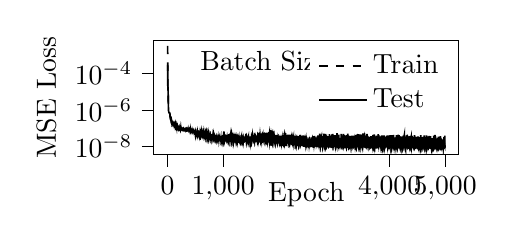
\begin{tikzpicture}

\begin{axis}[
legend cell align={left},
legend style={draw=none},
log basis y={10},
tick align=outside,
tick pos=left,
title={Batch Size 2},
title style={at={(0.4,0.85)},anchor=north},
x grid style={white!69.0196078431373!black},
xlabel={Epoch},
x label style={yshift=13pt},
xmin=-249.95, xmax=5248.95,
xtick style={color=black},
xtick = {0,1000,4000,5000},
y grid style={white!69.0196078431373!black},
ylabel={MSE Loss},
ymin=3.38262380496077e-09, ymax=0.00632854574258151,
ymode=log,
ytick style={color=black},
width=.45\textwidth,
height=.25\textwidth
]
\addplot [semithick, black, dashed]
table {%
0 0.00328254532568099
1 0.000218499955626612
2 0.000191524371870401
3 7.48565430555885e-05
4 1.80191885218974e-05
5 1.70335326928424e-05
6 1.60617069012901e-05
7 1.42414383480727e-05
8 1.17442153426879e-05
9 8.90145301876544e-06
10 6.35426067282552e-06
11 4.48610761718449e-06
12 3.16681323150547e-06
13 2.21908286821115e-06
14 1.57206481016292e-06
15 1.21919172834595e-06
16 1.0618989238651e-06
17 9.78470672838849e-07
18 9.22985532084475e-07
19 8.8099305171685e-07
20 8.4995001972521e-07
21 8.3038449714623e-07
22 8.1447130311485e-07
23 8.01895829424026e-07
24 7.90452571434397e-07
25 7.80588560063133e-07
26 7.67551035850467e-07
27 7.54603072246951e-07
28 7.4473731326119e-07
29 7.34573585697174e-07
30 7.2510382626545e-07
31 7.15328201120524e-07
32 7.06132008384763e-07
33 6.96060642347618e-07
34 6.86012559671934e-07
35 6.76093364214037e-07
36 6.65401749750494e-07
37 6.55946847171407e-07
38 6.46543756017692e-07
39 6.3489944804207e-07
40 6.18515371762385e-07
41 5.85002741245066e-07
42 5.21904763381542e-07
43 4.64107343058906e-07
44 4.31738605658261e-07
45 4.08880619641838e-07
46 3.87349231173229e-07
47 3.69826064049672e-07
48 3.53238981003257e-07
49 3.40011401617657e-07
50 3.28091449871115e-07
51 3.16790916875087e-07
52 3.058581874682e-07
53 2.96605351175927e-07
54 2.8681011950682e-07
55 2.7820315102689e-07
56 2.70656728957208e-07
57 2.63857507705412e-07
58 2.57623938459961e-07
59 2.52528075400882e-07
60 2.47351241863703e-07
61 2.42858798984225e-07
62 2.38187733390793e-07
63 2.34476871070921e-07
64 2.31448094974551e-07
65 2.28447264819964e-07
66 2.25276748428538e-07
67 2.22910076783212e-07
68 2.19949171984757e-07
69 2.18757366997169e-07
70 2.16757680979729e-07
71 2.1456885103599e-07
72 2.12431132567414e-07
73 2.12453675991098e-07
74 2.09875333198273e-07
75 2.08367902884143e-07
76 2.06870915439472e-07
77 2.05759142446249e-07
78 2.03537200378245e-07
79 2.02386158929979e-07
80 2.01577248807538e-07
81 1.99945309896199e-07
82 1.98954125483652e-07
83 1.97998061242988e-07
84 1.95277801370519e-07
85 1.94122259384422e-07
86 1.9321474032008e-07
87 1.92061395219989e-07
88 1.90649255421116e-07
89 1.88983075970039e-07
90 1.87258018107261e-07
91 1.86211353437882e-07
92 1.84968773373595e-07
93 1.8346280023851e-07
94 1.81952997721835e-07
95 1.80662087380323e-07
96 1.79365444776147e-07
97 1.77472094651909e-07
98 1.76493799261546e-07
99 1.74580053132978e-07
100 1.73360636676279e-07
101 1.72267877915688e-07
102 1.70442489901279e-07
103 1.69188082461469e-07
104 1.67839397578917e-07
105 1.66230285953528e-07
106 1.64829462242722e-07
107 1.63325331338671e-07
108 1.62738196491152e-07
109 1.60219138044426e-07
110 1.60535278213469e-07
111 1.58536466712489e-07
112 1.56850298218325e-07
113 1.55524901216397e-07
114 1.54631709402775e-07
115 1.53302759073659e-07
116 1.51466843822945e-07
117 1.49550631134643e-07
118 1.48410193441917e-07
119 1.47384696155495e-07
120 1.46283629718358e-07
121 1.44345578623639e-07
122 1.43203171090622e-07
123 1.41263757020393e-07
124 1.40215976953906e-07
125 1.38600845025039e-07
126 1.37061671532823e-07
127 1.36200254846841e-07
128 1.34788054034773e-07
129 1.32993649122337e-07
130 1.31643087291855e-07
131 1.30615223781883e-07
132 1.28918619770713e-07
133 1.27769738631822e-07
134 1.26176427465929e-07
135 1.25179997131242e-07
136 1.23230363925919e-07
137 1.22045724761821e-07
138 1.21201524557857e-07
139 1.19549983392364e-07
140 1.18310560280777e-07
141 1.16812820882495e-07
142 1.15443738707643e-07
143 1.14161057509832e-07
144 1.1312136743713e-07
145 1.11719248588327e-07
146 1.10043574582441e-07
147 1.09814437586175e-07
148 1.08579877910908e-07
149 1.07548462370266e-07
150 1.0619949556756e-07
151 1.0495877468919e-07
152 1.04168265051441e-07
153 1.02623975512528e-07
154 1.01427549126121e-07
155 1.01362208877243e-07
156 9.95105090075832e-08
157 9.90712999682231e-08
158 9.81297963442707e-08
159 9.76671625630976e-08
160 9.38856064496285e-08
161 9.09411816544248e-08
162 8.88011398124666e-08
163 8.8803014968053e-08
164 8.77907267728961e-08
165 8.71906158357305e-08
166 8.74571203014485e-08
167 8.68890042542425e-08
168 8.61177263807855e-08
169 8.60476076310901e-08
170 8.55405427711009e-08
171 8.58966112591286e-08
172 8.51639051044906e-08
173 8.51758944812042e-08
174 8.47307304080447e-08
175 8.48132693269665e-08
176 8.51079388366482e-08
177 8.49318124505061e-08
178 8.47849283748259e-08
179 8.48751120090529e-08
180 8.42010138485394e-08
181 8.44082437067017e-08
182 8.40907957427861e-08
183 8.38560661877707e-08
184 8.42076578552176e-08
185 8.38791066610778e-08
186 8.37576944041629e-08
187 8.40239886347183e-08
188 8.38833574516862e-08
189 8.33899735629418e-08
190 8.34640443237999e-08
191 8.35304616458865e-08
192 8.31852537088729e-08
193 8.30714862566362e-08
194 8.33851301329513e-08
195 8.27072170499488e-08
196 8.32493552452851e-08
197 8.22546665798507e-08
198 8.27084489483099e-08
199 8.21670082453707e-08
200 8.25011616596427e-08
201 8.18873943000398e-08
202 8.22608535500091e-08
203 8.1495268684395e-08
204 8.20163649861705e-08
205 8.16005401669262e-08
206 8.11489030099199e-08
207 8.16204926260555e-08
208 8.09058569459786e-08
209 8.10499177033019e-08
210 8.07727945287828e-08
211 8.08666219838106e-08
212 8.08093064915694e-08
213 8.02509398206697e-08
214 8.09831349148915e-08
215 8.00564518014246e-08
216 8.00968553160697e-08
217 8.01893686681598e-08
218 8.01536400982794e-08
219 7.95515807424652e-08
220 7.96363922979104e-08
221 8.03492120219351e-08
222 7.98713108027815e-08
223 7.96498008956981e-08
224 7.95084208592423e-08
225 7.95095037848803e-08
226 7.94453084611568e-08
227 7.89366283454607e-08
228 7.92334955032059e-08
229 7.92735157912894e-08
230 7.89827368313789e-08
231 7.85786661230414e-08
232 7.87854531203447e-08
233 7.85752367177262e-08
234 7.85788053452308e-08
235 7.82479060256192e-08
236 7.87282694114655e-08
237 7.80035227161413e-08
238 7.84374309548141e-08
239 7.78576224716998e-08
240 7.77167863775796e-08
241 7.81467363761834e-08
242 7.75516917973507e-08
243 7.74188098600082e-08
244 7.74798297724644e-08
245 7.7469969126609e-08
246 7.71800704708614e-08
247 7.71970539117373e-08
248 7.69478892151954e-08
249 7.73572983933102e-08
250 7.71568599475803e-08
251 7.69779501024193e-08
252 7.71894792475081e-08
253 7.67477751884016e-08
254 7.6877333195835e-08
255 7.65848046396789e-08
256 7.65385336909397e-08
257 7.63672228696333e-08
258 7.6301277346813e-08
259 7.62444665756146e-08
260 7.62738956281428e-08
261 7.59071467697492e-08
262 7.59964418058923e-08
263 7.59101158571696e-08
264 7.60531896979444e-08
265 7.57084843583389e-08
266 7.57804675006746e-08
267 7.57439965304307e-08
268 7.55281243759454e-08
269 7.54863963056129e-08
270 7.55834353999285e-08
271 7.5430192249204e-08
272 7.54428438793919e-08
273 7.52991162173977e-08
274 7.51532936485999e-08
275 7.51941930451361e-08
276 7.51544057150388e-08
277 7.48605089656573e-08
278 7.49440059444328e-08
279 7.48363137593744e-08
280 7.45955682426303e-08
281 7.46543589628113e-08
282 7.45810491539212e-08
283 7.45009416183162e-08
284 7.45298077395873e-08
285 7.43874965440927e-08
286 7.42333786614147e-08
287 7.43559364357882e-08
288 7.44611771404946e-08
289 7.43719104612239e-08
290 7.4087228369879e-08
291 7.42675714614505e-08
292 7.40377803589709e-08
293 7.39002887022444e-08
294 7.37450820641472e-08
295 7.37146042358861e-08
296 7.34764170412516e-08
297 7.34748401464147e-08
298 7.33259203234971e-08
299 7.32177149885826e-08
300 7.30713860042087e-08
301 7.31287919658596e-08
302 7.3047478842847e-08
303 7.30429494556484e-08
304 7.26866788871572e-08
305 7.28189107246369e-08
306 7.2611721922522e-08
307 7.25180870284614e-08
308 7.25546002222632e-08
309 7.23407575197177e-08
310 7.22547411237118e-08
311 7.23688810853051e-08
312 7.23001925837519e-08
313 7.23487935944123e-08
314 7.21203149054439e-08
315 7.23077199693556e-08
316 7.21352630661531e-08
317 7.20632900854667e-08
318 7.19566260092286e-08
319 7.1823656741965e-08
320 7.17751821249779e-08
321 7.18084207751435e-08
322 7.15284738002087e-08
323 7.15922071675701e-08
324 7.14385197908563e-08
325 7.11717999838379e-08
326 7.14794709065769e-08
327 7.11045747163741e-08
328 7.1172664772412e-08
329 7.10999585191718e-08
330 7.10373534636988e-08
331 7.10004941901765e-08
332 7.09694212622791e-08
333 7.10542106029388e-08
334 7.11422026586916e-08
335 7.06343104364127e-08
336 7.06290690287714e-08
337 7.058199697485e-08
338 7.05904521041134e-08
339 7.06610755990544e-08
340 7.02293932595133e-08
341 7.0213167338129e-08
342 7.01696666369767e-08
343 7.01245406067308e-08
344 7.02258261991995e-08
345 7.00943012788002e-08
346 6.99631210515639e-08
347 6.99243554992401e-08
348 6.99733587956608e-08
349 6.97487408191089e-08
350 6.96652839086154e-08
351 6.94952265442028e-08
352 6.9586298279356e-08
353 6.94802141264495e-08
354 6.94029599760393e-08
355 6.94811662502737e-08
356 6.9447535515188e-08
357 6.94013545918804e-08
358 6.94406791021951e-08
359 6.90969612737735e-08
360 6.91050193839526e-08
361 6.8881994686576e-08
362 6.87944344484048e-08
363 6.88425664659986e-08
364 6.87802862303633e-08
365 6.87643034696928e-08
366 6.85632615471388e-08
367 6.85682310238578e-08
368 6.83307170623593e-08
369 6.82866018121286e-08
370 6.85272045393148e-08
371 6.79966236415419e-08
372 6.84238423972472e-08
373 6.79873843945078e-08
374 6.81644149632676e-08
375 6.80043897696159e-08
376 6.79346173235729e-08
377 6.78095727341121e-08
378 6.76759811131245e-08
379 6.78007946736114e-08
380 6.7796770238715e-08
381 6.75536845422542e-08
382 6.73928114495181e-08
383 6.72945608075626e-08
384 6.73337297967258e-08
385 6.72205919783897e-08
386 6.72738835988396e-08
387 6.69181899951576e-08
388 6.71726448415733e-08
389 6.6735886535163e-08
390 6.67219459820068e-08
391 6.67162453900083e-08
392 6.65349611206345e-08
393 6.63832358627214e-08
394 6.63773440239268e-08
395 6.6198406551754e-08
396 6.61917400128775e-08
397 6.60644241761155e-08
398 6.62409058879154e-08
399 6.59781503837831e-08
400 6.58956399993693e-08
401 6.60107959022938e-08
402 6.5846786045487e-08
403 6.55407205336633e-08
404 6.55228505987981e-08
405 6.55955494313076e-08
406 6.52562304821469e-08
407 6.52904168840784e-08
408 6.56664842482169e-08
409 6.48951202171233e-08
410 6.52150227713477e-08
411 6.48234405338233e-08
412 6.50295594792905e-08
413 6.473958666664e-08
414 6.46367741741205e-08
415 6.44284369182291e-08
416 6.4706066168263e-08
417 6.41347029111117e-08
418 6.4321762164754e-08
419 6.38945435269545e-08
420 6.41486727785967e-08
421 6.38424642197544e-08
422 6.41088489685693e-08
423 6.37925187760846e-08
424 6.37641166327807e-08
425 6.34406229562678e-08
426 6.35571083453801e-08
427 6.32675255589632e-08
428 6.33023986322812e-08
429 6.29458381071757e-08
430 6.31480538190177e-08
431 6.27496439844499e-08
432 6.25742152867703e-08
433 6.25643662857112e-08
434 6.24544778045077e-08
435 6.2011825340047e-08
436 6.2753866577947e-08
437 6.18486373562543e-08
438 6.19743378120763e-08
439 6.20571040625961e-08
440 6.18520889781316e-08
441 6.16609228023535e-08
442 6.13968909650708e-08
443 6.14124531921334e-08
444 6.11450753005283e-08
445 6.09623349119293e-08
446 6.05825954643757e-08
447 6.04997935236273e-08
448 6.05668844602114e-08
449 6.05799478256008e-08
450 6.01981422974074e-08
451 5.9961909875561e-08
452 5.97201968506322e-08
453 5.96139426777276e-08
454 5.95120054305287e-08
455 5.92951785870488e-08
456 5.95512403165355e-08
457 5.93397249657457e-08
458 5.92162069610325e-08
459 5.89310149428091e-08
460 5.87983697155625e-08
461 5.86480213723428e-08
462 5.86585211733715e-08
463 5.81024033210475e-08
464 5.79005150566081e-08
465 5.7884217427695e-08
466 5.75974278191893e-08
467 5.72717783334786e-08
468 5.71280839249955e-08
469 5.70866307733064e-08
470 5.68234420759151e-08
471 5.65403589207758e-08
472 5.64500327302486e-08
473 5.62552928184967e-08
474 5.59582069550313e-08
475 5.59200681947702e-08
476 5.5690757583271e-08
477 5.51963993931093e-08
478 5.49973188885833e-08
479 5.45198159787041e-08
480 5.44046598370818e-08
481 5.41920685905861e-08
482 5.38668678436993e-08
483 5.361629318823e-08
484 5.32998607738477e-08
485 5.30580958801874e-08
486 5.32657221515853e-08
487 5.25750263348224e-08
488 5.23441807802616e-08
489 5.24424364887199e-08
490 5.18821803626723e-08
491 5.19918664291241e-08
492 5.1747341199504e-08
493 5.13785602573869e-08
494 5.11840279411868e-08
495 5.12938131975726e-08
496 5.0924607952807e-08
497 5.10876863294429e-08
498 5.07458053390364e-08
499 5.06220796397949e-08
500 5.04064744368815e-08
501 5.06455437344622e-08
502 4.9862071242579e-08
503 4.97268267137807e-08
504 4.94142680242948e-08
505 4.97652903030943e-08
506 4.94748283430546e-08
507 4.90965448383118e-08
508 4.87868712980566e-08
509 4.90490110020003e-08
510 4.92224223346271e-08
511 4.89848744311683e-08
512 4.86528948101528e-08
513 4.87841283199897e-08
514 4.84146250535611e-08
515 4.9023456144659e-08
516 4.81331435734367e-08
517 4.80398341196064e-08
518 4.88083406132711e-08
519 4.84064391683692e-08
520 4.84159776592552e-08
521 4.75737229264639e-08
522 4.8519928558588e-08
523 4.73770784747973e-08
524 4.83165005312758e-08
525 4.78193792249337e-08
526 4.78251361750726e-08
527 4.70196307974513e-08
528 4.80083285770982e-08
529 4.71223468826443e-08
530 4.71813922692244e-08
531 4.7113969577961e-08
532 4.70967598273919e-08
533 4.70621662446158e-08
534 4.66326605940148e-08
535 4.76241100443309e-08
536 4.66664954731355e-08
537 4.74405901805808e-08
538 4.69436936714196e-08
539 4.72466676191274e-08
540 4.70211507684337e-08
541 4.63547233083839e-08
542 4.61678381813435e-08
543 4.6965799879839e-08
544 4.63857039533222e-08
545 4.63133353306167e-08
546 4.62923420408989e-08
547 4.6108359860686e-08
548 4.64648258927669e-08
549 4.58507157922727e-08
550 4.595448568534e-08
551 4.60644132552757e-08
552 4.57460573870527e-08
553 4.48977841176479e-08
554 4.61474039982757e-08
555 4.54119244746032e-08
556 4.50748147138302e-08
557 4.51294110412337e-08
558 4.52713001330984e-08
559 4.45902119108332e-08
560 4.54390254731596e-08
561 4.45883604294206e-08
562 4.40688434577563e-08
563 4.46767707545925e-08
564 4.43456282678834e-08
565 4.43052667442601e-08
566 4.4511835127603e-08
567 4.44672186858952e-08
568 4.40549484904684e-08
569 4.38604737291737e-08
570 4.36744109219012e-08
571 4.33528694978591e-08
572 4.36945165810387e-08
573 4.35054831703363e-08
574 4.3339193234071e-08
575 4.33224534239773e-08
576 4.28230918373407e-08
577 4.29915050395024e-08
578 4.3157082451617e-08
579 4.29085400865947e-08
580 4.27126839501746e-08
581 4.34098694395701e-08
582 4.2637734657236e-08
583 4.27076143056926e-08
584 4.31071084622259e-08
585 4.27677483794131e-08
586 4.2361920931655e-08
587 4.25198561692097e-08
588 4.25564854413807e-08
589 4.23260934941938e-08
590 4.18924031443391e-08
591 4.22129305257257e-08
592 4.16024839526852e-08
593 4.16946787210604e-08
594 4.17917192728767e-08
595 4.16310181681201e-08
596 4.13894368075374e-08
597 4.14773096925058e-08
598 4.10987801270912e-08
599 4.12405630366708e-08
600 4.19068369599263e-08
601 4.11747850240785e-08
602 4.14282939695809e-08
603 4.06905636430865e-08
604 4.08110460305977e-08
605 4.11398571306121e-08
606 4.09925211455886e-08
607 4.06709809314121e-08
608 4.11535621287484e-08
609 4.03891638949272e-08
610 4.03422490115046e-08
611 4.04638569014848e-08
612 4.03521925785855e-08
613 4.02347802692105e-08
614 3.96676463815804e-08
615 4.05902976614581e-08
616 3.9934611743786e-08
617 3.97000445235829e-08
618 3.93751615644367e-08
619 3.99356786361937e-08
620 3.94967812543667e-08
621 3.9478045169461e-08
622 3.9357216289726e-08
623 3.91124260917808e-08
624 3.93788417034635e-08
625 3.91443982862283e-08
626 3.94537697414044e-08
627 3.92543143685753e-08
628 3.88451565003223e-08
629 3.87263305199337e-08
630 3.90169901079984e-08
631 3.90409084574106e-08
632 3.90292650599422e-08
633 3.8848819337356e-08
634 3.826467254886e-08
635 3.86679600120066e-08
636 3.84189770820664e-08
637 3.8034914403573e-08
638 3.83765584659468e-08
639 3.84147417166192e-08
640 3.81209554103368e-08
641 3.76586081726193e-08
642 3.7909612859377e-08
643 3.79556497944744e-08
644 3.75772361053683e-08
645 3.7929992070862e-08
646 3.75065041919309e-08
647 3.7582637523681e-08
648 3.71357294101093e-08
649 3.74972402298335e-08
650 3.73230137498126e-08
651 3.7014256861978e-08
652 3.67768056607209e-08
653 3.72723442765288e-08
654 3.69532771464787e-08
655 3.67656498795332e-08
656 3.70444940477888e-08
657 3.74225217392166e-08
658 3.64024413511688e-08
659 3.66532642359085e-08
660 3.6914308742364e-08
661 3.6492219348927e-08
662 3.66049217205844e-08
663 3.68115249901324e-08
664 3.63449829077767e-08
665 3.59703634603137e-08
666 3.65043941129017e-08
667 3.64438717505577e-08
668 3.61117691105584e-08
669 3.59725088353025e-08
670 3.58938531116459e-08
671 3.56944948786131e-08
672 3.54274465845794e-08
673 3.58843036923351e-08
674 3.51804919540566e-08
675 3.592879544001e-08
676 3.51167567705923e-08
677 3.54670594818751e-08
678 3.4856420939644e-08
679 3.52466294488152e-08
680 3.47822667237652e-08
681 3.53631174087043e-08
682 3.46637306734565e-08
683 3.47526936601283e-08
684 3.45369711179377e-08
685 3.44024175803481e-08
686 3.45784007663719e-08
687 3.43725343730505e-08
688 3.42645183736834e-08
689 3.43503181767235e-08
690 3.43352946233222e-08
691 3.41738478102926e-08
692 3.45125217628417e-08
693 3.38059283864212e-08
694 3.44023723802267e-08
695 3.34726516930117e-08
696 3.39030477289892e-08
697 3.36896250675012e-08
698 3.33158177039938e-08
699 3.35237944595335e-08
700 3.32292014725288e-08
701 3.3578084904895e-08
702 3.35027595368964e-08
703 3.39071785393497e-08
704 3.293375946406e-08
705 3.30269301683228e-08
706 3.3574827676075e-08
707 3.33444393947335e-08
708 3.33603552093997e-08
709 3.28944379845431e-08
710 3.27157034414327e-08
711 3.30092747191646e-08
712 3.29718086783393e-08
713 3.29110067269767e-08
714 3.27898127228665e-08
715 3.29078348913492e-08
716 3.22872896388327e-08
717 3.27488542049559e-08
718 3.24483861559588e-08
719 3.27850294034593e-08
720 3.26606627359949e-08
721 3.23589595196405e-08
722 3.24584725308608e-08
723 3.26674511605951e-08
724 3.1575581434129e-08
725 3.25877752292425e-08
726 3.20928140972732e-08
727 3.24274801469793e-08
728 3.25003616281627e-08
729 3.18399988796236e-08
730 3.2109916644596e-08
731 3.20759825324646e-08
732 3.18597185383629e-08
733 3.19681254596915e-08
734 3.22229387327844e-08
735 3.17291694599264e-08
736 3.21273451338033e-08
737 3.17449717723295e-08
738 3.15686945521754e-08
739 3.17564476380316e-08
740 3.17477588294146e-08
741 3.10420353661356e-08
742 3.20795690111342e-08
743 3.1216206289153e-08
744 3.11819914966538e-08
745 3.0873233597184e-08
746 3.14768186575609e-08
747 3.0342848171272e-08
748 3.17283036666005e-08
749 3.09738106077373e-08
750 3.10661259300682e-08
751 3.08984813262025e-08
752 3.06028083156829e-08
753 3.11116006412315e-08
754 3.11124808433094e-08
755 3.09768128804455e-08
756 3.11854558228131e-08
757 3.10072328188471e-08
758 3.1022588369789e-08
759 3.01097631762448e-08
760 3.08949155709559e-08
761 3.08619954873524e-08
762 3.05116490219026e-08
763 3.14621224050682e-08
764 3.06109915238495e-08
765 3.0499886474411e-08
766 3.02687262935253e-08
767 3.03926383860009e-08
768 2.94455249570946e-08
769 2.99938384391574e-08
770 3.05687051307957e-08
771 2.98737279285088e-08
772 3.03895292956824e-08
773 3.02582276905938e-08
774 2.97754409906981e-08
775 3.0655070072716e-08
776 2.97111483765766e-08
777 3.00233681251871e-08
778 2.98320518886119e-08
779 3.06805578830227e-08
780 3.02031067299646e-08
781 2.96468851478937e-08
782 3.0587170042895e-08
783 2.99796532466923e-08
784 3.06078738928628e-08
785 2.92830425706048e-08
786 3.0212400990437e-08
787 2.9719811062312e-08
788 2.93865345387112e-08
789 3.00758327314021e-08
790 2.99608398715012e-08
791 2.98255288354032e-08
792 3.01842756250115e-08
793 3.01570450788047e-08
794 2.9858412152417e-08
795 3.0092274968585e-08
796 3.02506790859636e-08
797 2.91831633476569e-08
798 2.95765616485921e-08
799 2.99364189229601e-08
800 3.00087392374193e-08
801 3.05344552096187e-08
802 3.01328082645269e-08
803 2.99154144154934e-08
804 2.94597860326373e-08
805 2.93265596476022e-08
806 2.9981135665047e-08
807 2.97405996949052e-08
808 2.97528969943062e-08
809 2.97964703900311e-08
810 2.93363185845386e-08
811 2.99720110352175e-08
812 2.96175842905422e-08
813 2.96315429029193e-08
814 2.96446226587532e-08
815 2.99707815297201e-08
816 2.95448832050571e-08
817 2.95232755386232e-08
818 2.87613123848285e-08
819 2.95836693727236e-08
820 2.94098747234406e-08
821 2.91337529105262e-08
822 2.93476053093156e-08
823 2.87491110401716e-08
824 2.89403561636314e-08
825 2.95640055761326e-08
826 2.85100923496651e-08
827 2.90359088045422e-08
828 2.89738495633518e-08
829 2.93372802613323e-08
830 2.93234274397203e-08
831 2.88658978312428e-08
832 2.86577576900093e-08
833 2.93334803106449e-08
834 2.79551181306403e-08
835 2.93240796755412e-08
836 2.84651544498193e-08
837 2.85353146382561e-08
838 2.86506699791467e-08
839 2.80141502583264e-08
840 2.90341042116782e-08
841 2.83219711137428e-08
842 2.88628372929201e-08
843 2.81941445002265e-08
844 2.86616231613412e-08
845 2.80926744038457e-08
846 2.87754205431923e-08
847 2.85303202081644e-08
848 2.81727098084272e-08
849 2.8123937935165e-08
850 2.84582470004846e-08
851 2.8650369424621e-08
852 2.85608268651982e-08
853 2.8131232703843e-08
854 2.82453610964128e-08
855 2.89483162182469e-08
856 2.83420080103847e-08
857 2.82199570773578e-08
858 2.80730314435318e-08
859 2.82809190177979e-08
860 2.86353769445857e-08
861 2.82259201612178e-08
862 2.78959342820406e-08
863 2.78645208896533e-08
864 2.81846941814212e-08
865 2.81121721020239e-08
866 2.80517562643023e-08
867 2.81593320271001e-08
868 2.72528267648564e-08
869 2.81696339985427e-08
870 2.79273086642995e-08
871 2.7512817953157e-08
872 2.84517497671222e-08
873 2.7799637717929e-08
874 2.74260516970881e-08
875 2.7788204698842e-08
876 2.73057909985774e-08
877 2.83043334327049e-08
878 2.64792259140334e-08
879 2.77433954551931e-08
880 2.80859690999224e-08
881 2.81571656352009e-08
882 2.76695006193872e-08
883 2.77709883268473e-08
884 2.6881104866483e-08
885 2.78426782351904e-08
886 2.77167030259817e-08
887 2.78135435696769e-08
888 2.78613534441252e-08
889 2.74576081790157e-08
890 2.72004491331246e-08
891 2.7812381422021e-08
892 2.74803205711494e-08
893 2.72247917181279e-08
894 2.76698133706565e-08
895 2.75316115931346e-08
896 2.72633557068525e-08
897 2.75284972862111e-08
898 2.75199321894126e-08
899 2.73734412948312e-08
900 2.72344164200522e-08
901 2.74171147513491e-08
902 2.8005013492205e-08
903 2.72693796256607e-08
904 2.71729967772916e-08
905 2.70847596891555e-08
906 2.76970295121637e-08
907 2.70154164276337e-08
908 2.71905937012651e-08
909 2.74396833003232e-08
910 2.67758121418882e-08
911 2.80058317719267e-08
912 2.79118399847678e-08
913 2.63474409490927e-08
914 2.71324295361142e-08
915 2.7954368273797e-08
916 2.7007748962693e-08
917 2.64737631885392e-08
918 2.76175025140657e-08
919 2.68041697211174e-08
920 2.71468540083974e-08
921 2.700771886055e-08
922 2.75985255401845e-08
923 2.69180859497897e-08
924 2.69624495977117e-08
925 2.68577280076454e-08
926 2.704912061402e-08
927 2.6356536705241e-08
928 2.66672037859128e-08
929 2.69591033794092e-08
930 2.68079865403115e-08
931 2.63138631513837e-08
932 2.72206234661621e-08
933 2.71317316304365e-08
934 2.7307047371139e-08
935 2.65802619039413e-08
936 2.73144441089168e-08
937 2.63830216658545e-08
938 2.66981474648098e-08
939 2.6431935854887e-08
940 2.60439990913408e-08
941 2.67252916980043e-08
942 2.66271156456055e-08
943 2.6739769780626e-08
944 2.62611098725829e-08
945 2.62674960841425e-08
946 2.70139238268685e-08
947 2.63460659326586e-08
948 2.62264182295802e-08
949 2.70272808373662e-08
950 2.5747153010236e-08
951 2.66053678841804e-08
952 2.64551851290595e-08
953 2.67567574317451e-08
954 2.58916772901685e-08
955 2.64584350602726e-08
956 2.61099018731836e-08
957 2.66250582974248e-08
958 2.59226130361612e-08
959 2.64767316645598e-08
960 2.6452490843043e-08
961 2.58215259816841e-08
962 2.59265999303371e-08
963 2.62359932220457e-08
964 2.65424289648264e-08
965 2.67450139063707e-08
966 2.63561833882819e-08
967 2.57741525678257e-08
968 2.62758306087407e-08
969 2.65221036650498e-08
970 2.64172919469674e-08
971 2.56274016323943e-08
972 2.57729816374175e-08
973 2.59577244466347e-08
974 2.6222427415179e-08
975 2.62312397004694e-08
976 2.5963541613383e-08
977 2.56496797129135e-08
978 2.56104738609597e-08
979 2.62138495017994e-08
980 2.58349842333083e-08
981 2.6208806482575e-08
982 2.54673980373543e-08
983 2.56343059095165e-08
984 2.62062766909765e-08
985 2.52106715502853e-08
986 2.51687390236954e-08
987 2.61188593480566e-08
988 2.52318605282187e-08
989 2.56387556114013e-08
990 2.54048550445418e-08
991 2.53413983453687e-08
992 2.55538864205596e-08
993 2.5451171698665e-08
994 2.61896682761109e-08
995 2.54498613648235e-08
996 2.55230583791621e-08
997 2.48618900541842e-08
998 2.58373611447538e-08
999 2.51232853774597e-08
1000 2.56220291215414e-08
1001 2.56736006327141e-08
1002 2.51882083300847e-08
1003 2.53713824167612e-08
1004 2.58137432954941e-08
1005 2.48481835016801e-08
1006 2.56784723412506e-08
1007 2.40642600508045e-08
1008 2.56810740124624e-08
1009 2.54665775721308e-08
1010 2.43275138776256e-08
1011 2.61642387404115e-08
1012 2.48960325622827e-08
1013 2.58067697424536e-08
1014 2.57083646426348e-08
1015 2.49647724676894e-08
1016 2.54706723878118e-08
1017 2.44838401316505e-08
1018 2.5243788890239e-08
1019 2.52713618028588e-08
1020 2.47552457360301e-08
1021 2.50724322887752e-08
1022 2.57186888398264e-08
1023 2.51238573180101e-08
1024 2.44940838938223e-08
1025 2.52199264209607e-08
1026 2.57123974063966e-08
1027 2.50377650737044e-08
1028 2.51321844116914e-08
1029 2.45223809804962e-08
1030 2.48290043978749e-08
1031 2.53573499313098e-08
1032 2.4809457069952e-08
1033 2.55327429933838e-08
1034 2.49863649272875e-08
1035 2.54338735914406e-08
1036 2.46765876222854e-08
1037 2.48556650924159e-08
1038 2.46800521991331e-08
1039 2.51365618709754e-08
1040 2.41794125941386e-08
1041 2.44692986407224e-08
1042 2.47765058001559e-08
1043 2.48758484036604e-08
1044 2.41757049636859e-08
1045 2.4206212695721e-08
1046 2.55829298876631e-08
1047 2.41762240022481e-08
1048 2.47289624125679e-08
1049 2.5234407058039e-08
1050 2.43533080388492e-08
1051 2.47249283025774e-08
1052 2.44511952491311e-08
1053 2.45763102038055e-08
1054 2.45536552540004e-08
1055 2.48305525572534e-08
1056 2.40834935295586e-08
1057 2.53211549907095e-08
1058 2.41439715079061e-08
1059 2.57494680457604e-08
1060 2.35057552473161e-08
1061 2.49778252063293e-08
1062 2.40053659600614e-08
1063 2.4876820900549e-08
1064 2.45837317633946e-08
1065 2.43284918397257e-08
1066 2.40939658241457e-08
1067 2.51706974384036e-08
1068 2.35143826128326e-08
1069 2.41161983740024e-08
1070 2.4755212258476e-08
1071 2.4246693290042e-08
1072 2.56388721965872e-08
1073 2.41264563889954e-08
1074 2.44039392134909e-08
1075 2.51708382467408e-08
1076 2.45340783286419e-08
1077 2.45209754993758e-08
1078 2.48115112856939e-08
1079 2.39203909974672e-08
1080 2.31613966679145e-08
1081 2.50456757703854e-08
1082 2.43899172222006e-08
1083 2.40393221376256e-08
1084 2.41358175256112e-08
1085 2.3699030541946e-08
1086 2.43306819150413e-08
1087 2.42609329062504e-08
1088 2.39897964542934e-08
1089 2.44988888764563e-08
1090 2.45195678220678e-08
1091 2.40963733417754e-08
1092 2.39458951021843e-08
1093 2.37625303336486e-08
1094 2.44664175362286e-08
1095 2.36047424231611e-08
1096 2.45438499066886e-08
1097 2.4314623127103e-08
1098 2.39301791060131e-08
1099 2.417096244689e-08
1100 2.39409680004576e-08
1101 2.42720179199352e-08
1102 2.42393090368331e-08
1103 2.40999026286381e-08
1104 2.42074585857788e-08
1105 2.3707304635745e-08
1106 2.34363956257144e-08
1107 2.36964240676596e-08
1108 2.36679420671515e-08
1109 2.38906914948878e-08
1110 2.46842266887759e-08
1111 2.31558109071162e-08
1112 2.37190626790618e-08
1113 2.35072627912114e-08
1114 2.4207290549999e-08
1115 2.3632586413358e-08
1116 2.4249042063107e-08
1117 2.3715847715905e-08
1118 2.38752562103928e-08
1119 2.48957234907365e-08
1120 2.32552377015804e-08
1121 2.49651159680564e-08
1122 2.28996111810154e-08
1123 2.34150135410283e-08
1124 2.41551524927108e-08
1125 2.34782538071077e-08
1126 2.43804897772648e-08
1127 2.31835085818255e-08
1128 2.3253374320964e-08
1129 2.32561741067006e-08
1130 2.50726553251424e-08
1131 2.29548132411883e-08
1132 2.3328192227362e-08
1133 2.41420011705684e-08
1134 2.33821172641313e-08
1135 2.3303387180762e-08
1136 2.43730284085197e-08
1137 2.41564589041898e-08
1138 2.37143871552048e-08
1139 2.36588560203199e-08
1140 2.30154500006075e-08
1141 2.4859979055103e-08
1142 2.29174441709334e-08
1143 2.38801621325058e-08
1144 2.44339880565159e-08
1145 2.38689083146837e-08
1146 2.28463232741505e-08
1147 2.46741202382939e-08
1148 2.41791558530102e-08
1149 2.29663980678141e-08
1150 2.39159831927349e-08
1151 2.43229607134743e-08
1152 2.28362273965721e-08
1153 2.31572237742172e-08
1154 2.33627679651072e-08
1155 2.27080735474283e-08
1156 2.4358588360418e-08
1157 2.26149591309732e-08
1158 2.3826834529006e-08
1159 2.35227404605243e-08
1160 2.2895686424329e-08
1161 2.40749804307216e-08
1162 2.26256669050295e-08
1163 2.33396992000423e-08
1164 2.30482095263662e-08
1165 2.44169308798725e-08
1166 2.39379462509404e-08
1167 2.23706146176839e-08
1168 2.37480671272938e-08
1169 2.3676940001105e-08
1170 2.34087737608912e-08
1171 2.3882939918618e-08
1172 2.30129306417748e-08
1173 2.31911079903724e-08
1174 2.24837282247203e-08
1175 2.29678447716819e-08
1176 2.3352444612823e-08
1177 2.3275783645138e-08
1178 2.36324950197431e-08
1179 2.44034234366253e-08
1180 2.2084830024971e-08
1181 2.42513723696935e-08
1182 2.16930364395074e-08
1183 2.25338594886382e-08
1184 2.28829293547617e-08
1185 2.39440693926563e-08
1186 2.2315187542532e-08
1187 2.36924562428409e-08
1188 2.20071196566085e-08
1189 2.32872066795453e-08
1190 2.39950020853863e-08
1191 2.17920868925692e-08
1192 2.27612380520603e-08
1193 2.3995818000222e-08
1194 2.22051254888389e-08
1195 2.46911551403106e-08
1196 2.19987103602382e-08
1197 2.24494658944141e-08
1198 2.54094465522159e-08
1199 2.06954137310644e-08
1200 2.39629729154589e-08
1201 2.31854273466947e-08
1202 2.26924926745031e-08
1203 2.40487618563545e-08
1204 2.13842529988295e-08
1205 2.39762664323573e-08
1206 2.25271042649244e-08
1207 2.24390193712121e-08
1208 2.4125746498016e-08
1209 2.21658715069406e-08
1210 2.28044628429736e-08
1211 2.48385112019966e-08
1212 2.33656474967758e-08
1213 2.12154672926679e-08
1214 2.41168022632188e-08
1215 2.127196985513e-08
1216 2.41087441434362e-08
1217 2.23791959621522e-08
1218 2.24479696701585e-08
1219 2.30527769330691e-08
1220 2.41279960776497e-08
1221 2.22326906687553e-08
1222 2.24541030668934e-08
1223 2.22194493112449e-08
1224 2.33363321254232e-08
1225 2.30219892352057e-08
1226 2.20189755480715e-08
1227 2.30715657988378e-08
1228 2.25623969505317e-08
1229 2.24376861742148e-08
1230 2.21420095534164e-08
1231 2.41717404863839e-08
1232 2.20276527142516e-08
1233 2.24890027827329e-08
1234 2.36996848195781e-08
1235 2.19429958308592e-08
1236 2.31160184864798e-08
1237 2.46116306463207e-08
1238 2.23464107134141e-08
1239 2.19672915339753e-08
1240 2.24700124982213e-08
1241 2.36331999026174e-08
1242 2.33265122337456e-08
1243 2.13752408421142e-08
1244 2.33078071993353e-08
1245 2.32677361167721e-08
1246 2.21433261852755e-08
1247 2.40962325241401e-08
1248 2.26305257871595e-08
1249 2.21173026355714e-08
1250 2.39238219879034e-08
1251 2.13247202381361e-08
1252 2.37189196605203e-08
1253 2.32250552512636e-08
1254 2.16647174275386e-08
1255 2.2491087962706e-08
1256 2.34335919854778e-08
1257 2.19791799298541e-08
1258 2.35654252513373e-08
1259 2.14169790457852e-08
1260 2.35637368361241e-08
1261 2.1728992364356e-08
1262 2.31331254670342e-08
1263 2.26170422073235e-08
1264 2.35172557362939e-08
1265 2.14990163194817e-08
1266 2.36890559190961e-08
1267 2.17138146291762e-08
1268 2.44956976728217e-08
1269 2.12130341750993e-08
1270 2.29326911906358e-08
1271 2.294375372347e-08
1272 2.21282134780787e-08
1273 2.37402650568597e-08
1274 2.14494472419724e-08
1275 2.28301129672759e-08
1276 2.20507827259908e-08
1277 2.38259531475382e-08
1278 2.14158515750573e-08
1279 2.44407928549073e-08
1280 2.20708781046852e-08
1281 2.28768149491132e-08
1282 2.2626050056429e-08
1283 2.3005323938563e-08
1284 2.1827455709722e-08
1285 2.22817814335419e-08
1286 2.34458954926908e-08
1287 2.12545711266165e-08
1288 2.32935544570156e-08
1289 2.18443757705744e-08
1290 2.20137667314435e-08
1291 2.26713250879862e-08
1292 2.2973785081537e-08
1293 2.30200027910299e-08
1294 2.19761202549518e-08
1295 2.24197731544806e-08
1296 2.17526179136229e-08
1297 2.37097571550993e-08
1298 2.20199593771175e-08
1299 2.23016867821613e-08
1300 2.22305995936645e-08
1301 2.33038597228785e-08
1302 2.38850469355678e-08
1303 2.09000387388913e-08
1304 2.26636061739782e-08
1305 2.2103954332886e-08
1306 2.28347936062634e-08
1307 2.19457175233972e-08
1308 2.22836593346543e-08
1309 2.23504406504094e-08
1310 2.22128115497378e-08
1311 2.28280098716338e-08
1312 2.31253715030633e-08
1313 2.11736454615585e-08
1314 2.20795589808143e-08
1315 2.24833086843179e-08
1316 2.32801941796312e-08
1317 2.14961897331001e-08
1318 2.20238446245746e-08
1319 2.2324847892885e-08
1320 2.19785063278466e-08
1321 2.35137257901807e-08
1322 2.3144701277622e-08
1323 2.10336239354625e-08
1324 2.23880651935016e-08
1325 2.16761783147779e-08
1326 2.26090178953031e-08
1327 2.28862650982764e-08
1328 2.21212273828209e-08
1329 2.16299618250315e-08
1330 2.29643947586289e-08
1331 2.26928735589382e-08
1332 2.20482249578269e-08
1333 2.18015371278302e-08
1334 2.20884739085547e-08
1335 2.3364725292907e-08
1336 2.15798587311355e-08
1337 2.36228769332492e-08
1338 2.27154247446348e-08
1339 2.18096778484278e-08
1340 2.21108368879674e-08
1341 2.21310831148291e-08
1342 2.20017822580854e-08
1343 2.19745016792339e-08
1344 2.21375170811888e-08
1345 2.21948070953104e-08
1346 2.21312608935653e-08
1347 2.22437780286744e-08
1348 2.19581330651586e-08
1349 2.20827062501483e-08
1350 2.18945214304211e-08
1351 2.29315245998118e-08
1352 2.21396365736037e-08
1353 2.25976545702999e-08
1354 2.1405512023176e-08
1355 2.20842132633847e-08
1356 2.24522939798466e-08
1357 2.26773350752718e-08
1358 2.14882492814428e-08
1359 2.2369567684366e-08
1360 2.17191727960309e-08
1361 2.19919470932917e-08
1362 2.2311646740325e-08
1363 2.25913608749573e-08
1364 2.21926017565655e-08
1365 2.15259211113761e-08
1366 2.16004253598134e-08
1367 2.32224484773558e-08
1368 2.15576274351648e-08
1369 2.25957661512677e-08
1370 2.1665183021935e-08
1371 2.22470384803053e-08
1372 2.227040601116e-08
1373 2.18528204138368e-08
1374 2.21331229738886e-08
1375 2.32569008955519e-08
1376 2.05272220124009e-08
1377 2.2737146274765e-08
1378 2.17802189304006e-08
1379 2.20164517975019e-08
1380 2.26876345494897e-08
1381 2.14601053055152e-08
1382 2.13699287613944e-08
1383 2.16462507426907e-08
1384 2.21368567230318e-08
1385 2.28223008749695e-08
1386 2.15268508930722e-08
1387 2.18877246265792e-08
1388 2.23609083401244e-08
1389 2.2065903218349e-08
1390 2.26112779765364e-08
1391 2.21005944214259e-08
1392 2.21072447048609e-08
1393 2.2372629410905e-08
1394 2.21432812628208e-08
1395 2.25536891302891e-08
1396 2.20534070987655e-08
1397 2.2955050506257e-08
1398 2.26208074964873e-08
1399 2.18272057315172e-08
1400 2.16593289958933e-08
1401 2.27141324652957e-08
1402 2.20719237945533e-08
1403 2.17082151288683e-08
1404 2.20936218085499e-08
1405 2.1863136471012e-08
1406 2.21187039824433e-08
1407 2.10590157191937e-08
1408 2.29186094085621e-08
1409 2.21961395413528e-08
1410 2.20644468408859e-08
1411 2.22680759182081e-08
1412 2.22331608497606e-08
1413 2.04469981444633e-08
1414 2.1789090508928e-08
1415 2.25222602415753e-08
1416 2.11176890110853e-08
1417 2.25176194232346e-08
1418 2.15985122689055e-08
1419 2.2313166706811e-08
1420 2.30230737420234e-08
1421 2.18747423230137e-08
1422 2.16363518343865e-08
1423 2.3068403635973e-08
1424 2.1838906702043e-08
1425 2.22338019213453e-08
1426 2.13278609508261e-08
1427 2.29623013299207e-08
1428 2.1098088403726e-08
1429 2.24614715425009e-08
1430 2.12589236732175e-08
1431 2.26730734765868e-08
1432 2.10315514134751e-08
1433 2.27212884548189e-08
1434 2.09692620500856e-08
1435 2.26583690920989e-08
1436 2.04742908186395e-08
1437 2.28886742472678e-08
1438 2.12501669026866e-08
1439 2.31694822255268e-08
1440 2.19335935971454e-08
1441 2.07122653302361e-08
1442 2.32995183077067e-08
1443 2.13800517415708e-08
1444 2.19378508171109e-08
1445 2.17659652216318e-08
1446 2.25236484944213e-08
1447 2.14525019416878e-08
1448 2.11303392904094e-08
1449 2.22758848886784e-08
1450 2.15706849791553e-08
1451 2.30910437937215e-08
1452 2.07915529506497e-08
1453 2.22041605880685e-08
1454 2.20864075464178e-08
1455 2.2056206184895e-08
1456 2.15564313329752e-08
1457 2.11379826827729e-08
1458 2.20233888020283e-08
1459 2.28370447180604e-08
1460 2.11876432199554e-08
1461 2.22300986445489e-08
1462 2.16021678987599e-08
1463 2.17324369022887e-08
1464 2.21292224406588e-08
1465 2.23671277076454e-08
1466 2.14703611854938e-08
1467 2.05927899782354e-08
1468 2.33626976558488e-08
1469 2.05264296654906e-08
1470 2.18535323567859e-08
1471 2.11968200043433e-08
1472 2.18168553881015e-08
1473 2.26454652578756e-08
1474 2.11857142232708e-08
1475 2.13278918422266e-08
1476 2.236010990736e-08
1477 2.17072662658802e-08
1478 2.2110143227283e-08
1479 2.22466864685522e-08
1480 2.06100590163238e-08
1481 2.22854114886872e-08
1482 2.19793991453332e-08
1483 2.16467689184152e-08
1484 2.05775316386991e-08
1485 2.19673081403582e-08
1486 2.19401898399474e-08
1487 2.20589850682407e-08
1488 2.05005431839767e-08
1489 2.15492483782165e-08
1490 2.19645833702264e-08
1491 2.21786140069957e-08
1492 2.16240650679489e-08
1493 2.21673701460423e-08
1494 2.08698478573743e-08
1495 2.19098450867095e-08
1496 2.15752541418146e-08
1497 2.19070329576798e-08
1498 2.16886264846616e-08
1499 2.23972178054754e-08
1500 2.14879013741287e-08
1501 2.11427105282214e-08
1502 2.18200978853167e-08
1503 2.19430892073325e-08
1504 2.18239163790046e-08
1505 2.12949392383033e-08
1506 2.09734695226782e-08
1507 2.21864767561142e-08
1508 2.10699609919374e-08
1509 2.23657064514771e-08
1510 2.08754557393664e-08
1511 2.13593325406602e-08
1512 2.2237284218074e-08
1513 2.22302955611431e-08
1514 2.14894843014179e-08
1515 2.17345119775114e-08
1516 2.2619548078251e-08
1517 2.03632252265273e-08
1518 2.222387638251e-08
1519 2.0638844568599e-08
1520 2.15556459234878e-08
1521 2.13329812444041e-08
1522 2.17516634387072e-08
1523 2.14504079945055e-08
1524 2.1713463724482e-08
1525 2.17702472103398e-08
1526 2.1144652500471e-08
1527 2.25338103538308e-08
1528 2.08841337764332e-08
1529 2.15978603308464e-08
1530 2.19219352285416e-08
1531 2.20143767911685e-08
1532 2.03035153048536e-08
1533 2.2025311063878e-08
1534 2.17098071511601e-08
1535 2.13676841006594e-08
1536 2.13570003706476e-08
1537 2.1934463194706e-08
1538 2.08679860155825e-08
1539 2.17718971614045e-08
1540 2.17795787115782e-08
1541 2.0858285151415e-08
1542 2.24124813391069e-08
1543 2.04172527167312e-08
1544 2.15674865017834e-08
1545 2.08105447176421e-08
1546 2.24757190159242e-08
1547 2.05159294637824e-08
1548 2.13008872599341e-08
1549 2.16085264567178e-08
1550 2.19470851841597e-08
1551 2.03223949322706e-08
1552 2.185089607043e-08
1553 2.13339257819634e-08
1554 2.15402248593122e-08
1555 2.14160982039413e-08
1556 2.01167598529173e-08
1557 2.26113181088783e-08
1558 2.07763320684284e-08
1559 2.09940509560136e-08
1560 2.20850009061691e-08
1561 2.12568992129514e-08
1562 2.02256049313676e-08
1563 2.1572822483884e-08
1564 2.16699280349841e-08
1565 2.0615541992508e-08
1566 2.06423681782808e-08
1567 2.166503550044e-08
1568 2.10671617285607e-08
1569 2.14949159996203e-08
1570 2.1486425486994e-08
1571 2.15268085630993e-08
1572 2.13709459728206e-08
1573 2.16338703817875e-08
1574 2.10054343868227e-08
1575 2.13374942872324e-08
1576 2.12356059929308e-08
1577 2.12236877222272e-08
1578 2.10683743684381e-08
1579 2.08947822623595e-08
1580 2.15873571304814e-08
1581 2.12413833508007e-08
1582 2.09700386497036e-08
1583 2.12016539590798e-08
1584 2.15563715610934e-08
1585 2.1320752146059e-08
1586 2.03603190020996e-08
1587 2.12582940875561e-08
1588 2.12172731384186e-08
1589 2.02699212337176e-08
1590 2.20828432360709e-08
1591 2.1214635882838e-08
1592 2.13622964505e-08
1593 1.97430580893276e-08
1594 2.12411482926056e-08
1595 2.14440202571664e-08
1596 2.10006369820159e-08
1597 2.17859179567625e-08
1598 2.0235362363008e-08
1599 2.04990278194206e-08
1600 2.15114643131731e-08
1601 2.12136672634311e-08
1602 2.10565060696499e-08
1603 2.06974479114996e-08
1604 2.09672476611522e-08
1605 2.13972567624232e-08
1606 2.10050519521832e-08
1607 2.11634919160542e-08
1608 2.0377558411111e-08
1609 2.08424264296903e-08
1610 2.10613512971747e-08
1611 2.03827716233063e-08
1612 2.10774802880676e-08
1613 2.16909275381205e-08
1614 2.08061425025496e-08
1615 2.16821348084095e-08
1616 2.00827403420978e-08
1617 2.14326192789493e-08
1618 2.0886740560111e-08
1619 2.06261215081605e-08
1620 2.10243560460621e-08
1621 2.07960275404595e-08
1622 2.25939935346031e-08
1623 2.00754938110004e-08
1624 2.13006339671584e-08
1625 2.07714345401011e-08
1626 2.13699255519062e-08
1627 2.03209101736768e-08
1628 2.15345861875882e-08
1629 2.11747947819751e-08
1630 2.13044938350837e-08
1631 2.09285056221864e-08
1632 2.01563148522488e-08
1633 2.09758108913327e-08
1634 2.1033877327159e-08
1635 2.05582696706785e-08
1636 2.09445135741504e-08
1637 2.16082702595433e-08
1638 2.02584275107442e-08
1639 2.09558489613348e-08
1640 2.07689595774774e-08
1641 2.07192879271845e-08
1642 2.06510428122919e-08
1643 2.07699233630287e-08
1644 2.0945563378616e-08
1645 2.00693340571267e-08
1646 2.11850924219936e-08
1647 2.08621823265531e-08
1648 2.14372208716951e-08
1649 2.00777119370166e-08
1650 2.10464146206957e-08
1651 2.03655942334624e-08
1652 2.116797909546e-08
1653 2.0567977439323e-08
1654 2.05833627826002e-08
1655 2.11277772809715e-08
1656 2.02255754654379e-08
1657 2.05347024668789e-08
1658 2.07974972378233e-08
1659 2.07040936341385e-08
1660 2.125038495987e-08
1661 2.07568319029461e-08
1662 2.0540897870569e-08
1663 2.10844162818469e-08
1664 2.0664589149455e-08
1665 2.13458649447329e-08
1666 2.06672683403797e-08
1667 2.06801024614234e-08
1668 2.24235970135989e-08
1669 1.94159916998005e-08
1670 2.13912904705182e-08
1671 1.96632176960865e-08
1672 2.08929274824743e-08
1673 2.00195758683908e-08
1674 2.10947335824163e-08
1675 2.02750038719723e-08
1676 2.07836373894432e-08
1677 2.11531913649754e-08
1678 2.01446989003262e-08
1679 2.08387502769747e-08
1680 2.04161593123642e-08
1681 2.05984701128759e-08
1682 2.02896431875654e-08
1683 2.0784214079278e-08
1684 2.03638555499874e-08
1685 2.08065610730057e-08
1686 1.99266829629119e-08
1687 1.98274610484495e-08
1688 2.12027175480467e-08
1689 2.01258229359236e-08
1690 2.04192807561343e-08
1691 2.0244818738635e-08
1692 2.04134685816149e-08
1693 2.07590184096995e-08
1694 1.97931712457855e-08
1695 2.12182541722283e-08
1696 2.07085533392992e-08
1697 2.08150154550057e-08
1698 2.0150691754095e-08
1699 2.03884645156582e-08
1700 1.9981964141158e-08
1701 2.04798565106024e-08
1702 2.00128432735203e-08
1703 2.03456553543036e-08
1704 2.04984107742001e-08
1705 2.04226748335423e-08
1706 2.03883581166298e-08
1707 2.04168203871702e-08
1708 2.01871644562035e-08
1709 2.08082571559465e-08
1710 2.00099698109968e-08
1711 2.0073435322121e-08
1712 2.04274871000165e-08
1713 1.97532883394746e-08
1714 2.03794064899121e-08
1715 2.04595487891535e-08
1716 1.96010728217288e-08
1717 2.02891627128499e-08
1718 2.01114561025895e-08
1719 2.02730936599838e-08
1720 2.03354554155766e-08
1721 2.009367281397e-08
1722 1.96820410204857e-08
1723 2.0558937455506e-08
1724 2.0036221832942e-08
1725 1.95301241616708e-08
1726 2.06445165078784e-08
1727 1.9952838398285e-08
1728 2.08422879668935e-08
1729 2.0532360991643e-08
1730 2.03628449579329e-08
1731 1.96703473039905e-08
1732 2.00313833502719e-08
1733 2.02990081339116e-08
1734 2.03848712307941e-08
1735 2.01351870868227e-08
1736 2.03616221083336e-08
1737 1.9487600981305e-08
1738 2.06080648691709e-08
1739 2.00369801208189e-08
1740 2.01591428402592e-08
1741 1.95835970830949e-08
1742 1.96984339789763e-08
1743 2.0168838884338e-08
1744 1.96078943374145e-08
1745 1.97731697413883e-08
1746 1.96421198397356e-08
1747 2.02246203417911e-08
1748 1.95303810274217e-08
1749 1.99385093649918e-08
1750 1.9599204083065e-08
1751 2.00508693835311e-08
1752 2.00207590216328e-08
1753 1.96941995011524e-08
1754 2.00437013692101e-08
1755 1.95671013192289e-08
1756 2.00415014116051e-08
1757 1.97756828371753e-08
1758 1.96746720271257e-08
1759 1.99504350356095e-08
1760 1.96920246534615e-08
1761 1.91564397472033e-08
1762 1.9748220688065e-08
1763 1.96420558353783e-08
1764 1.99361020566391e-08
1765 1.9828896739349e-08
1766 1.95296773319309e-08
1767 1.97923776433795e-08
1768 1.95601251013477e-08
1769 1.93734517957567e-08
1770 1.93604421652727e-08
1771 1.90877077947404e-08
1772 1.94577271906971e-08
1773 1.88859376706874e-08
1774 1.92901710699411e-08
1775 1.93312549064406e-08
1776 1.90598275290887e-08
1777 1.91989263302328e-08
1778 1.91442941697151e-08
1779 1.94581371620317e-08
1780 1.90230227741783e-08
1781 1.9659246670134e-08
1782 1.85790437919886e-08
1783 1.90168584565664e-08
1784 1.91749840057209e-08
1785 1.86640737236954e-08
1786 1.88382316684277e-08
1787 1.91034191689421e-08
1788 1.86048687346729e-08
1789 1.90872508509798e-08
1790 1.89885073224039e-08
1791 1.92445259612484e-08
1792 1.88772013159366e-08
1793 1.90235431447028e-08
1794 1.87421044357539e-08
1795 1.92534107267273e-08
1796 1.8736192023916e-08
1797 1.91136935785985e-08
1798 1.85022400225887e-08
1799 1.84365412393972e-08
1800 1.91411018043985e-08
1801 1.81394754082409e-08
1802 1.914207301279e-08
1803 1.8655211493801e-08
1804 1.8868278855444e-08
1805 1.82801271546018e-08
1806 1.9075206398933e-08
1807 1.87558569784696e-08
1808 1.98807898629805e-08
1809 1.89790037719573e-08
1810 1.89332080686166e-08
1811 1.91531059421379e-08
1812 1.86631301248019e-08
1813 1.91970473538139e-08
1814 1.96886070716606e-08
1815 1.90058170742025e-08
1816 1.84966789900654e-08
1817 1.80295595993696e-08
1818 1.88219793690325e-08
1819 1.86221582904045e-08
1820 1.85707411017311e-08
1821 1.91977097760976e-08
1822 1.84250419158483e-08
1823 1.95696567275028e-08
1824 1.90185265163123e-08
1825 1.82467958381172e-08
1826 1.83842304948278e-08
1827 1.92769543364557e-08
1828 1.78828940921583e-08
1829 1.74367601778191e-08
1830 1.90108837813119e-08
1831 1.8807656633868e-08
1832 1.93670671264079e-08
1833 1.83425814149762e-08
1834 1.82389982297249e-08
1835 1.85820953751414e-08
1836 1.75999879642452e-08
1837 1.92346562915557e-08
1838 1.86475583895118e-08
1839 1.84596680436189e-08
1840 1.86191244517797e-08
1841 1.89955333936842e-08
1842 1.83765534494118e-08
1843 1.81521940305074e-08
1844 1.86996980554022e-08
1845 1.82782058064102e-08
1846 1.84444725583877e-08
1847 1.90501617751415e-08
1848 1.83815542114663e-08
1849 1.90445148260665e-08
1850 1.84532257850312e-08
1851 1.77074601265814e-08
1852 1.81908177790957e-08
1853 1.84758387151429e-08
1854 1.82140000268283e-08
1855 1.85040429221961e-08
1856 1.93009569504909e-08
1857 1.91018589382197e-08
1858 1.91126765602678e-08
1859 2.08473474630211e-08
1860 1.62674041778998e-08
1861 1.82452675459854e-08
1862 1.78831495119547e-08
1863 1.84945997612762e-08
1864 1.72114438236892e-08
1865 1.82209869805106e-08
1866 1.83616201580028e-08
1867 1.74827370540698e-08
1868 1.86306525302438e-08
1869 1.8217771108775e-08
1870 1.75417476709905e-08
1871 1.82197729410027e-08
1872 1.8830245598539e-08
1873 1.86379105898138e-08
1874 1.82493392155147e-08
1875 1.95755316301227e-08
1876 1.70504912332947e-08
1877 1.81485997300113e-08
1878 1.84380554086871e-08
1879 1.85232020663284e-08
1880 1.83043269912087e-08
1881 1.73622439054166e-08
1882 1.76635001227221e-08
1883 1.7509043877123e-08
1884 1.78431233227028e-08
1885 1.81750630979666e-08
1886 2.02608482861299e-08
1887 1.62105836530313e-08
1888 1.81056791431489e-08
1889 1.91479715848653e-08
1890 1.82156778152087e-08
1891 1.84860921363106e-08
1892 1.72847974523327e-08
1893 1.80671525439324e-08
1894 1.75526513158664e-08
1895 1.92242510178853e-08
1896 1.75357607465343e-08
1897 1.77452551207991e-08
1898 1.84247462848841e-08
1899 1.80345856204689e-08
1900 1.72025209069226e-08
1901 1.82469431554977e-08
1902 1.70528556776295e-08
1903 1.86851082403516e-08
1904 1.85485660541274e-08
1905 1.79534020416372e-08
1906 1.68311151967637e-08
1907 1.82946590691069e-08
1908 1.73090639691842e-08
1909 1.775790009792e-08
1910 1.76439600312606e-08
1911 1.86014872683438e-08
1912 1.72380557054985e-08
1913 1.78340645943242e-08
1914 1.85307023434222e-08
1915 1.75769968515649e-08
1916 1.78204660878367e-08
1917 1.81126992636615e-08
1918 1.76859984762356e-08
1919 1.75960304976963e-08
1920 1.84841056914409e-08
1921 1.74144345369553e-08
1922 1.75632008950072e-08
1923 1.78872621008075e-08
1924 1.74626052557025e-08
1925 1.89328312114323e-08
1926 1.85949106157601e-08
1927 1.79124507642403e-08
1928 1.75801164735423e-08
1929 1.76206262604839e-08
1930 1.69653687138172e-08
1931 1.78945823507137e-08
1932 1.84466919280202e-08
1933 1.73969727699785e-08
1934 1.78243644208265e-08
1935 1.77302907222177e-08
1936 1.77030572643122e-08
1937 1.70336128217374e-08
1938 1.8232293422682e-08
1939 1.81194217146463e-08
1940 1.7786710878348e-08
1941 1.88942730953157e-08
1942 1.6629329459672e-08
1943 1.83353860564173e-08
1944 1.68795979785807e-08
1945 1.75743684170671e-08
1946 1.82300371942834e-08
1947 1.71288746237397e-08
1948 1.78147496431857e-08
1949 1.74691110064878e-08
1950 1.79930988475907e-08
1951 1.81036638352283e-08
1952 1.74577166723033e-08
1953 1.72818796081997e-08
1954 1.7793818671813e-08
1955 1.82734469837964e-08
1956 1.84251848779349e-08
1957 1.73573116578063e-08
1958 1.83671041979749e-08
1959 1.72378231312886e-08
1960 1.78720783458874e-08
1961 1.80823219213117e-08
1962 1.68310075665812e-08
1963 1.76247301215127e-08
1964 1.68069518891589e-08
1965 1.69070792865877e-08
1966 1.85005203483246e-08
1967 1.73212230022146e-08
1968 1.82373362961341e-08
1969 1.70085511959628e-08
1970 1.75220219346406e-08
1971 1.75572771006771e-08
1972 1.76583124242014e-08
1973 1.70536624985451e-08
1974 1.76895833604446e-08
1975 1.86409325663439e-08
1976 1.72398061487056e-08
1977 1.71435971426936e-08
1978 1.77287361856349e-08
1979 1.76721664158497e-08
1980 1.76705967759594e-08
1981 1.67738381327553e-08
1982 1.71073747236294e-08
1983 1.89454446726245e-08
1984 1.6727477150813e-08
1985 1.70383376532357e-08
1986 1.81838349392616e-08
1987 1.89299549120947e-08
1988 1.68918841501331e-08
1989 1.74283985434481e-08
1990 1.8017723370678e-08
1991 1.69125893935695e-08
1992 1.71157170209824e-08
1993 1.76176005616535e-08
1994 1.66640718295141e-08
1995 1.84542122892845e-08
1996 1.67818756992844e-08
1997 1.69746054360653e-08
1998 1.77532590005941e-08
1999 1.69047378884568e-08
2000 1.76961463652092e-08
2001 1.72504956571784e-08
2002 1.67582778993758e-08
2003 1.87590094081758e-08
2004 1.63163595776616e-08
2005 1.70245570767641e-08
2006 1.74359447377148e-08
2007 1.6983647583485e-08
2008 1.71258157765919e-08
2009 1.69502271862576e-08
2010 1.7019899590881e-08
2011 1.73898007116979e-08
2012 1.67378139171726e-08
2013 1.85384034409319e-08
2014 1.61739766375291e-08
2015 1.72218485075398e-08
2016 1.67302030850136e-08
2017 1.71238359399362e-08
2018 1.61686367563529e-08
2019 1.61612190078542e-08
2020 1.75700319881983e-08
2021 1.67892913397472e-08
2022 1.76003290616733e-08
2023 1.68331096438434e-08
2024 1.68609550021126e-08
2025 1.70562263592244e-08
2026 1.88368698987029e-08
2027 1.56908915849852e-08
2028 1.81652222494e-08
2029 1.6112774170407e-08
2030 1.69801762851529e-08
2031 1.56612666399325e-08
2032 1.75301589180332e-08
2033 1.7821198125878e-08
2034 1.63002470757179e-08
2035 1.68969239289773e-08
2036 1.9533636545388e-08
2037 1.54052793959192e-08
2038 1.74861969015616e-08
2039 1.63220191091717e-08
2040 1.72292791089657e-08
2041 1.76358342828253e-08
2042 1.70481032405884e-08
2043 1.67782333411193e-08
2044 1.64597535763089e-08
2045 1.6784063216313e-08
2046 1.76201322461267e-08
2047 1.65395747553643e-08
2048 1.70710022023568e-08
2049 1.71202640809331e-08
2050 1.64107028645666e-08
2051 1.68721999279642e-08
2052 1.74455782514515e-08
2053 1.61852650495398e-08
2054 1.70779098431217e-08
2055 1.77106110589575e-08
2056 1.69903553374762e-08
2057 1.71130861906232e-08
2058 1.69087772929344e-08
2059 1.64575613526563e-08
2060 1.70504168373054e-08
2061 1.79823255754552e-08
2062 1.66709115185515e-08
2063 1.81308110755729e-08
2064 1.60216045994588e-08
2065 1.61030021358921e-08
2066 1.69147874705122e-08
2067 1.6785143507253e-08
2068 1.90542040051922e-08
2069 1.50932292690142e-08
2070 1.67666080588269e-08
2071 1.78994364996299e-08
2072 1.60827784622675e-08
2073 1.69591491410992e-08
2074 1.695403881255e-08
2075 1.70289635923748e-08
2076 1.5959610320665e-08
2077 1.66299863249841e-08
2078 1.74162769576991e-08
2079 1.57412436258553e-08
2080 1.68725953920146e-08
2081 1.68354336859411e-08
2082 1.8031424715681e-08
2083 1.54898251069069e-08
2084 1.66882965152437e-08
2085 1.73371239878262e-08
2086 1.64661680339406e-08
2087 1.7240239393701e-08
2088 1.61812764979397e-08
2089 1.5988707964848e-08
2090 1.65335036313441e-08
2091 1.72997672053254e-08
2092 1.65463660186105e-08
2093 1.71450934937922e-08
2094 1.65574660764833e-08
2095 1.64482509763253e-08
2096 1.58283432813433e-08
2097 1.60083808073141e-08
2098 1.65858546501141e-08
2099 1.61689850586844e-08
2100 1.64547200643128e-08
2101 1.7000464293343e-08
2102 1.67438309479073e-08
2103 1.62013632536151e-08
2104 1.64778010271482e-08
2105 1.65255312528367e-08
2106 1.62425575241376e-08
2107 1.58036366190717e-08
2108 1.64519810896824e-08
2109 1.69444184409673e-08
2110 1.7687790626969e-08
2111 1.56503521411833e-08
2112 1.62402690818131e-08
2113 1.87394158761012e-08
2114 1.47648843454584e-08
2115 1.62964468775895e-08
2116 1.62653564362014e-08
2117 1.59508854606361e-08
2118 1.6708942957161e-08
2119 1.65585061056295e-08
2120 1.61932830824718e-08
2121 1.86939664922059e-08
2122 1.47771166781885e-08
2123 1.60382114392787e-08
2124 1.6522301453048e-08
2125 1.57415389600013e-08
2126 1.62699343490835e-08
2127 1.6364682755482e-08
2128 1.66286618808187e-08
2129 1.65743795861317e-08
2130 1.63153927665305e-08
2131 1.61052196844258e-08
2132 1.68574106136354e-08
2133 1.57658298888252e-08
2134 1.70226286961006e-08
2135 1.67260549538417e-08
2136 1.59179657245878e-08
2137 1.80693962831269e-08
2138 1.4862591023429e-08
2139 1.67382438879815e-08
2140 1.63436927453908e-08
2141 1.6069376010952e-08
2142 1.5955751963781e-08
2143 1.57864118869588e-08
2144 1.57960454726103e-08
2145 1.64102459229154e-08
2146 1.64761586285145e-08
2147 1.60736210061685e-08
2148 1.71329312041169e-08
2149 1.66229040921284e-08
2150 1.66637344535814e-08
2151 1.53552589183537e-08
2152 1.62442207455593e-08
2153 1.67071321574008e-08
2154 1.5687154236943e-08
2155 1.64053362760874e-08
2156 1.6291465384316e-08
2157 1.60665891917322e-08
2158 1.65528654616637e-08
2159 1.54879202627634e-08
2160 1.65939461944098e-08
2161 1.64557924033637e-08
2162 1.62241342193947e-08
2163 1.64693316074827e-08
2164 1.58313536872678e-08
2165 1.55997191336188e-08
2166 1.65260755848884e-08
2167 1.60782235845702e-08
2168 1.5445875297837e-08
2169 1.5899520658974e-08
2170 1.57324911065349e-08
2171 1.73104459781914e-08
2172 1.5737863737264e-08
2173 1.6006789072931e-08
2174 1.53297753206771e-08
2175 1.58049545608552e-08
2176 1.60099532517943e-08
2177 1.65182953607984e-08
2178 1.6236546200088e-08
2179 1.67868950397554e-08
2180 1.61543074409798e-08
2181 1.69334068832461e-08
2182 1.62784080243172e-08
2183 1.5351187130197e-08
2184 1.58606377936854e-08
2185 1.68994120933186e-08
2186 1.6449883963876e-08
2187 1.60194836147376e-08
2188 1.62020839429844e-08
2189 1.54478956884141e-08
2190 1.61386319435797e-08
2191 1.62104933480178e-08
2192 1.58257323264743e-08
2193 1.66054700496687e-08
2194 1.59580421979499e-08
2195 1.57918853188055e-08
2196 1.60244881991511e-08
2197 1.63633015666798e-08
2198 1.59147434047879e-08
2199 1.66177868272666e-08
2200 1.58827136648998e-08
2201 1.56136985505484e-08
2202 1.61329550109612e-08
2203 1.60476869362769e-08
2204 1.53633735757441e-08
2205 1.60269448691575e-08
2206 1.63052452704926e-08
2207 1.61820082216491e-08
2208 1.63151421249119e-08
2209 1.60591286177125e-08
2210 1.57780898624726e-08
2211 1.59399746596511e-08
2212 1.55949011054202e-08
2213 1.56118647054032e-08
2214 1.62537105922733e-08
2215 1.78938248575344e-08
2216 1.61015524157981e-08
2217 1.59879240315963e-08
2218 1.56660224819305e-08
2219 1.5469829793141e-08
2220 1.56136033079013e-08
2221 1.56852422002751e-08
2222 1.65497947551829e-08
2223 1.6147062225691e-08
2224 1.56605498504714e-08
2225 1.54902240024901e-08
2226 1.51705904623267e-08
2227 1.6740908535734e-08
2228 1.5372456475482e-08
2229 1.51130684618028e-08
2230 1.60444946534222e-08
2231 1.65509063149716e-08
2232 1.59910650317507e-08
2233 1.64411230251515e-08
2234 1.48612712409235e-08
2235 1.53227092761499e-08
2236 1.56827395026149e-08
2237 1.57652707207384e-08
2238 1.56468296588913e-08
2239 1.53809270176664e-08
2240 1.52384464119915e-08
2241 1.50965901997979e-08
2242 1.5272251098819e-08
2243 1.53364532913258e-08
2244 1.54175791221567e-08
2245 1.56899095002661e-08
2246 1.52412291178905e-08
2247 1.61622022906704e-08
2248 1.45620127022239e-08
2249 1.59084759709938e-08
2250 1.5608406087636e-08
2251 1.63330824065888e-08
2252 1.58049807189031e-08
2253 1.55780862161337e-08
2254 1.58618328583715e-08
2255 1.57266361898167e-08
2256 1.56110904286355e-08
2257 1.53052755437755e-08
2258 1.54690360872067e-08
2259 1.56097410301537e-08
2260 1.58833163213246e-08
2261 1.59383706935245e-08
2262 1.53310886864821e-08
2263 1.55052736117156e-08
2264 1.64004163188125e-08
2265 1.4399976812185e-08
2266 1.5118141968945e-08
2267 1.5138443690943e-08
2268 1.49271949870522e-08
2269 1.51895347427766e-08
2270 1.4950340649994e-08
2271 1.53981496373856e-08
2272 1.45873228538929e-08
2273 1.5638045507374e-08
2274 1.52622634924104e-08
2275 1.58236243623933e-08
2276 1.54874225400947e-08
2277 1.52022556084153e-08
2278 1.58603825186621e-08
2279 1.48279702318066e-08
2280 1.48029139281081e-08
2281 1.52696373000305e-08
2282 1.51455048213178e-08
2283 1.53047539916407e-08
2284 1.45134372283307e-08
2285 1.50584025954692e-08
2286 1.50968634252402e-08
2287 1.54474710278851e-08
2288 1.48557998370658e-08
2289 1.49802274787003e-08
2290 1.57257548749345e-08
2291 1.52231957637194e-08
2292 1.51956602780223e-08
2293 1.51121362128304e-08
2294 1.46546926817481e-08
2295 1.52027060581206e-08
2296 1.50910814547545e-08
2297 1.637356124784e-08
2298 1.52268735857664e-08
2299 1.49002743344562e-08
2300 1.52285145212372e-08
2301 1.51188161556792e-08
2302 1.49378383408061e-08
2303 1.49917599286398e-08
2304 1.59507081435861e-08
2305 1.54421847540498e-08
2306 1.5889685862816e-08
2307 1.49651685885932e-08
2308 1.49448718377021e-08
2309 1.56537961556735e-08
2310 1.43876361373696e-08
2311 1.49415162531003e-08
2312 1.56002921335857e-08
2313 1.47851650904862e-08
2314 1.52707441507527e-08
2315 1.49725170510984e-08
2316 1.54689461332735e-08
2317 1.48582177647572e-08
2318 1.51415572208768e-08
2319 1.53349501287731e-08
2320 1.54211789449576e-08
2321 1.49917635013097e-08
2322 1.57139358588632e-08
2323 1.523806406592e-08
2324 1.41977142321253e-08
2325 1.48844658757197e-08
2326 1.56470397052466e-08
2327 1.5720110716988e-08
2328 1.45455616627765e-08
2329 1.43878460381608e-08
2330 1.55571091718654e-08
2331 1.69769424401001e-08
2332 1.43379908835589e-08
2333 1.51817729120429e-08
2334 1.47587248541248e-08
2335 1.47221055666613e-08
2336 1.56550859518323e-08
2337 1.44886958269586e-08
2338 1.53171188732037e-08
2339 1.51798046035961e-08
2340 1.50086644143954e-08
2341 1.55837942329984e-08
2342 1.41473862669966e-08
2343 1.52601526321183e-08
2344 1.5611616297026e-08
2345 1.46392797557293e-08
2346 1.44600729450606e-08
2347 1.60895925856441e-08
2348 1.43965355759446e-08
2349 1.51251438704758e-08
2350 1.56960626181979e-08
2351 1.45130771765367e-08
2352 1.56193426422979e-08
2353 1.36251255543618e-08
2354 1.56642062329737e-08
2355 1.49791442205505e-08
2356 1.49137864440541e-08
2357 1.40824772173198e-08
2358 1.48005724340539e-08
2359 1.4094291088701e-08
2360 1.43244372710072e-08
2361 1.52586667565568e-08
2362 1.51089859495857e-08
2363 1.41859577416359e-08
2364 1.49804795661346e-08
2365 1.55596273539588e-08
2366 1.51044000313294e-08
2367 1.37663557468748e-08
2368 1.52903764934625e-08
2369 1.43373051433304e-08
2370 1.51376896138089e-08
2371 1.40771702527021e-08
2372 1.43176586470395e-08
2373 1.48776149483665e-08
2374 1.50838863660352e-08
2375 1.53010453837477e-08
2376 1.34471152856142e-08
2377 1.44013810757793e-08
2378 1.43448910017718e-08
2379 1.4558868122988e-08
2380 1.43158819080336e-08
2381 1.45032994602612e-08
2382 1.49703035726978e-08
2383 1.38878160590161e-08
2384 1.38000479852629e-08
2385 1.48717560317646e-08
2386 1.39814422439599e-08
2387 1.47365221271345e-08
2388 1.46742711956693e-08
2389 1.43831441804521e-08
2390 1.51605817415856e-08
2391 1.45851476459763e-08
2392 1.3730038068982e-08
2393 1.42464172160073e-08
2394 1.49961971588342e-08
2395 1.32937654223619e-08
2396 1.49140905705558e-08
2397 1.44958415264351e-08
2398 1.50562786911945e-08
2399 1.32703593149763e-08
2400 1.44707290475193e-08
2401 1.44781321068654e-08
2402 1.55713178412592e-08
2403 1.4154323517368e-08
2404 1.53718623792654e-08
2405 1.55593994019265e-08
2406 1.27946345628432e-08
2407 1.42685118831865e-08
2408 1.39482844354194e-08
2409 1.47281781538999e-08
2410 1.45308241972925e-08
2411 1.37700165953603e-08
2412 1.57781276691471e-08
2413 1.24336463633024e-08
2414 1.42189504822587e-08
2415 1.3714956803218e-08
2416 1.39042800869627e-08
2417 1.34682833813349e-08
2418 1.43851136587547e-08
2419 1.40042119955719e-08
2420 1.38508426083261e-08
2421 1.3986362513374e-08
2422 1.39723953683502e-08
2423 1.41810766390721e-08
2424 1.39708648276837e-08
2425 1.37401213492483e-08
2426 1.28390226640795e-08
2427 1.80930342806584e-08
2428 1.14635859725654e-08
2429 1.41882262156973e-08
2430 1.35112757432831e-08
2431 1.46995436551695e-08
2432 1.26204469294566e-08
2433 1.42892564347769e-08
2434 1.48303872938294e-08
2435 1.26600362421597e-08
2436 1.4365937639399e-08
2437 1.39216447699597e-08
2438 1.29058827789408e-08
2439 1.39131369316092e-08
2440 1.39576358804405e-08
2441 1.38566057759637e-08
2442 1.44660727237345e-08
2443 1.29507664492212e-08
2444 1.43456730406222e-08
2445 1.69131630982922e-08
2446 1.14682972315178e-08
2447 1.41734148936812e-08
2448 1.37426505217031e-08
2449 1.38305498841584e-08
2450 1.36870764512187e-08
2451 1.28776849706025e-08
2452 1.45689885400618e-08
2453 1.27700102144079e-08
2454 1.62535699466393e-08
2455 1.18398832098243e-08
2456 1.37513202754791e-08
2457 1.55754256372098e-08
2458 1.30196437090335e-08
2459 1.3985324463589e-08
2460 1.28154749663711e-08
2461 1.2920120477794e-08
2462 1.44530519959329e-08
2463 1.43993935284858e-08
2464 1.23132531092696e-08
2465 1.40929049913807e-08
2466 1.43193774011785e-08
2467 1.34331063671167e-08
2468 1.45920768739594e-08
2469 1.31740001871328e-08
2470 1.3997656061443e-08
2471 1.3197326652642e-08
2472 1.4680547495316e-08
2473 1.37311893077807e-08
2474 1.36432642489359e-08
2475 1.2956431567207e-08
2476 1.39666465761856e-08
2477 1.34180522737976e-08
2478 1.46590436776312e-08
2479 1.40340257799715e-08
2480 1.35557649103696e-08
2481 1.34649069179899e-08
2482 1.36465452412471e-08
2483 1.51822540902513e-08
2484 1.35887579722771e-08
2485 1.3916675489889e-08
2486 1.34714242424616e-08
2487 1.29129023504065e-08
2488 1.38233170007274e-08
2489 1.42250153267465e-08
2490 1.34880934452575e-08
2491 1.50194389743896e-08
2492 1.32370336082058e-08
2493 1.3808990907152e-08
2494 1.43753181183481e-08
2495 1.39492842860731e-08
2496 1.37608207124995e-08
2497 1.29461337179809e-08
2498 1.31839308496473e-08
2499 1.44428849543077e-08
2500 1.30904132089327e-08
2501 1.33328298480839e-08
2502 1.31675680532795e-08
2503 1.52160251270447e-08
2504 1.29485482381342e-08
2505 1.3834427853715e-08
2506 1.50733605561587e-08
2507 1.29546123952551e-08
2508 1.47353337002637e-08
2509 1.32251943207456e-08
2510 1.38496275601113e-08
2511 1.30826884298108e-08
2512 1.4264636940084e-08
2513 1.2497446637838e-08
2514 1.43429514867996e-08
2515 1.37639591855365e-08
2516 1.35242655322082e-08
2517 1.30719986385919e-08
2518 1.29740738325779e-08
2519 1.40453654501049e-08
2520 1.28295300224068e-08
2521 1.39296891199167e-08
2522 1.44704273748186e-08
2523 1.37965537111914e-08
2524 1.24967038209745e-08
2525 1.51012409278228e-08
2526 1.29557431798807e-08
2527 1.38194591659119e-08
2528 1.30599127381587e-08
2529 1.30153666925564e-08
2530 1.27637956268759e-08
2531 1.42781639479589e-08
2532 1.34268954813249e-08
2533 1.39969155436015e-08
2534 1.32066012266188e-08
2535 1.31042851788804e-08
2536 1.16005870571603e-08
2537 1.36061878396321e-08
2538 1.32144763199046e-08
2539 1.4218177038422e-08
2540 1.2990268485405e-08
2541 1.35930897345524e-08
2542 1.38522534410546e-08
2543 1.34882469834743e-08
2544 1.24881699635274e-08
2545 1.43795968247859e-08
2546 1.3547400809874e-08
2547 1.31889383387651e-08
2548 1.38131223376414e-08
2549 1.28582434734334e-08
2550 1.36698049061634e-08
2551 1.3222155564277e-08
2552 1.37354576549356e-08
2553 1.33077148689806e-08
2554 1.40416254434811e-08
2555 1.27987866282361e-08
2556 1.30609322286507e-08
2557 1.39533113447526e-08
2558 1.31254731756264e-08
2559 1.30473240109868e-08
2560 1.30240669774934e-08
2561 1.39098110809241e-08
2562 1.20567211125688e-08
2563 1.41082347460963e-08
2564 1.30849357856538e-08
2565 1.26282928167853e-08
2566 1.36639765186894e-08
2567 1.3349850694927e-08
2568 1.35121295994217e-08
2569 1.34073342548807e-08
2570 1.25167438645296e-08
2571 1.2238151629318e-08
2572 1.33072815094587e-08
2573 1.43142725323106e-08
2574 1.29910572219116e-08
2575 1.34873320193768e-08
2576 1.41168529050328e-08
2577 1.2723873166906e-08
2578 1.34497162719571e-08
2579 1.32887885584548e-08
2580 1.30373683225535e-08
2581 1.34695347231706e-08
2582 1.35366050360367e-08
2583 1.31984131223201e-08
2584 1.3380255231954e-08
2585 1.19185161126037e-08
2586 1.3334138993043e-08
2587 1.19889812221774e-08
2588 1.3094673464456e-08
2589 1.29784715271059e-08
2590 1.40490003884969e-08
2591 1.20793272235936e-08
2592 1.37655989561059e-08
2593 1.32554021319217e-08
2594 1.226614372591e-08
2595 1.31944015512239e-08
2596 1.30837136727083e-08
2597 1.37714054339322e-08
2598 1.35442441575595e-08
2599 1.32473988149473e-08
2600 1.34004783060443e-08
2601 1.43953213931902e-08
2602 1.34208382366469e-08
2603 1.36868944016141e-08
2604 1.23628363764838e-08
2605 1.39903718488973e-08
2606 1.29373662775129e-08
2607 1.29643233052271e-08
2608 1.17336066457786e-08
2609 1.28859242583129e-08
2610 1.35669291601512e-08
2611 1.26032665298814e-08
2612 1.39901216196364e-08
2613 1.15813792499198e-08
2614 1.3670652163171e-08
2615 1.27122545763719e-08
2616 1.45476330862676e-08
2617 1.31804031632266e-08
2618 1.25134058570897e-08
2619 1.42093455749205e-08
2620 1.18135388936201e-08
2621 1.25516240784482e-08
2622 1.40233328861164e-08
2623 1.34194506381247e-08
2624 1.21021876107602e-08
2625 1.32637060264382e-08
2626 1.15451061710736e-08
2627 1.37601757170328e-08
2628 1.2973773167696e-08
2629 1.2526211260272e-08
2630 1.36624720374623e-08
2631 1.34546458144535e-08
2632 1.20180376711743e-08
2633 1.36082798670861e-08
2634 1.24855974703436e-08
2635 1.33813691941195e-08
2636 1.26162293034027e-08
2637 1.34657784788272e-08
2638 1.30532202041039e-08
2639 1.34990319901676e-08
2640 1.40551890338986e-08
2641 1.27816521321988e-08
2642 1.31187205709565e-08
2643 1.25195951768686e-08
2644 1.29647294349958e-08
2645 1.31847419292536e-08
2646 1.32802387820818e-08
2647 1.34049314463938e-08
2648 1.37182005032627e-08
2649 1.36175731101432e-08
2650 1.29337927713691e-08
2651 1.3246510542117e-08
2652 1.31706684968064e-08
2653 1.19101927212109e-08
2654 1.39000706883968e-08
2655 1.34143085038507e-08
2656 1.29272691818255e-08
2657 1.31111579394355e-08
2658 1.31674152976033e-08
2659 1.23336135830626e-08
2660 1.32152881778119e-08
2661 1.36623964167443e-08
2662 1.28301956386773e-08
2663 1.32405033686084e-08
2664 1.21167951567108e-08
2665 1.40936554769572e-08
2666 1.25885262407879e-08
2667 1.32316453080594e-08
2668 1.2617103289661e-08
2669 1.2883164887012e-08
2670 1.29090635844348e-08
2671 1.24183746564761e-08
2672 1.32739162347906e-08
2673 1.2962147321556e-08
2674 1.23780074303137e-08
2675 1.27687107035826e-08
2676 1.31493052778209e-08
2677 1.33301558353227e-08
2678 1.31169956324936e-08
2679 1.3716775212412e-08
2680 1.264422722317e-08
2681 1.30089475437259e-08
2682 1.14183781440291e-08
2683 1.35857658347324e-08
2684 1.34396031060136e-08
2685 1.53774735858897e-08
2686 1.2508209189778e-08
2687 1.31163440569293e-08
2688 1.29405676536493e-08
2689 1.28551493920742e-08
2690 1.36502127432783e-08
2691 1.21205489021364e-08
2692 1.3266486045535e-08
2693 1.27766616436625e-08
2694 1.33942432842815e-08
2695 1.27588340959259e-08
2696 1.20211278257579e-08
2697 1.35453917106398e-08
2698 1.22171818871808e-08
2699 1.40663212195025e-08
2700 1.30602371607794e-08
2701 1.25704985005221e-08
2702 1.31970520161756e-08
2703 1.36887342102252e-08
2704 1.26346613236461e-08
2705 1.19184599784994e-08
2706 1.29627470719096e-08
2707 1.33481468222729e-08
2708 1.28514413829731e-08
2709 1.20972853677459e-08
2710 1.36949241450329e-08
2711 1.32112759794883e-08
2712 1.40348612773927e-08
2713 1.23829016110896e-08
2714 1.3589564440003e-08
2715 1.22620879013657e-08
2716 1.34441246287115e-08
2717 1.33258467781144e-08
2718 1.32639492725489e-08
2719 1.30041071071119e-08
2720 1.34190460017759e-08
2721 1.40524435286657e-08
2722 1.25536914336866e-08
2723 1.40535358272437e-08
2724 1.23746003126771e-08
2725 1.22981991112076e-08
2726 1.39208140714428e-08
2727 1.28738551917473e-08
2728 1.20653035514118e-08
2729 1.20865761033262e-08
2730 1.35196049529315e-08
2731 1.37821142541378e-08
2732 1.26984896213975e-08
2733 1.2956382186749e-08
2734 1.28595170764412e-08
2735 1.35205032919875e-08
2736 1.31814350459308e-08
2737 1.24456384967137e-08
2738 1.40465307685994e-08
2739 1.32679251080084e-08
2740 1.35969562957e-08
2741 1.18329807909587e-08
2742 1.2648368674123e-08
2743 1.1999414231384e-08
2744 1.2987734804154e-08
2745 1.29861542859863e-08
2746 1.29769111429159e-08
2747 1.32399133950939e-08
2748 1.30018688902431e-08
2749 1.22972428078794e-08
2750 1.41248221311244e-08
2751 1.27476384762792e-08
2752 1.31196854708804e-08
2753 1.34343857789709e-08
2754 1.2313538813008e-08
2755 1.29670785382063e-08
2756 1.34640570444711e-08
2757 1.35555095726048e-08
2758 1.2593486552491e-08
2759 1.32723089212444e-08
2760 1.27861513070787e-08
2761 1.2976886150276e-08
2762 1.30651045123602e-08
2763 1.31224307996572e-08
2764 1.35083515236667e-08
2765 1.23408568183242e-08
2766 1.31416111247007e-08
2767 1.23935517445245e-08
2768 1.34162746701638e-08
2769 1.29388734545384e-08
2770 1.3412243614036e-08
2771 1.3026843103503e-08
2772 1.27066819892302e-08
2773 1.2882682809065e-08
2774 1.28634150892426e-08
2775 1.34459952964711e-08
2776 1.32822315061509e-08
2777 1.30607957991441e-08
2778 1.24435116573424e-08
2779 1.26848403742691e-08
2780 1.25712558984442e-08
2781 1.23927428504061e-08
2782 1.29314907922617e-08
2783 1.2872081097709e-08
2784 1.35133060706824e-08
2785 1.31974857603828e-08
2786 1.19752226669378e-08
2787 1.37673335284839e-08
2788 1.30483583336838e-08
2789 1.23573470715566e-08
2790 1.3577907235364e-08
2791 1.25971262034674e-08
2792 1.33402624814885e-08
2793 1.32079967189377e-08
2794 1.36368394939093e-08
2795 1.23240373468142e-08
2796 1.22802032583441e-08
2797 1.25039708654129e-08
2798 1.28183610454691e-08
2799 1.18843008627967e-08
2800 1.32697269042761e-08
2801 1.353936855817e-08
2802 1.2891594662022e-08
2803 1.23467028056018e-08
2804 1.2483878013253e-08
2805 1.27252011192236e-08
2806 1.20016242419752e-08
2807 1.36673911429047e-08
2808 1.25102623982319e-08
2809 1.13926146465132e-08
2810 1.24929502246102e-08
2811 1.2211452525987e-08
2812 1.37288138031544e-08
2813 1.33123864927212e-08
2814 1.29230673064917e-08
2815 1.24551738016551e-08
2816 1.28761937428085e-08
2817 1.26975873504624e-08
2818 1.37955836461007e-08
2819 1.20515750322986e-08
2820 1.35876243474581e-08
2821 1.32491126650369e-08
2822 1.26244055295641e-08
2823 1.2021270395568e-08
2824 1.24109972561015e-08
2825 1.19581189934118e-08
2826 1.35999788674832e-08
2827 1.21494156547983e-08
2828 1.16811027451591e-08
2829 1.30548618910223e-08
2830 1.23397861790733e-08
2831 1.2870929493404e-08
2832 1.13336510234874e-08
2833 1.38249290901997e-08
2834 1.24002138581839e-08
2835 1.34744823130639e-08
2836 1.20282921223513e-08
2837 1.37577062416516e-08
2838 1.24330051761018e-08
2839 1.38011787866807e-08
2840 1.33627559818633e-08
2841 1.2341427786472e-08
2842 1.2986287034146e-08
2843 1.38701385836784e-08
2844 1.24831435759781e-08
2845 1.28325033720428e-08
2846 1.25613995112239e-08
2847 1.2355466629678e-08
2848 1.21679616532575e-08
2849 1.27967266660839e-08
2850 1.21539492545231e-08
2851 1.38386640719523e-08
2852 1.27768692807576e-08
2853 1.39560188823218e-08
2854 1.23481011722881e-08
2855 1.2888273270964e-08
2856 1.25252710451301e-08
2857 1.26498816392963e-08
2858 1.23081935912844e-08
2859 1.29415203283731e-08
2860 1.19567259688688e-08
2861 1.20602983028975e-08
2862 1.3075605905806e-08
2863 1.31081420874299e-08
2864 1.3259930349778e-08
2865 1.26578031437452e-08
2866 1.32981038731828e-08
2867 1.30366926846884e-08
2868 1.33116380832965e-08
2869 1.28636950397221e-08
2870 1.32394937349956e-08
2871 1.41224950482993e-08
2872 1.30199613893392e-08
2873 1.24632155796695e-08
2874 1.37112462447186e-08
2875 1.24156797154176e-08
2876 1.33908695966606e-08
2877 1.36169568231495e-08
2878 1.25034468926727e-08
2879 1.29692185632385e-08
2880 1.22108578351487e-08
2881 1.30638211987971e-08
2882 1.29210337813657e-08
2883 1.30395619840941e-08
2884 1.26125664581395e-08
2885 1.39906474300872e-08
2886 1.3117926540171e-08
2887 1.23276147855414e-08
2888 1.32668126350474e-08
2889 1.22125010956764e-08
2890 1.23195818226632e-08
2891 1.15648541590546e-08
2892 1.27547657324534e-08
2893 1.34647122297729e-08
2894 1.2603494517302e-08
2895 1.28673292241893e-08
2896 1.34205099041607e-08
2897 1.25951871147029e-08
2898 1.29502655158986e-08
2899 1.27748281771936e-08
2900 1.32181638898138e-08
2901 1.34390436882514e-08
2902 1.33871975047661e-08
2903 1.15397624044222e-08
2904 1.26062347742817e-08
2905 1.32345062799147e-08
2906 1.26589982262712e-08
2907 1.30381820708375e-08
2908 1.13196901111862e-08
2909 1.45100198671241e-08
2910 1.20934948310836e-08
2911 1.29946329497296e-08
2912 1.37597919705121e-08
2913 1.24264534625274e-08
2914 1.23967458934074e-08
2915 1.3457973279854e-08
2916 1.26781267132808e-08
2917 1.25983876472432e-08
2918 1.26696819306854e-08
2919 1.32387346273022e-08
2920 1.27210270735728e-08
2921 1.26425526881871e-08
2922 1.27234697613818e-08
2923 1.34921179820863e-08
2924 1.30360174072849e-08
2925 1.3187630741561e-08
2926 1.23106313232313e-08
2927 1.37491502449627e-08
2928 1.22930228992624e-08
2929 1.29457880877898e-08
2930 1.29876680104515e-08
2931 1.20105005307625e-08
2932 1.35750825423497e-08
2933 1.2654590950123e-08
2934 1.37302587232477e-08
2935 1.20091947818091e-08
2936 1.30179264589032e-08
2937 1.27768128307532e-08
2938 1.24587001882615e-08
2939 1.29105264074364e-08
2940 1.31077622521555e-08
2941 1.28267905561974e-08
2942 1.19951512111693e-08
2943 1.3046666402991e-08
2944 1.32074071227534e-08
2945 1.25327957162386e-08
2946 1.24999044422841e-08
2947 1.40993225320879e-08
2948 1.13562647289511e-08
2949 1.20113571596553e-08
2950 1.18275590085537e-08
2951 1.32669081771841e-08
2952 1.21910935274167e-08
2953 1.40952654868326e-08
2954 1.27385098330907e-08
2955 1.27043322750292e-08
2956 1.40173610200522e-08
2957 1.19209029849562e-08
2958 1.35828396507567e-08
2959 1.41365655946593e-08
2960 1.21088936990282e-08
2961 1.34023837621844e-08
2962 1.30675835515043e-08
2963 1.23995018303374e-08
2964 1.25116816179632e-08
2965 1.28815033506452e-08
2966 1.24589340888062e-08
2967 1.29290682731042e-08
2968 1.30584508683529e-08
2969 1.22856585968792e-08
2970 1.29125278671982e-08
2971 1.2439357348501e-08
2972 1.28372620641706e-08
2973 1.27157277876738e-08
2974 1.27504523818739e-08
2975 1.35587277935723e-08
2976 1.31339732044947e-08
2977 1.18313968138981e-08
2978 1.2917628114395e-08
2979 1.21075568477458e-08
2980 1.25908427006244e-08
2981 1.28855324533356e-08
2982 1.25127369320632e-08
2983 1.19615952024893e-08
2984 1.46670365061205e-08
2985 1.26570819055094e-08
2986 1.28218157988691e-08
2987 1.17612373333395e-08
2988 1.39547096088127e-08
2989 1.18555840151885e-08
2990 1.29255818035329e-08
2991 1.19894089921357e-08
2992 1.29146292567675e-08
2993 1.20894611131961e-08
2994 1.26400060405651e-08
2995 1.29850610244703e-08
2996 1.22543748050236e-08
2997 1.22943543083218e-08
2998 1.34738337516163e-08
2999 1.26083524481721e-08
3000 1.29765875396468e-08
3001 1.28186980534462e-08
3002 1.35677877989987e-08
3003 1.19462550282196e-08
3004 1.25297167648322e-08
3005 1.23320392910187e-08
3006 1.38884670052436e-08
3007 1.30410787524612e-08
3008 1.20825576787539e-08
3009 1.25158994215974e-08
3010 1.42067774989846e-08
3011 1.30191338256758e-08
3012 1.26489248555087e-08
3013 1.34147576721366e-08
3014 1.25320623347996e-08
3015 1.29687809604859e-08
3016 1.25953445195837e-08
3017 1.30904585239205e-08
3018 1.19342318567958e-08
3019 1.27849795687474e-08
3020 1.26266177146728e-08
3021 1.20164757097044e-08
3022 1.25090577613451e-08
3023 1.35988189939942e-08
3024 1.30646371019894e-08
3025 1.30512161486407e-08
3026 1.28292074469127e-08
3027 1.30769186171831e-08
3028 1.18524295504643e-08
3029 1.24694948460541e-08
3030 1.16831469553977e-08
3031 1.42217121104279e-08
3032 1.19158175196088e-08
3033 1.25565068396019e-08
3034 1.310414694803e-08
3035 1.27070783193378e-08
3036 1.23344744868831e-08
3037 1.27031555376411e-08
3038 1.30947129330095e-08
3039 1.24710325328098e-08
3040 1.28955183701374e-08
3041 1.25643239542728e-08
3042 1.21166236940751e-08
3043 1.17301573525769e-08
3044 1.27483325558717e-08
3045 1.21376341141316e-08
3046 1.32879041196514e-08
3047 1.26439941688233e-08
3048 1.31031743184629e-08
3049 1.31611453410008e-08
3050 1.22996634071837e-08
3051 1.36635871009205e-08
3052 1.22150764582524e-08
3053 1.34059909945791e-08
3054 1.22974724218392e-08
3055 1.28771875596567e-08
3056 1.29049102318424e-08
3057 1.26620490730756e-08
3058 1.22273560941299e-08
3059 1.25336779012372e-08
3060 1.26828720565519e-08
3061 1.30074147231263e-08
3062 1.29633040666585e-08
3063 1.25366715084674e-08
3064 1.27896656291482e-08
3065 1.2992404701026e-08
3066 1.32726212413239e-08
3067 1.19693488914441e-08
3068 1.27541998832595e-08
3069 1.26920801038072e-08
3070 1.36186222960966e-08
3071 1.21109215989595e-08
3072 1.31993991127066e-08
3073 1.16687830754442e-08
3074 1.21098624958904e-08
3075 1.35111542884092e-08
3076 1.13532710021222e-08
3077 1.26139031586536e-08
3078 1.3787879065974e-08
3079 1.20309880309796e-08
3080 1.2311417842803e-08
3081 1.28032585114124e-08
3082 1.22456134094562e-08
3083 1.23942688917481e-08
3084 1.21154592497008e-08
3085 1.30373769813841e-08
3086 1.28530367280444e-08
3087 1.25515439137955e-08
3088 1.33051141389812e-08
3089 1.22261839883633e-08
3090 1.280467202356e-08
3091 1.33002549110167e-08
3092 1.10021205930871e-08
3093 1.33247321502175e-08
3094 1.19595356506547e-08
3095 1.23746322056306e-08
3096 1.21190740389257e-08
3097 1.21865061176313e-08
3098 1.24166771240525e-08
3099 1.41989977906556e-08
3100 1.1521306626773e-08
3101 1.32256726162322e-08
3102 1.29840894654704e-08
3103 1.21546569065434e-08
3104 1.24437688370921e-08
3105 1.30632293960237e-08
3106 1.28909831499519e-08
3107 1.26348518355579e-08
3108 1.2416746441743e-08
3109 1.21065461543973e-08
3110 1.35253949108266e-08
3111 1.16726378206547e-08
3112 1.22838458000707e-08
3113 1.25505121656433e-08
3114 1.26768610494432e-08
3115 1.23522814997612e-08
3116 1.19198330583159e-08
3117 1.42971851166337e-08
3118 1.17590803891537e-08
3119 1.26360653103924e-08
3120 1.25480705962383e-08
3121 1.23550097001698e-08
3122 1.25306761916411e-08
3123 1.24992837167576e-08
3124 1.211322176628e-08
3125 1.3000066813422e-08
3126 1.20267525344497e-08
3127 1.35046903621122e-08
3128 1.26566184632179e-08
3129 1.23628448002108e-08
3130 1.30371795228415e-08
3131 1.23707602577711e-08
3132 1.2888413634074e-08
3133 1.27098348015747e-08
3134 1.24336302366468e-08
3135 1.19911468069306e-08
3136 1.22029424645259e-08
3137 1.33460496865578e-08
3138 1.26595548413794e-08
3139 1.28447680463328e-08
3140 1.20254822759611e-08
3141 1.22038602806962e-08
3142 1.18407796711878e-08
3143 1.30019811592219e-08
3144 1.18260475714116e-08
3145 1.3012507786854e-08
3146 1.32811700271629e-08
3147 1.22758350595276e-08
3148 1.14259375663534e-08
3149 1.39539993722765e-08
3150 1.24573575114029e-08
3151 1.24184484937631e-08
3152 1.16357857343277e-08
3153 1.27151097435128e-08
3154 1.24553663762572e-08
3155 1.23411649959188e-08
3156 1.23140948288109e-08
3157 1.30941481561037e-08
3158 1.12457339605451e-08
3159 1.25609717764735e-08
3160 1.27809463923295e-08
3161 1.24292752933103e-08
3162 1.34972282540627e-08
3163 1.13640568500106e-08
3164 1.19924774612604e-08
3165 1.32082917161935e-08
3166 1.27540634509565e-08
3167 1.21976721056127e-08
3168 1.31108923340367e-08
3169 1.2021020167452e-08
3170 1.19757653603281e-08
3171 1.36803776574074e-08
3172 1.16190393260329e-08
3173 1.35420651707491e-08
3174 1.24485388141443e-08
3175 1.2530180930781e-08
3176 1.28472036788341e-08
3177 1.20347832014561e-08
3178 1.29739937630574e-08
3179 1.31497674313724e-08
3180 1.15715133953559e-08
3181 1.31013195685953e-08
3182 1.22951955578085e-08
3183 1.26109885874928e-08
3184 1.30902469934191e-08
3185 1.23673797711304e-08
3186 1.22073343712462e-08
3187 1.33547566760761e-08
3188 1.24047475718245e-08
3189 1.21224259524433e-08
3190 1.21780417664114e-08
3191 1.34223136183664e-08
3192 1.15249105274023e-08
3193 1.29279701180443e-08
3194 1.2547004799697e-08
3195 1.31817131291123e-08
3196 1.18165277824822e-08
3197 1.30592631014809e-08
3198 1.1014274378239e-08
3199 1.18166952408766e-08
3200 1.33927042933885e-08
3201 1.18978212474558e-08
3202 1.24586119980355e-08
3203 1.31514897756813e-08
3204 1.15230176583464e-08
3205 1.31347957867678e-08
3206 1.18368995801477e-08
3207 1.29091671974765e-08
3208 1.23499132754085e-08
3209 1.25342794420405e-08
3210 1.23002947333417e-08
3211 1.23283599800586e-08
3212 1.2879613122338e-08
3213 1.20740297500921e-08
3214 1.30405177511533e-08
3215 1.25656099854432e-08
3216 1.18807741414234e-08
3217 1.13580766006594e-08
3218 1.22496491105559e-08
3219 1.3038661858561e-08
3220 1.16806187661564e-08
3221 1.31877169217073e-08
3222 1.24037797129481e-08
3223 1.23535851702938e-08
3224 1.27605811767739e-08
3225 1.19935553612033e-08
3226 1.19805649449918e-08
3227 1.18151932427188e-08
3228 1.33176150938046e-08
3229 1.21898586572938e-08
3230 1.22817635647698e-08
3231 1.20327133665277e-08
3232 1.29582796751168e-08
3233 1.19760661100449e-08
3234 1.24586852595782e-08
3235 1.25335376322117e-08
3236 1.27957323590236e-08
3237 1.25781512162054e-08
3238 1.26217175397542e-08
3239 1.20949865868997e-08
3240 1.25701445764653e-08
3241 1.27131358363397e-08
3242 1.18042555476566e-08
3243 1.23604188617538e-08
3244 1.266052182472e-08
3245 1.19387707538735e-08
3246 1.21371705080475e-08
3247 1.28772793246967e-08
3248 1.18425640857275e-08
3249 1.31417067071593e-08
3250 1.16004979105258e-08
3251 1.25507418095444e-08
3252 1.15535730986771e-08
3253 1.29233666860407e-08
3254 1.2331741438304e-08
3255 1.20404140439567e-08
3256 1.18191452542563e-08
3257 1.30013346848652e-08
3258 1.32193536523037e-08
3259 1.2574160958137e-08
3260 1.20477653955953e-08
3261 1.16055581840246e-08
3262 1.18128148011987e-08
3263 1.19325177799501e-08
3264 1.33254576802772e-08
3265 1.2047838312948e-08
3266 1.17322863944364e-08
3267 1.18870620923889e-08
3268 1.21371805575712e-08
3269 1.20540385194004e-08
3270 1.22415738470355e-08
3271 1.20337228418851e-08
3272 1.27152563291627e-08
3273 1.17443488749508e-08
3274 1.2833715574756e-08
3275 1.28076142111716e-08
3276 1.20395936522577e-08
3277 1.2386614730367e-08
3278 1.20941719094353e-08
3279 1.24865263527937e-08
3280 1.19388157719946e-08
3281 1.20558635829798e-08
3282 1.25126898301992e-08
3283 1.22663159583675e-08
3284 1.2446668052328e-08
3285 1.11316704013154e-08
3286 1.19105384445914e-08
3287 1.22685789042745e-08
3288 1.16854961364488e-08
3289 1.35544906685811e-08
3290 1.22629400768487e-08
3291 1.21393185930352e-08
3292 1.27023886733746e-08
3293 1.25068204782225e-08
3294 1.15587714754894e-08
3295 1.1903254214754e-08
3296 1.28166250415451e-08
3297 1.22217262755811e-08
3298 1.19540656017478e-08
3299 1.24943727786847e-08
3300 1.17313925618867e-08
3301 1.24995003897288e-08
3302 1.18052082241776e-08
3303 1.29083283060688e-08
3304 1.18458112646491e-08
3305 1.19470520064946e-08
3306 1.21096036858198e-08
3307 1.15278819457637e-08
3308 1.33567539513726e-08
3309 1.27846185351971e-08
3310 1.19788603686055e-08
3311 1.27968714802862e-08
3312 1.2023645078206e-08
3313 1.18256031582595e-08
3314 1.26769751392225e-08
3315 1.18814352283864e-08
3316 1.31670913051107e-08
3317 1.1991537852675e-08
3318 1.15892565782441e-08
3319 1.30976585372075e-08
3320 1.22789585693811e-08
3321 1.23117483062929e-08
3322 1.19080831701562e-08
3323 1.21821408627862e-08
3324 1.24687070639506e-08
3325 1.14447028671805e-08
3326 1.2613168265202e-08
3327 1.18610371119612e-08
3328 1.24438374592556e-08
3329 1.13674188197271e-08
3330 1.26061310770781e-08
3331 1.33259465388419e-08
3332 1.2174791768807e-08
3333 1.30334407885471e-08
3334 1.23044091671076e-08
3335 1.16454616754247e-08
3336 1.21017008201732e-08
3337 1.16735561516285e-08
3338 1.19154506826036e-08
3339 1.27592538987573e-08
3340 1.13638464289412e-08
3341 1.20350058920235e-08
3342 1.17915889149244e-08
3343 1.34901220421452e-08
3344 1.16320983113566e-08
3345 1.24084093660742e-08
3346 1.16323798493509e-08
3347 1.18435017444074e-08
3348 1.25809426308743e-08
3349 1.28114225377632e-08
3350 1.14681969273084e-08
3351 1.25114731427331e-08
3352 1.18855034117599e-08
3353 1.25652416078509e-08
3354 1.13929193454876e-08
3355 1.30036160739949e-08
3356 1.21218196201742e-08
3357 1.24751612958635e-08
3358 1.14995154769371e-08
3359 1.25477914380834e-08
3360 1.23257835762391e-08
3361 1.19928096306357e-08
3362 1.27047786607909e-08
3363 1.16182767688627e-08
3364 1.19108469575011e-08
3365 1.26312736648815e-08
3366 1.25849082905777e-08
3367 1.10170046481381e-08
3368 1.25856931242063e-08
3369 1.22133500922994e-08
3370 1.19313758655676e-08
3371 1.16542008241419e-08
3372 1.2553969256951e-08
3373 1.17803537154626e-08
3374 1.21051405917588e-08
3375 1.18814896935271e-08
3376 1.17904995440288e-08
3377 1.15281293998903e-08
3378 1.2878750767803e-08
3379 1.24239303184795e-08
3380 1.14894968425358e-08
3381 1.20856742120978e-08
3382 1.0945994589083e-08
3383 1.20338119741527e-08
3384 1.22815907543442e-08
3385 1.23983794956747e-08
3386 1.12065237704295e-08
3387 1.19840876440375e-08
3388 1.24446155842714e-08
3389 1.1788467064705e-08
3390 1.20637617599811e-08
3391 1.16988475994395e-08
3392 1.24257987036691e-08
3393 1.38664638113517e-08
3394 1.07151513494899e-08
3395 1.157647475096e-08
3396 1.30617214752562e-08
3397 1.20464010457955e-08
3398 1.14409412242181e-08
3399 1.22805170669205e-08
3400 1.27581784360384e-08
3401 1.16711607977341e-08
3402 1.28551998685861e-08
3403 1.22301723194246e-08
3404 1.1830279385984e-08
3405 1.1531362397274e-08
3406 1.21922552550821e-08
3407 1.17034165969254e-08
3408 1.16020271157743e-08
3409 1.22618866633256e-08
3410 1.13993537309148e-08
3411 1.18760268316698e-08
3412 1.22530009146055e-08
3413 1.14336658197378e-08
3414 1.23527087996789e-08
3415 1.17880267209297e-08
3416 1.18420815212739e-08
3417 1.1971349377346e-08
3418 1.25681047795784e-08
3419 1.21223163214168e-08
3420 1.20170835806316e-08
3421 1.12692718813936e-08
3422 1.18666284994601e-08
3423 1.29127154006384e-08
3424 1.17539786470416e-08
3425 1.13556496604272e-08
3426 1.18917137659214e-08
3427 1.23995587811565e-08
3428 1.11130134425735e-08
3429 1.30055035378052e-08
3430 1.1642362148824e-08
3431 1.20167485760311e-08
3432 1.16598755858094e-08
3433 1.22266266403964e-08
3434 1.14834651671059e-08
3435 1.25007426794166e-08
3436 1.19068544073148e-08
3437 1.28907106875936e-08
3438 1.15463657898579e-08
3439 1.14914688757739e-08
3440 1.26830278725093e-08
3441 1.07777654250601e-08
3442 1.34765903410661e-08
3443 1.13613631209791e-08
3444 1.22908555754558e-08
3445 1.17468223674727e-08
3446 1.15287113798407e-08
3447 1.24417518884909e-08
3448 1.32168052139614e-08
3449 1.07953822239409e-08
3450 1.18112952947752e-08
3451 1.25546453623934e-08
3452 1.15097519391288e-08
3453 1.18710924056353e-08
3454 1.3151864134496e-08
3455 1.09242605168813e-08
3456 1.21240277075191e-08
3457 1.14726733933118e-08
3458 1.22244927355103e-08
3459 1.34486801262601e-08
3460 1.01731049366033e-08
3461 1.30786109841241e-08
3462 1.29357140821601e-08
3463 1.10602500283941e-08
3464 1.15829812621371e-08
3465 1.19803232224158e-08
3466 1.17851981313311e-08
3467 1.25434996838675e-08
3468 1.13400252547968e-08
3469 1.2626608474911e-08
3470 1.19657010398122e-08
3471 1.1970466859787e-08
3472 1.11416691947752e-08
3473 1.16213570525298e-08
3474 1.20740264645883e-08
3475 1.18258576705874e-08
3476 1.19109351950364e-08
3477 1.14161896673792e-08
3478 1.15464866804749e-08
3479 1.28947651007183e-08
3480 1.11384702765754e-08
3481 1.29977175216955e-08
3482 1.03750696248961e-08
3483 1.23503402859743e-08
3484 1.13206396932797e-08
3485 1.18513429709644e-08
3486 1.23873514981249e-08
3487 1.18590143720204e-08
3488 1.21396532185014e-08
3489 1.25761773235311e-08
3490 1.09529148405035e-08
3491 1.2616147799141e-08
3492 1.29166817096904e-08
3493 1.05424257846667e-08
3494 1.25894227615692e-08
3495 1.0802003423932e-08
3496 1.26750092384331e-08
3497 1.11968757051523e-08
3498 1.17452254213418e-08
3499 1.38342227894439e-08
3500 1.17523571514233e-08
3501 1.17277681069422e-08
3502 1.15793439934078e-08
3503 1.2329534332306e-08
3504 1.14791519852525e-08
3505 1.14337208527021e-08
3506 1.20018408780766e-08
3507 1.21568458002902e-08
3508 1.22050158609874e-08
3509 1.09317183266955e-08
3510 1.24704977797485e-08
3511 1.09880540698493e-08
3512 1.17102539803279e-08
3513 1.2013221215218e-08
3514 1.15664360343104e-08
3515 1.17719881576883e-08
3516 1.13313260380818e-08
3517 1.2433446375415e-08
3518 1.18980316120149e-08
3519 1.21798020136371e-08
3520 1.12901150071398e-08
3521 1.16252372010239e-08
3522 1.25502666064592e-08
3523 1.11807470063244e-08
3524 1.23702498586176e-08
3525 1.06811036584172e-08
3526 1.20579884536065e-08
3527 1.17419735346097e-08
3528 1.21588653657079e-08
3529 1.21060155915953e-08
3530 1.20405475982077e-08
3531 1.09266924663703e-08
3532 1.13484290167262e-08
3533 1.20088767266574e-08
3534 1.14012647673342e-08
3535 1.21041204922817e-08
3536 1.14259066989197e-08
3537 1.14360062587193e-08
3538 1.2716267133929e-08
3539 1.19558014068794e-08
3540 1.05186839736982e-08
3541 1.2374496920986e-08
3542 1.16169615154843e-08
3543 1.13965652179943e-08
3544 1.14413606043182e-08
3545 1.25182771508192e-08
3546 1.09196289323557e-08
3547 1.22076352653266e-08
3548 1.14213903124744e-08
3549 1.25013480618968e-08
3550 1.06561256152313e-08
3551 1.23563361161538e-08
3552 1.19027489682427e-08
3553 1.22787509106298e-08
3554 1.092149070335e-08
3555 1.21679866763452e-08
3556 1.21071474433326e-08
3557 1.27079191305779e-08
3558 1.05939108631242e-08
3559 1.22454504393917e-08
3560 1.17050844233996e-08
3561 1.25826685939134e-08
3562 1.03013903691579e-08
3563 1.19809468310805e-08
3564 1.16869654394336e-08
3565 1.14543286527935e-08
3566 1.1688935473736e-08
3567 1.26042550315092e-08
3568 1.11418406767566e-08
3569 1.31983177892037e-08
3570 1.17864315392208e-08
3571 1.16733910709016e-08
3572 1.19005789560728e-08
3573 1.17773420727774e-08
3574 1.09343267464673e-08
3575 1.16267643912593e-08
3576 1.18968530928854e-08
3577 1.13738946170699e-08
3578 1.35461526342973e-08
3579 1.09572548377054e-08
3580 1.13380465973922e-08
3581 1.22700713447443e-08
3582 1.08936477414973e-08
3583 1.23707674005852e-08
3584 1.16351149218666e-08
3585 1.26039611463152e-08
3586 1.07439162722045e-08
3587 1.16442582566781e-08
3588 1.06596990912672e-08
3589 1.252291782778e-08
3590 1.22803924869908e-08
3591 1.02413740701579e-08
3592 1.2083752713811e-08
3593 1.16806840045544e-08
3594 1.24072002743655e-08
3595 1.27153594005475e-08
3596 1.12945280207333e-08
3597 1.08287134053392e-08
3598 1.16132336081404e-08
3599 1.19448675983402e-08
3600 1.13158415339445e-08
3601 1.12315881024699e-08
3602 1.1158651799608e-08
3603 1.13565919580838e-08
3604 1.19404544463922e-08
3605 1.2375567955622e-08
3606 1.20193394383822e-08
3607 1.19942108720017e-08
3608 1.06527814508345e-08
3609 1.18940952198443e-08
3610 1.10263540421263e-08
3611 1.1424684466195e-08
3612 1.13629847220131e-08
3613 1.22467945560187e-08
3614 1.09004517095945e-08
3615 1.15981442564e-08
3616 1.18609956694937e-08
3617 1.10239801374423e-08
3618 1.19916768048026e-08
3619 1.29835874488268e-08
3620 1.02738406429423e-08
3621 1.19955689633078e-08
3622 1.13075204583382e-08
3623 1.14021711386247e-08
3624 1.12483934668062e-08
3625 1.28003519251838e-08
3626 1.05884458070221e-08
3627 1.15675434029933e-08
3628 1.101180402064e-08
3629 1.16935869108603e-08
3630 1.2222069628115e-08
3631 1.07295200158786e-08
3632 1.15022296204928e-08
3633 1.25515566394285e-08
3634 1.1432597996866e-08
3635 1.11167351036431e-08
3636 1.10885273537711e-08
3637 1.19719233890592e-08
3638 1.18176324856931e-08
3639 1.06963827468387e-08
3640 1.12002837495823e-08
3641 1.24177931994651e-08
3642 1.20130604175026e-08
3643 1.04994763686778e-08
3644 1.14779723292754e-08
3645 1.14822224284716e-08
3646 1.20734250803056e-08
3647 1.09987459512711e-08
3648 1.13084405542821e-08
3649 1.21492787819588e-08
3650 1.26361268712322e-08
3651 1.19953893486929e-08
3652 1.08927354424415e-08
3653 1.10491547938435e-08
3654 1.09698302546979e-08
3655 1.15640434261363e-08
3656 1.14647998425491e-08
3657 1.11508681421152e-08
3658 1.14896304662312e-08
3659 1.11349308322753e-08
3660 1.09921647556549e-08
3661 1.16555651348688e-08
3662 1.17201640360207e-08
3663 1.07638783310993e-08
3664 1.22431859258809e-08
3665 1.05529829502321e-08
3666 1.1630356742523e-08
3667 1.16515073923448e-08
3668 1.14693180186878e-08
3669 1.08304255215103e-08
3670 1.11123310041449e-08
3671 1.12876654398616e-08
3672 1.1530866205034e-08
3673 1.16317165739788e-08
3674 1.10258976300931e-08
3675 1.12060668343988e-08
3676 1.23609443786893e-08
3677 1.13006799777118e-08
3678 1.04670813408925e-08
3679 1.33680069688419e-08
3680 9.94914890804777e-09
3681 1.12202188866928e-08
3682 1.20453749772736e-08
3683 1.15088016826026e-08
3684 1.14085308065767e-08
3685 1.10915634565847e-08
3686 1.19690122275667e-08
3687 1.12006370027312e-08
3688 1.0793758826011e-08
3689 1.09348377272875e-08
3690 1.21966001691287e-08
3691 1.13885405181799e-08
3692 1.08897683679457e-08
3693 1.20749171804574e-08
3694 1.14547865719128e-08
3695 1.1370823885061e-08
3696 1.12728010119439e-08
3697 1.09351129559121e-08
3698 1.17333847909004e-08
3699 1.09724581146553e-08
3700 1.10486392723916e-08
3701 1.15542314926623e-08
3702 1.14945766960597e-08
3703 1.12135968741225e-08
3704 1.17460803122915e-08
3705 1.12719099701342e-08
3706 1.12614926372628e-08
3707 1.1492071876798e-08
3708 1.15589002356864e-08
3709 1.10574231169808e-08
3710 1.20121212135033e-08
3711 1.1661197540154e-08
3712 1.0500345095199e-08
3713 1.11423044452386e-08
3714 1.15028578362014e-08
3715 1.06942809859276e-08
3716 1.23077349062639e-08
3717 1.12104231259347e-08
3718 1.16138353315753e-08
3719 1.09707693562375e-08
3720 1.15028824122371e-08
3721 1.14285395283187e-08
3722 1.14845310195122e-08
3723 1.15779159738649e-08
3724 1.19000955222659e-08
3725 1.1193545097439e-08
3726 1.13640389973468e-08
3727 1.03681782246956e-08
3728 1.17205031359285e-08
3729 1.1398471145993e-08
3730 1.05907459039406e-08
3731 1.1241422044575e-08
3732 1.12993472444756e-08
3733 1.12905991705992e-08
3734 1.19469306396544e-08
3735 1.09323784118348e-08
3736 1.11372795209702e-08
3737 1.16287357017283e-08
3738 1.19322034515951e-08
3739 1.0252515827168e-08
3740 1.14058398524783e-08
3741 1.11895891882069e-08
3742 1.16735745259097e-08
3743 1.12038650908614e-08
3744 1.14688223982196e-08
3745 1.0955120705064e-08
3746 1.10759595064042e-08
3747 1.20698252056711e-08
3748 1.05988630640513e-08
3749 1.12864536258583e-08
3750 1.19264117804801e-08
3751 1.3217080377409e-08
3752 1.07760895885142e-08
3753 1.17037620520552e-08
3754 1.04563675478592e-08
3755 1.12283032958627e-08
3756 1.14953152680203e-08
3757 1.06748197469531e-08
3758 1.17952415368966e-08
3759 1.06112658850091e-08
3760 1.22527835196146e-08
3761 1.21624759883907e-08
3762 1.03700404116072e-08
3763 1.24038322181774e-08
3764 1.06770481604623e-08
3765 1.15789941267375e-08
3766 1.10092348121066e-08
3767 1.19518885498132e-08
3768 1.10202715436561e-08
3769 1.10363594638743e-08
3770 1.22215206308507e-08
3771 1.03038439330863e-08
3772 1.09234239638288e-08
3773 1.132328167186e-08
3774 1.18228571362733e-08
3775 1.1641370160867e-08
3776 1.02576062053182e-08
3777 1.08139347521144e-08
3778 1.14951640831154e-08
3779 1.18447751583373e-08
3780 1.0692295182177e-08
3781 1.26879557893061e-08
3782 1.08746610575777e-08
3783 1.08311206044043e-08
3784 1.16916353628538e-08
3785 1.14809269999017e-08
3786 1.13042304803745e-08
3787 1.1571336950518e-08
3788 1.14560785341167e-08
3789 1.08413252851297e-08
3790 1.22749215683282e-08
3791 1.06743226498257e-08
3792 1.13208540522061e-08
3793 1.15552759744481e-08
3794 1.04027355218445e-08
3795 1.22752832670894e-08
3796 1.15877157310998e-08
3797 1.08279088065488e-08
3798 1.11900997017203e-08
3799 1.17109321672859e-08
3800 1.04130837802613e-08
3801 1.19998131307558e-08
3802 1.04535394539335e-08
3803 1.08325391018765e-08
3804 1.17046468693094e-08
3805 1.11801776674567e-08
3806 1.05564479336295e-08
3807 1.10445430700629e-08
3808 1.0506077685532e-08
3809 1.18588276640103e-08
3810 1.06671631561056e-08
3811 1.13140749914836e-08
3812 1.16130658753405e-08
3813 1.13548204120906e-08
3814 1.04066741610787e-08
3815 1.16835505631352e-08
3816 1.13876670045643e-08
3817 1.11655285969653e-08
3818 1.04724518310353e-08
3819 1.22550286666967e-08
3820 1.14364033513698e-08
3821 1.00198163264648e-08
3822 1.17467707252961e-08
3823 1.05177419219213e-08
3824 1.14595759757169e-08
3825 1.21082624479005e-08
3826 1.07348890241304e-08
3827 1.09998766946937e-08
3828 1.13098052307511e-08
3829 1.07931164367581e-08
3830 1.18388729414137e-08
3831 1.17703007551651e-08
3832 1.02853353269386e-08
3833 1.19051679974697e-08
3834 1.17594210122113e-08
3835 9.96083790956448e-09
3836 1.18412373253801e-08
3837 1.14946105633507e-08
3838 1.18972376454557e-08
3839 1.12718269067308e-08
3840 1.2148700727313e-08
3841 1.02969443795675e-08
3842 1.12881554347813e-08
3843 1.1028563573233e-08
3844 1.12286585431942e-08
3845 1.05845004011035e-08
3846 1.12346397980745e-08
3847 1.16609160873415e-08
3848 1.13107738653542e-08
3849 1.14593732620932e-08
3850 1.05953297475092e-08
3851 1.12853267915242e-08
3852 1.03620857219849e-08
3853 1.11876442673436e-08
3854 1.12992325504088e-08
3855 1.15429699860739e-08
3856 1.1574816835655e-08
3857 1.02354861913415e-08
3858 1.09846612792175e-08
3859 1.18528386590724e-08
3860 1.27012932543691e-08
3861 1.01043526526262e-08
3862 1.12038599481695e-08
3863 1.05440906368742e-08
3864 1.1319221755679e-08
3865 1.13272060712835e-08
3866 1.08528176472195e-08
3867 1.24926437154727e-08
3868 1.14401689006241e-08
3869 9.78601805586704e-09
3870 1.12212985122415e-08
3871 1.07854463895218e-08
3872 1.16932327830985e-08
3873 1.19017776796654e-08
3874 1.08265017736697e-08
3875 1.09916668647736e-08
3876 1.14872688722761e-08
3877 1.11566794632201e-08
3878 1.08421346098619e-08
3879 1.3344327714479e-08
3880 1.00643593819172e-08
3881 1.12920001826e-08
3882 1.1022933041907e-08
3883 1.16569757816001e-08
3884 1.19876891874135e-08
3885 1.02874277861514e-08
3886 1.1119646876806e-08
3887 1.17181222187013e-08
3888 1.11971889005802e-08
3889 1.09150465773186e-08
3890 1.1369012205005e-08
3891 1.12196798726094e-08
3892 1.07533419812927e-08
3893 1.16733761829219e-08
3894 1.10716470962113e-08
3895 1.09791759851097e-08
3896 1.18572804457678e-08
3897 1.07956297105138e-08
3898 1.13086320560549e-08
3899 1.00432533149536e-08
3900 1.17207896217775e-08
3901 1.11143841014377e-08
3902 1.12721438028859e-08
3903 1.05839380644401e-08
3904 1.17846212964665e-08
3905 1.04637994146617e-08
3906 1.14899551025144e-08
3907 1.24645825595529e-08
3908 1.00791241340256e-08
3909 1.1061912813734e-08
3910 1.08098488213193e-08
3911 1.15138101857426e-08
3912 1.08022691396523e-08
3913 1.19095349591786e-08
3914 1.08082802440651e-08
3915 1.24799485573812e-08
3916 9.86109504134275e-09
3917 1.08429045486969e-08
3918 1.24202468671439e-08
3919 1.1455783141566e-08
3920 1.01376175519891e-08
3921 1.07653955698922e-08
3922 1.1160349304852e-08
3923 1.09774375548488e-08
3924 1.24816138324241e-08
3925 1.00252846128926e-08
3926 1.11840044901695e-08
3927 1.14647216030439e-08
3928 1.12911013410641e-08
3929 1.04288048436152e-08
3930 1.15404576277178e-08
3931 1.04169563414011e-08
3932 1.18436231750924e-08
3933 1.04171480319812e-08
3934 1.12045631273858e-08
3935 1.16296703758581e-08
3936 1.16681519637257e-08
3937 1.01457189929238e-08
3938 1.0999112668747e-08
3939 1.25307269945307e-08
3940 9.8219788675219e-09
3941 1.155267770174e-08
3942 1.03961868069685e-08
3943 1.20991044310487e-08
3944 1.03164486956048e-08
3945 1.14641809261448e-08
3946 1.10056736366548e-08
3947 1.06449954061089e-08
3948 1.14110717307145e-08
3949 1.0888291756779e-08
3950 1.15650643436882e-08
3951 1.10332284058851e-08
3952 1.12489523443546e-08
3953 1.08273257095337e-08
3954 1.08846941132071e-08
3955 1.10555779137683e-08
3956 1.09918333181316e-08
3957 1.16101522266016e-08
3958 1.06798853547196e-08
3959 1.13396823819834e-08
3960 1.09684210618105e-08
3961 1.14025125529382e-08
3962 1.12900191612392e-08
3963 1.04478438157918e-08
3964 1.20690331325488e-08
3965 1.09222534290243e-08
3966 1.08796293626784e-08
3967 1.20567801596416e-08
3968 1.04392526440802e-08
3969 1.09084071816326e-08
3970 1.08376062665921e-08
3971 1.13965823869411e-08
3972 1.14965823239249e-08
3973 1.10018969938508e-08
3974 1.07480963468104e-08
3975 1.09113303540659e-08
3976 1.09982329348363e-08
3977 1.08342651624488e-08
3978 1.14845489815468e-08
3979 1.16506065305291e-08
3980 1.16212940949739e-08
3981 1.03946964140761e-08
3982 1.0661240128565e-08
3983 1.08721738234924e-08
3984 1.11637779193485e-08
3985 1.17022420138835e-08
3986 1.0810900489544e-08
3987 1.05775587402115e-08
3988 1.10853088798046e-08
3989 1.13393692693503e-08
3990 1.07460211898405e-08
3991 1.13883480770266e-08
3992 1.07455077770074e-08
3993 1.0501387599976e-08
3994 1.15802509291218e-08
3995 1.08308326515205e-08
3996 1.12619070296444e-08
3997 1.0987122661496e-08
3998 1.15605470312613e-08
3999 1.03166632486953e-08
4000 1.1212232114699e-08
4001 1.14655472907635e-08
4002 1.11676780016404e-08
4003 1.08583656539957e-08
4004 1.14460736859445e-08
4005 1.02430257963859e-08
4006 1.15553719996497e-08
4007 1.1123343932315e-08
4008 1.06076665973634e-08
4009 1.17676425127056e-08
4010 1.04485339244287e-08
4011 1.12379839999691e-08
4012 1.10040570618017e-08
4013 1.14493785562941e-08
4014 1.15074882519606e-08
4015 1.04804630612076e-08
4016 1.06760682885079e-08
4017 1.14985207352175e-08
4018 1.12313040182416e-08
4019 1.03914577941483e-08
4020 1.1241822167718e-08
4021 1.12915383846529e-08
4022 1.14034328358992e-08
4023 1.04714633654968e-08
4024 1.25692377358905e-08
4025 1.04169974269874e-08
4026 1.14448155113314e-08
4027 1.1357870387689e-08
4028 1.06433635447128e-08
4029 1.12236084528899e-08
4030 1.20220886648675e-08
4031 9.66423550539941e-09
4032 1.17851756131007e-08
4033 1.09767041986744e-08
4034 1.09699236779739e-08
4035 1.05327390532844e-08
4036 1.11207824928031e-08
4037 1.0489948699309e-08
4038 1.10327757009768e-08
4039 1.19564170476191e-08
4040 9.7070881718217e-09
4041 1.08652753889465e-08
4042 1.13575356580492e-08
4043 1.07009986738266e-08
4044 1.10655407279531e-08
4045 1.17488877073094e-08
4046 1.00714647432582e-08
4047 1.20016191271707e-08
4048 1.13104677664094e-08
4049 1.14472322006037e-08
4050 1.00302426556675e-08
4051 1.05206646074663e-08
4052 1.15833471943105e-08
4053 1.1177035069046e-08
4054 1.05535523549083e-08
4055 1.1435838848245e-08
4056 1.10496932957671e-08
4057 1.07214033129577e-08
4058 1.07555548341173e-08
4059 1.07697482480823e-08
4060 1.09324297651453e-08
4061 1.23337644163252e-08
4062 9.58252033021745e-09
4063 1.2926549160984e-08
4064 1.03419149153697e-08
4065 1.0103891723845e-08
4066 1.16006631026982e-08
4067 1.12793388706567e-08
4068 1.11580363734987e-08
4069 9.815203888007e-09
4070 1.13331643466635e-08
4071 1.12118608057293e-08
4072 1.08046403366896e-08
4073 1.1114015279215e-08
4074 1.22261328706491e-08
4075 1.07719864822012e-08
4076 1.05485287304127e-08
4077 1.15367189088972e-08
4078 1.02463792937199e-08
4079 1.04340073536977e-08
4080 1.22583135585413e-08
4081 1.08337026770988e-08
4082 1.1677112806148e-08
4083 1.10503907495771e-08
4084 1.10684413688195e-08
4085 1.00806190999198e-08
4086 1.05924699048549e-08
4087 1.1343102556155e-08
4088 1.07155080074847e-08
4089 1.04762290523142e-08
4090 1.13307728606404e-08
4091 1.22910164204737e-08
4092 1.02989855213301e-08
4093 1.08873932070513e-08
4094 1.01702756929584e-08
4095 1.10986550383163e-08
4096 1.04468870996965e-08
4097 1.16492839450019e-08
4098 1.00692436843103e-08
4099 1.15083785934972e-08
4100 1.18784201565275e-08
4101 9.71880025861516e-09
4102 1.20070303981368e-08
4103 9.94395062968445e-09
4104 1.12397328612748e-08
4105 1.05930753656197e-08
4106 1.09167600118171e-08
4107 1.1783365016324e-08
4108 1.01459835573428e-08
4109 1.1530168264634e-08
4110 1.03222181460638e-08
4111 1.17296065510614e-08
4112 9.81713083351987e-09
4113 1.12229938202882e-08
4114 1.05285373575292e-08
4115 1.20563747823405e-08
4116 1.07011407269667e-08
4117 1.01602165778966e-08
4118 1.21831702922376e-08
4119 9.53840181956711e-09
4120 1.150910908361e-08
4121 1.15594097634536e-08
4122 1.07078742855454e-08
4123 1.16969500256331e-08
4124 1.02868723481989e-08
4125 1.02561209823562e-08
4126 1.18222253053454e-08
4127 1.07322731121642e-08
4128 9.74629237242286e-09
4129 1.13783408563564e-08
4130 1.03400928228095e-08
4131 1.11841901784676e-08
4132 1.14335905717217e-08
4133 1.15999210842307e-08
4134 1.06469787759383e-08
4135 9.8829739787476e-09
4136 1.15232122114423e-08
4137 1.00598109161742e-08
4138 1.11761556066126e-08
4139 1.13166424521999e-08
4140 1.01280254386632e-08
4141 1.16289810689896e-08
4142 1.05372876688589e-08
4143 9.85804974469595e-09
4144 1.1183976786705e-08
4145 1.04242927068537e-08
4146 1.0915745799818e-08
4147 1.17254997197142e-08
4148 9.75577309768327e-09
4149 1.11009228052489e-08
4150 1.16118306259586e-08
4151 1.10986293532789e-08
4152 1.09343576760942e-08
4153 1.01577664616201e-08
4154 1.04037026232989e-08
4155 1.11497967519164e-08
4156 1.12183977268587e-08
4157 9.97235782161654e-09
4158 1.1510692076902e-08
4159 1.00446003487784e-08
4160 1.09134545595718e-08
4161 1.04166863262589e-08
4162 1.17136585099584e-08
4163 1.05759569904024e-08
4164 1.01388931494778e-08
4165 1.13894261819791e-08
4166 1.09978134737038e-08
4167 1.01732355644035e-08
4168 1.08705259982828e-08
4169 1.17978738547603e-08
4170 1.07990357880866e-08
4171 1.0204175687617e-08
4172 1.1000645637485e-08
4173 1.09363680972363e-08
4174 1.06030483042613e-08
4175 1.23018899595914e-08
4176 9.35495017267973e-09
4177 1.0984170435123e-08
4178 1.06799814440922e-08
4179 1.19302827957662e-08
4180 1.11370999323762e-08
4181 9.71024439953838e-09
4182 1.15321168799587e-08
4183 9.58616061690065e-09
4184 1.12586544297327e-08
4185 1.05351643860802e-08
4186 1.21442399952654e-08
4187 9.29038470014187e-09
4188 1.04358838783763e-08
4189 1.13268477384965e-08
4190 1.05095654713006e-08
4191 1.0784224375282e-08
4192 1.03724896293733e-08
4193 1.18694927060056e-08
4194 9.78872783724549e-09
4195 1.19516266140762e-08
4196 9.79561772064541e-09
4197 1.05391656989029e-08
4198 1.10401505298008e-08
4199 1.16447168966305e-08
4200 9.81839351522212e-09
4201 1.06217831834232e-08
4202 1.11941184614828e-08
4203 1.10394507706335e-08
4204 1.03961987753809e-08
4205 1.00052359814085e-08
4206 1.14502557839041e-08
4207 1.12835998719724e-08
4208 9.36487699531446e-09
4209 1.11501353109167e-08
4210 1.13074592467677e-08
4211 1.11546926920836e-08
4212 1.16532325023649e-08
4213 1.08998804556476e-08
4214 1.09980483138233e-08
4215 9.16660438529671e-09
4216 1.16585451070406e-08
4217 1.05822379702844e-08
4218 1.01800696035853e-08
4219 1.16944744326247e-08
4220 9.93054624820466e-09
4221 1.13538190352896e-08
4222 1.00938518071969e-08
4223 1.09050172435177e-08
4224 1.11199858861266e-08
4225 1.10351817722495e-08
4226 1.06775248111743e-08
4227 1.05045394527686e-08
4228 1.08803044790579e-08
4229 1.09327474983045e-08
4230 9.11681460921687e-09
4231 1.04868344217024e-08
4232 1.17376560414759e-08
4233 1.04330501231042e-08
4234 1.12641887367385e-08
4235 1.01290104348034e-08
4236 9.97436375234362e-09
4237 1.17439528158139e-08
4238 1.0260301961218e-08
4239 1.03367429250961e-08
4240 1.04100829603701e-08
4241 1.17351262949594e-08
4242 1.05692552704872e-08
4243 1.02796626807733e-08
4244 1.1269109633838e-08
4245 9.91810564509449e-09
4246 1.08874599295122e-08
4247 1.1069384276273e-08
4248 9.97418746269407e-09
4249 1.16520578435919e-08
4250 1.05403615676264e-08
4251 1.087401024924e-08
4252 1.04162355364507e-08
4253 1.10601659204096e-08
4254 1.01034295394986e-08
4255 1.10534879641244e-08
4256 1.10356631737585e-08
4257 9.76722697420412e-09
4258 1.16589966289993e-08
4259 1.00027423813598e-08
4260 1.10458966606358e-08
4261 1.05972686849087e-08
4262 1.1222025700211e-08
4263 9.25771324518376e-09
4264 1.19270448382947e-08
4265 1.07508607927742e-08
4266 1.07974287518325e-08
4267 9.71522015267429e-09
4268 1.11575705403835e-08
4269 1.06246440799568e-08
4270 1.06258660013403e-08
4271 1.08912429907654e-08
4272 9.65643300576691e-09
4273 1.09078972996696e-08
4274 1.02426732594835e-08
4275 1.08247549139295e-08
4276 1.04841722723403e-08
4277 1.140828650599e-08
4278 1.14293733251836e-08
4279 9.41118549305231e-09
4280 1.17618568634958e-08
4281 1.00275765108349e-08
4282 1.10826174238021e-08
4283 1.00641032670865e-08
4284 9.91261002666888e-09
4285 1.17319016418385e-08
4286 1.07134105005458e-08
4287 9.56648792312109e-09
4288 1.10615264780484e-08
4289 1.16076719898772e-08
4290 9.42986162703191e-09
4291 1.09502515983906e-08
4292 1.04137868558521e-08
4293 1.02605430742225e-08
4294 1.10927833991761e-08
4295 1.06389188211792e-08
4296 1.10682403481055e-08
4297 9.70827274770353e-09
4298 1.11740042826464e-08
4299 9.9906757503182e-09
4300 1.23834759858943e-08
4301 9.46032157107812e-09
4302 1.12685050664627e-08
4303 1.05257351923002e-08
4304 9.2252509649865e-09
4305 1.09964548068303e-08
4306 1.08467626203645e-08
4307 1.10752817684412e-08
4308 1.12308311501913e-08
4309 1.01177917783968e-08
4310 9.92747741179745e-09
4311 1.20178975318991e-08
4312 1.01661930825558e-08
4313 1.07574880508637e-08
4314 1.14912649326337e-08
4315 9.57101288551893e-09
4316 1.05613826457615e-08
4317 1.09310872469792e-08
4318 1.07060663340902e-08
4319 1.08178810332149e-08
4320 1.01602172765669e-08
4321 1.02784340221679e-08
4322 1.076208043152e-08
4323 1.04005612283214e-08
4324 1.13228301753254e-08
4325 1.01872465530853e-08
4326 1.04032802220461e-08
4327 1.04230708224684e-08
4328 1.08658640677398e-08
4329 1.16504442486953e-08
4330 1.07093930099555e-08
4331 9.90937307527445e-09
4332 1.12367568262661e-08
4333 9.34653586216055e-09
4334 1.13252483564946e-08
4335 1.00357082441493e-08
4336 1.09739773612449e-08
4337 1.12269383521213e-08
4338 1.00210600857131e-08
4339 9.97103819999623e-09
4340 1.17441533646623e-08
4341 1.03327738769088e-08
4342 1.00049136988675e-08
4343 1.1954544736445e-08
4344 1.00547340800144e-08
4345 1.11661353701525e-08
4346 9.59381097640627e-09
4347 1.07231072240394e-08
4348 1.08831897254469e-08
4349 1.00724475293607e-08
4350 1.21415735417074e-08
4351 9.04437493029486e-09
4352 1.12010169741467e-08
4353 1.04995451915835e-08
4354 1.15917356649092e-08
4355 8.94279270645393e-09
4356 1.2654715023791e-08
4357 9.55960693265617e-09
4358 1.11714123217643e-08
4359 9.65526413601592e-09
4360 1.11224143575089e-08
4361 9.99884371802318e-09
4362 1.03358293531419e-08
4363 1.01109884763154e-08
4364 1.16027626487561e-08
4365 9.32877989438807e-09
4366 1.11645837438251e-08
4367 9.82724086076581e-09
4368 1.05444827290246e-08
4369 1.06024677721112e-08
4370 1.20015735340442e-08
4371 9.18829041919589e-09
4372 1.11341379860491e-08
4373 1.02954639206038e-08
4374 1.01775679772487e-08
4375 1.12461763542709e-08
4376 1.01958428898041e-08
4377 1.02774667234753e-08
4378 1.02153717027598e-08
4379 1.17655400155708e-08
4380 9.22391326667327e-09
4381 1.11146709407053e-08
4382 9.80286898669136e-09
4383 1.11808765944077e-08
4384 1.05819273263502e-08
4385 9.99171935180121e-09
4386 1.10772531933812e-08
4387 1.04644984488533e-08
4388 1.18810046149942e-08
4389 8.88055980467761e-09
4390 1.06477157898188e-08
4391 1.11450881199043e-08
4392 1.07364136250898e-08
4393 1.14713255351812e-08
4394 1.04133086022279e-08
4395 9.36841075747236e-09
4396 1.08794710816096e-08
4397 9.67977139793019e-09
4398 1.07407672472332e-08
4399 1.01965083381672e-08
4400 1.16695410719292e-08
4401 1.04647261598076e-08
4402 9.83422430327063e-09
4403 1.06806055548969e-08
4404 1.04126169812105e-08
4405 9.84893612407389e-09
4406 1.10988314348109e-08
4407 1.1021735032965e-08
4408 1.07310895276352e-08
4409 1.03821522943609e-08
4410 9.18497237241411e-09
4411 1.08683193242587e-08
4412 1.05307927983078e-08
4413 1.16235802450071e-08
4414 1.05239813813565e-08
4415 9.52817437667452e-09
4416 1.08747678936108e-08
4417 1.0278479889117e-08
4418 1.03198684792971e-08
4419 1.09407180525142e-08
4420 9.85136631918848e-09
4421 1.02686154161494e-08
4422 1.11237952855198e-08
4423 1.17226071064125e-08
4424 8.69089091883046e-09
4425 1.14434668817137e-08
4426 9.47200848817192e-09
4427 1.07548770268626e-08
4428 1.05095570992336e-08
4429 1.01787596113595e-08
4430 9.90511769100033e-09
4431 1.08936160135159e-08
4432 1.16598436942367e-08
4433 1.03043452829576e-08
4434 8.64729285417198e-09
4435 1.18714009199467e-08
4436 1.0527493672044e-08
4437 9.89148235298887e-09
4438 1.12335843424488e-08
4439 1.05397572603139e-08
4440 1.03070106739073e-08
4441 1.13309353760999e-08
4442 9.52853024993594e-09
4443 1.08400750853249e-08
4444 9.83079964965439e-09
4445 1.17674556833619e-08
4446 9.44439607623859e-09
4447 9.98687008972599e-09
4448 1.08693096069964e-08
4449 1.1135117572697e-08
4450 9.61871533308734e-09
4451 1.13989356434474e-08
4452 9.24654867204971e-09
4453 1.12397605953052e-08
4454 9.9530476801793e-09
4455 9.97742377872868e-09
4456 1.11526461445688e-08
4457 9.83866721136761e-09
4458 1.00408250426204e-08
4459 1.15910799388941e-08
4460 9.20850828833863e-09
4461 1.05563915980822e-08
4462 1.06921438319391e-08
4463 1.05793246050617e-08
4464 9.93505612420509e-09
4465 1.07482757932195e-08
4466 1.09738774261292e-08
4467 1.07086980716264e-08
4468 9.25491949165663e-09
4469 1.08678360262182e-08
4470 1.04086579226087e-08
4471 9.64968829637869e-09
4472 1.05070422422304e-08
4473 1.1203076997493e-08
4474 1.05633450781378e-08
4475 9.84840858461733e-09
4476 9.47781866322828e-09
4477 1.09436865917273e-08
4478 9.64659697251513e-09
4479 1.1988573129916e-08
4480 1.03794579111235e-08
4481 8.88608712460576e-09
4482 1.0525264171668e-08
4483 1.09131918565042e-08
4484 1.09881258071043e-08
4485 8.90270054788866e-09
4486 1.106337633279e-08
4487 1.11765505629718e-08
4488 9.33210332014489e-09
4489 1.16308487172895e-08
4490 9.33987689354793e-09
4491 1.02420429968497e-08
4492 1.0144917880428e-08
4493 1.04663752845957e-08
4494 1.07781922329547e-08
4495 1.05361858295933e-08
4496 9.50558492926468e-09
4497 1.04607427535153e-08
4498 1.02358594057453e-08
4499 1.05789434846001e-08
4500 1.13892804338017e-08
4501 1.0639030258594e-08
4502 1.01716190059747e-08
4503 9.18182119466482e-09
4504 1.13961909398164e-08
4505 9.16883961400022e-09
4506 1.14928309796758e-08
4507 1.05903365280741e-08
4508 1.03176222633755e-08
4509 1.08592549310921e-08
4510 9.28496775068344e-09
4511 1.00197297657617e-08
4512 1.01965637409329e-08
4513 1.09669388601782e-08
4514 1.11047743856091e-08
4515 9.02639338370287e-09
4516 1.01719045919532e-08
4517 1.10538471427418e-08
4518 9.47288138795216e-09
4519 1.07127264034196e-08
4520 1.01818347671423e-08
4521 9.87051249785875e-09
4522 1.03813682215265e-08
4523 1.00946678512487e-08
4524 1.02163532147287e-08
4525 1.06643350005764e-08
4526 1.05524015632658e-08
4527 9.48248683976804e-09
4528 1.02064826399961e-08
4529 1.1004566908876e-08
4530 1.03802799618496e-08
4531 1.11584329917785e-08
4532 8.82870077681397e-09
4533 1.04250475558287e-08
4534 1.10796081085329e-08
4535 9.88668051783714e-09
4536 9.30929325751451e-09
4537 1.17730749238792e-08
4538 9.57762989406419e-09
4539 1.12847737467059e-08
4540 8.87500908187955e-09
4541 1.02867770190168e-08
4542 1.20049934506303e-08
4543 8.9555441245559e-09
4544 1.06360456547105e-08
4545 9.89210649134098e-09
4546 9.58577027751484e-09
4547 1.1110969470346e-08
4548 9.94962940528699e-09
4549 9.7422431852498e-09
4550 9.97519459583485e-09
4551 1.16696294829854e-08
4552 9.19216881305196e-09
4553 1.05744408274988e-08
4554 9.42996181507727e-09
4555 1.10642985959031e-08
4556 9.91735105199121e-09
4557 9.89264126036171e-09
4558 1.06112466205302e-08
4559 1.05222912755443e-08
4560 1.0428339026175e-08
4561 1.03330973306309e-08
4562 9.61471512968271e-09
4563 1.02555606463772e-08
4564 1.05398635335263e-08
4565 1.119517122046e-08
4566 9.80864847385104e-09
4567 1.11130755255651e-08
4568 9.38918147403572e-09
4569 1.0903508297605e-08
4570 1.01856752700025e-08
4571 1.10352288485716e-08
4572 9.52620918318048e-09
4573 9.78840133898651e-09
4574 9.99141212144894e-09
4575 1.07962168935244e-08
4576 1.04788103493236e-08
4577 9.91713928410326e-09
4578 9.45207052568953e-09
4579 1.0758089859314e-08
4580 1.10927319558335e-08
4581 9.92739794236641e-09
4582 1.0413643165938e-08
4583 9.73901299037433e-09
4584 9.5679649749908e-09
4585 1.00600845426846e-08
4586 9.67554743767918e-09
4587 1.04080274136997e-08
4588 1.12714915051215e-08
4589 9.70763855455414e-09
4590 1.08397569408003e-08
4591 1.03605847535798e-08
4592 9.6522767762397e-09
4593 1.10978381398369e-08
4594 1.02626180770865e-08
4595 1.06386122440336e-08
4596 1.02621903212141e-08
4597 1.02666608456786e-08
4598 1.0042308121655e-08
4599 9.99043549618217e-09
4600 1.10908354940403e-08
4601 9.80189191142344e-09
4602 9.61668779084213e-09
4603 1.13362300637326e-08
4604 9.44443393659233e-09
4605 1.06767223979065e-08
4606 1.11870209144743e-08
4607 9.12325308313061e-09
4608 1.02117600667417e-08
4609 1.13199971176203e-08
4610 9.2851557765769e-09
4611 1.04136709068448e-08
4612 9.94550241920078e-09
4613 1.01902954247474e-08
4614 1.02757540196285e-08
4615 1.1250486476426e-08
4616 9.76371575657498e-09
4617 1.05110556273963e-08
4618 9.38888530659099e-09
4619 1.01680802893495e-08
4620 1.00791716929685e-08
4621 1.0806204124178e-08
4622 9.78587841168888e-09
4623 9.89497725970012e-09
4624 1.02674660206886e-08
4625 1.0729790745817e-08
4626 9.18672643734908e-09
4627 1.06597467025987e-08
4628 1.09050806016281e-08
4629 9.30102991333892e-09
4630 1.15010145102373e-08
4631 8.97492452241189e-09
4632 1.00261514791172e-08
4633 1.15828121483655e-08
4634 8.50593184935355e-09
4635 1.09052913423238e-08
4636 1.12891219513356e-08
4637 9.72336120291795e-09
4638 1.00786086958404e-08
4639 9.31461202936801e-09
4640 1.09862131504601e-08
4641 9.60582917039488e-09
4642 1.07789315635931e-08
4643 9.39127454020056e-09
4644 1.03074486240001e-08
4645 1.00116053392135e-08
4646 9.96464854947921e-09
4647 1.07139847183441e-08
4648 9.55264071285378e-09
4649 1.06692592781593e-08
4650 9.58383809888941e-09
4651 1.1035548498628e-08
4652 9.1842478249643e-09
4653 1.06212681279527e-08
4654 1.00388955515326e-08
4655 9.87218344990909e-09
4656 1.01942281091894e-08
4657 9.9475663038473e-09
4658 1.03338796426516e-08
4659 1.07930061172268e-08
4660 9.75961998037067e-09
4661 1.02868223337965e-08
4662 9.78668810949768e-09
4663 1.07685760572795e-08
4664 1.00255944477656e-08
4665 1.13750338845142e-08
4666 8.9806059648187e-09
4667 9.53912270543894e-09
4668 1.00004513245988e-08
4669 1.02318945613966e-08
4670 1.05218596082174e-08
4671 9.80518389410989e-09
4672 1.01989306268563e-08
4673 9.4585373560177e-09
4674 1.15667758578547e-08
4675 9.89129986136983e-09
4676 1.01177453027401e-08
4677 1.08741937289991e-08
4678 9.22425911681346e-09
4679 1.0703076290447e-08
4680 9.58138161621935e-09
4681 1.06832000656212e-08
4682 9.88660497702743e-09
4683 9.59024544766596e-09
4684 1.02558515415324e-08
4685 1.05961956261835e-08
4686 9.43926395505224e-09
4687 1.11430473445293e-08
4688 1.01768166090588e-08
4689 1.0206003062202e-08
4690 1.00078102631407e-08
4691 1.03821785252672e-08
4692 1.01524367372707e-08
4693 1.02488897902597e-08
4694 1.01989582838441e-08
4695 1.02967949511396e-08
4696 9.86710576192373e-09
4697 9.52524112741993e-09
4698 1.05049769067722e-08
4699 9.9490866597926e-09
4700 9.76208851867499e-09
4701 1.06226811129734e-08
4702 1.02283117529578e-08
4703 1.01982026093628e-08
4704 1.06590433924247e-08
4705 8.77685135707018e-09
4706 1.06068006860277e-08
4707 1.02318542736651e-08
4708 8.95315677695851e-09
4709 1.12338086964564e-08
4710 9.52660432658459e-09
4711 9.71962286555605e-09
4712 1.03532697890152e-08
4713 1.06676529045419e-08
4714 9.22681400127023e-09
4715 1.02335336907011e-08
4716 9.21931003207421e-09
4717 1.00279369467104e-08
4718 1.00779898983133e-08
4719 1.01254544429691e-08
4720 1.0239531935359e-08
4721 1.00484187759153e-08
4722 9.93852385375305e-09
4723 9.58763571001775e-09
4724 1.00397636795813e-08
4725 9.85568972756978e-09
4726 9.77262608258672e-09
4727 1.00577994988013e-08
4728 1.07028781636542e-08
4729 9.38032983339998e-09
4730 9.67708128871148e-09
4731 9.92777262598388e-09
4732 1.04875846032443e-08
4733 9.49801277738693e-09
4734 1.02862298131667e-08
4735 1.02443953980541e-08
4736 9.53145807888051e-09
4737 1.06761970103952e-08
4738 9.48831300086328e-09
4739 1.11941083336675e-08
4740 9.33003790402898e-09
4741 1.07998004546875e-08
4742 9.17100392039405e-09
4743 9.88009252460287e-09
4744 1.01837198472898e-08
4745 1.00820311051963e-08
4746 1.04182165168859e-08
4747 9.60827029936051e-09
4748 1.04100236187482e-08
4749 9.88392233576552e-09
4750 1.07813469407414e-08
4751 9.80778380562514e-09
4752 9.51599646269868e-09
4753 9.54054343020594e-09
4754 1.12226715904135e-08
4755 9.89874446626071e-09
4756 9.36348142502319e-09
4757 9.58237970805076e-09
4758 1.05585689876148e-08
4759 1.01117055194555e-08
4760 9.57601625969917e-09
4761 1.03646374029487e-08
4762 9.79859046114362e-09
4763 1.0568160852778e-08
4764 9.28234023934993e-09
4765 9.70918249443287e-09
4766 1.09683191181487e-08
4767 9.3438482095809e-09
4768 9.65195883319281e-09
4769 1.05521552119237e-08
4770 9.49763584982832e-09
4771 9.97200310919044e-09
4772 1.00025063144785e-08
4773 9.92213860040447e-09
4774 9.27549844000064e-09
4775 1.00366965808396e-08
4776 1.02232127356522e-08
4777 1.03146665221682e-08
4778 1.00119973191481e-08
4779 9.6208540965731e-09
4780 1.01270128875924e-08
4781 9.45141790273385e-09
4782 1.05680453183349e-08
4783 1.00367969610715e-08
4784 1.03955368599279e-08
4785 9.82458725583279e-09
4786 9.0153422207806e-09
4787 9.45963401004224e-09
4788 1.16515409454565e-08
4789 8.4041167791038e-09
4790 1.04777137230755e-08
4791 1.02711117415805e-08
4792 9.80714828174856e-09
4793 9.78697438097642e-09
4794 9.89039945586967e-09
4795 1.03496517815937e-08
4796 9.24965162196756e-09
4797 1.07249032376827e-08
4798 8.71973391838865e-09
4799 1.08193404116524e-08
4800 9.82913264649388e-09
4801 1.01709505570952e-08
4802 9.46484089031641e-09
4803 9.75215429038778e-09
4804 1.02904990694902e-08
4805 1.03848296858361e-08
4806 9.72308563297608e-09
4807 9.71420740501772e-09
4808 1.00777072112174e-08
4809 1.01151094818591e-08
4810 9.39920793471827e-09
4811 9.51869340551359e-09
4812 1.0183451925716e-08
4813 9.83991212434587e-09
4814 9.20247423255582e-09
4815 1.02147990656554e-08
4816 9.4348959396584e-09
4817 9.6578580635609e-09
4818 1.04591458507663e-08
4819 9.94562913785024e-09
4820 9.30655269942848e-09
4821 1.05274613609319e-08
4822 9.67861333678322e-09
4823 9.75352757602577e-09
4824 1.03208496105012e-08
4825 1.02991313388062e-08
4826 9.50132472855858e-09
4827 1.01231160053866e-08
4828 9.08637616472974e-09
4829 9.85263808370163e-09
4830 1.03753881718557e-08
4831 9.34371157432223e-09
4832 9.42620253251147e-09
4833 1.02899076309809e-08
4834 1.00122466851205e-08
4835 9.71546329733841e-09
4836 9.13403066743479e-09
4837 1.01324236590206e-08
4838 9.32873196214656e-09
4839 1.07388833491956e-08
4840 1.00264350546275e-08
4841 9.72923854769547e-09
4842 9.3468942616165e-09
4843 9.83360242007292e-09
4844 1.04457189367968e-08
4845 8.92176613739859e-09
4846 9.8655602386033e-09
4847 9.50066804981248e-09
4848 9.76253284622197e-09
4849 1.04558833306928e-08
4850 9.15864810313582e-09
4851 9.65209506967324e-09
4852 1.08550807269223e-08
4853 9.75085809705456e-09
4854 9.27551777624158e-09
4855 9.86338969999334e-09
4856 9.6852853974233e-09
4857 1.10534655061098e-08
4858 8.70422822224492e-09
4859 9.80773847675254e-09
4860 1.00068620100396e-08
4861 9.96726042047647e-09
4862 9.4630109282734e-09
4863 9.58354997464272e-09
4864 9.38366439319493e-09
4865 1.09235236003535e-08
4866 9.70491632958093e-09
4867 9.95085518269712e-09
4868 9.7157026666822e-09
4869 8.89751270354011e-09
4870 1.0414862409186e-08
4871 1.05000667331157e-08
4872 9.06058832596257e-09
4873 9.46256082236252e-09
4874 1.08110118343663e-08
4875 1.00640671577279e-08
4876 9.82812628991248e-09
4877 9.21157494686298e-09
4878 1.03080687475568e-08
4879 1.03222228650668e-08
4880 9.4504626064057e-09
4881 9.27792037740127e-09
4882 1.03768758033251e-08
4883 9.80264943553633e-09
4884 9.28250188310387e-09
4885 9.58187070616845e-09
4886 1.03691980349874e-08
4887 1.0081473325603e-08
4888 9.20938389832593e-09
4889 9.90721872284883e-09
4890 1.01265399252773e-08
4891 9.95719575071219e-09
4892 9.88978849335298e-09
4893 9.79224326508321e-09
4894 1.0286182580338e-08
4895 1.01984245483439e-08
4896 9.14407386212734e-09
4897 9.15748245229608e-09
4898 9.52673673892957e-09
4899 1.05627371091155e-08
4900 1.02795829925034e-08
4901 1.03713116075266e-08
4902 9.52914413282491e-09
4903 9.2114801159976e-09
4904 9.7239290514084e-09
4905 1.03242474212423e-08
4906 9.12636147282209e-09
4907 9.66280764756744e-09
4908 9.78667089882035e-09
4909 1.039610808036e-08
4910 9.1565811781158e-09
4911 9.51471212463917e-09
4912 9.74010366627809e-09
4913 9.90968735473108e-09
4914 9.56958770512856e-09
4915 9.97191050612634e-09
4916 9.9734514076022e-09
4917 1.01727293249088e-08
4918 9.26917095243895e-09
4919 9.03736850636772e-09
4920 1.05428253661943e-08
4921 9.31789398642135e-09
4922 9.23813475756097e-09
4923 1.03921106132387e-08
4924 9.41234052934114e-09
4925 9.60292878100788e-09
4926 9.52484191646397e-09
4927 1.02560455908229e-08
4928 9.84286798860756e-09
4929 9.60133762352433e-09
4930 9.50596235602119e-09
4931 9.88564253497082e-09
4932 9.5792043253301e-09
4933 1.02104911191281e-08
4934 9.28180177331428e-09
4935 9.87643052269283e-09
4936 9.48775079269437e-09
4937 9.67816152619427e-09
4938 1.00430423427417e-08
4939 9.03849491751263e-09
4940 9.72851069005326e-09
4941 9.64757279599271e-09
4942 9.66439960080334e-09
4943 9.86538949371285e-09
4944 9.48612074777588e-09
4945 1.0352873249686e-08
4946 8.65437255063994e-09
4947 1.05881348981818e-08
4948 8.94557739049284e-09
4949 1.04661028548086e-08
4950 1.0890914279596e-08
4951 9.78415722185932e-09
4952 9.08155805438848e-09
4953 9.14181126727975e-09
4954 9.42786622566694e-09
4955 9.93108404322152e-09
4956 9.91117061759084e-09
4957 9.29410105862671e-09
4958 9.17700467498867e-09
4959 9.9496233626345e-09
4960 9.28908186172139e-09
4961 9.35338005849523e-09
4962 9.31950034165074e-09
4963 9.56062845222649e-09
4964 9.74664194907521e-09
4965 9.547692364692e-09
4966 9.75266504843475e-09
4967 9.31672988099819e-09
4968 1.01904225578917e-08
4969 9.1575648265424e-09
4970 9.57251199988629e-09
4971 1.01124724997403e-08
4972 9.23633727672318e-09
4973 1.00439586342357e-08
4974 9.73847196972244e-09
4975 9.63108285310932e-09
4976 9.07994253854239e-09
4977 1.0066271473666e-08
4978 1.01050355566096e-08
4979 9.03602791588187e-09
4980 9.35348311469075e-09
4981 1.00871097130084e-08
4982 9.69288964935977e-09
4983 1.02664038165168e-08
4984 8.59156849659926e-09
4985 9.12368421943088e-09
4986 9.75515889881096e-09
4987 9.56940366822479e-09
4988 1.00364364721411e-08
4989 9.47021443506446e-09
4990 9.86034770027872e-09
4991 9.64807172734727e-09
4992 9.86024863425944e-09
4993 1.02051765959454e-08
4994 9.43420004213824e-09
4995 9.22966706218276e-09
4996 9.92543430961001e-09
4997 9.09055705385076e-09
4998 1.00725329049978e-08
4999 8.93677074213783e-09
};
\addlegendentry{Train}
\addplot [semithick, black]
table {%
0 0.000294773519271985
1 0.00023386771499645
2 0.000182397561729886
3 2.15643831324996e-05
4 1.78150530700805e-05
5 1.72537893377012e-05
6 1.58590519276913e-05
7 1.36330727400491e-05
8 1.07558225863613e-05
9 7.95534560893429e-06
10 5.61280103283934e-06
11 3.94056132790865e-06
12 2.70939995061781e-06
13 1.8424890413371e-06
14 1.30097714645672e-06
15 1.05065328170895e-06
16 9.38135769956716e-07
17 8.83236737081461e-07
18 8.37909510664758e-07
19 8.01547969331295e-07
20 7.84735220804578e-07
21 7.57839416110073e-07
22 7.51990796743485e-07
23 7.3415350243522e-07
24 7.2649362437005e-07
25 7.1639527732259e-07
26 7.04523188232997e-07
27 6.99655231528595e-07
28 6.88629086198489e-07
29 6.84960468788631e-07
30 6.78562571465591e-07
31 6.68108668833156e-07
32 6.65668324018043e-07
33 6.52903111131309e-07
34 6.41930682832026e-07
35 6.37228254163347e-07
36 6.29928592843498e-07
37 6.22430491148407e-07
38 6.08749473940406e-07
39 5.9484170833457e-07
40 5.71961322748393e-07
41 5.24694030445971e-07
42 4.78996412311972e-07
43 4.45683866701074e-07
44 4.36251752944372e-07
45 4.2857504922722e-07
46 4.25549501414935e-07
47 4.1692337049426e-07
48 4.18003736513128e-07
49 4.01230238367134e-07
50 3.87967332926564e-07
51 3.72350001498489e-07
52 3.65304117622145e-07
53 3.48834788610475e-07
54 3.4972219964402e-07
55 3.39197811172198e-07
56 3.28346459355089e-07
57 3.0646313575744e-07
58 2.8962256237719e-07
59 2.76532261977991e-07
60 2.63235676811746e-07
61 2.47907962602767e-07
62 2.35587293673234e-07
63 2.38122609630409e-07
64 2.31730524546947e-07
65 2.2427462909036e-07
66 2.22581419961898e-07
67 2.1901114166667e-07
68 2.2078873485043e-07
69 2.12877665717315e-07
70 2.06849747996785e-07
71 2.15586695162528e-07
72 2.03194588266342e-07
73 1.99342750306641e-07
74 2.02919707703586e-07
75 1.92409956412121e-07
76 1.98221698610723e-07
77 1.89701850672463e-07
78 1.90224014318119e-07
79 1.94161600575171e-07
80 1.85555308007679e-07
81 1.83217110816258e-07
82 1.82876334520188e-07
83 1.74752827319935e-07
84 1.75469111241e-07
85 1.7973013655137e-07
86 1.76861661316252e-07
87 1.73515104506805e-07
88 1.7048057543434e-07
89 1.74689844811837e-07
90 1.69929023741133e-07
91 1.74099739069788e-07
92 1.7428678233955e-07
93 1.67698829045548e-07
94 1.65581724331787e-07
95 1.68683854440133e-07
96 1.72790379338039e-07
97 1.68426680602352e-07
98 1.65897048987063e-07
99 1.6046625717081e-07
100 1.58451342713306e-07
101 1.59033021418509e-07
102 1.52544558318368e-07
103 1.51045341567624e-07
104 1.50811828802944e-07
105 1.48907417951705e-07
106 1.51009061255536e-07
107 1.47574297670872e-07
108 1.4683512006286e-07
109 1.50706227941555e-07
110 1.403967786473e-07
111 1.3814613453178e-07
112 1.37196195737488e-07
113 1.39047315883545e-07
114 1.37362619057058e-07
115 1.30933742070738e-07
116 1.30606181869553e-07
117 1.31379550794009e-07
118 1.30094989003737e-07
119 1.25165456665854e-07
120 1.26565083746755e-07
121 1.21413734177622e-07
122 1.21755832083181e-07
123 1.21538178632363e-07
124 1.22356979659344e-07
125 1.40213430199765e-07
126 1.41546891541111e-07
127 1.42155570870273e-07
128 1.41829175959174e-07
129 1.38488573497852e-07
130 1.48793674270564e-07
131 1.46333306361157e-07
132 1.4292987771114e-07
133 1.36955193852373e-07
134 1.43967142207657e-07
135 1.40386092084555e-07
136 1.34555037334394e-07
137 1.31802138980674e-07
138 1.44493085940667e-07
139 1.49874523458493e-07
140 1.43701115007389e-07
141 1.37731589688883e-07
142 1.33158991388882e-07
143 1.33481464104079e-07
144 1.36870170308612e-07
145 1.26264879440896e-07
146 1.2564596829634e-07
147 1.23141632002444e-07
148 1.12367374072164e-07
149 1.21420768550706e-07
150 1.15578458803611e-07
151 1.10324926083649e-07
152 1.08230473472304e-07
153 1.09569498363271e-07
154 1.15644581910601e-07
155 1.12490148751476e-07
156 1.15524464661121e-07
157 1.16490063817309e-07
158 1.08987769920077e-07
159 1.0625858237745e-07
160 1.02511279465034e-07
161 9.53735934672295e-08
162 1.11988093465243e-07
163 1.11129693891598e-07
164 1.0654961357659e-07
165 1.14861457234383e-07
166 1.04350782237361e-07
167 1.05676960515666e-07
168 1.12745816238657e-07
169 1.07580682140451e-07
170 1.0933892014009e-07
171 1.08024593714617e-07
172 1.10363252758816e-07
173 1.10832161226426e-07
174 1.08123359154888e-07
175 1.11255630486085e-07
176 1.04663243405412e-07
177 1.01365507987339e-07
178 9.86480870324158e-08
179 9.97280480419249e-08
180 9.91473925182618e-08
181 9.69802655959029e-08
182 9.7822464795172e-08
183 9.82152528195002e-08
184 9.62268202897576e-08
185 9.3959457103665e-08
186 9.3905768494551e-08
187 9.50202192484539e-08
188 9.62462891607174e-08
189 9.69623883406712e-08
190 9.49453777820963e-08
191 9.32236687845034e-08
192 9.56601198254248e-08
193 9.21383076502025e-08
194 9.08781174757678e-08
195 9.14208371227687e-08
196 9.07743782363468e-08
197 9.22450311691136e-08
198 9.22544529657898e-08
199 9.29364034618629e-08
200 9.07474912992257e-08
201 9.11688076143946e-08
202 8.94983216426226e-08
203 8.94885303637238e-08
204 8.81111503758802e-08
205 8.9311136264314e-08
206 9.00089389688219e-08
207 9.28163856883657e-08
208 8.70532446128891e-08
209 8.81107027339567e-08
210 8.85485889057236e-08
211 9.22262231028981e-08
212 8.82615509567586e-08
213 8.71737810825834e-08
214 8.65640714664551e-08
215 8.59887450133101e-08
216 8.87333158061665e-08
217 8.58529674019337e-08
218 8.47316528052033e-08
219 8.60980975403436e-08
220 8.54514325965283e-08
221 8.40873894958349e-08
222 8.68655405383834e-08
223 8.72782450755949e-08
224 8.90486901994336e-08
225 9.0099646854469e-08
226 8.65577618469615e-08
227 8.68327418857007e-08
228 8.67569198703677e-08
229 8.42291072444823e-08
230 8.20835381887264e-08
231 8.5953274719941e-08
232 8.35884961247757e-08
233 8.32609217127356e-08
234 8.45361114443222e-08
235 8.56056132647609e-08
236 8.66045510861113e-08
237 9.1222204900987e-08
238 8.47211794052782e-08
239 9.27369399050804e-08
240 8.82059225659759e-08
241 8.86220803408833e-08
242 8.87941240534929e-08
243 8.57954063349098e-08
244 8.6560632439614e-08
245 9.49004572703416e-08
246 9.20509890534049e-08
247 9.06869317418568e-08
248 8.95598688543942e-08
249 8.93561633574791e-08
250 9.0852211087622e-08
251 8.88763551643024e-08
252 8.91105997880004e-08
253 8.7817710436866e-08
254 8.90725075919363e-08
255 8.99722678582293e-08
256 8.85933530980765e-08
257 8.71413163849866e-08
258 8.80343122844351e-08
259 8.6749295746813e-08
260 8.81614994341362e-08
261 8.74333210276745e-08
262 8.67268568072177e-08
263 8.65378524395055e-08
264 8.61701821008864e-08
265 8.72423555620117e-08
266 8.58278355053699e-08
267 8.74527046335061e-08
268 8.84880080320727e-08
269 8.68038299017826e-08
270 8.84413040580512e-08
271 8.7068343646024e-08
272 8.65793836624107e-08
273 8.56915960412152e-08
274 8.48419929866395e-08
275 8.58629007893796e-08
276 8.37677376352985e-08
277 8.37179641166585e-08
278 8.49948946779477e-08
279 8.37455473856608e-08
280 8.43727292476615e-08
281 8.56121999959214e-08
282 8.22009624812381e-08
283 8.16969176753446e-08
284 8.41412273189235e-08
285 8.35789819575439e-08
286 8.23888228751457e-08
287 8.13574558833352e-08
288 8.33530720001363e-08
289 8.10266271855653e-08
290 8.15132423781506e-08
291 8.38326883467744e-08
292 8.56152269079757e-08
293 8.48246415330323e-08
294 8.4351697182683e-08
295 8.48820107535175e-08
296 8.37868796565999e-08
297 8.31395183809036e-08
298 8.3300072617476e-08
299 8.45678158611918e-08
300 8.42390264210735e-08
301 8.20456307337736e-08
302 8.28527220164688e-08
303 8.29758235454392e-08
304 8.35986710967518e-08
305 8.22085794993654e-08
306 8.29571575877708e-08
307 8.10812252893811e-08
308 8.19270056240384e-08
309 8.14008487282081e-08
310 8.20545480451074e-08
311 8.31306792292708e-08
312 8.09466911277923e-08
313 8.08740523439155e-08
314 8.1947185037734e-08
315 8.2353956543102e-08
316 8.08292313081438e-08
317 8.36470306353476e-08
318 8.25172890017711e-08
319 8.4333755978605e-08
320 8.39902725147113e-08
321 8.15473342186124e-08
322 8.20197953999013e-08
323 8.19217760295032e-08
324 8.22356085450338e-08
325 8.08308513455813e-08
326 8.20104588683535e-08
327 8.33188877891189e-08
328 8.20955605718154e-08
329 8.136295548411e-08
330 8.17456609070177e-08
331 8.05306044071585e-08
332 8.22674195433137e-08
333 8.01030353159149e-08
334 7.93646677266224e-08
335 8.17407297404316e-08
336 8.12164344665689e-08
337 8.10300733178337e-08
338 8.24207404548361e-08
339 7.98581325511805e-08
340 7.90165302078094e-08
341 8.15111320662254e-08
342 8.37481906046378e-08
343 8.25959034500556e-08
344 8.33352942208876e-08
345 8.1840902055319e-08
346 8.07347788622792e-08
347 8.13862683912703e-08
348 8.16274265957873e-08
349 8.26160970746059e-08
350 8.16046252793967e-08
351 8.1452448341679e-08
352 8.28258492902023e-08
353 8.05740043574588e-08
354 8.14954290717651e-08
355 8.1223191727986e-08
356 7.98927644041214e-08
357 7.85928548907577e-08
358 7.94799746017816e-08
359 7.98839394633433e-08
360 8.15943366205829e-08
361 8.15302954038089e-08
362 8.12409410855253e-08
363 8.11885314533356e-08
364 8.0521850520654e-08
365 8.11008575851702e-08
366 8.13206284533408e-08
367 8.15716418856027e-08
368 8.14670002569073e-08
369 8.0632545973458e-08
370 7.92314054365306e-08
371 8.27086594767934e-08
372 7.95133061615161e-08
373 7.90857157539904e-08
374 7.79629800717885e-08
375 7.90815235518494e-08
376 7.84960789701472e-08
377 8.03156083861722e-08
378 7.97998751522755e-08
379 7.86687053278001e-08
380 7.83676696869406e-08
381 7.86036977729054e-08
382 7.81965425744602e-08
383 7.83432128059758e-08
384 7.81730946641801e-08
385 7.7270492226944e-08
386 7.74254047541945e-08
387 7.77528654793969e-08
388 7.68977201914822e-08
389 7.90076484236124e-08
390 7.74187043361962e-08
391 7.76215003384095e-08
392 7.80937057243136e-08
393 7.91660639265501e-08
394 7.86213121273249e-08
395 7.80615394546658e-08
396 7.67683161484456e-08
397 7.88228149417591e-08
398 7.65383774137263e-08
399 7.64352634519128e-08
400 7.66430616749858e-08
401 7.62296679113206e-08
402 7.64046674817109e-08
403 7.32203560005473e-08
404 7.53500231098769e-08
405 7.54812816694539e-08
406 7.54757749632518e-08
407 7.74457120655825e-08
408 7.50518438508152e-08
409 7.45152490821965e-08
410 7.2914573934213e-08
411 7.65372973887679e-08
412 7.57706146714554e-08
413 7.25199384987718e-08
414 7.10657204194831e-08
415 7.62602070381035e-08
416 7.25512308008547e-08
417 7.29446867353545e-08
418 7.07155010104543e-08
419 7.39133199090247e-08
420 7.16883477025476e-08
421 7.30293834294571e-08
422 7.37995691224569e-08
423 7.37362313429912e-08
424 7.2858938438003e-08
425 7.31577856072363e-08
426 7.48703286035379e-08
427 7.30831501982721e-08
428 7.17228303415141e-08
429 7.17852017828591e-08
430 7.2636318293462e-08
431 7.36737177930991e-08
432 7.29874471971925e-08
433 7.29067011207007e-08
434 7.28838287500366e-08
435 7.32417433368937e-08
436 6.85288696899988e-08
437 6.94178652338451e-08
438 6.88375649815498e-08
439 7.06099356762024e-08
440 6.94227608732945e-08
441 6.82456331446701e-08
442 6.87473544758177e-08
443 6.93703512411048e-08
444 6.96332662641908e-08
445 6.87947760980023e-08
446 6.7463041375504e-08
447 7.19507013968723e-08
448 7.15040968657377e-08
449 6.84033878428636e-08
450 6.69390445295903e-08
451 6.72734898898852e-08
452 6.74544082812645e-08
453 7.13677295038906e-08
454 7.40226155926393e-08
455 7.17962009844086e-08
456 7.34095664256529e-08
457 7.27198994354694e-08
458 7.16405423872857e-08
459 7.25848394722561e-08
460 6.9211516517953e-08
461 6.9687494885784e-08
462 6.93772364002143e-08
463 6.03387704245506e-08
464 6.62251622429721e-08
465 6.52910827625419e-08
466 6.53173799491924e-08
467 6.04365055778544e-08
468 6.51083098546223e-08
469 6.46178293095545e-08
470 6.383103823282e-08
471 6.34900487739287e-08
472 6.27344505232941e-08
473 6.27500327254893e-08
474 6.17622504250903e-08
475 6.05565020350696e-08
476 6.16211650594778e-08
477 6.05417014298837e-08
478 5.93842592877536e-08
479 6.08564505455433e-08
480 6.39207726749191e-08
481 5.55775834243377e-08
482 6.79461678032567e-08
483 5.44446514538777e-08
484 5.49815410977317e-08
485 5.49483054612665e-08
486 5.45948992680678e-08
487 5.51843193363766e-08
488 5.45645235661141e-08
489 5.44641629574016e-08
490 5.40377449453899e-08
491 5.32091988247885e-08
492 5.41494564743061e-08
493 5.50703838086974e-08
494 5.26299537284558e-08
495 5.5488840189355e-08
496 5.38487512358188e-08
497 5.12996862767068e-08
498 5.323444440819e-08
499 5.53721797302842e-08
500 5.27572296959988e-08
501 5.34784732053595e-08
502 5.49075842570801e-08
503 5.28415533551652e-08
504 4.974090117571e-08
505 5.33701509652929e-08
506 5.13574001104189e-08
507 4.95324741223158e-08
508 5.27488346335758e-08
509 5.10397590858247e-08
510 5.12006934627607e-08
511 5.4533476401275e-08
512 5.31499395606261e-08
513 5.19175067381639e-08
514 5.25161496511828e-08
515 5.43705702682473e-08
516 5.33279980174939e-08
517 5.25959080732719e-08
518 5.51677175053555e-08
519 5.49456089515843e-08
520 5.45797931295056e-08
521 5.27794981053376e-08
522 5.35836797155298e-08
523 5.45332312640312e-08
524 5.37200932626547e-08
525 5.17074596473321e-08
526 5.33564588067748e-08
527 5.53692807159223e-08
528 5.64260425051089e-08
529 5.62053052988176e-08
530 5.44156186776945e-08
531 5.19567464607462e-08
532 5.67997879841187e-08
533 5.56915757954357e-08
534 5.32061328328837e-08
535 5.62332935771792e-08
536 5.56144925667468e-08
537 5.47091474345507e-08
538 5.36615800683649e-08
539 5.73067815423656e-08
540 5.46066338813489e-08
541 5.56786901029227e-08
542 5.39737534666074e-08
543 5.37120854460227e-08
544 5.33062269880702e-08
545 5.55435661908632e-08
546 5.61984379032765e-08
547 5.34090567327894e-08
548 5.25847880794572e-08
549 5.74279006571032e-08
550 5.77811611890411e-08
551 5.58814683415676e-08
552 5.07978548114352e-08
553 5.13662570256201e-08
554 5.81420849243841e-08
555 5.4646882574616e-08
556 5.92205147142977e-08
557 5.21801233333008e-08
558 5.35090514119929e-08
559 5.2582468157425e-08
560 5.87893431713837e-08
561 5.51729115727539e-08
562 5.42958744631505e-08
563 5.23114387362966e-08
564 5.02353181275339e-08
565 6.02278973360626e-08
566 5.01054273627233e-08
567 5.73938940817698e-08
568 5.19813561083993e-08
569 5.51364749412642e-08
570 5.4505736812871e-08
571 4.96816063844108e-08
572 5.5336709436915e-08
573 5.05622246294024e-08
574 5.18885805433911e-08
575 4.84767745945192e-08
576 4.75413237666089e-08
577 4.66923673059227e-08
578 5.44183755835093e-08
579 5.16216616119891e-08
580 5.01064221225533e-08
581 5.26991037475e-08
582 4.9582311589802e-08
583 5.15793452393609e-08
584 5.65010829234325e-08
585 5.22496179655718e-08
586 4.78961617034201e-08
587 5.26122150290576e-08
588 5.37758992891213e-08
589 4.99022760891421e-08
590 5.06690014390188e-08
591 4.71705625670893e-08
592 4.89697313810211e-08
593 5.34087760684088e-08
594 5.61621149586244e-08
595 4.99628249883699e-08
596 5.11211233344966e-08
597 4.72906656057148e-08
598 4.90772471550827e-08
599 4.56653665992235e-08
600 4.9424595971459e-08
601 4.42131948830138e-08
602 5.60026194307284e-08
603 5.78731871314631e-08
604 4.42510810216845e-08
605 5.38527977766989e-08
606 4.85316498100019e-08
607 5.02695982618206e-08
608 5.62703945661269e-08
609 5.53542989223388e-08
610 5.30175974233771e-08
611 5.09477970922489e-08
612 5.31980006712729e-08
613 4.92587268752231e-08
614 4.1007837126017e-08
615 4.62932092659685e-08
616 4.97811925015412e-08
617 5.17149452150534e-08
618 4.95694187918616e-08
619 4.9053838324653e-08
620 5.14837559251191e-08
621 5.24669054868809e-08
622 4.72890064884268e-08
623 4.70934686802593e-08
624 4.54578739095268e-08
625 4.82127653356201e-08
626 4.893005822737e-08
627 4.95826704138835e-08
628 5.18257969872593e-08
629 5.13143021407814e-08
630 5.08712503233255e-08
631 5.04858270744535e-08
632 5.04625852215668e-08
633 4.97466494664422e-08
634 4.89502980371981e-08
635 4.85153748286393e-08
636 4.8556469067762e-08
637 5.09121740321916e-08
638 4.89264309067039e-08
639 5.02018373538249e-08
640 5.1776016363192e-08
641 4.90416240950253e-08
642 5.05542026019157e-08
643 4.65330494137106e-08
644 4.64113192322202e-08
645 5.30631822925898e-08
646 5.2392763905118e-08
647 5.03054238265577e-08
648 4.68955789756365e-08
649 5.10439264189699e-08
650 5.39170805780032e-08
651 4.99709500445533e-08
652 4.70176679812084e-08
653 4.6784577989456e-08
654 4.83406488172022e-08
655 4.41910508186538e-08
656 4.59591937840287e-08
657 5.13272055968628e-08
658 4.60412756808637e-08
659 4.46953016819407e-08
660 5.04851414007135e-08
661 4.72711576549045e-08
662 4.340310155726e-08
663 4.38038796346518e-08
664 4.98460543951751e-08
665 4.37893099558551e-08
666 4.32648654680179e-08
667 4.34161933071664e-08
668 4.40878373808573e-08
669 4.20326067285259e-08
670 4.08571168009075e-08
671 4.40518732602868e-08
672 4.40377512234136e-08
673 4.32608651124156e-08
674 4.2453180526536e-08
675 4.40691358960521e-08
676 4.15068228676319e-08
677 4.39513634375999e-08
678 4.40390763856158e-08
679 3.98185697747522e-08
680 3.95037993428105e-08
681 4.77303032653253e-08
682 4.27844000228106e-08
683 3.97119599426787e-08
684 4.18433643289973e-08
685 3.90207048894808e-08
686 4.04127362685358e-08
687 3.70772319513435e-08
688 4.3968007901185e-08
689 3.53698510480172e-08
690 3.91527663623492e-08
691 4.37358700366985e-08
692 4.22798684951431e-08
693 4.38909388833508e-08
694 4.36036806661377e-08
695 4.44902816809645e-08
696 3.98406072577018e-08
697 4.2267149780173e-08
698 3.95281425369376e-08
699 3.45310517957387e-08
700 3.47406761136426e-08
701 3.55548195329902e-08
702 3.89077321472087e-08
703 4.25546424764889e-08
704 3.77877746871036e-08
705 4.00258244326324e-08
706 3.67639714227153e-08
707 3.85889009635321e-08
708 4.16005363490513e-08
709 4.12389447035366e-08
710 3.87398735313127e-08
711 4.32671463101997e-08
712 3.75360258431101e-08
713 3.63469041531062e-08
714 3.28859215414923e-08
715 3.96291497395396e-08
716 3.72902881906612e-08
717 3.53400899655298e-08
718 3.8263483048695e-08
719 3.7017354515001e-08
720 4.1264634376148e-08
721 3.96115460432611e-08
722 3.80565658986143e-08
723 4.54438549013503e-08
724 3.83883467236501e-08
725 3.46543629348162e-08
726 3.24042908061983e-08
727 3.31525704666547e-08
728 4.0485790719913e-08
729 3.81031277640886e-08
730 3.5520589136695e-08
731 3.59116718584573e-08
732 3.80784506148757e-08
733 3.4599569431748e-08
734 4.28513970973654e-08
735 3.21435571493112e-08
736 3.27571250124947e-08
737 3.48077264789026e-08
738 3.84089702265555e-08
739 3.86627014847818e-08
740 3.49593882731369e-08
741 3.67109791454823e-08
742 4.21754613455505e-08
743 4.03499917922545e-08
744 3.53505207328908e-08
745 3.5306065626628e-08
746 4.58270328351773e-08
747 3.17310906439161e-08
748 3.38608217020919e-08
749 3.45594592943144e-08
750 3.54680764758086e-08
751 3.51639535267623e-08
752 3.54451117345889e-08
753 3.43624151355471e-08
754 3.67650656585283e-08
755 3.54467069030306e-08
756 4.51352839547781e-08
757 3.70085189160818e-08
758 3.8821763581609e-08
759 3.31549934173836e-08
760 3.57966243313967e-08
761 4.49509869326903e-08
762 3.97902581994458e-08
763 3.63620280552368e-08
764 4.93553642400002e-08
765 3.41947306026213e-08
766 3.94928072466882e-08
767 3.96954646930681e-08
768 3.50323041686806e-08
769 3.94768058242789e-08
770 3.52059608133004e-08
771 3.066363873927e-08
772 4.01878388345267e-08
773 4.21923829208026e-08
774 4.10032008346661e-08
775 3.95688068977051e-08
776 3.74247939305405e-08
777 4.00437158987188e-08
778 3.57969156539184e-08
779 3.54085472054066e-08
780 4.09885601015958e-08
781 3.35775425241991e-08
782 4.33871711891243e-08
783 3.71710200397501e-08
784 3.67097747755452e-08
785 3.01425515658593e-08
786 3.96599588725621e-08
787 3.72096096157293e-08
788 4.4231320828203e-08
789 3.94217209986891e-08
790 3.89942265144327e-08
791 4.14584064856172e-08
792 3.72338675447281e-08
793 3.56413956126289e-08
794 4.02647941655232e-08
795 4.08707414578657e-08
796 4.66443772495495e-08
797 3.61290020123306e-08
798 3.06639194036507e-08
799 3.18571586888083e-08
800 3.25754037078241e-08
801 3.5881711824004e-08
802 3.88166299103432e-08
803 4.54308519692859e-08
804 3.86481637804081e-08
805 3.44849198086195e-08
806 3.6380154000426e-08
807 2.98590592251458e-08
808 2.99133517955852e-08
809 3.50275790594878e-08
810 3.27031024482949e-08
811 3.64114356443679e-08
812 3.3323765080695e-08
813 3.53384344009555e-08
814 3.31937144437688e-08
815 3.16441699510506e-08
816 3.33699965437972e-08
817 3.47522686183765e-08
818 2.8812209507123e-08
819 3.1330326777379e-08
820 3.7035018607412e-08
821 3.04269676121294e-08
822 3.55898173154401e-08
823 2.71552007546916e-08
824 2.87288575151479e-08
825 3.32729435115198e-08
826 2.6735163416447e-08
827 2.7219780207588e-08
828 2.90938011460184e-08
829 3.10244203660659e-08
830 2.89466530745131e-08
831 2.80362897342457e-08
832 3.0156602548459e-08
833 3.91779018116267e-08
834 2.99606810472142e-08
835 3.69595873905837e-08
836 3.59704337427047e-08
837 3.44652981709714e-08
838 3.73082222893117e-08
839 3.11529610996786e-08
840 3.07026901680274e-08
841 3.57729987854327e-08
842 4.03618152233776e-08
843 3.49111743958019e-08
844 2.80677632247261e-08
845 3.0067020873048e-08
846 3.16198445204918e-08
847 3.8282021108671e-08
848 3.75210120751035e-08
849 2.94617752416571e-08
850 3.64351393500328e-08
851 3.60538265908872e-08
852 2.79870349118028e-08
853 3.41799157865808e-08
854 3.25862821171086e-08
855 3.49066233695794e-08
856 3.78543205670212e-08
857 2.81177054972659e-08
858 2.74460010274424e-08
859 2.89831199040691e-08
860 3.36140466572488e-08
861 3.13457526601724e-08
862 3.03726110928437e-08
863 2.82635994608427e-08
864 2.67008175569572e-08
865 3.131138015533e-08
866 3.38827277346354e-08
867 3.6901315780824e-08
868 2.53742786782141e-08
869 2.95920710158271e-08
870 3.02653120343166e-08
871 2.67061377456912e-08
872 3.18755510875235e-08
873 3.65135193192145e-08
874 2.38923743012265e-08
875 2.6193241353667e-08
876 2.43051463399979e-08
877 4.20879011642228e-08
878 2.35431834028077e-08
879 2.94011428536578e-08
880 3.03343767882325e-08
881 2.98466957815435e-08
882 3.01906943889207e-08
883 3.65104106947456e-08
884 2.44575844021711e-08
885 2.49900011795035e-08
886 2.79059975127893e-08
887 2.86539894034377e-08
888 3.3276027266993e-08
889 3.04750358282035e-08
890 2.73613149914809e-08
891 2.72360622943779e-08
892 3.05900336172726e-08
893 2.47599096780959e-08
894 3.27755635964877e-08
895 3.58696148339277e-08
896 2.37525199509037e-08
897 3.37152314955347e-08
898 3.37821823848117e-08
899 2.4157793987456e-08
900 2.27344507663929e-08
901 2.33062493748548e-08
902 2.48988420992191e-08
903 2.58856100998628e-08
904 2.21327507432534e-08
905 3.35886305435906e-08
906 3.05691081337045e-08
907 2.95665341099038e-08
908 2.78307847878523e-08
909 2.66604622822797e-08
910 2.45659261821629e-08
911 2.81881185060229e-08
912 3.19383381963689e-08
913 2.43735609473106e-08
914 2.73472746670222e-08
915 3.96419075343601e-08
916 4.40281944236176e-08
917 2.44011264527444e-08
918 4.40137171153765e-08
919 3.01753857456788e-08
920 2.57280650117764e-08
921 2.35968524719965e-08
922 3.35752190494532e-08
923 2.51694238784239e-08
924 2.33079493483501e-08
925 2.46918094859438e-08
926 2.24631531153818e-08
927 2.68606239473002e-08
928 2.76147567035423e-08
929 2.80788281514788e-08
930 3.14845429727484e-08
931 2.44063098620018e-08
932 2.6107896289318e-08
933 2.40212241209292e-08
934 2.40304434129257e-08
935 2.49152947162656e-08
936 2.91487207704222e-08
937 2.45938025500436e-08
938 2.7943729108415e-08
939 2.71480562474835e-08
940 2.29961276687618e-08
941 2.50225102860213e-08
942 2.65563571133498e-08
943 2.66530140180521e-08
944 2.68472444275858e-08
945 2.09007868789968e-08
946 3.70331108001665e-08
947 2.57246597357152e-08
948 2.39830786341599e-08
949 3.28260441051498e-08
950 2.29729302247961e-08
951 2.45395224141021e-08
952 2.4990105984557e-08
953 3.42727943802856e-08
954 2.32464181237901e-08
955 2.48751828024751e-08
956 2.30244268095703e-08
957 2.77690528349694e-08
958 2.55705288054742e-08
959 2.67146962329434e-08
960 2.37683117632059e-08
961 2.25002114717654e-08
962 2.16730295932166e-08
963 2.37897062049797e-08
964 2.62605031053909e-08
965 2.34428423340205e-08
966 2.41660433886182e-08
967 2.57315573293226e-08
968 2.65724047210369e-08
969 3.17166630736665e-08
970 2.47639082573414e-08
971 2.01484340323077e-08
972 2.36925679075739e-08
973 2.30873915540997e-08
974 2.44508111535424e-08
975 2.43146995870802e-08
976 2.7943286795562e-08
977 2.11201118816007e-08
978 2.49529730211862e-08
979 2.4824647226751e-08
980 2.2015267830966e-08
981 2.62871449052682e-08
982 2.33157653184435e-08
983 2.2542854694052e-08
984 3.83279825655336e-08
985 2.83352878938103e-08
986 2.28680843150642e-08
987 2.92717281524801e-08
988 2.17886295672542e-08
989 1.85811899200417e-08
990 2.23178773239852e-08
991 2.13626449863114e-08
992 2.28550280922946e-08
993 2.08415933400374e-08
994 2.42483544354855e-08
995 2.18672902008166e-08
996 2.41006130607957e-08
997 1.99555536539719e-08
998 2.3032503904119e-08
999 2.36670629760738e-08
1000 2.05543759790316e-08
1001 2.38598794055633e-08
1002 1.96435721022681e-08
1003 2.45767903805927e-08
1004 3.88581931076715e-08
1005 2.01200069938068e-08
1006 2.63605439698722e-08
1007 2.01644461128581e-08
1008 2.70553073278279e-08
1009 3.14746522178666e-08
1010 2.18654960804088e-08
1011 5.8388209822624e-08
1012 1.9784431870562e-08
1013 2.51478979862441e-08
1014 6.54184120207901e-08
1015 2.49887577297159e-08
1016 2.78390768215786e-08
1017 2.17933244783808e-08
1018 2.83404553158562e-08
1019 1.76000760632178e-08
1020 2.08236041743248e-08
1021 2.85531509547354e-08
1022 2.4255726316369e-08
1023 2.34910206842187e-08
1024 1.98128660144903e-08
1025 2.26915997103561e-08
1026 1.87621793656945e-08
1027 1.92548501587453e-08
1028 3.89599534855734e-08
1029 2.02112566682899e-08
1030 2.23975753499417e-08
1031 1.8454672456869e-08
1032 2.03551167032856e-08
1033 2.12812896194237e-08
1034 3.20411750465155e-08
1035 4.58144988613185e-08
1036 1.87685298413953e-08
1037 2.21570921610237e-08
1038 1.91292723883407e-08
1039 2.87165509149645e-08
1040 1.87489632708093e-08
1041 2.84418693041744e-08
1042 1.86295512349943e-08
1043 3.42086075022507e-08
1044 2.6357371396557e-08
1045 1.89514270942936e-08
1046 1.79844725778366e-08
1047 2.42906352809769e-08
1048 3.00127389607496e-08
1049 2.35908004242447e-08
1050 2.1041920206244e-08
1051 4.02871087601397e-08
1052 2.41452529081698e-08
1053 1.97839966631363e-08
1054 2.30481926877246e-08
1055 2.89172401579663e-08
1056 1.92472064952653e-08
1057 1.81716668379295e-08
1058 2.00979730635709e-08
1059 4.18005079438899e-08
1060 2.22091198764929e-08
1061 2.92558812731158e-08
1062 1.90587279291776e-08
1063 3.11934229557664e-08
1064 2.60050665445988e-08
1065 2.19634639364585e-08
1066 1.98613676616333e-08
1067 2.25830714128961e-08
1068 2.2762090878814e-08
1069 1.88956015279018e-08
1070 2.09386090688213e-08
1071 1.88667002021248e-08
1072 1.6216581855133e-08
1073 2.50455141070915e-08
1074 1.69242682090953e-08
1075 2.42897666424824e-08
1076 1.86922051170768e-08
1077 1.87504447524134e-08
1078 2.04221795030435e-08
1079 1.88263520328746e-08
1080 1.70406835309223e-08
1081 2.06457730911325e-08
1082 1.69627885071577e-08
1083 4.01182695952684e-08
1084 2.00808951689169e-08
1085 2.11939656935556e-08
1086 3.15239958581515e-08
1087 1.91523543691119e-08
1088 3.65868260132629e-08
1089 2.69326445589968e-08
1090 2.83085181962406e-08
1091 4.15822185573234e-08
1092 1.90464817251268e-08
1093 1.86223356735127e-08
1094 3.61478775801061e-08
1095 1.77389534172789e-08
1096 3.01821110326728e-08
1097 4.70579841760355e-08
1098 2.6461220770102e-08
1099 2.49534970464538e-08
1100 1.8819589442387e-08
1101 1.84294304261812e-08
1102 3.0977798104459e-08
1103 1.9549423413423e-08
1104 2.32383357001709e-08
1105 1.81891053330219e-08
1106 1.6752155218569e-08
1107 2.17864108975618e-08
1108 2.75887135359199e-08
1109 2.84051981935818e-08
1110 3.22109663386527e-08
1111 1.9715821863997e-08
1112 3.75213140557662e-08
1113 1.81942425570014e-08
1114 3.73637973893892e-08
1115 1.86463982032592e-08
1116 3.82490732420138e-08
1117 4.13062757331772e-08
1118 3.20820205956807e-08
1119 4.47608172748915e-08
1120 3.08784073865809e-08
1121 2.24909602053458e-08
1122 4.09936546930112e-08
1123 1.97511376143211e-08
1124 3.5267021303298e-08
1125 1.86523347878165e-08
1126 5.09405033710664e-08
1127 1.96770706395455e-08
1128 2.06549017889301e-08
1129 1.90931803700778e-08
1130 4.70513583650245e-08
1131 1.7697530552141e-08
1132 1.95815204051542e-08
1133 3.08219334499427e-08
1134 2.17168540928014e-08
1135 2.76568545842792e-08
1136 4.66520901909462e-08
1137 4.87088058775953e-08
1138 4.48330084168447e-08
1139 2.46529126002315e-08
1140 1.93567899486879e-08
1141 4.65820484407686e-08
1142 2.20976072995427e-08
1143 3.86358998127889e-08
1144 4.93676388657605e-08
1145 4.66183998071301e-08
1146 3.07360608076124e-08
1147 4.22845189973486e-08
1148 4.36150529026236e-08
1149 3.68839430109347e-08
1150 4.91384284373453e-08
1151 4.65098715096701e-08
1152 2.40567743503561e-08
1153 2.6407686704033e-08
1154 4.12943812477806e-08
1155 1.89928073268675e-08
1156 5.1723024085959e-08
1157 2.00826164586942e-08
1158 3.82192197889708e-08
1159 2.06682226888688e-08
1160 1.87076416580112e-08
1161 5.17237239705537e-08
1162 1.80205326216765e-08
1163 3.35177254839891e-08
1164 1.82407031701359e-08
1165 5.61773418894518e-08
1166 5.24729095729981e-08
1167 1.80096595414625e-08
1168 4.58991848972801e-08
1169 5.0026290665528e-08
1170 3.99975412790354e-08
1171 4.76275587857344e-08
1172 4.41834231423854e-08
1173 3.45011095248537e-08
1174 1.74734005042865e-08
1175 2.117169550786e-08
1176 1.64257638601839e-08
1177 2.13920365865761e-08
1178 4.24426147560553e-08
1179 3.26920357451854e-08
1180 2.20108056225854e-08
1181 3.06552614404154e-08
1182 1.6865914886921e-08
1183 1.71213052624353e-08
1184 1.89664248750887e-08
1185 3.83221454569593e-08
1186 1.65732831902687e-08
1187 4.43673364713959e-08
1188 1.79582126946798e-08
1189 1.99892014052239e-08
1190 2.77540994630954e-08
1191 1.74602838853843e-08
1192 1.80387029757867e-08
1193 3.9005826124594e-08
1194 3.01913480882376e-08
1195 3.37543681894203e-08
1196 2.69912039385645e-08
1197 1.91139051253231e-08
1198 1.9342763835084e-08
1199 1.76600849499664e-08
1200 4.43563585861284e-08
1201 4.05045597062781e-08
1202 4.94685039598153e-08
1203 3.25618501051395e-08
1204 1.68102598507858e-08
1205 4.87415583450002e-08
1206 2.46334757036948e-08
1207 1.74634937621931e-08
1208 4.00053252747057e-08
1209 2.83107794984971e-08
1210 2.25826930488893e-08
1211 1.7848000410936e-08
1212 2.41090791774923e-08
1213 1.72162248901486e-08
1214 2.73908664638611e-08
1215 1.87472064538952e-08
1216 3.87947416413681e-08
1217 1.93191080910537e-08
1218 1.7780640959586e-08
1219 2.8505251492561e-08
1220 2.36943851206206e-08
1221 2.9002709567294e-08
1222 1.69104747982374e-08
1223 1.62342139731209e-08
1224 4.70222509818541e-08
1225 3.74419570903228e-08
1226 1.58760542490199e-08
1227 4.37895408822442e-08
1228 3.36841097237084e-08
1229 1.81023498413424e-08
1230 1.67823017704904e-08
1231 3.29514016073063e-08
1232 1.65545674946088e-08
1233 1.81145729527543e-08
1234 2.73367213310394e-08
1235 1.65575819721653e-08
1236 3.22025215382382e-08
1237 1.7551915476588e-08
1238 4.04990174729392e-08
1239 1.78417547402887e-08
1240 1.56952157936985e-08
1241 4.36939124881519e-08
1242 2.96571815994184e-08
1243 1.9903501069507e-08
1244 3.32492646748506e-08
1245 4.21833021846396e-08
1246 3.42522525897948e-08
1247 1.90039486369642e-08
1248 3.04591196709225e-08
1249 3.77931499428996e-08
1250 1.82568378193082e-08
1251 1.85315371936667e-08
1252 3.77341535795495e-08
1253 3.31479554915859e-08
1254 1.64363189725236e-08
1255 1.56829624842203e-08
1256 3.48071971245645e-08
1257 1.86162907311882e-08
1258 4.31119993038465e-08
1259 1.73802945369061e-08
1260 3.32673479874757e-08
1261 2.02171932528472e-08
1262 4.01100912483798e-08
1263 1.8636589160792e-08
1264 3.27581766157437e-08
1265 1.81837602752921e-08
1266 3.59428540264162e-08
1267 1.81437123103478e-08
1268 2.34102532914449e-08
1269 1.77214918295476e-08
1270 1.86454975903416e-08
1271 2.48192950635939e-08
1272 1.74857319734656e-08
1273 3.11900585359126e-08
1274 1.55614721109032e-08
1275 2.69700457522504e-08
1276 1.63472577696666e-08
1277 2.55650025593468e-08
1278 1.5228556193847e-08
1279 2.45251978725491e-08
1280 2.93850987986843e-08
1281 3.15453796417842e-08
1282 3.19634203549413e-08
1283 3.32391358881523e-08
1284 2.38353763393206e-08
1285 1.51483057209134e-08
1286 2.76773999274837e-08
1287 1.6153103743477e-08
1288 3.50400028992226e-08
1289 1.58632982305562e-08
1290 1.67949352203323e-08
1291 2.35769324063995e-08
1292 3.49959279333234e-08
1293 2.89699766398144e-08
1294 2.68688395976824e-08
1295 3.39535191073992e-08
1296 1.59666271315473e-08
1297 2.57740460085643e-08
1298 2.89528276908868e-08
1299 2.73926676896963e-08
1300 1.75863199558535e-08
1301 2.50769058851574e-08
1302 1.8176207206011e-08
1303 1.61021223021862e-08
1304 1.9366943604382e-08
1305 2.54923886444658e-08
1306 3.3023265899601e-08
1307 1.72050036439941e-08
1308 1.58816000350726e-08
1309 1.5724310742371e-08
1310 2.08043910987499e-08
1311 3.03127158929328e-08
1312 1.97959622028065e-08
1313 1.67101266157488e-08
1314 1.55925015121738e-08
1315 1.84587669593839e-08
1316 2.15819770943426e-08
1317 2.33061658860834e-08
1318 1.52591486113351e-08
1319 1.99827532298968e-08
1320 1.57953969903701e-08
1321 2.67227147077165e-08
1322 1.84720345686173e-08
1323 1.89042701492781e-08
1324 2.78356129257418e-08
1325 1.59126063437043e-08
1326 2.21632419084017e-08
1327 2.75836029572929e-08
1328 2.850486424677e-08
1329 2.01940473232298e-08
1330 2.87015868849494e-08
1331 3.00509697126472e-08
1332 3.37184289378456e-08
1333 2.15636628553284e-08
1334 1.90764968266421e-08
1335 2.83975101211809e-08
1336 1.77145942359402e-08
1337 1.87325763789659e-08
1338 2.83432743941603e-08
1339 1.66190083916717e-08
1340 1.64417173209586e-08
1341 1.75192944595892e-08
1342 2.81136749435973e-08
1343 2.00678229589357e-08
1344 1.73851635310029e-08
1345 1.77343935092722e-08
1346 2.06192751761591e-08
1347 1.67846803122984e-08
1348 1.65331268675573e-08
1349 1.6680514747236e-08
1350 1.62452664653756e-08
1351 2.37906565558887e-08
1352 2.81385261757805e-08
1353 2.87934351916874e-08
1354 1.79626020724299e-08
1355 1.75660161971791e-08
1356 1.93198506082126e-08
1357 3.4309124430365e-08
1358 1.6906906097347e-08
1359 2.39017676761932e-08
1360 2.11944648498275e-08
1361 1.6435064864595e-08
1362 1.87050197553162e-08
1363 2.99486302424157e-08
1364 2.47003999476192e-08
1365 1.79420087675908e-08
1366 1.5312153323066e-08
1367 3.2196119548189e-08
1368 2.38942643449036e-08
1369 2.37016273274548e-08
1370 2.19155857905662e-08
1371 2.35282620053567e-08
1372 2.38339588065628e-08
1373 1.80007475591992e-08
1374 1.91182500941522e-08
1375 2.29685852559669e-08
1376 1.88746991369726e-08
1377 2.90092607713177e-08
1378 1.95230818178516e-08
1379 2.51729481703933e-08
1380 2.13870112730774e-08
1381 1.83348305426989e-08
1382 1.66067710694051e-08
1383 1.90501783237096e-08
1384 2.10907948883232e-08
1385 3.08535348381156e-08
1386 2.03941112886241e-08
1387 1.82745996113454e-08
1388 2.14136335330295e-08
1389 3.31963860844553e-08
1390 2.38192061630116e-08
1391 2.80402314700723e-08
1392 2.09626396241447e-08
1393 3.4357228173576e-08
1394 2.81879337649116e-08
1395 2.47001654685164e-08
1396 3.06660759008537e-08
1397 2.85322663273746e-08
1398 2.93539379470076e-08
1399 2.78104046458338e-08
1400 1.86913702293623e-08
1401 2.68013913284904e-08
1402 2.73537121842082e-08
1403 1.95511891121214e-08
1404 3.07985104086583e-08
1405 2.51191494271552e-08
1406 2.53552308038252e-08
1407 1.92261300213659e-08
1408 2.84624697144409e-08
1409 1.94571452283299e-08
1410 2.12021866730083e-08
1411 2.78113692075976e-08
1412 2.75799010296396e-08
1413 1.68533400568549e-08
1414 3.29890710304426e-08
1415 2.58503298766755e-08
1416 1.68129190569744e-08
1417 2.71877098612094e-08
1418 2.14002326970331e-08
1419 2.0534617561907e-08
1420 2.86221499834483e-08
1421 2.83632157760394e-08
1422 2.00549745699163e-08
1423 2.82665890694034e-08
1424 2.43462388027638e-08
1425 2.30137207068992e-08
1426 2.68936979352929e-08
1427 3.61944501037215e-08
1428 2.03351540051244e-08
1429 2.73633311564936e-08
1430 2.26479937026625e-08
1431 3.35179102251004e-08
1432 1.79116046439276e-08
1433 2.09195416545072e-08
1434 1.80393691096015e-08
1435 3.54144731318229e-08
1436 1.78263679373458e-08
1437 3.1568355041145e-08
1438 2.47033398181884e-08
1439 3.36889520724526e-08
1440 2.89978494549814e-08
1441 2.14117417129955e-08
1442 2.98873921167342e-08
1443 3.28207789834778e-08
1444 2.79034200190154e-08
1445 2.45292675060682e-08
1446 1.94859275381987e-08
1447 3.08635001999846e-08
1448 1.73946670400937e-08
1449 1.86544681923806e-08
1450 3.15357304714325e-08
1451 1.83567099298898e-08
1452 3.02063831725263e-08
1453 3.11603649549852e-08
1454 3.19758655109581e-08
1455 1.91131448445958e-08
1456 3.03565066417377e-08
1457 2.54623309103863e-08
1458 2.2590217696461e-08
1459 2.27069598679464e-08
1460 1.7248739325737e-08
1461 2.004949273271e-08
1462 2.93580555421613e-08
1463 2.14214495031229e-08
1464 2.59533692315017e-08
1465 3.00795299779111e-08
1466 2.96785866993332e-08
1467 1.5080850346294e-08
1468 2.10897930230658e-08
1469 1.8634045417798e-08
1470 3.334434950375e-08
1471 2.70033027049976e-08
1472 3.11264187757843e-08
1473 3.5075924387229e-08
1474 2.35632597878066e-08
1475 2.70309197247798e-08
1476 2.68168864892004e-08
1477 2.52503848940933e-08
1478 2.81698238069339e-08
1479 2.30313954574513e-08
1480 2.56335717097045e-08
1481 1.97739780105621e-08
1482 2.40160975550907e-08
1483 2.86490831058472e-08
1484 1.83565251887785e-08
1485 1.84637443112479e-08
1486 2.6937332364696e-08
1487 2.0474347550703e-08
1488 1.55569459536764e-08
1489 1.5017450394339e-08
1490 1.9476898316384e-08
1491 2.62715857957119e-08
1492 3.03038270033085e-08
1493 3.25046336513424e-08
1494 2.32089494289767e-08
1495 2.98863938041904e-08
1496 2.68430238037354e-08
1497 3.11620347304142e-08
1498 2.26383818358045e-08
1499 3.07865164472787e-08
1500 2.59175489958352e-08
1501 2.22850271569541e-08
1502 2.37305588512982e-08
1503 2.47488962656917e-08
1504 2.74576450465247e-08
1505 3.46852147004029e-08
1506 1.59893627227348e-08
1507 2.61686938785033e-08
1508 2.1779529291166e-08
1509 3.18910124974536e-08
1510 2.01251015852222e-08
1511 1.89517503912384e-08
1512 2.73207145795595e-08
1513 2.67605582138231e-08
1514 2.90113089107535e-08
1515 2.13971880214103e-08
1516 1.87634938697556e-08
1517 1.98727558853307e-08
1518 3.07012584244148e-08
1519 2.22668763427691e-08
1520 2.50418317193635e-08
1521 2.7351093834227e-08
1522 2.36387371899127e-08
1523 3.12328118923233e-08
1524 2.48877505271139e-08
1525 2.82794268002817e-08
1526 1.92092706186031e-08
1527 2.42369022629418e-08
1528 3.1977194225874e-08
1529 3.12924193224262e-08
1530 2.40950708274568e-08
1531 2.0096610597875e-08
1532 2.3657648284825e-08
1533 3.11169827682534e-08
1534 4.24269295251634e-08
1535 4.10761735736287e-08
1536 3.5518553431757e-08
1537 3.55689628861455e-08
1538 2.22495923907218e-08
1539 3.08677243765487e-08
1540 3.625003586194e-08
1541 2.20827747199337e-08
1542 2.79526393143215e-08
1543 1.9309824850211e-08
1544 2.23522196307613e-08
1545 2.27815739606285e-08
1546 2.94793274235872e-08
1547 2.30444268112251e-08
1548 2.72782543220274e-08
1549 3.51301174816854e-08
1550 1.69543934447347e-08
1551 3.46094424230614e-08
1552 3.22053814727497e-08
1553 2.99737514808385e-08
1554 2.40445334753758e-08
1555 2.45467646209363e-08
1556 1.93606748410957e-08
1557 2.45387461461632e-08
1558 2.9156421277321e-08
1559 2.11075512623893e-08
1560 2.41203821360614e-08
1561 2.78426917077468e-08
1562 1.79341039796554e-08
1563 2.63149786405847e-08
1564 2.21101537078994e-08
1565 2.49701486154663e-08
1566 2.68940851810839e-08
1567 2.60092836157355e-08
1568 2.61280970192956e-08
1569 3.45104069765512e-08
1570 2.68007109838209e-08
1571 2.52314560356126e-08
1572 2.71328985945729e-08
1573 2.71066085133498e-08
1574 2.95430009344955e-08
1575 2.6946567643904e-08
1576 2.75212972411509e-08
1577 3.36776189158172e-08
1578 3.30782654600625e-08
1579 2.42404905037574e-08
1580 2.79041127981827e-08
1581 3.14602637274675e-08
1582 3.22994893053874e-08
1583 3.00675644382409e-08
1584 2.22390532655936e-08
1585 2.41977691217699e-08
1586 2.55145771177467e-08
1587 2.57753391963433e-08
1588 3.51064599612982e-08
1589 1.7943786900787e-08
1590 3.42268648978461e-08
1591 3.47567663538939e-08
1592 3.62458294489443e-08
1593 1.69613283418357e-08
1594 2.55060115250672e-08
1595 3.12193257911986e-08
1596 2.64890545054186e-08
1597 1.89803461836391e-08
1598 3.10461736319212e-08
1599 2.01609484662413e-08
1600 3.39500445534213e-08
1601 3.40240369212097e-08
1602 2.89353252469482e-08
1603 2.66825725958597e-08
1604 2.87440666824068e-08
1605 2.26995684471376e-08
1606 2.81738525842457e-08
1607 2.81532148704855e-08
1608 2.54904701790792e-08
1609 3.91336278937615e-08
1610 3.64580294842654e-08
1611 2.83332859396523e-08
1612 2.67327333602907e-08
1613 2.71375899529858e-08
1614 3.14544585933163e-08
1615 2.23306262370215e-08
1616 2.50809950586017e-08
1617 3.94667125647175e-08
1618 3.56102312082385e-08
1619 3.28938227767139e-08
1620 3.30359135602976e-08
1621 3.57875151735243e-08
1622 2.08470467555344e-08
1623 2.78823257815475e-08
1624 1.8570180060351e-08
1625 2.67224553596179e-08
1626 1.73753527121789e-08
1627 3.24909734672474e-08
1628 4.18208614405557e-08
1629 4.12140614969303e-08
1630 3.10855554630507e-08
1631 1.88036697323923e-08
1632 3.49971678303973e-08
1633 3.27755138584962e-08
1634 3.25890034957865e-08
1635 2.99869391540142e-08
1636 3.210319832192e-08
1637 3.77470961154813e-08
1638 3.86717999845132e-08
1639 4.05121163282729e-08
1640 2.62951651563981e-08
1641 4.68934189257197e-08
1642 3.32878684616844e-08
1643 2.26836469607861e-08
1644 1.71851812780233e-08
1645 3.38753629591793e-08
1646 2.42576199127598e-08
1647 4.370966166789e-08
1648 1.98413072638459e-08
1649 4.24249790853537e-08
1650 4.03631830181439e-08
1651 3.10472110243154e-08
1652 5.57485897445531e-08
1653 3.50219089284565e-08
1654 3.71132813370423e-08
1655 1.81114927499948e-08
1656 3.30525580238827e-08
1657 4.2689162427223e-08
1658 2.72514970589555e-08
1659 2.95710638198443e-08
1660 2.93030861797661e-08
1661 3.23568798421547e-08
1662 4.07029041582518e-08
1663 4.87335753973639e-08
1664 2.72450701999105e-08
1665 3.88889560554162e-08
1666 4.23277803918154e-08
1667 3.99021331531912e-08
1668 1.5791449925473e-08
1669 4.22781063491584e-08
1670 2.04174117612865e-08
1671 3.19214983335314e-08
1672 3.51309026314084e-08
1673 2.84845658171662e-08
1674 2.42565096897351e-08
1675 4.48226700200394e-08
1676 3.68240655745922e-08
1677 1.67350346913508e-08
1678 4.96420078377469e-08
1679 2.50685552316554e-08
1680 3.42982282575122e-08
1681 3.7006824271657e-08
1682 3.99065100964435e-08
1683 3.30632055067781e-08
1684 2.48149412129806e-08
1685 1.81632788809338e-08
1686 2.2198467064527e-08
1687 3.44090409498676e-08
1688 2.0227238550774e-08
1689 3.10377288315067e-08
1690 2.96765882978889e-08
1691 4.27336033226311e-08
1692 4.32004867434443e-08
1693 4.0674255075146e-08
1694 2.30858372418652e-08
1695 4.50638175664153e-08
1696 2.86741155264281e-08
1697 3.48753133039281e-08
1698 3.54850691053343e-08
1699 3.2549312578567e-08
1700 2.61218460195778e-08
1701 3.48135884564726e-08
1702 4.14666239123562e-08
1703 3.81790989933961e-08
1704 3.27362101870676e-08
1705 3.18190416237485e-08
1706 3.37989263243799e-08
1707 3.75036073307911e-08
1708 3.08965049100607e-08
1709 2.81213470287867e-08
1710 3.78063873540668e-08
1711 3.88705636567011e-08
1712 2.83017698166077e-08
1713 4.30560760378285e-08
1714 3.22687689902068e-08
1715 2.50425546965971e-08
1716 4.90564140420702e-08
1717 3.86774310356941e-08
1718 3.69908228492477e-08
1719 4.28477697766994e-08
1720 3.15912487280912e-08
1721 3.80705671432224e-08
1722 3.73711657175591e-08
1723 4.33803926114251e-08
1724 2.49573428590111e-08
1725 2.93057151878884e-08
1726 4.63272158413019e-08
1727 2.2644016439699e-08
1728 4.37592149182819e-08
1729 5.18298719498489e-08
1730 3.37079875123436e-08
1731 3.18362971540864e-08
1732 2.30850414340011e-08
1733 2.17364952703747e-08
1734 2.53502925318116e-08
1735 3.90911232273083e-08
1736 2.45929197006944e-08
1737 2.37300650240968e-08
1738 2.74244751352626e-08
1739 4.25967989770015e-08
1740 4.8174264577483e-08
1741 3.56174929549979e-08
1742 3.33429603927016e-08
1743 4.74339216793851e-08
1744 3.2878226363664e-08
1745 4.4542947108539e-08
1746 2.76244076502508e-08
1747 5.84888617538581e-08
1748 3.22026032506528e-08
1749 3.33415357545164e-08
1750 3.25191962247118e-08
1751 3.08299341611473e-08
1752 2.78329483904827e-08
1753 2.78539431519675e-08
1754 2.32512924469575e-08
1755 2.67861466340946e-08
1756 5.3164352920021e-08
1757 2.15541557935239e-08
1758 3.13769739079817e-08
1759 1.95982874373613e-08
1760 3.11287813303807e-08
1761 2.7335486763036e-08
1762 2.53800997995768e-08
1763 1.95671621128213e-08
1764 2.12927471210378e-08
1765 4.55286226497265e-08
1766 2.8824288733631e-08
1767 2.43227145091396e-08
1768 2.26197425234886e-08
1769 2.24501235379648e-08
1770 3.18452855196938e-08
1771 3.56027989312224e-08
1772 3.35818661767462e-08
1773 3.35453371747008e-08
1774 2.03195806847134e-08
1775 2.72336819762131e-08
1776 2.14421831401523e-08
1777 4.25127559822158e-08
1778 2.23591740677875e-08
1779 2.30101413478678e-08
1780 2.29979022492444e-08
1781 5.04342665408331e-08
1782 2.86325665399545e-08
1783 3.50998519138557e-08
1784 3.00399847219524e-08
1785 2.9450250238483e-08
1786 3.11825907317598e-08
1787 3.48614470624398e-08
1788 5.70140947786513e-08
1789 4.76687169737033e-08
1790 2.40162254527831e-08
1791 2.71704401200168e-08
1792 2.4065137438356e-08
1793 3.24191482548031e-08
1794 2.53515288761719e-08
1795 4.16895531429873e-08
1796 4.66431302470482e-08
1797 3.53451490298085e-08
1798 2.50865230810859e-08
1799 3.77441331522732e-08
1800 2.0098944730762e-08
1801 2.89445125645216e-08
1802 3.1982967385602e-08
1803 2.68959965410431e-08
1804 3.67479735530196e-08
1805 4.2250558607293e-08
1806 4.65799345761297e-08
1807 3.77980882149132e-08
1808 3.6470122921628e-08
1809 3.61365835033212e-08
1810 4.87214606437192e-08
1811 3.10464542963018e-08
1812 3.93226784467515e-08
1813 5.03122912220988e-08
1814 3.55796103690409e-08
1815 2.60014907382811e-08
1816 2.3733093712508e-08
1817 5.66714426497583e-08
1818 3.17157464735374e-08
1819 5.45871223778249e-08
1820 4.37400515806985e-08
1821 4.14496241774032e-08
1822 4.51447839111552e-08
1823 5.01829191534853e-08
1824 1.92904163753838e-08
1825 3.67963117753334e-08
1826 6.08030603643783e-08
1827 3.96302439753526e-08
1828 5.38900657431896e-08
1829 1.99100256281781e-08
1830 4.64131986177563e-08
1831 4.82421675940259e-08
1832 3.96624209031415e-08
1833 4.03042577090673e-08
1834 5.03632691106759e-08
1835 1.77656183097952e-08
1836 3.83768430367581e-08
1837 3.98572872484237e-08
1838 3.28039106989308e-08
1839 3.14630916875558e-08
1840 4.28945838848449e-08
1841 3.84006213494104e-08
1842 3.86627903026238e-08
1843 5.87337645185926e-08
1844 5.82679362537419e-08
1845 5.8225296584169e-08
1846 5.62435786832793e-08
1847 7.74221149413279e-08
1848 5.507044420483e-08
1849 5.01762151827734e-08
1850 2.27023768673007e-08
1851 3.83753793187225e-08
1852 4.24995398873307e-08
1853 4.02380884167997e-08
1854 4.00418898038879e-08
1855 7.63239569323559e-08
1856 4.4311832425592e-08
1857 4.14721732511225e-08
1858 2.9699947390327e-08
1859 1.09916928892062e-08
1860 6.96446420533903e-08
1861 7.31492448835525e-08
1862 5.91951057060669e-08
1863 4.00060500282962e-08
1864 3.42469945735502e-08
1865 5.10864417435641e-08
1866 3.0138174622607e-08
1867 4.37252261065169e-08
1868 4.90230398497715e-08
1869 4.09798914802195e-08
1870 6.1142209517584e-08
1871 6.55892549161763e-08
1872 3.62668401976407e-08
1873 3.88771042025837e-08
1874 4.89032139228129e-08
1875 2.36107045026301e-08
1876 6.27386000928709e-08
1877 6.83915430954585e-08
1878 4.74031729424951e-08
1879 4.36993445873668e-08
1880 2.69472941738513e-08
1881 3.91444601177682e-08
1882 2.73403895079127e-08
1883 5.45468630264168e-08
1884 1.85275013109276e-08
1885 2.56771635065434e-08
1886 1.05571578146169e-08
1887 3.64214081116643e-08
1888 6.09480679258922e-08
1889 2.5529738323371e-08
1890 3.72211559351854e-08
1891 3.58919827192494e-08
1892 4.56790907321647e-08
1893 3.34910303934066e-08
1894 3.42457404656216e-08
1895 3.07367002960746e-08
1896 4.99422441180286e-08
1897 2.30777832399554e-08
1898 2.82630967518571e-08
1899 4.00959834223613e-08
1900 3.76679416547177e-08
1901 4.13199359172722e-08
1902 4.18575396565757e-08
1903 3.48134214789297e-08
1904 3.54382621026161e-08
1905 2.37542998604567e-08
1906 3.0616973845099e-08
1907 2.39309621008488e-08
1908 2.52151455271132e-08
1909 3.19456425756925e-08
1910 3.07642622487947e-08
1911 2.70251589995496e-08
1912 6.64919426185406e-08
1913 3.41039374518459e-08
1914 2.26186269713935e-08
1915 5.54623298398838e-08
1916 2.21539870892684e-08
1917 2.61230983511496e-08
1918 2.72135132206586e-08
1919 2.2069432503713e-08
1920 2.08974935134165e-08
1921 2.38883952619062e-08
1922 3.12408481306647e-08
1923 3.21784519030643e-08
1924 3.07295877632896e-08
1925 2.78918008689288e-08
1926 2.97845605956581e-08
1927 3.19498596468293e-08
1928 2.37058355168074e-08
1929 2.1429068297607e-08
1930 1.90255473597745e-08
1931 1.82373440793526e-08
1932 2.28363816745514e-08
1933 2.77376912549698e-08
1934 3.35308847354554e-08
1935 2.55363818979504e-08
1936 4.21850820941927e-08
1937 2.52237128961497e-08
1938 2.57889123389532e-08
1939 2.85224981411147e-08
1940 2.05298800182163e-08
1941 1.62614472998257e-08
1942 1.63133204722499e-08
1943 2.44316584741e-08
1944 4.11348608508888e-08
1945 3.74565480854017e-08
1946 2.0381238030609e-08
1947 2.07600834301047e-08
1948 3.11228447458234e-08
1949 3.28357714352023e-08
1950 2.74987161930085e-08
1951 2.38272939157014e-08
1952 2.88519164115542e-08
1953 2.08049222294449e-08
1954 1.90387687837301e-08
1955 1.97559533177127e-08
1956 3.05647915865848e-08
1957 3.55619107494931e-08
1958 1.85894144522081e-08
1959 2.59703636373843e-08
1960 2.90235675493022e-08
1961 1.95419964654775e-08
1962 1.83964790068103e-08
1963 2.22755804912822e-08
1964 1.64483218156874e-08
1965 4.25890149813313e-08
1966 2.58504933015047e-08
1967 3.02409510766211e-08
1968 3.27853122428223e-08
1969 3.2803377791879e-08
1970 3.54647440303779e-08
1971 3.31404343967279e-08
1972 2.47006592957177e-08
1973 3.17976009966969e-08
1974 2.88202191001119e-08
1975 2.22255724935394e-08
1976 1.93559657191145e-08
1977 3.24285416297698e-08
1978 3.23075326491562e-08
1979 2.41863649108609e-08
1980 1.64210280928501e-08
1981 2.00634531211108e-08
1982 2.26558789506726e-08
1983 2.31240750991901e-08
1984 3.02004465879691e-08
1985 3.06779774916777e-08
1986 2.38714825684383e-08
1987 1.4628802169625e-08
1988 2.30753709473674e-08
1989 3.00010150056096e-08
1990 1.61275259813465e-08
1991 1.86203106267158e-08
1992 1.77032024595292e-08
1993 2.44369910973319e-08
1994 2.3658875747401e-08
1995 2.33421051376581e-08
1996 3.16618375961752e-08
1997 2.05499297578626e-08
1998 2.43207942673962e-08
1999 2.77122307323907e-08
2000 3.4687314354187e-08
2001 3.60675400656874e-08
2002 3.83330522879533e-08
2003 1.54158570353502e-08
2004 2.23463434423365e-08
2005 2.02580974217881e-08
2006 3.25401607881304e-08
2007 1.45877185886434e-08
2008 3.05031733205396e-08
2009 3.33262129004197e-08
2010 2.3550137839834e-08
2011 2.07012753605795e-08
2012 3.44472645963378e-08
2013 1.38672211491553e-08
2014 2.51261234041067e-08
2015 2.81211427477501e-08
2016 3.30198162146189e-08
2017 1.68389231447463e-08
2018 3.19607771359642e-08
2019 2.01939496236037e-08
2020 1.89371718306575e-08
2021 2.52893510577223e-08
2022 2.11385717818757e-08
2023 3.65842325322774e-08
2024 2.75520140036178e-08
2025 1.83136048548249e-08
2026 9.99560612058303e-09
2027 1.85288584475529e-08
2028 1.46566625502942e-08
2029 2.7860385998224e-08
2030 1.70527343357207e-08
2031 3.52659128566302e-08
2032 2.57270169612411e-08
2033 1.60541500093814e-08
2034 2.3379392644074e-08
2035 2.88526766922814e-08
2036 9.97471349961643e-09
2037 3.17204005284566e-08
2038 1.45591547706658e-08
2039 1.72705565404385e-08
2040 2.40372788340437e-08
2041 1.29841053464474e-08
2042 3.35682344143606e-08
2043 2.92753110642252e-08
2044 3.4525186265455e-08
2045 3.70307020602922e-08
2046 2.0860799310185e-08
2047 3.60572585123009e-08
2048 1.83420638677489e-08
2049 2.01982839342918e-08
2050 3.29469571624941e-08
2051 2.55182843744706e-08
2052 2.02162624418634e-08
2053 1.86955357861507e-08
2054 1.95824814142043e-08
2055 1.69152105655712e-08
2056 2.29393801731703e-08
2057 2.62024517638793e-08
2058 2.93821624808288e-08
2059 2.59139110170281e-08
2060 2.68041215889525e-08
2061 1.8142548796618e-08
2062 2.18707523202966e-08
2063 1.06257260767961e-08
2064 1.84082260545892e-08
2065 2.92868236329014e-08
2066 3.84377614182085e-08
2067 2.47077931447848e-08
2068 1.00732426844274e-08
2069 2.11888249168624e-08
2070 2.5088093380532e-08
2071 1.12809344088305e-08
2072 1.78922263671666e-08
2073 2.79841358974409e-08
2074 2.39301769511258e-08
2075 1.73560685823304e-08
2076 2.68955187010533e-08
2077 2.52180818449688e-08
2078 1.2824630246655e-08
2079 3.6057191010741e-08
2080 2.54298058166569e-08
2081 2.95584445808572e-08
2082 1.12678248953557e-08
2083 2.24740528409484e-08
2084 3.37163150732067e-08
2085 2.46665443626171e-08
2086 2.43310331882185e-08
2087 1.30663702080369e-08
2088 2.01348235862042e-08
2089 4.08254159367516e-08
2090 2.20429470232375e-08
2091 2.12277715405662e-08
2092 2.23931557741253e-08
2093 1.81173902547016e-08
2094 3.06600007604629e-08
2095 3.22247331041581e-08
2096 3.31929577157553e-08
2097 1.8508970356379e-08
2098 2.61105430610087e-08
2099 5.24122789613557e-08
2100 3.21458450969203e-08
2101 3.8651648992527e-08
2102 2.21967848546001e-08
2103 3.89735141936853e-08
2104 2.52123566468754e-08
2105 3.75634741089925e-08
2106 2.99770022138546e-08
2107 3.68154111640706e-08
2108 3.93994099567863e-08
2109 3.55085241210418e-08
2110 1.09715667662158e-08
2111 3.25736948525446e-08
2112 3.18376933705622e-08
2113 1.03376063265159e-08
2114 2.52412757362208e-08
2115 3.95192181201764e-08
2116 2.84188015342579e-08
2117 3.70415342842989e-08
2118 2.45462317138845e-08
2119 3.8399630142294e-08
2120 3.73068935743959e-08
2121 1.03776596205307e-08
2122 2.22301963503924e-08
2123 3.01469036401159e-08
2124 3.77586850675016e-08
2125 2.57018655247521e-08
2126 5.21745775472482e-08
2127 2.52113387944064e-08
2128 3.43884707376674e-08
2129 3.99441191234473e-08
2130 1.94127913744069e-08
2131 3.55541054375408e-08
2132 1.92915869945409e-08
2133 3.14262180722835e-08
2134 4.09866842687734e-08
2135 2.43271269795287e-08
2136 3.84637957040468e-08
2137 1.0199478595041e-08
2138 3.21325543950479e-08
2139 2.6452029899815e-08
2140 3.22358211235496e-08
2141 3.07382457265248e-08
2142 1.62886433230369e-08
2143 3.41000898629318e-08
2144 3.9737219736935e-08
2145 2.58797552277201e-08
2146 2.17701838778339e-08
2147 3.39975194663111e-08
2148 1.98976746190738e-08
2149 2.47095659489105e-08
2150 2.10767350239394e-08
2151 2.97897724266249e-08
2152 2.64409063532867e-08
2153 1.47817917905968e-08
2154 2.69985989120869e-08
2155 2.70675872826587e-08
2156 3.73184754209888e-08
2157 2.87589116965137e-08
2158 2.09299866327228e-08
2159 3.98250250555066e-08
2160 2.81526713052926e-08
2161 2.76370908380841e-08
2162 2.99999278752239e-08
2163 4.36630926969883e-08
2164 4.02804190002826e-08
2165 4.05252400526024e-08
2166 4.38660521240308e-08
2167 3.83621774346921e-08
2168 2.84903673986037e-08
2169 3.2504228641983e-08
2170 2.72350497709795e-08
2171 1.9596299694058e-08
2172 3.3040919333871e-08
2173 2.62156341079844e-08
2174 3.04729823596972e-08
2175 2.11499564528594e-08
2176 3.0592673283536e-08
2177 2.67987729785091e-08
2178 3.62861243274892e-08
2179 3.38172689851035e-08
2180 4.28674695740483e-08
2181 2.97277296112952e-08
2182 2.36770087980176e-08
2183 2.55028567153204e-08
2184 4.0354610320037e-08
2185 2.79356733301483e-08
2186 4.38587548501346e-08
2187 3.34236069932103e-08
2188 1.8941246793247e-08
2189 2.60721630951366e-08
2190 3.93881336435697e-08
2191 2.41632172048867e-08
2192 4.42975363057485e-08
2193 3.38659233989347e-08
2194 3.8991458950477e-08
2195 2.4332985404385e-08
2196 1.96555944853571e-08
2197 3.45870638795986e-08
2198 2.92974053905937e-08
2199 2.16257873830727e-08
2200 2.21713918335809e-08
2201 3.50992337416756e-08
2202 2.15069881903673e-08
2203 2.42734330413441e-08
2204 2.86109109737254e-08
2205 2.08917629862526e-08
2206 1.98010301488694e-08
2207 1.67781628590546e-08
2208 3.18864081805259e-08
2209 2.51956393526598e-08
2210 1.92501836693282e-08
2211 2.84444539033757e-08
2212 1.30046826640751e-08
2213 1.96480023362255e-08
2214 2.85363181973253e-08
2215 2.90918347189972e-08
2216 2.55657504055762e-08
2217 2.26678622539112e-08
2218 2.71181264110965e-08
2219 3.03577749605211e-08
2220 3.05920444532148e-08
2221 4.10782590165581e-08
2222 2.0469624217867e-08
2223 2.35248265312293e-08
2224 2.88501560419263e-08
2225 2.1466675548254e-08
2226 2.1776365599635e-08
2227 1.89711215625721e-08
2228 1.63162017230434e-08
2229 1.21504051264765e-08
2230 2.40521931260673e-08
2231 1.34946036567385e-08
2232 1.75025487436642e-08
2233 1.17057217252636e-08
2234 1.93972127249253e-08
2235 1.48278038736294e-08
2236 1.61103592688505e-08
2237 1.67938125628098e-08
2238 1.87470572399207e-08
2239 1.79577330783331e-08
2240 2.27817356091009e-08
2241 1.43978073907647e-08
2242 1.9714937238291e-08
2243 1.66827778258494e-08
2244 2.11745696532262e-08
2245 2.27405951847004e-08
2246 2.00883079060077e-08
2247 1.72048384428081e-08
2248 2.95419653184581e-08
2249 2.20334044342962e-08
2250 3.24830224940342e-08
2251 3.16640260678014e-08
2252 2.33425847540047e-08
2253 2.16412541220734e-08
2254 4.2168675662424e-08
2255 2.34513457542107e-08
2256 3.16566932667683e-08
2257 2.83942274137416e-08
2258 3.96993051765548e-08
2259 1.94579001799866e-08
2260 1.56598662925944e-08
2261 2.48026648108635e-08
2262 2.37452688622852e-08
2263 2.27184742129793e-08
2264 1.61153597133534e-08
2265 2.66170250284858e-08
2266 2.75745613009803e-08
2267 1.40036648943465e-08
2268 1.78445596077381e-08
2269 2.71351829894684e-08
2270 2.3788032876837e-08
2271 2.10139372569529e-08
2272 1.89703506237038e-08
2273 2.12999733406605e-08
2274 1.90451618919951e-08
2275 1.70181504444145e-08
2276 1.91634974555654e-08
2277 1.62213460441762e-08
2278 2.09580726107106e-08
2279 1.25124843819435e-08
2280 1.65864015855277e-08
2281 1.70839484781027e-08
2282 1.56110946392118e-08
2283 1.87438065069045e-08
2284 1.12536202578895e-08
2285 1.56314410304503e-08
2286 2.62592863009559e-08
2287 1.56598343181713e-08
2288 1.68973173231279e-08
2289 3.75514908057539e-08
2290 1.25279040474879e-08
2291 2.91912822802942e-08
2292 2.15888658061658e-08
2293 1.65396532025852e-08
2294 1.76740186930147e-08
2295 1.69489187129557e-08
2296 1.8938250079259e-08
2297 1.77101036058502e-08
2298 1.43466776236778e-08
2299 1.41327314295836e-08
2300 1.3534345200128e-08
2301 2.0791116384089e-08
2302 2.0333311923082e-08
2303 1.37041791248294e-08
2304 1.40142244475783e-08
2305 1.99557668167927e-08
2306 2.48412543868426e-08
2307 3.12931440760167e-08
2308 1.66508264953791e-08
2309 1.26907586661673e-08
2310 1.40994727004795e-08
2311 1.4124021952e-08
2312 1.55220352127117e-08
2313 1.35141409174366e-08
2314 1.73165055628033e-08
2315 1.05496757996093e-08
2316 1.42860079321849e-08
2317 1.32362707461198e-08
2318 1.48848888770203e-08
2319 1.38073783517711e-08
2320 1.45829064379654e-08
2321 3.23751372377501e-08
2322 3.19292468020649e-08
2323 1.31458568475296e-08
2324 1.69266201055507e-08
2325 1.26374670728069e-08
2326 1.16137979233599e-08
2327 1.53914392342358e-08
2328 1.41609550752264e-08
2329 1.57387347599069e-08
2330 1.43189389234522e-08
2331 1.7499962368106e-08
2332 1.59526010179434e-08
2333 1.56641632997889e-08
2334 1.4429265782212e-08
2335 2.0269645517601e-08
2336 2.56569183676447e-08
2337 1.43282843367842e-08
2338 1.17191500947911e-08
2339 1.35746942575565e-08
2340 1.92425382294914e-08
2341 1.58631046076607e-08
2342 1.44525484913061e-08
2343 1.33096049736992e-08
2344 1.42523699508956e-08
2345 1.62738178488553e-08
2346 1.49798253801237e-08
2347 1.08706084134269e-08
2348 1.45844092358516e-08
2349 2.87397590170713e-08
2350 2.84850507625833e-08
2351 2.17159357163155e-08
2352 1.14933227379765e-08
2353 1.71067107146428e-08
2354 1.82427974948496e-08
2355 1.52915724527247e-08
2356 1.86466984075651e-08
2357 1.57715032145234e-08
2358 3.58129383926098e-08
2359 1.51067265363736e-08
2360 1.27032340202504e-08
2361 1.24562387071592e-08
2362 1.99616412288606e-08
2363 1.4802755465837e-08
2364 3.03587164296459e-08
2365 1.14442766374623e-08
2366 1.08366444706576e-08
2367 1.39767637463706e-08
2368 2.05275920706072e-08
2369 3.64403938135638e-08
2370 2.98027522660504e-08
2371 1.91048865616494e-08
2372 1.92567739532024e-08
2373 1.23780159455578e-08
2374 2.70975295535436e-08
2375 9.86210402231791e-09
2376 1.572981922493e-08
2377 2.92769275489491e-08
2378 1.77409447132959e-08
2379 1.63271032249668e-08
2380 2.18789590888946e-08
2381 2.59271821789753e-08
2382 1.18919709635179e-08
2383 1.84641759659598e-08
2384 1.12814868558075e-08
2385 4.21418810958585e-08
2386 2.44536089155645e-08
2387 1.3951302335613e-08
2388 2.15760191935033e-08
2389 1.28422197320788e-08
2390 2.11104786984606e-08
2391 2.87729253756197e-08
2392 1.50867744963534e-08
2393 1.63437601230498e-08
2394 1.13590044037437e-08
2395 3.28643317004662e-08
2396 1.8257569678326e-08
2397 1.85481976444635e-08
2398 1.32021726884091e-08
2399 1.7540655150583e-08
2400 2.55913654712003e-08
2401 2.31051195953569e-08
2402 1.69071796563003e-08
2403 1.84955233351047e-08
2404 1.91826341477963e-08
2405 1.73931695712781e-08
2406 2.06800905289128e-08
2407 1.65435274368519e-08
2408 1.59972088908944e-08
2409 1.02311226157781e-08
2410 1.68930984756344e-08
2411 2.19720188709971e-08
2412 1.92589180159075e-08
2413 2.32676367062368e-08
2414 2.27107115335912e-08
2415 2.74536606781339e-08
2416 2.52281378010366e-08
2417 2.15186073404539e-08
2418 1.43459324419837e-08
2419 1.65740310364981e-08
2420 1.33630893017767e-08
2421 2.82819794250599e-08
2422 3.32412000147997e-08
2423 2.15967439487486e-08
2424 2.36888091365017e-08
2425 1.65041118549425e-08
2426 1.19992531466551e-08
2427 1.03243360527472e-08
2428 1.90760331975071e-08
2429 1.91431759333227e-08
2430 1.63826943122558e-08
2431 1.14514167037782e-08
2432 1.19188499070333e-08
2433 2.17961346749007e-08
2434 1.20675638370926e-08
2435 1.82374186863399e-08
2436 3.58170737513319e-08
2437 1.22769332477901e-08
2438 1.92512530361455e-08
2439 2.26419949456158e-08
2440 3.45659572076329e-08
2441 4.01783921688548e-08
2442 1.24036976245634e-08
2443 2.27298162513989e-08
2444 2.14850963686786e-08
2445 9.90063409034292e-09
2446 1.55802872825461e-08
2447 2.22491287615867e-08
2448 1.66772338161536e-08
2449 1.20284022742112e-08
2450 2.62812225315656e-08
2451 2.18985274358374e-08
2452 9.29956023298928e-09
2453 1.80492918389064e-08
2454 1.08526601039216e-08
2455 1.28978268065794e-08
2456 1.9419116981112e-08
2457 1.22572849647895e-08
2458 1.8600818663117e-08
2459 9.79116165922278e-09
2460 2.21156692958857e-08
2461 9.88633086507207e-09
2462 1.565275908888e-08
2463 1.26158763436024e-08
2464 1.13008029600792e-08
2465 1.44855176742453e-08
2466 2.00870360345107e-08
2467 3.91011987233014e-08
2468 2.3871287169186e-08
2469 1.50902810247544e-08
2470 2.11451407494678e-08
2471 1.34455451217264e-08
2472 1.1393986198982e-08
2473 2.9107875221257e-08
2474 1.70430691781576e-08
2475 2.67879425308593e-08
2476 3.5024712019549e-08
2477 2.92590041084395e-08
2478 1.51379087043324e-08
2479 1.99542551371223e-08
2480 1.15867342387332e-08
2481 1.56529846861986e-08
2482 2.37589841134422e-08
2483 2.60413735020393e-08
2484 2.54810093025526e-08
2485 1.53495154364691e-08
2486 1.90950739664686e-08
2487 8.58820303761831e-09
2488 2.76265872400927e-08
2489 1.1575621350346e-08
2490 1.88345961049663e-08
2491 1.48083039164248e-08
2492 1.12540394781036e-08
2493 2.81273795366133e-08
2494 3.2657553106219e-08
2495 3.45080692909505e-08
2496 2.04464445374697e-08
2497 2.18695515030731e-08
2498 2.04969801131938e-08
2499 1.4184956320662e-08
2500 1.37691964496867e-08
2501 1.33381181655068e-08
2502 2.03461993919518e-08
2503 9.0580591916023e-09
2504 2.63054911187055e-08
2505 1.71801772808067e-08
2506 1.45779415205993e-08
2507 1.28763870677062e-08
2508 1.29307240470666e-08
2509 1.27427863816365e-08
2510 1.10025215604992e-08
2511 2.47984832668635e-08
2512 9.02662744550753e-09
2513 1.81715638092328e-08
2514 1.65693556652968e-08
2515 8.8558804733907e-09
2516 1.15131664202295e-08
2517 1.63416356002699e-08
2518 2.02336369881095e-08
2519 9.43814004727983e-09
2520 1.68501514963282e-08
2521 2.0392763033783e-08
2522 1.86070057139887e-08
2523 1.00455990192927e-08
2524 1.82746795474031e-08
2525 1.24652723698659e-08
2526 2.60088448555962e-08
2527 1.02054285022746e-08
2528 2.43149198553283e-08
2529 1.97418508207647e-08
2530 1.81311214930702e-08
2531 1.14535305684171e-08
2532 1.85805024699448e-08
2533 9.20294329631588e-09
2534 1.15923137755658e-08
2535 1.21193730606706e-08
2536 1.08887547867198e-08
2537 1.38057894005783e-08
2538 2.3470953181004e-08
2539 1.83210602244799e-08
2540 1.50711993995856e-08
2541 1.45269938300885e-08
2542 1.51793848601756e-08
2543 1.12702931431841e-08
2544 1.37675222333655e-08
2545 2.41165860614956e-08
2546 2.41470399231503e-08
2547 1.70515672692773e-08
2548 1.72046572544104e-08
2549 1.10107585271635e-08
2550 1.41014302457165e-08
2551 1.67532707706641e-08
2552 2.0412860735064e-08
2553 1.12222853232424e-08
2554 3.15680814821917e-08
2555 1.69857319320954e-08
2556 1.79007653144936e-08
2557 1.93427034389515e-08
2558 1.06361115470577e-08
2559 2.51534046924462e-08
2560 1.31779289702649e-08
2561 8.62494964337657e-09
2562 1.24350538754925e-08
2563 9.20810006022066e-09
2564 1.70038347846457e-08
2565 1.34463045142752e-08
2566 1.46378527077218e-08
2567 1.65883431435532e-08
2568 1.36650024629148e-08
2569 9.55182688500145e-09
2570 1.45292240461004e-08
2571 1.38248044123657e-08
2572 1.57538160294735e-08
2573 9.69396030114922e-09
2574 2.20755644875226e-08
2575 2.41743567386266e-08
2576 1.43845824140953e-08
2577 1.44755727404799e-08
2578 1.50370365048502e-08
2579 1.39429543466463e-08
2580 1.65209055325022e-08
2581 1.48988776871306e-08
2582 1.64589923912217e-08
2583 2.0795729582801e-08
2584 1.07405178084719e-08
2585 2.39821638103876e-08
2586 2.5385251234411e-08
2587 8.93765239595723e-09
2588 1.55888351116573e-08
2589 2.52264094058319e-08
2590 1.02325214967891e-08
2591 2.59861927531801e-08
2592 1.03761212955078e-08
2593 1.27077202094483e-08
2594 1.12933342677479e-08
2595 1.20993703944805e-08
2596 1.39265861065496e-08
2597 1.75507306465761e-08
2598 1.74801009222847e-08
2599 2.38383357498151e-08
2600 2.06134167513028e-08
2601 2.05765076088937e-08
2602 1.97933847090326e-08
2603 2.74783289455627e-08
2604 2.79074470199703e-08
2605 1.67971840880909e-08
2606 1.12797513551754e-08
2607 1.73835950079138e-08
2608 1.25532633177272e-08
2609 1.23394912066033e-08
2610 1.02075627950171e-08
2611 1.18537570870103e-08
2612 3.02929201723146e-08
2613 1.52976245004766e-08
2614 1.64273732394804e-08
2615 2.56838337264753e-08
2616 3.00952436305124e-08
2617 2.07128145746083e-08
2618 3.63116470225577e-08
2619 2.89653012686131e-08
2620 3.27765086183263e-08
2621 2.70070419361446e-08
2622 8.58231796740938e-09
2623 2.15318536334053e-08
2624 1.1865069815542e-08
2625 2.98046209934455e-08
2626 1.29813297888859e-08
2627 1.53454777773732e-08
2628 2.42444055942315e-08
2629 1.09589146646272e-08
2630 1.73403673642269e-08
2631 8.15087375372059e-09
2632 1.28120136722032e-08
2633 2.00218703838573e-08
2634 1.38152786988144e-08
2635 1.66289240155493e-08
2636 1.01603099267322e-08
2637 3.63864174346418e-08
2638 1.35975426474033e-08
2639 1.60378785807325e-08
2640 1.85799464702541e-08
2641 2.48417322268324e-08
2642 1.12439888511062e-08
2643 2.37075035158796e-08
2644 1.38735574140014e-08
2645 2.58515324702557e-08
2646 2.84144885398518e-08
2647 1.40493847666789e-08
2648 3.76686308811713e-08
2649 3.32102771949394e-08
2650 1.40733860121145e-08
2651 2.98330924408674e-08
2652 1.08304458734665e-08
2653 3.28289999629305e-08
2654 1.09591313801616e-08
2655 1.70228826590346e-08
2656 1.66883058483336e-08
2657 9.60019708173832e-09
2658 1.18253433711857e-08
2659 1.70732068482948e-08
2660 1.70478067218482e-08
2661 1.45337137880119e-08
2662 1.9316296118177e-08
2663 1.33580995154148e-08
2664 1.53174362083064e-08
2665 1.11432365557107e-08
2666 2.05786871987357e-08
2667 1.12036593336029e-08
2668 1.7968186938333e-08
2669 9.50722878201304e-09
2670 2.26106564582551e-08
2671 1.77828791692036e-08
2672 1.26157519986236e-08
2673 2.06807424518729e-08
2674 9.87096004934074e-09
2675 1.45803262796562e-08
2676 1.82683077554202e-08
2677 1.41949074716763e-08
2678 9.34287047726912e-09
2679 1.83266593012377e-08
2680 1.15016387525202e-08
2681 1.60294924000937e-08
2682 9.96567184330388e-09
2683 3.11275414333068e-08
2684 1.92976212787244e-08
2685 9.93240956148611e-09
2686 2.06028190063989e-08
2687 2.4364508632857e-08
2688 1.95557667836965e-08
2689 1.5407209730256e-08
2690 2.29639969262507e-08
2691 1.25439498788182e-08
2692 1.46890091201612e-08
2693 2.2172075730964e-08
2694 2.43722748649589e-08
2695 1.0366871805445e-08
2696 1.57881157036854e-08
2697 1.92561042666739e-08
2698 1.68769300756821e-08
2699 3.11498240535002e-08
2700 3.5760098882065e-08
2701 1.50309169555385e-08
2702 2.20532712091881e-08
2703 2.39981883254359e-08
2704 2.17040803107693e-08
2705 1.18141816329853e-08
2706 2.56801726550293e-08
2707 3.17823669604422e-08
2708 1.43005891573011e-08
2709 2.54626559836879e-08
2710 3.9253322370314e-08
2711 3.06862624199766e-08
2712 1.61605271387089e-08
2713 8.85335182942981e-09
2714 1.33013049463671e-08
2715 3.69648986975335e-08
2716 3.28015836714712e-08
2717 1.59298743085401e-08
2718 2.06839416705407e-08
2719 2.51566785181012e-08
2720 2.90777588674018e-08
2721 1.85558448606571e-08
2722 3.37321495180731e-08
2723 1.71876877175237e-08
2724 2.85869692362439e-08
2725 2.98026989753453e-08
2726 2.23720277858774e-08
2727 2.6578753420381e-08
2728 2.64492001633698e-08
2729 1.73556582439005e-08
2730 2.49892959658382e-08
2731 3.13591215217457e-08
2732 1.81512493924174e-08
2733 3.59809924077581e-08
2734 2.62048409638282e-08
2735 1.37819675671835e-08
2736 2.28651426681381e-08
2737 2.33558559159519e-08
2738 1.55509010113519e-08
2739 2.57897170286014e-08
2740 2.52457574845266e-08
2741 4.94634662118187e-08
2742 2.43762681151338e-08
2743 2.08857873218449e-08
2744 1.18773924029369e-08
2745 3.70616675127167e-08
2746 3.40470300841389e-08
2747 1.92039326663007e-08
2748 8.24150170330995e-09
2749 4.25200745723942e-08
2750 3.2293609564249e-08
2751 1.65365605653278e-08
2752 3.61132492798788e-08
2753 3.06403258321097e-08
2754 1.645770630887e-08
2755 1.09943094628306e-08
2756 3.3403512844643e-08
2757 3.03003453439032e-08
2758 2.02061141152399e-08
2759 1.81377757257906e-08
2760 1.84072703746097e-08
2761 2.99130640257772e-08
2762 3.83178999641132e-08
2763 3.41552777172183e-08
2764 3.23523607903553e-08
2765 1.35677460377792e-08
2766 1.001002392087e-08
2767 2.44234019675105e-08
2768 4.34978737473557e-08
2769 2.38946196162715e-08
2770 2.575264623772e-08
2771 2.18556923670121e-08
2772 1.70425913381678e-08
2773 2.08646468990992e-08
2774 3.56790934574747e-08
2775 3.65338870267351e-08
2776 3.32057226160032e-08
2777 2.07176231725725e-08
2778 3.37684120665926e-08
2779 2.15488391575036e-08
2780 8.69067040554228e-09
2781 2.88179791141374e-08
2782 3.62146046484213e-08
2783 2.41812845303002e-08
2784 1.6089604315539e-08
2785 1.58047193110633e-08
2786 2.28133743007675e-08
2787 1.27976642616545e-08
2788 2.23312639491269e-08
2789 3.14904156084594e-08
2790 2.70928612877697e-08
2791 2.77778600121792e-08
2792 3.13164036924718e-08
2793 3.31181908563849e-08
2794 1.93417566407561e-08
2795 1.17941612032268e-08
2796 1.38398066340528e-08
2797 2.75210130240566e-08
2798 1.1809882849434e-08
2799 1.43281271292039e-08
2800 9.66801128043926e-09
2801 2.46113049939822e-08
2802 1.47711718412324e-08
2803 1.37822997459125e-08
2804 1.13168558968368e-08
2805 1.17087779472058e-08
2806 1.4981004881065e-08
2807 1.84774542333344e-08
2808 3.28456515319431e-08
2809 1.71175429386494e-08
2810 1.50296521894688e-08
2811 1.64708300331995e-08
2812 2.77320975072826e-08
2813 2.5705128692266e-08
2814 2.50877079110978e-08
2815 3.91499384022609e-08
2816 5.00803878367151e-08
2817 1.41442928480728e-08
2818 1.81280093158875e-08
2819 1.88384650101625e-08
2820 2.64850452680321e-08
2821 2.91494650639379e-08
2822 2.98824573974343e-08
2823 4.45949801530787e-08
2824 1.24093002540349e-08
2825 9.20120513114853e-09
2826 2.17704627658577e-08
2827 1.47620911050694e-08
2828 1.49880587940743e-08
2829 3.89004597423082e-08
2830 1.29046737740168e-08
2831 1.06031299296205e-08
2832 1.70915317454501e-08
2833 9.42823152882966e-09
2834 2.82390217876127e-08
2835 4.27177937467604e-08
2836 1.27608013045233e-08
2837 2.31866490452148e-08
2838 1.04731121552959e-08
2839 1.80947594685676e-08
2840 2.04966106309712e-08
2841 1.16998100097021e-08
2842 3.02562668252904e-08
2843 2.01349745765356e-08
2844 2.33863914900212e-08
2845 4.829030331166e-08
2846 3.93212005178611e-08
2847 1.57360275920837e-08
2848 8.56886650524302e-09
2849 1.30336701431588e-08
2850 1.44685934344579e-08
2851 2.23288747491779e-08
2852 3.93097963069522e-08
2853 2.53504897074208e-08
2854 1.2159463658179e-08
2855 1.44835210491578e-08
2856 3.63013015203251e-08
2857 1.52700021516239e-08
2858 2.39680808533649e-08
2859 2.69407181008319e-08
2860 3.69222910023836e-08
2861 2.81285004177789e-08
2862 2.63229971153578e-08
2863 2.68566182626273e-08
2864 2.21021032587032e-08
2865 3.6674592251984e-08
2866 2.42892763679947e-08
2867 3.10233048139708e-08
2868 2.76269513932448e-08
2869 2.22597176247064e-08
2870 1.20484546783928e-08
2871 1.44866501017304e-08
2872 2.29293650733098e-08
2873 1.12239755267751e-08
2874 2.10248511933742e-08
2875 1.65826534725966e-08
2876 1.64137947678e-08
2877 2.13998028186779e-08
2878 2.98102378337717e-08
2879 3.3071945182428e-08
2880 1.24202550466634e-08
2881 3.11520231832674e-08
2882 2.15730224795152e-08
2883 1.03020241226659e-08
2884 1.51393813041523e-08
2885 2.85665855415118e-08
2886 3.22730322466214e-08
2887 1.21888108495227e-08
2888 2.88577286511327e-08
2889 1.90490165863366e-08
2890 2.62547974472227e-08
2891 1.21855849855024e-08
2892 1.63732014613061e-08
2893 2.88553891891752e-08
2894 3.63110430612323e-08
2895 2.36594228653075e-08
2896 1.195451826419e-08
2897 2.87768227025254e-08
2898 1.64413993530843e-08
2899 3.58544980372244e-08
2900 2.75737317423363e-08
2901 2.63693156199452e-08
2902 1.11912346056897e-08
2903 1.42359759536248e-08
2904 1.86061566154194e-08
2905 2.82596381850908e-08
2906 1.22917436229386e-08
2907 3.54363969279348e-08
2908 1.01064294710795e-08
2909 2.52122465127513e-08
2910 1.3701351164741e-08
2911 1.06109814268507e-08
2912 8.45024317186471e-09
2913 3.47380222365246e-08
2914 2.03523118358362e-08
2915 4.68905447803536e-08
2916 2.51489087332857e-08
2917 1.3690329758731e-08
2918 1.26173427261733e-08
2919 2.42990303433999e-08
2920 1.16032969899038e-08
2921 4.19242596194636e-08
2922 2.58760941562741e-08
2923 3.39183756636885e-08
2924 1.785544512245e-08
2925 3.16095700725327e-08
2926 1.39130982290681e-08
2927 1.86231634557998e-08
2928 1.47936312089314e-08
2929 2.25871037429215e-08
2930 8.4157480984004e-09
2931 1.87608417689944e-08
2932 1.96748590752804e-08
2933 1.88802520284526e-08
2934 2.43687878764831e-08
2935 1.45950966867758e-08
2936 1.59153241696686e-08
2937 2.06292920523765e-08
2938 1.16517995252252e-08
2939 3.61149119498805e-08
2940 1.62007935955444e-08
2941 1.64603548569175e-08
2942 1.30942341414197e-08
2943 2.74943943168182e-08
2944 2.29871286450134e-08
2945 2.0091899699537e-08
2946 1.23347403402363e-08
2947 2.65245674313519e-08
2948 1.13592495409875e-08
2949 1.12675246910499e-08
2950 1.39929206000033e-08
2951 2.66556927641659e-08
2952 1.24838974713271e-08
2953 2.61871786477741e-08
2954 1.64234279509401e-08
2955 3.45847901428442e-08
2956 1.51910093393326e-08
2957 1.76458279099734e-08
2958 1.11846718553466e-08
2959 2.07164259080628e-08
2960 4.21294927832605e-08
2961 8.27213231247015e-09
2962 3.8522991019363e-08
2963 4.53318662607671e-08
2964 1.6342209363529e-08
2965 1.74433836264143e-08
2966 1.25813519602502e-08
2967 3.92519972081118e-08
2968 2.00178682518981e-08
2969 1.61209907645343e-08
2970 2.2509473396326e-08
2971 1.53397010649314e-08
2972 2.32580834591545e-08
2973 1.66295510695136e-08
2974 4.76400607851701e-08
2975 1.72194383196711e-08
2976 8.4906250918948e-09
2977 1.20526308933222e-08
2978 1.5225371186034e-08
2979 1.30314496971096e-08
2980 1.08967244116798e-08
2981 1.9969567333078e-08
2982 1.96758271897579e-08
2983 1.31735609087968e-08
2984 1.48384309284211e-08
2985 2.85619261575221e-08
2986 3.27284723766752e-08
2987 1.1052241788434e-08
2988 1.99866505568025e-08
2989 1.8168730520074e-08
2990 1.42540841352456e-08
2991 1.22415935166487e-08
2992 1.88367064168915e-08
2993 1.32846125211472e-08
2994 4.10068921041784e-08
2995 3.85424492321818e-08
2996 1.7930901208274e-08
2997 1.10047899681831e-08
2998 1.80399659654995e-08
2999 1.51077017562784e-08
3000 1.14674154616523e-08
3001 1.49647707559097e-08
3002 1.05504014413782e-08
3003 1.3292257960984e-08
3004 1.59792747922438e-08
3005 1.33239721478162e-08
3006 1.67710414444855e-08
3007 1.00348671594475e-08
3008 1.41153400079475e-08
3009 1.39831159984283e-08
3010 2.41719533278228e-08
3011 2.52311345150247e-08
3012 1.10850120194073e-08
3013 2.42140991701945e-08
3014 1.39125591047673e-08
3015 1.92632807483051e-08
3016 2.38572983590757e-08
3017 1.79584880299899e-08
3018 1.3601821002851e-08
3019 1.9545254303921e-08
3020 2.35504220569283e-08
3021 2.99979703299869e-08
3022 1.40294051931278e-08
3023 1.3781293439763e-08
3024 1.39440556878867e-08
3025 4.08402875962111e-08
3026 1.54210049174708e-08
3027 2.16488409421345e-08
3028 1.34939970308778e-08
3029 1.47171110853606e-08
3030 1.36377114046127e-08
3031 9.4507761616569e-09
3032 1.12730571544262e-08
3033 1.73045666684857e-08
3034 1.91954523387494e-08
3035 2.58144261522375e-08
3036 1.43680081166053e-08
3037 1.39451437064508e-08
3038 3.90021526186501e-08
3039 1.16223004553717e-08
3040 1.86038615623829e-08
3041 2.34135573151661e-08
3042 1.43043434874812e-08
3043 1.18826228856506e-08
3044 4.10426075347914e-08
3045 1.53136205938154e-08
3046 3.56191307560039e-08
3047 2.72236473364273e-08
3048 2.38632757998403e-08
3049 2.14010267285403e-08
3050 1.46775969156465e-08
3051 2.09542196927259e-08
3052 5.25869552348013e-08
3053 2.23744347493948e-08
3054 1.35179316629319e-08
3055 8.57935944509336e-09
3056 2.72549982582859e-08
3057 1.74048757628498e-08
3058 1.56506363424569e-08
3059 1.31783162160559e-08
3060 1.07218030009903e-08
3061 1.52089132399169e-08
3062 3.8499884169596e-08
3063 1.56678030549529e-08
3064 9.83093784157063e-09
3065 2.27919780826369e-08
3066 2.50158738168693e-08
3067 1.52259946872846e-08
3068 2.41859723359994e-08
3069 1.42827074611773e-08
3070 2.414271804696e-08
3071 3.02564799881111e-08
3072 1.91315425723815e-08
3073 1.56740469492433e-08
3074 1.55042325644672e-08
3075 2.27485141834904e-08
3076 1.15708242987012e-08
3077 1.26345049977772e-08
3078 9.01400021291465e-09
3079 1.06247117770408e-08
3080 1.27952404227472e-08
3081 9.99588678496366e-09
3082 1.35203412909846e-08
3083 1.30468542636208e-08
3084 1.16664891081086e-08
3085 2.44753781686313e-08
3086 4.34388489622961e-08
3087 1.43761020865441e-08
3088 1.155190698654e-08
3089 9.95527926761497e-09
3090 1.35219613284221e-08
3091 2.41104700648975e-08
3092 1.41472993320235e-08
3093 2.47106939355035e-08
3094 1.26994024185478e-08
3095 1.88067321715835e-08
3096 1.51558392502693e-08
3097 1.05231983127396e-08
3098 1.23822943010055e-08
3099 1.52759884741727e-08
3100 1.19874492554572e-08
3101 2.91507404881486e-08
3102 1.84294144389696e-08
3103 2.93730231248901e-08
3104 1.84152906257395e-08
3105 1.85844903910493e-08
3106 2.31487149449094e-08
3107 2.53438425801278e-08
3108 1.45804603945976e-08
3109 1.03804511653038e-08
3110 1.59694355517104e-08
3111 1.32309185829627e-08
3112 1.14266702766486e-08
3113 2.61984123284265e-08
3114 2.00132550531862e-08
3115 1.37131337396568e-08
3116 1.0792009952354e-08
3117 2.51264857809019e-08
3118 2.02149266215201e-08
3119 1.79495653895856e-08
3120 2.80330620938685e-08
3121 1.33196005336345e-08
3122 1.36503075509609e-08
3123 1.08066551263164e-08
3124 1.41952014587332e-08
3125 2.61160515435677e-08
3126 9.15894915465287e-09
3127 3.55687213016154e-08
3128 4.78744048848512e-08
3129 1.27972263896936e-08
3130 2.05794794538861e-08
3131 1.27045858278052e-08
3132 3.09394430075827e-08
3133 2.71052851275044e-08
3134 2.58515289175421e-08
3135 9.91183934928586e-09
3136 1.61084141581114e-08
3137 1.95298053284887e-08
3138 2.0148608115278e-08
3139 3.33579244227167e-08
3140 1.14737206402538e-08
3141 1.52941552755692e-08
3142 1.05859161436683e-08
3143 2.67858091262951e-08
3144 1.31244464185443e-08
3145 2.65448001357527e-08
3146 2.70467825913556e-08
3147 1.51331640552144e-08
3148 1.03413082541692e-08
3149 1.54479522507245e-08
3150 1.57093911212769e-08
3151 2.12941060340199e-08
3152 9.78867209511236e-09
3153 1.18945475691135e-08
3154 1.46353791308229e-08
3155 1.18397380788338e-08
3156 1.20973853157125e-08
3157 2.33399113369614e-08
3158 8.39282332520952e-09
3159 1.83571540190997e-08
3160 1.50724055458795e-08
3161 1.93210230037266e-08
3162 1.37948283907008e-08
3163 1.11036015937316e-08
3164 9.2257392836359e-09
3165 2.28540439906055e-08
3166 2.47591227520161e-08
3167 1.65332743051749e-08
3168 1.69311711317732e-08
3169 4.75859032178505e-08
3170 1.12451914446865e-08
3171 1.64529811996772e-08
3172 1.47150860385636e-08
3173 2.29862902045852e-08
3174 8.94040397270146e-09
3175 2.76948419752898e-08
3176 3.06065146560286e-08
3177 1.5963113497719e-08
3178 3.34109806487959e-08
3179 3.17947481676129e-08
3180 1.06467430427415e-08
3181 2.16168327682453e-08
3182 9.10249475793989e-09
3183 3.36540928458362e-08
3184 4.10731928468522e-08
3185 1.83946049503447e-08
3186 1.21026317856376e-08
3187 7.66296004428568e-09
3188 2.50501006604509e-08
3189 1.23094565651627e-08
3190 1.55070178919914e-08
3191 1.82796888736902e-08
3192 1.25842749554295e-08
3193 1.54817190178846e-08
3194 2.39379431832276e-08
3195 2.9704780857287e-08
3196 1.05671977834731e-08
3197 1.96988523271102e-08
3198 8.70995719992607e-09
3199 1.10339266612414e-08
3200 1.4832033379264e-08
3201 1.29615669308691e-08
3202 8.54013926243624e-09
3203 1.74723382428965e-08
3204 1.03310284771396e-08
3205 2.01352694517709e-08
3206 1.24235866039157e-08
3207 2.67971689282831e-08
3208 3.85642735523106e-08
3209 2.32418457812855e-08
3210 1.31497248645474e-08
3211 1.38690197104552e-08
3212 2.44730209431054e-08
3213 8.71452687789542e-09
3214 2.70505182697889e-08
3215 2.08279917757181e-08
3216 1.98492671188433e-08
3217 1.17658771614515e-08
3218 1.52387915619556e-08
3219 1.84312760609373e-08
3220 1.87829112263671e-08
3221 2.87015051725348e-08
3222 1.18718173069965e-08
3223 2.97772579926914e-08
3224 2.13859188136212e-08
3225 1.60824562556172e-08
3226 2.0619188134674e-08
3227 1.02484154496096e-08
3228 4.08801881235377e-08
3229 2.01807921484942e-08
3230 1.52667780639604e-08
3231 2.28132961410665e-08
3232 2.52788421306605e-08
3233 1.34276563201752e-08
3234 2.50156322323392e-08
3235 1.23057395384762e-08
3236 2.8456218714723e-08
3237 2.49929730244958e-08
3238 1.7325346490793e-08
3239 1.32867779001344e-08
3240 3.8956915915378e-08
3241 1.8284149305714e-08
3242 1.09880868848222e-08
3243 1.953516637343e-08
3244 2.69789488527294e-08
3245 1.03462376443986e-08
3246 9.26510512755385e-09
3247 4.92901790494216e-08
3248 1.01637098737228e-08
3249 2.86806667304518e-08
3250 1.08244595509177e-08
3251 8.17430301225386e-09
3252 1.30232420403331e-08
3253 1.82511961099863e-08
3254 1.91267197635625e-08
3255 3.95613710679754e-08
3256 1.11546745173996e-08
3257 3.18353734485299e-08
3258 1.29571242624138e-08
3259 1.4135940418214e-08
3260 2.30380603483127e-08
3261 1.05444888376383e-08
3262 9.42660438596477e-09
3263 1.25774644033072e-08
3264 1.1361821705691e-08
3265 1.026545604077e-08
3266 1.05631672298045e-08
3267 1.14154534713862e-08
3268 1.11158184878946e-08
3269 1.20272281023404e-08
3270 1.10875957304302e-08
3271 1.24535510792612e-08
3272 2.79239724676472e-08
3273 1.27555104256771e-08
3274 2.21280771484089e-08
3275 3.16880530704111e-08
3276 1.38179805375671e-08
3277 8.18640621957911e-09
3278 3.6789767676737e-08
3279 2.79081397991376e-08
3280 1.39485560879393e-08
3281 1.22616725661828e-08
3282 2.24214815602863e-08
3283 7.29953519851279e-09
3284 1.51748285048825e-08
3285 1.15338352202343e-08
3286 9.7467856008393e-09
3287 1.11108926503789e-08
3288 8.05873234810406e-09
3289 3.75272932728876e-08
3290 3.24378213178989e-08
3291 1.68458242910674e-08
3292 3.61105776391923e-08
3293 2.97280617900242e-08
3294 1.23096892679087e-08
3295 1.13054792194589e-08
3296 2.8761784065523e-08
3297 8.37288105515199e-09
3298 9.88754145225812e-09
3299 2.39572059967941e-08
3300 1.12110889460837e-08
3301 2.55900491907823e-08
3302 1.61236464180092e-08
3303 2.92803967738564e-08
3304 1.41956189025905e-08
3305 1.20645440304656e-08
3306 1.45628789027796e-08
3307 8.98586982600591e-09
3308 1.39171181245956e-08
3309 1.56673163331789e-08
3310 1.16207470313157e-08
3311 2.88730248598768e-08
3312 2.37252919532693e-08
3313 1.16065725919157e-08
3314 2.43326336857308e-08
3315 1.39208973237714e-08
3316 2.19599147754934e-08
3317 2.53183536358392e-08
3318 1.26084485074784e-08
3319 2.74117102350147e-08
3320 3.00842906142407e-08
3321 3.83906630929687e-08
3322 1.36188260668746e-08
3323 1.22965664317576e-08
3324 2.50890153097316e-08
3325 9.35679000946266e-09
3326 1.20226850697236e-08
3327 1.14909086690318e-08
3328 1.57234953945817e-08
3329 8.02023425450216e-09
3330 1.32444810674315e-08
3331 1.38198590349248e-08
3332 1.13630900244743e-08
3333 3.71229198492529e-08
3334 2.35883508281631e-08
3335 1.1846593039877e-08
3336 1.16110943082504e-08
3337 1.2519485892426e-08
3338 1.04018837987496e-08
3339 7.89109755316986e-09
3340 1.22779306721554e-08
3341 1.04564286118602e-08
3342 1.21916423623247e-08
3343 2.48866154350935e-08
3344 1.24252341748843e-08
3345 2.31883774404196e-08
3346 3.02550340336438e-08
3347 1.30519257623973e-08
3348 1.44386893552451e-08
3349 2.62055603883482e-08
3350 8.70268568320398e-09
3351 1.27622854506626e-08
3352 1.13224674080925e-08
3353 1.02227906140229e-08
3354 1.9906487125354e-08
3355 1.21889547344267e-08
3356 1.06236335284393e-08
3357 3.89462790906236e-08
3358 1.06061852633843e-08
3359 1.26163071101359e-08
3360 1.13157865300195e-08
3361 1.9442023102556e-08
3362 2.00693932583818e-08
3363 1.30715545054727e-08
3364 2.01396623822347e-08
3365 3.87237761856341e-08
3366 1.8487446240556e-08
3367 1.13019105185685e-08
3368 2.8184068412429e-08
3369 1.48142920153305e-08
3370 2.67113176022349e-08
3371 2.09494341874006e-08
3372 8.5354754375544e-09
3373 2.26806253778022e-08
3374 1.98687359898031e-08
3375 2.29186767342071e-08
3376 1.27433361640783e-08
3377 1.05348645362824e-08
3378 1.78281975848904e-08
3379 2.15479403209429e-08
3380 8.79247075147305e-09
3381 3.2217300827142e-08
3382 9.1443110861178e-09
3383 1.1860795012808e-08
3384 4.25624122613044e-08
3385 2.80520175977017e-08
3386 1.07651185743407e-08
3387 1.67773777093316e-08
3388 1.41074503190453e-08
3389 1.46141552193058e-08
3390 1.37087683427239e-08
3391 1.21371392935998e-08
3392 4.22308623626577e-08
3393 1.55196619999742e-08
3394 3.58119791599165e-08
3395 9.59546753165341e-09
3396 2.4637090589863e-08
3397 3.51589122260521e-08
3398 1.37710012282355e-08
3399 1.3745804494647e-08
3400 1.02702291115975e-08
3401 9.86033121819219e-09
3402 4.24206909599434e-08
3403 2.2513178876693e-08
3404 2.31193677535657e-08
3405 1.27878081457311e-08
3406 2.67893476291192e-08
3407 2.22199538768564e-08
3408 1.59129829313542e-08
3409 1.05308677333937e-08
3410 4.07063573959476e-08
3411 1.55628665510221e-08
3412 2.37520936252622e-08
3413 1.08508118046302e-08
3414 1.03292290276613e-08
3415 1.90176372427686e-08
3416 3.24459961120738e-08
3417 1.25683214946548e-08
3418 2.97851627806267e-08
3419 1.33298003746063e-08
3420 4.62277434110092e-08
3421 1.34196564971489e-08
3422 1.04450528226607e-08
3423 2.22751683764955e-08
3424 1.97206535546002e-08
3425 1.1876988281756e-08
3426 1.23650494288086e-08
3427 2.39545947522402e-08
3428 1.01026333965137e-08
3429 3.63022856220141e-08
3430 2.8466759616208e-08
3431 1.37215625528597e-08
3432 1.32211690484496e-08
3433 1.47633310021433e-08
3434 1.14310152454777e-08
3435 2.27433893940088e-08
3436 1.30263533293373e-08
3437 9.35892785491887e-09
3438 1.63335442948664e-08
3439 1.54555621634245e-08
3440 1.66611666685412e-08
3441 8.71656880008231e-09
3442 3.41142580850828e-08
3443 1.27992301202084e-08
3444 4.28498125870647e-08
3445 1.52681511877972e-08
3446 1.05924362614473e-08
3447 4.65961527140735e-08
3448 1.07326743048475e-08
3449 3.00888913784547e-08
3450 8.87039242059018e-09
3451 1.16163496599597e-08
3452 1.06087547635525e-08
3453 9.42458289188153e-09
3454 1.35284849989148e-08
3455 1.17330474225241e-08
3456 1.43685001674498e-08
3457 8.56283488559484e-09
3458 1.11094715649074e-08
3459 1.35233042541927e-08
3460 8.26779178453307e-09
3461 1.82138180093716e-08
3462 9.68750857310852e-09
3463 3.59504248592657e-08
3464 1.16634026881002e-08
3465 1.10842712786052e-08
3466 1.22230190413575e-08
3467 2.20505356196554e-08
3468 1.25546630869167e-08
3469 2.46486333566054e-08
3470 1.72226375383389e-08
3471 1.4655193503188e-08
3472 1.09117728186447e-08
3473 8.8716376467346e-09
3474 1.11078737319303e-08
3475 1.11926059531697e-08
3476 1.18674137183916e-08
3477 1.07878683763829e-08
3478 1.71519634051265e-08
3479 2.17064677343615e-08
3480 1.47192125155016e-08
3481 7.99942601048542e-09
3482 1.05481099410554e-08
3483 4.4959993061866e-08
3484 1.16511982284351e-08
3485 2.50865301865133e-08
3486 2.4992008462732e-08
3487 4.18558521175783e-08
3488 2.55360390610804e-08
3489 1.51905528156249e-08
3490 1.07205417876344e-08
3491 1.58908175507122e-08
3492 8.95130192191118e-09
3493 1.72359833072733e-08
3494 3.61604861609521e-08
3495 1.01476720359983e-08
3496 2.52268979039627e-08
3497 1.22873755614705e-08
3498 1.1141203515308e-08
3499 3.22071258551659e-08
3500 1.51881263121822e-08
3501 1.14264961936783e-08
3502 1.13851452709923e-08
3503 3.55220102221665e-08
3504 8.29996249507303e-09
3505 1.30555211086403e-08
3506 3.22458788559743e-08
3507 2.08189590011898e-08
3508 1.47447511977816e-08
3509 1.16671410310687e-08
3510 2.8973730081816e-08
3511 8.9200362651809e-09
3512 1.3190825320919e-08
3513 1.53090589094518e-08
3514 1.21271481745566e-08
3515 1.00251220658265e-08
3516 1.03658894801129e-08
3517 3.32013989634561e-08
3518 5.13562454784733e-08
3519 1.99850536120039e-08
3520 3.02454061795743e-08
3521 9.03846952837739e-09
3522 2.44513103098143e-08
3523 1.30238779760816e-08
3524 1.02758566100647e-08
3525 1.59131108290467e-08
3526 8.88169005008876e-09
3527 1.31357067445492e-08
3528 3.22275681696738e-08
3529 4.20230570341573e-08
3530 2.64073136690968e-08
3531 1.15446967541288e-08
3532 9.20620646382986e-09
3533 1.84755108989521e-08
3534 1.03708037713091e-08
3535 2.02877288302261e-08
3536 8.54067572220174e-09
3537 1.14462075373467e-08
3538 3.21885593734805e-08
3539 1.02902841803143e-08
3540 1.09024815841963e-08
3541 4.27898498855939e-08
3542 2.19714628713064e-08
3543 1.34495685699676e-08
3544 8.38905389599631e-09
3545 2.23741203342342e-08
3546 8.50731041168729e-09
3547 3.15538244421987e-08
3548 5.04688699720646e-08
3549 8.9582865570037e-09
3550 9.71444702457802e-09
3551 2.34592612002871e-08
3552 2.88323676045366e-08
3553 1.61273643328741e-08
3554 1.12936522356222e-08
3555 3.6218523291609e-08
3556 3.55188660705608e-08
3557 1.00824051330051e-08
3558 3.62937413456166e-08
3559 1.76871317592031e-08
3560 3.25741922324596e-08
3561 8.28915691641896e-09
3562 1.26228698604791e-08
3563 1.83502226747123e-08
3564 1.37158640001189e-08
3565 1.08244195828888e-08
3566 9.03293262410898e-09
3567 3.08249994418475e-08
3568 7.78967912395956e-09
3569 1.08741859961015e-08
3570 1.54040105115882e-08
3571 2.8537549212615e-08
3572 2.12747011119063e-08
3573 2.79993290774883e-08
3574 1.14855236432732e-08
3575 1.06151061274318e-08
3576 3.85428151616907e-08
3577 2.58011567666472e-08
3578 1.18154535044823e-08
3579 2.31225545377356e-08
3580 3.82617102445693e-08
3581 1.73062524311263e-08
3582 1.02076986863153e-08
3583 3.5667099496095e-08
3584 1.75093148868655e-08
3585 1.46343035467567e-08
3586 1.96376586103497e-08
3587 1.44950140779088e-08
3588 9.93135440552351e-09
3589 1.06500444019275e-08
3590 1.39425129219717e-08
3591 2.31674661677062e-08
3592 4.83504187798189e-08
3593 9.78649872251935e-09
3594 2.33410535344092e-08
3595 1.26171002534647e-08
3596 1.29326016562459e-08
3597 2.55306709107117e-08
3598 3.95458847890495e-08
3599 2.82243881599697e-08
3600 2.30822188029833e-08
3601 1.48948080536115e-08
3602 9.85474368775385e-09
3603 7.98600918727743e-09
3604 2.37249171419762e-08
3605 1.05160964380957e-08
3606 7.97393351348319e-09
3607 9.08236064134371e-09
3608 1.33539641566927e-08
3609 1.39224143325123e-08
3610 9.73953095950719e-09
3611 1.5948987908132e-08
3612 1.59675721533858e-08
3613 1.60127875403759e-08
3614 1.01318065048872e-08
3615 1.42821923176939e-08
3616 3.46696253927803e-08
3617 2.58693066967908e-08
3618 2.53029828201079e-08
3619 1.0523692139941e-08
3620 1.37763533913926e-08
3621 1.25948460549807e-08
3622 1.05052739840517e-08
3623 1.04408597323413e-08
3624 9.19415921174505e-09
3625 2.21152820500947e-08
3626 9.25042087374095e-09
3627 1.42011966630662e-08
3628 7.92849341735291e-09
3629 1.46801841793831e-08
3630 2.62443293763681e-08
3631 1.10852260704064e-08
3632 9.35233135379576e-09
3633 9.5766710117573e-09
3634 2.25317577928763e-08
3635 3.32091367738485e-08
3636 9.15551723323915e-09
3637 2.29740688695301e-08
3638 9.64262891756107e-09
3639 1.45280125707359e-08
3640 8.81527473239885e-09
3641 2.48671359059927e-08
3642 1.44755789577289e-08
3643 1.341551936207e-08
3644 9.39648625575273e-09
3645 1.02878301433407e-08
3646 2.09485833124745e-08
3647 1.20254659563557e-08
3648 1.07179598529683e-08
3649 2.31743229051062e-08
3650 7.5834085677684e-09
3651 1.65425060316693e-08
3652 1.01814423558722e-08
3653 3.25586064775507e-08
3654 1.19735243941932e-08
3655 1.047108089125e-08
3656 1.64109543732138e-08
3657 1.19043379598338e-08
3658 1.16655307635938e-08
3659 8.67034000151534e-09
3660 1.14913811799511e-08
3661 2.53661180948939e-08
3662 2.44502000867897e-08
3663 8.48659986729672e-09
3664 3.57818272789245e-08
3665 7.95048471502469e-09
3666 1.36320643662202e-08
3667 1.66306577398245e-08
3668 3.65404453361862e-08
3669 9.21329057490539e-09
3670 1.19429586220576e-08
3671 1.88887874230659e-08
3672 1.66331215467608e-08
3673 3.03976612769929e-08
3674 1.1452713444271e-08
3675 1.16474616618234e-08
3676 1.75664673918163e-08
3677 1.494557722026e-08
3678 9.38346378376309e-09
3679 1.03357233882662e-08
3680 1.44082923370092e-08
3681 1.10295497179891e-08
3682 2.02799039783486e-08
3683 1.27894850265875e-08
3684 1.18735172804918e-08
3685 1.1953561696032e-08
3686 2.4012676291818e-08
3687 3.6071625686418e-08
3688 8.76634764779283e-09
3689 7.80476838713184e-09
3690 1.48063250549058e-08
3691 1.46736667261393e-08
3692 1.07530846449322e-08
3693 2.51552840779823e-08
3694 1.82806196846741e-08
3695 2.09719228649874e-08
3696 1.3359374051447e-08
3697 9.93134197102563e-09
3698 4.06349833781405e-08
3699 1.20911369805299e-08
3700 1.08745883409256e-08
3701 1.09834754624671e-08
3702 4.23473025534804e-08
3703 1.08581010849207e-08
3704 1.08086988248601e-08
3705 1.14560272379549e-08
3706 1.1994707449503e-08
3707 1.06328474913653e-08
3708 1.39993323600152e-08
3709 9.8813863758096e-09
3710 2.83445587001552e-08
3711 1.11417230996835e-08
3712 1.23563035359098e-08
3713 1.97502085796941e-08
3714 1.93973850315388e-08
3715 7.70957520046522e-09
3716 2.80098895188985e-08
3717 1.35740734208412e-08
3718 3.06386809256765e-08
3719 1.43054128542985e-08
3720 1.09558273564403e-08
3721 3.62926151353804e-08
3722 4.52415314100563e-08
3723 2.1940618211147e-08
3724 1.30153887667461e-08
3725 2.60443862032389e-08
3726 3.17361106283442e-08
3727 1.08205480131573e-08
3728 1.4515601165499e-08
3729 1.90094784358052e-08
3730 8.72293171028105e-09
3731 1.15834275504767e-08
3732 1.29146791039148e-08
3733 1.24307639737253e-08
3734 1.55088635267475e-08
3735 2.34598243054052e-08
3736 1.30257333808004e-08
3737 2.76912519581174e-08
3738 3.05577003700819e-08
3739 1.14526539363169e-08
3740 1.15501119779537e-08
3741 9.32311916557182e-09
3742 3.50999123099882e-08
3743 1.07437356788864e-08
3744 2.76360143658394e-08
3745 1.0248361270726e-08
3746 8.71617178432871e-09
3747 3.34318244199494e-08
3748 1.13741709384385e-08
3749 1.44749368047314e-08
3750 3.48091582225152e-08
3751 1.36061117927966e-08
3752 8.81230377558495e-09
3753 1.20842571504909e-08
3754 3.24247650951293e-08
3755 2.84674399608775e-08
3756 3.22217594828089e-08
3757 9.52627488004509e-09
3758 2.58563090937969e-08
3759 1.12501341575921e-08
3760 2.79450063089826e-08
3761 8.49344772291261e-09
3762 2.45848088553657e-08
3763 7.49646567044238e-09
3764 1.57471973238898e-08
3765 3.90535603855824e-08
3766 1.15513891785213e-08
3767 3.77679114649254e-08
3768 1.22421015547047e-08
3769 1.32560078469623e-08
3770 1.5048353674274e-08
3771 1.11135669556006e-08
3772 9.37893140928736e-09
3773 1.21737331326699e-08
3774 2.66059032583144e-08
3775 2.27633130123195e-08
3776 1.01939363617021e-08
3777 1.05743982459217e-08
3778 2.61622421504626e-08
3779 2.49842244670617e-08
3780 2.4495291128801e-08
3781 1.02857944384027e-08
3782 1.22661036883187e-08
3783 2.97892928102783e-08
3784 3.01453297879561e-08
3785 2.29423235964532e-08
3786 3.83745337728669e-08
3787 3.16365920127737e-08
3788 3.13160377629629e-08
3789 8.89244677892975e-09
3790 8.84416806457011e-09
3791 2.34770816120999e-08
3792 1.27701786922785e-08
3793 4.61178508714966e-08
3794 1.15726104255032e-08
3795 1.37878073402931e-08
3796 1.12414850761411e-08
3797 1.30611574888917e-08
3798 2.84647807546889e-08
3799 8.8510834217459e-09
3800 1.45692871100778e-08
3801 2.12826947176836e-08
3802 1.55611576957426e-08
3803 1.00707229222508e-08
3804 2.64783963643822e-08
3805 4.1841342834914e-08
3806 1.32296671395693e-08
3807 1.79270109867957e-08
3808 1.07915791858204e-08
3809 1.99817851154194e-08
3810 1.20695275995786e-08
3811 1.0361818070237e-08
3812 1.2844385111066e-08
3813 1.86900468435169e-08
3814 8.96601370925509e-09
3815 2.79930478797041e-08
3816 1.13342339957967e-08
3817 1.65380082961519e-08
3818 1.05423518803605e-08
3819 1.47791521243335e-08
3820 1.44578953253927e-08
3821 1.42166971528468e-08
3822 2.63519286392011e-08
3823 1.12348086389602e-08
3824 1.07366080470683e-08
3825 1.41583189616767e-08
3826 2.970628543153e-08
3827 1.38376998748413e-08
3828 1.40154092775902e-08
3829 1.07332365217871e-08
3830 2.55644270197308e-08
3831 2.71602793588954e-08
3832 8.85287310126159e-09
3833 2.94947852808036e-08
3834 9.10191300107499e-09
3835 9.62741086851793e-09
3836 2.61651962318865e-08
3837 2.10255617361099e-08
3838 3.45065735984917e-08
3839 1.35950219970482e-08
3840 2.97351334666018e-08
3841 1.36290942975847e-08
3842 2.08855777117378e-08
3843 2.49781617611688e-08
3844 2.19118287958509e-08
3845 2.45002702570218e-08
3846 2.42324489363455e-08
3847 2.10893578156401e-08
3848 1.26759287510936e-08
3849 2.22662688287301e-08
3850 1.31165940331357e-08
3851 1.07952411454448e-08
3852 1.18159642070736e-08
3853 1.07204085608714e-08
3854 8.75646044562473e-09
3855 3.84803584552174e-08
3856 9.37837718595347e-09
3857 1.08355990846576e-08
3858 8.34273183869527e-09
3859 3.0379521120949e-08
3860 1.29387611735865e-08
3861 3.44511157379657e-08
3862 7.59201324029846e-09
3863 3.98094925913028e-08
3864 3.01047009543254e-08
3865 9.40271682736693e-09
3866 2.34134915899631e-08
3867 7.81044473541215e-09
3868 8.90108076134766e-09
3869 9.45312805811227e-09
3870 9.30129040455085e-09
3871 1.10708100464763e-08
3872 3.02229707926926e-08
3873 2.10042259141119e-08
3874 9.88627313347479e-09
3875 8.96181706622201e-09
3876 3.42872183978216e-08
3877 2.99672429093789e-08
3878 1.29760122646871e-08
3879 2.08162500570097e-08
3880 9.64573754203002e-09
3881 1.01853503409188e-08
3882 1.00136450242871e-08
3883 3.89666396927169e-08
3884 8.70528182872476e-09
3885 3.35489893643626e-08
3886 1.05987343346214e-08
3887 2.79524883239901e-08
3888 3.36557945956883e-08
3889 7.65290053550416e-09
3890 1.87591613354243e-08
3891 1.90486222351183e-08
3892 9.38394695282341e-09
3893 1.28571908675212e-08
3894 2.07408366037498e-08
3895 1.84427548788335e-08
3896 9.68618962815526e-09
3897 1.86622450826235e-08
3898 1.07560582662813e-08
3899 7.25578708227204e-09
3900 3.99859025890237e-08
3901 1.69430780516677e-08
3902 1.43495313409403e-08
3903 1.41973579559362e-08
3904 1.21260192997852e-08
3905 1.10518829643524e-08
3906 1.41002161058168e-08
3907 1.33752777742302e-08
3908 1.62972870754174e-08
3909 2.72568634329673e-08
3910 1.91785858305593e-08
3911 3.25091349395734e-08
3912 1.20980638840251e-08
3913 1.47519676474417e-08
3914 2.828263134802e-08
3915 1.14874039169877e-08
3916 1.93605753651127e-08
3917 9.61528989762428e-09
3918 9.91216086987379e-09
3919 1.67824332208966e-08
3920 1.9890029179237e-08
3921 1.4088052502359e-08
3922 2.02447694164221e-08
3923 8.66728822046525e-09
3924 1.21203500569322e-08
3925 1.82401169723789e-08
3926 2.76413754107807e-08
3927 1.19044987201278e-08
3928 1.61245328200721e-08
3929 8.89300011408523e-09
3930 2.97321030018338e-08
3931 1.24560592951184e-08
3932 1.92131519582972e-08
3933 9.71219726864092e-09
3934 9.04738595153276e-09
3935 1.65648756933479e-08
3936 1.27087176338136e-08
3937 9.38326039090498e-09
3938 1.43958285292456e-08
3939 8.70476846159818e-09
3940 1.16063336719208e-08
3941 1.93177100982211e-08
3942 1.04721866733826e-08
3943 1.61116133767791e-08
3944 1.27157280260803e-08
3945 3.73379336338076e-08
3946 3.12690566772744e-08
3947 1.1826744916732e-08
3948 1.54169477184496e-08
3949 1.02717869765456e-08
3950 2.79942113934339e-08
3951 3.56141178770031e-08
3952 2.09706048082126e-08
3953 1.22175096706201e-08
3954 1.14364091530206e-08
3955 1.15165459391164e-08
3956 1.16616822865012e-08
3957 3.89785519416819e-08
3958 1.07686002337459e-08
3959 2.50552023572936e-08
3960 3.77039199861429e-08
3961 3.96474888475495e-08
3962 8.13337397431724e-09
3963 1.38540503513696e-08
3964 7.6001844817597e-09
3965 2.20094005243254e-08
3966 2.69048783252401e-08
3967 1.81904589169335e-08
3968 2.59716621542339e-08
3969 9.57125045886187e-09
3970 8.17373280170841e-09
3971 9.28093069063607e-09
3972 1.90305282643521e-08
3973 2.56781458318756e-08
3974 1.109568348312e-08
3975 1.55008983426796e-08
3976 9.41729094705579e-09
3977 9.89729720402011e-09
3978 2.39952129277299e-08
3979 1.64371591893087e-08
3980 1.03115107563667e-08
3981 3.92178414188038e-08
3982 1.08972253443085e-08
3983 1.03383452909611e-08
3984 2.37087967036587e-08
3985 2.16556532706136e-08
3986 1.18062537524111e-08
3987 9.2520506811411e-09
3988 1.61396549458459e-08
3989 1.04923634225429e-08
3990 8.98033647445118e-09
3991 3.70753099332433e-08
3992 2.7261412682833e-08
3993 1.00846415662659e-08
3994 1.33399558066571e-08
3995 9.73865521558537e-09
3996 1.04937356582013e-08
3997 1.14439240306297e-08
3998 2.28697256687838e-08
3999 8.6962437251259e-09
4000 1.80348624922999e-08
4001 2.94061965888659e-08
4002 1.67834279807266e-08
4003 2.60711061628172e-08
4004 2.76262870357868e-08
4005 9.73732117159898e-09
4006 1.84402075831258e-08
4007 2.37819630655167e-08
4008 8.63650662097371e-09
4009 3.14170378601375e-08
4010 9.06532982014596e-09
4011 1.0051446786008e-08
4012 1.4970940043213e-08
4013 4.0410942148128e-08
4014 2.23100382612529e-08
4015 1.92901694617831e-08
4016 7.9850881462562e-09
4017 2.01247836173479e-08
4018 2.75729288290449e-08
4019 1.05827213658927e-08
4020 1.71619944921986e-08
4021 2.5075749476855e-08
4022 1.78960757324376e-08
4023 1.3538421050896e-08
4024 7.87358533926863e-09
4025 3.23542721503145e-08
4026 1.47626053603744e-08
4027 8.61230198268004e-09
4028 8.87798368154336e-09
4029 1.39959972500492e-08
4030 1.66795306455469e-08
4031 2.26503065192674e-08
4032 2.95842301767379e-08
4033 2.4384871011307e-08
4034 3.66498085213607e-08
4035 9.12680508946551e-09
4036 3.21813438119989e-08
4037 8.80921824375491e-09
4038 1.05164579267125e-08
4039 7.85983100826115e-09
4040 1.05906901026742e-08
4041 9.42467437425876e-09
4042 4.11787688392451e-08
4043 1.28924231290739e-08
4044 1.12583080635886e-08
4045 9.2637773008164e-09
4046 9.60649781944767e-09
4047 9.91399851102415e-09
4048 9.15247344579484e-09
4049 1.08123048292441e-08
4050 2.85173005210027e-08
4051 1.11894253862488e-08
4052 1.91114430947437e-08
4053 1.83006694243204e-08
4054 1.30763595507233e-08
4055 2.28912053756858e-08
4056 1.06719841852509e-08
4057 3.04281080332203e-08
4058 1.50928212150347e-08
4059 9.70915259301819e-09
4060 1.17766738583214e-08
4061 8.12706968389421e-09
4062 1.25411769857919e-08
4063 1.38592293197348e-08
4064 9.18918985348682e-09
4065 1.05522044435702e-08
4066 3.68031862763019e-08
4067 8.33527202814821e-09
4068 1.04749799945125e-08
4069 1.05985016318755e-08
4070 1.1331039218021e-08
4071 1.11196092333898e-08
4072 1.00439407901831e-08
4073 4.28965130083725e-08
4074 1.13532951928619e-08
4075 7.71940911192814e-09
4076 1.25303802889221e-08
4077 1.0498030889039e-08
4078 1.47976360054258e-08
4079 1.19482495009038e-08
4080 6.92282497993801e-09
4081 8.90871199032972e-09
4082 9.04953090241634e-09
4083 1.05345163703419e-08
4084 9.81184022919024e-09
4085 2.39517774502929e-08
4086 1.04024469038677e-08
4087 8.17107714823351e-09
4088 3.11479304571094e-08
4089 1.27797452620371e-08
4090 9.87077619640786e-09
4091 1.15971126035674e-08
4092 8.24848545022405e-09
4093 1.51518229074554e-08
4094 1.02909281096686e-08
4095 1.55618131714164e-08
4096 1.08756115224651e-08
4097 1.49776333557838e-08
4098 1.13154206005106e-08
4099 1.39730751413936e-08
4100 1.64601026142464e-08
4101 1.28920163433577e-08
4102 7.742594121396e-09
4103 1.04738706596663e-08
4104 2.39748398911388e-08
4105 1.17723484294174e-08
4106 1.11916858003269e-08
4107 9.46515488209343e-09
4108 1.5581084866767e-08
4109 2.40766127035386e-08
4110 9.32092802941042e-09
4111 8.84732553885215e-09
4112 9.69299041031491e-09
4113 1.00185006957076e-08
4114 2.42084396973041e-08
4115 1.18967218298849e-08
4116 7.67140306834335e-09
4117 1.64644102795819e-08
4118 1.49458792009227e-08
4119 1.9626185121524e-08
4120 1.99456007266008e-08
4121 3.2559864138193e-08
4122 1.30854660440605e-08
4123 1.165832763661e-08
4124 8.10418399055379e-09
4125 4.04897484429512e-08
4126 1.17330296589557e-08
4127 6.84091006064591e-09
4128 9.59391943666787e-09
4129 3.48118582849111e-08
4130 1.16774856451229e-08
4131 1.28739978677572e-08
4132 3.01118419088198e-08
4133 8.28970936339601e-09
4134 8.12253997395374e-09
4135 1.50446446411934e-08
4136 1.21660308494143e-08
4137 9.38611410816748e-09
4138 1.29378854296647e-08
4139 1.44752760888878e-08
4140 8.84176643012324e-09
4141 1.08791526898244e-08
4142 8.01399746563902e-09
4143 1.05114974502385e-08
4144 2.57104577627842e-08
4145 1.35520323851779e-08
4146 1.18278071781219e-08
4147 1.31812729620151e-08
4148 1.19237872908684e-08
4149 1.25028716269071e-08
4150 1.04770405684462e-08
4151 1.32681714504201e-08
4152 9.04972896620393e-09
4153 4.35274500887317e-08
4154 1.43529588214619e-08
4155 4.21857926369285e-08
4156 1.58023052421186e-08
4157 1.25331922617988e-08
4158 2.41955362412227e-08
4159 9.8592947139764e-09
4160 1.07411102234778e-08
4161 7.68595498357172e-09
4162 1.1521251508384e-08
4163 3.42468915448535e-08
4164 9.25912324589717e-09
4165 1.64745905806285e-08
4166 8.50677039920811e-09
4167 1.62371698309016e-08
4168 9.93062609921935e-09
4169 9.0183531753496e-09
4170 4.12361274015893e-08
4171 1.15764438035626e-08
4172 1.01123287521432e-08
4173 2.42713795728378e-08
4174 1.1352939921494e-08
4175 8.6861717818465e-09
4176 1.16570051389431e-08
4177 1.63978484124527e-08
4178 3.30285061522773e-08
4179 1.11454534490463e-08
4180 1.21628946914143e-08
4181 3.62405607745586e-08
4182 1.04286952407051e-08
4183 1.3007044330493e-08
4184 9.67724922418256e-09
4185 3.46082771329748e-08
4186 1.3775154350526e-08
4187 2.72716444982279e-08
4188 1.13567768522671e-08
4189 2.49811211716633e-08
4190 1.14261871075882e-08
4191 3.28081171119265e-08
4192 1.42695233407153e-08
4193 1.44965683901432e-08
4194 1.04288160329702e-08
4195 7.80879183537309e-09
4196 8.97503227292873e-09
4197 3.39049925912605e-08
4198 3.16632515762194e-08
4199 1.10981988044045e-08
4200 3.50905509094446e-08
4201 9.75901759403541e-09
4202 7.45180006589408e-09
4203 9.32857080471194e-09
4204 1.34586963795869e-08
4205 2.50069422946808e-08
4206 1.37512223830072e-08
4207 8.66570371016451e-09
4208 8.03263588977643e-09
4209 1.07138680149887e-08
4210 3.43898030052969e-08
4211 1.05445163711693e-08
4212 8.48794190488888e-09
4213 9.31326127329157e-09
4214 1.17611769212544e-08
4215 8.96242813297476e-09
4216 9.06298769365321e-09
4217 9.6527790205414e-09
4218 1.16461400523349e-08
4219 1.01414237008157e-08
4220 1.41525200447745e-08
4221 9.04911257038066e-09
4222 1.43930209972609e-08
4223 9.83541870169802e-09
4224 8.67378613378378e-09
4225 9.07207464706516e-09
4226 1.31800774738622e-08
4227 8.23438650598973e-09
4228 8.05621880317631e-09
4229 9.50057899018475e-09
4230 1.0887745816035e-08
4231 9.03495500637064e-09
4232 1.07135535998282e-08
4233 1.24445156401976e-08
4234 8.90359608263225e-09
4235 2.03544097132635e-08
4236 9.66422941672818e-09
4237 2.48799558733026e-08
4238 3.36470371564701e-08
4239 1.03911590443317e-08
4240 7.48783612891657e-09
4241 1.4897263866942e-08
4242 2.06641335154245e-08
4243 1.43256242424172e-08
4244 1.45839589293928e-08
4245 1.52479096016123e-08
4246 1.54352406411817e-08
4247 3.8516066780403e-08
4248 1.05251656279393e-08
4249 2.95320639054353e-08
4250 2.409397303893e-08
4251 9.50149381395704e-09
4252 1.1722237402978e-08
4253 1.26538255429409e-08
4254 1.70288707579402e-08
4255 7.66303553945136e-09
4256 8.75335270933419e-09
4257 1.28104122865125e-08
4258 7.76568587212978e-09
4259 1.02487005548824e-08
4260 8.43155323337896e-09
4261 3.89472631923127e-08
4262 8.16340062215204e-09
4263 1.12547482444825e-08
4264 3.96737007690717e-08
4265 4.10897591507364e-08
4266 9.29103727287384e-09
4267 9.70771107944302e-09
4268 3.40066961257435e-08
4269 9.23224074966811e-09
4270 1.27394814697368e-08
4271 1.0504098035824e-08
4272 1.0123607729895e-08
4273 1.3061839609918e-08
4274 9.98529525730874e-09
4275 1.12000284602232e-08
4276 8.93322660289186e-09
4277 1.55092507725385e-08
4278 1.21345404835438e-08
4279 2.36764687855384e-08
4280 7.99206301138611e-09
4281 2.50452671934909e-08
4282 8.70065441915813e-09
4283 2.61062762518804e-08
4284 1.44167717763821e-08
4285 9.80705117115122e-09
4286 9.65665236662971e-09
4287 9.33738952824115e-09
4288 2.11462527488493e-08
4289 1.6479274833614e-08
4290 1.09861151287305e-08
4291 1.43383305228895e-08
4292 2.32368204677869e-08
4293 2.64632511459695e-08
4294 3.32404290759314e-08
4295 1.69237548419687e-08
4296 1.83978912104976e-08
4297 1.0336455247284e-08
4298 2.69359539117886e-08
4299 1.25747119383846e-08
4300 1.50180348157392e-08
4301 1.23895178560929e-08
4302 8.37593017166682e-09
4303 1.31405135661566e-08
4304 1.12828031362255e-08
4305 2.67842441559196e-08
4306 4.02288620193758e-08
4307 8.5063689425624e-09
4308 9.65372493055838e-09
4309 2.67764210803989e-08
4310 9.96254634344496e-09
4311 1.26507204711857e-08
4312 3.66682364472126e-08
4313 7.78062503314914e-09
4314 8.93816576308382e-09
4315 1.71437744000968e-08
4316 2.00391188087679e-08
4317 4.10969178687992e-08
4318 3.9407254348589e-08
4319 1.86749176123158e-08
4320 1.16690079821069e-08
4321 9.8110586321809e-09
4322 8.91490348209345e-09
4323 1.18020802020169e-08
4324 3.31081224658192e-08
4325 3.26848663689816e-08
4326 9.46872624751904e-09
4327 1.17012284306384e-08
4328 3.05507867892629e-08
4329 8.95183216442774e-09
4330 8.51533954460137e-09
4331 2.12309867464455e-08
4332 1.57405235512442e-08
4333 3.18025286105694e-08
4334 1.39585401015552e-08
4335 1.83178201496048e-08
4336 2.27026202281877e-08
4337 7.2406685092119e-09
4338 2.00884855416916e-08
4339 9.5013881207251e-09
4340 1.18732979004221e-08
4341 2.13534825377337e-08
4342 1.21021406229715e-08
4343 2.21247837828287e-08
4344 1.00252348644858e-08
4345 8.4932398891624e-09
4346 3.06538936456491e-08
4347 1.15792646582236e-08
4348 1.1234086549905e-08
4349 1.20921770374594e-08
4350 1.02621431352645e-08
4351 1.12798890228305e-08
4352 1.73439129724784e-08
4353 2.18085709491334e-08
4354 1.4364134770517e-08
4355 9.73502700674089e-09
4356 1.85328232760185e-08
4357 1.4910868983975e-08
4358 8.2619004970752e-09
4359 3.64822554388411e-08
4360 1.10180229384582e-08
4361 1.60571254070874e-08
4362 3.04351281954496e-08
4363 1.31677664327867e-08
4364 1.1039102076893e-08
4365 1.29849535568383e-08
4366 1.5567557909435e-08
4367 1.11967937144186e-08
4368 8.68896687933329e-09
4369 1.32137358832551e-08
4370 1.25570771558614e-08
4371 1.35387674404797e-08
4372 2.49415670339204e-08
4373 2.70646705047284e-08
4374 1.10114015683394e-08
4375 1.67559388586369e-08
4376 3.71730877191112e-08
4377 1.7927925810568e-08
4378 1.52750754267572e-08
4379 1.04330801775632e-08
4380 1.75877730157481e-08
4381 1.39017819478227e-08
4382 8.70788063878081e-09
4383 2.39644784016946e-08
4384 2.9157936509705e-08
4385 1.03189963240879e-08
4386 3.13621768555095e-08
4387 3.22927320439703e-08
4388 1.35346871488196e-08
4389 8.11871903039219e-09
4390 7.88538123686067e-09
4391 9.35338473340153e-09
4392 1.64999001128763e-08
4393 1.13288329828265e-08
4394 1.45775720383767e-08
4395 3.80096771834815e-08
4396 9.78102931981084e-09
4397 1.58725068644117e-08
4398 1.51016799065928e-08
4399 1.45176342059017e-08
4400 9.97489735254931e-09
4401 8.02163224733476e-09
4402 1.83090680394571e-08
4403 3.67649874988274e-08
4404 2.84439121145397e-08
4405 1.11895470666923e-08
4406 3.29008855715074e-08
4407 1.15947074164069e-08
4408 8.048711919173e-09
4409 1.05329203137217e-08
4410 9.55559720239307e-09
4411 8.61114113348549e-09
4412 1.19438192669463e-08
4413 1.0260567506748e-08
4414 1.33025022108768e-08
4415 7.78708120208194e-09
4416 1.16226885893411e-08
4417 1.24516459365509e-08
4418 1.96921110529047e-08
4419 1.22261409885027e-08
4420 1.07044773045573e-08
4421 1.22907284350049e-08
4422 1.81669186360978e-08
4423 1.92372571206079e-08
4424 8.45583603137356e-09
4425 1.097742075018e-08
4426 9.63113144791805e-09
4427 1.76248402539159e-08
4428 1.17545244648909e-08
4429 8.16259859703905e-09
4430 1.09934363834441e-08
4431 3.24717390753904e-08
4432 1.4572569817517e-08
4433 9.01438657052722e-09
4434 8.13253997478114e-09
4435 1.38613920341868e-08
4436 1.18363283618805e-08
4437 9.22031784256205e-09
4438 9.01557495325278e-09
4439 9.86269999003753e-09
4440 2.07010657504725e-08
4441 1.29172113005893e-08
4442 8.36511571122855e-09
4443 7.05706604264833e-09
4444 1.27874137945128e-08
4445 1.84618276222182e-08
4446 1.97658120981714e-08
4447 3.58362264307743e-08
4448 4.11164933211694e-08
4449 1.13623395137097e-08
4450 2.69459672352923e-08
4451 1.17594138870913e-08
4452 2.16388151841329e-08
4453 8.94091467529279e-09
4454 3.12371106758746e-08
4455 1.18357377232314e-08
4456 1.86526012413424e-08
4457 2.51893137459547e-08
4458 1.27694672613643e-08
4459 7.97947841135738e-09
4460 6.9530536883633e-09
4461 1.08960884759313e-08
4462 1.58303041786212e-08
4463 1.23576926469582e-08
4464 1.02704005300325e-08
4465 1.5480653203781e-08
4466 7.44442818501057e-09
4467 1.11934097546396e-08
4468 3.37098100544608e-08
4469 7.28892501911105e-09
4470 8.77846861868647e-09
4471 1.72954166544059e-08
4472 2.11422488405333e-08
4473 9.43367162165032e-09
4474 1.10129283470428e-08
4475 1.7164898835631e-08
4476 9.19916942621057e-09
4477 2.02994385745114e-08
4478 1.07602335930324e-08
4479 1.23637873272742e-08
4480 1.5151163879068e-08
4481 8.29083024456168e-09
4482 1.10318882917682e-08
4483 9.585368054843e-09
4484 1.17133946986314e-08
4485 9.54091916582911e-09
4486 2.67741278037192e-08
4487 1.15175957660085e-08
4488 2.26618919185739e-08
4489 1.09988542718042e-08
4490 3.28684990336114e-08
4491 1.01476631542141e-08
4492 7.87588394501881e-09
4493 9.28331367333612e-09
4494 1.50228007811393e-08
4495 1.32172512934403e-08
4496 1.00857091567264e-08
4497 8.81531203589248e-09
4498 1.06703250679629e-08
4499 2.84964940533428e-08
4500 8.39987635004036e-09
4501 1.27638992708512e-08
4502 1.20355752031287e-08
4503 1.39712996727326e-08
4504 1.14437517240162e-08
4505 1.10500568695215e-08
4506 8.27369639466724e-09
4507 6.85603218641972e-09
4508 8.71120064971365e-09
4509 1.28520829534295e-08
4510 1.08944453458548e-08
4511 9.0944203279264e-09
4512 1.02456407802265e-08
4513 3.46534818618238e-08
4514 1.34867823575746e-08
4515 2.44770177459941e-08
4516 1.31347626108891e-08
4517 2.56080436855655e-08
4518 9.84811077131553e-09
4519 2.76138099053469e-08
4520 3.1604070471758e-08
4521 9.75016156701258e-09
4522 2.29780994231987e-08
4523 1.57286095259224e-08
4524 1.25790347027532e-08
4525 1.29049162467254e-08
4526 2.73786664450881e-08
4527 1.24967574066659e-08
4528 1.2921009151512e-08
4529 8.76697825447081e-09
4530 1.49432590745846e-08
4531 1.03662669559412e-08
4532 1.21380878681521e-08
4533 1.05205160139121e-08
4534 2.29342322910497e-08
4535 1.60623407907678e-08
4536 9.9376658013739e-09
4537 1.01384802775328e-08
4538 1.18238565605111e-08
4539 1.41587497282103e-08
4540 1.18389227310445e-08
4541 9.2484935265702e-09
4542 1.40297986561677e-08
4543 8.61674021024328e-09
4544 1.30137687293086e-08
4545 1.25983250498507e-08
4546 9.17321862914378e-09
4547 8.69086758115145e-09
4548 9.78695524622708e-09
4549 1.04029611591727e-08
4550 1.16686367235275e-08
4551 1.09059445918547e-08
4552 3.21761746135962e-08
4553 1.16116378734432e-08
4554 9.20708842500062e-09
4555 1.52517483087422e-08
4556 2.5870830810959e-08
4557 1.2185091158301e-08
4558 1.07743192145904e-08
4559 1.47465604172226e-08
4560 3.16634931607496e-08
4561 4.1599765410183e-08
4562 9.9421653132481e-09
4563 1.06991002724044e-08
4564 1.03739719037321e-08
4565 1.43808049912764e-08
4566 2.96783984055082e-08
4567 9.25496390635772e-09
4568 9.1882599306814e-09
4569 1.22091838861138e-08
4570 8.59791438045931e-09
4571 1.0560302854401e-08
4572 7.26560811514787e-09
4573 1.46867762396141e-08
4574 1.03766257808502e-08
4575 1.01833448340471e-08
4576 1.21401217967332e-08
4577 1.47910874659374e-08
4578 9.25142362717679e-09
4579 1.28192043646891e-08
4580 7.9433979394139e-09
4581 1.32457573798206e-08
4582 9.49909750858069e-09
4583 1.90224618279444e-08
4584 9.94678561738738e-09
4585 1.34248141492321e-08
4586 1.01361834481395e-08
4587 9.02740726616003e-09
4588 1.35020190583646e-08
4589 9.0434202348888e-09
4590 1.88293061142986e-08
4591 1.60127466841686e-08
4592 1.21889476289994e-08
4593 2.2454457848653e-08
4594 1.03329202971736e-08
4595 1.15229221719915e-08
4596 1.22730652307723e-08
4597 1.2320950482092e-08
4598 2.93147870422672e-08
4599 3.26168851927378e-08
4600 9.4360332880683e-09
4601 1.62464974806653e-08
4602 1.21634879945987e-08
4603 1.4162408135121e-08
4604 1.16083480605766e-08
4605 3.31583827062332e-08
4606 9.36155686304119e-09
4607 1.07293907092298e-08
4608 3.06881453582264e-08
4609 1.01225641202518e-08
4610 1.23992034417597e-08
4611 9.82042980268716e-09
4612 2.87673049825798e-08
4613 2.37186412732626e-08
4614 1.00672812308744e-08
4615 8.82811868052613e-09
4616 1.07430677687148e-08
4617 1.02661852352526e-08
4618 1.0421540075356e-08
4619 1.11107469891181e-08
4620 9.91209514467073e-09
4621 9.67333058099484e-09
4622 2.43679476596981e-08
4623 8.80222916777029e-09
4624 3.98228117148847e-08
4625 9.88667459012049e-09
4626 1.16661329485623e-08
4627 1.55272044111143e-08
4628 1.57040673798292e-08
4629 3.16728474558658e-08
4630 8.82168471605382e-09
4631 9.20452603025979e-09
4632 1.45318308497622e-08
4633 1.09253557312172e-08
4634 9.35318400507867e-09
4635 2.52490774954595e-08
4636 1.29502648604785e-08
4637 1.24812649104911e-08
4638 1.53400012692373e-08
4639 8.59137472275506e-09
4640 9.28864718474642e-09
4641 2.91221837755984e-08
4642 1.01380823736008e-08
4643 1.35663924538676e-08
4644 9.94514515184619e-09
4645 9.3824317204394e-09
4646 1.12635127891281e-08
4647 1.16278187078933e-08
4648 1.58239448211361e-08
4649 2.78458873737009e-08
4650 1.28534685117643e-08
4651 9.81525172250031e-09
4652 8.69072369624746e-09
4653 1.40361704481506e-08
4654 1.0889134038905e-08
4655 1.33780124755845e-08
4656 1.32451942747025e-08
4657 1.4596229114261e-08
4658 2.8122824957677e-08
4659 1.2276685446011e-08
4660 3.17892627776928e-08
4661 1.27266366334311e-08
4662 1.28469812565868e-08
4663 2.08112709287889e-08
4664 3.91526953080756e-08
4665 1.32515447504034e-08
4666 1.21523440199667e-08
4667 8.22108159326262e-09
4668 8.15644263241211e-09
4669 1.02089590114929e-08
4670 1.19989218561045e-08
4671 1.42227651878102e-08
4672 2.65546429289998e-08
4673 1.13843281468462e-08
4674 8.31026270020629e-09
4675 8.45522318826397e-09
4676 7.33588967349874e-09
4677 9.33402155567364e-09
4678 9.4523899818455e-09
4679 9.98533344898078e-09
4680 1.51668295700347e-08
4681 1.38513005509822e-08
4682 1.05800008753931e-08
4683 7.94547272420232e-09
4684 1.0484398238475e-08
4685 1.39545681676623e-08
4686 8.68529959063835e-09
4687 2.22988596476625e-08
4688 3.17560271412276e-08
4689 2.15975255457579e-08
4690 2.79930425506336e-08
4691 2.82857186562069e-08
4692 3.49032198698751e-08
4693 1.16676668326932e-08
4694 1.69271405781046e-08
4695 2.75827094498027e-08
4696 1.98162570796967e-08
4697 8.24944290656049e-09
4698 3.16473247607973e-08
4699 1.00308810146998e-08
4700 1.0863335120348e-08
4701 1.04153778934801e-08
4702 2.29754544278649e-08
4703 2.10745110251764e-08
4704 8.0580848660361e-09
4705 1.1385679954401e-08
4706 1.1214249084901e-08
4707 1.10815570053546e-08
4708 7.57049889443806e-09
4709 1.07737028187671e-08
4710 9.50856016146417e-09
4711 1.04448787396905e-08
4712 3.53689841858795e-08
4713 1.42172273953634e-08
4714 2.35433041950728e-08
4715 3.72942068338489e-08
4716 7.65238983291283e-09
4717 9.14600484236416e-09
4718 7.97451349399125e-09
4719 2.88037167450739e-08
4720 1.96402929475425e-08
4721 3.63420937787851e-08
4722 9.50312006864351e-09
4723 1.59592339343817e-08
4724 1.43460159307551e-08
4725 9.95737625686388e-09
4726 1.00616599496561e-08
4727 9.52066780968153e-09
4728 1.10851443579918e-08
4729 8.31771806986126e-09
4730 1.08014752697727e-08
4731 1.74177632317196e-08
4732 1.58319561904818e-08
4733 9.99404115020752e-09
4734 2.2531860821573e-08
4735 1.96811456021351e-08
4736 7.93900145623638e-09
4737 8.85524453764219e-09
4738 3.56476945739814e-08
4739 1.15971241498869e-08
4740 1.547440398042e-08
4741 9.0791409945723e-09
4742 7.66107088878698e-09
4743 7.25133730838934e-09
4744 1.02283399527892e-08
4745 2.33281429729004e-08
4746 1.01316883771574e-08
4747 2.39450308470168e-08
4748 8.84954243218772e-09
4749 2.75907012792231e-08
4750 7.71691244239037e-09
4751 8.30949264951641e-09
4752 1.4461193131865e-08
4753 2.16727471524791e-08
4754 2.04308481244198e-08
4755 1.22484999920403e-08
4756 1.69678351369384e-08
4757 1.37356197527083e-08
4758 7.35700167453501e-09
4759 1.96883664926872e-08
4760 8.61759286152619e-09
4761 1.16142704342792e-08
4762 2.84514136694725e-08
4763 1.16919167680862e-08
4764 9.17776521447422e-09
4765 7.95799248720641e-09
4766 1.25300241293758e-08
4767 8.24795609588591e-09
4768 8.62630056275293e-09
4769 1.65370721560976e-08
4770 7.76072806019101e-09
4771 7.24710780275473e-09
4772 1.206407507226e-08
4773 1.67375482362786e-08
4774 8.02643640440692e-09
4775 7.97981503097844e-09
4776 1.65444191679853e-08
4777 2.43668321076029e-08
4778 1.896835755133e-08
4779 1.18048122388359e-08
4780 1.30415678256668e-08
4781 1.00533039670836e-08
4782 1.05422346408091e-08
4783 9.56356416281778e-09
4784 8.22984080883771e-09
4785 8.76616912393047e-09
4786 7.20974124845952e-09
4787 8.44607139782738e-09
4788 8.70039240652432e-09
4789 9.47439282583673e-09
4790 9.96790916474311e-09
4791 1.48532333099638e-08
4792 1.01956940667947e-08
4793 3.87248100253146e-08
4794 1.59752744366415e-08
4795 2.59089816267988e-08
4796 1.07932489612494e-08
4797 1.25489636459974e-08
4798 8.58179838303386e-09
4799 1.0337600109267e-08
4800 2.89128134767225e-08
4801 9.05470276535425e-09
4802 1.53121764157049e-08
4803 9.1593923556843e-09
4804 9.03719321598828e-09
4805 2.0227293617836e-08
4806 1.87636928217216e-08
4807 1.65543436736471e-08
4808 3.02376861327502e-08
4809 1.34151107999969e-08
4810 1.45851695165788e-08
4811 6.81075551511867e-09
4812 7.87813281277749e-09
4813 2.76595439885341e-08
4814 7.38062500005299e-09
4815 8.70362981686412e-09
4816 6.88827661576852e-09
4817 7.60635554541977e-09
4818 4.20631245390268e-08
4819 2.65610378136216e-08
4820 7.96029464567027e-09
4821 1.6094647392606e-08
4822 1.6036290517718e-08
4823 2.73646669768368e-08
4824 2.39478659125325e-08
4825 9.36173449872513e-09
4826 3.49824240686303e-08
4827 1.19579457447117e-08
4828 7.36493399600135e-09
4829 1.00176649198147e-08
4830 2.23491500861428e-08
4831 9.93918369829316e-09
4832 8.95708929249395e-09
4833 1.25152563867914e-08
4834 1.08145741251064e-08
4835 1.28267538812565e-08
4836 9.06127795019529e-09
4837 7.7268280662679e-09
4838 9.06225938734906e-09
4839 1.00123527246865e-08
4840 1.11259952362275e-08
4841 2.63703121561321e-08
4842 8.26938784115328e-09
4843 8.19629519810405e-09
4844 1.27360211266137e-08
4845 8.91604212682751e-09
4846 8.81556339038525e-09
4847 8.42531733269425e-09
4848 8.2378024401919e-09
4849 8.00146349178021e-09
4850 8.28259061336212e-09
4851 6.86731516097439e-09
4852 1.02231334508929e-08
4853 1.07855262498902e-08
4854 6.79942768755382e-09
4855 7.6885600108767e-09
4856 7.87139420310723e-09
4857 6.7340311105113e-09
4858 7.783341970935e-09
4859 8.84390694011472e-09
4860 2.16089688365173e-08
4861 1.24823387182005e-08
4862 2.44995757014976e-08
4863 1.20432552819238e-08
4864 7.21339521447817e-09
4865 6.88421941674733e-09
4866 1.32874848901565e-08
4867 2.22823288709151e-08
4868 2.91118986694983e-08
4869 7.58730767103089e-09
4870 2.90928934276735e-08
4871 7.50230721990874e-09
4872 2.61263739531614e-08
4873 7.69069430361924e-09
4874 1.64115707690371e-08
4875 8.17837975120028e-09
4876 2.77926321956556e-08
4877 8.71479244324291e-09
4878 1.16790070947559e-08
4879 9.80392833582755e-09
4880 3.44324000423057e-08
4881 1.11638680522219e-08
4882 1.18990826081244e-08
4883 1.41666109954031e-08
4884 9.89602444434468e-09
4885 8.63867644085303e-09
4886 1.0013088136418e-08
4887 1.61829287748105e-08
4888 1.94487341786953e-08
4889 9.21779452767169e-09
4890 1.06349409279005e-08
4891 9.94549953503565e-09
4892 8.60780868805477e-09
4893 2.76901985785116e-08
4894 9.66119007017596e-09
4895 7.93996512982176e-09
4896 2.92453101735646e-08
4897 6.96807855860015e-09
4898 7.36359018205235e-09
4899 1.47892267321481e-08
4900 1.56035149245781e-08
4901 6.62394006312184e-09
4902 2.48071394537419e-08
4903 7.97122634565994e-09
4904 8.88795703701817e-09
4905 3.27450919712646e-08
4906 7.14467462969992e-09
4907 8.83308359789226e-09
4908 9.06164387970421e-09
4909 1.08277582455685e-08
4910 7.89673126888601e-09
4911 6.79326328523189e-09
4912 9.45814360164832e-09
4913 2.15847553164394e-08
4914 1.5819212606516e-08
4915 3.5662409914039e-08
4916 3.3153263245822e-08
4917 7.99787525096463e-09
4918 7.26372073600601e-09
4919 7.3138233247505e-09
4920 1.11391829094032e-08
4921 9.70539382194602e-09
4922 6.77315314945304e-09
4923 1.85880644210101e-08
4924 9.30001320398333e-09
4925 7.90761678359786e-09
4926 6.65490373918942e-09
4927 2.62214978619113e-08
4928 1.10280113929662e-08
4929 9.51935774651247e-09
4930 7.8535800085433e-09
4931 2.71674416296719e-08
4932 2.55972238960567e-08
4933 8.20537859880233e-09
4934 1.40900953127243e-08
4935 1.68433942349111e-08
4936 1.15811094048013e-08
4937 7.22475101966324e-09
4938 8.89657059133242e-09
4939 2.10642028264374e-08
4940 8.19162782050853e-09
4941 1.15950662404884e-08
4942 8.31903346210083e-09
4943 7.97588128875759e-09
4944 1.80941110983213e-08
4945 6.82529055495706e-09
4946 8.95030805025954e-09
4947 1.061315124673e-08
4948 8.78793482428364e-09
4949 7.46237471815903e-09
4950 8.09702616066943e-09
4951 7.13317493961085e-09
4952 6.80053924284607e-09
4953 1.11308633421459e-08
4954 8.5542986028031e-09
4955 6.52149090285548e-09
4956 7.00506053163963e-09
4957 1.00135757463704e-08
4958 9.67939151053088e-09
4959 2.36401902498073e-08
4960 1.04954365198751e-08
4961 1.30159589772916e-08
4962 8.00362087716167e-09
4963 7.52290052474791e-09
4964 7.15670545048397e-09
4965 9.95100091216727e-09
4966 1.77941270607107e-08
4967 8.69060912123132e-09
4968 2.14217603655698e-08
4969 1.07715809605224e-08
4970 9.05337405043838e-09
4971 1.8536157497806e-08
4972 1.04085264851506e-08
4973 1.6210011111184e-08
4974 2.18678355423663e-08
4975 8.82308626160011e-09
4976 7.15517245453157e-09
4977 1.07614956945667e-08
4978 1.15040519332865e-08
4979 3.26143769768805e-08
4980 8.38898017718748e-09
4981 1.44377700905807e-08
4982 2.48412490577721e-08
4983 7.81177522668486e-09
4984 1.05956114992978e-08
4985 1.53179335882214e-08
4986 1.61042983393145e-08
4987 9.81530501320549e-09
4988 8.6420204326032e-09
4989 1.74963812327178e-08
4990 1.09811910675717e-08
4991 1.03051451816327e-08
4992 2.1493653079574e-08
4993 8.31566371317649e-09
4994 9.84130021919327e-09
4995 2.50751508446001e-08
4996 3.83836145090299e-08
4997 1.01824708664822e-08
4998 1.13374740706718e-08
4999 9.37095911979213e-09
};
\addlegendentry{Test}
\end{axis}

\end{tikzpicture}

		% This file was created by tikzplotlib v0.9.6.
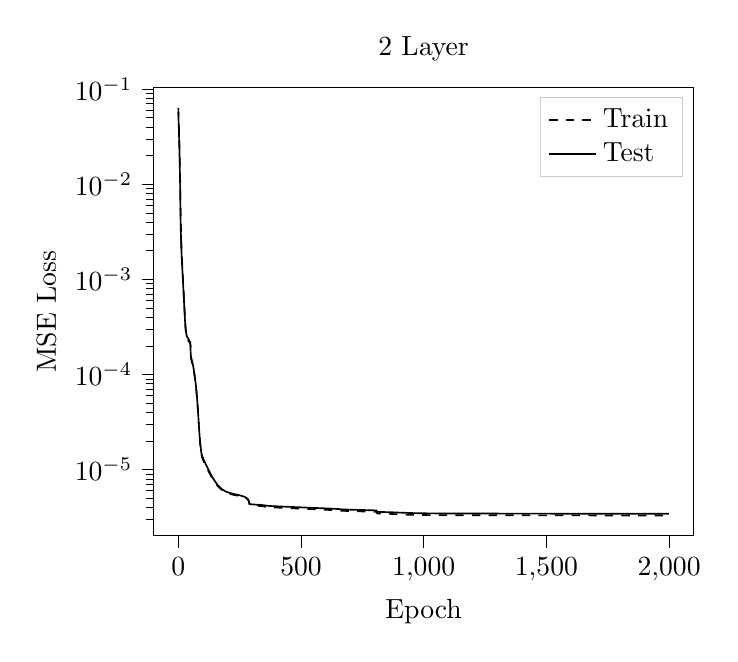
\begin{tikzpicture}

\begin{axis}[
legend cell align={left},
legend style={fill opacity=0.8, draw opacity=1, text opacity=1, draw=white!80!black},
log basis y={10},
tick align=outside,
tick pos=left,
title={2 Layer},
x grid style={white!69.0196078431373!black},
xlabel={Epoch},
xmin=-99.95, xmax=2098.95,
xtick style={color=black},
y grid style={white!69.0196078431373!black},
ylabel={MSE Loss},
ymin=2.00962005103304e-06, ymax=0.103609493820567,
ymode=log,
ytick style={color=black}
]
\addplot [semithick, black, dashed]
table {%
0 0.0632710078060627
1 0.051845450758934
2 0.0432980991452932
3 0.0358776403516531
4 0.0290690961554647
5 0.0229545622691512
6 0.0177181212641299
7 0.0134029685482383
8 0.00932001467421651
9 0.00582119612768292
10 0.00408269998338073
11 0.00310812011640519
12 0.00251322026690468
13 0.00211413772078231
14 0.00183244168199599
15 0.00161229025945067
16 0.00143017171323299
17 0.00127473987545818
18 0.0011382556988392
19 0.00101599448849447
20 0.000905665848404169
21 0.000806275674840435
22 0.00071686326363124
23 0.000636678095906973
24 0.000565266070072539
25 0.000501702402951196
26 0.000445806336938404
27 0.000397627679049037
28 0.000357118795858696
29 0.00032489347649971
30 0.000299998327216599
31 0.000281208114116453
32 0.000267276446160395
33 0.000257046025944874
34 0.0002495395517617
35 0.000243972511438187
36 0.000239745286788093
37 0.000236407682736171
38 0.000233631588111166
39 0.000231188191857655
40 0.000228926038951613
41 0.000226746779982932
42 0.000224590560450451
43 0.000222427553118905
44 0.000220237786095822
45 0.000218012332130456
46 0.000215740327854292
47 0.000213416477650753
48 0.000211034586711321
49 0.000208587526110932
50 0.000201116997253848
51 0.000158018265356077
52 0.000147613224027737
53 0.000142723495948303
54 0.000139244368234358
55 0.000136019374200259
56 0.000132747634241241
57 0.000129427922991454
58 0.000126070258433174
59 0.000122665663249791
60 0.000119213276564551
61 0.000115701421811536
62 0.000112120777172095
63 0.000108473681488249
64 0.000104762014772859
65 0.00010098851814837
66 9.71622276556445e-05
67 9.32928094116505e-05
68 8.93886299527367e-05
69 8.54555976766278e-05
70 8.14965877798386e-05
71 7.75122336417553e-05
72 7.35026992588246e-05
73 6.94685789057985e-05
74 6.54132343734091e-05
75 6.13432748941705e-05
76 5.72745405916066e-05
77 5.32301725179423e-05
78 4.92395857872907e-05
79 4.53403164574411e-05
80 4.1573930386221e-05
81 3.79849034761719e-05
82 3.46141511963651e-05
83 3.14956762558722e-05
84 2.8658379233093e-05
85 2.61181172882061e-05
86 2.38809501188371e-05
87 2.19437158739311e-05
88 2.0293696959925e-05
89 1.89088841780176e-05
90 1.77624986854426e-05
91 1.6823803317493e-05
92 1.60607825182524e-05
93 1.50258497696996e-05
94 1.4460581161984e-05
95 1.40592445336551e-05
96 1.37072536540472e-05
97 1.34257343074751e-05
98 1.31816849047937e-05
99 1.29646241002774e-05
100 1.27662120476089e-05
101 1.2581771216901e-05
102 1.24078030003147e-05
103 1.22411715728958e-05
104 1.20805520891736e-05
105 1.19247015427391e-05
106 1.1773092596286e-05
107 1.16248549329612e-05
108 1.14799404746009e-05
109 1.13379276499472e-05
110 1.11984094673971e-05
111 1.10615233461431e-05
112 1.09273854504863e-05
113 1.07954060031261e-05
114 1.06658476615848e-05
115 1.05386192249171e-05
116 1.04137884209194e-05
117 1.02908117264633e-05
118 1.01702188394484e-05
119 1.00515134595298e-05
120 9.93500102867984e-06
121 9.82061678314494e-06
122 9.70835857060592e-06
123 9.59800334567262e-06
124 9.48999531192385e-06
125 9.38343026655275e-06
126 9.2788389024463e-06
127 9.17616092829121e-06
128 9.07542354798352e-06
129 8.97668589686873e-06
130 8.87972992904906e-06
131 8.78457191856796e-06
132 8.69125409280969e-06
133 8.59979536244282e-06
134 8.51017152263012e-06
135 8.42218346087975e-06
136 8.33635802018762e-06
137 8.25191251988144e-06
138 8.16942619667316e-06
139 8.0887000030998e-06
140 8.00948176038219e-06
141 7.93231499164904e-06
142 7.85655636991578e-06
143 7.78257825504625e-06
144 7.71019455214628e-06
145 7.63938447198598e-06
146 7.57029341457383e-06
147 7.50287921164272e-06
148 7.43711638529021e-06
149 7.37279744384978e-06
150 7.31026423613912e-06
151 7.24875530431746e-06
152 7.18897826664033e-06
153 7.13090271165129e-06
154 7.07441331041991e-06
155 7.01886005163033e-06
156 6.96489755046059e-06
157 6.91240939818272e-06
158 6.86140954894654e-06
159 6.81176477974077e-06
160 6.76338529569875e-06
161 6.71635143635285e-06
162 6.67062341608471e-06
163 6.62643124655915e-06
164 6.58323398965877e-06
165 6.54126916742825e-06
166 6.50058312885449e-06
167 6.46115243034728e-06
168 6.42298308639511e-06
169 6.38602485582851e-06
170 6.35025759902419e-06
171 6.31564215518665e-06
172 6.2821410494962e-06
173 6.24969452883306e-06
174 6.21805136665898e-06
175 6.18742654864946e-06
176 6.15822291456425e-06
177 6.12961435763282e-06
178 6.10204494751088e-06
179 6.07546555693261e-06
180 6.04976868044105e-06
181 6.02458717798982e-06
182 6.00032682541496e-06
183 5.97695071451199e-06
184 5.95447526166026e-06
185 5.93280903376581e-06
186 5.91193096875031e-06
187 5.89195336056036e-06
188 5.87234221757171e-06
189 5.8534633653835e-06
190 5.83506993143601e-06
191 5.81726929294746e-06
192 5.79998251942015e-06
193 5.78317128065464e-06
194 5.76691470541846e-06
195 5.75105928714947e-06
196 5.73594326829152e-06
197 5.72154736437369e-06
198 5.70739826844147e-06
199 5.69361865041174e-06
200 5.68028440807211e-06
201 5.66706610925394e-06
202 5.65437040722827e-06
203 5.64182836365035e-06
204 5.62923450252129e-06
205 5.61731328298265e-06
206 5.60552214392374e-06
207 5.59428438737086e-06
208 5.58346819707367e-06
209 5.57276731524325e-06
210 5.56239524667035e-06
211 5.55222034631697e-06
212 5.54241197096417e-06
213 5.53287029742933e-06
214 5.52343979006764e-06
215 5.51419333123704e-06
216 5.5052181321571e-06
217 5.49665210428429e-06
218 5.48808294684022e-06
219 5.47977340056605e-06
220 5.47153629327113e-06
221 5.46346909595741e-06
222 5.45539895256297e-06
223 5.44765622976229e-06
224 5.44031825961611e-06
225 5.4328157098098e-06
226 5.42541469417301e-06
227 5.4179627427402e-06
228 5.41054173163502e-06
229 5.40329494447178e-06
230 5.39551419979034e-06
231 5.38808617102404e-06
232 5.38088338089437e-06
233 5.3739369534469e-06
234 5.36722018341607e-06
235 5.3601379581778e-06
236 5.35322880318745e-06
237 5.34662611130443e-06
238 5.33928093022951e-06
239 5.3319608723541e-06
240 5.32476024727657e-06
241 5.31745174248499e-06
242 5.3104168794107e-06
243 5.30307639201055e-06
244 5.29598574553347e-06
245 5.28916283337821e-06
246 5.28227127779246e-06
247 5.27531217994692e-06
248 5.26836660651497e-06
249 5.26145600565542e-06
250 5.25481974682407e-06
251 5.24836719614541e-06
252 5.24147814007847e-06
253 5.23453493815396e-06
254 5.22773011539357e-06
255 5.22081494614213e-06
256 5.21390236099251e-06
257 5.20662491862822e-06
258 5.19909029208066e-06
259 5.19156840505275e-06
260 5.1840717428604e-06
261 5.17612017256397e-06
262 5.16830087531162e-06
263 5.1598733487026e-06
264 5.15117472787097e-06
265 5.14193537469509e-06
266 5.13207956760198e-06
267 5.12154601028669e-06
268 5.11089195560999e-06
269 5.10023479159827e-06
270 5.08917057959479e-06
271 5.07760456798678e-06
272 5.06578773297406e-06
273 5.05217641853051e-06
274 5.0364313431146e-06
275 5.02120112696503e-06
276 5.00727311009541e-06
277 4.99260774995491e-06
278 4.97757784273745e-06
279 4.96154125721659e-06
280 4.94340508657842e-06
281 4.92293700722257e-06
282 4.89921165763008e-06
283 4.87050170272596e-06
284 4.83581983303338e-06
285 4.79348267253954e-06
286 4.74225533139361e-06
287 4.67328239142262e-06
288 4.58696049599894e-06
289 4.46936619255212e-06
290 4.31748006303678e-06
291 4.23798107794937e-06
292 4.22272348396291e-06
293 4.2174021655228e-06
294 4.21430222650088e-06
295 4.21172886331078e-06
296 4.20933076134133e-06
297 4.20704505904723e-06
298 4.20480583579774e-06
299 4.20261384238074e-06
300 4.20045522423607e-06
301 4.19840986728559e-06
302 4.19635286948505e-06
303 4.19434635909965e-06
304 4.1923705946374e-06
305 4.19050039226931e-06
306 4.18860404033694e-06
307 4.18674072125214e-06
308 4.18486637317983e-06
309 4.18306126630341e-06
310 4.18127912712407e-06
311 4.17950906694386e-06
312 4.17775834330314e-06
313 4.17607370832229e-06
314 4.17431320079231e-06
315 4.1727198783974e-06
316 4.17104828943593e-06
317 4.16937491081626e-06
318 4.16773654842473e-06
319 4.16610417369156e-06
320 4.16449309932432e-06
321 4.16296918592707e-06
322 4.16134395891277e-06
323 4.15973293388561e-06
324 4.15812554933837e-06
325 4.15651645334947e-06
326 4.15494718413356e-06
327 4.15333152818675e-06
328 4.15174744648539e-06
329 4.15025573261119e-06
330 4.14862696129603e-06
331 4.14689902572718e-06
332 4.14517258332125e-06
333 4.14342047315586e-06
334 4.14178949631605e-06
335 4.1400407767469e-06
336 4.13811117368823e-06
337 4.13610095756667e-06
338 4.13402996832701e-06
339 4.1318420285279e-06
340 4.1294807142549e-06
341 4.12701435834606e-06
342 4.12451515353496e-06
343 4.12194325031123e-06
344 4.11919797215887e-06
345 4.11631795668654e-06
346 4.11326574703708e-06
347 4.11016632801875e-06
348 4.10674409454259e-06
349 4.10305109289766e-06
350 4.09920685819998e-06
351 4.09521432902693e-06
352 4.0910061447903e-06
353 4.08667012720798e-06
354 4.08225326873435e-06
355 4.07795396699839e-06
356 4.07355116385588e-06
357 4.0691161605082e-06
358 4.06490110549385e-06
359 4.06080552897947e-06
360 4.05672974352456e-06
361 4.05283861550743e-06
362 4.04928707007457e-06
363 4.04601418176753e-06
364 4.0429513314848e-06
365 4.04010962870416e-06
366 4.03744269556228e-06
367 4.03506154293609e-06
368 4.03286837035921e-06
369 4.03083124660952e-06
370 4.02896440937184e-06
371 4.02703742270205e-06
372 4.02513960216311e-06
373 4.02338820936166e-06
374 4.02179212824194e-06
375 4.02032433521526e-06
376 4.01882592655056e-06
377 4.01735797845504e-06
378 4.01590311412292e-06
379 4.01456900135599e-06
380 4.01327008967201e-06
381 4.01198213216958e-06
382 4.01074603587404e-06
383 4.0095192375702e-06
384 4.00830898684035e-06
385 4.00709463201565e-06
386 4.0059097862013e-06
387 4.00470182489698e-06
388 4.00351677558319e-06
389 4.00236419886824e-06
390 4.00116998844169e-06
391 3.99998082389175e-06
392 3.99884801413464e-06
393 3.99764587837126e-06
394 3.99651417865243e-06
395 3.99532578603612e-06
396 3.99419785026112e-06
397 3.99303706149112e-06
398 3.99190068537791e-06
399 3.99077415227112e-06
400 3.98964895885001e-06
401 3.98854520904024e-06
402 3.98738429157675e-06
403 3.98626458650142e-06
404 3.98513616232776e-06
405 3.98401351844768e-06
406 3.98287694929422e-06
407 3.98177175156889e-06
408 3.98065694753313e-06
409 3.97955125094995e-06
410 3.97847688532238e-06
411 3.97736476134014e-06
412 3.97623916978773e-06
413 3.97515318627484e-06
414 3.97404352497688e-06
415 3.97295079324067e-06
416 3.97184997132172e-06
417 3.97074828265431e-06
418 3.96966739663185e-06
419 3.96858127305677e-06
420 3.96750045547378e-06
421 3.96643120166118e-06
422 3.96534202013754e-06
423 3.96427063765259e-06
424 3.96322433994101e-06
425 3.96213134354184e-06
426 3.96106135895025e-06
427 3.95999829197535e-06
428 3.95894019357001e-06
429 3.95790915376892e-06
430 3.95684226828053e-06
431 3.95577681206305e-06
432 3.95472414516007e-06
433 3.95362605377159e-06
434 3.95254756790564e-06
435 3.95150437725533e-06
436 3.95043570642883e-06
437 3.94937866462897e-06
438 3.94838115562379e-06
439 3.94730105404051e-06
440 3.94621883810942e-06
441 3.9451766710954e-06
442 3.94410750595853e-06
443 3.94304689325509e-06
444 3.94200809296308e-06
445 3.94095385900073e-06
446 3.93992307658664e-06
447 3.93891124645052e-06
448 3.93786665722473e-06
449 3.93685992435167e-06
450 3.9358440626529e-06
451 3.93480710340555e-06
452 3.93380716809588e-06
453 3.93278114415807e-06
454 3.93176267130002e-06
455 3.93070953191454e-06
456 3.92965003652535e-06
457 3.92862235230496e-06
458 3.92760561658179e-06
459 3.92657984616562e-06
460 3.9255645015146e-06
461 3.92449227001634e-06
462 3.92346870353322e-06
463 3.92245446937522e-06
464 3.92145133218946e-06
465 3.92043095689587e-06
466 3.91943706358688e-06
467 3.91841551595462e-06
468 3.91737812401516e-06
469 3.91636446238408e-06
470 3.91536215056476e-06
471 3.91434734888207e-06
472 3.91334745836502e-06
473 3.91231219873589e-06
474 3.91130924549543e-06
475 3.91030783475799e-06
476 3.90929390709971e-06
477 3.90829968523576e-06
478 3.90728442221189e-06
479 3.9063041681402e-06
480 3.90529386982053e-06
481 3.90429663980285e-06
482 3.90328932166994e-06
483 3.90228188075525e-06
484 3.90130058735849e-06
485 3.90029922914437e-06
486 3.89929259267774e-06
487 3.89830421522674e-06
488 3.89731379686964e-06
489 3.89628200673542e-06
490 3.89534313785589e-06
491 3.89432079941798e-06
492 3.89331514952573e-06
493 3.89229541360692e-06
494 3.89127347989415e-06
495 3.89029763300641e-06
496 3.88925411311902e-06
497 3.88816214581311e-06
498 3.88687702547941e-06
499 3.88587540737717e-06
500 3.88488475755366e-06
501 3.88386549957431e-06
502 3.88286122324644e-06
503 3.88185147426157e-06
504 3.88082735753414e-06
505 3.87983534415071e-06
506 3.87884211681921e-06
507 3.87786378541932e-06
508 3.87690347974967e-06
509 3.87590351806466e-06
510 3.87493697735408e-06
511 3.87393002165481e-06
512 3.87293140079237e-06
513 3.87193410711006e-06
514 3.87096493568606e-06
515 3.86997004397927e-06
516 3.86899167233423e-06
517 3.86810477471045e-06
518 3.86708819746673e-06
519 3.86609972861152e-06
520 3.86511584406435e-06
521 3.86410707824325e-06
522 3.86309811415231e-06
523 3.86210161127565e-06
524 3.86109321630101e-06
525 3.86009254270903e-06
526 3.85912106071373e-06
527 3.85811027194904e-06
528 3.85712550837525e-06
529 3.85611493993565e-06
530 3.85510660271393e-06
531 3.85410345074888e-06
532 3.85311390755305e-06
533 3.85213474737611e-06
534 3.85112630192452e-06
535 3.85012735591772e-06
536 3.84913734296788e-06
537 3.84815157872254e-06
538 3.84717732458739e-06
539 3.84619277247111e-06
540 3.84522993113023e-06
541 3.8442311797553e-06
542 3.84322497643552e-06
543 3.84227112340341e-06
544 3.8412537937802e-06
545 3.84022483763147e-06
546 3.83922470746256e-06
547 3.83821959007946e-06
548 3.83719782143999e-06
549 3.83618380419648e-06
550 3.83516073952705e-06
551 3.83415338933446e-06
552 3.83312635744915e-06
553 3.83206138189962e-06
554 3.83102651903755e-06
555 3.82998564509762e-06
556 3.82895923803517e-06
557 3.82797941483659e-06
558 3.82694782160797e-06
559 3.82592881351229e-06
560 3.82489514527151e-06
561 3.82387169111098e-06
562 3.82288159403288e-06
563 3.82187921854893e-06
564 3.82090538437296e-06
565 3.81990201117333e-06
566 3.81885945239446e-06
567 3.8178061686267e-06
568 3.81674583468339e-06
569 3.81568310513103e-06
570 3.81460992866778e-06
571 3.81355367085234e-06
572 3.81251289786633e-06
573 3.81145554933937e-06
574 3.8104192146875e-06
575 3.8093715679679e-06
576 3.80830061658344e-06
577 3.80721733722567e-06
578 3.80615091921754e-06
579 3.80504406757609e-06
580 3.80396494574597e-06
581 3.80284883271997e-06
582 3.80177165607165e-06
583 3.80069691914287e-06
584 3.79964723424564e-06
585 3.7985892818142e-06
586 3.79753483116474e-06
587 3.79640749065402e-06
588 3.79530364398306e-06
589 3.7941353525639e-06
590 3.79299306950998e-06
591 3.79188061958757e-06
592 3.79073451824752e-06
593 3.78960781699789e-06
594 3.78849956632621e-06
595 3.7874091502772e-06
596 3.78626679844274e-06
597 3.78513176633533e-06
598 3.78400663305456e-06
599 3.78287078638095e-06
600 3.78169056853039e-06
601 3.78051059510653e-06
602 3.77938837505099e-06
603 3.77821030451742e-06
604 3.77709365989176e-06
605 3.77594412566395e-06
606 3.77473977471254e-06
607 3.77356035733101e-06
608 3.77238059650153e-06
609 3.77121746578268e-06
610 3.77010574015912e-06
611 3.76895438330394e-06
612 3.76782894613825e-06
613 3.76667858108704e-06
614 3.76551559270411e-06
615 3.76439185151867e-06
616 3.76326227546997e-06
617 3.76208450234117e-06
618 3.76090089821446e-06
619 3.75969973163137e-06
620 3.75851625665291e-06
621 3.75739111655093e-06
622 3.75627195273864e-06
623 3.75508487604748e-06
624 3.75392496414406e-06
625 3.75275827741461e-06
626 3.75164966681041e-06
627 3.7504619098172e-06
628 3.7492805902275e-06
629 3.74812237578226e-06
630 3.74700240786297e-06
631 3.74586033490232e-06
632 3.74465033678462e-06
633 3.74347466811287e-06
634 3.74222576670036e-06
635 3.74095193990343e-06
636 3.73970642544919e-06
637 3.73849202571819e-06
638 3.73727273176883e-06
639 3.73604903143132e-06
640 3.73481999326941e-06
641 3.73360565822622e-06
642 3.73240932685803e-06
643 3.73127844181909e-06
644 3.73011926103572e-06
645 3.72891290930966e-06
646 3.727741849616e-06
647 3.72646188213821e-06
648 3.72512999217633e-06
649 3.72386121966883e-06
650 3.72253252623977e-06
651 3.72115426330311e-06
652 3.71982453145847e-06
653 3.7184918338653e-06
654 3.71706787746007e-06
655 3.71560938947368e-06
656 3.71417414066855e-06
657 3.71250464706918e-06
658 3.71070990593125e-06
659 3.70882397623973e-06
660 3.70690597890189e-06
661 3.70420897252188e-06
662 3.70078934975027e-06
663 3.69826730502609e-06
664 3.69612601537028e-06
665 3.69425015776415e-06
666 3.69259916294595e-06
667 3.69112746614064e-06
668 3.68980126438601e-06
669 3.6885883330342e-06
670 3.68746814126553e-06
671 3.68644335560475e-06
672 3.68547208643122e-06
673 3.68455293175884e-06
674 3.683675603952e-06
675 3.68285116735478e-06
676 3.6820184672024e-06
677 3.68124188753427e-06
678 3.68046135884015e-06
679 3.67971530249633e-06
680 3.67896949774149e-06
681 3.67823716908333e-06
682 3.67751394207971e-06
683 3.67678034842811e-06
684 3.67607592556851e-06
685 3.67535497991867e-06
686 3.67465632757558e-06
687 3.67394465786219e-06
688 3.6732546661824e-06
689 3.67254644345394e-06
690 3.67185343293386e-06
691 3.67115930930595e-06
692 3.67046825454054e-06
693 3.66977536043578e-06
694 3.66907607531175e-06
695 3.66839212199466e-06
696 3.66770006837669e-06
697 3.6670071425533e-06
698 3.66632715258675e-06
699 3.66563417685484e-06
700 3.66494473416878e-06
701 3.66426724519897e-06
702 3.66358821713675e-06
703 3.66290142187609e-06
704 3.6622132258799e-06
705 3.6615301440861e-06
706 3.66084534357469e-06
707 3.66017243891292e-06
708 3.6594921489268e-06
709 3.65881293635084e-06
710 3.65812857126002e-06
711 3.6574575931354e-06
712 3.65677416755261e-06
713 3.65609544701329e-06
714 3.65541832900362e-06
715 3.65474015052314e-06
716 3.65406903290477e-06
717 3.65339285406208e-06
718 3.65271773671338e-06
719 3.65204745116898e-06
720 3.651368467672e-06
721 3.65069879228486e-06
722 3.65002570674733e-06
723 3.64936534811022e-06
724 3.64868461804235e-06
725 3.64801084799637e-06
726 3.64734410402434e-06
727 3.64667091173487e-06
728 3.6460121403934e-06
729 3.6453348136547e-06
730 3.64466524786167e-06
731 3.6439993359636e-06
732 3.64334011158007e-06
733 3.64267599638879e-06
734 3.64200718195207e-06
735 3.64133908624353e-06
736 3.64068387693806e-06
737 3.64001761658983e-06
738 3.63935759855849e-06
739 3.63869932277794e-06
740 3.6380411635264e-06
741 3.63737760744698e-06
742 3.63650741667243e-06
743 3.63583347075291e-06
744 3.63516651168538e-06
745 3.63449705389485e-06
746 3.63384109414255e-06
747 3.63316582570405e-06
748 3.63250598411469e-06
749 3.63184671437011e-06
750 3.63118088159808e-06
751 3.63051347460441e-06
752 3.62984826938373e-06
753 3.62920208863216e-06
754 3.62853011097286e-06
755 3.62786857806441e-06
756 3.62720777866343e-06
757 3.62655042818005e-06
758 3.62588549194243e-06
759 3.62523838361994e-06
760 3.62457825156071e-06
761 3.62390604811935e-06
762 3.62325307582978e-06
763 3.62259630355766e-06
764 3.62194640536018e-06
765 3.62129782820375e-06
766 3.62063571492399e-06
767 3.61997041034101e-06
768 3.61932698899636e-06
769 3.61866497462415e-06
770 3.6180262252401e-06
771 3.617362689738e-06
772 3.61671298037436e-06
773 3.61607361901406e-06
774 3.61541275435684e-06
775 3.6147658632899e-06
776 3.61411101857811e-06
777 3.61345795158741e-06
778 3.61281008554215e-06
779 3.61216918668106e-06
780 3.6115153557148e-06
781 3.61088205590931e-06
782 3.61022876393236e-06
783 3.6095767355846e-06
784 3.60893789741112e-06
785 3.60828682255487e-06
786 3.60765805169194e-06
787 3.60699846305579e-06
788 3.60636278833226e-06
789 3.60572352553845e-06
790 3.60508044082053e-06
791 3.60444044986252e-06
792 3.60379261326216e-06
793 3.60315890213769e-06
794 3.60252107452652e-06
795 3.60187887156371e-06
796 3.6012473944993e-06
797 3.60060167395204e-06
798 3.59996799465989e-06
799 3.59931844286621e-06
800 3.59868616624226e-06
801 3.59804496190463e-06
802 3.59741519469026e-06
803 3.59679051234707e-06
804 3.59614438116296e-06
805 3.59551126325641e-06
806 3.59488375943329e-06
807 3.59423938243708e-06
808 3.59361888456533e-06
809 3.58856573075173e-06
810 3.46819658852837e-06
811 3.45905467918328e-06
812 3.45808383144686e-06
813 3.45728719207727e-06
814 3.45646615710393e-06
815 3.4557891899567e-06
816 3.45512566559592e-06
817 3.45442840398391e-06
818 3.45375150789096e-06
819 3.45314441744904e-06
820 3.45249377733126e-06
821 3.45187570439975e-06
822 3.4512920127554e-06
823 3.45072540699221e-06
824 3.45013294111141e-06
825 3.44956170420119e-06
826 3.44901385676621e-06
827 3.44852854482269e-06
828 3.44790018584717e-06
829 3.44723031332705e-06
830 3.44663635894449e-06
831 3.44601887513818e-06
832 3.44534294094956e-06
833 3.44472433505416e-06
834 3.44406132182939e-06
835 3.44345207020069e-06
836 3.44280726289981e-06
837 3.4422474728899e-06
838 3.44163713850776e-06
839 3.44108118099484e-06
840 3.44047824160043e-06
841 3.4398152462245e-06
842 3.43910582000717e-06
843 3.43842116046744e-06
844 3.43774710404432e-06
845 3.43702792099521e-06
846 3.43634997943809e-06
847 3.43563018009263e-06
848 3.43499882342257e-06
849 3.43428135010981e-06
850 3.43356308815146e-06
851 3.43284928339926e-06
852 3.43210946982708e-06
853 3.43137287131867e-06
854 3.43064236994906e-06
855 3.42992232879169e-06
856 3.42917290743117e-06
857 3.42838393817146e-06
858 3.42754296923431e-06
859 3.42668330313245e-06
860 3.42588032242475e-06
861 3.42507210848453e-06
862 3.42416718467575e-06
863 3.42335599020771e-06
864 3.42258317823507e-06
865 3.42167720782527e-06
866 3.42081106327896e-06
867 3.41993027393528e-06
868 3.41898223450698e-06
869 3.41806178505522e-06
870 3.41711957901225e-06
871 3.41628901833246e-06
872 3.41533120615622e-06
873 3.41435020516201e-06
874 3.41339523242823e-06
875 3.41245838376381e-06
876 3.4114890966066e-06
877 3.41038971214402e-06
878 3.40855177046251e-06
879 3.40721698319157e-06
880 3.40610965008636e-06
881 3.40513882656524e-06
882 3.40419041424411e-06
883 3.40332646044317e-06
884 3.40240671414449e-06
885 3.4013559078403e-06
886 3.40033198938272e-06
887 3.39924581226114e-06
888 3.39811470360019e-06
889 3.39708300680286e-06
890 3.39614488370898e-06
891 3.39512193158953e-06
892 3.39409216473996e-06
893 3.39310099377599e-06
894 3.39206634293987e-06
895 3.39110838353918e-06
896 3.39012106735481e-06
897 3.3891239560262e-06
898 3.38814063684367e-06
899 3.38709192863007e-06
900 3.38610237486137e-06
901 3.38508347010702e-06
902 3.38407450976774e-06
903 3.38305720777043e-06
904 3.38207762490583e-06
905 3.38106447293285e-06
906 3.38001549198452e-06
907 3.37896211885891e-06
908 3.37797512941052e-06
909 3.37698621433447e-06
910 3.37599381316522e-06
911 3.37501526473716e-06
912 3.37411181067182e-06
913 3.37317492824241e-06
914 3.37220609208089e-06
915 3.3712260875518e-06
916 3.37031230503726e-06
917 3.36942957324027e-06
918 3.36857478896491e-06
919 3.36759936112685e-06
920 3.36662839538349e-06
921 3.36570018896509e-06
922 3.3648025120101e-06
923 3.36392968029031e-06
924 3.3630231520192e-06
925 3.36211414503396e-06
926 3.36128224489585e-06
927 3.36038605507838e-06
928 3.35971276251712e-06
929 3.35890150881824e-06
930 3.35802607730784e-06
931 3.35722394027016e-06
932 3.35641767048855e-06
933 3.35569475134889e-06
934 3.35492151180006e-06
935 3.35416929988241e-06
936 3.35343535334687e-06
937 3.35275004340474e-06
938 3.3520320862408e-06
939 3.35134114561697e-06
940 3.35064550688458e-06
941 3.34997043398744e-06
942 3.34934603586134e-06
943 3.34871437360107e-06
944 3.34808450747914e-06
945 3.34750664876537e-06
946 3.34689332385096e-06
947 3.34634646662835e-06
948 3.34575365366163e-06
949 3.34518739339273e-06
950 3.34464585841943e-06
951 3.34406109845986e-06
952 3.34353921266484e-06
953 3.34303967986216e-06
954 3.34256621943041e-06
955 3.34205329431825e-06
956 3.34155066923358e-06
957 3.34107601361211e-06
958 3.34061679984643e-06
959 3.34015869543691e-06
960 3.33970654855875e-06
961 3.3393236901702e-06
962 3.33886904593328e-06
963 3.33842913983062e-06
964 3.33814169107427e-06
965 3.33774210423599e-06
966 3.3372913213725e-06
967 3.33686178612425e-06
968 3.33645433522634e-06
969 3.33606849665102e-06
970 3.33571005978683e-06
971 3.33536255254785e-06
972 3.33501844590955e-06
973 3.33469381189389e-06
974 3.33438582435974e-06
975 3.33408202118335e-06
976 3.33378812365481e-06
977 3.33350157063705e-06
978 3.33323775805638e-06
979 3.3330256313775e-06
980 3.33272925752226e-06
981 3.33243786371895e-06
982 3.33216787623769e-06
983 3.3319054509775e-06
984 3.33164250014306e-06
985 3.33139780241254e-06
986 3.33115889634428e-06
987 3.33091831510046e-06
988 3.33069397129293e-06
989 3.33046564878714e-06
990 3.33024445262708e-06
991 3.33003096750417e-06
992 3.32982458940023e-06
993 3.32962686138671e-06
994 3.32943600267299e-06
995 3.32926675400813e-06
996 3.32906775338415e-06
997 3.3288823390194e-06
998 3.32862334119e-06
999 3.3284366764974e-06
1000 3.32826502312855e-06
1001 3.32808903544901e-06
1002 3.3279268395745e-06
1003 3.3277572111956e-06
1004 3.32759605612409e-06
1005 3.32745577202331e-06
1006 3.32727387956311e-06
1007 3.32710411589687e-06
1008 3.32693895040848e-06
1009 3.32677818335014e-06
1010 3.32661705760984e-06
1011 3.32647359664406e-06
1012 3.32631457933985e-06
1013 3.32618127072237e-06
1014 3.32603964534428e-06
1015 3.32589951085538e-06
1016 3.32574876642866e-06
1017 3.32563812094122e-06
1018 3.325481228444e-06
1019 3.32533804532886e-06
1020 3.32519677795062e-06
1021 3.32507743246424e-06
1022 3.32495024065338e-06
1023 3.32481203804491e-06
1024 3.32468024942045e-06
1025 3.32454988460995e-06
1026 3.32442952083056e-06
1027 3.32430381183713e-06
1028 3.32418459424844e-06
1029 3.32406650829853e-06
1030 3.32396275587143e-06
1031 3.32385228330168e-06
1032 3.32373832941357e-06
1033 3.32363166569394e-06
1034 3.32353530177443e-06
1035 3.32343474212848e-06
1036 3.32334030849779e-06
1037 3.32324221994895e-06
1038 3.32314650916032e-06
1039 3.32305175118108e-06
1040 3.32298359035121e-06
1041 3.32284780517966e-06
1042 3.32274852030423e-06
1043 3.3226549801384e-06
1044 3.32256201613745e-06
1045 3.32246874370412e-06
1046 3.3223735683805e-06
1047 3.32228958177438e-06
1048 3.32220481595868e-06
1049 3.32208896418251e-06
1050 3.32200541083694e-06
1051 3.32191331938247e-06
1052 3.32182456236296e-06
1053 3.32175064909279e-06
1054 3.3216608036355e-06
1055 3.32158123887893e-06
1056 3.32150148597066e-06
1057 3.3214288405361e-06
1058 3.32134673897144e-06
1059 3.32127205160759e-06
1060 3.3211996552609e-06
1061 3.32111623322362e-06
1062 3.32105358813806e-06
1063 3.32098555361426e-06
1064 3.320912385675e-06
1065 3.32084120304899e-06
1066 3.32077246423523e-06
1067 3.32069897615384e-06
1068 3.32062761867746e-06
1069 3.32055835360734e-06
1070 3.32049213534447e-06
1071 3.32042758327589e-06
1072 3.32035822054877e-06
1073 3.32029157220859e-06
1074 3.3202237336809e-06
1075 3.32016097570431e-06
1076 3.32010107376846e-06
1077 3.32003031508066e-06
1078 3.31996242221066e-06
1079 3.31990452946229e-06
1080 3.31984272509089e-06
1081 3.3197831430698e-06
1082 3.31972265939839e-06
1083 3.31965873988338e-06
1084 3.31960340872683e-06
1085 3.31954086311725e-06
1086 3.31948666712378e-06
1087 3.31942682998942e-06
1088 3.31936341729033e-06
1089 3.31931191681178e-06
1090 3.31925431248692e-06
1091 3.31908182454299e-06
1092 3.31901709694193e-06
1093 3.31896539614718e-06
1094 3.31891274390728e-06
1095 3.31885061757475e-06
1096 3.31879793600365e-06
1097 3.3187468189908e-06
1098 3.31868890623355e-06
1099 3.31862838606867e-06
1100 3.31856975185474e-06
1101 3.31851502880909e-06
1102 3.31847244035544e-06
1103 3.31840572573583e-06
1104 3.3183519180966e-06
1105 3.31829593142174e-06
1106 3.31823610724769e-06
1107 3.31818831443798e-06
1108 3.31813788932322e-06
1109 3.31809355793666e-06
1110 3.31803202232095e-06
1111 3.31797998080674e-06
1112 3.31792680481158e-06
1113 3.31787022776098e-06
1114 3.31782323041807e-06
1115 3.31776938503481e-06
1116 3.31772539641406e-06
1117 3.31767134389338e-06
1118 3.31762536609403e-06
1119 3.31757380968156e-06
1120 3.31752182080436e-06
1121 3.31747144957717e-06
1122 3.31731329424656e-06
1123 3.31725821206419e-06
1124 3.31720646829581e-06
1125 3.31715368929508e-06
1126 3.31710390935314e-06
1127 3.3170535549516e-06
1128 3.31699749733616e-06
1129 3.31695505599328e-06
1130 3.31690347150015e-06
1131 3.31685236983503e-06
1132 3.31680772876552e-06
1133 3.3167499815363e-06
1134 3.31669872764451e-06
1135 3.31664693214861e-06
1136 3.31659686685271e-06
1137 3.31655298123223e-06
1138 3.31649509212184e-06
1139 3.31645859967011e-06
1140 3.31640772060382e-06
1141 3.31635877830649e-06
1142 3.31630854077503e-06
1143 3.3162615816309e-06
1144 3.31620984627534e-06
1145 3.31616943481095e-06
1146 3.31612526088065e-06
1147 3.31607749308205e-06
1148 3.31602828350697e-06
1149 3.31598170487268e-06
1150 3.31593465273272e-06
1151 3.31589305983471e-06
1152 3.31584171124177e-06
1153 3.31579683393102e-06
1154 3.31575542475093e-06
1155 3.31569906404638e-06
1156 3.31566256102178e-06
1157 3.31562098369886e-06
1158 3.31557101537783e-06
1159 3.31552743352859e-06
1160 3.31547878431593e-06
1161 3.31543595132189e-06
1162 3.31539260980662e-06
1163 3.31535449493003e-06
1164 3.31530274024772e-06
1165 3.31526033858154e-06
1166 3.31521684279323e-06
1167 3.31517224708477e-06
1168 3.31512761704289e-06
1169 3.31509071429537e-06
1170 3.31504686755579e-06
1171 3.31499783703748e-06
1172 3.31494618387751e-06
1173 3.31488194569829e-06
1174 3.31483411434874e-06
1175 3.31477687655024e-06
1176 3.31463223449191e-06
1177 3.3145593424706e-06
1178 3.31451699707941e-06
1179 3.31447909991311e-06
1180 3.31444194944197e-06
1181 3.31440136801575e-06
1182 3.3143566832905e-06
1183 3.31432279710953e-06
1184 3.3142888198654e-06
1185 3.31424507578504e-06
1186 3.31421255020814e-06
1187 3.31417136544587e-06
1188 3.31413100582267e-06
1189 3.31409358943802e-06
1190 3.3140541273724e-06
1191 3.31401387495589e-06
1192 3.31398105663538e-06
1193 3.31394617762726e-06
1194 3.31390259668751e-06
1195 3.31387615858603e-06
1196 3.31384136154611e-06
1197 3.31379895965256e-06
1198 3.31376556687246e-06
1199 3.31373439541949e-06
1200 3.31369409514082e-06
1201 3.31365316878873e-06
1202 3.31363031023102e-06
1203 3.31359488518501e-06
1204 3.31356466006127e-06
1205 3.31353000353829e-06
1206 3.3134903616201e-06
1207 3.31346309042146e-06
1208 3.31342015306291e-06
1209 3.31339084232241e-06
1210 3.3133535714569e-06
1211 3.31332341784218e-06
1212 3.31328962545285e-06
1213 3.31325111255865e-06
1214 3.31321978012511e-06
1215 3.31318277721948e-06
1216 3.31314616198597e-06
1217 3.31311287493463e-06
1218 3.31307958356319e-06
1219 3.31304765325058e-06
1220 3.31300194511641e-06
1221 3.31296959791416e-06
1222 3.31293913814079e-06
1223 3.31290463248024e-06
1224 3.31286963171351e-06
1225 3.31283649222769e-06
1226 3.31280664943279e-06
1227 3.31276422059545e-06
1228 3.31273262804643e-06
1229 3.31270691606278e-06
1230 3.31266566593058e-06
1231 3.31263192094866e-06
1232 3.31260459256555e-06
1233 3.31257304628707e-06
1234 3.31253451588509e-06
1235 3.3125027416645e-06
1236 3.31246954056041e-06
1237 3.31243238213119e-06
1238 3.31239868376088e-06
1239 3.31237523766958e-06
1240 3.31232966425432e-06
1241 3.3123012260603e-06
1242 3.31226731339029e-06
1243 3.31223492764821e-06
1244 3.31220416660472e-06
1245 3.3121651907777e-06
1246 3.31213434481015e-06
1247 3.31210411036409e-06
1248 3.31207334511419e-06
1249 3.31204188125866e-06
1250 3.31200534310483e-06
1251 3.31196890385854e-06
1252 3.31193951285513e-06
1253 3.31191298664635e-06
1254 3.31186976950448e-06
1255 3.31183692810555e-06
1256 3.31180187276914e-06
1257 3.31176736733596e-06
1258 3.31174078667118e-06
1259 3.31170079664389e-06
1260 3.31167498484319e-06
1261 3.31163897067199e-06
1262 3.31160367568373e-06
1263 3.31157391030956e-06
1264 3.31153827073649e-06
1265 3.31150821864412e-06
1266 3.31147878000593e-06
1267 3.31144059236976e-06
1268 3.3114125475322e-06
1269 3.31137845250851e-06
1270 3.31135019507656e-06
1271 3.31132036353665e-06
1272 3.31128353366239e-06
1273 3.31124508727498e-06
1274 3.3112155958861e-06
1275 3.31118322765178e-06
1276 3.31115418396166e-06
1277 3.31111870571021e-06
1278 3.31108915679579e-06
1279 3.31105810823829e-06
1280 3.31101666643008e-06
1281 3.31099420361625e-06
1282 3.31095552917304e-06
1283 3.31091766827285e-06
1284 3.31088738289509e-06
1285 3.31086019934901e-06
1286 3.31082479078759e-06
1287 3.3107894528257e-06
1288 3.31076125996788e-06
1289 3.31073088023004e-06
1290 3.31069415051388e-06
1291 3.31065719831258e-06
1292 3.31063165572232e-06
1293 3.31060190774224e-06
1294 3.3105640161466e-06
1295 3.31053720560703e-06
1296 3.31050339457306e-06
1297 3.31046521137068e-06
1298 3.31043459812008e-06
1299 3.31039810896527e-06
1300 3.31036881345881e-06
1301 3.31033730344643e-06
1302 3.310306435651e-06
1303 3.31026991398176e-06
1304 3.31024301567595e-06
1305 3.31020190742493e-06
1306 3.31017149255786e-06
1307 3.3101332599017e-06
1308 3.31010171169055e-06
1309 3.31005946975438e-06
1310 3.31003425515064e-06
1311 3.30999968309698e-06
1312 3.30996857246646e-06
1313 3.30993229317755e-06
1314 3.30990236466278e-06
1315 3.30987621293843e-06
1316 3.30983615754121e-06
1317 3.30979875263893e-06
1318 3.30977489818451e-06
1319 3.30974435814824e-06
1320 3.30970497532235e-06
1321 3.30967777449587e-06
1322 3.30965184900833e-06
1323 3.30961561678578e-06
1324 3.30957849496372e-06
1325 3.30955011418155e-06
1326 3.30952235151472e-06
1327 3.30948825808264e-06
1328 3.30946376834618e-06
1329 3.30942424557179e-06
1330 3.30939567766109e-06
1331 3.30936111083702e-06
1332 3.30933207965245e-06
1333 3.3093084363145e-06
1334 3.30927065931519e-06
1335 3.30923937360694e-06
1336 3.30921289116759e-06
1337 3.30918081397158e-06
1338 3.30914972573737e-06
1339 3.30911605874462e-06
1340 3.30908646151329e-06
1341 3.30905639475532e-06
1342 3.30902801658795e-06
1343 3.30899296102416e-06
1344 3.30896267894332e-06
1345 3.3089325166884e-06
1346 3.30890046916466e-06
1347 3.30886465042113e-06
1348 3.3088395756522e-06
1349 3.30881382774351e-06
1350 3.30877656608664e-06
1351 3.30874721919372e-06
1352 3.30871065659721e-06
1353 3.30867955688063e-06
1354 3.30865487069332e-06
1355 3.30862191162851e-06
1356 3.30859550501827e-06
1357 3.30855776235239e-06
1358 3.30853303728418e-06
1359 3.30850446073327e-06
1360 3.30846531176121e-06
1361 3.30843728659147e-06
1362 3.30840472588534e-06
1363 3.30837749436341e-06
1364 3.30834483236231e-06
1365 3.30830624568534e-06
1366 3.30828763708269e-06
1367 3.30825550838654e-06
1368 3.30822551416077e-06
1369 3.30818973498026e-06
1370 3.30815789163807e-06
1371 3.30812527829494e-06
1372 3.30809859678993e-06
1373 3.30806258318717e-06
1374 3.30803215661035e-06
1375 3.30800900974282e-06
1376 3.30797151002571e-06
1377 3.30794009107649e-06
1378 3.30791404837782e-06
1379 3.30788173698693e-06
1380 3.30785453468252e-06
1381 3.30781790967194e-06
1382 3.30779392106706e-06
1383 3.30776260773291e-06
1384 3.30773389839578e-06
1385 3.30769640322615e-06
1386 3.30766638410296e-06
1387 3.30763812337409e-06
1388 3.30760337055835e-06
1389 3.30757708707097e-06
1390 3.307545913799e-06
1391 3.30751326794143e-06
1392 3.30749232489325e-06
1393 3.30745411440603e-06
1394 3.30735595673559e-06
1395 3.30729904260352e-06
1396 3.30725218407224e-06
1397 3.30722578951281e-06
1398 3.30719073667751e-06
1399 3.30716875021153e-06
1400 3.30714862934656e-06
1401 3.30711684216567e-06
1402 3.3070819894192e-06
1403 3.3070488652811e-06
1404 3.30701422922175e-06
1405 3.30698709717581e-06
1406 3.30695631168965e-06
1407 3.30692265868038e-06
1408 3.30688969722814e-06
1409 3.30686106201483e-06
1410 3.3068254247155e-06
1411 3.3067949505039e-06
1412 3.30675967359184e-06
1413 3.30672607924498e-06
1414 3.30669463016875e-06
1415 3.30665754358961e-06
1416 3.30661870475524e-06
1417 3.30659057021876e-06
1418 3.30655833431592e-06
1419 3.30653160381189e-06
1420 3.30648229748931e-06
1421 3.3064635277924e-06
1422 3.30642847688978e-06
1423 3.30640005802252e-06
1424 3.30635991497275e-06
1425 3.30633839712391e-06
1426 3.30630923531317e-06
1427 3.30627130324501e-06
1428 3.30624613002328e-06
1429 3.30621113914731e-06
1430 3.30618818611583e-06
1431 3.30615022528491e-06
1432 3.30612555853804e-06
1433 3.3060949335777e-06
1434 3.30606805039224e-06
1435 3.30602659039414e-06
1436 3.30600337179021e-06
1437 3.30597711342762e-06
1438 3.30594837578246e-06
1439 3.30591299587013e-06
1440 3.30588416147748e-06
1441 3.30585510812398e-06
1442 3.30582726405737e-06
1443 3.30579878891513e-06
1444 3.30576666067373e-06
1445 3.30573926805755e-06
1446 3.30570304413413e-06
1447 3.30567544233418e-06
1448 3.30564356863761e-06
1449 3.30561513396788e-06
1450 3.3055900224781e-06
1451 3.30555552284295e-06
1452 3.30552562525099e-06
1453 3.30550001433494e-06
1454 3.30546434372536e-06
1455 3.30543629740987e-06
1456 3.30540926006506e-06
1457 3.30537772595108e-06
1458 3.30534853821973e-06
1459 3.30531810948287e-06
1460 3.30529423752068e-06
1461 3.30526512493634e-06
1462 3.30523205786903e-06
1463 3.30520980810434e-06
1464 3.30517069141933e-06
1465 3.30514524932823e-06
1466 3.3051182268764e-06
1467 3.3050883089345e-06
1468 3.30505295073635e-06
1469 3.30502717281433e-06
1470 3.30499619519742e-06
1471 3.30496268304614e-06
1472 3.3049321046974e-06
1473 3.30491160332258e-06
1474 3.30488403938034e-06
1475 3.30484924450047e-06
1476 3.30482337255944e-06
1477 3.3047829225552e-06
1478 3.30475701593969e-06
1479 3.30473347594307e-06
1480 3.30469857590288e-06
1481 3.30467577111904e-06
1482 3.30463922102808e-06
1483 3.30460926977594e-06
1484 3.3045828433842e-06
1485 3.30454228947019e-06
1486 3.30451344598259e-06
1487 3.30448826628071e-06
1488 3.30446151951946e-06
1489 3.30443765540167e-06
1490 3.30440346078831e-06
1491 3.30437982188414e-06
1492 3.30434341208274e-06
1493 3.30430771680312e-06
1494 3.30429122220721e-06
1495 3.30425914978605e-06
1496 3.30423125637935e-06
1497 3.30419332021847e-06
1498 3.30416777239861e-06
1499 3.30414132929491e-06
1500 3.3041072015294e-06
1501 3.30408697664097e-06
1502 3.30404774513227e-06
1503 3.30401728399465e-06
1504 3.30398470123328e-06
1505 3.30396658409882e-06
1506 3.30393206252211e-06
1507 3.30390698763949e-06
1508 3.3038729142163e-06
1509 3.30384653216242e-06
1510 3.30381857452267e-06
1511 3.3037834704146e-06
1512 3.30376238377994e-06
1513 3.30373555277674e-06
1514 3.30370023016258e-06
1515 3.30367066123927e-06
1516 3.30364827868834e-06
1517 3.30361546969016e-06
1518 3.30358942426301e-06
1519 3.30355498942936e-06
1520 3.30352247999599e-06
1521 3.3034975198234e-06
1522 3.30347213048299e-06
1523 3.3034410593018e-06
1524 3.30340980383426e-06
1525 3.30338359890447e-06
1526 3.30335414560068e-06
1527 3.30332708222159e-06
1528 3.30329681514741e-06
1529 3.30327013000442e-06
1530 3.30323686262091e-06
1531 3.30320873774781e-06
1532 3.30318001522301e-06
1533 3.30315449173213e-06
1534 3.30311911397985e-06
1535 3.30308946342939e-06
1536 3.30306302032568e-06
1537 3.30303495979933e-06
1538 3.30300534017169e-06
1539 3.30297712798711e-06
1540 3.30294749460336e-06
1541 3.30292028195345e-06
1542 3.3028948644187e-06
1543 3.30286502901345e-06
1544 3.30283326866265e-06
1545 3.30280487150958e-06
1546 3.30277500813736e-06
1547 3.30274673478925e-06
1548 3.30271867062493e-06
1549 3.30269409198536e-06
1550 3.30266561161352e-06
1551 3.30262623526778e-06
1552 3.30260750922662e-06
1553 3.3025772891051e-06
1554 3.30255014239356e-06
1555 3.30251469154064e-06
1556 3.30248873808614e-06
1557 3.3024674067974e-06
1558 3.30243384246387e-06
1559 3.30240462881193e-06
1560 3.30237546916123e-06
1561 3.30234038585786e-06
1562 3.30231066175202e-06
1563 3.30228913446717e-06
1564 3.30225435584453e-06
1565 3.3022217786538e-06
1566 3.30219976888202e-06
1567 3.30216723705234e-06
1568 3.30214145628815e-06
1569 3.30211137895731e-06
1570 3.30207850458919e-06
1571 3.30205081854729e-06
1572 3.302026115648e-06
1573 3.30199760367123e-06
1574 3.30196539312055e-06
1575 3.3019390057234e-06
1576 3.30191038460725e-06
1577 3.3018855078808e-06
1578 3.30184813685719e-06
1579 3.30180191804175e-06
1580 3.30177034481949e-06
1581 3.3017495417198e-06
1582 3.30171515747679e-06
1583 3.30168458845037e-06
1584 3.30166584637936e-06
1585 3.30163201942923e-06
1586 3.30159827740317e-06
1587 3.3015747395666e-06
1588 3.30153459117355e-06
1589 3.30150503953064e-06
1590 3.30147473721354e-06
1591 3.3014371099398e-06
1592 3.30141293727593e-06
1593 3.30138024446569e-06
1594 3.30134788134728e-06
1595 3.3013217273492e-06
1596 3.30129438600579e-06
1597 3.30125701191264e-06
1598 3.30122357820528e-06
1599 3.30119717989419e-06
1600 3.30116559575799e-06
1601 3.30114111216062e-06
1602 3.30111100208796e-06
1603 3.30107951037917e-06
1604 3.30104800923436e-06
1605 3.30102942348276e-06
1606 3.30099440964204e-06
1607 3.30095793640339e-06
1608 3.3009348513815e-06
1609 3.30090420584384e-06
1610 3.30087502663901e-06
1611 3.30084139932296e-06
1612 3.30081177537522e-06
1613 3.3007786385042e-06
1614 3.30075007127562e-06
1615 3.30071773169038e-06
1616 3.30068771290826e-06
1617 3.30065788398315e-06
1618 3.30062718342106e-06
1619 3.30059937959959e-06
1620 3.30057129747274e-06
1621 3.30054074106556e-06
1622 3.30050786396896e-06
1623 3.30048373109548e-06
1624 3.30044843246924e-06
1625 3.30041834229178e-06
1626 3.30038527124543e-06
1627 3.30035584568122e-06
1628 3.30032886301979e-06
1629 3.30029377244045e-06
1630 3.30026115011606e-06
1631 3.30023468347918e-06
1632 3.30020599756153e-06
1633 3.30017422174933e-06
1634 3.30014696180569e-06
1635 3.30011202709102e-06
1636 3.30009334368242e-06
1637 3.30004895295133e-06
1638 3.30002450380107e-06
1639 3.29999766279343e-06
1640 3.29997183382602e-06
1641 3.29994155310942e-06
1642 3.29990957368409e-06
1643 3.29988495889211e-06
1644 3.29985402834154e-06
1645 3.29982594382727e-06
1646 3.2997962562149e-06
1647 3.29977297496953e-06
1648 3.29973987481935e-06
1649 3.29971252767791e-06
1650 3.2996849652136e-06
1651 3.29965504352003e-06
1652 3.29962673617956e-06
1653 3.29959587395479e-06
1654 3.29956945233789e-06
1655 3.29953468565236e-06
1656 3.29950606544571e-06
1657 3.29947025568345e-06
1658 3.2994390381873e-06
1659 3.29941945165047e-06
1660 3.29939342486796e-06
1661 3.2993645697843e-06
1662 3.29933284365325e-06
1663 3.29930496661746e-06
1664 3.29927175471312e-06
1665 3.29925617563731e-06
1666 3.29922392040771e-06
1667 3.2991881481621e-06
1668 3.29915968620753e-06
1669 3.29913620771549e-06
1670 3.29909874335499e-06
1671 3.29907201569313e-06
1672 3.29904115744739e-06
1673 3.29901682164291e-06
1674 3.29898408233475e-06
1675 3.29896147468389e-06
1676 3.29893686694049e-06
1677 3.29890761008755e-06
1678 3.29887316672739e-06
1679 3.29885079906944e-06
1680 3.29882769165124e-06
1681 3.29879325147431e-06
1682 3.2987617918252e-06
1683 3.29873484895415e-06
1684 3.29869935274019e-06
1685 3.29867526863836e-06
1686 3.29864835384797e-06
1687 3.29862218973176e-06
1688 3.29859079624839e-06
1689 3.29856409382501e-06
1690 3.29853535163238e-06
1691 3.29850868524773e-06
1692 3.29849142360672e-06
1693 3.29845765497794e-06
1694 3.29842601661312e-06
1695 3.29840140443594e-06
1696 3.29837368212793e-06
1697 3.29834100489279e-06
1698 3.29831385715806e-06
1699 3.29828804797216e-06
1700 3.29825782705484e-06
1701 3.2982254365379e-06
1702 3.29819456817404e-06
1703 3.29817430258572e-06
1704 3.29814702399744e-06
1705 3.29811753783815e-06
1706 3.29809323477548e-06
1707 3.29806502418251e-06
1708 3.29804435227743e-06
1709 3.29801751342984e-06
1710 3.29798369352829e-06
1711 3.29794811750617e-06
1712 3.29791816761826e-06
1713 3.29790253829287e-06
1714 3.29787257282987e-06
1715 3.29784812049638e-06
1716 3.29782061146489e-06
1717 3.29780717106587e-06
1718 3.29777353874761e-06
1719 3.29774257522786e-06
1720 3.29772007876272e-06
1721 3.29768729181978e-06
1722 3.2976648666363e-06
1723 3.2976386385144e-06
1724 3.29761890964164e-06
1725 3.29759118449147e-06
1726 3.29756736516629e-06
1727 3.29754246070024e-06
1728 3.29751938181744e-06
1729 3.29750904552384e-06
1730 3.29748445767564e-06
1731 3.29746175452783e-06
1732 3.29743904183033e-06
1733 3.29742131543753e-06
1734 3.29739825508568e-06
1735 3.29737244214812e-06
1736 3.29733628484519e-06
1737 3.29732496516044e-06
1738 3.29729847612725e-06
1739 3.29727213284059e-06
1740 3.29725181234153e-06
1741 3.29722723733994e-06
1742 3.29720896218078e-06
1743 3.29718488944764e-06
1744 3.2971577176113e-06
1745 3.29714096903899e-06
1746 3.29710067023825e-06
1747 3.29706860566148e-06
1748 3.29704713885803e-06
1749 3.29702468445703e-06
1750 3.29699818473728e-06
1751 3.29697867221057e-06
1752 3.29696266067003e-06
1753 3.29693500282247e-06
1754 3.29693543767462e-06
1755 3.29696023811721e-06
1756 3.29695082882608e-06
1757 3.29694183756146e-06
1758 3.29691081867622e-06
1759 3.29688356964652e-06
1760 3.2968626192087e-06
1761 3.29684106566219e-06
1762 3.29682028177558e-06
1763 3.29678278865231e-06
1764 3.29675827799747e-06
1765 3.29673581200041e-06
1766 3.29671340170989e-06
1767 3.29668349399981e-06
1768 3.29665820697755e-06
1769 3.29662746696613e-06
1770 3.29660763202355e-06
1771 3.29657895122182e-06
1772 3.29654578069949e-06
1773 3.29651613321857e-06
1774 3.29649540708488e-06
1775 3.29645523083855e-06
1776 3.29643979955563e-06
1777 3.29641163148153e-06
1778 3.29638665425591e-06
1779 3.29635794275873e-06
1780 3.29633211504188e-06
1781 3.29631347597115e-06
1782 3.29628267604676e-06
1783 3.29625317192495e-06
1784 3.29622374113114e-06
1785 3.29620427964983e-06
1786 3.29617785951086e-06
1787 3.29614272970957e-06
1788 3.29612598181939e-06
1789 3.29610504172706e-06
1790 3.29608197171183e-06
1791 3.29605362776419e-06
1792 3.29602873000567e-06
1793 3.29599734322983e-06
1794 3.29598115251883e-06
1795 3.29595368327773e-06
1796 3.29592873890761e-06
1797 3.29590644400923e-06
1798 3.29587115538743e-06
1799 3.2958679788635e-06
1800 3.29584227199575e-06
1801 3.29581704295379e-06
1802 3.29578775961181e-06
1803 3.29576640160667e-06
1804 3.29573920828352e-06
1805 3.2957079362177e-06
1806 3.29567828396193e-06
1807 3.29566272012016e-06
1808 3.29562991976218e-06
1809 3.29560432305698e-06
1810 3.29557507825484e-06
1811 3.29555203279597e-06
1812 3.29552923381016e-06
1813 3.29549874481927e-06
1814 3.29547894079951e-06
1815 3.29544714759322e-06
1816 3.29542329404831e-06
1817 3.29540431994246e-06
1818 3.29537054847151e-06
1819 3.29534739057635e-06
1820 3.2953360105239e-06
1821 3.29530197461736e-06
1822 3.29527806525221e-06
1823 3.29525011989062e-06
1824 3.29522909112256e-06
1825 3.29519833030645e-06
1826 3.29517955606207e-06
1827 3.29515108592204e-06
1828 3.29512099710882e-06
1829 3.29510926121657e-06
1830 3.2950778175973e-06
1831 3.29505256740958e-06
1832 3.29502160002448e-06
1833 3.29499873896566e-06
1834 3.29498074222556e-06
1835 3.29495600999508e-06
1836 3.2949267698541e-06
1837 3.29490305136915e-06
1838 3.29487930957839e-06
1839 3.29485872146051e-06
1840 3.29484164024052e-06
1841 3.29480794687242e-06
1842 3.29478759601898e-06
1843 3.29475699925297e-06
1844 3.29473340502773e-06
1845 3.29469976156815e-06
1846 3.29467887820556e-06
1847 3.29465848574273e-06
1848 3.29463162881893e-06
1849 3.29460808848125e-06
1850 3.2945863548548e-06
1851 3.29457040265879e-06
1852 3.29454211725988e-06
1853 3.29452215373749e-06
1854 3.29448639865859e-06
1855 3.29446427531366e-06
1856 3.29445120473792e-06
1857 3.29442717281836e-06
1858 3.29439618451488e-06
1859 3.2943695296126e-06
1860 3.29434485365709e-06
1861 3.29431243210365e-06
1862 3.29428772670326e-06
1863 3.29426313135173e-06
1864 3.29424544531776e-06
1865 3.29421646949868e-06
1866 3.29419708020851e-06
1867 3.2941675605116e-06
1868 3.29414240070491e-06
1869 3.29411239692945e-06
1870 3.2940831030146e-06
1871 3.29406201421989e-06
1872 3.29403377043036e-06
1873 3.29401004967167e-06
1874 3.29398750795917e-06
1875 3.29395657308851e-06
1876 3.29392971116249e-06
1877 3.29390835315735e-06
1878 3.29388622515125e-06
1879 3.29386511020857e-06
1880 3.29383555288132e-06
1881 3.29381095195913e-06
1882 3.29378112849099e-06
1883 3.29376096726719e-06
1884 3.29372909925496e-06
1885 3.293708965316e-06
1886 3.29376281285931e-06
1887 3.29372889268598e-06
1888 3.2937001569735e-06
1889 3.29363641480995e-06
1890 3.29355041151302e-06
1891 3.2935141928192e-06
1892 3.2934838931169e-06
1893 3.29344554131694e-06
1894 3.29340811242673e-06
1895 3.29338331562212e-06
1896 3.29335985122725e-06
1897 3.29332913520375e-06
1898 3.29330271426898e-06
1899 3.29327321014716e-06
1900 3.29324075880777e-06
1901 3.2932196161255e-06
1902 3.29319021716401e-06
1903 3.29317063017243e-06
1904 3.29314290615912e-06
1905 3.29311947382394e-06
1906 3.2930885067799e-06
1907 3.2930643766349e-06
1908 3.2930345856812e-06
1909 3.29301663055048e-06
1910 3.29298807730538e-06
1911 3.29296217137198e-06
1912 3.29293132870134e-06
1913 3.29291240620933e-06
1914 3.29288583827747e-06
1915 3.29286125383987e-06
1916 3.29283842313544e-06
1917 3.29280995231329e-06
1918 3.29278601918759e-06
1919 3.29276636114173e-06
1920 3.29274506702859e-06
1921 3.29271799364506e-06
1922 3.29269517703779e-06
1923 3.2926744568158e-06
1924 3.29264867593793e-06
1925 3.29262784600814e-06
1926 3.29259761463163e-06
1927 3.29257348857936e-06
1928 3.29255100427872e-06
1929 3.29252045787598e-06
1930 3.29250063430209e-06
1931 3.29247553599998e-06
1932 3.2924495228599e-06
1933 3.29243755550124e-06
1934 3.29241614235798e-06
1935 3.29238935705689e-06
1936 3.29236846596359e-06
1937 3.29234565685965e-06
1938 3.29231642444938e-06
1939 3.29229275598664e-06
1940 3.2922685821859e-06
1941 3.2922482378126e-06
1942 3.29221790286738e-06
1943 3.29218579645385e-06
1944 3.29216482600714e-06
1945 3.29214116948151e-06
1946 3.29212451060812e-06
1947 3.29209477672521e-06
1948 3.29206849983166e-06
1949 3.29205021364487e-06
1950 3.29202197315226e-06
1951 3.2919974479455e-06
1952 3.29197258179192e-06
1953 3.29194415348866e-06
1954 3.29193105790182e-06
1955 3.29190184550043e-06
1956 3.29187419049504e-06
1957 3.29184715440078e-06
1958 3.29182092411884e-06
1959 3.2917975328246e-06
1960 3.29177147079918e-06
1961 3.29175525337178e-06
1962 3.29172685223966e-06
1963 3.29169656640715e-06
1964 3.29167288430199e-06
1965 3.29165438870405e-06
1966 3.29162446041664e-06
1967 3.29160656929162e-06
1968 3.29158040710809e-06
1969 3.29155870622344e-06
1970 3.29153005418448e-06
1971 3.29150733500683e-06
1972 3.2914792138854e-06
1973 3.29145454725221e-06
1974 3.29142962516471e-06
1975 3.29141113172682e-06
1976 3.29138543429508e-06
1977 3.29136207938063e-06
1978 3.29133796822134e-06
1979 3.29131653199966e-06
1980 3.29130359398278e-06
1981 3.29126347924102e-06
1982 3.29124275287995e-06
1983 3.29122574260055e-06
1984 3.29119736397843e-06
1985 3.29117574744942e-06
1986 3.29114958674381e-06
1987 3.29112714518942e-06
1988 3.29110266591215e-06
1989 3.29107843094789e-06
1990 3.29104970512617e-06
1991 3.29103043191026e-06
1992 3.29101177294433e-06
1993 3.29099244595454e-06
1994 3.29096847815435e-06
1995 3.29094845267264e-06
1996 3.29092066874637e-06
1997 3.29090343745975e-06
1998 3.29087490024449e-06
1999 3.2908550610955e-06
};
\addlegendentry{Train}
\addplot [semithick, black]
table {%
0 0.0568433403968811
1 0.047224972397089
2 0.0394334606826305
3 0.0323285199701786
4 0.0258239563554525
5 0.0201245732605457
6 0.0153471510857344
7 0.01151870097965
8 0.00704659707844257
9 0.00468168454244733
10 0.00342778698541224
11 0.00270166806876659
12 0.00223693437874317
13 0.0019190963357687
14 0.00168418802786618
15 0.00149249017704278
16 0.00133072247263044
17 0.00119001336861402
18 0.00106458319351077
19 0.000951396941673011
20 0.000849163043312728
21 0.00075709872180596
22 0.000674260139930993
23 0.000600156141445041
24 0.000534308957867324
25 0.000475712498882785
26 0.00042486353777349
27 0.000381419900804758
28 0.000346150976838544
29 0.000318669364787638
30 0.000297809601761401
31 0.000282323075225577
32 0.000270986813120544
33 0.00026273270486854
34 0.000256687169894576
35 0.00025216766516678
36 0.000248661614023149
37 0.000245791423367336
38 0.000243296759435907
39 0.000240998648223467
40 0.000238787935813889
41 0.0002365982363699
42 0.000234390259720385
43 0.000232142396271229
44 0.000229843572014943
45 0.000227489785174839
46 0.000225075767957605
47 0.000222603513975628
48 0.000220058398554102
49 0.000217428547330201
50 0.000177573019755073
51 0.000159224990056828
52 0.000152720182086341
53 0.000148640465340577
54 0.000145192869240418
55 0.000141745258588344
56 0.000138252813485451
57 0.000134721660288051
58 0.000131145687191747
59 0.00012752044131048
60 0.000123834834084846
61 0.000120076867460739
62 0.000116245821118355
63 0.000112343361251988
64 0.000108371183159761
65 0.000104338119854219
66 0.000100255645520519
67 9.61318219196983e-05
68 9.19731610338204e-05
69 8.77868515090086e-05
70 8.35747341625392e-05
71 7.93364306446165e-05
72 7.50735416659154e-05
73 7.07870494807139e-05
74 6.64839681121521e-05
75 6.21785657131113e-05
76 5.78911603952292e-05
77 5.36491097591352e-05
78 4.94886917294934e-05
79 4.54529035778251e-05
80 4.15847644035239e-05
81 3.79319535568357e-05
82 3.45293810823932e-05
83 3.14146091113798e-05
84 2.86106769635808e-05
85 2.61222430708585e-05
86 2.39542769122636e-05
87 2.20961428567534e-05
88 2.05277174245566e-05
89 1.92211700777989e-05
90 1.81442792381858e-05
91 1.72656818904215e-05
92 1.65521978487959e-05
93 1.54686113091884e-05
94 1.50075047713472e-05
95 1.46070096889162e-05
96 1.42868821058073e-05
97 1.40113052111701e-05
98 1.37679726321949e-05
99 1.35474856506335e-05
100 1.33430439746007e-05
101 1.31497708935058e-05
102 1.29660156744649e-05
103 1.27881812659325e-05
104 1.26158583952929e-05
105 1.24476573546417e-05
106 1.22833544082823e-05
107 1.21227667477797e-05
108 1.19657133836881e-05
109 1.18119778562686e-05
110 1.1661164535326e-05
111 1.15129769255873e-05
112 1.13678606794565e-05
113 1.1225628441025e-05
114 1.1086508493463e-05
115 1.09500888356706e-05
116 1.08142512544873e-05
117 1.06824345493806e-05
118 1.05532053567003e-05
119 1.0426321750856e-05
120 1.03017418950913e-05
121 1.01792411442148e-05
122 1.00587594715762e-05
123 9.94066340354038e-06
124 9.82464280241402e-06
125 9.71068584476598e-06
126 9.59857243287843e-06
127 9.48829347180435e-06
128 9.38005723583046e-06
129 9.27416840568185e-06
130 9.16939734452171e-06
131 9.06731384020532e-06
132 8.9672239482752e-06
133 8.86923226062208e-06
134 8.77271668286994e-06
135 8.67869130161125e-06
136 8.58776002132799e-06
137 8.49761636345647e-06
138 8.40933535073418e-06
139 8.32121622806881e-06
140 8.23702521302039e-06
141 8.15442490420537e-06
142 8.07356082077604e-06
143 7.99586359789828e-06
144 7.9188757808879e-06
145 7.84351959737251e-06
146 7.77000968810171e-06
147 7.69835423852783e-06
148 7.62856234359788e-06
149 7.5604484663927e-06
150 7.49431092117447e-06
151 7.42947440812713e-06
152 7.36604124540463e-06
153 7.3045184763032e-06
154 7.2447046477464e-06
155 7.18621595297009e-06
156 7.12932796886889e-06
157 7.07407889422029e-06
158 7.02037959854351e-06
159 6.96832694302429e-06
160 6.91793866280932e-06
161 6.8689378167619e-06
162 6.82132531437674e-06
163 6.7760588535748e-06
164 6.73133126838366e-06
165 6.68794655211968e-06
166 6.64575827613589e-06
167 6.60486648484948e-06
168 6.56508791507804e-06
169 6.52656990496325e-06
170 6.48933519187267e-06
171 6.45325781079009e-06
172 6.41903125142562e-06
173 6.38514893580577e-06
174 6.35210426480626e-06
175 6.32019282420515e-06
176 6.28927728030249e-06
177 6.25924849373405e-06
178 6.23040887148818e-06
179 6.20257833361393e-06
180 6.17526529822499e-06
181 6.14904183748877e-06
182 6.12369240116095e-06
183 6.09930202699616e-06
184 6.07589436185663e-06
185 6.05336936132517e-06
186 6.0317129282339e-06
187 6.01082092543948e-06
188 5.9906710703217e-06
189 5.96972313360311e-06
190 5.95070787312579e-06
191 5.93227241552086e-06
192 5.91548996453639e-06
193 5.89933324590675e-06
194 5.8800460465136e-06
195 5.86422947890242e-06
196 5.84905501455069e-06
197 5.83525525144069e-06
198 5.82133179705124e-06
199 5.80777714276337e-06
200 5.79399011257919e-06
201 5.78147864871426e-06
202 5.7704469327291e-06
203 5.75944386582705e-06
204 5.7481074691168e-06
205 5.73671741221915e-06
206 5.72645376450964e-06
207 5.71617420064285e-06
208 5.7060146900767e-06
209 5.69607846045983e-06
210 5.68668974665343e-06
211 5.67699453313253e-06
212 5.66766402698704e-06
213 5.65622303838609e-06
214 5.6471517382306e-06
215 5.63813591725193e-06
216 5.62933382752817e-06
217 5.62074683330138e-06
218 5.61249544261955e-06
219 5.60409989702748e-06
220 5.59573300051852e-06
221 5.58747706236318e-06
222 5.5795112530177e-06
223 5.57149814994773e-06
224 5.56320492250961e-06
225 5.55527913093101e-06
226 5.54666621610522e-06
227 5.53910786038614e-06
228 5.53150357518462e-06
229 5.52354003957589e-06
230 5.51616403754451e-06
231 5.50846289115725e-06
232 5.50108734387322e-06
233 5.49397145732655e-06
234 5.48644311493263e-06
235 5.47872559764073e-06
236 5.47146419194178e-06
237 5.46433193449047e-06
238 5.45686725672567e-06
239 5.44945669389563e-06
240 5.44220119991223e-06
241 5.43520445717149e-06
242 5.42854968443862e-06
243 5.42142834092374e-06
244 5.41384997632122e-06
245 5.40641713087098e-06
246 5.39735810889397e-06
247 5.3902199397271e-06
248 5.38244285053224e-06
249 5.37452251592185e-06
250 5.36666402695118e-06
251 5.35727076567127e-06
252 5.34611262992257e-06
253 5.33688944415189e-06
254 5.32820604348672e-06
255 5.31908654011204e-06
256 5.31049272467499e-06
257 5.30071565663093e-06
258 5.29057615494821e-06
259 5.28079726791475e-06
260 5.27077190781711e-06
261 5.26025678482256e-06
262 5.24798451806419e-06
263 5.23672269991948e-06
264 5.22630489285802e-06
265 5.21684751220164e-06
266 5.20693993166788e-06
267 5.19680315846927e-06
268 5.1861011343135e-06
269 5.17618764206418e-06
270 5.16621958013275e-06
271 5.15666988576413e-06
272 5.147417596163e-06
273 5.13090571985231e-06
274 5.1104088925058e-06
275 5.09282563143643e-06
276 5.07438744534738e-06
277 5.05052730659372e-06
278 5.02868670082535e-06
279 5.00205396747333e-06
280 4.97506653118762e-06
281 4.94714595333789e-06
282 4.9123400458484e-06
283 4.87351417177706e-06
284 4.8323931878258e-06
285 4.787225407199e-06
286 4.7372827793879e-06
287 4.66909796159598e-06
288 4.58819476989447e-06
289 4.48287710241857e-06
290 4.37486096416251e-06
291 4.34577896157862e-06
292 4.33684863310191e-06
293 4.33276909461711e-06
294 4.32978049502708e-06
295 4.32708702646778e-06
296 4.32447268394753e-06
297 4.32206161349313e-06
298 4.31959915658808e-06
299 4.31703347203438e-06
300 4.31476792073227e-06
301 4.31259195465827e-06
302 4.31038051829091e-06
303 4.30828322350862e-06
304 4.30618047175813e-06
305 4.30411228080629e-06
306 4.30214640800841e-06
307 4.30015415986418e-06
308 4.29820056524477e-06
309 4.29637384513626e-06
310 4.29449028160889e-06
311 4.29267083745799e-06
312 4.2909068724839e-06
313 4.28908924732241e-06
314 4.28746625402709e-06
315 4.28572002419969e-06
316 4.28399653173983e-06
317 4.28231714977301e-06
318 4.28064959123731e-06
319 4.27907571065589e-06
320 4.27739223596291e-06
321 4.27574195782654e-06
322 4.27412760473089e-06
323 4.27253326051868e-06
324 4.27092254540185e-06
325 4.26919996243669e-06
326 4.2674905671447e-06
327 4.26588712798548e-06
328 4.26419546784018e-06
329 4.26264841735247e-06
330 4.26119049734552e-06
331 4.25945427195984e-06
332 4.2578167267493e-06
333 4.25598864239873e-06
334 4.25418329541571e-06
335 4.25228972744662e-06
336 4.2504029806878e-06
337 4.24864720116602e-06
338 4.24682366428897e-06
339 4.24478594140965e-06
340 4.24272502641543e-06
341 4.24059498982388e-06
342 4.23830442741746e-06
343 4.23606343247229e-06
344 4.23349820266594e-06
345 4.23091114498675e-06
346 4.22818175138673e-06
347 4.22543871536618e-06
348 4.22244193032384e-06
349 4.21937374994741e-06
350 4.21620325141703e-06
351 4.21293543695356e-06
352 4.20974720327649e-06
353 4.20661581301829e-06
354 4.202670425002e-06
355 4.19863454226288e-06
356 4.19480647906312e-06
357 4.19104162574513e-06
358 4.18737818108639e-06
359 4.18363970311475e-06
360 4.17987575929146e-06
361 4.17618002757081e-06
362 4.17271758124116e-06
363 4.16939792557969e-06
364 4.16632610722445e-06
365 4.16302964367787e-06
366 4.15990734836669e-06
367 4.15709519074881e-06
368 4.15459908253979e-06
369 4.15233398598502e-06
370 4.15026715927524e-06
371 4.14833357353928e-06
372 4.14638589063543e-06
373 4.14477153753978e-06
374 4.14328587794444e-06
375 4.14186933994642e-06
376 4.14051510233548e-06
377 4.13920224673348e-06
378 4.13789530284703e-06
379 4.13672933063935e-06
380 4.13551788369659e-06
381 4.13438783652964e-06
382 4.1332641558256e-06
383 4.13216548622586e-06
384 4.13116686104331e-06
385 4.13001862398232e-06
386 4.12884037359618e-06
387 4.12766848967294e-06
388 4.12661029258743e-06
389 4.12538474847679e-06
390 4.12427607443533e-06
391 4.1231328395952e-06
392 4.12199187849183e-06
393 4.12096369473147e-06
394 4.11973678637878e-06
395 4.11872224503895e-06
396 4.1176153899869e-06
397 4.11637756769778e-06
398 4.11526934840367e-06
399 4.11425025959034e-06
400 4.1131033867714e-06
401 4.11193514082697e-06
402 4.11086602980504e-06
403 4.10972324971226e-06
404 4.10870961786713e-06
405 4.10750726587139e-06
406 4.10644906878588e-06
407 4.10532265959773e-06
408 4.10424945584964e-06
409 4.10317534260685e-06
410 4.10211077905842e-06
411 4.10101802117424e-06
412 4.0999971133715e-06
413 4.09878657592344e-06
414 4.09775748266838e-06
415 4.09670246881433e-06
416 4.09567610404338e-06
417 4.094483301742e-06
418 4.09349331675912e-06
419 4.0924824133981e-06
420 4.09131143896957e-06
421 4.09029598813504e-06
422 4.08925325245946e-06
423 4.08829646403319e-06
424 4.08713640354108e-06
425 4.08610048907576e-06
426 4.08502683058032e-06
427 4.08408504881663e-06
428 4.08306641475065e-06
429 4.0820168578648e-06
430 4.08097184845246e-06
431 4.07991092288285e-06
432 4.07887318942812e-06
433 4.077807716385e-06
434 4.07683410230675e-06
435 4.07579136663117e-06
436 4.07471907237777e-06
437 4.07367633670219e-06
438 4.07267498303554e-06
439 4.07158495363547e-06
440 4.07051129514002e-06
441 4.06947674491676e-06
442 4.0684217310627e-06
443 4.06738354286063e-06
444 4.06640037908801e-06
445 4.06531489716144e-06
446 4.06433218813618e-06
447 4.06334720537416e-06
448 4.06233357352903e-06
449 4.06124536311836e-06
450 4.06029084842885e-06
451 4.05928358304664e-06
452 4.05830905947369e-06
453 4.05728587793419e-06
454 4.05626224164735e-06
455 4.05525361202308e-06
456 4.05425225835643e-06
457 4.05319724450237e-06
458 4.05225819122279e-06
459 4.05121909352602e-06
460 4.05020455218619e-06
461 4.04918637286755e-06
462 4.04817456001183e-06
463 4.04717320634518e-06
464 4.04620186600368e-06
465 4.04520960728405e-06
466 4.04416232413496e-06
467 4.04312095270143e-06
468 4.04213096771855e-06
469 4.04110232921084e-06
470 4.04022011935012e-06
471 4.03914737034938e-06
472 4.03814101446187e-06
473 4.03716876462568e-06
474 4.03614649258088e-06
475 4.03518879465992e-06
476 4.03414969696314e-06
477 4.03314970753854e-06
478 4.03220519729075e-06
479 4.03126932724263e-06
480 4.03023796025082e-06
481 4.02923842557357e-06
482 4.02826435674797e-06
483 4.0272316255141e-06
484 4.02624846174149e-06
485 4.02529076382052e-06
486 4.0243298826681e-06
487 4.02338446292561e-06
488 4.02234809371294e-06
489 4.02110936192912e-06
490 4.02040541302995e-06
491 4.01931993110338e-06
492 4.01828401663806e-06
493 4.01729630539194e-06
494 4.01628221879946e-06
495 4.01531178795267e-06
496 4.01431452701217e-06
497 4.01290753870853e-06
498 4.01184797738097e-06
499 4.01082616008352e-06
500 4.00969611291657e-06
501 4.00863609684166e-06
502 4.00757107854588e-06
503 4.00646467824117e-06
504 4.00541603085003e-06
505 4.0043764784059e-06
506 4.00332692152006e-06
507 4.00238195652491e-06
508 4.00135832023807e-06
509 4.00029102820554e-06
510 3.99923919758294e-06
511 3.99821192331729e-06
512 3.99717919208342e-06
513 3.99615692003863e-06
514 3.9951146391104e-06
515 3.9940905480762e-06
516 3.9931387618708e-06
517 3.99215014112997e-06
518 3.99115833715769e-06
519 3.99014652430196e-06
520 3.9890906009532e-06
521 3.98799647882697e-06
522 3.98712882088148e-06
523 3.98604743168107e-06
524 3.98505335397203e-06
525 3.98403471990605e-06
526 3.98307474824833e-06
527 3.98210158891743e-06
528 3.98107749788323e-06
529 3.98007114199572e-06
530 3.97902795157279e-06
531 3.97806252294686e-06
532 3.9770575313014e-06
533 3.97586836697883e-06
534 3.97478561353637e-06
535 3.97380608774256e-06
536 3.97279791286564e-06
537 3.97179201172548e-06
538 3.97077928937506e-06
539 3.96976929550874e-06
540 3.96890618503676e-06
541 3.96785389966681e-06
542 3.9668234421697e-06
543 3.96581754102954e-06
544 3.96481300413143e-06
545 3.96383848055848e-06
546 3.96281029679812e-06
547 3.96184395867749e-06
548 3.96079258280224e-06
549 3.95980259781936e-06
550 3.95881215808913e-06
551 3.95786992157809e-06
552 3.95688721255283e-06
553 3.95591041524312e-06
554 3.95486904380959e-06
555 3.95391725760419e-06
556 3.95294728150475e-06
557 3.95196229874273e-06
558 3.95099004890653e-06
559 3.94998323827167e-06
560 3.94902781408746e-06
561 3.94804555980954e-06
562 3.94705739381607e-06
563 3.94637527278974e-06
564 3.94534754377673e-06
565 3.9443293644581e-06
566 3.9433784877474e-06
567 3.94233484257711e-06
568 3.94137668990879e-06
569 3.9403812479577e-06
570 3.93937307308079e-06
571 3.93839491152903e-06
572 3.93726350012003e-06
573 3.93624441130669e-06
574 3.93536083720392e-06
575 3.93429536416079e-06
576 3.93335722037591e-06
577 3.93234176954138e-06
578 3.93130312659196e-06
579 3.93029768019915e-06
580 3.92933407056262e-06
581 3.92832998841186e-06
582 3.92729771192535e-06
583 3.92627953260671e-06
584 3.92531228499138e-06
585 3.9253982322407e-06
586 3.92451784136938e-06
587 3.92358924727887e-06
588 3.92271294913371e-06
589 3.92267156712478e-06
590 3.92187757825013e-06
591 3.92106267099734e-06
592 3.92016181649524e-06
593 3.91936828236794e-06
594 3.91860066883964e-06
595 3.91765797758126e-06
596 3.91675393984769e-06
597 3.91575031244429e-06
598 3.91484854844748e-06
599 3.91385901821195e-06
600 3.91289677281748e-06
601 3.91241337638348e-06
602 3.91134426536155e-06
603 3.91038884117734e-06
604 3.90942113881465e-06
605 3.90843297282117e-06
606 3.9074225242075e-06
607 3.90633340430213e-06
608 3.90528566640569e-06
609 3.90428249374963e-06
610 3.90326795240981e-06
611 3.90220657209284e-06
612 3.90120521842618e-06
613 3.90016975870822e-06
614 3.89916021958925e-06
615 3.89808792533586e-06
616 3.89705928682815e-06
617 3.8959828998486e-06
618 3.89491970054223e-06
619 3.8938283069001e-06
620 3.89269143852289e-06
621 3.89153774449369e-06
622 3.89058868677239e-06
623 3.88932448913692e-06
624 3.8881821637915e-06
625 3.88695161746e-06
626 3.88575926990598e-06
627 3.88455828215228e-06
628 3.88347871194128e-06
629 3.88226226277766e-06
630 3.8811062950117e-06
631 3.87992804462556e-06
632 3.87876707463874e-06
633 3.87756836062181e-06
634 3.87646559829591e-06
635 3.87523004974355e-06
636 3.87393629353028e-06
637 3.87255795430974e-06
638 3.87124282497098e-06
639 3.86983174394118e-06
640 3.86849569622427e-06
641 3.86709780286765e-06
642 3.86561441700906e-06
643 3.86423744203057e-06
644 3.86281180908554e-06
645 3.86143665309646e-06
646 3.85995463147992e-06
647 3.85841804018128e-06
648 3.8570178730879e-06
649 3.85553676096606e-06
650 3.85387829737738e-06
651 3.85236080546747e-06
652 3.85077282771817e-06
653 3.84913755624439e-06
654 3.84752320314874e-06
655 3.84600889447029e-06
656 3.84387294616317e-06
657 3.84187251256662e-06
658 3.83996211894555e-06
659 3.83782480639638e-06
660 3.83526230507414e-06
661 3.83203814635635e-06
662 3.8289063013508e-06
663 3.82630469175638e-06
664 3.82399912268738e-06
665 3.82199232262792e-06
666 3.82021153200185e-06
667 3.81862764697871e-06
668 3.81716654374031e-06
669 3.81588051823201e-06
670 3.8146592942212e-06
671 3.81359836865158e-06
672 3.81254335479753e-06
673 3.81157178708236e-06
674 3.81064523935493e-06
675 3.80975689040497e-06
676 3.80890378437471e-06
677 3.80807523470139e-06
678 3.8072862480476e-06
679 3.80653000320308e-06
680 3.80576148018008e-06
681 3.80505093744432e-06
682 3.80431856683572e-06
683 3.80359733753721e-06
684 3.80286201107083e-06
685 3.80213623429881e-06
686 3.801424327321e-06
687 3.80074448003143e-06
688 3.80007259082049e-06
689 3.79935909222695e-06
690 3.79865923605394e-06
691 3.79799598704267e-06
692 3.79731136490591e-06
693 3.79664970751037e-06
694 3.79594553123752e-06
695 3.79531616090389e-06
696 3.79458469978999e-06
697 3.79391303795273e-06
698 3.79326934307755e-06
699 3.79258403881977e-06
700 3.79189964405668e-06
701 3.79125708604988e-06
702 3.79057814825501e-06
703 3.78992331206973e-06
704 3.7892550608376e-06
705 3.78860227101541e-06
706 3.78793765776209e-06
707 3.78729782823939e-06
708 3.78659228772449e-06
709 3.78597610506404e-06
710 3.7853180856473e-06
711 3.78462664230028e-06
712 3.78397862732527e-06
713 3.78331287720357e-06
714 3.78265372091846e-06
715 3.78200934392225e-06
716 3.78134109269013e-06
717 3.78070626538829e-06
718 3.78006097889738e-06
719 3.77938113160781e-06
720 3.77875903723179e-06
721 3.77808737539453e-06
722 3.77745595869783e-06
723 3.77680589735974e-06
724 3.77614264834847e-06
725 3.77549645236286e-06
726 3.7748404793092e-06
727 3.77419246433419e-06
728 3.77356400349527e-06
729 3.77290098185767e-06
730 3.77224455405667e-06
731 3.77160608877602e-06
732 3.77097194359521e-06
733 3.77032870346738e-06
734 3.76968614546058e-06
735 3.76903381038574e-06
736 3.76839307136834e-06
737 3.76775551558239e-06
738 3.76710886484943e-06
739 3.76647722077905e-06
740 3.765845349335e-06
741 3.76534171664389e-06
742 3.76479397345975e-06
743 3.76420757675078e-06
744 3.7636286833731e-06
745 3.76303501070652e-06
746 3.76244861399755e-06
747 3.76184516426292e-06
748 3.76123625756009e-06
749 3.76062621398887e-06
750 3.7600361793011e-06
751 3.75940385310969e-06
752 3.7587833503494e-06
753 3.75818376596726e-06
754 3.75754530068662e-06
755 3.75691729459504e-06
756 3.75634908778011e-06
757 3.75568424715311e-06
758 3.75506351701915e-06
759 3.75451372747193e-06
760 3.75381819139875e-06
761 3.75319382328598e-06
762 3.75258400708844e-06
763 3.75196646018594e-06
764 3.7513316328841e-06
765 3.7507400065806e-06
766 3.75007175534847e-06
767 3.74944124814647e-06
768 3.7488289308385e-06
769 3.74819683202077e-06
770 3.74759724763862e-06
771 3.74693763660616e-06
772 3.74634555555531e-06
773 3.74570413441688e-06
774 3.7451122807397e-06
775 3.74445698980708e-06
776 3.74384308088338e-06
777 3.74321302842873e-06
778 3.74259343516314e-06
779 3.74195542462985e-06
780 3.74136789105251e-06
781 3.74073010789289e-06
782 3.74011096937465e-06
783 3.73950297216652e-06
784 3.73888269677991e-06
785 3.73824695998337e-06
786 3.73760985894478e-06
787 3.73700368072605e-06
788 3.73638044948166e-06
789 3.73578814105713e-06
790 3.73515013052383e-06
791 3.73453349311603e-06
792 3.73392140318174e-06
793 3.73332568415208e-06
794 3.73272996512242e-06
795 3.73209536519425e-06
796 3.73148509424936e-06
797 3.73086777472054e-06
798 3.7302440887288e-06
799 3.72963404515758e-06
800 3.72902309209167e-06
801 3.72840418094711e-06
802 3.72779845747573e-06
803 3.72721547137189e-06
804 3.7265774608386e-06
805 3.72596969100414e-06
806 3.72536624126951e-06
807 3.72475824406138e-06
808 3.72415956917393e-06
809 3.64847437595017e-06
810 3.59642240255198e-06
811 3.59560181095731e-06
812 3.59467708221928e-06
813 3.59391128768038e-06
814 3.59319528797641e-06
815 3.59250680048717e-06
816 3.59184855369676e-06
817 3.59110276804131e-06
818 3.59038335773221e-06
819 3.58960483026749e-06
820 3.58890702045755e-06
821 3.58833676727954e-06
822 3.58765237251646e-06
823 3.58684246748453e-06
824 3.5861871765519e-06
825 3.58602960659482e-06
826 3.58539750777709e-06
827 3.58475494977029e-06
828 3.58411898560007e-06
829 3.58349689122406e-06
830 3.58286570190103e-06
831 3.58237184627797e-06
832 3.58176112058572e-06
833 3.58113493348355e-06
834 3.58080342266476e-06
835 3.5801947433356e-06
836 3.57960243491107e-06
837 3.57904650627461e-06
838 3.57845829057624e-06
839 3.57788758265087e-06
840 3.5771549846686e-06
841 3.57660360350565e-06
842 3.57605154022167e-06
843 3.57550266016915e-06
844 3.57495764546911e-06
845 3.57435942532902e-06
846 3.57378712578793e-06
847 3.57324847755081e-06
848 3.57266935679945e-06
849 3.57209751200571e-06
850 3.57153521690634e-06
851 3.57094063474506e-06
852 3.57054250343936e-06
853 3.57013573193399e-06
854 3.56950386048993e-06
855 3.56886607733031e-06
856 3.56824921254884e-06
857 3.5676912375493e-06
858 3.56706004822627e-06
859 3.56643795385025e-06
860 3.56573059434595e-06
861 3.56524333255948e-06
862 3.56452687810815e-06
863 3.5637958717416e-06
864 3.56305531568069e-06
865 3.56231248588301e-06
866 3.5615876186057e-06
867 3.56086707142822e-06
868 3.56003351953404e-06
869 3.55929728357296e-06
870 3.55856195710658e-06
871 3.55784118255542e-06
872 3.55701968146604e-06
873 3.55619408765051e-06
874 3.5554312489694e-06
875 3.55463066625816e-06
876 3.55383076566795e-06
877 3.55256133843795e-06
878 3.55098836735124e-06
879 3.54978806171857e-06
880 3.54889630216348e-06
881 3.54801682078687e-06
882 3.54751728082192e-06
883 3.54665098711848e-06
884 3.54579765371454e-06
885 3.54480039277405e-06
886 3.54397548107954e-06
887 3.54310350303422e-06
888 3.54229473487067e-06
889 3.54152211912151e-06
890 3.54067833541194e-06
891 3.53981704392936e-06
892 3.53890050064365e-06
893 3.53805421582365e-06
894 3.5371806461626e-06
895 3.53630071003863e-06
896 3.53556470145122e-06
897 3.53462701241369e-06
898 3.53376117345761e-06
899 3.53297923538776e-06
900 3.53260816154943e-06
901 3.53172640643606e-06
902 3.53089353666292e-06
903 3.52999722963432e-06
904 3.52902065969829e-06
905 3.52815732185263e-06
906 3.52735219166789e-06
907 3.52652136825782e-06
908 3.5256937280792e-06
909 3.5248585845693e-06
910 3.52405390913191e-06
911 3.52389520230645e-06
912 3.52304437001294e-06
913 3.52219126398268e-06
914 3.52137249137741e-06
915 3.52055690200359e-06
916 3.51974881596107e-06
917 3.51893891092914e-06
918 3.51824382960331e-06
919 3.51723406311066e-06
920 3.51639914697444e-06
921 3.51553921973391e-06
922 3.51462813341641e-06
923 3.5137652503181e-06
924 3.51280164068157e-06
925 3.51190260516887e-06
926 3.51102767126577e-06
927 3.51017865796166e-06
928 3.50932214132627e-06
929 3.508443114697e-06
930 3.50747109223448e-06
931 3.50665936821315e-06
932 3.50584377883933e-06
933 3.50503910340194e-06
934 3.5042755825998e-06
935 3.50351251654502e-06
936 3.50273921867483e-06
937 3.50191885445383e-06
938 3.50118193637172e-06
939 3.5004645724257e-06
940 3.49979018210433e-06
941 3.49906076735351e-06
942 3.49835090673878e-06
943 3.49767060470185e-06
944 3.49704168911558e-06
945 3.49638980878808e-06
946 3.49573724633956e-06
947 3.49509718944319e-06
948 3.49445576830476e-06
949 3.49382867170789e-06
950 3.49323499904131e-06
951 3.49261608789675e-06
952 3.49204242411361e-06
953 3.49188076143037e-06
954 3.49130027643696e-06
955 3.49074980476871e-06
956 3.49021252077364e-06
957 3.48971411767707e-06
958 3.48919593307073e-06
959 3.48869707522681e-06
960 3.48821276929812e-06
961 3.48774051417422e-06
962 3.48726575793989e-06
963 3.4869842693297e-06
964 3.48615799339314e-06
965 3.48567505170649e-06
966 3.48518642567797e-06
967 3.48474600286863e-06
968 3.48427079188696e-06
969 3.48385879078705e-06
970 3.48344065059791e-06
971 3.48303206010314e-06
972 3.4826371120289e-06
973 3.4822435281967e-06
974 3.48185085385921e-06
975 3.48145817952172e-06
976 3.48107892023108e-06
977 3.48072285305534e-06
978 3.48035950992198e-06
979 3.47990180671331e-06
980 3.47954073731671e-06
981 3.47919421983534e-06
982 3.47885907103773e-06
983 3.47850505022507e-06
984 3.47814489032316e-06
985 3.47778723153169e-06
986 3.47745708495495e-06
987 3.47711443282606e-06
988 3.47679247170163e-06
989 3.47646550835634e-06
990 3.47620175489283e-06
991 3.47589843840979e-06
992 3.4755826163746e-06
993 3.47527634403377e-06
994 3.47493505614693e-06
995 3.47462741956406e-06
996 3.47427271663037e-06
997 3.47399941347248e-06
998 3.47366403730121e-06
999 3.47336936101783e-06
1000 3.47308059645002e-06
1001 3.47278978551913e-06
1002 3.47252125720843e-06
1003 3.47222271557257e-06
1004 3.47194327332545e-06
1005 3.47157492797123e-06
1006 3.47128207067726e-06
1007 3.4709798910626e-06
1008 3.47070181305753e-06
1009 3.47043805959402e-06
1010 3.4701733966358e-06
1011 3.46992169397708e-06
1012 3.46964520758775e-06
1013 3.46940714734956e-06
1014 3.46916544913256e-06
1015 3.46894944414089e-06
1016 3.46870342582406e-06
1017 3.46830188391323e-06
1018 3.46803972206544e-06
1019 3.46778028870176e-06
1020 3.46753108715347e-06
1021 3.46734827871842e-06
1022 3.46709043697047e-06
1023 3.46685646945843e-06
1024 3.46661499861511e-06
1025 3.46639239978686e-06
1026 3.46617730428989e-06
1027 3.46595038536179e-06
1028 3.46575893672707e-06
1029 3.46556316799251e-06
1030 3.46535557582683e-06
1031 3.46518686455966e-06
1032 3.46497859027295e-06
1033 3.46481351698458e-06
1034 3.46462866218644e-06
1035 3.46444949173019e-06
1036 3.46428146258404e-06
1037 3.46412798535312e-06
1038 3.46395700034918e-06
1039 3.4637864700926e-06
1040 3.46360252478917e-06
1041 3.46343972523755e-06
1042 3.46326783073891e-06
1043 3.46310616805567e-06
1044 3.46294041264628e-06
1045 3.4627846616786e-06
1046 3.46263209394237e-06
1047 3.4624911222636e-06
1048 3.4623365081643e-06
1049 3.46220349456416e-06
1050 3.46205001733324e-06
1051 3.46188244293444e-06
1052 3.46175283993944e-06
1053 3.46159595210338e-06
1054 3.46143474416749e-06
1055 3.46129900208325e-06
1056 3.46117508343013e-06
1057 3.4610300190252e-06
1058 3.46089314007259e-06
1059 3.46078195434529e-06
1060 3.46061665368325e-06
1061 3.46049819199834e-06
1062 3.46038041243446e-06
1063 3.46024376085552e-06
1064 3.46011302099214e-06
1065 3.45999001183372e-06
1066 3.45985517924419e-06
1067 3.45973512594355e-06
1068 3.45962348546891e-06
1069 3.45949979418947e-06
1070 3.45938201462559e-06
1071 3.45927628586651e-06
1072 3.45916373589716e-06
1073 3.45904686582799e-06
1074 3.45894613928976e-06
1075 3.45884564012522e-06
1076 3.45871967510902e-06
1077 3.45848570759699e-06
1078 3.45837111126457e-06
1079 3.45827857017866e-06
1080 3.45818875757686e-06
1081 3.45806097357126e-06
1082 3.45797980116913e-06
1083 3.45788293998339e-06
1084 3.45780222232861e-06
1085 3.4576967209432e-06
1086 3.45762964570895e-06
1087 3.45751823260798e-06
1088 3.45742751051148e-06
1089 3.45735247719858e-06
1090 3.45727721651201e-06
1091 3.45740090779145e-06
1092 3.45732860296266e-06
1093 3.45726084560738e-06
1094 3.45718422067876e-06
1095 3.4571032756503e-06
1096 3.45703665516339e-06
1097 3.4569504805404e-06
1098 3.45687203662237e-06
1099 3.45679291058332e-06
1100 3.45670810020238e-06
1101 3.45667535839311e-06
1102 3.4565903206385e-06
1103 3.456525519141e-06
1104 3.45645207744383e-06
1105 3.45637204191007e-06
1106 3.45630019182863e-06
1107 3.45623493558378e-06
1108 3.45616308550234e-06
1109 3.45608373208961e-06
1110 3.45603757523349e-06
1111 3.45596231454692e-06
1112 3.4558995594125e-06
1113 3.45583111993619e-06
1114 3.45576040672313e-06
1115 3.45570288118324e-06
1116 3.45563921655412e-06
1117 3.45557327818824e-06
1118 3.45551143254852e-06
1119 3.45544435731426e-06
1120 3.45539160662156e-06
1121 3.45533499057638e-06
1122 3.45527519129973e-06
1123 3.45523403666448e-06
1124 3.4551949283923e-06
1125 3.4551449061837e-06
1126 3.45509465660143e-06
1127 3.4550421332824e-06
1128 3.45499211107381e-06
1129 3.45493117492879e-06
1130 3.45488638231473e-06
1131 3.45482908414851e-06
1132 3.45477678820316e-06
1133 3.45472699336824e-06
1134 3.45465718964988e-06
1135 3.45460034623102e-06
1136 3.4545764719951e-06
1137 3.45450780514511e-06
1138 3.45446278515738e-06
1139 3.45440957971732e-06
1140 3.45435728377197e-06
1141 3.45430294146354e-06
1142 3.45424791703408e-06
1143 3.45419357472565e-06
1144 3.45415014635364e-06
1145 3.45410035151872e-06
1146 3.45405260304688e-06
1147 3.45398188983381e-06
1148 3.45394391843001e-06
1149 3.45389094036364e-06
1150 3.45383887179196e-06
1151 3.45379703503568e-06
1152 3.45373905474844e-06
1153 3.45369198839762e-06
1154 3.45364333043108e-06
1155 3.45358921549632e-06
1156 3.45354374076123e-06
1157 3.45349349117896e-06
1158 3.45345802088559e-06
1159 3.45338912666193e-06
1160 3.45334115081641e-06
1161 3.45329385709192e-06
1162 3.45325543094077e-06
1163 3.45320881933731e-06
1164 3.45316561833897e-06
1165 3.45310786542541e-06
1166 3.45306239069032e-06
1167 3.45301691595523e-06
1168 3.45295961778902e-06
1169 3.45291505254863e-06
1170 3.45285684488772e-06
1171 3.4527838579379e-06
1172 3.45271746482467e-06
1173 3.45266084877949e-06
1174 3.45251783073763e-06
1175 3.45242051480454e-06
1176 3.45230546372477e-06
1177 3.4522820442362e-06
1178 3.4522690839367e-06
1179 3.45227726938901e-06
1180 3.45225180353737e-06
1181 3.45224066222727e-06
1182 3.45223929798522e-06
1183 3.45221246789151e-06
1184 3.45218927577662e-06
1185 3.45216699315642e-06
1186 3.45217290487199e-06
1187 3.45213084074203e-06
1188 3.45212220054236e-06
1189 3.45209582519601e-06
1190 3.4520644476288e-06
1191 3.45206194651837e-06
1192 3.45202533935662e-06
1193 3.45200965057302e-06
1194 3.45199441653676e-06
1195 3.45197622664273e-06
1196 3.45194666806492e-06
1197 3.45192029271857e-06
1198 3.45191369888198e-06
1199 3.45188595929358e-06
1200 3.45185389960534e-06
1201 3.4518338907219e-06
1202 3.45181001648598e-06
1203 3.451784778008e-06
1204 3.45176454175089e-06
1205 3.45173839377821e-06
1206 3.45171383742127e-06
1207 3.45168041349098e-06
1208 3.45164903592377e-06
1209 3.45163562087691e-06
1210 3.45162197845639e-06
1211 3.45160401593603e-06
1212 3.45156854564266e-06
1213 3.4515403513069e-06
1214 3.45150670000294e-06
1215 3.45147736879881e-06
1216 3.45145167557348e-06
1217 3.45142029800627e-06
1218 3.45139642377035e-06
1219 3.45136481882946e-06
1220 3.45134071721986e-06
1221 3.45129069501127e-06
1222 3.45126431966492e-06
1223 3.45123862643959e-06
1224 3.45122134604026e-06
1225 3.45118041877868e-06
1226 3.45115108757454e-06
1227 3.45111561728118e-06
1228 3.45110083799227e-06
1229 3.45107605426165e-06
1230 3.4510403565946e-06
1231 3.45102034771116e-06
1232 3.45099260812276e-06
1233 3.45095236298221e-06
1234 3.45091234521533e-06
1235 3.45088324138487e-06
1236 3.45085777553322e-06
1237 3.45081616615062e-06
1238 3.4507968393882e-06
1239 3.45077205565758e-06
1240 3.4507199870859e-06
1241 3.45071248375461e-06
1242 3.45068951901339e-06
1243 3.45065291185165e-06
1244 3.45062017004238e-06
1245 3.45057696904405e-06
1246 3.45055832440266e-06
1247 3.45054650097154e-06
1248 3.45050329997321e-06
1249 3.45047124028497e-06
1250 3.45043736160733e-06
1251 3.45041826221859e-06
1252 3.45039484273002e-06
1253 3.45034459314775e-06
1254 3.45031730830669e-06
1255 3.45027592629776e-06
1256 3.45024091075175e-06
1257 3.45021408065804e-06
1258 3.45018179359613e-06
1259 3.45018247571716e-06
1260 3.45015496350243e-06
1261 3.45009379998373e-06
1262 3.45005400959053e-06
1263 3.45006924362679e-06
1264 3.45000466950296e-06
1265 3.45000694323971e-06
1266 3.44993986800546e-06
1267 3.44994555234734e-06
1268 3.44990576195414e-06
1269 3.449884843576e-06
1270 3.44988097822352e-06
1271 3.44982140632055e-06
1272 3.44979548572155e-06
1273 3.44976774613315e-06
1274 3.44974432664458e-06
1275 3.44969930665684e-06
1276 3.4496672469686e-06
1277 3.4496422358643e-06
1278 3.44962404597027e-06
1279 3.44958266396134e-06
1280 3.44953286912641e-06
1281 3.44950035469083e-06
1282 3.44947102348669e-06
1283 3.44944328389829e-06
1284 3.44941236107843e-06
1285 3.44938257512695e-06
1286 3.44933573614981e-06
1287 3.44930504070362e-06
1288 3.44926866091555e-06
1289 3.4492431950639e-06
1290 3.44921022588096e-06
1291 3.44915792993561e-06
1292 3.44912268701592e-06
1293 3.44908539773314e-06
1294 3.44907493854407e-06
1295 3.44903537552455e-06
1296 3.44900718118879e-06
1297 3.44899103765783e-06
1298 3.44894351655967e-06
1299 3.4489116842451e-06
1300 3.44888348990935e-06
1301 3.44884961123171e-06
1302 3.44882391800638e-06
1303 3.44879435942858e-06
1304 3.44876934832428e-06
1305 3.44874774782511e-06
1306 3.44871659763157e-06
1307 3.44868158208556e-06
1308 3.44861973644583e-06
1309 3.44857994605263e-06
1310 3.44855334333261e-06
1311 3.4485497053538e-06
1312 3.44850877809222e-06
1313 3.44849081557186e-06
1314 3.44844761457352e-06
1315 3.44842533195333e-06
1316 3.44836826116079e-06
1317 3.44832983500964e-06
1318 3.44830277754227e-06
1319 3.44827503795386e-06
1320 3.4482450246287e-06
1321 3.44821182807209e-06
1322 3.44818840858352e-06
1323 3.44816976394213e-06
1324 3.44813020092261e-06
1325 3.44809154739778e-06
1326 3.44806994689861e-06
1327 3.44805084750988e-06
1328 3.44801219398505e-06
1329 3.4479885471228e-06
1330 3.44795580531354e-06
1331 3.44790964845743e-06
1332 3.44788509210048e-06
1333 3.4478700854379e-06
1334 3.44782688443956e-06
1335 3.44779186889355e-06
1336 3.44776435667882e-06
1337 3.44773980032187e-06
1338 3.44769205185003e-06
1339 3.44767795468215e-06
1340 3.44765635418298e-06
1341 3.44761338055832e-06
1342 3.44758359460684e-06
1343 3.44755471815006e-06
1344 3.44752993441944e-06
1345 3.44749605574179e-06
1346 3.44746899827442e-06
1347 3.44742693414446e-06
1348 3.44740305990854e-06
1349 3.44736940860457e-06
1350 3.44733666679531e-06
1351 3.44732893609034e-06
1352 3.44731370205409e-06
1353 3.44728346135525e-06
1354 3.44726595358225e-06
1355 3.44721752298938e-06
1356 3.44719433087448e-06
1357 3.44716841027548e-06
1358 3.44712361766142e-06
1359 3.44709792443609e-06
1360 3.44707063959504e-06
1361 3.44705608767981e-06
1362 3.4470126593078e-06
1363 3.446974687904e-06
1364 3.44696559295699e-06
1365 3.44692330145335e-06
1366 3.44689010489674e-06
1367 3.44684985975618e-06
1368 3.44683758157771e-06
1369 3.44680324815272e-06
1370 3.44676072927541e-06
1371 3.44675117958104e-06
1372 3.44670456797758e-06
1373 3.44669456353586e-06
1374 3.44665386364795e-06
1375 3.4466265788069e-06
1376 3.44657701134565e-06
1377 3.44657905770873e-06
1378 3.44654313266801e-06
1379 3.44650379702216e-06
1380 3.44648356076505e-06
1381 3.44643513017218e-06
1382 3.44644195138244e-06
1383 3.44640011462616e-06
1384 3.44638374372153e-06
1385 3.44631666848727e-06
1386 3.44629802384588e-06
1387 3.44626187143149e-06
1388 3.44626755577337e-06
1389 3.44624299941643e-06
1390 3.44620934811246e-06
1391 3.44616023539857e-06
1392 3.44613272318384e-06
1393 3.44609384228534e-06
1394 3.44600448443089e-06
1395 3.44579302691272e-06
1396 3.44572731592052e-06
1397 3.44568707077997e-06
1398 3.44564386978163e-06
1399 3.44563272847154e-06
1400 3.4455479180906e-06
1401 3.44548152497737e-06
1402 3.44544832842075e-06
1403 3.44539944308053e-06
1404 3.44532645613072e-06
1405 3.44531008522608e-06
1406 3.44524983120209e-06
1407 3.44520594808273e-06
1408 3.44516865879996e-06
1409 3.44515410688473e-06
1410 3.44506656801968e-06
1411 3.44504042004701e-06
1412 3.44499949278543e-06
1413 3.44496675097616e-06
1414 3.44493378179322e-06
1415 3.44488626069506e-06
1416 3.44486988979043e-06
1417 3.44483623848646e-06
1418 3.44478644365154e-06
1419 3.4447405141691e-06
1420 3.44472005053831e-06
1421 3.44468389812391e-06
1422 3.44463296642061e-06
1423 3.44459044754331e-06
1424 3.44455770573404e-06
1425 3.44453269462974e-06
1426 3.44449176736816e-06
1427 3.44445970767993e-06
1428 3.44442401001288e-06
1429 3.44438785759849e-06
1430 3.44437353305693e-06
1431 3.44432396559569e-06
1432 3.44428713106026e-06
1433 3.44428644893924e-06
1434 3.44422460329952e-06
1435 3.44419436260068e-06
1436 3.44416207553877e-06
1437 3.44413433595037e-06
1438 3.44410318575683e-06
1439 3.44405816576909e-06
1440 3.44404429597489e-06
1441 3.44399995810818e-06
1442 3.44397153639875e-06
1443 3.44394288731564e-06
1444 3.44391901307972e-06
1445 3.44388513440208e-06
1446 3.44383488481981e-06
1447 3.44381328432064e-06
1448 3.44378349836916e-06
1449 3.44374961969152e-06
1450 3.44370755556156e-06
1451 3.44368413607299e-06
1452 3.44364616466919e-06
1453 3.44362524629105e-06
1454 3.44357931680861e-06
1455 3.44356976711424e-06
1456 3.44353315995249e-06
1457 3.44349768965913e-06
1458 3.44346312886046e-06
1459 3.44343084179854e-06
1460 3.443408104431e-06
1461 3.44337217939028e-06
1462 3.44333648172324e-06
1463 3.44329623658268e-06
1464 3.44327395396249e-06
1465 3.44325189871597e-06
1466 3.44321142620174e-06
1467 3.44317709277675e-06
1468 3.44314798894629e-06
1469 3.44310660693736e-06
1470 3.44308205058041e-06
1471 3.44303998645046e-06
1472 3.44302998200874e-06
1473 3.44298928212083e-06
1474 3.44296995535842e-06
1475 3.44294448950677e-06
1476 3.44290515386092e-06
1477 3.44287241205166e-06
1478 3.44284171660547e-06
1479 3.44282602782187e-06
1480 3.44277032127138e-06
1481 3.44275986208231e-06
1482 3.44272098118381e-06
1483 3.44270461027918e-06
1484 3.44265708918101e-06
1485 3.44262207363499e-06
1486 3.44260251949891e-06
1487 3.44256386597408e-06
1488 3.44253999173816e-06
1489 3.44251247952343e-06
1490 3.44248337569297e-06
1491 3.44245358974149e-06
1492 3.4424201658112e-06
1493 3.44238719662826e-06
1494 3.44237196259201e-06
1495 3.4423433135089e-06
1496 3.44231352755742e-06
1497 3.44227692039567e-06
1498 3.44224713444419e-06
1499 3.44219802173029e-06
1500 3.44216527992103e-06
1501 3.44212799063826e-06
1502 3.44207887792436e-06
1503 3.44204727298347e-06
1504 3.4420118026901e-06
1505 3.44196791957074e-06
1506 3.44194290846644e-06
1507 3.44191266776761e-06
1508 3.44187765222159e-06
1509 3.44184741152276e-06
1510 3.44180989486631e-06
1511 3.44177624356234e-06
1512 3.4417516872054e-06
1513 3.44171780852776e-06
1514 3.44167006005591e-06
1515 3.44164641319367e-06
1516 3.44161753673689e-06
1517 3.44158183906984e-06
1518 3.4415506888763e-06
1519 3.44151567333029e-06
1520 3.44148952535761e-06
1521 3.44145587405364e-06
1522 3.4414201763866e-06
1523 3.44139266417187e-06
1524 3.44136356034141e-06
1525 3.4413321827742e-06
1526 3.44130103258067e-06
1527 3.4412673812767e-06
1528 3.44123623108317e-06
1529 3.44120371664758e-06
1530 3.44117506756447e-06
1531 3.44113846040273e-06
1532 3.441110948188e-06
1533 3.44108184435754e-06
1534 3.44104728355887e-06
1535 3.44101636073901e-06
1536 3.44098293680872e-06
1537 3.44095201398886e-06
1538 3.44091881743225e-06
1539 3.4408942610753e-06
1540 3.44085697179253e-06
1541 3.44084764947183e-06
1542 3.44079580827383e-06
1543 3.4407682960591e-06
1544 3.44075556313328e-06
1545 3.44070235769323e-06
1546 3.44067507285217e-06
1547 3.4406498343742e-06
1548 3.44061413670715e-06
1549 3.44059662893414e-06
1550 3.4405470614729e-06
1551 3.4405202313792e-06
1552 3.44049453815387e-06
1553 3.44045315614494e-06
1554 3.44042405231448e-06
1555 3.44040245181532e-06
1556 3.44036811839032e-06
1557 3.44033901455987e-06
1558 3.4403062727506e-06
1559 3.44028762810922e-06
1560 3.44024442711088e-06
1561 3.44020099873887e-06
1562 3.44017735187663e-06
1563 3.44016075359832e-06
1564 3.44011868946836e-06
1565 3.44009322361671e-06
1566 3.44006230079685e-06
1567 3.44001659868809e-06
1568 3.4400072763674e-06
1569 3.4399683954689e-06
1570 3.43993974638579e-06
1571 3.43989586326643e-06
1572 3.43988017448282e-06
1573 3.43984174833167e-06
1574 3.43981378136959e-06
1575 3.43981537298532e-06
1576 3.43978103956033e-06
1577 3.43974534189329e-06
1578 3.43971260008402e-06
1579 3.43966030413867e-06
1580 3.43960232385143e-06
1581 3.43953865922231e-06
1582 3.43949955095013e-06
1583 3.43946589964617e-06
1584 3.43940996572201e-06
1585 3.43933334079338e-06
1586 3.43929013979505e-06
1587 3.43924466505996e-06
1588 3.43920373779838e-06
1589 3.43917895406776e-06
1590 3.4391239296383e-06
1591 3.43907845490321e-06
1592 3.43903298016812e-06
1593 3.4389979646221e-06
1594 3.43896272170241e-06
1595 3.43893248100358e-06
1596 3.43888177667395e-06
1597 3.43884858011734e-06
1598 3.43875285579998e-06
1599 3.43873125530081e-06
1600 3.43870920005429e-06
1601 3.4386775951134e-06
1602 3.43864303431474e-06
1603 3.43860233442683e-06
1604 3.43856845574919e-06
1605 3.43853730555566e-06
1606 3.43850410899904e-06
1607 3.4384693208267e-06
1608 3.43843476002803e-06
1609 3.43840156347142e-06
1610 3.43837746186182e-06
1611 3.43833721672127e-06
1612 3.43830879501184e-06
1613 3.43826718562923e-06
1614 3.4382258036203e-06
1615 3.43819556292146e-06
1616 3.43816509484896e-06
1617 3.43813303516072e-06
1618 3.43809642799897e-06
1619 3.43807641911553e-06
1620 3.43804845215345e-06
1621 3.43800775226555e-06
1622 3.43798910762416e-06
1623 3.43794158652599e-06
1624 3.43791612067434e-06
1625 3.43789315593312e-06
1626 3.43785063705582e-06
1627 3.43781925948861e-06
1628 3.43779925060517e-06
1629 3.43774695465981e-06
1630 3.43772921951313e-06
1631 3.4376989788143e-06
1632 3.43766873811546e-06
1633 3.43764691024262e-06
1634 3.43761212207028e-06
1635 3.43759211318684e-06
1636 3.43755436915671e-06
1637 3.43753026754712e-06
1638 3.43749252351699e-06
1639 3.43747728948074e-06
1640 3.43746319231286e-06
1641 3.43742067343555e-06
1642 3.43738634001056e-06
1643 3.43736701324815e-06
1644 3.43733017871273e-06
1645 3.43729334417731e-06
1646 3.43727219842549e-06
1647 3.43724627782649e-06
1648 3.43721535500663e-06
1649 3.43718761541822e-06
1650 3.43715691997204e-06
1651 3.43712645189953e-06
1652 3.43711485584208e-06
1653 3.43707051797537e-06
1654 3.43702072314045e-06
1655 3.43699093718897e-06
1656 3.43695592164295e-06
1657 3.43692386195471e-06
1658 3.43690135196084e-06
1659 3.43686815540423e-06
1660 3.43685678672045e-06
1661 3.43682472703222e-06
1662 3.43681267622742e-06
1663 3.43676947522908e-06
1664 3.43676128977677e-06
1665 3.4367249099887e-06
1666 3.43669512403721e-06
1667 3.43666670232778e-06
1668 3.4366369163763e-06
1669 3.43660258295131e-06
1670 3.43659144164121e-06
1671 3.43654460266407e-06
1672 3.43652664014371e-06
1673 3.43652368428593e-06
1674 3.43649048772932e-06
1675 3.43648184752965e-06
1676 3.43645137945714e-06
1677 3.43642614097917e-06
1678 3.43639953825914e-06
1679 3.4363813483651e-06
1680 3.43635338140302e-06
1681 3.43633246302488e-06
1682 3.43630836141529e-06
1683 3.43628744303714e-06
1684 3.43627107213251e-06
1685 3.43624060406e-06
1686 3.4362137739663e-06
1687 3.43619353770919e-06
1688 3.43616943609959e-06
1689 3.43612805409066e-06
1690 3.43610872732825e-06
1691 3.43608621733438e-06
1692 3.43606916430872e-06
1693 3.43604233421502e-06
1694 3.43601777785807e-06
1695 3.43600140695344e-06
1696 3.43596298080229e-06
1697 3.43593251272978e-06
1698 3.43592159879336e-06
1699 3.43592091667233e-06
1700 3.43588294526853e-06
1701 3.4358545235591e-06
1702 3.43585611517483e-06
1703 3.43583292305993e-06
1704 3.43581291417649e-06
1705 3.43578858519322e-06
1706 3.43575698025234e-06
1707 3.43575584338396e-06
1708 3.43571969096956e-06
1709 3.43571014127519e-06
1710 3.43566898663994e-06
1711 3.43566057381395e-06
1712 3.43564238391991e-06
1713 3.43561396221048e-06
1714 3.43557894666446e-06
1715 3.43555848303367e-06
1716 3.43555052495503e-06
1717 3.43553210768732e-06
1718 3.43550004799908e-06
1719 3.43546048497956e-06
1720 3.43545866599015e-06
1721 3.43543069902807e-06
1722 3.43541250913404e-06
1723 3.43538681590871e-06
1724 3.43537067237776e-06
1725 3.43535248248372e-06
1726 3.435342478042e-06
1727 3.43531110047479e-06
1728 3.43528904522827e-06
1729 3.43526835422381e-06
1730 3.43529359270178e-06
1731 3.43528063240228e-06
1732 3.43525744028739e-06
1733 3.4352656257397e-06
1734 3.43525698554004e-06
1735 3.43520491696836e-06
1736 3.43517740475363e-06
1737 3.435161033849e-06
1738 3.43515807799122e-06
1739 3.43513261213957e-06
1740 3.43510760103527e-06
1741 3.43511624123494e-06
1742 3.4350860005361e-06
1743 3.4350100577285e-06
1744 3.43505212185846e-06
1745 3.43499482369225e-06
1746 3.43497663379821e-06
1747 3.43494411936263e-06
1748 3.4349416182522e-06
1749 3.4349322959315e-06
1750 3.43489955412224e-06
1751 3.43488454745966e-06
1752 3.43486135534476e-06
1753 3.43489045917522e-06
1754 3.43494184562587e-06
1755 3.43497163157735e-06
1756 3.43506326316856e-06
1757 3.43505598721094e-06
1758 3.43500528288132e-06
1759 3.43497981702967e-06
1760 3.43493934451544e-06
1761 3.43492843057902e-06
1762 3.43490046361694e-06
1763 3.43485930898169e-06
1764 3.43485112352937e-06
1765 3.43481701747805e-06
1766 3.43478927788965e-06
1767 3.43476426678535e-06
1768 3.43473629982327e-06
1769 3.43471992891864e-06
1770 3.43468559549365e-06
1771 3.43466149388405e-06
1772 3.43463875651651e-06
1773 3.43460374097049e-06
1774 3.43458123097662e-06
1775 3.43456190421421e-06
1776 3.4345350741205e-06
1777 3.43450892614783e-06
1778 3.43448436979088e-06
1779 3.4344554933341e-06
1780 3.43442002304073e-06
1781 3.43442934536142e-06
1782 3.43435999639041e-06
1783 3.43434294336475e-06
1784 3.43432384397602e-06
1785 3.43428632731957e-06
1786 3.43426768267818e-06
1787 3.43423926096875e-06
1788 3.43421925208531e-06
1789 3.43420833814889e-06
1790 3.43416922987672e-06
1791 3.4341619539191e-06
1792 3.43412011716282e-06
1793 3.43408873959561e-06
1794 3.43406804859114e-06
1795 3.43404485647625e-06
1796 3.43402916769264e-06
1797 3.43400006386219e-06
1798 3.4339702779107e-06
1799 3.43394208357495e-06
1800 3.43392798640707e-06
1801 3.43391457136022e-06
1802 3.43387387147231e-06
1803 3.43385067935742e-06
1804 3.43373335454089e-06
1805 3.43371789313096e-06
1806 3.43367673849571e-06
1807 3.43365809385432e-06
1808 3.43362921739754e-06
1809 3.43359147336741e-06
1810 3.43358146892569e-06
1811 3.43355713994242e-06
1812 3.43353599419061e-06
1813 3.4335046166234e-06
1814 3.43347414855089e-06
1815 3.43346596309857e-06
1816 3.43344595421513e-06
1817 3.43342458108964e-06
1818 3.433390702412e-06
1819 3.43338660968584e-06
1820 3.43335932484479e-06
1821 3.43332112606731e-06
1822 3.43329338647891e-06
1823 3.43327224072709e-06
1824 3.43324654750177e-06
1825 3.43322903972876e-06
1826 3.43320675710856e-06
1827 3.43318583873042e-06
1828 3.43317947226751e-06
1829 3.43315491591056e-06
1830 3.43313286066405e-06
1831 3.43310875905445e-06
1832 3.43308829542366e-06
1833 3.43307624461886e-06
1834 3.43304691341473e-06
1835 3.43302349392616e-06
1836 3.43300257554802e-06
1837 3.43298097504885e-06
1838 3.43296824212302e-06
1839 3.43294141202932e-06
1840 3.43291617355135e-06
1841 3.43283113579673e-06
1842 3.432837957007e-06
1843 3.43282158610236e-06
1844 3.43278384207224e-06
1845 3.43276633429923e-06
1846 3.43274109582126e-06
1847 3.43272085956414e-06
1848 3.43270380653848e-06
1849 3.432674020587e-06
1850 3.43264946423005e-06
1851 3.43262468049943e-06
1852 3.43260535373702e-06
1853 3.43259125656914e-06
1854 3.43255032930756e-06
1855 3.43253304890823e-06
1856 3.43251076628803e-06
1857 3.43248620993108e-06
1858 3.43245983458473e-06
1859 3.43243937095394e-06
1860 3.43241322298127e-06
1861 3.43239594258193e-06
1862 3.43237434208277e-06
1863 3.43234955835214e-06
1864 3.43231749866391e-06
1865 3.4323147701798e-06
1866 3.43228589372302e-06
1867 3.43226679433428e-06
1868 3.43225519827683e-06
1869 3.43222995979886e-06
1870 3.43221063303645e-06
1871 3.4321972179896e-06
1872 3.43216061082785e-06
1873 3.43216174769623e-06
1874 3.43213150699739e-06
1875 3.4321092243772e-06
1876 3.43207784680999e-06
1877 3.43206443176314e-06
1878 3.4320555641898e-06
1879 3.43203168995387e-06
1880 3.43194415108883e-06
1881 3.4319166388741e-06
1882 3.43188798979099e-06
1883 3.43188639817527e-06
1884 3.43185138262925e-06
1885 3.43183774020872e-06
1886 3.43174178851768e-06
1887 3.43170768246637e-06
1888 3.43156875715067e-06
1889 3.43153101312055e-06
1890 3.43143187819805e-06
1891 3.43135593539046e-06
1892 3.43128817803517e-06
1893 3.43120700563304e-06
1894 3.43113583767263e-06
1895 3.43107353728556e-06
1896 3.43102510669269e-06
1897 3.430981450947e-06
1898 3.43091642207582e-06
1899 3.43086799148296e-06
1900 3.43080682796426e-06
1901 3.43076430908695e-06
1902 3.43071587849408e-06
1903 3.43066153618565e-06
1904 3.43061765306629e-06
1905 3.43056922247342e-06
1906 3.43052511198039e-06
1907 3.43048918693967e-06
1908 3.43043438988389e-06
1909 3.43040528605343e-06
1910 3.43035685546056e-06
1911 3.43029637406289e-06
1912 3.43026886184816e-06
1913 3.4302249787288e-06
1914 3.43018314197252e-06
1915 3.43014153258991e-06
1916 3.4300935567444e-06
1917 3.43005876857205e-06
1918 3.43003580383083e-06
1919 3.43000101565849e-06
1920 3.42996486324409e-06
1921 3.42992848345602e-06
1922 3.42988369084196e-06
1923 3.42985754286929e-06
1924 3.42983298651234e-06
1925 3.42980843015539e-06
1926 3.4297647744097e-06
1927 3.42973544320557e-06
1928 3.42970270139631e-06
1929 3.4296722333238e-06
1930 3.42964085575659e-06
1931 3.42961038768408e-06
1932 3.42958128385362e-06
1933 3.42955581800197e-06
1934 3.42952603205049e-06
1935 3.42949033438344e-06
1936 3.42946304954239e-06
1937 3.42943963005382e-06
1938 3.42940847986029e-06
1939 3.42939006259257e-06
1940 3.42939711117651e-06
1941 3.42938164976658e-06
1942 3.42934959007835e-06
1943 3.42932071362156e-06
1944 3.42930229635385e-06
1945 3.42927728524955e-06
1946 3.42924658980337e-06
1947 3.42923294738284e-06
1948 3.42919975082623e-06
1949 3.42918406204262e-06
1950 3.42915996043303e-06
1951 3.42913131134992e-06
1952 3.42910129802476e-06
1953 3.42907469530473e-06
1954 3.42904854733206e-06
1955 3.42902922056965e-06
1956 3.42900966643356e-06
1957 3.42896282745642e-06
1958 3.42896441907214e-06
1959 3.42892417393159e-06
1960 3.42891144100577e-06
1961 3.42888461091206e-06
1962 3.42884368365048e-06
1963 3.42881912729354e-06
1964 3.42880252901523e-06
1965 3.4287759262952e-06
1966 3.42874750458577e-06
1967 3.42871658176591e-06
1968 3.4286954360141e-06
1969 3.42867383551493e-06
1970 3.4286481422896e-06
1971 3.42862540492206e-06
1972 3.42859175361809e-06
1973 3.42857174473465e-06
1974 3.42853377333086e-06
1975 3.42853036272572e-06
1976 3.42850989909493e-06
1977 3.42848375112226e-06
1978 3.42847488354892e-06
1979 3.42848011314345e-06
1980 3.42843372891366e-06
1981 3.42840485245688e-06
1982 3.42837938660523e-06
1983 3.42835414812726e-06
1984 3.42833959621203e-06
1985 3.42830867339217e-06
1986 3.42828252541949e-06
1987 3.4282620617887e-06
1988 3.42823273058457e-06
1989 3.42821181220643e-06
1990 3.42818134413392e-06
1991 3.42816224474518e-06
1992 3.42814473697217e-06
1993 3.42812086273625e-06
1994 3.42810631082102e-06
1995 3.42807538800116e-06
1996 3.42805014952319e-06
1997 3.4280203635717e-06
1998 3.42798307428893e-06
1999 3.42794146490633e-06
};
\addlegendentry{Test}
\end{axis}

\end{tikzpicture}

		% This file was created by tikzplotlib v0.9.6.
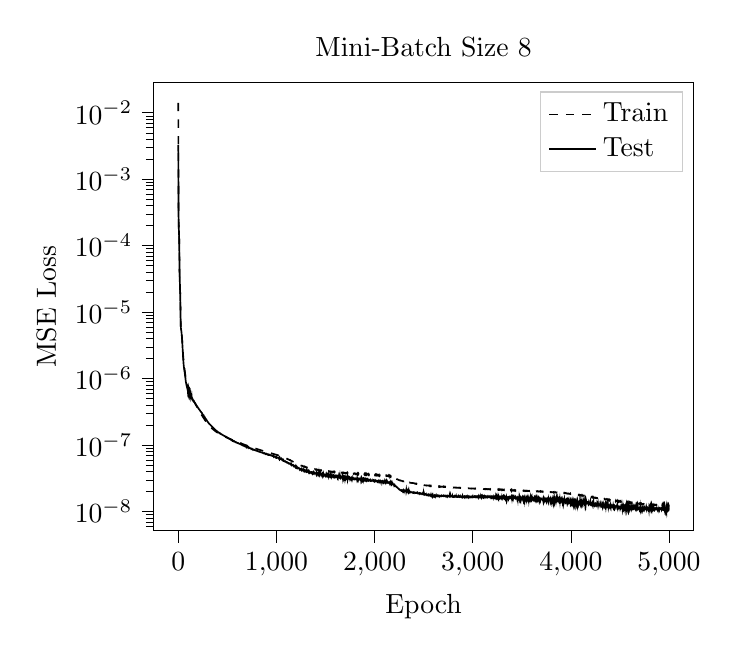
\begin{tikzpicture}

\begin{axis}[
legend cell align={left},
legend style={fill opacity=0.8, draw opacity=1, text opacity=1, draw=white!80!black},
log basis y={10},
tick align=outside,
tick pos=left,
title={Mini-Batch Size 8},
x grid style={white!69.0196078431373!black},
xlabel={Epoch},
xmin=-249.95, xmax=5248.95,
xtick style={color=black},
y grid style={white!69.0196078431373!black},
ylabel={MSE Loss},
ymin=5.12526233709927e-09, ymax=0.0285503119126669,
ymode=log,
ytick style={color=black}
]
\addplot [semithick, black, dashed]
table {%
0 0.0140922155501321
1 0.00164667243149597
2 0.00065037911516265
3 0.000295232196316647
4 0.000193644413906441
5 0.00017554680505782
6 0.000166322737537485
7 0.000155888844841684
8 0.000142262006907913
9 0.00012419570547172
10 0.000100196558816606
11 7.53355795714015e-05
12 5.41193190329068e-05
13 3.99818541809509e-05
14 3.23710513916922e-05
15 2.83831747833574e-05
16 2.58379168235479e-05
17 2.3768776641873e-05
18 2.16936214364978e-05
19 1.93698575890267e-05
20 1.67099984373635e-05
21 1.38117074528736e-05
22 1.10197760235451e-05
23 8.81342460627366e-06
24 7.32618501214688e-06
25 6.44809396973756e-06
26 5.96682320880859e-06
27 5.69452180099006e-06
28 5.51694411510084e-06
29 5.37627059711099e-06
30 5.25268244874155e-06
31 5.13194294012465e-06
32 5.00552247908104e-06
33 4.87103920659138e-06
34 4.72795897735523e-06
35 4.57529531857404e-06
36 4.41450717971747e-06
37 4.24678919441135e-06
38 4.07240037165479e-06
39 3.89275960455393e-06
40 3.70977897651414e-06
41 3.52646615996832e-06
42 3.3453291746639e-06
43 3.1669885086103e-06
44 2.99429524324069e-06
45 2.82882308749777e-06
46 2.67223944220518e-06
47 2.52574185277865e-06
48 2.39030650546113e-06
49 2.26648519112871e-06
50 2.15448263186602e-06
51 2.05455952405487e-06
52 1.96556939043546e-06
53 1.88664972873198e-06
54 1.81654708246981e-06
55 1.75456746703162e-06
56 1.69953624238417e-06
57 1.65011574182472e-06
58 1.60480939666741e-06
59 1.56276212375417e-06
60 1.52249059640042e-06
61 1.4837170463835e-06
62 1.44544674019187e-06
63 1.40767455231128e-06
64 1.37012475846632e-06
65 1.3339168483526e-06
66 1.29931519345661e-06
67 1.2659092755527e-06
68 1.23280311538565e-06
69 1.20021240133639e-06
70 1.16748595181093e-06
71 1.13551588817273e-06
72 1.10446207130366e-06
73 1.07352417389706e-06
74 1.04239164762987e-06
75 1.01698211097556e-06
76 9.92916835798496e-07
77 9.70485951363287e-07
78 9.49992109070763e-07
79 9.31409722205956e-07
80 9.14265601551279e-07
81 8.97762910810229e-07
82 8.82654424465557e-07
83 8.68559461117968e-07
84 8.55493358947967e-07
85 8.43273811710787e-07
86 8.31858977321076e-07
87 8.20936465963484e-07
88 8.10674030482517e-07
89 8.00620192784152e-07
90 7.91515300498702e-07
91 7.82651789464239e-07
92 7.7411152496154e-07
93 7.66956414445019e-07
94 7.5921274802937e-07
95 7.51383507328285e-07
96 7.44354396381652e-07
97 7.36274504674839e-07
98 7.30296529290797e-07
99 7.22306401783612e-07
100 7.16731141153559e-07
101 7.0944152068364e-07
102 7.04137545035621e-07
103 6.97249927974042e-07
104 6.922896165662e-07
105 6.85678604298801e-07
106 6.79918118848377e-07
107 6.74806719885623e-07
108 6.68366211726834e-07
109 6.63462581393048e-07
110 6.57123162881135e-07
111 6.52642981187057e-07
112 6.46561416587588e-07
113 6.42274032088608e-07
114 6.36438868973244e-07
115 6.32267128040098e-07
116 6.26555323151479e-07
117 6.21985995039154e-07
118 6.16880253367924e-07
119 6.11863263415557e-07
120 6.07826088987906e-07
121 6.02515582706076e-07
122 5.97315892207462e-07
123 5.93690181311501e-07
124 5.87228766487868e-07
125 5.84643050316913e-07
126 5.79739358123277e-07
127 5.74914281592953e-07
128 5.70551833760646e-07
129 5.66140960202688e-07
130 5.61847894573475e-07
131 5.57626214323648e-07
132 5.53413915262979e-07
133 5.49454119457948e-07
134 5.45167176518646e-07
135 5.41143863905802e-07
136 5.37298371497741e-07
137 5.32898270137139e-07
138 5.29843257034201e-07
139 5.25404720370659e-07
140 5.21684867152317e-07
141 5.18092104179857e-07
142 5.13483512598611e-07
143 5.08875732489145e-07
144 5.05149497538326e-07
145 5.01876758473685e-07
146 4.97770456185265e-07
147 4.94343421156174e-07
148 4.90650616956856e-07
149 4.8737844441149e-07
150 4.83746504770011e-07
151 4.80410617424099e-07
152 4.77105002900657e-07
153 4.73949040991073e-07
154 4.70770607652327e-07
155 4.67602424610192e-07
156 4.64573913710353e-07
157 4.61537018406233e-07
158 4.58560601526159e-07
159 4.55594075592813e-07
160 4.52629424799511e-07
161 4.49810896430591e-07
162 4.46874828853083e-07
163 4.44053090966179e-07
164 4.41227867604255e-07
165 4.38426361519362e-07
166 4.35670840431612e-07
167 4.33036380659502e-07
168 4.30322021191643e-07
169 4.27488975983437e-07
170 4.24709639364806e-07
171 4.21982422551537e-07
172 4.19321082635093e-07
173 4.16750839320912e-07
174 4.14194871584783e-07
175 4.1157767810418e-07
176 4.09005205327162e-07
177 4.06454590493155e-07
178 4.03974517769967e-07
179 4.01356386795726e-07
180 3.98910379288964e-07
181 3.96400903827754e-07
182 3.93962698311157e-07
183 3.91538277543901e-07
184 3.89058316706326e-07
185 3.86672758100559e-07
186 3.84376024534561e-07
187 3.82156077666451e-07
188 3.79795015795992e-07
189 3.77472126810829e-07
190 3.75254422486648e-07
191 3.72999132707719e-07
192 3.70814309334833e-07
193 3.68606052909115e-07
194 3.66414772166479e-07
195 3.64246124291867e-07
196 3.62064812147622e-07
197 3.60114379777343e-07
198 3.57652658479424e-07
199 3.55473573875997e-07
200 3.53420759978462e-07
201 3.51302201732295e-07
202 3.49260392450645e-07
203 3.47137964237021e-07
204 3.45095554795449e-07
205 3.43017129246448e-07
206 3.40932977728414e-07
207 3.38848146498094e-07
208 3.36741637614324e-07
209 3.34673315357747e-07
210 3.32618128226159e-07
211 3.30624918607469e-07
212 3.28681106719131e-07
213 3.2678425436572e-07
214 3.24867698765274e-07
215 3.23009222441328e-07
216 3.21105375114428e-07
217 3.19259059818222e-07
218 3.17433803207479e-07
219 3.15584080713194e-07
220 3.13753979209963e-07
221 3.11972391951798e-07
222 3.10204712469897e-07
223 3.08459960738361e-07
224 3.06718977086007e-07
225 3.04951894634087e-07
226 3.03379400019566e-07
227 3.01692094268446e-07
228 3.00041570543641e-07
229 2.98378097685514e-07
230 2.96704027594075e-07
231 2.95068247101682e-07
232 2.93436909618805e-07
233 2.91839041182129e-07
234 2.90256448501225e-07
235 2.88692379278643e-07
236 2.87134213266427e-07
237 2.85589026884026e-07
238 2.84047657121533e-07
239 2.82538714426295e-07
240 2.81039958053952e-07
241 2.79510103869285e-07
242 2.78032811682039e-07
243 2.76594212650139e-07
244 2.7475024603163e-07
245 2.72926708213106e-07
246 2.71423920384706e-07
247 2.7000172076086e-07
248 2.68524305077733e-07
249 2.67011570478815e-07
250 2.65667921034662e-07
251 2.64317999302932e-07
252 2.62892964080663e-07
253 2.6150448949025e-07
254 2.60125897110441e-07
255 2.58924373436997e-07
256 2.57517830519305e-07
257 2.56230467748253e-07
258 2.54854917034919e-07
259 2.53686509193329e-07
260 2.52175349391592e-07
261 2.51046833938062e-07
262 2.49770576434827e-07
263 2.48423187827029e-07
264 2.47144563388702e-07
265 2.45901549853045e-07
266 2.4462504500633e-07
267 2.43350985510205e-07
268 2.42261470663863e-07
269 2.41032267901176e-07
270 2.39729021991764e-07
271 2.38334006315455e-07
272 2.37114604335176e-07
273 2.35892772845858e-07
274 2.34670065896836e-07
275 2.3353716209229e-07
276 2.3238534521397e-07
277 2.31254778810808e-07
278 2.30117605983793e-07
279 2.29054269301088e-07
280 2.27954691752075e-07
281 2.26809562416719e-07
282 2.25817690040486e-07
283 2.24762463858497e-07
284 2.2381367495683e-07
285 2.22726548656738e-07
286 2.21723776196114e-07
287 2.20762035670674e-07
288 2.19673128100339e-07
289 2.18611050652129e-07
290 2.1762178107565e-07
291 2.16632967322994e-07
292 2.15608462355021e-07
293 2.14716398861725e-07
294 2.13740754045233e-07
295 2.12850587857361e-07
296 2.11970101840819e-07
297 2.11049697046661e-07
298 2.1004613132547e-07
299 2.09148392926295e-07
300 2.08267972048759e-07
301 2.0738952559185e-07
302 2.0650375899578e-07
303 2.0562344525743e-07
304 2.04789969075136e-07
305 2.03896006780724e-07
306 2.03049032204916e-07
307 2.02233469991597e-07
308 2.0148574800416e-07
309 2.00686525744231e-07
310 1.99914377798649e-07
311 1.99131872182789e-07
312 1.98344035812426e-07
313 1.97613068664282e-07
314 1.9680639949371e-07
315 1.96114129776603e-07
316 1.95406764222028e-07
317 1.94725376895022e-07
318 1.93973928373836e-07
319 1.93272308163017e-07
320 1.9257287543617e-07
321 1.91904341296123e-07
322 1.91237644701303e-07
323 1.90597502623291e-07
324 1.89894711086325e-07
325 1.8928915396188e-07
326 1.88604807627613e-07
327 1.8794622811491e-07
328 1.87344297193803e-07
329 1.86699944878299e-07
330 1.86075537186525e-07
331 1.85402446655658e-07
332 1.84775635814205e-07
333 1.84167428516346e-07
334 1.83570768633956e-07
335 1.82982711312007e-07
336 1.82418746863533e-07
337 1.81827815703528e-07
338 1.81145456025433e-07
339 1.80619840630669e-07
340 1.80006042857173e-07
341 1.79483078060372e-07
342 1.78932678077004e-07
343 1.7839446073431e-07
344 1.7783793585302e-07
345 1.77330097105965e-07
346 1.76734144670121e-07
347 1.76271198734312e-07
348 1.75766690267309e-07
349 1.75184670666795e-07
350 1.74708623170261e-07
351 1.74188886322924e-07
352 1.73653229948556e-07
353 1.73181383031462e-07
354 1.7267201918969e-07
355 1.72169975215297e-07
356 1.716809444261e-07
357 1.71193413185833e-07
358 1.7070678104858e-07
359 1.70231708297663e-07
360 1.69763145491331e-07
361 1.69323822717615e-07
362 1.68841542647513e-07
363 1.68392174817455e-07
364 1.67920915593811e-07
365 1.67448701848372e-07
366 1.67067471872784e-07
367 1.66522447294426e-07
368 1.66187803337436e-07
369 1.65655882883087e-07
370 1.65297342158866e-07
371 1.64844675270004e-07
372 1.64449132043387e-07
373 1.63934461077986e-07
374 1.63596360001961e-07
375 1.63166515610769e-07
376 1.62640494570709e-07
377 1.62330137088773e-07
378 1.61810680310737e-07
379 1.61525042159383e-07
380 1.61029843134486e-07
381 1.60723079604352e-07
382 1.60256959116367e-07
383 1.59806124516493e-07
384 1.59371342730807e-07
385 1.59003193211049e-07
386 1.58613461659129e-07
387 1.58135951810578e-07
388 1.5777919826121e-07
389 1.57490906419255e-07
390 1.57049220966599e-07
391 1.56678830967039e-07
392 1.56399091556736e-07
393 1.5595287873893e-07
394 1.55577467211288e-07
395 1.55218681813452e-07
396 1.54868281256881e-07
397 1.54552626023374e-07
398 1.54198211124168e-07
399 1.53841266364196e-07
400 1.53452866729964e-07
401 1.53133977093489e-07
402 1.52802964166199e-07
403 1.52480551506073e-07
404 1.52156185608376e-07
405 1.51788253479168e-07
406 1.51498513695003e-07
407 1.51127850402943e-07
408 1.50798184616718e-07
409 1.50510982436458e-07
410 1.50194480964316e-07
411 1.4992832301175e-07
412 1.49619644533416e-07
413 1.49345439441007e-07
414 1.49000281972178e-07
415 1.48698896465405e-07
416 1.48378767759638e-07
417 1.48073516024638e-07
418 1.47793847567357e-07
419 1.47497233387028e-07
420 1.47152927594263e-07
421 1.46810806187503e-07
422 1.46530012960611e-07
423 1.46194294019963e-07
424 1.45904546680953e-07
425 1.45637120098741e-07
426 1.45390437303661e-07
427 1.45085242406751e-07
428 1.44843584227061e-07
429 1.44539950433398e-07
430 1.44255259536763e-07
431 1.43986164975018e-07
432 1.43712213986902e-07
433 1.43442524212389e-07
434 1.43141190728002e-07
435 1.42893512014908e-07
436 1.42647763382797e-07
437 1.42393991835021e-07
438 1.42116199961961e-07
439 1.41860749801381e-07
440 1.41584198152245e-07
441 1.41324433158729e-07
442 1.41084530103086e-07
443 1.40788790234936e-07
444 1.40560038717652e-07
445 1.40289742095234e-07
446 1.40070903469791e-07
447 1.39810986377498e-07
448 1.3955653855291e-07
449 1.39309414347366e-07
450 1.39040228608778e-07
451 1.38806914293355e-07
452 1.38617263488072e-07
453 1.38398338824786e-07
454 1.38211991345116e-07
455 1.37910985833045e-07
456 1.37707504212159e-07
457 1.37452863837595e-07
458 1.37235590139895e-07
459 1.37014003817271e-07
460 1.36758330285147e-07
461 1.36494116027563e-07
462 1.36306082161752e-07
463 1.36068334931849e-07
464 1.35855103517102e-07
465 1.35629422052475e-07
466 1.35411948866349e-07
467 1.35155687953414e-07
468 1.34934801762299e-07
469 1.34734451673779e-07
470 1.34524718356843e-07
471 1.34328436132591e-07
472 1.34129347609147e-07
473 1.33910911843671e-07
474 1.3371256061312e-07
475 1.33461909047838e-07
476 1.33277299719126e-07
477 1.33085340515038e-07
478 1.32889105676881e-07
479 1.32672969037628e-07
480 1.32476193449804e-07
481 1.32274759009121e-07
482 1.32073942387123e-07
483 1.31855791474678e-07
484 1.31636651781619e-07
485 1.31416223496217e-07
486 1.31259498012071e-07
487 1.31016023310337e-07
488 1.30887004155866e-07
489 1.30695356258315e-07
490 1.30501306800923e-07
491 1.30296649251349e-07
492 1.30041917019597e-07
493 1.29918106384963e-07
494 1.29697845192567e-07
495 1.29461063567149e-07
496 1.29204722520981e-07
497 1.29046236825303e-07
498 1.28783909607577e-07
499 1.28579553615893e-07
500 1.28412652287579e-07
501 1.28222582777227e-07
502 1.28080913981421e-07
503 1.27826674720666e-07
504 1.2768455570189e-07
505 1.27511456184948e-07
506 1.27337297175956e-07
507 1.2712039346674e-07
508 1.26940336869552e-07
509 1.26781960378963e-07
510 1.26628617971747e-07
511 1.26438190140021e-07
512 1.26261214711931e-07
513 1.26080714901278e-07
514 1.25882205830763e-07
515 1.25689170451082e-07
516 1.25458669902656e-07
517 1.25292414027811e-07
518 1.25118541685509e-07
519 1.24933668057992e-07
520 1.24744541571076e-07
521 1.24592485745367e-07
522 1.2438628746736e-07
523 1.24239199989162e-07
524 1.24081532147713e-07
525 1.23898961273738e-07
526 1.23711435064067e-07
527 1.23683571343847e-07
528 1.23402232516057e-07
529 1.23180608545326e-07
530 1.22983389335474e-07
531 1.2279557410011e-07
532 1.22695858955524e-07
533 1.2242326393519e-07
534 1.22268119062241e-07
535 1.22114195065137e-07
536 1.2186837597028e-07
537 1.21758532072747e-07
538 1.21501212188235e-07
539 1.21415872920139e-07
540 1.21146897740232e-07
541 1.21149452825264e-07
542 1.20954131578088e-07
543 1.20601052417513e-07
544 1.2042635933085e-07
545 1.20382659668294e-07
546 1.20114501360291e-07
547 1.19902081415546e-07
548 1.19723047657061e-07
549 1.19519860986017e-07
550 1.19464099865851e-07
551 1.19455365275911e-07
552 1.18856987027627e-07
553 1.18855618111979e-07
554 1.18722306197583e-07
555 1.18556314758322e-07
556 1.18349971197418e-07
557 1.18197913097973e-07
558 1.18190822574249e-07
559 1.17993449931575e-07
560 1.17722103356144e-07
561 1.17562712910413e-07
562 1.1739236306596e-07
563 1.17146097792897e-07
564 1.17130330764326e-07
565 1.16876142195466e-07
566 1.16746778818566e-07
567 1.16807582864809e-07
568 1.16375001658398e-07
569 1.16238238121014e-07
570 1.16071960784225e-07
571 1.15917950825661e-07
572 1.15715357653201e-07
573 1.15682018952512e-07
574 1.15512718215527e-07
575 1.15298490829474e-07
576 1.15141919192041e-07
577 1.15017629779501e-07
578 1.14785245981963e-07
579 1.14825111019456e-07
580 1.14467956363384e-07
581 1.14309470399476e-07
582 1.14250206504352e-07
583 1.14062090345257e-07
584 1.14072716723257e-07
585 1.13818667545118e-07
586 1.13543024539808e-07
587 1.13510344416312e-07
588 1.13261899898021e-07
589 1.13188994674829e-07
590 1.12949545007623e-07
591 1.12861762920247e-07
592 1.12966328723374e-07
593 1.12624403906025e-07
594 1.12488853648784e-07
595 1.12194247433806e-07
596 1.12081747023041e-07
597 1.11879273879012e-07
598 1.11686604855166e-07
599 1.1151889847838e-07
600 1.11518363773655e-07
601 1.11229455521666e-07
602 1.11068491328581e-07
603 1.10914127503747e-07
604 1.10845691843053e-07
605 1.10635652848856e-07
606 1.10445679641913e-07
607 1.10333368983362e-07
608 1.10191389911307e-07
609 1.10141222277704e-07
610 1.09968580785491e-07
611 1.10079902308158e-07
612 1.09896487208161e-07
613 1.09495213120425e-07
614 1.09437622697328e-07
615 1.09409666039895e-07
616 1.09359268291698e-07
617 1.0894876301748e-07
618 1.08862762553841e-07
619 1.0888215664373e-07
620 1.08902593192184e-07
621 1.08681523236953e-07
622 1.08473326777769e-07
623 1.08357849692098e-07
624 1.08215046504156e-07
625 1.08083012595017e-07
626 1.07983994128702e-07
627 1.0788382092386e-07
628 1.07778989340446e-07
629 1.07629510504026e-07
630 1.07486674595592e-07
631 1.07359776917448e-07
632 1.07198026283228e-07
633 1.07110649613773e-07
634 1.06957342852709e-07
635 1.06551703673574e-07
636 1.06703632233973e-07
637 1.06261747919945e-07
638 1.06245268353788e-07
639 1.05981521867804e-07
640 1.0613362208467e-07
641 1.05918131012572e-07
642 1.05605284026922e-07
643 1.05518851803765e-07
644 1.05296745056549e-07
645 1.0529636806389e-07
646 1.05115613724394e-07
647 1.04897444288099e-07
648 1.04692954625563e-07
649 1.04653310055269e-07
650 1.04388389308596e-07
651 1.04356357626401e-07
652 1.04121267867185e-07
653 1.03941493522441e-07
654 1.03825485911813e-07
655 1.03654870686753e-07
656 1.03468656945438e-07
657 1.03318351046156e-07
658 1.03309234573246e-07
659 1.03166787249975e-07
660 1.02888646404509e-07
661 1.02764241914244e-07
662 1.02620244419427e-07
663 1.02643449945816e-07
664 1.02388692905464e-07
665 1.02254439710237e-07
666 1.02264427352949e-07
667 1.01974317667342e-07
668 1.01824479767032e-07
669 1.01781015130697e-07
670 1.01579884494996e-07
671 1.01662138689562e-07
672 1.01463956596604e-07
673 1.01146636220406e-07
674 1.01043345342333e-07
675 1.01026062447218e-07
676 1.00765059274366e-07
677 1.00705422818592e-07
678 1.00596716810841e-07
679 1.00494772908633e-07
680 1.00339713535291e-07
681 1.00227720652768e-07
682 1.00199328135986e-07
683 9.99779721606586e-08
684 9.99164768895611e-08
685 9.97651532674837e-08
686 9.96916367359546e-08
687 9.95852735758973e-08
688 9.94225873363064e-08
689 9.93057265326058e-08
690 9.91738692572852e-08
691 9.90683583950158e-08
692 9.89918791169941e-08
693 9.89294559996523e-08
694 9.87324563563874e-08
695 9.8580230650569e-08
696 9.84844026170606e-08
697 9.83782085786089e-08
698 9.82969909344433e-08
699 9.80663861103182e-08
700 9.79155029394718e-08
701 9.78743212769473e-08
702 9.7774189509181e-08
703 9.74998872109722e-08
704 9.7537862576047e-08
705 9.7373689259328e-08
706 9.72140168737923e-08
707 9.71121613257964e-08
708 9.69666632180122e-08
709 9.69298370527838e-08
710 9.67698093869984e-08
711 9.6669013320394e-08
712 9.6617836987889e-08
713 9.65235347489823e-08
714 9.643995225872e-08
715 9.6384693021534e-08
716 9.61863593840206e-08
717 9.60114623218544e-08
718 9.60902926934182e-08
719 9.57746484626654e-08
720 9.57750240715427e-08
721 9.55805155538059e-08
722 9.55347426128128e-08
723 9.54729408171318e-08
724 9.52798347118033e-08
725 9.52589754721345e-08
726 9.51665310111594e-08
727 9.49889552952499e-08
728 9.48892586905004e-08
729 9.48318259261782e-08
730 9.46984865208833e-08
731 9.46578152714039e-08
732 9.44619410319092e-08
733 9.44395689952415e-08
734 9.43228704386456e-08
735 9.42138219972577e-08
736 9.41150636339927e-08
737 9.40356634000494e-08
738 9.39251921092676e-08
739 9.37723432130611e-08
740 9.36953663508433e-08
741 9.36475301536177e-08
742 9.34891315171882e-08
743 9.34929558358277e-08
744 9.32899375643004e-08
745 9.31277580900058e-08
746 9.29872254360475e-08
747 9.29021212048298e-08
748 9.27547188318556e-08
749 9.26676536128212e-08
750 9.25360728327718e-08
751 9.24768817487376e-08
752 9.23224709517001e-08
753 9.2233401355557e-08
754 9.21099720416763e-08
755 9.20273056550513e-08
756 9.18983567661513e-08
757 9.17982077250912e-08
758 9.16838067226422e-08
759 9.1583944425544e-08
760 9.14591718057523e-08
761 9.13134026792051e-08
762 9.12507480110847e-08
763 9.11265217853341e-08
764 9.10621974288262e-08
765 9.08905435199614e-08
766 9.0788907545658e-08
767 9.0717570659038e-08
768 9.05781980975462e-08
769 9.05061573064359e-08
770 9.03604748181408e-08
771 9.02703232927848e-08
772 9.02022289084314e-08
773 9.01490784093184e-08
774 8.99447075433102e-08
775 8.98894601180089e-08
776 8.97487045516954e-08
777 8.9711841648743e-08
778 8.95438815806671e-08
779 8.95039619379645e-08
780 8.93075877943517e-08
781 8.92706220980699e-08
782 8.91444243862338e-08
783 8.90533289634732e-08
784 8.89315970269422e-08
785 8.88538352157298e-08
786 8.87460719418698e-08
787 8.86892839258024e-08
788 8.85925947713417e-08
789 8.84801011071801e-08
790 8.83455844515879e-08
791 8.83479853879265e-08
792 8.81836671791092e-08
793 8.8178019002072e-08
794 8.80678381420808e-08
795 8.79570468814705e-08
796 8.78213846133846e-08
797 8.77077261600689e-08
798 8.7557868305943e-08
799 8.75062553475914e-08
800 8.73836898467317e-08
801 8.73753748438233e-08
802 8.71596677542996e-08
803 8.71341073862553e-08
804 8.69886648713347e-08
805 8.69691683735851e-08
806 8.68006289946877e-08
807 8.67195310281232e-08
808 8.66247496071892e-08
809 8.66069136327141e-08
810 8.63993041644307e-08
811 8.63324029767298e-08
812 8.62302148672001e-08
813 8.61057656562636e-08
814 8.61300473475879e-08
815 8.58610517182612e-08
816 8.5876022253295e-08
817 8.58245899744148e-08
818 8.56204245254233e-08
819 8.56291569748535e-08
820 8.54643526437826e-08
821 8.53652859822418e-08
822 8.5391497251841e-08
823 8.51209773058414e-08
824 8.51588658763447e-08
825 8.50582824751811e-08
826 8.49786741063952e-08
827 8.48149538770215e-08
828 8.48154887371777e-08
829 8.46310325455235e-08
830 8.46116082833248e-08
831 8.44586885744292e-08
832 8.43162639991846e-08
833 8.43594839841089e-08
834 8.41931290338494e-08
835 8.40042691381271e-08
836 8.39640144789655e-08
837 8.39935478929021e-08
838 8.38417056181484e-08
839 8.3761031231866e-08
840 8.36453677903748e-08
841 8.35098131304335e-08
842 8.3516487031865e-08
843 8.3398541787183e-08
844 8.32627191780233e-08
845 8.32743370144939e-08
846 8.31479871719054e-08
847 8.30611524476055e-08
848 8.29425600832323e-08
849 8.28054075387996e-08
850 8.28294606325386e-08
851 8.27534693756959e-08
852 8.26178241633002e-08
853 8.25921608678115e-08
854 8.24915612467336e-08
855 8.23746438047834e-08
856 8.23552042801268e-08
857 8.22746717608069e-08
858 8.21175156664466e-08
859 8.20935714083149e-08
860 8.20074700209616e-08
861 8.18721728084171e-08
862 8.18467062071448e-08
863 8.17524560883243e-08
864 8.16378868124801e-08
865 8.16203907341162e-08
866 8.15071311217608e-08
867 8.14008423501988e-08
868 8.13587263230886e-08
869 8.12950596609241e-08
870 8.11408385228418e-08
871 8.11435524941118e-08
872 8.10090526517371e-08
873 8.09792461664571e-08
874 8.08584962870285e-08
875 8.07094791053231e-08
876 8.07686938379959e-08
877 8.06270915392204e-08
878 8.05262200671564e-08
879 8.04814699018053e-08
880 8.03900555492731e-08
881 8.03408116238913e-08
882 8.02471276806216e-08
883 8.01388805129477e-08
884 8.00124187625428e-08
885 8.00657544806072e-08
886 7.98942147488546e-08
887 7.99531881936488e-08
888 7.97822659910352e-08
889 7.97795756035668e-08
890 7.9595778335495e-08
891 7.94955623648619e-08
892 7.94511712500778e-08
893 7.94300374051815e-08
894 7.93113748613905e-08
895 7.92388654584642e-08
896 7.91362802941009e-08
897 7.90537630148691e-08
898 7.89241159324661e-08
899 7.89327640422499e-08
900 7.87739521186381e-08
901 7.87634696282069e-08
902 7.86302511679438e-08
903 7.85142067414313e-08
904 7.84941220688395e-08
905 7.836267482908e-08
906 7.83394425170059e-08
907 7.82585197347529e-08
908 7.82273210271356e-08
909 7.80942995328715e-08
910 7.80388083398975e-08
911 7.79501971406305e-08
912 7.78230592546336e-08
913 7.77868578483165e-08
914 7.76701064806318e-08
915 7.76812620495448e-08
916 7.75076760506366e-08
917 7.75319989765322e-08
918 7.74967118450931e-08
919 7.73487059220201e-08
920 7.73361544830209e-08
921 7.71912398640495e-08
922 7.71142926412338e-08
923 7.70105475949023e-08
924 7.69942951457381e-08
925 7.68621367575051e-08
926 7.66920159733786e-08
927 7.6753732895618e-08
928 7.66649599208691e-08
929 7.65232764639023e-08
930 7.64789896630091e-08
931 7.63227431415103e-08
932 7.62898755857222e-08
933 7.62348100540322e-08
934 7.61062690850522e-08
935 7.59985500060623e-08
936 7.60535598010037e-08
937 7.59387081998852e-08
938 7.58480387572646e-08
939 7.57766501973123e-08
940 7.56443777145677e-08
941 7.55885656298361e-08
942 7.55352047487889e-08
943 7.55366707450023e-08
944 7.54625999297431e-08
945 7.53840733613842e-08
946 7.52436891762187e-08
947 7.520958560292e-08
948 7.51185533998111e-08
949 7.50705502872151e-08
950 7.49230383103594e-08
951 7.48538313226632e-08
952 7.47696083367444e-08
953 7.4698309575183e-08
954 7.46352352933855e-08
955 7.45532024719608e-08
956 7.45396909715979e-08
957 7.43793192778952e-08
958 7.43306780917052e-08
959 7.42391270653897e-08
960 7.4170969384113e-08
961 7.41744250110088e-08
962 7.39807714547069e-08
963 7.3907636275905e-08
964 7.3864839967186e-08
965 7.38722046689233e-08
966 7.37782955395616e-08
967 7.35998169503205e-08
968 7.36751591370322e-08
969 7.35319244977717e-08
970 7.34493053959895e-08
971 7.33622083135543e-08
972 7.33287411573968e-08
973 7.32267693424049e-08
974 7.3227407262344e-08
975 7.30911046540328e-08
976 7.3059925388641e-08
977 7.29211026548882e-08
978 7.29121208236094e-08
979 7.2779587866556e-08
980 7.27771263386856e-08
981 7.26923735738794e-08
982 7.26410809015476e-08
983 7.25908489931371e-08
984 7.24250146495464e-08
985 7.2414066065285e-08
986 7.23511959135337e-08
987 7.23106430315923e-08
988 7.22220240687577e-08
989 7.21276343647048e-08
990 7.20563575073996e-08
991 7.19845479606462e-08
992 7.19308399528273e-08
993 7.18280783758019e-08
994 7.17602781392657e-08
995 7.16623081844503e-08
996 7.1633209976163e-08
997 7.1613316125152e-08
998 7.14358405220494e-08
999 7.13820533686516e-08
1000 7.13005416006496e-08
1001 7.13117426327514e-08
1002 7.11042069294621e-08
1003 7.11583764241297e-08
1004 7.11103543000746e-08
1005 7.09215685787967e-08
1006 7.08726079992061e-08
1007 7.08819332659871e-08
1008 7.06523474676146e-08
1009 7.06114099751076e-08
1010 7.05629681077013e-08
1011 7.04900955836862e-08
1012 7.03779293322881e-08
1013 7.03613790653535e-08
1014 7.02909734737744e-08
1015 7.02346028056411e-08
1016 7.00847629646617e-08
1017 7.00646524416371e-08
1018 7.00006208278481e-08
1019 6.99058087274551e-08
1020 6.97008041994351e-08
1021 6.96666002131252e-08
1022 6.95315661491946e-08
1023 6.93929467434629e-08
1024 6.93491352254938e-08
1025 6.92687724743735e-08
1026 6.9181248853134e-08
1027 6.90323947898364e-08
1028 6.89361719263815e-08
1029 6.88460079372177e-08
1030 6.88259702794625e-08
1031 6.87216120782708e-08
1032 6.85840478462652e-08
1033 6.85226009862205e-08
1034 6.83794042464214e-08
1035 6.83534466769942e-08
1036 6.82413636488022e-08
1037 6.81742337604874e-08
1038 6.8081035704104e-08
1039 6.80005548439055e-08
1040 6.79186499672468e-08
1041 6.78197289332161e-08
1042 6.77157139037376e-08
1043 6.77006809528535e-08
1044 6.75445062991997e-08
1045 6.74544157597268e-08
1046 6.73693972919054e-08
1047 6.72946742232838e-08
1048 6.71474435236519e-08
1049 6.70465003258514e-08
1050 6.70302539118595e-08
1051 6.69601158707067e-08
1052 6.68708544226959e-08
1053 6.67221369274884e-08
1054 6.66394672963477e-08
1055 6.65038577301047e-08
1056 6.64386373996351e-08
1057 6.6429855464456e-08
1058 6.63477771514209e-08
1059 6.62112182396868e-08
1060 6.61053233539377e-08
1061 6.60354965731358e-08
1062 6.58835158864335e-08
1063 6.58057612259455e-08
1064 6.57003935407019e-08
1065 6.56495188930961e-08
1066 6.55546697672094e-08
1067 6.54752256359359e-08
1068 6.53355711985881e-08
1069 6.52995786598609e-08
1070 6.52046299594034e-08
1071 6.50510368949142e-08
1072 6.50725278443787e-08
1073 6.49379873642886e-08
1074 6.47580108266155e-08
1075 6.46967440784962e-08
1076 6.47110855958033e-08
1077 6.46408487385841e-08
1078 6.45357608251018e-08
1079 6.44439404986485e-08
1080 6.4284627761424e-08
1081 6.42473115846087e-08
1082 6.42346976027497e-08
1083 6.4099857985056e-08
1084 6.39759074045898e-08
1085 6.39553085513e-08
1086 6.39084181939253e-08
1087 6.37432019150452e-08
1088 6.36723728701938e-08
1089 6.35793202752311e-08
1090 6.34713747382776e-08
1091 6.35341950525614e-08
1092 6.33713871458497e-08
1093 6.3277285804908e-08
1094 6.31845582761414e-08
1095 6.31149904926076e-08
1096 6.29787609565113e-08
1097 6.30093429236922e-08
1098 6.28861612330667e-08
1099 6.28055558475893e-08
1100 6.26232452294317e-08
1101 6.25952487345316e-08
1102 6.25822700701661e-08
1103 6.24765654775317e-08
1104 6.23883908117406e-08
1105 6.22942513581748e-08
1106 6.21327299015206e-08
1107 6.20863260349935e-08
1108 6.20415422387666e-08
1109 6.21000680087747e-08
1110 6.18504896578997e-08
1111 6.18067457205385e-08
1112 6.1644829599139e-08
1113 6.15710698008698e-08
1114 6.15897150124667e-08
1115 6.14760737152054e-08
1116 6.14502748659262e-08
1117 6.13122701871305e-08
1118 6.12455619730667e-08
1119 6.11872074065545e-08
1120 6.09162053128998e-08
1121 6.08576885987588e-08
1122 6.08179615930737e-08
1123 6.07086520618694e-08
1124 6.06223983101728e-08
1125 6.05575171297445e-08
1126 6.04104159798169e-08
1127 6.0348267340693e-08
1128 6.02285505344469e-08
1129 6.01458489990492e-08
1130 6.01179870587387e-08
1131 6.0027065746926e-08
1132 5.97797516208587e-08
1133 5.9795340693114e-08
1134 5.96402379002825e-08
1135 5.94761561911739e-08
1136 5.95539313339444e-08
1137 5.94249178975659e-08
1138 5.92505395076159e-08
1139 5.91597576615754e-08
1140 5.90666865125655e-08
1141 5.88915692842917e-08
1142 5.90203142101231e-08
1143 5.87497151824934e-08
1144 5.87532072353625e-08
1145 5.85907652910222e-08
1146 5.8551039190391e-08
1147 5.84408526567159e-08
1148 5.82552799874847e-08
1149 5.81301490427677e-08
1150 5.8109338837653e-08
1151 5.80481490803919e-08
1152 5.79101373157087e-08
1153 5.78085702569453e-08
1154 5.76846728073122e-08
1155 5.76280860729028e-08
1156 5.75032301490808e-08
1157 5.73179610068308e-08
1158 5.72661070288305e-08
1159 5.71943030065469e-08
1160 5.69885338492782e-08
1161 5.69631700626516e-08
1162 5.69194471786716e-08
1163 5.67838021701128e-08
1164 5.66640349766168e-08
1165 5.65589359924346e-08
1166 5.6512820266974e-08
1167 5.63850263919363e-08
1168 5.62500756329243e-08
1169 5.61824805593858e-08
1170 5.60970445784292e-08
1171 5.59599677218969e-08
1172 5.58494863724945e-08
1173 5.57552466800004e-08
1174 5.56996282252697e-08
1175 5.56156806448271e-08
1176 5.5491953369291e-08
1177 5.53300107037913e-08
1178 5.52866972709509e-08
1179 5.5107895852835e-08
1180 5.50283653844019e-08
1181 5.51412584899325e-08
1182 5.48718789001867e-08
1183 5.4910465046909e-08
1184 5.4751843118872e-08
1185 5.4634272609988e-08
1186 5.45681121217889e-08
1187 5.44585529360653e-08
1188 5.43135494264213e-08
1189 5.42500546694136e-08
1190 5.41413124164336e-08
1191 5.40952266248063e-08
1192 5.39357546243124e-08
1193 5.39131514880609e-08
1194 5.39165687554188e-08
1195 5.3634612921627e-08
1196 5.35923273101702e-08
1197 5.35096682368064e-08
1198 5.34264127121098e-08
1199 5.33043504136188e-08
1200 5.31984917513384e-08
1201 5.31392249949469e-08
1202 5.30054221310472e-08
1203 5.30110809604523e-08
1204 5.28841194253893e-08
1205 5.28213592305704e-08
1206 5.27674378001386e-08
1207 5.25633076429166e-08
1208 5.25129558854864e-08
1209 5.2446357926339e-08
1210 5.22644627349855e-08
1211 5.21429107900317e-08
1212 5.21280838032823e-08
1213 5.20980213041255e-08
1214 5.18598821455107e-08
1215 5.19323746939193e-08
1216 5.1801599847856e-08
1217 5.16898352844741e-08
1218 5.14871654297977e-08
1219 5.15548961050882e-08
1220 5.14475486421695e-08
1221 5.13119661880168e-08
1222 5.12700813648515e-08
1223 5.12630925495472e-08
1224 5.11038289716659e-08
1225 5.10397683979313e-08
1226 5.09275734623671e-08
1227 5.09132049710814e-08
1228 5.0759712610926e-08
1229 5.06871001304532e-08
1230 5.06944659219855e-08
1231 5.05630977118976e-08
1232 5.05891275865977e-08
1233 5.04078954683962e-08
1234 5.0369708529896e-08
1235 5.03202734072339e-08
1236 5.03486166767431e-08
1237 5.01460485304861e-08
1238 5.00217914414236e-08
1239 5.00083646550742e-08
1240 4.99302473584429e-08
1241 4.987592799921e-08
1242 4.97896254327834e-08
1243 4.97413813849157e-08
1244 4.96402420528952e-08
1245 4.9622389326931e-08
1246 4.95539652263233e-08
1247 4.94904343217861e-08
1248 4.94052279922386e-08
1249 4.92951875696868e-08
1250 4.93147989524267e-08
1251 4.91164378098041e-08
1252 4.91569000953262e-08
1253 4.91227655383675e-08
1254 4.90244803059703e-08
1255 4.89576740712039e-08
1256 4.8822162876494e-08
1257 4.87467866965297e-08
1258 4.87341117052509e-08
1259 4.87276126515113e-08
1260 4.87346524646881e-08
1261 4.85851170131113e-08
1262 4.84871747534754e-08
1263 4.85831895207234e-08
1264 4.82988585561728e-08
1265 4.83467545695504e-08
1266 4.83161799191834e-08
1267 4.81926020485801e-08
1268 4.81261100500063e-08
1269 4.80794487556224e-08
1270 4.79064465315204e-08
1271 4.78844559088643e-08
1272 4.80212023230564e-08
1273 4.79060066149728e-08
1274 4.7783847305638e-08
1275 4.76988225441843e-08
1276 4.77218500298804e-08
1277 4.76159679054788e-08
1278 4.76466013443755e-08
1279 4.74691612195599e-08
1280 4.75158579309465e-08
1281 4.73825057967225e-08
1282 4.7485986818252e-08
1283 4.72961260644666e-08
1284 4.73102585516472e-08
1285 4.72351163418594e-08
1286 4.72344711912598e-08
1287 4.71515645523724e-08
1288 4.71153546151015e-08
1289 4.68685075079023e-08
1290 4.70706135908827e-08
1291 4.68408979266144e-08
1292 4.68855339947893e-08
1293 4.69027191636329e-08
1294 4.68532288326884e-08
1295 4.66869751258869e-08
1296 4.67236158723239e-08
1297 4.66455751588768e-08
1298 4.6581428891912e-08
1299 4.66710647764046e-08
1300 4.65150191413244e-08
1301 4.6453202255492e-08
1302 4.64446993628798e-08
1303 4.63894488405003e-08
1304 4.62309609279288e-08
1305 4.62655005257773e-08
1306 4.63196391784493e-08
1307 4.61808473293246e-08
1308 4.61542245702162e-08
1309 4.62172598085786e-08
1310 4.61607299291344e-08
1311 4.60153494588056e-08
1312 4.59913277452983e-08
1313 4.59276329918268e-08
1314 4.58297194576573e-08
1315 4.59273223443191e-08
1316 4.58042492530453e-08
1317 4.57084866845037e-08
1318 4.56549604122003e-08
1319 4.56686972283293e-08
1320 4.56331827685119e-08
1321 4.56046227030882e-08
1322 4.5550667001848e-08
1323 4.55369211307399e-08
1324 4.5590441208887e-08
1325 4.54679211445708e-08
1326 4.54479248590545e-08
1327 4.52664653485257e-08
1328 4.5337347214236e-08
1329 4.53551621877324e-08
1330 4.51916858850154e-08
1331 4.51722750653971e-08
1332 4.51394618616874e-08
1333 4.51769472675778e-08
1334 4.51334482649557e-08
1335 4.51266249861249e-08
1336 4.50874914861288e-08
1337 4.49287061963233e-08
1338 4.48967479993456e-08
1339 4.48264219876648e-08
1340 4.4867042350738e-08
1341 4.48034820754728e-08
1342 4.48350610398052e-08
1343 4.48033875457554e-08
1344 4.45712150360933e-08
1345 4.46036571952746e-08
1346 4.46692990454523e-08
1347 4.45814032055125e-08
1348 4.45665362684977e-08
1349 4.45728043025895e-08
1350 4.45147311864957e-08
1351 4.44823261869232e-08
1352 4.43828213363417e-08
1353 4.42768181132536e-08
1354 4.43993598802095e-08
1355 4.44070804617169e-08
1356 4.42842968162438e-08
1357 4.41155342043587e-08
1358 4.41278631075903e-08
1359 4.40644807078172e-08
1360 4.42094289478945e-08
1361 4.40818237334994e-08
1362 4.39918047412391e-08
1363 4.41803186754797e-08
1364 4.40159865835454e-08
1365 4.39419652753514e-08
1366 4.39800256470946e-08
1367 4.38194544480908e-08
1368 4.38346918683052e-08
1369 4.38826430064765e-08
1370 4.38439412224767e-08
1371 4.38131168918332e-08
1372 4.37225367591054e-08
1373 4.36888630588328e-08
1374 4.37150416381371e-08
1375 4.36178424365608e-08
1376 4.36608899700985e-08
1377 4.35089207826422e-08
1378 4.35441604231812e-08
1379 4.35481492102596e-08
1380 4.34936193034474e-08
1381 4.33650798727925e-08
1382 4.34177889596654e-08
1383 4.34463673570917e-08
1384 4.33263139223428e-08
1385 4.33727313220444e-08
1386 4.33343354258042e-08
1387 4.3228653130889e-08
1388 4.31082869178923e-08
1389 4.324872136241e-08
1390 4.30600019534211e-08
1391 4.32475265323973e-08
1392 4.30882091100315e-08
1393 4.30473245973673e-08
1394 4.29888738828765e-08
1395 4.30272572833346e-08
1396 4.29292623698174e-08
1397 4.2927458932418e-08
1398 4.30014096650666e-08
1399 4.30005459408633e-08
1400 4.28852556577652e-08
1401 4.28427411769405e-08
1402 4.29186751995658e-08
1403 4.26496567271784e-08
1404 4.28333187523222e-08
1405 4.27500164761341e-08
1406 4.27967534255558e-08
1407 4.26256254471014e-08
1408 4.26668547057751e-08
1409 4.25627499347492e-08
1410 4.27053181430992e-08
1411 4.24960702827271e-08
1412 4.25527307035267e-08
1413 4.25026517083538e-08
1414 4.24830301199997e-08
1415 4.24793107010046e-08
1416 4.24730674390972e-08
1417 4.23903328332642e-08
1418 4.25100638867804e-08
1419 4.24156434370992e-08
1420 4.23989374351841e-08
1421 4.23957842898837e-08
1422 4.23277789733945e-08
1423 4.23183708635477e-08
1424 4.22206468280173e-08
1425 4.22159647799347e-08
1426 4.22320841448887e-08
1427 4.21671459114314e-08
1428 4.22204840990759e-08
1429 4.21945885649144e-08
1430 4.21728435395785e-08
1431 4.21243299655316e-08
1432 4.20114667738503e-08
1433 4.20510037324462e-08
1434 4.2026753572344e-08
1435 4.19436382799176e-08
1436 4.19389113277546e-08
1437 4.19057039202642e-08
1438 4.18952429424024e-08
1439 4.19827620414814e-08
1440 4.19652518064417e-08
1441 4.18845844243343e-08
1442 4.19072387116692e-08
1443 4.17922589410757e-08
1444 4.16854369809094e-08
1445 4.1889259613459e-08
1446 4.17623865209826e-08
1447 4.17697262604655e-08
1448 4.17888626045304e-08
1449 4.16201110771119e-08
1450 4.17640830239208e-08
1451 4.1783336582224e-08
1452 4.153928639683e-08
1453 4.16737873538686e-08
1454 4.1592476381247e-08
1455 4.15322517932637e-08
1456 4.1644548808506e-08
1457 4.15027544096169e-08
1458 4.148360849765e-08
1459 4.13861753427724e-08
1460 4.14018035996833e-08
1461 4.13481794314663e-08
1462 4.14854741146442e-08
1463 4.13563179764154e-08
1464 4.13556541101201e-08
1465 4.13902445641767e-08
1466 4.1323798298798e-08
1467 4.13480203884653e-08
1468 4.1203276207824e-08
1469 4.1235213055657e-08
1470 4.11417126029434e-08
1471 4.12246168219887e-08
1472 4.11880018207356e-08
1473 4.10834203830035e-08
1474 4.12011794010958e-08
1475 4.10904470413698e-08
1476 4.10302819586761e-08
1477 4.10799662917682e-08
1478 4.10220235567138e-08
1479 4.10007051749872e-08
1480 4.09940534513709e-08
1481 4.09689597491436e-08
1482 4.10433389328446e-08
1483 4.10684464080546e-08
1484 4.0948897821913e-08
1485 4.09499040134875e-08
1486 4.08794801574075e-08
1487 4.09105480914107e-08
1488 4.08452793374536e-08
1489 4.08942971645843e-08
1490 4.07402955646674e-08
1491 4.08870578434417e-08
1492 4.07994149629332e-08
1493 4.08190274594489e-08
1494 4.08339842810079e-08
1495 4.06289100567392e-08
1496 4.07976245524466e-08
1497 4.0624878185902e-08
1498 4.07296249225197e-08
1499 4.06837669739701e-08
1500 4.06156222441112e-08
1501 4.07313091956851e-08
1502 4.05451847482752e-08
1503 4.06221682425212e-08
1504 4.05266821212891e-08
1505 4.04707060539522e-08
1506 4.06462516782113e-08
1507 4.04694767723868e-08
1508 4.04878702155997e-08
1509 4.05097304012614e-08
1510 4.04145102264053e-08
1511 4.0458490955686e-08
1512 4.04152247091005e-08
1513 4.04283759909418e-08
1514 4.04303081200652e-08
1515 4.03291169508435e-08
1516 4.03538379005752e-08
1517 4.04357018073398e-08
1518 4.01908035403409e-08
1519 4.0378684301956e-08
1520 4.01831596095192e-08
1521 4.03242693085559e-08
1522 4.01736299417976e-08
1523 4.02171476885371e-08
1524 4.03139829083798e-08
1525 4.0050756290988e-08
1526 4.01579128519458e-08
1527 4.01703933876618e-08
1528 4.01928873969837e-08
1529 4.01609750353415e-08
1530 4.00341430619733e-08
1531 4.01794336895023e-08
1532 4.00297975486907e-08
1533 4.00986562185679e-08
1534 4.01208160880628e-08
1535 3.99242789086429e-08
1536 4.00895154815117e-08
1537 3.99392733978488e-08
1538 4.00255155073026e-08
1539 3.99330273790355e-08
1540 4.00368776256599e-08
1541 3.98720245327056e-08
1542 3.99692181636269e-08
1543 3.98561598462521e-08
1544 3.98875270821719e-08
1545 3.9898592707921e-08
1546 3.99073250436643e-08
1547 3.99202588603487e-08
1548 3.9863083950209e-08
1549 3.98795083480508e-08
1550 3.98830174299647e-08
1551 3.97511638707826e-08
1552 3.98775771195403e-08
1553 3.97159798799507e-08
1554 3.98367431264646e-08
1555 3.97162449825572e-08
1556 3.97871075605849e-08
1557 3.96644445856964e-08
1558 3.9699416047867e-08
1559 3.97870561856806e-08
1560 3.96381743366092e-08
1561 3.97042046440532e-08
1562 3.96156072683951e-08
1563 3.96154665756043e-08
1564 3.96605191550492e-08
1565 3.958909697932e-08
1566 3.96173939121169e-08
1567 3.949263310421e-08
1568 3.96089839078684e-08
1569 3.95455036246162e-08
1570 3.9636709490587e-08
1571 3.94831752732472e-08
1572 3.94724301058247e-08
1573 3.95125908312366e-08
1574 3.94526429312592e-08
1575 3.95341919947612e-08
1576 3.93538525056414e-08
1577 3.94563540533355e-08
1578 3.93826284383891e-08
1579 3.94670636287842e-08
1580 3.93370668776427e-08
1581 3.93753766632088e-08
1582 3.93889478891296e-08
1583 3.93959847713177e-08
1584 3.93097157589395e-08
1585 3.93532651656869e-08
1586 3.91723971162605e-08
1587 3.9439265921537e-08
1588 3.92176067336436e-08
1589 3.92966383158111e-08
1590 3.93851996420835e-08
1591 3.91521733389411e-08
1592 3.91947608742171e-08
1593 3.92991181339397e-08
1594 3.91132583290599e-08
1595 3.93028898422187e-08
1596 3.90764033886271e-08
1597 3.92399381112796e-08
1598 3.92021937143383e-08
1599 3.90802838641235e-08
1600 3.91499000782503e-08
1601 3.91313884398059e-08
1602 3.90865781119132e-08
1603 3.91318111354622e-08
1604 3.90454653018679e-08
1605 3.90933970058072e-08
1606 3.91323979753722e-08
1607 3.91136423418814e-08
1608 3.90225514497189e-08
1609 3.89170263863647e-08
1610 3.90865480301983e-08
1611 3.8980921593712e-08
1612 3.89813223291569e-08
1613 3.90147075677305e-08
1614 3.89207366335853e-08
1615 3.89198063510676e-08
1616 3.90334313173923e-08
1617 3.88514370586179e-08
1618 3.89586336879688e-08
1619 3.88994614555216e-08
1620 3.89837869310128e-08
1621 3.88157792121646e-08
1622 3.8903180284322e-08
1623 3.88374568531802e-08
1624 3.89662983231176e-08
1625 3.87433496351619e-08
1626 3.88509129178871e-08
1627 3.87580687961631e-08
1628 3.89098066246873e-08
1629 3.86810810075744e-08
1630 3.8847601955716e-08
1631 3.8731702770356e-08
1632 3.88384859340007e-08
1633 3.86796453755167e-08
1634 3.86607207518708e-08
1635 3.86814175348249e-08
1636 3.86742364932857e-08
1637 3.87164597510647e-08
1638 3.86513170154146e-08
1639 3.88603046239666e-08
1640 3.85722263551713e-08
1641 3.86626669151013e-08
1642 3.85764308683534e-08
1643 3.85580688213594e-08
1644 3.86169037662754e-08
1645 3.85148538581959e-08
1646 3.86165236889724e-08
1647 3.84727122453299e-08
1648 3.88424589639058e-08
1649 3.84465692357949e-08
1650 3.85114503771433e-08
1651 3.84911400512777e-08
1652 3.84304911449362e-08
1653 3.85630037955664e-08
1654 3.84011487293279e-08
1655 3.84661550612009e-08
1656 3.85328484400205e-08
1657 3.84369141146479e-08
1658 3.84122835210832e-08
1659 3.8412436121682e-08
1660 3.83894825235487e-08
1661 3.84446199950261e-08
1662 3.8335402538614e-08
1663 3.83735077038594e-08
1664 3.83685282532298e-08
1665 3.83480501557898e-08
1666 3.82956904871889e-08
1667 3.84011462086775e-08
1668 3.83502299774463e-08
1669 3.83458634498624e-08
1670 3.8245394529568e-08
1671 3.83146489473241e-08
1672 3.82573301918043e-08
1673 3.82244613819083e-08
1674 3.8246418380794e-08
1675 3.82150598499109e-08
1676 3.82407916803551e-08
1677 3.82599868506972e-08
1678 3.8215464568836e-08
1679 3.81728400284942e-08
1680 3.83210382013388e-08
1681 3.80955480121514e-08
1682 3.81806894989012e-08
1683 3.82224091151073e-08
1684 3.81114148124695e-08
1685 3.82258913358413e-08
1686 3.82052000684752e-08
1687 3.81070638280079e-08
1688 3.8081548687785e-08
1689 3.81398353761497e-08
1690 3.81179427018097e-08
1691 3.80720296826453e-08
1692 3.80211410555553e-08
1693 3.81585196489453e-08
1694 3.80863659596997e-08
1695 3.7976557523578e-08
1696 3.80630843066498e-08
1697 3.81245449689871e-08
1698 3.80392725380929e-08
1699 3.801984486973e-08
1700 3.79566180743751e-08
1701 3.79708953985869e-08
1702 3.80453341737308e-08
1703 3.79378156063481e-08
1704 3.79759017397063e-08
1705 3.79490948132499e-08
1706 3.80014099050641e-08
1707 3.78876995812405e-08
1708 3.79235057170746e-08
1709 3.79901633928981e-08
1710 3.79401265870882e-08
1711 3.78765139581461e-08
1712 3.78788724297863e-08
1713 3.79089320423631e-08
1714 3.79844686686504e-08
1715 3.79382417801111e-08
1716 3.79571741651041e-08
1717 3.79882111483099e-08
1718 3.78223503592068e-08
1719 3.7959839022772e-08
1720 3.76949858327258e-08
1721 3.80500853780497e-08
1722 3.77684928363209e-08
1723 3.79319000765044e-08
1724 3.78127555658025e-08
1725 3.76808580231369e-08
1726 3.78913456544616e-08
1727 3.76658090703863e-08
1728 3.7851494917529e-08
1729 3.77664108097697e-08
1730 3.79108147838814e-08
1731 3.76634401306752e-08
1732 3.78151026674267e-08
1733 3.78816969464069e-08
1734 3.77709782481972e-08
1735 3.77660620167752e-08
1736 3.76888900031069e-08
1737 3.77818670016516e-08
1738 3.78022734786043e-08
1739 3.77456426572387e-08
1740 3.76173546103864e-08
1741 3.76604630600852e-08
1742 3.77668573965373e-08
1743 3.77400727162858e-08
1744 3.77201424601736e-08
1745 3.77242986160375e-08
1746 3.75634211788878e-08
1747 3.74809592673664e-08
1748 3.7722135395768e-08
1749 3.76457967710131e-08
1750 3.76064268419185e-08
1751 3.76065779379431e-08
1752 3.74286121975764e-08
1753 3.77629903707266e-08
1754 3.76661396659372e-08
1755 3.74908666405105e-08
1756 3.76121619192205e-08
1757 3.75940156729371e-08
1758 3.76416019105541e-08
1759 3.74089387640275e-08
1760 3.75451150600448e-08
1761 3.74251382719848e-08
1762 3.73434886444812e-08
1763 3.76087765929789e-08
1764 3.75553967626452e-08
1765 3.73977909142731e-08
1766 3.74640324758424e-08
1767 3.73550987626814e-08
1768 3.74835799159534e-08
1769 3.73618815268095e-08
1770 3.75936487801987e-08
1771 3.72713335470287e-08
1772 3.75196970185954e-08
1773 3.72949849896109e-08
1774 3.7603680296705e-08
1775 3.72440201465984e-08
1776 3.75571327109192e-08
1777 3.72496371237041e-08
1778 3.74038666710597e-08
1779 3.74239376252916e-08
1780 3.74428224656498e-08
1781 3.7323855651028e-08
1782 3.74017605850874e-08
1783 3.72666274963684e-08
1784 3.73440678775872e-08
1785 3.73906923156753e-08
1786 3.73588830671068e-08
1787 3.71107454029129e-08
1788 3.72834189805715e-08
1789 3.73839526646158e-08
1790 3.74207804099136e-08
1791 3.72704231348386e-08
1792 3.72604873839499e-08
1793 3.72039002338731e-08
1794 3.72388135945201e-08
1795 3.73753077895778e-08
1796 3.72486858588594e-08
1797 3.72918126916311e-08
1798 3.72434037134717e-08
1799 3.72466739793076e-08
1800 3.72663990639843e-08
1801 3.71341596454577e-08
1802 3.7279309918592e-08
1803 3.72007997335722e-08
1804 3.72522711966639e-08
1805 3.71977966189263e-08
1806 3.71243192054393e-08
1807 3.71166673645007e-08
1808 3.69281813226152e-08
1809 3.7265723722868e-08
1810 3.72295604456063e-08
1811 3.7045100355293e-08
1812 3.71322109171679e-08
1813 3.71508310981206e-08
1814 3.71456299328443e-08
1815 3.71071213347562e-08
1816 3.71199989213089e-08
1817 3.70692861344502e-08
1818 3.71239575356341e-08
1819 3.70205668143164e-08
1820 3.70877458459873e-08
1821 3.69541319535926e-08
1822 3.70777116702747e-08
1823 3.67921550732397e-08
1824 3.7050849953868e-08
1825 3.70229679376166e-08
1826 3.69968310884872e-08
1827 3.71215581407291e-08
1828 3.67214813636885e-08
1829 3.70434229832739e-08
1830 3.67917332182444e-08
1831 3.71148817803757e-08
1832 3.69631161016848e-08
1833 3.67094972708593e-08
1834 3.69223256053708e-08
1835 3.67426318259589e-08
1836 3.70516558798606e-08
1837 3.67933732445813e-08
1838 3.69378140621102e-08
1839 3.68091435007933e-08
1840 3.68699657187221e-08
1841 3.67680227189027e-08
1842 3.67932825673378e-08
1843 3.66279344761189e-08
1844 3.70051625235845e-08
1845 3.66218960352604e-08
1846 3.71567434198639e-08
1847 3.67378085286418e-08
1848 3.67072405182967e-08
1849 3.68038352065447e-08
1850 3.67439507895639e-08
1851 3.66124083939212e-08
1852 3.67425429224077e-08
1853 3.67981550968288e-08
1854 3.66166572089988e-08
1855 3.68664959489173e-08
1856 3.65924359608805e-08
1857 3.66692661883938e-08
1858 3.66733336858438e-08
1859 3.67367757094783e-08
1860 3.65539251201419e-08
1861 3.67730002568401e-08
1862 3.65517606497612e-08
1863 3.67414380395559e-08
1864 3.65365003003326e-08
1865 3.66813095511453e-08
1866 3.65326868894122e-08
1867 3.68337799656615e-08
1868 3.66286341191291e-08
1869 3.65044348935584e-08
1870 3.66127535955663e-08
1871 3.65746113235588e-08
1872 3.65417026371162e-08
1873 3.67053717078569e-08
1874 3.6658561624936e-08
1875 3.65626657981011e-08
1876 3.65201574044072e-08
1877 3.67783549450884e-08
1878 3.66494288788211e-08
1879 3.66888207783411e-08
1880 3.65948743836775e-08
1881 3.65293158486324e-08
1882 3.6500014441998e-08
1883 3.64699401549373e-08
1884 3.64751547068387e-08
1885 3.65656375094225e-08
1886 3.65746387260835e-08
1887 3.66372703726192e-08
1888 3.64976410645035e-08
1889 3.65722141060232e-08
1890 3.64866452176038e-08
1891 3.65375467361595e-08
1892 3.65167638012309e-08
1893 3.63294874006215e-08
1894 3.63945058015069e-08
1895 3.6536670052989e-08
1896 3.6430282676303e-08
1897 3.62453244746597e-08
1898 3.66222929399918e-08
1899 3.64198722717646e-08
1900 3.63831767380418e-08
1901 3.63298386836242e-08
1902 3.61740805980837e-08
1903 3.64556771561553e-08
1904 3.63519154173986e-08
1905 3.62696372944171e-08
1906 3.61171992451226e-08
1907 3.64603584808165e-08
1908 3.61317012207429e-08
1909 3.62745675124287e-08
1910 3.64189258177383e-08
1911 3.6266710974342e-08
1912 3.62556905648681e-08
1913 3.6238342407291e-08
1914 3.62670215623417e-08
1915 3.60366312679439e-08
1916 3.63011385027256e-08
1917 3.61772445773845e-08
1918 3.61867287574924e-08
1919 3.61102679971026e-08
1920 3.63929243683003e-08
1921 3.60180869836135e-08
1922 3.61357699847353e-08
1923 3.61040660279421e-08
1924 3.6139368550181e-08
1925 3.60739116982423e-08
1926 3.6196284967982e-08
1927 3.59936592344567e-08
1928 3.60563996575358e-08
1929 3.60782758486167e-08
1930 3.60398286818331e-08
1931 3.60291056034079e-08
1932 3.60345146028784e-08
1933 3.59823884230615e-08
1934 3.60840954800601e-08
1935 3.59893449890514e-08
1936 3.59963851610523e-08
1937 3.62121882626632e-08
1938 3.59255595241414e-08
1939 3.60697188535042e-08
1940 3.59639030174108e-08
1941 3.61143853102597e-08
1942 3.58569910274831e-08
1943 3.6043464469504e-08
1944 3.58307471461927e-08
1945 3.60832720742721e-08
1946 3.58909315378853e-08
1947 3.59922691823833e-08
1948 3.588628298834e-08
1949 3.57991387196499e-08
1950 3.59611625162515e-08
1951 3.59351795946594e-08
1952 3.58898386458861e-08
1953 3.57527423555659e-08
1954 3.5908256137418e-08
1955 3.57621854756296e-08
1956 3.58349212685738e-08
1957 3.58016397492555e-08
1958 3.59061841495034e-08
1959 3.58764264776212e-08
1960 3.59239804565981e-08
1961 3.56813113904231e-08
1962 3.58514508875807e-08
1963 3.57986901380336e-08
1964 3.57795846923636e-08
1965 3.58297134064323e-08
1966 3.58044209156638e-08
1967 3.57522844649516e-08
1968 3.57979316274459e-08
1969 3.57875962246901e-08
1970 3.58005632263847e-08
1971 3.57308950551527e-08
1972 3.57868481506429e-08
1973 3.57633905760935e-08
1974 3.59752080516529e-08
1975 3.54793153327648e-08
1976 3.56424363725516e-08
1977 3.56962309773223e-08
1978 3.57075252499506e-08
1979 3.5845165480719e-08
1980 3.56351077415162e-08
1981 3.56275620205793e-08
1982 3.56691139065113e-08
1983 3.5589426081728e-08
1984 3.56025159495843e-08
1985 3.58654780168166e-08
1986 3.56388935309759e-08
1987 3.5567677426851e-08
1988 3.56262408662822e-08
1989 3.56126999379036e-08
1990 3.57467316645099e-08
1991 3.55701531344899e-08
1992 3.57601672029695e-08
1993 3.55033272736449e-08
1994 3.57265346040414e-08
1995 3.5396074536731e-08
1996 3.54844572565405e-08
1997 3.57656564653475e-08
1998 3.53924049982801e-08
1999 3.55584950182397e-08
2000 3.56697449870325e-08
2001 3.56787138220405e-08
2002 3.55943911167778e-08
2003 3.54479785218409e-08
2004 3.56183040364222e-08
2005 3.53309536897939e-08
2006 3.5582972430781e-08
2007 3.55872772117571e-08
2008 3.56063758508718e-08
2009 3.55415195936182e-08
2010 3.55386896822019e-08
2011 3.55435800902804e-08
2012 3.54341543582493e-08
2013 3.5326350536824e-08
2014 3.54429674618295e-08
2015 3.56998978769951e-08
2016 3.54859376350269e-08
2017 3.53400733024145e-08
2018 3.55125124622546e-08
2019 3.53422700452022e-08
2020 3.55198382075983e-08
2021 3.53294625350387e-08
2022 3.53245762756416e-08
2023 3.54871031174042e-08
2024 3.55245614671595e-08
2025 3.52888825934095e-08
2026 3.55585673830205e-08
2027 3.54134896176639e-08
2028 3.53721047030575e-08
2029 3.54860238958032e-08
2030 3.54437497889215e-08
2031 3.55012276966882e-08
2032 3.53924766249847e-08
2033 3.53858738901813e-08
2034 3.53863012767519e-08
2035 3.54097912538265e-08
2036 3.52552421158947e-08
2037 3.54500118371348e-08
2038 3.53148007081749e-08
2039 3.51771727915562e-08
2040 3.52485998993402e-08
2041 3.52664494878141e-08
2042 3.53212110244527e-08
2043 3.52696402448061e-08
2044 3.53278196350004e-08
2045 3.50798110102524e-08
2046 3.53038244638171e-08
2047 3.50380686655605e-08
2048 3.53732404003715e-08
2049 3.52515104800055e-08
2050 3.52898717146388e-08
2051 3.51912950766753e-08
2052 3.52262799583336e-08
2053 3.52031993360313e-08
2054 3.51986800883886e-08
2055 3.49191987663033e-08
2056 3.50503156130166e-08
2057 3.50460932994068e-08
2058 3.51862639345057e-08
2059 3.54123910732973e-08
2060 3.5012984096916e-08
2061 3.5237672851629e-08
2062 3.50989451058936e-08
2063 3.51451456923613e-08
2064 3.50956153982729e-08
2065 3.51490209666849e-08
2066 3.51532928246634e-08
2067 3.50932326336206e-08
2068 3.50858328599379e-08
2069 3.50466975369557e-08
2070 3.5128578741439e-08
2071 3.50624365870189e-08
2072 3.51087634351543e-08
2073 3.50725950184483e-08
2074 3.48720382215006e-08
2075 3.50937104562909e-08
2076 3.50986688211208e-08
2077 3.49998700812648e-08
2078 3.50636079833322e-08
2079 3.50096038435055e-08
2080 3.4841453009804e-08
2081 3.50405389926145e-08
2082 3.50292538255914e-08
2083 3.49853204753003e-08
2084 3.50112577467421e-08
2085 3.49354300377414e-08
2086 3.49946228852538e-08
2087 3.47063039427553e-08
2088 3.50340738730637e-08
2089 3.49463078346268e-08
2090 3.48853253449022e-08
2091 3.50643476894064e-08
2092 3.48874224593843e-08
2093 3.4948104152388e-08
2094 3.49539611530503e-08
2095 3.47071131532317e-08
2096 3.48301070332013e-08
2097 3.48174625681708e-08
2098 3.48316413565364e-08
2099 3.46571736122847e-08
2100 3.48714099800418e-08
2101 3.47187161162665e-08
2102 3.47542465775064e-08
2103 3.48218386880816e-08
2104 3.46967600517445e-08
2105 3.48042466460363e-08
2106 3.46572571419124e-08
2107 3.46827273878247e-08
2108 3.47622488425792e-08
2109 3.47469773482878e-08
2110 3.47767646564634e-08
2111 3.47355067442656e-08
2112 3.4546701973337e-08
2113 3.47556978592678e-08
2114 3.46318142816493e-08
2115 3.46471681780258e-08
2116 3.47924431811641e-08
2117 3.46481810264976e-08
2118 3.44733216182114e-08
2119 3.46518337575041e-08
2120 3.46098472623346e-08
2121 3.45996842279206e-08
2122 3.47283432957646e-08
2123 3.46137393982815e-08
2124 3.45159064116807e-08
2125 3.46012808627449e-08
2126 3.44771602875937e-08
2127 3.45803697943126e-08
2128 3.44515754568953e-08
2129 3.45153512402163e-08
2130 3.45798061651692e-08
2131 3.45268843418012e-08
2132 3.44025088856448e-08
2133 3.45208335361669e-08
2134 3.4445654149895e-08
2135 3.45518178868076e-08
2136 3.45473493346127e-08
2137 3.4456031099861e-08
2138 3.4364484506888e-08
2139 3.44972221721918e-08
2140 3.43248367657978e-08
2141 3.4492944448683e-08
2142 3.43385404715235e-08
2143 3.45781598660722e-08
2144 3.4290496093714e-08
2145 3.43060144554208e-08
2146 3.44058043646456e-08
2147 3.43255302404088e-08
2148 3.41100668381777e-08
2149 3.41952895204223e-08
2150 3.43601639203328e-08
2151 3.4153532772585e-08
2152 3.41090135576039e-08
2153 3.4155436126504e-08
2154 3.42936208577171e-08
2155 3.3856299904933e-08
2156 3.42150716563516e-08
2157 3.3988354551262e-08
2158 3.405076265528e-08
2159 3.38644607005278e-08
2160 3.41631483760096e-08
2161 3.39845888581713e-08
2162 3.38284178185155e-08
2163 3.38537514537052e-08
2164 3.40268143110833e-08
2165 3.39710133356874e-08
2166 3.3770219998619e-08
2167 3.40399171161465e-08
2168 3.39991786018068e-08
2169 3.38950475993194e-08
2170 3.36694171254592e-08
2171 3.35623848246591e-08
2172 3.358883385296e-08
2173 3.35593926847899e-08
2174 3.36249531995847e-08
2175 3.35927736521136e-08
2176 3.36960097553352e-08
2177 3.3357819268609e-08
2178 3.34103945465181e-08
2179 3.33792154614265e-08
2180 3.33711916660206e-08
2181 3.33325034604925e-08
2182 3.34902264049752e-08
2183 3.34050771559902e-08
2184 3.35643477549219e-08
2185 3.31968241833458e-08
2186 3.31900424805909e-08
2187 3.30820723366543e-08
2188 3.33634762741397e-08
2189 3.29869779860381e-08
2190 3.29270568819595e-08
2191 3.29535492369359e-08
2192 3.30423635066524e-08
2193 3.2968385207166e-08
2194 3.29141850103909e-08
2195 3.27679847420548e-08
2196 3.26790389784115e-08
2197 3.27125180756838e-08
2198 3.28457829645856e-08
2199 3.26832230150842e-08
2200 3.25508643124195e-08
2201 3.25069563849034e-08
2202 3.25951758823884e-08
2203 3.23611900134857e-08
2204 3.24298381007004e-08
2205 3.23351022797347e-08
2206 3.21446096176459e-08
2207 3.22599062272388e-08
2208 3.19862765207901e-08
2209 3.20416892187758e-08
2210 3.19288464889489e-08
2211 3.17090809489606e-08
2212 3.17792905293324e-08
2213 3.15104079864348e-08
2214 3.1462118692982e-08
2215 3.13828922715587e-08
2216 3.13321562357416e-08
2217 3.12738587888717e-08
2218 3.12520617335998e-08
2219 3.12137117948197e-08
2220 3.10057306038836e-08
2221 3.12358310861072e-08
2222 3.10054063796805e-08
2223 3.09421507194152e-08
2224 3.08758929641328e-08
2225 3.08620648987734e-08
2226 3.08012100713739e-08
2227 3.07649796962295e-08
2228 3.07027676993421e-08
2229 3.06398884948322e-08
2230 3.0567268998638e-08
2231 3.05280521204487e-08
2232 3.04718943495708e-08
2233 3.04078486101922e-08
2234 3.03745679617329e-08
2235 3.03228287630297e-08
2236 3.02672447705099e-08
2237 3.02545674801813e-08
2238 3.01988235289485e-08
2239 3.01402142439677e-08
2240 3.01196001135651e-08
2241 3.00748270705142e-08
2242 3.00020169574644e-08
2243 2.99772841376722e-08
2244 2.99949804882793e-08
2245 2.99182164966716e-08
2246 2.98174154473863e-08
2247 2.98337497213197e-08
2248 2.97877957007309e-08
2249 2.97282025942813e-08
2250 2.96885503319189e-08
2251 2.96915600075387e-08
2252 2.96268828261503e-08
2253 2.96020686509912e-08
2254 2.95862130044178e-08
2255 2.95726172665489e-08
2256 2.95009567898852e-08
2257 2.94234437800966e-08
2258 2.94252965509223e-08
2259 2.94418085973192e-08
2260 2.93423016528571e-08
2261 2.93364664556428e-08
2262 2.9278265921473e-08
2263 2.92813284907822e-08
2264 2.92852222609774e-08
2265 2.92450523597942e-08
2266 2.92166284019402e-08
2267 2.91476965621484e-08
2268 2.91206469871241e-08
2269 2.9084005692237e-08
2270 2.90973084280388e-08
2271 2.9066154888735e-08
2272 2.90592396314793e-08
2273 2.903219871353e-08
2274 2.8993103499797e-08
2275 2.90072672499697e-08
2276 2.89885272022339e-08
2277 2.89520249459052e-08
2278 2.89304525491474e-08
2279 2.8873197399637e-08
2280 2.88416605038755e-08
2281 2.87946236485759e-08
2282 2.87163995920103e-08
2283 2.8751229569135e-08
2284 2.86675678098369e-08
2285 2.87072197124871e-08
2286 2.86591628351207e-08
2287 2.86360354149195e-08
2288 2.86377652902736e-08
2289 2.86282400225879e-08
2290 2.86060725163129e-08
2291 2.85601986473871e-08
2292 2.8566027550081e-08
2293 2.85328380456029e-08
2294 2.84778560919463e-08
2295 2.8503181678019e-08
2296 2.84794163121216e-08
2297 2.84508193038047e-08
2298 2.84375073329457e-08
2299 2.84022412997409e-08
2300 2.84504239880246e-08
2301 2.83795681350618e-08
2302 2.80858092560621e-08
2303 2.81308356857579e-08
2304 2.84017445939533e-08
2305 2.83484147467483e-08
2306 2.82965770237453e-08
2307 2.81869080178687e-08
2308 2.82838599325874e-08
2309 2.82717122983556e-08
2310 2.82287362001199e-08
2311 2.81732639646481e-08
2312 2.82028487006425e-08
2313 2.81964688206848e-08
2314 2.82919290341965e-08
2315 2.81617670132572e-08
2316 2.80558309988521e-08
2317 2.80766361031581e-08
2318 2.80740395859347e-08
2319 2.80186498251567e-08
2320 2.78623242437881e-08
2321 2.78319890574252e-08
2322 2.7838097744759e-08
2323 2.81434602773523e-08
2324 2.79450416238447e-08
2325 2.78161572744295e-08
2326 2.79697963896375e-08
2327 2.79070327633413e-08
2328 2.78919659102428e-08
2329 2.78619289257875e-08
2330 2.78659629824318e-08
2331 2.78614516817655e-08
2332 2.77982614309558e-08
2333 2.75627960046876e-08
2334 2.7683113924315e-08
2335 2.76638133267504e-08
2336 2.7976017778375e-08
2337 2.77359681546407e-08
2338 2.75629913719655e-08
2339 2.77539640132218e-08
2340 2.77165115951661e-08
2341 2.76678804733699e-08
2342 2.76632074442951e-08
2343 2.76779803503047e-08
2344 2.7455451997227e-08
2345 2.74844656082962e-08
2346 2.74150879100432e-08
2347 2.73005283002448e-08
2348 2.73293975054933e-08
2349 2.73166359772148e-08
2350 2.73018226644162e-08
2351 2.72489444093083e-08
2352 2.73889708166664e-08
2353 2.72320520533498e-08
2354 2.72790375470677e-08
2355 2.72348291288083e-08
2356 2.73146983129635e-08
2357 2.73088766502561e-08
2358 2.72420718752109e-08
2359 2.71807621974318e-08
2360 2.71759283165807e-08
2361 2.71592088800787e-08
2362 2.716162148797e-08
2363 2.71283624564411e-08
2364 2.71220685803542e-08
2365 2.71014957067273e-08
2366 2.70860176589949e-08
2367 2.70522221228475e-08
2368 2.70808371154452e-08
2369 2.70027544879703e-08
2370 2.70345289230534e-08
2371 2.6964751616898e-08
2372 2.696691184223e-08
2373 2.69479568371089e-08
2374 2.69498847638161e-08
2375 2.69362674423235e-08
2376 2.69187825274741e-08
2377 2.68844778372745e-08
2378 2.68902544915406e-08
2379 2.68711434427971e-08
2380 2.68514626293737e-08
2381 2.68734419184291e-08
2382 2.68483514633822e-08
2383 2.68327053034589e-08
2384 2.68972461920924e-08
2385 2.68946966976991e-08
2386 2.68688440390186e-08
2387 2.68711721576054e-08
2388 2.68394169249397e-08
2389 2.68374860716847e-08
2390 2.68135587213614e-08
2391 2.6805691601961e-08
2392 2.67745706401534e-08
2393 2.6809520248694e-08
2394 2.67572526135851e-08
2395 2.6740364799771e-08
2396 2.67548818264629e-08
2397 2.67323597937796e-08
2398 2.67107425182544e-08
2399 2.66933362711441e-08
2400 2.66796495886901e-08
2401 2.66811331712802e-08
2402 2.66719013644057e-08
2403 2.66482157882386e-08
2404 2.66498887371291e-08
2405 2.65529375331752e-08
2406 2.64868419983522e-08
2407 2.64362802493423e-08
2408 2.63785517100601e-08
2409 2.64098169204807e-08
2410 2.62780924766837e-08
2411 2.62741602781169e-08
2412 2.6275515581986e-08
2413 2.63046898743013e-08
2414 2.62378383566464e-08
2415 2.62339208467743e-08
2416 2.6197952087248e-08
2417 2.61643609240636e-08
2418 2.61683168703009e-08
2419 2.61335110480765e-08
2420 2.61862989838768e-08
2421 2.6123462132599e-08
2422 2.61582386786863e-08
2423 2.60744872910834e-08
2424 2.61248545112558e-08
2425 2.60602128983045e-08
2426 2.5996013666596e-08
2427 2.59825018495974e-08
2428 2.61028798762553e-08
2429 2.59763141152725e-08
2430 2.59699663778257e-08
2431 2.5952968202958e-08
2432 2.58987610708417e-08
2433 2.58901513450205e-08
2434 2.59073284434308e-08
2435 2.58808899733509e-08
2436 2.58690743470957e-08
2437 2.59155831829894e-08
2438 2.58984107750493e-08
2439 2.58327015063564e-08
2440 2.58910232133758e-08
2441 2.5851744575256e-08
2442 2.58734603728605e-08
2443 2.58497839209504e-08
2444 2.57852705596306e-08
2445 2.5749621920923e-08
2446 2.56977506314371e-08
2447 2.57797519069847e-08
2448 2.56253563124531e-08
2449 2.568607414144e-08
2450 2.56544600301112e-08
2451 2.57075833505205e-08
2452 2.55754417626264e-08
2453 2.554663458465e-08
2454 2.55213013602429e-08
2455 2.55292079387459e-08
2456 2.55761564451618e-08
2457 2.56380117495958e-08
2458 2.5466044155209e-08
2459 2.55924793446383e-08
2460 2.5411626344507e-08
2461 2.5483353592648e-08
2462 2.54037278160091e-08
2463 2.53894689294931e-08
2464 2.5385459480276e-08
2465 2.54166745379258e-08
2466 2.53300338006746e-08
2467 2.52633231934141e-08
2468 2.52905496420652e-08
2469 2.52612174573841e-08
2470 2.52215043445858e-08
2471 2.52222532011182e-08
2472 2.51468582752601e-08
2473 2.51776597233189e-08
2474 2.51615491562163e-08
2475 2.51395283474842e-08
2476 2.52183839921649e-08
2477 2.51443643182192e-08
2478 2.51232011265756e-08
2479 2.51217024658246e-08
2480 2.50529616079298e-08
2481 2.51389312446726e-08
2482 2.50886437704878e-08
2483 2.50070869021179e-08
2484 2.50177555844999e-08
2485 2.49742417359755e-08
2486 2.49877498199602e-08
2487 2.49677537893511e-08
2488 2.50068211697929e-08
2489 2.49653871566835e-08
2490 2.4933863711496e-08
2491 2.49424296749901e-08
2492 2.4951844725507e-08
2493 2.4892882751093e-08
2494 2.4931655667082e-08
2495 2.48718469033626e-08
2496 2.49019510607518e-08
2497 2.48731343424069e-08
2498 2.48883164082336e-08
2499 2.49033845207691e-08
2500 2.49035872372794e-08
2501 2.48862970964048e-08
2502 2.48035862342455e-08
2503 2.48739398363007e-08
2504 2.47867319709272e-08
2505 2.48239095244074e-08
2506 2.48499960635584e-08
2507 2.48351267178037e-08
2508 2.48323786125049e-08
2509 2.47996488513813e-08
2510 2.48657050256895e-08
2511 2.48231005408606e-08
2512 2.47950744980407e-08
2513 2.47893814209199e-08
2514 2.47993815580827e-08
2515 2.47897829086519e-08
2516 2.47634090388971e-08
2517 2.47896581013762e-08
2518 2.47696634980699e-08
2519 2.47453253470198e-08
2520 2.47223928200313e-08
2521 2.47334208407501e-08
2522 2.47096111714029e-08
2523 2.4687650667321e-08
2524 2.46956074168025e-08
2525 2.46711931128907e-08
2526 2.46819320248726e-08
2527 2.46199760338683e-08
2528 2.45927725193162e-08
2529 2.46706242497119e-08
2530 2.46061201409908e-08
2531 2.46551861158295e-08
2532 2.4620513753959e-08
2533 2.46363766653879e-08
2534 2.4628943702254e-08
2535 2.46116972482113e-08
2536 2.46342331093885e-08
2537 2.46114901591987e-08
2538 2.46096278395669e-08
2539 2.45866363863811e-08
2540 2.45964233274165e-08
2541 2.45708998334315e-08
2542 2.45835269470085e-08
2543 2.45638348301824e-08
2544 2.45521365713763e-08
2545 2.45779312835204e-08
2546 2.45374288643241e-08
2547 2.45665522609073e-08
2548 2.45263032567777e-08
2549 2.45214198875132e-08
2550 2.45059835601857e-08
2551 2.45173493294004e-08
2552 2.44947074992119e-08
2553 2.45010167594373e-08
2554 2.45626643931018e-08
2555 2.44792750354605e-08
2556 2.44580011252715e-08
2557 2.45601274948548e-08
2558 2.44549451076104e-08
2559 2.44704517249339e-08
2560 2.44637011022064e-08
2561 2.44879491315686e-08
2562 2.4345519065605e-08
2563 2.44300616065729e-08
2564 2.43928618703926e-08
2565 2.43841448002158e-08
2566 2.43780653921277e-08
2567 2.43811462623533e-08
2568 2.43616524753243e-08
2569 2.43661697965081e-08
2570 2.43490519786782e-08
2571 2.43574382601253e-08
2572 2.43382521336599e-08
2573 2.43445802485809e-08
2574 2.44352526195257e-08
2575 2.42636506588845e-08
2576 2.4382859165506e-08
2577 2.43264350885397e-08
2578 2.43318004828907e-08
2579 2.4318235475107e-08
2580 2.43151912489026e-08
2581 2.43053389064052e-08
2582 2.42865047273e-08
2583 2.42982581002416e-08
2584 2.43043741323667e-08
2585 2.43125716861137e-08
2586 2.42699668686619e-08
2587 2.42551985039086e-08
2588 2.42744805540873e-08
2589 2.42553433427162e-08
2590 2.42339634275446e-08
2591 2.42310187354988e-08
2592 2.42103561043372e-08
2593 2.41927280453247e-08
2594 2.42068397344752e-08
2595 2.41830105895957e-08
2596 2.42476137515268e-08
2597 2.42324421826368e-08
2598 2.41915985257357e-08
2599 2.41748273044351e-08
2600 2.4186519977043e-08
2601 2.4179407354552e-08
2602 2.41663565696548e-08
2603 2.41800421174609e-08
2604 2.41570701149385e-08
2605 2.41318774478749e-08
2606 2.41287477287244e-08
2607 2.41291152303091e-08
2608 2.41133490512802e-08
2609 2.41305678247983e-08
2610 2.40912506952462e-08
2611 2.40801481559139e-08
2612 2.41406477159423e-08
2613 2.41297449727895e-08
2614 2.4095290498849e-08
2615 2.41204857425181e-08
2616 2.40823391250977e-08
2617 2.41169306987032e-08
2618 2.40800200885793e-08
2619 2.40420970376576e-08
2620 2.40115907583771e-08
2621 2.40670964557488e-08
2622 2.40035303660235e-08
2623 2.40694404207709e-08
2624 2.39871997282926e-08
2625 2.40326550962067e-08
2626 2.3954168761442e-08
2627 2.40268140512256e-08
2628 2.39998666065055e-08
2629 2.3985291254025e-08
2630 2.39567574289445e-08
2631 2.39846544216604e-08
2632 2.39369897876429e-08
2633 2.38818613977898e-08
2634 2.39493084817077e-08
2635 2.38887064112347e-08
2636 2.38993242347441e-08
2637 2.38915883681301e-08
2638 2.39090372167183e-08
2639 2.39165006532538e-08
2640 2.3909196885441e-08
2641 2.38644657239995e-08
2642 2.38849699494281e-08
2643 2.38983762548273e-08
2644 2.38486406014538e-08
2645 2.38773196845621e-08
2646 2.37812354573208e-08
2647 2.38795882485654e-08
2648 2.38290460594648e-08
2649 2.38504818601548e-08
2650 2.37533120950317e-08
2651 2.38623648134428e-08
2652 2.38244231485218e-08
2653 2.38374669074837e-08
2654 2.3715871300567e-08
2655 2.38580457896376e-08
2656 2.37788429551244e-08
2657 2.38263465703881e-08
2658 2.37195858003858e-08
2659 2.37419101249969e-08
2660 2.37934447815391e-08
2661 2.37060152064039e-08
2662 2.36939189370844e-08
2663 2.37918087830913e-08
2664 2.36732907157311e-08
2665 2.37708965618033e-08
2666 2.36870809127154e-08
2667 2.37533571190163e-08
2668 2.37491758019459e-08
2669 2.3639161234712e-08
2670 2.37320687501708e-08
2671 2.37475380013841e-08
2672 2.37412641430623e-08
2673 2.36923716476767e-08
2674 2.36276849037154e-08
2675 2.36815473018126e-08
2676 2.37157332745319e-08
2677 2.36273267089082e-08
2678 2.36026643971599e-08
2679 2.36067487993097e-08
2680 2.36209799626685e-08
2681 2.36060413589811e-08
2682 2.36104203490406e-08
2683 2.35962008585666e-08
2684 2.35850015508632e-08
2685 2.35924942075805e-08
2686 2.35782205866286e-08
2687 2.35772843812931e-08
2688 2.35597968245571e-08
2689 2.35777446437879e-08
2690 2.35565437538554e-08
2691 2.36214133733093e-08
2692 2.35524341407611e-08
2693 2.35394026484315e-08
2694 2.35335459319863e-08
2695 2.35269057853316e-08
2696 2.35304583857676e-08
2697 2.35221716367029e-08
2698 2.3512224325728e-08
2699 2.35274898261473e-08
2700 2.35030608459752e-08
2701 2.35141017910223e-08
2702 2.34844594322325e-08
2703 2.36064162817406e-08
2704 2.34715549627396e-08
2705 2.34835558088342e-08
2706 2.34769890599118e-08
2707 2.3475392880723e-08
2708 2.35423416667935e-08
2709 2.34751648244824e-08
2710 2.34421265172813e-08
2711 2.35501992356113e-08
2712 2.34397110476792e-08
2713 2.34394784577319e-08
2714 2.34332887245614e-08
2715 2.34243712990967e-08
2716 2.34388668758356e-08
2717 2.34305880923991e-08
2718 2.34182796852167e-08
2719 2.34181999414496e-08
2720 2.34149909239534e-08
2721 2.35061410664983e-08
2722 2.33975469403624e-08
2723 2.33830739988505e-08
2724 2.34114976724875e-08
2725 2.34548312159077e-08
2726 2.34424559604207e-08
2727 2.33738831645347e-08
2728 2.3432231981424e-08
2729 2.33567075063057e-08
2730 2.34046533869048e-08
2731 2.33488871375087e-08
2732 2.3352429380008e-08
2733 2.33481457661e-08
2734 2.33407855181333e-08
2735 2.33648137433207e-08
2736 2.33318322822029e-08
2737 2.33070653319345e-08
2738 2.3346116288625e-08
2739 2.33266172862123e-08
2740 2.33008381118616e-08
2741 2.33355860723705e-08
2742 2.32842534395594e-08
2743 2.33014976913637e-08
2744 2.32890997100554e-08
2745 2.32929399976989e-08
2746 2.3302574435391e-08
2747 2.33146102432968e-08
2748 2.32785370557487e-08
2749 2.32942535798308e-08
2750 2.32616284869813e-08
2751 2.32929211234634e-08
2752 2.32491365919074e-08
2753 2.32627183809342e-08
2754 2.32306790786119e-08
2755 2.3276313755094e-08
2756 2.32429791906519e-08
2757 2.32749975759283e-08
2758 2.32213192310482e-08
2759 2.32215358355603e-08
2760 2.32546402201272e-08
2761 2.32203828449684e-08
2762 2.33159703797448e-08
2763 2.31969889625816e-08
2764 2.314681362936e-08
2765 2.31738245357604e-08
2766 2.3170235046166e-08
2767 2.31266902575022e-08
2768 2.3123720971796e-08
2769 2.31477672127944e-08
2770 2.30991476701803e-08
2771 2.31053931303293e-08
2772 2.31188731598664e-08
2773 2.3145674900249e-08
2774 2.30820694473444e-08
2775 2.31041685183619e-08
2776 2.30864719110713e-08
2777 2.30861167858087e-08
2778 2.30348852974238e-08
2779 2.30820793194475e-08
2780 2.30819818543004e-08
2781 2.30532784768478e-08
2782 2.30654754611592e-08
2783 2.30319875065277e-08
2784 2.30562718042115e-08
2785 2.3061908677402e-08
2786 2.3006683151916e-08
2787 2.30508197067714e-08
2788 2.30231742781584e-08
2789 2.30193855776939e-08
2790 2.30073178633106e-08
2791 2.29989750257786e-08
2792 2.30151464095663e-08
2793 2.30415139754747e-08
2794 2.2970916178533e-08
2795 2.3006379019197e-08
2796 2.30143007993178e-08
2797 2.29839285088573e-08
2798 2.29939372036192e-08
2799 2.29693911610873e-08
2800 2.30020177247603e-08
2801 2.29397145639076e-08
2802 2.29599945593684e-08
2803 2.29954475106098e-08
2804 2.29464646674948e-08
2805 2.29727204277275e-08
2806 2.2946284010672e-08
2807 2.29688330946054e-08
2808 2.28977551794962e-08
2809 2.29595473451027e-08
2810 2.29503427240374e-08
2811 2.29251608412362e-08
2812 2.29668454219123e-08
2813 2.29262388535822e-08
2814 2.29372032620745e-08
2815 2.29429834188721e-08
2816 2.29121144466049e-08
2817 2.29283576671513e-08
2818 2.29099798922938e-08
2819 2.29299884892953e-08
2820 2.28775421917682e-08
2821 2.28866969096408e-08
2822 2.29147223489434e-08
2823 2.29009073966502e-08
2824 2.28908831978458e-08
2825 2.29076539066675e-08
2826 2.28706648472965e-08
2827 2.29095146546676e-08
2828 2.28287743642142e-08
2829 2.28744850696572e-08
2830 2.28264675494749e-08
2831 2.28482780260109e-08
2832 2.28631989376282e-08
2833 2.28285269741058e-08
2834 2.28815637091095e-08
2835 2.28192816194017e-08
2836 2.28238579511597e-08
2837 2.28280531362479e-08
2838 2.28150668024618e-08
2839 2.28126944015195e-08
2840 2.28211046033877e-08
2841 2.27821876359613e-08
2842 2.28276182587805e-08
2843 2.27965611223624e-08
2844 2.27861874484425e-08
2845 2.27895648836629e-08
2846 2.28024336195176e-08
2847 2.27751800885301e-08
2848 2.27899082791971e-08
2849 2.27718561216506e-08
2850 2.27767926768152e-08
2851 2.27349871697591e-08
2852 2.27359381210768e-08
2853 2.27825065404197e-08
2854 2.27540307560226e-08
2855 2.27609142315899e-08
2856 2.27369288285928e-08
2857 2.27386377598116e-08
2858 2.27283334819361e-08
2859 2.27572066249238e-08
2860 2.27120586546725e-08
2861 2.27790808859929e-08
2862 2.26962135125852e-08
2863 2.27254233706731e-08
2864 2.27075532377441e-08
2865 2.27113100152998e-08
2866 2.27105394650096e-08
2867 2.26963902347777e-08
2868 2.27075190419868e-08
2869 2.26801028460066e-08
2870 2.26805808400954e-08
2871 2.27163207671133e-08
2872 2.26599603716515e-08
2873 2.27128980405666e-08
2874 2.26495166697482e-08
2875 2.26838920949213e-08
2876 2.2633144937334e-08
2877 2.27002717037017e-08
2878 2.26501465849793e-08
2879 2.26438821955277e-08
2880 2.26743442386379e-08
2881 2.26622551937616e-08
2882 2.26392203792614e-08
2883 2.26614374052581e-08
2884 2.26081309948611e-08
2885 2.26377313041759e-08
2886 2.26622117187603e-08
2887 2.26091042265786e-08
2888 2.26329164516592e-08
2889 2.26028324581407e-08
2890 2.26154009084212e-08
2891 2.26111500527537e-08
2892 2.25871219257101e-08
2893 2.25940610474318e-08
2894 2.26068414987957e-08
2895 2.25933509092613e-08
2896 2.26463827064372e-08
2897 2.25531392392675e-08
2898 2.2575582794282e-08
2899 2.25953645252019e-08
2900 2.25612005455567e-08
2901 2.25841375893765e-08
2902 2.26227083439667e-08
2903 2.25383530056966e-08
2904 2.25521555567987e-08
2905 2.25481722559984e-08
2906 2.25636249209238e-08
2907 2.25257892529918e-08
2908 2.25722115554383e-08
2909 2.24744241084096e-08
2910 2.25321640257015e-08
2911 2.26051607103983e-08
2912 2.24659051037968e-08
2913 2.25132282407614e-08
2914 2.25238143851669e-08
2915 2.24942209117174e-08
2916 2.2489711597462e-08
2917 2.25633682031656e-08
2918 2.24660171594948e-08
2919 2.24490727580573e-08
2920 2.24820107517232e-08
2921 2.25042746353488e-08
2922 2.24400970441074e-08
2923 2.25074355393318e-08
2924 2.24257760801372e-08
2925 2.24687806360535e-08
2926 2.24606469632072e-08
2927 2.24621305324746e-08
2928 2.24441385925367e-08
2929 2.24451444834628e-08
2930 2.25064913146333e-08
2931 2.24001227961956e-08
2932 2.24331048723769e-08
2933 2.24461386779673e-08
2934 2.24210934156588e-08
2935 2.2414025148354e-08
2936 2.24331432985281e-08
2937 2.23916673203206e-08
2938 2.24072612478032e-08
2939 2.24330685445473e-08
2940 2.23980179203664e-08
2941 2.23874248690414e-08
2942 2.24090919109798e-08
2943 2.24122577434649e-08
2944 2.23516667210433e-08
2945 2.23846981870501e-08
2946 2.23750139611845e-08
2947 2.23675531274559e-08
2948 2.23690972482871e-08
2949 2.23966252086427e-08
2950 2.23590922039385e-08
2951 2.23575589957115e-08
2952 2.23446854898945e-08
2953 2.23787074973281e-08
2954 2.23484926151762e-08
2955 2.23410897159937e-08
2956 2.23185536469828e-08
2957 2.23394644485175e-08
2958 2.23433849302346e-08
2959 2.23287105440839e-08
2960 2.23443335674034e-08
2961 2.23401842065485e-08
2962 2.22854145679463e-08
2963 2.23340432303765e-08
2964 2.23200163498305e-08
2965 2.23124990528234e-08
2966 2.23158065382201e-08
2967 2.2295199315181e-08
2968 2.23108840757824e-08
2969 2.22952372217478e-08
2970 2.2297369233204e-08
2971 2.23066160116581e-08
2972 2.22738460897709e-08
2973 2.22975133237213e-08
2974 2.22771114106735e-08
2975 2.22468722848035e-08
2976 2.22956516267025e-08
2977 2.22850922777518e-08
2978 2.22585025828614e-08
2979 2.22740814486144e-08
2980 2.22606010553683e-08
2981 2.22279482837706e-08
2982 2.2239388069778e-08
2983 2.22621345362661e-08
2984 2.22273305126031e-08
2985 2.22571749564082e-08
2986 2.22320354779093e-08
2987 2.21837540239633e-08
2988 2.22493222183928e-08
2989 2.22160562559637e-08
2990 2.22250939407864e-08
2991 2.22165201968494e-08
2992 2.2228362487553e-08
2993 2.21891013674203e-08
2994 2.21847167445333e-08
2995 2.21994414095761e-08
2996 2.22162727019359e-08
2997 2.21921287617555e-08
2998 2.21996001563696e-08
2999 2.22098814934846e-08
3000 2.21687695001194e-08
3001 2.21704665168687e-08
3002 2.21909749278382e-08
3003 2.21792000441035e-08
3004 2.21533350694969e-08
3005 2.21854726114579e-08
3006 2.21406713594163e-08
3007 2.21303854832655e-08
3008 2.21595867402335e-08
3009 2.21411071437139e-08
3010 2.21570214553601e-08
3011 2.21308956120936e-08
3012 2.2145175264221e-08
3013 2.20978097704716e-08
3014 2.21337124810539e-08
3015 2.213698945841e-08
3016 2.21160757813976e-08
3017 2.21377153253322e-08
3018 2.21067992236534e-08
3019 2.20749179997703e-08
3020 2.21201113475011e-08
3021 2.21214007685155e-08
3022 2.20958036827312e-08
3023 2.2100835159744e-08
3024 2.2089924967883e-08
3025 2.20724450814558e-08
3026 2.21520109171536e-08
3027 2.20784932372098e-08
3028 2.20787505909037e-08
3029 2.210819119286e-08
3030 2.205058977367e-08
3031 2.20721831047932e-08
3032 2.21007145100316e-08
3033 2.20594649165129e-08
3034 2.20779247355196e-08
3035 2.2065045580888e-08
3036 2.20671636110836e-08
3037 2.20351267556929e-08
3038 2.20663921060016e-08
3039 2.20749036450307e-08
3040 2.2036442459239e-08
3041 2.20661018555113e-08
3042 2.20112964162134e-08
3043 2.20287236962768e-08
3044 2.2036696433414e-08
3045 2.2033487441675e-08
3046 2.20482124375643e-08
3047 2.19986733447364e-08
3048 2.20261848933312e-08
3049 2.20180432979333e-08
3050 2.19916903834161e-08
3051 2.20354305335846e-08
3052 2.19936760732509e-08
3053 2.2012358825485e-08
3054 2.19823301530475e-08
3055 2.19895461279762e-08
3056 2.20009061440152e-08
3057 2.1990407818695e-08
3058 2.19933704497244e-08
3059 2.19855577583417e-08
3060 2.19631290372391e-08
3061 2.19632550515492e-08
3062 2.19995851642452e-08
3063 2.19225890072394e-08
3064 2.19883454324332e-08
3065 2.19422637068867e-08
3066 2.19546776714097e-08
3067 2.19750038099598e-08
3068 2.1963026813232e-08
3069 2.19410699955347e-08
3070 2.19848328590899e-08
3071 2.19490459274496e-08
3072 2.19564844661235e-08
3073 2.18946246381968e-08
3074 2.19621685024762e-08
3075 2.19197135522542e-08
3076 2.19659115079374e-08
3077 2.19565917758402e-08
3078 2.19178880258575e-08
3079 2.18915289300625e-08
3080 2.1928348689304e-08
3081 2.1930553886218e-08
3082 2.19125431870637e-08
3083 2.18721921578791e-08
3084 2.18938633156363e-08
3085 2.19392245131012e-08
3086 2.18755562690909e-08
3087 2.18965646321401e-08
3088 2.18930631565861e-08
3089 2.19043130695873e-08
3090 2.1827368372751e-08
3091 2.19189626342597e-08
3092 2.18870753552203e-08
3093 2.18487186969263e-08
3094 2.1907880333405e-08
3095 2.18638142679417e-08
3096 2.18362129582594e-08
3097 2.18813988852595e-08
3098 2.18046438562602e-08
3099 2.18679803349886e-08
3100 2.18485226421983e-08
3101 2.18373796214699e-08
3102 2.18420358018001e-08
3103 2.18338422790509e-08
3104 2.182555513075e-08
3105 2.18232174042932e-08
3106 2.18269937160009e-08
3107 2.18810129353209e-08
3108 2.18176193689246e-08
3109 2.18121707757923e-08
3110 2.18176314947804e-08
3111 2.18521586723419e-08
3112 2.1822844110897e-08
3113 2.18226264543375e-08
3114 2.18146837682731e-08
3115 2.18266402898237e-08
3116 2.1797249545763e-08
3117 2.18337363104837e-08
3118 2.17943581559688e-08
3119 2.17801985038513e-08
3120 2.18150160078423e-08
3121 2.17451462840579e-08
3122 2.17997612432796e-08
3123 2.18112886614108e-08
3124 2.1781716691649e-08
3125 2.17831019662107e-08
3126 2.18203982123022e-08
3127 2.17311511483409e-08
3128 2.17963758100126e-08
3129 2.17604646408631e-08
3130 2.17680344984927e-08
3131 2.1771633042178e-08
3132 2.17222026774877e-08
3133 2.17787614333886e-08
3134 2.17612338828665e-08
3135 2.17384585425862e-08
3136 2.17687563277558e-08
3137 2.17257975196894e-08
3138 2.17392041044206e-08
3139 2.17420430881354e-08
3140 2.1727512941716e-08
3141 2.17326930904704e-08
3142 2.16855810033501e-08
3143 2.17356646525779e-08
3144 2.17583970401058e-08
3145 2.17018689556703e-08
3146 2.17293022601872e-08
3147 2.16785215441107e-08
3148 2.16881248085166e-08
3149 2.17184150912431e-08
3150 2.16626902629358e-08
3151 2.17215274846971e-08
3152 2.16902152536669e-08
3153 2.17020599158069e-08
3154 2.16771852601383e-08
3155 2.16862417885544e-08
3156 2.16977439424504e-08
3157 2.16527767911145e-08
3158 2.17032874689771e-08
3159 2.16466983880004e-08
3160 2.1656359545652e-08
3161 2.16904747447622e-08
3162 2.1650364535386e-08
3163 2.16550410483407e-08
3164 2.16512570880845e-08
3165 2.16322670891778e-08
3166 2.16247854747387e-08
3167 2.1653922899656e-08
3168 2.16527886065521e-08
3169 2.16168469227007e-08
3170 2.16333068907559e-08
3171 2.16363271952069e-08
3172 2.16265557799744e-08
3173 2.16125990699645e-08
3174 2.16807606303604e-08
3175 2.15695254204284e-08
3176 2.16161103168133e-08
3177 2.15907795411141e-08
3178 2.16195452593659e-08
3179 2.15418148714619e-08
3180 2.16571494613405e-08
3181 2.15841697666086e-08
3182 2.16082622572777e-08
3183 2.15719454699226e-08
3184 2.15863817372153e-08
3185 2.15548015503053e-08
3186 2.16029170014842e-08
3187 2.16010583233839e-08
3188 2.15397611591506e-08
3189 2.15976560427045e-08
3190 2.15834718968466e-08
3191 2.15778589369719e-08
3192 2.15669044276723e-08
3193 2.15485774703872e-08
3194 2.15636065985514e-08
3195 2.15482165630831e-08
3196 2.15464711939006e-08
3197 2.1536500831143e-08
3198 2.15400105458841e-08
3199 2.15707673403287e-08
3200 2.15383237551769e-08
3201 2.15658678439645e-08
3202 2.15369579068536e-08
3203 2.15072301466002e-08
3204 2.15104451006809e-08
3205 2.15575860580408e-08
3206 2.15099622189463e-08
3207 2.15302659127836e-08
3208 2.15311675084706e-08
3209 2.1508721563368e-08
3210 2.15256488766968e-08
3211 2.15072695053387e-08
3212 2.15262534362104e-08
3213 2.15188523973175e-08
3214 2.14726626999173e-08
3215 2.15109641308331e-08
3216 2.15401788108416e-08
3217 2.14823432211908e-08
3218 2.15061169450692e-08
3219 2.14719783424577e-08
3220 2.14971135048536e-08
3221 2.14702153606972e-08
3222 2.14634970046035e-08
3223 2.14831036755569e-08
3224 2.15222001087589e-08
3225 2.14445914306083e-08
3226 2.14907608842019e-08
3227 2.14861768452756e-08
3228 2.14297729819179e-08
3229 2.15039103803605e-08
3230 2.14107461538049e-08
3231 2.14637411510843e-08
3232 2.14337900539263e-08
3233 2.15165886991997e-08
3234 2.14175441932696e-08
3235 2.1489381258899e-08
3236 2.13838108975573e-08
3237 2.14659023125563e-08
3238 2.13735652545566e-08
3239 2.14298049536765e-08
3240 2.14161557074988e-08
3241 2.14231783526309e-08
3242 2.14548777219825e-08
3243 2.13800572197442e-08
3244 2.14337972539447e-08
3245 2.13684538743486e-08
3246 2.14378032428186e-08
3247 2.14492479688744e-08
3248 2.13907811441594e-08
3249 2.13822059342839e-08
3250 2.13836046771831e-08
3251 2.13773905599623e-08
3252 2.14169026491184e-08
3253 2.13631505259215e-08
3254 2.14166999583654e-08
3255 2.13933367798624e-08
3256 2.13934772950175e-08
3257 2.13402327302603e-08
3258 2.14618821909873e-08
3259 2.13323398168264e-08
3260 2.13386501113355e-08
3261 2.13784530149752e-08
3262 2.13981007917141e-08
3263 2.13628058585158e-08
3264 2.12900106246749e-08
3265 2.13758048279722e-08
3266 2.13815525347272e-08
3267 2.13491450202774e-08
3268 2.1313029055392e-08
3269 2.14342074245089e-08
3270 2.12998099060613e-08
3271 2.12737043416844e-08
3272 2.13637889245888e-08
3273 2.13264798589741e-08
3274 2.13802371118454e-08
3275 2.13604836059034e-08
3276 2.12547488183112e-08
3277 2.13074798707247e-08
3278 2.12655721729682e-08
3279 2.13014111469789e-08
3280 2.12857192583016e-08
3281 2.12891251791802e-08
3282 2.12593904400649e-08
3283 2.13600534046954e-08
3284 2.12829583055019e-08
3285 2.12671847181767e-08
3286 2.12568764652588e-08
3287 2.13579354264581e-08
3288 2.1305539830152e-08
3289 2.12667168804082e-08
3290 2.12316987631134e-08
3291 2.12311735507953e-08
3292 2.12432494723913e-08
3293 2.1269267307833e-08
3294 2.12497827223324e-08
3295 2.13222853320261e-08
3296 2.11838706336565e-08
3297 2.12922240421243e-08
3298 2.12232332388318e-08
3299 2.12145826270493e-08
3300 2.1237372449967e-08
3301 2.12513145658733e-08
3302 2.11992673571082e-08
3303 2.1269172591154e-08
3304 2.1190366187529e-08
3305 2.11898637676455e-08
3306 2.12319360928248e-08
3307 2.11493863595535e-08
3308 2.12441200870828e-08
3309 2.12210222803044e-08
3310 2.12274181570216e-08
3311 2.11681438182509e-08
3312 2.11717982203652e-08
3313 2.11169987101023e-08
3314 2.11492795774149e-08
3315 2.11264695146873e-08
3316 2.11101241167633e-08
3317 2.10845823880312e-08
3318 2.11219206680546e-08
3319 2.10501196602486e-08
3320 2.11789324460199e-08
3321 2.10530289299626e-08
3322 2.10851792261657e-08
3323 2.11030166608062e-08
3324 2.11210016884955e-08
3325 2.10998387597527e-08
3326 2.10869489314369e-08
3327 2.10636434010425e-08
3328 2.1115969884633e-08
3329 2.11141026436046e-08
3330 2.10760582222136e-08
3331 2.10384522101315e-08
3332 2.11177203475188e-08
3333 2.10778646478893e-08
3334 2.10776436428972e-08
3335 2.1030505461539e-08
3336 2.11174304012296e-08
3337 2.10499662376407e-08
3338 2.10524282491242e-08
3339 2.10865452099362e-08
3340 2.10406638676552e-08
3341 2.1019053820126e-08
3342 2.11006779227141e-08
3343 2.10438363188459e-08
3344 2.09946124432037e-08
3345 2.10195176584271e-08
3346 2.10518691559081e-08
3347 2.10005129446245e-08
3348 2.10220320941978e-08
3349 2.10140251306612e-08
3350 2.10159006583943e-08
3351 2.10147737162991e-08
3352 2.10216470470925e-08
3353 2.10009598968774e-08
3354 2.10259721442618e-08
3355 2.10197305565707e-08
3356 2.09858724962153e-08
3357 2.10033416467859e-08
3358 2.10114468899292e-08
3359 2.09497396190805e-08
3360 2.0960480739074e-08
3361 2.09384684071168e-08
3362 2.10092809158624e-08
3363 2.09653530802711e-08
3364 2.09935286696883e-08
3365 2.09592592783636e-08
3366 2.09118432370481e-08
3367 2.1029495349989e-08
3368 2.09495598939569e-08
3369 2.09747856785292e-08
3370 2.09958426009571e-08
3371 2.09972287081861e-08
3372 2.09262047530245e-08
3373 2.0972526100671e-08
3374 2.08793751808045e-08
3375 2.0994788243911e-08
3376 2.0891433716308e-08
3377 2.10213736080433e-08
3378 2.09212698427663e-08
3379 2.08983914280481e-08
3380 2.0993441756989e-08
3381 2.08942705048898e-08
3382 2.09779551960665e-08
3383 2.08364713714104e-08
3384 2.10196041647848e-08
3385 2.08414303068949e-08
3386 2.0976809575135e-08
3387 2.09010961049749e-08
3388 2.08596438038278e-08
3389 2.09597354041691e-08
3390 2.08907457861507e-08
3391 2.09876697390143e-08
3392 2.08082000030529e-08
3393 2.09027252480176e-08
3394 2.09651828222412e-08
3395 2.07656573074644e-08
3396 2.09557648918057e-08
3397 2.09330058034141e-08
3398 2.07636040050474e-08
3399 2.09524205727618e-08
3400 2.07978295669875e-08
3401 2.09210333790288e-08
3402 2.08938805981163e-08
3403 2.08135556420963e-08
3404 2.08289395402517e-08
3405 2.08893075477334e-08
3406 2.08531551746383e-08
3407 2.08582454224171e-08
3408 2.08028621133671e-08
3409 2.08702040969122e-08
3410 2.08287841352295e-08
3411 2.08013496436621e-08
3412 2.08745286252032e-08
3413 2.08389676772391e-08
3414 2.08218070922861e-08
3415 2.0757803374849e-08
3416 2.08667715710931e-08
3417 2.08270570669633e-08
3418 2.0813982486878e-08
3419 2.07634117850297e-08
3420 2.08405904724707e-08
3421 2.07979208808329e-08
3422 2.08398381968955e-08
3423 2.0823387108404e-08
3424 2.07629737154491e-08
3425 2.07646393319827e-08
3426 2.08282434361884e-08
3427 2.07434608130441e-08
3428 2.08526106173501e-08
3429 2.07556768558881e-08
3430 2.08387247373487e-08
3431 2.07434618135771e-08
3432 2.0719680957626e-08
3433 2.08375195640542e-08
3434 2.079629743168e-08
3435 2.06686173922499e-08
3436 2.07852894558158e-08
3437 2.07277968251596e-08
3438 2.07762395354472e-08
3439 2.07250036128315e-08
3440 2.07017250577479e-08
3441 2.07384890176243e-08
3442 2.07537893470722e-08
3443 2.07450182556634e-08
3444 2.07303692409955e-08
3445 2.0771849525314e-08
3446 2.07385902188939e-08
3447 2.066503382947e-08
3448 2.07226407380468e-08
3449 2.0671032428865e-08
3450 2.07290574554264e-08
3451 2.0745542629097e-08
3452 2.07119559036961e-08
3453 2.06725957467846e-08
3454 2.06849666817277e-08
3455 2.07184878999733e-08
3456 2.06509278464218e-08
3457 2.069651387826e-08
3458 2.07245401142586e-08
3459 2.06460405132169e-08
3460 2.07335424891042e-08
3461 2.07140642802806e-08
3462 2.06869744676652e-08
3463 2.07177524189639e-08
3464 2.06755050897733e-08
3465 2.05660129060092e-08
3466 2.07089341031086e-08
3467 2.06825005060196e-08
3468 2.06822374324567e-08
3469 2.063414087905e-08
3470 2.06455534024208e-08
3471 2.06210929190043e-08
3472 2.05986965502447e-08
3473 2.0682724793275e-08
3474 2.06190250875427e-08
3475 2.06720903062063e-08
3476 2.05748666783911e-08
3477 2.06011158625508e-08
3478 2.06822828854314e-08
3479 2.06599068159896e-08
3480 2.05715683931906e-08
3481 2.06481677382797e-08
3482 2.0610334013238e-08
3483 2.0614188172452e-08
3484 2.06714848274281e-08
3485 2.05375389765727e-08
3486 2.06349045281939e-08
3487 2.06157280060459e-08
3488 2.05796189507446e-08
3489 2.06475533746087e-08
3490 2.05879050891866e-08
3491 2.0590204846016e-08
3492 2.0612727927638e-08
3493 2.05807906978883e-08
3494 2.05794081677979e-08
3495 2.04815985531681e-08
3496 2.06398099216187e-08
3497 2.06040445385192e-08
3498 2.0592928041907e-08
3499 2.05276768197038e-08
3500 2.05728933555527e-08
3501 2.05378468725037e-08
3502 2.06336309407362e-08
3503 2.05606469245723e-08
3504 2.05507069823696e-08
3505 2.05094354552848e-08
3506 2.05593701898543e-08
3507 2.05953686078786e-08
3508 2.05419367405035e-08
3509 2.05356032063619e-08
3510 2.05503351069503e-08
3511 2.05335763561187e-08
3512 2.05722680060028e-08
3513 2.05409844995508e-08
3514 2.0495632158557e-08
3515 2.05539169626512e-08
3516 2.05119017966382e-08
3517 2.05933653245616e-08
3518 2.0506182802027e-08
3519 2.05209241999071e-08
3520 2.05332984593021e-08
3521 2.05240996811185e-08
3522 2.05099056742597e-08
3523 2.04953897657845e-08
3524 2.04637710710109e-08
3525 2.04863717487846e-08
3526 2.04985522049839e-08
3527 2.051269569181e-08
3528 2.05433490161333e-08
3529 2.05028087485459e-08
3530 2.04672480190737e-08
3531 2.05467523080038e-08
3532 2.04346922996201e-08
3533 2.04819874127793e-08
3534 2.04723056222988e-08
3535 2.04981540803395e-08
3536 2.04167132946687e-08
3537 2.04799826502011e-08
3538 2.04344570455817e-08
3539 2.04882182601729e-08
3540 2.04466549948989e-08
3541 2.04885600449956e-08
3542 2.04413395836767e-08
3543 2.04973981614565e-08
3544 2.04646140447018e-08
3545 2.04508008825321e-08
3546 2.04356187194499e-08
3547 2.04280594320316e-08
3548 2.0439408563e-08
3549 2.05040978058513e-08
3550 2.04376580676957e-08
3551 2.04884789396509e-08
3552 2.04144338162848e-08
3553 2.0479609188051e-08
3554 2.04398712879694e-08
3555 2.03761112094192e-08
3556 2.04481570547088e-08
3557 2.04281734181855e-08
3558 2.03980532011983e-08
3559 2.045244934612e-08
3560 2.04005255515227e-08
3561 2.04332068141078e-08
3562 2.04148300406715e-08
3563 2.04111516515226e-08
3564 2.03773893212578e-08
3565 2.0427105165588e-08
3566 2.04125530087751e-08
3567 2.04345912480086e-08
3568 2.03935337692585e-08
3569 2.03446882447444e-08
3570 2.03791932915642e-08
3571 2.03746600568877e-08
3572 2.04116476170135e-08
3573 2.03983174071887e-08
3574 2.03639442659664e-08
3575 2.04289542073965e-08
3576 2.03709256201279e-08
3577 2.0358893047856e-08
3578 2.03158887788213e-08
3579 2.03659595712224e-08
3580 2.03235311135863e-08
3581 2.03824262885455e-08
3582 2.03141220036507e-08
3583 2.03624374535138e-08
3584 2.03305308232871e-08
3585 2.03819636328539e-08
3586 2.03543432775177e-08
3587 2.02794939547779e-08
3588 2.03603227868498e-08
3589 2.03787868535699e-08
3590 2.03391895883254e-08
3591 2.03281282433743e-08
3592 2.03062476238358e-08
3593 2.03480689342506e-08
3594 2.02830903068829e-08
3595 2.03571382302314e-08
3596 2.03458910643661e-08
3597 2.03012091786192e-08
3598 2.03286807471947e-08
3599 2.02973783038907e-08
3600 2.03271296119745e-08
3601 2.02569222627069e-08
3602 2.03319638005794e-08
3603 2.02548718490903e-08
3604 2.02893453762343e-08
3605 2.02706250020945e-08
3606 2.0288892164988e-08
3607 2.0282166280694e-08
3608 2.02456816289498e-08
3609 2.02348110351913e-08
3610 2.0281172138148e-08
3611 2.03464379850971e-08
3612 2.02534298776591e-08
3613 2.02549198626834e-08
3614 2.02666557376219e-08
3615 2.02566666289705e-08
3616 2.02241171414208e-08
3617 2.02632904091615e-08
3618 2.01777417609961e-08
3619 2.02483087821115e-08
3620 2.02601047214479e-08
3621 2.02526061494623e-08
3622 2.02299007949769e-08
3623 2.01914864406127e-08
3624 2.02772057402711e-08
3625 2.02383889198465e-08
3626 2.01687548133656e-08
3627 2.02595614129386e-08
3628 2.01360055669397e-08
3629 2.02465502749938e-08
3630 2.02044093713383e-08
3631 2.01629140073045e-08
3632 2.02202669887797e-08
3633 2.01891147808553e-08
3634 2.01579994403289e-08
3635 2.02324167077883e-08
3636 2.01422724623868e-08
3637 2.02228304626573e-08
3638 2.02145098011641e-08
3639 2.01890524409443e-08
3640 2.02090383432108e-08
3641 2.01754183177805e-08
3642 2.01762795373206e-08
3643 2.01835414359586e-08
3644 2.01047331542803e-08
3645 2.02174081764817e-08
3646 2.01716729297807e-08
3647 2.0119675114838e-08
3648 2.01824303913689e-08
3649 2.01630396259311e-08
3650 2.01133522521602e-08
3651 2.01520632323593e-08
3652 2.0082043795e-08
3653 2.0138014491522e-08
3654 2.00867012640771e-08
3655 2.00911172743012e-08
3656 2.01259748759952e-08
3657 2.01010629843346e-08
3658 2.01575386418185e-08
3659 2.01030101565358e-08
3660 2.00618446219991e-08
3661 2.01138792665922e-08
3662 2.00816097226664e-08
3663 2.00510294581235e-08
3664 2.01364412624194e-08
3665 2.00781157748686e-08
3666 2.00458224766109e-08
3667 2.00731819788302e-08
3668 2.00927574360854e-08
3669 2.0013734914448e-08
3670 2.00582387930304e-08
3671 2.00671751180437e-08
3672 2.00303676716196e-08
3673 2.0030308967911e-08
3674 2.00368375700144e-08
3675 2.00192400856558e-08
3676 2.00585460286007e-08
3677 2.00732257109593e-08
3678 2.00309258309161e-08
3679 2.00281595774676e-08
3680 2.00614621777007e-08
3681 2.00030092716297e-08
3682 1.99708637800278e-08
3683 1.99940316907288e-08
3684 1.99619670961937e-08
3685 1.99965589682272e-08
3686 1.9965106347275e-08
3687 1.99819993338401e-08
3688 1.99273325343086e-08
3689 2.00345855430051e-08
3690 1.99571074945837e-08
3691 2.00519632893581e-08
3692 1.99555886366554e-08
3693 2.0022110188922e-08
3694 2.00030216177538e-08
3695 1.99618207368246e-08
3696 1.99229992290384e-08
3697 2.0033356158855e-08
3698 1.99808605212404e-08
3699 1.99382002250559e-08
3700 1.99547271879652e-08
3701 1.99487726142422e-08
3702 1.99549711843439e-08
3703 1.99969478305029e-08
3704 1.99339184203673e-08
3705 1.99584217548399e-08
3706 1.99434761936068e-08
3707 1.99232801199045e-08
3708 1.99455399982895e-08
3709 1.99708385268949e-08
3710 1.99151931754571e-08
3711 1.99497308095431e-08
3712 1.99127188116321e-08
3713 1.99639109901284e-08
3714 1.98992685556121e-08
3715 1.99640790303768e-08
3716 1.98799956891982e-08
3717 1.99667244795698e-08
3718 1.98897157712707e-08
3719 1.99098325519564e-08
3720 1.99124090782821e-08
3721 1.98937341133743e-08
3722 1.99287334354814e-08
3723 1.99030217156171e-08
3724 1.98556124555438e-08
3725 1.9931343443913e-08
3726 1.98550719052726e-08
3727 1.98683320165038e-08
3728 1.99138918639541e-08
3729 1.98941694848909e-08
3730 1.98507598834219e-08
3731 1.98637503170396e-08
3732 1.98178590924414e-08
3733 1.98281836056857e-08
3734 1.98850259882644e-08
3735 1.98636367301219e-08
3736 1.98630307970404e-08
3737 1.99044310273955e-08
3738 1.98300163041232e-08
3739 1.98250609280137e-08
3740 1.97838486770685e-08
3741 1.98666139086257e-08
3742 1.98292250046528e-08
3743 1.98700883191627e-08
3744 1.98955787880095e-08
3745 1.98241038127378e-08
3746 1.98105431636897e-08
3747 1.97475362959665e-08
3748 1.98834222966404e-08
3749 1.97409792010994e-08
3750 1.9855159600457e-08
3751 1.97969295439027e-08
3752 1.97930043133177e-08
3753 1.97980504101913e-08
3754 1.97907346430881e-08
3755 1.97976423690349e-08
3756 1.97205545777734e-08
3757 1.97932780032772e-08
3758 1.97805810469021e-08
3759 1.97612010173209e-08
3760 1.97238893253626e-08
3761 1.97445834952958e-08
3762 1.97024362997844e-08
3763 1.97681738436373e-08
3764 1.97181804182378e-08
3765 1.96899783357907e-08
3766 1.97194439914838e-08
3767 1.96802305598709e-08
3768 1.97551555436437e-08
3769 1.97092741753835e-08
3770 1.97042424248117e-08
3771 1.96622460930662e-08
3772 1.96847367943676e-08
3773 1.96673907830736e-08
3774 1.96899599123057e-08
3775 1.96429288239486e-08
3776 1.96586160154943e-08
3777 1.97008144979804e-08
3778 1.96887177792426e-08
3779 1.96613369336518e-08
3780 1.96038454061132e-08
3781 1.96639633736062e-08
3782 1.96580057783002e-08
3783 1.96646669259337e-08
3784 1.96148778011107e-08
3785 1.96489125774413e-08
3786 1.96304341102405e-08
3787 1.96096511122512e-08
3788 1.96285346123481e-08
3789 1.96238515886016e-08
3790 1.96014222986207e-08
3791 1.95979864399121e-08
3792 1.95810869740853e-08
3793 1.96238801075665e-08
3794 1.96235495533159e-08
3795 1.95909694089558e-08
3796 1.95778199114649e-08
3797 1.96187040604201e-08
3798 1.955298718892e-08
3799 1.95812147332219e-08
3800 1.96017223599299e-08
3801 1.95464425072345e-08
3802 1.95396896747191e-08
3803 1.95669884504035e-08
3804 1.95146975281446e-08
3805 1.95167134457996e-08
3806 1.9551960784181e-08
3807 1.95421899622517e-08
3808 1.95437600036819e-08
3809 1.95127280533391e-08
3810 1.95346844740207e-08
3811 1.95389539849877e-08
3812 1.95601625909703e-08
3813 1.94872443000094e-08
3814 1.9513686233541e-08
3815 1.9507801685581e-08
3816 1.94918104217123e-08
3817 1.95218319758439e-08
3818 1.95151250537151e-08
3819 1.94707554079798e-08
3820 1.94418362924331e-08
3821 1.95205785653574e-08
3822 1.95169000027917e-08
3823 1.94202297292279e-08
3824 1.95476831501562e-08
3825 1.9516631299954e-08
3826 1.95164150422755e-08
3827 1.94616475535092e-08
3828 1.9544131131255e-08
3829 1.94203897359024e-08
3830 1.94633209291695e-08
3831 1.94247603579889e-08
3832 1.94717146388967e-08
3833 1.94924050238576e-08
3834 1.94089443925627e-08
3835 1.94516369536046e-08
3836 1.94412978906655e-08
3837 1.94358488525559e-08
3838 1.93863460933308e-08
3839 1.94253615073414e-08
3840 1.93920022519833e-08
3841 1.94213735134063e-08
3842 1.93850294563092e-08
3843 1.94103063684281e-08
3844 1.93566751631735e-08
3845 1.934558078176e-08
3846 1.94315614567842e-08
3847 1.93678126296781e-08
3848 1.93779284569651e-08
3849 1.93964812726932e-08
3850 1.93594626312077e-08
3851 1.93605784333251e-08
3852 1.93419655900584e-08
3853 1.93773909353823e-08
3854 1.93665810805932e-08
3855 1.93246324005081e-08
3856 1.9311073464312e-08
3857 1.93518309763441e-08
3858 1.93487793955782e-08
3859 1.93654567506307e-08
3860 1.92740208544429e-08
3861 1.92795362385922e-08
3862 1.92782846779593e-08
3863 1.93328627489109e-08
3864 1.93163050061784e-08
3865 1.92607598705763e-08
3866 1.93087871958042e-08
3867 1.93058723709782e-08
3868 1.92340318667661e-08
3869 1.92605801307977e-08
3870 1.92022509488687e-08
3871 1.92527710458634e-08
3872 1.92541538219793e-08
3873 1.93061368305436e-08
3874 1.9247504000397e-08
3875 1.92667731351293e-08
3876 1.92697490755123e-08
3877 1.93072429381935e-08
3878 1.91905443540641e-08
3879 1.92227623689867e-08
3880 1.92576757407359e-08
3881 1.92601662458713e-08
3882 1.92448000988499e-08
3883 1.92112803567568e-08
3884 1.91152082016366e-08
3885 1.91325349669924e-08
3886 1.92018148279516e-08
3887 1.92237880476398e-08
3888 1.92207105551567e-08
3889 1.92262932046106e-08
3890 1.91597656487019e-08
3891 1.91606666071209e-08
3892 1.91849875452732e-08
3893 1.91800834610234e-08
3894 1.91818122958765e-08
3895 1.90816836092012e-08
3896 1.91362051977784e-08
3897 1.9114062689507e-08
3898 1.9142968704422e-08
3899 1.9214118526012e-08
3900 1.91132159512719e-08
3901 1.91088693912711e-08
3902 1.91186917049002e-08
3903 1.91122530530663e-08
3904 1.91526600223924e-08
3905 1.90808684354948e-08
3906 1.90699092952329e-08
3907 1.90858942104022e-08
3908 1.90981958287928e-08
3909 1.91197522945163e-08
3910 1.90473123624635e-08
3911 1.90376816608939e-08
3912 1.90176392651509e-08
3913 1.91055428320208e-08
3914 1.90636218717621e-08
3915 1.91318005393626e-08
3916 1.90725665261127e-08
3917 1.89831931609596e-08
3918 1.90201759990849e-08
3919 1.90479613673133e-08
3920 1.903398902936e-08
3921 1.9023744464608e-08
3922 1.90023900721314e-08
3923 1.90084773894483e-08
3924 1.90250939331449e-08
3925 1.89853768550741e-08
3926 1.90428136424003e-08
3927 1.89514077710839e-08
3928 1.89865061113181e-08
3929 1.89543856454755e-08
3930 1.90331772982333e-08
3931 1.89178973262205e-08
3932 1.89721728314218e-08
3933 1.89306206768158e-08
3934 1.89345701802068e-08
3935 1.8944118140185e-08
3936 1.89173068818604e-08
3937 1.89361234741447e-08
3938 1.89566417430065e-08
3939 1.89054652564025e-08
3940 1.8962945841583e-08
3941 1.89297574548775e-08
3942 1.88987443934252e-08
3943 1.89177232083892e-08
3944 1.88936027045727e-08
3945 1.88592796628306e-08
3946 1.88900279813886e-08
3947 1.88843535653405e-08
3948 1.89304122311107e-08
3949 1.87863476177608e-08
3950 1.87839806087275e-08
3951 1.87350766731598e-08
3952 1.87192794145474e-08
3953 1.87791979993079e-08
3954 1.8736686409504e-08
3955 1.87377223763718e-08
3956 1.8728333859297e-08
3957 1.87476113140406e-08
3958 1.87238404298906e-08
3959 1.87262575228608e-08
3960 1.86999515323638e-08
3961 1.87108388423063e-08
3962 1.87132657925027e-08
3963 1.86611942150083e-08
3964 1.87019604347416e-08
3965 1.8665302699894e-08
3966 1.86725034938551e-08
3967 1.86681885643303e-08
3968 1.86853636909845e-08
3969 1.8652986235157e-08
3970 1.86788455676101e-08
3971 1.85860550763195e-08
3972 1.86162446023097e-08
3973 1.8629903498546e-08
3974 1.86356632196905e-08
3975 1.85995468418021e-08
3976 1.85956609599636e-08
3977 1.85780489312393e-08
3978 1.86183647548077e-08
3979 1.85619644210711e-08
3980 1.85718788192624e-08
3981 1.85913064751908e-08
3982 1.86028210693578e-08
3983 1.85901188012316e-08
3984 1.85736612881016e-08
3985 1.85689402500966e-08
3986 1.85051923606849e-08
3987 1.85325862491759e-08
3988 1.85521941311606e-08
3989 1.85237128282889e-08
3990 1.85357825583932e-08
3991 1.8532812043226e-08
3992 1.85117146487279e-08
3993 1.84937022202902e-08
3994 1.84711347974709e-08
3995 1.85589386489937e-08
3996 1.84165980967599e-08
3997 1.84447537550092e-08
3998 1.84170808237294e-08
3999 1.84625862402754e-08
4000 1.84433423258135e-08
4001 1.84296774374815e-08
4002 1.84341587849968e-08
4003 1.84660294428873e-08
4004 1.84172263253402e-08
4005 1.83735700569621e-08
4006 1.83748987865329e-08
4007 1.83634037327352e-08
4008 1.83864797143052e-08
4009 1.83884945172963e-08
4010 1.83475968511537e-08
4011 1.83749462290272e-08
4012 1.83080331552787e-08
4013 1.83442993022531e-08
4014 1.82934336563356e-08
4015 1.82726166411129e-08
4016 1.83389002654799e-08
4017 1.83216380067464e-08
4018 1.82790459537507e-08
4019 1.83196961001109e-08
4020 1.82884773543002e-08
4021 1.8242726808726e-08
4022 1.82640243764354e-08
4023 1.8270071036941e-08
4024 1.82935635142378e-08
4025 1.82623265021498e-08
4026 1.82013389280478e-08
4027 1.8211938556334e-08
4028 1.81878416469772e-08
4029 1.82107918949015e-08
4030 1.81794613407504e-08
4031 1.82141702302907e-08
4032 1.81906947225308e-08
4033 1.81875226465955e-08
4034 1.81064341155945e-08
4035 1.80853141249493e-08
4036 1.81820153497547e-08
4037 1.81114032198337e-08
4038 1.81497107987205e-08
4039 1.81584348908359e-08
4040 1.8098474205086e-08
4041 1.81119556192932e-08
4042 1.80993403433582e-08
4043 1.80733677819234e-08
4044 1.8074482599939e-08
4045 1.80476170843491e-08
4046 1.79811623812753e-08
4047 1.80529679676411e-08
4048 1.80652147552252e-08
4049 1.80684037625056e-08
4050 1.80245578054183e-08
4051 1.79677972216297e-08
4052 1.80358708994355e-08
4053 1.80053402001334e-08
4054 1.80099193345384e-08
4055 1.79910364530578e-08
4056 1.8000663349671e-08
4057 1.79934312036778e-08
4058 1.79614351698554e-08
4059 1.79427050386316e-08
4060 1.79516946170466e-08
4061 1.79644900235587e-08
4062 1.79252868912627e-08
4063 1.78980179494914e-08
4064 1.7951932947291e-08
4065 1.79234123720562e-08
4066 1.78691763292882e-08
4067 1.7854855649535e-08
4068 1.78943298090317e-08
4069 1.7893384477663e-08
4070 1.78894076197089e-08
4071 1.78348647588145e-08
4072 1.78164592772312e-08
4073 1.78193622799583e-08
4074 1.78302525832841e-08
4075 1.78320855641623e-08
4076 1.78651025675158e-08
4077 1.77947688926317e-08
4078 1.77988848957256e-08
4079 1.77270112673433e-08
4080 1.7808047955814e-08
4081 1.77722954965986e-08
4082 1.77817439372951e-08
4083 1.77493969446552e-08
4084 1.77520991258007e-08
4085 1.76928279169708e-08
4086 1.77105882035455e-08
4087 1.77610819398488e-08
4088 1.76536075744416e-08
4089 1.77300107710998e-08
4090 1.76288822379966e-08
4091 1.7721419375949e-08
4092 1.7640029853716e-08
4093 1.76809816236911e-08
4094 1.76372497948663e-08
4095 1.76550840444989e-08
4096 1.76017929662819e-08
4097 1.75763462260115e-08
4098 1.76239444340531e-08
4099 1.75590607911502e-08
4100 1.76254081760696e-08
4101 1.75940621804926e-08
4102 1.75639892741053e-08
4103 1.76139188408086e-08
4104 1.7589630143533e-08
4105 1.75747281581096e-08
4106 1.75380906748401e-08
4107 1.75724410831357e-08
4108 1.75097798718049e-08
4109 1.7569789751537e-08
4110 1.75269935001054e-08
4111 1.75206621961799e-08
4112 1.74217314872216e-08
4113 1.75492463383442e-08
4114 1.74264468815188e-08
4115 1.74470649314529e-08
4116 1.75070981991432e-08
4117 1.74486216324432e-08
4118 1.73790015898234e-08
4119 1.73792681543716e-08
4120 1.74379757247323e-08
4121 1.73989009448761e-08
4122 1.73464465893503e-08
4123 1.74187846120333e-08
4124 1.73915794099422e-08
4125 1.74130553070029e-08
4126 1.73628533692849e-08
4127 1.73537704890592e-08
4128 1.73195852948282e-08
4129 1.73279869937204e-08
4130 1.73592121597288e-08
4131 1.72894878329721e-08
4132 1.73036143751304e-08
4133 1.72864322820487e-08
4134 1.72635585560243e-08
4135 1.73220881785063e-08
4136 1.72762161891882e-08
4137 1.72306307422154e-08
4138 1.72288428892386e-08
4139 1.72131283284749e-08
4140 1.73073210194552e-08
4141 1.72403595075643e-08
4142 1.71949024148077e-08
4143 1.72538348790496e-08
4144 1.72030505374288e-08
4145 1.72214184610553e-08
4146 1.72209199327256e-08
4147 1.71527492152102e-08
4148 1.71356254106136e-08
4149 1.71685173042668e-08
4150 1.71748380868308e-08
4151 1.71128654482544e-08
4152 1.71530815382681e-08
4153 1.70755736861317e-08
4154 1.711336991983e-08
4155 1.70917868338449e-08
4156 1.70989764729512e-08
4157 1.70076894492333e-08
4158 1.70277751108117e-08
4159 1.70367533871563e-08
4160 1.70701696049491e-08
4161 1.70797660077326e-08
4162 1.71038898266751e-08
4163 1.70437834712267e-08
4164 1.70586450605192e-08
4165 1.70150566844995e-08
4166 1.69039057658082e-08
4167 1.69369159879196e-08
4168 1.69068380180271e-08
4169 1.69276041264155e-08
4170 1.69561718688094e-08
4171 1.68152893529339e-08
4172 1.68547888570458e-08
4173 1.68419920414387e-08
4174 1.68406085321315e-08
4175 1.68674026927995e-08
4176 1.68372294697683e-08
4177 1.67743738712645e-08
4178 1.67718440513553e-08
4179 1.67964175359359e-08
4180 1.67936710888661e-08
4181 1.67525321321804e-08
4182 1.67054348740869e-08
4183 1.66864038235737e-08
4184 1.6708261608045e-08
4185 1.66986793934676e-08
4186 1.6675510559061e-08
4187 1.67214662187831e-08
4188 1.67054717925552e-08
4189 1.66639542809044e-08
4190 1.66616377286211e-08
4191 1.66860512034184e-08
4192 1.67356022706677e-08
4193 1.66833023262924e-08
4194 1.66431083723495e-08
4195 1.66468080280424e-08
4196 1.66366081053582e-08
4197 1.66440733435635e-08
4198 1.65469473487612e-08
4199 1.65940537506515e-08
4200 1.66196949584752e-08
4201 1.6517697873919e-08
4202 1.65682152468705e-08
4203 1.66172059041791e-08
4204 1.66038298150539e-08
4205 1.65350962877397e-08
4206 1.65549801516285e-08
4207 1.65270338747803e-08
4208 1.65280045418825e-08
4209 1.64591143629877e-08
4210 1.65311280921898e-08
4211 1.64701670160028e-08
4212 1.64602046406337e-08
4213 1.6431448391252e-08
4214 1.64960786839252e-08
4215 1.6450433030446e-08
4216 1.6460286938802e-08
4217 1.64439105105885e-08
4218 1.65084258316739e-08
4219 1.63567687461175e-08
4220 1.63822907222055e-08
4221 1.6307327986631e-08
4222 1.63906271297698e-08
4223 1.63551449960941e-08
4224 1.63699985944454e-08
4225 1.63658603336003e-08
4226 1.63193460811506e-08
4227 1.62861572094997e-08
4228 1.6270843395727e-08
4229 1.63546586193775e-08
4230 1.6312426284415e-08
4231 1.62714706504197e-08
4232 1.62197781161666e-08
4233 1.62582434857228e-08
4234 1.62284459346296e-08
4235 1.62331398501081e-08
4236 1.62164343082694e-08
4237 1.62137703920706e-08
4238 1.61736326389494e-08
4239 1.62282102844635e-08
4240 1.62132150212102e-08
4241 1.61729203469463e-08
4242 1.62147819602332e-08
4243 1.61924985611073e-08
4244 1.6176748036667e-08
4245 1.60978907097764e-08
4246 1.61591436667052e-08
4247 1.61509549072569e-08
4248 1.61213469964672e-08
4249 1.61001017482398e-08
4250 1.60822882753209e-08
4251 1.60708766596684e-08
4252 1.61268482590238e-08
4253 1.60725594704481e-08
4254 1.61105158698049e-08
4255 1.60678224316868e-08
4256 1.60943858875662e-08
4257 1.60939242066505e-08
4258 1.60104791322446e-08
4259 1.60374234292604e-08
4260 1.60265376800695e-08
4261 1.60551357355487e-08
4262 1.60318449831109e-08
4263 1.60359723149206e-08
4264 1.60011481904476e-08
4265 1.59222284961125e-08
4266 1.5950274290244e-08
4267 1.59653227855827e-08
4268 1.59558127243997e-08
4269 1.59086928031016e-08
4270 1.59503458192489e-08
4271 1.59242568784634e-08
4272 1.58907414427034e-08
4273 1.59502850562987e-08
4274 1.59062705034074e-08
4275 1.58746383811525e-08
4276 1.58882244583047e-08
4277 1.58982163274146e-08
4278 1.58214878589469e-08
4279 1.58724510579411e-08
4280 1.58082924857084e-08
4281 1.58119876618734e-08
4282 1.58233133453756e-08
4283 1.58007579393882e-08
4284 1.58591029291166e-08
4285 1.58103922855979e-08
4286 1.5783045872908e-08
4287 1.57775722646747e-08
4288 1.57691552429284e-08
4289 1.5746860735355e-08
4290 1.57228032882095e-08
4291 1.57424015019281e-08
4292 1.57325915277617e-08
4293 1.57418649826546e-08
4294 1.57107647580368e-08
4295 1.56869900336254e-08
4296 1.57189753462461e-08
4297 1.56657150109929e-08
4298 1.57102736011439e-08
4299 1.57622093635013e-08
4300 1.5582832413763e-08
4301 1.56297787872184e-08
4302 1.56594536981913e-08
4303 1.56782057190163e-08
4304 1.55904941845364e-08
4305 1.56407341020959e-08
4306 1.55963595007691e-08
4307 1.56230002192892e-08
4308 1.55998134845348e-08
4309 1.55920006505994e-08
4310 1.55478651415741e-08
4311 1.55887191644055e-08
4312 1.55735182008065e-08
4313 1.55835472797072e-08
4314 1.55020087375668e-08
4315 1.54976343442748e-08
4316 1.55153302379141e-08
4317 1.54858783734113e-08
4318 1.54991650713754e-08
4319 1.55310156455535e-08
4320 1.55474266998468e-08
4321 1.55023181833691e-08
4322 1.5432950933647e-08
4323 1.54693057727862e-08
4324 1.54829713752136e-08
4325 1.54524219091456e-08
4326 1.54632812643385e-08
4327 1.54366633906555e-08
4328 1.54430562879782e-08
4329 1.54454741823074e-08
4330 1.54364852646971e-08
4331 1.540744912365e-08
4332 1.54678239230321e-08
4333 1.54072595317523e-08
4334 1.54478421259263e-08
4335 1.540560033364e-08
4336 1.53809769702917e-08
4337 1.54060947288315e-08
4338 1.53413554668802e-08
4339 1.53861392009347e-08
4340 1.53123072315076e-08
4341 1.54044646394347e-08
4342 1.53578823947065e-08
4343 1.54024611149772e-08
4344 1.5282936181471e-08
4345 1.53142729248934e-08
4346 1.53167793599529e-08
4347 1.53330203049862e-08
4348 1.53072364614815e-08
4349 1.52692829722412e-08
4350 1.52847418197766e-08
4351 1.52857745416846e-08
4352 1.52555085426442e-08
4353 1.52526374312956e-08
4354 1.52756527795894e-08
4355 1.52279553398138e-08
4356 1.52077148118934e-08
4357 1.52385996048388e-08
4358 1.52268404050027e-08
4359 1.51924830693595e-08
4360 1.51948904494326e-08
4361 1.51699156769602e-08
4362 1.51575653131175e-08
4363 1.52382010458751e-08
4364 1.51612607273144e-08
4365 1.51735580145029e-08
4366 1.51676864925676e-08
4367 1.5177365291219e-08
4368 1.51453437648996e-08
4369 1.51121525933107e-08
4370 1.51522423643691e-08
4371 1.50796475466564e-08
4372 1.51576175424495e-08
4373 1.50662450280059e-08
4374 1.51042981082483e-08
4375 1.50696959630991e-08
4376 1.50893355033155e-08
4377 1.49915346936425e-08
4378 1.5041567391183e-08
4379 1.50447932072417e-08
4380 1.50879961982042e-08
4381 1.50258683775384e-08
4382 1.50710774731166e-08
4383 1.49463769911762e-08
4384 1.50368909257459e-08
4385 1.49921904535333e-08
4386 1.49818691070891e-08
4387 1.50274410057882e-08
4388 1.49590715041725e-08
4389 1.50069932538521e-08
4390 1.49317910107527e-08
4391 1.49527161132923e-08
4392 1.49833451352777e-08
4393 1.48495214373767e-08
4394 1.495527979678e-08
4395 1.48767521954696e-08
4396 1.48733805898082e-08
4397 1.4910085432529e-08
4398 1.48944457611933e-08
4399 1.48406889257657e-08
4400 1.48924719063359e-08
4401 1.48282961141e-08
4402 1.48763867016122e-08
4403 1.48035289759818e-08
4404 1.48365906533776e-08
4405 1.48350061364155e-08
4406 1.48907971917467e-08
4407 1.47500201062023e-08
4408 1.48321435444743e-08
4409 1.47762668833984e-08
4410 1.47717705956119e-08
4411 1.48028139452805e-08
4412 1.47846030169596e-08
4413 1.47661330802684e-08
4414 1.47433217292381e-08
4415 1.47323930281829e-08
4416 1.47165007082783e-08
4417 1.48170399323355e-08
4418 1.47706704245465e-08
4419 1.46695420912835e-08
4420 1.47822084644034e-08
4421 1.46790826813792e-08
4422 1.4710769506987e-08
4423 1.46511678065231e-08
4424 1.46839875680982e-08
4425 1.45905277859626e-08
4426 1.46631569926114e-08
4427 1.46912259766374e-08
4428 1.46307875490415e-08
4429 1.45763874863647e-08
4430 1.46281942949855e-08
4431 1.46372861702382e-08
4432 1.46151425162167e-08
4433 1.46293408045395e-08
4434 1.45863835649962e-08
4435 1.45849204571391e-08
4436 1.46284056765644e-08
4437 1.45517419714025e-08
4438 1.45612305639808e-08
4439 1.45888071250155e-08
4440 1.45940993729887e-08
4441 1.45228740833225e-08
4442 1.45760011940332e-08
4443 1.45157468649515e-08
4444 1.4603206011099e-08
4445 1.44922088889388e-08
4446 1.45256418635498e-08
4447 1.45128816217976e-08
4448 1.45193821938783e-08
4449 1.44610234080744e-08
4450 1.45046944624028e-08
4451 1.44334591349882e-08
4452 1.4497151684445e-08
4453 1.45022336934808e-08
4454 1.4416962613506e-08
4455 1.44045891916633e-08
4456 1.4537929716063e-08
4457 1.43799349836549e-08
4458 1.4501441152337e-08
4459 1.43867464545977e-08
4460 1.43988850513921e-08
4461 1.43847746216785e-08
4462 1.44416498311095e-08
4463 1.4366935912502e-08
4464 1.43587365042386e-08
4465 1.43745554717079e-08
4466 1.44060701594562e-08
4467 1.43352769796934e-08
4468 1.43643563181861e-08
4469 1.43596516402056e-08
4470 1.43585492331511e-08
4471 1.43281410913687e-08
4472 1.43196151745073e-08
4473 1.43660444953397e-08
4474 1.42622667755887e-08
4475 1.42659440127701e-08
4476 1.42052862197595e-08
4477 1.43191373962459e-08
4478 1.42116120187552e-08
4479 1.42440490455975e-08
4480 1.42488731698087e-08
4481 1.4248530981309e-08
4482 1.42125052091657e-08
4483 1.42228110342479e-08
4484 1.42387515023046e-08
4485 1.41416586534326e-08
4486 1.42563104015281e-08
4487 1.41765676890948e-08
4488 1.42022496976146e-08
4489 1.41493062542075e-08
4490 1.41751881068686e-08
4491 1.41951099257298e-08
4492 1.41459325018189e-08
4493 1.41691254893495e-08
4494 1.41387407546212e-08
4495 1.41042805408276e-08
4496 1.41888513613964e-08
4497 1.41004546940771e-08
4498 1.4119386814393e-08
4499 1.41178388655128e-08
4500 1.41353796010435e-08
4501 1.40769214636016e-08
4502 1.40778122625917e-08
4503 1.4149834111965e-08
4504 1.40822416629938e-08
4505 1.40519698179631e-08
4506 1.40402969339704e-08
4507 1.4096649065376e-08
4508 1.40355950555282e-08
4509 1.40170553546426e-08
4510 1.41240190973946e-08
4511 1.39861387564721e-08
4512 1.39966801184777e-08
4513 1.41090176675185e-08
4514 1.3981208017988e-08
4515 1.40194567199714e-08
4516 1.39780333339168e-08
4517 1.40236984185194e-08
4518 1.3935516692154e-08
4519 1.39812675783446e-08
4520 1.40271823032556e-08
4521 1.39815774331531e-08
4522 1.39221402619683e-08
4523 1.39681247035561e-08
4524 1.39183527201325e-08
4525 1.39406827721622e-08
4526 1.39336536197909e-08
4527 1.39033685440104e-08
4528 1.3971698409776e-08
4529 1.39138153052443e-08
4530 1.38614626963296e-08
4531 1.38962051181579e-08
4532 1.39149639681868e-08
4533 1.38983961761596e-08
4534 1.37945832321407e-08
4535 1.39266980756503e-08
4536 1.38913142042618e-08
4537 1.38925685124747e-08
4538 1.38935045712607e-08
4539 1.38295424512158e-08
4540 1.39207267122465e-08
4541 1.39158993239796e-08
4542 1.38346192706251e-08
4543 1.37995498019627e-08
4544 1.38915207816837e-08
4545 1.38000396434634e-08
4546 1.37643516135988e-08
4547 1.37544390494959e-08
4548 1.38335443886639e-08
4549 1.37678486757942e-08
4550 1.38078348150827e-08
4551 1.37715614076939e-08
4552 1.37929655301683e-08
4553 1.37115757841144e-08
4554 1.38045839683798e-08
4555 1.37513429754321e-08
4556 1.37900984467088e-08
4557 1.37872682537399e-08
4558 1.37590351787509e-08
4559 1.37710094820775e-08
4560 1.37154572898979e-08
4561 1.37124729442384e-08
4562 1.37876242245483e-08
4563 1.37644778179791e-08
4564 1.36822918817003e-08
4565 1.36664313927781e-08
4566 1.37266312916218e-08
4567 1.36917301638562e-08
4568 1.36958899563666e-08
4569 1.36390584546398e-08
4570 1.36936171530877e-08
4571 1.36147212290716e-08
4572 1.37296443254442e-08
4573 1.36519967903759e-08
4574 1.36761240940864e-08
4575 1.36327548467818e-08
4576 1.36503979368818e-08
4577 1.36275914961459e-08
4578 1.36338372542788e-08
4579 1.37243567910339e-08
4580 1.36029408239757e-08
4581 1.35935331448955e-08
4582 1.36243445516548e-08
4583 1.36126607115372e-08
4584 1.35220003039116e-08
4585 1.36723072756695e-08
4586 1.3557148236476e-08
4587 1.36112903112995e-08
4588 1.35378039609613e-08
4589 1.35751134022755e-08
4590 1.35818014852518e-08
4591 1.35350943053503e-08
4592 1.35814354247366e-08
4593 1.35087775694487e-08
4594 1.35785522106247e-08
4595 1.35317337153218e-08
4596 1.35657332513972e-08
4597 1.35002122143568e-08
4598 1.36091403173388e-08
4599 1.34938741482848e-08
4600 1.35378515100371e-08
4601 1.35244136725277e-08
4602 1.35007577264368e-08
4603 1.35109208976303e-08
4604 1.35066804038964e-08
4605 1.35117400765772e-08
4606 1.35894733475084e-08
4607 1.35048950804517e-08
4608 1.33866543494676e-08
4609 1.34597702263761e-08
4610 1.34751184956983e-08
4611 1.34902459807407e-08
4612 1.34512133422859e-08
4613 1.34667661351173e-08
4614 1.35142385708775e-08
4615 1.34254932944167e-08
4616 1.34688738322453e-08
4617 1.34154798199226e-08
4618 1.34175918771184e-08
4619 1.34035260623833e-08
4620 1.34579290951287e-08
4621 1.35160863918848e-08
4622 1.3355622180633e-08
4623 1.33795438848061e-08
4624 1.34039695178778e-08
4625 1.34118037524722e-08
4626 1.3407230337048e-08
4627 1.34123350643556e-08
4628 1.34068503880869e-08
4629 1.33815846492524e-08
4630 1.33921556173533e-08
4631 1.33977782841299e-08
4632 1.34307625323515e-08
4633 1.33674641986659e-08
4634 1.34216696592304e-08
4635 1.33432817470691e-08
4636 1.33956341832331e-08
4637 1.33340151826644e-08
4638 1.33868387091063e-08
4639 1.33552164220951e-08
4640 1.33231611156859e-08
4641 1.33836408364729e-08
4642 1.33281464265167e-08
4643 1.33721645383389e-08
4644 1.33461716793626e-08
4645 1.33229227521348e-08
4646 1.33246282838506e-08
4647 1.33370233315055e-08
4648 1.32963008132592e-08
4649 1.33193576221657e-08
4650 1.32654683975275e-08
4651 1.33608244623495e-08
4652 1.32804582997359e-08
4653 1.32979344340534e-08
4654 1.32623174429192e-08
4655 1.32721030587923e-08
4656 1.32451530316935e-08
4657 1.32752904797862e-08
4658 1.33166751536962e-08
4659 1.32367192566818e-08
4660 1.32444676457233e-08
4661 1.3254211304492e-08
4662 1.32409760431607e-08
4663 1.3233709367011e-08
4664 1.32116556086359e-08
4665 1.32078894856669e-08
4666 1.32039032365583e-08
4667 1.32191600608067e-08
4668 1.32357782178794e-08
4669 1.32024606576131e-08
4670 1.3183118301896e-08
4671 1.3213982399396e-08
4672 1.32347773331709e-08
4673 1.31554376410214e-08
4674 1.3195374318542e-08
4675 1.32164485688868e-08
4676 1.3141307185105e-08
4677 1.31886955303528e-08
4678 1.31932414140223e-08
4679 1.31529342493053e-08
4680 1.32079995114331e-08
4681 1.31649088026542e-08
4682 1.31159350469368e-08
4683 1.31268333229961e-08
4684 1.31244813368347e-08
4685 1.31218054364446e-08
4686 1.31543436299175e-08
4687 1.31396392899497e-08
4688 1.31069689972563e-08
4689 1.31215828527154e-08
4690 1.30861055063214e-08
4691 1.31056517678196e-08
4692 1.31388402198063e-08
4693 1.30840606407112e-08
4694 1.30962281978952e-08
4695 1.310902506102e-08
4696 1.30734314547354e-08
4697 1.3087421073088e-08
4698 1.30925590076103e-08
4699 1.31138889205573e-08
4700 1.30520919841004e-08
4701 1.31141086572306e-08
4702 1.3036550515988e-08
4703 1.30408307734697e-08
4704 1.30979523538244e-08
4705 1.30449120208098e-08
4706 1.30275470704433e-08
4707 1.31118711230727e-08
4708 1.30201823513865e-08
4709 1.30500420083557e-08
4710 1.30550556609599e-08
4711 1.30312785961983e-08
4712 1.30217303353497e-08
4713 1.30871490564566e-08
4714 1.30067358306007e-08
4715 1.30171802998902e-08
4716 1.30601568200106e-08
4717 1.30149657389111e-08
4718 1.29864215026032e-08
4719 1.30533825521972e-08
4720 1.29660037546664e-08
4721 1.30182411002266e-08
4722 1.30274308696166e-08
4723 1.29737988436851e-08
4724 1.29939155453229e-08
4725 1.30071766477613e-08
4726 1.29990788688694e-08
4727 1.29756121975966e-08
4728 1.29904866548181e-08
4729 1.29476558754504e-08
4730 1.2997163162165e-08
4731 1.29968980773221e-08
4732 1.2954328323378e-08
4733 1.29352602962207e-08
4734 1.29989563366628e-08
4735 1.30164572000879e-08
4736 1.28993207946237e-08
4737 1.29560809005724e-08
4738 1.29684587428791e-08
4739 1.29172222917973e-08
4740 1.29605482963591e-08
4741 1.29344935846376e-08
4742 1.29353451288061e-08
4743 1.29500121213155e-08
4744 1.29204601670985e-08
4745 1.29283013428072e-08
4746 1.29468468830218e-08
4747 1.29135161257565e-08
4748 1.28784008404104e-08
4749 1.28944584476542e-08
4750 1.29321187247733e-08
4751 1.29353873581373e-08
4752 1.29083490971738e-08
4753 1.29285391432532e-08
4754 1.28841305153671e-08
4755 1.29308937437678e-08
4756 1.2877291649005e-08
4757 1.289704641394e-08
4758 1.29147838587862e-08
4759 1.28645258765658e-08
4760 1.28861609911546e-08
4761 1.28822058953482e-08
4762 1.28914934087732e-08
4763 1.28547141931001e-08
4764 1.28941869208532e-08
4765 1.28291282335269e-08
4766 1.28974710755791e-08
4767 1.28004008228544e-08
4768 1.28321281893662e-08
4769 1.28371710421682e-08
4770 1.28780097403691e-08
4771 1.28829309340439e-08
4772 1.28224293964863e-08
4773 1.28372876226912e-08
4774 1.28161237529234e-08
4775 1.28229979927674e-08
4776 1.28442454365718e-08
4777 1.28389936340234e-08
4778 1.27931216220567e-08
4779 1.2860870918896e-08
4780 1.27821152493546e-08
4781 1.28233084089047e-08
4782 1.27965600582591e-08
4783 1.28118758708773e-08
4784 1.28231267009227e-08
4785 1.28009283733022e-08
4786 1.28005216737392e-08
4787 1.28156988137285e-08
4788 1.27840016435066e-08
4789 1.27693137854656e-08
4790 1.2774123016257e-08
4791 1.27696231753127e-08
4792 1.28133781749362e-08
4793 1.27535789302691e-08
4794 1.27936344576085e-08
4795 1.27372253007074e-08
4796 1.27736340336249e-08
4797 1.2732245298519e-08
4798 1.28052089252151e-08
4799 1.27541174110846e-08
4800 1.27587679488173e-08
4801 1.27400950105105e-08
4802 1.27526809610146e-08
4803 1.27571696015849e-08
4804 1.27313641136162e-08
4805 1.27930670998921e-08
4806 1.26937298725593e-08
4807 1.27560710168062e-08
4808 1.2751249695242e-08
4809 1.26937667550564e-08
4810 1.27037884065651e-08
4811 1.27578812452178e-08
4812 1.27417984683298e-08
4813 1.26558338320315e-08
4814 1.27447073170472e-08
4815 1.27170528649856e-08
4816 1.26925496961583e-08
4817 1.27651127583839e-08
4818 1.2718575193027e-08
4819 1.26803516766749e-08
4820 1.27247187506896e-08
4821 1.27095746518258e-08
4822 1.27086079557692e-08
4823 1.27106502794128e-08
4824 1.26944092917469e-08
4825 1.27097256301667e-08
4826 1.26814855496704e-08
4827 1.26408325673566e-08
4828 1.26544231138226e-08
4829 1.27092215245206e-08
4830 1.26563473368257e-08
4831 1.26405643272598e-08
4832 1.27208022653313e-08
4833 1.26854819253452e-08
4834 1.2682508213846e-08
4835 1.26748470856697e-08
4836 1.26674696252493e-08
4837 1.26995244134065e-08
4838 1.26843467240789e-08
4839 1.26381161731359e-08
4840 1.26628761756287e-08
4841 1.27010090698043e-08
4842 1.26281496943825e-08
4843 1.26550584478302e-08
4844 1.26565171125748e-08
4845 1.26324591298577e-08
4846 1.26058759915004e-08
4847 1.26568881606559e-08
4848 1.26236713060557e-08
4849 1.2623362067643e-08
4850 1.26308835448619e-08
4851 1.26261141959461e-08
4852 1.26227248458122e-08
4853 1.26518438774426e-08
4854 1.26755996201489e-08
4855 1.26005724445655e-08
4856 1.26184479904978e-08
4857 1.26288369748373e-08
4858 1.26087886336279e-08
4859 1.26114042080516e-08
4860 1.25755991806642e-08
4861 1.26273747849126e-08
4862 1.26233819890409e-08
4863 1.26255582215684e-08
4864 1.26024531454938e-08
4865 1.25996096755898e-08
4866 1.26020511030944e-08
4867 1.26117982319762e-08
4868 1.25791548337695e-08
4869 1.25528973908828e-08
4870 1.2606577542762e-08
4871 1.25667832455711e-08
4872 1.25919419917686e-08
4873 1.2545075549486e-08
4874 1.26128899009537e-08
4875 1.26030805427391e-08
4876 1.25629923024562e-08
4877 1.25769474377257e-08
4878 1.25713969461039e-08
4879 1.25627332625555e-08
4880 1.25627240215032e-08
4881 1.25677987723449e-08
4882 1.25716699330702e-08
4883 1.25571185494167e-08
4884 1.25623670883535e-08
4885 1.25426960830843e-08
4886 1.25143658942228e-08
4887 1.26353292353443e-08
4888 1.25811011453258e-08
4889 1.24977333624265e-08
4890 1.24957274327819e-08
4891 1.26635733779246e-08
4892 1.24523953961564e-08
4893 1.25376226192131e-08
4894 1.25251265687965e-08
4895 1.24906993796969e-08
4896 1.2498473553002e-08
4897 1.25061393005943e-08
4898 1.25102364889607e-08
4899 1.25457491497727e-08
4900 1.24737584283885e-08
4901 1.25354769506814e-08
4902 1.24650873893906e-08
4903 1.25138356033005e-08
4904 1.24738586588791e-08
4905 1.25288393904022e-08
4906 1.2456492127999e-08
4907 1.25169431166583e-08
4908 1.24552243758735e-08
4909 1.24727059880314e-08
4910 1.24735921507302e-08
4911 1.24820302498385e-08
4912 1.24734973017127e-08
4913 1.2468504888119e-08
4914 1.24611617517978e-08
4915 1.24577201106035e-08
4916 1.24552010518642e-08
4917 1.24559578038586e-08
4918 1.24612584397887e-08
4919 1.24606279197081e-08
4920 1.2455757301133e-08
4921 1.24812089787874e-08
4922 1.24596049144721e-08
4923 1.24609104728002e-08
4924 1.23527107720456e-08
4925 1.25790504710288e-08
4926 1.23432885019703e-08
4927 1.24272037389517e-08
4928 1.24208065646059e-08
4929 1.24460164925289e-08
4930 1.23491598755798e-08
4931 1.25030751294553e-08
4932 1.24218818209343e-08
4933 1.24090279975952e-08
4934 1.23913747662741e-08
4935 1.23834825189739e-08
4936 1.25274381779228e-08
4937 1.23338185908928e-08
4938 1.24848967444358e-08
4939 1.23215589979964e-08
4940 1.24754465637977e-08
4941 1.24553645504122e-08
4942 1.23636374782521e-08
4943 1.2381325161126e-08
4944 1.23716382045558e-08
4945 1.2399631608595e-08
4946 1.23002176577458e-08
4947 1.250120953733e-08
4948 1.22770575390341e-08
4949 1.24957210272392e-08
4950 1.2338916660859e-08
4951 1.25069504570696e-08
4952 1.2290783447888e-08
4953 1.24222442106081e-08
4954 1.23643923144456e-08
4955 1.22991122135652e-08
4956 1.24614365719644e-08
4957 1.22744726054336e-08
4958 1.24876588984968e-08
4959 1.22495333818584e-08
4960 1.24064542661451e-08
4961 1.23895572161636e-08
4962 1.23226516657304e-08
4963 1.23872960084981e-08
4964 1.25616524759842e-08
4965 1.23268742080462e-08
4966 1.23596656740332e-08
4967 1.23922596872994e-08
4968 1.23263861180334e-08
4969 1.25889751849684e-08
4970 1.22876214838641e-08
4971 1.23104543692243e-08
4972 1.23515386736273e-08
4973 1.2525284604159e-08
4974 1.22498012866679e-08
4975 1.24422861746964e-08
4976 1.23115978643007e-08
4977 1.23211408662449e-08
4978 1.23445018895829e-08
4979 1.23643393474815e-08
4980 1.23511689698041e-08
4981 1.22488134741694e-08
4982 1.23301429852951e-08
4983 1.23378549843345e-08
4984 1.22839793799123e-08
4985 1.24443025466547e-08
4986 1.22205992121316e-08
4987 1.24033281023728e-08
4988 1.22371920450171e-08
4989 1.24159665015888e-08
4990 1.22234792931941e-08
4991 1.23748956846192e-08
4992 1.22458326892172e-08
4993 1.23812230183873e-08
4994 1.22081892635073e-08
4995 1.23786632770795e-08
4996 1.22532220849791e-08
4997 1.23634774413794e-08
4998 1.22278668301945e-08
4999 1.24522625069012e-08
};
\addlegendentry{Train}
\addplot [semithick, black]
table {%
0 0.00325515912845731
1 0.000995962880551815
2 0.000406711827963591
3 0.000229110664804466
4 0.00019099612836726
5 0.000180200979229994
6 0.000170479150256142
7 0.000158077789819799
8 0.000141750555485487
9 0.000119582837214693
10 9.31990216486156e-05
11 6.83226244291291e-05
12 4.95343447255436e-05
13 3.85890489269514e-05
14 3.29497415805236e-05
15 2.96805537800537e-05
16 2.72613324341364e-05
17 2.50375014729798e-05
18 2.2613923647441e-05
19 1.98212419491028e-05
20 1.6647667507641e-05
21 1.33240828290582e-05
22 1.04137798189186e-05
23 8.30350836622529e-06
24 6.98973508406198e-06
25 6.26542350801174e-06
26 5.88433340453776e-06
27 5.66067501495127e-06
28 5.51697758055525e-06
29 5.39687334821792e-06
30 5.27402062289184e-06
31 5.15247529619955e-06
32 5.01721706314129e-06
33 4.87310626340332e-06
34 4.70917575512431e-06
35 4.53457232651999e-06
36 4.35217270933208e-06
37 4.15744125348283e-06
38 3.9596661736141e-06
39 3.76154116565885e-06
40 3.56626696884632e-06
41 3.37277333528618e-06
42 3.18269712806796e-06
43 2.99632893074886e-06
44 2.81752363662235e-06
45 2.647349219842e-06
46 2.48700393967738e-06
47 2.33781292990898e-06
48 2.20122001337586e-06
49 2.07764992410375e-06
50 1.96794553630752e-06
51 1.87079683655611e-06
52 1.78505229087023e-06
53 1.71029603279749e-06
54 1.64511391176347e-06
55 1.58889224621817e-06
56 1.5399557469209e-06
57 1.49715890529478e-06
58 1.45889327995974e-06
59 1.42421117743652e-06
60 1.39182179736963e-06
61 1.35834773118404e-06
62 1.32547324938059e-06
63 1.29291527173336e-06
64 1.26101417663449e-06
65 1.26090117191779e-06
66 1.20157824312628e-06
67 1.17061972559895e-06
68 1.14009912977053e-06
69 1.1094434739789e-06
70 1.12134296159638e-06
71 1.0930331200143e-06
72 1.06329821392137e-06
73 9.93865114651271e-07
74 9.64382138590736e-07
75 9.39907522479189e-07
76 9.15891405384173e-07
77 8.96064307198685e-07
78 8.77666764154128e-07
79 8.59116255469417e-07
80 8.43339705625112e-07
81 8.28355496196309e-07
82 8.14282543615263e-07
83 8.01091232460749e-07
84 7.88376951277314e-07
85 7.7647200669162e-07
86 7.65237018640619e-07
87 7.54798179514182e-07
88 7.44265435059788e-07
89 7.34764853405068e-07
90 7.25669224266312e-07
91 7.17075465672679e-07
92 7.30558895156719e-07
93 7.2124089456338e-07
94 7.0975085009195e-07
95 7.0684029651602e-07
96 6.79147262871993e-07
97 6.93132562901155e-07
98 6.66063613152801e-07
99 6.80307721268036e-07
100 6.53859956400993e-07
101 6.68063478315162e-07
102 6.42690167751425e-07
103 6.56318036362791e-07
104 6.31469731615653e-07
105 6.31490593150374e-07
106 6.40550922526018e-07
107 6.20105538473581e-07
108 6.29641647265089e-07
109 6.07102322192077e-07
110 6.19580703187239e-07
111 5.97919267875113e-07
112 6.09498670200992e-07
113 5.88735474593705e-07
114 6.00782186666038e-07
115 5.79865798044921e-07
116 5.77701086967863e-07
117 5.71275052152487e-07
118 5.66986102512601e-07
119 5.79477671180939e-07
120 5.58563726826833e-07
121 5.54663188268023e-07
122 5.67245820093376e-07
123 5.47385980098625e-07
124 5.58833562536165e-07
125 5.42344480436441e-07
126 5.36032359832461e-07
127 5.32334581748728e-07
128 5.28945861333341e-07
129 5.25704592746479e-07
130 5.22396078395104e-07
131 5.19135880949761e-07
132 5.15668830303184e-07
133 5.12456949763873e-07
134 5.09458288888709e-07
135 5.07158006257669e-07
136 5.0391457762089e-07
137 5.17422847678972e-07
138 4.97831138090987e-07
139 4.94980213261442e-07
140 4.9240259158978e-07
141 4.89592252961302e-07
142 5.03185844991094e-07
143 4.98332610732177e-07
144 4.94812127271871e-07
145 4.77688502087403e-07
146 4.74924348736749e-07
147 4.72534765094679e-07
148 4.83530016026634e-07
149 4.79727873425873e-07
150 4.77133596632484e-07
151 4.74554155971418e-07
152 4.71783209832211e-07
153 4.69199846975243e-07
154 4.66512716457146e-07
155 4.64051566950729e-07
156 4.61589394262774e-07
157 4.59211747738664e-07
158 4.56908907153775e-07
159 4.54393813242859e-07
160 4.52160463737528e-07
161 4.49718413619848e-07
162 4.47402925374263e-07
163 4.45136635107701e-07
164 4.42860255134292e-07
165 4.405540892094e-07
166 4.38296353877377e-07
167 4.35965603173827e-07
168 4.3364266844037e-07
169 4.31464258099368e-07
170 4.29192681394852e-07
171 4.27019642756932e-07
172 4.24821166689071e-07
173 4.22576420078258e-07
174 4.20254337996084e-07
175 4.18182480643736e-07
176 4.16100164102318e-07
177 4.13916893649002e-07
178 4.11302266911662e-07
179 4.08876701385452e-07
180 4.06410237019372e-07
181 4.04191013103627e-07
182 4.02019594503145e-07
183 3.99790110350295e-07
184 3.97648904026937e-07
185 3.95618172888135e-07
186 3.93339803395065e-07
187 3.91363244034437e-07
188 3.89242160281356e-07
189 3.87133979984355e-07
190 3.85096626587256e-07
191 3.83163268224962e-07
192 3.81098516299971e-07
193 3.79056132260303e-07
194 3.77116180061421e-07
195 3.7503500038838e-07
196 3.7302760347302e-07
197 3.71664214071643e-07
198 3.69897009022679e-07
199 3.68101296999157e-07
200 3.66393408057775e-07
201 3.64674264119458e-07
202 3.62664195563411e-07
203 3.60748117600451e-07
204 3.59031247398889e-07
205 3.58061214456029e-07
206 3.56198256667994e-07
207 3.54236874500202e-07
208 3.52459807118066e-07
209 3.50565841245043e-07
210 3.4876418908425e-07
211 3.46701455100629e-07
212 3.44962870713061e-07
213 3.43279964454268e-07
214 3.42136814879268e-07
215 3.40594311865061e-07
216 3.38810053790439e-07
217 3.37079114842709e-07
218 3.35430883069421e-07
219 3.33934110585687e-07
220 3.32268541569647e-07
221 3.30765573153258e-07
222 3.29128198472972e-07
223 3.27673831179709e-07
224 3.26104327541543e-07
225 3.24336554058391e-07
226 3.22795955298716e-07
227 3.21325018148855e-07
228 3.19841660711973e-07
229 3.18513855290803e-07
230 3.1735686434331e-07
231 3.15926570237934e-07
232 3.14630256070814e-07
233 3.13249671535232e-07
234 3.11865420599133e-07
235 3.10580617224332e-07
236 3.09279442944899e-07
237 3.07975227542556e-07
238 3.06591800836031e-07
239 3.05287585433689e-07
240 3.0397421824091e-07
241 3.02622538583819e-07
242 3.01242749856101e-07
243 3.00529393371107e-07
244 2.9580291993625e-07
245 2.94141756285171e-07
246 2.92826086933928e-07
247 2.9154114145058e-07
248 2.90628150878547e-07
249 2.88748594812205e-07
250 2.87390946596133e-07
251 2.85662537180542e-07
252 2.84210386780614e-07
253 2.83201103457031e-07
254 2.81831347592743e-07
255 2.80602421298681e-07
256 2.78733153891153e-07
257 2.7715802275452e-07
258 2.77723898989279e-07
259 2.74382102816162e-07
260 2.74733366723012e-07
261 2.73389531457724e-07
262 2.71948380259346e-07
263 2.70437425342607e-07
264 2.69090662641247e-07
265 2.6773179229167e-07
266 2.66411575466918e-07
267 2.64959197693315e-07
268 2.64163332985845e-07
269 2.62518881299911e-07
270 2.59881034025966e-07
271 2.58482799608828e-07
272 2.57256516533744e-07
273 2.55979585972455e-07
274 2.54688245604484e-07
275 2.53403356964554e-07
276 2.51760639002896e-07
277 2.50482742103486e-07
278 2.49339478841648e-07
279 2.48687683779281e-07
280 2.47592282676123e-07
281 2.46283832439076e-07
282 2.4518038799215e-07
283 2.44108349534145e-07
284 2.42454319732133e-07
285 2.41822704083461e-07
286 2.399910101758e-07
287 2.39254148937107e-07
288 2.38050148482216e-07
289 2.36141644904819e-07
290 2.3479211108679e-07
291 2.341878655443e-07
292 2.32349933071418e-07
293 2.31181999765795e-07
294 2.29937910489753e-07
295 2.2888296768997e-07
296 2.27647220185645e-07
297 2.26523340529639e-07
298 2.25297668521307e-07
299 2.24231385459461e-07
300 2.23026773937818e-07
301 2.21973792235985e-07
302 2.2098159035977e-07
303 2.20005560436221e-07
304 2.18952351360713e-07
305 2.18890491510138e-07
306 2.17885357756131e-07
307 2.16135433106501e-07
308 2.15391793290109e-07
309 2.14249638474939e-07
310 2.13329741427515e-07
311 2.1244154879696e-07
312 2.11474926459232e-07
313 2.10653183785325e-07
314 2.09703912901205e-07
315 2.08832588555197e-07
316 2.08044227179016e-07
317 2.08246433430759e-07
318 2.07498999316158e-07
319 2.0691233260095e-07
320 2.06205683639382e-07
321 2.05530398034171e-07
322 2.04806056558482e-07
323 2.04196112463251e-07
324 2.03144153942958e-07
325 2.02600460852409e-07
326 2.01788822096205e-07
327 2.01127264176648e-07
328 2.00359465907241e-07
329 1.99738721562426e-07
330 1.99057097916011e-07
331 1.98419300545538e-07
332 1.97557611159027e-07
333 1.96948363395677e-07
334 1.96172749156176e-07
335 1.95519916701414e-07
336 1.94738362324642e-07
337 1.9404092199693e-07
338 1.93127306147289e-07
339 1.92423414091536e-07
340 1.91707968610899e-07
341 1.91035240959536e-07
342 1.90347236639354e-07
343 1.89711315101704e-07
344 1.88996423844401e-07
345 1.88488840535683e-07
346 1.87894869441152e-07
347 1.87084310709906e-07
348 1.86629648624148e-07
349 1.86065591378792e-07
350 1.8532996648446e-07
351 1.84660891022759e-07
352 1.83950376708708e-07
353 1.83382866225656e-07
354 1.82761141331866e-07
355 1.82118654379337e-07
356 1.81452605829691e-07
357 1.80879567324155e-07
358 1.802782918503e-07
359 1.79683709689016e-07
360 1.79092509711154e-07
361 1.78543302808976e-07
362 1.77915225663128e-07
363 1.77378055354893e-07
364 1.76805812657221e-07
365 1.76270319229843e-07
366 1.7581542977041e-07
367 1.75117520484491e-07
368 1.74709327893652e-07
369 1.74012484421837e-07
370 1.73562142435912e-07
371 1.73014939264249e-07
372 1.72355896665977e-07
373 1.71798575365756e-07
374 1.71292029449432e-07
375 1.70834368873329e-07
376 1.7016569131556e-07
377 1.69876997802021e-07
378 1.69078973044634e-07
379 1.68786883136818e-07
380 1.6802580660169e-07
381 1.67611617030161e-07
382 1.67097851999642e-07
383 1.66505728316224e-07
384 1.66013208513505e-07
385 1.65483768910235e-07
386 1.65071284641272e-07
387 1.64365005161926e-07
388 1.64044593020662e-07
389 1.63798659968961e-07
390 1.63231135275055e-07
391 1.62779144829983e-07
392 1.62417421734062e-07
393 1.61883662030959e-07
394 1.61546608978824e-07
395 1.61130387255071e-07
396 1.60726159492697e-07
397 1.60387330083722e-07
398 1.59909092189991e-07
399 1.59435472824043e-07
400 1.58964951424423e-07
401 1.58633739033576e-07
402 1.58083082624216e-07
403 1.57654127974638e-07
404 1.57314801185748e-07
405 1.56700338038718e-07
406 1.56477995005844e-07
407 1.56022608166495e-07
408 1.55659677147924e-07
409 1.55098206278126e-07
410 1.54723721834671e-07
411 1.54224863990748e-07
412 1.54039028643638e-07
413 1.53605384412003e-07
414 1.53102860167564e-07
415 1.52831191257974e-07
416 1.52381460338802e-07
417 1.52022408883568e-07
418 1.51685085825193e-07
419 1.5123188745747e-07
420 1.50820085309533e-07
421 1.50204542137544e-07
422 1.49971583596198e-07
423 1.4962894567816e-07
424 1.49240591440503e-07
425 1.50567501577825e-07
426 1.50161781675706e-07
427 1.49902291468607e-07
428 1.49565821061515e-07
429 1.49085295220175e-07
430 1.48842360658819e-07
431 1.48493640494962e-07
432 1.48153773693593e-07
433 1.47751208601221e-07
434 1.47423776297728e-07
435 1.46983836657455e-07
436 1.46731778727371e-07
437 1.46496034858501e-07
438 1.46093100283906e-07
439 1.45869961443168e-07
440 1.45431727105461e-07
441 1.45066735512955e-07
442 1.447097304208e-07
443 1.44496794973747e-07
444 1.44032071602851e-07
445 1.43755201520435e-07
446 1.43609241831655e-07
447 1.43137569352803e-07
448 1.43017302889348e-07
449 1.42648062251283e-07
450 1.42329142249764e-07
451 1.41959517918622e-07
452 1.41709421086489e-07
453 1.41498631478498e-07
454 1.41238828632595e-07
455 1.40940329629302e-07
456 1.40605919796144e-07
457 1.40367419021459e-07
458 1.39999457360318e-07
459 1.39920175001862e-07
460 1.39584528824344e-07
461 1.39248982122808e-07
462 1.39030035484211e-07
463 1.38736595545197e-07
464 1.3867882842078e-07
465 1.38207539635005e-07
466 1.38007692385145e-07
467 1.37566971147862e-07
468 1.37413522338647e-07
469 1.37236412456332e-07
470 1.37142023959314e-07
471 1.36724096932994e-07
472 1.36621878255028e-07
473 1.3645259855366e-07
474 1.36290012164864e-07
475 1.36099984615612e-07
476 1.35765276354505e-07
477 1.35529901967857e-07
478 1.35273225509991e-07
479 1.3514076613319e-07
480 1.34809894802856e-07
481 1.34606011670257e-07
482 1.34568409748681e-07
483 1.34086334924177e-07
484 1.33836081772643e-07
485 1.33647972688777e-07
486 1.33292786586026e-07
487 1.33051031525611e-07
488 1.32906137650934e-07
489 1.32754706783089e-07
490 1.32266237073964e-07
491 1.32031246380393e-07
492 1.32055674839648e-07
493 1.31570999428732e-07
494 1.31285275983828e-07
495 1.31008519588249e-07
496 1.3065870518858e-07
497 1.29938584336742e-07
498 1.29713356500361e-07
499 1.29536601889413e-07
500 1.29180406815976e-07
501 1.28960579104387e-07
502 1.28806590282693e-07
503 1.28583252489989e-07
504 1.28396678178433e-07
505 1.28178555769409e-07
506 1.2781077884938e-07
507 1.27595967569505e-07
508 1.27433466445837e-07
509 1.27244220493594e-07
510 1.26916816611811e-07
511 1.26679793766016e-07
512 1.26509391407126e-07
513 1.2635150881124e-07
514 1.26009368273117e-07
515 1.25780104553996e-07
516 1.25531428807335e-07
517 1.25229988157116e-07
518 1.24907927556706e-07
519 1.24690060943067e-07
520 1.24460086681211e-07
521 1.24193050510257e-07
522 1.23864012380182e-07
523 1.23718251643368e-07
524 1.23439235721889e-07
525 1.23746858093909e-07
526 1.23660598205788e-07
527 1.23297667187217e-07
528 1.22784442169177e-07
529 1.22458587270557e-07
530 1.22152414405718e-07
531 1.21876496450568e-07
532 1.21588556112329e-07
533 1.21215222748106e-07
534 1.21032826427836e-07
535 1.20650980761638e-07
536 1.2046503172769e-07
537 1.20308783380096e-07
538 1.20049179486159e-07
539 1.19791607744446e-07
540 1.19640532147969e-07
541 1.19720894531383e-07
542 1.18710147489764e-07
543 1.18878219268481e-07
544 1.18478119759402e-07
545 1.1829096990823e-07
546 1.18101283419492e-07
547 1.18075760724423e-07
548 1.17678517597142e-07
549 1.17661208776099e-07
550 1.17280592348834e-07
551 1.16703013475217e-07
552 1.17188278636604e-07
553 1.17082770145771e-07
554 1.1661816756714e-07
555 1.16619325751799e-07
556 1.16508687142414e-07
557 1.16044077458355e-07
558 1.16095748126099e-07
559 1.15560865765474e-07
560 1.15122539057211e-07
561 1.15290077928876e-07
562 1.14801402162357e-07
563 1.14846685050907e-07
564 1.14406105922171e-07
565 1.14318119415202e-07
566 1.14443786003449e-07
567 1.1353220941146e-07
568 1.13742522955818e-07
569 1.1369589003607e-07
570 1.13551216429641e-07
571 1.13351340758072e-07
572 1.13540806978563e-07
573 1.12962119658278e-07
574 1.12701066257159e-07
575 1.12637501104018e-07
576 1.12531779450364e-07
577 1.12194257440024e-07
578 1.11704217431452e-07
579 1.11659076651449e-07
580 1.11235202382431e-07
581 1.11222128396093e-07
582 1.11240630928933e-07
583 1.10995053148599e-07
584 1.10607281555986e-07
585 1.10649267526242e-07
586 1.1022360268953e-07
587 1.10400762309837e-07
588 1.0988180321192e-07
589 1.10062472913341e-07
590 1.09856934216168e-07
591 1.09496802735976e-07
592 1.09253996072312e-07
593 1.09058085229208e-07
594 1.08897850736867e-07
595 1.08917241448125e-07
596 1.08862842296276e-07
597 1.08454493386034e-07
598 1.08448645619319e-07
599 1.08176614332933e-07
600 1.08104920570895e-07
601 1.07912910607411e-07
602 1.07750643962845e-07
603 1.07561398010603e-07
604 1.07673081117809e-07
605 1.07145318395396e-07
606 1.07148636629972e-07
607 1.07030849960665e-07
608 1.0679834616667e-07
609 1.06911599573323e-07
610 1.06392093357499e-07
611 1.06420991130562e-07
612 1.06336798921802e-07
613 1.06006396549674e-07
614 1.05868956268296e-07
615 1.05971899699853e-07
616 1.056622949136e-07
617 1.05374311942796e-07
618 1.05326989796595e-07
619 1.05197706545823e-07
620 1.05010002471317e-07
621 1.04758527186277e-07
622 1.04706408876609e-07
623 1.04450016635838e-07
624 1.04416201907043e-07
625 1.04180337245907e-07
626 1.0402950323396e-07
627 1.03923035510434e-07
628 1.03722776145787e-07
629 1.03809952634037e-07
630 1.0341764777877e-07
631 1.03298773979077e-07
632 1.03149801589097e-07
633 1.03096020609428e-07
634 1.02938635393457e-07
635 1.02706877669334e-07
636 1.02609988061886e-07
637 1.0233421932071e-07
638 1.0210379741693e-07
639 1.02081649799857e-07
640 1.01841500566024e-07
641 1.02356182196672e-07
642 1.01960218046315e-07
643 1.01815558650742e-07
644 1.01576389965885e-07
645 1.0138201389509e-07
646 1.01221196757706e-07
647 1.00789179668936e-07
648 1.00728470897593e-07
649 1.00280509229833e-07
650 1.00169266659123e-07
651 1.00089579291307e-07
652 9.98675631080914e-08
653 9.97505438249391e-08
654 1.00072519160221e-07
655 9.94860300806977e-08
656 9.91798074778671e-08
657 9.9414585008617e-08
658 9.94244757634988e-08
659 9.96484246229556e-08
660 9.86716202078242e-08
661 9.85887353976977e-08
662 9.84767822842514e-08
663 9.85173329581812e-08
664 9.89549349128538e-08
665 9.80941337047625e-08
666 9.78090071157567e-08
667 9.76723342205332e-08
668 9.77138157054469e-08
669 9.78103358306726e-08
670 9.71266729266063e-08
671 9.72675167076886e-08
672 9.73546221416655e-08
673 9.67241433613708e-08
674 9.66344728681179e-08
675 9.68128688327852e-08
676 9.6673559824012e-08
677 9.63781729979019e-08
678 9.66187769790849e-08
679 9.60811874506362e-08
680 9.63350927918327e-08
681 9.58204040557575e-08
682 9.59869481675923e-08
683 9.61155208756281e-08
684 9.57554533442817e-08
685 9.55404146907313e-08
686 9.54742205294679e-08
687 9.57573718096683e-08
688 9.52489571659498e-08
689 9.4999457189715e-08
690 9.55509023015111e-08
691 9.46490601450023e-08
692 9.49867455801723e-08
693 9.49114067338996e-08
694 9.42921190016932e-08
695 9.40685822570231e-08
696 9.45489802006705e-08
697 9.4773120906666e-08
698 9.36919448690787e-08
699 9.42156290761886e-08
700 9.35543269520167e-08
701 9.38238500225452e-08
702 9.36575048626764e-08
703 9.38900868163728e-08
704 9.3297934711245e-08
705 9.29984338426948e-08
706 9.3361279596138e-08
707 9.32405725961871e-08
708 9.25241181448655e-08
709 9.24629546261713e-08
710 9.26400005596406e-08
711 9.22589435958798e-08
712 9.25024323805701e-08
713 9.19040203939403e-08
714 9.25223488934535e-08
715 9.20170464269177e-08
716 9.1523091327872e-08
717 9.19099178986471e-08
718 9.140305934352e-08
719 9.13095092869298e-08
720 9.13198547891625e-08
721 9.15440878657137e-08
722 9.10716266844247e-08
723 9.10710156176719e-08
724 9.09608246502103e-08
725 9.05052246480409e-08
726 9.02238284083978e-08
727 9.0296872201634e-08
728 9.00695766858917e-08
729 8.97503511509967e-08
730 8.96251250992464e-08
731 8.97621532658377e-08
732 8.95215066520905e-08
733 8.95581990789651e-08
734 8.94605278745075e-08
735 8.91691769311365e-08
736 8.89729605546563e-08
737 8.89455762376201e-08
738 8.87982949393518e-08
739 8.8949747123479e-08
740 8.86299460489681e-08
741 8.85276492113007e-08
742 8.78378259017154e-08
743 8.80267307934446e-08
744 8.74380461368673e-08
745 8.75272831990515e-08
746 8.74467716016625e-08
747 8.72199308332711e-08
748 8.71552359171801e-08
749 8.70826326604401e-08
750 8.68211103011163e-08
751 8.69276135517794e-08
752 8.66144915789846e-08
753 8.69143477189027e-08
754 8.64350440110684e-08
755 8.64879154960363e-08
756 8.62631921449974e-08
757 8.61608100422018e-08
758 8.62945910284907e-08
759 8.59794511143264e-08
760 8.58662545510924e-08
761 8.53574277925873e-08
762 8.57251549746252e-08
763 8.58176321116844e-08
764 8.5467540600348e-08
765 8.53540385037377e-08
766 8.53080948104434e-08
767 8.51700292514579e-08
768 8.51305159699223e-08
769 8.52152837182985e-08
770 8.49135446401306e-08
771 8.47753938160167e-08
772 8.46905621187943e-08
773 8.46557313138874e-08
774 8.47086241151374e-08
775 8.43750171952706e-08
776 8.45196126419978e-08
777 8.42190246430619e-08
778 8.43343030965116e-08
779 8.40549247982381e-08
780 8.4113160880861e-08
781 8.39146352404896e-08
782 8.3737425882191e-08
783 8.35636413398788e-08
784 8.35921554198649e-08
785 8.33923508025691e-08
786 8.33985538406523e-08
787 8.34407956062932e-08
788 8.34346494116289e-08
789 8.29608879371335e-08
790 8.2932224643173e-08
791 8.29718089789822e-08
792 8.30005149055069e-08
793 8.28089454785186e-08
794 8.24493255890957e-08
795 8.25481336619305e-08
796 8.2537354728629e-08
797 8.23332939603461e-08
798 8.23294001861541e-08
799 8.21751200419385e-08
800 8.21103824932834e-08
801 8.19145142827438e-08
802 8.19121837025705e-08
803 8.17393726038063e-08
804 8.17176371015194e-08
805 8.14952016980897e-08
806 8.15019589595067e-08
807 8.1298360044002e-08
808 8.12099898439556e-08
809 8.11066627193213e-08
810 8.09591895745143e-08
811 8.08467248702982e-08
812 8.07021720561352e-08
813 8.0611343378223e-08
814 8.03869255605605e-08
815 8.04480393412632e-08
816 8.01949013862213e-08
817 8.02028381485798e-08
818 8.01238613235e-08
819 8.00201647166432e-08
820 7.98418682279589e-08
821 7.99264014972323e-08
822 7.97571502175742e-08
823 7.963997461502e-08
824 7.95731551761492e-08
825 7.93959458178506e-08
826 7.93807615195874e-08
827 7.93917394048549e-08
828 7.92196175325444e-08
829 7.90879752798901e-08
830 7.90543595030613e-08
831 7.89107659215915e-08
832 7.88487639624691e-08
833 7.86752778481059e-08
834 7.87221452469566e-08
835 7.86007561259794e-08
836 7.84543843224128e-08
837 7.83270124316005e-08
838 7.83110394309006e-08
839 7.81446019004761e-08
840 7.81114266601435e-08
841 7.79710873644035e-08
842 7.7982839741253e-08
843 7.77976083554677e-08
844 7.77218289726989e-08
845 7.76150415049415e-08
846 7.75443638190154e-08
847 7.75127872998382e-08
848 7.73999744296816e-08
849 7.72791963754571e-08
850 7.72464403553386e-08
851 7.71877850525016e-08
852 7.70500605540292e-08
853 7.70412640349605e-08
854 7.67911245702635e-08
855 7.6767371126607e-08
856 7.67418555369659e-08
857 7.66036762911426e-08
858 7.65088046250639e-08
859 7.65049392725814e-08
860 7.63026548611379e-08
861 7.62622107686184e-08
862 7.62279768196095e-08
863 7.60525935561418e-08
864 7.60430509672005e-08
865 7.59298117714025e-08
866 7.58126859068398e-08
867 7.57397344841593e-08
868 7.55951461428594e-08
869 7.55391909024183e-08
870 7.55384732542552e-08
871 7.5416032530029e-08
872 7.52531050807193e-08
873 7.53949009890675e-08
874 7.50351105693881e-08
875 7.52568993789282e-08
876 7.49295168134267e-08
877 7.47766790709647e-08
878 7.47702841863429e-08
879 7.47054045291407e-08
880 7.48964907870686e-08
881 7.44853636547305e-08
882 7.44738315461291e-08
883 7.43404697800543e-08
884 7.45446087080381e-08
885 7.4426857565868e-08
886 7.43827825999688e-08
887 7.43406900483023e-08
888 7.41981480700815e-08
889 7.38533074695624e-08
890 7.4032485031239e-08
891 7.39254275572421e-08
892 7.38673051614569e-08
893 7.34991445483502e-08
894 7.3804677924727e-08
895 7.34079819153521e-08
896 7.35694740683357e-08
897 7.32791534119315e-08
898 7.34463299068011e-08
899 7.31357303607183e-08
900 7.32437541728359e-08
901 7.31690121824613e-08
902 7.29662446019574e-08
903 7.28129521121446e-08
904 7.30627647271831e-08
905 7.29189011394737e-08
906 7.2729349653855e-08
907 7.2521849858731e-08
908 7.25434219361887e-08
909 7.23455002571427e-08
910 7.23498843058223e-08
911 7.24999651424696e-08
912 7.21425266192455e-08
913 7.24430790910446e-08
914 7.22647470752236e-08
915 7.22693016541598e-08
916 7.2072516843491e-08
917 7.20859176794875e-08
918 7.17207058187341e-08
919 7.19162116524785e-08
920 7.15814536533799e-08
921 7.16920212084915e-08
922 7.13973662413991e-08
923 7.16231198794048e-08
924 7.12597625351918e-08
925 7.14249068778372e-08
926 7.11057808189253e-08
927 7.10602279241357e-08
928 7.09582934632635e-08
929 7.0873120705528e-08
930 7.10935736947249e-08
931 7.10731526964992e-08
932 7.0714420985496e-08
933 7.0551251951656e-08
934 7.04061946521506e-08
935 7.03609259744553e-08
936 7.06000307104659e-08
937 7.04504969917252e-08
938 7.01859761420565e-08
939 7.00636846318048e-08
940 7.00064077818752e-08
941 6.99727635833369e-08
942 7.00547033716248e-08
943 6.9931417101543e-08
944 6.98034909873968e-08
945 7.0104341887145e-08
946 6.96129944799395e-08
947 6.94950443858033e-08
948 6.94046136118232e-08
949 6.93834749654343e-08
950 6.93329127443576e-08
951 6.92485642161955e-08
952 6.91911807848555e-08
953 6.91064414581888e-08
954 6.90000163672266e-08
955 6.89287631416846e-08
956 6.88137973270386e-08
957 6.87472621052621e-08
958 6.86805918803657e-08
959 6.8616756720985e-08
960 6.85244359033277e-08
961 6.88911470092535e-08
962 6.88129659920378e-08
963 6.87607268901047e-08
964 6.82461447354399e-08
965 6.81441889582857e-08
966 6.80525360508e-08
967 6.79863845221007e-08
968 6.83756269381774e-08
969 6.82837040244522e-08
970 6.82138434626722e-08
971 6.76982807590321e-08
972 6.80641178973929e-08
973 6.75125306770497e-08
974 6.78770604167767e-08
975 6.73166979936468e-08
976 6.76694469348149e-08
977 6.76162841273253e-08
978 6.71165167887011e-08
979 6.69894575366925e-08
980 6.6937090537067e-08
981 6.67930137865369e-08
982 6.68178472551517e-08
983 6.71299176246976e-08
984 6.70166855343268e-08
985 6.69725039870173e-08
986 6.68290809358041e-08
987 6.67748025762194e-08
988 6.65591741721983e-08
989 6.65157173784792e-08
990 6.64176909026537e-08
991 6.59115926282539e-08
992 6.62324168843043e-08
993 6.61424550685297e-08
994 6.60855761225321e-08
995 6.56153886779975e-08
996 6.55497061075039e-08
997 6.58482832704976e-08
998 6.56706120594208e-08
999 6.57166268069886e-08
1000 6.52948628498962e-08
1001 6.55794565318502e-08
1002 6.55087859513515e-08
1003 6.50929337098205e-08
1004 6.53591243349183e-08
1005 6.51976250765074e-08
1006 6.48884110887593e-08
1007 6.50298304094576e-08
1008 6.50516227551634e-08
1009 6.49347100534214e-08
1010 6.49216005399467e-08
1011 6.47730971081728e-08
1012 6.477149128159e-08
1013 6.45821884859288e-08
1014 6.4250031073243e-08
1015 6.4242122732594e-08
1016 6.43735660332823e-08
1017 6.43217390461359e-08
1018 6.42476081225141e-08
1019 6.38431600918921e-08
1020 6.40329034240494e-08
1021 6.39231174659471e-08
1022 6.343771730144e-08
1023 6.33109848990898e-08
1024 6.32279792966983e-08
1025 6.3585964937829e-08
1026 6.30923793210059e-08
1027 6.35481995914233e-08
1028 6.29233198878865e-08
1029 6.34452987924305e-08
1030 6.28542622393979e-08
1031 6.28028971050298e-08
1032 6.33427532648057e-08
1033 6.25963991751632e-08
1034 6.32249737009261e-08
1035 6.25113898422569e-08
1036 6.27003799991144e-08
1037 6.26982128437703e-08
1038 6.2893803942643e-08
1039 6.25594438474764e-08
1040 6.27802521080412e-08
1041 6.27198915026383e-08
1042 6.25557987632419e-08
1043 6.23992093551351e-08
1044 6.23657854248449e-08
1045 6.22760651936005e-08
1046 6.20254212435611e-08
1047 6.15790298752472e-08
1048 6.14456823200271e-08
1049 6.18361823967462e-08
1050 6.12977260061598e-08
1051 6.06647105882985e-08
1052 6.04313754593022e-08
1053 6.02781682346176e-08
1054 6.02238259261867e-08
1055 6.06156120852575e-08
1056 6.05715939627771e-08
1057 5.98377525307114e-08
1058 5.97212803654656e-08
1059 5.95074354237113e-08
1060 5.93538445059494e-08
1061 5.91968998264747e-08
1062 5.95865401464835e-08
1063 5.89911408610533e-08
1064 5.90381361575965e-08
1065 5.88567026227338e-08
1066 5.87384647587896e-08
1067 5.8578034867196e-08
1068 5.89264637085307e-08
1069 5.84319970187153e-08
1070 5.83082382377142e-08
1071 5.86176902572788e-08
1072 5.80402641503497e-08
1073 5.78617544988447e-08
1074 5.79442698267485e-08
1075 5.80927270732445e-08
1076 5.79573580239412e-08
1077 5.74208556258782e-08
1078 5.7274789355688e-08
1079 5.71655220937828e-08
1080 5.73095277900393e-08
1081 5.70234242047718e-08
1082 5.68715883275672e-08
1083 5.67902667114595e-08
1084 5.67097728776389e-08
1085 5.67741196277893e-08
1086 5.64518281009896e-08
1087 5.64300037808607e-08
1088 5.63336080006138e-08
1089 5.63983704182647e-08
1090 5.66004239033191e-08
1091 5.62567308293183e-08
1092 5.59793669197006e-08
1093 5.59125012955519e-08
1094 5.58014079388158e-08
1095 5.57473924800433e-08
1096 5.58025128327699e-08
1097 5.5565955392467e-08
1098 5.54812054076592e-08
1099 5.54003669606118e-08
1100 5.54742776159856e-08
1101 5.52717764890076e-08
1102 5.49984022768513e-08
1103 5.49059748777836e-08
1104 5.47882663681776e-08
1105 5.47266445494188e-08
1106 5.49530838611645e-08
1107 5.46023386505112e-08
1108 5.46977680926375e-08
1109 5.43834346444783e-08
1110 5.42821823046324e-08
1111 5.42360005795217e-08
1112 5.44188374362875e-08
1113 5.41187503699803e-08
1114 5.40442002261443e-08
1115 5.39444258151889e-08
1116 5.38302700192617e-08
1117 5.37732631755716e-08
1118 5.39154854095614e-08
1119 5.38101261327029e-08
1120 5.37833493297057e-08
1121 5.30634309825473e-08
1122 5.28608303795863e-08
1123 5.29011039418492e-08
1124 5.28263726096156e-08
1125 5.30287174171917e-08
1126 5.26620773655395e-08
1127 5.24801535561892e-08
1128 5.25775298854114e-08
1129 5.27378318793126e-08
1130 5.24850740646343e-08
1131 5.23471115343455e-08
1132 5.23697991638983e-08
1133 5.24037382376719e-08
1134 5.22165599647906e-08
1135 5.22367500366272e-08
1136 5.20656122660057e-08
1137 5.20560128336456e-08
1138 5.22056531337967e-08
1139 5.19875733573372e-08
1140 5.19178300351086e-08
1141 5.19154603750849e-08
1142 5.17898079976931e-08
1143 5.20028713424381e-08
1144 5.14840188259313e-08
1145 5.14215905411675e-08
1146 5.15809794876532e-08
1147 5.11323818841447e-08
1148 5.12141831165991e-08
1149 5.13394944334777e-08
1150 5.12295486032599e-08
1151 5.09733339981722e-08
1152 5.06374497888373e-08
1153 5.10902324890594e-08
1154 5.05281896323595e-08
1155 5.04367854148313e-08
1156 5.05960215946288e-08
1157 5.03655108730072e-08
1158 5.02118275846897e-08
1159 5.05225372648965e-08
1160 5.03420771735819e-08
1161 4.99101133755175e-08
1162 4.97891790018912e-08
1163 4.9768342336165e-08
1164 4.96981336084446e-08
1165 4.98014500749377e-08
1166 4.95814944656559e-08
1167 4.95046492687834e-08
1168 4.94668448425273e-08
1169 4.92030913790131e-08
1170 4.91606506614062e-08
1171 4.90939306985183e-08
1172 4.91156235682411e-08
1173 4.90032512345806e-08
1174 4.92659744111279e-08
1175 4.89362221856027e-08
1176 4.84053543914342e-08
1177 4.85740621058994e-08
1178 4.87864326714771e-08
1179 4.88608407067659e-08
1180 4.87312767916137e-08
1181 4.86784621500647e-08
1182 4.85885323087132e-08
1183 4.84924598254111e-08
1184 4.8398465679611e-08
1185 4.84726889737885e-08
1186 4.81045780986733e-08
1187 4.83827840014328e-08
1188 4.82935753609581e-08
1189 4.81475588287594e-08
1190 4.8234102933975e-08
1191 4.80771866762097e-08
1192 4.793876939857e-08
1193 4.7849862738758e-08
1194 4.78730832753627e-08
1195 4.73926178301554e-08
1196 4.77776218588133e-08
1197 4.69367478217464e-08
1198 4.71016115000111e-08
1199 4.75050008219569e-08
1200 4.7408327930043e-08
1201 4.71592223050266e-08
1202 4.67485676836077e-08
1203 4.70187266898847e-08
1204 4.66456633319012e-08
1205 4.68194762959229e-08
1206 4.6326153579912e-08
1207 4.65027234497484e-08
1208 4.61296103537734e-08
1209 4.64072655859127e-08
1210 4.60691111925371e-08
1211 4.63708325071366e-08
1212 4.61097506843089e-08
1213 4.57225262096017e-08
1214 4.60606379704132e-08
1215 4.58967512884101e-08
1216 4.57707933776419e-08
1217 4.57120847840997e-08
1218 4.56549997807087e-08
1219 4.55256063958132e-08
1220 4.53301467473466e-08
1221 4.51482407015646e-08
1222 4.51111397126169e-08
1223 4.51487949248985e-08
1224 4.52257431504677e-08
1225 4.50449526567809e-08
1226 4.48524808405182e-08
1227 4.48033361521993e-08
1228 4.49507808752969e-08
1229 4.46340031601267e-08
1230 4.44225669582465e-08
1231 4.42646843623606e-08
1232 4.44799397314455e-08
1233 4.42768559594242e-08
1234 4.38005400837937e-08
1235 4.4183991576574e-08
1236 4.4172765001349e-08
1237 4.38139018399397e-08
1238 4.37268212749586e-08
1239 4.3724892151431e-08
1240 4.35672582455027e-08
1241 4.35550866484391e-08
1242 4.33725730886181e-08
1243 4.31244728815727e-08
1244 4.31879385587308e-08
1245 4.33165681101855e-08
1246 4.30392788075551e-08
1247 4.31664446409741e-08
1248 4.29334363616363e-08
1249 4.30893614122851e-08
1250 4.28496420568081e-08
1251 4.29322355444128e-08
1252 4.28386783823953e-08
1253 4.26195434499732e-08
1254 4.26717932100473e-08
1255 4.26471444825438e-08
1256 4.2202245253975e-08
1257 4.24153761002799e-08
1258 4.28580619882268e-08
1259 4.24918127350793e-08
1260 4.2388752063971e-08
1261 4.24105870422409e-08
1262 4.20530206213243e-08
1263 4.22037658154295e-08
1264 4.21356851632027e-08
1265 4.2275146938664e-08
1266 4.2036035097226e-08
1267 4.21609414047452e-08
1268 4.19729531131452e-08
1269 4.1898537972429e-08
1270 4.17636485394723e-08
1271 4.17922656481551e-08
1272 4.18798116186281e-08
1273 4.23832062779184e-08
1274 4.1948290174787e-08
1275 4.22935713118022e-08
1276 4.19202024204424e-08
1277 4.19246575233956e-08
1278 4.18098586862925e-08
1279 4.17699972388164e-08
1280 4.13655989461859e-08
1281 4.14294554218486e-08
1282 4.14234762047272e-08
1283 4.15719512147916e-08
1284 4.16455492313617e-08
1285 4.150354726562e-08
1286 4.1175020726314e-08
1287 4.16421173099479e-08
1288 4.14607761456409e-08
1289 4.11966674107589e-08
1290 4.12913259140169e-08
1291 4.15214529425612e-08
1292 4.1449084164924e-08
1293 4.09297093995065e-08
1294 4.09474125717679e-08
1295 4.06012361509056e-08
1296 4.07110896105678e-08
1297 4.068166603588e-08
1298 4.06912050721076e-08
1299 4.04615043692047e-08
1300 4.07632079202358e-08
1301 4.05254070301453e-08
1302 4.09602840534262e-08
1303 4.05340188081027e-08
1304 4.06740632286073e-08
1305 4.04702902301324e-08
1306 4.0942754964135e-08
1307 4.0388290045712e-08
1308 4.04107005635979e-08
1309 4.03314572849922e-08
1310 4.05556050964151e-08
1311 4.02518196551682e-08
1312 4.03434157192351e-08
1313 4.01258972715368e-08
1314 4.02322832826485e-08
1315 4.00739992301169e-08
1316 4.03699758066978e-08
1317 4.00307733627869e-08
1318 4.00748980666776e-08
1319 4.02040676306115e-08
1320 3.98376158727842e-08
1321 3.9881285829324e-08
1322 3.96931305601811e-08
1323 3.97631261250808e-08
1324 3.958671612736e-08
1325 3.98529103051715e-08
1326 3.95863324342827e-08
1327 4.00001916034398e-08
1328 3.95690769039447e-08
1329 3.94990244956261e-08
1330 3.9452437761156e-08
1331 3.95061867664026e-08
1332 3.92504446722342e-08
1333 3.95191470659029e-08
1334 3.90043410902763e-08
1335 3.92543917371313e-08
1336 3.92146830563433e-08
1337 3.9048476452308e-08
1338 3.90654868454021e-08
1339 3.92114820613187e-08
1340 3.89044316762011e-08
1341 3.91764771734415e-08
1342 3.90772321168242e-08
1343 3.89328498329178e-08
1344 3.90961645280186e-08
1345 3.90719314680155e-08
1346 3.87141803059876e-08
1347 3.88669398887487e-08
1348 3.8858530615471e-08
1349 3.89128977928976e-08
1350 3.87291123615796e-08
1351 3.86946688024636e-08
1352 3.87663696699292e-08
1353 3.89190013549978e-08
1354 3.88329972622614e-08
1355 3.86215468495266e-08
1356 3.86746883407341e-08
1357 3.87796212919511e-08
1358 3.84750791226907e-08
1359 3.86991843015494e-08
1360 3.85319687268293e-08
1361 3.85711658168475e-08
1362 3.84015734766763e-08
1363 3.81288245421274e-08
1364 3.83609339849045e-08
1365 3.84543206166654e-08
1366 3.80084088646981e-08
1367 3.83377383172956e-08
1368 3.83105280832297e-08
1369 3.81067160049042e-08
1370 3.81055258458218e-08
1371 3.82876308435698e-08
1372 3.80491300688846e-08
1373 3.83868865583281e-08
1374 3.79084603707724e-08
1375 3.81274922744979e-08
1376 3.81903397794758e-08
1377 3.81111817659985e-08
1378 3.78618345564519e-08
1379 3.78529527722549e-08
1380 3.81679896577225e-08
1381 3.78243214527174e-08
1382 3.790764679934e-08
1383 3.7658193008383e-08
1384 3.78456093130808e-08
1385 3.79578679599035e-08
1386 3.75964646082139e-08
1387 3.78252416055602e-08
1388 3.76901496679238e-08
1389 3.77089754977078e-08
1390 3.79234705860654e-08
1391 3.77307181054221e-08
1392 3.78393565370061e-08
1393 3.76629962772768e-08
1394 3.75055257961776e-08
1395 3.75192286128367e-08
1396 3.76749689223743e-08
1397 3.76306701355134e-08
1398 3.74995003937784e-08
1399 3.75671653785048e-08
1400 3.74120112667242e-08
1401 3.72558517369725e-08
1402 3.73410351528491e-08
1403 3.74213477982721e-08
1404 3.73190296443227e-08
1405 3.73504249751022e-08
1406 3.68795731731097e-08
1407 3.74186797102993e-08
1408 3.71649626629278e-08
1409 3.71946313748595e-08
1410 3.69160062518858e-08
1411 3.7414103815081e-08
1412 3.69661847798852e-08
1413 3.70952299988403e-08
1414 3.73134234621375e-08
1415 3.69613033512906e-08
1416 3.69579566950051e-08
1417 3.67928016942187e-08
1418 3.72748907295772e-08
1419 3.72670534432018e-08
1420 3.6964252103644e-08
1421 3.67560062386474e-08
1422 3.69938817357252e-08
1423 3.65746011254942e-08
1424 3.71101229745818e-08
1425 3.70013175654549e-08
1426 3.68869912392711e-08
1427 3.69594239657545e-08
1428 3.66851011790459e-08
1429 3.71938142507133e-08
1430 3.69399160149442e-08
1431 3.71644190977349e-08
1432 3.79072417899806e-08
1433 3.68960364482973e-08
1434 3.71082045091953e-08
1435 3.68736543521209e-08
1436 3.68407810924509e-08
1437 3.69355674934013e-08
1438 3.70467709842615e-08
1439 3.64312739975503e-08
1440 3.69142689748969e-08
1441 3.63073269227243e-08
1442 3.62535317321999e-08
1443 3.63665577651773e-08
1444 3.6196169617142e-08
1445 3.63374113021564e-08
1446 3.68407775397372e-08
1447 3.64106718109269e-08
1448 3.62164875866711e-08
1449 3.6207893572282e-08
1450 3.67032484405172e-08
1451 3.60769227825131e-08
1452 3.5988282576227e-08
1453 3.63134411429655e-08
1454 3.59596192822664e-08
1455 3.63708316797329e-08
1456 3.63522758561885e-08
1457 3.63052450325085e-08
1458 3.60091014783848e-08
1459 3.61752974242791e-08
1460 3.60750078698402e-08
1461 3.59987453180111e-08
1462 3.60358320961041e-08
1463 3.62526115793571e-08
1464 3.60359742046512e-08
1465 3.59154626039526e-08
1466 3.61843710550147e-08
1467 3.55876927926602e-08
1468 3.61992462671878e-08
1469 3.60296965595808e-08
1470 3.59613707701101e-08
1471 3.59331195909363e-08
1472 3.61843959240105e-08
1473 3.6078759535485e-08
1474 3.56908209653284e-08
1475 3.56079752350524e-08
1476 3.60723824144316e-08
1477 3.56475737817163e-08
1478 3.61434189244392e-08
1479 3.5379088103582e-08
1480 3.56661651323975e-08
1481 3.59236196345591e-08
1482 3.57188483235404e-08
1483 3.53768285776823e-08
1484 3.55865701351377e-08
1485 3.56243461396843e-08
1486 3.56132865420022e-08
1487 3.57028611119858e-08
1488 3.55456464262716e-08
1489 3.52667797187678e-08
1490 3.53726044011182e-08
1491 3.51994593472682e-08
1492 3.54556384252191e-08
1493 3.53005162878617e-08
1494 3.53040832123952e-08
1495 3.54013636183481e-08
1496 3.52450904017587e-08
1497 3.50900997148074e-08
1498 3.52230067335313e-08
1499 3.50164661711005e-08
1500 3.51833726597306e-08
1501 3.50219622191617e-08
1502 3.50814453042858e-08
1503 3.46155673014437e-08
1504 3.48473712108444e-08
1505 3.53341640391136e-08
1506 3.49796529519608e-08
1507 3.50425750639261e-08
1508 3.49404558619426e-08
1509 3.47499096164938e-08
1510 3.46768196379799e-08
1511 3.49269448918221e-08
1512 3.5398002751208e-08
1513 3.48107782599527e-08
1514 3.49913698016735e-08
1515 3.4856920905213e-08
1516 3.48204807210095e-08
1517 3.43215447173861e-08
1518 3.44268826779626e-08
1519 3.46642110571338e-08
1520 3.46852786492491e-08
1521 3.46746844570589e-08
1522 3.50683286853837e-08
1523 3.46772885961855e-08
1524 3.42402692865562e-08
1525 3.4411005600532e-08
1526 3.47984929760514e-08
1527 3.45530111189873e-08
1528 3.50800100079596e-08
1529 3.42733699199016e-08
1530 3.41970185502305e-08
1531 3.41712436124908e-08
1532 3.47679964818326e-08
1533 3.50081776900879e-08
1534 3.40295400746982e-08
1535 3.4390410519336e-08
1536 3.44664350393487e-08
1537 3.44782087324802e-08
1538 3.41405197445965e-08
1539 3.42290320531902e-08
1540 3.41816814852791e-08
1541 3.43681350045699e-08
1542 3.42050192614352e-08
1543 3.46058932620963e-08
1544 3.43757271537015e-08
1545 3.48226123492168e-08
1546 3.46764252867615e-08
1547 3.4404767035312e-08
1548 3.43438024685838e-08
1549 3.41886163823801e-08
1550 3.39881225386307e-08
1551 3.4608351739962e-08
1552 3.40520251995713e-08
1553 3.41696591021901e-08
1554 3.40402017684482e-08
1555 3.42363648542232e-08
1556 3.42505117600922e-08
1557 3.42780559492439e-08
1558 3.4144175486972e-08
1559 3.406736936995e-08
1560 3.43142190217804e-08
1561 3.39191181808474e-08
1562 3.43468933294844e-08
1563 3.39144357042187e-08
1564 3.43839516858679e-08
1565 3.38612657913018e-08
1566 3.38767307539456e-08
1567 3.439021156737e-08
1568 3.38786882991826e-08
1569 3.38087602358428e-08
1570 3.39761143663964e-08
1571 3.38303429714415e-08
1572 3.40810935028912e-08
1573 3.39399619520009e-08
1574 3.40505721396767e-08
1575 3.41899522027234e-08
1576 3.39039978314304e-08
1577 3.39065380217107e-08
1578 3.40734160886313e-08
1579 3.38656995779729e-08
1580 3.41494619249261e-08
1581 3.37756453916427e-08
1582 3.36657137722796e-08
1583 3.37285364082618e-08
1584 3.34876517626981e-08
1585 3.38725065773815e-08
1586 3.36193579641986e-08
1587 3.35889218661123e-08
1588 3.37977290598701e-08
1589 3.37669909811211e-08
1590 3.35403704809778e-08
1591 3.3906800922523e-08
1592 3.38541354949484e-08
1593 3.35714354093852e-08
1594 3.3657734377357e-08
1595 3.35945777862889e-08
1596 3.38991625881135e-08
1597 3.35969794207358e-08
1598 3.36591092775507e-08
1599 3.38024079837851e-08
1600 3.34826708581204e-08
1601 3.33083711723248e-08
1602 3.35855823152542e-08
1603 3.36247261145672e-08
1604 3.3785685360499e-08
1605 3.349846977585e-08
1606 3.35875931511964e-08
1607 3.33417524700508e-08
1608 3.34005747504307e-08
1609 3.33876819524903e-08
1610 3.32681224790576e-08
1611 3.33526237739079e-08
1612 3.31019727184412e-08
1613 3.30929985636885e-08
1614 3.33821930098566e-08
1615 3.34982992455934e-08
1616 3.32658771640126e-08
1617 3.36836585290712e-08
1618 3.34653158517995e-08
1619 3.33414575948154e-08
1620 3.29728173653621e-08
1621 3.35736451972934e-08
1622 3.34142029601026e-08
1623 3.33687282250139e-08
1624 3.30684706284501e-08
1625 3.33568088706215e-08
1626 3.31008145337819e-08
1627 3.32757714716081e-08
1628 3.28508882319056e-08
1629 3.34787095823685e-08
1630 3.34315508609961e-08
1631 3.30758034294831e-08
1632 3.29031628609755e-08
1633 3.31345582083031e-08
1634 3.3648664299335e-08
1635 3.29807434695795e-08
1636 3.28709788277592e-08
1637 3.28499680790628e-08
1638 3.34434986370979e-08
1639 3.28935847448975e-08
1640 3.28655644921128e-08
1641 3.29682414701438e-08
1642 3.30589315922225e-08
1643 3.32039391537364e-08
1644 3.28414913042252e-08
1645 3.29809708432549e-08
1646 3.27642943886985e-08
1647 3.35847083476892e-08
1648 3.26786775417531e-08
1649 3.26694795660387e-08
1650 3.31684546495126e-08
1651 3.29258362796736e-08
1652 3.30600933295955e-08
1653 3.2760240742391e-08
1654 3.30735616671518e-08
1655 3.29216298666779e-08
1656 3.31612746151677e-08
1657 3.29724691994215e-08
1658 3.29011058397555e-08
1659 3.29610116978074e-08
1660 3.27084883622319e-08
1661 3.27434754865408e-08
1662 3.2988314302429e-08
1663 3.29444240776411e-08
1664 3.28856621933937e-08
1665 3.29530216447438e-08
1666 3.27906057862037e-08
1667 3.25587947713757e-08
1668 3.29727889436526e-08
1669 3.25730020733772e-08
1670 3.27079092699023e-08
1671 3.34967857895663e-08
1672 3.28986438091761e-08
1673 3.3150829636952e-08
1674 3.30646550139591e-08
1675 3.31597469482858e-08
1676 3.23462892026782e-08
1677 3.31638112527344e-08
1678 3.2488333800984e-08
1679 3.25584998961403e-08
1680 3.20875166437418e-08
1681 3.28668292581824e-08
1682 3.25279252422206e-08
1683 3.27543716593937e-08
1684 3.2606916278155e-08
1685 3.25320996807932e-08
1686 3.22489874804432e-08
1687 3.28021450002325e-08
1688 3.29850244895624e-08
1689 3.27307745351391e-08
1690 3.30350609090146e-08
1691 3.28624913947806e-08
1692 3.29756346673094e-08
1693 3.24000382079248e-08
1694 3.27730838023399e-08
1695 3.24460742717747e-08
1696 3.24452074096371e-08
1697 3.26430118491317e-08
1698 3.29104850038675e-08
1699 3.19098987233701e-08
1700 3.26107816306376e-08
1701 3.26433138297944e-08
1702 3.23387538969655e-08
1703 3.26004858663964e-08
1704 3.23639710586576e-08
1705 3.24020064113029e-08
1706 3.20278168430832e-08
1707 3.24998801204401e-08
1708 3.23305755500769e-08
1709 3.23580628958098e-08
1710 3.24068594181881e-08
1711 3.25548192847691e-08
1712 3.21411981474284e-08
1713 3.19543467242056e-08
1714 3.22238236094563e-08
1715 3.15469286249481e-08
1716 3.16227932728452e-08
1717 3.18198303261852e-08
1718 3.19367607914955e-08
1719 3.14291064285044e-08
1720 3.13491170800262e-08
1721 3.2028040664045e-08
1722 3.17638750857441e-08
1723 3.18783364150477e-08
1724 3.10592795926823e-08
1725 3.172091567194e-08
1726 3.10731245178886e-08
1727 3.16370218911288e-08
1728 3.14663459732856e-08
1729 3.14371177978501e-08
1730 3.14202388551621e-08
1731 3.17230366420063e-08
1732 3.14329362538501e-08
1733 3.14983665816726e-08
1734 3.14366630504992e-08
1735 3.15184998100904e-08
1736 3.18458930337329e-08
1737 3.13317087830001e-08
1738 3.12860350959454e-08
1739 3.14474704055101e-08
1740 3.14423758140947e-08
1741 3.13861576728414e-08
1742 3.16553006030063e-08
1743 3.13089323356053e-08
1744 3.13865946566239e-08
1745 3.15042747445204e-08
1746 3.13943822050078e-08
1747 3.13065342538721e-08
1748 3.0979467879888e-08
1749 3.14103232312846e-08
1750 3.11848324940911e-08
1751 3.11238288475124e-08
1752 3.11841290567827e-08
1753 3.12127994561706e-08
1754 3.14781054555624e-08
1755 3.13837453802535e-08
1756 3.14041272986287e-08
1757 3.1177577852759e-08
1758 3.13248946781641e-08
1759 3.12217629527822e-08
1760 3.09518206620396e-08
1761 3.07637399998839e-08
1762 3.1430161584467e-08
1763 3.12964409943106e-08
1764 3.1351099494259e-08
1765 3.13699715093207e-08
1766 3.16729327209941e-08
1767 3.14017292168955e-08
1768 3.15644399506709e-08
1769 3.14960182379309e-08
1770 3.12401517987837e-08
1771 3.15586916599386e-08
1772 3.08051362196693e-08
1773 3.11757979432059e-08
1774 3.11400008001783e-08
1775 3.13403347718122e-08
1776 3.12816759162615e-08
1777 3.12333874319393e-08
1778 3.10982706253071e-08
1779 3.11152241749824e-08
1780 3.10527745739364e-08
1781 3.11676657815951e-08
1782 3.10460812613655e-08
1783 3.12434060845135e-08
1784 3.13303196719517e-08
1785 3.10428234229221e-08
1786 3.10651095958292e-08
1787 3.13420223108096e-08
1788 3.11336698644027e-08
1789 3.10109200540865e-08
1790 3.1095606090048e-08
1791 3.09892591587868e-08
1792 3.10046459617297e-08
1793 3.11478878245453e-08
1794 3.11949150955115e-08
1795 3.0912993054244e-08
1796 3.07598533311193e-08
1797 3.09388497043983e-08
1798 3.08450012198591e-08
1799 3.09571817069809e-08
1800 3.08582990271589e-08
1801 3.1043764892047e-08
1802 3.07383416497942e-08
1803 3.08060705833668e-08
1804 3.08970697915356e-08
1805 3.09403880294212e-08
1806 3.07319716341681e-08
1807 3.07417842293489e-08
1808 3.09037524459654e-08
1809 3.0931452954519e-08
1810 3.07944247879277e-08
1811 3.08500816004198e-08
1812 3.08041059327024e-08
1813 3.07593488457769e-08
1814 3.07310941138894e-08
1815 3.07886054429218e-08
1816 3.0739869316676e-08
1817 3.07249585773661e-08
1818 3.06658911597424e-08
1819 3.08541459048683e-08
1820 3.04369009995753e-08
1821 3.10157091121255e-08
1822 3.03560980796647e-08
1823 3.07330623172675e-08
1824 3.08788088432266e-08
1825 3.05312148896064e-08
1826 3.08142453775417e-08
1827 3.04873246648185e-08
1828 3.09021253031005e-08
1829 3.06955314499646e-08
1830 3.09595726832868e-08
1831 3.07497671769852e-08
1832 3.08901171308662e-08
1833 3.09168797230086e-08
1834 3.03774250198785e-08
1835 3.07790415376985e-08
1836 3.09088790118039e-08
1837 3.09904635287239e-08
1838 3.07997147785954e-08
1839 3.04707548082206e-08
1840 3.02922416040019e-08
1841 3.03432123871517e-08
1842 3.05748422135821e-08
1843 3.07539345101304e-08
1844 3.08298702123011e-08
1845 3.09370271622811e-08
1846 3.06150624851398e-08
1847 3.06525080873143e-08
1848 3.05878415929328e-08
1849 3.06688114903864e-08
1850 3.05039726811174e-08
1851 3.0373460191413e-08
1852 3.05300709158018e-08
1853 3.08010861260755e-08
1854 3.06440739450409e-08
1855 3.05859693128241e-08
1856 3.07248768649515e-08
1857 3.05004981271395e-08
1858 3.0581635002136e-08
1859 3.0778881665583e-08
1860 3.08711456398214e-08
1861 3.01564746507665e-08
1862 3.06612726319599e-08
1863 3.02653084816029e-08
1864 3.06037541975002e-08
1865 3.01403595415195e-08
1866 3.07669303367675e-08
1867 3.03334850570991e-08
1868 3.06872500743793e-08
1869 3.01310585371084e-08
1870 3.04328615641225e-08
1871 3.01443492389808e-08
1872 3.03097529297247e-08
1873 3.00162987798558e-08
1874 3.04459994993067e-08
1875 3.04187999233818e-08
1876 3.04102982795484e-08
1877 3.02601783630507e-08
1878 3.03728135975234e-08
1879 3.00111651085899e-08
1880 3.03395317757804e-08
1881 3.01031413130204e-08
1882 3.0107315751593e-08
1883 3.04056868571934e-08
1884 3.04909448800572e-08
1885 2.99191817987321e-08
1886 3.03986418259683e-08
1887 3.01666140956058e-08
1888 3.02632159332461e-08
1889 3.00774907202594e-08
1890 3.03704048576492e-08
1891 3.0059489120049e-08
1892 3.02631590898272e-08
1893 3.00270208697384e-08
1894 2.99657614277749e-08
1895 3.02579614697152e-08
1896 3.00221749682805e-08
1897 3.0267862882738e-08
1898 3.01892129073167e-08
1899 3.01476710262705e-08
1900 2.99866336206378e-08
1901 3.01708311667426e-08
1902 3.03634628551208e-08
1903 3.00090476912374e-08
1904 3.0010301799166e-08
1905 2.98344957627705e-08
1906 3.02858893519442e-08
1907 3.0005931961341e-08
1908 3.02591267598018e-08
1909 3.01538882752084e-08
1910 2.9940331103262e-08
1911 2.99463280839518e-08
1912 2.98536129150762e-08
1913 3.00082305670912e-08
1914 2.98783859875584e-08
1915 3.01210079101111e-08
1916 2.99733109443423e-08
1917 3.00492892790771e-08
1918 2.97265962956317e-08
1919 3.00159435084879e-08
1920 2.99480440446587e-08
1921 3.00156806076757e-08
1922 2.99607094689236e-08
1923 3.02330711576815e-08
1924 2.9965416814548e-08
1925 3.01073761477255e-08
1926 3.00345526227375e-08
1927 3.01714706552048e-08
1928 3.00213791604165e-08
1929 3.01342630848467e-08
1930 2.98860420855362e-08
1931 3.00810505393656e-08
1932 2.97251983027991e-08
1933 2.98880529214784e-08
1934 2.97520497127834e-08
1935 2.97511419944385e-08
1936 2.96964799417765e-08
1937 2.95487172508047e-08
1938 2.98517264241127e-08
1939 2.9761300979203e-08
1940 2.9538039569843e-08
1941 2.96992439530186e-08
1942 2.97274915794787e-08
1943 2.98114350982814e-08
1944 2.96225834972574e-08
1945 2.96629796281422e-08
1946 2.95788353810167e-08
1947 2.95538598038547e-08
1948 2.97431803630843e-08
1949 2.97761033607458e-08
1950 2.97380555736027e-08
1951 2.96271398525505e-08
1952 2.94663031752407e-08
1953 2.9668656864601e-08
1954 2.9785491406642e-08
1955 2.97487492417758e-08
1956 2.96708986269323e-08
1957 2.97082340949828e-08
1958 2.95481896728234e-08
1959 2.97417557248991e-08
1960 2.95153181895103e-08
1961 2.94880475593118e-08
1962 2.93167392584337e-08
1963 2.94677686696332e-08
1964 2.93137034645952e-08
1965 2.92559985126672e-08
1966 2.93909803161796e-08
1967 2.94474791218136e-08
1968 2.94180466653415e-08
1969 2.92183344186014e-08
1970 2.93383006777503e-08
1971 2.92661415102202e-08
1972 2.92240063259896e-08
1973 2.92570465632025e-08
1974 2.91628126092291e-08
1975 2.92971567006362e-08
1976 2.93262552020224e-08
1977 2.93786595051415e-08
1978 2.91907742422381e-08
1979 2.90964798921323e-08
1980 2.90852852913304e-08
1981 2.90969150995579e-08
1982 2.90682269366016e-08
1983 2.93589970112862e-08
1984 2.91467774360399e-08
1985 2.90678983105863e-08
1986 2.90410717695977e-08
1987 2.89813257836613e-08
1988 2.90445267836503e-08
1989 2.91457062928657e-08
1990 2.90069408492855e-08
1991 2.88578760887503e-08
1992 2.89867134739552e-08
1993 2.88750925392378e-08
1994 2.88209065502087e-08
1995 2.91131669882816e-08
1996 2.90205122155385e-08
1997 2.88047505847544e-08
1998 2.89707138279027e-08
1999 2.8894126202772e-08
2000 2.87861769976416e-08
2001 2.87738188831099e-08
2002 2.89751707072128e-08
2003 2.87645445240514e-08
2004 2.89178156975822e-08
2005 2.87831412038031e-08
2006 2.87312715840926e-08
2007 2.88527459701982e-08
2008 2.87053314451668e-08
2009 2.86139716365597e-08
2010 2.87487402772513e-08
2011 2.87679906563199e-08
2012 2.9005873258825e-08
2013 2.88149095695189e-08
2014 2.86544050709381e-08
2015 2.86268164728654e-08
2016 2.86220736001042e-08
2017 2.86168493346395e-08
2018 2.85523498178009e-08
2019 2.87146839639263e-08
2020 2.87106516339009e-08
2021 2.85136074751335e-08
2022 2.85781052156153e-08
2023 2.86922521297583e-08
2024 2.85950463307927e-08
2025 2.85074470696145e-08
2026 2.85965437996083e-08
2027 2.86862213982886e-08
2028 2.85636652108678e-08
2029 2.86061876408894e-08
2030 2.83877064077842e-08
2031 2.8598394763435e-08
2032 2.85713213088457e-08
2033 2.85466654759148e-08
2034 2.85507493202886e-08
2035 2.86774408664314e-08
2036 2.85552808065859e-08
2037 2.85793522181166e-08
2038 2.8465864332361e-08
2039 2.83967800385199e-08
2040 2.84547532203305e-08
2041 2.86264807414227e-08
2042 2.83652568100479e-08
2043 2.84438019804156e-08
2044 2.85996843985004e-08
2045 2.83123746669389e-08
2046 2.85517050002682e-08
2047 2.85792154386399e-08
2048 2.83500725117847e-08
2049 2.83972596548665e-08
2050 2.82679728513813e-08
2051 2.83742593865099e-08
2052 2.82865748602035e-08
2053 2.83840009274172e-08
2054 2.83969132652828e-08
2055 2.84361902913588e-08
2056 2.81728667061998e-08
2057 2.85864061311258e-08
2058 2.85216259499066e-08
2059 2.82889232039452e-08
2060 2.85232069074937e-08
2061 2.83326642147586e-08
2062 2.8401014873225e-08
2063 2.83949841417552e-08
2064 2.84252941185059e-08
2065 2.82419225783315e-08
2066 2.83908825338131e-08
2067 2.84072783074407e-08
2068 2.83037433490563e-08
2069 2.83300032322131e-08
2070 2.83187606697766e-08
2071 2.83389276489743e-08
2072 2.82705983067899e-08
2073 2.83499339559512e-08
2074 2.78583094370788e-08
2075 2.83310548354621e-08
2076 2.82580998600679e-08
2077 2.82291594544404e-08
2078 2.81928631551409e-08
2079 2.81933196788486e-08
2080 2.83497172404168e-08
2081 2.81480048158755e-08
2082 2.82268786122586e-08
2083 2.82859087263887e-08
2084 2.81756840081471e-08
2085 2.8317472811068e-08
2086 2.80492429283186e-08
2087 2.78227698657929e-08
2088 2.82368333159866e-08
2089 2.81997678541757e-08
2090 2.81852354788725e-08
2091 2.79176379791579e-08
2092 2.80119323292638e-08
2093 2.78343907922363e-08
2094 2.80962897392101e-08
2095 2.81729803930375e-08
2096 2.82125416362078e-08
2097 2.7886335018934e-08
2098 2.78845515566672e-08
2099 2.79500831368296e-08
2100 2.80635745752988e-08
2101 2.79567995420393e-08
2102 2.82786860594797e-08
2103 2.78154068666936e-08
2104 2.78989258362117e-08
2105 2.79318257412342e-08
2106 2.76855391945219e-08
2107 2.82307208721022e-08
2108 2.80134333507931e-08
2109 2.82192580414176e-08
2110 2.8215248804031e-08
2111 2.78881149284871e-08
2112 2.79890510768155e-08
2113 2.7688358272826e-08
2114 2.78845817547335e-08
2115 2.81833969495437e-08
2116 2.78142895382416e-08
2117 2.78468910153151e-08
2118 2.79073333331326e-08
2119 2.79522502921736e-08
2120 2.80476033509558e-08
2121 2.79870420172301e-08
2122 2.78031428990744e-08
2123 2.81916978650543e-08
2124 2.78015370724916e-08
2125 2.79174958706108e-08
2126 2.76756093597896e-08
2127 2.76355471839906e-08
2128 2.77412759430717e-08
2129 2.79748206821751e-08
2130 2.76481024741315e-08
2131 2.75442229025202e-08
2132 2.74143161504981e-08
2133 2.75629119528276e-08
2134 2.76483067551681e-08
2135 2.75661626858437e-08
2136 2.74499463159827e-08
2137 2.74764744290223e-08
2138 2.75053508858036e-08
2139 2.75153499984526e-08
2140 2.75571210295311e-08
2141 2.74122857746306e-08
2142 2.74529234900456e-08
2143 2.73510281090239e-08
2144 2.71890954195442e-08
2145 2.73220930324669e-08
2146 2.71529323470077e-08
2147 2.72416222912852e-08
2148 2.71624500669532e-08
2149 2.70681006497853e-08
2150 2.72873545981156e-08
2151 2.73664806371698e-08
2152 2.70299711502275e-08
2153 2.71486619851657e-08
2154 2.69651820872241e-08
2155 2.69162772070786e-08
2156 2.71134261708994e-08
2157 2.67167425960224e-08
2158 2.69269158081897e-08
2159 2.68451305629469e-08
2160 2.7226482401943e-08
2161 2.68874007502973e-08
2162 2.66792739012089e-08
2163 2.66654893721352e-08
2164 2.66208513011179e-08
2165 2.63951527301742e-08
2166 2.63537369704636e-08
2167 2.66152344607917e-08
2168 2.6238545558499e-08
2169 2.64888235790295e-08
2170 2.60746890745622e-08
2171 2.62985704324592e-08
2172 2.61163943804377e-08
2173 2.60846189092945e-08
2174 2.60639545501817e-08
2175 2.59596202312196e-08
2176 2.57905039546813e-08
2177 2.5990431140599e-08
2178 2.57456793661959e-08
2179 2.57610270892883e-08
2180 2.58141419351432e-08
2181 2.63938932931751e-08
2182 2.61322909977935e-08
2183 2.60837325072316e-08
2184 2.6055689161808e-08
2185 2.59108201561276e-08
2186 2.58806736042061e-08
2187 2.59914649802795e-08
2188 2.57451269192188e-08
2189 2.57637182699e-08
2190 2.57221017818665e-08
2191 2.56596610626048e-08
2192 2.55693439754623e-08
2193 2.55185419462123e-08
2194 2.55119019243466e-08
2195 2.53452991927361e-08
2196 2.50779788046884e-08
2197 2.49308715893903e-08
2198 2.50503742194041e-08
2199 2.47305305123291e-08
2200 2.48820146708795e-08
2201 2.49517952966016e-08
2202 2.49063472068656e-08
2203 2.48198457342141e-08
2204 2.48133318336841e-08
2205 2.46357245714535e-08
2206 2.47359750460419e-08
2207 2.44688660444581e-08
2208 2.43737030558577e-08
2209 2.42661073457384e-08
2210 2.42184050591732e-08
2211 2.42198243682878e-08
2212 2.40997461986581e-08
2213 2.40594371092584e-08
2214 2.4074848781197e-08
2215 2.40074324864281e-08
2216 2.40276367691195e-08
2217 2.39776838384387e-08
2218 2.37429009786183e-08
2219 2.36668373787552e-08
2220 2.37208066522498e-08
2221 2.35903030443296e-08
2222 2.35896600031538e-08
2223 2.34928343445517e-08
2224 2.33782948555472e-08
2225 2.33436647789631e-08
2226 2.33162591456448e-08
2227 2.32513670539447e-08
2228 2.31821815077637e-08
2229 2.30854109162237e-08
2230 2.31059562594282e-08
2231 2.30209487028787e-08
2232 2.29721077715794e-08
2233 2.2870718652257e-08
2234 2.28331842322405e-08
2235 2.26899867783459e-08
2236 2.26336442921138e-08
2237 2.24784049152049e-08
2238 2.24090719314063e-08
2239 2.23827125722664e-08
2240 2.23210587790845e-08
2241 2.22549143558126e-08
2242 2.2178159753139e-08
2243 2.21448956949644e-08
2244 2.19791225219979e-08
2245 2.1925686155555e-08
2246 2.19637055209887e-08
2247 2.18642899341148e-08
2248 2.17808047153767e-08
2249 2.16972875222154e-08
2250 2.16686792953169e-08
2251 2.15753370724769e-08
2252 2.14403268472552e-08
2253 2.14503472761862e-08
2254 2.13877200394563e-08
2255 2.13952127126049e-08
2256 2.13958042394324e-08
2257 2.1373820047188e-08
2258 2.12393338472339e-08
2259 2.11377937375801e-08
2260 2.10741539774517e-08
2261 2.10330899363953e-08
2262 2.10054729166131e-08
2263 2.09555448549281e-08
2264 2.09019752617223e-08
2265 2.08535464452098e-08
2266 2.08544079782769e-08
2267 2.08113366539919e-08
2268 2.07730526113892e-08
2269 2.07521644313147e-08
2270 2.06718286932528e-08
2271 2.06926813461905e-08
2272 2.07720560752023e-08
2273 2.06448866890696e-08
2274 2.0589999039089e-08
2275 2.05071497560994e-08
2276 2.0484744567284e-08
2277 2.05551415888294e-08
2278 2.03525711839347e-08
2279 2.03623482519788e-08
2280 2.03283043731517e-08
2281 2.03612753324478e-08
2282 2.03146903743345e-08
2283 2.03051211400407e-08
2284 2.04900150180265e-08
2285 2.03707770651818e-08
2286 2.04133954184726e-08
2287 2.02307539609592e-08
2288 2.03737240411783e-08
2289 2.03446841595678e-08
2290 2.0195892957986e-08
2291 2.03049488334273e-08
2292 2.02647161273717e-08
2293 2.01650127706898e-08
2294 2.03668957254877e-08
2295 2.02474623733906e-08
2296 2.02372074653567e-08
2297 2.02040570940198e-08
2298 2.01697964996583e-08
2299 2.01849807979215e-08
2300 2.01445438108294e-08
2301 2.07594705869951e-08
2302 2.06542480896132e-08
2303 2.0216200269374e-08
2304 2.03956354027923e-08
2305 2.03458228043019e-08
2306 2.03518197849917e-08
2307 2.04886188015507e-08
2308 2.04244976487189e-08
2309 2.02780494618082e-08
2310 2.02692866935195e-08
2311 2.04028189898509e-08
2312 2.04182182272916e-08
2313 2.02654799608126e-08
2314 2.02165129081777e-08
2315 2.04111980650623e-08
2316 2.03669561216202e-08
2317 2.04019929839205e-08
2318 2.03543759624836e-08
2319 2.05059471625191e-08
2320 2.04978665152566e-08
2321 2.04458689978537e-08
2322 2.08303916338082e-08
2323 2.01405505606544e-08
2324 2.04121821667513e-08
2325 2.07061869872405e-08
2326 2.03390264630343e-08
2327 2.02920507064164e-08
2328 2.04708285878041e-08
2329 2.05339816261585e-08
2330 2.03929140241144e-08
2331 2.01624210660611e-08
2332 2.02285672656899e-08
2333 2.04021013416877e-08
2334 2.03169623347321e-08
2335 2.02488354972274e-08
2336 2.01014103140551e-08
2337 2.00893026658377e-08
2338 1.99321110727624e-08
2339 2.00293985841427e-08
2340 2.05033838795998e-08
2341 2.03881800331374e-08
2342 2.04602237374729e-08
2343 2.01701073621052e-08
2344 2.03895265116216e-08
2345 1.96668938912126e-08
2346 1.96650908890206e-08
2347 1.97385663369687e-08
2348 2.00907006586704e-08
2349 1.95906650901634e-08
2350 1.97024458969963e-08
2351 1.96868708002285e-08
2352 1.99758840579989e-08
2353 1.98174952004138e-08
2354 1.99614582641061e-08
2355 1.97517380229328e-08
2356 1.98422842601076e-08
2357 1.9732258493832e-08
2358 1.95400495783815e-08
2359 1.96007299280154e-08
2360 1.95794029878016e-08
2361 1.95745961661942e-08
2362 1.95579481498953e-08
2363 1.95679668024695e-08
2364 1.95148359694031e-08
2365 1.96085423453951e-08
2366 1.95003480030209e-08
2367 1.95598168772904e-08
2368 1.95464622265717e-08
2369 1.95369302957715e-08
2370 1.95162517258041e-08
2371 1.95044140838263e-08
2372 1.9558870079095e-08
2373 1.94702032274563e-08
2374 1.94665261687987e-08
2375 1.94459204294617e-08
2376 1.94203835235385e-08
2377 1.94218010562963e-08
2378 1.94232701034025e-08
2379 1.94065901126805e-08
2380 1.94348945825595e-08
2381 1.94145002296864e-08
2382 1.9349986501993e-08
2383 1.93751183985569e-08
2384 1.93475138132726e-08
2385 1.93430764738878e-08
2386 1.93924218905295e-08
2387 1.93285210059457e-08
2388 1.93749816190802e-08
2389 1.92928943931747e-08
2390 1.93496259015546e-08
2391 1.92522193742661e-08
2392 1.93388185465437e-08
2393 1.92244726804347e-08
2394 1.92816465016676e-08
2395 1.928424175901e-08
2396 1.92860802883388e-08
2397 1.9216958691004e-08
2398 1.92629752149287e-08
2399 1.91909457214479e-08
2400 1.92483415872857e-08
2401 1.92441831359247e-08
2402 1.91465847620975e-08
2403 1.92264479892401e-08
2404 1.91201827703935e-08
2405 1.92102351803669e-08
2406 1.92334361770463e-08
2407 1.92989784153497e-08
2408 1.93152196459323e-08
2409 1.93025293526716e-08
2410 1.92841280721723e-08
2411 1.91377402813941e-08
2412 1.91253963777172e-08
2413 1.91835738405643e-08
2414 1.91073343813741e-08
2415 1.90724449566915e-08
2416 1.90308018233054e-08
2417 1.9088853164817e-08
2418 1.90354842999341e-08
2419 1.90732869498333e-08
2420 1.90998541427234e-08
2421 1.90567899238658e-08
2422 1.90763618235223e-08
2423 1.90780955477976e-08
2424 1.90826323631654e-08
2425 1.90359852325628e-08
2426 1.90480822226391e-08
2427 1.90633677732421e-08
2428 1.90645117470467e-08
2429 1.90219662243862e-08
2430 1.90563316238013e-08
2431 1.91479117006566e-08
2432 1.90624973583908e-08
2433 1.90852293968646e-08
2434 1.90010958078801e-08
2435 1.90129352262147e-08
2436 1.89815203555099e-08
2437 1.89853075482915e-08
2438 1.89554096863276e-08
2439 1.9074120061191e-08
2440 1.89312903131622e-08
2441 1.89172748576993e-08
2442 1.88028668191009e-08
2443 1.88511748433484e-08
2444 1.88835382886055e-08
2445 1.8847794436283e-08
2446 1.87772890569704e-08
2447 1.88006694656906e-08
2448 1.87649789040734e-08
2449 1.87404314289097e-08
2450 1.87522388728212e-08
2451 1.87063484702321e-08
2452 1.87258564210424e-08
2453 1.86755908515579e-08
2454 1.86479898189873e-08
2455 1.86280377789672e-08
2456 1.87061353074114e-08
2457 1.8539653368066e-08
2458 1.86214723640887e-08
2459 1.86022965920074e-08
2460 1.85537736285823e-08
2461 1.85640391947572e-08
2462 1.85159407806168e-08
2463 1.85371771266318e-08
2464 1.85357897919403e-08
2465 1.86279862646188e-08
2466 1.85832860211121e-08
2467 1.86636412990993e-08
2468 1.85794171159159e-08
2469 1.86488424702702e-08
2470 1.87033055709662e-08
2471 1.87383140115571e-08
2472 1.86942443747284e-08
2473 1.86781878852571e-08
2474 1.85918480610781e-08
2475 1.85779267525277e-08
2476 1.85321891166268e-08
2477 1.85614013048507e-08
2478 1.85459807511279e-08
2479 1.85824635678955e-08
2480 1.84781043799376e-08
2481 1.85435737876105e-08
2482 1.8501470577803e-08
2483 1.8461154382976e-08
2484 1.8556608694098e-08
2485 1.8500873721905e-08
2486 1.83982376000813e-08
2487 1.8428691461736e-08
2488 1.83638029227495e-08
2489 1.83355624017167e-08
2490 1.85151520781801e-08
2491 1.84047177498314e-08
2492 1.83291426480992e-08
2493 1.84167472383479e-08
2494 1.83750614723976e-08
2495 1.82597457154543e-08
2496 1.8331588691467e-08
2497 1.83431154709979e-08
2498 1.8799768852773e-08
2499 1.83580866064403e-08
2500 1.82964097206195e-08
2501 1.83757791205608e-08
2502 1.8284293190618e-08
2503 1.83662844932542e-08
2504 1.85949406983354e-08
2505 1.83411383858356e-08
2506 1.82269719317674e-08
2507 1.82901267464786e-08
2508 1.82250694535924e-08
2509 1.83049806423696e-08
2510 1.82697394990328e-08
2511 1.81389552267319e-08
2512 1.82184951569297e-08
2513 1.81532708865006e-08
2514 1.80949033534716e-08
2515 1.81493504669561e-08
2516 1.80063945975917e-08
2517 1.80215700140707e-08
2518 1.79653039111827e-08
2519 1.79242167774873e-08
2520 1.79760970553389e-08
2521 1.79889667606403e-08
2522 1.79010868350815e-08
2523 1.79275261302791e-08
2524 1.79170385194993e-08
2525 1.7924154604998e-08
2526 1.78779586690325e-08
2527 1.80303185715047e-08
2528 1.79027441760127e-08
2529 1.78856431887198e-08
2530 1.78795627192585e-08
2531 1.79008807776881e-08
2532 1.78021277719154e-08
2533 1.78758234881116e-08
2534 1.78571433195884e-08
2535 1.77970207460021e-08
2536 1.78574897091721e-08
2537 1.7775176885948e-08
2538 1.77482011309849e-08
2539 1.77476184859415e-08
2540 1.77852612637253e-08
2541 1.77020105240899e-08
2542 1.77580741222982e-08
2543 1.77730239414586e-08
2544 1.76906560511725e-08
2545 1.77920682631338e-08
2546 1.76850249999916e-08
2547 1.77978307647209e-08
2548 1.76422432218715e-08
2549 1.77133347989411e-08
2550 1.76511090188569e-08
2551 1.77262453604499e-08
2552 1.77346102248066e-08
2553 1.76485226432987e-08
2554 1.76927947848071e-08
2555 1.76071850432891e-08
2556 1.76453731626225e-08
2557 1.75886682995952e-08
2558 1.75774257371586e-08
2559 1.75673608993065e-08
2560 1.76611099078627e-08
2561 1.75790422218824e-08
2562 1.7625170656288e-08
2563 1.75391683399084e-08
2564 1.76627032999477e-08
2565 1.75771805999148e-08
2566 1.75877890029597e-08
2567 1.75374985644794e-08
2568 1.75755552334067e-08
2569 1.75247265588041e-08
2570 1.75883894115714e-08
2571 1.75214029951576e-08
2572 1.76031473841931e-08
2573 1.74905867567077e-08
2574 1.76959105147034e-08
2575 1.74309455758248e-08
2576 1.73504446365769e-08
2577 1.73881851139868e-08
2578 1.72969745193541e-08
2579 1.73223089205976e-08
2580 1.73126952773828e-08
2581 1.72683360943893e-08
2582 1.7371380778286e-08
2583 1.72737770753884e-08
2584 1.73349956611446e-08
2585 1.71877267973741e-08
2586 1.73292153959892e-08
2587 1.71709082508187e-08
2588 1.73124146130021e-08
2589 1.71657763559097e-08
2590 1.73808913928042e-08
2591 1.72540612908278e-08
2592 1.74398344654492e-08
2593 1.72205147919158e-08
2594 1.74292349441885e-08
2595 1.72055969471785e-08
2596 1.72795910913237e-08
2597 1.7194475177007e-08
2598 1.72365997030965e-08
2599 1.72470375758849e-08
2600 1.71420104777553e-08
2601 1.72463465730743e-08
2602 1.72122849306788e-08
2603 1.72462453207345e-08
2604 1.72273555421043e-08
2605 1.72631118289246e-08
2606 1.71601346465877e-08
2607 1.72610601367751e-08
2608 1.71507164026252e-08
2609 1.72386425134619e-08
2610 1.715861586149e-08
2611 1.70314429226437e-08
2612 1.71631864276378e-08
2613 1.71767169376835e-08
2614 1.70717804337528e-08
2615 1.71917928781795e-08
2616 1.70714962166585e-08
2617 1.71679062077601e-08
2618 1.71719012342919e-08
2619 1.70233924734475e-08
2620 1.72260836706073e-08
2621 1.72020460098565e-08
2622 1.72210867788181e-08
2623 1.72146421562047e-08
2624 1.72629501804522e-08
2625 1.72579426305219e-08
2626 1.7312327571517e-08
2627 1.72456466884796e-08
2628 1.74297234423193e-08
2629 1.72697642852881e-08
2630 1.73479755005701e-08
2631 1.73478262865956e-08
2632 1.73311445195168e-08
2633 1.72911160944977e-08
2634 1.73571930162097e-08
2635 1.73119527602239e-08
2636 1.72705458822975e-08
2637 1.73323417840265e-08
2638 1.73882970244676e-08
2639 1.73476131237749e-08
2640 1.73489862476117e-08
2641 1.74113132800358e-08
2642 1.73023142480133e-08
2643 1.739229738007e-08
2644 1.74087979587512e-08
2645 1.73461103258887e-08
2646 1.73674408188162e-08
2647 1.735424781657e-08
2648 1.73908158984659e-08
2649 1.72426553035621e-08
2650 1.73477907594588e-08
2651 1.73176903928152e-08
2652 1.73270588987862e-08
2653 1.73259504521184e-08
2654 1.73170011663615e-08
2655 1.72905441075955e-08
2656 1.72471228410132e-08
2657 1.72931109432284e-08
2658 1.73161609495764e-08
2659 1.73373813083799e-08
2660 1.73185039642476e-08
2661 1.73412253445804e-08
2662 1.71807386095679e-08
2663 1.73223764221575e-08
2664 1.73478476028777e-08
2665 1.73008274373387e-08
2666 1.72366068085239e-08
2667 1.72892757888121e-08
2668 1.73032876915613e-08
2669 1.72180687485479e-08
2670 1.72953580346302e-08
2671 1.72855507685199e-08
2672 1.72816072563364e-08
2673 1.72861653879863e-08
2674 1.71850800256834e-08
2675 1.72592180547326e-08
2676 1.72505885132068e-08
2677 1.72963314781782e-08
2678 1.72732228520545e-08
2679 1.72606213766358e-08
2680 1.7324284229403e-08
2681 1.72119349883815e-08
2682 1.72792038455327e-08
2683 1.72819483168496e-08
2684 1.72374612361637e-08
2685 1.72761556171963e-08
2686 1.72101852768947e-08
2687 1.71832965634167e-08
2688 1.72770793227528e-08
2689 1.72461174230421e-08
2690 1.72335905546106e-08
2691 1.72493077599256e-08
2692 1.72488299199358e-08
2693 1.71672684956548e-08
2694 1.71794631853572e-08
2695 1.71636305168477e-08
2696 1.72356866556811e-08
2697 1.72382517149572e-08
2698 1.72206959803134e-08
2699 1.72575145285236e-08
2700 1.71872134302475e-08
2701 1.72497287564966e-08
2702 1.71543597105028e-08
2703 1.71627814182784e-08
2704 1.72580616464302e-08
2705 1.71675598181764e-08
2706 1.72079381854928e-08
2707 1.7166280841252e-08
2708 1.7176468247726e-08
2709 1.71913772106791e-08
2710 1.71068244014805e-08
2711 1.71469878296193e-08
2712 1.72052772029474e-08
2713 1.7139083041684e-08
2714 1.71732441600625e-08
2715 1.71191665288006e-08
2716 1.71497216427952e-08
2717 1.71272951376977e-08
2718 1.71609855215138e-08
2719 1.71009624239105e-08
2720 1.71093965661839e-08
2721 1.71196923304251e-08
2722 1.71720060393454e-08
2723 1.70575606972534e-08
2724 1.70944733923761e-08
2725 1.71327165787716e-08
2726 1.70566192281285e-08
2727 1.7145630692994e-08
2728 1.71299667783842e-08
2729 1.7142102848311e-08
2730 1.71526579606507e-08
2731 1.71505618595802e-08
2732 1.7036560606698e-08
2733 1.71122973569027e-08
2734 1.70494924844888e-08
2735 1.71101746104796e-08
2736 1.70711178526517e-08
2737 1.70092562257196e-08
2738 1.71035789975349e-08
2739 1.71567524631655e-08
2740 1.69830762786205e-08
2741 1.70846909952616e-08
2742 1.70807687993602e-08
2743 1.69648934900124e-08
2744 1.70710059421708e-08
2745 1.70581895275745e-08
2746 1.70175713520848e-08
2747 1.70610405803018e-08
2748 1.70601168747453e-08
2749 1.70264655707797e-08
2750 1.7061601909063e-08
2751 1.70793157394655e-08
2752 1.70594702808557e-08
2753 1.69922973469738e-08
2754 1.69687268680718e-08
2755 1.7059633705685e-08
2756 1.70322849157856e-08
2757 1.70449609981915e-08
2758 1.69692579987668e-08
2759 1.70268137367202e-08
2760 1.70236571506166e-08
2761 1.69737717214957e-08
2762 1.72104961393416e-08
2763 1.70102278929107e-08
2764 1.69329954502473e-08
2765 1.68738036876448e-08
2766 1.72253962205104e-08
2767 1.68571396841344e-08
2768 1.68420282165016e-08
2769 1.67862417299602e-08
2770 1.68628417895889e-08
2771 1.6869520891305e-08
2772 1.68626836938301e-08
2773 1.72197083259107e-08
2774 1.68942726475052e-08
2775 1.68317413340446e-08
2776 1.68520859489263e-08
2777 1.68352176643793e-08
2778 1.69000546890175e-08
2779 1.67868350331446e-08
2780 1.67769709236154e-08
2781 1.68378786469248e-08
2782 1.67918372540043e-08
2783 1.67889915303476e-08
2784 1.67967293407401e-08
2785 1.68208860173991e-08
2786 1.68618843332524e-08
2787 1.67798877015457e-08
2788 1.67872080680809e-08
2789 1.67555551655596e-08
2790 1.68611578033051e-08
2791 1.6866401608695e-08
2792 1.6827257809382e-08
2793 1.70997154214092e-08
2794 1.68799108024587e-08
2795 1.68737113170891e-08
2796 1.68216711671221e-08
2797 1.67952176610697e-08
2798 1.68031473180008e-08
2799 1.67745657364549e-08
2800 1.67787579385958e-08
2801 1.6693887161523e-08
2802 1.67521694294237e-08
2803 1.67028986197693e-08
2804 1.67434439646286e-08
2805 1.67080393964625e-08
2806 1.67818061669323e-08
2807 1.67306577480986e-08
2808 1.66977240922961e-08
2809 1.6996155594029e-08
2810 1.70447691516529e-08
2811 1.67984577359448e-08
2812 1.68102580744289e-08
2813 1.67971077047468e-08
2814 1.67494835778825e-08
2815 1.67302562914529e-08
2816 1.67267675266203e-08
2817 1.67098797021481e-08
2818 1.67116684934854e-08
2819 1.6944126102203e-08
2820 1.70543845712245e-08
2821 1.70079523797995e-08
2822 1.67583529275817e-08
2823 1.67698139819095e-08
2824 1.67583653620795e-08
2825 1.67183955568362e-08
2826 1.66900555598204e-08
2827 1.69371219271852e-08
2828 1.69906382296858e-08
2829 1.71239502577691e-08
2830 1.68062346261877e-08
2831 1.67946101470307e-08
2832 1.67287677044214e-08
2833 1.67806124551362e-08
2834 1.69159743990122e-08
2835 1.69876095412747e-08
2836 1.70401825982935e-08
2837 1.70646963226773e-08
2838 1.67638436465722e-08
2839 1.67032876419171e-08
2840 1.67471387868545e-08
2841 1.66473714813264e-08
2842 1.6659333468283e-08
2843 1.66171947313387e-08
2844 1.66492242215099e-08
2845 1.66039413329599e-08
2846 1.66344396035356e-08
2847 1.66086433495138e-08
2848 1.66581131111343e-08
2849 1.65810938312916e-08
2850 1.65820654984827e-08
2851 1.65975002630603e-08
2852 1.66573919102575e-08
2853 1.66924429834125e-08
2854 1.68582197090927e-08
2855 1.69626392931832e-08
2856 1.66960028025187e-08
2857 1.6708476380245e-08
2858 1.67148375140869e-08
2859 1.66882561103421e-08
2860 1.66774469789743e-08
2861 1.68294054248008e-08
2862 1.68803335753864e-08
2863 1.66892295538901e-08
2864 1.67120433047785e-08
2865 1.66531197720587e-08
2866 1.66807190282725e-08
2867 1.66426215031379e-08
2868 1.66618612240654e-08
2869 1.65833515808345e-08
2870 1.66316009853062e-08
2871 1.6649666534363e-08
2872 1.66762177400415e-08
2873 1.66159814796174e-08
2874 1.66067408713388e-08
2875 1.66390758948864e-08
2876 1.66303131265977e-08
2877 1.67797011840776e-08
2878 1.66162603676412e-08
2879 1.66047193772556e-08
2880 1.66033800041987e-08
2881 1.65702811472102e-08
2882 1.65706683930011e-08
2883 1.64966973414948e-08
2884 1.65193192458446e-08
2885 1.65645577254736e-08
2886 1.64892792753335e-08
2887 1.65063713808422e-08
2888 1.65262203921657e-08
2889 1.64918496636801e-08
2890 1.65964380016703e-08
2891 1.64909703670446e-08
2892 1.65471831792274e-08
2893 1.66186424621628e-08
2894 1.66029465731299e-08
2895 1.65624101100548e-08
2896 1.67995306554758e-08
2897 1.65133080543001e-08
2898 1.65797420237368e-08
2899 1.65902616089397e-08
2900 1.65549582931135e-08
2901 1.65489009162911e-08
2902 1.66694249514876e-08
2903 1.65851510303128e-08
2904 1.66258011802256e-08
2905 1.65626872217217e-08
2906 1.65754308056876e-08
2907 1.66303042448135e-08
2908 1.65458242662453e-08
2909 1.65780100758184e-08
2910 1.66413656188524e-08
2911 1.67196443356943e-08
2912 1.66034439530449e-08
2913 1.66745568463966e-08
2914 1.65869362689364e-08
2915 1.66033196080662e-08
2916 1.66878688645511e-08
2917 1.67341731582837e-08
2918 1.65535336549283e-08
2919 1.66653180144749e-08
2920 1.65847442445965e-08
2921 1.6618010079128e-08
2922 1.66573688176186e-08
2923 1.6597967444909e-08
2924 1.66737414986073e-08
2925 1.66262381640081e-08
2926 1.6674652769666e-08
2927 1.66069344942343e-08
2928 1.66482294616799e-08
2929 1.66866946926802e-08
2930 1.67299472053628e-08
2931 1.6588201035006e-08
2932 1.67134359685406e-08
2933 1.65975766464044e-08
2934 1.66009677116108e-08
2935 1.66773777010576e-08
2936 1.65866698154105e-08
2937 1.66354894304277e-08
2938 1.67068865408737e-08
2939 1.65900857496126e-08
2940 1.66069682450143e-08
2941 1.66684657187943e-08
2942 1.6578225014996e-08
2943 1.66636233700501e-08
2944 1.66374309884532e-08
2945 1.66078510943635e-08
2946 1.66079239249939e-08
2947 1.66189959571739e-08
2948 1.66431437520487e-08
2949 1.67792055805194e-08
2950 1.662156101645e-08
2951 1.6616240827716e-08
2952 1.67015343777166e-08
2953 1.65535709584219e-08
2954 1.66245595067949e-08
2955 1.66206692853166e-08
2956 1.66746261243134e-08
2957 1.65701852239408e-08
2958 1.66162763548527e-08
2959 1.667058135979e-08
2960 1.64947504543989e-08
2961 1.66080269536906e-08
2962 1.66236500120931e-08
2963 1.65551092834448e-08
2964 1.66298281811805e-08
2965 1.65289879561215e-08
2966 1.65723417211439e-08
2967 1.65593316836521e-08
2968 1.66221187924975e-08
2969 1.65440869892564e-08
2970 1.66211329144517e-08
2971 1.65424012266158e-08
2972 1.65588289746665e-08
2973 1.66200813112027e-08
2974 1.65314499867009e-08
2975 1.65996283385539e-08
2976 1.65870890356246e-08
2977 1.65447708866395e-08
2978 1.65691957931813e-08
2979 1.65050249023579e-08
2980 1.64954094827863e-08
2981 1.65677125352204e-08
2982 1.64785500800235e-08
2983 1.65327005419158e-08
2984 1.66053162331536e-08
2985 1.64765108223719e-08
2986 1.65074123259501e-08
2987 1.65737201740512e-08
2988 1.65258615680841e-08
2989 1.6549400072563e-08
2990 1.65950471142651e-08
2991 1.65097837623307e-08
2992 1.65702083165797e-08
2993 1.64947184799757e-08
2994 1.65669664653478e-08
2995 1.6511329192781e-08
2996 1.66073501617348e-08
2997 1.6505278921386e-08
2998 1.65534839169368e-08
2999 1.65742477520325e-08
3000 1.67170313147835e-08
3001 1.64747380182462e-08
3002 1.65136704310953e-08
3003 1.65748410552169e-08
3004 1.65943827568071e-08
3005 1.65071210034284e-08
3006 1.64974611749358e-08
3007 1.66000990731163e-08
3008 1.65404756558019e-08
3009 1.6583367568046e-08
3010 1.65512901162401e-08
3011 1.66194666917363e-08
3012 1.65734856949484e-08
3013 1.65506452987074e-08
3014 1.6591021889667e-08
3015 1.65345479530288e-08
3016 1.65239857352617e-08
3017 1.66298459447489e-08
3018 1.65297979748402e-08
3019 1.65248952299635e-08
3020 1.65923204065166e-08
3021 1.66899738474058e-08
3022 1.65842344301836e-08
3023 1.66388218758584e-08
3024 1.65867213297588e-08
3025 1.66422644554132e-08
3026 1.65288014386533e-08
3027 1.6568092675584e-08
3028 1.66481424201947e-08
3029 1.65280802377765e-08
3030 1.65763172077504e-08
3031 1.66517537536492e-08
3032 1.65436073729097e-08
3033 1.65732849666256e-08
3034 1.66419589220368e-08
3035 1.65173652533213e-08
3036 1.65405840135691e-08
3037 1.66375286880793e-08
3038 1.65336917490322e-08
3039 1.65859859180273e-08
3040 1.65906097748802e-08
3041 1.6547829773117e-08
3042 1.65838294208243e-08
3043 1.6553338255676e-08
3044 1.66476255003545e-08
3045 1.65451989886378e-08
3046 1.65688707198797e-08
3047 1.65730842383027e-08
3048 1.64962052906503e-08
3049 1.65356244252735e-08
3050 1.66055915684638e-08
3051 1.65078404279484e-08
3052 1.65336420110407e-08
3053 1.66343117058432e-08
3054 1.65007598695865e-08
3055 1.65767115589688e-08
3056 1.66103308885113e-08
3057 1.65125690898549e-08
3058 1.65004880869901e-08
3059 1.66195093243005e-08
3060 1.64628062293559e-08
3061 1.6668469271508e-08
3062 1.64759441645401e-08
3063 1.64428168858421e-08
3064 1.64854618844856e-08
3065 1.66327041029035e-08
3066 1.6484539955286e-08
3067 1.65728977208346e-08
3068 1.64821862824738e-08
3069 1.64723044093762e-08
3070 1.67092100156196e-08
3071 1.66125886380541e-08
3072 1.65582321187685e-08
3073 1.64975766381303e-08
3074 1.64514339928701e-08
3075 1.65458544643116e-08
3076 1.6624015941602e-08
3077 1.67307838694342e-08
3078 1.65583031730421e-08
3079 1.64996531992756e-08
3080 1.64848845685128e-08
3081 1.67427671726728e-08
3082 1.64718372275274e-08
3083 1.64960685111737e-08
3084 1.66058935491264e-08
3085 1.64641154043466e-08
3086 1.65231064386262e-08
3087 1.65603104562706e-08
3088 1.64624118781376e-08
3089 1.66317644101355e-08
3090 1.64057354368197e-08
3091 1.65617510816674e-08
3092 1.64406586122823e-08
3093 1.64620885811928e-08
3094 1.66452558403307e-08
3095 1.66022680048172e-08
3096 1.65510076755027e-08
3097 1.6714681194685e-08
3098 1.64345284048295e-08
3099 1.6414071879467e-08
3100 1.65437192833906e-08
3101 1.64472826469364e-08
3102 1.65071512014947e-08
3103 1.65438311938715e-08
3104 1.66327502881813e-08
3105 1.65523790229827e-08
3106 1.66879505769657e-08
3107 1.65908300431283e-08
3108 1.66783511446056e-08
3109 1.65269895546771e-08
3110 1.66139599855342e-08
3111 1.65913967009601e-08
3112 1.66371183496494e-08
3113 1.65695315246239e-08
3114 1.66458455908014e-08
3115 1.64871103436326e-08
3116 1.6624259302489e-08
3117 1.65276308194962e-08
3118 1.65495706028196e-08
3119 1.66858313832563e-08
3120 1.6488554521743e-08
3121 1.65506683913463e-08
3122 1.66762088582573e-08
3123 1.65670623886172e-08
3124 1.65750826397471e-08
3125 1.6656512613622e-08
3126 1.65656288686478e-08
3127 1.6607867081575e-08
3128 1.65372231464289e-08
3129 1.66547771129899e-08
3130 1.65291016429592e-08
3131 1.65543756480702e-08
3132 1.65888387471114e-08
3133 1.65569851162672e-08
3134 1.65752460645763e-08
3135 1.66374451993079e-08
3136 1.65328657431019e-08
3137 1.66314855221117e-08
3138 1.65398255091986e-08
3139 1.65826730125218e-08
3140 1.65350666492259e-08
3141 1.65807776397742e-08
3142 1.64444546868481e-08
3143 1.64428257676263e-08
3144 1.65242504124308e-08
3145 1.65663198714583e-08
3146 1.64250693046597e-08
3147 1.64358180398949e-08
3148 1.65625859693819e-08
3149 1.63933719932174e-08
3150 1.64106008782028e-08
3151 1.65370153126787e-08
3152 1.64330984375738e-08
3153 1.65305760191359e-08
3154 1.64766298382801e-08
3155 1.64951075021236e-08
3156 1.64684248460389e-08
3157 1.65372675553499e-08
3158 1.64156386261993e-08
3159 1.64181841455502e-08
3160 1.65108833272143e-08
3161 1.64077320619072e-08
3162 1.63948197240416e-08
3163 1.65413158725869e-08
3164 1.64120059764628e-08
3165 1.6405433456157e-08
3166 1.64857336670821e-08
3167 1.63912172723713e-08
3168 1.63866360480824e-08
3169 1.64529811996772e-08
3170 1.6420917958726e-08
3171 1.64480553621615e-08
3172 1.64140594449691e-08
3173 1.65469611346225e-08
3174 1.6422511350811e-08
3175 1.64229572163777e-08
3176 1.63821916032703e-08
3177 1.64573137340085e-08
3178 1.63977720291086e-08
3179 1.63791806784275e-08
3180 1.65262772355845e-08
3181 1.64822093751127e-08
3182 1.640237989875e-08
3183 1.63972568856252e-08
3184 1.65336970781027e-08
3185 1.63852416079635e-08
3186 1.65051954326145e-08
3187 1.64998734675237e-08
3188 1.63704001465703e-08
3189 1.63999374080959e-08
3190 1.65094196091786e-08
3191 1.63854014800791e-08
3192 1.64936047042374e-08
3193 1.64064566376965e-08
3194 1.64749902609174e-08
3195 1.63795803587163e-08
3196 1.64676396963159e-08
3197 1.63112758855277e-08
3198 1.64559637028105e-08
3199 1.64793920731654e-08
3200 1.63816178400111e-08
3201 1.6502015753872e-08
3202 1.63871103353586e-08
3203 1.63996887181383e-08
3204 1.63758926419177e-08
3205 1.64090696586072e-08
3206 1.63212323656126e-08
3207 1.63064850511319e-08
3208 1.64156404025562e-08
3209 1.64822253623242e-08
3210 1.63665383468015e-08
3211 1.64078972630932e-08
3212 1.63348179427203e-08
3213 1.64848437123055e-08
3214 1.627002710336e-08
3215 1.65110023431225e-08
3216 1.63551501231041e-08
3217 1.63542495101865e-08
3218 1.62984807872135e-08
3219 1.62763864608451e-08
3220 1.64195448348892e-08
3221 1.63696274313452e-08
3222 1.63714091172551e-08
3223 1.64675011404825e-08
3224 1.63570934574864e-08
3225 1.62733932995707e-08
3226 1.64321836138015e-08
3227 1.63397242403107e-08
3228 1.64787223866369e-08
3229 1.65668492257964e-08
3230 1.6587083706554e-08
3231 1.6419491544184e-08
3232 1.64535087776585e-08
3233 1.63141429254665e-08
3234 1.61914250895734e-08
3235 1.65752869207836e-08
3236 1.62820068538849e-08
3237 1.63122333418642e-08
3238 1.62540896297969e-08
3239 1.62232360878534e-08
3240 1.64856928108748e-08
3241 1.6278908887557e-08
3242 1.62918212254226e-08
3243 1.63047229051472e-08
3244 1.6551789272512e-08
3245 1.62375624057631e-08
3246 1.63416586929088e-08
3247 1.62154574212536e-08
3248 1.64410867142806e-08
3249 1.64454814211012e-08
3250 1.64107927247414e-08
3251 1.63740470071616e-08
3252 1.63411826292759e-08
3253 1.62256004188066e-08
3254 1.63521374219044e-08
3255 1.63089826088481e-08
3256 1.63939599673313e-08
3257 1.62171094331143e-08
3258 1.65713043287496e-08
3259 1.62563740246924e-08
3260 1.61841278156771e-08
3261 1.61661635189603e-08
3262 1.63004134634548e-08
3263 1.63219961990535e-08
3264 1.6316924700277e-08
3265 1.60927928760657e-08
3266 1.64622395715242e-08
3267 1.62935602787684e-08
3268 1.62477391540961e-08
3269 1.61466093828722e-08
3270 1.61475330884286e-08
3271 1.62058046981883e-08
3272 1.61516062746614e-08
3273 1.60485651434783e-08
3274 1.62038045203872e-08
3275 1.61147859500943e-08
3276 1.62649484991562e-08
3277 1.62387117086382e-08
3278 1.62683768678562e-08
3279 1.61933311204621e-08
3280 1.61380295793379e-08
3281 1.64027138538358e-08
3282 1.63047566559271e-08
3283 1.61803512810366e-08
3284 1.62751305765596e-08
3285 1.62993192276417e-08
3286 1.62868438735586e-08
3287 1.62123825475646e-08
3288 1.63002980002602e-08
3289 1.61668261000614e-08
3290 1.62837991979359e-08
3291 1.63156155252864e-08
3292 1.63301336897348e-08
3293 1.62416977644853e-08
3294 1.63429749733268e-08
3295 1.61885438387799e-08
3296 1.64408522351778e-08
3297 1.61202926562964e-08
3298 1.59894000262284e-08
3299 1.62974167494667e-08
3300 1.6262605484485e-08
3301 1.6245428113848e-08
3302 1.6182193363079e-08
3303 1.62943454284914e-08
3304 1.61187436731325e-08
3305 1.62135496140081e-08
3306 1.62549138593704e-08
3307 1.62539102177561e-08
3308 1.61443516333293e-08
3309 1.62583884133483e-08
3310 1.62574789186465e-08
3311 1.62469575570867e-08
3312 1.61147859500943e-08
3313 1.6182381656904e-08
3314 1.6499427601957e-08
3315 1.63571503009052e-08
3316 1.6392547763644e-08
3317 1.62588591479107e-08
3318 1.64536277935667e-08
3319 1.61732547354632e-08
3320 1.61475863791338e-08
3321 1.63900981675624e-08
3322 1.64129456692308e-08
3323 1.6325994778299e-08
3324 1.61743773929857e-08
3325 1.63455204926777e-08
3326 1.61785713714835e-08
3327 1.62711710771646e-08
3328 1.62960454019867e-08
3329 1.63105902117877e-08
3330 1.62252362656545e-08
3331 1.6295777172104e-08
3332 1.60538018434409e-08
3333 1.62901514499936e-08
3334 1.62095190603395e-08
3335 1.60177116015348e-08
3336 1.62150310956122e-08
3337 1.62219802035679e-08
3338 1.633882540375e-08
3339 1.62170774586912e-08
3340 1.62790740887431e-08
3341 1.6012654313613e-08
3342 1.62284159443971e-08
3343 1.57996282723616e-08
3344 1.62464743880264e-08
3345 1.62889470800565e-08
3346 1.58650568238272e-08
3347 1.62492632682643e-08
3348 1.62847957341228e-08
3349 1.63373865547101e-08
3350 1.63446287615443e-08
3351 1.63261013597094e-08
3352 1.60086219835875e-08
3353 1.62969975292526e-08
3354 1.63560258670259e-08
3355 1.63109952211471e-08
3356 1.63270748032573e-08
3357 1.63637849937004e-08
3358 1.59012465417163e-08
3359 1.59336792648901e-08
3360 1.63083981874479e-08
3361 1.6358800536409e-08
3362 1.63159477040153e-08
3363 1.63599906954914e-08
3364 1.6292911908522e-08
3365 1.60083839517711e-08
3366 1.62626729860449e-08
3367 1.632326274148e-08
3368 1.61567417222841e-08
3369 1.62248898760708e-08
3370 1.62602109554655e-08
3371 1.63396833841034e-08
3372 1.61848117130603e-08
3373 1.62774149714551e-08
3374 1.62036819517652e-08
3375 1.62693876148978e-08
3376 1.63220228444061e-08
3377 1.64007687430967e-08
3378 1.6151156856381e-08
3379 1.62304161221982e-08
3380 1.61487943017846e-08
3381 1.62286504234999e-08
3382 1.62880251508568e-08
3383 1.6401395797061e-08
3384 1.63723719026621e-08
3385 1.63546687304006e-08
3386 1.64031561666889e-08
3387 1.63291975496804e-08
3388 1.63185216450756e-08
3389 1.63488742543905e-08
3390 1.6327277307937e-08
3391 1.64203886043879e-08
3392 1.62286877269935e-08
3393 1.64065490082521e-08
3394 1.60971502793927e-08
3395 1.61937752096719e-08
3396 1.61187188041367e-08
3397 1.63272453335139e-08
3398 1.623996404021e-08
3399 1.63896132221453e-08
3400 1.60176938379664e-08
3401 1.63987774470797e-08
3402 1.63427191779419e-08
3403 1.64033515659412e-08
3404 1.60500981394307e-08
3405 1.62952602522637e-08
3406 1.63858313584342e-08
3407 1.63939049002693e-08
3408 1.59321000836599e-08
3409 1.59415503020455e-08
3410 1.6350295339862e-08
3411 1.62661599745206e-08
3412 1.6372858624436e-08
3413 1.60868012244464e-08
3414 1.63745568215745e-08
3415 1.62362283617767e-08
3416 1.63497695382375e-08
3417 1.60527697801172e-08
3418 1.61382232022333e-08
3419 1.62228435129919e-08
3420 1.61482436311644e-08
3421 1.56469539547288e-08
3422 1.64657532053525e-08
3423 1.64455133955244e-08
3424 1.64431632754258e-08
3425 1.55095136733507e-08
3426 1.6231435751024e-08
3427 1.61126170183934e-08
3428 1.61452966551678e-08
3429 1.53816088754866e-08
3430 1.61558553202212e-08
3431 1.61753206384674e-08
3432 1.61128337339278e-08
3433 1.57619428620137e-08
3434 1.57375659171066e-08
3435 1.59109241337774e-08
3436 1.61742903515005e-08
3437 1.60244937319476e-08
3438 1.61413886701212e-08
3439 1.60107447300106e-08
3440 1.60885296196511e-08
3441 1.61147362121028e-08
3442 1.61586708458117e-08
3443 1.61723434644045e-08
3444 1.53115635725953e-08
3445 1.60971005414012e-08
3446 1.61075011106959e-08
3447 1.61047886138022e-08
3448 1.60467568122158e-08
3449 1.5965712307775e-08
3450 1.60745052824041e-08
3451 1.58284407802967e-08
3452 1.60802589022069e-08
3453 1.606993826897e-08
3454 1.60419375561105e-08
3455 1.604882271522e-08
3456 1.61162230227774e-08
3457 1.61340647508723e-08
3458 1.57255364285902e-08
3459 1.53930397317481e-08
3460 1.60282596084471e-08
3461 1.60027955331543e-08
3462 1.57066928352378e-08
3463 1.60346438349279e-08
3464 1.59815112255046e-08
3465 1.53061172625257e-08
3466 1.60683644168103e-08
3467 1.61407367471611e-08
3468 1.61489595029707e-08
3469 1.62940434478287e-08
3470 1.60009268057593e-08
3471 1.60392907844198e-08
3472 1.58820014917183e-08
3473 1.60746580490922e-08
3474 1.52844474854419e-08
3475 1.61305599988282e-08
3476 1.58554076534756e-08
3477 1.60321302900002e-08
3478 1.56977151277715e-08
3479 1.60032591622894e-08
3480 1.62114037749461e-08
3481 1.60066822019189e-08
3482 1.59614863548541e-08
3483 1.56156971797827e-08
3484 1.59392747889342e-08
3485 1.60431188334087e-08
3486 1.57855932769735e-08
3487 1.59930593213176e-08
3488 1.59965640733617e-08
3489 1.60996034281879e-08
3490 1.60283448735754e-08
3491 1.56714161647642e-08
3492 1.60711621788323e-08
3493 1.61817901300765e-08
3494 1.6084936049765e-08
3495 1.58670996341925e-08
3496 1.59936366372904e-08
3497 1.60435291718386e-08
3498 1.59550310740997e-08
3499 1.59517696829425e-08
3500 1.581418018759e-08
3501 1.56789319305517e-08
3502 1.59706079472244e-08
3503 1.59470836536002e-08
3504 1.59452575587693e-08
3505 1.58961714902262e-08
3506 1.59659414578073e-08
3507 1.59637369989696e-08
3508 1.60445612351623e-08
3509 1.54113664052602e-08
3510 1.59824953271936e-08
3511 1.58512012404799e-08
3512 1.60904782831039e-08
3513 1.59945852118426e-08
3514 1.58542672323847e-08
3515 1.58960240526085e-08
3516 1.55235007071042e-08
3517 1.58677515571526e-08
3518 1.59771023078292e-08
3519 1.55858419503829e-08
3520 1.59426765122817e-08
3521 1.58808557415568e-08
3522 1.58543720374382e-08
3523 1.59098565433169e-08
3524 1.59465631810463e-08
3525 1.59205821859132e-08
3526 1.59463180438024e-08
3527 1.54518495776301e-08
3528 1.60131126136775e-08
3529 1.58489292800823e-08
3530 1.59389763609852e-08
3531 1.59357167461849e-08
3532 1.58736241928636e-08
3533 1.58921906745491e-08
3534 1.58827440088771e-08
3535 1.58254866988727e-08
3536 1.57847388493337e-08
3537 1.58858579624166e-08
3538 1.57701158798318e-08
3539 1.55605679452719e-08
3540 1.59172017788478e-08
3541 1.58954627238472e-08
3542 1.57868278449769e-08
3543 1.54241615035744e-08
3544 1.58728710175637e-08
3545 1.57283999158153e-08
3546 1.59497925977803e-08
3547 1.57469610684302e-08
3548 1.55662309708759e-08
3549 1.59295705515206e-08
3550 1.58324127141896e-08
3551 1.55741304297408e-08
3552 1.59062540916466e-08
3553 1.58248791848337e-08
3554 1.58235291536357e-08
3555 1.59408983790854e-08
3556 1.56980899390646e-08
3557 1.59162318880135e-08
3558 1.57701922631759e-08
3559 1.5957748900064e-08
3560 1.57282826762639e-08
3561 1.5850293522135e-08
3562 1.56531871908783e-08
3563 1.59732973514792e-08
3564 1.56974380161046e-08
3565 1.5878320880347e-08
3566 1.55885206964967e-08
3567 1.58045398990225e-08
3568 1.58728816757048e-08
3569 1.56946722285056e-08
3570 1.58860657961668e-08
3571 1.59024438062261e-08
3572 1.53743613395818e-08
3573 1.58390260907026e-08
3574 1.58082009704685e-08
3575 1.57799622257926e-08
3576 1.58084638712808e-08
3577 1.57921959953455e-08
3578 1.583313746778e-08
3579 1.55775907728639e-08
3580 1.57941002498774e-08
3581 1.57625787977622e-08
3582 1.56568908948884e-08
3583 1.58851491960377e-08
3584 1.57799160405148e-08
3585 1.55538497637053e-08
3586 1.58498991709166e-08
3587 1.56715209698177e-08
3588 1.57424580038423e-08
3589 1.57286166313497e-08
3590 1.50032608559059e-08
3591 1.58319473086976e-08
3592 1.55790633726838e-08
3593 1.57480410933886e-08
3594 1.56046748855942e-08
3595 1.55766155529591e-08
3596 1.5839708211729e-08
3597 1.55906008103557e-08
3598 1.57970525549445e-08
3599 1.56006816354193e-08
3600 1.58161732599638e-08
3601 1.56401220863245e-08
3602 1.54656500939154e-08
3603 1.57246109466769e-08
3604 1.52208805559439e-08
3605 1.58277675410545e-08
3606 1.58437618580365e-08
3607 1.5773929717966e-08
3608 1.5843756528966e-08
3609 1.55855968131391e-08
3610 1.54954005182617e-08
3611 1.54153134701573e-08
3612 1.5831721711379e-08
3613 1.57475756878966e-08
3614 1.57283199797575e-08
3615 1.57355408703097e-08
3616 1.57596531380477e-08
3617 1.57566475422755e-08
3618 1.5763255589718e-08
3619 1.57710271508904e-08
3620 1.55558215197971e-08
3621 1.56956865282609e-08
3622 1.57990793780982e-08
3623 1.56208255219781e-08
3624 1.55549546576594e-08
3625 1.57609427731131e-08
3626 1.55285455605281e-08
3627 1.57087445273874e-08
3628 1.56237920378999e-08
3629 1.55402641865976e-08
3630 1.57339030693038e-08
3631 1.55767114762284e-08
3632 1.57202695305614e-08
3633 1.57811133050245e-08
3634 1.55462061002254e-08
3635 1.57715813742243e-08
3636 1.5582887868959e-08
3637 1.54657477935416e-08
3638 1.57412163304116e-08
3639 1.56677391061066e-08
3640 1.53989514473096e-08
3641 1.56551571706132e-08
3642 1.568971264021e-08
3643 1.5721656865253e-08
3644 1.55720911720891e-08
3645 1.54141019947929e-08
3646 1.57794506350228e-08
3647 1.55245114541458e-08
3648 1.57947077639164e-08
3649 1.56773705128899e-08
3650 1.57595483329942e-08
3651 1.53143027148417e-08
3652 1.55140131852249e-08
3653 1.54375570105003e-08
3654 1.54181467593162e-08
3655 1.54116328587861e-08
3656 1.57353952090489e-08
3657 1.54957220388496e-08
3658 1.57544448597946e-08
3659 1.55599000351003e-08
3660 1.56464032841086e-08
3661 1.56382871097094e-08
3662 1.56557309338723e-08
3663 1.54649395511797e-08
3664 1.56899719883086e-08
3665 1.56109312143826e-08
3666 1.553384443298e-08
3667 1.57265240829929e-08
3668 1.56518318306098e-08
3669 1.54544039787652e-08
3670 1.56579602617057e-08
3671 1.59072950367545e-08
3672 1.5748035764318e-08
3673 1.56618575886114e-08
3674 1.56627315561764e-08
3675 1.58304480635252e-08
3676 1.57341251139087e-08
3677 1.53467230035176e-08
3678 1.56067958556605e-08
3679 1.56534323281221e-08
3680 1.53145460757287e-08
3681 1.57022768121351e-08
3682 1.56104995596706e-08
3683 1.5564880939678e-08
3684 1.55955675040786e-08
3685 1.54964396870128e-08
3686 1.54836037324912e-08
3687 1.54899062465574e-08
3688 1.53261812130268e-08
3689 1.52594061830769e-08
3690 1.50572976309604e-08
3691 1.53870267638467e-08
3692 1.5337084491307e-08
3693 1.53543897596364e-08
3694 1.53258543633683e-08
3695 1.54345496383712e-08
3696 1.52568784272944e-08
3697 1.52992001289931e-08
3698 1.53783563661136e-08
3699 1.53628487709057e-08
3700 1.53735175700831e-08
3701 1.53080534914807e-08
3702 1.5295949395977e-08
3703 1.51817989291203e-08
3704 1.51889096855484e-08
3705 1.53564858607069e-08
3706 1.53523664891964e-08
3707 1.53098245192496e-08
3708 1.53146366699275e-08
3709 1.52752495097275e-08
3710 1.52340717818333e-08
3711 1.51946579762807e-08
3712 1.52273482711962e-08
3713 1.50831542811147e-08
3714 1.52334642677943e-08
3715 1.51676697868197e-08
3716 1.53409622782874e-08
3717 1.50437955426241e-08
3718 1.52786636675728e-08
3719 1.51884957944048e-08
3720 1.48427004020846e-08
3721 1.52520698293301e-08
3722 1.52234278516516e-08
3723 1.48129206678504e-08
3724 1.51117305335902e-08
3725 1.48233034735767e-08
3726 1.50740824267359e-08
3727 1.5148774679119e-08
3728 1.50767984763434e-08
3729 1.48375844943871e-08
3730 1.49406016447529e-08
3731 1.51411523319211e-08
3732 1.49801895332757e-08
3733 1.49315937392203e-08
3734 1.47655310200889e-08
3735 1.49938514937276e-08
3736 1.49964733964225e-08
3737 1.4925822355849e-08
3738 1.49532652926609e-08
3739 1.49961323359094e-08
3740 1.48432217628169e-08
3741 1.48284318157721e-08
3742 1.50261794118478e-08
3743 1.49615839717399e-08
3744 1.49153525086376e-08
3745 1.51136099191262e-08
3746 1.49795216231041e-08
3747 1.49431294005353e-08
3748 1.47692702512359e-08
3749 1.49139136595977e-08
3750 1.50035930346348e-08
3751 1.46893190944297e-08
3752 1.49378180935855e-08
3753 1.50839394308377e-08
3754 1.49916878910972e-08
3755 1.49316399244981e-08
3756 1.50943204602072e-08
3757 1.51161181349835e-08
3758 1.48621692730444e-08
3759 1.50737626825048e-08
3760 1.49731000931297e-08
3761 1.50841970025795e-08
3762 1.52079984161446e-08
3763 1.49685934758281e-08
3764 1.48430645552367e-08
3765 1.47867629252119e-08
3766 1.46798440070484e-08
3767 1.48301220193048e-08
3768 1.43359963900025e-08
3769 1.48526719812025e-08
3770 1.4799962144707e-08
3771 1.47700944808093e-08
3772 1.50774646101581e-08
3773 1.47000100980677e-08
3774 1.49729189047321e-08
3775 1.47321053134419e-08
3776 1.51261581038398e-08
3777 1.50766350515141e-08
3778 1.47293528485193e-08
3779 1.48247307762972e-08
3780 1.47392986704631e-08
3781 1.473340471847e-08
3782 1.50871581894307e-08
3783 1.49787506842358e-08
3784 1.49997170240113e-08
3785 1.50083643291055e-08
3786 1.50386743058561e-08
3787 1.50206709292888e-08
3788 1.49896592915866e-08
3789 1.51417278715371e-08
3790 1.50221559636066e-08
3791 1.50181964642115e-08
3792 1.50136987286942e-08
3793 1.46793048827476e-08
3794 1.49659715731332e-08
3795 1.47027012786793e-08
3796 1.47452476895182e-08
3797 1.44690366354894e-08
3798 1.46862806360559e-08
3799 1.47301211228523e-08
3800 1.46770560149889e-08
3801 1.47571652675538e-08
3802 1.48220564710755e-08
3803 1.47757175383845e-08
3804 1.47301157937818e-08
3805 1.49149030903573e-08
3806 1.48438044078603e-08
3807 1.5044548717924e-08
3808 1.44204062024755e-08
3809 1.46857841443193e-08
3810 1.46637475495481e-08
3811 1.4670026082797e-08
3812 1.50709329460597e-08
3813 1.51022891969887e-08
3814 1.47306646880452e-08
3815 1.48806993394146e-08
3816 1.4673283033062e-08
3817 1.47101406611228e-08
3818 1.49055434661705e-08
3819 1.47209009426774e-08
3820 1.47340575296084e-08
3821 1.4257519609373e-08
3822 1.4482014698558e-08
3823 1.46177727700092e-08
3824 1.42178704365392e-08
3825 1.47097214409087e-08
3826 1.46871999007203e-08
3827 1.53316008777438e-08
3828 1.51410119997308e-08
3829 1.49575960506354e-08
3830 1.50954555522276e-08
3831 1.5178439838337e-08
3832 1.49248347014463e-08
3833 1.51125938430141e-08
3834 1.46834553405029e-08
3835 1.51313894747318e-08
3836 1.4750764165683e-08
3837 1.4939228520916e-08
3838 1.49393954984589e-08
3839 1.47343985901216e-08
3840 1.47223691016052e-08
3841 1.51018149097126e-08
3842 1.51098529244109e-08
3843 1.50956100952726e-08
3844 1.46259884203914e-08
3845 1.46710137371997e-08
3846 1.50485277572443e-08
3847 1.50664796194633e-08
3848 1.4706177609014e-08
3849 1.51045949081663e-08
3850 1.49558925244264e-08
3851 1.45701379850038e-08
3852 1.46095224806686e-08
3853 1.49365462220885e-08
3854 1.45180161226222e-08
3855 1.5260898322822e-08
3856 1.49405856575413e-08
3857 1.49662433557296e-08
3858 1.48421026580081e-08
3859 1.50446357594092e-08
3860 1.48667025356986e-08
3861 1.49507357605216e-08
3862 1.52981360912463e-08
3863 1.48791654552838e-08
3864 1.50070729176832e-08
3865 1.48828860346839e-08
3866 1.48211531936226e-08
3867 1.49752583666896e-08
3868 1.45738869861134e-08
3869 1.46222216557135e-08
3870 1.45522065508885e-08
3871 1.4613554810694e-08
3872 1.46173402271188e-08
3873 1.49317855857589e-08
3874 1.47392142935132e-08
3875 1.45946223994997e-08
3876 1.48009267064708e-08
3877 1.49637671142955e-08
3878 1.48947085776285e-08
3879 1.46999266092962e-08
3880 1.48350878248493e-08
3881 1.50359831252445e-08
3882 1.47717527099189e-08
3883 1.49453160958046e-08
3884 1.3960478106867e-08
3885 1.44930130119292e-08
3886 1.46886716123618e-08
3887 1.45402418993967e-08
3888 1.49687782169394e-08
3889 1.45200145240665e-08
3890 1.49934020754472e-08
3891 1.48572532054914e-08
3892 1.45633975989767e-08
3893 1.47671990191611e-08
3894 1.48269014843549e-08
3895 1.45231320303196e-08
3896 1.45738505707982e-08
3897 1.48645993292007e-08
3898 1.50021541855949e-08
3899 1.44984122485425e-08
3900 1.50182231095641e-08
3901 1.50168801837935e-08
3902 1.51470427312006e-08
3903 1.51234882395102e-08
3904 1.46419987245849e-08
3905 1.47567771335844e-08
3906 1.50095669226857e-08
3907 1.48522820708763e-08
3908 1.47283207851956e-08
3909 1.45901140058413e-08
3910 1.45764538217463e-08
3911 1.43486751369437e-08
3912 1.43963339027664e-08
3913 1.40261500192196e-08
3914 1.50444261493021e-08
3915 1.51059662556463e-08
3916 1.43957068488021e-08
3917 1.46015066704308e-08
3918 1.49445060770859e-08
3919 1.52340629000491e-08
3920 1.50698582501718e-08
3921 1.44850549332887e-08
3922 1.48793537491088e-08
3923 1.48041312542091e-08
3924 1.48888945616932e-08
3925 1.49106380575859e-08
3926 1.41548879284414e-08
3927 1.45002898577218e-08
3928 1.44480267749714e-08
3929 1.49888563782952e-08
3930 1.44971652460413e-08
3931 1.41234348660646e-08
3932 1.42806992897704e-08
3933 1.45586041000456e-08
3934 1.48175232084213e-08
3935 1.42902258915001e-08
3936 1.4444999862917e-08
3937 1.47403849126704e-08
3938 1.46539242962263e-08
3939 1.47640673020533e-08
3940 1.47310883491514e-08
3941 1.45394576378521e-08
3942 1.46013512392074e-08
3943 1.44246161681849e-08
3944 1.46174787829523e-08
3945 1.45908831683528e-08
3946 1.46028771297324e-08
3947 1.46898040398469e-08
3948 1.45524658989871e-08
3949 1.43124827545194e-08
3950 1.44758880438189e-08
3951 1.43953853282142e-08
3952 1.45506451332267e-08
3953 1.43863294610469e-08
3954 1.45093066450386e-08
3955 1.43445717526447e-08
3956 1.45235308224301e-08
3957 1.43429650378835e-08
3958 1.44223522013931e-08
3959 1.43077780734302e-08
3960 1.44441054672484e-08
3961 1.41335307901613e-08
3962 1.44105563038011e-08
3963 1.42589833274087e-08
3964 1.42915013157108e-08
3965 1.44304923566096e-08
3966 1.42014933146584e-08
3967 1.43953897691063e-08
3968 1.41130156450231e-08
3969 1.42863028074203e-08
3970 1.39229578977051e-08
3971 1.41236826678437e-08
3972 1.43240050931581e-08
3973 1.44137697333235e-08
3974 1.42479539277929e-08
3975 1.42542173620086e-08
3976 1.43237279814912e-08
3977 1.39891858097485e-08
3978 1.40439526674641e-08
3979 1.39913414187731e-08
3980 1.4219260435766e-08
3981 1.44826763914807e-08
3982 1.41870568626246e-08
3983 1.43258258589185e-08
3984 1.40905127565816e-08
3985 1.39681910482636e-08
3986 1.40797631331679e-08
3987 1.41904390460468e-08
3988 1.42116203249998e-08
3989 1.41355380733899e-08
3990 1.42160008209657e-08
3991 1.39780933494649e-08
3992 1.40409301963018e-08
3993 1.3948405097608e-08
3994 1.41333442726932e-08
3995 1.37263951316413e-08
3996 1.39230689200076e-08
3997 1.38658267090364e-08
3998 1.40729783382199e-08
3999 1.37993456661434e-08
4000 1.40878944066003e-08
4001 1.39126301590409e-08
4002 1.40176847907014e-08
4003 1.35566748937777e-08
4004 1.35109026189184e-08
4005 1.38973730301473e-08
4006 1.38861047105365e-08
4007 1.3894284833782e-08
4008 1.39820830469262e-08
4009 1.3713225222034e-08
4010 1.39848772562345e-08
4011 1.37199389627085e-08
4012 1.39336728821604e-08
4013 1.40059652764535e-08
4014 1.38059395027312e-08
4015 1.36081297341661e-08
4016 1.40875533460871e-08
4017 1.38653026837687e-08
4018 1.40418725536051e-08
4019 1.38351952116977e-08
4020 1.40084690514186e-08
4021 1.38809834737685e-08
4022 1.3862827330513e-08
4023 1.40032136997092e-08
4024 1.37442093262052e-08
4025 1.38577149755292e-08
4026 1.3448739899502e-08
4027 1.38844269415017e-08
4028 1.36692159813379e-08
4029 1.39893199246899e-08
4030 1.38701459206914e-08
4031 1.39401521437321e-08
4032 1.40973970275127e-08
4033 1.37925670884442e-08
4034 1.34696520603939e-08
4035 1.39324249914807e-08
4036 1.39498812501415e-08
4037 1.38618343470398e-08
4038 1.39994176251435e-08
4039 1.35309052851085e-08
4040 1.38179681030692e-08
4041 1.3772350371255e-08
4042 1.35322908434432e-08
4043 1.35416682311984e-08
4044 1.35318103389181e-08
4045 1.34897186754301e-08
4046 1.33964626058969e-08
4047 1.34862201406349e-08
4048 1.37644411424276e-08
4049 1.38188349652069e-08
4050 1.33108555289141e-08
4051 1.36817721596572e-08
4052 1.35118058963712e-08
4053 1.39091955730919e-08
4054 1.39029410206604e-08
4055 1.37501290353725e-08
4056 1.36903031133784e-08
4057 1.38722171527661e-08
4058 1.34050015532239e-08
4059 1.36851801002535e-08
4060 1.37787203868811e-08
4061 1.37974431879684e-08
4062 1.35608813067734e-08
4063 1.374420666167e-08
4064 1.40020484096226e-08
4065 1.3511731289384e-08
4066 1.31577779782788e-08
4067 1.36975826237062e-08
4068 1.36491999924715e-08
4069 1.38546702999065e-08
4070 1.35746969220918e-08
4071 1.31958213245298e-08
4072 1.34926505523936e-08
4073 1.33590472017886e-08
4074 1.36374342929457e-08
4075 1.36197915168168e-08
4076 1.35284876634501e-08
4077 1.35795907851843e-08
4078 1.32108697314948e-08
4079 1.34405215845845e-08
4080 1.35728059902362e-08
4081 1.36765994085408e-08
4082 1.35267175238596e-08
4083 1.34737847545807e-08
4084 1.34413262742328e-08
4085 1.3474688920212e-08
4086 1.35426416747464e-08
4087 1.34528592710126e-08
4088 1.33846240757407e-08
4089 1.34794841954999e-08
4090 1.31710171658028e-08
4091 1.32519382134433e-08
4092 1.37556774859604e-08
4093 1.33468684992977e-08
4094 1.33189255180355e-08
4095 1.35886013552522e-08
4096 1.29684076810577e-08
4097 1.33838948812581e-08
4098 1.3159611178537e-08
4099 1.34410038654664e-08
4100 1.35146533963848e-08
4101 1.31511850298693e-08
4102 1.33458559758992e-08
4103 1.34070994306512e-08
4104 1.33774733512837e-08
4105 1.31964315031041e-08
4106 1.34050113231865e-08
4107 1.32384307960365e-08
4108 1.3278481425516e-08
4109 1.35888562624586e-08
4110 1.32963045018641e-08
4111 1.30024178091048e-08
4112 1.32475701519752e-08
4113 1.32849340417351e-08
4114 1.31719097851146e-08
4115 1.31218476084882e-08
4116 1.30934765252277e-08
4117 1.28506201235723e-08
4118 1.30280080057332e-08
4119 1.30567912037804e-08
4120 1.36084707946793e-08
4121 1.30455717339828e-08
4122 1.30930066788437e-08
4123 1.40305660423223e-08
4124 1.43258462870222e-08
4125 1.39261917553313e-08
4126 1.39891271899728e-08
4127 1.40356473110614e-08
4128 1.39613405281125e-08
4129 1.41387399565929e-08
4130 1.39115785557919e-08
4131 1.39692470924047e-08
4132 1.38012623551731e-08
4133 1.39805829135753e-08
4134 1.4099439837878e-08
4135 1.36397737549032e-08
4136 1.38161828644456e-08
4137 1.37057627469517e-08
4138 1.3866748638236e-08
4139 1.37340032679845e-08
4140 1.40328273445789e-08
4141 1.34265425444369e-08
4142 1.39059821435694e-08
4143 1.31204114239836e-08
4144 1.38615598999081e-08
4145 1.33567983340299e-08
4146 1.3708076451735e-08
4147 1.33053648099235e-08
4148 1.38607489930109e-08
4149 1.34113902205968e-08
4150 1.38764306711892e-08
4151 1.3143849564301e-08
4152 1.37205509176397e-08
4153 1.33832989135385e-08
4154 1.383612691086e-08
4155 1.36837021713632e-08
4156 1.3714281266175e-08
4157 1.36684752405358e-08
4158 1.31178392592801e-08
4159 1.40338203280521e-08
4160 1.3839777324165e-08
4161 1.36187132682153e-08
4162 1.36857076782348e-08
4163 1.36779085835315e-08
4164 1.36780249349044e-08
4165 1.36261633087997e-08
4166 1.28739934268651e-08
4167 1.38209310662774e-08
4168 1.30529613784347e-08
4169 1.43193163992805e-08
4170 1.32266162466976e-08
4171 1.36730111677252e-08
4172 1.30761064198737e-08
4173 1.38280427108839e-08
4174 1.30186448288327e-08
4175 1.36386901772312e-08
4176 1.36319133758889e-08
4177 1.34422784014987e-08
4178 1.35705597870128e-08
4179 1.36115572146878e-08
4180 1.35847812998691e-08
4181 1.34348958624741e-08
4182 1.36257520821914e-08
4183 1.34240369931149e-08
4184 1.35943558632334e-08
4185 1.34196902479289e-08
4186 1.28006210076137e-08
4187 1.28524453302248e-08
4188 1.38366385016297e-08
4189 1.31519861668039e-08
4190 1.28825758949347e-08
4191 1.41129747888158e-08
4192 1.34634303705639e-08
4193 1.34486004554901e-08
4194 1.34249971139866e-08
4195 1.34197533085967e-08
4196 1.34494611003788e-08
4197 1.33828939041791e-08
4198 1.32449198275708e-08
4199 1.31303137251848e-08
4200 1.3326181047546e-08
4201 1.28230475127111e-08
4202 1.36405633455183e-08
4203 1.34602888834934e-08
4204 1.33507471744565e-08
4205 1.39698475010164e-08
4206 1.3366818762961e-08
4207 1.3371491469627e-08
4208 1.33163249316226e-08
4209 1.28334516347195e-08
4210 1.38821718564941e-08
4211 1.28281731903712e-08
4212 1.27668364768851e-08
4213 1.33302480165298e-08
4214 1.33776616451087e-08
4215 1.34377513560935e-08
4216 1.34454012368224e-08
4217 1.32440289846159e-08
4218 1.32286555043493e-08
4219 1.26970762792666e-08
4220 1.27112160797083e-08
4221 1.29769013312853e-08
4222 1.28065709148473e-08
4223 1.26602435202017e-08
4224 1.32193820334692e-08
4225 1.32532145258324e-08
4226 1.283693595866e-08
4227 1.29912187674108e-08
4228 1.31559581006968e-08
4229 1.30825217325992e-08
4230 1.3167409385062e-08
4231 1.35225937114569e-08
4232 1.30096946548974e-08
4233 1.2975023722106e-08
4234 1.27985479991821e-08
4235 1.27432109309211e-08
4236 1.28708439461889e-08
4237 1.26997612426294e-08
4238 1.27676607064586e-08
4239 1.27669474991876e-08
4240 1.26676305001183e-08
4241 1.31055104546363e-08
4242 1.31242368084372e-08
4243 1.30119204300172e-08
4244 1.26380061971076e-08
4245 1.26890746798836e-08
4246 1.270007565779e-08
4247 1.27511663450264e-08
4248 1.26622170526502e-08
4249 1.26494787977549e-08
4250 1.26337500461204e-08
4251 1.2566040652473e-08
4252 1.27417925099849e-08
4253 1.28008785793554e-08
4254 1.30641133466725e-08
4255 1.30152200128464e-08
4256 1.29819541783149e-08
4257 1.30087522975941e-08
4258 1.2944069816001e-08
4259 1.29874413445918e-08
4260 1.29889503597269e-08
4261 1.3004335386313e-08
4262 1.29757662392649e-08
4263 1.29356214628729e-08
4264 1.25861623345713e-08
4265 1.26685621992806e-08
4266 1.2635994472987e-08
4267 1.29626380740433e-08
4268 1.27796226934151e-08
4269 1.2589202569302e-08
4270 1.25198997835696e-08
4271 1.25717800614211e-08
4272 1.25344543633332e-08
4273 1.26296173519336e-08
4274 1.24745058727171e-08
4275 1.25412515927792e-08
4276 1.27685870765504e-08
4277 1.2512091807082e-08
4278 1.27859518528339e-08
4279 1.24599699447003e-08
4280 1.24028511905294e-08
4281 1.2424789197496e-08
4282 1.25569412645632e-08
4283 1.24794459210875e-08
4284 1.25161054853606e-08
4285 1.2518889036528e-08
4286 1.2476039756848e-08
4287 1.2473091892673e-08
4288 1.24406067669725e-08
4289 1.241869451718e-08
4290 1.25442261023068e-08
4291 1.26272778899761e-08
4292 1.22963186299785e-08
4293 1.22908172528469e-08
4294 1.23690755415851e-08
4295 1.23808918672808e-08
4296 1.26057093652321e-08
4297 1.24218093588979e-08
4298 1.23913705962764e-08
4299 1.22163239524298e-08
4300 1.23241497007598e-08
4301 1.25701902220499e-08
4302 1.23043299993242e-08
4303 1.22717027650765e-08
4304 1.22887264808469e-08
4305 1.23088170767005e-08
4306 1.25432029207673e-08
4307 1.25073524870345e-08
4308 1.24566312820207e-08
4309 1.24683019464555e-08
4310 1.24653833921684e-08
4311 1.23823706843496e-08
4312 1.24051826588811e-08
4313 1.22494041576715e-08
4314 1.23239924931795e-08
4315 1.20340919451678e-08
4316 1.19745280358075e-08
4317 1.23776491278704e-08
4318 1.2204304233876e-08
4319 1.224834278446e-08
4320 1.24220056463287e-08
4321 1.2198353438464e-08
4322 1.2006824867683e-08
4323 1.23186261191677e-08
4324 1.21771037697727e-08
4325 1.22676553360179e-08
4326 1.22411210057294e-08
4327 1.23291199471964e-08
4328 1.22241372579879e-08
4329 1.22253700496344e-08
4330 1.20982068807507e-08
4331 1.20440226680785e-08
4332 1.21919150330996e-08
4333 1.279581773872e-08
4334 1.26567121228049e-08
4335 1.24190355776932e-08
4336 1.235788271714e-08
4337 1.22930723378545e-08
4338 1.24136354529014e-08
4339 1.21239756012415e-08
4340 1.2238508872997e-08
4341 1.22511760736188e-08
4342 1.22027881133135e-08
4343 1.21024097410327e-08
4344 1.28094947982049e-08
4345 1.24320145289403e-08
4346 1.2104414359726e-08
4347 1.2085146217089e-08
4348 1.21070256042799e-08
4349 1.20437917416893e-08
4350 1.20572511974615e-08
4351 1.22003065428089e-08
4352 1.21080194759315e-08
4353 1.20503713674225e-08
4354 1.22080061615293e-08
4355 1.26087025265065e-08
4356 1.23741390467558e-08
4357 1.20270255976607e-08
4358 1.23643912885996e-08
4359 1.21816503551031e-08
4360 1.23338512736382e-08
4361 1.23072609881092e-08
4362 1.19431859957331e-08
4363 1.20501075784318e-08
4364 1.2408071015102e-08
4365 1.22370495958535e-08
4366 1.19601102355205e-08
4367 1.20062990660585e-08
4368 1.19294467637587e-08
4369 1.198735777308e-08
4370 1.19857457292483e-08
4371 1.22702301652566e-08
4372 1.19593126512996e-08
4373 1.20085505983525e-08
4374 1.19618430716173e-08
4375 1.19161081002517e-08
4376 1.21805232566885e-08
4377 1.20982743823106e-08
4378 1.20288117244627e-08
4379 1.200532029344e-08
4380 1.22602337171429e-08
4381 1.19757626038108e-08
4382 1.1683701117704e-08
4383 1.19281446941955e-08
4384 1.20761747268716e-08
4385 1.20171987916251e-08
4386 1.19413767762921e-08
4387 1.19271899023943e-08
4388 1.19524097286217e-08
4389 1.2002046467785e-08
4390 1.19829843825414e-08
4391 1.2059861553837e-08
4392 1.18909291302316e-08
4393 1.17801137733409e-08
4394 1.19213767746373e-08
4395 1.19600453984958e-08
4396 1.20731389330331e-08
4397 1.17893748097231e-08
4398 1.17487060080634e-08
4399 1.18090062173337e-08
4400 1.18377210256426e-08
4401 1.17686811407225e-08
4402 1.16745031419896e-08
4403 1.17650911235501e-08
4404 1.19044365476384e-08
4405 1.21411947162642e-08
4406 1.18283676187048e-08
4407 1.16969829377922e-08
4408 1.21858221291404e-08
4409 1.18218146383242e-08
4410 1.19732321834931e-08
4411 1.19297665079898e-08
4412 1.19001963838627e-08
4413 1.1690149293031e-08
4414 1.17002656452314e-08
4415 1.17673284449893e-08
4416 1.19231771122941e-08
4417 1.20327481312188e-08
4418 1.19194440983961e-08
4419 1.18671419357952e-08
4420 1.19961658384682e-08
4421 1.19074670124064e-08
4422 1.18761960266056e-08
4423 1.1895105345161e-08
4424 1.19086598360241e-08
4425 1.19229754957928e-08
4426 1.1960403334399e-08
4427 1.205475097521e-08
4428 1.17128537979738e-08
4429 1.17189724591071e-08
4430 1.18900951306955e-08
4431 1.174889341371e-08
4432 1.20657608349006e-08
4433 1.18537153426246e-08
4434 1.17246292674622e-08
4435 1.17705543090096e-08
4436 1.18504095425465e-08
4437 1.17696368207021e-08
4438 1.18881073873922e-08
4439 1.18965450823794e-08
4440 1.18807861326786e-08
4441 1.18824434736098e-08
4442 1.16952030282391e-08
4443 1.18874829979632e-08
4444 1.18008962601834e-08
4445 1.17463825333175e-08
4446 1.1728651827525e-08
4447 1.18699885476303e-08
4448 1.17683232048194e-08
4449 1.17944249922175e-08
4450 1.1679354372518e-08
4451 1.18596350517919e-08
4452 1.22016077241938e-08
4453 1.16122444993039e-08
4454 1.17171792268778e-08
4455 1.18113394620423e-08
4456 1.18589964515081e-08
4457 1.19044516466715e-08
4458 1.17732517068703e-08
4459 1.17557821255332e-08
4460 1.17596909987583e-08
4461 1.1783457765091e-08
4462 1.17590444048687e-08
4463 1.17557652501432e-08
4464 1.17808056643298e-08
4465 1.17643343955365e-08
4466 1.17688614409417e-08
4467 1.17795666554343e-08
4468 1.17096421448082e-08
4469 1.18870486787159e-08
4470 1.17108891473094e-08
4471 1.18127427839454e-08
4472 1.1831201796042e-08
4473 1.16899414592808e-08
4474 1.15100284858727e-08
4475 1.13775238119729e-08
4476 1.18495933065788e-08
4477 1.15185097016024e-08
4478 1.15720499849203e-08
4479 1.14064535594594e-08
4480 1.15561045177515e-08
4481 1.14785008165086e-08
4482 1.15480265350243e-08
4483 1.14714682197814e-08
4484 1.14728928579666e-08
4485 1.14769065362452e-08
4486 1.13255413936031e-08
4487 1.12819122932706e-08
4488 1.13709877069823e-08
4489 1.11631539567725e-08
4490 1.1183367121248e-08
4491 1.12169775690063e-08
4492 1.12836096022306e-08
4493 1.126572612975e-08
4494 1.1457309767593e-08
4495 1.15098881536824e-08
4496 1.13474065699393e-08
4497 1.13141238600178e-08
4498 1.12267857232951e-08
4499 1.12112976680123e-08
4500 1.13184732697391e-08
4501 1.15276197476533e-08
4502 1.15202958284044e-08
4503 1.12349631820052e-08
4504 1.13683453761837e-08
4505 1.13476996688178e-08
4506 1.1215432138556e-08
4507 1.13085336650443e-08
4508 1.13954241598435e-08
4509 1.15770122377512e-08
4510 1.1428241464273e-08
4511 1.1432937263578e-08
4512 1.14175700005603e-08
4513 1.14415499297138e-08
4514 1.16016325435453e-08
4515 1.13190639083882e-08
4516 1.13356684039445e-08
4517 1.13956923897263e-08
4518 1.14632490166855e-08
4519 1.14656133476387e-08
4520 1.13959846004263e-08
4521 1.12913047800589e-08
4522 1.13459099893021e-08
4523 1.12817737374371e-08
4524 1.11221858389854e-08
4525 1.15403429035155e-08
4526 1.11306066585826e-08
4527 1.13985700878061e-08
4528 1.12557110298894e-08
4529 1.15756773055864e-08
4530 1.1137531785721e-08
4531 1.12198366153393e-08
4532 1.1218441287042e-08
4533 1.11238067646013e-08
4534 1.15803855393892e-08
4535 1.14778861970422e-08
4536 1.13046292327112e-08
4537 1.12527205331503e-08
4538 1.1442343961221e-08
4539 1.13006466406773e-08
4540 1.16805569660983e-08
4541 1.1547050426941e-08
4542 1.15017471102874e-08
4543 1.16016476425784e-08
4544 1.13404459156641e-08
4545 1.12558451448308e-08
4546 1.1241048980537e-08
4547 1.12853566491822e-08
4548 1.12993321366162e-08
4549 1.12895639503563e-08
4550 1.11659952395371e-08
4551 1.12206937075143e-08
4552 1.12286846487564e-08
4553 1.12548681485691e-08
4554 1.1733248150847e-08
4555 1.12844267263768e-08
4556 1.15891625185327e-08
4557 1.14582636712157e-08
4558 1.12722302603174e-08
4559 1.11684208548013e-08
4560 1.10884226245389e-08
4561 1.1506209318668e-08
4562 1.11189031315462e-08
4563 1.15070202255652e-08
4564 1.1327854210208e-08
4565 1.12185727374481e-08
4566 1.15609131157157e-08
4567 1.13204778884324e-08
4568 1.16710126008002e-08
4569 1.1279109202178e-08
4570 1.16316511977743e-08
4571 1.14361276004615e-08
4572 1.15513740794881e-08
4573 1.13041274119041e-08
4574 1.12486917558385e-08
4575 1.12261568929739e-08
4576 1.13602123263945e-08
4577 1.12518696582242e-08
4578 1.15038467640716e-08
4579 1.13642792953783e-08
4580 1.1165349533826e-08
4581 1.1943623867694e-08
4582 1.14081828428425e-08
4583 1.11470814800896e-08
4584 1.14342251222865e-08
4585 1.12322364742568e-08
4586 1.18897789391781e-08
4587 1.11846514272429e-08
4588 1.13123554967842e-08
4589 1.13151354952379e-08
4590 1.11299023330957e-08
4591 1.13837081983093e-08
4592 1.12273221830606e-08
4593 1.12712168487406e-08
4594 1.12838609567234e-08
4595 1.14831015807226e-08
4596 1.12172866550964e-08
4597 1.12692788434288e-08
4598 1.13939195856005e-08
4599 1.15423093305367e-08
4600 1.14896447911406e-08
4601 1.12355547088328e-08
4602 1.14407008311446e-08
4603 1.13601839046851e-08
4604 1.13826672532014e-08
4605 1.15086500329653e-08
4606 1.13739959672898e-08
4607 1.10767173211457e-08
4608 1.11598437158023e-08
4609 1.12553850684094e-08
4610 1.12551887809786e-08
4611 1.14418456931276e-08
4612 1.14318901012211e-08
4613 1.20623599997316e-08
4614 1.13740696860987e-08
4615 1.12619060743668e-08
4616 1.14558700303746e-08
4617 1.1286321210946e-08
4618 1.12962297293961e-08
4619 1.13771108090077e-08
4620 1.17727401161005e-08
4621 1.11326929896904e-08
4622 1.17226770512957e-08
4623 1.120073278571e-08
4624 1.13152349712209e-08
4625 1.1293023405301e-08
4626 1.15513660858824e-08
4627 1.12948690400572e-08
4628 1.12254658901634e-08
4629 1.12407860797248e-08
4630 1.13534301959817e-08
4631 1.13500728815552e-08
4632 1.14861702371627e-08
4633 1.15735563355202e-08
4634 1.11913704969879e-08
4635 1.12378861771845e-08
4636 1.12437446020408e-08
4637 1.12917124539536e-08
4638 1.14721396826667e-08
4639 1.12771099125553e-08
4640 1.13335500984135e-08
4641 1.12489280112982e-08
4642 1.13882938634902e-08
4643 1.12209370684013e-08
4644 1.12624478632029e-08
4645 1.14160023656495e-08
4646 1.12562448251197e-08
4647 1.12550830877467e-08
4648 1.12656426409785e-08
4649 1.12879616764872e-08
4650 1.147791550693e-08
4651 1.13928573242106e-08
4652 1.15298304237399e-08
4653 1.14155058739129e-08
4654 1.1314265968565e-08
4655 1.13642792953783e-08
4656 1.12552633879659e-08
4657 1.16043565867585e-08
4658 1.14162448383581e-08
4659 1.1431106727855e-08
4660 1.14447447074895e-08
4661 1.14401865758396e-08
4662 1.13536220425203e-08
4663 1.14632756620381e-08
4664 1.12856115563886e-08
4665 1.12134506125017e-08
4666 1.12456151057927e-08
4667 1.12780185190786e-08
4668 1.13437863547006e-08
4669 1.16528333649057e-08
4670 1.14209051105263e-08
4671 1.16048433085325e-08
4672 1.11740083852396e-08
4673 1.11587565854165e-08
4674 1.13200542273262e-08
4675 1.14234666170887e-08
4676 1.13727720574275e-08
4677 1.13804778933968e-08
4678 1.1316638293124e-08
4679 1.1272047295563e-08
4680 1.12252109829569e-08
4681 1.15655414134608e-08
4682 1.12593196988087e-08
4683 1.13495879361381e-08
4684 1.14668381456795e-08
4685 1.12089990622621e-08
4686 1.12851354927557e-08
4687 1.11578994932415e-08
4688 1.11329301333285e-08
4689 1.10606572789607e-08
4690 1.11393800850124e-08
4691 1.11473159591924e-08
4692 1.10840421285729e-08
4693 1.1120498299988e-08
4694 1.10417293086584e-08
4695 1.11037881111997e-08
4696 1.1099897001543e-08
4697 1.11499005583937e-08
4698 1.11879554509642e-08
4699 1.11118376722175e-08
4700 1.1105881547735e-08
4701 1.12140341457234e-08
4702 1.08950217736492e-08
4703 1.10089466431873e-08
4704 1.10472315739685e-08
4705 1.10377635920145e-08
4706 1.09758424571282e-08
4707 1.13532268031236e-08
4708 1.09921689528392e-08
4709 1.07586526354453e-08
4710 1.09985967000625e-08
4711 1.10118802965076e-08
4712 1.1037121439017e-08
4713 1.0943984385392e-08
4714 1.09595061914547e-08
4715 1.10707416567379e-08
4716 1.1055714566055e-08
4717 1.10172244660589e-08
4718 1.09906901357704e-08
4719 1.1026514812329e-08
4720 1.11082050224809e-08
4721 1.11940163805002e-08
4722 1.09113811319617e-08
4723 1.10919122775499e-08
4724 1.0975253594836e-08
4725 1.11121147838844e-08
4726 1.10393090224647e-08
4727 1.10931699381922e-08
4728 1.08528857012402e-08
4729 1.10498428185224e-08
4730 1.10462181623916e-08
4731 1.09864046748953e-08
4732 1.11495390697769e-08
4733 1.10476676695725e-08
4734 1.13740359353187e-08
4735 1.09052562535794e-08
4736 1.10049338530871e-08
4737 1.10523270535623e-08
4738 1.10321494162235e-08
4739 1.09712638973747e-08
4740 1.09705560191742e-08
4741 1.10975211242703e-08
4742 1.08516342578469e-08
4743 1.09247215718256e-08
4744 1.14082281399419e-08
4745 1.10709539313802e-08
4746 1.11524727230972e-08
4747 1.09589448626934e-08
4748 1.09971542983089e-08
4749 1.10636149130983e-08
4750 1.1079921868884e-08
4751 1.11798854618428e-08
4752 1.10171578526774e-08
4753 1.11844054018206e-08
4754 1.10770281835926e-08
4755 1.10013038678858e-08
4756 1.10464259961418e-08
4757 1.09696003391946e-08
4758 1.1017533552149e-08
4759 1.09996376451704e-08
4760 1.09947411175426e-08
4761 1.10092095439995e-08
4762 1.11029230254189e-08
4763 1.10168807410105e-08
4764 1.09528297542738e-08
4765 1.09190887442878e-08
4766 1.11121130075276e-08
4767 1.07282547290311e-08
4768 1.11148619197365e-08
4769 1.10019398036343e-08
4770 1.12783373751313e-08
4771 1.10897584448821e-08
4772 1.11622977527759e-08
4773 1.09773585776907e-08
4774 1.11624114396136e-08
4775 1.10525171237441e-08
4776 1.10795488339477e-08
4777 1.10514823958852e-08
4778 1.11081632780952e-08
4779 1.11061853047545e-08
4780 1.10506537254196e-08
4781 1.10325117930188e-08
4782 1.10428768351767e-08
4783 1.09633999656467e-08
4784 1.08833200229697e-08
4785 1.11270583857959e-08
4786 1.10675122400039e-08
4787 1.10656701579614e-08
4788 1.10062883251771e-08
4789 1.10154010357633e-08
4790 1.09756612687306e-08
4791 1.0953363549504e-08
4792 1.10145892406877e-08
4793 1.10606892533838e-08
4794 1.11502629351889e-08
4795 1.10277786902202e-08
4796 1.07422835071702e-08
4797 1.11571303307301e-08
4798 1.09832081207628e-08
4799 1.09524105340597e-08
4800 1.11824123294468e-08
4801 1.09441478102212e-08
4802 1.09516564705814e-08
4803 1.10013891330141e-08
4804 1.11800586566346e-08
4805 1.10241886730478e-08
4806 1.0977879938423e-08
4807 1.11589475437768e-08
4808 1.08973683410341e-08
4809 1.0969446684328e-08
4810 1.09205862131034e-08
4811 1.10070246250871e-08
4812 1.08583657620898e-08
4813 1.07348929745399e-08
4814 1.12515969874494e-08
4815 1.10571480860244e-08
4816 1.09986846297261e-08
4817 1.10402895714401e-08
4818 1.14149738550395e-08
4819 1.10906634986918e-08
4820 1.1097867513854e-08
4821 1.09458779817828e-08
4822 1.1107297304136e-08
4823 1.09529461056468e-08
4824 1.12782299055425e-08
4825 1.09647517732014e-08
4826 1.07820241623813e-08
4827 1.10276010545363e-08
4828 1.07492628131922e-08
4829 1.08232436346611e-08
4830 1.10070166314813e-08
4831 1.08049436065016e-08
4832 1.08898561279602e-08
4833 1.08974855805855e-08
4834 1.09912283718927e-08
4835 1.08451683189514e-08
4836 1.09388453850556e-08
4837 1.10764490912629e-08
4838 1.09101083722862e-08
4839 1.09399040937319e-08
4840 1.10080184967387e-08
4841 1.09668700787324e-08
4842 1.09497761968669e-08
4843 1.09220810173838e-08
4844 1.09742215315123e-08
4845 1.11900355648231e-08
4846 1.08779767415967e-08
4847 1.0929213090094e-08
4848 1.09698730099694e-08
4849 1.08282991462261e-08
4850 1.09249640445341e-08
4851 1.0896926028181e-08
4852 1.09713971241376e-08
4853 1.08821662792025e-08
4854 1.10415951937171e-08
4855 1.10847748757692e-08
4856 1.11326610152673e-08
4857 1.11058611196313e-08
4858 1.1134340560659e-08
4859 1.11590958695729e-08
4860 1.11205302744111e-08
4861 1.11571409888711e-08
4862 1.10430855571053e-08
4863 1.0996794586049e-08
4864 1.11165521232692e-08
4865 1.11459357299282e-08
4866 1.11082387732608e-08
4867 1.11478373199247e-08
4868 1.10556950261298e-08
4869 1.10500968375504e-08
4870 1.11606777153384e-08
4871 1.10263211894335e-08
4872 1.10838875855279e-08
4873 1.10158042687658e-08
4874 1.10968736422024e-08
4875 1.11078799491793e-08
4876 1.10702282896114e-08
4877 1.10623155080702e-08
4878 1.10049080959129e-08
4879 1.10718945123267e-08
4880 1.10328421953909e-08
4881 1.10459721369693e-08
4882 1.10672324638017e-08
4883 1.10643743056471e-08
4884 1.0981215048389e-08
4885 1.09617976917775e-08
4886 1.1045372616536e-08
4887 1.06937942945251e-08
4888 1.07527959869458e-08
4889 1.09805595727153e-08
4890 1.0997203148122e-08
4891 1.07648761016321e-08
4892 1.09174029816472e-08
4893 1.08520943342683e-08
4894 1.09843600881732e-08
4895 1.0938194350274e-08
4896 1.09676596693475e-08
4897 1.09342686016589e-08
4898 1.0969806396588e-08
4899 1.09968096850821e-08
4900 1.09461568698066e-08
4901 1.10015410115238e-08
4902 1.08364703876873e-08
4903 1.10151150423121e-08
4904 1.09745865728428e-08
4905 1.09852038576719e-08
4906 1.09373896606257e-08
4907 1.09915267998417e-08
4908 1.09368301082213e-08
4909 1.0938647321268e-08
4910 1.0912605041824e-08
4911 1.09238973422521e-08
4912 1.09288729177592e-08
4913 1.09247508817134e-08
4914 1.09175299911612e-08
4915 1.09245537061042e-08
4916 1.09801305825385e-08
4917 1.10175264467216e-08
4918 1.09989226615426e-08
4919 1.10180975454455e-08
4920 1.09353539556878e-08
4921 1.17048557513044e-08
4922 1.12425695419915e-08
4923 1.11865512408826e-08
4924 1.09570885697963e-08
4925 1.07892867973192e-08
4926 1.08663078535187e-08
4927 1.08470397108817e-08
4928 1.08693356537515e-08
4929 1.07661000114945e-08
4930 1.0778781422971e-08
4931 1.08136664067615e-08
4932 1.06405355637662e-08
4933 1.06275379607723e-08
4934 1.07634274826296e-08
4935 1.0790532911642e-08
4936 1.08499751405589e-08
4937 1.08563869005707e-08
4938 1.07631894508131e-08
4939 1.07877484722962e-08
4940 1.07985647090914e-08
4941 1.1151191969816e-08
4942 1.0697783103808e-08
4943 1.07158664164331e-08
4944 1.06733581972662e-08
4945 1.07704662966057e-08
4946 1.07003979010756e-08
4947 1.06414015377254e-08
4948 1.07394209081235e-08
4949 1.08602957737958e-08
4950 1.0791804783139e-08
4951 1.08337028237315e-08
4952 1.08174722512899e-08
4953 1.0678254724894e-08
4954 1.05391784188669e-08
4955 1.06533875054993e-08
4956 1.0715845100151e-08
4957 1.07628483903e-08
4958 1.0685826445922e-08
4959 1.07662669890374e-08
4960 1.03835935405527e-08
4961 1.05080424361859e-08
4962 1.06465467553107e-08
4963 1.07154010109412e-08
4964 1.04707007508864e-08
4965 1.06936699495463e-08
4966 1.07670414806194e-08
4967 1.08183595415312e-08
4968 1.07529585235966e-08
4969 1.04642428055968e-08
4970 1.06995399207221e-08
4971 1.08123030528873e-08
4972 1.06533839527856e-08
4973 1.0510474268699e-08
4974 1.07048414577093e-08
4975 1.04585069493623e-08
4976 1.11092770538335e-08
4977 1.08660112019265e-08
4978 1.07058513165725e-08
4979 1.06613127215383e-08
4980 1.06496029772529e-08
4981 1.07264437332333e-08
4982 1.07308437691245e-08
4983 1.06085709106196e-08
4984 1.07550963690528e-08
4985 1.07848627806106e-08
4986 1.07169979557398e-08
4987 1.09492637179187e-08
4988 1.08215223448838e-08
4989 1.08738635873351e-08
4990 1.07408322236324e-08
4991 1.07288897766011e-08
4992 1.081778133738e-08
4993 1.1047308845491e-08
4994 1.07598214782456e-08
4995 1.0765656810463e-08
4996 1.07223998568884e-08
4997 1.09964970462784e-08
4998 1.0715673681716e-08
4999 1.07647810665412e-08
};
\addlegendentry{Test}
\end{axis}

\end{tikzpicture}

		% This file was created by tikzplotlib v0.9.6.
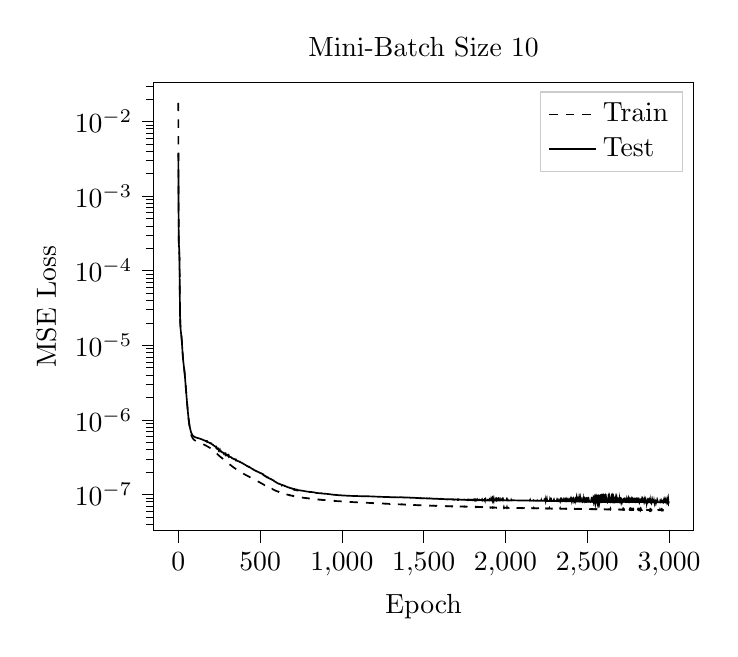
\begin{tikzpicture}

\begin{axis}[
legend cell align={left},
legend style={fill opacity=0.8, draw opacity=1, text opacity=1, draw=white!80!black},
log basis y={10},
tick align=outside,
tick pos=left,
title={Mini-Batch Size 10},
x grid style={white!69.0196078431373!black},
xlabel={Epoch},
xmin=-149.95, xmax=3148.95,
xtick style={color=black},
y grid style={white!69.0196078431373!black},
ylabel={MSE Loss},
ymin=3.24485769485219e-08, ymax=0.0333980791603649,
ymode=log,
ytick style={color=black}
]
\addplot [semithick, black, dashed]
table {%
0 0.0178001991356723
1 0.00200488151138416
2 0.000701156315590197
3 0.000261716974828232
4 0.000199328617736683
5 0.000186986934481865
6 0.000173579933980363
7 0.000146110978748766
8 0.000105959740715207
9 6.39389415221103e-05
10 3.66668005824522e-05
11 2.52619820594191e-05
12 2.07518238619286e-05
13 1.84675150404701e-05
14 1.71286290495232e-05
15 1.5936518463775e-05
16 1.51902070922461e-05
17 1.45978872893693e-05
18 1.39883020449361e-05
19 1.33434278936306e-05
20 1.26594410440362e-05
21 1.19381270536678e-05
22 1.11856970158897e-05
23 1.04207012111601e-05
24 9.66082206034002e-06
25 8.93075510902008e-06
26 8.25333155148655e-06
27 7.64690106393573e-06
28 7.12489472682876e-06
29 6.68496002710128e-06
30 6.31955081892954e-06
31 6.0134227113906e-06
32 5.74498461613615e-06
33 5.47273176358942e-06
34 5.2167927445268e-06
35 4.9861744959756e-06
36 4.78104827688952e-06
37 4.58005392468763e-06
38 4.37887272038751e-06
39 4.17098636571467e-06
40 3.95421256087047e-06
41 3.72693911240063e-06
42 3.50172249108383e-06
43 3.29332809126726e-06
44 3.09182238506622e-06
45 2.90331225761165e-06
46 2.72360592129317e-06
47 2.55453821926821e-06
48 2.39700753549954e-06
49 2.25145955536021e-06
50 2.11668409027865e-06
51 1.99050134304102e-06
52 1.87229289890567e-06
53 1.76164887562891e-06
54 1.65823905733831e-06
55 1.56229427982879e-06
56 1.47228454741466e-06
57 1.38939942937455e-06
58 1.3126574909883e-06
59 1.24191653927852e-06
60 1.17652551157477e-06
61 1.11696765555891e-06
62 1.06234146255879e-06
63 1.01298756452373e-06
64 9.67812829308912e-07
65 9.2707087809174e-07
66 8.89830477213138e-07
67 8.56006430591805e-07
68 8.25594001954144e-07
69 7.97867215593939e-07
70 7.72954573493578e-07
71 7.50259117587859e-07
72 7.29901631615348e-07
73 7.11405896423045e-07
74 6.94639410303566e-07
75 6.79315586022966e-07
76 6.6426254218932e-07
77 6.49667091829897e-07
78 6.37269800281004e-07
79 6.26870553155356e-07
80 6.17372133735472e-07
81 6.09351209694964e-07
82 6.01519808052231e-07
83 5.94646097393792e-07
84 5.88447503728773e-07
85 5.82338745438449e-07
86 5.77041704019621e-07
87 5.72185976057682e-07
88 5.67587416746562e-07
89 5.63291617527995e-07
90 5.59368539367888e-07
91 5.5559798167959e-07
92 5.52062691929756e-07
93 5.49291227929238e-07
94 5.45904120579088e-07
95 5.43599098166148e-07
96 5.40758223528393e-07
97 5.38306081567796e-07
98 5.35737310727313e-07
99 5.33768687471792e-07
100 5.31790635061036e-07
101 5.29849820289918e-07
102 5.2781264008761e-07
103 5.2608527720821e-07
104 5.24380388053913e-07
105 5.22993991998177e-07
106 5.21228024115139e-07
107 5.194265561137e-07
108 5.18424794599959e-07
109 5.17087338471889e-07
110 5.15472511524173e-07
111 5.13651462452636e-07
112 5.11944656835794e-07
113 5.11448339870491e-07
114 5.094766639413e-07
115 5.08757320996089e-07
116 5.07514836463052e-07
117 5.06262259882817e-07
118 5.05168648228249e-07
119 5.04062417232554e-07
120 5.0310766930739e-07
121 5.02008621690031e-07
122 5.00922091255518e-07
123 5.00021304423726e-07
124 4.9925018522412e-07
125 4.97710623328374e-07
126 4.96685247717288e-07
127 4.95866179095472e-07
128 4.94776216921622e-07
129 4.93998716133426e-07
130 4.93124593292649e-07
131 4.91399142039661e-07
132 4.90354375921598e-07
133 4.89415591173881e-07
134 4.88746146234398e-07
135 4.87311924795009e-07
136 4.86539818362885e-07
137 4.85456797498784e-07
138 4.84422925803862e-07
139 4.83270311928408e-07
140 4.81786078943003e-07
141 4.81387102686526e-07
142 4.80235422144482e-07
143 4.79086478013535e-07
144 4.78289033716273e-07
145 4.76731951049025e-07
146 4.76179492916451e-07
147 4.74949749644793e-07
148 4.73749073166552e-07
149 4.73058385379588e-07
150 4.7159305594402e-07
151 4.70849445970423e-07
152 4.69777295726281e-07
153 4.68548464689356e-07
154 4.67459765909339e-07
155 4.66451711722549e-07
156 4.65140015126764e-07
157 4.64248967455561e-07
158 4.63067644558279e-07
159 4.62037328721188e-07
160 4.60832779847209e-07
161 4.59657103135669e-07
162 4.58667327296602e-07
163 4.57390565280491e-07
164 4.56800247836675e-07
165 4.55633157230295e-07
166 4.54525676558681e-07
167 4.52909505739285e-07
168 4.52024042414401e-07
169 4.5069251675578e-07
170 4.49355827512043e-07
171 4.48662767800201e-07
172 4.47104315735025e-07
173 4.45493171250533e-07
174 4.44361103246749e-07
175 4.43117024477857e-07
176 4.42095686610244e-07
177 4.40849777234575e-07
178 4.39880139522231e-07
179 4.38409383245464e-07
180 4.37334783134347e-07
181 4.36090220734542e-07
182 4.34752940812189e-07
183 4.33580878889117e-07
184 4.32395907186134e-07
185 4.31017867064121e-07
186 4.29702469593174e-07
187 4.2842525137754e-07
188 4.2718219425808e-07
189 4.25812123192593e-07
190 4.24095969075999e-07
191 4.23468389931791e-07
192 4.22093073879637e-07
193 4.20754458003714e-07
194 4.19289238551279e-07
195 4.17835532693367e-07
196 4.16806761522892e-07
197 4.15206033959059e-07
198 4.1388074707438e-07
199 4.12556319613344e-07
200 4.11016335215564e-07
201 4.09749037126872e-07
202 4.0828644787716e-07
203 4.06659762477446e-07
204 4.05280188657819e-07
205 4.03922399967449e-07
206 4.02468767375375e-07
207 4.0099183457265e-07
208 3.99562870656567e-07
209 3.98091809583612e-07
210 3.96557871154002e-07
211 3.95109049708964e-07
212 3.93565956278152e-07
213 3.92116205807369e-07
214 3.9048634858041e-07
215 3.88987133632668e-07
216 3.87307775220336e-07
217 3.85659230630608e-07
218 3.84034484453011e-07
219 3.82389923112569e-07
220 3.8074077836292e-07
221 3.79036988427117e-07
222 3.77271174141214e-07
223 3.75499602460749e-07
224 3.73765723615804e-07
225 3.7202211526477e-07
226 3.70217503258274e-07
227 3.68391220293418e-07
228 3.66756287339953e-07
229 3.65261258252758e-07
230 3.63593527170636e-07
231 3.61567422171305e-07
232 3.59488814263287e-07
233 3.57849984942149e-07
234 3.56092777478167e-07
235 3.54040356365104e-07
236 3.52273915824597e-07
237 3.50462861815615e-07
238 3.48645920320578e-07
239 3.46658482062168e-07
240 3.44857991292358e-07
241 3.4288920054415e-07
242 3.41182960417186e-07
243 3.39597257008606e-07
244 3.38001042097247e-07
245 3.36484771645829e-07
246 3.35175210679495e-07
247 3.33539320740428e-07
248 3.32172186787716e-07
249 3.30656567619769e-07
250 3.29258906361929e-07
251 3.27834958051554e-07
252 3.26425850252221e-07
253 3.25018129814225e-07
254 3.23652537534969e-07
255 3.22333164293198e-07
256 3.20880008635172e-07
257 3.19589182948832e-07
258 3.1822573014928e-07
259 3.16879099448997e-07
260 3.15520553604287e-07
261 3.14236705563076e-07
262 3.12878847026354e-07
263 3.11595314403945e-07
264 3.10341323599417e-07
265 3.09084424259254e-07
266 3.07808726329739e-07
267 3.06590944392227e-07
268 3.05279227781341e-07
269 3.04013077521148e-07
270 3.02779589507196e-07
271 3.0152337268774e-07
272 3.00294039528026e-07
273 2.99054804830945e-07
274 2.97839031810909e-07
275 2.96646299249304e-07
276 2.95470336180159e-07
277 2.94282409720736e-07
278 2.93141718152867e-07
279 2.9194919356712e-07
280 2.90748225593163e-07
281 2.89534122277502e-07
282 2.88395086762705e-07
283 2.87192309000872e-07
284 2.86033646501593e-07
285 2.84838715129965e-07
286 2.83449129625524e-07
287 2.82174042238736e-07
288 2.80972971209437e-07
289 2.79831400593622e-07
290 2.7864298409952e-07
291 2.77608370895521e-07
292 2.76369982707969e-07
293 2.75211814080301e-07
294 2.7401515870551e-07
295 2.7293551080998e-07
296 2.71806649241313e-07
297 2.7067986362983e-07
298 2.6959935115034e-07
299 2.68510390837307e-07
300 2.67403697793434e-07
301 2.66281694791815e-07
302 2.65209942358346e-07
303 2.64117393444785e-07
304 2.62889389368581e-07
305 2.61951484459288e-07
306 2.60799055360472e-07
307 2.59715716164344e-07
308 2.58708064859725e-07
309 2.57661466993575e-07
310 2.56647615111127e-07
311 2.55594814460025e-07
312 2.54520277169767e-07
313 2.5352761123365e-07
314 2.52510745073486e-07
315 2.51431184645767e-07
316 2.50446511702584e-07
317 2.4946796331804e-07
318 2.48470296666525e-07
319 2.47495434377853e-07
320 2.46574284399337e-07
321 2.45618885883481e-07
322 2.4467481325452e-07
323 2.43779958220003e-07
324 2.42782083015314e-07
325 2.41834526923945e-07
326 2.40896920447042e-07
327 2.3995052869985e-07
328 2.38996751797949e-07
329 2.37917715488756e-07
330 2.37067746788888e-07
331 2.36164335669642e-07
332 2.35325629853733e-07
333 2.34393299813895e-07
334 2.33588868980839e-07
335 2.32686475296617e-07
336 2.31896005589149e-07
337 2.30981218889426e-07
338 2.30185180425391e-07
339 2.29283251775847e-07
340 2.28469564766964e-07
341 2.27607666731799e-07
342 2.26841884443107e-07
343 2.25991612783361e-07
344 2.2521350435456e-07
345 2.24394526089355e-07
346 2.23642060748208e-07
347 2.22841295816067e-07
348 2.22086131098642e-07
349 2.2133011579939e-07
350 2.20568449118552e-07
351 2.19800282890148e-07
352 2.19098173970256e-07
353 2.18288558089252e-07
354 2.17586786326329e-07
355 2.16807241306682e-07
356 2.16107884627448e-07
357 2.15367789542231e-07
358 2.14628127759298e-07
359 2.14019474951144e-07
360 2.13259286641065e-07
361 2.12567211665959e-07
362 2.11839382013856e-07
363 2.11178343365592e-07
364 2.10479607185565e-07
365 2.09804933029023e-07
366 2.09098087999848e-07
367 2.0845428510663e-07
368 2.07548652144673e-07
369 2.0706301449902e-07
370 2.06368420856418e-07
371 2.05738664365018e-07
372 2.05144220055686e-07
373 2.04314023879437e-07
374 2.03713761282032e-07
375 2.03073658120445e-07
376 2.02480032096553e-07
377 2.0173208872265e-07
378 2.01258483427669e-07
379 2.00689961518119e-07
380 2.0009316386238e-07
381 1.99379444569825e-07
382 1.98847902739274e-07
383 1.98230823846846e-07
384 1.97644873682901e-07
385 1.96939929297812e-07
386 1.96473501479222e-07
387 1.95837122707321e-07
388 1.95172183183878e-07
389 1.94611491166619e-07
390 1.94163676299208e-07
391 1.93573539111203e-07
392 1.92889612193881e-07
393 1.92450886613571e-07
394 1.91762933980932e-07
395 1.91069881569916e-07
396 1.90871840612949e-07
397 1.90135571560557e-07
398 1.89597682034304e-07
399 1.88993792495928e-07
400 1.88866561527945e-07
401 1.8823351179309e-07
402 1.87435177019246e-07
403 1.86995581747951e-07
404 1.86478740547003e-07
405 1.85732155091323e-07
406 1.85532268703881e-07
407 1.84917344270286e-07
408 1.84320728742193e-07
409 1.83672056286444e-07
410 1.83207849198119e-07
411 1.82638589312223e-07
412 1.82247722577689e-07
413 1.81650426251956e-07
414 1.81214002696883e-07
415 1.80670774470038e-07
416 1.80172028001468e-07
417 1.79686196417617e-07
418 1.79142520733144e-07
419 1.78697198134348e-07
420 1.78173241160984e-07
421 1.7780779776988e-07
422 1.77204278359877e-07
423 1.76783149934412e-07
424 1.76556122597482e-07
425 1.76137153817812e-07
426 1.75646959195142e-07
427 1.75163073317108e-07
428 1.74742066361144e-07
429 1.7418946008263e-07
430 1.7392178295772e-07
431 1.73334443283046e-07
432 1.72905922817268e-07
433 1.7237974726303e-07
434 1.71912371222938e-07
435 1.71471092089703e-07
436 1.70954288805092e-07
437 1.70348594754621e-07
438 1.70084692090455e-07
439 1.69441702992934e-07
440 1.69140008270396e-07
441 1.6867942303378e-07
442 1.68193934451111e-07
443 1.67728129225608e-07
444 1.6711657236046e-07
445 1.66799415717289e-07
446 1.66348919696802e-07
447 1.65739778066332e-07
448 1.65427918514816e-07
449 1.64987913477965e-07
450 1.64656203514024e-07
451 1.63946173310503e-07
452 1.6375657067691e-07
453 1.62959084601955e-07
454 1.62720349403678e-07
455 1.6214111080215e-07
456 1.61762699246726e-07
457 1.61298128462661e-07
458 1.60905765329566e-07
459 1.60514551941215e-07
460 1.60084449145614e-07
461 1.59599648417164e-07
462 1.591434488879e-07
463 1.58748809802045e-07
464 1.58325135304338e-07
465 1.5792636882006e-07
466 1.57515875460756e-07
467 1.57136660865476e-07
468 1.56689956409828e-07
469 1.56272531113277e-07
470 1.5589817972339e-07
471 1.55475972791752e-07
472 1.55092888542985e-07
473 1.54674253853848e-07
474 1.54311775311111e-07
475 1.53930749950959e-07
476 1.53479763778108e-07
477 1.53021160740341e-07
478 1.52827318089521e-07
479 1.52479907005176e-07
480 1.52008040865681e-07
481 1.5151424075377e-07
482 1.51270710200269e-07
483 1.50806746781473e-07
484 1.50425882847749e-07
485 1.50061844437221e-07
486 1.49776649589484e-07
487 1.49290316004969e-07
488 1.48689278438585e-07
489 1.48321270039276e-07
490 1.4780005480608e-07
491 1.47442506206463e-07
492 1.47042175688838e-07
493 1.46675496077719e-07
494 1.46248663270843e-07
495 1.45858097846396e-07
496 1.45448324972985e-07
497 1.45064655014959e-07
498 1.44686539629291e-07
499 1.44251473992441e-07
500 1.43813486572775e-07
501 1.43410299160429e-07
502 1.43040729545518e-07
503 1.4266011125752e-07
504 1.42180392681546e-07
505 1.41967560405298e-07
506 1.41547020513499e-07
507 1.41041255790064e-07
508 1.40719742396378e-07
509 1.40317288850333e-07
510 1.39857336707294e-07
511 1.39613264042993e-07
512 1.39194810944154e-07
513 1.38755451510875e-07
514 1.38477771538525e-07
515 1.38006292704773e-07
516 1.37736054184323e-07
517 1.37355880593937e-07
518 1.36604346510083e-07
519 1.36293020340794e-07
520 1.35855945631036e-07
521 1.35470846136521e-07
522 1.3530845651033e-07
523 1.34873527843915e-07
524 1.34453470828078e-07
525 1.34033881242779e-07
526 1.335631672017e-07
527 1.33317287858148e-07
528 1.32676874740056e-07
529 1.32320470080938e-07
530 1.32086654540675e-07
531 1.31775626597275e-07
532 1.30911119637922e-07
533 1.30574330945432e-07
534 1.30512219185253e-07
535 1.29769693708592e-07
536 1.30005403327083e-07
537 1.29302373486073e-07
538 1.29017444070456e-07
539 1.28683353148862e-07
540 1.28081754575682e-07
541 1.2779934222884e-07
542 1.27699181784457e-07
543 1.27007578891725e-07
544 1.27093415009938e-07
545 1.26421429007539e-07
546 1.26119597954055e-07
547 1.2564806459725e-07
548 1.25400566943767e-07
549 1.24967678734045e-07
550 1.24766246758501e-07
551 1.24567104331508e-07
552 1.24038114059921e-07
553 1.23791782251637e-07
554 1.23528181261712e-07
555 1.23040923212248e-07
556 1.22815953937927e-07
557 1.22616209272675e-07
558 1.22088738832016e-07
559 1.21686210736716e-07
560 1.21890107616096e-07
561 1.21081276245327e-07
562 1.21233743630711e-07
563 1.21165836566295e-07
564 1.20615651590938e-07
565 1.20132371077553e-07
566 1.19863235488182e-07
567 1.19627397987543e-07
568 1.1921561338335e-07
569 1.18966398785503e-07
570 1.187901652e-07
571 1.18475433512621e-07
572 1.18114259572977e-07
573 1.18735274103887e-07
574 1.18379147651115e-07
575 1.17835283908185e-07
576 1.17601282181301e-07
577 1.17368267271711e-07
578 1.17028383146423e-07
579 1.16693541998281e-07
580 1.16528044613595e-07
581 1.16167927763922e-07
582 1.15866148180377e-07
583 1.15566139977652e-07
584 1.15205696245013e-07
585 1.14867335083702e-07
586 1.14602485234983e-07
587 1.14337058196856e-07
588 1.14030604216886e-07
589 1.13885041312933e-07
590 1.13557346967941e-07
591 1.1300277483528e-07
592 1.12880506009105e-07
593 1.12564228194056e-07
594 1.1228856199752e-07
595 1.12135682888148e-07
596 1.11946836458543e-07
597 1.11572918839453e-07
598 1.11448776822787e-07
599 1.11093008376972e-07
600 1.10948178129178e-07
601 1.10704173117426e-07
602 1.10584795547375e-07
603 1.10175907286347e-07
604 1.10156123680483e-07
605 1.09735115849663e-07
606 1.09612918239854e-07
607 1.09444221592092e-07
608 1.09276107884693e-07
609 1.08925101638402e-07
610 1.08914205350086e-07
611 1.08398975762203e-07
612 1.0907742901356e-07
613 1.09002830084304e-07
614 1.08195459618265e-07
615 1.08121415214324e-07
616 1.08044478142055e-07
617 1.07672884859245e-07
618 1.07271118685581e-07
619 1.07304079179915e-07
620 1.06764458747133e-07
621 1.06681523357466e-07
622 1.06210029129361e-07
623 1.06446508509883e-07
624 1.05840904989218e-07
625 1.0581392303699e-07
626 1.05456717691688e-07
627 1.05509061842923e-07
628 1.04988260438699e-07
629 1.04953784274553e-07
630 1.04762798229796e-07
631 1.04482612590662e-07
632 1.04514783330067e-07
633 1.03978135024274e-07
634 1.0422276405686e-07
635 1.0375894168968e-07
636 1.03837648071092e-07
637 1.0357105285852e-07
638 1.03748727906527e-07
639 1.03791966605815e-07
640 1.03215746868335e-07
641 1.03112780216463e-07
642 1.02960432610821e-07
643 1.02617199536637e-07
644 1.02572925448907e-07
645 1.02342556638213e-07
646 1.02295900277216e-07
647 1.02282750961136e-07
648 1.01741481622897e-07
649 1.01761854347515e-07
650 1.01516580506278e-07
651 1.01356689373722e-07
652 1.01269487657873e-07
653 1.01099661555804e-07
654 1.00889462562037e-07
655 1.00829628768562e-07
656 1.00951301353902e-07
657 1.00332274681758e-07
658 1.0029597201644e-07
659 1.00302812993114e-07
660 1.00479697117128e-07
661 9.98686187503317e-08
662 9.97339894137639e-08
663 9.96640240213953e-08
664 9.96198147495964e-08
665 9.93623950829026e-08
666 9.92543957645253e-08
667 9.91826136453877e-08
668 9.90910244547116e-08
669 9.88320714201407e-08
670 9.89058069544857e-08
671 9.86755097653891e-08
672 9.86231812227789e-08
673 9.83323942904679e-08
674 9.81895336815697e-08
675 9.81447626979826e-08
676 9.80054834787136e-08
677 9.8090173042964e-08
678 9.78171329335531e-08
679 9.77436845051027e-08
680 9.78698797704514e-08
681 9.7420069773424e-08
682 9.76092436477671e-08
683 9.69910661574591e-08
684 9.71455712406311e-08
685 9.69066977130062e-08
686 9.71315947462248e-08
687 9.69069928102861e-08
688 9.69295860620001e-08
689 9.67196561707517e-08
690 9.63859296254643e-08
691 9.62207225529976e-08
692 9.62625351519364e-08
693 9.61369722929373e-08
694 9.60128456217735e-08
695 9.56613803759776e-08
696 9.57629009756822e-08
697 9.55586340090075e-08
698 9.53878710796552e-08
699 9.55580558725799e-08
700 9.51537736959551e-08
701 9.50713849312557e-08
702 9.50888310458087e-08
703 9.49253897097879e-08
704 9.51184273478844e-08
705 9.45851762845784e-08
706 9.45957434028699e-08
707 9.46405184643062e-08
708 9.44010258041583e-08
709 9.43898038729962e-08
710 9.4229224956166e-08
711 9.40507037083815e-08
712 9.39436439506558e-08
713 9.41692803679839e-08
714 9.36980743604376e-08
715 9.39223697637992e-08
716 9.3714428516245e-08
717 9.36377944427136e-08
718 9.3526587987558e-08
719 9.34935699259398e-08
720 9.3388877135947e-08
721 9.32504858552896e-08
722 9.32898643579705e-08
723 9.30470502424896e-08
724 9.30109677421687e-08
725 9.30141950594709e-08
726 9.28309058956245e-08
727 9.28748622919251e-08
728 9.27886828450131e-08
729 9.2609680124589e-08
730 9.26556160751879e-08
731 9.25388099237701e-08
732 9.23685840614752e-08
733 9.22747352993802e-08
734 9.22771310429837e-08
735 9.21689772281908e-08
736 9.20308270302428e-08
737 9.19883866723481e-08
738 9.19540889698922e-08
739 9.17767490093979e-08
740 9.17387668053493e-08
741 9.16404175232977e-08
742 9.19294675716387e-08
743 9.14501918369837e-08
744 9.13967208515665e-08
745 9.13522649881315e-08
746 9.12961912247212e-08
747 9.16073977896836e-08
748 9.10657894315214e-08
749 9.10220623184799e-08
750 9.0976933784237e-08
751 9.10777755791514e-08
752 9.09916686842038e-08
753 9.09195951415143e-08
754 9.07635310953836e-08
755 9.07308244357807e-08
756 9.07026974861225e-08
757 9.05702344744519e-08
758 9.04802686840789e-08
759 9.039786872167e-08
760 9.05015725760627e-08
761 9.02155400983595e-08
762 9.03243668282094e-08
763 9.0055545192147e-08
764 9.02595226692782e-08
765 8.99536888754326e-08
766 9.02099919297683e-08
767 9.00512921764296e-08
768 8.99423419653544e-08
769 8.98316465369753e-08
770 8.9813657193627e-08
771 8.96320555465735e-08
772 8.96441604880671e-08
773 8.96086649149197e-08
774 8.94550238528247e-08
775 8.94212226043578e-08
776 8.93593333550768e-08
777 8.94074431867509e-08
778 8.92372135075092e-08
779 8.9221889709723e-08
780 8.92524388995675e-08
781 8.90551756804747e-08
782 8.89121469138665e-08
783 8.90338590364692e-08
784 8.91194885332958e-08
785 8.87441462293914e-08
786 8.88770310747411e-08
787 8.89123747760401e-08
788 8.86714512726705e-08
789 8.87836217144944e-08
790 8.87063874510652e-08
791 8.85264483119208e-08
792 8.85483146806365e-08
793 8.84388295530059e-08
794 8.85020863150565e-08
795 8.83155445885464e-08
796 8.84387031896416e-08
797 8.8153341155639e-08
798 8.81551837128569e-08
799 8.80066620534414e-08
800 8.81367960525736e-08
801 8.78716895003073e-08
802 8.79704486678179e-08
803 8.77952394784387e-08
804 8.77992015735352e-08
805 8.78481872201853e-08
806 8.76100659663592e-08
807 8.74860396837818e-08
808 8.76992299914114e-08
809 8.75438203706835e-08
810 8.74522444016534e-08
811 8.75361036056788e-08
812 8.73266344592061e-08
813 8.71610880759377e-08
814 8.73081293750744e-08
815 8.72028591536456e-08
816 8.71319566031481e-08
817 8.71111723155238e-08
818 8.69624218280407e-08
819 8.70118243190276e-08
820 8.71310269023873e-08
821 8.71475792729726e-08
822 8.68332752346213e-08
823 8.67403180282444e-08
824 8.67476854615745e-08
825 8.68219617222721e-08
826 8.6766363929236e-08
827 8.66211521932669e-08
828 8.64632707053836e-08
829 8.65575487507542e-08
830 8.65036195141222e-08
831 8.64688474755404e-08
832 8.63830067876492e-08
833 8.62948699498212e-08
834 8.63148536311975e-08
835 8.63089701330644e-08
836 8.60968507132576e-08
837 8.60323370099891e-08
838 8.60748694164748e-08
839 8.62679394475485e-08
840 8.59693333155054e-08
841 8.57740228732418e-08
842 8.59616949311359e-08
843 8.59376644490872e-08
844 8.58875876108556e-08
845 8.55762429829987e-08
846 8.57686820787684e-08
847 8.58924624780322e-08
848 8.56368602164537e-08
849 8.54734707722571e-08
850 8.55845733838123e-08
851 8.54852331744205e-08
852 8.55151165479739e-08
853 8.53223135144354e-08
854 8.55501998642261e-08
855 8.52984910837407e-08
856 8.53168612158228e-08
857 8.52010489493793e-08
858 8.52043870880337e-08
859 8.52822417063415e-08
860 8.50955661757524e-08
861 8.49153153414939e-08
862 8.5096356117198e-08
863 8.49523311563516e-08
864 8.49563487825833e-08
865 8.476197226992e-08
866 8.50177893285675e-08
867 8.47828442629428e-08
868 8.47410544291272e-08
869 8.48341623971294e-08
870 8.48023626898176e-08
871 8.45865670418e-08
872 8.46554788702658e-08
873 8.44346008832542e-08
874 8.46406003252031e-08
875 8.44302842817335e-08
876 8.4363423134004e-08
877 8.46479363081354e-08
878 8.43425690499888e-08
879 8.42838752412867e-08
880 8.43541957606941e-08
881 8.43985267107161e-08
882 8.42566101322273e-08
883 8.41584912025795e-08
884 8.41513388261106e-08
885 8.41183438926585e-08
886 8.41704006671051e-08
887 8.39991592371803e-08
888 8.40111396493981e-08
889 8.3973454043651e-08
890 8.40829830528467e-08
891 8.40184783601483e-08
892 8.3831746456875e-08
893 8.38605016717508e-08
894 8.38607812803094e-08
895 8.38493038779475e-08
896 8.37759149729944e-08
897 8.36801551062916e-08
898 8.36437556772651e-08
899 8.37031012534961e-08
900 8.35645376096039e-08
901 8.36660378611409e-08
902 8.34644351421776e-08
903 8.35733778747905e-08
904 8.34583026820823e-08
905 8.35194746773293e-08
906 8.33584532400344e-08
907 8.33805425115575e-08
908 8.33102763608817e-08
909 8.32490753910342e-08
910 8.33080121331875e-08
911 8.32248086701792e-08
912 8.3212240336028e-08
913 8.32563882580128e-08
914 8.30514547001115e-08
915 8.31116484034666e-08
916 8.3047177101836e-08
917 8.30702778875647e-08
918 8.29852847783474e-08
919 8.30039136223704e-08
920 8.29433979965266e-08
921 8.28156773113875e-08
922 8.27806891745553e-08
923 8.2899598468078e-08
924 8.28493161308952e-08
925 8.27315951390517e-08
926 8.26971131140386e-08
927 8.26721508750961e-08
928 8.25543270699391e-08
929 8.25434888596099e-08
930 8.26084714544706e-08
931 8.26943764731247e-08
932 8.23973945252021e-08
933 8.23887599210593e-08
934 8.24208399174964e-08
935 8.23855567921861e-08
936 8.2312903864068e-08
937 8.23302100227963e-08
938 8.22914132170283e-08
939 8.21018654861838e-08
940 8.22624562424323e-08
941 8.21541981299578e-08
942 8.21091170832844e-08
943 8.20643537635668e-08
944 8.20593562800287e-08
945 8.20253835498441e-08
946 8.19434589693913e-08
947 8.20608104179499e-08
948 8.19093688197992e-08
949 8.18611726627338e-08
950 8.18886614839531e-08
951 8.18307021244191e-08
952 8.19544831132113e-08
953 8.18278662439997e-08
954 8.20077202057235e-08
955 8.15754108851596e-08
956 8.16673480785735e-08
957 8.16804860415132e-08
958 8.16943688286553e-08
959 8.16415276394533e-08
960 8.15604015269589e-08
961 8.16038678652653e-08
962 8.15272696819136e-08
963 8.14078891175907e-08
964 8.14953906969063e-08
965 8.14391878789511e-08
966 8.14012528893571e-08
967 8.12432967345344e-08
968 8.1269539591311e-08
969 8.12193618771051e-08
970 8.12119225634955e-08
971 8.12174484798867e-08
972 8.11314611492975e-08
973 8.11949283030522e-08
974 8.11163626501799e-08
975 8.10932483552573e-08
976 8.10373127813069e-08
977 8.11503817055304e-08
978 8.09651790945054e-08
979 8.1014203945351e-08
980 8.09188670336525e-08
981 8.09186596684164e-08
982 8.08726839973684e-08
983 8.0900155476904e-08
984 8.08141680319618e-08
985 8.08023577603123e-08
986 8.08806028773645e-08
987 8.07056001306261e-08
988 8.08569871324494e-08
989 8.06921701990149e-08
990 8.06193303248826e-08
991 8.06818341669846e-08
992 8.06083805926505e-08
993 8.0590755475729e-08
994 8.05905937473206e-08
995 8.05231999578826e-08
996 8.06208841530598e-08
997 8.04902552931086e-08
998 8.04632020490192e-08
999 8.05336744857943e-08
1000 8.04876820270639e-08
1001 8.03391489079264e-08
1002 8.04045754965177e-08
1003 8.04095113504655e-08
1004 8.03132315430055e-08
1005 8.02960029533395e-08
1006 8.03522236303422e-08
1007 8.01992822874187e-08
1008 8.01852877385656e-08
1009 8.02109089892422e-08
1010 8.01545967721307e-08
1011 8.0045810992857e-08
1012 8.01588867471725e-08
1013 7.9990280961173e-08
1014 8.00864127314949e-08
1015 8.00176843485101e-08
1016 8.00594969552204e-08
1017 7.99746716162453e-08
1018 7.99542395013564e-08
1019 7.9935821524213e-08
1020 7.99420451624844e-08
1021 7.97774391014805e-08
1022 7.99488231539858e-08
1023 7.97986263789685e-08
1024 7.97909998140334e-08
1025 7.97923242790155e-08
1026 7.98393425049948e-08
1027 7.96697105087674e-08
1028 7.97558328236025e-08
1029 7.96419569837337e-08
1030 7.97550182740636e-08
1031 7.96305487749116e-08
1032 7.96767189481518e-08
1033 7.95769877026675e-08
1034 7.96614504328108e-08
1035 7.95978688372667e-08
1036 7.95406359810347e-08
1037 7.95501295747236e-08
1038 7.94823109018239e-08
1039 7.94750928390098e-08
1040 7.94637828949174e-08
1041 7.94370622891893e-08
1042 7.93156045131305e-08
1043 7.93958467903977e-08
1044 7.92935804239114e-08
1045 7.94392349900974e-08
1046 7.9433984621069e-08
1047 7.93178623847979e-08
1048 7.91490090079616e-08
1049 7.92169928742759e-08
1050 7.92423473505721e-08
1051 7.91688048307204e-08
1052 7.91514585063435e-08
1053 7.90861693411582e-08
1054 7.90850494014617e-08
1055 7.90725980548412e-08
1056 7.90448806009536e-08
1057 7.90191519106642e-08
1058 7.90658210103601e-08
1059 7.89703859860324e-08
1060 7.90758564839233e-08
1061 7.89039747739473e-08
1062 7.89264823619629e-08
1063 7.88544572183358e-08
1064 7.88972637633112e-08
1065 7.87953434977506e-08
1066 7.89054651173515e-08
1067 7.87747313713005e-08
1068 7.87708173166646e-08
1069 7.87421084036399e-08
1070 7.87286146264332e-08
1071 7.87022904558121e-08
1072 7.87429117199423e-08
1073 7.86472130642757e-08
1074 7.8683111349731e-08
1075 7.86130338414903e-08
1076 7.86716206802041e-08
1077 7.85195847974318e-08
1078 7.85481894960416e-08
1079 7.85039934281251e-08
1080 7.85712001116767e-08
1081 7.84723195679238e-08
1082 7.8451432531379e-08
1083 7.84288364130692e-08
1084 7.8408656408735e-08
1085 7.84353979332852e-08
1086 7.84047217583517e-08
1087 7.83162218753741e-08
1088 7.83363034884132e-08
1089 7.84039812640192e-08
1090 7.83181843089231e-08
1091 7.82108398578174e-08
1092 7.82601408289008e-08
1093 7.82269317534112e-08
1094 7.82036281943288e-08
1095 7.81802580229751e-08
1096 7.82237428431642e-08
1097 7.81536682026296e-08
1098 7.80952178103256e-08
1099 7.8071074760544e-08
1100 7.80605395711564e-08
1101 7.80845937720098e-08
1102 7.80424324042794e-08
1103 7.80449235082692e-08
1104 7.79756080837579e-08
1105 7.79083635049638e-08
1106 7.79790376947975e-08
1107 7.8102232925481e-08
1108 7.80166846803265e-08
1109 7.77805636276163e-08
1110 7.78305735282814e-08
1111 7.78131517709113e-08
1112 7.78431191728046e-08
1113 7.77707398214034e-08
1114 7.77980135946432e-08
1115 7.78711287896527e-08
1116 7.77770865123539e-08
1117 7.76282917158699e-08
1118 7.77356853320921e-08
1119 7.76904774901777e-08
1120 7.76967080928781e-08
1121 7.75911115658001e-08
1122 7.76434404314852e-08
1123 7.75514256656784e-08
1124 7.76102096611275e-08
1125 7.75122435459075e-08
1126 7.76777802113937e-08
1127 7.74706609119047e-08
1128 7.74756320298664e-08
1129 7.74572242268068e-08
1130 7.74646784240662e-08
1131 7.75664833552181e-08
1132 7.74485902255151e-08
1133 7.73250186980601e-08
1134 7.74122822155832e-08
1135 7.73344162230405e-08
1136 7.73692463185149e-08
1137 7.72979015828401e-08
1138 7.75325490109946e-08
1139 7.7259488467929e-08
1140 7.72630587742018e-08
1141 7.72039734298069e-08
1142 7.72522298742029e-08
1143 7.71875287575163e-08
1144 7.72157963224718e-08
1145 7.71350670814019e-08
1146 7.72627104306256e-08
1147 7.71596575421807e-08
1148 7.70681353723379e-08
1149 7.71080238259891e-08
1150 7.70272002725836e-08
1151 7.70979918296444e-08
1152 7.72399123749601e-08
1153 7.70670188932065e-08
1154 7.69257838029169e-08
1155 7.70018546847329e-08
1156 7.6930741168546e-08
1157 7.70251498927177e-08
1158 7.698536987788e-08
1159 7.69978501469204e-08
1160 7.69071455231085e-08
1161 7.69654864973823e-08
1162 7.68692118990888e-08
1163 7.69416177404114e-08
1164 7.68841166487455e-08
1165 7.69081348905853e-08
1166 7.67858601924409e-08
1167 7.68723923549874e-08
1168 7.67576349314236e-08
1169 7.69141767320569e-08
1170 7.67006646618107e-08
1171 7.67990653183226e-08
1172 7.66867777812763e-08
1173 7.676626870734e-08
1174 7.68720251198562e-08
1175 7.67668480905481e-08
1176 7.6682359465563e-08
1177 7.66919229089336e-08
1178 7.66391930240307e-08
1179 7.66935282614512e-08
1180 7.65893503562598e-08
1181 7.67021324254991e-08
1182 7.65455475515431e-08
1183 7.65955504000715e-08
1184 7.64599807401289e-08
1185 7.65055794071934e-08
1186 7.63637310807752e-08
1187 7.66084092640451e-08
1188 7.63297209849245e-08
1189 7.64429183164328e-08
1190 7.62582789715083e-08
1191 7.64132777553161e-08
1192 7.62590801273166e-08
1193 7.63323877051025e-08
1194 7.62183908331604e-08
1195 7.62992371794446e-08
1196 7.61987446606938e-08
1197 7.63017266014465e-08
1198 7.61876582799914e-08
1199 7.62336024995314e-08
1200 7.61475027177827e-08
1201 7.6248096526621e-08
1202 7.6106894150163e-08
1203 7.6177538572697e-08
1204 7.61535114346401e-08
1205 7.61412319127963e-08
1206 7.60310017022814e-08
1207 7.61608514909806e-08
1208 7.60445467318238e-08
1209 7.60312235037475e-08
1210 7.59649292803033e-08
1211 7.60156052947991e-08
1212 7.59532762895088e-08
1213 7.59629833735342e-08
1214 7.58824291358096e-08
1215 7.59517160109358e-08
1216 7.58512163312464e-08
1217 7.58963777436339e-08
1218 7.59208059286642e-08
1219 7.5851392506987e-08
1220 7.57793096439752e-08
1221 7.57831311937185e-08
1222 7.5858799813977e-08
1223 7.57766088121947e-08
1224 7.57072575152673e-08
1225 7.56862072193165e-08
1226 7.5753647351684e-08
1227 7.56557773728961e-08
1228 7.56975806825988e-08
1229 7.57979672671993e-08
1230 7.56652403177682e-08
1231 7.5525093287121e-08
1232 7.56438551230421e-08
1233 7.55363046001101e-08
1234 7.56468999363324e-08
1235 7.55404095653667e-08
1236 7.56281851266305e-08
1237 7.54582692552575e-08
1238 7.55123730833418e-08
1239 7.54543400627306e-08
1240 7.54823309845332e-08
1241 7.55495676196816e-08
1242 7.54377794931482e-08
1243 7.53769228178935e-08
1244 7.54270194469608e-08
1245 7.54422974980073e-08
1246 7.53811938358773e-08
1247 7.5322915428222e-08
1248 7.53354440807819e-08
1249 7.53176679491041e-08
1250 7.5324292301282e-08
1251 7.54648821621462e-08
1252 7.52761628985965e-08
1253 7.51857039149595e-08
1254 7.52741665344114e-08
1255 7.51703559764838e-08
1256 7.52426111771953e-08
1257 7.51469949678008e-08
1258 7.51912489183049e-08
1259 7.5294307313456e-08
1260 7.50922786652008e-08
1261 7.4983449914745e-08
1262 7.50905083934938e-08
1263 7.50360642765013e-08
1264 7.50335666754864e-08
1265 7.49946886635655e-08
1266 7.49964212121146e-08
1267 7.49427618484955e-08
1268 7.49789461340633e-08
1269 7.52187001706872e-08
1270 7.48944082473724e-08
1271 7.48732898991911e-08
1272 7.48932804717217e-08
1273 7.4810138475101e-08
1274 7.48887384560693e-08
1275 7.49054233561974e-08
1276 7.47109777710087e-08
1277 7.48059672761592e-08
1278 7.47253667221504e-08
1279 7.47061316730413e-08
1280 7.47312986415505e-08
1281 7.46985879707118e-08
1282 7.46418094788037e-08
1283 7.47763320774197e-08
1284 7.46662591788461e-08
1285 7.45511674504762e-08
1286 7.45907640287147e-08
1287 7.4620115528834e-08
1288 7.45556225856259e-08
1289 7.46394343398293e-08
1290 7.44887373638203e-08
1291 7.45217929787323e-08
1292 7.45925621004062e-08
1293 7.43773617783994e-08
1294 7.43499029165484e-08
1295 7.47543573376142e-08
1296 7.43851886464419e-08
1297 7.43840426686848e-08
1298 7.43586402973673e-08
1299 7.43399094838004e-08
1300 7.43484806198236e-08
1301 7.43145723225425e-08
1302 7.43221440668851e-08
1303 7.42836344369557e-08
1304 7.4298074191903e-08
1305 7.43402515857028e-08
1306 7.42287084776194e-08
1307 7.42520146423953e-08
1308 7.41876707066602e-08
1309 7.41504075629784e-08
1310 7.43617497311888e-08
1311 7.41602457132728e-08
1312 7.41101648349396e-08
1313 7.41699940987051e-08
1314 7.41538912030215e-08
1315 7.40813177335653e-08
1316 7.41577886120837e-08
1317 7.41494760736483e-08
1318 7.40609188853991e-08
1319 7.40734678938981e-08
1320 7.40316358949222e-08
1321 7.39778367109256e-08
1322 7.40224653283938e-08
1323 7.40024573775422e-08
1324 7.39380303516057e-08
1325 7.40153257150489e-08
1326 7.39521464754311e-08
1327 7.38953979706469e-08
1328 7.39007000472025e-08
1329 7.38361665286735e-08
1330 7.39092552348719e-08
1331 7.37182129417757e-08
1332 7.40129470355733e-08
1333 7.38595772975526e-08
1334 7.37559502395069e-08
1335 7.37640920545068e-08
1336 7.3724147261478e-08
1337 7.37744299406096e-08
1338 7.37950086393546e-08
1339 7.36673634227358e-08
1340 7.36936594269988e-08
1341 7.37212079404692e-08
1342 7.36363322828559e-08
1343 7.36814379720396e-08
1344 7.36411203383636e-08
1345 7.37057045452349e-08
1346 7.360783562671e-08
1347 7.35107644111999e-08
1348 7.35359569348226e-08
1349 7.3515293885773e-08
1350 7.34618801268017e-08
1351 7.34388334167058e-08
1352 7.34865704432597e-08
1353 7.3432640939064e-08
1354 7.34110139766209e-08
1355 7.34445167460684e-08
1356 7.3423949514817e-08
1357 7.33732019619904e-08
1358 7.32969087635649e-08
1359 7.33079854764451e-08
1360 7.33899041149844e-08
1361 7.33798932350815e-08
1362 7.31794463848523e-08
1363 7.35090431702723e-08
1364 7.31608860293775e-08
1365 7.31755697735981e-08
1366 7.32641082179519e-08
1367 7.3186250139079e-08
1368 7.34128483614871e-08
1369 7.31165221945496e-08
1370 7.31965115752242e-08
1371 7.3064275827317e-08
1372 7.30857357922332e-08
1373 7.33125895113762e-08
1374 7.32119981117219e-08
1375 7.2922445273349e-08
1376 7.30658656034056e-08
1377 7.30537854609636e-08
1378 7.30022090322802e-08
1379 7.30021480033205e-08
1380 7.30662375525437e-08
1381 7.29430100754325e-08
1382 7.31200996395565e-08
1383 7.28816837269886e-08
1384 7.28833890661917e-08
1385 7.30305735308079e-08
1386 7.28753801337856e-08
1387 7.31701193257273e-08
1388 7.30091970257973e-08
1389 7.27326392080396e-08
1390 7.2943752431609e-08
1391 7.28418323125979e-08
1392 7.28248292891642e-08
1393 7.27638410102926e-08
1394 7.29236893926011e-08
1395 7.26970574471686e-08
1396 7.29422737788532e-08
1397 7.26916406035283e-08
1398 7.27759710872355e-08
1399 7.26676017215322e-08
1400 7.27995294791395e-08
1401 7.28623002443918e-08
1402 7.2619344783087e-08
1403 7.25977303273062e-08
1404 7.27091897056997e-08
1405 7.25303548887446e-08
1406 7.25290343861484e-08
1407 7.27158221502933e-08
1408 7.24931181217414e-08
1409 7.25947768520641e-08
1410 7.26666687800304e-08
1411 7.24676013130754e-08
1412 7.24702049736958e-08
1413 7.25905966825202e-08
1414 7.24343208302614e-08
1415 7.25126469414139e-08
1416 7.23946673419906e-08
1417 7.25070200591205e-08
1418 7.24271357865902e-08
1419 7.2386617682163e-08
1420 7.24308742672264e-08
1421 7.25574703142051e-08
1422 7.22625950910771e-08
1423 7.23400816848852e-08
1424 7.23454461082351e-08
1425 7.2224755340855e-08
1426 7.24860972167729e-08
1427 7.21753162202798e-08
1428 7.22523558616128e-08
1429 7.22983780043762e-08
1430 7.22285173637704e-08
1431 7.22584696577488e-08
1432 7.22576290768107e-08
1433 7.2168765617997e-08
1434 7.22866063196381e-08
1435 7.20468207227043e-08
1436 7.2413970133578e-08
1437 7.21693258531886e-08
1438 7.19542209581814e-08
1439 7.20940786536062e-08
1440 7.20340453908008e-08
1441 7.21357832633718e-08
1442 7.20967352207946e-08
1443 7.21039315343397e-08
1444 7.1925518742022e-08
1445 7.19636618007336e-08
1446 7.1921078086401e-08
1447 7.18724061621323e-08
1448 7.19395195569739e-08
1449 7.20973200674102e-08
1450 7.18064917271111e-08
1451 7.18406069077915e-08
1452 7.18235704133541e-08
1453 7.18386929610126e-08
1454 7.18132499211155e-08
1455 7.18486101902727e-08
1456 7.18489217810259e-08
1457 7.17935581384666e-08
1458 7.16951217194506e-08
1459 7.18805083343987e-08
1460 7.17165028840672e-08
1461 7.16595356820005e-08
1462 7.16323777327776e-08
1463 7.17016591234021e-08
1464 7.16576713588601e-08
1465 7.16868745087584e-08
1466 7.17022194018924e-08
1467 7.16326085725694e-08
1468 7.15976540777152e-08
1469 7.15532844697275e-08
1470 7.15463172340502e-08
1471 7.17302409680709e-08
1472 7.15110366866778e-08
1473 7.15207029966525e-08
1474 7.15000925144427e-08
1475 7.14983211502762e-08
1476 7.14745992491661e-08
1477 7.15955436869642e-08
1478 7.14519207090092e-08
1479 7.14419315128723e-08
1480 7.15761088532219e-08
1481 7.1341611620479e-08
1482 7.13703949839495e-08
1483 7.13687241449268e-08
1484 7.13382373052074e-08
1485 7.1373724586099e-08
1486 7.13113617134553e-08
1487 7.13195875023942e-08
1488 7.12883866815783e-08
1489 7.12990890161525e-08
1490 7.13198241852897e-08
1491 7.13187338374777e-08
1492 7.11651004559055e-08
1493 7.13779132077708e-08
1494 7.11791183394261e-08
1495 7.12117608114848e-08
1496 7.11427688682154e-08
1497 7.11945260345459e-08
1498 7.12525415558218e-08
1499 7.11678484854872e-08
1500 7.11614570381158e-08
1501 7.11084675308893e-08
1502 7.10973000062065e-08
1503 7.11890737548071e-08
1504 7.10097814982102e-08
1505 7.11217829529875e-08
1506 7.10356803301781e-08
1507 7.10784062052383e-08
1508 7.11160269373234e-08
1509 7.09907087681483e-08
1510 7.09881823812708e-08
1511 7.10703202699836e-08
1512 7.09057660996937e-08
1513 7.10703493767007e-08
1514 7.09022750833288e-08
1515 7.10358371813769e-08
1516 7.09045816049692e-08
1517 7.09849863278489e-08
1518 7.0973599505253e-08
1519 7.0858340136537e-08
1520 7.08997586851279e-08
1521 7.10066422648925e-08
1522 7.07712171066355e-08
1523 7.08903939772298e-08
1524 7.09330654657947e-08
1525 7.08389928028019e-08
1526 7.07664721932844e-08
1527 7.09042044844121e-08
1528 7.07320914727916e-08
1529 7.07789257403668e-08
1530 7.07136294919586e-08
1531 7.08379719349672e-08
1532 7.06837229791368e-08
1533 7.07570491009779e-08
1534 7.06986385445862e-08
1535 7.0791849660079e-08
1536 7.06175017561872e-08
1537 7.08143741312561e-08
1538 7.05991611515966e-08
1539 7.07679385281157e-08
1540 7.05842303705406e-08
1541 7.06358272706265e-08
1542 7.06602984879012e-08
1543 7.06426112373482e-08
1544 7.06470237121781e-08
1545 7.04872271506396e-08
1546 7.06520835758173e-08
1547 7.05834752590118e-08
1548 7.05905722087063e-08
1549 7.05431948844204e-08
1550 7.05432729186661e-08
1551 7.06425473162575e-08
1552 7.04266675077836e-08
1553 7.05926022592784e-08
1554 7.04855202204868e-08
1555 7.04926521744031e-08
1556 7.04986543775821e-08
1557 7.0443886481808e-08
1558 7.05194251782171e-08
1559 7.04084887181988e-08
1560 7.04709876198084e-08
1561 7.03363364928933e-08
1562 7.05706793224792e-08
1563 7.03800502899199e-08
1564 7.04518520089348e-08
1565 7.03032442694873e-08
1566 7.04192138978321e-08
1567 7.02934640173236e-08
1568 7.04296211395672e-08
1569 7.02623102033506e-08
1570 7.03620039466113e-08
1571 7.01278146630902e-08
1572 7.03398944801314e-08
1573 7.02545900288509e-08
1574 7.03541819524478e-08
1575 7.00792039898257e-08
1576 7.03628298026615e-08
1577 7.03446308314426e-08
1578 7.01708002448509e-08
1579 7.02759540538445e-08
1580 7.02307665489954e-08
1581 7.02497338556096e-08
1582 7.00715197143875e-08
1583 7.01273691505744e-08
1584 7.02526286811001e-08
1585 6.99801855352788e-08
1586 7.00890796057063e-08
1587 7.01682392656444e-08
1588 6.99929824021783e-08
1589 7.01313425310879e-08
1590 6.99704103523935e-08
1591 7.0034497110516e-08
1592 6.996394930181e-08
1593 7.0139133848679e-08
1594 6.99343256149731e-08
1595 6.99825570205093e-08
1596 7.00792486452162e-08
1597 6.98673662402616e-08
1598 6.99050404018298e-08
1599 7.00526170083204e-08
1600 6.99101682044567e-08
1601 6.98782432029255e-08
1602 6.98833804957388e-08
1603 6.99205370102707e-08
1604 6.99506890489143e-08
1605 6.97390503012762e-08
1606 6.99271392301526e-08
1607 6.98878842209094e-08
1608 6.99158646855214e-08
1609 6.97228140689177e-08
1610 6.98743417937298e-08
1611 6.99033889772771e-08
1612 6.98296120904551e-08
1613 6.97962168971777e-08
1614 6.98333113458016e-08
1615 6.98009128485833e-08
1616 6.97352478495894e-08
1617 6.98048521274863e-08
1618 6.97659968562636e-08
1619 6.97650012893014e-08
1620 6.9648437226455e-08
1621 6.97630892110279e-08
1622 6.97984318331901e-08
1623 6.96086408513708e-08
1624 6.96874106342893e-08
1625 6.96370715091987e-08
1626 6.96619891282779e-08
1627 6.96686164813887e-08
1628 6.96582857617756e-08
1629 6.95931109273573e-08
1630 6.96161632696146e-08
1631 6.96187106996593e-08
1632 6.96458791293875e-08
1633 6.95459031541112e-08
1634 6.96235362884767e-08
1635 6.95092266045361e-08
1636 6.96369155572807e-08
1637 6.94351494878731e-08
1638 6.96506252284568e-08
1639 6.94771293019425e-08
1640 6.95559481600494e-08
1641 6.94703181602918e-08
1642 6.95245321291615e-08
1643 6.94431454195676e-08
1644 6.94937679168728e-08
1645 6.95209997025881e-08
1646 6.93982205490773e-08
1647 6.94675856760529e-08
1648 6.95761106817017e-08
1649 6.92399498924967e-08
1650 6.95162899100321e-08
1651 6.93932016082588e-08
1652 6.9448843302844e-08
1653 6.93578117327842e-08
1654 6.94479364693468e-08
1655 6.93443616794909e-08
1656 6.9420120718533e-08
1657 6.93772415771843e-08
1658 6.94135985790378e-08
1659 6.93638586746204e-08
1660 6.94277945034738e-08
1661 6.92659502121717e-08
1662 6.93786275829389e-08
1663 6.92629660148381e-08
1664 6.93482733771233e-08
1665 6.92422679027249e-08
1666 6.92821916148389e-08
1667 6.93345050140071e-08
1668 6.92768211374428e-08
1669 6.91827686438717e-08
1670 6.92853885009281e-08
1671 6.91847356937281e-08
1672 6.92873283247852e-08
1673 6.88315837449327e-08
1674 6.93824101916096e-08
1675 6.91807214925344e-08
1676 6.92388626988283e-08
1677 6.87920389541574e-08
1678 6.92484443187702e-08
1679 6.89469974202161e-08
1680 6.91685257225849e-08
1681 6.91465243940481e-08
1682 6.90509308998166e-08
1683 6.9103708989493e-08
1684 6.90844120054823e-08
1685 6.90489173271747e-08
1686 6.91380593154101e-08
1687 6.91468449354193e-08
1688 6.89090789873781e-08
1689 6.90039447659441e-08
1690 6.91542831887659e-08
1691 6.86976862529498e-08
1692 6.9101901780666e-08
1693 6.90065735198253e-08
1694 6.89741860004922e-08
1695 6.88918324842636e-08
1696 6.91211725534213e-08
1697 6.89832146283376e-08
1698 6.88838311968531e-08
1699 6.89154905442191e-08
1700 6.89431116629446e-08
1701 6.9036092572583e-08
1702 6.8629575533663e-08
1703 6.88517715097259e-08
1704 6.9089398992972e-08
1705 6.88396791281853e-08
1706 6.90215654763904e-08
1707 6.8804280507484e-08
1708 6.89625303118557e-08
1709 6.88654086922202e-08
1710 6.89996446556762e-08
1711 6.87588980941012e-08
1712 6.89517143293017e-08
1713 6.8723219300848e-08
1714 6.89306166412607e-08
1715 6.87270386967587e-08
1716 6.88592931308296e-08
1717 6.86867749810638e-08
1718 6.90044360407427e-08
1719 6.87480589045553e-08
1720 6.88048466945812e-08
1721 6.87551563738342e-08
1722 6.88557735173401e-08
1723 6.87217398132045e-08
1724 6.88032069173783e-08
1725 6.87013583677842e-08
1726 6.87707278679284e-08
1727 6.87205830129933e-08
1728 6.87496879847593e-08
1729 6.86857594489609e-08
1730 6.87448246194933e-08
1731 6.87185423808856e-08
1732 6.87580712954716e-08
1733 6.8644886128677e-08
1734 6.8731846364356e-08
1735 6.86965900276171e-08
1736 6.88894782885363e-08
1737 6.86127404048165e-08
1738 6.87250564190833e-08
1739 6.85343334094757e-08
1740 6.86284456730135e-08
1741 6.86814971273542e-08
1742 6.85856586302158e-08
1743 6.84574580434028e-08
1744 6.86321892406916e-08
1745 6.85327848870543e-08
1746 6.85986459780796e-08
1747 6.8509379796966e-08
1748 6.86313544395745e-08
1749 6.84478798773647e-08
1750 6.8774220705059e-08
1751 6.84039075826703e-08
1752 6.85784395715316e-08
1753 6.84213945545409e-08
1754 6.85257913601856e-08
1755 6.84432113284839e-08
1756 6.85940314704148e-08
1757 6.84540390727406e-08
1758 6.84996380806435e-08
1759 6.84255316429905e-08
1760 6.84994081334711e-08
1761 6.83496601450173e-08
1762 6.85872163097567e-08
1763 6.83307360327401e-08
1764 6.84299860209681e-08
1765 6.8290297418061e-08
1766 6.83317611382961e-08
1767 6.83541593959891e-08
1768 6.82663371931458e-08
1769 6.83582202809507e-08
1770 6.82533875351332e-08
1771 6.84098756698059e-08
1772 6.82649559935466e-08
1773 6.82983251110159e-08
1774 6.82460327738887e-08
1775 6.83144735358354e-08
1776 6.82558354170304e-08
1777 6.80487194293367e-08
1778 6.81743316399697e-08
1779 6.8192485342955e-08
1780 6.82410330965499e-08
1781 6.81408427949393e-08
1782 6.82819869357587e-08
1783 6.81994001416886e-08
1784 6.81741158037319e-08
1785 6.82355838210746e-08
1786 6.81081633402414e-08
1787 6.81097989085888e-08
1788 6.80466418034875e-08
1789 6.81045054917728e-08
1790 6.81272419955636e-08
1791 6.81797386026251e-08
1792 6.79816086157636e-08
1793 6.81585246664618e-08
1794 6.80637034500275e-08
1795 6.79865026664839e-08
1796 6.79606365872054e-08
1797 6.81635576560424e-08
1798 6.79132978409491e-08
1799 6.808927221158e-08
1800 6.79975480688544e-08
1801 6.79560618277453e-08
1802 6.80607082692575e-08
1803 6.78084828742431e-08
1804 6.79328344865837e-08
1805 6.79855584606592e-08
1806 6.79024618188695e-08
1807 6.79895740851588e-08
1808 6.7942078274541e-08
1809 6.77301648788209e-08
1810 6.79487982135907e-08
1811 6.77189533759837e-08
1812 6.80440251565884e-08
1813 6.78486172056569e-08
1814 6.77492349498987e-08
1815 6.78563871048254e-08
1816 6.76450345626911e-08
1817 6.8000636261889e-08
1818 6.76601112659103e-08
1819 6.79100906575414e-08
1820 6.76148879086291e-08
1821 6.78971973555598e-08
1822 6.75732779942262e-08
1823 6.78717342472712e-08
1824 6.76429894252983e-08
1825 6.78083948069119e-08
1826 6.76900134255476e-08
1827 6.79025106931075e-08
1828 6.76137749311412e-08
1829 6.77421743910944e-08
1830 6.76241311625692e-08
1831 6.78739331172462e-08
1832 6.77138659943566e-08
1833 6.78268666021164e-08
1834 6.7667376737468e-08
1835 6.76947809830075e-08
1836 6.77330604870186e-08
1837 6.76291305001797e-08
1838 6.77387580982902e-08
1839 6.75420147377981e-08
1840 6.75702316133009e-08
1841 6.76830326140632e-08
1842 6.7672449204359e-08
1843 6.76407698396719e-08
1844 6.76225918760931e-08
1845 6.7614503325153e-08
1846 6.7588190126866e-08
1847 6.765213870219e-08
1848 6.75284900952811e-08
1849 6.76018702017167e-08
1850 6.75198737709604e-08
1851 6.76009841960035e-08
1852 6.74130299394005e-08
1853 6.7593276751321e-08
1854 6.74724869953458e-08
1855 6.75158632668094e-08
1856 6.75006180750337e-08
1857 6.75392995230784e-08
1858 6.74606009654077e-08
1859 6.73793244543308e-08
1860 6.75717327269787e-08
1861 6.73381673477191e-08
1862 6.75148067263987e-08
1863 6.73766656966723e-08
1864 6.72448422944782e-08
1865 6.73135385387269e-08
1866 6.73466110268084e-08
1867 6.73590328603702e-08
1868 6.72403689261358e-08
1869 6.72288576974989e-08
1870 6.73108958804125e-08
1871 6.72453088068625e-08
1872 6.7754858217306e-08
1873 6.7283999090062e-08
1874 6.71059777701544e-08
1875 6.73222225888725e-08
1876 6.73753133462185e-08
1877 6.72258391465341e-08
1878 6.73737997025636e-08
1879 6.72153320191438e-08
1880 6.70830864180072e-08
1881 6.70028391458466e-08
1882 6.75489408952235e-08
1883 6.73488163571712e-08
1884 6.71898936577264e-08
1885 6.71352011438753e-08
1886 6.69802611974468e-08
1887 6.7163824579719e-08
1888 6.69757383608971e-08
1889 6.67905109297262e-08
1890 6.66611658972638e-08
1891 6.71619620062902e-08
1892 6.6782864880377e-08
1893 6.68145874582748e-08
1894 6.70372028632737e-08
1895 6.68022557737125e-08
1896 6.68858398078509e-08
1897 6.67979510371452e-08
1898 6.65948880351763e-08
1899 6.69526050778302e-08
1900 6.67590387959383e-08
1901 6.66473005372925e-08
1902 6.68177077056686e-08
1903 6.67807453591518e-08
1904 6.66301940477343e-08
1905 6.68488597299621e-08
1906 6.64686168172501e-08
1907 6.67812939170176e-08
1908 6.68084647725831e-08
1909 6.65803689070543e-08
1910 6.68394755665158e-08
1911 6.6474942950201e-08
1912 6.66922478720355e-08
1913 6.65712308545174e-08
1914 6.65137632738233e-08
1915 6.6706488770496e-08
1916 6.65524848286747e-08
1917 6.66181480313277e-08
1918 6.63914232001961e-08
1919 6.64567854691267e-08
1920 6.68498764200276e-08
1921 6.63044921656031e-08
1922 6.66311258479269e-08
1923 6.63716295501438e-08
1924 6.65601089833157e-08
1925 6.64013131868035e-08
1926 6.65912572272998e-08
1927 6.63643654508217e-08
1928 6.62964641473529e-08
1929 6.66964227813427e-08
1930 6.626339424054e-08
1931 6.65649874720398e-08
1932 6.64858166654625e-08
1933 6.64341707456995e-08
1934 6.6536081677615e-08
1935 6.64461402855032e-08
1936 6.64182490750509e-08
1937 6.6556038644805e-08
1938 6.64136046846231e-08
1939 6.64209256950876e-08
1940 6.63985863624816e-08
1941 6.64118313964401e-08
1942 6.63075059903484e-08
1943 6.64217084545005e-08
1944 6.64730061505914e-08
1945 6.61996087991667e-08
1946 6.64867769628596e-08
1947 6.63982047255374e-08
1948 6.64885203216503e-08
1949 6.70731276897207e-08
1950 6.63460173833119e-08
1951 6.61674656154965e-08
1952 6.62789644256812e-08
1953 6.63714060622489e-08
1954 6.61076198604782e-08
1955 6.63996361327524e-08
1956 6.63961902092058e-08
1957 6.60762386583968e-08
1958 6.63478886275826e-08
1959 6.62820870434011e-08
1960 6.63915489118594e-08
1961 6.6043377247027e-08
1962 6.6386472983293e-08
1963 6.63206422446549e-08
1964 6.60270756902559e-08
1965 6.6307238270058e-08
1966 6.62643509308225e-08
1967 6.62548776042549e-08
1968 6.62672534468278e-08
1969 6.60964801701969e-08
1970 6.62251523853019e-08
1971 6.62297269138357e-08
1972 6.61923241840334e-08
1973 6.60683337805334e-08
1974 6.70719559370259e-08
1975 6.58325602498344e-08
1976 6.61773620369566e-08
1977 6.62595897105156e-08
1978 6.61423731407318e-08
1979 6.60873071833823e-08
1980 6.62015182983922e-08
1981 6.60451440359644e-08
1982 6.6048363459581e-08
1983 6.61872064156022e-08
1984 6.62133097928397e-08
1985 6.59924692858471e-08
1986 6.60384472483955e-08
1987 6.6082156788827e-08
1988 6.61354347231136e-08
1989 6.59292416893553e-08
1990 6.70316717654718e-08
1991 6.57684738891717e-08
1992 6.60344116532041e-08
1993 6.59842180905645e-08
1994 6.61989872019486e-08
1995 6.59666902003142e-08
1996 6.61570273963186e-08
1997 6.61061837559096e-08
1998 6.60716190836741e-08
1999 6.60591013601497e-08
2000 6.5969113299813e-08
2001 6.59697354532529e-08
2002 6.60610295644126e-08
2003 6.60928204843092e-08
2004 6.6001047215325e-08
2005 6.59362417987364e-08
2006 6.60711349231846e-08
2007 6.60435125643399e-08
2008 6.57828339345468e-08
2009 6.6935568027171e-08
2010 6.56864162740245e-08
2011 6.59295514482405e-08
2012 6.59563637772642e-08
2013 6.59264477087529e-08
2014 6.58476480386305e-08
2015 6.58581141843584e-08
2016 6.59341506503708e-08
2017 6.59771998023917e-08
2018 6.58371208417385e-08
2019 6.59361430543903e-08
2020 6.5999477583123e-08
2021 6.58459589075733e-08
2022 6.59152955662101e-08
2023 6.5937023496776e-08
2024 6.6059540891894e-08
2025 6.58627154870306e-08
2026 6.58900110506178e-08
2027 6.5942953260123e-08
2028 6.59582970596873e-08
2029 6.58284264543063e-08
2030 6.58751808868541e-08
2031 6.58852805945909e-08
2032 6.59532494695636e-08
2033 6.59084792509201e-08
2034 6.58079041659931e-08
2035 6.58397169128744e-08
2036 6.5882810422746e-08
2037 6.5756754644708e-08
2038 6.67470912629753e-08
2039 6.55670089877436e-08
2040 6.58146850551766e-08
2041 6.58136103992568e-08
2042 6.57579927898499e-08
2043 6.58836667544183e-08
2044 6.57022854277933e-08
2045 6.58395602592954e-08
2046 6.57681617910466e-08
2047 6.58699409827879e-08
2048 6.57083664945546e-08
2049 6.58619080784462e-08
2050 6.57216440003161e-08
2051 6.57887948984914e-08
2052 6.57017400840232e-08
2053 6.58182420920639e-08
2054 6.57562418071578e-08
2055 6.57926274039156e-08
2056 6.56875450399941e-08
2057 6.57799265890713e-08
2058 6.56663494413845e-08
2059 6.57710594653693e-08
2060 6.56711032687163e-08
2061 6.57548989047019e-08
2062 6.56628311734853e-08
2063 6.57580681528991e-08
2064 6.56760743888984e-08
2065 6.5706602676574e-08
2066 6.56187480752024e-08
2067 6.57445877860763e-08
2068 6.56874984739098e-08
2069 6.56285721867267e-08
2070 6.56562962852991e-08
2071 6.56484776329069e-08
2072 6.57219583499735e-08
2073 6.55915229141879e-08
2074 6.55998193865859e-08
2075 6.56479710536839e-08
2076 6.56446847668857e-08
2077 6.55443564923086e-08
2078 6.55903284130233e-08
2079 6.56538398291495e-08
2080 6.56786287633881e-08
2081 6.55348620304253e-08
2082 6.56241416863157e-08
2083 6.56291168532608e-08
2084 6.54998377003224e-08
2085 6.56859378045382e-08
2086 6.5521259271506e-08
2087 6.56568022594506e-08
2088 6.55050057218887e-08
2089 6.56447896374424e-08
2090 6.55038069174996e-08
2091 6.56565749979077e-08
2092 6.54737002536709e-08
2093 6.55682362205034e-08
2094 6.54973781621937e-08
2095 6.55964751361537e-08
2096 6.54508036379564e-08
2097 6.55846878538924e-08
2098 6.54514093101355e-08
2099 6.55736518373473e-08
2100 6.54337817895812e-08
2101 6.55614993994025e-08
2102 6.54177499548325e-08
2103 6.55237191216074e-08
2104 6.54074559058859e-08
2105 6.55168614549506e-08
2106 6.54024824209287e-08
2107 6.55165110141631e-08
2108 6.54133824629088e-08
2109 6.55111731573399e-08
2110 6.54138918876335e-08
2111 6.5471872381373e-08
2112 6.54250848852733e-08
2113 6.5442203189825e-08
2114 6.53423675089915e-08
2115 6.55041171648829e-08
2116 6.5330769963845e-08
2117 6.55228545387576e-08
2118 6.53956411733603e-08
2119 6.54904116470512e-08
2120 6.5381969458489e-08
2121 6.54330309213247e-08
2122 6.53507460135483e-08
2123 6.54506042629954e-08
2124 6.53432669450726e-08
2125 6.5475388681957e-08
2126 6.52801096256983e-08
2127 6.53994441091044e-08
2128 6.53130605432484e-08
2129 6.5411390515191e-08
2130 6.53130040351169e-08
2131 6.55198125076861e-08
2132 6.52354667385335e-08
2133 6.53744282819169e-08
2134 6.52826584768285e-08
2135 6.53976653719468e-08
2136 6.52793646860328e-08
2137 6.53672421846441e-08
2138 6.52304697079664e-08
2139 6.54500823238369e-08
2140 6.52078411855772e-08
2141 6.53949172990664e-08
2142 6.51965572195934e-08
2143 6.54084914775144e-08
2144 6.52113908405916e-08
2145 6.5330568552735e-08
2146 6.51219241476486e-08
2147 6.52104287324207e-08
2148 6.51847224331092e-08
2149 6.52842088100236e-08
2150 6.51002724949556e-08
2151 6.59854539819538e-08
2152 6.50827259451869e-08
2153 6.51069786472558e-08
2154 6.52298877723556e-08
2155 6.536417286096e-08
2156 6.51257378558867e-08
2157 6.52575238102582e-08
2158 6.52355910824021e-08
2159 6.51491752257094e-08
2160 6.53005332840184e-08
2161 6.50888380182568e-08
2162 6.5323621708524e-08
2163 6.50719748906958e-08
2164 6.52327369277117e-08
2165 6.52475725138046e-08
2166 6.50947454539086e-08
2167 6.52062472339399e-08
2168 6.50745307118061e-08
2169 6.51147431740551e-08
2170 6.50515335476332e-08
2171 6.52050840344032e-08
2172 6.50129260959531e-08
2173 6.5697357755079e-08
2174 6.50946991698209e-08
2175 6.49065785440772e-08
2176 6.52661760480733e-08
2177 6.50820982006639e-08
2178 6.51994881006868e-08
2179 6.50265954815765e-08
2180 6.51035293841584e-08
2181 6.50842309857236e-08
2182 6.51014565566932e-08
2183 6.50773483079625e-08
2184 6.50725389017559e-08
2185 6.50440476801517e-08
2186 6.50774315502645e-08
2187 6.51252769900967e-08
2188 6.49494160498421e-08
2189 6.50683271430363e-08
2190 6.48940039416068e-08
2191 6.50798012402642e-08
2192 6.50791514877902e-08
2193 6.50476988395265e-08
2194 6.5173320321632e-08
2195 6.49933580032513e-08
2196 6.49540916619618e-08
2197 6.49934698737642e-08
2198 6.49384679485276e-08
2199 6.49622976212072e-08
2200 6.49979008726653e-08
2201 6.5018265240635e-08
2202 6.50366856669304e-08
2203 6.49529504126445e-08
2204 6.50684431391379e-08
2205 6.49903431426679e-08
2206 6.49870188496049e-08
2207 6.4947485619582e-08
2208 6.50133129564967e-08
2209 6.49742198255421e-08
2210 6.50442676952689e-08
2211 6.4882819535983e-08
2212 6.50174766925193e-08
2213 6.49145748121693e-08
2214 6.4992826074306e-08
2215 6.48770518651975e-08
2216 6.50210983377253e-08
2217 6.48392717872426e-08
2218 6.49724177970157e-08
2219 6.47705348355565e-08
2220 6.5016040166066e-08
2221 6.46926089586941e-08
2222 6.57002798498674e-08
2223 6.47419585697584e-08
2224 6.4955294802882e-08
2225 6.47709187606704e-08
2226 6.49230729354855e-08
2227 6.47702279954476e-08
2228 6.49525802487449e-08
2229 6.47612184523361e-08
2230 6.49792067985988e-08
2231 6.47554639821024e-08
2232 6.49214665660036e-08
2233 6.47661599362248e-08
2234 6.49696522214693e-08
2235 6.47454465474429e-08
2236 6.49609862435341e-08
2237 6.47359709238238e-08
2238 6.49182213685595e-08
2239 6.4635110479383e-08
2240 6.49523846130151e-08
2241 6.46850263630316e-08
2242 6.48598278696344e-08
2243 6.47299467804174e-08
2244 6.49168933930522e-08
2245 6.48091396038275e-08
2246 6.45647790020742e-08
2247 6.48741565500988e-08
2248 6.45505421692505e-08
2249 6.47361215322384e-08
2250 6.45813767374825e-08
2251 6.45874835492055e-08
2252 6.47547180843144e-08
2253 6.45948425093135e-08
2254 6.49042504996533e-08
2255 6.46746324883818e-08
2256 6.45569314872141e-08
2257 6.46959081262999e-08
2258 6.45251485520415e-08
2259 6.47691821764607e-08
2260 6.45550125888406e-08
2261 6.46349222566123e-08
2262 6.46224883471547e-08
2263 6.4574556959407e-08
2264 6.47098181716377e-08
2265 6.44515899594911e-08
2266 6.46735802112275e-08
2267 6.45377818397908e-08
2268 6.53253021187794e-08
2269 6.44076711642239e-08
2270 6.45519085495927e-08
2271 6.45582381242349e-08
2272 6.45553758282791e-08
2273 6.45587862346808e-08
2274 6.45233366558529e-08
2275 6.44916838743459e-08
2276 6.45637634755225e-08
2277 6.4458688529001e-08
2278 6.44775359248673e-08
2279 6.46443012675135e-08
2280 6.44074028399722e-08
2281 6.45409404342878e-08
2282 6.44078542844095e-08
2283 6.46087902456127e-08
2284 6.44537226490716e-08
2285 6.44725962972714e-08
2286 6.46194259346089e-08
2287 6.44509112357472e-08
2288 6.46312244334535e-08
2289 6.4400918329266e-08
2290 6.44982532316263e-08
2291 6.4472635596946e-08
2292 6.44612740119399e-08
2293 6.45343781358054e-08
2294 6.44217403333869e-08
2295 6.43851690340647e-08
2296 6.45040533708841e-08
2297 6.43797540433866e-08
2298 6.43484835483044e-08
2299 6.44917163450387e-08
2300 6.44019950757357e-08
2301 6.43943958666959e-08
2302 6.44123663284812e-08
2303 6.4490967267572e-08
2304 6.43799879784801e-08
2305 6.45087735917649e-08
2306 6.43974972491801e-08
2307 6.43559087376566e-08
2308 6.45372881613593e-08
2309 6.43392216981287e-08
2310 6.42892547020324e-08
2311 6.44697142637707e-08
2312 6.43506641018199e-08
2313 6.44488159562417e-08
2314 6.42559041108548e-08
2315 6.44696883611573e-08
2316 6.4294153647726e-08
2317 6.43610370554271e-08
2318 6.43267010902449e-08
2319 6.43890059437435e-08
2320 6.43448060821949e-08
2321 6.42640242631831e-08
2322 6.43589945792389e-08
2323 6.43336983396914e-08
2324 6.43376429632081e-08
2325 6.43480426409937e-08
2326 6.51055861700112e-08
2327 6.43520076171189e-08
2328 6.41145772639629e-08
2329 6.42592679311882e-08
2330 6.43314780091053e-08
2331 6.43411088263601e-08
2332 6.42779060744392e-08
2333 6.43568179747866e-08
2334 6.51068879375938e-08
2335 6.4128413098663e-08
2336 6.41242529153541e-08
2337 6.4270502808661e-08
2338 6.40932113649129e-08
2339 6.43149445045399e-08
2340 6.42713003762285e-08
2341 6.40978647215018e-08
2342 6.43255504417795e-08
2343 6.43423796664599e-08
2344 6.4145193501286e-08
2345 6.43056890481386e-08
2346 6.4143364931768e-08
2347 6.42024451080747e-08
2348 6.4273794291303e-08
2349 6.41919298316473e-08
2350 6.42902790171096e-08
2351 6.41470587581239e-08
2352 6.42008633577884e-08
2353 6.43212833584261e-08
2354 6.40871358104089e-08
2355 6.41609560625422e-08
2356 6.41911029652942e-08
2357 6.41574995208227e-08
2358 6.41186431959984e-08
2359 6.41904824438821e-08
2360 6.41202130924334e-08
2361 6.41161068393181e-08
2362 6.42287831498223e-08
2363 6.40908731452949e-08
2364 6.40747213154214e-08
2365 6.42823799601455e-08
2366 6.40071457302938e-08
2367 6.41224955566511e-08
2368 6.41450187666148e-08
2369 6.42380875881532e-08
2370 6.39768098509297e-08
2371 6.4279007810919e-08
2372 6.39925318290935e-08
2373 6.42229894920465e-08
2374 6.40007536267806e-08
2375 6.41921124255873e-08
2376 6.41068972628833e-08
2377 6.40792566153348e-08
2378 6.4000075959969e-08
2379 6.411875949075e-08
2380 6.40367597726232e-08
2381 6.41255380740002e-08
2382 6.40099668847149e-08
2383 6.41030719106261e-08
2384 6.39211349640068e-08
2385 6.40889764547126e-08
2386 6.40002990781596e-08
2387 6.41004373513887e-08
2388 6.39651215939008e-08
2389 6.4058577780024e-08
2390 6.39435997029647e-08
2391 6.40267659168803e-08
2392 6.39739783503401e-08
2393 6.40603147250562e-08
2394 6.39237994359831e-08
2395 6.40913923322106e-08
2396 6.40544813446109e-08
2397 6.39243469513495e-08
2398 6.41900359499292e-08
2399 6.38820169884813e-08
2400 6.40655836359194e-08
2401 6.38361945781707e-08
2402 6.40963837428288e-08
2403 6.39483040576483e-08
2404 6.39793329682004e-08
2405 6.38938597863348e-08
2406 6.40435151411101e-08
2407 6.38678207320886e-08
2408 6.40661815642929e-08
2409 6.38335929581402e-08
2410 6.37369859557424e-08
2411 6.41561335756879e-08
2412 6.38121560048166e-08
2413 6.37591161634088e-08
2414 6.39937524804512e-08
2415 6.3792802003082e-08
2416 6.4002819067932e-08
2417 6.3758411260606e-08
2418 6.37842472128725e-08
2419 6.39688973247399e-08
2420 6.38822727427879e-08
2421 6.37127059732734e-08
2422 6.40140750762797e-08
2423 6.3691507075081e-08
2424 6.37271407577522e-08
2425 6.37365118139055e-08
2426 6.38569873312456e-08
2427 6.37593895669308e-08
2428 6.38290671195474e-08
2429 6.37428967464881e-08
2430 6.3722350658324e-08
2431 6.37046043483469e-08
2432 6.38909914485453e-08
2433 6.37616734855406e-08
2434 6.38437340494402e-08
2435 6.38650101103533e-08
2436 6.3685608773234e-08
2437 6.37034257378044e-08
2438 6.38795160745609e-08
2439 6.37724932295303e-08
2440 6.36688378408135e-08
2441 6.39130351376416e-08
2442 6.38223701732166e-08
2443 6.35579419572263e-08
2444 6.39208422725801e-08
2445 6.37383154278304e-08
2446 6.36115967045381e-08
2447 6.38894270243995e-08
2448 6.37010004034266e-08
2449 6.37003307180084e-08
2450 6.3852448232149e-08
2451 6.36109826068765e-08
2452 6.36345684879025e-08
2453 6.37969285066653e-08
2454 6.368229418241e-08
2455 6.35559729422752e-08
2456 6.37898298028183e-08
2457 6.36264058084812e-08
2458 6.36594352687592e-08
2459 6.38012556430922e-08
2460 6.36320142199942e-08
2461 6.35139876659085e-08
2462 6.37770004530136e-08
2463 6.36158911881957e-08
2464 6.35597891085471e-08
2465 6.37191105079538e-08
2466 6.36780762508504e-08
2467 6.36510500673371e-08
2468 6.39931882751021e-08
2469 6.34503689500576e-08
2470 6.34497424312208e-08
2471 6.35411502891703e-08
2472 6.3726666216235e-08
2473 6.36136461906744e-08
2474 6.36667283071546e-08
2475 6.35919748082081e-08
2476 6.36426528000111e-08
2477 6.37479269227637e-08
2478 6.3506333719543e-08
2479 6.34798165410899e-08
2480 6.36139808407599e-08
2481 6.35632085821403e-08
2482 6.3459082264572e-08
2483 6.36536891929218e-08
2484 6.34812120159367e-08
2485 6.34814816458107e-08
2486 6.36401710862877e-08
2487 6.33414854189773e-08
2488 6.35251953773341e-08
2489 6.35529843640015e-08
2490 6.33708209674122e-08
2491 6.36176455037773e-08
2492 6.3461195074499e-08
2493 6.34388425013732e-08
2494 6.3600342918857e-08
2495 6.34568196089535e-08
2496 6.33943196337583e-08
2497 6.35509310975557e-08
2498 6.34650319475405e-08
2499 6.34092971829592e-08
2500 6.35263872728054e-08
2501 6.34079777861452e-08
2502 6.3396317434572e-08
2503 6.36158445965762e-08
2504 6.33383803283483e-08
2505 6.33846890985001e-08
2506 6.35011799321461e-08
2507 6.33907261826661e-08
2508 6.33640088909537e-08
2509 6.35477529820072e-08
2510 6.33193474741667e-08
2511 6.3411017454662e-08
2512 6.34475544147861e-08
2513 6.33345105538474e-08
2514 6.33890228574074e-08
2515 6.34074533767404e-08
2516 6.33889387136044e-08
2517 6.33729261678706e-08
2518 6.34875146365843e-08
2519 6.33538880800977e-08
2520 6.33628798096808e-08
2521 6.33257608229076e-08
2522 6.3348931408358e-08
2523 6.32429334090911e-08
2524 6.34651498787608e-08
2525 6.32218719542887e-08
2526 6.32452801740957e-08
2527 6.34169628344061e-08
2528 6.32288083046717e-08
2529 6.32515618725904e-08
2530 6.34197645277279e-08
2531 6.32489778784606e-08
2532 6.31895206903987e-08
2533 6.33886340084544e-08
2534 6.32249584919808e-08
2535 6.32546420897828e-08
2536 6.3401027112775e-08
2537 6.32130582423063e-08
2538 6.32686009738315e-08
2539 6.32874257433524e-08
2540 6.3325462730246e-08
2541 6.31802731898556e-08
2542 6.33153859053159e-08
2543 6.31387026761576e-08
2544 6.32248097265364e-08
2545 6.33649390502367e-08
2546 6.31586753319091e-08
2547 6.31926389882409e-08
2548 6.33205864619679e-08
2549 6.31820931629168e-08
2550 6.33245241787872e-08
2551 6.31330240119521e-08
2552 6.33699957364176e-08
2553 6.31217761548619e-08
2554 6.32662789368244e-08
2555 6.32782359799577e-08
2556 6.30473789309249e-08
2557 6.31013110696799e-08
2558 6.33728992649463e-08
2559 6.30165096460189e-08
2560 6.3092269531051e-08
2561 6.33673631733611e-08
2562 6.2980991734074e-08
2563 6.32646260967373e-08
2564 6.30519265276686e-08
2565 6.31274699458562e-08
2566 6.31483498736429e-08
2567 6.32488996921143e-08
2568 6.30322024852692e-08
2569 6.32598454441968e-08
2570 6.29911685179341e-08
2571 6.31275263085484e-08
2572 6.32249617438241e-08
2573 6.30170047621892e-08
2574 6.3202984647015e-08
2575 6.30043310123618e-08
2576 6.32844160364243e-08
2577 6.29726312917356e-08
2578 6.30302362569779e-08
2579 6.32124021648917e-08
2580 6.30341481622221e-08
2581 6.29878659641481e-08
2582 6.32009978618342e-08
2583 6.2970987384503e-08
2584 6.30161318504463e-08
2585 6.31537252271386e-08
2586 6.30048495808833e-08
2587 6.30028689940776e-08
2588 6.31207920165355e-08
2589 6.29961834808235e-08
2590 6.29992752587682e-08
2591 6.3137616088671e-08
2592 6.2970376470961e-08
2593 6.29366755744432e-08
2594 6.31566129172256e-08
2595 6.29520101069758e-08
2596 6.30106830634691e-08
2597 6.31246104920713e-08
2598 6.29097992710381e-08
2599 6.28822293946563e-08
2600 6.31166722298016e-08
2601 6.29177754674082e-08
2602 6.29150752173846e-08
2603 6.30758764719186e-08
2604 6.29533810536653e-08
2605 6.28758815091057e-08
2606 6.30511349253293e-08
2607 6.28586201567582e-08
2608 6.30148285818421e-08
2609 6.30048416061513e-08
2610 6.28379895317721e-08
2611 6.29751070979623e-08
2612 6.30120645861432e-08
2613 6.2879984078501e-08
2614 6.28620038645167e-08
2615 6.3002989330041e-08
2616 6.28161509130809e-08
2617 6.28609382213874e-08
2618 6.29534985718827e-08
2619 6.28461964524707e-08
2620 6.29087343073653e-08
2621 6.28631190657814e-08
2622 6.27842381639709e-08
2623 6.29904331550524e-08
2624 6.29110156691315e-08
2625 6.27491279259207e-08
2626 6.283178610067e-08
2627 6.29314707967232e-08
2628 6.27499986238789e-08
2629 6.28541112257519e-08
2630 6.29735056900671e-08
2631 6.27282715259803e-08
2632 6.26880913900951e-08
2633 6.29266475737911e-08
2634 6.27900400373971e-08
2635 6.27120806917514e-08
2636 6.29604715607357e-08
2637 6.26511968349064e-08
2638 6.27172016165467e-08
2639 6.29222617065661e-08
2640 6.26853409402273e-08
2641 6.27015299881073e-08
2642 6.36547602728132e-08
2643 6.25535272935629e-08
2644 6.27514611450941e-08
2645 6.26372682943632e-08
2646 6.26134593939565e-08
2647 6.28525507495592e-08
2648 6.27022803378896e-08
2649 6.26567020045599e-08
2650 6.2922155041889e-08
2651 6.2624610539519e-08
2652 6.26553035754096e-08
2653 6.28027533755571e-08
2654 6.26970626649292e-08
2655 6.2625473042921e-08
2656 6.28084159437492e-08
2657 6.25486818117693e-08
2658 6.27558461063771e-08
2659 6.27312170387029e-08
2660 6.26789169611008e-08
2661 6.26499552680571e-08
2662 6.27763954175187e-08
2663 6.27823667542771e-08
2664 6.26607729514728e-08
2665 6.25564987133398e-08
2666 6.28145186587492e-08
2667 6.26780321766329e-08
2668 6.2572979763198e-08
2669 6.27144490128462e-08
2670 6.26392700653344e-08
2671 6.2660758834987e-08
2672 6.26807717674094e-08
2673 6.28084038345467e-08
2674 6.25307971924283e-08
2675 6.25685868504977e-08
2676 6.25024039557776e-08
2677 6.27099178385215e-08
2678 6.25596720416066e-08
2679 6.27276841935753e-08
2680 6.2663498732185e-08
2681 6.251227569809e-08
2682 6.27459053481605e-08
2683 6.25079336435963e-08
2684 6.24647586888738e-08
2685 6.28236531396986e-08
2686 6.24994349107677e-08
2687 6.25097672801722e-08
2688 6.27105468309352e-08
2689 6.24948879190956e-08
2690 6.24726627107552e-08
2691 6.26479202725516e-08
2692 6.25767629336416e-08
2693 6.26017683957869e-08
2694 6.2455004327111e-08
2695 6.26440878237489e-08
2696 6.25950682375809e-08
2697 6.24850944741517e-08
2698 6.27188569990444e-08
2699 6.24315282737875e-08
2700 6.24071477017818e-08
2701 6.26753637134048e-08
2702 6.2547391052048e-08
2703 6.23395499010915e-08
2704 6.2649813085125e-08
2705 6.25011478594395e-08
2706 6.2501144700855e-08
2707 6.2485371881138e-08
2708 6.23947154720916e-08
2709 6.25851427860091e-08
2710 6.24776859237119e-08
2711 6.25278212385005e-08
2712 6.24640485902272e-08
2713 6.23928949250452e-08
2714 6.25148820632138e-08
2715 6.25272759036122e-08
2716 6.2429999717617e-08
2717 6.2543981426133e-08
2718 6.3381553646602e-08
2719 6.22633768998515e-08
2720 6.24806102245135e-08
2721 6.23145941314185e-08
2722 6.3002154021552e-08
2723 6.24424966744197e-08
2724 6.23303709090806e-08
2725 6.29800411222625e-08
2726 6.24692492001699e-08
2727 6.22965898644523e-08
2728 6.29157153653193e-08
2729 6.24603034671267e-08
2730 6.22824300444691e-08
2731 6.30825129477319e-08
2732 6.23347465222857e-08
2733 6.23211508810062e-08
2734 6.30544436264202e-08
2735 6.23523998932729e-08
2736 6.22083016887931e-08
2737 6.32634321373615e-08
2738 6.21463720218429e-08
2739 6.23742523064852e-08
2740 6.2298357575985e-08
2741 6.22507078551493e-08
2742 6.27473703951331e-08
2743 6.20965884234881e-08
2744 6.22449527853952e-08
2745 6.29228665538495e-08
2746 6.23501470753407e-08
2747 6.2229487696186e-08
2748 6.24492704015545e-08
2749 6.23881719652442e-08
2750 6.23795927956472e-08
2751 6.31266038786382e-08
2752 6.23161092305757e-08
2753 6.24650053571152e-08
2754 6.2133290070765e-08
2755 6.22197580069095e-08
2756 6.24441441066104e-08
2757 6.22419870555113e-08
2758 6.28385127254827e-08
2759 6.23123337395448e-08
2760 6.21768443975768e-08
2761 6.2995325634807e-08
2762 6.22918731296718e-08
2763 6.21185059956897e-08
2764 6.29634971971438e-08
2765 6.22973948116723e-08
2766 6.20831348507878e-08
2767 6.29448317435166e-08
2768 6.22400672645185e-08
2769 6.21245255594261e-08
2770 6.29239313809649e-08
2771 6.22782594184024e-08
2772 6.2078387689235e-08
2773 6.23286751477714e-08
2774 6.23494295304283e-08
2775 6.21378925080851e-08
2776 6.27629611038572e-08
2777 6.225127396009e-08
2778 6.21188586080734e-08
2779 6.28213647901887e-08
2780 6.2256511946801e-08
2781 6.20663269146338e-08
2782 6.28887811526813e-08
2783 6.22001055883281e-08
2784 6.20256933392405e-08
2785 6.2842875138136e-08
2786 6.22219772616894e-08
2787 6.20815065510705e-08
2788 6.27865060953692e-08
2789 6.22165474473135e-08
2790 6.19926955947037e-08
2791 6.28499575083818e-08
2792 6.21727142480211e-08
2793 6.19944571200737e-08
2794 6.28236960931172e-08
2795 6.21845237880336e-08
2796 6.19752540997887e-08
2797 6.27576989442602e-08
2798 6.21751040719154e-08
2799 6.20212569335532e-08
2800 6.27806321240598e-08
2801 6.21873981054843e-08
2802 6.1946932781165e-08
2803 6.27596107061201e-08
2804 6.21237890452431e-08
2805 6.20019001495997e-08
2806 6.27089916460655e-08
2807 6.21688835866774e-08
2808 6.19329808515534e-08
2809 6.27057432889266e-08
2810 6.21463296734959e-08
2811 6.19668246026883e-08
2812 6.26716416241013e-08
2813 6.2144618342419e-08
2814 6.19195684758989e-08
2815 6.27165038780131e-08
2816 6.21266849376578e-08
2817 6.19047278827001e-08
2818 6.26846031592798e-08
2819 6.21044385651359e-08
2820 6.18701524957022e-08
2821 6.21579161896868e-08
2822 6.19556151970624e-08
2823 6.20701219744557e-08
2824 6.29403940000106e-08
2825 6.16105080653018e-08
2826 6.22180648246484e-08
2827 6.1907241717396e-08
2828 6.2029687100118e-08
2829 6.28408760006138e-08
2830 6.19679971680664e-08
2831 6.20542064799778e-08
2832 6.18703739019288e-08
2833 6.22126425597891e-08
2834 6.20505984505471e-08
2835 6.19752346742164e-08
2836 6.25633471507125e-08
2837 6.20590890076933e-08
2838 6.18393477813672e-08
2839 6.29107351890479e-08
2840 6.15202871134812e-08
2841 6.21413284451755e-08
2842 6.16415900811518e-08
2843 6.30103933718651e-08
2844 6.14307867363717e-08
2845 6.19230214171651e-08
2846 6.1925692935727e-08
2847 6.25271316812004e-08
2848 6.18144268449416e-08
2849 6.16166074451918e-08
2850 6.18663052553981e-08
2851 6.21327816718864e-08
2852 6.16020655408445e-08
2853 6.17307009331825e-08
2854 6.18694147280774e-08
2855 6.19059664797028e-08
2856 6.21339373962915e-08
2857 6.15932951952836e-08
2858 6.17674130581891e-08
2859 6.18768992294294e-08
2860 6.16090804328451e-08
2861 6.1683335678131e-08
2862 6.17309319272952e-08
2863 6.16270767839211e-08
2864 6.18556189629915e-08
2865 6.17268076485988e-08
2866 6.16179713353038e-08
2867 6.16299932121311e-08
2868 6.15422306959879e-08
2869 6.16856687990497e-08
2870 6.15468163589483e-08
2871 6.1788253371553e-08
2872 6.18176182753949e-08
2873 6.17875993058625e-08
2874 6.16111843976253e-08
2875 6.17942158442908e-08
2876 6.18368311733342e-08
2877 6.19631881193516e-08
2878 6.1760648623066e-08
2879 6.19727556305794e-08
2880 6.13239808866517e-08
2881 6.18543790742443e-08
2882 6.18458857154502e-08
2883 6.14018891920143e-08
2884 6.21879850004614e-08
2885 6.13240860786179e-08
2886 6.19804579959915e-08
2887 6.13061803539372e-08
2888 6.186065791558e-08
2889 6.12935818772309e-08
2890 6.18001387675537e-08
2891 6.1999037993532e-08
2892 6.14631660517118e-08
2893 6.18377020800143e-08
2894 6.12715160269728e-08
2895 6.16269796616109e-08
2896 6.18432984100803e-08
2897 6.1452746047963e-08
2898 6.22452113013816e-08
2899 6.18561728549238e-08
2900 6.15776549117708e-08
2901 6.18787923073461e-08
2902 6.16723042751177e-08
2903 6.1705221567343e-08
2904 6.18298089760661e-08
2905 6.17295511928795e-08
2906 6.16791136365258e-08
2907 6.17125869184498e-08
2908 6.14343333549261e-08
2909 6.12912430980606e-08
2910 6.1377237090543e-08
2911 6.18058011597755e-08
2912 6.11839132691472e-08
2913 6.13670302773706e-08
2914 6.15582478413757e-08
2915 6.17144012682314e-08
2916 6.12124811832926e-08
2917 6.18103780541945e-08
2918 6.12533514310343e-08
2919 6.18133690893918e-08
2920 6.126739542478e-08
2921 6.15376316914773e-08
2922 6.14740720589202e-08
2923 6.12042480030439e-08
2924 6.17650390039026e-08
2925 6.18382157929753e-08
2926 6.16447974277623e-08
2927 6.17883005560316e-08
2928 6.16457882463006e-08
2929 6.16211816628631e-08
2930 6.15276669491127e-08
2931 6.17652152956616e-08
2932 6.17023166255004e-08
2933 6.16478838055823e-08
2934 6.15833013228872e-08
2935 6.1762780344532e-08
2936 6.15733180908684e-08
2937 6.18176104238977e-08
2938 6.1634856297621e-08
2939 6.17486264209433e-08
2940 6.15253999236565e-08
2941 6.16391901087088e-08
2942 6.15896638628266e-08
2943 6.15531661574131e-08
2944 6.24581972952232e-08
2945 6.15554269900453e-08
2946 6.1638934711894e-08
2947 6.15067639209155e-08
2948 6.15215313848338e-08
2949 6.16471084968762e-08
2950 6.15427441585936e-08
2951 6.15929300412654e-08
2952 6.15245858237579e-08
2953 6.22040395281687e-08
2954 6.12765886920386e-08
2955 6.15910531087671e-08
2956 6.16709168754781e-08
2957 6.14103918061826e-08
2958 6.20303563647617e-08
2959 6.13146807770804e-08
2960 6.10257221500543e-08
2961 6.14104898488677e-08
2962 6.10966592828888e-08
2963 6.1170893427831e-08
2964 6.13989632791689e-08
2965 6.11254778259962e-08
2966 6.13141940175588e-08
2967 6.12302780134133e-08
2968 6.16256261665171e-08
2969 6.13771061463986e-08
2970 6.13966612139638e-08
2971 6.12861155424582e-08
2972 6.15068976117517e-08
2973 6.13764096202285e-08
2974 6.16090724103735e-08
2975 6.14314736391286e-08
2976 6.14775217511188e-08
2977 6.12462106808209e-08
2978 6.14262625919793e-08
2979 6.09454634564743e-08
2980 6.12736631200317e-08
2981 6.08824729042556e-08
2982 6.13512440400532e-08
2983 6.10701859099505e-08
2984 6.127432797709e-08
2985 6.11426652408209e-08
2986 6.08859656892058e-08
2987 6.12597213694999e-08
2988 6.1154981208511e-08
2989 6.09287949271398e-08
2990 6.13034113716715e-08
2991 6.09939104512236e-08
2992 6.1149111549863e-08
2993 6.11933903216233e-08
2994 6.11555454088641e-08
2995 6.12298793423172e-08
2996 6.10593936806181e-08
2997 6.11770824976432e-08
2998 6.1234829528134e-08
2999 6.11622077945073e-08
};
\addlegendentry{Train}
\addplot [semithick, black]
table {%
0 0.00375324673950672
1 0.00117725820746273
2 0.000391585606848821
3 0.000233515936997719
4 0.000215004489291459
5 0.000202560186153278
6 0.000181063966010697
7 0.000141911819810048
8 9.18532896321267e-05
9 5.07153417856898e-05
10 3.03900869766949e-05
11 2.29094130190788e-05
12 1.95558623090619e-05
13 1.7819427739596e-05
14 1.65792771440465e-05
15 1.55750458361581e-05
16 1.49537163451896e-05
17 1.43327870318899e-05
18 1.36902472149814e-05
19 1.30075923152617e-05
20 1.22893634397769e-05
21 1.15391367216944e-05
22 1.07708019640995e-05
23 1.00033275884925e-05
24 9.25834865483921e-06
25 8.55594589665998e-06
26 7.91884122008923e-06
27 7.36101765141939e-06
28 6.89027001499198e-06
29 6.50373613098054e-06
30 6.18486365056015e-06
31 5.9229341786704e-06
32 5.6856993069232e-06
33 5.42510724699241e-06
34 5.17075568495784e-06
35 4.95968515679124e-06
36 4.76027298645931e-06
37 4.56846692031831e-06
38 4.37011749454541e-06
39 4.15772410633508e-06
40 3.92330730392132e-06
41 3.67049824490095e-06
42 3.45242347066232e-06
43 3.24136544804787e-06
44 3.04257878269709e-06
45 2.84422139884555e-06
46 2.66563233708439e-06
47 2.50285779657133e-06
48 2.35055313169141e-06
49 2.20780952986388e-06
50 2.07814173336374e-06
51 1.9571366465243e-06
52 1.84501232070033e-06
53 1.73812725279276e-06
54 1.63823108323413e-06
55 1.54700296661758e-06
56 1.46045454130217e-06
57 1.3831412388754e-06
58 1.30892908600799e-06
59 1.24218558994471e-06
60 1.1820450254163e-06
61 1.12755787995411e-06
62 1.07687640138465e-06
63 1.0313193570255e-06
64 9.90148578239314e-07
65 9.53264873260196e-07
66 9.19100159535446e-07
67 8.8839823320086e-07
68 8.60525574353233e-07
69 8.34821889839077e-07
70 8.11344932571956e-07
71 7.89975103998586e-07
72 7.71144186728634e-07
73 7.52392281810899e-07
74 7.37086281787924e-07
75 7.24365406767902e-07
76 7.09561618350563e-07
77 6.94456957717193e-07
78 6.83099926845898e-07
79 6.73210195145657e-07
80 6.63930677546887e-07
81 6.57917041735345e-07
82 6.49813500785967e-07
83 6.43207840766991e-07
84 6.37588755125762e-07
85 6.30934152923146e-07
86 6.26465009645472e-07
87 6.21844662873627e-07
88 6.18915237282636e-07
89 6.14860880432389e-07
90 6.1137893681007e-07
91 6.08271363944368e-07
92 6.05451987212291e-07
93 6.03742137172958e-07
94 6.00565101649408e-07
95 5.99008842527837e-07
96 5.96144502651441e-07
97 5.94087680383382e-07
98 5.92267838328553e-07
99 5.9036489119535e-07
100 5.88874797813332e-07
101 5.87206272939511e-07
102 5.86127896440303e-07
103 5.8473239050727e-07
104 5.83463645398297e-07
105 5.82490713441075e-07
106 5.80978394282283e-07
107 5.8003200820167e-07
108 5.79019285851246e-07
109 5.77958644498722e-07
110 5.76959166664892e-07
111 5.76422394260589e-07
112 5.75423371174111e-07
113 5.74485909510258e-07
114 5.73855402308254e-07
115 5.72787143937603e-07
116 5.71939665405807e-07
117 5.71115037928394e-07
118 5.70278643863276e-07
119 5.70074462302728e-07
120 5.69243297832145e-07
121 5.68145082979754e-07
122 5.67635026982316e-07
123 5.66829385206802e-07
124 5.65684899811458e-07
125 5.65000675578631e-07
126 5.64072990982822e-07
127 5.63313562906842e-07
128 5.6258363656525e-07
129 5.61529702736152e-07
130 5.60415458039643e-07
131 5.5977238844207e-07
132 5.58959754926036e-07
133 5.57609212137322e-07
134 5.56709778720688e-07
135 5.55384701783623e-07
136 5.54372149963456e-07
137 5.53425081761816e-07
138 5.5302319879047e-07
139 5.52329311176436e-07
140 5.50288746126171e-07
141 5.49422793483245e-07
142 5.48326624993933e-07
143 5.47656725302659e-07
144 5.47099830328079e-07
145 5.457445695356e-07
146 5.44699844340357e-07
147 5.42808436421183e-07
148 5.42551390481094e-07
149 5.41407189302845e-07
150 5.383576535678e-07
151 5.37725725280325e-07
152 5.36829134034633e-07
153 5.36320499122667e-07
154 5.34196260559838e-07
155 5.33982870365435e-07
156 5.33405909663998e-07
157 5.32408932940598e-07
158 5.31291675542889e-07
159 5.30721933955647e-07
160 5.28912437403051e-07
161 5.2785810567002e-07
162 5.2652734439107e-07
163 5.24862343809218e-07
164 5.23765947946231e-07
165 5.21132847097761e-07
166 5.20930825587129e-07
167 5.19225864081818e-07
168 5.17643400144152e-07
169 5.1884705953853e-07
170 5.15210217599815e-07
171 5.15092608566192e-07
172 5.12894644089101e-07
173 5.14691350872454e-07
174 5.11833718519483e-07
175 5.14093585479714e-07
176 5.08547316258046e-07
177 5.11836162786494e-07
178 5.07051822751237e-07
179 5.04899446696072e-07
180 5.03781620864174e-07
181 5.02537773172662e-07
182 5.01210649872519e-07
183 5.00152964377776e-07
184 4.99313159707526e-07
185 4.97470296068059e-07
186 4.96300231134228e-07
187 4.95157678415126e-07
188 4.94262565098325e-07
189 4.93319532779424e-07
190 4.93526385980658e-07
191 4.94140635964868e-07
192 4.9290207471131e-07
193 4.89157855554367e-07
194 4.89040189677326e-07
195 4.88288719679986e-07
196 4.86462454318826e-07
197 4.85306429709453e-07
198 4.83003645967983e-07
199 4.81011511510587e-07
200 4.79893515148433e-07
201 4.8128930529856e-07
202 4.76474696142759e-07
203 4.75089365181702e-07
204 4.73743938300686e-07
205 4.72134388473933e-07
206 4.70493432658259e-07
207 4.68929442831723e-07
208 4.67371592094423e-07
209 4.6503751605087e-07
210 4.64119807475072e-07
211 4.62374202925275e-07
212 4.60779915556486e-07
213 4.59003018704607e-07
214 4.57201110748429e-07
215 4.55294980383769e-07
216 4.53544686251917e-07
217 4.51932862688409e-07
218 4.50268544227583e-07
219 4.48658624918608e-07
220 4.46995869651801e-07
221 4.45921244818237e-07
222 4.44463296389586e-07
223 4.42700979874644e-07
224 4.4098968032813e-07
225 4.39190671386314e-07
226 4.37398767871855e-07
227 4.37215959436799e-07
228 4.36715879459371e-07
229 4.36175611184808e-07
230 4.29644472887958e-07
231 4.32261174410087e-07
232 4.28133660079766e-07
233 4.22674077071861e-07
234 4.26872674097467e-07
235 4.23433419882713e-07
236 4.19643100713074e-07
237 4.15294266531419e-07
238 4.1621629520705e-07
239 4.14016056993205e-07
240 4.09369505405266e-07
241 4.10345052159755e-07
242 4.08782938166041e-07
243 4.07131949486939e-07
244 4.05492443178446e-07
245 4.04204541837316e-07
246 3.95937121311363e-07
247 4.00701736680276e-07
248 3.93556746303148e-07
249 3.95012222043079e-07
250 3.93531053077822e-07
251 3.92021121342623e-07
252 3.91085478668174e-07
253 3.8965262660895e-07
254 3.85122291390871e-07
255 3.89558266533641e-07
256 3.82200767035101e-07
257 3.80759161089372e-07
258 3.79408731987496e-07
259 3.79650458626202e-07
260 3.79635366698494e-07
261 3.75399395124987e-07
262 3.74190250340689e-07
263 3.72931850733949e-07
264 3.74596339725031e-07
265 3.72077948895821e-07
266 3.71208926708277e-07
267 3.67947990298489e-07
268 3.6833617400589e-07
269 3.67085817742918e-07
270 3.6596151176127e-07
271 3.64718403034203e-07
272 3.63613935405738e-07
273 3.62336521675388e-07
274 3.61132066473147e-07
275 3.60057924808643e-07
276 3.58853469606402e-07
277 3.55099075477483e-07
278 3.58766698127511e-07
279 3.57573384235366e-07
280 3.5637810924527e-07
281 3.55209635927167e-07
282 3.53986820300634e-07
283 3.52856858398809e-07
284 3.513933108934e-07
285 3.50324626197107e-07
286 3.45959108472016e-07
287 3.48758504742364e-07
288 3.4447393204573e-07
289 3.47342336226575e-07
290 3.44262190310474e-07
291 3.40240518426072e-07
292 3.44050278044961e-07
293 3.40192912062776e-07
294 3.39294786044775e-07
295 3.37897461122338e-07
296 3.36986488491675e-07
297 3.360182176948e-07
298 3.34694504999788e-07
299 3.33683288999964e-07
300 3.3291956924586e-07
301 3.31802027631056e-07
302 3.34051833306148e-07
303 3.29552648281606e-07
304 3.28654380155058e-07
305 3.27733800986607e-07
306 3.30460238728847e-07
307 3.26340710898876e-07
308 3.2946562100733e-07
309 3.24803409057495e-07
310 3.27744203332259e-07
311 3.23518378309018e-07
312 3.22449494660759e-07
313 3.21608979447774e-07
314 3.20732340242103e-07
315 3.19382110092192e-07
316 3.18424127954131e-07
317 3.1804697186999e-07
318 3.16628501195737e-07
319 3.15757432645114e-07
320 3.15948881279837e-07
321 3.1519579124506e-07
322 3.15970652309261e-07
323 3.1580356107952e-07
324 3.13323170075819e-07
325 3.12891813791794e-07
326 3.1168747227639e-07
327 3.08359545897474e-07
328 3.07730431359232e-07
329 3.05472184436439e-07
330 3.04920405369558e-07
331 3.04164217368452e-07
332 3.03376310739623e-07
333 3.03025501580123e-07
334 3.02162021625918e-07
335 3.01251674272862e-07
336 3.00755090165694e-07
337 2.99856168339829e-07
338 3.00285933008126e-07
339 2.98422037303681e-07
340 2.9845202220713e-07
341 2.97670879945144e-07
342 2.96311782221892e-07
343 2.95561875418571e-07
344 2.95316056053707e-07
345 2.94230517283722e-07
346 2.94860228677862e-07
347 2.92787916578163e-07
348 2.92078112806848e-07
349 2.91302541199912e-07
350 2.90536888769566e-07
351 2.88645452428682e-07
352 2.90669561309187e-07
353 2.87167694068557e-07
354 2.88324173425281e-07
355 2.85759597318247e-07
356 2.8620254965972e-07
357 2.84140980966185e-07
358 2.83741314888175e-07
359 2.83378000176526e-07
360 2.82802943729621e-07
361 2.81446858707568e-07
362 2.814951756136e-07
363 2.80213384939998e-07
364 2.80012073972102e-07
365 2.79242811984659e-07
366 2.78563788924657e-07
367 2.78248052154595e-07
368 2.77766730505391e-07
369 2.77076310339908e-07
370 2.76380518471342e-07
371 2.75516129022435e-07
372 2.75234299351723e-07
373 2.75766325330551e-07
374 2.74784440534859e-07
375 2.74496130714397e-07
376 2.71791549266709e-07
377 2.72130534995085e-07
378 2.7260833235232e-07
379 2.70691316472949e-07
380 2.70076924380191e-07
381 2.68928062041596e-07
382 2.68780809165037e-07
383 2.68169060291257e-07
384 2.67596902858713e-07
385 2.66823207084599e-07
386 2.6588205059852e-07
387 2.65188731418675e-07
388 2.64132694383079e-07
389 2.63630397512316e-07
390 2.63186478832722e-07
391 2.62524508798379e-07
392 2.61436440496254e-07
393 2.61183515704033e-07
394 2.60276351582434e-07
395 2.59269711477828e-07
396 2.58774349504165e-07
397 2.57735933928416e-07
398 2.5715689844219e-07
399 2.56292054245932e-07
400 2.5557412186572e-07
401 2.55006852967199e-07
402 2.54019397516458e-07
403 2.53446899023402e-07
404 2.52737549999438e-07
405 2.51769478154529e-07
406 2.51091989866836e-07
407 2.503293785594e-07
408 2.49465671231519e-07
409 2.48478926323514e-07
410 2.47881274617612e-07
411 2.46827738692446e-07
412 2.46065667397488e-07
413 2.45475860083388e-07
414 2.44345727651307e-07
415 2.43989660475563e-07
416 2.42980405573689e-07
417 2.42044563947275e-07
418 2.41155532876292e-07
419 2.40570585674504e-07
420 2.40453147171138e-07
421 2.40496518699729e-07
422 2.39301783722112e-07
423 2.38527690044066e-07
424 2.37538301917084e-07
425 2.37097111721596e-07
426 2.36437372791443e-07
427 2.35874523468738e-07
428 2.35596971265295e-07
429 2.34996790027253e-07
430 2.34103708862676e-07
431 2.35052041830386e-07
432 2.34113841202088e-07
433 2.33603387300718e-07
434 2.32731551363941e-07
435 2.33103136793034e-07
436 2.31402225381316e-07
437 2.30539484391556e-07
438 2.29930861905814e-07
439 2.29122349537647e-07
440 2.28411451530519e-07
441 2.27789058726557e-07
442 2.27101423888598e-07
443 2.26200867814441e-07
444 2.25513986151782e-07
445 2.25105722506669e-07
446 2.24148038796557e-07
447 2.23349474026691e-07
448 2.22715115683059e-07
449 2.22054055143417e-07
450 2.2146458888983e-07
451 2.20695014263583e-07
452 2.1987807485857e-07
453 2.19216943264655e-07
454 2.18256303696762e-07
455 2.17640717892209e-07
456 2.16897660720861e-07
457 2.16296726307519e-07
458 2.16514649764576e-07
459 2.14985561797221e-07
460 2.14431992162645e-07
461 2.13788823089089e-07
462 2.131176728426e-07
463 2.12503522334373e-07
464 2.11753871326437e-07
465 2.11328043064896e-07
466 2.10579443660208e-07
467 2.10088956009713e-07
468 2.0951725332452e-07
469 2.08873814244726e-07
470 2.08306005333725e-07
471 2.07757281600607e-07
472 2.08020551895061e-07
473 2.06615524689369e-07
474 2.06202528829635e-07
475 2.05637007866244e-07
476 2.05904427730275e-07
477 2.04998315211924e-07
478 2.04361555233845e-07
479 2.03954769517622e-07
480 2.03666445486306e-07
481 2.02934018034284e-07
482 2.03359689976423e-07
483 2.03016341515649e-07
484 2.02397018256306e-07
485 2.01781432451753e-07
486 2.01096781893284e-07
487 2.00773428105094e-07
488 2.00123835725208e-07
489 1.99439398329559e-07
490 1.98998833411679e-07
491 1.98465983203278e-07
492 1.97976177673809e-07
493 1.97567800341858e-07
494 1.96921476458556e-07
495 1.97150356484599e-07
496 1.96660081996924e-07
497 1.9612366486399e-07
498 1.95672370750799e-07
499 1.95140472669664e-07
500 1.9391066530261e-07
501 1.93512306623234e-07
502 1.93199682030354e-07
503 1.92642204410731e-07
504 1.92264380416418e-07
505 1.92561202538855e-07
506 1.91450581610297e-07
507 1.91220010492543e-07
508 1.91270473237637e-07
509 1.90161941304723e-07
510 1.89798996075297e-07
511 1.89478797096854e-07
512 1.89044527587612e-07
513 1.8873774365602e-07
514 1.88377072163348e-07
515 1.88060198524909e-07
516 1.88319674521154e-07
517 1.87341811397346e-07
518 1.84239979716949e-07
519 1.82839372087074e-07
520 1.82186838060261e-07
521 1.81515517283515e-07
522 1.81605514626426e-07
523 1.80309200459305e-07
524 1.80603322519346e-07
525 1.79267061639621e-07
526 1.78724832267108e-07
527 1.77983991989095e-07
528 1.77546482404978e-07
529 1.76989203737321e-07
530 1.77192589490005e-07
531 1.75822677306314e-07
532 1.75200199237224e-07
533 1.746250859469e-07
534 1.74773759908931e-07
535 1.73456541574524e-07
536 1.73625537058797e-07
537 1.72067316839275e-07
538 1.71704996887456e-07
539 1.71037257246098e-07
540 1.70505728647186e-07
541 1.70904129959126e-07
542 1.69668112448562e-07
543 1.69944684103029e-07
544 1.68809421552396e-07
545 1.69187543974658e-07
546 1.67820360275073e-07
547 1.67480777690798e-07
548 1.66964326808738e-07
549 1.66649357424831e-07
550 1.67242106385856e-07
551 1.65754130421192e-07
552 1.65351409009418e-07
553 1.65074780511532e-07
554 1.64624694320992e-07
555 1.64319089890341e-07
556 1.64066776164873e-07
557 1.63338739866958e-07
558 1.63163264232935e-07
559 1.62755242172352e-07
560 1.6259993174117e-07
561 1.62071529530294e-07
562 1.61874879722745e-07
563 1.61502541118352e-07
564 1.61359665185046e-07
565 1.6157673599082e-07
566 1.611389137679e-07
567 1.59622189244146e-07
568 1.59358705786872e-07
569 1.59035991487144e-07
570 1.58533907779201e-07
571 1.58103830472101e-07
572 1.57863937033653e-07
573 1.57535879452553e-07
574 1.56469283751903e-07
575 1.56622334657186e-07
576 1.55799980916527e-07
577 1.55733175688511e-07
578 1.55498568688017e-07
579 1.55211424157642e-07
580 1.54656163431355e-07
581 1.54332298052395e-07
582 1.53955923565263e-07
583 1.52886144633158e-07
584 1.51680239923735e-07
585 1.51162339534494e-07
586 1.50714654978401e-07
587 1.5031127986731e-07
588 1.49949400451987e-07
589 1.49389080661422e-07
590 1.48990423554096e-07
591 1.4805189607614e-07
592 1.47783126180911e-07
593 1.47439777720137e-07
594 1.47015214224666e-07
595 1.46577050941232e-07
596 1.46068245499009e-07
597 1.45685135066742e-07
598 1.45224930747645e-07
599 1.44818713465611e-07
600 1.44350792652403e-07
601 1.43961258913805e-07
602 1.43494403914701e-07
603 1.43068717761707e-07
604 1.42609380304748e-07
605 1.42227733590516e-07
606 1.41758349059273e-07
607 1.41450158253065e-07
608 1.41062528768998e-07
609 1.40699071948802e-07
610 1.40273229476406e-07
611 1.39551929123627e-07
612 1.39737608151336e-07
613 1.39616801675402e-07
614 1.39334176196826e-07
615 1.38887202183469e-07
616 1.38838970542565e-07
617 1.38813987859976e-07
618 1.38370481295169e-07
619 1.38085994194626e-07
620 1.37614748041415e-07
621 1.37147068812737e-07
622 1.36988944632321e-07
623 1.36682075435601e-07
624 1.36365173375452e-07
625 1.36046807597268e-07
626 1.35806203616085e-07
627 1.35632987507961e-07
628 1.35250346033899e-07
629 1.35006118284764e-07
630 1.34912113480823e-07
631 1.34610203872398e-07
632 1.34467711632169e-07
633 1.33049141481933e-07
634 1.34051148847902e-07
635 1.3379005281422e-07
636 1.33662922507938e-07
637 1.33526697254638e-07
638 1.33328299511959e-07
639 1.3297321288519e-07
640 1.32565219246317e-07
641 1.32432418809003e-07
642 1.32218914927762e-07
643 1.31963332705709e-07
644 1.31812996073677e-07
645 1.31590752516786e-07
646 1.31394088498382e-07
647 1.31241677081562e-07
648 1.30475754644976e-07
649 1.29893592770713e-07
650 1.29957797412317e-07
651 1.29728206843538e-07
652 1.29733507492347e-07
653 1.29459522213438e-07
654 1.28977262647822e-07
655 1.28960891743191e-07
656 1.28639641161499e-07
657 1.28080031913669e-07
658 1.27947259898065e-07
659 1.27459458099111e-07
660 1.27120259207913e-07
661 1.26911345432745e-07
662 1.26911714914968e-07
663 1.26549821288791e-07
664 1.26188567151075e-07
665 1.26076457718227e-07
666 1.25521424365616e-07
667 1.25168412523635e-07
668 1.24919793620393e-07
669 1.24724834904555e-07
670 1.24553167779595e-07
671 1.24554503599938e-07
672 1.24270314927344e-07
673 1.24192240491539e-07
674 1.23975553378841e-07
675 1.23857944345218e-07
676 1.23595498280338e-07
677 1.23448316458052e-07
678 1.23208224067639e-07
679 1.2283767603094e-07
680 1.22699049143193e-07
681 1.22646170552798e-07
682 1.22373762678762e-07
683 1.21797000929291e-07
684 1.21849325296353e-07
685 1.21707202538346e-07
686 1.21477697234695e-07
687 1.21378221251689e-07
688 1.21152666565649e-07
689 1.20511643331156e-07
690 1.2059052778568e-07
691 1.20516190804665e-07
692 1.20544072501616e-07
693 1.20146040671898e-07
694 1.20079093335335e-07
695 1.19564006695327e-07
696 1.19764692385615e-07
697 1.19259041753139e-07
698 1.19124315745012e-07
699 1.18755785649682e-07
700 1.18598094900335e-07
701 1.18497176515575e-07
702 1.18652792480134e-07
703 1.18397785797697e-07
704 1.17065496851865e-07
705 1.17633362606284e-07
706 1.17460203341579e-07
707 1.17025329871012e-07
708 1.17102999297458e-07
709 1.16417872675356e-07
710 1.1711912861756e-07
711 1.16120446591594e-07
712 1.16744139688763e-07
713 1.15825159241467e-07
714 1.16220057577721e-07
715 1.16132149230452e-07
716 1.15694540170352e-07
717 1.15050404758676e-07
718 1.15664086308698e-07
719 1.15794662747248e-07
720 1.14830548625378e-07
721 1.15310847093042e-07
722 1.14523786010068e-07
723 1.14974568532489e-07
724 1.14910875481655e-07
725 1.14200865652947e-07
726 1.14771602000019e-07
727 1.1461472126939e-07
728 1.13862704154144e-07
729 1.14481046864512e-07
730 1.13721966954472e-07
731 1.14289946395729e-07
732 1.14083263724751e-07
733 1.13742572693809e-07
734 1.13756541963994e-07
735 1.13600144402426e-07
736 1.1370785557574e-07
737 1.13690553860124e-07
738 1.13583233485315e-07
739 1.13496056997064e-07
740 1.13362652598425e-07
741 1.13236531262828e-07
742 1.13099886789314e-07
743 1.13116712441297e-07
744 1.13061091155942e-07
745 1.12898575821418e-07
746 1.12877962976654e-07
747 1.12655634154635e-07
748 1.12682727149149e-07
749 1.12681497910216e-07
750 1.12620739400882e-07
751 1.1260235055488e-07
752 1.12440467603392e-07
753 1.12357959380915e-07
754 1.12313585987067e-07
755 1.12233202287371e-07
756 1.12154801001907e-07
757 1.11743737818415e-07
758 1.11830132709656e-07
759 1.11809519864892e-07
760 1.11796012447485e-07
761 1.11728759577545e-07
762 1.11654749446188e-07
763 1.11543862146846e-07
764 1.11464679264373e-07
765 1.11370468403038e-07
766 1.11269415015158e-07
767 1.11149780934738e-07
768 1.10930606922466e-07
769 1.10848084489135e-07
770 1.10796271712843e-07
771 1.10674157838275e-07
772 1.10608269210388e-07
773 1.10494312366427e-07
774 1.10398538311074e-07
775 1.10291971111565e-07
776 1.10169509071056e-07
777 1.10110939033348e-07
778 1.0988605225748e-07
779 1.09930859082397e-07
780 1.09829137784345e-07
781 1.09668803816021e-07
782 1.09594083141928e-07
783 1.09453360153111e-07
784 1.09409114656955e-07
785 1.09229446820791e-07
786 1.09212770382783e-07
787 1.0905372249681e-07
788 1.09011537574588e-07
789 1.08974468560064e-07
790 1.0892222945813e-07
791 1.08785634722608e-07
792 1.08812258758917e-07
793 1.08682364441393e-07
794 1.08714651503306e-07
795 1.08556562850026e-07
796 1.08371217777403e-07
797 1.08339754945064e-07
798 1.08317976810213e-07
799 1.08381549068781e-07
800 1.08100508100506e-07
801 1.08122648612152e-07
802 1.07522062364751e-07
803 1.07950121730482e-07
804 1.08075859373002e-07
805 1.07743268529248e-07
806 1.0811154993462e-07
807 1.08014916122556e-07
808 1.07937736970598e-07
809 1.07803757032343e-07
810 1.0789847237902e-07
811 1.07765188772646e-07
812 1.0767445246529e-07
813 1.07536536120278e-07
814 1.0752897594557e-07
815 1.07540152782803e-07
816 1.07353685052658e-07
817 1.07372265745198e-07
818 1.073306066246e-07
819 1.07151841177711e-07
820 1.06989034520666e-07
821 1.06986540515663e-07
822 1.06940213129292e-07
823 1.06947993572248e-07
824 1.06749624251279e-07
825 1.0672985695237e-07
826 1.06690031032031e-07
827 1.06470167793304e-07
828 1.06403099664476e-07
829 1.0637170788641e-07
830 1.06238559283156e-07
831 1.06178362102582e-07
832 1.0607094225179e-07
833 1.0595980626249e-07
834 1.05937573380288e-07
835 1.05809178307936e-07
836 1.05680243223105e-07
837 1.05474043721188e-07
838 1.05380898673957e-07
839 1.05191325872056e-07
840 1.04956662028144e-07
841 1.04981609183596e-07
842 1.04848204784957e-07
843 1.04930897748545e-07
844 1.04658909094724e-07
845 1.04737225115059e-07
846 1.04582639437467e-07
847 1.04339520134999e-07
848 1.04457392069435e-07
849 1.04372219311699e-07
850 1.04375345699736e-07
851 1.04290016622599e-07
852 1.04261793865135e-07
853 1.04155155611352e-07
854 1.04122833022302e-07
855 1.04082729990296e-07
856 1.04085835062051e-07
857 1.03951471430719e-07
858 1.03937182416303e-07
859 1.03801788498004e-07
860 1.03882996427274e-07
861 1.03900639203403e-07
862 1.03683262864251e-07
863 1.03625438896415e-07
864 1.03766488734891e-07
865 1.03698958753284e-07
866 1.03576425658503e-07
867 1.03324040878761e-07
868 1.03574301135723e-07
869 1.03464458334201e-07
870 1.03336134316123e-07
871 1.03140294527293e-07
872 1.03078519941846e-07
873 1.03292357778173e-07
874 1.03149147889781e-07
875 1.03043689136939e-07
876 1.03247700167231e-07
877 1.0300819042186e-07
878 1.02845724825329e-07
879 1.03023971576022e-07
880 1.02847096172809e-07
881 1.02703452853348e-07
882 1.02830945536425e-07
883 1.02679663882554e-07
884 1.02572244031762e-07
885 1.02692133907567e-07
886 1.02507755173065e-07
887 1.02302372795293e-07
888 1.02410083968607e-07
889 1.02459758011264e-07
890 1.02399653201246e-07
891 1.02310238503378e-07
892 1.0216545831554e-07
893 1.02262035284184e-07
894 1.02088968390035e-07
895 1.02009209967946e-07
896 1.01979402700181e-07
897 1.0185821253117e-07
898 1.01951293629554e-07
899 1.01844257471839e-07
900 1.01739637159426e-07
901 1.01613146341606e-07
902 1.01729881407664e-07
903 1.01810975650096e-07
904 1.01759610515728e-07
905 1.01651664863311e-07
906 1.01621346004777e-07
907 1.01484907588656e-07
908 1.0154435159393e-07
909 1.01589392897949e-07
910 1.01430700283345e-07
911 1.01200889446318e-07
912 1.01290559939571e-07
913 1.01302120469882e-07
914 1.01406669728021e-07
915 1.01217807468856e-07
916 1.0108679049381e-07
917 1.01090407156335e-07
918 1.01038793332009e-07
919 1.00925788615314e-07
920 1.00865406693629e-07
921 1.00785022993932e-07
922 1.00687415738321e-07
923 1.00686946780115e-07
924 1.00652371770593e-07
925 1.00530129998333e-07
926 1.00491021726157e-07
927 1.00269367919736e-07
928 1.00261573265925e-07
929 1.00382138157329e-07
930 1.00112828249621e-07
931 9.99685383362703e-08
932 1.00018439752603e-07
933 1.00017224724525e-07
934 9.99156029024562e-08
935 9.98601166202207e-08
936 9.96063036495798e-08
937 9.9436341827186e-08
938 9.95700162320645e-08
939 9.95464262132373e-08
940 9.94329028003449e-08
941 9.9331927572166e-08
942 9.93093323131689e-08
943 9.93259234860489e-08
944 9.92825022194666e-08
945 9.91133575212189e-08
946 9.90835715697358e-08
947 9.92087052509305e-08
948 9.89596671274739e-08
949 9.90243762544196e-08
950 9.90938175959855e-08
951 9.89326878197971e-08
952 9.88841293292353e-08
953 9.88384698530353e-08
954 9.86854189477526e-08
955 9.87409336516976e-08
956 9.87380559536177e-08
957 9.8601496745232e-08
958 9.84014434379787e-08
959 9.8483788235626e-08
960 9.84578321094887e-08
961 9.82622196943339e-08
962 9.82809638117033e-08
963 9.82402568183716e-08
964 9.8142287185965e-08
965 9.82210437427966e-08
966 9.81399566057917e-08
967 9.8084804278642e-08
968 9.8146600180371e-08
969 9.80804699679538e-08
970 9.80011449769336e-08
971 9.8017189031907e-08
972 9.79785141907996e-08
973 9.78882255253666e-08
974 9.78748104785154e-08
975 9.77707230731539e-08
976 9.77980505467713e-08
977 9.77532366164269e-08
978 9.76733005586539e-08
979 9.75544054426791e-08
980 9.76164855615025e-08
981 9.75903446942539e-08
982 9.75709184558582e-08
983 9.75995035901178e-08
984 9.75199512254221e-08
985 9.74752794036249e-08
986 9.74869891479102e-08
987 9.74600666836523e-08
988 9.73356293343386e-08
989 9.73576561591472e-08
990 9.73437295215263e-08
991 9.73261435888162e-08
992 9.72806049048813e-08
993 9.72513589658774e-08
994 9.72119806874616e-08
995 9.71798428395232e-08
996 9.71616458400604e-08
997 9.71059463950041e-08
998 9.70673141864609e-08
999 9.70643228015433e-08
1000 9.68610649465518e-08
1001 9.69794626826115e-08
1002 9.69645554960152e-08
1003 9.69217595070404e-08
1004 9.67977697996503e-08
1005 9.69140074857933e-08
1006 9.67659516959429e-08
1007 9.67833031495502e-08
1008 9.66924886824927e-08
1009 9.67653477346175e-08
1010 9.66589865925016e-08
1011 9.66122470913433e-08
1012 9.65720090562172e-08
1013 9.65584092682548e-08
1014 9.653145127686e-08
1015 9.64672679515388e-08
1016 9.64628341648677e-08
1017 9.64505773026758e-08
1018 9.63610560233974e-08
1019 9.6377242186918e-08
1020 9.62700781315107e-08
1021 9.63349506832856e-08
1022 9.62527906267496e-08
1023 9.62258965842011e-08
1024 9.62040047625123e-08
1025 9.61756825290649e-08
1026 9.61009192224083e-08
1027 9.61157695655857e-08
1028 9.60642481118157e-08
1029 9.60583363962542e-08
1030 9.60691579621198e-08
1031 9.6054478149199e-08
1032 9.59671382361194e-08
1033 9.60015071882481e-08
1034 9.60589758847163e-08
1035 9.59540713552087e-08
1036 9.59464969696455e-08
1037 9.59775192654888e-08
1038 9.59783719167717e-08
1039 9.59253583232567e-08
1040 9.59376222908759e-08
1041 9.5841514280437e-08
1042 9.58592849542583e-08
1043 9.57728545358805e-08
1044 9.57737071871634e-08
1045 9.56386543293775e-08
1046 9.57874703999551e-08
1047 9.56551104991377e-08
1048 9.56446157829305e-08
1049 9.56607522084596e-08
1050 9.5543370548512e-08
1051 9.55011287828711e-08
1052 9.55528776103165e-08
1053 9.5525983567768e-08
1054 9.55409475977831e-08
1055 9.55114316525396e-08
1056 9.55280441417017e-08
1057 9.5473765782117e-08
1058 9.54579562062463e-08
1059 9.54840544409308e-08
1060 9.53128562741767e-08
1061 9.53962882022097e-08
1062 9.54062926439292e-08
1063 9.53871719389099e-08
1064 9.53608179088405e-08
1065 9.53403755943327e-08
1066 9.52953911337318e-08
1067 9.53365386635596e-08
1068 9.52806260556827e-08
1069 9.52576613144629e-08
1070 9.52721208591356e-08
1071 9.5211326822664e-08
1072 9.51701437656993e-08
1073 9.52207557247675e-08
1074 9.52046335100931e-08
1075 9.52200878145959e-08
1076 9.50606278138366e-08
1077 9.51250953562521e-08
1078 9.51499004031575e-08
1079 9.51055127984546e-08
1080 9.51118721559396e-08
1081 9.51503977830725e-08
1082 9.51244132352258e-08
1083 9.50534797539149e-08
1084 9.5057416160671e-08
1085 9.50932204091259e-08
1086 9.50657437215341e-08
1087 9.49899572333379e-08
1088 9.50104350749825e-08
1089 9.50069747318594e-08
1090 9.49143696971078e-08
1091 9.50122682752408e-08
1092 9.49148670770228e-08
1093 9.48870493289178e-08
1094 9.49022052054715e-08
1095 9.48555296531595e-08
1096 9.48528011690541e-08
1097 9.4892001811786e-08
1098 9.4833247032966e-08
1099 9.48291045688165e-08
1100 9.48185743254726e-08
1101 9.48765190855738e-08
1102 9.4863985111715e-08
1103 9.47452249988601e-08
1104 9.48271292600111e-08
1105 9.48722487237319e-08
1106 9.48063743066996e-08
1107 9.48181977378226e-08
1108 9.46230400700188e-08
1109 9.46594411743718e-08
1110 9.47619724911419e-08
1111 9.47036653542455e-08
1112 9.46964533454775e-08
1113 9.46805656099059e-08
1114 9.46759257658414e-08
1115 9.4686050999826e-08
1116 9.45595743928607e-08
1117 9.4647205628462e-08
1118 9.46068041685066e-08
1119 9.46096037068855e-08
1120 9.45583877864919e-08
1121 9.46256832889958e-08
1122 9.45341653846299e-08
1123 9.45059071000287e-08
1124 9.44869498198386e-08
1125 9.44985316664315e-08
1126 9.44120230883527e-08
1127 9.45458040746416e-08
1128 9.45651095207722e-08
1129 9.45184979173064e-08
1130 9.44633029575925e-08
1131 9.4474380318843e-08
1132 9.43570128697502e-08
1133 9.44639282352e-08
1134 9.43930515973079e-08
1135 9.43899962635442e-08
1136 9.43526146102158e-08
1137 9.43657454399727e-08
1138 9.43106357453871e-08
1139 9.43220044291593e-08
1140 9.42880191701079e-08
1141 9.43802902497737e-08
1142 9.43018747534552e-08
1143 9.43299980349366e-08
1144 9.42876141607485e-08
1145 9.4301910280592e-08
1146 9.4239062775614e-08
1147 9.41845073043623e-08
1148 9.43229707672799e-08
1149 9.4305327991151e-08
1150 9.43650135809548e-08
1151 9.43385032314836e-08
1152 9.43111189144474e-08
1153 9.42310265372726e-08
1154 9.42529396752434e-08
1155 9.43232691952289e-08
1156 9.42679463378227e-08
1157 9.42998852337951e-08
1158 9.42554052585365e-08
1159 9.42384019708697e-08
1160 9.42163183026423e-08
1161 9.41754692007635e-08
1162 9.41753128813616e-08
1163 9.41519076036457e-08
1164 9.41574214152752e-08
1165 9.41757392070031e-08
1166 9.41440418955608e-08
1167 9.40999029808154e-08
1168 9.40917033176447e-08
1169 9.40280528993753e-08
1170 9.41131119702732e-08
1171 9.40397626436607e-08
1172 9.40471949206767e-08
1173 9.40224182954807e-08
1174 9.39645659059352e-08
1175 9.40623365863757e-08
1176 9.40943678529038e-08
1177 9.4052943211409e-08
1178 9.40133872973092e-08
1179 9.39504616326303e-08
1180 9.39543767231044e-08
1181 9.38936182137695e-08
1182 9.39802262678313e-08
1183 9.38881541401315e-08
1184 9.39232123187139e-08
1185 9.37032424985773e-08
1186 9.37139290613231e-08
1187 9.36335027290625e-08
1188 9.36451272082195e-08
1189 9.35201782681361e-08
1190 9.36117032779293e-08
1191 9.35974853177868e-08
1192 9.36452977384761e-08
1193 9.35814910008048e-08
1194 9.36001356421912e-08
1195 9.35509163468851e-08
1196 9.35616313313403e-08
1197 9.3528164768486e-08
1198 9.35711810257089e-08
1199 9.3505313714104e-08
1200 9.35025354920072e-08
1201 9.34203683300439e-08
1202 9.34296053856087e-08
1203 9.34158848053812e-08
1204 9.34037771571639e-08
1205 9.33760802013239e-08
1206 9.33793273816264e-08
1207 9.32157178112902e-08
1208 9.32732149294679e-08
1209 9.32705503942088e-08
1210 9.32977997081252e-08
1211 9.32471593273476e-08
1212 9.32511738938047e-08
1213 9.32141759335536e-08
1214 9.32193344738153e-08
1215 9.316158866568e-08
1216 9.31779524648846e-08
1217 9.31200716536296e-08
1218 9.30967587464693e-08
1219 9.31019243921583e-08
1220 9.30157000311738e-08
1221 9.29816721395582e-08
1222 9.28904739794234e-08
1223 9.29330923327143e-08
1224 9.29995422893626e-08
1225 9.29345347344679e-08
1226 9.28751475726131e-08
1227 9.29141421579516e-08
1228 9.28551457946014e-08
1229 9.27821304230747e-08
1230 9.27633863057054e-08
1231 9.28563181901154e-08
1232 9.28248340414939e-08
1233 9.28981833681064e-08
1234 9.27497438851788e-08
1235 9.27336500922138e-08
1236 9.26833649828041e-08
1237 9.27466743405603e-08
1238 9.27006453821377e-08
1239 9.27111898363364e-08
1240 9.26653171973157e-08
1241 9.25808194551792e-08
1242 9.26254912769764e-08
1243 9.26641945397932e-08
1244 9.25959255937414e-08
1245 9.2611415425381e-08
1246 9.25878183011264e-08
1247 9.26092127429001e-08
1248 9.25329572964984e-08
1249 9.24818124303783e-08
1250 9.24506977639794e-08
1251 9.24760499287913e-08
1252 9.24274985436568e-08
1253 9.24953269532125e-08
1254 9.24098912946647e-08
1255 9.24334955243467e-08
1256 9.23624341453433e-08
1257 9.23585261602966e-08
1258 9.23218266279946e-08
1259 9.22719323170895e-08
1260 9.23625265158989e-08
1261 9.24290901593849e-08
1262 9.24163501281328e-08
1263 9.24004694979885e-08
1264 9.23678982189813e-08
1265 9.23288894227881e-08
1266 9.23087242199472e-08
1267 9.22677187986665e-08
1268 9.22508576195469e-08
1269 9.21217164773225e-08
1270 9.20941758408844e-08
1271 9.2187157463286e-08
1272 9.21980642942799e-08
1273 9.22860863283859e-08
1274 9.21527245623111e-08
1275 9.21369149864404e-08
1276 9.22092056043766e-08
1277 9.21210556725782e-08
1278 9.20106302260137e-08
1279 9.21221499083913e-08
1280 9.20402598580949e-08
1281 9.20201159715361e-08
1282 9.20926481740025e-08
1283 9.20404445992062e-08
1284 9.19113745112554e-08
1285 9.18901505997383e-08
1286 9.22077205700589e-08
1287 9.19256777365263e-08
1288 9.19280722655458e-08
1289 9.17775011544109e-08
1290 9.189318461722e-08
1291 9.18083102874334e-08
1292 9.17811391332179e-08
1293 9.17813522960387e-08
1294 9.19402793897461e-08
1295 9.17224340923894e-08
1296 9.18006577421693e-08
1297 9.18072373679024e-08
1298 9.18243685532616e-08
1299 9.18176823461181e-08
1300 9.17906390895951e-08
1301 9.16924136618036e-08
1302 9.17557017032777e-08
1303 9.17183271553768e-08
1304 9.17151012913564e-08
1305 9.1627249787507e-08
1306 9.1565752313727e-08
1307 9.15434128501147e-08
1308 9.16048179533391e-08
1309 9.16097206982158e-08
1310 9.16798370553806e-08
1311 9.15593574291051e-08
1312 9.15750817398475e-08
1313 9.14950746278009e-08
1314 9.15637556886395e-08
1315 9.14616933300749e-08
1316 9.13219082576688e-08
1317 9.14102500360059e-08
1318 9.13260365109636e-08
1319 9.13437574467935e-08
1320 9.14161404352853e-08
1321 9.13843720695695e-08
1322 9.12102606775989e-08
1323 9.14243116767466e-08
1324 9.1346549879745e-08
1325 9.13730602292162e-08
1326 9.12839865918613e-08
1327 9.12033613076346e-08
1328 9.13148241465933e-08
1329 9.14003948082609e-08
1330 9.12354636284363e-08
1331 9.1359325438134e-08
1332 9.124475752742e-08
1333 9.1156238113399e-08
1334 9.12551527676442e-08
1335 9.11515769530524e-08
1336 9.12739324121503e-08
1337 9.12639066541487e-08
1338 9.11627466848586e-08
1339 9.10964317313301e-08
1340 9.12436206590428e-08
1341 9.14163749143881e-08
1342 9.13468198859846e-08
1343 9.11328470465378e-08
1344 9.11610129605833e-08
1345 9.12074682446473e-08
1346 9.10945487930803e-08
1347 9.1052001494063e-08
1348 9.11262176828131e-08
1349 9.11242779011445e-08
1350 9.12835460553652e-08
1351 9.12063740088342e-08
1352 9.1326263884639e-08
1353 9.1401410884373e-08
1354 9.12891309212682e-08
1355 9.12701878519329e-08
1356 9.1287596148959e-08
1357 9.12871414016081e-08
1358 9.13083439968432e-08
1359 9.13769468979808e-08
1360 9.12988937784576e-08
1361 9.13526392309905e-08
1362 9.13639865984806e-08
1363 9.13781903477684e-08
1364 9.13416258185862e-08
1365 9.14368456506054e-08
1366 9.13931472723561e-08
1367 9.15074878093947e-08
1368 9.12461928237462e-08
1369 9.11751030230334e-08
1370 9.11628319499869e-08
1371 9.11480668719378e-08
1372 9.10385935526392e-08
1373 9.09616275635017e-08
1374 9.08726889292666e-08
1375 9.10493653805133e-08
1376 9.09231019363688e-08
1377 9.09111719238354e-08
1378 9.10658073394188e-08
1379 9.12825939280992e-08
1380 9.11052069341167e-08
1381 9.08958668333071e-08
1382 9.09486530531467e-08
1383 9.09228390355565e-08
1384 9.09451074448953e-08
1385 9.07903867641835e-08
1386 9.07250949921945e-08
1387 9.06894968011329e-08
1388 9.06956074686605e-08
1389 9.07667256910827e-08
1390 9.0816008935235e-08
1391 9.07150123907741e-08
1392 9.06878412365586e-08
1393 9.06484842744248e-08
1394 9.05959538499701e-08
1395 9.06940371692144e-08
1396 9.07522945681194e-08
1397 9.08187374193403e-08
1398 9.05864467881656e-08
1399 9.06527262145573e-08
1400 9.0639169059159e-08
1401 9.06651393961511e-08
1402 9.05247077298554e-08
1403 9.05203236811758e-08
1404 9.05938009054807e-08
1405 9.05521275740284e-08
1406 9.05161314790348e-08
1407 9.04161012726945e-08
1408 9.04969468251693e-08
1409 9.05662744798974e-08
1410 9.05431747355578e-08
1411 9.07166324282116e-08
1412 9.05772310488828e-08
1413 9.04671821899683e-08
1414 9.03870258639472e-08
1415 9.05634962578006e-08
1416 9.04362948972448e-08
1417 9.02996859508676e-08
1418 9.04048320649053e-08
1419 9.02847645534166e-08
1420 9.02381742662328e-08
1421 9.01174743717092e-08
1422 9.02016807913242e-08
1423 9.01999115399121e-08
1424 9.02271679592559e-08
1425 9.03209524949489e-08
1426 9.00652352697762e-08
1427 9.03111256889133e-08
1428 9.0304503430616e-08
1429 9.01339944903157e-08
1430 9.01638159689355e-08
1431 9.01486956195185e-08
1432 9.02194230434361e-08
1433 9.01362326999333e-08
1434 8.99521168662432e-08
1435 8.98563143891806e-08
1436 8.98338186061665e-08
1437 8.992894606763e-08
1438 8.98737795296256e-08
1439 8.98008707395093e-08
1440 8.98456846698537e-08
1441 8.99248959740362e-08
1442 8.97473597660792e-08
1443 8.97995988680123e-08
1444 8.98838479201913e-08
1445 8.97868872584695e-08
1446 8.98238496915837e-08
1447 8.97215315376343e-08
1448 8.98488394796004e-08
1449 8.98083669653715e-08
1450 8.96675871331354e-08
1451 8.97938789989894e-08
1452 8.98748950817208e-08
1453 8.96724756671574e-08
1454 8.96953835649583e-08
1455 8.96542644568399e-08
1456 8.9495983957022e-08
1457 8.93730529583081e-08
1458 8.94373215487576e-08
1459 8.94170568699337e-08
1460 8.94244820415224e-08
1461 8.9419586402073e-08
1462 8.93445815108862e-08
1463 8.93547635882896e-08
1464 8.93076830266182e-08
1465 8.93169911364566e-08
1466 8.92021532195031e-08
1467 8.92246916350814e-08
1468 8.92078233505345e-08
1469 8.91914240241931e-08
1470 8.90668232500502e-08
1471 8.90203466497042e-08
1472 8.90204887582513e-08
1473 8.90737652525786e-08
1474 8.89731666120497e-08
1475 8.90045157575514e-08
1476 8.89631621703302e-08
1477 8.92893936565997e-08
1478 8.88048603542302e-08
1479 8.90553764065771e-08
1480 8.88917242036769e-08
1481 8.87575026808918e-08
1482 8.90112445972591e-08
1483 8.87564297613608e-08
1484 8.89490863187348e-08
1485 8.87283206907341e-08
1486 8.89249065494369e-08
1487 8.87130369164879e-08
1488 8.90536568931566e-08
1489 8.89123157321592e-08
1490 8.86005580014171e-08
1491 8.8855664159837e-08
1492 8.86463666915915e-08
1493 8.87992044340535e-08
1494 8.85265123429235e-08
1495 8.85063045075185e-08
1496 8.85056010702101e-08
1497 8.86973836600191e-08
1498 8.86696014390509e-08
1499 8.86627802287876e-08
1500 8.86103350694611e-08
1501 8.85644979575773e-08
1502 8.86021140900084e-08
1503 8.8625512262297e-08
1504 8.85915056869635e-08
1505 8.85550832663284e-08
1506 8.85320758925445e-08
1507 8.85290276642081e-08
1508 8.84369200093715e-08
1509 8.8489265692715e-08
1510 8.85066171463222e-08
1511 8.83577158106164e-08
1512 8.84446151871998e-08
1513 8.84246915688891e-08
1514 8.8375273321617e-08
1515 8.84310935589383e-08
1516 8.8319659141689e-08
1517 8.85928059801699e-08
1518 8.86445974401795e-08
1519 8.83435191667559e-08
1520 8.82598172324833e-08
1521 8.82330510876272e-08
1522 8.8490160976562e-08
1523 8.82101716115358e-08
1524 8.81455477497184e-08
1525 8.8244412665972e-08
1526 8.81711343936331e-08
1527 8.81922161966031e-08
1528 8.8155971411652e-08
1529 8.81513102513054e-08
1530 8.80657466950652e-08
1531 8.81211690284545e-08
1532 8.80628547861306e-08
1533 8.81144330833195e-08
1534 8.80381492152083e-08
1535 8.84415172208719e-08
1536 8.80199593211728e-08
1537 8.79203696513287e-08
1538 8.79071180293067e-08
1539 8.79697950040281e-08
1540 8.78268338055932e-08
1541 8.7887869426595e-08
1542 8.79102870499082e-08
1543 8.78211849908439e-08
1544 8.78120829383988e-08
1545 8.78766783785068e-08
1546 8.78229968748201e-08
1547 8.80636434885673e-08
1548 8.78438228824052e-08
1549 8.78659065506326e-08
1550 8.7773400991864e-08
1551 8.76111556635806e-08
1552 8.77794974485369e-08
1553 8.75562875535252e-08
1554 8.76361738733067e-08
1555 8.76296013530009e-08
1556 8.77006485211496e-08
1557 8.76738255328746e-08
1558 8.76815846595491e-08
1559 8.75264660749053e-08
1560 8.77240111663014e-08
1561 8.76216077472236e-08
1562 8.73144401225545e-08
1563 8.73847412208306e-08
1564 8.73829151259997e-08
1565 8.73294965231253e-08
1566 8.75013412837689e-08
1567 8.74205667855676e-08
1568 8.74855814458897e-08
1569 8.73738770224008e-08
1570 8.74877841283705e-08
1571 8.74374705972514e-08
1572 8.73965220193895e-08
1573 8.74975754072693e-08
1574 8.73316352567599e-08
1575 8.72648300287437e-08
1576 8.73165006964882e-08
1577 8.73026024805768e-08
1578 8.72564740461712e-08
1579 8.72884058367163e-08
1580 8.72686882757989e-08
1581 8.71247038958245e-08
1582 8.75042829306949e-08
1583 8.71583480943627e-08
1584 8.71201848440251e-08
1585 8.71614886932548e-08
1586 8.71108980504687e-08
1587 8.70204885927706e-08
1588 8.70513687800667e-08
1589 8.70162324417834e-08
1590 8.70305640887636e-08
1591 8.69650165213898e-08
1592 8.68884200144748e-08
1593 8.69090612809487e-08
1594 8.69441194595311e-08
1595 8.68352145744211e-08
1596 8.68403162712639e-08
1597 8.70308838329947e-08
1598 8.70721734713698e-08
1599 8.70663541263639e-08
1600 8.67973852791692e-08
1601 8.67489191591631e-08
1602 8.67428013862082e-08
1603 8.67550298266906e-08
1604 8.71595773332956e-08
1605 8.68499228090513e-08
1606 8.7007720139809e-08
1607 8.69542091663789e-08
1608 8.70674412567496e-08
1609 8.66314024960957e-08
1610 8.69271801207105e-08
1611 8.68434852918654e-08
1612 8.69581882056991e-08
1613 8.67921130520699e-08
1614 8.69381437951233e-08
1615 8.68164917733338e-08
1616 8.66813891775564e-08
1617 8.66968079549224e-08
1618 8.65113918280258e-08
1619 8.65014868622893e-08
1620 8.64555502744224e-08
1621 8.66430269752527e-08
1622 8.66298250912223e-08
1623 8.65033982222485e-08
1624 8.6378030061951e-08
1625 8.63217408664241e-08
1626 8.64126903366014e-08
1627 8.6309619007352e-08
1628 8.62582396621292e-08
1629 8.63229629999296e-08
1630 8.62839542037364e-08
1631 8.62822702174526e-08
1632 8.61036610899646e-08
1633 8.63323990074605e-08
1634 8.62774882648409e-08
1635 8.62994795625127e-08
1636 8.62123386013991e-08
1637 8.59179891676831e-08
1638 8.61330846646524e-08
1639 8.62082600860958e-08
1640 8.609840307372e-08
1641 8.62148823443931e-08
1642 8.6156383360958e-08
1643 8.61631122006656e-08
1644 8.61762003978583e-08
1645 8.61950795183475e-08
1646 8.57604831594472e-08
1647 8.60881854691797e-08
1648 8.61206856939134e-08
1649 8.57086774885829e-08
1650 8.56669259974296e-08
1651 8.6002096111315e-08
1652 8.60055564544382e-08
1653 8.60965627680343e-08
1654 8.61283950825964e-08
1655 8.60781383948961e-08
1656 8.5999630528022e-08
1657 8.60415738657139e-08
1658 8.59414726051e-08
1659 8.60161932791925e-08
1660 8.59363851191119e-08
1661 8.60029061300338e-08
1662 8.58706741269089e-08
1663 8.59718767287632e-08
1664 8.59118642893009e-08
1665 8.59518820561789e-08
1666 8.59005311326655e-08
1667 8.59238866723899e-08
1668 8.59650626239272e-08
1669 8.58915356616308e-08
1670 8.58392468217062e-08
1671 8.57859703273789e-08
1672 8.58254551872051e-08
1673 8.55428439194839e-08
1674 8.60040643146931e-08
1675 8.58180300156164e-08
1676 8.57719300029203e-08
1677 8.55623696338625e-08
1678 8.57753192917698e-08
1679 8.5470162503043e-08
1680 8.57596376135916e-08
1681 8.55924753295767e-08
1682 8.57424851119504e-08
1683 8.55685229339542e-08
1684 8.57523829722595e-08
1685 8.56004973570634e-08
1686 8.50696650900318e-08
1687 8.56771578128246e-08
1688 8.5662740900716e-08
1689 8.56320880870953e-08
1690 8.55294217672053e-08
1691 8.54096313673836e-08
1692 8.56405648619329e-08
1693 8.54574366826455e-08
1694 8.55885389228206e-08
1695 8.55037995961538e-08
1696 8.55062012306007e-08
1697 8.54519441872981e-08
1698 8.54614370382478e-08
1699 8.53648671750307e-08
1700 8.52133936746213e-08
1701 8.53196127081901e-08
1702 8.51348858077472e-08
1703 8.51268282531237e-08
1704 8.53528590027963e-08
1705 8.48922709906219e-08
1706 8.53724912985854e-08
1707 8.48987724566541e-08
1708 8.5374928460169e-08
1709 8.48965484578912e-08
1710 8.53512602816409e-08
1711 8.48648298301669e-08
1712 8.53342072559826e-08
1713 8.48326848768011e-08
1714 8.52772430448567e-08
1715 8.4792844745607e-08
1716 8.4877548545137e-08
1717 8.48637498052085e-08
1718 8.50648049777192e-08
1719 8.53443751225313e-08
1720 8.50495709414645e-08
1721 8.50368948590585e-08
1722 8.49840233740906e-08
1723 8.4988144521958e-08
1724 8.49199182084703e-08
1725 8.49328003482697e-08
1726 8.48783301421463e-08
1727 8.49057855134561e-08
1728 8.4815496848023e-08
1729 8.48285637289337e-08
1730 8.4814523404475e-08
1731 8.48814920573204e-08
1732 8.47835579520506e-08
1733 8.48058476776714e-08
1734 8.48560830490896e-08
1735 8.4985124715331e-08
1736 8.48754595494938e-08
1737 8.49042081085827e-08
1738 8.49647463496694e-08
1739 8.48066861180996e-08
1740 8.47421759431199e-08
1741 8.47924823688118e-08
1742 8.44332390670388e-08
1743 8.44177350245445e-08
1744 8.44297431967789e-08
1745 8.48515497864355e-08
1746 8.46884802285786e-08
1747 8.4589657944889e-08
1748 8.45677163852088e-08
1749 8.45618757239208e-08
1750 8.45770244950472e-08
1751 8.44479401962417e-08
1752 8.49360759502815e-08
1753 8.45130259108373e-08
1754 8.43594278876481e-08
1755 8.44382270770438e-08
1756 8.44355767526395e-08
1757 8.44233412067297e-08
1758 8.44103951180841e-08
1759 8.43907130843036e-08
1760 8.44529779442382e-08
1761 8.4504357289461e-08
1762 8.4341266415322e-08
1763 8.44235898966872e-08
1764 8.44392147314466e-08
1765 8.40927327772079e-08
1766 8.41309670818191e-08
1767 8.44885903461545e-08
1768 8.41049896393997e-08
1769 8.45227887680267e-08
1770 8.40874889718179e-08
1771 8.44642116248906e-08
1772 8.40578664451641e-08
1773 8.45246646008491e-08
1774 8.40553724401616e-08
1775 8.44883913941885e-08
1776 8.40296863202639e-08
1777 8.40612202068769e-08
1778 8.40769374121919e-08
1779 8.44813996536686e-08
1780 8.44042915559839e-08
1781 8.46189323056024e-08
1782 8.4651333054353e-08
1783 8.44221403895062e-08
1784 8.43595273636311e-08
1785 8.4033722203003e-08
1786 8.44494181251321e-08
1787 8.39725089463172e-08
1788 8.39600673430141e-08
1789 8.39762535065347e-08
1790 8.4419056634033e-08
1791 8.45120027292978e-08
1792 8.3972544473454e-08
1793 8.41828295961022e-08
1794 8.44362801899479e-08
1795 8.39583975675851e-08
1796 8.39554274989496e-08
1797 8.42670786482813e-08
1798 8.39354612480747e-08
1799 8.42431973069324e-08
1800 8.45174454866537e-08
1801 8.39220888337877e-08
1802 8.44058405391479e-08
1803 8.40864444739964e-08
1804 8.38454639051633e-08
1805 8.38999341112867e-08
1806 8.39214706616076e-08
1807 8.40175005123456e-08
1808 8.48090664362644e-08
1809 8.38637745914639e-08
1810 8.4383628973228e-08
1811 8.39400655650024e-08
1812 8.4192997462651e-08
1813 8.46036343205014e-08
1814 8.38201046349241e-08
1815 8.45472598598462e-08
1816 8.37413978160839e-08
1817 8.42557810187827e-08
1818 8.36932798620182e-08
1819 8.41582092903082e-08
1820 8.36282794125509e-08
1821 8.41935658968396e-08
1822 8.36262614711814e-08
1823 8.42270821976854e-08
1824 8.36285494187905e-08
1825 8.37070786019467e-08
1826 8.37896791949788e-08
1827 8.47049932417576e-08
1828 8.35679117017207e-08
1829 8.36745357446489e-08
1830 8.3730689937056e-08
1831 8.41093310555152e-08
1832 8.43987209009356e-08
1833 8.41944753915413e-08
1834 8.43771061909138e-08
1835 8.43362570890349e-08
1836 8.43009857476318e-08
1837 8.44047320924801e-08
1838 8.47029468786786e-08
1839 8.34056450571552e-08
1840 8.35136475529907e-08
1841 8.40511305000291e-08
1842 8.40509670751999e-08
1843 8.40595646423026e-08
1844 8.3964536656822e-08
1845 8.388567351858e-08
1846 8.39757987591838e-08
1847 8.38512903555966e-08
1848 8.39010141362451e-08
1849 8.38873290831543e-08
1850 8.38820213289182e-08
1851 8.39072242797556e-08
1852 8.34778575153905e-08
1853 8.37989304613984e-08
1854 8.39652685158399e-08
1855 8.3913768378352e-08
1856 8.40535889778948e-08
1857 8.51330383966342e-08
1858 8.40631315668361e-08
1859 8.35287181644162e-08
1860 8.4235857400472e-08
1861 8.35495015394372e-08
1862 8.42169782799829e-08
1863 8.39318659018318e-08
1864 8.3919630355922e-08
1865 8.36815843285876e-08
1866 8.34850908404405e-08
1867 8.35898603668284e-08
1868 8.38916918155519e-08
1869 8.35215701044945e-08
1870 8.38376124079332e-08
1871 8.34971629615211e-08
1872 8.36797084957652e-08
1873 8.4485520801536e-08
1874 8.34303079955134e-08
1875 8.87094557810997e-08
1876 8.34879188005289e-08
1877 8.33901196983788e-08
1878 8.36360882772169e-08
1879 8.51059454021197e-08
1880 8.38217033560795e-08
1881 8.325010014687e-08
1882 8.31722246630306e-08
1883 8.30679454111305e-08
1884 8.29146955538818e-08
1885 8.29598079121752e-08
1886 8.28587545242954e-08
1887 8.27966957217541e-08
1888 8.27553563453876e-08
1889 8.29833624038656e-08
1890 8.31487199093317e-08
1891 8.38392963942169e-08
1892 8.33185040960416e-08
1893 8.34098656810056e-08
1894 8.33182909332209e-08
1895 8.34132976024193e-08
1896 8.33181843518105e-08
1897 8.35692901546281e-08
1898 8.31307502835443e-08
1899 8.32496169778096e-08
1900 8.43871745814795e-08
1901 8.30654229844185e-08
1902 8.32509883252897e-08
1903 8.32930311389646e-08
1904 8.43673291228697e-08
1905 8.36513365243263e-08
1906 8.29814155167696e-08
1907 8.32132798223029e-08
1908 8.3398646211208e-08
1909 8.31499562536919e-08
1910 8.34038615948884e-08
1911 8.52325001687859e-08
1912 8.32233553182959e-08
1913 8.32501783065709e-08
1914 8.30461956979889e-08
1915 8.32024156238731e-08
1916 8.35557258938024e-08
1917 8.3098932179837e-08
1918 8.32388096227987e-08
1919 8.5349732614759e-08
1920 8.34933402416027e-08
1921 8.52759498570776e-08
1922 8.31267641387967e-08
1923 8.40015417225004e-08
1924 8.30795769957149e-08
1925 8.43036787046003e-08
1926 8.30440995969184e-08
1927 8.29284871883829e-08
1928 8.53192503313949e-08
1929 8.30740489732307e-08
1930 8.51919423894287e-08
1931 8.31774116250017e-08
1932 8.30969639764589e-08
1933 8.30858084555075e-08
1934 8.31410815749223e-08
1935 8.31337985118807e-08
1936 8.3268758999111e-08
1937 8.3222502667013e-08
1938 8.32697040209496e-08
1939 8.31168236459234e-08
1940 8.4483751550124e-08
1941 8.30316366773332e-08
1942 8.3225422997657e-08
1943 8.44330472205002e-08
1944 8.30952942010299e-08
1945 8.29801365398453e-08
1946 8.4402067557221e-08
1947 8.30239201832228e-08
1948 8.35860731740468e-08
1949 8.34242683822595e-08
1950 8.33841298231164e-08
1951 8.32443163290009e-08
1952 8.44108569708624e-08
1953 8.31993673955367e-08
1954 8.30739850243845e-08
1955 8.44356975449045e-08
1956 8.29828650239506e-08
1957 8.29422290848925e-08
1958 8.31179747251554e-08
1959 8.44946725919726e-08
1960 8.31435471582154e-08
1961 8.30514252925241e-08
1962 8.43617016244025e-08
1963 8.30291995157495e-08
1964 8.29198611995707e-08
1965 8.31095690045913e-08
1966 8.31335356110685e-08
1967 8.34547293493415e-08
1968 8.30289366149373e-08
1969 8.30573370080856e-08
1970 8.31042044069363e-08
1971 8.43942444817003e-08
1972 8.29803994406575e-08
1973 8.30563351428282e-08
1974 8.34474533917273e-08
1975 8.33988167414645e-08
1976 8.32949496043511e-08
1977 8.32096844760599e-08
1978 8.31695388114895e-08
1979 8.43375715930961e-08
1980 8.30604705015503e-08
1981 8.30676469831815e-08
1982 8.31458280003972e-08
1983 8.43988985366195e-08
1984 8.29151858283694e-08
1985 8.29652009315396e-08
1986 8.30527540074399e-08
1987 8.43437959474613e-08
1988 8.29044566330595e-08
1989 8.29490431897284e-08
1990 8.34418187878327e-08
1991 8.31228135211859e-08
1992 8.32121074267889e-08
1993 8.33095228358616e-08
1994 8.31471780315951e-08
1995 8.31034938642006e-08
1996 8.31556832281422e-08
1997 8.30828525977267e-08
1998 8.30632203019377e-08
1999 8.316539634734e-08
2000 8.31094411068989e-08
2001 8.31820656799209e-08
2002 8.31497075637344e-08
2003 8.30587083555656e-08
2004 8.3078624868449e-08
2005 8.31538500278839e-08
2006 8.44014635958956e-08
2007 8.29822610626252e-08
2008 8.28411046427391e-08
2009 8.33070288308591e-08
2010 8.29768183052693e-08
2011 8.3070538892116e-08
2012 8.30422450803781e-08
2013 8.41889402636298e-08
2014 8.28592732204925e-08
2015 8.29393087542485e-08
2016 8.28826927090631e-08
2017 8.28900184046688e-08
2018 8.31824564784256e-08
2019 8.30515318739344e-08
2020 8.29694073445353e-08
2021 8.29551183301191e-08
2022 8.29976656291365e-08
2023 8.30986479627427e-08
2024 8.29780120170653e-08
2025 8.29052879680603e-08
2026 8.29422290848925e-08
2027 8.28694126653318e-08
2028 8.29574133831557e-08
2029 8.30472330903831e-08
2030 8.30908106763673e-08
2031 8.30545019425699e-08
2032 8.30306063903663e-08
2033 8.30110948868423e-08
2034 8.29326651796691e-08
2035 8.40798435319812e-08
2036 8.3088579572177e-08
2037 8.31996871397678e-08
2038 8.31586817184871e-08
2039 8.29663946433357e-08
2040 8.28728303758908e-08
2041 8.31781221677375e-08
2042 8.30708657417745e-08
2043 8.32065722988773e-08
2044 8.33733224681055e-08
2045 8.33626927487785e-08
2046 8.31878566032174e-08
2047 8.32461495292591e-08
2048 8.32228153058168e-08
2049 8.32320807830911e-08
2050 8.32664284189377e-08
2051 8.32696898100949e-08
2052 8.32005824236148e-08
2053 8.32753315194168e-08
2054 8.31665403211446e-08
2055 8.32282722740274e-08
2056 8.31796569400467e-08
2057 8.31718267590986e-08
2058 8.31683877322575e-08
2059 8.31842115189829e-08
2060 8.31877216000976e-08
2061 8.31381257171415e-08
2062 8.31222095598605e-08
2063 8.31769852993602e-08
2064 8.31352409136343e-08
2065 8.31766442388471e-08
2066 8.30875634960648e-08
2067 8.31132851430993e-08
2068 8.30189677003546e-08
2069 8.30335693535744e-08
2070 8.31481727914252e-08
2071 8.31567206205364e-08
2072 8.30110025162867e-08
2073 8.29271087354755e-08
2074 8.29516437761413e-08
2075 8.29164648052938e-08
2076 8.30014670327728e-08
2077 8.29804136515122e-08
2078 8.3049535248847e-08
2079 8.30585520361637e-08
2080 8.29680786296194e-08
2081 8.29806694468971e-08
2082 8.2956823632685e-08
2083 8.29455331086137e-08
2084 8.30692172826275e-08
2085 8.30703683618594e-08
2086 8.28957382736917e-08
2087 8.28816411058142e-08
2088 8.28850090783817e-08
2089 8.29004918045939e-08
2090 8.28855419854335e-08
2091 8.28305672939678e-08
2092 8.29040587291274e-08
2093 8.29340649488586e-08
2094 8.28676860464839e-08
2095 8.28970740940349e-08
2096 8.28662436447303e-08
2097 8.2869078710246e-08
2098 8.28477837444552e-08
2099 8.28775270633741e-08
2100 8.28851725032109e-08
2101 8.28257000762278e-08
2102 8.29053448114792e-08
2103 8.28513719852708e-08
2104 8.28399748797892e-08
2105 8.28292243681972e-08
2106 8.28027424404354e-08
2107 8.28110628958711e-08
2108 8.29682704761581e-08
2109 8.2796098865856e-08
2110 8.27902795208502e-08
2111 8.28177633138694e-08
2112 8.2762817044113e-08
2113 8.28045330081295e-08
2114 8.27543402692754e-08
2115 8.27697590466414e-08
2116 8.28221971005405e-08
2117 8.27736030828419e-08
2118 8.28146582421141e-08
2119 8.2739191498149e-08
2120 8.27673787284766e-08
2121 8.27640391776185e-08
2122 8.27289596827541e-08
2123 8.26907822215617e-08
2124 8.26819217536467e-08
2125 8.27644797141147e-08
2126 8.27344805998109e-08
2127 8.27294499572417e-08
2128 8.26950952159677e-08
2129 8.26614154902927e-08
2130 8.2651347099727e-08
2131 8.27046022777722e-08
2132 8.27087873744858e-08
2133 8.26700983225237e-08
2134 8.26400707865105e-08
2135 8.26208363946535e-08
2136 8.25260144665663e-08
2137 8.25183619213021e-08
2138 8.25110006985597e-08
2139 8.25771522272589e-08
2140 8.25056645226141e-08
2141 8.25054868869302e-08
2142 8.24610211225263e-08
2143 8.25318053898627e-08
2144 8.26324253466737e-08
2145 8.29164008564476e-08
2146 8.24060819581973e-08
2147 8.23906418645493e-08
2148 8.29082864584052e-08
2149 8.23292154450428e-08
2150 8.23634067614876e-08
2151 8.37045064372433e-08
2152 8.2430673842282e-08
2153 8.24572907731635e-08
2154 8.23384098680435e-08
2155 8.24106294317062e-08
2156 8.24387242914781e-08
2157 8.23465384769406e-08
2158 8.25007973048741e-08
2159 8.24421562128919e-08
2160 8.25015078476099e-08
2161 8.23867054577931e-08
2162 8.23492172230544e-08
2163 8.24247265995837e-08
2164 8.24115957698268e-08
2165 8.25587633812574e-08
2166 8.23760970547482e-08
2167 8.23415078343714e-08
2168 8.24895636242218e-08
2169 8.28217707748991e-08
2170 8.23346582023987e-08
2171 8.2303905912795e-08
2172 8.23759194190643e-08
2173 8.29314288353089e-08
2174 8.23469932242915e-08
2175 8.22726917704131e-08
2176 8.23818240291985e-08
2177 8.23679187078596e-08
2178 8.23665473603796e-08
2179 8.23807866368043e-08
2180 8.23655241788401e-08
2181 8.23419270545855e-08
2182 8.23464034738208e-08
2183 8.23119350457091e-08
2184 8.23863430809979e-08
2185 8.22985128934306e-08
2186 8.23175909658858e-08
2187 8.23533881089134e-08
2188 8.26373494078325e-08
2189 8.22639520947632e-08
2190 8.22938659439387e-08
2191 8.22298389380194e-08
2192 8.24095067741837e-08
2193 8.23149477469087e-08
2194 8.22684711465627e-08
2195 8.22810477529856e-08
2196 8.27713080298054e-08
2197 8.22380457066174e-08
2198 8.21637726744484e-08
2199 8.2273047041781e-08
2200 8.21794330363446e-08
2201 8.22608825501447e-08
2202 8.21881300794303e-08
2203 8.22731180960545e-08
2204 8.22543810841125e-08
2205 8.22833854385863e-08
2206 8.21924714955458e-08
2207 8.22617494122824e-08
2208 8.22709083081463e-08
2209 8.22878263306848e-08
2210 8.22294552449421e-08
2211 8.22507217890234e-08
2212 8.22559869106954e-08
2213 8.22231385200212e-08
2214 8.22293486635317e-08
2215 8.23017813900151e-08
2216 8.22568182456962e-08
2217 8.22252559373737e-08
2218 8.21808612272434e-08
2219 8.35249664987714e-08
2220 8.21260357497522e-08
2221 8.20716223870477e-08
2222 8.24207262439813e-08
2223 8.22958554635989e-08
2224 8.23562373852837e-08
2225 8.21950294493945e-08
2226 8.21448651322498e-08
2227 8.21632255565419e-08
2228 8.21229093617148e-08
2229 8.2146179636311e-08
2230 8.21774008841203e-08
2231 8.21725336663803e-08
2232 8.21420798047257e-08
2233 8.21381860305337e-08
2234 8.21178360865815e-08
2235 8.21002075213073e-08
2236 8.22301444713958e-08
2237 8.34353102163732e-08
2238 8.20257213263176e-08
2239 8.20662577893927e-08
2240 8.20074248508718e-08
2241 8.2064794071357e-08
2242 8.20527219502765e-08
2243 8.21526455752064e-08
2244 8.34732318821807e-08
2245 8.1818846808801e-08
2246 8.43925747062713e-08
2247 8.18351111320226e-08
2248 8.1608305890768e-08
2249 8.17784453488457e-08
2250 8.16789480495572e-08
2251 8.18805503399744e-08
2252 8.16669540881776e-08
2253 8.15708034451745e-08
2254 8.42317788851688e-08
2255 8.15916081364776e-08
2256 8.15030460898925e-08
2257 8.16051155538844e-08
2258 8.1514244243408e-08
2259 8.15207386040129e-08
2260 8.16037939443959e-08
2261 8.14812253224773e-08
2262 8.15451670632683e-08
2263 8.14636464951946e-08
2264 8.14506435631301e-08
2265 8.16575962403476e-08
2266 8.15899170447665e-08
2267 8.15120415609272e-08
2268 8.18775589550569e-08
2269 8.16744432086125e-08
2270 8.16438259221286e-08
2271 8.38025755456329e-08
2272 8.15796497022347e-08
2273 8.14328231513173e-08
2274 8.15359229022761e-08
2275 8.28399393526524e-08
2276 8.14487037814615e-08
2277 8.13741323213435e-08
2278 8.28529707064263e-08
2279 8.1346563263196e-08
2280 8.13529865695273e-08
2281 8.14564984352728e-08
2282 8.28599127089547e-08
2283 8.1450600930566e-08
2284 8.14659912862226e-08
2285 8.13984328829065e-08
2286 8.13843783475932e-08
2287 8.1410583163688e-08
2288 8.13341003436108e-08
2289 8.14660268133593e-08
2290 8.14007492522251e-08
2291 8.14775233948239e-08
2292 8.14198415355349e-08
2293 8.13674674304821e-08
2294 8.14326810427701e-08
2295 8.28464692403941e-08
2296 8.1425525877421e-08
2297 8.12680838180313e-08
2298 8.27746546860908e-08
2299 8.13723204373673e-08
2300 8.14316436503759e-08
2301 8.14753349231978e-08
2302 8.14048490838104e-08
2303 8.13568235003004e-08
2304 8.14257958836606e-08
2305 8.14697500572947e-08
2306 8.14074070376591e-08
2307 8.14597953535667e-08
2308 8.1397310225384e-08
2309 8.14860143805163e-08
2310 8.16401950487489e-08
2311 8.13710343550156e-08
2312 8.14876415233812e-08
2313 8.13236695762498e-08
2314 8.28409341124825e-08
2315 8.13219855899661e-08
2316 8.11850142667936e-08
2317 8.27660073809966e-08
2318 8.13215805806067e-08
2319 8.11917857390654e-08
2320 8.13191221027409e-08
2321 8.12832752217219e-08
2322 8.1296491316607e-08
2323 8.13660676612926e-08
2324 8.16183742813337e-08
2325 8.13596869875255e-08
2326 8.26249291208114e-08
2327 8.15039484791669e-08
2328 8.13004490396452e-08
2329 8.13383209674612e-08
2330 8.12872897881789e-08
2331 8.14051333009047e-08
2332 8.15380971630475e-08
2333 8.1522728123673e-08
2334 8.28490414050975e-08
2335 8.12683822459803e-08
2336 8.25698407425079e-08
2337 8.12784648474008e-08
2338 8.12148215345587e-08
2339 8.27749602194672e-08
2340 8.11421898561093e-08
2341 8.11378768617033e-08
2342 8.12144591577635e-08
2343 8.11287748092582e-08
2344 8.27278512360863e-08
2345 8.11188343163849e-08
2346 8.10741127565962e-08
2347 8.12608007549898e-08
2348 8.12541571804104e-08
2349 8.1266428253457e-08
2350 8.13166920465846e-08
2351 8.13372622587849e-08
2352 8.28412396458589e-08
2353 8.11288387581044e-08
2354 8.12432645602712e-08
2355 8.12756226764577e-08
2356 8.12495315472006e-08
2357 8.12526366189559e-08
2358 8.28366708560679e-08
2359 8.12040283904025e-08
2360 8.10966511721745e-08
2361 8.13437068813982e-08
2362 8.1247790717498e-08
2363 8.13652221154371e-08
2364 8.27804385039599e-08
2365 8.1112617067447e-08
2366 8.11837992387154e-08
2367 8.12967329011371e-08
2368 8.14031295703899e-08
2369 8.11954663504366e-08
2370 8.30480360036745e-08
2371 8.10553615337994e-08
2372 8.11828257951674e-08
2373 8.13151928014122e-08
2374 8.12095848345962e-08
2375 8.25798736059369e-08
2376 8.11329812222539e-08
2377 8.11253428878445e-08
2378 8.11328035865699e-08
2379 8.26711428203453e-08
2380 8.11750311413562e-08
2381 8.11096541042389e-08
2382 8.10360205605321e-08
2383 8.13324874116006e-08
2384 8.26792714292424e-08
2385 8.10719456012521e-08
2386 8.12180900311432e-08
2387 8.11028826319671e-08
2388 8.11909188769278e-08
2389 8.11222093943798e-08
2390 8.12707554587178e-08
2391 8.25731945042207e-08
2392 8.11129794442422e-08
2393 8.12583991205429e-08
2394 8.10648330684671e-08
2395 8.10701124009938e-08
2396 8.1346939850846e-08
2397 8.32883344514812e-08
2398 8.09483253760845e-08
2399 8.10096310033259e-08
2400 8.11231970487825e-08
2401 8.25693931005844e-08
2402 8.08778750638339e-08
2403 8.07738231856092e-08
2404 8.08779176963981e-08
2405 8.31572037895967e-08
2406 8.0862079698818e-08
2407 8.24850019398582e-08
2408 8.0786335843186e-08
2409 8.08448632483305e-08
2410 8.24107075914071e-08
2411 8.06644067097295e-08
2412 8.07588733664488e-08
2413 8.07948765668698e-08
2414 8.08007527552945e-08
2415 8.28372535011113e-08
2416 8.0655951251174e-08
2417 8.06138729103623e-08
2418 8.24377863750669e-08
2419 8.06842450629119e-08
2420 8.15506808748978e-08
2421 8.56883559663402e-08
2422 8.06200048941719e-08
2423 8.05016213689669e-08
2424 8.04324642444953e-08
2425 8.23149619577634e-08
2426 8.08183528988593e-08
2427 8.26958697075497e-08
2428 8.04579940449912e-08
2429 8.03838631213694e-08
2430 8.03934483428748e-08
2431 8.23422681150987e-08
2432 8.02391824095139e-08
2433 8.04784079377896e-08
2434 8.40986444927694e-08
2435 8.03478030775295e-08
2436 8.03608912747222e-08
2437 8.35767863804904e-08
2438 8.0290647019865e-08
2439 8.03359796464065e-08
2440 8.23144290507116e-08
2441 8.0281665759685e-08
2442 8.03371946744846e-08
2443 8.22491017515858e-08
2444 8.03175552732682e-08
2445 8.03236943625052e-08
2446 8.2342552332193e-08
2447 8.03511355229602e-08
2448 8.03334643251219e-08
2449 8.40110203625954e-08
2450 8.02461315174696e-08
2451 8.02998343374384e-08
2452 8.34753990375248e-08
2453 8.02187827275702e-08
2454 8.02531303634169e-08
2455 8.20753527364104e-08
2456 8.01302846298313e-08
2457 8.02802517796408e-08
2458 8.39370528638028e-08
2459 8.01847335196726e-08
2460 8.02693307377922e-08
2461 8.21537184947374e-08
2462 8.02257602572354e-08
2463 8.01506416792108e-08
2464 8.20980616822453e-08
2465 8.00927750788105e-08
2466 8.01669344241418e-08
2467 8.56277466709798e-08
2468 7.9999317392776e-08
2469 7.98883235120229e-08
2470 7.99566635123483e-08
2471 8.16682756976661e-08
2472 7.98841313098819e-08
2473 8.02616071382545e-08
2474 8.00443871185053e-08
2475 7.99633710357739e-08
2476 8.34906117574974e-08
2477 7.990580996875e-08
2478 7.9814867604e-08
2479 8.18967791360592e-08
2480 7.97898564997013e-08
2481 7.98896806486482e-08
2482 8.20536172341235e-08
2483 7.97791983586649e-08
2484 7.97785801864848e-08
2485 8.17554735021986e-08
2486 7.96485863929774e-08
2487 8.00394701627738e-08
2488 7.9741369063413e-08
2489 7.97849324385425e-08
2490 8.1600418866401e-08
2491 7.95526631236498e-08
2492 7.95998360558769e-08
2493 8.15378768947994e-08
2494 7.9416857090564e-08
2495 7.95733186009784e-08
2496 8.14222573808365e-08
2497 7.94068526488445e-08
2498 7.95180881141277e-08
2499 8.15400795772803e-08
2500 7.94131693737654e-08
2501 7.95011629861619e-08
2502 8.13508762576021e-08
2503 7.94520502722662e-08
2504 7.94505083945296e-08
2505 8.15280358779091e-08
2506 7.94553685068422e-08
2507 7.93859769032679e-08
2508 8.14715690466983e-08
2509 7.93515937402844e-08
2510 7.93773651253105e-08
2511 8.13854867942609e-08
2512 7.93151571087947e-08
2513 7.94004719750774e-08
2514 7.95380330487205e-08
2515 7.94608467913349e-08
2516 7.94777363921639e-08
2517 7.95361785321802e-08
2518 7.95623122940015e-08
2519 7.93294674394929e-08
2520 7.94406247450752e-08
2521 7.9404259167859e-08
2522 7.94474317444838e-08
2523 8.15179035384972e-08
2524 7.93194132597819e-08
2525 7.93773580198831e-08
2526 8.14089986533872e-08
2527 7.93393368780926e-08
2528 7.92388021864099e-08
2529 8.13663092458228e-08
2530 7.95300181266612e-08
2531 7.95725441093964e-08
2532 8.12962497320768e-08
2533 7.94228753875359e-08
2534 7.95279220255907e-08
2535 8.25012662630797e-08
2536 7.94993084696216e-08
2537 7.95028540778731e-08
2538 7.9568998501145e-08
2539 8.23578361064392e-08
2540 7.9418029486078e-08
2541 8.11220175478411e-08
2542 7.95263304098626e-08
2543 7.93385268593738e-08
2544 8.25605113163874e-08
2545 7.94463872466622e-08
2546 7.92794807580322e-08
2547 8.24019465994752e-08
2548 7.93546988120397e-08
2549 8.22299952574213e-08
2550 7.93277763477818e-08
2551 8.26435950784798e-08
2552 7.94977736973124e-08
2553 7.92668046756262e-08
2554 8.30545658914161e-08
2555 7.94154644268019e-08
2556 7.92513858982602e-08
2557 8.2507789045394e-08
2558 7.94479788623903e-08
2559 7.92025645068861e-08
2560 8.22617636231371e-08
2561 7.9354784077168e-08
2562 8.23607777533653e-08
2563 7.9297301169845e-08
2564 7.91882897033247e-08
2565 7.9246930795307e-08
2566 8.23545178718632e-08
2567 7.93175658486689e-08
2568 8.25126065251425e-08
2569 7.93610865912342e-08
2570 7.9090696658568e-08
2571 8.22827672664062e-08
2572 7.93992143144351e-08
2573 8.20565944081864e-08
2574 7.93215875205533e-08
2575 8.23101800051518e-08
2576 7.93332688431292e-08
2577 7.92094212442862e-08
2578 8.24477126570855e-08
2579 7.91521088672198e-08
2580 7.92006318306449e-08
2581 8.23286612217089e-08
2582 7.9302189703867e-08
2583 7.9181361911651e-08
2584 8.2387238364845e-08
2585 7.91799550370342e-08
2586 7.91150966961141e-08
2587 8.24390937737007e-08
2588 7.90410652484752e-08
2589 7.91597187799198e-08
2590 8.24605663751754e-08
2591 7.90663463590136e-08
2592 7.9217265636089e-08
2593 8.23933916649366e-08
2594 7.92033247876134e-08
2595 7.91150540635499e-08
2596 8.28663928587048e-08
2597 7.91721745940777e-08
2598 7.9094014893144e-08
2599 8.2521538047331e-08
2600 7.90094958347254e-08
2601 7.90718246435063e-08
2602 8.23887233991627e-08
2603 7.90539900208387e-08
2604 7.90601077937936e-08
2605 8.23488122136951e-08
2606 7.90979512999002e-08
2607 7.90664813621333e-08
2608 8.24227441853509e-08
2609 7.91080196904659e-08
2610 7.90639589354214e-08
2611 8.30132407259043e-08
2612 7.91252574572354e-08
2613 7.91328673699354e-08
2614 8.23976336050691e-08
2615 7.89629908126699e-08
2616 7.90609320233671e-08
2617 8.24083912220885e-08
2618 7.89225254038683e-08
2619 7.90330076938517e-08
2620 7.90554892660111e-08
2621 7.94387631231075e-08
2622 7.89405589785019e-08
2623 8.31133846190824e-08
2624 7.89773864084964e-08
2625 7.89382212929013e-08
2626 8.22496701857744e-08
2627 7.89344269946923e-08
2628 7.88979761523478e-08
2629 8.29423711934396e-08
2630 7.89282310620365e-08
2631 7.88654261896227e-08
2632 8.21221348701329e-08
2633 7.89004062085041e-08
2634 7.89313077120823e-08
2635 8.29498816301566e-08
2636 7.89499523534687e-08
2637 7.88254368444541e-08
2638 8.24098407292695e-08
2639 7.88693910180882e-08
2640 7.87867051599278e-08
2641 7.87458418471942e-08
2642 7.8805705072682e-08
2643 8.09281104352522e-08
2644 7.87311549288461e-08
2645 7.88950202945671e-08
2646 8.21114696236691e-08
2647 7.87572460581032e-08
2648 7.88629179737654e-08
2649 8.26752000193665e-08
2650 7.87025555837317e-08
2651 7.87613387842612e-08
2652 8.22627583829671e-08
2653 7.88219693959036e-08
2654 7.86884157832901e-08
2655 8.27596693397936e-08
2656 7.87670728641388e-08
2657 7.86441063382881e-08
2658 8.22270536104952e-08
2659 7.86341658454148e-08
2660 7.88467247048175e-08
2661 7.86030085464517e-08
2662 8.20738961238021e-08
2663 7.8695805427742e-08
2664 7.87796921031259e-08
2665 8.08230424809153e-08
2666 7.87803671187248e-08
2667 7.86915279604727e-08
2668 8.08826712273003e-08
2669 7.87465666007847e-08
2670 7.8758951360669e-08
2671 7.87235450161461e-08
2672 8.25094019774042e-08
2673 7.87401077673167e-08
2674 7.86595890645003e-08
2675 7.93067371773759e-08
2676 7.85787648283076e-08
2677 7.86212908110429e-08
2678 8.20871122186873e-08
2679 7.87199851970399e-08
2680 7.86590277357391e-08
2681 8.25945534188577e-08
2682 7.86660052654042e-08
2683 7.86586014100976e-08
2684 8.084725777735e-08
2685 7.86926932505594e-08
2686 7.86955993703486e-08
2687 8.07878350883584e-08
2688 7.88508742743943e-08
2689 7.88358818226698e-08
2690 8.08299915888711e-08
2691 7.86986760203945e-08
2692 7.85217295629081e-08
2693 7.86391325391378e-08
2694 8.06505582318096e-08
2695 7.86251419526707e-08
2696 7.86581537681741e-08
2697 8.2680536195312e-08
2698 7.86515386153042e-08
2699 7.85715172924029e-08
2700 8.06793565288899e-08
2701 7.85580738238423e-08
2702 7.88632377179965e-08
2703 8.08516418260297e-08
2704 7.86500322647044e-08
2705 7.86190028634337e-08
2706 8.0604031893472e-08
2707 7.86607117220228e-08
2708 8.07410316383539e-08
2709 7.86348337555864e-08
2710 7.87292293580322e-08
2711 7.86955780540666e-08
2712 8.07021223181437e-08
2713 7.93635308582452e-08
2714 8.07777809086474e-08
2715 7.93844705526681e-08
2716 7.92718211073407e-08
2717 7.92893146694951e-08
2718 7.92231062973769e-08
2719 8.08142317509919e-08
2720 7.93583225799921e-08
2721 7.93627492612359e-08
2722 8.11105138609491e-08
2723 7.92999159671126e-08
2724 7.93393581943747e-08
2725 8.11224012409184e-08
2726 7.93747787497523e-08
2727 7.9348623671649e-08
2728 8.11636198250199e-08
2729 7.92103165281333e-08
2730 7.91894336771293e-08
2731 8.10203175660718e-08
2732 7.91906842323442e-08
2733 7.91986565218394e-08
2734 8.0995683049423e-08
2735 7.93157042267012e-08
2736 7.92590455489517e-08
2737 7.90911158787821e-08
2738 8.07485918130624e-08
2739 7.92224099654959e-08
2740 7.93831915757437e-08
2741 8.23416144157818e-08
2742 7.94544590121404e-08
2743 7.92554715189908e-08
2744 7.91441436831519e-08
2745 8.13927485410204e-08
2746 7.91741996408746e-08
2747 7.9210032311039e-08
2748 8.06358997351708e-08
2749 7.92303254115723e-08
2750 7.92768517499098e-08
2751 7.90617278312311e-08
2752 8.21547700979863e-08
2753 7.93651935282469e-08
2754 7.91654173326606e-08
2755 8.17462648683431e-08
2756 7.92573970898047e-08
2757 7.91321213000629e-08
2758 8.11146918522354e-08
2759 7.913713062635e-08
2760 7.91670231592434e-08
2761 8.09402607160337e-08
2762 7.9256508911385e-08
2763 7.91821577195151e-08
2764 8.10277356322331e-08
2765 7.92865151311162e-08
2766 7.91442928971264e-08
2767 8.10276716833869e-08
2768 7.93404808518972e-08
2769 7.92534393667665e-08
2770 8.14661689219065e-08
2771 7.92987364661712e-08
2772 7.91620138329563e-08
2773 8.17330416680306e-08
2774 7.93107446384056e-08
2775 7.92809800032046e-08
2776 8.11831597502533e-08
2777 7.92221968026752e-08
2778 7.91596193039368e-08
2779 8.10660907291094e-08
2780 7.91708458791618e-08
2781 7.92528283000138e-08
2782 8.09374611776548e-08
2783 7.92565444385218e-08
2784 7.91324268334392e-08
2785 8.09699969295252e-08
2786 7.93354573147553e-08
2787 7.92300767216148e-08
2788 8.10440283771641e-08
2789 7.93403671650594e-08
2790 7.918964683995e-08
2791 8.10109597182418e-08
2792 7.93060692672043e-08
2793 7.91594914062443e-08
2794 8.10063980338782e-08
2795 7.94271315385231e-08
2796 7.91825698343018e-08
2797 8.10377542848073e-08
2798 7.92601753119015e-08
2799 7.92197027976727e-08
2800 8.10761449088204e-08
2801 7.93868792925423e-08
2802 7.92124694726226e-08
2803 8.10914784210581e-08
2804 7.92306025232392e-08
2805 7.91887799778124e-08
2806 8.10771965120693e-08
2807 7.9400642505334e-08
2808 7.92302543572987e-08
2809 8.10811187079707e-08
2810 7.92621790424164e-08
2811 7.92398680005135e-08
2812 8.10780207416428e-08
2813 7.93568375456744e-08
2814 7.92134144944612e-08
2815 8.10668510098367e-08
2816 7.93623513573039e-08
2817 7.92132865967687e-08
2818 8.10591131994443e-08
2819 7.92667975701988e-08
2820 8.06356865723501e-08
2821 7.92947076888595e-08
2822 7.9212874481982e-08
2823 7.91172283243213e-08
2824 7.90999479249876e-08
2825 8.06052824486869e-08
2826 7.92190775200652e-08
2827 7.90921248494669e-08
2828 7.91217757978302e-08
2829 7.90931409255791e-08
2830 8.14462310927411e-08
2831 7.91141303579934e-08
2832 7.89906380305183e-08
2833 8.04175925850359e-08
2834 7.91676271205688e-08
2835 7.91514125353387e-08
2836 8.13220353279576e-08
2837 7.90991450116962e-08
2838 7.91082825912781e-08
2839 7.90830227970218e-08
2840 8.14017369066278e-08
2841 7.91196725913323e-08
2842 7.9076230008468e-08
2843 7.91429854984926e-08
2844 8.0533673951777e-08
2845 7.91181378190231e-08
2846 7.91760470519876e-08
2847 8.11405200806803e-08
2848 7.91890215623425e-08
2849 8.05829429850746e-08
2850 7.92023158169286e-08
2851 7.89715315363537e-08
2852 8.1859738543244e-08
2853 7.93424916878394e-08
2854 7.89860763461547e-08
2855 7.90555390040026e-08
2856 8.13042646541362e-08
2857 7.901787313358e-08
2858 7.89384131394399e-08
2859 7.91204186612049e-08
2860 7.80386528731469e-08
2861 7.90857441756998e-08
2862 7.91755851992093e-08
2863 7.64493677252176e-08
2864 7.90783687421026e-08
2865 7.92090375512089e-08
2866 8.15431988598903e-08
2867 8.03643374069907e-08
2868 7.85407650027992e-08
2869 7.93498813322913e-08
2870 8.11447051773939e-08
2871 7.92521888115516e-08
2872 7.94907251133736e-08
2873 7.91624685803072e-08
2874 8.08023798981594e-08
2875 7.91203049743672e-08
2876 7.93169974144803e-08
2877 7.88458365263978e-08
2878 7.89159386727079e-08
2879 8.0925026679779e-08
2880 7.91226497653952e-08
2881 7.88573899512812e-08
2882 8.07286966164611e-08
2883 8.45183834030649e-08
2884 7.857615003104e-08
2885 8.17840444256035e-08
2886 7.8689346594274e-08
2887 7.81794184945284e-08
2888 7.93541943266973e-08
2889 8.12160863006284e-08
2890 8.05646962476203e-08
2891 7.90981005138747e-08
2892 8.01572070940892e-08
2893 7.89315706128946e-08
2894 8.09383422506471e-08
2895 7.79532527417359e-08
2896 7.88363649917301e-08
2897 7.88984948485449e-08
2898 8.17011311937677e-08
2899 7.94377825741321e-08
2900 7.87683447356358e-08
2901 7.88250247296673e-08
2902 7.87654172995644e-08
2903 7.87976759397679e-08
2904 7.88139047358527e-08
2905 7.87407046232147e-08
2906 8.11915654708173e-08
2907 8.05171396223159e-08
2908 7.63897034516958e-08
2909 8.02948676437154e-08
2910 7.83362281708833e-08
2911 7.67530323741994e-08
2912 8.04327271453076e-08
2913 8.08332458746008e-08
2914 7.90855665400159e-08
2915 7.86197560387336e-08
2916 7.85104461442643e-08
2917 7.84256286578966e-08
2918 7.87773473120978e-08
2919 7.93819694422382e-08
2920 8.07142370717884e-08
2921 7.77891457914848e-08
2922 7.91281848933068e-08
2923 7.89685685731456e-08
2924 7.84973082090801e-08
2925 7.86702045729726e-08
2926 7.86842164757218e-08
2927 7.86924729823113e-08
2928 7.86940717034668e-08
2929 7.86711567002385e-08
2930 8.07085953624664e-08
2931 7.85379583589929e-08
2932 7.86314728884463e-08
2933 7.85695419835974e-08
2934 7.85945033499047e-08
2935 7.86590561574485e-08
2936 7.86806779728977e-08
2937 7.86583811418495e-08
2938 7.85696698812899e-08
2939 7.86947964570572e-08
2940 7.86162388521916e-08
2941 7.85495757327226e-08
2942 7.87122829137843e-08
2943 7.87625609177667e-08
2944 7.85076466058854e-08
2945 8.01621666823848e-08
2946 7.85351161880499e-08
2947 7.85749634246713e-08
2948 7.97845913780293e-08
2949 7.85844491701937e-08
2950 7.85862255270331e-08
2951 7.86639802186073e-08
2952 7.85416673920736e-08
2953 7.84934997000164e-08
2954 7.84631239980627e-08
2955 8.01795820848383e-08
2956 7.84731568614916e-08
2957 7.84691849275987e-08
2958 7.83765656819924e-08
2959 7.85270088954348e-08
2960 7.81388109771797e-08
2961 7.84369333928225e-08
2962 7.88561180797842e-08
2963 7.99519952465744e-08
2964 7.86780560702027e-08
2965 7.8822473881246e-08
2966 7.93117322928083e-08
2967 8.11020584023936e-08
2968 7.83934552828214e-08
2969 7.87158498383178e-08
2970 7.85350522392037e-08
2971 7.8543244796947e-08
2972 8.0933531876326e-08
2973 7.85788145662991e-08
2974 7.840787219493e-08
2975 7.84430511657774e-08
2976 7.85443887707515e-08
2977 7.84965763500622e-08
2978 8.09416889069325e-08
2979 7.8725072683028e-08
2980 7.89622092156606e-08
2981 7.93099914631057e-08
2982 7.85627136679068e-08
2983 7.91006016243045e-08
2984 7.92899825796667e-08
2985 8.11601736927514e-08
2986 7.89895509001326e-08
2987 7.89330201200755e-08
2988 8.14409943927785e-08
2989 7.81044349196236e-08
2990 7.91015892787073e-08
2991 7.87644367505891e-08
2992 8.05834901029812e-08
2993 7.7834492628881e-08
2994 7.82159048640096e-08
2995 7.71669945720532e-08
2996 8.12648863757204e-08
2997 7.75845165890132e-08
2998 7.86211273862136e-08
2999 7.79891848878833e-08
};
\addlegendentry{Test}
\end{axis}

\end{tikzpicture}

		% This file was created by tikzplotlib v0.9.6.
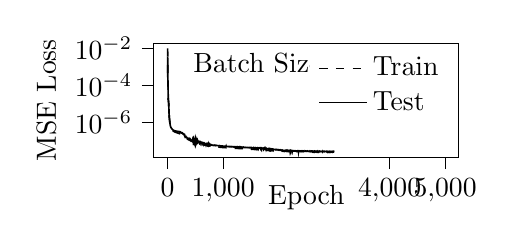
\begin{tikzpicture}

\begin{axis}[
legend cell align={left},
legend style={draw=none},
log basis y={10},
tick align=outside,
tick pos=left,
title={Batch Size 12},
title style={at={(0.4,0.85)},anchor=north},
x grid style={white!69.0196078431373!black},
xlabel={Epoch},
x label style={yshift=13pt},
xmin=-249.95, xmax=5248.95,
xtick style={color=black},
xtick = {0,1000,4000,5000},
y grid style={white!69.0196078431373!black},
ylabel={MSE Loss},
ymin=1.20182983684796e-08, ymax=0.0188674057447821,
ymode=log,
ytick style={color=black},
width=.45\textwidth,
height=.25\textwidth
]
\addplot [semithick, black, dashed]
table {%
0 0.00986465203441947
1 0.00260751335400653
2 0.00168988164350485
3 0.000488507373779203
4 0.000209907971291254
5 0.000167378415469924
6 0.000144635666222162
7 0.000122048938873469
8 8.62523788347024e-05
9 4.82955873002413e-05
10 2.73796132283068e-05
11 1.90950526797145e-05
12 1.60943547821725e-05
13 1.4741469611298e-05
14 1.38728226151662e-05
15 1.31170852149056e-05
16 1.23484586361327e-05
17 1.15099031735347e-05
18 1.05987408478731e-05
19 9.60587541868733e-06
20 8.52972127505861e-06
21 7.39411303849163e-06
22 6.24609348050627e-06
23 5.15921849678429e-06
24 4.20662657506024e-06
25 3.43513256635849e-06
26 2.85083812256804e-06
27 2.41368249620843e-06
28 2.11103944583009e-06
29 1.89133949933387e-06
30 1.72881501848774e-06
31 1.60041405033308e-06
32 1.49132691603201e-06
33 1.39468694930702e-06
34 1.30722597387098e-06
35 1.22787994946677e-06
36 1.15318429976398e-06
37 1.08247199141989e-06
38 1.01458761692296e-06
39 9.50791769616831e-07
40 8.94639568261079e-07
41 8.44264715250895e-07
42 7.98514396704664e-07
43 7.57062303104059e-07
44 7.1960601601547e-07
45 6.86264076177002e-07
46 6.56710590567502e-07
47 6.30560452140253e-07
48 6.07495739716849e-07
49 5.8729833474945e-07
50 5.69166945249871e-07
51 5.53365959734515e-07
52 5.39226312846706e-07
53 5.26853619190663e-07
54 5.15626668984171e-07
55 5.05354143809034e-07
56 4.96219717452013e-07
57 4.87743031464148e-07
58 4.79965486192328e-07
59 4.72839623540552e-07
60 4.66067782073731e-07
61 4.59671513606091e-07
62 4.5346518455062e-07
63 4.47667074912168e-07
64 4.42254874914619e-07
65 4.36917606041582e-07
66 4.31543515322906e-07
67 4.26586544664612e-07
68 4.21815189840398e-07
69 4.17151321900514e-07
70 4.12637008346803e-07
71 4.08143212267705e-07
72 4.03891417800969e-07
73 3.99800072712568e-07
74 3.95728463927244e-07
75 3.91803002401218e-07
76 3.88060614168244e-07
77 3.84411412498194e-07
78 3.80947624093723e-07
79 3.77644791850493e-07
80 3.74367981969172e-07
81 3.71259390676611e-07
82 3.68247853160908e-07
83 3.652546020369e-07
84 3.6221987798002e-07
85 3.59415486626151e-07
86 3.5667539174196e-07
87 3.54011815321989e-07
88 3.51362291480147e-07
89 3.48911777192318e-07
90 3.46474773395951e-07
91 3.44100075985848e-07
92 3.41823218076717e-07
93 3.39414419274245e-07
94 3.37256983388948e-07
95 3.35122220975533e-07
96 3.32999039398208e-07
97 3.308729406813e-07
98 3.28791070590475e-07
99 3.26763725187809e-07
100 3.24788877969253e-07
101 3.22926390043557e-07
102 3.21002658578015e-07
103 3.19170082884691e-07
104 3.17383342175878e-07
105 3.15699859866899e-07
106 3.14064653028036e-07
107 3.12445270114177e-07
108 3.10892673106465e-07
109 3.09378054256962e-07
110 3.07913456573644e-07
111 3.06473376284429e-07
112 3.05058618222563e-07
113 3.03616083433671e-07
114 3.02240261970261e-07
115 3.00803783467912e-07
116 2.99412046698171e-07
117 2.98129154018524e-07
118 2.9680637989941e-07
119 2.956091626333e-07
120 2.94398002705129e-07
121 2.93305538983514e-07
122 2.92147232228944e-07
123 2.91225466177566e-07
124 2.90211831752999e-07
125 2.89178200560386e-07
126 2.88173387507929e-07
127 2.87183440727358e-07
128 2.86342366467219e-07
129 2.85356920538768e-07
130 2.84390754857709e-07
131 2.83464474413479e-07
132 2.82583242006406e-07
133 2.8172577098873e-07
134 2.80857720069494e-07
135 2.80030456526397e-07
136 2.7921289006742e-07
137 2.78486256341509e-07
138 2.77583483358061e-07
139 2.76679555630981e-07
140 2.75953290339561e-07
141 2.75134501507749e-07
142 2.74358878237548e-07
143 2.73620859931067e-07
144 2.72921118955325e-07
145 2.72204606596898e-07
146 2.71600296350344e-07
147 2.70895373438551e-07
148 2.70107028012353e-07
149 2.69427775770409e-07
150 2.68747027665815e-07
151 2.68087882655785e-07
152 2.67431323973446e-07
153 2.66787339732929e-07
154 2.66194304368932e-07
155 2.65507266530469e-07
156 2.64838975181396e-07
157 2.64226872690281e-07
158 2.63632238610448e-07
159 2.63005287392959e-07
160 2.62324573544397e-07
161 2.61686803941466e-07
162 2.61059241625314e-07
163 2.60443335927614e-07
164 2.59830360638989e-07
165 2.59203043220752e-07
166 2.58814742848191e-07
167 2.58187941711581e-07
168 2.57645324354015e-07
169 2.56950830959751e-07
170 2.56333903415438e-07
171 2.55688715166637e-07
172 2.55113041116623e-07
173 2.54555375368047e-07
174 2.53929813437115e-07
175 2.5342732418797e-07
176 2.52792287164338e-07
177 2.52248266421047e-07
178 2.51688670086374e-07
179 2.51038047940727e-07
180 2.50433593155102e-07
181 2.49846895816353e-07
182 2.4925068778331e-07
183 2.48642706562386e-07
184 2.48091862619738e-07
185 2.47487900533806e-07
186 2.46981339406762e-07
187 2.46445586376001e-07
188 2.4578293544387e-07
189 2.45207809527585e-07
190 2.44607930094697e-07
191 2.44043891703189e-07
192 2.43480022177267e-07
193 2.4291157212909e-07
194 2.42355524981974e-07
195 2.42037180440295e-07
196 2.41199472886937e-07
197 2.40585803228933e-07
198 2.40010634855592e-07
199 2.39500687503116e-07
200 2.38559428057481e-07
201 2.37998244734117e-07
202 2.37386749538985e-07
203 2.36729708964011e-07
204 2.36116574058555e-07
205 2.35617242166686e-07
206 2.34869198719142e-07
207 2.34130488149382e-07
208 2.33504791539755e-07
209 2.32825766650212e-07
210 2.32257079968966e-07
211 2.31693280401721e-07
212 2.30864698402966e-07
213 2.3010987560655e-07
214 2.29548378043534e-07
215 2.28922232611291e-07
216 2.28285520089595e-07
217 2.27541015293791e-07
218 2.26777660070448e-07
219 2.26108019493261e-07
220 2.25370043478964e-07
221 2.24709999313267e-07
222 2.24031537757535e-07
223 2.23316574908796e-07
224 2.22542352083225e-07
225 2.21864306306681e-07
226 2.21186275538756e-07
227 2.20559174905192e-07
228 2.19845879747057e-07
229 2.1916440608579e-07
230 2.18400654548726e-07
231 2.17631000741639e-07
232 2.1685724080594e-07
233 2.16357953003886e-07
234 2.15595866636488e-07
235 2.14708611661741e-07
236 2.14008152170932e-07
237 2.13241750570067e-07
238 2.12561176229338e-07
239 2.11559029993748e-07
240 2.1079359481078e-07
241 2.10079037370284e-07
242 2.0927557328593e-07
243 2.08570132284242e-07
244 2.0762496040735e-07
245 2.0686947846554e-07
246 2.0597260186461e-07
247 2.05157218803473e-07
248 2.04277932267675e-07
249 2.03463535222864e-07
250 2.02576345053231e-07
251 2.01684478581671e-07
252 2.01022849161092e-07
253 2.00100818847383e-07
254 1.99121530601412e-07
255 1.98208881063301e-07
256 1.97281198653368e-07
257 1.96462143219114e-07
258 1.95424846647124e-07
259 1.94515042795439e-07
260 1.9355988537854e-07
261 1.9246042925692e-07
262 1.91416686865668e-07
263 1.90515489558603e-07
264 1.89527632683127e-07
265 1.88538966905804e-07
266 1.87545062705345e-07
267 1.86605689819813e-07
268 1.85676759168185e-07
269 1.84595414312876e-07
270 1.83739938441763e-07
271 1.83056588915763e-07
272 1.81931767822542e-07
273 1.80974241958222e-07
274 1.79814111278742e-07
275 1.78846650378262e-07
276 1.77672937472287e-07
277 1.76583499838369e-07
278 1.75630873900156e-07
279 1.74767970208874e-07
280 1.73521450174642e-07
281 1.72708379595049e-07
282 1.71592240089546e-07
283 1.70582798808483e-07
284 1.69653858535808e-07
285 1.68714139601072e-07
286 1.67747395848822e-07
287 1.66634858901358e-07
288 1.65680374175902e-07
289 1.64878483949027e-07
290 1.63911613735062e-07
291 1.62866931401076e-07
292 1.61993550645468e-07
293 1.61075406995205e-07
294 1.59946316561281e-07
295 1.5917892792827e-07
296 1.58259756501341e-07
297 1.5732373517569e-07
298 1.56405021671217e-07
299 1.55259597870166e-07
300 1.54188427018879e-07
301 1.53147169016902e-07
302 1.52231455013276e-07
303 1.51187420140084e-07
304 1.50537693209144e-07
305 1.4952619660876e-07
306 1.48397269275242e-07
307 1.4768550330506e-07
308 1.46697564398064e-07
309 1.45781057330886e-07
310 1.44909075371194e-07
311 1.44113219779519e-07
312 1.43190130092329e-07
313 1.42234409799005e-07
314 1.41564903948379e-07
315 1.40727371078974e-07
316 1.39984446113249e-07
317 1.38979553332153e-07
318 1.38417120565127e-07
319 1.37457988230694e-07
320 1.37116515570832e-07
321 1.36397150319499e-07
322 1.35356013396982e-07
323 1.34902170020264e-07
324 1.34304258593972e-07
325 1.33666783440802e-07
326 1.32998570336525e-07
327 1.32611940287192e-07
328 1.31949723211605e-07
329 1.3138686095447e-07
330 1.30456072823933e-07
331 1.3004578166427e-07
332 1.29304112519009e-07
333 1.28808979344363e-07
334 1.28247493274482e-07
335 1.27553031711043e-07
336 1.27240534622292e-07
337 1.26568065127699e-07
338 1.26049489637764e-07
339 1.25538146707025e-07
340 1.24983221605812e-07
341 1.2432876307719e-07
342 1.23912163473407e-07
343 1.23308572364178e-07
344 1.22667956080272e-07
345 1.22200386193272e-07
346 1.22031874223757e-07
347 1.21259684172668e-07
348 1.21119337266249e-07
349 1.20427919750858e-07
350 1.19903499227883e-07
351 1.19436163383875e-07
352 1.18939739515794e-07
353 1.18374059605695e-07
354 1.18016359027289e-07
355 1.17585388244609e-07
356 1.17048287139833e-07
357 1.16576402460796e-07
358 1.16139044797737e-07
359 1.15758196896284e-07
360 1.15444143415791e-07
361 1.14990975863073e-07
362 1.14507993282995e-07
363 1.14136096893064e-07
364 1.13680510141772e-07
365 1.13252466047923e-07
366 1.12852237641286e-07
367 1.12467889792994e-07
368 1.12107805644202e-07
369 1.11731543833405e-07
370 1.11416253144306e-07
371 1.10987849686554e-07
372 1.10706991071414e-07
373 1.10312365493689e-07
374 1.09949491416928e-07
375 1.09622494733039e-07
376 1.09173863953141e-07
377 1.08780210922809e-07
378 1.08400519988094e-07
379 1.08056382925934e-07
380 1.07780304008389e-07
381 1.07455280593686e-07
382 1.07053753662222e-07
383 1.06790157172277e-07
384 1.06350253662783e-07
385 1.05875654277044e-07
386 1.0557874308414e-07
387 1.0523801744349e-07
388 1.05013178961659e-07
389 1.04592827046042e-07
390 1.04298884262422e-07
391 1.04052798263206e-07
392 1.03665887857961e-07
393 1.03456886799319e-07
394 1.0317013849225e-07
395 1.02902540117653e-07
396 1.02691777192244e-07
397 1.02266042450041e-07
398 1.02096551165427e-07
399 1.01926844287469e-07
400 1.01609048182668e-07
401 1.01361464448714e-07
402 1.01000889919066e-07
403 1.00627217459491e-07
404 1.00386729590351e-07
405 1.00219144339286e-07
406 9.99003052790087e-08
407 9.96493648183157e-08
408 9.93807552472695e-08
409 9.9116329964535e-08
410 9.8786126562987e-08
411 9.86490139742392e-08
412 9.83083036985447e-08
413 9.80155675744477e-08
414 9.78291330180321e-08
415 9.74236173118547e-08
416 9.72413826400574e-08
417 9.6813098602415e-08
418 9.65025782238763e-08
419 9.63088241970816e-08
420 9.59802467842984e-08
421 9.56620157273566e-08
422 9.52465724334851e-08
423 9.49690089576224e-08
424 9.46741575621608e-08
425 9.44036359105076e-08
426 9.41854147993331e-08
427 9.39079606146226e-08
428 9.36693822200575e-08
429 9.32644040559468e-08
430 9.29040113715223e-08
431 9.26247987530938e-08
432 9.23331803084654e-08
433 9.20339168282012e-08
434 9.18264109806997e-08
435 9.15852875507611e-08
436 9.13102214145588e-08
437 9.10468111256352e-08
438 9.07511739901045e-08
439 9.04364017472361e-08
440 9.02689807666307e-08
441 8.99290094314485e-08
442 8.96550553903595e-08
443 8.94493951589996e-08
444 8.91716758477125e-08
445 8.89388250578319e-08
446 8.86707305451742e-08
447 8.84126433328941e-08
448 8.81528533974884e-08
449 8.79975966133462e-08
450 8.77086544683521e-08
451 8.74807724304284e-08
452 8.71330707998005e-08
453 8.69168866300998e-08
454 8.67209687241161e-08
455 8.62987805767333e-08
456 8.61133189373407e-08
457 8.59795703536088e-08
458 8.55838761908769e-08
459 8.53847518836808e-08
460 8.52117661647845e-08
461 8.49874530458069e-08
462 8.46269108894638e-08
463 8.44341880590881e-08
464 8.42327955622639e-08
465 8.39158430993192e-08
466 8.37331758234696e-08
467 8.35279735837051e-08
468 8.32065515117794e-08
469 8.30688071675718e-08
470 8.27502307209118e-08
471 8.24198592249499e-08
472 8.21675475337824e-08
473 8.19286826458333e-08
474 8.17703776386731e-08
475 8.16130515264554e-08
476 8.14199416949367e-08
477 8.11354428087441e-08
478 8.09148203609549e-08
479 8.06256585327405e-08
480 8.05577514422774e-08
481 8.01761198536712e-08
482 8.00313872019927e-08
483 8.00935765614433e-08
484 7.95331810629746e-08
485 7.93217525196389e-08
486 7.90704434755385e-08
487 7.89373905588835e-08
488 7.86523900353697e-08
489 7.85615026871566e-08
490 7.80801989025714e-08
491 7.79388681949553e-08
492 7.76494746904526e-08
493 7.76557454827213e-08
494 7.72290723933132e-08
495 7.7262094478712e-08
496 7.6727138500328e-08
497 7.66496535145018e-08
498 7.65337105068121e-08
499 7.61089675487748e-08
500 7.61158348751763e-08
501 7.57488532790335e-08
502 7.55854786265709e-08
503 7.55284122589715e-08
504 7.51368786909293e-08
505 7.51029964499377e-08
506 7.4959265091785e-08
507 7.46902734630799e-08
508 7.45905285933641e-08
509 7.42376964532792e-08
510 7.41611178136421e-08
511 7.38317243590141e-08
512 7.36253986373699e-08
513 7.34649972472623e-08
514 7.32372358553467e-08
515 7.31767389251933e-08
516 7.28040041746106e-08
517 7.2763275585779e-08
518 7.24674790860432e-08
519 7.22951334113854e-08
520 7.21275867934219e-08
521 7.19492725651022e-08
522 7.17366622551724e-08
523 7.15983126173718e-08
524 7.14092059868174e-08
525 7.12567897062893e-08
526 7.11410891713082e-08
527 7.08884052669024e-08
528 7.07195806399694e-08
529 7.06897194246726e-08
530 7.03580877072426e-08
531 7.02836704045831e-08
532 7.00082131481109e-08
533 6.99525766786275e-08
534 6.96759692497163e-08
535 6.97064487701542e-08
536 6.93422256221718e-08
537 6.92601750349557e-08
538 6.90926233724579e-08
539 6.89645065392809e-08
540 6.88077918288773e-08
541 6.86312138244967e-08
542 6.85018139590897e-08
543 6.83466730822312e-08
544 6.81660816256054e-08
545 6.79906761576772e-08
546 6.79201561845827e-08
547 6.77617493214404e-08
548 6.75013737094843e-08
549 6.73794689982752e-08
550 6.72881390872427e-08
551 6.70705480455844e-08
552 6.69393279675341e-08
553 6.68744195269689e-08
554 6.67045240068282e-08
555 6.66043024804742e-08
556 6.63488655340957e-08
557 6.62258281215021e-08
558 6.61138364440933e-08
559 6.60180411761676e-08
560 6.57616039893132e-08
561 6.56229188514218e-08
562 6.54586033600688e-08
563 6.53714452363698e-08
564 6.52368431982715e-08
565 6.50957717988657e-08
566 6.48673499000381e-08
567 6.47582385825852e-08
568 6.46143641293159e-08
569 6.446432118119e-08
570 6.43203441300172e-08
571 6.4192627724369e-08
572 6.40600470181417e-08
573 6.40068021166399e-08
574 6.39365269523759e-08
575 6.37360501608544e-08
576 6.36061154205751e-08
577 6.3509022582481e-08
578 6.32211303228818e-08
579 6.31782073031192e-08
580 6.30676574583916e-08
581 6.29049511482234e-08
582 6.28223088280905e-08
583 6.27075932816472e-08
584 6.26088367603898e-08
585 6.25348943021124e-08
586 6.23425757657667e-08
587 6.22136231394119e-08
588 6.20773557441733e-08
589 6.19553724318333e-08
590 6.18225580495867e-08
591 6.17681063130538e-08
592 6.15644303892891e-08
593 6.15694477503998e-08
594 6.14890816879589e-08
595 6.13349707962462e-08
596 6.12565199788802e-08
597 6.11039763497879e-08
598 6.09475477950477e-08
599 6.08200170133708e-08
600 6.07890193126239e-08
601 6.05905780212806e-08
602 6.06219013803568e-08
603 6.05198525598651e-08
604 6.03579276499242e-08
605 6.02553045994808e-08
606 6.00713622344818e-08
607 5.99952318191367e-08
608 5.9981121403041e-08
609 5.97894142658502e-08
610 5.97183774207813e-08
611 5.96686039141078e-08
612 5.95676945387744e-08
613 5.94907872319041e-08
614 5.92593871166007e-08
615 5.92393065606202e-08
616 5.9148006766548e-08
617 5.90109215836887e-08
618 5.89135106248153e-08
619 5.88587184792774e-08
620 5.87428698697961e-08
621 5.86733444531015e-08
622 5.86089437886596e-08
623 5.84117424489041e-08
624 5.83948601462957e-08
625 5.82078968511506e-08
626 5.8190589716051e-08
627 5.80720970393026e-08
628 5.80102084891297e-08
629 5.79308706607402e-08
630 5.77988304310255e-08
631 5.76867206724232e-08
632 5.76577249830075e-08
633 5.7560701507925e-08
634 5.74618290886911e-08
635 5.73348193220484e-08
636 5.72021462918017e-08
637 5.7134671357313e-08
638 5.70187124820765e-08
639 5.70405687048296e-08
640 5.68837959995662e-08
641 5.68191775931322e-08
642 5.67855930567826e-08
643 5.66864053834052e-08
644 5.6518523400971e-08
645 5.6458533947779e-08
646 5.64203987840894e-08
647 5.62999695340174e-08
648 5.63434277185069e-08
649 5.61434640175534e-08
650 5.60735962306814e-08
651 5.60068968341764e-08
652 5.59211564081067e-08
653 5.58447379596912e-08
654 5.57167653478091e-08
655 5.56635842196453e-08
656 5.5632814649121e-08
657 5.55321487875796e-08
658 5.54532317151019e-08
659 5.53764749026191e-08
660 5.53393014194319e-08
661 5.52139071908318e-08
662 5.51612944822309e-08
663 5.51343926893949e-08
664 5.50219801536945e-08
665 5.49547743651887e-08
666 5.483404369156e-08
667 5.47484004957646e-08
668 5.47437455207564e-08
669 5.46461673543179e-08
670 5.45263590433411e-08
671 5.44574668260609e-08
672 5.44269155200649e-08
673 5.44110587032074e-08
674 5.43177522867219e-08
675 5.41858194361826e-08
676 5.41225189309592e-08
677 5.40491708049831e-08
678 5.40079091468875e-08
679 5.39885951886038e-08
680 5.38424242090919e-08
681 5.37980833959682e-08
682 5.37519621228336e-08
683 5.36881446233118e-08
684 5.35810987940253e-08
685 5.34883564585906e-08
686 5.33910138974332e-08
687 5.34043271561123e-08
688 5.32770727933764e-08
689 5.32541824557138e-08
690 5.3226214092227e-08
691 5.313242644658e-08
692 5.29011008598169e-08
693 5.30353102140258e-08
694 5.29186655453845e-08
695 5.28322069712189e-08
696 5.27698278766479e-08
697 5.27196956376358e-08
698 5.2631735613807e-08
699 5.25709220493766e-08
700 5.25244517846146e-08
701 5.24470878144278e-08
702 5.23868302815987e-08
703 5.23032808932994e-08
704 5.23088088612696e-08
705 5.22860117437825e-08
706 5.20894042377251e-08
707 5.20470728804101e-08
708 5.20317889107115e-08
709 5.19126496892691e-08
710 5.18803367717909e-08
711 5.18576781968411e-08
712 5.17070597582948e-08
713 5.17908779415604e-08
714 5.16186378098889e-08
715 5.16389611124773e-08
716 5.14800853642579e-08
717 5.15446715888499e-08
718 5.14004373993877e-08
719 5.13445678522088e-08
720 5.13225442995665e-08
721 5.12989243765165e-08
722 5.11132407510217e-08
723 5.12047896591966e-08
724 5.10618273199577e-08
725 5.10391850978618e-08
726 5.09758288115766e-08
727 5.09068935681682e-08
728 5.08076371207956e-08
729 5.08547186038857e-08
730 5.06261828028238e-08
731 5.07035413468788e-08
732 5.06510107455861e-08
733 5.058392002937e-08
734 5.05539704655829e-08
735 5.04213919053436e-08
736 5.04114446301378e-08
737 5.03482807820671e-08
738 5.03112679501459e-08
739 5.01340524942632e-08
740 5.02210255803482e-08
741 5.0122920940833e-08
742 5.01321394816007e-08
743 5.00974128461945e-08
744 4.99888168357668e-08
745 4.99658209750622e-08
746 4.98925407109698e-08
747 4.9897336277442e-08
748 4.97913948036182e-08
749 4.97167080119369e-08
750 4.96659497135076e-08
751 4.95494336339551e-08
752 4.95479175094039e-08
753 4.94693685177415e-08
754 4.94487289677922e-08
755 4.94525359624318e-08
756 4.93095180016842e-08
757 4.93115764243115e-08
758 4.92605054458606e-08
759 4.92203085461595e-08
760 4.91040709610668e-08
761 4.91201381525562e-08
762 4.91542410433935e-08
763 4.89817610450458e-08
764 4.90018651271176e-08
765 4.88528724233808e-08
766 4.88570789267899e-08
767 4.880257696164e-08
768 4.87457676086763e-08
769 4.86502932244561e-08
770 4.86756310414636e-08
771 4.85431318375728e-08
772 4.85933666080081e-08
773 4.84812188757895e-08
774 4.84693957930239e-08
775 4.84090173269912e-08
776 4.83806026458709e-08
777 4.83119367518755e-08
778 4.82378492891638e-08
779 4.82760957557032e-08
780 4.79961109884628e-08
781 4.81195751747759e-08
782 4.80567150464956e-08
783 4.7969296641313e-08
784 4.78785606942803e-08
785 4.78766278544972e-08
786 4.77091153370007e-08
787 4.7843352267288e-08
788 4.77333643416679e-08
789 4.75283319607077e-08
790 4.76626156732671e-08
791 4.76504013545556e-08
792 4.75728110890057e-08
793 4.74972522962502e-08
794 4.74657006154878e-08
795 4.74430570385209e-08
796 4.73490130124613e-08
797 4.73458218512205e-08
798 4.72957860992317e-08
799 4.72716764308781e-08
800 4.72083759921351e-08
801 4.71436242871393e-08
802 4.71020220764409e-08
803 4.70619568638163e-08
804 4.69447375131565e-08
805 4.70273669746465e-08
806 4.69348211912346e-08
807 4.68514108148244e-08
808 4.68760159870155e-08
809 4.67407997243445e-08
810 4.668936239091e-08
811 4.66776428726732e-08
812 4.66418046992596e-08
813 4.65478704430113e-08
814 4.65727279522758e-08
815 4.64733582422106e-08
816 4.64236427423633e-08
817 4.63933700558102e-08
818 4.63374233660808e-08
819 4.64078003490978e-08
820 4.62588261654766e-08
821 4.62255887074479e-08
822 4.63597804509934e-08
823 4.61424195286519e-08
824 4.6050068632593e-08
825 4.60841536601413e-08
826 4.61601346261712e-08
827 4.60038556417405e-08
828 4.59089444397556e-08
829 4.59156726306144e-08
830 4.58586313008709e-08
831 4.58739114399677e-08
832 4.57872433554157e-08
833 4.57379587005489e-08
834 4.57546889385024e-08
835 4.56660898051498e-08
836 4.56715770046669e-08
837 4.56353020987668e-08
838 4.55700081794602e-08
839 4.55263045439393e-08
840 4.55119456705675e-08
841 4.5449994938598e-08
842 4.54511536351566e-08
843 4.53804433578691e-08
844 4.53476187658559e-08
845 4.52941170318747e-08
846 4.5239587702054e-08
847 4.52244539767764e-08
848 4.52237193987094e-08
849 4.51578661729759e-08
850 4.51483631917397e-08
851 4.50770215485678e-08
852 4.50623080965542e-08
853 4.50298040890846e-08
854 4.49765035368227e-08
855 4.48925950851122e-08
856 4.48928823456802e-08
857 4.48779615119832e-08
858 4.48068184591239e-08
859 4.4831918515555e-08
860 4.47324035697037e-08
861 4.47270897830342e-08
862 4.47002858094892e-08
863 4.4657078998107e-08
864 4.4625353985603e-08
865 4.46067588442083e-08
866 4.45288706892008e-08
867 4.4545250390522e-08
868 4.44633700623223e-08
869 4.44693163995573e-08
870 4.43822104270891e-08
871 4.44003185861066e-08
872 4.4350900136734e-08
873 4.43133551423418e-08
874 4.42564236794711e-08
875 4.42705738973946e-08
876 4.4196955870218e-08
877 4.41425731297248e-08
878 4.41519010946057e-08
879 4.41395356127138e-08
880 4.40635883549164e-08
881 4.40397766704226e-08
882 4.40307261748734e-08
883 4.39618665622506e-08
884 4.39708115972494e-08
885 4.39327809022225e-08
886 4.38664159514288e-08
887 4.38603793111793e-08
888 4.38408824306886e-08
889 4.37644267731817e-08
890 4.37735866157268e-08
891 4.37353327246541e-08
892 4.36864780345669e-08
893 4.36639237634083e-08
894 4.36366870142914e-08
895 4.35965192210481e-08
896 4.3572467127398e-08
897 4.35362647489776e-08
898 4.35168434035409e-08
899 4.34617703649297e-08
900 4.34522315095288e-08
901 4.34173429052146e-08
902 4.33801663173917e-08
903 4.33698186665118e-08
904 4.33100990041628e-08
905 4.33015152583396e-08
906 4.3278288565648e-08
907 4.32211963278576e-08
908 4.3219251775554e-08
909 4.3181242400798e-08
910 4.31332777200013e-08
911 4.31439885427822e-08
912 4.31027219279065e-08
913 4.30666660284561e-08
914 4.30346289502096e-08
915 4.30089304742609e-08
916 4.30059758689713e-08
917 4.28878593916272e-08
918 4.29622862594895e-08
919 4.28881998790791e-08
920 4.28569609647628e-08
921 4.2828996679185e-08
922 4.2799269658606e-08
923 4.27722287156017e-08
924 4.27546580335001e-08
925 4.27072546043474e-08
926 4.27345478737883e-08
927 4.264485852004e-08
928 4.2670247766301e-08
929 4.2589363842657e-08
930 4.25970238097953e-08
931 4.25758866459198e-08
932 4.25097977258215e-08
933 4.25072540094196e-08
934 4.25228131814675e-08
935 4.24551681581522e-08
936 4.24027583650799e-08
937 4.23363741961263e-08
938 4.23204615516707e-08
939 4.22993436976982e-08
940 4.22378282662269e-08
941 4.22040973798794e-08
942 4.21847035307446e-08
943 4.21343101539811e-08
944 4.2126883438717e-08
945 4.20900990401692e-08
946 4.20884369844466e-08
947 4.20589325310087e-08
948 4.19787110182759e-08
949 4.20168152539442e-08
950 4.19544620016423e-08
951 4.19586019767648e-08
952 4.19337164313773e-08
953 4.18319668459069e-08
954 4.18840358483765e-08
955 4.18133375947379e-08
956 4.17775922692094e-08
957 4.18056963697598e-08
958 4.17372047515279e-08
959 4.17033064222745e-08
960 4.17059196080567e-08
961 4.16943957151057e-08
962 4.16372243563075e-08
963 4.16370861993566e-08
964 4.15988224891257e-08
965 4.15754833527802e-08
966 4.15447488427002e-08
967 4.1529855465417e-08
968 4.14870760779328e-08
969 4.14769175917714e-08
970 4.14634785348515e-08
971 4.14006713183381e-08
972 4.14197953846074e-08
973 4.13596368530912e-08
974 4.13537683724064e-08
975 4.1307926029843e-08
976 4.13104246086985e-08
977 4.12698089049508e-08
978 4.12661955504915e-08
979 4.1246893030829e-08
980 4.1204264257397e-08
981 4.11998552572859e-08
982 4.11423886974983e-08
983 4.11852311390023e-08
984 4.10878856221254e-08
985 4.11417882942051e-08
986 4.10401329168091e-08
987 4.10561749015823e-08
988 4.09912072508953e-08
989 4.10312746414185e-08
990 4.09426719247712e-08
991 4.09751525736802e-08
992 4.09428749307133e-08
993 4.09263540396044e-08
994 4.08885892263717e-08
995 4.08824053652306e-08
996 4.08362075372324e-08
997 4.08398484823959e-08
998 4.07884294270882e-08
999 4.07961053255945e-08
1000 4.07628713750728e-08
1001 4.07447405156509e-08
1002 4.06991164881408e-08
1003 4.07139741774047e-08
1004 4.06584073195698e-08
1005 4.06450657428907e-08
1006 4.0686107333509e-08
1007 4.06013955563286e-08
1008 4.06371103327742e-08
1009 4.05344883180958e-08
1010 4.05928265811252e-08
1011 4.04953102959918e-08
1012 4.05400375052867e-08
1013 4.04554987035127e-08
1014 4.04771682066972e-08
1015 4.04402577559535e-08
1016 4.0428882825681e-08
1017 4.04340641128834e-08
1018 4.03814156404753e-08
1019 4.0374532372069e-08
1020 4.03447679416277e-08
1021 4.03274609408185e-08
1022 4.02845212158558e-08
1023 4.02629104747151e-08
1024 4.02638920727515e-08
1025 4.02323331403048e-08
1026 4.02173497019956e-08
1027 4.02156664204044e-08
1028 4.01830514584423e-08
1029 4.02121344459576e-08
1030 4.0156237038164e-08
1031 4.01559546652366e-08
1032 4.00968941469509e-08
1033 4.01204974751583e-08
1034 4.00551980885019e-08
1035 4.0069630312381e-08
1036 4.00200974222827e-08
1037 4.00298179700027e-08
1038 3.99923551174886e-08
1039 4.00141667970303e-08
1040 3.99311973240882e-08
1041 3.99573413797378e-08
1042 3.98990666719905e-08
1043 3.99129206584782e-08
1044 3.98603177810018e-08
1045 3.98817791260116e-08
1046 3.98457326747586e-08
1047 3.98146454022818e-08
1048 3.98002268281627e-08
1049 3.97645544595774e-08
1050 3.97684314993179e-08
1051 3.97593357159765e-08
1052 3.97377002879964e-08
1053 3.97104352740638e-08
1054 3.96814806788553e-08
1055 3.96363156295101e-08
1056 3.9673983054245e-08
1057 3.96182399169267e-08
1058 3.96241302869548e-08
1059 3.95833749344355e-08
1060 3.95803736492537e-08
1061 3.95635018824623e-08
1062 3.95425178775095e-08
1063 3.95127514991919e-08
1064 3.95236096665179e-08
1065 3.94801247914692e-08
1066 3.94699455541093e-08
1067 3.94495846368989e-08
1068 3.94233477041128e-08
1069 3.93970162880234e-08
1070 3.93831324943744e-08
1071 3.93919230541382e-08
1072 3.93413428261748e-08
1073 3.93289245282479e-08
1074 3.93032945045291e-08
1075 3.92852066153918e-08
1076 3.9295780957858e-08
1077 3.92376532050805e-08
1078 3.92484061152862e-08
1079 3.92187464393733e-08
1080 3.92049001938658e-08
1081 3.91915893577332e-08
1082 3.91644203880644e-08
1083 3.91436231930936e-08
1084 3.91440971120682e-08
1085 3.9097501546339e-08
1086 3.91036622988858e-08
1087 3.90890850639244e-08
1088 3.90710894695552e-08
1089 3.90309840070247e-08
1090 3.89647954115021e-08
1091 3.90428916768183e-08
1092 3.89672375298659e-08
1093 3.89829090737688e-08
1094 3.89328668917937e-08
1095 3.8967888471575e-08
1096 3.88995695694758e-08
1097 3.88681002007814e-08
1098 3.88848865229474e-08
1099 3.88840480998041e-08
1100 3.88418534913847e-08
1101 3.88604784173375e-08
1102 3.87413352363212e-08
1103 3.88109814386329e-08
1104 3.87788765968937e-08
1105 3.87235220815111e-08
1106 3.87488532770687e-08
1107 3.87439485563939e-08
1108 3.86415243754808e-08
1109 3.8728494055109e-08
1110 3.86680716335519e-08
1111 3.86532019791419e-08
1112 3.86497158176826e-08
1113 3.8636003288234e-08
1114 3.85474400888784e-08
1115 3.86122508165213e-08
1116 3.85778451326306e-08
1117 3.85534992221135e-08
1118 3.85593853028248e-08
1119 3.84759967280037e-08
1120 3.84829618364671e-08
1121 3.84756804247992e-08
1122 3.85140681662213e-08
1123 3.8438346928558e-08
1124 3.84712159002408e-08
1125 3.84237612519128e-08
1126 3.84100821980152e-08
1127 3.84184149536584e-08
1128 3.83808637380284e-08
1129 3.83917643411365e-08
1130 3.82901163909332e-08
1131 3.83811045048494e-08
1132 3.82541426174056e-08
1133 3.83160322020138e-08
1134 3.82843096612519e-08
1135 3.82701170487642e-08
1136 3.82797174264759e-08
1137 3.82333374953094e-08
1138 3.82074162288455e-08
1139 3.82696028971686e-08
1140 3.81980627793602e-08
1141 3.81799757996751e-08
1142 3.8144010237809e-08
1143 3.81818793920619e-08
1144 3.80666717362713e-08
1145 3.81680169479352e-08
1146 3.80704226533466e-08
1147 3.81038261542035e-08
1148 3.80511195393492e-08
1149 3.80643813568084e-08
1150 3.80114991392414e-08
1151 3.80306619968362e-08
1152 3.79887475302614e-08
1153 3.79720264546394e-08
1154 3.791481330226e-08
1155 3.80194876340039e-08
1156 3.78821038038103e-08
1157 3.79264725825877e-08
1158 3.79251857716105e-08
1159 3.7940524523835e-08
1160 3.78564981624505e-08
1161 3.79056175709246e-08
1162 3.7820451098248e-08
1163 3.78839639073651e-08
1164 3.77697167580327e-08
1165 3.78676807808214e-08
1166 3.77630708619571e-08
1167 3.78053544584083e-08
1168 3.77177560308946e-08
1169 3.77913717206196e-08
1170 3.7716236824311e-08
1171 3.77603198582741e-08
1172 3.76800632066502e-08
1173 3.77358696452954e-08
1174 3.76665307061807e-08
1175 3.76578641071388e-08
1176 3.76528494876806e-08
1177 3.76931637665419e-08
1178 3.76032949834679e-08
1179 3.76545072341423e-08
1180 3.76161433950907e-08
1181 3.76058548825338e-08
1182 3.75470607340087e-08
1183 3.75844980633597e-08
1184 3.75151704272461e-08
1185 3.75498367968215e-08
1186 3.74865175308233e-08
1187 3.75448962884066e-08
1188 3.74674532623627e-08
1189 3.74706493604395e-08
1190 3.74834768307298e-08
1191 3.74781881616928e-08
1192 3.7397500849904e-08
1193 3.74274238308301e-08
1194 3.73691718474202e-08
1195 3.74507780263204e-08
1196 3.73472883956164e-08
1197 3.73127437064845e-08
1198 3.73506364719236e-08
1199 3.73981558442595e-08
1200 3.7338107933504e-08
1201 3.73268508597212e-08
1202 3.72619590259651e-08
1203 3.73075510989962e-08
1204 3.72555192630705e-08
1205 3.72698282601715e-08
1206 3.72196118409916e-08
1207 3.72460998251197e-08
1208 3.72056135308292e-08
1209 3.72248057475073e-08
1210 3.71466972524529e-08
1211 3.72026701846636e-08
1212 3.71419100359216e-08
1213 3.71812740316838e-08
1214 3.70939736465327e-08
1215 3.71489042096248e-08
1216 3.7113513110392e-08
1217 3.71238522969847e-08
1218 3.7051462068775e-08
1219 3.70408303098287e-08
1220 3.70527457099657e-08
1221 3.71117573292427e-08
1222 3.70065734290635e-08
1223 3.70773726837459e-08
1224 3.69714598523466e-08
1225 3.70183491644736e-08
1226 3.69632151061434e-08
1227 3.69688803734672e-08
1228 3.69345358874629e-08
1229 3.70043623261726e-08
1230 3.68789692530022e-08
1231 3.6923755753525e-08
1232 3.69178673366917e-08
1233 3.69336560470176e-08
1234 3.68495994862372e-08
1235 3.69068889448434e-08
1236 3.67925287282708e-08
1237 3.68701018538386e-08
1238 3.68366740570472e-08
1239 3.68471438683592e-08
1240 3.67930696049955e-08
1241 3.67843892484953e-08
1242 3.67117054826364e-08
1243 3.677451412449e-08
1244 3.66981722030163e-08
1245 3.68144545413987e-08
1246 3.67429922402522e-08
1247 3.67495650623791e-08
1248 3.66697556537962e-08
1249 3.673240019405e-08
1250 3.66448512439245e-08
1251 3.67027619487655e-08
1252 3.65920757367399e-08
1253 3.66965758033572e-08
1254 3.65875247504056e-08
1255 3.66223540874248e-08
1256 3.65944935285882e-08
1257 3.66244116737284e-08
1258 3.65502016769647e-08
1259 3.66107018327481e-08
1260 3.65182431067766e-08
1261 3.65733416539252e-08
1262 3.64762915840153e-08
1263 3.65497682246221e-08
1264 3.64812092018917e-08
1265 3.64956923550914e-08
1266 3.64760043207881e-08
1267 3.64698643686353e-08
1268 3.63941480558415e-08
1269 3.65296096525384e-08
1270 3.63690572814067e-08
1271 3.64550898344111e-08
1272 3.64057715510883e-08
1273 3.63955797888172e-08
1274 3.6346708210044e-08
1275 3.64354798374848e-08
1276 3.63374602357348e-08
1277 3.63845091607037e-08
1278 3.63057983131501e-08
1279 3.63851439742627e-08
1280 3.62835410672036e-08
1281 3.63581149485385e-08
1282 3.62605742491355e-08
1283 3.63340823855064e-08
1284 3.62254651571877e-08
1285 3.62666374576203e-08
1286 3.62279050178765e-08
1287 3.63015168371114e-08
1288 3.61480790476912e-08
1289 3.62981329371647e-08
1290 3.61940607199201e-08
1291 3.62094753528967e-08
1292 3.61854679194636e-08
1293 3.6202119020454e-08
1294 3.61038167971398e-08
1295 3.61697062374176e-08
1296 3.60709334031945e-08
1297 3.61486028136852e-08
1298 3.60927589545408e-08
1299 3.61772631107084e-08
1300 3.60974500324063e-08
1301 3.60986392248634e-08
1302 3.60575252317485e-08
1303 3.60727192401419e-08
1304 3.60606473504132e-08
1305 3.60352742761794e-08
1306 3.59939338800032e-08
1307 3.61285097992739e-08
1308 3.60267587273013e-08
1309 3.60040997162399e-08
1310 3.59984943491047e-08
1311 3.60030120952287e-08
1312 3.59366314590446e-08
1313 3.59511454565003e-08
1314 3.59778346781912e-08
1315 3.58697534761857e-08
1316 3.58744597754083e-08
1317 3.58755469523303e-08
1318 3.59430045367589e-08
1319 3.59257480570805e-08
1320 3.59301595967437e-08
1321 3.58530930346962e-08
1322 3.59200509084062e-08
1323 3.58173616142125e-08
1324 3.58290745907759e-08
1325 3.57938193708747e-08
1326 3.57899713485083e-08
1327 3.5793046433605e-08
1328 3.58327594781678e-08
1329 3.58056646886819e-08
1330 3.57559324131652e-08
1331 3.57163421579394e-08
1332 3.58186596271405e-08
1333 3.57266713591729e-08
1334 3.57721263163364e-08
1335 3.57289059004009e-08
1336 3.57348836004392e-08
1337 3.56643451484469e-08
1338 3.56755122423099e-08
1339 3.56512342867492e-08
1340 3.57254644177731e-08
1341 3.56135864604423e-08
1342 3.56567139553642e-08
1343 3.56228755342771e-08
1344 3.56157831650037e-08
1345 3.56261555824995e-08
1346 3.56166937180738e-08
1347 3.55419518806042e-08
1348 3.56122585725429e-08
1349 3.55784823625037e-08
1350 3.55698442782439e-08
1351 3.55499891440737e-08
1352 3.55444168177076e-08
1353 3.55365635667239e-08
1354 3.55434164588965e-08
1355 3.54976912242533e-08
1356 3.55253114045146e-08
1357 3.54397096885129e-08
1358 3.54691964448629e-08
1359 3.54563573139069e-08
1360 3.5478567215157e-08
1361 3.53421905713136e-08
1362 3.54846726254129e-08
1363 3.53568850312007e-08
1364 3.54110339427696e-08
1365 3.5353937678925e-08
1366 3.53053109807812e-08
1367 3.53521615029123e-08
1368 3.53128138467078e-08
1369 3.5240403772763e-08
1370 3.53219768723355e-08
1371 3.52237151741562e-08
1372 3.52585948248874e-08
1373 3.52181428797006e-08
1374 3.52345983979527e-08
1375 3.5197039005231e-08
1376 3.51824608541694e-08
1377 3.51714712936104e-08
1378 3.51521568220979e-08
1379 3.51316235145088e-08
1380 3.51479788441077e-08
1381 3.51172734790441e-08
1382 3.51213447386743e-08
1383 3.50674293927673e-08
1384 3.50996681633026e-08
1385 3.50304776869337e-08
1386 3.50873294597242e-08
1387 3.50203696766965e-08
1388 3.50223418050786e-08
1389 3.49921543942906e-08
1390 3.50372544616838e-08
1391 3.49638235875281e-08
1392 3.49716586388318e-08
1393 3.49454311402823e-08
1394 3.49519097789325e-08
1395 3.49338727393393e-08
1396 3.49295108592208e-08
1397 3.49012144387911e-08
1398 3.48955583251564e-08
1399 3.48614611469817e-08
1400 3.48881095217726e-08
1401 3.48031039051218e-08
1402 3.48588512812317e-08
1403 3.48059978563348e-08
1404 3.48193340726976e-08
1405 3.4768435475983e-08
1406 3.48078932151216e-08
1407 3.47292625223463e-08
1408 3.47900327933972e-08
1409 3.47024034165885e-08
1410 3.47382387486289e-08
1411 3.47190780403461e-08
1412 3.47138895666102e-08
1413 3.46824423006613e-08
1414 3.46658242657025e-08
1415 3.46603557352171e-08
1416 3.46695957810713e-08
1417 3.45932358307723e-08
1418 3.46256732487934e-08
1419 3.46554751522534e-08
1420 3.45934053445433e-08
1421 3.45557979635947e-08
1422 3.45795851121596e-08
1423 3.45272724064289e-08
1424 3.45287600155333e-08
1425 3.45276842572883e-08
1426 3.45363924690847e-08
1427 3.44405134976558e-08
1428 3.45763506442433e-08
1429 3.44420369643047e-08
1430 3.45333653808572e-08
1431 3.44339288592989e-08
1432 3.44635827135214e-08
1433 3.43957725076345e-08
1434 3.44407339001943e-08
1435 3.43659994061519e-08
1436 3.44152207178092e-08
1437 3.43061979396453e-08
1438 3.44003783270197e-08
1439 3.42836897334349e-08
1440 3.43494948060701e-08
1441 3.43212779686872e-08
1442 3.43116386327842e-08
1443 3.42824064917916e-08
1444 3.42671480133454e-08
1445 3.42346018127473e-08
1446 3.42795362062786e-08
1447 3.42557926110317e-08
1448 3.42419740433178e-08
1449 3.42089497687187e-08
1450 3.41833200461562e-08
1451 3.41681059620054e-08
1452 3.41808267963713e-08
1453 3.41554313056045e-08
1454 3.41370324263779e-08
1455 3.41116424554804e-08
1456 3.41007699523165e-08
1457 3.41288889531236e-08
1458 3.40665554707691e-08
1459 3.40471791352364e-08
1460 3.40181517825259e-08
1461 3.39896740693244e-08
1462 3.4003362514911e-08
1463 3.3951606806742e-08
1464 3.40019788399666e-08
1465 3.39163919444451e-08
1466 3.3960860374049e-08
1467 3.39045290239522e-08
1468 3.39221304253265e-08
1469 3.38546833547765e-08
1470 3.3913754636907e-08
1471 3.37925229269402e-08
1472 3.38952887533941e-08
1473 3.38032704994328e-08
1474 3.38511760439009e-08
1475 3.3811773288059e-08
1476 3.37878763364426e-08
1477 3.38017573073329e-08
1478 3.37943926542007e-08
1479 3.37021603558883e-08
1480 3.37654926035182e-08
1481 3.36839126212277e-08
1482 3.37255088666379e-08
1483 3.36747503295438e-08
1484 3.36824065245831e-08
1485 3.37152722094739e-08
1486 3.36734605289422e-08
1487 3.36174965709235e-08
1488 3.36090857965179e-08
1489 3.36510894193201e-08
1490 3.35835563590051e-08
1491 3.35574441867005e-08
1492 3.35900129647143e-08
1493 3.35236699052584e-08
1494 3.35843949795953e-08
1495 3.34654319857815e-08
1496 3.3615035504975e-08
1497 3.34341725250264e-08
1498 3.35445144635401e-08
1499 3.34301701989444e-08
1500 3.34911778749014e-08
1501 3.34029783772958e-08
1502 3.34588412392036e-08
1503 3.33824783670901e-08
1504 3.3441097434109e-08
1505 3.33284388829584e-08
1506 3.34193987712824e-08
1507 3.330997155815e-08
1508 3.34128786056375e-08
1509 3.32505733858079e-08
1510 3.33544258460388e-08
1511 3.32452473035846e-08
1512 3.33215667938996e-08
1513 3.3226321021885e-08
1514 3.32943562792863e-08
1515 3.31696099409439e-08
1516 3.32865278195163e-08
1517 3.31319460729116e-08
1518 3.32689442641461e-08
1519 3.31173469838415e-08
1520 3.31896888262715e-08
1521 3.31080865185261e-08
1522 3.31027807972613e-08
1523 3.30834745766338e-08
1524 3.3106531223711e-08
1525 3.30680801424034e-08
1526 3.30161077944877e-08
1527 3.30663077497915e-08
1528 3.29804379022981e-08
1529 3.30202413117022e-08
1530 3.29612503957577e-08
1531 3.29849577851028e-08
1532 3.29275150685181e-08
1533 3.29364134375856e-08
1534 3.2912600418165e-08
1535 3.29529245587319e-08
1536 3.28541051682703e-08
1537 3.28967000931961e-08
1538 3.28296439607597e-08
1539 3.28569809570324e-08
1540 3.28338108604525e-08
1541 3.27887606487212e-08
1542 3.28507524449817e-08
1543 3.27411588187251e-08
1544 3.28087805851949e-08
1545 3.2720625545041e-08
1546 3.27552121946199e-08
1547 3.2706420132413e-08
1548 3.27427026489917e-08
1549 3.26539215534094e-08
1550 3.2697197572239e-08
1551 3.26840580229102e-08
1552 3.2744903295842e-08
1553 3.26255792681375e-08
1554 3.25777659240351e-08
1555 3.26614643321862e-08
1556 3.25397005561448e-08
1557 3.26258879865908e-08
1558 3.25042484325394e-08
1559 3.26235470062205e-08
1560 3.24570041116422e-08
1561 3.25984443969412e-08
1562 3.24148640430951e-08
1563 3.25879925286947e-08
1564 3.23974528721204e-08
1565 3.2500387690474e-08
1566 3.23734346701888e-08
1567 3.24545143241576e-08
1568 3.23600109363411e-08
1569 3.24552543197141e-08
1570 3.2341003525925e-08
1571 3.24169066413879e-08
1572 3.22827901024887e-08
1573 3.23834577955657e-08
1574 3.2280304355684e-08
1575 3.23482343991771e-08
1576 3.22339503804682e-08
1577 3.23862771557468e-08
1578 3.23030985666472e-08
1579 3.22396945088614e-08
1580 3.22255222314047e-08
1581 3.22489329658335e-08
1582 3.2186567196598e-08
1583 3.22336847366738e-08
1584 3.21442391367118e-08
1585 3.21709677872755e-08
1586 3.21657589971231e-08
1587 3.21399773554978e-08
1588 3.21231846026808e-08
1589 3.20757112308071e-08
1590 3.21524018666848e-08
1591 3.20497273384573e-08
1592 3.20899478553278e-08
1593 3.20809037784631e-08
1594 3.20436411849201e-08
1595 3.19977367848785e-08
1596 3.20120139990199e-08
1597 3.19665226019435e-08
1598 3.19596081615327e-08
1599 3.19552856152198e-08
1600 3.19444697360893e-08
1601 3.19155033392766e-08
1602 3.18800312223495e-08
1603 3.19016590217013e-08
1604 3.18854391692276e-08
1605 3.18555691379621e-08
1606 3.18043710994721e-08
1607 3.18342678372521e-08
1608 3.17648894971865e-08
1609 3.1802299600146e-08
1610 3.18329152252842e-08
1611 3.17599011561089e-08
1612 3.17520975972453e-08
1613 3.17206178815382e-08
1614 3.17064957303187e-08
1615 3.17155445558798e-08
1616 3.16725269218474e-08
1617 3.16295295869466e-08
1618 3.166706768466e-08
1619 3.16106908679387e-08
1620 3.16199840389618e-08
1621 3.15836390992626e-08
1622 3.16281992651989e-08
1623 3.15208556548179e-08
1624 3.16301350766568e-08
1625 3.14818606134237e-08
1626 3.15571258957869e-08
1627 3.14611861526111e-08
1628 3.14825045979567e-08
1629 3.14717674389572e-08
1630 3.1447715681698e-08
1631 3.14198742113845e-08
1632 3.14222158538998e-08
1633 3.14468900194715e-08
1634 3.13934194927293e-08
1635 3.14114934435816e-08
1636 3.13292404088589e-08
1637 3.13801241438755e-08
1638 3.13019985148223e-08
1639 3.13387174727032e-08
1640 3.12558162119967e-08
1641 3.13254941946086e-08
1642 3.12662306577496e-08
1643 3.12863236841274e-08
1644 3.11929275762473e-08
1645 3.12055552835103e-08
1646 3.12200650368559e-08
1647 3.11292692082492e-08
1648 3.12278644745983e-08
1649 3.10987919607769e-08
1650 3.11705396809837e-08
1651 3.1048759893133e-08
1652 3.11794093112302e-08
1653 3.11104271645554e-08
1654 3.10441208308783e-08
1655 3.10391932276426e-08
1656 3.10350042797182e-08
1657 3.10328928662125e-08
1658 3.09816508436113e-08
1659 3.10186335565779e-08
1660 3.09440585224724e-08
1661 3.09770959814685e-08
1662 3.09174681491893e-08
1663 3.09227088758709e-08
1664 3.09201200917271e-08
1665 3.08726144462685e-08
1666 3.08941040208593e-08
1667 3.08706158493717e-08
1668 3.08758524988091e-08
1669 3.08508147119288e-08
1670 3.08400235116601e-08
1671 3.08710802589869e-08
1672 3.07704798434308e-08
1673 3.07452125255853e-08
1674 3.08511190034509e-08
1675 3.0733077985373e-08
1676 3.07897781176536e-08
1677 3.05753717567246e-08
1678 3.06724215494112e-08
1679 3.06772367615125e-08
1680 3.06631284834271e-08
1681 3.06657902245141e-08
1682 3.06017420565473e-08
1683 3.06662579202566e-08
1684 3.05694674018753e-08
1685 3.0624149981032e-08
1686 3.05414123492496e-08
1687 3.06478778124416e-08
1688 3.055566841331e-08
1689 3.05788150954858e-08
1690 3.04838257889788e-08
1691 3.05217102909015e-08
1692 3.04435286288258e-08
1693 3.04752635017057e-08
1694 3.04452610441015e-08
1695 3.04283856262055e-08
1696 3.04619029734531e-08
1697 3.02627414172773e-08
1698 3.04490353749162e-08
1699 3.03322250756253e-08
1700 3.03716188133982e-08
1701 3.03458231384209e-08
1702 3.02891456467123e-08
1703 3.03214280343869e-08
1704 3.02251516024503e-08
1705 3.02828321992761e-08
1706 3.02298189873587e-08
1707 3.02277962062145e-08
1708 3.02167827938102e-08
1709 3.01988026574683e-08
1710 3.01679046733636e-08
1711 3.02482863706699e-08
1712 3.01079673035923e-08
1713 3.0151278729894e-08
1714 3.00863733347969e-08
1715 3.01182673332172e-08
1716 3.00931389461548e-08
1717 3.0039008091333e-08
1718 3.0066930079408e-08
1719 3.00552693564552e-08
1720 3.00290825040348e-08
1721 2.9974724637191e-08
1722 2.99965064145043e-08
1723 2.99967089849996e-08
1724 2.99421118198874e-08
1725 2.99642891224632e-08
1726 2.98920896817591e-08
1727 2.99733352509137e-08
1728 2.98474095538981e-08
1729 2.98902321244043e-08
1730 2.98671506302699e-08
1731 2.98371584392371e-08
1732 2.98303898116625e-08
1733 2.98069134923042e-08
1734 2.97946890386526e-08
1735 2.98175895298699e-08
1736 2.97190544183294e-08
1737 2.97866411496175e-08
1738 2.97194442003484e-08
1739 2.97253480466225e-08
1740 2.97289369582256e-08
1741 2.96312841276266e-08
1742 2.97418722391491e-08
1743 2.96681163734628e-08
1744 2.96276698690336e-08
1745 2.9630047879663e-08
1746 2.96151113519331e-08
1747 2.959817192004e-08
1748 2.95582809127096e-08
1749 2.97104025280806e-08
1750 2.95110009357036e-08
1751 2.96104035289793e-08
1752 2.94570783706877e-08
1753 2.95293395211775e-08
1754 2.94669414969715e-08
1755 2.95311977845543e-08
1756 2.94087718076799e-08
1757 2.94633709339645e-08
1758 2.94114355637884e-08
1759 2.94248556850901e-08
1760 2.93705161874514e-08
1761 2.93908360284043e-08
1762 2.93358372211659e-08
1763 2.94485631635189e-08
1764 2.92954707106325e-08
1765 2.93397856203251e-08
1766 2.93230816128864e-08
1767 2.94365322483327e-08
1768 2.92389469801593e-08
1769 2.92831285514018e-08
1770 2.93481599740971e-08
1771 2.92963380102113e-08
1772 2.91804362974997e-08
1773 2.92402200921809e-08
1774 2.91229514715518e-08
1775 2.92040211547871e-08
1776 2.92967664698743e-08
1777 2.91826029555702e-08
1778 2.91372300525307e-08
1779 2.91664316338035e-08
1780 2.91726068651212e-08
1781 2.8992680038523e-08
1782 2.92152201964811e-08
1783 2.90543954098593e-08
1784 2.91191774611728e-08
1785 2.90208055411152e-08
1786 2.9075928555053e-08
1787 2.9009570457726e-08
1788 2.90130241115892e-08
1789 2.90129739454638e-08
1790 2.89627386604701e-08
1791 2.89961615516713e-08
1792 2.89259218846279e-08
1793 2.89625561118831e-08
1794 2.88869613705049e-08
1795 2.89527060343763e-08
1796 2.88767374895482e-08
1797 2.89728846489772e-08
1798 2.89351803940893e-08
1799 2.87722697590075e-08
1800 2.88858500751511e-08
1801 2.87960422606061e-08
1802 2.88372577367479e-08
1803 2.87742398018988e-08
1804 2.88118887503951e-08
1805 2.87442674692324e-08
1806 2.8782424944416e-08
1807 2.87089535989746e-08
1808 2.87729164552769e-08
1809 2.87004401834532e-08
1810 2.8716187805555e-08
1811 2.86782768078606e-08
1812 2.86774657154831e-08
1813 2.86495936329303e-08
1814 2.87344322414572e-08
1815 2.85634909218083e-08
1816 2.86819676538926e-08
1817 2.85990754092607e-08
1818 2.86094931664034e-08
1819 2.85786938066675e-08
1820 2.85734878073632e-08
1821 2.85604670917862e-08
1822 2.85368053944343e-08
1823 2.85261450482423e-08
1824 2.85112469043129e-08
1825 2.85306298440106e-08
1826 2.84587441210874e-08
1827 2.84965298105018e-08
1828 2.84530459512739e-08
1829 2.84415457293414e-08
1830 2.84361482777274e-08
1831 2.84127744366079e-08
1832 2.85209484293254e-08
1833 2.82839928417721e-08
1834 2.84395888076908e-08
1835 2.84053304803116e-08
1836 2.83748131418217e-08
1837 2.83444196324225e-08
1838 2.8442148416902e-08
1839 2.81799818516653e-08
1840 2.83729916241677e-08
1841 2.83341026044188e-08
1842 2.82686538149835e-08
1843 2.83925822041576e-08
1844 2.81069868504043e-08
1845 2.831953089531e-08
1846 2.82421627820633e-08
1847 2.82381475454836e-08
1848 2.82012767011153e-08
1849 2.82199652933725e-08
1850 2.82954346008226e-08
1851 2.80089875783669e-08
1852 2.82188058595461e-08
1853 2.8130597301324e-08
1854 2.81743983366443e-08
1855 2.80758852580448e-08
1856 2.81582893123502e-08
1857 2.80515500595179e-08
1858 2.82964176866908e-08
1859 2.80091564000767e-08
1860 2.79362961958462e-08
1861 2.81025761643497e-08
1862 2.80497859629977e-08
1863 2.80219686676243e-08
1864 2.80126505584658e-08
1865 2.79901546604405e-08
1866 2.81931651557477e-08
1867 2.78130329166883e-08
1868 2.80105142214503e-08
1869 2.79167418709536e-08
1870 2.79713891224148e-08
1871 2.7904711089393e-08
1872 2.79422331068223e-08
1873 2.78826209778833e-08
1874 2.79154683613791e-08
1875 2.78495320796617e-08
1876 2.78970334338092e-08
1877 2.78246494048988e-08
1878 2.78753738880621e-08
1879 2.78060232709967e-08
1880 2.78497116871549e-08
1881 2.77810108856203e-08
1882 2.78085298481116e-08
1883 2.77601402670137e-08
1884 2.77886334355834e-08
1885 2.77486193045196e-08
1886 2.77598439119242e-08
1887 2.77150526321239e-08
1888 2.77431282311884e-08
1889 2.77103198697051e-08
1890 2.77040828189091e-08
1891 2.76805214132549e-08
1892 2.7685307452418e-08
1893 2.76597352832853e-08
1894 2.76660199706267e-08
1895 2.7671040263524e-08
1896 2.75040167806553e-08
1897 2.77149432385917e-08
1898 2.76346024799285e-08
1899 2.75961361792581e-08
1900 2.75937736559075e-08
1901 2.75768647099409e-08
1902 2.75702297525537e-08
1903 2.77048451206411e-08
1904 2.73691008692118e-08
1905 2.75935432653506e-08
1906 2.75122636023771e-08
1907 2.75314376991518e-08
1908 2.74913573582427e-08
1909 2.7512948851972e-08
1910 2.7448153818362e-08
1911 2.74964157643652e-08
1912 2.74341806524243e-08
1913 2.7471558056989e-08
1914 2.74145977030571e-08
1915 2.74414503774991e-08
1916 2.74002218239938e-08
1917 2.74293073690108e-08
1918 2.73582966720209e-08
1919 2.74143167036152e-08
1920 2.73500597279599e-08
1921 2.73877026958777e-08
1922 2.73312060209412e-08
1923 2.73613247308625e-08
1924 2.73104513574843e-08
1925 2.73471348095021e-08
1926 2.72826413344041e-08
1927 2.73296566841014e-08
1928 2.72646798537979e-08
1929 2.72878687630072e-08
1930 2.72605978070547e-08
1931 2.72661693276781e-08
1932 2.72411725140106e-08
1933 2.72514533706822e-08
1934 2.72022633254316e-08
1935 2.72385751838087e-08
1936 2.71858550202447e-08
1937 2.7227012324024e-08
1938 2.71566229011906e-08
1939 2.72035587376456e-08
1940 2.71466623790962e-08
1941 2.71893861477309e-08
1942 2.71304425950973e-08
1943 2.71624569011404e-08
1944 2.71093701166711e-08
1945 2.72671093448706e-08
1946 2.68798584282409e-08
1947 2.72220192880991e-08
1948 2.70999884435879e-08
1949 2.70895411146246e-08
1950 2.70760782789879e-08
1951 2.7064495739669e-08
1952 2.70735807079756e-08
1953 2.70442476729726e-08
1954 2.70344050113568e-08
1955 2.7034506612054e-08
1956 2.70169092580077e-08
1957 2.70218105988179e-08
1958 2.71145191116739e-08
1959 2.70023199887606e-08
1960 2.67730478625262e-08
1961 2.70950316501292e-08
1962 2.69717524296313e-08
1963 2.69779115175084e-08
1964 2.69382858933692e-08
1965 2.69676495785053e-08
1966 2.69015578489443e-08
1967 2.69425532808771e-08
1968 2.68974477793742e-08
1969 2.6921959890943e-08
1970 2.68799406764877e-08
1971 2.69126515377862e-08
1972 2.68472768899752e-08
1973 2.68950591870563e-08
1974 2.68438050098398e-08
1975 2.68695823980478e-08
1976 2.68305961719574e-08
1977 2.6846456778199e-08
1978 2.68098095021668e-08
1979 2.68347924918957e-08
1980 2.67983763137721e-08
1981 2.68122606392645e-08
1982 2.67742376320333e-08
1983 2.68078628145121e-08
1984 2.67655745670906e-08
1985 2.67891445021828e-08
1986 2.67415124814333e-08
1987 2.66813262940621e-08
1988 2.66905408433454e-08
1989 2.67066553569278e-08
1990 2.66927012043904e-08
1991 2.66932382186026e-08
1992 2.66756225332451e-08
1993 2.67633101601984e-08
1994 2.6887036876363e-08
1995 2.63910275629006e-08
1996 2.67754666568993e-08
1997 2.66820070628767e-08
1998 2.66424490267219e-08
1999 2.66569889821226e-08
2000 2.66158456392316e-08
2001 2.66297904791917e-08
2002 2.66110005275611e-08
2003 2.66115113817278e-08
2004 2.65858402850755e-08
2005 2.66051822435827e-08
2006 2.65637974996476e-08
2007 2.65737114189671e-08
2008 2.65583440070333e-08
2009 2.656036440286e-08
2010 2.65392111945998e-08
2011 2.65487491392189e-08
2012 2.65173482466873e-08
2013 2.6557185129648e-08
2014 2.649639892457e-08
2015 2.65347554946524e-08
2016 2.64834210463169e-08
2017 2.65142244819674e-08
2018 2.64666852718739e-08
2019 2.65007609283421e-08
2020 2.64498599988295e-08
2021 2.64971716318175e-08
2022 2.64571582779098e-08
2023 2.64609723008595e-08
2024 2.6412003437298e-08
2025 2.6463088686436e-08
2026 2.64265421840846e-08
2027 2.64335406484342e-08
2028 2.64018518571227e-08
2029 2.64322253067198e-08
2030 2.63925693927713e-08
2031 2.63937539116548e-08
2032 2.63892420158078e-08
2033 2.63830896530901e-08
2034 2.63611842202e-08
2035 2.63735461068308e-08
2036 2.63489003855719e-08
2037 2.63701632253641e-08
2038 2.63316994157152e-08
2039 2.63489302485768e-08
2040 2.63231578105009e-08
2041 2.63372359902407e-08
2042 2.63084216341499e-08
2043 2.63124946581704e-08
2044 2.63044476938779e-08
2045 2.62954772380959e-08
2046 2.62809056951881e-08
2047 2.63099982771577e-08
2048 2.62570226639069e-08
2049 2.62758151378046e-08
2050 2.62527338736924e-08
2051 2.62650862057571e-08
2052 2.62486002634054e-08
2053 2.62470045405169e-08
2054 2.62237698701748e-08
2055 2.62657812492476e-08
2056 2.6205614729444e-08
2057 2.62196566800137e-08
2058 2.62030070349446e-08
2059 2.62314335269764e-08
2060 2.61646614008913e-08
2061 2.61511684256911e-08
2062 2.61741754205366e-08
2063 2.62229841207984e-08
2064 2.61368465327181e-08
2065 2.61759974760172e-08
2066 2.59610992357631e-08
2067 2.61101888533275e-08
2068 2.6106261928009e-08
2069 2.60839460263874e-08
2070 2.60930435953929e-08
2071 2.60526308962577e-08
2072 2.60327765625118e-08
2073 2.60888814929272e-08
2074 2.59994571274764e-08
2075 2.60107443182193e-08
2076 2.60028716004389e-08
2077 2.60346117625011e-08
2078 2.59729749311337e-08
2079 2.59922610434284e-08
2080 2.59831611622338e-08
2081 2.59788777688998e-08
2082 2.59466325391268e-08
2083 2.59959462765184e-08
2084 2.59265449056407e-08
2085 2.59609355529899e-08
2086 2.59314951414707e-08
2087 2.59290059815613e-08
2088 2.59282456995044e-08
2089 2.59188350808461e-08
2090 2.59186345306908e-08
2091 2.5905181769497e-08
2092 2.58869768203055e-08
2093 2.59138352665776e-08
2094 2.58647861651372e-08
2095 2.58876778895813e-08
2096 2.58692351957688e-08
2097 2.58652043442679e-08
2098 2.58396589514542e-08
2099 2.58778602339109e-08
2100 2.59982793536963e-08
2101 2.56521665732111e-08
2102 2.58265331555948e-08
2103 2.58010569064073e-08
2104 2.57609215556094e-08
2105 2.57684663241452e-08
2106 2.57685449957453e-08
2107 2.57750576796837e-08
2108 2.57489079412878e-08
2109 2.57489930774441e-08
2110 2.57537675270754e-08
2111 2.57239167292605e-08
2112 2.5755268018091e-08
2113 2.57187871066522e-08
2114 2.57341859518585e-08
2115 2.57415281359381e-08
2116 2.56899102549772e-08
2117 2.57062197795664e-08
2118 2.57155261994726e-08
2119 2.56835787355035e-08
2120 2.56740214437524e-08
2121 2.56810284415289e-08
2122 2.5685280623635e-08
2123 2.56619748511534e-08
2124 2.56670607881476e-08
2125 2.56423784601099e-08
2126 2.56975469513091e-08
2127 2.56337190981266e-08
2128 2.56346683959859e-08
2129 2.56205162846999e-08
2130 2.5642251677959e-08
2131 2.56397071744289e-08
2132 2.56102611453142e-08
2133 2.56025184020746e-08
2134 2.56063108428206e-08
2135 2.56070653517177e-08
2136 2.55903379777408e-08
2137 2.55969623075679e-08
2138 2.55774104291549e-08
2139 2.55806489842876e-08
2140 2.5594474582306e-08
2141 2.5542008861915e-08
2142 2.55720216725151e-08
2143 2.55571928902677e-08
2144 2.55442367205312e-08
2145 2.55579600889475e-08
2146 2.55300807520512e-08
2147 2.55391481256497e-08
2148 2.55327699063397e-08
2149 2.55123511139343e-08
2150 2.55349430715138e-08
2151 2.55147462465961e-08
2152 2.55167022601242e-08
2153 2.54909585030314e-08
2154 2.551308882057e-08
2155 2.5488198241285e-08
2156 2.58580067112261e-08
2157 2.53715790878292e-08
2158 2.55208535595216e-08
2159 2.54569986301934e-08
2160 2.54659132158299e-08
2161 2.54644075127494e-08
2162 2.54530535636977e-08
2163 2.54997950552798e-08
2164 2.54341470931635e-08
2165 2.54399566362961e-08
2166 2.54335890884233e-08
2167 2.54279725326333e-08
2168 2.54576371227789e-08
2169 2.54026380024177e-08
2170 2.54387204488297e-08
2171 2.54227558339701e-08
2172 2.54077357822341e-08
2173 2.54192014635992e-08
2174 2.53891766266911e-08
2175 2.54049908216214e-08
2176 2.53794176639248e-08
2177 2.54020615626569e-08
2178 2.53760044540902e-08
2179 2.53815793718632e-08
2180 2.53947122026807e-08
2181 2.53550137160004e-08
2182 2.53963252729701e-08
2183 2.53667589023276e-08
2184 2.53557515103902e-08
2185 2.53435796341089e-08
2186 2.56700308022692e-08
2187 2.51456238213557e-08
2188 2.52869934745318e-08
2189 2.51976815301315e-08
2190 2.53918566412513e-08
2191 2.54257317555418e-08
2192 2.53679986850552e-08
2193 2.53463994184351e-08
2194 2.5272233950257e-08
2195 2.52747844144216e-08
2196 2.52685661988584e-08
2197 2.52443662288198e-08
2198 2.5758838309193e-08
2199 2.50893897380975e-08
2200 2.52491571310257e-08
2201 2.51689108742804e-08
2202 2.52394968451478e-08
2203 2.52307212567747e-08
2204 2.52163614925653e-08
2205 2.55960641078896e-08
2206 2.49644326475145e-08
2207 2.52661899665802e-08
2208 2.52144607880879e-08
2209 2.51941872075357e-08
2210 2.52038054817767e-08
2211 2.51874303104314e-08
2212 2.55430592272985e-08
2213 2.49567655988818e-08
2214 2.52138399553614e-08
2215 2.52040896842453e-08
2216 2.51689393265708e-08
2217 2.51582790315688e-08
2218 2.5165427249714e-08
2219 2.51636502081262e-08
2220 2.51359726353177e-08
2221 2.51701981905088e-08
2222 2.551557845382e-08
2223 2.48946884384372e-08
2224 2.51552823109327e-08
2225 2.51485462102335e-08
2226 2.51224970979319e-08
2227 2.50749649919362e-08
2228 2.50801273814141e-08
2229 2.51026992539289e-08
2230 2.50421198348696e-08
2231 2.50776446222396e-08
2232 2.50525134556308e-08
2233 2.50702121471119e-08
2234 2.50334817200288e-08
2235 2.50771768566927e-08
2236 2.50050393072658e-08
2237 2.50524056483214e-08
2238 2.50395982777216e-08
2239 2.50258155874963e-08
2240 2.50163331061625e-08
2241 2.50444752281951e-08
2242 2.50031550021786e-08
2243 2.50071396138877e-08
2244 2.50094008337085e-08
2245 2.50070630962531e-08
2246 2.5007553397333e-08
2247 2.49954481065114e-08
2248 2.53026248456461e-08
2249 2.47335614251751e-08
2250 2.5078538383685e-08
2251 2.49449732832549e-08
2252 2.50038727234702e-08
2253 2.49523585572839e-08
2254 2.49984542301382e-08
2255 2.4935565484696e-08
2256 2.49635004723524e-08
2257 2.49543778309211e-08
2258 2.49641283294002e-08
2259 2.4935139660317e-08
2260 2.49342702599569e-08
2261 2.49455981048066e-08
2262 2.49261780411124e-08
2263 2.49430782256244e-08
2264 2.49143147961951e-08
2265 2.49290768068376e-08
2266 2.49082738892321e-08
2267 2.49213809349537e-08
2268 2.49006319263213e-08
2269 2.49240581506882e-08
2270 2.48803651640011e-08
2271 2.4915296854276e-08
2272 2.48933970695624e-08
2273 2.48939115628673e-08
2274 2.48774602435186e-08
2275 2.48931250649214e-08
2276 2.48730802754072e-08
2277 2.4886286242665e-08
2278 2.4856745461666e-08
2279 2.48823500459871e-08
2280 2.48514986433835e-08
2281 2.48843770153977e-08
2282 2.48323377868493e-08
2283 2.48626290719649e-08
2284 2.48474528656985e-08
2285 2.48663758286955e-08
2286 2.48244742819256e-08
2287 2.48517020123086e-08
2288 2.48278519034613e-08
2289 2.48561641355943e-08
2290 2.48109425911876e-08
2291 2.48309462891538e-08
2292 2.48240346867922e-08
2293 2.48320867501329e-08
2294 2.47993616168178e-08
2295 2.48363426644498e-08
2296 2.47986278910298e-08
2297 2.48138129671139e-08
2298 2.47887820317057e-08
2299 2.48106469181872e-08
2300 2.47907545456742e-08
2301 2.48060482813466e-08
2302 2.4769693859545e-08
2303 2.48054954939898e-08
2304 2.47812762313332e-08
2305 2.47729823148814e-08
2306 2.47809161015762e-08
2307 2.47598228573258e-08
2308 2.47853702099823e-08
2309 2.4755253547658e-08
2310 2.47700233444873e-08
2311 2.47498885511205e-08
2312 2.47667582091529e-08
2313 2.47469502308747e-08
2314 2.47583327691665e-08
2315 2.47350552083162e-08
2316 2.47602039044824e-08
2317 2.47288132233434e-08
2318 2.475250473384e-08
2319 2.47202630993281e-08
2320 2.47437165540753e-08
2321 2.47232446517915e-08
2322 2.47243174157583e-08
2323 2.47195198894433e-08
2324 2.47245037364444e-08
2325 2.47128762590204e-08
2326 2.47156905121756e-08
2327 2.46999474167255e-08
2328 2.47221664550447e-08
2329 2.46916208224877e-08
2330 2.4715154640097e-08
2331 2.46787318724341e-08
2332 2.47238960734891e-08
2333 2.46697128939227e-08
2334 2.4714643009439e-08
2335 2.46604256642547e-08
2336 2.46807984096615e-08
2337 2.47027955762249e-08
2338 2.46555853724147e-08
2339 2.469555320186e-08
2340 2.46644891829047e-08
2341 2.46716646846145e-08
2342 2.46548801201908e-08
2343 2.46632443077769e-08
2344 2.46599222505767e-08
2345 2.46606224502886e-08
2346 2.46332736244898e-08
2347 2.46738341840582e-08
2348 2.46276856286885e-08
2349 2.46510901019914e-08
2350 2.46407179690318e-08
2351 2.46539811918871e-08
2352 2.46054235801964e-08
2353 2.46519621057247e-08
2354 2.46171850422602e-08
2355 2.4640431777469e-08
2356 2.4606464920198e-08
2357 2.45798935563264e-08
2358 2.47885603540727e-08
2359 2.43931996917004e-08
2360 2.46730419967178e-08
2361 2.45826138939209e-08
2362 2.45886462767643e-08
2363 2.45658066450482e-08
2364 2.45647910928018e-08
2365 2.45539758651794e-08
2366 2.45838143960272e-08
2367 2.45316017639384e-08
2368 2.45525895130685e-08
2369 2.45266001959164e-08
2370 2.45548064595884e-08
2371 2.4529335588667e-08
2372 2.45480263754429e-08
2373 2.451586620072e-08
2374 2.45526364150052e-08
2375 2.45025894397918e-08
2376 2.45487850898915e-08
2377 2.45100387982871e-08
2378 2.45195828697418e-08
2379 2.45215201118583e-08
2380 2.45093357292803e-08
2381 2.45070405738639e-08
2382 2.45114278508328e-08
2383 2.45020267907294e-08
2384 2.45061015352632e-08
2385 2.44913231531523e-08
2386 2.45076711845307e-08
2387 2.44944161813146e-08
2388 2.44888454039423e-08
2389 2.44821340525741e-08
2390 2.44901260920727e-08
2391 2.4481910589277e-08
2392 2.44887566047148e-08
2393 2.44684374691192e-08
2394 2.44751184362759e-08
2395 2.44804688855678e-08
2396 2.44677451167561e-08
2397 2.44583978167097e-08
2398 2.44742112338191e-08
2399 2.44604978587395e-08
2400 2.44254504513149e-08
2401 2.43816987491202e-08
2402 2.44627029438228e-08
2403 2.44144544474735e-08
2404 2.44471872951767e-08
2405 2.44141275313347e-08
2406 2.44323672604231e-08
2407 2.44356009810995e-08
2408 2.45956014610305e-08
2409 2.45005202912135e-08
2410 2.44721174941331e-08
2411 2.445927098518e-08
2412 2.43822771952602e-08
2413 2.44326058825857e-08
2414 2.43892417266735e-08
2415 2.44421729629139e-08
2416 2.44284331565487e-08
2417 2.44205629158288e-08
2418 2.43954412958084e-08
2419 2.44209891151574e-08
2420 2.44128562169436e-08
2421 2.43868280645889e-08
2422 2.44248083448537e-08
2423 2.43766000625109e-08
2424 2.44145082793294e-08
2425 2.4385196463547e-08
2426 2.44088176909429e-08
2427 2.43756289723698e-08
2428 2.4400795857579e-08
2429 2.43823423952679e-08
2430 2.43857715098783e-08
2431 2.436322083664e-08
2432 2.43789330798564e-08
2433 2.43814745106614e-08
2434 2.43754509776916e-08
2435 2.43192600575113e-08
2436 2.43891967114511e-08
2437 2.43597105161959e-08
2438 2.43747233747503e-08
2439 2.43507955383248e-08
2440 2.43786567699434e-08
2441 2.43432527974419e-08
2442 2.43581615410095e-08
2443 2.43370842680154e-08
2444 2.43495609769695e-08
2445 2.43413882716094e-08
2446 2.43509632418339e-08
2447 2.43193243573742e-08
2448 2.43423969258474e-08
2449 2.43319239008718e-08
2450 2.43444072259574e-08
2451 2.43303382311526e-08
2452 2.43268434072944e-08
2453 2.43123374260479e-08
2454 2.43289070419867e-08
2455 2.43059122941643e-08
2456 2.43182491110284e-08
2457 2.43110960052428e-08
2458 2.43305531557044e-08
2459 2.43097298445652e-08
2460 2.42963138616697e-08
2461 2.43059086935847e-08
2462 2.43015153708864e-08
2463 2.43120628978101e-08
2464 2.428448444332e-08
2465 2.43047078085512e-08
2466 2.42725727833715e-08
2467 2.43225421706156e-08
2468 2.42698396802065e-08
2469 2.43070412114832e-08
2470 2.42444207451193e-08
2471 2.42833677052141e-08
2472 2.42745569580058e-08
2473 2.42927786868555e-08
2474 2.41963274167311e-08
2475 2.42679683361421e-08
2476 2.42095152747223e-08
2477 2.42845584705979e-08
2478 2.42444156686744e-08
2479 2.43034835224097e-08
2480 2.42900969145529e-08
2481 2.42756219969477e-08
2482 2.42373501973792e-08
2483 2.42563385957246e-08
2484 2.42498630796598e-08
2485 2.42603351911943e-08
2486 2.4226880702514e-08
2487 2.4237143056355e-08
2488 2.4255783131866e-08
2489 2.42254166268137e-08
2490 2.42541078731319e-08
2491 2.42023234892983e-08
2492 2.42464879790616e-08
2493 2.42434696283558e-08
2494 2.42211329968094e-08
2495 2.42131601515379e-08
2496 2.42179351915154e-08
2497 2.42132986661535e-08
2498 2.42235531261093e-08
2499 2.42211278073478e-08
2500 2.42007037417154e-08
2501 2.42254864565179e-08
2502 2.41784542939223e-08
2503 2.41984960000746e-08
2504 2.41943689194944e-08
2505 2.42121351843343e-08
2506 2.42068445727394e-08
2507 2.42025084577727e-08
2508 2.41775627409564e-08
2509 2.42099694131126e-08
2510 2.41727176944368e-08
2511 2.41946937415e-08
2512 2.4201203673149e-08
2513 2.41624004689862e-08
2514 2.41974969801792e-08
2515 2.41554328648478e-08
2516 2.41908694154147e-08
2517 2.41620188301539e-08
2518 2.41829652949428e-08
2519 2.4151637201131e-08
2520 2.41801531917644e-08
2521 2.4145363792193e-08
2522 2.41734495933428e-08
2523 2.41540254849798e-08
2524 2.41659194518292e-08
2525 2.41386688508518e-08
2526 2.416198091637e-08
2527 2.41434246633621e-08
2528 2.414830034273e-08
2529 2.41364347364281e-08
2530 2.41327147819439e-08
2531 2.41616936079361e-08
2532 2.41140381874082e-08
2533 2.40989551866916e-08
2534 2.41365875469934e-08
2535 2.41456073950687e-08
2536 2.41196648774735e-08
2537 2.41325469973287e-08
2538 2.41229547023066e-08
2539 2.41297829076397e-08
2540 2.40904913183628e-08
2541 2.41300847074757e-08
2542 2.40999567301837e-08
2543 2.41213124590789e-08
2544 2.4097783397479e-08
2545 2.41107935346914e-08
2546 2.4082234771885e-08
2547 2.41164900664274e-08
2548 2.40840906060673e-08
2549 2.4100274721991e-08
2550 2.39008106167449e-08
2551 2.39599753277994e-08
2552 2.41285698114826e-08
2553 2.40718363033716e-08
2554 2.41245012722313e-08
2555 2.40492052486568e-08
2556 2.40705918005342e-08
2557 2.42100603902386e-08
2558 2.40990653513966e-08
2559 2.40129153115336e-08
2560 2.38962301802491e-08
2561 2.3936053952606e-08
2562 2.41186486378196e-08
2563 2.4089057456684e-08
2564 2.40828327805536e-08
2565 2.40712444321755e-08
2566 2.40541574110894e-08
2567 2.40478784058295e-08
2568 2.40350458391503e-08
2569 2.40558142361325e-08
2570 2.39647236067484e-08
2571 2.40037008274011e-08
2572 2.39985472000426e-08
2573 2.39955495353845e-08
2574 2.40320134344836e-08
2575 2.38841342611723e-08
2576 2.40944953091145e-08
2577 2.40344849651151e-08
2578 2.40344364516929e-08
2579 2.4015636861731e-08
2580 2.40200672525823e-08
2581 2.39900975651719e-08
2582 2.40106191216819e-08
2583 2.39470550149426e-08
2584 2.40142971974899e-08
2585 2.39918650854337e-08
2586 2.39884198971873e-08
2587 2.39885021613894e-08
2588 2.39842161114978e-08
2589 2.39862245927035e-08
2590 2.378852406676e-08
2591 2.40629735259269e-08
2592 2.40042126149529e-08
2593 2.39936390715813e-08
2594 2.39659303141371e-08
2595 2.39941001585051e-08
2596 2.39626166175147e-08
2597 2.37716976801686e-08
2598 2.40405087640066e-08
2599 2.40048319545292e-08
2600 2.3971447122704e-08
2601 2.39660555792049e-08
2602 2.39506606244329e-08
2603 2.39626299654535e-08
2604 2.39333483105084e-08
2605 2.39543806161461e-08
2606 2.37632873451985e-08
2607 2.38137350012311e-08
2608 2.40315911521813e-08
2609 2.38308311241517e-08
2610 2.401268317786e-08
2611 2.39901178084599e-08
2612 2.39485676798527e-08
2613 2.39568529206097e-08
2614 2.39153736960303e-08
2615 2.39434577181641e-08
2616 2.39111520643367e-08
2617 2.39256488234193e-08
2618 2.37191274731653e-08
2619 2.39979662223282e-08
2620 2.394625078135e-08
2621 2.3928738379974e-08
2622 2.39024591310706e-08
2623 2.39398402711701e-08
2624 2.38887872424328e-08
2625 2.39247490840545e-08
2626 2.38829811177233e-08
2627 2.39076368469448e-08
2628 2.38882625058246e-08
2629 2.37146302189662e-08
2630 2.39737641701229e-08
2631 2.3897323954688e-08
2632 2.3909530570978e-08
2633 2.39064185227674e-08
2634 2.38689423369401e-08
2635 2.38859970166312e-08
2636 2.38245031234866e-08
2637 2.38602005578497e-08
2638 2.38441554963627e-08
2639 2.3861272763381e-08
2640 2.38710508273018e-08
2641 2.36720393606477e-08
2642 2.39432917005985e-08
2643 2.39115920264421e-08
2644 2.3731621384593e-08
2645 2.37056769164623e-08
2646 2.39480020139089e-08
2647 2.36892650273159e-08
2648 2.39393937567545e-08
2649 2.38806906691208e-08
2650 2.39009844916315e-08
2651 2.38506625214877e-08
2652 2.38616434116702e-08
2653 2.36540264880171e-08
2654 2.37001425969526e-08
2655 2.39455521652017e-08
2656 2.38540376859071e-08
2657 2.38737888540067e-08
2658 2.38301628822428e-08
2659 2.38624853888568e-08
2660 2.38096241418736e-08
2661 2.3841799027384e-08
2662 2.38129002743992e-08
2663 2.38188809687156e-08
2664 2.38220677980922e-08
2665 2.36304309320356e-08
2666 2.36926913929608e-08
2667 2.38779885936977e-08
2668 2.3850698987328e-08
2669 2.3837845096389e-08
2670 2.38182528085171e-08
2671 2.38121085657179e-08
2672 2.38156205747648e-08
2673 2.37802773680269e-08
2674 2.38004688093602e-08
2675 2.37946380483365e-08
2676 2.37914862754154e-08
2677 2.3784591404846e-08
2678 2.36442978682444e-08
2679 2.36328503174196e-08
2680 2.36964798615017e-08
2681 2.36470403737352e-08
2682 2.36407194399389e-08
2683 2.36814733358721e-08
2684 2.3759327579217e-08
2685 2.38897936642582e-08
2686 2.37992495438201e-08
2687 2.3821466280587e-08
2688 2.37672882346386e-08
2689 2.37891367044451e-08
2690 2.37802531904276e-08
2691 2.35588357059473e-08
2692 2.38381243181445e-08
2693 2.37790616485524e-08
2694 2.37425934415221e-08
2695 2.37856328937637e-08
2696 2.37248875994069e-08
2697 2.37731003412563e-08
2698 2.37038173494044e-08
2699 2.37636949492887e-08
2700 2.37203010021705e-08
2701 2.37447648250209e-08
2702 2.37070826216885e-08
2703 2.37046348298856e-08
2704 2.35100067803471e-08
2705 2.36081997936151e-08
2706 2.36290789476429e-08
2707 2.37546660891275e-08
2708 2.35938160346275e-08
2709 2.37658963819377e-08
2710 2.37021689234976e-08
2711 2.36907104951464e-08
2712 2.36829448799829e-08
2713 2.36794167241715e-08
2714 2.3694300556196e-08
2715 2.36784474529347e-08
2716 2.36849531205295e-08
2717 2.34955560523078e-08
2718 2.35830904591764e-08
2719 2.37546527784177e-08
2720 2.36777759501611e-08
2721 2.36968093876619e-08
2722 2.36553361064321e-08
2723 2.36591845356588e-08
2724 2.36409223667692e-08
2725 2.36451540622689e-08
2726 2.36524427203026e-08
2727 2.3633224547009e-08
2728 2.36471683073271e-08
2729 2.34510939915281e-08
2730 2.35264742471252e-08
2731 2.37316907190181e-08
2732 2.36813933413116e-08
2733 2.36625589249165e-08
2734 2.36712251503384e-08
2735 2.36236979625642e-08
2736 2.36424707250172e-08
2737 2.36180928493842e-08
2738 2.36357453103808e-08
2739 2.36087401923455e-08
2740 2.36312877316968e-08
2741 2.34387788572532e-08
2742 2.3569572222746e-08
2743 2.36824256825234e-08
2744 2.36537283559059e-08
2745 2.36193815723383e-08
2746 2.36340281091493e-08
2747 2.3590663675349e-08
2748 2.34552853254348e-08
2749 2.35149387380503e-08
2750 2.38872717654008e-08
2751 2.34249551978039e-08
2752 2.37815967384549e-08
2753 2.36649043209163e-08
2754 2.35907967984025e-08
2755 2.35755404659444e-08
2756 2.35741347706902e-08
2757 2.3594450455952e-08
2758 2.3577453389523e-08
2759 2.35729766245896e-08
2760 2.33793964680278e-08
2761 2.33776470271163e-08
2762 2.34636625983621e-08
2763 2.34585405079855e-08
2764 2.3550148460746e-08
2765 2.3498756708947e-08
2766 2.34953339757923e-08
2767 2.35093894797253e-08
2768 2.35892739181109e-08
2769 2.34690683706656e-08
2770 2.3462677155763e-08
2771 2.35090533626962e-08
2772 2.35799106999926e-08
2773 2.35961078766597e-08
2774 2.36205623204523e-08
2775 2.35676452857594e-08
2776 2.35690655960692e-08
2777 2.35417444686728e-08
2778 2.35020315105346e-08
2779 2.35119923809864e-08
2780 2.35217483255417e-08
2781 2.35046384218947e-08
2782 2.35395782626692e-08
2783 2.33431862874652e-08
2784 2.34322098983035e-08
2785 2.36245944244443e-08
2786 2.35515540988269e-08
2787 2.35624880764358e-08
2788 2.35022598907236e-08
2789 2.35119847570118e-08
2790 2.35459908603343e-08
2791 2.33022460336168e-08
2792 2.33878021274298e-08
2793 2.33364289535844e-08
2794 2.35383497576802e-08
2795 2.35539607099981e-08
2796 2.35598159265093e-08
2797 2.3515681452656e-08
2798 2.35251613851304e-08
2799 2.34692409817593e-08
2800 2.35285342852267e-08
2801 2.34691213914603e-08
2802 2.34936883786274e-08
2803 2.34705122442957e-08
2804 2.34982223858623e-08
2805 2.34621766991341e-08
2806 2.34902889807651e-08
2807 2.34463633804157e-08
2808 2.32841272862627e-08
2809 2.33503637795988e-08
2810 2.33200509096202e-08
2811 2.35004880718378e-08
2812 2.35331176488555e-08
2813 2.34950660869541e-08
2814 2.3501144448986e-08
2815 2.34718669065197e-08
2816 2.34709088558484e-08
2817 2.34455052139171e-08
2818 2.34493484324084e-08
2819 2.34339989023782e-08
2820 2.34711974446951e-08
2821 2.34339972097867e-08
2822 2.34271134401179e-08
2823 2.34376844492558e-08
2824 2.34299100028332e-08
2825 2.34207359826736e-08
2826 2.34284836055761e-08
2827 2.34310880146131e-08
2828 2.34300026313329e-08
2829 2.342289586373e-08
2830 2.34058908914494e-08
2831 2.34150436471817e-08
2832 2.3439953178705e-08
2833 2.34101666448534e-08
2834 2.3200549020863e-08
2835 2.32908974448814e-08
2836 2.34028913507138e-08
2837 2.34104455009666e-08
2838 2.34955395246104e-08
2839 2.3403375946444e-08
2840 2.34367708926004e-08
2841 2.33755729117857e-08
2842 2.34074134938528e-08
2843 2.33326269163897e-08
2844 2.34138807676751e-08
2845 2.3358118819057e-08
2846 2.33848174690012e-08
2847 2.33730086635707e-08
2848 2.34466269726243e-08
2849 2.33501233731016e-08
2850 2.34016728284248e-08
2851 2.33600426999386e-08
2852 2.33740280849776e-08
2853 2.33544183380176e-08
2854 2.33945505083923e-08
2855 2.33394391105784e-08
2856 2.33965517259472e-08
2857 2.33394486691332e-08
2858 2.33860869937394e-08
2859 2.33446748771558e-08
2860 2.33630308658742e-08
2861 2.33599410819564e-08
2862 2.33645050745202e-08
2863 2.33231798744386e-08
2864 2.33876221303613e-08
2865 2.33222355506445e-08
2866 2.3362546956222e-08
2867 2.33287164210424e-08
2868 2.33638214098185e-08
2869 2.33057506294319e-08
2870 2.338408463671e-08
2871 2.33161929923079e-08
2872 2.31942287246139e-08
2873 2.33872898931296e-08
2874 2.33726802502928e-08
2875 2.3318080577539e-08
2876 2.32242291778334e-08
2877 2.3376084619561e-08
2878 2.33526217046499e-08
2879 2.33201109374512e-08
2880 2.33503001192776e-08
2881 2.31600869287697e-08
2882 2.33769753508288e-08
2883 2.33282359790089e-08
2884 2.33200861176509e-08
2885 2.33110381882459e-08
2886 2.31508637217412e-08
2887 2.33797313977165e-08
2888 2.33124835536966e-08
2889 2.33003968069235e-08
2890 2.31702293752e-08
2891 2.33555444046561e-08
2892 2.33110304964612e-08
2893 2.32936474486989e-08
2894 2.33164195256708e-08
2895 2.31146161140314e-08
2896 2.33576432526976e-08
2897 2.33025734862527e-08
2898 2.33049577998907e-08
2899 2.32108604232935e-08
2900 2.33173776055936e-08
2901 2.32295265338669e-08
2902 2.31100403717181e-08
2903 2.31687259922861e-08
2904 2.32121809232238e-08
2905 2.3239422859808e-08
2906 2.3337390161411e-08
2907 2.32836197920165e-08
2908 2.33367071508767e-08
2909 2.32444188939998e-08
2910 2.32842378006547e-08
2911 2.32492425178687e-08
2912 2.32765755944559e-08
2913 2.32147517789278e-08
2914 2.31278897510447e-08
2915 2.32888777351326e-08
2916 2.32948995116897e-08
2917 2.32266137766725e-08
2918 2.32864465567868e-08
2919 2.32189913244355e-08
2920 2.32823853197449e-08
2921 2.32107314060708e-08
2922 2.32610134932806e-08
2923 2.31824673589468e-08
2924 2.32986176951355e-08
2925 2.302395066882e-08
2926 2.33099441252819e-08
2927 2.32556659491832e-08
2928 2.30796986618682e-08
2929 2.32681449025162e-08
2930 2.32856120546588e-08
2931 2.32050227323508e-08
2932 2.3225326342109e-08
2933 2.31882917498166e-08
2934 2.31877486978526e-08
2935 2.31848712271358e-08
2936 2.32246982138211e-08
2937 2.31549966825146e-08
2938 2.32046828126416e-08
2939 2.31853542459504e-08
2940 2.31036832040981e-08
2941 2.30275621970622e-08
2942 2.33141527919639e-08
2943 2.32124123674954e-08
2944 2.32187723485668e-08
2945 2.31760907165524e-08
2946 2.3236189752081e-08
2947 2.31751830367661e-08
2948 2.31797163725487e-08
2949 2.31755022358577e-08
2950 2.31984565489587e-08
2951 2.31475845623621e-08
2952 2.32135794552127e-08
2953 2.31510087880023e-08
2954 2.31753093309508e-08
2955 2.31583350433731e-08
2956 2.3181555399151e-08
2957 2.31596121575161e-08
2958 2.31613958338498e-08
2959 2.31515177501362e-08
2960 2.31724666919856e-08
2961 2.31321468713164e-08
2962 2.31823641361273e-08
2963 2.3129297975214e-08
2964 2.31568275320252e-08
2965 2.31222510719003e-08
2966 2.31849033292013e-08
2967 2.30828979948823e-08
2968 2.31299976723339e-08
2969 2.31154056029315e-08
2970 2.31295099998899e-08
2971 2.3119479920661e-08
2972 2.31311650884644e-08
2973 2.31183671261737e-08
2974 2.30127467168822e-08
2975 2.30255919992715e-08
2976 2.30382951159405e-08
2977 2.29865291638036e-08
2978 2.30142535029287e-08
2979 2.30417559948959e-08
2980 2.32596821164887e-08
2981 2.31188487927765e-08
2982 2.31251031138562e-08
2983 2.30990424086988e-08
2984 2.31305456651228e-08
2985 2.30738336594391e-08
2986 2.30968282703118e-08
2987 2.30742181356558e-08
2988 2.3092996788274e-08
2989 2.30561243882638e-08
2990 2.30788872510495e-08
2991 2.30520787329029e-08
2992 2.30925475069433e-08
2993 2.30661980560453e-08
2994 2.30291893645248e-08
2995 2.30991732355186e-08
2996 2.29990835371794e-08
2997 2.30690615698626e-08
2998 2.30661057453221e-08
2999 2.30480147542084e-08
};
\addlegendentry{Train}
\addplot [semithick, black]
table {%
0 0.00343273882754147
1 0.00222333241254091
2 0.000982953468337655
3 0.000278736086329445
4 0.000202148454263806
5 0.000173089269082993
6 0.000148484803503379
7 0.000118081872642506
8 7.12248147465289e-05
9 3.73704606317915e-05
10 2.27442560571944e-05
11 1.7645334082772e-05
12 1.56873393279966e-05
13 1.46456695802044e-05
14 1.38494524435373e-05
15 1.3079094060231e-05
16 1.2263459211681e-05
17 1.13489350042073e-05
18 1.03567554106121e-05
19 9.27473320189165e-06
20 8.11448990134522e-06
21 6.91809918862418e-06
22 5.75279545955709e-06
23 4.69884025733336e-06
24 3.82291227651876e-06
25 3.15127635985846e-06
26 2.64769528257602e-06
27 2.30063869821606e-06
28 2.05095102501218e-06
29 1.86550312264444e-06
30 1.72133138676145e-06
31 1.60276647420687e-06
32 1.49972299823276e-06
33 1.40242343604768e-06
34 1.31822412186011e-06
35 1.24362668429967e-06
36 1.16916169190517e-06
37 1.10536586817034e-06
38 1.03342688362318e-06
39 9.70561018220906e-07
40 9.15939722290204e-07
41 8.67075868882239e-07
42 8.19311878785811e-07
43 7.79671495365619e-07
44 7.42573604384233e-07
45 7.11622476501361e-07
46 6.80444543377234e-07
47 6.55495512091875e-07
48 6.32320222848648e-07
49 6.14210193816689e-07
50 5.96344193581899e-07
51 5.81622316531138e-07
52 5.68196810490917e-07
53 5.5644221674811e-07
54 5.46839146409184e-07
55 5.38404037797591e-07
56 5.29722740338912e-07
57 5.21886761362111e-07
58 5.1421750413283e-07
59 5.06286369272857e-07
60 4.99478289839317e-07
61 4.93258994538337e-07
62 4.87238310142857e-07
63 4.80703135963267e-07
64 4.74779852766005e-07
65 4.69693702598306e-07
66 4.64655471432707e-07
67 4.5956372218825e-07
68 4.54840233032883e-07
69 4.50670825102861e-07
70 4.46261054776187e-07
71 4.41748284174537e-07
72 4.37611220149847e-07
73 4.33470887628573e-07
74 4.29276695967928e-07
75 4.25307007390074e-07
76 4.21157437813235e-07
77 4.17339634850578e-07
78 4.13744629668145e-07
79 4.10402861916737e-07
80 4.06895537707896e-07
81 4.03586966513103e-07
82 4.00099537500864e-07
83 3.96764761489976e-07
84 3.93654204344784e-07
85 3.9070295088095e-07
86 3.87853191341492e-07
87 3.85068915420561e-07
88 3.82477310267859e-07
89 3.79786428084117e-07
90 3.77421798702926e-07
91 3.74999444829882e-07
92 3.72383539115617e-07
93 3.70650468539679e-07
94 3.68220042901157e-07
95 3.66481174296496e-07
96 3.64846698630572e-07
97 3.62611842774641e-07
98 3.61144685712134e-07
99 3.5995429925606e-07
100 3.58225946683888e-07
101 3.56633449882793e-07
102 3.55103082938513e-07
103 3.53320274371072e-07
104 3.51813383758781e-07
105 3.50096371448672e-07
106 3.4833854556382e-07
107 3.46556419117405e-07
108 3.44978815292052e-07
109 3.43678408398773e-07
110 3.42291372135151e-07
111 3.40901863182808e-07
112 3.42306179845764e-07
113 3.41188865604636e-07
114 3.39902527457525e-07
115 3.38818125555918e-07
116 3.37642745762423e-07
117 3.36511902787606e-07
118 3.35677498242148e-07
119 3.34720795081012e-07
120 3.33731577484286e-07
121 3.33586768874738e-07
122 3.32521977952638e-07
123 3.32024001181708e-07
124 3.31259030872388e-07
125 3.30566194861603e-07
126 3.29591387071559e-07
127 3.28843498209608e-07
128 3.28231209323349e-07
129 3.27437362557248e-07
130 3.27105311725973e-07
131 3.2643879421812e-07
132 3.25586114513499e-07
133 3.24432221532334e-07
134 3.23708263749722e-07
135 3.226355715924e-07
136 3.21890951227033e-07
137 3.20927682651018e-07
138 3.22504462246798e-07
139 3.21924289892195e-07
140 3.21391155466699e-07
141 3.21193340369064e-07
142 3.20733136049967e-07
143 3.20137559128852e-07
144 3.19550935046209e-07
145 3.19187961395073e-07
146 3.18184760317308e-07
147 3.1795065069673e-07
148 3.17548085604358e-07
149 3.16727096105751e-07
150 3.16232132036021e-07
151 3.15694450137016e-07
152 3.15113339866002e-07
153 3.14541921397904e-07
154 3.140461330986e-07
155 3.13644505922639e-07
156 3.12993876150358e-07
157 3.1245437526195e-07
158 3.1177080472844e-07
159 3.12101803956466e-07
160 3.10946546733248e-07
161 3.1028130820232e-07
162 3.09756359229141e-07
163 3.0923149552109e-07
164 3.08683780758656e-07
165 3.1037163239489e-07
166 3.10050154439523e-07
167 3.08729880771352e-07
168 3.08679233285147e-07
169 3.08609571675333e-07
170 3.07931543375162e-07
171 3.07478472905132e-07
172 3.07111037045615e-07
173 3.06624514223586e-07
174 3.0605548317908e-07
175 3.05964817925997e-07
176 3.0527957051163e-07
177 3.04871065281986e-07
178 3.04172971254957e-07
179 3.04057607536379e-07
180 3.03403822954351e-07
181 3.01998113627633e-07
182 3.02392749063074e-07
183 3.01907164157456e-07
184 3.01299223792739e-07
185 3.00771006322975e-07
186 3.00459106483686e-07
187 2.9865012152186e-07
188 2.99735773978682e-07
189 2.9895250008849e-07
190 2.98425675282488e-07
191 2.97877051025353e-07
192 2.97335759569251e-07
193 2.96816239142572e-07
194 2.95011176376647e-07
195 2.94817198209785e-07
196 2.95031242103505e-07
197 2.93479729407409e-07
198 2.94600710049053e-07
199 2.92476897811866e-07
200 2.91887573666827e-07
201 2.92099713306015e-07
202 2.91553845954695e-07
203 2.91183397393979e-07
204 2.90768298327748e-07
205 2.89988747681491e-07
206 2.8930119810866e-07
207 2.88977417994829e-07
208 2.87027404510809e-07
209 2.87726862779891e-07
210 2.85778156694505e-07
211 2.8808420893256e-07
212 2.8602789825527e-07
213 2.85613168671262e-07
214 2.84219225932247e-07
215 2.85445764802716e-07
216 2.83201359252416e-07
217 2.8410380537025e-07
218 2.81964162240911e-07
219 2.80708377431438e-07
220 2.7994082074656e-07
221 2.79574891237644e-07
222 2.79215498721896e-07
223 2.7863498530678e-07
224 2.77064657439041e-07
225 2.75554953077517e-07
226 2.76363834927906e-07
227 2.76584501079924e-07
228 2.74626387408716e-07
229 2.73549147777885e-07
230 2.73603916411957e-07
231 2.72061896566811e-07
232 2.71124491746377e-07
233 2.72804840051322e-07
234 2.69831218702166e-07
235 2.70707971594675e-07
236 2.69457302692899e-07
237 2.66627438350042e-07
238 2.64935948735001e-07
239 2.63594131411082e-07
240 2.64868674548779e-07
241 2.64153300122416e-07
242 2.63224933405581e-07
243 2.61995722894426e-07
244 2.61974207660387e-07
245 2.59786816059204e-07
246 2.5992375185524e-07
247 2.57965155014972e-07
248 2.56624900885072e-07
249 2.55873601417989e-07
250 2.5559111804796e-07
251 2.53879306910676e-07
252 2.56616203841986e-07
253 2.55621188216537e-07
254 2.51854800126239e-07
255 2.52526433541789e-07
256 2.50405662427511e-07
257 2.48211080133842e-07
258 2.4728157654863e-07
259 2.47580771883804e-07
260 2.45443970925407e-07
261 2.43057769466759e-07
262 2.43545656530841e-07
263 2.41300682546353e-07
264 2.39613370922598e-07
265 2.37897964439071e-07
266 2.36434829048449e-07
267 2.34133494814159e-07
268 2.33327398291294e-07
269 2.35636917977899e-07
270 2.32265236377316e-07
271 2.3272832549992e-07
272 2.32123525734096e-07
273 2.28637262011944e-07
274 2.27453071488526e-07
275 2.28079784392321e-07
276 2.26283489723755e-07
277 2.26827324922851e-07
278 2.26850460194328e-07
279 2.24454993258405e-07
280 2.24496375267336e-07
281 2.23170275148732e-07
282 2.22692136730984e-07
283 2.21077655737645e-07
284 2.19185437799752e-07
285 2.18617671521315e-07
286 2.14618935956423e-07
287 2.13717001429359e-07
288 2.15275079540334e-07
289 2.13440699781131e-07
290 2.0900679942315e-07
291 2.08716457450464e-07
292 2.07274652552769e-07
293 2.06114222578435e-07
294 2.07396055884601e-07
295 2.04078972387833e-07
296 2.02069031729479e-07
297 1.9861454347847e-07
298 1.97584228089909e-07
299 1.94183101598355e-07
300 1.90917077702579e-07
301 1.88695992164867e-07
302 1.8725776840256e-07
303 1.84497409350115e-07
304 1.82670532922202e-07
305 1.78614740775629e-07
306 1.79509484610207e-07
307 1.77825924652097e-07
308 1.76086800252051e-07
309 1.75549132563901e-07
310 1.7116492756486e-07
311 1.73969851857692e-07
312 1.69956095419366e-07
313 1.66993800121418e-07
314 1.66876006346683e-07
315 1.66355391684192e-07
316 1.65857755973775e-07
317 1.62536721859396e-07
318 1.63178299317224e-07
319 1.6205605390951e-07
320 1.60337705779057e-07
321 1.60204223220717e-07
322 1.57666306677129e-07
323 1.56831362119192e-07
324 1.55423464320847e-07
325 1.55687047254105e-07
326 1.54582139089143e-07
327 1.52896149074877e-07
328 1.51679728332965e-07
329 1.50621261241213e-07
330 1.48690560308751e-07
331 1.49854841424713e-07
332 1.45991705835513e-07
333 1.456153881918e-07
334 1.46312103765922e-07
335 1.44158917692039e-07
336 1.43744657066236e-07
337 1.41793350394437e-07
338 1.41529099551008e-07
339 1.41180024115783e-07
340 1.40168339157754e-07
341 1.39829850809292e-07
342 1.38149886197425e-07
343 1.37566715352477e-07
344 1.36894882984961e-07
345 1.36622645641182e-07
346 1.35550266122664e-07
347 1.36614431767157e-07
348 1.35020400193753e-07
349 1.33599385776506e-07
350 1.33006096803001e-07
351 1.3265612608393e-07
352 1.31155601934552e-07
353 1.30725240410356e-07
354 1.29646863911148e-07
355 1.29749835764414e-07
356 1.29043058905154e-07
357 1.27932764826255e-07
358 1.27332469901376e-07
359 1.27440159758407e-07
360 1.26213365092553e-07
361 1.26191054050651e-07
362 1.25318933896779e-07
363 1.24700264336752e-07
364 1.25143003515404e-07
365 1.24699084835811e-07
366 1.23124920037299e-07
367 1.23613119740185e-07
368 1.22214601105952e-07
369 1.22838542893078e-07
370 1.21815929787772e-07
371 1.22144072634001e-07
372 1.20471952413936e-07
373 1.19920045449362e-07
374 1.18612533128726e-07
375 1.18810305593797e-07
376 1.19571240020377e-07
377 1.16977858510836e-07
378 1.16221038126696e-07
379 1.15813108436669e-07
380 1.15502921005373e-07
381 1.15654202659243e-07
382 1.16110214776199e-07
383 1.13379734045793e-07
384 1.13363945786205e-07
385 1.14325494848799e-07
386 1.14046613930441e-07
387 1.14257780126081e-07
388 1.1306039482406e-07
389 1.1355490414644e-07
390 1.10486510607188e-07
391 1.11149972781277e-07
392 1.11482385989348e-07
393 1.10306210387989e-07
394 1.1065806404531e-07
395 1.08712079338602e-07
396 1.08656493580384e-07
397 1.10449313694971e-07
398 1.07659886339206e-07
399 1.07240246904894e-07
400 1.06607160432759e-07
401 1.05473084488494e-07
402 1.06713464731456e-07
403 1.05276789952313e-07
404 1.05246826365146e-07
405 1.04003433420985e-07
406 1.03709169252397e-07
407 1.03271226237212e-07
408 1.02846129834688e-07
409 1.02580628436044e-07
410 1.02591378947636e-07
411 1.03899182590794e-07
412 1.02846250626953e-07
413 1.00921141665822e-07
414 1.00616610154702e-07
415 1.02214386288324e-07
416 1.00196501762184e-07
417 1.01219569614841e-07
418 9.9388714147608e-08
419 9.90543114198772e-08
420 9.85668222597269e-08
421 9.83510304308766e-08
422 1.0079686063591e-07
423 1.00763998034381e-07
424 1.00436835737128e-07
425 9.83858043923647e-08
426 9.81641719022264e-08
427 9.76806617813963e-08
428 9.68744302554114e-08
429 9.91780382264551e-08
430 9.87733201895935e-08
431 9.86018164894631e-08
432 9.8408541759909e-08
433 9.63464188430407e-08
434 9.64254596169667e-08
435 9.58677119911044e-08
436 9.54802388264397e-08
437 9.50819369904821e-08
438 9.4806502204392e-08
439 9.34451946932313e-08
440 9.43857898505485e-08
441 9.39637203600796e-08
442 9.38579560738617e-08
443 9.34340675939893e-08
444 9.33258021973415e-08
445 9.29504153646121e-08
446 9.32426402755482e-08
447 9.19666618415249e-08
448 9.52098488937736e-08
449 9.18094471558106e-08
450 9.13032423000004e-08
451 9.01885712778494e-08
452 9.44196330010527e-08
453 9.41083726502256e-08
454 8.98587515507643e-08
455 8.95528273758828e-08
456 9.01905323758001e-08
457 8.82824693348994e-08
458 9.17790430321475e-08
459 8.75163337354934e-08
460 8.97051108950109e-08
461 8.80786643620013e-08
462 9.1081190589648e-08
463 8.76833183838244e-08
464 8.85602702282995e-08
465 9.06475179363042e-08
466 9.0519215234508e-08
467 8.7701351958458e-08
468 9.15080278218738e-08
469 8.71258762913385e-08
470 8.70560370458406e-08
471 8.52527435313277e-08
472 8.63694111785662e-08
473 8.80891661836358e-08
474 8.73596519568309e-08
475 8.81380870509929e-08
476 8.64656826138344e-08
477 8.78752430821805e-08
478 8.46297822931774e-08
479 8.75472139227895e-08
480 8.51032027071597e-08
481 8.75277166301203e-08
482 8.7189448549907e-08
483 8.4541930789328e-08
484 8.66028742052549e-08
485 8.76760637424923e-08
486 8.77387549280684e-08
487 8.60635580579583e-08
488 8.71258549750564e-08
489 8.42302370074322e-08
490 8.73539747203722e-08
491 8.32427033969907e-08
492 8.75311556569613e-08
493 8.38942426639733e-08
494 8.5048071696292e-08
495 8.37653715279885e-08
496 8.90686422394538e-08
497 8.35397599985299e-08
498 8.41935232642754e-08
499 8.94301095399896e-08
500 8.43528056293508e-08
501 8.98024055118185e-08
502 8.51209591701263e-08
503 8.37701250588907e-08
504 8.84564741454597e-08
505 8.96741738642959e-08
506 8.56097557289104e-08
507 8.85716033849349e-08
508 8.40473504126749e-08
509 8.80806751979435e-08
510 8.63770850401124e-08
511 8.58763087308034e-08
512 8.87532820570414e-08
513 8.89836826445389e-08
514 8.93384495270766e-08
515 8.3445222287537e-08
516 8.95076652795979e-08
517 8.68019682798149e-08
518 8.81063684232686e-08
519 8.94221656722038e-08
520 8.70760885618438e-08
521 8.54282333762058e-08
522 8.81516726281006e-08
523 8.87687008344074e-08
524 8.72087326797555e-08
525 8.67655600700346e-08
526 8.69411564963229e-08
527 8.52032755460641e-08
528 8.8277772647416e-08
529 8.44887537709837e-08
530 8.67733334075638e-08
531 8.79674004750086e-08
532 8.54512549608444e-08
533 8.76971029128981e-08
534 8.68811369514333e-08
535 8.71230199095407e-08
536 8.50927719397987e-08
537 8.50460395440678e-08
538 8.6714941005539e-08
539 8.3246206372678e-08
540 8.38953368997863e-08
541 8.57996411696149e-08
542 8.36186657693361e-08
543 8.48919370355361e-08
544 8.54029451602401e-08
545 8.32667197414594e-08
546 8.40298994830846e-08
547 8.22717538540019e-08
548 8.33769462360578e-08
549 8.31324626915375e-08
550 8.38413569681506e-08
551 8.14801808246557e-08
552 8.17986602896781e-08
553 8.1132228046954e-08
554 8.0805293123376e-08
555 8.06440993983415e-08
556 8.08319242651123e-08
557 8.03861084364144e-08
558 7.92750967093525e-08
559 7.92810794791876e-08
560 7.99086805614024e-08
561 7.9885701609328e-08
562 7.9305984002076e-08
563 7.93101122553708e-08
564 7.79300250997039e-08
565 7.76134214675039e-08
566 7.82904550078456e-08
567 7.90838043940312e-08
568 7.76763684484649e-08
569 7.92695331597315e-08
570 7.88379779237403e-08
571 7.7609328741346e-08
572 8.02162531954309e-08
573 7.97475721014962e-08
574 7.81424986939783e-08
575 7.90253693594423e-08
576 7.80196174332559e-08
577 7.80329543204061e-08
578 7.87094691645507e-08
579 7.85392444413446e-08
580 7.82422944212158e-08
581 7.8118034707586e-08
582 7.81280178330235e-08
583 7.69645396303531e-08
584 7.78137234647147e-08
585 7.59477103429163e-08
586 7.70080390566363e-08
587 7.70290071727686e-08
588 7.62855520974881e-08
589 7.41771728485219e-08
590 7.61793685910561e-08
591 7.56522808842419e-08
592 7.41632817380378e-08
593 7.55553628550842e-08
594 7.49494475371648e-08
595 7.47942721091022e-08
596 7.481570918344e-08
597 7.49666497767976e-08
598 7.46503019399825e-08
599 7.43912025313875e-08
600 7.43163113270384e-08
601 7.48040136500094e-08
602 7.36606935447526e-08
603 7.35854044364714e-08
604 7.45055643847081e-08
605 7.39254630843789e-08
606 7.40206260729792e-08
607 7.36128598077812e-08
608 7.34365812604665e-08
609 7.38115559784092e-08
610 7.37450349674873e-08
611 7.26996205457908e-08
612 7.27064772831909e-08
613 7.27047009263515e-08
614 7.33062677227281e-08
615 7.3321565707829e-08
616 7.1000187062964e-08
617 7.26391888861144e-08
618 7.22250206308672e-08
619 7.23974906691183e-08
620 7.22064541491818e-08
621 7.2492561287163e-08
622 7.19727992759545e-08
623 7.18151582645987e-08
624 7.16830967917303e-08
625 7.21891879607028e-08
626 7.08770286905747e-08
627 7.1330163109451e-08
628 7.1096515341651e-08
629 7.10573004880644e-08
630 7.00583129287224e-08
631 7.07984781911364e-08
632 7.04914100424503e-08
633 6.99698574635477e-08
634 7.07151954770779e-08
635 6.96503690278405e-08
636 6.9741659558531e-08
637 6.94254751465451e-08
638 6.91626667048695e-08
639 6.96371529329554e-08
640 6.98837112622641e-08
641 6.91462034296819e-08
642 6.89787142960085e-08
643 6.88421266659134e-08
644 6.83704612924885e-08
645 6.88650061420049e-08
646 6.84929730709882e-08
647 6.89852370783228e-08
648 6.85191423599463e-08
649 6.81255301060446e-08
650 6.82551046793378e-08
651 6.79643008538733e-08
652 6.83270542367609e-08
653 6.5730780818285e-08
654 6.72171722726489e-08
655 6.71182363021217e-08
656 6.71400925966736e-08
657 6.71385578243644e-08
658 6.70324808993428e-08
659 6.73288766961377e-08
660 6.63097949882285e-08
661 6.71723512368771e-08
662 6.6742011028964e-08
663 6.66518076286593e-08
664 6.63738717321394e-08
665 6.59427783489264e-08
666 6.46478497401404e-08
667 6.58618120041865e-08
668 6.56312550972871e-08
669 6.51428067044435e-08
670 6.53125908911534e-08
671 6.4956637402247e-08
672 6.57983107998916e-08
673 6.53595932931239e-08
674 6.45356408313091e-08
675 6.45402167265274e-08
676 6.46050182240288e-08
677 6.50970264359785e-08
678 6.5054514664098e-08
679 6.46530153858293e-08
680 6.4108419906006e-08
681 6.42143191953437e-08
682 6.43241975240016e-08
683 6.44938538130191e-08
684 6.37701589312201e-08
685 6.35031653928309e-08
686 6.38756532111984e-08
687 6.34376604580211e-08
688 6.39543600300385e-08
689 6.41972803805402e-08
690 6.362882487565e-08
691 6.16632362948621e-08
692 6.34268744192923e-08
693 6.35280414940098e-08
694 6.29302334687054e-08
695 6.30943119972471e-08
696 6.22963440832791e-08
697 6.25802130116426e-08
698 6.19526829837014e-08
699 6.20312192722849e-08
700 6.28534380098245e-08
701 6.21534965716819e-08
702 6.24430143147947e-08
703 6.24655385195183e-08
704 6.26244585077984e-08
705 6.12324626558802e-08
706 6.18577615796312e-08
707 6.22406375327955e-08
708 6.10931749633892e-08
709 6.09945445262383e-08
710 6.13711819141827e-08
711 6.04243908242097e-08
712 6.12148909340249e-08
713 6.09939689866223e-08
714 6.14563830936277e-08
715 6.06854371199006e-08
716 6.07628223292522e-08
717 5.92526241405267e-08
718 6.02054370801852e-08
719 6.11092048075079e-08
720 6.10842931791922e-08
721 5.90996656057996e-08
722 6.00075580337034e-08
723 5.91401487781695e-08
724 5.99810263679501e-08
725 6.03074568061857e-08
726 5.97312492800484e-08
727 5.96173208577966e-08
728 6.06427548177635e-08
729 5.91495634694184e-08
730 5.88474797780236e-08
731 5.88379940325012e-08
732 5.98602838408624e-08
733 5.96935976204804e-08
734 5.81495598339643e-08
735 5.90384630072549e-08
736 5.80684051953995e-08
737 6.00885172730159e-08
738 5.84559032290599e-08
739 5.77670995483004e-08
740 5.92456324000068e-08
741 5.84595198915849e-08
742 5.94102580464551e-08
743 5.85735193681103e-08
744 5.79382621879176e-08
745 5.91236144487084e-08
746 5.8681376202685e-08
747 5.90962621060953e-08
748 5.89784612259336e-08
749 5.80364591939997e-08
750 5.89479398627191e-08
751 5.77045469185578e-08
752 5.77481884533881e-08
753 5.76203156299471e-08
754 5.84283483817671e-08
755 5.81908921049035e-08
756 5.73170595430383e-08
757 5.80094869917502e-08
758 5.7135522979479e-08
759 5.73890659438803e-08
760 5.70500091612303e-08
761 5.74210758941263e-08
762 5.79011292245468e-08
763 5.81242112218661e-08
764 5.78697125774852e-08
765 5.66800686385704e-08
766 5.66680782299045e-08
767 5.75319027973364e-08
768 5.70245362041533e-08
769 5.72448577429441e-08
770 5.64011202186521e-08
771 5.69873144229405e-08
772 5.65906645988434e-08
773 5.62258257730264e-08
774 5.61103838947474e-08
775 5.60541231209299e-08
776 5.6003962356499e-08
777 5.59499859775769e-08
778 5.58889929891393e-08
779 5.53958052762482e-08
780 5.54601022884071e-08
781 5.57862556149757e-08
782 5.5842441781806e-08
783 5.51865255715711e-08
784 5.49918119929771e-08
785 5.53964802918472e-08
786 5.46750023033837e-08
787 5.48692113966354e-08
788 5.46530145584256e-08
789 5.46831202541398e-08
790 5.53890977528226e-08
791 5.52801076025844e-08
792 5.46213243524107e-08
793 5.46305862769714e-08
794 5.46109504284686e-08
795 5.47895950830934e-08
796 5.45254472683609e-08
797 5.45072857960349e-08
798 5.44618039555189e-08
799 5.4576492658498e-08
800 5.45402230045511e-08
801 5.45599512236095e-08
802 5.45107283755897e-08
803 5.43649889550579e-08
804 5.42735101305425e-08
805 5.42490319332956e-08
806 5.40436921880882e-08
807 5.38110143111226e-08
808 5.40492521849956e-08
809 5.37821378543413e-08
810 5.40102540469434e-08
811 5.39658309151037e-08
812 5.40029603257608e-08
813 5.3813000278069e-08
814 5.39053282011537e-08
815 5.36015285490521e-08
816 5.37589421867324e-08
817 5.35628998932225e-08
818 5.37224096319733e-08
819 5.35865893880327e-08
820 5.36084634461531e-08
821 5.35862305639512e-08
822 5.34477209157558e-08
823 5.33977839722866e-08
824 5.33226298671252e-08
825 5.32574162548372e-08
826 5.33892610121711e-08
827 5.3446413517122e-08
828 5.31629140709811e-08
829 5.3398974131369e-08
830 5.33198658558831e-08
831 5.33166399918628e-08
832 5.30889998628936e-08
833 5.32342205872283e-08
834 5.30459516312476e-08
835 5.29681507543955e-08
836 5.30658148534258e-08
837 5.29129309256859e-08
838 5.28019583612149e-08
839 5.2914213455324e-08
840 5.28149683987067e-08
841 5.27534211869352e-08
842 5.27203205535898e-08
843 5.26958743307659e-08
844 5.30834753931231e-08
845 5.27250811899194e-08
846 5.26635410835752e-08
847 5.30431449874413e-08
848 5.29812353988746e-08
849 5.29700976414915e-08
850 5.29028731932613e-08
851 5.28855856885002e-08
852 5.26421999325066e-08
853 5.27737000766137e-08
854 5.25278984753186e-08
855 5.26211536566734e-08
856 5.25992902566941e-08
857 5.26592884853017e-08
858 5.25511225646369e-08
859 5.26762384822632e-08
860 5.24349985653316e-08
861 5.24919592237438e-08
862 5.26411270129756e-08
863 5.26285539592664e-08
864 5.26263796984949e-08
865 5.26039336534723e-08
866 5.22507157540986e-08
867 5.25915346827333e-08
868 5.22380254608379e-08
869 5.25032106679646e-08
870 5.22324334895075e-08
871 5.24678256397237e-08
872 5.19776826024554e-08
873 5.1912383725039e-08
874 5.21181497958878e-08
875 5.2206324596682e-08
876 5.2186237553542e-08
877 5.21459639912791e-08
878 5.20917708968227e-08
879 5.20343874654827e-08
880 5.20464595865633e-08
881 5.21331422476123e-08
882 5.1995616701106e-08
883 5.1979323956175e-08
884 5.19566363266222e-08
885 5.18891525302934e-08
886 5.18267491145252e-08
887 5.18701703811075e-08
888 5.1826376079589e-08
889 5.17380165376835e-08
890 5.17791818310798e-08
891 5.17470724048508e-08
892 5.17101810260101e-08
893 5.16745934930896e-08
894 5.16358404922812e-08
895 5.15905398401628e-08
896 5.15857543348375e-08
897 5.15466318518065e-08
898 5.15011464585768e-08
899 5.14745899238278e-08
900 5.14655518202289e-08
901 5.1466258810251e-08
902 5.14134406159883e-08
903 5.13691631454094e-08
904 5.13488807030171e-08
905 5.12988478362786e-08
906 5.13232727428203e-08
907 5.12836884070111e-08
908 5.13361158027692e-08
909 5.12342559488843e-08
910 5.10867543823679e-08
911 5.11603488462242e-08
912 5.12162614541012e-08
913 5.12217042114571e-08
914 5.10993807267823e-08
915 5.11303674954888e-08
916 5.10508684214983e-08
917 5.0908873561184e-08
918 5.10713888957071e-08
919 5.0937554618713e-08
920 5.0933849138346e-08
921 5.0825320840886e-08
922 5.09009971949581e-08
923 5.08015034483833e-08
924 5.08548225752747e-08
925 5.06813115919158e-08
926 5.08310087354857e-08
927 5.05860455746188e-08
928 5.07489481549328e-08
929 5.04838055803702e-08
930 5.04340320617302e-08
931 5.05305486342422e-08
932 5.03227610693102e-08
933 5.03544761443209e-08
934 5.04129431533329e-08
935 5.03123125383809e-08
936 5.03967925169491e-08
937 5.02970607385578e-08
938 5.01862267299202e-08
939 5.0303363252624e-08
940 5.01343286885003e-08
941 5.00279639936707e-08
942 5.0068830859118e-08
943 5.00221020161007e-08
944 4.9923912115446e-08
945 4.98845125207481e-08
946 4.98348704525142e-08
947 4.97540249000394e-08
948 4.98433614382066e-08
949 4.97648180441956e-08
950 4.97930123799506e-08
951 4.94676086759682e-08
952 4.9510980204559e-08
953 4.96131278282519e-08
954 4.94008531859436e-08
955 4.93114669097849e-08
956 4.94461858124851e-08
957 4.92970286813943e-08
958 4.92574194765893e-08
959 4.92946803376526e-08
960 4.93201248730202e-08
961 4.92001568375144e-08
962 4.91471112695763e-08
963 4.91238054678433e-08
964 4.91046989736788e-08
965 4.90810769804284e-08
966 4.90772613659374e-08
967 4.90259530749881e-08
968 4.89977303175237e-08
969 4.89109659440601e-08
970 4.89260258973445e-08
971 4.8967851995485e-08
972 4.88024554101685e-08
973 4.89327582897658e-08
974 4.87087419287491e-08
975 4.88905662621164e-08
976 4.87264095738738e-08
977 4.86836704283178e-08
978 4.86412154998561e-08
979 4.87930087444965e-08
980 4.87467062271207e-08
981 4.8604007929498e-08
982 4.87148170691398e-08
983 4.86612670158593e-08
984 4.87039066854322e-08
985 4.86116888964716e-08
986 4.8629559046276e-08
987 4.84601692107844e-08
988 4.84565738645415e-08
989 4.84140869616567e-08
990 4.83889124325287e-08
991 4.83091540104397e-08
992 4.84161937208683e-08
993 4.82496247400377e-08
994 4.82949502611518e-08
995 4.81586717171467e-08
996 4.82422279901584e-08
997 4.81209312397368e-08
998 4.81764388382544e-08
999 4.81500883608987e-08
1000 4.81805457752671e-08
1001 4.80929926993667e-08
1002 4.8104791261494e-08
1003 4.79700617006529e-08
1004 4.78879442766811e-08
1005 4.79384567597663e-08
1006 4.80274024994287e-08
1007 4.7979550998889e-08
1008 4.7949608728004e-08
1009 4.79468340586209e-08
1010 4.77737600590444e-08
1011 4.78444697193936e-08
1012 4.77218584649108e-08
1013 4.77796611164649e-08
1014 4.74261128147191e-08
1015 4.74930459404277e-08
1016 4.74903885105959e-08
1017 4.76362451706791e-08
1018 4.76220520795323e-08
1019 4.7616314446941e-08
1020 4.75641073194311e-08
1021 4.75701575908261e-08
1022 4.75707508940104e-08
1023 4.72904382320394e-08
1024 4.72945735907615e-08
1025 4.75035513147759e-08
1026 4.75853916270808e-08
1027 4.73407268941628e-08
1028 4.73767336472974e-08
1029 4.74120582794058e-08
1030 4.72727386124916e-08
1031 4.73480881169053e-08
1032 4.74027395114263e-08
1033 4.72537067253143e-08
1034 4.71946144386948e-08
1035 4.72114543015323e-08
1036 4.71348968744678e-08
1037 4.71226684339854e-08
1038 4.71622776387903e-08
1039 4.71762859888258e-08
1040 4.71688039738183e-08
1041 4.70183287859527e-08
1042 4.71019596659517e-08
1043 4.70514400774391e-08
1044 4.70795846752026e-08
1045 4.68890775096042e-08
1046 4.70668126695273e-08
1047 4.69759662280467e-08
1048 4.68809098208567e-08
1049 4.68709089318509e-08
1050 4.68948400111913e-08
1051 4.6804299103087e-08
1052 4.6910294315694e-08
1053 4.6831530653435e-08
1054 4.77529091824636e-08
1055 4.67193110864628e-08
1056 4.65859741893837e-08
1057 4.66735770032756e-08
1058 4.66300349444282e-08
1059 4.66652956276903e-08
1060 4.66350797978521e-08
1061 4.66299603374409e-08
1062 4.64367637675878e-08
1063 4.65773446478579e-08
1064 4.65870826360515e-08
1065 4.65640432878445e-08
1066 4.64549856360463e-08
1067 4.63697489294645e-08
1068 4.64376554987211e-08
1069 4.62249225563482e-08
1070 4.63193075006529e-08
1071 4.63212970203131e-08
1072 4.61371207904904e-08
1073 4.62475178153454e-08
1074 4.62129889911012e-08
1075 4.61722962086242e-08
1076 4.59996591928302e-08
1077 4.61705340626395e-08
1078 4.60889353348648e-08
1079 4.60830520410127e-08
1080 4.60488429609995e-08
1081 4.60270719315758e-08
1082 4.60208049446464e-08
1083 4.60110705091665e-08
1084 4.59594566848409e-08
1085 4.59664164509377e-08
1086 4.58892408516931e-08
1087 4.59080951031865e-08
1088 4.59417961451436e-08
1089 4.57480382465292e-08
1090 4.57667432840481e-08
1091 4.58294024952011e-08
1092 4.55932465115438e-08
1093 4.55080630956672e-08
1094 4.56170177187687e-08
1095 4.55244375530128e-08
1096 4.56581403796008e-08
1097 4.56419151362297e-08
1098 4.56013005134537e-08
1099 4.56300490725425e-08
1100 4.55987212433229e-08
1101 4.55459954196158e-08
1102 4.53929835941835e-08
1103 4.56288411498917e-08
1104 4.54188402443378e-08
1105 4.56141506788299e-08
1106 4.54805402227976e-08
1107 4.54350654877089e-08
1108 4.54119373216599e-08
1109 4.54013040496193e-08
1110 4.54000286254086e-08
1111 4.54943922534312e-08
1112 4.53269599631767e-08
1113 4.53801192179526e-08
1114 4.52603323708445e-08
1115 4.5446789442849e-08
1116 4.52672992423686e-08
1117 4.54241195768645e-08
1118 4.52153550156709e-08
1119 4.52381527793477e-08
1120 4.51153034930485e-08
1121 4.51024000369671e-08
1122 4.5142783733354e-08
1123 4.53389716881247e-08
1124 4.51398456391416e-08
1125 4.50382948713468e-08
1126 4.51470612006233e-08
1127 4.51823076730307e-08
1128 4.50794104267516e-08
1129 4.50795312190166e-08
1130 4.51831390080315e-08
1131 4.50933903550776e-08
1132 4.51097577069959e-08
1133 4.49754757880783e-08
1134 4.50453789824223e-08
1135 4.50965806919612e-08
1136 4.48039187972427e-08
1137 4.48951276155185e-08
1138 4.48648975748256e-08
1139 4.51007906576706e-08
1140 4.48575327993694e-08
1141 4.48683756815171e-08
1142 4.48963675125924e-08
1143 4.4934520104789e-08
1144 4.49658479340087e-08
1145 4.49420696213565e-08
1146 4.48899477589748e-08
1147 4.49741577313034e-08
1148 4.48267165609195e-08
1149 4.49146284609014e-08
1150 4.47932357872105e-08
1151 4.49605828123367e-08
1152 4.48323724810962e-08
1153 4.50205135393844e-08
1154 4.48191990187752e-08
1155 4.50413466523969e-08
1156 4.46440502344103e-08
1157 4.47791030921962e-08
1158 4.47206183196158e-08
1159 4.47957724247772e-08
1160 4.46997532321802e-08
1161 4.46018688649019e-08
1162 4.47490258181915e-08
1163 4.47062582509261e-08
1164 4.47671979486586e-08
1165 4.46313386248676e-08
1166 4.46138166410037e-08
1167 4.45950227856429e-08
1168 4.46106334095475e-08
1169 4.45111183466906e-08
1170 4.45481802557879e-08
1171 4.45083792044443e-08
1172 4.44452012970942e-08
1173 4.43839169861349e-08
1174 4.43677272699006e-08
1175 4.44231851304266e-08
1176 4.43809220485036e-08
1177 4.43949659256759e-08
1178 4.41881127244415e-08
1179 4.42983321136126e-08
1180 4.41025065356371e-08
1181 4.42091376839926e-08
1182 4.40695266945568e-08
1183 4.39996981071999e-08
1184 4.39382930039756e-08
1185 4.40398970624756e-08
1186 4.39159215659402e-08
1187 4.39272795915713e-08
1188 4.38557243853666e-08
1189 4.40259277922905e-08
1190 4.38327383278647e-08
1191 4.38213767495199e-08
1192 4.38570211258593e-08
1193 4.38877236774715e-08
1194 4.38449312412104e-08
1195 4.38029132965312e-08
1196 4.35830429523776e-08
1197 4.37886811255339e-08
1198 4.36766391942456e-08
1199 4.37301856948125e-08
1200 4.35355538286331e-08
1201 4.3616751099762e-08
1202 4.34934825932487e-08
1203 4.36190781272217e-08
1204 4.34730473841682e-08
1205 4.35390923314571e-08
1206 4.33863611704055e-08
1207 4.36126299518946e-08
1208 4.33941664823578e-08
1209 4.35348255223289e-08
1210 4.33403997135429e-08
1211 4.35311093838209e-08
1212 4.33303490865455e-08
1213 4.34933582482699e-08
1214 4.33140385780462e-08
1215 4.35257732078753e-08
1216 4.33246043485269e-08
1217 4.34035811736067e-08
1218 4.32176392450856e-08
1219 4.35391029895982e-08
1220 4.33132925081736e-08
1221 4.34341558275264e-08
1222 4.33004530009384e-08
1223 4.34100542179294e-08
1224 4.31549658230779e-08
1225 4.33465991989124e-08
1226 4.31158362346196e-08
1227 4.32765361324527e-08
1228 4.3186332732148e-08
1229 4.32222186930176e-08
1230 4.31845670334496e-08
1231 4.33031637214754e-08
1232 4.3134225080621e-08
1233 4.32213980161578e-08
1234 4.30531414963298e-08
1235 4.3202227573147e-08
1236 4.31943263379253e-08
1237 4.32353388646334e-08
1238 4.3070482291796e-08
1239 4.31596625105612e-08
1240 4.29689528402832e-08
1241 4.32326139332417e-08
1242 4.2888554929732e-08
1243 4.30312354637863e-08
1244 4.28981969946562e-08
1245 4.31679048062961e-08
1246 4.2853038451085e-08
1247 4.30358007008635e-08
1248 4.2969951152827e-08
1249 4.30973763343445e-08
1250 4.2894029661511e-08
1251 4.30144453389403e-08
1252 4.28979518574124e-08
1253 4.30464410783316e-08
1254 4.27757385068617e-08
1255 4.31635598374669e-08
1256 4.28365574123291e-08
1257 4.30149249552869e-08
1258 4.27242810019379e-08
1259 4.29295816672948e-08
1260 4.27482547138425e-08
1261 4.28222932669087e-08
1262 4.26509600970348e-08
1263 4.28835349453038e-08
1264 4.26404227482635e-08
1265 4.27173993955421e-08
1266 4.25999395758936e-08
1267 4.27094981603204e-08
1268 4.26910382600454e-08
1269 4.27417816695197e-08
1270 4.26376196571709e-08
1271 4.27244621903355e-08
1272 4.26536708175718e-08
1273 4.27244195577714e-08
1274 4.26728519187236e-08
1275 4.27244799539039e-08
1276 4.25421617933353e-08
1277 4.27482653719835e-08
1278 4.27395789870388e-08
1279 4.2716195025605e-08
1280 4.29980744343084e-08
1281 4.29308357752234e-08
1282 4.26865121028186e-08
1283 4.27459418972376e-08
1284 4.27637800726188e-08
1285 4.30200941536896e-08
1286 4.27610054032357e-08
1287 4.285254107117e-08
1288 4.2664950683502e-08
1289 4.27315498541248e-08
1290 4.25654818059229e-08
1291 4.3023838713907e-08
1292 4.25774828727299e-08
1293 4.27362003563303e-08
1294 4.25154169647612e-08
1295 4.25450039642783e-08
1296 4.23714574537826e-08
1297 4.23861230558487e-08
1298 4.27781081668854e-08
1299 4.27337880637424e-08
1300 4.26628616878588e-08
1301 4.24668833431951e-08
1302 4.2425075008623e-08
1303 4.24646913188553e-08
1304 4.24947259602959e-08
1305 4.2467704020055e-08
1306 4.23297805696166e-08
1307 4.25400479286964e-08
1308 4.23550972072917e-08
1309 4.25108410695429e-08
1310 4.23496118173716e-08
1311 4.24797654829945e-08
1312 4.22301589253493e-08
1313 4.22420107781818e-08
1314 4.22165378211048e-08
1315 4.21196126865198e-08
1316 4.22142996114871e-08
1317 4.22056771753887e-08
1318 4.27027870841812e-08
1319 4.24385078190426e-08
1320 4.23661958848243e-08
1321 4.22617674189496e-08
1322 4.22784083298211e-08
1323 4.21620853785498e-08
1324 4.2173077474672e-08
1325 4.21248458337686e-08
1326 4.22349621942431e-08
1327 4.22482919759659e-08
1328 4.22871551108983e-08
1329 4.22572661307186e-08
1330 4.22609396366624e-08
1331 4.21670804939822e-08
1332 4.22009804879053e-08
1333 4.2183330606349e-08
1334 4.21710524278751e-08
1335 4.21879136069947e-08
1336 4.21052135379796e-08
1337 4.2076052864104e-08
1338 4.2317807924519e-08
1339 4.20335055650867e-08
1340 4.2234464814328e-08
1341 4.2099102870452e-08
1342 4.20586516725052e-08
1343 4.18899936960315e-08
1344 4.20329300254707e-08
1345 4.20401704559481e-08
1346 4.19824850439454e-08
1347 4.20733030637166e-08
1348 4.20410408707994e-08
1349 4.2055070537117e-08
1350 4.2062680449817e-08
1351 4.20044941051856e-08
1352 4.19574561760783e-08
1353 4.18405541324773e-08
1354 4.1988705845597e-08
1355 4.18797476697819e-08
1356 4.19110932625699e-08
1357 4.18559444881339e-08
1358 4.18900683030188e-08
1359 4.18602255081169e-08
1360 4.16806109626577e-08
1361 4.19540207019509e-08
1362 4.16720062901277e-08
1363 4.15794332297992e-08
1364 4.16675192127514e-08
1365 4.13300611512568e-08
1366 4.16170600203714e-08
1367 4.12583140985134e-08
1368 4.14215612920543e-08
1369 4.12713880848514e-08
1370 4.13785485875451e-08
1371 4.13325906833961e-08
1372 4.11508338515887e-08
1373 4.11718623638535e-08
1374 4.11460128191266e-08
1375 4.10753635549099e-08
1376 4.10632452485515e-08
1377 4.10487892565925e-08
1378 4.11005629530337e-08
1379 4.10360456726266e-08
1380 4.11026483959631e-08
1381 4.10430267550055e-08
1382 4.11161451552289e-08
1383 4.10807139417102e-08
1384 4.10984490883948e-08
1385 4.11027549773735e-08
1386 4.1082618196242e-08
1387 4.10374809689529e-08
1388 4.10988683086089e-08
1389 4.09894838071523e-08
1390 4.11841369896138e-08
1391 4.10245029058842e-08
1392 4.12302298968825e-08
1393 4.10564879871345e-08
1394 4.12128073890017e-08
1395 4.10586160626281e-08
1396 4.11894198748541e-08
1397 4.09808968981906e-08
1398 4.09577829429963e-08
1399 4.09374649734673e-08
1400 4.10163139008546e-08
1401 4.10032185982345e-08
1402 4.0865153039249e-08
1403 4.08153830733227e-08
1404 4.0911210419381e-08
1405 4.09087803632247e-08
1406 4.09769640441482e-08
1407 4.08432825338423e-08
1408 4.090595595585e-08
1409 4.08344398294958e-08
1410 4.08769800230857e-08
1411 4.06466647007164e-08
1412 4.06936280228365e-08
1413 4.06374844885704e-08
1414 4.07405096325419e-08
1415 4.05372482248367e-08
1416 4.05480164999972e-08
1417 4.06368236838262e-08
1418 4.07681106651125e-08
1419 4.05889721832864e-08
1420 4.05679223547395e-08
1421 4.05174169770817e-08
1422 4.06022664378725e-08
1423 4.05829680971692e-08
1424 4.0645652177318e-08
1425 4.0654732913481e-08
1426 4.06673805741775e-08
1427 4.05810709480647e-08
1428 4.05884108545251e-08
1429 4.0436326287363e-08
1430 4.03754292221947e-08
1431 4.03418596306437e-08
1432 4.04164381961891e-08
1433 4.0356368913308e-08
1434 4.04513542662244e-08
1435 4.03443287666505e-08
1436 4.04480857696399e-08
1437 4.03898532397307e-08
1438 4.05534876790625e-08
1439 4.06067002245436e-08
1440 4.05314999341044e-08
1441 4.04063307257729e-08
1442 4.04694802114136e-08
1443 4.02569710900025e-08
1444 4.04111126783846e-08
1445 4.04284996591286e-08
1446 4.03350952637993e-08
1447 4.02391435727623e-08
1448 4.02541040500637e-08
1449 4.0207844165252e-08
1450 4.02764896989538e-08
1451 4.03001791937641e-08
1452 4.03536191129206e-08
1453 4.03142763616415e-08
1454 4.03635738166486e-08
1455 4.01846129705064e-08
1456 4.02943527433308e-08
1457 4.00936954747522e-08
1458 4.01371949010354e-08
1459 4.00767419250769e-08
1460 4.00793354060625e-08
1461 4.00579835968529e-08
1462 4.00314483783859e-08
1463 3.99311694820881e-08
1464 3.9884703539883e-08
1465 3.98913115873256e-08
1466 3.99303345943736e-08
1467 3.97935480123124e-08
1468 3.98830088954583e-08
1469 3.97718160627392e-08
1470 3.98936883527767e-08
1471 3.97956831932333e-08
1472 3.99558892638652e-08
1473 3.979235785323e-08
1474 3.9894150205555e-08
1475 3.97727895062872e-08
1476 3.97906809723736e-08
1477 3.96086043963351e-08
1478 3.98347701491275e-08
1479 3.9647538585541e-08
1480 3.97802075724485e-08
1481 3.96655046586147e-08
1482 3.97951431807542e-08
1483 3.97172073007823e-08
1484 3.98718569272205e-08
1485 3.95171042555376e-08
1486 3.96342478836686e-08
1487 3.95713826151223e-08
1488 3.96110770850555e-08
1489 3.94859753782839e-08
1490 3.95489934135185e-08
1491 3.95365269412196e-08
1492 3.95412982356902e-08
1493 3.94302261952362e-08
1494 3.94729973152153e-08
1495 3.92716046349051e-08
1496 3.93410850563214e-08
1497 3.92543562099945e-08
1498 3.94754060550895e-08
1499 3.9227064263514e-08
1500 3.9241331961648e-08
1501 3.90815131368072e-08
1502 3.91211720796036e-08
1503 3.91417032119534e-08
1504 3.92293486584094e-08
1505 3.90555925378067e-08
1506 3.90610424005899e-08
1507 3.89299863456927e-08
1508 3.90762302515668e-08
1509 3.89578325155071e-08
1510 3.91158216928034e-08
1511 3.89433836289754e-08
1512 3.91088157414288e-08
1513 3.90047745213451e-08
1514 3.93293717593224e-08
1515 3.90159726748607e-08
1516 3.89217476026715e-08
1517 3.88398184725247e-08
1518 3.89693575186811e-08
1519 3.89106098452885e-08
1520 3.90527965521414e-08
1521 3.88843659493432e-08
1522 3.89672898393201e-08
1523 3.87509899724137e-08
1524 3.88286167662955e-08
1525 3.8849382377748e-08
1526 3.88753704783085e-08
1527 3.86934075891077e-08
1528 3.86281726605375e-08
1529 3.86215184278171e-08
1530 3.87350382879958e-08
1531 3.85928657919976e-08
1532 3.86155036835589e-08
1533 3.85693503801576e-08
1534 3.85978218275795e-08
1535 3.86647620587155e-08
1536 3.85686611537039e-08
1537 3.85221206045117e-08
1538 3.84347416115816e-08
1539 3.85299046001819e-08
1540 3.85507270550534e-08
1541 3.83875047305082e-08
1542 3.85990084339483e-08
1543 3.84563847433128e-08
1544 3.85357452614699e-08
1545 3.8388812129142e-08
1546 3.85676379721644e-08
1547 3.83444991314263e-08
1548 3.8531297263944e-08
1549 3.84171983114356e-08
1550 3.84868066305444e-08
1551 3.83382179336422e-08
1552 3.8447655725804e-08
1553 3.90516241566274e-08
1554 3.87604401907993e-08
1555 3.85819589610037e-08
1556 3.84188574287236e-08
1557 3.84738996217493e-08
1558 3.83008256221729e-08
1559 3.84210530057771e-08
1560 3.82489346861803e-08
1561 3.83911995527342e-08
1562 3.82117164576812e-08
1563 3.83671050485646e-08
1564 3.81582800912383e-08
1565 3.82970064549681e-08
1566 3.81936189342014e-08
1567 3.82877338722665e-08
1568 3.82464548920325e-08
1569 3.84175962153677e-08
1570 3.81461227050295e-08
1571 3.83514020541043e-08
1572 3.82778360119573e-08
1573 3.82433320567088e-08
1574 3.81622236034218e-08
1575 3.83752052357522e-08
1576 3.82381841745882e-08
1577 3.80156031098977e-08
1578 3.84429341693249e-08
1579 3.88354344238451e-08
1580 3.85437743943839e-08
1581 3.85917608980435e-08
1582 3.8420413517315e-08
1583 3.85565321892045e-08
1584 3.84360561156427e-08
1585 3.84609570858174e-08
1586 3.84124341223924e-08
1587 3.83782143842382e-08
1588 3.83979319451555e-08
1589 3.83992748709261e-08
1590 3.83676699300395e-08
1591 3.8406167135463e-08
1592 3.78700057979131e-08
1593 3.86278209418833e-08
1594 3.85614349340813e-08
1595 3.83020584138194e-08
1596 3.83447726903796e-08
1597 3.82828986289496e-08
1598 3.83250764457443e-08
1599 3.82608327242906e-08
1600 3.8295890902873e-08
1601 3.82285705313734e-08
1602 3.83098068823529e-08
1603 3.81666644955203e-08
1604 3.82078830796218e-08
1605 3.81354290368563e-08
1606 3.82918550201339e-08
1607 3.83023888161915e-08
1608 3.84523133334369e-08
1609 3.7582537970593e-08
1610 3.86096559168436e-08
1611 3.86017866560451e-08
1612 3.82826002010006e-08
1613 3.83998326469737e-08
1614 3.82291034384252e-08
1615 3.82275366916929e-08
1616 3.81731446452704e-08
1617 3.82143312549488e-08
1618 3.81542371030719e-08
1619 3.81957185879855e-08
1620 3.81722529141371e-08
1621 3.8140708369383e-08
1622 3.81582800912383e-08
1623 3.8092494492048e-08
1624 3.81184399600443e-08
1625 3.80894391582842e-08
1626 3.81494871248833e-08
1627 3.80423372803307e-08
1628 3.80038223113388e-08
1629 3.80038400749072e-08
1630 3.81424989370771e-08
1631 3.823909366929e-08
1632 3.78552549307187e-08
1633 3.72074566712399e-08
1634 3.84391967145348e-08
1635 3.83461582487143e-08
1636 3.82499543150061e-08
1637 3.82271458931882e-08
1638 3.81676201754999e-08
1639 3.82874318916038e-08
1640 3.82808380550159e-08
1641 3.82053606529098e-08
1642 3.80445435155252e-08
1643 3.79838098751861e-08
1644 3.80611346884052e-08
1645 3.80578981662438e-08
1646 3.80484586059993e-08
1647 3.81807545579704e-08
1648 3.80717075643133e-08
1649 3.78605307105317e-08
1650 3.78252131838508e-08
1651 3.79792055582584e-08
1652 3.80594151749847e-08
1653 3.83251830271547e-08
1654 3.81028755214174e-08
1655 3.81252611703076e-08
1656 3.80073430505945e-08
1657 3.79188698218513e-08
1658 3.79152744756084e-08
1659 3.78602607042922e-08
1660 3.7908133521114e-08
1661 3.78289506386409e-08
1662 3.77902793502471e-08
1663 3.76796371881483e-08
1664 3.77320112932011e-08
1665 3.76808024782349e-08
1666 3.7581962430977e-08
1667 3.76063695739504e-08
1668 3.71965036549682e-08
1669 3.74306274864011e-08
1670 3.68260373306839e-08
1671 3.72266555359602e-08
1672 3.7274151765132e-08
1673 3.73205040204994e-08
1674 3.65362851084683e-08
1675 3.71828114964501e-08
1676 3.72144697280419e-08
1677 3.70131694182874e-08
1678 3.74919331136425e-08
1679 3.71769068863159e-08
1680 3.72069095533334e-08
1681 3.7055027490851e-08
1682 3.72157131778295e-08
1683 3.69727928273278e-08
1684 3.70737467392246e-08
1685 3.68764716540682e-08
1686 3.68630530545033e-08
1687 3.59288172546712e-08
1688 3.67288244262909e-08
1689 3.68076520373961e-08
1690 3.6984371121207e-08
1691 3.69444244086026e-08
1692 3.69903965236063e-08
1693 3.70582640130124e-08
1694 3.6942207515267e-08
1695 3.69224366636445e-08
1696 3.58965479563267e-08
1697 3.72709259011117e-08
1698 3.70903379121046e-08
1699 3.70161110652134e-08
1700 3.71676875943194e-08
1701 3.69711123937577e-08
1702 3.68831187813612e-08
1703 3.68807384631964e-08
1704 3.68807704376195e-08
1705 3.67655097477382e-08
1706 3.68571448916555e-08
1707 3.68884087720289e-08
1708 3.65753578535077e-08
1709 3.62789833729948e-08
1710 3.64618912840342e-08
1711 3.64590988510827e-08
1712 3.65137537983173e-08
1713 3.65061794127541e-08
1714 3.65787791167804e-08
1715 3.64761483240272e-08
1716 3.64303645028485e-08
1717 3.66356758263464e-08
1718 3.63732901575986e-08
1719 3.63663872349207e-08
1720 3.64477088510284e-08
1721 3.64855168299982e-08
1722 3.6403459802159e-08
1723 3.63409355941258e-08
1724 3.63583794182887e-08
1725 3.62097871686728e-08
1726 3.63716878837295e-08
1727 3.54833602500548e-08
1728 3.64033461153213e-08
1729 3.64670711405779e-08
1730 3.64221932613873e-08
1731 3.64471510749809e-08
1732 3.63256340563112e-08
1733 3.64377505945868e-08
1734 3.631845757468e-08
1735 3.63480694431928e-08
1736 3.64333700986208e-08
1737 3.63647814083379e-08
1738 3.62488457028576e-08
1739 3.61745300381244e-08
1740 3.60208751715163e-08
1741 3.61691903094652e-08
1742 3.61656447012138e-08
1743 3.60894070183804e-08
1744 3.56672558154969e-08
1745 3.62291068256582e-08
1746 3.55930787065972e-08
1747 3.56042875182538e-08
1748 3.54028877325163e-08
1749 3.50470301668793e-08
1750 3.57516576343642e-08
1751 3.57567344622112e-08
1752 3.57208804757647e-08
1753 3.57503253667346e-08
1754 3.56750753383039e-08
1755 3.56134819412546e-08
1756 3.57237297521351e-08
1757 3.5632645278838e-08
1758 3.56039713267364e-08
1759 3.55341107649565e-08
1760 3.54852183193088e-08
1761 3.55428291243243e-08
1762 3.54046214567916e-08
1763 3.53517499718237e-08
1764 3.47365478603479e-08
1765 3.5150705457454e-08
1766 3.50953079930605e-08
1767 3.42305419565037e-08
1768 3.40597878789595e-08
1769 3.50215145772381e-08
1770 3.44813919639364e-08
1771 3.46409727569608e-08
1772 3.37343912804045e-08
1773 3.46609638768314e-08
1774 3.46950592700068e-08
1775 3.45434969517555e-08
1776 3.43962334170556e-08
1777 3.46434738673906e-08
1778 3.46902915282499e-08
1779 3.48486750567645e-08
1780 3.42344819159734e-08
1781 3.50658275749538e-08
1782 3.50149491623597e-08
1783 3.51291298272827e-08
1784 3.49559456935822e-08
1785 3.49489361894939e-08
1786 3.49456712456231e-08
1787 3.49400401944422e-08
1788 3.48904976021913e-08
1789 3.48175390740835e-08
1790 3.48874493738549e-08
1791 3.47446942328133e-08
1792 3.48886821655015e-08
1793 3.48629036750481e-08
1794 3.48242288339407e-08
1795 3.47260531441407e-08
1796 3.46683250995738e-08
1797 3.43086732357278e-08
1798 3.43200170505042e-08
1799 3.45488082587053e-08
1800 3.46468667089539e-08
1801 3.47399584654795e-08
1802 3.46827597752508e-08
1803 3.46725030908601e-08
1804 3.4666122417093e-08
1805 3.46636426229452e-08
1806 3.46031434617089e-08
1807 3.45184929528841e-08
1808 3.44140715924368e-08
1809 3.44523378714712e-08
1810 3.44060708812322e-08
1811 3.46324640077e-08
1812 3.43635377930696e-08
1813 3.453535057929e-08
1814 3.40672130505482e-08
1815 3.43923431955773e-08
1816 3.44880568547978e-08
1817 3.42502417538526e-08
1818 3.43632002852701e-08
1819 3.4302676255038e-08
1820 3.4275046800758e-08
1821 3.42665806840614e-08
1822 3.41779475832027e-08
1823 3.43856640938611e-08
1824 3.40752350780349e-08
1825 3.39250298964089e-08
1826 3.40973898005359e-08
1827 3.40942243326481e-08
1828 3.42000809894216e-08
1829 3.39191288389884e-08
1830 3.40490444727948e-08
1831 3.38393881804677e-08
1832 3.35901795267546e-08
1833 3.40900321305071e-08
1834 3.39283232619891e-08
1835 3.38167929214706e-08
1836 3.39262840043375e-08
1837 3.37539596273473e-08
1838 3.35932774930825e-08
1839 3.4035149809597e-08
1840 3.37468435418486e-08
1841 3.38036336700043e-08
1842 3.35880550039747e-08
1843 3.3324550230418e-08
1844 3.36880034979004e-08
1845 3.34901884002647e-08
1846 3.35230083692295e-08
1847 3.35767076364846e-08
1848 3.35050707178652e-08
1849 3.35451524335895e-08
1850 3.31405622944203e-08
1851 3.35359224834519e-08
1852 3.33316556577756e-08
1853 3.34758603059981e-08
1854 3.33351124481851e-08
1855 3.3493968487619e-08
1856 3.32626477472786e-08
1857 3.33601697377617e-08
1858 3.2980892683554e-08
1859 3.308893425924e-08
1860 3.33306857669413e-08
1861 3.31748140069976e-08
1862 3.32322755980385e-08
1863 3.3234272223126e-08
1864 3.32089413745962e-08
1865 3.31697478372917e-08
1866 3.27285611945172e-08
1867 3.30853993091296e-08
1868 3.28687050910048e-08
1869 3.30048983698816e-08
1870 3.29728599979262e-08
1871 3.28955565009892e-08
1872 3.29351301786573e-08
1873 3.29003846388787e-08
1874 3.28197877763614e-08
1875 3.29751692618174e-08
1876 3.27971427793727e-08
1877 3.29022000755685e-08
1878 3.28231415380742e-08
1879 3.27616795914309e-08
1880 3.27093410135149e-08
1881 3.28731566412443e-08
1882 3.27081721707145e-08
1883 3.27202798189319e-08
1884 3.26693374574916e-08
1885 3.26647935366964e-08
1886 3.25164002390466e-08
1887 3.27204077166243e-08
1888 3.25545386203885e-08
1889 3.25589617489186e-08
1890 3.25327924599605e-08
1891 3.2601043642444e-08
1892 3.24851647803825e-08
1893 3.24886890723519e-08
1894 3.23675450886185e-08
1895 3.22619406745162e-08
1896 3.25725864058768e-08
1897 3.24577911214874e-08
1898 3.22685522746724e-08
1899 3.24809583673868e-08
1900 3.22001625363555e-08
1901 3.23730802165301e-08
1902 3.2185170084631e-08
1903 3.1960304625045e-08
1904 3.21692255056405e-08
1905 3.22779172279297e-08
1906 3.22232089899899e-08
1907 3.22057722712543e-08
1908 3.21408144543511e-08
1909 3.21699538119447e-08
1910 3.21117283874628e-08
1911 3.20215001181623e-08
1912 3.20865574110485e-08
1913 3.21067936681629e-08
1914 3.19398019144046e-08
1915 3.20652731033988e-08
1916 3.19822142103021e-08
1917 3.19516111346729e-08
1918 3.19908934898194e-08
1919 3.18750643657495e-08
1920 3.19975477225398e-08
1921 3.19464490416976e-08
1922 3.18030544121939e-08
1923 3.19149506822214e-08
1924 3.18374979713099e-08
1925 3.18808019983408e-08
1926 3.18254684827934e-08
1927 3.17596366983253e-08
1928 3.18511972352553e-08
1929 3.17603436883473e-08
1930 3.17212318634574e-08
1931 3.17478203726296e-08
1932 3.16921600074238e-08
1933 3.17218393774965e-08
1934 3.15991286470307e-08
1935 3.16767199137757e-08
1936 3.15844950193878e-08
1937 3.15794146388271e-08
1938 3.15999173494674e-08
1939 3.14755510544273e-08
1940 3.16140997824732e-08
1941 3.15171142517556e-08
1942 3.14149239954986e-08
1943 3.14969881287652e-08
1944 3.14284420710464e-08
1945 3.12144798897407e-08
1946 3.14308969961985e-08
1947 3.14061452399983e-08
1948 3.13554728847976e-08
1949 3.1436034220178e-08
1950 3.12840953142768e-08
1951 3.14652766064683e-08
1952 3.11739967173708e-08
1953 3.14019956704215e-08
1954 3.1246088383341e-08
1955 3.12657171264163e-08
1956 3.12129628809998e-08
1957 3.12335437513411e-08
1958 3.08762579948052e-08
1959 3.08892857958654e-08
1960 3.10398746705687e-08
1961 3.11136894026731e-08
1962 3.11221199922329e-08
1963 3.11176471257113e-08
1964 3.10908880862826e-08
1965 3.09558174649283e-08
1966 3.11383736573134e-08
1967 3.1021134105913e-08
1968 3.09462677705596e-08
1969 3.10066390341035e-08
1970 3.09745509241566e-08
1971 3.0938554829163e-08
1972 3.09730729952662e-08
1973 3.08217025235535e-08
1974 3.10094421251961e-08
1975 3.07925418496779e-08
1976 3.08890939493267e-08
1977 3.07518170927779e-08
1978 3.08460208486849e-08
1979 3.07873513349932e-08
1980 3.08487386746492e-08
1981 3.06874241573496e-08
1982 3.07513161601491e-08
1983 3.06551477535777e-08
1984 3.07405549904161e-08
1985 3.06183096654422e-08
1986 3.06845642228382e-08
1987 3.02017895137396e-08
1988 3.01951885717244e-08
1989 3.01231999344509e-08
1990 3.00641644912503e-08
1991 3.00318845347647e-08
1992 3.00010256637506e-08
1993 2.9954875913063e-08
1994 2.96023827672798e-08
1995 2.9750351515645e-08
1996 2.97498825574394e-08
1997 2.99297937544907e-08
1998 2.98422868638681e-08
1999 2.97413755845355e-08
2000 2.99146520887916e-08
2001 2.97852853492486e-08
2002 2.97517264158387e-08
2003 2.97541831173476e-08
2004 2.98160394152092e-08
2005 2.96233064744911e-08
2006 2.97049069786226e-08
2007 2.96730835458447e-08
2008 2.96403346311536e-08
2009 2.9626161079932e-08
2010 2.95842035313854e-08
2011 2.95247755133232e-08
2012 2.96514954811755e-08
2013 2.94819884061326e-08
2014 2.95450259812924e-08
2015 2.94571549375178e-08
2016 2.94725133187512e-08
2017 2.94346360618647e-08
2018 2.95979898368159e-08
2019 2.94167996628403e-08
2020 2.95608675315862e-08
2021 2.94024147251548e-08
2022 2.95287438945024e-08
2023 2.93714990107219e-08
2024 2.94598816452663e-08
2025 2.94295396940925e-08
2026 2.94437807468739e-08
2027 2.93168067599936e-08
2028 2.94670137179764e-08
2029 2.92696320514096e-08
2030 2.93505753035106e-08
2031 2.93484596625149e-08
2032 2.93004287499343e-08
2033 2.92844948290849e-08
2034 2.93600024292573e-08
2035 2.91873192281855e-08
2036 2.93479871515956e-08
2037 2.9130417189549e-08
2038 2.92088131459423e-08
2039 2.9194282546996e-08
2040 2.92355455400184e-08
2041 2.90685857606832e-08
2042 2.91564852261672e-08
2043 2.9049109784296e-08
2044 2.91200574764616e-08
2045 2.90437753847073e-08
2046 2.90913142464433e-08
2047 2.89836457056936e-08
2048 2.90637025557317e-08
2049 2.89624839666658e-08
2050 2.90700192806526e-08
2051 2.90411588110828e-08
2052 2.8932971574136e-08
2053 2.89827628563444e-08
2054 2.90817947501409e-08
2055 2.88626154087979e-08
2056 2.89682891008169e-08
2057 2.9099082254902e-08
2058 2.91789650219698e-08
2059 2.89498682803924e-08
2060 2.90065269581419e-08
2061 2.91299766530528e-08
2062 2.90489143850436e-08
2063 2.88403381176749e-08
2064 2.89359292082736e-08
2065 2.85108932018829e-08
2066 2.88105930223992e-08
2067 2.86511916414156e-08
2068 2.85453634063515e-08
2069 2.85404055944127e-08
2070 2.85149361900494e-08
2071 2.84905876668518e-08
2072 2.81682197567079e-08
2073 2.79736980246525e-08
2074 2.8019373488064e-08
2075 2.81241057109582e-08
2076 2.8009164765308e-08
2077 2.79117511325921e-08
2078 2.79040008877018e-08
2079 2.79790359769549e-08
2080 2.785753316914e-08
2081 2.79223950627738e-08
2082 2.79263812075214e-08
2083 2.77787055580347e-08
2084 2.78192526792509e-08
2085 2.78996576952295e-08
2086 2.77595475495218e-08
2087 2.78733267577991e-08
2088 2.77109428736821e-08
2089 2.78409775233968e-08
2090 2.76965064216483e-08
2091 2.7768836119435e-08
2092 2.77815175309115e-08
2093 2.7655772782964e-08
2094 2.78111453866359e-08
2095 2.77141758431299e-08
2096 2.76213061312092e-08
2097 2.77224856404246e-08
2098 2.76790270703486e-08
2099 2.75459157705882e-08
2100 2.73842051257134e-08
2101 2.76865605997045e-08
2102 2.76775331542467e-08
2103 2.78103069462077e-08
2104 2.79799383662294e-08
2105 2.81435141857855e-08
2106 2.80976824029722e-08
2107 2.80809953068228e-08
2108 2.80635532590168e-08
2109 2.81429528570243e-08
2110 2.8070607172026e-08
2111 2.80774088423641e-08
2112 2.79900067567951e-08
2113 2.81076992791895e-08
2114 2.80262604235304e-08
2115 2.79795493440815e-08
2116 2.79766521060765e-08
2117 2.80549681264119e-08
2118 2.79407732506343e-08
2119 2.79882179654578e-08
2120 2.798467590992e-08
2121 2.80043792599827e-08
2122 2.78558207611468e-08
2123 2.80728471580005e-08
2124 2.79358136623387e-08
2125 2.79608158848532e-08
2126 2.78559308952708e-08
2127 2.79292997618086e-08
2128 2.79131189273585e-08
2129 2.79408105541279e-08
2130 2.78863634406434e-08
2131 2.79082250642659e-08
2132 2.792245901162e-08
2133 2.79370553357694e-08
2134 2.78278058374326e-08
2135 2.80694063548026e-08
2136 2.78447220836142e-08
2137 2.78942451359399e-08
2138 2.78075766857455e-08
2139 2.78854752622237e-08
2140 2.77712715046619e-08
2141 2.7877264940912e-08
2142 2.78006293541466e-08
2143 2.80044165634763e-08
2144 2.77435887596766e-08
2145 2.78406186993152e-08
2146 2.77074754251316e-08
2147 2.79141456616117e-08
2148 2.78489249438962e-08
2149 2.78338774251097e-08
2150 2.77398566339571e-08
2151 2.78338490034002e-08
2152 2.77227876210873e-08
2153 2.77930567449403e-08
2154 2.77823950511902e-08
2155 2.77579452756527e-08
2156 2.72036331239178e-08
2157 2.73924474214482e-08
2158 2.72698468251065e-08
2159 2.72748188479e-08
2160 2.74725877602577e-08
2161 2.75841500751994e-08
2162 2.7558151316498e-08
2163 2.75491185419696e-08
2164 2.756269701365e-08
2165 2.77913851931544e-08
2166 2.7657520718094e-08
2167 2.76320104575234e-08
2168 2.76491167738868e-08
2169 2.77039386986644e-08
2170 2.75914135983157e-08
2171 2.75609188804538e-08
2172 2.76301221902031e-08
2173 2.75198566157542e-08
2174 2.76273901533841e-08
2175 2.75144316219667e-08
2176 2.75570659624691e-08
2177 2.75060560994689e-08
2178 2.76093672368916e-08
2179 2.75040203945309e-08
2180 2.74496105845401e-08
2181 2.75002243199651e-08
2182 2.73828621999428e-08
2183 2.73887348356538e-08
2184 2.74282268009074e-08
2185 2.73772879921808e-08
2186 2.65124153742136e-08
2187 2.62591246524835e-08
2188 2.61146944069424e-08
2189 2.68677844417198e-08
2190 2.73348597090717e-08
2191 2.72830611436348e-08
2192 2.74067417649348e-08
2193 2.74175615544436e-08
2194 2.74377622844213e-08
2195 2.74784905940351e-08
2196 2.74008247203028e-08
2197 2.7452564665964e-08
2198 2.68241500123167e-08
2199 2.68891895416346e-08
2200 2.69429456523085e-08
2201 2.69103370698076e-08
2202 2.72788245325728e-08
2203 2.72276974300212e-08
2204 2.73694862329421e-08
2205 2.60645638405776e-08
2206 2.6947530429311e-08
2207 2.70186237827374e-08
2208 2.70056634832372e-08
2209 2.71514970506814e-08
2210 2.73922520221959e-08
2211 2.72308433579838e-08
2212 2.63544599476973e-08
2213 2.68650417467597e-08
2214 2.69394515584054e-08
2215 2.69316657863783e-08
2216 2.70385793754713e-08
2217 2.70684825665057e-08
2218 2.71160658371628e-08
2219 2.73230025271687e-08
2220 2.70771902677325e-08
2221 2.7036193728236e-08
2222 2.58824393029045e-08
2223 2.67228408290521e-08
2224 2.67440984913492e-08
2225 2.69198636715373e-08
2226 2.70828497406228e-08
2227 2.7240242062021e-08
2228 2.69760178639444e-08
2229 2.68719251295124e-08
2230 2.68388191670965e-08
2231 2.68992579322003e-08
2232 2.68461590735569e-08
2233 2.69117386153539e-08
2234 2.67842210632807e-08
2235 2.6960261578779e-08
2236 2.67373128082227e-08
2237 2.68840381068003e-08
2238 2.68284185978018e-08
2239 2.68745470322074e-08
2240 2.666200771273e-08
2241 2.66743942489711e-08
2242 2.68269211289862e-08
2243 2.66962878470167e-08
2244 2.67592916713966e-08
2245 2.669035659153e-08
2246 2.66790625147451e-08
2247 2.66153357131316e-08
2248 2.56599825831927e-08
2249 2.64145345596489e-08
2250 2.66308326501985e-08
2251 2.65748685279732e-08
2252 2.67687063626454e-08
2253 2.66883226629488e-08
2254 2.68358526511747e-08
2255 2.659492359669e-08
2256 2.66220343547729e-08
2257 2.65939910093493e-08
2258 2.66193094233813e-08
2259 2.66122306413763e-08
2260 2.65695305756708e-08
2261 2.66620094890868e-08
2262 2.6562283039766e-08
2263 2.66451625208219e-08
2264 2.65533817156438e-08
2265 2.66761688294537e-08
2266 2.65657291720345e-08
2267 2.66709534457732e-08
2268 2.6576762124364e-08
2269 2.66031001672218e-08
2270 2.6559872523535e-08
2271 2.65881823224845e-08
2272 2.65140176480827e-08
2273 2.65482871242284e-08
2274 2.65277133593145e-08
2275 2.66001460857979e-08
2276 2.65318504943934e-08
2277 2.66430095763326e-08
2278 2.65445514457952e-08
2279 2.66368047618926e-08
2280 2.65412598565717e-08
2281 2.65639492624814e-08
2282 2.64239190528315e-08
2283 2.64471982092118e-08
2284 2.64662052273934e-08
2285 2.65015689393522e-08
2286 2.64071253752718e-08
2287 2.65173820679365e-08
2288 2.64463189125763e-08
2289 2.64779504988155e-08
2290 2.63914241571683e-08
2291 2.65054911352536e-08
2292 2.64312163267277e-08
2293 2.64446811115704e-08
2294 2.64071324806991e-08
2295 2.64252122406106e-08
2296 2.63170853997963e-08
2297 2.63980712844614e-08
2298 2.6343933257067e-08
2299 2.64688004847358e-08
2300 2.63684700740896e-08
2301 2.64373891667447e-08
2302 2.63452655246965e-08
2303 2.63034536374107e-08
2304 2.64037467445633e-08
2305 2.62886281632291e-08
2306 2.63318522542022e-08
2307 2.62970552000752e-08
2308 2.63448551862666e-08
2309 2.62943764539614e-08
2310 2.63850026271939e-08
2311 2.62935895278815e-08
2312 2.63263029154359e-08
2313 2.63039829917489e-08
2314 2.6313736967154e-08
2315 2.62807446915758e-08
2316 2.63099853015092e-08
2317 2.62966128872222e-08
2318 2.62956056928942e-08
2319 2.62663668593177e-08
2320 2.62752326563032e-08
2321 2.62656012495199e-08
2322 2.63015049739579e-08
2323 2.6251917972786e-08
2324 2.63438906245028e-08
2325 2.62560071462303e-08
2326 2.62820236685002e-08
2327 2.62119090876922e-08
2328 2.62697721353788e-08
2329 2.62398849315559e-08
2330 2.6279780129812e-08
2331 2.62120920524467e-08
2332 2.62010217966235e-08
2333 2.61110439936374e-08
2334 2.62431196773605e-08
2335 2.60428407727886e-08
2336 2.61031001258516e-08
2337 2.61954689051436e-08
2338 2.61159005532363e-08
2339 2.61600376916249e-08
2340 2.61002472967675e-08
2341 2.6230626559709e-08
2342 2.60730619316973e-08
2343 2.62290136276988e-08
2344 2.60868677770532e-08
2345 2.62745007972853e-08
2346 2.6071560910168e-08
2347 2.61871786477741e-08
2348 2.60210448743692e-08
2349 2.60363748338932e-08
2350 2.60775614435715e-08
2351 2.59746677500061e-08
2352 2.61182027117002e-08
2353 2.60933532558738e-08
2354 2.60129855433888e-08
2355 2.61382222532802e-08
2356 2.60138275365307e-08
2357 2.5999234765095e-08
2358 2.45265638909586e-08
2359 2.57275409865088e-08
2360 2.59353765130754e-08
2361 2.59004870883928e-08
2362 2.58945025422008e-08
2363 2.57993431063142e-08
2364 2.59678358816018e-08
2365 2.58084664750413e-08
2366 2.59082764131335e-08
2367 2.59126675672405e-08
2368 2.60022297027263e-08
2369 2.60479815494818e-08
2370 2.59440842143022e-08
2371 2.58367105487878e-08
2372 2.59510404276853e-08
2373 2.58713761525087e-08
2374 2.59043613226595e-08
2375 2.59697650051294e-08
2376 2.58997179258813e-08
2377 2.58833612321041e-08
2378 2.5995419150604e-08
2379 2.61118575650698e-08
2380 2.5936033765106e-08
2381 2.59049031114955e-08
2382 2.59454502327117e-08
2383 2.6062171087915e-08
2384 2.58919445883521e-08
2385 2.58544066156219e-08
2386 2.59046952777453e-08
2387 2.59979735517391e-08
2388 2.5917385571006e-08
2389 2.58413344056407e-08
2390 2.59064503183026e-08
2391 2.60078909519734e-08
2392 2.58354670990002e-08
2393 2.57618317789365e-08
2394 2.59300438898435e-08
2395 2.6013038834094e-08
2396 2.58565329147586e-08
2397 2.57486512111882e-08
2398 2.58598511493346e-08
2399 2.58144563503038e-08
2400 2.58677737008384e-08
2401 2.57354386690167e-08
2402 2.56255816566409e-08
2403 2.5429395478227e-08
2404 2.54601424387602e-08
2405 2.55710794760944e-08
2406 2.55315573127746e-08
2407 2.58079602133421e-08
2408 2.56821959254694e-08
2409 2.57039385331836e-08
2410 2.57332981590253e-08
2411 2.57397392289249e-08
2412 2.58587213863848e-08
2413 2.57974654971349e-08
2414 2.58588546131477e-08
2415 2.57149270765922e-08
2416 2.56545629184757e-08
2417 2.58176964251788e-08
2418 2.56643062357398e-08
2419 2.58580286072174e-08
2420 2.56916958818465e-08
2421 2.56758365679843e-08
2422 2.56482124427748e-08
2423 2.57155274852039e-08
2424 2.5859481667112e-08
2425 2.56676315757431e-08
2426 2.56442742596619e-08
2427 2.56833434519876e-08
2428 2.56667114229003e-08
2429 2.56782222152196e-08
2430 2.56948045063154e-08
2431 2.56726906400218e-08
2432 2.56498431383534e-08
2433 2.55856704711732e-08
2434 2.57102215073246e-08
2435 2.55754208922099e-08
2436 2.5613811516223e-08
2437 2.56887009442153e-08
2438 2.58056243040983e-08
2439 2.56119943031763e-08
2440 2.55826577699736e-08
2441 2.56640344531434e-08
2442 2.58520618245939e-08
2443 2.56848409208033e-08
2444 2.58636827510372e-08
2445 2.57197605435522e-08
2446 2.58540229225446e-08
2447 2.57108947465667e-08
2448 2.58112820006318e-08
2449 2.56372008067274e-08
2450 2.55935503901128e-08
2451 2.55888163991358e-08
2452 2.55222420975088e-08
2453 2.57049865837189e-08
2454 2.55932448567364e-08
2455 2.56594052672199e-08
2456 2.56206647009094e-08
2457 2.55415102401457e-08
2458 2.54795935461516e-08
2459 2.55248426839216e-08
2460 2.55984886621263e-08
2461 2.55655674408217e-08
2462 2.54733674154295e-08
2463 2.55080543354325e-08
2464 2.55713210606245e-08
2465 2.56474201876244e-08
2466 2.55193484122174e-08
2467 2.54500971408333e-08
2468 2.55468588505892e-08
2469 2.57803396408463e-08
2470 2.55227128320712e-08
2471 2.54929677367954e-08
2472 2.55879939459192e-08
2473 2.56773127205179e-08
2474 2.55245229396905e-08
2475 2.54248444520044e-08
2476 2.53403236172289e-08
2477 2.52697116565059e-08
2478 2.5376989398751e-08
2479 2.54105980701524e-08
2480 2.54090046780675e-08
2481 2.54933887333664e-08
2482 2.54914311881294e-08
2483 2.56916532492824e-08
2484 2.55186343167679e-08
2485 2.54907899233103e-08
2486 2.56009844434857e-08
2487 2.56895322792161e-08
2488 2.55390659731347e-08
2489 2.54786414188857e-08
2490 2.56689673960864e-08
2491 2.55500580692569e-08
2492 2.54748453443199e-08
2493 2.54072940464312e-08
2494 2.54420466916372e-08
2495 2.55161474171928e-08
2496 2.55435406160132e-08
2497 2.5428919414594e-08
2498 2.54746641559223e-08
2499 2.54083083461865e-08
2500 2.54120759990428e-08
2501 2.55018477446356e-08
2502 2.54583056857882e-08
2503 2.53610252798353e-08
2504 2.55107224234052e-08
2505 2.53509693237675e-08
2506 2.53185792331578e-08
2507 2.54646170816386e-08
2508 2.5428045447029e-08
2509 2.54116141462646e-08
2510 2.54627199325341e-08
2511 2.53896335067338e-08
2512 2.53855034770822e-08
2513 2.55300314222495e-08
2514 2.55186751729752e-08
2515 2.56407517440493e-08
2516 2.54712233527243e-08
2517 2.53905394487219e-08
2518 2.53923264637024e-08
2519 2.54576164593345e-08
2520 2.56524650410483e-08
2521 2.53697418628462e-08
2522 2.53758507540169e-08
2523 2.54310723590834e-08
2524 2.55645868918464e-08
2525 2.54140299915662e-08
2526 2.5422338012504e-08
2527 2.54017091805281e-08
2528 2.54062051396886e-08
2529 2.53105554293143e-08
2530 2.536762089278e-08
2531 2.54246224073995e-08
2532 2.53167353747585e-08
2533 2.54254679532551e-08
2534 2.53463898758355e-08
2535 2.52754119856036e-08
2536 2.54023468926334e-08
2537 2.53649528048072e-08
2538 2.5284068172482e-08
2539 2.53652032711216e-08
2540 2.54495784446362e-08
2541 2.53723406729023e-08
2542 2.52882284001998e-08
2543 2.53244483161552e-08
2544 2.53458125598627e-08
2545 2.54310350555897e-08
2546 2.52765435249103e-08
2547 2.53521683646341e-08
2548 2.53400695982009e-08
2549 2.53913938763617e-08
2550 2.52655283361491e-08
2551 2.54579219927109e-08
2552 2.52195668792865e-08
2553 2.50436222870576e-08
2554 2.50520066913396e-08
2555 2.49640219607272e-08
2556 2.50869192086611e-08
2557 2.50142040414403e-08
2558 2.52392080568598e-08
2559 2.53537191241548e-08
2560 2.5273294568251e-08
2561 2.51605491996543e-08
2562 2.51808867091086e-08
2563 2.51900882375367e-08
2564 2.53729997012897e-08
2565 2.53700065400153e-08
2566 2.53549679030129e-08
2567 2.52747796025687e-08
2568 2.53352894219461e-08
2569 2.53225120872003e-08
2570 2.53316390086411e-08
2571 2.49737901469871e-08
2572 2.51735077227977e-08
2573 2.51069565138096e-08
2574 2.51495979597394e-08
2575 2.53595828780817e-08
2576 2.51217073810039e-08
2577 2.52015137647277e-08
2578 2.52444412041086e-08
2579 2.53008778372532e-08
2580 2.52408280942973e-08
2581 2.52782470511193e-08
2582 2.51711451682013e-08
2583 2.52856473537122e-08
2584 2.53669867333883e-08
2585 2.5185062924038e-08
2586 2.53577514541803e-08
2587 2.51763516700976e-08
2588 2.53215901580006e-08
2589 2.5133088499274e-08
2590 2.52944598599925e-08
2591 2.51551490748625e-08
2592 2.50969289794511e-08
2593 2.52854377436051e-08
2594 2.51564102882185e-08
2595 2.53338683364746e-08
2596 2.51600553724529e-08
2597 2.52180605286867e-08
2598 2.51776572923745e-08
2599 2.5261105207619e-08
2600 2.51046117227816e-08
2601 2.50991902817077e-08
2602 2.50895269005014e-08
2603 2.51391725214489e-08
2604 2.52915874909831e-08
2605 2.52593306271365e-08
2606 2.51693332842251e-08
2607 2.53311167597303e-08
2608 2.50908520627036e-08
2609 2.51283136520897e-08
2610 2.51390996908185e-08
2611 2.51805811757322e-08
2612 2.51585809962762e-08
2613 2.5147057769459e-08
2614 2.52459102512148e-08
2615 2.52502729836124e-08
2616 2.52191121319356e-08
2617 2.51295411146657e-08
2618 2.52386556098827e-08
2619 2.51916496551985e-08
2620 2.50918752442431e-08
2621 2.52673402201253e-08
2622 2.51879690438273e-08
2623 2.52345646600816e-08
2624 2.51797303008061e-08
2625 2.51952538832256e-08
2626 2.51990979194261e-08
2627 2.51665461803441e-08
2628 2.52299621195107e-08
2629 2.52832688119042e-08
2630 2.5091621225215e-08
2631 2.51467877632194e-08
2632 2.5168482409299e-08
2633 2.50770959553392e-08
2634 2.52546090706574e-08
2635 2.52219862773018e-08
2636 2.5047500074038e-08
2637 2.50278606728216e-08
2638 2.48656899515254e-08
2639 2.48793607937614e-08
2640 2.4985824964574e-08
2641 2.51651997018598e-08
2642 2.50316336547485e-08
2643 2.50421123837441e-08
2644 2.50590570516351e-08
2645 2.49872904589665e-08
2646 2.50707685722773e-08
2647 2.51762095615504e-08
2648 2.50462299788978e-08
2649 2.48806060199058e-08
2650 2.51757281688469e-08
2651 2.49833842502767e-08
2652 2.50756535535857e-08
2653 2.5050276519778e-08
2654 2.50685658897964e-08
2655 2.4805014930962e-08
2656 2.50752396624421e-08
2657 2.51436418352569e-08
2658 2.51137475260066e-08
2659 2.51477114687759e-08
2660 2.51937404271985e-08
2661 2.51049758759336e-08
2662 2.51336782497447e-08
2663 2.52362664099337e-08
2664 2.52515786058893e-08
2665 2.50246472432991e-08
2666 2.48790144041777e-08
2667 2.50284895031427e-08
2668 2.51379077553793e-08
2669 2.50553746639071e-08
2670 2.51687826136049e-08
2671 2.49389007223044e-08
2672 2.50404834645224e-08
2673 2.51743728085785e-08
2674 2.51610750012787e-08
2675 2.50047023087063e-08
2676 2.51625600355965e-08
2677 2.50394727174807e-08
2678 2.50702267834413e-08
2679 2.52112037912866e-08
2680 2.51775400528231e-08
2681 2.49690099707323e-08
2682 2.48897382704172e-08
2683 2.49487879244725e-08
2684 2.48347760134493e-08
2685 2.45549660604638e-08
2686 2.48497702415307e-08
2687 2.48190534790638e-08
2688 2.50187657258039e-08
2689 2.49858036482919e-08
2690 2.50259581946466e-08
2691 2.50052067940487e-08
2692 2.48830005489253e-08
2693 2.50141045654573e-08
2694 2.49649563244247e-08
2695 2.50452529826362e-08
2696 2.49512464023383e-08
2697 2.50089762232619e-08
2698 2.49813609798366e-08
2699 2.49528433471369e-08
2700 2.49904399396428e-08
2701 2.49566713961258e-08
2702 2.49987390787965e-08
2703 2.48778810885142e-08
2704 2.51369005610513e-08
2705 2.46684948024267e-08
2706 2.46797924319253e-08
2707 2.46526479230624e-08
2708 2.47981848389145e-08
2709 2.47564297950476e-08
2710 2.4627821559875e-08
2711 2.45366962303706e-08
2712 2.45606006643584e-08
2713 2.45171687396351e-08
2714 2.47998350744183e-08
2715 2.48109834899424e-08
2716 2.47976021938712e-08
2717 2.4835996370598e-08
2718 2.44791475978445e-08
2719 2.48186395879202e-08
2720 2.47626772420517e-08
2721 2.47850984180786e-08
2722 2.47973499512e-08
2723 2.4684883470627e-08
2724 2.48323175355836e-08
2725 2.48378579925657e-08
2726 2.4716097613009e-08
2727 2.48528788659996e-08
2728 2.47316247481422e-08
2729 2.48560922955221e-08
2730 2.47528717522982e-08
2731 2.4655783192884e-08
2732 2.47644926787416e-08
2733 2.4796221964607e-08
2734 2.49095979398817e-08
2735 2.48135147984385e-08
2736 2.49755469639013e-08
2737 2.48793288193383e-08
2738 2.50049208005976e-08
2739 2.47637537142964e-08
2740 2.50034482007777e-08
2741 2.48585916295951e-08
2742 2.47383784568456e-08
2743 2.4828297640056e-08
2744 2.48311078365759e-08
2745 2.48477611819453e-08
2746 2.48730600560521e-08
2747 2.49129801233039e-08
2748 2.48853098128166e-08
2749 2.46796432179508e-08
2750 2.47206273229494e-08
2751 2.46555238447854e-08
2752 2.46488642829945e-08
2753 2.47924205609706e-08
2754 2.48477558528748e-08
2755 2.49560070386678e-08
2756 2.48624942855713e-08
2757 2.49220697412511e-08
2758 2.49110136962827e-08
2759 2.49379947803163e-08
2760 2.50728042772153e-08
2761 2.49174796351781e-08
2762 2.47920581841754e-08
2763 2.45608013926812e-08
2764 2.46322819918987e-08
2765 2.45718574376497e-08
2766 2.46479032739444e-08
2767 2.46489051392018e-08
2768 2.45344029536909e-08
2769 2.47025742083906e-08
2770 2.47843789935587e-08
2771 2.46905855760815e-08
2772 2.46592843922144e-08
2773 2.46656561841974e-08
2774 2.46479991972137e-08
2775 2.47561633415216e-08
2776 2.47995100011167e-08
2777 2.48117242307444e-08
2778 2.47749110116047e-08
2779 2.46680684767853e-08
2780 2.46159377326194e-08
2781 2.45856028868729e-08
2782 2.46611051579748e-08
2783 2.46379681101416e-08
2784 2.46185489771733e-08
2785 2.4780460350371e-08
2786 2.47399345454369e-08
2787 2.48228513299864e-08
2788 2.48222526977315e-08
2789 2.48979503680857e-08
2790 2.45950158017649e-08
2791 2.51063276834884e-08
2792 2.48775879896357e-08
2793 2.48231462052217e-08
2794 2.48130049840256e-08
2795 2.47289122512484e-08
2796 2.47213520765399e-08
2797 2.47627092164748e-08
2798 2.47096423322546e-08
2799 2.48254448109719e-08
2800 2.47939233588568e-08
2801 2.46668570014208e-08
2802 2.48754083997937e-08
2803 2.48560230176054e-08
2804 2.47665727926005e-08
2805 2.49309621835891e-08
2806 2.48192044693951e-08
2807 2.48214657716517e-08
2808 2.50106513277615e-08
2809 2.49589842127307e-08
2810 2.48204745645353e-08
2811 2.46930031977399e-08
2812 2.461481329874e-08
2813 2.47377904827317e-08
2814 2.46277576110288e-08
2815 2.48361722299251e-08
2816 2.47050735424637e-08
2817 2.48499869570651e-08
2818 2.4720554492319e-08
2819 2.48687719306417e-08
2820 2.47717117929369e-08
2821 2.49030982502063e-08
2822 2.48681679693163e-08
2823 2.49344438429944e-08
2824 2.49000464691562e-08
2825 2.49137404040312e-08
2826 2.4682373478413e-08
2827 2.48592630924804e-08
2828 2.47213645110378e-08
2829 2.48768152744105e-08
2830 2.4840442591767e-08
2831 2.48816984793621e-08
2832 2.47725395752241e-08
2833 2.48323761553593e-08
2834 2.50643381605187e-08
2835 2.50278375801827e-08
2836 2.47558258337222e-08
2837 2.47096743066777e-08
2838 2.47926070784388e-08
2839 2.4783103569348e-08
2840 2.47933513719545e-08
2841 2.48379290468392e-08
2842 2.48463454255443e-08
2843 2.47220572902052e-08
2844 2.45417837163586e-08
2845 2.45863311931771e-08
2846 2.47800535646547e-08
2847 2.47984015544489e-08
2848 2.47732074853957e-08
2849 2.49160052590014e-08
2850 2.48827110027605e-08
2851 2.48514080425366e-08
2852 2.47942377740173e-08
2853 2.48097400401548e-08
2854 2.47830396205018e-08
2855 2.47983109602501e-08
2856 2.47991867041719e-08
2857 2.47419755794454e-08
2858 2.4903533457632e-08
2859 2.47449012391598e-08
2860 2.47822065091441e-08
2861 2.46921469937433e-08
2862 2.4865340009228e-08
2863 2.47047005075274e-08
2864 2.47611424697425e-08
2865 2.47745521875231e-08
2866 2.47928362284711e-08
2867 2.46555238447854e-08
2868 2.47918396922842e-08
2869 2.47242830653249e-08
2870 2.48102782762771e-08
2871 2.47389557728184e-08
2872 2.4739822634956e-08
2873 2.45721114566777e-08
2874 2.47945344256095e-08
2875 2.47234979156019e-08
2876 2.4778314511309e-08
2877 2.48150975323824e-08
2878 2.49056189005614e-08
2879 2.47932625541125e-08
2880 2.47650575602165e-08
2881 2.47366713779229e-08
2882 2.48107046019186e-08
2883 2.47863098934431e-08
2884 2.47123619345757e-08
2885 2.46985791818588e-08
2886 2.46565203809723e-08
2887 2.46932767566932e-08
2888 2.47207943004923e-08
2889 2.47210873993708e-08
2890 2.45436968526747e-08
2891 2.46959146465997e-08
2892 2.4696497291643e-08
2893 2.46262921166363e-08
2894 2.4678524113142e-08
2895 2.46420768235112e-08
2896 2.46523690350386e-08
2897 2.4583965085867e-08
2898 2.46404976422809e-08
2899 2.45709372848069e-08
2900 2.44402222904228e-08
2901 2.45343017013511e-08
2902 2.4713575186297e-08
2903 2.47238762796087e-08
2904 2.46101148348998e-08
2905 2.46323192953923e-08
2906 2.45323565906119e-08
2907 2.44742004440468e-08
2908 2.46457059205341e-08
2909 2.45902374018669e-08
2910 2.46583446994464e-08
2911 2.46587497088058e-08
2912 2.4724050362579e-08
2913 2.4614935867362e-08
2914 2.47511202644546e-08
2915 2.46335645215368e-08
2916 2.46202844778054e-08
2917 2.45828193357056e-08
2918 2.46609861420666e-08
2919 2.45518521069243e-08
2920 2.46069600251531e-08
2921 2.46540565740361e-08
2922 2.47366163108609e-08
2923 2.45824409716988e-08
2924 2.46852920327001e-08
2925 2.46113991408947e-08
2926 2.46230520417612e-08
2927 2.45444518043314e-08
2928 2.45869049564362e-08
2929 2.46593749864132e-08
2930 2.46576625784201e-08
2931 2.46500242440106e-08
2932 2.46302427342471e-08
2933 2.46205420495471e-08
2934 2.46366429479394e-08
2935 2.45728415393387e-08
2936 2.45575098034578e-08
2937 2.46441498319427e-08
2938 2.46717739571523e-08
2939 2.4602050174849e-08
2940 2.45970710466281e-08
2941 2.44803715077069e-08
2942 2.44592293086043e-08
2943 2.44431657137056e-08
2944 2.46167370931971e-08
2945 2.45518574359949e-08
2946 2.45456899250485e-08
2947 2.45755398253777e-08
2948 2.46345770449352e-08
2949 2.45613218652352e-08
2950 2.4681112265057e-08
2951 2.4587958336042e-08
2952 2.46649012325406e-08
2953 2.45020057576539e-08
2954 2.45870506176971e-08
2955 2.4629281725197e-08
2956 2.46463294217847e-08
2957 2.45836790924159e-08
2958 2.46196680819821e-08
2959 2.45351081673562e-08
2960 2.45588704927968e-08
2961 2.45633131612522e-08
2962 2.4529944298024e-08
2963 2.45848355007183e-08
2964 2.46174156615098e-08
2965 2.45906655038652e-08
2966 2.4645386176303e-08
2967 2.46318681007551e-08
2968 2.45490081596245e-08
2969 2.45785614083616e-08
2970 2.45206877025339e-08
2971 2.455503000931e-08
2972 2.4566112699631e-08
2973 2.4660085529149e-08
2974 2.42821762697076e-08
2975 2.4594584147053e-08
2976 2.46384139757083e-08
2977 2.47798368491203e-08
2978 2.46469387121806e-08
2979 2.47508999962065e-08
2980 2.42438140674039e-08
2981 2.42233575420414e-08
2982 2.42749198520187e-08
2983 2.44376359148646e-08
2984 2.44768436630238e-08
2985 2.44735769427962e-08
2986 2.44564439810802e-08
2987 2.45540388021936e-08
2988 2.45818227995187e-08
2989 2.45024569522911e-08
2990 2.44689193351633e-08
2991 2.44567672780249e-08
2992 2.4361389350247e-08
2993 2.44937190529981e-08
2994 2.44152200679082e-08
2995 2.45722322489428e-08
2996 2.45089850636759e-08
2997 2.44563036488898e-08
2998 2.45580622504349e-08
2999 2.43876137062671e-08
};
\addlegendentry{Test}
\end{axis}

\end{tikzpicture}

		% This file was created by tikzplotlib v0.9.6.
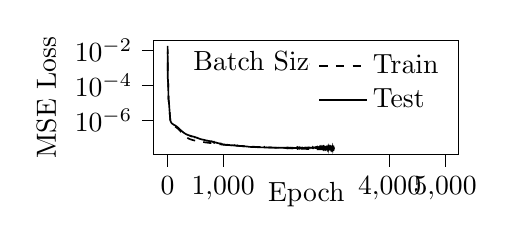
\begin{tikzpicture}

\begin{axis}[
legend cell align={left},
legend style={draw=none},
log basis y={10},
tick align=outside,
tick pos=left,
title={Batch Size 14},
title style={at={(0.4,0.85)},anchor=north},
x grid style={white!69.0196078431373!black},
xlabel={Epoch},
x label style={yshift=13pt},
xmin=-249.95, xmax=5248.95,
xtick style={color=black},
xtick = {0,1000,4000,5000},
y grid style={white!69.0196078431373!black},
ylabel={MSE Loss},
ymin=1.02410381627684e-08, ymax=0.0333579160603595,
ymode=log,
ytick style={color=black},
width=.45\textwidth,
height=.25\textwidth
]
\addplot [semithick, black, dashed]
table {%
0 0.0168717468785891
1 0.00404924569428423
2 0.000742528553642219
3 0.000250874969093605
4 0.000193904513310315
5 0.000180744685345239
6 0.000170359443708313
7 0.000158998338844543
8 0.000145799660083333
9 0.000130326230538339
10 0.000107780700345502
11 7.84643059957419e-05
12 5.50735508097675e-05
13 3.72722670156443e-05
14 2.50677081357235e-05
15 1.89589152663776e-05
16 1.60277194934113e-05
17 1.4416906762906e-05
18 1.33528480003381e-05
19 1.2542978089692e-05
20 1.18380728830763e-05
21 1.11827139172241e-05
22 1.0534444722144e-05
23 9.89714169503446e-06
24 9.25670571944154e-06
25 8.60293387987993e-06
26 7.9448147701257e-06
27 7.29224065638006e-06
28 6.64945727913568e-06
29 6.02451158893591e-06
30 5.42182829300762e-06
31 4.85903337819961e-06
32 4.34010972712299e-06
33 3.87669027459212e-06
34 3.46394584015753e-06
35 3.10421687035043e-06
36 2.79681037542443e-06
37 2.53049873421574e-06
38 2.30008372906074e-06
39 2.1010635612556e-06
40 1.92649899789797e-06
41 1.77744949564701e-06
42 1.64371439995944e-06
43 1.50819396261957e-06
44 1.3615455577843e-06
45 1.2052062145352e-06
46 1.06651785035762e-06
47 9.63305718270336e-07
48 8.9319401103632e-07
49 8.45734626958622e-07
50 8.10981904325797e-07
51 7.84018040258081e-07
52 7.60719030593224e-07
53 7.41696813231731e-07
54 7.24994794032818e-07
55 7.10724200076867e-07
56 6.97577894674391e-07
57 6.84932353929317e-07
58 6.73401785491421e-07
59 6.62690848707448e-07
60 6.52700019607912e-07
61 6.43329369971717e-07
62 6.34316612835927e-07
63 6.2604337554876e-07
64 6.18271930920299e-07
65 6.10996017864101e-07
66 6.04143914072199e-07
67 5.97869438481976e-07
68 5.92757493290041e-07
69 5.86355164105751e-07
70 5.80428500054229e-07
71 5.74776439491062e-07
72 5.69521631607753e-07
73 5.64517735531703e-07
74 5.59714457284142e-07
75 5.55021176083017e-07
76 5.5051803155908e-07
77 5.46257267957002e-07
78 5.42058521692577e-07
79 5.38110362596883e-07
80 5.34237757858054e-07
81 5.30615408320403e-07
82 5.27244994131791e-07
83 5.23701696075895e-07
84 5.20561245851239e-07
85 5.17291762109223e-07
86 5.14224020194801e-07
87 5.11133701033393e-07
88 5.08311374915436e-07
89 5.05394312954378e-07
90 5.02283039900114e-07
91 4.99394850458038e-07
92 4.96705817213324e-07
93 4.94275065892819e-07
94 4.91639597483656e-07
95 4.89363124307412e-07
96 4.86871576254844e-07
97 4.84649009869053e-07
98 4.82461337864353e-07
99 4.80209782651684e-07
100 4.78040790343468e-07
101 4.75903241389777e-07
102 4.73861520838021e-07
103 4.71826147594337e-07
104 4.69824322265681e-07
105 4.67877732603881e-07
106 4.6594380875143e-07
107 4.63995947690173e-07
108 4.62117699457237e-07
109 4.60236358239226e-07
110 4.58272285064731e-07
111 4.56413495007348e-07
112 4.54576606100633e-07
113 4.52672100717397e-07
114 4.510115220964e-07
115 4.49145014339965e-07
116 4.47450479117646e-07
117 4.45589374802697e-07
118 4.44656229685964e-07
119 4.42686300558606e-07
120 4.4074616180499e-07
121 4.39058895857208e-07
122 4.37272414976343e-07
123 4.35532599809505e-07
124 4.3374501813397e-07
125 4.31982281616224e-07
126 4.3026218542642e-07
127 4.28452994481733e-07
128 4.26800982310539e-07
129 4.25057509301995e-07
130 4.23367211995056e-07
131 4.21870452852632e-07
132 4.20114704547535e-07
133 4.18315614725584e-07
134 4.16541495102035e-07
135 4.14825346710031e-07
136 4.1311126666818e-07
137 4.11297535678386e-07
138 4.09575850071561e-07
139 4.07770829279831e-07
140 4.05975322121182e-07
141 4.04318192265934e-07
142 4.02478568477744e-07
143 4.00657031617004e-07
144 3.9892118695552e-07
145 3.97024002920164e-07
146 3.95170175134245e-07
147 3.93384946709172e-07
148 3.91556648450463e-07
149 3.89675664155956e-07
150 3.87865093690062e-07
151 3.86081611870957e-07
152 3.84172520661054e-07
153 3.82345043296591e-07
154 3.80477474123467e-07
155 3.78514520426444e-07
156 3.76650018543332e-07
157 3.74726024699523e-07
158 3.72773714932681e-07
159 3.70900610693756e-07
160 3.69028070665514e-07
161 3.67131661196272e-07
162 3.65214567324898e-07
163 3.63237482156434e-07
164 3.61247299238201e-07
165 3.59297832611224e-07
166 3.5724942480887e-07
167 3.55273886865847e-07
168 3.53454912579967e-07
169 3.51423541033469e-07
170 3.49389995424953e-07
171 3.4746663253564e-07
172 3.45506651081115e-07
173 3.43358178023534e-07
174 3.41206884291412e-07
175 3.3912126108037e-07
176 3.37041809616202e-07
177 3.34961543860121e-07
178 3.3292847875613e-07
179 3.31438666510532e-07
180 3.29233548489173e-07
181 3.27049368261659e-07
182 3.24852719860022e-07
183 3.22639121244037e-07
184 3.20737972901942e-07
185 3.18416558972171e-07
186 3.16145848316147e-07
187 3.1383262790683e-07
188 3.11466739405403e-07
189 3.09103975733043e-07
190 3.07007997044841e-07
191 3.04727012543329e-07
192 3.02573993794807e-07
193 3.00350237498375e-07
194 2.98322560252376e-07
195 2.96096515517663e-07
196 2.94044046975996e-07
197 2.92025675585228e-07
198 2.90007758544305e-07
199 2.87793992124709e-07
200 2.85697252286235e-07
201 2.83635948984139e-07
202 2.81574670464084e-07
203 2.79605895291669e-07
204 2.77516726180457e-07
205 2.75747811021584e-07
206 2.73756601008858e-07
207 2.71378694441013e-07
208 2.69452508156725e-07
209 2.67259567757136e-07
210 2.65712484344708e-07
211 2.63574615758585e-07
212 2.6163377164845e-07
213 2.59478295080432e-07
214 2.57659627911743e-07
215 2.55775162050997e-07
216 2.53839245846653e-07
217 2.51729701102636e-07
218 2.50041751946896e-07
219 2.48247567565411e-07
220 2.46120781228625e-07
221 2.44445761919666e-07
222 2.42801522098446e-07
223 2.408478232454e-07
224 2.39123421141774e-07
225 2.37280703759827e-07
226 2.35601617854547e-07
227 2.33770974419725e-07
228 2.32019653441821e-07
229 2.30372575343979e-07
230 2.28672147231754e-07
231 2.27142257046743e-07
232 2.25370165370546e-07
233 2.23635966186911e-07
234 2.21816939728313e-07
235 2.20254319957361e-07
236 2.18443269067686e-07
237 2.16756783356696e-07
238 2.15069947156838e-07
239 2.13315027267554e-07
240 2.11777548684879e-07
241 2.10077120460855e-07
242 2.08432938309122e-07
243 2.06756668662335e-07
244 2.05220080829449e-07
245 2.0357832285823e-07
246 2.01936073053553e-07
247 2.00388801353512e-07
248 1.98824612947672e-07
249 1.97364988886582e-07
250 1.95787396651026e-07
251 1.94352864611637e-07
252 1.92821957220105e-07
253 1.91392338912919e-07
254 1.89941008612225e-07
255 1.88415887392545e-07
256 1.87056072952785e-07
257 1.85633018265488e-07
258 1.84192423936346e-07
259 1.82766015915897e-07
260 1.8137057841608e-07
261 1.80051544346854e-07
262 1.7877456091721e-07
263 1.77280849406863e-07
264 1.75951777946361e-07
265 1.74730018804952e-07
266 1.73322004003075e-07
267 1.72086216325757e-07
268 1.70706297172455e-07
269 1.69472227381266e-07
270 1.68117555923117e-07
271 1.66913236755028e-07
272 1.65595105975676e-07
273 1.64391932799979e-07
274 1.63200103942151e-07
275 1.61880104454038e-07
276 1.60614089580683e-07
277 1.59405587694707e-07
278 1.58114992284833e-07
279 1.56920012996041e-07
280 1.5565607024915e-07
281 1.5451748461312e-07
282 1.53329850789667e-07
283 1.52133821282687e-07
284 1.5098498065788e-07
285 1.49878619383336e-07
286 1.48702756445625e-07
287 1.47621281284452e-07
288 1.46433010133979e-07
289 1.45394350563816e-07
290 1.44279582456932e-07
291 1.43222026909524e-07
292 1.42141128946314e-07
293 1.41284857156245e-07
294 1.4006164159477e-07
295 1.39088296243288e-07
296 1.38077997166566e-07
297 1.37143346860698e-07
298 1.36092622442581e-07
299 1.35064106745728e-07
300 1.33978017789584e-07
301 1.33016546377385e-07
302 1.32010343890087e-07
303 1.31076665717238e-07
304 1.30068105656596e-07
305 1.29136308099068e-07
306 1.28373597818743e-07
307 1.27295426668869e-07
308 1.26527147025391e-07
309 1.25536314571234e-07
310 1.24710570535537e-07
311 1.23902418873396e-07
312 1.230041784605e-07
313 1.22136616823362e-07
314 1.21357157156388e-07
315 1.2050814131818e-07
316 1.19690201476448e-07
317 1.18949556380301e-07
318 1.18140021215679e-07
319 1.17495492483817e-07
320 1.16682366134348e-07
321 1.16014100287648e-07
322 1.15184127268044e-07
323 1.1451095462687e-07
324 1.13805770665917e-07
325 1.13133179213299e-07
326 1.12407498442191e-07
327 1.11719257608792e-07
328 1.10990530795633e-07
329 1.10427378697253e-07
330 1.0975995364807e-07
331 1.09153529031254e-07
332 1.08479203581074e-07
333 1.07903550449075e-07
334 1.07255429551021e-07
335 1.06737675698797e-07
336 1.06053441587314e-07
337 1.05549809042167e-07
338 1.0495286171765e-07
339 1.04407988154133e-07
340 1.03836023394196e-07
341 1.03372545581734e-07
342 1.02778733685421e-07
343 1.02291559747866e-07
344 1.01656439604908e-07
345 1.01203206185193e-07
346 1.00704782023887e-07
347 1.00095450100973e-07
348 9.94954907522601e-08
349 9.89794553172088e-08
350 9.8446918601629e-08
351 9.79646238784339e-08
352 9.74671054075683e-08
353 9.7058331802083e-08
354 9.65850811761383e-08
355 9.61487394317391e-08
356 9.56963832434896e-08
357 9.52368109099209e-08
358 9.48334101876151e-08
359 9.43692213665899e-08
360 9.40904725011082e-08
361 9.37299133164237e-08
362 9.32570502902992e-08
363 9.28410588283537e-08
364 9.24655251449497e-08
365 9.20919898474624e-08
366 9.16523801872107e-08
367 9.13169852213313e-08
368 9.09411558024632e-08
369 9.05742745016769e-08
370 9.02093824565815e-08
371 8.98302032200097e-08
372 8.94312724481433e-08
373 8.90845515055882e-08
374 8.8730126869872e-08
375 8.84155744764157e-08
376 8.80929296657802e-08
377 8.77236484199494e-08
378 8.74427043097047e-08
379 8.71048882657242e-08
380 8.6800945436777e-08
381 8.64944687559135e-08
382 8.62069845562975e-08
383 8.58676361157298e-08
384 8.56486987750564e-08
385 8.52763585682156e-08
386 8.49678784114899e-08
387 8.4710068498212e-08
388 8.44035664483643e-08
389 8.41008638425704e-08
390 8.38202113405552e-08
391 8.3614718962197e-08
392 8.33361995976712e-08
393 8.30676941653309e-08
394 8.2811127447188e-08
395 8.2569210626502e-08
396 8.22840427899934e-08
397 8.20271316045832e-08
398 8.17767314967862e-08
399 8.15412572428599e-08
400 8.12867863990847e-08
401 8.10129745354593e-08
402 8.07465330807014e-08
403 8.05296590250798e-08
404 8.02743383156721e-08
405 8.01191860144091e-08
406 7.99187868889876e-08
407 7.9705389458725e-08
408 7.94798928862615e-08
409 7.92332198390827e-08
410 7.89926847911037e-08
411 7.88176421844318e-08
412 7.85338729276989e-08
413 7.83200425694616e-08
414 7.81497996168593e-08
415 7.79700115039461e-08
416 7.77468812561789e-08
417 7.74851994998839e-08
418 7.73434303331593e-08
419 7.71065549995145e-08
420 7.68972368547239e-08
421 7.67188871281282e-08
422 7.65334328685645e-08
423 7.63906215021023e-08
424 7.61640874192348e-08
425 7.60074309070745e-08
426 7.58023243552852e-08
427 7.56739091933312e-08
428 7.55396770030885e-08
429 7.53314131540317e-08
430 7.51233308039244e-08
431 7.4976357824683e-08
432 7.47925042862288e-08
433 7.46551042306377e-08
434 7.44248166436582e-08
435 7.41994018146644e-08
436 7.40701841835083e-08
437 7.38746187300111e-08
438 7.37345135903999e-08
439 7.35612291732815e-08
440 7.34086222671486e-08
441 7.32466613298685e-08
442 7.30943179208074e-08
443 7.28889641852373e-08
444 7.28093297447812e-08
445 7.26287334329833e-08
446 7.24453452192776e-08
447 7.23763214644229e-08
448 7.21526710484427e-08
449 7.20116104772935e-08
450 7.18872416450444e-08
451 7.1706141403792e-08
452 7.15801451647089e-08
453 7.14436621160699e-08
454 7.12931920988934e-08
455 7.11810690079728e-08
456 7.10450307069137e-08
457 7.08901922959785e-08
458 7.06902454676535e-08
459 7.06406313118239e-08
460 7.05161004988119e-08
461 7.04107193932607e-08
462 7.02400203299847e-08
463 7.01371361889956e-08
464 6.99660955559014e-08
465 6.98222400394358e-08
466 6.97149599897901e-08
467 6.95775652477419e-08
468 6.94668085913704e-08
469 6.93706085457719e-08
470 6.92371730981545e-08
471 6.91003927581864e-08
472 6.89770572407851e-08
473 6.88941676015768e-08
474 6.87860796822315e-08
475 6.86492433124905e-08
476 6.85393384036958e-08
477 6.83897939709147e-08
478 6.82540884758994e-08
479 6.81771017853725e-08
480 6.80123448624272e-08
481 6.79257702051162e-08
482 6.77970824282868e-08
483 6.77197451246705e-08
484 6.76021582551362e-08
485 6.75284123102765e-08
486 6.73482929937673e-08
487 6.7242005222642e-08
488 6.70916367528297e-08
489 6.69750886855952e-08
490 6.68902025517311e-08
491 6.6837432725926e-08
492 6.66688729645947e-08
493 6.65246281620121e-08
494 6.64715050368437e-08
495 6.62907542161615e-08
496 6.6213651720833e-08
497 6.60714632873115e-08
498 6.59422278863759e-08
499 6.59029945518461e-08
500 6.58041394956151e-08
501 6.56786379998614e-08
502 6.55394332278319e-08
503 6.5472135517304e-08
504 6.5387238085562e-08
505 6.52793011410205e-08
506 6.51687286729779e-08
507 6.50231969122873e-08
508 6.49163487098958e-08
509 6.48535146238652e-08
510 6.48110122399684e-08
511 6.46330990313275e-08
512 6.45725706192082e-08
513 6.44744962811247e-08
514 6.44023314801832e-08
515 6.43335647318657e-08
516 6.42745506235803e-08
517 6.40981353309496e-08
518 6.39342468756952e-08
519 6.39258524561147e-08
520 6.38000816404411e-08
521 6.37399570389509e-08
522 6.3622955028695e-08
523 6.35489876634397e-08
524 6.34508990896573e-08
525 6.33907027103076e-08
526 6.32790198360147e-08
527 6.32235091040285e-08
528 6.31163413778978e-08
529 6.30528216025996e-08
530 6.29731722711802e-08
531 6.2897842589294e-08
532 6.27525488542088e-08
533 6.2762294804953e-08
534 6.26729449813758e-08
535 6.25263626857348e-08
536 6.24391009882554e-08
537 6.24059847465718e-08
538 6.23710402610382e-08
539 6.23126057233323e-08
540 6.21888706498629e-08
541 6.209999743649e-08
542 6.19898142731975e-08
543 6.19576167589235e-08
544 6.183345803677e-08
545 6.17705889235912e-08
546 6.16550718731205e-08
547 6.1611187694778e-08
548 6.1509548975581e-08
549 6.14267851098901e-08
550 6.13002819352102e-08
551 6.12581241490127e-08
552 6.11206459803034e-08
553 6.10564553756458e-08
554 6.09790957744034e-08
555 6.09317550975702e-08
556 6.07662062517651e-08
557 6.07272917577603e-08
558 6.06185949020482e-08
559 6.06178351585757e-08
560 6.04106910789088e-08
561 6.03457596216505e-08
562 6.02502689449015e-08
563 6.0192792497058e-08
564 6.01402309180371e-08
565 6.00282097564595e-08
566 6.0028748747223e-08
567 5.98279414789735e-08
568 5.98469862478435e-08
569 5.98186514960492e-08
570 5.9719885891186e-08
571 5.96293679049171e-08
572 5.95124656159802e-08
573 5.93760042438635e-08
574 5.92481370755724e-08
575 5.91643757047727e-08
576 5.91136171683156e-08
577 5.90644485116015e-08
578 5.88892819916179e-08
579 5.90718776396213e-08
580 5.87887895318874e-08
581 5.87362375675532e-08
582 5.86365344251522e-08
583 5.85927905914221e-08
584 5.85589217272209e-08
585 5.84501622207696e-08
586 5.83773812693408e-08
587 5.83404900861478e-08
588 5.82427808732438e-08
589 5.81578470603473e-08
590 5.81593474514562e-08
591 5.80410152325298e-08
592 5.7954407752989e-08
593 5.79094768656955e-08
594 5.78794245196913e-08
595 5.77546811432238e-08
596 5.7692368079424e-08
597 5.76140884930368e-08
598 5.75674945289186e-08
599 5.74575967752396e-08
600 5.74363094055483e-08
601 5.7316067689974e-08
602 5.7288995595602e-08
603 5.72332033172678e-08
604 5.7193971389538e-08
605 5.70793557407868e-08
606 5.7040236645877e-08
607 5.69747971940398e-08
608 5.69322501589916e-08
609 5.68334504306863e-08
610 5.67582706770439e-08
611 5.67237742557844e-08
612 5.66903664741928e-08
613 5.65625375224179e-08
614 5.65239634491894e-08
615 5.64380027001809e-08
616 5.64088449082269e-08
617 5.62825481511806e-08
618 5.62933517298805e-08
619 5.62270135501757e-08
620 5.61916319349002e-08
621 5.6062084326828e-08
622 5.60409352210514e-08
623 5.59749420582909e-08
624 5.59118757788195e-08
625 5.58308468702949e-08
626 5.57832159702937e-08
627 5.57459242155279e-08
628 5.56150277097722e-08
629 5.56663689068003e-08
630 5.55864992263893e-08
631 5.54865706419456e-08
632 5.54731848211333e-08
633 5.52987693771188e-08
634 5.53758474289076e-08
635 5.52650310782508e-08
636 5.52350348086024e-08
637 5.53295109216269e-08
638 5.52961122298893e-08
639 5.52240422155972e-08
640 5.51567902245193e-08
641 5.50875210187634e-08
642 5.50466419610487e-08
643 5.49170109697928e-08
644 5.49087797017557e-08
645 5.48350281265902e-08
646 5.47906681579004e-08
647 5.47273988737607e-08
648 5.46671938517517e-08
649 5.45624497378255e-08
650 5.45906156487655e-08
651 5.45045704700134e-08
652 5.44492831770101e-08
653 5.43582017937044e-08
654 5.43065444859024e-08
655 5.42885634038557e-08
656 5.42075819134999e-08
657 5.41144150220488e-08
658 5.41461328547603e-08
659 5.40498210601679e-08
660 5.38640248953898e-08
661 5.3776833600025e-08
662 5.37419211075476e-08
663 5.37049779348619e-08
664 5.36478721928154e-08
665 5.36039557450254e-08
666 5.35267763849974e-08
667 5.34525919936558e-08
668 5.33919789996224e-08
669 5.33413107778674e-08
670 5.32884063992428e-08
671 5.32119685253413e-08
672 5.31590113156283e-08
673 5.31129582583787e-08
674 5.30646918387686e-08
675 5.30434079037812e-08
676 5.29477978136176e-08
677 5.28803438892755e-08
678 5.28818524354773e-08
679 5.28557313255402e-08
680 5.27239919819415e-08
681 5.26664442438049e-08
682 5.26736529296676e-08
683 5.25097643129262e-08
684 5.25590159428956e-08
685 5.24545316211571e-08
686 5.24171439897048e-08
687 5.2376454433862e-08
688 5.23700815984247e-08
689 5.22500804736146e-08
690 5.22346579789424e-08
691 5.21775918974784e-08
692 5.20781466808482e-08
693 5.20817839298583e-08
694 5.20260673143878e-08
695 5.19957259874233e-08
696 5.1943092869668e-08
697 5.18444994037202e-08
698 5.1798444942776e-08
699 5.18103616450552e-08
700 5.17011788532655e-08
701 5.16843667848226e-08
702 5.16263780319399e-08
703 5.15640372948607e-08
704 5.15638133496782e-08
705 5.1424252691388e-08
706 5.14129086436977e-08
707 5.14294605938733e-08
708 5.13088867430474e-08
709 5.12933047955047e-08
710 5.12298297458904e-08
711 5.1180559187783e-08
712 5.11869417714443e-08
713 5.10757565224025e-08
714 5.11007727973903e-08
715 5.10120738502133e-08
716 5.09177062657595e-08
717 5.09603958285999e-08
718 5.09464235553781e-08
719 5.08114981511954e-08
720 5.07607413445123e-08
721 5.0691012403942e-08
722 5.06913526663368e-08
723 5.05598571867192e-08
724 5.04174782792984e-08
725 5.03125416356193e-08
726 5.02832641352264e-08
727 5.02121579529011e-08
728 5.01924947323543e-08
729 5.01265972257886e-08
730 5.00192000483903e-08
731 5.00938682330015e-08
732 5.00349414084317e-08
733 4.99948372739661e-08
734 4.99278254109301e-08
735 4.99054635627372e-08
736 4.98390326770808e-08
737 4.97961321221774e-08
738 4.9756630672669e-08
739 4.97300663213287e-08
740 4.97044771433106e-08
741 4.95901008648544e-08
742 4.95946306834881e-08
743 4.95687119415879e-08
744 4.94279973097221e-08
745 4.94901616315863e-08
746 4.94296096454726e-08
747 4.94130782165662e-08
748 4.93223045560277e-08
749 4.9323466026326e-08
750 4.92846222698319e-08
751 4.92413340374704e-08
752 4.91577881990023e-08
753 4.9138534099522e-08
754 4.90908059439839e-08
755 4.90837860736734e-08
756 4.89858097799286e-08
757 4.89823468157475e-08
758 4.89162566521027e-08
759 4.89014381994994e-08
760 4.87827716807746e-08
761 4.8844006766153e-08
762 4.87849279233251e-08
763 4.87458870843873e-08
764 4.8721910537144e-08
765 4.87244322154258e-08
766 4.85794905499185e-08
767 4.8491523986592e-08
768 4.84209012248741e-08
769 4.84906219482413e-08
770 4.84417779704279e-08
771 4.84073345727989e-08
772 4.83453910346989e-08
773 4.83397812407952e-08
774 4.83110755751341e-08
775 4.82812641149184e-08
776 4.82600711250534e-08
777 4.82232100498667e-08
778 4.81807216687549e-08
779 4.81018866913587e-08
780 4.80578230171264e-08
781 4.80196907226016e-08
782 4.79839151815639e-08
783 4.80093528599456e-08
784 4.79243031770315e-08
785 4.78412622027792e-08
786 4.78123267349268e-08
787 4.78079540617631e-08
788 4.77638325876121e-08
789 4.77111581757712e-08
790 4.76360206323425e-08
791 4.76354699213505e-08
792 4.75962001156061e-08
793 4.75310006955396e-08
794 4.75134220080053e-08
795 4.74766290399546e-08
796 4.74222900854841e-08
797 4.73951060837368e-08
798 4.73601126490135e-08
799 4.73138395067414e-08
800 4.73142538637128e-08
801 4.71670435265525e-08
802 4.71056197653702e-08
803 4.71132027345878e-08
804 4.70568869558187e-08
805 4.68369343495736e-08
806 4.67855380264787e-08
807 4.67184639754257e-08
808 4.67136931405718e-08
809 4.67359797420406e-08
810 4.66716687333077e-08
811 4.66299804146209e-08
812 4.65660366800867e-08
813 4.65328999823498e-08
814 4.64775510106346e-08
815 4.64405125171503e-08
816 4.63828966594555e-08
817 4.6339368590971e-08
818 4.62920698852264e-08
819 4.62395017815103e-08
820 4.61874357687814e-08
821 4.61519081195827e-08
822 4.60901867658361e-08
823 4.61090417129657e-08
824 4.60675804356639e-08
825 4.60122591931274e-08
826 4.59467447926959e-08
827 4.59229077112031e-08
828 4.58692607222541e-08
829 4.58164231650807e-08
830 4.57757968251816e-08
831 4.57669879181978e-08
832 4.57041679498564e-08
833 4.57631669404756e-08
834 4.56616606871894e-08
835 4.56561198730726e-08
836 4.55464239905474e-08
837 4.55550223992458e-08
838 4.54658595962308e-08
839 4.53744777042784e-08
840 4.53619341809488e-08
841 4.52684384864678e-08
842 4.52159864577334e-08
843 4.51354425101536e-08
844 4.50895198505392e-08
845 4.50396801874511e-08
846 4.49697053612069e-08
847 4.49087468222909e-08
848 4.4892072079896e-08
849 4.48372962441252e-08
850 4.47815579397103e-08
851 4.47025680062351e-08
852 4.46872171962568e-08
853 4.46398341384065e-08
854 4.45728209089421e-08
855 4.45275162382822e-08
856 4.44537137046562e-08
857 4.43765681450964e-08
858 4.43844624053225e-08
859 4.43390909007893e-08
860 4.42874444747258e-08
861 4.44012648652898e-08
862 4.4309650453817e-08
863 4.42510368705216e-08
864 4.41774291460993e-08
865 4.41271512818653e-08
866 4.41095145335487e-08
867 4.39514728574545e-08
868 4.39497047240293e-08
869 4.38643772710783e-08
870 4.37997074103142e-08
871 4.37536831909136e-08
872 4.36886953840139e-08
873 4.36250345839947e-08
874 4.35795166573485e-08
875 4.35192501771195e-08
876 4.34841556888096e-08
877 4.34218836830758e-08
878 4.33956670349538e-08
879 4.33334930114484e-08
880 4.32966454359525e-08
881 4.32321496084704e-08
882 4.32049767741692e-08
883 4.31474278994127e-08
884 4.3125620659638e-08
885 4.3065977317314e-08
886 4.30308656213235e-08
887 4.29719829386e-08
888 4.29481880704263e-08
889 4.2888110002032e-08
890 4.28682416557476e-08
891 4.28382809908739e-08
892 4.27732519551046e-08
893 4.27091928008531e-08
894 4.26860217196378e-08
895 4.26254461408967e-08
896 4.25999646219039e-08
897 4.254676767855e-08
898 4.25268207626362e-08
899 4.2469851924287e-08
900 4.24522858420541e-08
901 4.24043246017912e-08
902 4.23849442536491e-08
903 4.23395208031004e-08
904 4.23052865745947e-08
905 4.22711020965027e-08
906 4.22281627816173e-08
907 4.21953284247832e-08
908 4.21604255842587e-08
909 4.21249744861022e-08
910 4.20793457141681e-08
911 4.2040345386725e-08
912 4.20306178610248e-08
913 4.19789145822258e-08
914 4.19642219062455e-08
915 4.19095035474194e-08
916 4.18868280790788e-08
917 4.18480205702018e-08
918 4.18030643077129e-08
919 4.17862838130812e-08
920 4.17359989459019e-08
921 4.17130601140268e-08
922 4.16834783907864e-08
923 4.16326157604396e-08
924 4.16013008004905e-08
925 4.15735620102048e-08
926 4.1532308793356e-08
927 4.14896725398539e-08
928 4.14670035558368e-08
929 4.14270538060349e-08
930 4.14108362301901e-08
931 4.13676473526963e-08
932 4.13333101886596e-08
933 4.13020485691039e-08
934 4.12771253944687e-08
935 4.12457358151102e-08
936 4.12020594736235e-08
937 4.11807341979678e-08
938 4.11412158792804e-08
939 4.11145564090003e-08
940 4.10773959897364e-08
941 4.10600351046681e-08
942 4.10202089731535e-08
943 4.09862652224683e-08
944 4.09659755411114e-08
945 4.09204208389098e-08
946 4.09055700423266e-08
947 4.08700923578224e-08
948 4.08426762309556e-08
949 4.09553721472686e-08
950 4.08986329558348e-08
951 4.08355916447357e-08
952 4.0818388603879e-08
953 4.0771384242326e-08
954 4.07799743748164e-08
955 4.07448392197358e-08
956 4.07100946675121e-08
957 4.06678699946475e-08
958 4.06522680382462e-08
959 4.05450651918017e-08
960 4.05254549855689e-08
961 4.04750694157267e-08
962 4.04811250410363e-08
963 4.03837709877015e-08
964 4.03753398764145e-08
965 4.03146390179335e-08
966 4.03348217390067e-08
967 4.02284534293531e-08
968 4.02057060806709e-08
969 4.01889247786042e-08
970 4.01328983472467e-08
971 4.01259656892248e-08
972 4.0069106047133e-08
973 4.00491573610733e-08
974 3.99839089203902e-08
975 3.99776371727003e-08
976 3.99095224808802e-08
977 3.99161185006479e-08
978 3.98175107772626e-08
979 3.98455028940456e-08
980 3.97652086612445e-08
981 3.9741472338314e-08
982 3.97104277976385e-08
983 3.96697166708611e-08
984 3.96251010651679e-08
985 3.96111222144569e-08
986 3.95725330794615e-08
987 3.95165489266389e-08
988 3.9489754130265e-08
989 3.94358216602754e-08
990 3.94712513117181e-08
991 3.93248951040677e-08
992 3.93066224013694e-08
993 3.93560557228305e-08
994 3.92722548374077e-08
995 3.92383110152956e-08
996 3.92574351829685e-08
997 3.91598153965882e-08
998 3.91318919055629e-08
999 3.91649590986803e-08
1000 3.90575392075163e-08
1001 3.90277463089874e-08
1002 3.90616966030009e-08
1003 3.89439458164127e-08
1004 3.89170464416881e-08
1005 3.89461554816529e-08
1006 3.88481046554533e-08
1007 3.88336403158594e-08
1008 3.88861525854503e-08
1009 3.87809746429488e-08
1010 3.87439671891264e-08
1011 3.87631093532816e-08
1012 3.86921641921139e-08
1013 3.87238802018858e-08
1014 3.86211948327425e-08
1015 3.85956201730255e-08
1016 3.8633659997618e-08
1017 3.85314123575818e-08
1018 3.85125479013531e-08
1019 3.85449951024563e-08
1020 3.844778576941e-08
1021 3.84249619628512e-08
1022 3.84599930799415e-08
1023 3.83616895607705e-08
1024 3.83384420651559e-08
1025 3.8373162437809e-08
1026 3.82665595093042e-08
1027 3.82572479523397e-08
1028 3.82952372532444e-08
1029 3.81940318874782e-08
1030 3.8175101547665e-08
1031 3.8213750420423e-08
1032 3.81134730986233e-08
1033 3.80849726580765e-08
1034 3.811870350991e-08
1035 3.80255409475523e-08
1036 3.80065758197158e-08
1037 3.80440338315441e-08
1038 3.79461729233559e-08
1039 3.7930605928887e-08
1040 3.79667921903335e-08
1041 3.78703526688522e-08
1042 3.78512943940804e-08
1043 3.78867346757144e-08
1044 3.77904580449131e-08
1045 3.77715875018672e-08
1046 3.78107278571598e-08
1047 3.77113676758495e-08
1048 3.7692440739685e-08
1049 3.7716399858756e-08
1050 3.76165598934011e-08
1051 3.76011686681992e-08
1052 3.76597063122398e-08
1053 3.75533042455951e-08
1054 3.75298046594797e-08
1055 3.75643232044562e-08
1056 3.74862394862548e-08
1057 3.74531346294036e-08
1058 3.74862473463232e-08
1059 3.73920436866873e-08
1060 3.73744566111462e-08
1061 3.74169854509589e-08
1062 3.73207171522649e-08
1063 3.73030366782414e-08
1064 3.73432922812882e-08
1065 3.72431398945159e-08
1066 3.72491179160125e-08
1067 3.72672157624663e-08
1068 3.7191246856087e-08
1069 3.71664246511894e-08
1070 3.71923104621667e-08
1071 3.7098905520266e-08
1072 3.70631268923424e-08
1073 3.71242571819838e-08
1074 3.70327002039785e-08
1075 3.70371482574037e-08
1076 3.70579679142026e-08
1077 3.69741710535323e-08
1078 3.69544098631792e-08
1079 3.69763814066449e-08
1080 3.68991437715538e-08
1081 3.68964575721945e-08
1082 3.6912058655945e-08
1083 3.68200449026849e-08
1084 3.67851670584824e-08
1085 3.68476757606595e-08
1086 3.67575813982306e-08
1087 3.67431322384132e-08
1088 3.67646214699419e-08
1089 3.66668399512401e-08
1090 3.66606986632958e-08
1091 3.6728467192235e-08
1092 3.66210468383487e-08
1093 3.66124844070874e-08
1094 3.66615631497114e-08
1095 3.65515599201868e-08
1096 3.65421039876463e-08
1097 3.65653940723478e-08
1098 3.64782597446227e-08
1099 3.64786742071818e-08
1100 3.65290753077243e-08
1101 3.64180145930979e-08
1102 3.64148292188336e-08
1103 3.64622518347843e-08
1104 3.63607038029517e-08
1105 3.6357523034172e-08
1106 3.63985828983054e-08
1107 3.62898453292399e-08
1108 3.62857237869716e-08
1109 3.6335202051503e-08
1110 3.62457848381646e-08
1111 3.62214976116999e-08
1112 3.62608196522731e-08
1113 3.61711269141879e-08
1114 3.61565899986161e-08
1115 3.61992901978589e-08
1116 3.61067066005046e-08
1117 3.61008440577301e-08
1118 3.61330484103569e-08
1119 3.6025361329659e-08
1120 3.60409150759841e-08
1121 3.60857097738496e-08
1122 3.59911816216441e-08
1123 3.59749468381188e-08
1124 3.60170343277893e-08
1125 3.59211251016184e-08
1126 3.59145777608603e-08
1127 3.5954847121356e-08
1128 3.58630160067709e-08
1129 3.58528083305747e-08
1130 3.58955695346318e-08
1131 3.57975908341099e-08
1132 3.57913430610262e-08
1133 3.58013522355566e-08
1134 3.57465518786081e-08
1135 3.57323081488693e-08
1136 3.57742792964834e-08
1137 3.56799409815458e-08
1138 3.56710443684958e-08
1139 3.57138243857867e-08
1140 3.56207368651889e-08
1141 3.56129275595392e-08
1142 3.56548856546572e-08
1143 3.55336684955808e-08
1144 3.55535332953625e-08
1145 3.55925584079523e-08
1146 3.54602735520004e-08
1147 3.54949972258201e-08
1148 3.55319100327415e-08
1149 3.54394432991708e-08
1150 3.54251450955241e-08
1151 3.54660719316478e-08
1152 3.53811757824851e-08
1153 3.53597861294216e-08
1154 3.54104389074309e-08
1155 3.53229467369682e-08
1156 3.53109862592939e-08
1157 3.5353314917355e-08
1158 3.52744644061531e-08
1159 3.52554024886075e-08
1160 3.5292037699401e-08
1161 3.52145552345124e-08
1162 3.51984017534732e-08
1163 3.52131939551248e-08
1164 3.5158654837536e-08
1165 3.51525404837574e-08
1166 3.51884590246263e-08
1167 3.51051412213092e-08
1168 3.50862976993838e-08
1169 3.51309046034129e-08
1170 3.50456899988095e-08
1171 3.503182602435e-08
1172 3.50746848752394e-08
1173 3.49508570181804e-08
1174 3.49872529642664e-08
1175 3.50278372243837e-08
1176 3.49402164077985e-08
1177 3.49265519629315e-08
1178 3.49647479050671e-08
1179 3.4872061834904e-08
1180 3.48535176974275e-08
1181 3.49003848354146e-08
1182 3.48129881907148e-08
1183 3.48058266248911e-08
1184 3.48498958455803e-08
1185 3.47641715414682e-08
1186 3.4752651109618e-08
1187 3.47600894268684e-08
1188 3.47214849009211e-08
1189 3.47068627543817e-08
1190 3.47449365688791e-08
1191 3.4658139357658e-08
1192 3.46484887401346e-08
1193 3.46902101729699e-08
1194 3.46163519232285e-08
1195 3.46040691330589e-08
1196 3.46379541583807e-08
1197 3.45517265987116e-08
1198 3.45440961119486e-08
1199 3.45866658514459e-08
1200 3.45001086564679e-08
1201 3.44545266288051e-08
1202 3.45425622402399e-08
1203 3.4454022328241e-08
1204 3.44552526044172e-08
1205 3.44910764222999e-08
1206 3.44019420673912e-08
1207 3.43912137416265e-08
1208 3.44324160217535e-08
1209 3.43511786506111e-08
1210 3.43657572174031e-08
1211 3.44155751480696e-08
1212 3.43163315743376e-08
1213 3.4318969451822e-08
1214 3.43536783930598e-08
1215 3.42256572143203e-08
1216 3.42754545336575e-08
1217 3.43140265758766e-08
1218 3.42247424759497e-08
1219 3.42169347618785e-08
1220 3.4256024685096e-08
1221 3.41724990293956e-08
1222 3.41657030204186e-08
1223 3.42065822815448e-08
1224 3.41219999621523e-08
1225 3.41125121561181e-08
1226 3.41579326719514e-08
1227 3.40702899894073e-08
1228 3.40686902884606e-08
1229 3.41106444131726e-08
1230 3.40237770234343e-08
1231 3.40192811884945e-08
1232 3.40643001110393e-08
1233 3.39768986170716e-08
1234 3.39709148814201e-08
1235 3.401329125578e-08
1236 3.39292102789448e-08
1237 3.39189939399035e-08
1238 3.39307030537685e-08
1239 3.38891111723144e-08
1240 3.38797334212135e-08
1241 3.39243755604606e-08
1242 3.38340933638235e-08
1243 3.38290928882654e-08
1244 3.38693460301885e-08
1245 3.37868109915559e-08
1246 3.37790131017938e-08
1247 3.38213474165578e-08
1248 3.37387538963451e-08
1249 3.37233400660708e-08
1250 3.37641497247534e-08
1251 3.36718287021319e-08
1252 3.36681045513849e-08
1253 3.37146367513895e-08
1254 3.36324618970558e-08
1255 3.36223697896418e-08
1256 3.36680971881995e-08
1257 3.35813560533341e-08
1258 3.35395552248013e-08
1259 3.36295164908991e-08
1260 3.35379773090701e-08
1261 3.35366467820839e-08
1262 3.35609217836732e-08
1263 3.34786533212345e-08
1264 3.34714057822242e-08
1265 3.35194922913578e-08
1266 3.34498701325038e-08
1267 3.34359162858786e-08
1268 3.34845091265856e-08
1269 3.33978070110131e-08
1270 3.33565213461496e-08
1271 3.34488443330118e-08
1272 3.33645156211662e-08
1273 3.33680671889085e-08
1274 3.33936686973897e-08
1275 3.33149400141434e-08
1276 3.33067689326163e-08
1277 3.33508974035015e-08
1278 3.32679176266056e-08
1279 3.32612792537705e-08
1280 3.33044897192792e-08
1281 3.32229621963958e-08
1282 3.32148874278807e-08
1283 3.32592580826612e-08
1284 3.31757122146908e-08
1285 3.31680038741204e-08
1286 3.32124708853901e-08
1287 3.312994836821e-08
1288 3.31228128266351e-08
1289 3.31669294608348e-08
1290 3.30843284563214e-08
1291 3.30903233221528e-08
1292 3.31162144870448e-08
1293 3.30389638491458e-08
1294 3.30321250802784e-08
1295 3.30361888102059e-08
1296 3.29974463091571e-08
1297 3.29920350091554e-08
1298 3.30341129369331e-08
1299 3.295077660609e-08
1300 3.29436512149038e-08
1301 3.29875561536405e-08
1302 3.29047638305267e-08
1303 3.28987502539436e-08
1304 3.29430523233381e-08
1305 3.28612517523592e-08
1306 3.28549372432261e-08
1307 3.2899864416319e-08
1308 3.28176395786578e-08
1309 3.28258571187483e-08
1310 3.28507964513986e-08
1311 3.27759953490235e-08
1312 3.27698705591486e-08
1313 3.28137369366564e-08
1314 3.27307402207074e-08
1315 3.27274025657687e-08
1316 3.27701214586828e-08
1317 3.26923109127975e-08
1318 3.26836094707442e-08
1319 3.27303440418912e-08
1320 3.26509388368692e-08
1321 3.26403197663667e-08
1322 3.26881987150357e-08
1323 3.26085815769785e-08
1324 3.26027761043258e-08
1325 3.26472468592986e-08
1326 3.25657386791399e-08
1327 3.25723040443301e-08
1328 3.25969937662365e-08
1329 3.25205790206874e-08
1330 3.25137492127949e-08
1331 3.25570549913385e-08
1332 3.24761802780408e-08
1333 3.24705232305607e-08
1334 3.2513651595465e-08
1335 3.24325387944514e-08
1336 3.24259954287576e-08
1337 3.2470023569642e-08
1338 3.23895563345912e-08
1339 3.23841452178151e-08
1340 3.24310907064926e-08
1341 3.23482215264431e-08
1342 3.23432370939959e-08
1343 3.23890840721135e-08
1344 3.22962194641132e-08
1345 3.2274737105098e-08
1346 3.2304543812317e-08
1347 3.22190286633534e-08
1348 3.22225336855776e-08
1349 3.22445252301382e-08
1350 3.21991315941241e-08
1351 3.22648092734255e-08
1352 3.21705227352525e-08
1353 3.21565914300366e-08
1354 3.21625570931206e-08
1355 3.21200830952198e-08
1356 3.21527808558028e-08
1357 3.21119843536512e-08
1358 3.21317101084803e-08
1359 3.20580836484622e-08
1360 3.20951248934364e-08
1361 3.20360193151958e-08
1362 3.20690843639523e-08
1363 3.20114854220192e-08
1364 3.20541066168599e-08
1365 3.19809794808118e-08
1366 3.19765511334571e-08
1367 3.20051143008284e-08
1368 3.19416367605879e-08
1369 3.19779825044073e-08
1370 3.19086673214433e-08
1371 3.19431780467231e-08
1372 3.18856254437911e-08
1373 3.19152142087957e-08
1374 3.18574419556138e-08
1375 3.18861166390652e-08
1376 3.18294947586097e-08
1377 3.18654929870948e-08
1378 3.18041647532282e-08
1379 3.18458991857659e-08
1380 3.17934544984783e-08
1381 3.17989800381001e-08
1382 3.17454851792079e-08
1383 3.17732739093438e-08
1384 3.17221569059398e-08
1385 3.17488242440522e-08
1386 3.16979873895127e-08
1387 3.171357464594e-08
1388 3.16621103616684e-08
1389 3.1692919449661e-08
1390 3.16118126609321e-08
1391 3.16506945081689e-08
1392 3.15843465522906e-08
1393 3.16046966344383e-08
1394 3.15615749091336e-08
1395 3.15921439343002e-08
1396 3.15339996352899e-08
1397 3.15663940953647e-08
1398 3.15129109318568e-08
1399 3.15397347601746e-08
1400 3.14868249701832e-08
1401 3.15264220774391e-08
1402 3.1460750955441e-08
1403 3.14710900214857e-08
1404 3.14351172908639e-08
1405 3.14564838668161e-08
1406 3.14022587715397e-08
1407 3.1425683536387e-08
1408 3.13709228943676e-08
1409 3.13956117886533e-08
1410 3.13409232428091e-08
1411 3.13626077602386e-08
1412 3.13055972566945e-08
1413 3.13312679545851e-08
1414 3.12750542635404e-08
1415 3.13010793259874e-08
1416 3.12522306386545e-08
1417 3.12792792661726e-08
1418 3.12246208423094e-08
1419 3.12511048926934e-08
1420 3.11979853202387e-08
1421 3.12244072509271e-08
1422 3.1174763634592e-08
1423 3.11863349395008e-08
1424 3.11426702902929e-08
1425 3.1167096886237e-08
1426 3.11142273530877e-08
1427 3.11392810620009e-08
1428 3.10870358561704e-08
1429 3.11122677178364e-08
1430 3.10599048532094e-08
1431 3.10843514859617e-08
1432 3.10322613169537e-08
1433 3.10574976474615e-08
1434 3.10071633621592e-08
1435 3.10358758366706e-08
1436 3.09764777759971e-08
1437 3.10102489312555e-08
1438 3.09595621711051e-08
1439 3.09787720728397e-08
1440 3.0928190678289e-08
1441 3.09586921211523e-08
1442 3.09025738673632e-08
1443 3.09276602370192e-08
1444 3.08721556927795e-08
1445 3.0903755360495e-08
1446 3.08453621929598e-08
1447 3.08760294907209e-08
1448 3.08212871821326e-08
1449 3.08453828741632e-08
1450 3.07954194872002e-08
1451 3.08123077045205e-08
1452 3.07672584690052e-08
1453 3.07941604492602e-08
1454 3.07489436306259e-08
1455 3.0754400673369e-08
1456 3.07124316064525e-08
1457 3.07375932927069e-08
1458 3.06866480276064e-08
1459 3.07092877917956e-08
1460 3.06586472681641e-08
1461 3.06814867001415e-08
1462 3.06311652219993e-08
1463 3.06545302087124e-08
1464 3.06040255251381e-08
1465 3.06258211844325e-08
1466 3.05691737160537e-08
1467 3.06024408191896e-08
1468 3.05526301895982e-08
1469 3.05764075271174e-08
1470 3.05261904114924e-08
1471 3.0550108171262e-08
1472 3.05002542414198e-08
1473 3.05239487640652e-08
1474 3.04762937838701e-08
1475 3.04930783777869e-08
1476 3.04493082511806e-08
1477 3.04736965327846e-08
1478 3.04241320512834e-08
1479 3.04475973617862e-08
1480 3.03985675714574e-08
1481 3.04224642354368e-08
1482 3.03729035908043e-08
1483 3.0396823906416e-08
1484 3.03480713643971e-08
1485 3.03727016404598e-08
1486 3.03140857808189e-08
1487 3.03478646936637e-08
1488 3.02993655682021e-08
1489 3.03223513135993e-08
1490 3.0273653046735e-08
1491 3.02989795397746e-08
1492 3.02439406090966e-08
1493 3.02744949529224e-08
1494 3.02246890996191e-08
1495 3.0249723617978e-08
1496 3.01964296193931e-08
1497 3.02270981764421e-08
1498 3.01779764782801e-08
1499 3.020213416268e-08
1500 3.01527914493925e-08
1501 3.01779908009334e-08
1502 3.01287962861158e-08
1503 3.01562649940767e-08
1504 3.01068725676419e-08
1505 3.01216921956841e-08
1506 3.0083428988008e-08
1507 3.01075701805495e-08
1508 3.0059100079268e-08
1509 3.00776564493837e-08
1510 3.00289553704721e-08
1511 3.0063681864103e-08
1512 3.00144395118715e-08
1513 3.00416584476015e-08
1514 2.99943015599594e-08
1515 3.0022931070532e-08
1516 2.99621163280128e-08
1517 3.00026209377801e-08
1518 2.99503298634346e-08
1519 2.99769544028376e-08
1520 2.99272773322996e-08
1521 2.99554553392359e-08
1522 2.99036144129678e-08
1523 2.9933310739174e-08
1524 2.9875514658898e-08
1525 2.99108020760199e-08
1526 2.98599262285845e-08
1527 2.98884426842925e-08
1528 2.98372513782422e-08
1529 2.98669044476749e-08
1530 2.98199811463775e-08
1531 2.98445254352787e-08
1532 2.97876892041415e-08
1533 2.98235469405021e-08
1534 2.97720191592373e-08
1535 2.980176993606e-08
1536 2.97507643027766e-08
1537 2.97817180722387e-08
1538 2.97316738952001e-08
1539 2.97567806774322e-08
1540 2.97017533086013e-08
1541 2.97356531255098e-08
1542 2.96873244231644e-08
1543 2.97150113000426e-08
1544 2.96654838301162e-08
1545 2.96944128478057e-08
1546 2.96471742664608e-08
1547 2.96704043106117e-08
1548 2.96168554902222e-08
1549 2.96503924660604e-08
1550 2.96022908905016e-08
1551 2.96303016869811e-08
1552 2.95803736485875e-08
1553 2.96075269289887e-08
1554 2.95594119158494e-08
1555 2.95817169314928e-08
1556 2.95386872025287e-08
1557 2.95666768116051e-08
1558 2.94995407837104e-08
1559 2.9551406451648e-08
1560 2.94818523564529e-08
1561 2.94893891155485e-08
1562 2.94240719233342e-08
1563 2.94739277226987e-08
1564 2.94203051555507e-08
1565 2.94277251486865e-08
1566 2.9400903410383e-08
1567 2.94163089768713e-08
1568 2.9383356785779e-08
1569 2.93908523920902e-08
1570 2.93634791307015e-08
1571 2.93700174297412e-08
1572 2.93417937732291e-08
1573 2.93531891520422e-08
1574 2.93236113339919e-08
1575 2.93285078228007e-08
1576 2.92987066713551e-08
1577 2.93158329965772e-08
1578 2.9281288491015e-08
1579 2.92895885540605e-08
1580 2.92622761422101e-08
1581 2.92778515184747e-08
1582 2.92371551196209e-08
1583 2.92517657462377e-08
1584 2.92102231478166e-08
1585 2.92256656466891e-08
1586 2.91994852461843e-08
1587 2.92307110202875e-08
1588 2.91654911674591e-08
1589 2.92155002350531e-08
1590 2.91488670993696e-08
1591 2.91958600139797e-08
1592 2.9129643589251e-08
1593 2.91766621585532e-08
1594 2.91111050867385e-08
1595 2.91473344978181e-08
1596 2.90893117457139e-08
1597 2.91405672086803e-08
1598 2.90639721489372e-08
1599 2.91189780586322e-08
1600 2.90461665768467e-08
1601 2.90948322016012e-08
1602 2.90298909091644e-08
1603 2.90752367139755e-08
1604 2.90095509789581e-08
1605 2.90562205174327e-08
1606 2.89903093201867e-08
1607 2.90347859259572e-08
1608 2.89699766693168e-08
1609 2.90189695086283e-08
1610 2.89548836422556e-08
1611 2.89981372170256e-08
1612 2.89342671717978e-08
1613 2.89826107154183e-08
1614 2.89182553024227e-08
1615 2.89471717831322e-08
1616 2.89221700062596e-08
1617 2.89300519608669e-08
1618 2.88845635459673e-08
1619 2.89232807696446e-08
1620 2.88649804555732e-08
1621 2.8896304940149e-08
1622 2.88721108388811e-08
1623 2.8872573868651e-08
1624 2.8835462456029e-08
1625 2.88574224205673e-08
1626 2.88174955553345e-08
1627 2.88384873246518e-08
1628 2.87996565041969e-08
1629 2.8818112479096e-08
1630 2.87705293124738e-08
1631 2.88057138934413e-08
1632 2.87534350098105e-08
1633 2.8792977820173e-08
1634 2.87291767159131e-08
1635 2.87775283804657e-08
1636 2.87080537850029e-08
1637 2.87562028796599e-08
1638 2.86910217091755e-08
1639 2.87405144997717e-08
1640 2.86715917332878e-08
1641 2.87178933547214e-08
1642 2.86532095765741e-08
1643 2.87030496713294e-08
1644 2.86349714895428e-08
1645 2.86816128159306e-08
1646 2.86155387652708e-08
1647 2.8666283576887e-08
1648 2.85971638972102e-08
1649 2.8644971046281e-08
1650 2.85780404748618e-08
1651 2.86296526951869e-08
1652 2.85596587637901e-08
1653 2.86094430911888e-08
1654 2.85430245981057e-08
1655 2.85956152944723e-08
1656 2.85245225838882e-08
1657 2.85563428909613e-08
1658 2.85261901590571e-08
1659 2.8536809220243e-08
1660 2.85050021426807e-08
1661 2.85174450844625e-08
1662 2.84872185281619e-08
1663 2.84991790399969e-08
1664 2.84697527215831e-08
1665 2.84811308896101e-08
1666 2.84509456677667e-08
1667 2.84624639863112e-08
1668 2.84332650043066e-08
1669 2.84445234607891e-08
1670 2.84161080850646e-08
1671 2.84270163756525e-08
1672 2.83974944010439e-08
1673 2.84100362411822e-08
1674 2.83807444740352e-08
1675 2.83924850980482e-08
1676 2.83630198550599e-08
1677 2.83736689435085e-08
1678 2.83450191756358e-08
1679 2.83556710761318e-08
1680 2.83283701888622e-08
1681 2.83439058983333e-08
1682 2.82977449631191e-08
1683 2.83254652212205e-08
1684 2.82817905660305e-08
1685 2.83241780674647e-08
1686 2.82519194643234e-08
1687 2.83067983955595e-08
1688 2.82333515603103e-08
1689 2.82887936230615e-08
1690 2.82170346668639e-08
1691 2.82693530107713e-08
1692 2.81982632349027e-08
1693 2.82547613355838e-08
1694 2.81797615778198e-08
1695 2.82351738462222e-08
1696 2.8161519795221e-08
1697 2.82186969176206e-08
1698 2.81452567902922e-08
1699 2.81973400836813e-08
1700 2.81277419149613e-08
1701 2.81844691206447e-08
1702 2.81088986927184e-08
1703 2.81625387004609e-08
1704 2.80928024727904e-08
1705 2.81473682962895e-08
1706 2.80742891498256e-08
1707 2.81105029882804e-08
1708 2.80795254491762e-08
1709 2.80901751742563e-08
1710 2.80570427077889e-08
1711 2.8071793208532e-08
1712 2.80424231962823e-08
1713 2.80530798451168e-08
1714 2.80217607346416e-08
1715 2.80356746505041e-08
1716 2.8004037008503e-08
1717 2.8017685772052e-08
1718 2.79838852913782e-08
1719 2.7997757094851e-08
1720 2.79650810992975e-08
1721 2.79792353823267e-08
1722 2.79471223816454e-08
1723 2.79605306895204e-08
1724 2.79307484926098e-08
1725 2.79426196571119e-08
1726 2.79132217371161e-08
1727 2.79218453020707e-08
1728 2.78981354055537e-08
1729 2.79033755060595e-08
1730 2.78772472906951e-08
1731 2.78875366047734e-08
1732 2.78925598422326e-08
1733 2.78648091609149e-08
1734 2.78471219774177e-08
1735 2.78518389222012e-08
1736 2.7831583819245e-08
1737 2.78346645219931e-08
1738 2.78267636050871e-08
1739 2.78313451601137e-08
1740 2.77988384774534e-08
1741 2.78000906304578e-08
1742 2.77843101983297e-08
1743 2.77972333076878e-08
1744 2.77676292837159e-08
1745 2.77799989647529e-08
1746 2.77471093188122e-08
1747 2.77450474234802e-08
1748 2.77327553742059e-08
1749 2.773611283925e-08
1750 2.77193001931806e-08
1751 2.77171472859575e-08
1752 2.77157355465452e-08
1753 2.77008917715404e-08
1754 2.76988873904194e-08
1755 2.76782732848143e-08
1756 2.76647380015859e-08
1757 2.76618389623799e-08
1758 2.76517194254698e-08
1759 2.76439611931848e-08
1760 2.76561092178067e-08
1761 2.76334577380473e-08
1762 2.76270071279934e-08
1763 2.76171397468e-08
1764 2.76143926652944e-08
1765 2.75893269737363e-08
1766 2.76095079339803e-08
1767 2.75645064396079e-08
1768 2.75964017667022e-08
1769 2.75497531004205e-08
1770 2.75700995180559e-08
1771 2.75357621179997e-08
1772 2.75772135709924e-08
1773 2.7515336904032e-08
1774 2.75349208608658e-08
1775 2.75088909475982e-08
1776 2.7527586011743e-08
1777 2.75024230879393e-08
1778 2.74969485409387e-08
1779 2.74685121361926e-08
1780 2.75028434587482e-08
1781 2.74504569191975e-08
1782 2.74747340449617e-08
1783 2.744797643873e-08
1784 2.7447196091692e-08
1785 2.74171594844579e-08
1786 2.74586997879005e-08
1787 2.74003894771637e-08
1788 2.74273841431845e-08
1789 2.73844616291566e-08
1790 2.74162466746147e-08
1791 2.73739114033509e-08
1792 2.73864325840244e-08
1793 2.737380694301e-08
1794 2.73657078287791e-08
1795 2.73514891466034e-08
1796 2.73503743429383e-08
1797 2.73343196003214e-08
1798 2.73479035237403e-08
1799 2.72991717079548e-08
1800 2.73309034797881e-08
1801 2.73043956209431e-08
1802 2.73016326329695e-08
1803 2.72824179937657e-08
1804 2.7288939498159e-08
1805 2.72548790280969e-08
1806 2.72805762191697e-08
1807 2.72517324666084e-08
1808 2.72494408436176e-08
1809 2.72327988799752e-08
1810 2.72488897289082e-08
1811 2.72035448417779e-08
1812 2.72290818626053e-08
1813 2.72053309142333e-08
1814 2.71988323767055e-08
1815 2.71889306779749e-08
1816 2.7196785106815e-08
1817 2.71773277060894e-08
1818 2.71753368075788e-08
1819 2.71523942692668e-08
1820 2.71666279091745e-08
1821 2.71354089889517e-08
1822 2.71577138058418e-08
1823 2.71100445464706e-08
1824 2.71486980821653e-08
1825 2.70932801089246e-08
1826 2.71176545057534e-08
1827 2.70856999331213e-08
1828 2.70999307345847e-08
1829 2.70708563972414e-08
1830 2.70842362911708e-08
1831 2.70422199085677e-08
1832 2.70805365637777e-08
1833 2.70287359005627e-08
1834 2.70493430932827e-08
1835 2.70102876009537e-08
1836 2.70340835063708e-08
1837 2.6994734685355e-08
1838 2.70101026020844e-08
1839 2.69722469533987e-08
1840 2.70037586153654e-08
1841 2.69460968363619e-08
1842 2.69652329959962e-08
1843 2.69186372446519e-08
1844 2.69568427688662e-08
1845 2.68996603996924e-08
1846 2.69293571016664e-08
1847 2.68927517877038e-08
1848 2.69294638383527e-08
1849 2.68789071994463e-08
1850 2.69068000389995e-08
1851 2.68645387116947e-08
1852 2.68876278475815e-08
1853 2.6856250418566e-08
1854 2.68700968452907e-08
1855 2.68313627539872e-08
1856 2.68661600751888e-08
1857 2.68167607032609e-08
1858 2.68443323327781e-08
1859 2.68023757764447e-08
1860 2.68315664356586e-08
1861 2.67835270294837e-08
1862 2.6817215565516e-08
1863 2.6769479197433e-08
1864 2.67924253443581e-08
1865 2.67654493766669e-08
1866 2.6782854839907e-08
1867 2.67440203704672e-08
1868 2.67629991222153e-08
1869 2.67235458594917e-08
1870 2.67498237437891e-08
1871 2.67108744897107e-08
1872 2.67373042478597e-08
1873 2.66913195244491e-08
1874 2.67322907151472e-08
1875 2.66837687082219e-08
1876 2.67044401681038e-08
1877 2.66631126299755e-08
1878 2.66867530591391e-08
1879 2.66485678217272e-08
1880 2.66691144086921e-08
1881 2.6632582641182e-08
1882 2.66564096747683e-08
1883 2.66323607347727e-08
1884 2.66395378033469e-08
1885 2.66039771052156e-08
1886 2.66231567623012e-08
1887 2.65983149243128e-08
1888 2.66092038706231e-08
1889 2.65724068840309e-08
1890 2.65971468221787e-08
1891 2.65671280297541e-08
1892 2.65769031739292e-08
1893 2.65538368884508e-08
1894 2.65646585707734e-08
1895 2.65279809075358e-08
1896 2.65605749018614e-08
1897 2.65178033797176e-08
1898 2.65416285235956e-08
1899 2.65037453180875e-08
1900 2.65234181424516e-08
1901 2.64862891525923e-08
1902 2.65066225379174e-08
1903 2.64754493433556e-08
1904 2.64888300400617e-08
1905 2.64636780306043e-08
1906 2.64818541175026e-08
1907 2.64483184444295e-08
1908 2.64613690958981e-08
1909 2.6427794037081e-08
1910 2.6445671613734e-08
1911 2.64124891623863e-08
1912 2.64310652634167e-08
1913 2.63971904459357e-08
1914 2.64198619749255e-08
1915 2.63966450484867e-08
1916 2.63872470105832e-08
1917 2.63762473991051e-08
1918 2.63708357233356e-08
1919 2.63725326006285e-08
1920 2.63594398507451e-08
1921 2.63473511166909e-08
1922 2.6345395074525e-08
1923 2.63457778996098e-08
1924 2.63290706206928e-08
1925 2.63174695555959e-08
1926 2.6321931812112e-08
1927 2.63040037179823e-08
1928 2.62980784421723e-08
1929 2.62926552635606e-08
1930 2.6309094214771e-08
1931 2.62643597670786e-08
1932 2.62836866847672e-08
1933 2.62452624124563e-08
1934 2.62677791080351e-08
1935 2.62308794918054e-08
1936 2.62554184593999e-08
1937 2.62306161034267e-08
1938 2.62163037820908e-08
1939 2.62103484339881e-08
1940 2.62043521271958e-08
1941 2.6200350167593e-08
1942 2.61892735578781e-08
1943 2.61913385385432e-08
1944 2.61881548878419e-08
1945 2.61616105577823e-08
1946 2.62000535750057e-08
1947 2.61880503514158e-08
1948 2.61812982218687e-08
1949 2.61736083047896e-08
1950 2.61631973956695e-08
1951 2.61529197785284e-08
1952 2.61462931600825e-08
1953 2.61297862911726e-08
1954 2.61353479541909e-08
1955 2.61194627915417e-08
1956 2.61108775688769e-08
1957 2.6100810186052e-08
1958 2.60951761132012e-08
1959 2.60928992491892e-08
1960 2.60827645759798e-08
1961 2.60723729459214e-08
1962 2.60691130873378e-08
1963 2.60547784528483e-08
1964 2.6051368310439e-08
1965 2.60463966028557e-08
1966 2.60372049623999e-08
1967 2.60225610834389e-08
1968 2.59559669856813e-08
1969 2.59166128371477e-08
1970 2.59324919083215e-08
1971 2.59225250542506e-08
1972 2.59062303124709e-08
1973 2.59104708628837e-08
1974 2.58962585361525e-08
1975 2.58894968400543e-08
1976 2.58865154424857e-08
1977 2.58745400769536e-08
1978 2.58742070830259e-08
1979 2.58625192171216e-08
1980 2.58393177189008e-08
1981 2.58500229458156e-08
1982 2.58375787525096e-08
1983 2.58294710422023e-08
1984 2.5816420569301e-08
1985 2.58218272948733e-08
1986 2.58092136644534e-08
1987 2.58039257653527e-08
1988 2.58256581869648e-08
1989 2.57530168410349e-08
1990 2.57490300301535e-08
1991 2.57517176596043e-08
1992 2.57142581431521e-08
1993 2.5729115455114e-08
1994 2.5720735550729e-08
1995 2.57307009545225e-08
1996 2.57101469049956e-08
1997 2.57277690666898e-08
1998 2.57006162660913e-08
1999 2.56849946470968e-08
2000 2.57088186683297e-08
2001 2.56862410502329e-08
2002 2.56787735317878e-08
2003 2.56770768361678e-08
2004 2.56657824907555e-08
2005 2.56715049000928e-08
2006 2.56465163480727e-08
2007 2.56609609909127e-08
2008 2.56142495356961e-08
2009 2.56488898232265e-08
2010 2.55981177358374e-08
2011 2.56415442926713e-08
2012 2.55872174590412e-08
2013 2.56221698527789e-08
2014 2.55776810811379e-08
2015 2.56058680443909e-08
2016 2.55678200755749e-08
2017 2.55827084240932e-08
2018 2.55474130863451e-08
2019 2.55722130526215e-08
2020 2.55433185434586e-08
2021 2.55540004355039e-08
2022 2.55268193327585e-08
2023 2.55471249097142e-08
2024 2.55059025073772e-08
2025 2.5529406913258e-08
2026 2.54869011024211e-08
2027 2.5504933951916e-08
2028 2.54924374244047e-08
2029 2.54939627947553e-08
2030 2.54913293100274e-08
2031 2.54738075031782e-08
2032 2.54717752205221e-08
2033 2.54556355481729e-08
2034 2.54226525612019e-08
2035 2.54599532583095e-08
2036 2.54271001922766e-08
2037 2.54342494959586e-08
2038 2.54255240032138e-08
2039 2.54282087196878e-08
2040 2.53969027005278e-08
2041 2.53995638631933e-08
2042 2.53912986984169e-08
2043 2.53857749848402e-08
2044 2.53784316824949e-08
2045 2.53736799543464e-08
2046 2.53655856148509e-08
2047 2.53597678490014e-08
2048 2.5352447154834e-08
2049 2.53499951876887e-08
2050 2.53385432682449e-08
2051 2.53431588364678e-08
2052 2.53155395248127e-08
2053 2.53300572125639e-08
2054 2.53114942680646e-08
2055 2.52999148065103e-08
2056 2.52949738482228e-08
2057 2.5288479939471e-08
2058 2.52874641086949e-08
2059 2.52752075120249e-08
2060 2.52672410376139e-08
2061 2.52602966748911e-08
2062 2.52598304930194e-08
2063 2.5248074100734e-08
2064 2.52350649079433e-08
2065 2.52344628798035e-08
2066 2.52322342957418e-08
2067 2.52168164453732e-08
2068 2.52073112437746e-08
2069 2.5221387999076e-08
2070 2.51807335433612e-08
2071 2.5203422393383e-08
2072 2.51743329554538e-08
2073 2.51796120799107e-08
2074 2.51684728520645e-08
2075 2.51717780962547e-08
2076 2.51466785607511e-08
2077 2.51512124646949e-08
2078 2.51431484707778e-08
2079 2.5138051022285e-08
2080 2.5118699097405e-08
2081 2.5129209766663e-08
2082 2.51176143349775e-08
2083 2.51051250992247e-08
2084 2.51007654443964e-08
2085 2.51012291573805e-08
2086 2.50752152887766e-08
2087 2.50825786124026e-08
2088 2.50708611291641e-08
2089 2.50713351105466e-08
2090 2.50701172393658e-08
2091 2.50502314167735e-08
2092 2.5051903190604e-08
2093 2.50272094020205e-08
2094 2.50205378373989e-08
2095 2.50247602888472e-08
2096 2.50170703143159e-08
2097 2.49990722683718e-08
2098 2.50067880264742e-08
2099 2.49894993059025e-08
2100 2.49912481121305e-08
2101 2.49882170216005e-08
2102 2.49674333251583e-08
2103 2.49646874159861e-08
2104 2.49502332811274e-08
2105 2.49775604441928e-08
2106 2.4927913140054e-08
2107 2.49523171324784e-08
2108 2.4930776608646e-08
2109 2.49201296676637e-08
2110 2.4925951417894e-08
2111 2.49066184025189e-08
2112 2.49077781663346e-08
2113 2.49105565142049e-08
2114 2.48776859392561e-08
2115 2.48871564677357e-08
2116 2.48822002178729e-08
2117 2.48813264366391e-08
2118 2.48631441682054e-08
2119 2.48545265254755e-08
2120 2.48411455570365e-08
2121 2.48716770473484e-08
2122 2.48302624366798e-08
2123 2.4836767963178e-08
2124 2.48170806298294e-08
2125 2.48505524549855e-08
2126 2.47940699828285e-08
2127 2.48088130738034e-08
2128 2.47846074495075e-08
2129 2.48240527419167e-08
2130 2.47579314671831e-08
2131 2.47888634467715e-08
2132 2.4782288839557e-08
2133 2.47566855252165e-08
2134 2.47663692972603e-08
2135 2.47449841456465e-08
2136 2.47594933413562e-08
2137 2.47351127397005e-08
2138 2.47425832518659e-08
2139 2.472671086998e-08
2140 2.47200200930653e-08
2141 2.47110834576399e-08
2142 2.47289827573979e-08
2143 2.47287859575565e-08
2144 2.46884895340159e-08
2145 2.47130143590771e-08
2146 2.46642211953175e-08
2147 2.47142410980672e-08
2148 2.46617985038994e-08
2149 2.46785532988091e-08
2150 2.46500076030873e-08
2151 2.46746541148031e-08
2152 2.46601113561973e-08
2153 2.4652281293259e-08
2154 2.46334767145412e-08
2155 2.46306273325832e-08
2156 2.46248762282507e-08
2157 2.46060218447727e-08
2158 2.4618951873227e-08
2159 2.45896657193055e-08
2160 2.46110282037365e-08
2161 2.45814730637384e-08
2162 2.45652219141282e-08
2163 2.45835114984275e-08
2164 2.45802235271336e-08
2165 2.45819031672436e-08
2166 2.45451247904737e-08
2167 2.45229442486882e-08
2168 2.45647782395051e-08
2169 2.45182097406423e-08
2170 2.45145643862277e-08
2171 2.45098335007696e-08
2172 2.45267973483457e-08
2173 2.45067928048694e-08
2174 2.44764999721361e-08
2175 2.45029197584637e-08
2176 2.44688676841721e-08
2177 2.44974317769881e-08
2178 2.44481495809484e-08
2179 2.44915067775692e-08
2180 2.4456920439114e-08
2181 2.44367675776055e-08
2182 2.44521858161639e-08
2183 2.44272497210171e-08
2184 2.44382911312275e-08
2185 2.44174762988523e-08
2186 2.44413428268758e-08
2187 2.44120893259333e-08
2188 2.43872608447819e-08
2189 2.44127983640451e-08
2190 2.43845953747616e-08
2191 2.44027151648123e-08
2192 2.43674346108872e-08
2193 2.44061174269673e-08
2194 2.4353707249759e-08
2195 2.43475426688698e-08
2196 2.43505851504434e-08
2197 2.4352687389572e-08
2198 2.43234869138128e-08
2199 2.43374464730401e-08
2200 2.43290709878086e-08
2201 2.43166552721114e-08
2202 2.4330154427285e-08
2203 2.43031916953156e-08
2204 2.42842046984147e-08
2205 2.43145552953532e-08
2206 2.42726163115989e-08
2207 2.43196882135308e-08
2208 2.42657204539766e-08
2209 2.42599693853576e-08
2210 2.42724209915373e-08
2211 2.42787263378368e-08
2212 2.42361043697218e-08
2213 2.42428994967314e-08
2214 2.42491637414876e-08
2215 2.42302144844057e-08
2216 2.42379931634276e-08
2217 2.42095091402067e-08
2218 2.42213681838683e-08
2219 2.42095888247174e-08
2220 2.41924470635134e-08
2221 2.42118688175398e-08
2222 2.41708090838381e-08
2223 2.41795286760969e-08
2224 2.41883069844025e-08
2225 2.41579725501373e-08
2226 2.41767082142841e-08
2227 2.41482344516978e-08
2228 2.41561711426293e-08
2229 2.41403176531679e-08
2230 2.41422992304634e-08
2231 2.41163764544941e-08
2232 2.41241639795866e-08
2233 2.41221364918518e-08
2234 2.410875858856e-08
2235 2.40891609317293e-08
2236 2.40792817883829e-08
2237 2.40452332947547e-08
2238 2.40421114205891e-08
2239 2.40135653195972e-08
2240 2.4018504467367e-08
2241 2.40186176324776e-08
2242 2.39884985038412e-08
2243 2.3992869962747e-08
2244 2.39890084052086e-08
2245 2.39935329724097e-08
2246 2.39872935749107e-08
2247 2.39473460999013e-08
2248 2.39854631882526e-08
2249 2.39439064240068e-08
2250 2.397070052785e-08
2251 2.39225370546403e-08
2252 2.39557264701142e-08
2253 2.39264532367043e-08
2254 2.3949811498416e-08
2255 2.38983842707493e-08
2256 2.39335360838336e-08
2257 2.39007357588289e-08
2258 2.39281910261038e-08
2259 2.38669332875174e-08
2260 2.3910045981973e-08
2261 2.38744078120133e-08
2262 2.39069084513337e-08
2263 2.38581807643357e-08
2264 2.38877706162719e-08
2265 2.38555366137029e-08
2266 2.3875102409462e-08
2267 2.38424382707798e-08
2268 2.38416061516355e-08
2269 2.38604517123341e-08
2270 2.3801722943788e-08
2271 2.38581453660779e-08
2272 2.38221386284709e-08
2273 2.38042994515597e-08
2274 2.38051412956367e-08
2275 2.38272760449926e-08
2276 2.38082860419493e-08
2277 2.37870815414784e-08
2278 2.37799492575929e-08
2279 2.3808489315245e-08
2280 2.37342810471209e-08
2281 2.37974972144645e-08
2282 2.37568495707054e-08
2283 2.37490924362213e-08
2284 2.37469969624657e-08
2285 2.37646951752134e-08
2286 2.37027927355512e-08
2287 2.37674644254659e-08
2288 2.372144113151e-08
2289 2.37121029804339e-08
2290 2.37463973007313e-08
2291 2.36911016274851e-08
2292 2.36964950614363e-08
2293 2.37073979111549e-08
2294 2.36853214011487e-08
2295 2.36913644941366e-08
2296 2.36776191660286e-08
2297 2.36769623487707e-08
2298 2.36663066533304e-08
2299 2.3664172876104e-08
2300 2.36599388597032e-08
2301 2.36618428145524e-08
2302 2.36090223532608e-08
2303 2.36683548797208e-08
2304 2.3624633387094e-08
2305 2.36219857287776e-08
2306 2.36180709643831e-08
2307 2.36162322316428e-08
2308 2.36049564292842e-08
2309 2.35982908800527e-08
2310 2.36093031993143e-08
2311 2.35690617232732e-08
2312 2.36033432053552e-08
2313 2.35631600369852e-08
2314 2.35909133719689e-08
2315 2.35425938883565e-08
2316 2.35738588339229e-08
2317 2.3561861181634e-08
2318 2.3521357228684e-08
2319 2.35670344296334e-08
2320 2.3496959560649e-08
2321 2.35569053261722e-08
2322 2.34809204092899e-08
2323 2.35441204155129e-08
2324 2.34596253208312e-08
2325 2.3529820624946e-08
2326 2.34524912636944e-08
2327 2.35173228334885e-08
2328 2.34453111827668e-08
2329 2.34934778236058e-08
2330 2.3438832767449e-08
2331 2.34570265853076e-08
2332 2.34105116845963e-08
2333 2.34282626197392e-08
2334 2.33838240938421e-08
2335 2.34153142454318e-08
2336 2.3382401933861e-08
2337 2.34120505903513e-08
2338 2.33563485459757e-08
2339 2.3438235232995e-08
2340 2.33392169677684e-08
2341 2.33955572863483e-08
2342 2.34028956012302e-08
2343 2.34037251754018e-08
2344 2.33415992579377e-08
2345 2.33437153337061e-08
2346 2.34004070215693e-08
2347 2.33007641324469e-08
2348 2.33543239339514e-08
2349 2.33609945187819e-08
2350 2.33065779341014e-08
2351 2.33135835252358e-08
2352 2.33577866326107e-08
2353 2.33377151030907e-08
2354 2.33321200107137e-08
2355 2.32900266826676e-08
2356 2.33333555973273e-08
2357 2.33201493050127e-08
2358 2.32460806159906e-08
2359 2.33255051808178e-08
2360 2.32604613658838e-08
2361 2.32971452494758e-08
2362 2.32151555244433e-08
2363 2.32742318906199e-08
2364 2.32126692568412e-08
2365 2.32575441516281e-08
2366 2.3262316264403e-08
2367 2.32283494055513e-08
2368 2.32123972801498e-08
2369 2.32806692820323e-08
2370 2.31686410274494e-08
2371 2.32285172510868e-08
2372 2.3239213579137e-08
2373 2.31910516773199e-08
2374 2.31786459846851e-08
2375 2.3241664689159e-08
2376 2.32036090031284e-08
2377 2.32091355753353e-08
2378 2.32068761767618e-08
2379 2.31274147043948e-08
2380 2.31731761472039e-08
2381 2.31299617314751e-08
2382 2.31994083741618e-08
2383 2.31055050927407e-08
2384 2.31544377020649e-08
2385 2.31117796245284e-08
2386 2.3143536603859e-08
2387 2.31006826612423e-08
2388 2.3174253333718e-08
2389 2.30723798730018e-08
2390 2.31211810132868e-08
2391 2.30686614472791e-08
2392 2.31020522121796e-08
2393 2.3071125327195e-08
2394 2.31434158768098e-08
2395 2.30380117904184e-08
2396 2.31342512807658e-08
2397 2.30349388157542e-08
2398 2.30570136068557e-08
2399 2.30465986698776e-08
2400 2.30408792992905e-08
2401 2.30536729162722e-08
2402 2.3031928513568e-08
2403 2.30312096526997e-08
2404 2.30161967604494e-08
2405 2.30212739904612e-08
2406 2.3011520634607e-08
2407 2.3026060402598e-08
2408 2.29808956433306e-08
2409 2.30098521603904e-08
2410 2.29732223423306e-08
2411 2.3000100310713e-08
2412 2.29615802937001e-08
2413 2.29849591061835e-08
2414 2.29623032585117e-08
2415 2.2983806294072e-08
2416 2.29295116010104e-08
2417 2.29739059804029e-08
2418 2.29301057147352e-08
2419 2.29773595721279e-08
2420 2.29179913353055e-08
2421 2.29634647552069e-08
2422 2.29047580498202e-08
2423 2.29511110396428e-08
2424 2.28976155068529e-08
2425 2.29384853893118e-08
2426 2.2890538706169e-08
2427 2.29287363004407e-08
2428 2.28761238980495e-08
2429 2.29212966835306e-08
2430 2.2866355941598e-08
2431 2.29087156393211e-08
2432 2.28605698784388e-08
2433 2.28822616208581e-08
2434 2.28430162229399e-08
2435 2.28776983728658e-08
2436 2.28329343093919e-08
2437 2.28851181734594e-08
2438 2.28215980441321e-08
2439 2.2872321036372e-08
2440 2.28256008034061e-08
2441 2.28532834101957e-08
2442 2.27966422941558e-08
2443 2.28417754454514e-08
2444 2.27974876226251e-08
2445 2.28337720044956e-08
2446 2.27700705004394e-08
2447 2.28159590102147e-08
2448 2.27798830040075e-08
2449 2.28152306293781e-08
2450 2.27506326023729e-08
2451 2.27972317154415e-08
2452 2.27584121602565e-08
2453 2.27945532270858e-08
2454 2.27289665270676e-08
2455 2.27784912004741e-08
2456 2.27428719012003e-08
2457 2.27705996824213e-08
2458 2.27056865120113e-08
2459 2.27546501082036e-08
2460 2.27163818043709e-08
2461 2.27558691470595e-08
2462 2.26906917187255e-08
2463 2.27225065181606e-08
2464 2.26929673824544e-08
2465 2.27270407373146e-08
2466 2.26627998853604e-08
2467 2.27096041629857e-08
2468 2.26597236654289e-08
2469 2.26974356279638e-08
2470 2.26653229952865e-08
2471 2.26983461148789e-08
2472 2.26305192285803e-08
2473 2.26664451994032e-08
2474 2.2619961027802e-08
2475 2.26641976685705e-08
2476 2.26154064348909e-08
2477 2.26426722919068e-08
2478 2.25797146605685e-08
2479 2.26362389702769e-08
2480 2.25888817223946e-08
2481 2.26227811449022e-08
2482 2.26434317046415e-08
2483 2.25848009338514e-08
2484 2.25806286194538e-08
2485 2.26083051006073e-08
2486 2.26021505257001e-08
2487 2.25696865221867e-08
2488 2.2578349371956e-08
2489 2.2596137646306e-08
2490 2.2526306852478e-08
2491 2.25825556964444e-08
2492 2.25360793321178e-08
2493 2.25500600756426e-08
2494 2.25376313121075e-08
2495 2.25569953609335e-08
2496 2.25145589988168e-08
2497 2.25283176915257e-08
2498 2.24889096389469e-08
2499 2.25272281279659e-08
2500 2.2482084469147e-08
2501 2.25244003976859e-08
2502 2.24547943735557e-08
2503 2.25440048571559e-08
2504 2.24415442872129e-08
2505 2.24970290213472e-08
2506 2.2486125052089e-08
2507 2.24986560989962e-08
2508 2.24492490781751e-08
2509 2.24904046093725e-08
2510 2.24266117487127e-08
2511 2.24603044259545e-08
2512 2.24233887122674e-08
2513 2.24657411197847e-08
2514 2.24146449994429e-08
2515 2.24443658499322e-08
2516 2.24001710172126e-08
2517 2.24456254189159e-08
2518 2.24120132739915e-08
2519 2.24434332160087e-08
2520 2.23664229002465e-08
2521 2.24135544390115e-08
2522 2.23931194659505e-08
2523 2.24180160526852e-08
2524 2.23363926469041e-08
2525 2.23846026935815e-08
2526 2.23411381143264e-08
2527 2.23780435471931e-08
2528 2.23477618042679e-08
2529 2.23705537590716e-08
2530 2.23540596212367e-08
2531 2.23388535470747e-08
2532 2.23664611602399e-08
2533 2.23478587306199e-08
2534 2.23286105129925e-08
2535 2.22960058543148e-08
2536 2.232934810014e-08
2537 2.23249291966685e-08
2538 2.23161962662058e-08
2539 2.2311521756786e-08
2540 2.22968187502969e-08
2541 2.23023268275857e-08
2542 2.22787368895019e-08
2543 2.22966650690334e-08
2544 2.229344813338e-08
2545 2.22918242466517e-08
2546 2.22701414683128e-08
2547 2.22718054954263e-08
2548 2.22694875717955e-08
2549 2.22910538714351e-08
2550 2.22521503150681e-08
2551 2.22678406436693e-08
2552 2.22220771294791e-08
2553 2.22537084191412e-08
2554 2.22276217431983e-08
2555 2.22360606151771e-08
2556 2.22293705416625e-08
2557 2.2231982415084e-08
2558 2.22268336214936e-08
2559 2.22290782797213e-08
2560 2.21786848606799e-08
2561 2.2221127404332e-08
2562 2.21835305431987e-08
2563 2.2227259560498e-08
2564 2.21736607272785e-08
2565 2.21883515865302e-08
2566 2.21658869487656e-08
2567 2.22047182645508e-08
2568 2.2160697201144e-08
2569 2.21920632825934e-08
2570 2.21503040742255e-08
2571 2.21796987598233e-08
2572 2.21348969487666e-08
2573 2.21667184794141e-08
2574 2.21431481247329e-08
2575 2.21777425825674e-08
2576 2.2123578002986e-08
2577 2.21419396477469e-08
2578 2.21201629305653e-08
2579 2.21637757145012e-08
2580 2.21022632022457e-08
2581 2.21491338370472e-08
2582 2.21078391459928e-08
2583 2.20735266258017e-08
2584 2.20941580539915e-08
2585 2.20850811283002e-08
2586 2.208161987526e-08
2587 2.21060745932309e-08
2588 2.20583654869461e-08
2589 2.20626820558045e-08
2590 2.20572955984016e-08
2591 2.20771402387071e-08
2592 2.20411604104218e-08
2593 2.2070939382251e-08
2594 2.20350948909287e-08
2595 2.20600665986141e-08
2596 2.20216513773381e-08
2597 2.20369012905585e-08
2598 2.20423183155844e-08
2599 2.20800390729489e-08
2600 2.20082346441902e-08
2601 2.20064981171841e-08
2602 2.2019016706302e-08
2603 2.20519405067401e-08
2604 2.19576002648279e-08
2605 2.2032200581428e-08
2606 2.19777344280069e-08
2607 2.19944650619791e-08
2608 2.19922563283946e-08
2609 2.19834652641699e-08
2610 2.19878589880939e-08
2611 2.20083738552882e-08
2612 2.19120528248824e-08
2613 2.19650888992491e-08
2614 2.19423005515057e-08
2615 2.19707154660607e-08
2616 2.1946626940015e-08
2617 2.19253782899339e-08
2618 2.19064730365028e-08
2619 2.19551936242845e-08
2620 2.19243018440861e-08
2621 2.19348690306835e-08
2622 2.18952029638266e-08
2623 2.19255813660291e-08
2624 2.18960606274171e-08
2625 2.19729743708566e-08
2626 2.18887993666714e-08
2627 2.18625983517317e-08
2628 2.18804877542008e-08
2629 2.19009043860669e-08
2630 2.1851897269132e-08
2631 2.19134632025246e-08
2632 2.18737102510112e-08
2633 2.18997319626032e-08
2634 2.18488901221531e-08
2635 2.18791543359765e-08
2636 2.18249548193069e-08
2637 2.18774930261921e-08
2638 2.18319101476171e-08
2639 2.18850213227486e-08
2640 2.17687818835401e-08
2641 2.18478192957418e-08
2642 2.18175024744274e-08
2643 2.18113081566414e-08
2644 2.18241332449521e-08
2645 2.18413475821339e-08
2646 2.17393000011813e-08
2647 2.18116945080429e-08
2648 2.17497619495052e-08
2649 2.18142348272023e-08
2650 2.17642170501803e-08
2651 2.18259566861171e-08
2652 2.17822121256955e-08
2653 2.1768435090239e-08
2654 2.18454579569561e-08
2655 2.17482503878446e-08
2656 2.17836582230167e-08
2657 2.17368922131486e-08
2658 2.17424038136486e-08
2659 2.18408470035344e-08
2660 2.17281640279189e-08
2661 2.1786306488462e-08
2662 2.1743033429666e-08
2663 2.17143150701962e-08
2664 2.17318051588277e-08
2665 2.17600019852089e-08
2666 2.17301588005643e-08
2667 2.16955073906178e-08
2668 2.16786676085237e-08
2669 2.17173875340025e-08
2670 2.16862344290428e-08
2671 2.17038103976953e-08
2672 2.16659410940428e-08
2673 2.17240942049631e-08
2674 2.16783548874238e-08
2675 2.17000150047909e-08
2676 2.15972572925837e-08
2677 2.17130375404437e-08
2678 2.16837635803423e-08
2679 2.16161380030986e-08
2680 2.16946434663011e-08
2681 2.16296126852301e-08
2682 2.16342011298505e-08
2683 2.17208502171342e-08
2684 2.15651960857475e-08
2685 2.17061069646723e-08
2686 2.15934239657654e-08
2687 2.16208424077966e-08
2688 2.16098201524271e-08
2689 2.16948272710984e-08
2690 2.15619033474821e-08
2691 2.15887598008292e-08
2692 2.15724633882804e-08
2693 2.16842797983353e-08
2694 2.15966747655501e-08
2695 2.16038308439218e-08
2696 2.15886020497831e-08
2697 2.15480645323843e-08
2698 2.16110174215951e-08
2699 2.15358888779602e-08
2700 2.15394806481981e-08
2701 2.16245569795703e-08
2702 2.15674382036607e-08
2703 2.1492896495967e-08
2704 2.15985671492358e-08
2705 2.15007253322254e-08
2706 2.15849069014777e-08
2707 2.15724961033697e-08
2708 2.15075503886739e-08
2709 2.14573759537485e-08
2710 2.15736546078975e-08
2711 2.14681143025756e-08
2712 2.1478742049898e-08
2713 2.14571351238594e-08
2714 2.14943773735476e-08
2715 2.14708699025196e-08
2716 2.15053277361534e-08
2717 2.15379401399954e-08
2718 2.14489130372892e-08
2719 2.14521928597013e-08
2720 2.15037347105197e-08
2721 2.14667713053781e-08
2722 2.14098454054867e-08
2723 2.14518356194344e-08
2724 2.15098007672675e-08
2725 2.14075488059017e-08
2726 2.14697494499156e-08
2727 2.14058018412465e-08
2728 2.14481469554525e-08
2729 2.14017087160293e-08
2730 2.14005724842835e-08
2731 2.14608901978113e-08
2732 2.13765744701404e-08
2733 2.14192016632909e-08
2734 2.13922339966519e-08
2735 2.14075528756843e-08
2736 2.14039136158507e-08
2737 2.1419696622454e-08
2738 2.13134257670905e-08
2739 2.13581489790153e-08
2740 2.13769072808424e-08
2741 2.13193772705608e-08
2742 2.13382169726979e-08
2743 2.14327963302526e-08
2744 2.13757611331746e-08
2745 2.12879085159967e-08
2746 2.13451180072203e-08
2747 2.13057857789922e-08
2748 2.13044875478503e-08
2749 2.13661062905926e-08
2750 2.13257070371085e-08
2751 2.12912770599797e-08
2752 2.13099778972842e-08
2753 2.13066881884525e-08
2754 2.12649093112804e-08
2755 2.134267325109e-08
2756 2.13290320137662e-08
2757 2.12505529893993e-08
2758 2.13018346334432e-08
2759 2.12939630217668e-08
2760 2.12729582030588e-08
2761 2.13411676271817e-08
2762 2.12346018795025e-08
2763 2.12463897369059e-08
2764 2.13598510999769e-08
2765 2.11907314430813e-08
2766 2.12222198136558e-08
2767 2.1263082444728e-08
2768 2.12464877657171e-08
2769 2.11950344734298e-08
2770 2.1252009915665e-08
2771 2.12107943408114e-08
2772 2.12104518191516e-08
2773 2.12756920643702e-08
2774 2.1197841388969e-08
2775 2.12209634899395e-08
2776 2.12086064933946e-08
2777 2.11919890090053e-08
2778 2.11900212994047e-08
2779 2.12691739465453e-08
2780 2.11767235852705e-08
2781 2.11527905494532e-08
2782 2.12106374624161e-08
2783 2.11901489890274e-08
2784 2.11984310571434e-08
2785 2.11973986941371e-08
2786 2.11588622660093e-08
2787 2.11445441963579e-08
2788 2.11914595211298e-08
2789 2.1116594292894e-08
2790 2.11892490639823e-08
2791 2.11576781549251e-08
2792 2.11324588721635e-08
2793 2.11200627926626e-08
2794 2.11637474771261e-08
2795 2.11126145952037e-08
2796 2.11649152593917e-08
2797 2.10753514640061e-08
2798 2.11865335454186e-08
2799 2.1058660757691e-08
2800 2.1140591358301e-08
2801 2.10584860318783e-08
2802 2.11059050826932e-08
2803 2.1068554628961e-08
2804 2.11449094302306e-08
2805 2.10453354013326e-08
2806 2.10766130903961e-08
2807 2.10621210899448e-08
2808 2.11303889568288e-08
2809 2.10100593271186e-08
2810 2.10622589579058e-08
2811 2.10620877164854e-08
2812 2.11123354556329e-08
2813 2.10402592240918e-08
2814 2.1060484417795e-08
2815 2.10432363189639e-08
2816 2.09907581945538e-08
2817 2.10538042446748e-08
2818 2.09867083152408e-08
2819 2.10569950598083e-08
2820 2.09822291320936e-08
2821 2.10147991114412e-08
2822 2.09684976250977e-08
2823 2.1050662953252e-08
2824 2.10449265923708e-08
2825 2.08893193993503e-08
2826 2.10109102765771e-08
2827 2.09269599256327e-08
2828 2.0996634825515e-08
2829 2.09717514418941e-08
2830 2.0998130258663e-08
2831 2.09034805502347e-08
2832 2.10286614135788e-08
2833 2.09069517704379e-08
2834 2.09703151906208e-08
2835 2.09414348131218e-08
2836 2.09324384632252e-08
2837 2.09168355674045e-08
2838 2.09975769887234e-08
2839 2.09232646795035e-08
2840 2.08663726623766e-08
2841 2.09738605970135e-08
2842 2.08280193635957e-08
2843 2.0985300252763e-08
2844 2.08970157976475e-08
2845 2.08787741470332e-08
2846 2.08800034791316e-08
2847 2.09514287675038e-08
2848 2.0794402327479e-08
2849 2.09321301737008e-08
2850 2.08881883988511e-08
2851 2.0859607283133e-08
2852 2.08396822223087e-08
2853 2.09521166057906e-08
2854 2.07921246249769e-08
2855 2.08981492965366e-08
2856 2.08580236874076e-08
2857 2.08681004100806e-08
2858 2.0907446942329e-08
2859 2.07978677372563e-08
2860 2.08798166495588e-08
2861 2.07522975090127e-08
2862 2.08597433840537e-08
2863 2.07839144449663e-08
2864 2.08406964490843e-08
2865 2.08353268313579e-08
2866 2.07643353808775e-08
2867 2.08042717971339e-08
2868 2.0840993471786e-08
2869 2.07253173317906e-08
2870 2.0810851461686e-08
2871 2.07601366043529e-08
2872 2.07362109565652e-08
2873 2.07762085562031e-08
2874 2.08309981090512e-08
2875 2.0744086277784e-08
2876 2.0780756281259e-08
2877 2.07858769947471e-08
2878 2.07045748176352e-08
2879 2.07470952290694e-08
2880 2.0754211586301e-08
2881 2.06685119710645e-08
2882 2.07677929895913e-08
2883 2.07515059044686e-08
2884 2.07287399614916e-08
2885 2.06876931653819e-08
2886 2.07732113888093e-08
2887 2.06416052937122e-08
2888 2.07459042097583e-08
2889 2.07400971765823e-08
2890 2.07321229725346e-08
2891 2.06410966066026e-08
2892 2.07459925928276e-08
2893 2.06579962273885e-08
2894 2.06716856002561e-08
2895 2.07874484447879e-08
2896 2.06650712625849e-08
2897 2.06665313999572e-08
2898 2.06864879864571e-08
2899 2.06082116624176e-08
2900 2.06857218083494e-08
2901 2.06713212390343e-08
2902 2.06079606029492e-08
2903 2.06344707645365e-08
2904 2.06899920987644e-08
2905 2.05801957822036e-08
2906 2.065239702641e-08
2907 2.0653841058561e-08
2908 2.0615955902787e-08
2909 2.06464710611748e-08
2910 2.06364815896094e-08
2911 2.05362818949141e-08
2912 2.06468843467421e-08
2913 2.05935515415925e-08
2914 2.05568493447552e-08
2915 2.06092979263636e-08
2916 2.06080287349294e-08
2917 2.05431195535585e-08
2918 2.06515064909014e-08
2919 2.05547080366454e-08
2920 2.06027948221701e-08
2921 2.0565802527162e-08
2922 2.05271103782211e-08
2923 2.05358933836241e-08
2924 2.06046052853714e-08
2925 2.05080228556718e-08
2926 2.05964113938077e-08
2927 2.0543413020441e-08
2928 2.05078312816424e-08
2929 2.05359328330313e-08
2930 2.05543310266448e-08
2931 2.04636849004531e-08
2932 2.05447622147016e-08
2933 2.05392417557088e-08
2934 2.04895254112254e-08
2935 2.04787462170603e-08
2936 2.06030734555413e-08
2937 2.04286093651253e-08
2938 2.05250155240165e-08
2939 2.04796228740047e-08
2940 2.05550967133042e-08
2941 2.05826073776025e-08
2942 2.04765420454831e-08
2943 2.04345807113089e-08
2944 2.04632739611053e-08
2945 2.04808017390911e-08
2946 2.04467209791209e-08
2947 2.04501520682556e-08
2948 2.04671915880119e-08
2949 2.04795500899571e-08
2950 2.04934456949035e-08
2951 2.0452176989279e-08
2952 2.04387410803279e-08
2953 2.04871961578851e-08
2954 2.03800952330197e-08
2955 2.04663379600433e-08
2956 2.03771442873935e-08
2957 2.04075631219e-08
2958 2.04571704036634e-08
2959 2.03838067016036e-08
2960 2.03991823829068e-08
2961 2.04246605044618e-08
2962 2.04132166461688e-08
2963 2.0454644067103e-08
2964 2.03801480415931e-08
2965 2.03732086135399e-08
2966 2.04047989794497e-08
2967 2.03867032843442e-08
2968 2.03490003542111e-08
2969 2.03668465441604e-08
2970 2.03603205398702e-08
2971 2.03551170992393e-08
2972 2.03581441401726e-08
2973 2.03911805894287e-08
2974 2.03397275704271e-08
2975 2.03872340175327e-08
2976 2.04560822678659e-08
2977 2.03109404074086e-08
2978 2.03524169141754e-08
2979 2.03341094017152e-08
2980 2.03225247485096e-08
2981 2.03415829704876e-08
2982 2.03102849658956e-08
2983 2.03114195191084e-08
2984 2.02854185717925e-08
2985 2.03294615679268e-08
2986 2.02691830926309e-08
2987 2.03274467584731e-08
2988 2.03348112761712e-08
2989 2.02660169166848e-08
2990 2.03156054977894e-08
2991 2.02842023690518e-08
2992 2.02722764534742e-08
2993 2.02809324454813e-08
2994 2.02926597561346e-08
2995 2.02916451761062e-08
2996 2.02756585476128e-08
2997 2.02983733256123e-08
2998 2.02642906425495e-08
2999 2.02480332275548e-08
};
\addlegendentry{Train}
\addplot [semithick, black]
table {%
0 0.00792933162301779
1 0.00154326460324228
2 0.000367932254448533
3 0.000229100522119552
4 0.000208630284760147
5 0.000196879162103869
6 0.000184862219612114
7 0.000171088046045043
8 0.000154939087224193
9 0.000136082715471275
10 0.000102267396869138
11 7.28188606444746e-05
12 4.97173859912436e-05
13 3.23449166899081e-05
14 2.25543262786232e-05
15 1.79749767994508e-05
16 1.56627556862077e-05
17 1.42563003464602e-05
18 1.32648783619516e-05
19 1.24668194985134e-05
20 1.17562476589228e-05
21 1.10748887891532e-05
22 1.04109285530285e-05
23 9.75225793808931e-06
24 9.08306174096651e-06
25 8.40499887999613e-06
26 7.73529245634563e-06
27 7.07332037563901e-06
28 6.43240309727844e-06
29 5.82396842219168e-06
30 5.24487404618412e-06
31 4.70189252155251e-06
32 4.21772210756899e-06
33 3.78949130208639e-06
34 3.41588247465552e-06
35 3.09294296130247e-06
36 2.81032475868415e-06
37 2.56320845437585e-06
38 2.35447964769264e-06
39 2.16994249058189e-06
40 2.00909016712103e-06
41 1.87022385489399e-06
42 1.74083209003584e-06
43 1.60832394158206e-06
44 1.4578292848455e-06
45 1.31518709167722e-06
46 1.18472996746277e-06
47 1.09058862562961e-06
48 1.02653302747058e-06
49 9.78055595624028e-07
50 9.40434631502285e-07
51 9.10088260752673e-07
52 8.86322084170388e-07
53 8.65539618644107e-07
54 8.4687258095073e-07
55 8.30046872124512e-07
56 8.12136420336174e-07
57 7.97972006694181e-07
58 7.84276267040696e-07
59 7.71490817896847e-07
60 7.58994929128676e-07
61 7.47372780551814e-07
62 7.36818321911414e-07
63 7.26968835351727e-07
64 7.1760632636142e-07
65 7.09271489540697e-07
66 7.01239855516178e-07
67 6.9364477894851e-07
68 6.86297767060751e-07
69 6.79602578657068e-07
70 6.72906821819197e-07
71 6.67296546907892e-07
72 6.61633748677559e-07
73 6.56710312796349e-07
74 6.50418428449484e-07
75 6.45322472792031e-07
76 6.40685129837948e-07
77 6.36193533409823e-07
78 6.31973648523854e-07
79 6.27645988515724e-07
80 6.23768301011296e-07
81 6.19869354068214e-07
82 6.16435897882184e-07
83 6.12788085163629e-07
84 6.09427274866903e-07
85 6.05926857133454e-07
86 6.02563034135528e-07
87 5.99152372160461e-07
88 5.95830556449073e-07
89 5.92636695273541e-07
90 5.89290095831529e-07
91 5.86148530601349e-07
92 5.83348310101428e-07
93 5.80245114178979e-07
94 5.7738589021028e-07
95 5.74567252442648e-07
96 5.71863267850858e-07
97 5.69248584270099e-07
98 5.66632934351219e-07
99 5.6409356830045e-07
100 5.61622073291801e-07
101 5.59372779207479e-07
102 5.57076816676272e-07
103 5.54876237401913e-07
104 5.52622907434852e-07
105 5.50286927136767e-07
106 5.47990566701628e-07
107 5.45771172255627e-07
108 5.43552971521422e-07
109 5.41432825684751e-07
110 5.39146981282101e-07
111 5.36705897502543e-07
112 5.34156640696892e-07
113 5.32198214386881e-07
114 5.29963358530949e-07
115 5.27848612819071e-07
116 5.25696464137582e-07
117 5.23678863828536e-07
118 5.21360334460041e-07
119 5.18869569532399e-07
120 5.16981288001261e-07
121 5.14758312419872e-07
122 5.12541134867206e-07
123 5.10287179622537e-07
124 5.08125708620355e-07
125 5.06081221374188e-07
126 5.03904459492333e-07
127 5.01900899507746e-07
128 4.99805764775374e-07
129 4.97717508096684e-07
130 4.95493509333755e-07
131 4.93514505706116e-07
132 4.91431023874611e-07
133 4.89228682454268e-07
134 4.87111663005635e-07
135 4.84980660075962e-07
136 4.8288353582393e-07
137 4.81022993881197e-07
138 4.79017728594044e-07
139 4.7698762273285e-07
140 4.74890697432784e-07
141 4.72692590847146e-07
142 4.70479733394313e-07
143 4.68304506284767e-07
144 4.66221933947963e-07
145 4.64039828784735e-07
146 4.62021404246116e-07
147 4.59803828789518e-07
148 4.57479302440333e-07
149 4.55312232361393e-07
150 4.53082833473673e-07
151 4.50853576694499e-07
152 4.48726325430471e-07
153 4.46511364771141e-07
154 4.44201901927954e-07
155 4.41936606421223e-07
156 4.39635329030352e-07
157 4.37369493511142e-07
158 4.35085951266956e-07
159 4.32795104643446e-07
160 4.30478820589997e-07
161 4.28189082413155e-07
162 4.25887236588096e-07
163 4.23393032633612e-07
164 4.21074815903921e-07
165 4.18724084738642e-07
166 4.16371051414899e-07
167 4.1397339600735e-07
168 4.11522819376842e-07
169 4.09092052677806e-07
170 4.06589521162459e-07
171 4.04239074214274e-07
172 4.01865889898545e-07
173 3.994106805294e-07
174 3.97060205159505e-07
175 3.94641233469883e-07
176 3.92166043639008e-07
177 3.89691393820613e-07
178 3.87252072187039e-07
179 3.84633693784053e-07
180 3.82094299311575e-07
181 3.79865838340265e-07
182 3.77453488908941e-07
183 3.74937798142128e-07
184 3.71254401443366e-07
185 3.70146153727546e-07
186 3.67857040828312e-07
187 3.64668494512443e-07
188 3.62166701961542e-07
189 3.5969085843135e-07
190 3.57099992243093e-07
191 3.54474252617365e-07
192 3.51915048213414e-07
193 3.49189065218525e-07
194 3.46315317756307e-07
195 3.43549714898472e-07
196 3.40989600999819e-07
197 3.38921523734825e-07
198 3.36557235414148e-07
199 3.3418444900235e-07
200 3.31971108380458e-07
201 3.29655335917778e-07
202 3.27688354673228e-07
203 3.24985535371525e-07
204 3.22854333489886e-07
205 3.20564026878856e-07
206 3.18269201216026e-07
207 3.16077688466976e-07
208 3.14044399374325e-07
209 3.11967795596502e-07
210 3.09795751718411e-07
211 3.0766315717301e-07
212 3.05848232073913e-07
213 3.03862293549173e-07
214 3.0209358214961e-07
215 3.00185490686999e-07
216 2.98300989243216e-07
217 2.9652792932211e-07
218 2.94577262138773e-07
219 2.92713849603388e-07
220 2.90845690642527e-07
221 2.88923274638364e-07
222 2.8697695597657e-07
223 2.85133637589752e-07
224 2.83265165990088e-07
225 2.81484034303503e-07
226 2.79752327969618e-07
227 2.77876949894562e-07
228 2.76030931445348e-07
229 2.74275805622892e-07
230 2.72409067747503e-07
231 2.70949925607056e-07
232 2.69015600906641e-07
233 2.67385786401064e-07
234 2.65619178207999e-07
235 2.63919901044574e-07
236 2.62319758803642e-07
237 2.60791011896799e-07
238 2.59250469980543e-07
239 2.57740452980215e-07
240 2.5625672606111e-07
241 2.54811624245121e-07
242 2.53523069204675e-07
243 2.52255716759464e-07
244 2.50884028218934e-07
245 2.49474197744348e-07
246 2.48016277737406e-07
247 2.46546761673017e-07
248 2.45019748490449e-07
249 2.43527097154583e-07
250 2.41979648762936e-07
251 2.40482819435783e-07
252 2.39005061075659e-07
253 2.374529088911e-07
254 2.35860056818638e-07
255 2.34384998520909e-07
256 2.32863783367065e-07
257 2.31406573902859e-07
258 2.29756622616151e-07
259 2.28196071816456e-07
260 2.26633972033596e-07
261 2.25069300086034e-07
262 2.23520871145411e-07
263 2.21891525598039e-07
264 2.20433662434516e-07
265 2.18867640455755e-07
266 2.17354553910809e-07
267 2.15841907902359e-07
268 2.14408302667835e-07
269 2.12924391007618e-07
270 2.11562735330517e-07
271 2.10133634936938e-07
272 2.0880050044525e-07
273 2.07259688522754e-07
274 2.05854817636464e-07
275 2.04454437380264e-07
276 2.03124059794391e-07
277 2.01964041934843e-07
278 2.00619567181093e-07
279 1.99346359863739e-07
280 1.98168336851268e-07
281 1.96925270756765e-07
282 1.95735779584538e-07
283 1.94678094089795e-07
284 1.93589798413996e-07
285 1.92566886880741e-07
286 1.91614404343454e-07
287 1.90652954756843e-07
288 1.89708899256402e-07
289 1.88702017567266e-07
290 1.87675766483153e-07
291 1.86790884981747e-07
292 1.85777082606364e-07
293 1.84783232271002e-07
294 1.83865410008366e-07
295 1.82932240022637e-07
296 1.81994479930836e-07
297 1.81102549845491e-07
298 1.80251305437196e-07
299 1.79580894155151e-07
300 1.78733714051305e-07
301 1.7794630480239e-07
302 1.77158781866638e-07
303 1.76294776110808e-07
304 1.75598074747541e-07
305 1.74827846421977e-07
306 1.73946432369121e-07
307 1.73272908909894e-07
308 1.72295727907112e-07
309 1.71455837971735e-07
310 1.70577436620079e-07
311 1.70308766200833e-07
312 1.69091194379689e-07
313 1.68283222024002e-07
314 1.67487087310292e-07
315 1.66763001629988e-07
316 1.66122703149085e-07
317 1.65477743507836e-07
318 1.64913089406582e-07
319 1.64197601293381e-07
320 1.6358090704216e-07
321 1.62842596296287e-07
322 1.62192591801613e-07
323 1.61521242603158e-07
324 1.60905187840399e-07
325 1.60265088311462e-07
326 1.59664764964873e-07
327 1.59024423851406e-07
328 1.58387649662473e-07
329 1.57748289097981e-07
330 1.57053662519502e-07
331 1.56455399746847e-07
332 1.55860064410263e-07
333 1.55257836809142e-07
334 1.54680122932405e-07
335 1.54062107071695e-07
336 1.53571590999491e-07
337 1.53352232246107e-07
338 1.52740881276259e-07
339 1.52262700225947e-07
340 1.51682655769037e-07
341 1.51103506595973e-07
342 1.50631009887547e-07
343 1.5002662223651e-07
344 1.50037749335752e-07
345 1.49465066101584e-07
346 1.48869602867308e-07
347 1.4868085429498e-07
348 1.47548618656401e-07
349 1.47068377032156e-07
350 1.4648186663635e-07
351 1.45906298598675e-07
352 1.45449348565307e-07
353 1.44956374015237e-07
354 1.44553098380129e-07
355 1.43818141395968e-07
356 1.43547197239968e-07
357 1.43168676913774e-07
358 1.42693608040645e-07
359 1.42229765742741e-07
360 1.42248396173272e-07
361 1.41926051355767e-07
362 1.41566815159422e-07
363 1.41205987347348e-07
364 1.40867882691964e-07
365 1.40409866844493e-07
366 1.40041066742924e-07
367 1.39635176310549e-07
368 1.3923244068792e-07
369 1.38853948783435e-07
370 1.38506024427443e-07
371 1.38209045985604e-07
372 1.37909708541883e-07
373 1.37665281840782e-07
374 1.37330289362581e-07
375 1.36871804556904e-07
376 1.36568900188649e-07
377 1.36116241833406e-07
378 1.35857746386137e-07
379 1.35428351200062e-07
380 1.3516149977022e-07
381 1.34822528252698e-07
382 1.34492324832536e-07
383 1.34005830432216e-07
384 1.33767315446676e-07
385 1.33381689693124e-07
386 1.33039591787565e-07
387 1.32816083464604e-07
388 1.32469793356904e-07
389 1.3199247916873e-07
390 1.31568185679498e-07
391 1.31344094711494e-07
392 1.31161513650113e-07
393 1.30763169181591e-07
394 1.30636180983856e-07
395 1.30412161070126e-07
396 1.30116902141708e-07
397 1.29722280917122e-07
398 1.28957765355153e-07
399 1.29016612504529e-07
400 1.28729936932359e-07
401 1.28427942058806e-07
402 1.2814082595014e-07
403 1.26658676435909e-07
404 1.27676955230527e-07
405 1.27358646295761e-07
406 1.27042795838861e-07
407 1.26777678133294e-07
408 1.26504772879343e-07
409 1.26239882547452e-07
410 1.26230631281032e-07
411 1.2551049621834e-07
412 1.24307874216356e-07
413 1.25186133459465e-07
414 1.24945898960505e-07
415 1.2467418741835e-07
416 1.24103749499227e-07
417 1.23993416423218e-07
418 1.23770234949916e-07
419 1.22720308581847e-07
420 1.2299234697366e-07
421 1.2300584728564e-07
422 1.22758336829065e-07
423 1.22064690799562e-07
424 1.22180992434551e-07
425 1.21974153444171e-07
426 1.21977265621354e-07
427 1.21622065307747e-07
428 1.21318933565817e-07
429 1.20016622418007e-07
430 1.2062895393683e-07
431 1.20337645626023e-07
432 1.19967793921205e-07
433 1.19928458275353e-07
434 1.19509834917153e-07
435 1.19394400144301e-07
436 1.19012277366437e-07
437 1.18704171825357e-07
438 1.1833138557904e-07
439 1.18035302421049e-07
440 1.1796414867149e-07
441 1.17629653573204e-07
442 1.16487150592093e-07
443 1.167952632386e-07
444 1.16741411204657e-07
445 1.16504715208521e-07
446 1.1615622241834e-07
447 1.16112254033851e-07
448 1.16037803365998e-07
449 1.15661244137755e-07
450 1.15513856258076e-07
451 1.15265265776543e-07
452 1.14949209262249e-07
453 1.14772667814123e-07
454 1.14527765049388e-07
455 1.14200730649827e-07
456 1.14045683119457e-07
457 1.13790221689669e-07
458 1.13732710360637e-07
459 1.13388409772597e-07
460 1.13206958474166e-07
461 1.12783396843952e-07
462 1.12731122214882e-07
463 1.12460625700805e-07
464 1.12106867788953e-07
465 1.11919455036968e-07
466 1.11709461236842e-07
467 1.11341478259419e-07
468 1.11331040386631e-07
469 1.10915948425827e-07
470 1.10866118063768e-07
471 1.10440581124749e-07
472 1.10516616302903e-07
473 1.10139687592437e-07
474 1.10042208234518e-07
475 1.09678708781757e-07
476 1.09664320291358e-07
477 1.09217637600523e-07
478 1.09258870395479e-07
479 1.09131413239538e-07
480 1.08851935465282e-07
481 1.08731839532084e-07
482 1.08425339817586e-07
483 1.08242595331376e-07
484 1.0803805849946e-07
485 1.07788224568139e-07
486 1.07482662770053e-07
487 1.07471734622777e-07
488 1.06204709027224e-07
489 1.06795724263975e-07
490 1.06405842359436e-07
491 1.06241486719227e-07
492 1.06080996431501e-07
493 1.05440769004872e-07
494 1.05360413726885e-07
495 1.04932645683675e-07
496 1.04761738839443e-07
497 1.04367579467635e-07
498 1.04176599791117e-07
499 1.0378262516042e-07
500 1.03540273244107e-07
501 1.03392942207847e-07
502 1.03062298251189e-07
503 1.02758207276565e-07
504 1.02510789190546e-07
505 1.02470139040634e-07
506 1.02056219475344e-07
507 1.019003477154e-07
508 1.01652531725449e-07
509 1.01469950664068e-07
510 1.01308600619632e-07
511 1.0116985293962e-07
512 1.00860297891359e-07
513 1.00769952382507e-07
514 1.00058819896276e-07
515 9.99180684857492e-08
516 9.96676519093853e-08
517 9.8867054987295e-08
518 9.92916184827664e-08
519 9.90953523682947e-08
520 9.8961834282818e-08
521 9.87556632026099e-08
522 9.8601120157582e-08
523 9.83643744234541e-08
524 9.82709167374196e-08
525 9.79374021881085e-08
526 9.79074741280783e-08
527 9.75980469775095e-08
528 9.74828466837607e-08
529 9.72495968198928e-08
530 9.71547180483867e-08
531 9.69273301620888e-08
532 9.70523714727278e-08
533 9.68157607417197e-08
534 9.62065342946516e-08
535 9.65893747206792e-08
536 9.64065378639134e-08
537 9.37194855055168e-08
538 9.34608621605548e-08
539 9.32874044679011e-08
540 9.29619545786409e-08
541 9.28276691070096e-08
542 9.27102590253526e-08
543 9.24321739148581e-08
544 9.23088308013575e-08
545 9.19578155844647e-08
546 9.18556608553445e-08
547 9.1553552294954e-08
548 9.14274309593566e-08
549 9.11331738961962e-08
550 9.0881400183207e-08
551 9.06383590404403e-08
552 9.03660932749517e-08
553 9.0114269823971e-08
554 8.99336569659681e-08
555 8.96691503271541e-08
556 8.94586946742493e-08
557 8.92292177923082e-08
558 8.80283437254548e-08
559 8.77380088581958e-08
560 8.73926921940438e-08
561 8.71870113883233e-08
562 8.69921876756052e-08
563 8.67172431640029e-08
564 8.65657412418841e-08
565 8.63662350525374e-08
566 8.62426148273698e-08
567 8.61026663301345e-08
568 8.59114450690868e-08
569 8.57156479128207e-08
570 8.56075246247201e-08
571 8.54610320288884e-08
572 8.52966124398336e-08
573 8.5045229525349e-08
574 8.47699865857976e-08
575 8.45473877575387e-08
576 8.43099812186665e-08
577 8.40647516042736e-08
578 8.38519866874776e-08
579 8.37494766869895e-08
580 8.35648847896664e-08
581 8.33502795671848e-08
582 8.31941449064288e-08
583 8.29709847494087e-08
584 8.28255011242618e-08
585 8.26789445795839e-08
586 8.25416179850436e-08
587 8.23934058757914e-08
588 8.22336758687925e-08
589 8.19547096853057e-08
590 8.19450818312362e-08
591 8.17646395034899e-08
592 8.16174434703498e-08
593 8.14689968819948e-08
594 8.12503699876288e-08
595 8.09791558253892e-08
596 8.10560720765352e-08
597 8.0884234421319e-08
598 8.0722315942694e-08
599 8.05805697723372e-08
600 8.04151696343069e-08
601 8.02563846491466e-08
602 8.00186654714707e-08
603 7.99377204430129e-08
604 7.97602979218937e-08
605 7.96258916579973e-08
606 7.93994061609737e-08
607 7.93446659486108e-08
608 7.91668810506962e-08
609 7.90274867767948e-08
610 7.87716771810665e-08
611 7.86711780165206e-08
612 7.84934499620249e-08
613 7.83602729370614e-08
614 7.81483464606936e-08
615 7.80867566163579e-08
616 7.77739401769395e-08
617 7.78142350554845e-08
618 7.75893553850437e-08
619 7.7460029501708e-08
620 7.7020132493999e-08
621 7.72649784153145e-08
622 7.71296200241522e-08
623 7.69797239286163e-08
624 7.68841061926651e-08
625 7.67125953871073e-08
626 7.66575638522227e-08
627 7.65027508009553e-08
628 7.63580274565356e-08
629 7.62368372875244e-08
630 7.61449427955085e-08
631 7.60287832690665e-08
632 7.58436939918283e-08
633 7.57116751515241e-08
634 7.55502256311047e-08
635 7.54659268409341e-08
636 7.5314318337405e-08
637 7.54426281446285e-08
638 7.53288205146418e-08
639 7.52305382434315e-08
640 7.51127728904066e-08
641 7.50040243246985e-08
642 7.50329505194713e-08
643 7.49506270381062e-08
644 7.48005959394504e-08
645 7.43769490441082e-08
646 7.44664703233866e-08
647 7.44186223755605e-08
648 7.43092414268176e-08
649 7.4196428556661e-08
650 7.40735046633745e-08
651 7.36530836320526e-08
652 7.38145473633267e-08
653 7.36716927463021e-08
654 7.35819156716389e-08
655 7.3344516238194e-08
656 7.33060545599074e-08
657 7.31771550022131e-08
658 7.31375138229851e-08
659 7.29407858557352e-08
660 7.28319449194714e-08
661 7.26574711507055e-08
662 7.25214590602263e-08
663 7.22180786283388e-08
664 7.21872623898889e-08
665 7.19847221830605e-08
666 7.19353323574978e-08
667 7.17680777029273e-08
668 7.16851644710914e-08
669 7.15061148071072e-08
670 7.12552932213839e-08
671 7.10910796897224e-08
672 7.09263616727185e-08
673 7.08331313603594e-08
674 7.07056813098461e-08
675 7.05037521697705e-08
676 7.05426401736986e-08
677 7.02720654999212e-08
678 7.02605831293113e-08
679 7.00368474326751e-08
680 7.00659796848413e-08
681 6.99899089795508e-08
682 6.9758449683377e-08
683 6.96643169817435e-08
684 6.95425015351248e-08
685 6.9498454990935e-08
686 6.93863881906509e-08
687 6.93115751460027e-08
688 6.90780552758952e-08
689 6.90502517386449e-08
690 6.89097490180757e-08
691 6.88111185809248e-08
692 6.8728006397123e-08
693 6.84748329149443e-08
694 6.83364405063003e-08
695 6.82530085782673e-08
696 6.82278553654214e-08
697 6.82169059018634e-08
698 6.81007392699939e-08
699 6.78671270293307e-08
700 6.78428548894772e-08
701 6.77939411275474e-08
702 6.7698159966767e-08
703 6.76182381198487e-08
704 6.74140139267365e-08
705 6.74004780876203e-08
706 6.73051303579086e-08
707 6.70758453225062e-08
708 6.70442403816196e-08
709 6.69908502004546e-08
710 6.6874640936021e-08
711 6.67845441171266e-08
712 6.61460433093453e-08
713 6.64280364048864e-08
714 6.62123724737285e-08
715 6.58821051047198e-08
716 6.6273820209517e-08
717 6.61139623048257e-08
718 6.60282637454657e-08
719 6.5860014331065e-08
720 6.56803678111828e-08
721 6.57953052041194e-08
722 6.57438192774862e-08
723 6.56174989899228e-08
724 6.52107345899822e-08
725 6.50809539592956e-08
726 6.48446771833733e-08
727 6.47262581310315e-08
728 6.47076916493461e-08
729 6.45599058657353e-08
730 6.44423749918133e-08
731 6.44622772938419e-08
732 6.43625384100233e-08
733 6.42753121837814e-08
734 6.42175876919282e-08
735 6.39831370108368e-08
736 6.39937880464458e-08
737 6.39420747461372e-08
738 6.38571364675045e-08
739 6.37521893054327e-08
740 6.34773869023775e-08
741 6.35603569776322e-08
742 6.33454888543383e-08
743 6.33055563525886e-08
744 6.32099457220647e-08
745 6.32189198768174e-08
746 6.31595682420993e-08
747 6.29905230198347e-08
748 6.30091605557936e-08
749 6.27864906732611e-08
750 6.25945233423408e-08
751 6.26512530743639e-08
752 6.26763068112268e-08
753 6.26170262307824e-08
754 6.25435916390416e-08
755 6.23752143269485e-08
756 6.23366886998156e-08
757 6.22558644636229e-08
758 6.21691285118686e-08
759 6.20848510379801e-08
760 6.19891622477553e-08
761 6.19832221104843e-08
762 6.19049700389951e-08
763 6.17068636188378e-08
764 6.16228632566163e-08
765 6.15683575233561e-08
766 6.13883770483881e-08
767 6.14728961068067e-08
768 6.14281674415906e-08
769 6.1487824609685e-08
770 6.14622805983345e-08
771 6.09719918998053e-08
772 6.15277926385716e-08
773 6.16733402125647e-08
774 6.17558129079043e-08
775 6.18561060150569e-08
776 6.17132158708955e-08
777 6.16723667690167e-08
778 6.16222166627267e-08
779 6.16488264881809e-08
780 6.18031137378239e-08
781 6.17542994518772e-08
782 6.17527788904226e-08
783 6.14494766182361e-08
784 6.13666557569559e-08
785 6.13530488635661e-08
786 6.13699597806772e-08
787 6.12011206158058e-08
788 6.11037833664341e-08
789 6.06335035513439e-08
790 6.10367862918793e-08
791 6.09600760981266e-08
792 6.08160064530239e-08
793 6.0799735024375e-08
794 6.0611093033458e-08
795 6.04076006993637e-08
796 6.052130174794e-08
797 6.03592340553405e-08
798 6.01508034492326e-08
799 6.00478742285304e-08
800 5.98959957187617e-08
801 5.83707979728842e-08
802 5.82988697317433e-08
803 5.80899630620024e-08
804 5.80414756257142e-08
805 5.74743026504621e-08
806 5.69965870056421e-08
807 5.69585516529969e-08
808 5.67811007101682e-08
809 5.66624720477193e-08
810 5.6509616541689e-08
811 5.63971980227507e-08
812 5.6387527536117e-08
813 5.62297408635004e-08
814 5.61381945374251e-08
815 5.60730057941328e-08
816 5.59250921128296e-08
817 5.58237580605692e-08
818 5.57140467094541e-08
819 5.55698456139453e-08
820 5.55534853674544e-08
821 5.49708829566953e-08
822 5.5294435696851e-08
823 5.52392798169876e-08
824 5.52117320751222e-08
825 5.51236283286016e-08
826 5.50786296571459e-08
827 5.49363861068741e-08
828 5.50003775856567e-08
829 5.49256817805599e-08
830 5.47065646117062e-08
831 5.41020988009677e-08
832 5.43809477449031e-08
833 5.41159188571783e-08
834 5.46596901074281e-08
835 5.39837650137542e-08
836 5.46625535946532e-08
837 5.46674634449573e-08
838 5.48199849959019e-08
839 5.54103500860492e-08
840 5.49610383870913e-08
841 5.48965779501032e-08
842 5.4306930508119e-08
843 5.45280798291969e-08
844 5.42620384180736e-08
845 5.36814006579789e-08
846 5.39525224496629e-08
847 5.39266373777991e-08
848 5.38453015508367e-08
849 5.37498507924283e-08
850 5.30052375324885e-08
851 5.34363984172614e-08
852 5.33429229676585e-08
853 5.32448680701236e-08
854 5.30310941826428e-08
855 5.25793950600928e-08
856 5.25321155464553e-08
857 5.25653867100573e-08
858 5.24715098038087e-08
859 5.23623633341685e-08
860 5.22483674103569e-08
861 5.22120728874143e-08
862 5.21736822634011e-08
863 5.21104119854954e-08
864 5.20837382111949e-08
865 5.18659959425349e-08
866 5.18981551067554e-08
867 5.2338290146281e-08
868 5.23063583557359e-08
869 5.22286676130079e-08
870 5.2031829511634e-08
871 5.16636298186768e-08
872 5.15426314962042e-08
873 5.13613400698887e-08
874 5.14036173626664e-08
875 5.12629796389774e-08
876 5.11762863197873e-08
877 5.10470457015799e-08
878 5.09217166211329e-08
879 5.07929378557037e-08
880 5.06773680797323e-08
881 5.05154673646757e-08
882 5.04392154709876e-08
883 5.01302253042013e-08
884 5.0232628723279e-08
885 5.01383645712394e-08
886 5.00281664983504e-08
887 4.98828640616011e-08
888 4.9728125617321e-08
889 4.96011374195859e-08
890 4.95480101392332e-08
891 4.93284169067465e-08
892 4.92332397072914e-08
893 4.90065339420198e-08
894 4.90021001553487e-08
895 4.88570535139843e-08
896 4.87539182358887e-08
897 4.8625366844135e-08
898 4.83898681125083e-08
899 4.8242409178556e-08
900 4.81599968793489e-08
901 4.80619384291003e-08
902 4.81568456223158e-08
903 4.79322004309779e-08
904 4.78595936215243e-08
905 4.77691450839757e-08
906 4.76842991758986e-08
907 4.76340709099077e-08
908 4.75546997336096e-08
909 4.74453294430077e-08
910 4.73836827552532e-08
911 4.74659778149089e-08
912 4.73671128986553e-08
913 4.72628549630372e-08
914 4.72500900627892e-08
915 4.71240717558885e-08
916 4.70639456295885e-08
917 4.69609915398905e-08
918 4.69172221073677e-08
919 4.68706247147566e-08
920 4.67843577212079e-08
921 4.6737525849494e-08
922 4.66941045829117e-08
923 4.66486937966692e-08
924 4.65450895603681e-08
925 4.64970355551486e-08
926 4.63984441978482e-08
927 4.63256704108517e-08
928 4.62944882428928e-08
929 4.61984051014497e-08
930 4.61913955973614e-08
931 4.6075051329808e-08
932 4.60218743114638e-08
933 4.59394016161241e-08
934 4.59172042610589e-08
935 4.58902569278052e-08
936 4.58154758575802e-08
937 4.57423539046431e-08
938 4.57038211720828e-08
939 4.56267450488212e-08
940 4.55786945963155e-08
941 4.55641071539503e-08
942 4.55238691188242e-08
943 4.5469839449197e-08
944 4.54490702850308e-08
945 4.53455548665715e-08
946 4.53775257369671e-08
947 4.5335916354361e-08
948 4.52388277949467e-08
949 4.54440822750257e-08
950 4.54075070877025e-08
951 4.53714719128584e-08
952 4.54595472376695e-08
953 4.54415776118822e-08
954 4.53170656555812e-08
955 4.54060362642394e-08
956 4.524564900521e-08
957 4.53174422432312e-08
958 4.26998774116782e-08
959 4.25916830693041e-08
960 4.25296455830448e-08
961 4.24829238454549e-08
962 4.24112194252757e-08
963 4.23660893034139e-08
964 4.2287545909403e-08
965 4.22596428961697e-08
966 4.21889190249658e-08
967 4.21450216947505e-08
968 4.20813783819085e-08
969 4.20362091801962e-08
970 4.19779375704366e-08
971 4.19986854183207e-08
972 4.19083185931868e-08
973 4.18583532280081e-08
974 4.18021741666053e-08
975 4.17681000897119e-08
976 4.16952907755785e-08
977 4.1650146442862e-08
978 4.15792982266794e-08
979 4.15432488409806e-08
980 4.14896241807128e-08
981 4.14594012454472e-08
982 4.14220338029736e-08
983 4.13406695543017e-08
984 4.13212823957565e-08
985 4.12811473893271e-08
986 4.12117273640433e-08
987 4.116935770071e-08
988 4.11333367367206e-08
989 4.10730898181555e-08
990 4.08536848794938e-08
991 4.08947684604755e-08
992 4.08663183293356e-08
993 4.08516456218422e-08
994 4.08076523683576e-08
995 4.0779664089996e-08
996 4.07528730761442e-08
997 4.07001294888687e-08
998 4.06535072272618e-08
999 4.06091160698452e-08
1000 4.0562309067127e-08
1001 4.05203230968709e-08
1002 4.05019342508695e-08
1003 4.03947950644579e-08
1004 4.0329943828965e-08
1005 4.02658386633448e-08
1006 4.02144273436988e-08
1007 4.01818098794138e-08
1008 4.01956867790432e-08
1009 4.01805735350536e-08
1010 4.01464035348909e-08
1011 4.01125994642371e-08
1012 4.00513577858419e-08
1013 3.99981843202113e-08
1014 3.99460944322527e-08
1015 3.99061050870841e-08
1016 3.98642292509521e-08
1017 3.98204917928524e-08
1018 3.97869186485877e-08
1019 3.97414581243538e-08
1020 3.97001116425599e-08
1021 3.96633481614117e-08
1022 3.96294304039202e-08
1023 3.95814652165427e-08
1024 3.95415789000708e-08
1025 3.95009323028717e-08
1026 3.94425256899922e-08
1027 3.9512730864999e-08
1028 3.94824724025966e-08
1029 3.94143953030834e-08
1030 3.93739441051366e-08
1031 3.93324413039409e-08
1032 3.92839680785073e-08
1033 3.92129066995039e-08
1034 3.92037051710759e-08
1035 3.91698478097169e-08
1036 3.9142150853877e-08
1037 3.91097572105537e-08
1038 3.90692456164743e-08
1039 3.90332175470576e-08
1040 3.90033285668778e-08
1041 3.89798131550378e-08
1042 3.89525851574035e-08
1043 3.89332583949908e-08
1044 3.88988823374348e-08
1045 3.88702297016152e-08
1046 3.8845954009048e-08
1047 3.88079151036891e-08
1048 3.87546208457934e-08
1049 3.86689436027154e-08
1050 3.86193050871952e-08
1051 3.85776210976019e-08
1052 3.86153828912938e-08
1053 3.85765019927931e-08
1054 3.85136758040971e-08
1055 3.84737504077748e-08
1056 3.84701230871087e-08
1057 3.84042131429396e-08
1058 3.83615770260803e-08
1059 3.83189835417852e-08
1060 3.82954787880863e-08
1061 3.82649751884401e-08
1062 3.82352070005254e-08
1063 3.82120077802028e-08
1064 3.81802323090596e-08
1065 3.81418487904739e-08
1066 3.81586886533114e-08
1067 3.80888813822367e-08
1068 3.81001648008805e-08
1069 3.80801630228689e-08
1070 3.80149494105808e-08
1071 3.78565800929209e-08
1072 3.79344733403286e-08
1073 3.77926028249931e-08
1074 3.79077178536136e-08
1075 3.77443996057991e-08
1076 3.78694338110108e-08
1077 3.78453037797044e-08
1078 3.77304267829004e-08
1079 3.77996904887823e-08
1080 3.79610654022144e-08
1081 3.77476254698195e-08
1082 3.77227173942174e-08
1083 3.76934856660682e-08
1084 3.7643239636509e-08
1085 3.76366706689168e-08
1086 3.76119899669902e-08
1087 3.74812820780335e-08
1088 3.75504072280819e-08
1089 3.7362649862871e-08
1090 3.7452462464671e-08
1091 3.7312776868248e-08
1092 3.74254511825711e-08
1093 3.74086006615926e-08
1094 3.72502881873515e-08
1095 3.73609587711599e-08
1096 3.73393156394286e-08
1097 3.71804169674306e-08
1098 3.7268378605404e-08
1099 3.72517092728231e-08
1100 3.7151366427679e-08
1101 3.72204986831548e-08
1102 3.72033603923683e-08
1103 3.70326453946745e-08
1104 3.71597472792473e-08
1105 3.71402890664285e-08
1106 3.712131402267e-08
1107 3.69765054131221e-08
1108 3.70935175908471e-08
1109 3.71092241380211e-08
1110 3.69416000012279e-08
1111 3.70834563057088e-08
1112 3.70841704011582e-08
1113 3.70722226250564e-08
1114 3.70610457878229e-08
1115 3.70436197272284e-08
1116 3.7021258947334e-08
1117 3.69077461925826e-08
1118 3.69931605348484e-08
1119 3.69270516387132e-08
1120 3.69608237349439e-08
1121 3.69350097173538e-08
1122 3.6912631173891e-08
1123 3.68889452317944e-08
1124 3.68579549103742e-08
1125 3.68432715447398e-08
1126 3.68151553686857e-08
1127 3.67841757054066e-08
1128 3.67567771775157e-08
1129 3.67485597507766e-08
1130 3.66284425012964e-08
1131 3.66701868870223e-08
1132 3.66548214003615e-08
1133 3.66156633901937e-08
1134 3.66069308199712e-08
1135 3.6574945738721e-08
1136 3.65585002271018e-08
1137 3.6524298252516e-08
1138 3.65151962000709e-08
1139 3.64964662935563e-08
1140 3.64717145373561e-08
1141 3.64590277968091e-08
1142 3.64339420855231e-08
1143 3.63675596304347e-08
1144 3.63776848644193e-08
1145 3.63604719666455e-08
1146 3.62083092397825e-08
1147 3.62486467508916e-08
1148 3.62222891681085e-08
1149 3.62013530263994e-08
1150 3.61832981354837e-08
1151 3.6155476834665e-08
1152 3.61510252844255e-08
1153 3.61021292860642e-08
1154 3.6098480649116e-08
1155 3.6087840271648e-08
1156 3.60808556365555e-08
1157 3.61371448320824e-08
1158 3.61330201315013e-08
1159 3.58455025661897e-08
1160 3.60688652278895e-08
1161 3.60631666751488e-08
1162 3.60341836369571e-08
1163 3.59800793603426e-08
1164 3.59906842106739e-08
1165 3.60101779506294e-08
1166 3.59748284495254e-08
1167 3.59971572549966e-08
1168 3.59620209167133e-08
1169 3.59375817993168e-08
1170 3.5942701259728e-08
1171 3.59189407106442e-08
1172 3.58882203954636e-08
1173 3.57986351673389e-08
1174 3.58567007197053e-08
1175 3.58421345936222e-08
1176 3.58304994563241e-08
1177 3.58153968704755e-08
1178 3.58258596122596e-08
1179 3.57478207035911e-08
1180 3.5699109446341e-08
1181 3.57170364395643e-08
1182 3.5670208120564e-08
1183 3.56861917794049e-08
1184 3.56198164297439e-08
1185 3.55894513859312e-08
1186 3.55692151288167e-08
1187 3.54697391458103e-08
1188 3.55257903095207e-08
1189 3.54716043204917e-08
1190 3.54521318968182e-08
1191 3.54425679915948e-08
1192 3.54247546852093e-08
1193 3.53998323987526e-08
1194 3.55972140653193e-08
1195 3.53446552026071e-08
1196 3.53182443291189e-08
1197 3.53006086584173e-08
1198 3.52834810257718e-08
1199 3.52580755702547e-08
1200 3.52419355920119e-08
1201 3.51518210095492e-08
1202 3.51821114463746e-08
1203 3.51713396185005e-08
1204 3.54153470993879e-08
1205 3.51447191349052e-08
1206 3.51196121073372e-08
1207 3.50984450392389e-08
1208 3.5072428516969e-08
1209 3.51049642688395e-08
1210 3.51077424909363e-08
1211 3.5320134372796e-08
1212 3.50986937291964e-08
1213 3.50904834078847e-08
1214 3.50648292624101e-08
1215 3.49763915608037e-08
1216 3.50399851356542e-08
1217 3.49891138284875e-08
1218 3.49859767823091e-08
1219 3.49990472159334e-08
1220 3.49339934757609e-08
1221 3.49576545488617e-08
1222 3.4922411629168e-08
1223 3.48900499602678e-08
1224 3.48926327831123e-08
1225 3.48559758833744e-08
1226 3.48469235689208e-08
1227 3.4812721594335e-08
1228 3.48243176517826e-08
1229 3.47926523147635e-08
1230 3.47772015629744e-08
1231 3.47531994293604e-08
1232 3.47419941704175e-08
1233 3.47066837491639e-08
1234 3.47015287616159e-08
1235 3.4661045589246e-08
1236 3.46590596222995e-08
1237 3.46252235772226e-08
1238 3.45325616990522e-08
1239 3.45944677349053e-08
1240 3.45574626692269e-08
1241 3.45576651739066e-08
1242 3.45230617426751e-08
1243 3.45252040290234e-08
1244 3.44805535235082e-08
1245 3.44872965740706e-08
1246 3.44715012090546e-08
1247 3.44476269731331e-08
1248 3.44382904415852e-08
1249 3.4442141583213e-08
1250 3.44262183205046e-08
1251 3.44201254165455e-08
1252 3.44502169014049e-08
1253 3.44311992250823e-08
1254 3.44202817359474e-08
1255 3.44106112493137e-08
1256 3.4376551383275e-08
1257 3.43727428742113e-08
1258 3.42885861925879e-08
1259 3.42398500663421e-08
1260 3.43014008308273e-08
1261 3.45747039887101e-08
1262 3.42730075431064e-08
1263 3.42688828425253e-08
1264 3.42321513358002e-08
1265 3.42148567256118e-08
1266 3.39825589890097e-08
1267 3.39395356263594e-08
1268 3.39208519051226e-08
1269 3.39202088639468e-08
1270 3.38117942533245e-08
1271 3.3866196957888e-08
1272 3.38543628686239e-08
1273 3.38854277970313e-08
1274 3.38339809502486e-08
1275 3.38130305976847e-08
1276 3.37875718514624e-08
1277 3.37625820634457e-08
1278 3.37424985730195e-08
1279 3.3721565984024e-08
1280 3.36957803881432e-08
1281 3.36828733793482e-08
1282 3.3660189302509e-08
1283 3.36384573529358e-08
1284 3.36201146922122e-08
1285 3.3596844417616e-08
1286 3.35776562110368e-08
1287 3.3560155543455e-08
1288 3.35415499819192e-08
1289 3.35148939711871e-08
1290 3.35053726985279e-08
1291 3.35313679045157e-08
1292 3.34802265911094e-08
1293 3.34588357020493e-08
1294 3.34335936713615e-08
1295 3.33144072328651e-08
1296 3.33651861694761e-08
1297 3.33498775262342e-08
1298 3.33286394038623e-08
1299 3.33144356545745e-08
1300 3.32963026039579e-08
1301 3.32729008789556e-08
1302 3.32570095906704e-08
1303 3.32375975631294e-08
1304 3.3215336259218e-08
1305 3.32006209191604e-08
1306 3.31805445341615e-08
1307 3.31596510250165e-08
1308 3.31466125658153e-08
1309 3.31742597836637e-08
1310 3.31250120666482e-08
1311 3.31089218263969e-08
1312 3.3074677219247e-08
1313 3.3047168557232e-08
1314 3.30277885041141e-08
1315 3.30097087442027e-08
1316 3.29858913517e-08
1317 3.29758762518395e-08
1318 3.29533200726928e-08
1319 3.29408500476802e-08
1320 3.29113625241462e-08
1321 3.28881668565373e-08
1322 3.28737748134245e-08
1323 3.28653229075826e-08
1324 3.28504299318411e-08
1325 3.28300053809016e-08
1326 3.28172298225127e-08
1327 3.28475344701928e-08
1328 3.2796442894778e-08
1329 3.2774089220311e-08
1330 3.27499982688551e-08
1331 3.27257438925699e-08
1332 3.27091527196899e-08
1333 3.26853033527641e-08
1334 3.26605800182733e-08
1335 3.26423794660968e-08
1336 3.26214930623792e-08
1337 3.26010329843029e-08
1338 3.25843672044357e-08
1339 3.25648379373433e-08
1340 3.25394751143904e-08
1341 3.25270654855103e-08
1342 3.25044879900815e-08
1343 3.24864117828838e-08
1344 3.22131654684199e-08
1345 3.23363984477965e-08
1346 3.2077128508945e-08
1347 3.20555777477693e-08
1348 3.20420276977984e-08
1349 3.20282751431478e-08
1350 3.22780806527589e-08
1351 3.21974233941091e-08
1352 3.19745154797602e-08
1353 3.19693747030669e-08
1354 3.19526556324945e-08
1355 3.19392974290622e-08
1356 3.19277049243283e-08
1357 3.20991659918946e-08
1358 3.18876089977493e-08
1359 3.18717141567504e-08
1360 3.18620472228304e-08
1361 3.1873753414402e-08
1362 3.18646016239654e-08
1363 3.18369863805401e-08
1364 3.18290211964722e-08
1365 3.18100816798506e-08
1366 3.17969721663758e-08
1367 3.17876711619647e-08
1368 3.17724726528468e-08
1369 3.17205888222816e-08
1370 3.17360395740707e-08
1371 3.17246708902985e-08
1372 3.17056212395528e-08
1373 3.16953858714442e-08
1374 3.16763717478352e-08
1375 3.16654542587003e-08
1376 3.16484332074651e-08
1377 3.16445394332732e-08
1378 3.15369348413697e-08
1379 3.1772824371501e-08
1380 3.15859338684277e-08
1381 3.15833439401558e-08
1382 3.15652819438128e-08
1383 3.15539985251689e-08
1384 3.15443351439626e-08
1385 3.15328598787801e-08
1386 3.15053902966156e-08
1387 3.15315169530095e-08
1388 3.1467546790509e-08
1389 3.14500603337819e-08
1390 3.14819850188996e-08
1391 3.14789723177e-08
1392 3.13771231219562e-08
1393 3.13721173483827e-08
1394 3.13607522173243e-08
1395 3.13547587893481e-08
1396 3.13317336519958e-08
1397 3.1329165040006e-08
1398 3.13103214466537e-08
1399 3.13029246967744e-08
1400 3.13245571703646e-08
1401 3.13226422576918e-08
1402 3.12785637390789e-08
1403 3.12698382742838e-08
1404 3.12543235736484e-08
1405 3.12496766241566e-08
1406 3.12405923352799e-08
1407 3.12329682117252e-08
1408 3.12054666551376e-08
1409 3.11681240816597e-08
1410 3.1104875120036e-08
1411 3.10097902911366e-08
1412 3.09480974181042e-08
1413 3.09352437000143e-08
1414 3.09235055340196e-08
1415 3.09103995732585e-08
1416 3.08892573741559e-08
1417 3.08755616629242e-08
1418 3.08441414631488e-08
1419 3.08338812260445e-08
1420 3.08069658672139e-08
1421 3.08329290987785e-08
1422 3.06836511754227e-08
1423 3.07363769991298e-08
1424 3.07125596066271e-08
1425 3.06963165996876e-08
1426 3.06744460942809e-08
1427 3.06600540511681e-08
1428 3.06348084677666e-08
1429 3.06173859598857e-08
1430 3.05916927345606e-08
1431 3.05742595685388e-08
1432 3.05471807848789e-08
1433 3.05289091784289e-08
1434 3.05492200425306e-08
1435 3.04855589661202e-08
1436 3.04572722598095e-08
1437 3.04631804226574e-08
1438 3.04315932453392e-08
1439 3.04116980487379e-08
1440 3.03833758152905e-08
1441 3.03660030454012e-08
1442 3.02501526050492e-08
1443 3.03027682946322e-08
1444 3.02733234036623e-08
1445 3.02552649600329e-08
1446 3.02225586779059e-08
1447 3.02007663322001e-08
1448 3.01613169995107e-08
1449 3.01422851123334e-08
1450 3.01114759793109e-08
1451 3.00816829224004e-08
1452 3.00512184026047e-08
1453 3.00329325852999e-08
1454 2.98941209564418e-08
1455 2.99372615586435e-08
1456 2.99098417144705e-08
1457 2.98599367454244e-08
1458 2.98289890565684e-08
1459 2.97992812647863e-08
1460 2.97645712521444e-08
1461 2.97361903989213e-08
1462 2.97023152739939e-08
1463 2.96737123761659e-08
1464 2.96267899102531e-08
1465 2.95481132894793e-08
1466 2.95593505228453e-08
1467 2.95388904447691e-08
1468 2.9512467136783e-08
1469 2.94886177698572e-08
1470 2.94612014783979e-08
1471 2.94383291077338e-08
1472 2.94110495957511e-08
1473 2.93906321502391e-08
1474 2.9326978179256e-08
1475 2.93293602737776e-08
1476 2.93135187234839e-08
1477 2.92976061189165e-08
1478 2.92797697198921e-08
1479 2.92607786889221e-08
1480 2.92440827109886e-08
1481 2.9228990783281e-08
1482 2.92105095667239e-08
1483 2.91977606536875e-08
1484 2.917852093276e-08
1485 2.91660082751832e-08
1486 2.91352364456543e-08
1487 2.91457986634214e-08
1488 2.91340302993603e-08
1489 2.91205157765262e-08
1490 2.91095485493997e-08
1491 2.90875501463006e-08
1492 2.90706605454716e-08
1493 2.90566006810877e-08
1494 2.90496924293393e-08
1495 2.90175758976829e-08
1496 2.90074257947026e-08
1497 2.90056760832158e-08
1498 2.89964763311445e-08
1499 2.89897990057852e-08
1500 2.89805246467267e-08
1501 2.89728951941015e-08
1502 2.89613701909275e-08
1503 2.89533055308766e-08
1504 2.90008870251768e-08
1505 2.89531367769769e-08
1506 2.89281292253918e-08
1507 2.88994392860786e-08
1508 2.89070776204881e-08
1509 2.88641892609576e-08
1510 2.88353358968152e-08
1511 2.88409527371414e-08
1512 2.883319183411e-08
1513 2.8833756715585e-08
1514 2.88269337289648e-08
1515 2.88240720180966e-08
1516 2.8873785140604e-08
1517 2.88343890986198e-08
1518 2.8813669672445e-08
1519 2.88054042840713e-08
1520 2.87965509215837e-08
1521 2.87925097097741e-08
1522 2.87849957203434e-08
1523 2.87909944773901e-08
1524 2.87612671456827e-08
1525 2.87588139968875e-08
1526 2.87528045816998e-08
1527 2.87500228068893e-08
1528 2.87423898015504e-08
1529 2.87427450729183e-08
1530 2.87336501259006e-08
1531 2.87291683775948e-08
1532 2.8696636178438e-08
1533 2.86973520502443e-08
1534 2.86924084491602e-08
1535 2.86914296765417e-08
1536 2.86848518271654e-08
1537 2.86852248621017e-08
1538 2.86796399961986e-08
1539 2.86788850445419e-08
1540 2.86467756183129e-08
1541 2.86443686547955e-08
1542 2.86418693207224e-08
1543 2.86395085424829e-08
1544 2.86311223618441e-08
1545 2.86301862217897e-08
1546 2.86218924117065e-08
1547 2.86251324865816e-08
1548 2.85877810313195e-08
1549 2.85867969296305e-08
1550 2.85788512854879e-08
1551 2.85781229791837e-08
1552 2.85670331834353e-08
1553 2.85651502451856e-08
1554 2.85748225081761e-08
1555 2.85349983641936e-08
1556 2.85282624190586e-08
1557 2.85293246804486e-08
1558 2.851730762643e-08
1559 2.85178085590587e-08
1560 2.8383118078068e-08
1561 2.83540995127396e-08
1562 2.83482606278085e-08
1563 2.83409899992648e-08
1564 2.830645584595e-08
1565 2.83041359239178e-08
1566 2.82791052796938e-08
1567 2.83003718237751e-08
1568 2.82524776906712e-08
1569 2.82670011841901e-08
1570 2.82307279775296e-08
1571 2.82324457145933e-08
1572 2.82106729088127e-08
1573 2.82332131007479e-08
1574 2.81926819667433e-08
1575 2.81926322287518e-08
1576 2.81746572738939e-08
1577 2.82043419730371e-08
1578 2.81629137788286e-08
1579 2.81629581877496e-08
1580 2.81653900202627e-08
1581 2.81410681424177e-08
1582 2.82267240692136e-08
1583 2.83425283242877e-08
1584 2.82463723522142e-08
1585 2.82657914851825e-08
1586 2.83056564853723e-08
1587 2.83065020312279e-08
1588 2.83168493098174e-08
1589 2.83063510408965e-08
1590 2.83079675256204e-08
1591 2.82888823477379e-08
1592 2.83397572076183e-08
1593 2.83233578812769e-08
1594 2.83139431900281e-08
1595 2.82876300161661e-08
1596 2.82778351845536e-08
1597 2.82660774786336e-08
1598 2.82549432739643e-08
1599 2.823803413321e-08
1600 2.82353251890299e-08
1601 2.82156005226852e-08
1602 2.82149859032188e-08
1603 2.81946661573329e-08
1604 2.81946714864034e-08
1605 2.81745027308489e-08
1606 2.81784622302439e-08
1607 2.81538685698024e-08
1608 2.81560481596443e-08
1609 2.81397856127796e-08
1610 2.81396665968714e-08
1611 2.81081291575447e-08
1612 2.81028675885864e-08
1613 2.80793468476759e-08
1614 2.80788974293955e-08
1615 2.80534937502352e-08
1616 2.80426153409508e-08
1617 2.80300298527436e-08
1618 2.80237664185279e-08
1619 2.80067915525706e-08
1620 2.80050578282953e-08
1621 2.79894507571044e-08
1622 2.79722680573968e-08
1623 2.7954214942838e-08
1624 2.79462994967616e-08
1625 2.79286993531969e-08
1626 2.79087490895336e-08
1627 2.79066600938904e-08
1628 2.7905713295695e-08
1629 2.78951155507912e-08
1630 2.78762435357294e-08
1631 2.78817200438652e-08
1632 2.78445764223534e-08
1633 2.78573306644603e-08
1634 2.78258980301871e-08
1635 2.78358474048446e-08
1636 2.78084684168789e-08
1637 2.78201444103843e-08
1638 2.77916409885393e-08
1639 2.78016081267651e-08
1640 2.7776524191836e-08
1641 2.77889515842844e-08
1642 2.7760032494939e-08
1643 2.77706249107723e-08
1644 2.77456404518261e-08
1645 2.77571334805771e-08
1646 2.77316729579979e-08
1647 2.77402474324617e-08
1648 2.77159717398945e-08
1649 2.77271610116259e-08
1650 2.77007004001462e-08
1651 2.77080172139677e-08
1652 2.76864629000784e-08
1653 2.7696122728571e-08
1654 2.76824501099782e-08
1655 2.76986256153577e-08
1656 2.77080207666813e-08
1657 2.76618763450642e-08
1658 2.76738045812408e-08
1659 2.76462586157322e-08
1660 2.76599418924661e-08
1661 2.76328719905905e-08
1662 2.7644402322835e-08
1663 2.7620290055097e-08
1664 2.76316463043713e-08
1665 2.76069318516647e-08
1666 2.761764683612e-08
1667 2.75960925222307e-08
1668 2.76073173210989e-08
1669 2.75832725549208e-08
1670 2.75945453154236e-08
1671 2.75700813290314e-08
1672 2.75802989335716e-08
1673 2.7554754922221e-08
1674 2.75654929993152e-08
1675 2.75403806426766e-08
1676 2.75516676140342e-08
1677 2.75263332127906e-08
1678 2.7538550995132e-08
1679 2.75134119931408e-08
1680 2.75470224408991e-08
1681 2.75102109981162e-08
1682 2.75003984029354e-08
1683 2.75063118948538e-08
1684 2.74816027712177e-08
1685 2.74899800700723e-08
1686 2.74690634682884e-08
1687 2.74757638862866e-08
1688 2.74562417246216e-08
1689 2.74491416263345e-08
1690 2.7460428597692e-08
1691 2.74392171206728e-08
1692 2.74358367136074e-08
1693 2.74437415015427e-08
1694 2.74249263298998e-08
1695 2.74336144912013e-08
1696 2.74145701695261e-08
1697 2.7406054314838e-08
1698 2.74198868055464e-08
1699 2.74010290013393e-08
1700 2.73946572093564e-08
1701 2.74027271984778e-08
1702 2.73861910926598e-08
1703 2.73950853113547e-08
1704 2.73848339560345e-08
1705 2.74087721408023e-08
1706 2.74049352100292e-08
1707 2.73686975305054e-08
1708 2.73628213420807e-08
1709 2.73706746156677e-08
1710 2.73593432353891e-08
1711 2.73447646748082e-08
1712 2.73636189263016e-08
1713 2.73397127159569e-08
1714 2.73458251598413e-08
1715 2.73480047496832e-08
1716 2.73387659177615e-08
1717 2.73468394595966e-08
1718 2.73389577643002e-08
1719 2.73463616196068e-08
1720 2.73354299196171e-08
1721 2.73377995796409e-08
1722 2.73165401409869e-08
1723 2.73080686952198e-08
1724 2.72804161483009e-08
1725 2.7281421566272e-08
1726 2.72612048490828e-08
1727 2.72530655820447e-08
1728 2.72702251891133e-08
1729 2.72716285110164e-08
1730 2.72652425081787e-08
1731 2.72558224878594e-08
1732 2.72307811854944e-08
1733 2.72326836636694e-08
1734 2.72055320493791e-08
1735 2.72231570619397e-08
1736 2.71940603369103e-08
1737 2.72112110621947e-08
1738 2.7453328499405e-08
1739 2.7169122063242e-08
1740 2.71585935962548e-08
1741 2.7180591999354e-08
1742 2.71513620475616e-08
1743 2.71499143167375e-08
1744 2.71345612645746e-08
1745 2.71333124857165e-08
1746 2.71454716482822e-08
1747 2.71532787365913e-08
1748 2.71395279582975e-08
1749 2.74082339046799e-08
1750 2.71054201306242e-08
1751 2.71094524606497e-08
1752 2.70899676024783e-08
1753 2.70911861832701e-08
1754 2.7072184494159e-08
1755 2.71043010258154e-08
1756 2.70938897983797e-08
1757 2.70996807216761e-08
1758 2.70680011738023e-08
1759 2.70697153581523e-08
1760 2.70521436362969e-08
1761 2.70943640856558e-08
1762 2.70626809850683e-08
1763 2.70701256965822e-08
1764 2.70482729547439e-08
1765 2.70553464076784e-08
1766 2.70433027083072e-08
1767 2.7045196304698e-08
1768 2.70221924836278e-08
1769 2.7037907912586e-08
1770 2.70269620017416e-08
1771 2.70329891804977e-08
1772 2.69990874102177e-08
1773 2.70160978033118e-08
1774 2.70034306026901e-08
1775 2.70175259942107e-08
1776 2.69757265414228e-08
1777 2.69938933428193e-08
1778 2.69857789447769e-08
1779 2.69909339323249e-08
1780 2.69850328749044e-08
1781 2.69645799022555e-08
1782 2.69619668813448e-08
1783 2.69630611171578e-08
1784 2.69555311405156e-08
1785 2.70981068695164e-08
1786 2.69421533971581e-08
1787 2.69449991208148e-08
1788 2.69284932130631e-08
1789 2.69359876625686e-08
1790 2.69190625346027e-08
1791 2.69234501359961e-08
1792 2.6908839600992e-08
1793 2.69107474082375e-08
1794 2.68784070556194e-08
1795 2.69020272725129e-08
1796 2.68926854118945e-08
1797 2.69062194746539e-08
1798 2.68773323597316e-08
1799 2.68856314988852e-08
1800 2.6844487521771e-08
1801 2.6867837732425e-08
1802 2.68594160246494e-08
1803 2.68542823533835e-08
1804 2.68481556986444e-08
1805 2.68572950545831e-08
1806 2.68305910822164e-08
1807 2.68373288037083e-08
1808 2.68306905581994e-08
1809 2.68250186508112e-08
1810 2.6812566389367e-08
1811 2.68250737178732e-08
1812 2.67991691060843e-08
1813 2.68081823406874e-08
1814 2.67970268197359e-08
1815 2.67907598328065e-08
1816 2.67895483574421e-08
1817 2.67642459306217e-08
1818 2.67616950822003e-08
1819 2.67721791402664e-08
1820 2.6748104176022e-08
1821 2.68708930661887e-08
1822 2.67430699807392e-08
1823 2.67444164592234e-08
1824 2.67217625804506e-08
1825 2.67416275789856e-08
1826 2.67157727051881e-08
1827 2.67257291852729e-08
1828 2.67031659006989e-08
1829 2.67118860364235e-08
1830 2.66970516804577e-08
1831 2.67012634225239e-08
1832 2.66783182212293e-08
1833 2.66823416694706e-08
1834 2.66691948525022e-08
1835 2.66825495032208e-08
1836 2.66646971169848e-08
1837 2.66756217115471e-08
1838 2.66790998182387e-08
1839 2.66670330262286e-08
1840 2.6656842067041e-08
1841 2.67084363514414e-08
1842 2.6746766579322e-08
1843 2.67677346954542e-08
1844 2.67268660536502e-08
1845 2.67345576787648e-08
1846 2.67140993770454e-08
1847 2.67198192460683e-08
1848 2.670417131867e-08
1849 2.67246758056672e-08
1850 2.67016719845969e-08
1851 2.67102198137081e-08
1852 2.66938702253583e-08
1853 2.67044111268433e-08
1854 2.66883457555878e-08
1855 2.66942841165019e-08
1856 2.66761812639515e-08
1857 2.66946855731476e-08
1858 2.66702784301742e-08
1859 2.66769255574673e-08
1860 2.66659441194861e-08
1861 2.66688182648522e-08
1862 2.66560373773927e-08
1863 2.66652850910987e-08
1864 2.66448942909392e-08
1865 2.66533106696443e-08
1866 2.66373252344465e-08
1867 2.66526498649e-08
1868 2.66379256430582e-08
1869 2.66393094250361e-08
1870 2.66274469140626e-08
1871 2.663293940941e-08
1872 2.66172968110823e-08
1873 2.66229900347525e-08
1874 2.65934367860154e-08
1875 2.66196167331145e-08
1876 2.66044413166355e-08
1877 2.66184514430279e-08
1878 2.66028070683433e-08
1879 2.66120672165471e-08
1880 2.66009880789397e-08
1881 2.66004409610332e-08
1882 2.65825210732373e-08
1883 2.65899142704029e-08
1884 2.65844413149807e-08
1885 2.65867807769382e-08
1886 2.65696638024338e-08
1887 2.65759254602926e-08
1888 2.65688555600718e-08
1889 2.65618069761331e-08
1890 2.65488022677118e-08
1891 2.65597357440583e-08
1892 2.65471005178597e-08
1893 2.65612154493056e-08
1894 2.65450648129217e-08
1895 2.65483102168673e-08
1896 2.65299995305668e-08
1897 2.65473083516099e-08
1898 2.65225246209866e-08
1899 2.65410999844562e-08
1900 2.65199027182916e-08
1901 2.65211355099382e-08
1902 2.64963162521781e-08
1903 2.65220698736357e-08
1904 2.64912234371195e-08
1905 2.65141313349204e-08
1906 2.64933674998247e-08
1907 2.6507709804946e-08
1908 2.64874042699148e-08
1909 2.65060702275832e-08
1910 2.6486151938343e-08
1911 2.65036952384889e-08
1912 2.64842121566744e-08
1913 2.65016861789036e-08
1914 2.64821959916617e-08
1915 2.64740993571877e-08
1916 2.64888377898842e-08
1917 2.64673900574053e-08
1918 2.64783857062412e-08
1919 2.64728026166949e-08
1920 2.64750354972421e-08
1921 2.64523869475397e-08
1922 2.64587871612321e-08
1923 2.64544262051913e-08
1924 2.64492818757844e-08
1925 2.64293635865442e-08
1926 2.64441624153733e-08
1927 2.6432076083438e-08
1928 2.64404853567157e-08
1929 2.64171067243524e-08
1930 2.63995829641317e-08
1931 2.64271573513497e-08
1932 2.64042512299056e-08
1933 2.64314632403284e-08
1934 2.64089088375385e-08
1935 2.64337121080871e-08
1936 2.64145789685699e-08
1937 2.64037876007706e-08
1938 2.64190997967262e-08
1939 2.63897650398803e-08
1940 2.64169965902283e-08
1941 2.63940425071496e-08
1942 2.64221231560668e-08
1943 2.63999293537154e-08
1944 2.63835158165193e-08
1945 2.63950017398429e-08
1946 2.63499764230346e-08
1947 2.63333355121631e-08
1948 2.63298254310484e-08
1949 2.62920014648671e-08
1950 2.63001904698967e-08
1951 2.62808583784135e-08
1952 2.62871271416998e-08
1953 2.62852974941552e-08
1954 2.62782329230049e-08
1955 2.62675090567654e-08
1956 2.62727031241639e-08
1957 2.62575721166058e-08
1958 2.62664752170849e-08
1959 2.62404125095372e-08
1960 2.62408317297513e-08
1961 2.62199986167388e-08
1962 2.62194426170481e-08
1963 2.62083919011502e-08
1964 2.62098165393354e-08
1965 2.6202620517779e-08
1966 2.61896726527766e-08
1967 2.61950852120663e-08
1968 2.62632582348488e-08
1969 2.62791246541383e-08
1970 2.63295820701615e-08
1971 2.63600057337499e-08
1972 2.64150248341366e-08
1973 2.64011159600841e-08
1974 2.63678927581168e-08
1975 2.6393728091989e-08
1976 2.62322590316444e-08
1977 2.62110670945503e-08
1978 2.6165080768692e-08
1979 2.6168276434646e-08
1980 2.61644395038729e-08
1981 2.61478891872002e-08
1982 2.61296282388912e-08
1983 2.6116500961848e-08
1984 2.6110086537301e-08
1985 2.61031765091957e-08
1986 2.60663277629192e-08
1987 2.6053012192051e-08
1988 2.61344066387892e-08
1989 2.59412402670023e-08
1990 2.6100773098392e-08
1991 2.60461572310078e-08
1992 2.61035513204888e-08
1993 2.61539572221636e-08
1994 2.62040931175989e-08
1995 2.62540300610681e-08
1996 2.62488004665329e-08
1997 2.63015866863725e-08
1998 2.62799897399191e-08
1999 2.61555221925391e-08
2000 2.62373998083376e-08
2001 2.61344066387892e-08
2002 2.62065622536056e-08
2003 2.61151029690154e-08
2004 2.61769699250181e-08
2005 2.61771422316315e-08
2006 2.61739465656774e-08
2007 2.61897188380544e-08
2008 2.6119554519255e-08
2009 2.60753836300864e-08
2010 2.60447592381752e-08
2011 2.60572736721087e-08
2012 2.60481698433068e-08
2013 2.61001638079961e-08
2014 2.60435371046697e-08
2015 2.60450061517759e-08
2016 2.60891575010191e-08
2017 2.60296157961193e-08
2018 2.60240451410709e-08
2019 2.59880312825089e-08
2020 2.60312642552663e-08
2021 2.60377426286595e-08
2022 2.6045778867001e-08
2023 2.60337369439867e-08
2024 2.60647965433236e-08
2025 2.59714898476204e-08
2026 2.59645354105942e-08
2027 2.59203076780068e-08
2028 2.59968384597187e-08
2029 2.59704631133673e-08
2030 2.59917509737306e-08
2031 2.60141188590524e-08
2032 2.60524970485676e-08
2033 2.59614214570547e-08
2034 2.58815671116963e-08
2035 2.58914347739392e-08
2036 2.59343817532454e-08
2037 2.58572239175692e-08
2038 2.59024464099866e-08
2039 2.59466599317193e-08
2040 2.59477896946692e-08
2041 2.59685055681302e-08
2042 2.59399985935715e-08
2043 2.59560373194745e-08
2044 2.5934484781942e-08
2045 2.59632741972382e-08
2046 2.59268464475326e-08
2047 2.59543586622613e-08
2048 2.59160959359406e-08
2049 2.59387729073524e-08
2050 2.58925147988975e-08
2051 2.59074237618506e-08
2052 2.58942396413886e-08
2053 2.58924739426902e-08
2054 2.59013432923894e-08
2055 2.58984123036043e-08
2056 2.58811301279138e-08
2057 2.58941330599782e-08
2058 2.58584851309251e-08
2059 2.58824215393361e-08
2060 2.58469459168964e-08
2061 2.58662549157407e-08
2062 2.58292320864939e-08
2063 2.5858984287197e-08
2064 2.58154297938518e-08
2065 2.58415351339636e-08
2066 2.58176964251788e-08
2067 2.58321524171379e-08
2068 2.57956447313745e-08
2069 2.5813104542749e-08
2070 2.58033736599828e-08
2071 2.58125929519792e-08
2072 2.58169823297294e-08
2073 2.5793880809033e-08
2074 2.57819472437859e-08
2075 2.57965773187152e-08
2076 2.57955967697399e-08
2077 2.57866528130535e-08
2078 2.57539536363538e-08
2079 2.57739642961496e-08
2080 2.57480081700123e-08
2081 2.57583732121702e-08
2082 2.57704719786034e-08
2083 2.57554653160241e-08
2084 2.57299035411052e-08
2085 2.57495571531763e-08
2086 2.57724082075583e-08
2087 2.57269068271171e-08
2088 2.56485552796448e-08
2089 2.55876688726175e-08
2090 2.56694150380099e-08
2091 2.5631198496967e-08
2092 2.5767633360374e-08
2093 2.57669956482687e-08
2094 2.57894026134409e-08
2095 2.57905963252369e-08
2096 2.58388226370698e-08
2097 2.57025796202015e-08
2098 2.58057291091518e-08
2099 2.57436223449758e-08
2100 2.58329393432177e-08
2101 2.58086618742936e-08
2102 2.58244430284549e-08
2103 2.57766359368361e-08
2104 2.57549004345492e-08
2105 2.58526622332056e-08
2106 2.5786370372316e-08
2107 2.57718930640749e-08
2108 2.58440646661029e-08
2109 2.57313548246429e-08
2110 2.58412189424462e-08
2111 2.57491148403233e-08
2112 2.57680277115924e-08
2113 2.58256225293962e-08
2114 2.57913654877484e-08
2115 2.57300669659344e-08
2116 2.5819099747082e-08
2117 2.57803076664231e-08
2118 2.57911825229939e-08
2119 2.57403662828892e-08
2120 2.57078536236577e-08
2121 2.5818966520319e-08
2122 2.57570160755449e-08
2123 2.5727084462801e-08
2124 2.57104861844937e-08
2125 2.57748098420052e-08
2126 2.5739870679331e-08
2127 2.57109125101351e-08
2128 2.56965293488065e-08
2129 2.57446952645068e-08
2130 2.57042636064853e-08
2131 2.56835477330242e-08
2132 2.57719570129211e-08
2133 2.56708929669003e-08
2134 2.57528292024745e-08
2135 2.56680223742478e-08
2136 2.5690816585211e-08
2137 2.56480259253067e-08
2138 2.57979611006931e-08
2139 2.56973837764463e-08
2140 2.57758614452541e-08
2141 2.56562682210415e-08
2142 2.58541206221707e-08
2143 2.58437289346602e-08
2144 2.57407304360413e-08
2145 2.58302357281082e-08
2146 2.56178331881074e-08
2147 2.58380925544088e-08
2148 2.56145753496639e-08
2149 2.57878696174885e-08
2150 2.5581801565977e-08
2151 2.57859813501682e-08
2152 2.57327759101145e-08
2153 2.56002046228332e-08
2154 2.57282088966804e-08
2155 2.55085250699949e-08
2156 2.57139074477664e-08
2157 2.55374139612741e-08
2158 2.57118415447621e-08
2159 2.54862388970878e-08
2160 2.5679346649099e-08
2161 2.5504906631113e-08
2162 2.5454227170485e-08
2163 2.55844803120908e-08
2164 2.58089265514627e-08
2165 2.57341898901586e-08
2166 2.54612597672121e-08
2167 2.54999257265354e-08
2168 2.56843613044566e-08
2169 2.54479282091324e-08
2170 2.55769556645191e-08
2171 2.55208263411077e-08
2172 2.56913175178397e-08
2173 2.55745931099227e-08
2174 2.54577052771765e-08
2175 2.55313548080949e-08
2176 2.54579042291425e-08
2177 2.56319854230469e-08
2178 2.54832581703113e-08
2179 2.56566874412556e-08
2180 2.55490562039995e-08
2181 2.54467114046975e-08
2182 2.55348275857159e-08
2183 2.5450189511389e-08
2184 2.55713192842677e-08
2185 2.54657113174517e-08
2186 2.56722607616666e-08
2187 2.55111505254035e-08
2188 2.5446274420915e-08
2189 2.5505029199735e-08
2190 2.54465764015777e-08
2191 2.555636235968e-08
2192 2.54588066184169e-08
2193 2.5628112965137e-08
2194 2.5505626055633e-08
2195 2.54160834600725e-08
2196 2.54990570880409e-08
2197 2.5454813368242e-08
2198 2.54572523061825e-08
2199 2.54094452145637e-08
2200 2.55320156128391e-08
2201 2.54048302394949e-08
2202 2.54155771983733e-08
2203 2.54880827554871e-08
2204 2.53834961938537e-08
2205 2.54816701072968e-08
2206 2.5403524617218e-08
2207 2.55823593420246e-08
2208 2.53557672635907e-08
2209 2.5340488818415e-08
2210 2.55632510715031e-08
2211 2.55090011336279e-08
2212 2.55815670868742e-08
2213 2.54402650057273e-08
2214 2.55844962993024e-08
2215 2.54113938780165e-08
2216 2.53068925815114e-08
2217 2.54087648698942e-08
2218 2.53858125631723e-08
2219 2.54428620394265e-08
2220 2.53472567379731e-08
2221 2.53508343206477e-08
2222 2.53600695998557e-08
2223 2.53201228872513e-08
2224 2.55000216498047e-08
2225 2.5332768771591e-08
2226 2.54600767135571e-08
2227 2.53473100286783e-08
2228 2.54638479191271e-08
2229 2.53448835252357e-08
2230 2.5267542724805e-08
2231 2.53229863744764e-08
2232 2.5327425490218e-08
2233 2.53574388153766e-08
2234 2.53855034770822e-08
2235 2.53553267270945e-08
2236 2.54796752585662e-08
2237 2.53346073009197e-08
2238 2.54654608511373e-08
2239 2.54046543801678e-08
2240 2.55653969105651e-08
2241 2.54848000480479e-08
2242 2.54961385337538e-08
2243 2.54142076272501e-08
2244 2.55233718604586e-08
2245 2.54058818427438e-08
2246 2.54046845782341e-08
2247 2.533481513467e-08
2248 2.54391387954911e-08
2249 2.53207659284271e-08
2250 2.53571830199917e-08
2251 2.52341134654444e-08
2252 2.54046135239605e-08
2253 2.52530085731451e-08
2254 2.53352538948093e-08
2255 2.52502481146166e-08
2256 2.543364274743e-08
2257 2.526084053045e-08
2258 2.53437590913563e-08
2259 2.52335023986916e-08
2260 2.54200749338906e-08
2261 2.52450025328699e-08
2262 2.53359715429724e-08
2263 2.5259103253461e-08
2264 2.53061980259872e-08
2265 2.52430254477076e-08
2266 2.53419081275297e-08
2267 2.53807481698232e-08
2268 2.52792791144429e-08
2269 2.53174743392037e-08
2270 2.52768135311499e-08
2271 2.54038621250174e-08
2272 2.53668410721275e-08
2273 2.53348080292426e-08
2274 2.52762273333929e-08
2275 2.53847307618571e-08
2276 2.53285250551016e-08
2277 2.53769840696805e-08
2278 2.52772451858618e-08
2279 2.54036844893335e-08
2280 2.52712322179605e-08
2281 2.53824783413847e-08
2282 2.53449154996588e-08
2283 2.5353186217103e-08
2284 2.5275252113488e-08
2285 2.52766412245364e-08
2286 2.52716336746062e-08
2287 2.53938434724432e-08
2288 2.53371919001211e-08
2289 2.52902090380758e-08
2290 2.53357779200769e-08
2291 2.53344438760905e-08
2292 2.52735414818517e-08
2293 2.53617269407869e-08
2294 2.52879068796119e-08
2295 2.52993306304461e-08
2296 2.53045371323424e-08
2297 2.53063454636049e-08
2298 2.53065639554961e-08
2299 2.53390410875909e-08
2300 2.5319318197603e-08
2301 2.53293990226666e-08
2302 2.53130600924578e-08
2303 2.53356038371066e-08
2304 2.52733851624498e-08
2305 2.52762486496749e-08
2306 2.53016896323288e-08
2307 2.53406273742485e-08
2308 2.5336341025195e-08
2309 2.54053649229036e-08
2310 2.53368508396079e-08
2311 2.53677558958998e-08
2312 2.53886760503974e-08
2313 2.53488625645559e-08
2314 2.5328930064461e-08
2315 2.5347612009341e-08
2316 2.52612508688799e-08
2317 2.53200287403388e-08
2318 2.52158471880648e-08
2319 2.53593004373442e-08
2320 2.52459937399863e-08
2321 2.5397961067597e-08
2322 2.52677612166963e-08
2323 2.53521079685015e-08
2324 2.53026808394452e-08
2325 2.54486227646566e-08
2326 2.53769965041784e-08
2327 2.54917686959288e-08
2328 2.52874592376884e-08
2329 2.56178651625305e-08
2330 2.531301390718e-08
2331 2.53698821950366e-08
2332 2.52359928509804e-08
2333 2.53559395702041e-08
2334 2.52490970353847e-08
2335 2.53801424321409e-08
2336 2.53561491803111e-08
2337 2.53654128812286e-08
2338 2.52653933330294e-08
2339 2.56067860249232e-08
2340 2.51761775871273e-08
2341 2.54954510836569e-08
2342 2.54825849310691e-08
2343 2.53835974461936e-08
2344 2.52784744247947e-08
2345 2.53046703591053e-08
2346 2.55758685341334e-08
2347 2.51509657545057e-08
2348 2.54594532123065e-08
2349 2.54867575932849e-08
2350 2.52850327342458e-08
2351 2.53343710454601e-08
2352 2.54767886787022e-08
2353 2.54629970442011e-08
2354 2.54416363532073e-08
2355 2.53051197773857e-08
2356 2.55266048299063e-08
2357 2.54759804363403e-08
2358 2.5142313120341e-08
2359 2.53810341632743e-08
2360 2.52092959840411e-08
2361 2.52712641923836e-08
2362 2.51924827665562e-08
2363 2.53227536717304e-08
2364 2.52205953898965e-08
2365 2.5388935398496e-08
2366 2.55357974765502e-08
2367 2.53257841364984e-08
2368 2.5352157706493e-08
2369 2.55797729664664e-08
2370 2.51655833949371e-08
2371 2.55174050778351e-08
2372 2.55058019149601e-08
2373 2.53703298369601e-08
2374 2.5338476206116e-08
2375 2.55798511261673e-08
2376 2.54272354283103e-08
2377 2.53521434956383e-08
2378 2.54444412206567e-08
2379 2.51481999669068e-08
2380 2.53718113185641e-08
2381 2.52532714739573e-08
2382 2.55394478898552e-08
2383 2.5211951637516e-08
2384 2.54691343570812e-08
2385 2.52961580571309e-08
2386 2.53637750802227e-08
2387 2.53770231495309e-08
2388 2.54613947703319e-08
2389 2.51855727384509e-08
2390 2.54240113406468e-08
2391 2.52793839194965e-08
2392 2.53659919735583e-08
2393 2.53835281682768e-08
2394 2.55721293029865e-08
2395 2.52800873568049e-08
2396 2.54550549527721e-08
2397 2.52834446712313e-08
2398 2.52234908515447e-08
2399 2.54205705374488e-08
2400 2.52637093467456e-08
2401 2.54441570035624e-08
2402 2.52782328402645e-08
2403 2.54305891900231e-08
2404 2.52862815131039e-08
2405 2.5386224677959e-08
2406 2.53891183632504e-08
2407 2.53454999210589e-08
2408 2.52745468998228e-08
2409 2.54285907885787e-08
2410 2.53207517175724e-08
2411 2.54560870160958e-08
2412 2.53087524271223e-08
2413 2.5415801019335e-08
2414 2.54047982650718e-08
2415 2.54034553393012e-08
2416 2.5330887609698e-08
2417 2.54520280407178e-08
2418 2.53490846091609e-08
2419 2.55534189363971e-08
2420 2.52836098724174e-08
2421 2.55045140562515e-08
2422 2.52821799051617e-08
2423 2.54714453973293e-08
2424 2.53104097680534e-08
2425 2.54991849857333e-08
2426 2.53255301174704e-08
2427 2.54926213472118e-08
2428 2.53227163682368e-08
2429 2.54963747892134e-08
2430 2.53232421698613e-08
2431 2.55090384371215e-08
2432 2.53156802187959e-08
2433 2.54099372654082e-08
2434 2.53753356105335e-08
2435 2.54487702022743e-08
2436 2.53337919531305e-08
2437 2.54628371720855e-08
2438 2.53228620294976e-08
2439 2.55188670195139e-08
2440 2.5347711485324e-08
2441 2.53562468799373e-08
2442 2.5319749852315e-08
2443 2.53998013732826e-08
2444 2.54059724369426e-08
2445 2.53878074119029e-08
2446 2.5346992060804e-08
2447 2.54553871315011e-08
2448 2.54345593475591e-08
2449 2.54026186752299e-08
2450 2.53356731150234e-08
2451 2.54530334586889e-08
2452 2.5437348227797e-08
2453 2.54092782370208e-08
2454 2.53404923711287e-08
2455 2.54351899542371e-08
2456 2.54015635192673e-08
2457 2.53991654375341e-08
2458 2.53403200645153e-08
2459 2.54673295785324e-08
2460 2.54557654955079e-08
2461 2.53783394299489e-08
2462 2.53485215040428e-08
2463 2.55008512084487e-08
2464 2.54853596004523e-08
2465 2.54569538782334e-08
2466 2.54031551349954e-08
2467 2.55176964003567e-08
2468 2.55245549141137e-08
2469 2.5690717109228e-08
2470 2.5620746413324e-08
2471 2.58043098000371e-08
2472 2.5604443010252e-08
2473 2.57406753689793e-08
2474 2.57031480543901e-08
2475 2.57332803954569e-08
2476 2.56660364073014e-08
2477 2.57851198171011e-08
2478 2.57717420737436e-08
2479 2.58536410058241e-08
2480 2.59120689349857e-08
2481 2.57740762066305e-08
2482 2.59475303465706e-08
2483 2.58218921800335e-08
2484 2.58558721100144e-08
2485 2.58238603834116e-08
2486 2.60092054560346e-08
2487 2.57588883556537e-08
2488 2.59608619046503e-08
2489 2.57468535380667e-08
2490 2.5740103382077e-08
2491 2.59550727577107e-08
2492 2.59702428451192e-08
2493 2.57924295254952e-08
2494 2.58297863098278e-08
2495 2.57916283885606e-08
2496 2.57800909508887e-08
2497 2.58189203350412e-08
2498 2.57615955234769e-08
2499 2.59715786654624e-08
2500 2.60413273167615e-08
2501 2.58041055190006e-08
2502 2.59873491614826e-08
2503 2.60166803656148e-08
2504 2.56650078966913e-08
2505 2.58541152931002e-08
2506 2.59808352609525e-08
2507 2.57409045190116e-08
2508 2.56383074770383e-08
2509 2.58795509466836e-08
2510 2.57684824589433e-08
2511 2.58013201914764e-08
2512 2.59580819061966e-08
2513 2.58827785870608e-08
2514 2.59091823551216e-08
2515 2.57384957791373e-08
2516 2.59081680553663e-08
2517 2.58320245194454e-08
2518 2.58180197221236e-08
2519 2.57653915980427e-08
2520 2.5630392030962e-08
2521 2.57327741337576e-08
2522 2.57882977194868e-08
2523 2.58365275840333e-08
2524 2.60512464933527e-08
2525 2.59620147602391e-08
2526 2.59313726047594e-08
2527 2.60673971297365e-08
2528 2.61176662519347e-08
2529 2.60854697842205e-08
2530 2.60089052517287e-08
2531 2.6080178017196e-08
2532 2.59745274178158e-08
2533 2.6067214164982e-08
2534 2.63158348445813e-08
2535 2.60672514684757e-08
2536 2.61027732761931e-08
2537 2.60167265508926e-08
2538 2.60263703921737e-08
2539 2.60334402923945e-08
2540 2.60802011098349e-08
2541 2.6003338149394e-08
2542 2.59893653264953e-08
2543 2.60169024102197e-08
2544 2.60469530388718e-08
2545 2.60448693722992e-08
2546 2.60381423089484e-08
2547 2.59390287027372e-08
2548 2.59719499240418e-08
2549 2.58777443917779e-08
2550 2.59508201594372e-08
2551 2.60409471763978e-08
2552 2.59283847725555e-08
2553 2.60183732336827e-08
2554 2.60091699288978e-08
2555 2.59781458566977e-08
2556 2.58907668637676e-08
2557 2.59541863556478e-08
2558 2.58616985604476e-08
2559 2.59354226983532e-08
2560 2.59728558660299e-08
2561 2.6006192754835e-08
2562 2.58974885980479e-08
2563 2.56516710095411e-08
2564 2.60504045002108e-08
2565 2.59066617047665e-08
2566 2.58942289832476e-08
2567 2.60198032009384e-08
2568 2.59563250892825e-08
2569 2.606921611914e-08
2570 2.59587817907914e-08
2571 2.59878039088335e-08
2572 2.5929164593208e-08
2573 2.59741455010953e-08
2574 2.58866386104728e-08
2575 2.59855372775064e-08
2576 2.59458108331501e-08
2577 2.59605155150666e-08
2578 2.58895269666937e-08
2579 2.60198582680005e-08
2580 2.58518113582795e-08
2581 2.57321417507228e-08
2582 2.5770940936809e-08
2583 2.5956529370319e-08
2584 2.59519268297481e-08
2585 2.59455550377652e-08
2586 2.58910031192272e-08
2587 2.59257220136533e-08
2588 2.58806061026462e-08
2589 2.59790784440384e-08
2590 2.59066919028328e-08
2591 2.59924295420433e-08
2592 2.58943106956622e-08
2593 2.60416790354157e-08
2594 2.59760746246229e-08
2595 2.59085908282941e-08
2596 2.58661092544799e-08
2597 2.59421142345673e-08
2598 2.59737493735201e-08
2599 2.59892640741555e-08
2600 2.5768507327939e-08
2601 2.59856012263526e-08
2602 2.5870409814388e-08
2603 2.58859369495212e-08
2604 2.58784265128043e-08
2605 2.58674059949726e-08
2606 2.61321986272378e-08
2607 2.60160515352936e-08
2608 2.59338470698367e-08
2609 2.62999861888602e-08
2610 2.58321861679178e-08
2611 2.59364778543159e-08
2612 2.59618584408372e-08
2613 2.617743533051e-08
2614 2.60667185614238e-08
2615 2.60369770188618e-08
2616 2.60182329014924e-08
2617 2.63650310472485e-08
2618 2.63049866333631e-08
2619 2.59172665550977e-08
2620 2.60756678471807e-08
2621 2.60018140352258e-08
2622 2.59583590178636e-08
2623 2.59690189352568e-08
2624 2.61291273062625e-08
2625 2.61691912584183e-08
2626 2.61025405734472e-08
2627 2.64704311803143e-08
2628 2.63500368191671e-08
2629 2.60776751304093e-08
2630 2.60371493254752e-08
2631 2.62568171649491e-08
2632 2.59808459190936e-08
2633 2.64168686925359e-08
2634 2.64606629940545e-08
2635 2.59801797852788e-08
2636 2.60142911656658e-08
2637 2.61430646020244e-08
2638 2.61489709885154e-08
2639 2.61302233184324e-08
2640 2.62318309296461e-08
2641 2.64944937100609e-08
2642 2.638897278473e-08
2643 2.63099391162314e-08
2644 2.62381689708491e-08
2645 2.62918877780294e-08
2646 2.62382187088406e-08
2647 2.63977693037987e-08
2648 2.6425340138303e-08
2649 2.64984016951075e-08
2650 2.6456996593538e-08
2651 2.65839013025015e-08
2652 2.66681077221165e-08
2653 2.66610626908914e-08
2654 2.68480562226614e-08
2655 2.66914863544798e-08
2656 2.68007127601777e-08
2657 2.69228817018075e-08
2658 2.69828728249877e-08
2659 2.71270597096418e-08
2660 2.69642246308877e-08
2661 2.71911648752621e-08
2662 2.70287294767968e-08
2663 2.66657913527979e-08
2664 2.68284345850134e-08
2665 2.66710582508267e-08
2666 2.70420201786692e-08
2667 2.68463171693156e-08
2668 2.66388067160506e-08
2669 2.68506497036469e-08
2670 2.69193591861949e-08
2671 2.66379878155476e-08
2672 2.69362914195881e-08
2673 2.6794515051165e-08
2674 2.68755382393238e-08
2675 2.68820929960611e-08
2676 2.69295608035236e-08
2677 2.68966697802853e-08
2678 2.70489479703429e-08
2679 2.68371138645307e-08
2680 2.71176094912562e-08
2681 2.6918019813138e-08
2682 2.69582525191936e-08
2683 2.70733391261047e-08
2684 2.66078465926967e-08
2685 2.67780695395459e-08
2686 2.66523443315236e-08
2687 2.67310955592848e-08
2688 2.69853810408449e-08
2689 2.69879549819052e-08
2690 2.66026027873068e-08
2691 2.68656901170061e-08
2692 2.65642778884967e-08
2693 2.7103299160558e-08
2694 2.68969859718027e-08
2695 2.69523319218479e-08
2696 2.69116977591466e-08
2697 2.67712128021458e-08
2698 2.70200573027068e-08
2699 2.68137032577442e-08
2700 2.68030770911309e-08
2701 2.70176414574053e-08
2702 2.68111008949745e-08
2703 2.64405244365662e-08
2704 2.68971831474119e-08
2705 2.64071555733381e-08
2706 2.69789328655179e-08
2707 2.69928506213546e-08
2708 2.65542947630593e-08
2709 2.68768367561734e-08
2710 2.68834963179643e-08
2711 2.6732928759543e-08
2712 2.67116533336775e-08
2713 2.67398156950094e-08
2714 2.65972879276433e-08
2715 2.70620876818839e-08
2716 2.70742148700265e-08
2717 2.72059992312279e-08
2718 2.66529625037037e-08
2719 2.66826365447059e-08
2720 2.68239670475623e-08
2721 2.68839279726762e-08
2722 2.64120316728622e-08
2723 2.68693707283774e-08
2724 2.67840309930989e-08
2725 2.66920956448757e-08
2726 2.66388262559758e-08
2727 2.68866902075615e-08
2728 2.65790287556911e-08
2729 2.64289319318323e-08
2730 2.66558171091447e-08
2731 2.66708486407197e-08
2732 2.64015724837918e-08
2733 2.67903406125924e-08
2734 2.64512429737351e-08
2735 2.69094950766657e-08
2736 2.65748827388279e-08
2737 2.66313708863208e-08
2738 2.64315680453819e-08
2739 2.65441375546516e-08
2740 2.6712820400121e-08
2741 2.65629260809419e-08
2742 2.64746038425301e-08
2743 2.70293121218401e-08
2744 2.64196238219938e-08
2745 2.673149168686e-08
2746 2.6419886722806e-08
2747 2.65583466330099e-08
2748 2.6395277075153e-08
2749 2.68683422177673e-08
2750 2.65863935311472e-08
2751 2.65308095492856e-08
2752 2.64227288937491e-08
2753 2.66515343128049e-08
2754 2.64497916901973e-08
2755 2.64446224917947e-08
2756 2.6951644471751e-08
2757 2.65993431725065e-08
2758 2.64821178319607e-08
2759 2.69142610420658e-08
2760 2.66683901628539e-08
2761 2.690292255636e-08
2762 2.64067185895556e-08
2763 2.62879193968502e-08
2764 2.69615867409811e-08
2765 2.63365720343245e-08
2766 2.64084842882539e-08
2767 2.65499302543049e-08
2768 2.63398582944774e-08
2769 2.63474877471026e-08
2770 2.65246971054012e-08
2771 2.62965613728738e-08
2772 2.6351321125162e-08
2773 2.67924242791651e-08
2774 2.62420680741116e-08
2775 2.65887063477521e-08
2776 2.6420019949569e-08
2777 2.62406860684905e-08
2778 2.63155346402755e-08
2779 2.6212431336603e-08
2780 2.67397517461632e-08
2781 2.63728630045534e-08
2782 2.66967958850728e-08
2783 2.64055266541163e-08
2784 2.66712802954316e-08
2785 2.65941775268175e-08
2786 2.62539341377988e-08
2787 2.65459423332004e-08
2788 2.61443471316625e-08
2789 2.66523549896647e-08
2790 2.63361759067493e-08
2791 2.66041233487613e-08
2792 2.61453134697831e-08
2793 2.65302251278854e-08
2794 2.6187212398554e-08
2795 2.67106035067854e-08
2796 2.6095717586827e-08
2797 2.65721986636436e-08
2798 2.67170303658304e-08
2799 2.63125112809348e-08
2800 2.60735095736209e-08
2801 2.65643240737745e-08
2802 2.58986911916281e-08
2803 2.65073030192298e-08
2804 2.64161332808044e-08
2805 2.61930885869788e-08
2806 2.61215618024835e-08
2807 2.64255035631322e-08
2808 2.64345842992952e-08
2809 2.61500101572665e-08
2810 2.59969574756269e-08
2811 2.65743906879834e-08
2812 2.68157425153959e-08
2813 2.59306158767458e-08
2814 2.65131934185092e-08
2815 2.57106496093229e-08
2816 2.64403343663844e-08
2817 2.64332609134499e-08
2818 2.57197942943321e-08
2819 2.66688129357817e-08
2820 2.62470933876102e-08
2821 2.58892640658814e-08
2822 2.65280686306824e-08
2823 2.64050452614129e-08
2824 2.66837485440874e-08
2825 2.5834971495442e-08
2826 2.63265320654682e-08
2827 2.61066261941778e-08
2828 2.59789914025532e-08
2829 2.63973394254435e-08
2830 2.65812705180224e-08
2831 2.59995349694009e-08
2832 2.59760977172618e-08
2833 2.64753268197637e-08
2834 2.59730352780707e-08
2835 2.63522164090091e-08
2836 2.579861480001e-08
2837 2.63238231212881e-08
2838 2.65032422674949e-08
2839 2.59097241439576e-08
2840 2.6381218987126e-08
2841 2.63943107370324e-08
2842 2.57234518130645e-08
2843 2.64844892683413e-08
2844 2.6283053955467e-08
2845 2.58553747300994e-08
2846 2.6363665028839e-08
2847 2.63025388136384e-08
2848 2.56929659769867e-08
2849 2.64933390781152e-08
2850 2.63037893688534e-08
2851 2.58210874903853e-08
2852 2.62683421681231e-08
2853 2.63603556760472e-08
2854 2.56472567627952e-08
2855 2.64167105967772e-08
2856 2.61938559731334e-08
2857 2.64468145161345e-08
2858 2.58269494679553e-08
2859 2.61430130876761e-08
2860 2.64219846002334e-08
2861 2.57975365514085e-08
2862 2.57815013782192e-08
2863 2.5795584335242e-08
2864 2.56366057271862e-08
2865 2.62182950905299e-08
2866 2.56561474287764e-08
2867 2.62437360731838e-08
2868 2.61212615981776e-08
2869 2.56715715352129e-08
2870 2.61305466153772e-08
2871 2.55949981209369e-08
2872 2.54939944710486e-08
2873 2.61322217198767e-08
2874 2.59960106774315e-08
2875 2.56233878559442e-08
2876 2.62856350019547e-08
2877 2.60687329500797e-08
2878 2.55934509141298e-08
2879 2.60538008944877e-08
2880 2.55647805147419e-08
2881 2.47976963407837e-08
2882 2.54727670068178e-08
2883 2.60093759862912e-08
2884 2.60495252035753e-08
2885 2.49313369948823e-08
2886 2.57611283416281e-08
2887 2.56694452360762e-08
2888 2.51011993412931e-08
2889 2.54791530096554e-08
2890 2.62718788945904e-08
2891 2.49899088089478e-08
2892 2.56264964804132e-08
2893 2.60609596125505e-08
2894 2.491931638815e-08
2895 2.63445834036702e-08
2896 2.6146299347829e-08
2897 2.54378598185667e-08
2898 2.59050896289637e-08
2899 2.48414746550907e-08
2900 2.54451553161061e-08
2901 2.58982435497046e-08
2902 2.48237501665471e-08
2903 2.53271466021943e-08
2904 2.59211940800697e-08
2905 2.48493829957397e-08
2906 2.54316177006331e-08
2907 2.5870930286942e-08
2908 2.49407676733426e-08
2909 2.51166927256463e-08
2910 2.58324046598091e-08
2911 2.5269290659935e-08
2912 2.58110599560268e-08
2913 2.53338452438356e-08
2914 2.52548648660422e-08
2915 2.58105181671908e-08
2916 2.53324685672851e-08
2917 2.4685514077305e-08
2918 2.47045193191298e-08
2919 2.55327901044211e-08
2920 2.59157832971368e-08
2921 2.52751153340114e-08
2922 2.53328540367193e-08
2923 2.52903813446892e-08
2924 2.56897827455305e-08
2925 2.51216718538672e-08
2926 2.59125911838964e-08
2927 2.53059528887434e-08
2928 2.51298661879673e-08
2929 2.57101078204869e-08
2930 2.52034162429027e-08
2931 2.52441267889481e-08
2932 2.50603466867005e-08
2933 2.5672367343077e-08
2934 2.5176047913078e-08
2935 2.50206859675473e-08
2936 2.57712642337538e-08
2937 2.5192484542913e-08
2938 2.525840692158e-08
2939 2.46196556474843e-08
2940 2.55669831972227e-08
2941 2.56644945295648e-08
2942 2.5686192728358e-08
2943 2.51897436243098e-08
2944 2.55967993467721e-08
2945 2.50069529528218e-08
2946 2.55957388617389e-08
2947 2.5084730737035e-08
2948 2.42867361777144e-08
2949 2.51437572984514e-08
2950 2.57019365790256e-08
2951 2.57564725103521e-08
2952 2.51128682293711e-08
2953 2.55684984296067e-08
2954 2.49448728339985e-08
2955 2.54617855688366e-08
2956 2.50686493785679e-08
2957 2.48903102573195e-08
2958 2.54409631139652e-08
2959 2.49657663431435e-08
2960 2.49567122523331e-08
2961 2.54610892369556e-08
2962 2.44672779814437e-08
2963 2.51579628240961e-08
2964 2.49608582691963e-08
2965 2.51377976212552e-08
2966 2.49562575049822e-08
2967 2.50233309628811e-08
2968 2.54433381030594e-08
2969 2.48842528804971e-08
2970 2.4749876814667e-08
2971 2.53753817958113e-08
2972 2.48091893695346e-08
2973 2.53306975395162e-08
2974 2.53945486861085e-08
2975 2.42755611168377e-08
2976 2.57934225089684e-08
2977 2.48815847925243e-08
2978 2.54984779957113e-08
2979 2.4742410786871e-08
2980 2.53909213654424e-08
2981 2.47697542476999e-08
2982 2.42254518667551e-08
2983 2.48819329584649e-08
2984 2.46938682835207e-08
2985 2.41894149155542e-08
2986 2.43643025754636e-08
2987 2.52044767279358e-08
2988 2.51821195007551e-08
2989 2.46703812933902e-08
2990 2.44108679936517e-08
2991 2.46358560218596e-08
2992 2.47848781498305e-08
2993 2.44927544912343e-08
2994 2.5084110788498e-08
2995 2.52749021711907e-08
2996 2.45794726794202e-08
2997 2.52352521101784e-08
2998 2.46814924054206e-08
2999 2.52993679339397e-08
};
\addlegendentry{Test}
\end{axis}

\end{tikzpicture}

		% This file was created by tikzplotlib v0.9.6.
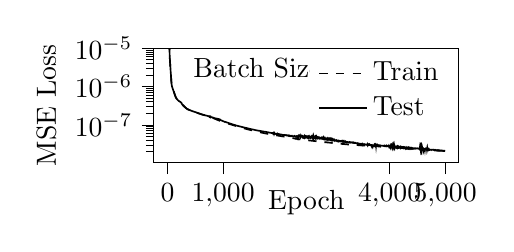
\begin{tikzpicture}

\begin{axis}[
legend cell align={left},
legend style={draw=none},
log basis y={10},
tick align=outside,
tick pos=left,
title={Batch Size 16},
title style={at={(0.4,0.85)},anchor=north},
x grid style={white!69.0196078431373!black},
xlabel={Epoch},
x label style={yshift=13pt},
xmin=-249.95, xmax=5248.95,
xtick style={color=black},
xtick = {0,1000,4000,5000},
y grid style={white!69.0196078431373!black},
ylabel={MSE Loss},
ymin=1.04995733040024e-08, ymax=1e-5,
ymode=log,
ytick style={color=black},
width=.45\textwidth,
height=.25\textwidth
]
\addplot [semithick, black, dashed]
table {%
0 0.0157170567642897
1 0.00494477174337953
2 0.00178249403554946
3 0.00104628965561278
4 0.000540450631990097
5 0.000267249523603823
6 0.000195556676466367
7 0.000179966989569948
8 0.000174315613148792
9 0.000170275954966201
10 0.000166128802236926
11 0.000161243435519282
12 0.000155176517626387
13 0.000147447619914601
14 0.000137505138925917
15 0.000124870715357247
16 0.000109628831036389
17 9.26289391609316e-05
18 7.54085500957444e-05
19 5.99092843294784e-05
20 4.77161089384026e-05
21 3.93279772288224e-05
22 3.40980909077189e-05
23 3.09422128148071e-05
24 2.89322912085481e-05
25 2.72737210743799e-05
26 2.54317353028455e-05
27 2.28156418916114e-05
28 2.01819365893243e-05
29 1.77557636425263e-05
30 1.5502294282669e-05
31 1.34128514700933e-05
32 1.15395934462867e-05
33 9.93898418664685e-06
34 8.62693892850075e-06
35 7.58853412253302e-06
36 6.78498193133237e-06
37 6.16869731970837e-06
38 5.69058382416188e-06
39 5.31324215398854e-06
40 5.00480225616684e-06
41 4.7444518992279e-06
42 4.51447482453204e-06
43 4.30798976503866e-06
44 4.11608894853543e-06
45 3.93454810227922e-06
46 3.75880521266936e-06
47 3.58901737558881e-06
48 3.42562672744862e-06
49 3.26669840717386e-06
50 3.11160224288187e-06
51 2.96258664974403e-06
52 2.82159659042236e-06
53 2.68886794032142e-06
54 2.56387212152731e-06
55 2.44723567112715e-06
56 2.34057172980329e-06
57 2.24493696725858e-06
58 2.15844092952011e-06
59 2.0788237059719e-06
60 1.99667843895668e-06
61 1.90497609787599e-06
62 1.79736609072734e-06
63 1.68848505768437e-06
64 1.59369150190969e-06
65 1.51194072418548e-06
66 1.44278207682191e-06
67 1.38194286273574e-06
68 1.32816223009513e-06
69 1.2809325050398e-06
70 1.23942618449746e-06
71 1.20316316116487e-06
72 1.17089864494346e-06
73 1.14246875506296e-06
74 1.11685223265567e-06
75 1.09369868118847e-06
76 1.07318007189861e-06
77 1.05437576991108e-06
78 1.03672772496566e-06
79 1.02062385838053e-06
80 1.00592634129271e-06
81 9.92105790942332e-07
82 9.7894169545043e-07
83 9.66602892503943e-07
84 9.54589052753363e-07
85 9.42918769112566e-07
86 9.31959767683566e-07
87 9.2148744329279e-07
88 9.11429445267231e-07
89 9.01841054997021e-07
90 8.92400122751269e-07
91 8.83255546455075e-07
92 8.74700299107189e-07
93 8.65906616240863e-07
94 8.57358865317792e-07
95 8.48961237267076e-07
96 8.40659787854747e-07
97 8.3273339777179e-07
98 8.24562840250565e-07
99 8.16930169150964e-07
100 8.08981725157309e-07
101 8.01335254408286e-07
102 7.938409220003e-07
103 7.86272286035228e-07
104 7.79077216805035e-07
105 7.71825237762869e-07
106 7.64540684656367e-07
107 7.57455605054247e-07
108 7.50291343621257e-07
109 7.43385836699417e-07
110 7.36310198249157e-07
111 7.2935094047466e-07
112 7.22335523079209e-07
113 7.15656543093246e-07
114 7.08781524224378e-07
115 7.02204949249108e-07
116 6.95669085445161e-07
117 6.89374548812793e-07
118 6.83004592076486e-07
119 6.76743621340847e-07
120 6.70653783501507e-07
121 6.64517023594158e-07
122 6.58444838109062e-07
123 6.52467115031641e-07
124 6.46645066922247e-07
125 6.40550082820823e-07
126 6.34422589044448e-07
127 6.28629438992334e-07
128 6.22746939754393e-07
129 6.16957024178077e-07
130 6.11050226723364e-07
131 6.0553354312276e-07
132 6.0002472520182e-07
133 5.94472997008211e-07
134 5.89109220683781e-07
135 5.83457079159189e-07
136 5.78418984446216e-07
137 5.7332289055978e-07
138 5.68441488383087e-07
139 5.63714549315364e-07
140 5.59090271252671e-07
141 5.54642511374936e-07
142 5.50334273199837e-07
143 5.46195153745543e-07
144 5.42178440980479e-07
145 5.38200247120812e-07
146 5.34317242667726e-07
147 5.30567891871669e-07
148 5.26957831226582e-07
149 5.23221014177011e-07
150 5.19686565098709e-07
151 5.16319246941066e-07
152 5.1299718701614e-07
153 5.09589032390068e-07
154 5.06361061226812e-07
155 5.03223137172881e-07
156 5.00183228808737e-07
157 4.9724213354807e-07
158 4.9438490189857e-07
159 4.9162455306373e-07
160 4.89330421473255e-07
161 4.86669611902357e-07
162 4.83983281668543e-07
163 4.81407683992074e-07
164 4.78924291158478e-07
165 4.7652420248312e-07
166 4.74232413509412e-07
167 4.71954440158129e-07
168 4.69751064102297e-07
169 4.67584087743944e-07
170 4.65374450342892e-07
171 4.63257154720509e-07
172 4.6126252958345e-07
173 4.59285346551042e-07
174 4.57338758977244e-07
175 4.55391532227623e-07
176 4.53448316278582e-07
177 4.5134003435976e-07
178 4.49530939363285e-07
179 4.47626082561214e-07
180 4.45694395651231e-07
181 4.43928685967876e-07
182 4.42185508745752e-07
183 4.40439555106309e-07
184 4.3882785571725e-07
185 4.37217972901749e-07
186 4.35614033278853e-07
187 4.33923493403654e-07
188 4.32394612360554e-07
189 4.30824806841201e-07
190 4.29448743943794e-07
191 4.27996334764202e-07
192 4.2654474542303e-07
193 4.25223923485873e-07
194 4.23847797321741e-07
195 4.22281450582318e-07
196 4.20877642255846e-07
197 4.19539155572579e-07
198 4.18226270070932e-07
199 4.16828583993834e-07
200 4.15641147853307e-07
201 4.14374378181037e-07
202 4.12955820522143e-07
203 4.11872127500601e-07
204 4.10614599175574e-07
205 4.09486309507656e-07
206 4.08297302655569e-07
207 4.07291623872652e-07
208 4.06151649784192e-07
209 4.04880044627021e-07
210 4.03888402871644e-07
211 4.02805585792976e-07
212 4.01743319073944e-07
213 4.00739752507206e-07
214 3.99736535186435e-07
215 3.98833434005041e-07
216 3.97754167352105e-07
217 3.96727826768029e-07
218 3.95718042653925e-07
219 3.94693230930443e-07
220 3.9383311586505e-07
221 3.9275161007879e-07
222 3.9172802642895e-07
223 3.90782656552346e-07
224 3.89721222845196e-07
225 3.88612679515177e-07
226 3.87859798280488e-07
227 3.8695441405423e-07
228 3.8589167816383e-07
229 3.84909645688936e-07
230 3.83900921491431e-07
231 3.82917928007487e-07
232 3.82064893713618e-07
233 3.81161208053982e-07
234 3.80179631534361e-07
235 3.79220531740998e-07
236 3.78215918999558e-07
237 3.7710426870774e-07
238 3.76155795223099e-07
239 3.74884881878756e-07
240 3.73761657613159e-07
241 3.72517982626164e-07
242 3.71497203701665e-07
243 3.70091190802668e-07
244 3.6877978438099e-07
245 3.67199387056871e-07
246 3.65626293969967e-07
247 3.64062025596468e-07
248 3.62244684353641e-07
249 3.60450857769479e-07
250 3.58647998822903e-07
251 3.56561039907888e-07
252 3.54525802322314e-07
253 3.52287566386167e-07
254 3.50287391583493e-07
255 3.4827622160094e-07
256 3.46361628018599e-07
257 3.442452336202e-07
258 3.42522692250213e-07
259 3.4098111838432e-07
260 3.39507249535131e-07
261 3.3804830252393e-07
262 3.36976891986751e-07
263 3.35771423678466e-07
264 3.34539207671014e-07
265 3.33171887447747e-07
266 3.32210861387239e-07
267 3.30899532073659e-07
268 3.29677021355224e-07
269 3.28394180627356e-07
270 3.27252484524365e-07
271 3.26162355179349e-07
272 3.25076022861026e-07
273 3.24031567018324e-07
274 3.23017687350102e-07
275 3.22020703876547e-07
276 3.21058469410218e-07
277 3.20131131445578e-07
278 3.19224168208621e-07
279 3.18332019588752e-07
280 3.17414626763934e-07
281 3.16470977736572e-07
282 3.15361310200046e-07
283 3.14367141285743e-07
284 3.13330990451277e-07
285 3.12373081598594e-07
286 3.11041730753914e-07
287 3.09975267860807e-07
288 3.08969859794672e-07
289 3.07846929878508e-07
290 3.06794977639413e-07
291 3.05737578266019e-07
292 3.0466266837692e-07
293 3.03954595523237e-07
294 3.03101196678313e-07
295 3.02118985189281e-07
296 3.01218168196726e-07
297 3.00310456772479e-07
298 2.99479211918197e-07
299 2.98664209118726e-07
300 2.97876342834513e-07
301 2.97069236964376e-07
302 2.96287139768481e-07
303 2.95540525151239e-07
304 2.94592372938496e-07
305 2.93832868003108e-07
306 2.93041105045688e-07
307 2.92138023390009e-07
308 2.91344262571158e-07
309 2.90479741146044e-07
310 2.89638650002644e-07
311 2.88783956314376e-07
312 2.87966960804908e-07
313 2.87156888049367e-07
314 2.86230183249359e-07
315 2.85199473267994e-07
316 2.84329060711741e-07
317 2.83470531364571e-07
318 2.82711612797471e-07
319 2.8189036959958e-07
320 2.8108939352478e-07
321 2.80323620067691e-07
322 2.79618150941019e-07
323 2.78579928540523e-07
324 2.77787970787813e-07
325 2.76974661190366e-07
326 2.76175905796094e-07
327 2.75381109268835e-07
328 2.74673050796537e-07
329 2.73941170341629e-07
330 2.73343178925245e-07
331 2.72956742115582e-07
332 2.72267732029263e-07
333 2.71421207877154e-07
334 2.70669167790061e-07
335 2.69858946552404e-07
336 2.69127144292725e-07
337 2.68486125065692e-07
338 2.67699487956463e-07
339 2.67018376263195e-07
340 2.66254324294835e-07
341 2.65609372050335e-07
342 2.64946595834203e-07
343 2.64183357693071e-07
344 2.63509790364935e-07
345 2.62888811377593e-07
346 2.62296822654662e-07
347 2.61795223821082e-07
348 2.60765411624675e-07
349 2.60187987706217e-07
350 2.59608676287826e-07
351 2.58937510935198e-07
352 2.58401657028173e-07
353 2.57939879027447e-07
354 2.57488526514749e-07
355 2.56912723124003e-07
356 2.5638282590279e-07
357 2.55946380399052e-07
358 2.55382050632136e-07
359 2.54851634466036e-07
360 2.5443849939677e-07
361 2.53912852173244e-07
362 2.53413875391573e-07
363 2.52993562064319e-07
364 2.52566530065224e-07
365 2.52173733429117e-07
366 2.51742222630469e-07
367 2.51256598509997e-07
368 2.50831636513738e-07
369 2.50515218077396e-07
370 2.5000812983933e-07
371 2.49434692122463e-07
372 2.48966004456008e-07
373 2.48557739986666e-07
374 2.48152726946671e-07
375 2.47777446951147e-07
376 2.4732192088095e-07
377 2.46895147625992e-07
378 2.46492991010427e-07
379 2.46027582377906e-07
380 2.45625955962225e-07
381 2.45214678422201e-07
382 2.44813897467111e-07
383 2.44392247530811e-07
384 2.439667089007e-07
385 2.43561708266782e-07
386 2.43146217513868e-07
387 2.42745924310839e-07
388 2.42299840301996e-07
389 2.41924007092109e-07
390 2.41548250386359e-07
391 2.4110301239233e-07
392 2.40753827760898e-07
393 2.40407377113172e-07
394 2.40073736314628e-07
395 2.39752746800548e-07
396 2.39428752649928e-07
397 2.39145928070172e-07
398 2.38728963807944e-07
399 2.38479965169347e-07
400 2.38172701713779e-07
401 2.37863011172124e-07
402 2.37620931294202e-07
403 2.3731942192029e-07
404 2.36979224602862e-07
405 2.36684770619888e-07
406 2.36476611952696e-07
407 2.36186071909117e-07
408 2.35960636956634e-07
409 2.35469004792321e-07
410 2.34993137034678e-07
411 2.34665876455153e-07
412 2.34368971142374e-07
413 2.34073551396818e-07
414 2.33405668247144e-07
415 2.3353564838402e-07
416 2.33036555627564e-07
417 2.32731610225301e-07
418 2.32511658502688e-07
419 2.32205579486333e-07
420 2.31897210944965e-07
421 2.31614303118022e-07
422 2.31387427064078e-07
423 2.31009555875517e-07
424 2.30927051632079e-07
425 2.30570250145945e-07
426 2.30109878870621e-07
427 2.29755619159278e-07
428 2.29419798976949e-07
429 2.2913787184109e-07
430 2.28831625989301e-07
431 2.28494739516805e-07
432 2.28182287109746e-07
433 2.27858054557828e-07
434 2.27546540337187e-07
435 2.27196947875541e-07
436 2.26895820269135e-07
437 2.26625020268045e-07
438 2.26283218495382e-07
439 2.25993931898927e-07
440 2.25655906049838e-07
441 2.2537209050455e-07
442 2.2510194525438e-07
443 2.24828690761569e-07
444 2.24556286852362e-07
445 2.24300207833039e-07
446 2.24011245563815e-07
447 2.23872584399487e-07
448 2.23551614816131e-07
449 2.23257345162153e-07
450 2.22980819252427e-07
451 2.2271834546217e-07
452 2.22460312336636e-07
453 2.22206780733813e-07
454 2.21958781267517e-07
455 2.21711269247749e-07
456 2.21467916212248e-07
457 2.21235154199917e-07
458 2.20999668862021e-07
459 2.20767076868356e-07
460 2.20535877438977e-07
461 2.20308807939773e-07
462 2.20059808896167e-07
463 2.19824142021707e-07
464 2.19612100529787e-07
465 2.1938929498333e-07
466 2.19157623597255e-07
467 2.1896537287347e-07
468 2.18743536777311e-07
469 2.18522104340479e-07
470 2.18272721745905e-07
471 2.18055716807442e-07
472 2.1783752742266e-07
473 2.1761818953081e-07
474 2.17430983695976e-07
475 2.17206068221287e-07
476 2.16991443927839e-07
477 2.16773518530999e-07
478 2.16515748135748e-07
479 2.16300841934469e-07
480 2.16058449872492e-07
481 2.15869073706187e-07
482 2.1564869785351e-07
483 2.15435289980803e-07
484 2.15200336675991e-07
485 2.14946434098806e-07
486 2.1470916516364e-07
487 2.14493426646811e-07
488 2.14261333354671e-07
489 2.14043833416611e-07
490 2.13684532845093e-07
491 2.13446484544022e-07
492 2.13225306985976e-07
493 2.13031618301329e-07
494 2.12794633135616e-07
495 2.1251043921211e-07
496 2.12278367698104e-07
497 2.12043049543809e-07
498 2.11812802142219e-07
499 2.11570569483399e-07
500 2.11340852310116e-07
501 2.11117200315414e-07
502 2.10896458291643e-07
503 2.1067865063884e-07
504 2.10462695349634e-07
505 2.10248212908937e-07
506 2.10038392978618e-07
507 2.09967990151938e-07
508 2.09629130488054e-07
509 2.09356091531276e-07
510 2.09101517214094e-07
511 2.0885782751634e-07
512 2.08675676212522e-07
513 2.08429224507256e-07
514 2.08143801842198e-07
515 2.07879654823273e-07
516 2.07599692124916e-07
517 2.07531877720157e-07
518 2.07242607004332e-07
519 2.06976028913175e-07
520 2.06722016230287e-07
521 2.06477896398383e-07
522 2.06244004296252e-07
523 2.05996478037207e-07
524 2.05893390926803e-07
525 2.05615459904607e-07
526 2.05380138218914e-07
527 2.05141496991246e-07
528 2.04895898015423e-07
529 2.04667326379138e-07
530 2.04441963525426e-07
531 2.04216897543574e-07
532 2.0399652140668e-07
533 2.03779658797032e-07
534 2.03562826108339e-07
535 2.0334601751415e-07
536 2.03135240347763e-07
537 2.02906057346297e-07
538 2.02689399074529e-07
539 2.02473491917488e-07
540 2.02258676225142e-07
541 2.02040906152945e-07
542 2.01827895203621e-07
543 2.01646046050996e-07
544 2.0143258397809e-07
545 2.01214925588999e-07
546 2.00992143142287e-07
547 2.00781135099248e-07
548 2.00562146595473e-07
549 2.00357410903962e-07
550 2.00143986297974e-07
551 1.99943427894311e-07
552 1.99730849530511e-07
553 1.99533505224281e-07
554 1.99330869968151e-07
555 1.9912389529253e-07
556 1.98918559668471e-07
557 1.98708590382068e-07
558 1.98505848487684e-07
559 1.98292419888446e-07
560 1.98096410962023e-07
561 1.97904820154804e-07
562 1.9770706975919e-07
563 1.9748347308024e-07
564 1.97292339883859e-07
565 1.97073662711489e-07
566 1.96870710993835e-07
567 1.96664619174669e-07
568 1.96475939667096e-07
569 1.96348054068096e-07
570 1.96120539378342e-07
571 1.95933779174595e-07
572 1.95736368809207e-07
573 1.95534025024813e-07
574 1.95333484313664e-07
575 1.95124152348569e-07
576 1.95009315866912e-07
577 1.94775902379263e-07
578 1.94541645868185e-07
579 1.94320748363452e-07
580 1.9411251212631e-07
581 1.93909075257181e-07
582 1.93718050923053e-07
583 1.93516266911331e-07
584 1.93320917162509e-07
585 1.93129007548976e-07
586 1.92928064961961e-07
587 1.92837274340718e-07
588 1.92624708525102e-07
589 1.92408956387169e-07
590 1.92225819553471e-07
591 1.92020735894971e-07
592 1.91878943944346e-07
593 1.91675015734916e-07
594 1.91448435110431e-07
595 1.91271641604374e-07
596 1.91048381573466e-07
597 1.90840330120068e-07
598 1.90653138474772e-07
599 1.90466430986191e-07
600 1.90273618727588e-07
601 1.90071319252638e-07
602 1.89884589708811e-07
603 1.89694812256391e-07
604 1.89509724471293e-07
605 1.89317692722568e-07
606 1.89151745139782e-07
607 1.88957836265047e-07
608 1.88763875129894e-07
609 1.8860838834911e-07
610 1.88492758660175e-07
611 1.88309009992338e-07
612 1.88081675830176e-07
613 1.87860870838108e-07
614 1.87664490702844e-07
615 1.87469595530843e-07
616 1.87259174673216e-07
617 1.87060099065661e-07
618 1.86873242554952e-07
619 1.86672734876936e-07
620 1.86483752926847e-07
621 1.86293344697219e-07
622 1.86105415899362e-07
623 1.85915503529088e-07
624 1.8575178152247e-07
625 1.85554022223755e-07
626 1.85353178373759e-07
627 1.8521270283145e-07
628 1.85098913320303e-07
629 1.84897171813248e-07
630 1.84691331647002e-07
631 1.84487640524367e-07
632 1.84295574889859e-07
633 1.84111957629796e-07
634 1.83914716345157e-07
635 1.83755724989965e-07
636 1.83571663399107e-07
637 1.8338817892527e-07
638 1.8321129060439e-07
639 1.83026746398696e-07
640 1.82798685713692e-07
641 1.82628072302293e-07
642 1.8240755436949e-07
643 1.82209592708205e-07
644 1.81998398467442e-07
645 1.81880033061077e-07
646 1.81668815613989e-07
647 1.81459775753012e-07
648 1.81254756874694e-07
649 1.81092687050466e-07
650 1.80890330682359e-07
651 1.80684028741496e-07
652 1.80452216731908e-07
653 1.80272235375867e-07
654 1.80111763242508e-07
655 1.79915874568337e-07
656 1.79712098308471e-07
657 1.79537765347959e-07
658 1.79391292441267e-07
659 1.7920577938213e-07
660 1.79012431054559e-07
661 1.78831277722225e-07
662 1.78644232065039e-07
663 1.78457527518106e-07
664 1.78267877934957e-07
665 1.78093018554648e-07
666 1.77905254446387e-07
667 1.77723857326839e-07
668 1.7753547782462e-07
669 1.77379771038488e-07
670 1.77215719631363e-07
671 1.77056875465098e-07
672 1.76856059582065e-07
673 1.76671049281651e-07
674 1.76487213458643e-07
675 1.76302384872429e-07
676 1.76117043793056e-07
677 1.75936534887455e-07
678 1.75756247521974e-07
679 1.75606320475197e-07
680 1.75418388813853e-07
681 1.75196992749704e-07
682 1.75045590090406e-07
683 1.74854614705566e-07
684 1.74652316815127e-07
685 1.74424186383249e-07
686 1.74264706537031e-07
687 1.74055298188591e-07
688 1.73926764027499e-07
689 1.73701496798628e-07
690 1.73572706358982e-07
691 1.73321090102263e-07
692 1.73147434431087e-07
693 1.72996947163995e-07
694 1.72786218151089e-07
695 1.72599083192893e-07
696 1.72568876031676e-07
697 1.72387436194299e-07
698 1.72159440069208e-07
699 1.71958998173238e-07
700 1.71749518663944e-07
701 1.7157847770477e-07
702 1.71360882688987e-07
703 1.71189904619951e-07
704 1.70959397792103e-07
705 1.7079805885345e-07
706 1.70577748185963e-07
707 1.70391250101432e-07
708 1.70294054527176e-07
709 1.70153339674073e-07
710 1.69961250442441e-07
711 1.69790923798985e-07
712 1.69513855112768e-07
713 1.69349986016698e-07
714 1.69170517544615e-07
715 1.68975520637105e-07
716 1.68794829697561e-07
717 1.68674960491444e-07
718 1.68560368251747e-07
719 1.68348613023284e-07
720 1.68180192382295e-07
721 1.68044255872246e-07
722 1.67784312189667e-07
723 1.67622006166823e-07
724 1.67433583676768e-07
725 1.67142194790415e-07
726 1.66952169308843e-07
727 1.66777577675248e-07
728 1.66608952660852e-07
729 1.66446427947164e-07
730 1.66270591492435e-07
731 1.66101942618013e-07
732 1.65938628249762e-07
733 1.65765831525277e-07
734 1.65649616683083e-07
735 1.65385300405774e-07
736 1.65217369541892e-07
737 1.65014219057014e-07
738 1.6483034158199e-07
739 1.64667229618942e-07
740 1.64397729420784e-07
741 1.64213927241974e-07
742 1.64072907040236e-07
743 1.6379700686997e-07
744 1.63645981643867e-07
745 1.63382232301501e-07
746 1.6327906817537e-07
747 1.63015408730871e-07
748 1.62801310864324e-07
749 1.62617077627658e-07
750 1.62424714076792e-07
751 1.62247915383773e-07
752 1.62051023785637e-07
753 1.61872072872882e-07
754 1.6165106788435e-07
755 1.61600835717479e-07
756 1.61240600313306e-07
757 1.61194861057368e-07
758 1.60852658879662e-07
759 1.60787009278351e-07
760 1.60590858342857e-07
761 1.60234822551786e-07
762 1.60201742232857e-07
763 1.59901149771713e-07
764 1.59803023151994e-07
765 1.59525831236351e-07
766 1.59374475643403e-07
767 1.59135792628717e-07
768 1.58920532690843e-07
769 1.58900042478649e-07
770 1.58551003600849e-07
771 1.58445956166986e-07
772 1.58137577130901e-07
773 1.58083954872268e-07
774 1.57764831811846e-07
775 1.57709431590547e-07
776 1.57401405722624e-07
777 1.57347303854749e-07
778 1.57050745258402e-07
779 1.56966653740653e-07
780 1.56687031115155e-07
781 1.56785914370516e-07
782 1.56612737448825e-07
783 1.56451782203249e-07
784 1.56252137685442e-07
785 1.56076418790008e-07
786 1.55898435949098e-07
787 1.55699541132037e-07
788 1.55520961151012e-07
789 1.55345307412347e-07
790 1.55173079157578e-07
791 1.54974727074375e-07
792 1.54768641245084e-07
793 1.5459558374431e-07
794 1.5444234325912e-07
795 1.54301182689665e-07
796 1.54076760843225e-07
797 1.53900922057915e-07
798 1.53745949539541e-07
799 1.53580229117267e-07
800 1.53406590548855e-07
801 1.53240547525968e-07
802 1.53047686090702e-07
803 1.52824890882641e-07
804 1.52664273521452e-07
805 1.52475196550483e-07
806 1.52327802844354e-07
807 1.52147398885916e-07
808 1.51979647590395e-07
809 1.51795929646426e-07
810 1.51624505434711e-07
811 1.51454105321136e-07
812 1.51283279407721e-07
813 1.51115457406092e-07
814 1.50930618310952e-07
815 1.50760781984616e-07
816 1.50782627734714e-07
817 1.50500275672982e-07
818 1.50235237292407e-07
819 1.50018968902543e-07
820 1.49857105313345e-07
821 1.49713744534097e-07
822 1.49508386748209e-07
823 1.49243716315084e-07
824 1.49054966783524e-07
825 1.48848405203239e-07
826 1.48593713156231e-07
827 1.48452548614841e-07
828 1.48339782398921e-07
829 1.48084122237435e-07
830 1.47866147088394e-07
831 1.47622342979048e-07
832 1.4737123991182e-07
833 1.47169714985296e-07
834 1.47018789085962e-07
835 1.46823949506825e-07
836 1.46512769518381e-07
837 1.46378438842021e-07
838 1.46098743840639e-07
839 1.45954007734872e-07
840 1.45737554120728e-07
841 1.45556221561094e-07
842 1.45273102816645e-07
843 1.45146473812474e-07
844 1.44893944799662e-07
845 1.44685848667336e-07
846 1.44500907168776e-07
847 1.4436663649775e-07
848 1.44028160448784e-07
849 1.43881057880435e-07
850 1.43606745851343e-07
851 1.43507942325982e-07
852 1.43128769224177e-07
853 1.4301058635624e-07
854 1.42788225716117e-07
855 1.42625498355642e-07
856 1.42412673760361e-07
857 1.42159079061344e-07
858 1.4199432023787e-07
859 1.41772513316596e-07
860 1.41599934678993e-07
861 1.41388858359903e-07
862 1.41182926185479e-07
863 1.40962782744225e-07
864 1.40806364584023e-07
865 1.40581685961649e-07
866 1.40403925101396e-07
867 1.4016057497912e-07
868 1.40044896177471e-07
869 1.3980589160667e-07
870 1.3957648116758e-07
871 1.39445378636083e-07
872 1.39138843742614e-07
873 1.38897649193837e-07
874 1.38654308422304e-07
875 1.38455802293436e-07
876 1.38271871641393e-07
877 1.38072660327282e-07
878 1.3789356398064e-07
879 1.37655154013316e-07
880 1.37478279633285e-07
881 1.37314475196604e-07
882 1.37122865879746e-07
883 1.36933145142848e-07
884 1.36802316887952e-07
885 1.36559793908475e-07
886 1.3642202107178e-07
887 1.36200022627264e-07
888 1.36101916211828e-07
889 1.35843518506817e-07
890 1.35694482299442e-07
891 1.35512572025931e-07
892 1.35300152894757e-07
893 1.35296917736838e-07
894 1.35076997914041e-07
895 1.34893043981066e-07
896 1.34717172727505e-07
897 1.34527160362552e-07
898 1.34308240479442e-07
899 1.34143823828481e-07
900 1.33862042787314e-07
901 1.336907333922e-07
902 1.33526360556857e-07
903 1.33354756073345e-07
904 1.33178832584235e-07
905 1.32975719669304e-07
906 1.328086220731e-07
907 1.32602404118387e-07
908 1.3244473960583e-07
909 1.322507284236e-07
910 1.3208645066598e-07
911 1.31908025320371e-07
912 1.31727454142805e-07
913 1.31562949462705e-07
914 1.31399596458692e-07
915 1.3120474050865e-07
916 1.31009608221433e-07
917 1.30844098823246e-07
918 1.30663171997725e-07
919 1.30506657299634e-07
920 1.30347919839124e-07
921 1.30182991870953e-07
922 1.30027269566568e-07
923 1.29857494112429e-07
924 1.29701414859795e-07
925 1.29552905523411e-07
926 1.2940177445131e-07
927 1.29231482656422e-07
928 1.29098281369977e-07
929 1.28939781010473e-07
930 1.28751404755434e-07
931 1.28589202464724e-07
932 1.2841671961894e-07
933 1.28243070928846e-07
934 1.2803982670917e-07
935 1.27876534680382e-07
936 1.27715794622674e-07
937 1.27549439078223e-07
938 1.27395809307984e-07
939 1.27251330805933e-07
940 1.27115895857344e-07
941 1.26910032076211e-07
942 1.26811345971589e-07
943 1.26729663211478e-07
944 1.26444568536499e-07
945 1.26253609963101e-07
946 1.26082584579024e-07
947 1.25873118491882e-07
948 1.25708876002051e-07
949 1.25526543680365e-07
950 1.25347965983735e-07
951 1.25173203823437e-07
952 1.24986479754341e-07
953 1.24805979790921e-07
954 1.2464467223694e-07
955 1.24486626290832e-07
956 1.24325891309951e-07
957 1.24059086388684e-07
958 1.23900421499457e-07
959 1.23752723684589e-07
960 1.23606460093129e-07
961 1.23458894080386e-07
962 1.23334903548766e-07
963 1.23164554814537e-07
964 1.23017373574896e-07
965 1.22884383220168e-07
966 1.2272103016997e-07
967 1.22591781686054e-07
968 1.22412395523241e-07
969 1.22283938569723e-07
970 1.2213839731956e-07
971 1.21992413387062e-07
972 1.21762341468212e-07
973 1.21653056602611e-07
974 1.21516884128425e-07
975 1.21363378561057e-07
976 1.21249401036749e-07
977 1.21074073003768e-07
978 1.20967150103013e-07
979 1.20810225507029e-07
980 1.20688818554981e-07
981 1.20541718686695e-07
982 1.20421648816205e-07
983 1.2028323980573e-07
984 1.20130155050191e-07
985 1.20018588045667e-07
986 1.19883109864105e-07
987 1.19717597538482e-07
988 1.19591703700905e-07
989 1.19459623334706e-07
990 1.19327731148644e-07
991 1.19182412216645e-07
992 1.190378214595e-07
993 1.18928106189742e-07
994 1.18777606907372e-07
995 1.18669771886459e-07
996 1.18526345442405e-07
997 1.18412091222098e-07
998 1.182686517609e-07
999 1.18146764471305e-07
1000 1.18045295611324e-07
1001 1.17885191471601e-07
1002 1.1773723693409e-07
1003 1.17636993980597e-07
1004 1.17508308122183e-07
1005 1.17379135396334e-07
1006 1.17220094796977e-07
1007 1.17123960905019e-07
1008 1.16971413607558e-07
1009 1.16875604081912e-07
1010 1.16721507264828e-07
1011 1.16625413646432e-07
1012 1.16471765217341e-07
1013 1.16374956864007e-07
1014 1.16226475117998e-07
1015 1.1612951336204e-07
1016 1.15985186340595e-07
1017 1.15878762532162e-07
1018 1.15722544556718e-07
1019 1.1563705219686e-07
1020 1.15482216056506e-07
1021 1.15382735749847e-07
1022 1.15234289868482e-07
1023 1.15194369406879e-07
1024 1.1509215372385e-07
1025 1.14971480446258e-07
1026 1.14853542346083e-07
1027 1.14729510986677e-07
1028 1.14465596745106e-07
1029 1.14398147832873e-07
1030 1.14321383524185e-07
1031 1.14196341097994e-07
1032 1.14066242570487e-07
1033 1.13935783559782e-07
1034 1.13807661961118e-07
1035 1.13695412860437e-07
1036 1.13558107294409e-07
1037 1.13417669808769e-07
1038 1.13302818903094e-07
1039 1.13176249655567e-07
1040 1.13044207392221e-07
1041 1.12916077910086e-07
1042 1.12789789074696e-07
1043 1.12666461593136e-07
1044 1.12543457490233e-07
1045 1.12422214286312e-07
1046 1.12315864466694e-07
1047 1.12182835920294e-07
1048 1.12061487143933e-07
1049 1.11943023419769e-07
1050 1.11824035883501e-07
1051 1.11708382185327e-07
1052 1.11589450629168e-07
1053 1.11475569585906e-07
1054 1.11358585638044e-07
1055 1.11240735918727e-07
1056 1.11126858243438e-07
1057 1.11011553304508e-07
1058 1.10896632492086e-07
1059 1.10790323411436e-07
1060 1.10676093481032e-07
1061 1.10561356954975e-07
1062 1.10458826345194e-07
1063 1.10332153219872e-07
1064 1.10221367368268e-07
1065 1.10119643316864e-07
1066 1.10016076984465e-07
1067 1.09895937949744e-07
1068 1.09784279111125e-07
1069 1.09660139557377e-07
1070 1.09532256768574e-07
1071 1.09413658780255e-07
1072 1.09296013629745e-07
1073 1.09178800776988e-07
1074 1.09062563716122e-07
1075 1.08961397675245e-07
1076 1.0882023883596e-07
1077 1.08682747345767e-07
1078 1.08570803114105e-07
1079 1.08453086824056e-07
1080 1.08348394981306e-07
1081 1.08229575708663e-07
1082 1.08175652648868e-07
1083 1.08044552664666e-07
1084 1.07924311190999e-07
1085 1.07804279075197e-07
1086 1.07687016416946e-07
1087 1.07583657079857e-07
1088 1.07472328480185e-07
1089 1.07360298155612e-07
1090 1.07231535281471e-07
1091 1.07122651012759e-07
1092 1.07014493000435e-07
1093 1.0690706458405e-07
1094 1.06793603364963e-07
1095 1.06669464503995e-07
1096 1.06556396463731e-07
1097 1.06448062449971e-07
1098 1.0633262673565e-07
1099 1.06225804859861e-07
1100 1.06111840107559e-07
1101 1.06007312659528e-07
1102 1.05889961115935e-07
1103 1.05787279665037e-07
1104 1.05671067569091e-07
1105 1.05566635443921e-07
1106 1.0545252139238e-07
1107 1.05352690265903e-07
1108 1.05238320241341e-07
1109 1.05129935327852e-07
1110 1.05013805679732e-07
1111 1.04924952804453e-07
1112 1.04802457894237e-07
1113 1.0472310326648e-07
1114 1.04609571572212e-07
1115 1.0450942516016e-07
1116 1.04393734819297e-07
1117 1.04297197307091e-07
1118 1.04180416496291e-07
1119 1.0408402435047e-07
1120 1.03966197073646e-07
1121 1.0387017652036e-07
1122 1.03754794164246e-07
1123 1.0365835006354e-07
1124 1.03542971995552e-07
1125 1.03447081940544e-07
1126 1.03333663226124e-07
1127 1.03239306419312e-07
1128 1.03124784988751e-07
1129 1.03028840477748e-07
1130 1.02916153586818e-07
1131 1.02787292341588e-07
1132 1.02657459869704e-07
1133 1.02566233646684e-07
1134 1.02459099572627e-07
1135 1.0236741592351e-07
1136 1.02258474193206e-07
1137 1.02178690926991e-07
1138 1.02057533133859e-07
1139 1.0195955497494e-07
1140 1.01866740447321e-07
1141 1.0174640036098e-07
1142 1.01654885199309e-07
1143 1.01564086460115e-07
1144 1.01452568284088e-07
1145 1.01358281408892e-07
1146 1.01252124068196e-07
1147 1.01132042544805e-07
1148 1.01040741810721e-07
1149 1.0093680472778e-07
1150 1.00835201639171e-07
1151 1.00737907963833e-07
1152 1.00636074826355e-07
1153 1.00535662330259e-07
1154 1.00435070386595e-07
1155 1.00334794463919e-07
1156 1.00233066344657e-07
1157 1.00139313264691e-07
1158 1.00035746370963e-07
1159 9.99342205645348e-08
1160 9.98369444076275e-08
1161 9.97294167923712e-08
1162 9.96306041329831e-08
1163 9.95292283505478e-08
1164 9.94305740533719e-08
1165 9.93309828345446e-08
1166 9.92319580497281e-08
1167 9.91331406723361e-08
1168 9.90346987315149e-08
1169 9.89363423364864e-08
1170 9.88384333915349e-08
1171 9.87406676955516e-08
1172 9.86426246996075e-08
1173 9.85450470523119e-08
1174 9.84475341887503e-08
1175 9.83505173692833e-08
1176 9.82529710178426e-08
1177 9.81562854889262e-08
1178 9.80592281862869e-08
1179 9.79621718073531e-08
1180 9.78654439443005e-08
1181 9.77698567261598e-08
1182 9.76725255235067e-08
1183 9.75756527665794e-08
1184 9.74796394181965e-08
1185 9.73854815420339e-08
1186 9.72912396584036e-08
1187 9.71942784673274e-08
1188 9.70993046678359e-08
1189 9.7005777128345e-08
1190 9.69105955412886e-08
1191 9.68398183474051e-08
1192 9.67422502249349e-08
1193 9.6656792269556e-08
1194 9.65493723619204e-08
1195 9.64579490911888e-08
1196 9.63569642422613e-08
1197 9.62606689931533e-08
1198 9.61624434623332e-08
1199 9.60775235725464e-08
1200 9.5981298237291e-08
1201 9.58870457914429e-08
1202 9.57886685490905e-08
1203 9.56941159380165e-08
1204 9.55973716543213e-08
1205 9.550779267542e-08
1206 9.54129343995192e-08
1207 9.53207871106088e-08
1208 9.52259731121785e-08
1209 9.51386579863822e-08
1210 9.50452932002577e-08
1211 9.49372938769955e-08
1212 9.48370358955231e-08
1213 9.47485660738323e-08
1214 9.46488406015078e-08
1215 9.45476629787834e-08
1216 9.44520911225766e-08
1217 9.43511249644757e-08
1218 9.42532653489536e-08
1219 9.41596363510655e-08
1220 9.40521965198116e-08
1221 9.3958234778313e-08
1222 9.38527993739058e-08
1223 9.37583681590581e-08
1224 9.3655063739817e-08
1225 9.35592185555834e-08
1226 9.34639041965113e-08
1227 9.33635799533761e-08
1228 9.32726998605915e-08
1229 9.31820874114919e-08
1230 9.3086685076571e-08
1231 9.2996467174089e-08
1232 9.28943459186371e-08
1233 9.28112276987747e-08
1234 9.27086237609842e-08
1235 9.26266937000264e-08
1236 9.25256117518813e-08
1237 9.24348963096122e-08
1238 9.23422541383445e-08
1239 9.22336319888473e-08
1240 9.21328738066052e-08
1241 9.20548228862117e-08
1242 9.19620167856294e-08
1243 9.1858883305207e-08
1244 9.17831347067022e-08
1245 9.16764033469519e-08
1246 9.16021301513581e-08
1247 9.15102322807115e-08
1248 9.14096642823381e-08
1249 9.13258232415615e-08
1250 9.12370573509236e-08
1251 9.11314231082372e-08
1252 9.10548857149251e-08
1253 9.09575262930673e-08
1254 9.0878455086596e-08
1255 9.07892068404692e-08
1256 9.06909464717387e-08
1257 9.06085933252143e-08
1258 9.0521073303762e-08
1259 9.04282962750358e-08
1260 9.03382387598128e-08
1261 9.02488962388759e-08
1262 9.01657012271073e-08
1263 9.00837959534329e-08
1264 8.99963811491489e-08
1265 8.9906916667104e-08
1266 8.98200719099407e-08
1267 8.97321847581622e-08
1268 8.96452091616595e-08
1269 8.95563996046178e-08
1270 8.94744537696113e-08
1271 8.93858809583037e-08
1272 8.93017317054046e-08
1273 8.92115444202091e-08
1274 8.91289444773236e-08
1275 8.90431513695944e-08
1276 8.89543760465017e-08
1277 8.88647354990724e-08
1278 8.87773948683446e-08
1279 8.86847180474604e-08
1280 8.8604710200002e-08
1281 8.85189234693939e-08
1282 8.84320530047944e-08
1283 8.83455266311728e-08
1284 8.82566362889747e-08
1285 8.81749002772381e-08
1286 8.8091375637589e-08
1287 8.8006731434831e-08
1288 8.79208263704356e-08
1289 8.78380143163327e-08
1290 8.7753197313134e-08
1291 8.76683468540307e-08
1292 8.7583503496802e-08
1293 8.74997554873858e-08
1294 8.74166315618652e-08
1295 8.7332899298076e-08
1296 8.72496221155927e-08
1297 8.71674850380089e-08
1298 8.70835239226153e-08
1299 8.69979467985615e-08
1300 8.69180498774824e-08
1301 8.68290546023331e-08
1302 8.67538605575646e-08
1303 8.66866929456478e-08
1304 8.66013013194333e-08
1305 8.65141546739778e-08
1306 8.6432395224989e-08
1307 8.63492025722223e-08
1308 8.62639010534849e-08
1309 8.61873499360399e-08
1310 8.60964398192721e-08
1311 8.60305623895386e-08
1312 8.5945265599463e-08
1313 8.58654531619152e-08
1314 8.57828558054052e-08
1315 8.57025365945674e-08
1316 8.56227119179209e-08
1317 8.55251783349331e-08
1318 8.5447654544879e-08
1319 8.53730991074997e-08
1320 8.53113611576362e-08
1321 8.52530063752965e-08
1322 8.5145811016929e-08
1323 8.50639250415952e-08
1324 8.49800504987286e-08
1325 8.49213991926945e-08
1326 8.48373153417015e-08
1327 8.47663028693546e-08
1328 8.4683932776386e-08
1329 8.46030600811787e-08
1330 8.45243451159661e-08
1331 8.44448748686943e-08
1332 8.43658713378659e-08
1333 8.42873192290483e-08
1334 8.42077087881421e-08
1335 8.413040495725e-08
1336 8.40533396413434e-08
1337 8.39737880227176e-08
1338 8.39027628565248e-08
1339 8.38281100463689e-08
1340 8.37473770438635e-08
1341 8.36699169042276e-08
1342 8.35880798319977e-08
1343 8.35109091923414e-08
1344 8.34303905108413e-08
1345 8.33509666051668e-08
1346 8.32730190971631e-08
1347 8.31975916035788e-08
1348 8.31306992026271e-08
1349 8.30542468079898e-08
1350 8.29774157509178e-08
1351 8.2896661286469e-08
1352 8.28168008588648e-08
1353 8.27384261050668e-08
1354 8.26573808154762e-08
1355 8.25796255305988e-08
1356 8.25036329494821e-08
1357 8.24257792118033e-08
1358 8.23485480161423e-08
1359 8.22789238732469e-08
1360 8.22006595520008e-08
1361 8.21227055496365e-08
1362 8.2044704448947e-08
1363 8.19672813463512e-08
1364 8.18913912894459e-08
1365 8.18145910308488e-08
1366 8.17310067056098e-08
1367 8.16556159399795e-08
1368 8.15891315895101e-08
1369 8.15134725122846e-08
1370 8.14405360145543e-08
1371 8.13719105217103e-08
1372 8.12908016314395e-08
1373 8.12063895203607e-08
1374 8.11270667853137e-08
1375 8.10392181485042e-08
1376 8.09575813001118e-08
1377 8.08839921795368e-08
1378 8.08079852667731e-08
1379 8.07220590779423e-08
1380 8.06590918109862e-08
1381 8.05818785387658e-08
1382 8.05058287483007e-08
1383 8.04375114924483e-08
1384 8.03611219843958e-08
1385 8.02734742073596e-08
1386 8.02103674963917e-08
1387 8.01333753592814e-08
1388 8.00467322505938e-08
1389 7.99712219219373e-08
1390 7.99084653912985e-08
1391 7.98324605639777e-08
1392 7.97513225130331e-08
1393 7.96915628207273e-08
1394 7.96128401034935e-08
1395 7.95309664347599e-08
1396 7.94698840849151e-08
1397 7.9392765581332e-08
1398 7.9295083487807e-08
1399 7.92480824038933e-08
1400 7.91767527488219e-08
1401 7.90798937977399e-08
1402 7.90350093922143e-08
1403 7.89427710436996e-08
1404 7.88719372764035e-08
1405 7.88001505966918e-08
1406 7.87278963976235e-08
1407 7.86439569182562e-08
1408 7.85879019211677e-08
1409 7.85154309888014e-08
1410 7.84318538968876e-08
1411 7.83922933358383e-08
1412 7.83064902059039e-08
1413 7.82436948192355e-08
1414 7.81700940777341e-08
1415 7.81046548645747e-08
1416 7.80235332982215e-08
1417 7.79860344124472e-08
1418 7.78859922760944e-08
1419 7.78468724114134e-08
1420 7.77458072285242e-08
1421 7.77082536167484e-08
1422 7.76031458613602e-08
1423 7.75538769453021e-08
1424 7.74638346889844e-08
1425 7.7412013162359e-08
1426 7.73240489770899e-08
1427 7.72703984992518e-08
1428 7.71842282603075e-08
1429 7.71299326345343e-08
1430 7.70427543983487e-08
1431 7.69885805844694e-08
1432 7.68999306934859e-08
1433 7.68471794536651e-08
1434 7.67474068190665e-08
1435 7.669313940184e-08
1436 7.6607799300632e-08
1437 7.65571879561833e-08
1438 7.64666975019423e-08
1439 7.64233642662759e-08
1440 7.63317421643706e-08
1441 7.62877545348317e-08
1442 7.6203435483535e-08
1443 7.61529052084597e-08
1444 7.60647247997071e-08
1445 7.60194817654991e-08
1446 7.59333198274703e-08
1447 7.58907218383342e-08
1448 7.58090455246219e-08
1449 7.57582843178284e-08
1450 7.57179583370515e-08
1451 7.56195299302931e-08
1452 7.55561748508882e-08
1453 7.54916978635833e-08
1454 7.5432396256403e-08
1455 7.53674571498664e-08
1456 7.52965677950357e-08
1457 7.5238625441898e-08
1458 7.5167802796372e-08
1459 7.51119294637448e-08
1460 7.50374735734027e-08
1461 7.49760933977939e-08
1462 7.48975998057233e-08
1463 7.48535242411918e-08
1464 7.47783008758773e-08
1465 7.47050625609091e-08
1466 7.46483551417043e-08
1467 7.45740001022455e-08
1468 7.45270812885224e-08
1469 7.4443754344955e-08
1470 7.4380113401773e-08
1471 7.43380596901488e-08
1472 7.42537142617294e-08
1473 7.42098589494589e-08
1474 7.41303028082285e-08
1475 7.40660056592901e-08
1476 7.40370165512871e-08
1477 7.39397521467566e-08
1478 7.38789098857495e-08
1479 7.38492542762259e-08
1480 7.37513224109421e-08
1481 7.37224941023129e-08
1482 7.36224275552644e-08
1483 7.35667011948493e-08
1484 7.35384280314832e-08
1485 7.34439351628424e-08
1486 7.34135366222688e-08
1487 7.33215193999826e-08
1488 7.3262118958084e-08
1489 7.32310826201399e-08
1490 7.31369283712979e-08
1491 7.30799931130122e-08
1492 7.30507533877045e-08
1493 7.29692056040676e-08
1494 7.29461080162253e-08
1495 7.28552913358271e-08
1496 7.28172455186637e-08
1497 7.2759770612052e-08
1498 7.26808831839065e-08
1499 7.26333379219568e-08
1500 7.25761171178618e-08
1501 7.25002446042566e-08
1502 7.24530508353638e-08
1503 7.23712498071904e-08
1504 7.23255573245041e-08
1505 7.22771065948535e-08
1506 7.22012546212625e-08
1507 7.21588228156378e-08
1508 7.20717930615677e-08
1509 7.20151864914698e-08
1510 7.19812252931717e-08
1511 7.18593284645408e-08
1512 7.18661725915837e-08
1513 7.18080895314443e-08
1514 7.17542879211663e-08
1515 7.16964362812433e-08
1516 7.16366252806466e-08
1517 7.15322650410855e-08
1518 7.15308601897391e-08
1519 7.14554064966677e-08
1520 7.13549446889061e-08
1521 7.13500851201587e-08
1522 7.1280213971292e-08
1523 7.12213592048983e-08
1524 7.1125808473127e-08
1525 7.11177791856699e-08
1526 7.10524085931752e-08
1527 7.09491985855237e-08
1528 7.09230811022366e-08
1529 7.08539147549203e-08
1530 7.07737182583656e-08
1531 7.07214989734695e-08
1532 7.06564270451793e-08
1533 7.05835089735984e-08
1534 7.05460777865596e-08
1535 7.04877491930489e-08
1536 7.04216205349439e-08
1537 7.03814124722868e-08
1538 7.03216431912068e-08
1539 7.02704037696122e-08
1540 7.01973612020623e-08
1541 7.0164162307762e-08
1542 7.01039659212199e-08
1543 7.0039195259497e-08
1544 6.99994840633877e-08
1545 6.99282411940061e-08
1546 6.98895919128972e-08
1547 6.98095471864946e-08
1548 6.97712376460657e-08
1549 6.97109298943843e-08
1550 6.9632473101322e-08
1551 6.95940093482506e-08
1552 6.95389268248192e-08
1553 6.94699652452613e-08
1554 6.94294041974075e-08
1555 6.9355845011998e-08
1556 6.93180881405908e-08
1557 6.92588990727216e-08
1558 6.91887736632424e-08
1559 6.91512637267522e-08
1560 6.9092847537533e-08
1561 6.90220523242857e-08
1562 6.89855159823338e-08
1563 6.89106090323577e-08
1564 6.88816554959004e-08
1565 6.88365903069865e-08
1566 6.87812293040935e-08
1567 6.87185002323787e-08
1568 6.8642084881887e-08
1569 6.86118347612563e-08
1570 6.85325593572372e-08
1571 6.85040618790822e-08
1572 6.84324654880442e-08
1573 6.839076007914e-08
1574 6.83189021835062e-08
1575 6.82729641408031e-08
1576 6.81955693746517e-08
1577 6.81605108194816e-08
1578 6.81111089928521e-08
1579 6.80341699759168e-08
1580 6.80005206437073e-08
1581 6.79343854468328e-08
1582 6.78743013686756e-08
1583 6.78180592128541e-08
1584 6.77644835676006e-08
1585 6.77205531331992e-08
1586 6.76518835902584e-08
1587 6.75858284839848e-08
1588 6.7559896509195e-08
1589 6.74892750094358e-08
1590 6.74610934225939e-08
1591 6.74030582157315e-08
1592 6.73369531245527e-08
1593 6.72861732180508e-08
1594 6.72273089517006e-08
1595 6.7194645049895e-08
1596 6.7137755896951e-08
1597 6.70708017658228e-08
1598 6.70592294174099e-08
1599 6.69806256290428e-08
1600 6.69565935051963e-08
1601 6.6876471620958e-08
1602 6.68527393017371e-08
1603 6.67749209544155e-08
1604 6.67497319373211e-08
1605 6.66836660396797e-08
1606 6.66453354263297e-08
1607 6.65926854352961e-08
1608 6.65282488423458e-08
1609 6.6488449387947e-08
1610 6.64343398302236e-08
1611 6.63779134839615e-08
1612 6.63125629074557e-08
1613 6.62765239027863e-08
1614 6.62034557681324e-08
1615 6.61748533499207e-08
1616 6.61297554014339e-08
1617 6.60409584458677e-08
1618 6.6028880171487e-08
1619 6.59719671087799e-08
1620 6.59495228756413e-08
1621 6.58748443882473e-08
1622 6.58512198743466e-08
1623 6.57803125960754e-08
1624 6.57593430002379e-08
1625 6.57009276565645e-08
1626 6.56188756789078e-08
1627 6.56008984094569e-08
1628 6.5510794748036e-08
1629 6.5506174689034e-08
1630 6.54147165271013e-08
1631 6.54004263029861e-08
1632 6.5330469803726e-08
1633 6.53194631468068e-08
1634 6.52330189456762e-08
1635 6.52263919054263e-08
1636 6.51325602660791e-08
1637 6.51270379510294e-08
1638 6.50832606332585e-08
1639 6.50223449909504e-08
1640 6.49905436045373e-08
1641 6.49078730869945e-08
1642 6.48822075746125e-08
1643 6.48035599741803e-08
1644 6.47770159538652e-08
1645 6.4707539873865e-08
1646 6.46819224456863e-08
1647 6.46097836529691e-08
1648 6.45885289962678e-08
1649 6.45144189377334e-08
1650 6.44925645705285e-08
1651 6.44240081335568e-08
1652 6.43979384005178e-08
1653 6.43428221973608e-08
1654 6.428219044885e-08
1655 6.42558258956427e-08
1656 6.41921231387954e-08
1657 6.41689319547112e-08
1658 6.41028819785561e-08
1659 6.40726781870882e-08
1660 6.40072181106177e-08
1661 6.39795522463515e-08
1662 6.39297982321096e-08
1663 6.3871073178845e-08
1664 6.38408367290566e-08
1665 6.37792557007799e-08
1666 6.37521571729138e-08
1667 6.36896845236379e-08
1668 6.36601125965086e-08
1669 6.36008435410673e-08
1670 6.35746379664681e-08
1671 6.35181804433671e-08
1672 6.34676094435349e-08
1673 6.34354211879184e-08
1674 6.33740493203305e-08
1675 6.33314038243071e-08
1676 6.32749130726751e-08
1677 6.32347840738845e-08
1678 6.31732688756159e-08
1679 6.31338394310177e-08
1680 6.30652151922817e-08
1681 6.30463459234676e-08
1682 6.29724075018601e-08
1683 6.2956256465796e-08
1684 6.28833726636913e-08
1685 6.28631577619387e-08
1686 6.2810514361189e-08
1687 6.27526249825649e-08
1688 6.27297131359228e-08
1689 6.26645676735649e-08
1690 6.26481085017616e-08
1691 6.25765496540254e-08
1692 6.25491643475584e-08
1693 6.24812895697602e-08
1694 6.2463616799846e-08
1695 6.23948352806991e-08
1696 6.23737416489689e-08
1697 6.23239637480566e-08
1698 6.22703101509359e-08
1699 6.22446263580656e-08
1700 6.21824421340733e-08
1701 6.21636741069409e-08
1702 6.20918038123364e-08
1703 6.20736190857229e-08
1704 6.20149772938561e-08
1705 6.19964937431661e-08
1706 6.19347309811502e-08
1707 6.1910406349952e-08
1708 6.18521268460626e-08
1709 6.18265581540101e-08
1710 6.17684524790718e-08
1711 6.17448781028429e-08
1712 6.16845532288579e-08
1713 6.16598977511984e-08
1714 6.16143801561719e-08
1715 6.15619190327266e-08
1716 6.15333821283315e-08
1717 6.14823349280869e-08
1718 6.14551080015957e-08
1719 6.14102441911513e-08
1720 6.13515261029818e-08
1721 6.13220992118357e-08
1722 6.12588356148081e-08
1723 6.12405779989444e-08
1724 6.11997082504701e-08
1725 6.11438640394368e-08
1726 6.11246135520105e-08
1727 6.1070817375608e-08
1728 6.10205517528328e-08
1729 6.09990552220552e-08
1730 6.09413689733884e-08
1731 6.08886698465483e-08
1732 6.08616994828282e-08
1733 6.08214279971264e-08
1734 6.07714548870319e-08
1735 6.07395625191742e-08
1736 6.06988344191706e-08
1737 6.064735849165e-08
1738 6.06205199655818e-08
1739 6.05749239124265e-08
1740 6.05129370594426e-08
1741 6.05012419647721e-08
1742 6.04553985272815e-08
1743 6.03960760319211e-08
1744 6.03828635998838e-08
1745 6.03404926344808e-08
1746 6.02797830424606e-08
1747 6.02628985220122e-08
1748 6.02163528338195e-08
1749 6.01650723552893e-08
1750 6.01461151159555e-08
1751 6.0099468852215e-08
1752 6.00380151585256e-08
1753 6.00097526533006e-08
1754 5.99578201949669e-08
1755 5.99032240202746e-08
1756 5.98908391200581e-08
1757 5.98447522186518e-08
1758 5.97969285838218e-08
1759 5.9783278864245e-08
1760 5.97381680282894e-08
1761 5.96831014316734e-08
1762 5.96634693312836e-08
1763 5.9620811219574e-08
1764 5.95710671564831e-08
1765 5.95497044262316e-08
1766 5.94933353976756e-08
1767 5.94397501458843e-08
1768 5.94266319691172e-08
1769 5.93856979289598e-08
1770 5.93300072733172e-08
1771 5.93130644528372e-08
1772 5.92704806923194e-08
1773 5.92268136809793e-08
1774 5.91797808926486e-08
1775 5.91507497311738e-08
1776 5.91200140238612e-08
1777 5.90610537880565e-08
1778 5.90448508877017e-08
1779 5.90022764068721e-08
1780 5.89430245447886e-08
1781 5.89263584167554e-08
1782 5.88846336242455e-08
1783 5.88285095606267e-08
1784 5.88103355436687e-08
1785 5.87698267064951e-08
1786 5.87322994558548e-08
1787 5.86814049867712e-08
1788 5.86593097935406e-08
1789 5.86253984682372e-08
1790 5.85660904164342e-08
1791 5.85476309495903e-08
1792 5.85049212116218e-08
1793 5.84561298868635e-08
1794 5.84374685121958e-08
1795 5.83932191009495e-08
1796 5.83553954029981e-08
1797 5.83059133898445e-08
1798 5.82895867626831e-08
1799 5.82480555006981e-08
1800 5.8200157324606e-08
1801 5.81786484090685e-08
1802 5.81429857593463e-08
1803 5.80878021807507e-08
1804 5.80690354983204e-08
1805 5.80282149797995e-08
1806 5.79956561210793e-08
1807 5.79425478619555e-08
1808 5.79221452419176e-08
1809 5.78838757476774e-08
1810 5.78314735779628e-08
1811 5.78163176037094e-08
1812 5.77766614888731e-08
1813 5.77403952473077e-08
1814 5.76883562946051e-08
1815 5.76788046178223e-08
1816 5.76407622698838e-08
1817 5.75972874177211e-08
1818 5.75486887459675e-08
1819 5.75290882096624e-08
1820 5.74849039995939e-08
1821 5.74410002496251e-08
1822 5.74063457214891e-08
1823 5.73605157381252e-08
1824 5.73157828593907e-08
1825 5.7272223271454e-08
1826 5.72637396345499e-08
1827 5.72324278689251e-08
1828 5.71935515232269e-08
1829 5.71610200132966e-08
1830 5.71233054333931e-08
1831 5.7078984424308e-08
1832 5.70541767270782e-08
1833 5.70163162052495e-08
1834 5.6980763867287e-08
1835 5.6939591541294e-08
1836 5.69168955646404e-08
1837 5.68663307110029e-08
1838 5.68295884537662e-08
1839 5.68088100383335e-08
1840 5.67678091236701e-08
1841 5.67343938175924e-08
1842 5.67020331203594e-08
1843 5.66667278611987e-08
1844 5.66293540043006e-08
1845 5.6587106973538e-08
1846 5.65633186884185e-08
1847 5.65253377242669e-08
1848 5.6488802282928e-08
1849 5.64697279958892e-08
1850 5.64184602804829e-08
1851 5.6386358695093e-08
1852 5.63529641777194e-08
1853 5.63152014105839e-08
1854 5.63030739169079e-08
1855 5.62536226720312e-08
1856 5.621887777707e-08
1857 5.61840797956847e-08
1858 5.61519734709748e-08
1859 5.6119060975135e-08
1860 5.60813896104406e-08
1861 5.60604641695051e-08
1862 5.60212938207627e-08
1863 5.59822433103818e-08
1864 5.59557859460824e-08
1865 5.59342552808317e-08
1866 5.58837556017267e-08
1867 5.58555222394119e-08
1868 5.58171534166263e-08
1869 5.57975660431254e-08
1870 5.57658234239256e-08
1871 5.57404777250525e-08
1872 5.56964996949461e-08
1873 5.56634625237251e-08
1874 5.56313199027159e-08
1875 5.55997774540629e-08
1876 5.55613583443915e-08
1877 5.55269757676058e-08
1878 5.5502511211003e-08
1879 5.54778267520817e-08
1880 5.5444562415019e-08
1881 5.54123262350714e-08
1882 5.53820424755713e-08
1883 5.53495265638304e-08
1884 5.53182410154562e-08
1885 5.5270342071978e-08
1886 5.52461083671574e-08
1887 5.52285828891996e-08
1888 5.51930989818317e-08
1889 5.51618536857035e-08
1890 5.51298880360207e-08
1891 5.50989660688117e-08
1892 5.50679799324882e-08
1893 5.50219489507953e-08
1894 5.49859079370663e-08
1895 5.49978789443628e-08
1896 5.49897674844146e-08
1897 5.49477678379873e-08
1898 5.489871420572e-08
1899 5.48642930553456e-08
1900 5.48544498872872e-08
1901 5.48280247141264e-08
1902 5.4770532685211e-08
1903 5.4748959600559e-08
1904 5.47057154562935e-08
1905 5.4679610769881e-08
1906 5.4649364141568e-08
1907 5.46201876634456e-08
1908 5.45880473250548e-08
1909 5.45829187341695e-08
1910 5.45216613279109e-08
1911 5.44992172866188e-08
1912 5.44700705287227e-08
1913 5.44351320002079e-08
1914 5.44117753751294e-08
1915 5.43976634208576e-08
1916 5.43506271544203e-08
1917 5.43152112477685e-08
1918 5.42734870077055e-08
1919 5.42208746470152e-08
1920 5.42188376080333e-08
1921 5.42318459899604e-08
1922 5.41535841005469e-08
1923 5.40810903277844e-08
1924 5.40626227607532e-08
1925 5.40615722570692e-08
1926 5.40531078154771e-08
1927 5.40417447325581e-08
1928 5.40066272378681e-08
1929 5.39541558524093e-08
1930 5.39220726949452e-08
1931 5.38704136285872e-08
1932 5.38764866675479e-08
1933 5.3832834163714e-08
1934 5.38132092149368e-08
1935 5.37755291372122e-08
1936 5.37120134787017e-08
1937 5.37266989422136e-08
1938 5.36942823483599e-08
1939 5.36637576598054e-08
1940 5.36314578081232e-08
1941 5.35836024884162e-08
1942 5.35198249060898e-08
1943 5.34807587548869e-08
1944 5.35186063448379e-08
1945 5.34852590980961e-08
1946 5.34530285616341e-08
1947 5.34172343797934e-08
1948 5.33864700216213e-08
1949 5.33384438252682e-08
1950 5.3282433940538e-08
1951 5.32578811167639e-08
1952 5.32278484239868e-08
1953 5.32070314616107e-08
1954 5.32098277403747e-08
1955 5.31718705811812e-08
1956 5.3149979528655e-08
1957 5.31092216693452e-08
1958 5.30581348936465e-08
1959 5.30666372675626e-08
1960 5.30339547051284e-08
1961 5.30024818807817e-08
1962 5.29706637326655e-08
1963 5.29289977535541e-08
1964 5.28774677004407e-08
1965 5.28940590527327e-08
1966 5.28638908967594e-08
1967 5.28358995826039e-08
1968 5.28036098508267e-08
1969 5.27743610430065e-08
1970 5.272617962504e-08
1971 5.26712675981145e-08
1972 5.26441776536046e-08
1973 5.26639329834211e-08
1974 5.26350127412201e-08
1975 5.26090606758345e-08
1976 5.2560195625162e-08
1977 5.25175980872206e-08
1978 5.25127587494012e-08
1979 5.24721666028682e-08
1980 5.25028947304662e-08
1981 5.24535227519607e-08
1982 5.24334885607658e-08
1983 5.23928427504927e-08
1984 5.23647968595498e-08
1985 5.23303921706741e-08
1986 5.22664249142935e-08
1987 5.22732280447968e-08
1988 5.22278388448427e-08
1989 5.22206757729293e-08
1990 5.21576788745648e-08
1991 5.21696426716289e-08
1992 5.21383016103272e-08
1993 5.21176466321549e-08
1994 5.20795234777438e-08
1995 5.20577898903696e-08
1996 5.20088351390058e-08
1997 5.19967646770425e-08
1998 5.19834512235917e-08
1999 5.19351928325307e-08
2000 5.18789852410606e-08
2001 5.18892107059798e-08
2002 5.18384501262403e-08
2003 5.18320842655129e-08
2004 5.17724597930425e-08
2005 5.17933313215479e-08
2006 5.17651106353156e-08
2007 5.17365716401486e-08
2008 5.16944155677379e-08
2009 5.16442815303719e-08
2010 5.16417980787054e-08
2011 5.15751542451426e-08
2012 5.16057571360307e-08
2013 5.15795475681813e-08
2014 5.15523841428944e-08
2015 5.14852089530393e-08
2016 5.14251952807854e-08
2017 5.14224534473584e-08
2018 5.13930180208177e-08
2019 5.13651756417488e-08
2020 5.13398442567592e-08
2021 5.1278221276263e-08
2022 5.12808904371553e-08
2023 5.12275395170292e-08
2024 5.12120996791765e-08
2025 5.11728608216799e-08
2026 5.11418466579983e-08
2027 5.1111997334985e-08
2028 5.10851505044485e-08
2029 5.10588654680788e-08
2030 5.10363068499942e-08
2031 5.10086910185947e-08
2032 5.09770729344439e-08
2033 5.09473898517854e-08
2034 5.09033281179683e-08
2035 5.08676520567519e-08
2036 5.08378530117426e-08
2037 5.07910789444566e-08
2038 5.07609317761393e-08
2039 5.07433153380532e-08
2040 5.07163217573492e-08
2041 5.0683928199291e-08
2042 5.06598294993665e-08
2043 5.06497230698955e-08
2044 5.06451459418855e-08
2045 5.05945661295471e-08
2046 5.0563461080344e-08
2047 5.05418403413671e-08
2048 5.05143432345534e-08
2049 5.04725191596833e-08
2050 5.04620838448488e-08
2051 5.04257198841174e-08
2052 5.03963417504139e-08
2053 5.03694018423317e-08
2054 5.03383870249507e-08
2055 5.03116513481672e-08
2056 5.02853407446935e-08
2057 5.02635672177121e-08
2058 5.02253421217347e-08
2059 5.01998919251179e-08
2060 5.01762324986998e-08
2061 5.01381022903757e-08
2062 5.01165475785825e-08
2063 5.00791420972035e-08
2064 5.00571208412737e-08
2065 5.00191744006173e-08
2066 4.99969106808607e-08
2067 4.99652818515273e-08
2068 4.99406647023193e-08
2069 4.99400747422385e-08
2070 4.98836416173987e-08
2071 4.98563354618398e-08
2072 4.98195677050006e-08
2073 4.9797368346205e-08
2074 4.97628820195217e-08
2075 4.97410512299012e-08
2076 4.97102558565388e-08
2077 4.96750526295386e-08
2078 4.96484829373145e-08
2079 4.96207821676364e-08
2080 4.95880412643146e-08
2081 4.95595028215945e-08
2082 4.95292679438819e-08
2083 4.95411185248429e-08
2084 4.94985872645515e-08
2085 4.94496979275283e-08
2086 4.94542133306908e-08
2087 4.94274170268483e-08
2088 4.93998827000297e-08
2089 4.9341949491577e-08
2090 4.93363587459328e-08
2091 4.92780220415767e-08
2092 4.92824592868146e-08
2093 4.92250463803856e-08
2094 4.92274303507401e-08
2095 4.9199288582713e-08
2096 4.92094329818116e-08
2097 4.91981392123364e-08
2098 4.9152802006347e-08
2099 4.9114675860551e-08
2100 4.9033944433674e-08
2101 4.90316926367029e-08
2102 4.89976539537196e-08
2103 4.89319942857946e-08
2104 4.89405658434805e-08
2105 4.8911156577347e-08
2106 4.88543132597385e-08
2107 4.88466899071227e-08
2108 4.8827074209612e-08
2109 4.87882665449746e-08
2110 4.87584398154439e-08
2111 4.87325002040961e-08
2112 4.86804870529767e-08
2113 4.86855391237384e-08
2114 4.86544531472788e-08
2115 4.8617656753791e-08
2116 4.85787829731521e-08
2117 4.85733001180932e-08
2118 4.85324971588597e-08
2119 4.84764087342882e-08
2120 4.84760197316803e-08
2121 4.84426904971969e-08
2122 4.83886872384431e-08
2123 4.83911269064663e-08
2124 4.83602271259542e-08
2125 4.83256255741082e-08
2126 4.82837732302954e-08
2127 4.8239692453933e-08
2128 4.82207547154445e-08
2129 4.81778962928558e-08
2130 4.81067450763817e-08
2131 4.81156722784704e-08
2132 4.80754237326408e-08
2133 4.80259648902859e-08
2134 4.80284511787943e-08
2135 4.79973507125919e-08
2136 4.79372854584881e-08
2137 4.79401473363339e-08
2138 4.79183141877115e-08
2139 4.78493483910825e-08
2140 4.78522535107828e-08
2141 4.78160090278124e-08
2142 4.77685009858675e-08
2143 4.77758861539002e-08
2144 4.77813948318584e-08
2145 4.76947985745824e-08
2146 4.77116186328175e-08
2147 4.76938963718254e-08
2148 4.76333050194455e-08
2149 4.76372162339089e-08
2150 4.76071146007229e-08
2151 4.75721667516638e-08
2152 4.75435503730637e-08
2153 4.75133242439085e-08
2154 4.74922096334041e-08
2155 4.74584957572688e-08
2156 4.74221293362831e-08
2157 4.73951286199537e-08
2158 4.73822662385714e-08
2159 4.73562189053922e-08
2160 4.73235726463628e-08
2161 4.72915564326826e-08
2162 4.72337256347544e-08
2163 4.72509053803805e-08
2164 4.7218481450173e-08
2165 4.71451687893421e-08
2166 4.71442502174568e-08
2167 4.71200138481009e-08
2168 4.70387778790382e-08
2169 4.70340720397644e-08
2170 4.70194344508457e-08
2171 4.69458315883742e-08
2172 4.69377323550901e-08
2173 4.69049265703347e-08
2174 4.68407022253814e-08
2175 4.68512344546923e-08
2176 4.68242696403109e-08
2177 4.67862859920842e-08
2178 4.675672202481e-08
2179 4.67329635984726e-08
2180 4.67290277104127e-08
2181 4.67369049772515e-08
2182 4.66904141855906e-08
2183 4.66776925449608e-08
2184 4.66068987403645e-08
2185 4.66382937318599e-08
2186 4.66308690576511e-08
2187 4.6599705859407e-08
2188 4.65626946262177e-08
2189 4.65253339285709e-08
2190 4.65358002479377e-08
2191 4.64807787796673e-08
2192 4.64176081464984e-08
2193 4.63983410501356e-08
2194 4.64273724798403e-08
2195 4.640886666607e-08
2196 4.63435281936597e-08
2197 4.63560296068977e-08
2198 4.63218608501847e-08
2199 4.62366903271061e-08
2200 4.61693773647909e-08
2201 4.62482984460166e-08
2202 4.62294063954261e-08
2203 4.61995459630771e-08
2204 4.61792493666735e-08
2205 4.61512429854594e-08
2206 4.61249547125675e-08
2207 4.60375801054624e-08
2208 4.60698271300686e-08
2209 4.59933516996358e-08
2210 4.60264295139012e-08
2211 4.60035768874434e-08
2212 4.59734902644726e-08
2213 4.59353135298102e-08
2214 4.58914672414323e-08
2215 4.58740757185439e-08
2216 4.58688842339683e-08
2217 4.58386290240753e-08
2218 4.57829815037059e-08
2219 4.56978217844295e-08
2220 4.57745255282305e-08
2221 4.57488838971898e-08
2222 4.5727252913963e-08
2223 4.57010261865065e-08
2224 4.56773095969254e-08
2225 4.56523360714556e-08
2226 4.56079954567201e-08
2227 4.56050133692543e-08
2228 4.55653490529784e-08
2229 4.55445668929855e-08
2230 4.55087976121149e-08
2231 4.54029153669211e-08
2232 4.54461209677959e-08
2233 4.54225250106077e-08
2234 4.54019309152898e-08
2235 4.53404661069357e-08
2236 4.53332942402795e-08
2237 4.53523821555279e-08
2238 4.53081998852412e-08
2239 4.5266097503216e-08
2240 4.52505924535274e-08
2241 4.52123030143525e-08
2242 4.51701882777655e-08
2243 4.50957478328462e-08
2244 4.51356051591745e-08
2245 4.51142677349026e-08
2246 4.50897702144459e-08
2247 4.50595261867193e-08
2248 4.50494245658462e-08
2249 4.50183158289263e-08
2250 4.50067496764461e-08
2251 4.49808961811016e-08
2252 4.49704534073447e-08
2253 4.4942033234463e-08
2254 4.49186483884034e-08
2255 4.48899370297795e-08
2256 4.48860294177678e-08
2257 4.48582368086647e-08
2258 4.48423634527018e-08
2259 4.48272912656478e-08
2260 4.47910778156313e-08
2261 4.47529692735316e-08
2262 4.47352508654575e-08
2263 4.47558882399335e-08
2264 4.47259823328494e-08
2265 4.47116440920325e-08
2266 4.46645435889792e-08
2267 4.45904586143797e-08
2268 4.46212184943562e-08
2269 4.45933494130912e-08
2270 4.4556232083437e-08
2271 4.44549301743535e-08
2272 4.45132543731575e-08
2273 4.4487074548627e-08
2274 4.44562111763247e-08
2275 4.44253362701375e-08
2276 4.43661219300395e-08
2277 4.43817699178339e-08
2278 4.43931922635699e-08
2279 4.43681545636565e-08
2280 4.43440845323551e-08
2281 4.43181080367339e-08
2282 4.42871757613261e-08
2283 4.42132345153112e-08
2284 4.42363947890101e-08
2285 4.42302015866147e-08
2286 4.42060766481234e-08
2287 4.41694749007127e-08
2288 4.40859274100092e-08
2289 4.4124187398964e-08
2290 4.40992242758398e-08
2291 4.40730994952787e-08
2292 4.40390695288784e-08
2293 4.39597891244148e-08
2294 4.40097331111389e-08
2295 4.39897901678421e-08
2296 4.3957182674248e-08
2297 4.39196966919297e-08
2298 4.38521444845463e-08
2299 4.38917233474001e-08
2300 4.38693765580922e-08
2301 4.38479594233598e-08
2302 4.38210303030928e-08
2303 4.37870435021637e-08
2304 4.37428878932167e-08
2305 4.37000997894899e-08
2306 4.37085213143007e-08
2307 4.3717084924566e-08
2308 4.36649006712031e-08
2309 4.36409786672698e-08
2310 4.34777031923517e-08
2311 4.36167849890978e-08
2312 4.35950487265302e-08
2313 4.35607050199849e-08
2314 4.35596397885263e-08
2315 4.35196548487227e-08
2316 4.34872846142298e-08
2317 4.3431660145643e-08
2318 4.34496065366829e-08
2319 4.3421044448877e-08
2320 4.33884562980325e-08
2321 4.33578444276605e-08
2322 4.33293603858687e-08
2323 4.33035741327359e-08
2324 4.33122432195177e-08
2325 4.32818126085976e-08
2326 4.32411842474778e-08
2327 4.31457829890292e-08
2328 4.32293729311084e-08
2329 4.31999107632919e-08
2330 4.31917391914283e-08
2331 4.31691175624138e-08
2332 4.31291352445129e-08
2333 4.31195264631867e-08
2334 4.30985505737169e-08
2335 4.29237812014094e-08
2336 4.30645557596421e-08
2337 4.30232016519483e-08
2338 4.30212624458193e-08
2339 4.29797165875101e-08
2340 4.29744402090648e-08
2341 4.29535872150666e-08
2342 4.29391151524072e-08
2343 4.27658471480186e-08
2344 4.28850892895127e-08
2345 4.28908921232818e-08
2346 4.28589313798966e-08
2347 4.28305705089116e-08
2348 4.27907999327459e-08
2349 4.27842802377398e-08
2350 4.27525152275621e-08
2351 4.27468373160878e-08
2352 4.27208658919653e-08
2353 4.27022871232197e-08
2354 4.25323109904951e-08
2355 4.26755401274903e-08
2356 4.2645332879232e-08
2357 4.26318120414493e-08
2358 4.26082215181367e-08
2359 4.25841586757514e-08
2360 4.25584666157164e-08
2361 4.25372690084913e-08
2362 4.23709302985742e-08
2363 4.25131132040235e-08
2364 4.23913715348334e-08
2365 4.23720828202079e-08
2366 4.2352994340078e-08
2367 4.23302519880764e-08
2368 4.23044159525432e-08
2369 4.2250244712605e-08
2370 4.22742721681857e-08
2371 4.22946492975029e-08
2372 4.22739869438971e-08
2373 4.22563522484154e-08
2374 4.2234660261542e-08
2375 4.22083518429872e-08
2376 4.21490197464181e-08
2377 4.21866258086823e-08
2378 4.21650758184455e-08
2379 4.21400457426557e-08
2380 4.21161352512911e-08
2381 4.21020009646611e-08
2382 4.20884409741973e-08
2383 4.19733471215267e-08
2384 4.20905425766449e-08
2385 4.20430005583228e-08
2386 4.20222229386979e-08
2387 4.19904432593654e-08
2388 4.19794556147934e-08
2389 4.19649085223739e-08
2390 4.18466850504728e-08
2391 4.19342578208415e-08
2392 4.1882618136313e-08
2393 4.18892802205306e-08
2394 4.1895994508323e-08
2395 4.18643812913899e-08
2396 4.18539959916586e-08
2397 4.18279299267965e-08
2398 4.17947687090248e-08
2399 4.18051694737187e-08
2400 4.17965911676532e-08
2401 4.17732240958202e-08
2402 4.17605825830947e-08
2403 4.17218980555134e-08
2404 4.17179504790255e-08
2405 4.16725791012595e-08
2406 4.16248882331161e-08
2407 4.16615631451123e-08
2408 4.16556923710232e-08
2409 4.16239897962356e-08
2410 4.15970008198485e-08
2411 4.15729522504904e-08
2412 4.15627426324505e-08
2413 4.15561389246477e-08
2414 4.14949939298026e-08
2415 4.15068270882557e-08
2416 4.14900548388886e-08
2417 4.14713520573429e-08
2418 4.14528661298874e-08
2419 4.1435806293677e-08
2420 4.14104725727782e-08
2421 4.13649932333726e-08
2422 4.13387416529076e-08
2423 4.1359001530239e-08
2424 4.13445906701782e-08
2425 4.1311115928977e-08
2426 4.12899158401814e-08
2427 4.12732021999318e-08
2428 4.12611721092304e-08
2429 4.12355817314136e-08
2430 4.12125230599969e-08
2431 4.1200550587206e-08
2432 4.11687094317159e-08
2433 4.11638790023261e-08
2434 4.11351490576806e-08
2435 4.11333790975021e-08
2436 4.11096864532112e-08
2437 4.10678282172228e-08
2438 4.10770999508259e-08
2439 4.10713886722647e-08
2440 4.10290819772285e-08
2441 4.09995307908417e-08
2442 4.09955186526645e-08
2443 4.09814307928968e-08
2444 4.09585854601602e-08
2445 4.09618614636287e-08
2446 4.09241405527894e-08
2447 4.09119637332367e-08
2448 4.08728439058592e-08
2449 4.08834688148119e-08
2450 4.08647507761373e-08
2451 4.08233834221505e-08
2452 4.08249627934509e-08
2453 4.07964790305471e-08
2454 4.08009151140476e-08
2455 4.0729824826613e-08
2456 4.07461509510654e-08
2457 4.07305479601661e-08
2458 4.0708263957967e-08
2459 4.07079554900491e-08
2460 4.06662952840975e-08
2461 4.06503679801773e-08
2462 4.06051581549605e-08
2463 4.06041341616259e-08
2464 4.05801480312107e-08
2465 4.0528524275274e-08
2466 4.057029738469e-08
2467 4.05316035507752e-08
2468 4.05247992691926e-08
2469 4.04905550723811e-08
2470 4.04988158564379e-08
2471 4.0452744801911e-08
2472 4.04322017182324e-08
2473 4.04285536017568e-08
2474 4.04032839274038e-08
2475 4.04101021374004e-08
2476 4.03787823071156e-08
2477 4.03408877769351e-08
2478 4.03375875492884e-08
2479 4.03150791168372e-08
2480 4.03052542381488e-08
2481 4.0297185352145e-08
2482 4.02454644667927e-08
2483 4.02437306039616e-08
2484 4.02249133522048e-08
2485 4.02310821723262e-08
2486 4.0186476757853e-08
2487 4.01852896878552e-08
2488 4.01486818244479e-08
2489 4.01480245599828e-08
2490 4.01276958648111e-08
2491 4.01227758022316e-08
2492 4.00835044800374e-08
2493 4.00761183385612e-08
2494 4.00452910511717e-08
2495 4.0046273008798e-08
2496 4.00169855208077e-08
2497 4.00113447369677e-08
2498 3.99825379275853e-08
2499 3.99732115248241e-08
2500 3.99439878435715e-08
2501 3.99430942366052e-08
2502 3.99196359399667e-08
2503 3.98822080160954e-08
2504 3.9889929384529e-08
2505 3.98999155901691e-08
2506 3.98632284870359e-08
2507 3.98313786131865e-08
2508 3.98015456877232e-08
2509 3.98418905174225e-08
2510 3.98002116561713e-08
2511 3.97732814434448e-08
2512 3.97323871776933e-08
2513 3.97520846817656e-08
2514 3.97345723150977e-08
2515 3.96853234896355e-08
2516 3.96939292990339e-08
2517 3.96833799349849e-08
2518 3.96488600298284e-08
2519 3.96014515047227e-08
2520 3.96305648298068e-08
2521 3.96192375475835e-08
2522 3.96118811334389e-08
2523 3.95793836709402e-08
2524 3.95282199612268e-08
2525 3.95468313829639e-08
2526 3.95483649935358e-08
2527 3.95259738752429e-08
2528 3.94511645094298e-08
2529 3.94848817428795e-08
2530 3.94658198583642e-08
2531 3.94601141060491e-08
2532 3.94597062314261e-08
2533 3.94148429734287e-08
2534 3.93701627956489e-08
2535 3.93957675086654e-08
2536 3.9372652512526e-08
2537 3.93802923763786e-08
2538 3.93214715241896e-08
2539 3.93113239844922e-08
2540 3.92591092399641e-08
2541 3.93089573247352e-08
2542 3.93019358764235e-08
2543 3.92702769502762e-08
2544 3.92534881772377e-08
2545 3.92334921741622e-08
2546 3.91851903209783e-08
2547 3.91910531725159e-08
2548 3.91866449103162e-08
2549 3.91798933190302e-08
2550 3.91505315207041e-08
2551 3.91154232310953e-08
2552 3.91411963445165e-08
2553 3.91113729723003e-08
2554 3.90869754678391e-08
2555 3.90730157313612e-08
2556 3.90500811509042e-08
2557 3.90366445284229e-08
2558 3.90071481142229e-08
2559 3.9006419271459e-08
2560 3.8968755111668e-08
2561 3.89910452405218e-08
2562 3.89834474265882e-08
2563 3.89505073048468e-08
2564 3.8943785124701e-08
2565 3.8922639314265e-08
2566 3.89024450750952e-08
2567 3.89105179294802e-08
2568 3.88764581860102e-08
2569 3.88603908767493e-08
2570 3.88348846644959e-08
2571 3.88413576875024e-08
2572 3.88328551252926e-08
2573 3.87999664894778e-08
2574 3.87720016323811e-08
2575 3.87866802356029e-08
2576 3.87507390975372e-08
2577 3.87514867696836e-08
2578 3.87138331419123e-08
2579 3.87078911732175e-08
2580 3.86815368909055e-08
2581 3.86847731963513e-08
2582 3.86536464684895e-08
2583 3.86725805885391e-08
2584 3.86340200240198e-08
2585 3.86118314903428e-08
2586 3.86030046310992e-08
2587 3.86050445673192e-08
2588 3.85744072790573e-08
2589 3.8550422253536e-08
2590 3.85523964165913e-08
2591 3.85327702634442e-08
2592 3.85300959138135e-08
2593 3.85020067774633e-08
2594 3.84280085246047e-08
2595 3.84675528213307e-08
2596 3.8465537885557e-08
2597 3.84522505534335e-08
2598 3.84184443831259e-08
2599 3.84043870127471e-08
2600 3.83860050341411e-08
2601 3.8379754769835e-08
2602 3.83639172341077e-08
2603 3.83380048400994e-08
2604 3.83257116975955e-08
2605 3.83306565474584e-08
2606 3.82549308195479e-08
2607 3.83024122463382e-08
2608 3.82637356199922e-08
2609 3.82580971631796e-08
2610 3.82399417855339e-08
2611 3.82485485097561e-08
2612 3.82105855418757e-08
2613 3.81983997819191e-08
2614 3.81853628113049e-08
2615 3.8165821440117e-08
2616 3.81544839322956e-08
2617 3.81454330096176e-08
2618 3.8146543017703e-08
2619 3.8112728198314e-08
2620 3.80845848617639e-08
2621 3.80943796791655e-08
2622 3.80820519580993e-08
2623 3.80511252373594e-08
2624 3.80414085014991e-08
2625 3.8024895159694e-08
2626 3.80398642683133e-08
2627 3.79925073641374e-08
2628 3.79806511334735e-08
2629 3.79813928716999e-08
2630 3.79603886511148e-08
2631 3.79710934588218e-08
2632 3.79297719508287e-08
2633 3.7916140959382e-08
2634 3.7905934382465e-08
2635 3.78893997687868e-08
2636 3.78788426900201e-08
2637 3.78771935558575e-08
2638 3.78313198590163e-08
2639 3.78423559395102e-08
2640 3.78250560828519e-08
2641 3.77896914525167e-08
2642 3.77779407338963e-08
2643 3.77647311005092e-08
2644 3.77487602944981e-08
2645 3.77482479674285e-08
2646 3.7721190391693e-08
2647 3.76954762915105e-08
2648 3.77130418227622e-08
2649 3.76971419138172e-08
2650 3.7659381816546e-08
2651 3.76341910648392e-08
2652 3.76425724111229e-08
2653 3.76045361578647e-08
2654 3.76260388739169e-08
2655 3.75920251469708e-08
2656 3.75935030696439e-08
2657 3.7587102260872e-08
2658 3.75575901641056e-08
2659 3.75534213556961e-08
2660 3.75173137525664e-08
2661 3.74976227908164e-08
2662 3.75115347654997e-08
2663 3.74805105334275e-08
2664 3.74661058897274e-08
2665 3.74398156148814e-08
2666 3.7445197374808e-08
2667 3.74174023445306e-08
2668 3.74378029581734e-08
2669 3.74151325663874e-08
2670 3.73740181291993e-08
2671 3.7371464413738e-08
2672 3.73682982068857e-08
2673 3.73575995311626e-08
2674 3.73395527155651e-08
2675 3.73212800797162e-08
2676 3.73028246674068e-08
2677 3.72894001152702e-08
2678 3.72873531127027e-08
2679 3.7269188326583e-08
2680 3.72623258844129e-08
2681 3.72557005547947e-08
2682 3.72475442285136e-08
2683 3.7211453760122e-08
2684 3.72067180594016e-08
2685 3.71848209734793e-08
2686 3.71837137773667e-08
2687 3.71622289234708e-08
2688 3.71379570447417e-08
2689 3.71243856358561e-08
2690 3.71490210744341e-08
2691 3.71421973026642e-08
2692 3.71273158563668e-08
2693 3.71171329414111e-08
2694 3.71096861861986e-08
2695 3.70848700299575e-08
2696 3.70601374450885e-08
2697 3.70216858360806e-08
2698 3.70182125335461e-08
2699 3.70256939774549e-08
2700 3.70052595819459e-08
2701 3.6996633171249e-08
2702 3.6982613762504e-08
2703 3.69419850461128e-08
2704 3.6945403619093e-08
2705 3.69222981060346e-08
2706 3.69169170015837e-08
2707 3.69114695146777e-08
2708 3.68895974274253e-08
2709 3.68587028640732e-08
2710 3.68505588745904e-08
2711 3.68381309616694e-08
2712 3.68324303581247e-08
2713 3.68148309251026e-08
2714 3.67982019673363e-08
2715 3.67824967888453e-08
2716 3.67947296524562e-08
2717 3.67626030799428e-08
2718 3.67050601113306e-08
2719 3.67340034523878e-08
2720 3.67466272113148e-08
2721 3.67088876513932e-08
2722 3.66999255563272e-08
2723 3.66875307040715e-08
2724 3.66663744291174e-08
2725 3.66674989447091e-08
2726 3.66432242602244e-08
2727 3.66120439982964e-08
2728 3.6591898177285e-08
2729 3.66049471498542e-08
2730 3.65913431883413e-08
2731 3.65817399679003e-08
2732 3.65641131310213e-08
2733 3.65229880792128e-08
2734 3.65337926657716e-08
2735 3.65244138942344e-08
2736 3.65164683957531e-08
2737 3.64805107224697e-08
2738 3.64782965904809e-08
2739 3.64732983051397e-08
2740 3.64379345763055e-08
2741 3.643934704467e-08
2742 3.64287587109047e-08
2743 3.6413844652472e-08
2744 3.63983738154161e-08
2745 3.63832682888088e-08
2746 3.63731179238158e-08
2747 3.63630475748167e-08
2748 3.63427284204576e-08
2749 3.63085527181894e-08
2750 3.63072569768974e-08
2751 3.62954209691679e-08
2752 3.62854342093044e-08
2753 3.6261050288644e-08
2754 3.62600296828219e-08
2755 3.62485685982961e-08
2756 3.622081621657e-08
2757 3.62108120892657e-08
2758 3.62113313308043e-08
2759 3.61933094072953e-08
2760 3.61696258295296e-08
2761 3.61588501451848e-08
2762 3.6141711703408e-08
2763 3.61311573975343e-08
2764 3.61212795798593e-08
2765 3.612757666005e-08
2766 3.6089704030573e-08
2767 3.60850355285436e-08
2768 3.60815522064684e-08
2769 3.6053272669534e-08
2770 3.60299104080752e-08
2771 3.60151649569929e-08
2772 3.60264565717472e-08
2773 3.59930005551234e-08
2774 3.59797762943259e-08
2775 3.59715989723952e-08
2776 3.596097021763e-08
2777 3.59424708769041e-08
2778 3.59223157193611e-08
2779 3.59249871699774e-08
2780 3.59222075783094e-08
2781 3.58991567601663e-08
2782 3.58934539317346e-08
2783 3.58483505671359e-08
2784 3.57931873686823e-08
2785 3.58323707434494e-08
2786 3.58400749895793e-08
2787 3.58267225664122e-08
2788 3.58107481499559e-08
2789 3.57935264201359e-08
2790 3.57612293893084e-08
2791 3.57207612520227e-08
2792 3.57600267211211e-08
2793 3.56976520183849e-08
2794 3.57281426612843e-08
2795 3.572241723937e-08
2796 3.57028620765476e-08
2797 3.56410245316852e-08
2798 3.56804971506364e-08
2799 3.56675034414167e-08
2800 3.56559541554446e-08
2801 3.5640810729376e-08
2802 3.55740307167451e-08
2803 3.56331063393611e-08
2804 3.56113960631177e-08
2805 3.55708678636546e-08
2806 3.5515884167836e-08
2807 3.55491469594682e-08
2808 3.55034729295767e-08
2809 3.55670982443712e-08
2810 3.5483534123415e-08
2811 3.55162239618068e-08
2812 3.54999613936258e-08
2813 3.54870322922807e-08
2814 3.54180654760228e-08
2815 3.54583764909933e-08
2816 3.5453208534264e-08
2817 3.53818354010826e-08
2818 3.54304230629765e-08
2819 3.5413887268021e-08
2820 3.5332078157424e-08
2821 3.53933670371731e-08
2822 3.53679826989861e-08
2823 3.53254223561805e-08
2824 3.53583047267847e-08
2825 3.53362263272317e-08
2826 3.52855342491409e-08
2827 3.53195658853167e-08
2828 3.5293208727083e-08
2829 3.52370237379773e-08
2830 3.52878328957473e-08
2831 3.5256458643218e-08
2832 3.51931423931973e-08
2833 3.52453957663812e-08
2834 3.52301080042139e-08
2835 3.51596725316483e-08
2836 3.52107794174827e-08
2837 3.51865573779975e-08
2838 3.5115083230508e-08
2839 3.51889354881507e-08
2840 3.51183755018525e-08
2841 3.51337076569536e-08
2842 3.50906864321487e-08
2843 3.50812442455606e-08
2844 3.51010255794648e-08
2845 3.50519028824436e-08
2846 3.50436249174635e-08
2847 3.5071131227582e-08
2848 3.50157383524063e-08
2849 3.50093028407272e-08
2850 3.50466128029581e-08
2851 3.4992784928356e-08
2852 3.5013205932799e-08
2853 3.49604573424145e-08
2854 3.49471525575851e-08
2855 3.49763429294825e-08
2856 3.49319283463601e-08
2857 3.48963831111604e-08
2858 3.49528450040992e-08
2859 3.48960244105356e-08
2860 3.49257197589381e-08
2861 3.49169837612351e-08
2862 3.48477945530945e-08
2863 3.48671259464695e-08
2864 3.48349230376854e-08
2865 3.48274674752957e-08
2866 3.48478227021332e-08
2867 3.47965070792711e-08
2868 3.47771791426865e-08
2869 3.48148009798876e-08
2870 3.47976449299736e-08
2871 3.47306411656589e-08
2872 3.47751444671474e-08
2873 3.47281974075742e-08
2874 3.47188109159902e-08
2875 3.47554732993416e-08
2876 3.46848429400026e-08
2877 3.47051756754979e-08
2878 3.46873941543535e-08
2879 3.46612394777068e-08
2880 3.46489446068077e-08
2881 3.46731915747966e-08
2882 3.46189911759609e-08
2883 3.46298074465068e-08
2884 3.46266480164559e-08
2885 3.4583620668549e-08
2886 3.45736194820034e-08
2887 3.45726523001133e-08
2888 3.46041050676149e-08
2889 3.45347349055558e-08
2890 3.45253473224005e-08
2891 3.45592167452224e-08
2892 3.45033674218342e-08
2893 3.44828832066213e-08
2894 3.45126397895967e-08
2895 3.45049588279522e-08
2896 3.44627479709203e-08
2897 3.4456447741249e-08
2898 3.44434392793858e-08
2899 3.44550878459415e-08
2900 3.44327372179265e-08
2901 3.43962602240566e-08
2902 3.43959430750829e-08
2903 3.44090698760624e-08
2904 3.43922568681876e-08
2905 3.43469687891229e-08
2906 3.43461781682208e-08
2907 3.43688260802111e-08
2908 3.43201310446517e-08
2909 3.43133899143311e-08
2910 3.4302094537253e-08
2911 3.43219062681754e-08
2912 3.42809786637588e-08
2913 3.42736876213223e-08
2914 3.42652996501158e-08
2915 3.426597947076e-08
2916 3.42391126491037e-08
2917 3.42273181797026e-08
2918 3.42128124977137e-08
2919 3.42335618324086e-08
2920 3.41815797106904e-08
2921 3.41784687432067e-08
2922 3.41722865524474e-08
2923 3.41539279329339e-08
2924 3.41716430121153e-08
2925 3.41354028039476e-08
2926 3.41006305406566e-08
2927 3.41110815202938e-08
2928 3.41301376121095e-08
2929 3.40873233426464e-08
2930 3.40744038824781e-08
2931 3.40664148348324e-08
2932 3.40624125092504e-08
2933 3.40576035808837e-08
2934 3.40345196025993e-08
2935 3.40238345044597e-08
2936 3.40087893331287e-08
2937 3.39991784308324e-08
2938 3.40093287123366e-08
2939 3.39697551590135e-08
2940 3.39723045241769e-08
2941 3.39586630309086e-08
2942 3.39468321524095e-08
2943 3.3956623310516e-08
2944 3.39173221437505e-08
2945 3.39032341960532e-08
2946 3.39015448096447e-08
2947 3.39311414201404e-08
2948 3.38749385058179e-08
2949 3.38971272402233e-08
2950 3.38519091851452e-08
2951 3.383097439702e-08
2952 3.3875461234345e-08
2953 3.38097902492507e-08
2954 3.38039199014872e-08
2955 3.37882950010027e-08
2956 3.38409256688266e-08
2957 3.3753443384299e-08
2958 3.3757267889456e-08
2959 3.37340020966082e-08
2960 3.37965984602562e-08
2961 3.37113758686058e-08
2962 3.37166249710918e-08
2963 3.36868613963759e-08
2964 3.37058772199583e-08
2965 3.37071112817e-08
2966 3.36725606935317e-08
2967 3.36538970309164e-08
2968 3.36446257485079e-08
2969 3.36759991093061e-08
2970 3.36194108143673e-08
2971 3.3605576875928e-08
2972 3.36171867427737e-08
2973 3.35867481719987e-08
2974 3.36139828664983e-08
2975 3.35659101899921e-08
2976 3.35577716334967e-08
2977 3.35596111504799e-08
2978 3.35536629645361e-08
2979 3.35498784398425e-08
2980 3.35312849486513e-08
2981 3.35104112849649e-08
2982 3.35183736837052e-08
2983 3.34913795736469e-08
2984 3.3498254023101e-08
2985 3.35009802441277e-08
2986 3.34581236405285e-08
2987 3.34612830918957e-08
2988 3.34433859716654e-08
2989 3.34397935262132e-08
2990 3.34546299463057e-08
2991 3.33986035787603e-08
2992 3.33964256480357e-08
2993 3.33910725220932e-08
2994 3.33921079498367e-08
2995 3.33957425251441e-08
2996 3.33518347055417e-08
2997 3.33447586697844e-08
2998 3.33790950506341e-08
2999 3.33246440256119e-08
3000 3.33226458888447e-08
3001 3.33261658518325e-08
3002 3.33058218675575e-08
3003 3.32757160492747e-08
3004 3.32736772357123e-08
3005 3.32764549355602e-08
3006 3.32648458858387e-08
3007 3.3275189977644e-08
3008 3.32380122589626e-08
3009 3.323918306819e-08
3010 3.321297577763e-08
3011 3.3193527693598e-08
3012 3.3195481286441e-08
3013 3.32087202288278e-08
3014 3.31601590968234e-08
3015 3.31417172869664e-08
3016 3.3175327432744e-08
3017 3.31273028866264e-08
3018 3.31238603479278e-08
3019 3.31124241217395e-08
3020 3.31338131029924e-08
3021 3.30732189475214e-08
3022 3.30805242487742e-08
3023 3.30620634052536e-08
3024 3.30503184731157e-08
3025 3.30454387604817e-08
3026 3.30581174932121e-08
3027 3.30102115331243e-08
3028 3.30171609039809e-08
3029 3.29913578909213e-08
3030 3.29877789955191e-08
3031 3.29902162672369e-08
3032 3.29759938342278e-08
3033 3.29942981789344e-08
3034 3.29358447750394e-08
3035 3.29296326597728e-08
3036 3.2932736118596e-08
3037 3.29147308804067e-08
3038 3.29148777407084e-08
3039 3.28885892066921e-08
3040 3.29327022470238e-08
3041 3.28661929902552e-08
3042 3.28549725150396e-08
3043 3.28448576318863e-08
3044 3.2831045029269e-08
3045 3.28191639358266e-08
3046 3.28593494351992e-08
3047 3.27826811172827e-08
3048 3.27934241521888e-08
3049 3.27997882223485e-08
3050 3.27407038138716e-08
3051 3.27394402361847e-08
3052 3.27573368252843e-08
3053 3.27206876313824e-08
3054 3.27034582969787e-08
3055 3.2755227065806e-08
3056 3.26787495499303e-08
3057 3.26819023204195e-08
3058 3.26726872454941e-08
3059 3.26454832215717e-08
3060 3.26526280556294e-08
3061 3.26519700024619e-08
3062 3.26212117407465e-08
3063 3.26532961807402e-08
3064 3.26191587447511e-08
3065 3.2596290889586e-08
3066 3.26020497745105e-08
3067 3.25715931381865e-08
3068 3.25626066413065e-08
3069 3.25576006421358e-08
3070 3.25377844436758e-08
3071 3.25359949293613e-08
3072 3.25645296630483e-08
3073 3.25298557921627e-08
3074 3.2492625349434e-08
3075 3.24766670711796e-08
3076 3.24891637362157e-08
3077 3.24687187021056e-08
3078 3.24445253685468e-08
3079 3.24570922707323e-08
3080 3.24381635010695e-08
3081 3.24478097173397e-08
3082 3.24148258492585e-08
3083 3.24444184975903e-08
3084 3.24116177221612e-08
3085 3.23846534975303e-08
3086 3.2383421757487e-08
3087 3.23849222478856e-08
3088 3.23682744607368e-08
3089 3.23356247236006e-08
3090 3.23556642491951e-08
3091 3.23403282251888e-08
3092 3.23284786318823e-08
3093 3.22946433861659e-08
3094 3.2301182599781e-08
3095 3.23345774173589e-08
3096 3.22846054885417e-08
3097 3.22702678090536e-08
3098 3.22615816301663e-08
3099 3.22461515747108e-08
3100 3.22470324309876e-08
3101 3.22431559727221e-08
3102 3.22226959124094e-08
3103 3.22232005842693e-08
3104 3.21962778997431e-08
3105 3.2190317018177e-08
3106 3.21803027159007e-08
3107 3.21738950930239e-08
3108 3.21987416853631e-08
3109 3.21542074654957e-08
3110 3.21394319691137e-08
3111 3.21179362483548e-08
3112 3.21252830968177e-08
3113 3.21156675191503e-08
3114 3.21263296214624e-08
3115 3.20942541609526e-08
3116 3.2088067742464e-08
3117 3.20694870090676e-08
3118 3.20709211081294e-08
3119 3.20529243982293e-08
3120 3.20344427855446e-08
3121 3.20563697524534e-08
3122 3.2031343586425e-08
3123 3.20204357038278e-08
3124 3.20161546021325e-08
3125 3.19903786962783e-08
3126 3.19792866427804e-08
3127 3.19709238780774e-08
3128 3.19444532443924e-08
3129 3.19430888460204e-08
3130 3.19561198818263e-08
3131 3.19294523141167e-08
3132 3.19149268062091e-08
3133 3.18999331252456e-08
3134 3.18925400737413e-08
3135 3.18963544874151e-08
3136 3.18629420377192e-08
3137 3.18690245766362e-08
3138 3.18562362906505e-08
3139 3.18477000185169e-08
3140 3.18054936698786e-08
3141 3.18323724073366e-08
3142 3.18140324555571e-08
3143 3.18000488501724e-08
3144 3.18064157465159e-08
3145 3.17529248192727e-08
3146 3.17728682546203e-08
3147 3.17576308237477e-08
3148 3.17629466639602e-08
3149 3.17268123666281e-08
3150 3.17009766526155e-08
3151 3.17173004837912e-08
3152 3.17090565324918e-08
3153 3.1687891393517e-08
3154 3.16879303436934e-08
3155 3.16490807570347e-08
3156 3.1663408810445e-08
3157 3.16577604184687e-08
3158 3.16368841932757e-08
3159 3.16188921267724e-08
3160 3.16290986113188e-08
3161 3.16094933499045e-08
3162 3.15948663978105e-08
3163 3.15854255710235e-08
3164 3.15780778716857e-08
3165 3.15741093146471e-08
3166 3.15577985361415e-08
3167 3.15488278150866e-08
3168 3.15676848803292e-08
3169 3.15240520425419e-08
3170 3.15230348455486e-08
3171 3.15138087483291e-08
3172 3.14894466075799e-08
3173 3.14958266578458e-08
3174 3.149612039266e-08
3175 3.14787527706528e-08
3176 3.14922364275105e-08
3177 3.14502925728988e-08
3178 3.14545552697609e-08
3179 3.14412834097055e-08
3180 3.1434627249638e-08
3181 3.14297572945321e-08
3182 3.14107391332641e-08
3183 3.14010909345797e-08
3184 3.13908607463276e-08
3185 3.13742971158604e-08
3186 3.13790958781368e-08
3187 3.13564836567082e-08
3188 3.13293032370154e-08
3189 3.13329292556119e-08
3190 3.13217340188743e-08
3191 3.13037690347073e-08
3192 3.13081407874449e-08
3193 3.12980313665889e-08
3194 3.12455954798452e-08
3195 3.13018276809629e-08
3196 3.12615314879139e-08
3197 3.12500283765615e-08
3198 3.12458849069941e-08
3199 3.12334217955623e-08
3200 3.12527116754779e-08
3201 3.1209481099026e-08
3202 3.11993381814091e-08
3203 3.11977669085195e-08
3204 3.11698805788296e-08
3205 3.11717048386839e-08
3206 3.11628351159499e-08
3207 3.11474883680773e-08
3208 3.11317612737838e-08
3209 3.1131566519349e-08
3210 3.11250501958682e-08
3211 3.11101239525158e-08
3212 3.1070482366502e-08
3213 3.11025106487506e-08
3214 3.1087290551568e-08
3215 3.10874076046019e-08
3216 3.10661931752776e-08
3217 3.10607972195953e-08
3218 3.10088888486604e-08
3219 3.10497015885147e-08
3220 3.10386649609029e-08
3221 3.10324884402746e-08
3222 3.10231695141994e-08
3223 3.10046817340037e-08
3224 3.0998177711794e-08
3225 3.09833966749551e-08
3226 3.09775187012917e-08
3227 3.09292222517854e-08
3228 3.09629137404954e-08
3229 3.09683497814461e-08
3230 3.09487840510769e-08
3231 3.09367305106889e-08
3232 3.0933183257531e-08
3233 3.09186857485599e-08
3234 3.08963153727859e-08
3235 3.09035411554248e-08
3236 3.08961565398391e-08
3237 3.08825570414228e-08
3238 3.08738404299902e-08
3239 3.08674600777437e-08
3240 3.08177137728904e-08
3241 3.08554063224165e-08
3242 3.08403053725925e-08
3243 3.08473986443403e-08
3244 3.08223508174166e-08
3245 3.08128239403516e-08
3246 3.07953079321521e-08
3247 3.07585378571673e-08
3248 3.07846144647073e-08
3249 3.07845835259002e-08
3250 3.07666694698838e-08
3251 3.0756750778238e-08
3252 3.07497899783016e-08
3253 3.07199204261366e-08
3254 3.07341069074596e-08
3255 3.07197006996773e-08
3256 3.07119001305978e-08
3257 3.07032242261585e-08
3258 3.06978727735441e-08
3259 3.06907280247515e-08
3260 3.06436479693417e-08
3261 3.06827634091178e-08
3262 3.06653848021199e-08
3263 3.06575156763245e-08
3264 3.06561952942985e-08
3265 3.06304495794052e-08
3266 3.06200165240966e-08
3267 3.05806554177224e-08
3268 3.06183212614997e-08
3269 3.06241753129655e-08
3270 3.05945953051889e-08
3271 3.059702481778e-08
3272 3.05847435360107e-08
3273 3.05905642896676e-08
3274 3.0529358625131e-08
3275 3.05585155508936e-08
3276 3.05533962663418e-08
3277 3.0546981006907e-08
3278 3.05219828984349e-08
3279 3.05325772931297e-08
3280 3.05147988619581e-08
3281 3.04981958230144e-08
3282 3.05035789125441e-08
3283 3.04969247526543e-08
3284 3.04844692475825e-08
3285 3.04412345553118e-08
3286 3.04673283597623e-08
3287 3.04786368250376e-08
3288 3.04484539590533e-08
3289 3.04429651549754e-08
3290 3.04306414200539e-08
3291 3.04334017187102e-08
3292 3.03852491772005e-08
3293 3.04165218505403e-08
3294 3.04094226351026e-08
3295 3.04038744705082e-08
3296 3.03848307741106e-08
3297 3.03781186392627e-08
3298 3.03767770475361e-08
3299 3.03246655661837e-08
3300 3.03618594035271e-08
3301 3.0352035656378e-08
3302 3.03458556949465e-08
3303 3.03315679470728e-08
3304 3.03321631989206e-08
3305 3.0319675566659e-08
3306 3.02742999149785e-08
3307 3.03101878209588e-08
3308 3.03070294052077e-08
3309 3.02875477675713e-08
3310 3.02780334777708e-08
3311 3.02835558372294e-08
3312 3.02667381681943e-08
3313 3.02528447644335e-08
3314 3.02482807512661e-08
3315 3.02522361046442e-08
3316 3.01976981074148e-08
3317 3.02393796847156e-08
3318 3.02264512370698e-08
3319 3.0214168837972e-08
3320 3.02136211711712e-08
3321 3.02056938465967e-08
3322 3.0191739442742e-08
3323 3.01883279529847e-08
3324 3.01362650727555e-08
3325 3.01884495961247e-08
3326 3.01583961661578e-08
3327 3.01543728440379e-08
3328 3.01471925787666e-08
3329 3.01593281903934e-08
3330 3.01307843688647e-08
3331 3.01141655381088e-08
3332 3.01010578560579e-08
3333 3.01103685149684e-08
3334 3.01219981366785e-08
3335 3.0061185901431e-08
3336 3.00841548828146e-08
3337 3.00865231004366e-08
3338 3.00759385662985e-08
3339 3.00575560530092e-08
3340 3.00526854921657e-08
3341 3.00584563603934e-08
3342 3.00423610237743e-08
3343 3.0031049735868e-08
3344 3.00368119372507e-08
3345 3.00368259633643e-08
3346 2.99969403751987e-08
3347 3.00251379954375e-08
3348 3.0002362903403e-08
3349 3.00074251438076e-08
3350 3.00016303658168e-08
3351 2.99903835294657e-08
3352 2.99805532684161e-08
3353 2.99745802916362e-08
3354 2.99705945145945e-08
3355 2.99332354991577e-08
3356 2.99590261132465e-08
3357 2.99595489554605e-08
3358 2.99436511603801e-08
3359 2.99393638005796e-08
3360 2.99566965598075e-08
3361 2.99268269738917e-08
3362 2.99191758923456e-08
3363 2.99071994618316e-08
3364 2.98836899972343e-08
3365 2.99201858986464e-08
3366 2.98984826940796e-08
3367 2.98911041216599e-08
3368 2.98804803655628e-08
3369 2.98893392205457e-08
3370 2.98673842689112e-08
3371 2.98590652771935e-08
3372 2.9845521003935e-08
3373 2.98437528609696e-08
3374 2.982681233199e-08
3375 2.98380682419719e-08
3376 2.98183987386125e-08
3377 2.98062721491021e-08
3378 2.98226640005339e-08
3379 2.98027508556231e-08
3380 2.97858168529785e-08
3381 2.98056735523744e-08
3382 2.97739556636145e-08
3383 2.97647932523404e-08
3384 2.97711074743745e-08
3385 2.97593303493215e-08
3386 2.97475350343745e-08
3387 2.9746108905826e-08
3388 2.97374208741985e-08
3389 2.97381274343422e-08
3390 2.96983938525841e-08
3391 2.97292966422447e-08
3392 2.97140044143163e-08
3393 2.97208665838156e-08
3394 2.96965916142256e-08
3395 2.96947497133715e-08
3396 2.96874901302147e-08
3397 2.96789193630076e-08
3398 2.96891326492243e-08
3399 2.96488377333759e-08
3400 2.96578379632706e-08
3401 2.96581761656256e-08
3402 2.96430169548501e-08
3403 2.96273827409266e-08
3404 2.9636173549008e-08
3405 2.9634537952461e-08
3406 2.96047538377309e-08
3407 2.96262109991119e-08
3408 2.96041990903717e-08
3409 2.95906878964303e-08
3410 2.95959361551468e-08
3411 2.96037632718793e-08
3412 2.95627976765189e-08
3413 2.95910818941536e-08
3414 2.95582902989366e-08
3415 2.95498301472463e-08
3416 2.95568795021239e-08
3417 2.96028556689976e-08
3418 2.95472083760018e-08
3419 2.95579444493654e-08
3420 2.95430449348544e-08
3421 2.95486031127723e-08
3422 2.9515453336515e-08
3423 2.95147808024865e-08
3424 2.95111736150488e-08
3425 2.94837864345254e-08
3426 2.94932959103988e-08
3427 2.94880167892586e-08
3428 2.94793182593622e-08
3429 2.94689392923431e-08
3430 2.94586316567091e-08
3431 2.94575297452582e-08
3432 2.94573583712321e-08
3433 2.9444882414964e-08
3434 2.94358231212044e-08
3435 2.94407327174895e-08
3436 2.94241843974419e-08
3437 2.93771793398179e-08
3438 2.94239479945446e-08
3439 2.94059500802746e-08
3440 2.94033828893703e-08
3441 2.93922603411545e-08
3442 2.94080431668675e-08
3443 2.93812358496126e-08
3444 2.9363902982027e-08
3445 2.93716641301955e-08
3446 2.9352542398442e-08
3447 2.9323485101429e-08
3448 2.93485045652631e-08
3449 2.93573673140202e-08
3450 2.9331110177111e-08
3451 2.93276159073486e-08
3452 2.93234412733767e-08
3453 2.93033425933231e-08
3454 2.93031124325438e-08
3455 2.92906887811029e-08
3456 2.92897768652267e-08
3457 2.92763853426692e-08
3458 2.92591270358855e-08
3459 2.92743911654014e-08
3460 2.92694937620297e-08
3461 2.92593001756103e-08
3462 2.92394049417055e-08
3463 2.92526000098547e-08
3464 2.92306848219681e-08
3465 2.92303294671115e-08
3466 2.92070744514206e-08
3467 2.92165801827338e-08
3468 2.92098096501547e-08
3469 2.92016568241849e-08
3470 2.91938745569098e-08
3471 2.91876248184053e-08
3472 2.91383946660062e-08
3473 2.91860052925585e-08
3474 2.91616663439243e-08
3475 2.91653742703346e-08
3476 2.91580272708813e-08
3477 2.91521434476749e-08
3478 2.91409051929037e-08
3479 2.91282261155601e-08
3480 2.91352057590899e-08
3481 2.9130669993549e-08
3482 2.91087607209306e-08
3483 2.91030048149565e-08
3484 2.91072219127386e-08
3485 2.90902239381552e-08
3486 2.90817061667781e-08
3487 2.90858963012397e-08
3488 2.90717359536785e-08
3489 2.90743037787422e-08
3490 2.90542463527998e-08
3491 2.90430776495043e-08
3492 2.90503239988027e-08
3493 2.90481068585535e-08
3494 2.90419312545254e-08
3495 2.90233203088519e-08
3496 2.90238575839652e-08
3497 2.90164932419401e-08
3498 2.89796522565666e-08
3499 2.90175056765207e-08
3500 2.89943303197759e-08
3501 2.89981651953042e-08
3502 2.89771236410274e-08
3503 2.89858673951926e-08
3504 2.89770372585707e-08
3505 2.8962363952445e-08
3506 2.8966058097879e-08
3507 2.89557560755327e-08
3508 2.89441889620434e-08
3509 2.89268171407286e-08
3510 2.89434127562771e-08
3511 2.89283843990518e-08
3512 2.89252245977423e-08
3513 2.89236518558056e-08
3514 2.89033845586317e-08
3515 2.89061767269061e-08
3516 2.88905125636063e-08
3517 2.88831436296988e-08
3518 2.88560542767158e-08
3519 2.88774539747294e-08
3520 2.88672562831493e-08
3521 2.88574887541415e-08
3522 2.88353518129725e-08
3523 2.88327692512524e-08
3524 2.88102519263589e-08
3525 2.8814491972895e-08
3526 2.88033451880665e-08
3527 2.87933878304614e-08
3528 2.87748030434187e-08
3529 2.87854977685242e-08
3530 2.87795501421328e-08
3531 2.87698944223536e-08
3532 2.87683161186436e-08
3533 2.8754158512001e-08
3534 2.87447741822433e-08
3535 2.87496519018049e-08
3536 2.87298404533232e-08
3537 2.87171174413459e-08
3538 2.87282357316343e-08
3539 2.87262300791014e-08
3540 2.87199414881201e-08
3541 2.86984017776604e-08
3542 2.87044352482724e-08
3543 2.87062420909479e-08
3544 2.86905590627384e-08
3545 2.86801403177606e-08
3546 2.86761320520412e-08
3547 2.86546235788165e-08
3548 2.86686802084546e-08
3549 2.86599204759597e-08
3550 2.86663994444325e-08
3551 2.86563869380529e-08
3552 2.86394563850934e-08
3553 2.86303629586371e-08
3554 2.86215290632441e-08
3555 2.86130422804121e-08
3556 2.86346822928607e-08
3557 2.86087313075001e-08
3558 2.86085644312095e-08
3559 2.86028457097132e-08
3560 2.85928994561146e-08
3561 2.85865783311579e-08
3562 2.85818177214736e-08
3563 2.85807938595894e-08
3564 2.85975265299498e-08
3565 2.85408836262491e-08
3566 2.85564303901253e-08
3567 2.8546471149582e-08
3568 2.85453319701645e-08
3569 2.85458333326716e-08
3570 2.85346541666343e-08
3571 2.85198625462613e-08
3572 2.85127151329334e-08
3573 2.85259895722589e-08
3574 2.85064312670613e-08
3575 2.85065644440863e-08
3576 2.8511733468406e-08
3577 2.8492953456194e-08
3578 2.84888863344435e-08
3579 2.84793328635402e-08
3580 2.84748212404651e-08
3581 2.84731083119993e-08
3582 2.8455909479419e-08
3583 2.84400008396801e-08
3584 2.84572819939655e-08
3585 2.84424645755621e-08
3586 2.84425115832931e-08
3587 2.84393040654862e-08
3588 2.84243705941378e-08
3589 2.84614100980463e-08
3590 2.84327507173998e-08
3591 2.84211793459832e-08
3592 2.84119993949616e-08
3593 2.83958976901033e-08
3594 2.83959893536689e-08
3595 2.83867914117053e-08
3596 2.83818313242534e-08
3597 2.83824364775143e-08
3598 2.83714037347949e-08
3599 2.83709514530273e-08
3600 2.83577618809261e-08
3601 2.83770171787268e-08
3602 2.83892165029442e-08
3603 2.83807764169808e-08
3604 2.8364803347003e-08
3605 2.83289252092089e-08
3606 2.83295445306919e-08
3607 2.83270674401592e-08
3608 2.83158148466356e-08
3609 2.83098015287919e-08
3610 2.83096540218963e-08
3611 2.82998656313538e-08
3612 2.82903563508796e-08
3613 2.82835175919871e-08
3614 2.82809397944561e-08
3615 2.82719383442043e-08
3616 2.82697573741331e-08
3617 2.82566463880585e-08
3618 2.82617692928255e-08
3619 2.82600117014198e-08
3620 2.82571929197672e-08
3621 2.82443945476274e-08
3622 2.82570042582364e-08
3623 2.82229269661372e-08
3624 2.82244652485275e-08
3625 2.82130810820291e-08
3626 2.82085318179526e-08
3627 2.82072075012962e-08
3628 2.82174675323432e-08
3629 2.82115261835969e-08
3630 2.81890591722345e-08
3631 2.8182806238064e-08
3632 2.82027010474195e-08
3633 2.81970808959642e-08
3634 2.81634714163204e-08
3635 2.81713540388751e-08
3636 2.81777203703371e-08
3637 2.81497894185634e-08
3638 2.81411058598024e-08
3639 2.81332882003937e-08
3640 2.81353381552663e-08
3641 2.8126256795602e-08
3642 2.81371170807176e-08
3643 2.81403343915798e-08
3644 2.81040223857332e-08
3645 2.81168049802716e-08
3646 2.81023712140893e-08
3647 2.80882286851636e-08
3648 2.80854555629873e-08
3649 2.81138815161341e-08
3650 2.81193557860604e-08
3651 2.8069522509e-08
3652 2.80638600713701e-08
3653 2.80598782307351e-08
3654 2.8103934811341e-08
3655 2.80409075834598e-08
3656 2.803171907928e-08
3657 2.80474489748883e-08
3658 2.80392403517737e-08
3659 2.8028339878361e-08
3660 2.80333434918845e-08
3661 2.80625149979841e-08
3662 2.80079953949297e-08
3663 2.80066135491808e-08
3664 2.80435344137686e-08
3665 2.79748910720912e-08
3666 2.79971063381623e-08
3667 2.80357045951973e-08
3668 2.79860644010199e-08
3669 2.79852697300242e-08
3670 2.79703339707282e-08
3671 2.80141919226651e-08
3672 2.79431114229567e-08
3673 2.79558549109993e-08
3674 2.79619327212544e-08
3675 2.79889395180533e-08
3676 2.79551812276679e-08
3677 2.79747244995576e-08
3678 2.79432234382426e-08
3679 2.79265982729981e-08
3680 2.79234288420582e-08
3681 2.79701146421729e-08
3682 2.79233585853689e-08
3683 2.79134397036529e-08
3684 2.79544529941944e-08
3685 2.79013928459193e-08
3686 2.78811392515621e-08
3687 2.78913587372642e-08
3688 2.79284348483344e-08
3689 2.78777187663337e-08
3690 2.7891109008138e-08
3691 2.79307694466269e-08
3692 2.78571407719141e-08
3693 2.78487151970097e-08
3694 2.78852399873131e-08
3695 2.78406989959734e-08
3696 2.78307847398906e-08
3697 2.78376000650837e-08
3698 2.78509133178062e-08
3699 2.78630931678236e-08
3700 2.78177801256163e-08
3701 2.78127150821206e-08
3702 2.78257029204809e-08
3703 2.78084223328534e-08
3704 2.7808694230913e-08
3705 2.78301350604693e-08
3706 2.77778621793345e-08
3707 2.77909962864697e-08
3708 2.78382621221596e-08
3709 2.77894463067696e-08
3710 2.77836892284e-08
3711 2.77523865026552e-08
3712 2.77670563217924e-08
3713 2.7783848853602e-08
3714 2.77600114824139e-08
3715 2.77686537071276e-08
3716 2.77371583425889e-08
3717 2.7758188160476e-08
3718 2.77242780644116e-08
3719 2.77626187408231e-08
3720 2.77250068787538e-08
3721 2.77207272496582e-08
3722 2.77076880603744e-08
3723 2.77331410085679e-08
3724 2.76998177159982e-08
3725 2.77209881094365e-08
3726 2.76864221984141e-08
3727 2.77036353093507e-08
3728 2.7681281581593e-08
3729 2.76946618686935e-08
3730 2.76816145774461e-08
3731 2.76852219620594e-08
3732 2.76546092887742e-08
3733 2.76862914727616e-08
3734 2.76727591383974e-08
3735 2.76164823596048e-08
3736 2.76308009432569e-08
3737 2.76441028628227e-08
3738 2.7653687601159e-08
3739 2.76090838564613e-08
3740 2.76355687738317e-08
3741 2.76170963413591e-08
3742 2.76363444005057e-08
3743 2.7576114344896e-08
3744 2.76296647712115e-08
3745 2.75635197244384e-08
3746 2.76011163364842e-08
3747 2.76054259664704e-08
3748 2.75629440693592e-08
3749 2.75815966457316e-08
3750 2.75651092209728e-08
3751 2.75815371431065e-08
3752 2.75482953888684e-08
3753 2.75333639887521e-08
3754 2.75644690450605e-08
3755 2.75459935092925e-08
3756 2.7558958837659e-08
3757 2.74959824935195e-08
3758 2.75107486853443e-08
3759 2.74947570471085e-08
3760 2.74971848206462e-08
3761 2.751030957171e-08
3762 2.74964879452e-08
3763 2.748798446639e-08
3764 2.74774031847613e-08
3765 2.74718010384589e-08
3766 2.74621194584768e-08
3767 2.74559114235018e-08
3768 2.74539536384566e-08
3769 2.74447386185983e-08
3770 2.74444520762529e-08
3771 2.74264385708989e-08
3772 2.74442770482608e-08
3773 2.74174087380175e-08
3774 2.74182120492128e-08
3775 2.74196304861363e-08
3776 2.74114250160551e-08
3777 2.74058766329688e-08
3778 2.74174400978211e-08
3779 2.74013560943587e-08
3780 2.7384415410836e-08
3781 2.73811285786962e-08
3782 2.73857213173301e-08
3783 2.73692665828662e-08
3784 2.7376701865478e-08
3785 2.73595425603901e-08
3786 2.73600836706578e-08
3787 2.73484104198474e-08
3788 2.73393730836347e-08
3789 2.73512563495615e-08
3790 2.73416266303172e-08
3791 2.73289954222378e-08
3792 2.73324786430607e-08
3793 2.73179644558752e-08
3794 2.73047499099732e-08
3795 2.72910815368732e-08
3796 2.73011270479628e-08
3797 2.72804265666338e-08
3798 2.72831040515342e-08
3799 2.72715220770436e-08
3800 2.72751158654216e-08
3801 2.72588055985068e-08
3802 2.72673922765421e-08
3803 2.72470041409179e-08
3804 2.72617983192447e-08
3805 2.72181665543769e-08
3806 2.7243751612005e-08
3807 2.72321206651327e-08
3808 2.72044324152176e-08
3809 2.7259422870074e-08
3810 2.72438397939112e-08
3811 2.72204671141196e-08
3812 2.72047638709694e-08
3813 2.7183858039237e-08
3814 2.71881989526435e-08
3815 2.71698902807316e-08
3816 2.71723847440342e-08
3817 2.71585407247699e-08
3818 2.71599456400651e-08
3819 2.71371580158331e-08
3820 2.71476270050641e-08
3821 2.71063391110715e-08
3822 2.71270522773648e-08
3823 2.71152997530777e-08
3824 2.71076138336213e-08
3825 2.71018345419094e-08
3826 2.70930511483414e-08
3827 2.70480223623082e-08
3828 2.71018834894221e-08
3829 2.70801244379726e-08
3830 2.70749477966348e-08
3831 2.70551747867387e-08
3832 2.70571711347145e-08
3833 2.70459468083573e-08
3834 2.70426679804814e-08
3835 2.70286666825825e-08
3836 2.70244467888148e-08
3837 2.69671459758314e-08
3838 2.70191259943431e-08
3839 2.69841398967685e-08
3840 2.69981746168213e-08
3841 2.6973683246112e-08
3842 2.69957210488059e-08
3843 2.69588080215044e-08
3844 2.69641523011899e-08
3845 2.69526936804709e-08
3846 2.69614385466355e-08
3847 2.69412010318604e-08
3848 2.69519243261129e-08
3849 2.69208332497328e-08
3850 2.69370041916517e-08
3851 2.69398374577179e-08
3852 2.6920632372196e-08
3853 2.69115162918609e-08
3854 2.69215331005768e-08
3855 2.69107542241187e-08
3856 2.69038697862101e-08
3857 2.69102666621279e-08
3858 2.68846006559187e-08
3859 2.68881270386601e-08
3860 2.68732587276332e-08
3861 2.68712477904387e-08
3862 2.68632593982687e-08
3863 2.68558909315431e-08
3864 2.68512111158969e-08
3865 2.68364261817311e-08
3866 2.68401865053391e-08
3867 2.6839332504025e-08
3868 2.68264424025944e-08
3869 2.68333113346841e-08
3870 2.68121013338174e-08
3871 2.680938669819e-08
3872 2.67999532965746e-08
3873 2.6799958087409e-08
3874 2.67927686632419e-08
3875 2.67905651334388e-08
3876 2.67813979739628e-08
3877 2.67771469513178e-08
3878 2.67650260283858e-08
3879 2.67674259983863e-08
3880 2.67634797683769e-08
3881 2.67539005065487e-08
3882 2.67436045220393e-08
3883 2.67462789835804e-08
3884 2.67299504859153e-08
3885 2.673323272262e-08
3886 2.67228823673804e-08
3887 2.67255658119581e-08
3888 2.67168635836867e-08
3889 2.6706554878686e-08
3890 2.66974550822141e-08
3891 2.67016835255873e-08
3892 2.66875617640494e-08
3893 2.6688668183894e-08
3894 2.66622142444106e-08
3895 2.67180297157665e-08
3896 2.66522845056016e-08
3897 2.66544689200288e-08
3898 2.66521788958585e-08
3899 2.66531839265838e-08
3900 2.66480117350198e-08
3901 2.66324280069341e-08
3902 2.66370121764226e-08
3903 2.66305288540991e-08
3904 2.66256784957619e-08
3905 2.65909270993347e-08
3906 2.66232726691129e-08
3907 2.66033547937639e-08
3908 2.66065536003168e-08
3909 2.66008101892368e-08
3910 2.65944667692253e-08
3911 2.65897219300371e-08
3912 2.65735650248899e-08
3913 2.65856419261468e-08
3914 2.65799110330533e-08
3915 2.65491782958094e-08
3916 2.65624003326081e-08
3917 2.65481537162771e-08
3918 2.65593259616281e-08
3919 2.65296036197071e-08
3920 2.65359278550648e-08
3921 2.65205129537094e-08
3922 2.65259265308515e-08
3923 2.6510725813722e-08
3924 2.6516258349929e-08
3925 2.64927528288439e-08
3926 2.65016266727258e-08
3927 2.64993007341729e-08
3928 2.6497980551099e-08
3929 2.64913372536313e-08
3930 2.64785234342924e-08
3931 2.6461081215956e-08
3932 2.64721096190357e-08
3933 2.64545128736415e-08
3934 2.64509312124517e-08
3935 2.64535586058656e-08
3936 2.64449047815418e-08
3937 2.64347427343381e-08
3938 2.64363115682897e-08
3939 2.6432000462151e-08
3940 2.64210551410571e-08
3941 2.64371955882581e-08
3942 2.64103496849799e-08
3943 2.64016930859867e-08
3944 2.6413660473068e-08
3945 2.63750526343642e-08
3946 2.63749705737837e-08
3947 2.63802159476967e-08
3948 2.63592483555897e-08
3949 2.63530002708734e-08
3950 2.6376160498387e-08
3951 2.63448647395137e-08
3952 2.6358290828199e-08
3953 2.63309282111379e-08
3954 2.63296884774888e-08
3955 2.63436769145642e-08
3956 2.63142629481905e-08
3957 2.63086489695752e-08
3958 2.63387747274635e-08
3959 2.62902817169675e-08
3960 2.62915436533007e-08
3961 2.63005313563269e-08
3962 2.62848410486072e-08
3963 2.6268476140956e-08
3964 2.63097721919792e-08
3965 2.62657921865639e-08
3966 2.6259941733997e-08
3967 2.62927592622475e-08
3968 2.62442016882858e-08
3969 2.62467871046113e-08
3970 2.62477776402648e-08
3971 2.62468843033048e-08
3972 2.62264079555763e-08
3973 2.62186958668309e-08
3974 2.62253418821246e-08
3975 2.62023047046256e-08
3976 2.62303393956387e-08
3977 2.62063540414914e-08
3978 2.61946488979703e-08
3979 2.6200828676437e-08
3980 2.61805904067103e-08
3981 2.61687687537204e-08
3982 2.62062486537928e-08
3983 2.61647406887278e-08
3984 2.61806744816795e-08
3985 2.61523151969811e-08
3986 2.61517284840807e-08
3987 2.62108637656411e-08
3988 2.6140648468953e-08
3989 2.61761519890769e-08
3990 2.61611716894095e-08
3991 2.61531011460647e-08
3992 2.61443141873485e-08
3993 2.6143780569754e-08
3994 2.61397210383763e-08
3995 2.61191269554928e-08
3996 2.61280858175894e-08
3997 2.60710432051781e-08
3998 2.61200252946736e-08
3999 2.61209382266259e-08
4000 2.60963915810208e-08
4001 2.60938795424437e-08
4002 2.60912948082392e-08
4003 2.60477789062463e-08
4004 2.60362395305691e-08
4005 2.60331254029467e-08
4006 2.60533123643825e-08
4007 2.60840048706967e-08
4008 2.60871243629168e-08
4009 2.60443169342039e-08
4010 2.60581244546643e-08
4011 2.60319748939253e-08
4012 2.60120861454993e-08
4013 2.60125964253177e-08
4014 2.60051192668698e-08
4015 2.60492563644021e-08
4016 2.60479829599092e-08
4017 2.60322216316666e-08
4018 2.5984807541235e-08
4019 2.59998945804085e-08
4020 2.6005131529061e-08
4021 2.59771586392787e-08
4022 2.59558629203127e-08
4023 2.5970592744784e-08
4024 2.59566327382998e-08
4025 2.59925421648433e-08
4026 2.59439160945618e-08
4027 2.5927900173528e-08
4028 2.59423821411531e-08
4029 2.59275221630162e-08
4030 2.59237465822792e-08
4031 2.59250477867567e-08
4032 2.59352458087392e-08
4033 2.59154629880243e-08
4034 2.59030975549024e-08
4035 2.58899492902032e-08
4036 2.59458464846318e-08
4037 2.58865152336085e-08
4038 2.58977520601888e-08
4039 2.59045796422441e-08
4040 2.58944448585652e-08
4041 2.58619083943756e-08
4042 2.58835575319694e-08
4043 2.58695772927808e-08
4044 2.58594870921058e-08
4045 2.58706071853965e-08
4046 2.58595276498852e-08
4047 2.58403480444258e-08
4048 2.58680399909395e-08
4049 2.5834097801436e-08
4050 2.58308066580781e-08
4051 2.58710581331201e-08
4052 2.58419553276212e-08
4053 2.57996955621564e-08
4054 2.58411076519138e-08
4055 2.58046328376338e-08
4056 2.58177608039034e-08
4057 2.5822129076758e-08
4058 2.58144150890871e-08
4059 2.57679942166078e-08
4060 2.5803904508237e-08
4061 2.57596279045202e-08
4062 2.57507435321713e-08
4063 2.57996992676368e-08
4064 2.57633430980064e-08
4065 2.57508773859882e-08
4066 2.57485749823871e-08
4067 2.57338102738203e-08
4068 2.57570893769099e-08
4069 2.57312843405799e-08
4070 2.57575366617857e-08
4071 2.57340061668998e-08
4072 2.57210405347763e-08
4073 2.57219370158879e-08
4074 2.57486886390268e-08
4075 2.56897825750002e-08
4076 2.5675190139296e-08
4077 2.57204419735757e-08
4078 2.57021945060387e-08
4079 2.56806490828154e-08
4080 2.5624152057091e-08
4081 2.56598714010181e-08
4082 2.56471842199346e-08
4083 2.56106366194331e-08
4084 2.56822088822162e-08
4085 2.56418346911147e-08
4086 2.56068226196504e-08
4087 2.5630410698696e-08
4088 2.56064539385648e-08
4089 2.55960173021208e-08
4090 2.56196927956864e-08
4091 2.56006300212164e-08
4092 2.5548005817555e-08
4093 2.5606735427175e-08
4094 2.55789563503583e-08
4095 2.55812647935727e-08
4096 2.55691778061617e-08
4097 2.55889999785097e-08
4098 2.55648142140075e-08
4099 2.55497552146267e-08
4100 2.55654589675913e-08
4101 2.55407575018296e-08
4102 2.55412392267118e-08
4103 2.55481346229658e-08
4104 2.55337595582716e-08
4105 2.55202382390962e-08
4106 2.55208846695609e-08
4107 2.55115830896102e-08
4108 2.54848694929422e-08
4109 2.54864908342256e-08
4110 2.5492029301688e-08
4111 2.54790770881641e-08
4112 2.54420145964218e-08
4113 2.54365995733252e-08
4114 2.54142320059714e-08
4115 2.53921112278732e-08
4116 2.54004922233264e-08
4117 2.53696250549496e-08
4118 2.53719028400212e-08
4119 2.53617266405826e-08
4120 2.53826659566414e-08
4121 2.5396280694423e-08
4122 2.5382326363399e-08
4123 2.53384274806479e-08
4124 2.53360880471121e-08
4125 2.5356686169431e-08
4126 2.53464360326916e-08
4127 2.53247703358994e-08
4128 2.53386084274609e-08
4129 2.53401314829205e-08
4130 2.53180693459143e-08
4131 2.53183755702935e-08
4132 2.53032174573065e-08
4133 2.5281421130785e-08
4134 2.53005586188237e-08
4135 2.52883560509787e-08
4136 2.52787017966938e-08
4137 2.52745435762591e-08
4138 2.52731637022663e-08
4139 2.52608470834303e-08
4140 2.5250335953686e-08
4141 2.52393119524186e-08
4142 2.52404360150393e-08
4143 2.52245481320301e-08
4144 2.52366231805468e-08
4145 2.52218185803343e-08
4146 2.52196899772628e-08
4147 2.52151285486946e-08
4148 2.52187482683297e-08
4149 2.52046216271395e-08
4150 2.51892440221724e-08
4151 2.51970920146505e-08
4152 2.51769648684785e-08
4153 2.51787404117465e-08
4154 2.51763838363672e-08
4155 2.51881412545174e-08
4156 2.51680231340146e-08
4157 2.51569313576283e-08
4158 2.51320979245406e-08
4159 2.51559708992488e-08
4160 2.5133737699079e-08
4161 2.5137312018586e-08
4162 2.51290175139474e-08
4163 2.51202007284235e-08
4164 2.51124972887595e-08
4165 2.51076404200745e-08
4166 2.51091170060391e-08
4167 2.50964866879144e-08
4168 2.5081242851499e-08
4169 2.50742771239487e-08
4170 2.50574200020282e-08
4171 2.50689528940029e-08
4172 2.50580115128685e-08
4173 2.50485766901676e-08
4174 2.50264540770928e-08
4175 2.50455182548848e-08
4176 2.50145814728597e-08
4177 2.50188757746628e-08
4178 2.49935735379125e-08
4179 2.49944142822756e-08
4180 2.49633307820574e-08
4181 2.49777545402452e-08
4182 2.49628666164625e-08
4183 2.4973963322239e-08
4184 2.49503546534413e-08
4185 2.49677036983087e-08
4186 2.49258438405064e-08
4187 2.49455196961179e-08
4188 2.49293815173246e-08
4189 2.49252634176855e-08
4190 2.49267687966181e-08
4191 2.49234909475149e-08
4192 2.48907189952519e-08
4193 2.48943058167583e-08
4194 2.48961270781223e-08
4195 2.48575121215566e-08
4196 2.48064869783349e-08
4197 2.48053547053928e-08
4198 2.480419910178e-08
4199 2.4822380296996e-08
4200 2.48154456325977e-08
4201 2.48024292623938e-08
4202 2.48089678258623e-08
4203 2.47990931345754e-08
4204 2.47840760767559e-08
4205 2.47682039677954e-08
4206 2.47403939095392e-08
4207 2.47522125125244e-08
4208 2.47711686416352e-08
4209 2.47463273286286e-08
4210 2.47497526260076e-08
4211 2.47362902516812e-08
4212 2.47569570070993e-08
4213 2.47391397536489e-08
4214 2.47241885737992e-08
4215 2.47077437460774e-08
4216 2.47146066811865e-08
4217 2.47099166124087e-08
4218 2.46941977071202e-08
4219 2.46983278682222e-08
4220 2.46720793803945e-08
4221 2.46671298569368e-08
4222 2.46744232814677e-08
4223 2.46391512987998e-08
4224 2.46422688157111e-08
4225 2.46454973140686e-08
4226 2.46131532186666e-08
4227 2.46194648738651e-08
4228 2.46204436908926e-08
4229 2.46012394740092e-08
4230 2.45887556982183e-08
4231 2.46019490024452e-08
4232 2.45597762127403e-08
4233 2.4571362857273e-08
4234 2.45777367577915e-08
4235 2.4554000995991e-08
4236 2.45508573417652e-08
4237 2.45530410651895e-08
4238 2.45322395198144e-08
4239 2.45309693251983e-08
4240 2.45294846106248e-08
4241 2.45035579879982e-08
4242 2.44999501664012e-08
4243 2.45135249876682e-08
4244 2.44855499342833e-08
4245 2.44844249515097e-08
4246 2.44921074390447e-08
4247 2.44671804914276e-08
4248 2.44727459044469e-08
4249 2.44759163248176e-08
4250 2.4446664388833e-08
4251 2.44524884660535e-08
4252 2.44637629283062e-08
4253 2.4441498563732e-08
4254 2.44245680320887e-08
4255 2.44348066633648e-08
4256 2.44139196396986e-08
4257 2.44154065054403e-08
4258 2.44176019119635e-08
4259 2.43846254619484e-08
4260 2.43967393913636e-08
4261 2.43967100050924e-08
4262 2.43677791544883e-08
4263 2.43717944208299e-08
4264 2.43863550579704e-08
4265 2.43543107192323e-08
4266 2.43610458543486e-08
4267 2.43573545386511e-08
4268 2.43548784339964e-08
4269 2.43287421213267e-08
4270 2.43318828001549e-08
4271 2.43323210682433e-08
4272 2.43085825495371e-08
4273 2.43187897321917e-08
4274 2.43171880836002e-08
4275 2.4309752570062e-08
4276 2.42827206093921e-08
4277 2.42946243673714e-08
4278 2.4295215167669e-08
4279 2.42618475283507e-08
4280 2.42689596454682e-08
4281 2.42706229371947e-08
4282 2.42487093249366e-08
4283 2.42447853580074e-08
4284 2.42517316344504e-08
4285 2.42478594003614e-08
4286 2.42076772352107e-08
4287 2.42254405122821e-08
4288 2.42253078788224e-08
4289 2.41963947278379e-08
4290 2.42006584230126e-08
4291 2.42052014751692e-08
4292 2.42027442070025e-08
4293 2.41705207919551e-08
4294 2.41768975950407e-08
4295 2.41882926452774e-08
4296 2.41498684765418e-08
4297 2.41650608483468e-08
4298 2.41599436812123e-08
4299 2.41308265405138e-08
4300 2.41338466775431e-08
4301 2.41286170208355e-08
4302 2.41451931586312e-08
4303 2.41437534054256e-08
4304 2.41534369980201e-08
4305 2.41502322708698e-08
4306 2.41624646797334e-08
4307 2.41355657273346e-08
4308 2.41332003838579e-08
4309 2.41314762376987e-08
4310 2.41130983464899e-08
4311 2.40959417379116e-08
4312 2.40986857544812e-08
4313 2.41148403379299e-08
4314 2.40779522400203e-08
4315 2.40740979933207e-08
4316 2.40778277138531e-08
4317 2.40657372145847e-08
4318 2.40482468605308e-08
4319 2.40640065616304e-08
4320 2.40891328520121e-08
4321 2.4024561007252e-08
4322 2.40361443886172e-08
4323 2.40319103941289e-08
4324 2.40185932831594e-08
4325 2.40158133735235e-08
4326 2.40117241059323e-08
4327 2.4007778712587e-08
4328 2.39886345454465e-08
4329 2.39980802803075e-08
4330 2.3995488238171e-08
4331 2.39920826707873e-08
4332 2.3967051168583e-08
4333 2.3974960594586e-08
4334 2.39800211261354e-08
4335 2.39482541477543e-08
4336 2.39550138587674e-08
4337 2.3954802479409e-08
4338 2.39442060934181e-08
4339 2.39285290115632e-08
4340 2.39408976661082e-08
4341 2.39318114090281e-08
4342 2.39266408836869e-08
4343 2.39086380595666e-08
4344 2.39043672136674e-08
4345 2.39074661232408e-08
4346 2.38574179931561e-08
4347 2.38640388143807e-08
4348 2.39089505047474e-08
4349 2.38974481892029e-08
4350 2.38939486774115e-08
4351 2.38878225067296e-08
4352 2.38873813218632e-08
4353 2.38758039214915e-08
4354 2.3873969117183e-08
4355 2.38574777950973e-08
4356 2.38484168182396e-08
4357 2.38097344569255e-08
4358 2.38541165860084e-08
4359 2.38132778944689e-08
4360 2.38573847459733e-08
4361 2.3805500705798e-08
4362 2.384285813406e-08
4363 2.38302804120849e-08
4364 2.37918590899611e-08
4365 2.3824617934487e-08
4366 2.37955472499607e-08
4367 2.38003716521717e-08
4368 2.37713933737282e-08
4369 2.38123540992063e-08
4370 2.37953373911637e-08
4371 2.37896991501785e-08
4372 2.37832671095006e-08
4373 2.37747756921536e-08
4374 2.37744017974606e-08
4375 2.37753974845489e-08
4376 2.3745857259172e-08
4377 2.36974863785377e-08
4378 2.37503568998321e-08
4379 2.37242189715658e-08
4380 2.36947711806934e-08
4381 2.37527982704933e-08
4382 2.37347800178256e-08
4383 2.37100647195732e-08
4384 2.37261999860294e-08
4385 2.37200520576408e-08
4386 2.37164755745312e-08
4387 2.37197554522339e-08
4388 2.36934161454982e-08
4389 2.36980509784601e-08
4390 2.36671128632793e-08
4391 2.36701415259333e-08
4392 2.37107016491933e-08
4393 2.3655244225651e-08
4394 2.36955259929061e-08
4395 2.3664805157253e-08
4396 2.36656618630704e-08
4397 2.3663374098426e-08
4398 2.36629776404484e-08
4399 2.36523784309384e-08
4400 2.3655010840784e-08
4401 2.36445987535916e-08
4402 2.36245869329466e-08
4403 2.3632513465266e-08
4404 2.36307854102336e-08
4405 2.35934711936281e-08
4406 2.35961988410693e-08
4407 2.35899917369053e-08
4408 2.3625703566843e-08
4409 2.36114157594614e-08
4410 2.35865442537175e-08
4411 2.35979709275469e-08
4412 2.35906647612083e-08
4413 2.35936357855238e-08
4414 2.35854934649282e-08
4415 2.3585304308682e-08
4416 2.35744661019055e-08
4417 2.35768911949208e-08
4418 2.35602333553686e-08
4419 2.35461501363332e-08
4420 2.35500427665514e-08
4421 2.35467163287595e-08
4422 2.3547840016569e-08
4423 2.3543639366963e-08
4424 2.35378396427066e-08
4425 2.35338134801921e-08
4426 2.3530439695385e-08
4427 2.35259604544069e-08
4428 2.35232315448641e-08
4429 2.35122051579495e-08
4430 2.35141921223203e-08
4431 2.35074547383363e-08
4432 2.34849720532893e-08
4433 2.34958976736976e-08
4434 2.34849202493947e-08
4435 2.34920714943243e-08
4436 2.34832516543548e-08
4437 2.34765360387357e-08
4438 2.34914277177367e-08
4439 2.34670770016265e-08
4440 2.34666982610321e-08
4441 2.3465105988052e-08
4442 2.34652486019726e-08
4443 2.3437085151734e-08
4444 2.34508431162794e-08
4445 2.34489239874236e-08
4446 2.34492767452465e-08
4447 2.34498074886957e-08
4448 2.34344440768197e-08
4449 2.34335825739507e-08
4450 2.34395679710175e-08
4451 2.3426080282718e-08
4452 2.34222603907597e-08
4453 2.33947821266511e-08
4454 2.34044958604684e-08
4455 2.34100311891083e-08
4456 2.34040674227387e-08
4457 2.34002135766076e-08
4458 2.33996613667742e-08
4459 2.33906207194323e-08
4460 2.33779740668183e-08
4461 2.33589766098774e-08
4462 2.3370521557986e-08
4463 2.33692673372587e-08
4464 2.33682190824425e-08
4465 2.33643559779395e-08
4466 2.33637610458359e-08
4467 2.33527765098884e-08
4468 2.33691378310752e-08
4469 2.33387672157193e-08
4470 2.33417816088988e-08
4471 2.33359514991704e-08
4472 2.3332100011153e-08
4473 2.33041152766233e-08
4474 2.33391380444203e-08
4475 2.33186232465599e-08
4476 2.33397838718119e-08
4477 2.33047861364355e-08
4478 2.33027969676058e-08
4479 2.33041198081096e-08
4480 2.33036753956029e-08
4481 2.32960639525714e-08
4482 2.32853903776586e-08
4483 2.3289393809911e-08
4484 2.32774230104482e-08
4485 2.32808068831858e-08
4486 2.32882278972113e-08
4487 2.32698092270667e-08
4488 2.32691759221026e-08
4489 2.32546186182958e-08
4490 2.32639009150049e-08
4491 2.32435837963507e-08
4492 2.32483299198449e-08
4493 2.32358267808763e-08
4494 2.32402723341352e-08
4495 2.32314026638036e-08
4496 2.32299203739572e-08
4497 2.3222362913522e-08
4498 2.32215507915967e-08
4499 2.32269631039728e-08
4500 2.32044861085967e-08
4501 2.32091386331845e-08
4502 2.320150971169e-08
4503 2.32027531872347e-08
4504 2.31977178453135e-08
4505 2.31840494526736e-08
4506 2.31799164795987e-08
4507 2.31876794360986e-08
4508 2.3174407649762e-08
4509 2.31714579177478e-08
4510 2.31702437689663e-08
4511 2.31674074493426e-08
4512 2.31574104274657e-08
4513 2.31416326927913e-08
4514 2.31477013814541e-08
4515 2.31492304179071e-08
4516 2.3137155805486e-08
4517 2.31484072275023e-08
4518 2.31294407129212e-08
4519 2.31331964322123e-08
4520 2.31288382321893e-08
4521 2.31368169965052e-08
4522 2.31743762357794e-08
4523 2.31673651436282e-08
4524 2.3165136290082e-08
4525 2.31589823496137e-08
4526 2.31437590034744e-08
4527 2.31134153221291e-08
4528 2.31213869037461e-08
4529 2.31151375640337e-08
4530 2.31051961785411e-08
4531 2.31019758087925e-08
4532 2.30939060488211e-08
4533 2.30832461127761e-08
4534 2.30810818599991e-08
4535 2.30914099557111e-08
4536 2.30937537812892e-08
4537 2.30696411200881e-08
4538 2.30661363298523e-08
4539 2.30816114177301e-08
4540 2.30666409963831e-08
4541 2.30615431986436e-08
4542 2.3065953450363e-08
4543 2.30883442888796e-08
4544 2.3015575190577e-08
4545 2.30450567295648e-08
4546 2.30357424912953e-08
4547 2.30380841204081e-08
4548 2.30313977365171e-08
4549 2.30275576775796e-08
4550 2.3016911816498e-08
4551 2.30773636671344e-08
4552 2.29626961756324e-08
4553 2.30033470431934e-08
4554 2.30007704900004e-08
4555 2.30302587338471e-08
4556 2.29581993798078e-08
4557 2.29750609976875e-08
4558 2.29702880121252e-08
4559 2.29812332559476e-08
4560 2.29650359839795e-08
4561 2.29728793179618e-08
4562 2.29805209750467e-08
4563 2.29398945581494e-08
4564 2.29576057346748e-08
4565 2.29485030898147e-08
4566 2.2942474156018e-08
4567 2.2949896581359e-08
4568 2.29260150019783e-08
4569 2.29549307748655e-08
4570 2.29333683234856e-08
4571 2.29173673913508e-08
4572 2.2917316567117e-08
4573 2.29411791776712e-08
4574 2.29102610882492e-08
4575 2.29162105114256e-08
4576 2.28971144453638e-08
4577 2.28740601473376e-08
4578 2.28998866154129e-08
4579 2.28993046533787e-08
4580 2.28783258906518e-08
4581 2.28966213189352e-08
4582 2.28815778529068e-08
4583 2.28622224796027e-08
4584 2.28733879055198e-08
4585 2.28498726260185e-08
4586 2.28471713414891e-08
4587 2.28572258276216e-08
4588 2.2852818193364e-08
4589 2.28345791297713e-08
4590 2.28437036975393e-08
4591 2.28459093687405e-08
4592 2.28262248027633e-08
4593 2.28425660289133e-08
4594 2.28758871978485e-08
4595 2.28590419455443e-08
4596 2.27824149572342e-08
4597 2.28488726774501e-08
4598 2.28497586709508e-08
4599 2.28741956931344e-08
4600 2.28434169251557e-08
4601 2.28528183994214e-08
4602 2.28453234578652e-08
4603 2.28397785679846e-08
4604 2.28446444250352e-08
4605 2.28408507911837e-08
4606 2.28367473225077e-08
4607 2.28351771953683e-08
4608 2.28329125206983e-08
4609 2.28289041679375e-08
4610 2.28278602465437e-08
4611 2.28284053793715e-08
4612 2.2801772016301e-08
4613 2.28284988912364e-08
4614 2.28167227076526e-08
4615 2.2827853806362e-08
4616 2.28009209513047e-08
4617 2.2791081739193e-08
4618 2.27925237252791e-08
4619 2.27833062087512e-08
4620 2.27730172879248e-08
4621 2.27652674853474e-08
4622 2.27758698674307e-08
4623 2.27611597409805e-08
4624 2.27376988402028e-08
4625 2.27397947094588e-08
4626 2.27507052974474e-08
4627 2.27443968441321e-08
4628 2.27397736178858e-08
4629 2.27366662342021e-08
4630 2.2732190960717e-08
4631 2.27133270502833e-08
4632 2.27172235556239e-08
4633 2.27003045942809e-08
4634 2.2704261874118e-08
4635 2.26903084525887e-08
4636 2.26938537757349e-08
4637 2.26798408018425e-08
4638 2.26599164916408e-08
4639 2.26822670947868e-08
4640 2.26729771313217e-08
4641 2.26638975986404e-08
4642 2.26635577185164e-08
4643 2.26539179326579e-08
4644 2.26579659132753e-08
4645 2.26502136806417e-08
4646 2.26529059590419e-08
4647 2.26265500034017e-08
4648 2.26299991794576e-08
4649 2.26250057133726e-08
4650 2.26120803352714e-08
4651 2.26133606320289e-08
4652 2.26177804556471e-08
4653 2.26105178500191e-08
4654 2.26072802407273e-08
4655 2.25950432097832e-08
4656 2.25928337718173e-08
4657 2.25854100293077e-08
4658 2.25866818235332e-08
4659 2.25838714289495e-08
4660 2.25752235065713e-08
4661 2.2576378925443e-08
4662 2.25377966787121e-08
4663 2.25640704458741e-08
4664 2.25337496537747e-08
4665 2.252574659245e-08
4666 2.25038724321891e-08
4667 2.25217491420793e-08
4668 2.24803589299327e-08
4669 2.25041201700193e-08
4670 2.25075274267184e-08
4671 2.24716865444563e-08
4672 2.25378248428498e-08
4673 2.24469832676988e-08
4674 2.24733317280013e-08
4675 2.24406940612099e-08
4676 2.2437253133667e-08
4677 2.24878017860419e-08
4678 2.24978732124015e-08
4679 2.24261745236376e-08
4680 2.24085394480156e-08
4681 2.24594741800033e-08
4682 2.24496237875016e-08
4683 2.24370517951655e-08
4684 2.24031158611027e-08
4685 2.23986531766585e-08
4686 2.23951051880888e-08
4687 2.24401820139164e-08
4688 2.24305286566917e-08
4689 2.23831309424938e-08
4690 2.24160492043879e-08
4691 2.23824636247372e-08
4692 2.23885403034529e-08
4693 2.24233665813145e-08
4694 2.23537327537215e-08
4695 2.23533161500811e-08
4696 2.23559205094759e-08
4697 2.23163444319496e-08
4698 2.232898277299e-08
4699 2.23753944581517e-08
4700 2.23952731390753e-08
4701 2.23620581136785e-08
4702 2.23147635445287e-08
4703 2.22950471266969e-08
4704 2.23666343917017e-08
4705 2.23439948570103e-08
4706 2.23304228113008e-08
4707 2.22947603862877e-08
4708 2.23408532580294e-08
4709 2.23233536607026e-08
4710 2.23034489881258e-08
4711 2.22614402058952e-08
4712 2.22397950055964e-08
4713 2.2237650951773e-08
4714 2.22473138817847e-08
4715 2.22454824951868e-08
4716 2.22460114978062e-08
4717 2.22460742982378e-08
4718 2.22440506876254e-08
4719 2.22350406913208e-08
4720 2.22381744139355e-08
4721 2.22278521118113e-08
4722 2.22368266404871e-08
4723 2.22347887728347e-08
4724 2.22190669729727e-08
4725 2.22130461375869e-08
4726 2.22088099288698e-08
4727 2.22054643490566e-08
4728 2.22007848851291e-08
4729 2.21933065143176e-08
4730 2.21879446771212e-08
4731 2.21847764541039e-08
4732 2.21748334423566e-08
4733 2.21695406521505e-08
4734 2.21683331069755e-08
4735 2.21668652748974e-08
4736 2.21847107537698e-08
4737 2.21505204569539e-08
4738 2.21464295471208e-08
4739 2.21427672766339e-08
4740 2.21423396302711e-08
4741 2.21348383906417e-08
4742 2.2131145670734e-08
4743 2.21206885679948e-08
4744 2.21233171062707e-08
4745 2.21202395893627e-08
4746 2.2116922939297e-08
4747 2.21039111805155e-08
4748 2.21056082816418e-08
4749 2.20964606141294e-08
4750 2.20942888464748e-08
4751 2.20922840306059e-08
4752 2.20853592702852e-08
4753 2.20749346970806e-08
4754 2.20659161795922e-08
4755 2.20687985859058e-08
4756 2.20639679957557e-08
4757 2.20727213848804e-08
4758 2.20521973020027e-08
4759 2.20409980284941e-08
4760 2.20472624521406e-08
4761 2.20403494530785e-08
4762 2.20324749147238e-08
4763 2.20285903864692e-08
4764 2.20205568934873e-08
4765 2.20195148434854e-08
4766 2.20160136032987e-08
4767 2.20064181659652e-08
4768 2.20033353164339e-08
4769 2.20027399278067e-08
4770 2.19901671698608e-08
4771 2.19894386841446e-08
4772 2.19796662968008e-08
4773 2.19815847746219e-08
4774 2.19801950729348e-08
4775 2.1967856874916e-08
4776 2.19553542839535e-08
4777 2.19650781261294e-08
4778 2.19634437472749e-08
4779 2.19442785054369e-08
4780 2.19439196778026e-08
4781 2.19426985879068e-08
4782 2.19129962601983e-08
4783 2.19566495482937e-08
4784 2.19300841655112e-08
4785 2.19279814785978e-08
4786 2.19200662323615e-08
4787 2.19173990059218e-08
4788 2.19126714053885e-08
4789 2.18957401001418e-08
4790 2.19039383893005e-08
4791 2.18937145683995e-08
4792 2.18674894716386e-08
4793 2.18912076830335e-08
4794 2.18842889010418e-08
4795 2.18783981038584e-08
4796 2.18715049422613e-08
4797 2.18719289284408e-08
4798 2.1864034144059e-08
4799 2.18478170506131e-08
4800 2.18534800122683e-08
4801 2.18672363798689e-08
4802 2.18441503649913e-08
4803 2.18373330236332e-08
4804 2.18303847727697e-08
4805 2.18254133423912e-08
4806 2.18217139025256e-08
4807 2.18206677358168e-08
4808 2.18126239346361e-08
4809 2.18170610510882e-08
4810 2.18037554438055e-08
4811 2.17983194481519e-08
4812 2.17963092321583e-08
4813 2.17918741967082e-08
4814 2.180400183871e-08
4815 2.17837595535286e-08
4816 2.17809754241571e-08
4817 2.17778197679763e-08
4818 2.17730163427632e-08
4819 2.17621517064615e-08
4820 2.17618406423981e-08
4821 2.17534122999297e-08
4822 2.17548265188938e-08
4823 2.17460319582585e-08
4824 2.17543730682834e-08
4825 2.17340083938922e-08
4826 2.17341403327964e-08
4827 2.17251437870658e-08
4828 2.17255138412753e-08
4829 2.17193374041358e-08
4830 2.17171161747132e-08
4831 2.17082931026624e-08
4832 2.17049647988077e-08
4833 2.17529655079929e-08
4834 2.17333511383089e-08
4835 2.1706491935447e-08
4836 2.17101759307781e-08
4837 2.16934300327765e-08
4838 2.17059411822262e-08
4839 2.16760215758782e-08
4840 2.16978998182071e-08
4841 2.16628350591108e-08
4842 2.1669399496993e-08
4843 2.16634110046243e-08
4844 2.16231421399371e-08
4845 2.1639193898082e-08
4846 2.1644919208974e-08
4847 2.16851750902691e-08
4848 2.16440213050006e-08
4849 2.16588235746329e-08
4850 2.16467229421369e-08
4851 2.16441820608537e-08
4852 2.16165101827315e-08
4853 2.16152491239185e-08
4854 2.1633073396643e-08
4855 2.16249544546798e-08
4856 2.15665665814768e-08
4857 2.15896318236375e-08
4858 2.15626397714885e-08
4859 2.15588113574583e-08
4860 2.15622962489448e-08
4861 2.16077079864263e-08
4862 2.15733996533629e-08
4863 2.15439775024251e-08
4864 2.15557434639635e-08
4865 2.15936805361139e-08
4866 2.15907255061154e-08
4867 2.16205478764664e-08
4868 2.16229249208055e-08
4869 2.15865107229263e-08
4870 2.16573033666734e-08
4871 2.1645691560046e-08
4872 2.16394985859125e-08
4873 2.15402574568202e-08
4874 2.15885958638751e-08
4875 2.15434973451778e-08
4876 2.15766408366846e-08
4877 2.15541770787198e-08
4878 2.15677728290231e-08
4879 2.15403929670899e-08
4880 2.15596638764026e-08
4881 2.15246100223609e-08
4882 2.15430004262274e-08
4883 2.15182544129888e-08
4884 2.15445953610782e-08
4885 2.15043809141946e-08
4886 2.15434477119913e-08
4887 2.14943892098418e-08
4888 2.15227428510545e-08
4889 2.1484310335218e-08
4890 2.15091929325339e-08
4891 2.14339722770518e-08
4892 2.14973007013342e-08
4893 2.14802841780326e-08
4894 2.14885291667244e-08
4895 2.14572247623224e-08
4896 2.14742138915369e-08
4897 2.14348154008448e-08
4898 2.14051595568421e-08
4899 2.14802857101404e-08
4900 2.14309553765446e-08
4901 2.13865736622409e-08
4902 2.13892166796015e-08
4903 2.13926850793911e-08
4904 2.13945008109562e-08
4905 2.13903122681103e-08
4906 2.13863933264946e-08
4907 2.13925554906069e-08
4908 2.14035682137848e-08
4909 2.14291242919273e-08
4910 2.13779254281121e-08
4911 2.13393475512191e-08
4912 2.13410824816407e-08
4913 2.13458619091611e-08
4914 2.13343062327453e-08
4915 2.13291332640253e-08
4916 2.13357616933862e-08
4917 2.13306686092096e-08
4918 2.13276843235022e-08
4919 2.13217121673992e-08
4920 2.13142615530515e-08
4921 2.13096324390705e-08
4922 2.13042754442228e-08
4923 2.13033292544296e-08
4924 2.12891414896887e-08
4925 2.12944102226942e-08
4926 2.12811972231108e-08
4927 2.1277742775716e-08
4928 2.12844291924696e-08
4929 2.12952974187885e-08
4930 2.12587544989873e-08
4931 2.12546832445426e-08
4932 2.12566543087433e-08
4933 2.12502684160398e-08
4934 2.12428399191111e-08
4935 2.1231166515534e-08
4936 2.12354011175364e-08
4937 2.12320125427823e-08
4938 2.12503024563659e-08
4939 2.12157342005526e-08
4940 2.12162028967455e-08
4941 2.12080345391996e-08
4942 2.12008552908927e-08
4943 2.11997791002005e-08
4944 2.11926738620249e-08
4945 2.11908802798533e-08
4946 2.12000602077822e-08
4947 2.11727087400249e-08
4948 2.11792500568464e-08
4949 2.11968552878972e-08
4950 2.11619455487977e-08
4951 2.11787798614083e-08
4952 2.11510870098408e-08
4953 2.11448550127002e-08
4954 2.11453269125528e-08
4955 2.114527110475e-08
4956 2.11619277941111e-08
4957 2.11306034403336e-08
4958 2.11339507130148e-08
4959 2.11221945676243e-08
4960 2.11111836101452e-08
4961 2.11149804671962e-08
4962 2.1103642602327e-08
4963 2.11021738181216e-08
4964 2.10969550700213e-08
4965 2.10953447616902e-08
4966 2.10899621597704e-08
4967 2.11006666352986e-08
4968 2.10770435478125e-08
4969 2.10763439971728e-08
4970 2.10690782846967e-08
4971 2.10649875365121e-08
4972 2.1059825543901e-08
4973 2.10583682900278e-08
4974 2.10485568716834e-08
4975 2.10521048744639e-08
4976 2.10423759234857e-08
4977 2.10349421854161e-08
4978 2.10493278265389e-08
4979 2.10203984778445e-08
4980 2.10173188301965e-08
4981 2.10190275522493e-08
4982 2.10126252335741e-08
4983 2.10091935937129e-08
4984 2.10104440263592e-08
4985 2.10007125627243e-08
4986 2.09899150567239e-08
4987 2.1006961993919e-08
4988 2.09835371007827e-08
4989 2.0985018951869e-08
4990 2.0979330408899e-08
4991 2.09681232465897e-08
4992 2.09713806231804e-08
4993 2.09628946929996e-08
4994 2.09560033264111e-08
4995 2.0983173427247e-08
4996 2.0980758495881e-08
4997 2.09824553554228e-08
4998 2.09686583110269e-08
4999 2.09778803776928e-08
};
\addlegendentry{Train}
\addplot [semithick, black]
table {%
0 0.00879009626805782
1 0.00259806332178414
2 0.00132246734574437
3 0.000764447031542659
4 0.000361335638444871
5 0.000223734779865481
6 0.0001946582342498
7 0.000186475284863263
8 0.00018190588161815
9 0.000177760535734706
10 0.000173088075825945
11 0.000167389312991872
12 0.00016019721806515
13 0.000150978463352658
14 0.000139155017677695
15 0.000124497004435398
16 0.000107436324469745
17 8.93068790901452e-05
18 7.19462550478056e-05
19 5.73328252357896e-05
20 4.66494093416259e-05
21 3.97209623770323e-05
22 3.55129195668269e-05
23 3.29227150359657e-05
24 3.10922514472622e-05
25 2.92677486868342e-05
26 2.67961841018405e-05
27 2.34794588322984e-05
28 2.0802894141525e-05
29 1.82010626303963e-05
30 1.57492049766006e-05
31 1.3507353287423e-05
32 1.15488801384345e-05
33 9.91529395832913e-06
34 8.59739247971447e-06
35 7.56222607378731e-06
36 6.77195566822775e-06
37 6.16964643995743e-06
38 5.70556494494667e-06
39 5.33995171281276e-06
40 5.0391258810123e-06
41 4.78195715913898e-06
42 4.55251074527041e-06
43 4.34287949246936e-06
44 4.14018040828523e-06
45 3.93901746065239e-06
46 3.75004356101272e-06
47 3.56886175723048e-06
48 3.39298776452779e-06
49 3.22296705235203e-06
50 3.06307128994376e-06
51 2.91069977720326e-06
52 2.76485275207961e-06
53 2.62891330748971e-06
54 2.49938784691039e-06
55 2.3833008526708e-06
56 2.27962414101057e-06
57 2.18545915231516e-06
58 2.10013399737363e-06
59 2.01840612135129e-06
60 1.92549282473919e-06
61 1.81850714398024e-06
62 1.70594387327583e-06
63 1.59490082296543e-06
64 1.50384903463419e-06
65 1.42871556363389e-06
66 1.36508560899529e-06
67 1.3088628065816e-06
68 1.25837732412037e-06
69 1.21599475733092e-06
70 1.18001958071545e-06
71 1.14895135538973e-06
72 1.12208601876773e-06
73 1.09918153157196e-06
74 1.07761036360898e-06
75 1.05867843558372e-06
76 1.0417608109492e-06
77 1.02640399290976e-06
78 1.01286536846601e-06
79 1.00001409464312e-06
80 9.87824250842095e-07
81 9.76483420345176e-07
82 9.65413505582546e-07
83 9.55938958213665e-07
84 9.43363602345926e-07
85 9.32325519897859e-07
86 9.22968808936275e-07
87 9.12366317606939e-07
88 9.03169620869448e-07
89 8.92521200057672e-07
90 8.83719565081265e-07
91 8.75202317729418e-07
92 8.68671236275986e-07
93 8.60114312217775e-07
94 8.51822562708549e-07
95 8.44168482672103e-07
96 8.36109734336787e-07
97 8.28085603643558e-07
98 8.20074660623504e-07
99 8.13941596788936e-07
100 8.06331229341595e-07
101 7.99028782694222e-07
102 7.91461332028121e-07
103 7.84079645654856e-07
104 7.77742513946578e-07
105 7.70678752815002e-07
106 7.63725950037042e-07
107 7.56707720483973e-07
108 7.49879745853832e-07
109 7.42823601740383e-07
110 7.35903483928269e-07
111 7.2827850772228e-07
112 7.20960088074207e-07
113 7.13537474439363e-07
114 7.06506455117051e-07
115 6.99633631029428e-07
116 6.9237836441971e-07
117 6.85465749938885e-07
118 6.78620665439666e-07
119 6.72096291509661e-07
120 6.66016205741471e-07
121 6.59910938338726e-07
122 6.53199549560668e-07
123 6.46446551400004e-07
124 6.39643417343905e-07
125 6.32503088127123e-07
126 6.2512134491044e-07
127 6.18554906850477e-07
128 6.12034057212441e-07
129 6.05344553150644e-07
130 5.98897543113708e-07
131 5.92767776197434e-07
132 5.86994985951605e-07
133 5.811731398353e-07
134 5.75714409478678e-07
135 5.70401141430921e-07
136 5.65225661830482e-07
137 5.60172168206918e-07
138 5.55251574496651e-07
139 5.50631796158996e-07
140 5.46020942238101e-07
141 5.41608187631937e-07
142 5.37377388809546e-07
143 5.33303079919278e-07
144 5.2955766705054e-07
145 5.25821064911725e-07
146 5.22127095337055e-07
147 5.18448473485478e-07
148 5.15096360231837e-07
149 5.11862538132846e-07
150 5.08678169808263e-07
151 5.05662455907441e-07
152 5.0285723318666e-07
153 5.00124144764413e-07
154 4.97448013447865e-07
155 4.94909670578636e-07
156 4.92438232413406e-07
157 4.89856120111654e-07
158 4.87594661535695e-07
159 4.8536446684011e-07
160 4.8455615342391e-07
161 4.8178930001086e-07
162 4.7901295374686e-07
163 4.76548194683346e-07
164 4.74265533512153e-07
165 4.7208609998961e-07
166 4.69997814889211e-07
167 4.6801244479866e-07
168 4.66129591814024e-07
169 4.64328735461095e-07
170 4.62470836737339e-07
171 4.60718041495056e-07
172 4.59034765754041e-07
173 4.57426409639083e-07
174 4.55459854720175e-07
175 4.53826743296304e-07
176 4.52174163001473e-07
177 4.50747904778837e-07
178 4.4924581743544e-07
179 4.4779775976167e-07
180 4.4644900754065e-07
181 4.4507680740935e-07
182 4.43740958644412e-07
183 4.4244120545045e-07
184 4.41182464783196e-07
185 4.39794291651197e-07
186 4.38452786966081e-07
187 4.37126686847478e-07
188 4.35825029398984e-07
189 4.34578424801657e-07
190 4.33207731020957e-07
191 4.31901554520664e-07
192 4.30647475013757e-07
193 4.29393821832491e-07
194 4.27673768399472e-07
195 4.26629185312777e-07
196 4.25440305207303e-07
197 4.24143422605994e-07
198 4.22832840740739e-07
199 4.21010440732061e-07
200 4.20581443449919e-07
201 4.19173943555506e-07
202 4.18214455066845e-07
203 4.17754762338518e-07
204 4.16233234545871e-07
205 4.15462807268341e-07
206 4.14477284493842e-07
207 4.14119796232626e-07
208 4.12501123037146e-07
209 4.11678144018879e-07
210 4.10887253110559e-07
211 4.1013072404894e-07
212 4.09275259016795e-07
213 4.08535186124936e-07
214 4.07263456736473e-07
215 4.0585899796497e-07
216 4.05018482751984e-07
217 4.04266103259943e-07
218 4.03571846163686e-07
219 4.02827595280542e-07
220 4.01913979430901e-07
221 4.01246296632962e-07
222 4.0045401306088e-07
223 3.9966212739273e-07
224 3.98867456397056e-07
225 3.98258748646185e-07
226 3.97463537638032e-07
227 3.96584596273897e-07
228 3.95832330468693e-07
229 3.94987523577583e-07
230 3.9425816567018e-07
231 3.93509793639168e-07
232 3.92842480323452e-07
233 3.91923322240473e-07
234 3.91236483210378e-07
235 3.90444029108039e-07
236 3.89474337225693e-07
237 3.88786162375254e-07
238 3.85923101475782e-07
239 3.84994933710914e-07
240 3.83083744281976e-07
241 3.81821166683949e-07
242 3.80439303171443e-07
243 3.7917800455034e-07
244 3.76943006585861e-07
245 3.75412128050812e-07
246 3.74009516690421e-07
247 3.72236343082477e-07
248 3.70694436924168e-07
249 3.68981744713892e-07
250 3.67365117881491e-07
251 3.65552466519148e-07
252 3.6155006455374e-07
253 3.61999525466672e-07
254 3.57748916712808e-07
255 3.55843582156012e-07
256 3.50868475607058e-07
257 3.49305707914027e-07
258 3.47636927244821e-07
259 3.45204909990571e-07
260 3.43455724305386e-07
261 3.41964351946444e-07
262 3.40570494472558e-07
263 3.39326135190277e-07
264 3.38158741897132e-07
265 3.36830652258868e-07
266 3.35541272988849e-07
267 3.33178803657574e-07
268 3.32106310452218e-07
269 3.31135566966623e-07
270 3.29852127833874e-07
271 3.28768720692096e-07
272 3.28030921536993e-07
273 3.27019904489134e-07
274 3.25894234265434e-07
275 3.24874321222524e-07
276 3.23904146171117e-07
277 3.22899921911812e-07
278 3.21991251439613e-07
279 3.2109022640725e-07
280 3.20501669648365e-07
281 3.19411611826581e-07
282 3.18673613719511e-07
283 3.1748109563523e-07
284 3.16403742317561e-07
285 3.15358590796677e-07
286 3.14244971377775e-07
287 3.13197773493812e-07
288 3.12159613713447e-07
289 3.11754746462611e-07
290 3.10908859546544e-07
291 3.09760821437521e-07
292 3.11762676119542e-07
293 3.1038709380482e-07
294 3.08874092525002e-07
295 3.07867452420396e-07
296 3.06692783169638e-07
297 3.05824812585342e-07
298 3.04805240602946e-07
299 3.03775806287376e-07
300 3.02794461504163e-07
301 3.0181163879206e-07
302 3.00850899748184e-07
303 2.98723193736805e-07
304 2.98752723892903e-07
305 2.97751000744029e-07
306 2.96769997021329e-07
307 2.95718564302661e-07
308 2.94715249538058e-07
309 2.93442951715406e-07
310 2.92452085659534e-07
311 2.91460565904345e-07
312 2.90712932837778e-07
313 2.90040730988039e-07
314 2.88954367988481e-07
315 2.87689914557632e-07
316 2.86605995825084e-07
317 2.85751752926444e-07
318 2.85076708905763e-07
319 2.84223659718918e-07
320 2.83383030819095e-07
321 2.82578326959992e-07
322 2.8151663400422e-07
323 2.80690471754497e-07
324 2.80041092537431e-07
325 2.79274871672897e-07
326 2.7826575887957e-07
327 2.77471656318085e-07
328 2.76703985946369e-07
329 2.76018568001746e-07
330 2.75526730320053e-07
331 2.74849639936292e-07
332 2.74066991323707e-07
333 2.7265824087408e-07
334 2.7183142492504e-07
335 2.70850279093793e-07
336 2.70094119514397e-07
337 2.69346912773472e-07
338 2.68641770162503e-07
339 2.67735742909281e-07
340 2.6703122557592e-07
341 2.66505566060005e-07
342 2.65956117573296e-07
343 2.65591552306432e-07
344 2.6504878292144e-07
345 2.64589942844395e-07
346 2.64151168494209e-07
347 2.6377037443126e-07
348 2.63325375726708e-07
349 2.628368065416e-07
350 2.62330530631516e-07
351 2.61600064277445e-07
352 2.61177859783857e-07
353 2.60772736737636e-07
354 2.60400923934867e-07
355 2.59820609471717e-07
356 2.59275907410483e-07
357 2.58738992897634e-07
358 2.58381334106161e-07
359 2.57959470673086e-07
360 2.57583678830997e-07
361 2.57138339065932e-07
362 2.56828968758782e-07
363 2.56390279673724e-07
364 2.56036884138666e-07
365 2.5564500560904e-07
366 2.5533910275044e-07
367 2.54932302823363e-07
368 2.54496768548051e-07
369 2.53773379199629e-07
370 2.53254768267652e-07
371 2.52856125371181e-07
372 2.52463166816597e-07
373 2.52156070246201e-07
374 2.51847950494266e-07
375 2.51548840424221e-07
376 2.5142063009298e-07
377 2.51013375418552e-07
378 2.50503859433593e-07
379 2.5003646442201e-07
380 2.4954746891126e-07
381 2.49176650868321e-07
382 2.48806543368119e-07
383 2.48453147833061e-07
384 2.47779126993919e-07
385 2.471763025369e-07
386 2.4665635578458e-07
387 2.46169747697422e-07
388 2.45669440346319e-07
389 2.45211253968591e-07
390 2.44780068214823e-07
391 2.44338536958821e-07
392 2.43919259901304e-07
393 2.43522464415946e-07
394 2.43072662442501e-07
395 2.42782078885284e-07
396 2.42419446294662e-07
397 2.42013783235961e-07
398 2.42625873170255e-07
399 2.42235017822168e-07
400 2.41869457795474e-07
401 2.4150591571015e-07
402 2.41111536070093e-07
403 2.40748477153829e-07
404 2.40424782305126e-07
405 2.40097193682232e-07
406 2.39724641915018e-07
407 2.40461616840548e-07
408 2.4007280785554e-07
409 2.40142867369286e-07
410 2.39705599369699e-07
411 2.39272281987724e-07
412 2.38892454262896e-07
413 2.38529622720307e-07
414 2.37530599633828e-07
415 2.3588363262661e-07
416 2.35445824614544e-07
417 2.35063978948347e-07
418 2.3474171939597e-07
419 2.34356747341735e-07
420 2.34571629675884e-07
421 2.34214766692276e-07
422 2.34056656722714e-07
423 2.33716747288781e-07
424 2.33313102171451e-07
425 2.32963913049389e-07
426 2.32645405162657e-07
427 2.32144643064203e-07
428 2.31839052844407e-07
429 2.31512530035616e-07
430 2.3120045966607e-07
431 2.30902458042692e-07
432 2.30625204267199e-07
433 2.30376116405751e-07
434 2.30094173048201e-07
435 2.29823143627073e-07
436 2.29547566732435e-07
437 2.29273993568313e-07
438 2.29099626380957e-07
439 2.28803997970317e-07
440 2.28569277282986e-07
441 2.28296045179377e-07
442 2.28025058390813e-07
443 2.27761063342768e-07
444 2.27491526061385e-07
445 2.27057654456075e-07
446 2.27393201157611e-07
447 2.27168797550803e-07
448 2.26928776214663e-07
449 2.2670167254546e-07
450 2.26468728214968e-07
451 2.2623787288012e-07
452 2.26001063197145e-07
453 2.25738816084231e-07
454 2.25478927973199e-07
455 2.25234217055004e-07
456 2.25000931663999e-07
457 2.24764008294187e-07
458 2.24531177650533e-07
459 2.2430130286466e-07
460 2.24068571696989e-07
461 2.2384500653061e-07
462 2.23610456373535e-07
463 2.23356437345501e-07
464 2.23090964368566e-07
465 2.22832170493348e-07
466 2.22995538479154e-07
467 2.22743182121121e-07
468 2.22485951439921e-07
469 2.22231577140519e-07
470 2.21983881942833e-07
471 2.21737607830619e-07
472 2.21494744323536e-07
473 2.21251895027308e-07
474 2.20967720565568e-07
475 2.20705828724022e-07
476 2.20454452914964e-07
477 2.20201897604966e-07
478 2.19953122382321e-07
479 2.19716852711827e-07
480 2.19485698949029e-07
481 2.19250949839989e-07
482 2.19028422066003e-07
483 2.18796174067393e-07
484 2.18573688925972e-07
485 2.18335287627269e-07
486 2.18089127201893e-07
487 2.1782453529795e-07
488 2.17581586525739e-07
489 2.17329898077878e-07
490 2.17059692886323e-07
491 2.16801666397259e-07
492 2.16371958572381e-07
493 2.16094008465006e-07
494 2.15808299230957e-07
495 2.15511860801598e-07
496 2.15218818766516e-07
497 2.14945387710941e-07
498 2.14671672438271e-07
499 2.14420850852548e-07
500 2.14168480283661e-07
501 2.13911960145197e-07
502 2.13665117598794e-07
503 2.13418715588887e-07
504 2.13174843111119e-07
505 2.12928355836084e-07
506 2.12679140076943e-07
507 2.12713189284841e-07
508 2.12616214412265e-07
509 2.1245924131108e-07
510 2.1226692581422e-07
511 2.12056818327255e-07
512 2.11788020010317e-07
513 2.11557704687948e-07
514 2.11118916126907e-07
515 2.10869004035885e-07
516 2.10623213092731e-07
517 2.10350435736473e-07
518 2.10072442996534e-07
519 2.09803900474981e-07
520 2.09540118589757e-07
521 2.09279178875477e-07
522 2.09021507657781e-07
523 2.08792926059687e-07
524 2.08509746357777e-07
525 2.08237338483741e-07
526 2.0797220656732e-07
527 2.07706861488077e-07
528 2.07453169309701e-07
529 2.07190183232342e-07
530 2.0694201907645e-07
531 2.06669568569851e-07
532 2.06416601145065e-07
533 2.06179478823287e-07
534 2.05920827056616e-07
535 2.0568934644416e-07
536 2.05439548039976e-07
537 2.05304047540267e-07
538 2.04966383421379e-07
539 2.0466421801757e-07
540 2.04386552127289e-07
541 2.04117526436676e-07
542 2.03911767471254e-07
543 2.03635224238496e-07
544 2.0339527395663e-07
545 2.03113160068824e-07
546 2.02879391508759e-07
547 2.026240935038e-07
548 2.02400116222634e-07
549 2.02155518991276e-07
550 2.01932877530453e-07
551 2.01697019974745e-07
552 2.0148667090325e-07
553 2.01238762542744e-07
554 2.01014088929696e-07
555 2.00781187231769e-07
556 2.00534259420238e-07
557 2.0030159930684e-07
558 2.00074651957038e-07
559 1.9986202914879e-07
560 1.99628686914366e-07
561 1.9940893025705e-07
562 1.99190083094436e-07
563 1.98969956954897e-07
564 1.98755799374339e-07
565 1.98519700234101e-07
566 1.9831119857372e-07
567 1.98099996850942e-07
568 1.97885256625341e-07
569 1.9766277148392e-07
570 1.97394143697238e-07
571 1.97132806079026e-07
572 1.9689282737545e-07
573 1.96665823182229e-07
574 1.96441945377046e-07
575 1.96179840372679e-07
576 1.95856557638763e-07
577 1.95594523688669e-07
578 1.95298298422131e-07
579 1.95004545844313e-07
580 1.94709528500425e-07
581 1.94423066091076e-07
582 1.94085757243556e-07
583 1.93821222183033e-07
584 1.9359406167041e-07
585 1.93323103303555e-07
586 1.93060344599871e-07
587 1.92718061953201e-07
588 1.92528773368394e-07
589 1.92008840826929e-07
590 1.91871166066448e-07
591 1.91524691217637e-07
592 1.91385083780915e-07
593 1.91044833286469e-07
594 1.90811462630336e-07
595 1.9068353651619e-07
596 1.90399020993937e-07
597 1.90169188840628e-07
598 1.89980113418642e-07
599 1.89877681577855e-07
600 1.89611981227245e-07
601 1.89398306815747e-07
602 1.89215796808639e-07
603 1.89024078167677e-07
604 1.88854599514343e-07
605 1.88655377542091e-07
606 1.88593972438866e-07
607 1.88266653822211e-07
608 1.8808485435784e-07
609 1.87890478287045e-07
610 1.87222539693721e-07
611 1.87052904720986e-07
612 1.86934897783431e-07
613 1.86798686740985e-07
614 1.86624859566109e-07
615 1.86467786988942e-07
616 1.86323333650762e-07
617 1.86153314984949e-07
618 1.86005166824543e-07
619 1.85836071864287e-07
620 1.85672746511045e-07
621 1.85516000783537e-07
622 1.85354338100296e-07
623 1.85193286483809e-07
624 1.84995769814122e-07
625 1.84802260605466e-07
626 1.84618471621434e-07
627 1.84413792680971e-07
628 1.84202548325629e-07
629 1.84013799753302e-07
630 1.83825292765505e-07
631 1.83629865091461e-07
632 1.83485411753281e-07
633 1.83299150080529e-07
634 1.83157183641924e-07
635 1.82986568120214e-07
636 1.82835279360916e-07
637 1.82672579285281e-07
638 1.82496009415445e-07
639 1.82321500119542e-07
640 1.82173323537427e-07
641 1.82024521677704e-07
642 1.81955513767207e-07
643 1.81783164521221e-07
644 1.81627456186106e-07
645 1.81437329160872e-07
646 1.81271218480106e-07
647 1.81106457830538e-07
648 1.80955737505428e-07
649 1.80798949145355e-07
650 1.80645344016739e-07
651 1.80500222768387e-07
652 1.80390230752892e-07
653 1.80243915792744e-07
654 1.80093735480114e-07
655 1.79944009914834e-07
656 1.79798931299047e-07
657 1.79649191522913e-07
658 1.79444910486382e-07
659 1.79314540105224e-07
660 1.79160565494385e-07
661 1.79000963385079e-07
662 1.78850356746807e-07
663 1.78697916908277e-07
664 1.78553747787191e-07
665 1.78401180050969e-07
666 1.78255774585523e-07
667 1.78113396032131e-07
668 1.77922700572708e-07
669 1.77996597017227e-07
670 1.77661462430478e-07
671 1.77541750190358e-07
672 1.77422535330152e-07
673 1.77293912884124e-07
674 1.77161112446811e-07
675 1.76964363163279e-07
676 1.76879851210288e-07
677 1.76739447965701e-07
678 1.76597680479063e-07
679 1.76395559492448e-07
680 1.7626099690915e-07
681 1.76238941662632e-07
682 1.76125340090039e-07
683 1.75919367961797e-07
684 1.75760305864969e-07
685 1.75553580561427e-07
686 1.75429761384294e-07
687 1.75246611888724e-07
688 1.75264162294297e-07
689 1.75105142830034e-07
690 1.7497285398349e-07
691 1.74797776253399e-07
692 1.7458117440583e-07
693 1.74536083363819e-07
694 1.74308468103845e-07
695 1.74153285570355e-07
696 1.74200351921172e-07
697 1.74050967416406e-07
698 1.73852640728001e-07
699 1.73696207639296e-07
700 1.73523716284762e-07
701 1.73364441025115e-07
702 1.73204654174697e-07
703 1.73049016893856e-07
704 1.72891759575577e-07
705 1.72739291315338e-07
706 1.72628460859414e-07
707 1.72467537140619e-07
708 1.72434184264603e-07
709 1.72290611999415e-07
710 1.72093024275455e-07
711 1.71980573782093e-07
712 1.71832724049636e-07
713 1.71661540093737e-07
714 1.7151820941308e-07
715 1.71342165344868e-07
716 1.71181540054022e-07
717 1.71029995499339e-07
718 1.70865064319514e-07
719 1.70708830182775e-07
720 1.70495908946577e-07
721 1.70355988871052e-07
722 1.70202838489786e-07
723 1.70048622294416e-07
724 1.69910066460943e-07
725 1.68744435313783e-07
726 1.6858619744653e-07
727 1.68426453228676e-07
728 1.68288877944178e-07
729 1.68140829259755e-07
730 1.67953757568284e-07
731 1.67808124729163e-07
732 1.67651265314817e-07
733 1.6748566622482e-07
734 1.67388307659166e-07
735 1.6723569729038e-07
736 1.6707777206193e-07
737 1.66928245448617e-07
738 1.66727559758328e-07
739 1.66400582202186e-07
740 1.66096413067862e-07
741 1.65823706765877e-07
742 1.65448213351738e-07
743 1.65359296033785e-07
744 1.65169154797695e-07
745 1.65031082133282e-07
746 1.64903582344778e-07
747 1.64683470416094e-07
748 1.6441796901745e-07
749 1.64292131898947e-07
750 1.641063391844e-07
751 1.63939176900385e-07
752 1.63758443250117e-07
753 1.63613151471509e-07
754 1.63490923910103e-07
755 1.63775709438596e-07
756 1.62799707936756e-07
757 1.63553323773158e-07
758 1.62538015047176e-07
759 1.63102754413558e-07
760 1.6301132177432e-07
761 1.62433380523908e-07
762 1.62714954399235e-07
763 1.62080070253978e-07
764 1.62381141421974e-07
765 1.61808912935157e-07
766 1.62074854870298e-07
767 1.61647463414738e-07
768 1.60981770136459e-07
769 1.61582875080057e-07
770 1.60687335437615e-07
771 1.61288895128564e-07
772 1.60364407975067e-07
773 1.60970969886876e-07
774 1.60047662234319e-07
775 1.60688756523086e-07
776 1.59715767722446e-07
777 1.60390499104324e-07
778 1.5946484666074e-07
779 1.60066875309894e-07
780 1.5917392204301e-07
781 1.59789252052178e-07
782 1.59644216068955e-07
783 1.59507806074544e-07
784 1.59380050490654e-07
785 1.59232953933497e-07
786 1.59097837126865e-07
787 1.5899752270343e-07
788 1.58815197437434e-07
789 1.58733456601112e-07
790 1.58583574716431e-07
791 1.58506082925669e-07
792 1.58377048364855e-07
793 1.58237043024201e-07
794 1.58039270559129e-07
795 1.57862515948182e-07
796 1.57784825205454e-07
797 1.57641167675138e-07
798 1.57472328510266e-07
799 1.57323611915672e-07
800 1.57186974547585e-07
801 1.57035998427091e-07
802 1.56863947609054e-07
803 1.56706136067442e-07
804 1.5654082119454e-07
805 1.5635266947811e-07
806 1.56228480818754e-07
807 1.56075032009539e-07
808 1.55921483724342e-07
809 1.55750711883229e-07
810 1.55586505456995e-07
811 1.55426278070081e-07
812 1.55270200252744e-07
813 1.55113653477201e-07
814 1.54952033426525e-07
815 1.54794065565511e-07
816 1.54831084842044e-07
817 1.54509237404454e-07
818 1.5423550792093e-07
819 1.53985041606575e-07
820 1.53773086708497e-07
821 1.53541492409204e-07
822 1.53345951048323e-07
823 1.53100430111408e-07
824 1.53131153979302e-07
825 1.53050976336999e-07
826 1.52843441014738e-07
827 1.52297928934786e-07
828 1.51770322531775e-07
829 1.51634026224201e-07
830 1.51486815980206e-07
831 1.51187379060502e-07
832 1.51076307020048e-07
833 1.5096172489848e-07
834 1.50784174479668e-07
835 1.50702135215397e-07
836 1.50499928963654e-07
837 1.50383669961229e-07
838 1.5032125588732e-07
839 1.50146078681246e-07
840 1.49928837345215e-07
841 1.49811853589199e-07
842 1.49678740513082e-07
843 1.4970251527302e-07
844 1.49411178540504e-07
845 1.4928934888303e-07
846 1.49185652276174e-07
847 1.49226565326899e-07
848 1.48952736367391e-07
849 1.48834942592657e-07
850 1.4871105236125e-07
851 1.48669897725995e-07
852 1.48619534456884e-07
853 1.48482101280933e-07
854 1.47908991721124e-07
855 1.47663030247713e-07
856 1.47573402387025e-07
857 1.47134173289487e-07
858 1.47028941910321e-07
859 1.46825357205671e-07
860 1.46547776580519e-07
861 1.46204968132224e-07
862 1.46116448718203e-07
863 1.45984500932173e-07
864 1.46011657875533e-07
865 1.45878999546767e-07
866 1.4571641315797e-07
867 1.457470943933e-07
868 1.45600253631528e-07
869 1.45359479120089e-07
870 1.45541136475913e-07
871 1.4604549392061e-07
872 1.45811526408579e-07
873 1.45873315204881e-07
874 1.4590480645893e-07
875 1.45816898111661e-07
876 1.45817040220209e-07
877 1.4565929973287e-07
878 1.45529540418465e-07
879 1.45183079780509e-07
880 1.45066948675776e-07
881 1.45054471545336e-07
882 1.45092897696486e-07
883 1.44988888450825e-07
884 1.44814919167402e-07
885 1.4471120834969e-07
886 1.44699470183696e-07
887 1.44893419928849e-07
888 1.44795407663878e-07
889 1.44715855299182e-07
890 1.44653398592709e-07
891 1.44510039490342e-07
892 1.44429549209235e-07
893 1.4429083705636e-07
894 1.44146042657667e-07
895 1.44157368708875e-07
896 1.44095068321803e-07
897 1.43961116805258e-07
898 1.43894951065704e-07
899 1.43769582905406e-07
900 1.43338439784202e-07
901 1.43298876764675e-07
902 1.43345829428654e-07
903 1.43257111062667e-07
904 1.43154750276153e-07
905 1.4303192585885e-07
906 1.42956196214072e-07
907 1.42808062264521e-07
908 1.42685536275167e-07
909 1.42592156748833e-07
910 1.42508937983621e-07
911 1.42312657658294e-07
912 1.42170534900288e-07
913 1.42054730645214e-07
914 1.41957002597337e-07
915 1.41868028435965e-07
916 1.41809564979667e-07
917 1.41699743494428e-07
918 1.41595194236288e-07
919 1.41449078228106e-07
920 1.41122129093674e-07
921 1.41005997988941e-07
922 1.40858489316997e-07
923 1.4081395249832e-07
924 1.4066398534851e-07
925 1.40580397101076e-07
926 1.40473261467378e-07
927 1.40291049888219e-07
928 1.40371028578556e-07
929 1.40218702426864e-07
930 1.40046367391733e-07
931 1.3988460523251e-07
932 1.39765759854527e-07
933 1.39603514526243e-07
934 1.39679613653243e-07
935 1.39577679192371e-07
936 1.39503484319903e-07
937 1.39382152042344e-07
938 1.3929277997704e-07
939 1.39175384106238e-07
940 1.39102482421549e-07
941 1.38927063630945e-07
942 1.38659714821188e-07
943 1.34510827365375e-07
944 1.34744993829372e-07
945 1.34905704385346e-07
946 1.34919233119035e-07
947 1.34869026169326e-07
948 1.34759773118276e-07
949 1.34608697521799e-07
950 1.3442301849409e-07
951 1.34220101699611e-07
952 1.33996067575026e-07
953 1.33768239152232e-07
954 1.33525460910278e-07
955 1.33265913859759e-07
956 1.32998692947695e-07
957 1.32664723651033e-07
958 1.32385622464426e-07
959 1.32121741103219e-07
960 1.31878238107674e-07
961 1.31652001300608e-07
962 1.31438255834837e-07
963 1.31211280063326e-07
964 1.30989619151478e-07
965 1.30783988083749e-07
966 1.30555648070185e-07
967 1.30348766447241e-07
968 1.30128000819241e-07
969 1.29967460793523e-07
970 1.2976977359358e-07
971 1.29577244933898e-07
972 1.294464482271e-07
973 1.29269196236237e-07
974 1.2909389113247e-07
975 1.28912816421689e-07
976 1.28754223283067e-07
977 1.28562788859199e-07
978 1.28396905552108e-07
979 1.28206778526874e-07
980 1.28037470403797e-07
981 1.2786439640422e-07
982 1.27674084637874e-07
983 1.27496306845387e-07
984 1.2730430398733e-07
985 1.27136388528015e-07
986 1.26963044522199e-07
987 1.26757313978487e-07
988 1.26565922187183e-07
989 1.26377557307933e-07
990 1.26193029359456e-07
991 1.26001879152682e-07
992 1.25809464179838e-07
993 1.25635978065475e-07
994 1.25443563092631e-07
995 1.25276415019471e-07
996 1.25096974556982e-07
997 1.24931005984763e-07
998 1.24749405472357e-07
999 1.24581646332445e-07
1000 1.24411840829453e-07
1001 1.24230595588415e-07
1002 1.23985628874834e-07
1003 1.23809741126024e-07
1004 1.23616530345316e-07
1005 1.23448643307711e-07
1006 1.23256214124012e-07
1007 1.23093172987865e-07
1008 1.22900431165363e-07
1009 1.22741013797167e-07
1010 1.2255175363407e-07
1011 1.22393629453654e-07
1012 1.22203971386625e-07
1013 1.22047907780143e-07
1014 1.21863010349443e-07
1015 1.21707131484072e-07
1016 1.21516734452598e-07
1017 1.213357592178e-07
1018 1.21140445230594e-07
1019 1.20996404007201e-07
1020 1.20792066127251e-07
1021 1.2063395615769e-07
1022 1.20454842544859e-07
1023 1.20311767659587e-07
1024 1.20193348607245e-07
1025 1.20073735843107e-07
1026 1.19958301070255e-07
1027 1.19836997214406e-07
1028 1.19614469440421e-07
1029 1.20054195917874e-07
1030 1.19933261544247e-07
1031 1.19820313670971e-07
1032 1.19709909540688e-07
1033 1.19592613145869e-07
1034 1.19467216563862e-07
1035 1.19364884199058e-07
1036 1.1920958797873e-07
1037 1.19183305002935e-07
1038 1.19124592856679e-07
1039 1.1904916163985e-07
1040 1.18956833716766e-07
1041 1.18854650565936e-07
1042 1.18745326460612e-07
1043 1.18629614576093e-07
1044 1.18506207513747e-07
1045 1.18381002778278e-07
1046 1.18279317007364e-07
1047 1.18124155790156e-07
1048 1.1799184562733e-07
1049 1.17854582981636e-07
1050 1.17716282943547e-07
1051 1.17582949599182e-07
1052 1.17445111413872e-07
1053 1.17308935898564e-07
1054 1.17175595448771e-07
1055 1.17037238567264e-07
1056 1.16901844648964e-07
1057 1.16766628366349e-07
1058 1.16633856350745e-07
1059 1.1649654396706e-07
1060 1.16363487734361e-07
1061 1.16231667846023e-07
1062 1.16128603622201e-07
1063 1.15977023540381e-07
1064 1.15881022111353e-07
1065 1.15793568511435e-07
1066 1.15599306127478e-07
1067 1.15521473276203e-07
1068 1.15403793188307e-07
1069 1.15227713592958e-07
1070 1.15095879493765e-07
1071 1.14963185637862e-07
1072 1.14832864994696e-07
1073 1.14701698805675e-07
1074 1.14570887888021e-07
1075 1.14477188617457e-07
1076 1.14311056620409e-07
1077 1.14188267730242e-07
1078 1.14059645284215e-07
1079 1.13912705046459e-07
1080 1.1378680397911e-07
1081 1.13672392387798e-07
1082 1.1357450802052e-07
1083 1.13517572231103e-07
1084 1.13361302567228e-07
1085 1.13213502572762e-07
1086 1.13070370844071e-07
1087 1.1294302026954e-07
1088 1.12814369401804e-07
1089 1.12700007548483e-07
1090 1.12534202401093e-07
1091 1.12410823760456e-07
1092 1.12275763797243e-07
1093 1.1217547069009e-07
1094 1.12041554700681e-07
1095 1.11879934650005e-07
1096 1.11728375884468e-07
1097 1.11622156850899e-07
1098 1.11465325858262e-07
1099 1.11338906094716e-07
1100 1.11212848707964e-07
1101 1.11099375033064e-07
1102 1.10971406286353e-07
1103 1.10848233703109e-07
1104 1.10723021862213e-07
1105 1.10598229241532e-07
1106 1.10473621361962e-07
1107 1.10355038884791e-07
1108 1.10230210736972e-07
1109 1.10107940543003e-07
1110 1.09964119587858e-07
1111 1.09874832787682e-07
1112 1.09722918750776e-07
1113 1.09619321619903e-07
1114 1.09489228350412e-07
1115 1.09385389635008e-07
1116 1.092538113312e-07
1117 1.09151379490413e-07
1118 1.09022188610197e-07
1119 1.08909354423758e-07
1120 1.08775353169221e-07
1121 1.08665304310307e-07
1122 1.08533150466883e-07
1123 1.08418952038392e-07
1124 1.08289462730227e-07
1125 1.08180600477681e-07
1126 1.08052823577509e-07
1127 1.07964154949514e-07
1128 1.07841174212808e-07
1129 1.07728801879148e-07
1130 1.07606631161161e-07
1131 1.07188483866594e-07
1132 1.07022763984332e-07
1133 1.06884215256287e-07
1134 1.06746405492686e-07
1135 1.06626671936283e-07
1136 1.06500230856454e-07
1137 1.06406751854138e-07
1138 1.06269723687547e-07
1139 1.061585237494e-07
1140 1.0605945988118e-07
1141 1.05944096162602e-07
1142 1.05836711838947e-07
1143 1.05728162225205e-07
1144 1.05610745038121e-07
1145 1.0550361650985e-07
1146 1.05389055704563e-07
1147 1.05269748473802e-07
1148 1.05160886221256e-07
1149 1.05038168385363e-07
1150 1.04919713805884e-07
1151 1.04801614497774e-07
1152 1.04684829693724e-07
1153 1.04570794690062e-07
1154 1.04459360272813e-07
1155 1.04347932960991e-07
1156 1.04235553521903e-07
1157 1.04136454126547e-07
1158 1.04027321867761e-07
1159 1.03919795435559e-07
1160 1.03809547624678e-07
1161 1.03700109832516e-07
1162 1.03589989919328e-07
1163 1.03481639257552e-07
1164 1.03371071702441e-07
1165 1.03261342587757e-07
1166 1.03150966879184e-07
1167 1.03041784882407e-07
1168 1.02935381107727e-07
1169 1.02827790726678e-07
1170 1.02720058237082e-07
1171 1.02614023944625e-07
1172 1.0250787596533e-07
1173 1.02402701429583e-07
1174 1.02296901616228e-07
1175 1.02192423412362e-07
1176 1.02086637809862e-07
1177 1.0198131406014e-07
1178 1.01874718438921e-07
1179 1.01769273896934e-07
1180 1.01662330109775e-07
1181 1.01555201581505e-07
1182 1.01449089129346e-07
1183 1.0134547068219e-07
1184 1.01245390737859e-07
1185 1.0114938930883e-07
1186 1.01055746881684e-07
1187 1.00960527049665e-07
1188 1.00866195396065e-07
1189 1.00771266886568e-07
1190 1.0067596178942e-07
1191 1.00566673211233e-07
1192 1.00441411632346e-07
1193 1.00328854557574e-07
1194 1.00232824706836e-07
1195 1.00126079871643e-07
1196 1.0002705153056e-07
1197 9.99302613990949e-08
1198 9.98347360336993e-08
1199 9.97326097262885e-08
1200 9.96346329884545e-08
1201 9.95379778601091e-08
1202 9.94416211597127e-08
1203 9.93442341723494e-08
1204 9.92488367046462e-08
1205 9.91605659805828e-08
1206 9.9052300583935e-08
1207 9.8944845206006e-08
1208 9.88227384368656e-08
1209 9.87127606322247e-08
1210 9.85913999329568e-08
1211 9.84842500884042e-08
1212 9.83796368814183e-08
1213 9.82668169058343e-08
1214 9.81627152896181e-08
1215 9.80577539166916e-08
1216 9.79488916641458e-08
1217 9.78471277335302e-08
1218 9.77414913450048e-08
1219 9.7640537433108e-08
1220 9.75143592540917e-08
1221 9.7417718336601e-08
1222 9.73065894527281e-08
1223 9.72051026337795e-08
1224 9.70929789900765e-08
1225 9.69919469184788e-08
1226 9.6882708078283e-08
1227 9.67830686704474e-08
1228 9.66857740536398e-08
1229 9.65989741530393e-08
1230 9.64963788874229e-08
1231 9.64079944765217e-08
1232 9.63066213444108e-08
1233 9.62332649123709e-08
1234 9.61296677814971e-08
1235 9.60598214305719e-08
1236 9.59576382797422e-08
1237 9.58727923716651e-08
1238 9.57889838559822e-08
1239 9.56930463757999e-08
1240 9.55922203615955e-08
1241 9.55063299556969e-08
1242 9.54228696059545e-08
1243 9.5326988969191e-08
1244 9.52336733917036e-08
1245 9.51518330793988e-08
1246 9.50633349816599e-08
1247 9.49702467778479e-08
1248 9.48903817743485e-08
1249 9.48184180060707e-08
1250 9.47368477000055e-08
1251 9.46515683608595e-08
1252 9.45757605563813e-08
1253 9.44892732945846e-08
1254 9.44112983347623e-08
1255 9.43264382158304e-08
1256 9.42426297001475e-08
1257 9.41627860129302e-08
1258 9.40823596806695e-08
1259 9.39960003165652e-08
1260 9.39177979830674e-08
1261 9.38370163794389e-08
1262 9.37522628419174e-08
1263 9.3668802492175e-08
1264 9.35843402771752e-08
1265 9.34991177814481e-08
1266 9.34166024535443e-08
1267 9.33351813614536e-08
1268 9.32536181608157e-08
1269 9.3173390780521e-08
1270 9.30736163695656e-08
1271 9.29951298189735e-08
1272 9.29104331248709e-08
1273 9.284224233852e-08
1274 9.27547674223206e-08
1275 9.26763732422842e-08
1276 9.26005014889597e-08
1277 9.25271024243557e-08
1278 9.24516143641085e-08
1279 9.23705414379583e-08
1280 9.22909322298437e-08
1281 9.22128435831837e-08
1282 9.21348757287888e-08
1283 9.20564957596071e-08
1284 9.19833951229521e-08
1285 9.19071254656956e-08
1286 9.18343161515622e-08
1287 9.17589844107169e-08
1288 9.1686281677994e-08
1289 9.16147655516397e-08
1290 9.15413806978904e-08
1291 9.14601159252015e-08
1292 9.1390560896798e-08
1293 9.13196416263418e-08
1294 9.12508539840928e-08
1295 9.11810289494497e-08
1296 9.11114668156188e-08
1297 9.10430557610198e-08
1298 9.09739412691124e-08
1299 9.09054449493851e-08
1300 9.08388884113265e-08
1301 9.07685233642042e-08
1302 9.06970569758414e-08
1303 9.06176538251202e-08
1304 9.05394372807677e-08
1305 9.04631747289386e-08
1306 9.03863366374935e-08
1307 9.03121843975896e-08
1308 9.02371724009754e-08
1309 9.01582097867504e-08
1310 9.00862104913358e-08
1311 9.00106513768151e-08
1312 8.9938225755759e-08
1313 8.98636685064957e-08
1314 8.97915910513802e-08
1315 8.97165008950651e-08
1316 8.96429099839224e-08
1317 8.95740512873999e-08
1318 8.95029756975418e-08
1319 8.94285392405436e-08
1320 8.9375056688823e-08
1321 8.93066953722155e-08
1322 8.92343123837236e-08
1323 8.91604798880508e-08
1324 8.90804727760042e-08
1325 8.90050984025947e-08
1326 8.89286226879449e-08
1327 8.88430093937131e-08
1328 8.8764679162523e-08
1329 8.86874360617185e-08
1330 8.86110171904875e-08
1331 8.85355504465224e-08
1332 8.84599913320017e-08
1333 8.83855904021402e-08
1334 8.83115660599287e-08
1335 8.82368951238277e-08
1336 8.81665869201242e-08
1337 8.80933725966315e-08
1338 8.80195969443776e-08
1339 8.79468373682357e-08
1340 8.78787247415858e-08
1341 8.78061499065552e-08
1342 8.77396644227701e-08
1343 8.76707062502646e-08
1344 8.76065371357981e-08
1345 8.7538658988251e-08
1346 8.74708945275415e-08
1347 8.74012684448644e-08
1348 8.73330350259494e-08
1349 8.72643397542561e-08
1350 8.71945502467497e-08
1351 8.70833076760391e-08
1352 8.7005872728696e-08
1353 8.69267040570776e-08
1354 8.68498304384957e-08
1355 8.6776438479319e-08
1356 8.67033733698008e-08
1357 8.66307345859241e-08
1358 8.65578968500813e-08
1359 8.64903810793294e-08
1360 8.64203570927202e-08
1361 8.63503615278205e-08
1362 8.62823839042903e-08
1363 8.62134825752037e-08
1364 8.61451141531688e-08
1365 8.6075971239552e-08
1366 8.6005393029609e-08
1367 8.59386162233022e-08
1368 8.5872763122552e-08
1369 8.58026467653872e-08
1370 8.57369926166029e-08
1371 8.56298427720503e-08
1372 8.55540989164183e-08
1373 8.54821138318584e-08
1374 8.54160049357233e-08
1375 8.533832840385e-08
1376 8.52693062824983e-08
1377 8.52016128760624e-08
1378 8.51347721209095e-08
1379 8.50625383463921e-08
1380 8.49971186767107e-08
1381 8.49616696996236e-08
1382 8.48898764616024e-08
1383 8.48227657002099e-08
1384 8.47554488814239e-08
1385 8.4687059143107e-08
1386 8.46209644578266e-08
1387 8.45563619122913e-08
1388 8.45396144200095e-08
1389 8.4473100514515e-08
1390 8.44090450868862e-08
1391 8.43347933709993e-08
1392 8.42595468952823e-08
1393 8.42041885107392e-08
1394 8.41295317854929e-08
1395 8.40542639934938e-08
1396 8.39971363575387e-08
1397 8.39229983284895e-08
1398 8.3858054722441e-08
1399 8.37807831999271e-08
1400 8.37194207292669e-08
1401 8.36489775224436e-08
1402 8.35875795246466e-08
1403 8.35257125686439e-08
1404 8.34510558433976e-08
1405 8.3389089411412e-08
1406 8.3324273703056e-08
1407 8.32566016129022e-08
1408 8.31955020430541e-08
1409 8.31322637395715e-08
1410 8.30597670642419e-08
1411 8.30007351737549e-08
1412 8.29412556413445e-08
1413 8.28734485480709e-08
1414 8.28162782795516e-08
1415 8.28798434326927e-08
1416 8.280800045668e-08
1417 8.27456716478991e-08
1418 8.26811330512101e-08
1419 8.26154860078532e-08
1420 8.25520629632592e-08
1421 8.24866290827231e-08
1422 8.24028916213138e-08
1423 8.23348145218006e-08
1424 8.22633978714293e-08
1425 8.22009198486739e-08
1426 8.21275065732152e-08
1427 8.20657177769135e-08
1428 8.19930718876094e-08
1429 8.19365908455438e-08
1430 8.1872812529582e-08
1431 8.18226268961553e-08
1432 8.17415823917145e-08
1433 8.16599978747945e-08
1434 8.15478600202368e-08
1435 8.14719030017841e-08
1436 8.13905671748216e-08
1437 8.13276841427069e-08
1438 8.12620157830679e-08
1439 8.1194023948683e-08
1440 8.11202767181385e-08
1441 8.10534430684129e-08
1442 8.09682347835405e-08
1443 8.09098494869431e-08
1444 8.08490767667536e-08
1445 8.07897180266082e-08
1446 8.07177542583304e-08
1447 8.06580615630992e-08
1448 8.05827937711001e-08
1449 8.05284727789513e-08
1450 8.04408131216405e-08
1451 8.03743418487102e-08
1452 8.02998840754299e-08
1453 8.02488884232844e-08
1454 8.01638364578139e-08
1455 8.0054356033088e-08
1456 8.00165409486908e-08
1457 7.99373935933545e-08
1458 7.98998129880601e-08
1459 7.98081813968565e-08
1460 7.97529224882965e-08
1461 7.97012731368341e-08
1462 7.96241153011579e-08
1463 7.95726293745247e-08
1464 7.95056607216793e-08
1465 7.9426911270275e-08
1466 7.93787648944999e-08
1467 7.9299447008907e-08
1468 7.92406567029502e-08
1469 7.9165147326421e-08
1470 7.91031240510165e-08
1471 7.90544376627622e-08
1472 7.89857779182057e-08
1473 7.89336951356745e-08
1474 7.8859471841497e-08
1475 7.87981377925462e-08
1476 7.87357663512012e-08
1477 7.86735299129759e-08
1478 7.86097515970141e-08
1479 7.85462006547277e-08
1480 7.84837084211176e-08
1481 7.84262397246493e-08
1482 7.83542972726536e-08
1483 7.828998604964e-08
1484 7.82222073780758e-08
1485 7.81589477583111e-08
1486 7.80989353188488e-08
1487 7.80301050440357e-08
1488 7.79623121616169e-08
1489 7.7898313577407e-08
1490 7.78329152240076e-08
1491 7.77693713871486e-08
1492 7.77099344873022e-08
1493 7.76358533016719e-08
1494 7.75712436507092e-08
1495 7.75090782667576e-08
1496 7.74368942302317e-08
1497 7.73880373117208e-08
1498 7.73159953837421e-08
1499 7.72331532061798e-08
1500 7.7207026549786e-08
1501 7.71387647091615e-08
1502 7.71028254575867e-08
1503 7.70385781834193e-08
1504 7.69779973097684e-08
1505 7.6931613079978e-08
1506 7.6868765575e-08
1507 7.68238024306811e-08
1508 7.67606067597626e-08
1509 7.6702654894234e-08
1510 7.66567609389313e-08
1511 7.65682415249103e-08
1512 7.65389174262054e-08
1513 7.6520329628238e-08
1514 7.64725172075487e-08
1515 7.64324141755424e-08
1516 7.63930287916992e-08
1517 7.6343290800196e-08
1518 7.62990168823308e-08
1519 7.62513465701886e-08
1520 7.61924496828215e-08
1521 7.61514584723955e-08
1522 7.60996954340953e-08
1523 7.60459286652804e-08
1524 7.59926450655257e-08
1525 7.5945578714709e-08
1526 7.58870797312738e-08
1527 7.58334621764334e-08
1528 7.57805267426193e-08
1529 7.57232143655528e-08
1530 7.56636495680141e-08
1531 7.56129665546723e-08
1532 7.5568074464627e-08
1533 7.55139382135894e-08
1534 7.54690603343988e-08
1535 7.54206936903756e-08
1536 7.53722773083609e-08
1537 7.53288915689154e-08
1538 7.52827702399372e-08
1539 7.52342756982216e-08
1540 7.5182761349879e-08
1541 7.51435749180018e-08
1542 7.5069841898312e-08
1543 7.50141779803926e-08
1544 7.49726538629147e-08
1545 7.49183115544838e-08
1546 7.48717283727274e-08
1547 7.48014272744513e-08
1548 7.47573665194068e-08
1549 7.46930766126752e-08
1550 7.46268327134203e-08
1551 7.45685611036606e-08
1552 7.45196757634403e-08
1553 7.44569348398727e-08
1554 7.44133004104697e-08
1555 7.43539345648969e-08
1556 7.43122470225899e-08
1557 7.42596526492889e-08
1558 7.42048626989344e-08
1559 7.41612424803861e-08
1560 7.41093657552483e-08
1561 7.40522025921564e-08
1562 7.40071968152733e-08
1563 7.39478025479912e-08
1564 7.39170431529601e-08
1565 7.38166008318331e-08
1566 7.3718503301734e-08
1567 7.36544549795326e-08
1568 7.35979028831935e-08
1569 7.35568903564854e-08
1570 7.34977376737334e-08
1571 7.34357428200383e-08
1572 7.33764977667306e-08
1573 7.33080227632854e-08
1574 7.32133500491727e-08
1575 7.31509572915456e-08
1576 7.30612654820106e-08
1577 7.3017936585984e-08
1578 7.29798728116293e-08
1579 7.29273352817472e-08
1580 7.28900886315387e-08
1581 7.281006020321e-08
1582 7.27625391050424e-08
1583 7.2715877763585e-08
1584 7.26124227412583e-08
1585 7.2554932728508e-08
1586 7.24988495903744e-08
1587 7.24044681987834e-08
1588 7.23679178804559e-08
1589 7.23028961147065e-08
1590 7.22562134569671e-08
1591 7.21897137623273e-08
1592 7.21411907989022e-08
1593 7.21099127076741e-08
1594 7.20591586400587e-08
1595 7.20146431376634e-08
1596 7.19863848530622e-08
1597 7.19271469051819e-08
1598 7.18948669486963e-08
1599 7.18389827625288e-08
1600 7.18068946525818e-08
1601 7.17511454695341e-08
1602 7.17178139097996e-08
1603 7.16588246518768e-08
1604 7.16086745455868e-08
1605 7.15588868160921e-08
1606 7.15143997354062e-08
1607 7.14697279136089e-08
1608 7.14342434093851e-08
1609 7.13906089799821e-08
1610 7.1378686072876e-08
1611 7.13124279627664e-08
1612 7.12724173013157e-08
1613 7.12257133272942e-08
1614 7.11925380869616e-08
1615 7.1150303426748e-08
1616 7.11138810061129e-08
1617 7.11019083610154e-08
1618 7.10375758217197e-08
1619 7.10144050231065e-08
1620 7.09712537627638e-08
1621 7.09444236690615e-08
1622 7.08988281417078e-08
1623 7.08616383349181e-08
1624 7.08294365381335e-08
1625 7.0791436712625e-08
1626 7.07982081848968e-08
1627 7.07315592762825e-08
1628 7.07352114659443e-08
1629 7.06666867245076e-08
1630 7.06632619085212e-08
1631 7.06228391322838e-08
1632 7.05526872479822e-08
1633 7.05170251080744e-08
1634 7.04602385326325e-08
1635 7.04346234670084e-08
1636 7.03797127243888e-08
1637 7.03662763612556e-08
1638 7.0304530197518e-08
1639 7.02873066416032e-08
1640 7.02644413763664e-08
1641 7.02164371091385e-08
1642 7.01853224427396e-08
1643 7.01125557611704e-08
1644 7.0099950733038e-08
1645 7.00387801089164e-08
1646 7.00040772017019e-08
1647 6.9949258829638e-08
1648 6.99281628158133e-08
1649 6.98738986670833e-08
1650 6.98529589726604e-08
1651 6.98033986168412e-08
1652 6.97787143622008e-08
1653 6.9748494979649e-08
1654 6.96821089718469e-08
1655 6.96667825650366e-08
1656 6.96114810239123e-08
1657 6.95843880293978e-08
1658 6.9531459701011e-08
1659 6.94990944793972e-08
1660 6.94509552090494e-08
1661 6.94222634933794e-08
1662 6.93946375918131e-08
1663 6.93338577661962e-08
1664 6.93070845159127e-08
1665 6.92578012717604e-08
1666 6.92276600489095e-08
1667 6.91920263307111e-08
1668 6.91633559313232e-08
1669 6.9110697609176e-08
1670 6.9079462150512e-08
1671 6.9051765194672e-08
1672 6.89484451754652e-08
1673 6.89520760488449e-08
1674 6.88674219873064e-08
1675 6.88904506773724e-08
1676 6.88338062104776e-08
1677 6.88034447193786e-08
1678 6.87358223672163e-08
1679 6.87091770146253e-08
1680 6.86352805701063e-08
1681 6.85908503328392e-08
1682 6.85730512373084e-08
1683 6.85537813183146e-08
1684 6.84924614802185e-08
1685 6.8459151236766e-08
1686 6.83832368508774e-08
1687 6.83856455907517e-08
1688 6.83340957152723e-08
1689 6.8314022882987e-08
1690 6.82694789588822e-08
1691 6.82179148725481e-08
1692 6.81997462947947e-08
1693 6.81821035186658e-08
1694 6.81380072364846e-08
1695 6.81234837429656e-08
1696 6.80709604239382e-08
1697 6.80450966683566e-08
1698 6.79749092569182e-08
1699 6.79206166864788e-08
1700 6.78750495808345e-08
1701 6.78276776966413e-08
1702 6.77502995927171e-08
1703 6.7741218856554e-08
1704 6.76403644206403e-08
1705 6.76113458553118e-08
1706 6.75592133347891e-08
1707 6.75327953558735e-08
1708 6.7488237220914e-08
1709 6.74542945944268e-08
1710 6.74224196473006e-08
1711 6.73832474262781e-08
1712 6.73399256356788e-08
1713 6.73060966960293e-08
1714 6.72678837077001e-08
1715 6.72348932084788e-08
1716 6.71956001951912e-08
1717 6.70948239189784e-08
1718 6.70681572501053e-08
1719 6.70066455654705e-08
1720 6.69944455466975e-08
1721 6.69418156462598e-08
1722 6.69140831632831e-08
1723 6.68663489022947e-08
1724 6.68396324954301e-08
1725 6.6818529376178e-08
1726 6.67688482280937e-08
1727 6.67662973796723e-08
1728 6.67131629938922e-08
1729 6.66839099494609e-08
1730 6.66779911284721e-08
1731 6.66279831307293e-08
1732 6.66299939666715e-08
1733 6.66224124756809e-08
1734 6.65566091129222e-08
1735 6.65409203293166e-08
1736 6.65288268919539e-08
1737 6.64589236976099e-08
1738 6.64651409465478e-08
1739 6.64288108964683e-08
1740 6.63774315512455e-08
1741 6.63561436908822e-08
1742 6.63305357306854e-08
1743 6.62979573462508e-08
1744 6.62571366660814e-08
1745 6.62506138837671e-08
1746 6.61922925360159e-08
1747 6.61557422176884e-08
1748 6.61251462474866e-08
1749 6.60967884869024e-08
1750 6.60539924979275e-08
1751 6.60249455108897e-08
1752 6.59650325474104e-08
1753 6.59201262465103e-08
1754 6.58724985669323e-08
1755 6.58460876934441e-08
1756 6.58210268511539e-08
1757 6.57818191029946e-08
1758 6.58436789535699e-08
1759 6.58145538068311e-08
1760 6.57702727835385e-08
1761 6.5742106869493e-08
1762 6.56977192647901e-08
1763 6.56712941804471e-08
1764 6.55665317594867e-08
1765 6.55283756145764e-08
1766 6.551771747354e-08
1767 6.54904255270594e-08
1768 6.54206502304078e-08
1769 6.53959588703401e-08
1770 6.53642615588979e-08
1771 6.53357972169033e-08
1772 6.52947704793405e-08
1773 6.52571898740462e-08
1774 6.51914717764157e-08
1775 6.51549072472335e-08
1776 6.51354028491369e-08
1777 6.50764064857867e-08
1778 6.50365237220285e-08
1779 6.50157403470075e-08
1780 6.49614975145596e-08
1781 6.49180478262679e-08
1782 6.48888303089734e-08
1783 6.48034088612803e-08
1784 6.4769842822443e-08
1785 6.47290434585557e-08
1786 6.47047926349842e-08
1787 6.4677983857564e-08
1788 6.46378595092756e-08
1789 6.45980193780815e-08
1790 6.45360316298138e-08
1791 6.44965325591329e-08
1792 6.44593001197791e-08
1793 6.44567137442209e-08
1794 6.44063575805376e-08
1795 6.43593693894218e-08
1796 6.43255830823364e-08
1797 6.42824531382757e-08
1798 6.42467412603764e-08
1799 6.42174313725263e-08
1800 6.41754169805608e-08
1801 6.41381276977881e-08
1802 6.41039719084802e-08
1803 6.40510080529566e-08
1804 6.40166106791185e-08
1805 6.39702335547554e-08
1806 6.39377049083123e-08
1807 6.38900061744607e-08
1808 6.38557722254518e-08
1809 6.38252970475151e-08
1810 6.37793036162293e-08
1811 6.37447570284166e-08
1812 6.37078017007298e-08
1813 6.36757917504838e-08
1814 6.36299333223178e-08
1815 6.35944630289487e-08
1816 6.35586303587843e-08
1817 6.35330152931601e-08
1818 6.3473841294126e-08
1819 6.34322034898105e-08
1820 6.33965413499027e-08
1821 6.33389021231778e-08
1822 6.32086170071489e-08
1823 6.3120815241291e-08
1824 6.30653289590555e-08
1825 6.29816128139282e-08
1826 6.29323579914853e-08
1827 6.28835934435301e-08
1828 6.28391134682715e-08
1829 6.28091925136687e-08
1830 6.27735445846156e-08
1831 6.27344647341488e-08
1832 6.26779481649464e-08
1833 6.26048972662829e-08
1834 6.25537595055903e-08
1835 6.24794864734213e-08
1836 6.24444567165483e-08
1837 6.23790370468669e-08
1838 6.23636324803556e-08
1839 6.23133260546638e-08
1840 6.22847409204041e-08
1841 6.22367792857403e-08
1842 6.21999447503185e-08
1843 6.21586835336529e-08
1844 6.21269293787918e-08
1845 6.20631084302659e-08
1846 6.20300824039077e-08
1847 6.19973263837892e-08
1848 6.19825684111674e-08
1849 6.19381168576183e-08
1850 6.19293700765411e-08
1851 6.18971327526197e-08
1852 6.18584437006575e-08
1853 6.18260003193427e-08
1854 6.17847675243866e-08
1855 6.17510664824295e-08
1856 6.17125408552965e-08
1857 6.16760971183794e-08
1858 6.16403710296254e-08
1859 6.1604239931512e-08
1860 6.15919120150465e-08
1861 6.15315016716522e-08
1862 6.15064550402167e-08
1863 6.14907520457564e-08
1864 6.14451352021206e-08
1865 6.1415398988629e-08
1866 6.13915105418528e-08
1867 6.13422130868457e-08
1868 6.13142745464756e-08
1869 6.12678903166852e-08
1870 6.12291017887401e-08
1871 6.12202768479619e-08
1872 6.11831723063005e-08
1873 6.11496560054547e-08
1874 6.11119403970406e-08
1875 6.10772090681166e-08
1876 6.10464638839403e-08
1877 6.09820816066531e-08
1878 6.09871335655043e-08
1879 6.09309083188236e-08
1880 6.08997652307153e-08
1881 6.0867769491324e-08
1882 6.08424102210847e-08
1883 6.08065917617751e-08
1884 6.07726491352878e-08
1885 6.07789019113625e-08
1886 6.07021064524815e-08
1887 6.06725478746739e-08
1888 6.0631101916897e-08
1889 6.06034049610571e-08
1890 6.0562967973965e-08
1891 6.05443659651428e-08
1892 6.04883041432913e-08
1893 6.0457381323431e-08
1894 6.03694658707354e-08
1895 6.07111232397983e-08
1896 6.06768182365158e-08
1897 6.06512955414473e-08
1898 6.02079097689057e-08
1899 6.05719421287176e-08
1900 6.05429946176628e-08
1901 6.05499721473279e-08
1902 6.04996017727899e-08
1903 6.00796994376651e-08
1904 6.04119421154792e-08
1905 6.0016510872174e-08
1906 6.03290573053528e-08
1907 5.99449876403924e-08
1908 6.02518639425398e-08
1909 6.0254073730448e-08
1910 6.02130967308767e-08
1911 5.98302705157039e-08
1912 6.01487286644442e-08
1913 5.97591309769996e-08
1914 6.00768075287306e-08
1915 6.00650764681632e-08
1916 5.96634421867748e-08
1917 5.99641651888305e-08
1918 5.9184607437146e-08
1919 5.9889167403071e-08
1920 5.98384204408831e-08
1921 5.94984044255398e-08
1922 5.90189550564446e-08
1923 5.89204631751272e-08
1924 5.95533364844414e-08
1925 5.92995661463647e-08
1926 5.92745337257838e-08
1927 5.96279292608415e-08
1928 5.92491744555446e-08
1929 5.92226641060734e-08
1930 5.91906434976863e-08
1931 5.91336970501288e-08
1932 5.90379869436219e-08
1933 5.90585358395401e-08
1934 5.90219286777938e-08
1935 5.87599231494096e-08
1936 5.89553188490299e-08
1937 5.89011541762829e-08
1938 5.88640745036173e-08
1939 5.8828252491594e-08
1940 5.88037316617829e-08
1941 5.85204666947448e-08
1942 5.84275916537536e-08
1943 5.86750701359051e-08
1944 5.8659232138325e-08
1945 5.86329385043882e-08
1946 5.85990207468967e-08
1947 5.85645878459218e-08
1948 5.85270036879137e-08
1949 5.81989780812364e-08
1950 5.81269752331082e-08
1951 5.80587560250478e-08
1952 5.79652521537355e-08
1953 5.8274991943108e-08
1954 5.82189407793976e-08
1955 5.82492383216504e-08
1956 5.82467691856436e-08
1957 5.79366385977664e-08
1958 5.81785002395918e-08
1959 5.81214152362008e-08
1960 5.80778163339346e-08
1961 5.8032153305021e-08
1962 5.79979335668668e-08
1963 5.76819516595606e-08
1964 5.79381058685158e-08
1965 5.79032430891857e-08
1966 5.78792871408496e-08
1967 5.78552210583894e-08
1968 5.78294567787907e-08
1969 5.78036569720553e-08
1970 5.75100997934896e-08
1971 5.73729153074964e-08
1972 5.76930787588026e-08
1973 5.76807153152004e-08
1974 5.76594842982558e-08
1975 5.7629861771602e-08
1976 5.73157485916909e-08
1977 5.7554814247851e-08
1978 5.72647493868317e-08
1979 5.77607615070974e-08
1980 5.75064085239774e-08
1981 5.74538816522363e-08
1982 5.74210829995536e-08
1983 5.73908245371513e-08
1984 5.73619765020794e-08
1985 5.70873339711397e-08
1986 5.72779477181484e-08
1987 5.70115901155077e-08
1988 5.72057707870499e-08
1989 5.69341587208783e-08
1990 5.71861527021156e-08
1991 5.71656499914752e-08
1992 5.71422340556182e-08
1993 5.70956792955712e-08
1994 5.70369920183111e-08
1995 5.6934947423315e-08
1996 5.69591982468864e-08
1997 5.69246871862106e-08
1998 5.68935298872475e-08
1999 5.66868258999875e-08
2000 5.68104958631466e-08
2001 5.65986582046207e-08
2002 5.67396050143998e-08
2003 5.64618787279869e-08
2004 5.66743700858297e-08
2005 5.66524853695682e-08
2006 5.66311371130723e-08
2007 5.66084423780921e-08
2008 5.64200561825601e-08
2009 5.65402515917413e-08
2010 5.62776136803222e-08
2011 5.64876678765813e-08
2012 5.64515616474637e-08
2013 5.64184610141183e-08
2014 5.6398754111342e-08
2015 5.62058524167242e-08
2016 5.63198696568179e-08
2017 5.62833832873366e-08
2018 5.62477069365741e-08
2019 5.62227491229805e-08
2020 5.61563382461827e-08
2021 5.61302719859214e-08
2022 5.59389725651727e-08
2023 5.5892336092711e-08
2024 5.58333113076515e-08
2025 5.57732349193429e-08
2026 5.57341905960129e-08
2027 5.56988233313405e-08
2028 5.56813546381818e-08
2029 5.56454864408806e-08
2030 5.56285471020601e-08
2031 5.55672947655239e-08
2032 5.55426922232982e-08
2033 5.5482889393943e-08
2034 5.54493944093792e-08
2035 5.54038521727307e-08
2036 5.53481278586787e-08
2037 5.52980452539487e-08
2038 5.53012178272638e-08
2039 5.52828005595529e-08
2040 5.52811911802564e-08
2041 5.52450529767157e-08
2042 5.51845928953298e-08
2043 5.53745316267396e-08
2044 5.51820527050495e-08
2045 5.51619265820591e-08
2046 5.51232552936654e-08
2047 5.51023013883878e-08
2048 5.50842926827499e-08
2049 5.50530856457954e-08
2050 5.50459056114505e-08
2051 5.50073764316039e-08
2052 5.50020686773678e-08
2053 5.49698810914379e-08
2054 5.49567467089673e-08
2055 5.49313625697323e-08
2056 5.487446941288e-08
2057 5.48779546249989e-08
2058 5.48348779716434e-08
2059 5.48040155479157e-08
2060 5.47785425908387e-08
2061 5.47498508751687e-08
2062 5.47143734763722e-08
2063 5.46860263739291e-08
2064 5.46529612677205e-08
2065 5.46192957529001e-08
2066 5.45885363578691e-08
2067 5.45183560518581e-08
2068 5.46484990593399e-08
2069 5.44502078980713e-08
2070 5.44078417874516e-08
2071 5.43680762632448e-08
2072 5.43341549530396e-08
2073 5.43017470988616e-08
2074 5.42689200244695e-08
2075 5.42373115308692e-08
2076 5.42057883023972e-08
2077 5.4176158670316e-08
2078 5.41491829153529e-08
2079 5.41194786762844e-08
2080 5.40925952918769e-08
2081 5.40173274998779e-08
2082 5.416492143695e-08
2083 5.41505116302687e-08
2084 5.39482982730988e-08
2085 5.40963824846585e-08
2086 5.4070959265573e-08
2087 5.40416991157144e-08
2088 5.39651097142269e-08
2089 5.38940696515056e-08
2090 5.38483320156047e-08
2091 5.38192352905753e-08
2092 5.37947748568968e-08
2093 5.37530802091624e-08
2094 5.37333022521125e-08
2095 5.40187485853494e-08
2096 5.44266214319578e-08
2097 5.44374074706866e-08
2098 5.44719398476445e-08
2099 5.44253211387513e-08
2100 5.44893907772348e-08
2101 5.45306626520414e-08
2102 5.45718030764419e-08
2103 5.46031309056616e-08
2104 5.45977023591604e-08
2105 5.46083889219062e-08
2106 5.44677405400762e-08
2107 5.45434666321398e-08
2108 5.44645288869106e-08
2109 5.44144604930352e-08
2110 5.44647846822954e-08
2111 5.44199210139595e-08
2112 5.44243476952033e-08
2113 5.43999476576573e-08
2114 5.43546754272484e-08
2115 5.42833689110012e-08
2116 5.43088312099371e-08
2117 5.42684119864134e-08
2118 5.42711582340871e-08
2119 5.41492646277675e-08
2120 5.41139080212361e-08
2121 5.41211235827177e-08
2122 5.40198570320172e-08
2123 5.39932045739988e-08
2124 5.39447277958516e-08
2125 5.38862394705575e-08
2126 5.37585798099371e-08
2127 5.37001092482114e-08
2128 5.36359188174629e-08
2129 5.3664951593646e-08
2130 5.34439656973973e-08
2131 5.34346895619819e-08
2132 5.34634096993614e-08
2133 5.33098152288858e-08
2134 5.32050243862159e-08
2135 5.32970254596421e-08
2136 5.30917425578536e-08
2137 5.30840189583159e-08
2138 5.31281294513519e-08
2139 5.2974151287799e-08
2140 5.293443194887e-08
2141 5.30358796879682e-08
2142 5.2874394640412e-08
2143 5.28753858475284e-08
2144 5.27870298583366e-08
2145 5.27804573380308e-08
2146 5.27918793125082e-08
2147 5.29293906481598e-08
2148 5.27027772534439e-08
2149 5.2671285999395e-08
2150 5.26220453878068e-08
2151 5.25845678112091e-08
2152 5.25470049694832e-08
2153 5.25015444452492e-08
2154 5.25191303779593e-08
2155 5.24429815129679e-08
2156 5.24017309544433e-08
2157 5.24634273801894e-08
2158 5.24277865565637e-08
2159 5.23707655020189e-08
2160 5.2337892242349e-08
2161 5.24386578604208e-08
2162 5.22775636113693e-08
2163 5.22513232681376e-08
2164 5.24053014316905e-08
2165 5.21384073692843e-08
2166 5.20705150108824e-08
2167 5.19989526992504e-08
2168 5.1986933868875e-08
2169 5.19796614639745e-08
2170 5.19140783694638e-08
2171 5.18796561266299e-08
2172 5.18252001313613e-08
2173 5.20350837973638e-08
2174 5.17408409450582e-08
2175 5.17134282063125e-08
2176 5.16802103334157e-08
2177 5.16597822297626e-08
2178 5.1600746786562e-08
2179 5.16432585584425e-08
2180 5.19299554468944e-08
2181 5.19345810801042e-08
2182 5.19589313796587e-08
2183 5.18880440836256e-08
2184 5.16302058883866e-08
2185 5.17627611884564e-08
2186 5.18374534408395e-08
2187 5.17479392669884e-08
2188 5.17468912164532e-08
2189 5.17122558107985e-08
2190 5.17275182687627e-08
2191 5.15912610410396e-08
2192 5.18411766847748e-08
2193 5.16471452272071e-08
2194 5.16276301709695e-08
2195 5.17090938956244e-08
2196 5.16348741541606e-08
2197 5.16309164311224e-08
2198 5.16276017492601e-08
2199 5.14226883296942e-08
2200 5.15758564745283e-08
2201 5.15871612094543e-08
2202 5.16519271798188e-08
2203 5.15608533646628e-08
2204 5.15410611967582e-08
2205 5.15120213151476e-08
2206 5.1406022549827e-08
2207 5.14754887603885e-08
2208 5.15854345906064e-08
2209 5.14699713960454e-08
2210 5.1457774929986e-08
2211 5.14552702668425e-08
2212 5.14232816328786e-08
2213 5.12711970657165e-08
2214 5.13962277182145e-08
2215 5.13201143803599e-08
2216 5.13648643618581e-08
2217 5.13524405221233e-08
2218 5.11252267187956e-08
2219 5.12690263576587e-08
2220 5.12742417413392e-08
2221 5.12363342863864e-08
2222 5.12171247635251e-08
2223 5.11980715600657e-08
2224 5.11957765070292e-08
2225 5.11185724860752e-08
2226 5.10109927631675e-08
2227 5.09700015527415e-08
2228 5.09203132992297e-08
2229 5.08952879840763e-08
2230 5.09558475414451e-08
2231 5.08739255167256e-08
2232 5.08741067051233e-08
2233 5.08544140132017e-08
2234 5.08437913993021e-08
2235 5.0727521738736e-08
2236 5.09729538578085e-08
2237 5.08682767019764e-08
2238 5.08392368203658e-08
2239 5.09478788046636e-08
2240 5.08323232395469e-08
2241 5.07960820073095e-08
2242 5.10033579814717e-08
2243 5.07937834015593e-08
2244 5.07754869261134e-08
2245 5.07492501355955e-08
2246 5.07237416513817e-08
2247 5.06507866759875e-08
2248 5.07068307342706e-08
2249 5.07202742028312e-08
2250 5.07038144803573e-08
2251 5.06545134726366e-08
2252 5.06465731575645e-08
2253 5.06431980795696e-08
2254 5.06334352223803e-08
2255 5.05794517380309e-08
2256 5.05872286282738e-08
2257 5.05833135377998e-08
2258 5.05352986124308e-08
2259 5.0403230034135e-08
2260 5.05562383068536e-08
2261 5.05737176581533e-08
2262 5.05585440180312e-08
2263 5.05566148945036e-08
2264 5.05562951502725e-08
2265 5.05612369749997e-08
2266 5.04657435840272e-08
2267 5.05320514321284e-08
2268 5.04997537120744e-08
2269 5.04777659671163e-08
2270 5.04280279756131e-08
2271 5.04580128790622e-08
2272 5.04560553338251e-08
2273 5.04441395321464e-08
2274 5.04331403305969e-08
2275 5.0270280382847e-08
2276 5.04720070182429e-08
2277 5.05174426734811e-08
2278 5.05302040210154e-08
2279 5.05268715755847e-08
2280 5.05282535812057e-08
2281 5.05203558986977e-08
2282 5.069064457075e-08
2283 5.05467525613312e-08
2284 5.05158581631804e-08
2285 5.05135417938618e-08
2286 5.049916040889e-08
2287 5.07053243836708e-08
2288 5.05193504807266e-08
2289 5.05148385343546e-08
2290 5.05108310733249e-08
2291 5.05083832536002e-08
2292 5.04457879912934e-08
2293 5.04852692984059e-08
2294 5.0483929925349e-08
2295 5.04773147724791e-08
2296 5.0457195754916e-08
2297 5.02637149679686e-08
2298 5.04416348690029e-08
2299 5.04569293013901e-08
2300 5.04313604210438e-08
2301 5.04255233124695e-08
2302 5.04069603834978e-08
2303 5.03891257608302e-08
2304 5.04597785777605e-08
2305 5.03725559042323e-08
2306 5.04213275576149e-08
2307 5.03826811382169e-08
2308 5.03691381936733e-08
2309 5.0070887880338e-08
2310 5.04306640891627e-08
2311 5.04162898096183e-08
2312 5.03765384962662e-08
2313 5.04165278414348e-08
2314 5.03677526353385e-08
2315 5.03720762878856e-08
2316 5.03977410915013e-08
2317 5.03487918024348e-08
2318 5.03376256233423e-08
2319 5.0336179668875e-08
2320 5.01858394841292e-08
2321 5.03069834678627e-08
2322 5.03639547844159e-08
2323 5.03964159292991e-08
2324 5.03607537893913e-08
2325 5.03706303334184e-08
2326 5.00808354786386e-08
2327 5.04565846881633e-08
2328 5.04128507827772e-08
2329 5.03646830907201e-08
2330 5.04295911696317e-08
2331 5.03654007388832e-08
2332 5.03570021237465e-08
2333 5.03390964468053e-08
2334 4.99843118006993e-08
2335 5.04036101744987e-08
2336 5.03538579721408e-08
2337 5.03095911597029e-08
2338 5.03452319833286e-08
2339 5.03030364029655e-08
2340 5.03636350401848e-08
2341 5.02890351583574e-08
2342 4.98473902155183e-08
2343 5.02895645126955e-08
2344 5.05220079105584e-08
2345 5.03066601709179e-08
2346 5.02636154919855e-08
2347 5.02150143688596e-08
2348 5.03928490047656e-08
2349 5.01277135356304e-08
2350 5.02070847119285e-08
2351 5.02204393626471e-08
2352 5.04252390953752e-08
2353 4.97493601869792e-08
2354 5.02305432803496e-08
2355 5.02101613619743e-08
2356 5.0413184737863e-08
2357 5.01506143280039e-08
2358 5.01415762244051e-08
2359 5.01578085732035e-08
2360 5.04828356895359e-08
2361 4.97474950122978e-08
2362 5.02426047432891e-08
2363 5.02314918549018e-08
2364 5.0512831251126e-08
2365 5.03195138890078e-08
2366 5.03508381655138e-08
2367 5.03748687208372e-08
2368 5.0749189739463e-08
2369 5.03631554238382e-08
2370 5.04081363317255e-08
2371 5.03847559230053e-08
2372 5.04816917157314e-08
2373 5.03658590389477e-08
2374 5.03416863750772e-08
2375 5.0340361212875e-08
2376 5.02976291727464e-08
2377 5.03216952552066e-08
2378 5.02863564122435e-08
2379 5.05649531135077e-08
2380 5.02751866804374e-08
2381 5.02850205919003e-08
2382 5.0238757154375e-08
2383 5.05809012452119e-08
2384 5.01949379838607e-08
2385 5.0133170503841e-08
2386 5.00806365266726e-08
2387 5.01452817047721e-08
2388 5.00616899046236e-08
2389 4.96590892851145e-08
2390 5.03568280407762e-08
2391 4.98189045572417e-08
2392 4.9739441010388e-08
2393 4.9668219759269e-08
2394 4.98610965848911e-08
2395 4.95880101425428e-08
2396 4.951692034183e-08
2397 4.92130816098779e-08
2398 4.98555330352701e-08
2399 4.95011533985235e-08
2400 4.94794001326682e-08
2401 4.94779932580514e-08
2402 4.96099161750863e-08
2403 4.94318399546501e-08
2404 4.944363141135e-08
2405 4.93820984104332e-08
2406 4.93780945021172e-08
2407 4.94021570318637e-08
2408 4.93962453163022e-08
2409 4.96585634834901e-08
2410 4.93232157339207e-08
2411 4.93746732388445e-08
2412 4.92974763233178e-08
2413 4.92816951691566e-08
2414 4.92588547729156e-08
2415 4.9313833017095e-08
2416 4.92508078764331e-08
2417 4.96710264030753e-08
2418 4.92289622400222e-08
2419 4.92243010796756e-08
2420 4.92572169719097e-08
2421 4.91381904055288e-08
2422 4.92332468127188e-08
2423 4.92461182943771e-08
2424 4.93573821813698e-08
2425 4.92349876424214e-08
2426 4.93258376366157e-08
2427 4.93654788158437e-08
2428 4.93264487033684e-08
2429 4.89510121326475e-08
2430 4.93021907743696e-08
2431 4.91830789428604e-08
2432 4.94110743431975e-08
2433 4.89736713404909e-08
2434 4.93766378895089e-08
2435 4.92431269094595e-08
2436 4.89511755574767e-08
2437 4.92969611798344e-08
2438 4.92906906401913e-08
2439 4.92128755524845e-08
2440 4.89121951829929e-08
2441 4.92320033629312e-08
2442 4.93166609771833e-08
2443 4.90930283092439e-08
2444 4.92763057025059e-08
2445 4.91238587585485e-08
2446 4.92384621963993e-08
2447 4.87882623190217e-08
2448 4.92338791957536e-08
2449 4.91694081006244e-08
2450 4.89197446995604e-08
2451 4.91042548844689e-08
2452 4.91794125423439e-08
2453 4.9071203989115e-08
2454 4.87896656409248e-08
2455 4.91395830692909e-08
2456 4.91349148035169e-08
2457 4.89695501926235e-08
2458 4.91672764724171e-08
2459 4.90055533930445e-08
2460 4.9137160118562e-08
2461 4.86599915916486e-08
2462 4.9151726244645e-08
2463 4.90430700494926e-08
2464 4.87089444334288e-08
2465 4.93130016820942e-08
2466 4.89160676409028e-08
2467 4.88980020918461e-08
2468 4.8863615376149e-08
2469 4.91632867749558e-08
2470 4.86100439900383e-08
2471 4.87677453975266e-08
2472 4.89913070111925e-08
2473 4.85544653372472e-08
2474 4.89129128311561e-08
2475 4.88053224501073e-08
2476 4.85008655459751e-08
2477 4.87867701792766e-08
2478 4.87689391093227e-08
2479 4.891415272823e-08
2480 4.87677880300907e-08
2481 4.87489018041742e-08
2482 4.88373537166353e-08
2483 4.85512998693594e-08
2484 4.8808864505645e-08
2485 4.84885269713686e-08
2486 4.88011266952526e-08
2487 4.84989080007381e-08
2488 4.87763109902062e-08
2489 4.84868678540806e-08
2490 4.8533717489363e-08
2491 4.82196966800075e-08
2492 4.85450151188616e-08
2493 4.81846385014251e-08
2494 4.84391513566607e-08
2495 4.82007926905226e-08
2496 4.84223647845283e-08
2497 4.81789363959706e-08
2498 4.82348099239971e-08
2499 4.83185971233979e-08
2500 4.82819046965233e-08
2501 4.82076529806363e-08
2502 4.80243080858145e-08
2503 4.82252353606327e-08
2504 4.82154760561571e-08
2505 4.84765259045616e-08
2506 4.81250985728821e-08
2507 4.79454449475725e-08
2508 4.82813966584672e-08
2509 4.80937210056709e-08
2510 4.80821213955096e-08
2511 4.81114987849196e-08
2512 4.81283670694665e-08
2513 4.80531809898821e-08
2514 4.7928239155226e-08
2515 4.8003961694576e-08
2516 4.80611639375184e-08
2517 4.80543995706739e-08
2518 4.7741025355208e-08
2519 4.81215032266391e-08
2520 4.81259583295923e-08
2521 4.84350337615069e-08
2522 4.81089514892119e-08
2523 4.79511932383048e-08
2524 4.82164814741282e-08
2525 4.80510777833842e-08
2526 4.80860933294025e-08
2527 4.78422208516349e-08
2528 4.79972825928598e-08
2529 4.80044235473542e-08
2530 4.81471147395496e-08
2531 4.7866144825548e-08
2532 4.81130690843656e-08
2533 4.75613290973342e-08
2534 4.79399737685071e-08
2535 4.79208566162015e-08
2536 4.79614072901313e-08
2537 4.75121026966008e-08
2538 4.78958384064754e-08
2539 4.74901682423479e-08
2540 4.77953534527842e-08
2541 4.80067292585318e-08
2542 4.76558987827502e-08
2543 4.76313317676613e-08
2544 4.78178456830847e-08
2545 4.74807713146674e-08
2546 4.77401798093524e-08
2547 4.80549005033026e-08
2548 4.76484096623153e-08
2549 4.75385704135078e-08
2550 4.75761297025201e-08
2551 4.76081254419114e-08
2552 4.75256562992854e-08
2553 4.79459671964833e-08
2554 4.74625565516362e-08
2555 4.72630432568621e-08
2556 4.76190606946147e-08
2557 4.7596106611536e-08
2558 4.74831338692638e-08
2559 4.74354138191302e-08
2560 4.74762558155817e-08
2561 4.75040522474046e-08
2562 4.75023789192619e-08
2563 4.73681716073315e-08
2564 4.74918699922e-08
2565 4.71424996817404e-08
2566 4.74950212492331e-08
2567 4.72867718315229e-08
2568 4.74300705377573e-08
2569 4.70609045066794e-08
2570 4.73857610927553e-08
2571 4.72282870589424e-08
2572 4.73309462734051e-08
2573 4.7038611228345e-08
2574 4.73246153376294e-08
2575 4.70320777878896e-08
2576 4.72762380354652e-08
2577 4.69829153360024e-08
2578 4.72290011543919e-08
2579 4.69666261437851e-08
2580 4.72198387058143e-08
2581 4.69330885266572e-08
2582 4.71909444854646e-08
2583 4.70162468957369e-08
2584 4.69845495842947e-08
2585 4.68338434700399e-08
2586 4.69966252580889e-08
2587 4.72463952405633e-08
2588 4.68215901605618e-08
2589 4.69204017861102e-08
2590 4.69882408538069e-08
2591 4.68271821318922e-08
2592 4.68768597272629e-08
2593 4.73555203939213e-08
2594 4.68507010964458e-08
2595 4.69036969263925e-08
2596 4.70942218555592e-08
2597 4.68904310935159e-08
2598 4.69388332646758e-08
2599 4.70514009975886e-08
2600 4.69333336639011e-08
2601 4.69569627625788e-08
2602 4.69279122228272e-08
2603 4.68196894587436e-08
2604 4.69071501640883e-08
2605 4.73100740805421e-08
2606 4.68084095928134e-08
2607 4.73474059958789e-08
2608 4.69663561375455e-08
2609 4.67854057717432e-08
2610 4.67684380112132e-08
2611 4.71393484247074e-08
2612 4.67870826525996e-08
2613 4.67680187909991e-08
2614 4.6766903238904e-08
2615 4.68147476340164e-08
2616 4.71029260040723e-08
2617 4.66910350382932e-08
2618 4.68024161648373e-08
2619 4.65416292172449e-08
2620 4.66663792053623e-08
2621 4.74897952074116e-08
2622 4.64744438488651e-08
2623 4.66117278108413e-08
2624 4.66005545263215e-08
2625 4.68741987447174e-08
2626 4.64359573015827e-08
2627 4.64727669680087e-08
2628 4.72731116474279e-08
2629 4.63523441851521e-08
2630 4.69464112029527e-08
2631 4.64529641419631e-08
2632 4.67467486942041e-08
2633 4.63345308787666e-08
2634 4.67107845736336e-08
2635 4.67197480702453e-08
2636 4.64131666433332e-08
2637 4.62616149832229e-08
2638 4.68191423408371e-08
2639 4.69496512778278e-08
2640 4.61694895648179e-08
2641 4.62885054730577e-08
2642 4.64475640171713e-08
2643 4.61111184790752e-08
2644 4.62701628123341e-08
2645 4.65858462916913e-08
2646 4.61144971097838e-08
2647 4.62100828713119e-08
2648 4.66110066099645e-08
2649 4.66265355214546e-08
2650 4.59975701971871e-08
2651 4.61377567262389e-08
2652 4.59302142985507e-08
2653 4.64384335430168e-08
2654 4.64560976354278e-08
2655 4.60553337688907e-08
2656 4.61809328555773e-08
2657 4.59906317473724e-08
2658 4.60252316258902e-08
2659 4.64309550807229e-08
2660 4.58093758481937e-08
2661 4.58753000032175e-08
2662 4.64741383154887e-08
2663 4.63451073073884e-08
2664 4.57062476755254e-08
2665 4.58142075387968e-08
2666 4.58159910010636e-08
2667 4.61180817978857e-08
2668 4.6171965806252e-08
2669 4.55934383580825e-08
2670 4.57579325541246e-08
2671 4.62913334331461e-08
2672 4.57318840574317e-08
2673 4.56720599117943e-08
2674 4.58766749034112e-08
2675 4.53521771248688e-08
2676 4.56105588853006e-08
2677 4.6094740469016e-08
2678 4.56261055603591e-08
2679 4.55273791999389e-08
2680 4.5951281890666e-08
2681 4.63773197623141e-08
2682 4.5511018953448e-08
2683 4.55334685511843e-08
2684 4.54922179926598e-08
2685 4.5597680298215e-08
2686 4.54805189065155e-08
2687 4.54591813081606e-08
2688 4.52422703745015e-08
2689 4.58316300466777e-08
2690 4.57863471581277e-08
2691 4.60196538654145e-08
2692 4.57116087204668e-08
2693 4.56852582431111e-08
2694 4.58445370554728e-08
2695 4.5613795407462e-08
2696 4.52626061075989e-08
2697 4.53640254249876e-08
2698 4.56109070512412e-08
2699 4.55551258937703e-08
2700 4.584461166246e-08
2701 4.55291022660731e-08
2702 4.55843469637784e-08
2703 4.54245494552197e-08
2704 4.5513939284092e-08
2705 4.53692017288176e-08
2706 4.53530724087159e-08
2707 4.56032900331138e-08
2708 4.5138968118863e-08
2709 4.5264783921084e-08
2710 4.56303297369232e-08
2711 4.53060344796086e-08
2712 4.52340884748992e-08
2713 4.5187103836497e-08
2714 4.54541648764462e-08
2715 4.52044481846769e-08
2716 4.5152749095223e-08
2717 4.5278930826953e-08
2718 4.51072494911386e-08
2719 4.51226327413679e-08
2720 4.54151809492487e-08
2721 4.51047696969908e-08
2722 4.50673027785342e-08
2723 4.50572983368147e-08
2724 4.51335431250754e-08
2725 4.50352608538651e-08
2726 4.50064341350753e-08
2727 4.47905463829557e-08
2728 4.49983268424603e-08
2729 4.49864998586236e-08
2730 4.52667592298894e-08
2731 4.49695214399526e-08
2732 4.46271570808676e-08
2733 4.48654695617279e-08
2734 4.51363071363176e-08
2735 4.48422809995463e-08
2736 4.48241692652118e-08
2737 4.48111805440021e-08
2738 4.49576909034022e-08
2739 4.46482282256966e-08
2740 4.47554775462322e-08
2741 4.49632615584505e-08
2742 4.47252439528256e-08
2743 4.46788241958984e-08
2744 4.47874697329098e-08
2745 4.48962680366094e-08
2746 4.46457697478309e-08
2747 4.47485746235543e-08
2748 4.46115038243988e-08
2749 4.46845547230623e-08
2750 4.45417214223198e-08
2751 4.45181385089199e-08
2752 4.48073791403658e-08
2753 4.46154047040181e-08
2754 4.45932215598077e-08
2755 4.45236914003999e-08
2756 4.45857644137959e-08
2757 4.44210499495057e-08
2758 4.45743850718827e-08
2759 4.46709549350999e-08
2760 4.43690240103933e-08
2761 4.43508447744989e-08
2762 4.43459242660538e-08
2763 4.44773355923189e-08
2764 4.42982468484843e-08
2765 4.44166943225355e-08
2766 4.45381260760769e-08
2767 4.43038778996652e-08
2768 4.42198029304564e-08
2769 4.43048229215037e-08
2770 4.43428938012858e-08
2771 4.41904788317515e-08
2772 4.41502621129075e-08
2773 4.44937775512244e-08
2774 4.41206715606768e-08
2775 4.41475727086527e-08
2776 4.41246754689928e-08
2777 4.39992788869858e-08
2778 4.40858691774793e-08
2779 4.40663932010921e-08
2780 4.43312124787099e-08
2781 4.40154792613612e-08
2782 4.42428671476591e-08
2783 4.39720864164883e-08
2784 4.3874212707351e-08
2785 4.39687362074892e-08
2786 4.39483294201182e-08
2787 4.41968310838092e-08
2788 4.39059704149258e-08
2789 4.36630820388473e-08
2790 4.38207372610577e-08
2791 4.40046648009229e-08
2792 4.38404903491119e-08
2793 4.376704509923e-08
2794 4.41402079331965e-08
2795 4.37923084462e-08
2796 4.37614531278996e-08
2797 4.37663096874985e-08
2798 4.39084004710821e-08
2799 4.37132960939834e-08
2800 4.37288996124607e-08
2801 4.36745857257392e-08
2802 4.38826219806288e-08
2803 4.36724114649678e-08
2804 4.40593090900165e-08
2805 4.38864802276839e-08
2806 4.38120117962626e-08
2807 4.35760867389945e-08
2808 4.34702442930757e-08
2809 4.40288907554987e-08
2810 4.34915357061527e-08
2811 4.35218971972517e-08
2812 4.34197140464221e-08
2813 4.36577778373248e-08
2814 4.36201972320305e-08
2815 4.34471267851677e-08
2816 4.35082156968747e-08
2817 4.3383977299527e-08
2818 4.33478959394051e-08
2819 4.31408437862046e-08
2820 4.3657632176064e-08
2821 4.32600373301284e-08
2822 4.32062954303092e-08
2823 4.32266062944109e-08
2824 4.3429238871795e-08
2825 4.31588524918425e-08
2826 4.3174431141324e-08
2827 4.33317168813119e-08
2828 4.31134559164548e-08
2829 4.31300293257664e-08
2830 4.30786961658214e-08
2831 4.31596056671424e-08
2832 4.30435704856791e-08
2833 4.30219131430931e-08
2834 4.30359534675517e-08
2835 4.31055191540963e-08
2836 4.29379802824315e-08
2837 4.27618722653733e-08
2838 4.32372111447421e-08
2839 4.28752962022827e-08
2840 4.27014796855474e-08
2841 4.27984367945555e-08
2842 4.28042241651383e-08
2843 4.26683719467746e-08
2844 4.27250306245242e-08
2845 4.26151167687294e-08
2846 4.27004103187301e-08
2847 4.26625632599098e-08
2848 4.24837516277421e-08
2849 4.26220552185441e-08
2850 4.26316510981906e-08
2851 4.26016555366004e-08
2852 4.25383781532673e-08
2853 4.24221404671243e-08
2854 4.25081623234291e-08
2855 4.24891410943928e-08
2856 4.23052703979465e-08
2857 4.26058157643183e-08
2858 4.23919388481409e-08
2859 4.23777599678488e-08
2860 4.23560138074208e-08
2861 4.23391277593055e-08
2862 4.216750326691e-08
2863 4.23760262435735e-08
2864 4.22850163772637e-08
2865 4.22991917048421e-08
2866 4.22841992531175e-08
2867 4.21151113982887e-08
2868 4.22183852322178e-08
2869 4.21723065358037e-08
2870 4.19987458144533e-08
2871 4.23048192033093e-08
2872 4.21012558149414e-08
2873 4.2103870612209e-08
2874 4.20970813763688e-08
2875 4.20173336124208e-08
2876 4.18703400839604e-08
2877 4.23649701986051e-08
2878 4.20144488089136e-08
2879 4.20269117284988e-08
2880 4.20252419530698e-08
2881 4.19549230912253e-08
2882 4.21753583168538e-08
2883 4.18237142696398e-08
2884 4.1875896528154e-08
2885 4.18642258637192e-08
2886 4.18689687364804e-08
2887 4.1844760545473e-08
2888 4.17810248620754e-08
2889 4.16655190349502e-08
2890 4.20864623151829e-08
2891 4.17370031868813e-08
2892 4.15605967418742e-08
2893 4.16974579309226e-08
2894 4.16629291066783e-08
2895 4.18388701461936e-08
2896 4.16322194496388e-08
2897 4.16122709623323e-08
2898 4.16166017203068e-08
2899 4.16928465085675e-08
2900 4.146069798594e-08
2901 4.15408614173884e-08
2902 4.15442897860885e-08
2903 4.18207939389958e-08
2904 4.13454301906313e-08
2905 4.14839895768182e-08
2906 4.14548750882204e-08
2907 4.14091871903111e-08
2908 4.14922958213992e-08
2909 4.14016874117351e-08
2910 4.13695175893736e-08
2911 4.13551433098291e-08
2912 4.15076719662011e-08
2913 4.13247427388796e-08
2914 4.11968130720197e-08
2915 4.12895531098911e-08
2916 4.15851921786725e-08
2917 4.11597795846319e-08
2918 4.122050256683e-08
2919 4.1186535071347e-08
2920 4.10691889385362e-08
2921 4.13211758143461e-08
2922 4.1148098262056e-08
2923 4.10521536764463e-08
2924 4.11199607697199e-08
2925 4.14305176832386e-08
2926 4.10828633334859e-08
2927 4.1084863511287e-08
2928 4.10745926160416e-08
2929 4.10569924724768e-08
2930 4.10076168577689e-08
2931 4.13641281227228e-08
2932 4.08751894553916e-08
2933 4.09755074315399e-08
2934 4.0922458310888e-08
2935 4.09432630021911e-08
2936 4.10426466146419e-08
2937 4.07698443893878e-08
2938 4.08738678459031e-08
2939 4.0834304826376e-08
2940 4.11280858259033e-08
2941 4.08340667945595e-08
2942 4.07999642959567e-08
2943 4.07839486626926e-08
2944 4.066644621048e-08
2945 4.07420124304281e-08
2946 4.10591241006841e-08
2947 4.06044762257807e-08
2948 4.06979232536742e-08
2949 4.06398150687437e-08
2950 4.0635995901539e-08
2951 4.06843128075707e-08
2952 4.05159816807554e-08
2953 4.06047497847339e-08
2954 4.04976390200318e-08
2955 4.07360118970246e-08
2956 4.03324307285402e-08
2957 4.04296542910743e-08
2958 4.03106419355481e-08
2959 4.0430663261759e-08
2960 4.03519031522137e-08
2961 4.06356619464532e-08
2962 4.02376549857308e-08
2963 4.03344202482003e-08
2964 4.0390446542915e-08
2965 4.02592270631885e-08
2966 4.05349958043644e-08
2967 4.01183974929609e-08
2968 4.02720452541416e-08
2969 4.01773405656058e-08
2970 4.00350295137741e-08
2971 4.04793247810176e-08
2972 4.01674213890146e-08
2973 4.00284250190452e-08
2974 4.00948962919756e-08
2975 4.01715816167325e-08
2976 4.03753901423443e-08
2977 4.00945019407573e-08
2978 4.01219288903576e-08
2979 3.99949975360414e-08
2980 4.01050286313875e-08
2981 4.02326740811532e-08
2982 4.00065900407753e-08
2983 3.99320860822172e-08
2984 3.9859209266524e-08
2985 3.98414350399889e-08
2986 4.01861335319609e-08
2987 3.99670270212482e-08
2988 3.99207849000049e-08
2989 3.98670430001857e-08
2990 3.97455295342297e-08
2991 3.98457835615318e-08
2992 3.98423267711223e-08
2993 3.98190884709493e-08
2994 3.97772801363772e-08
2995 3.96559514115324e-08
2996 3.97320718548144e-08
2997 3.9760148951018e-08
2998 3.97355144343692e-08
2999 3.9716425703773e-08
3000 3.94810264481293e-08
3001 3.98009483149053e-08
3002 3.96598736074338e-08
3003 3.94284356275421e-08
3004 3.96335337882192e-08
3005 3.96083308373818e-08
3006 3.98367099307961e-08
3007 3.94626162858458e-08
3008 3.95299473154864e-08
3009 3.95053696422565e-08
3010 3.94783405965882e-08
3011 3.9434464582655e-08
3012 3.94545978110727e-08
3013 3.93052914660075e-08
3014 3.92547150340761e-08
3015 3.95548838127979e-08
3016 3.93625398942277e-08
3017 3.91977650338049e-08
3018 3.93091177386395e-08
3019 3.93091958983405e-08
3020 3.93085421990236e-08
3021 3.92480963284925e-08
3022 3.92239769553271e-08
3023 3.90697749708124e-08
3024 3.92146120020698e-08
3025 3.91514802799975e-08
3026 3.91482082306993e-08
3027 3.91365624352602e-08
3028 3.90772960656705e-08
3029 3.89721748206284e-08
3030 3.90637246994174e-08
3031 3.90910912528852e-08
3032 3.90273804384833e-08
3033 3.89026020286565e-08
3034 3.89627992092301e-08
3035 3.89932779398805e-08
3036 3.89346688223213e-08
3037 3.89032450698323e-08
3038 3.88917946736456e-08
3039 3.87825629388772e-08
3040 3.89362710961905e-08
3041 3.86599943169585e-08
3042 3.86754379633203e-08
3043 3.86253766748723e-08
3044 3.86263465657066e-08
3045 3.87955729763689e-08
3046 3.85502403332794e-08
3047 3.8535787894034e-08
3048 3.85600102958961e-08
3049 3.83005662740743e-08
3050 3.84078155946099e-08
3051 3.84805183273329e-08
3052 3.84735798775182e-08
3053 3.82573972501632e-08
3054 3.83244902479873e-08
3055 3.81468723276157e-08
3056 3.82341411864218e-08
3057 3.81700608897972e-08
3058 3.82568821066798e-08
3059 3.81369069657467e-08
3060 3.8177418559826e-08
3061 3.80994933379952e-08
3062 3.81160489837384e-08
3063 3.81996372311733e-08
3064 3.81917288905242e-08
3065 3.80961289181414e-08
3066 3.81075437871914e-08
3067 3.79859770305302e-08
3068 3.78873963313708e-08
3069 3.79460800559173e-08
3070 3.80673945699073e-08
3071 3.780360913197e-08
3072 3.80492295448676e-08
3073 3.78607971640577e-08
3074 3.78066999928706e-08
3075 3.78784719146097e-08
3076 3.78938942446894e-08
3077 3.76832112181091e-08
3078 3.78977667025993e-08
3079 3.77377809002155e-08
3080 3.7789650519926e-08
3081 3.77158713149583e-08
3082 3.77840727594503e-08
3083 3.78306808102025e-08
3084 3.76309898797444e-08
3085 3.77037601140273e-08
3086 3.77697233489016e-08
3087 3.76712421257253e-08
3088 3.75922653006455e-08
3089 3.76185980144328e-08
3090 3.77121160965999e-08
3091 3.75664015450639e-08
3092 3.75128976770611e-08
3093 3.75204791680517e-08
3094 3.76296505066875e-08
3095 3.7478987024997e-08
3096 3.75026374399567e-08
3097 3.73689346133688e-08
3098 3.75080730918853e-08
3099 3.74710751316343e-08
3100 3.74369655276041e-08
3101 3.7556379339776e-08
3102 3.74484123710772e-08
3103 3.73489150717887e-08
3104 3.73303983280948e-08
3105 3.74852042739349e-08
3106 3.73971928979699e-08
3107 3.728965936034e-08
3108 3.72945940796399e-08
3109 3.72494604050644e-08
3110 3.72403228254825e-08
3111 3.72077906263257e-08
3112 3.71576334146084e-08
3113 3.71433301893376e-08
3114 3.72203672327487e-08
3115 3.70988146869422e-08
3116 3.70611630273743e-08
3117 3.70661190629562e-08
3118 3.70554325002104e-08
3119 3.71792907571944e-08
3120 3.705775952767e-08
3121 3.69994630489145e-08
3122 3.69771768760074e-08
3123 3.68653481075398e-08
3124 3.69809072253702e-08
3125 3.68780739279373e-08
3126 3.68712775866697e-08
3127 3.67828931757685e-08
3128 3.68154680074895e-08
3129 3.69941410838237e-08
3130 3.67681813884246e-08
3131 3.67340753371082e-08
3132 3.67331693951201e-08
3133 3.67065418060974e-08
3134 3.68464938560464e-08
3135 3.6664836500222e-08
3136 3.66833141640655e-08
3137 3.66468917434304e-08
3138 3.6636244260535e-08
3139 3.67686041613524e-08
3140 3.66097125947817e-08
3141 3.65916896782892e-08
3142 3.65749741604304e-08
3143 3.65594523543677e-08
3144 3.6787135115901e-08
3145 3.65301211502356e-08
3146 3.65199817053963e-08
3147 3.65118530964992e-08
3148 3.65042964745044e-08
3149 3.65822074854805e-08
3150 3.6528092550725e-08
3151 3.65684869052529e-08
3152 3.64837013933084e-08
3153 3.65740469021603e-08
3154 3.63545851200797e-08
3155 3.6477334930396e-08
3156 3.64896663995751e-08
3157 3.64606407288193e-08
3158 3.63942973535814e-08
3159 3.66610777291498e-08
3160 3.63968375438617e-08
3161 3.6397697300572e-08
3162 3.63586494245283e-08
3163 3.63676875281271e-08
3164 3.65355674603052e-08
3165 3.62904124528995e-08
3166 3.63333327868531e-08
3167 3.62931409370049e-08
3168 3.62790508745547e-08
3169 3.62730609992923e-08
3170 3.62528247421778e-08
3171 3.64818646403364e-08
3172 3.6237548073359e-08
3173 3.62207259740899e-08
3174 3.62119578767306e-08
3175 3.621030586487e-08
3176 3.6246927237471e-08
3177 3.61708636376079e-08
3178 3.61518850411358e-08
3179 3.61579601815265e-08
3180 3.61498315726294e-08
3181 3.60870764382071e-08
3182 3.60762442142004e-08
3183 3.60779672803346e-08
3184 3.60306948721245e-08
3185 3.61019303340981e-08
3186 3.62471794801422e-08
3187 3.59231400182125e-08
3188 3.59983083342286e-08
3189 3.59578073982902e-08
3190 3.59634491076122e-08
3191 3.59432483776345e-08
3192 3.61964289652406e-08
3193 3.59089931123435e-08
3194 3.59072913624914e-08
3195 3.58976919301313e-08
3196 3.59328673482651e-08
3197 3.58638168052039e-08
3198 3.58453569049288e-08
3199 3.58229712560387e-08
3200 3.60252165876318e-08
3201 3.57657832239511e-08
3202 3.57637013337353e-08
3203 3.5697826916703e-08
3204 3.57991609689634e-08
3205 3.57157361463578e-08
3206 3.56466003381684e-08
3207 3.56036728987874e-08
3208 3.57424383423677e-08
3209 3.56327802819578e-08
3210 3.55951073061078e-08
3211 3.55893590153755e-08
3212 3.5728486835751e-08
3213 3.55642093552433e-08
3214 3.55570151100437e-08
3215 3.55457991929597e-08
3216 3.56457121597487e-08
3217 3.55231755122531e-08
3218 3.55162477205795e-08
3219 3.55759972592296e-08
3220 3.56143310398238e-08
3221 3.54754554621195e-08
3222 3.55169049726101e-08
3223 3.54149456427422e-08
3224 3.5486742433477e-08
3225 3.54791147572087e-08
3226 3.53788038864877e-08
3227 3.5460871572468e-08
3228 3.55009852626154e-08
3229 3.54208076203122e-08
3230 3.53183011725378e-08
3231 3.53886164816686e-08
3232 3.54155815784907e-08
3233 3.52123592506359e-08
3234 3.53659430629705e-08
3235 3.53344908887721e-08
3236 3.53395499530507e-08
3237 3.52912756795831e-08
3238 3.5288689304025e-08
3239 3.51977682555571e-08
3240 3.53079379067367e-08
3241 3.52350859600392e-08
3242 3.51374360718637e-08
3243 3.52992941543562e-08
3244 3.52454136987035e-08
3245 3.51812126098139e-08
3246 3.5087559524527e-08
3247 3.5177738055836e-08
3248 3.52165017147854e-08
3249 3.50549846928061e-08
3250 3.51463427250565e-08
3251 3.5030254252888e-08
3252 3.51604114712245e-08
3253 3.50890374534174e-08
3254 3.50861313336281e-08
3255 3.50844011620666e-08
3256 3.50876874222195e-08
3257 3.49461828363928e-08
3258 3.50271562865601e-08
3259 3.50092150824821e-08
3260 3.50658666548043e-08
3261 3.49979316638382e-08
3262 3.48971518349117e-08
3263 3.49637936380987e-08
3264 3.50062023812825e-08
3265 3.48874280575728e-08
3266 3.48571376207474e-08
3267 3.48748194767268e-08
3268 3.49409567945713e-08
3269 3.48944659833705e-08
3270 3.48552902096344e-08
3271 3.48800739402577e-08
3272 3.49871669413915e-08
3273 3.48295543517452e-08
3274 3.48334232569414e-08
3275 3.48284032725132e-08
3276 3.49490285600496e-08
3277 3.4705355034248e-08
3278 3.47978925674397e-08
3279 3.47734214756201e-08
3280 3.47275168621763e-08
3281 3.47464670369391e-08
3282 3.47444384374285e-08
3283 3.47197790517839e-08
3284 3.47663693389677e-08
3285 3.47265114442052e-08
3286 3.47167983250074e-08
3287 3.46704069897896e-08
3288 3.47205038053744e-08
3289 3.46488704394687e-08
3290 3.46362298841996e-08
3291 3.46323290045802e-08
3292 3.47615092266551e-08
3293 3.46110553550716e-08
3294 3.45911708166113e-08
3295 3.45790702738213e-08
3296 3.46011432839077e-08
3297 3.45589086236942e-08
3298 3.44595818546622e-08
3299 3.45706467896889e-08
3300 3.45930040168696e-08
3301 3.45058168704782e-08
3302 3.44366029025878e-08
3303 3.45120625411255e-08
3304 3.45222090913921e-08
3305 3.44625874504345e-08
3306 3.44814949926331e-08
3307 3.44666730711651e-08
3308 3.44876056601606e-08
3309 3.44279555974936e-08
3310 3.44163950671827e-08
3311 3.44035342436655e-08
3312 3.45128654544169e-08
3313 3.43762600607533e-08
3314 3.43759687382317e-08
3315 3.43803883140481e-08
3316 3.44777184579925e-08
3317 3.43448895989695e-08
3318 3.43373116606926e-08
3319 3.43158212956496e-08
3320 3.44292416798453e-08
3321 3.42794628238607e-08
3322 3.42796830921088e-08
3323 3.42507391337676e-08
3324 3.43750379272478e-08
3325 3.42342900694348e-08
3326 3.42103945172312e-08
3327 3.41798234160251e-08
3328 3.42755832605235e-08
3329 3.4148754934904e-08
3330 3.41478312293475e-08
3331 3.41252075486409e-08
3332 3.41753434440761e-08
3333 3.41544037496533e-08
3334 3.41078205678969e-08
3335 3.41149046789724e-08
3336 3.4204866494747e-08
3337 3.40655219588371e-08
3338 3.40327197534407e-08
3339 3.40116912411759e-08
3340 3.40423262912282e-08
3341 3.39966987894513e-08
3342 3.40186403491316e-08
3343 3.39749810507328e-08
3344 3.41082859733888e-08
3345 3.39419976569388e-08
3346 3.39750663158611e-08
3347 3.39067831589546e-08
3348 3.40280337240983e-08
3349 3.39046231090379e-08
3350 3.39273356075864e-08
3351 3.38627366147648e-08
3352 3.39908048374582e-08
3353 3.38517054387921e-08
3354 3.38370682584355e-08
3355 3.38017720480366e-08
3356 3.38649677189551e-08
3357 3.3734153248588e-08
3358 3.37231718106068e-08
3359 3.36996883731899e-08
3360 3.37791945526078e-08
3361 3.3640667140844e-08
3362 3.36659020661045e-08
3363 3.36337109274609e-08
3364 3.37419372442582e-08
3365 3.36286944957465e-08
3366 3.36222392149921e-08
3367 3.36012888624282e-08
3368 3.35968266540476e-08
3369 3.36761516450679e-08
3370 3.35656444860888e-08
3371 3.35534870998799e-08
3372 3.35681207275229e-08
3373 3.35627419190132e-08
3374 3.36381091869953e-08
3375 3.35024807895934e-08
3376 3.3506744046008e-08
3377 3.35317231758836e-08
3378 3.34860104089785e-08
3379 3.3471128091378e-08
3380 3.35482717161995e-08
3381 3.3457766335232e-08
3382 3.34488134967614e-08
3383 3.34295791049044e-08
3384 3.34099468091154e-08
3385 3.34887069186607e-08
3386 3.339480869613e-08
3387 3.33815854958175e-08
3388 3.33815002306892e-08
3389 3.33711582811702e-08
3390 3.33794716311786e-08
3391 3.33535545848918e-08
3392 3.34269394386411e-08
3393 3.33719043510428e-08
3394 3.33125562690384e-08
3395 3.32983063344727e-08
3396 3.33006795472102e-08
3397 3.33312257794205e-08
3398 3.32974430250488e-08
3399 3.32523626411785e-08
3400 3.32674865433091e-08
3401 3.32373311096035e-08
3402 3.32406493441795e-08
3403 3.32294440852365e-08
3404 3.3220512563048e-08
3405 3.32036407257874e-08
3406 3.32002976222157e-08
3407 3.31862750613254e-08
3408 3.31770202421922e-08
3409 3.31843494905115e-08
3410 3.3167996349448e-08
3411 3.31417986387805e-08
3412 3.31428253730337e-08
3413 3.31364446992666e-08
3414 3.31038627621183e-08
3415 3.31211502668793e-08
3416 3.30913110246911e-08
3417 3.25085878216669e-08
3418 3.2506275005062e-08
3419 3.23218927178459e-08
3420 3.2394140703218e-08
3421 3.2377172942688e-08
3422 3.22651700912502e-08
3423 3.22394129170789e-08
3424 3.23483106967615e-08
3425 3.21172386463786e-08
3426 3.22827382603919e-08
3427 3.21273958547863e-08
3428 3.21928936841687e-08
3429 3.19496074041581e-08
3430 3.20306519085989e-08
3431 3.21451558704666e-08
3432 3.20128350494997e-08
3433 3.21327888741507e-08
3434 3.21330659858177e-08
3435 3.21050315221783e-08
3436 3.19687956107373e-08
3437 3.1947241296848e-08
3438 3.19709876350771e-08
3439 3.20316217994332e-08
3440 3.19436814777418e-08
3441 3.19167483553429e-08
3442 3.20005106857479e-08
3443 3.18794803888522e-08
3444 3.1966475688705e-08
3445 3.18563131429528e-08
3446 3.1937087641154e-08
3447 3.18308579494442e-08
3448 3.19422177597062e-08
3449 3.18260617859778e-08
3450 3.19301705076214e-08
3451 3.19024948680635e-08
3452 3.18201678339847e-08
3453 3.18889057382421e-08
3454 3.18492041628815e-08
3455 3.19066728593498e-08
3456 3.18163344559252e-08
3457 3.17253032733333e-08
3458 3.18851505198836e-08
3459 3.18614183925092e-08
3460 3.18267332488631e-08
3461 3.1785123866257e-08
3462 3.18690176470682e-08
3463 3.17956505568873e-08
3464 3.18488240225179e-08
3465 3.17552029116541e-08
3466 3.17918527059646e-08
3467 3.17652677495062e-08
3468 3.18207469263143e-08
3469 3.18099004914529e-08
3470 3.1762969143756e-08
3471 3.1733314642679e-08
3472 3.17765866952868e-08
3473 3.17727746335095e-08
3474 3.16999617666625e-08
3475 3.17617470102505e-08
3476 3.17462642840383e-08
3477 3.17333288535337e-08
3478 3.16178727644001e-08
3479 3.169503415279e-08
3480 3.17468540345089e-08
3481 3.16847774683993e-08
3482 3.15778905246589e-08
3483 3.16065218441963e-08
3484 3.16713979486849e-08
3485 3.15372581383144e-08
3486 3.16132258149082e-08
3487 3.15706714104635e-08
3488 3.15686605745213e-08
3489 3.16236992148333e-08
3490 3.14044505955735e-08
3491 3.15258859018286e-08
3492 3.16090478236219e-08
3493 3.15129575767514e-08
3494 3.15417594265455e-08
3495 3.13328776258004e-08
3496 3.1500519526162e-08
3497 3.14978798598986e-08
3498 3.1530593247453e-08
3499 3.1488539775637e-08
3500 3.15168122710929e-08
3501 3.14582919713757e-08
3502 3.14472643481167e-08
3503 3.14853672023219e-08
3504 3.1391127919278e-08
3505 3.14505506082696e-08
3506 3.14445323112977e-08
3507 3.15324832911301e-08
3508 3.11931138696764e-08
3509 3.14388017841338e-08
3510 3.14713375360043e-08
3511 3.14530268497037e-08
3512 3.14738599627162e-08
3513 3.14090726760696e-08
3514 3.14563770587029e-08
3515 3.12314512029843e-08
3516 3.13911456828464e-08
3517 3.11856247492415e-08
3518 3.12167642846362e-08
3519 3.13499519677407e-08
3520 3.12050794093466e-08
3521 3.12289358816997e-08
3522 3.10734300512649e-08
3523 3.10732986008588e-08
3524 3.0986878840622e-08
3525 3.1048543291945e-08
3526 3.10472216824564e-08
3527 3.08747871713422e-08
3528 3.1015094492659e-08
3529 3.10455021690359e-08
3530 3.10176382356531e-08
3531 3.09982901569583e-08
3532 3.09982119972574e-08
3533 3.0908790193962e-08
3534 3.09681063015432e-08
3535 3.09766541306544e-08
3536 3.07780894104326e-08
3537 3.09275449694724e-08
3538 3.0964326214189e-08
3539 3.09587058211491e-08
3540 3.09274099663526e-08
3541 3.08594181319677e-08
3542 3.09394785347195e-08
3543 3.09108507678957e-08
3544 3.09077989868456e-08
3545 3.09072269999433e-08
3546 3.08184162634006e-08
3547 3.0845356491227e-08
3548 3.0891911251274e-08
3549 3.08850189867371e-08
3550 3.0989323107633e-08
3551 3.08470724519339e-08
3552 3.08622425393423e-08
3553 3.08052108266565e-08
3554 3.07665644072586e-08
3555 3.0830999975251e-08
3556 3.08559364725625e-08
3557 3.08281400407395e-08
3558 3.08177661167974e-08
3559 3.07703231783307e-08
3560 3.08208498722706e-08
3561 3.08054630693277e-08
3562 3.07999385995572e-08
3563 3.07824734591122e-08
3564 3.07662197940317e-08
3565 3.07596224047302e-08
3566 3.07728100779059e-08
3567 3.07568797097701e-08
3568 3.07579668401559e-08
3569 3.07328100745963e-08
3570 3.07341885275036e-08
3571 3.06116376691534e-08
3572 3.07033012347802e-08
3573 3.07124849996399e-08
3574 3.07014396128125e-08
3575 3.06953999995585e-08
3576 3.06753733525511e-08
3577 3.06734371235962e-08
3578 3.06523695314809e-08
3579 3.06507921266075e-08
3580 3.06957623763537e-08
3581 3.06314120734896e-08
3582 3.05246672382964e-08
3583 3.05723517612932e-08
3584 3.06238945313453e-08
3585 3.06457259569015e-08
3586 3.06104404046437e-08
3587 3.05945953016362e-08
3588 3.05812868361954e-08
3589 3.05571674630301e-08
3590 3.04809191220556e-08
3591 3.03190610395632e-08
3592 3.02574534316591e-08
3593 3.03640348420231e-08
3594 3.02663529794245e-08
3595 3.0276765983217e-08
3596 3.02737390711627e-08
3597 3.02591338652292e-08
3598 3.02991018941157e-08
3599 3.02330001034079e-08
3600 3.01817948411554e-08
3601 3.03871487972174e-08
3602 3.00654470208883e-08
3603 3.03654807964904e-08
3604 2.99943430093208e-08
3605 2.9995778305647e-08
3606 3.0101087844514e-08
3607 2.99635978251445e-08
3608 2.99636973011275e-08
3609 3.00068769831796e-08
3610 3.00261611130281e-08
3611 2.99445410689714e-08
3612 2.99273317239113e-08
3613 2.99245677126692e-08
3614 2.9899329234695e-08
3615 2.99076319265623e-08
3616 2.99059479402786e-08
3617 2.9875913298838e-08
3618 2.98805851173256e-08
3619 2.99913551771169e-08
3620 2.9858259864568e-08
3621 3.0026793496063e-08
3622 2.98527211839428e-08
3623 2.98377997864918e-08
3624 2.98348510341384e-08
3625 2.98127069697784e-08
3626 2.98113569385805e-08
3627 2.98352951233483e-08
3628 2.99686959692735e-08
3629 2.98337816673211e-08
3630 2.9793245204246e-08
3631 2.98151512367895e-08
3632 2.99118170232759e-08
3633 2.97472784183128e-08
3634 2.97469409105133e-08
3635 2.99202014275579e-08
3636 2.9747132757052e-08
3637 2.97205495769504e-08
3638 2.97373681235058e-08
3639 2.97150872796692e-08
3640 2.97410842620138e-08
3641 2.97098772250592e-08
3642 2.99051450269872e-08
3643 2.96804589794419e-08
3644 2.96847950664869e-08
3645 2.98080387040045e-08
3646 2.96476034833404e-08
3647 2.96574231839486e-08
3648 2.96404021327135e-08
3649 3.10177803442002e-08
3650 2.96899251850391e-08
3651 2.96861522031122e-08
3652 2.96121420717554e-08
3653 3.09828678268786e-08
3654 2.96510940245298e-08
3655 2.95581585874061e-08
3656 2.95695681273855e-08
3657 3.09435002066039e-08
3658 2.96238127361903e-08
3659 2.9526624700793e-08
3660 3.09382031105088e-08
3661 2.9595423001183e-08
3662 2.95112929649122e-08
3663 3.09028429512637e-08
3664 2.94987572146965e-08
3665 2.94856583593628e-08
3666 3.08600540677162e-08
3667 2.97149096439853e-08
3668 2.96747604267011e-08
3669 2.94517601417965e-08
3670 3.08307015473019e-08
3671 2.96901845331377e-08
3672 2.97008551086719e-08
3673 2.94301027992105e-08
3674 3.08231058454567e-08
3675 2.96634041774269e-08
3676 3.07547765032723e-08
3677 2.96268343191741e-08
3678 2.96599669269426e-08
3679 2.93709589982427e-08
3680 3.07696836898685e-08
3681 2.96061877236298e-08
3682 2.96110354014445e-08
3683 3.07097707263893e-08
3684 2.95758102453192e-08
3685 2.95849442721874e-08
3686 2.9599947382053e-08
3687 3.0660032734886e-08
3688 2.95485094170544e-08
3689 2.95174871212112e-08
3690 3.06831999807855e-08
3691 2.96032460767037e-08
3692 2.93552240293593e-08
3693 3.06362508695202e-08
3694 2.9489317654452e-08
3695 2.93338384693698e-08
3696 2.93534530015904e-08
3697 2.95006366002326e-08
3698 3.06132506011636e-08
3699 2.94293442948401e-08
3700 2.93193060940666e-08
3701 3.05737763994784e-08
3702 2.94061255345923e-08
3703 2.92789756883849e-08
3704 3.05974587888613e-08
3705 2.9317654082206e-08
3706 2.92675750301896e-08
3707 3.0574721421317e-08
3708 2.94927211541562e-08
3709 3.05299607816778e-08
3710 2.93499340386916e-08
3711 2.92253528044739e-08
3712 3.05262339850287e-08
3713 2.93119644112494e-08
3714 3.05041005788098e-08
3715 2.92229085374629e-08
3716 3.04624663272079e-08
3717 2.91982331646068e-08
3718 3.04371390313918e-08
3719 2.9377526189478e-08
3720 3.04309715204454e-08
3721 2.91800255070029e-08
3722 3.04397538286594e-08
3723 2.92357977826896e-08
3724 3.04217167013121e-08
3725 2.92225763587339e-08
3726 3.03794571721028e-08
3727 2.92090387432609e-08
3728 3.03496427989103e-08
3729 2.93012902830014e-08
3730 3.03469036566639e-08
3731 2.91742470182044e-08
3732 3.03354035224856e-08
3733 3.02708365040871e-08
3734 2.91387145523458e-08
3735 2.90012653891836e-08
3736 3.03056530981394e-08
3737 3.02155811482407e-08
3738 2.92132913415344e-08
3739 3.02472713542556e-08
3740 3.01864488960746e-08
3741 3.01748990239048e-08
3742 2.9056431927188e-08
3743 3.01954834469598e-08
3744 2.90514634571082e-08
3745 3.01911526889853e-08
3746 3.01915257239216e-08
3747 2.91403523533518e-08
3748 3.01769489396975e-08
3749 3.01456104523368e-08
3750 3.0037256237847e-08
3751 2.90124351209897e-08
3752 2.90165544925003e-08
3753 3.01585565409823e-08
3754 3.01034930316746e-08
3755 3.00635534244975e-08
3756 2.90787056655972e-08
3757 3.00211127068906e-08
3758 2.98919076158199e-08
3759 2.99519768987011e-08
3760 2.98397040410237e-08
3761 3.00198408353936e-08
3762 3.00135312159e-08
3763 2.99742239917578e-08
3764 2.99772437983847e-08
3765 2.99464737452126e-08
3766 2.99433402517479e-08
3767 2.98845108659407e-08
3768 2.98913036544945e-08
3769 2.98819955446561e-08
3770 2.98536271259309e-08
3771 2.97815265781765e-08
3772 2.9893499231548e-08
3773 2.97560625028837e-08
3774 2.97813933514135e-08
3775 2.98586435576453e-08
3776 2.98265732112668e-08
3777 2.96940942945412e-08
3778 2.9947841539979e-08
3779 2.97971247675832e-08
3780 2.97538633731165e-08
3781 2.97370537083452e-08
3782 2.97022886286413e-08
3783 2.96955651180042e-08
3784 2.96765492180384e-08
3785 2.96760021001319e-08
3786 2.96443278813285e-08
3787 2.96489695017499e-08
3788 2.96646174291482e-08
3789 2.96397750787492e-08
3790 2.96225159956975e-08
3791 2.96098843222126e-08
3792 2.95934032834566e-08
3793 2.95957338636299e-08
3794 2.95357907020843e-08
3795 2.95180022646946e-08
3796 2.9508552046309e-08
3797 2.9498453457677e-08
3798 2.9496163733711e-08
3799 2.9474993112899e-08
3800 2.94778459419831e-08
3801 2.94615052354175e-08
3802 2.94465909433939e-08
3803 2.94541688816707e-08
3804 2.94238677867042e-08
3805 2.94493407437812e-08
3806 2.94390058996896e-08
3807 2.94136306422388e-08
3808 2.93393416228582e-08
3809 2.90951085446522e-08
3810 2.91254824702492e-08
3811 2.91750748004915e-08
3812 2.90292874183251e-08
3813 2.90074115838479e-08
3814 2.89959505295201e-08
3815 2.898563167264e-08
3816 2.89641608475222e-08
3817 2.89672090758586e-08
3818 2.89487154248036e-08
3819 2.89431678623941e-08
3820 2.8925351003295e-08
3821 2.89488131244298e-08
3822 2.89353785376534e-08
3823 2.8926136153018e-08
3824 2.89017609844677e-08
3825 2.88649335544733e-08
3826 2.88661787806177e-08
3827 2.88413950499944e-08
3828 2.890339523276e-08
3829 2.87637327289758e-08
3830 2.87398904674774e-08
3831 2.87297545753518e-08
3832 2.87035906154642e-08
3833 2.86874470845078e-08
3834 2.8690408271359e-08
3835 2.86670740479167e-08
3836 2.86793486736769e-08
3837 2.87477490701349e-08
3838 2.8696536702455e-08
3839 2.87359167572276e-08
3840 2.86944388250276e-08
3841 2.87077757121779e-08
3842 2.86599437515633e-08
3843 2.87000965215611e-08
3844 2.86869550336633e-08
3845 2.86899677348629e-08
3846 2.86527530590774e-08
3847 2.86688806028224e-08
3848 2.86616188560629e-08
3849 2.8652735295509e-08
3850 2.86539449945167e-08
3851 2.86691079764978e-08
3852 2.86613470734665e-08
3853 2.86823951256565e-08
3854 2.86594357135073e-08
3855 2.86466708132593e-08
3856 2.86395902548975e-08
3857 2.85901400332023e-08
3858 2.85534742516802e-08
3859 2.85480030726148e-08
3860 2.8524684836384e-08
3861 2.85283991985352e-08
3862 2.85127104149296e-08
3863 2.84878787226717e-08
3864 2.85110210995754e-08
3865 2.84837877728705e-08
3866 2.85202510497129e-08
3867 2.84683938645003e-08
3868 2.84480101697682e-08
3869 2.84598513644596e-08
3870 2.84591354926533e-08
3871 2.8433213117296e-08
3872 2.84386718618634e-08
3873 2.84173591325043e-08
3874 2.8429285592324e-08
3875 2.84172152476003e-08
3876 2.83768315512134e-08
3877 2.83820558166781e-08
3878 2.83942327428122e-08
3879 2.83855108307307e-08
3880 2.83792171984487e-08
3881 2.8345146674269e-08
3882 2.83704402193052e-08
3883 2.83113408272584e-08
3884 2.83266796685666e-08
3885 2.82990466615729e-08
3886 2.83434662406989e-08
3887 2.83101702081012e-08
3888 2.83242318488419e-08
3889 2.82675944873745e-08
3890 2.83216010643628e-08
3891 2.82853953592621e-08
3892 2.83161067926585e-08
3893 2.8251793793288e-08
3894 2.83154335534164e-08
3895 2.83338525974841e-08
3896 2.82852123945077e-08
3897 2.82325451905763e-08
3898 2.82461449785387e-08
3899 2.81739236385192e-08
3900 2.81789169775948e-08
3901 2.81690351044972e-08
3902 2.81670224921982e-08
3903 2.81598211415712e-08
3904 2.81818923753008e-08
3905 2.81235070787034e-08
3906 2.8186878608949e-08
3907 2.81611889363376e-08
3908 2.80838321486954e-08
3909 2.81514189737209e-08
3910 2.81087881859321e-08
3911 2.81111915967358e-08
3912 2.80226455373622e-08
3913 2.81791638911955e-08
3914 2.80512502115471e-08
3915 2.80314438327878e-08
3916 2.797363762852e-08
3917 2.79584853046799e-08
3918 2.80198975133317e-08
3919 2.79344440912155e-08
3920 2.80120548978857e-08
3921 2.80023595422563e-08
3922 2.79005991643544e-08
3923 2.79577783146578e-08
3924 2.79708203265727e-08
3925 2.78770588835187e-08
3926 2.78929661590155e-08
3927 2.79514527079527e-08
3928 2.80439564903645e-08
3929 2.79345169218459e-08
3930 2.78505911666116e-08
3931 2.790069153491e-08
3932 2.78314082891029e-08
3933 2.79152239102132e-08
3934 2.78218053040291e-08
3935 2.78906036044191e-08
3936 2.78260881003689e-08
3937 2.78609597614832e-08
3938 2.78583325297177e-08
3939 2.78106480067208e-08
3940 2.77863598796557e-08
3941 2.79572436312492e-08
3942 2.77688183558666e-08
3943 2.78468270664689e-08
3944 2.77358598310684e-08
3945 2.77424323513742e-08
3946 2.77426916994727e-08
3947 2.77306480001016e-08
3948 2.77422085304124e-08
3949 2.77270189030787e-08
3950 2.77115947966422e-08
3951 2.77998015718595e-08
3952 2.77211267274424e-08
3953 2.77092535583279e-08
3954 2.77012581761937e-08
3955 2.77116818381273e-08
3956 2.76715486080548e-08
3957 2.76659211095875e-08
3958 2.77748597454774e-08
3959 2.76814713373597e-08
3960 2.76509108942946e-08
3961 2.76585261360651e-08
3962 2.76358349537986e-08
3963 2.7634724730774e-08
3964 2.7729969431789e-08
3965 2.76420664135912e-08
3966 2.76052567471652e-08
3967 2.7597184981687e-08
3968 2.75883635936225e-08
3969 2.75794480586455e-08
3970 2.7680947312092e-08
3971 2.76032210422272e-08
3972 2.76031499879537e-08
3973 2.75829332707644e-08
3974 2.75532467952644e-08
3975 2.75536251592712e-08
3976 2.76547300614993e-08
3977 2.75489426826425e-08
3978 2.75719784781359e-08
3979 2.75468536869994e-08
3980 2.75398619464795e-08
3981 2.75510458891404e-08
3982 2.7613056730047e-08
3983 2.75314757658407e-08
3984 2.75260649829079e-08
3985 2.75116729397951e-08
3986 2.75046403430679e-08
3987 2.77607128396085e-08
3988 2.7487097042922e-08
3989 2.77081859678674e-08
3990 2.76381797448266e-08
3991 2.76816400912594e-08
3992 2.76058305104243e-08
3993 2.76973022295124e-08
3994 2.76122609221829e-08
3995 2.75887934719776e-08
3996 2.75920157832843e-08
3997 2.74037557090878e-08
3998 2.76910210317283e-08
3999 2.75809455274612e-08
4000 2.75891736123413e-08
4001 2.76145186717258e-08
4002 2.76541332056013e-08
4003 2.73808193895775e-08
4004 2.73863580702027e-08
4005 2.73978937315178e-08
4006 2.73896407776419e-08
4007 2.76483600458732e-08
4008 2.76514189323507e-08
4009 2.75123657189624e-08
4010 2.75393734483487e-08
4011 2.71977924626299e-08
4012 2.73823115293226e-08
4013 2.70883067088334e-08
4014 2.74016382917353e-08
4015 2.7544336589358e-08
4016 2.76079550332042e-08
4017 2.75297935559138e-08
4018 2.71377604832423e-08
4019 2.75401532690012e-08
4020 2.7236138677722e-08
4021 2.70724118678345e-08
4022 2.67518824870194e-08
4023 2.71416613628617e-08
4024 2.73912608150795e-08
4025 2.74207252459746e-08
4026 2.73727547295266e-08
4027 2.73510281090239e-08
4028 2.67749147297991e-08
4029 2.70982205563541e-08
4030 2.70870135210544e-08
4031 2.74013931544914e-08
4032 2.69732431945613e-08
4033 2.70896709508861e-08
4034 2.7068889352222e-08
4035 2.73918754345459e-08
4036 2.73780411674807e-08
4037 2.70855835537986e-08
4038 2.70593307760691e-08
4039 2.73891362922996e-08
4040 2.70644360256256e-08
4041 2.70701043803001e-08
4042 2.70967390747501e-08
4043 2.70596949292212e-08
4044 2.70923123935063e-08
4045 2.7064642083019e-08
4046 2.70542539482221e-08
4047 2.70261377721681e-08
4048 2.70555009507234e-08
4049 2.70268305513355e-08
4050 2.70249085332352e-08
4051 2.75051235121282e-08
4052 2.74291629409618e-08
4053 2.69218531911974e-08
4054 2.74179612347325e-08
4055 2.69819722120701e-08
4056 2.73811977535843e-08
4057 2.74028728597386e-08
4058 2.73529856542609e-08
4059 2.69518452000739e-08
4060 2.74153997281701e-08
4061 2.68682782689211e-08
4062 2.69523958706941e-08
4063 2.74285909540595e-08
4064 2.69400501906603e-08
4065 2.69469282443424e-08
4066 2.68842192951979e-08
4067 2.68677773362924e-08
4068 2.69559734533686e-08
4069 2.69528221963355e-08
4070 2.73204712186725e-08
4071 2.6914779738263e-08
4072 2.69164779354014e-08
4073 2.72541491597167e-08
4074 2.7366766630621e-08
4075 2.68027608996135e-08
4076 2.682267563614e-08
4077 2.74200964156535e-08
4078 2.68508095757625e-08
4079 2.68880189224774e-08
4080 2.64117812065479e-08
4081 2.68244857437594e-08
4082 2.67315165558557e-08
4083 2.65527067000448e-08
4084 2.72466831319207e-08
4085 2.66814978999719e-08
4086 2.66816986282947e-08
4087 2.67941100418057e-08
4088 2.66671147386432e-08
4089 2.66416400052094e-08
4090 2.67776734119707e-08
4091 2.66381103841695e-08
4092 2.6277136910835e-08
4093 2.68143516279906e-08
4094 2.64880259948086e-08
4095 2.66410786764482e-08
4096 2.66388848757515e-08
4097 2.67613913251807e-08
4098 2.66134190241019e-08
4099 2.66184265740321e-08
4100 2.67003379406106e-08
4101 2.66106905399965e-08
4102 2.65779380725917e-08
4103 2.67011888155366e-08
4104 2.65610182736964e-08
4105 2.65584745307024e-08
4106 2.65576467484152e-08
4107 2.63903423558531e-08
4108 2.61977035620475e-08
4109 2.61807446833018e-08
4110 2.63040540460224e-08
4111 2.61657415734362e-08
4112 2.61441659432649e-08
4113 2.61998156503296e-08
4114 2.61361776665581e-08
4115 2.62115076310465e-08
4116 2.60521737516228e-08
4117 2.60928274542493e-08
4118 2.60893617820557e-08
4119 2.60957673248186e-08
4120 2.61987000982344e-08
4121 2.61708521520632e-08
4122 2.61832102665949e-08
4123 2.6014896903348e-08
4124 2.61934243184214e-08
4125 2.62217092483752e-08
4126 2.61629100606342e-08
4127 2.62055017685725e-08
4128 2.61792738598388e-08
4129 2.6130205554864e-08
4130 2.60868553425553e-08
4131 2.63045745185764e-08
4132 2.61666688317064e-08
4133 2.61988724048479e-08
4134 2.62997819078237e-08
4135 2.60440007338048e-08
4136 2.6274991071773e-08
4137 2.60776324978451e-08
4138 2.62895660796403e-08
4139 2.60380996763843e-08
4140 2.62243595727796e-08
4141 2.61484398578204e-08
4142 2.61934598455582e-08
4143 2.61419170755062e-08
4144 2.62303210263326e-08
4145 2.61228123576984e-08
4146 2.62666883799056e-08
4147 2.61775756627003e-08
4148 2.62994106492442e-08
4149 2.6086139470749e-08
4150 2.6286361531902e-08
4151 2.60854022826607e-08
4152 2.62865356148723e-08
4153 2.60945185459605e-08
4154 2.6289248111766e-08
4155 2.62940957895808e-08
4156 2.61723194228125e-08
4157 2.62002011197637e-08
4158 2.61278110258445e-08
4159 2.62947548179682e-08
4160 2.61613806173955e-08
4161 2.62726214117492e-08
4162 2.61607073781533e-08
4163 2.63046775472731e-08
4164 2.61485357810898e-08
4165 2.62805954776013e-08
4166 2.61217749653042e-08
4167 2.62595580835523e-08
4168 2.61164316839313e-08
4169 2.6211900205908e-08
4170 2.60895482995238e-08
4171 2.61652992605832e-08
4172 2.61821320179934e-08
4173 2.62016595087289e-08
4174 2.61175792104495e-08
4175 2.61275658886007e-08
4176 2.61061856576816e-08
4177 2.61621462271933e-08
4178 2.61053898498176e-08
4179 2.61681893931609e-08
4180 2.60111274741348e-08
4181 2.6152394028145e-08
4182 2.60646384475649e-08
4183 2.61273704893483e-08
4184 2.60973429533351e-08
4185 2.61819401714547e-08
4186 2.60010040165071e-08
4187 2.61459867090252e-08
4188 2.61323300776439e-08
4189 2.60784016603566e-08
4190 2.60376964433817e-08
4191 2.6169681532906e-08
4192 2.58789025764372e-08
4193 2.61238550791631e-08
4194 2.60566768162107e-08
4195 2.58606842606923e-08
4196 2.57334722419955e-08
4197 2.58149466247914e-08
4198 2.57973908901477e-08
4199 2.58315573375967e-08
4200 2.59240167110875e-08
4201 2.5834419048465e-08
4202 2.59626045107098e-08
4203 2.58349430737326e-08
4204 2.59322874285317e-08
4205 2.57113850210544e-08
4206 2.58019419163702e-08
4207 2.57821977101003e-08
4208 2.59253134515802e-08
4209 2.57715431217775e-08
4210 2.58922536744421e-08
4211 2.57802366121496e-08
4212 2.59217642906151e-08
4213 2.5883705845331e-08
4214 2.57546233228823e-08
4215 2.59107704181361e-08
4216 2.58120742557821e-08
4217 2.57198564668215e-08
4218 2.58438603850664e-08
4219 2.58073189485231e-08
4220 2.56894754357972e-08
4221 2.575854196607e-08
4222 2.58252992324515e-08
4223 2.56745948945536e-08
4224 2.58054893009785e-08
4225 2.5718192020463e-08
4226 2.56730103842528e-08
4227 2.57753924870485e-08
4228 2.57910137690942e-08
4229 2.56818228905331e-08
4230 2.58007002429395e-08
4231 2.57248053969761e-08
4232 2.56441712309652e-08
4233 2.57251038249251e-08
4234 2.5770553691018e-08
4235 2.56130956444167e-08
4236 2.57100030154334e-08
4237 2.57420698090982e-08
4238 2.56058871883624e-08
4239 2.57257379843168e-08
4240 2.56408352328208e-08
4241 2.55359111633879e-08
4242 2.56994638903052e-08
4243 2.56670382725588e-08
4244 2.54785295084048e-08
4245 2.56741845561237e-08
4246 2.55773606738785e-08
4247 2.55258196801833e-08
4248 2.5685729099223e-08
4249 2.55452103914422e-08
4250 2.54675125432868e-08
4251 2.5599332431625e-08
4252 2.56785455121644e-08
4253 2.54653702569385e-08
4254 2.55427980988543e-08
4255 2.56273704479781e-08
4256 2.54734899840514e-08
4257 2.56131720277608e-08
4258 2.55252068370737e-08
4259 2.54370569052753e-08
4260 2.55675196569882e-08
4261 2.55285872441391e-08
4262 2.54265870580639e-08
4263 2.54821603817845e-08
4264 2.55587444542016e-08
4265 2.54014800304958e-08
4266 2.55573642249374e-08
4267 2.54882728256689e-08
4268 2.55232173174136e-08
4269 2.53614036438421e-08
4270 2.54693883761092e-08
4271 2.54558294443541e-08
4272 2.5368704470452e-08
4273 2.54924117371047e-08
4274 2.54422598544579e-08
4275 2.54366376850612e-08
4276 2.53340282085901e-08
4277 2.54650363018527e-08
4278 2.54515821751511e-08
4279 2.53242422587618e-08
4280 2.53836738295377e-08
4281 2.54236702801336e-08
4282 2.53036080977154e-08
4283 2.53459404575551e-08
4284 2.54238479158175e-08
4285 2.53837395547407e-08
4286 2.5228487743334e-08
4287 2.53986307541254e-08
4288 2.54138559085959e-08
4289 2.51386644833929e-08
4290 2.53648799741768e-08
4291 2.53539411687598e-08
4292 2.54007854749716e-08
4293 2.52178224968702e-08
4294 2.53310368236725e-08
4295 2.53320795451373e-08
4296 2.51927652072936e-08
4297 2.53627447932558e-08
4298 2.51951135510353e-08
4299 2.53750034318045e-08
4300 2.52178491422228e-08
4301 2.53650274117945e-08
4302 2.53142236061876e-08
4303 2.5338575682099e-08
4304 2.51330742884193e-08
4305 2.52886991347623e-08
4306 2.53069654121418e-08
4307 2.51279317353692e-08
4308 2.51919693994296e-08
4309 2.51042848731231e-08
4310 2.50605864948739e-08
4311 2.49658462792013e-08
4312 2.51534189033009e-08
4313 2.51419507435457e-08
4314 2.49176679290031e-08
4315 2.50650984412459e-08
4316 2.50048568517514e-08
4317 2.50310367988504e-08
4318 2.49416540754055e-08
4319 2.50762735021226e-08
4320 2.49538860686016e-08
4321 2.48673668323818e-08
4322 2.50023486358941e-08
4323 2.49527385420834e-08
4324 2.49788332240541e-08
4325 2.48436116123685e-08
4326 2.49925857787048e-08
4327 2.49264928697812e-08
4328 2.48940494884664e-08
4329 2.49815066410974e-08
4330 2.48889193699142e-08
4331 2.49863294499164e-08
4332 2.48024001336944e-08
4333 2.497049500505e-08
4334 2.49687150954969e-08
4335 2.47590747903814e-08
4336 2.49390659234905e-08
4337 2.49460789802924e-08
4338 2.48448657202971e-08
4339 2.48262637114749e-08
4340 2.49425617937504e-08
4341 2.49224196835485e-08
4342 2.49244394012749e-08
4343 2.48022313797946e-08
4344 2.49518290473816e-08
4345 2.48114062628702e-08
4346 2.48552769477328e-08
4347 2.48177212114342e-08
4348 2.49468428137334e-08
4349 2.47465621328047e-08
4350 2.48976110839294e-08
4351 2.47978881873223e-08
4352 2.4889452276966e-08
4353 2.48053542151183e-08
4354 2.48267202351826e-08
4355 2.47853790824593e-08
4356 2.46801885595005e-08
4357 2.47716744894433e-08
4358 2.4826251276977e-08
4359 2.48112055345473e-08
4360 2.48422686865979e-08
4361 2.48001406077947e-08
4362 2.47444837953026e-08
4363 2.47884468507209e-08
4364 2.47089282368051e-08
4365 2.47886262627617e-08
4366 2.4597515135838e-08
4367 2.47901965622077e-08
4368 2.47417979437614e-08
4369 2.4750983484978e-08
4370 2.46814924054206e-08
4371 2.46889015897978e-08
4372 2.46777780432694e-08
4373 2.46581688401193e-08
4374 2.47153373322817e-08
4375 2.4640176121693e-08
4376 2.45679743215987e-08
4377 2.45852724845008e-08
4378 2.46509905821313e-08
4379 2.45842350921066e-08
4380 2.46988101082479e-08
4381 2.46749500831811e-08
4382 2.46787408286764e-08
4383 2.45722908687185e-08
4384 2.46975915274561e-08
4385 2.46380942314772e-08
4386 2.46311575580194e-08
4387 2.47122802221611e-08
4388 2.4517788688172e-08
4389 2.46607214648975e-08
4390 2.46543763182672e-08
4391 2.46716087559662e-08
4392 2.4634235984422e-08
4393 2.46561473460361e-08
4394 2.46323139663218e-08
4395 2.44816522609881e-08
4396 2.45690756628392e-08
4397 2.45557814082531e-08
4398 2.45599913739625e-08
4399 2.45695215284059e-08
4400 2.4561710887383e-08
4401 2.45629863115937e-08
4402 2.4448105762076e-08
4403 2.45768791984347e-08
4404 2.45354616623672e-08
4405 2.45975169121948e-08
4406 2.45443647628463e-08
4407 2.46395277514466e-08
4408 2.45644891094798e-08
4409 2.45484201855106e-08
4410 2.44586431108473e-08
4411 2.45646578633796e-08
4412 2.4511683349715e-08
4413 2.45013875854738e-08
4414 2.44917419678359e-08
4415 2.44971012364203e-08
4416 2.44770230750646e-08
4417 2.44994069475979e-08
4418 2.4480790727921e-08
4419 2.43713742520413e-08
4420 2.44903279877917e-08
4421 2.44705056218208e-08
4422 2.44691555906229e-08
4423 2.45067557358425e-08
4424 2.44612010646961e-08
4425 2.44648248326484e-08
4426 2.44647839764411e-08
4427 2.44533389093249e-08
4428 2.44751614530969e-08
4429 2.44369111612741e-08
4430 2.44352378331314e-08
4431 2.44337083898927e-08
4432 2.43295712465397e-08
4433 2.44341862298825e-08
4434 2.44307720720371e-08
4435 2.44190889731044e-08
4436 2.4419104960316e-08
4437 2.44200517585114e-08
4438 2.44045779140833e-08
4439 2.43914382025423e-08
4440 2.44028601770196e-08
4441 2.43704967317626e-08
4442 2.440677171478e-08
4443 2.42951117002121e-08
4444 2.43843434333257e-08
4445 2.43808031541448e-08
4446 2.43805295951915e-08
4447 2.43503190944239e-08
4448 2.43792168674872e-08
4449 2.43624551643506e-08
4450 2.43644162623013e-08
4451 2.43447999537239e-08
4452 2.43519711062845e-08
4453 2.42909941050584e-08
4454 2.43347262340876e-08
4455 2.43252138432126e-08
4456 2.43377975550629e-08
4457 2.43265390054148e-08
4458 2.43446471870357e-08
4459 2.43160638291329e-08
4460 2.43335094296526e-08
4461 2.42102089487162e-08
4462 2.43320439352601e-08
4463 2.43286475409832e-08
4464 2.43269742128405e-08
4465 2.43344242534249e-08
4466 2.43277344935677e-08
4467 2.43064199878518e-08
4468 2.42998456911891e-08
4469 2.43567512825393e-08
4470 2.43693563106717e-08
4471 2.43515749787093e-08
4472 2.43788313980531e-08
4473 2.43643523134551e-08
4474 2.42827074004026e-08
4475 2.42639650593901e-08
4476 2.4252551966697e-08
4477 2.42485285184557e-08
4478 2.42430768793156e-08
4479 2.42543158890385e-08
4480 2.42403856987039e-08
4481 2.4323771441459e-08
4482 2.43088784657175e-08
4483 2.42921629478587e-08
4484 2.42203750389081e-08
4485 2.4235772499992e-08
4486 2.42421975826801e-08
4487 2.42106175107892e-08
4488 2.42427002916656e-08
4489 2.42151028118087e-08
4490 2.42022544227893e-08
4491 2.4246844532172e-08
4492 2.4238106632879e-08
4493 2.42596769339798e-08
4494 2.42597266719713e-08
4495 2.42364226465952e-08
4496 2.42531008609603e-08
4497 2.42056632515641e-08
4498 2.42510775905203e-08
4499 2.41473454565266e-08
4500 2.41496618258452e-08
4501 2.41652582388951e-08
4502 2.41458213423584e-08
4503 2.41435511583177e-08
4504 2.41577815529581e-08
4505 2.41327402505931e-08
4506 2.41329303207749e-08
4507 2.4133980147667e-08
4508 2.41219986207852e-08
4509 2.41265318834394e-08
4510 2.41181545845848e-08
4511 2.41198687689348e-08
4512 2.41335200712456e-08
4513 2.41675852663548e-08
4514 2.41081856700021e-08
4515 2.41293918179508e-08
4516 2.41701894054813e-08
4517 2.41350583962685e-08
4518 2.41132127598576e-08
4519 2.41230893038846e-08
4520 2.41151081326052e-08
4521 2.41164848091557e-08
4522 2.39857627093443e-08
4523 2.40192825629038e-08
4524 2.39929072165523e-08
4525 2.3890278200156e-08
4526 2.38604425106814e-08
4527 2.38727260182259e-08
4528 2.3865103671028e-08
4529 2.38727828616447e-08
4530 2.38624640047647e-08
4531 2.38123334383999e-08
4532 2.38590995849108e-08
4533 2.38002684227467e-08
4534 2.38046418132853e-08
4535 2.38355060133699e-08
4536 2.38292656717931e-08
4537 2.36985755464048e-08
4538 2.37919568490952e-08
4539 2.38408333075313e-08
4540 2.37573463124363e-08
4541 2.38230768445646e-08
4542 2.38164510335537e-08
4543 2.43539606259446e-08
4544 2.36825545840702e-08
4545 2.37594584007184e-08
4546 2.36894894811712e-08
4547 2.37732198371532e-08
4548 2.37528841040557e-08
4549 2.36365806927097e-08
4550 2.37773463140911e-08
4551 2.42853896992301e-08
4552 2.36159465316632e-08
4553 2.36567725409031e-08
4554 2.36759181149182e-08
4555 2.42493065627514e-08
4556 2.41003235146309e-08
4557 2.35471109277796e-08
4558 2.40993802691492e-08
4559 2.35867005926593e-08
4560 2.35637891421447e-08
4561 2.41939801526314e-08
4562 2.40753124103321e-08
4563 2.34826842415714e-08
4564 2.4106018514658e-08
4565 2.35470913878544e-08
4566 2.3559030282172e-08
4567 2.40984157073854e-08
4568 2.35700969852815e-08
4569 2.36226878058687e-08
4570 2.41146729251795e-08
4571 2.3552448880082e-08
4572 2.34766250883922e-08
4573 2.41287274604929e-08
4574 2.35508519352834e-08
4575 2.41012863000378e-08
4576 2.40230964010379e-08
4577 2.34090578032919e-08
4578 2.35113635227435e-08
4579 2.40865603018392e-08
4580 2.34854411473862e-08
4581 2.40767974446499e-08
4582 2.39701272164439e-08
4583 2.34223698214464e-08
4584 2.40360904513182e-08
4585 2.39601245510812e-08
4586 2.35688819572033e-08
4587 2.34423218614666e-08
4588 2.39875177499016e-08
4589 2.35791723923739e-08
4590 2.3446155239526e-08
4591 2.3995896825113e-08
4592 2.36036985512555e-08
4593 2.34524790698742e-08
4594 2.37040129746902e-08
4595 2.35719461727513e-08
4596 2.29987549005273e-08
4597 2.31292958119411e-08
4598 2.31482371049196e-08
4599 2.36447856849509e-08
4600 2.35363017964119e-08
4601 2.35070451992669e-08
4602 2.35450627883438e-08
4603 2.35128698733433e-08
4604 2.35042083573944e-08
4605 2.3501060653075e-08
4606 2.34939250276511e-08
4607 2.3488041733799e-08
4608 2.34912924668151e-08
4609 2.34747830063498e-08
4610 2.34719479408341e-08
4611 2.34967263423869e-08
4612 2.29845529275963e-08
4613 2.35198900355726e-08
4614 2.35019719241336e-08
4615 2.34817356670192e-08
4616 2.29743104540603e-08
4617 2.30123635702739e-08
4618 2.30221210983927e-08
4619 2.30321912653153e-08
4620 2.30131540490675e-08
4621 2.3036541563215e-08
4622 2.35323867059378e-08
4623 2.3456120601395e-08
4624 2.29016094976942e-08
4625 2.29091465797637e-08
4626 2.34706600821255e-08
4627 2.34132730980718e-08
4628 2.33892922807399e-08
4629 2.33828227891308e-08
4630 2.3382433766983e-08
4631 2.28909993182924e-08
4632 2.28906351651403e-08
4633 2.29232171022886e-08
4634 2.29261747364262e-08
4635 2.2932171717116e-08
4636 2.3423867290262e-08
4637 2.34220447481448e-08
4638 2.2821099676662e-08
4639 2.33707897479007e-08
4640 2.33596626486587e-08
4641 2.33444676922545e-08
4642 2.32851995463079e-08
4643 2.33265922133796e-08
4644 2.33194068499643e-08
4645 2.32697878743693e-08
4646 2.32724630677694e-08
4647 2.27781278283601e-08
4648 2.27978524947048e-08
4649 2.28379271050017e-08
4650 2.28009859881695e-08
4651 2.28399965607196e-08
4652 2.34113333164032e-08
4653 2.33354899847882e-08
4654 2.32567778368775e-08
4655 2.32249472986723e-08
4656 2.3198747811648e-08
4657 2.31931043259692e-08
4658 2.31737988798386e-08
4659 2.32215153772586e-08
4660 2.31746088985574e-08
4661 2.31669936567869e-08
4662 2.31589876165117e-08
4663 2.27359358007106e-08
4664 2.27293046606292e-08
4665 2.28125678347624e-08
4666 2.28527525791833e-08
4667 2.28047998263037e-08
4668 2.28700383075875e-08
4669 2.28657981438118e-08
4670 2.29615739755218e-08
4671 2.33983108444136e-08
4672 2.33558647977361e-08
4673 2.27720846623924e-08
4674 2.32120473953046e-08
4675 2.28715109074074e-08
4676 2.28518235445563e-08
4677 2.28579288830133e-08
4678 2.33851285003084e-08
4679 2.2887354234058e-08
4680 2.28075016650564e-08
4681 2.29490861869408e-08
4682 2.28596626072886e-08
4683 2.33064874066713e-08
4684 2.2865464188726e-08
4685 2.29882637370338e-08
4686 2.27930367913132e-08
4687 2.28961116732762e-08
4688 2.27593854873476e-08
4689 2.29924523864611e-08
4690 2.30111627530505e-08
4691 2.29951702124254e-08
4692 2.29757013414655e-08
4693 2.30013803559359e-08
4694 2.29991279354635e-08
4695 2.29322072442528e-08
4696 2.29539196539008e-08
4697 2.29452936650887e-08
4698 2.27643983663484e-08
4699 2.28435901306057e-08
4700 2.28157013282271e-08
4701 2.28543655111935e-08
4702 2.2956450962397e-08
4703 2.27112479933567e-08
4704 2.28030714310989e-08
4705 2.282032518508e-08
4706 2.29040075794273e-08
4707 2.26731362573673e-08
4708 2.27750494019574e-08
4709 2.28001439950276e-08
4710 2.28007142055731e-08
4711 2.24514202784576e-08
4712 2.25367973172297e-08
4713 2.25126175479318e-08
4714 2.25420766497564e-08
4715 2.25759428928995e-08
4716 2.25559553257426e-08
4717 2.25589307234486e-08
4718 2.24938059290025e-08
4719 2.25440839329849e-08
4720 2.25787779584152e-08
4721 2.2535621369002e-08
4722 2.24426308648162e-08
4723 2.25406822096375e-08
4724 2.25150298405197e-08
4725 2.25111200791162e-08
4726 2.24824230343756e-08
4727 2.24777370050333e-08
4728 2.24898109024707e-08
4729 2.24777654267427e-08
4730 2.2469654581414e-08
4731 2.24888587752048e-08
4732 2.24543530435994e-08
4733 2.24647287438984e-08
4734 2.24469403065086e-08
4735 2.24509335566836e-08
4736 2.24324061548486e-08
4737 2.24433005513447e-08
4738 2.2413809475097e-08
4739 2.24274092630594e-08
4740 2.23997265180742e-08
4741 2.2419870404633e-08
4742 2.23896794437906e-08
4743 2.23899085938228e-08
4744 2.23524168063705e-08
4745 2.23861835735306e-08
4746 2.24269101067875e-08
4747 2.23979874647284e-08
4748 2.24289475880823e-08
4749 2.23911875707472e-08
4750 2.23891518658093e-08
4751 2.22967297958121e-08
4752 2.23599077031622e-08
4753 2.23620286732285e-08
4754 2.2377696140552e-08
4755 2.22935749860653e-08
4756 2.2374765151767e-08
4757 2.23565059798148e-08
4758 2.23404992283349e-08
4759 2.23313385561141e-08
4760 2.23427463197368e-08
4761 2.23399378995737e-08
4762 2.23282992095619e-08
4763 2.23232667906359e-08
4764 2.2298555890643e-08
4765 2.2351537509735e-08
4766 2.23055813819428e-08
4767 2.23449632130723e-08
4768 2.23040856894841e-08
4769 2.22899334545446e-08
4770 2.23095604212631e-08
4771 2.2282351963554e-08
4772 2.22787210901743e-08
4773 2.22810765393433e-08
4774 2.22686669104633e-08
4775 2.22805986993535e-08
4776 2.22524612070174e-08
4777 2.22687379647368e-08
4778 2.22531610916121e-08
4779 2.22412772643565e-08
4780 2.22741647348812e-08
4781 2.2247366615602e-08
4782 2.22018812223723e-08
4783 2.21827782809214e-08
4784 2.21998455174344e-08
4785 2.22369322955274e-08
4786 2.22127400917316e-08
4787 2.22143690109533e-08
4788 2.22304343822088e-08
4789 2.21894183027871e-08
4790 2.2224238449553e-08
4791 2.21896812035993e-08
4792 2.22473595101746e-08
4793 2.21726388360821e-08
4794 2.22050005049823e-08
4795 2.21560618740568e-08
4796 2.21836469194159e-08
4797 2.2158980428344e-08
4798 2.21602718397662e-08
4799 2.21504237174486e-08
4800 2.21323066540435e-08
4801 2.21288534163477e-08
4802 2.21174261127999e-08
4803 2.20838085596142e-08
4804 2.20941647199879e-08
4805 2.20903846326337e-08
4806 2.20887397262004e-08
4807 2.20928981775614e-08
4808 2.20759872604503e-08
4809 2.20567901720869e-08
4810 2.20639169157266e-08
4811 2.20821956276041e-08
4812 2.20553637575449e-08
4813 2.20423519436963e-08
4814 2.1999992938504e-08
4815 2.20582432319816e-08
4816 2.19206572893427e-08
4817 2.20296847430745e-08
4818 2.19938964818311e-08
4819 2.20352642799071e-08
4820 2.20106901593908e-08
4821 2.19896882924786e-08
4822 2.20121911809201e-08
4823 2.19914131349697e-08
4824 2.19803073520097e-08
4825 2.19320881456042e-08
4826 2.19472831020084e-08
4827 2.19395506206865e-08
4828 2.19700915238263e-08
4829 2.19460698502871e-08
4830 2.19409148627392e-08
4831 2.19408988755276e-08
4832 2.19426450343008e-08
4833 2.17954738701565e-08
4834 2.17635225396862e-08
4835 2.17632667443013e-08
4836 2.17518838496744e-08
4837 2.17692548432069e-08
4838 2.17382307710068e-08
4839 2.17322586593127e-08
4840 2.15982201012821e-08
4841 2.16811280040474e-08
4842 2.17157261062084e-08
4843 2.16666915520136e-08
4844 2.16747242376414e-08
4845 2.16617337400749e-08
4846 2.16558024845881e-08
4847 2.16352127324626e-08
4848 2.17020321713335e-08
4849 2.16769606709022e-08
4850 2.1671432648418e-08
4851 2.16542055397895e-08
4852 2.16372235684048e-08
4853 2.16627036309092e-08
4854 2.16526547802687e-08
4855 2.16302495914533e-08
4856 2.16034763411699e-08
4857 2.15998454677901e-08
4858 2.16528022178863e-08
4859 2.16187903134824e-08
4860 2.16082476356405e-08
4861 2.15084394739051e-08
4862 2.15698801042663e-08
4863 2.15725481922391e-08
4864 2.15540083559063e-08
4865 2.15842330675287e-08
4866 2.15351008137077e-08
4867 2.15261692915192e-08
4868 2.15756301713554e-08
4869 2.1471564082276e-08
4870 2.13989768127476e-08
4871 2.13414956817815e-08
4872 2.13391153636167e-08
4873 2.12499298157809e-08
4874 2.12636539487221e-08
4875 2.12074695582487e-08
4876 2.12213873140854e-08
4877 2.12053894443898e-08
4878 2.12000319521621e-08
4879 2.12288924217319e-08
4880 2.12022577272819e-08
4881 2.11824211504563e-08
4882 2.11705977193333e-08
4883 2.11549640027897e-08
4884 2.11647570580453e-08
4885 2.11257003002174e-08
4886 2.11359907353881e-08
4887 2.11342161549055e-08
4888 2.11232578095633e-08
4889 2.11103916569755e-08
4890 2.10897557195722e-08
4891 2.1179726417131e-08
4892 2.1120650117723e-08
4893 2.11145216866271e-08
4894 2.10956354607106e-08
4895 2.11095390056926e-08
4896 2.10736619266072e-08
4897 2.10915143128432e-08
4898 2.11078710066204e-08
4899 2.10728448024611e-08
4900 2.10534931710527e-08
4901 2.11107078484929e-08
4902 2.11103685643366e-08
4903 2.11321022902666e-08
4904 2.11552322326725e-08
4905 2.11328519128529e-08
4906 2.11373833991502e-08
4907 2.11436859132164e-08
4908 2.11173976083501e-08
4909 2.10364525798923e-08
4910 2.10198898287217e-08
4911 2.10556745372514e-08
4912 2.1061984156745e-08
4913 2.10842650005816e-08
4914 2.10624424568095e-08
4915 2.10787440835247e-08
4916 2.10740171979751e-08
4917 2.10896171637387e-08
4918 2.1078188083834e-08
4919 2.10859472105085e-08
4920 2.10775219500192e-08
4921 2.10736228467567e-08
4922 2.1054805898757e-08
4923 2.10626023289251e-08
4924 2.10456150284699e-08
4925 2.10370387776493e-08
4926 2.10461479355217e-08
4927 2.10298765068728e-08
4928 2.10353210405856e-08
4929 2.10114183829546e-08
4930 2.10045687509819e-08
4931 2.1011292261619e-08
4932 2.10065511652147e-08
4933 2.10008863632538e-08
4934 2.0992112936824e-08
4935 2.10087627294797e-08
4936 2.09903081582752e-08
4937 2.09983905818945e-08
4938 2.09685087071421e-08
4939 2.09613215673699e-08
4940 2.09625827807258e-08
4941 2.09735429024249e-08
4942 2.09556265673427e-08
4943 2.09634745118592e-08
4944 2.09566035636044e-08
4945 2.09614494650623e-08
4946 2.09408295148705e-08
4947 2.09426485042741e-08
4948 2.09464960931882e-08
4949 2.09135855300246e-08
4950 2.09282848828707e-08
4951 2.08993853334505e-08
4952 2.09088231173382e-08
4953 2.09242259074927e-08
4954 2.09216839408555e-08
4955 2.09324557687296e-08
4956 2.08751202990243e-08
4957 2.08777173327235e-08
4958 2.08820409852706e-08
4959 2.08798844880675e-08
4960 2.08797530376614e-08
4961 2.08853787597718e-08
4962 2.08779500354694e-08
4963 2.08826023140318e-08
4964 2.08710275728663e-08
4965 2.08631174558604e-08
4966 2.0854152182892e-08
4967 2.08155075398508e-08
4968 2.08308836846527e-08
4969 2.08337045393137e-08
4970 2.0836985470396e-08
4971 2.08241228705219e-08
4972 2.08558024183958e-08
4973 2.08119388389605e-08
4974 2.08190318318202e-08
4975 2.08205914731252e-08
4976 2.08095478626547e-08
4977 2.08104502519291e-08
4978 2.07965680232292e-08
4979 2.07907255855844e-08
4980 2.07930472839735e-08
4981 2.07898160908826e-08
4982 2.07806891694418e-08
4983 2.07900523463422e-08
4984 2.0771937059294e-08
4985 2.07768771076644e-08
4986 2.07651531525244e-08
4987 2.07307149224789e-08
4988 2.07272243812895e-08
4989 2.07408472618908e-08
4990 2.07267554230839e-08
4991 2.07297574661425e-08
4992 2.07258334938842e-08
4993 2.07248689321204e-08
4994 2.07211119374051e-08
4995 2.07126689133474e-08
4996 2.07162820231588e-08
4997 2.07043253652728e-08
4998 2.06825934156996e-08
4999 2.06646841860447e-08
};
\addlegendentry{Test}
\end{axis}

\end{tikzpicture}

		% This file was created by tikzplotlib v0.9.6.
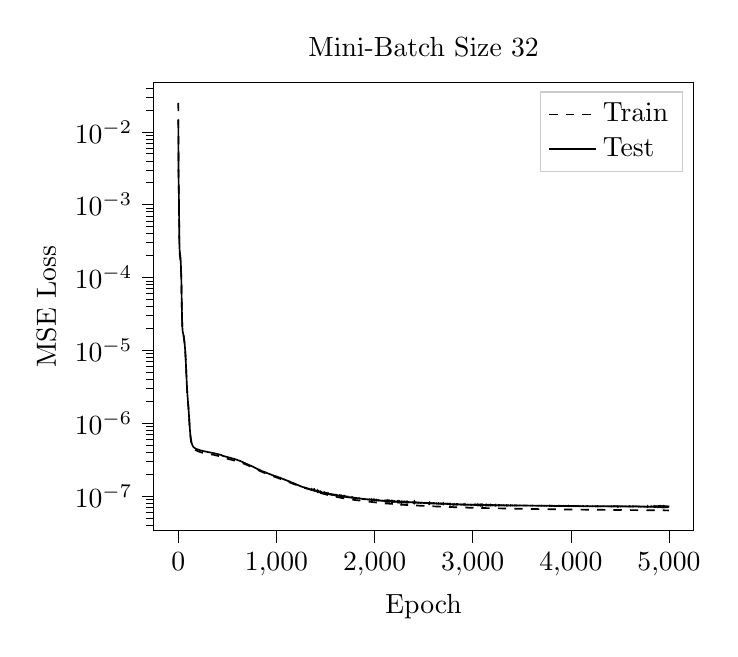
\begin{tikzpicture}

\begin{axis}[
legend cell align={left},
legend style={fill opacity=0.8, draw opacity=1, text opacity=1, draw=white!80!black},
log basis y={10},
tick align=outside,
tick pos=left,
title={Mini-Batch Size 32},
x grid style={white!69.0196078431373!black},
xlabel={Epoch},
xmin=-249.95, xmax=5248.95,
xtick style={color=black},
y grid style={white!69.0196078431373!black},
ylabel={MSE Loss},
ymin=3.32479738039568e-08, ymax=0.0475297845104396,
ymode=log,
ytick style={color=black}
]
\addplot [semithick, black, dashed]
table {%
0 0.02495651832968
1 0.00961011469736695
2 0.00413097363337874
3 0.00244306252896786
4 0.00193028736487031
5 0.00166280910652131
6 0.00138447313569486
7 0.00107641329290345
8 0.000778393224813044
9 0.000544353197561577
10 0.000392122417106293
11 0.000303274053148925
12 0.000255969762103632
13 0.000230607165722176
14 0.000215886180754751
15 0.000206437844899483
16 0.000199756111484021
17 0.000194554485875415
18 0.00019007718397188
19 0.000185448877629824
20 0.000179887956794119
21 0.000174710482853698
22 0.000169107335037552
23 0.000162899194285274
24 0.00015598142152885
25 0.000148279041866772
26 0.000139756958815269
27 0.000130426560644992
28 0.000120360163913574
29 0.00010970869952871
30 9.87046422960702e-05
31 8.76457903214032e-05
32 7.59790178271942e-05
33 6.32417565939249e-05
34 5.32707560923882e-05
35 4.49569480624632e-05
36 3.78300976517494e-05
37 3.23423087465926e-05
38 2.81909803452436e-05
39 2.50878785045643e-05
40 2.2796041041147e-05
41 2.11196904419921e-05
42 1.99011574259202e-05
43 1.90164594532689e-05
44 1.83700865381979e-05
45 1.78898700614809e-05
46 1.75224826816702e-05
47 1.72282880739658e-05
48 1.6979464176984e-05
49 1.67564551920805e-05
50 1.65459687414113e-05
51 1.6338135672413e-05
52 1.61253468395444e-05
53 1.59003820699581e-05
54 1.56591943941748e-05
55 1.53970238516195e-05
56 1.5111974962565e-05
57 1.48010985449218e-05
58 1.44654920004541e-05
59 1.41105859675008e-05
60 1.37506305291026e-05
61 1.34037461448315e-05
62 1.30508453003131e-05
63 1.26842860190663e-05
64 1.22990531144751e-05
65 1.18971542233339e-05
66 1.14834407868329e-05
67 1.10633895365027e-05
68 1.06573821649363e-05
69 1.02501706805924e-05
70 9.83167694175791e-06
71 9.40211800116231e-06
72 8.96312386976206e-06
73 8.51743346720468e-06
74 8.06758649014227e-06
75 7.59200016727846e-06
76 7.13813932543417e-06
77 6.69677184578177e-06
78 6.26769952486939e-06
79 5.85447091452806e-06
80 5.4597814068984e-06
81 5.0853698676292e-06
82 4.73458306623797e-06
83 4.40776282039224e-06
84 4.10157791611709e-06
85 3.81505160430606e-06
86 3.54804463950131e-06
87 3.30647863347622e-06
88 3.10206145877601e-06
89 2.92757145348332e-06
90 2.7743954374273e-06
91 2.63919908547905e-06
92 2.51793273764633e-06
93 2.40874294013338e-06
94 2.30932277190732e-06
95 2.21750755531502e-06
96 2.13223388277584e-06
97 2.0520963821582e-06
98 1.97619329605914e-06
99 1.90301633915624e-06
100 1.83207415443576e-06
101 1.76289627052029e-06
102 1.69469857723925e-06
103 1.62764035917462e-06
104 1.56192980011838e-06
105 1.49679244555045e-06
106 1.43174119580181e-06
107 1.36744359906515e-06
108 1.30400344164627e-06
109 1.24207295220913e-06
110 1.18228974997692e-06
111 1.12450982669543e-06
112 1.06910858767151e-06
113 1.01688769291286e-06
114 9.67930212027568e-07
115 9.22251022871023e-07
116 8.79566746561977e-07
117 8.40306190184492e-07
118 8.04245244808044e-07
119 7.71177175010962e-07
120 7.41038618912171e-07
121 7.1362072969805e-07
122 6.88738398139321e-07
123 6.6626371460643e-07
124 6.45955492018402e-07
125 6.27467571803209e-07
126 6.10727049888737e-07
127 5.95464798720968e-07
128 5.81586706289272e-07
129 5.68973892995928e-07
130 5.57506997097334e-07
131 5.47159624034066e-07
132 5.37807409841662e-07
133 5.2926190164726e-07
134 5.21498524221897e-07
135 5.14374786007465e-07
136 5.07893223357314e-07
137 5.01906526437779e-07
138 4.96731676548734e-07
139 4.91929263944257e-07
140 4.87304183479864e-07
141 4.83395513128926e-07
142 4.79628468383453e-07
143 4.75905103257901e-07
144 4.72772012926725e-07
145 4.69776906811603e-07
146 4.66785132857694e-07
147 4.64381218307608e-07
148 4.61841564515453e-07
149 4.59599604482719e-07
150 4.57548463828061e-07
151 4.55566183518386e-07
152 4.5392076447115e-07
153 4.51969018911313e-07
154 4.50402194132948e-07
155 4.48862345024281e-07
156 4.47213856375583e-07
157 4.45904424793753e-07
158 4.44331068820247e-07
159 4.43094038587333e-07
160 4.41832931983299e-07
161 4.40487454568483e-07
162 4.39438358228017e-07
163 4.38247122474422e-07
164 4.37372409010095e-07
165 4.36215690626796e-07
166 4.35179460907875e-07
167 4.34115043049133e-07
168 4.33094739207718e-07
169 4.32249056416367e-07
170 4.31389237974145e-07
171 4.3049158989561e-07
172 4.29718726650208e-07
173 4.28816658768483e-07
174 4.28031429521525e-07
175 4.27186655770129e-07
176 4.2643471010706e-07
177 4.25704145925465e-07
178 4.249236461078e-07
179 4.24175198304511e-07
180 4.23381138261902e-07
181 4.22704758591408e-07
182 4.2203296942489e-07
183 4.21413327728715e-07
184 4.20808965429842e-07
185 4.20218811370887e-07
186 4.19534650461628e-07
187 4.18957539409348e-07
188 4.18323923383923e-07
189 4.17785641616319e-07
190 4.17157342269547e-07
191 4.16574300402317e-07
192 4.16100292227384e-07
193 4.15515923918974e-07
194 4.14969112057406e-07
195 4.14372878424274e-07
196 4.13821521419777e-07
197 4.13151100246978e-07
198 4.12587816981613e-07
199 4.12000607070695e-07
200 4.11486135533323e-07
201 4.10908738501803e-07
202 4.10366602693557e-07
203 4.09846317552365e-07
204 4.09321734537116e-07
205 4.08823070813469e-07
206 4.08338844749778e-07
207 4.07859870051652e-07
208 4.0738508960203e-07
209 4.06924520632401e-07
210 4.06487470229422e-07
211 4.06054145514645e-07
212 4.05625210134986e-07
213 4.05178532389527e-07
214 4.04790528932608e-07
215 4.04352993655266e-07
216 4.03935589872617e-07
217 4.03488432255017e-07
218 4.03000148480714e-07
219 4.0252821776221e-07
220 4.02079318746473e-07
221 4.01636666595095e-07
222 4.01267719155385e-07
223 4.00860508079859e-07
224 4.0039540243697e-07
225 4.00016974367645e-07
226 3.99598319916095e-07
227 3.99353811303627e-07
228 3.98807296733139e-07
229 3.9849614341847e-07
230 3.98027829987768e-07
231 3.97661151964712e-07
232 3.97296741425635e-07
233 3.96933670458566e-07
234 3.96692654078379e-07
235 3.96237260304133e-07
236 3.95832837398302e-07
237 3.95548122298806e-07
238 3.9531681943572e-07
239 3.94950389136284e-07
240 3.9467049475661e-07
241 3.94235885494254e-07
242 3.9394514868718e-07
243 3.93687027838041e-07
244 3.93292611079232e-07
245 3.93052761353374e-07
246 3.92778083551093e-07
247 3.92502728800537e-07
248 3.92133861623734e-07
249 3.92215017939179e-07
250 3.91586018395174e-07
251 3.91571693910464e-07
252 3.91166603037618e-07
253 3.90866849613758e-07
254 3.90592485246088e-07
255 3.90450265342679e-07
256 3.90059337291859e-07
257 3.89795861224229e-07
258 3.89615875803884e-07
259 3.89345471262459e-07
260 3.88936012143404e-07
261 3.88858161613825e-07
262 3.88568784956078e-07
263 3.88315720897481e-07
264 3.88009818891533e-07
265 3.87716299258045e-07
266 3.87435602533515e-07
267 3.87198704800085e-07
268 3.87095901544399e-07
269 3.86833256129648e-07
270 3.86513266903421e-07
271 3.86314359332118e-07
272 3.86197026159607e-07
273 3.85857046524052e-07
274 3.85734699932527e-07
275 3.85417266727472e-07
276 3.85191937766649e-07
277 3.84964709098767e-07
278 3.84747363227689e-07
279 3.84521832245355e-07
280 3.84317370048848e-07
281 3.84164355864414e-07
282 3.83867334505794e-07
283 3.8373292528604e-07
284 3.83425168422491e-07
285 3.83283067776574e-07
286 3.82983800932379e-07
287 3.82833136825411e-07
288 3.82552692087756e-07
289 3.82440776093063e-07
290 3.8212854167341e-07
291 3.81949822269689e-07
292 3.81690230824461e-07
293 3.81576880215562e-07
294 3.81239045339044e-07
295 3.81128543835985e-07
296 3.8072972580494e-07
297 3.8063195961513e-07
298 3.80266395382023e-07
299 3.801756307098e-07
300 3.79826189202959e-07
301 3.79754168477575e-07
302 3.79314871622682e-07
303 3.7919400182318e-07
304 3.78852980531974e-07
305 3.78635408196715e-07
306 3.78482517476186e-07
307 3.78186378839018e-07
308 3.78049293374261e-07
309 3.77755144313596e-07
310 3.77626213719395e-07
311 3.77323337716007e-07
312 3.77180442285407e-07
313 3.76884721106308e-07
314 3.76761206041465e-07
315 3.76456654066715e-07
316 3.76322360295944e-07
317 3.76020554256229e-07
318 3.75878518070749e-07
319 3.75583821380587e-07
320 3.75444035285e-07
321 3.75157911889801e-07
322 3.74941874213164e-07
323 3.74769378709061e-07
324 3.74537868879088e-07
325 3.74325883058191e-07
326 3.74114356759492e-07
327 3.7398155336632e-07
328 3.73691593438252e-07
329 3.73479032305113e-07
330 3.73263141057123e-07
331 3.73148577864413e-07
332 3.72937396434736e-07
333 3.72726407761093e-07
334 3.72512641376943e-07
335 3.7229352437862e-07
336 3.72073721962352e-07
337 3.71858890559906e-07
338 3.71637403759451e-07
339 3.71423307171881e-07
340 3.71199119911125e-07
341 3.71018680311863e-07
342 3.70781483240989e-07
343 3.70566273147688e-07
344 3.70327734970033e-07
345 3.70107448759427e-07
346 3.69865037782802e-07
347 3.69644855766182e-07
348 3.69412776421996e-07
349 3.69197943371091e-07
350 3.68972107764876e-07
351 3.68760632113663e-07
352 3.68530030186776e-07
353 3.68305152392168e-07
354 3.68066383600763e-07
355 3.67879488521794e-07
356 3.67639851447166e-07
357 3.67394399120258e-07
358 3.67129990991089e-07
359 3.66913512834799e-07
360 3.66670797916413e-07
361 3.66439876643199e-07
362 3.66214438940915e-07
363 3.65958968757241e-07
364 3.65716883436562e-07
365 3.65472255680288e-07
366 3.65235946276243e-07
367 3.65003734827951e-07
368 3.64790364415057e-07
369 3.64554488896829e-07
370 3.64337830490058e-07
371 3.64075158586274e-07
372 3.63818008281669e-07
373 3.63561922938516e-07
374 3.63086586332884e-07
375 3.62677517500742e-07
376 3.62481707497864e-07
377 3.62175591874347e-07
378 3.61958059102108e-07
379 3.61694926596101e-07
380 3.61477443789227e-07
381 3.61189488785385e-07
382 3.60908989648578e-07
383 3.60632151227946e-07
384 3.60374613592285e-07
385 3.60127789861053e-07
386 3.59889722290063e-07
387 3.59648303003723e-07
388 3.59391540257548e-07
389 3.59136226052215e-07
390 3.58878930228457e-07
391 3.58624317300382e-07
392 3.58370782862494e-07
393 3.58117538553415e-07
394 3.57864312945821e-07
395 3.57614250845018e-07
396 3.57365321292491e-07
397 3.57220161561145e-07
398 3.5695572972827e-07
399 3.56697081485891e-07
400 3.56451138884495e-07
401 3.56231862042478e-07
402 3.55987368379829e-07
403 3.55719761046203e-07
404 3.5545431620676e-07
405 3.5519427149211e-07
406 3.54937200029326e-07
407 3.54679559450233e-07
408 3.54435099382044e-07
409 3.54180049441766e-07
410 3.53914030540636e-07
411 3.53637977070775e-07
412 3.53316532880399e-07
413 3.52996593903754e-07
414 3.52692684771227e-07
415 3.52370906625765e-07
416 3.52031887359772e-07
417 3.51736728305241e-07
418 3.51416265061744e-07
419 3.51078242658787e-07
420 3.50801819763546e-07
421 3.50483696763604e-07
422 3.50188840911869e-07
423 3.49898358535938e-07
424 3.49607736438884e-07
425 3.49336570877767e-07
426 3.49044006611621e-07
427 3.48772838549394e-07
428 3.48493419096485e-07
429 3.48202210432191e-07
430 3.47910864888945e-07
431 3.47652583513991e-07
432 3.47363370451603e-07
433 3.47088898820402e-07
434 3.46819799403875e-07
435 3.46554175678193e-07
436 3.46236901521024e-07
437 3.4594818282585e-07
438 3.456587755295e-07
439 3.45374959806577e-07
440 3.4508889979179e-07
441 3.44819731481039e-07
442 3.43527665961574e-07
443 3.41568904218548e-07
444 3.40458649645825e-07
445 3.39691413955734e-07
446 3.39104159309045e-07
447 3.38657587406033e-07
448 3.3826774966883e-07
449 3.37910868381641e-07
450 3.37583903274208e-07
451 3.37335791755322e-07
452 3.37002327455593e-07
453 3.36683525176795e-07
454 3.36382677573965e-07
455 3.36085746255321e-07
456 3.35797085199374e-07
457 3.35507281363334e-07
458 3.35228495998763e-07
459 3.34947825706422e-07
460 3.34685688301306e-07
461 3.34399860150825e-07
462 3.34131951490235e-07
463 3.33938054097871e-07
464 3.33655134454602e-07
465 3.33373461614883e-07
466 3.33097741190613e-07
467 3.32827610804998e-07
468 3.32557599733718e-07
469 3.32289230129845e-07
470 3.32023381133695e-07
471 3.31758974482454e-07
472 3.31498622188064e-07
473 3.31243115965663e-07
474 3.30986639767161e-07
475 3.30725981314117e-07
476 3.30465711044781e-07
477 3.30213596555495e-07
478 3.29964917227699e-07
479 3.29708751735325e-07
480 3.29451019297267e-07
481 3.29205599769011e-07
482 3.28950098946734e-07
483 3.28694641950733e-07
484 3.28439770896693e-07
485 3.28183799865656e-07
486 3.2792898457501e-07
487 3.27676344568317e-07
488 3.27425882460375e-07
489 3.27171232186174e-07
490 3.26920304075884e-07
491 3.26669060086715e-07
492 3.26414687492615e-07
493 3.26167206196715e-07
494 3.25921365174509e-07
495 3.25667093875381e-07
496 3.25417923534133e-07
497 3.25166869117766e-07
498 3.24911161271757e-07
499 3.24661909530732e-07
500 3.24411729934582e-07
501 3.24163918492104e-07
502 3.23916323793583e-07
503 3.23667571478836e-07
504 3.23418650452822e-07
505 3.2316933356924e-07
506 3.22912537569664e-07
507 3.22677076326272e-07
508 3.22424684043199e-07
509 3.22175117048573e-07
510 3.21921278214177e-07
511 3.21676903240586e-07
512 3.2141999616897e-07
513 3.21168492916968e-07
514 3.20919341902481e-07
515 3.20672617419859e-07
516 3.20425436939331e-07
517 3.20178708705043e-07
518 3.19927367741002e-07
519 3.19677120899087e-07
520 3.19433100514743e-07
521 3.1918317591817e-07
522 3.18933754613226e-07
523 3.18682645513491e-07
524 3.18430878110121e-07
525 3.18188869869118e-07
526 3.17935760620003e-07
527 3.17688921199988e-07
528 3.17438041292917e-07
529 3.17189871054779e-07
530 3.16941071673682e-07
531 3.16688110899577e-07
532 3.16435692639061e-07
533 3.16183294444272e-07
534 3.15933932711232e-07
535 3.15678637605288e-07
536 3.15416349053521e-07
537 3.15168398003607e-07
538 3.14918423271138e-07
539 3.14665876146591e-07
540 3.1441218487771e-07
541 3.14162874758495e-07
542 3.13908628925219e-07
543 3.1365879385703e-07
544 3.13401772416455e-07
545 3.13141272272333e-07
546 3.12895501167532e-07
547 3.12642150618103e-07
548 3.12390568126375e-07
549 3.12136429840848e-07
550 3.11886598012734e-07
551 3.11629494319732e-07
552 3.11372858220693e-07
553 3.11120544779442e-07
554 3.10865378139624e-07
555 3.10597321572459e-07
556 3.10337305961639e-07
557 3.10062468656724e-07
558 3.09783668569708e-07
559 3.09533397796713e-07
560 3.0925890234812e-07
561 3.08991336623876e-07
562 3.08718985195355e-07
563 3.08452851072616e-07
564 3.08193646958443e-07
565 3.07925223182792e-07
566 3.07654694040593e-07
567 3.07384176949199e-07
568 3.07108701520065e-07
569 3.06854335121898e-07
570 3.06586367912587e-07
571 3.06315510670174e-07
572 3.06044467208721e-07
573 3.05774523894797e-07
574 3.05507066229893e-07
575 3.05238351586468e-07
576 3.04966125554529e-07
577 3.04701247387129e-07
578 3.04435839666439e-07
579 3.04167043907455e-07
580 3.03899193966117e-07
581 3.03642611072519e-07
582 3.03365975128145e-07
583 3.03105798934666e-07
584 3.02834642923244e-07
585 3.02562915123872e-07
586 3.02293688037025e-07
587 3.02023441690835e-07
588 3.01750427922798e-07
589 3.01468936697802e-07
590 3.01194206201671e-07
591 3.00920173913255e-07
592 3.00651897475746e-07
593 3.00374632217881e-07
594 3.0010006497605e-07
595 2.99823589671178e-07
596 2.99549067733551e-07
597 2.99274745032108e-07
598 2.98989832003826e-07
599 2.98707233980622e-07
600 2.98429238455356e-07
601 2.98149015691251e-07
602 2.97851940217697e-07
603 2.97572810723068e-07
604 2.97288175488575e-07
605 2.97004070830553e-07
606 2.96717658386569e-07
607 2.96432424136128e-07
608 2.96132169864904e-07
609 2.95851490818677e-07
610 2.9555990550989e-07
611 2.95269672562881e-07
612 2.94977329076573e-07
613 2.94648021451849e-07
614 2.94372223493156e-07
615 2.94079964135108e-07
616 2.93786541419649e-07
617 2.93504731644134e-07
618 2.93208564869474e-07
619 2.92913382963889e-07
620 2.92618357491392e-07
621 2.92318298079408e-07
622 2.92027666887407e-07
623 2.91726333330189e-07
624 2.91427586944337e-07
625 2.91127002071789e-07
626 2.90825883325851e-07
627 2.90517562405057e-07
628 2.90214898711838e-07
629 2.89916120095768e-07
630 2.89617872113013e-07
631 2.89310944253884e-07
632 2.89006251421142e-07
633 2.88701059901086e-07
634 2.88395490997573e-07
635 2.88085441013664e-07
636 2.87784689248838e-07
637 2.87473759783552e-07
638 2.87163604639318e-07
639 2.8685427776054e-07
640 2.86543671734307e-07
641 2.86232358746474e-07
642 2.8591167159675e-07
643 2.85608766034784e-07
644 2.85282987647406e-07
645 2.84961197735356e-07
646 2.84647514035896e-07
647 2.84332860530867e-07
648 2.84016698174128e-07
649 2.83695652342431e-07
650 2.83384992542324e-07
651 2.83056953890082e-07
652 2.82736495591962e-07
653 2.82414473304016e-07
654 2.82090383393552e-07
655 2.81754234094933e-07
656 2.814381865619e-07
657 2.81109553952774e-07
658 2.80781508934069e-07
659 2.80458499162251e-07
660 2.80133726619169e-07
661 2.79791232117077e-07
662 2.79459573619079e-07
663 2.79132003811355e-07
664 2.78810577128752e-07
665 2.78483527097251e-07
666 2.78156543458863e-07
667 2.77828672494707e-07
668 2.77494331385242e-07
669 2.77161416363469e-07
670 2.76837326168788e-07
671 2.76499529377361e-07
672 2.7616509672157e-07
673 2.75824009491998e-07
674 2.75484910588375e-07
675 2.75151122167472e-07
676 2.74813070546998e-07
677 2.74484228981464e-07
678 2.74141751759771e-07
679 2.73801236460258e-07
680 2.7346256743499e-07
681 2.7312098310972e-07
682 2.72778246738881e-07
683 2.72445175511393e-07
684 2.72102593726231e-07
685 2.71760970917967e-07
686 2.71409479864815e-07
687 2.71066047901058e-07
688 2.70712768099202e-07
689 2.70363464949241e-07
690 2.70028888536444e-07
691 2.69678203579815e-07
692 2.69323093846197e-07
693 2.68982534151974e-07
694 2.68629582905078e-07
695 2.68276261408573e-07
696 2.67924870684055e-07
697 2.67573593077941e-07
698 2.67221852908506e-07
699 2.66867869385123e-07
700 2.66521415994703e-07
701 2.66156414824081e-07
702 2.65806567256277e-07
703 2.65454764019069e-07
704 2.65109429761878e-07
705 2.64751923481299e-07
706 2.64394460657513e-07
707 2.64046319188083e-07
708 2.63686914905747e-07
709 2.63330481487856e-07
710 2.62976001152992e-07
711 2.62624411874413e-07
712 2.62268526427079e-07
713 2.61783545539629e-07
714 2.61365144609726e-07
715 2.60963426995886e-07
716 2.60568118960691e-07
717 2.60185761845833e-07
718 2.59804836076682e-07
719 2.59431001921939e-07
720 2.5905343719046e-07
721 2.58663268255077e-07
722 2.582953289334e-07
723 2.57919991497602e-07
724 2.57542056175453e-07
725 2.57166950035526e-07
726 2.56791996605443e-07
727 2.56411861045081e-07
728 2.56032386488414e-07
729 2.55650504385585e-07
730 2.55268005901144e-07
731 2.54897504419205e-07
732 2.54530858313728e-07
733 2.54164709417637e-07
734 2.53788540817368e-07
735 2.53397368908281e-07
736 2.53038564181907e-07
737 2.52672190839576e-07
738 2.52298251467664e-07
739 2.51924601002429e-07
740 2.51546983491835e-07
741 2.51169815754793e-07
742 2.50795577386498e-07
743 2.50415323222342e-07
744 2.50047310686341e-07
745 2.49675453261489e-07
746 2.49290693403736e-07
747 2.48922245219774e-07
748 2.48538268721177e-07
749 2.48168420881711e-07
750 2.47817149841012e-07
751 2.47453885549476e-07
752 2.47091088169782e-07
753 2.46722569528401e-07
754 2.46367280141158e-07
755 2.46005374407332e-07
756 2.45634985702736e-07
757 2.45285960744468e-07
758 2.4491997467635e-07
759 2.44556270928342e-07
760 2.44214170720625e-07
761 2.43849069136104e-07
762 2.4350010477292e-07
763 2.43144235810178e-07
764 2.4278854266413e-07
765 2.42424769908212e-07
766 2.42078545369395e-07
767 2.41720167252879e-07
768 2.41373975711667e-07
769 2.41012750223035e-07
770 2.40668308805425e-07
771 2.40300879937649e-07
772 2.39962240783598e-07
773 2.39611582998123e-07
774 2.39262748976898e-07
775 2.38921268277181e-07
776 2.38583462419228e-07
777 2.38232236142721e-07
778 2.37897271148313e-07
779 2.37553327167461e-07
780 2.3720731402932e-07
781 2.36865277344123e-07
782 2.36524948576289e-07
783 2.36184086332969e-07
784 2.35843451463325e-07
785 2.35504933328912e-07
786 2.35151212137907e-07
787 2.34817503297791e-07
788 2.34487555559326e-07
789 2.34151290726459e-07
790 2.33816716018964e-07
791 2.33480007750586e-07
792 2.3313596361163e-07
793 2.32800076275907e-07
794 2.32479550533071e-07
795 2.32147196612686e-07
796 2.31827768146786e-07
797 2.31500280790442e-07
798 2.31171276794839e-07
799 2.30842491873773e-07
800 2.30517275696229e-07
801 2.30192814683505e-07
802 2.29869153912432e-07
803 2.2954598213687e-07
804 2.29225299761993e-07
805 2.28896955889013e-07
806 2.285750721569e-07
807 2.28251312620387e-07
808 2.27920705242468e-07
809 2.27587773196092e-07
810 2.27261611883023e-07
811 2.26937173209762e-07
812 2.26590815117333e-07
813 2.26248852271738e-07
814 2.2592678689648e-07
815 2.25604274504576e-07
816 2.25289613268842e-07
817 2.24968429591854e-07
818 2.2464190789151e-07
819 2.24330271180406e-07
820 2.24015665537536e-07
821 2.23695802048951e-07
822 2.23378607273617e-07
823 2.23059963758487e-07
824 2.22751312179525e-07
825 2.22437908604434e-07
826 2.22128579935088e-07
827 2.21818073327995e-07
828 2.21512779432942e-07
829 2.21207509355281e-07
830 2.20896412486127e-07
831 2.20601544469901e-07
832 2.20299285331293e-07
833 2.19998179005643e-07
834 2.19698332529106e-07
835 2.19399085636951e-07
836 2.19101591312665e-07
837 2.18805903045904e-07
838 2.18508435153808e-07
839 2.18213898335762e-07
840 2.17915977884786e-07
841 2.17629355546478e-07
842 2.17336306803872e-07
843 2.17043057830324e-07
844 2.16744821671e-07
845 2.16444015222805e-07
846 2.16176255520395e-07
847 2.15886601779403e-07
848 2.1559624806855e-07
849 2.1530761821964e-07
850 2.1501409122493e-07
851 2.14728265518715e-07
852 2.14442566999651e-07
853 2.14159017104976e-07
854 2.1387635089809e-07
855 2.13591160445503e-07
856 2.13313837718943e-07
857 2.13033253203321e-07
858 2.12747139443081e-07
859 2.12453791277767e-07
860 2.12168521272815e-07
861 2.11889834901058e-07
862 2.11607884637033e-07
863 2.11334886728309e-07
864 2.11090787132662e-07
865 2.10781402245175e-07
866 2.10493931831479e-07
867 2.10228466983153e-07
868 2.0995736332452e-07
869 2.09710962110421e-07
870 2.09454804121378e-07
871 2.09155657302063e-07
872 2.0889265621804e-07
873 2.08615227649034e-07
874 2.0835879496417e-07
875 2.08125936779879e-07
876 2.0784095644899e-07
877 2.07578632455352e-07
878 2.07306310045396e-07
879 2.07051195502572e-07
880 2.06805247216835e-07
881 2.06557984341771e-07
882 2.06271035807504e-07
883 2.06015276461358e-07
884 2.05758761353536e-07
885 2.05502702499416e-07
886 2.05257287603899e-07
887 2.05018618203212e-07
888 2.04749223087219e-07
889 2.04492583435467e-07
890 2.04243722151887e-07
891 2.04015699040383e-07
892 2.0376250037657e-07
893 2.03499224738835e-07
894 2.03230061998738e-07
895 2.02984433769871e-07
896 2.02760471012198e-07
897 2.02495798191649e-07
898 2.02252525838276e-07
899 2.02054798563722e-07
900 2.01795910925284e-07
901 2.0155783280984e-07
902 2.01303102727479e-07
903 2.010459269286e-07
904 2.00793724928872e-07
905 2.00542965529849e-07
906 2.00282583818989e-07
907 2.00041654409233e-07
908 1.99805434363043e-07
909 1.99518635383811e-07
910 1.99275372921193e-07
911 1.99030435169334e-07
912 1.98785222437436e-07
913 1.98562560171922e-07
914 1.98301664795508e-07
915 1.980731424851e-07
916 1.97822975650297e-07
917 1.97587865756077e-07
918 1.97393529134615e-07
919 1.97119730415807e-07
920 1.96893812670851e-07
921 1.96664078941922e-07
922 1.96433929062323e-07
923 1.96070164463436e-07
924 1.95796074820009e-07
925 1.95405372153346e-07
926 1.95464035442683e-07
927 1.95107122721083e-07
928 1.9491377003078e-07
929 1.94789499147419e-07
930 1.94626016821076e-07
931 1.9450656171216e-07
932 1.94023198787363e-07
933 1.93969802921856e-07
934 1.93786689152375e-07
935 1.93560784936153e-07
936 1.93339261500114e-07
937 1.93128177670587e-07
938 1.93026661719387e-07
939 1.92640885813944e-07
940 1.92422838779294e-07
941 1.92281713538023e-07
942 1.92034399532304e-07
943 1.91720221721425e-07
944 1.91571368333143e-07
945 1.91369630329064e-07
946 1.91159158362098e-07
947 1.90935840663542e-07
948 1.90733979053448e-07
949 1.90504907777722e-07
950 1.90282767846384e-07
951 1.90062591201467e-07
952 1.89852125288326e-07
953 1.89639431653177e-07
954 1.89416469254411e-07
955 1.89172260149917e-07
956 1.88981291074697e-07
957 1.88770511613257e-07
958 1.88574910339412e-07
959 1.88355372273463e-07
960 1.88127187925602e-07
961 1.87908308106444e-07
962 1.87683726238674e-07
963 1.87484382848879e-07
964 1.87297403499542e-07
965 1.87063760563433e-07
966 1.86876632227495e-07
967 1.86646165531101e-07
968 1.86456403355351e-07
969 1.86208237039409e-07
970 1.86007684220613e-07
971 1.85791245456812e-07
972 1.85590365447297e-07
973 1.85390133793817e-07
974 1.85175619606071e-07
975 1.84960244524746e-07
976 1.8474065629448e-07
977 1.84525042442374e-07
978 1.84285813105589e-07
979 1.8398711713985e-07
980 1.83779480011026e-07
981 1.83560364746427e-07
982 1.83339712037878e-07
983 1.83136822073493e-07
984 1.82914183056937e-07
985 1.82705784453674e-07
986 1.82525461809746e-07
987 1.82288409973808e-07
988 1.82090955490821e-07
989 1.81869196524076e-07
990 1.81646533434332e-07
991 1.8146373204786e-07
992 1.81239095780938e-07
993 1.81107638809408e-07
994 1.80800074360832e-07
995 1.80589863930436e-07
996 1.80380842181194e-07
997 1.80184061349564e-07
998 1.79971024039105e-07
999 1.79740983853094e-07
1000 1.79529651802568e-07
1001 1.79349143863305e-07
1002 1.79174995381004e-07
1003 1.78974283542743e-07
1004 1.78781240805392e-07
1005 1.78549073396539e-07
1006 1.78336786788691e-07
1007 1.78155590916163e-07
1008 1.77893159715836e-07
1009 1.77646469182946e-07
1010 1.7745657291357e-07
1011 1.77252783856829e-07
1012 1.77015252276647e-07
1013 1.76848480464287e-07
1014 1.76649309651111e-07
1015 1.76437214165048e-07
1016 1.76228822397206e-07
1017 1.7603968427693e-07
1018 1.7580710276377e-07
1019 1.75630667200721e-07
1020 1.75404448583549e-07
1021 1.75205468949002e-07
1022 1.75017376562892e-07
1023 1.74781506913746e-07
1024 1.74596366690594e-07
1025 1.74384998828714e-07
1026 1.74188079640203e-07
1027 1.73981591217398e-07
1028 1.7378087360953e-07
1029 1.73595396333326e-07
1030 1.73383527979354e-07
1031 1.73204570458552e-07
1032 1.72982506484232e-07
1033 1.72808286620807e-07
1034 1.72597720307976e-07
1035 1.72415509155144e-07
1036 1.72203957518491e-07
1037 1.72027063271685e-07
1038 1.7182273029448e-07
1039 1.71644450745134e-07
1040 1.71457249393825e-07
1041 1.71221164421809e-07
1042 1.71040073354334e-07
1043 1.7086180746162e-07
1044 1.70657180049716e-07
1045 1.70465468116276e-07
1046 1.70270329661548e-07
1047 1.70050755755824e-07
1048 1.69850164553509e-07
1049 1.69648352382978e-07
1050 1.69455070064828e-07
1051 1.69255631220722e-07
1052 1.690726047201e-07
1053 1.68867476659784e-07
1054 1.68683792978186e-07
1055 1.68497542091473e-07
1056 1.68291344607496e-07
1057 1.68094269696439e-07
1058 1.67934575713957e-07
1059 1.67707678173201e-07
1060 1.67512832220496e-07
1061 1.67310787304586e-07
1062 1.67137366844372e-07
1063 1.6695146995005e-07
1064 1.66747512679422e-07
1065 1.66526244100851e-07
1066 1.66345289741798e-07
1067 1.66170657877274e-07
1068 1.65969783139985e-07
1069 1.65793351001753e-07
1070 1.65584508224015e-07
1071 1.65399617955586e-07
1072 1.65217182740207e-07
1073 1.65030118381537e-07
1074 1.64827668044154e-07
1075 1.64635963088244e-07
1076 1.64446436073717e-07
1077 1.64266503816179e-07
1078 1.6406050147566e-07
1079 1.63849182882814e-07
1080 1.63649148930745e-07
1081 1.63488852493288e-07
1082 1.6326385798493e-07
1083 1.6307355612355e-07
1084 1.6287979563856e-07
1085 1.62693553079407e-07
1086 1.62514635448474e-07
1087 1.62316461825185e-07
1088 1.62138254225397e-07
1089 1.61947419812236e-07
1090 1.61755007738407e-07
1091 1.6156890727359e-07
1092 1.61380626408913e-07
1093 1.61192226670437e-07
1094 1.60988865758327e-07
1095 1.60817379423861e-07
1096 1.60609458916383e-07
1097 1.60432750334394e-07
1098 1.60231610422557e-07
1099 1.6002438242424e-07
1100 1.59846041128731e-07
1101 1.59648983213856e-07
1102 1.59470318820354e-07
1103 1.59276859179158e-07
1104 1.59087808611957e-07
1105 1.58903363157492e-07
1106 1.58715275489385e-07
1107 1.58518241022421e-07
1108 1.58335912828989e-07
1109 1.58143547395184e-07
1110 1.57950820351971e-07
1111 1.57779550391979e-07
1112 1.57568096639693e-07
1113 1.57373400980987e-07
1114 1.57195540481325e-07
1115 1.5701123834333e-07
1116 1.56833667531942e-07
1117 1.5667102486816e-07
1118 1.56453034335868e-07
1119 1.56287361491536e-07
1120 1.56101681994869e-07
1121 1.55895187234023e-07
1122 1.55719671283805e-07
1123 1.55538784895271e-07
1124 1.55326191844551e-07
1125 1.55147808399647e-07
1126 1.54982862397901e-07
1127 1.54775238044635e-07
1128 1.54616158710041e-07
1129 1.54435473760373e-07
1130 1.5424328991287e-07
1131 1.54069083464492e-07
1132 1.53910053441564e-07
1133 1.53697950679543e-07
1134 1.53527616859606e-07
1135 1.533198500141e-07
1136 1.53119851518113e-07
1137 1.52935787625097e-07
1138 1.52741302542836e-07
1139 1.52579434384847e-07
1140 1.5236773768379e-07
1141 1.5220379103198e-07
1142 1.51994220047413e-07
1143 1.51816173712405e-07
1144 1.51639372731438e-07
1145 1.51451178950879e-07
1146 1.51261071607678e-07
1147 1.51087167537867e-07
1148 1.50911668143294e-07
1149 1.50710834333267e-07
1150 1.5056337863939e-07
1151 1.50359926053056e-07
1152 1.50197839161592e-07
1153 1.49989610207513e-07
1154 1.49820556174518e-07
1155 1.49641965904834e-07
1156 1.49468162561561e-07
1157 1.49292503422771e-07
1158 1.49116801964055e-07
1159 1.48950404266657e-07
1160 1.48749289834882e-07
1161 1.48601293474826e-07
1162 1.4840983980946e-07
1163 1.48245427084248e-07
1164 1.48058577806864e-07
1165 1.47897300550426e-07
1166 1.47732717977078e-07
1167 1.47551893320497e-07
1168 1.47386523991599e-07
1169 1.47253489771515e-07
1170 1.47079867105049e-07
1171 1.46910625673513e-07
1172 1.46717061582535e-07
1173 1.46561715538951e-07
1174 1.46381869910783e-07
1175 1.46196347913019e-07
1176 1.46053862195572e-07
1177 1.45873883198533e-07
1178 1.4569988150015e-07
1179 1.45549741915829e-07
1180 1.45423148239843e-07
1181 1.45259941163545e-07
1182 1.45065910132303e-07
1183 1.44896643561765e-07
1184 1.44713919794981e-07
1185 1.44527575216102e-07
1186 1.44360318273584e-07
1187 1.44184542804737e-07
1188 1.44045858604613e-07
1189 1.438265138205e-07
1190 1.43651753361951e-07
1191 1.43501514173749e-07
1192 1.43298794270663e-07
1193 1.43153612597757e-07
1194 1.4296911790268e-07
1195 1.42841563288698e-07
1196 1.42663490450445e-07
1197 1.4251093796247e-07
1198 1.4235067521895e-07
1199 1.42198025784523e-07
1200 1.42016979083337e-07
1201 1.41888084428388e-07
1202 1.41697094491633e-07
1203 1.41577890346412e-07
1204 1.41393103675114e-07
1205 1.41244608073521e-07
1206 1.41101936833365e-07
1207 1.40972664482319e-07
1208 1.40802412559538e-07
1209 1.40652948857678e-07
1210 1.40490155388306e-07
1211 1.40351003068417e-07
1212 1.40189484227449e-07
1213 1.40045975115299e-07
1214 1.39892311622702e-07
1215 1.39742217299954e-07
1216 1.39631110755545e-07
1217 1.39471335202757e-07
1218 1.39296424720214e-07
1219 1.39116599001454e-07
1220 1.38933887228632e-07
1221 1.38783278018195e-07
1222 1.38606553406362e-07
1223 1.38454287537115e-07
1224 1.38285695726381e-07
1225 1.38140692769184e-07
1226 1.37973613220765e-07
1227 1.37823302551965e-07
1228 1.37674810602562e-07
1229 1.37553393670942e-07
1230 1.37401118337266e-07
1231 1.37227740324875e-07
1232 1.37065262151737e-07
1233 1.36896728918146e-07
1234 1.36755918703102e-07
1235 1.36620547863231e-07
1236 1.36478319333833e-07
1237 1.3629528817205e-07
1238 1.36187348502403e-07
1239 1.36021234595773e-07
1240 1.35825211785345e-07
1241 1.35717902182364e-07
1242 1.35625156744368e-07
1243 1.35405121184817e-07
1244 1.35297192116468e-07
1245 1.35218753271715e-07
1246 1.3499267492989e-07
1247 1.34912699735423e-07
1248 1.34714162555838e-07
1249 1.34535898752119e-07
1250 1.34413323394256e-07
1251 1.34261244909339e-07
1252 1.34086616697004e-07
1253 1.33964697695887e-07
1254 1.33804411674987e-07
1255 1.33696845480813e-07
1256 1.33536486785601e-07
1257 1.33391707365149e-07
1258 1.33322690516025e-07
1259 1.3311800474014e-07
1260 1.33000473525158e-07
1261 1.32811080234774e-07
1262 1.32611858703058e-07
1263 1.32472028354869e-07
1264 1.32310696272953e-07
1265 1.32206344474639e-07
1266 1.3208011404231e-07
1267 1.31943520571554e-07
1268 1.31795420301728e-07
1269 1.31649313971138e-07
1270 1.31523647922904e-07
1271 1.31398229783031e-07
1272 1.312506298774e-07
1273 1.31094378815533e-07
1274 1.30956317235587e-07
1275 1.30837788347549e-07
1276 1.30680643621872e-07
1277 1.30560865883922e-07
1278 1.30418681806077e-07
1279 1.30291295235452e-07
1280 1.30149456609274e-07
1281 1.30038621037443e-07
1282 1.29920442674347e-07
1283 1.29731679223255e-07
1284 1.29635409621187e-07
1285 1.29512751186667e-07
1286 1.29329628606456e-07
1287 1.29202018442243e-07
1288 1.29069559051231e-07
1289 1.2898486802726e-07
1290 1.2882774468892e-07
1291 1.28720824775996e-07
1292 1.2857886679285e-07
1293 1.28424297827223e-07
1294 1.28313725184626e-07
1295 1.28197315504508e-07
1296 1.28019309741489e-07
1297 1.27923649813511e-07
1298 1.27818489289666e-07
1299 1.27705172971559e-07
1300 1.27551815268134e-07
1301 1.27394580133e-07
1302 1.27272965585234e-07
1303 1.27178841168529e-07
1304 1.27015317872292e-07
1305 1.26883552823642e-07
1306 1.26764221747067e-07
1307 1.2669873980542e-07
1308 1.26522860583123e-07
1309 1.26401847865054e-07
1310 1.26292835631148e-07
1311 1.26217790253236e-07
1312 1.26103298228486e-07
1313 1.25955086161866e-07
1314 1.25865374926093e-07
1315 1.25704670921323e-07
1316 1.25600167223183e-07
1317 1.25466895724458e-07
1318 1.25340198877666e-07
1319 1.25290738012041e-07
1320 1.25089742667228e-07
1321 1.25076840191696e-07
1322 1.24905847286527e-07
1323 1.24763893538216e-07
1324 1.24628677824035e-07
1325 1.24567537014286e-07
1326 1.24444168633886e-07
1327 1.24354348130851e-07
1328 1.24198468853365e-07
1329 1.24107469687829e-07
1330 1.23982680037216e-07
1331 1.23843915076804e-07
1332 1.23764088485245e-07
1333 1.23624078170792e-07
1334 1.23499288818607e-07
1335 1.23423793709776e-07
1336 1.23317506606213e-07
1337 1.23199710955646e-07
1338 1.23099488547496e-07
1339 1.22963613961247e-07
1340 1.22890353665639e-07
1341 1.22738475070605e-07
1342 1.22660894163573e-07
1343 1.22505690313801e-07
1344 1.22423010068928e-07
1345 1.22333123542262e-07
1346 1.22196255247786e-07
1347 1.22029892622777e-07
1348 1.21937990527954e-07
1349 1.21828086278697e-07
1350 1.21689700947059e-07
1351 1.21597475995827e-07
1352 1.21496771001262e-07
1353 1.21380652842618e-07
1354 1.21337355068363e-07
1355 1.21154499723275e-07
1356 1.21041188137383e-07
1357 1.20932061420831e-07
1358 1.20859951366015e-07
1359 1.20827881147534e-07
1360 1.20551392328139e-07
1361 1.20494800114557e-07
1362 1.20394331005969e-07
1363 1.20284697189277e-07
1364 1.20239605976735e-07
1365 1.19967289990086e-07
1366 1.19879712698889e-07
1367 1.19589959396649e-07
1368 1.19484890618082e-07
1369 1.19431536418801e-07
1370 1.19227245122033e-07
1371 1.19023371524918e-07
1372 1.18949591779938e-07
1373 1.18764290661488e-07
1374 1.1858331126291e-07
1375 1.18502960219757e-07
1376 1.18375985664443e-07
1377 1.18142158214596e-07
1378 1.18019643707612e-07
1379 1.1786775166911e-07
1380 1.1775816444981e-07
1381 1.17609677758423e-07
1382 1.17539106682329e-07
1383 1.17312982311546e-07
1384 1.17253223322678e-07
1385 1.17074167064857e-07
1386 1.17033205512485e-07
1387 1.16859827187454e-07
1388 1.16734060028989e-07
1389 1.16619709274346e-07
1390 1.16568370913228e-07
1391 1.16389317284415e-07
1392 1.16301493079618e-07
1393 1.16148065970378e-07
1394 1.1611696893965e-07
1395 1.15969928501158e-07
1396 1.15827382813904e-07
1397 1.15757941713923e-07
1398 1.1559660951832e-07
1399 1.15426822461018e-07
1400 1.15241668950716e-07
1401 1.15137877372717e-07
1402 1.15040524988785e-07
1403 1.14927153560984e-07
1404 1.14816618989266e-07
1405 1.14671704679381e-07
1406 1.14560497905813e-07
1407 1.14451417459804e-07
1408 1.1434129494603e-07
1409 1.14263045119856e-07
1410 1.14099495689857e-07
1411 1.14023870949609e-07
1412 1.13898172870108e-07
1413 1.13791865786084e-07
1414 1.13668595815852e-07
1415 1.13522275242417e-07
1416 1.13385319409076e-07
1417 1.1331290143346e-07
1418 1.13187823288285e-07
1419 1.13115875137737e-07
1420 1.12989737985458e-07
1421 1.12953337833233e-07
1422 1.12708827785468e-07
1423 1.12645159134672e-07
1424 1.12536019329923e-07
1425 1.12405675665173e-07
1426 1.12300180106217e-07
1427 1.12188127275203e-07
1428 1.12121318622371e-07
1429 1.11996009465543e-07
1430 1.11897100737224e-07
1431 1.11774235605822e-07
1432 1.11698103935964e-07
1433 1.11531534486176e-07
1434 1.11478111008978e-07
1435 1.11329388104764e-07
1436 1.11258658279212e-07
1437 1.1115090772762e-07
1438 1.11084664297323e-07
1439 1.10984017410942e-07
1440 1.10801575260666e-07
1441 1.10687577006274e-07
1442 1.10604338232179e-07
1443 1.10501115727857e-07
1444 1.10394901852828e-07
1445 1.1032890380136e-07
1446 1.10237333643681e-07
1447 1.10121136074781e-07
1448 1.09977413330853e-07
1449 1.09951087253535e-07
1450 1.09810063719351e-07
1451 1.09758461533715e-07
1452 1.09662239736963e-07
1453 1.09497194742403e-07
1454 1.09382742280673e-07
1455 1.09312407857942e-07
1456 1.09210614667177e-07
1457 1.09197754284196e-07
1458 1.09060108968606e-07
1459 1.08951768964971e-07
1460 1.08834036581129e-07
1461 1.08766704144614e-07
1462 1.0864306968017e-07
1463 1.08547738022935e-07
1464 1.08458280138279e-07
1465 1.08326441420559e-07
1466 1.08250971436519e-07
1467 1.08170419053977e-07
1468 1.08058678279122e-07
1469 1.07953138751782e-07
1470 1.07850946562849e-07
1471 1.0775997628798e-07
1472 1.07676604784501e-07
1473 1.07584272882377e-07
1474 1.07497959973557e-07
1475 1.07365853708075e-07
1476 1.07300879506056e-07
1477 1.07206992367992e-07
1478 1.07128734555317e-07
1479 1.0699486597332e-07
1480 1.06941802144433e-07
1481 1.06801656400535e-07
1482 1.0676256495401e-07
1483 1.06635918612596e-07
1484 1.06588070138969e-07
1485 1.06439732078911e-07
1486 1.06403558049806e-07
1487 1.06292979353384e-07
1488 1.06199012677166e-07
1489 1.06097226321822e-07
1490 1.06042232047798e-07
1491 1.05923881733361e-07
1492 1.05874455343269e-07
1493 1.05712708659667e-07
1494 1.05667012817889e-07
1495 1.05570254845588e-07
1496 1.05528442063019e-07
1497 1.05357816238438e-07
1498 1.05361435089435e-07
1499 1.05197208512209e-07
1500 1.05122557371828e-07
1501 1.05077539799936e-07
1502 1.04992584198271e-07
1503 1.04870362903853e-07
1504 1.04827460987167e-07
1505 1.04692996501399e-07
1506 1.04649339348839e-07
1507 1.04522807802709e-07
1508 1.04472533408284e-07
1509 1.04376210316559e-07
1510 1.04308204385006e-07
1511 1.04202900132577e-07
1512 1.0416732062879e-07
1513 1.04016187833622e-07
1514 1.03970018926702e-07
1515 1.03861404411987e-07
1516 1.03850773442105e-07
1517 1.03710708771132e-07
1518 1.03677247608402e-07
1519 1.03529306812788e-07
1520 1.03464191838043e-07
1521 1.03390828641636e-07
1522 1.03347118269426e-07
1523 1.03235040739946e-07
1524 1.03178959960815e-07
1525 1.03076528802148e-07
1526 1.03021339327825e-07
1527 1.02911607285705e-07
1528 1.02843620325643e-07
1529 1.02766095466222e-07
1530 1.0272214181839e-07
1531 1.02569817912013e-07
1532 1.0252404283051e-07
1533 1.02428453331527e-07
1534 1.02365682622008e-07
1535 1.0226671771818e-07
1536 1.02198246011653e-07
1537 1.02117307093863e-07
1538 1.02055847591487e-07
1539 1.01974345554368e-07
1540 1.01920306349257e-07
1541 1.01800982207578e-07
1542 1.01801456864337e-07
1543 1.01661986406043e-07
1544 1.01605300244501e-07
1545 1.01492929090341e-07
1546 1.01439674097037e-07
1547 1.01370416501823e-07
1548 1.01315286528347e-07
1549 1.01211626869713e-07
1550 1.01133308092471e-07
1551 1.01119409507078e-07
1552 1.00997763851751e-07
1553 1.00886110033116e-07
1554 1.00852016700514e-07
1555 1.0078210701181e-07
1556 1.00698750131301e-07
1557 1.00635722091624e-07
1558 1.0058716173944e-07
1559 1.00483966789966e-07
1560 1.00434158369467e-07
1561 1.00308884526612e-07
1562 1.00293038045152e-07
1563 1.00166602763352e-07
1564 1.00165902949811e-07
1565 1.00024583275626e-07
1566 9.99605809539616e-08
1567 9.99015559131067e-08
1568 9.98558902836066e-08
1569 9.97900875603364e-08
1570 9.96826571224574e-08
1571 9.9636051828611e-08
1572 9.95514805310904e-08
1573 9.94789107124916e-08
1574 9.94169839714232e-08
1575 9.93287031150203e-08
1576 9.92981024836581e-08
1577 9.92179098062707e-08
1578 9.9201860876974e-08
1579 9.90204627555613e-08
1580 9.89902074337579e-08
1581 9.89154325594654e-08
1582 9.88995534925152e-08
1583 9.87768667357614e-08
1584 9.87309384754553e-08
1585 9.86436824774728e-08
1586 9.85902639740743e-08
1587 9.85348354305415e-08
1588 9.85134954447631e-08
1589 9.84116751396868e-08
1590 9.83814519344151e-08
1591 9.8273330351617e-08
1592 9.82347568481146e-08
1593 9.81372914878875e-08
1594 9.80671782428999e-08
1595 9.7983344389263e-08
1596 9.79215695764424e-08
1597 9.78560754987257e-08
1598 9.78457124602983e-08
1599 9.77262493790931e-08
1600 9.76969305099828e-08
1601 9.76093921423171e-08
1602 9.75796026381204e-08
1603 9.75050640192876e-08
1604 9.74280378045478e-08
1605 9.73818507503665e-08
1606 9.72909920449183e-08
1607 9.72868249817793e-08
1608 9.71697913030312e-08
1609 9.71344201019519e-08
1610 9.70675645675101e-08
1611 9.70044667951697e-08
1612 9.69714271263911e-08
1613 9.68764805122646e-08
1614 9.68106507741595e-08
1615 9.68129027540954e-08
1616 9.66954044372415e-08
1617 9.66548686989199e-08
1618 9.65919885516087e-08
1619 9.65665900736212e-08
1620 9.64659181477145e-08
1621 9.6456445618287e-08
1622 9.63595280865093e-08
1623 9.6298575655851e-08
1624 9.62318577109045e-08
1625 9.61739362850267e-08
1626 9.6116964030557e-08
1627 9.60670268455033e-08
1628 9.59858079170317e-08
1629 9.59592474458759e-08
1630 9.59011771755058e-08
1631 9.58462639886193e-08
1632 9.57486210069192e-08
1633 9.57031176511691e-08
1634 9.5637055608222e-08
1635 9.56239893383781e-08
1636 9.55377639826338e-08
1637 9.54860737465424e-08
1638 9.54323856916517e-08
1639 9.53959433616092e-08
1640 9.53515869213106e-08
1641 9.52660172828246e-08
1642 9.5200486413205e-08
1643 9.51888423372793e-08
1644 9.51001177327271e-08
1645 9.50659678693455e-08
1646 9.49871604518648e-08
1647 9.49621135504231e-08
1648 9.49141009982668e-08
1649 9.48456691816091e-08
1650 9.47599852310077e-08
1651 9.47619390956334e-08
1652 9.46863823969579e-08
1653 9.46011760447618e-08
1654 9.45811505204119e-08
1655 9.45442418185394e-08
1656 9.44539509077913e-08
1657 9.44059757301829e-08
1658 9.44053395670608e-08
1659 9.4298049276631e-08
1660 9.41928655180391e-08
1661 9.42334151403656e-08
1662 9.41358043462515e-08
1663 9.41240753320471e-08
1664 9.40780508784655e-08
1665 9.39551874807876e-08
1666 9.39802863655359e-08
1667 9.38922682252041e-08
1668 9.38037269264669e-08
1669 9.38485023738167e-08
1670 9.37267274849773e-08
1671 9.37266377860624e-08
1672 9.363501203552e-08
1673 9.36124327495236e-08
1674 9.35371314199074e-08
1675 9.35449187977611e-08
1676 9.33764488593169e-08
1677 9.34064000972512e-08
1678 9.33580456887739e-08
1679 9.33416166759571e-08
1680 9.3263625359441e-08
1681 9.31635159275856e-08
1682 9.31690189815981e-08
1683 9.30776888878881e-08
1684 9.31080049326738e-08
1685 9.29969854155388e-08
1686 9.29779827600896e-08
1687 9.28886318263267e-08
1688 9.28945186302599e-08
1689 9.27696943051615e-08
1690 9.28260091086486e-08
1691 9.26956057298867e-08
1692 9.26838919355077e-08
1693 9.26951482540517e-08
1694 9.25473470516636e-08
1695 9.25424652393758e-08
1696 9.24879570476378e-08
1697 9.24202844743149e-08
1698 9.24235771293524e-08
1699 9.2367060076981e-08
1700 9.22825951619188e-08
1701 9.22458765302281e-08
1702 9.22049712244188e-08
1703 9.21532277970982e-08
1704 9.20982022734051e-08
1705 9.2084785464408e-08
1706 9.20007260276634e-08
1707 9.1948147641574e-08
1708 9.19150135558766e-08
1709 9.18984715667648e-08
1710 9.18369308777756e-08
1711 9.17669499500562e-08
1712 9.17344715105628e-08
1713 9.17171911396508e-08
1714 9.16293120667433e-08
1715 9.15936525274219e-08
1716 9.16032775535314e-08
1717 9.1483342444576e-08
1718 9.14956900288644e-08
1719 9.14100922244643e-08
1720 9.13780210538562e-08
1721 9.1343338553429e-08
1722 9.1267797174055e-08
1723 9.12369135193103e-08
1724 9.12586234420587e-08
1725 9.11109839307755e-08
1726 9.11331312494212e-08
1727 9.10664276290163e-08
1728 9.10523740600411e-08
1729 9.09801162407575e-08
1730 9.09330047136336e-08
1731 9.08933530467948e-08
1732 9.08687378142758e-08
1733 9.08025908188392e-08
1734 9.08012213329812e-08
1735 9.07171972954757e-08
1736 9.06818490022943e-08
1737 9.06403450073867e-08
1738 9.0609760661664e-08
1739 9.05353827107547e-08
1740 9.05389379539656e-08
1741 9.04470457783191e-08
1742 9.04200335014593e-08
1743 9.04011859717002e-08
1744 9.0342601893667e-08
1745 9.03150618256632e-08
1746 9.02430352454076e-08
1747 9.02121344807938e-08
1748 9.01830285613414e-08
1749 9.01478057926397e-08
1750 9.00784379780362e-08
1751 9.00307644826626e-08
1752 9.00525263887175e-08
1753 8.99552271960147e-08
1754 8.99347092939706e-08
1755 8.9889833759571e-08
1756 8.98459518055006e-08
1757 8.98168189849002e-08
1758 8.97464469034048e-08
1759 8.97866077309573e-08
1760 8.96537725196822e-08
1761 8.96325995256575e-08
1762 8.95921754135998e-08
1763 8.95487910526072e-08
1764 8.95369928031187e-08
1765 8.95409812358139e-08
1766 8.93972682973754e-08
1767 8.942876613105e-08
1768 8.93275044404618e-08
1769 8.93437821218868e-08
1770 8.92979832372021e-08
1771 8.92358153947725e-08
1772 8.92347529060089e-08
1773 8.91443976058781e-08
1774 8.91421500881506e-08
1775 8.91163999341416e-08
1776 8.90318652437827e-08
1777 8.90460787559277e-08
1778 8.89613515795418e-08
1779 8.8962217702715e-08
1780 8.88353830958977e-08
1781 8.88417395543684e-08
1782 8.87988478268653e-08
1783 8.87414190913205e-08
1784 8.87071854549504e-08
1785 8.86900681678071e-08
1786 8.86095217396132e-08
1787 8.865413286685e-08
1788 8.8535916603405e-08
1789 8.85420295020367e-08
1790 8.85053378283374e-08
1791 8.84458071084282e-08
1792 8.83849883734911e-08
1793 8.83912862263969e-08
1794 8.83463071232882e-08
1795 8.8285780364572e-08
1796 8.82407781972461e-08
1797 8.82508643798019e-08
1798 8.82008717582039e-08
1799 8.81800686727274e-08
1800 8.82348645632192e-08
1801 8.80870186961147e-08
1802 8.80431859400233e-08
1803 8.80854979357082e-08
1804 8.80479707348059e-08
1805 8.80398521871939e-08
1806 8.79500450565729e-08
1807 8.78808199189507e-08
1808 8.78651710110034e-08
1809 8.78273316544664e-08
1810 8.78636457741777e-08
1811 8.77676928467963e-08
1812 8.76877907103335e-08
1813 8.76962831313222e-08
1814 8.76189788385773e-08
1815 8.76247160448429e-08
1816 8.76156973816933e-08
1817 8.75573523444473e-08
1818 8.747678374732e-08
1819 8.74541434114917e-08
1820 8.74447706138426e-08
1821 8.73836133337136e-08
1822 8.73939459324902e-08
1823 8.73151886509049e-08
1824 8.72851587274681e-08
1825 8.72412961570035e-08
1826 8.72531154101352e-08
1827 8.71607737735758e-08
1828 8.71564054421015e-08
1829 8.71194980192058e-08
1830 8.70576169234027e-08
1831 8.7037053219774e-08
1832 8.69990791585451e-08
1833 8.69820350715145e-08
1834 8.69472197848609e-08
1835 8.6892347809453e-08
1836 8.68491587340259e-08
1837 8.68428597442517e-08
1838 8.67866952773966e-08
1839 8.68060845107266e-08
1840 8.67210952151254e-08
1841 8.66596592601354e-08
1842 8.66848137519582e-08
1843 8.66605717249058e-08
1844 8.65363709294797e-08
1845 8.65561341498733e-08
1846 8.65536978693626e-08
1847 8.64735001044892e-08
1848 8.64583228405991e-08
1849 8.6438620115814e-08
1850 8.63661179693054e-08
1851 8.63599550910976e-08
1852 8.63168222196009e-08
1853 8.6268291710212e-08
1854 8.62659940565891e-08
1855 8.62250775384155e-08
1856 8.62206192664416e-08
1857 8.61590500278453e-08
1858 8.61019836690957e-08
1859 8.60848146970739e-08
1860 8.60345615194547e-08
1861 8.60550866690346e-08
1862 8.60228547878705e-08
1863 8.59854074803934e-08
1864 8.58668100676141e-08
1865 8.59219512108211e-08
1866 8.58350879440195e-08
1867 8.58335370708119e-08
1868 8.58147572131429e-08
1869 8.57987887457057e-08
1870 8.57637328550709e-08
1871 8.57355264543003e-08
1872 8.56760106557886e-08
1873 8.5646143375584e-08
1874 8.56408391314289e-08
1875 8.56051759541288e-08
1876 8.55544220570437e-08
1877 8.55686798644228e-08
1878 8.55059819429016e-08
1879 8.54810252235438e-08
1880 8.54449503719934e-08
1881 8.5404380286036e-08
1882 8.54096163465101e-08
1883 8.52917066680447e-08
1884 8.53218249261545e-08
1885 8.52699333080409e-08
1886 8.52171044556371e-08
1887 8.52048273998207e-08
1888 8.52003863229811e-08
1889 8.51397345940086e-08
1890 8.50969471457574e-08
1891 8.50984090305928e-08
1892 8.51070089709083e-08
1893 8.50176992912566e-08
1894 8.49858563469752e-08
1895 8.49488785092945e-08
1896 8.49581025477164e-08
1897 8.48793368817269e-08
1898 8.4855277421525e-08
1899 8.48367290444685e-08
1900 8.48376633229009e-08
1901 8.48319331083758e-08
1902 8.46953284963092e-08
1903 8.47188954367084e-08
1904 8.46649704726588e-08
1905 8.46492338411053e-08
1906 8.46226350432744e-08
1907 8.46034852486355e-08
1908 8.45370225164288e-08
1909 8.45139299485709e-08
1910 8.45194622627332e-08
1911 8.44484606830065e-08
1912 8.44211445354404e-08
1913 8.44242583326604e-08
1914 8.43723067163182e-08
1915 8.43528807337179e-08
1916 8.43366329377204e-08
1917 8.43289781613521e-08
1918 8.42346601217514e-08
1919 8.42507891860578e-08
1920 8.41820435937279e-08
1921 8.41549873769054e-08
1922 8.41011134298242e-08
1923 8.41080108102688e-08
1924 8.40952565255293e-08
1925 8.40385658307241e-08
1926 8.40325023148125e-08
1927 8.39812869486423e-08
1928 8.39615552337136e-08
1929 8.38729200438593e-08
1930 8.39347804770796e-08
1931 8.38755071015385e-08
1932 8.38866545223027e-08
1933 8.380432493027e-08
1934 8.37842865593075e-08
1935 8.37406387574902e-08
1936 8.3729692633483e-08
1937 8.36730848021716e-08
1938 8.36521545295454e-08
1939 8.36232206609111e-08
1940 8.36036210216662e-08
1941 8.36096812690812e-08
1942 8.35365075460004e-08
1943 8.35325530488262e-08
1944 8.34755828691414e-08
1945 8.34474388966555e-08
1946 8.34455442344506e-08
1947 8.33935213364612e-08
1948 8.33854495709829e-08
1949 8.3323897797527e-08
1950 8.33643905338022e-08
1951 8.32854011463269e-08
1952 8.33914401852098e-08
1953 8.31965011371949e-08
1954 8.32096350791289e-08
1955 8.31868613602182e-08
1956 8.31903228259989e-08
1957 8.31113275410189e-08
1958 8.31008000403699e-08
1959 8.30762637633597e-08
1960 8.30715006543414e-08
1961 8.29784594174043e-08
1962 8.29849562506979e-08
1963 8.2948025081464e-08
1964 8.2901072715913e-08
1965 8.2908321203945e-08
1966 8.29344996162718e-08
1967 8.28602447882076e-08
1968 8.27842622612707e-08
1969 8.28041872296126e-08
1970 8.28240308976547e-08
1971 8.27038088857535e-08
1972 8.27177360349651e-08
1973 8.2661870294487e-08
1974 8.27010380390902e-08
1975 8.27177911872923e-08
1976 8.25954214036528e-08
1977 8.25499778045469e-08
1978 8.25065352216825e-08
1979 8.25026993140909e-08
1980 8.24281976150587e-08
1981 8.24468886975183e-08
1982 8.24042420362048e-08
1983 8.23814062727024e-08
1984 8.23318083007507e-08
1985 8.23066824722218e-08
1986 8.22875400245948e-08
1987 8.2255438798029e-08
1988 8.22629992853763e-08
1989 8.22149207948542e-08
1990 8.21968707782617e-08
1991 8.21140756386285e-08
1992 8.21404294981676e-08
1993 8.21570378946035e-08
1994 8.21031099889069e-08
1995 8.20546479332052e-08
1996 8.1973718295103e-08
1997 8.20028559331831e-08
1998 8.19258018935898e-08
1999 8.1945186408916e-08
2000 8.19906647535618e-08
2001 8.18810264888725e-08
2002 8.18608716599556e-08
2003 8.18612499529081e-08
2004 8.18256141315032e-08
2005 8.17424204768713e-08
2006 8.17299576567621e-08
2007 8.1704411144301e-08
2008 8.16862638117755e-08
2009 8.16313974922878e-08
2010 8.16043691287405e-08
2011 8.16209103362553e-08
2012 8.15791286044032e-08
2013 8.15288581037521e-08
2014 8.14903799408739e-08
2015 8.14581578509888e-08
2016 8.14499762782361e-08
2017 8.1418320334592e-08
2018 8.14245273375036e-08
2019 8.13831896095962e-08
2020 8.14477818948944e-08
2021 8.13435219555458e-08
2022 8.120914928611e-08
2023 8.13290995722582e-08
2024 8.12556714180346e-08
2025 8.12301572352681e-08
2026 8.1170502085115e-08
2027 8.11770834729941e-08
2028 8.11321513509711e-08
2029 8.11512243359402e-08
2030 8.10762099234807e-08
2031 8.10379905828995e-08
2032 8.10264802311167e-08
2033 8.10508759769846e-08
2034 8.0984327354372e-08
2035 8.09709618039278e-08
2036 8.09973021915766e-08
2037 8.09243183255148e-08
2038 8.09083564377033e-08
2039 8.09286103304885e-08
2040 8.08125450646457e-08
2041 8.0835427596071e-08
2042 8.08062253270236e-08
2043 8.08281674267164e-08
2044 8.07375688793854e-08
2045 8.07597155016992e-08
2046 8.07307395263024e-08
2047 8.06661969647848e-08
2048 8.06814827427615e-08
2049 8.06074751125152e-08
2050 8.06389666934137e-08
2051 8.05501194491853e-08
2052 8.05940355093071e-08
2053 8.05248276662951e-08
2054 8.05466049627057e-08
2055 8.05252647921861e-08
2056 8.04544502273075e-08
2057 8.04686077771066e-08
2058 8.04236020996996e-08
2059 8.04140662182817e-08
2060 8.03536538853677e-08
2061 8.03730236214051e-08
2062 8.0315585620383e-08
2063 8.02795687206981e-08
2064 8.02942124096262e-08
2065 8.02577430789597e-08
2066 8.02734265903382e-08
2067 8.01930198264245e-08
2068 8.02055809003832e-08
2069 8.01749272909547e-08
2070 8.01736622264571e-08
2071 8.01235349285889e-08
2072 8.01067655373799e-08
2073 8.01258973694985e-08
2074 8.01057798298643e-08
2075 7.99866802196902e-08
2076 8.00348886969005e-08
2077 7.99864730822719e-08
2078 8.00027965794925e-08
2079 7.98876300791562e-08
2080 7.99283568682085e-08
2081 7.98903868144407e-08
2082 7.99166056992817e-08
2083 7.98443094254253e-08
2084 7.98438921947309e-08
2085 7.98174740737068e-08
2086 7.97973166442034e-08
2087 7.97727480232879e-08
2088 7.97533181184917e-08
2089 7.9739344613472e-08
2090 7.96796411890455e-08
2091 7.96757284149408e-08
2092 7.96449823070589e-08
2093 7.96445132209556e-08
2094 7.96215960718882e-08
2095 7.96055471425916e-08
2096 7.9592194055067e-08
2097 7.95283677774705e-08
2098 7.95520217025114e-08
2099 7.94948909543791e-08
2100 7.96060244283581e-08
2101 7.94765595202307e-08
2102 7.94145291962423e-08
2103 7.94444734282251e-08
2104 7.93755631463e-08
2105 7.93631098332526e-08
2106 7.9439048590757e-08
2107 7.93619032464221e-08
2108 7.92870844179561e-08
2109 7.92851259063809e-08
2110 7.92656629897692e-08
2111 7.92915699889818e-08
2112 7.91664808019732e-08
2113 7.93125065712275e-08
2114 7.91942369886556e-08
2115 7.92432201137672e-08
2116 7.91459980433729e-08
2117 7.92066011285897e-08
2118 7.90580701135468e-08
2119 7.91758969569401e-08
2120 7.90601395550539e-08
2121 7.89852305729255e-08
2122 7.90881886700845e-08
2123 7.8990720226102e-08
2124 7.90354743429589e-08
2125 7.89330748887096e-08
2126 7.90019827263677e-08
2127 7.89020249101213e-08
2128 7.89680142503357e-08
2129 7.8945847278078e-08
2130 7.88646157445783e-08
2131 7.88454002389471e-08
2132 7.88236193045577e-08
2133 7.88264498225999e-08
2134 7.8835109462716e-08
2135 7.87468895708798e-08
2136 7.87629910092846e-08
2137 7.86800182908109e-08
2138 7.87502938095486e-08
2139 7.86514777644243e-08
2140 7.87004036766348e-08
2141 7.86023309871098e-08
2142 7.86807491124364e-08
2143 7.85681883570533e-08
2144 7.86210935928011e-08
2145 7.85895565087458e-08
2146 7.85702954573253e-08
2147 7.84757994409802e-08
2148 7.85270776617608e-08
2149 7.84478134363553e-08
2150 7.85102231333212e-08
2151 7.83843621690039e-08
2152 7.84857800368854e-08
2153 7.84319486655249e-08
2154 7.84163300693308e-08
2155 7.82985604246278e-08
2156 7.83795784400354e-08
2157 7.83207762253824e-08
2158 7.8338358576957e-08
2159 7.8237513847057e-08
2160 7.83078018145034e-08
2161 7.82477429908113e-08
2162 7.82306328375171e-08
2163 7.819582131674e-08
2164 7.82445544018628e-08
2165 7.81567440668596e-08
2166 7.81709680239828e-08
2167 7.81345553519941e-08
2168 7.81314279691969e-08
2169 7.80556877089111e-08
2170 7.80954011645463e-08
2171 7.80559686006654e-08
2172 7.80842164687101e-08
2173 7.80281526147064e-08
2174 7.80213904363336e-08
2175 7.79645394288764e-08
2176 7.79904229375461e-08
2177 7.79402014785546e-08
2178 7.79442889324855e-08
2179 7.79060511604257e-08
2180 7.79118672227241e-08
2181 7.78480939658266e-08
2182 7.78738617981389e-08
2183 7.78370943095297e-08
2184 7.7835557718231e-08
2185 7.77722469393893e-08
2186 7.77855655940129e-08
2187 7.77431746570301e-08
2188 7.77763514747676e-08
2189 7.77012571830937e-08
2190 7.77047080759985e-08
2191 7.76730664000525e-08
2192 7.7627233551425e-08
2193 7.76929753243394e-08
2194 7.76004064846347e-08
2195 7.75261335945743e-08
2196 7.76496169692109e-08
2197 7.75631179408265e-08
2198 7.75962025585386e-08
2199 7.75260304806125e-08
2200 7.74316481937376e-08
2201 7.7538120308418e-08
2202 7.74658363837943e-08
2203 7.73935824440741e-08
2204 7.75212007937398e-08
2205 7.73813849974658e-08
2206 7.74511306644854e-08
2207 7.74241441945378e-08
2208 7.72955166326028e-08
2209 7.73924949442062e-08
2210 7.73238679556698e-08
2211 7.72749666992922e-08
2212 7.73480772551238e-08
2213 7.72690453771929e-08
2214 7.71996222965754e-08
2215 7.72993145687906e-08
2216 7.7218189247219e-08
2217 7.71342475900383e-08
2218 7.72589137056912e-08
2219 7.7146740494527e-08
2220 7.70646920642548e-08
2221 7.71948085116492e-08
2222 7.71260461931433e-08
2223 7.71515290267644e-08
2224 7.70844885664701e-08
2225 7.70918743882021e-08
2226 7.70180217841698e-08
2227 7.6957706468761e-08
2228 7.70399318810178e-08
2229 7.69729649192641e-08
2230 7.69424542994557e-08
2231 7.69197796444132e-08
2232 7.70026552174841e-08
2233 7.69335955226325e-08
2234 7.6963106764083e-08
2235 7.68784165217085e-08
2236 7.69068560089181e-08
2237 7.68459317157522e-08
2238 7.68643719055717e-08
2239 7.68123105814311e-08
2240 7.6833481600147e-08
2241 7.67708667837042e-08
2242 7.68060527178704e-08
2243 7.67242110129018e-08
2244 7.67621091171122e-08
2245 7.67233231044884e-08
2246 7.67257210156913e-08
2247 7.65735460959149e-08
2248 7.67404930854809e-08
2249 7.66291163074584e-08
2250 7.66624087162882e-08
2251 7.6549159359729e-08
2252 7.66606460729236e-08
2253 7.65575707788457e-08
2254 7.65978115850885e-08
2255 7.64647501227955e-08
2256 7.66063723460775e-08
2257 7.64321369501886e-08
2258 7.65370652118236e-08
2259 7.63962031413712e-08
2260 7.6533113983146e-08
2261 7.63470712143999e-08
2262 7.64895141145416e-08
2263 7.63537495771516e-08
2264 7.64729443716306e-08
2265 7.62862708683087e-08
2266 7.64221020261857e-08
2267 7.63974583719573e-08
2268 7.63502942788819e-08
2269 7.6361469979247e-08
2270 7.61826322985826e-08
2271 7.63157859751118e-08
2272 7.63402599091023e-08
2273 7.62595558967405e-08
2274 7.61199383845224e-08
2275 7.62592415526342e-08
2276 7.61302925269547e-08
2277 7.62103166636052e-08
2278 7.62264543396896e-08
2279 7.60587987826966e-08
2280 7.62236119982163e-08
2281 7.61503946336006e-08
2282 7.59961696417122e-08
2283 7.61267198328142e-08
2284 7.60139420492578e-08
2285 7.60020421211038e-08
2286 7.60966246531325e-08
2287 7.59777242791415e-08
2288 7.61023472790612e-08
2289 7.59041262909932e-08
2290 7.58793755579745e-08
2291 7.60336586012045e-08
2292 7.59043018945249e-08
2293 7.58690054141198e-08
2294 7.5992161939098e-08
2295 7.58325842724616e-08
2296 7.58832423173317e-08
2297 7.59659013596092e-08
2298 7.57720973041387e-08
2299 7.59121155198272e-08
2300 7.58907653590768e-08
2301 7.58287657731671e-08
2302 7.58207858950755e-08
2303 7.57862646310059e-08
2304 7.56959441190475e-08
2305 7.56417790910291e-08
2306 7.5714665328519e-08
2307 7.57029909266294e-08
2308 7.57860946976052e-08
2309 7.55948938717665e-08
2310 7.57493765206618e-08
2311 7.55953566198286e-08
2312 7.55564489907101e-08
2313 7.57215770761377e-08
2314 7.55222635291375e-08
2315 7.55700267660586e-08
2316 7.5669681848467e-08
2317 7.56187317421109e-08
2318 7.54620288603292e-08
2319 7.5461864156523e-08
2320 7.55199886697255e-08
2321 7.56178295659993e-08
2322 7.5414167127974e-08
2323 7.54393068973513e-08
2324 7.55491139585729e-08
2325 7.53470906573739e-08
2326 7.54574236481176e-08
2327 7.52687614635761e-08
2328 7.54300008622977e-08
2329 7.52390319576079e-08
2330 7.54530385620455e-08
2331 7.52157500443218e-08
2332 7.53324520559318e-08
2333 7.52839413706852e-08
2334 7.52211737307107e-08
2335 7.52161828074804e-08
2336 7.52095651748164e-08
2337 7.52460509829689e-08
2338 7.52008411808447e-08
2339 7.52086545503516e-08
2340 7.51829626608469e-08
2341 7.51751547483082e-08
2342 7.5186746087752e-08
2343 7.5147493419081e-08
2344 7.51357461012958e-08
2345 7.51290111082881e-08
2346 7.50962755233786e-08
2347 7.50871985673029e-08
2348 7.50785170851032e-08
2349 7.50677621894624e-08
2350 7.50496557628821e-08
2351 7.50232796633554e-08
2352 7.50389683759067e-08
2353 7.50120904058349e-08
2354 7.49891314058004e-08
2355 7.49612566650626e-08
2356 7.49590572226566e-08
2357 7.49458853022134e-08
2358 7.49217066839947e-08
2359 7.49323166928662e-08
2360 7.48926532807559e-08
2361 7.48957216529789e-08
2362 7.48667080898713e-08
2363 7.48583837548722e-08
2364 7.48401632648665e-08
2365 7.48434394211017e-08
2366 7.48041273297417e-08
2367 7.48071089589075e-08
2368 7.47830418745821e-08
2369 7.47778400054244e-08
2370 7.47569998225117e-08
2371 7.47510503913418e-08
2372 7.47294911036533e-08
2373 7.47199713941882e-08
2374 7.47022179083956e-08
2375 7.46811301510775e-08
2376 7.46678973015946e-08
2377 7.46747968491945e-08
2378 7.46394002248962e-08
2379 7.46367592654451e-08
2380 7.46132561530999e-08
2381 7.46096899177928e-08
2382 7.45910185813159e-08
2383 7.45769250016792e-08
2384 7.45636713403996e-08
2385 7.45505603347851e-08
2386 7.45442591707501e-08
2387 7.45184552215505e-08
2388 7.45091543379317e-08
2389 7.44859688026622e-08
2390 7.44542190602715e-08
2391 7.44614233809671e-08
2392 7.44295840817699e-08
2393 7.44067870357412e-08
2394 7.44060904906974e-08
2395 7.44112181294554e-08
2396 7.43747021445529e-08
2397 7.43586346771963e-08
2398 7.43849709650135e-08
2399 7.4320302708486e-08
2400 7.4364942570071e-08
2401 7.43072051889726e-08
2402 7.43293922909061e-08
2403 7.42735678755935e-08
2404 7.4318107373017e-08
2405 7.42446005475017e-08
2406 7.42717748707378e-08
2407 7.42991848881047e-08
2408 7.43441568289427e-08
2409 7.41571288926934e-08
2410 7.4233315601191e-08
2411 7.43081558738368e-08
2412 7.42015141028673e-08
2413 7.422744745611e-08
2414 7.41817497100783e-08
2415 7.42027058393546e-08
2416 7.4177604389547e-08
2417 7.41651144195998e-08
2418 7.41335578595681e-08
2419 7.41519451352701e-08
2420 7.41162421817876e-08
2421 7.41516442630541e-08
2422 7.41144188793896e-08
2423 7.39910860332316e-08
2424 7.40710859332694e-08
2425 7.40667766123693e-08
2426 7.40092391282587e-08
2427 7.40417501887691e-08
2428 7.39707580876825e-08
2429 7.40200449698136e-08
2430 7.3985696452894e-08
2431 7.39729378906873e-08
2432 7.39767292614602e-08
2433 7.39132540346077e-08
2434 7.39458573590923e-08
2435 7.39257796382731e-08
2436 7.39104548799219e-08
2437 7.38875530785776e-08
2438 7.39085010863505e-08
2439 7.38239952369213e-08
2440 7.38318997477449e-08
2441 7.38180112875853e-08
2442 7.38492735123941e-08
2443 7.3835580771231e-08
2444 7.38174867649377e-08
2445 7.37756699891179e-08
2446 7.37490853950362e-08
2447 7.37380228059692e-08
2448 7.37458331769858e-08
2449 7.3715711209843e-08
2450 7.37033488817929e-08
2451 7.37024411492371e-08
2452 7.36830578631498e-08
2453 7.36678642354605e-08
2454 7.36641338434651e-08
2455 7.36524322064724e-08
2456 7.3646388727866e-08
2457 7.36293568834867e-08
2458 7.35932609572387e-08
2459 7.36003953107911e-08
2460 7.3588457837559e-08
2461 7.35660709096919e-08
2462 7.35576313104502e-08
2463 7.35506559763621e-08
2464 7.35841501864343e-08
2465 7.35178365260936e-08
2466 7.34877536316958e-08
2467 7.35117821477616e-08
2468 7.35035809427131e-08
2469 7.34797946364552e-08
2470 7.34539863742611e-08
2471 7.34611729527046e-08
2472 7.34264185382472e-08
2473 7.34424103043807e-08
2474 7.34100284276451e-08
2475 7.34086873350748e-08
2476 7.33988793157891e-08
2477 7.33832524346667e-08
2478 7.3389305121907e-08
2479 7.33482623402892e-08
2480 7.33437123940917e-08
2481 7.33326170987425e-08
2482 7.33402400072691e-08
2483 7.33038474081127e-08
2484 7.3303959958082e-08
2485 7.32789240203147e-08
2486 7.32837225143612e-08
2487 7.32612413472111e-08
2488 7.32535743637186e-08
2489 7.32488970882628e-08
2490 7.3226953958283e-08
2491 7.3237519949032e-08
2492 7.32052076770628e-08
2493 7.32012044650787e-08
2494 7.31834928018316e-08
2495 7.31694261233429e-08
2496 7.31716914899039e-08
2497 7.31437304395399e-08
2498 7.31364700996551e-08
2499 7.31308215264903e-08
2500 7.31269787763722e-08
2501 7.30916793969527e-08
2502 7.30681505842767e-08
2503 7.30938412090154e-08
2504 7.30832548683225e-08
2505 7.30704795799397e-08
2506 7.30461344247146e-08
2507 7.3105157277098e-08
2508 7.30280950449469e-08
2509 7.3005723216113e-08
2510 7.29717637639737e-08
2511 7.29982485196956e-08
2512 7.29846886784458e-08
2513 7.29737219415938e-08
2514 7.2973844780222e-08
2515 7.29511213393152e-08
2516 7.29448235574637e-08
2517 7.29362827129876e-08
2518 7.29156748491278e-08
2519 7.29005182691367e-08
2520 7.29024940469003e-08
2521 7.28872725446195e-08
2522 7.28702486370025e-08
2523 7.28656615294199e-08
2524 7.287345766116e-08
2525 7.28402832166353e-08
2526 7.28310529609644e-08
2527 7.28162871936888e-08
2528 7.275158175446e-08
2529 7.27455864293347e-08
2530 7.27874825443564e-08
2531 7.27935132545099e-08
2532 7.28056830539003e-08
2533 7.2760167306285e-08
2534 7.27493239693899e-08
2535 7.27404992275638e-08
2536 7.27196103653682e-08
2537 7.27115681158352e-08
2538 7.27090616265968e-08
2539 7.26923387404099e-08
2540 7.26649911158006e-08
2541 7.27022527229337e-08
2542 7.26503394403721e-08
2543 7.26438455487255e-08
2544 7.26517377174218e-08
2545 7.26195789439998e-08
2546 7.26069190548628e-08
2547 7.2585924726809e-08
2548 7.25113448467596e-08
2549 7.24516191112912e-08
2550 7.25578173117469e-08
2551 7.26127304844226e-08
2552 7.24974076717899e-08
2553 7.25046252298966e-08
2554 7.25703139750067e-08
2555 7.24700789831445e-08
2556 7.25504012279998e-08
2557 7.2433546272066e-08
2558 7.26087090825445e-08
2559 7.25057022563647e-08
2560 7.24820227091527e-08
2561 7.23745804265263e-08
2562 7.24552306508031e-08
2563 7.23779437663552e-08
2564 7.24680057047067e-08
2565 7.23827904280938e-08
2566 7.24315914766294e-08
2567 7.24528685083214e-08
2568 7.23121680508143e-08
2569 7.24100768110247e-08
2570 7.23621286269349e-08
2571 7.23800338064962e-08
2572 7.23346598547891e-08
2573 7.23469552283973e-08
2574 7.23168439336064e-08
2575 7.23129755897389e-08
2576 7.23004528779825e-08
2577 7.22836845952202e-08
2578 7.22770286145646e-08
2579 7.2210578004217e-08
2580 7.22866098428199e-08
2581 7.22599645328614e-08
2582 7.22520195211018e-08
2583 7.22313419174725e-08
2584 7.22181469399175e-08
2585 7.22169040798804e-08
2586 7.21935576493138e-08
2587 7.21979405753359e-08
2588 7.21470246318745e-08
2589 7.21851558438402e-08
2590 7.21657675342158e-08
2591 7.21159535359561e-08
2592 7.21642137619938e-08
2593 7.21391444855612e-08
2594 7.21453994714238e-08
2595 7.20881649201033e-08
2596 7.20449322741956e-08
2597 7.20720242881612e-08
2598 7.20654465524717e-08
2599 7.20774719624728e-08
2600 7.20569868306598e-08
2601 7.20527559181505e-08
2602 7.20500974580318e-08
2603 7.20261739317607e-08
2604 7.20419876003575e-08
2605 7.20271512903992e-08
2606 7.20073686295564e-08
2607 7.19943699252212e-08
2608 7.20187346985313e-08
2609 7.20120969930349e-08
2610 7.19883388313747e-08
2611 7.19353677141044e-08
2612 7.19475222936694e-08
2613 7.19480580713139e-08
2614 7.1931473051734e-08
2615 7.1925116522209e-08
2616 7.19289996453654e-08
2617 7.19033271749936e-08
2618 7.19150332670893e-08
2619 7.18770639096533e-08
2620 7.18905332774966e-08
2621 7.18456647135213e-08
2622 7.18717193279872e-08
2623 7.18629181761798e-08
2624 7.18454432870885e-08
2625 7.18318229786519e-08
2626 7.18203223968317e-08
2627 7.1823788594827e-08
2628 7.18014329308403e-08
2629 7.17949023751885e-08
2630 7.17912088177286e-08
2631 7.17726041941091e-08
2632 7.1791927318543e-08
2633 7.17387253530433e-08
2634 7.17560144281037e-08
2635 7.17280940349951e-08
2636 7.17506891163566e-08
2637 7.16322546239212e-08
2638 7.16905989079919e-08
2639 7.17288941345373e-08
2640 7.17003024490737e-08
2641 7.16870122872137e-08
2642 7.1673377611603e-08
2643 7.16782019480888e-08
2644 7.16472968207427e-08
2645 7.16611053306337e-08
2646 7.16363326773717e-08
2647 7.16624360208584e-08
2648 7.16311176987006e-08
2649 7.1606322890716e-08
2650 7.16026943123893e-08
2651 7.15678141816056e-08
2652 7.15803545503491e-08
2653 7.1559397078147e-08
2654 7.15847020131832e-08
2655 7.15361184333574e-08
2656 7.15544748288721e-08
2657 7.15572717524537e-08
2658 7.15391595775827e-08
2659 7.15162220927823e-08
2660 7.15306269469807e-08
2661 7.14946188082877e-08
2662 7.15132494306658e-08
2663 7.14818986295995e-08
2664 7.14764985616512e-08
2665 7.14652579318908e-08
2666 7.1479307642619e-08
2667 7.14423515191243e-08
2668 7.14356554922801e-08
2669 7.14424074175213e-08
2670 7.14215902135607e-08
2671 7.14020789231995e-08
2672 7.14237402519302e-08
2673 7.13705817858568e-08
2674 7.13918457222462e-08
2675 7.14045299972099e-08
2676 7.1347076918471e-08
2677 7.13639675709032e-08
2678 7.13559375853379e-08
2679 7.13435282406749e-08
2680 7.13217621353124e-08
2681 7.13396988416548e-08
2682 7.13469116888632e-08
2683 7.13230275124488e-08
2684 7.12980617620929e-08
2685 7.13010666331115e-08
2686 7.12732815699724e-08
2687 7.12763112673542e-08
2688 7.12522194774579e-08
2689 7.1274379322972e-08
2690 7.12414294028463e-08
2691 7.12571007355223e-08
2692 7.12157687203785e-08
2693 7.12171462922129e-08
2694 7.12628979542274e-08
2695 7.12322073255223e-08
2696 7.11558059478534e-08
2697 7.11726256810152e-08
2698 7.11720033805818e-08
2699 7.11857175943464e-08
2700 7.11402150415097e-08
2701 7.11731938167759e-08
2702 7.11204655559072e-08
2703 7.11395593455677e-08
2704 7.11114723301876e-08
2705 7.11259916670315e-08
2706 7.10998532227336e-08
2707 7.1103122365912e-08
2708 7.10783046926622e-08
2709 7.1092572952125e-08
2710 7.10708616864508e-08
2711 7.11054896740393e-08
2712 7.10395860892277e-08
2713 7.10368153917784e-08
2714 7.10459249333439e-08
2715 7.10397663894469e-08
2716 7.10027207233566e-08
2717 7.10056984161156e-08
2718 7.10279775262279e-08
2719 7.09759216519501e-08
2720 7.09983000035663e-08
2721 7.09848707671767e-08
2722 7.09704332066963e-08
2723 7.09659943822771e-08
2724 7.09510142300474e-08
2725 7.09468924355861e-08
2726 7.09367729001542e-08
2727 7.09463160077917e-08
2728 7.09081130381151e-08
2729 7.09261750628798e-08
2730 7.09044471491893e-08
2731 7.09051497693736e-08
2732 7.08862496807683e-08
2733 7.08817171215514e-08
2734 7.08783622727083e-08
2735 7.08535305449232e-08
2736 7.0857662556989e-08
2737 7.08565144975637e-08
2738 7.08618059306332e-08
2739 7.08232302741862e-08
2740 7.07980420955323e-08
2741 7.08343625888119e-08
2742 7.07979248417701e-08
2743 7.08063407159898e-08
2744 7.08146929824238e-08
2745 7.08096328594365e-08
2746 7.07474336820724e-08
2747 7.07416718412901e-08
2748 7.07750825270637e-08
2749 7.0741612333336e-08
2750 7.07417783587516e-08
2751 7.07330531497519e-08
2752 7.07397507966334e-08
2753 7.07158506401129e-08
2754 7.07192665387879e-08
2755 7.0690911144311e-08
2756 7.07000169626326e-08
2757 7.0683337426658e-08
2758 7.06941638100034e-08
2759 7.06777099352962e-08
2760 7.06397810930071e-08
2761 7.06065670499356e-08
2762 7.06217721457847e-08
2763 7.05911970229067e-08
2764 7.05756786132383e-08
2765 7.05611081670554e-08
2766 7.05959594355932e-08
2767 7.05573397610237e-08
2768 7.05507494487279e-08
2769 7.05877099207441e-08
2770 7.05363367856648e-08
2771 7.05356081667219e-08
2772 7.04087327179081e-08
2773 7.05854100644387e-08
2774 7.05034279206984e-08
2775 7.04883155506764e-08
2776 7.04834454268166e-08
2777 7.04933022390719e-08
2778 7.0507183174584e-08
2779 7.04694226740798e-08
2780 7.05008053998313e-08
2781 7.04402163407281e-08
2782 7.04882530513373e-08
2783 7.04494849514958e-08
2784 7.04717070547645e-08
2785 7.04136846465531e-08
2786 7.04198035990089e-08
2787 7.04058930267593e-08
2788 7.03757602522614e-08
2789 7.03899564271637e-08
2790 7.04144509171556e-08
2791 7.03634325631697e-08
2792 7.03693270125427e-08
2793 7.03944785769295e-08
2794 7.03499467604729e-08
2795 7.03192073103764e-08
2796 7.03424711261391e-08
2797 7.03137514292962e-08
2798 7.03404786577266e-08
2799 7.02670274748129e-08
2800 7.02570099804234e-08
2801 7.0278639086041e-08
2802 7.02795206137807e-08
2803 7.02809821575556e-08
2804 7.02619073891242e-08
2805 7.02530080545216e-08
2806 7.01454907527932e-08
2807 7.02919762431975e-08
2808 7.02079560142011e-08
2809 7.02170018129777e-08
2810 7.02240481160743e-08
2811 7.01885194374086e-08
2812 7.02071724560938e-08
2813 7.01806963903095e-08
2814 7.01912336609212e-08
2815 7.01380609271496e-08
2816 7.01752054865778e-08
2817 7.02029734327425e-08
2818 7.01408611831766e-08
2819 7.01595089296347e-08
2820 7.01500555990719e-08
2821 7.01095503714555e-08
2822 7.01314219995197e-08
2823 7.01022896976156e-08
2824 7.01588437621581e-08
2825 7.01096542741198e-08
2826 7.00843543199881e-08
2827 7.00892425342659e-08
2828 7.00631328598433e-08
2829 7.00558227535453e-08
2830 7.00376083955234e-08
2831 7.00317783852711e-08
2832 7.0058531044026e-08
2833 7.0044524797197e-08
2834 7.00488644227448e-08
2835 7.00100310240259e-08
2836 7.00055541500433e-08
2837 7.00138518183735e-08
2838 7.00175495182975e-08
2839 6.99787523927853e-08
2840 6.99830750932051e-08
2841 6.99942148969512e-08
2842 6.9976125928406e-08
2843 6.99378262396522e-08
2844 6.99499922518498e-08
2845 6.99520260170061e-08
2846 6.99315935719369e-08
2847 6.9967144220584e-08
2848 6.99929753906758e-08
2849 6.99574010099013e-08
2850 6.99075692338624e-08
2851 6.99071327616707e-08
2852 6.98668096035249e-08
2853 6.98710966133831e-08
2854 6.98783495707289e-08
2855 6.98560919687452e-08
2856 6.98473969649172e-08
2857 6.99122475822378e-08
2858 6.98822623306228e-08
2859 6.98715256177707e-08
2860 6.98209006912975e-08
2861 6.98309092612703e-08
2862 6.98445987410423e-08
2863 6.98195359163378e-08
2864 6.97965948717183e-08
2865 6.98003259671509e-08
2866 6.97607136146416e-08
2867 6.97786088821317e-08
2868 6.97765316388654e-08
2869 6.98029326855476e-08
2870 6.97795686619429e-08
2871 6.97951302086608e-08
2872 6.97766565807001e-08
2873 6.97591840719269e-08
2874 6.97266575144795e-08
2875 6.97077370332977e-08
2876 6.97097800710367e-08
2877 6.97163457701322e-08
2878 6.96853632362604e-08
2879 6.97034857637391e-08
2880 6.97028250229437e-08
2881 6.96672404032483e-08
2882 6.97109774350224e-08
2883 6.96879302708453e-08
2884 6.96779963860195e-08
2885 6.97046099062959e-08
2886 6.96833514908235e-08
2887 6.96395806016881e-08
2888 6.96844331713464e-08
2889 6.9645982470945e-08
2890 6.96217544557953e-08
2891 6.96321329982652e-08
2892 6.95888456903049e-08
2893 6.96242942765934e-08
2894 6.96354286873202e-08
2895 6.96211680519809e-08
2896 6.95821783338602e-08
2897 6.95754148054561e-08
2898 6.96043473880081e-08
2899 6.96294319411095e-08
2900 6.95810264730312e-08
2901 6.95482870369801e-08
2902 6.95148969214188e-08
2903 6.95234258785149e-08
2904 6.95123902900718e-08
2905 6.95199548417236e-08
2906 6.95219866955199e-08
2907 6.95231221499171e-08
2908 6.95186515997648e-08
2909 6.9521427583652e-08
2910 6.95092306699507e-08
2911 6.9532702873687e-08
2912 6.95049867545094e-08
2913 6.94879048666053e-08
2914 6.94461359813658e-08
2915 6.94409850581223e-08
2916 6.94399351175434e-08
2917 6.94765781901197e-08
2918 6.95107941410811e-08
2919 6.94248268899855e-08
2920 6.94105890204355e-08
2921 6.94049029235089e-08
2922 6.94750006431377e-08
2923 6.94744624851751e-08
2924 6.93779195515276e-08
2925 6.94002211716338e-08
2926 6.94338221833846e-08
2927 6.94254809516792e-08
2928 6.94163390235758e-08
2929 6.94079264604852e-08
2930 6.93948390377841e-08
2931 6.93942150675753e-08
2932 6.92901783168054e-08
2933 6.93423934592374e-08
2934 6.93330984304907e-08
2935 6.9331487019042e-08
2936 6.93727781353459e-08
2937 6.92979511072167e-08
2938 6.93255053860753e-08
2939 6.93452794919835e-08
2940 6.93428531874929e-08
2941 6.93365129222911e-08
2942 6.93175656820699e-08
2943 6.93033467413784e-08
2944 6.92208488430879e-08
2945 6.93070852122446e-08
2946 6.9288676762369e-08
2947 6.93160701459306e-08
2948 6.91914181700781e-08
2949 6.92701469588997e-08
2950 6.92723056801014e-08
2951 6.9263714301826e-08
2952 6.91717625329602e-08
2953 6.92615403252717e-08
2954 6.92420193217913e-08
2955 6.91543864874689e-08
2956 6.92026357711484e-08
2957 6.92209710635439e-08
2958 6.91528022613852e-08
2959 6.92178387708964e-08
2960 6.91886798946939e-08
2961 6.91564884860441e-08
2962 6.91946266400123e-08
2963 6.91858608092843e-08
2964 6.91819490015178e-08
2965 6.91738773852535e-08
2966 6.90875409148361e-08
2967 6.91332706637127e-08
2968 6.91546842617186e-08
2969 6.91610742933335e-08
2970 6.90552202442518e-08
2971 6.91557175898083e-08
2972 6.91352722981264e-08
2973 6.90519242638743e-08
2974 6.91200489271182e-08
2975 6.91261043854752e-08
2976 6.90212512211019e-08
2977 6.90739064310719e-08
2978 6.90802437404159e-08
2979 6.90402642931076e-08
2980 6.90212561664794e-08
2981 6.90769840545613e-08
2982 6.90850398470388e-08
2983 6.90698964334047e-08
2984 6.89841315306694e-08
2985 6.90624162231757e-08
2986 6.90517358066245e-08
2987 6.89586958557697e-08
2988 6.90433946815006e-08
2989 6.90388183031132e-08
2990 6.89447089357031e-08
2991 6.90170196762097e-08
2992 6.89300830742923e-08
2993 6.90164193244414e-08
2994 6.90037654109687e-08
2995 6.89139437568542e-08
2996 6.89847443027247e-08
2997 6.89931796458154e-08
2998 6.8895976511385e-08
2999 6.89795295514273e-08
3000 6.89480643671914e-08
3001 6.88883477195645e-08
3002 6.89318065454359e-08
3003 6.89415350052514e-08
3004 6.88806002528963e-08
3005 6.89482444968803e-08
3006 6.89383888499151e-08
3007 6.88402437276636e-08
3008 6.89247520355707e-08
3009 6.8827546435557e-08
3010 6.88891792890445e-08
3011 6.89075313218268e-08
3012 6.88172903480222e-08
3013 6.88919706419711e-08
3014 6.88083318749477e-08
3015 6.88908440409364e-08
3016 6.87900003271125e-08
3017 6.88458257442903e-08
3018 6.88647730129333e-08
3019 6.87802947112459e-08
3020 6.88424178889591e-08
3021 6.87712420344155e-08
3022 6.883979824579e-08
3023 6.87549198161719e-08
3024 6.88426632962091e-08
3025 6.88219684263913e-08
3026 6.87545588320404e-08
3027 6.88314483952013e-08
3028 6.87342384750877e-08
3029 6.87707304720675e-08
3030 6.87326378994157e-08
3031 6.87176736349215e-08
3032 6.87919028123929e-08
3033 6.87952747639997e-08
3034 6.86792628812327e-08
3035 6.87631885725182e-08
3036 6.86877634947791e-08
3037 6.87342643033162e-08
3038 6.87601392996839e-08
3039 6.86749127609687e-08
3040 6.87151562388522e-08
3041 6.87371504497492e-08
3042 6.86669975777932e-08
3043 6.87068824163362e-08
3044 6.86341078903752e-08
3045 6.86821548256944e-08
3046 6.86182613094388e-08
3047 6.8690196570742e-08
3048 6.86791928856678e-08
3049 6.86418129589583e-08
3050 6.86439783521564e-08
3051 6.85903512760433e-08
3052 6.86704697443474e-08
3053 6.86186541827283e-08
3054 6.86347882705718e-08
3055 6.85729045883932e-08
3056 6.86644096035138e-08
3057 6.85883153295208e-08
3058 6.86337348625443e-08
3059 6.85913435631846e-08
3060 6.86121682349494e-08
3061 6.85305249277235e-08
3062 6.85969442599799e-08
3063 6.85279979748543e-08
3064 6.85961882496144e-08
3065 6.8572721446003e-08
3066 6.85170603631491e-08
3067 6.85661181663022e-08
3068 6.8538071801072e-08
3069 6.85063674055186e-08
3070 6.85686097767757e-08
3071 6.85027558517959e-08
3072 6.8579025835902e-08
3073 6.84951297813541e-08
3074 6.85235262736228e-08
3075 6.84828369301727e-08
3076 6.85453497695221e-08
3077 6.84737818730241e-08
3078 6.85359663776808e-08
3079 6.84446878054246e-08
3080 6.85211628166371e-08
3081 6.84629303293605e-08
3082 6.84478684718215e-08
3083 6.84847608525274e-08
3084 6.84393509402526e-08
3085 6.85115108041145e-08
3086 6.84537153716747e-08
3087 6.84117437543819e-08
3088 6.8439997001235e-08
3089 6.83912113998986e-08
3090 6.84065979896786e-08
3091 6.84696498822745e-08
3092 6.84211264498913e-08
3093 6.83736058491036e-08
3094 6.84557768053651e-08
3095 6.84058118878283e-08
3096 6.83847143392313e-08
3097 6.84240614390319e-08
3098 6.8364860425163e-08
3099 6.83650119199797e-08
3100 6.83924577558059e-08
3101 6.83637374123691e-08
3102 6.83152429985512e-08
3103 6.8389145042147e-08
3104 6.83191733941157e-08
3105 6.8381152139807e-08
3106 6.83533059842034e-08
3107 6.82921744115106e-08
3108 6.8365840171225e-08
3109 6.83273657031691e-08
3110 6.83115123223388e-08
3111 6.83192393182708e-08
3112 6.83022155740787e-08
3113 6.83069187843444e-08
3114 6.82917845864495e-08
3115 6.83081059804635e-08
3116 6.82822115294357e-08
3117 6.82968631338099e-08
3118 6.82737671269251e-08
3119 6.82819290034331e-08
3120 6.82610722080312e-08
3121 6.82784216508026e-08
3122 6.82649418948245e-08
3123 6.82553132307362e-08
3124 6.82310156321364e-08
3125 6.82329989771802e-08
3126 6.82353159220384e-08
3127 6.8227896193207e-08
3128 6.82252994295141e-08
3129 6.82196118830802e-08
3130 6.82226952122278e-08
3131 6.82086245618052e-08
3132 6.82156488167607e-08
3133 6.81982418768712e-08
3134 6.82030877783291e-08
3135 6.81865275780069e-08
3136 6.81940625639754e-08
3137 6.81783183082985e-08
3138 6.81829572286574e-08
3139 6.81685041428182e-08
3140 6.81750165796302e-08
3141 6.81593973865802e-08
3142 6.81648273683777e-08
3143 6.8148862567341e-08
3144 6.81551075913944e-08
3145 6.8142016090178e-08
3146 6.81656777175022e-08
3147 6.81314518260478e-08
3148 6.8124903663147e-08
3149 6.81251652068227e-08
3150 6.81215528999246e-08
3151 6.81101586650357e-08
3152 6.81060168190584e-08
3153 6.81056195759311e-08
3154 6.80970031794459e-08
3155 6.81021792132697e-08
3156 6.8082256127866e-08
3157 6.80969950153099e-08
3158 6.80725173722863e-08
3159 6.80890193578421e-08
3160 6.80656762668264e-08
3161 6.80765802201222e-08
3162 6.80530421064418e-08
3163 6.80639627503865e-08
3164 6.80438750535473e-08
3165 6.80669463619665e-08
3166 6.80314812626648e-08
3167 6.80497997507246e-08
3168 6.80288074974555e-08
3169 6.80433663688973e-08
3170 6.8013114457699e-08
3171 6.80248612141554e-08
3172 6.8008028186739e-08
3173 6.80332254958671e-08
3174 6.80027341743994e-08
3175 6.80102119972048e-08
3176 6.79951861997097e-08
3177 6.7989050208439e-08
3178 6.7983936169469e-08
3179 6.79770181761796e-08
3180 6.79767820770394e-08
3181 6.7973113416997e-08
3182 6.79907894607368e-08
3183 6.79399725527219e-08
3184 6.7974255287595e-08
3185 6.7958015861791e-08
3186 6.79436867159211e-08
3187 6.79516399344493e-08
3188 6.79309397568773e-08
3189 6.79369077474234e-08
3190 6.79219795927111e-08
3191 6.79435431720776e-08
3192 6.79127833862481e-08
3193 6.79305788580109e-08
3194 6.79045170173254e-08
3195 6.79230206941384e-08
3196 6.78897805101997e-08
3197 6.79167764587874e-08
3198 6.78855451283766e-08
3199 6.78909795652771e-08
3200 6.78774170026486e-08
3201 6.79037742656874e-08
3202 6.78847924433512e-08
3203 6.78786366421491e-08
3204 6.78707633383624e-08
3205 6.78605269470722e-08
3206 6.78658525572473e-08
3207 6.7838836962153e-08
3208 6.78582081192758e-08
3209 6.78401148590524e-08
3210 6.78638637907625e-08
3211 6.78212462688066e-08
3212 6.78411513348465e-08
3213 6.78285002635448e-08
3214 6.78230444677297e-08
3215 6.78176470358949e-08
3216 6.78047966644613e-08
3217 6.7807605660164e-08
3218 6.7803375117137e-08
3219 6.78009239436506e-08
3220 6.78060527121715e-08
3221 6.77903598997887e-08
3222 6.77860293336607e-08
3223 6.7787583425627e-08
3224 6.78013355823737e-08
3225 6.77897756347079e-08
3226 6.77824546002625e-08
3227 6.77563927666824e-08
3228 6.77596575187067e-08
3229 6.77453298578712e-08
3230 6.77445398764576e-08
3231 6.77492541143465e-08
3232 6.77475263231031e-08
3233 6.77406186611051e-08
3234 6.77479305082329e-08
3235 6.77202222334472e-08
3236 6.77385729659363e-08
3237 6.77046974857376e-08
3238 6.77301123914731e-08
3239 6.77178185171101e-08
3240 6.77128577137864e-08
3241 6.77092449805627e-08
3242 6.77008132967671e-08
3243 6.7688961216561e-08
3244 6.76982579861374e-08
3245 6.76879884906612e-08
3246 6.76953788598667e-08
3247 6.76942405348768e-08
3248 6.76794592848751e-08
3249 6.76702530952866e-08
3250 6.76649266253548e-08
3251 6.76543239990224e-08
3252 6.76524409541912e-08
3253 6.76439916631466e-08
3254 6.76531821994786e-08
3255 6.76452277801332e-08
3256 6.76424920840191e-08
3257 6.76404746471349e-08
3258 6.76395425784904e-08
3259 6.76289312551148e-08
3260 6.76231204082001e-08
3261 6.7615441743385e-08
3262 6.7623996969246e-08
3263 6.76129623187194e-08
3264 6.76211854226949e-08
3265 6.75994333505514e-08
3266 6.76032845490226e-08
3267 6.75852175504588e-08
3268 6.75992668988101e-08
3269 6.75855999006103e-08
3270 6.75951643529515e-08
3271 6.75788331960803e-08
3272 6.75693256795285e-08
3273 6.75699399153018e-08
3274 6.75617330259115e-08
3275 6.75705538455418e-08
3276 6.75669023948444e-08
3277 6.75579825610839e-08
3278 6.75418800355487e-08
3279 6.75506630400946e-08
3280 6.75309453015416e-08
3281 6.75455398777558e-08
3282 6.75302887032103e-08
3283 6.7539258601812e-08
3284 6.75228947741857e-08
3285 6.75252194568543e-08
3286 6.75125960114542e-08
3287 6.75410275832178e-08
3288 6.7515283070918e-08
3289 6.74947375500778e-08
3290 6.75047364140369e-08
3291 6.74826996629463e-08
3292 6.7500274035126e-08
3293 6.74863902858647e-08
3294 6.74934176245756e-08
3295 6.74725809801657e-08
3296 6.74792378134725e-08
3297 6.74658882928725e-08
3298 6.74772865352224e-08
3299 6.74678930394634e-08
3300 6.7461360927723e-08
3301 6.74586501006047e-08
3302 6.74483412907989e-08
3303 6.74498542423407e-08
3304 6.74413516961181e-08
3305 6.74421830950678e-08
3306 6.74470047101749e-08
3307 6.74472079325028e-08
3308 6.74104087039495e-08
3309 6.74307104233662e-08
3310 6.74091139316602e-08
3311 6.74331508108139e-08
3312 6.74157458888658e-08
3313 6.74064788981355e-08
3314 6.74077883289215e-08
3315 6.73944115661129e-08
3316 6.7409182911149e-08
3317 6.74045392869971e-08
3318 6.73927020571341e-08
3319 6.73884239859035e-08
3320 6.73842031346794e-08
3321 6.73661294712247e-08
3322 6.7370778474185e-08
3323 6.73660526544495e-08
3324 6.73794571284247e-08
3325 6.73628279272975e-08
3326 6.73467051157672e-08
3327 6.73640324251323e-08
3328 6.73510405775346e-08
3329 6.73407340272547e-08
3330 6.73537059796558e-08
3331 6.73356369063072e-08
3332 6.73282937171393e-08
3333 6.73401522703898e-08
3334 6.73244625062352e-08
3335 6.73223911675791e-08
3336 6.73214496700325e-08
3337 6.73159278221647e-08
3338 6.73135297191152e-08
3339 6.73162173256969e-08
3340 6.73165434221801e-08
3341 6.73064417142655e-08
3342 6.72787390101348e-08
3343 6.72958108083321e-08
3344 6.72879466634413e-08
3345 6.72837723882935e-08
3346 6.72737407469981e-08
3347 6.72989437262572e-08
3348 6.72743796030773e-08
3349 6.72832971062576e-08
3350 6.72486858235288e-08
3351 6.72714015692577e-08
3352 6.72546541409247e-08
3353 6.72734597628732e-08
3354 6.72341805341148e-08
3355 6.72268740515847e-08
3356 6.72172693256812e-08
3357 6.72191765431762e-08
3358 6.72124120910666e-08
3359 6.72191823838375e-08
3360 6.7207402821623e-08
3361 6.71921410528853e-08
3362 6.72283726785849e-08
3363 6.71927093947033e-08
3364 6.71568089885e-08
3365 6.72057122130809e-08
3366 6.71897005730671e-08
3367 6.71926140896062e-08
3368 6.71860371852517e-08
3369 6.71756876613472e-08
3370 6.71787280950298e-08
3371 6.71684451702959e-08
3372 6.71753465155689e-08
3373 6.71641109804e-08
3374 6.71577382149735e-08
3375 6.71532211384829e-08
3376 6.71542543742021e-08
3377 6.714610307057e-08
3378 6.71430978655962e-08
3379 6.71374246081768e-08
3380 6.71324573389143e-08
3381 6.71334910009591e-08
3382 6.71203954851762e-08
3383 6.71426032781142e-08
3384 6.712641946649e-08
3385 6.71072997917577e-08
3386 6.71093139175127e-08
3387 6.70966742362111e-08
3388 6.71160194016807e-08
3389 6.71023766045664e-08
3390 6.71031911636533e-08
3391 6.70763884400572e-08
3392 6.70822501902535e-08
3393 6.70731291805282e-08
3394 6.7076200508609e-08
3395 6.70673531644184e-08
3396 6.70600433494428e-08
3397 6.70667587954199e-08
3398 6.70535824340846e-08
3399 6.70475680379923e-08
3400 6.7043690535229e-08
3401 6.70700908926847e-08
3402 6.70503927509003e-08
3403 6.70203915618117e-08
3404 6.70198931587152e-08
3405 6.70053115570113e-08
3406 6.70216246660971e-08
3407 6.70070380053289e-08
3408 6.70076523903163e-08
3409 6.69865288358551e-08
3410 6.6996731654001e-08
3411 6.6982920003511e-08
3412 6.69891024074332e-08
3413 6.6980082188195e-08
3414 6.69769243444307e-08
3415 6.69702029014729e-08
3416 6.69702956557217e-08
3417 6.69639435741942e-08
3418 6.69611107539936e-08
3419 6.6962744739385e-08
3420 6.69682092677704e-08
3421 6.69565412252382e-08
3422 6.69490648164128e-08
3423 6.69382916953509e-08
3424 6.69317270833858e-08
3425 6.69512414788187e-08
3426 6.69404371933524e-08
3427 6.69159988717638e-08
3428 6.69363656911059e-08
3429 6.69035668465767e-08
3430 6.69375584294585e-08
3431 6.69308631060517e-08
3432 6.69223444873523e-08
3433 6.68940357186898e-08
3434 6.6906205830719e-08
3435 6.68969005630515e-08
3436 6.69034317724026e-08
3437 6.68990904060252e-08
3438 6.68733600122096e-08
3439 6.68758653858958e-08
3440 6.68668397594274e-08
3441 6.6900271960435e-08
3442 6.68725831189931e-08
3443 6.68787521718173e-08
3444 6.68712014046946e-08
3445 6.6859848459444e-08
3446 6.68728767081461e-08
3447 6.68619260082437e-08
3448 6.68456837331632e-08
3449 6.68544401136728e-08
3450 6.68331257500654e-08
3451 6.68518910273974e-08
3452 6.68296308958816e-08
3453 6.6844574448055e-08
3454 6.68326480948167e-08
3455 6.68181464149598e-08
3456 6.68333842313018e-08
3457 6.68141781972054e-08
3458 6.68336418456761e-08
3459 6.68259123699499e-08
3460 6.68309774738418e-08
3461 6.68175435762919e-08
3462 6.68036044828568e-08
3463 6.67998898862265e-08
3464 6.68079033445679e-08
3465 6.6794408745352e-08
3466 6.67997623295946e-08
3467 6.67964904010887e-08
3468 6.68029520696223e-08
3469 6.67971599597195e-08
3470 6.67983076709788e-08
3471 6.67851398858943e-08
3472 6.67866514092452e-08
3473 6.67725012206688e-08
3474 6.67746348739229e-08
3475 6.67603572850339e-08
3476 6.67537618355141e-08
3477 6.67587076392806e-08
3478 6.6751741790938e-08
3479 6.67415359743018e-08
3480 6.67488757883916e-08
3481 6.67292259990404e-08
3482 6.67566176417722e-08
3483 6.67101361457867e-08
3484 6.67534753873156e-08
3485 6.67186754839122e-08
3486 6.67051482494685e-08
3487 6.67169685755198e-08
3488 6.67095290154407e-08
3489 6.67104785136985e-08
3490 6.67025657534737e-08
3491 6.66968124107825e-08
3492 6.66926951069513e-08
3493 6.66872736516666e-08
3494 6.66911783469004e-08
3495 6.66869865639796e-08
3496 6.66882121223011e-08
3497 6.66784194933712e-08
3498 6.66908682092071e-08
3499 6.66613766000523e-08
3500 6.66679671397219e-08
3501 6.66546201344431e-08
3502 6.66551706345331e-08
3503 6.66411620713347e-08
3504 6.66504582298444e-08
3505 6.66434767921942e-08
3506 6.66413530012733e-08
3507 6.66334882524211e-08
3508 6.66361865455656e-08
3509 6.66269866158586e-08
3510 6.66259480652798e-08
3511 6.66287230970397e-08
3512 6.66055373699237e-08
3513 6.66122364734179e-08
3514 6.66033966609803e-08
3515 6.66069851860129e-08
3516 6.66032443987774e-08
3517 6.65837893123467e-08
3518 6.65987282388869e-08
3519 6.65987468053686e-08
3520 6.66071201393947e-08
3521 6.65777863133599e-08
3522 6.65924646199301e-08
3523 6.6574227979288e-08
3524 6.659124107955e-08
3525 6.65680928975121e-08
3526 6.65756526103678e-08
3527 6.65654407043803e-08
3528 6.65763593232782e-08
3529 6.65518019502542e-08
3530 6.65625074418585e-08
3531 6.65514436448689e-08
3532 6.65573465141733e-08
3533 6.65474224845752e-08
3534 6.6531320840113e-08
3535 6.65439700782144e-08
3536 6.65307645348889e-08
3537 6.65337653984466e-08
3538 6.65112898801112e-08
3539 6.65329853575258e-08
3540 6.65398260792926e-08
3541 6.6531505957812e-08
3542 6.64978740303468e-08
3543 6.65314846912679e-08
3544 6.64874844886754e-08
3545 6.65115306475172e-08
3546 6.65015480620923e-08
3547 6.65050670107803e-08
3548 6.64902073950202e-08
3549 6.64906244693952e-08
3550 6.64806806085494e-08
3551 6.64785396295997e-08
3552 6.64786912381032e-08
3553 6.64642351040357e-08
3554 6.64723889798324e-08
3555 6.64696034249346e-08
3556 6.64641646253017e-08
3557 6.64513325006055e-08
3558 6.64581854152857e-08
3559 6.64430771877278e-08
3560 6.64513652566257e-08
3561 6.64412371378376e-08
3562 6.64289351490765e-08
3563 6.64425071263963e-08
3564 6.6434230738821e-08
3565 6.64378764909657e-08
3566 6.64320706817989e-08
3567 6.64253192681485e-08
3568 6.64209053411469e-08
3569 6.64198965552032e-08
3570 6.64109290724468e-08
3571 6.64158275256455e-08
3572 6.64090238942094e-08
3573 6.63912320959526e-08
3574 6.64020802005894e-08
3575 6.63944806476025e-08
3576 6.63967412108946e-08
3577 6.63880789844029e-08
3578 6.63877438995542e-08
3579 6.63805609875112e-08
3580 6.63695265217257e-08
3581 6.6377361712e-08
3582 6.63661905946356e-08
3583 6.63830714131564e-08
3584 6.63813533137159e-08
3585 6.634658470972e-08
3586 6.63694717957242e-08
3587 6.63502966702367e-08
3588 6.63592319654072e-08
3589 6.63520574661902e-08
3590 6.63494876391724e-08
3591 6.63399690523647e-08
3592 6.63451971902873e-08
3593 6.63386557633316e-08
3594 6.63358575323514e-08
3595 6.63124205431132e-08
3596 6.6330838308204e-08
3597 6.63239048961373e-08
3598 6.63165429912738e-08
3599 6.63066975121751e-08
3600 6.63122630797375e-08
3601 6.63078714708831e-08
3602 6.62910107678272e-08
3603 6.63122620139234e-08
3604 6.63044860331752e-08
3605 6.6298957563049e-08
3606 6.63000159875082e-08
3607 6.62769705854771e-08
3608 6.6293390936778e-08
3609 6.62829413258237e-08
3610 6.62973679510515e-08
3611 6.62792110759369e-08
3612 6.62839436813556e-08
3613 6.62805899978025e-08
3614 6.62775964599405e-08
3615 6.62579358277071e-08
3616 6.62663401840291e-08
3617 6.62614468538436e-08
3618 6.6254513924946e-08
3619 6.6251049943844e-08
3620 6.62498397119293e-08
3621 6.62466449270482e-08
3622 6.6240170994547e-08
3623 6.62370001833779e-08
3624 6.6227908725125e-08
3625 6.6233600847454e-08
3626 6.62314952464271e-08
3627 6.62219616103243e-08
3628 6.62241186688561e-08
3629 6.62244387399369e-08
3630 6.62271258136116e-08
3631 6.62168405796137e-08
3632 6.62157355790782e-08
3633 6.61919885587281e-08
3634 6.62112482174848e-08
3635 6.61987990540069e-08
3636 6.62052755089348e-08
3637 6.62000509024097e-08
3638 6.61918680293638e-08
3639 6.62005706928426e-08
3640 6.61885408987928e-08
3641 6.6171312006702e-08
3642 6.6185480726233e-08
3643 6.61734201656827e-08
3644 6.61722132448972e-08
3645 6.61703147102344e-08
3646 6.61640682935172e-08
3647 6.61587418377962e-08
3648 6.61582982672826e-08
3649 6.61553471417164e-08
3650 6.61449525196645e-08
3651 6.61499240806052e-08
3652 6.61471718217399e-08
3653 6.61462365556531e-08
3654 6.61242812753926e-08
3655 6.61348038306642e-08
3656 6.61226917770818e-08
3657 6.61384983260405e-08
3658 6.61297397428484e-08
3659 6.61122834131334e-08
3660 6.61256147225231e-08
3661 6.6120367073097e-08
3662 6.61090697207101e-08
3663 6.61204711960295e-08
3664 6.60931057367975e-08
3665 6.60880793006413e-08
3666 6.60997689791998e-08
3667 6.60548686397533e-08
3668 6.60662185651972e-08
3669 6.60596801012048e-08
3670 6.6063120243598e-08
3671 6.6069628573473e-08
3672 6.60579492830493e-08
3673 6.60492484172437e-08
3674 6.60620414265622e-08
3675 6.60405915695605e-08
3676 6.6057882754933e-08
3677 6.60511210952563e-08
3678 6.60682131652379e-08
3679 6.60923545936498e-08
3680 6.60722423759807e-08
3681 6.60676173040997e-08
3682 6.60809734753798e-08
3683 6.60637790943497e-08
3684 6.60416873969893e-08
3685 6.60479058254282e-08
3686 6.6050090119063e-08
3687 6.60388985593841e-08
3688 6.60411693331753e-08
3689 6.60249403594548e-08
3690 6.60354000530106e-08
3691 6.60263669018946e-08
3692 6.60134771734988e-08
3693 6.59787618673136e-08
3694 6.59835505985029e-08
3695 6.59804557798793e-08
3696 6.59885860230247e-08
3697 6.59845035499984e-08
3698 6.59660524533479e-08
3699 6.59835429317468e-08
3700 6.59630305221981e-08
3701 6.59751815490495e-08
3702 6.59717741768873e-08
3703 6.59814204695408e-08
3704 6.59509381293333e-08
3705 6.59633622746014e-08
3706 6.59897436889878e-08
3707 6.59938601188514e-08
3708 6.59711750046199e-08
3709 6.59423672146886e-08
3710 6.59474484407951e-08
3711 6.59287971345179e-08
3712 6.59446217383675e-08
3713 6.59327658496522e-08
3714 6.59350045850715e-08
3715 6.59248592356221e-08
3716 6.59230351729434e-08
3717 6.5918866972936e-08
3718 6.59244347360755e-08
3719 6.59348323637232e-08
3720 6.59152932414031e-08
3721 6.59146785721987e-08
3722 6.59115509265007e-08
3723 6.59294755251949e-08
3724 6.59610080759876e-08
3725 6.5912099387333e-08
3726 6.58910582416183e-08
3727 6.58890407407853e-08
3728 6.58895322871444e-08
3729 6.5884632107327e-08
3730 6.58845644636585e-08
3731 6.58876719228374e-08
3732 6.58790886944871e-08
3733 6.58861532443211e-08
3734 6.58788619389838e-08
3735 6.58744742594308e-08
3736 6.58671616520223e-08
3737 6.58715625192485e-08
3738 6.58649287714752e-08
3739 6.5861017120028e-08
3740 6.58622590350433e-08
3741 6.585928933589e-08
3742 6.58638846928739e-08
3743 6.58873412575645e-08
3744 6.58916900491135e-08
3745 6.58364337056128e-08
3746 6.58291837609681e-08
3747 6.58539090778731e-08
3748 6.5865411599475e-08
3749 6.58235671124885e-08
3750 6.58231045420621e-08
3751 6.58245237801225e-08
3752 6.58339219086201e-08
3753 6.58108715612116e-08
3754 6.58272092479706e-08
3755 6.58184023194508e-08
3756 6.58132876623085e-08
3757 6.58176365249119e-08
3758 6.57881703176599e-08
3759 6.58066653542733e-08
3760 6.57915201713877e-08
3761 6.58212726065699e-08
3762 6.58030410676247e-08
3763 6.57984506773346e-08
3764 6.58014411598629e-08
3765 6.57942066055739e-08
3766 6.57984196337225e-08
3767 6.579043949273e-08
3768 6.57916416813009e-08
3769 6.5790313065861e-08
3770 6.57836622508512e-08
3771 6.57813040376709e-08
3772 6.5777704335801e-08
3773 6.57730616993035e-08
3774 6.57745367789175e-08
3775 6.57688759986286e-08
3776 6.57672483228566e-08
3777 6.57785363671337e-08
3778 6.57870455498255e-08
3779 6.57505781163081e-08
3780 6.57450023098249e-08
3781 6.57539069521817e-08
3782 6.57405933210953e-08
3783 6.57303112987506e-08
3784 6.57418924703279e-08
3785 6.57447708931613e-08
3786 6.57921187254828e-08
3787 6.57439169771123e-08
3788 6.57334617741867e-08
3789 6.57030379542789e-08
3790 6.57579407388198e-08
3791 6.57060884776683e-08
3792 6.57163866222277e-08
3793 6.57045586152094e-08
3794 6.57084370985217e-08
3795 6.56964146230621e-08
3796 6.56959887379571e-08
3797 6.56950030872849e-08
3798 6.56856243352877e-08
3799 6.56869166135721e-08
3800 6.56787014037263e-08
3801 6.56939102654519e-08
3802 6.57171068070284e-08
3803 6.56814378103832e-08
3804 6.57138476540808e-08
3805 6.56636983364933e-08
3806 6.56549977620102e-08
3807 6.57034545383794e-08
3808 6.56992161438552e-08
3809 6.56714468263431e-08
3810 6.5651336221606e-08
3811 6.56702168626566e-08
3812 6.56580264362106e-08
3813 6.56520921040737e-08
3814 6.56518139905415e-08
3815 6.56657787203585e-08
3816 6.56493392909852e-08
3817 6.56266493379576e-08
3818 6.56440685702364e-08
3819 6.56321387495495e-08
3820 6.5638828630199e-08
3821 6.56235457086041e-08
3822 6.5628787069727e-08
3823 6.56264018701336e-08
3824 6.56162675838345e-08
3825 6.56049284870619e-08
3826 6.56004376367036e-08
3827 6.5618496762454e-08
3828 6.56200075539459e-08
3829 6.56282323774349e-08
3830 6.56152349662875e-08
3831 6.56216197327808e-08
3832 6.56026381946617e-08
3833 6.55884966747067e-08
3834 6.55892741363573e-08
3835 6.55969502147968e-08
3836 6.56009057351525e-08
3837 6.56073375324695e-08
3838 6.5603973617101e-08
3839 6.55767423722864e-08
3840 6.55864991401245e-08
3841 6.55730417804534e-08
3842 6.55809885330427e-08
3843 6.55601653960503e-08
3844 6.55738957675567e-08
3845 6.55617684088838e-08
3846 6.55471561898935e-08
3847 6.55461326317663e-08
3848 6.55702295730975e-08
3849 6.55704838692373e-08
3850 6.55624556529233e-08
3851 6.55414301107271e-08
3852 6.55542588603453e-08
3853 6.55350361142837e-08
3854 6.55345117479556e-08
3855 6.55450372590849e-08
3856 6.5535430465502e-08
3857 6.55448793054347e-08
3858 6.55414609624927e-08
3859 6.55336124566475e-08
3860 6.55420932602624e-08
3861 6.5524301753328e-08
3862 6.55249312302431e-08
3863 6.55205979640527e-08
3864 6.5533812680485e-08
3865 6.55698359395274e-08
3866 6.5534499917419e-08
3867 6.55301155561006e-08
3868 6.54949937484162e-08
3869 6.55257273081133e-08
3870 6.55216516278756e-08
3871 6.55083540124224e-08
3872 6.55226332000325e-08
3873 6.55220357899111e-08
3874 6.54885312201259e-08
3875 6.55066807766502e-08
3876 6.54949666909488e-08
3877 6.55083333214179e-08
3878 6.54569587936749e-08
3879 6.54879615709092e-08
3880 6.55096387234266e-08
3881 6.54942223476951e-08
3882 6.54484491420249e-08
3883 6.54878335666353e-08
3884 6.54659314491823e-08
3885 6.54364306456046e-08
3886 6.54772304287121e-08
3887 6.54463811073924e-08
3888 6.54718720269898e-08
3889 6.54427961563897e-08
3890 6.54573086009691e-08
3891 6.54422341810346e-08
3892 6.54523443444077e-08
3893 6.54380296083445e-08
3894 6.54305221274854e-08
3895 6.54442578920111e-08
3896 6.5429992353927e-08
3897 6.5437240692745e-08
3898 6.54337847834086e-08
3899 6.54258445678124e-08
3900 6.54316273767108e-08
3901 6.54198417464613e-08
3902 6.54404478481752e-08
3903 6.54161863522518e-08
3904 6.54540165427875e-08
3905 6.54011475234029e-08
3906 6.5426442446892e-08
3907 6.54081715865118e-08
3908 6.54126270802635e-08
3909 6.54143022984499e-08
3910 6.54212206967486e-08
3911 6.54053631023999e-08
3912 6.5397488150154e-08
3913 6.54055544799803e-08
3914 6.53802191834529e-08
3915 6.54045223029698e-08
3916 6.54044197077042e-08
3917 6.53778019312767e-08
3918 6.54029046245341e-08
3919 6.53632750200472e-08
3920 6.54016972063687e-08
3921 6.53852087211249e-08
3922 6.53673276005406e-08
3923 6.53688485456883e-08
3924 6.53669377541633e-08
3925 6.53563271484359e-08
3926 6.53932571452742e-08
3927 6.5399507661823e-08
3928 6.53958355627537e-08
3929 6.53765841391873e-08
3930 6.53510770973753e-08
3931 6.53400298844531e-08
3932 6.53445761358284e-08
3933 6.53384768369847e-08
3934 6.53316067698029e-08
3935 6.53385866229428e-08
3936 6.53312399734318e-08
3937 6.53316219754174e-08
3938 6.53280177900228e-08
3939 6.53322952501867e-08
3940 6.53194464135254e-08
3941 6.53323578916343e-08
3942 6.53142980340249e-08
3943 6.5310439559596e-08
3944 6.53212221664035e-08
3945 6.53060026607477e-08
3946 6.53097072884634e-08
3947 6.53179800096382e-08
3948 6.53146734990173e-08
3949 6.53212059802399e-08
3950 6.52785346773044e-08
3951 6.53130695908999e-08
3952 6.52908523619544e-08
3953 6.52993432552762e-08
3954 6.52961094331772e-08
3955 6.52857148395469e-08
3956 6.52834663270596e-08
3957 6.52890856969179e-08
3958 6.52729375474337e-08
3959 6.5278135288338e-08
3960 6.52758658432617e-08
3961 6.52634973690169e-08
3962 6.52662531237525e-08
3963 6.52930525575357e-08
3964 6.52693109230995e-08
3965 6.525717721928e-08
3966 6.52709479425084e-08
3967 6.52482673473287e-08
3968 6.52620614047805e-08
3969 6.5252682631467e-08
3970 6.52499489177671e-08
3971 6.52455776943839e-08
3972 6.52613459877216e-08
3973 6.52212305212174e-08
3974 6.52626212129803e-08
3975 6.52513743304439e-08
3976 6.52281403858979e-08
3977 6.5265449329388e-08
3978 6.52209113383151e-08
3979 6.52351580896493e-08
3980 6.52390007971349e-08
3981 6.52049749589878e-08
3982 6.52285199223002e-08
3983 6.52129256977219e-08
3984 6.52239397993526e-08
3985 6.52018428155543e-08
3986 6.5211376018226e-08
3987 6.5205637923782e-08
3988 6.51938966171883e-08
3989 6.51977867320852e-08
3990 6.51883166469247e-08
3991 6.51897679233571e-08
3992 6.51901403685429e-08
3993 6.52113183221559e-08
3994 6.51928247705769e-08
3995 6.52112893959611e-08
3996 6.51782183780369e-08
3997 6.51937726843244e-08
3998 6.51634779558208e-08
3999 6.52047933371591e-08
4000 6.51631080685888e-08
4001 6.51757787366591e-08
4002 6.51711504957575e-08
4003 6.52036209274343e-08
4004 6.51497016832536e-08
4005 6.51979379640011e-08
4006 6.51495583454675e-08
4007 6.51637531063898e-08
4008 6.51522221346568e-08
4009 6.51631671857444e-08
4010 6.51503269395448e-08
4011 6.51501859607606e-08
4012 6.51513733700426e-08
4013 6.51797716244573e-08
4014 6.51269332223592e-08
4015 6.51509186155863e-08
4016 6.51363910932901e-08
4017 6.51469544479255e-08
4018 6.51256437436132e-08
4019 6.51470632888618e-08
4020 6.51229816526211e-08
4021 6.51271966134459e-08
4022 6.51293501334749e-08
4023 6.51509939260109e-08
4024 6.51070935973053e-08
4025 6.51293002817965e-08
4026 6.51171861036914e-08
4027 6.51164121450165e-08
4028 6.51196595171655e-08
4029 6.51110483573802e-08
4030 6.51126739157348e-08
4031 6.50940337294514e-08
4032 6.51215714242426e-08
4033 6.51001725273659e-08
4034 6.5118203799841e-08
4035 6.51033861771566e-08
4036 6.51073271171754e-08
4037 6.5086354410937e-08
4038 6.50782806346228e-08
4039 6.50738496048575e-08
4040 6.50998316231721e-08
4041 6.51233111241822e-08
4042 6.50776871893299e-08
4043 6.50828353414568e-08
4044 6.50762501450686e-08
4045 6.50616587236641e-08
4046 6.50713103524936e-08
4047 6.50600494225273e-08
4048 6.50667180934761e-08
4049 6.50607314085505e-08
4050 6.50742833840923e-08
4051 6.50444305279052e-08
4052 6.50617074242632e-08
4053 6.5060655217053e-08
4054 6.50466450409226e-08
4055 6.50468631775425e-08
4056 6.50561581494458e-08
4057 6.50384954994365e-08
4058 6.50432788944499e-08
4059 6.50512421955796e-08
4060 6.50322252653268e-08
4061 6.5033064636566e-08
4062 6.50395808605708e-08
4063 6.50311448282537e-08
4064 6.5029445330822e-08
4065 6.50248791629338e-08
4066 6.50308505285579e-08
4067 6.50178564924886e-08
4068 6.50177418037856e-08
4069 6.50387669054453e-08
4070 6.5002050973817e-08
4071 6.50154704828765e-08
4072 6.50139490829815e-08
4073 6.50309042313779e-08
4074 6.50085019771041e-08
4075 6.50168671256779e-08
4076 6.50031262097173e-08
4077 6.49952863014391e-08
4078 6.50196352651733e-08
4079 6.499012331318e-08
4080 6.50480381594321e-08
4081 6.49713069691416e-08
4082 6.50094038974203e-08
4083 6.49862851389571e-08
4084 6.49773253371677e-08
4085 6.49930709002433e-08
4086 6.49729159221124e-08
4087 6.49828822645304e-08
4088 6.49774069927389e-08
4089 6.49689421692301e-08
4090 6.4971637293354e-08
4091 6.49690756731047e-08
4092 6.49753277315312e-08
4093 6.49587505492377e-08
4094 6.49704064272782e-08
4095 6.49580616638446e-08
4096 6.49570760415941e-08
4097 6.49497007216837e-08
4098 6.49637653111768e-08
4099 6.49529877279065e-08
4100 6.49419520541983e-08
4101 6.49493106195109e-08
4102 6.49378582266991e-08
4103 6.49457141506105e-08
4104 6.494688771852e-08
4105 6.49373873713444e-08
4106 6.49316129894828e-08
4107 6.49396890395337e-08
4108 6.49326668451522e-08
4109 6.49348775354497e-08
4110 6.49337858078525e-08
4111 6.49566679982172e-08
4112 6.49234709584334e-08
4113 6.49211421830387e-08
4114 6.49210412859702e-08
4115 6.49287034093504e-08
4116 6.49315789971183e-08
4117 6.49193290911398e-08
4118 6.4955333009209e-08
4119 6.49225601279113e-08
4120 6.49147951534701e-08
4121 6.49214765218176e-08
4122 6.48863870296168e-08
4123 6.49607094871385e-08
4124 6.49127174838782e-08
4125 6.48519692916238e-08
4126 6.48726120218157e-08
4127 6.49014123155212e-08
4128 6.48778276115536e-08
4129 6.49152830831667e-08
4130 6.48746473075335e-08
4131 6.48988553209051e-08
4132 6.48850481326235e-08
4133 6.48854034679402e-08
4134 6.48786590602413e-08
4135 6.48874699109569e-08
4136 6.48740540469817e-08
4137 6.48758419217188e-08
4138 6.48765324839928e-08
4139 6.48718116380564e-08
4140 6.48742550453107e-08
4141 6.4857044975497e-08
4142 6.48757012413625e-08
4143 6.48549045934033e-08
4144 6.48730381413998e-08
4145 6.48461389261001e-08
4146 6.48589674838718e-08
4147 6.48569227124085e-08
4148 6.48543399961454e-08
4149 6.48417957620495e-08
4150 6.48640768474706e-08
4151 6.48258904405452e-08
4152 6.48727588199449e-08
4153 6.48137534611237e-08
4154 6.48626044537082e-08
4155 6.48282293411739e-08
4156 6.48453107530145e-08
4157 6.48399545326583e-08
4158 6.48155144773455e-08
4159 6.48326307626235e-08
4160 6.48184003324559e-08
4161 6.4838019127933e-08
4162 6.4808814919104e-08
4163 6.4847037165805e-08
4164 6.4802919141016e-08
4165 6.48332524093576e-08
4166 6.47976216896495e-08
4167 6.48307512349788e-08
4168 6.47741302728377e-08
4169 6.48251402566302e-08
4170 6.48179211495403e-08
4171 6.47841517604775e-08
4172 6.48187171918835e-08
4173 6.47943962590602e-08
4174 6.47871030849956e-08
4175 6.47952615082659e-08
4176 6.47878678279312e-08
4177 6.47990710831436e-08
4178 6.47746973854169e-08
4179 6.4771375910766e-08
4180 6.47866080001336e-08
4181 6.47971875054054e-08
4182 6.47796165580416e-08
4183 6.47925867127697e-08
4184 6.47948054535163e-08
4185 6.47706900096523e-08
4186 6.47745776518605e-08
4187 6.48005750392144e-08
4188 6.4768607877852e-08
4189 6.47685825185818e-08
4190 6.47661167221258e-08
4191 6.47712722141591e-08
4192 6.47586032087588e-08
4193 6.47640894513302e-08
4194 6.47593017006898e-08
4195 6.47652488723338e-08
4196 6.47515607639093e-08
4197 6.47664084780786e-08
4198 6.47495552996702e-08
4199 6.47470697856534e-08
4200 6.47473345338767e-08
4201 6.47542551135416e-08
4202 6.47388412886585e-08
4203 6.47459604579126e-08
4204 6.47342886921365e-08
4205 6.47485795042257e-08
4206 6.47255810264369e-08
4207 6.47505707433993e-08
4208 6.47164008285017e-08
4209 6.47344505892988e-08
4210 6.47223819854048e-08
4211 6.47271562854712e-08
4212 6.47200386225677e-08
4213 6.47251000813753e-08
4214 6.47206684973867e-08
4215 6.47210481474758e-08
4216 6.47139418319398e-08
4217 6.47216655664806e-08
4218 6.46994009017021e-08
4219 6.46995325652711e-08
4220 6.46875107506162e-08
4221 6.46990980470719e-08
4222 6.46962157162534e-08
4223 6.46859539585876e-08
4224 6.47247821419228e-08
4225 6.46999013724781e-08
4226 6.47146133019305e-08
4227 6.46770539489694e-08
4228 6.47039519492409e-08
4229 6.46981363985333e-08
4230 6.46823939405294e-08
4231 6.46888079955943e-08
4232 6.46756007043336e-08
4233 6.4701569101544e-08
4234 6.46650195648135e-08
4235 6.46789710430085e-08
4236 6.46770377770167e-08
4237 6.46735894562767e-08
4238 6.46643518038559e-08
4239 6.46577020972927e-08
4240 6.46624125479889e-08
4241 6.46480448907027e-08
4242 6.46529828856046e-08
4243 6.4661854949577e-08
4244 6.46755413811206e-08
4245 6.47088224141612e-08
4246 6.46282721916691e-08
4247 6.461646104583e-08
4248 6.46685915199896e-08
4249 6.46406537399002e-08
4250 6.46423394528028e-08
4251 6.46256258747258e-08
4252 6.46379614508419e-08
4253 6.46284020433541e-08
4254 6.46289492394203e-08
4255 6.4616749348545e-08
4256 6.46516088878002e-08
4257 6.46172785749855e-08
4258 6.46396371877245e-08
4259 6.46109148760843e-08
4260 6.46227125713494e-08
4261 6.46317292307685e-08
4262 6.46217447126673e-08
4263 6.45991694625536e-08
4264 6.46265142520974e-08
4265 6.46075468040408e-08
4266 6.46124614647192e-08
4267 6.46254691005765e-08
4268 6.45863659016754e-08
4269 6.46036166500608e-08
4270 6.45837356501033e-08
4271 6.4592176762801e-08
4272 6.4608869905669e-08
4273 6.4567106065283e-08
4274 6.45837491362045e-08
4275 6.45931338141281e-08
4276 6.45792713740434e-08
4277 6.45963709970943e-08
4278 6.45618146677407e-08
4279 6.46316041468253e-08
4280 6.4559065876324e-08
4281 6.45738557665254e-08
4282 6.46223577689398e-08
4283 6.45523743187937e-08
4284 6.46195408151584e-08
4285 6.45716449838574e-08
4286 6.45581610356771e-08
4287 6.45973836128633e-08
4288 6.45653491488929e-08
4289 6.45616467949139e-08
4290 6.4577039985636e-08
4291 6.45472220739407e-08
4292 6.45654150090991e-08
4293 6.45543684285599e-08
4294 6.45686142206614e-08
4295 6.45568485211356e-08
4296 6.4559461037561e-08
4297 6.45544769426465e-08
4298 6.45367361826743e-08
4299 6.45554896863132e-08
4300 6.45279133237864e-08
4301 6.45508613743573e-08
4302 6.45296242822724e-08
4303 6.45506394434392e-08
4304 6.45364312958918e-08
4305 6.45262673231173e-08
4306 6.45272203740888e-08
4307 6.45363682139077e-08
4308 6.4523353522361e-08
4309 6.45338336937584e-08
4310 6.45165864128217e-08
4311 6.45255478488593e-08
4312 6.45069991875857e-08
4313 6.45151043698888e-08
4314 6.45363603126725e-08
4315 6.45037618127731e-08
4316 6.44965750211668e-08
4317 6.45302065009901e-08
4318 6.45203572133823e-08
4319 6.4536925535208e-08
4320 6.45007051005564e-08
4321 6.44942477308064e-08
4322 6.45448684366556e-08
4323 6.44953396573555e-08
4324 6.4490110588622e-08
4325 6.45172081163992e-08
4326 6.44874653517036e-08
4327 6.44829591607277e-08
4328 6.44841412835717e-08
4329 6.44871295421012e-08
4330 6.44706729318045e-08
4331 6.45012820825741e-08
4332 6.45358583426514e-08
4333 6.44852996956047e-08
4334 6.44586408071746e-08
4335 6.44916412682051e-08
4336 6.44993117191461e-08
4337 6.44573679551286e-08
4338 6.44645980187875e-08
4339 6.44627429622346e-08
4340 6.44847963542361e-08
4341 6.44652618433383e-08
4342 6.44713186730428e-08
4343 6.44746340867641e-08
4344 6.44334509516398e-08
4345 6.44607584803225e-08
4346 6.44547112997884e-08
4347 6.44624828467499e-08
4348 6.44542381778024e-08
4349 6.44832873106793e-08
4350 6.44475691871094e-08
4351 6.44499390602959e-08
4352 6.44744580995393e-08
4353 6.44220013512609e-08
4354 6.44636965674294e-08
4355 6.44635280480088e-08
4356 6.44089783747859e-08
4357 6.44672930150136e-08
4358 6.44298968524026e-08
4359 6.44167396259831e-08
4360 6.4469560498992e-08
4361 6.44065712833708e-08
4362 6.44481710452283e-08
4363 6.44531096440914e-08
4364 6.4404920749439e-08
4365 6.44139748615658e-08
4366 6.4436426370662e-08
4367 6.44067735038334e-08
4368 6.44111806948899e-08
4369 6.43989081581253e-08
4370 6.44248730807817e-08
4371 6.4409378026653e-08
4372 6.44232190296634e-08
4373 6.44177644417709e-08
4374 6.44031282135415e-08
4375 6.44100729161323e-08
4376 6.43906369717229e-08
4377 6.44195154251292e-08
4378 6.43902088839354e-08
4379 6.44256236768115e-08
4380 6.44057796463926e-08
4381 6.43762093446298e-08
4382 6.43790563827906e-08
4383 6.43941618392319e-08
4384 6.43843403267397e-08
4385 6.44039086949988e-08
4386 6.44320429401546e-08
4387 6.44040772854737e-08
4388 6.44280761363802e-08
4389 6.44146812120994e-08
4390 6.43768267707401e-08
4391 6.4376770389174e-08
4392 6.44026457194968e-08
4393 6.43609689561231e-08
4394 6.4406431143027e-08
4395 6.43670048035005e-08
4396 6.43527772865582e-08
4397 6.43632819148365e-08
4398 6.43809682898677e-08
4399 6.4363581664395e-08
4400 6.43642383977294e-08
4401 6.43742303196859e-08
4402 6.43493338543522e-08
4403 6.43584496415883e-08
4404 6.43670580089406e-08
4405 6.4328758988097e-08
4406 6.43572650886881e-08
4407 6.43203414156801e-08
4408 6.43545934337908e-08
4409 6.43376827085262e-08
4410 6.43258165027305e-08
4411 6.43552080603627e-08
4412 6.4308787514733e-08
4413 6.43359326488735e-08
4414 6.43185218791586e-08
4415 6.43448228174748e-08
4416 6.42994134949504e-08
4417 6.43317364463769e-08
4418 6.43196469525264e-08
4419 6.4331828575348e-08
4420 6.43166022911146e-08
4421 6.4340485387504e-08
4422 6.43656616503563e-08
4423 6.42958199676968e-08
4424 6.43148428665086e-08
4425 6.42999711359948e-08
4426 6.43002684057592e-08
4427 6.43047505377581e-08
4428 6.43025821460696e-08
4429 6.43034080241023e-08
4430 6.43351223956756e-08
4431 6.42717066838827e-08
4432 6.4304933992787e-08
4433 6.42693694175023e-08
4434 6.42935751145046e-08
4435 6.42575303899662e-08
4436 6.43318800968018e-08
4437 6.42856279782222e-08
4438 6.42952269274133e-08
4439 6.42811572930668e-08
4440 6.43059998992612e-08
4441 6.4284992745911e-08
4442 6.42663752259409e-08
4443 6.42770211101151e-08
4444 6.4262307773788e-08
4445 6.42744258101402e-08
4446 6.42621745043925e-08
4447 6.4283151502309e-08
4448 6.42559232062467e-08
4449 6.42431157444889e-08
4450 6.42773129158058e-08
4451 6.42542144220215e-08
4452 6.42773975059185e-08
4453 6.42537718960057e-08
4454 6.42524752763052e-08
4455 6.42581631282724e-08
4456 6.42624314650675e-08
4457 6.42415613114622e-08
4458 6.4238014459761e-08
4459 6.42626441660354e-08
4460 6.42374598172069e-08
4461 6.42248173789994e-08
4462 6.42297529438451e-08
4463 6.42136286117534e-08
4464 6.4222732035546e-08
4465 6.42418396736844e-08
4466 6.42562058317253e-08
4467 6.4277802948709e-08
4468 6.42059104691839e-08
4469 6.42130033554622e-08
4470 6.42017216208046e-08
4471 6.4246880832286e-08
4472 6.42069006673296e-08
4473 6.42378287381007e-08
4474 6.41839354074136e-08
4475 6.4220591916353e-08
4476 6.41982433506882e-08
4477 6.42367507808217e-08
4478 6.419692498838e-08
4479 6.42153485017616e-08
4480 6.41938891234872e-08
4481 6.42231531458037e-08
4482 6.41950276047964e-08
4483 6.41920408668284e-08
4484 6.41927932463204e-08
4485 6.41976486264184e-08
4486 6.41990532912473e-08
4487 6.41794689713038e-08
4488 6.42318205805736e-08
4489 6.41760864823482e-08
4490 6.42296040140877e-08
4491 6.41750585614886e-08
4492 6.41759953481369e-08
4493 6.41940881394021e-08
4494 6.41724423928736e-08
4495 6.4163754828428e-08
4496 6.41761417270459e-08
4497 6.4147180431462e-08
4498 6.41783878450042e-08
4499 6.4169482797638e-08
4500 6.41972727493112e-08
4501 6.42207182082188e-08
4502 6.41447519313942e-08
4503 6.41388463620274e-08
4504 6.41823245004502e-08
4505 6.41747414320548e-08
4506 6.41379598746994e-08
4507 6.41663052363128e-08
4508 6.41243024404048e-08
4509 6.41827872343015e-08
4510 6.41634419622505e-08
4511 6.41727568435613e-08
4512 6.41344615317507e-08
4513 6.41493070929755e-08
4514 6.41271964596513e-08
4515 6.41537168917239e-08
4516 6.41750633292304e-08
4517 6.41736546000971e-08
4518 6.41330478927671e-08
4519 6.41229385109909e-08
4520 6.41735888038397e-08
4521 6.40923492341017e-08
4522 6.41491054409471e-08
4523 6.4132439014486e-08
4524 6.41042670324055e-08
4525 6.41221119650481e-08
4526 6.41174166986502e-08
4527 6.41129481735447e-08
4528 6.4149371063138e-08
4529 6.41434442769651e-08
4530 6.41703707842112e-08
4531 6.40895632031402e-08
4532 6.41047641849468e-08
4533 6.41285950351289e-08
4534 6.41012581468203e-08
4535 6.41205294158453e-08
4536 6.41040765998468e-08
4537 6.41113281787398e-08
4538 6.40912566396423e-08
4539 6.41022837513106e-08
4540 6.41023019767317e-08
4541 6.41177948423888e-08
4542 6.41002000207891e-08
4543 6.40973580559034e-08
4544 6.40954529131932e-08
4545 6.40958154960458e-08
4546 6.40888794976036e-08
4547 6.40803376512622e-08
4548 6.4078558587255e-08
4549 6.41018337077526e-08
4550 6.40997531107246e-08
4551 6.40930624342673e-08
4552 6.40789986121604e-08
4553 6.40752606173578e-08
4554 6.40918138401503e-08
4555 6.40621342711256e-08
4556 6.40747712665757e-08
4557 6.40645305551857e-08
4558 6.40636310222931e-08
4559 6.4060200557492e-08
4560 6.40542091687735e-08
4561 6.40863531131686e-08
4562 6.4076063644336e-08
4563 6.40705810326381e-08
4564 6.4057248039262e-08
4565 6.40582120183808e-08
4566 6.40481117955005e-08
4567 6.40534385283331e-08
4568 6.40370101052667e-08
4569 6.40929150890202e-08
4570 6.40682033576923e-08
4571 6.40362862895927e-08
4572 6.40314932525143e-08
4573 6.40453953764108e-08
4574 6.40376362497363e-08
4575 6.40428234817136e-08
4576 6.40362303983011e-08
4577 6.40583736029043e-08
4578 6.40463707952676e-08
4579 6.40334137003151e-08
4580 6.40260431623574e-08
4581 6.4039170446506e-08
4582 6.40342041577924e-08
4583 6.40083318685924e-08
4584 6.40438340013816e-08
4585 6.40051666849217e-08
4586 6.40341721052096e-08
4587 6.40200517878497e-08
4588 6.40130346383216e-08
4589 6.40105803242363e-08
4590 6.39987450057333e-08
4591 6.40081494651667e-08
4592 6.40082658946994e-08
4593 6.40216090417312e-08
4594 6.39835385101151e-08
4595 6.40287426918462e-08
4596 6.40115605605729e-08
4597 6.40324268346149e-08
4598 6.39724552513599e-08
4599 6.39970238154319e-08
4600 6.39908566526515e-08
4601 6.3999338031806e-08
4602 6.39701044988783e-08
4603 6.40166478618198e-08
4604 6.4003349471875e-08
4605 6.39995319247078e-08
4606 6.39827331099241e-08
4607 6.39870260030761e-08
4608 6.3982826183917e-08
4609 6.39756020959226e-08
4610 6.39690751782496e-08
4611 6.397669590541e-08
4612 6.39665501225295e-08
4613 6.40017493154232e-08
4614 6.39739020797947e-08
4615 6.39806834570322e-08
4616 6.39643598958628e-08
4617 6.39700065789839e-08
4618 6.3962006962015e-08
4619 6.39682827738852e-08
4620 6.39754524200953e-08
4621 6.39586083011068e-08
4622 6.39503169423961e-08
4623 6.39553981969243e-08
4624 6.39416206880128e-08
4625 6.39538897857506e-08
4626 6.3950302525484e-08
4627 6.39610243169386e-08
4628 6.39424179880166e-08
4629 6.39198011000985e-08
4630 6.39639466797348e-08
4631 6.39612757495911e-08
4632 6.39712457228825e-08
4633 6.39290640904733e-08
4634 6.39224541174599e-08
4635 6.39375377033957e-08
4636 6.39041109451455e-08
4637 6.3947902120276e-08
4638 6.39287150931978e-08
4639 6.39631184995437e-08
4640 6.39561741238026e-08
4641 6.39218373876815e-08
4642 6.39044469181727e-08
4643 6.39287171040337e-08
4644 6.39142581491115e-08
4645 6.3890031036351e-08
4646 6.39289616799488e-08
4647 6.39101026109756e-08
4648 6.39223843492687e-08
4649 6.38982275305011e-08
4650 6.39085144484852e-08
4651 6.3909366083692e-08
4652 6.39148477787899e-08
4653 6.38946910527238e-08
4654 6.3886946136904e-08
4655 6.39162856472808e-08
4656 6.38981209633016e-08
4657 6.38868719420316e-08
4658 6.38968925628092e-08
4659 6.38940066366445e-08
4660 6.38963975774232e-08
4661 6.38849190224278e-08
4662 6.38823680887413e-08
4663 6.38929442473568e-08
4664 6.38897964151397e-08
4665 6.38756684239183e-08
4666 6.38758322111244e-08
4667 6.38902204030956e-08
4668 6.38844954110596e-08
4669 6.38656442291108e-08
4670 6.3870195383231e-08
4671 6.38797495753352e-08
4672 6.38808207114039e-08
4673 6.38798886569702e-08
4674 6.3870722307513e-08
4675 6.38972517421621e-08
4676 6.38896147151513e-08
4677 6.38674568165243e-08
4678 6.38449142300601e-08
4679 6.38758295181674e-08
4680 6.38652340185786e-08
4681 6.38051133421413e-08
4682 6.38547285873869e-08
4683 6.38136993416083e-08
4684 6.38420412713003e-08
4685 6.38307164635421e-08
4686 6.38599369509052e-08
4687 6.38529497578588e-08
4688 6.38236779408885e-08
4689 6.38525601956985e-08
4690 6.38394221752492e-08
4691 6.38344928276524e-08
4692 6.38310636276174e-08
4693 6.38224646039021e-08
4694 6.38250360367465e-08
4695 6.38428013104431e-08
4696 6.38225007065785e-08
4697 6.38347603825196e-08
4698 6.38086043949215e-08
4699 6.38636717695817e-08
4700 6.38362968601314e-08
4701 6.38442646945236e-08
4702 6.38180926912923e-08
4703 6.38385362989879e-08
4704 6.38283171454645e-08
4705 6.38252606890433e-08
4706 6.38175919362993e-08
4707 6.38170408961969e-08
4708 6.38108019472838e-08
4709 6.38123948561997e-08
4710 6.38259556282606e-08
4711 6.38171520748188e-08
4712 6.38134451094174e-08
4713 6.38035296489647e-08
4714 6.38019390990507e-08
4715 6.38187073604968e-08
4716 6.38066551061911e-08
4717 6.38198384308453e-08
4718 6.38055682031791e-08
4719 6.37854610658906e-08
4720 6.37970416761391e-08
4721 6.37920070474252e-08
4722 6.37984966829208e-08
4723 6.38037452134199e-08
4724 6.3779920800755e-08
4725 6.37750405729776e-08
4726 6.37975687141079e-08
4727 6.37893942396772e-08
4728 6.38185580470463e-08
4729 6.3777734325754e-08
4730 6.37703759238661e-08
4731 6.37914948029561e-08
4732 6.3790491928728e-08
4733 6.37713441236087e-08
4734 6.37683667292777e-08
4735 6.37757572192754e-08
4736 6.37832315177889e-08
4737 6.37818587279071e-08
4738 6.38001911994479e-08
4739 6.37955174340732e-08
4740 6.37283792173093e-08
4741 6.3757691940225e-08
4742 6.37661480240581e-08
4743 6.37506823792933e-08
4744 6.37742136433417e-08
4745 6.37351721053392e-08
4746 6.37507857561559e-08
4747 6.37756503891751e-08
4748 6.37639728253703e-08
4749 6.3751800070122e-08
4750 6.37354109258581e-08
4751 6.37642973089214e-08
4752 6.3747722023777e-08
4753 6.37306336273014e-08
4754 6.37443307383023e-08
4755 6.37465607624677e-08
4756 6.37429192025252e-08
4757 6.37302630295267e-08
4758 6.37804047940449e-08
4759 6.37704149397678e-08
4760 6.36861949985246e-08
4761 6.37144406709922e-08
4762 6.37278886514991e-08
4763 6.37208892371177e-08
4764 6.3731239521303e-08
4765 6.37272782952891e-08
4766 6.37295590379949e-08
4767 6.37207809717211e-08
4768 6.37185576906063e-08
4769 6.37333475168589e-08
4770 6.37443507542912e-08
4771 6.37090551620645e-08
4772 6.3703888443456e-08
4773 6.37057460508572e-08
4774 6.36980266506271e-08
4775 6.37402054479708e-08
4776 6.37323202568041e-08
4777 6.36929206621062e-08
4778 6.36960040267809e-08
4779 6.37075905203233e-08
4780 6.36956993886884e-08
4781 6.3714701703077e-08
4782 6.37489250507883e-08
4783 6.36565706599868e-08
4784 6.37126248932418e-08
4785 6.37186893399644e-08
4786 6.36741951254294e-08
4787 6.37102646905419e-08
4788 6.36449556949969e-08
4789 6.37118179511731e-08
4790 6.3701447203357e-08
4791 6.36718415734094e-08
4792 6.37215713652495e-08
4793 6.36951264425534e-08
4794 6.36595039296139e-08
4795 6.36894838876856e-08
4796 6.36818483812362e-08
4797 6.36802439899498e-08
4798 6.36785911538595e-08
4799 6.36628734014266e-08
4800 6.36834479195159e-08
4801 6.36716067035081e-08
4802 6.36760106758061e-08
4803 6.36467761125914e-08
4804 6.3677835939302e-08
4805 6.3665752705333e-08
4806 6.36685457422459e-08
4807 6.3663333044417e-08
4808 6.36447406705542e-08
4809 6.36644575635614e-08
4810 6.36664421378441e-08
4811 6.36567755236683e-08
4812 6.36373709639315e-08
4813 6.36567829062074e-08
4814 6.365334053271e-08
4815 6.36770522817187e-08
4816 6.36791802008929e-08
4817 6.35789629086503e-08
4818 6.36456959313136e-08
4819 6.36448591890826e-08
4820 6.36979204600152e-08
4821 6.36094309101054e-08
4822 6.36294877693899e-08
4823 6.35889336280115e-08
4824 6.36641982580954e-08
4825 6.36555976001318e-08
4826 6.36349864890917e-08
4827 6.36421071433801e-08
4828 6.36363506387738e-08
4829 6.36246226903836e-08
4830 6.36240441167502e-08
4831 6.36358221086653e-08
4832 6.36154272442013e-08
4833 6.36350494644944e-08
4834 6.36264112472418e-08
4835 6.35941567352916e-08
4836 6.36142868586376e-08
4837 6.3636076937712e-08
4838 6.36059830370073e-08
4839 6.36038774715075e-08
4840 6.36281454831078e-08
4841 6.35998810665228e-08
4842 6.3624079444935e-08
4843 6.36298556955239e-08
4844 6.35549836900395e-08
4845 6.35974031055753e-08
4846 6.35877309704824e-08
4847 6.36110034122339e-08
4848 6.36412926411367e-08
4849 6.35660951218142e-08
4850 6.35869115939158e-08
4851 6.3582607531032e-08
4852 6.36025120925865e-08
4853 6.35505370638612e-08
4854 6.36077851083883e-08
4855 6.36104891853506e-08
4856 6.35910526654015e-08
4857 6.36117114893864e-08
4858 6.35597738423144e-08
4859 6.35822161143551e-08
4860 6.35997404856425e-08
4861 6.3546658815028e-08
4862 6.35914266098325e-08
4863 6.35829638753194e-08
4864 6.35758153109123e-08
4865 6.35490234017766e-08
4866 6.35701335198746e-08
4867 6.35711192416011e-08
4868 6.35717887718101e-08
4869 6.35285903669569e-08
4870 6.35764314012022e-08
4871 6.35886941253716e-08
4872 6.3601762931853e-08
4873 6.35117525362716e-08
4874 6.35765323337978e-08
4875 6.35709692105024e-08
4876 6.35702328679599e-08
4877 6.35331624607716e-08
4878 6.35700600923883e-08
4879 6.35707687592912e-08
4880 6.35063067520036e-08
4881 6.35558737158704e-08
4882 6.35543416009909e-08
4883 6.3556318018243e-08
4884 6.35133266086996e-08
4885 6.35593033564419e-08
4886 6.35552090173519e-08
4887 6.34883544279319e-08
4888 6.35592091597914e-08
4889 6.35647861386701e-08
4890 6.35011287002385e-08
4891 6.3524312672314e-08
4892 6.35503908554824e-08
4893 6.3554749083039e-08
4894 6.35031271585262e-08
4895 6.35439910752211e-08
4896 6.35506118626949e-08
4897 6.35190838167432e-08
4898 6.35515103866169e-08
4899 6.3502196141485e-08
4900 6.35386029586016e-08
4901 6.34956291989397e-08
4902 6.35270507700625e-08
4903 6.35229402519144e-08
4904 6.34890274895383e-08
4905 6.3520878519796e-08
4906 6.35431383955165e-08
4907 6.34682217821592e-08
4908 6.35050520045866e-08
4909 6.35196300393659e-08
4910 6.34764900624418e-08
4911 6.35161675504037e-08
4912 6.35159463371338e-08
4913 6.34695898469317e-08
4914 6.35458703754921e-08
4915 6.35501094947699e-08
4916 6.3453564308702e-08
4917 6.34995316630693e-08
4918 6.35164715419023e-08
4919 6.34780253534473e-08
4920 6.35085228850585e-08
4921 6.35171862768402e-08
4922 6.34632233769139e-08
4923 6.34939824593062e-08
4924 6.3524548885141e-08
4925 6.35230182979285e-08
4926 6.34324866410907e-08
4927 6.34762868472194e-08
4928 6.35113431712853e-08
4929 6.34582108816062e-08
4930 6.35197367628848e-08
4931 6.34522603419896e-08
4932 6.34692678289639e-08
4933 6.34777178518675e-08
4934 6.35030160225369e-08
4935 6.34407265991399e-08
4936 6.3474526335483e-08
4937 6.34958350289594e-08
4938 6.35085322073792e-08
4939 6.342003393911e-08
4940 6.34556639838024e-08
4941 6.34293251593476e-08
4942 6.34805280128603e-08
4943 6.35022044761513e-08
4944 6.34327395516721e-08
4945 6.34727018820058e-08
4946 6.34516102024918e-08
4947 6.34290057419662e-08
4948 6.34674118913381e-08
4949 6.3494302715128e-08
4950 6.34179882723629e-08
4951 6.34652632882649e-08
4952 6.34334100197975e-08
4953 6.34164025328232e-08
4954 6.34748915047112e-08
4955 6.34634543175139e-08
4956 6.34265015762026e-08
4957 6.3465974918131e-08
4958 6.34001203394519e-08
4959 6.34554935601273e-08
4960 6.34132523273934e-08
4961 6.34554628078377e-08
4962 6.34515034079186e-08
4963 6.34028781121287e-08
4964 6.34434509336757e-08
4965 6.34259944973792e-08
4966 6.33806969503325e-08
4967 6.34364229767925e-08
4968 6.33961065190647e-08
4969 6.34407541681981e-08
4970 6.34270974657625e-08
4971 6.3391650726885e-08
4972 6.34543381394792e-08
4973 6.34099062679638e-08
4974 6.34168675830438e-08
4975 6.34262042567002e-08
4976 6.33945958128379e-08
4977 6.34078380912229e-08
4978 6.33881400133873e-08
4979 6.34303147251103e-08
4980 6.34368315104439e-08
4981 6.33799760336728e-08
4982 6.34135232857602e-08
4983 6.33734835275845e-08
4984 6.34032860560296e-08
4985 6.33895562884845e-08
4986 6.33649438697148e-08
4987 6.34320139951683e-08
4988 6.34334607099163e-08
4989 6.33352424301847e-08
4990 6.34096305205389e-08
4991 6.34100962670914e-08
4992 6.33520806658794e-08
4993 6.3388854179891e-08
4994 6.33614032850005e-08
4995 6.33967227372523e-08
4996 6.3384530761823e-08
4997 6.33208931404283e-08
4998 6.33870781356904e-08
4999 6.33805413770006e-08
};
\addlegendentry{Train}
\addplot [semithick, black]
table {%
0 0.0146797634661198
1 0.00583642348647118
2 0.00293704704381526
3 0.00209246831946075
4 0.00178877753205597
5 0.0015337587101385
6 0.00124166253954172
7 0.000934772077016532
8 0.000665011408273131
9 0.000477513152873144
10 0.000361633399734274
11 0.000298188446322456
12 0.000264663802227005
13 0.000245895964326337
14 0.000234252016525716
15 0.000226243340875953
16 0.000220165078644641
17 0.000215078616747633
18 0.000210414684261195
19 0.000204293435672298
20 0.000198597568669356
21 0.000192575738765299
22 0.000185945667908527
23 0.000178553105797619
24 0.000170307175721973
25 0.000161145231686532
26 0.000151050015119836
27 0.000140064337756485
28 0.000128315165056847
29 0.00011601833102759
30 0.000103480932011735
31 9.10765593289398e-05
32 7.6240612543188e-05
33 6.36447439319454e-05
34 5.34385253558867e-05
35 4.46205158368684e-05
36 3.75021809304599e-05
37 3.20957187796012e-05
38 2.80290896625957e-05
39 2.50096200034022e-05
40 2.27929431275697e-05
41 2.11803908314323e-05
42 2.00141639652429e-05
43 1.91709495993564e-05
44 1.85558019438758e-05
45 1.80982769961702e-05
46 1.77469428308541e-05
47 1.74639535543974e-05
48 1.72224426933099e-05
49 1.70052517205477e-05
50 1.67979233083315e-05
51 1.65902183653088e-05
52 1.63743006851291e-05
53 1.6145520930877e-05
54 1.58963430294534e-05
55 1.56252463057172e-05
56 1.53295550262555e-05
57 1.50075220517465e-05
58 1.46620459418045e-05
59 1.42970648084884e-05
60 1.39388375828275e-05
61 1.35788422994665e-05
62 1.32089198814356e-05
63 1.28267729451181e-05
64 1.24271937238518e-05
65 1.20145377877634e-05
66 1.15910561362398e-05
67 1.11709769043955e-05
68 1.07598098111339e-05
69 1.03372003650293e-05
70 9.90294574876316e-06
71 9.45759347814601e-06
72 9.00214854482329e-06
73 8.54289919516305e-06
74 8.07873493613442e-06
75 7.60629154683556e-06
76 7.1507497523271e-06
77 6.7028295234195e-06
78 6.27056624580291e-06
79 5.85643692829763e-06
80 5.46157980352291e-06
81 5.08965194967459e-06
82 4.74110174764064e-06
83 4.41721658717142e-06
84 4.11604241890018e-06
85 3.83340193366166e-06
86 3.57261774297513e-06
87 3.34309265781485e-06
88 3.14793010147696e-06
89 2.97787005365535e-06
90 2.82831661024829e-06
91 2.69375050265808e-06
92 2.57314218288229e-06
93 2.46385729951726e-06
94 2.3625909761904e-06
95 2.26869678954245e-06
96 2.18125001083536e-06
97 2.09808490581054e-06
98 2.01841930902447e-06
99 1.94083213500562e-06
100 1.86601334917214e-06
101 1.79306687186909e-06
102 1.72133104570094e-06
103 1.65065137025522e-06
104 1.58001853378664e-06
105 1.51163033024204e-06
106 1.4438447806242e-06
107 1.37818494749808e-06
108 1.31361207422742e-06
109 1.25227472835832e-06
110 1.19253502361971e-06
111 1.13516182409512e-06
112 1.08064057258161e-06
113 1.02925332612358e-06
114 9.81432890512224e-07
115 9.36903234105557e-07
116 8.95802656941669e-07
117 8.58081932619825e-07
118 8.23566836061218e-07
119 7.91971444868977e-07
120 7.62950321586686e-07
121 7.36476351903548e-07
122 7.12822384230094e-07
123 6.9142629399721e-07
124 6.72326677886304e-07
125 6.54794632737321e-07
126 6.38781614270556e-07
127 6.24057236109365e-07
128 6.10860070082708e-07
129 5.98438532506407e-07
130 5.87125327911053e-07
131 5.76709737742931e-07
132 5.67129916362319e-07
133 5.5818316013756e-07
134 5.50271579413675e-07
135 5.42662178304454e-07
136 5.35767242126894e-07
137 5.29480587374564e-07
138 5.23748724390316e-07
139 5.18549825301307e-07
140 5.13318013872777e-07
141 5.08715856994968e-07
142 5.04428101066878e-07
143 5.00397675295972e-07
144 4.9674423507895e-07
145 4.93338006890554e-07
146 4.90125046326284e-07
147 4.87268323468015e-07
148 4.84693600810715e-07
149 4.82225175346684e-07
150 4.79923130569659e-07
151 4.77728690384538e-07
152 4.75578616487837e-07
153 4.73840628956168e-07
154 4.72104716209287e-07
155 4.7030923155944e-07
156 4.68961474098251e-07
157 4.67392368364017e-07
158 4.65958976292313e-07
159 4.64523651544368e-07
160 4.6322423941092e-07
161 4.61972547327605e-07
162 4.60832467297223e-07
163 4.59722315326871e-07
164 4.58723008023298e-07
165 4.57440677337217e-07
166 4.56432530882012e-07
167 4.55678389243985e-07
168 4.54593475751608e-07
169 4.53946341849587e-07
170 4.52786906635083e-07
171 4.51944657697823e-07
172 4.51314633664879e-07
173 4.50205703828033e-07
174 4.49756157649972e-07
175 4.48677724307345e-07
176 4.4826231260231e-07
177 4.47350089416432e-07
178 4.46810190624092e-07
179 4.45946341187664e-07
180 4.45235173174297e-07
181 4.44592018311596e-07
182 4.4397458509593e-07
183 4.43262649696408e-07
184 4.43006939576662e-07
185 4.42212211737569e-07
186 4.41712842302877e-07
187 4.41144123897175e-07
188 4.40379494648369e-07
189 4.40071971752332e-07
190 4.39456641743163e-07
191 4.38874309338644e-07
192 4.38570680216799e-07
193 4.37965894661829e-07
194 4.37609230630187e-07
195 4.36801627756722e-07
196 4.36299984585276e-07
197 4.35706766666044e-07
198 4.35329127412842e-07
199 4.3466158672345e-07
200 4.34540567084696e-07
201 4.33838863500569e-07
202 4.33442551184271e-07
203 4.33024041512908e-07
204 4.32595925303758e-07
205 4.32199783517717e-07
206 4.31816545187758e-07
207 4.31394568067844e-07
208 4.31025853231404e-07
209 4.30491184033599e-07
210 4.30126277706222e-07
211 4.29735365514716e-07
212 4.29394930279159e-07
213 4.29078369279523e-07
214 4.28526192308709e-07
215 4.28140623398576e-07
216 4.27736466690476e-07
217 4.27265348434958e-07
218 4.26940971465228e-07
219 4.26363754968406e-07
220 4.25856370611655e-07
221 4.25475093379646e-07
222 4.25032055773045e-07
223 4.24551728883671e-07
224 4.24013563815606e-07
225 4.23660850401575e-07
226 4.23195189114267e-07
227 4.22686412093753e-07
228 4.22333556571175e-07
229 4.21845470555127e-07
230 4.21479427359372e-07
231 4.21085303514701e-07
232 4.20683903712415e-07
233 4.20226143660329e-07
234 4.19967989273573e-07
235 4.19506619664389e-07
236 4.1911238213288e-07
237 4.18833735693624e-07
238 4.18878471464268e-07
239 4.18497933196704e-07
240 4.18339197949535e-07
241 4.17787390460944e-07
242 4.17523068563241e-07
243 4.17320791257225e-07
244 4.16500995470415e-07
245 4.16217488918846e-07
246 4.15939553022326e-07
247 4.15625635241668e-07
248 4.14863734476967e-07
249 4.15370010387051e-07
250 4.14132870218964e-07
251 4.14480297195041e-07
252 4.14122865777244e-07
253 4.13780611552284e-07
254 4.13518023378856e-07
255 4.13391717302147e-07
256 4.12760442713989e-07
257 4.12483302625333e-07
258 4.12722755527284e-07
259 4.12458177834196e-07
260 4.11653871879025e-07
261 4.11925441312633e-07
262 4.11708214187456e-07
263 4.11468278116445e-07
264 4.11052809567991e-07
265 4.10434353170785e-07
266 4.10250294180514e-07
267 4.09805238632543e-07
268 4.09811633517165e-07
269 4.09594434813698e-07
270 4.09385648936222e-07
271 4.0891123376241e-07
272 4.08936273288418e-07
273 4.08594587497646e-07
274 4.08407430541047e-07
275 4.08128556728116e-07
276 4.07938188118351e-07
277 4.07705073257603e-07
278 4.07470281515998e-07
279 4.07231539156783e-07
280 4.0687490354685e-07
281 4.06705396471807e-07
282 4.06446019951545e-07
283 4.0622472852192e-07
284 4.05941392500608e-07
285 4.05710466111486e-07
286 4.0541289081375e-07
287 4.05199642727894e-07
288 4.05088144361798e-07
289 4.04766979045235e-07
290 4.0459707406626e-07
291 4.04434643996865e-07
292 4.04013178467721e-07
293 4.03904635959407e-07
294 4.03348451527563e-07
295 4.02796899834357e-07
296 4.02255579956545e-07
297 4.02213515826588e-07
298 4.01792618731633e-07
299 4.01684758344345e-07
300 4.01217675971566e-07
301 4.01069485178596e-07
302 4.00591545712814e-07
303 4.00511737552733e-07
304 4.00163457925373e-07
305 3.99971099795948e-07
306 3.99856446620106e-07
307 3.99538862438931e-07
308 3.99433247366687e-07
309 3.99116686367051e-07
310 3.99073570633846e-07
311 3.98689309122346e-07
312 3.98580056071296e-07
313 3.98234789145135e-07
314 3.9820614006203e-07
315 3.97773362692533e-07
316 3.97780723915275e-07
317 3.97368239646312e-07
318 3.97364743776052e-07
319 3.96950440517685e-07
320 3.96897576138144e-07
321 3.96552252368565e-07
322 3.9626908687751e-07
323 3.96158441162697e-07
324 3.95917453488437e-07
325 3.95683230181021e-07
326 3.95444686773772e-07
327 3.95338418002211e-07
328 3.95071111825018e-07
329 3.94782688317719e-07
330 3.94594195540776e-07
331 3.94358096400538e-07
332 3.94140357684591e-07
333 3.93926256947452e-07
334 3.93705107626374e-07
335 3.93475488635886e-07
336 3.93258687836351e-07
337 3.93045070268272e-07
338 3.92823835682066e-07
339 3.92613657140828e-07
340 3.92390091974448e-07
341 3.92137820881544e-07
342 3.91868354654434e-07
343 3.91603890648184e-07
344 3.913441446457e-07
345 3.91059671756011e-07
346 3.90793189808392e-07
347 3.90468215982764e-07
348 3.90239648595525e-07
349 3.89959041058319e-07
350 3.89703387781992e-07
351 3.89425764524276e-07
352 3.89182957860612e-07
353 3.88959591646199e-07
354 3.88781529636617e-07
355 3.88469828749294e-07
356 3.88299810083481e-07
357 3.87952837854755e-07
358 3.87737685514367e-07
359 3.8744809671698e-07
360 3.87252271139005e-07
361 3.86999602142168e-07
362 3.86705721666658e-07
363 3.8645964650641e-07
364 3.8624557419098e-07
365 3.85971929972584e-07
366 3.8573858773816e-07
367 3.85607535235977e-07
368 3.85345316544772e-07
369 3.85135706437723e-07
370 3.84984758738938e-07
371 3.84723563229272e-07
372 3.84478511250563e-07
373 3.84071142889297e-07
374 3.83595534003689e-07
375 3.83112421786791e-07
376 3.82797082920661e-07
377 3.82765932727125e-07
378 3.82204518700746e-07
379 3.82196162718174e-07
380 3.81868233034766e-07
381 3.81373581603839e-07
382 3.81043491870514e-07
383 3.80673071731508e-07
384 3.80385785092585e-07
385 3.80236173214143e-07
386 3.8018941950213e-07
387 3.79999193000913e-07
388 3.79499653035964e-07
389 3.79155238761086e-07
390 3.78876450213284e-07
391 3.78586889837607e-07
392 3.78308101289804e-07
393 3.78043466753297e-07
394 3.77782328087051e-07
395 3.77513600824386e-07
396 3.77258089656607e-07
397 3.76962105974599e-07
398 3.76690763914667e-07
399 3.76414874381226e-07
400 3.76139610125392e-07
401 3.75862185819642e-07
402 3.755808677397e-07
403 3.75312794176352e-07
404 3.75041878442062e-07
405 3.74775481759571e-07
406 3.74506441858102e-07
407 3.74257609792039e-07
408 3.74012017800851e-07
409 3.73723196389619e-07
410 3.73615449689169e-07
411 3.7329701285671e-07
412 3.73002080777951e-07
413 3.72701691730981e-07
414 3.72398915260419e-07
415 3.72011868421396e-07
416 3.71731886161797e-07
417 3.71364507145699e-07
418 3.70981069863774e-07
419 3.70618607803408e-07
420 3.70357781775965e-07
421 3.70032040564183e-07
422 3.69733271554651e-07
423 3.69399259625425e-07
424 3.6908164702254e-07
425 3.68750761481351e-07
426 3.6853626284028e-07
427 3.68216944934829e-07
428 3.67882279306286e-07
429 3.67581918681026e-07
430 3.67281160151833e-07
431 3.66974347798532e-07
432 3.66673731377887e-07
433 3.6637018752117e-07
434 3.66063119372484e-07
435 3.65734422302921e-07
436 3.65423261428077e-07
437 3.6510277823254e-07
438 3.64788149909145e-07
439 3.64459936008643e-07
440 3.64153351029017e-07
441 3.63825762406123e-07
442 3.62665673492302e-07
443 3.61008176241739e-07
444 3.60130968601879e-07
445 3.5932660580329e-07
446 3.58712014758567e-07
447 3.58185616278206e-07
448 3.57700116637716e-07
449 3.57232266878782e-07
450 3.56850250682328e-07
451 3.56449419314231e-07
452 3.56126804490486e-07
453 3.55806434981787e-07
454 3.55458382728102e-07
455 3.5510171869646e-07
456 3.54775494315618e-07
457 3.54445802486225e-07
458 3.54128587787272e-07
459 3.53810889919259e-07
460 3.53523716967175e-07
461 3.53219945736782e-07
462 3.53398775132518e-07
463 3.53126324625919e-07
464 3.52811298398592e-07
465 3.52511960954871e-07
466 3.52211856124995e-07
467 3.52017679006167e-07
468 3.51724963820743e-07
469 3.51416531430004e-07
470 3.51120490904577e-07
471 3.50823881944962e-07
472 3.50536481619201e-07
473 3.50251212921648e-07
474 3.49980354030777e-07
475 3.49673655364313e-07
476 3.49374374764011e-07
477 3.49074610994649e-07
478 3.48824300999695e-07
479 3.48478039313704e-07
480 3.48200728694792e-07
481 3.47842586734259e-07
482 3.47581902815364e-07
483 3.47291830848917e-07
484 3.47029498470874e-07
485 3.46752614177603e-07
486 3.46442703857974e-07
487 3.46182730481814e-07
488 3.45893511166651e-07
489 3.45613273111667e-07
490 3.45324252748469e-07
491 3.45038927207497e-07
492 3.44776481142617e-07
493 3.44495560966607e-07
494 3.44199918345112e-07
495 3.43898278742927e-07
496 3.43596497032195e-07
497 3.43279822345721e-07
498 3.42965250865745e-07
499 3.42728839086703e-07
500 3.42452011636851e-07
501 3.42177514767172e-07
502 3.41902847367237e-07
503 3.41628066280464e-07
504 3.41347060839325e-07
505 3.41048774998853e-07
506 3.40740655246918e-07
507 3.40503703455397e-07
508 3.40219031613742e-07
509 3.3990778547377e-07
510 3.39574711460955e-07
511 3.39245588065751e-07
512 3.38933517696205e-07
513 3.38601580551767e-07
514 3.38324838367043e-07
515 3.38048607773089e-07
516 3.37770870828535e-07
517 3.37510783765538e-07
518 3.37200049216335e-07
519 3.36950080281895e-07
520 3.36668477984858e-07
521 3.3638747254372e-07
522 3.36105841824974e-07
523 3.35811819240917e-07
524 3.35482582158875e-07
525 3.35256174821552e-07
526 3.34951238301073e-07
527 3.34693822878762e-07
528 3.34412959546171e-07
529 3.3414005429222e-07
530 3.33860413093134e-07
531 3.33471490421289e-07
532 3.33232947014039e-07
533 3.32954613213587e-07
534 3.32665678115518e-07
535 3.32380380996256e-07
536 3.32103695654951e-07
537 3.31816124798934e-07
538 3.3153489198412e-07
539 3.31254256025204e-07
540 3.30971744233466e-07
541 3.30691307226516e-07
542 3.3040871016965e-07
543 3.3011826872098e-07
544 3.29824075606666e-07
545 3.29563619061446e-07
546 3.29263428966442e-07
547 3.28943770000478e-07
548 3.28704572893912e-07
549 3.28428001239445e-07
550 3.28139094563085e-07
551 3.27858288073912e-07
552 3.27568159264047e-07
553 3.27294998214711e-07
554 3.26976646647381e-07
555 3.26702121355993e-07
556 3.26395451111239e-07
557 3.26054191646108e-07
558 3.25784924370964e-07
559 3.25528020539423e-07
560 3.25239426501867e-07
561 3.24952793562261e-07
562 3.24655417216491e-07
563 3.24330983403343e-07
564 3.24059726608539e-07
565 3.2376428293901e-07
566 3.23457555850837e-07
567 3.23144803360265e-07
568 3.22786661399732e-07
569 3.22525892215708e-07
570 3.22211008096929e-07
571 3.21900870403624e-07
572 3.21583826234928e-07
573 3.21258312396822e-07
574 3.20928336350335e-07
575 3.20599042424874e-07
576 3.20261108299746e-07
577 3.1990268212212e-07
578 3.1962869684321e-07
579 3.19325437203588e-07
580 3.19026355555252e-07
581 3.1872906447461e-07
582 3.18399685284021e-07
583 3.18142809874189e-07
584 3.17828295237632e-07
585 3.17529043059039e-07
586 3.17203813438027e-07
587 3.16890492513267e-07
588 3.16569156666446e-07
589 3.16260184263228e-07
590 3.15935352546148e-07
591 3.15563852382184e-07
592 3.1528063004771e-07
593 3.14969611281413e-07
594 3.14640487886209e-07
595 3.14306447535273e-07
596 3.13940716978323e-07
597 3.13641891125371e-07
598 3.1330816341324e-07
599 3.12965880766569e-07
600 3.12624962361951e-07
601 3.12287767201269e-07
602 3.11927891516461e-07
603 3.11622528670341e-07
604 3.11281326048629e-07
605 3.10930147406907e-07
606 3.10579451934245e-07
607 3.10225772182093e-07
608 3.09823036559465e-07
609 3.09490161498616e-07
610 3.09115932850546e-07
611 3.08745939037181e-07
612 3.08376655766551e-07
613 3.08129472159635e-07
614 3.07819050249236e-07
615 3.07499135487888e-07
616 3.07151083234203e-07
617 3.06839922359359e-07
618 3.06491386936614e-07
619 3.06150127471483e-07
620 3.05801762578994e-07
621 3.05430404523577e-07
622 3.05089514540668e-07
623 3.04731628375521e-07
624 3.04378573900976e-07
625 3.04016793961637e-07
626 3.03608999274729e-07
627 3.03240426546836e-07
628 3.02881602465277e-07
629 3.02488103898213e-07
630 3.02133656759906e-07
631 3.01759541798674e-07
632 3.01386194223596e-07
633 3.01014239312281e-07
634 3.0064254019635e-07
635 3.00258108154594e-07
636 2.99885300591995e-07
637 2.99509423484778e-07
638 2.99131670544739e-07
639 2.98754770255982e-07
640 2.98371986673374e-07
641 2.97987782005293e-07
642 2.97590105446943e-07
643 2.97201637522448e-07
644 2.96805666266664e-07
645 2.96410036071393e-07
646 2.96010142619707e-07
647 2.95607208045112e-07
648 2.95204017675132e-07
649 2.94794602950788e-07
650 2.94376860665579e-07
651 2.93963637432171e-07
652 2.93552574248679e-07
653 2.93137645712704e-07
654 2.92735904849906e-07
655 2.92329417561632e-07
656 2.91920486006347e-07
657 2.91479608449663e-07
658 2.91061155621719e-07
659 2.90640031153089e-07
660 2.9022882586105e-07
661 2.89826999733123e-07
662 2.89460786007112e-07
663 2.89035170908392e-07
664 2.88627774125416e-07
665 2.88221542632527e-07
666 2.87819176492121e-07
667 2.87396233034087e-07
668 2.8699594167847e-07
669 2.86599089349693e-07
670 2.86173957420033e-07
671 2.85768095409367e-07
672 2.85366127172892e-07
673 2.84919224213809e-07
674 2.84499293456975e-07
675 2.84091555613486e-07
676 2.83702547676512e-07
677 2.8327949053164e-07
678 2.8287334430388e-07
679 2.82479476254593e-07
680 2.82079355429232e-07
681 2.81687022152255e-07
682 2.81284428638173e-07
683 2.80889253190253e-07
684 2.80496664117891e-07
685 2.80104472949461e-07
686 2.79614681630846e-07
687 2.79226469501737e-07
688 2.78834932032623e-07
689 2.78446265156163e-07
690 2.78043927437466e-07
691 2.7765449317485e-07
692 2.77255736591542e-07
693 2.76873663551669e-07
694 2.76488464123759e-07
695 2.76097864571057e-07
696 2.7571249461289e-07
697 2.75327636245493e-07
698 2.7494104415382e-07
699 2.74569771363531e-07
700 2.74186817250666e-07
701 2.73808922202079e-07
702 2.73438502063073e-07
703 2.73138709872001e-07
704 2.72757233688026e-07
705 2.72372034260115e-07
706 2.71965518550132e-07
707 2.71591119371806e-07
708 2.71206602064922e-07
709 2.708349313707e-07
710 2.70535650770398e-07
711 2.70175661398753e-07
712 2.69815586761979e-07
713 2.69347935955011e-07
714 2.68967738747961e-07
715 2.68589332108604e-07
716 2.68218599330794e-07
717 2.67838771605966e-07
718 2.67464741909862e-07
719 2.671010861377e-07
720 2.66740556753575e-07
721 2.66329209352989e-07
722 2.66006082938475e-07
723 2.65632110085789e-07
724 2.65268937482688e-07
725 2.64912983993781e-07
726 2.64560384266588e-07
727 2.64209688793926e-07
728 2.63868741967599e-07
729 2.63518074916647e-07
730 2.63154419144485e-07
731 2.62881485468824e-07
732 2.6256682872372e-07
733 2.62269026052309e-07
734 2.61906819787328e-07
735 2.61564366610401e-07
736 2.61251329902734e-07
737 2.60907654592302e-07
738 2.60561705545115e-07
739 2.60215756497928e-07
740 2.59867675822534e-07
741 2.59516411915683e-07
742 2.59155285675661e-07
743 2.58767585137321e-07
744 2.58444003975455e-07
745 2.58070940617472e-07
746 2.57662122749025e-07
747 2.57313615747989e-07
748 2.56898260886373e-07
749 2.56521303754198e-07
750 2.56163360745632e-07
751 2.55773443313956e-07
752 2.55373919344493e-07
753 2.54957171819115e-07
754 2.54574729297019e-07
755 2.54170743119175e-07
756 2.53731599286766e-07
757 2.53358592772202e-07
758 2.52931613431429e-07
759 2.52523136623495e-07
760 2.52147771107047e-07
761 2.51712464205411e-07
762 2.51336928158707e-07
763 2.50929531375732e-07
764 2.50526710487975e-07
765 2.50089669862064e-07
766 2.49717004408012e-07
767 2.49291190357326e-07
768 2.4891673433558e-07
769 2.48483701170699e-07
770 2.48107227207583e-07
771 2.47671351871759e-07
772 2.47315483647981e-07
773 2.46904221512523e-07
774 2.46515128310421e-07
775 2.46120180236176e-07
776 2.45750442218196e-07
777 2.45330141979139e-07
778 2.44977456986817e-07
779 2.44587738507107e-07
780 2.44196826315601e-07
781 2.43808273125978e-07
782 2.43427052737388e-07
783 2.43046002879055e-07
784 2.42670012085e-07
785 2.42288365370769e-07
786 2.41901403796874e-07
787 2.41539680700953e-07
788 2.41190804217695e-07
789 2.40841302456829e-07
790 2.40475259261075e-07
791 2.40121835304308e-07
792 2.39731321016734e-07
793 2.39419733816248e-07
794 2.39033056459448e-07
795 2.38694838117226e-07
796 2.38355013948421e-07
797 2.38011381270553e-07
798 2.3762457601606e-07
799 2.37296788441199e-07
800 2.36896369187889e-07
801 2.36575019130214e-07
802 2.36167210232452e-07
803 2.35860213138039e-07
804 2.35451210528481e-07
805 2.35135246384743e-07
806 2.3503436352712e-07
807 2.34747375316147e-07
808 2.34359148976182e-07
809 2.34073439742133e-07
810 2.3374224156214e-07
811 2.3346481725639e-07
812 2.33061001608803e-07
813 2.327867321128e-07
814 2.32340525485597e-07
815 2.32048321890943e-07
816 2.31741267953112e-07
817 2.31552490959075e-07
818 2.31104266390503e-07
819 2.30844449333745e-07
820 2.30433201409141e-07
821 2.30151925961763e-07
822 2.29748351898706e-07
823 2.29475361379627e-07
824 2.29065165058273e-07
825 2.28768087140452e-07
826 2.28373892241507e-07
827 2.28077325914455e-07
828 2.27684338938161e-07
829 2.2738925054e-07
830 2.26990735541222e-07
831 2.26712359108205e-07
832 2.26328353392091e-07
833 2.26033549211024e-07
834 2.25656847874234e-07
835 2.25351840299481e-07
836 2.24979828544747e-07
837 2.24664702841437e-07
838 2.24299228079872e-07
839 2.23981786007243e-07
840 2.23622180328675e-07
841 2.23296382273475e-07
842 2.22933664417724e-07
843 2.22611049593979e-07
844 2.22294673335455e-07
845 2.21916778286868e-07
846 2.21580791048837e-07
847 2.21262212107831e-07
848 2.20920369997657e-07
849 2.20593904032285e-07
850 2.20248168147918e-07
851 2.1993349719196e-07
852 2.19607585449921e-07
853 2.19306372173378e-07
854 2.18994699707764e-07
855 2.18701103449348e-07
856 2.18401027041182e-07
857 2.18114479366704e-07
858 2.17827960113937e-07
859 2.17467984953146e-07
860 2.17176832961741e-07
861 2.16901113958556e-07
862 2.16614708392626e-07
863 2.16376662365292e-07
864 2.1632035895891e-07
865 2.16044156786666e-07
866 2.15624893940003e-07
867 2.15539287751199e-07
868 2.15250992141591e-07
869 2.15415255411244e-07
870 2.14918699725786e-07
871 2.1466223643074e-07
872 2.14472962056789e-07
873 2.14203112136602e-07
874 2.14004259646572e-07
875 2.14028773370956e-07
876 2.13644980817662e-07
877 2.13258985581888e-07
878 2.13095034951039e-07
879 2.12779724506618e-07
880 2.12877324656802e-07
881 2.12347529782164e-07
882 2.12065771165726e-07
883 2.11817209105902e-07
884 2.11525303939197e-07
885 2.11276784511938e-07
886 2.11287655815795e-07
887 2.10846863524239e-07
888 2.10528995125969e-07
889 2.10230865604899e-07
890 2.10017432777931e-07
891 2.10003364031763e-07
892 2.09564291253628e-07
893 2.09179276566829e-07
894 2.08861237638303e-07
895 2.08641651511243e-07
896 2.08485332109376e-07
897 2.08057855388688e-07
898 2.08534231660451e-07
899 2.08178434490947e-07
900 2.07945603847293e-07
901 2.0788137078398e-07
902 2.07433103582844e-07
903 2.07101706450885e-07
904 2.06788300260996e-07
905 2.06520965662094e-07
906 2.06184935791498e-07
907 2.05936274255691e-07
908 2.05652781914978e-07
909 2.05387408414026e-07
910 2.05096128524929e-07
911 2.04794133651376e-07
912 2.04551398041986e-07
913 2.04290998340184e-07
914 2.04041555207368e-07
915 2.03741478799202e-07
916 2.03526241193686e-07
917 2.03271454779497e-07
918 2.02980928065699e-07
919 2.02724706355184e-07
920 2.02440304519769e-07
921 2.02238069846317e-07
922 2.02041391617058e-07
923 2.01404930066929e-07
924 2.0113139953537e-07
925 2.00970603714268e-07
926 2.00836396402337e-07
927 2.0059873406808e-07
928 2.00448781129126e-07
929 2.00182469711763e-07
930 1.99754325080903e-07
931 1.99529921474095e-07
932 1.99392616195837e-07
933 1.99064601247301e-07
934 1.98780924165476e-07
935 1.98589546585026e-07
936 1.98297271936099e-07
937 1.98251910887848e-07
938 1.98229955117313e-07
939 1.97705460891484e-07
940 1.97382689748338e-07
941 1.97413598357343e-07
942 1.97153028125285e-07
943 1.96839962995909e-07
944 1.96497026649922e-07
945 1.96251377815315e-07
946 1.96037390765014e-07
947 1.95843000483364e-07
948 1.95625332821692e-07
949 1.95418806470116e-07
950 1.95091374166623e-07
951 1.94991415014556e-07
952 1.94687430621343e-07
953 1.94578120726874e-07
954 1.94135211017965e-07
955 1.93892418565156e-07
956 1.93650166124826e-07
957 1.9348502178218e-07
958 1.93406080484237e-07
959 1.93141005411235e-07
960 1.93210382803954e-07
961 1.92785066133183e-07
962 1.92514249874876e-07
963 1.92562595202617e-07
964 1.92191365044891e-07
965 1.92233002849207e-07
966 1.91771391655493e-07
967 1.9164727405041e-07
968 1.91385211678607e-07
969 1.91215463019034e-07
970 1.90959354995357e-07
971 1.90682172274137e-07
972 1.9043278598474e-07
973 1.90275756040137e-07
974 1.90019306955946e-07
975 1.89866952382545e-07
976 1.89687185070397e-07
977 1.89740589462417e-07
978 1.88990370020292e-07
979 1.88975818105064e-07
980 1.88678470181003e-07
981 1.88679308621431e-07
982 1.88321465088848e-07
983 1.88294606573436e-07
984 1.87939562579231e-07
985 1.87943740570518e-07
986 1.87601258971881e-07
987 1.8740870189049e-07
988 1.87398839557318e-07
989 1.86930989798384e-07
990 1.86856155437454e-07
991 1.86750597208629e-07
992 1.8657989642179e-07
993 1.86206634111841e-07
994 1.86007099500785e-07
995 1.8584991323678e-07
996 1.85676199748741e-07
997 1.85548344688868e-07
998 1.85371121119715e-07
999 1.8508970356379e-07
1000 1.85055810675294e-07
1001 1.8477732055544e-07
1002 1.8452361416621e-07
1003 1.84570652095317e-07
1004 1.84104351319547e-07
1005 1.83893007488223e-07
1006 1.83824184318837e-07
1007 1.83343061621599e-07
1008 1.83106592999138e-07
1009 1.82971675144472e-07
1010 1.83030451239574e-07
1011 1.82477094767819e-07
1012 1.82238991897066e-07
1013 1.8217417618871e-07
1014 1.81987033442965e-07
1015 1.81735657633908e-07
1016 1.81605898319503e-07
1017 1.8127499856746e-07
1018 1.81156110556913e-07
1019 1.81025981760286e-07
1020 1.80617035994146e-07
1021 1.80714067710142e-07
1022 1.80225512735888e-07
1023 1.80226024326657e-07
1024 1.79838878011651e-07
1025 1.79783000930911e-07
1026 1.79565176949836e-07
1027 1.7920174855135e-07
1028 1.79146582013345e-07
1029 1.78736158318316e-07
1030 1.78678106976804e-07
1031 1.78316469146012e-07
1032 1.78176179588263e-07
1033 1.779433205229e-07
1034 1.777264770908e-07
1035 1.77412317725612e-07
1036 1.77227860831408e-07
1037 1.77100901055383e-07
1038 1.7677768937574e-07
1039 1.76980123001158e-07
1040 1.7628694592986e-07
1041 1.76199250745412e-07
1042 1.76114227201651e-07
1043 1.75826528447942e-07
1044 1.75620698428247e-07
1045 1.75596952090018e-07
1046 1.752271003852e-07
1047 1.75044291950144e-07
1048 1.74883965087247e-07
1049 1.74828457488729e-07
1050 1.74558337562303e-07
1051 1.74280287978945e-07
1052 1.74216694404095e-07
1053 1.73884970422478e-07
1054 1.73914415313448e-07
1055 1.73562270333605e-07
1056 1.73250953139359e-07
1057 1.73229125266516e-07
1058 1.7302434685007e-07
1059 1.72721385638397e-07
1060 1.72384602592501e-07
1061 1.72235132822607e-07
1062 1.72264449815884e-07
1063 1.72039165136084e-07
1064 1.71499848988788e-07
1065 1.71259770809229e-07
1066 1.71535404547285e-07
1067 1.70960021250721e-07
1068 1.71025149597881e-07
1069 1.7066318491743e-07
1070 1.70490935147427e-07
1071 1.70266005738995e-07
1072 1.70155360024182e-07
1073 1.69891166024172e-07
1074 1.69399982041796e-07
1075 1.69464200894254e-07
1076 1.69251151760363e-07
1077 1.6924906276472e-07
1078 1.68853588888851e-07
1079 1.68621255625112e-07
1080 1.6851456052791e-07
1081 1.6829051219247e-07
1082 1.67862353350756e-07
1083 1.67912986626106e-07
1084 1.67378843229926e-07
1085 1.67510521009717e-07
1086 1.66981607208072e-07
1087 1.67019337027341e-07
1088 1.66682795565976e-07
1089 1.66488973718515e-07
1090 1.66363292919414e-07
1091 1.66037352755666e-07
1092 1.65874595836613e-07
1093 1.65564401299889e-07
1094 1.65415798392132e-07
1095 1.65117228334566e-07
1096 1.64915206823935e-07
1097 1.64813585001866e-07
1098 1.64487062193075e-07
1099 1.64341756203612e-07
1100 1.64286490189625e-07
1101 1.63902953431716e-07
1102 1.63868207891937e-07
1103 1.63631511895801e-07
1104 1.63479199954963e-07
1105 1.63223958793424e-07
1106 1.63136490982652e-07
1107 1.62808660775227e-07
1108 1.62794989932991e-07
1109 1.6238362832155e-07
1110 1.62368934297774e-07
1111 1.62227195232845e-07
1112 1.6182598017167e-07
1113 1.61732145897986e-07
1114 1.61668694431683e-07
1115 1.61215595539943e-07
1116 1.61286436650698e-07
1117 1.60896263423638e-07
1118 1.6070256947387e-07
1119 1.60731644882617e-07
1120 1.60380608349442e-07
1121 1.60036350393966e-07
1122 1.60158137418875e-07
1123 1.59759920848046e-07
1124 1.59441029268237e-07
1125 1.59566653223919e-07
1126 1.59155803203248e-07
1127 1.58946164674489e-07
1128 1.58957419671424e-07
1129 1.58738174604878e-07
1130 1.58410884409932e-07
1131 1.58522439619446e-07
1132 1.58110196935013e-07
1133 1.57850948312444e-07
1134 1.57868115024939e-07
1135 1.57523587063224e-07
1136 1.57300476644195e-07
1137 1.57293229108291e-07
1138 1.5697192168318e-07
1139 1.56726386535411e-07
1140 1.56702540721199e-07
1141 1.56263141093405e-07
1142 1.56123192596169e-07
1143 1.56013001628708e-07
1144 1.55677156499223e-07
1145 1.55430868176154e-07
1146 1.55276609348221e-07
1147 1.55095094100943e-07
1148 1.5465340652554e-07
1149 1.54608315483529e-07
1150 1.54362439275246e-07
1151 1.54143421582376e-07
1152 1.53868171537397e-07
1153 1.53766606558747e-07
1154 1.53475184561103e-07
1155 1.53225855115124e-07
1156 1.53132631908193e-07
1157 1.52906395101127e-07
1158 1.52831475475068e-07
1159 1.52446602896816e-07
1160 1.52357060301256e-07
1161 1.52200783531953e-07
1162 1.52057054947363e-07
1163 1.51788668745212e-07
1164 1.51462131725566e-07
1165 1.51583918750475e-07
1166 1.51067183651321e-07
1167 1.51045412621897e-07
1168 1.50803984411141e-07
1169 1.50478143723376e-07
1170 1.50314434677057e-07
1171 1.49882609434826e-07
1172 1.50040364133019e-07
1173 1.49594157505817e-07
1174 1.49427364704025e-07
1175 1.49343463817786e-07
1176 1.49018646311561e-07
1177 1.48822266510251e-07
1178 1.48902600471956e-07
1179 1.48387883314172e-07
1180 1.48388139109557e-07
1181 1.47972002650931e-07
1182 1.47917162962585e-07
1183 1.47582554177461e-07
1184 1.47260436733632e-07
1185 1.47371636671778e-07
1186 1.46873148310078e-07
1187 1.47014347362528e-07
1188 1.46839454373549e-07
1189 1.46542930679061e-07
1190 1.46455846561366e-07
1191 1.45970687981389e-07
1192 1.46138901868653e-07
1193 1.4565056005722e-07
1194 1.45759514680321e-07
1195 1.45312668564657e-07
1196 1.45316079169788e-07
1197 1.44963934189946e-07
1198 1.44939150459322e-07
1199 1.44504241461618e-07
1200 1.44688996783771e-07
1201 1.44165142046404e-07
1202 1.44318150319123e-07
1203 1.43833347010514e-07
1204 1.43833972288121e-07
1205 1.43454499834661e-07
1206 1.43427683951813e-07
1207 1.43088954018822e-07
1208 1.42994352358983e-07
1209 1.42715791184855e-07
1210 1.42600512731406e-07
1211 1.4228594125143e-07
1212 1.42278551606978e-07
1213 1.41939722198003e-07
1214 1.41912494200369e-07
1215 1.41743228709856e-07
1216 1.41617945814687e-07
1217 1.4130870340523e-07
1218 1.41364381534004e-07
1219 1.40918018587399e-07
1220 1.40923887670397e-07
1221 1.40567635753541e-07
1222 1.40542994131465e-07
1223 1.40246996238602e-07
1224 1.40224912570375e-07
1225 1.39872568638566e-07
1226 1.39811703547821e-07
1227 1.39440686552916e-07
1228 1.39466152404566e-07
1229 1.39122548148407e-07
1230 1.39073890181862e-07
1231 1.38744752575803e-07
1232 1.38671779836841e-07
1233 1.38437528107715e-07
1234 1.38240793035038e-07
1235 1.38080721967526e-07
1236 1.37910532771457e-07
1237 1.37720064685709e-07
1238 1.37599116101228e-07
1239 1.37314643211539e-07
1240 1.37294264845877e-07
1241 1.36923731020033e-07
1242 1.36893916646841e-07
1243 1.36688768748172e-07
1244 1.36415749807384e-07
1245 1.3645458807332e-07
1246 1.36180375420736e-07
1247 1.36177291665263e-07
1248 1.35864340222724e-07
1249 1.35792021183079e-07
1250 1.35637847620274e-07
1251 1.35492442154828e-07
1252 1.35231033482341e-07
1253 1.35067296014313e-07
1254 1.34784414740352e-07
1255 1.34842977672633e-07
1256 1.34457295075663e-07
1257 1.34498350234935e-07
1258 1.34252275074687e-07
1259 1.34395904183293e-07
1260 1.33959630943536e-07
1261 1.33946215896685e-07
1262 1.33700979176865e-07
1263 1.33621441023024e-07
1264 1.33316845563058e-07
1265 1.33282156866699e-07
1266 1.3311368718405e-07
1267 1.33029232074477e-07
1268 1.32810896502633e-07
1269 1.32589406121042e-07
1270 1.32624876414411e-07
1271 1.32540264985437e-07
1272 1.323233078665e-07
1273 1.32186002588242e-07
1274 1.32183870960034e-07
1275 1.31995719243605e-07
1276 1.31982886841797e-07
1277 1.3175544211208e-07
1278 1.31698044469886e-07
1279 1.3154712519281e-07
1280 1.31398977032404e-07
1281 1.31508897993626e-07
1282 1.31212473775122e-07
1283 1.31015937654411e-07
1284 1.31077797504986e-07
1285 1.30792045638373e-07
1286 1.3076946459023e-07
1287 1.30491997651916e-07
1288 1.30329183889444e-07
1289 1.30413425836196e-07
1290 1.30305679135745e-07
1291 1.30276191612211e-07
1292 1.29878586108134e-07
1293 1.29892157474387e-07
1294 1.29639062151909e-07
1295 1.29606803511706e-07
1296 1.29623742850526e-07
1297 1.29501728451942e-07
1298 1.29268414639228e-07
1299 1.29238912904839e-07
1300 1.29321662711845e-07
1301 1.28976083146881e-07
1302 1.28743096183825e-07
1303 1.28447169345236e-07
1304 1.28495344142721e-07
1305 1.2821791983697e-07
1306 1.28391320686205e-07
1307 1.2804302684799e-07
1308 1.27911221170507e-07
1309 1.27903504676397e-07
1310 1.27716489828344e-07
1311 1.27539209415772e-07
1312 1.27511782466172e-07
1313 1.27292139495694e-07
1314 1.27159268004107e-07
1315 1.27171375652324e-07
1316 1.27001356986511e-07
1317 1.26966554603314e-07
1318 1.27017401041485e-07
1319 1.26684298606961e-07
1320 1.26742136785651e-07
1321 1.26456740190406e-07
1322 1.26343593365164e-07
1323 1.26124746202549e-07
1324 1.26094249708331e-07
1325 1.25927201111153e-07
1326 1.25867657629897e-07
1327 1.25734629818908e-07
1328 1.25626243629995e-07
1329 1.25482372936858e-07
1330 1.25341585999195e-07
1331 1.25413706086874e-07
1332 1.2500152024586e-07
1333 1.25082166846369e-07
1334 1.24886440744376e-07
1335 1.24745184848507e-07
1336 1.24464477835318e-07
1337 1.24561523762168e-07
1338 1.24201591233941e-07
1339 1.24224413866614e-07
1340 1.24001104495619e-07
1341 1.24054366779092e-07
1342 1.23712283084387e-07
1343 1.23852018418802e-07
1344 1.23616729297282e-07
1345 1.23614256608562e-07
1346 1.23277771990615e-07
1347 1.23333023793748e-07
1348 1.23160603493488e-07
1349 1.23196699064465e-07
1350 1.22956720360889e-07
1351 1.2293800466523e-07
1352 1.22739066910071e-07
1353 1.22938089930358e-07
1354 1.22532085811144e-07
1355 1.22695922755156e-07
1356 1.22256565759926e-07
1357 1.22514919098649e-07
1358 1.22156677662133e-07
1359 1.22801836255348e-07
1360 1.21876126968345e-07
1361 1.22092316701128e-07
1362 1.22030215266022e-07
1363 1.21847349987547e-07
1364 1.22025994642172e-07
1365 1.21591199331306e-07
1366 1.21486095849832e-07
1367 1.21252725193699e-07
1368 1.21322244694966e-07
1369 1.21118958418265e-07
1370 1.2145278560638e-07
1371 1.20799001024352e-07
1372 1.21205090408694e-07
1373 1.20940811143555e-07
1374 1.2094703549792e-07
1375 1.20915444767888e-07
1376 1.20574156881048e-07
1377 1.20586463481231e-07
1378 1.20451858265369e-07
1379 1.20394901159671e-07
1380 1.2016687378491e-07
1381 1.20938750569621e-07
1382 1.19870549042389e-07
1383 1.20111067758444e-07
1384 1.19772607831692e-07
1385 1.19941518050837e-07
1386 1.20018668781086e-07
1387 1.19906502504818e-07
1388 1.19390946906606e-07
1389 1.20201306685885e-07
1390 1.19174465851302e-07
1391 1.19532828080082e-07
1392 1.19002173448735e-07
1393 1.19138228171778e-07
1394 1.19223642514044e-07
1395 1.18801253279344e-07
1396 1.18421489503362e-07
1397 1.18556556572003e-07
1398 1.18161594286903e-07
1399 1.18368276957881e-07
1400 1.17909230823443e-07
1401 1.18165800699899e-07
1402 1.17798158782989e-07
1403 1.17971282520557e-07
1404 1.17491076423448e-07
1405 1.1731746951682e-07
1406 1.17347383365995e-07
1407 1.17077348704697e-07
1408 1.1733553861859e-07
1409 1.16776242009564e-07
1410 1.17190261050837e-07
1411 1.16621073686929e-07
1412 1.16961530238768e-07
1413 1.1626300278067e-07
1414 1.16456178034241e-07
1415 1.16073707090436e-07
1416 1.16490348034404e-07
1417 1.15799664968108e-07
1418 1.16222445001313e-07
1419 1.15604045447526e-07
1420 1.16486553736195e-07
1421 1.15396638022958e-07
1422 1.15606596295947e-07
1423 1.1516763720465e-07
1424 1.15272094092234e-07
1425 1.14815108531729e-07
1426 1.15057751770564e-07
1427 1.15052387172909e-07
1428 1.14959092911704e-07
1429 1.15144786150267e-07
1430 1.14553664332107e-07
1431 1.15189706662022e-07
1432 1.14408692297729e-07
1433 1.14557003882965e-07
1434 1.14236200943196e-07
1435 1.14477110457756e-07
1436 1.13964730985572e-07
1437 1.14326141442689e-07
1438 1.14441917276054e-07
1439 1.13789639044626e-07
1440 1.13717042893313e-07
1441 1.13632424358912e-07
1442 1.13597721451697e-07
1443 1.1342556405225e-07
1444 1.13509898369557e-07
1445 1.13320325567656e-07
1446 1.1361153440248e-07
1447 1.13095616427472e-07
1448 1.13689573311149e-07
1449 1.12899925852616e-07
1450 1.13407807589283e-07
1451 1.13464167839084e-07
1452 1.13066839446674e-07
1453 1.12698756993268e-07
1454 1.13032420756554e-07
1455 1.1246190467773e-07
1456 1.12737616575487e-07
1457 1.12317010803054e-07
1458 1.12674499064269e-07
1459 1.1216888395893e-07
1460 1.1255370679919e-07
1461 1.1204198813175e-07
1462 1.12162666709992e-07
1463 1.11925437806804e-07
1464 1.12001686147778e-07
1465 1.1184776127493e-07
1466 1.11551976544888e-07
1467 1.11640581224037e-07
1468 1.11315806350376e-07
1469 1.1142989109203e-07
1470 1.11164332849967e-07
1471 1.11302369987243e-07
1472 1.11037266492531e-07
1473 1.11237852706836e-07
1474 1.10988175094917e-07
1475 1.11194019325467e-07
1476 1.10850528756146e-07
1477 1.10952043996804e-07
1478 1.10795838281774e-07
1479 1.10812578668629e-07
1480 1.10571235723e-07
1481 1.10749965642754e-07
1482 1.10232804217958e-07
1483 1.10628711524896e-07
1484 1.10201618497285e-07
1485 1.10651036777654e-07
1486 1.09997223773917e-07
1487 1.10310104162181e-07
1488 1.09874463305459e-07
1489 1.10089395377599e-07
1490 1.0962543228743e-07
1491 1.10284851473352e-07
1492 1.09763441002997e-07
1493 1.09766361333641e-07
1494 1.09327885411403e-07
1495 1.09710178719524e-07
1496 1.09212287213722e-07
1497 1.09629425537605e-07
1498 1.09088240662913e-07
1499 1.09187240582287e-07
1500 1.08913049245984e-07
1501 1.09176198748173e-07
1502 1.0878565603889e-07
1503 1.09011715210272e-07
1504 1.0867863409203e-07
1505 1.08926528241682e-07
1506 1.08476868376783e-07
1507 1.08744657723037e-07
1508 1.08341289717373e-07
1509 1.08513965813017e-07
1510 1.08041696478267e-07
1511 1.08471766679941e-07
1512 1.08143524357729e-07
1513 1.08297868450791e-07
1514 1.07864138954028e-07
1515 1.08297271594893e-07
1516 1.0777547743146e-07
1517 1.08473628301908e-07
1518 1.07826124917665e-07
1519 1.07944309490904e-07
1520 1.07599490206667e-07
1521 1.07670629745371e-07
1522 1.07357109868644e-07
1523 1.07524840586848e-07
1524 1.0735932676198e-07
1525 1.07596903831109e-07
1526 1.0738342126615e-07
1527 1.07455740305795e-07
1528 1.07142106742231e-07
1529 1.07710562247121e-07
1530 1.07056187914623e-07
1531 1.07207341670801e-07
1532 1.06923536691284e-07
1533 1.06964989754488e-07
1534 1.06807142685739e-07
1535 1.0677836570494e-07
1536 1.06502412222653e-07
1537 1.06585815728977e-07
1538 1.06295267698897e-07
1539 1.06450251280421e-07
1540 1.0603988442881e-07
1541 1.06320158010931e-07
1542 1.06172400649029e-07
1543 1.06469876470783e-07
1544 1.06105098041098e-07
1545 1.05965504815231e-07
1546 1.05773374059481e-07
1547 1.05812581807641e-07
1548 1.05536550165652e-07
1549 1.05643898962171e-07
1550 1.05531810845605e-07
1551 1.05781943204875e-07
1552 1.05242683900997e-07
1553 1.0541692319066e-07
1554 1.05112718529199e-07
1555 1.05433443309266e-07
1556 1.05010322215549e-07
1557 1.05299960750926e-07
1558 1.0491929458567e-07
1559 1.05279951867487e-07
1560 1.04831784142334e-07
1561 1.05097051061875e-07
1562 1.04644172438384e-07
1563 1.04943183032447e-07
1564 1.04622124297293e-07
1565 1.04789563692975e-07
1566 1.04584238158623e-07
1567 1.04765312869404e-07
1568 1.04364374919896e-07
1569 1.04690535351892e-07
1570 1.04429581426757e-07
1571 1.04579349624601e-07
1572 1.04184572080612e-07
1573 1.0434909114565e-07
1574 1.0412681916705e-07
1575 1.0434148123295e-07
1576 1.03858411648616e-07
1577 1.04352459118218e-07
1578 1.04037212622643e-07
1579 1.04088371699618e-07
1580 1.03671311535436e-07
1581 1.03801646389456e-07
1582 1.03650009464218e-07
1583 1.03784770999482e-07
1584 1.03501527348726e-07
1585 1.03551073493691e-07
1586 1.03326520672908e-07
1587 1.03768236670021e-07
1588 1.03358665626274e-07
1589 1.0356833968217e-07
1590 1.03283205987736e-07
1591 1.03672569196078e-07
1592 1.03453984934276e-07
1593 1.03313894328494e-07
1594 1.03162811626589e-07
1595 1.0315864074073e-07
1596 1.02912352417661e-07
1597 1.02803248580585e-07
1598 1.02984486716196e-07
1599 1.02825389092231e-07
1600 1.02906426491245e-07
1601 1.02469670082428e-07
1602 1.02916779098905e-07
1603 1.02439216220773e-07
1604 1.02616191099969e-07
1605 1.02223502551624e-07
1606 1.02436771953762e-07
1607 1.02456844786047e-07
1608 1.02407597069032e-07
1609 1.02181360261966e-07
1610 1.02245849120663e-07
1611 1.01868458557419e-07
1612 1.02377853750113e-07
1613 1.01944849006941e-07
1614 1.02326410456044e-07
1615 1.0184422905013e-07
1616 1.02050940142817e-07
1617 1.01619988868151e-07
1618 1.01976560529238e-07
1619 1.01566314469892e-07
1620 1.01851796330266e-07
1621 1.01637368743468e-07
1622 1.01869979118874e-07
1623 1.01680996067444e-07
1624 1.01701886023875e-07
1625 1.01492204862552e-07
1626 1.01629687776494e-07
1627 1.01346984138218e-07
1628 1.01300301480478e-07
1629 1.01337832347781e-07
1630 1.01221502291082e-07
1631 1.01172524580306e-07
1632 1.01134936869585e-07
1633 1.00979427486436e-07
1634 1.00857434404134e-07
1635 1.00952618709016e-07
1636 1.01034423494184e-07
1637 1.00706955663554e-07
1638 1.00934016700194e-07
1639 1.00533227964661e-07
1640 1.00958274629193e-07
1641 1.00498688482276e-07
1642 1.00666397884197e-07
1643 1.00384639267759e-07
1644 1.00651149637088e-07
1645 1.00296929872457e-07
1646 1.0051230958652e-07
1647 1.00123067170443e-07
1648 1.00755876530911e-07
1649 1.00068511699192e-07
1650 1.0018374041465e-07
1651 1.00091739341224e-07
1652 9.99771643250824e-08
1653 9.99680196400732e-08
1654 1.00061996022305e-07
1655 9.99170239879277e-08
1656 9.986950288976e-08
1657 9.97481350850649e-08
1658 1.00034050376507e-07
1659 9.960616864646e-08
1660 9.9803038722257e-08
1661 9.94419337985164e-08
1662 1.00069371455902e-07
1663 9.94628592820845e-08
1664 9.96506130945818e-08
1665 9.92796955756603e-08
1666 9.95386457702807e-08
1667 9.9276689979888e-08
1668 9.94953737176729e-08
1669 9.92028219570784e-08
1670 9.92092026308455e-08
1671 9.90063639960681e-08
1672 9.93107676094951e-08
1673 9.88894228726167e-08
1674 9.90774822184903e-08
1675 9.90252431165572e-08
1676 9.8969145767569e-08
1677 9.87829622545178e-08
1678 9.88817774327799e-08
1679 9.89836834719426e-08
1680 9.9296478595079e-08
1681 9.84064172371291e-08
1682 9.87814274822085e-08
1683 9.85797257158083e-08
1684 9.86806938385598e-08
1685 9.85934249797538e-08
1686 9.86110251233185e-08
1687 9.81538192945663e-08
1688 9.83838788215508e-08
1689 9.81797683152763e-08
1690 9.85353239002507e-08
1691 9.81354375539922e-08
1692 9.82050067932505e-08
1693 9.79160077463348e-08
1694 9.80539809347647e-08
1695 9.80440404418914e-08
1696 9.81922454457163e-08
1697 9.78139453877702e-08
1698 9.84562049666238e-08
1699 9.77895666665063e-08
1700 9.78566347953347e-08
1701 9.76334533220324e-08
1702 9.77230101284476e-08
1703 9.76390168716534e-08
1704 9.76252891859986e-08
1705 9.7521379416321e-08
1706 9.7446807956203e-08
1707 9.74476108694944e-08
1708 9.73408873505832e-08
1709 9.77737570906356e-08
1710 9.73436797835348e-08
1711 9.74059872760336e-08
1712 9.72239320162771e-08
1713 9.74380824914078e-08
1714 9.72129043930181e-08
1715 9.74024843003463e-08
1716 9.7115659514202e-08
1717 9.73326450548484e-08
1718 9.74021503452605e-08
1719 9.7185264280597e-08
1720 9.69877334000557e-08
1721 9.70594129512392e-08
1722 9.67517124195183e-08
1723 9.70076072803749e-08
1724 9.66610187447259e-08
1725 9.6931785265042e-08
1726 9.66438875593667e-08
1727 9.68622941854846e-08
1728 9.65478363923467e-08
1729 9.70046798443036e-08
1730 9.64539808023801e-08
1731 9.65390327678506e-08
1732 9.6356835399547e-08
1733 9.65029656185834e-08
1734 9.62786046443398e-08
1735 9.63343893545243e-08
1736 9.6134513682955e-08
1737 9.62698720741173e-08
1738 9.62177963970134e-08
1739 9.63084119121049e-08
1740 9.6083368816835e-08
1741 9.62150465966261e-08
1742 9.61329860160731e-08
1743 9.60144461714663e-08
1744 9.58478949542041e-08
1745 9.60463779620113e-08
1746 9.58974339937413e-08
1747 9.58953947360897e-08
1748 9.57602992457396e-08
1749 9.59117087973027e-08
1750 9.56422852027572e-08
1751 9.57696215664328e-08
1752 9.56992920464472e-08
1753 9.56944603558441e-08
1754 9.55562384774566e-08
1755 9.56058627821221e-08
1756 9.53749790255642e-08
1757 9.55719130502075e-08
1758 9.54781071982325e-08
1759 9.55486427756114e-08
1760 9.55909484900985e-08
1761 9.55104582089916e-08
1762 9.53559933236647e-08
1763 9.51639549384709e-08
1764 9.54891916649103e-08
1765 9.50232248442262e-08
1766 9.51973149199148e-08
1767 9.49710354802846e-08
1768 9.5202445038467e-08
1769 9.49960323737287e-08
1770 9.50653529230294e-08
1771 9.48509963905053e-08
1772 9.51010292737919e-08
1773 9.48895362284929e-08
1774 9.49049265841495e-08
1775 9.47505114368141e-08
1776 9.53426706473692e-08
1777 9.49596952182219e-08
1778 9.48787430843367e-08
1779 9.47576808130179e-08
1780 9.49034202335497e-08
1781 9.46471203633337e-08
1782 9.48575333836743e-08
1783 9.45811251540363e-08
1784 9.46000682233716e-08
1785 9.44145952530562e-08
1786 9.4698748398514e-08
1787 9.45532931950765e-08
1788 9.44232780852872e-08
1789 9.44742453157232e-08
1790 9.4307871734145e-08
1791 9.43123836805171e-08
1792 9.44263760516151e-08
1793 9.41968067991183e-08
1794 9.43684952403601e-08
1795 9.42548368243479e-08
1796 9.42442568430124e-08
1797 9.39740516514576e-08
1798 9.4064667166549e-08
1799 9.41380804420078e-08
1800 9.43010505238817e-08
1801 9.40381781333599e-08
1802 9.39630169227712e-08
1803 9.36361743697489e-08
1804 9.37596595917967e-08
1805 9.37415478574621e-08
1806 9.38611890433094e-08
1807 9.36051733901877e-08
1808 9.35318240635752e-08
1809 9.35516055733387e-08
1810 9.36777482252182e-08
1811 9.34947266273412e-08
1812 9.351936114399e-08
1813 9.33313231143984e-08
1814 9.335931139276e-08
1815 9.33961743498912e-08
1816 9.36186239641756e-08
1817 9.34941937202893e-08
1818 9.33680652792646e-08
1819 9.33638162337047e-08
1820 9.31999508679837e-08
1821 9.32202794956538e-08
1822 9.31706978235525e-08
1823 9.31925612235318e-08
1824 9.30129857579232e-08
1825 9.30502821461232e-08
1826 9.29596311038949e-08
1827 9.29321686271578e-08
1828 9.29819137240884e-08
1829 9.28610290884535e-08
1830 9.30101791141169e-08
1831 9.28598140603754e-08
1832 9.27919288074008e-08
1833 9.26356875652345e-08
1834 9.2822808994697e-08
1835 9.26339183138225e-08
1836 9.26818586322042e-08
1837 9.25248002658918e-08
1838 9.25536127738269e-08
1839 9.26214553942373e-08
1840 9.26968937164929e-08
1841 9.25206649071697e-08
1842 9.28675376599131e-08
1843 9.23004463970756e-08
1844 9.23353482562561e-08
1845 9.2402764551025e-08
1846 9.2241343452315e-08
1847 9.21424785360614e-08
1848 9.22669656233666e-08
1849 9.21069940318375e-08
1850 9.22504241884781e-08
1851 9.20276477245352e-08
1852 9.2063885404059e-08
1853 9.2050413513789e-08
1854 9.21118896712869e-08
1855 9.20545843996479e-08
1856 9.21184977187295e-08
1857 9.19191975867761e-08
1858 9.18243827641163e-08
1859 9.18836775554155e-08
1860 9.20192562148259e-08
1861 9.17374052278319e-08
1862 9.185513505372e-08
1863 9.17072213724168e-08
1864 9.1842061067382e-08
1865 9.18061147103799e-08
1866 9.1647933686545e-08
1867 9.16089248903518e-08
1868 9.15861377848159e-08
1869 9.15018603109274e-08
1870 9.14220308345648e-08
1871 9.14926943096361e-08
1872 9.13854663053826e-08
1873 9.14412581209945e-08
1874 9.12679780640246e-08
1875 9.13455195927781e-08
1876 9.12548898668319e-08
1877 9.13493138909871e-08
1878 9.12176503220508e-08
1879 9.12446012080181e-08
1880 9.10573163537265e-08
1881 9.11411817128283e-08
1882 9.10669299969413e-08
1883 9.10917137275646e-08
1884 9.09722430719739e-08
1885 9.06853543369834e-08
1886 9.07975774566694e-08
1887 9.06911736819893e-08
1888 9.06848356407863e-08
1889 9.06415635881785e-08
1890 9.08021107193235e-08
1891 9.06674415546149e-08
1892 9.09602704268764e-08
1893 9.07073172129458e-08
1894 9.06818371504414e-08
1895 9.05478714230412e-08
1896 9.08122359533081e-08
1897 9.06621409058062e-08
1898 9.05470756151772e-08
1899 9.04508112853364e-08
1900 9.07821586793034e-08
1901 9.0656911311271e-08
1902 9.06981298953724e-08
1903 9.03540495755806e-08
1904 9.03226933246515e-08
1905 9.03128452023338e-08
1906 9.02714276662664e-08
1907 9.03773624827409e-08
1908 9.02220307352763e-08
1909 9.01465426750292e-08
1910 9.02300030247716e-08
1911 9.01758596683067e-08
1912 9.02177603734344e-08
1913 9.01876973102844e-08
1914 9.00099692557887e-08
1915 9.01004426623331e-08
1916 9.03743995195327e-08
1917 9.03094274917748e-08
1918 9.01546357567895e-08
1919 9.01006700360085e-08
1920 8.9886185605792e-08
1921 8.98759751066791e-08
1922 8.97363534591022e-08
1923 8.97659901966108e-08
1924 8.98235796853442e-08
1925 8.97456828852228e-08
1926 8.9627164356898e-08
1927 8.94965594966379e-08
1928 8.94793430461505e-08
1929 8.94557743436053e-08
1930 8.96478198342265e-08
1931 8.98779219937751e-08
1932 8.9678309223018e-08
1933 8.94884379931682e-08
1934 8.95353480245831e-08
1935 8.94214551294681e-08
1936 8.92734490776093e-08
1937 8.92680915853816e-08
1938 8.92865514856567e-08
1939 8.92825795517638e-08
1940 8.92133300567366e-08
1941 8.91662992330566e-08
1942 8.9085396837163e-08
1943 8.92080507242099e-08
1944 8.91648710421578e-08
1945 8.9062865527012e-08
1946 8.90298963440728e-08
1947 8.89307258944427e-08
1948 8.88823450395648e-08
1949 8.90450380097718e-08
1950 8.88066225002149e-08
1951 8.89842937112917e-08
1952 8.95173357662316e-08
1953 8.92534615104523e-08
1954 8.90648763629542e-08
1955 8.91037288397456e-08
1956 8.91963267690699e-08
1957 8.91612046416412e-08
1958 8.89148807914353e-08
1959 8.89829578909485e-08
1960 8.86963746893343e-08
1961 8.86181936721187e-08
1962 8.87503901481068e-08
1963 8.84941044887455e-08
1964 8.85288358176695e-08
1965 8.85819346763128e-08
1966 8.85113138338056e-08
1967 8.85138220496628e-08
1968 8.83363213688426e-08
1969 8.89021052330463e-08
1970 8.84420146007869e-08
1971 8.83638335835712e-08
1972 8.84103386056267e-08
1973 8.82492940945667e-08
1974 8.83627251369035e-08
1975 8.85962663232931e-08
1976 8.82880897279392e-08
1977 8.82931701084999e-08
1978 8.83903226167604e-08
1979 8.86039899228308e-08
1980 8.83287754049888e-08
1981 8.85261002281368e-08
1982 8.83755575387113e-08
1983 8.84712321180814e-08
1984 8.81998190038757e-08
1985 8.82383446310087e-08
1986 8.81577975064829e-08
1987 8.80716797269088e-08
1988 8.85632189806529e-08
1989 8.81604833580241e-08
1990 8.81811814679168e-08
1991 8.79796218100637e-08
1992 8.79971153722181e-08
1993 8.79199077985504e-08
1994 8.8129326059061e-08
1995 8.80087043242384e-08
1996 8.80056134633378e-08
1997 8.80843700201694e-08
1998 8.78615153965256e-08
1999 8.78957280292525e-08
2000 8.79813981669031e-08
2001 8.78833077422314e-08
2002 8.83953035213381e-08
2003 8.77675461197214e-08
2004 8.80063169006462e-08
2005 8.78262866876867e-08
2006 8.76848531561336e-08
2007 8.78754065070098e-08
2008 8.75682388823407e-08
2009 8.77300578849827e-08
2010 8.77440697877319e-08
2011 8.77478711913682e-08
2012 8.76818191386519e-08
2013 8.76507115776803e-08
2014 8.76008741101941e-08
2015 8.74034142839264e-08
2016 8.74272316764291e-08
2017 8.74419114893499e-08
2018 8.76921433246025e-08
2019 8.73632117759371e-08
2020 8.77872921023481e-08
2021 8.72259420248156e-08
2022 8.70519727413921e-08
2023 8.72950849384324e-08
2024 8.72779395422185e-08
2025 8.71523511136729e-08
2026 8.71821868031475e-08
2027 8.71614176389812e-08
2028 8.70698357857691e-08
2029 8.69914771328695e-08
2030 8.71826912884899e-08
2031 8.6915306951596e-08
2032 8.68434213430191e-08
2033 8.70614158543503e-08
2034 8.68522889163614e-08
2035 8.67948699578847e-08
2036 8.70968861477195e-08
2037 8.66274447730575e-08
2038 8.67197016418686e-08
2039 8.68043841251165e-08
2040 8.66829878987119e-08
2041 8.68177281176941e-08
2042 8.66483276240615e-08
2043 8.70390408636013e-08
2044 8.68305889412113e-08
2045 8.67134488657939e-08
2046 8.69044072260294e-08
2047 8.69654854795954e-08
2048 8.6680586264265e-08
2049 8.6836145385405e-08
2050 8.65478781975071e-08
2051 8.64770157704697e-08
2052 8.65436859953661e-08
2053 8.65407088213033e-08
2054 8.65119247350776e-08
2055 8.64487219587318e-08
2056 8.64172662318197e-08
2057 8.63170086518039e-08
2058 8.63842188891795e-08
2059 8.63123048588932e-08
2060 8.6394820186797e-08
2061 8.6262168963458e-08
2062 8.6367499818607e-08
2063 8.62448814586969e-08
2064 8.6176292768414e-08
2065 8.64214442231059e-08
2066 8.62862137296361e-08
2067 8.62446967175856e-08
2068 8.6031462842584e-08
2069 8.60384332668218e-08
2070 8.60575184447043e-08
2071 8.60478905906348e-08
2072 8.60801421254109e-08
2073 8.62316440475297e-08
2074 8.62331646089842e-08
2075 8.62764579778741e-08
2076 8.60957882764524e-08
2077 8.61693862930224e-08
2078 8.58866968656002e-08
2079 8.57721147440316e-08
2080 8.58293347505423e-08
2081 8.57184829783364e-08
2082 8.60012221437501e-08
2083 8.58329727293494e-08
2084 8.60071267538842e-08
2085 8.58068247566734e-08
2086 8.57947810573023e-08
2087 8.56587831776778e-08
2088 8.56669970517032e-08
2089 8.57873416748589e-08
2090 8.5560948548391e-08
2091 8.55396251608909e-08
2092 8.55245616548928e-08
2093 8.55445776437591e-08
2094 8.5621827849991e-08
2095 8.54608828149139e-08
2096 8.55874660032896e-08
2097 8.54870165767352e-08
2098 8.56080717426266e-08
2099 8.55762891660561e-08
2100 8.58795772273879e-08
2101 8.5550496464748e-08
2102 8.54141788408924e-08
2103 8.54364898827953e-08
2104 8.529654138556e-08
2105 8.53454338312076e-08
2106 8.57565396472637e-08
2107 8.54796127214286e-08
2108 8.52848529575567e-08
2109 8.52265102935235e-08
2110 8.5393068616213e-08
2111 8.52983745858182e-08
2112 8.52221972991174e-08
2113 8.55710950986577e-08
2114 8.51721040362463e-08
2115 8.55703561342125e-08
2116 8.5246668390937e-08
2117 8.55957225098791e-08
2118 8.51034371862625e-08
2119 8.54624886414967e-08
2120 8.50761381343546e-08
2121 8.51082049280194e-08
2122 8.54758326340743e-08
2123 8.52745785095976e-08
2124 8.55226076623694e-08
2125 8.50735588642237e-08
2126 8.55117363585123e-08
2127 8.51111323640907e-08
2128 8.55259543186548e-08
2129 8.51932568934899e-08
2130 8.55889936701715e-08
2131 8.5126536930602e-08
2132 8.55047943559839e-08
2133 8.51456860573307e-08
2134 8.56763548995332e-08
2135 8.50110666306136e-08
2136 8.55121982112905e-08
2137 8.4981508052806e-08
2138 8.53177795079318e-08
2139 8.500376225129e-08
2140 8.5163613050554e-08
2141 8.48894003979694e-08
2142 8.52087680414115e-08
2143 8.48000638598023e-08
2144 8.51194670303812e-08
2145 8.49247072665094e-08
2146 8.5322710674518e-08
2147 8.47709600293456e-08
2148 8.50617993819469e-08
2149 8.48707628620105e-08
2150 8.50714343414438e-08
2151 8.46422310019079e-08
2152 8.51064001494706e-08
2153 8.46901642148623e-08
2154 8.50976249466839e-08
2155 8.47304590934073e-08
2156 8.50434176413728e-08
2157 8.46078052063604e-08
2158 8.48381986884306e-08
2159 8.47222949573734e-08
2160 8.48416590315537e-08
2161 8.45565466534026e-08
2162 8.48371399797543e-08
2163 8.48019894306162e-08
2164 8.47623624622429e-08
2165 8.44819112444384e-08
2166 8.47531325121054e-08
2167 8.44093648311173e-08
2168 8.478533430889e-08
2169 8.43659222482529e-08
2170 8.47437959805575e-08
2171 8.42856096028299e-08
2172 8.46531946763207e-08
2173 8.43176977127769e-08
2174 8.47040624307738e-08
2175 8.42001171008633e-08
2176 8.46570600288032e-08
2177 8.41689029584813e-08
2178 8.45810461669316e-08
2179 8.41563903009046e-08
2180 8.45297662976918e-08
2181 8.42089420416414e-08
2182 8.4515562548404e-08
2183 8.41005132201644e-08
2184 8.4570899616665e-08
2185 8.41616198954398e-08
2186 8.43634921920966e-08
2187 8.40843625837806e-08
2188 8.4409002454322e-08
2189 8.4070023831373e-08
2190 8.42943848056166e-08
2191 8.39228988525065e-08
2192 8.41745304569486e-08
2193 8.42157987790415e-08
2194 8.38479579101659e-08
2195 8.40723117789821e-08
2196 8.41795539940904e-08
2197 8.39261247165268e-08
2198 8.40859684103634e-08
2199 8.38504519151684e-08
2200 8.40383194145033e-08
2201 8.39951681541606e-08
2202 8.38352960386146e-08
2203 8.3787199400831e-08
2204 8.3998216382497e-08
2205 8.37451210600193e-08
2206 8.42283540691824e-08
2207 8.3891237068201e-08
2208 8.36703506479353e-08
2209 8.39532248164687e-08
2210 8.37841440670672e-08
2211 8.37886418025846e-08
2212 8.37137648090902e-08
2213 8.36553368799287e-08
2214 8.37191080904631e-08
2215 8.38532940861114e-08
2216 8.35272260246711e-08
2217 8.37207068116186e-08
2218 8.3753043611523e-08
2219 8.35291871226218e-08
2220 8.36246414337438e-08
2221 8.37628277849944e-08
2222 8.36034956819276e-08
2223 8.37005771359145e-08
2224 8.34931128679273e-08
2225 8.37933455954953e-08
2226 8.36569711282209e-08
2227 8.3527680772022e-08
2228 8.35365341345096e-08
2229 8.34308906405568e-08
2230 8.33743030170808e-08
2231 8.3236848524848e-08
2232 8.35970368484595e-08
2233 8.31773832032923e-08
2234 8.36010514149166e-08
2235 8.31629449749016e-08
2236 8.34268405469629e-08
2237 8.31803816936372e-08
2238 8.36466043097062e-08
2239 8.30324324851972e-08
2240 8.34570528240874e-08
2241 8.30252631089934e-08
2242 8.35016678024658e-08
2243 8.29862258910907e-08
2244 8.34153013329342e-08
2245 8.30866468959357e-08
2246 8.33119244703084e-08
2247 8.30094535331227e-08
2248 8.34632132296065e-08
2249 8.29373263400157e-08
2250 8.32315478760393e-08
2251 8.31462969586028e-08
2252 8.32621083191043e-08
2253 8.28511517170227e-08
2254 8.32296862540716e-08
2255 8.29316562089844e-08
2256 8.32456947819082e-08
2257 8.27480803877734e-08
2258 8.33489792739783e-08
2259 8.29909296840015e-08
2260 8.30567969956064e-08
2261 8.27078139309378e-08
2262 8.29949229341764e-08
2263 8.28080075621074e-08
2264 8.30921322858558e-08
2265 8.28787705131617e-08
2266 8.30683433150625e-08
2267 8.30978450494513e-08
2268 8.32140187867481e-08
2269 8.29963369142206e-08
2270 8.25352231004217e-08
2271 8.31093345254885e-08
2272 8.31748110385888e-08
2273 8.29729458473594e-08
2274 8.26714341428669e-08
2275 8.30765216619511e-08
2276 8.26433037559582e-08
2277 8.32237603276553e-08
2278 8.28913613304394e-08
2279 8.30194721856969e-08
2280 8.31425026603938e-08
2281 8.2872119833155e-08
2282 8.28915673878328e-08
2283 8.28815913678227e-08
2284 8.27216126708663e-08
2285 8.26239414664087e-08
2286 8.29830355542072e-08
2287 8.27045880669175e-08
2288 8.28553652354458e-08
2289 8.2433317061259e-08
2290 8.26085795324616e-08
2291 8.27602235631275e-08
2292 8.24696826384752e-08
2293 8.24068067117878e-08
2294 8.25885635435952e-08
2295 8.25121020398001e-08
2296 8.27291870564295e-08
2297 8.24731429815984e-08
2298 8.24329333681817e-08
2299 8.2979973115016e-08
2300 8.27322921281848e-08
2301 8.30342656854555e-08
2302 8.25908657020591e-08
2303 8.28411543807306e-08
2304 8.23953314466053e-08
2305 8.21505565795633e-08
2306 8.224290581893e-08
2307 8.23726296061977e-08
2308 8.26304287215862e-08
2309 8.23575589947723e-08
2310 8.24432930812691e-08
2311 8.21613355128648e-08
2312 8.23643446778988e-08
2313 8.26297537059872e-08
2314 8.20016694547121e-08
2315 8.20719634475608e-08
2316 8.22842238790145e-08
2317 8.23868404609129e-08
2318 8.20962000602776e-08
2319 8.19118639583394e-08
2320 8.21395360617316e-08
2321 8.24551946720931e-08
2322 8.18353100839886e-08
2323 8.20328480699573e-08
2324 8.22406960310218e-08
2325 8.22293415581044e-08
2326 8.24132584398285e-08
2327 8.22299810465665e-08
2328 8.22433463554262e-08
2329 8.19159424736426e-08
2330 8.22486825313717e-08
2331 8.2165513504151e-08
2332 8.2716738347699e-08
2333 8.22243748643814e-08
2334 8.26233019779465e-08
2335 8.22719314896858e-08
2336 8.26226056460655e-08
2337 8.22287304913516e-08
2338 8.25416535121803e-08
2339 8.23052843657024e-08
2340 8.24243642227884e-08
2341 8.21281602725321e-08
2342 8.24515211661492e-08
2343 8.23238934799519e-08
2344 8.22591132987327e-08
2345 8.23389143533859e-08
2346 8.22312102854994e-08
2347 8.22937451516736e-08
2348 8.21726047206539e-08
2349 8.22971486513779e-08
2350 8.21491710212285e-08
2351 8.21481123125523e-08
2352 8.23092278778859e-08
2353 8.22199055505735e-08
2354 8.21396710648514e-08
2355 8.20472934037753e-08
2356 8.2147074920158e-08
2357 8.20065295670247e-08
2358 8.20807173340654e-08
2359 8.21038028675503e-08
2360 8.20680980950783e-08
2361 8.20471726115102e-08
2362 8.20759566977358e-08
2363 8.19713221744678e-08
2364 8.20615682073367e-08
2365 8.200651535617e-08
2366 8.19733756429741e-08
2367 8.1922586048222e-08
2368 8.20380350319283e-08
2369 8.19074017499588e-08
2370 8.19462471213228e-08
2371 8.19690129105766e-08
2372 8.1878852142836e-08
2373 8.18876273456226e-08
2374 8.19725300971186e-08
2375 8.18125158730254e-08
2376 8.18705885308191e-08
2377 8.18919616563107e-08
2378 8.17907590544564e-08
2379 8.18274799030405e-08
2380 8.18794561041614e-08
2381 8.17608452052809e-08
2382 8.17564966837381e-08
2383 8.18524696910572e-08
2384 8.17065100022774e-08
2385 8.17507270767237e-08
2386 8.17646110817805e-08
2387 8.17144467646358e-08
2388 8.16343828091703e-08
2389 8.18566832094803e-08
2390 8.15313327962031e-08
2391 8.17502652239455e-08
2392 8.15305298829117e-08
2393 8.15482295024594e-08
2394 8.15243410556832e-08
2395 8.16750116428011e-08
2396 8.13943614730306e-08
2397 8.1648543925894e-08
2398 8.12618310419566e-08
2399 8.15632148487566e-08
2400 8.12325922083801e-08
2401 8.17965215560434e-08
2402 8.11151110724495e-08
2403 8.16083840504689e-08
2404 8.12798575111628e-08
2405 8.15299685541504e-08
2406 8.11052629501319e-08
2407 8.19650907146752e-08
2408 8.1089787329347e-08
2409 8.15132992215695e-08
2410 8.13992713233347e-08
2411 8.14631704315616e-08
2412 8.15503753415214e-08
2413 8.14220300071611e-08
2414 8.15126313113979e-08
2415 8.12980474051983e-08
2416 8.13962302004256e-08
2417 8.13388965070772e-08
2418 8.13060339055482e-08
2419 8.13503291396955e-08
2420 8.12954397133581e-08
2421 8.15721747926546e-08
2422 8.11481939422265e-08
2423 8.15191967262763e-08
2424 8.11852274296143e-08
2425 8.12612412914859e-08
2426 8.12137841421645e-08
2427 8.11436748904271e-08
2428 8.1309863730894e-08
2429 8.11619784713002e-08
2430 8.12635789770866e-08
2431 8.11673359635279e-08
2432 8.11427369740159e-08
2433 8.12866716159988e-08
2434 8.11046234616697e-08
2435 8.12360312352212e-08
2436 8.10683715712912e-08
2437 8.10965659070462e-08
2438 8.0961626736098e-08
2439 8.11014686519229e-08
2440 8.09651581334947e-08
2441 8.11577152148857e-08
2442 8.11372231623864e-08
2443 8.11634919273274e-08
2444 8.08585554068486e-08
2445 8.11222093943798e-08
2446 8.09159246273339e-08
2447 8.10220939229112e-08
2448 8.08185589562527e-08
2449 8.10562497122191e-08
2450 8.0787607714683e-08
2451 8.08581077649251e-08
2452 8.09645044341778e-08
2453 8.08350861802865e-08
2454 8.08801203788789e-08
2455 8.09554592251516e-08
2456 8.07563580451642e-08
2457 8.08686095865596e-08
2458 8.08846749578152e-08
2459 8.08232201165993e-08
2460 8.07150399850798e-08
2461 8.08238382887794e-08
2462 8.06221152060971e-08
2463 8.0793292056569e-08
2464 8.07488689247293e-08
2465 8.04951767463535e-08
2466 8.07872666541698e-08
2467 8.07276663294942e-08
2468 8.07529971780241e-08
2469 8.07294000537695e-08
2470 8.06516453621953e-08
2471 8.0736384688862e-08
2472 8.05724127417307e-08
2473 8.06967150879245e-08
2474 8.05619038146688e-08
2475 8.06373492423518e-08
2476 8.05206852305673e-08
2477 8.07663838031658e-08
2478 8.05865241204629e-08
2479 8.05451136898228e-08
2480 8.05618256549678e-08
2481 8.05970046258153e-08
2482 8.05043214313628e-08
2483 8.05287925231823e-08
2484 8.0477242647703e-08
2485 8.04702153800463e-08
2486 8.04709614499188e-08
2487 8.04475845939123e-08
2488 8.0474620745008e-08
2489 8.04211808258515e-08
2490 8.0526838530659e-08
2491 8.04164201895219e-08
2492 8.04681548061126e-08
2493 8.0395579971082e-08
2494 8.03730983989226e-08
2495 8.03748676503346e-08
2496 8.02957984546993e-08
2497 8.03365551860225e-08
2498 8.03131214865971e-08
2499 8.03203903387839e-08
2500 8.03076432021044e-08
2501 8.02057940063605e-08
2502 8.0289296988667e-08
2503 8.02126365329059e-08
2504 8.02832857971225e-08
2505 8.03112172320652e-08
2506 8.02738426841643e-08
2507 8.02534003696564e-08
2508 8.0145419190103e-08
2509 8.03002393467978e-08
2510 8.00211097384818e-08
2511 8.0166103089141e-08
2512 8.00803974243536e-08
2513 8.01975872377625e-08
2514 8.00842769876908e-08
2515 8.02524695586726e-08
2516 8.00924411237247e-08
2517 8.00224810859618e-08
2518 8.02007065203725e-08
2519 8.00231347852787e-08
2520 8.00753099383655e-08
2521 8.01433941433061e-08
2522 8.00632449227123e-08
2523 8.00270072431886e-08
2524 8.01383421844548e-08
2525 7.98778216903884e-08
2526 8.00358321839667e-08
2527 8.00643675802348e-08
2528 7.98439003801832e-08
2529 7.98146757574614e-08
2530 7.99638542048342e-08
2531 7.98190455952863e-08
2532 7.98912225263848e-08
2533 7.99615733626524e-08
2534 7.99703769871485e-08
2535 7.98938515345071e-08
2536 7.9982051204297e-08
2537 7.98826462755642e-08
2538 7.98568748905382e-08
2539 7.99292507736027e-08
2540 7.98798467371853e-08
2541 7.97911781091898e-08
2542 7.99085384528553e-08
2543 7.97898636051286e-08
2544 7.97394648088812e-08
2545 7.98480712660421e-08
2546 7.97116896933403e-08
2547 7.97570223198818e-08
2548 7.98793422518429e-08
2549 7.94917198732037e-08
2550 7.96496735233632e-08
2551 7.98374486521425e-08
2552 7.93507837215657e-08
2553 7.97423851395251e-08
2554 7.94812677895607e-08
2555 7.95132493180972e-08
2556 7.96993333551654e-08
2557 7.94433105966164e-08
2558 7.98891832687332e-08
2559 7.93841010704455e-08
2560 7.97686396936115e-08
2561 7.93308174706908e-08
2562 7.98356296627389e-08
2563 7.92912970837278e-08
2564 7.98853321271054e-08
2565 7.93838239587785e-08
2566 7.97726897872053e-08
2567 7.95018095800515e-08
2568 7.97310590883171e-08
2569 7.94992587316301e-08
2570 7.95125032482247e-08
2571 7.94448240526435e-08
2572 7.95532812958299e-08
2573 7.95120911334379e-08
2574 7.95512633544604e-08
2575 7.95122829799766e-08
2576 7.94436658679842e-08
2577 7.95232892869535e-08
2578 7.94257104530516e-08
2579 7.93057211012638e-08
2580 7.95015679955213e-08
2581 7.9324344426368e-08
2582 7.94179157992403e-08
2583 7.93217509453825e-08
2584 7.94216674648851e-08
2585 7.92356331658084e-08
2586 7.94011256743943e-08
2587 7.92535956861684e-08
2588 7.9190918711447e-08
2589 7.9402312280763e-08
2590 7.91560736956853e-08
2591 7.93515866348571e-08
2592 7.93324090864189e-08
2593 7.92111904956982e-08
2594 7.92320378195654e-08
2595 7.92327625731559e-08
2596 7.91846730407997e-08
2597 7.93528585063541e-08
2598 7.913263999626e-08
2599 7.93488084127603e-08
2600 7.92317251807617e-08
2601 7.92709116126389e-08
2602 7.91355247997672e-08
2603 7.94426640027268e-08
2604 7.91677834399707e-08
2605 7.92276821925952e-08
2606 7.92515137959526e-08
2607 7.91914658293535e-08
2608 7.91310768022413e-08
2609 7.90952014995128e-08
2610 7.90192657973421e-08
2611 7.93187311387555e-08
2612 7.9095464400325e-08
2613 7.91551713064109e-08
2614 7.89327572192633e-08
2615 7.91475613937109e-08
2616 7.89515155474874e-08
2617 7.91277798839474e-08
2618 7.89756384733664e-08
2619 7.91082257478593e-08
2620 7.90508707382287e-08
2621 7.90367380432144e-08
2622 7.90564982366959e-08
2623 7.90307623788067e-08
2624 7.88624063829957e-08
2625 7.89527874189844e-08
2626 7.89799159406357e-08
2627 7.89123362210375e-08
2628 7.8885719290156e-08
2629 7.89643266330131e-08
2630 7.88176564014975e-08
2631 7.89820902014071e-08
2632 7.8705262751555e-08
2633 7.89583296523233e-08
2634 7.8762667499177e-08
2635 7.90849483678358e-08
2636 7.88467389156722e-08
2637 7.85858489393831e-08
2638 7.87942155966448e-08
2639 7.88324427958287e-08
2640 7.87622482789629e-08
2641 7.88644527460747e-08
2642 7.88834313425468e-08
2643 7.87692968629017e-08
2644 7.8776317025131e-08
2645 7.87785054967571e-08
2646 7.87929366197204e-08
2647 7.85435076977592e-08
2648 7.85902045663533e-08
2649 7.88239944427005e-08
2650 7.85750344789449e-08
2651 7.89558143310387e-08
2652 7.86191165502714e-08
2653 7.89025662584208e-08
2654 7.85790561508293e-08
2655 7.87982799010933e-08
2656 7.86232163818568e-08
2657 7.87175267191742e-08
2658 7.85305118711221e-08
2659 7.87325262763261e-08
2660 7.85724481033867e-08
2661 7.86476306302575e-08
2662 7.85761642418947e-08
2663 7.86615714787331e-08
2664 7.85467051400701e-08
2665 7.85848754958351e-08
2666 7.84303821887988e-08
2667 7.86077052339351e-08
2668 7.85869289643415e-08
2669 7.85324303365087e-08
2670 7.84682043786233e-08
2671 7.86837901500803e-08
2672 7.84672309350753e-08
2673 7.85766047783909e-08
2674 7.8490749899629e-08
2675 7.82531159870814e-08
2676 7.8546385395839e-08
2677 7.83931000114535e-08
2678 7.8513203050079e-08
2679 7.83968161499615e-08
2680 7.8606490205857e-08
2681 7.84203564307973e-08
2682 7.8570963069069e-08
2683 7.84306593004658e-08
2684 7.85268952085971e-08
2685 7.82688545086785e-08
2686 7.85694425076144e-08
2687 7.82907676466493e-08
2688 7.84283429311472e-08
2689 7.8304729811407e-08
2690 7.84922704610835e-08
2691 7.8368373124249e-08
2692 7.84770435302562e-08
2693 7.83554625627403e-08
2694 7.84456943847545e-08
2695 7.81889255563328e-08
2696 7.84616176474628e-08
2697 7.81972033792044e-08
2698 7.84887461691142e-08
2699 7.80047386683691e-08
2700 7.84922846719383e-08
2701 7.80029907332391e-08
2702 7.84988003488252e-08
2703 7.80613476081271e-08
2704 7.82939579835329e-08
2705 7.81583580078404e-08
2706 7.83198004228325e-08
2707 7.81638860303246e-08
2708 7.83471278964498e-08
2709 7.81419586814991e-08
2710 7.82833851076248e-08
2711 7.81663658244725e-08
2712 7.82065399107523e-08
2713 7.81825022500016e-08
2714 7.8212494258878e-08
2715 7.82116487130224e-08
2716 7.81370630420497e-08
2717 7.81392799353853e-08
2718 7.79999851374669e-08
2719 7.81729454502056e-08
2720 7.80712241521542e-08
2721 7.82316718073162e-08
2722 7.80334588057485e-08
2723 7.81669697857978e-08
2724 7.80831967972517e-08
2725 7.80974005465396e-08
2726 7.81207774025461e-08
2727 7.80370896791283e-08
2728 7.81377806902128e-08
2729 7.797513035257e-08
2730 7.81522544457403e-08
2731 7.79699860231631e-08
2732 7.80994255933365e-08
2733 7.80453746074272e-08
2734 7.7983813184801e-08
2735 7.80731923555322e-08
2736 7.7957963640074e-08
2737 7.80266660171947e-08
2738 7.8068040920698e-08
2739 7.78638877818594e-08
2740 7.80954039214521e-08
2741 7.78472752926973e-08
2742 7.80589530791076e-08
2743 7.7823287369938e-08
2744 7.79964040020786e-08
2745 7.78846001026068e-08
2746 7.79055540078843e-08
2747 7.79564359731921e-08
2748 7.78217454922014e-08
2749 7.79689059982047e-08
2750 7.7767154493813e-08
2751 7.79814044449267e-08
2752 7.78221505015608e-08
2753 7.79747111323559e-08
2754 7.78330715434095e-08
2755 7.79124746941307e-08
2756 7.78239837018191e-08
2757 7.78841453552559e-08
2758 7.77509470140103e-08
2759 7.72631096879195e-08
2760 7.72410544414015e-08
2761 7.73661668063141e-08
2762 7.71287957945788e-08
2763 7.75285045051533e-08
2764 7.71772121765935e-08
2765 7.74437367567771e-08
2766 7.71925385834038e-08
2767 7.73176012103249e-08
2768 7.72447279473454e-08
2769 7.72425039485825e-08
2770 7.71540982213992e-08
2771 7.71989050463162e-08
2772 7.70253123505427e-08
2773 7.72341550714373e-08
2774 7.74119754964886e-08
2775 7.69774999298534e-08
2776 7.73744517346131e-08
2777 7.70122596804867e-08
2778 7.72794308545599e-08
2779 7.70676038541751e-08
2780 7.71749881778305e-08
2781 7.70860992815869e-08
2782 7.71674208976947e-08
2783 7.70210419887007e-08
2784 7.71408679156593e-08
2785 7.70342154510217e-08
2786 7.70901635860355e-08
2787 7.70422232676538e-08
2788 7.7098121664676e-08
2789 7.7095478445699e-08
2790 7.69985035731224e-08
2791 7.70681509720816e-08
2792 7.70728689758471e-08
2793 7.69875896367012e-08
2794 7.7071376836102e-08
2795 7.70616495060494e-08
2796 7.69106947018372e-08
2797 7.71096679841321e-08
2798 7.67588375083506e-08
2799 7.71885240169468e-08
2800 7.69347607842974e-08
2801 7.69409709278079e-08
2802 7.67818733038439e-08
2803 7.69971535419245e-08
2804 7.69079733231592e-08
2805 7.68666055250833e-08
2806 7.67951817692847e-08
2807 7.70187469356642e-08
2808 7.70754766676873e-08
2809 7.66345493730114e-08
2810 7.6939919324559e-08
2811 7.6894913547676e-08
2812 7.67878489682516e-08
2813 7.69541230738469e-08
2814 7.6720318986645e-08
2815 7.70226051827194e-08
2816 7.66768621929259e-08
2817 7.68475416634828e-08
2818 7.68122490057976e-08
2819 7.67509433785563e-08
2820 7.68002834661274e-08
2821 7.67779866350793e-08
2822 7.65889893727945e-08
2823 7.69246213394581e-08
2824 7.68628609648658e-08
2825 7.68767876024867e-08
2826 7.66385213069043e-08
2827 7.67983792115956e-08
2828 7.67142296353995e-08
2829 7.67242056554096e-08
2830 7.66693162290721e-08
2831 7.66558656550842e-08
2832 7.66559367093578e-08
2833 7.6890621869552e-08
2834 7.65389174262054e-08
2835 7.68642820503374e-08
2836 7.6510396240792e-08
2837 7.67386154620908e-08
2838 7.65827792292839e-08
2839 7.67172210203171e-08
2840 7.65574696970361e-08
2841 7.67153807146315e-08
2842 7.65050245377097e-08
2843 7.68064012390823e-08
2844 7.64590879498428e-08
2845 7.66894885373404e-08
2846 7.66050476386226e-08
2847 7.6541532223473e-08
2848 7.65470886676667e-08
2849 7.65283090231605e-08
2850 7.67707248883198e-08
2851 7.65506129596361e-08
2852 7.66334125046342e-08
2853 7.65558922921628e-08
2854 7.67348566910186e-08
2855 7.65777414812874e-08
2856 7.66033423360568e-08
2857 7.64643957040789e-08
2858 7.65582512940455e-08
2859 7.65387540013762e-08
2860 7.65371908073575e-08
2861 7.64380985174284e-08
2862 7.65440475447576e-08
2863 7.63982654916617e-08
2864 7.6544353078134e-08
2865 7.6533900994491e-08
2866 7.65191359164419e-08
2867 7.6463742004762e-08
2868 7.64548673259924e-08
2869 7.64651488793788e-08
2870 7.64000560593558e-08
2871 7.64088952109887e-08
2872 7.63891137012251e-08
2873 7.64067635827814e-08
2874 7.64794947372138e-08
2875 7.63270620041112e-08
2876 7.65550538517346e-08
2877 7.64124692409496e-08
2878 7.63856888852388e-08
2879 7.6461695641683e-08
2880 7.64125687169326e-08
2881 7.6498473333686e-08
2882 7.62413492338965e-08
2883 7.64182246371092e-08
2884 7.62846852353505e-08
2885 7.6344662147676e-08
2886 7.62157554845544e-08
2887 7.6379315316899e-08
2888 7.62508136631368e-08
2889 7.62744534199555e-08
2890 7.64032819233762e-08
2891 7.61898348855539e-08
2892 7.62933964892909e-08
2893 7.62158620659648e-08
2894 7.62872929271907e-08
2895 7.61952492212004e-08
2896 7.63157217420485e-08
2897 7.61177432195836e-08
2898 7.62621183980627e-08
2899 7.62118830266445e-08
2900 7.61842073870866e-08
2901 7.62371783480376e-08
2902 7.62410081733833e-08
2903 7.62136380672018e-08
2904 7.61737410925889e-08
2905 7.61851026709337e-08
2906 7.62629497330636e-08
2907 7.60746061700956e-08
2908 7.63853265084435e-08
2909 7.59940945727067e-08
2910 7.62061986847584e-08
2911 7.6237704149662e-08
2912 7.60593366067042e-08
2913 7.62496270567681e-08
2914 7.60677281164135e-08
2915 7.61479554967082e-08
2916 7.61740537313926e-08
2917 7.61320890774186e-08
2918 7.61545919658602e-08
2919 7.60817684408721e-08
2920 7.64749117365682e-08
2921 7.5910648433819e-08
2922 7.62639871254578e-08
2923 7.59960343543753e-08
2924 7.62341159088464e-08
2925 7.61556506745364e-08
2926 7.61447793706793e-08
2927 7.61320251285724e-08
2928 7.61700391649356e-08
2929 7.60838290148058e-08
2930 7.61913909741452e-08
2931 7.61230936063839e-08
2932 7.60355831630477e-08
2933 7.60072609296003e-08
2934 7.59607843292542e-08
2935 7.60480460826329e-08
2936 7.60384466502728e-08
2937 7.60591163384561e-08
2938 7.60999725457623e-08
2939 7.60020313350651e-08
2940 7.60960290335788e-08
2941 7.60145226763598e-08
2942 7.61514371561134e-08
2943 7.59507727821074e-08
2944 7.60013207923294e-08
2945 7.59740643729856e-08
2946 7.60506821961826e-08
2947 7.60266303245771e-08
2948 7.60354978979194e-08
2949 7.59106839609558e-08
2950 7.60447207426296e-08
2951 7.59704974484521e-08
2952 7.59163256702777e-08
2953 7.59886660262055e-08
2954 7.59786473736312e-08
2955 7.57962510533616e-08
2956 7.5901070317741e-08
2957 7.59518812287752e-08
2958 7.57740323820144e-08
2959 7.59529683591609e-08
2960 7.58268825507002e-08
2961 7.58816369739179e-08
2962 7.59089218149711e-08
2963 7.5851296799101e-08
2964 7.59390914595315e-08
2965 7.58804574729766e-08
2966 7.57796527750543e-08
2967 7.58094884645288e-08
2968 7.5915416175576e-08
2969 7.57633316084139e-08
2970 7.58417897372965e-08
2971 7.58566258696192e-08
2972 7.5859979631332e-08
2973 7.57160805164858e-08
2974 7.58917551024751e-08
2975 7.57864171418987e-08
2976 7.57930678219054e-08
2977 7.56885825126119e-08
2978 7.59270761818698e-08
2979 7.59730056643093e-08
2980 7.56023652570548e-08
2981 7.58581180093643e-08
2982 7.5678748601149e-08
2983 7.58711138360013e-08
2984 7.56110267730037e-08
2985 7.58991873794912e-08
2986 7.57121014771656e-08
2987 7.57293037167983e-08
2988 7.57522613525907e-08
2989 7.57575833176816e-08
2990 7.56385958311512e-08
2991 7.57674811779907e-08
2992 7.5595195880851e-08
2993 7.57755671543237e-08
2994 7.56827773784607e-08
2995 7.56531406409522e-08
2996 7.57535048023783e-08
2997 7.57036104914732e-08
2998 7.56502629428724e-08
2999 7.57219140723464e-08
3000 7.57507621074183e-08
3001 7.55485132231115e-08
3002 7.5578824976219e-08
3003 7.574580962455e-08
3004 7.56083977648814e-08
3005 7.5636187091277e-08
3006 7.56161853132653e-08
3007 7.55893054815715e-08
3008 7.56276890001573e-08
3009 7.55384874651099e-08
3010 7.55460902723826e-08
3011 7.56397326995284e-08
3012 7.54241682443535e-08
3013 7.56913323129993e-08
3014 7.54252340584571e-08
3015 7.56578941718544e-08
3016 7.54843014760809e-08
3017 7.55243192429589e-08
3018 7.5596588544613e-08
3019 7.54328652874392e-08
3020 7.57298437292775e-08
3021 7.54534497104942e-08
3022 7.56206546270732e-08
3023 7.55263727114652e-08
3024 7.5463539417342e-08
3025 7.55983933231619e-08
3026 7.55166382759853e-08
3027 7.55162972154722e-08
3028 7.5402759591725e-08
3029 7.57745226565021e-08
3030 7.55042179889642e-08
3031 7.53481401716272e-08
3032 7.55212070657763e-08
3033 7.53914832785085e-08
3034 7.55225073589827e-08
3035 7.55841114141731e-08
3036 7.54784750256476e-08
3037 7.54256532786712e-08
3038 7.55420614950708e-08
3039 7.53435145384174e-08
3040 7.56061240281269e-08
3041 7.5431628943079e-08
3042 7.54349400722276e-08
3043 7.55614522063297e-08
3044 7.53898561356436e-08
3045 7.53437703338022e-08
3046 7.54773381572704e-08
3047 7.52795941139084e-08
3048 7.56368550014486e-08
3049 7.51676338950347e-08
3050 7.54036193484353e-08
3051 7.52599333964099e-08
3052 7.55112239403388e-08
3053 7.52045892227216e-08
3054 7.5487939454888e-08
3055 7.51539488419439e-08
3056 7.54970486127604e-08
3057 7.53120019680864e-08
3058 7.55825908527186e-08
3059 7.52363078504459e-08
3060 7.54043512074531e-08
3061 7.52194679876084e-08
3062 7.53253317498093e-08
3063 7.53357056737514e-08
3064 7.51931281683937e-08
3065 7.54131477265219e-08
3066 7.51160129652817e-08
3067 7.5378459030162e-08
3068 7.51362918549603e-08
3069 7.52913535961852e-08
3070 7.51997859538278e-08
3071 7.51928652675815e-08
3072 7.54088702592526e-08
3073 7.50948814243202e-08
3074 7.53613491610849e-08
3075 7.52084616806314e-08
3076 7.54188960172542e-08
3077 7.50896020917935e-08
3078 7.54115845325032e-08
3079 7.49965849422551e-08
3080 7.54422089244144e-08
3081 7.50813384797766e-08
3082 7.52094635458889e-08
3083 7.51689270828138e-08
3084 7.52355830968554e-08
3085 7.5423820078413e-08
3086 7.49919877307548e-08
3087 7.53759366034501e-08
3088 7.50529025594915e-08
3089 7.53223119431823e-08
3090 7.52167039763663e-08
3091 7.52475912690898e-08
3092 7.52096482870002e-08
3093 7.52525366465306e-08
3094 7.53786579821281e-08
3095 7.49913482422926e-08
3096 7.54580256057125e-08
3097 7.50368727153727e-08
3098 7.52237809820144e-08
3099 7.52099396095218e-08
3100 7.53835962541416e-08
3101 7.49539665889642e-08
3102 7.53413686993554e-08
3103 7.51789173136785e-08
3104 7.52853068775039e-08
3105 7.53542295228726e-08
3106 7.49854436321584e-08
3107 7.52260405079141e-08
3108 7.50912647617952e-08
3109 7.49853583670301e-08
3110 7.51752082805979e-08
3111 7.49451345427588e-08
3112 7.51043529589879e-08
3113 7.49896784668636e-08
3114 7.51186277625493e-08
3115 7.50607114241575e-08
3116 7.50783684111411e-08
3117 7.51116786545936e-08
3118 7.50252624470704e-08
3119 7.51001252297101e-08
3120 7.50382369574254e-08
3121 7.5078325778577e-08
3122 7.50296038631859e-08
3123 7.5057165815906e-08
3124 7.49118029830242e-08
3125 7.51574162904944e-08
3126 7.49248556530802e-08
3127 7.51019939571052e-08
3128 7.49717017356488e-08
3129 7.51692184053354e-08
3130 7.48948778550584e-08
3131 7.51622692973797e-08
3132 7.48645589965236e-08
3133 7.5156791012887e-08
3134 7.48368051972648e-08
3135 7.51444204638574e-08
3136 7.48534318972816e-08
3137 7.51425019984708e-08
3138 7.48350785784169e-08
3139 7.51183719671644e-08
3140 7.48368975678204e-08
3141 7.51145847743828e-08
3142 7.48079429513382e-08
3143 7.51020934330882e-08
3144 7.48210808865224e-08
3145 7.50474171695714e-08
3146 7.48148565321571e-08
3147 7.50013384731574e-08
3148 7.4791685733544e-08
3149 7.50449018482868e-08
3150 7.4858725440663e-08
3151 7.49634097019225e-08
3152 7.49415534073705e-08
3153 7.48844257714154e-08
3154 7.49974518043928e-08
3155 7.4807701366808e-08
3156 7.50413420291807e-08
3157 7.47927515476476e-08
3158 7.50357287415682e-08
3159 7.47806225831482e-08
3160 7.49930464394311e-08
3161 7.47573736248341e-08
3162 7.4993621979047e-08
3163 7.47584110172284e-08
3164 7.50137587601785e-08
3165 7.4798997218295e-08
3166 7.49971889035805e-08
3167 7.47558317470975e-08
3168 7.49333111116357e-08
3169 7.47669588463395e-08
3170 7.49489998952413e-08
3171 7.47555262137212e-08
3172 7.49651505316251e-08
3173 7.47720108051908e-08
3174 7.49410205003187e-08
3175 7.47674917533914e-08
3176 7.47495647601681e-08
3177 7.4830133200976e-08
3178 7.47235304743299e-08
3179 7.48536663763844e-08
3180 7.46880104429692e-08
3181 7.50665449800181e-08
3182 7.4677295458514e-08
3183 7.49841220226699e-08
3184 7.4705688746235e-08
3185 7.47617292518044e-08
3186 7.47824984159706e-08
3187 7.4730088783781e-08
3188 7.47049639926445e-08
3189 7.46761443792821e-08
3190 7.48714867881972e-08
3191 7.46456194633538e-08
3192 7.48092716662541e-08
3193 7.46863904055317e-08
3194 7.48756221469193e-08
3195 7.46084012348547e-08
3196 7.48709680920001e-08
3197 7.46560715469968e-08
3198 7.47425730196483e-08
3199 7.46737143231258e-08
3200 7.47844097759298e-08
3201 7.46080957014783e-08
3202 7.48106643300162e-08
3203 7.46479216218177e-08
3204 7.45613490948926e-08
3205 7.46901633874586e-08
3206 7.46408659324516e-08
3207 7.46518935557106e-08
3208 7.46434736242918e-08
3209 7.48504263015093e-08
3210 7.46709503118836e-08
3211 7.4839611841071e-08
3212 7.47310195947648e-08
3213 7.46324460010328e-08
3214 7.46598800560605e-08
3215 7.4568191621438e-08
3216 7.47194093264625e-08
3217 7.45918455891115e-08
3218 7.46488808545109e-08
3219 7.46725135059023e-08
3220 7.45970041293731e-08
3221 7.47234096820648e-08
3222 7.45464703300058e-08
3223 7.47022568248212e-08
3224 7.46446673360879e-08
3225 7.46985122646038e-08
3226 7.44171728683796e-08
3227 7.46813668683899e-08
3228 7.44904937732827e-08
3229 7.45938706359084e-08
3230 7.45444097560721e-08
3231 7.47029389458476e-08
3232 7.44600754387648e-08
3233 7.47507087339727e-08
3234 7.43876427122814e-08
3235 7.47153023894498e-08
3236 7.44226369420176e-08
3237 7.48589172872016e-08
3238 7.44689785392438e-08
3239 7.46763504366754e-08
3240 7.45539736612955e-08
3241 7.45805053270487e-08
3242 7.44778887451503e-08
3243 7.4628395907439e-08
3244 7.45407433555556e-08
3245 7.46131831874663e-08
3246 7.45104458133028e-08
3247 7.45691579595587e-08
3248 7.44882342473829e-08
3249 7.44903587701629e-08
3250 7.44721972978368e-08
3251 7.45619672670728e-08
3252 7.44753165804468e-08
3253 7.46092325698555e-08
3254 7.45047046279979e-08
3255 7.45145385394608e-08
3256 7.44602601798761e-08
3257 7.45305257510154e-08
3258 7.4383443404713e-08
3259 7.45368424759363e-08
3260 7.4381873105267e-08
3261 7.46531227946434e-08
3262 7.43950963055795e-08
3263 7.4646855807714e-08
3264 7.44120569606821e-08
3265 7.45716377537065e-08
3266 7.43028820693326e-08
3267 7.46127923889617e-08
3268 7.44420205478491e-08
3269 7.45394359569218e-08
3270 7.44564019328209e-08
3271 7.43899022381811e-08
3272 7.44793950957501e-08
3273 7.43900301358735e-08
3274 7.46045003552354e-08
3275 7.43685646398262e-08
3276 7.45408570423933e-08
3277 7.43517034607066e-08
3278 7.45205070984412e-08
3279 7.43100514455364e-08
3280 7.45328847528981e-08
3281 7.43856816143307e-08
3282 7.45060617646232e-08
3283 7.43442285511264e-08
3284 7.44371035921176e-08
3285 7.43330232921835e-08
3286 7.44383470419052e-08
3287 7.44099608596116e-08
3288 7.43420685012097e-08
3289 7.44069694746941e-08
3290 7.42883088378221e-08
3291 7.45314068240077e-08
3292 7.43524708468613e-08
3293 7.44752099990365e-08
3294 7.43051131735228e-08
3295 7.43925880897223e-08
3296 7.43008357062536e-08
3297 7.44242640848825e-08
3298 7.43517176715613e-08
3299 7.43443209216821e-08
3300 7.4331225619062e-08
3301 7.42905399420124e-08
3302 7.43661630053793e-08
3303 7.43883319387351e-08
3304 7.44193613400057e-08
3305 7.4345848588564e-08
3306 7.42667296549371e-08
3307 7.41951851068734e-08
3308 7.43875716580078e-08
3309 7.42508063922287e-08
3310 7.453753170239e-08
3311 7.42239194551075e-08
3312 7.43438235417671e-08
3313 7.42723358371222e-08
3314 7.42678594178869e-08
3315 7.44021448895182e-08
3316 7.42581391932617e-08
3317 7.43762669230819e-08
3318 7.42108809959063e-08
3319 7.43871098052296e-08
3320 7.42406669473894e-08
3321 7.42643706530544e-08
3322 7.42151584631756e-08
3323 7.42705168477187e-08
3324 7.43041539408296e-08
3325 7.41130534720469e-08
3326 7.43408179459948e-08
3327 7.41709129670198e-08
3328 7.4246301551284e-08
3329 7.4281331308157e-08
3330 7.4149397732981e-08
3331 7.4209026479366e-08
3332 7.42992085633887e-08
3333 7.41969046202939e-08
3334 7.41836032602805e-08
3335 7.4280258388626e-08
3336 7.41771373213851e-08
3337 7.42287298294286e-08
3338 7.42578194490306e-08
3339 7.41853938279746e-08
3340 7.421019887488e-08
3341 7.39985566156065e-08
3342 7.42508277085108e-08
3343 7.4075323652778e-08
3344 7.44585548773102e-08
3345 7.42119112828732e-08
3346 7.43961621196831e-08
3347 7.40607575266949e-08
3348 7.42616848015132e-08
3349 7.39495931156853e-08
3350 7.42873424997015e-08
3351 7.40914316565977e-08
3352 7.43295132110688e-08
3353 7.41690868721889e-08
3354 7.43177679396467e-08
3355 7.41068149068269e-08
3356 7.4308296404979e-08
3357 7.41758725553154e-08
3358 7.42854240343149e-08
3359 7.41390948633125e-08
3360 7.42890406968399e-08
3361 7.41776844392916e-08
3362 7.42573007528335e-08
3363 7.41572989682027e-08
3364 7.43361283639388e-08
3365 7.41284509331308e-08
3366 7.42645482887383e-08
3367 7.41362811140789e-08
3368 7.42291632604974e-08
3369 7.41548831229011e-08
3370 7.42732879643881e-08
3371 7.41992209896125e-08
3372 7.42813952570032e-08
3373 7.42305275025501e-08
3374 7.42347694426826e-08
3375 7.42702113143423e-08
3376 7.42409156373469e-08
3377 7.43049213269842e-08
3378 7.42031716072233e-08
3379 7.43094688004931e-08
3380 7.4214192125055e-08
3381 7.43164676464403e-08
3382 7.42227257433115e-08
3383 7.44248751516352e-08
3384 7.41351229294196e-08
3385 7.43312824624809e-08
3386 7.41566026363216e-08
3387 7.4424811202789e-08
3388 7.42435091183324e-08
3389 7.43720747209409e-08
3390 7.41770591616842e-08
3391 7.42068451131672e-08
3392 7.41821324368175e-08
3393 7.43177963613562e-08
3394 7.4161199847822e-08
3395 7.42379668849935e-08
3396 7.41663441772289e-08
3397 7.42040668910704e-08
3398 7.41389598601927e-08
3399 7.41933803283246e-08
3400 7.4191362386955e-08
3401 7.43363486321869e-08
3402 7.40989705150241e-08
3403 7.43002601666376e-08
3404 7.41050101282781e-08
3405 7.43223651511471e-08
3406 7.42443333479059e-08
3407 7.42164800726641e-08
3408 7.40705914381579e-08
3409 7.42093035910329e-08
3410 7.41257082381708e-08
3411 7.41401464665614e-08
3412 7.41119450253791e-08
3413 7.41044061669527e-08
3414 7.40867420745417e-08
3415 7.41778123369841e-08
3416 7.40945580446351e-08
3417 7.41155474770494e-08
3418 7.41093941769577e-08
3419 7.41253813885123e-08
3420 7.41941263981971e-08
3421 7.4066520028282e-08
3422 7.41463921372087e-08
3423 7.4056565324554e-08
3424 7.41406296356217e-08
3425 7.41092947009747e-08
3426 7.40793097975256e-08
3427 7.41977075335853e-08
3428 7.39822638706755e-08
3429 7.43260883950825e-08
3430 7.41495398415282e-08
3431 7.41784234037368e-08
3432 7.40325063475211e-08
3433 7.40389083375703e-08
3434 7.40384678010741e-08
3435 7.40856407333013e-08
3436 7.40345882377369e-08
3437 7.40392493980835e-08
3438 7.4128791993644e-08
3439 7.41289269967638e-08
3440 7.42826884447823e-08
3441 7.40919716690769e-08
3442 7.41492698352886e-08
3443 7.40163272894279e-08
3444 7.40822869715885e-08
3445 7.40448484748413e-08
3446 7.40447276825762e-08
3447 7.39690975137819e-08
3448 7.411414770786e-08
3449 7.38925294285764e-08
3450 7.41665431291949e-08
3451 7.3950204182438e-08
3452 7.4041047071205e-08
3453 7.40194323611831e-08
3454 7.39982439768028e-08
3455 7.40659231723839e-08
3456 7.40318171210674e-08
3457 7.41510035595638e-08
3458 7.40978762792111e-08
3459 7.40522025921564e-08
3460 7.39606136335169e-08
3461 7.39468504207252e-08
3462 7.39728207577173e-08
3463 7.40280796662773e-08
3464 7.39473335897856e-08
3465 7.39955368089795e-08
3466 7.40404075827428e-08
3467 7.40988994607505e-08
3468 7.41130108394827e-08
3469 7.40907921681355e-08
3470 7.40225800655026e-08
3471 7.40331103088465e-08
3472 7.40435339707801e-08
3473 7.40717354119624e-08
3474 7.40246477448636e-08
3475 7.40754728667525e-08
3476 7.40601535653695e-08
3477 7.41008179261371e-08
3478 7.40573966595548e-08
3479 7.41264329917612e-08
3480 7.39775103397733e-08
3481 7.41812016258336e-08
3482 7.39741565780605e-08
3483 7.40630667905862e-08
3484 7.40179046943013e-08
3485 7.39207877131776e-08
3486 7.40599332971215e-08
3487 7.39238075198045e-08
3488 7.39541263783394e-08
3489 7.39494865342749e-08
3490 7.38969347935381e-08
3491 7.39183079190298e-08
3492 7.39157783868905e-08
3493 7.40424255241123e-08
3494 7.38913144004982e-08
3495 7.39548013939384e-08
3496 7.39296766028019e-08
3497 7.39469783184177e-08
3498 7.38907388608823e-08
3499 7.38401624289509e-08
3500 7.38131120670005e-08
3501 7.38662322419259e-08
3502 7.3850756621141e-08
3503 7.39478736022647e-08
3504 7.3851630588706e-08
3505 7.39019014872611e-08
3506 7.38715826287262e-08
3507 7.38958831902892e-08
3508 7.3890674912036e-08
3509 7.3862757687948e-08
3510 7.39107264280392e-08
3511 7.38877545813921e-08
3512 7.38824610380107e-08
3513 7.38911651865237e-08
3514 7.3845470183187e-08
3515 7.38901135832748e-08
3516 7.38528171950747e-08
3517 7.39349204081918e-08
3518 7.40135135401943e-08
3519 7.39572314500947e-08
3520 7.38236920483359e-08
3521 7.39477101774355e-08
3522 7.38248218112858e-08
3523 7.40629602091758e-08
3524 7.38506429343033e-08
3525 7.39420045192674e-08
3526 7.38854808446376e-08
3527 7.39830383622575e-08
3528 7.3873586359241e-08
3529 7.38590557602947e-08
3530 7.38401340072414e-08
3531 7.38513392661844e-08
3532 7.3788584131762e-08
3533 7.37905949677042e-08
3534 7.38365812935626e-08
3535 7.37995335953201e-08
3536 7.37897920544128e-08
3537 7.37964285235648e-08
3538 7.39373220426387e-08
3539 7.38833634272851e-08
3540 7.39373220426387e-08
3541 7.39016172701668e-08
3542 7.40178478508824e-08
3543 7.37610861278881e-08
3544 7.39907122238037e-08
3545 7.38633048058546e-08
3546 7.39098737767563e-08
3547 7.38056300519929e-08
3548 7.38283318924005e-08
3549 7.37570999831405e-08
3550 7.37271221851188e-08
3551 7.37361460778629e-08
3552 7.3721423632378e-08
3553 7.3799789390705e-08
3554 7.3760666907674e-08
3555 7.36740517481849e-08
3556 7.3759771623827e-08
3557 7.37709129339237e-08
3558 7.37286711682827e-08
3559 7.37263547989642e-08
3560 7.37505487791168e-08
3561 7.37915826221069e-08
3562 7.37686249863145e-08
3563 7.37884775503517e-08
3564 7.38373699959993e-08
3565 7.38065537575494e-08
3566 7.37889038759931e-08
3567 7.37325933641841e-08
3568 7.37258787353312e-08
3569 7.36947498580776e-08
3570 7.36688008373676e-08
3571 7.37040366516339e-08
3572 7.3659350618982e-08
3573 7.37368850423081e-08
3574 7.37298719855062e-08
3575 7.37350447366225e-08
3576 7.36800913614388e-08
3577 7.36844043558449e-08
3578 7.36573682047492e-08
3579 7.37193630584443e-08
3580 7.3745724193941e-08
3581 7.37723766519593e-08
3582 7.37700958097776e-08
3583 7.37679854978524e-08
3584 7.36733412054491e-08
3585 7.37742524847818e-08
3586 7.36862091343937e-08
3587 7.37800149863688e-08
3588 7.37125489536083e-08
3589 7.37632745995143e-08
3590 7.36527709932489e-08
3591 7.36782581611806e-08
3592 7.35765155468471e-08
3593 7.36281435820274e-08
3594 7.36008729518289e-08
3595 7.36651202259964e-08
3596 7.3639043307594e-08
3597 7.3620405771635e-08
3598 7.36091507747005e-08
3599 7.36591587724433e-08
3600 7.36037506499088e-08
3601 7.36073673124338e-08
3602 7.37542862339069e-08
3603 7.37179490784001e-08
3604 7.36865004569154e-08
3605 7.3784171661373e-08
3606 7.36857543870428e-08
3607 7.38408658662593e-08
3608 7.37425764896216e-08
3609 7.38888985551966e-08
3610 7.3784192977655e-08
3611 7.37672607442619e-08
3612 7.37342062961943e-08
3613 7.37506766768092e-08
3614 7.36342613549823e-08
3615 7.37562402264302e-08
3616 7.37054222099687e-08
3617 7.36732914674576e-08
3618 7.36902592279876e-08
3619 7.36804608436614e-08
3620 7.36670457968103e-08
3621 7.3675842315879e-08
3622 7.36782581611806e-08
3623 7.36576382109888e-08
3624 7.364647558461e-08
3625 7.36928384981184e-08
3626 7.36564018666286e-08
3627 7.36326413175448e-08
3628 7.36794518729766e-08
3629 7.36955811930784e-08
3630 7.36650491717228e-08
3631 7.3676737599726e-08
3632 7.36211660523622e-08
3633 7.37145526841232e-08
3634 7.36888026153792e-08
3635 7.3736067918162e-08
3636 7.37184322474604e-08
3637 7.3689712110081e-08
3638 7.36436263082396e-08
3639 7.36424894398624e-08
3640 7.35576648480674e-08
3641 7.36623775310363e-08
3642 7.36419210056738e-08
3643 7.35806011675777e-08
3644 7.36171372750505e-08
3645 7.35910461457934e-08
3646 7.35962260023371e-08
3647 7.36342826712644e-08
3648 7.35688772124377e-08
3649 7.35945135943439e-08
3650 7.36492467012795e-08
3651 7.35627736503375e-08
3652 7.35979810428944e-08
3653 7.35704119847469e-08
3654 7.3598151573151e-08
3655 7.35906269255793e-08
3656 7.3575819214966e-08
3657 7.35696303877376e-08
3658 7.3609676576325e-08
3659 7.35904990278868e-08
3660 7.35544247731923e-08
3661 7.34734655338798e-08
3662 7.35197502876872e-08
3663 7.34663885282316e-08
3664 7.32937763814334e-08
3665 7.3495485253261e-08
3666 7.33315701495485e-08
3667 7.33610789893646e-08
3668 7.34224059328881e-08
3669 7.34037115535102e-08
3670 7.34318987838378e-08
3671 7.34111367250989e-08
3672 7.34515595013363e-08
3673 7.34600078544645e-08
3674 7.33439478040054e-08
3675 7.34897511733834e-08
3676 7.3492465446634e-08
3677 7.34298879478956e-08
3678 7.36516270194443e-08
3679 7.35065341928021e-08
3680 7.34949381353545e-08
3681 7.34914209488124e-08
3682 7.35357161829597e-08
3683 7.34501810484289e-08
3684 7.35958352038324e-08
3685 7.35449035005331e-08
3686 7.35861576117713e-08
3687 7.34931191459509e-08
3688 7.35201552970466e-08
3689 7.35346716851382e-08
3690 7.35031875365166e-08
3691 7.34258662760112e-08
3692 7.33609155645354e-08
3693 7.33830489707543e-08
3694 7.33960803245282e-08
3695 7.33787288709209e-08
3696 7.34275644731497e-08
3697 7.33337941483114e-08
3698 7.34721510298186e-08
3699 7.32794944724446e-08
3700 7.34141281100165e-08
3701 7.33743235059592e-08
3702 7.34876834940223e-08
3703 7.33033971300756e-08
3704 7.33188301182963e-08
3705 7.33923997131569e-08
3706 7.34872500629535e-08
3707 7.33679925701836e-08
3708 7.33079517090118e-08
3709 7.32868841168965e-08
3710 7.33158387333788e-08
3711 7.33764622395938e-08
3712 7.32605798248187e-08
3713 7.33612495196212e-08
3714 7.33262055518935e-08
3715 7.32506819645096e-08
3716 7.33479694758898e-08
3717 7.32479108478401e-08
3718 7.32811571424463e-08
3719 7.33164711164136e-08
3720 7.32557268179335e-08
3721 7.3229529107266e-08
3722 7.32175067241769e-08
3723 7.34272092017818e-08
3724 7.3404144984579e-08
3725 7.33328775481823e-08
3726 7.33060048219158e-08
3727 7.33314635681381e-08
3728 7.33196117153057e-08
3729 7.33065732561045e-08
3730 7.34236991206672e-08
3731 7.3270044254059e-08
3732 7.34137444169392e-08
3733 7.3275806755646e-08
3734 7.32409830561664e-08
3735 7.32496019395512e-08
3736 7.33057632373857e-08
3737 7.32972935679754e-08
3738 7.33226528382147e-08
3739 7.33085272486278e-08
3740 7.327773232646e-08
3741 7.33176577227823e-08
3742 7.33790699314341e-08
3743 7.33147800247025e-08
3744 7.32411180592862e-08
3745 7.3264679656404e-08
3746 7.32616882714865e-08
3747 7.33082003989693e-08
3748 7.32124192381889e-08
3749 7.32549594317788e-08
3750 7.306653770911e-08
3751 7.32787768242815e-08
3752 7.31412654886299e-08
3753 7.31967872980022e-08
3754 7.32074951770301e-08
3755 7.31619778093773e-08
3756 7.32225373667461e-08
3757 7.31237008722019e-08
3758 7.31536715647962e-08
3759 7.31567979528336e-08
3760 7.33407574671219e-08
3761 7.33990077605995e-08
3762 7.33934300001238e-08
3763 7.34152152404022e-08
3764 7.34294047788353e-08
3765 7.34009759639775e-08
3766 7.33942613351246e-08
3767 7.34113427824923e-08
3768 7.34135170432637e-08
3769 7.335894025573e-08
3770 7.344601016257e-08
3771 7.3330149064077e-08
3772 7.3427450786312e-08
3773 7.3355224117222e-08
3774 7.33889606863158e-08
3775 7.33879232939216e-08
3776 7.33833616095581e-08
3777 7.34328580165311e-08
3778 7.31848359691867e-08
3779 7.32217131371726e-08
3780 7.32398888203534e-08
3781 7.31114084828732e-08
3782 7.29996045834014e-08
3783 7.31411518017921e-08
3784 7.30301152884749e-08
3785 7.33303266997609e-08
3786 7.31545100052244e-08
3787 7.32434415340322e-08
3788 7.31252782770753e-08
3789 7.33324725388229e-08
3790 7.30876408283621e-08
3791 7.31696800926329e-08
3792 7.31019369482055e-08
3793 7.31376132989681e-08
3794 7.31156788447151e-08
3795 7.30593541220514e-08
3796 7.31720319890883e-08
3797 7.3068306960522e-08
3798 7.30855163055821e-08
3799 7.31326394998177e-08
3800 7.30402760495963e-08
3801 7.32259834990145e-08
3802 7.31016314148292e-08
3803 7.31779579155045e-08
3804 7.31983504920208e-08
3805 7.30937941284537e-08
3806 7.32377642975734e-08
3807 7.3225137953159e-08
3808 7.32451397311706e-08
3809 7.30781124502755e-08
3810 7.32469729314289e-08
3811 7.31325471292621e-08
3812 7.30609173160701e-08
3813 7.31312752577651e-08
3814 7.30709643903538e-08
3815 7.30455980146871e-08
3816 7.30206366483799e-08
3817 7.30966078776873e-08
3818 7.30054310338346e-08
3819 7.31179738977517e-08
3820 7.29928828491211e-08
3821 7.3083803897589e-08
3822 7.30064471099467e-08
3823 7.30837115270333e-08
3824 7.30120035541404e-08
3825 7.30003435478466e-08
3826 7.30326590314689e-08
3827 7.30935028059321e-08
3828 7.3150367541075e-08
3829 7.30578619823063e-08
3830 7.31675697807077e-08
3831 7.31600806602728e-08
3832 7.30269036353093e-08
3833 7.30138367543987e-08
3834 7.30118401293112e-08
3835 7.31573663870222e-08
3836 7.30193647768829e-08
3837 7.31382243657208e-08
3838 7.29394855625287e-08
3839 7.29676017385827e-08
3840 7.3021354296543e-08
3841 7.30806561932695e-08
3842 7.29441254065932e-08
3843 7.30349825062149e-08
3844 7.30033704599009e-08
3845 7.29883780081764e-08
3846 7.29745437411111e-08
3847 7.30531297676862e-08
3848 7.31408391629884e-08
3849 7.31560447775337e-08
3850 7.30061415765704e-08
3851 7.30533855630711e-08
3852 7.30155704786739e-08
3853 7.304096527605e-08
3854 7.30285165673195e-08
3855 7.29949576339095e-08
3856 7.30343145960433e-08
3857 7.29862321691144e-08
3858 7.30267970538989e-08
3859 7.29834894741543e-08
3860 7.29697049450806e-08
3861 7.29946663113878e-08
3862 7.29898275153573e-08
3863 7.31269693687864e-08
3864 7.31839548961943e-08
3865 7.30332061493755e-08
3866 7.30843154883587e-08
3867 7.30545153260209e-08
3868 7.30950162619592e-08
3869 7.31601943471105e-08
3870 7.30813454197232e-08
3871 7.30360198986091e-08
3872 7.31281772914372e-08
3873 7.29980484948101e-08
3874 7.30872571352847e-08
3875 7.30303995055692e-08
3876 7.31031306600016e-08
3877 7.30095379708473e-08
3878 7.30865181708396e-08
3879 7.31321065927659e-08
3880 7.30038820506707e-08
3881 7.29760500917109e-08
3882 7.30675537852221e-08
3883 7.30519360558901e-08
3884 7.28261468907476e-08
3885 7.29830418322308e-08
3886 7.28397608895648e-08
3887 7.3026342306548e-08
3888 7.2882862411916e-08
3889 7.30075129240504e-08
3890 7.28892146639737e-08
3891 7.30211624500043e-08
3892 7.28778175584921e-08
3893 7.28449975895273e-08
3894 7.28886533352124e-08
3895 7.29161087065222e-08
3896 7.28531830418433e-08
3897 7.29366362861583e-08
3898 7.28137621308633e-08
3899 7.28968245766737e-08
3900 7.29694562551231e-08
3901 7.30461167108842e-08
3902 7.29281879330301e-08
3903 7.31086657879132e-08
3904 7.2969136510892e-08
3905 7.29818481204347e-08
3906 7.29402174215465e-08
3907 7.30496836354178e-08
3908 7.2946782836425e-08
3909 7.30765989942483e-08
3910 7.3014319923459e-08
3911 7.29289268974753e-08
3912 7.29633100604588e-08
3913 7.29628908402447e-08
3914 7.30094456002917e-08
3915 7.29841005409071e-08
3916 7.30138722815354e-08
3917 7.29925844211721e-08
3918 7.28573041897107e-08
3919 7.30769116330521e-08
3920 7.29538598420731e-08
3921 7.28794660176391e-08
3922 7.29113907027568e-08
3923 7.29953200107047e-08
3924 7.2921508831314e-08
3925 7.30394376091681e-08
3926 7.30022762240878e-08
3927 7.28906144331631e-08
3928 7.2980661514066e-08
3929 7.28504971903021e-08
3930 7.26569453490811e-08
3931 7.28101738900477e-08
3932 7.2726805910861e-08
3933 7.28212015133067e-08
3934 7.27451805460078e-08
3935 7.28193683130485e-08
3936 7.27957214508024e-08
3937 7.2776479953518e-08
3938 7.28279871964332e-08
3939 7.27533659983237e-08
3940 7.28354905277229e-08
3941 7.27633349129064e-08
3942 7.27520443888352e-08
3943 7.29438482949263e-08
3944 7.28768654312262e-08
3945 7.28392990367865e-08
3946 7.30156273220928e-08
3947 7.28331386312675e-08
3948 7.29352578332509e-08
3949 7.2752278867938e-08
3950 7.28527069782103e-08
3951 7.27683797663303e-08
3952 7.27894828855824e-08
3953 7.28220115320255e-08
3954 7.27389775079246e-08
3955 7.27302733594115e-08
3956 7.28180538089873e-08
3957 7.27377980069832e-08
3958 7.27260385247064e-08
3959 7.28118294546221e-08
3960 7.28435907149105e-08
3961 7.28124263105201e-08
3962 7.29176221625494e-08
3963 7.27302946756936e-08
3964 7.27718330040261e-08
3965 7.28671523120283e-08
3966 7.26752347190995e-08
3967 7.28007165662348e-08
3968 7.27643936215827e-08
3969 7.27318294480028e-08
3970 7.27157427604652e-08
3971 7.28465678889734e-08
3972 7.27554834156763e-08
3973 7.28667259863869e-08
3974 7.2894366098808e-08
3975 7.27711579884271e-08
3976 7.30423082018206e-08
3977 7.27713924675299e-08
3978 7.27344513506978e-08
3979 7.27733109329165e-08
3980 7.26523552430081e-08
3981 7.27683655554756e-08
3982 7.26928135463822e-08
3983 7.27910887121652e-08
3984 7.26570732467735e-08
3985 7.26813311757724e-08
3986 7.27366256114692e-08
3987 7.26509910009554e-08
3988 7.27163111946538e-08
3989 7.26483193602689e-08
3990 7.26989810573286e-08
3991 7.26398283745766e-08
3992 7.25775066712231e-08
3993 7.26000592976561e-08
3994 7.27363484998023e-08
3995 7.26242532778087e-08
3996 7.26838038644928e-08
3997 7.26254469896048e-08
3998 7.27796560795468e-08
3999 7.26194357980603e-08
4000 7.26435871456488e-08
4001 7.27315168091991e-08
4002 7.27977109704625e-08
4003 7.26208781998139e-08
4004 7.27594198224324e-08
4005 7.25978068771838e-08
4006 7.25978495097479e-08
4007 7.25949860225228e-08
4008 7.27064488614815e-08
4009 7.25892022046537e-08
4010 7.26483477819784e-08
4011 7.27119555676836e-08
4012 7.27030169400678e-08
4013 7.26207005641299e-08
4014 7.26205797718649e-08
4015 7.26199758105395e-08
4016 7.26315150245682e-08
4017 7.25578885862888e-08
4018 7.26695645880682e-08
4019 7.25286071201481e-08
4020 7.25967339576528e-08
4021 7.27137532408051e-08
4022 7.26609101775466e-08
4023 7.2580704113534e-08
4024 7.26644984183622e-08
4025 7.25157960346223e-08
4026 7.26907671833033e-08
4027 7.26042657106518e-08
4028 7.25238393783911e-08
4029 7.26840525544503e-08
4030 7.26234645753721e-08
4031 7.2625113034519e-08
4032 7.2687662111548e-08
4033 7.27916855680633e-08
4034 7.27545952372566e-08
4035 7.27076638895596e-08
4036 7.26201179190866e-08
4037 7.26270172890509e-08
4038 7.2643651094495e-08
4039 7.2605402579029e-08
4040 7.26924582750144e-08
4041 7.2648617788218e-08
4042 7.25382065525082e-08
4043 7.25577962157331e-08
4044 7.24860456102761e-08
4045 7.26423436958612e-08
4046 7.25239672760836e-08
4047 7.26577340515178e-08
4048 7.25228304077064e-08
4049 7.26999971334408e-08
4050 7.25209261531745e-08
4051 7.25960020986349e-08
4052 7.2632126091321e-08
4053 7.25800362033624e-08
4054 7.25295237202772e-08
4055 7.26618054613937e-08
4056 7.25550464153457e-08
4057 7.25485165276041e-08
4058 7.2646869853088e-08
4059 7.25586417615887e-08
4060 7.25323516803655e-08
4061 7.26461308886428e-08
4062 7.2541361362255e-08
4063 7.25492483866219e-08
4064 7.26211908386176e-08
4065 7.25482252050824e-08
4066 7.25521545064112e-08
4067 7.25315700833562e-08
4068 7.24668041129917e-08
4069 7.24977624599887e-08
4070 7.25726394534831e-08
4071 7.254809730739e-08
4072 7.27324476201829e-08
4073 7.25558990666286e-08
4074 7.2661215710923e-08
4075 7.25606454921035e-08
4076 7.26058146938158e-08
4077 7.25386044564402e-08
4078 7.25658964029208e-08
4079 7.24504900517786e-08
4080 7.24134636698182e-08
4081 7.26394944194908e-08
4082 7.25251609878796e-08
4083 7.24146502761869e-08
4084 7.2583127064263e-08
4085 7.25119733147039e-08
4086 7.24977908816982e-08
4087 7.25374107446441e-08
4088 7.25475075569193e-08
4089 7.24935986795572e-08
4090 7.25816278190905e-08
4091 7.26007982621013e-08
4092 7.24646227467929e-08
4093 7.25841005078109e-08
4094 7.25264186485219e-08
4095 7.24637985172194e-08
4096 7.26150091168165e-08
4097 7.25324085237844e-08
4098 7.25141973134669e-08
4099 7.2530056627329e-08
4100 7.25382136579356e-08
4101 7.2529559247414e-08
4102 7.2551614493932e-08
4103 7.24868485235675e-08
4104 7.23989472817266e-08
4105 7.23978175187767e-08
4106 7.24814483987757e-08
4107 7.23985067452304e-08
4108 7.24529627404991e-08
4109 7.24848661093347e-08
4110 7.2578259846523e-08
4111 7.25296089854055e-08
4112 7.25018338698646e-08
4113 7.25624573760797e-08
4114 7.25176505511627e-08
4115 7.25392723666118e-08
4116 7.25424129655039e-08
4117 7.24535595963971e-08
4118 7.2526738392753e-08
4119 7.25774285115222e-08
4120 7.25579809568444e-08
4121 7.25230364650997e-08
4122 7.27595192984154e-08
4123 7.25982403082526e-08
4124 7.24489908066062e-08
4125 7.26327158417917e-08
4126 7.25036812809776e-08
4127 7.25032478499088e-08
4128 7.25516855482056e-08
4129 7.24222246617501e-08
4130 7.24704349863714e-08
4131 7.24672659657699e-08
4132 7.24910265148537e-08
4133 7.24646156413655e-08
4134 7.24971087606718e-08
4135 7.24350357472758e-08
4136 7.24658235640163e-08
4137 7.25241449117675e-08
4138 7.24720905509457e-08
4139 7.24531545870377e-08
4140 7.25062534456811e-08
4141 7.24595636825143e-08
4142 7.2435973663687e-08
4143 7.24589526157615e-08
4144 7.24424253917277e-08
4145 7.2460849764866e-08
4146 7.24709749988506e-08
4147 7.23838908811558e-08
4148 7.24544548802442e-08
4149 7.24102591220799e-08
4150 7.24227646742293e-08
4151 7.24625763837139e-08
4152 7.23540480862539e-08
4153 7.24160926779405e-08
4154 7.24414803698892e-08
4155 7.25170536952646e-08
4156 7.24123196960136e-08
4157 7.24318809375291e-08
4158 7.24295929899199e-08
4159 7.23910034139408e-08
4160 7.24772206694979e-08
4161 7.23292217230664e-08
4162 7.24990627531952e-08
4163 7.23950748238167e-08
4164 7.24204198832012e-08
4165 7.23596755847211e-08
4166 7.24763324910782e-08
4167 7.23666602198136e-08
4168 7.25096782616674e-08
4169 7.24146218544774e-08
4170 7.24154816111877e-08
4171 7.24187074752081e-08
4172 7.24296000953473e-08
4173 7.25769737641713e-08
4174 7.23992670259577e-08
4175 7.24938544749421e-08
4176 7.24593078871294e-08
4177 7.2366290737591e-08
4178 7.23509288036439e-08
4179 7.23714705941347e-08
4180 7.24385884609546e-08
4181 7.23631998766905e-08
4182 7.23790449796979e-08
4183 7.24103159654987e-08
4184 7.23996365081803e-08
4185 7.23868538443639e-08
4186 7.24287900766285e-08
4187 7.24134920915276e-08
4188 7.2343937063124e-08
4189 7.23616579989539e-08
4190 7.23437523220127e-08
4191 7.23351192277732e-08
4192 7.23221020848541e-08
4193 7.23478734698801e-08
4194 7.23819439940598e-08
4195 7.22895379112742e-08
4196 7.23762880738832e-08
4197 7.23719111306309e-08
4198 7.23701631955009e-08
4199 7.23436173188929e-08
4200 7.23447186601334e-08
4201 7.23403275060264e-08
4202 7.2330465172854e-08
4203 7.23139805813844e-08
4204 7.23591639939514e-08
4205 7.23237150168643e-08
4206 7.23183077866452e-08
4207 7.23419830706007e-08
4208 7.2343816270859e-08
4209 7.23110176181763e-08
4210 7.23121402756988e-08
4211 7.23087936194133e-08
4212 7.23131350355288e-08
4213 7.23133410929222e-08
4214 7.22956912113659e-08
4215 7.23041893024856e-08
4216 7.23626811804934e-08
4217 7.23254629519943e-08
4218 7.23477810993245e-08
4219 7.23720461337507e-08
4220 7.21966699757104e-08
4221 7.2187880562069e-08
4222 7.21128543546001e-08
4223 7.23818729397863e-08
4224 7.22145685472242e-08
4225 7.23926802947972e-08
4226 7.229336773662e-08
4227 7.2316694854635e-08
4228 7.23779081113207e-08
4229 7.23645143807516e-08
4230 7.23305291217002e-08
4231 7.23137389968542e-08
4232 7.23579205441638e-08
4233 7.22519217788431e-08
4234 7.23567055160856e-08
4235 7.2272960949249e-08
4236 7.2346459489836e-08
4237 7.22673476616364e-08
4238 7.2306939102873e-08
4239 7.21758297572705e-08
4240 7.2186686850273e-08
4241 7.21417379168088e-08
4242 7.23071877928305e-08
4243 7.22866815294765e-08
4244 7.22999402569258e-08
4245 7.23953448300563e-08
4246 7.22331989777558e-08
4247 7.23578921224544e-08
4248 7.2330564648837e-08
4249 7.2321086008742e-08
4250 7.22998194646607e-08
4251 7.22839388345164e-08
4252 7.21994055652431e-08
4253 7.22269248853991e-08
4254 7.21530071245979e-08
4255 7.22901418725996e-08
4256 7.20359452088815e-08
4257 7.22736999136941e-08
4258 7.21428889960407e-08
4259 7.2206894685678e-08
4260 7.21850099694166e-08
4261 7.2252376526194e-08
4262 7.20833526202114e-08
4263 7.21720283536342e-08
4264 7.21175510420835e-08
4265 7.21400255088156e-08
4266 7.2314549015573e-08
4267 7.21202866316162e-08
4268 7.20922841423999e-08
4269 7.2192747779809e-08
4270 7.20752169058869e-08
4271 7.22409154718662e-08
4272 7.19711721330896e-08
4273 7.21243154089279e-08
4274 7.22341795267312e-08
4275 7.20800699127722e-08
4276 7.22321971124984e-08
4277 7.20214146099352e-08
4278 7.22071362702081e-08
4279 7.20828836620058e-08
4280 7.2147763319208e-08
4281 7.22433028954583e-08
4282 7.21157675798167e-08
4283 7.22978228395732e-08
4284 7.22857009805011e-08
4285 7.234626053787e-08
4286 7.22379169815213e-08
4287 7.23007360647898e-08
4288 7.23338402508489e-08
4289 7.22242106121485e-08
4290 7.22382864637439e-08
4291 7.22367445860073e-08
4292 7.2259908279193e-08
4293 7.2194296762973e-08
4294 7.22080102377731e-08
4295 7.2224956682021e-08
4296 7.21969755090868e-08
4297 7.21058341923708e-08
4298 7.22675537190298e-08
4299 7.21077100251932e-08
4300 7.2141226326039e-08
4301 7.2111561166821e-08
4302 7.20643384966024e-08
4303 7.21990787155846e-08
4304 7.20315327384924e-08
4305 7.21009456583488e-08
4306 7.21645605494814e-08
4307 7.20653687835693e-08
4308 7.21144388649009e-08
4309 7.20776185403338e-08
4310 7.20967463507804e-08
4311 7.21239956646968e-08
4312 7.20622281846772e-08
4313 7.21030914974108e-08
4314 7.20487491889799e-08
4315 7.20464612413707e-08
4316 7.22253901130898e-08
4317 7.21172668249892e-08
4318 7.22292909927091e-08
4319 7.23090494147982e-08
4320 7.22622104376569e-08
4321 7.22310318224118e-08
4322 7.2217247293338e-08
4323 7.23086586162935e-08
4324 7.21699109362817e-08
4325 7.21981763263102e-08
4326 7.22860846735784e-08
4327 7.21643687029427e-08
4328 7.21845054840742e-08
4329 7.2066356437972e-08
4330 7.20533890330444e-08
4331 7.23692252790897e-08
4332 7.22294544175384e-08
4333 7.22016224585786e-08
4334 7.22255748542011e-08
4335 7.23291648796476e-08
4336 7.2204272782983e-08
4337 7.2220942115564e-08
4338 7.21573272244314e-08
4339 7.21870634379229e-08
4340 7.21152986216111e-08
4341 7.21192421337946e-08
4342 7.21540303061374e-08
4343 7.20469941484225e-08
4344 7.21350446042379e-08
4345 7.21137354275925e-08
4346 7.20645303431411e-08
4347 7.21053794450199e-08
4348 7.20871184967109e-08
4349 7.22158404187212e-08
4350 7.22503443739697e-08
4351 7.21565953654135e-08
4352 7.21405015724486e-08
4353 7.21656832070039e-08
4354 7.22377393458373e-08
4355 7.22072854841826e-08
4356 7.22043438372566e-08
4357 7.21887403187793e-08
4358 7.21736341802171e-08
4359 7.21273494264096e-08
4360 7.21096000688703e-08
4361 7.21357551469737e-08
4362 7.22370003813921e-08
4363 7.22410575804133e-08
4364 7.21342345855192e-08
4365 7.21652710922172e-08
4366 7.21061965691661e-08
4367 7.20928312603064e-08
4368 7.19734103427072e-08
4369 7.20599331316407e-08
4370 7.20602599812992e-08
4371 7.2062938727413e-08
4372 7.21384481039422e-08
4373 7.21467756648053e-08
4374 7.21560269312249e-08
4375 7.21364799005642e-08
4376 7.20744068871682e-08
4377 7.21132735748142e-08
4378 7.21722912544465e-08
4379 7.21414181725777e-08
4380 7.21812583037718e-08
4381 7.20785351404629e-08
4382 7.21566806305418e-08
4383 7.21678574677753e-08
4384 7.20091151151792e-08
4385 7.21842496886893e-08
4386 7.21732007491482e-08
4387 7.20422121958109e-08
4388 7.21432158456992e-08
4389 7.22129129826499e-08
4390 7.21300068562414e-08
4391 7.2171964404788e-08
4392 7.20787411978563e-08
4393 7.22229032135147e-08
4394 7.2090557523552e-08
4395 7.20821944355521e-08
4396 7.20059816217145e-08
4397 7.21234556522177e-08
4398 7.20778317031545e-08
4399 7.2046844934448e-08
4400 7.20674719900671e-08
4401 7.21393291769346e-08
4402 7.2071919987593e-08
4403 7.2129601846882e-08
4404 7.21340995823994e-08
4405 7.19344868116423e-08
4406 7.205834862134e-08
4407 7.20672872489558e-08
4408 7.202067564549e-08
4409 7.19476460631086e-08
4410 7.21161796946035e-08
4411 7.19271682214639e-08
4412 7.20782438179413e-08
4413 7.19351405109592e-08
4414 7.21537389836158e-08
4415 7.18985546654949e-08
4416 7.2134191952955e-08
4417 7.21171105055873e-08
4418 7.2129104466967e-08
4419 7.19366397561316e-08
4420 7.21046760077115e-08
4421 7.22156485721825e-08
4422 7.21841786344157e-08
4423 7.21417734439456e-08
4424 7.22062267755064e-08
4425 7.21756379107319e-08
4426 7.20579933499721e-08
4427 7.21190289709739e-08
4428 7.19077704047777e-08
4429 7.2027610542591e-08
4430 7.20698238865225e-08
4431 7.2130177386498e-08
4432 7.20707618029337e-08
4433 7.20367339113182e-08
4434 7.19294988016372e-08
4435 7.22674400321921e-08
4436 7.2105102333353e-08
4437 7.21489286092947e-08
4438 7.21553163884892e-08
4439 7.21798230074455e-08
4440 7.20618942295914e-08
4441 7.2024889163913e-08
4442 7.21131456771218e-08
4443 7.20073316529124e-08
4444 7.19647275104762e-08
4445 7.19620913969266e-08
4446 7.21905948353196e-08
4447 7.19345791821979e-08
4448 7.19690262940276e-08
4449 7.21351227639389e-08
4450 7.18950445843802e-08
4451 7.20896267125681e-08
4452 7.20188211289496e-08
4453 7.21060970931831e-08
4454 7.20854700375639e-08
4455 7.20826207611935e-08
4456 7.20096409168036e-08
4457 7.20211588145503e-08
4458 7.20983024393718e-08
4459 7.20289037303701e-08
4460 7.20391994946112e-08
4461 7.19713710850556e-08
4462 7.18854096248833e-08
4463 7.19887793820817e-08
4464 7.21963218097699e-08
4465 7.20214288207899e-08
4466 7.20737034498597e-08
4467 7.19544033245256e-08
4468 7.21311010920545e-08
4469 7.21118311730606e-08
4470 7.20559896194573e-08
4471 7.19461468179361e-08
4472 7.20407768994846e-08
4473 7.1813872182247e-08
4474 7.20915664942368e-08
4475 7.17913053449593e-08
4476 7.21214803434123e-08
4477 7.19740285148873e-08
4478 7.20416153399128e-08
4479 7.19979382779457e-08
4480 7.20730142234061e-08
4481 7.20011712473934e-08
4482 7.20042336865845e-08
4483 7.19551707106802e-08
4484 7.19219315215014e-08
4485 7.20480315408167e-08
4486 7.17594517141151e-08
4487 7.21192350283673e-08
4488 7.20879924642759e-08
4489 7.20280652899419e-08
4490 7.20186079661289e-08
4491 7.2070172052463e-08
4492 7.20669035558785e-08
4493 7.19723018960394e-08
4494 7.20714936619515e-08
4495 7.18738917271367e-08
4496 7.18942203548067e-08
4497 7.19347923450186e-08
4498 7.21568369499437e-08
4499 7.20823365440992e-08
4500 7.20991124580905e-08
4501 7.20776185403338e-08
4502 7.19714208230471e-08
4503 7.20598691827945e-08
4504 7.20716144542166e-08
4505 7.19749024824523e-08
4506 7.19470563126379e-08
4507 7.1772007004256e-08
4508 7.20656458952362e-08
4509 7.20487847161166e-08
4510 7.19884170052865e-08
4511 7.18186967674228e-08
4512 7.19668804549656e-08
4513 7.19217752020995e-08
4514 7.19108612656782e-08
4515 7.21511881351944e-08
4516 7.19661485959477e-08
4517 7.20261539299827e-08
4518 7.20798993825156e-08
4519 7.20542985277461e-08
4520 7.19860295816943e-08
4521 7.2042254828375e-08
4522 7.20320727509716e-08
4523 7.19950605798658e-08
4524 7.1865990491915e-08
4525 7.19686283900955e-08
4526 7.18806987265452e-08
4527 7.2142000817621e-08
4528 7.20327548719979e-08
4529 7.21322379604317e-08
4530 7.20223596317737e-08
4531 7.19792794257046e-08
4532 7.2017257934931e-08
4533 7.19713284524914e-08
4534 7.19463812970389e-08
4535 7.19526909165324e-08
4536 7.19114865432857e-08
4537 7.19225141665447e-08
4538 7.1849399319035e-08
4539 7.18496835361293e-08
4540 7.20047026447901e-08
4541 7.19243331559483e-08
4542 7.19261521453518e-08
4543 7.19776593882671e-08
4544 7.18974106916903e-08
4545 7.19579134056403e-08
4546 7.1857009231735e-08
4547 7.18188886139615e-08
4548 7.19236510349219e-08
4549 7.21226456334989e-08
4550 7.19767427881379e-08
4551 7.19831803053239e-08
4552 7.20300903367388e-08
4553 7.19953163752507e-08
4554 7.19385226943814e-08
4555 7.20092430128716e-08
4556 7.18687758194392e-08
4557 7.19462462939191e-08
4558 7.18461947712967e-08
4559 7.18226047524695e-08
4560 7.19242265745379e-08
4561 7.21151067750725e-08
4562 7.19511987767874e-08
4563 7.19082891009748e-08
4564 7.19882393696025e-08
4565 7.20025852274375e-08
4566 7.17871202482456e-08
4567 7.18273298616623e-08
4568 7.19600095067108e-08
4569 7.20784996133261e-08
4570 7.1980956306561e-08
4571 7.19626953582519e-08
4572 7.18962951395952e-08
4573 7.19625745659869e-08
4574 7.18353163620122e-08
4575 7.17728880772484e-08
4576 7.19404269489132e-08
4577 7.1966312020777e-08
4578 7.18919181963429e-08
4579 7.19211570299194e-08
4580 7.19849566621633e-08
4581 7.19363768553194e-08
4582 7.18902199992044e-08
4583 7.19502537549488e-08
4584 7.18061414772819e-08
4585 7.19470563126379e-08
4586 7.18708079716635e-08
4587 7.18449228997997e-08
4588 7.19058732556732e-08
4589 7.18055517268112e-08
4590 7.1808784696259e-08
4591 7.17677366424141e-08
4592 7.20550374921913e-08
4593 7.16643029363695e-08
4594 7.1895158271218e-08
4595 7.20179826885214e-08
4596 7.19738295629213e-08
4597 7.19053048214846e-08
4598 7.18232371355043e-08
4599 7.19167090323936e-08
4600 7.18318631243164e-08
4601 7.17415815643108e-08
4602 7.18314012715382e-08
4603 7.20419777167081e-08
4604 7.18738206728631e-08
4605 7.18639228125539e-08
4606 7.19786470426698e-08
4607 7.18471326877079e-08
4608 7.18685839729005e-08
4609 7.17909784953008e-08
4610 7.18441555136451e-08
4611 7.1698607939652e-08
4612 7.1957728664529e-08
4613 7.18388548648363e-08
4614 7.18764781026948e-08
4615 7.19235657697936e-08
4616 7.19011836736172e-08
4617 7.18003150268487e-08
4618 7.18611943284486e-08
4619 7.18364390195347e-08
4620 7.18446671044148e-08
4621 7.17955757068012e-08
4622 7.18568671231878e-08
4623 7.17360251201171e-08
4624 7.18408372790691e-08
4625 7.1790744016198e-08
4626 7.19133481652534e-08
4627 7.17122574656059e-08
4628 7.16602457373483e-08
4629 7.19602866183777e-08
4630 7.18541954825014e-08
4631 7.20391000186282e-08
4632 7.16994961180717e-08
4633 7.18367729746205e-08
4634 7.18572650271199e-08
4635 7.16964265734532e-08
4636 7.19079409350343e-08
4637 7.199609797226e-08
4638 7.18899286766828e-08
4639 7.20202066872844e-08
4640 7.18657773290943e-08
4641 7.18823969236837e-08
4642 7.19284969363798e-08
4643 7.18114065989539e-08
4644 7.18417823009077e-08
4645 7.18637380714426e-08
4646 7.198612195225e-08
4647 7.18791355325266e-08
4648 7.19029813467387e-08
4649 7.18240471542231e-08
4650 7.19562009976471e-08
4651 7.19206809662865e-08
4652 7.18566539603671e-08
4653 7.18365456009451e-08
4654 7.199784590739e-08
4655 7.18912005481798e-08
4656 7.18156272228043e-08
4657 7.18364177032527e-08
4658 7.19684649652663e-08
4659 7.18609527439185e-08
4660 7.19424164685734e-08
4661 7.18233224006326e-08
4662 7.20092643291537e-08
4663 7.18411996558643e-08
4664 7.1890966069077e-08
4665 7.18166006663523e-08
4666 7.20024644351724e-08
4667 7.1838947235392e-08
4668 7.18578618830179e-08
4669 7.17928116955591e-08
4670 7.20171371426659e-08
4671 7.19351476163865e-08
4672 7.17872623567928e-08
4673 7.18530017707053e-08
4674 7.19904988955022e-08
4675 7.17897066238038e-08
4676 7.18102981522861e-08
4677 7.17772650205006e-08
4678 7.18993504733589e-08
4679 7.18411783395823e-08
4680 7.18126216270321e-08
4681 7.16467596362236e-08
4682 7.15112875582236e-08
4683 7.1501183640521e-08
4684 7.14747088181866e-08
4685 7.15039334409084e-08
4686 7.15172490117766e-08
4687 7.1388342348655e-08
4688 7.16048376148137e-08
4689 7.13459300527575e-08
4690 7.1461542461293e-08
4691 7.15158634534419e-08
4692 7.13538383934065e-08
4693 7.14324102091268e-08
4694 7.1399966827812e-08
4695 7.14197412321482e-08
4696 7.13601195911906e-08
4697 7.1392157963146e-08
4698 7.14825318937073e-08
4699 7.14111152433361e-08
4700 7.14561281256465e-08
4701 7.13994054990508e-08
4702 7.16037362735733e-08
4703 7.13664647378209e-08
4704 7.14576700033831e-08
4705 7.14400911761004e-08
4706 7.14020913505919e-08
4707 7.13977144073397e-08
4708 7.13196044443976e-08
4709 7.14930479261966e-08
4710 7.14599224238555e-08
4711 7.14561991799201e-08
4712 7.14459318373883e-08
4713 7.13770305083017e-08
4714 7.14620540520627e-08
4715 7.13638499405533e-08
4716 7.15248589244766e-08
4717 7.13579311195645e-08
4718 7.14089622988467e-08
4719 7.15033792175745e-08
4720 7.14150587555196e-08
4721 7.14012742264458e-08
4722 7.1491307096494e-08
4723 7.13613559355508e-08
4724 7.1389017364254e-08
4725 7.14883938712774e-08
4726 7.1394680389858e-08
4727 7.14900210141423e-08
4728 7.13555010634082e-08
4729 7.13777978944563e-08
4730 7.14451715566611e-08
4731 7.14543872959439e-08
4732 7.13760499593263e-08
4733 7.13979488864425e-08
4734 7.14508487931198e-08
4735 7.13575403210598e-08
4736 7.13853509637374e-08
4737 7.14048127292699e-08
4738 7.13911063598971e-08
4739 7.12946857106544e-08
4740 7.14275003588227e-08
4741 7.13927121864799e-08
4742 7.13400964968969e-08
4743 7.15157213448947e-08
4744 7.12628889232292e-08
4745 7.13017129783111e-08
4746 7.14775509891297e-08
4747 7.14123729039784e-08
4748 7.13430807763871e-08
4749 7.14680652436073e-08
4750 7.15133978701488e-08
4751 7.13782384309525e-08
4752 7.13253740514119e-08
4753 7.14573076265879e-08
4754 7.14318133532288e-08
4755 7.13341989921901e-08
4756 7.13488290671194e-08
4757 7.14006560542657e-08
4758 7.14011960667449e-08
4759 7.12450898276984e-08
4760 7.13560197596053e-08
4761 7.13467116497668e-08
4762 7.1269084855885e-08
4763 7.13617041014913e-08
4764 7.12230345811804e-08
4765 7.12605299213465e-08
4766 7.12056831275731e-08
4767 7.12476690978292e-08
4768 7.12711027972546e-08
4769 7.13061112378455e-08
4770 7.13186523171316e-08
4771 7.13438126354049e-08
4772 7.13218710757246e-08
4773 7.1155270120471e-08
4774 7.13564887178109e-08
4775 7.12677561409691e-08
4776 7.13169470145658e-08
4777 7.13764904958225e-08
4778 7.13034609134411e-08
4779 7.13237042759829e-08
4780 7.11804375441716e-08
4781 7.16146075774304e-08
4782 7.11558953980784e-08
4783 7.14016579195231e-08
4784 7.15484489433038e-08
4785 7.13632459792279e-08
4786 7.15068964041166e-08
4787 7.12096124289019e-08
4788 7.13734777946229e-08
4789 7.15394179451323e-08
4790 7.13570003085806e-08
4791 7.15063990242015e-08
4792 7.13722272394079e-08
4793 7.12848731154736e-08
4794 7.13905237148538e-08
4795 7.13779328975761e-08
4796 7.13632815063647e-08
4797 7.1309678162379e-08
4798 7.13060472889993e-08
4799 7.13431163035239e-08
4800 7.13201586677314e-08
4801 7.13153198717009e-08
4802 7.12808230218798e-08
4803 7.13442815936105e-08
4804 7.13169612254205e-08
4805 7.123951917265e-08
4806 7.12948917680478e-08
4807 7.1255612965615e-08
4808 7.13313212941102e-08
4809 7.12563590354875e-08
4810 7.12827628035484e-08
4811 7.1235326970509e-08
4812 7.13295094101341e-08
4813 7.12638623667772e-08
4814 7.12891434773155e-08
4815 7.15215762170374e-08
4816 7.11649050799679e-08
4817 7.13421499654032e-08
4818 7.13012653363876e-08
4819 7.16598194117068e-08
4820 7.12581496031817e-08
4821 7.12997803020698e-08
4822 7.1215794150703e-08
4823 7.13455818868169e-08
4824 7.14518364475225e-08
4825 7.13545915687064e-08
4826 7.13832335463849e-08
4827 7.12991123918982e-08
4828 7.1304114612758e-08
4829 7.13000432028821e-08
4830 7.13532415375084e-08
4831 7.12550090042896e-08
4832 7.13486798531449e-08
4833 7.14296461978847e-08
4834 7.12741936581551e-08
4835 7.13129253426814e-08
4836 7.13859265033534e-08
4837 7.12520531465088e-08
4838 7.12977623607003e-08
4839 7.13301488985962e-08
4840 7.13029137955346e-08
4841 7.12383894097002e-08
4842 7.15046724053536e-08
4843 7.119872691419e-08
4844 7.12935701585593e-08
4845 7.13270580376957e-08
4846 7.11985634893608e-08
4847 7.16674222189795e-08
4848 7.11857879309719e-08
4849 7.12813346126495e-08
4850 7.1334973483772e-08
4851 7.14774870402834e-08
4852 7.11737087044639e-08
4853 7.12720904516573e-08
4854 7.14454984063195e-08
4855 7.1262824974383e-08
4856 7.15382526550457e-08
4857 7.1200751960987e-08
4858 7.12868555297064e-08
4859 7.15952808150178e-08
4860 7.12083974008237e-08
4861 7.14071006768791e-08
4862 7.13324368462054e-08
4863 7.14265482315568e-08
4864 7.12513354983457e-08
4865 7.12297492100333e-08
4866 7.13147088049482e-08
4867 7.15308345888843e-08
4868 7.11259176000567e-08
4869 7.13972028165699e-08
4870 7.13255374762412e-08
4871 7.15951742336074e-08
4872 7.12048233708629e-08
4873 7.13495680315646e-08
4874 7.13918097972055e-08
4875 7.14412493607597e-08
4876 7.12285839199467e-08
4877 7.12994960849755e-08
4878 7.14549202029957e-08
4879 7.12087242504822e-08
4880 7.13304473265453e-08
4881 7.13673458108133e-08
4882 7.14259869027956e-08
4883 7.1236200938074e-08
4884 7.12554353299311e-08
4885 7.15254415695199e-08
4886 7.10683067950413e-08
4887 7.1370301668594e-08
4888 7.15876566914631e-08
4889 7.1169239390656e-08
4890 7.11565846245321e-08
4891 7.13348953240711e-08
4892 7.15331225364935e-08
4893 7.12286052362288e-08
4894 7.12094490040727e-08
4895 7.15310690679871e-08
4896 7.1179691474299e-08
4897 7.13343837333014e-08
4898 7.11999845748323e-08
4899 7.15640737780632e-08
4900 7.11081042936712e-08
4901 7.14666796852725e-08
4902 7.15131704964733e-08
4903 7.12010219672266e-08
4904 7.12594925289523e-08
4905 7.15574159926291e-08
4906 7.10621961275137e-08
4907 7.12123551238619e-08
4908 7.15156858177579e-08
4909 7.12084258225332e-08
4910 7.12128098712128e-08
4911 7.16049441962241e-08
4912 7.11199916736405e-08
4913 7.13019119302771e-08
4914 7.15415566787669e-08
4915 7.1159384162911e-08
4916 7.13381425043735e-08
4917 7.15244397042625e-08
4918 7.11643792783434e-08
4919 7.13244716621375e-08
4920 7.14935808332484e-08
4921 7.1119465872016e-08
4922 7.12638552613498e-08
4923 7.12979684180937e-08
4924 7.151570713404e-08
4925 7.10902341438668e-08
4926 7.12110903577923e-08
4927 7.15527690431372e-08
4928 7.11066547864903e-08
4929 7.15138313012176e-08
4930 7.12616667897237e-08
4931 7.12520318302268e-08
4932 7.12746697217881e-08
4933 7.15229262482353e-08
4934 7.10582952478944e-08
4935 7.12903087674022e-08
4936 7.12267080871243e-08
4937 7.15472268097983e-08
4938 7.10766627776138e-08
4939 7.13608585556358e-08
4940 7.1228193121442e-08
4941 7.11971495093167e-08
4942 7.15857737532133e-08
4943 7.10954068949832e-08
4944 7.14113426170115e-08
4945 7.14159256176572e-08
4946 7.1158012815431e-08
4947 7.12470225039397e-08
4948 7.15188122057953e-08
4949 7.11099659156389e-08
4950 7.14371566346017e-08
4951 7.13752328351802e-08
4952 7.11173981926549e-08
4953 7.13065162472049e-08
4954 7.13154832965301e-08
4955 7.12378636080757e-08
4956 7.15152168595523e-08
4957 7.10960250671633e-08
4958 7.14407661916994e-08
4959 7.12397394408981e-08
4960 7.12776184741415e-08
4961 7.14276922053614e-08
4962 7.11511916051677e-08
4963 7.14392527356722e-08
4964 7.13382561912113e-08
4965 7.10798957470615e-08
4966 7.1421148106765e-08
4967 7.12602812313889e-08
4968 7.12453172013738e-08
4969 7.15545809271134e-08
4970 7.1112253863248e-08
4971 7.1475490415196e-08
4972 7.11907262029854e-08
4973 7.12594712126702e-08
4974 7.13831553866839e-08
4975 7.12435976879533e-08
4976 7.12642673761366e-08
4977 7.11518310936299e-08
4978 7.12206045250241e-08
4979 7.1440460658323e-08
4980 7.11265357722368e-08
4981 7.1332706852445e-08
4982 7.11276300080499e-08
4983 7.12839636207718e-08
4984 7.12943872827054e-08
4985 7.11153944621401e-08
4986 7.12802830094006e-08
4987 7.14840382443072e-08
4988 7.1096415865668e-08
4989 7.1315817251616e-08
4990 7.14301791049365e-08
4991 7.10580110308001e-08
4992 7.13238677008121e-08
4993 7.12026562155188e-08
4994 7.12117156353997e-08
4995 7.13281593789361e-08
4996 7.10890475374981e-08
4997 7.11887224724705e-08
4998 7.13455960976717e-08
4999 7.10714971319248e-08
};
\addlegendentry{Test}
\end{axis}

\end{tikzpicture}

		\caption{Training with different mini-batch sizes for $\hy$. Train -and test loss is shown over 5000 epochs.}
		\label{}
	\end{figure}
\end{center}
\begin{center}
	\begin{figure}[htbp!]
		% This file was created by tikzplotlib v0.9.6.
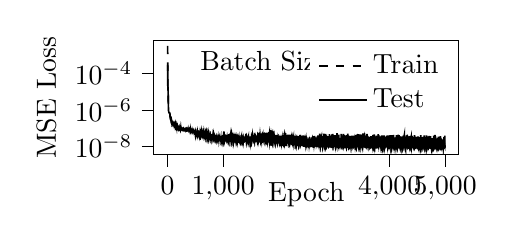
\begin{tikzpicture}

\begin{axis}[
legend cell align={left},
legend style={draw=none},
log basis y={10},
tick align=outside,
tick pos=left,
title={Batch Size 2},
title style={at={(0.4,0.85)},anchor=north},
x grid style={white!69.0196078431373!black},
xlabel={Epoch},
x label style={yshift=13pt},
xmin=-249.95, xmax=5248.95,
xtick style={color=black},
xtick = {0,1000,4000,5000},
y grid style={white!69.0196078431373!black},
ylabel={MSE Loss},
ymin=3.38262380496077e-09, ymax=0.00632854574258151,
ymode=log,
ytick style={color=black},
width=.45\textwidth,
height=.25\textwidth
]
\addplot [semithick, black, dashed]
table {%
0 0.00328254532568099
1 0.000218499955626612
2 0.000191524371870401
3 7.48565430555885e-05
4 1.80191885218974e-05
5 1.70335326928424e-05
6 1.60617069012901e-05
7 1.42414383480727e-05
8 1.17442153426879e-05
9 8.90145301876544e-06
10 6.35426067282552e-06
11 4.48610761718449e-06
12 3.16681323150547e-06
13 2.21908286821115e-06
14 1.57206481016292e-06
15 1.21919172834595e-06
16 1.0618989238651e-06
17 9.78470672838849e-07
18 9.22985532084475e-07
19 8.8099305171685e-07
20 8.4995001972521e-07
21 8.3038449714623e-07
22 8.1447130311485e-07
23 8.01895829424026e-07
24 7.90452571434397e-07
25 7.80588560063133e-07
26 7.67551035850467e-07
27 7.54603072246951e-07
28 7.4473731326119e-07
29 7.34573585697174e-07
30 7.2510382626545e-07
31 7.15328201120524e-07
32 7.06132008384763e-07
33 6.96060642347618e-07
34 6.86012559671934e-07
35 6.76093364214037e-07
36 6.65401749750494e-07
37 6.55946847171407e-07
38 6.46543756017692e-07
39 6.3489944804207e-07
40 6.18515371762385e-07
41 5.85002741245066e-07
42 5.21904763381542e-07
43 4.64107343058906e-07
44 4.31738605658261e-07
45 4.08880619641838e-07
46 3.87349231173229e-07
47 3.69826064049672e-07
48 3.53238981003257e-07
49 3.40011401617657e-07
50 3.28091449871115e-07
51 3.16790916875087e-07
52 3.058581874682e-07
53 2.96605351175927e-07
54 2.8681011950682e-07
55 2.7820315102689e-07
56 2.70656728957208e-07
57 2.63857507705412e-07
58 2.57623938459961e-07
59 2.52528075400882e-07
60 2.47351241863703e-07
61 2.42858798984225e-07
62 2.38187733390793e-07
63 2.34476871070921e-07
64 2.31448094974551e-07
65 2.28447264819964e-07
66 2.25276748428538e-07
67 2.22910076783212e-07
68 2.19949171984757e-07
69 2.18757366997169e-07
70 2.16757680979729e-07
71 2.1456885103599e-07
72 2.12431132567414e-07
73 2.12453675991098e-07
74 2.09875333198273e-07
75 2.08367902884143e-07
76 2.06870915439472e-07
77 2.05759142446249e-07
78 2.03537200378245e-07
79 2.02386158929979e-07
80 2.01577248807538e-07
81 1.99945309896199e-07
82 1.98954125483652e-07
83 1.97998061242988e-07
84 1.95277801370519e-07
85 1.94122259384422e-07
86 1.9321474032008e-07
87 1.92061395219989e-07
88 1.90649255421116e-07
89 1.88983075970039e-07
90 1.87258018107261e-07
91 1.86211353437882e-07
92 1.84968773373595e-07
93 1.8346280023851e-07
94 1.81952997721835e-07
95 1.80662087380323e-07
96 1.79365444776147e-07
97 1.77472094651909e-07
98 1.76493799261546e-07
99 1.74580053132978e-07
100 1.73360636676279e-07
101 1.72267877915688e-07
102 1.70442489901279e-07
103 1.69188082461469e-07
104 1.67839397578917e-07
105 1.66230285953528e-07
106 1.64829462242722e-07
107 1.63325331338671e-07
108 1.62738196491152e-07
109 1.60219138044426e-07
110 1.60535278213469e-07
111 1.58536466712489e-07
112 1.56850298218325e-07
113 1.55524901216397e-07
114 1.54631709402775e-07
115 1.53302759073659e-07
116 1.51466843822945e-07
117 1.49550631134643e-07
118 1.48410193441917e-07
119 1.47384696155495e-07
120 1.46283629718358e-07
121 1.44345578623639e-07
122 1.43203171090622e-07
123 1.41263757020393e-07
124 1.40215976953906e-07
125 1.38600845025039e-07
126 1.37061671532823e-07
127 1.36200254846841e-07
128 1.34788054034773e-07
129 1.32993649122337e-07
130 1.31643087291855e-07
131 1.30615223781883e-07
132 1.28918619770713e-07
133 1.27769738631822e-07
134 1.26176427465929e-07
135 1.25179997131242e-07
136 1.23230363925919e-07
137 1.22045724761821e-07
138 1.21201524557857e-07
139 1.19549983392364e-07
140 1.18310560280777e-07
141 1.16812820882495e-07
142 1.15443738707643e-07
143 1.14161057509832e-07
144 1.1312136743713e-07
145 1.11719248588327e-07
146 1.10043574582441e-07
147 1.09814437586175e-07
148 1.08579877910908e-07
149 1.07548462370266e-07
150 1.0619949556756e-07
151 1.0495877468919e-07
152 1.04168265051441e-07
153 1.02623975512528e-07
154 1.01427549126121e-07
155 1.01362208877243e-07
156 9.95105090075832e-08
157 9.90712999682231e-08
158 9.81297963442707e-08
159 9.76671625630976e-08
160 9.38856064496285e-08
161 9.09411816544248e-08
162 8.88011398124666e-08
163 8.8803014968053e-08
164 8.77907267728961e-08
165 8.71906158357305e-08
166 8.74571203014485e-08
167 8.68890042542425e-08
168 8.61177263807855e-08
169 8.60476076310901e-08
170 8.55405427711009e-08
171 8.58966112591286e-08
172 8.51639051044906e-08
173 8.51758944812042e-08
174 8.47307304080447e-08
175 8.48132693269665e-08
176 8.51079388366482e-08
177 8.49318124505061e-08
178 8.47849283748259e-08
179 8.48751120090529e-08
180 8.42010138485394e-08
181 8.44082437067017e-08
182 8.40907957427861e-08
183 8.38560661877707e-08
184 8.42076578552176e-08
185 8.38791066610778e-08
186 8.37576944041629e-08
187 8.40239886347183e-08
188 8.38833574516862e-08
189 8.33899735629418e-08
190 8.34640443237999e-08
191 8.35304616458865e-08
192 8.31852537088729e-08
193 8.30714862566362e-08
194 8.33851301329513e-08
195 8.27072170499488e-08
196 8.32493552452851e-08
197 8.22546665798507e-08
198 8.27084489483099e-08
199 8.21670082453707e-08
200 8.25011616596427e-08
201 8.18873943000398e-08
202 8.22608535500091e-08
203 8.1495268684395e-08
204 8.20163649861705e-08
205 8.16005401669262e-08
206 8.11489030099199e-08
207 8.16204926260555e-08
208 8.09058569459786e-08
209 8.10499177033019e-08
210 8.07727945287828e-08
211 8.08666219838106e-08
212 8.08093064915694e-08
213 8.02509398206697e-08
214 8.09831349148915e-08
215 8.00564518014246e-08
216 8.00968553160697e-08
217 8.01893686681598e-08
218 8.01536400982794e-08
219 7.95515807424652e-08
220 7.96363922979104e-08
221 8.03492120219351e-08
222 7.98713108027815e-08
223 7.96498008956981e-08
224 7.95084208592423e-08
225 7.95095037848803e-08
226 7.94453084611568e-08
227 7.89366283454607e-08
228 7.92334955032059e-08
229 7.92735157912894e-08
230 7.89827368313789e-08
231 7.85786661230414e-08
232 7.87854531203447e-08
233 7.85752367177262e-08
234 7.85788053452308e-08
235 7.82479060256192e-08
236 7.87282694114655e-08
237 7.80035227161413e-08
238 7.84374309548141e-08
239 7.78576224716998e-08
240 7.77167863775796e-08
241 7.81467363761834e-08
242 7.75516917973507e-08
243 7.74188098600082e-08
244 7.74798297724644e-08
245 7.7469969126609e-08
246 7.71800704708614e-08
247 7.71970539117373e-08
248 7.69478892151954e-08
249 7.73572983933102e-08
250 7.71568599475803e-08
251 7.69779501024193e-08
252 7.71894792475081e-08
253 7.67477751884016e-08
254 7.6877333195835e-08
255 7.65848046396789e-08
256 7.65385336909397e-08
257 7.63672228696333e-08
258 7.6301277346813e-08
259 7.62444665756146e-08
260 7.62738956281428e-08
261 7.59071467697492e-08
262 7.59964418058923e-08
263 7.59101158571696e-08
264 7.60531896979444e-08
265 7.57084843583389e-08
266 7.57804675006746e-08
267 7.57439965304307e-08
268 7.55281243759454e-08
269 7.54863963056129e-08
270 7.55834353999285e-08
271 7.5430192249204e-08
272 7.54428438793919e-08
273 7.52991162173977e-08
274 7.51532936485999e-08
275 7.51941930451361e-08
276 7.51544057150388e-08
277 7.48605089656573e-08
278 7.49440059444328e-08
279 7.48363137593744e-08
280 7.45955682426303e-08
281 7.46543589628113e-08
282 7.45810491539212e-08
283 7.45009416183162e-08
284 7.45298077395873e-08
285 7.43874965440927e-08
286 7.42333786614147e-08
287 7.43559364357882e-08
288 7.44611771404946e-08
289 7.43719104612239e-08
290 7.4087228369879e-08
291 7.42675714614505e-08
292 7.40377803589709e-08
293 7.39002887022444e-08
294 7.37450820641472e-08
295 7.37146042358861e-08
296 7.34764170412516e-08
297 7.34748401464147e-08
298 7.33259203234971e-08
299 7.32177149885826e-08
300 7.30713860042087e-08
301 7.31287919658596e-08
302 7.3047478842847e-08
303 7.30429494556484e-08
304 7.26866788871572e-08
305 7.28189107246369e-08
306 7.2611721922522e-08
307 7.25180870284614e-08
308 7.25546002222632e-08
309 7.23407575197177e-08
310 7.22547411237118e-08
311 7.23688810853051e-08
312 7.23001925837519e-08
313 7.23487935944123e-08
314 7.21203149054439e-08
315 7.23077199693556e-08
316 7.21352630661531e-08
317 7.20632900854667e-08
318 7.19566260092286e-08
319 7.1823656741965e-08
320 7.17751821249779e-08
321 7.18084207751435e-08
322 7.15284738002087e-08
323 7.15922071675701e-08
324 7.14385197908563e-08
325 7.11717999838379e-08
326 7.14794709065769e-08
327 7.11045747163741e-08
328 7.1172664772412e-08
329 7.10999585191718e-08
330 7.10373534636988e-08
331 7.10004941901765e-08
332 7.09694212622791e-08
333 7.10542106029388e-08
334 7.11422026586916e-08
335 7.06343104364127e-08
336 7.06290690287714e-08
337 7.058199697485e-08
338 7.05904521041134e-08
339 7.06610755990544e-08
340 7.02293932595133e-08
341 7.0213167338129e-08
342 7.01696666369767e-08
343 7.01245406067308e-08
344 7.02258261991995e-08
345 7.00943012788002e-08
346 6.99631210515639e-08
347 6.99243554992401e-08
348 6.99733587956608e-08
349 6.97487408191089e-08
350 6.96652839086154e-08
351 6.94952265442028e-08
352 6.9586298279356e-08
353 6.94802141264495e-08
354 6.94029599760393e-08
355 6.94811662502737e-08
356 6.9447535515188e-08
357 6.94013545918804e-08
358 6.94406791021951e-08
359 6.90969612737735e-08
360 6.91050193839526e-08
361 6.8881994686576e-08
362 6.87944344484048e-08
363 6.88425664659986e-08
364 6.87802862303633e-08
365 6.87643034696928e-08
366 6.85632615471388e-08
367 6.85682310238578e-08
368 6.83307170623593e-08
369 6.82866018121286e-08
370 6.85272045393148e-08
371 6.79966236415419e-08
372 6.84238423972472e-08
373 6.79873843945078e-08
374 6.81644149632676e-08
375 6.80043897696159e-08
376 6.79346173235729e-08
377 6.78095727341121e-08
378 6.76759811131245e-08
379 6.78007946736114e-08
380 6.7796770238715e-08
381 6.75536845422542e-08
382 6.73928114495181e-08
383 6.72945608075626e-08
384 6.73337297967258e-08
385 6.72205919783897e-08
386 6.72738835988396e-08
387 6.69181899951576e-08
388 6.71726448415733e-08
389 6.6735886535163e-08
390 6.67219459820068e-08
391 6.67162453900083e-08
392 6.65349611206345e-08
393 6.63832358627214e-08
394 6.63773440239268e-08
395 6.6198406551754e-08
396 6.61917400128775e-08
397 6.60644241761155e-08
398 6.62409058879154e-08
399 6.59781503837831e-08
400 6.58956399993693e-08
401 6.60107959022938e-08
402 6.5846786045487e-08
403 6.55407205336633e-08
404 6.55228505987981e-08
405 6.55955494313076e-08
406 6.52562304821469e-08
407 6.52904168840784e-08
408 6.56664842482169e-08
409 6.48951202171233e-08
410 6.52150227713477e-08
411 6.48234405338233e-08
412 6.50295594792905e-08
413 6.473958666664e-08
414 6.46367741741205e-08
415 6.44284369182291e-08
416 6.4706066168263e-08
417 6.41347029111117e-08
418 6.4321762164754e-08
419 6.38945435269545e-08
420 6.41486727785967e-08
421 6.38424642197544e-08
422 6.41088489685693e-08
423 6.37925187760846e-08
424 6.37641166327807e-08
425 6.34406229562678e-08
426 6.35571083453801e-08
427 6.32675255589632e-08
428 6.33023986322812e-08
429 6.29458381071757e-08
430 6.31480538190177e-08
431 6.27496439844499e-08
432 6.25742152867703e-08
433 6.25643662857112e-08
434 6.24544778045077e-08
435 6.2011825340047e-08
436 6.2753866577947e-08
437 6.18486373562543e-08
438 6.19743378120763e-08
439 6.20571040625961e-08
440 6.18520889781316e-08
441 6.16609228023535e-08
442 6.13968909650708e-08
443 6.14124531921334e-08
444 6.11450753005283e-08
445 6.09623349119293e-08
446 6.05825954643757e-08
447 6.04997935236273e-08
448 6.05668844602114e-08
449 6.05799478256008e-08
450 6.01981422974074e-08
451 5.9961909875561e-08
452 5.97201968506322e-08
453 5.96139426777276e-08
454 5.95120054305287e-08
455 5.92951785870488e-08
456 5.95512403165355e-08
457 5.93397249657457e-08
458 5.92162069610325e-08
459 5.89310149428091e-08
460 5.87983697155625e-08
461 5.86480213723428e-08
462 5.86585211733715e-08
463 5.81024033210475e-08
464 5.79005150566081e-08
465 5.7884217427695e-08
466 5.75974278191893e-08
467 5.72717783334786e-08
468 5.71280839249955e-08
469 5.70866307733064e-08
470 5.68234420759151e-08
471 5.65403589207758e-08
472 5.64500327302486e-08
473 5.62552928184967e-08
474 5.59582069550313e-08
475 5.59200681947702e-08
476 5.5690757583271e-08
477 5.51963993931093e-08
478 5.49973188885833e-08
479 5.45198159787041e-08
480 5.44046598370818e-08
481 5.41920685905861e-08
482 5.38668678436993e-08
483 5.361629318823e-08
484 5.32998607738477e-08
485 5.30580958801874e-08
486 5.32657221515853e-08
487 5.25750263348224e-08
488 5.23441807802616e-08
489 5.24424364887199e-08
490 5.18821803626723e-08
491 5.19918664291241e-08
492 5.1747341199504e-08
493 5.13785602573869e-08
494 5.11840279411868e-08
495 5.12938131975726e-08
496 5.0924607952807e-08
497 5.10876863294429e-08
498 5.07458053390364e-08
499 5.06220796397949e-08
500 5.04064744368815e-08
501 5.06455437344622e-08
502 4.9862071242579e-08
503 4.97268267137807e-08
504 4.94142680242948e-08
505 4.97652903030943e-08
506 4.94748283430546e-08
507 4.90965448383118e-08
508 4.87868712980566e-08
509 4.90490110020003e-08
510 4.92224223346271e-08
511 4.89848744311683e-08
512 4.86528948101528e-08
513 4.87841283199897e-08
514 4.84146250535611e-08
515 4.9023456144659e-08
516 4.81331435734367e-08
517 4.80398341196064e-08
518 4.88083406132711e-08
519 4.84064391683692e-08
520 4.84159776592552e-08
521 4.75737229264639e-08
522 4.8519928558588e-08
523 4.73770784747973e-08
524 4.83165005312758e-08
525 4.78193792249337e-08
526 4.78251361750726e-08
527 4.70196307974513e-08
528 4.80083285770982e-08
529 4.71223468826443e-08
530 4.71813922692244e-08
531 4.7113969577961e-08
532 4.70967598273919e-08
533 4.70621662446158e-08
534 4.66326605940148e-08
535 4.76241100443309e-08
536 4.66664954731355e-08
537 4.74405901805808e-08
538 4.69436936714196e-08
539 4.72466676191274e-08
540 4.70211507684337e-08
541 4.63547233083839e-08
542 4.61678381813435e-08
543 4.6965799879839e-08
544 4.63857039533222e-08
545 4.63133353306167e-08
546 4.62923420408989e-08
547 4.6108359860686e-08
548 4.64648258927669e-08
549 4.58507157922727e-08
550 4.595448568534e-08
551 4.60644132552757e-08
552 4.57460573870527e-08
553 4.48977841176479e-08
554 4.61474039982757e-08
555 4.54119244746032e-08
556 4.50748147138302e-08
557 4.51294110412337e-08
558 4.52713001330984e-08
559 4.45902119108332e-08
560 4.54390254731596e-08
561 4.45883604294206e-08
562 4.40688434577563e-08
563 4.46767707545925e-08
564 4.43456282678834e-08
565 4.43052667442601e-08
566 4.4511835127603e-08
567 4.44672186858952e-08
568 4.40549484904684e-08
569 4.38604737291737e-08
570 4.36744109219012e-08
571 4.33528694978591e-08
572 4.36945165810387e-08
573 4.35054831703363e-08
574 4.3339193234071e-08
575 4.33224534239773e-08
576 4.28230918373407e-08
577 4.29915050395024e-08
578 4.3157082451617e-08
579 4.29085400865947e-08
580 4.27126839501746e-08
581 4.34098694395701e-08
582 4.2637734657236e-08
583 4.27076143056926e-08
584 4.31071084622259e-08
585 4.27677483794131e-08
586 4.2361920931655e-08
587 4.25198561692097e-08
588 4.25564854413807e-08
589 4.23260934941938e-08
590 4.18924031443391e-08
591 4.22129305257257e-08
592 4.16024839526852e-08
593 4.16946787210604e-08
594 4.17917192728767e-08
595 4.16310181681201e-08
596 4.13894368075374e-08
597 4.14773096925058e-08
598 4.10987801270912e-08
599 4.12405630366708e-08
600 4.19068369599263e-08
601 4.11747850240785e-08
602 4.14282939695809e-08
603 4.06905636430865e-08
604 4.08110460305977e-08
605 4.11398571306121e-08
606 4.09925211455886e-08
607 4.06709809314121e-08
608 4.11535621287484e-08
609 4.03891638949272e-08
610 4.03422490115046e-08
611 4.04638569014848e-08
612 4.03521925785855e-08
613 4.02347802692105e-08
614 3.96676463815804e-08
615 4.05902976614581e-08
616 3.9934611743786e-08
617 3.97000445235829e-08
618 3.93751615644367e-08
619 3.99356786361937e-08
620 3.94967812543667e-08
621 3.9478045169461e-08
622 3.9357216289726e-08
623 3.91124260917808e-08
624 3.93788417034635e-08
625 3.91443982862283e-08
626 3.94537697414044e-08
627 3.92543143685753e-08
628 3.88451565003223e-08
629 3.87263305199337e-08
630 3.90169901079984e-08
631 3.90409084574106e-08
632 3.90292650599422e-08
633 3.8848819337356e-08
634 3.826467254886e-08
635 3.86679600120066e-08
636 3.84189770820664e-08
637 3.8034914403573e-08
638 3.83765584659468e-08
639 3.84147417166192e-08
640 3.81209554103368e-08
641 3.76586081726193e-08
642 3.7909612859377e-08
643 3.79556497944744e-08
644 3.75772361053683e-08
645 3.7929992070862e-08
646 3.75065041919309e-08
647 3.7582637523681e-08
648 3.71357294101093e-08
649 3.74972402298335e-08
650 3.73230137498126e-08
651 3.7014256861978e-08
652 3.67768056607209e-08
653 3.72723442765288e-08
654 3.69532771464787e-08
655 3.67656498795332e-08
656 3.70444940477888e-08
657 3.74225217392166e-08
658 3.64024413511688e-08
659 3.66532642359085e-08
660 3.6914308742364e-08
661 3.6492219348927e-08
662 3.66049217205844e-08
663 3.68115249901324e-08
664 3.63449829077767e-08
665 3.59703634603137e-08
666 3.65043941129017e-08
667 3.64438717505577e-08
668 3.61117691105584e-08
669 3.59725088353025e-08
670 3.58938531116459e-08
671 3.56944948786131e-08
672 3.54274465845794e-08
673 3.58843036923351e-08
674 3.51804919540566e-08
675 3.592879544001e-08
676 3.51167567705923e-08
677 3.54670594818751e-08
678 3.4856420939644e-08
679 3.52466294488152e-08
680 3.47822667237652e-08
681 3.53631174087043e-08
682 3.46637306734565e-08
683 3.47526936601283e-08
684 3.45369711179377e-08
685 3.44024175803481e-08
686 3.45784007663719e-08
687 3.43725343730505e-08
688 3.42645183736834e-08
689 3.43503181767235e-08
690 3.43352946233222e-08
691 3.41738478102926e-08
692 3.45125217628417e-08
693 3.38059283864212e-08
694 3.44023723802267e-08
695 3.34726516930117e-08
696 3.39030477289892e-08
697 3.36896250675012e-08
698 3.33158177039938e-08
699 3.35237944595335e-08
700 3.32292014725288e-08
701 3.3578084904895e-08
702 3.35027595368964e-08
703 3.39071785393497e-08
704 3.293375946406e-08
705 3.30269301683228e-08
706 3.3574827676075e-08
707 3.33444393947335e-08
708 3.33603552093997e-08
709 3.28944379845431e-08
710 3.27157034414327e-08
711 3.30092747191646e-08
712 3.29718086783393e-08
713 3.29110067269767e-08
714 3.27898127228665e-08
715 3.29078348913492e-08
716 3.22872896388327e-08
717 3.27488542049559e-08
718 3.24483861559588e-08
719 3.27850294034593e-08
720 3.26606627359949e-08
721 3.23589595196405e-08
722 3.24584725308608e-08
723 3.26674511605951e-08
724 3.1575581434129e-08
725 3.25877752292425e-08
726 3.20928140972732e-08
727 3.24274801469793e-08
728 3.25003616281627e-08
729 3.18399988796236e-08
730 3.2109916644596e-08
731 3.20759825324646e-08
732 3.18597185383629e-08
733 3.19681254596915e-08
734 3.22229387327844e-08
735 3.17291694599264e-08
736 3.21273451338033e-08
737 3.17449717723295e-08
738 3.15686945521754e-08
739 3.17564476380316e-08
740 3.17477588294146e-08
741 3.10420353661356e-08
742 3.20795690111342e-08
743 3.1216206289153e-08
744 3.11819914966538e-08
745 3.0873233597184e-08
746 3.14768186575609e-08
747 3.0342848171272e-08
748 3.17283036666005e-08
749 3.09738106077373e-08
750 3.10661259300682e-08
751 3.08984813262025e-08
752 3.06028083156829e-08
753 3.11116006412315e-08
754 3.11124808433094e-08
755 3.09768128804455e-08
756 3.11854558228131e-08
757 3.10072328188471e-08
758 3.1022588369789e-08
759 3.01097631762448e-08
760 3.08949155709559e-08
761 3.08619954873524e-08
762 3.05116490219026e-08
763 3.14621224050682e-08
764 3.06109915238495e-08
765 3.0499886474411e-08
766 3.02687262935253e-08
767 3.03926383860009e-08
768 2.94455249570946e-08
769 2.99938384391574e-08
770 3.05687051307957e-08
771 2.98737279285088e-08
772 3.03895292956824e-08
773 3.02582276905938e-08
774 2.97754409906981e-08
775 3.0655070072716e-08
776 2.97111483765766e-08
777 3.00233681251871e-08
778 2.98320518886119e-08
779 3.06805578830227e-08
780 3.02031067299646e-08
781 2.96468851478937e-08
782 3.0587170042895e-08
783 2.99796532466923e-08
784 3.06078738928628e-08
785 2.92830425706048e-08
786 3.0212400990437e-08
787 2.9719811062312e-08
788 2.93865345387112e-08
789 3.00758327314021e-08
790 2.99608398715012e-08
791 2.98255288354032e-08
792 3.01842756250115e-08
793 3.01570450788047e-08
794 2.9858412152417e-08
795 3.0092274968585e-08
796 3.02506790859636e-08
797 2.91831633476569e-08
798 2.95765616485921e-08
799 2.99364189229601e-08
800 3.00087392374193e-08
801 3.05344552096187e-08
802 3.01328082645269e-08
803 2.99154144154934e-08
804 2.94597860326373e-08
805 2.93265596476022e-08
806 2.9981135665047e-08
807 2.97405996949052e-08
808 2.97528969943062e-08
809 2.97964703900311e-08
810 2.93363185845386e-08
811 2.99720110352175e-08
812 2.96175842905422e-08
813 2.96315429029193e-08
814 2.96446226587532e-08
815 2.99707815297201e-08
816 2.95448832050571e-08
817 2.95232755386232e-08
818 2.87613123848285e-08
819 2.95836693727236e-08
820 2.94098747234406e-08
821 2.91337529105262e-08
822 2.93476053093156e-08
823 2.87491110401716e-08
824 2.89403561636314e-08
825 2.95640055761326e-08
826 2.85100923496651e-08
827 2.90359088045422e-08
828 2.89738495633518e-08
829 2.93372802613323e-08
830 2.93234274397203e-08
831 2.88658978312428e-08
832 2.86577576900093e-08
833 2.93334803106449e-08
834 2.79551181306403e-08
835 2.93240796755412e-08
836 2.84651544498193e-08
837 2.85353146382561e-08
838 2.86506699791467e-08
839 2.80141502583264e-08
840 2.90341042116782e-08
841 2.83219711137428e-08
842 2.88628372929201e-08
843 2.81941445002265e-08
844 2.86616231613412e-08
845 2.80926744038457e-08
846 2.87754205431923e-08
847 2.85303202081644e-08
848 2.81727098084272e-08
849 2.8123937935165e-08
850 2.84582470004846e-08
851 2.8650369424621e-08
852 2.85608268651982e-08
853 2.8131232703843e-08
854 2.82453610964128e-08
855 2.89483162182469e-08
856 2.83420080103847e-08
857 2.82199570773578e-08
858 2.80730314435318e-08
859 2.82809190177979e-08
860 2.86353769445857e-08
861 2.82259201612178e-08
862 2.78959342820406e-08
863 2.78645208896533e-08
864 2.81846941814212e-08
865 2.81121721020239e-08
866 2.80517562643023e-08
867 2.81593320271001e-08
868 2.72528267648564e-08
869 2.81696339985427e-08
870 2.79273086642995e-08
871 2.7512817953157e-08
872 2.84517497671222e-08
873 2.7799637717929e-08
874 2.74260516970881e-08
875 2.7788204698842e-08
876 2.73057909985774e-08
877 2.83043334327049e-08
878 2.64792259140334e-08
879 2.77433954551931e-08
880 2.80859690999224e-08
881 2.81571656352009e-08
882 2.76695006193872e-08
883 2.77709883268473e-08
884 2.6881104866483e-08
885 2.78426782351904e-08
886 2.77167030259817e-08
887 2.78135435696769e-08
888 2.78613534441252e-08
889 2.74576081790157e-08
890 2.72004491331246e-08
891 2.7812381422021e-08
892 2.74803205711494e-08
893 2.72247917181279e-08
894 2.76698133706565e-08
895 2.75316115931346e-08
896 2.72633557068525e-08
897 2.75284972862111e-08
898 2.75199321894126e-08
899 2.73734412948312e-08
900 2.72344164200522e-08
901 2.74171147513491e-08
902 2.8005013492205e-08
903 2.72693796256607e-08
904 2.71729967772916e-08
905 2.70847596891555e-08
906 2.76970295121637e-08
907 2.70154164276337e-08
908 2.71905937012651e-08
909 2.74396833003232e-08
910 2.67758121418882e-08
911 2.80058317719267e-08
912 2.79118399847678e-08
913 2.63474409490927e-08
914 2.71324295361142e-08
915 2.7954368273797e-08
916 2.7007748962693e-08
917 2.64737631885392e-08
918 2.76175025140657e-08
919 2.68041697211174e-08
920 2.71468540083974e-08
921 2.700771886055e-08
922 2.75985255401845e-08
923 2.69180859497897e-08
924 2.69624495977117e-08
925 2.68577280076454e-08
926 2.704912061402e-08
927 2.6356536705241e-08
928 2.66672037859128e-08
929 2.69591033794092e-08
930 2.68079865403115e-08
931 2.63138631513837e-08
932 2.72206234661621e-08
933 2.71317316304365e-08
934 2.7307047371139e-08
935 2.65802619039413e-08
936 2.73144441089168e-08
937 2.63830216658545e-08
938 2.66981474648098e-08
939 2.6431935854887e-08
940 2.60439990913408e-08
941 2.67252916980043e-08
942 2.66271156456055e-08
943 2.6739769780626e-08
944 2.62611098725829e-08
945 2.62674960841425e-08
946 2.70139238268685e-08
947 2.63460659326586e-08
948 2.62264182295802e-08
949 2.70272808373662e-08
950 2.5747153010236e-08
951 2.66053678841804e-08
952 2.64551851290595e-08
953 2.67567574317451e-08
954 2.58916772901685e-08
955 2.64584350602726e-08
956 2.61099018731836e-08
957 2.66250582974248e-08
958 2.59226130361612e-08
959 2.64767316645598e-08
960 2.6452490843043e-08
961 2.58215259816841e-08
962 2.59265999303371e-08
963 2.62359932220457e-08
964 2.65424289648264e-08
965 2.67450139063707e-08
966 2.63561833882819e-08
967 2.57741525678257e-08
968 2.62758306087407e-08
969 2.65221036650498e-08
970 2.64172919469674e-08
971 2.56274016323943e-08
972 2.57729816374175e-08
973 2.59577244466347e-08
974 2.6222427415179e-08
975 2.62312397004694e-08
976 2.5963541613383e-08
977 2.56496797129135e-08
978 2.56104738609597e-08
979 2.62138495017994e-08
980 2.58349842333083e-08
981 2.6208806482575e-08
982 2.54673980373543e-08
983 2.56343059095165e-08
984 2.62062766909765e-08
985 2.52106715502853e-08
986 2.51687390236954e-08
987 2.61188593480566e-08
988 2.52318605282187e-08
989 2.56387556114013e-08
990 2.54048550445418e-08
991 2.53413983453687e-08
992 2.55538864205596e-08
993 2.5451171698665e-08
994 2.61896682761109e-08
995 2.54498613648235e-08
996 2.55230583791621e-08
997 2.48618900541842e-08
998 2.58373611447538e-08
999 2.51232853774597e-08
1000 2.56220291215414e-08
1001 2.56736006327141e-08
1002 2.51882083300847e-08
1003 2.53713824167612e-08
1004 2.58137432954941e-08
1005 2.48481835016801e-08
1006 2.56784723412506e-08
1007 2.40642600508045e-08
1008 2.56810740124624e-08
1009 2.54665775721308e-08
1010 2.43275138776256e-08
1011 2.61642387404115e-08
1012 2.48960325622827e-08
1013 2.58067697424536e-08
1014 2.57083646426348e-08
1015 2.49647724676894e-08
1016 2.54706723878118e-08
1017 2.44838401316505e-08
1018 2.5243788890239e-08
1019 2.52713618028588e-08
1020 2.47552457360301e-08
1021 2.50724322887752e-08
1022 2.57186888398264e-08
1023 2.51238573180101e-08
1024 2.44940838938223e-08
1025 2.52199264209607e-08
1026 2.57123974063966e-08
1027 2.50377650737044e-08
1028 2.51321844116914e-08
1029 2.45223809804962e-08
1030 2.48290043978749e-08
1031 2.53573499313098e-08
1032 2.4809457069952e-08
1033 2.55327429933838e-08
1034 2.49863649272875e-08
1035 2.54338735914406e-08
1036 2.46765876222854e-08
1037 2.48556650924159e-08
1038 2.46800521991331e-08
1039 2.51365618709754e-08
1040 2.41794125941386e-08
1041 2.44692986407224e-08
1042 2.47765058001559e-08
1043 2.48758484036604e-08
1044 2.41757049636859e-08
1045 2.4206212695721e-08
1046 2.55829298876631e-08
1047 2.41762240022481e-08
1048 2.47289624125679e-08
1049 2.5234407058039e-08
1050 2.43533080388492e-08
1051 2.47249283025774e-08
1052 2.44511952491311e-08
1053 2.45763102038055e-08
1054 2.45536552540004e-08
1055 2.48305525572534e-08
1056 2.40834935295586e-08
1057 2.53211549907095e-08
1058 2.41439715079061e-08
1059 2.57494680457604e-08
1060 2.35057552473161e-08
1061 2.49778252063293e-08
1062 2.40053659600614e-08
1063 2.4876820900549e-08
1064 2.45837317633946e-08
1065 2.43284918397257e-08
1066 2.40939658241457e-08
1067 2.51706974384036e-08
1068 2.35143826128326e-08
1069 2.41161983740024e-08
1070 2.4755212258476e-08
1071 2.4246693290042e-08
1072 2.56388721965872e-08
1073 2.41264563889954e-08
1074 2.44039392134909e-08
1075 2.51708382467408e-08
1076 2.45340783286419e-08
1077 2.45209754993758e-08
1078 2.48115112856939e-08
1079 2.39203909974672e-08
1080 2.31613966679145e-08
1081 2.50456757703854e-08
1082 2.43899172222006e-08
1083 2.40393221376256e-08
1084 2.41358175256112e-08
1085 2.3699030541946e-08
1086 2.43306819150413e-08
1087 2.42609329062504e-08
1088 2.39897964542934e-08
1089 2.44988888764563e-08
1090 2.45195678220678e-08
1091 2.40963733417754e-08
1092 2.39458951021843e-08
1093 2.37625303336486e-08
1094 2.44664175362286e-08
1095 2.36047424231611e-08
1096 2.45438499066886e-08
1097 2.4314623127103e-08
1098 2.39301791060131e-08
1099 2.417096244689e-08
1100 2.39409680004576e-08
1101 2.42720179199352e-08
1102 2.42393090368331e-08
1103 2.40999026286381e-08
1104 2.42074585857788e-08
1105 2.3707304635745e-08
1106 2.34363956257144e-08
1107 2.36964240676596e-08
1108 2.36679420671515e-08
1109 2.38906914948878e-08
1110 2.46842266887759e-08
1111 2.31558109071162e-08
1112 2.37190626790618e-08
1113 2.35072627912114e-08
1114 2.4207290549999e-08
1115 2.3632586413358e-08
1116 2.4249042063107e-08
1117 2.3715847715905e-08
1118 2.38752562103928e-08
1119 2.48957234907365e-08
1120 2.32552377015804e-08
1121 2.49651159680564e-08
1122 2.28996111810154e-08
1123 2.34150135410283e-08
1124 2.41551524927108e-08
1125 2.34782538071077e-08
1126 2.43804897772648e-08
1127 2.31835085818255e-08
1128 2.3253374320964e-08
1129 2.32561741067006e-08
1130 2.50726553251424e-08
1131 2.29548132411883e-08
1132 2.3328192227362e-08
1133 2.41420011705684e-08
1134 2.33821172641313e-08
1135 2.3303387180762e-08
1136 2.43730284085197e-08
1137 2.41564589041898e-08
1138 2.37143871552048e-08
1139 2.36588560203199e-08
1140 2.30154500006075e-08
1141 2.4859979055103e-08
1142 2.29174441709334e-08
1143 2.38801621325058e-08
1144 2.44339880565159e-08
1145 2.38689083146837e-08
1146 2.28463232741505e-08
1147 2.46741202382939e-08
1148 2.41791558530102e-08
1149 2.29663980678141e-08
1150 2.39159831927349e-08
1151 2.43229607134743e-08
1152 2.28362273965721e-08
1153 2.31572237742172e-08
1154 2.33627679651072e-08
1155 2.27080735474283e-08
1156 2.4358588360418e-08
1157 2.26149591309732e-08
1158 2.3826834529006e-08
1159 2.35227404605243e-08
1160 2.2895686424329e-08
1161 2.40749804307216e-08
1162 2.26256669050295e-08
1163 2.33396992000423e-08
1164 2.30482095263662e-08
1165 2.44169308798725e-08
1166 2.39379462509404e-08
1167 2.23706146176839e-08
1168 2.37480671272938e-08
1169 2.3676940001105e-08
1170 2.34087737608912e-08
1171 2.3882939918618e-08
1172 2.30129306417748e-08
1173 2.31911079903724e-08
1174 2.24837282247203e-08
1175 2.29678447716819e-08
1176 2.3352444612823e-08
1177 2.3275783645138e-08
1178 2.36324950197431e-08
1179 2.44034234366253e-08
1180 2.2084830024971e-08
1181 2.42513723696935e-08
1182 2.16930364395074e-08
1183 2.25338594886382e-08
1184 2.28829293547617e-08
1185 2.39440693926563e-08
1186 2.2315187542532e-08
1187 2.36924562428409e-08
1188 2.20071196566085e-08
1189 2.32872066795453e-08
1190 2.39950020853863e-08
1191 2.17920868925692e-08
1192 2.27612380520603e-08
1193 2.3995818000222e-08
1194 2.22051254888389e-08
1195 2.46911551403106e-08
1196 2.19987103602382e-08
1197 2.24494658944141e-08
1198 2.54094465522159e-08
1199 2.06954137310644e-08
1200 2.39629729154589e-08
1201 2.31854273466947e-08
1202 2.26924926745031e-08
1203 2.40487618563545e-08
1204 2.13842529988295e-08
1205 2.39762664323573e-08
1206 2.25271042649244e-08
1207 2.24390193712121e-08
1208 2.4125746498016e-08
1209 2.21658715069406e-08
1210 2.28044628429736e-08
1211 2.48385112019966e-08
1212 2.33656474967758e-08
1213 2.12154672926679e-08
1214 2.41168022632188e-08
1215 2.127196985513e-08
1216 2.41087441434362e-08
1217 2.23791959621522e-08
1218 2.24479696701585e-08
1219 2.30527769330691e-08
1220 2.41279960776497e-08
1221 2.22326906687553e-08
1222 2.24541030668934e-08
1223 2.22194493112449e-08
1224 2.33363321254232e-08
1225 2.30219892352057e-08
1226 2.20189755480715e-08
1227 2.30715657988378e-08
1228 2.25623969505317e-08
1229 2.24376861742148e-08
1230 2.21420095534164e-08
1231 2.41717404863839e-08
1232 2.20276527142516e-08
1233 2.24890027827329e-08
1234 2.36996848195781e-08
1235 2.19429958308592e-08
1236 2.31160184864798e-08
1237 2.46116306463207e-08
1238 2.23464107134141e-08
1239 2.19672915339753e-08
1240 2.24700124982213e-08
1241 2.36331999026174e-08
1242 2.33265122337456e-08
1243 2.13752408421142e-08
1244 2.33078071993353e-08
1245 2.32677361167721e-08
1246 2.21433261852755e-08
1247 2.40962325241401e-08
1248 2.26305257871595e-08
1249 2.21173026355714e-08
1250 2.39238219879034e-08
1251 2.13247202381361e-08
1252 2.37189196605203e-08
1253 2.32250552512636e-08
1254 2.16647174275386e-08
1255 2.2491087962706e-08
1256 2.34335919854778e-08
1257 2.19791799298541e-08
1258 2.35654252513373e-08
1259 2.14169790457852e-08
1260 2.35637368361241e-08
1261 2.1728992364356e-08
1262 2.31331254670342e-08
1263 2.26170422073235e-08
1264 2.35172557362939e-08
1265 2.14990163194817e-08
1266 2.36890559190961e-08
1267 2.17138146291762e-08
1268 2.44956976728217e-08
1269 2.12130341750993e-08
1270 2.29326911906358e-08
1271 2.294375372347e-08
1272 2.21282134780787e-08
1273 2.37402650568597e-08
1274 2.14494472419724e-08
1275 2.28301129672759e-08
1276 2.20507827259908e-08
1277 2.38259531475382e-08
1278 2.14158515750573e-08
1279 2.44407928549073e-08
1280 2.20708781046852e-08
1281 2.28768149491132e-08
1282 2.2626050056429e-08
1283 2.3005323938563e-08
1284 2.1827455709722e-08
1285 2.22817814335419e-08
1286 2.34458954926908e-08
1287 2.12545711266165e-08
1288 2.32935544570156e-08
1289 2.18443757705744e-08
1290 2.20137667314435e-08
1291 2.26713250879862e-08
1292 2.2973785081537e-08
1293 2.30200027910299e-08
1294 2.19761202549518e-08
1295 2.24197731544806e-08
1296 2.17526179136229e-08
1297 2.37097571550993e-08
1298 2.20199593771175e-08
1299 2.23016867821613e-08
1300 2.22305995936645e-08
1301 2.33038597228785e-08
1302 2.38850469355678e-08
1303 2.09000387388913e-08
1304 2.26636061739782e-08
1305 2.2103954332886e-08
1306 2.28347936062634e-08
1307 2.19457175233972e-08
1308 2.22836593346543e-08
1309 2.23504406504094e-08
1310 2.22128115497378e-08
1311 2.28280098716338e-08
1312 2.31253715030633e-08
1313 2.11736454615585e-08
1314 2.20795589808143e-08
1315 2.24833086843179e-08
1316 2.32801941796312e-08
1317 2.14961897331001e-08
1318 2.20238446245746e-08
1319 2.2324847892885e-08
1320 2.19785063278466e-08
1321 2.35137257901807e-08
1322 2.3144701277622e-08
1323 2.10336239354625e-08
1324 2.23880651935016e-08
1325 2.16761783147779e-08
1326 2.26090178953031e-08
1327 2.28862650982764e-08
1328 2.21212273828209e-08
1329 2.16299618250315e-08
1330 2.29643947586289e-08
1331 2.26928735589382e-08
1332 2.20482249578269e-08
1333 2.18015371278302e-08
1334 2.20884739085547e-08
1335 2.3364725292907e-08
1336 2.15798587311355e-08
1337 2.36228769332492e-08
1338 2.27154247446348e-08
1339 2.18096778484278e-08
1340 2.21108368879674e-08
1341 2.21310831148291e-08
1342 2.20017822580854e-08
1343 2.19745016792339e-08
1344 2.21375170811888e-08
1345 2.21948070953104e-08
1346 2.21312608935653e-08
1347 2.22437780286744e-08
1348 2.19581330651586e-08
1349 2.20827062501483e-08
1350 2.18945214304211e-08
1351 2.29315245998118e-08
1352 2.21396365736037e-08
1353 2.25976545702999e-08
1354 2.1405512023176e-08
1355 2.20842132633847e-08
1356 2.24522939798466e-08
1357 2.26773350752718e-08
1358 2.14882492814428e-08
1359 2.2369567684366e-08
1360 2.17191727960309e-08
1361 2.19919470932917e-08
1362 2.2311646740325e-08
1363 2.25913608749573e-08
1364 2.21926017565655e-08
1365 2.15259211113761e-08
1366 2.16004253598134e-08
1367 2.32224484773558e-08
1368 2.15576274351648e-08
1369 2.25957661512677e-08
1370 2.1665183021935e-08
1371 2.22470384803053e-08
1372 2.227040601116e-08
1373 2.18528204138368e-08
1374 2.21331229738886e-08
1375 2.32569008955519e-08
1376 2.05272220124009e-08
1377 2.2737146274765e-08
1378 2.17802189304006e-08
1379 2.20164517975019e-08
1380 2.26876345494897e-08
1381 2.14601053055152e-08
1382 2.13699287613944e-08
1383 2.16462507426907e-08
1384 2.21368567230318e-08
1385 2.28223008749695e-08
1386 2.15268508930722e-08
1387 2.18877246265792e-08
1388 2.23609083401244e-08
1389 2.2065903218349e-08
1390 2.26112779765364e-08
1391 2.21005944214259e-08
1392 2.21072447048609e-08
1393 2.2372629410905e-08
1394 2.21432812628208e-08
1395 2.25536891302891e-08
1396 2.20534070987655e-08
1397 2.2955050506257e-08
1398 2.26208074964873e-08
1399 2.18272057315172e-08
1400 2.16593289958933e-08
1401 2.27141324652957e-08
1402 2.20719237945533e-08
1403 2.17082151288683e-08
1404 2.20936218085499e-08
1405 2.1863136471012e-08
1406 2.21187039824433e-08
1407 2.10590157191937e-08
1408 2.29186094085621e-08
1409 2.21961395413528e-08
1410 2.20644468408859e-08
1411 2.22680759182081e-08
1412 2.22331608497606e-08
1413 2.04469981444633e-08
1414 2.1789090508928e-08
1415 2.25222602415753e-08
1416 2.11176890110853e-08
1417 2.25176194232346e-08
1418 2.15985122689055e-08
1419 2.2313166706811e-08
1420 2.30230737420234e-08
1421 2.18747423230137e-08
1422 2.16363518343865e-08
1423 2.3068403635973e-08
1424 2.1838906702043e-08
1425 2.22338019213453e-08
1426 2.13278609508261e-08
1427 2.29623013299207e-08
1428 2.1098088403726e-08
1429 2.24614715425009e-08
1430 2.12589236732175e-08
1431 2.26730734765868e-08
1432 2.10315514134751e-08
1433 2.27212884548189e-08
1434 2.09692620500856e-08
1435 2.26583690920989e-08
1436 2.04742908186395e-08
1437 2.28886742472678e-08
1438 2.12501669026866e-08
1439 2.31694822255268e-08
1440 2.19335935971454e-08
1441 2.07122653302361e-08
1442 2.32995183077067e-08
1443 2.13800517415708e-08
1444 2.19378508171109e-08
1445 2.17659652216318e-08
1446 2.25236484944213e-08
1447 2.14525019416878e-08
1448 2.11303392904094e-08
1449 2.22758848886784e-08
1450 2.15706849791553e-08
1451 2.30910437937215e-08
1452 2.07915529506497e-08
1453 2.22041605880685e-08
1454 2.20864075464178e-08
1455 2.2056206184895e-08
1456 2.15564313329752e-08
1457 2.11379826827729e-08
1458 2.20233888020283e-08
1459 2.28370447180604e-08
1460 2.11876432199554e-08
1461 2.22300986445489e-08
1462 2.16021678987599e-08
1463 2.17324369022887e-08
1464 2.21292224406588e-08
1465 2.23671277076454e-08
1466 2.14703611854938e-08
1467 2.05927899782354e-08
1468 2.33626976558488e-08
1469 2.05264296654906e-08
1470 2.18535323567859e-08
1471 2.11968200043433e-08
1472 2.18168553881015e-08
1473 2.26454652578756e-08
1474 2.11857142232708e-08
1475 2.13278918422266e-08
1476 2.236010990736e-08
1477 2.17072662658802e-08
1478 2.2110143227283e-08
1479 2.22466864685522e-08
1480 2.06100590163238e-08
1481 2.22854114886872e-08
1482 2.19793991453332e-08
1483 2.16467689184152e-08
1484 2.05775316386991e-08
1485 2.19673081403582e-08
1486 2.19401898399474e-08
1487 2.20589850682407e-08
1488 2.05005431839767e-08
1489 2.15492483782165e-08
1490 2.19645833702264e-08
1491 2.21786140069957e-08
1492 2.16240650679489e-08
1493 2.21673701460423e-08
1494 2.08698478573743e-08
1495 2.19098450867095e-08
1496 2.15752541418146e-08
1497 2.19070329576798e-08
1498 2.16886264846616e-08
1499 2.23972178054754e-08
1500 2.14879013741287e-08
1501 2.11427105282214e-08
1502 2.18200978853167e-08
1503 2.19430892073325e-08
1504 2.18239163790046e-08
1505 2.12949392383033e-08
1506 2.09734695226782e-08
1507 2.21864767561142e-08
1508 2.10699609919374e-08
1509 2.23657064514771e-08
1510 2.08754557393664e-08
1511 2.13593325406602e-08
1512 2.2237284218074e-08
1513 2.22302955611431e-08
1514 2.14894843014179e-08
1515 2.17345119775114e-08
1516 2.2619548078251e-08
1517 2.03632252265273e-08
1518 2.222387638251e-08
1519 2.0638844568599e-08
1520 2.15556459234878e-08
1521 2.13329812444041e-08
1522 2.17516634387072e-08
1523 2.14504079945055e-08
1524 2.1713463724482e-08
1525 2.17702472103398e-08
1526 2.1144652500471e-08
1527 2.25338103538308e-08
1528 2.08841337764332e-08
1529 2.15978603308464e-08
1530 2.19219352285416e-08
1531 2.20143767911685e-08
1532 2.03035153048536e-08
1533 2.2025311063878e-08
1534 2.17098071511601e-08
1535 2.13676841006594e-08
1536 2.13570003706476e-08
1537 2.1934463194706e-08
1538 2.08679860155825e-08
1539 2.17718971614045e-08
1540 2.17795787115782e-08
1541 2.0858285151415e-08
1542 2.24124813391069e-08
1543 2.04172527167312e-08
1544 2.15674865017834e-08
1545 2.08105447176421e-08
1546 2.24757190159242e-08
1547 2.05159294637824e-08
1548 2.13008872599341e-08
1549 2.16085264567178e-08
1550 2.19470851841597e-08
1551 2.03223949322706e-08
1552 2.185089607043e-08
1553 2.13339257819634e-08
1554 2.15402248593122e-08
1555 2.14160982039413e-08
1556 2.01167598529173e-08
1557 2.26113181088783e-08
1558 2.07763320684284e-08
1559 2.09940509560136e-08
1560 2.20850009061691e-08
1561 2.12568992129514e-08
1562 2.02256049313676e-08
1563 2.1572822483884e-08
1564 2.16699280349841e-08
1565 2.0615541992508e-08
1566 2.06423681782808e-08
1567 2.166503550044e-08
1568 2.10671617285607e-08
1569 2.14949159996203e-08
1570 2.1486425486994e-08
1571 2.15268085630993e-08
1572 2.13709459728206e-08
1573 2.16338703817875e-08
1574 2.10054343868227e-08
1575 2.13374942872324e-08
1576 2.12356059929308e-08
1577 2.12236877222272e-08
1578 2.10683743684381e-08
1579 2.08947822623595e-08
1580 2.15873571304814e-08
1581 2.12413833508007e-08
1582 2.09700386497036e-08
1583 2.12016539590798e-08
1584 2.15563715610934e-08
1585 2.1320752146059e-08
1586 2.03603190020996e-08
1587 2.12582940875561e-08
1588 2.12172731384186e-08
1589 2.02699212337176e-08
1590 2.20828432360709e-08
1591 2.1214635882838e-08
1592 2.13622964505e-08
1593 1.97430580893276e-08
1594 2.12411482926056e-08
1595 2.14440202571664e-08
1596 2.10006369820159e-08
1597 2.17859179567625e-08
1598 2.0235362363008e-08
1599 2.04990278194206e-08
1600 2.15114643131731e-08
1601 2.12136672634311e-08
1602 2.10565060696499e-08
1603 2.06974479114996e-08
1604 2.09672476611522e-08
1605 2.13972567624232e-08
1606 2.10050519521832e-08
1607 2.11634919160542e-08
1608 2.0377558411111e-08
1609 2.08424264296903e-08
1610 2.10613512971747e-08
1611 2.03827716233063e-08
1612 2.10774802880676e-08
1613 2.16909275381205e-08
1614 2.08061425025496e-08
1615 2.16821348084095e-08
1616 2.00827403420978e-08
1617 2.14326192789493e-08
1618 2.0886740560111e-08
1619 2.06261215081605e-08
1620 2.10243560460621e-08
1621 2.07960275404595e-08
1622 2.25939935346031e-08
1623 2.00754938110004e-08
1624 2.13006339671584e-08
1625 2.07714345401011e-08
1626 2.13699255519062e-08
1627 2.03209101736768e-08
1628 2.15345861875882e-08
1629 2.11747947819751e-08
1630 2.13044938350837e-08
1631 2.09285056221864e-08
1632 2.01563148522488e-08
1633 2.09758108913327e-08
1634 2.1033877327159e-08
1635 2.05582696706785e-08
1636 2.09445135741504e-08
1637 2.16082702595433e-08
1638 2.02584275107442e-08
1639 2.09558489613348e-08
1640 2.07689595774774e-08
1641 2.07192879271845e-08
1642 2.06510428122919e-08
1643 2.07699233630287e-08
1644 2.0945563378616e-08
1645 2.00693340571267e-08
1646 2.11850924219936e-08
1647 2.08621823265531e-08
1648 2.14372208716951e-08
1649 2.00777119370166e-08
1650 2.10464146206957e-08
1651 2.03655942334624e-08
1652 2.116797909546e-08
1653 2.0567977439323e-08
1654 2.05833627826002e-08
1655 2.11277772809715e-08
1656 2.02255754654379e-08
1657 2.05347024668789e-08
1658 2.07974972378233e-08
1659 2.07040936341385e-08
1660 2.125038495987e-08
1661 2.07568319029461e-08
1662 2.0540897870569e-08
1663 2.10844162818469e-08
1664 2.0664589149455e-08
1665 2.13458649447329e-08
1666 2.06672683403797e-08
1667 2.06801024614234e-08
1668 2.24235970135989e-08
1669 1.94159916998005e-08
1670 2.13912904705182e-08
1671 1.96632176960865e-08
1672 2.08929274824743e-08
1673 2.00195758683908e-08
1674 2.10947335824163e-08
1675 2.02750038719723e-08
1676 2.07836373894432e-08
1677 2.11531913649754e-08
1678 2.01446989003262e-08
1679 2.08387502769747e-08
1680 2.04161593123642e-08
1681 2.05984701128759e-08
1682 2.02896431875654e-08
1683 2.0784214079278e-08
1684 2.03638555499874e-08
1685 2.08065610730057e-08
1686 1.99266829629119e-08
1687 1.98274610484495e-08
1688 2.12027175480467e-08
1689 2.01258229359236e-08
1690 2.04192807561343e-08
1691 2.0244818738635e-08
1692 2.04134685816149e-08
1693 2.07590184096995e-08
1694 1.97931712457855e-08
1695 2.12182541722283e-08
1696 2.07085533392992e-08
1697 2.08150154550057e-08
1698 2.0150691754095e-08
1699 2.03884645156582e-08
1700 1.9981964141158e-08
1701 2.04798565106024e-08
1702 2.00128432735203e-08
1703 2.03456553543036e-08
1704 2.04984107742001e-08
1705 2.04226748335423e-08
1706 2.03883581166298e-08
1707 2.04168203871702e-08
1708 2.01871644562035e-08
1709 2.08082571559465e-08
1710 2.00099698109968e-08
1711 2.0073435322121e-08
1712 2.04274871000165e-08
1713 1.97532883394746e-08
1714 2.03794064899121e-08
1715 2.04595487891535e-08
1716 1.96010728217288e-08
1717 2.02891627128499e-08
1718 2.01114561025895e-08
1719 2.02730936599838e-08
1720 2.03354554155766e-08
1721 2.009367281397e-08
1722 1.96820410204857e-08
1723 2.0558937455506e-08
1724 2.0036221832942e-08
1725 1.95301241616708e-08
1726 2.06445165078784e-08
1727 1.9952838398285e-08
1728 2.08422879668935e-08
1729 2.0532360991643e-08
1730 2.03628449579329e-08
1731 1.96703473039905e-08
1732 2.00313833502719e-08
1733 2.02990081339116e-08
1734 2.03848712307941e-08
1735 2.01351870868227e-08
1736 2.03616221083336e-08
1737 1.9487600981305e-08
1738 2.06080648691709e-08
1739 2.00369801208189e-08
1740 2.01591428402592e-08
1741 1.95835970830949e-08
1742 1.96984339789763e-08
1743 2.0168838884338e-08
1744 1.96078943374145e-08
1745 1.97731697413883e-08
1746 1.96421198397356e-08
1747 2.02246203417911e-08
1748 1.95303810274217e-08
1749 1.99385093649918e-08
1750 1.9599204083065e-08
1751 2.00508693835311e-08
1752 2.00207590216328e-08
1753 1.96941995011524e-08
1754 2.00437013692101e-08
1755 1.95671013192289e-08
1756 2.00415014116051e-08
1757 1.97756828371753e-08
1758 1.96746720271257e-08
1759 1.99504350356095e-08
1760 1.96920246534615e-08
1761 1.91564397472033e-08
1762 1.9748220688065e-08
1763 1.96420558353783e-08
1764 1.99361020566391e-08
1765 1.9828896739349e-08
1766 1.95296773319309e-08
1767 1.97923776433795e-08
1768 1.95601251013477e-08
1769 1.93734517957567e-08
1770 1.93604421652727e-08
1771 1.90877077947404e-08
1772 1.94577271906971e-08
1773 1.88859376706874e-08
1774 1.92901710699411e-08
1775 1.93312549064406e-08
1776 1.90598275290887e-08
1777 1.91989263302328e-08
1778 1.91442941697151e-08
1779 1.94581371620317e-08
1780 1.90230227741783e-08
1781 1.9659246670134e-08
1782 1.85790437919886e-08
1783 1.90168584565664e-08
1784 1.91749840057209e-08
1785 1.86640737236954e-08
1786 1.88382316684277e-08
1787 1.91034191689421e-08
1788 1.86048687346729e-08
1789 1.90872508509798e-08
1790 1.89885073224039e-08
1791 1.92445259612484e-08
1792 1.88772013159366e-08
1793 1.90235431447028e-08
1794 1.87421044357539e-08
1795 1.92534107267273e-08
1796 1.8736192023916e-08
1797 1.91136935785985e-08
1798 1.85022400225887e-08
1799 1.84365412393972e-08
1800 1.91411018043985e-08
1801 1.81394754082409e-08
1802 1.914207301279e-08
1803 1.8655211493801e-08
1804 1.8868278855444e-08
1805 1.82801271546018e-08
1806 1.9075206398933e-08
1807 1.87558569784696e-08
1808 1.98807898629805e-08
1809 1.89790037719573e-08
1810 1.89332080686166e-08
1811 1.91531059421379e-08
1812 1.86631301248019e-08
1813 1.91970473538139e-08
1814 1.96886070716606e-08
1815 1.90058170742025e-08
1816 1.84966789900654e-08
1817 1.80295595993696e-08
1818 1.88219793690325e-08
1819 1.86221582904045e-08
1820 1.85707411017311e-08
1821 1.91977097760976e-08
1822 1.84250419158483e-08
1823 1.95696567275028e-08
1824 1.90185265163123e-08
1825 1.82467958381172e-08
1826 1.83842304948278e-08
1827 1.92769543364557e-08
1828 1.78828940921583e-08
1829 1.74367601778191e-08
1830 1.90108837813119e-08
1831 1.8807656633868e-08
1832 1.93670671264079e-08
1833 1.83425814149762e-08
1834 1.82389982297249e-08
1835 1.85820953751414e-08
1836 1.75999879642452e-08
1837 1.92346562915557e-08
1838 1.86475583895118e-08
1839 1.84596680436189e-08
1840 1.86191244517797e-08
1841 1.89955333936842e-08
1842 1.83765534494118e-08
1843 1.81521940305074e-08
1844 1.86996980554022e-08
1845 1.82782058064102e-08
1846 1.84444725583877e-08
1847 1.90501617751415e-08
1848 1.83815542114663e-08
1849 1.90445148260665e-08
1850 1.84532257850312e-08
1851 1.77074601265814e-08
1852 1.81908177790957e-08
1853 1.84758387151429e-08
1854 1.82140000268283e-08
1855 1.85040429221961e-08
1856 1.93009569504909e-08
1857 1.91018589382197e-08
1858 1.91126765602678e-08
1859 2.08473474630211e-08
1860 1.62674041778998e-08
1861 1.82452675459854e-08
1862 1.78831495119547e-08
1863 1.84945997612762e-08
1864 1.72114438236892e-08
1865 1.82209869805106e-08
1866 1.83616201580028e-08
1867 1.74827370540698e-08
1868 1.86306525302438e-08
1869 1.8217771108775e-08
1870 1.75417476709905e-08
1871 1.82197729410027e-08
1872 1.8830245598539e-08
1873 1.86379105898138e-08
1874 1.82493392155147e-08
1875 1.95755316301227e-08
1876 1.70504912332947e-08
1877 1.81485997300113e-08
1878 1.84380554086871e-08
1879 1.85232020663284e-08
1880 1.83043269912087e-08
1881 1.73622439054166e-08
1882 1.76635001227221e-08
1883 1.7509043877123e-08
1884 1.78431233227028e-08
1885 1.81750630979666e-08
1886 2.02608482861299e-08
1887 1.62105836530313e-08
1888 1.81056791431489e-08
1889 1.91479715848653e-08
1890 1.82156778152087e-08
1891 1.84860921363106e-08
1892 1.72847974523327e-08
1893 1.80671525439324e-08
1894 1.75526513158664e-08
1895 1.92242510178853e-08
1896 1.75357607465343e-08
1897 1.77452551207991e-08
1898 1.84247462848841e-08
1899 1.80345856204689e-08
1900 1.72025209069226e-08
1901 1.82469431554977e-08
1902 1.70528556776295e-08
1903 1.86851082403516e-08
1904 1.85485660541274e-08
1905 1.79534020416372e-08
1906 1.68311151967637e-08
1907 1.82946590691069e-08
1908 1.73090639691842e-08
1909 1.775790009792e-08
1910 1.76439600312606e-08
1911 1.86014872683438e-08
1912 1.72380557054985e-08
1913 1.78340645943242e-08
1914 1.85307023434222e-08
1915 1.75769968515649e-08
1916 1.78204660878367e-08
1917 1.81126992636615e-08
1918 1.76859984762356e-08
1919 1.75960304976963e-08
1920 1.84841056914409e-08
1921 1.74144345369553e-08
1922 1.75632008950072e-08
1923 1.78872621008075e-08
1924 1.74626052557025e-08
1925 1.89328312114323e-08
1926 1.85949106157601e-08
1927 1.79124507642403e-08
1928 1.75801164735423e-08
1929 1.76206262604839e-08
1930 1.69653687138172e-08
1931 1.78945823507137e-08
1932 1.84466919280202e-08
1933 1.73969727699785e-08
1934 1.78243644208265e-08
1935 1.77302907222177e-08
1936 1.77030572643122e-08
1937 1.70336128217374e-08
1938 1.8232293422682e-08
1939 1.81194217146463e-08
1940 1.7786710878348e-08
1941 1.88942730953157e-08
1942 1.6629329459672e-08
1943 1.83353860564173e-08
1944 1.68795979785807e-08
1945 1.75743684170671e-08
1946 1.82300371942834e-08
1947 1.71288746237397e-08
1948 1.78147496431857e-08
1949 1.74691110064878e-08
1950 1.79930988475907e-08
1951 1.81036638352283e-08
1952 1.74577166723033e-08
1953 1.72818796081997e-08
1954 1.7793818671813e-08
1955 1.82734469837964e-08
1956 1.84251848779349e-08
1957 1.73573116578063e-08
1958 1.83671041979749e-08
1959 1.72378231312886e-08
1960 1.78720783458874e-08
1961 1.80823219213117e-08
1962 1.68310075665812e-08
1963 1.76247301215127e-08
1964 1.68069518891589e-08
1965 1.69070792865877e-08
1966 1.85005203483246e-08
1967 1.73212230022146e-08
1968 1.82373362961341e-08
1969 1.70085511959628e-08
1970 1.75220219346406e-08
1971 1.75572771006771e-08
1972 1.76583124242014e-08
1973 1.70536624985451e-08
1974 1.76895833604446e-08
1975 1.86409325663439e-08
1976 1.72398061487056e-08
1977 1.71435971426936e-08
1978 1.77287361856349e-08
1979 1.76721664158497e-08
1980 1.76705967759594e-08
1981 1.67738381327553e-08
1982 1.71073747236294e-08
1983 1.89454446726245e-08
1984 1.6727477150813e-08
1985 1.70383376532357e-08
1986 1.81838349392616e-08
1987 1.89299549120947e-08
1988 1.68918841501331e-08
1989 1.74283985434481e-08
1990 1.8017723370678e-08
1991 1.69125893935695e-08
1992 1.71157170209824e-08
1993 1.76176005616535e-08
1994 1.66640718295141e-08
1995 1.84542122892845e-08
1996 1.67818756992844e-08
1997 1.69746054360653e-08
1998 1.77532590005941e-08
1999 1.69047378884568e-08
2000 1.76961463652092e-08
2001 1.72504956571784e-08
2002 1.67582778993758e-08
2003 1.87590094081758e-08
2004 1.63163595776616e-08
2005 1.70245570767641e-08
2006 1.74359447377148e-08
2007 1.6983647583485e-08
2008 1.71258157765919e-08
2009 1.69502271862576e-08
2010 1.7019899590881e-08
2011 1.73898007116979e-08
2012 1.67378139171726e-08
2013 1.85384034409319e-08
2014 1.61739766375291e-08
2015 1.72218485075398e-08
2016 1.67302030850136e-08
2017 1.71238359399362e-08
2018 1.61686367563529e-08
2019 1.61612190078542e-08
2020 1.75700319881983e-08
2021 1.67892913397472e-08
2022 1.76003290616733e-08
2023 1.68331096438434e-08
2024 1.68609550021126e-08
2025 1.70562263592244e-08
2026 1.88368698987029e-08
2027 1.56908915849852e-08
2028 1.81652222494e-08
2029 1.6112774170407e-08
2030 1.69801762851529e-08
2031 1.56612666399325e-08
2032 1.75301589180332e-08
2033 1.7821198125878e-08
2034 1.63002470757179e-08
2035 1.68969239289773e-08
2036 1.9533636545388e-08
2037 1.54052793959192e-08
2038 1.74861969015616e-08
2039 1.63220191091717e-08
2040 1.72292791089657e-08
2041 1.76358342828253e-08
2042 1.70481032405884e-08
2043 1.67782333411193e-08
2044 1.64597535763089e-08
2045 1.6784063216313e-08
2046 1.76201322461267e-08
2047 1.65395747553643e-08
2048 1.70710022023568e-08
2049 1.71202640809331e-08
2050 1.64107028645666e-08
2051 1.68721999279642e-08
2052 1.74455782514515e-08
2053 1.61852650495398e-08
2054 1.70779098431217e-08
2055 1.77106110589575e-08
2056 1.69903553374762e-08
2057 1.71130861906232e-08
2058 1.69087772929344e-08
2059 1.64575613526563e-08
2060 1.70504168373054e-08
2061 1.79823255754552e-08
2062 1.66709115185515e-08
2063 1.81308110755729e-08
2064 1.60216045994588e-08
2065 1.61030021358921e-08
2066 1.69147874705122e-08
2067 1.6785143507253e-08
2068 1.90542040051922e-08
2069 1.50932292690142e-08
2070 1.67666080588269e-08
2071 1.78994364996299e-08
2072 1.60827784622675e-08
2073 1.69591491410992e-08
2074 1.695403881255e-08
2075 1.70289635923748e-08
2076 1.5959610320665e-08
2077 1.66299863249841e-08
2078 1.74162769576991e-08
2079 1.57412436258553e-08
2080 1.68725953920146e-08
2081 1.68354336859411e-08
2082 1.8031424715681e-08
2083 1.54898251069069e-08
2084 1.66882965152437e-08
2085 1.73371239878262e-08
2086 1.64661680339406e-08
2087 1.7240239393701e-08
2088 1.61812764979397e-08
2089 1.5988707964848e-08
2090 1.65335036313441e-08
2091 1.72997672053254e-08
2092 1.65463660186105e-08
2093 1.71450934937922e-08
2094 1.65574660764833e-08
2095 1.64482509763253e-08
2096 1.58283432813433e-08
2097 1.60083808073141e-08
2098 1.65858546501141e-08
2099 1.61689850586844e-08
2100 1.64547200643128e-08
2101 1.7000464293343e-08
2102 1.67438309479073e-08
2103 1.62013632536151e-08
2104 1.64778010271482e-08
2105 1.65255312528367e-08
2106 1.62425575241376e-08
2107 1.58036366190717e-08
2108 1.64519810896824e-08
2109 1.69444184409673e-08
2110 1.7687790626969e-08
2111 1.56503521411833e-08
2112 1.62402690818131e-08
2113 1.87394158761012e-08
2114 1.47648843454584e-08
2115 1.62964468775895e-08
2116 1.62653564362014e-08
2117 1.59508854606361e-08
2118 1.6708942957161e-08
2119 1.65585061056295e-08
2120 1.61932830824718e-08
2121 1.86939664922059e-08
2122 1.47771166781885e-08
2123 1.60382114392787e-08
2124 1.6522301453048e-08
2125 1.57415389600013e-08
2126 1.62699343490835e-08
2127 1.6364682755482e-08
2128 1.66286618808187e-08
2129 1.65743795861317e-08
2130 1.63153927665305e-08
2131 1.61052196844258e-08
2132 1.68574106136354e-08
2133 1.57658298888252e-08
2134 1.70226286961006e-08
2135 1.67260549538417e-08
2136 1.59179657245878e-08
2137 1.80693962831269e-08
2138 1.4862591023429e-08
2139 1.67382438879815e-08
2140 1.63436927453908e-08
2141 1.6069376010952e-08
2142 1.5955751963781e-08
2143 1.57864118869588e-08
2144 1.57960454726103e-08
2145 1.64102459229154e-08
2146 1.64761586285145e-08
2147 1.60736210061685e-08
2148 1.71329312041169e-08
2149 1.66229040921284e-08
2150 1.66637344535814e-08
2151 1.53552589183537e-08
2152 1.62442207455593e-08
2153 1.67071321574008e-08
2154 1.5687154236943e-08
2155 1.64053362760874e-08
2156 1.6291465384316e-08
2157 1.60665891917322e-08
2158 1.65528654616637e-08
2159 1.54879202627634e-08
2160 1.65939461944098e-08
2161 1.64557924033637e-08
2162 1.62241342193947e-08
2163 1.64693316074827e-08
2164 1.58313536872678e-08
2165 1.55997191336188e-08
2166 1.65260755848884e-08
2167 1.60782235845702e-08
2168 1.5445875297837e-08
2169 1.5899520658974e-08
2170 1.57324911065349e-08
2171 1.73104459781914e-08
2172 1.5737863737264e-08
2173 1.6006789072931e-08
2174 1.53297753206771e-08
2175 1.58049545608552e-08
2176 1.60099532517943e-08
2177 1.65182953607984e-08
2178 1.6236546200088e-08
2179 1.67868950397554e-08
2180 1.61543074409798e-08
2181 1.69334068832461e-08
2182 1.62784080243172e-08
2183 1.5351187130197e-08
2184 1.58606377936854e-08
2185 1.68994120933186e-08
2186 1.6449883963876e-08
2187 1.60194836147376e-08
2188 1.62020839429844e-08
2189 1.54478956884141e-08
2190 1.61386319435797e-08
2191 1.62104933480178e-08
2192 1.58257323264743e-08
2193 1.66054700496687e-08
2194 1.59580421979499e-08
2195 1.57918853188055e-08
2196 1.60244881991511e-08
2197 1.63633015666798e-08
2198 1.59147434047879e-08
2199 1.66177868272666e-08
2200 1.58827136648998e-08
2201 1.56136985505484e-08
2202 1.61329550109612e-08
2203 1.60476869362769e-08
2204 1.53633735757441e-08
2205 1.60269448691575e-08
2206 1.63052452704926e-08
2207 1.61820082216491e-08
2208 1.63151421249119e-08
2209 1.60591286177125e-08
2210 1.57780898624726e-08
2211 1.59399746596511e-08
2212 1.55949011054202e-08
2213 1.56118647054032e-08
2214 1.62537105922733e-08
2215 1.78938248575344e-08
2216 1.61015524157981e-08
2217 1.59879240315963e-08
2218 1.56660224819305e-08
2219 1.5469829793141e-08
2220 1.56136033079013e-08
2221 1.56852422002751e-08
2222 1.65497947551829e-08
2223 1.6147062225691e-08
2224 1.56605498504714e-08
2225 1.54902240024901e-08
2226 1.51705904623267e-08
2227 1.6740908535734e-08
2228 1.5372456475482e-08
2229 1.51130684618028e-08
2230 1.60444946534222e-08
2231 1.65509063149716e-08
2232 1.59910650317507e-08
2233 1.64411230251515e-08
2234 1.48612712409235e-08
2235 1.53227092761499e-08
2236 1.56827395026149e-08
2237 1.57652707207384e-08
2238 1.56468296588913e-08
2239 1.53809270176664e-08
2240 1.52384464119915e-08
2241 1.50965901997979e-08
2242 1.5272251098819e-08
2243 1.53364532913258e-08
2244 1.54175791221567e-08
2245 1.56899095002661e-08
2246 1.52412291178905e-08
2247 1.61622022906704e-08
2248 1.45620127022239e-08
2249 1.59084759709938e-08
2250 1.5608406087636e-08
2251 1.63330824065888e-08
2252 1.58049807189031e-08
2253 1.55780862161337e-08
2254 1.58618328583715e-08
2255 1.57266361898167e-08
2256 1.56110904286355e-08
2257 1.53052755437755e-08
2258 1.54690360872067e-08
2259 1.56097410301537e-08
2260 1.58833163213246e-08
2261 1.59383706935245e-08
2262 1.53310886864821e-08
2263 1.55052736117156e-08
2264 1.64004163188125e-08
2265 1.4399976812185e-08
2266 1.5118141968945e-08
2267 1.5138443690943e-08
2268 1.49271949870522e-08
2269 1.51895347427766e-08
2270 1.4950340649994e-08
2271 1.53981496373856e-08
2272 1.45873228538929e-08
2273 1.5638045507374e-08
2274 1.52622634924104e-08
2275 1.58236243623933e-08
2276 1.54874225400947e-08
2277 1.52022556084153e-08
2278 1.58603825186621e-08
2279 1.48279702318066e-08
2280 1.48029139281081e-08
2281 1.52696373000305e-08
2282 1.51455048213178e-08
2283 1.53047539916407e-08
2284 1.45134372283307e-08
2285 1.50584025954692e-08
2286 1.50968634252402e-08
2287 1.54474710278851e-08
2288 1.48557998370658e-08
2289 1.49802274787003e-08
2290 1.57257548749345e-08
2291 1.52231957637194e-08
2292 1.51956602780223e-08
2293 1.51121362128304e-08
2294 1.46546926817481e-08
2295 1.52027060581206e-08
2296 1.50910814547545e-08
2297 1.637356124784e-08
2298 1.52268735857664e-08
2299 1.49002743344562e-08
2300 1.52285145212372e-08
2301 1.51188161556792e-08
2302 1.49378383408061e-08
2303 1.49917599286398e-08
2304 1.59507081435861e-08
2305 1.54421847540498e-08
2306 1.5889685862816e-08
2307 1.49651685885932e-08
2308 1.49448718377021e-08
2309 1.56537961556735e-08
2310 1.43876361373696e-08
2311 1.49415162531003e-08
2312 1.56002921335857e-08
2313 1.47851650904862e-08
2314 1.52707441507527e-08
2315 1.49725170510984e-08
2316 1.54689461332735e-08
2317 1.48582177647572e-08
2318 1.51415572208768e-08
2319 1.53349501287731e-08
2320 1.54211789449576e-08
2321 1.49917635013097e-08
2322 1.57139358588632e-08
2323 1.523806406592e-08
2324 1.41977142321253e-08
2325 1.48844658757197e-08
2326 1.56470397052466e-08
2327 1.5720110716988e-08
2328 1.45455616627765e-08
2329 1.43878460381608e-08
2330 1.55571091718654e-08
2331 1.69769424401001e-08
2332 1.43379908835589e-08
2333 1.51817729120429e-08
2334 1.47587248541248e-08
2335 1.47221055666613e-08
2336 1.56550859518323e-08
2337 1.44886958269586e-08
2338 1.53171188732037e-08
2339 1.51798046035961e-08
2340 1.50086644143954e-08
2341 1.55837942329984e-08
2342 1.41473862669966e-08
2343 1.52601526321183e-08
2344 1.5611616297026e-08
2345 1.46392797557293e-08
2346 1.44600729450606e-08
2347 1.60895925856441e-08
2348 1.43965355759446e-08
2349 1.51251438704758e-08
2350 1.56960626181979e-08
2351 1.45130771765367e-08
2352 1.56193426422979e-08
2353 1.36251255543618e-08
2354 1.56642062329737e-08
2355 1.49791442205505e-08
2356 1.49137864440541e-08
2357 1.40824772173198e-08
2358 1.48005724340539e-08
2359 1.4094291088701e-08
2360 1.43244372710072e-08
2361 1.52586667565568e-08
2362 1.51089859495857e-08
2363 1.41859577416359e-08
2364 1.49804795661346e-08
2365 1.55596273539588e-08
2366 1.51044000313294e-08
2367 1.37663557468748e-08
2368 1.52903764934625e-08
2369 1.43373051433304e-08
2370 1.51376896138089e-08
2371 1.40771702527021e-08
2372 1.43176586470395e-08
2373 1.48776149483665e-08
2374 1.50838863660352e-08
2375 1.53010453837477e-08
2376 1.34471152856142e-08
2377 1.44013810757793e-08
2378 1.43448910017718e-08
2379 1.4558868122988e-08
2380 1.43158819080336e-08
2381 1.45032994602612e-08
2382 1.49703035726978e-08
2383 1.38878160590161e-08
2384 1.38000479852629e-08
2385 1.48717560317646e-08
2386 1.39814422439599e-08
2387 1.47365221271345e-08
2388 1.46742711956693e-08
2389 1.43831441804521e-08
2390 1.51605817415856e-08
2391 1.45851476459763e-08
2392 1.3730038068982e-08
2393 1.42464172160073e-08
2394 1.49961971588342e-08
2395 1.32937654223619e-08
2396 1.49140905705558e-08
2397 1.44958415264351e-08
2398 1.50562786911945e-08
2399 1.32703593149763e-08
2400 1.44707290475193e-08
2401 1.44781321068654e-08
2402 1.55713178412592e-08
2403 1.4154323517368e-08
2404 1.53718623792654e-08
2405 1.55593994019265e-08
2406 1.27946345628432e-08
2407 1.42685118831865e-08
2408 1.39482844354194e-08
2409 1.47281781538999e-08
2410 1.45308241972925e-08
2411 1.37700165953603e-08
2412 1.57781276691471e-08
2413 1.24336463633024e-08
2414 1.42189504822587e-08
2415 1.3714956803218e-08
2416 1.39042800869627e-08
2417 1.34682833813349e-08
2418 1.43851136587547e-08
2419 1.40042119955719e-08
2420 1.38508426083261e-08
2421 1.3986362513374e-08
2422 1.39723953683502e-08
2423 1.41810766390721e-08
2424 1.39708648276837e-08
2425 1.37401213492483e-08
2426 1.28390226640795e-08
2427 1.80930342806584e-08
2428 1.14635859725654e-08
2429 1.41882262156973e-08
2430 1.35112757432831e-08
2431 1.46995436551695e-08
2432 1.26204469294566e-08
2433 1.42892564347769e-08
2434 1.48303872938294e-08
2435 1.26600362421597e-08
2436 1.4365937639399e-08
2437 1.39216447699597e-08
2438 1.29058827789408e-08
2439 1.39131369316092e-08
2440 1.39576358804405e-08
2441 1.38566057759637e-08
2442 1.44660727237345e-08
2443 1.29507664492212e-08
2444 1.43456730406222e-08
2445 1.69131630982922e-08
2446 1.14682972315178e-08
2447 1.41734148936812e-08
2448 1.37426505217031e-08
2449 1.38305498841584e-08
2450 1.36870764512187e-08
2451 1.28776849706025e-08
2452 1.45689885400618e-08
2453 1.27700102144079e-08
2454 1.62535699466393e-08
2455 1.18398832098243e-08
2456 1.37513202754791e-08
2457 1.55754256372098e-08
2458 1.30196437090335e-08
2459 1.3985324463589e-08
2460 1.28154749663711e-08
2461 1.2920120477794e-08
2462 1.44530519959329e-08
2463 1.43993935284858e-08
2464 1.23132531092696e-08
2465 1.40929049913807e-08
2466 1.43193774011785e-08
2467 1.34331063671167e-08
2468 1.45920768739594e-08
2469 1.31740001871328e-08
2470 1.3997656061443e-08
2471 1.3197326652642e-08
2472 1.4680547495316e-08
2473 1.37311893077807e-08
2474 1.36432642489359e-08
2475 1.2956431567207e-08
2476 1.39666465761856e-08
2477 1.34180522737976e-08
2478 1.46590436776312e-08
2479 1.40340257799715e-08
2480 1.35557649103696e-08
2481 1.34649069179899e-08
2482 1.36465452412471e-08
2483 1.51822540902513e-08
2484 1.35887579722771e-08
2485 1.3916675489889e-08
2486 1.34714242424616e-08
2487 1.29129023504065e-08
2488 1.38233170007274e-08
2489 1.42250153267465e-08
2490 1.34880934452575e-08
2491 1.50194389743896e-08
2492 1.32370336082058e-08
2493 1.3808990907152e-08
2494 1.43753181183481e-08
2495 1.39492842860731e-08
2496 1.37608207124995e-08
2497 1.29461337179809e-08
2498 1.31839308496473e-08
2499 1.44428849543077e-08
2500 1.30904132089327e-08
2501 1.33328298480839e-08
2502 1.31675680532795e-08
2503 1.52160251270447e-08
2504 1.29485482381342e-08
2505 1.3834427853715e-08
2506 1.50733605561587e-08
2507 1.29546123952551e-08
2508 1.47353337002637e-08
2509 1.32251943207456e-08
2510 1.38496275601113e-08
2511 1.30826884298108e-08
2512 1.4264636940084e-08
2513 1.2497446637838e-08
2514 1.43429514867996e-08
2515 1.37639591855365e-08
2516 1.35242655322082e-08
2517 1.30719986385919e-08
2518 1.29740738325779e-08
2519 1.40453654501049e-08
2520 1.28295300224068e-08
2521 1.39296891199167e-08
2522 1.44704273748186e-08
2523 1.37965537111914e-08
2524 1.24967038209745e-08
2525 1.51012409278228e-08
2526 1.29557431798807e-08
2527 1.38194591659119e-08
2528 1.30599127381587e-08
2529 1.30153666925564e-08
2530 1.27637956268759e-08
2531 1.42781639479589e-08
2532 1.34268954813249e-08
2533 1.39969155436015e-08
2534 1.32066012266188e-08
2535 1.31042851788804e-08
2536 1.16005870571603e-08
2537 1.36061878396321e-08
2538 1.32144763199046e-08
2539 1.4218177038422e-08
2540 1.2990268485405e-08
2541 1.35930897345524e-08
2542 1.38522534410546e-08
2543 1.34882469834743e-08
2544 1.24881699635274e-08
2545 1.43795968247859e-08
2546 1.3547400809874e-08
2547 1.31889383387651e-08
2548 1.38131223376414e-08
2549 1.28582434734334e-08
2550 1.36698049061634e-08
2551 1.3222155564277e-08
2552 1.37354576549356e-08
2553 1.33077148689806e-08
2554 1.40416254434811e-08
2555 1.27987866282361e-08
2556 1.30609322286507e-08
2557 1.39533113447526e-08
2558 1.31254731756264e-08
2559 1.30473240109868e-08
2560 1.30240669774934e-08
2561 1.39098110809241e-08
2562 1.20567211125688e-08
2563 1.41082347460963e-08
2564 1.30849357856538e-08
2565 1.26282928167853e-08
2566 1.36639765186894e-08
2567 1.3349850694927e-08
2568 1.35121295994217e-08
2569 1.34073342548807e-08
2570 1.25167438645296e-08
2571 1.2238151629318e-08
2572 1.33072815094587e-08
2573 1.43142725323106e-08
2574 1.29910572219116e-08
2575 1.34873320193768e-08
2576 1.41168529050328e-08
2577 1.2723873166906e-08
2578 1.34497162719571e-08
2579 1.32887885584548e-08
2580 1.30373683225535e-08
2581 1.34695347231706e-08
2582 1.35366050360367e-08
2583 1.31984131223201e-08
2584 1.3380255231954e-08
2585 1.19185161126037e-08
2586 1.3334138993043e-08
2587 1.19889812221774e-08
2588 1.3094673464456e-08
2589 1.29784715271059e-08
2590 1.40490003884969e-08
2591 1.20793272235936e-08
2592 1.37655989561059e-08
2593 1.32554021319217e-08
2594 1.226614372591e-08
2595 1.31944015512239e-08
2596 1.30837136727083e-08
2597 1.37714054339322e-08
2598 1.35442441575595e-08
2599 1.32473988149473e-08
2600 1.34004783060443e-08
2601 1.43953213931902e-08
2602 1.34208382366469e-08
2603 1.36868944016141e-08
2604 1.23628363764838e-08
2605 1.39903718488973e-08
2606 1.29373662775129e-08
2607 1.29643233052271e-08
2608 1.17336066457786e-08
2609 1.28859242583129e-08
2610 1.35669291601512e-08
2611 1.26032665298814e-08
2612 1.39901216196364e-08
2613 1.15813792499198e-08
2614 1.3670652163171e-08
2615 1.27122545763719e-08
2616 1.45476330862676e-08
2617 1.31804031632266e-08
2618 1.25134058570897e-08
2619 1.42093455749205e-08
2620 1.18135388936201e-08
2621 1.25516240784482e-08
2622 1.40233328861164e-08
2623 1.34194506381247e-08
2624 1.21021876107602e-08
2625 1.32637060264382e-08
2626 1.15451061710736e-08
2627 1.37601757170328e-08
2628 1.2973773167696e-08
2629 1.2526211260272e-08
2630 1.36624720374623e-08
2631 1.34546458144535e-08
2632 1.20180376711743e-08
2633 1.36082798670861e-08
2634 1.24855974703436e-08
2635 1.33813691941195e-08
2636 1.26162293034027e-08
2637 1.34657784788272e-08
2638 1.30532202041039e-08
2639 1.34990319901676e-08
2640 1.40551890338986e-08
2641 1.27816521321988e-08
2642 1.31187205709565e-08
2643 1.25195951768686e-08
2644 1.29647294349958e-08
2645 1.31847419292536e-08
2646 1.32802387820818e-08
2647 1.34049314463938e-08
2648 1.37182005032627e-08
2649 1.36175731101432e-08
2650 1.29337927713691e-08
2651 1.3246510542117e-08
2652 1.31706684968064e-08
2653 1.19101927212109e-08
2654 1.39000706883968e-08
2655 1.34143085038507e-08
2656 1.29272691818255e-08
2657 1.31111579394355e-08
2658 1.31674152976033e-08
2659 1.23336135830626e-08
2660 1.32152881778119e-08
2661 1.36623964167443e-08
2662 1.28301956386773e-08
2663 1.32405033686084e-08
2664 1.21167951567108e-08
2665 1.40936554769572e-08
2666 1.25885262407879e-08
2667 1.32316453080594e-08
2668 1.2617103289661e-08
2669 1.2883164887012e-08
2670 1.29090635844348e-08
2671 1.24183746564761e-08
2672 1.32739162347906e-08
2673 1.2962147321556e-08
2674 1.23780074303137e-08
2675 1.27687107035826e-08
2676 1.31493052778209e-08
2677 1.33301558353227e-08
2678 1.31169956324936e-08
2679 1.3716775212412e-08
2680 1.264422722317e-08
2681 1.30089475437259e-08
2682 1.14183781440291e-08
2683 1.35857658347324e-08
2684 1.34396031060136e-08
2685 1.53774735858897e-08
2686 1.2508209189778e-08
2687 1.31163440569293e-08
2688 1.29405676536493e-08
2689 1.28551493920742e-08
2690 1.36502127432783e-08
2691 1.21205489021364e-08
2692 1.3266486045535e-08
2693 1.27766616436625e-08
2694 1.33942432842815e-08
2695 1.27588340959259e-08
2696 1.20211278257579e-08
2697 1.35453917106398e-08
2698 1.22171818871808e-08
2699 1.40663212195025e-08
2700 1.30602371607794e-08
2701 1.25704985005221e-08
2702 1.31970520161756e-08
2703 1.36887342102252e-08
2704 1.26346613236461e-08
2705 1.19184599784994e-08
2706 1.29627470719096e-08
2707 1.33481468222729e-08
2708 1.28514413829731e-08
2709 1.20972853677459e-08
2710 1.36949241450329e-08
2711 1.32112759794883e-08
2712 1.40348612773927e-08
2713 1.23829016110896e-08
2714 1.3589564440003e-08
2715 1.22620879013657e-08
2716 1.34441246287115e-08
2717 1.33258467781144e-08
2718 1.32639492725489e-08
2719 1.30041071071119e-08
2720 1.34190460017759e-08
2721 1.40524435286657e-08
2722 1.25536914336866e-08
2723 1.40535358272437e-08
2724 1.23746003126771e-08
2725 1.22981991112076e-08
2726 1.39208140714428e-08
2727 1.28738551917473e-08
2728 1.20653035514118e-08
2729 1.20865761033262e-08
2730 1.35196049529315e-08
2731 1.37821142541378e-08
2732 1.26984896213975e-08
2733 1.2956382186749e-08
2734 1.28595170764412e-08
2735 1.35205032919875e-08
2736 1.31814350459308e-08
2737 1.24456384967137e-08
2738 1.40465307685994e-08
2739 1.32679251080084e-08
2740 1.35969562957e-08
2741 1.18329807909587e-08
2742 1.2648368674123e-08
2743 1.1999414231384e-08
2744 1.2987734804154e-08
2745 1.29861542859863e-08
2746 1.29769111429159e-08
2747 1.32399133950939e-08
2748 1.30018688902431e-08
2749 1.22972428078794e-08
2750 1.41248221311244e-08
2751 1.27476384762792e-08
2752 1.31196854708804e-08
2753 1.34343857789709e-08
2754 1.2313538813008e-08
2755 1.29670785382063e-08
2756 1.34640570444711e-08
2757 1.35555095726048e-08
2758 1.2593486552491e-08
2759 1.32723089212444e-08
2760 1.27861513070787e-08
2761 1.2976886150276e-08
2762 1.30651045123602e-08
2763 1.31224307996572e-08
2764 1.35083515236667e-08
2765 1.23408568183242e-08
2766 1.31416111247007e-08
2767 1.23935517445245e-08
2768 1.34162746701638e-08
2769 1.29388734545384e-08
2770 1.3412243614036e-08
2771 1.3026843103503e-08
2772 1.27066819892302e-08
2773 1.2882682809065e-08
2774 1.28634150892426e-08
2775 1.34459952964711e-08
2776 1.32822315061509e-08
2777 1.30607957991441e-08
2778 1.24435116573424e-08
2779 1.26848403742691e-08
2780 1.25712558984442e-08
2781 1.23927428504061e-08
2782 1.29314907922617e-08
2783 1.2872081097709e-08
2784 1.35133060706824e-08
2785 1.31974857603828e-08
2786 1.19752226669378e-08
2787 1.37673335284839e-08
2788 1.30483583336838e-08
2789 1.23573470715566e-08
2790 1.3577907235364e-08
2791 1.25971262034674e-08
2792 1.33402624814885e-08
2793 1.32079967189377e-08
2794 1.36368394939093e-08
2795 1.23240373468142e-08
2796 1.22802032583441e-08
2797 1.25039708654129e-08
2798 1.28183610454691e-08
2799 1.18843008627967e-08
2800 1.32697269042761e-08
2801 1.353936855817e-08
2802 1.2891594662022e-08
2803 1.23467028056018e-08
2804 1.2483878013253e-08
2805 1.27252011192236e-08
2806 1.20016242419752e-08
2807 1.36673911429047e-08
2808 1.25102623982319e-08
2809 1.13926146465132e-08
2810 1.24929502246102e-08
2811 1.2211452525987e-08
2812 1.37288138031544e-08
2813 1.33123864927212e-08
2814 1.29230673064917e-08
2815 1.24551738016551e-08
2816 1.28761937428085e-08
2817 1.26975873504624e-08
2818 1.37955836461007e-08
2819 1.20515750322986e-08
2820 1.35876243474581e-08
2821 1.32491126650369e-08
2822 1.26244055295641e-08
2823 1.2021270395568e-08
2824 1.24109972561015e-08
2825 1.19581189934118e-08
2826 1.35999788674832e-08
2827 1.21494156547983e-08
2828 1.16811027451591e-08
2829 1.30548618910223e-08
2830 1.23397861790733e-08
2831 1.2870929493404e-08
2832 1.13336510234874e-08
2833 1.38249290901997e-08
2834 1.24002138581839e-08
2835 1.34744823130639e-08
2836 1.20282921223513e-08
2837 1.37577062416516e-08
2838 1.24330051761018e-08
2839 1.38011787866807e-08
2840 1.33627559818633e-08
2841 1.2341427786472e-08
2842 1.2986287034146e-08
2843 1.38701385836784e-08
2844 1.24831435759781e-08
2845 1.28325033720428e-08
2846 1.25613995112239e-08
2847 1.2355466629678e-08
2848 1.21679616532575e-08
2849 1.27967266660839e-08
2850 1.21539492545231e-08
2851 1.38386640719523e-08
2852 1.27768692807576e-08
2853 1.39560188823218e-08
2854 1.23481011722881e-08
2855 1.2888273270964e-08
2856 1.25252710451301e-08
2857 1.26498816392963e-08
2858 1.23081935912844e-08
2859 1.29415203283731e-08
2860 1.19567259688688e-08
2861 1.20602983028975e-08
2862 1.3075605905806e-08
2863 1.31081420874299e-08
2864 1.3259930349778e-08
2865 1.26578031437452e-08
2866 1.32981038731828e-08
2867 1.30366926846884e-08
2868 1.33116380832965e-08
2869 1.28636950397221e-08
2870 1.32394937349956e-08
2871 1.41224950482993e-08
2872 1.30199613893392e-08
2873 1.24632155796695e-08
2874 1.37112462447186e-08
2875 1.24156797154176e-08
2876 1.33908695966606e-08
2877 1.36169568231495e-08
2878 1.25034468926727e-08
2879 1.29692185632385e-08
2880 1.22108578351487e-08
2881 1.30638211987971e-08
2882 1.29210337813657e-08
2883 1.30395619840941e-08
2884 1.26125664581395e-08
2885 1.39906474300872e-08
2886 1.3117926540171e-08
2887 1.23276147855414e-08
2888 1.32668126350474e-08
2889 1.22125010956764e-08
2890 1.23195818226632e-08
2891 1.15648541590546e-08
2892 1.27547657324534e-08
2893 1.34647122297729e-08
2894 1.2603494517302e-08
2895 1.28673292241893e-08
2896 1.34205099041607e-08
2897 1.25951871147029e-08
2898 1.29502655158986e-08
2899 1.27748281771936e-08
2900 1.32181638898138e-08
2901 1.34390436882514e-08
2902 1.33871975047661e-08
2903 1.15397624044222e-08
2904 1.26062347742817e-08
2905 1.32345062799147e-08
2906 1.26589982262712e-08
2907 1.30381820708375e-08
2908 1.13196901111862e-08
2909 1.45100198671241e-08
2910 1.20934948310836e-08
2911 1.29946329497296e-08
2912 1.37597919705121e-08
2913 1.24264534625274e-08
2914 1.23967458934074e-08
2915 1.3457973279854e-08
2916 1.26781267132808e-08
2917 1.25983876472432e-08
2918 1.26696819306854e-08
2919 1.32387346273022e-08
2920 1.27210270735728e-08
2921 1.26425526881871e-08
2922 1.27234697613818e-08
2923 1.34921179820863e-08
2924 1.30360174072849e-08
2925 1.3187630741561e-08
2926 1.23106313232313e-08
2927 1.37491502449627e-08
2928 1.22930228992624e-08
2929 1.29457880877898e-08
2930 1.29876680104515e-08
2931 1.20105005307625e-08
2932 1.35750825423497e-08
2933 1.2654590950123e-08
2934 1.37302587232477e-08
2935 1.20091947818091e-08
2936 1.30179264589032e-08
2937 1.27768128307532e-08
2938 1.24587001882615e-08
2939 1.29105264074364e-08
2940 1.31077622521555e-08
2941 1.28267905561974e-08
2942 1.19951512111693e-08
2943 1.3046666402991e-08
2944 1.32074071227534e-08
2945 1.25327957162386e-08
2946 1.24999044422841e-08
2947 1.40993225320879e-08
2948 1.13562647289511e-08
2949 1.20113571596553e-08
2950 1.18275590085537e-08
2951 1.32669081771841e-08
2952 1.21910935274167e-08
2953 1.40952654868326e-08
2954 1.27385098330907e-08
2955 1.27043322750292e-08
2956 1.40173610200522e-08
2957 1.19209029849562e-08
2958 1.35828396507567e-08
2959 1.41365655946593e-08
2960 1.21088936990282e-08
2961 1.34023837621844e-08
2962 1.30675835515043e-08
2963 1.23995018303374e-08
2964 1.25116816179632e-08
2965 1.28815033506452e-08
2966 1.24589340888062e-08
2967 1.29290682731042e-08
2968 1.30584508683529e-08
2969 1.22856585968792e-08
2970 1.29125278671982e-08
2971 1.2439357348501e-08
2972 1.28372620641706e-08
2973 1.27157277876738e-08
2974 1.27504523818739e-08
2975 1.35587277935723e-08
2976 1.31339732044947e-08
2977 1.18313968138981e-08
2978 1.2917628114395e-08
2979 1.21075568477458e-08
2980 1.25908427006244e-08
2981 1.28855324533356e-08
2982 1.25127369320632e-08
2983 1.19615952024893e-08
2984 1.46670365061205e-08
2985 1.26570819055094e-08
2986 1.28218157988691e-08
2987 1.17612373333395e-08
2988 1.39547096088127e-08
2989 1.18555840151885e-08
2990 1.29255818035329e-08
2991 1.19894089921357e-08
2992 1.29146292567675e-08
2993 1.20894611131961e-08
2994 1.26400060405651e-08
2995 1.29850610244703e-08
2996 1.22543748050236e-08
2997 1.22943543083218e-08
2998 1.34738337516163e-08
2999 1.26083524481721e-08
3000 1.29765875396468e-08
3001 1.28186980534462e-08
3002 1.35677877989987e-08
3003 1.19462550282196e-08
3004 1.25297167648322e-08
3005 1.23320392910187e-08
3006 1.38884670052436e-08
3007 1.30410787524612e-08
3008 1.20825576787539e-08
3009 1.25158994215974e-08
3010 1.42067774989846e-08
3011 1.30191338256758e-08
3012 1.26489248555087e-08
3013 1.34147576721366e-08
3014 1.25320623347996e-08
3015 1.29687809604859e-08
3016 1.25953445195837e-08
3017 1.30904585239205e-08
3018 1.19342318567958e-08
3019 1.27849795687474e-08
3020 1.26266177146728e-08
3021 1.20164757097044e-08
3022 1.25090577613451e-08
3023 1.35988189939942e-08
3024 1.30646371019894e-08
3025 1.30512161486407e-08
3026 1.28292074469127e-08
3027 1.30769186171831e-08
3028 1.18524295504643e-08
3029 1.24694948460541e-08
3030 1.16831469553977e-08
3031 1.42217121104279e-08
3032 1.19158175196088e-08
3033 1.25565068396019e-08
3034 1.310414694803e-08
3035 1.27070783193378e-08
3036 1.23344744868831e-08
3037 1.27031555376411e-08
3038 1.30947129330095e-08
3039 1.24710325328098e-08
3040 1.28955183701374e-08
3041 1.25643239542728e-08
3042 1.21166236940751e-08
3043 1.17301573525769e-08
3044 1.27483325558717e-08
3045 1.21376341141316e-08
3046 1.32879041196514e-08
3047 1.26439941688233e-08
3048 1.31031743184629e-08
3049 1.31611453410008e-08
3050 1.22996634071837e-08
3051 1.36635871009205e-08
3052 1.22150764582524e-08
3053 1.34059909945791e-08
3054 1.22974724218392e-08
3055 1.28771875596567e-08
3056 1.29049102318424e-08
3057 1.26620490730756e-08
3058 1.22273560941299e-08
3059 1.25336779012372e-08
3060 1.26828720565519e-08
3061 1.30074147231263e-08
3062 1.29633040666585e-08
3063 1.25366715084674e-08
3064 1.27896656291482e-08
3065 1.2992404701026e-08
3066 1.32726212413239e-08
3067 1.19693488914441e-08
3068 1.27541998832595e-08
3069 1.26920801038072e-08
3070 1.36186222960966e-08
3071 1.21109215989595e-08
3072 1.31993991127066e-08
3073 1.16687830754442e-08
3074 1.21098624958904e-08
3075 1.35111542884092e-08
3076 1.13532710021222e-08
3077 1.26139031586536e-08
3078 1.3787879065974e-08
3079 1.20309880309796e-08
3080 1.2311417842803e-08
3081 1.28032585114124e-08
3082 1.22456134094562e-08
3083 1.23942688917481e-08
3084 1.21154592497008e-08
3085 1.30373769813841e-08
3086 1.28530367280444e-08
3087 1.25515439137955e-08
3088 1.33051141389812e-08
3089 1.22261839883633e-08
3090 1.280467202356e-08
3091 1.33002549110167e-08
3092 1.10021205930871e-08
3093 1.33247321502175e-08
3094 1.19595356506547e-08
3095 1.23746322056306e-08
3096 1.21190740389257e-08
3097 1.21865061176313e-08
3098 1.24166771240525e-08
3099 1.41989977906556e-08
3100 1.1521306626773e-08
3101 1.32256726162322e-08
3102 1.29840894654704e-08
3103 1.21546569065434e-08
3104 1.24437688370921e-08
3105 1.30632293960237e-08
3106 1.28909831499519e-08
3107 1.26348518355579e-08
3108 1.2416746441743e-08
3109 1.21065461543973e-08
3110 1.35253949108266e-08
3111 1.16726378206547e-08
3112 1.22838458000707e-08
3113 1.25505121656433e-08
3114 1.26768610494432e-08
3115 1.23522814997612e-08
3116 1.19198330583159e-08
3117 1.42971851166337e-08
3118 1.17590803891537e-08
3119 1.26360653103924e-08
3120 1.25480705962383e-08
3121 1.23550097001698e-08
3122 1.25306761916411e-08
3123 1.24992837167576e-08
3124 1.211322176628e-08
3125 1.3000066813422e-08
3126 1.20267525344497e-08
3127 1.35046903621122e-08
3128 1.26566184632179e-08
3129 1.23628448002108e-08
3130 1.30371795228415e-08
3131 1.23707602577711e-08
3132 1.2888413634074e-08
3133 1.27098348015747e-08
3134 1.24336302366468e-08
3135 1.19911468069306e-08
3136 1.22029424645259e-08
3137 1.33460496865578e-08
3138 1.26595548413794e-08
3139 1.28447680463328e-08
3140 1.20254822759611e-08
3141 1.22038602806962e-08
3142 1.18407796711878e-08
3143 1.30019811592219e-08
3144 1.18260475714116e-08
3145 1.3012507786854e-08
3146 1.32811700271629e-08
3147 1.22758350595276e-08
3148 1.14259375663534e-08
3149 1.39539993722765e-08
3150 1.24573575114029e-08
3151 1.24184484937631e-08
3152 1.16357857343277e-08
3153 1.27151097435128e-08
3154 1.24553663762572e-08
3155 1.23411649959188e-08
3156 1.23140948288109e-08
3157 1.30941481561037e-08
3158 1.12457339605451e-08
3159 1.25609717764735e-08
3160 1.27809463923295e-08
3161 1.24292752933103e-08
3162 1.34972282540627e-08
3163 1.13640568500106e-08
3164 1.19924774612604e-08
3165 1.32082917161935e-08
3166 1.27540634509565e-08
3167 1.21976721056127e-08
3168 1.31108923340367e-08
3169 1.2021020167452e-08
3170 1.19757653603281e-08
3171 1.36803776574074e-08
3172 1.16190393260329e-08
3173 1.35420651707491e-08
3174 1.24485388141443e-08
3175 1.2530180930781e-08
3176 1.28472036788341e-08
3177 1.20347832014561e-08
3178 1.29739937630574e-08
3179 1.31497674313724e-08
3180 1.15715133953559e-08
3181 1.31013195685953e-08
3182 1.22951955578085e-08
3183 1.26109885874928e-08
3184 1.30902469934191e-08
3185 1.23673797711304e-08
3186 1.22073343712462e-08
3187 1.33547566760761e-08
3188 1.24047475718245e-08
3189 1.21224259524433e-08
3190 1.21780417664114e-08
3191 1.34223136183664e-08
3192 1.15249105274023e-08
3193 1.29279701180443e-08
3194 1.2547004799697e-08
3195 1.31817131291123e-08
3196 1.18165277824822e-08
3197 1.30592631014809e-08
3198 1.1014274378239e-08
3199 1.18166952408766e-08
3200 1.33927042933885e-08
3201 1.18978212474558e-08
3202 1.24586119980355e-08
3203 1.31514897756813e-08
3204 1.15230176583464e-08
3205 1.31347957867678e-08
3206 1.18368995801477e-08
3207 1.29091671974765e-08
3208 1.23499132754085e-08
3209 1.25342794420405e-08
3210 1.23002947333417e-08
3211 1.23283599800586e-08
3212 1.2879613122338e-08
3213 1.20740297500921e-08
3214 1.30405177511533e-08
3215 1.25656099854432e-08
3216 1.18807741414234e-08
3217 1.13580766006594e-08
3218 1.22496491105559e-08
3219 1.3038661858561e-08
3220 1.16806187661564e-08
3221 1.31877169217073e-08
3222 1.24037797129481e-08
3223 1.23535851702938e-08
3224 1.27605811767739e-08
3225 1.19935553612033e-08
3226 1.19805649449918e-08
3227 1.18151932427188e-08
3228 1.33176150938046e-08
3229 1.21898586572938e-08
3230 1.22817635647698e-08
3231 1.20327133665277e-08
3232 1.29582796751168e-08
3233 1.19760661100449e-08
3234 1.24586852595782e-08
3235 1.25335376322117e-08
3236 1.27957323590236e-08
3237 1.25781512162054e-08
3238 1.26217175397542e-08
3239 1.20949865868997e-08
3240 1.25701445764653e-08
3241 1.27131358363397e-08
3242 1.18042555476566e-08
3243 1.23604188617538e-08
3244 1.266052182472e-08
3245 1.19387707538735e-08
3246 1.21371705080475e-08
3247 1.28772793246967e-08
3248 1.18425640857275e-08
3249 1.31417067071593e-08
3250 1.16004979105258e-08
3251 1.25507418095444e-08
3252 1.15535730986771e-08
3253 1.29233666860407e-08
3254 1.2331741438304e-08
3255 1.20404140439567e-08
3256 1.18191452542563e-08
3257 1.30013346848652e-08
3258 1.32193536523037e-08
3259 1.2574160958137e-08
3260 1.20477653955953e-08
3261 1.16055581840246e-08
3262 1.18128148011987e-08
3263 1.19325177799501e-08
3264 1.33254576802772e-08
3265 1.2047838312948e-08
3266 1.17322863944364e-08
3267 1.18870620923889e-08
3268 1.21371805575712e-08
3269 1.20540385194004e-08
3270 1.22415738470355e-08
3271 1.20337228418851e-08
3272 1.27152563291627e-08
3273 1.17443488749508e-08
3274 1.2833715574756e-08
3275 1.28076142111716e-08
3276 1.20395936522577e-08
3277 1.2386614730367e-08
3278 1.20941719094353e-08
3279 1.24865263527937e-08
3280 1.19388157719946e-08
3281 1.20558635829798e-08
3282 1.25126898301992e-08
3283 1.22663159583675e-08
3284 1.2446668052328e-08
3285 1.11316704013154e-08
3286 1.19105384445914e-08
3287 1.22685789042745e-08
3288 1.16854961364488e-08
3289 1.35544906685811e-08
3290 1.22629400768487e-08
3291 1.21393185930352e-08
3292 1.27023886733746e-08
3293 1.25068204782225e-08
3294 1.15587714754894e-08
3295 1.1903254214754e-08
3296 1.28166250415451e-08
3297 1.22217262755811e-08
3298 1.19540656017478e-08
3299 1.24943727786847e-08
3300 1.17313925618867e-08
3301 1.24995003897288e-08
3302 1.18052082241776e-08
3303 1.29083283060688e-08
3304 1.18458112646491e-08
3305 1.19470520064946e-08
3306 1.21096036858198e-08
3307 1.15278819457637e-08
3308 1.33567539513726e-08
3309 1.27846185351971e-08
3310 1.19788603686055e-08
3311 1.27968714802862e-08
3312 1.2023645078206e-08
3313 1.18256031582595e-08
3314 1.26769751392225e-08
3315 1.18814352283864e-08
3316 1.31670913051107e-08
3317 1.1991537852675e-08
3318 1.15892565782441e-08
3319 1.30976585372075e-08
3320 1.22789585693811e-08
3321 1.23117483062929e-08
3322 1.19080831701562e-08
3323 1.21821408627862e-08
3324 1.24687070639506e-08
3325 1.14447028671805e-08
3326 1.2613168265202e-08
3327 1.18610371119612e-08
3328 1.24438374592556e-08
3329 1.13674188197271e-08
3330 1.26061310770781e-08
3331 1.33259465388419e-08
3332 1.2174791768807e-08
3333 1.30334407885471e-08
3334 1.23044091671076e-08
3335 1.16454616754247e-08
3336 1.21017008201732e-08
3337 1.16735561516285e-08
3338 1.19154506826036e-08
3339 1.27592538987573e-08
3340 1.13638464289412e-08
3341 1.20350058920235e-08
3342 1.17915889149244e-08
3343 1.34901220421452e-08
3344 1.16320983113566e-08
3345 1.24084093660742e-08
3346 1.16323798493509e-08
3347 1.18435017444074e-08
3348 1.25809426308743e-08
3349 1.28114225377632e-08
3350 1.14681969273084e-08
3351 1.25114731427331e-08
3352 1.18855034117599e-08
3353 1.25652416078509e-08
3354 1.13929193454876e-08
3355 1.30036160739949e-08
3356 1.21218196201742e-08
3357 1.24751612958635e-08
3358 1.14995154769371e-08
3359 1.25477914380834e-08
3360 1.23257835762391e-08
3361 1.19928096306357e-08
3362 1.27047786607909e-08
3363 1.16182767688627e-08
3364 1.19108469575011e-08
3365 1.26312736648815e-08
3366 1.25849082905777e-08
3367 1.10170046481381e-08
3368 1.25856931242063e-08
3369 1.22133500922994e-08
3370 1.19313758655676e-08
3371 1.16542008241419e-08
3372 1.2553969256951e-08
3373 1.17803537154626e-08
3374 1.21051405917588e-08
3375 1.18814896935271e-08
3376 1.17904995440288e-08
3377 1.15281293998903e-08
3378 1.2878750767803e-08
3379 1.24239303184795e-08
3380 1.14894968425358e-08
3381 1.20856742120978e-08
3382 1.0945994589083e-08
3383 1.20338119741527e-08
3384 1.22815907543442e-08
3385 1.23983794956747e-08
3386 1.12065237704295e-08
3387 1.19840876440375e-08
3388 1.24446155842714e-08
3389 1.1788467064705e-08
3390 1.20637617599811e-08
3391 1.16988475994395e-08
3392 1.24257987036691e-08
3393 1.38664638113517e-08
3394 1.07151513494899e-08
3395 1.157647475096e-08
3396 1.30617214752562e-08
3397 1.20464010457955e-08
3398 1.14409412242181e-08
3399 1.22805170669205e-08
3400 1.27581784360384e-08
3401 1.16711607977341e-08
3402 1.28551998685861e-08
3403 1.22301723194246e-08
3404 1.1830279385984e-08
3405 1.1531362397274e-08
3406 1.21922552550821e-08
3407 1.17034165969254e-08
3408 1.16020271157743e-08
3409 1.22618866633256e-08
3410 1.13993537309148e-08
3411 1.18760268316698e-08
3412 1.22530009146055e-08
3413 1.14336658197378e-08
3414 1.23527087996789e-08
3415 1.17880267209297e-08
3416 1.18420815212739e-08
3417 1.1971349377346e-08
3418 1.25681047795784e-08
3419 1.21223163214168e-08
3420 1.20170835806316e-08
3421 1.12692718813936e-08
3422 1.18666284994601e-08
3423 1.29127154006384e-08
3424 1.17539786470416e-08
3425 1.13556496604272e-08
3426 1.18917137659214e-08
3427 1.23995587811565e-08
3428 1.11130134425735e-08
3429 1.30055035378052e-08
3430 1.1642362148824e-08
3431 1.20167485760311e-08
3432 1.16598755858094e-08
3433 1.22266266403964e-08
3434 1.14834651671059e-08
3435 1.25007426794166e-08
3436 1.19068544073148e-08
3437 1.28907106875936e-08
3438 1.15463657898579e-08
3439 1.14914688757739e-08
3440 1.26830278725093e-08
3441 1.07777654250601e-08
3442 1.34765903410661e-08
3443 1.13613631209791e-08
3444 1.22908555754558e-08
3445 1.17468223674727e-08
3446 1.15287113798407e-08
3447 1.24417518884909e-08
3448 1.32168052139614e-08
3449 1.07953822239409e-08
3450 1.18112952947752e-08
3451 1.25546453623934e-08
3452 1.15097519391288e-08
3453 1.18710924056353e-08
3454 1.3151864134496e-08
3455 1.09242605168813e-08
3456 1.21240277075191e-08
3457 1.14726733933118e-08
3458 1.22244927355103e-08
3459 1.34486801262601e-08
3460 1.01731049366033e-08
3461 1.30786109841241e-08
3462 1.29357140821601e-08
3463 1.10602500283941e-08
3464 1.15829812621371e-08
3465 1.19803232224158e-08
3466 1.17851981313311e-08
3467 1.25434996838675e-08
3468 1.13400252547968e-08
3469 1.2626608474911e-08
3470 1.19657010398122e-08
3471 1.1970466859787e-08
3472 1.11416691947752e-08
3473 1.16213570525298e-08
3474 1.20740264645883e-08
3475 1.18258576705874e-08
3476 1.19109351950364e-08
3477 1.14161896673792e-08
3478 1.15464866804749e-08
3479 1.28947651007183e-08
3480 1.11384702765754e-08
3481 1.29977175216955e-08
3482 1.03750696248961e-08
3483 1.23503402859743e-08
3484 1.13206396932797e-08
3485 1.18513429709644e-08
3486 1.23873514981249e-08
3487 1.18590143720204e-08
3488 1.21396532185014e-08
3489 1.25761773235311e-08
3490 1.09529148405035e-08
3491 1.2616147799141e-08
3492 1.29166817096904e-08
3493 1.05424257846667e-08
3494 1.25894227615692e-08
3495 1.0802003423932e-08
3496 1.26750092384331e-08
3497 1.11968757051523e-08
3498 1.17452254213418e-08
3499 1.38342227894439e-08
3500 1.17523571514233e-08
3501 1.17277681069422e-08
3502 1.15793439934078e-08
3503 1.2329534332306e-08
3504 1.14791519852525e-08
3505 1.14337208527021e-08
3506 1.20018408780766e-08
3507 1.21568458002902e-08
3508 1.22050158609874e-08
3509 1.09317183266955e-08
3510 1.24704977797485e-08
3511 1.09880540698493e-08
3512 1.17102539803279e-08
3513 1.2013221215218e-08
3514 1.15664360343104e-08
3515 1.17719881576883e-08
3516 1.13313260380818e-08
3517 1.2433446375415e-08
3518 1.18980316120149e-08
3519 1.21798020136371e-08
3520 1.12901150071398e-08
3521 1.16252372010239e-08
3522 1.25502666064592e-08
3523 1.11807470063244e-08
3524 1.23702498586176e-08
3525 1.06811036584172e-08
3526 1.20579884536065e-08
3527 1.17419735346097e-08
3528 1.21588653657079e-08
3529 1.21060155915953e-08
3530 1.20405475982077e-08
3531 1.09266924663703e-08
3532 1.13484290167262e-08
3533 1.20088767266574e-08
3534 1.14012647673342e-08
3535 1.21041204922817e-08
3536 1.14259066989197e-08
3537 1.14360062587193e-08
3538 1.2716267133929e-08
3539 1.19558014068794e-08
3540 1.05186839736982e-08
3541 1.2374496920986e-08
3542 1.16169615154843e-08
3543 1.13965652179943e-08
3544 1.14413606043182e-08
3545 1.25182771508192e-08
3546 1.09196289323557e-08
3547 1.22076352653266e-08
3548 1.14213903124744e-08
3549 1.25013480618968e-08
3550 1.06561256152313e-08
3551 1.23563361161538e-08
3552 1.19027489682427e-08
3553 1.22787509106298e-08
3554 1.092149070335e-08
3555 1.21679866763452e-08
3556 1.21071474433326e-08
3557 1.27079191305779e-08
3558 1.05939108631242e-08
3559 1.22454504393917e-08
3560 1.17050844233996e-08
3561 1.25826685939134e-08
3562 1.03013903691579e-08
3563 1.19809468310805e-08
3564 1.16869654394336e-08
3565 1.14543286527935e-08
3566 1.1688935473736e-08
3567 1.26042550315092e-08
3568 1.11418406767566e-08
3569 1.31983177892037e-08
3570 1.17864315392208e-08
3571 1.16733910709016e-08
3572 1.19005789560728e-08
3573 1.17773420727774e-08
3574 1.09343267464673e-08
3575 1.16267643912593e-08
3576 1.18968530928854e-08
3577 1.13738946170699e-08
3578 1.35461526342973e-08
3579 1.09572548377054e-08
3580 1.13380465973922e-08
3581 1.22700713447443e-08
3582 1.08936477414973e-08
3583 1.23707674005852e-08
3584 1.16351149218666e-08
3585 1.26039611463152e-08
3586 1.07439162722045e-08
3587 1.16442582566781e-08
3588 1.06596990912672e-08
3589 1.252291782778e-08
3590 1.22803924869908e-08
3591 1.02413740701579e-08
3592 1.2083752713811e-08
3593 1.16806840045544e-08
3594 1.24072002743655e-08
3595 1.27153594005475e-08
3596 1.12945280207333e-08
3597 1.08287134053392e-08
3598 1.16132336081404e-08
3599 1.19448675983402e-08
3600 1.13158415339445e-08
3601 1.12315881024699e-08
3602 1.1158651799608e-08
3603 1.13565919580838e-08
3604 1.19404544463922e-08
3605 1.2375567955622e-08
3606 1.20193394383822e-08
3607 1.19942108720017e-08
3608 1.06527814508345e-08
3609 1.18940952198443e-08
3610 1.10263540421263e-08
3611 1.1424684466195e-08
3612 1.13629847220131e-08
3613 1.22467945560187e-08
3614 1.09004517095945e-08
3615 1.15981442564e-08
3616 1.18609956694937e-08
3617 1.10239801374423e-08
3618 1.19916768048026e-08
3619 1.29835874488268e-08
3620 1.02738406429423e-08
3621 1.19955689633078e-08
3622 1.13075204583382e-08
3623 1.14021711386247e-08
3624 1.12483934668062e-08
3625 1.28003519251838e-08
3626 1.05884458070221e-08
3627 1.15675434029933e-08
3628 1.101180402064e-08
3629 1.16935869108603e-08
3630 1.2222069628115e-08
3631 1.07295200158786e-08
3632 1.15022296204928e-08
3633 1.25515566394285e-08
3634 1.1432597996866e-08
3635 1.11167351036431e-08
3636 1.10885273537711e-08
3637 1.19719233890592e-08
3638 1.18176324856931e-08
3639 1.06963827468387e-08
3640 1.12002837495823e-08
3641 1.24177931994651e-08
3642 1.20130604175026e-08
3643 1.04994763686778e-08
3644 1.14779723292754e-08
3645 1.14822224284716e-08
3646 1.20734250803056e-08
3647 1.09987459512711e-08
3648 1.13084405542821e-08
3649 1.21492787819588e-08
3650 1.26361268712322e-08
3651 1.19953893486929e-08
3652 1.08927354424415e-08
3653 1.10491547938435e-08
3654 1.09698302546979e-08
3655 1.15640434261363e-08
3656 1.14647998425491e-08
3657 1.11508681421152e-08
3658 1.14896304662312e-08
3659 1.11349308322753e-08
3660 1.09921647556549e-08
3661 1.16555651348688e-08
3662 1.17201640360207e-08
3663 1.07638783310993e-08
3664 1.22431859258809e-08
3665 1.05529829502321e-08
3666 1.1630356742523e-08
3667 1.16515073923448e-08
3668 1.14693180186878e-08
3669 1.08304255215103e-08
3670 1.11123310041449e-08
3671 1.12876654398616e-08
3672 1.1530866205034e-08
3673 1.16317165739788e-08
3674 1.10258976300931e-08
3675 1.12060668343988e-08
3676 1.23609443786893e-08
3677 1.13006799777118e-08
3678 1.04670813408925e-08
3679 1.33680069688419e-08
3680 9.94914890804777e-09
3681 1.12202188866928e-08
3682 1.20453749772736e-08
3683 1.15088016826026e-08
3684 1.14085308065767e-08
3685 1.10915634565847e-08
3686 1.19690122275667e-08
3687 1.12006370027312e-08
3688 1.0793758826011e-08
3689 1.09348377272875e-08
3690 1.21966001691287e-08
3691 1.13885405181799e-08
3692 1.08897683679457e-08
3693 1.20749171804574e-08
3694 1.14547865719128e-08
3695 1.1370823885061e-08
3696 1.12728010119439e-08
3697 1.09351129559121e-08
3698 1.17333847909004e-08
3699 1.09724581146553e-08
3700 1.10486392723916e-08
3701 1.15542314926623e-08
3702 1.14945766960597e-08
3703 1.12135968741225e-08
3704 1.17460803122915e-08
3705 1.12719099701342e-08
3706 1.12614926372628e-08
3707 1.1492071876798e-08
3708 1.15589002356864e-08
3709 1.10574231169808e-08
3710 1.20121212135033e-08
3711 1.1661197540154e-08
3712 1.0500345095199e-08
3713 1.11423044452386e-08
3714 1.15028578362014e-08
3715 1.06942809859276e-08
3716 1.23077349062639e-08
3717 1.12104231259347e-08
3718 1.16138353315753e-08
3719 1.09707693562375e-08
3720 1.15028824122371e-08
3721 1.14285395283187e-08
3722 1.14845310195122e-08
3723 1.15779159738649e-08
3724 1.19000955222659e-08
3725 1.1193545097439e-08
3726 1.13640389973468e-08
3727 1.03681782246956e-08
3728 1.17205031359285e-08
3729 1.1398471145993e-08
3730 1.05907459039406e-08
3731 1.1241422044575e-08
3732 1.12993472444756e-08
3733 1.12905991705992e-08
3734 1.19469306396544e-08
3735 1.09323784118348e-08
3736 1.11372795209702e-08
3737 1.16287357017283e-08
3738 1.19322034515951e-08
3739 1.0252515827168e-08
3740 1.14058398524783e-08
3741 1.11895891882069e-08
3742 1.16735745259097e-08
3743 1.12038650908614e-08
3744 1.14688223982196e-08
3745 1.0955120705064e-08
3746 1.10759595064042e-08
3747 1.20698252056711e-08
3748 1.05988630640513e-08
3749 1.12864536258583e-08
3750 1.19264117804801e-08
3751 1.3217080377409e-08
3752 1.07760895885142e-08
3753 1.17037620520552e-08
3754 1.04563675478592e-08
3755 1.12283032958627e-08
3756 1.14953152680203e-08
3757 1.06748197469531e-08
3758 1.17952415368966e-08
3759 1.06112658850091e-08
3760 1.22527835196146e-08
3761 1.21624759883907e-08
3762 1.03700404116072e-08
3763 1.24038322181774e-08
3764 1.06770481604623e-08
3765 1.15789941267375e-08
3766 1.10092348121066e-08
3767 1.19518885498132e-08
3768 1.10202715436561e-08
3769 1.10363594638743e-08
3770 1.22215206308507e-08
3771 1.03038439330863e-08
3772 1.09234239638288e-08
3773 1.132328167186e-08
3774 1.18228571362733e-08
3775 1.1641370160867e-08
3776 1.02576062053182e-08
3777 1.08139347521144e-08
3778 1.14951640831154e-08
3779 1.18447751583373e-08
3780 1.0692295182177e-08
3781 1.26879557893061e-08
3782 1.08746610575777e-08
3783 1.08311206044043e-08
3784 1.16916353628538e-08
3785 1.14809269999017e-08
3786 1.13042304803745e-08
3787 1.1571336950518e-08
3788 1.14560785341167e-08
3789 1.08413252851297e-08
3790 1.22749215683282e-08
3791 1.06743226498257e-08
3792 1.13208540522061e-08
3793 1.15552759744481e-08
3794 1.04027355218445e-08
3795 1.22752832670894e-08
3796 1.15877157310998e-08
3797 1.08279088065488e-08
3798 1.11900997017203e-08
3799 1.17109321672859e-08
3800 1.04130837802613e-08
3801 1.19998131307558e-08
3802 1.04535394539335e-08
3803 1.08325391018765e-08
3804 1.17046468693094e-08
3805 1.11801776674567e-08
3806 1.05564479336295e-08
3807 1.10445430700629e-08
3808 1.0506077685532e-08
3809 1.18588276640103e-08
3810 1.06671631561056e-08
3811 1.13140749914836e-08
3812 1.16130658753405e-08
3813 1.13548204120906e-08
3814 1.04066741610787e-08
3815 1.16835505631352e-08
3816 1.13876670045643e-08
3817 1.11655285969653e-08
3818 1.04724518310353e-08
3819 1.22550286666967e-08
3820 1.14364033513698e-08
3821 1.00198163264648e-08
3822 1.17467707252961e-08
3823 1.05177419219213e-08
3824 1.14595759757169e-08
3825 1.21082624479005e-08
3826 1.07348890241304e-08
3827 1.09998766946937e-08
3828 1.13098052307511e-08
3829 1.07931164367581e-08
3830 1.18388729414137e-08
3831 1.17703007551651e-08
3832 1.02853353269386e-08
3833 1.19051679974697e-08
3834 1.17594210122113e-08
3835 9.96083790956448e-09
3836 1.18412373253801e-08
3837 1.14946105633507e-08
3838 1.18972376454557e-08
3839 1.12718269067308e-08
3840 1.2148700727313e-08
3841 1.02969443795675e-08
3842 1.12881554347813e-08
3843 1.1028563573233e-08
3844 1.12286585431942e-08
3845 1.05845004011035e-08
3846 1.12346397980745e-08
3847 1.16609160873415e-08
3848 1.13107738653542e-08
3849 1.14593732620932e-08
3850 1.05953297475092e-08
3851 1.12853267915242e-08
3852 1.03620857219849e-08
3853 1.11876442673436e-08
3854 1.12992325504088e-08
3855 1.15429699860739e-08
3856 1.1574816835655e-08
3857 1.02354861913415e-08
3858 1.09846612792175e-08
3859 1.18528386590724e-08
3860 1.27012932543691e-08
3861 1.01043526526262e-08
3862 1.12038599481695e-08
3863 1.05440906368742e-08
3864 1.1319221755679e-08
3865 1.13272060712835e-08
3866 1.08528176472195e-08
3867 1.24926437154727e-08
3868 1.14401689006241e-08
3869 9.78601805586704e-09
3870 1.12212985122415e-08
3871 1.07854463895218e-08
3872 1.16932327830985e-08
3873 1.19017776796654e-08
3874 1.08265017736697e-08
3875 1.09916668647736e-08
3876 1.14872688722761e-08
3877 1.11566794632201e-08
3878 1.08421346098619e-08
3879 1.3344327714479e-08
3880 1.00643593819172e-08
3881 1.12920001826e-08
3882 1.1022933041907e-08
3883 1.16569757816001e-08
3884 1.19876891874135e-08
3885 1.02874277861514e-08
3886 1.1119646876806e-08
3887 1.17181222187013e-08
3888 1.11971889005802e-08
3889 1.09150465773186e-08
3890 1.1369012205005e-08
3891 1.12196798726094e-08
3892 1.07533419812927e-08
3893 1.16733761829219e-08
3894 1.10716470962113e-08
3895 1.09791759851097e-08
3896 1.18572804457678e-08
3897 1.07956297105138e-08
3898 1.13086320560549e-08
3899 1.00432533149536e-08
3900 1.17207896217775e-08
3901 1.11143841014377e-08
3902 1.12721438028859e-08
3903 1.05839380644401e-08
3904 1.17846212964665e-08
3905 1.04637994146617e-08
3906 1.14899551025144e-08
3907 1.24645825595529e-08
3908 1.00791241340256e-08
3909 1.1061912813734e-08
3910 1.08098488213193e-08
3911 1.15138101857426e-08
3912 1.08022691396523e-08
3913 1.19095349591786e-08
3914 1.08082802440651e-08
3915 1.24799485573812e-08
3916 9.86109504134275e-09
3917 1.08429045486969e-08
3918 1.24202468671439e-08
3919 1.1455783141566e-08
3920 1.01376175519891e-08
3921 1.07653955698922e-08
3922 1.1160349304852e-08
3923 1.09774375548488e-08
3924 1.24816138324241e-08
3925 1.00252846128926e-08
3926 1.11840044901695e-08
3927 1.14647216030439e-08
3928 1.12911013410641e-08
3929 1.04288048436152e-08
3930 1.15404576277178e-08
3931 1.04169563414011e-08
3932 1.18436231750924e-08
3933 1.04171480319812e-08
3934 1.12045631273858e-08
3935 1.16296703758581e-08
3936 1.16681519637257e-08
3937 1.01457189929238e-08
3938 1.0999112668747e-08
3939 1.25307269945307e-08
3940 9.8219788675219e-09
3941 1.155267770174e-08
3942 1.03961868069685e-08
3943 1.20991044310487e-08
3944 1.03164486956048e-08
3945 1.14641809261448e-08
3946 1.10056736366548e-08
3947 1.06449954061089e-08
3948 1.14110717307145e-08
3949 1.0888291756779e-08
3950 1.15650643436882e-08
3951 1.10332284058851e-08
3952 1.12489523443546e-08
3953 1.08273257095337e-08
3954 1.08846941132071e-08
3955 1.10555779137683e-08
3956 1.09918333181316e-08
3957 1.16101522266016e-08
3958 1.06798853547196e-08
3959 1.13396823819834e-08
3960 1.09684210618105e-08
3961 1.14025125529382e-08
3962 1.12900191612392e-08
3963 1.04478438157918e-08
3964 1.20690331325488e-08
3965 1.09222534290243e-08
3966 1.08796293626784e-08
3967 1.20567801596416e-08
3968 1.04392526440802e-08
3969 1.09084071816326e-08
3970 1.08376062665921e-08
3971 1.13965823869411e-08
3972 1.14965823239249e-08
3973 1.10018969938508e-08
3974 1.07480963468104e-08
3975 1.09113303540659e-08
3976 1.09982329348363e-08
3977 1.08342651624488e-08
3978 1.14845489815468e-08
3979 1.16506065305291e-08
3980 1.16212940949739e-08
3981 1.03946964140761e-08
3982 1.0661240128565e-08
3983 1.08721738234924e-08
3984 1.11637779193485e-08
3985 1.17022420138835e-08
3986 1.0810900489544e-08
3987 1.05775587402115e-08
3988 1.10853088798046e-08
3989 1.13393692693503e-08
3990 1.07460211898405e-08
3991 1.13883480770266e-08
3992 1.07455077770074e-08
3993 1.0501387599976e-08
3994 1.15802509291218e-08
3995 1.08308326515205e-08
3996 1.12619070296444e-08
3997 1.0987122661496e-08
3998 1.15605470312613e-08
3999 1.03166632486953e-08
4000 1.1212232114699e-08
4001 1.14655472907635e-08
4002 1.11676780016404e-08
4003 1.08583656539957e-08
4004 1.14460736859445e-08
4005 1.02430257963859e-08
4006 1.15553719996497e-08
4007 1.1123343932315e-08
4008 1.06076665973634e-08
4009 1.17676425127056e-08
4010 1.04485339244287e-08
4011 1.12379839999691e-08
4012 1.10040570618017e-08
4013 1.14493785562941e-08
4014 1.15074882519606e-08
4015 1.04804630612076e-08
4016 1.06760682885079e-08
4017 1.14985207352175e-08
4018 1.12313040182416e-08
4019 1.03914577941483e-08
4020 1.1241822167718e-08
4021 1.12915383846529e-08
4022 1.14034328358992e-08
4023 1.04714633654968e-08
4024 1.25692377358905e-08
4025 1.04169974269874e-08
4026 1.14448155113314e-08
4027 1.1357870387689e-08
4028 1.06433635447128e-08
4029 1.12236084528899e-08
4030 1.20220886648675e-08
4031 9.66423550539941e-09
4032 1.17851756131007e-08
4033 1.09767041986744e-08
4034 1.09699236779739e-08
4035 1.05327390532844e-08
4036 1.11207824928031e-08
4037 1.0489948699309e-08
4038 1.10327757009768e-08
4039 1.19564170476191e-08
4040 9.7070881718217e-09
4041 1.08652753889465e-08
4042 1.13575356580492e-08
4043 1.07009986738266e-08
4044 1.10655407279531e-08
4045 1.17488877073094e-08
4046 1.00714647432582e-08
4047 1.20016191271707e-08
4048 1.13104677664094e-08
4049 1.14472322006037e-08
4050 1.00302426556675e-08
4051 1.05206646074663e-08
4052 1.15833471943105e-08
4053 1.1177035069046e-08
4054 1.05535523549083e-08
4055 1.1435838848245e-08
4056 1.10496932957671e-08
4057 1.07214033129577e-08
4058 1.07555548341173e-08
4059 1.07697482480823e-08
4060 1.09324297651453e-08
4061 1.23337644163252e-08
4062 9.58252033021745e-09
4063 1.2926549160984e-08
4064 1.03419149153697e-08
4065 1.0103891723845e-08
4066 1.16006631026982e-08
4067 1.12793388706567e-08
4068 1.11580363734987e-08
4069 9.815203888007e-09
4070 1.13331643466635e-08
4071 1.12118608057293e-08
4072 1.08046403366896e-08
4073 1.1114015279215e-08
4074 1.22261328706491e-08
4075 1.07719864822012e-08
4076 1.05485287304127e-08
4077 1.15367189088972e-08
4078 1.02463792937199e-08
4079 1.04340073536977e-08
4080 1.22583135585413e-08
4081 1.08337026770988e-08
4082 1.1677112806148e-08
4083 1.10503907495771e-08
4084 1.10684413688195e-08
4085 1.00806190999198e-08
4086 1.05924699048549e-08
4087 1.1343102556155e-08
4088 1.07155080074847e-08
4089 1.04762290523142e-08
4090 1.13307728606404e-08
4091 1.22910164204737e-08
4092 1.02989855213301e-08
4093 1.08873932070513e-08
4094 1.01702756929584e-08
4095 1.10986550383163e-08
4096 1.04468870996965e-08
4097 1.16492839450019e-08
4098 1.00692436843103e-08
4099 1.15083785934972e-08
4100 1.18784201565275e-08
4101 9.71880025861516e-09
4102 1.20070303981368e-08
4103 9.94395062968445e-09
4104 1.12397328612748e-08
4105 1.05930753656197e-08
4106 1.09167600118171e-08
4107 1.1783365016324e-08
4108 1.01459835573428e-08
4109 1.1530168264634e-08
4110 1.03222181460638e-08
4111 1.17296065510614e-08
4112 9.81713083351987e-09
4113 1.12229938202882e-08
4114 1.05285373575292e-08
4115 1.20563747823405e-08
4116 1.07011407269667e-08
4117 1.01602165778966e-08
4118 1.21831702922376e-08
4119 9.53840181956711e-09
4120 1.150910908361e-08
4121 1.15594097634536e-08
4122 1.07078742855454e-08
4123 1.16969500256331e-08
4124 1.02868723481989e-08
4125 1.02561209823562e-08
4126 1.18222253053454e-08
4127 1.07322731121642e-08
4128 9.74629237242286e-09
4129 1.13783408563564e-08
4130 1.03400928228095e-08
4131 1.11841901784676e-08
4132 1.14335905717217e-08
4133 1.15999210842307e-08
4134 1.06469787759383e-08
4135 9.8829739787476e-09
4136 1.15232122114423e-08
4137 1.00598109161742e-08
4138 1.11761556066126e-08
4139 1.13166424521999e-08
4140 1.01280254386632e-08
4141 1.16289810689896e-08
4142 1.05372876688589e-08
4143 9.85804974469595e-09
4144 1.1183976786705e-08
4145 1.04242927068537e-08
4146 1.0915745799818e-08
4147 1.17254997197142e-08
4148 9.75577309768327e-09
4149 1.11009228052489e-08
4150 1.16118306259586e-08
4151 1.10986293532789e-08
4152 1.09343576760942e-08
4153 1.01577664616201e-08
4154 1.04037026232989e-08
4155 1.11497967519164e-08
4156 1.12183977268587e-08
4157 9.97235782161654e-09
4158 1.1510692076902e-08
4159 1.00446003487784e-08
4160 1.09134545595718e-08
4161 1.04166863262589e-08
4162 1.17136585099584e-08
4163 1.05759569904024e-08
4164 1.01388931494778e-08
4165 1.13894261819791e-08
4166 1.09978134737038e-08
4167 1.01732355644035e-08
4168 1.08705259982828e-08
4169 1.17978738547603e-08
4170 1.07990357880866e-08
4171 1.0204175687617e-08
4172 1.1000645637485e-08
4173 1.09363680972363e-08
4174 1.06030483042613e-08
4175 1.23018899595914e-08
4176 9.35495017267973e-09
4177 1.0984170435123e-08
4178 1.06799814440922e-08
4179 1.19302827957662e-08
4180 1.11370999323762e-08
4181 9.71024439953838e-09
4182 1.15321168799587e-08
4183 9.58616061690065e-09
4184 1.12586544297327e-08
4185 1.05351643860802e-08
4186 1.21442399952654e-08
4187 9.29038470014187e-09
4188 1.04358838783763e-08
4189 1.13268477384965e-08
4190 1.05095654713006e-08
4191 1.0784224375282e-08
4192 1.03724896293733e-08
4193 1.18694927060056e-08
4194 9.78872783724549e-09
4195 1.19516266140762e-08
4196 9.79561772064541e-09
4197 1.05391656989029e-08
4198 1.10401505298008e-08
4199 1.16447168966305e-08
4200 9.81839351522212e-09
4201 1.06217831834232e-08
4202 1.11941184614828e-08
4203 1.10394507706335e-08
4204 1.03961987753809e-08
4205 1.00052359814085e-08
4206 1.14502557839041e-08
4207 1.12835998719724e-08
4208 9.36487699531446e-09
4209 1.11501353109167e-08
4210 1.13074592467677e-08
4211 1.11546926920836e-08
4212 1.16532325023649e-08
4213 1.08998804556476e-08
4214 1.09980483138233e-08
4215 9.16660438529671e-09
4216 1.16585451070406e-08
4217 1.05822379702844e-08
4218 1.01800696035853e-08
4219 1.16944744326247e-08
4220 9.93054624820466e-09
4221 1.13538190352896e-08
4222 1.00938518071969e-08
4223 1.09050172435177e-08
4224 1.11199858861266e-08
4225 1.10351817722495e-08
4226 1.06775248111743e-08
4227 1.05045394527686e-08
4228 1.08803044790579e-08
4229 1.09327474983045e-08
4230 9.11681460921687e-09
4231 1.04868344217024e-08
4232 1.17376560414759e-08
4233 1.04330501231042e-08
4234 1.12641887367385e-08
4235 1.01290104348034e-08
4236 9.97436375234362e-09
4237 1.17439528158139e-08
4238 1.0260301961218e-08
4239 1.03367429250961e-08
4240 1.04100829603701e-08
4241 1.17351262949594e-08
4242 1.05692552704872e-08
4243 1.02796626807733e-08
4244 1.1269109633838e-08
4245 9.91810564509449e-09
4246 1.08874599295122e-08
4247 1.1069384276273e-08
4248 9.97418746269407e-09
4249 1.16520578435919e-08
4250 1.05403615676264e-08
4251 1.087401024924e-08
4252 1.04162355364507e-08
4253 1.10601659204096e-08
4254 1.01034295394986e-08
4255 1.10534879641244e-08
4256 1.10356631737585e-08
4257 9.76722697420412e-09
4258 1.16589966289993e-08
4259 1.00027423813598e-08
4260 1.10458966606358e-08
4261 1.05972686849087e-08
4262 1.1222025700211e-08
4263 9.25771324518376e-09
4264 1.19270448382947e-08
4265 1.07508607927742e-08
4266 1.07974287518325e-08
4267 9.71522015267429e-09
4268 1.11575705403835e-08
4269 1.06246440799568e-08
4270 1.06258660013403e-08
4271 1.08912429907654e-08
4272 9.65643300576691e-09
4273 1.09078972996696e-08
4274 1.02426732594835e-08
4275 1.08247549139295e-08
4276 1.04841722723403e-08
4277 1.140828650599e-08
4278 1.14293733251836e-08
4279 9.41118549305231e-09
4280 1.17618568634958e-08
4281 1.00275765108349e-08
4282 1.10826174238021e-08
4283 1.00641032670865e-08
4284 9.91261002666888e-09
4285 1.17319016418385e-08
4286 1.07134105005458e-08
4287 9.56648792312109e-09
4288 1.10615264780484e-08
4289 1.16076719898772e-08
4290 9.42986162703191e-09
4291 1.09502515983906e-08
4292 1.04137868558521e-08
4293 1.02605430742225e-08
4294 1.10927833991761e-08
4295 1.06389188211792e-08
4296 1.10682403481055e-08
4297 9.70827274770353e-09
4298 1.11740042826464e-08
4299 9.9906757503182e-09
4300 1.23834759858943e-08
4301 9.46032157107812e-09
4302 1.12685050664627e-08
4303 1.05257351923002e-08
4304 9.2252509649865e-09
4305 1.09964548068303e-08
4306 1.08467626203645e-08
4307 1.10752817684412e-08
4308 1.12308311501913e-08
4309 1.01177917783968e-08
4310 9.92747741179745e-09
4311 1.20178975318991e-08
4312 1.01661930825558e-08
4313 1.07574880508637e-08
4314 1.14912649326337e-08
4315 9.57101288551893e-09
4316 1.05613826457615e-08
4317 1.09310872469792e-08
4318 1.07060663340902e-08
4319 1.08178810332149e-08
4320 1.01602172765669e-08
4321 1.02784340221679e-08
4322 1.076208043152e-08
4323 1.04005612283214e-08
4324 1.13228301753254e-08
4325 1.01872465530853e-08
4326 1.04032802220461e-08
4327 1.04230708224684e-08
4328 1.08658640677398e-08
4329 1.16504442486953e-08
4330 1.07093930099555e-08
4331 9.90937307527445e-09
4332 1.12367568262661e-08
4333 9.34653586216055e-09
4334 1.13252483564946e-08
4335 1.00357082441493e-08
4336 1.09739773612449e-08
4337 1.12269383521213e-08
4338 1.00210600857131e-08
4339 9.97103819999623e-09
4340 1.17441533646623e-08
4341 1.03327738769088e-08
4342 1.00049136988675e-08
4343 1.1954544736445e-08
4344 1.00547340800144e-08
4345 1.11661353701525e-08
4346 9.59381097640627e-09
4347 1.07231072240394e-08
4348 1.08831897254469e-08
4349 1.00724475293607e-08
4350 1.21415735417074e-08
4351 9.04437493029486e-09
4352 1.12010169741467e-08
4353 1.04995451915835e-08
4354 1.15917356649092e-08
4355 8.94279270645393e-09
4356 1.2654715023791e-08
4357 9.55960693265617e-09
4358 1.11714123217643e-08
4359 9.65526413601592e-09
4360 1.11224143575089e-08
4361 9.99884371802318e-09
4362 1.03358293531419e-08
4363 1.01109884763154e-08
4364 1.16027626487561e-08
4365 9.32877989438807e-09
4366 1.11645837438251e-08
4367 9.82724086076581e-09
4368 1.05444827290246e-08
4369 1.06024677721112e-08
4370 1.20015735340442e-08
4371 9.18829041919589e-09
4372 1.11341379860491e-08
4373 1.02954639206038e-08
4374 1.01775679772487e-08
4375 1.12461763542709e-08
4376 1.01958428898041e-08
4377 1.02774667234753e-08
4378 1.02153717027598e-08
4379 1.17655400155708e-08
4380 9.22391326667327e-09
4381 1.11146709407053e-08
4382 9.80286898669136e-09
4383 1.11808765944077e-08
4384 1.05819273263502e-08
4385 9.99171935180121e-09
4386 1.10772531933812e-08
4387 1.04644984488533e-08
4388 1.18810046149942e-08
4389 8.88055980467761e-09
4390 1.06477157898188e-08
4391 1.11450881199043e-08
4392 1.07364136250898e-08
4393 1.14713255351812e-08
4394 1.04133086022279e-08
4395 9.36841075747236e-09
4396 1.08794710816096e-08
4397 9.67977139793019e-09
4398 1.07407672472332e-08
4399 1.01965083381672e-08
4400 1.16695410719292e-08
4401 1.04647261598076e-08
4402 9.83422430327063e-09
4403 1.06806055548969e-08
4404 1.04126169812105e-08
4405 9.84893612407389e-09
4406 1.10988314348109e-08
4407 1.1021735032965e-08
4408 1.07310895276352e-08
4409 1.03821522943609e-08
4410 9.18497237241411e-09
4411 1.08683193242587e-08
4412 1.05307927983078e-08
4413 1.16235802450071e-08
4414 1.05239813813565e-08
4415 9.52817437667452e-09
4416 1.08747678936108e-08
4417 1.0278479889117e-08
4418 1.03198684792971e-08
4419 1.09407180525142e-08
4420 9.85136631918848e-09
4421 1.02686154161494e-08
4422 1.11237952855198e-08
4423 1.17226071064125e-08
4424 8.69089091883046e-09
4425 1.14434668817137e-08
4426 9.47200848817192e-09
4427 1.07548770268626e-08
4428 1.05095570992336e-08
4429 1.01787596113595e-08
4430 9.90511769100033e-09
4431 1.08936160135159e-08
4432 1.16598436942367e-08
4433 1.03043452829576e-08
4434 8.64729285417198e-09
4435 1.18714009199467e-08
4436 1.0527493672044e-08
4437 9.89148235298887e-09
4438 1.12335843424488e-08
4439 1.05397572603139e-08
4440 1.03070106739073e-08
4441 1.13309353760999e-08
4442 9.52853024993594e-09
4443 1.08400750853249e-08
4444 9.83079964965439e-09
4445 1.17674556833619e-08
4446 9.44439607623859e-09
4447 9.98687008972599e-09
4448 1.08693096069964e-08
4449 1.1135117572697e-08
4450 9.61871533308734e-09
4451 1.13989356434474e-08
4452 9.24654867204971e-09
4453 1.12397605953052e-08
4454 9.9530476801793e-09
4455 9.97742377872868e-09
4456 1.11526461445688e-08
4457 9.83866721136761e-09
4458 1.00408250426204e-08
4459 1.15910799388941e-08
4460 9.20850828833863e-09
4461 1.05563915980822e-08
4462 1.06921438319391e-08
4463 1.05793246050617e-08
4464 9.93505612420509e-09
4465 1.07482757932195e-08
4466 1.09738774261292e-08
4467 1.07086980716264e-08
4468 9.25491949165663e-09
4469 1.08678360262182e-08
4470 1.04086579226087e-08
4471 9.64968829637869e-09
4472 1.05070422422304e-08
4473 1.1203076997493e-08
4474 1.05633450781378e-08
4475 9.84840858461733e-09
4476 9.47781866322828e-09
4477 1.09436865917273e-08
4478 9.64659697251513e-09
4479 1.1988573129916e-08
4480 1.03794579111235e-08
4481 8.88608712460576e-09
4482 1.0525264171668e-08
4483 1.09131918565042e-08
4484 1.09881258071043e-08
4485 8.90270054788866e-09
4486 1.106337633279e-08
4487 1.11765505629718e-08
4488 9.33210332014489e-09
4489 1.16308487172895e-08
4490 9.33987689354793e-09
4491 1.02420429968497e-08
4492 1.0144917880428e-08
4493 1.04663752845957e-08
4494 1.07781922329547e-08
4495 1.05361858295933e-08
4496 9.50558492926468e-09
4497 1.04607427535153e-08
4498 1.02358594057453e-08
4499 1.05789434846001e-08
4500 1.13892804338017e-08
4501 1.0639030258594e-08
4502 1.01716190059747e-08
4503 9.18182119466482e-09
4504 1.13961909398164e-08
4505 9.16883961400022e-09
4506 1.14928309796758e-08
4507 1.05903365280741e-08
4508 1.03176222633755e-08
4509 1.08592549310921e-08
4510 9.28496775068344e-09
4511 1.00197297657617e-08
4512 1.01965637409329e-08
4513 1.09669388601782e-08
4514 1.11047743856091e-08
4515 9.02639338370287e-09
4516 1.01719045919532e-08
4517 1.10538471427418e-08
4518 9.47288138795216e-09
4519 1.07127264034196e-08
4520 1.01818347671423e-08
4521 9.87051249785875e-09
4522 1.03813682215265e-08
4523 1.00946678512487e-08
4524 1.02163532147287e-08
4525 1.06643350005764e-08
4526 1.05524015632658e-08
4527 9.48248683976804e-09
4528 1.02064826399961e-08
4529 1.1004566908876e-08
4530 1.03802799618496e-08
4531 1.11584329917785e-08
4532 8.82870077681397e-09
4533 1.04250475558287e-08
4534 1.10796081085329e-08
4535 9.88668051783714e-09
4536 9.30929325751451e-09
4537 1.17730749238792e-08
4538 9.57762989406419e-09
4539 1.12847737467059e-08
4540 8.87500908187955e-09
4541 1.02867770190168e-08
4542 1.20049934506303e-08
4543 8.9555441245559e-09
4544 1.06360456547105e-08
4545 9.89210649134098e-09
4546 9.58577027751484e-09
4547 1.1110969470346e-08
4548 9.94962940528699e-09
4549 9.7422431852498e-09
4550 9.97519459583485e-09
4551 1.16696294829854e-08
4552 9.19216881305196e-09
4553 1.05744408274988e-08
4554 9.42996181507727e-09
4555 1.10642985959031e-08
4556 9.91735105199121e-09
4557 9.89264126036171e-09
4558 1.06112466205302e-08
4559 1.05222912755443e-08
4560 1.0428339026175e-08
4561 1.03330973306309e-08
4562 9.61471512968271e-09
4563 1.02555606463772e-08
4564 1.05398635335263e-08
4565 1.119517122046e-08
4566 9.80864847385104e-09
4567 1.11130755255651e-08
4568 9.38918147403572e-09
4569 1.0903508297605e-08
4570 1.01856752700025e-08
4571 1.10352288485716e-08
4572 9.52620918318048e-09
4573 9.78840133898651e-09
4574 9.99141212144894e-09
4575 1.07962168935244e-08
4576 1.04788103493236e-08
4577 9.91713928410326e-09
4578 9.45207052568953e-09
4579 1.0758089859314e-08
4580 1.10927319558335e-08
4581 9.92739794236641e-09
4582 1.0413643165938e-08
4583 9.73901299037433e-09
4584 9.5679649749908e-09
4585 1.00600845426846e-08
4586 9.67554743767918e-09
4587 1.04080274136997e-08
4588 1.12714915051215e-08
4589 9.70763855455414e-09
4590 1.08397569408003e-08
4591 1.03605847535798e-08
4592 9.6522767762397e-09
4593 1.10978381398369e-08
4594 1.02626180770865e-08
4595 1.06386122440336e-08
4596 1.02621903212141e-08
4597 1.02666608456786e-08
4598 1.0042308121655e-08
4599 9.99043549618217e-09
4600 1.10908354940403e-08
4601 9.80189191142344e-09
4602 9.61668779084213e-09
4603 1.13362300637326e-08
4604 9.44443393659233e-09
4605 1.06767223979065e-08
4606 1.11870209144743e-08
4607 9.12325308313061e-09
4608 1.02117600667417e-08
4609 1.13199971176203e-08
4610 9.2851557765769e-09
4611 1.04136709068448e-08
4612 9.94550241920078e-09
4613 1.01902954247474e-08
4614 1.02757540196285e-08
4615 1.1250486476426e-08
4616 9.76371575657498e-09
4617 1.05110556273963e-08
4618 9.38888530659099e-09
4619 1.01680802893495e-08
4620 1.00791716929685e-08
4621 1.0806204124178e-08
4622 9.78587841168888e-09
4623 9.89497725970012e-09
4624 1.02674660206886e-08
4625 1.0729790745817e-08
4626 9.18672643734908e-09
4627 1.06597467025987e-08
4628 1.09050806016281e-08
4629 9.30102991333892e-09
4630 1.15010145102373e-08
4631 8.97492452241189e-09
4632 1.00261514791172e-08
4633 1.15828121483655e-08
4634 8.50593184935355e-09
4635 1.09052913423238e-08
4636 1.12891219513356e-08
4637 9.72336120291795e-09
4638 1.00786086958404e-08
4639 9.31461202936801e-09
4640 1.09862131504601e-08
4641 9.60582917039488e-09
4642 1.07789315635931e-08
4643 9.39127454020056e-09
4644 1.03074486240001e-08
4645 1.00116053392135e-08
4646 9.96464854947921e-09
4647 1.07139847183441e-08
4648 9.55264071285378e-09
4649 1.06692592781593e-08
4650 9.58383809888941e-09
4651 1.1035548498628e-08
4652 9.1842478249643e-09
4653 1.06212681279527e-08
4654 1.00388955515326e-08
4655 9.87218344990909e-09
4656 1.01942281091894e-08
4657 9.9475663038473e-09
4658 1.03338796426516e-08
4659 1.07930061172268e-08
4660 9.75961998037067e-09
4661 1.02868223337965e-08
4662 9.78668810949768e-09
4663 1.07685760572795e-08
4664 1.00255944477656e-08
4665 1.13750338845142e-08
4666 8.9806059648187e-09
4667 9.53912270543894e-09
4668 1.00004513245988e-08
4669 1.02318945613966e-08
4670 1.05218596082174e-08
4671 9.80518389410989e-09
4672 1.01989306268563e-08
4673 9.4585373560177e-09
4674 1.15667758578547e-08
4675 9.89129986136983e-09
4676 1.01177453027401e-08
4677 1.08741937289991e-08
4678 9.22425911681346e-09
4679 1.0703076290447e-08
4680 9.58138161621935e-09
4681 1.06832000656212e-08
4682 9.88660497702743e-09
4683 9.59024544766596e-09
4684 1.02558515415324e-08
4685 1.05961956261835e-08
4686 9.43926395505224e-09
4687 1.11430473445293e-08
4688 1.01768166090588e-08
4689 1.0206003062202e-08
4690 1.00078102631407e-08
4691 1.03821785252672e-08
4692 1.01524367372707e-08
4693 1.02488897902597e-08
4694 1.01989582838441e-08
4695 1.02967949511396e-08
4696 9.86710576192373e-09
4697 9.52524112741993e-09
4698 1.05049769067722e-08
4699 9.9490866597926e-09
4700 9.76208851867499e-09
4701 1.06226811129734e-08
4702 1.02283117529578e-08
4703 1.01982026093628e-08
4704 1.06590433924247e-08
4705 8.77685135707018e-09
4706 1.06068006860277e-08
4707 1.02318542736651e-08
4708 8.95315677695851e-09
4709 1.12338086964564e-08
4710 9.52660432658459e-09
4711 9.71962286555605e-09
4712 1.03532697890152e-08
4713 1.06676529045419e-08
4714 9.22681400127023e-09
4715 1.02335336907011e-08
4716 9.21931003207421e-09
4717 1.00279369467104e-08
4718 1.00779898983133e-08
4719 1.01254544429691e-08
4720 1.0239531935359e-08
4721 1.00484187759153e-08
4722 9.93852385375305e-09
4723 9.58763571001775e-09
4724 1.00397636795813e-08
4725 9.85568972756978e-09
4726 9.77262608258672e-09
4727 1.00577994988013e-08
4728 1.07028781636542e-08
4729 9.38032983339998e-09
4730 9.67708128871148e-09
4731 9.92777262598388e-09
4732 1.04875846032443e-08
4733 9.49801277738693e-09
4734 1.02862298131667e-08
4735 1.02443953980541e-08
4736 9.53145807888051e-09
4737 1.06761970103952e-08
4738 9.48831300086328e-09
4739 1.11941083336675e-08
4740 9.33003790402898e-09
4741 1.07998004546875e-08
4742 9.17100392039405e-09
4743 9.88009252460287e-09
4744 1.01837198472898e-08
4745 1.00820311051963e-08
4746 1.04182165168859e-08
4747 9.60827029936051e-09
4748 1.04100236187482e-08
4749 9.88392233576552e-09
4750 1.07813469407414e-08
4751 9.80778380562514e-09
4752 9.51599646269868e-09
4753 9.54054343020594e-09
4754 1.12226715904135e-08
4755 9.89874446626071e-09
4756 9.36348142502319e-09
4757 9.58237970805076e-09
4758 1.05585689876148e-08
4759 1.01117055194555e-08
4760 9.57601625969917e-09
4761 1.03646374029487e-08
4762 9.79859046114362e-09
4763 1.0568160852778e-08
4764 9.28234023934993e-09
4765 9.70918249443287e-09
4766 1.09683191181487e-08
4767 9.3438482095809e-09
4768 9.65195883319281e-09
4769 1.05521552119237e-08
4770 9.49763584982832e-09
4771 9.97200310919044e-09
4772 1.00025063144785e-08
4773 9.92213860040447e-09
4774 9.27549844000064e-09
4775 1.00366965808396e-08
4776 1.02232127356522e-08
4777 1.03146665221682e-08
4778 1.00119973191481e-08
4779 9.6208540965731e-09
4780 1.01270128875924e-08
4781 9.45141790273385e-09
4782 1.05680453183349e-08
4783 1.00367969610715e-08
4784 1.03955368599279e-08
4785 9.82458725583279e-09
4786 9.0153422207806e-09
4787 9.45963401004224e-09
4788 1.16515409454565e-08
4789 8.4041167791038e-09
4790 1.04777137230755e-08
4791 1.02711117415805e-08
4792 9.80714828174856e-09
4793 9.78697438097642e-09
4794 9.89039945586967e-09
4795 1.03496517815937e-08
4796 9.24965162196756e-09
4797 1.07249032376827e-08
4798 8.71973391838865e-09
4799 1.08193404116524e-08
4800 9.82913264649388e-09
4801 1.01709505570952e-08
4802 9.46484089031641e-09
4803 9.75215429038778e-09
4804 1.02904990694902e-08
4805 1.03848296858361e-08
4806 9.72308563297608e-09
4807 9.71420740501772e-09
4808 1.00777072112174e-08
4809 1.01151094818591e-08
4810 9.39920793471827e-09
4811 9.51869340551359e-09
4812 1.0183451925716e-08
4813 9.83991212434587e-09
4814 9.20247423255582e-09
4815 1.02147990656554e-08
4816 9.4348959396584e-09
4817 9.6578580635609e-09
4818 1.04591458507663e-08
4819 9.94562913785024e-09
4820 9.30655269942848e-09
4821 1.05274613609319e-08
4822 9.67861333678322e-09
4823 9.75352757602577e-09
4824 1.03208496105012e-08
4825 1.02991313388062e-08
4826 9.50132472855858e-09
4827 1.01231160053866e-08
4828 9.08637616472974e-09
4829 9.85263808370163e-09
4830 1.03753881718557e-08
4831 9.34371157432223e-09
4832 9.42620253251147e-09
4833 1.02899076309809e-08
4834 1.00122466851205e-08
4835 9.71546329733841e-09
4836 9.13403066743479e-09
4837 1.01324236590206e-08
4838 9.32873196214656e-09
4839 1.07388833491956e-08
4840 1.00264350546275e-08
4841 9.72923854769547e-09
4842 9.3468942616165e-09
4843 9.83360242007292e-09
4844 1.04457189367968e-08
4845 8.92176613739859e-09
4846 9.8655602386033e-09
4847 9.50066804981248e-09
4848 9.76253284622197e-09
4849 1.04558833306928e-08
4850 9.15864810313582e-09
4851 9.65209506967324e-09
4852 1.08550807269223e-08
4853 9.75085809705456e-09
4854 9.27551777624158e-09
4855 9.86338969999334e-09
4856 9.6852853974233e-09
4857 1.10534655061098e-08
4858 8.70422822224492e-09
4859 9.80773847675254e-09
4860 1.00068620100396e-08
4861 9.96726042047647e-09
4862 9.4630109282734e-09
4863 9.58354997464272e-09
4864 9.38366439319493e-09
4865 1.09235236003535e-08
4866 9.70491632958093e-09
4867 9.95085518269712e-09
4868 9.7157026666822e-09
4869 8.89751270354011e-09
4870 1.0414862409186e-08
4871 1.05000667331157e-08
4872 9.06058832596257e-09
4873 9.46256082236252e-09
4874 1.08110118343663e-08
4875 1.00640671577279e-08
4876 9.82812628991248e-09
4877 9.21157494686298e-09
4878 1.03080687475568e-08
4879 1.03222228650668e-08
4880 9.4504626064057e-09
4881 9.27792037740127e-09
4882 1.03768758033251e-08
4883 9.80264943553633e-09
4884 9.28250188310387e-09
4885 9.58187070616845e-09
4886 1.03691980349874e-08
4887 1.0081473325603e-08
4888 9.20938389832593e-09
4889 9.90721872284883e-09
4890 1.01265399252773e-08
4891 9.95719575071219e-09
4892 9.88978849335298e-09
4893 9.79224326508321e-09
4894 1.0286182580338e-08
4895 1.01984245483439e-08
4896 9.14407386212734e-09
4897 9.15748245229608e-09
4898 9.52673673892957e-09
4899 1.05627371091155e-08
4900 1.02795829925034e-08
4901 1.03713116075266e-08
4902 9.52914413282491e-09
4903 9.2114801159976e-09
4904 9.7239290514084e-09
4905 1.03242474212423e-08
4906 9.12636147282209e-09
4907 9.66280764756744e-09
4908 9.78667089882035e-09
4909 1.039610808036e-08
4910 9.1565811781158e-09
4911 9.51471212463917e-09
4912 9.74010366627809e-09
4913 9.90968735473108e-09
4914 9.56958770512856e-09
4915 9.97191050612634e-09
4916 9.9734514076022e-09
4917 1.01727293249088e-08
4918 9.26917095243895e-09
4919 9.03736850636772e-09
4920 1.05428253661943e-08
4921 9.31789398642135e-09
4922 9.23813475756097e-09
4923 1.03921106132387e-08
4924 9.41234052934114e-09
4925 9.60292878100788e-09
4926 9.52484191646397e-09
4927 1.02560455908229e-08
4928 9.84286798860756e-09
4929 9.60133762352433e-09
4930 9.50596235602119e-09
4931 9.88564253497082e-09
4932 9.5792043253301e-09
4933 1.02104911191281e-08
4934 9.28180177331428e-09
4935 9.87643052269283e-09
4936 9.48775079269437e-09
4937 9.67816152619427e-09
4938 1.00430423427417e-08
4939 9.03849491751263e-09
4940 9.72851069005326e-09
4941 9.64757279599271e-09
4942 9.66439960080334e-09
4943 9.86538949371285e-09
4944 9.48612074777588e-09
4945 1.0352873249686e-08
4946 8.65437255063994e-09
4947 1.05881348981818e-08
4948 8.94557739049284e-09
4949 1.04661028548086e-08
4950 1.0890914279596e-08
4951 9.78415722185932e-09
4952 9.08155805438848e-09
4953 9.14181126727975e-09
4954 9.42786622566694e-09
4955 9.93108404322152e-09
4956 9.91117061759084e-09
4957 9.29410105862671e-09
4958 9.17700467498867e-09
4959 9.9496233626345e-09
4960 9.28908186172139e-09
4961 9.35338005849523e-09
4962 9.31950034165074e-09
4963 9.56062845222649e-09
4964 9.74664194907521e-09
4965 9.547692364692e-09
4966 9.75266504843475e-09
4967 9.31672988099819e-09
4968 1.01904225578917e-08
4969 9.1575648265424e-09
4970 9.57251199988629e-09
4971 1.01124724997403e-08
4972 9.23633727672318e-09
4973 1.00439586342357e-08
4974 9.73847196972244e-09
4975 9.63108285310932e-09
4976 9.07994253854239e-09
4977 1.0066271473666e-08
4978 1.01050355566096e-08
4979 9.03602791588187e-09
4980 9.35348311469075e-09
4981 1.00871097130084e-08
4982 9.69288964935977e-09
4983 1.02664038165168e-08
4984 8.59156849659926e-09
4985 9.12368421943088e-09
4986 9.75515889881096e-09
4987 9.56940366822479e-09
4988 1.00364364721411e-08
4989 9.47021443506446e-09
4990 9.86034770027872e-09
4991 9.64807172734727e-09
4992 9.86024863425944e-09
4993 1.02051765959454e-08
4994 9.43420004213824e-09
4995 9.22966706218276e-09
4996 9.92543430961001e-09
4997 9.09055705385076e-09
4998 1.00725329049978e-08
4999 8.93677074213783e-09
};
\addlegendentry{Train}
\addplot [semithick, black]
table {%
0 0.000294773519271985
1 0.00023386771499645
2 0.000182397561729886
3 2.15643831324996e-05
4 1.78150530700805e-05
5 1.72537893377012e-05
6 1.58590519276913e-05
7 1.36330727400491e-05
8 1.07558225863613e-05
9 7.95534560893429e-06
10 5.61280103283934e-06
11 3.94056132790865e-06
12 2.70939995061781e-06
13 1.8424890413371e-06
14 1.30097714645672e-06
15 1.05065328170895e-06
16 9.38135769956716e-07
17 8.83236737081461e-07
18 8.37909510664758e-07
19 8.01547969331295e-07
20 7.84735220804578e-07
21 7.57839416110073e-07
22 7.51990796743485e-07
23 7.3415350243522e-07
24 7.2649362437005e-07
25 7.1639527732259e-07
26 7.04523188232997e-07
27 6.99655231528595e-07
28 6.88629086198489e-07
29 6.84960468788631e-07
30 6.78562571465591e-07
31 6.68108668833156e-07
32 6.65668324018043e-07
33 6.52903111131309e-07
34 6.41930682832026e-07
35 6.37228254163347e-07
36 6.29928592843498e-07
37 6.22430491148407e-07
38 6.08749473940406e-07
39 5.9484170833457e-07
40 5.71961322748393e-07
41 5.24694030445971e-07
42 4.78996412311972e-07
43 4.45683866701074e-07
44 4.36251752944372e-07
45 4.2857504922722e-07
46 4.25549501414935e-07
47 4.1692337049426e-07
48 4.18003736513128e-07
49 4.01230238367134e-07
50 3.87967332926564e-07
51 3.72350001498489e-07
52 3.65304117622145e-07
53 3.48834788610475e-07
54 3.4972219964402e-07
55 3.39197811172198e-07
56 3.28346459355089e-07
57 3.0646313575744e-07
58 2.8962256237719e-07
59 2.76532261977991e-07
60 2.63235676811746e-07
61 2.47907962602767e-07
62 2.35587293673234e-07
63 2.38122609630409e-07
64 2.31730524546947e-07
65 2.2427462909036e-07
66 2.22581419961898e-07
67 2.1901114166667e-07
68 2.2078873485043e-07
69 2.12877665717315e-07
70 2.06849747996785e-07
71 2.15586695162528e-07
72 2.03194588266342e-07
73 1.99342750306641e-07
74 2.02919707703586e-07
75 1.92409956412121e-07
76 1.98221698610723e-07
77 1.89701850672463e-07
78 1.90224014318119e-07
79 1.94161600575171e-07
80 1.85555308007679e-07
81 1.83217110816258e-07
82 1.82876334520188e-07
83 1.74752827319935e-07
84 1.75469111241e-07
85 1.7973013655137e-07
86 1.76861661316252e-07
87 1.73515104506805e-07
88 1.7048057543434e-07
89 1.74689844811837e-07
90 1.69929023741133e-07
91 1.74099739069788e-07
92 1.7428678233955e-07
93 1.67698829045548e-07
94 1.65581724331787e-07
95 1.68683854440133e-07
96 1.72790379338039e-07
97 1.68426680602352e-07
98 1.65897048987063e-07
99 1.6046625717081e-07
100 1.58451342713306e-07
101 1.59033021418509e-07
102 1.52544558318368e-07
103 1.51045341567624e-07
104 1.50811828802944e-07
105 1.48907417951705e-07
106 1.51009061255536e-07
107 1.47574297670872e-07
108 1.4683512006286e-07
109 1.50706227941555e-07
110 1.403967786473e-07
111 1.3814613453178e-07
112 1.37196195737488e-07
113 1.39047315883545e-07
114 1.37362619057058e-07
115 1.30933742070738e-07
116 1.30606181869553e-07
117 1.31379550794009e-07
118 1.30094989003737e-07
119 1.25165456665854e-07
120 1.26565083746755e-07
121 1.21413734177622e-07
122 1.21755832083181e-07
123 1.21538178632363e-07
124 1.22356979659344e-07
125 1.40213430199765e-07
126 1.41546891541111e-07
127 1.42155570870273e-07
128 1.41829175959174e-07
129 1.38488573497852e-07
130 1.48793674270564e-07
131 1.46333306361157e-07
132 1.4292987771114e-07
133 1.36955193852373e-07
134 1.43967142207657e-07
135 1.40386092084555e-07
136 1.34555037334394e-07
137 1.31802138980674e-07
138 1.44493085940667e-07
139 1.49874523458493e-07
140 1.43701115007389e-07
141 1.37731589688883e-07
142 1.33158991388882e-07
143 1.33481464104079e-07
144 1.36870170308612e-07
145 1.26264879440896e-07
146 1.2564596829634e-07
147 1.23141632002444e-07
148 1.12367374072164e-07
149 1.21420768550706e-07
150 1.15578458803611e-07
151 1.10324926083649e-07
152 1.08230473472304e-07
153 1.09569498363271e-07
154 1.15644581910601e-07
155 1.12490148751476e-07
156 1.15524464661121e-07
157 1.16490063817309e-07
158 1.08987769920077e-07
159 1.0625858237745e-07
160 1.02511279465034e-07
161 9.53735934672295e-08
162 1.11988093465243e-07
163 1.11129693891598e-07
164 1.0654961357659e-07
165 1.14861457234383e-07
166 1.04350782237361e-07
167 1.05676960515666e-07
168 1.12745816238657e-07
169 1.07580682140451e-07
170 1.0933892014009e-07
171 1.08024593714617e-07
172 1.10363252758816e-07
173 1.10832161226426e-07
174 1.08123359154888e-07
175 1.11255630486085e-07
176 1.04663243405412e-07
177 1.01365507987339e-07
178 9.86480870324158e-08
179 9.97280480419249e-08
180 9.91473925182618e-08
181 9.69802655959029e-08
182 9.7822464795172e-08
183 9.82152528195002e-08
184 9.62268202897576e-08
185 9.3959457103665e-08
186 9.3905768494551e-08
187 9.50202192484539e-08
188 9.62462891607174e-08
189 9.69623883406712e-08
190 9.49453777820963e-08
191 9.32236687845034e-08
192 9.56601198254248e-08
193 9.21383076502025e-08
194 9.08781174757678e-08
195 9.14208371227687e-08
196 9.07743782363468e-08
197 9.22450311691136e-08
198 9.22544529657898e-08
199 9.29364034618629e-08
200 9.07474912992257e-08
201 9.11688076143946e-08
202 8.94983216426226e-08
203 8.94885303637238e-08
204 8.81111503758802e-08
205 8.9311136264314e-08
206 9.00089389688219e-08
207 9.28163856883657e-08
208 8.70532446128891e-08
209 8.81107027339567e-08
210 8.85485889057236e-08
211 9.22262231028981e-08
212 8.82615509567586e-08
213 8.71737810825834e-08
214 8.65640714664551e-08
215 8.59887450133101e-08
216 8.87333158061665e-08
217 8.58529674019337e-08
218 8.47316528052033e-08
219 8.60980975403436e-08
220 8.54514325965283e-08
221 8.40873894958349e-08
222 8.68655405383834e-08
223 8.72782450755949e-08
224 8.90486901994336e-08
225 9.0099646854469e-08
226 8.65577618469615e-08
227 8.68327418857007e-08
228 8.67569198703677e-08
229 8.42291072444823e-08
230 8.20835381887264e-08
231 8.5953274719941e-08
232 8.35884961247757e-08
233 8.32609217127356e-08
234 8.45361114443222e-08
235 8.56056132647609e-08
236 8.66045510861113e-08
237 9.1222204900987e-08
238 8.47211794052782e-08
239 9.27369399050804e-08
240 8.82059225659759e-08
241 8.86220803408833e-08
242 8.87941240534929e-08
243 8.57954063349098e-08
244 8.6560632439614e-08
245 9.49004572703416e-08
246 9.20509890534049e-08
247 9.06869317418568e-08
248 8.95598688543942e-08
249 8.93561633574791e-08
250 9.0852211087622e-08
251 8.88763551643024e-08
252 8.91105997880004e-08
253 8.7817710436866e-08
254 8.90725075919363e-08
255 8.99722678582293e-08
256 8.85933530980765e-08
257 8.71413163849866e-08
258 8.80343122844351e-08
259 8.6749295746813e-08
260 8.81614994341362e-08
261 8.74333210276745e-08
262 8.67268568072177e-08
263 8.65378524395055e-08
264 8.61701821008864e-08
265 8.72423555620117e-08
266 8.58278355053699e-08
267 8.74527046335061e-08
268 8.84880080320727e-08
269 8.68038299017826e-08
270 8.84413040580512e-08
271 8.7068343646024e-08
272 8.65793836624107e-08
273 8.56915960412152e-08
274 8.48419929866395e-08
275 8.58629007893796e-08
276 8.37677376352985e-08
277 8.37179641166585e-08
278 8.49948946779477e-08
279 8.37455473856608e-08
280 8.43727292476615e-08
281 8.56121999959214e-08
282 8.22009624812381e-08
283 8.16969176753446e-08
284 8.41412273189235e-08
285 8.35789819575439e-08
286 8.23888228751457e-08
287 8.13574558833352e-08
288 8.33530720001363e-08
289 8.10266271855653e-08
290 8.15132423781506e-08
291 8.38326883467744e-08
292 8.56152269079757e-08
293 8.48246415330323e-08
294 8.4351697182683e-08
295 8.48820107535175e-08
296 8.37868796565999e-08
297 8.31395183809036e-08
298 8.3300072617476e-08
299 8.45678158611918e-08
300 8.42390264210735e-08
301 8.20456307337736e-08
302 8.28527220164688e-08
303 8.29758235454392e-08
304 8.35986710967518e-08
305 8.22085794993654e-08
306 8.29571575877708e-08
307 8.10812252893811e-08
308 8.19270056240384e-08
309 8.14008487282081e-08
310 8.20545480451074e-08
311 8.31306792292708e-08
312 8.09466911277923e-08
313 8.08740523439155e-08
314 8.1947185037734e-08
315 8.2353956543102e-08
316 8.08292313081438e-08
317 8.36470306353476e-08
318 8.25172890017711e-08
319 8.4333755978605e-08
320 8.39902725147113e-08
321 8.15473342186124e-08
322 8.20197953999013e-08
323 8.19217760295032e-08
324 8.22356085450338e-08
325 8.08308513455813e-08
326 8.20104588683535e-08
327 8.33188877891189e-08
328 8.20955605718154e-08
329 8.136295548411e-08
330 8.17456609070177e-08
331 8.05306044071585e-08
332 8.22674195433137e-08
333 8.01030353159149e-08
334 7.93646677266224e-08
335 8.17407297404316e-08
336 8.12164344665689e-08
337 8.10300733178337e-08
338 8.24207404548361e-08
339 7.98581325511805e-08
340 7.90165302078094e-08
341 8.15111320662254e-08
342 8.37481906046378e-08
343 8.25959034500556e-08
344 8.33352942208876e-08
345 8.1840902055319e-08
346 8.07347788622792e-08
347 8.13862683912703e-08
348 8.16274265957873e-08
349 8.26160970746059e-08
350 8.16046252793967e-08
351 8.1452448341679e-08
352 8.28258492902023e-08
353 8.05740043574588e-08
354 8.14954290717651e-08
355 8.1223191727986e-08
356 7.98927644041214e-08
357 7.85928548907577e-08
358 7.94799746017816e-08
359 7.98839394633433e-08
360 8.15943366205829e-08
361 8.15302954038089e-08
362 8.12409410855253e-08
363 8.11885314533356e-08
364 8.0521850520654e-08
365 8.11008575851702e-08
366 8.13206284533408e-08
367 8.15716418856027e-08
368 8.14670002569073e-08
369 8.0632545973458e-08
370 7.92314054365306e-08
371 8.27086594767934e-08
372 7.95133061615161e-08
373 7.90857157539904e-08
374 7.79629800717885e-08
375 7.90815235518494e-08
376 7.84960789701472e-08
377 8.03156083861722e-08
378 7.97998751522755e-08
379 7.86687053278001e-08
380 7.83676696869406e-08
381 7.86036977729054e-08
382 7.81965425744602e-08
383 7.83432128059758e-08
384 7.81730946641801e-08
385 7.7270492226944e-08
386 7.74254047541945e-08
387 7.77528654793969e-08
388 7.68977201914822e-08
389 7.90076484236124e-08
390 7.74187043361962e-08
391 7.76215003384095e-08
392 7.80937057243136e-08
393 7.91660639265501e-08
394 7.86213121273249e-08
395 7.80615394546658e-08
396 7.67683161484456e-08
397 7.88228149417591e-08
398 7.65383774137263e-08
399 7.64352634519128e-08
400 7.66430616749858e-08
401 7.62296679113206e-08
402 7.64046674817109e-08
403 7.32203560005473e-08
404 7.53500231098769e-08
405 7.54812816694539e-08
406 7.54757749632518e-08
407 7.74457120655825e-08
408 7.50518438508152e-08
409 7.45152490821965e-08
410 7.2914573934213e-08
411 7.65372973887679e-08
412 7.57706146714554e-08
413 7.25199384987718e-08
414 7.10657204194831e-08
415 7.62602070381035e-08
416 7.25512308008547e-08
417 7.29446867353545e-08
418 7.07155010104543e-08
419 7.39133199090247e-08
420 7.16883477025476e-08
421 7.30293834294571e-08
422 7.37995691224569e-08
423 7.37362313429912e-08
424 7.2858938438003e-08
425 7.31577856072363e-08
426 7.48703286035379e-08
427 7.30831501982721e-08
428 7.17228303415141e-08
429 7.17852017828591e-08
430 7.2636318293462e-08
431 7.36737177930991e-08
432 7.29874471971925e-08
433 7.29067011207007e-08
434 7.28838287500366e-08
435 7.32417433368937e-08
436 6.85288696899988e-08
437 6.94178652338451e-08
438 6.88375649815498e-08
439 7.06099356762024e-08
440 6.94227608732945e-08
441 6.82456331446701e-08
442 6.87473544758177e-08
443 6.93703512411048e-08
444 6.96332662641908e-08
445 6.87947760980023e-08
446 6.7463041375504e-08
447 7.19507013968723e-08
448 7.15040968657377e-08
449 6.84033878428636e-08
450 6.69390445295903e-08
451 6.72734898898852e-08
452 6.74544082812645e-08
453 7.13677295038906e-08
454 7.40226155926393e-08
455 7.17962009844086e-08
456 7.34095664256529e-08
457 7.27198994354694e-08
458 7.16405423872857e-08
459 7.25848394722561e-08
460 6.9211516517953e-08
461 6.9687494885784e-08
462 6.93772364002143e-08
463 6.03387704245506e-08
464 6.62251622429721e-08
465 6.52910827625419e-08
466 6.53173799491924e-08
467 6.04365055778544e-08
468 6.51083098546223e-08
469 6.46178293095545e-08
470 6.383103823282e-08
471 6.34900487739287e-08
472 6.27344505232941e-08
473 6.27500327254893e-08
474 6.17622504250903e-08
475 6.05565020350696e-08
476 6.16211650594778e-08
477 6.05417014298837e-08
478 5.93842592877536e-08
479 6.08564505455433e-08
480 6.39207726749191e-08
481 5.55775834243377e-08
482 6.79461678032567e-08
483 5.44446514538777e-08
484 5.49815410977317e-08
485 5.49483054612665e-08
486 5.45948992680678e-08
487 5.51843193363766e-08
488 5.45645235661141e-08
489 5.44641629574016e-08
490 5.40377449453899e-08
491 5.32091988247885e-08
492 5.41494564743061e-08
493 5.50703838086974e-08
494 5.26299537284558e-08
495 5.5488840189355e-08
496 5.38487512358188e-08
497 5.12996862767068e-08
498 5.323444440819e-08
499 5.53721797302842e-08
500 5.27572296959988e-08
501 5.34784732053595e-08
502 5.49075842570801e-08
503 5.28415533551652e-08
504 4.974090117571e-08
505 5.33701509652929e-08
506 5.13574001104189e-08
507 4.95324741223158e-08
508 5.27488346335758e-08
509 5.10397590858247e-08
510 5.12006934627607e-08
511 5.4533476401275e-08
512 5.31499395606261e-08
513 5.19175067381639e-08
514 5.25161496511828e-08
515 5.43705702682473e-08
516 5.33279980174939e-08
517 5.25959080732719e-08
518 5.51677175053555e-08
519 5.49456089515843e-08
520 5.45797931295056e-08
521 5.27794981053376e-08
522 5.35836797155298e-08
523 5.45332312640312e-08
524 5.37200932626547e-08
525 5.17074596473321e-08
526 5.33564588067748e-08
527 5.53692807159223e-08
528 5.64260425051089e-08
529 5.62053052988176e-08
530 5.44156186776945e-08
531 5.19567464607462e-08
532 5.67997879841187e-08
533 5.56915757954357e-08
534 5.32061328328837e-08
535 5.62332935771792e-08
536 5.56144925667468e-08
537 5.47091474345507e-08
538 5.36615800683649e-08
539 5.73067815423656e-08
540 5.46066338813489e-08
541 5.56786901029227e-08
542 5.39737534666074e-08
543 5.37120854460227e-08
544 5.33062269880702e-08
545 5.55435661908632e-08
546 5.61984379032765e-08
547 5.34090567327894e-08
548 5.25847880794572e-08
549 5.74279006571032e-08
550 5.77811611890411e-08
551 5.58814683415676e-08
552 5.07978548114352e-08
553 5.13662570256201e-08
554 5.81420849243841e-08
555 5.4646882574616e-08
556 5.92205147142977e-08
557 5.21801233333008e-08
558 5.35090514119929e-08
559 5.2582468157425e-08
560 5.87893431713837e-08
561 5.51729115727539e-08
562 5.42958744631505e-08
563 5.23114387362966e-08
564 5.02353181275339e-08
565 6.02278973360626e-08
566 5.01054273627233e-08
567 5.73938940817698e-08
568 5.19813561083993e-08
569 5.51364749412642e-08
570 5.4505736812871e-08
571 4.96816063844108e-08
572 5.5336709436915e-08
573 5.05622246294024e-08
574 5.18885805433911e-08
575 4.84767745945192e-08
576 4.75413237666089e-08
577 4.66923673059227e-08
578 5.44183755835093e-08
579 5.16216616119891e-08
580 5.01064221225533e-08
581 5.26991037475e-08
582 4.9582311589802e-08
583 5.15793452393609e-08
584 5.65010829234325e-08
585 5.22496179655718e-08
586 4.78961617034201e-08
587 5.26122150290576e-08
588 5.37758992891213e-08
589 4.99022760891421e-08
590 5.06690014390188e-08
591 4.71705625670893e-08
592 4.89697313810211e-08
593 5.34087760684088e-08
594 5.61621149586244e-08
595 4.99628249883699e-08
596 5.11211233344966e-08
597 4.72906656057148e-08
598 4.90772471550827e-08
599 4.56653665992235e-08
600 4.9424595971459e-08
601 4.42131948830138e-08
602 5.60026194307284e-08
603 5.78731871314631e-08
604 4.42510810216845e-08
605 5.38527977766989e-08
606 4.85316498100019e-08
607 5.02695982618206e-08
608 5.62703945661269e-08
609 5.53542989223388e-08
610 5.30175974233771e-08
611 5.09477970922489e-08
612 5.31980006712729e-08
613 4.92587268752231e-08
614 4.1007837126017e-08
615 4.62932092659685e-08
616 4.97811925015412e-08
617 5.17149452150534e-08
618 4.95694187918616e-08
619 4.9053838324653e-08
620 5.14837559251191e-08
621 5.24669054868809e-08
622 4.72890064884268e-08
623 4.70934686802593e-08
624 4.54578739095268e-08
625 4.82127653356201e-08
626 4.893005822737e-08
627 4.95826704138835e-08
628 5.18257969872593e-08
629 5.13143021407814e-08
630 5.08712503233255e-08
631 5.04858270744535e-08
632 5.04625852215668e-08
633 4.97466494664422e-08
634 4.89502980371981e-08
635 4.85153748286393e-08
636 4.8556469067762e-08
637 5.09121740321916e-08
638 4.89264309067039e-08
639 5.02018373538249e-08
640 5.1776016363192e-08
641 4.90416240950253e-08
642 5.05542026019157e-08
643 4.65330494137106e-08
644 4.64113192322202e-08
645 5.30631822925898e-08
646 5.2392763905118e-08
647 5.03054238265577e-08
648 4.68955789756365e-08
649 5.10439264189699e-08
650 5.39170805780032e-08
651 4.99709500445533e-08
652 4.70176679812084e-08
653 4.6784577989456e-08
654 4.83406488172022e-08
655 4.41910508186538e-08
656 4.59591937840287e-08
657 5.13272055968628e-08
658 4.60412756808637e-08
659 4.46953016819407e-08
660 5.04851414007135e-08
661 4.72711576549045e-08
662 4.340310155726e-08
663 4.38038796346518e-08
664 4.98460543951751e-08
665 4.37893099558551e-08
666 4.32648654680179e-08
667 4.34161933071664e-08
668 4.40878373808573e-08
669 4.20326067285259e-08
670 4.08571168009075e-08
671 4.40518732602868e-08
672 4.40377512234136e-08
673 4.32608651124156e-08
674 4.2453180526536e-08
675 4.40691358960521e-08
676 4.15068228676319e-08
677 4.39513634375999e-08
678 4.40390763856158e-08
679 3.98185697747522e-08
680 3.95037993428105e-08
681 4.77303032653253e-08
682 4.27844000228106e-08
683 3.97119599426787e-08
684 4.18433643289973e-08
685 3.90207048894808e-08
686 4.04127362685358e-08
687 3.70772319513435e-08
688 4.3968007901185e-08
689 3.53698510480172e-08
690 3.91527663623492e-08
691 4.37358700366985e-08
692 4.22798684951431e-08
693 4.38909388833508e-08
694 4.36036806661377e-08
695 4.44902816809645e-08
696 3.98406072577018e-08
697 4.2267149780173e-08
698 3.95281425369376e-08
699 3.45310517957387e-08
700 3.47406761136426e-08
701 3.55548195329902e-08
702 3.89077321472087e-08
703 4.25546424764889e-08
704 3.77877746871036e-08
705 4.00258244326324e-08
706 3.67639714227153e-08
707 3.85889009635321e-08
708 4.16005363490513e-08
709 4.12389447035366e-08
710 3.87398735313127e-08
711 4.32671463101997e-08
712 3.75360258431101e-08
713 3.63469041531062e-08
714 3.28859215414923e-08
715 3.96291497395396e-08
716 3.72902881906612e-08
717 3.53400899655298e-08
718 3.8263483048695e-08
719 3.7017354515001e-08
720 4.1264634376148e-08
721 3.96115460432611e-08
722 3.80565658986143e-08
723 4.54438549013503e-08
724 3.83883467236501e-08
725 3.46543629348162e-08
726 3.24042908061983e-08
727 3.31525704666547e-08
728 4.0485790719913e-08
729 3.81031277640886e-08
730 3.5520589136695e-08
731 3.59116718584573e-08
732 3.80784506148757e-08
733 3.4599569431748e-08
734 4.28513970973654e-08
735 3.21435571493112e-08
736 3.27571250124947e-08
737 3.48077264789026e-08
738 3.84089702265555e-08
739 3.86627014847818e-08
740 3.49593882731369e-08
741 3.67109791454823e-08
742 4.21754613455505e-08
743 4.03499917922545e-08
744 3.53505207328908e-08
745 3.5306065626628e-08
746 4.58270328351773e-08
747 3.17310906439161e-08
748 3.38608217020919e-08
749 3.45594592943144e-08
750 3.54680764758086e-08
751 3.51639535267623e-08
752 3.54451117345889e-08
753 3.43624151355471e-08
754 3.67650656585283e-08
755 3.54467069030306e-08
756 4.51352839547781e-08
757 3.70085189160818e-08
758 3.8821763581609e-08
759 3.31549934173836e-08
760 3.57966243313967e-08
761 4.49509869326903e-08
762 3.97902581994458e-08
763 3.63620280552368e-08
764 4.93553642400002e-08
765 3.41947306026213e-08
766 3.94928072466882e-08
767 3.96954646930681e-08
768 3.50323041686806e-08
769 3.94768058242789e-08
770 3.52059608133004e-08
771 3.066363873927e-08
772 4.01878388345267e-08
773 4.21923829208026e-08
774 4.10032008346661e-08
775 3.95688068977051e-08
776 3.74247939305405e-08
777 4.00437158987188e-08
778 3.57969156539184e-08
779 3.54085472054066e-08
780 4.09885601015958e-08
781 3.35775425241991e-08
782 4.33871711891243e-08
783 3.71710200397501e-08
784 3.67097747755452e-08
785 3.01425515658593e-08
786 3.96599588725621e-08
787 3.72096096157293e-08
788 4.4231320828203e-08
789 3.94217209986891e-08
790 3.89942265144327e-08
791 4.14584064856172e-08
792 3.72338675447281e-08
793 3.56413956126289e-08
794 4.02647941655232e-08
795 4.08707414578657e-08
796 4.66443772495495e-08
797 3.61290020123306e-08
798 3.06639194036507e-08
799 3.18571586888083e-08
800 3.25754037078241e-08
801 3.5881711824004e-08
802 3.88166299103432e-08
803 4.54308519692859e-08
804 3.86481637804081e-08
805 3.44849198086195e-08
806 3.6380154000426e-08
807 2.98590592251458e-08
808 2.99133517955852e-08
809 3.50275790594878e-08
810 3.27031024482949e-08
811 3.64114356443679e-08
812 3.3323765080695e-08
813 3.53384344009555e-08
814 3.31937144437688e-08
815 3.16441699510506e-08
816 3.33699965437972e-08
817 3.47522686183765e-08
818 2.8812209507123e-08
819 3.1330326777379e-08
820 3.7035018607412e-08
821 3.04269676121294e-08
822 3.55898173154401e-08
823 2.71552007546916e-08
824 2.87288575151479e-08
825 3.32729435115198e-08
826 2.6735163416447e-08
827 2.7219780207588e-08
828 2.90938011460184e-08
829 3.10244203660659e-08
830 2.89466530745131e-08
831 2.80362897342457e-08
832 3.0156602548459e-08
833 3.91779018116267e-08
834 2.99606810472142e-08
835 3.69595873905837e-08
836 3.59704337427047e-08
837 3.44652981709714e-08
838 3.73082222893117e-08
839 3.11529610996786e-08
840 3.07026901680274e-08
841 3.57729987854327e-08
842 4.03618152233776e-08
843 3.49111743958019e-08
844 2.80677632247261e-08
845 3.0067020873048e-08
846 3.16198445204918e-08
847 3.8282021108671e-08
848 3.75210120751035e-08
849 2.94617752416571e-08
850 3.64351393500328e-08
851 3.60538265908872e-08
852 2.79870349118028e-08
853 3.41799157865808e-08
854 3.25862821171086e-08
855 3.49066233695794e-08
856 3.78543205670212e-08
857 2.81177054972659e-08
858 2.74460010274424e-08
859 2.89831199040691e-08
860 3.36140466572488e-08
861 3.13457526601724e-08
862 3.03726110928437e-08
863 2.82635994608427e-08
864 2.67008175569572e-08
865 3.131138015533e-08
866 3.38827277346354e-08
867 3.6901315780824e-08
868 2.53742786782141e-08
869 2.95920710158271e-08
870 3.02653120343166e-08
871 2.67061377456912e-08
872 3.18755510875235e-08
873 3.65135193192145e-08
874 2.38923743012265e-08
875 2.6193241353667e-08
876 2.43051463399979e-08
877 4.20879011642228e-08
878 2.35431834028077e-08
879 2.94011428536578e-08
880 3.03343767882325e-08
881 2.98466957815435e-08
882 3.01906943889207e-08
883 3.65104106947456e-08
884 2.44575844021711e-08
885 2.49900011795035e-08
886 2.79059975127893e-08
887 2.86539894034377e-08
888 3.3276027266993e-08
889 3.04750358282035e-08
890 2.73613149914809e-08
891 2.72360622943779e-08
892 3.05900336172726e-08
893 2.47599096780959e-08
894 3.27755635964877e-08
895 3.58696148339277e-08
896 2.37525199509037e-08
897 3.37152314955347e-08
898 3.37821823848117e-08
899 2.4157793987456e-08
900 2.27344507663929e-08
901 2.33062493748548e-08
902 2.48988420992191e-08
903 2.58856100998628e-08
904 2.21327507432534e-08
905 3.35886305435906e-08
906 3.05691081337045e-08
907 2.95665341099038e-08
908 2.78307847878523e-08
909 2.66604622822797e-08
910 2.45659261821629e-08
911 2.81881185060229e-08
912 3.19383381963689e-08
913 2.43735609473106e-08
914 2.73472746670222e-08
915 3.96419075343601e-08
916 4.40281944236176e-08
917 2.44011264527444e-08
918 4.40137171153765e-08
919 3.01753857456788e-08
920 2.57280650117764e-08
921 2.35968524719965e-08
922 3.35752190494532e-08
923 2.51694238784239e-08
924 2.33079493483501e-08
925 2.46918094859438e-08
926 2.24631531153818e-08
927 2.68606239473002e-08
928 2.76147567035423e-08
929 2.80788281514788e-08
930 3.14845429727484e-08
931 2.44063098620018e-08
932 2.6107896289318e-08
933 2.40212241209292e-08
934 2.40304434129257e-08
935 2.49152947162656e-08
936 2.91487207704222e-08
937 2.45938025500436e-08
938 2.7943729108415e-08
939 2.71480562474835e-08
940 2.29961276687618e-08
941 2.50225102860213e-08
942 2.65563571133498e-08
943 2.66530140180521e-08
944 2.68472444275858e-08
945 2.09007868789968e-08
946 3.70331108001665e-08
947 2.57246597357152e-08
948 2.39830786341599e-08
949 3.28260441051498e-08
950 2.29729302247961e-08
951 2.45395224141021e-08
952 2.4990105984557e-08
953 3.42727943802856e-08
954 2.32464181237901e-08
955 2.48751828024751e-08
956 2.30244268095703e-08
957 2.77690528349694e-08
958 2.55705288054742e-08
959 2.67146962329434e-08
960 2.37683117632059e-08
961 2.25002114717654e-08
962 2.16730295932166e-08
963 2.37897062049797e-08
964 2.62605031053909e-08
965 2.34428423340205e-08
966 2.41660433886182e-08
967 2.57315573293226e-08
968 2.65724047210369e-08
969 3.17166630736665e-08
970 2.47639082573414e-08
971 2.01484340323077e-08
972 2.36925679075739e-08
973 2.30873915540997e-08
974 2.44508111535424e-08
975 2.43146995870802e-08
976 2.7943286795562e-08
977 2.11201118816007e-08
978 2.49529730211862e-08
979 2.4824647226751e-08
980 2.2015267830966e-08
981 2.62871449052682e-08
982 2.33157653184435e-08
983 2.2542854694052e-08
984 3.83279825655336e-08
985 2.83352878938103e-08
986 2.28680843150642e-08
987 2.92717281524801e-08
988 2.17886295672542e-08
989 1.85811899200417e-08
990 2.23178773239852e-08
991 2.13626449863114e-08
992 2.28550280922946e-08
993 2.08415933400374e-08
994 2.42483544354855e-08
995 2.18672902008166e-08
996 2.41006130607957e-08
997 1.99555536539719e-08
998 2.3032503904119e-08
999 2.36670629760738e-08
1000 2.05543759790316e-08
1001 2.38598794055633e-08
1002 1.96435721022681e-08
1003 2.45767903805927e-08
1004 3.88581931076715e-08
1005 2.01200069938068e-08
1006 2.63605439698722e-08
1007 2.01644461128581e-08
1008 2.70553073278279e-08
1009 3.14746522178666e-08
1010 2.18654960804088e-08
1011 5.8388209822624e-08
1012 1.9784431870562e-08
1013 2.51478979862441e-08
1014 6.54184120207901e-08
1015 2.49887577297159e-08
1016 2.78390768215786e-08
1017 2.17933244783808e-08
1018 2.83404553158562e-08
1019 1.76000760632178e-08
1020 2.08236041743248e-08
1021 2.85531509547354e-08
1022 2.4255726316369e-08
1023 2.34910206842187e-08
1024 1.98128660144903e-08
1025 2.26915997103561e-08
1026 1.87621793656945e-08
1027 1.92548501587453e-08
1028 3.89599534855734e-08
1029 2.02112566682899e-08
1030 2.23975753499417e-08
1031 1.8454672456869e-08
1032 2.03551167032856e-08
1033 2.12812896194237e-08
1034 3.20411750465155e-08
1035 4.58144988613185e-08
1036 1.87685298413953e-08
1037 2.21570921610237e-08
1038 1.91292723883407e-08
1039 2.87165509149645e-08
1040 1.87489632708093e-08
1041 2.84418693041744e-08
1042 1.86295512349943e-08
1043 3.42086075022507e-08
1044 2.6357371396557e-08
1045 1.89514270942936e-08
1046 1.79844725778366e-08
1047 2.42906352809769e-08
1048 3.00127389607496e-08
1049 2.35908004242447e-08
1050 2.1041920206244e-08
1051 4.02871087601397e-08
1052 2.41452529081698e-08
1053 1.97839966631363e-08
1054 2.30481926877246e-08
1055 2.89172401579663e-08
1056 1.92472064952653e-08
1057 1.81716668379295e-08
1058 2.00979730635709e-08
1059 4.18005079438899e-08
1060 2.22091198764929e-08
1061 2.92558812731158e-08
1062 1.90587279291776e-08
1063 3.11934229557664e-08
1064 2.60050665445988e-08
1065 2.19634639364585e-08
1066 1.98613676616333e-08
1067 2.25830714128961e-08
1068 2.2762090878814e-08
1069 1.88956015279018e-08
1070 2.09386090688213e-08
1071 1.88667002021248e-08
1072 1.6216581855133e-08
1073 2.50455141070915e-08
1074 1.69242682090953e-08
1075 2.42897666424824e-08
1076 1.86922051170768e-08
1077 1.87504447524134e-08
1078 2.04221795030435e-08
1079 1.88263520328746e-08
1080 1.70406835309223e-08
1081 2.06457730911325e-08
1082 1.69627885071577e-08
1083 4.01182695952684e-08
1084 2.00808951689169e-08
1085 2.11939656935556e-08
1086 3.15239958581515e-08
1087 1.91523543691119e-08
1088 3.65868260132629e-08
1089 2.69326445589968e-08
1090 2.83085181962406e-08
1091 4.15822185573234e-08
1092 1.90464817251268e-08
1093 1.86223356735127e-08
1094 3.61478775801061e-08
1095 1.77389534172789e-08
1096 3.01821110326728e-08
1097 4.70579841760355e-08
1098 2.6461220770102e-08
1099 2.49534970464538e-08
1100 1.8819589442387e-08
1101 1.84294304261812e-08
1102 3.0977798104459e-08
1103 1.9549423413423e-08
1104 2.32383357001709e-08
1105 1.81891053330219e-08
1106 1.6752155218569e-08
1107 2.17864108975618e-08
1108 2.75887135359199e-08
1109 2.84051981935818e-08
1110 3.22109663386527e-08
1111 1.9715821863997e-08
1112 3.75213140557662e-08
1113 1.81942425570014e-08
1114 3.73637973893892e-08
1115 1.86463982032592e-08
1116 3.82490732420138e-08
1117 4.13062757331772e-08
1118 3.20820205956807e-08
1119 4.47608172748915e-08
1120 3.08784073865809e-08
1121 2.24909602053458e-08
1122 4.09936546930112e-08
1123 1.97511376143211e-08
1124 3.5267021303298e-08
1125 1.86523347878165e-08
1126 5.09405033710664e-08
1127 1.96770706395455e-08
1128 2.06549017889301e-08
1129 1.90931803700778e-08
1130 4.70513583650245e-08
1131 1.7697530552141e-08
1132 1.95815204051542e-08
1133 3.08219334499427e-08
1134 2.17168540928014e-08
1135 2.76568545842792e-08
1136 4.66520901909462e-08
1137 4.87088058775953e-08
1138 4.48330084168447e-08
1139 2.46529126002315e-08
1140 1.93567899486879e-08
1141 4.65820484407686e-08
1142 2.20976072995427e-08
1143 3.86358998127889e-08
1144 4.93676388657605e-08
1145 4.66183998071301e-08
1146 3.07360608076124e-08
1147 4.22845189973486e-08
1148 4.36150529026236e-08
1149 3.68839430109347e-08
1150 4.91384284373453e-08
1151 4.65098715096701e-08
1152 2.40567743503561e-08
1153 2.6407686704033e-08
1154 4.12943812477806e-08
1155 1.89928073268675e-08
1156 5.1723024085959e-08
1157 2.00826164586942e-08
1158 3.82192197889708e-08
1159 2.06682226888688e-08
1160 1.87076416580112e-08
1161 5.17237239705537e-08
1162 1.80205326216765e-08
1163 3.35177254839891e-08
1164 1.82407031701359e-08
1165 5.61773418894518e-08
1166 5.24729095729981e-08
1167 1.80096595414625e-08
1168 4.58991848972801e-08
1169 5.0026290665528e-08
1170 3.99975412790354e-08
1171 4.76275587857344e-08
1172 4.41834231423854e-08
1173 3.45011095248537e-08
1174 1.74734005042865e-08
1175 2.117169550786e-08
1176 1.64257638601839e-08
1177 2.13920365865761e-08
1178 4.24426147560553e-08
1179 3.26920357451854e-08
1180 2.20108056225854e-08
1181 3.06552614404154e-08
1182 1.6865914886921e-08
1183 1.71213052624353e-08
1184 1.89664248750887e-08
1185 3.83221454569593e-08
1186 1.65732831902687e-08
1187 4.43673364713959e-08
1188 1.79582126946798e-08
1189 1.99892014052239e-08
1190 2.77540994630954e-08
1191 1.74602838853843e-08
1192 1.80387029757867e-08
1193 3.9005826124594e-08
1194 3.01913480882376e-08
1195 3.37543681894203e-08
1196 2.69912039385645e-08
1197 1.91139051253231e-08
1198 1.9342763835084e-08
1199 1.76600849499664e-08
1200 4.43563585861284e-08
1201 4.05045597062781e-08
1202 4.94685039598153e-08
1203 3.25618501051395e-08
1204 1.68102598507858e-08
1205 4.87415583450002e-08
1206 2.46334757036948e-08
1207 1.74634937621931e-08
1208 4.00053252747057e-08
1209 2.83107794984971e-08
1210 2.25826930488893e-08
1211 1.7848000410936e-08
1212 2.41090791774923e-08
1213 1.72162248901486e-08
1214 2.73908664638611e-08
1215 1.87472064538952e-08
1216 3.87947416413681e-08
1217 1.93191080910537e-08
1218 1.7780640959586e-08
1219 2.8505251492561e-08
1220 2.36943851206206e-08
1221 2.9002709567294e-08
1222 1.69104747982374e-08
1223 1.62342139731209e-08
1224 4.70222509818541e-08
1225 3.74419570903228e-08
1226 1.58760542490199e-08
1227 4.37895408822442e-08
1228 3.36841097237084e-08
1229 1.81023498413424e-08
1230 1.67823017704904e-08
1231 3.29514016073063e-08
1232 1.65545674946088e-08
1233 1.81145729527543e-08
1234 2.73367213310394e-08
1235 1.65575819721653e-08
1236 3.22025215382382e-08
1237 1.7551915476588e-08
1238 4.04990174729392e-08
1239 1.78417547402887e-08
1240 1.56952157936985e-08
1241 4.36939124881519e-08
1242 2.96571815994184e-08
1243 1.9903501069507e-08
1244 3.32492646748506e-08
1245 4.21833021846396e-08
1246 3.42522525897948e-08
1247 1.90039486369642e-08
1248 3.04591196709225e-08
1249 3.77931499428996e-08
1250 1.82568378193082e-08
1251 1.85315371936667e-08
1252 3.77341535795495e-08
1253 3.31479554915859e-08
1254 1.64363189725236e-08
1255 1.56829624842203e-08
1256 3.48071971245645e-08
1257 1.86162907311882e-08
1258 4.31119993038465e-08
1259 1.73802945369061e-08
1260 3.32673479874757e-08
1261 2.02171932528472e-08
1262 4.01100912483798e-08
1263 1.8636589160792e-08
1264 3.27581766157437e-08
1265 1.81837602752921e-08
1266 3.59428540264162e-08
1267 1.81437123103478e-08
1268 2.34102532914449e-08
1269 1.77214918295476e-08
1270 1.86454975903416e-08
1271 2.48192950635939e-08
1272 1.74857319734656e-08
1273 3.11900585359126e-08
1274 1.55614721109032e-08
1275 2.69700457522504e-08
1276 1.63472577696666e-08
1277 2.55650025593468e-08
1278 1.5228556193847e-08
1279 2.45251978725491e-08
1280 2.93850987986843e-08
1281 3.15453796417842e-08
1282 3.19634203549413e-08
1283 3.32391358881523e-08
1284 2.38353763393206e-08
1285 1.51483057209134e-08
1286 2.76773999274837e-08
1287 1.6153103743477e-08
1288 3.50400028992226e-08
1289 1.58632982305562e-08
1290 1.67949352203323e-08
1291 2.35769324063995e-08
1292 3.49959279333234e-08
1293 2.89699766398144e-08
1294 2.68688395976824e-08
1295 3.39535191073992e-08
1296 1.59666271315473e-08
1297 2.57740460085643e-08
1298 2.89528276908868e-08
1299 2.73926676896963e-08
1300 1.75863199558535e-08
1301 2.50769058851574e-08
1302 1.8176207206011e-08
1303 1.61021223021862e-08
1304 1.9366943604382e-08
1305 2.54923886444658e-08
1306 3.3023265899601e-08
1307 1.72050036439941e-08
1308 1.58816000350726e-08
1309 1.5724310742371e-08
1310 2.08043910987499e-08
1311 3.03127158929328e-08
1312 1.97959622028065e-08
1313 1.67101266157488e-08
1314 1.55925015121738e-08
1315 1.84587669593839e-08
1316 2.15819770943426e-08
1317 2.33061658860834e-08
1318 1.52591486113351e-08
1319 1.99827532298968e-08
1320 1.57953969903701e-08
1321 2.67227147077165e-08
1322 1.84720345686173e-08
1323 1.89042701492781e-08
1324 2.78356129257418e-08
1325 1.59126063437043e-08
1326 2.21632419084017e-08
1327 2.75836029572929e-08
1328 2.850486424677e-08
1329 2.01940473232298e-08
1330 2.87015868849494e-08
1331 3.00509697126472e-08
1332 3.37184289378456e-08
1333 2.15636628553284e-08
1334 1.90764968266421e-08
1335 2.83975101211809e-08
1336 1.77145942359402e-08
1337 1.87325763789659e-08
1338 2.83432743941603e-08
1339 1.66190083916717e-08
1340 1.64417173209586e-08
1341 1.75192944595892e-08
1342 2.81136749435973e-08
1343 2.00678229589357e-08
1344 1.73851635310029e-08
1345 1.77343935092722e-08
1346 2.06192751761591e-08
1347 1.67846803122984e-08
1348 1.65331268675573e-08
1349 1.6680514747236e-08
1350 1.62452664653756e-08
1351 2.37906565558887e-08
1352 2.81385261757805e-08
1353 2.87934351916874e-08
1354 1.79626020724299e-08
1355 1.75660161971791e-08
1356 1.93198506082126e-08
1357 3.4309124430365e-08
1358 1.6906906097347e-08
1359 2.39017676761932e-08
1360 2.11944648498275e-08
1361 1.6435064864595e-08
1362 1.87050197553162e-08
1363 2.99486302424157e-08
1364 2.47003999476192e-08
1365 1.79420087675908e-08
1366 1.5312153323066e-08
1367 3.2196119548189e-08
1368 2.38942643449036e-08
1369 2.37016273274548e-08
1370 2.19155857905662e-08
1371 2.35282620053567e-08
1372 2.38339588065628e-08
1373 1.80007475591992e-08
1374 1.91182500941522e-08
1375 2.29685852559669e-08
1376 1.88746991369726e-08
1377 2.90092607713177e-08
1378 1.95230818178516e-08
1379 2.51729481703933e-08
1380 2.13870112730774e-08
1381 1.83348305426989e-08
1382 1.66067710694051e-08
1383 1.90501783237096e-08
1384 2.10907948883232e-08
1385 3.08535348381156e-08
1386 2.03941112886241e-08
1387 1.82745996113454e-08
1388 2.14136335330295e-08
1389 3.31963860844553e-08
1390 2.38192061630116e-08
1391 2.80402314700723e-08
1392 2.09626396241447e-08
1393 3.4357228173576e-08
1394 2.81879337649116e-08
1395 2.47001654685164e-08
1396 3.06660759008537e-08
1397 2.85322663273746e-08
1398 2.93539379470076e-08
1399 2.78104046458338e-08
1400 1.86913702293623e-08
1401 2.68013913284904e-08
1402 2.73537121842082e-08
1403 1.95511891121214e-08
1404 3.07985104086583e-08
1405 2.51191494271552e-08
1406 2.53552308038252e-08
1407 1.92261300213659e-08
1408 2.84624697144409e-08
1409 1.94571452283299e-08
1410 2.12021866730083e-08
1411 2.78113692075976e-08
1412 2.75799010296396e-08
1413 1.68533400568549e-08
1414 3.29890710304426e-08
1415 2.58503298766755e-08
1416 1.68129190569744e-08
1417 2.71877098612094e-08
1418 2.14002326970331e-08
1419 2.0534617561907e-08
1420 2.86221499834483e-08
1421 2.83632157760394e-08
1422 2.00549745699163e-08
1423 2.82665890694034e-08
1424 2.43462388027638e-08
1425 2.30137207068992e-08
1426 2.68936979352929e-08
1427 3.61944501037215e-08
1428 2.03351540051244e-08
1429 2.73633311564936e-08
1430 2.26479937026625e-08
1431 3.35179102251004e-08
1432 1.79116046439276e-08
1433 2.09195416545072e-08
1434 1.80393691096015e-08
1435 3.54144731318229e-08
1436 1.78263679373458e-08
1437 3.1568355041145e-08
1438 2.47033398181884e-08
1439 3.36889520724526e-08
1440 2.89978494549814e-08
1441 2.14117417129955e-08
1442 2.98873921167342e-08
1443 3.28207789834778e-08
1444 2.79034200190154e-08
1445 2.45292675060682e-08
1446 1.94859275381987e-08
1447 3.08635001999846e-08
1448 1.73946670400937e-08
1449 1.86544681923806e-08
1450 3.15357304714325e-08
1451 1.83567099298898e-08
1452 3.02063831725263e-08
1453 3.11603649549852e-08
1454 3.19758655109581e-08
1455 1.91131448445958e-08
1456 3.03565066417377e-08
1457 2.54623309103863e-08
1458 2.2590217696461e-08
1459 2.27069598679464e-08
1460 1.7248739325737e-08
1461 2.004949273271e-08
1462 2.93580555421613e-08
1463 2.14214495031229e-08
1464 2.59533692315017e-08
1465 3.00795299779111e-08
1466 2.96785866993332e-08
1467 1.5080850346294e-08
1468 2.10897930230658e-08
1469 1.8634045417798e-08
1470 3.334434950375e-08
1471 2.70033027049976e-08
1472 3.11264187757843e-08
1473 3.5075924387229e-08
1474 2.35632597878066e-08
1475 2.70309197247798e-08
1476 2.68168864892004e-08
1477 2.52503848940933e-08
1478 2.81698238069339e-08
1479 2.30313954574513e-08
1480 2.56335717097045e-08
1481 1.97739780105621e-08
1482 2.40160975550907e-08
1483 2.86490831058472e-08
1484 1.83565251887785e-08
1485 1.84637443112479e-08
1486 2.6937332364696e-08
1487 2.0474347550703e-08
1488 1.55569459536764e-08
1489 1.5017450394339e-08
1490 1.9476898316384e-08
1491 2.62715857957119e-08
1492 3.03038270033085e-08
1493 3.25046336513424e-08
1494 2.32089494289767e-08
1495 2.98863938041904e-08
1496 2.68430238037354e-08
1497 3.11620347304142e-08
1498 2.26383818358045e-08
1499 3.07865164472787e-08
1500 2.59175489958352e-08
1501 2.22850271569541e-08
1502 2.37305588512982e-08
1503 2.47488962656917e-08
1504 2.74576450465247e-08
1505 3.46852147004029e-08
1506 1.59893627227348e-08
1507 2.61686938785033e-08
1508 2.1779529291166e-08
1509 3.18910124974536e-08
1510 2.01251015852222e-08
1511 1.89517503912384e-08
1512 2.73207145795595e-08
1513 2.67605582138231e-08
1514 2.90113089107535e-08
1515 2.13971880214103e-08
1516 1.87634938697556e-08
1517 1.98727558853307e-08
1518 3.07012584244148e-08
1519 2.22668763427691e-08
1520 2.50418317193635e-08
1521 2.7351093834227e-08
1522 2.36387371899127e-08
1523 3.12328118923233e-08
1524 2.48877505271139e-08
1525 2.82794268002817e-08
1526 1.92092706186031e-08
1527 2.42369022629418e-08
1528 3.1977194225874e-08
1529 3.12924193224262e-08
1530 2.40950708274568e-08
1531 2.0096610597875e-08
1532 2.3657648284825e-08
1533 3.11169827682534e-08
1534 4.24269295251634e-08
1535 4.10761735736287e-08
1536 3.5518553431757e-08
1537 3.55689628861455e-08
1538 2.22495923907218e-08
1539 3.08677243765487e-08
1540 3.625003586194e-08
1541 2.20827747199337e-08
1542 2.79526393143215e-08
1543 1.9309824850211e-08
1544 2.23522196307613e-08
1545 2.27815739606285e-08
1546 2.94793274235872e-08
1547 2.30444268112251e-08
1548 2.72782543220274e-08
1549 3.51301174816854e-08
1550 1.69543934447347e-08
1551 3.46094424230614e-08
1552 3.22053814727497e-08
1553 2.99737514808385e-08
1554 2.40445334753758e-08
1555 2.45467646209363e-08
1556 1.93606748410957e-08
1557 2.45387461461632e-08
1558 2.9156421277321e-08
1559 2.11075512623893e-08
1560 2.41203821360614e-08
1561 2.78426917077468e-08
1562 1.79341039796554e-08
1563 2.63149786405847e-08
1564 2.21101537078994e-08
1565 2.49701486154663e-08
1566 2.68940851810839e-08
1567 2.60092836157355e-08
1568 2.61280970192956e-08
1569 3.45104069765512e-08
1570 2.68007109838209e-08
1571 2.52314560356126e-08
1572 2.71328985945729e-08
1573 2.71066085133498e-08
1574 2.95430009344955e-08
1575 2.6946567643904e-08
1576 2.75212972411509e-08
1577 3.36776189158172e-08
1578 3.30782654600625e-08
1579 2.42404905037574e-08
1580 2.79041127981827e-08
1581 3.14602637274675e-08
1582 3.22994893053874e-08
1583 3.00675644382409e-08
1584 2.22390532655936e-08
1585 2.41977691217699e-08
1586 2.55145771177467e-08
1587 2.57753391963433e-08
1588 3.51064599612982e-08
1589 1.7943786900787e-08
1590 3.42268648978461e-08
1591 3.47567663538939e-08
1592 3.62458294489443e-08
1593 1.69613283418357e-08
1594 2.55060115250672e-08
1595 3.12193257911986e-08
1596 2.64890545054186e-08
1597 1.89803461836391e-08
1598 3.10461736319212e-08
1599 2.01609484662413e-08
1600 3.39500445534213e-08
1601 3.40240369212097e-08
1602 2.89353252469482e-08
1603 2.66825725958597e-08
1604 2.87440666824068e-08
1605 2.26995684471376e-08
1606 2.81738525842457e-08
1607 2.81532148704855e-08
1608 2.54904701790792e-08
1609 3.91336278937615e-08
1610 3.64580294842654e-08
1611 2.83332859396523e-08
1612 2.67327333602907e-08
1613 2.71375899529858e-08
1614 3.14544585933163e-08
1615 2.23306262370215e-08
1616 2.50809950586017e-08
1617 3.94667125647175e-08
1618 3.56102312082385e-08
1619 3.28938227767139e-08
1620 3.30359135602976e-08
1621 3.57875151735243e-08
1622 2.08470467555344e-08
1623 2.78823257815475e-08
1624 1.8570180060351e-08
1625 2.67224553596179e-08
1626 1.73753527121789e-08
1627 3.24909734672474e-08
1628 4.18208614405557e-08
1629 4.12140614969303e-08
1630 3.10855554630507e-08
1631 1.88036697323923e-08
1632 3.49971678303973e-08
1633 3.27755138584962e-08
1634 3.25890034957865e-08
1635 2.99869391540142e-08
1636 3.210319832192e-08
1637 3.77470961154813e-08
1638 3.86717999845132e-08
1639 4.05121163282729e-08
1640 2.62951651563981e-08
1641 4.68934189257197e-08
1642 3.32878684616844e-08
1643 2.26836469607861e-08
1644 1.71851812780233e-08
1645 3.38753629591793e-08
1646 2.42576199127598e-08
1647 4.370966166789e-08
1648 1.98413072638459e-08
1649 4.24249790853537e-08
1650 4.03631830181439e-08
1651 3.10472110243154e-08
1652 5.57485897445531e-08
1653 3.50219089284565e-08
1654 3.71132813370423e-08
1655 1.81114927499948e-08
1656 3.30525580238827e-08
1657 4.2689162427223e-08
1658 2.72514970589555e-08
1659 2.95710638198443e-08
1660 2.93030861797661e-08
1661 3.23568798421547e-08
1662 4.07029041582518e-08
1663 4.87335753973639e-08
1664 2.72450701999105e-08
1665 3.88889560554162e-08
1666 4.23277803918154e-08
1667 3.99021331531912e-08
1668 1.5791449925473e-08
1669 4.22781063491584e-08
1670 2.04174117612865e-08
1671 3.19214983335314e-08
1672 3.51309026314084e-08
1673 2.84845658171662e-08
1674 2.42565096897351e-08
1675 4.48226700200394e-08
1676 3.68240655745922e-08
1677 1.67350346913508e-08
1678 4.96420078377469e-08
1679 2.50685552316554e-08
1680 3.42982282575122e-08
1681 3.7006824271657e-08
1682 3.99065100964435e-08
1683 3.30632055067781e-08
1684 2.48149412129806e-08
1685 1.81632788809338e-08
1686 2.2198467064527e-08
1687 3.44090409498676e-08
1688 2.0227238550774e-08
1689 3.10377288315067e-08
1690 2.96765882978889e-08
1691 4.27336033226311e-08
1692 4.32004867434443e-08
1693 4.0674255075146e-08
1694 2.30858372418652e-08
1695 4.50638175664153e-08
1696 2.86741155264281e-08
1697 3.48753133039281e-08
1698 3.54850691053343e-08
1699 3.2549312578567e-08
1700 2.61218460195778e-08
1701 3.48135884564726e-08
1702 4.14666239123562e-08
1703 3.81790989933961e-08
1704 3.27362101870676e-08
1705 3.18190416237485e-08
1706 3.37989263243799e-08
1707 3.75036073307911e-08
1708 3.08965049100607e-08
1709 2.81213470287867e-08
1710 3.78063873540668e-08
1711 3.88705636567011e-08
1712 2.83017698166077e-08
1713 4.30560760378285e-08
1714 3.22687689902068e-08
1715 2.50425546965971e-08
1716 4.90564140420702e-08
1717 3.86774310356941e-08
1718 3.69908228492477e-08
1719 4.28477697766994e-08
1720 3.15912487280912e-08
1721 3.80705671432224e-08
1722 3.73711657175591e-08
1723 4.33803926114251e-08
1724 2.49573428590111e-08
1725 2.93057151878884e-08
1726 4.63272158413019e-08
1727 2.2644016439699e-08
1728 4.37592149182819e-08
1729 5.18298719498489e-08
1730 3.37079875123436e-08
1731 3.18362971540864e-08
1732 2.30850414340011e-08
1733 2.17364952703747e-08
1734 2.53502925318116e-08
1735 3.90911232273083e-08
1736 2.45929197006944e-08
1737 2.37300650240968e-08
1738 2.74244751352626e-08
1739 4.25967989770015e-08
1740 4.8174264577483e-08
1741 3.56174929549979e-08
1742 3.33429603927016e-08
1743 4.74339216793851e-08
1744 3.2878226363664e-08
1745 4.4542947108539e-08
1746 2.76244076502508e-08
1747 5.84888617538581e-08
1748 3.22026032506528e-08
1749 3.33415357545164e-08
1750 3.25191962247118e-08
1751 3.08299341611473e-08
1752 2.78329483904827e-08
1753 2.78539431519675e-08
1754 2.32512924469575e-08
1755 2.67861466340946e-08
1756 5.3164352920021e-08
1757 2.15541557935239e-08
1758 3.13769739079817e-08
1759 1.95982874373613e-08
1760 3.11287813303807e-08
1761 2.7335486763036e-08
1762 2.53800997995768e-08
1763 1.95671621128213e-08
1764 2.12927471210378e-08
1765 4.55286226497265e-08
1766 2.8824288733631e-08
1767 2.43227145091396e-08
1768 2.26197425234886e-08
1769 2.24501235379648e-08
1770 3.18452855196938e-08
1771 3.56027989312224e-08
1772 3.35818661767462e-08
1773 3.35453371747008e-08
1774 2.03195806847134e-08
1775 2.72336819762131e-08
1776 2.14421831401523e-08
1777 4.25127559822158e-08
1778 2.23591740677875e-08
1779 2.30101413478678e-08
1780 2.29979022492444e-08
1781 5.04342665408331e-08
1782 2.86325665399545e-08
1783 3.50998519138557e-08
1784 3.00399847219524e-08
1785 2.9450250238483e-08
1786 3.11825907317598e-08
1787 3.48614470624398e-08
1788 5.70140947786513e-08
1789 4.76687169737033e-08
1790 2.40162254527831e-08
1791 2.71704401200168e-08
1792 2.4065137438356e-08
1793 3.24191482548031e-08
1794 2.53515288761719e-08
1795 4.16895531429873e-08
1796 4.66431302470482e-08
1797 3.53451490298085e-08
1798 2.50865230810859e-08
1799 3.77441331522732e-08
1800 2.0098944730762e-08
1801 2.89445125645216e-08
1802 3.1982967385602e-08
1803 2.68959965410431e-08
1804 3.67479735530196e-08
1805 4.2250558607293e-08
1806 4.65799345761297e-08
1807 3.77980882149132e-08
1808 3.6470122921628e-08
1809 3.61365835033212e-08
1810 4.87214606437192e-08
1811 3.10464542963018e-08
1812 3.93226784467515e-08
1813 5.03122912220988e-08
1814 3.55796103690409e-08
1815 2.60014907382811e-08
1816 2.3733093712508e-08
1817 5.66714426497583e-08
1818 3.17157464735374e-08
1819 5.45871223778249e-08
1820 4.37400515806985e-08
1821 4.14496241774032e-08
1822 4.51447839111552e-08
1823 5.01829191534853e-08
1824 1.92904163753838e-08
1825 3.67963117753334e-08
1826 6.08030603643783e-08
1827 3.96302439753526e-08
1828 5.38900657431896e-08
1829 1.99100256281781e-08
1830 4.64131986177563e-08
1831 4.82421675940259e-08
1832 3.96624209031415e-08
1833 4.03042577090673e-08
1834 5.03632691106759e-08
1835 1.77656183097952e-08
1836 3.83768430367581e-08
1837 3.98572872484237e-08
1838 3.28039106989308e-08
1839 3.14630916875558e-08
1840 4.28945838848449e-08
1841 3.84006213494104e-08
1842 3.86627903026238e-08
1843 5.87337645185926e-08
1844 5.82679362537419e-08
1845 5.8225296584169e-08
1846 5.62435786832793e-08
1847 7.74221149413279e-08
1848 5.507044420483e-08
1849 5.01762151827734e-08
1850 2.27023768673007e-08
1851 3.83753793187225e-08
1852 4.24995398873307e-08
1853 4.02380884167997e-08
1854 4.00418898038879e-08
1855 7.63239569323559e-08
1856 4.4311832425592e-08
1857 4.14721732511225e-08
1858 2.9699947390327e-08
1859 1.09916928892062e-08
1860 6.96446420533903e-08
1861 7.31492448835525e-08
1862 5.91951057060669e-08
1863 4.00060500282962e-08
1864 3.42469945735502e-08
1865 5.10864417435641e-08
1866 3.0138174622607e-08
1867 4.37252261065169e-08
1868 4.90230398497715e-08
1869 4.09798914802195e-08
1870 6.1142209517584e-08
1871 6.55892549161763e-08
1872 3.62668401976407e-08
1873 3.88771042025837e-08
1874 4.89032139228129e-08
1875 2.36107045026301e-08
1876 6.27386000928709e-08
1877 6.83915430954585e-08
1878 4.74031729424951e-08
1879 4.36993445873668e-08
1880 2.69472941738513e-08
1881 3.91444601177682e-08
1882 2.73403895079127e-08
1883 5.45468630264168e-08
1884 1.85275013109276e-08
1885 2.56771635065434e-08
1886 1.05571578146169e-08
1887 3.64214081116643e-08
1888 6.09480679258922e-08
1889 2.5529738323371e-08
1890 3.72211559351854e-08
1891 3.58919827192494e-08
1892 4.56790907321647e-08
1893 3.34910303934066e-08
1894 3.42457404656216e-08
1895 3.07367002960746e-08
1896 4.99422441180286e-08
1897 2.30777832399554e-08
1898 2.82630967518571e-08
1899 4.00959834223613e-08
1900 3.76679416547177e-08
1901 4.13199359172722e-08
1902 4.18575396565757e-08
1903 3.48134214789297e-08
1904 3.54382621026161e-08
1905 2.37542998604567e-08
1906 3.0616973845099e-08
1907 2.39309621008488e-08
1908 2.52151455271132e-08
1909 3.19456425756925e-08
1910 3.07642622487947e-08
1911 2.70251589995496e-08
1912 6.64919426185406e-08
1913 3.41039374518459e-08
1914 2.26186269713935e-08
1915 5.54623298398838e-08
1916 2.21539870892684e-08
1917 2.61230983511496e-08
1918 2.72135132206586e-08
1919 2.2069432503713e-08
1920 2.08974935134165e-08
1921 2.38883952619062e-08
1922 3.12408481306647e-08
1923 3.21784519030643e-08
1924 3.07295877632896e-08
1925 2.78918008689288e-08
1926 2.97845605956581e-08
1927 3.19498596468293e-08
1928 2.37058355168074e-08
1929 2.1429068297607e-08
1930 1.90255473597745e-08
1931 1.82373440793526e-08
1932 2.28363816745514e-08
1933 2.77376912549698e-08
1934 3.35308847354554e-08
1935 2.55363818979504e-08
1936 4.21850820941927e-08
1937 2.52237128961497e-08
1938 2.57889123389532e-08
1939 2.85224981411147e-08
1940 2.05298800182163e-08
1941 1.62614472998257e-08
1942 1.63133204722499e-08
1943 2.44316584741e-08
1944 4.11348608508888e-08
1945 3.74565480854017e-08
1946 2.0381238030609e-08
1947 2.07600834301047e-08
1948 3.11228447458234e-08
1949 3.28357714352023e-08
1950 2.74987161930085e-08
1951 2.38272939157014e-08
1952 2.88519164115542e-08
1953 2.08049222294449e-08
1954 1.90387687837301e-08
1955 1.97559533177127e-08
1956 3.05647915865848e-08
1957 3.55619107494931e-08
1958 1.85894144522081e-08
1959 2.59703636373843e-08
1960 2.90235675493022e-08
1961 1.95419964654775e-08
1962 1.83964790068103e-08
1963 2.22755804912822e-08
1964 1.64483218156874e-08
1965 4.25890149813313e-08
1966 2.58504933015047e-08
1967 3.02409510766211e-08
1968 3.27853122428223e-08
1969 3.2803377791879e-08
1970 3.54647440303779e-08
1971 3.31404343967279e-08
1972 2.47006592957177e-08
1973 3.17976009966969e-08
1974 2.88202191001119e-08
1975 2.22255724935394e-08
1976 1.93559657191145e-08
1977 3.24285416297698e-08
1978 3.23075326491562e-08
1979 2.41863649108609e-08
1980 1.64210280928501e-08
1981 2.00634531211108e-08
1982 2.26558789506726e-08
1983 2.31240750991901e-08
1984 3.02004465879691e-08
1985 3.06779774916777e-08
1986 2.38714825684383e-08
1987 1.4628802169625e-08
1988 2.30753709473674e-08
1989 3.00010150056096e-08
1990 1.61275259813465e-08
1991 1.86203106267158e-08
1992 1.77032024595292e-08
1993 2.44369910973319e-08
1994 2.3658875747401e-08
1995 2.33421051376581e-08
1996 3.16618375961752e-08
1997 2.05499297578626e-08
1998 2.43207942673962e-08
1999 2.77122307323907e-08
2000 3.4687314354187e-08
2001 3.60675400656874e-08
2002 3.83330522879533e-08
2003 1.54158570353502e-08
2004 2.23463434423365e-08
2005 2.02580974217881e-08
2006 3.25401607881304e-08
2007 1.45877185886434e-08
2008 3.05031733205396e-08
2009 3.33262129004197e-08
2010 2.3550137839834e-08
2011 2.07012753605795e-08
2012 3.44472645963378e-08
2013 1.38672211491553e-08
2014 2.51261234041067e-08
2015 2.81211427477501e-08
2016 3.30198162146189e-08
2017 1.68389231447463e-08
2018 3.19607771359642e-08
2019 2.01939496236037e-08
2020 1.89371718306575e-08
2021 2.52893510577223e-08
2022 2.11385717818757e-08
2023 3.65842325322774e-08
2024 2.75520140036178e-08
2025 1.83136048548249e-08
2026 9.99560612058303e-09
2027 1.85288584475529e-08
2028 1.46566625502942e-08
2029 2.7860385998224e-08
2030 1.70527343357207e-08
2031 3.52659128566302e-08
2032 2.57270169612411e-08
2033 1.60541500093814e-08
2034 2.3379392644074e-08
2035 2.88526766922814e-08
2036 9.97471349961643e-09
2037 3.17204005284566e-08
2038 1.45591547706658e-08
2039 1.72705565404385e-08
2040 2.40372788340437e-08
2041 1.29841053464474e-08
2042 3.35682344143606e-08
2043 2.92753110642252e-08
2044 3.4525186265455e-08
2045 3.70307020602922e-08
2046 2.0860799310185e-08
2047 3.60572585123009e-08
2048 1.83420638677489e-08
2049 2.01982839342918e-08
2050 3.29469571624941e-08
2051 2.55182843744706e-08
2052 2.02162624418634e-08
2053 1.86955357861507e-08
2054 1.95824814142043e-08
2055 1.69152105655712e-08
2056 2.29393801731703e-08
2057 2.62024517638793e-08
2058 2.93821624808288e-08
2059 2.59139110170281e-08
2060 2.68041215889525e-08
2061 1.8142548796618e-08
2062 2.18707523202966e-08
2063 1.06257260767961e-08
2064 1.84082260545892e-08
2065 2.92868236329014e-08
2066 3.84377614182085e-08
2067 2.47077931447848e-08
2068 1.00732426844274e-08
2069 2.11888249168624e-08
2070 2.5088093380532e-08
2071 1.12809344088305e-08
2072 1.78922263671666e-08
2073 2.79841358974409e-08
2074 2.39301769511258e-08
2075 1.73560685823304e-08
2076 2.68955187010533e-08
2077 2.52180818449688e-08
2078 1.2824630246655e-08
2079 3.6057191010741e-08
2080 2.54298058166569e-08
2081 2.95584445808572e-08
2082 1.12678248953557e-08
2083 2.24740528409484e-08
2084 3.37163150732067e-08
2085 2.46665443626171e-08
2086 2.43310331882185e-08
2087 1.30663702080369e-08
2088 2.01348235862042e-08
2089 4.08254159367516e-08
2090 2.20429470232375e-08
2091 2.12277715405662e-08
2092 2.23931557741253e-08
2093 1.81173902547016e-08
2094 3.06600007604629e-08
2095 3.22247331041581e-08
2096 3.31929577157553e-08
2097 1.8508970356379e-08
2098 2.61105430610087e-08
2099 5.24122789613557e-08
2100 3.21458450969203e-08
2101 3.8651648992527e-08
2102 2.21967848546001e-08
2103 3.89735141936853e-08
2104 2.52123566468754e-08
2105 3.75634741089925e-08
2106 2.99770022138546e-08
2107 3.68154111640706e-08
2108 3.93994099567863e-08
2109 3.55085241210418e-08
2110 1.09715667662158e-08
2111 3.25736948525446e-08
2112 3.18376933705622e-08
2113 1.03376063265159e-08
2114 2.52412757362208e-08
2115 3.95192181201764e-08
2116 2.84188015342579e-08
2117 3.70415342842989e-08
2118 2.45462317138845e-08
2119 3.8399630142294e-08
2120 3.73068935743959e-08
2121 1.03776596205307e-08
2122 2.22301963503924e-08
2123 3.01469036401159e-08
2124 3.77586850675016e-08
2125 2.57018655247521e-08
2126 5.21745775472482e-08
2127 2.52113387944064e-08
2128 3.43884707376674e-08
2129 3.99441191234473e-08
2130 1.94127913744069e-08
2131 3.55541054375408e-08
2132 1.92915869945409e-08
2133 3.14262180722835e-08
2134 4.09866842687734e-08
2135 2.43271269795287e-08
2136 3.84637957040468e-08
2137 1.0199478595041e-08
2138 3.21325543950479e-08
2139 2.6452029899815e-08
2140 3.22358211235496e-08
2141 3.07382457265248e-08
2142 1.62886433230369e-08
2143 3.41000898629318e-08
2144 3.9737219736935e-08
2145 2.58797552277201e-08
2146 2.17701838778339e-08
2147 3.39975194663111e-08
2148 1.98976746190738e-08
2149 2.47095659489105e-08
2150 2.10767350239394e-08
2151 2.97897724266249e-08
2152 2.64409063532867e-08
2153 1.47817917905968e-08
2154 2.69985989120869e-08
2155 2.70675872826587e-08
2156 3.73184754209888e-08
2157 2.87589116965137e-08
2158 2.09299866327228e-08
2159 3.98250250555066e-08
2160 2.81526713052926e-08
2161 2.76370908380841e-08
2162 2.99999278752239e-08
2163 4.36630926969883e-08
2164 4.02804190002826e-08
2165 4.05252400526024e-08
2166 4.38660521240308e-08
2167 3.83621774346921e-08
2168 2.84903673986037e-08
2169 3.2504228641983e-08
2170 2.72350497709795e-08
2171 1.9596299694058e-08
2172 3.3040919333871e-08
2173 2.62156341079844e-08
2174 3.04729823596972e-08
2175 2.11499564528594e-08
2176 3.0592673283536e-08
2177 2.67987729785091e-08
2178 3.62861243274892e-08
2179 3.38172689851035e-08
2180 4.28674695740483e-08
2181 2.97277296112952e-08
2182 2.36770087980176e-08
2183 2.55028567153204e-08
2184 4.0354610320037e-08
2185 2.79356733301483e-08
2186 4.38587548501346e-08
2187 3.34236069932103e-08
2188 1.8941246793247e-08
2189 2.60721630951366e-08
2190 3.93881336435697e-08
2191 2.41632172048867e-08
2192 4.42975363057485e-08
2193 3.38659233989347e-08
2194 3.8991458950477e-08
2195 2.4332985404385e-08
2196 1.96555944853571e-08
2197 3.45870638795986e-08
2198 2.92974053905937e-08
2199 2.16257873830727e-08
2200 2.21713918335809e-08
2201 3.50992337416756e-08
2202 2.15069881903673e-08
2203 2.42734330413441e-08
2204 2.86109109737254e-08
2205 2.08917629862526e-08
2206 1.98010301488694e-08
2207 1.67781628590546e-08
2208 3.18864081805259e-08
2209 2.51956393526598e-08
2210 1.92501836693282e-08
2211 2.84444539033757e-08
2212 1.30046826640751e-08
2213 1.96480023362255e-08
2214 2.85363181973253e-08
2215 2.90918347189972e-08
2216 2.55657504055762e-08
2217 2.26678622539112e-08
2218 2.71181264110965e-08
2219 3.03577749605211e-08
2220 3.05920444532148e-08
2221 4.10782590165581e-08
2222 2.0469624217867e-08
2223 2.35248265312293e-08
2224 2.88501560419263e-08
2225 2.1466675548254e-08
2226 2.1776365599635e-08
2227 1.89711215625721e-08
2228 1.63162017230434e-08
2229 1.21504051264765e-08
2230 2.40521931260673e-08
2231 1.34946036567385e-08
2232 1.75025487436642e-08
2233 1.17057217252636e-08
2234 1.93972127249253e-08
2235 1.48278038736294e-08
2236 1.61103592688505e-08
2237 1.67938125628098e-08
2238 1.87470572399207e-08
2239 1.79577330783331e-08
2240 2.27817356091009e-08
2241 1.43978073907647e-08
2242 1.9714937238291e-08
2243 1.66827778258494e-08
2244 2.11745696532262e-08
2245 2.27405951847004e-08
2246 2.00883079060077e-08
2247 1.72048384428081e-08
2248 2.95419653184581e-08
2249 2.20334044342962e-08
2250 3.24830224940342e-08
2251 3.16640260678014e-08
2252 2.33425847540047e-08
2253 2.16412541220734e-08
2254 4.2168675662424e-08
2255 2.34513457542107e-08
2256 3.16566932667683e-08
2257 2.83942274137416e-08
2258 3.96993051765548e-08
2259 1.94579001799866e-08
2260 1.56598662925944e-08
2261 2.48026648108635e-08
2262 2.37452688622852e-08
2263 2.27184742129793e-08
2264 1.61153597133534e-08
2265 2.66170250284858e-08
2266 2.75745613009803e-08
2267 1.40036648943465e-08
2268 1.78445596077381e-08
2269 2.71351829894684e-08
2270 2.3788032876837e-08
2271 2.10139372569529e-08
2272 1.89703506237038e-08
2273 2.12999733406605e-08
2274 1.90451618919951e-08
2275 1.70181504444145e-08
2276 1.91634974555654e-08
2277 1.62213460441762e-08
2278 2.09580726107106e-08
2279 1.25124843819435e-08
2280 1.65864015855277e-08
2281 1.70839484781027e-08
2282 1.56110946392118e-08
2283 1.87438065069045e-08
2284 1.12536202578895e-08
2285 1.56314410304503e-08
2286 2.62592863009559e-08
2287 1.56598343181713e-08
2288 1.68973173231279e-08
2289 3.75514908057539e-08
2290 1.25279040474879e-08
2291 2.91912822802942e-08
2292 2.15888658061658e-08
2293 1.65396532025852e-08
2294 1.76740186930147e-08
2295 1.69489187129557e-08
2296 1.8938250079259e-08
2297 1.77101036058502e-08
2298 1.43466776236778e-08
2299 1.41327314295836e-08
2300 1.3534345200128e-08
2301 2.0791116384089e-08
2302 2.0333311923082e-08
2303 1.37041791248294e-08
2304 1.40142244475783e-08
2305 1.99557668167927e-08
2306 2.48412543868426e-08
2307 3.12931440760167e-08
2308 1.66508264953791e-08
2309 1.26907586661673e-08
2310 1.40994727004795e-08
2311 1.4124021952e-08
2312 1.55220352127117e-08
2313 1.35141409174366e-08
2314 1.73165055628033e-08
2315 1.05496757996093e-08
2316 1.42860079321849e-08
2317 1.32362707461198e-08
2318 1.48848888770203e-08
2319 1.38073783517711e-08
2320 1.45829064379654e-08
2321 3.23751372377501e-08
2322 3.19292468020649e-08
2323 1.31458568475296e-08
2324 1.69266201055507e-08
2325 1.26374670728069e-08
2326 1.16137979233599e-08
2327 1.53914392342358e-08
2328 1.41609550752264e-08
2329 1.57387347599069e-08
2330 1.43189389234522e-08
2331 1.7499962368106e-08
2332 1.59526010179434e-08
2333 1.56641632997889e-08
2334 1.4429265782212e-08
2335 2.0269645517601e-08
2336 2.56569183676447e-08
2337 1.43282843367842e-08
2338 1.17191500947911e-08
2339 1.35746942575565e-08
2340 1.92425382294914e-08
2341 1.58631046076607e-08
2342 1.44525484913061e-08
2343 1.33096049736992e-08
2344 1.42523699508956e-08
2345 1.62738178488553e-08
2346 1.49798253801237e-08
2347 1.08706084134269e-08
2348 1.45844092358516e-08
2349 2.87397590170713e-08
2350 2.84850507625833e-08
2351 2.17159357163155e-08
2352 1.14933227379765e-08
2353 1.71067107146428e-08
2354 1.82427974948496e-08
2355 1.52915724527247e-08
2356 1.86466984075651e-08
2357 1.57715032145234e-08
2358 3.58129383926098e-08
2359 1.51067265363736e-08
2360 1.27032340202504e-08
2361 1.24562387071592e-08
2362 1.99616412288606e-08
2363 1.4802755465837e-08
2364 3.03587164296459e-08
2365 1.14442766374623e-08
2366 1.08366444706576e-08
2367 1.39767637463706e-08
2368 2.05275920706072e-08
2369 3.64403938135638e-08
2370 2.98027522660504e-08
2371 1.91048865616494e-08
2372 1.92567739532024e-08
2373 1.23780159455578e-08
2374 2.70975295535436e-08
2375 9.86210402231791e-09
2376 1.572981922493e-08
2377 2.92769275489491e-08
2378 1.77409447132959e-08
2379 1.63271032249668e-08
2380 2.18789590888946e-08
2381 2.59271821789753e-08
2382 1.18919709635179e-08
2383 1.84641759659598e-08
2384 1.12814868558075e-08
2385 4.21418810958585e-08
2386 2.44536089155645e-08
2387 1.3951302335613e-08
2388 2.15760191935033e-08
2389 1.28422197320788e-08
2390 2.11104786984606e-08
2391 2.87729253756197e-08
2392 1.50867744963534e-08
2393 1.63437601230498e-08
2394 1.13590044037437e-08
2395 3.28643317004662e-08
2396 1.8257569678326e-08
2397 1.85481976444635e-08
2398 1.32021726884091e-08
2399 1.7540655150583e-08
2400 2.55913654712003e-08
2401 2.31051195953569e-08
2402 1.69071796563003e-08
2403 1.84955233351047e-08
2404 1.91826341477963e-08
2405 1.73931695712781e-08
2406 2.06800905289128e-08
2407 1.65435274368519e-08
2408 1.59972088908944e-08
2409 1.02311226157781e-08
2410 1.68930984756344e-08
2411 2.19720188709971e-08
2412 1.92589180159075e-08
2413 2.32676367062368e-08
2414 2.27107115335912e-08
2415 2.74536606781339e-08
2416 2.52281378010366e-08
2417 2.15186073404539e-08
2418 1.43459324419837e-08
2419 1.65740310364981e-08
2420 1.33630893017767e-08
2421 2.82819794250599e-08
2422 3.32412000147997e-08
2423 2.15967439487486e-08
2424 2.36888091365017e-08
2425 1.65041118549425e-08
2426 1.19992531466551e-08
2427 1.03243360527472e-08
2428 1.90760331975071e-08
2429 1.91431759333227e-08
2430 1.63826943122558e-08
2431 1.14514167037782e-08
2432 1.19188499070333e-08
2433 2.17961346749007e-08
2434 1.20675638370926e-08
2435 1.82374186863399e-08
2436 3.58170737513319e-08
2437 1.22769332477901e-08
2438 1.92512530361455e-08
2439 2.26419949456158e-08
2440 3.45659572076329e-08
2441 4.01783921688548e-08
2442 1.24036976245634e-08
2443 2.27298162513989e-08
2444 2.14850963686786e-08
2445 9.90063409034292e-09
2446 1.55802872825461e-08
2447 2.22491287615867e-08
2448 1.66772338161536e-08
2449 1.20284022742112e-08
2450 2.62812225315656e-08
2451 2.18985274358374e-08
2452 9.29956023298928e-09
2453 1.80492918389064e-08
2454 1.08526601039216e-08
2455 1.28978268065794e-08
2456 1.9419116981112e-08
2457 1.22572849647895e-08
2458 1.8600818663117e-08
2459 9.79116165922278e-09
2460 2.21156692958857e-08
2461 9.88633086507207e-09
2462 1.565275908888e-08
2463 1.26158763436024e-08
2464 1.13008029600792e-08
2465 1.44855176742453e-08
2466 2.00870360345107e-08
2467 3.91011987233014e-08
2468 2.3871287169186e-08
2469 1.50902810247544e-08
2470 2.11451407494678e-08
2471 1.34455451217264e-08
2472 1.1393986198982e-08
2473 2.9107875221257e-08
2474 1.70430691781576e-08
2475 2.67879425308593e-08
2476 3.5024712019549e-08
2477 2.92590041084395e-08
2478 1.51379087043324e-08
2479 1.99542551371223e-08
2480 1.15867342387332e-08
2481 1.56529846861986e-08
2482 2.37589841134422e-08
2483 2.60413735020393e-08
2484 2.54810093025526e-08
2485 1.53495154364691e-08
2486 1.90950739664686e-08
2487 8.58820303761831e-09
2488 2.76265872400927e-08
2489 1.1575621350346e-08
2490 1.88345961049663e-08
2491 1.48083039164248e-08
2492 1.12540394781036e-08
2493 2.81273795366133e-08
2494 3.2657553106219e-08
2495 3.45080692909505e-08
2496 2.04464445374697e-08
2497 2.18695515030731e-08
2498 2.04969801131938e-08
2499 1.4184956320662e-08
2500 1.37691964496867e-08
2501 1.33381181655068e-08
2502 2.03461993919518e-08
2503 9.0580591916023e-09
2504 2.63054911187055e-08
2505 1.71801772808067e-08
2506 1.45779415205993e-08
2507 1.28763870677062e-08
2508 1.29307240470666e-08
2509 1.27427863816365e-08
2510 1.10025215604992e-08
2511 2.47984832668635e-08
2512 9.02662744550753e-09
2513 1.81715638092328e-08
2514 1.65693556652968e-08
2515 8.8558804733907e-09
2516 1.15131664202295e-08
2517 1.63416356002699e-08
2518 2.02336369881095e-08
2519 9.43814004727983e-09
2520 1.68501514963282e-08
2521 2.0392763033783e-08
2522 1.86070057139887e-08
2523 1.00455990192927e-08
2524 1.82746795474031e-08
2525 1.24652723698659e-08
2526 2.60088448555962e-08
2527 1.02054285022746e-08
2528 2.43149198553283e-08
2529 1.97418508207647e-08
2530 1.81311214930702e-08
2531 1.14535305684171e-08
2532 1.85805024699448e-08
2533 9.20294329631588e-09
2534 1.15923137755658e-08
2535 1.21193730606706e-08
2536 1.08887547867198e-08
2537 1.38057894005783e-08
2538 2.3470953181004e-08
2539 1.83210602244799e-08
2540 1.50711993995856e-08
2541 1.45269938300885e-08
2542 1.51793848601756e-08
2543 1.12702931431841e-08
2544 1.37675222333655e-08
2545 2.41165860614956e-08
2546 2.41470399231503e-08
2547 1.70515672692773e-08
2548 1.72046572544104e-08
2549 1.10107585271635e-08
2550 1.41014302457165e-08
2551 1.67532707706641e-08
2552 2.0412860735064e-08
2553 1.12222853232424e-08
2554 3.15680814821917e-08
2555 1.69857319320954e-08
2556 1.79007653144936e-08
2557 1.93427034389515e-08
2558 1.06361115470577e-08
2559 2.51534046924462e-08
2560 1.31779289702649e-08
2561 8.62494964337657e-09
2562 1.24350538754925e-08
2563 9.20810006022066e-09
2564 1.70038347846457e-08
2565 1.34463045142752e-08
2566 1.46378527077218e-08
2567 1.65883431435532e-08
2568 1.36650024629148e-08
2569 9.55182688500145e-09
2570 1.45292240461004e-08
2571 1.38248044123657e-08
2572 1.57538160294735e-08
2573 9.69396030114922e-09
2574 2.20755644875226e-08
2575 2.41743567386266e-08
2576 1.43845824140953e-08
2577 1.44755727404799e-08
2578 1.50370365048502e-08
2579 1.39429543466463e-08
2580 1.65209055325022e-08
2581 1.48988776871306e-08
2582 1.64589923912217e-08
2583 2.0795729582801e-08
2584 1.07405178084719e-08
2585 2.39821638103876e-08
2586 2.5385251234411e-08
2587 8.93765239595723e-09
2588 1.55888351116573e-08
2589 2.52264094058319e-08
2590 1.02325214967891e-08
2591 2.59861927531801e-08
2592 1.03761212955078e-08
2593 1.27077202094483e-08
2594 1.12933342677479e-08
2595 1.20993703944805e-08
2596 1.39265861065496e-08
2597 1.75507306465761e-08
2598 1.74801009222847e-08
2599 2.38383357498151e-08
2600 2.06134167513028e-08
2601 2.05765076088937e-08
2602 1.97933847090326e-08
2603 2.74783289455627e-08
2604 2.79074470199703e-08
2605 1.67971840880909e-08
2606 1.12797513551754e-08
2607 1.73835950079138e-08
2608 1.25532633177272e-08
2609 1.23394912066033e-08
2610 1.02075627950171e-08
2611 1.18537570870103e-08
2612 3.02929201723146e-08
2613 1.52976245004766e-08
2614 1.64273732394804e-08
2615 2.56838337264753e-08
2616 3.00952436305124e-08
2617 2.07128145746083e-08
2618 3.63116470225577e-08
2619 2.89653012686131e-08
2620 3.27765086183263e-08
2621 2.70070419361446e-08
2622 8.58231796740938e-09
2623 2.15318536334053e-08
2624 1.1865069815542e-08
2625 2.98046209934455e-08
2626 1.29813297888859e-08
2627 1.53454777773732e-08
2628 2.42444055942315e-08
2629 1.09589146646272e-08
2630 1.73403673642269e-08
2631 8.15087375372059e-09
2632 1.28120136722032e-08
2633 2.00218703838573e-08
2634 1.38152786988144e-08
2635 1.66289240155493e-08
2636 1.01603099267322e-08
2637 3.63864174346418e-08
2638 1.35975426474033e-08
2639 1.60378785807325e-08
2640 1.85799464702541e-08
2641 2.48417322268324e-08
2642 1.12439888511062e-08
2643 2.37075035158796e-08
2644 1.38735574140014e-08
2645 2.58515324702557e-08
2646 2.84144885398518e-08
2647 1.40493847666789e-08
2648 3.76686308811713e-08
2649 3.32102771949394e-08
2650 1.40733860121145e-08
2651 2.98330924408674e-08
2652 1.08304458734665e-08
2653 3.28289999629305e-08
2654 1.09591313801616e-08
2655 1.70228826590346e-08
2656 1.66883058483336e-08
2657 9.60019708173832e-09
2658 1.18253433711857e-08
2659 1.70732068482948e-08
2660 1.70478067218482e-08
2661 1.45337137880119e-08
2662 1.9316296118177e-08
2663 1.33580995154148e-08
2664 1.53174362083064e-08
2665 1.11432365557107e-08
2666 2.05786871987357e-08
2667 1.12036593336029e-08
2668 1.7968186938333e-08
2669 9.50722878201304e-09
2670 2.26106564582551e-08
2671 1.77828791692036e-08
2672 1.26157519986236e-08
2673 2.06807424518729e-08
2674 9.87096004934074e-09
2675 1.45803262796562e-08
2676 1.82683077554202e-08
2677 1.41949074716763e-08
2678 9.34287047726912e-09
2679 1.83266593012377e-08
2680 1.15016387525202e-08
2681 1.60294924000937e-08
2682 9.96567184330388e-09
2683 3.11275414333068e-08
2684 1.92976212787244e-08
2685 9.93240956148611e-09
2686 2.06028190063989e-08
2687 2.4364508632857e-08
2688 1.95557667836965e-08
2689 1.5407209730256e-08
2690 2.29639969262507e-08
2691 1.25439498788182e-08
2692 1.46890091201612e-08
2693 2.2172075730964e-08
2694 2.43722748649589e-08
2695 1.0366871805445e-08
2696 1.57881157036854e-08
2697 1.92561042666739e-08
2698 1.68769300756821e-08
2699 3.11498240535002e-08
2700 3.5760098882065e-08
2701 1.50309169555385e-08
2702 2.20532712091881e-08
2703 2.39981883254359e-08
2704 2.17040803107693e-08
2705 1.18141816329853e-08
2706 2.56801726550293e-08
2707 3.17823669604422e-08
2708 1.43005891573011e-08
2709 2.54626559836879e-08
2710 3.9253322370314e-08
2711 3.06862624199766e-08
2712 1.61605271387089e-08
2713 8.85335182942981e-09
2714 1.33013049463671e-08
2715 3.69648986975335e-08
2716 3.28015836714712e-08
2717 1.59298743085401e-08
2718 2.06839416705407e-08
2719 2.51566785181012e-08
2720 2.90777588674018e-08
2721 1.85558448606571e-08
2722 3.37321495180731e-08
2723 1.71876877175237e-08
2724 2.85869692362439e-08
2725 2.98026989753453e-08
2726 2.23720277858774e-08
2727 2.6578753420381e-08
2728 2.64492001633698e-08
2729 1.73556582439005e-08
2730 2.49892959658382e-08
2731 3.13591215217457e-08
2732 1.81512493924174e-08
2733 3.59809924077581e-08
2734 2.62048409638282e-08
2735 1.37819675671835e-08
2736 2.28651426681381e-08
2737 2.33558559159519e-08
2738 1.55509010113519e-08
2739 2.57897170286014e-08
2740 2.52457574845266e-08
2741 4.94634662118187e-08
2742 2.43762681151338e-08
2743 2.08857873218449e-08
2744 1.18773924029369e-08
2745 3.70616675127167e-08
2746 3.40470300841389e-08
2747 1.92039326663007e-08
2748 8.24150170330995e-09
2749 4.25200745723942e-08
2750 3.2293609564249e-08
2751 1.65365605653278e-08
2752 3.61132492798788e-08
2753 3.06403258321097e-08
2754 1.645770630887e-08
2755 1.09943094628306e-08
2756 3.3403512844643e-08
2757 3.03003453439032e-08
2758 2.02061141152399e-08
2759 1.81377757257906e-08
2760 1.84072703746097e-08
2761 2.99130640257772e-08
2762 3.83178999641132e-08
2763 3.41552777172183e-08
2764 3.23523607903553e-08
2765 1.35677460377792e-08
2766 1.001002392087e-08
2767 2.44234019675105e-08
2768 4.34978737473557e-08
2769 2.38946196162715e-08
2770 2.575264623772e-08
2771 2.18556923670121e-08
2772 1.70425913381678e-08
2773 2.08646468990992e-08
2774 3.56790934574747e-08
2775 3.65338870267351e-08
2776 3.32057226160032e-08
2777 2.07176231725725e-08
2778 3.37684120665926e-08
2779 2.15488391575036e-08
2780 8.69067040554228e-09
2781 2.88179791141374e-08
2782 3.62146046484213e-08
2783 2.41812845303002e-08
2784 1.6089604315539e-08
2785 1.58047193110633e-08
2786 2.28133743007675e-08
2787 1.27976642616545e-08
2788 2.23312639491269e-08
2789 3.14904156084594e-08
2790 2.70928612877697e-08
2791 2.77778600121792e-08
2792 3.13164036924718e-08
2793 3.31181908563849e-08
2794 1.93417566407561e-08
2795 1.17941612032268e-08
2796 1.38398066340528e-08
2797 2.75210130240566e-08
2798 1.1809882849434e-08
2799 1.43281271292039e-08
2800 9.66801128043926e-09
2801 2.46113049939822e-08
2802 1.47711718412324e-08
2803 1.37822997459125e-08
2804 1.13168558968368e-08
2805 1.17087779472058e-08
2806 1.4981004881065e-08
2807 1.84774542333344e-08
2808 3.28456515319431e-08
2809 1.71175429386494e-08
2810 1.50296521894688e-08
2811 1.64708300331995e-08
2812 2.77320975072826e-08
2813 2.5705128692266e-08
2814 2.50877079110978e-08
2815 3.91499384022609e-08
2816 5.00803878367151e-08
2817 1.41442928480728e-08
2818 1.81280093158875e-08
2819 1.88384650101625e-08
2820 2.64850452680321e-08
2821 2.91494650639379e-08
2822 2.98824573974343e-08
2823 4.45949801530787e-08
2824 1.24093002540349e-08
2825 9.20120513114853e-09
2826 2.17704627658577e-08
2827 1.47620911050694e-08
2828 1.49880587940743e-08
2829 3.89004597423082e-08
2830 1.29046737740168e-08
2831 1.06031299296205e-08
2832 1.70915317454501e-08
2833 9.42823152882966e-09
2834 2.82390217876127e-08
2835 4.27177937467604e-08
2836 1.27608013045233e-08
2837 2.31866490452148e-08
2838 1.04731121552959e-08
2839 1.80947594685676e-08
2840 2.04966106309712e-08
2841 1.16998100097021e-08
2842 3.02562668252904e-08
2843 2.01349745765356e-08
2844 2.33863914900212e-08
2845 4.829030331166e-08
2846 3.93212005178611e-08
2847 1.57360275920837e-08
2848 8.56886650524302e-09
2849 1.30336701431588e-08
2850 1.44685934344579e-08
2851 2.23288747491779e-08
2852 3.93097963069522e-08
2853 2.53504897074208e-08
2854 1.2159463658179e-08
2855 1.44835210491578e-08
2856 3.63013015203251e-08
2857 1.52700021516239e-08
2858 2.39680808533649e-08
2859 2.69407181008319e-08
2860 3.69222910023836e-08
2861 2.81285004177789e-08
2862 2.63229971153578e-08
2863 2.68566182626273e-08
2864 2.21021032587032e-08
2865 3.6674592251984e-08
2866 2.42892763679947e-08
2867 3.10233048139708e-08
2868 2.76269513932448e-08
2869 2.22597176247064e-08
2870 1.20484546783928e-08
2871 1.44866501017304e-08
2872 2.29293650733098e-08
2873 1.12239755267751e-08
2874 2.10248511933742e-08
2875 1.65826534725966e-08
2876 1.64137947678e-08
2877 2.13998028186779e-08
2878 2.98102378337717e-08
2879 3.3071945182428e-08
2880 1.24202550466634e-08
2881 3.11520231832674e-08
2882 2.15730224795152e-08
2883 1.03020241226659e-08
2884 1.51393813041523e-08
2885 2.85665855415118e-08
2886 3.22730322466214e-08
2887 1.21888108495227e-08
2888 2.88577286511327e-08
2889 1.90490165863366e-08
2890 2.62547974472227e-08
2891 1.21855849855024e-08
2892 1.63732014613061e-08
2893 2.88553891891752e-08
2894 3.63110430612323e-08
2895 2.36594228653075e-08
2896 1.195451826419e-08
2897 2.87768227025254e-08
2898 1.64413993530843e-08
2899 3.58544980372244e-08
2900 2.75737317423363e-08
2901 2.63693156199452e-08
2902 1.11912346056897e-08
2903 1.42359759536248e-08
2904 1.86061566154194e-08
2905 2.82596381850908e-08
2906 1.22917436229386e-08
2907 3.54363969279348e-08
2908 1.01064294710795e-08
2909 2.52122465127513e-08
2910 1.3701351164741e-08
2911 1.06109814268507e-08
2912 8.45024317186471e-09
2913 3.47380222365246e-08
2914 2.03523118358362e-08
2915 4.68905447803536e-08
2916 2.51489087332857e-08
2917 1.3690329758731e-08
2918 1.26173427261733e-08
2919 2.42990303433999e-08
2920 1.16032969899038e-08
2921 4.19242596194636e-08
2922 2.58760941562741e-08
2923 3.39183756636885e-08
2924 1.785544512245e-08
2925 3.16095700725327e-08
2926 1.39130982290681e-08
2927 1.86231634557998e-08
2928 1.47936312089314e-08
2929 2.25871037429215e-08
2930 8.4157480984004e-09
2931 1.87608417689944e-08
2932 1.96748590752804e-08
2933 1.88802520284526e-08
2934 2.43687878764831e-08
2935 1.45950966867758e-08
2936 1.59153241696686e-08
2937 2.06292920523765e-08
2938 1.16517995252252e-08
2939 3.61149119498805e-08
2940 1.62007935955444e-08
2941 1.64603548569175e-08
2942 1.30942341414197e-08
2943 2.74943943168182e-08
2944 2.29871286450134e-08
2945 2.0091899699537e-08
2946 1.23347403402363e-08
2947 2.65245674313519e-08
2948 1.13592495409875e-08
2949 1.12675246910499e-08
2950 1.39929206000033e-08
2951 2.66556927641659e-08
2952 1.24838974713271e-08
2953 2.61871786477741e-08
2954 1.64234279509401e-08
2955 3.45847901428442e-08
2956 1.51910093393326e-08
2957 1.76458279099734e-08
2958 1.11846718553466e-08
2959 2.07164259080628e-08
2960 4.21294927832605e-08
2961 8.27213231247015e-09
2962 3.8522991019363e-08
2963 4.53318662607671e-08
2964 1.6342209363529e-08
2965 1.74433836264143e-08
2966 1.25813519602502e-08
2967 3.92519972081118e-08
2968 2.00178682518981e-08
2969 1.61209907645343e-08
2970 2.2509473396326e-08
2971 1.53397010649314e-08
2972 2.32580834591545e-08
2973 1.66295510695136e-08
2974 4.76400607851701e-08
2975 1.72194383196711e-08
2976 8.4906250918948e-09
2977 1.20526308933222e-08
2978 1.5225371186034e-08
2979 1.30314496971096e-08
2980 1.08967244116798e-08
2981 1.9969567333078e-08
2982 1.96758271897579e-08
2983 1.31735609087968e-08
2984 1.48384309284211e-08
2985 2.85619261575221e-08
2986 3.27284723766752e-08
2987 1.1052241788434e-08
2988 1.99866505568025e-08
2989 1.8168730520074e-08
2990 1.42540841352456e-08
2991 1.22415935166487e-08
2992 1.88367064168915e-08
2993 1.32846125211472e-08
2994 4.10068921041784e-08
2995 3.85424492321818e-08
2996 1.7930901208274e-08
2997 1.10047899681831e-08
2998 1.80399659654995e-08
2999 1.51077017562784e-08
3000 1.14674154616523e-08
3001 1.49647707559097e-08
3002 1.05504014413782e-08
3003 1.3292257960984e-08
3004 1.59792747922438e-08
3005 1.33239721478162e-08
3006 1.67710414444855e-08
3007 1.00348671594475e-08
3008 1.41153400079475e-08
3009 1.39831159984283e-08
3010 2.41719533278228e-08
3011 2.52311345150247e-08
3012 1.10850120194073e-08
3013 2.42140991701945e-08
3014 1.39125591047673e-08
3015 1.92632807483051e-08
3016 2.38572983590757e-08
3017 1.79584880299899e-08
3018 1.3601821002851e-08
3019 1.9545254303921e-08
3020 2.35504220569283e-08
3021 2.99979703299869e-08
3022 1.40294051931278e-08
3023 1.3781293439763e-08
3024 1.39440556878867e-08
3025 4.08402875962111e-08
3026 1.54210049174708e-08
3027 2.16488409421345e-08
3028 1.34939970308778e-08
3029 1.47171110853606e-08
3030 1.36377114046127e-08
3031 9.4507761616569e-09
3032 1.12730571544262e-08
3033 1.73045666684857e-08
3034 1.91954523387494e-08
3035 2.58144261522375e-08
3036 1.43680081166053e-08
3037 1.39451437064508e-08
3038 3.90021526186501e-08
3039 1.16223004553717e-08
3040 1.86038615623829e-08
3041 2.34135573151661e-08
3042 1.43043434874812e-08
3043 1.18826228856506e-08
3044 4.10426075347914e-08
3045 1.53136205938154e-08
3046 3.56191307560039e-08
3047 2.72236473364273e-08
3048 2.38632757998403e-08
3049 2.14010267285403e-08
3050 1.46775969156465e-08
3051 2.09542196927259e-08
3052 5.25869552348013e-08
3053 2.23744347493948e-08
3054 1.35179316629319e-08
3055 8.57935944509336e-09
3056 2.72549982582859e-08
3057 1.74048757628498e-08
3058 1.56506363424569e-08
3059 1.31783162160559e-08
3060 1.07218030009903e-08
3061 1.52089132399169e-08
3062 3.8499884169596e-08
3063 1.56678030549529e-08
3064 9.83093784157063e-09
3065 2.27919780826369e-08
3066 2.50158738168693e-08
3067 1.52259946872846e-08
3068 2.41859723359994e-08
3069 1.42827074611773e-08
3070 2.414271804696e-08
3071 3.02564799881111e-08
3072 1.91315425723815e-08
3073 1.56740469492433e-08
3074 1.55042325644672e-08
3075 2.27485141834904e-08
3076 1.15708242987012e-08
3077 1.26345049977772e-08
3078 9.01400021291465e-09
3079 1.06247117770408e-08
3080 1.27952404227472e-08
3081 9.99588678496366e-09
3082 1.35203412909846e-08
3083 1.30468542636208e-08
3084 1.16664891081086e-08
3085 2.44753781686313e-08
3086 4.34388489622961e-08
3087 1.43761020865441e-08
3088 1.155190698654e-08
3089 9.95527926761497e-09
3090 1.35219613284221e-08
3091 2.41104700648975e-08
3092 1.41472993320235e-08
3093 2.47106939355035e-08
3094 1.26994024185478e-08
3095 1.88067321715835e-08
3096 1.51558392502693e-08
3097 1.05231983127396e-08
3098 1.23822943010055e-08
3099 1.52759884741727e-08
3100 1.19874492554572e-08
3101 2.91507404881486e-08
3102 1.84294144389696e-08
3103 2.93730231248901e-08
3104 1.84152906257395e-08
3105 1.85844903910493e-08
3106 2.31487149449094e-08
3107 2.53438425801278e-08
3108 1.45804603945976e-08
3109 1.03804511653038e-08
3110 1.59694355517104e-08
3111 1.32309185829627e-08
3112 1.14266702766486e-08
3113 2.61984123284265e-08
3114 2.00132550531862e-08
3115 1.37131337396568e-08
3116 1.0792009952354e-08
3117 2.51264857809019e-08
3118 2.02149266215201e-08
3119 1.79495653895856e-08
3120 2.80330620938685e-08
3121 1.33196005336345e-08
3122 1.36503075509609e-08
3123 1.08066551263164e-08
3124 1.41952014587332e-08
3125 2.61160515435677e-08
3126 9.15894915465287e-09
3127 3.55687213016154e-08
3128 4.78744048848512e-08
3129 1.27972263896936e-08
3130 2.05794794538861e-08
3131 1.27045858278052e-08
3132 3.09394430075827e-08
3133 2.71052851275044e-08
3134 2.58515289175421e-08
3135 9.91183934928586e-09
3136 1.61084141581114e-08
3137 1.95298053284887e-08
3138 2.0148608115278e-08
3139 3.33579244227167e-08
3140 1.14737206402538e-08
3141 1.52941552755692e-08
3142 1.05859161436683e-08
3143 2.67858091262951e-08
3144 1.31244464185443e-08
3145 2.65448001357527e-08
3146 2.70467825913556e-08
3147 1.51331640552144e-08
3148 1.03413082541692e-08
3149 1.54479522507245e-08
3150 1.57093911212769e-08
3151 2.12941060340199e-08
3152 9.78867209511236e-09
3153 1.18945475691135e-08
3154 1.46353791308229e-08
3155 1.18397380788338e-08
3156 1.20973853157125e-08
3157 2.33399113369614e-08
3158 8.39282332520952e-09
3159 1.83571540190997e-08
3160 1.50724055458795e-08
3161 1.93210230037266e-08
3162 1.37948283907008e-08
3163 1.11036015937316e-08
3164 9.2257392836359e-09
3165 2.28540439906055e-08
3166 2.47591227520161e-08
3167 1.65332743051749e-08
3168 1.69311711317732e-08
3169 4.75859032178505e-08
3170 1.12451914446865e-08
3171 1.64529811996772e-08
3172 1.47150860385636e-08
3173 2.29862902045852e-08
3174 8.94040397270146e-09
3175 2.76948419752898e-08
3176 3.06065146560286e-08
3177 1.5963113497719e-08
3178 3.34109806487959e-08
3179 3.17947481676129e-08
3180 1.06467430427415e-08
3181 2.16168327682453e-08
3182 9.10249475793989e-09
3183 3.36540928458362e-08
3184 4.10731928468522e-08
3185 1.83946049503447e-08
3186 1.21026317856376e-08
3187 7.66296004428568e-09
3188 2.50501006604509e-08
3189 1.23094565651627e-08
3190 1.55070178919914e-08
3191 1.82796888736902e-08
3192 1.25842749554295e-08
3193 1.54817190178846e-08
3194 2.39379431832276e-08
3195 2.9704780857287e-08
3196 1.05671977834731e-08
3197 1.96988523271102e-08
3198 8.70995719992607e-09
3199 1.10339266612414e-08
3200 1.4832033379264e-08
3201 1.29615669308691e-08
3202 8.54013926243624e-09
3203 1.74723382428965e-08
3204 1.03310284771396e-08
3205 2.01352694517709e-08
3206 1.24235866039157e-08
3207 2.67971689282831e-08
3208 3.85642735523106e-08
3209 2.32418457812855e-08
3210 1.31497248645474e-08
3211 1.38690197104552e-08
3212 2.44730209431054e-08
3213 8.71452687789542e-09
3214 2.70505182697889e-08
3215 2.08279917757181e-08
3216 1.98492671188433e-08
3217 1.17658771614515e-08
3218 1.52387915619556e-08
3219 1.84312760609373e-08
3220 1.87829112263671e-08
3221 2.87015051725348e-08
3222 1.18718173069965e-08
3223 2.97772579926914e-08
3224 2.13859188136212e-08
3225 1.60824562556172e-08
3226 2.0619188134674e-08
3227 1.02484154496096e-08
3228 4.08801881235377e-08
3229 2.01807921484942e-08
3230 1.52667780639604e-08
3231 2.28132961410665e-08
3232 2.52788421306605e-08
3233 1.34276563201752e-08
3234 2.50156322323392e-08
3235 1.23057395384762e-08
3236 2.8456218714723e-08
3237 2.49929730244958e-08
3238 1.7325346490793e-08
3239 1.32867779001344e-08
3240 3.8956915915378e-08
3241 1.8284149305714e-08
3242 1.09880868848222e-08
3243 1.953516637343e-08
3244 2.69789488527294e-08
3245 1.03462376443986e-08
3246 9.26510512755385e-09
3247 4.92901790494216e-08
3248 1.01637098737228e-08
3249 2.86806667304518e-08
3250 1.08244595509177e-08
3251 8.17430301225386e-09
3252 1.30232420403331e-08
3253 1.82511961099863e-08
3254 1.91267197635625e-08
3255 3.95613710679754e-08
3256 1.11546745173996e-08
3257 3.18353734485299e-08
3258 1.29571242624138e-08
3259 1.4135940418214e-08
3260 2.30380603483127e-08
3261 1.05444888376383e-08
3262 9.42660438596477e-09
3263 1.25774644033072e-08
3264 1.1361821705691e-08
3265 1.026545604077e-08
3266 1.05631672298045e-08
3267 1.14154534713862e-08
3268 1.11158184878946e-08
3269 1.20272281023404e-08
3270 1.10875957304302e-08
3271 1.24535510792612e-08
3272 2.79239724676472e-08
3273 1.27555104256771e-08
3274 2.21280771484089e-08
3275 3.16880530704111e-08
3276 1.38179805375671e-08
3277 8.18640621957911e-09
3278 3.6789767676737e-08
3279 2.79081397991376e-08
3280 1.39485560879393e-08
3281 1.22616725661828e-08
3282 2.24214815602863e-08
3283 7.29953519851279e-09
3284 1.51748285048825e-08
3285 1.15338352202343e-08
3286 9.7467856008393e-09
3287 1.11108926503789e-08
3288 8.05873234810406e-09
3289 3.75272932728876e-08
3290 3.24378213178989e-08
3291 1.68458242910674e-08
3292 3.61105776391923e-08
3293 2.97280617900242e-08
3294 1.23096892679087e-08
3295 1.13054792194589e-08
3296 2.8761784065523e-08
3297 8.37288105515199e-09
3298 9.88754145225812e-09
3299 2.39572059967941e-08
3300 1.12110889460837e-08
3301 2.55900491907823e-08
3302 1.61236464180092e-08
3303 2.92803967738564e-08
3304 1.41956189025905e-08
3305 1.20645440304656e-08
3306 1.45628789027796e-08
3307 8.98586982600591e-09
3308 1.39171181245956e-08
3309 1.56673163331789e-08
3310 1.16207470313157e-08
3311 2.88730248598768e-08
3312 2.37252919532693e-08
3313 1.16065725919157e-08
3314 2.43326336857308e-08
3315 1.39208973237714e-08
3316 2.19599147754934e-08
3317 2.53183536358392e-08
3318 1.26084485074784e-08
3319 2.74117102350147e-08
3320 3.00842906142407e-08
3321 3.83906630929687e-08
3322 1.36188260668746e-08
3323 1.22965664317576e-08
3324 2.50890153097316e-08
3325 9.35679000946266e-09
3326 1.20226850697236e-08
3327 1.14909086690318e-08
3328 1.57234953945817e-08
3329 8.02023425450216e-09
3330 1.32444810674315e-08
3331 1.38198590349248e-08
3332 1.13630900244743e-08
3333 3.71229198492529e-08
3334 2.35883508281631e-08
3335 1.1846593039877e-08
3336 1.16110943082504e-08
3337 1.2519485892426e-08
3338 1.04018837987496e-08
3339 7.89109755316986e-09
3340 1.22779306721554e-08
3341 1.04564286118602e-08
3342 1.21916423623247e-08
3343 2.48866154350935e-08
3344 1.24252341748843e-08
3345 2.31883774404196e-08
3346 3.02550340336438e-08
3347 1.30519257623973e-08
3348 1.44386893552451e-08
3349 2.62055603883482e-08
3350 8.70268568320398e-09
3351 1.27622854506626e-08
3352 1.13224674080925e-08
3353 1.02227906140229e-08
3354 1.9906487125354e-08
3355 1.21889547344267e-08
3356 1.06236335284393e-08
3357 3.89462790906236e-08
3358 1.06061852633843e-08
3359 1.26163071101359e-08
3360 1.13157865300195e-08
3361 1.9442023102556e-08
3362 2.00693932583818e-08
3363 1.30715545054727e-08
3364 2.01396623822347e-08
3365 3.87237761856341e-08
3366 1.8487446240556e-08
3367 1.13019105185685e-08
3368 2.8184068412429e-08
3369 1.48142920153305e-08
3370 2.67113176022349e-08
3371 2.09494341874006e-08
3372 8.5354754375544e-09
3373 2.26806253778022e-08
3374 1.98687359898031e-08
3375 2.29186767342071e-08
3376 1.27433361640783e-08
3377 1.05348645362824e-08
3378 1.78281975848904e-08
3379 2.15479403209429e-08
3380 8.79247075147305e-09
3381 3.2217300827142e-08
3382 9.1443110861178e-09
3383 1.1860795012808e-08
3384 4.25624122613044e-08
3385 2.80520175977017e-08
3386 1.07651185743407e-08
3387 1.67773777093316e-08
3388 1.41074503190453e-08
3389 1.46141552193058e-08
3390 1.37087683427239e-08
3391 1.21371392935998e-08
3392 4.22308623626577e-08
3393 1.55196619999742e-08
3394 3.58119791599165e-08
3395 9.59546753165341e-09
3396 2.4637090589863e-08
3397 3.51589122260521e-08
3398 1.37710012282355e-08
3399 1.3745804494647e-08
3400 1.02702291115975e-08
3401 9.86033121819219e-09
3402 4.24206909599434e-08
3403 2.2513178876693e-08
3404 2.31193677535657e-08
3405 1.27878081457311e-08
3406 2.67893476291192e-08
3407 2.22199538768564e-08
3408 1.59129829313542e-08
3409 1.05308677333937e-08
3410 4.07063573959476e-08
3411 1.55628665510221e-08
3412 2.37520936252622e-08
3413 1.08508118046302e-08
3414 1.03292290276613e-08
3415 1.90176372427686e-08
3416 3.24459961120738e-08
3417 1.25683214946548e-08
3418 2.97851627806267e-08
3419 1.33298003746063e-08
3420 4.62277434110092e-08
3421 1.34196564971489e-08
3422 1.04450528226607e-08
3423 2.22751683764955e-08
3424 1.97206535546002e-08
3425 1.1876988281756e-08
3426 1.23650494288086e-08
3427 2.39545947522402e-08
3428 1.01026333965137e-08
3429 3.63022856220141e-08
3430 2.8466759616208e-08
3431 1.37215625528597e-08
3432 1.32211690484496e-08
3433 1.47633310021433e-08
3434 1.14310152454777e-08
3435 2.27433893940088e-08
3436 1.30263533293373e-08
3437 9.35892785491887e-09
3438 1.63335442948664e-08
3439 1.54555621634245e-08
3440 1.66611666685412e-08
3441 8.71656880008231e-09
3442 3.41142580850828e-08
3443 1.27992301202084e-08
3444 4.28498125870647e-08
3445 1.52681511877972e-08
3446 1.05924362614473e-08
3447 4.65961527140735e-08
3448 1.07326743048475e-08
3449 3.00888913784547e-08
3450 8.87039242059018e-09
3451 1.16163496599597e-08
3452 1.06087547635525e-08
3453 9.42458289188153e-09
3454 1.35284849989148e-08
3455 1.17330474225241e-08
3456 1.43685001674498e-08
3457 8.56283488559484e-09
3458 1.11094715649074e-08
3459 1.35233042541927e-08
3460 8.26779178453307e-09
3461 1.82138180093716e-08
3462 9.68750857310852e-09
3463 3.59504248592657e-08
3464 1.16634026881002e-08
3465 1.10842712786052e-08
3466 1.22230190413575e-08
3467 2.20505356196554e-08
3468 1.25546630869167e-08
3469 2.46486333566054e-08
3470 1.72226375383389e-08
3471 1.4655193503188e-08
3472 1.09117728186447e-08
3473 8.8716376467346e-09
3474 1.11078737319303e-08
3475 1.11926059531697e-08
3476 1.18674137183916e-08
3477 1.07878683763829e-08
3478 1.71519634051265e-08
3479 2.17064677343615e-08
3480 1.47192125155016e-08
3481 7.99942601048542e-09
3482 1.05481099410554e-08
3483 4.4959993061866e-08
3484 1.16511982284351e-08
3485 2.50865301865133e-08
3486 2.4992008462732e-08
3487 4.18558521175783e-08
3488 2.55360390610804e-08
3489 1.51905528156249e-08
3490 1.07205417876344e-08
3491 1.58908175507122e-08
3492 8.95130192191118e-09
3493 1.72359833072733e-08
3494 3.61604861609521e-08
3495 1.01476720359983e-08
3496 2.52268979039627e-08
3497 1.22873755614705e-08
3498 1.1141203515308e-08
3499 3.22071258551659e-08
3500 1.51881263121822e-08
3501 1.14264961936783e-08
3502 1.13851452709923e-08
3503 3.55220102221665e-08
3504 8.29996249507303e-09
3505 1.30555211086403e-08
3506 3.22458788559743e-08
3507 2.08189590011898e-08
3508 1.47447511977816e-08
3509 1.16671410310687e-08
3510 2.8973730081816e-08
3511 8.9200362651809e-09
3512 1.3190825320919e-08
3513 1.53090589094518e-08
3514 1.21271481745566e-08
3515 1.00251220658265e-08
3516 1.03658894801129e-08
3517 3.32013989634561e-08
3518 5.13562454784733e-08
3519 1.99850536120039e-08
3520 3.02454061795743e-08
3521 9.03846952837739e-09
3522 2.44513103098143e-08
3523 1.30238779760816e-08
3524 1.02758566100647e-08
3525 1.59131108290467e-08
3526 8.88169005008876e-09
3527 1.31357067445492e-08
3528 3.22275681696738e-08
3529 4.20230570341573e-08
3530 2.64073136690968e-08
3531 1.15446967541288e-08
3532 9.20620646382986e-09
3533 1.84755108989521e-08
3534 1.03708037713091e-08
3535 2.02877288302261e-08
3536 8.54067572220174e-09
3537 1.14462075373467e-08
3538 3.21885593734805e-08
3539 1.02902841803143e-08
3540 1.09024815841963e-08
3541 4.27898498855939e-08
3542 2.19714628713064e-08
3543 1.34495685699676e-08
3544 8.38905389599631e-09
3545 2.23741203342342e-08
3546 8.50731041168729e-09
3547 3.15538244421987e-08
3548 5.04688699720646e-08
3549 8.9582865570037e-09
3550 9.71444702457802e-09
3551 2.34592612002871e-08
3552 2.88323676045366e-08
3553 1.61273643328741e-08
3554 1.12936522356222e-08
3555 3.6218523291609e-08
3556 3.55188660705608e-08
3557 1.00824051330051e-08
3558 3.62937413456166e-08
3559 1.76871317592031e-08
3560 3.25741922324596e-08
3561 8.28915691641896e-09
3562 1.26228698604791e-08
3563 1.83502226747123e-08
3564 1.37158640001189e-08
3565 1.08244195828888e-08
3566 9.03293262410898e-09
3567 3.08249994418475e-08
3568 7.78967912395956e-09
3569 1.08741859961015e-08
3570 1.54040105115882e-08
3571 2.8537549212615e-08
3572 2.12747011119063e-08
3573 2.79993290774883e-08
3574 1.14855236432732e-08
3575 1.06151061274318e-08
3576 3.85428151616907e-08
3577 2.58011567666472e-08
3578 1.18154535044823e-08
3579 2.31225545377356e-08
3580 3.82617102445693e-08
3581 1.73062524311263e-08
3582 1.02076986863153e-08
3583 3.5667099496095e-08
3584 1.75093148868655e-08
3585 1.46343035467567e-08
3586 1.96376586103497e-08
3587 1.44950140779088e-08
3588 9.93135440552351e-09
3589 1.06500444019275e-08
3590 1.39425129219717e-08
3591 2.31674661677062e-08
3592 4.83504187798189e-08
3593 9.78649872251935e-09
3594 2.33410535344092e-08
3595 1.26171002534647e-08
3596 1.29326016562459e-08
3597 2.55306709107117e-08
3598 3.95458847890495e-08
3599 2.82243881599697e-08
3600 2.30822188029833e-08
3601 1.48948080536115e-08
3602 9.85474368775385e-09
3603 7.98600918727743e-09
3604 2.37249171419762e-08
3605 1.05160964380957e-08
3606 7.97393351348319e-09
3607 9.08236064134371e-09
3608 1.33539641566927e-08
3609 1.39224143325123e-08
3610 9.73953095950719e-09
3611 1.5948987908132e-08
3612 1.59675721533858e-08
3613 1.60127875403759e-08
3614 1.01318065048872e-08
3615 1.42821923176939e-08
3616 3.46696253927803e-08
3617 2.58693066967908e-08
3618 2.53029828201079e-08
3619 1.0523692139941e-08
3620 1.37763533913926e-08
3621 1.25948460549807e-08
3622 1.05052739840517e-08
3623 1.04408597323413e-08
3624 9.19415921174505e-09
3625 2.21152820500947e-08
3626 9.25042087374095e-09
3627 1.42011966630662e-08
3628 7.92849341735291e-09
3629 1.46801841793831e-08
3630 2.62443293763681e-08
3631 1.10852260704064e-08
3632 9.35233135379576e-09
3633 9.5766710117573e-09
3634 2.25317577928763e-08
3635 3.32091367738485e-08
3636 9.15551723323915e-09
3637 2.29740688695301e-08
3638 9.64262891756107e-09
3639 1.45280125707359e-08
3640 8.81527473239885e-09
3641 2.48671359059927e-08
3642 1.44755789577289e-08
3643 1.341551936207e-08
3644 9.39648625575273e-09
3645 1.02878301433407e-08
3646 2.09485833124745e-08
3647 1.20254659563557e-08
3648 1.07179598529683e-08
3649 2.31743229051062e-08
3650 7.5834085677684e-09
3651 1.65425060316693e-08
3652 1.01814423558722e-08
3653 3.25586064775507e-08
3654 1.19735243941932e-08
3655 1.047108089125e-08
3656 1.64109543732138e-08
3657 1.19043379598338e-08
3658 1.16655307635938e-08
3659 8.67034000151534e-09
3660 1.14913811799511e-08
3661 2.53661180948939e-08
3662 2.44502000867897e-08
3663 8.48659986729672e-09
3664 3.57818272789245e-08
3665 7.95048471502469e-09
3666 1.36320643662202e-08
3667 1.66306577398245e-08
3668 3.65404453361862e-08
3669 9.21329057490539e-09
3670 1.19429586220576e-08
3671 1.88887874230659e-08
3672 1.66331215467608e-08
3673 3.03976612769929e-08
3674 1.1452713444271e-08
3675 1.16474616618234e-08
3676 1.75664673918163e-08
3677 1.494557722026e-08
3678 9.38346378376309e-09
3679 1.03357233882662e-08
3680 1.44082923370092e-08
3681 1.10295497179891e-08
3682 2.02799039783486e-08
3683 1.27894850265875e-08
3684 1.18735172804918e-08
3685 1.1953561696032e-08
3686 2.4012676291818e-08
3687 3.6071625686418e-08
3688 8.76634764779283e-09
3689 7.80476838713184e-09
3690 1.48063250549058e-08
3691 1.46736667261393e-08
3692 1.07530846449322e-08
3693 2.51552840779823e-08
3694 1.82806196846741e-08
3695 2.09719228649874e-08
3696 1.3359374051447e-08
3697 9.93134197102563e-09
3698 4.06349833781405e-08
3699 1.20911369805299e-08
3700 1.08745883409256e-08
3701 1.09834754624671e-08
3702 4.23473025534804e-08
3703 1.08581010849207e-08
3704 1.08086988248601e-08
3705 1.14560272379549e-08
3706 1.1994707449503e-08
3707 1.06328474913653e-08
3708 1.39993323600152e-08
3709 9.8813863758096e-09
3710 2.83445587001552e-08
3711 1.11417230996835e-08
3712 1.23563035359098e-08
3713 1.97502085796941e-08
3714 1.93973850315388e-08
3715 7.70957520046522e-09
3716 2.80098895188985e-08
3717 1.35740734208412e-08
3718 3.06386809256765e-08
3719 1.43054128542985e-08
3720 1.09558273564403e-08
3721 3.62926151353804e-08
3722 4.52415314100563e-08
3723 2.1940618211147e-08
3724 1.30153887667461e-08
3725 2.60443862032389e-08
3726 3.17361106283442e-08
3727 1.08205480131573e-08
3728 1.4515601165499e-08
3729 1.90094784358052e-08
3730 8.72293171028105e-09
3731 1.15834275504767e-08
3732 1.29146791039148e-08
3733 1.24307639737253e-08
3734 1.55088635267475e-08
3735 2.34598243054052e-08
3736 1.30257333808004e-08
3737 2.76912519581174e-08
3738 3.05577003700819e-08
3739 1.14526539363169e-08
3740 1.15501119779537e-08
3741 9.32311916557182e-09
3742 3.50999123099882e-08
3743 1.07437356788864e-08
3744 2.76360143658394e-08
3745 1.0248361270726e-08
3746 8.71617178432871e-09
3747 3.34318244199494e-08
3748 1.13741709384385e-08
3749 1.44749368047314e-08
3750 3.48091582225152e-08
3751 1.36061117927966e-08
3752 8.81230377558495e-09
3753 1.20842571504909e-08
3754 3.24247650951293e-08
3755 2.84674399608775e-08
3756 3.22217594828089e-08
3757 9.52627488004509e-09
3758 2.58563090937969e-08
3759 1.12501341575921e-08
3760 2.79450063089826e-08
3761 8.49344772291261e-09
3762 2.45848088553657e-08
3763 7.49646567044238e-09
3764 1.57471973238898e-08
3765 3.90535603855824e-08
3766 1.15513891785213e-08
3767 3.77679114649254e-08
3768 1.22421015547047e-08
3769 1.32560078469623e-08
3770 1.5048353674274e-08
3771 1.11135669556006e-08
3772 9.37893140928736e-09
3773 1.21737331326699e-08
3774 2.66059032583144e-08
3775 2.27633130123195e-08
3776 1.01939363617021e-08
3777 1.05743982459217e-08
3778 2.61622421504626e-08
3779 2.49842244670617e-08
3780 2.4495291128801e-08
3781 1.02857944384027e-08
3782 1.22661036883187e-08
3783 2.97892928102783e-08
3784 3.01453297879561e-08
3785 2.29423235964532e-08
3786 3.83745337728669e-08
3787 3.16365920127737e-08
3788 3.13160377629629e-08
3789 8.89244677892975e-09
3790 8.84416806457011e-09
3791 2.34770816120999e-08
3792 1.27701786922785e-08
3793 4.61178508714966e-08
3794 1.15726104255032e-08
3795 1.37878073402931e-08
3796 1.12414850761411e-08
3797 1.30611574888917e-08
3798 2.84647807546889e-08
3799 8.8510834217459e-09
3800 1.45692871100778e-08
3801 2.12826947176836e-08
3802 1.55611576957426e-08
3803 1.00707229222508e-08
3804 2.64783963643822e-08
3805 4.1841342834914e-08
3806 1.32296671395693e-08
3807 1.79270109867957e-08
3808 1.07915791858204e-08
3809 1.99817851154194e-08
3810 1.20695275995786e-08
3811 1.0361818070237e-08
3812 1.2844385111066e-08
3813 1.86900468435169e-08
3814 8.96601370925509e-09
3815 2.79930478797041e-08
3816 1.13342339957967e-08
3817 1.65380082961519e-08
3818 1.05423518803605e-08
3819 1.47791521243335e-08
3820 1.44578953253927e-08
3821 1.42166971528468e-08
3822 2.63519286392011e-08
3823 1.12348086389602e-08
3824 1.07366080470683e-08
3825 1.41583189616767e-08
3826 2.970628543153e-08
3827 1.38376998748413e-08
3828 1.40154092775902e-08
3829 1.07332365217871e-08
3830 2.55644270197308e-08
3831 2.71602793588954e-08
3832 8.85287310126159e-09
3833 2.94947852808036e-08
3834 9.10191300107499e-09
3835 9.62741086851793e-09
3836 2.61651962318865e-08
3837 2.10255617361099e-08
3838 3.45065735984917e-08
3839 1.35950219970482e-08
3840 2.97351334666018e-08
3841 1.36290942975847e-08
3842 2.08855777117378e-08
3843 2.49781617611688e-08
3844 2.19118287958509e-08
3845 2.45002702570218e-08
3846 2.42324489363455e-08
3847 2.10893578156401e-08
3848 1.26759287510936e-08
3849 2.22662688287301e-08
3850 1.31165940331357e-08
3851 1.07952411454448e-08
3852 1.18159642070736e-08
3853 1.07204085608714e-08
3854 8.75646044562473e-09
3855 3.84803584552174e-08
3856 9.37837718595347e-09
3857 1.08355990846576e-08
3858 8.34273183869527e-09
3859 3.0379521120949e-08
3860 1.29387611735865e-08
3861 3.44511157379657e-08
3862 7.59201324029846e-09
3863 3.98094925913028e-08
3864 3.01047009543254e-08
3865 9.40271682736693e-09
3866 2.34134915899631e-08
3867 7.81044473541215e-09
3868 8.90108076134766e-09
3869 9.45312805811227e-09
3870 9.30129040455085e-09
3871 1.10708100464763e-08
3872 3.02229707926926e-08
3873 2.10042259141119e-08
3874 9.88627313347479e-09
3875 8.96181706622201e-09
3876 3.42872183978216e-08
3877 2.99672429093789e-08
3878 1.29760122646871e-08
3879 2.08162500570097e-08
3880 9.64573754203002e-09
3881 1.01853503409188e-08
3882 1.00136450242871e-08
3883 3.89666396927169e-08
3884 8.70528182872476e-09
3885 3.35489893643626e-08
3886 1.05987343346214e-08
3887 2.79524883239901e-08
3888 3.36557945956883e-08
3889 7.65290053550416e-09
3890 1.87591613354243e-08
3891 1.90486222351183e-08
3892 9.38394695282341e-09
3893 1.28571908675212e-08
3894 2.07408366037498e-08
3895 1.84427548788335e-08
3896 9.68618962815526e-09
3897 1.86622450826235e-08
3898 1.07560582662813e-08
3899 7.25578708227204e-09
3900 3.99859025890237e-08
3901 1.69430780516677e-08
3902 1.43495313409403e-08
3903 1.41973579559362e-08
3904 1.21260192997852e-08
3905 1.10518829643524e-08
3906 1.41002161058168e-08
3907 1.33752777742302e-08
3908 1.62972870754174e-08
3909 2.72568634329673e-08
3910 1.91785858305593e-08
3911 3.25091349395734e-08
3912 1.20980638840251e-08
3913 1.47519676474417e-08
3914 2.828263134802e-08
3915 1.14874039169877e-08
3916 1.93605753651127e-08
3917 9.61528989762428e-09
3918 9.91216086987379e-09
3919 1.67824332208966e-08
3920 1.9890029179237e-08
3921 1.4088052502359e-08
3922 2.02447694164221e-08
3923 8.66728822046525e-09
3924 1.21203500569322e-08
3925 1.82401169723789e-08
3926 2.76413754107807e-08
3927 1.19044987201278e-08
3928 1.61245328200721e-08
3929 8.89300011408523e-09
3930 2.97321030018338e-08
3931 1.24560592951184e-08
3932 1.92131519582972e-08
3933 9.71219726864092e-09
3934 9.04738595153276e-09
3935 1.65648756933479e-08
3936 1.27087176338136e-08
3937 9.38326039090498e-09
3938 1.43958285292456e-08
3939 8.70476846159818e-09
3940 1.16063336719208e-08
3941 1.93177100982211e-08
3942 1.04721866733826e-08
3943 1.61116133767791e-08
3944 1.27157280260803e-08
3945 3.73379336338076e-08
3946 3.12690566772744e-08
3947 1.1826744916732e-08
3948 1.54169477184496e-08
3949 1.02717869765456e-08
3950 2.79942113934339e-08
3951 3.56141178770031e-08
3952 2.09706048082126e-08
3953 1.22175096706201e-08
3954 1.14364091530206e-08
3955 1.15165459391164e-08
3956 1.16616822865012e-08
3957 3.89785519416819e-08
3958 1.07686002337459e-08
3959 2.50552023572936e-08
3960 3.77039199861429e-08
3961 3.96474888475495e-08
3962 8.13337397431724e-09
3963 1.38540503513696e-08
3964 7.6001844817597e-09
3965 2.20094005243254e-08
3966 2.69048783252401e-08
3967 1.81904589169335e-08
3968 2.59716621542339e-08
3969 9.57125045886187e-09
3970 8.17373280170841e-09
3971 9.28093069063607e-09
3972 1.90305282643521e-08
3973 2.56781458318756e-08
3974 1.109568348312e-08
3975 1.55008983426796e-08
3976 9.41729094705579e-09
3977 9.89729720402011e-09
3978 2.39952129277299e-08
3979 1.64371591893087e-08
3980 1.03115107563667e-08
3981 3.92178414188038e-08
3982 1.08972253443085e-08
3983 1.03383452909611e-08
3984 2.37087967036587e-08
3985 2.16556532706136e-08
3986 1.18062537524111e-08
3987 9.2520506811411e-09
3988 1.61396549458459e-08
3989 1.04923634225429e-08
3990 8.98033647445118e-09
3991 3.70753099332433e-08
3992 2.7261412682833e-08
3993 1.00846415662659e-08
3994 1.33399558066571e-08
3995 9.73865521558537e-09
3996 1.04937356582013e-08
3997 1.14439240306297e-08
3998 2.28697256687838e-08
3999 8.6962437251259e-09
4000 1.80348624922999e-08
4001 2.94061965888659e-08
4002 1.67834279807266e-08
4003 2.60711061628172e-08
4004 2.76262870357868e-08
4005 9.73732117159898e-09
4006 1.84402075831258e-08
4007 2.37819630655167e-08
4008 8.63650662097371e-09
4009 3.14170378601375e-08
4010 9.06532982014596e-09
4011 1.0051446786008e-08
4012 1.4970940043213e-08
4013 4.0410942148128e-08
4014 2.23100382612529e-08
4015 1.92901694617831e-08
4016 7.9850881462562e-09
4017 2.01247836173479e-08
4018 2.75729288290449e-08
4019 1.05827213658927e-08
4020 1.71619944921986e-08
4021 2.5075749476855e-08
4022 1.78960757324376e-08
4023 1.3538421050896e-08
4024 7.87358533926863e-09
4025 3.23542721503145e-08
4026 1.47626053603744e-08
4027 8.61230198268004e-09
4028 8.87798368154336e-09
4029 1.39959972500492e-08
4030 1.66795306455469e-08
4031 2.26503065192674e-08
4032 2.95842301767379e-08
4033 2.4384871011307e-08
4034 3.66498085213607e-08
4035 9.12680508946551e-09
4036 3.21813438119989e-08
4037 8.80921824375491e-09
4038 1.05164579267125e-08
4039 7.85983100826115e-09
4040 1.05906901026742e-08
4041 9.42467437425876e-09
4042 4.11787688392451e-08
4043 1.28924231290739e-08
4044 1.12583080635886e-08
4045 9.2637773008164e-09
4046 9.60649781944767e-09
4047 9.91399851102415e-09
4048 9.15247344579484e-09
4049 1.08123048292441e-08
4050 2.85173005210027e-08
4051 1.11894253862488e-08
4052 1.91114430947437e-08
4053 1.83006694243204e-08
4054 1.30763595507233e-08
4055 2.28912053756858e-08
4056 1.06719841852509e-08
4057 3.04281080332203e-08
4058 1.50928212150347e-08
4059 9.70915259301819e-09
4060 1.17766738583214e-08
4061 8.12706968389421e-09
4062 1.25411769857919e-08
4063 1.38592293197348e-08
4064 9.18918985348682e-09
4065 1.05522044435702e-08
4066 3.68031862763019e-08
4067 8.33527202814821e-09
4068 1.04749799945125e-08
4069 1.05985016318755e-08
4070 1.1331039218021e-08
4071 1.11196092333898e-08
4072 1.00439407901831e-08
4073 4.28965130083725e-08
4074 1.13532951928619e-08
4075 7.71940911192814e-09
4076 1.25303802889221e-08
4077 1.0498030889039e-08
4078 1.47976360054258e-08
4079 1.19482495009038e-08
4080 6.92282497993801e-09
4081 8.90871199032972e-09
4082 9.04953090241634e-09
4083 1.05345163703419e-08
4084 9.81184022919024e-09
4085 2.39517774502929e-08
4086 1.04024469038677e-08
4087 8.17107714823351e-09
4088 3.11479304571094e-08
4089 1.27797452620371e-08
4090 9.87077619640786e-09
4091 1.15971126035674e-08
4092 8.24848545022405e-09
4093 1.51518229074554e-08
4094 1.02909281096686e-08
4095 1.55618131714164e-08
4096 1.08756115224651e-08
4097 1.49776333557838e-08
4098 1.13154206005106e-08
4099 1.39730751413936e-08
4100 1.64601026142464e-08
4101 1.28920163433577e-08
4102 7.742594121396e-09
4103 1.04738706596663e-08
4104 2.39748398911388e-08
4105 1.17723484294174e-08
4106 1.11916858003269e-08
4107 9.46515488209343e-09
4108 1.5581084866767e-08
4109 2.40766127035386e-08
4110 9.32092802941042e-09
4111 8.84732553885215e-09
4112 9.69299041031491e-09
4113 1.00185006957076e-08
4114 2.42084396973041e-08
4115 1.18967218298849e-08
4116 7.67140306834335e-09
4117 1.64644102795819e-08
4118 1.49458792009227e-08
4119 1.9626185121524e-08
4120 1.99456007266008e-08
4121 3.2559864138193e-08
4122 1.30854660440605e-08
4123 1.165832763661e-08
4124 8.10418399055379e-09
4125 4.04897484429512e-08
4126 1.17330296589557e-08
4127 6.84091006064591e-09
4128 9.59391943666787e-09
4129 3.48118582849111e-08
4130 1.16774856451229e-08
4131 1.28739978677572e-08
4132 3.01118419088198e-08
4133 8.28970936339601e-09
4134 8.12253997395374e-09
4135 1.50446446411934e-08
4136 1.21660308494143e-08
4137 9.38611410816748e-09
4138 1.29378854296647e-08
4139 1.44752760888878e-08
4140 8.84176643012324e-09
4141 1.08791526898244e-08
4142 8.01399746563902e-09
4143 1.05114974502385e-08
4144 2.57104577627842e-08
4145 1.35520323851779e-08
4146 1.18278071781219e-08
4147 1.31812729620151e-08
4148 1.19237872908684e-08
4149 1.25028716269071e-08
4150 1.04770405684462e-08
4151 1.32681714504201e-08
4152 9.04972896620393e-09
4153 4.35274500887317e-08
4154 1.43529588214619e-08
4155 4.21857926369285e-08
4156 1.58023052421186e-08
4157 1.25331922617988e-08
4158 2.41955362412227e-08
4159 9.8592947139764e-09
4160 1.07411102234778e-08
4161 7.68595498357172e-09
4162 1.1521251508384e-08
4163 3.42468915448535e-08
4164 9.25912324589717e-09
4165 1.64745905806285e-08
4166 8.50677039920811e-09
4167 1.62371698309016e-08
4168 9.93062609921935e-09
4169 9.0183531753496e-09
4170 4.12361274015893e-08
4171 1.15764438035626e-08
4172 1.01123287521432e-08
4173 2.42713795728378e-08
4174 1.1352939921494e-08
4175 8.6861717818465e-09
4176 1.16570051389431e-08
4177 1.63978484124527e-08
4178 3.30285061522773e-08
4179 1.11454534490463e-08
4180 1.21628946914143e-08
4181 3.62405607745586e-08
4182 1.04286952407051e-08
4183 1.3007044330493e-08
4184 9.67724922418256e-09
4185 3.46082771329748e-08
4186 1.3775154350526e-08
4187 2.72716444982279e-08
4188 1.13567768522671e-08
4189 2.49811211716633e-08
4190 1.14261871075882e-08
4191 3.28081171119265e-08
4192 1.42695233407153e-08
4193 1.44965683901432e-08
4194 1.04288160329702e-08
4195 7.80879183537309e-09
4196 8.97503227292873e-09
4197 3.39049925912605e-08
4198 3.16632515762194e-08
4199 1.10981988044045e-08
4200 3.50905509094446e-08
4201 9.75901759403541e-09
4202 7.45180006589408e-09
4203 9.32857080471194e-09
4204 1.34586963795869e-08
4205 2.50069422946808e-08
4206 1.37512223830072e-08
4207 8.66570371016451e-09
4208 8.03263588977643e-09
4209 1.07138680149887e-08
4210 3.43898030052969e-08
4211 1.05445163711693e-08
4212 8.48794190488888e-09
4213 9.31326127329157e-09
4214 1.17611769212544e-08
4215 8.96242813297476e-09
4216 9.06298769365321e-09
4217 9.6527790205414e-09
4218 1.16461400523349e-08
4219 1.01414237008157e-08
4220 1.41525200447745e-08
4221 9.04911257038066e-09
4222 1.43930209972609e-08
4223 9.83541870169802e-09
4224 8.67378613378378e-09
4225 9.07207464706516e-09
4226 1.31800774738622e-08
4227 8.23438650598973e-09
4228 8.05621880317631e-09
4229 9.50057899018475e-09
4230 1.0887745816035e-08
4231 9.03495500637064e-09
4232 1.07135535998282e-08
4233 1.24445156401976e-08
4234 8.90359608263225e-09
4235 2.03544097132635e-08
4236 9.66422941672818e-09
4237 2.48799558733026e-08
4238 3.36470371564701e-08
4239 1.03911590443317e-08
4240 7.48783612891657e-09
4241 1.4897263866942e-08
4242 2.06641335154245e-08
4243 1.43256242424172e-08
4244 1.45839589293928e-08
4245 1.52479096016123e-08
4246 1.54352406411817e-08
4247 3.8516066780403e-08
4248 1.05251656279393e-08
4249 2.95320639054353e-08
4250 2.409397303893e-08
4251 9.50149381395704e-09
4252 1.1722237402978e-08
4253 1.26538255429409e-08
4254 1.70288707579402e-08
4255 7.66303553945136e-09
4256 8.75335270933419e-09
4257 1.28104122865125e-08
4258 7.76568587212978e-09
4259 1.02487005548824e-08
4260 8.43155323337896e-09
4261 3.89472631923127e-08
4262 8.16340062215204e-09
4263 1.12547482444825e-08
4264 3.96737007690717e-08
4265 4.10897591507364e-08
4266 9.29103727287384e-09
4267 9.70771107944302e-09
4268 3.40066961257435e-08
4269 9.23224074966811e-09
4270 1.27394814697368e-08
4271 1.0504098035824e-08
4272 1.0123607729895e-08
4273 1.3061839609918e-08
4274 9.98529525730874e-09
4275 1.12000284602232e-08
4276 8.93322660289186e-09
4277 1.55092507725385e-08
4278 1.21345404835438e-08
4279 2.36764687855384e-08
4280 7.99206301138611e-09
4281 2.50452671934909e-08
4282 8.70065441915813e-09
4283 2.61062762518804e-08
4284 1.44167717763821e-08
4285 9.80705117115122e-09
4286 9.65665236662971e-09
4287 9.33738952824115e-09
4288 2.11462527488493e-08
4289 1.6479274833614e-08
4290 1.09861151287305e-08
4291 1.43383305228895e-08
4292 2.32368204677869e-08
4293 2.64632511459695e-08
4294 3.32404290759314e-08
4295 1.69237548419687e-08
4296 1.83978912104976e-08
4297 1.0336455247284e-08
4298 2.69359539117886e-08
4299 1.25747119383846e-08
4300 1.50180348157392e-08
4301 1.23895178560929e-08
4302 8.37593017166682e-09
4303 1.31405135661566e-08
4304 1.12828031362255e-08
4305 2.67842441559196e-08
4306 4.02288620193758e-08
4307 8.5063689425624e-09
4308 9.65372493055838e-09
4309 2.67764210803989e-08
4310 9.96254634344496e-09
4311 1.26507204711857e-08
4312 3.66682364472126e-08
4313 7.78062503314914e-09
4314 8.93816576308382e-09
4315 1.71437744000968e-08
4316 2.00391188087679e-08
4317 4.10969178687992e-08
4318 3.9407254348589e-08
4319 1.86749176123158e-08
4320 1.16690079821069e-08
4321 9.8110586321809e-09
4322 8.91490348209345e-09
4323 1.18020802020169e-08
4324 3.31081224658192e-08
4325 3.26848663689816e-08
4326 9.46872624751904e-09
4327 1.17012284306384e-08
4328 3.05507867892629e-08
4329 8.95183216442774e-09
4330 8.51533954460137e-09
4331 2.12309867464455e-08
4332 1.57405235512442e-08
4333 3.18025286105694e-08
4334 1.39585401015552e-08
4335 1.83178201496048e-08
4336 2.27026202281877e-08
4337 7.2406685092119e-09
4338 2.00884855416916e-08
4339 9.5013881207251e-09
4340 1.18732979004221e-08
4341 2.13534825377337e-08
4342 1.21021406229715e-08
4343 2.21247837828287e-08
4344 1.00252348644858e-08
4345 8.4932398891624e-09
4346 3.06538936456491e-08
4347 1.15792646582236e-08
4348 1.1234086549905e-08
4349 1.20921770374594e-08
4350 1.02621431352645e-08
4351 1.12798890228305e-08
4352 1.73439129724784e-08
4353 2.18085709491334e-08
4354 1.4364134770517e-08
4355 9.73502700674089e-09
4356 1.85328232760185e-08
4357 1.4910868983975e-08
4358 8.2619004970752e-09
4359 3.64822554388411e-08
4360 1.10180229384582e-08
4361 1.60571254070874e-08
4362 3.04351281954496e-08
4363 1.31677664327867e-08
4364 1.1039102076893e-08
4365 1.29849535568383e-08
4366 1.5567557909435e-08
4367 1.11967937144186e-08
4368 8.68896687933329e-09
4369 1.32137358832551e-08
4370 1.25570771558614e-08
4371 1.35387674404797e-08
4372 2.49415670339204e-08
4373 2.70646705047284e-08
4374 1.10114015683394e-08
4375 1.67559388586369e-08
4376 3.71730877191112e-08
4377 1.7927925810568e-08
4378 1.52750754267572e-08
4379 1.04330801775632e-08
4380 1.75877730157481e-08
4381 1.39017819478227e-08
4382 8.70788063878081e-09
4383 2.39644784016946e-08
4384 2.9157936509705e-08
4385 1.03189963240879e-08
4386 3.13621768555095e-08
4387 3.22927320439703e-08
4388 1.35346871488196e-08
4389 8.11871903039219e-09
4390 7.88538123686067e-09
4391 9.35338473340153e-09
4392 1.64999001128763e-08
4393 1.13288329828265e-08
4394 1.45775720383767e-08
4395 3.80096771834815e-08
4396 9.78102931981084e-09
4397 1.58725068644117e-08
4398 1.51016799065928e-08
4399 1.45176342059017e-08
4400 9.97489735254931e-09
4401 8.02163224733476e-09
4402 1.83090680394571e-08
4403 3.67649874988274e-08
4404 2.84439121145397e-08
4405 1.11895470666923e-08
4406 3.29008855715074e-08
4407 1.15947074164069e-08
4408 8.048711919173e-09
4409 1.05329203137217e-08
4410 9.55559720239307e-09
4411 8.61114113348549e-09
4412 1.19438192669463e-08
4413 1.0260567506748e-08
4414 1.33025022108768e-08
4415 7.78708120208194e-09
4416 1.16226885893411e-08
4417 1.24516459365509e-08
4418 1.96921110529047e-08
4419 1.22261409885027e-08
4420 1.07044773045573e-08
4421 1.22907284350049e-08
4422 1.81669186360978e-08
4423 1.92372571206079e-08
4424 8.45583603137356e-09
4425 1.097742075018e-08
4426 9.63113144791805e-09
4427 1.76248402539159e-08
4428 1.17545244648909e-08
4429 8.16259859703905e-09
4430 1.09934363834441e-08
4431 3.24717390753904e-08
4432 1.4572569817517e-08
4433 9.01438657052722e-09
4434 8.13253997478114e-09
4435 1.38613920341868e-08
4436 1.18363283618805e-08
4437 9.22031784256205e-09
4438 9.01557495325278e-09
4439 9.86269999003753e-09
4440 2.07010657504725e-08
4441 1.29172113005893e-08
4442 8.36511571122855e-09
4443 7.05706604264833e-09
4444 1.27874137945128e-08
4445 1.84618276222182e-08
4446 1.97658120981714e-08
4447 3.58362264307743e-08
4448 4.11164933211694e-08
4449 1.13623395137097e-08
4450 2.69459672352923e-08
4451 1.17594138870913e-08
4452 2.16388151841329e-08
4453 8.94091467529279e-09
4454 3.12371106758746e-08
4455 1.18357377232314e-08
4456 1.86526012413424e-08
4457 2.51893137459547e-08
4458 1.27694672613643e-08
4459 7.97947841135738e-09
4460 6.9530536883633e-09
4461 1.08960884759313e-08
4462 1.58303041786212e-08
4463 1.23576926469582e-08
4464 1.02704005300325e-08
4465 1.5480653203781e-08
4466 7.44442818501057e-09
4467 1.11934097546396e-08
4468 3.37098100544608e-08
4469 7.28892501911105e-09
4470 8.77846861868647e-09
4471 1.72954166544059e-08
4472 2.11422488405333e-08
4473 9.43367162165032e-09
4474 1.10129283470428e-08
4475 1.7164898835631e-08
4476 9.19916942621057e-09
4477 2.02994385745114e-08
4478 1.07602335930324e-08
4479 1.23637873272742e-08
4480 1.5151163879068e-08
4481 8.29083024456168e-09
4482 1.10318882917682e-08
4483 9.585368054843e-09
4484 1.17133946986314e-08
4485 9.54091916582911e-09
4486 2.67741278037192e-08
4487 1.15175957660085e-08
4488 2.26618919185739e-08
4489 1.09988542718042e-08
4490 3.28684990336114e-08
4491 1.01476631542141e-08
4492 7.87588394501881e-09
4493 9.28331367333612e-09
4494 1.50228007811393e-08
4495 1.32172512934403e-08
4496 1.00857091567264e-08
4497 8.81531203589248e-09
4498 1.06703250679629e-08
4499 2.84964940533428e-08
4500 8.39987635004036e-09
4501 1.27638992708512e-08
4502 1.20355752031287e-08
4503 1.39712996727326e-08
4504 1.14437517240162e-08
4505 1.10500568695215e-08
4506 8.27369639466724e-09
4507 6.85603218641972e-09
4508 8.71120064971365e-09
4509 1.28520829534295e-08
4510 1.08944453458548e-08
4511 9.0944203279264e-09
4512 1.02456407802265e-08
4513 3.46534818618238e-08
4514 1.34867823575746e-08
4515 2.44770177459941e-08
4516 1.31347626108891e-08
4517 2.56080436855655e-08
4518 9.84811077131553e-09
4519 2.76138099053469e-08
4520 3.1604070471758e-08
4521 9.75016156701258e-09
4522 2.29780994231987e-08
4523 1.57286095259224e-08
4524 1.25790347027532e-08
4525 1.29049162467254e-08
4526 2.73786664450881e-08
4527 1.24967574066659e-08
4528 1.2921009151512e-08
4529 8.76697825447081e-09
4530 1.49432590745846e-08
4531 1.03662669559412e-08
4532 1.21380878681521e-08
4533 1.05205160139121e-08
4534 2.29342322910497e-08
4535 1.60623407907678e-08
4536 9.9376658013739e-09
4537 1.01384802775328e-08
4538 1.18238565605111e-08
4539 1.41587497282103e-08
4540 1.18389227310445e-08
4541 9.2484935265702e-09
4542 1.40297986561677e-08
4543 8.61674021024328e-09
4544 1.30137687293086e-08
4545 1.25983250498507e-08
4546 9.17321862914378e-09
4547 8.69086758115145e-09
4548 9.78695524622708e-09
4549 1.04029611591727e-08
4550 1.16686367235275e-08
4551 1.09059445918547e-08
4552 3.21761746135962e-08
4553 1.16116378734432e-08
4554 9.20708842500062e-09
4555 1.52517483087422e-08
4556 2.5870830810959e-08
4557 1.2185091158301e-08
4558 1.07743192145904e-08
4559 1.47465604172226e-08
4560 3.16634931607496e-08
4561 4.1599765410183e-08
4562 9.9421653132481e-09
4563 1.06991002724044e-08
4564 1.03739719037321e-08
4565 1.43808049912764e-08
4566 2.96783984055082e-08
4567 9.25496390635772e-09
4568 9.1882599306814e-09
4569 1.22091838861138e-08
4570 8.59791438045931e-09
4571 1.0560302854401e-08
4572 7.26560811514787e-09
4573 1.46867762396141e-08
4574 1.03766257808502e-08
4575 1.01833448340471e-08
4576 1.21401217967332e-08
4577 1.47910874659374e-08
4578 9.25142362717679e-09
4579 1.28192043646891e-08
4580 7.9433979394139e-09
4581 1.32457573798206e-08
4582 9.49909750858069e-09
4583 1.90224618279444e-08
4584 9.94678561738738e-09
4585 1.34248141492321e-08
4586 1.01361834481395e-08
4587 9.02740726616003e-09
4588 1.35020190583646e-08
4589 9.0434202348888e-09
4590 1.88293061142986e-08
4591 1.60127466841686e-08
4592 1.21889476289994e-08
4593 2.2454457848653e-08
4594 1.03329202971736e-08
4595 1.15229221719915e-08
4596 1.22730652307723e-08
4597 1.2320950482092e-08
4598 2.93147870422672e-08
4599 3.26168851927378e-08
4600 9.4360332880683e-09
4601 1.62464974806653e-08
4602 1.21634879945987e-08
4603 1.4162408135121e-08
4604 1.16083480605766e-08
4605 3.31583827062332e-08
4606 9.36155686304119e-09
4607 1.07293907092298e-08
4608 3.06881453582264e-08
4609 1.01225641202518e-08
4610 1.23992034417597e-08
4611 9.82042980268716e-09
4612 2.87673049825798e-08
4613 2.37186412732626e-08
4614 1.00672812308744e-08
4615 8.82811868052613e-09
4616 1.07430677687148e-08
4617 1.02661852352526e-08
4618 1.0421540075356e-08
4619 1.11107469891181e-08
4620 9.91209514467073e-09
4621 9.67333058099484e-09
4622 2.43679476596981e-08
4623 8.80222916777029e-09
4624 3.98228117148847e-08
4625 9.88667459012049e-09
4626 1.16661329485623e-08
4627 1.55272044111143e-08
4628 1.57040673798292e-08
4629 3.16728474558658e-08
4630 8.82168471605382e-09
4631 9.20452603025979e-09
4632 1.45318308497622e-08
4633 1.09253557312172e-08
4634 9.35318400507867e-09
4635 2.52490774954595e-08
4636 1.29502648604785e-08
4637 1.24812649104911e-08
4638 1.53400012692373e-08
4639 8.59137472275506e-09
4640 9.28864718474642e-09
4641 2.91221837755984e-08
4642 1.01380823736008e-08
4643 1.35663924538676e-08
4644 9.94514515184619e-09
4645 9.3824317204394e-09
4646 1.12635127891281e-08
4647 1.16278187078933e-08
4648 1.58239448211361e-08
4649 2.78458873737009e-08
4650 1.28534685117643e-08
4651 9.81525172250031e-09
4652 8.69072369624746e-09
4653 1.40361704481506e-08
4654 1.0889134038905e-08
4655 1.33780124755845e-08
4656 1.32451942747025e-08
4657 1.4596229114261e-08
4658 2.8122824957677e-08
4659 1.2276685446011e-08
4660 3.17892627776928e-08
4661 1.27266366334311e-08
4662 1.28469812565868e-08
4663 2.08112709287889e-08
4664 3.91526953080756e-08
4665 1.32515447504034e-08
4666 1.21523440199667e-08
4667 8.22108159326262e-09
4668 8.15644263241211e-09
4669 1.02089590114929e-08
4670 1.19989218561045e-08
4671 1.42227651878102e-08
4672 2.65546429289998e-08
4673 1.13843281468462e-08
4674 8.31026270020629e-09
4675 8.45522318826397e-09
4676 7.33588967349874e-09
4677 9.33402155567364e-09
4678 9.4523899818455e-09
4679 9.98533344898078e-09
4680 1.51668295700347e-08
4681 1.38513005509822e-08
4682 1.05800008753931e-08
4683 7.94547272420232e-09
4684 1.0484398238475e-08
4685 1.39545681676623e-08
4686 8.68529959063835e-09
4687 2.22988596476625e-08
4688 3.17560271412276e-08
4689 2.15975255457579e-08
4690 2.79930425506336e-08
4691 2.82857186562069e-08
4692 3.49032198698751e-08
4693 1.16676668326932e-08
4694 1.69271405781046e-08
4695 2.75827094498027e-08
4696 1.98162570796967e-08
4697 8.24944290656049e-09
4698 3.16473247607973e-08
4699 1.00308810146998e-08
4700 1.0863335120348e-08
4701 1.04153778934801e-08
4702 2.29754544278649e-08
4703 2.10745110251764e-08
4704 8.0580848660361e-09
4705 1.1385679954401e-08
4706 1.1214249084901e-08
4707 1.10815570053546e-08
4708 7.57049889443806e-09
4709 1.07737028187671e-08
4710 9.50856016146417e-09
4711 1.04448787396905e-08
4712 3.53689841858795e-08
4713 1.42172273953634e-08
4714 2.35433041950728e-08
4715 3.72942068338489e-08
4716 7.65238983291283e-09
4717 9.14600484236416e-09
4718 7.97451349399125e-09
4719 2.88037167450739e-08
4720 1.96402929475425e-08
4721 3.63420937787851e-08
4722 9.50312006864351e-09
4723 1.59592339343817e-08
4724 1.43460159307551e-08
4725 9.95737625686388e-09
4726 1.00616599496561e-08
4727 9.52066780968153e-09
4728 1.10851443579918e-08
4729 8.31771806986126e-09
4730 1.08014752697727e-08
4731 1.74177632317196e-08
4732 1.58319561904818e-08
4733 9.99404115020752e-09
4734 2.2531860821573e-08
4735 1.96811456021351e-08
4736 7.93900145623638e-09
4737 8.85524453764219e-09
4738 3.56476945739814e-08
4739 1.15971241498869e-08
4740 1.547440398042e-08
4741 9.0791409945723e-09
4742 7.66107088878698e-09
4743 7.25133730838934e-09
4744 1.02283399527892e-08
4745 2.33281429729004e-08
4746 1.01316883771574e-08
4747 2.39450308470168e-08
4748 8.84954243218772e-09
4749 2.75907012792231e-08
4750 7.71691244239037e-09
4751 8.30949264951641e-09
4752 1.4461193131865e-08
4753 2.16727471524791e-08
4754 2.04308481244198e-08
4755 1.22484999920403e-08
4756 1.69678351369384e-08
4757 1.37356197527083e-08
4758 7.35700167453501e-09
4759 1.96883664926872e-08
4760 8.61759286152619e-09
4761 1.16142704342792e-08
4762 2.84514136694725e-08
4763 1.16919167680862e-08
4764 9.17776521447422e-09
4765 7.95799248720641e-09
4766 1.25300241293758e-08
4767 8.24795609588591e-09
4768 8.62630056275293e-09
4769 1.65370721560976e-08
4770 7.76072806019101e-09
4771 7.24710780275473e-09
4772 1.206407507226e-08
4773 1.67375482362786e-08
4774 8.02643640440692e-09
4775 7.97981503097844e-09
4776 1.65444191679853e-08
4777 2.43668321076029e-08
4778 1.896835755133e-08
4779 1.18048122388359e-08
4780 1.30415678256668e-08
4781 1.00533039670836e-08
4782 1.05422346408091e-08
4783 9.56356416281778e-09
4784 8.22984080883771e-09
4785 8.76616912393047e-09
4786 7.20974124845952e-09
4787 8.44607139782738e-09
4788 8.70039240652432e-09
4789 9.47439282583673e-09
4790 9.96790916474311e-09
4791 1.48532333099638e-08
4792 1.01956940667947e-08
4793 3.87248100253146e-08
4794 1.59752744366415e-08
4795 2.59089816267988e-08
4796 1.07932489612494e-08
4797 1.25489636459974e-08
4798 8.58179838303386e-09
4799 1.0337600109267e-08
4800 2.89128134767225e-08
4801 9.05470276535425e-09
4802 1.53121764157049e-08
4803 9.1593923556843e-09
4804 9.03719321598828e-09
4805 2.0227293617836e-08
4806 1.87636928217216e-08
4807 1.65543436736471e-08
4808 3.02376861327502e-08
4809 1.34151107999969e-08
4810 1.45851695165788e-08
4811 6.81075551511867e-09
4812 7.87813281277749e-09
4813 2.76595439885341e-08
4814 7.38062500005299e-09
4815 8.70362981686412e-09
4816 6.88827661576852e-09
4817 7.60635554541977e-09
4818 4.20631245390268e-08
4819 2.65610378136216e-08
4820 7.96029464567027e-09
4821 1.6094647392606e-08
4822 1.6036290517718e-08
4823 2.73646669768368e-08
4824 2.39478659125325e-08
4825 9.36173449872513e-09
4826 3.49824240686303e-08
4827 1.19579457447117e-08
4828 7.36493399600135e-09
4829 1.00176649198147e-08
4830 2.23491500861428e-08
4831 9.93918369829316e-09
4832 8.95708929249395e-09
4833 1.25152563867914e-08
4834 1.08145741251064e-08
4835 1.28267538812565e-08
4836 9.06127795019529e-09
4837 7.7268280662679e-09
4838 9.06225938734906e-09
4839 1.00123527246865e-08
4840 1.11259952362275e-08
4841 2.63703121561321e-08
4842 8.26938784115328e-09
4843 8.19629519810405e-09
4844 1.27360211266137e-08
4845 8.91604212682751e-09
4846 8.81556339038525e-09
4847 8.42531733269425e-09
4848 8.2378024401919e-09
4849 8.00146349178021e-09
4850 8.28259061336212e-09
4851 6.86731516097439e-09
4852 1.02231334508929e-08
4853 1.07855262498902e-08
4854 6.79942768755382e-09
4855 7.6885600108767e-09
4856 7.87139420310723e-09
4857 6.7340311105113e-09
4858 7.783341970935e-09
4859 8.84390694011472e-09
4860 2.16089688365173e-08
4861 1.24823387182005e-08
4862 2.44995757014976e-08
4863 1.20432552819238e-08
4864 7.21339521447817e-09
4865 6.88421941674733e-09
4866 1.32874848901565e-08
4867 2.22823288709151e-08
4868 2.91118986694983e-08
4869 7.58730767103089e-09
4870 2.90928934276735e-08
4871 7.50230721990874e-09
4872 2.61263739531614e-08
4873 7.69069430361924e-09
4874 1.64115707690371e-08
4875 8.17837975120028e-09
4876 2.77926321956556e-08
4877 8.71479244324291e-09
4878 1.16790070947559e-08
4879 9.80392833582755e-09
4880 3.44324000423057e-08
4881 1.11638680522219e-08
4882 1.18990826081244e-08
4883 1.41666109954031e-08
4884 9.89602444434468e-09
4885 8.63867644085303e-09
4886 1.0013088136418e-08
4887 1.61829287748105e-08
4888 1.94487341786953e-08
4889 9.21779452767169e-09
4890 1.06349409279005e-08
4891 9.94549953503565e-09
4892 8.60780868805477e-09
4893 2.76901985785116e-08
4894 9.66119007017596e-09
4895 7.93996512982176e-09
4896 2.92453101735646e-08
4897 6.96807855860015e-09
4898 7.36359018205235e-09
4899 1.47892267321481e-08
4900 1.56035149245781e-08
4901 6.62394006312184e-09
4902 2.48071394537419e-08
4903 7.97122634565994e-09
4904 8.88795703701817e-09
4905 3.27450919712646e-08
4906 7.14467462969992e-09
4907 8.83308359789226e-09
4908 9.06164387970421e-09
4909 1.08277582455685e-08
4910 7.89673126888601e-09
4911 6.79326328523189e-09
4912 9.45814360164832e-09
4913 2.15847553164394e-08
4914 1.5819212606516e-08
4915 3.5662409914039e-08
4916 3.3153263245822e-08
4917 7.99787525096463e-09
4918 7.26372073600601e-09
4919 7.3138233247505e-09
4920 1.11391829094032e-08
4921 9.70539382194602e-09
4922 6.77315314945304e-09
4923 1.85880644210101e-08
4924 9.30001320398333e-09
4925 7.90761678359786e-09
4926 6.65490373918942e-09
4927 2.62214978619113e-08
4928 1.10280113929662e-08
4929 9.51935774651247e-09
4930 7.8535800085433e-09
4931 2.71674416296719e-08
4932 2.55972238960567e-08
4933 8.20537859880233e-09
4934 1.40900953127243e-08
4935 1.68433942349111e-08
4936 1.15811094048013e-08
4937 7.22475101966324e-09
4938 8.89657059133242e-09
4939 2.10642028264374e-08
4940 8.19162782050853e-09
4941 1.15950662404884e-08
4942 8.31903346210083e-09
4943 7.97588128875759e-09
4944 1.80941110983213e-08
4945 6.82529055495706e-09
4946 8.95030805025954e-09
4947 1.061315124673e-08
4948 8.78793482428364e-09
4949 7.46237471815903e-09
4950 8.09702616066943e-09
4951 7.13317493961085e-09
4952 6.80053924284607e-09
4953 1.11308633421459e-08
4954 8.5542986028031e-09
4955 6.52149090285548e-09
4956 7.00506053163963e-09
4957 1.00135757463704e-08
4958 9.67939151053088e-09
4959 2.36401902498073e-08
4960 1.04954365198751e-08
4961 1.30159589772916e-08
4962 8.00362087716167e-09
4963 7.52290052474791e-09
4964 7.15670545048397e-09
4965 9.95100091216727e-09
4966 1.77941270607107e-08
4967 8.69060912123132e-09
4968 2.14217603655698e-08
4969 1.07715809605224e-08
4970 9.05337405043838e-09
4971 1.8536157497806e-08
4972 1.04085264851506e-08
4973 1.6210011111184e-08
4974 2.18678355423663e-08
4975 8.82308626160011e-09
4976 7.15517245453157e-09
4977 1.07614956945667e-08
4978 1.15040519332865e-08
4979 3.26143769768805e-08
4980 8.38898017718748e-09
4981 1.44377700905807e-08
4982 2.48412490577721e-08
4983 7.81177522668486e-09
4984 1.05956114992978e-08
4985 1.53179335882214e-08
4986 1.61042983393145e-08
4987 9.81530501320549e-09
4988 8.6420204326032e-09
4989 1.74963812327178e-08
4990 1.09811910675717e-08
4991 1.03051451816327e-08
4992 2.1493653079574e-08
4993 8.31566371317649e-09
4994 9.84130021919327e-09
4995 2.50751508446001e-08
4996 3.83836145090299e-08
4997 1.01824708664822e-08
4998 1.13374740706718e-08
4999 9.37095911979213e-09
};
\addlegendentry{Test}
\end{axis}

\end{tikzpicture}

		% This file was created by tikzplotlib v0.9.6.
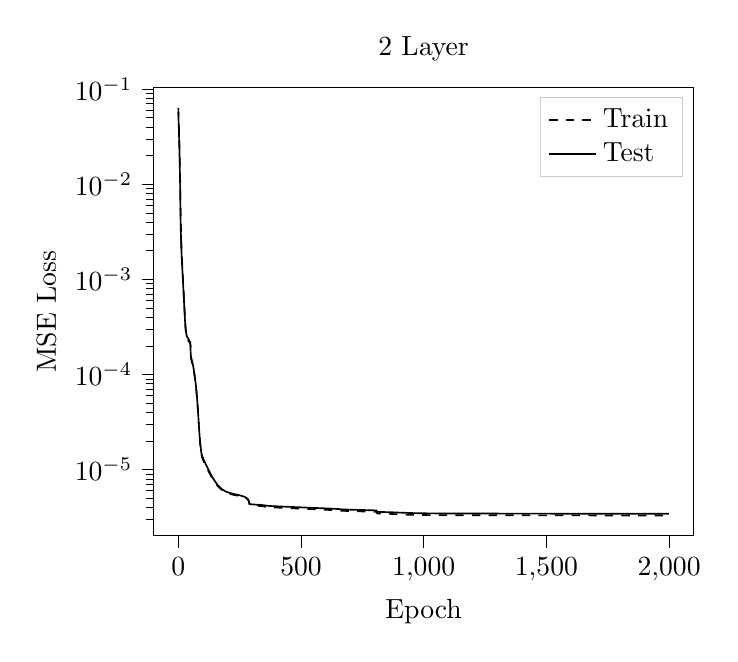
\begin{tikzpicture}

\begin{axis}[
legend cell align={left},
legend style={fill opacity=0.8, draw opacity=1, text opacity=1, draw=white!80!black},
log basis y={10},
tick align=outside,
tick pos=left,
title={2 Layer},
x grid style={white!69.0196078431373!black},
xlabel={Epoch},
xmin=-99.95, xmax=2098.95,
xtick style={color=black},
y grid style={white!69.0196078431373!black},
ylabel={MSE Loss},
ymin=2.00962005103304e-06, ymax=0.103609493820567,
ymode=log,
ytick style={color=black}
]
\addplot [semithick, black, dashed]
table {%
0 0.0632710078060627
1 0.051845450758934
2 0.0432980991452932
3 0.0358776403516531
4 0.0290690961554647
5 0.0229545622691512
6 0.0177181212641299
7 0.0134029685482383
8 0.00932001467421651
9 0.00582119612768292
10 0.00408269998338073
11 0.00310812011640519
12 0.00251322026690468
13 0.00211413772078231
14 0.00183244168199599
15 0.00161229025945067
16 0.00143017171323299
17 0.00127473987545818
18 0.0011382556988392
19 0.00101599448849447
20 0.000905665848404169
21 0.000806275674840435
22 0.00071686326363124
23 0.000636678095906973
24 0.000565266070072539
25 0.000501702402951196
26 0.000445806336938404
27 0.000397627679049037
28 0.000357118795858696
29 0.00032489347649971
30 0.000299998327216599
31 0.000281208114116453
32 0.000267276446160395
33 0.000257046025944874
34 0.0002495395517617
35 0.000243972511438187
36 0.000239745286788093
37 0.000236407682736171
38 0.000233631588111166
39 0.000231188191857655
40 0.000228926038951613
41 0.000226746779982932
42 0.000224590560450451
43 0.000222427553118905
44 0.000220237786095822
45 0.000218012332130456
46 0.000215740327854292
47 0.000213416477650753
48 0.000211034586711321
49 0.000208587526110932
50 0.000201116997253848
51 0.000158018265356077
52 0.000147613224027737
53 0.000142723495948303
54 0.000139244368234358
55 0.000136019374200259
56 0.000132747634241241
57 0.000129427922991454
58 0.000126070258433174
59 0.000122665663249791
60 0.000119213276564551
61 0.000115701421811536
62 0.000112120777172095
63 0.000108473681488249
64 0.000104762014772859
65 0.00010098851814837
66 9.71622276556445e-05
67 9.32928094116505e-05
68 8.93886299527367e-05
69 8.54555976766278e-05
70 8.14965877798386e-05
71 7.75122336417553e-05
72 7.35026992588246e-05
73 6.94685789057985e-05
74 6.54132343734091e-05
75 6.13432748941705e-05
76 5.72745405916066e-05
77 5.32301725179423e-05
78 4.92395857872907e-05
79 4.53403164574411e-05
80 4.1573930386221e-05
81 3.79849034761719e-05
82 3.46141511963651e-05
83 3.14956762558722e-05
84 2.8658379233093e-05
85 2.61181172882061e-05
86 2.38809501188371e-05
87 2.19437158739311e-05
88 2.0293696959925e-05
89 1.89088841780176e-05
90 1.77624986854426e-05
91 1.6823803317493e-05
92 1.60607825182524e-05
93 1.50258497696996e-05
94 1.4460581161984e-05
95 1.40592445336551e-05
96 1.37072536540472e-05
97 1.34257343074751e-05
98 1.31816849047937e-05
99 1.29646241002774e-05
100 1.27662120476089e-05
101 1.2581771216901e-05
102 1.24078030003147e-05
103 1.22411715728958e-05
104 1.20805520891736e-05
105 1.19247015427391e-05
106 1.1773092596286e-05
107 1.16248549329612e-05
108 1.14799404746009e-05
109 1.13379276499472e-05
110 1.11984094673971e-05
111 1.10615233461431e-05
112 1.09273854504863e-05
113 1.07954060031261e-05
114 1.06658476615848e-05
115 1.05386192249171e-05
116 1.04137884209194e-05
117 1.02908117264633e-05
118 1.01702188394484e-05
119 1.00515134595298e-05
120 9.93500102867984e-06
121 9.82061678314494e-06
122 9.70835857060592e-06
123 9.59800334567262e-06
124 9.48999531192385e-06
125 9.38343026655275e-06
126 9.2788389024463e-06
127 9.17616092829121e-06
128 9.07542354798352e-06
129 8.97668589686873e-06
130 8.87972992904906e-06
131 8.78457191856796e-06
132 8.69125409280969e-06
133 8.59979536244282e-06
134 8.51017152263012e-06
135 8.42218346087975e-06
136 8.33635802018762e-06
137 8.25191251988144e-06
138 8.16942619667316e-06
139 8.0887000030998e-06
140 8.00948176038219e-06
141 7.93231499164904e-06
142 7.85655636991578e-06
143 7.78257825504625e-06
144 7.71019455214628e-06
145 7.63938447198598e-06
146 7.57029341457383e-06
147 7.50287921164272e-06
148 7.43711638529021e-06
149 7.37279744384978e-06
150 7.31026423613912e-06
151 7.24875530431746e-06
152 7.18897826664033e-06
153 7.13090271165129e-06
154 7.07441331041991e-06
155 7.01886005163033e-06
156 6.96489755046059e-06
157 6.91240939818272e-06
158 6.86140954894654e-06
159 6.81176477974077e-06
160 6.76338529569875e-06
161 6.71635143635285e-06
162 6.67062341608471e-06
163 6.62643124655915e-06
164 6.58323398965877e-06
165 6.54126916742825e-06
166 6.50058312885449e-06
167 6.46115243034728e-06
168 6.42298308639511e-06
169 6.38602485582851e-06
170 6.35025759902419e-06
171 6.31564215518665e-06
172 6.2821410494962e-06
173 6.24969452883306e-06
174 6.21805136665898e-06
175 6.18742654864946e-06
176 6.15822291456425e-06
177 6.12961435763282e-06
178 6.10204494751088e-06
179 6.07546555693261e-06
180 6.04976868044105e-06
181 6.02458717798982e-06
182 6.00032682541496e-06
183 5.97695071451199e-06
184 5.95447526166026e-06
185 5.93280903376581e-06
186 5.91193096875031e-06
187 5.89195336056036e-06
188 5.87234221757171e-06
189 5.8534633653835e-06
190 5.83506993143601e-06
191 5.81726929294746e-06
192 5.79998251942015e-06
193 5.78317128065464e-06
194 5.76691470541846e-06
195 5.75105928714947e-06
196 5.73594326829152e-06
197 5.72154736437369e-06
198 5.70739826844147e-06
199 5.69361865041174e-06
200 5.68028440807211e-06
201 5.66706610925394e-06
202 5.65437040722827e-06
203 5.64182836365035e-06
204 5.62923450252129e-06
205 5.61731328298265e-06
206 5.60552214392374e-06
207 5.59428438737086e-06
208 5.58346819707367e-06
209 5.57276731524325e-06
210 5.56239524667035e-06
211 5.55222034631697e-06
212 5.54241197096417e-06
213 5.53287029742933e-06
214 5.52343979006764e-06
215 5.51419333123704e-06
216 5.5052181321571e-06
217 5.49665210428429e-06
218 5.48808294684022e-06
219 5.47977340056605e-06
220 5.47153629327113e-06
221 5.46346909595741e-06
222 5.45539895256297e-06
223 5.44765622976229e-06
224 5.44031825961611e-06
225 5.4328157098098e-06
226 5.42541469417301e-06
227 5.4179627427402e-06
228 5.41054173163502e-06
229 5.40329494447178e-06
230 5.39551419979034e-06
231 5.38808617102404e-06
232 5.38088338089437e-06
233 5.3739369534469e-06
234 5.36722018341607e-06
235 5.3601379581778e-06
236 5.35322880318745e-06
237 5.34662611130443e-06
238 5.33928093022951e-06
239 5.3319608723541e-06
240 5.32476024727657e-06
241 5.31745174248499e-06
242 5.3104168794107e-06
243 5.30307639201055e-06
244 5.29598574553347e-06
245 5.28916283337821e-06
246 5.28227127779246e-06
247 5.27531217994692e-06
248 5.26836660651497e-06
249 5.26145600565542e-06
250 5.25481974682407e-06
251 5.24836719614541e-06
252 5.24147814007847e-06
253 5.23453493815396e-06
254 5.22773011539357e-06
255 5.22081494614213e-06
256 5.21390236099251e-06
257 5.20662491862822e-06
258 5.19909029208066e-06
259 5.19156840505275e-06
260 5.1840717428604e-06
261 5.17612017256397e-06
262 5.16830087531162e-06
263 5.1598733487026e-06
264 5.15117472787097e-06
265 5.14193537469509e-06
266 5.13207956760198e-06
267 5.12154601028669e-06
268 5.11089195560999e-06
269 5.10023479159827e-06
270 5.08917057959479e-06
271 5.07760456798678e-06
272 5.06578773297406e-06
273 5.05217641853051e-06
274 5.0364313431146e-06
275 5.02120112696503e-06
276 5.00727311009541e-06
277 4.99260774995491e-06
278 4.97757784273745e-06
279 4.96154125721659e-06
280 4.94340508657842e-06
281 4.92293700722257e-06
282 4.89921165763008e-06
283 4.87050170272596e-06
284 4.83581983303338e-06
285 4.79348267253954e-06
286 4.74225533139361e-06
287 4.67328239142262e-06
288 4.58696049599894e-06
289 4.46936619255212e-06
290 4.31748006303678e-06
291 4.23798107794937e-06
292 4.22272348396291e-06
293 4.2174021655228e-06
294 4.21430222650088e-06
295 4.21172886331078e-06
296 4.20933076134133e-06
297 4.20704505904723e-06
298 4.20480583579774e-06
299 4.20261384238074e-06
300 4.20045522423607e-06
301 4.19840986728559e-06
302 4.19635286948505e-06
303 4.19434635909965e-06
304 4.1923705946374e-06
305 4.19050039226931e-06
306 4.18860404033694e-06
307 4.18674072125214e-06
308 4.18486637317983e-06
309 4.18306126630341e-06
310 4.18127912712407e-06
311 4.17950906694386e-06
312 4.17775834330314e-06
313 4.17607370832229e-06
314 4.17431320079231e-06
315 4.1727198783974e-06
316 4.17104828943593e-06
317 4.16937491081626e-06
318 4.16773654842473e-06
319 4.16610417369156e-06
320 4.16449309932432e-06
321 4.16296918592707e-06
322 4.16134395891277e-06
323 4.15973293388561e-06
324 4.15812554933837e-06
325 4.15651645334947e-06
326 4.15494718413356e-06
327 4.15333152818675e-06
328 4.15174744648539e-06
329 4.15025573261119e-06
330 4.14862696129603e-06
331 4.14689902572718e-06
332 4.14517258332125e-06
333 4.14342047315586e-06
334 4.14178949631605e-06
335 4.1400407767469e-06
336 4.13811117368823e-06
337 4.13610095756667e-06
338 4.13402996832701e-06
339 4.1318420285279e-06
340 4.1294807142549e-06
341 4.12701435834606e-06
342 4.12451515353496e-06
343 4.12194325031123e-06
344 4.11919797215887e-06
345 4.11631795668654e-06
346 4.11326574703708e-06
347 4.11016632801875e-06
348 4.10674409454259e-06
349 4.10305109289766e-06
350 4.09920685819998e-06
351 4.09521432902693e-06
352 4.0910061447903e-06
353 4.08667012720798e-06
354 4.08225326873435e-06
355 4.07795396699839e-06
356 4.07355116385588e-06
357 4.0691161605082e-06
358 4.06490110549385e-06
359 4.06080552897947e-06
360 4.05672974352456e-06
361 4.05283861550743e-06
362 4.04928707007457e-06
363 4.04601418176753e-06
364 4.0429513314848e-06
365 4.04010962870416e-06
366 4.03744269556228e-06
367 4.03506154293609e-06
368 4.03286837035921e-06
369 4.03083124660952e-06
370 4.02896440937184e-06
371 4.02703742270205e-06
372 4.02513960216311e-06
373 4.02338820936166e-06
374 4.02179212824194e-06
375 4.02032433521526e-06
376 4.01882592655056e-06
377 4.01735797845504e-06
378 4.01590311412292e-06
379 4.01456900135599e-06
380 4.01327008967201e-06
381 4.01198213216958e-06
382 4.01074603587404e-06
383 4.0095192375702e-06
384 4.00830898684035e-06
385 4.00709463201565e-06
386 4.0059097862013e-06
387 4.00470182489698e-06
388 4.00351677558319e-06
389 4.00236419886824e-06
390 4.00116998844169e-06
391 3.99998082389175e-06
392 3.99884801413464e-06
393 3.99764587837126e-06
394 3.99651417865243e-06
395 3.99532578603612e-06
396 3.99419785026112e-06
397 3.99303706149112e-06
398 3.99190068537791e-06
399 3.99077415227112e-06
400 3.98964895885001e-06
401 3.98854520904024e-06
402 3.98738429157675e-06
403 3.98626458650142e-06
404 3.98513616232776e-06
405 3.98401351844768e-06
406 3.98287694929422e-06
407 3.98177175156889e-06
408 3.98065694753313e-06
409 3.97955125094995e-06
410 3.97847688532238e-06
411 3.97736476134014e-06
412 3.97623916978773e-06
413 3.97515318627484e-06
414 3.97404352497688e-06
415 3.97295079324067e-06
416 3.97184997132172e-06
417 3.97074828265431e-06
418 3.96966739663185e-06
419 3.96858127305677e-06
420 3.96750045547378e-06
421 3.96643120166118e-06
422 3.96534202013754e-06
423 3.96427063765259e-06
424 3.96322433994101e-06
425 3.96213134354184e-06
426 3.96106135895025e-06
427 3.95999829197535e-06
428 3.95894019357001e-06
429 3.95790915376892e-06
430 3.95684226828053e-06
431 3.95577681206305e-06
432 3.95472414516007e-06
433 3.95362605377159e-06
434 3.95254756790564e-06
435 3.95150437725533e-06
436 3.95043570642883e-06
437 3.94937866462897e-06
438 3.94838115562379e-06
439 3.94730105404051e-06
440 3.94621883810942e-06
441 3.9451766710954e-06
442 3.94410750595853e-06
443 3.94304689325509e-06
444 3.94200809296308e-06
445 3.94095385900073e-06
446 3.93992307658664e-06
447 3.93891124645052e-06
448 3.93786665722473e-06
449 3.93685992435167e-06
450 3.9358440626529e-06
451 3.93480710340555e-06
452 3.93380716809588e-06
453 3.93278114415807e-06
454 3.93176267130002e-06
455 3.93070953191454e-06
456 3.92965003652535e-06
457 3.92862235230496e-06
458 3.92760561658179e-06
459 3.92657984616562e-06
460 3.9255645015146e-06
461 3.92449227001634e-06
462 3.92346870353322e-06
463 3.92245446937522e-06
464 3.92145133218946e-06
465 3.92043095689587e-06
466 3.91943706358688e-06
467 3.91841551595462e-06
468 3.91737812401516e-06
469 3.91636446238408e-06
470 3.91536215056476e-06
471 3.91434734888207e-06
472 3.91334745836502e-06
473 3.91231219873589e-06
474 3.91130924549543e-06
475 3.91030783475799e-06
476 3.90929390709971e-06
477 3.90829968523576e-06
478 3.90728442221189e-06
479 3.9063041681402e-06
480 3.90529386982053e-06
481 3.90429663980285e-06
482 3.90328932166994e-06
483 3.90228188075525e-06
484 3.90130058735849e-06
485 3.90029922914437e-06
486 3.89929259267774e-06
487 3.89830421522674e-06
488 3.89731379686964e-06
489 3.89628200673542e-06
490 3.89534313785589e-06
491 3.89432079941798e-06
492 3.89331514952573e-06
493 3.89229541360692e-06
494 3.89127347989415e-06
495 3.89029763300641e-06
496 3.88925411311902e-06
497 3.88816214581311e-06
498 3.88687702547941e-06
499 3.88587540737717e-06
500 3.88488475755366e-06
501 3.88386549957431e-06
502 3.88286122324644e-06
503 3.88185147426157e-06
504 3.88082735753414e-06
505 3.87983534415071e-06
506 3.87884211681921e-06
507 3.87786378541932e-06
508 3.87690347974967e-06
509 3.87590351806466e-06
510 3.87493697735408e-06
511 3.87393002165481e-06
512 3.87293140079237e-06
513 3.87193410711006e-06
514 3.87096493568606e-06
515 3.86997004397927e-06
516 3.86899167233423e-06
517 3.86810477471045e-06
518 3.86708819746673e-06
519 3.86609972861152e-06
520 3.86511584406435e-06
521 3.86410707824325e-06
522 3.86309811415231e-06
523 3.86210161127565e-06
524 3.86109321630101e-06
525 3.86009254270903e-06
526 3.85912106071373e-06
527 3.85811027194904e-06
528 3.85712550837525e-06
529 3.85611493993565e-06
530 3.85510660271393e-06
531 3.85410345074888e-06
532 3.85311390755305e-06
533 3.85213474737611e-06
534 3.85112630192452e-06
535 3.85012735591772e-06
536 3.84913734296788e-06
537 3.84815157872254e-06
538 3.84717732458739e-06
539 3.84619277247111e-06
540 3.84522993113023e-06
541 3.8442311797553e-06
542 3.84322497643552e-06
543 3.84227112340341e-06
544 3.8412537937802e-06
545 3.84022483763147e-06
546 3.83922470746256e-06
547 3.83821959007946e-06
548 3.83719782143999e-06
549 3.83618380419648e-06
550 3.83516073952705e-06
551 3.83415338933446e-06
552 3.83312635744915e-06
553 3.83206138189962e-06
554 3.83102651903755e-06
555 3.82998564509762e-06
556 3.82895923803517e-06
557 3.82797941483659e-06
558 3.82694782160797e-06
559 3.82592881351229e-06
560 3.82489514527151e-06
561 3.82387169111098e-06
562 3.82288159403288e-06
563 3.82187921854893e-06
564 3.82090538437296e-06
565 3.81990201117333e-06
566 3.81885945239446e-06
567 3.8178061686267e-06
568 3.81674583468339e-06
569 3.81568310513103e-06
570 3.81460992866778e-06
571 3.81355367085234e-06
572 3.81251289786633e-06
573 3.81145554933937e-06
574 3.8104192146875e-06
575 3.8093715679679e-06
576 3.80830061658344e-06
577 3.80721733722567e-06
578 3.80615091921754e-06
579 3.80504406757609e-06
580 3.80396494574597e-06
581 3.80284883271997e-06
582 3.80177165607165e-06
583 3.80069691914287e-06
584 3.79964723424564e-06
585 3.7985892818142e-06
586 3.79753483116474e-06
587 3.79640749065402e-06
588 3.79530364398306e-06
589 3.7941353525639e-06
590 3.79299306950998e-06
591 3.79188061958757e-06
592 3.79073451824752e-06
593 3.78960781699789e-06
594 3.78849956632621e-06
595 3.7874091502772e-06
596 3.78626679844274e-06
597 3.78513176633533e-06
598 3.78400663305456e-06
599 3.78287078638095e-06
600 3.78169056853039e-06
601 3.78051059510653e-06
602 3.77938837505099e-06
603 3.77821030451742e-06
604 3.77709365989176e-06
605 3.77594412566395e-06
606 3.77473977471254e-06
607 3.77356035733101e-06
608 3.77238059650153e-06
609 3.77121746578268e-06
610 3.77010574015912e-06
611 3.76895438330394e-06
612 3.76782894613825e-06
613 3.76667858108704e-06
614 3.76551559270411e-06
615 3.76439185151867e-06
616 3.76326227546997e-06
617 3.76208450234117e-06
618 3.76090089821446e-06
619 3.75969973163137e-06
620 3.75851625665291e-06
621 3.75739111655093e-06
622 3.75627195273864e-06
623 3.75508487604748e-06
624 3.75392496414406e-06
625 3.75275827741461e-06
626 3.75164966681041e-06
627 3.7504619098172e-06
628 3.7492805902275e-06
629 3.74812237578226e-06
630 3.74700240786297e-06
631 3.74586033490232e-06
632 3.74465033678462e-06
633 3.74347466811287e-06
634 3.74222576670036e-06
635 3.74095193990343e-06
636 3.73970642544919e-06
637 3.73849202571819e-06
638 3.73727273176883e-06
639 3.73604903143132e-06
640 3.73481999326941e-06
641 3.73360565822622e-06
642 3.73240932685803e-06
643 3.73127844181909e-06
644 3.73011926103572e-06
645 3.72891290930966e-06
646 3.727741849616e-06
647 3.72646188213821e-06
648 3.72512999217633e-06
649 3.72386121966883e-06
650 3.72253252623977e-06
651 3.72115426330311e-06
652 3.71982453145847e-06
653 3.7184918338653e-06
654 3.71706787746007e-06
655 3.71560938947368e-06
656 3.71417414066855e-06
657 3.71250464706918e-06
658 3.71070990593125e-06
659 3.70882397623973e-06
660 3.70690597890189e-06
661 3.70420897252188e-06
662 3.70078934975027e-06
663 3.69826730502609e-06
664 3.69612601537028e-06
665 3.69425015776415e-06
666 3.69259916294595e-06
667 3.69112746614064e-06
668 3.68980126438601e-06
669 3.6885883330342e-06
670 3.68746814126553e-06
671 3.68644335560475e-06
672 3.68547208643122e-06
673 3.68455293175884e-06
674 3.683675603952e-06
675 3.68285116735478e-06
676 3.6820184672024e-06
677 3.68124188753427e-06
678 3.68046135884015e-06
679 3.67971530249633e-06
680 3.67896949774149e-06
681 3.67823716908333e-06
682 3.67751394207971e-06
683 3.67678034842811e-06
684 3.67607592556851e-06
685 3.67535497991867e-06
686 3.67465632757558e-06
687 3.67394465786219e-06
688 3.6732546661824e-06
689 3.67254644345394e-06
690 3.67185343293386e-06
691 3.67115930930595e-06
692 3.67046825454054e-06
693 3.66977536043578e-06
694 3.66907607531175e-06
695 3.66839212199466e-06
696 3.66770006837669e-06
697 3.6670071425533e-06
698 3.66632715258675e-06
699 3.66563417685484e-06
700 3.66494473416878e-06
701 3.66426724519897e-06
702 3.66358821713675e-06
703 3.66290142187609e-06
704 3.6622132258799e-06
705 3.6615301440861e-06
706 3.66084534357469e-06
707 3.66017243891292e-06
708 3.6594921489268e-06
709 3.65881293635084e-06
710 3.65812857126002e-06
711 3.6574575931354e-06
712 3.65677416755261e-06
713 3.65609544701329e-06
714 3.65541832900362e-06
715 3.65474015052314e-06
716 3.65406903290477e-06
717 3.65339285406208e-06
718 3.65271773671338e-06
719 3.65204745116898e-06
720 3.651368467672e-06
721 3.65069879228486e-06
722 3.65002570674733e-06
723 3.64936534811022e-06
724 3.64868461804235e-06
725 3.64801084799637e-06
726 3.64734410402434e-06
727 3.64667091173487e-06
728 3.6460121403934e-06
729 3.6453348136547e-06
730 3.64466524786167e-06
731 3.6439993359636e-06
732 3.64334011158007e-06
733 3.64267599638879e-06
734 3.64200718195207e-06
735 3.64133908624353e-06
736 3.64068387693806e-06
737 3.64001761658983e-06
738 3.63935759855849e-06
739 3.63869932277794e-06
740 3.6380411635264e-06
741 3.63737760744698e-06
742 3.63650741667243e-06
743 3.63583347075291e-06
744 3.63516651168538e-06
745 3.63449705389485e-06
746 3.63384109414255e-06
747 3.63316582570405e-06
748 3.63250598411469e-06
749 3.63184671437011e-06
750 3.63118088159808e-06
751 3.63051347460441e-06
752 3.62984826938373e-06
753 3.62920208863216e-06
754 3.62853011097286e-06
755 3.62786857806441e-06
756 3.62720777866343e-06
757 3.62655042818005e-06
758 3.62588549194243e-06
759 3.62523838361994e-06
760 3.62457825156071e-06
761 3.62390604811935e-06
762 3.62325307582978e-06
763 3.62259630355766e-06
764 3.62194640536018e-06
765 3.62129782820375e-06
766 3.62063571492399e-06
767 3.61997041034101e-06
768 3.61932698899636e-06
769 3.61866497462415e-06
770 3.6180262252401e-06
771 3.617362689738e-06
772 3.61671298037436e-06
773 3.61607361901406e-06
774 3.61541275435684e-06
775 3.6147658632899e-06
776 3.61411101857811e-06
777 3.61345795158741e-06
778 3.61281008554215e-06
779 3.61216918668106e-06
780 3.6115153557148e-06
781 3.61088205590931e-06
782 3.61022876393236e-06
783 3.6095767355846e-06
784 3.60893789741112e-06
785 3.60828682255487e-06
786 3.60765805169194e-06
787 3.60699846305579e-06
788 3.60636278833226e-06
789 3.60572352553845e-06
790 3.60508044082053e-06
791 3.60444044986252e-06
792 3.60379261326216e-06
793 3.60315890213769e-06
794 3.60252107452652e-06
795 3.60187887156371e-06
796 3.6012473944993e-06
797 3.60060167395204e-06
798 3.59996799465989e-06
799 3.59931844286621e-06
800 3.59868616624226e-06
801 3.59804496190463e-06
802 3.59741519469026e-06
803 3.59679051234707e-06
804 3.59614438116296e-06
805 3.59551126325641e-06
806 3.59488375943329e-06
807 3.59423938243708e-06
808 3.59361888456533e-06
809 3.58856573075173e-06
810 3.46819658852837e-06
811 3.45905467918328e-06
812 3.45808383144686e-06
813 3.45728719207727e-06
814 3.45646615710393e-06
815 3.4557891899567e-06
816 3.45512566559592e-06
817 3.45442840398391e-06
818 3.45375150789096e-06
819 3.45314441744904e-06
820 3.45249377733126e-06
821 3.45187570439975e-06
822 3.4512920127554e-06
823 3.45072540699221e-06
824 3.45013294111141e-06
825 3.44956170420119e-06
826 3.44901385676621e-06
827 3.44852854482269e-06
828 3.44790018584717e-06
829 3.44723031332705e-06
830 3.44663635894449e-06
831 3.44601887513818e-06
832 3.44534294094956e-06
833 3.44472433505416e-06
834 3.44406132182939e-06
835 3.44345207020069e-06
836 3.44280726289981e-06
837 3.4422474728899e-06
838 3.44163713850776e-06
839 3.44108118099484e-06
840 3.44047824160043e-06
841 3.4398152462245e-06
842 3.43910582000717e-06
843 3.43842116046744e-06
844 3.43774710404432e-06
845 3.43702792099521e-06
846 3.43634997943809e-06
847 3.43563018009263e-06
848 3.43499882342257e-06
849 3.43428135010981e-06
850 3.43356308815146e-06
851 3.43284928339926e-06
852 3.43210946982708e-06
853 3.43137287131867e-06
854 3.43064236994906e-06
855 3.42992232879169e-06
856 3.42917290743117e-06
857 3.42838393817146e-06
858 3.42754296923431e-06
859 3.42668330313245e-06
860 3.42588032242475e-06
861 3.42507210848453e-06
862 3.42416718467575e-06
863 3.42335599020771e-06
864 3.42258317823507e-06
865 3.42167720782527e-06
866 3.42081106327896e-06
867 3.41993027393528e-06
868 3.41898223450698e-06
869 3.41806178505522e-06
870 3.41711957901225e-06
871 3.41628901833246e-06
872 3.41533120615622e-06
873 3.41435020516201e-06
874 3.41339523242823e-06
875 3.41245838376381e-06
876 3.4114890966066e-06
877 3.41038971214402e-06
878 3.40855177046251e-06
879 3.40721698319157e-06
880 3.40610965008636e-06
881 3.40513882656524e-06
882 3.40419041424411e-06
883 3.40332646044317e-06
884 3.40240671414449e-06
885 3.4013559078403e-06
886 3.40033198938272e-06
887 3.39924581226114e-06
888 3.39811470360019e-06
889 3.39708300680286e-06
890 3.39614488370898e-06
891 3.39512193158953e-06
892 3.39409216473996e-06
893 3.39310099377599e-06
894 3.39206634293987e-06
895 3.39110838353918e-06
896 3.39012106735481e-06
897 3.3891239560262e-06
898 3.38814063684367e-06
899 3.38709192863007e-06
900 3.38610237486137e-06
901 3.38508347010702e-06
902 3.38407450976774e-06
903 3.38305720777043e-06
904 3.38207762490583e-06
905 3.38106447293285e-06
906 3.38001549198452e-06
907 3.37896211885891e-06
908 3.37797512941052e-06
909 3.37698621433447e-06
910 3.37599381316522e-06
911 3.37501526473716e-06
912 3.37411181067182e-06
913 3.37317492824241e-06
914 3.37220609208089e-06
915 3.3712260875518e-06
916 3.37031230503726e-06
917 3.36942957324027e-06
918 3.36857478896491e-06
919 3.36759936112685e-06
920 3.36662839538349e-06
921 3.36570018896509e-06
922 3.3648025120101e-06
923 3.36392968029031e-06
924 3.3630231520192e-06
925 3.36211414503396e-06
926 3.36128224489585e-06
927 3.36038605507838e-06
928 3.35971276251712e-06
929 3.35890150881824e-06
930 3.35802607730784e-06
931 3.35722394027016e-06
932 3.35641767048855e-06
933 3.35569475134889e-06
934 3.35492151180006e-06
935 3.35416929988241e-06
936 3.35343535334687e-06
937 3.35275004340474e-06
938 3.3520320862408e-06
939 3.35134114561697e-06
940 3.35064550688458e-06
941 3.34997043398744e-06
942 3.34934603586134e-06
943 3.34871437360107e-06
944 3.34808450747914e-06
945 3.34750664876537e-06
946 3.34689332385096e-06
947 3.34634646662835e-06
948 3.34575365366163e-06
949 3.34518739339273e-06
950 3.34464585841943e-06
951 3.34406109845986e-06
952 3.34353921266484e-06
953 3.34303967986216e-06
954 3.34256621943041e-06
955 3.34205329431825e-06
956 3.34155066923358e-06
957 3.34107601361211e-06
958 3.34061679984643e-06
959 3.34015869543691e-06
960 3.33970654855875e-06
961 3.3393236901702e-06
962 3.33886904593328e-06
963 3.33842913983062e-06
964 3.33814169107427e-06
965 3.33774210423599e-06
966 3.3372913213725e-06
967 3.33686178612425e-06
968 3.33645433522634e-06
969 3.33606849665102e-06
970 3.33571005978683e-06
971 3.33536255254785e-06
972 3.33501844590955e-06
973 3.33469381189389e-06
974 3.33438582435974e-06
975 3.33408202118335e-06
976 3.33378812365481e-06
977 3.33350157063705e-06
978 3.33323775805638e-06
979 3.3330256313775e-06
980 3.33272925752226e-06
981 3.33243786371895e-06
982 3.33216787623769e-06
983 3.3319054509775e-06
984 3.33164250014306e-06
985 3.33139780241254e-06
986 3.33115889634428e-06
987 3.33091831510046e-06
988 3.33069397129293e-06
989 3.33046564878714e-06
990 3.33024445262708e-06
991 3.33003096750417e-06
992 3.32982458940023e-06
993 3.32962686138671e-06
994 3.32943600267299e-06
995 3.32926675400813e-06
996 3.32906775338415e-06
997 3.3288823390194e-06
998 3.32862334119e-06
999 3.3284366764974e-06
1000 3.32826502312855e-06
1001 3.32808903544901e-06
1002 3.3279268395745e-06
1003 3.3277572111956e-06
1004 3.32759605612409e-06
1005 3.32745577202331e-06
1006 3.32727387956311e-06
1007 3.32710411589687e-06
1008 3.32693895040848e-06
1009 3.32677818335014e-06
1010 3.32661705760984e-06
1011 3.32647359664406e-06
1012 3.32631457933985e-06
1013 3.32618127072237e-06
1014 3.32603964534428e-06
1015 3.32589951085538e-06
1016 3.32574876642866e-06
1017 3.32563812094122e-06
1018 3.325481228444e-06
1019 3.32533804532886e-06
1020 3.32519677795062e-06
1021 3.32507743246424e-06
1022 3.32495024065338e-06
1023 3.32481203804491e-06
1024 3.32468024942045e-06
1025 3.32454988460995e-06
1026 3.32442952083056e-06
1027 3.32430381183713e-06
1028 3.32418459424844e-06
1029 3.32406650829853e-06
1030 3.32396275587143e-06
1031 3.32385228330168e-06
1032 3.32373832941357e-06
1033 3.32363166569394e-06
1034 3.32353530177443e-06
1035 3.32343474212848e-06
1036 3.32334030849779e-06
1037 3.32324221994895e-06
1038 3.32314650916032e-06
1039 3.32305175118108e-06
1040 3.32298359035121e-06
1041 3.32284780517966e-06
1042 3.32274852030423e-06
1043 3.3226549801384e-06
1044 3.32256201613745e-06
1045 3.32246874370412e-06
1046 3.3223735683805e-06
1047 3.32228958177438e-06
1048 3.32220481595868e-06
1049 3.32208896418251e-06
1050 3.32200541083694e-06
1051 3.32191331938247e-06
1052 3.32182456236296e-06
1053 3.32175064909279e-06
1054 3.3216608036355e-06
1055 3.32158123887893e-06
1056 3.32150148597066e-06
1057 3.3214288405361e-06
1058 3.32134673897144e-06
1059 3.32127205160759e-06
1060 3.3211996552609e-06
1061 3.32111623322362e-06
1062 3.32105358813806e-06
1063 3.32098555361426e-06
1064 3.320912385675e-06
1065 3.32084120304899e-06
1066 3.32077246423523e-06
1067 3.32069897615384e-06
1068 3.32062761867746e-06
1069 3.32055835360734e-06
1070 3.32049213534447e-06
1071 3.32042758327589e-06
1072 3.32035822054877e-06
1073 3.32029157220859e-06
1074 3.3202237336809e-06
1075 3.32016097570431e-06
1076 3.32010107376846e-06
1077 3.32003031508066e-06
1078 3.31996242221066e-06
1079 3.31990452946229e-06
1080 3.31984272509089e-06
1081 3.3197831430698e-06
1082 3.31972265939839e-06
1083 3.31965873988338e-06
1084 3.31960340872683e-06
1085 3.31954086311725e-06
1086 3.31948666712378e-06
1087 3.31942682998942e-06
1088 3.31936341729033e-06
1089 3.31931191681178e-06
1090 3.31925431248692e-06
1091 3.31908182454299e-06
1092 3.31901709694193e-06
1093 3.31896539614718e-06
1094 3.31891274390728e-06
1095 3.31885061757475e-06
1096 3.31879793600365e-06
1097 3.3187468189908e-06
1098 3.31868890623355e-06
1099 3.31862838606867e-06
1100 3.31856975185474e-06
1101 3.31851502880909e-06
1102 3.31847244035544e-06
1103 3.31840572573583e-06
1104 3.3183519180966e-06
1105 3.31829593142174e-06
1106 3.31823610724769e-06
1107 3.31818831443798e-06
1108 3.31813788932322e-06
1109 3.31809355793666e-06
1110 3.31803202232095e-06
1111 3.31797998080674e-06
1112 3.31792680481158e-06
1113 3.31787022776098e-06
1114 3.31782323041807e-06
1115 3.31776938503481e-06
1116 3.31772539641406e-06
1117 3.31767134389338e-06
1118 3.31762536609403e-06
1119 3.31757380968156e-06
1120 3.31752182080436e-06
1121 3.31747144957717e-06
1122 3.31731329424656e-06
1123 3.31725821206419e-06
1124 3.31720646829581e-06
1125 3.31715368929508e-06
1126 3.31710390935314e-06
1127 3.3170535549516e-06
1128 3.31699749733616e-06
1129 3.31695505599328e-06
1130 3.31690347150015e-06
1131 3.31685236983503e-06
1132 3.31680772876552e-06
1133 3.3167499815363e-06
1134 3.31669872764451e-06
1135 3.31664693214861e-06
1136 3.31659686685271e-06
1137 3.31655298123223e-06
1138 3.31649509212184e-06
1139 3.31645859967011e-06
1140 3.31640772060382e-06
1141 3.31635877830649e-06
1142 3.31630854077503e-06
1143 3.3162615816309e-06
1144 3.31620984627534e-06
1145 3.31616943481095e-06
1146 3.31612526088065e-06
1147 3.31607749308205e-06
1148 3.31602828350697e-06
1149 3.31598170487268e-06
1150 3.31593465273272e-06
1151 3.31589305983471e-06
1152 3.31584171124177e-06
1153 3.31579683393102e-06
1154 3.31575542475093e-06
1155 3.31569906404638e-06
1156 3.31566256102178e-06
1157 3.31562098369886e-06
1158 3.31557101537783e-06
1159 3.31552743352859e-06
1160 3.31547878431593e-06
1161 3.31543595132189e-06
1162 3.31539260980662e-06
1163 3.31535449493003e-06
1164 3.31530274024772e-06
1165 3.31526033858154e-06
1166 3.31521684279323e-06
1167 3.31517224708477e-06
1168 3.31512761704289e-06
1169 3.31509071429537e-06
1170 3.31504686755579e-06
1171 3.31499783703748e-06
1172 3.31494618387751e-06
1173 3.31488194569829e-06
1174 3.31483411434874e-06
1175 3.31477687655024e-06
1176 3.31463223449191e-06
1177 3.3145593424706e-06
1178 3.31451699707941e-06
1179 3.31447909991311e-06
1180 3.31444194944197e-06
1181 3.31440136801575e-06
1182 3.3143566832905e-06
1183 3.31432279710953e-06
1184 3.3142888198654e-06
1185 3.31424507578504e-06
1186 3.31421255020814e-06
1187 3.31417136544587e-06
1188 3.31413100582267e-06
1189 3.31409358943802e-06
1190 3.3140541273724e-06
1191 3.31401387495589e-06
1192 3.31398105663538e-06
1193 3.31394617762726e-06
1194 3.31390259668751e-06
1195 3.31387615858603e-06
1196 3.31384136154611e-06
1197 3.31379895965256e-06
1198 3.31376556687246e-06
1199 3.31373439541949e-06
1200 3.31369409514082e-06
1201 3.31365316878873e-06
1202 3.31363031023102e-06
1203 3.31359488518501e-06
1204 3.31356466006127e-06
1205 3.31353000353829e-06
1206 3.3134903616201e-06
1207 3.31346309042146e-06
1208 3.31342015306291e-06
1209 3.31339084232241e-06
1210 3.3133535714569e-06
1211 3.31332341784218e-06
1212 3.31328962545285e-06
1213 3.31325111255865e-06
1214 3.31321978012511e-06
1215 3.31318277721948e-06
1216 3.31314616198597e-06
1217 3.31311287493463e-06
1218 3.31307958356319e-06
1219 3.31304765325058e-06
1220 3.31300194511641e-06
1221 3.31296959791416e-06
1222 3.31293913814079e-06
1223 3.31290463248024e-06
1224 3.31286963171351e-06
1225 3.31283649222769e-06
1226 3.31280664943279e-06
1227 3.31276422059545e-06
1228 3.31273262804643e-06
1229 3.31270691606278e-06
1230 3.31266566593058e-06
1231 3.31263192094866e-06
1232 3.31260459256555e-06
1233 3.31257304628707e-06
1234 3.31253451588509e-06
1235 3.3125027416645e-06
1236 3.31246954056041e-06
1237 3.31243238213119e-06
1238 3.31239868376088e-06
1239 3.31237523766958e-06
1240 3.31232966425432e-06
1241 3.3123012260603e-06
1242 3.31226731339029e-06
1243 3.31223492764821e-06
1244 3.31220416660472e-06
1245 3.3121651907777e-06
1246 3.31213434481015e-06
1247 3.31210411036409e-06
1248 3.31207334511419e-06
1249 3.31204188125866e-06
1250 3.31200534310483e-06
1251 3.31196890385854e-06
1252 3.31193951285513e-06
1253 3.31191298664635e-06
1254 3.31186976950448e-06
1255 3.31183692810555e-06
1256 3.31180187276914e-06
1257 3.31176736733596e-06
1258 3.31174078667118e-06
1259 3.31170079664389e-06
1260 3.31167498484319e-06
1261 3.31163897067199e-06
1262 3.31160367568373e-06
1263 3.31157391030956e-06
1264 3.31153827073649e-06
1265 3.31150821864412e-06
1266 3.31147878000593e-06
1267 3.31144059236976e-06
1268 3.3114125475322e-06
1269 3.31137845250851e-06
1270 3.31135019507656e-06
1271 3.31132036353665e-06
1272 3.31128353366239e-06
1273 3.31124508727498e-06
1274 3.3112155958861e-06
1275 3.31118322765178e-06
1276 3.31115418396166e-06
1277 3.31111870571021e-06
1278 3.31108915679579e-06
1279 3.31105810823829e-06
1280 3.31101666643008e-06
1281 3.31099420361625e-06
1282 3.31095552917304e-06
1283 3.31091766827285e-06
1284 3.31088738289509e-06
1285 3.31086019934901e-06
1286 3.31082479078759e-06
1287 3.3107894528257e-06
1288 3.31076125996788e-06
1289 3.31073088023004e-06
1290 3.31069415051388e-06
1291 3.31065719831258e-06
1292 3.31063165572232e-06
1293 3.31060190774224e-06
1294 3.3105640161466e-06
1295 3.31053720560703e-06
1296 3.31050339457306e-06
1297 3.31046521137068e-06
1298 3.31043459812008e-06
1299 3.31039810896527e-06
1300 3.31036881345881e-06
1301 3.31033730344643e-06
1302 3.310306435651e-06
1303 3.31026991398176e-06
1304 3.31024301567595e-06
1305 3.31020190742493e-06
1306 3.31017149255786e-06
1307 3.3101332599017e-06
1308 3.31010171169055e-06
1309 3.31005946975438e-06
1310 3.31003425515064e-06
1311 3.30999968309698e-06
1312 3.30996857246646e-06
1313 3.30993229317755e-06
1314 3.30990236466278e-06
1315 3.30987621293843e-06
1316 3.30983615754121e-06
1317 3.30979875263893e-06
1318 3.30977489818451e-06
1319 3.30974435814824e-06
1320 3.30970497532235e-06
1321 3.30967777449587e-06
1322 3.30965184900833e-06
1323 3.30961561678578e-06
1324 3.30957849496372e-06
1325 3.30955011418155e-06
1326 3.30952235151472e-06
1327 3.30948825808264e-06
1328 3.30946376834618e-06
1329 3.30942424557179e-06
1330 3.30939567766109e-06
1331 3.30936111083702e-06
1332 3.30933207965245e-06
1333 3.3093084363145e-06
1334 3.30927065931519e-06
1335 3.30923937360694e-06
1336 3.30921289116759e-06
1337 3.30918081397158e-06
1338 3.30914972573737e-06
1339 3.30911605874462e-06
1340 3.30908646151329e-06
1341 3.30905639475532e-06
1342 3.30902801658795e-06
1343 3.30899296102416e-06
1344 3.30896267894332e-06
1345 3.3089325166884e-06
1346 3.30890046916466e-06
1347 3.30886465042113e-06
1348 3.3088395756522e-06
1349 3.30881382774351e-06
1350 3.30877656608664e-06
1351 3.30874721919372e-06
1352 3.30871065659721e-06
1353 3.30867955688063e-06
1354 3.30865487069332e-06
1355 3.30862191162851e-06
1356 3.30859550501827e-06
1357 3.30855776235239e-06
1358 3.30853303728418e-06
1359 3.30850446073327e-06
1360 3.30846531176121e-06
1361 3.30843728659147e-06
1362 3.30840472588534e-06
1363 3.30837749436341e-06
1364 3.30834483236231e-06
1365 3.30830624568534e-06
1366 3.30828763708269e-06
1367 3.30825550838654e-06
1368 3.30822551416077e-06
1369 3.30818973498026e-06
1370 3.30815789163807e-06
1371 3.30812527829494e-06
1372 3.30809859678993e-06
1373 3.30806258318717e-06
1374 3.30803215661035e-06
1375 3.30800900974282e-06
1376 3.30797151002571e-06
1377 3.30794009107649e-06
1378 3.30791404837782e-06
1379 3.30788173698693e-06
1380 3.30785453468252e-06
1381 3.30781790967194e-06
1382 3.30779392106706e-06
1383 3.30776260773291e-06
1384 3.30773389839578e-06
1385 3.30769640322615e-06
1386 3.30766638410296e-06
1387 3.30763812337409e-06
1388 3.30760337055835e-06
1389 3.30757708707097e-06
1390 3.307545913799e-06
1391 3.30751326794143e-06
1392 3.30749232489325e-06
1393 3.30745411440603e-06
1394 3.30735595673559e-06
1395 3.30729904260352e-06
1396 3.30725218407224e-06
1397 3.30722578951281e-06
1398 3.30719073667751e-06
1399 3.30716875021153e-06
1400 3.30714862934656e-06
1401 3.30711684216567e-06
1402 3.3070819894192e-06
1403 3.3070488652811e-06
1404 3.30701422922175e-06
1405 3.30698709717581e-06
1406 3.30695631168965e-06
1407 3.30692265868038e-06
1408 3.30688969722814e-06
1409 3.30686106201483e-06
1410 3.3068254247155e-06
1411 3.3067949505039e-06
1412 3.30675967359184e-06
1413 3.30672607924498e-06
1414 3.30669463016875e-06
1415 3.30665754358961e-06
1416 3.30661870475524e-06
1417 3.30659057021876e-06
1418 3.30655833431592e-06
1419 3.30653160381189e-06
1420 3.30648229748931e-06
1421 3.3064635277924e-06
1422 3.30642847688978e-06
1423 3.30640005802252e-06
1424 3.30635991497275e-06
1425 3.30633839712391e-06
1426 3.30630923531317e-06
1427 3.30627130324501e-06
1428 3.30624613002328e-06
1429 3.30621113914731e-06
1430 3.30618818611583e-06
1431 3.30615022528491e-06
1432 3.30612555853804e-06
1433 3.3060949335777e-06
1434 3.30606805039224e-06
1435 3.30602659039414e-06
1436 3.30600337179021e-06
1437 3.30597711342762e-06
1438 3.30594837578246e-06
1439 3.30591299587013e-06
1440 3.30588416147748e-06
1441 3.30585510812398e-06
1442 3.30582726405737e-06
1443 3.30579878891513e-06
1444 3.30576666067373e-06
1445 3.30573926805755e-06
1446 3.30570304413413e-06
1447 3.30567544233418e-06
1448 3.30564356863761e-06
1449 3.30561513396788e-06
1450 3.3055900224781e-06
1451 3.30555552284295e-06
1452 3.30552562525099e-06
1453 3.30550001433494e-06
1454 3.30546434372536e-06
1455 3.30543629740987e-06
1456 3.30540926006506e-06
1457 3.30537772595108e-06
1458 3.30534853821973e-06
1459 3.30531810948287e-06
1460 3.30529423752068e-06
1461 3.30526512493634e-06
1462 3.30523205786903e-06
1463 3.30520980810434e-06
1464 3.30517069141933e-06
1465 3.30514524932823e-06
1466 3.3051182268764e-06
1467 3.3050883089345e-06
1468 3.30505295073635e-06
1469 3.30502717281433e-06
1470 3.30499619519742e-06
1471 3.30496268304614e-06
1472 3.3049321046974e-06
1473 3.30491160332258e-06
1474 3.30488403938034e-06
1475 3.30484924450047e-06
1476 3.30482337255944e-06
1477 3.3047829225552e-06
1478 3.30475701593969e-06
1479 3.30473347594307e-06
1480 3.30469857590288e-06
1481 3.30467577111904e-06
1482 3.30463922102808e-06
1483 3.30460926977594e-06
1484 3.3045828433842e-06
1485 3.30454228947019e-06
1486 3.30451344598259e-06
1487 3.30448826628071e-06
1488 3.30446151951946e-06
1489 3.30443765540167e-06
1490 3.30440346078831e-06
1491 3.30437982188414e-06
1492 3.30434341208274e-06
1493 3.30430771680312e-06
1494 3.30429122220721e-06
1495 3.30425914978605e-06
1496 3.30423125637935e-06
1497 3.30419332021847e-06
1498 3.30416777239861e-06
1499 3.30414132929491e-06
1500 3.3041072015294e-06
1501 3.30408697664097e-06
1502 3.30404774513227e-06
1503 3.30401728399465e-06
1504 3.30398470123328e-06
1505 3.30396658409882e-06
1506 3.30393206252211e-06
1507 3.30390698763949e-06
1508 3.3038729142163e-06
1509 3.30384653216242e-06
1510 3.30381857452267e-06
1511 3.3037834704146e-06
1512 3.30376238377994e-06
1513 3.30373555277674e-06
1514 3.30370023016258e-06
1515 3.30367066123927e-06
1516 3.30364827868834e-06
1517 3.30361546969016e-06
1518 3.30358942426301e-06
1519 3.30355498942936e-06
1520 3.30352247999599e-06
1521 3.3034975198234e-06
1522 3.30347213048299e-06
1523 3.3034410593018e-06
1524 3.30340980383426e-06
1525 3.30338359890447e-06
1526 3.30335414560068e-06
1527 3.30332708222159e-06
1528 3.30329681514741e-06
1529 3.30327013000442e-06
1530 3.30323686262091e-06
1531 3.30320873774781e-06
1532 3.30318001522301e-06
1533 3.30315449173213e-06
1534 3.30311911397985e-06
1535 3.30308946342939e-06
1536 3.30306302032568e-06
1537 3.30303495979933e-06
1538 3.30300534017169e-06
1539 3.30297712798711e-06
1540 3.30294749460336e-06
1541 3.30292028195345e-06
1542 3.3028948644187e-06
1543 3.30286502901345e-06
1544 3.30283326866265e-06
1545 3.30280487150958e-06
1546 3.30277500813736e-06
1547 3.30274673478925e-06
1548 3.30271867062493e-06
1549 3.30269409198536e-06
1550 3.30266561161352e-06
1551 3.30262623526778e-06
1552 3.30260750922662e-06
1553 3.3025772891051e-06
1554 3.30255014239356e-06
1555 3.30251469154064e-06
1556 3.30248873808614e-06
1557 3.3024674067974e-06
1558 3.30243384246387e-06
1559 3.30240462881193e-06
1560 3.30237546916123e-06
1561 3.30234038585786e-06
1562 3.30231066175202e-06
1563 3.30228913446717e-06
1564 3.30225435584453e-06
1565 3.3022217786538e-06
1566 3.30219976888202e-06
1567 3.30216723705234e-06
1568 3.30214145628815e-06
1569 3.30211137895731e-06
1570 3.30207850458919e-06
1571 3.30205081854729e-06
1572 3.302026115648e-06
1573 3.30199760367123e-06
1574 3.30196539312055e-06
1575 3.3019390057234e-06
1576 3.30191038460725e-06
1577 3.3018855078808e-06
1578 3.30184813685719e-06
1579 3.30180191804175e-06
1580 3.30177034481949e-06
1581 3.3017495417198e-06
1582 3.30171515747679e-06
1583 3.30168458845037e-06
1584 3.30166584637936e-06
1585 3.30163201942923e-06
1586 3.30159827740317e-06
1587 3.3015747395666e-06
1588 3.30153459117355e-06
1589 3.30150503953064e-06
1590 3.30147473721354e-06
1591 3.3014371099398e-06
1592 3.30141293727593e-06
1593 3.30138024446569e-06
1594 3.30134788134728e-06
1595 3.3013217273492e-06
1596 3.30129438600579e-06
1597 3.30125701191264e-06
1598 3.30122357820528e-06
1599 3.30119717989419e-06
1600 3.30116559575799e-06
1601 3.30114111216062e-06
1602 3.30111100208796e-06
1603 3.30107951037917e-06
1604 3.30104800923436e-06
1605 3.30102942348276e-06
1606 3.30099440964204e-06
1607 3.30095793640339e-06
1608 3.3009348513815e-06
1609 3.30090420584384e-06
1610 3.30087502663901e-06
1611 3.30084139932296e-06
1612 3.30081177537522e-06
1613 3.3007786385042e-06
1614 3.30075007127562e-06
1615 3.30071773169038e-06
1616 3.30068771290826e-06
1617 3.30065788398315e-06
1618 3.30062718342106e-06
1619 3.30059937959959e-06
1620 3.30057129747274e-06
1621 3.30054074106556e-06
1622 3.30050786396896e-06
1623 3.30048373109548e-06
1624 3.30044843246924e-06
1625 3.30041834229178e-06
1626 3.30038527124543e-06
1627 3.30035584568122e-06
1628 3.30032886301979e-06
1629 3.30029377244045e-06
1630 3.30026115011606e-06
1631 3.30023468347918e-06
1632 3.30020599756153e-06
1633 3.30017422174933e-06
1634 3.30014696180569e-06
1635 3.30011202709102e-06
1636 3.30009334368242e-06
1637 3.30004895295133e-06
1638 3.30002450380107e-06
1639 3.29999766279343e-06
1640 3.29997183382602e-06
1641 3.29994155310942e-06
1642 3.29990957368409e-06
1643 3.29988495889211e-06
1644 3.29985402834154e-06
1645 3.29982594382727e-06
1646 3.2997962562149e-06
1647 3.29977297496953e-06
1648 3.29973987481935e-06
1649 3.29971252767791e-06
1650 3.2996849652136e-06
1651 3.29965504352003e-06
1652 3.29962673617956e-06
1653 3.29959587395479e-06
1654 3.29956945233789e-06
1655 3.29953468565236e-06
1656 3.29950606544571e-06
1657 3.29947025568345e-06
1658 3.2994390381873e-06
1659 3.29941945165047e-06
1660 3.29939342486796e-06
1661 3.2993645697843e-06
1662 3.29933284365325e-06
1663 3.29930496661746e-06
1664 3.29927175471312e-06
1665 3.29925617563731e-06
1666 3.29922392040771e-06
1667 3.2991881481621e-06
1668 3.29915968620753e-06
1669 3.29913620771549e-06
1670 3.29909874335499e-06
1671 3.29907201569313e-06
1672 3.29904115744739e-06
1673 3.29901682164291e-06
1674 3.29898408233475e-06
1675 3.29896147468389e-06
1676 3.29893686694049e-06
1677 3.29890761008755e-06
1678 3.29887316672739e-06
1679 3.29885079906944e-06
1680 3.29882769165124e-06
1681 3.29879325147431e-06
1682 3.2987617918252e-06
1683 3.29873484895415e-06
1684 3.29869935274019e-06
1685 3.29867526863836e-06
1686 3.29864835384797e-06
1687 3.29862218973176e-06
1688 3.29859079624839e-06
1689 3.29856409382501e-06
1690 3.29853535163238e-06
1691 3.29850868524773e-06
1692 3.29849142360672e-06
1693 3.29845765497794e-06
1694 3.29842601661312e-06
1695 3.29840140443594e-06
1696 3.29837368212793e-06
1697 3.29834100489279e-06
1698 3.29831385715806e-06
1699 3.29828804797216e-06
1700 3.29825782705484e-06
1701 3.2982254365379e-06
1702 3.29819456817404e-06
1703 3.29817430258572e-06
1704 3.29814702399744e-06
1705 3.29811753783815e-06
1706 3.29809323477548e-06
1707 3.29806502418251e-06
1708 3.29804435227743e-06
1709 3.29801751342984e-06
1710 3.29798369352829e-06
1711 3.29794811750617e-06
1712 3.29791816761826e-06
1713 3.29790253829287e-06
1714 3.29787257282987e-06
1715 3.29784812049638e-06
1716 3.29782061146489e-06
1717 3.29780717106587e-06
1718 3.29777353874761e-06
1719 3.29774257522786e-06
1720 3.29772007876272e-06
1721 3.29768729181978e-06
1722 3.2976648666363e-06
1723 3.2976386385144e-06
1724 3.29761890964164e-06
1725 3.29759118449147e-06
1726 3.29756736516629e-06
1727 3.29754246070024e-06
1728 3.29751938181744e-06
1729 3.29750904552384e-06
1730 3.29748445767564e-06
1731 3.29746175452783e-06
1732 3.29743904183033e-06
1733 3.29742131543753e-06
1734 3.29739825508568e-06
1735 3.29737244214812e-06
1736 3.29733628484519e-06
1737 3.29732496516044e-06
1738 3.29729847612725e-06
1739 3.29727213284059e-06
1740 3.29725181234153e-06
1741 3.29722723733994e-06
1742 3.29720896218078e-06
1743 3.29718488944764e-06
1744 3.2971577176113e-06
1745 3.29714096903899e-06
1746 3.29710067023825e-06
1747 3.29706860566148e-06
1748 3.29704713885803e-06
1749 3.29702468445703e-06
1750 3.29699818473728e-06
1751 3.29697867221057e-06
1752 3.29696266067003e-06
1753 3.29693500282247e-06
1754 3.29693543767462e-06
1755 3.29696023811721e-06
1756 3.29695082882608e-06
1757 3.29694183756146e-06
1758 3.29691081867622e-06
1759 3.29688356964652e-06
1760 3.2968626192087e-06
1761 3.29684106566219e-06
1762 3.29682028177558e-06
1763 3.29678278865231e-06
1764 3.29675827799747e-06
1765 3.29673581200041e-06
1766 3.29671340170989e-06
1767 3.29668349399981e-06
1768 3.29665820697755e-06
1769 3.29662746696613e-06
1770 3.29660763202355e-06
1771 3.29657895122182e-06
1772 3.29654578069949e-06
1773 3.29651613321857e-06
1774 3.29649540708488e-06
1775 3.29645523083855e-06
1776 3.29643979955563e-06
1777 3.29641163148153e-06
1778 3.29638665425591e-06
1779 3.29635794275873e-06
1780 3.29633211504188e-06
1781 3.29631347597115e-06
1782 3.29628267604676e-06
1783 3.29625317192495e-06
1784 3.29622374113114e-06
1785 3.29620427964983e-06
1786 3.29617785951086e-06
1787 3.29614272970957e-06
1788 3.29612598181939e-06
1789 3.29610504172706e-06
1790 3.29608197171183e-06
1791 3.29605362776419e-06
1792 3.29602873000567e-06
1793 3.29599734322983e-06
1794 3.29598115251883e-06
1795 3.29595368327773e-06
1796 3.29592873890761e-06
1797 3.29590644400923e-06
1798 3.29587115538743e-06
1799 3.2958679788635e-06
1800 3.29584227199575e-06
1801 3.29581704295379e-06
1802 3.29578775961181e-06
1803 3.29576640160667e-06
1804 3.29573920828352e-06
1805 3.2957079362177e-06
1806 3.29567828396193e-06
1807 3.29566272012016e-06
1808 3.29562991976218e-06
1809 3.29560432305698e-06
1810 3.29557507825484e-06
1811 3.29555203279597e-06
1812 3.29552923381016e-06
1813 3.29549874481927e-06
1814 3.29547894079951e-06
1815 3.29544714759322e-06
1816 3.29542329404831e-06
1817 3.29540431994246e-06
1818 3.29537054847151e-06
1819 3.29534739057635e-06
1820 3.2953360105239e-06
1821 3.29530197461736e-06
1822 3.29527806525221e-06
1823 3.29525011989062e-06
1824 3.29522909112256e-06
1825 3.29519833030645e-06
1826 3.29517955606207e-06
1827 3.29515108592204e-06
1828 3.29512099710882e-06
1829 3.29510926121657e-06
1830 3.2950778175973e-06
1831 3.29505256740958e-06
1832 3.29502160002448e-06
1833 3.29499873896566e-06
1834 3.29498074222556e-06
1835 3.29495600999508e-06
1836 3.2949267698541e-06
1837 3.29490305136915e-06
1838 3.29487930957839e-06
1839 3.29485872146051e-06
1840 3.29484164024052e-06
1841 3.29480794687242e-06
1842 3.29478759601898e-06
1843 3.29475699925297e-06
1844 3.29473340502773e-06
1845 3.29469976156815e-06
1846 3.29467887820556e-06
1847 3.29465848574273e-06
1848 3.29463162881893e-06
1849 3.29460808848125e-06
1850 3.2945863548548e-06
1851 3.29457040265879e-06
1852 3.29454211725988e-06
1853 3.29452215373749e-06
1854 3.29448639865859e-06
1855 3.29446427531366e-06
1856 3.29445120473792e-06
1857 3.29442717281836e-06
1858 3.29439618451488e-06
1859 3.2943695296126e-06
1860 3.29434485365709e-06
1861 3.29431243210365e-06
1862 3.29428772670326e-06
1863 3.29426313135173e-06
1864 3.29424544531776e-06
1865 3.29421646949868e-06
1866 3.29419708020851e-06
1867 3.2941675605116e-06
1868 3.29414240070491e-06
1869 3.29411239692945e-06
1870 3.2940831030146e-06
1871 3.29406201421989e-06
1872 3.29403377043036e-06
1873 3.29401004967167e-06
1874 3.29398750795917e-06
1875 3.29395657308851e-06
1876 3.29392971116249e-06
1877 3.29390835315735e-06
1878 3.29388622515125e-06
1879 3.29386511020857e-06
1880 3.29383555288132e-06
1881 3.29381095195913e-06
1882 3.29378112849099e-06
1883 3.29376096726719e-06
1884 3.29372909925496e-06
1885 3.293708965316e-06
1886 3.29376281285931e-06
1887 3.29372889268598e-06
1888 3.2937001569735e-06
1889 3.29363641480995e-06
1890 3.29355041151302e-06
1891 3.2935141928192e-06
1892 3.2934838931169e-06
1893 3.29344554131694e-06
1894 3.29340811242673e-06
1895 3.29338331562212e-06
1896 3.29335985122725e-06
1897 3.29332913520375e-06
1898 3.29330271426898e-06
1899 3.29327321014716e-06
1900 3.29324075880777e-06
1901 3.2932196161255e-06
1902 3.29319021716401e-06
1903 3.29317063017243e-06
1904 3.29314290615912e-06
1905 3.29311947382394e-06
1906 3.2930885067799e-06
1907 3.2930643766349e-06
1908 3.2930345856812e-06
1909 3.29301663055048e-06
1910 3.29298807730538e-06
1911 3.29296217137198e-06
1912 3.29293132870134e-06
1913 3.29291240620933e-06
1914 3.29288583827747e-06
1915 3.29286125383987e-06
1916 3.29283842313544e-06
1917 3.29280995231329e-06
1918 3.29278601918759e-06
1919 3.29276636114173e-06
1920 3.29274506702859e-06
1921 3.29271799364506e-06
1922 3.29269517703779e-06
1923 3.2926744568158e-06
1924 3.29264867593793e-06
1925 3.29262784600814e-06
1926 3.29259761463163e-06
1927 3.29257348857936e-06
1928 3.29255100427872e-06
1929 3.29252045787598e-06
1930 3.29250063430209e-06
1931 3.29247553599998e-06
1932 3.2924495228599e-06
1933 3.29243755550124e-06
1934 3.29241614235798e-06
1935 3.29238935705689e-06
1936 3.29236846596359e-06
1937 3.29234565685965e-06
1938 3.29231642444938e-06
1939 3.29229275598664e-06
1940 3.2922685821859e-06
1941 3.2922482378126e-06
1942 3.29221790286738e-06
1943 3.29218579645385e-06
1944 3.29216482600714e-06
1945 3.29214116948151e-06
1946 3.29212451060812e-06
1947 3.29209477672521e-06
1948 3.29206849983166e-06
1949 3.29205021364487e-06
1950 3.29202197315226e-06
1951 3.2919974479455e-06
1952 3.29197258179192e-06
1953 3.29194415348866e-06
1954 3.29193105790182e-06
1955 3.29190184550043e-06
1956 3.29187419049504e-06
1957 3.29184715440078e-06
1958 3.29182092411884e-06
1959 3.2917975328246e-06
1960 3.29177147079918e-06
1961 3.29175525337178e-06
1962 3.29172685223966e-06
1963 3.29169656640715e-06
1964 3.29167288430199e-06
1965 3.29165438870405e-06
1966 3.29162446041664e-06
1967 3.29160656929162e-06
1968 3.29158040710809e-06
1969 3.29155870622344e-06
1970 3.29153005418448e-06
1971 3.29150733500683e-06
1972 3.2914792138854e-06
1973 3.29145454725221e-06
1974 3.29142962516471e-06
1975 3.29141113172682e-06
1976 3.29138543429508e-06
1977 3.29136207938063e-06
1978 3.29133796822134e-06
1979 3.29131653199966e-06
1980 3.29130359398278e-06
1981 3.29126347924102e-06
1982 3.29124275287995e-06
1983 3.29122574260055e-06
1984 3.29119736397843e-06
1985 3.29117574744942e-06
1986 3.29114958674381e-06
1987 3.29112714518942e-06
1988 3.29110266591215e-06
1989 3.29107843094789e-06
1990 3.29104970512617e-06
1991 3.29103043191026e-06
1992 3.29101177294433e-06
1993 3.29099244595454e-06
1994 3.29096847815435e-06
1995 3.29094845267264e-06
1996 3.29092066874637e-06
1997 3.29090343745975e-06
1998 3.29087490024449e-06
1999 3.2908550610955e-06
};
\addlegendentry{Train}
\addplot [semithick, black]
table {%
0 0.0568433403968811
1 0.047224972397089
2 0.0394334606826305
3 0.0323285199701786
4 0.0258239563554525
5 0.0201245732605457
6 0.0153471510857344
7 0.01151870097965
8 0.00704659707844257
9 0.00468168454244733
10 0.00342778698541224
11 0.00270166806876659
12 0.00223693437874317
13 0.0019190963357687
14 0.00168418802786618
15 0.00149249017704278
16 0.00133072247263044
17 0.00119001336861402
18 0.00106458319351077
19 0.000951396941673011
20 0.000849163043312728
21 0.00075709872180596
22 0.000674260139930993
23 0.000600156141445041
24 0.000534308957867324
25 0.000475712498882785
26 0.00042486353777349
27 0.000381419900804758
28 0.000346150976838544
29 0.000318669364787638
30 0.000297809601761401
31 0.000282323075225577
32 0.000270986813120544
33 0.00026273270486854
34 0.000256687169894576
35 0.00025216766516678
36 0.000248661614023149
37 0.000245791423367336
38 0.000243296759435907
39 0.000240998648223467
40 0.000238787935813889
41 0.0002365982363699
42 0.000234390259720385
43 0.000232142396271229
44 0.000229843572014943
45 0.000227489785174839
46 0.000225075767957605
47 0.000222603513975628
48 0.000220058398554102
49 0.000217428547330201
50 0.000177573019755073
51 0.000159224990056828
52 0.000152720182086341
53 0.000148640465340577
54 0.000145192869240418
55 0.000141745258588344
56 0.000138252813485451
57 0.000134721660288051
58 0.000131145687191747
59 0.00012752044131048
60 0.000123834834084846
61 0.000120076867460739
62 0.000116245821118355
63 0.000112343361251988
64 0.000108371183159761
65 0.000104338119854219
66 0.000100255645520519
67 9.61318219196983e-05
68 9.19731610338204e-05
69 8.77868515090086e-05
70 8.35747341625392e-05
71 7.93364306446165e-05
72 7.50735416659154e-05
73 7.07870494807139e-05
74 6.64839681121521e-05
75 6.21785657131113e-05
76 5.78911603952292e-05
77 5.36491097591352e-05
78 4.94886917294934e-05
79 4.54529035778251e-05
80 4.15847644035239e-05
81 3.79319535568357e-05
82 3.45293810823932e-05
83 3.14146091113798e-05
84 2.86106769635808e-05
85 2.61222430708585e-05
86 2.39542769122636e-05
87 2.20961428567534e-05
88 2.05277174245566e-05
89 1.92211700777989e-05
90 1.81442792381858e-05
91 1.72656818904215e-05
92 1.65521978487959e-05
93 1.54686113091884e-05
94 1.50075047713472e-05
95 1.46070096889162e-05
96 1.42868821058073e-05
97 1.40113052111701e-05
98 1.37679726321949e-05
99 1.35474856506335e-05
100 1.33430439746007e-05
101 1.31497708935058e-05
102 1.29660156744649e-05
103 1.27881812659325e-05
104 1.26158583952929e-05
105 1.24476573546417e-05
106 1.22833544082823e-05
107 1.21227667477797e-05
108 1.19657133836881e-05
109 1.18119778562686e-05
110 1.1661164535326e-05
111 1.15129769255873e-05
112 1.13678606794565e-05
113 1.1225628441025e-05
114 1.1086508493463e-05
115 1.09500888356706e-05
116 1.08142512544873e-05
117 1.06824345493806e-05
118 1.05532053567003e-05
119 1.0426321750856e-05
120 1.03017418950913e-05
121 1.01792411442148e-05
122 1.00587594715762e-05
123 9.94066340354038e-06
124 9.82464280241402e-06
125 9.71068584476598e-06
126 9.59857243287843e-06
127 9.48829347180435e-06
128 9.38005723583046e-06
129 9.27416840568185e-06
130 9.16939734452171e-06
131 9.06731384020532e-06
132 8.9672239482752e-06
133 8.86923226062208e-06
134 8.77271668286994e-06
135 8.67869130161125e-06
136 8.58776002132799e-06
137 8.49761636345647e-06
138 8.40933535073418e-06
139 8.32121622806881e-06
140 8.23702521302039e-06
141 8.15442490420537e-06
142 8.07356082077604e-06
143 7.99586359789828e-06
144 7.9188757808879e-06
145 7.84351959737251e-06
146 7.77000968810171e-06
147 7.69835423852783e-06
148 7.62856234359788e-06
149 7.5604484663927e-06
150 7.49431092117447e-06
151 7.42947440812713e-06
152 7.36604124540463e-06
153 7.3045184763032e-06
154 7.2447046477464e-06
155 7.18621595297009e-06
156 7.12932796886889e-06
157 7.07407889422029e-06
158 7.02037959854351e-06
159 6.96832694302429e-06
160 6.91793866280932e-06
161 6.8689378167619e-06
162 6.82132531437674e-06
163 6.7760588535748e-06
164 6.73133126838366e-06
165 6.68794655211968e-06
166 6.64575827613589e-06
167 6.60486648484948e-06
168 6.56508791507804e-06
169 6.52656990496325e-06
170 6.48933519187267e-06
171 6.45325781079009e-06
172 6.41903125142562e-06
173 6.38514893580577e-06
174 6.35210426480626e-06
175 6.32019282420515e-06
176 6.28927728030249e-06
177 6.25924849373405e-06
178 6.23040887148818e-06
179 6.20257833361393e-06
180 6.17526529822499e-06
181 6.14904183748877e-06
182 6.12369240116095e-06
183 6.09930202699616e-06
184 6.07589436185663e-06
185 6.05336936132517e-06
186 6.0317129282339e-06
187 6.01082092543948e-06
188 5.9906710703217e-06
189 5.96972313360311e-06
190 5.95070787312579e-06
191 5.93227241552086e-06
192 5.91548996453639e-06
193 5.89933324590675e-06
194 5.8800460465136e-06
195 5.86422947890242e-06
196 5.84905501455069e-06
197 5.83525525144069e-06
198 5.82133179705124e-06
199 5.80777714276337e-06
200 5.79399011257919e-06
201 5.78147864871426e-06
202 5.7704469327291e-06
203 5.75944386582705e-06
204 5.7481074691168e-06
205 5.73671741221915e-06
206 5.72645376450964e-06
207 5.71617420064285e-06
208 5.7060146900767e-06
209 5.69607846045983e-06
210 5.68668974665343e-06
211 5.67699453313253e-06
212 5.66766402698704e-06
213 5.65622303838609e-06
214 5.6471517382306e-06
215 5.63813591725193e-06
216 5.62933382752817e-06
217 5.62074683330138e-06
218 5.61249544261955e-06
219 5.60409989702748e-06
220 5.59573300051852e-06
221 5.58747706236318e-06
222 5.5795112530177e-06
223 5.57149814994773e-06
224 5.56320492250961e-06
225 5.55527913093101e-06
226 5.54666621610522e-06
227 5.53910786038614e-06
228 5.53150357518462e-06
229 5.52354003957589e-06
230 5.51616403754451e-06
231 5.50846289115725e-06
232 5.50108734387322e-06
233 5.49397145732655e-06
234 5.48644311493263e-06
235 5.47872559764073e-06
236 5.47146419194178e-06
237 5.46433193449047e-06
238 5.45686725672567e-06
239 5.44945669389563e-06
240 5.44220119991223e-06
241 5.43520445717149e-06
242 5.42854968443862e-06
243 5.42142834092374e-06
244 5.41384997632122e-06
245 5.40641713087098e-06
246 5.39735810889397e-06
247 5.3902199397271e-06
248 5.38244285053224e-06
249 5.37452251592185e-06
250 5.36666402695118e-06
251 5.35727076567127e-06
252 5.34611262992257e-06
253 5.33688944415189e-06
254 5.32820604348672e-06
255 5.31908654011204e-06
256 5.31049272467499e-06
257 5.30071565663093e-06
258 5.29057615494821e-06
259 5.28079726791475e-06
260 5.27077190781711e-06
261 5.26025678482256e-06
262 5.24798451806419e-06
263 5.23672269991948e-06
264 5.22630489285802e-06
265 5.21684751220164e-06
266 5.20693993166788e-06
267 5.19680315846927e-06
268 5.1861011343135e-06
269 5.17618764206418e-06
270 5.16621958013275e-06
271 5.15666988576413e-06
272 5.147417596163e-06
273 5.13090571985231e-06
274 5.1104088925058e-06
275 5.09282563143643e-06
276 5.07438744534738e-06
277 5.05052730659372e-06
278 5.02868670082535e-06
279 5.00205396747333e-06
280 4.97506653118762e-06
281 4.94714595333789e-06
282 4.9123400458484e-06
283 4.87351417177706e-06
284 4.8323931878258e-06
285 4.787225407199e-06
286 4.7372827793879e-06
287 4.66909796159598e-06
288 4.58819476989447e-06
289 4.48287710241857e-06
290 4.37486096416251e-06
291 4.34577896157862e-06
292 4.33684863310191e-06
293 4.33276909461711e-06
294 4.32978049502708e-06
295 4.32708702646778e-06
296 4.32447268394753e-06
297 4.32206161349313e-06
298 4.31959915658808e-06
299 4.31703347203438e-06
300 4.31476792073227e-06
301 4.31259195465827e-06
302 4.31038051829091e-06
303 4.30828322350862e-06
304 4.30618047175813e-06
305 4.30411228080629e-06
306 4.30214640800841e-06
307 4.30015415986418e-06
308 4.29820056524477e-06
309 4.29637384513626e-06
310 4.29449028160889e-06
311 4.29267083745799e-06
312 4.2909068724839e-06
313 4.28908924732241e-06
314 4.28746625402709e-06
315 4.28572002419969e-06
316 4.28399653173983e-06
317 4.28231714977301e-06
318 4.28064959123731e-06
319 4.27907571065589e-06
320 4.27739223596291e-06
321 4.27574195782654e-06
322 4.27412760473089e-06
323 4.27253326051868e-06
324 4.27092254540185e-06
325 4.26919996243669e-06
326 4.2674905671447e-06
327 4.26588712798548e-06
328 4.26419546784018e-06
329 4.26264841735247e-06
330 4.26119049734552e-06
331 4.25945427195984e-06
332 4.2578167267493e-06
333 4.25598864239873e-06
334 4.25418329541571e-06
335 4.25228972744662e-06
336 4.2504029806878e-06
337 4.24864720116602e-06
338 4.24682366428897e-06
339 4.24478594140965e-06
340 4.24272502641543e-06
341 4.24059498982388e-06
342 4.23830442741746e-06
343 4.23606343247229e-06
344 4.23349820266594e-06
345 4.23091114498675e-06
346 4.22818175138673e-06
347 4.22543871536618e-06
348 4.22244193032384e-06
349 4.21937374994741e-06
350 4.21620325141703e-06
351 4.21293543695356e-06
352 4.20974720327649e-06
353 4.20661581301829e-06
354 4.202670425002e-06
355 4.19863454226288e-06
356 4.19480647906312e-06
357 4.19104162574513e-06
358 4.18737818108639e-06
359 4.18363970311475e-06
360 4.17987575929146e-06
361 4.17618002757081e-06
362 4.17271758124116e-06
363 4.16939792557969e-06
364 4.16632610722445e-06
365 4.16302964367787e-06
366 4.15990734836669e-06
367 4.15709519074881e-06
368 4.15459908253979e-06
369 4.15233398598502e-06
370 4.15026715927524e-06
371 4.14833357353928e-06
372 4.14638589063543e-06
373 4.14477153753978e-06
374 4.14328587794444e-06
375 4.14186933994642e-06
376 4.14051510233548e-06
377 4.13920224673348e-06
378 4.13789530284703e-06
379 4.13672933063935e-06
380 4.13551788369659e-06
381 4.13438783652964e-06
382 4.1332641558256e-06
383 4.13216548622586e-06
384 4.13116686104331e-06
385 4.13001862398232e-06
386 4.12884037359618e-06
387 4.12766848967294e-06
388 4.12661029258743e-06
389 4.12538474847679e-06
390 4.12427607443533e-06
391 4.1231328395952e-06
392 4.12199187849183e-06
393 4.12096369473147e-06
394 4.11973678637878e-06
395 4.11872224503895e-06
396 4.1176153899869e-06
397 4.11637756769778e-06
398 4.11526934840367e-06
399 4.11425025959034e-06
400 4.1131033867714e-06
401 4.11193514082697e-06
402 4.11086602980504e-06
403 4.10972324971226e-06
404 4.10870961786713e-06
405 4.10750726587139e-06
406 4.10644906878588e-06
407 4.10532265959773e-06
408 4.10424945584964e-06
409 4.10317534260685e-06
410 4.10211077905842e-06
411 4.10101802117424e-06
412 4.0999971133715e-06
413 4.09878657592344e-06
414 4.09775748266838e-06
415 4.09670246881433e-06
416 4.09567610404338e-06
417 4.094483301742e-06
418 4.09349331675912e-06
419 4.0924824133981e-06
420 4.09131143896957e-06
421 4.09029598813504e-06
422 4.08925325245946e-06
423 4.08829646403319e-06
424 4.08713640354108e-06
425 4.08610048907576e-06
426 4.08502683058032e-06
427 4.08408504881663e-06
428 4.08306641475065e-06
429 4.0820168578648e-06
430 4.08097184845246e-06
431 4.07991092288285e-06
432 4.07887318942812e-06
433 4.077807716385e-06
434 4.07683410230675e-06
435 4.07579136663117e-06
436 4.07471907237777e-06
437 4.07367633670219e-06
438 4.07267498303554e-06
439 4.07158495363547e-06
440 4.07051129514002e-06
441 4.06947674491676e-06
442 4.0684217310627e-06
443 4.06738354286063e-06
444 4.06640037908801e-06
445 4.06531489716144e-06
446 4.06433218813618e-06
447 4.06334720537416e-06
448 4.06233357352903e-06
449 4.06124536311836e-06
450 4.06029084842885e-06
451 4.05928358304664e-06
452 4.05830905947369e-06
453 4.05728587793419e-06
454 4.05626224164735e-06
455 4.05525361202308e-06
456 4.05425225835643e-06
457 4.05319724450237e-06
458 4.05225819122279e-06
459 4.05121909352602e-06
460 4.05020455218619e-06
461 4.04918637286755e-06
462 4.04817456001183e-06
463 4.04717320634518e-06
464 4.04620186600368e-06
465 4.04520960728405e-06
466 4.04416232413496e-06
467 4.04312095270143e-06
468 4.04213096771855e-06
469 4.04110232921084e-06
470 4.04022011935012e-06
471 4.03914737034938e-06
472 4.03814101446187e-06
473 4.03716876462568e-06
474 4.03614649258088e-06
475 4.03518879465992e-06
476 4.03414969696314e-06
477 4.03314970753854e-06
478 4.03220519729075e-06
479 4.03126932724263e-06
480 4.03023796025082e-06
481 4.02923842557357e-06
482 4.02826435674797e-06
483 4.0272316255141e-06
484 4.02624846174149e-06
485 4.02529076382052e-06
486 4.0243298826681e-06
487 4.02338446292561e-06
488 4.02234809371294e-06
489 4.02110936192912e-06
490 4.02040541302995e-06
491 4.01931993110338e-06
492 4.01828401663806e-06
493 4.01729630539194e-06
494 4.01628221879946e-06
495 4.01531178795267e-06
496 4.01431452701217e-06
497 4.01290753870853e-06
498 4.01184797738097e-06
499 4.01082616008352e-06
500 4.00969611291657e-06
501 4.00863609684166e-06
502 4.00757107854588e-06
503 4.00646467824117e-06
504 4.00541603085003e-06
505 4.0043764784059e-06
506 4.00332692152006e-06
507 4.00238195652491e-06
508 4.00135832023807e-06
509 4.00029102820554e-06
510 3.99923919758294e-06
511 3.99821192331729e-06
512 3.99717919208342e-06
513 3.99615692003863e-06
514 3.9951146391104e-06
515 3.9940905480762e-06
516 3.9931387618708e-06
517 3.99215014112997e-06
518 3.99115833715769e-06
519 3.99014652430196e-06
520 3.9890906009532e-06
521 3.98799647882697e-06
522 3.98712882088148e-06
523 3.98604743168107e-06
524 3.98505335397203e-06
525 3.98403471990605e-06
526 3.98307474824833e-06
527 3.98210158891743e-06
528 3.98107749788323e-06
529 3.98007114199572e-06
530 3.97902795157279e-06
531 3.97806252294686e-06
532 3.9770575313014e-06
533 3.97586836697883e-06
534 3.97478561353637e-06
535 3.97380608774256e-06
536 3.97279791286564e-06
537 3.97179201172548e-06
538 3.97077928937506e-06
539 3.96976929550874e-06
540 3.96890618503676e-06
541 3.96785389966681e-06
542 3.9668234421697e-06
543 3.96581754102954e-06
544 3.96481300413143e-06
545 3.96383848055848e-06
546 3.96281029679812e-06
547 3.96184395867749e-06
548 3.96079258280224e-06
549 3.95980259781936e-06
550 3.95881215808913e-06
551 3.95786992157809e-06
552 3.95688721255283e-06
553 3.95591041524312e-06
554 3.95486904380959e-06
555 3.95391725760419e-06
556 3.95294728150475e-06
557 3.95196229874273e-06
558 3.95099004890653e-06
559 3.94998323827167e-06
560 3.94902781408746e-06
561 3.94804555980954e-06
562 3.94705739381607e-06
563 3.94637527278974e-06
564 3.94534754377673e-06
565 3.9443293644581e-06
566 3.9433784877474e-06
567 3.94233484257711e-06
568 3.94137668990879e-06
569 3.9403812479577e-06
570 3.93937307308079e-06
571 3.93839491152903e-06
572 3.93726350012003e-06
573 3.93624441130669e-06
574 3.93536083720392e-06
575 3.93429536416079e-06
576 3.93335722037591e-06
577 3.93234176954138e-06
578 3.93130312659196e-06
579 3.93029768019915e-06
580 3.92933407056262e-06
581 3.92832998841186e-06
582 3.92729771192535e-06
583 3.92627953260671e-06
584 3.92531228499138e-06
585 3.9253982322407e-06
586 3.92451784136938e-06
587 3.92358924727887e-06
588 3.92271294913371e-06
589 3.92267156712478e-06
590 3.92187757825013e-06
591 3.92106267099734e-06
592 3.92016181649524e-06
593 3.91936828236794e-06
594 3.91860066883964e-06
595 3.91765797758126e-06
596 3.91675393984769e-06
597 3.91575031244429e-06
598 3.91484854844748e-06
599 3.91385901821195e-06
600 3.91289677281748e-06
601 3.91241337638348e-06
602 3.91134426536155e-06
603 3.91038884117734e-06
604 3.90942113881465e-06
605 3.90843297282117e-06
606 3.9074225242075e-06
607 3.90633340430213e-06
608 3.90528566640569e-06
609 3.90428249374963e-06
610 3.90326795240981e-06
611 3.90220657209284e-06
612 3.90120521842618e-06
613 3.90016975870822e-06
614 3.89916021958925e-06
615 3.89808792533586e-06
616 3.89705928682815e-06
617 3.8959828998486e-06
618 3.89491970054223e-06
619 3.8938283069001e-06
620 3.89269143852289e-06
621 3.89153774449369e-06
622 3.89058868677239e-06
623 3.88932448913692e-06
624 3.8881821637915e-06
625 3.88695161746e-06
626 3.88575926990598e-06
627 3.88455828215228e-06
628 3.88347871194128e-06
629 3.88226226277766e-06
630 3.8811062950117e-06
631 3.87992804462556e-06
632 3.87876707463874e-06
633 3.87756836062181e-06
634 3.87646559829591e-06
635 3.87523004974355e-06
636 3.87393629353028e-06
637 3.87255795430974e-06
638 3.87124282497098e-06
639 3.86983174394118e-06
640 3.86849569622427e-06
641 3.86709780286765e-06
642 3.86561441700906e-06
643 3.86423744203057e-06
644 3.86281180908554e-06
645 3.86143665309646e-06
646 3.85995463147992e-06
647 3.85841804018128e-06
648 3.8570178730879e-06
649 3.85553676096606e-06
650 3.85387829737738e-06
651 3.85236080546747e-06
652 3.85077282771817e-06
653 3.84913755624439e-06
654 3.84752320314874e-06
655 3.84600889447029e-06
656 3.84387294616317e-06
657 3.84187251256662e-06
658 3.83996211894555e-06
659 3.83782480639638e-06
660 3.83526230507414e-06
661 3.83203814635635e-06
662 3.8289063013508e-06
663 3.82630469175638e-06
664 3.82399912268738e-06
665 3.82199232262792e-06
666 3.82021153200185e-06
667 3.81862764697871e-06
668 3.81716654374031e-06
669 3.81588051823201e-06
670 3.8146592942212e-06
671 3.81359836865158e-06
672 3.81254335479753e-06
673 3.81157178708236e-06
674 3.81064523935493e-06
675 3.80975689040497e-06
676 3.80890378437471e-06
677 3.80807523470139e-06
678 3.8072862480476e-06
679 3.80653000320308e-06
680 3.80576148018008e-06
681 3.80505093744432e-06
682 3.80431856683572e-06
683 3.80359733753721e-06
684 3.80286201107083e-06
685 3.80213623429881e-06
686 3.801424327321e-06
687 3.80074448003143e-06
688 3.80007259082049e-06
689 3.79935909222695e-06
690 3.79865923605394e-06
691 3.79799598704267e-06
692 3.79731136490591e-06
693 3.79664970751037e-06
694 3.79594553123752e-06
695 3.79531616090389e-06
696 3.79458469978999e-06
697 3.79391303795273e-06
698 3.79326934307755e-06
699 3.79258403881977e-06
700 3.79189964405668e-06
701 3.79125708604988e-06
702 3.79057814825501e-06
703 3.78992331206973e-06
704 3.7892550608376e-06
705 3.78860227101541e-06
706 3.78793765776209e-06
707 3.78729782823939e-06
708 3.78659228772449e-06
709 3.78597610506404e-06
710 3.7853180856473e-06
711 3.78462664230028e-06
712 3.78397862732527e-06
713 3.78331287720357e-06
714 3.78265372091846e-06
715 3.78200934392225e-06
716 3.78134109269013e-06
717 3.78070626538829e-06
718 3.78006097889738e-06
719 3.77938113160781e-06
720 3.77875903723179e-06
721 3.77808737539453e-06
722 3.77745595869783e-06
723 3.77680589735974e-06
724 3.77614264834847e-06
725 3.77549645236286e-06
726 3.7748404793092e-06
727 3.77419246433419e-06
728 3.77356400349527e-06
729 3.77290098185767e-06
730 3.77224455405667e-06
731 3.77160608877602e-06
732 3.77097194359521e-06
733 3.77032870346738e-06
734 3.76968614546058e-06
735 3.76903381038574e-06
736 3.76839307136834e-06
737 3.76775551558239e-06
738 3.76710886484943e-06
739 3.76647722077905e-06
740 3.765845349335e-06
741 3.76534171664389e-06
742 3.76479397345975e-06
743 3.76420757675078e-06
744 3.7636286833731e-06
745 3.76303501070652e-06
746 3.76244861399755e-06
747 3.76184516426292e-06
748 3.76123625756009e-06
749 3.76062621398887e-06
750 3.7600361793011e-06
751 3.75940385310969e-06
752 3.7587833503494e-06
753 3.75818376596726e-06
754 3.75754530068662e-06
755 3.75691729459504e-06
756 3.75634908778011e-06
757 3.75568424715311e-06
758 3.75506351701915e-06
759 3.75451372747193e-06
760 3.75381819139875e-06
761 3.75319382328598e-06
762 3.75258400708844e-06
763 3.75196646018594e-06
764 3.7513316328841e-06
765 3.7507400065806e-06
766 3.75007175534847e-06
767 3.74944124814647e-06
768 3.7488289308385e-06
769 3.74819683202077e-06
770 3.74759724763862e-06
771 3.74693763660616e-06
772 3.74634555555531e-06
773 3.74570413441688e-06
774 3.7451122807397e-06
775 3.74445698980708e-06
776 3.74384308088338e-06
777 3.74321302842873e-06
778 3.74259343516314e-06
779 3.74195542462985e-06
780 3.74136789105251e-06
781 3.74073010789289e-06
782 3.74011096937465e-06
783 3.73950297216652e-06
784 3.73888269677991e-06
785 3.73824695998337e-06
786 3.73760985894478e-06
787 3.73700368072605e-06
788 3.73638044948166e-06
789 3.73578814105713e-06
790 3.73515013052383e-06
791 3.73453349311603e-06
792 3.73392140318174e-06
793 3.73332568415208e-06
794 3.73272996512242e-06
795 3.73209536519425e-06
796 3.73148509424936e-06
797 3.73086777472054e-06
798 3.7302440887288e-06
799 3.72963404515758e-06
800 3.72902309209167e-06
801 3.72840418094711e-06
802 3.72779845747573e-06
803 3.72721547137189e-06
804 3.7265774608386e-06
805 3.72596969100414e-06
806 3.72536624126951e-06
807 3.72475824406138e-06
808 3.72415956917393e-06
809 3.64847437595017e-06
810 3.59642240255198e-06
811 3.59560181095731e-06
812 3.59467708221928e-06
813 3.59391128768038e-06
814 3.59319528797641e-06
815 3.59250680048717e-06
816 3.59184855369676e-06
817 3.59110276804131e-06
818 3.59038335773221e-06
819 3.58960483026749e-06
820 3.58890702045755e-06
821 3.58833676727954e-06
822 3.58765237251646e-06
823 3.58684246748453e-06
824 3.5861871765519e-06
825 3.58602960659482e-06
826 3.58539750777709e-06
827 3.58475494977029e-06
828 3.58411898560007e-06
829 3.58349689122406e-06
830 3.58286570190103e-06
831 3.58237184627797e-06
832 3.58176112058572e-06
833 3.58113493348355e-06
834 3.58080342266476e-06
835 3.5801947433356e-06
836 3.57960243491107e-06
837 3.57904650627461e-06
838 3.57845829057624e-06
839 3.57788758265087e-06
840 3.5771549846686e-06
841 3.57660360350565e-06
842 3.57605154022167e-06
843 3.57550266016915e-06
844 3.57495764546911e-06
845 3.57435942532902e-06
846 3.57378712578793e-06
847 3.57324847755081e-06
848 3.57266935679945e-06
849 3.57209751200571e-06
850 3.57153521690634e-06
851 3.57094063474506e-06
852 3.57054250343936e-06
853 3.57013573193399e-06
854 3.56950386048993e-06
855 3.56886607733031e-06
856 3.56824921254884e-06
857 3.5676912375493e-06
858 3.56706004822627e-06
859 3.56643795385025e-06
860 3.56573059434595e-06
861 3.56524333255948e-06
862 3.56452687810815e-06
863 3.5637958717416e-06
864 3.56305531568069e-06
865 3.56231248588301e-06
866 3.5615876186057e-06
867 3.56086707142822e-06
868 3.56003351953404e-06
869 3.55929728357296e-06
870 3.55856195710658e-06
871 3.55784118255542e-06
872 3.55701968146604e-06
873 3.55619408765051e-06
874 3.5554312489694e-06
875 3.55463066625816e-06
876 3.55383076566795e-06
877 3.55256133843795e-06
878 3.55098836735124e-06
879 3.54978806171857e-06
880 3.54889630216348e-06
881 3.54801682078687e-06
882 3.54751728082192e-06
883 3.54665098711848e-06
884 3.54579765371454e-06
885 3.54480039277405e-06
886 3.54397548107954e-06
887 3.54310350303422e-06
888 3.54229473487067e-06
889 3.54152211912151e-06
890 3.54067833541194e-06
891 3.53981704392936e-06
892 3.53890050064365e-06
893 3.53805421582365e-06
894 3.5371806461626e-06
895 3.53630071003863e-06
896 3.53556470145122e-06
897 3.53462701241369e-06
898 3.53376117345761e-06
899 3.53297923538776e-06
900 3.53260816154943e-06
901 3.53172640643606e-06
902 3.53089353666292e-06
903 3.52999722963432e-06
904 3.52902065969829e-06
905 3.52815732185263e-06
906 3.52735219166789e-06
907 3.52652136825782e-06
908 3.5256937280792e-06
909 3.5248585845693e-06
910 3.52405390913191e-06
911 3.52389520230645e-06
912 3.52304437001294e-06
913 3.52219126398268e-06
914 3.52137249137741e-06
915 3.52055690200359e-06
916 3.51974881596107e-06
917 3.51893891092914e-06
918 3.51824382960331e-06
919 3.51723406311066e-06
920 3.51639914697444e-06
921 3.51553921973391e-06
922 3.51462813341641e-06
923 3.5137652503181e-06
924 3.51280164068157e-06
925 3.51190260516887e-06
926 3.51102767126577e-06
927 3.51017865796166e-06
928 3.50932214132627e-06
929 3.508443114697e-06
930 3.50747109223448e-06
931 3.50665936821315e-06
932 3.50584377883933e-06
933 3.50503910340194e-06
934 3.5042755825998e-06
935 3.50351251654502e-06
936 3.50273921867483e-06
937 3.50191885445383e-06
938 3.50118193637172e-06
939 3.5004645724257e-06
940 3.49979018210433e-06
941 3.49906076735351e-06
942 3.49835090673878e-06
943 3.49767060470185e-06
944 3.49704168911558e-06
945 3.49638980878808e-06
946 3.49573724633956e-06
947 3.49509718944319e-06
948 3.49445576830476e-06
949 3.49382867170789e-06
950 3.49323499904131e-06
951 3.49261608789675e-06
952 3.49204242411361e-06
953 3.49188076143037e-06
954 3.49130027643696e-06
955 3.49074980476871e-06
956 3.49021252077364e-06
957 3.48971411767707e-06
958 3.48919593307073e-06
959 3.48869707522681e-06
960 3.48821276929812e-06
961 3.48774051417422e-06
962 3.48726575793989e-06
963 3.4869842693297e-06
964 3.48615799339314e-06
965 3.48567505170649e-06
966 3.48518642567797e-06
967 3.48474600286863e-06
968 3.48427079188696e-06
969 3.48385879078705e-06
970 3.48344065059791e-06
971 3.48303206010314e-06
972 3.4826371120289e-06
973 3.4822435281967e-06
974 3.48185085385921e-06
975 3.48145817952172e-06
976 3.48107892023108e-06
977 3.48072285305534e-06
978 3.48035950992198e-06
979 3.47990180671331e-06
980 3.47954073731671e-06
981 3.47919421983534e-06
982 3.47885907103773e-06
983 3.47850505022507e-06
984 3.47814489032316e-06
985 3.47778723153169e-06
986 3.47745708495495e-06
987 3.47711443282606e-06
988 3.47679247170163e-06
989 3.47646550835634e-06
990 3.47620175489283e-06
991 3.47589843840979e-06
992 3.4755826163746e-06
993 3.47527634403377e-06
994 3.47493505614693e-06
995 3.47462741956406e-06
996 3.47427271663037e-06
997 3.47399941347248e-06
998 3.47366403730121e-06
999 3.47336936101783e-06
1000 3.47308059645002e-06
1001 3.47278978551913e-06
1002 3.47252125720843e-06
1003 3.47222271557257e-06
1004 3.47194327332545e-06
1005 3.47157492797123e-06
1006 3.47128207067726e-06
1007 3.4709798910626e-06
1008 3.47070181305753e-06
1009 3.47043805959402e-06
1010 3.4701733966358e-06
1011 3.46992169397708e-06
1012 3.46964520758775e-06
1013 3.46940714734956e-06
1014 3.46916544913256e-06
1015 3.46894944414089e-06
1016 3.46870342582406e-06
1017 3.46830188391323e-06
1018 3.46803972206544e-06
1019 3.46778028870176e-06
1020 3.46753108715347e-06
1021 3.46734827871842e-06
1022 3.46709043697047e-06
1023 3.46685646945843e-06
1024 3.46661499861511e-06
1025 3.46639239978686e-06
1026 3.46617730428989e-06
1027 3.46595038536179e-06
1028 3.46575893672707e-06
1029 3.46556316799251e-06
1030 3.46535557582683e-06
1031 3.46518686455966e-06
1032 3.46497859027295e-06
1033 3.46481351698458e-06
1034 3.46462866218644e-06
1035 3.46444949173019e-06
1036 3.46428146258404e-06
1037 3.46412798535312e-06
1038 3.46395700034918e-06
1039 3.4637864700926e-06
1040 3.46360252478917e-06
1041 3.46343972523755e-06
1042 3.46326783073891e-06
1043 3.46310616805567e-06
1044 3.46294041264628e-06
1045 3.4627846616786e-06
1046 3.46263209394237e-06
1047 3.4624911222636e-06
1048 3.4623365081643e-06
1049 3.46220349456416e-06
1050 3.46205001733324e-06
1051 3.46188244293444e-06
1052 3.46175283993944e-06
1053 3.46159595210338e-06
1054 3.46143474416749e-06
1055 3.46129900208325e-06
1056 3.46117508343013e-06
1057 3.4610300190252e-06
1058 3.46089314007259e-06
1059 3.46078195434529e-06
1060 3.46061665368325e-06
1061 3.46049819199834e-06
1062 3.46038041243446e-06
1063 3.46024376085552e-06
1064 3.46011302099214e-06
1065 3.45999001183372e-06
1066 3.45985517924419e-06
1067 3.45973512594355e-06
1068 3.45962348546891e-06
1069 3.45949979418947e-06
1070 3.45938201462559e-06
1071 3.45927628586651e-06
1072 3.45916373589716e-06
1073 3.45904686582799e-06
1074 3.45894613928976e-06
1075 3.45884564012522e-06
1076 3.45871967510902e-06
1077 3.45848570759699e-06
1078 3.45837111126457e-06
1079 3.45827857017866e-06
1080 3.45818875757686e-06
1081 3.45806097357126e-06
1082 3.45797980116913e-06
1083 3.45788293998339e-06
1084 3.45780222232861e-06
1085 3.4576967209432e-06
1086 3.45762964570895e-06
1087 3.45751823260798e-06
1088 3.45742751051148e-06
1089 3.45735247719858e-06
1090 3.45727721651201e-06
1091 3.45740090779145e-06
1092 3.45732860296266e-06
1093 3.45726084560738e-06
1094 3.45718422067876e-06
1095 3.4571032756503e-06
1096 3.45703665516339e-06
1097 3.4569504805404e-06
1098 3.45687203662237e-06
1099 3.45679291058332e-06
1100 3.45670810020238e-06
1101 3.45667535839311e-06
1102 3.4565903206385e-06
1103 3.456525519141e-06
1104 3.45645207744383e-06
1105 3.45637204191007e-06
1106 3.45630019182863e-06
1107 3.45623493558378e-06
1108 3.45616308550234e-06
1109 3.45608373208961e-06
1110 3.45603757523349e-06
1111 3.45596231454692e-06
1112 3.4558995594125e-06
1113 3.45583111993619e-06
1114 3.45576040672313e-06
1115 3.45570288118324e-06
1116 3.45563921655412e-06
1117 3.45557327818824e-06
1118 3.45551143254852e-06
1119 3.45544435731426e-06
1120 3.45539160662156e-06
1121 3.45533499057638e-06
1122 3.45527519129973e-06
1123 3.45523403666448e-06
1124 3.4551949283923e-06
1125 3.4551449061837e-06
1126 3.45509465660143e-06
1127 3.4550421332824e-06
1128 3.45499211107381e-06
1129 3.45493117492879e-06
1130 3.45488638231473e-06
1131 3.45482908414851e-06
1132 3.45477678820316e-06
1133 3.45472699336824e-06
1134 3.45465718964988e-06
1135 3.45460034623102e-06
1136 3.4545764719951e-06
1137 3.45450780514511e-06
1138 3.45446278515738e-06
1139 3.45440957971732e-06
1140 3.45435728377197e-06
1141 3.45430294146354e-06
1142 3.45424791703408e-06
1143 3.45419357472565e-06
1144 3.45415014635364e-06
1145 3.45410035151872e-06
1146 3.45405260304688e-06
1147 3.45398188983381e-06
1148 3.45394391843001e-06
1149 3.45389094036364e-06
1150 3.45383887179196e-06
1151 3.45379703503568e-06
1152 3.45373905474844e-06
1153 3.45369198839762e-06
1154 3.45364333043108e-06
1155 3.45358921549632e-06
1156 3.45354374076123e-06
1157 3.45349349117896e-06
1158 3.45345802088559e-06
1159 3.45338912666193e-06
1160 3.45334115081641e-06
1161 3.45329385709192e-06
1162 3.45325543094077e-06
1163 3.45320881933731e-06
1164 3.45316561833897e-06
1165 3.45310786542541e-06
1166 3.45306239069032e-06
1167 3.45301691595523e-06
1168 3.45295961778902e-06
1169 3.45291505254863e-06
1170 3.45285684488772e-06
1171 3.4527838579379e-06
1172 3.45271746482467e-06
1173 3.45266084877949e-06
1174 3.45251783073763e-06
1175 3.45242051480454e-06
1176 3.45230546372477e-06
1177 3.4522820442362e-06
1178 3.4522690839367e-06
1179 3.45227726938901e-06
1180 3.45225180353737e-06
1181 3.45224066222727e-06
1182 3.45223929798522e-06
1183 3.45221246789151e-06
1184 3.45218927577662e-06
1185 3.45216699315642e-06
1186 3.45217290487199e-06
1187 3.45213084074203e-06
1188 3.45212220054236e-06
1189 3.45209582519601e-06
1190 3.4520644476288e-06
1191 3.45206194651837e-06
1192 3.45202533935662e-06
1193 3.45200965057302e-06
1194 3.45199441653676e-06
1195 3.45197622664273e-06
1196 3.45194666806492e-06
1197 3.45192029271857e-06
1198 3.45191369888198e-06
1199 3.45188595929358e-06
1200 3.45185389960534e-06
1201 3.4518338907219e-06
1202 3.45181001648598e-06
1203 3.451784778008e-06
1204 3.45176454175089e-06
1205 3.45173839377821e-06
1206 3.45171383742127e-06
1207 3.45168041349098e-06
1208 3.45164903592377e-06
1209 3.45163562087691e-06
1210 3.45162197845639e-06
1211 3.45160401593603e-06
1212 3.45156854564266e-06
1213 3.4515403513069e-06
1214 3.45150670000294e-06
1215 3.45147736879881e-06
1216 3.45145167557348e-06
1217 3.45142029800627e-06
1218 3.45139642377035e-06
1219 3.45136481882946e-06
1220 3.45134071721986e-06
1221 3.45129069501127e-06
1222 3.45126431966492e-06
1223 3.45123862643959e-06
1224 3.45122134604026e-06
1225 3.45118041877868e-06
1226 3.45115108757454e-06
1227 3.45111561728118e-06
1228 3.45110083799227e-06
1229 3.45107605426165e-06
1230 3.4510403565946e-06
1231 3.45102034771116e-06
1232 3.45099260812276e-06
1233 3.45095236298221e-06
1234 3.45091234521533e-06
1235 3.45088324138487e-06
1236 3.45085777553322e-06
1237 3.45081616615062e-06
1238 3.4507968393882e-06
1239 3.45077205565758e-06
1240 3.4507199870859e-06
1241 3.45071248375461e-06
1242 3.45068951901339e-06
1243 3.45065291185165e-06
1244 3.45062017004238e-06
1245 3.45057696904405e-06
1246 3.45055832440266e-06
1247 3.45054650097154e-06
1248 3.45050329997321e-06
1249 3.45047124028497e-06
1250 3.45043736160733e-06
1251 3.45041826221859e-06
1252 3.45039484273002e-06
1253 3.45034459314775e-06
1254 3.45031730830669e-06
1255 3.45027592629776e-06
1256 3.45024091075175e-06
1257 3.45021408065804e-06
1258 3.45018179359613e-06
1259 3.45018247571716e-06
1260 3.45015496350243e-06
1261 3.45009379998373e-06
1262 3.45005400959053e-06
1263 3.45006924362679e-06
1264 3.45000466950296e-06
1265 3.45000694323971e-06
1266 3.44993986800546e-06
1267 3.44994555234734e-06
1268 3.44990576195414e-06
1269 3.449884843576e-06
1270 3.44988097822352e-06
1271 3.44982140632055e-06
1272 3.44979548572155e-06
1273 3.44976774613315e-06
1274 3.44974432664458e-06
1275 3.44969930665684e-06
1276 3.4496672469686e-06
1277 3.4496422358643e-06
1278 3.44962404597027e-06
1279 3.44958266396134e-06
1280 3.44953286912641e-06
1281 3.44950035469083e-06
1282 3.44947102348669e-06
1283 3.44944328389829e-06
1284 3.44941236107843e-06
1285 3.44938257512695e-06
1286 3.44933573614981e-06
1287 3.44930504070362e-06
1288 3.44926866091555e-06
1289 3.4492431950639e-06
1290 3.44921022588096e-06
1291 3.44915792993561e-06
1292 3.44912268701592e-06
1293 3.44908539773314e-06
1294 3.44907493854407e-06
1295 3.44903537552455e-06
1296 3.44900718118879e-06
1297 3.44899103765783e-06
1298 3.44894351655967e-06
1299 3.4489116842451e-06
1300 3.44888348990935e-06
1301 3.44884961123171e-06
1302 3.44882391800638e-06
1303 3.44879435942858e-06
1304 3.44876934832428e-06
1305 3.44874774782511e-06
1306 3.44871659763157e-06
1307 3.44868158208556e-06
1308 3.44861973644583e-06
1309 3.44857994605263e-06
1310 3.44855334333261e-06
1311 3.4485497053538e-06
1312 3.44850877809222e-06
1313 3.44849081557186e-06
1314 3.44844761457352e-06
1315 3.44842533195333e-06
1316 3.44836826116079e-06
1317 3.44832983500964e-06
1318 3.44830277754227e-06
1319 3.44827503795386e-06
1320 3.4482450246287e-06
1321 3.44821182807209e-06
1322 3.44818840858352e-06
1323 3.44816976394213e-06
1324 3.44813020092261e-06
1325 3.44809154739778e-06
1326 3.44806994689861e-06
1327 3.44805084750988e-06
1328 3.44801219398505e-06
1329 3.4479885471228e-06
1330 3.44795580531354e-06
1331 3.44790964845743e-06
1332 3.44788509210048e-06
1333 3.4478700854379e-06
1334 3.44782688443956e-06
1335 3.44779186889355e-06
1336 3.44776435667882e-06
1337 3.44773980032187e-06
1338 3.44769205185003e-06
1339 3.44767795468215e-06
1340 3.44765635418298e-06
1341 3.44761338055832e-06
1342 3.44758359460684e-06
1343 3.44755471815006e-06
1344 3.44752993441944e-06
1345 3.44749605574179e-06
1346 3.44746899827442e-06
1347 3.44742693414446e-06
1348 3.44740305990854e-06
1349 3.44736940860457e-06
1350 3.44733666679531e-06
1351 3.44732893609034e-06
1352 3.44731370205409e-06
1353 3.44728346135525e-06
1354 3.44726595358225e-06
1355 3.44721752298938e-06
1356 3.44719433087448e-06
1357 3.44716841027548e-06
1358 3.44712361766142e-06
1359 3.44709792443609e-06
1360 3.44707063959504e-06
1361 3.44705608767981e-06
1362 3.4470126593078e-06
1363 3.446974687904e-06
1364 3.44696559295699e-06
1365 3.44692330145335e-06
1366 3.44689010489674e-06
1367 3.44684985975618e-06
1368 3.44683758157771e-06
1369 3.44680324815272e-06
1370 3.44676072927541e-06
1371 3.44675117958104e-06
1372 3.44670456797758e-06
1373 3.44669456353586e-06
1374 3.44665386364795e-06
1375 3.4466265788069e-06
1376 3.44657701134565e-06
1377 3.44657905770873e-06
1378 3.44654313266801e-06
1379 3.44650379702216e-06
1380 3.44648356076505e-06
1381 3.44643513017218e-06
1382 3.44644195138244e-06
1383 3.44640011462616e-06
1384 3.44638374372153e-06
1385 3.44631666848727e-06
1386 3.44629802384588e-06
1387 3.44626187143149e-06
1388 3.44626755577337e-06
1389 3.44624299941643e-06
1390 3.44620934811246e-06
1391 3.44616023539857e-06
1392 3.44613272318384e-06
1393 3.44609384228534e-06
1394 3.44600448443089e-06
1395 3.44579302691272e-06
1396 3.44572731592052e-06
1397 3.44568707077997e-06
1398 3.44564386978163e-06
1399 3.44563272847154e-06
1400 3.4455479180906e-06
1401 3.44548152497737e-06
1402 3.44544832842075e-06
1403 3.44539944308053e-06
1404 3.44532645613072e-06
1405 3.44531008522608e-06
1406 3.44524983120209e-06
1407 3.44520594808273e-06
1408 3.44516865879996e-06
1409 3.44515410688473e-06
1410 3.44506656801968e-06
1411 3.44504042004701e-06
1412 3.44499949278543e-06
1413 3.44496675097616e-06
1414 3.44493378179322e-06
1415 3.44488626069506e-06
1416 3.44486988979043e-06
1417 3.44483623848646e-06
1418 3.44478644365154e-06
1419 3.4447405141691e-06
1420 3.44472005053831e-06
1421 3.44468389812391e-06
1422 3.44463296642061e-06
1423 3.44459044754331e-06
1424 3.44455770573404e-06
1425 3.44453269462974e-06
1426 3.44449176736816e-06
1427 3.44445970767993e-06
1428 3.44442401001288e-06
1429 3.44438785759849e-06
1430 3.44437353305693e-06
1431 3.44432396559569e-06
1432 3.44428713106026e-06
1433 3.44428644893924e-06
1434 3.44422460329952e-06
1435 3.44419436260068e-06
1436 3.44416207553877e-06
1437 3.44413433595037e-06
1438 3.44410318575683e-06
1439 3.44405816576909e-06
1440 3.44404429597489e-06
1441 3.44399995810818e-06
1442 3.44397153639875e-06
1443 3.44394288731564e-06
1444 3.44391901307972e-06
1445 3.44388513440208e-06
1446 3.44383488481981e-06
1447 3.44381328432064e-06
1448 3.44378349836916e-06
1449 3.44374961969152e-06
1450 3.44370755556156e-06
1451 3.44368413607299e-06
1452 3.44364616466919e-06
1453 3.44362524629105e-06
1454 3.44357931680861e-06
1455 3.44356976711424e-06
1456 3.44353315995249e-06
1457 3.44349768965913e-06
1458 3.44346312886046e-06
1459 3.44343084179854e-06
1460 3.443408104431e-06
1461 3.44337217939028e-06
1462 3.44333648172324e-06
1463 3.44329623658268e-06
1464 3.44327395396249e-06
1465 3.44325189871597e-06
1466 3.44321142620174e-06
1467 3.44317709277675e-06
1468 3.44314798894629e-06
1469 3.44310660693736e-06
1470 3.44308205058041e-06
1471 3.44303998645046e-06
1472 3.44302998200874e-06
1473 3.44298928212083e-06
1474 3.44296995535842e-06
1475 3.44294448950677e-06
1476 3.44290515386092e-06
1477 3.44287241205166e-06
1478 3.44284171660547e-06
1479 3.44282602782187e-06
1480 3.44277032127138e-06
1481 3.44275986208231e-06
1482 3.44272098118381e-06
1483 3.44270461027918e-06
1484 3.44265708918101e-06
1485 3.44262207363499e-06
1486 3.44260251949891e-06
1487 3.44256386597408e-06
1488 3.44253999173816e-06
1489 3.44251247952343e-06
1490 3.44248337569297e-06
1491 3.44245358974149e-06
1492 3.4424201658112e-06
1493 3.44238719662826e-06
1494 3.44237196259201e-06
1495 3.4423433135089e-06
1496 3.44231352755742e-06
1497 3.44227692039567e-06
1498 3.44224713444419e-06
1499 3.44219802173029e-06
1500 3.44216527992103e-06
1501 3.44212799063826e-06
1502 3.44207887792436e-06
1503 3.44204727298347e-06
1504 3.4420118026901e-06
1505 3.44196791957074e-06
1506 3.44194290846644e-06
1507 3.44191266776761e-06
1508 3.44187765222159e-06
1509 3.44184741152276e-06
1510 3.44180989486631e-06
1511 3.44177624356234e-06
1512 3.4417516872054e-06
1513 3.44171780852776e-06
1514 3.44167006005591e-06
1515 3.44164641319367e-06
1516 3.44161753673689e-06
1517 3.44158183906984e-06
1518 3.4415506888763e-06
1519 3.44151567333029e-06
1520 3.44148952535761e-06
1521 3.44145587405364e-06
1522 3.4414201763866e-06
1523 3.44139266417187e-06
1524 3.44136356034141e-06
1525 3.4413321827742e-06
1526 3.44130103258067e-06
1527 3.4412673812767e-06
1528 3.44123623108317e-06
1529 3.44120371664758e-06
1530 3.44117506756447e-06
1531 3.44113846040273e-06
1532 3.441110948188e-06
1533 3.44108184435754e-06
1534 3.44104728355887e-06
1535 3.44101636073901e-06
1536 3.44098293680872e-06
1537 3.44095201398886e-06
1538 3.44091881743225e-06
1539 3.4408942610753e-06
1540 3.44085697179253e-06
1541 3.44084764947183e-06
1542 3.44079580827383e-06
1543 3.4407682960591e-06
1544 3.44075556313328e-06
1545 3.44070235769323e-06
1546 3.44067507285217e-06
1547 3.4406498343742e-06
1548 3.44061413670715e-06
1549 3.44059662893414e-06
1550 3.4405470614729e-06
1551 3.4405202313792e-06
1552 3.44049453815387e-06
1553 3.44045315614494e-06
1554 3.44042405231448e-06
1555 3.44040245181532e-06
1556 3.44036811839032e-06
1557 3.44033901455987e-06
1558 3.4403062727506e-06
1559 3.44028762810922e-06
1560 3.44024442711088e-06
1561 3.44020099873887e-06
1562 3.44017735187663e-06
1563 3.44016075359832e-06
1564 3.44011868946836e-06
1565 3.44009322361671e-06
1566 3.44006230079685e-06
1567 3.44001659868809e-06
1568 3.4400072763674e-06
1569 3.4399683954689e-06
1570 3.43993974638579e-06
1571 3.43989586326643e-06
1572 3.43988017448282e-06
1573 3.43984174833167e-06
1574 3.43981378136959e-06
1575 3.43981537298532e-06
1576 3.43978103956033e-06
1577 3.43974534189329e-06
1578 3.43971260008402e-06
1579 3.43966030413867e-06
1580 3.43960232385143e-06
1581 3.43953865922231e-06
1582 3.43949955095013e-06
1583 3.43946589964617e-06
1584 3.43940996572201e-06
1585 3.43933334079338e-06
1586 3.43929013979505e-06
1587 3.43924466505996e-06
1588 3.43920373779838e-06
1589 3.43917895406776e-06
1590 3.4391239296383e-06
1591 3.43907845490321e-06
1592 3.43903298016812e-06
1593 3.4389979646221e-06
1594 3.43896272170241e-06
1595 3.43893248100358e-06
1596 3.43888177667395e-06
1597 3.43884858011734e-06
1598 3.43875285579998e-06
1599 3.43873125530081e-06
1600 3.43870920005429e-06
1601 3.4386775951134e-06
1602 3.43864303431474e-06
1603 3.43860233442683e-06
1604 3.43856845574919e-06
1605 3.43853730555566e-06
1606 3.43850410899904e-06
1607 3.4384693208267e-06
1608 3.43843476002803e-06
1609 3.43840156347142e-06
1610 3.43837746186182e-06
1611 3.43833721672127e-06
1612 3.43830879501184e-06
1613 3.43826718562923e-06
1614 3.4382258036203e-06
1615 3.43819556292146e-06
1616 3.43816509484896e-06
1617 3.43813303516072e-06
1618 3.43809642799897e-06
1619 3.43807641911553e-06
1620 3.43804845215345e-06
1621 3.43800775226555e-06
1622 3.43798910762416e-06
1623 3.43794158652599e-06
1624 3.43791612067434e-06
1625 3.43789315593312e-06
1626 3.43785063705582e-06
1627 3.43781925948861e-06
1628 3.43779925060517e-06
1629 3.43774695465981e-06
1630 3.43772921951313e-06
1631 3.4376989788143e-06
1632 3.43766873811546e-06
1633 3.43764691024262e-06
1634 3.43761212207028e-06
1635 3.43759211318684e-06
1636 3.43755436915671e-06
1637 3.43753026754712e-06
1638 3.43749252351699e-06
1639 3.43747728948074e-06
1640 3.43746319231286e-06
1641 3.43742067343555e-06
1642 3.43738634001056e-06
1643 3.43736701324815e-06
1644 3.43733017871273e-06
1645 3.43729334417731e-06
1646 3.43727219842549e-06
1647 3.43724627782649e-06
1648 3.43721535500663e-06
1649 3.43718761541822e-06
1650 3.43715691997204e-06
1651 3.43712645189953e-06
1652 3.43711485584208e-06
1653 3.43707051797537e-06
1654 3.43702072314045e-06
1655 3.43699093718897e-06
1656 3.43695592164295e-06
1657 3.43692386195471e-06
1658 3.43690135196084e-06
1659 3.43686815540423e-06
1660 3.43685678672045e-06
1661 3.43682472703222e-06
1662 3.43681267622742e-06
1663 3.43676947522908e-06
1664 3.43676128977677e-06
1665 3.4367249099887e-06
1666 3.43669512403721e-06
1667 3.43666670232778e-06
1668 3.4366369163763e-06
1669 3.43660258295131e-06
1670 3.43659144164121e-06
1671 3.43654460266407e-06
1672 3.43652664014371e-06
1673 3.43652368428593e-06
1674 3.43649048772932e-06
1675 3.43648184752965e-06
1676 3.43645137945714e-06
1677 3.43642614097917e-06
1678 3.43639953825914e-06
1679 3.4363813483651e-06
1680 3.43635338140302e-06
1681 3.43633246302488e-06
1682 3.43630836141529e-06
1683 3.43628744303714e-06
1684 3.43627107213251e-06
1685 3.43624060406e-06
1686 3.4362137739663e-06
1687 3.43619353770919e-06
1688 3.43616943609959e-06
1689 3.43612805409066e-06
1690 3.43610872732825e-06
1691 3.43608621733438e-06
1692 3.43606916430872e-06
1693 3.43604233421502e-06
1694 3.43601777785807e-06
1695 3.43600140695344e-06
1696 3.43596298080229e-06
1697 3.43593251272978e-06
1698 3.43592159879336e-06
1699 3.43592091667233e-06
1700 3.43588294526853e-06
1701 3.4358545235591e-06
1702 3.43585611517483e-06
1703 3.43583292305993e-06
1704 3.43581291417649e-06
1705 3.43578858519322e-06
1706 3.43575698025234e-06
1707 3.43575584338396e-06
1708 3.43571969096956e-06
1709 3.43571014127519e-06
1710 3.43566898663994e-06
1711 3.43566057381395e-06
1712 3.43564238391991e-06
1713 3.43561396221048e-06
1714 3.43557894666446e-06
1715 3.43555848303367e-06
1716 3.43555052495503e-06
1717 3.43553210768732e-06
1718 3.43550004799908e-06
1719 3.43546048497956e-06
1720 3.43545866599015e-06
1721 3.43543069902807e-06
1722 3.43541250913404e-06
1723 3.43538681590871e-06
1724 3.43537067237776e-06
1725 3.43535248248372e-06
1726 3.435342478042e-06
1727 3.43531110047479e-06
1728 3.43528904522827e-06
1729 3.43526835422381e-06
1730 3.43529359270178e-06
1731 3.43528063240228e-06
1732 3.43525744028739e-06
1733 3.4352656257397e-06
1734 3.43525698554004e-06
1735 3.43520491696836e-06
1736 3.43517740475363e-06
1737 3.435161033849e-06
1738 3.43515807799122e-06
1739 3.43513261213957e-06
1740 3.43510760103527e-06
1741 3.43511624123494e-06
1742 3.4350860005361e-06
1743 3.4350100577285e-06
1744 3.43505212185846e-06
1745 3.43499482369225e-06
1746 3.43497663379821e-06
1747 3.43494411936263e-06
1748 3.4349416182522e-06
1749 3.4349322959315e-06
1750 3.43489955412224e-06
1751 3.43488454745966e-06
1752 3.43486135534476e-06
1753 3.43489045917522e-06
1754 3.43494184562587e-06
1755 3.43497163157735e-06
1756 3.43506326316856e-06
1757 3.43505598721094e-06
1758 3.43500528288132e-06
1759 3.43497981702967e-06
1760 3.43493934451544e-06
1761 3.43492843057902e-06
1762 3.43490046361694e-06
1763 3.43485930898169e-06
1764 3.43485112352937e-06
1765 3.43481701747805e-06
1766 3.43478927788965e-06
1767 3.43476426678535e-06
1768 3.43473629982327e-06
1769 3.43471992891864e-06
1770 3.43468559549365e-06
1771 3.43466149388405e-06
1772 3.43463875651651e-06
1773 3.43460374097049e-06
1774 3.43458123097662e-06
1775 3.43456190421421e-06
1776 3.4345350741205e-06
1777 3.43450892614783e-06
1778 3.43448436979088e-06
1779 3.4344554933341e-06
1780 3.43442002304073e-06
1781 3.43442934536142e-06
1782 3.43435999639041e-06
1783 3.43434294336475e-06
1784 3.43432384397602e-06
1785 3.43428632731957e-06
1786 3.43426768267818e-06
1787 3.43423926096875e-06
1788 3.43421925208531e-06
1789 3.43420833814889e-06
1790 3.43416922987672e-06
1791 3.4341619539191e-06
1792 3.43412011716282e-06
1793 3.43408873959561e-06
1794 3.43406804859114e-06
1795 3.43404485647625e-06
1796 3.43402916769264e-06
1797 3.43400006386219e-06
1798 3.4339702779107e-06
1799 3.43394208357495e-06
1800 3.43392798640707e-06
1801 3.43391457136022e-06
1802 3.43387387147231e-06
1803 3.43385067935742e-06
1804 3.43373335454089e-06
1805 3.43371789313096e-06
1806 3.43367673849571e-06
1807 3.43365809385432e-06
1808 3.43362921739754e-06
1809 3.43359147336741e-06
1810 3.43358146892569e-06
1811 3.43355713994242e-06
1812 3.43353599419061e-06
1813 3.4335046166234e-06
1814 3.43347414855089e-06
1815 3.43346596309857e-06
1816 3.43344595421513e-06
1817 3.43342458108964e-06
1818 3.433390702412e-06
1819 3.43338660968584e-06
1820 3.43335932484479e-06
1821 3.43332112606731e-06
1822 3.43329338647891e-06
1823 3.43327224072709e-06
1824 3.43324654750177e-06
1825 3.43322903972876e-06
1826 3.43320675710856e-06
1827 3.43318583873042e-06
1828 3.43317947226751e-06
1829 3.43315491591056e-06
1830 3.43313286066405e-06
1831 3.43310875905445e-06
1832 3.43308829542366e-06
1833 3.43307624461886e-06
1834 3.43304691341473e-06
1835 3.43302349392616e-06
1836 3.43300257554802e-06
1837 3.43298097504885e-06
1838 3.43296824212302e-06
1839 3.43294141202932e-06
1840 3.43291617355135e-06
1841 3.43283113579673e-06
1842 3.432837957007e-06
1843 3.43282158610236e-06
1844 3.43278384207224e-06
1845 3.43276633429923e-06
1846 3.43274109582126e-06
1847 3.43272085956414e-06
1848 3.43270380653848e-06
1849 3.432674020587e-06
1850 3.43264946423005e-06
1851 3.43262468049943e-06
1852 3.43260535373702e-06
1853 3.43259125656914e-06
1854 3.43255032930756e-06
1855 3.43253304890823e-06
1856 3.43251076628803e-06
1857 3.43248620993108e-06
1858 3.43245983458473e-06
1859 3.43243937095394e-06
1860 3.43241322298127e-06
1861 3.43239594258193e-06
1862 3.43237434208277e-06
1863 3.43234955835214e-06
1864 3.43231749866391e-06
1865 3.4323147701798e-06
1866 3.43228589372302e-06
1867 3.43226679433428e-06
1868 3.43225519827683e-06
1869 3.43222995979886e-06
1870 3.43221063303645e-06
1871 3.4321972179896e-06
1872 3.43216061082785e-06
1873 3.43216174769623e-06
1874 3.43213150699739e-06
1875 3.4321092243772e-06
1876 3.43207784680999e-06
1877 3.43206443176314e-06
1878 3.4320555641898e-06
1879 3.43203168995387e-06
1880 3.43194415108883e-06
1881 3.4319166388741e-06
1882 3.43188798979099e-06
1883 3.43188639817527e-06
1884 3.43185138262925e-06
1885 3.43183774020872e-06
1886 3.43174178851768e-06
1887 3.43170768246637e-06
1888 3.43156875715067e-06
1889 3.43153101312055e-06
1890 3.43143187819805e-06
1891 3.43135593539046e-06
1892 3.43128817803517e-06
1893 3.43120700563304e-06
1894 3.43113583767263e-06
1895 3.43107353728556e-06
1896 3.43102510669269e-06
1897 3.430981450947e-06
1898 3.43091642207582e-06
1899 3.43086799148296e-06
1900 3.43080682796426e-06
1901 3.43076430908695e-06
1902 3.43071587849408e-06
1903 3.43066153618565e-06
1904 3.43061765306629e-06
1905 3.43056922247342e-06
1906 3.43052511198039e-06
1907 3.43048918693967e-06
1908 3.43043438988389e-06
1909 3.43040528605343e-06
1910 3.43035685546056e-06
1911 3.43029637406289e-06
1912 3.43026886184816e-06
1913 3.4302249787288e-06
1914 3.43018314197252e-06
1915 3.43014153258991e-06
1916 3.4300935567444e-06
1917 3.43005876857205e-06
1918 3.43003580383083e-06
1919 3.43000101565849e-06
1920 3.42996486324409e-06
1921 3.42992848345602e-06
1922 3.42988369084196e-06
1923 3.42985754286929e-06
1924 3.42983298651234e-06
1925 3.42980843015539e-06
1926 3.4297647744097e-06
1927 3.42973544320557e-06
1928 3.42970270139631e-06
1929 3.4296722333238e-06
1930 3.42964085575659e-06
1931 3.42961038768408e-06
1932 3.42958128385362e-06
1933 3.42955581800197e-06
1934 3.42952603205049e-06
1935 3.42949033438344e-06
1936 3.42946304954239e-06
1937 3.42943963005382e-06
1938 3.42940847986029e-06
1939 3.42939006259257e-06
1940 3.42939711117651e-06
1941 3.42938164976658e-06
1942 3.42934959007835e-06
1943 3.42932071362156e-06
1944 3.42930229635385e-06
1945 3.42927728524955e-06
1946 3.42924658980337e-06
1947 3.42923294738284e-06
1948 3.42919975082623e-06
1949 3.42918406204262e-06
1950 3.42915996043303e-06
1951 3.42913131134992e-06
1952 3.42910129802476e-06
1953 3.42907469530473e-06
1954 3.42904854733206e-06
1955 3.42902922056965e-06
1956 3.42900966643356e-06
1957 3.42896282745642e-06
1958 3.42896441907214e-06
1959 3.42892417393159e-06
1960 3.42891144100577e-06
1961 3.42888461091206e-06
1962 3.42884368365048e-06
1963 3.42881912729354e-06
1964 3.42880252901523e-06
1965 3.4287759262952e-06
1966 3.42874750458577e-06
1967 3.42871658176591e-06
1968 3.4286954360141e-06
1969 3.42867383551493e-06
1970 3.4286481422896e-06
1971 3.42862540492206e-06
1972 3.42859175361809e-06
1973 3.42857174473465e-06
1974 3.42853377333086e-06
1975 3.42853036272572e-06
1976 3.42850989909493e-06
1977 3.42848375112226e-06
1978 3.42847488354892e-06
1979 3.42848011314345e-06
1980 3.42843372891366e-06
1981 3.42840485245688e-06
1982 3.42837938660523e-06
1983 3.42835414812726e-06
1984 3.42833959621203e-06
1985 3.42830867339217e-06
1986 3.42828252541949e-06
1987 3.4282620617887e-06
1988 3.42823273058457e-06
1989 3.42821181220643e-06
1990 3.42818134413392e-06
1991 3.42816224474518e-06
1992 3.42814473697217e-06
1993 3.42812086273625e-06
1994 3.42810631082102e-06
1995 3.42807538800116e-06
1996 3.42805014952319e-06
1997 3.4280203635717e-06
1998 3.42798307428893e-06
1999 3.42794146490633e-06
};
\addlegendentry{Test}
\end{axis}

\end{tikzpicture}

		% This file was created by tikzplotlib v0.9.6.
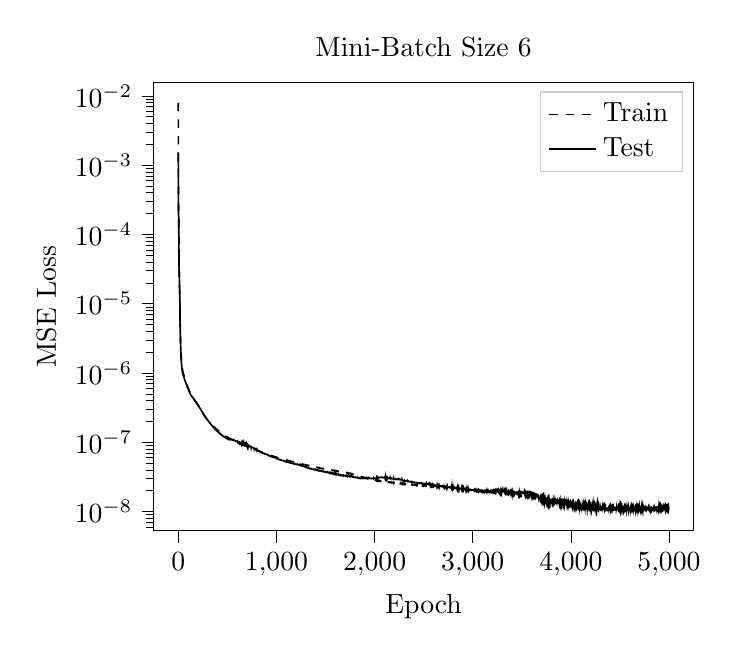
\begin{tikzpicture}

\begin{axis}[
legend cell align={left},
legend style={fill opacity=0.8, draw opacity=1, text opacity=1, draw=white!80!black},
log basis y={10},
tick align=outside,
tick pos=left,
title={Mini-Batch Size 6},
x grid style={white!69.0196078431373!black},
xlabel={Epoch},
xmin=-249.95, xmax=5248.95,
xtick style={color=black},
y grid style={white!69.0196078431373!black},
ylabel={MSE Loss},
ymin=5.27698874578941e-09, ymax=0.0155998634668396,
ymode=log,
ytick style={color=black}
]
\addplot [semithick, black, dashed]
table {%
0 0.00792494936405668
1 0.00074693354815037
2 0.000204862174982061
3 0.000182490643616067
4 0.000174127073374672
5 0.000144887499667855
6 8.86097720864456e-05
7 4.68465743448571e-05
8 3.17742668719849e-05
9 2.71491441448932e-05
10 2.39751503956937e-05
11 2.17058184807411e-05
12 1.95244866656639e-05
13 1.71598938875442e-05
14 1.45919596192705e-05
15 1.21801129276757e-05
16 1.00995043139322e-05
17 8.16256929222194e-06
18 6.30641060338328e-06
19 5.0335977352111e-06
20 4.18607083942384e-06
21 3.59522449484658e-06
22 3.16430228840947e-06
23 2.83704614422687e-06
24 2.57516105203744e-06
25 2.35928370969908e-06
26 2.17642036670179e-06
27 2.02323785481073e-06
28 1.89352970838895e-06
29 1.78371970852457e-06
30 1.69118709075458e-06
31 1.61080757225583e-06
32 1.5411232624977e-06
33 1.47731713683064e-06
34 1.42110068692468e-06
35 1.37282949941775e-06
36 1.32860109897345e-06
37 1.2878080142279e-06
38 1.25118790969526e-06
39 1.21718567364734e-06
40 1.18621371261417e-06
41 1.15859394885872e-06
42 1.13291366900974e-06
43 1.11027498610941e-06
44 1.08951247236749e-06
45 1.07059546082872e-06
46 1.05329323841063e-06
47 1.03720289890175e-06
48 1.02232245525918e-06
49 1.00850926861736e-06
50 9.95778685144071e-07
51 9.83511111717545e-07
52 9.71585458310552e-07
53 9.60307571971598e-07
54 9.49454394176838e-07
55 9.39045032597575e-07
56 9.2894042586569e-07
57 9.19292567370904e-07
58 9.09662005366529e-07
59 9.00520281040803e-07
60 8.91369453549412e-07
61 8.82196482813927e-07
62 8.73165208659948e-07
63 8.64312308946624e-07
64 8.55683471747636e-07
65 8.46961227554032e-07
66 8.38652941052141e-07
67 8.29745988248977e-07
68 8.21353428667483e-07
69 8.13295208099236e-07
70 8.04699132071003e-07
71 7.96007132709525e-07
72 7.88097942269513e-07
73 7.79884498932095e-07
74 7.72275892080753e-07
75 7.64772029071864e-07
76 7.56686016295635e-07
77 7.49086183848119e-07
78 7.4208203814691e-07
79 7.34527712558045e-07
80 7.26859385308828e-07
81 7.19653547588544e-07
82 7.12119579645616e-07
83 7.05339993577664e-07
84 6.98320306320074e-07
85 6.91032350877539e-07
86 6.8372461907055e-07
87 6.76880052207574e-07
88 6.70372859392669e-07
89 6.64194197234384e-07
90 6.58067695549607e-07
91 6.52140548214283e-07
92 6.46306514798665e-07
93 6.40675028040156e-07
94 6.35287225518852e-07
95 6.30230405772304e-07
96 6.24665087219474e-07
97 6.19228257339953e-07
98 6.14137978945591e-07
99 6.08860029745464e-07
100 6.03844388347335e-07
101 5.99027984836765e-07
102 5.94187206397332e-07
103 5.89501576444994e-07
104 5.84924708667334e-07
105 5.80679396908364e-07
106 5.76035185584006e-07
107 5.7162463720771e-07
108 5.67239825653383e-07
109 5.63138681524104e-07
110 5.58848633648273e-07
111 5.54497895904518e-07
112 5.5032399974129e-07
113 5.46303629167438e-07
114 5.4249618855444e-07
115 5.38887368242723e-07
116 5.35058079500554e-07
117 5.31249512400346e-07
118 5.27634925549626e-07
119 5.23930784742118e-07
120 5.20592796066047e-07
121 5.17186048734035e-07
122 5.13706907728759e-07
123 5.10282175111322e-07
124 5.06539088247373e-07
125 5.03181729004515e-07
126 4.99824641919766e-07
127 4.97068465716291e-07
128 4.93662760176286e-07
129 4.90739311181823e-07
130 4.87514542350712e-07
131 4.84693126930909e-07
132 4.81795060823976e-07
133 4.78897239934182e-07
134 4.76187394968071e-07
135 4.73645979614046e-07
136 4.71059729141229e-07
137 4.68526309241245e-07
138 4.66105621260679e-07
139 4.63971031256674e-07
140 4.61375845069785e-07
141 4.59029176206225e-07
142 4.5668160046323e-07
143 4.54302431758438e-07
144 4.51832581901237e-07
145 4.49889186510263e-07
146 4.47508866076417e-07
147 4.45342193171692e-07
148 4.43099275191079e-07
149 4.40864431969386e-07
150 4.3865167727893e-07
151 4.36595489178251e-07
152 4.34421391229771e-07
153 4.32206230574499e-07
154 4.30091064502555e-07
155 4.28157747739502e-07
156 4.26042544633048e-07
157 4.24004756910043e-07
158 4.22020520060586e-07
159 4.19945539984768e-07
160 4.17963437112464e-07
161 4.15992797622127e-07
162 4.14081616672829e-07
163 4.12071938617008e-07
164 4.10129467671962e-07
165 4.08223826148987e-07
166 4.06277433316971e-07
167 4.04441162310323e-07
168 4.02476571030062e-07
169 4.0058604144078e-07
170 3.98771483355115e-07
171 3.96856144415191e-07
172 3.94967850401618e-07
173 3.93066415661824e-07
174 3.91222675870965e-07
175 3.89322397960259e-07
176 3.87543632753833e-07
177 3.85704788485242e-07
178 3.83836589682855e-07
179 3.82057603776742e-07
180 3.8019314408832e-07
181 3.78379088152369e-07
182 3.76449783992992e-07
183 3.74547649126251e-07
184 3.72727639033925e-07
185 3.70833063670765e-07
186 3.68986093267393e-07
187 3.67232748427762e-07
188 3.65436964686828e-07
189 3.63612886207362e-07
190 3.61782968627245e-07
191 3.5995823093563e-07
192 3.58184446455347e-07
193 3.56371153332829e-07
194 3.54544190196331e-07
195 3.52744350774403e-07
196 3.50947292967492e-07
197 3.49238124623073e-07
198 3.47401059076246e-07
199 3.45640531147575e-07
200 3.43881100022046e-07
201 3.42033855609639e-07
202 3.40198495296135e-07
203 3.38492801068928e-07
204 3.36773551542576e-07
205 3.3499529977252e-07
206 3.33106171294682e-07
207 3.31376998580954e-07
208 3.29612051979292e-07
209 3.28067406468344e-07
210 3.26203844111773e-07
211 3.24453416974204e-07
212 3.22730980011197e-07
213 3.20854888375995e-07
214 3.1919837656405e-07
215 3.17532984182329e-07
216 3.15781171070965e-07
217 3.14084994699527e-07
218 3.12351770949431e-07
219 3.10619374169345e-07
220 3.08925018057659e-07
221 3.07278862414077e-07
222 3.05550675005806e-07
223 3.03974624571218e-07
224 3.02406111586223e-07
225 3.00711385877796e-07
226 2.99041627996609e-07
227 2.97478750869876e-07
228 2.95713607047331e-07
229 2.94081796465287e-07
230 2.92428883677469e-07
231 2.90797483175523e-07
232 2.8915811127093e-07
233 2.87616107239886e-07
234 2.86067552359025e-07
235 2.84466419771192e-07
236 2.82925695942147e-07
237 2.81369605712962e-07
238 2.79812704325207e-07
239 2.78198559747754e-07
240 2.76702073952568e-07
241 2.75215135617322e-07
242 2.73745041637739e-07
243 2.72245439116619e-07
244 2.7078373859621e-07
245 2.69341620199496e-07
246 2.67833146160829e-07
247 2.66405126777593e-07
248 2.65012859563865e-07
249 2.63667045197369e-07
250 2.62234284581905e-07
251 2.60904440430398e-07
252 2.59510283713623e-07
253 2.58156663265509e-07
254 2.56807231860977e-07
255 2.55492987941554e-07
256 2.54155811439095e-07
257 2.52885645455043e-07
258 2.51607791047048e-07
259 2.50322395346458e-07
260 2.48939361640907e-07
261 2.47696769913576e-07
262 2.46361084845114e-07
263 2.45173361800428e-07
264 2.43947212522032e-07
265 2.42728269244217e-07
266 2.41584720031539e-07
267 2.403303927375e-07
268 2.39022315681865e-07
269 2.37883198772454e-07
270 2.36761164511515e-07
271 2.355524272826e-07
272 2.3448867785689e-07
273 2.33515845237165e-07
274 2.32308974661009e-07
275 2.31225084880148e-07
276 2.30135166293314e-07
277 2.29069297050706e-07
278 2.28077566564201e-07
279 2.26976575897249e-07
280 2.25899497944186e-07
281 2.24806329063765e-07
282 2.23729208518085e-07
283 2.22726185747131e-07
284 2.21724548947309e-07
285 2.20741170477866e-07
286 2.19845323421825e-07
287 2.1896735587675e-07
288 2.18004240253847e-07
289 2.17031305175351e-07
290 2.16135360041509e-07
291 2.15184591089352e-07
292 2.14273000214602e-07
293 2.13387856864349e-07
294 2.12507463423041e-07
295 2.11605158649415e-07
296 2.1071168113888e-07
297 2.09847457386515e-07
298 2.09014734180116e-07
299 2.0817423863489e-07
300 2.07360612537527e-07
301 2.06565093934677e-07
302 2.05704701270017e-07
303 2.04869231661479e-07
304 2.04001796761957e-07
305 2.03225100806363e-07
306 2.02372046990871e-07
307 2.01605099985217e-07
308 2.00826745956311e-07
309 2.00061786523516e-07
310 1.99328455225447e-07
311 1.98573559908776e-07
312 1.97813823950473e-07
313 1.97087318936071e-07
314 1.96335054643567e-07
315 1.95518330763636e-07
316 1.94886897504467e-07
317 1.94244450476024e-07
318 1.93538887198722e-07
319 1.92870559207739e-07
320 1.920480320579e-07
321 1.91425300992452e-07
322 1.90777889022674e-07
323 1.90017708738136e-07
324 1.89466645937215e-07
325 1.88718898848247e-07
326 1.88148259931817e-07
327 1.87439876708007e-07
328 1.86853819323143e-07
329 1.86202076510168e-07
330 1.85547054233536e-07
331 1.84923454292569e-07
332 1.84389606649149e-07
333 1.83780473736457e-07
334 1.83204896626579e-07
335 1.82611882784649e-07
336 1.81974885874657e-07
337 1.81487325609632e-07
338 1.80865272643773e-07
339 1.80268731814711e-07
340 1.79716794006244e-07
341 1.79127217926133e-07
342 1.78605542807904e-07
343 1.78020651840994e-07
344 1.77516950081032e-07
345 1.76651081789756e-07
346 1.75948882187942e-07
347 1.75440971639407e-07
348 1.75018379547153e-07
349 1.74399636097872e-07
350 1.73992858762752e-07
351 1.73381931041213e-07
352 1.72961703671403e-07
353 1.72451043090782e-07
354 1.71903263217014e-07
355 1.71296573633885e-07
356 1.70823611926106e-07
357 1.7022137299838e-07
358 1.69639867024571e-07
359 1.69228476798339e-07
360 1.68696906522952e-07
361 1.68385364455779e-07
362 1.67627344202516e-07
363 1.67037906943227e-07
364 1.66660267270571e-07
365 1.66133442982562e-07
366 1.65828685711669e-07
367 1.65400948654834e-07
368 1.64599034798509e-07
369 1.64051662449496e-07
370 1.63612193077725e-07
371 1.63031040729425e-07
372 1.62574956671348e-07
373 1.62101862554409e-07
374 1.61218143537405e-07
375 1.61154750721504e-07
376 1.60227039340525e-07
377 1.60240092141078e-07
378 1.5980942699036e-07
379 1.58932503527646e-07
380 1.58903720312288e-07
381 1.58026279253281e-07
382 1.57959618992761e-07
383 1.57162557488173e-07
384 1.57105333092703e-07
385 1.56326358950141e-07
386 1.56239497088776e-07
387 1.55881404951457e-07
388 1.55094732560394e-07
389 1.54968537507319e-07
390 1.54296820256782e-07
391 1.53885362627527e-07
392 1.52978094574405e-07
393 1.5315802425409e-07
394 1.52503762786831e-07
395 1.5177051383502e-07
396 1.51525638096476e-07
397 1.50949997955225e-07
398 1.50103813769702e-07
399 1.49995203928941e-07
400 1.49503947592648e-07
401 1.49128464985788e-07
402 1.48449594303647e-07
403 1.48360061992047e-07
404 1.4776081381007e-07
405 1.47756748389739e-07
406 1.4699670358104e-07
407 1.46977261339454e-07
408 1.46112958270226e-07
409 1.46189474746539e-07
410 1.45417565404164e-07
411 1.45378170294301e-07
412 1.44648656883768e-07
413 1.445824052013e-07
414 1.44031487815293e-07
415 1.43900163933989e-07
416 1.43315402226999e-07
417 1.43215020893236e-07
418 1.42632309106034e-07
419 1.42574283634883e-07
420 1.42032504042846e-07
421 1.41834442127485e-07
422 1.41345680994636e-07
423 1.41238906693757e-07
424 1.4060466289851e-07
425 1.40545007124602e-07
426 1.40031331451224e-07
427 1.39810996041137e-07
428 1.39465829393916e-07
429 1.39250281124361e-07
430 1.38739989462694e-07
431 1.38410872469832e-07
432 1.38280581743764e-07
433 1.37804161246842e-07
434 1.3739803466154e-07
435 1.37337264645833e-07
436 1.36840152136423e-07
437 1.36466377980036e-07
438 1.36367599689807e-07
439 1.35951356260944e-07
440 1.35694117381072e-07
441 1.35180257143686e-07
442 1.35060516774808e-07
443 1.34537828314245e-07
444 1.34386974806315e-07
445 1.34078091845461e-07
446 1.33567195894895e-07
447 1.33422713547769e-07
448 1.32931844714266e-07
449 1.3279914286742e-07
450 1.32478407614304e-07
451 1.32061744539114e-07
452 1.31887610853466e-07
453 1.31612793401978e-07
454 1.31132230712552e-07
455 1.30987384846117e-07
456 1.30521262809929e-07
457 1.3031381291392e-07
458 1.29737968912419e-07
459 1.29641947192442e-07
460 1.29180116268447e-07
461 1.29056334044596e-07
462 1.28577802820288e-07
463 1.28533735564363e-07
464 1.28029660248809e-07
465 1.27910751799505e-07
466 1.27344065890912e-07
467 1.27244660958184e-07
468 1.26793830182507e-07
469 1.26614542037957e-07
470 1.26224640805218e-07
471 1.25955073733238e-07
472 1.2576121384724e-07
473 1.25469259082361e-07
474 1.25206119862802e-07
475 1.24820441521631e-07
476 1.24619067007033e-07
477 1.24123444319048e-07
478 1.23966767925384e-07
479 1.23584695277002e-07
480 1.23377284905598e-07
481 1.23001050521621e-07
482 1.22872700129837e-07
483 1.22457752967416e-07
484 1.22241437620638e-07
485 1.21987415930732e-07
486 1.21767705689061e-07
487 1.21556589152848e-07
488 1.21295199425061e-07
489 1.21022931374543e-07
490 1.20766346245921e-07
491 1.20396381607952e-07
492 1.20254470992759e-07
493 1.19947405571193e-07
494 1.19636952242981e-07
495 1.19374032788324e-07
496 1.19169286363612e-07
497 1.18910004296531e-07
498 1.18721699833387e-07
499 1.18419032173337e-07
500 1.18205985917038e-07
501 1.17922647974225e-07
502 1.17670392121504e-07
503 1.1745881593365e-07
504 1.17229652966187e-07
505 1.17012580124393e-07
506 1.16746087393462e-07
507 1.16516909057983e-07
508 1.16235237204725e-07
509 1.16043368823805e-07
510 1.15789795709275e-07
511 1.15621475727967e-07
512 1.1536366801043e-07
513 1.1514959939419e-07
514 1.14938462814706e-07
515 1.14728617083377e-07
516 1.14516673862116e-07
517 1.14303887274832e-07
518 1.14121070755621e-07
519 1.13954926995202e-07
520 1.13688961944786e-07
521 1.13482690585638e-07
522 1.13444305936523e-07
523 1.13101765691479e-07
524 1.12879228395209e-07
525 1.12654966542742e-07
526 1.12497033158231e-07
527 1.12403659961001e-07
528 1.12110352630886e-07
529 1.12004765672752e-07
530 1.11732648046635e-07
531 1.11525370969907e-07
532 1.11293275903103e-07
533 1.11184866194107e-07
534 1.10916620473286e-07
535 1.10772067790951e-07
536 1.10664058989981e-07
537 1.1040349546387e-07
538 1.10187687244333e-07
539 1.10028139541614e-07
540 1.09896095828319e-07
541 1.09669417741723e-07
542 1.09469936870122e-07
543 1.09287650594759e-07
544 1.09134116427204e-07
545 1.09001398249593e-07
546 1.08772434617598e-07
547 1.08564273714124e-07
548 1.08348638179375e-07
549 1.08174791310108e-07
550 1.0804613645955e-07
551 1.07795554193302e-07
552 1.07666778316117e-07
553 1.07434035184004e-07
554 1.07210255452627e-07
555 1.07046178583261e-07
556 1.06911155735786e-07
557 1.06740506994604e-07
558 1.06533606498867e-07
559 1.06359935407699e-07
560 1.06200919301736e-07
561 1.06013215091407e-07
562 1.05867026588159e-07
563 1.05705439081831e-07
564 1.05492735012581e-07
565 1.05356573108906e-07
566 1.0516000167012e-07
567 1.04988258887539e-07
568 1.04903252823715e-07
569 1.04625338941237e-07
570 1.04521623926316e-07
571 1.04373378797333e-07
572 1.0416789535631e-07
573 1.04016407019193e-07
574 1.03836468000984e-07
575 1.03709974175076e-07
576 1.03519282200455e-07
577 1.034126624333e-07
578 1.032837735697e-07
579 1.03076682813362e-07
580 1.02969324202938e-07
581 1.02783457781567e-07
582 1.02641104248974e-07
583 1.02497159350994e-07
584 1.023272493106e-07
585 1.02269956558682e-07
586 1.02080391342916e-07
587 1.01901056838648e-07
588 1.01680896134721e-07
589 1.0165975366264e-07
590 1.0151955765791e-07
591 1.01291374315291e-07
592 1.01158572304024e-07
593 1.0099713505831e-07
594 1.00829963744703e-07
595 1.00671792044744e-07
596 1.00479425459648e-07
597 1.00339705944663e-07
598 1.00263345520099e-07
599 9.99969221030382e-08
600 9.99370505150909e-08
601 9.9841746459256e-08
602 9.96970335079887e-08
603 9.94148601748137e-08
604 9.94305171744152e-08
605 9.9138141733882e-08
606 9.90484357760776e-08
607 9.89997646333327e-08
608 9.87586991788779e-08
609 9.86360037911284e-08
610 9.85921406790853e-08
611 9.83557888713947e-08
612 9.82831521182108e-08
613 9.79887653557007e-08
614 9.77669668068248e-08
615 9.75032125390232e-08
616 9.7241095451701e-08
617 9.70617752142148e-08
618 9.67884489756775e-08
619 9.66514243151938e-08
620 9.64655205197543e-08
621 9.63048815107464e-08
622 9.61571627639665e-08
623 9.60187558069067e-08
624 9.5793140238034e-08
625 9.57458236659176e-08
626 9.55691448657253e-08
627 9.54866896689652e-08
628 9.52745373582537e-08
629 9.50931480299085e-08
630 9.50461621145003e-08
631 9.48732205706893e-08
632 9.47432422850169e-08
633 9.45740982951814e-08
634 9.44506582210936e-08
635 9.43142960418409e-08
636 9.41397731209883e-08
637 9.39928493791165e-08
638 9.38941059355765e-08
639 9.3825027502115e-08
640 9.37076243687564e-08
641 9.35323852751555e-08
642 9.34204141824212e-08
643 9.32263267869239e-08
644 9.30651717542437e-08
645 9.30660305775011e-08
646 9.28396997873096e-08
647 9.26950396819924e-08
648 9.27071528390466e-08
649 9.24314736747257e-08
650 9.23561871071409e-08
651 9.23011272078057e-08
652 9.20847262723205e-08
653 9.20106265481295e-08
654 9.19975779328011e-08
655 9.19308606104797e-08
656 9.17938819821396e-08
657 9.17312023781704e-08
658 9.15164115703419e-08
659 9.13792164881272e-08
660 9.12088392485741e-08
661 9.11352694719498e-08
662 9.09804609934031e-08
663 9.09200491333143e-08
664 9.07959634500565e-08
665 9.06053841462608e-08
666 9.04922921503894e-08
667 9.03537848631241e-08
668 9.02727790676826e-08
669 9.01380736467852e-08
670 8.99475532190985e-08
671 8.98181916188727e-08
672 8.9708077212524e-08
673 8.95742572116331e-08
674 8.95692921224903e-08
675 8.94854445522574e-08
676 8.92567196025659e-08
677 8.92259713676898e-08
678 8.91810853670597e-08
679 8.89182820919992e-08
680 8.88726568699246e-08
681 8.88789637196864e-08
682 8.86814085034559e-08
683 8.86184558025992e-08
684 8.84406394316097e-08
685 8.82643648291654e-08
686 8.82450046075935e-08
687 8.80800776422887e-08
688 8.79617921522735e-08
689 8.78704687070491e-08
690 8.77763111650493e-08
691 8.77024110872546e-08
692 8.75630335649042e-08
693 8.75243787277853e-08
694 8.73521312721063e-08
695 8.72583466744938e-08
696 8.71552602242399e-08
697 8.71504448663989e-08
698 8.6967704048086e-08
699 8.68567375324163e-08
700 8.67588195222178e-08
701 8.66599322210716e-08
702 8.65302836073877e-08
703 8.63719422620217e-08
704 8.62916290879528e-08
705 8.62020234943098e-08
706 8.61112491777106e-08
707 8.59954845757415e-08
708 8.58770226371654e-08
709 8.57806709269468e-08
710 8.57162695464998e-08
711 8.55895117471737e-08
712 8.54726360899288e-08
713 8.53523020163886e-08
714 8.52339811317311e-08
715 8.52128194206669e-08
716 8.50622339182452e-08
717 8.49504515294693e-08
718 8.48105331683808e-08
719 8.47790642452946e-08
720 8.46481247268629e-08
721 8.45440721555395e-08
722 8.44129090798033e-08
723 8.44280426506948e-08
724 8.42494295696809e-08
725 8.41705290360648e-08
726 8.40065957233631e-08
727 8.39763029362604e-08
728 8.38522954939313e-08
729 8.37329867518017e-08
730 8.36780891667399e-08
731 8.35020314948837e-08
732 8.35077070275579e-08
733 8.33393987903122e-08
734 8.33242972644187e-08
735 8.31508684382294e-08
736 8.31354193116603e-08
737 8.29454018772561e-08
738 8.29427543325706e-08
739 8.28369571970672e-08
740 8.27457814364725e-08
741 8.26038725104164e-08
742 8.24549751368918e-08
743 8.23958459396012e-08
744 8.2313863215144e-08
745 8.22747276777545e-08
746 8.21465659366647e-08
747 8.20621932219528e-08
748 8.19604173761641e-08
749 8.18726592502271e-08
750 8.18050781197968e-08
751 8.17071699148484e-08
752 8.15337526715976e-08
753 8.1480377070141e-08
754 8.14369292833767e-08
755 8.13487763401607e-08
756 8.12141420560962e-08
757 8.11471520843056e-08
758 8.10588374986094e-08
759 8.09555228224549e-08
760 8.08750344382148e-08
761 8.07332387229488e-08
762 8.06549439696261e-08
763 8.05325278247723e-08
764 8.05011720645385e-08
765 8.04073679076925e-08
766 8.02946634645464e-08
767 8.02051012997655e-08
768 8.01234312294254e-08
769 8.00308685056561e-08
770 7.99606150041557e-08
771 7.98075698287557e-08
772 7.97668609112594e-08
773 7.96247826773572e-08
774 7.94999828021088e-08
775 7.94450283583147e-08
776 7.93847441848594e-08
777 7.92839646728541e-08
778 7.91749904605582e-08
779 7.90872404407474e-08
780 7.90205521120583e-08
781 7.888154033479e-08
782 7.88543524969352e-08
783 7.86995105439159e-08
784 7.86323640889364e-08
785 7.85425547895088e-08
786 7.84370873200017e-08
787 7.83665436145252e-08
788 7.82619622554602e-08
789 7.81682320870725e-08
790 7.80680596583331e-08
791 7.7984497306559e-08
792 7.78788282857992e-08
793 7.7797066535339e-08
794 7.76839365355515e-08
795 7.75992620692124e-08
796 7.75117234152256e-08
797 7.740640813316e-08
798 7.73703760443031e-08
799 7.72528050352361e-08
800 7.71347091493421e-08
801 7.70650933652736e-08
802 7.69856078789481e-08
803 7.68517433346444e-08
804 7.67692187860638e-08
805 7.66678639980996e-08
806 7.65424627581495e-08
807 7.64938434679798e-08
808 7.63841421271815e-08
809 7.63040824847743e-08
810 7.6208701324533e-08
811 7.61267628012669e-08
812 7.60441162246946e-08
813 7.58755990584563e-08
814 7.58323846855133e-08
815 7.57093433502719e-08
816 7.55957277139659e-08
817 7.54920250276809e-08
818 7.53970034931454e-08
819 7.53118776623899e-08
820 7.52102924234185e-08
821 7.50831357647362e-08
822 7.49458233264548e-08
823 7.47840501781876e-08
824 7.46699555014527e-08
825 7.45712405628472e-08
826 7.44991902144843e-08
827 7.43670001235269e-08
828 7.42764634033104e-08
829 7.42058294631677e-08
830 7.40858372477701e-08
831 7.4010756124376e-08
832 7.38730827920381e-08
833 7.37644526862945e-08
834 7.36669718329867e-08
835 7.3568323296038e-08
836 7.35058679404747e-08
837 7.33685872762104e-08
838 7.32850038751405e-08
839 7.3197792068149e-08
840 7.31037852727974e-08
841 7.30077916110023e-08
842 7.29198656146834e-08
843 7.28109357160989e-08
844 7.27455886420202e-08
845 7.26609725544369e-08
846 7.2553502705325e-08
847 7.25095461061781e-08
848 7.23269759459556e-08
849 7.22590886662831e-08
850 7.22283481360552e-08
851 7.20781080864353e-08
852 7.19637544737326e-08
853 7.1973301964966e-08
854 7.18185479096518e-08
855 7.17502237633778e-08
856 7.17103134680859e-08
857 7.15258081728193e-08
858 7.15128466302688e-08
859 7.14619334568747e-08
860 7.11725786758595e-08
861 7.11507273468507e-08
862 7.10437192579708e-08
863 7.10404811538664e-08
864 7.08561184724899e-08
865 7.08082522224625e-08
866 7.07646552656665e-08
867 7.06380770408367e-08
868 7.05022280868949e-08
869 7.04429462640659e-08
870 7.03595980398581e-08
871 7.02565800758836e-08
872 7.0207722283842e-08
873 7.00945105916139e-08
874 6.99803333795344e-08
875 6.99747162888671e-08
876 6.97937787497194e-08
877 6.97787862513888e-08
878 6.97129161374278e-08
879 6.96013615903853e-08
880 6.94600617629745e-08
881 6.94828596085449e-08
882 6.93428895313703e-08
883 6.92632089434055e-08
884 6.91849155270111e-08
885 6.91010709229212e-08
886 6.89944733449136e-08
887 6.89520586867545e-08
888 6.87878025145392e-08
889 6.87653220955469e-08
890 6.86641716026012e-08
891 6.85961561402734e-08
892 6.85030336277404e-08
893 6.84367955842045e-08
894 6.8341776631645e-08
895 6.82595868071501e-08
896 6.81619964755322e-08
897 6.81212941674416e-08
898 6.79910497578147e-08
899 6.7917461184299e-08
900 6.77907707280723e-08
901 6.77301007016815e-08
902 6.76374282852142e-08
903 6.75683262617605e-08
904 6.74273657637805e-08
905 6.74206006405862e-08
906 6.73083456363603e-08
907 6.72158289074497e-08
908 6.71557271161731e-08
909 6.70903081635593e-08
910 6.70025510742743e-08
911 6.69165004866627e-08
912 6.68149225501957e-08
913 6.67687180853206e-08
914 6.66625277943773e-08
915 6.66335806575025e-08
916 6.6523338110444e-08
917 6.65168887206961e-08
918 6.63460846448323e-08
919 6.62652415844503e-08
920 6.61301523579552e-08
921 6.60950810943875e-08
922 6.60525452318325e-08
923 6.5929236269924e-08
924 6.58494692629979e-08
925 6.57748615773179e-08
926 6.57409636686833e-08
927 6.56343428255943e-08
928 6.55793209008801e-08
929 6.55066323004473e-08
930 6.54712611847824e-08
931 6.53547976909277e-08
932 6.52940520908068e-08
933 6.52103714315367e-08
934 6.51293917508045e-08
935 6.50708836239254e-08
936 6.49648700798218e-08
937 6.49629940798834e-08
938 6.48854084937518e-08
939 6.47777786819754e-08
940 6.47394384630863e-08
941 6.46057746078233e-08
942 6.4582537619278e-08
943 6.4483849206181e-08
944 6.45361467760871e-08
945 6.43352020812538e-08
946 6.42254817371658e-08
947 6.42260176563009e-08
948 6.41414128460535e-08
949 6.4036320972153e-08
950 6.40051641199423e-08
951 6.39142114925371e-08
952 6.39232134731074e-08
953 6.38271091458791e-08
954 6.37706096025378e-08
955 6.37301945682334e-08
956 6.37245242361302e-08
957 6.36409729379829e-08
958 6.36012324885043e-08
959 6.35367983965925e-08
960 6.3445267839346e-08
961 6.33644460126868e-08
962 6.32313920903176e-08
963 6.32242685671569e-08
964 6.31174637226615e-08
965 6.3110971213649e-08
966 6.30090201470362e-08
967 6.29856166203767e-08
968 6.29289383827279e-08
969 6.2846778048553e-08
970 6.28095745582229e-08
971 6.27314586729817e-08
972 6.26567372764952e-08
973 6.26353590176784e-08
974 6.25294210266652e-08
975 6.24992209270394e-08
976 6.24411414521102e-08
977 6.23566219269651e-08
978 6.23410314655095e-08
979 6.22730750011324e-08
980 6.21986761325906e-08
981 6.2123454242904e-08
982 6.20565633016755e-08
983 6.19911177483177e-08
984 6.19309048808088e-08
985 6.18677860306656e-08
986 6.17949470837309e-08
987 6.17349928545768e-08
988 6.16690186226688e-08
989 6.15940373074923e-08
990 6.15296462902365e-08
991 6.14877760162053e-08
992 6.13140742808844e-08
993 6.13556047740718e-08
994 6.1184471468977e-08
995 6.11416997184845e-08
996 6.10264418376172e-08
997 6.10011510663076e-08
998 6.08959333653555e-08
999 6.08815033582746e-08
1000 6.07449019234632e-08
1001 6.07449449182231e-08
1002 6.06042416504289e-08
1003 6.06234880500054e-08
1004 6.04724791967407e-08
1005 6.04976172399786e-08
1006 6.03440853567864e-08
1007 6.03638936643709e-08
1008 6.02229008004769e-08
1009 6.02366862916329e-08
1010 6.00965989855598e-08
1011 6.01074190187517e-08
1012 5.99647778202154e-08
1013 5.99714976316627e-08
1014 5.98645894668497e-08
1015 5.98602131268131e-08
1016 5.98440629584873e-08
1017 5.97974968558559e-08
1018 5.97010112723817e-08
1019 5.96388073472125e-08
1020 5.95871144570309e-08
1021 5.95317830507409e-08
1022 5.94607110262467e-08
1023 5.94440843129139e-08
1024 5.93347962959968e-08
1025 5.93152592510182e-08
1026 5.9209410856834e-08
1027 5.91987453393893e-08
1028 5.91034983080711e-08
1029 5.90980985095218e-08
1030 5.90197927019065e-08
1031 5.89576969740465e-08
1032 5.88747872330049e-08
1033 5.8890620852944e-08
1034 5.87949151287387e-08
1035 5.87625136402832e-08
1036 5.87021455080011e-08
1037 5.86604852069384e-08
1038 5.85654308464204e-08
1039 5.8574962441657e-08
1040 5.84544965295487e-08
1041 5.84952061308226e-08
1042 5.83282032089197e-08
1043 5.83216899089421e-08
1044 5.82941326927297e-08
1045 5.82313509495738e-08
1046 5.81159853754086e-08
1047 5.81181682409911e-08
1048 5.80003146953113e-08
1049 5.80218817100188e-08
1050 5.79361831906068e-08
1051 5.78927504509432e-08
1052 5.78225662253622e-08
1053 5.78540821653116e-08
1054 5.76885860414267e-08
1055 5.77094049815351e-08
1056 5.75638148981511e-08
1057 5.76022974859155e-08
1058 5.74902993463507e-08
1059 5.74552865447638e-08
1060 5.73852374075251e-08
1061 5.73537481535421e-08
1062 5.72236097307654e-08
1063 5.72772072196979e-08
1064 5.71098081515774e-08
1065 5.71178287788849e-08
1066 5.70507493321067e-08
1067 5.69992500961133e-08
1068 5.69160797093271e-08
1069 5.69246548948662e-08
1070 5.67944772743923e-08
1071 5.6791876424988e-08
1072 5.67314601180149e-08
1073 5.66554648952399e-08
1074 5.66244221932644e-08
1075 5.65731772799042e-08
1076 5.6492765263029e-08
1077 5.64865721646876e-08
1078 5.63726430992722e-08
1079 5.64091336819416e-08
1080 5.62825863602612e-08
1081 5.62965368695081e-08
1082 5.61771592522714e-08
1083 5.62053769350012e-08
1084 5.60664128117675e-08
1085 5.61052525311475e-08
1086 5.59744314953176e-08
1087 5.59837565597763e-08
1088 5.58820367624402e-08
1089 5.59070890305463e-08
1090 5.57410385295275e-08
1091 5.57924492918981e-08
1092 5.56903973417992e-08
1093 5.56911808416675e-08
1094 5.5560815193689e-08
1095 5.56128175860862e-08
1096 5.54792224807597e-08
1097 5.55065994693253e-08
1098 5.53821891402101e-08
1099 5.53957429479614e-08
1100 5.52828465950255e-08
1101 5.53226706178323e-08
1102 5.51843671109212e-08
1103 5.52059207889706e-08
1104 5.51090012424526e-08
1105 5.51018989097377e-08
1106 5.50045666538728e-08
1107 5.50254645140268e-08
1108 5.48944216985807e-08
1109 5.492906696741e-08
1110 5.48375427732229e-08
1111 5.48879215967745e-08
1112 5.47291373486558e-08
1113 5.48093085959412e-08
1114 5.46615534145379e-08
1115 5.46915637369343e-08
1116 5.45832876528502e-08
1117 5.46144617439782e-08
1118 5.44759346657807e-08
1119 5.45108140268825e-08
1120 5.44098764424215e-08
1121 5.441311405117e-08
1122 5.42889065583034e-08
1123 5.43314965511385e-08
1124 5.42054906301322e-08
1125 5.42205739783292e-08
1126 5.41382550969825e-08
1127 5.4159388387003e-08
1128 5.40388574281429e-08
1129 5.40976299505572e-08
1130 5.39553001897198e-08
1131 5.39650045902547e-08
1132 5.38747589908222e-08
1133 5.38866475565829e-08
1134 5.37739957010562e-08
1135 5.38016958487457e-08
1136 5.36792816793232e-08
1137 5.36967115156747e-08
1138 5.3606179180423e-08
1139 5.35955056893465e-08
1140 5.3537224862239e-08
1141 5.35082173105893e-08
1142 5.34495854672475e-08
1143 5.34194772394925e-08
1144 5.33530507523264e-08
1145 5.33700697635475e-08
1146 5.32460506930055e-08
1147 5.32684994458405e-08
1148 5.31634974923483e-08
1149 5.31742437002032e-08
1150 5.30788059329023e-08
1151 5.3085817963705e-08
1152 5.29934681923634e-08
1153 5.30073814540439e-08
1154 5.28742340552237e-08
1155 5.28884154968519e-08
1156 5.27903061035121e-08
1157 5.27741826264792e-08
1158 5.27273597876863e-08
1159 5.2704631887831e-08
1160 5.26181914185225e-08
1161 5.26122942760114e-08
1162 5.25371809218608e-08
1163 5.25181295666647e-08
1164 5.24408524101435e-08
1165 5.24506279042342e-08
1166 5.23543758604177e-08
1167 5.23542157552718e-08
1168 5.22885668876204e-08
1169 5.22744369110713e-08
1170 5.21886834144804e-08
1171 5.21840990316321e-08
1172 5.21115209181978e-08
1173 5.21031355811288e-08
1174 5.20230322728345e-08
1175 5.2020849203517e-08
1176 5.19226777328974e-08
1177 5.19228199579597e-08
1178 5.18371560781719e-08
1179 5.1850824391696e-08
1180 5.17688889497566e-08
1181 5.17707267347199e-08
1182 5.16913233383182e-08
1183 5.16847373481941e-08
1184 5.15891402008046e-08
1185 5.15911923117428e-08
1186 5.14926039851682e-08
1187 5.14909518048599e-08
1188 5.14309401563691e-08
1189 5.14323695730075e-08
1190 5.13429139030828e-08
1191 5.13648093440653e-08
1192 5.12755754431039e-08
1193 5.12416107526402e-08
1194 5.11910958134154e-08
1195 5.1192302445744e-08
1196 5.11364802975741e-08
1197 5.10663882954067e-08
1198 5.10439006724486e-08
1199 5.10104281047358e-08
1200 5.09526454365304e-08
1201 5.0905785738333e-08
1202 5.08782093217538e-08
1203 5.08483768254604e-08
1204 5.07870784201616e-08
1205 5.07603319490567e-08
1206 5.06996676685279e-08
1207 5.0695195023718e-08
1208 5.06064930497495e-08
1209 5.05848387026018e-08
1210 5.05594465950614e-08
1211 5.05544964837761e-08
1212 5.04493761868345e-08
1213 5.04520674500055e-08
1214 5.03946414080728e-08
1215 5.03606896388074e-08
1216 5.03233920967744e-08
1217 5.02758720592276e-08
1218 5.02612713321368e-08
1219 5.01997893109302e-08
1220 5.01716560324481e-08
1221 5.01192420785447e-08
1222 5.00509035416497e-08
1223 5.00524398985651e-08
1224 5.00010323540104e-08
1225 4.9984477347436e-08
1226 4.99314238844306e-08
1227 4.99091161848483e-08
1228 4.98304385334146e-08
1229 4.98142071067505e-08
1230 4.9764617930407e-08
1231 4.97518405077755e-08
1232 4.96711732148401e-08
1233 4.96370361911309e-08
1234 4.95702683105512e-08
1235 4.95545506211989e-08
1236 4.95216614688612e-08
1237 4.95146090898572e-08
1238 4.94206984208442e-08
1239 4.93580551915764e-08
1240 4.9353509967143e-08
1241 4.93214819923347e-08
1242 4.92565279918023e-08
1243 4.92027684089766e-08
1244 4.92027511447589e-08
1245 4.91793300109942e-08
1246 4.90795574716051e-08
1247 4.90844459263968e-08
1248 4.90456865145915e-08
1249 4.89638036995537e-08
1250 4.89433631174598e-08
1251 4.89460196331469e-08
1252 4.88620601121521e-08
1253 4.8861710864618e-08
1254 4.8770790552526e-08
1255 4.88269239406519e-08
1256 4.87038761581274e-08
1257 4.87178794787028e-08
1258 4.86593981852651e-08
1259 4.86405956811503e-08
1260 4.85480061409176e-08
1261 4.85453265425786e-08
1262 4.85036155188049e-08
1263 4.85247382865078e-08
1264 4.84071330299734e-08
1265 4.84293189838637e-08
1266 4.83176452418125e-08
1267 4.83305274485249e-08
1268 4.82495090048635e-08
1269 4.82006479074531e-08
1270 4.81268008453879e-08
1271 4.81252961562943e-08
1272 4.80992200728062e-08
1273 4.80513806885115e-08
1274 4.79990797616371e-08
1275 4.7994034648218e-08
1276 4.79238257031135e-08
1277 4.79431728643346e-08
1278 4.78445009547777e-08
1279 4.78546731463692e-08
1280 4.77489454915189e-08
1281 4.77803205683017e-08
1282 4.77040951105718e-08
1283 4.76865964167569e-08
1284 4.76261716281459e-08
1285 4.76183202967002e-08
1286 4.75431732447008e-08
1287 4.75321782020767e-08
1288 4.75003647603073e-08
1289 4.74436953698211e-08
1290 4.73813829230977e-08
1291 4.73386435505036e-08
1292 4.72862987530083e-08
1293 4.73007368246028e-08
1294 4.72187338028718e-08
1295 4.72074248743988e-08
1296 4.71412294164881e-08
1297 4.70993734045783e-08
1298 4.70629365080998e-08
1299 4.70913203024984e-08
1300 4.69578550722931e-08
1301 4.69881231052507e-08
1302 4.6903624450634e-08
1303 4.6864333308247e-08
1304 4.68184147046615e-08
1305 4.68549811616703e-08
1306 4.67762419895663e-08
1307 4.68242182898269e-08
1308 4.6723639467528e-08
1309 4.67208557325996e-08
1310 4.66291719113116e-08
1311 4.66569113252759e-08
1312 4.65370421865063e-08
1313 4.6570101092111e-08
1314 4.65098814464159e-08
1315 4.65870777757048e-08
1316 4.63818430575956e-08
1317 4.64280677271982e-08
1318 4.63330616062868e-08
1319 4.63711004533881e-08
1320 4.62567461202889e-08
1321 4.62774960268295e-08
1322 4.61692244678614e-08
1323 4.62156001184741e-08
1324 4.61431161516195e-08
1325 4.61569815372207e-08
1326 4.60594379065435e-08
1327 4.60776189477571e-08
1328 4.59758032627719e-08
1329 4.60101964716924e-08
1330 4.59021289464158e-08
1331 4.59580126232456e-08
1332 4.58338460508361e-08
1333 4.58754452949588e-08
1334 4.57686558351251e-08
1335 4.57965480717048e-08
1336 4.57028488324328e-08
1337 4.57448367135374e-08
1338 4.56486392257807e-08
1339 4.5729476305606e-08
1340 4.55564835956606e-08
1341 4.56003788692168e-08
1342 4.55120246137706e-08
1343 4.5558175753319e-08
1344 4.541170940802e-08
1345 4.54622783796521e-08
1346 4.5404074499822e-08
1347 4.5400565470007e-08
1348 4.53175958618117e-08
1349 4.53517090734841e-08
1350 4.52528277941742e-08
1351 4.52867629147549e-08
1352 4.51439451880945e-08
1353 4.52149995512207e-08
1354 4.51215298831e-08
1355 4.51523751714425e-08
1356 4.50114118118502e-08
1357 4.50741025540029e-08
1358 4.49905352430107e-08
1359 4.50350787120406e-08
1360 4.489488560421e-08
1361 4.49673464155075e-08
1362 4.48454072158071e-08
1363 4.49810700684063e-08
1364 4.47684584812331e-08
1365 4.48353539109585e-08
1366 4.47206533124474e-08
1367 4.47776552774812e-08
1368 4.46536420989443e-08
1369 4.46925109094966e-08
1370 4.46206437019926e-08
1371 4.46521088816131e-08
1372 4.4543983635392e-08
1373 4.45766036563526e-08
1374 4.44786089092697e-08
1375 4.45401147541646e-08
1376 4.44029837982321e-08
1377 4.44561377382522e-08
1378 4.43653891585202e-08
1379 4.44125930807838e-08
1380 4.43110646566019e-08
1381 4.42045633667225e-08
1382 4.41957489955338e-08
1383 4.4188527635592e-08
1384 4.41071803258941e-08
1385 4.41671643333271e-08
1386 4.40842773020888e-08
1387 4.41158436248579e-08
1388 4.39828282670092e-08
1389 4.39700787201303e-08
1390 4.39971016983549e-08
1391 4.39006020554957e-08
1392 4.39875520579162e-08
1393 4.38472010237732e-08
1394 4.39210756200352e-08
1395 4.37903926966153e-08
1396 4.38280726161031e-08
1397 4.38186260902493e-08
1398 4.37432572303373e-08
1399 4.36988824046842e-08
1400 4.37084086495446e-08
1401 4.36406449611642e-08
1402 4.36991035371419e-08
1403 4.36039576046964e-08
1404 4.35739394608038e-08
1405 4.35330932661447e-08
1406 4.35020156815276e-08
1407 4.35002117225797e-08
1408 4.34969782797476e-08
1409 4.33784087507399e-08
1410 4.34661978254336e-08
1411 4.33199090169471e-08
1412 4.33475501726782e-08
1413 4.32835560516647e-08
1414 4.33739404060052e-08
1415 4.32678123800976e-08
1416 4.32226941534349e-08
1417 4.31999776867129e-08
1418 4.32440333913245e-08
1419 4.31628705064825e-08
1420 4.31066926405251e-08
1421 4.30886816255568e-08
1422 4.31310608035182e-08
1423 4.29984102606276e-08
1424 4.30233330860503e-08
1425 4.29533309620128e-08
1426 4.29971154399718e-08
1427 4.29012668721752e-08
1428 4.28831221144482e-08
1429 4.28903390614616e-08
1430 4.28597525439682e-08
1431 4.28156335935961e-08
1432 4.27473745456736e-08
1433 4.28321963021554e-08
1434 4.26828721718832e-08
1435 4.27151090054423e-08
1436 4.26521081348882e-08
1437 4.27226646743431e-08
1438 4.25903008439687e-08
1439 4.259228398226e-08
1440 4.25152720245628e-08
1441 4.25678216533791e-08
1442 4.2470582108627e-08
1443 4.24376189042471e-08
1444 4.2408031011891e-08
1445 4.24340917679762e-08
1446 4.23733229064358e-08
1447 4.23100931445131e-08
1448 4.22990060016485e-08
1449 4.22157358306134e-08
1450 4.21894425675278e-08
1451 4.22596628558824e-08
1452 4.21257746726502e-08
1453 4.20914441592056e-08
1454 4.20918978629136e-08
1455 4.21557673466617e-08
1456 4.20573782050834e-08
1457 4.20583513776504e-08
1458 4.20721673461763e-08
1459 4.20147140696572e-08
1460 4.19763242093177e-08
1461 4.19647578472567e-08
1462 4.19962074844207e-08
1463 4.18868301889274e-08
1464 4.18394733531665e-08
1465 4.19151688110643e-08
1466 4.18102310767335e-08
1467 4.17499309440303e-08
1468 4.18010540870639e-08
1469 4.16948528044133e-08
1470 4.1756585794614e-08
1471 4.16866104610737e-08
1472 4.16020320431745e-08
1473 4.16673901039671e-08
1474 4.15940195769218e-08
1475 4.15509370611893e-08
1476 4.16134791822632e-08
1477 4.1507880687131e-08
1478 4.14823844423354e-08
1479 4.15400652400049e-08
1480 4.14284055942907e-08
1481 4.13773140797967e-08
1482 4.1426858724046e-08
1483 4.13342930474496e-08
1484 4.13246423880342e-08
1485 4.13030121695117e-08
1486 4.1276265259977e-08
1487 4.12625958385601e-08
1488 4.12862656286594e-08
1489 4.12263506980713e-08
1490 4.11584907598462e-08
1491 4.12052668897089e-08
1492 4.11149547188404e-08
1493 4.10999246690053e-08
1494 4.11064493944596e-08
1495 4.10310373057587e-08
1496 4.1124795119199e-08
1497 4.10065354339628e-08
1498 4.09684150991547e-08
1499 4.10129605223102e-08
1500 4.09459801786666e-08
1501 4.0887854757482e-08
1502 4.09083219609596e-08
1503 4.08601233923851e-08
1504 4.08669872794883e-08
1505 4.08005803026193e-08
1506 4.08521073993849e-08
1507 4.07857543027878e-08
1508 4.07293886140597e-08
1509 4.07397088607992e-08
1510 4.06770804695705e-08
1511 4.06783795836435e-08
1512 4.06947085967477e-08
1513 4.06258423373926e-08
1514 4.05795497664167e-08
1515 4.06218494936891e-08
1516 4.05353524016748e-08
1517 4.05048660982047e-08
1518 4.05730636986951e-08
1519 4.04920720205633e-08
1520 4.04296329298506e-08
1521 4.04598333580492e-08
1522 4.04031947931466e-08
1523 4.0367725373974e-08
1524 4.04334979760647e-08
1525 4.0382177316199e-08
1526 4.03009621739748e-08
1527 4.03567769247637e-08
1528 4.02805901267639e-08
1529 4.02740477575854e-08
1530 4.02949512361004e-08
1531 4.01948105793806e-08
1532 4.02147070400049e-08
1533 4.02321791893361e-08
1534 4.01654415584223e-08
1535 4.01172649519567e-08
1536 4.01989674025255e-08
1537 4.00843011193936e-08
1538 4.00298953468195e-08
1539 4.01216264329814e-08
1540 3.99998586420619e-08
1541 4.00032237843097e-08
1542 4.00848119964247e-08
1543 3.99550285434081e-08
1544 3.9942524602164e-08
1545 3.99618955454609e-08
1546 3.98834949234677e-08
1547 3.98887692931144e-08
1548 3.98835142753042e-08
1549 3.9824726000706e-08
1550 3.98637887117927e-08
1551 3.97844112150466e-08
1552 3.97376645628536e-08
1553 3.98056328778212e-08
1554 3.97140343715966e-08
1555 3.96862870352672e-08
1556 3.97151699732875e-08
1557 3.9658697405536e-08
1558 3.96197524772942e-08
1559 3.96510640383343e-08
1560 3.95732941854746e-08
1561 3.95313740552722e-08
1562 3.9604432594667e-08
1563 3.94828437793557e-08
1564 3.94678437994202e-08
1565 3.95212307983898e-08
1566 3.94213923367206e-08
1567 3.93937816753372e-08
1568 3.94461398830616e-08
1569 3.93609474459155e-08
1570 3.93474526487651e-08
1571 3.9366526594919e-08
1572 3.92780132713119e-08
1573 3.92620954948031e-08
1574 3.93330879690711e-08
1575 3.92209071830047e-08
1576 3.92010145044625e-08
1577 3.91983590530581e-08
1578 3.91285364043126e-08
1579 3.92074843099967e-08
1580 3.91146284540588e-08
1581 3.90686857604647e-08
1582 3.91219692553557e-08
1583 3.90495257409001e-08
1584 3.90199068312097e-08
1585 3.91746502789837e-08
1586 3.89314990693388e-08
1587 3.89283665682504e-08
1588 3.90036469382274e-08
1589 3.89138861700272e-08
1590 3.88999074774277e-08
1591 3.89123992025565e-08
1592 3.88519138710039e-08
1593 3.87855371847476e-08
1594 3.88893222515784e-08
1595 3.8747519785424e-08
1596 3.87335685145009e-08
1597 3.88050257564236e-08
1598 3.8701882053949e-08
1599 3.86623061944513e-08
1600 3.87400288037426e-08
1601 3.86422484428896e-08
1602 3.86031669352444e-08
1603 3.86472355457409e-08
1604 3.8601421787157e-08
1605 3.85413936254719e-08
1606 3.86109631643406e-08
1607 3.84838199368601e-08
1608 3.84943432362334e-08
1609 3.8521275480441e-08
1610 3.84278127010295e-08
1611 3.84093993525556e-08
1612 3.8455312445307e-08
1613 3.83793108861046e-08
1614 3.83415274152665e-08
1615 3.83950422403549e-08
1616 3.83151600338914e-08
1617 3.83057438525802e-08
1618 3.83345943864029e-08
1619 3.82467944441737e-08
1620 3.82168946663676e-08
1621 3.82496542298786e-08
1622 3.82065685299532e-08
1623 3.81636203016045e-08
1624 3.82291348529098e-08
1625 3.81232793253346e-08
1626 3.80920603422471e-08
1627 3.81319744172907e-08
1628 3.81028837969899e-08
1629 3.80566833136042e-08
1630 3.81050727027182e-08
1631 3.79698675060212e-08
1632 3.79827596131931e-08
1633 3.80429609443696e-08
1634 3.79496500877436e-08
1635 3.78904216391779e-08
1636 3.79613583113397e-08
1637 3.78926789036848e-08
1638 3.79484268040671e-08
1639 3.79734341083071e-08
1640 3.78828516921765e-08
1641 3.78494948985873e-08
1642 3.78850046023771e-08
1643 3.7809986956775e-08
1644 3.79221534231283e-08
1645 3.77490242116781e-08
1646 3.7726583522358e-08
1647 3.76910266019648e-08
1648 3.77628772143811e-08
1649 3.76469242060666e-08
1650 3.76609625920459e-08
1651 3.76692317465225e-08
1652 3.76234623778842e-08
1653 3.75792747384963e-08
1654 3.75855947920889e-08
1655 3.75421963964338e-08
1656 3.75027049455114e-08
1657 3.75349751230461e-08
1658 3.74588497245408e-08
1659 3.74803913918746e-08
1660 3.74752725043852e-08
1661 3.742102503763e-08
1662 3.75113569165385e-08
1663 3.73402161394929e-08
1664 3.73614054133833e-08
1665 3.73652576093069e-08
1666 3.73199454624686e-08
1667 3.72575044392687e-08
1668 3.72849531712118e-08
1669 3.72409963513519e-08
1670 3.72155586833879e-08
1671 3.72203329456661e-08
1672 3.71638690872563e-08
1673 3.71501536616595e-08
1674 3.71557686903414e-08
1675 3.71237614715436e-08
1676 3.70686207463078e-08
1677 3.71169590654956e-08
1678 3.7026129502401e-08
1679 3.70353786402551e-08
1680 3.70253892755973e-08
1681 3.69759688974294e-08
1682 3.69399347142958e-08
1683 3.69735021409951e-08
1684 3.69019251447909e-08
1685 3.6918173450507e-08
1686 3.69250878419385e-08
1687 3.68297307810271e-08
1688 3.68377765912554e-08
1689 3.6827100748903e-08
1690 3.67690382791949e-08
1691 3.68326592204604e-08
1692 3.67093853316124e-08
1693 3.66995737264776e-08
1694 3.67713151462123e-08
1695 3.6660529488703e-08
1696 3.66433476522063e-08
1697 3.66810055353483e-08
1698 3.66095322116703e-08
1699 3.66059052818294e-08
1700 3.662388379273e-08
1701 3.65829956842388e-08
1702 3.65484921824007e-08
1703 3.65575203525828e-08
1704 3.64837686861397e-08
1705 3.64668860429302e-08
1706 3.65094107250234e-08
1707 3.64212579802161e-08
1708 3.64296290165473e-08
1709 3.64383451577994e-08
1710 3.63680129855959e-08
1711 3.63410569473281e-08
1712 3.64058550449171e-08
1713 3.63127373211571e-08
1714 3.62772658882697e-08
1715 3.63538370458135e-08
1716 3.62454505459716e-08
1717 3.62372898321545e-08
1718 3.6215894422972e-08
1719 3.62547340181802e-08
1720 3.61636518285802e-08
1721 3.61269764318943e-08
1722 3.61910969275806e-08
1723 3.61069140553466e-08
1724 3.6102937632291e-08
1725 3.61061884355491e-08
1726 3.60795689959297e-08
1727 3.60361719981236e-08
1728 3.60451573626334e-08
1729 3.59655210467675e-08
1730 3.59860571646345e-08
1731 3.59117831101282e-08
1732 3.59525192235945e-08
1733 3.59570352526578e-08
1734 3.58943889743546e-08
1735 3.58602437280041e-08
1736 3.58381291333242e-08
1737 3.58692529874429e-08
1738 3.57868488226584e-08
1739 3.58536581223801e-08
1740 3.57524322421284e-08
1741 3.57749565726884e-08
1742 3.57325962671868e-08
1743 3.57141692624705e-08
1744 3.56832465088574e-08
1745 3.56662187689863e-08
1746 3.56268080167966e-08
1747 3.56358748204097e-08
1748 3.56213991783354e-08
1749 3.55869645449465e-08
1750 3.55305491258835e-08
1751 3.55266649505434e-08
1752 3.56026779701768e-08
1753 3.54483369467901e-08
1754 3.5467107264757e-08
1755 3.54807303993615e-08
1756 3.54336239989552e-08
1757 3.54299695562231e-08
1758 3.54008235050001e-08
1759 3.53518009315598e-08
1760 3.54185065078216e-08
1761 3.53077455268915e-08
1762 3.53202957213251e-08
1763 3.53167386905932e-08
1764 3.52697713280602e-08
1765 3.52224073063101e-08
1766 3.51239007547354e-08
1767 3.50577534455494e-08
1768 3.49927016951229e-08
1769 3.50036912395631e-08
1770 3.49030447369368e-08
1771 3.49200598525568e-08
1772 3.48671947120058e-08
1773 3.47686995629375e-08
1774 3.47085655638746e-08
1775 3.47273569447863e-08
1776 3.4645285008333e-08
1777 3.46663468848803e-08
1778 3.46229342021363e-08
1779 3.46078237245495e-08
1780 3.4571618768142e-08
1781 3.45096611893111e-08
1782 3.44559866226042e-08
1783 3.44134627421353e-08
1784 3.44030801544588e-08
1785 3.4350910656352e-08
1786 3.42477812193278e-08
1787 3.4260099465035e-08
1788 3.42488587462012e-08
1789 3.41799116449662e-08
1790 3.41241828820325e-08
1791 3.41536708556479e-08
1792 3.40485772037261e-08
1793 3.40909944908002e-08
1794 3.39909314241886e-08
1795 3.40150443397509e-08
1796 3.39579371472129e-08
1797 3.39310990865369e-08
1798 3.38928080733314e-08
1799 3.38696336091514e-08
1800 3.38597044242408e-08
1801 3.38033500491347e-08
1802 3.37528852264093e-08
1803 3.37746627017845e-08
1804 3.36852797403157e-08
1805 3.37041391024969e-08
1806 3.36462672728963e-08
1807 3.36409812510678e-08
1808 3.35760805738648e-08
1809 3.35932430824938e-08
1810 3.35064771483928e-08
1811 3.35424015293042e-08
1812 3.34522099566198e-08
1813 3.35004730429674e-08
1814 3.34097120969822e-08
1815 3.33957475889382e-08
1816 3.33818261971627e-08
1817 3.33403397000998e-08
1818 3.33118758980698e-08
1819 3.32971239905615e-08
1820 3.32712768946503e-08
1821 3.32575099503774e-08
1822 3.32186893015329e-08
1823 3.31747609406673e-08
1824 3.31616760345286e-08
1825 3.31313555331299e-08
1826 3.31191986758999e-08
1827 3.31105441658411e-08
1828 3.30278863195897e-08
1829 3.31053770577204e-08
1830 3.30049623576772e-08
1831 3.30107101553839e-08
1832 3.29908016061453e-08
1833 3.29580692189631e-08
1834 3.29266223335543e-08
1835 3.29257400085233e-08
1836 3.29008599944324e-08
1837 3.28562857853743e-08
1838 3.28307070148883e-08
1839 3.2805859819456e-08
1840 3.27832241147178e-08
1841 3.27376063116629e-08
1842 3.27030207675058e-08
1843 3.27006869771734e-08
1844 3.26651380174288e-08
1845 3.26337467493665e-08
1846 3.26331210193473e-08
1847 3.26163508289135e-08
1848 3.25258731379403e-08
1849 3.25459319641046e-08
1850 3.24709905137579e-08
1851 3.25011577421267e-08
1852 3.24085413381587e-08
1853 3.2424918635811e-08
1854 3.23252431146009e-08
1855 3.22667654637599e-08
1856 3.21979617510743e-08
1857 3.21914595949395e-08
1858 3.2140007824559e-08
1859 3.21742765929584e-08
1860 3.20299951083142e-08
1861 3.20033248008392e-08
1862 3.19504737140139e-08
1863 3.19566442167367e-08
1864 3.18635680149849e-08
1865 3.18982539722398e-08
1866 3.18062498820696e-08
1867 3.17677996002972e-08
1868 3.17773455675123e-08
1869 3.16850883132024e-08
1870 3.17327490108465e-08
1871 3.16088924386717e-08
1872 3.16799771303611e-08
1873 3.15647734892983e-08
1874 3.15607621300042e-08
1875 3.151904081428e-08
1876 3.15108433099688e-08
1877 3.14040962656481e-08
1878 3.14548379536942e-08
1879 3.13371663527618e-08
1880 3.13060536884262e-08
1881 3.12188422842443e-08
1882 3.12803289547387e-08
1883 3.11690846209873e-08
1884 3.11941186381587e-08
1885 3.10780978136934e-08
1886 3.1064284957454e-08
1887 3.10858057582542e-08
1888 3.10413639630162e-08
1889 3.09615447463127e-08
1890 3.09766455258434e-08
1891 3.09874926714473e-08
1892 3.08930515029186e-08
1893 3.08548753247245e-08
1894 3.08462539359309e-08
1895 3.08033498448564e-08
1896 3.07619348418286e-08
1897 3.07198500943475e-08
1898 3.07248892911269e-08
1899 3.06339557359217e-08
1900 3.0625496539227e-08
1901 3.06005321991199e-08
1902 3.0572763120063e-08
1903 3.05555646744968e-08
1904 3.04871549032291e-08
1905 3.05394660265116e-08
1906 3.04152350841368e-08
1907 3.03954345531069e-08
1908 3.03629258007951e-08
1909 3.03690108825922e-08
1910 3.02951435998203e-08
1911 3.02445745269864e-08
1912 3.02314543074329e-08
1913 3.02001080824669e-08
1914 3.0158057921346e-08
1915 3.012405389603e-08
1916 3.0123375593039e-08
1917 3.01293690479801e-08
1918 3.00743992724554e-08
1919 3.00024879812741e-08
1920 3.00360838373395e-08
1921 2.99626124487796e-08
1922 2.99910182841846e-08
1923 2.99055408939013e-08
1924 2.997345464948e-08
1925 2.98712691829948e-08
1926 2.9919191427212e-08
1927 2.98331761992882e-08
1928 2.98810502428482e-08
1929 2.9783874621309e-08
1930 2.97908221852724e-08
1931 2.9768259547524e-08
1932 2.97597993980681e-08
1933 2.97196034555416e-08
1934 2.97166363600401e-08
1935 2.96912067872165e-08
1936 2.96532369973189e-08
1937 2.96684136714958e-08
1938 2.95993156491727e-08
1939 2.9678837053793e-08
1940 2.95401583457624e-08
1941 2.9593816686901e-08
1942 2.95548653050509e-08
1943 2.95346540980301e-08
1944 2.95191807812493e-08
1945 2.94978028939495e-08
1946 2.94421087892824e-08
1947 2.94790196967297e-08
1948 2.93657688627316e-08
1949 2.94764924549455e-08
1950 2.93433924238655e-08
1951 2.93891645259494e-08
1952 2.92916281168818e-08
1953 2.93545232039879e-08
1954 2.93044460954444e-08
1955 2.93067243400039e-08
1956 2.9226846064429e-08
1957 2.92811147362776e-08
1958 2.923510481044e-08
1959 2.92403130663887e-08
1960 2.91691697605829e-08
1961 2.9245762658524e-08
1962 2.91718193339638e-08
1963 2.9172973505841e-08
1964 2.91219562953948e-08
1965 2.91665201615686e-08
1966 2.90495702329001e-08
1967 2.90989829919753e-08
1968 2.90394608499708e-08
1969 2.90548775653513e-08
1970 2.90206284157746e-08
1971 2.90330810184418e-08
1972 2.89600714427121e-08
1973 2.89995475645671e-08
1974 2.89259385765967e-08
1975 2.89415682444049e-08
1976 2.88634524553718e-08
1977 2.88578691128213e-08
1978 2.88819212011449e-08
1979 2.88561556555258e-08
1980 2.87907847457744e-08
1981 2.88779397702678e-08
1982 2.87577552692359e-08
1983 2.88119299706092e-08
1984 2.87355689158651e-08
1985 2.87586168509065e-08
1986 2.87179619588266e-08
1987 2.87289144214849e-08
1988 2.86647117649671e-08
1989 2.87718712613026e-08
1990 2.86137562050223e-08
1991 2.87301624260165e-08
1992 2.86012432964386e-08
1993 2.86559037871317e-08
1994 2.85808193793417e-08
1995 2.86411116063248e-08
1996 2.8555137088465e-08
1997 2.8606013892817e-08
1998 2.85193169912851e-08
1999 2.86090446039314e-08
2000 2.84682059788113e-08
2001 2.84917650498804e-08
2002 2.8511050701084e-08
2003 2.84897310627088e-08
2004 2.83988465124484e-08
2005 2.84924245539826e-08
2006 2.83778187432174e-08
2007 2.84233711553013e-08
2008 2.83869878547976e-08
2009 2.83857762575916e-08
2010 2.83557828618519e-08
2011 2.83679535624145e-08
2012 2.83098884830997e-08
2013 2.83611623141911e-08
2014 2.82648156094638e-08
2015 2.83053997162536e-08
2016 2.8292881413018e-08
2017 2.83088302434802e-08
2018 2.81995841447229e-08
2019 2.83528002312176e-08
2020 2.81598280722258e-08
2021 2.82772452513206e-08
2022 2.81844244641156e-08
2023 2.82250925517038e-08
2024 2.81188921429169e-08
2025 2.82179287529142e-08
2026 2.81319787984475e-08
2027 2.81734485542794e-08
2028 2.80362044967481e-08
2029 2.81795982637068e-08
2030 2.80235697792213e-08
2031 2.81209090792599e-08
2032 2.80850232741878e-08
2033 2.80801366303746e-08
2034 2.79723157567059e-08
2035 2.80351115622429e-08
2036 2.79207336528004e-08
2037 2.79847863040393e-08
2038 2.77667035591065e-08
2039 2.78560277639775e-08
2040 2.7763078089367e-08
2041 2.78418872614488e-08
2042 2.77419351315843e-08
2043 2.77907690390168e-08
2044 2.77102138686199e-08
2045 2.77846441866008e-08
2046 2.76657134189845e-08
2047 2.77521942411548e-08
2048 2.76409832197534e-08
2049 2.7715149998419e-08
2050 2.7601511935275e-08
2051 2.77090651899332e-08
2052 2.75796670944961e-08
2053 2.76610938838453e-08
2054 2.75910413267202e-08
2055 2.76014000937045e-08
2056 2.75958911041381e-08
2057 2.75709190803556e-08
2058 2.7528737407242e-08
2059 2.75778061799419e-08
2060 2.74982025735433e-08
2061 2.75332470236438e-08
2062 2.7485157018236e-08
2063 2.75459133660482e-08
2064 2.74650857339379e-08
2065 2.74491766674366e-08
2066 2.74789094197621e-08
2067 2.74430495889152e-08
2068 2.74496765790596e-08
2069 2.73983708534413e-08
2070 2.74615055536411e-08
2071 2.73461993575989e-08
2072 2.7375542176628e-08
2073 2.74395963379034e-08
2074 2.73602097626289e-08
2075 2.73488040280346e-08
2076 2.73656919024418e-08
2077 2.73442913036741e-08
2078 2.73266239185447e-08
2079 2.72634232997267e-08
2080 2.73223963390721e-08
2081 2.72474422877773e-08
2082 2.72859483230525e-08
2083 2.72157242173283e-08
2084 2.72491748225992e-08
2085 2.72704945764909e-08
2086 2.72186794672329e-08
2087 2.72478200632161e-08
2088 2.71248074722647e-08
2089 2.7242917323e-08
2090 2.71782010962862e-08
2091 2.71638042217891e-08
2092 2.72315228421056e-08
2093 2.70781512341713e-08
2094 2.71547312738323e-08
2095 2.70966625053146e-08
2096 2.71814319112022e-08
2097 2.71008655526867e-08
2098 2.70351984141266e-08
2099 2.70665844792878e-08
2100 2.7028010720741e-08
2101 2.71108799451338e-08
2102 2.70318697787416e-08
2103 2.70231680850366e-08
2104 2.70180604029765e-08
2105 2.70031793766969e-08
2106 2.69827510962736e-08
2107 2.7015285935331e-08
2108 2.69387440530534e-08
2109 2.71541055894204e-08
2110 2.68948807968644e-08
2111 2.69454919676243e-08
2112 2.69106236521597e-08
2113 2.68999338556188e-08
2114 2.69354536502872e-08
2115 2.68835554284352e-08
2116 2.68327237637207e-08
2117 2.69001632709727e-08
2118 2.68782885344012e-08
2119 2.68990221484606e-08
2120 2.68510978895298e-08
2121 2.68246446311554e-08
2122 2.68508703510686e-08
2123 2.67398238670498e-08
2124 2.68188885608723e-08
2125 2.67291316366737e-08
2126 2.68186110766897e-08
2127 2.68090034546455e-08
2128 2.67186515614286e-08
2129 2.67659685486719e-08
2130 2.6770469786302e-08
2131 2.6786224227199e-08
2132 2.67255326541591e-08
2133 2.67497252328008e-08
2134 2.67028133474632e-08
2135 2.67297893131524e-08
2136 2.66801934964435e-08
2137 2.67116461699926e-08
2138 2.66197729576398e-08
2139 2.66560609923525e-08
2140 2.66266526255562e-08
2141 2.6635840985108e-08
2142 2.66316875908379e-08
2143 2.65956614752139e-08
2144 2.65439006350555e-08
2145 2.66088520616015e-08
2146 2.65648412279767e-08
2147 2.65815300222513e-08
2148 2.65564096913151e-08
2149 2.65790677396662e-08
2150 2.65517789667257e-08
2151 2.65411682560149e-08
2152 2.65223922184852e-08
2153 2.64408729989912e-08
2154 2.63751035155119e-08
2155 2.6505896117648e-08
2156 2.64657627204594e-08
2157 2.64151465472043e-08
2158 2.63884120218995e-08
2159 2.64527291698755e-08
2160 2.63896138022039e-08
2161 2.63729589484626e-08
2162 2.63790795147852e-08
2163 2.63690380332293e-08
2164 2.63865351787242e-08
2165 2.63360103643403e-08
2166 2.63002890593658e-08
2167 2.63877491195494e-08
2168 2.62941282024338e-08
2169 2.62511196611776e-08
2170 2.64043676385375e-08
2171 2.6206995010551e-08
2172 2.6277732027661e-08
2173 2.62528108940385e-08
2174 2.62951550848276e-08
2175 2.62040763780323e-08
2176 2.62432535133313e-08
2177 2.6171816987804e-08
2178 2.62321524246007e-08
2179 2.61982767257529e-08
2180 2.61839439981778e-08
2181 2.61367389570358e-08
2182 2.62183511799292e-08
2183 2.61457278243241e-08
2184 2.6131658034846e-08
2185 2.61450407201108e-08
2186 2.61539441987648e-08
2187 2.61024662720625e-08
2188 2.61446397212033e-08
2189 2.60648285646857e-08
2190 2.60872097793417e-08
2191 2.60940731903973e-08
2192 2.60885350643842e-08
2193 2.60261215896958e-08
2194 2.62189528875185e-08
2195 2.59454481128016e-08
2196 2.61200900665403e-08
2197 2.59831532072206e-08
2198 2.59939724717453e-08
2199 2.60621538559886e-08
2200 2.59243691091915e-08
2201 2.59773563659527e-08
2202 2.59468045220394e-08
2203 2.60003849108741e-08
2204 2.59408299175867e-08
2205 2.58659489006573e-08
2206 2.60239001302976e-08
2207 2.58908583005374e-08
2208 2.59539141416124e-08
2209 2.58675004141977e-08
2210 2.59562274998464e-08
2211 2.5820539585502e-08
2212 2.59741901074263e-08
2213 2.57980325747542e-08
2214 2.59081880014301e-08
2215 2.58324676249344e-08
2216 2.58695760255779e-08
2217 2.57965756349047e-08
2218 2.59015958070402e-08
2219 2.57676577087135e-08
2220 2.58261851854316e-08
2221 2.57699116418855e-08
2222 2.58614393608227e-08
2223 2.5735721016875e-08
2224 2.58018687331982e-08
2225 2.58278631079335e-08
2226 2.57468196168417e-08
2227 2.57353820719442e-08
2228 2.58023503942194e-08
2229 2.57653919838743e-08
2230 2.5734632536245e-08
2231 2.56701279063883e-08
2232 2.58169374367711e-08
2233 2.56426022178465e-08
2234 2.57124349444876e-08
2235 2.57803196571647e-08
2236 2.5672711243231e-08
2237 2.56363726136411e-08
2238 2.57190995410651e-08
2239 2.56336353845736e-08
2240 2.57291181616808e-08
2241 2.56002823154748e-08
2242 2.56787231325349e-08
2243 2.55869412617424e-08
2244 2.57072421680772e-08
2245 2.55562713107391e-08
2246 2.56562764653213e-08
2247 2.55827685302834e-08
2248 2.56421917748859e-08
2249 2.55511735454508e-08
2250 2.55866611909233e-08
2251 2.5550259525966e-08
2252 2.55496625582134e-08
2253 2.55222231631295e-08
2254 2.55775151763097e-08
2255 2.54840826342467e-08
2256 2.55864882125168e-08
2257 2.54727597832108e-08
2258 2.55441922190559e-08
2259 2.5482202204069e-08
2260 2.56144087606159e-08
2261 2.54028219921867e-08
2262 2.55210614197643e-08
2263 2.53981971219847e-08
2264 2.54909075456973e-08
2265 2.54227399701649e-08
2266 2.54500919159607e-08
2267 2.53699433901302e-08
2268 2.56024784830937e-08
2269 2.53484987010273e-08
2270 2.53821872595501e-08
2271 2.54731291063069e-08
2272 2.53789850514362e-08
2273 2.53926733299995e-08
2274 2.53714419541883e-08
2275 2.53723548424773e-08
2276 2.53526602050855e-08
2277 2.53694774286945e-08
2278 2.53592869661943e-08
2279 2.52706097447064e-08
2280 2.53460786928054e-08
2281 2.52645181217483e-08
2282 2.52829863824854e-08
2283 2.53166245348855e-08
2284 2.52343043359189e-08
2285 2.5201260778024e-08
2286 2.53716736159545e-08
2287 2.51503608797015e-08
2288 2.52726774120831e-08
2289 2.51824120050734e-08
2290 2.52360865950834e-08
2291 2.51399970426432e-08
2292 2.52448125605608e-08
2293 2.51535177687445e-08
2294 2.52438109060294e-08
2295 2.50757345492656e-08
2296 2.5217067125426e-08
2297 2.51356611426883e-08
2298 2.51114744866786e-08
2299 2.52162265098262e-08
2300 2.50966174318951e-08
2301 2.51335145093258e-08
2302 2.51048389396609e-08
2303 2.51460950639482e-08
2304 2.50106099375818e-08
2305 2.51289495418979e-08
2306 2.50899088215495e-08
2307 2.50803688009353e-08
2308 2.51101042537493e-08
2309 2.50780113543635e-08
2310 2.49925832802868e-08
2311 2.50927054666906e-08
2312 2.49761243627663e-08
2313 2.51118791275172e-08
2314 2.50174768943602e-08
2315 2.50409271442647e-08
2316 2.49260791850359e-08
2317 2.50263102981337e-08
2318 2.49365308598772e-08
2319 2.5005574324143e-08
2320 2.49279801032394e-08
2321 2.50162947448628e-08
2322 2.48971359364385e-08
2323 2.49750208590045e-08
2324 2.49731237408597e-08
2325 2.49345416478171e-08
2326 2.48662162544979e-08
2327 2.49894085015061e-08
2328 2.48760424286884e-08
2329 2.48931437465515e-08
2330 2.49232007858677e-08
2331 2.49293555776864e-08
2332 2.48482999636915e-08
2333 2.48920176581569e-08
2334 2.48543378741596e-08
2335 2.50133831834826e-08
2336 2.48009285149322e-08
2337 2.4882274972072e-08
2338 2.48620839338254e-08
2339 2.4767094687971e-08
2340 2.48256359630802e-08
2341 2.48267157017442e-08
2342 2.4798400707883e-08
2343 2.47700396369367e-08
2344 2.48652135343521e-08
2345 2.47812352247885e-08
2346 2.47645541012062e-08
2347 2.48261222683958e-08
2348 2.47222890744788e-08
2349 2.47803681828846e-08
2350 2.4754174642794e-08
2351 2.4802821566032e-08
2352 2.46998537788119e-08
2353 2.47478445196284e-08
2354 2.47399366413782e-08
2355 2.46971383623811e-08
2356 2.47536065271912e-08
2357 2.46637530575323e-08
2358 2.46857645249769e-08
2359 2.47540863852235e-08
2360 2.47162596919216e-08
2361 2.46276302073606e-08
2362 2.47076386323666e-08
2363 2.46712159547324e-08
2364 2.46173128898122e-08
2365 2.47135023470112e-08
2366 2.46303896575335e-08
2367 2.46092121516743e-08
2368 2.46932891352638e-08
2369 2.46510454874037e-08
2370 2.45737001914853e-08
2371 2.4716536544592e-08
2372 2.45380215809944e-08
2373 2.46732533957462e-08
2374 2.47315027780753e-08
2375 2.44744636234967e-08
2376 2.45847935449408e-08
2377 2.4624725797681e-08
2378 2.45319782395883e-08
2379 2.46166299215542e-08
2380 2.45717622327795e-08
2381 2.45909087795297e-08
2382 2.45603754458805e-08
2383 2.44804559655516e-08
2384 2.46294347135969e-08
2385 2.45460045429454e-08
2386 2.44873655702074e-08
2387 2.45416821138075e-08
2388 2.45602982163035e-08
2389 2.44646263367561e-08
2390 2.45441255638808e-08
2391 2.45109771243653e-08
2392 2.44327261005137e-08
2393 2.45518383657922e-08
2394 2.44620723620665e-08
2395 2.44301884312886e-08
2396 2.45130732983409e-08
2397 2.44639024390527e-08
2398 2.44428379285969e-08
2399 2.44456307567013e-08
2400 2.44548343590992e-08
2401 2.4416706352933e-08
2402 2.44728747348892e-08
2403 2.44154430586162e-08
2404 2.44095361031983e-08
2405 2.43995953869488e-08
2406 2.44145666555515e-08
2407 2.4352970830992e-08
2408 2.44165379395904e-08
2409 2.43649186916505e-08
2410 2.43419793677136e-08
2411 2.44422338767226e-08
2412 2.43473297901342e-08
2413 2.43586540856252e-08
2414 2.4342695024799e-08
2415 2.43290597403266e-08
2416 2.43278299264747e-08
2417 2.43234944885856e-08
2418 2.4322581398226e-08
2419 2.43254212178931e-08
2420 2.43570175969129e-08
2421 2.42452767900672e-08
2422 2.43209486912629e-08
2423 2.42929248454835e-08
2424 2.42469344016465e-08
2425 2.43058757278957e-08
2426 2.43735729846582e-08
2427 2.42439916678004e-08
2428 2.4241346557283e-08
2429 2.44065501528807e-08
2430 2.41474752211248e-08
2431 2.42859328443026e-08
2432 2.43260356246361e-08
2433 2.41476112559031e-08
2434 2.41857769550566e-08
2435 2.43491160960366e-08
2436 2.41068510277935e-08
2437 2.42385927567637e-08
2438 2.42857026895767e-08
2439 2.40951722985122e-08
2440 2.41772149700193e-08
2441 2.42704745020502e-08
2442 2.4163128339107e-08
2443 2.41022409919689e-08
2444 2.42674844114496e-08
2445 2.40656742353497e-08
2446 2.41850357438662e-08
2447 2.42036896435472e-08
2448 2.40655651591833e-08
2449 2.41481029651918e-08
2450 2.42248721928483e-08
2451 2.40467659128324e-08
2452 2.41003001726495e-08
2453 2.42171604628764e-08
2454 2.40442886127749e-08
2455 2.40766886348038e-08
2456 2.41442855100941e-08
2457 2.4072481804351e-08
2458 2.40193592738219e-08
2459 2.41724128592862e-08
2460 2.40183338112485e-08
2461 2.40297966379383e-08
2462 2.41246108620431e-08
2463 2.4019798619866e-08
2464 2.39873025580526e-08
2465 2.41863693381041e-08
2466 2.39436351521961e-08
2467 2.40036445309716e-08
2468 2.41082441616111e-08
2469 2.39592839897442e-08
2470 2.39570900888445e-08
2471 2.41672683567711e-08
2472 2.39332392921112e-08
2473 2.39726097590178e-08
2474 2.41104875361793e-08
2475 2.39245718182429e-08
2476 2.39105892127313e-08
2477 2.41002997222352e-08
2478 2.38997305277989e-08
2479 2.39244584380065e-08
2480 2.40201649701611e-08
2481 2.3883689460607e-08
2482 2.39149777905217e-08
2483 2.40352734113958e-08
2484 2.38894877816174e-08
2485 2.38807298829966e-08
2486 2.39993124194239e-08
2487 2.38233317301326e-08
2488 2.38935931579928e-08
2489 2.40022293421658e-08
2490 2.38476835723478e-08
2491 2.38199168865123e-08
2492 2.39816074664778e-08
2493 2.37856414131648e-08
2494 2.38902421859858e-08
2495 2.40187121399678e-08
2496 2.37340654579307e-08
2497 2.38468854611455e-08
2498 2.39766530767558e-08
2499 2.37486723942809e-08
2500 2.37961078338319e-08
2501 2.39417011929564e-08
2502 2.37307986498174e-08
2503 2.38014622094454e-08
2504 2.3873002975427e-08
2505 2.37446322737189e-08
2506 2.37608349091542e-08
2507 2.39230064011149e-08
2508 2.37110620486584e-08
2509 2.3764334444981e-08
2510 2.38564695837465e-08
2511 2.37454233054601e-08
2512 2.37333014986534e-08
2513 2.37870194496137e-08
2514 2.3698190888249e-08
2515 2.37302196377167e-08
2516 2.38300329277837e-08
2517 2.36913671023349e-08
2518 2.36869708928015e-08
2519 2.38470988972775e-08
2520 2.36453703060913e-08
2521 2.36916070712991e-08
2522 2.37878921551531e-08
2523 2.36620290258057e-08
2524 2.36592603183368e-08
2525 2.38659836051679e-08
2526 2.35804650428517e-08
2527 2.3678554254767e-08
2528 2.37981235850493e-08
2529 2.36432842130073e-08
2530 2.36458891181378e-08
2531 2.37940325427019e-08
2532 2.35775104640745e-08
2533 2.36999857743279e-08
2534 2.37156586076738e-08
2535 2.35814705160843e-08
2536 2.36135557231392e-08
2537 2.38161233543073e-08
2538 2.3534536962256e-08
2539 2.35997991497143e-08
2540 2.3727793622972e-08
2541 2.35467202111685e-08
2542 2.36250575184908e-08
2543 2.36391314705562e-08
2544 2.35610004296887e-08
2545 2.36249950340737e-08
2546 2.35961393606008e-08
2547 2.35652083773555e-08
2548 2.35188772947902e-08
2549 2.36637560834164e-08
2550 2.35057996149216e-08
2551 2.35213894062486e-08
2552 2.36654647599283e-08
2553 2.34970269777988e-08
2554 2.34335181990198e-08
2555 2.35499842498829e-08
2556 2.33817471914157e-08
2557 2.35180429333913e-08
2558 2.35693579114785e-08
2559 2.33673748250502e-08
2560 2.33881613602952e-08
2561 2.35639240663671e-08
2562 2.33110355251748e-08
2563 2.3550522042249e-08
2564 2.3494954170772e-08
2565 2.33026557678503e-08
2566 2.33996157053472e-08
2567 2.36651814899358e-08
2568 2.32614741788102e-08
2569 2.33682827965659e-08
2570 2.34778459212556e-08
2571 2.33140842503651e-08
2572 2.33597952066247e-08
2573 2.34287073073714e-08
2574 2.33198778198873e-08
2575 2.32897281064102e-08
2576 2.34742514588634e-08
2577 2.32175657700006e-08
2578 2.33411678284573e-08
2579 2.33850104867634e-08
2580 2.33027883809113e-08
2581 2.32676304676822e-08
2582 2.3440573072114e-08
2583 2.32350753752939e-08
2584 2.32791479752695e-08
2585 2.3420102913812e-08
2586 2.31945918488843e-08
2587 2.32727585580384e-08
2588 2.34870840980293e-08
2589 2.31348887568389e-08
2590 2.32024699162316e-08
2591 2.34698470088786e-08
2592 2.32041809526749e-08
2593 2.32739007335147e-08
2594 2.3175501995082e-08
2595 2.33116573349582e-08
2596 2.31986947752788e-08
2597 2.33863985180492e-08
2598 2.30862689123899e-08
2599 2.31988918032466e-08
2600 2.33091856469365e-08
2601 2.31920879124625e-08
2602 2.30802633816512e-08
2603 2.33329831962417e-08
2604 2.30563359896827e-08
2605 2.31156226915008e-08
2606 2.33025335823968e-08
2607 2.30494132780701e-08
2608 2.30042135533807e-08
2609 2.33333993178183e-08
2610 2.29355256968786e-08
2611 2.3065091123066e-08
2612 2.33140357930417e-08
2613 2.29555930559474e-08
2614 2.30057160974302e-08
2615 2.33037145477673e-08
2616 2.28592054831949e-08
2617 2.30296849528164e-08
2618 2.3233904260115e-08
2619 2.29191549075967e-08
2620 2.30684192376282e-08
2621 2.29673384633594e-08
2622 2.31717723086905e-08
2623 2.27694322267334e-08
2624 2.30438889003465e-08
2625 2.29354395377462e-08
2626 2.31550117277614e-08
2627 2.27830781898202e-08
2628 2.29007863099327e-08
2629 2.31472353145648e-08
2630 2.28757921540955e-08
2631 2.288336727953e-08
2632 2.3086887496035e-08
2633 2.274492412637e-08
2634 2.27450194162962e-08
2635 2.31597995935174e-08
2636 2.26561339374422e-08
2637 2.28321723197143e-08
2638 2.30568291707243e-08
2639 2.26986461034769e-08
2640 2.27150785251172e-08
2641 2.29742056321953e-08
2642 2.27818977472699e-08
2643 2.26922884552692e-08
2644 2.30425236148174e-08
2645 2.27068712989475e-08
2646 2.27608161956397e-08
2647 2.28251151897215e-08
2648 2.27092135216485e-08
2649 2.2691169458986e-08
2650 2.29710715385111e-08
2651 2.26460049589933e-08
2652 2.27316649396845e-08
2653 2.28358779810127e-08
2654 2.26973888022006e-08
2655 2.27317884938582e-08
2656 2.28533135532391e-08
2657 2.26968427484104e-08
2658 2.26094202751852e-08
2659 2.29533577706938e-08
2660 2.25445904956261e-08
2661 2.27846665912279e-08
2662 2.27066024440441e-08
2663 2.25850864996442e-08
2664 2.27318457537356e-08
2665 2.27767500124577e-08
2666 2.26110153206202e-08
2667 2.26238231304055e-08
2668 2.27257573094774e-08
2669 2.26968834473223e-08
2670 2.26017406531294e-08
2671 2.28063330707663e-08
2672 2.24923701446442e-08
2673 2.26356752886741e-08
2674 2.26934852438978e-08
2675 2.25264493523659e-08
2676 2.25471144821432e-08
2677 2.27761835039318e-08
2678 2.26410325856556e-08
2679 2.24661524514603e-08
2680 2.27740411440125e-08
2681 2.2545869720062e-08
2682 2.25782298453028e-08
2683 2.26500037932405e-08
2684 2.25401665157031e-08
2685 2.2519842663823e-08
2686 2.26577855742905e-08
2687 2.24958874455375e-08
2688 2.25188452521079e-08
2689 2.26870032289064e-08
2690 2.25162755879862e-08
2691 2.24949313963713e-08
2692 2.26562956591527e-08
2693 2.24942865438841e-08
2694 2.24911321975347e-08
2695 2.25661465319424e-08
2696 2.24217355956265e-08
2697 2.24757175348184e-08
2698 2.25790883126896e-08
2699 2.25720809694582e-08
2700 2.23461541747777e-08
2701 2.26622822308775e-08
2702 2.24296987947754e-08
2703 2.23980558805994e-08
2704 2.25719428888401e-08
2705 2.24636278397562e-08
2706 2.23307788955171e-08
2707 2.26845706099159e-08
2708 2.2390350693786e-08
2709 2.25104419202711e-08
2710 2.24901433160609e-08
2711 2.24064446001036e-08
2712 2.24382517222571e-08
2713 2.2357693315069e-08
2714 2.23804976568589e-08
2715 2.23795420286453e-08
2716 2.22488825861928e-08
2717 2.24949054799043e-08
2718 2.23376831914094e-08
2719 2.22337340654075e-08
2720 2.2386885980845e-08
2721 2.22795276295839e-08
2722 2.23717560274163e-08
2723 2.22454081184361e-08
2724 2.23409747175481e-08
2725 2.22759204547219e-08
2726 2.21998304510255e-08
2727 2.23198090156733e-08
2728 2.22069778501398e-08
2729 2.23211826253784e-08
2730 2.22671604323626e-08
2731 2.21768884993388e-08
2732 2.224507153094e-08
2733 2.21956195993015e-08
2734 2.24220137935476e-08
2735 2.20816034384711e-08
2736 2.22906445918405e-08
2737 2.20323474668558e-08
2738 2.24505552742374e-08
2739 2.20670825194378e-08
2740 2.21940228334369e-08
2741 2.21877294413426e-08
2742 2.26190135592067e-08
2743 2.19488056420568e-08
2744 2.20695452336283e-08
2745 2.23167893413743e-08
2746 2.20312636518257e-08
2747 2.2137947864847e-08
2748 2.21408966618091e-08
2749 2.19861050090502e-08
2750 2.21917106098942e-08
2751 2.21794669578583e-08
2752 2.20242848861012e-08
2753 2.20960591960682e-08
2754 2.21446496246005e-08
2755 2.19571457565962e-08
2756 2.20999317187272e-08
2757 2.20480789968775e-08
2758 2.20776013171647e-08
2759 2.19875270204843e-08
2760 2.22014164846787e-08
2761 2.19655533570491e-08
2762 2.20446094597095e-08
2763 2.20744730237716e-08
2764 2.19987501313807e-08
2765 2.19124270191375e-08
2766 2.21892260978811e-08
2767 2.19369045026459e-08
2768 2.19723717043685e-08
2769 2.20396153396495e-08
2770 2.19627223372727e-08
2771 2.1931319580982e-08
2772 2.2158358826124e-08
2773 2.18430170830679e-08
2774 2.19313191886588e-08
2775 2.20717876687515e-08
2776 2.19161242961714e-08
2777 2.18927761519971e-08
2778 2.20414475408735e-08
2779 2.19196479166806e-08
2780 2.19409171554246e-08
2781 2.19608932599866e-08
2782 2.18952247583656e-08
2783 2.18479439415893e-08
2784 2.20958390864472e-08
2785 2.17749258412775e-08
2786 2.1944547126977e-08
2787 2.18999622311485e-08
2788 2.22367763837621e-08
2789 2.17214505121652e-08
2790 2.17647037427476e-08
2791 2.19648425163674e-08
2792 2.17918587031867e-08
2793 2.18567031127221e-08
2794 2.19586061835779e-08
2795 2.16624962725408e-08
2796 2.20477342386725e-08
2797 2.17533967935342e-08
2798 2.17846171528322e-08
2799 2.18138911956256e-08
2800 2.18728195743773e-08
2801 2.166908055655e-08
2802 2.20333951901499e-08
2803 2.16573091968843e-08
2804 2.17720990308609e-08
2805 2.18737534200817e-08
2806 2.16939956916392e-08
2807 2.17720232503996e-08
2808 2.17377908490449e-08
2809 2.18375928561166e-08
2810 2.16720508700338e-08
2811 2.19828520296218e-08
2812 2.15583134344388e-08
2813 2.18719213273833e-08
2814 2.15662991285038e-08
2815 2.19295261914571e-08
2816 2.16757106068819e-08
2817 2.16853665815524e-08
2818 2.17298486555819e-08
2819 2.16137143540062e-08
2820 2.17232068155804e-08
2821 2.18664646571185e-08
2822 2.15872913579478e-08
2823 2.16673506844324e-08
2824 2.17868131842948e-08
2825 2.16084331024748e-08
2826 2.16339467999098e-08
2827 2.1750799360188e-08
2828 2.15262009335412e-08
2829 2.18223940635339e-08
2830 2.15361449190396e-08
2831 2.1709907214613e-08
2832 2.15305602748482e-08
2833 2.17941653486494e-08
2834 2.1470167475308e-08
2835 2.16174626623499e-08
2836 2.17621225279787e-08
2837 2.15711155008589e-08
2838 2.15155390377205e-08
2839 2.17378139470102e-08
2840 2.14423107523826e-08
2841 2.1639067465587e-08
2842 2.15190223210142e-08
2843 2.16626319354693e-08
2844 2.13819129049063e-08
2845 2.18020645393629e-08
2846 2.13689114495883e-08
2847 2.15585192796081e-08
2848 2.15916445008148e-08
2849 2.15510982121827e-08
2850 2.14228039837019e-08
2851 2.17325097942576e-08
2852 2.13275705380514e-08
2853 2.15838049457228e-08
2854 2.152421360137e-08
2855 2.14782488968969e-08
2856 2.1398915960375e-08
2857 2.16814065347026e-08
2858 2.12944183352626e-08
2859 2.16087733442193e-08
2860 2.12793499857293e-08
2861 2.17463029273102e-08
2862 2.12576232453824e-08
2863 2.15546453947204e-08
2864 2.13078871315558e-08
2865 2.15931808520709e-08
2866 2.13045128771566e-08
2867 2.15835255630089e-08
2868 2.12880544506642e-08
2869 2.15396969845612e-08
2870 2.13004688283693e-08
2871 2.14249753727075e-08
2872 2.14146472800036e-08
2873 2.14910992408742e-08
2874 2.12784335743547e-08
2875 2.15198191833404e-08
2876 2.12283627967457e-08
2877 2.13958808599681e-08
2878 2.14001124174347e-08
2879 2.14077123038387e-08
2880 2.12341435709059e-08
2881 2.14997855307758e-08
2882 2.12386557056996e-08
2883 2.13139285263265e-08
2884 2.14473684927161e-08
2885 2.13096405249216e-08
2886 2.11960552096886e-08
2887 2.15616029781554e-08
2888 2.11231070569228e-08
2889 2.13262901065184e-08
2890 2.13184831906517e-08
2891 2.1362989946254e-08
2892 2.11212736016628e-08
2893 2.15328313647111e-08
2894 2.11305258501388e-08
2895 2.13331520363334e-08
2896 2.12311364110008e-08
2897 2.13142574373046e-08
2898 2.11578114715106e-08
2899 2.13348253713006e-08
2900 2.11447699769231e-08
2901 2.1424636110689e-08
2902 2.10937716662345e-08
2903 2.1306667321529e-08
2904 2.11452562304726e-08
2905 2.13010330094217e-08
2906 2.1078630089087e-08
2907 2.1384004615852e-08
2908 2.10753696446987e-08
2909 2.13090253082318e-08
2910 2.10424185620567e-08
2911 2.12809535096396e-08
2912 2.10755114290008e-08
2913 2.1341192730381e-08
2914 2.10507316567304e-08
2915 2.12931366109108e-08
2916 2.09402370417735e-08
2917 2.14096232240364e-08
2918 2.09382797413847e-08
2919 2.13716496891751e-08
2920 2.09477190825808e-08
2921 2.13455782634638e-08
2922 2.09790942227812e-08
2923 2.12002999055711e-08
2924 2.1068784130123e-08
2925 2.11887814259144e-08
2926 2.10076722146615e-08
2927 2.12595334398571e-08
2928 2.09454263913066e-08
2929 2.12964386252449e-08
2930 2.08881057967588e-08
2931 2.12147681424412e-08
2932 2.10895092940036e-08
2933 2.11339642218317e-08
2934 2.0927307025562e-08
2935 2.11263802274297e-08
2936 2.09900168765338e-08
2937 2.11746162439768e-08
2938 2.08861471289815e-08
2939 2.126428704716e-08
2940 2.08445537933426e-08
2941 2.11303295195974e-08
2942 2.09767144773716e-08
2943 2.10086838160921e-08
2944 2.10816026654616e-08
2945 2.10837530361311e-08
2946 2.0877230965322e-08
2947 2.11042469433853e-08
2948 2.09353018810476e-08
2949 2.10154509754721e-08
2950 2.0986677659242e-08
2951 2.11360635254046e-08
2952 2.08068997335623e-08
2953 2.11626153594328e-08
2954 2.07796734946411e-08
2955 2.1122281179825e-08
2956 2.08868979363604e-08
2957 2.10080704754628e-08
2958 2.1001470866381e-08
2959 2.08624305475591e-08
2960 2.10012930599192e-08
2961 2.09766179885044e-08
2962 2.08747444577371e-08
2963 2.09270039727934e-08
2964 2.09487306099411e-08
2965 2.08905798628549e-08
2966 2.09108534677388e-08
2967 2.09275944614708e-08
2968 2.085969708809e-08
2969 2.09041522126623e-08
2970 2.08883259523201e-08
2971 2.08968161124193e-08
2972 2.08080955471254e-08
2973 2.09404277845807e-08
2974 2.08389355506732e-08
2975 2.08525690493011e-08
2976 2.08496017082855e-08
2977 2.08570296029999e-08
2978 2.07729436623908e-08
2979 2.08545519280964e-08
2980 2.08221357291027e-08
2981 2.08048713143173e-08
2982 2.08182843226525e-08
2983 2.07937971618943e-08
2984 2.07248450808014e-08
2985 2.08840395633186e-08
2986 2.07179090919533e-08
2987 2.07391010881372e-08
2988 2.0817641358876e-08
2989 2.07218549589082e-08
2990 2.07801604154896e-08
2991 2.07739965817616e-08
2992 2.07158236357078e-08
2993 2.07105205492355e-08
2994 2.07585295864276e-08
2995 2.070417032321e-08
2996 2.07181929192212e-08
2997 2.07669070402474e-08
2998 2.06506128479137e-08
2999 2.06825588771107e-08
3000 2.07494636719917e-08
3001 2.06710052679668e-08
3002 2.06435063740835e-08
3003 2.06790023805175e-08
3004 2.06589217510378e-08
3005 2.06093131303116e-08
3006 2.07667333229683e-08
3007 2.05990254181002e-08
3008 2.06604915707743e-08
3009 2.06520330220702e-08
3010 2.06062562300847e-08
3011 2.06047639565136e-08
3012 2.06566844106232e-08
3013 2.05329581613207e-08
3014 2.06761303553944e-08
3015 2.06104115285455e-08
3016 2.05476473738524e-08
3017 2.05306977051307e-08
3018 2.06663433714109e-08
3019 2.05676901959936e-08
3020 2.05404220089516e-08
3021 2.05395741238045e-08
3022 2.0599430670144e-08
3023 2.0481580768892e-08
3024 2.05533060725827e-08
3025 2.05478498965087e-08
3026 2.0599089430364e-08
3027 2.05528319966984e-08
3028 2.04903878535554e-08
3029 2.05246486306793e-08
3030 2.04845806088153e-08
3031 2.0489306223351e-08
3032 2.05356829682076e-08
3033 2.04585088182451e-08
3034 2.04800991359847e-08
3035 2.04990057307485e-08
3036 2.04626897953156e-08
3037 2.04321478368813e-08
3038 2.04152038835611e-08
3039 2.04770072186245e-08
3040 2.04055208720471e-08
3041 2.04253622564546e-08
3042 2.03549268218583e-08
3043 2.03931530739404e-08
3044 2.04782619109599e-08
3045 2.03784731669753e-08
3046 2.03685659966055e-08
3047 2.04425299237091e-08
3048 2.03186926123225e-08
3049 2.03787476191004e-08
3050 2.03764333502173e-08
3051 2.03159388088071e-08
3052 2.03342250968331e-08
3053 2.03868337836886e-08
3054 2.0262647650714e-08
3055 2.03395835303368e-08
3056 2.04401873028592e-08
3057 2.02077744614299e-08
3058 2.03414436227934e-08
3059 2.03380281576479e-08
3060 2.02790370755971e-08
3061 2.02367631169839e-08
3062 2.04104646858545e-08
3063 2.01946982896004e-08
3064 2.02544079644194e-08
3065 2.03190614137637e-08
3066 2.02080654116024e-08
3067 2.0245228522938e-08
3068 2.02272265445526e-08
3069 2.02364456299843e-08
3070 2.01292064372793e-08
3071 2.03569807272965e-08
3072 2.01408275686229e-08
3073 2.01882539169953e-08
3074 2.02410190049797e-08
3075 2.01375405006871e-08
3076 2.02069828108268e-08
3077 2.0142327256553e-08
3078 2.01789825343998e-08
3079 2.01773990396119e-08
3080 2.01694037178992e-08
3081 2.01074582211911e-08
3082 2.00788719152883e-08
3083 2.01870393275135e-08
3084 2.0048590164668e-08
3085 2.01468728443472e-08
3086 2.008606388245e-08
3087 2.00179273031128e-08
3088 2.01685328954113e-08
3089 2.00313571831761e-08
3090 2.01069708214653e-08
3091 2.00800583913265e-08
3092 2.00653522038676e-08
3093 2.00903324865775e-08
3094 2.00220224869084e-08
3095 2.00672936237394e-08
3096 2.00963842706722e-08
3097 2.0050485480989e-08
3098 2.00211093011728e-08
3099 1.99672869511311e-08
3100 1.99895909292191e-08
3101 1.98998706809968e-08
3102 2.02087112647884e-08
3103 2.00427097861916e-08
3104 1.98897873781551e-08
3105 2.00527140185168e-08
3106 1.9907331581127e-08
3107 1.99868502542991e-08
3108 2.00235569201585e-08
3109 1.99037713247561e-08
3110 1.99545127238446e-08
3111 1.99848703418132e-08
3112 1.99080562601478e-08
3113 1.98205623554728e-08
3114 2.00372966263496e-08
3115 1.98349238684511e-08
3116 1.9870068734479e-08
3117 1.99381175942128e-08
3118 1.99434923122082e-08
3119 1.98926585172637e-08
3120 1.98314283835234e-08
3121 1.99134606106115e-08
3122 1.98708356603987e-08
3123 1.98022352778195e-08
3124 1.98202107568292e-08
3125 1.99433024797173e-08
3126 1.98139051699253e-08
3127 1.98538935726527e-08
3128 1.98783252537188e-08
3129 1.9867024512766e-08
3130 1.97550872041018e-08
3131 1.97938807879726e-08
3132 1.97104374652564e-08
3133 1.97856275867517e-08
3134 1.98013598413313e-08
3135 1.99040568796109e-08
3136 1.96935306990811e-08
3137 1.98168926963601e-08
3138 1.97251900478868e-08
3139 1.97662753236647e-08
3140 1.97436915518971e-08
3141 1.9678217621605e-08
3142 1.96812851565035e-08
3143 1.98136257704e-08
3144 1.95521760203277e-08
3145 1.98770186934948e-08
3146 1.96049086834747e-08
3147 1.96859725287663e-08
3148 1.96188058790463e-08
3149 1.96857567614988e-08
3150 1.9730812887745e-08
3151 1.96877144041092e-08
3152 1.96181348945389e-08
3153 1.96754871417615e-08
3154 1.95724730579083e-08
3155 1.95714567492652e-08
3156 1.97857695336757e-08
3157 1.95426132975668e-08
3158 1.96181322363288e-08
3159 1.95789283856016e-08
3160 1.96352838889074e-08
3161 1.95768027572593e-08
3162 1.96738148302968e-08
3163 1.9505985295586e-08
3164 1.9693956610095e-08
3165 1.94966224246211e-08
3166 1.96289169138276e-08
3167 1.94665129127025e-08
3168 1.96036220316967e-08
3169 1.95318259358916e-08
3170 1.95589622239441e-08
3171 1.94632995842153e-08
3172 1.96162672197751e-08
3173 1.95274632592548e-08
3174 1.95138992759017e-08
3175 1.95281324118109e-08
3176 1.93929098941367e-08
3177 1.95777803956859e-08
3178 1.94367584327964e-08
3179 1.95038719326281e-08
3180 1.95611950061191e-08
3181 1.94046509398868e-08
3182 1.95299375146048e-08
3183 1.93403744833324e-08
3184 1.94262254473514e-08
3185 1.93651639892793e-08
3186 1.93078077136283e-08
3187 1.95017337562689e-08
3188 1.9237831731598e-08
3189 1.94338322803893e-08
3190 1.93573016794423e-08
3191 1.93950156581423e-08
3192 1.93342382740173e-08
3193 1.93258893158109e-08
3194 1.93773136864863e-08
3195 1.94663625583775e-08
3196 1.92715194047721e-08
3197 1.93909973552105e-08
3198 1.92814747583218e-08
3199 1.9205996269795e-08
3200 1.94261041389242e-08
3201 1.92161323869614e-08
3202 1.93339601829572e-08
3203 1.92360253331556e-08
3204 1.92278325367226e-08
3205 1.91872443285991e-08
3206 1.93114576239207e-08
3207 1.91825868920771e-08
3208 1.92608943332349e-08
3209 1.91907853045407e-08
3210 1.93343154891132e-08
3211 1.91194835133161e-08
3212 1.92006769710704e-08
3213 1.91154886202774e-08
3214 1.92924753851847e-08
3215 1.91111580272551e-08
3216 1.91960321241778e-08
3217 1.90564380603999e-08
3218 1.93167436472473e-08
3219 1.91189079176065e-08
3220 1.9057962911693e-08
3221 1.91608293844041e-08
3222 1.91361765767062e-08
3223 1.92460608511327e-08
3224 1.9110398017176e-08
3225 1.90112822992107e-08
3226 1.91744208044975e-08
3227 1.90362744765372e-08
3228 1.91085275400561e-08
3229 1.90133936913979e-08
3230 1.91378279743655e-08
3231 1.89114558443455e-08
3232 1.91375622949996e-08
3233 1.90029244978365e-08
3234 1.90092498740081e-08
3235 1.89335568895607e-08
3236 1.92482128866374e-08
3237 1.88746424125656e-08
3238 1.89697025179468e-08
3239 1.90086426477614e-08
3240 1.90419361220192e-08
3241 1.89416475574598e-08
3242 1.91152817582636e-08
3243 1.88364448989478e-08
3244 1.90112503882051e-08
3245 1.88628212661384e-08
3246 1.91099483740213e-08
3247 1.88152394825478e-08
3248 1.8989113775489e-08
3249 1.8836535988336e-08
3250 1.91065728362909e-08
3251 1.87917366648314e-08
3252 1.89509147644017e-08
3253 1.88148500446073e-08
3254 1.90914173412411e-08
3255 1.88041295706235e-08
3256 1.89014708028163e-08
3257 1.87729278519201e-08
3258 1.90022778927948e-08
3259 1.87115432565291e-08
3260 1.9030302524885e-08
3261 1.87333081228001e-08
3262 1.884079253148e-08
3263 1.90261299294158e-08
3264 1.88626455636075e-08
3265 1.88180529697887e-08
3266 1.88809689818524e-08
3267 1.87421850291732e-08
3268 1.88274556653025e-08
3269 1.87958219691402e-08
3270 1.88523242659012e-08
3271 1.87159859749195e-08
3272 1.87774679065759e-08
3273 1.89002032065934e-08
3274 1.86560199602569e-08
3275 1.87817506345046e-08
3276 1.88085725882914e-08
3277 1.87935921849002e-08
3278 1.86040339875089e-08
3279 1.88208258233663e-08
3280 1.88087085406768e-08
3281 1.86107762702364e-08
3282 1.87361164174598e-08
3283 1.86371850527768e-08
3284 1.87718778953633e-08
3285 1.85375151887106e-08
3286 1.8908053772701e-08
3287 1.86009188638243e-08
3288 1.86856690249029e-08
3289 1.8606470535557e-08
3290 1.86514987960376e-08
3291 1.86316967108619e-08
3292 1.87401239717016e-08
3293 1.84737566961387e-08
3294 1.87631802319176e-08
3295 1.84860179845751e-08
3296 1.87431470309325e-08
3297 1.85364765697446e-08
3298 1.85873535680111e-08
3299 1.86815126388563e-08
3300 1.8475557980065e-08
3301 1.86735433314834e-08
3302 1.84765634215056e-08
3303 1.86067271400565e-08
3304 1.85270161278195e-08
3305 1.85046586519622e-08
3306 1.87458576778984e-08
3307 1.83566732302776e-08
3308 1.85437940868183e-08
3309 1.86390912602692e-08
3310 1.86446456331562e-08
3311 1.85183413417926e-08
3312 1.85293317118259e-08
3313 1.83903707601349e-08
3314 1.8526945879498e-08
3315 1.84286009063201e-08
3316 1.85089818332887e-08
3317 1.85607689055038e-08
3318 1.83933291669344e-08
3319 1.84992689103357e-08
3320 1.84257103374763e-08
3321 1.84658248362389e-08
3322 1.84252426159959e-08
3323 1.85938140628189e-08
3324 1.83395297685483e-08
3325 1.85291271543156e-08
3326 1.84850172037409e-08
3327 1.83413969045127e-08
3328 1.84730864160488e-08
3329 1.83892708676772e-08
3330 1.85277518882643e-08
3331 1.8320058300632e-08
3332 1.84618811702554e-08
3333 1.84179851521673e-08
3334 1.83598506740929e-08
3335 1.84491112355538e-08
3336 1.84160260151667e-08
3337 1.84047836929178e-08
3338 1.83361706333228e-08
3339 1.83433484715233e-08
3340 1.8473647015758e-08
3341 1.8325988344694e-08
3342 1.82798151531536e-08
3343 1.83690638262398e-08
3344 1.82703988628174e-08
3345 1.84608067323654e-08
3346 1.82437302046976e-08
3347 1.83187405707654e-08
3348 1.83386496894302e-08
3349 1.82243080761245e-08
3350 1.8323114315843e-08
3351 1.8308168043737e-08
3352 1.82512810583598e-08
3353 1.82149522528287e-08
3354 1.83090367944189e-08
3355 1.81818886251975e-08
3356 1.8281011391997e-08
3357 1.82264775236547e-08
3358 1.82542338890767e-08
3359 1.81358724945947e-08
3360 1.82602907246029e-08
3361 1.81997397016366e-08
3362 1.81102485708223e-08
3363 1.81894781207796e-08
3364 1.8285374430663e-08
3365 1.80352759172164e-08
3366 1.81577104871118e-08
3367 1.82597975270828e-08
3368 1.80511959333131e-08
3369 1.81846233327104e-08
3370 1.80931947881484e-08
3371 1.81800187734312e-08
3372 1.80844366296988e-08
3373 1.81278139783882e-08
3374 1.80827905076794e-08
3375 1.80399645654866e-08
3376 1.82034643968516e-08
3377 1.79753113218749e-08
3378 1.81730998565508e-08
3379 1.8064950381668e-08
3380 1.79453637525463e-08
3381 1.81690067572114e-08
3382 1.8118239544855e-08
3383 1.78987458963776e-08
3384 1.81422833655959e-08
3385 1.79766768827127e-08
3386 1.79932988989865e-08
3387 1.79797788162154e-08
3388 1.79738483207404e-08
3389 1.79719780919643e-08
3390 1.78208215608943e-08
3391 1.81926101088684e-08
3392 1.76714142556093e-08
3393 1.81010400897682e-08
3394 1.78969401452601e-08
3395 1.77671531420265e-08
3396 1.79936721170181e-08
3397 1.78255256076416e-08
3398 1.78271373119149e-08
3399 1.7935198041528e-08
3400 1.78475334592879e-08
3401 1.79257872428843e-08
3402 1.76996646248363e-08
3403 1.81477294909057e-08
3404 1.76158423159223e-08
3405 1.79528145409916e-08
3406 1.77712945693575e-08
3407 1.77997624557432e-08
3408 1.78370910359168e-08
3409 1.79297130767218e-08
3410 1.76821785620969e-08
3411 1.78100201786169e-08
3412 1.77657497510465e-08
3413 1.78066453627811e-08
3414 1.76365363819067e-08
3415 1.7919985819408e-08
3416 1.76937461404098e-08
3417 1.77834894649589e-08
3418 1.75769854982754e-08
3419 1.77285604118155e-08
3420 1.75869429689056e-08
3421 1.77659674424786e-08
3422 1.75409205116961e-08
3423 1.77382184880866e-08
3424 1.75346176139621e-08
3425 1.76784876334747e-08
3426 1.75634103469442e-08
3427 1.76424767805045e-08
3428 1.76159894572586e-08
3429 1.76298015841131e-08
3430 1.74930020094464e-08
3431 1.76698100196249e-08
3432 1.74913179266216e-08
3433 1.76123730617197e-08
3434 1.75836898280205e-08
3435 1.75773546908746e-08
3436 1.74729277946256e-08
3437 1.76610991347046e-08
3438 1.74188266830623e-08
3439 1.75603454514471e-08
3440 1.75218770399157e-08
3441 1.74671781062108e-08
3442 1.74037058607602e-08
3443 1.76302189191119e-08
3444 1.73436213586688e-08
3445 1.74559005253093e-08
3446 1.7504898193967e-08
3447 1.73470857157392e-08
3448 1.73857068074047e-08
3449 1.74190694350743e-08
3450 1.7349135214907e-08
3451 1.7340740112203e-08
3452 1.74211128135343e-08
3453 1.73081139362459e-08
3454 1.73228427379657e-08
3455 1.73960553413618e-08
3456 1.72692271404135e-08
3457 1.74376193071908e-08
3458 1.72430702032276e-08
3459 1.72867675811109e-08
3460 1.72887357546944e-08
3461 1.73659892007135e-08
3462 1.72250328638227e-08
3463 1.73511183119186e-08
3464 1.71879135851574e-08
3465 1.74320752595444e-08
3466 1.71069806196806e-08
3467 1.72698800455964e-08
3468 1.73779288653628e-08
3469 1.71571680930482e-08
3470 1.72192227642948e-08
3471 1.73165989751709e-08
3472 1.71042687321611e-08
3473 1.71397942650347e-08
3474 1.7380711157667e-08
3475 1.70343882609365e-08
3476 1.72109299319403e-08
3477 1.7085485114488e-08
3478 1.71203572769504e-08
3479 1.7101787057958e-08
3480 1.7365071476546e-08
3481 1.69755998646631e-08
3482 1.70855711885644e-08
3483 1.71044963944613e-08
3484 1.71525833280301e-08
3485 1.70455208708462e-08
3486 1.70728999803205e-08
3487 1.71448969692343e-08
3488 1.70247440278315e-08
3489 1.70617456711268e-08
3490 1.70449443466771e-08
3491 1.70607920013666e-08
3492 1.70884198186086e-08
3493 1.69366372051443e-08
3494 1.70966937708466e-08
3495 1.69931080260007e-08
3496 1.69452661662581e-08
3497 1.70943435859989e-08
3498 1.69407271311101e-08
3499 1.69581651175305e-08
3500 1.69061955273134e-08
3501 1.70615779385656e-08
3502 1.6906560508056e-08
3503 1.6917533470558e-08
3504 1.69533179661979e-08
3505 1.68628118763189e-08
3506 1.68634420811861e-08
3507 1.69374103348305e-08
3508 1.6937049930304e-08
3509 1.68201670903988e-08
3510 1.68350003965631e-08
3511 1.68956983183476e-08
3512 1.67897511838904e-08
3513 1.69856031825107e-08
3514 1.67506783664451e-08
3515 1.68512476216842e-08
3516 1.67710635573984e-08
3517 1.68623374195965e-08
3518 1.6775978865439e-08
3519 1.6786848723343e-08
3520 1.67032158863887e-08
3521 1.67928284288294e-08
3522 1.66855999387076e-08
3523 1.67355800886614e-08
3524 1.66773682160578e-08
3525 1.67441672176702e-08
3526 1.66905572306559e-08
3527 1.68488130996683e-08
3528 1.66035728056623e-08
3529 1.66905373578302e-08
3530 1.66374625818717e-08
3531 1.65844991759302e-08
3532 1.68387154278442e-08
3533 1.65775184948629e-08
3534 1.66185377406673e-08
3535 1.66738236156625e-08
3536 1.65800855803376e-08
3537 1.67195150498069e-08
3538 1.65475856061115e-08
3539 1.67237110202146e-08
3540 1.65477690509084e-08
3541 1.67168723419986e-08
3542 1.65095424283081e-08
3543 1.65630553317286e-08
3544 1.65761128962535e-08
3545 1.655697726481e-08
3546 1.65644126419615e-08
3547 1.65581946519872e-08
3548 1.65251954267791e-08
3549 1.65776278533288e-08
3550 1.65209595011591e-08
3551 1.65941210472792e-08
3552 1.6464779290251e-08
3553 1.65535306551623e-08
3554 1.6532638673531e-08
3555 1.65170796941388e-08
3556 1.64756256949849e-08
3557 1.66065864284969e-08
3558 1.63827921951437e-08
3559 1.65264886641603e-08
3560 1.64149185928044e-08
3561 1.64663528894064e-08
3562 1.63895956866137e-08
3563 1.6566095416987e-08
3564 1.63317738401857e-08
3565 1.64341603700581e-08
3566 1.63916371965034e-08
3567 1.63954879711084e-08
3568 1.63320328365749e-08
3569 1.64510276492457e-08
3570 1.62947429131353e-08
3571 1.64555275839034e-08
3572 1.63584314172144e-08
3573 1.63006626183078e-08
3574 1.63813346319381e-08
3575 1.63694605307023e-08
3576 1.63232864905986e-08
3577 1.62445837536174e-08
3578 1.63917898375216e-08
3579 1.62625838128317e-08
3580 1.64008104265616e-08
3581 1.62659233620253e-08
3582 1.63332569425156e-08
3583 1.62485384720625e-08
3584 1.63268735083379e-08
3585 1.62005726418543e-08
3586 1.63328262602059e-08
3587 1.6153172072461e-08
3588 1.63888688184395e-08
3589 1.61618295661401e-08
3590 1.63217722955324e-08
3591 1.61382179285908e-08
3592 1.6323916627554e-08
3593 1.61383952198892e-08
3594 1.62549396746357e-08
3595 1.60475089260626e-08
3596 1.63288422896312e-08
3597 1.61020777293118e-08
3598 1.63512592328288e-08
3599 1.60640933239189e-08
3600 1.62426513067446e-08
3601 1.61283829386968e-08
3602 1.62278326303903e-08
3603 1.60856266484344e-08
3604 1.61057567950262e-08
3605 1.62353246232568e-08
3606 1.59986864079869e-08
3607 1.61958144856331e-08
3608 1.60320341796408e-08
3609 1.61737859904965e-08
3610 1.60199621056656e-08
3611 1.61680755833368e-08
3612 1.59806440496083e-08
3613 1.60855186586886e-08
3614 1.60253241869261e-08
3615 1.60343546153384e-08
3616 1.60198589040272e-08
3617 1.61043855560717e-08
3618 1.59313087910912e-08
3619 1.60746054906016e-08
3620 1.6029029003656e-08
3621 1.60040126511815e-08
3622 1.6052410274089e-08
3623 1.59254185474427e-08
3624 1.60574403550551e-08
3625 1.59612073120316e-08
3626 1.59779961130989e-08
3627 1.60034048130639e-08
3628 1.59437409035687e-08
3629 1.59916569746463e-08
3630 1.59320673765228e-08
3631 1.59785757081082e-08
3632 1.59765540638869e-08
3633 1.58433608409858e-08
3634 1.59780161781746e-08
3635 1.5909582137132e-08
3636 1.59851348050353e-08
3637 1.58061110039212e-08
3638 1.59560246098548e-08
3639 1.5905898442936e-08
3640 1.58928273336903e-08
3641 1.58503088452101e-08
3642 1.59765165065567e-08
3643 1.5806294295251e-08
3644 1.58197053800874e-08
3645 1.58423336331818e-08
3646 1.58642560863732e-08
3647 1.57460922749706e-08
3648 1.5846333969143e-08
3649 1.57431321532343e-08
3650 1.58764959148809e-08
3651 1.57363335865272e-08
3652 1.57815913111316e-08
3653 1.57312108949842e-08
3654 1.5805715597242e-08
3655 1.57264082199849e-08
3656 1.58086107692668e-08
3657 1.56646208583177e-08
3658 1.57164856634553e-08
3659 1.56874869746145e-08
3660 1.57266749246842e-08
3661 1.56830722385049e-08
3662 1.56986775984211e-08
3663 1.56771765203084e-08
3664 1.57251489787312e-08
3665 1.56494852430845e-08
3666 1.56584695136833e-08
3667 1.572882275266e-08
3668 1.55861881435553e-08
3669 1.5711080774858e-08
3670 1.56694920007876e-08
3671 1.56718134626509e-08
3672 1.56914896348867e-08
3673 1.55686952342187e-08
3674 1.57775992430862e-08
3675 1.55542146782008e-08
3676 1.57339477938144e-08
3677 1.56782264538951e-08
3678 1.56447246691737e-08
3679 1.56259349324573e-08
3680 1.55635105932297e-08
3681 1.55992673351249e-08
3682 1.559033282116e-08
3683 1.55832958204926e-08
3684 1.55478419274645e-08
3685 1.56657161209623e-08
3686 1.53464101020554e-08
3687 1.56728940869966e-08
3688 1.54303221218168e-08
3689 1.55540257801614e-08
3690 1.54853447995519e-08
3691 1.53964716844545e-08
3692 1.55990117348197e-08
3693 1.53712784216862e-08
3694 1.55782970248457e-08
3695 1.5349082538041e-08
3696 1.54959421383172e-08
3697 1.52990385384454e-08
3698 1.55876447165485e-08
3699 1.53249738842704e-08
3700 1.55068528888811e-08
3701 1.53627222980272e-08
3702 1.55635764196345e-08
3703 1.52998206174946e-08
3704 1.55839742163628e-08
3705 1.53200283187407e-08
3706 1.54513372548123e-08
3707 1.54192638823686e-08
3708 1.55577530931391e-08
3709 1.52661981904798e-08
3710 1.54788863279466e-08
3711 1.52603242393126e-08
3712 1.55053288506142e-08
3713 1.52764857134373e-08
3714 1.55145461988049e-08
3715 1.53402935570038e-08
3716 1.5325600963868e-08
3717 1.53961478392226e-08
3718 1.52594430111886e-08
3719 1.53533151298293e-08
3720 1.53109827683251e-08
3721 1.53025937425525e-08
3722 1.54198561760323e-08
3723 1.54998412407474e-08
3724 1.51648777099052e-08
3725 1.52920275452934e-08
3726 1.52580814133643e-08
3727 1.53354516526817e-08
3728 1.5243425766187e-08
3729 1.53542991852452e-08
3730 1.52211955588403e-08
3731 1.53370256170289e-08
3732 1.51994349911464e-08
3733 1.53458238182436e-08
3734 1.51616738015023e-08
3735 1.52981042482357e-08
3736 1.51524401934545e-08
3737 1.52512763761542e-08
3738 1.52950838126765e-08
3739 1.51695565305378e-08
3740 1.53416679300496e-08
3741 1.51854972164239e-08
3742 1.52105574742242e-08
3743 1.52203026988415e-08
3744 1.51596890441496e-08
3745 1.51842287108002e-08
3746 1.5192150283743e-08
3747 1.5160988192012e-08
3748 1.5168838377115e-08
3749 1.51747294232201e-08
3750 1.50967470087578e-08
3751 1.51699295544052e-08
3752 1.51219191757906e-08
3753 1.51270446031096e-08
3754 1.50952278692044e-08
3755 1.51022520720962e-08
3756 1.50994559445322e-08
3757 1.51079766611482e-08
3758 1.50203319012994e-08
3759 1.51152022009049e-08
3760 1.50695183320066e-08
3761 1.50343208677064e-08
3762 1.50807075388224e-08
3763 1.50634888375949e-08
3764 1.50875362488336e-08
3765 1.49915251608648e-08
3766 1.50794831935262e-08
3767 1.50490999745137e-08
3768 1.50193296433859e-08
3769 1.50149972740068e-08
3770 1.49656976599738e-08
3771 1.50676480299924e-08
3772 1.49679574162407e-08
3773 1.49742666350885e-08
3774 1.5005655966336e-08
3775 1.49082128286526e-08
3776 1.4938614687594e-08
3777 1.50541737052213e-08
3778 1.4868027648465e-08
3779 1.50389636046759e-08
3780 1.48987516002502e-08
3781 1.50145355873459e-08
3782 1.48875597478745e-08
3783 1.49290678847988e-08
3784 1.49206258963944e-08
3785 1.49166566465114e-08
3786 1.48531477420625e-08
3787 1.49257429520991e-08
3788 1.48746299979834e-08
3789 1.48416303666367e-08
3790 1.48618721324214e-08
3791 1.49114525336753e-08
3792 1.48327033954471e-08
3793 1.48239252710428e-08
3794 1.48261834774916e-08
3795 1.47377613540453e-08
3796 1.49397346310623e-08
3797 1.48053487648924e-08
3798 1.47160430379942e-08
3799 1.48242997599219e-08
3800 1.49390455476726e-08
3801 1.47856555940935e-08
3802 1.47728031395273e-08
3803 1.48180153620489e-08
3804 1.4778840368465e-08
3805 1.47615070910562e-08
3806 1.48487407831734e-08
3807 1.4702413723176e-08
3808 1.48742316807554e-08
3809 1.47626991136321e-08
3810 1.47928242206055e-08
3811 1.47921708277235e-08
3812 1.47860766484227e-08
3813 1.47164714316133e-08
3814 1.48213485694887e-08
3815 1.47378393350619e-08
3816 1.47196244185636e-08
3817 1.46965921960909e-08
3818 1.47116095366187e-08
3819 1.4704947798075e-08
3820 1.46902098433403e-08
3821 1.47144140145746e-08
3822 1.47589535953272e-08
3823 1.46546472437485e-08
3824 1.46951768168661e-08
3825 1.46556016011978e-08
3826 1.46930679697029e-08
3827 1.4650851944175e-08
3828 1.46329753581564e-08
3829 1.45866642532804e-08
3830 1.46095682744555e-08
3831 1.47071354320403e-08
3832 1.45453822869293e-08
3833 1.46201539595409e-08
3834 1.46238450737552e-08
3835 1.45701173140493e-08
3836 1.45676694450553e-08
3837 1.45271926508917e-08
3838 1.46221821091366e-08
3839 1.45637811607248e-08
3840 1.45083221409561e-08
3841 1.45140938799482e-08
3842 1.44838742003659e-08
3843 1.43921021557962e-08
3844 1.45129181407821e-08
3845 1.43560850710127e-08
3846 1.44076170336178e-08
3847 1.43866035612963e-08
3848 1.43912391969997e-08
3849 1.43859738213247e-08
3850 1.44432565457822e-08
3851 1.43483009576621e-08
3852 1.4421031071947e-08
3853 1.43149953004128e-08
3854 1.4371537025904e-08
3855 1.43534303145381e-08
3856 1.43313852164905e-08
3857 1.43243629250299e-08
3858 1.43104600298696e-08
3859 1.43457192658469e-08
3860 1.44897250564807e-08
3861 1.42519573695489e-08
3862 1.43009275903975e-08
3863 1.43487937685184e-08
3864 1.42645690009283e-08
3865 1.43792496210842e-08
3866 1.43469170400273e-08
3867 1.41842585265157e-08
3868 1.43005210858157e-08
3869 1.42332339417765e-08
3870 1.43063596410089e-08
3871 1.43617577352501e-08
3872 1.42094713628322e-08
3873 1.42918886212574e-08
3874 1.42162851820395e-08
3875 1.42739257268837e-08
3876 1.4202321030199e-08
3877 1.41545552541901e-08
3878 1.42558962567463e-08
3879 1.42568872652876e-08
3880 1.41827148938943e-08
3881 1.42335174626095e-08
3882 1.4260244870669e-08
3883 1.41683414424398e-08
3884 1.41861423594354e-08
3885 1.4160657235346e-08
3886 1.4285281757276e-08
3887 1.40743184265134e-08
3888 1.41805575051838e-08
3889 1.41355279655333e-08
3890 1.41356505289952e-08
3891 1.40721649472195e-08
3892 1.41834030152849e-08
3893 1.41422801909987e-08
3894 1.41189701028395e-08
3895 1.41373682529094e-08
3896 1.40852124771259e-08
3897 1.41270897175985e-08
3898 1.40749019252799e-08
3899 1.4157270964572e-08
3900 1.41336682812127e-08
3901 1.40487682035732e-08
3902 1.41511654180522e-08
3903 1.39957533393771e-08
3904 1.41207303131744e-08
3905 1.4106847631397e-08
3906 1.40491241478993e-08
3907 1.40214580574247e-08
3908 1.41413805496511e-08
3909 1.39472889952284e-08
3910 1.41410031385719e-08
3911 1.39396992191777e-08
3912 1.41550605188525e-08
3913 1.39928100687291e-08
3914 1.39841376755906e-08
3915 1.39999928961087e-08
3916 1.40304809000343e-08
3917 1.38828056918072e-08
3918 1.41022436510316e-08
3919 1.3946911989289e-08
3920 1.40726150114932e-08
3921 1.38623767091304e-08
3922 1.39703490841326e-08
3923 1.39745135526694e-08
3924 1.39502657967756e-08
3925 1.39858315853041e-08
3926 1.3840132387803e-08
3927 1.39950780321573e-08
3928 1.38840846093088e-08
3929 1.40098929790278e-08
3930 1.38420032840445e-08
3931 1.4027898146766e-08
3932 1.38195381396904e-08
3933 1.3924885000527e-08
3934 1.38115716911001e-08
3935 1.38922927001874e-08
3936 1.39347544055037e-08
3937 1.37923550654747e-08
3938 1.39328839571798e-08
3939 1.37799190359239e-08
3940 1.38409051649476e-08
3941 1.38950444443806e-08
3942 1.38262367265696e-08
3943 1.3874836076002e-08
3944 1.38030322093014e-08
3945 1.38291553942093e-08
3946 1.38022037610469e-08
3947 1.3793829961309e-08
3948 1.38145003462529e-08
3949 1.39175534966405e-08
3950 1.37530843059169e-08
3951 1.38306708817616e-08
3952 1.37819852688324e-08
3953 1.38811635086661e-08
3954 1.3750490098709e-08
3955 1.3885936037698e-08
3956 1.37157063045066e-08
3957 1.37680784619253e-08
3958 1.38158717752935e-08
3959 1.37172458103274e-08
3960 1.38008529913093e-08
3961 1.36464402252109e-08
3962 1.38331743717639e-08
3963 1.37321183195153e-08
3964 1.37411131770145e-08
3965 1.37896711877003e-08
3966 1.38114944571953e-08
3967 1.36721412573846e-08
3968 1.37291728284212e-08
3969 1.37453053503596e-08
3970 1.37060341194147e-08
3971 1.37048399678572e-08
3972 1.37299969043611e-08
3973 1.36838271029125e-08
3974 1.38668849504868e-08
3975 1.36348721730142e-08
3976 1.37699031802128e-08
3977 1.36356759188897e-08
3978 1.36678268030436e-08
3979 1.36204197444217e-08
3980 1.37269393057091e-08
3981 1.36681605883501e-08
3982 1.36687987388854e-08
3983 1.37285997737407e-08
3984 1.35637416748876e-08
3985 1.36012811092173e-08
3986 1.36675897865735e-08
3987 1.36468875770116e-08
3988 1.36119682370617e-08
3989 1.37160819049402e-08
3990 1.3644357094608e-08
3991 1.37718495106993e-08
3992 1.34955441950737e-08
3993 1.35987179764361e-08
3994 1.36819001675396e-08
3995 1.35271614464528e-08
3996 1.37170655250887e-08
3997 1.35547210117773e-08
3998 1.36549992645785e-08
3999 1.35005302259855e-08
4000 1.35638482854268e-08
4001 1.35812429243794e-08
4002 1.35467148140402e-08
4003 1.35009171931388e-08
4004 1.36135037216114e-08
4005 1.35470173273436e-08
4006 1.3464951819531e-08
4007 1.34752126811566e-08
4008 1.35553748422569e-08
4009 1.35083783429444e-08
4010 1.3441244089266e-08
4011 1.35384374430809e-08
4012 1.35597109268052e-08
4013 1.35495075927088e-08
4014 1.34743749323291e-08
4015 1.34498724571512e-08
4016 1.3625815376056e-08
4017 1.34268972105917e-08
4018 1.3419305215593e-08
4019 1.35327867106586e-08
4020 1.34340992702966e-08
4021 1.35503327509081e-08
4022 1.34085419449252e-08
4023 1.33985454785019e-08
4024 1.34445401365258e-08
4025 1.34394456604605e-08
4026 1.34915333594321e-08
4027 1.34688272239428e-08
4028 1.34054048038702e-08
4029 1.34137417352153e-08
4030 1.34072196984316e-08
4031 1.33960200982971e-08
4032 1.33926778932237e-08
4033 1.34217661564228e-08
4034 1.34730493240403e-08
4035 1.33068007291065e-08
4036 1.34928943795077e-08
4037 1.33642295129738e-08
4038 1.34360166707346e-08
4039 1.33374179097281e-08
4040 1.35594924811871e-08
4041 1.3317100602338e-08
4042 1.34229153271364e-08
4043 1.34186210941679e-08
4044 1.33886659635047e-08
4045 1.35146432718832e-08
4046 1.32971530919279e-08
4047 1.32901457879788e-08
4048 1.34071413113597e-08
4049 1.33543352553134e-08
4050 1.34189232131507e-08
4051 1.33946931169604e-08
4052 1.33042944390784e-08
4053 1.34273988884181e-08
4054 1.33186502205096e-08
4055 1.32764163935458e-08
4056 1.32728433879197e-08
4057 1.33669696865458e-08
4058 1.32839314266194e-08
4059 1.33878757966389e-08
4060 1.32226132074183e-08
4061 1.33230915818313e-08
4062 1.32764698224047e-08
4063 1.33779844085805e-08
4064 1.32485219163796e-08
4065 1.32875030803368e-08
4066 1.32083608604894e-08
4067 1.33974905600638e-08
4068 1.32063239807458e-08
4069 1.32615284207988e-08
4070 1.33372558970626e-08
4071 1.31337916755796e-08
4072 1.33458745422571e-08
4073 1.32293701998518e-08
4074 1.32134664727409e-08
4075 1.32231724369092e-08
4076 1.32457979046255e-08
4077 1.3232335087391e-08
4078 1.32788724305854e-08
4079 1.31534387411632e-08
4080 1.32575113502645e-08
4081 1.32375371803536e-08
4082 1.31264693569161e-08
4083 1.33187840483243e-08
4084 1.32133894765271e-08
4085 1.31409820305044e-08
4086 1.31804005212981e-08
4087 1.32216135882402e-08
4088 1.33605788772913e-08
4089 1.31143274360974e-08
4090 1.32042604248562e-08
4091 1.31689342545813e-08
4092 1.31034529631943e-08
4093 1.3182959743664e-08
4094 1.31270771550858e-08
4095 1.3187535957468e-08
4096 1.31558220168157e-08
4097 1.31916863875925e-08
4098 1.3122068238932e-08
4099 1.31591705421707e-08
4100 1.31492620603396e-08
4101 1.31319340302743e-08
4102 1.31695199721294e-08
4103 1.30551839364045e-08
4104 1.31825319707378e-08
4105 1.31090459986411e-08
4106 1.31329367614058e-08
4107 1.31484943444471e-08
4108 1.30744575412721e-08
4109 1.31157583155003e-08
4110 1.31302844993543e-08
4111 1.30644001901849e-08
4112 1.31641452945815e-08
4113 1.30734728566744e-08
4114 1.29575421240611e-08
4115 1.31006058088979e-08
4116 1.29200593377378e-08
4117 1.32956863941003e-08
4118 1.29263414490007e-08
4119 1.30028335809695e-08
4120 1.30477742759797e-08
4121 1.29246020657506e-08
4122 1.31250513324643e-08
4123 1.29619721248218e-08
4124 1.30637553871334e-08
4125 1.29211933529916e-08
4126 1.3070682429781e-08
4127 1.29582791576837e-08
4128 1.30536650749061e-08
4129 1.29817941007998e-08
4130 1.30036986559311e-08
4131 1.28491867161233e-08
4132 1.31299424706002e-08
4133 1.28858254586379e-08
4134 1.30955064381971e-08
4135 1.29471147987245e-08
4136 1.29200734375702e-08
4137 1.30047653851781e-08
4138 1.30149162032286e-08
4139 1.29917005645884e-08
4140 1.29365257300388e-08
4141 1.29459308287609e-08
4142 1.28677221455198e-08
4143 1.30683018755898e-08
4144 1.28457274277952e-08
4145 1.30032792732615e-08
4146 1.27333324928569e-08
4147 1.31068951577497e-08
4148 1.28376200413023e-08
4149 1.29815000092121e-08
4150 1.29297533377965e-08
4151 1.28564455513353e-08
4152 1.29869931077752e-08
4153 1.28547057050207e-08
4154 1.29590818352816e-08
4155 1.29102305401252e-08
4156 1.29812018653937e-08
4157 1.2845011938658e-08
4158 1.2852548122895e-08
4159 1.28558073588546e-08
4160 1.28703712035709e-08
4161 1.2973043300116e-08
4162 1.27211249280628e-08
4163 1.2850197077999e-08
4164 1.28813748871257e-08
4165 1.28797958305667e-08
4166 1.28426054168995e-08
4167 1.30826825995877e-08
4168 1.27094606454961e-08
4169 1.28628265819717e-08
4170 1.28583758085554e-08
4171 1.28446948389881e-08
4172 1.28248623481828e-08
4173 1.27411037169676e-08
4174 1.32078223933342e-08
4175 1.26316951260017e-08
4176 1.27838964778067e-08
4177 1.28994763343368e-08
4178 1.27953392400866e-08
4179 1.27958859736596e-08
4180 1.29742347292137e-08
4181 1.27038441603748e-08
4182 1.28428088019345e-08
4183 1.28154351318871e-08
4184 1.27721373452418e-08
4185 1.27526052266905e-08
4186 1.29612488281702e-08
4187 1.26709804717594e-08
4188 1.27507642026057e-08
4189 1.28875290872138e-08
4190 1.26277294954125e-08
4191 1.28583566406465e-08
4192 1.26874447043687e-08
4193 1.28265963081515e-08
4194 1.27438767997471e-08
4195 1.28956073126254e-08
4196 1.26618686833075e-08
4197 1.28604213678463e-08
4198 1.27386003403178e-08
4199 1.27160097364342e-08
4200 1.28383593086869e-08
4201 1.27360085333223e-08
4202 1.27896329905208e-08
4203 1.27518920953208e-08
4204 1.27245040662781e-08
4205 1.26767722702512e-08
4206 1.28470601456726e-08
4207 1.26707783625655e-08
4208 1.27710889985916e-08
4209 1.26246323476868e-08
4210 1.28524675792939e-08
4211 1.26634495545069e-08
4212 1.26939559352035e-08
4213 1.25956172238832e-08
4214 1.28071705870832e-08
4215 1.27481521371193e-08
4216 1.25740290225584e-08
4217 1.27513672198254e-08
4218 1.26466928427134e-08
4219 1.28945421009052e-08
4220 1.25765280425398e-08
4221 1.27430233608217e-08
4222 1.26270352881021e-08
4223 1.2859580181988e-08
4224 1.2611421682741e-08
4225 1.25976137787287e-08
4226 1.26482774046137e-08
4227 1.29813873327273e-08
4228 1.25058124052959e-08
4229 1.25757214427088e-08
4230 1.27940268266403e-08
4231 1.25767403586283e-08
4232 1.26207880355118e-08
4233 1.26758743636478e-08
4234 1.2794655060071e-08
4235 1.25071570956053e-08
4236 1.27044902783831e-08
4237 1.26127529135521e-08
4238 1.27687528641406e-08
4239 1.25102526265999e-08
4240 1.27447220248531e-08
4241 1.25380376951987e-08
4242 1.27700455770372e-08
4243 1.25327602776819e-08
4244 1.26341584533948e-08
4245 1.2640399659847e-08
4246 1.26363918111547e-08
4247 1.25780778677755e-08
4248 1.26979445181141e-08
4249 1.25169447240841e-08
4250 1.25798053889501e-08
4251 1.26893813474518e-08
4252 1.25251837127858e-08
4253 1.26438878053183e-08
4254 1.25249041276685e-08
4255 1.25668767581039e-08
4256 1.25676662669919e-08
4257 1.27540914060194e-08
4258 1.24974852094581e-08
4259 1.24966595583997e-08
4260 1.26243862466961e-08
4261 1.2416533446757e-08
4262 1.26349079954191e-08
4263 1.25021373511984e-08
4264 1.26049442068473e-08
4265 1.2601606922542e-08
4266 1.24706024101232e-08
4267 1.27713218023728e-08
4268 1.24000126641806e-08
4269 1.25334453998058e-08
4270 1.24521527070885e-08
4271 1.27796768634769e-08
4272 1.23488088355639e-08
4273 1.25142826239919e-08
4274 1.25468367002015e-08
4275 1.25576082324601e-08
4276 1.2454163229272e-08
4277 1.24761129356923e-08
4278 1.2627390873728e-08
4279 1.24218787772986e-08
4280 1.25126057825842e-08
4281 1.24679219991742e-08
4282 1.25986602797788e-08
4283 1.23774194977957e-08
4284 1.25770712646788e-08
4285 1.24033727323596e-08
4286 1.2491015890125e-08
4287 1.24303863775534e-08
4288 1.25620782709923e-08
4289 1.2464317329721e-08
4290 1.23919233588431e-08
4291 1.24347099746726e-08
4292 1.26303792755246e-08
4293 1.22798693259573e-08
4294 1.24511967453086e-08
4295 1.24699503530042e-08
4296 1.24056586502747e-08
4297 1.23726385586995e-08
4298 1.24153848750977e-08
4299 1.24517819040833e-08
4300 1.24100859726848e-08
4301 1.24543904887626e-08
4302 1.23785191667107e-08
4303 1.2363313133876e-08
4304 1.24444821031397e-08
4305 1.23845625568868e-08
4306 1.24113065365646e-08
4307 1.23647954697026e-08
4308 1.24858078562208e-08
4309 1.22887720076476e-08
4310 1.24655441681087e-08
4311 1.24565212399436e-08
4312 1.23306246176476e-08
4313 1.23677269198877e-08
4314 1.23718122529923e-08
4315 1.24949812272624e-08
4316 1.22905866377197e-08
4317 1.2397927623062e-08
4318 1.2354248511926e-08
4319 1.2357809438592e-08
4320 1.23355903090073e-08
4321 1.23847318084727e-08
4322 1.23394385227756e-08
4323 1.23462279385485e-08
4324 1.22818281209026e-08
4325 1.24374966567688e-08
4326 1.22907716130264e-08
4327 1.2398966758523e-08
4328 1.22469792584762e-08
4329 1.23434258260168e-08
4330 1.23348554104419e-08
4331 1.22032619063989e-08
4332 1.23487796142275e-08
4333 1.23052520090857e-08
4334 1.22753339663632e-08
4335 1.22166259583929e-08
4336 1.22962076865734e-08
4337 1.2231901572916e-08
4338 1.23104416462449e-08
4339 1.21807723967274e-08
4340 1.23310078782873e-08
4341 1.22238475373832e-08
4342 1.23630056177445e-08
4343 1.21706419914672e-08
4344 1.22819622198648e-08
4345 1.21666304985136e-08
4346 1.22129984679476e-08
4347 1.22803828242467e-08
4348 1.21590125191362e-08
4349 1.22022324348718e-08
4350 1.22374207622195e-08
4351 1.21547093546148e-08
4352 1.22447250073842e-08
4353 1.21648527370007e-08
4354 1.22213045124555e-08
4355 1.22605940855497e-08
4356 1.21713007728424e-08
4357 1.21436473920078e-08
4358 1.22469740229507e-08
4359 1.22263637941181e-08
4360 1.2254861788687e-08
4361 1.20834961563579e-08
4362 1.22508012107261e-08
4363 1.21911634550561e-08
4364 1.20864340596519e-08
4365 1.22743690633764e-08
4366 1.20652290575465e-08
4367 1.21273696315922e-08
4368 1.21788794305172e-08
4369 1.21554945875629e-08
4370 1.21166793090686e-08
4371 1.21064429236162e-08
4372 1.21693044410402e-08
4373 1.21560786437713e-08
4374 1.21284197367891e-08
4375 1.21104485706713e-08
4376 1.21079995608275e-08
4377 1.21694663917862e-08
4378 1.21534595024856e-08
4379 1.20730204800595e-08
4380 1.21245904773741e-08
4381 1.21469566023183e-08
4382 1.21930569668901e-08
4383 1.20861783017183e-08
4384 1.20953670833879e-08
4385 1.21079939081777e-08
4386 1.21131585601588e-08
4387 1.20721736581965e-08
4388 1.22213744418584e-08
4389 1.20469488824051e-08
4390 1.21074483802038e-08
4391 1.21510468287267e-08
4392 1.20641162140959e-08
4393 1.21068766529638e-08
4394 1.20891985101562e-08
4395 1.21990534219301e-08
4396 1.20519718143339e-08
4397 1.21670459767601e-08
4398 1.19645391102454e-08
4399 1.216064017034e-08
4400 1.20580884803948e-08
4401 1.21130504024648e-08
4402 1.20863011546372e-08
4403 1.21233468741194e-08
4404 1.20556414459823e-08
4405 1.20240211926733e-08
4406 1.21422523230399e-08
4407 1.20190571624869e-08
4408 1.20592778025654e-08
4409 1.20429624999666e-08
4410 1.19842505138358e-08
4411 1.21030682327846e-08
4412 1.20326677201121e-08
4413 1.20514605737754e-08
4414 1.20745152317416e-08
4415 1.20084731384083e-08
4416 1.20262119839499e-08
4417 1.20575015119732e-08
4418 1.204389398807e-08
4419 1.20521156369855e-08
4420 1.19997617746107e-08
4421 1.2000230921238e-08
4422 1.20592291341831e-08
4423 1.19751497254138e-08
4424 1.20183292829612e-08
4425 1.2077908370585e-08
4426 1.20292911270872e-08
4427 1.20537141114617e-08
4428 1.19293796180694e-08
4429 1.20817891493418e-08
4430 1.19643023873935e-08
4431 1.20207926171788e-08
4432 1.21013509155084e-08
4433 1.19689320000953e-08
4434 1.19582532282189e-08
4435 1.19909357981793e-08
4436 1.19544662551516e-08
4437 1.19697104415412e-08
4438 1.20219533498582e-08
4439 1.19608754907793e-08
4440 1.19737005025298e-08
4441 1.19191381455651e-08
4442 1.19736668403014e-08
4443 1.19657092090791e-08
4444 1.20022557456574e-08
4445 1.19340603619512e-08
4446 1.19387146595549e-08
4447 1.20025598728623e-08
4448 1.20021217122767e-08
4449 1.19728591029495e-08
4450 1.19693414749815e-08
4451 1.19802544756195e-08
4452 1.1861349048386e-08
4453 1.19265827159292e-08
4454 1.20030861065915e-08
4455 1.18770797684609e-08
4456 1.1901575021197e-08
4457 1.19411697435004e-08
4458 1.18983437834974e-08
4459 1.19640086773097e-08
4460 1.19384568790846e-08
4461 1.19393408992447e-08
4462 1.19513107812684e-08
4463 1.19008903857735e-08
4464 1.19730785855525e-08
4465 1.18650295159443e-08
4466 1.18598121401875e-08
4467 1.1849600626394e-08
4468 1.19968335169411e-08
4469 1.18394382034336e-08
4470 1.18907417062755e-08
4471 1.18873913324907e-08
4472 1.1978422647577e-08
4473 1.18562021796145e-08
4474 1.17882786380939e-08
4475 1.19838052548138e-08
4476 1.19165429498093e-08
4477 1.19771256088054e-08
4478 1.1776055419488e-08
4479 1.18555373216407e-08
4480 1.18389583943376e-08
4481 1.17595922455022e-08
4482 1.18571654259221e-08
4483 1.18027515587069e-08
4484 1.19653221457176e-08
4485 1.18245396153232e-08
4486 1.18464508397822e-08
4487 1.18055413753938e-08
4488 1.18803488441258e-08
4489 1.18045013927011e-08
4490 1.18379016800679e-08
4491 1.17928051774904e-08
4492 1.1893454809381e-08
4493 1.18586467602177e-08
4494 1.17134294862298e-08
4495 1.18271758617002e-08
4496 1.19755056719038e-08
4497 1.16903611558755e-08
4498 1.18365263845549e-08
4499 1.18117371332769e-08
4500 1.18168316164996e-08
4501 1.18898546550568e-08
4502 1.18488083685804e-08
4503 1.17211630554704e-08
4504 1.18245666944451e-08
4505 1.19382923590128e-08
4506 1.17993011656456e-08
4507 1.17992324536596e-08
4508 1.19076605167893e-08
4509 1.17802712722091e-08
4510 1.1705638093345e-08
4511 1.17838550902756e-08
4512 1.19043015684874e-08
4513 1.18163321497981e-08
4514 1.16458746394558e-08
4515 1.17239160811639e-08
4516 1.18362715677309e-08
4517 1.18808563876582e-08
4518 1.17744618802611e-08
4519 1.17606580933952e-08
4520 1.17443221924141e-08
4521 1.18294476579778e-08
4522 1.1725554291471e-08
4523 1.17913523805871e-08
4524 1.16758512451945e-08
4525 1.18214581538671e-08
4526 1.17342732340803e-08
4527 1.17334500684567e-08
4528 1.17975323130483e-08
4529 1.17393014929158e-08
4530 1.17972231487266e-08
4531 1.17669219189354e-08
4532 1.17360543522285e-08
4533 1.17388519819226e-08
4534 1.18570475866505e-08
4535 1.15693375146586e-08
4536 1.1916984514635e-08
4537 1.1688049292531e-08
4538 1.17606226742846e-08
4539 1.17327870737268e-08
4540 1.17255619556717e-08
4541 1.16950848971803e-08
4542 1.16927919415831e-08
4543 1.1722215092988e-08
4544 1.17367216813224e-08
4545 1.17376449765791e-08
4546 1.17269879332819e-08
4547 1.17569617433226e-08
4548 1.16741014280118e-08
4549 1.1820007178928e-08
4550 1.1650562251074e-08
4551 1.16689612055979e-08
4552 1.1611187545013e-08
4553 1.17184231733528e-08
4554 1.17640352723249e-08
4555 1.17397203699095e-08
4556 1.16580553839581e-08
4557 1.16367043152856e-08
4558 1.16514421888758e-08
4559 1.17311635534847e-08
4560 1.16634854854374e-08
4561 1.16745315673609e-08
4562 1.17440891660889e-08
4563 1.17082888255524e-08
4564 1.16104598445877e-08
4565 1.16964114600612e-08
4566 1.17228901069225e-08
4567 1.16889739104012e-08
4568 1.1723241801275e-08
4569 1.16419252194544e-08
4570 1.1715552321038e-08
4571 1.1649361566345e-08
4572 1.16215550336564e-08
4573 1.17052790641967e-08
4574 1.16355790351733e-08
4575 1.16615922419211e-08
4576 1.17434760022297e-08
4577 1.15997141176074e-08
4578 1.16732353069106e-08
4579 1.16689716651638e-08
4580 1.1727354766782e-08
4581 1.1539341473026e-08
4582 1.16655364844881e-08
4583 1.16951000538052e-08
4584 1.15671974234559e-08
4585 1.16339192289478e-08
4586 1.17320715284959e-08
4587 1.15397135332298e-08
4588 1.16396611003606e-08
4589 1.1579783156012e-08
4590 1.17210972282334e-08
4591 1.16800858290592e-08
4592 1.15940050375555e-08
4593 1.15720678819818e-08
4594 1.17037591315912e-08
4595 1.15535347585867e-08
4596 1.16191963954674e-08
4597 1.16734630830627e-08
4598 1.16695258363988e-08
4599 1.14934218517639e-08
4600 1.16390753816474e-08
4601 1.15244830402011e-08
4602 1.17114739582031e-08
4603 1.15472189101927e-08
4604 1.17260277509901e-08
4605 1.15018784168805e-08
4606 1.1617304732396e-08
4607 1.15918824990287e-08
4608 1.15635773635153e-08
4609 1.16164420022188e-08
4610 1.15795085873716e-08
4611 1.16178661031027e-08
4612 1.15898136486903e-08
4613 1.15396530562024e-08
4614 1.16091299460442e-08
4615 1.15019426794854e-08
4616 1.15485335980149e-08
4617 1.16588762941812e-08
4618 1.16197599964407e-08
4619 1.15345860998527e-08
4620 1.15539040317478e-08
4621 1.15776409385741e-08
4622 1.15404523899817e-08
4623 1.16073821109508e-08
4624 1.15067656530901e-08
4625 1.15858177023545e-08
4626 1.15484818284984e-08
4627 1.15347250192134e-08
4628 1.16711945603617e-08
4629 1.14988462125412e-08
4630 1.1408926668966e-08
4631 1.16815336730694e-08
4632 1.16052823804331e-08
4633 1.14372613037877e-08
4634 1.16501248991036e-08
4635 1.14736658781286e-08
4636 1.16073178839663e-08
4637 1.14896530923464e-08
4638 1.15493542702141e-08
4639 1.1610396805392e-08
4640 1.14517539152963e-08
4641 1.16125379072804e-08
4642 1.14955482010021e-08
4643 1.15897169342831e-08
4644 1.15790085512439e-08
4645 1.15564075254121e-08
4646 1.1397851981239e-08
4647 1.14594833395933e-08
4648 1.16774366298583e-08
4649 1.13509577595998e-08
4650 1.16073338200776e-08
4651 1.15244404247813e-08
4652 1.14781856539865e-08
4653 1.15248930412364e-08
4654 1.15446092454179e-08
4655 1.15257372163743e-08
4656 1.15054506448512e-08
4657 1.15095664023944e-08
4658 1.14574095088976e-08
4659 1.14759684989912e-08
4660 1.14781415924471e-08
4661 1.1496796604515e-08
4662 1.1529898059958e-08
4663 1.14535025868021e-08
4664 1.14803343543279e-08
4665 1.14075561793704e-08
4666 1.13313983566935e-08
4667 1.16397850441943e-08
4668 1.14162912793035e-08
4669 1.15721367852191e-08
4670 1.14434645199726e-08
4671 1.16107024860768e-08
4672 1.14100565424388e-08
4673 1.13421211749623e-08
4674 1.14140921032632e-08
4675 1.16034387112877e-08
4676 1.13908905270041e-08
4677 1.15233189500541e-08
4678 1.14144161940091e-08
4679 1.14494135729836e-08
4680 1.14080254140499e-08
4681 1.1539825088173e-08
4682 1.14076073821239e-08
4683 1.1456567484796e-08
4684 1.13238569106319e-08
4685 1.15806554554128e-08
4686 1.14201563151977e-08
4687 1.13906554183865e-08
4688 1.14316260285993e-08
4689 1.14619453773301e-08
4690 1.14571676229261e-08
4691 1.15492065656103e-08
4692 1.12949530614693e-08
4693 1.15230343091776e-08
4694 1.13709578393197e-08
4695 1.14381209255068e-08
4696 1.14235483662888e-08
4697 1.13408935246305e-08
4698 1.16416748120634e-08
4699 1.13024098852335e-08
4700 1.12772795772707e-08
4701 1.15532525437222e-08
4702 1.12583062802409e-08
4703 1.14708322254424e-08
4704 1.14103648428838e-08
4705 1.14350506341926e-08
4706 1.13780622448394e-08
4707 1.14024096661365e-08
4708 1.14481885880192e-08
4709 1.1405663543231e-08
4710 1.13386039521342e-08
4711 1.14919736262497e-08
4712 1.13585188659302e-08
4713 1.13576273267139e-08
4714 1.14599497010089e-08
4715 1.12139297061946e-08
4716 1.15248311866669e-08
4717 1.13150611926881e-08
4718 1.14089341159492e-08
4719 1.13780978685173e-08
4720 1.14962399370259e-08
4721 1.12928617296973e-08
4722 1.16392991583334e-08
4723 1.1298037136527e-08
4724 1.11839412670098e-08
4725 1.1576658551156e-08
4726 1.1156384476577e-08
4727 1.13537981501912e-08
4728 1.12647413313003e-08
4729 1.16107490102473e-08
4730 1.12758938807822e-08
4731 1.13227126190738e-08
4732 1.14108768664241e-08
4733 1.14864810696486e-08
4734 1.1177734694356e-08
4735 1.1297764011343e-08
4736 1.13866254702638e-08
4737 1.12822693370005e-08
4738 1.12847031226406e-08
4739 1.15457298035037e-08
4740 1.11628749216067e-08
4741 1.14064374514049e-08
4742 1.13273406493333e-08
4743 1.13579300564027e-08
4744 1.13518146017665e-08
4745 1.13875038227936e-08
4746 1.13560247835283e-08
4747 1.12467155555257e-08
4748 1.1387040817514e-08
4749 1.1264577279453e-08
4750 1.13966121712186e-08
4751 1.12677093780648e-08
4752 1.13892384250938e-08
4753 1.13344836801279e-08
4754 1.1192921877701e-08
4755 1.12848063580685e-08
4756 1.1361016635704e-08
4757 1.12387520985454e-08
4758 1.13490730108709e-08
4759 1.13140601994634e-08
4760 1.12586978177846e-08
4761 1.13145898788789e-08
4762 1.12772042322431e-08
4763 1.13861457946609e-08
4764 1.12519913273491e-08
4765 1.1298503886271e-08
4766 1.12567208303286e-08
4767 1.12899673305008e-08
4768 1.129323371633e-08
4769 1.12718191716963e-08
4770 1.13009882486453e-08
4771 1.12789191997414e-08
4772 1.12482760492223e-08
4773 1.12288255172493e-08
4774 1.12953372795307e-08
4775 1.12462884968374e-08
4776 1.12373226306404e-08
4777 1.128092077922e-08
4778 1.12582767617909e-08
4779 1.12982093903757e-08
4780 1.1246492878077e-08
4781 1.12258229938154e-08
4782 1.12507823051281e-08
4783 1.12614901961404e-08
4784 1.1239502106131e-08
4785 1.12877483661915e-08
4786 1.12302266992683e-08
4787 1.12048370839872e-08
4788 1.1209686965603e-08
4789 1.13466653659063e-08
4790 1.11812944898262e-08
4791 1.12049821545162e-08
4792 1.12519913934298e-08
4793 1.1237284980098e-08
4794 1.11965526200844e-08
4795 1.11903239456699e-08
4796 1.13999931841628e-08
4797 1.11751666810877e-08
4798 1.11723533271734e-08
4799 1.12781215399521e-08
4800 1.12140373151022e-08
4801 1.11689608809294e-08
4802 1.12464126638809e-08
4803 1.11974649920448e-08
4804 1.1260267749542e-08
4805 1.11386878481398e-08
4806 1.1210637164543e-08
4807 1.12653522377615e-08
4808 1.11580653256069e-08
4809 1.11880277244857e-08
4810 1.12355411306554e-08
4811 1.12439258375438e-08
4812 1.11665036283038e-08
4813 1.11575728488162e-08
4814 1.12452541028776e-08
4815 1.11834503972961e-08
4816 1.11900277925961e-08
4817 1.11711621487498e-08
4818 1.11806845630911e-08
4819 1.12011720977983e-08
4820 1.11821520209305e-08
4821 1.11794178741884e-08
4822 1.11706222611083e-08
4823 1.11772333234638e-08
4824 1.11421459055685e-08
4825 1.11616681719307e-08
4826 1.11425550420613e-08
4827 1.11177522667021e-08
4828 1.12763232667776e-08
4829 1.11082213257814e-08
4830 1.12751250731427e-08
4831 1.11293991996621e-08
4832 1.11434941524199e-08
4833 1.11933117485785e-08
4834 1.11281325570326e-08
4835 1.11377769554226e-08
4836 1.1225750497417e-08
4837 1.10733510059231e-08
4838 1.11153377431818e-08
4839 1.1248790852315e-08
4840 1.10966034034318e-08
4841 1.1119749748509e-08
4842 1.11766470479746e-08
4843 1.10690297341136e-08
4844 1.11956652491147e-08
4845 1.11185126885792e-08
4846 1.11588193230044e-08
4847 1.10772394415569e-08
4848 1.12711134613436e-08
4849 1.10472416027612e-08
4850 1.1118873267712e-08
4851 1.11434547616405e-08
4852 1.11030230240557e-08
4853 1.11229656479864e-08
4854 1.11876376363906e-08
4855 1.11163969352296e-08
4856 1.10687205193575e-08
4857 1.11878077716608e-08
4858 1.107130269005e-08
4859 1.10792818840672e-08
4860 1.10954440155038e-08
4861 1.1137694410091e-08
4862 1.11425051048288e-08
4863 1.10960160002422e-08
4864 1.11473394484822e-08
4865 1.10963603664569e-08
4866 1.11369329622148e-08
4867 1.10505070101959e-08
4868 1.11384789359586e-08
4869 1.10569451425819e-08
4870 1.10854612717367e-08
4871 1.11459069713235e-08
4872 1.11034280625438e-08
4873 1.10424370695115e-08
4874 1.11616631031883e-08
4875 1.10512680835592e-08
4876 1.11577012658334e-08
4877 1.10574866036774e-08
4878 1.11086823842592e-08
4879 1.10646376074379e-08
4880 1.10941265561188e-08
4881 1.10598776615439e-08
4882 1.10905972381848e-08
4883 1.10558761261423e-08
4884 1.11075261825215e-08
4885 1.10299186615787e-08
4886 1.1206457391407e-08
4887 1.10034048672536e-08
4888 1.11215538341255e-08
4889 1.11318424626453e-08
4890 1.10761337151852e-08
4891 1.10489204467316e-08
4892 1.10503484808343e-08
4893 1.11820341826576e-08
4894 1.10695787354045e-08
4895 1.10946897601084e-08
4896 1.10700086869977e-08
4897 1.11819405955172e-08
4898 1.10217492853588e-08
4899 1.11716660806451e-08
4900 1.10032318795258e-08
4901 1.12007257165688e-08
4902 1.10028097409399e-08
4903 1.11574028102536e-08
4904 1.097848925362e-08
4905 1.11349984052524e-08
4906 1.11101212675878e-08
4907 1.11099590002535e-08
4908 1.10567885065917e-08
4909 1.10765443054543e-08
4910 1.10706957525945e-08
4911 1.1080957673343e-08
4912 1.1098229359673e-08
4913 1.10838120539096e-08
4914 1.10325336118141e-08
4915 1.11468607967146e-08
4916 1.10198351977797e-08
4917 1.10630219066947e-08
4918 1.10987437942449e-08
4919 1.10996738723484e-08
4920 1.09683732994021e-08
4921 1.10827641325398e-08
4922 1.10945585259211e-08
4923 1.11367993817451e-08
4924 1.09501346422742e-08
4925 1.11662325263224e-08
4926 1.09980141112794e-08
4927 1.10602744224622e-08
4928 1.09625379708466e-08
4929 1.11007539693797e-08
4930 1.09671826279859e-08
4931 1.11120905603826e-08
4932 1.09679446943913e-08
4933 1.11291970067437e-08
4934 1.09905901417942e-08
4935 1.10583071154186e-08
4936 1.09481054347209e-08
4937 1.11033452552196e-08
4938 1.09513671649371e-08
4939 1.10596451042754e-08
4940 1.09805015554894e-08
4941 1.10930206043735e-08
4942 1.09707430905887e-08
4943 1.10284824804031e-08
4944 1.09933897918612e-08
4945 1.10158739383399e-08
4946 1.09766737763163e-08
4947 1.09983747829585e-08
4948 1.10377954469263e-08
4949 1.09983679312013e-08
4950 1.09835933268727e-08
4951 1.10625851369672e-08
4952 1.09277926462881e-08
4953 1.10727253498078e-08
4954 1.09203489785835e-08
4955 1.10974294268394e-08
4956 1.09375421218778e-08
4957 1.10400109697107e-08
4958 1.09069735260805e-08
4959 1.10585077686724e-08
4960 1.09126839943274e-08
4961 1.10267467425794e-08
4962 1.09463609805645e-08
4963 1.09949849208543e-08
4964 1.09830703575653e-08
4965 1.10106837102825e-08
4966 1.09639466609361e-08
4967 1.09973900848783e-08
4968 1.09148231445869e-08
4969 1.10161677439661e-08
4970 1.09451511267582e-08
4971 1.10262144753623e-08
4972 1.09282143765716e-08
4973 1.10319204422956e-08
4974 1.09428198155355e-08
4975 1.10505119133203e-08
4976 1.08957413453112e-08
4977 1.10108091921163e-08
4978 1.08837693575256e-08
4979 1.09828986829634e-08
4980 1.09637291660817e-08
4981 1.09685413801772e-08
4982 1.08931906731606e-08
4983 1.10564698777436e-08
4984 1.08632721735321e-08
4985 1.10141534756537e-08
4986 1.08817917818345e-08
4987 1.10258022731892e-08
4988 1.08640972531669e-08
4989 1.09986842836761e-08
4990 1.08704160960006e-08
4991 1.10420294145922e-08
4992 1.08377576486731e-08
4993 1.09660096542238e-08
4994 1.08818282166244e-08
4995 1.09456366850451e-08
4996 1.09116585151089e-08
4997 1.09750967359689e-08
4998 1.09266457173262e-08
4999 1.09947137228311e-08
};
\addlegendentry{Train}
\addplot [semithick, black]
table {%
0 0.00153101980686188
1 0.000264210830209777
2 0.000195841887034476
3 0.000188947349670343
4 0.000176383458892815
5 0.000123374760732986
6 6.75189221510664e-05
7 3.94052149204072e-05
8 3.23893727909308e-05
9 2.81805605482077e-05
10 2.51713991019642e-05
11 2.27196396735962e-05
12 2.01775237655966e-05
13 1.72683030541521e-05
14 1.43611605381011e-05
15 1.17982308438513e-05
16 9.65848721534712e-06
17 7.49090304452693e-06
18 5.79855122850859e-06
19 4.69949509351864e-06
20 3.93971913581481e-06
21 3.39108510161168e-06
22 2.98254144581733e-06
23 2.66864367404196e-06
24 2.4200169264077e-06
25 2.20016090679565e-06
26 2.0178356407996e-06
27 1.86434181159711e-06
28 1.73457419805345e-06
29 1.62607284437399e-06
30 1.53456653606554e-06
31 1.45846388477366e-06
32 1.39223266160116e-06
33 1.33679168357048e-06
34 1.28763110751606e-06
35 1.24435530324263e-06
36 1.20546837933944e-06
37 1.17069578209339e-06
38 1.13877479179791e-06
39 1.11067652142083e-06
40 1.09199072539923e-06
41 1.06964910173701e-06
42 1.0439681545904e-06
43 1.02466015050595e-06
44 1.0070498319692e-06
45 9.91668343885976e-07
46 9.77899048848485e-07
47 9.66558673098916e-07
48 9.54251959228714e-07
49 9.43349618864886e-07
50 9.3313479965218e-07
51 9.23721358958574e-07
52 9.14439738153305e-07
53 9.04481453289918e-07
54 8.9715132389756e-07
55 8.89973875928263e-07
56 8.82615267983056e-07
57 8.76140745731391e-07
58 8.68725976488349e-07
59 8.617496973784e-07
60 8.40103496102529e-07
61 8.3265916828168e-07
62 8.25641393475962e-07
63 8.1808644836201e-07
64 8.11075381079718e-07
65 8.02211786776752e-07
66 7.94560151007317e-07
67 7.85828831340041e-07
68 7.77687603203958e-07
69 7.69972643865913e-07
70 7.62907404805446e-07
71 7.56420263314794e-07
72 7.49616162920574e-07
73 7.43576322292938e-07
74 7.3650619469845e-07
75 7.30311285224161e-07
76 7.23719608686224e-07
77 7.18731882898282e-07
78 7.13222846115968e-07
79 7.07787137343985e-07
80 7.02688396359008e-07
81 6.97926338943944e-07
82 6.92835271820513e-07
83 6.82022800901905e-07
84 6.76495403695299e-07
85 6.70965278004587e-07
86 6.65161337565223e-07
87 6.60350224279682e-07
88 6.55029907647986e-07
89 6.49287130727316e-07
90 6.43616317574924e-07
91 6.38118535789545e-07
92 6.32437320291501e-07
93 6.27532756425353e-07
94 6.22738582478632e-07
95 6.18001706698124e-07
96 6.13290637829778e-07
97 6.0882615571245e-07
98 6.04042838858732e-07
99 5.99646512000618e-07
100 5.95169524331141e-07
101 5.90375805131771e-07
102 5.85962709465093e-07
103 5.80643359171518e-07
104 5.75565934468614e-07
105 5.71021530504368e-07
106 5.66333596907498e-07
107 5.62027423711697e-07
108 5.57521559585439e-07
109 5.52439757939283e-07
110 5.48211119166808e-07
111 5.44095712484705e-07
112 5.39276754807361e-07
113 5.35163792392268e-07
114 5.30798445197433e-07
115 5.26788653587573e-07
116 5.22696382176946e-07
117 5.18941419613839e-07
118 5.15652232024877e-07
119 5.11942346292926e-07
120 5.08414700561843e-07
121 5.04711294979643e-07
122 5.01257545693079e-07
123 4.97158168855094e-07
124 4.9364206233804e-07
125 4.90527895635751e-07
126 4.88927753394819e-07
127 4.85487532841944e-07
128 4.84208044326806e-07
129 4.79828372590418e-07
130 4.77492733352847e-07
131 4.74741483458274e-07
132 4.72398312467703e-07
133 4.70027515575566e-07
134 4.67328163722414e-07
135 4.64832794477843e-07
136 4.62430563175076e-07
137 4.60081423625525e-07
138 4.57677685972158e-07
139 4.55519113984337e-07
140 4.53882393003369e-07
141 4.51670672418913e-07
142 4.49842730176897e-07
143 4.51377758281524e-07
144 4.48931217533755e-07
145 4.47301374606468e-07
146 4.45923063807641e-07
147 4.43921351234167e-07
148 4.41317268951025e-07
149 4.39312316302676e-07
150 4.3826426576743e-07
151 4.35056477954276e-07
152 4.32850868037349e-07
153 4.3073063693555e-07
154 4.2892435203612e-07
155 4.26894587235438e-07
156 4.25022903982608e-07
157 4.23294125084794e-07
158 4.2088424834219e-07
159 4.19072563317968e-07
160 4.17071333913555e-07
161 4.15249758134451e-07
162 4.13209335192732e-07
163 4.11483711104665e-07
164 4.0971360704134e-07
165 4.08066199497625e-07
166 4.0618581920171e-07
167 4.04204058668256e-07
168 4.02364548790501e-07
169 4.00592966798285e-07
170 3.98757691755236e-07
171 3.96916618683463e-07
172 3.95039990053192e-07
173 3.93208779314591e-07
174 3.91530676324692e-07
175 3.89448558735239e-07
176 3.8768860122218e-07
177 3.8602900076512e-07
178 3.84544307507895e-07
179 3.82231519324705e-07
180 3.80461017357447e-07
181 3.78752730512133e-07
182 3.76443693994588e-07
183 3.74426036842124e-07
184 3.72632001699458e-07
185 3.70917803138582e-07
186 3.69153525525689e-07
187 3.67506459042488e-07
188 3.65702447879812e-07
189 3.63945559911372e-07
190 3.62167440925987e-07
191 3.60402992782838e-07
192 3.59052535259252e-07
193 3.56940319079513e-07
194 3.55197585122369e-07
195 3.53447546785901e-07
196 3.51961858768846e-07
197 3.49483570971643e-07
198 3.48261778526648e-07
199 3.4630321010809e-07
200 3.44134605256841e-07
201 3.42440785061626e-07
202 3.40438020884903e-07
203 3.38648447950618e-07
204 3.37545571937881e-07
205 3.35178981458739e-07
206 3.34200876750401e-07
207 3.32452941620431e-07
208 3.30659275959988e-07
209 3.28174678543292e-07
210 3.26418785334681e-07
211 3.25003099987953e-07
212 3.23338980479093e-07
213 3.22182557965789e-07
214 3.20532762998482e-07
215 3.18786078423727e-07
216 3.17834519591997e-07
217 3.15387808313972e-07
218 3.13751542080354e-07
219 3.12206736907683e-07
220 3.10567514816285e-07
221 3.08849081420703e-07
222 3.07472305394185e-07
223 3.06027374108453e-07
224 3.04146908547409e-07
225 3.02518742500979e-07
226 3.01083900922094e-07
227 2.99752059618186e-07
228 2.98011798349762e-07
229 2.96172800062777e-07
230 2.94678528689474e-07
231 2.93072901058622e-07
232 2.91409151031985e-07
233 2.90103940869813e-07
234 2.88708974949259e-07
235 2.87223798522973e-07
236 2.85738167349336e-07
237 2.84263848016053e-07
238 2.82859957678738e-07
239 2.81502451571214e-07
240 2.8007409014208e-07
241 2.78627908301132e-07
242 2.77224756928263e-07
243 2.75790029036216e-07
244 2.74390345111897e-07
245 2.73034913789161e-07
246 2.71682068841983e-07
247 2.70139196345554e-07
248 2.68799027480782e-07
249 2.6730717195278e-07
250 2.66255142378213e-07
251 2.64613134959291e-07
252 2.63260204746985e-07
253 2.61938026824282e-07
254 2.60659987816325e-07
255 2.59348297504403e-07
256 2.57740111919702e-07
257 2.5639644718467e-07
258 2.55159221751455e-07
259 2.53759424140299e-07
260 2.52513984833058e-07
261 2.50869959472766e-07
262 2.4963625833152e-07
263 2.48545916292642e-07
264 2.46933410608108e-07
265 2.45718467795086e-07
266 2.44497613266503e-07
267 2.4326030256816e-07
268 2.42061588551223e-07
269 2.40877909618575e-07
270 2.39914697885979e-07
271 2.38811793451532e-07
272 2.3764754075728e-07
273 2.35651270941162e-07
274 2.34139662325106e-07
275 2.32864863392024e-07
276 2.31665168826112e-07
277 2.30514970667173e-07
278 2.29399987006218e-07
279 2.28255714773695e-07
280 2.27066280444888e-07
281 2.25914661200477e-07
282 2.24910905899378e-07
283 2.23888008576978e-07
284 2.22852719389266e-07
285 2.21806118361201e-07
286 2.21038277459229e-07
287 2.20053323118918e-07
288 2.19091376152392e-07
289 2.17977543570669e-07
290 2.17032564364672e-07
291 2.16157332033617e-07
292 2.15281133364442e-07
293 2.14441570278723e-07
294 2.13370711321659e-07
295 2.12467284654849e-07
296 2.11601914656967e-07
297 2.10723172244798e-07
298 2.09797192951555e-07
299 2.08984914706889e-07
300 2.08143788427151e-07
301 2.07275434149778e-07
302 2.06177389827644e-07
303 2.05204301551021e-07
304 2.04342725851347e-07
305 2.03505607032639e-07
306 2.0258545418983e-07
307 2.0125590083353e-07
308 2.00522165982875e-07
309 1.99718840576679e-07
310 1.98856298538885e-07
311 1.98045583488238e-07
312 1.97347063135567e-07
313 1.96533122220899e-07
314 1.95764428667644e-07
315 1.94960890098628e-07
316 1.94243767737134e-07
317 1.93390150116102e-07
318 1.92617278571561e-07
319 1.91783570357984e-07
320 1.91383705328008e-07
321 1.9065258527462e-07
322 1.89658024396522e-07
323 1.8906010268438e-07
324 1.88039223303349e-07
325 1.87501385084943e-07
326 1.86588025030687e-07
327 1.85985811640421e-07
328 1.8498738540984e-07
329 1.84333160291317e-07
330 1.83472664616602e-07
331 1.82838448381517e-07
332 1.82121056013784e-07
333 1.81423246203849e-07
334 1.80678938477286e-07
335 1.79955804924248e-07
336 1.7926085149611e-07
337 1.78584642185342e-07
338 1.77886704477714e-07
339 1.77193143713339e-07
340 1.76564583398431e-07
341 1.75909676158881e-07
342 1.75192269580293e-07
343 1.7460462231611e-07
344 1.73912653167463e-07
345 1.72721826174893e-07
346 1.72038653545314e-07
347 1.71358294664969e-07
348 1.70530171317296e-07
349 1.70173251490269e-07
350 1.69314446907265e-07
351 1.68638180753078e-07
352 1.68013627899199e-07
353 1.67547952401037e-07
354 1.66870378848216e-07
355 1.66371407317456e-07
356 1.65702005006096e-07
357 1.65219518066806e-07
358 1.64775016742169e-07
359 1.64065227181709e-07
360 1.63603957048508e-07
361 1.62977556783517e-07
362 1.62090941557835e-07
363 1.61782637064789e-07
364 1.61135062626272e-07
365 1.60430801088296e-07
366 1.59852149295148e-07
367 1.59222480533572e-07
368 1.5886654125552e-07
369 1.5832564770335e-07
370 1.57632783270856e-07
371 1.56869802481197e-07
372 1.56227642378326e-07
373 1.55815556013295e-07
374 1.55458707240541e-07
375 1.54925999140687e-07
376 1.54575886313069e-07
377 1.53841313021985e-07
378 1.53702671923384e-07
379 1.53243973954886e-07
380 1.52465574387861e-07
381 1.52235799077971e-07
382 1.51495029854232e-07
383 1.51249523128172e-07
384 1.50589286818104e-07
385 1.50404801502191e-07
386 1.49734930232626e-07
387 1.49833155660417e-07
388 1.48931079024806e-07
389 1.48853317227804e-07
390 1.48330926208473e-07
391 1.47828814078821e-07
392 1.47540916373146e-07
393 1.46787371591017e-07
394 1.46337342243896e-07
395 1.45841966059379e-07
396 1.4544971804753e-07
397 1.44635976084828e-07
398 1.43973537092279e-07
399 1.43497672411286e-07
400 1.43232057325804e-07
401 1.42595780516785e-07
402 1.42415956361219e-07
403 1.42300848438026e-07
404 1.41410708920375e-07
405 1.40838253059883e-07
406 1.40522104175034e-07
407 1.40449600394277e-07
408 1.40126303449506e-07
409 1.394971462787e-07
410 1.39232696483305e-07
411 1.38638441171679e-07
412 1.38265107807456e-07
413 1.37907605335386e-07
414 1.37544859057925e-07
415 1.37036764158438e-07
416 1.36792621674431e-07
417 1.36318817567371e-07
418 1.35857632699299e-07
419 1.35495170638933e-07
420 1.35253600319629e-07
421 1.35115485022652e-07
422 1.3454351233122e-07
423 1.34058169010132e-07
424 1.33769844978815e-07
425 1.3348616789699e-07
426 1.32797737251167e-07
427 1.32747288716928e-07
428 1.32083002313266e-07
429 1.32050800516481e-07
430 1.31608260289795e-07
431 1.3124950726251e-07
432 1.31008448533976e-07
433 1.30719030266846e-07
434 1.30006341692024e-07
435 1.29746013044496e-07
436 1.29623558109415e-07
437 1.2869796250925e-07
438 1.28511629782224e-07
439 1.27717029840824e-07
440 1.2780628821929e-07
441 1.26941415601323e-07
442 1.27101344560288e-07
443 1.26340850670204e-07
444 1.26391626054101e-07
445 1.26020836432872e-07
446 1.25930725403123e-07
447 1.25524820759892e-07
448 1.25224588032324e-07
449 1.25268286410574e-07
450 1.24962213021718e-07
451 1.24484600405594e-07
452 1.2441894625681e-07
453 1.24120390410098e-07
454 1.23687286190943e-07
455 1.23350091030261e-07
456 1.22582420658546e-07
457 1.22236528454778e-07
458 1.21932600904984e-07
459 1.21774391459439e-07
460 1.21329193802922e-07
461 1.21306229061702e-07
462 1.20795291991271e-07
463 1.20689776395011e-07
464 1.19942910714599e-07
465 1.19812455068313e-07
466 1.19872382242647e-07
467 1.20079036491916e-07
468 1.19670843901076e-07
469 1.19809982379593e-07
470 1.19319821578756e-07
471 1.19086394079204e-07
472 1.18928952019814e-07
473 1.18695652417955e-07
474 1.18998130460568e-07
475 1.18304946283843e-07
476 1.18224711798121e-07
477 1.17739737959255e-07
478 1.17645200248262e-07
479 1.17112179509604e-07
480 1.1701385460583e-07
481 1.16418704010357e-07
482 1.16338760847157e-07
483 1.1578745073848e-07
484 1.15496256114511e-07
485 1.15218561802521e-07
486 1.1503052377293e-07
487 1.14889083135949e-07
488 1.14531047756827e-07
489 1.14309614218655e-07
490 1.14287473707009e-07
491 1.13906835963462e-07
492 1.13630370890405e-07
493 1.13475387308881e-07
494 1.13268242785125e-07
495 1.12948967512239e-07
496 1.12826796794252e-07
497 1.12438442556595e-07
498 1.12291679954524e-07
499 1.11896639509723e-07
500 1.11865439578196e-07
501 1.11803458935356e-07
502 1.11651381473621e-07
503 1.1149886347539e-07
504 1.11262352220365e-07
505 1.11166635008431e-07
506 1.10858081825427e-07
507 1.10687224719186e-07
508 1.10695125954408e-07
509 1.10289128940622e-07
510 1.10329260394337e-07
511 1.10064988234626e-07
512 1.09947151827328e-07
513 1.09812368975781e-07
514 1.09661208114176e-07
515 1.09509734613766e-07
516 1.09269961967584e-07
517 1.09142042958865e-07
518 1.09105151580025e-07
519 1.08661943443167e-07
520 1.08582099755949e-07
521 1.08638545270878e-07
522 1.13449154071077e-07
523 1.13085881991992e-07
524 1.12862110768219e-07
525 1.12707859045713e-07
526 1.12522727135911e-07
527 1.1253485610041e-07
528 1.12086048886795e-07
529 1.12216085312866e-07
530 1.11726940588142e-07
531 1.11831496951709e-07
532 1.11432235883058e-07
533 1.1156858903405e-07
534 1.11509478983862e-07
535 1.11241938327566e-07
536 1.11102146149733e-07
537 1.11152601789399e-07
538 1.10791631868778e-07
539 1.10346782378201e-07
540 1.1053904813707e-07
541 1.10420586452165e-07
542 1.10309379408591e-07
543 1.09960154759392e-07
544 1.09750267540676e-07
545 1.09960666350162e-07
546 1.09989663599208e-07
547 1.09641710821506e-07
548 1.09738280684724e-07
549 1.09505904788421e-07
550 1.09696351557886e-07
551 1.09525281288825e-07
552 1.0912447123701e-07
553 1.08812862720242e-07
554 1.09178969864843e-07
555 1.08845576107797e-07
556 1.08836204049112e-07
557 1.08512594465537e-07
558 1.08768617224086e-07
559 1.0846442677348e-07
560 1.08440197266191e-07
561 1.08429055956094e-07
562 1.08209775362411e-07
563 1.07928379122768e-07
564 1.08096052997553e-07
565 1.07939413851454e-07
566 1.07826934936384e-07
567 1.07846339858497e-07
568 1.06819108225409e-07
569 1.07038211183408e-07
570 1.0687019624811e-07
571 1.06648158748612e-07
572 1.06501431673678e-07
573 1.06137704847242e-07
574 1.06042364222958e-07
575 1.05856557297557e-07
576 1.05670174832539e-07
577 1.05719280441008e-07
578 1.05639585967765e-07
579 1.05387385929134e-07
580 1.05101385372564e-07
581 1.0504640357567e-07
582 1.04774372289285e-07
583 1.04698507641388e-07
584 1.04574610304553e-07
585 1.04528538713566e-07
586 1.04085181362734e-07
587 1.03894663538995e-07
588 1.03651707661356e-07
589 1.04001756540129e-07
590 1.0377041803622e-07
591 1.0326071731015e-07
592 1.02880264307714e-07
593 1.03045387334078e-07
594 1.02387552658456e-07
595 1.02190327311291e-07
596 1.02513723732045e-07
597 1.02033610005492e-07
598 1.01825186504811e-07
599 1.02139637192522e-07
600 1.0204706057948e-07
601 1.01866206136947e-07
602 1.01115517736616e-07
603 1.01811373554028e-07
604 1.0095427427359e-07
605 1.0096839275775e-07
606 1.01291377063717e-07
607 1.00636896149808e-07
608 1.00845944928096e-07
609 1.0076467304998e-07
610 1.00312952611148e-07
611 1.00109417644489e-07
612 9.94846871549271e-08
613 1.00022120363974e-07
614 9.98197862145389e-08
615 9.97428983851023e-08
616 9.97014382164707e-08
617 9.9662379682286e-08
618 9.89513537774656e-08
619 9.96427189647875e-08
620 9.93757751643898e-08
621 9.93348976408015e-08
622 9.99943736701425e-08
623 9.94983224700263e-08
624 9.88520696409978e-08
625 9.91962707530547e-08
626 9.90260389244213e-08
627 9.79496377340183e-08
628 9.91048523246718e-08
629 9.90764306152414e-08
630 9.80842003173166e-08
631 9.81944623390518e-08
632 9.79490764052571e-08
633 9.77376970467958e-08
634 9.80276695372595e-08
635 9.8057206798785e-08
636 9.75796226043713e-08
637 9.78084457869954e-08
638 9.84067014542234e-08
639 9.85840600264964e-08
640 9.84259713732172e-08
641 9.86051560403212e-08
642 9.82793508796931e-08
643 9.67373097182644e-08
644 9.78533378770408e-08
645 9.80277263806784e-08
646 9.63701793921246e-08
647 9.76284084686085e-08
648 9.61730322046606e-08
649 9.75423333215986e-08
650 9.62287387551441e-08
651 9.5531447641406e-08
652 9.63662500907958e-08
653 9.52813365984184e-08
654 9.60582084985617e-08
655 9.58695665076448e-08
656 9.68344622265249e-08
657 9.55461203488994e-08
658 9.5623683193935e-08
659 9.56596153400824e-08
660 9.55099395127945e-08
661 9.54613597059506e-08
662 9.54415213527682e-08
663 9.66190540907519e-08
664 9.4879503365064e-08
665 9.51419565353717e-08
666 9.5160302748809e-08
667 9.49284384432758e-08
668 9.66358442155979e-08
669 9.47407841067616e-08
670 9.43283851029264e-08
671 9.43435196631981e-08
672 9.42584179597361e-08
673 9.58937036443785e-08
674 9.51197947074434e-08
675 9.47650349303331e-08
676 9.52571284074111e-08
677 9.49642782188675e-08
678 9.4119783966562e-08
679 9.38512343395814e-08
680 9.38515825055219e-08
681 9.45274578612043e-08
682 9.34671788854757e-08
683 9.40475572974719e-08
684 9.32377446360988e-08
685 9.33208426090459e-08
686 9.3162640268929e-08
687 9.3334037387649e-08
688 9.33549273440804e-08
689 9.28710548464551e-08
690 9.17471183470298e-08
691 9.14814037855649e-08
692 9.27898042846209e-08
693 9.10851625235409e-08
694 9.09438213625435e-08
695 9.10061501713244e-08
696 9.2759364633821e-08
697 9.24343837027664e-08
698 9.23733267654825e-08
699 9.23967533594805e-08
700 9.2228049197729e-08
701 9.21282961030556e-08
702 9.03642032312746e-08
703 9.17869442673691e-08
704 9.10328168401975e-08
705 9.14025974907418e-08
706 8.96405936146039e-08
707 9.10192454739445e-08
708 9.08864166149215e-08
709 9.05248356275479e-08
710 9.03892498627101e-08
711 9.00614125498578e-08
712 9.01932111219139e-08
713 8.83570265841627e-08
714 8.98529606274678e-08
715 8.98303156304792e-08
716 8.95309781867581e-08
717 8.82136319546589e-08
718 8.80104877865051e-08
719 8.89343141352583e-08
720 8.87539144400762e-08
721 8.9079733811559e-08
722 8.9082774934468e-08
723 8.87007018945951e-08
724 8.81335893154755e-08
725 8.84449349314309e-08
726 8.83618866964753e-08
727 8.8084540550426e-08
728 8.74302372722013e-08
729 8.76060255450284e-08
730 8.75901804420209e-08
731 8.76023378282298e-08
732 8.75437393688117e-08
733 8.74103989190189e-08
734 8.72355556680304e-08
735 8.7119985892059e-08
736 8.69372556167036e-08
737 8.68498943873419e-08
738 8.66849489966626e-08
739 8.65018066065204e-08
740 8.62140154822555e-08
741 8.60796305346412e-08
742 8.442344778814e-08
743 8.58077768839394e-08
744 8.57349817806607e-08
745 8.57901909512293e-08
746 8.55035011682048e-08
747 8.53866382044544e-08
748 8.52291819342099e-08
749 8.50589287892944e-08
750 8.49218508847116e-08
751 8.47874161991058e-08
752 8.45726404463676e-08
753 8.4581550652274e-08
754 8.44897556362412e-08
755 8.42934113620686e-08
756 8.4231743358032e-08
757 8.40684535319269e-08
758 8.37761291450079e-08
759 8.37937719211368e-08
760 8.35366975593388e-08
761 8.35240285823602e-08
762 8.34662472470882e-08
763 8.33003142020061e-08
764 8.32262898597946e-08
765 8.30992235023587e-08
766 8.2896995934334e-08
767 8.28696542498619e-08
768 8.25942052529172e-08
769 8.22357861807177e-08
770 8.19839414134549e-08
771 8.19423107145667e-08
772 8.19309136090851e-08
773 8.06863766911192e-08
774 8.17131677877114e-08
775 8.15794791719782e-08
776 8.1591814193871e-08
777 8.0956361614426e-08
778 8.06798965413691e-08
779 8.12606586464426e-08
780 8.13145035749585e-08
781 8.09743525564954e-08
782 8.08633444648876e-08
783 8.06164806022025e-08
784 8.04841420176672e-08
785 8.03488617862058e-08
786 8.00833035441428e-08
787 8.00365569375572e-08
788 7.92457086618015e-08
789 7.90758605262454e-08
790 7.88756722158723e-08
791 7.86864760016215e-08
792 7.85458240670778e-08
793 7.84416442911606e-08
794 7.83444349394813e-08
795 7.81321460863182e-08
796 7.79256694727337e-08
797 7.78581252802724e-08
798 7.77447652922092e-08
799 7.83596050268898e-08
800 7.73557999877994e-08
801 7.79369742076597e-08
802 7.69573489378672e-08
803 7.73140342857914e-08
804 7.66665948503942e-08
805 7.65341141573117e-08
806 7.66201466717575e-08
807 7.64882557291457e-08
808 7.61845981855913e-08
809 7.60010863132266e-08
810 7.58008127377252e-08
811 7.57818270358257e-08
812 7.55050990619566e-08
813 7.53784874518715e-08
814 7.54140572212236e-08
815 7.52861168962227e-08
816 7.5076378891481e-08
817 7.48604591649382e-08
818 7.47035855397371e-08
819 7.45806758573053e-08
820 7.44407415709247e-08
821 7.44748760439506e-08
822 7.41663157555195e-08
823 7.39476959665808e-08
824 7.39615231282187e-08
825 7.37966843189497e-08
826 7.35081684410943e-08
827 7.33332754521143e-08
828 7.32085538857064e-08
829 7.30332487819396e-08
830 7.28139184502652e-08
831 7.26901561165505e-08
832 7.24935205198562e-08
833 7.24029618481836e-08
834 7.23541404568095e-08
835 7.22600645985949e-08
836 7.20655606301079e-08
837 7.19875643540036e-08
838 7.18533570420732e-08
839 7.17325576715666e-08
840 7.15434183007346e-08
841 7.14011960667449e-08
842 7.13774710447979e-08
843 7.13034751242958e-08
844 7.11166165956456e-08
845 7.10697705130769e-08
846 7.09872693960278e-08
847 7.0916357230999e-08
848 7.08221392642372e-08
849 7.07115788145529e-08
850 7.07068252836507e-08
851 7.04035372223188e-08
852 7.03536215951317e-08
853 7.03425868664453e-08
854 7.02355080761663e-08
855 7.01902678201805e-08
856 7.01157318871992e-08
857 6.99807429782595e-08
858 6.99191673447785e-08
859 6.99042530527549e-08
860 6.98375544061491e-08
861 6.97549680239717e-08
862 6.97769877433529e-08
863 6.96247255405069e-08
864 6.95137956086e-08
865 6.95231676672847e-08
866 6.94987321026019e-08
867 6.93268376039669e-08
868 6.92045674099973e-08
869 6.91798831553569e-08
870 6.91488466486589e-08
871 6.91143782205472e-08
872 6.89349946014772e-08
873 6.88509089741274e-08
874 6.89002490616986e-08
875 6.86653152115468e-08
876 6.87004586552575e-08
877 6.85142964584884e-08
878 6.86012455730634e-08
879 6.82660257211865e-08
880 6.83314951288594e-08
881 6.81930671930786e-08
882 6.83583678551258e-08
883 6.79793430435893e-08
884 6.81068925700856e-08
885 6.79072584830465e-08
886 6.79820999494041e-08
887 6.77958453820793e-08
888 6.78926497243992e-08
889 6.76784068787128e-08
890 6.74785241017162e-08
891 6.73781599402901e-08
892 6.73742519552434e-08
893 6.72175630711536e-08
894 6.70546214109891e-08
895 6.71424871256932e-08
896 6.69285000753916e-08
897 6.69199309299984e-08
898 6.68428583594505e-08
899 6.67628086148397e-08
900 6.6703741197216e-08
901 6.65580515146758e-08
902 6.65949428935164e-08
903 6.66822046468951e-08
904 6.66064536858357e-08
905 6.64265513705686e-08
906 6.6463357484281e-08
907 6.62786590055475e-08
908 6.62201031786935e-08
909 6.61492833842203e-08
910 6.61371046817294e-08
911 6.59259740132256e-08
912 6.59020642501673e-08
913 6.58035332889995e-08
914 6.55786536185587e-08
915 6.53496314839686e-08
916 6.51655795991246e-08
917 6.51014602226496e-08
918 6.48948983439368e-08
919 6.4589762871492e-08
920 6.45236184482201e-08
921 6.44030038188248e-08
922 6.43431761204738e-08
923 6.42663735561655e-08
924 6.41448991700599e-08
925 6.4010720279839e-08
926 6.3961721252781e-08
927 6.38631405536216e-08
928 6.3785854820253e-08
929 6.36671302345349e-08
930 6.35929779946309e-08
931 6.34956123235497e-08
932 6.33960794971244e-08
933 6.33394989790759e-08
934 6.32148626777962e-08
935 6.31205239187693e-08
936 6.30482404062604e-08
937 6.29734913104585e-08
938 6.2950014978469e-08
939 6.28225294008189e-08
940 6.27721163937167e-08
941 6.26446237106393e-08
942 6.26185112651001e-08
943 6.25436271661783e-08
944 6.25016838284864e-08
945 6.24255775960592e-08
946 6.23026608082e-08
947 6.21776976572619e-08
948 6.21200655359644e-08
949 6.21172731030128e-08
950 6.20443287857597e-08
951 6.19444264771118e-08
952 6.18245294958797e-08
953 6.17394988466913e-08
954 6.16657445107194e-08
955 6.15178095131341e-08
956 6.14609376725639e-08
957 6.1297392051074e-08
958 6.1227908076944e-08
959 6.10441830417585e-08
960 6.10327575145675e-08
961 6.10245791676789e-08
962 6.08618577757625e-08
963 6.08773902399662e-08
964 6.07320771450759e-08
965 6.07204171387821e-08
966 6.06784524848081e-08
967 6.06499739319588e-08
968 6.06212964271435e-08
969 6.06493131272146e-08
970 6.06277978931757e-08
971 6.05850587476198e-08
972 6.05219128146928e-08
973 6.08665473578185e-08
974 6.06467693842205e-08
975 6.06132175562379e-08
976 6.07429271326509e-08
977 6.06771166644648e-08
978 6.06825381055387e-08
979 6.07049557288519e-08
980 6.05723968760685e-08
981 6.05555428023763e-08
982 6.04784347046916e-08
983 6.04223160394213e-08
984 6.03506222773831e-08
985 6.02711054398242e-08
986 6.0197187679023e-08
987 6.01125833554761e-08
988 6.00370100301006e-08
989 5.99761804664922e-08
990 5.99308478399507e-08
991 5.98876042090524e-08
992 5.96381255490996e-08
993 5.9705669741561e-08
994 5.90331374894504e-08
995 5.89046074139787e-08
996 5.88673252366334e-08
997 5.87650568206755e-08
998 5.86414259373669e-08
999 5.85920290063768e-08
1000 5.85355337534565e-08
1001 5.83849875113174e-08
1002 5.8386550705336e-08
1003 5.82759369649466e-08
1004 5.81794488141441e-08
1005 5.82105386115472e-08
1006 5.81055772386208e-08
1007 5.79599941374909e-08
1008 5.79883021600835e-08
1009 5.78830388064944e-08
1010 5.77939509582848e-08
1011 5.77382230915191e-08
1012 5.7714974133205e-08
1013 5.75760594756503e-08
1014 5.76190828383005e-08
1015 5.74507907913357e-08
1016 5.73196530240239e-08
1017 5.7245024720487e-08
1018 5.70771732100184e-08
1019 5.69608111788966e-08
1020 5.69027029939662e-08
1021 5.69011540108022e-08
1022 5.68573845782794e-08
1023 5.68137181744532e-08
1024 5.66897533360589e-08
1025 5.66761393372417e-08
1026 5.65691991027961e-08
1027 5.64661810642519e-08
1028 5.64493340959871e-08
1029 5.63622748472881e-08
1030 5.63081670179599e-08
1031 5.62583615248968e-08
1032 5.61286377376291e-08
1033 5.61070230276073e-08
1034 5.59271917666138e-08
1035 5.60024524531855e-08
1036 5.58748105561335e-08
1037 5.58603581168882e-08
1038 5.57034773862597e-08
1039 5.5819423749881e-08
1040 5.58116717286339e-08
1041 5.55898900245211e-08
1042 5.56706325482992e-08
1043 5.55440458072098e-08
1044 5.56054189360111e-08
1045 5.54642198835609e-08
1046 5.54229977467458e-08
1047 5.54651649053994e-08
1048 5.54380008566113e-08
1049 5.53281829240859e-08
1050 5.53494139410304e-08
1051 5.52903891559708e-08
1052 5.52823955501935e-08
1053 5.52306396173208e-08
1054 5.51552261640609e-08
1055 5.51682646232621e-08
1056 5.5192831638351e-08
1057 5.49602603427957e-08
1058 5.49585017495247e-08
1059 5.48232712560548e-08
1060 5.47504512837804e-08
1061 5.47456409094593e-08
1062 5.47356755475903e-08
1063 5.46029461645503e-08
1064 5.46681384605563e-08
1065 5.45919682792828e-08
1066 5.44668701252249e-08
1067 5.44476428387952e-08
1068 5.43332205893421e-08
1069 5.4313566977271e-08
1070 5.43063478630756e-08
1071 5.41457758629349e-08
1072 5.41234363993226e-08
1073 5.41136699894196e-08
1074 5.39528954845991e-08
1075 5.39137232635767e-08
1076 5.38725117849026e-08
1077 5.37802300470958e-08
1078 5.37501883002278e-08
1079 5.3665626609245e-08
1080 5.36397166683855e-08
1081 5.35687725289336e-08
1082 5.35836299775383e-08
1083 5.34238751015437e-08
1084 5.33747659403616e-08
1085 5.32576898137904e-08
1086 5.32798836161419e-08
1087 5.32011448228786e-08
1088 5.30634274298336e-08
1089 5.30693178291131e-08
1090 5.29934069959381e-08
1091 5.29294688078608e-08
1092 5.28772794439192e-08
1093 5.28495505136561e-08
1094 5.29876054145006e-08
1095 5.26772758746574e-08
1096 5.26269055001194e-08
1097 5.26012549073585e-08
1098 5.25662144923444e-08
1099 5.25240402282634e-08
1100 5.25485290836514e-08
1101 5.2376350367922e-08
1102 5.24284899938721e-08
1103 5.2299157005109e-08
1104 5.21430507660625e-08
1105 5.2044338616497e-08
1106 5.21619050175559e-08
1107 5.19927532138809e-08
1108 5.20967304851183e-08
1109 5.18751335221168e-08
1110 5.19271310395197e-08
1111 5.18847471653316e-08
1112 5.18521225956192e-08
1113 5.17745952777204e-08
1114 5.17801836963372e-08
1115 5.1632071063068e-08
1116 5.16234237579738e-08
1117 5.15532825318132e-08
1118 5.15756184427119e-08
1119 5.14721314459621e-08
1120 5.14481364177755e-08
1121 5.13867242091237e-08
1122 5.13479072594691e-08
1123 5.12597821966665e-08
1124 5.12766256122177e-08
1125 5.13107565325299e-08
1126 5.12502325022979e-08
1127 5.10446298562783e-08
1128 5.10789170959924e-08
1129 5.0939114260018e-08
1130 5.09411641758106e-08
1131 5.09079960409053e-08
1132 5.08324404790983e-08
1133 5.08177464553228e-08
1134 5.07741120259197e-08
1135 5.0793222072798e-08
1136 5.08434361279342e-08
1137 5.06472481731635e-08
1138 5.06619777240758e-08
1139 5.06404020939044e-08
1140 5.05900565883621e-08
1141 5.04758652652981e-08
1142 5.0551843600033e-08
1143 5.05029369435306e-08
1144 5.03526038642121e-08
1145 5.03185830780239e-08
1146 5.0356753433789e-08
1147 5.03496160320083e-08
1148 5.03951191888063e-08
1149 5.03047488109587e-08
1150 5.02471024788065e-08
1151 5.01134351793553e-08
1152 5.01489587634296e-08
1153 5.01746306724726e-08
1154 5.0332264578401e-08
1155 5.01890582427222e-08
1156 5.02275945279962e-08
1157 5.00604748765454e-08
1158 4.9917176170311e-08
1159 4.98582544139481e-08
1160 4.98478058830187e-08
1161 4.98043029040218e-08
1162 4.96923462378618e-08
1163 4.96370766711607e-08
1164 4.97403576105171e-08
1165 4.96779009040438e-08
1166 4.95587535453978e-08
1167 4.95047665083348e-08
1168 4.95788441412515e-08
1169 4.94160374842068e-08
1170 4.9346716934906e-08
1171 4.93888343555682e-08
1172 4.92563003717805e-08
1173 4.92258038775617e-08
1174 4.91496514598566e-08
1175 4.91622422771343e-08
1176 4.92555614073353e-08
1177 4.90557496846122e-08
1178 4.91624234655319e-08
1179 4.90052620705228e-08
1180 4.91188743012572e-08
1181 4.88973199708198e-08
1182 4.89261893221737e-08
1183 4.88138489629364e-08
1184 4.89223346278322e-08
1185 4.89381335455619e-08
1186 4.89006346526821e-08
1187 4.8769233984558e-08
1188 4.87350746425363e-08
1189 4.86706390745439e-08
1190 4.86195297355607e-08
1191 4.86642441899221e-08
1192 4.85183164755654e-08
1193 4.85146678386172e-08
1194 4.84775526388148e-08
1195 4.84311577508834e-08
1196 4.84360569430464e-08
1197 4.84010520551692e-08
1198 4.84326285743464e-08
1199 4.839015943503e-08
1200 4.82689053171725e-08
1201 4.83216169300249e-08
1202 4.81922590722661e-08
1203 4.82103104104681e-08
1204 4.8182958067855e-08
1205 4.81653579242902e-08
1206 4.81867132862135e-08
1207 4.80507367228711e-08
1208 4.79508983630694e-08
1209 4.79230095606908e-08
1210 4.7911051126448e-08
1211 4.7920419632419e-08
1212 4.78579345042363e-08
1213 4.77836010759347e-08
1214 4.77688111288899e-08
1215 4.77496087114559e-08
1216 4.78827217875732e-08
1217 4.77550550215255e-08
1218 4.77407162691179e-08
1219 4.76264361282119e-08
1220 4.75569983393598e-08
1221 4.74844341624703e-08
1222 4.76510635394334e-08
1223 4.75808299427172e-08
1224 4.73946499823796e-08
1225 4.73867274308759e-08
1226 4.73356536190295e-08
1227 4.74308343711982e-08
1228 4.7492733301624e-08
1229 4.72674770435333e-08
1230 4.71902446008698e-08
1231 4.7333369224134e-08
1232 4.71506105270691e-08
1233 4.72543426610628e-08
1234 4.73299550662887e-08
1235 4.70372256700102e-08
1236 4.70346925851572e-08
1237 4.68710155132612e-08
1238 4.70606238422988e-08
1239 4.69455478935288e-08
1240 4.70944598873757e-08
1241 4.66697223089341e-08
1242 4.66882887906195e-08
1243 4.67997161024414e-08
1244 4.68621301763505e-08
1245 4.65185543419011e-08
1246 4.64661624732798e-08
1247 4.67833309869548e-08
1248 4.6459579294833e-08
1249 4.64799079225031e-08
1250 4.6388912267048e-08
1251 4.63374973946884e-08
1252 4.6173038725783e-08
1253 4.64894398533033e-08
1254 4.63250522386716e-08
1255 4.62975755510797e-08
1256 4.6335344450199e-08
1257 4.61716425093073e-08
1258 4.61882088131915e-08
1259 4.61416611585719e-08
1260 4.62520972632774e-08
1261 4.62274130086371e-08
1262 4.61534668261265e-08
1263 4.60649189903961e-08
1264 4.5922291747047e-08
1265 4.5797282410831e-08
1266 4.58207800591026e-08
1267 4.57710775947362e-08
1268 4.53319586313228e-08
1269 4.53620572216096e-08
1270 4.53800552691064e-08
1271 4.53845920844742e-08
1272 4.53150263979296e-08
1273 4.51683632718414e-08
1274 4.51189414718556e-08
1275 4.50538450991189e-08
1276 4.49508874567073e-08
1277 4.4886693473245e-08
1278 4.49765948928871e-08
1279 4.49447981054618e-08
1280 4.49365700205817e-08
1281 4.48923742624174e-08
1282 4.48164740873835e-08
1283 4.47593890839926e-08
1284 4.46713279700361e-08
1285 4.47848194085054e-08
1286 4.46857129077216e-08
1287 4.46008989740676e-08
1288 4.4519619990524e-08
1289 4.45069936461095e-08
1290 4.44563781343277e-08
1291 4.44640981811517e-08
1292 4.44077912220564e-08
1293 4.44146550648838e-08
1294 4.42214478368896e-08
1295 4.42376872911154e-08
1296 4.41389289562721e-08
1297 4.40380176769395e-08
1298 4.40591456651873e-08
1299 4.40349978703125e-08
1300 4.39307541455491e-08
1301 4.38956142545521e-08
1302 4.38571028382739e-08
1303 4.39683383035572e-08
1304 4.33856897075202e-08
1305 4.33301430291522e-08
1306 4.32830873364765e-08
1307 4.33191331694616e-08
1308 4.32757936152939e-08
1309 4.31051958571516e-08
1310 4.31179287829764e-08
1311 4.3011130657078e-08
1312 4.29966320325548e-08
1313 4.29989057693092e-08
1314 4.28914077588161e-08
1315 4.28252988626809e-08
1316 4.28125730422835e-08
1317 4.27717274931183e-08
1318 4.28080362269156e-08
1319 4.27211510611869e-08
1320 4.27090682819653e-08
1321 4.26726352031892e-08
1322 4.27292761173703e-08
1323 4.25830180006415e-08
1324 4.25416821769886e-08
1325 4.2497489971538e-08
1326 4.2493297769397e-08
1327 4.23828616646915e-08
1328 4.23849080277705e-08
1329 4.22754204976172e-08
1330 4.22494466079115e-08
1331 4.21788612925411e-08
1332 4.22484411899404e-08
1333 4.21007797513084e-08
1334 4.20852863669552e-08
1335 4.1976406350841e-08
1336 4.20228261077682e-08
1337 4.19721182254307e-08
1338 4.19691232877994e-08
1339 4.18214440855991e-08
1340 4.18857020179075e-08
1341 4.18252561473764e-08
1342 4.1878617906832e-08
1343 4.1724131705223e-08
1344 4.18227799059423e-08
1345 4.16771044342568e-08
1346 4.17050216583448e-08
1347 4.1613745338509e-08
1348 4.1603005485058e-08
1349 4.15451602009398e-08
1350 4.15764169758859e-08
1351 4.14765004563833e-08
1352 4.15619005877943e-08
1353 4.14443661611585e-08
1354 4.13878638028109e-08
1355 4.1407517414882e-08
1356 4.14171097418148e-08
1357 4.13574134938699e-08
1358 4.13144043420743e-08
1359 4.12684784123485e-08
1360 4.12624601153766e-08
1361 4.11800513688831e-08
1362 4.1128764394216e-08
1363 4.10834388731018e-08
1364 4.10524982896732e-08
1365 4.09029539127914e-08
1366 4.08687874653424e-08
1367 4.08165199416999e-08
1368 4.08561220410775e-08
1369 4.07927984724665e-08
1370 4.07862081885924e-08
1371 4.07862756901523e-08
1372 4.06969107302757e-08
1373 4.07014830727803e-08
1374 4.06652311824018e-08
1375 4.06227727012265e-08
1376 4.05877429443535e-08
1377 4.05774613909671e-08
1378 4.04901960848747e-08
1379 4.05230551336899e-08
1380 4.04286275568211e-08
1381 4.04859328284601e-08
1382 4.05146352022712e-08
1383 4.06583424705786e-08
1384 4.05227069677494e-08
1385 4.06494962135184e-08
1386 4.05642914813598e-08
1387 4.05964364347255e-08
1388 4.06670466190917e-08
1389 4.06285458609545e-08
1390 4.06889277826394e-08
1391 4.05727718089111e-08
1392 4.0532643907909e-08
1393 4.05419839921706e-08
1394 4.05172997375303e-08
1395 4.04162889822146e-08
1396 4.0445296889402e-08
1397 4.0293929970403e-08
1398 4.03866025067146e-08
1399 4.02031297142003e-08
1400 4.02755482298289e-08
1401 4.01420905404848e-08
1402 4.00907289588304e-08
1403 4.00701871683395e-08
1404 4.0125076594677e-08
1405 4.00020745416896e-08
1406 4.00370403497163e-08
1407 3.99457675825943e-08
1408 3.98842558979595e-08
1409 3.98827531000734e-08
1410 3.99469932688135e-08
1411 3.97953527908612e-08
1412 3.99007831219933e-08
1413 3.97247461592087e-08
1414 3.97506347837862e-08
1415 3.95928871910201e-08
1416 3.97094055415437e-08
1417 3.94578840712256e-08
1418 3.94503167910898e-08
1419 3.94330257336151e-08
1420 3.94034529449527e-08
1421 3.94857160301854e-08
1422 3.9294423714864e-08
1423 3.92971237772599e-08
1424 3.92616250621813e-08
1425 3.91290555512569e-08
1426 3.91253358600352e-08
1427 3.92093788548209e-08
1428 3.90947896278249e-08
1429 3.89213781204489e-08
1430 3.89738659123395e-08
1431 3.89210974560683e-08
1432 3.90364043312275e-08
1433 3.88705139187095e-08
1434 3.89285155222296e-08
1435 3.8863220197527e-08
1436 3.8888217090971e-08
1437 3.90634120606137e-08
1438 3.90466752264729e-08
1439 3.90637318048448e-08
1440 3.90001417827079e-08
1441 3.89230550013053e-08
1442 3.89358518759764e-08
1443 3.87785448197064e-08
1444 3.88557594988015e-08
1445 3.87816143643249e-08
1446 3.88699454845209e-08
1447 3.88552159336086e-08
1448 3.8879932162672e-08
1449 3.88966441278171e-08
1450 3.83707678963674e-08
1451 3.84220903981713e-08
1452 3.86906080507288e-08
1453 3.88516951943529e-08
1454 3.86207403835215e-08
1455 3.86140008856728e-08
1456 3.85925176260571e-08
1457 3.85635807731433e-08
1458 3.8486312803343e-08
1459 3.84286522603361e-08
1460 3.84628116023578e-08
1461 3.83941340942329e-08
1462 3.83255844838004e-08
1463 3.83384772817408e-08
1464 3.82789586694798e-08
1465 3.83803850922959e-08
1466 3.82132014919989e-08
1467 3.8064278840011e-08
1468 3.81952247607842e-08
1469 3.81654992054337e-08
1470 3.79481974732698e-08
1471 3.79785731752236e-08
1472 3.80426889989849e-08
1473 3.8081864772721e-08
1474 3.78958660007811e-08
1475 3.78944911005874e-08
1476 3.7898953308968e-08
1477 3.78360383024301e-08
1478 3.79095297375898e-08
1479 3.7702790223193e-08
1480 3.77091460279644e-08
1481 3.77146704977349e-08
1482 3.78822022639724e-08
1483 3.77548481367285e-08
1484 3.77133133611096e-08
1485 3.7774707806193e-08
1486 3.76346598329746e-08
1487 3.76205910868066e-08
1488 3.75483573122892e-08
1489 3.74615112264109e-08
1490 3.75161874899277e-08
1491 3.74912758616119e-08
1492 3.74139368375381e-08
1493 3.7461919788484e-08
1494 3.7416128861878e-08
1495 3.74012145698543e-08
1496 3.73424455801796e-08
1497 3.74159085936299e-08
1498 3.74812927361745e-08
1499 3.74053712448585e-08
1500 3.7277370523725e-08
1501 3.72764965561601e-08
1502 3.72390331904171e-08
1503 3.73254778196497e-08
1504 3.72961785899406e-08
1505 3.72469770582029e-08
1506 3.71597295156789e-08
1507 3.7091528071187e-08
1508 3.70963384455081e-08
1509 3.70719597242442e-08
1510 3.71316275504796e-08
1511 3.70947681460621e-08
1512 3.69740433825427e-08
1513 3.71011488198292e-08
1514 3.69723984761094e-08
1515 3.70605164334847e-08
1516 3.69432200386655e-08
1517 3.70500146118502e-08
1518 3.68447459209165e-08
1519 3.6880344111978e-08
1520 3.68217101254231e-08
1521 3.68910946235701e-08
1522 3.67507482224028e-08
1523 3.69087800322632e-08
1524 3.67248986776758e-08
1525 3.66331747159165e-08
1526 3.66815129382303e-08
1527 3.67625787589532e-08
1528 3.67484815910757e-08
1529 3.65974450744488e-08
1530 3.65625787424051e-08
1531 3.65759333931237e-08
1532 3.65535015589558e-08
1533 3.66609747004532e-08
1534 3.66668047036001e-08
1535 3.64792427376415e-08
1536 3.65510928190815e-08
1537 3.64801735486253e-08
1538 3.65862291573649e-08
1539 3.63806442749137e-08
1540 3.65349457354114e-08
1541 3.65573633587246e-08
1542 3.65906878130318e-08
1543 3.65122261314355e-08
1544 3.66079042635192e-08
1545 3.64596886015534e-08
1546 3.66072008262108e-08
1547 3.64476235859001e-08
1548 3.6494046895541e-08
1549 3.64570666988584e-08
1550 3.61694532102774e-08
1551 3.63191503538474e-08
1552 3.62965302258544e-08
1553 3.64039216549372e-08
1554 3.62463659087098e-08
1555 3.62629819505855e-08
1556 3.59987453180111e-08
1557 3.61630796419377e-08
1558 3.60049874359447e-08
1559 3.60667122834002e-08
1560 3.6038045436726e-08
1561 3.59620067058586e-08
1562 3.57995517674681e-08
1563 3.59188057075244e-08
1564 3.57418201701876e-08
1565 3.5759214256359e-08
1566 3.58520111376492e-08
1567 3.56605092122209e-08
1568 3.57995659783228e-08
1569 3.58539793410273e-08
1570 3.5807616427519e-08
1571 3.55664369067199e-08
1572 3.57345406598597e-08
1573 3.58896841134992e-08
1574 3.57411238383065e-08
1575 3.56722225092199e-08
1576 3.54106433064771e-08
1577 3.54214719777701e-08
1578 3.55597897794269e-08
1579 3.57625644653581e-08
1580 3.56843408155783e-08
1581 3.5567342848708e-08
1582 3.56001095269676e-08
1583 3.55316878142276e-08
1584 3.54958693549179e-08
1585 3.55728033696323e-08
1586 3.5480283600009e-08
1587 3.51430458067625e-08
1588 3.54476590302966e-08
1589 3.5433142642205e-08
1590 3.52728406483038e-08
1591 3.51644438012499e-08
1592 3.52826319272026e-08
1593 3.51151889788071e-08
1594 3.52330467023876e-08
1595 3.49109043895623e-08
1596 3.4885999866674e-08
1597 3.51583544500045e-08
1598 3.48708653064023e-08
1599 3.48100819280717e-08
1600 3.4826868500204e-08
1601 3.50172300045415e-08
1602 3.4756489242227e-08
1603 3.47478241735644e-08
1604 3.46035413656409e-08
1605 3.49010953470952e-08
1606 3.50260265236102e-08
1607 3.4673920623618e-08
1608 3.49531248389212e-08
1609 3.46117836613757e-08
1610 3.47032234060407e-08
1611 3.46733948219935e-08
1612 3.46742403678491e-08
1613 3.45314177252476e-08
1614 3.45576474103382e-08
1615 3.44488562120659e-08
1616 3.45337554108482e-08
1617 3.4358798473022e-08
1618 3.43703057126277e-08
1619 3.43268737879043e-08
1620 3.43317623219264e-08
1621 3.43951072068194e-08
1622 3.4503717216694e-08
1623 3.45305330995416e-08
1624 3.44938193563848e-08
1625 3.45523787359525e-08
1626 3.43442927430715e-08
1627 3.42662254126935e-08
1628 3.44374448957296e-08
1629 3.41245396384693e-08
1630 3.4050390951279e-08
1631 3.42412285192495e-08
1632 3.41129045011712e-08
1633 3.40529204834183e-08
1634 3.39468613219651e-08
1635 3.40247652275139e-08
1636 3.39319505826552e-08
1637 3.39281385208778e-08
1638 3.38403793875841e-08
1639 3.38614647432678e-08
1640 3.38561925161684e-08
1641 3.37892203106094e-08
1642 3.39198038545874e-08
1643 3.37555654539301e-08
1644 3.37761676405535e-08
1645 3.37859979993027e-08
1646 3.36976277992562e-08
1647 3.37491350421715e-08
1648 3.36302754533335e-08
1649 3.37100694025594e-08
1650 3.35921122029958e-08
1651 3.36449268445449e-08
1652 3.35112027016748e-08
1653 3.36117444987849e-08
1654 3.3496611706596e-08
1655 3.35444525489947e-08
1656 3.34437437743418e-08
1657 3.35766614512067e-08
1658 3.34356968778593e-08
1659 3.34890195574644e-08
1660 3.33889254022779e-08
1661 3.33793082063494e-08
1662 3.33801466467776e-08
1663 3.33797629537003e-08
1664 3.32959118054532e-08
1665 3.3323377834904e-08
1666 3.3309120794911e-08
1667 3.32969420924201e-08
1668 3.32845679906768e-08
1669 3.31963683208869e-08
1670 3.32239729061712e-08
1671 3.31487832738731e-08
1672 3.31977396683669e-08
1673 3.31252039131869e-08
1674 3.31584644186478e-08
1675 3.30692593308868e-08
1676 3.32174181494338e-08
1677 3.30469376308429e-08
1678 3.32416334458685e-08
1679 3.29888223404851e-08
1680 3.31333964709302e-08
1681 3.31152989474504e-08
1682 3.30059499731306e-08
1683 3.29738050197648e-08
1684 3.2998556775965e-08
1685 3.30897798050955e-08
1686 3.29202336502021e-08
1687 3.29514620034388e-08
1688 3.29335847482071e-08
1689 3.29955121003422e-08
1690 3.28884297573495e-08
1691 3.29056106807002e-08
1692 3.30650387070364e-08
1693 3.29920730735012e-08
1694 3.28627507428791e-08
1695 3.28857723275178e-08
1696 3.28680904715384e-08
1697 3.28387876891156e-08
1698 3.28807843175127e-08
1699 3.29066480730944e-08
1700 3.28252518499994e-08
1701 3.28486358114333e-08
1702 3.27938245447967e-08
1703 3.28020739459589e-08
1704 3.29160272372064e-08
1705 3.27921974019318e-08
1706 3.27051701276559e-08
1707 3.27880442796413e-08
1708 3.27262767996217e-08
1709 3.26512754611485e-08
1710 3.27045697190442e-08
1711 3.2720699039146e-08
1712 3.26750821955102e-08
1713 3.26680726914219e-08
1714 3.27373861352953e-08
1715 3.26436300213118e-08
1716 3.26158797747667e-08
1717 3.26242002302024e-08
1718 3.26739346689919e-08
1719 3.29809424215455e-08
1720 3.26134674821787e-08
1721 3.25850635363167e-08
1722 3.24161817388813e-08
1723 3.26338245315583e-08
1724 3.25159064118452e-08
1725 3.28273017657921e-08
1726 3.29451630420863e-08
1727 3.27320179849266e-08
1728 3.27282556611408e-08
1729 3.27467901684031e-08
1730 3.23971427462766e-08
1731 3.24977840193696e-08
1732 3.26178906107089e-08
1733 3.25665467926228e-08
1734 3.26631592884041e-08
1735 3.295689054994e-08
1736 3.26244204984505e-08
1737 3.26391358385081e-08
1738 3.26311671017265e-08
1739 3.27206812755776e-08
1740 3.26206439638099e-08
1741 3.25590363559058e-08
1742 3.28634399693328e-08
1743 3.28314868625057e-08
1744 3.28112328418229e-08
1745 3.28286269279943e-08
1746 3.29186278236193e-08
1747 3.27782601061699e-08
1748 3.28130518312264e-08
1749 3.28288543016697e-08
1750 3.29350733352385e-08
1751 3.24627258407872e-08
1752 3.26720517307422e-08
1753 3.23708668759082e-08
1754 3.23457776119085e-08
1755 3.23451700978694e-08
1756 3.23212212549606e-08
1757 3.23238253940872e-08
1758 3.22972013577782e-08
1759 3.22948849884597e-08
1760 3.2241700864688e-08
1761 3.23323412487753e-08
1762 3.21822284377049e-08
1763 3.21815107895418e-08
1764 3.21689519466872e-08
1765 3.22716786627097e-08
1766 3.22641611205654e-08
1767 3.25350804075697e-08
1768 3.23744551167238e-08
1769 3.24301616672074e-08
1770 3.24128386353095e-08
1771 3.2259553250924e-08
1772 3.18832711343475e-08
1773 3.17146380268696e-08
1774 3.15757127111738e-08
1775 3.15550536811315e-08
1776 3.15141228668381e-08
1777 3.16289892055011e-08
1778 3.15611856649411e-08
1779 3.14806136714196e-08
1780 3.14680619339924e-08
1781 3.14854560201638e-08
1782 3.15068291456555e-08
1783 3.14977199877831e-08
1784 3.16394803689946e-08
1785 3.15165280539986e-08
1786 3.15444914633645e-08
1787 3.14719841298938e-08
1788 3.14293231440388e-08
1789 3.14394021927455e-08
1790 3.14442374360624e-08
1791 3.14381338739622e-08
1792 3.14035446535854e-08
1793 3.13940198282125e-08
1794 3.14041059823467e-08
1795 3.13477741542556e-08
1796 3.13022390230344e-08
1797 3.12912078470617e-08
1798 3.1249804521849e-08
1799 3.1213801321428e-08
1800 3.12173789041026e-08
1801 3.12008907599193e-08
1802 3.11745651515594e-08
1803 3.11504528838213e-08
1804 3.113336788374e-08
1805 3.11174481737453e-08
1806 3.11692396337548e-08
1807 3.10948813364575e-08
1808 3.10839354256132e-08
1809 3.10626404598224e-08
1810 3.10422336724514e-08
1811 3.10300478645331e-08
1812 3.10199155251212e-08
1813 3.10124228519726e-08
1814 3.09990006996941e-08
1815 3.09800789466408e-08
1816 3.09572349976861e-08
1817 3.09400753906175e-08
1818 3.09262304654112e-08
1819 3.0905571435369e-08
1820 3.09037062606876e-08
1821 3.08715435437534e-08
1822 3.10416332638397e-08
1823 3.08958618688848e-08
1824 3.08842054153047e-08
1825 3.08927177172791e-08
1826 3.08617877919914e-08
1827 3.0819396812376e-08
1828 3.08243670588126e-08
1829 3.07767962226535e-08
1830 3.07671719212976e-08
1831 3.09359613481774e-08
1832 3.09218002314537e-08
1833 3.08673406834714e-08
1834 3.0498192415962e-08
1835 3.055130548546e-08
1836 3.0479366586178e-08
1837 3.04575742404722e-08
1838 3.03576506155423e-08
1839 3.03383629329801e-08
1840 3.03237221999098e-08
1841 3.0373559667396e-08
1842 3.04342258061752e-08
1843 3.04092253600174e-08
1844 3.04079073032426e-08
1845 3.04003648921025e-08
1846 3.04132683481839e-08
1847 3.04181106969281e-08
1848 3.04128846551066e-08
1849 3.04069551759767e-08
1850 3.03905416387806e-08
1851 3.04310816545694e-08
1852 3.04283709340325e-08
1853 3.0270904005647e-08
1854 3.04766025749359e-08
1855 3.05466727468229e-08
1856 3.05117566767876e-08
1857 3.0542988582738e-08
1858 3.05066834016543e-08
1859 3.06785317150116e-08
1860 3.05505487574464e-08
1861 3.05902219110976e-08
1862 3.06390148807623e-08
1863 3.05565635017047e-08
1864 3.06296747965007e-08
1865 3.05274419076795e-08
1866 3.05827398960901e-08
1867 3.05597325223061e-08
1868 3.0526994265756e-08
1869 3.04825142904974e-08
1870 3.05532239508466e-08
1871 3.05602689820716e-08
1872 3.06371106262304e-08
1873 3.04048093369147e-08
1874 3.04445890719762e-08
1875 3.06081560097482e-08
1876 3.0384100568881e-08
1877 3.04551690533117e-08
1878 3.0410159723715e-08
1879 3.05957748025776e-08
1880 3.06208605138636e-08
1881 3.0644105919464e-08
1882 3.07265963783721e-08
1883 3.05932168487288e-08
1884 3.06761194224237e-08
1885 3.06325773635763e-08
1886 3.07032870239254e-08
1887 3.0674854656354e-08
1888 3.05178176063237e-08
1889 3.04400735728905e-08
1890 3.05028358127402e-08
1891 3.03485272468151e-08
1892 3.04407485884894e-08
1893 3.050533692317e-08
1894 3.04546894369651e-08
1895 3.04211127399867e-08
1896 3.04490868074936e-08
1897 3.03326395112435e-08
1898 3.02890796888278e-08
1899 3.03976079862878e-08
1900 3.04006597673379e-08
1901 3.04208853663113e-08
1902 3.03995761896658e-08
1903 3.05231750985513e-08
1904 3.05598497618575e-08
1905 3.06066247901526e-08
1906 3.0559093033844e-08
1907 3.04766949454915e-08
1908 3.04639335979573e-08
1909 3.04257739003333e-08
1910 3.04948670759586e-08
1911 3.05033722725057e-08
1912 3.05161158564715e-08
1913 3.06632621516201e-08
1914 3.05317584547993e-08
1915 3.05010843248965e-08
1916 3.04929734795678e-08
1917 3.04588425592556e-08
1918 3.04515168636499e-08
1919 3.04633687164824e-08
1920 3.04556095898079e-08
1921 3.03462464046333e-08
1922 3.0319991850547e-08
1923 3.05474294748365e-08
1924 3.04142417917319e-08
1925 3.03211997731978e-08
1926 3.03016172154003e-08
1927 3.03491205499995e-08
1928 3.03131635348564e-08
1929 3.03275875523923e-08
1930 3.02589668876863e-08
1931 3.02995033507614e-08
1932 3.02610558833294e-08
1933 3.04050509214449e-08
1934 3.03264009460236e-08
1935 3.02608000879445e-08
1936 3.02889695547037e-08
1937 3.02349185687945e-08
1938 3.02617912950609e-08
1939 3.0206862788873e-08
1940 3.0216440904951e-08
1941 3.02141387464872e-08
1942 3.04293692465762e-08
1943 3.019185257358e-08
1944 3.02000700003191e-08
1945 3.01962366222597e-08
1946 3.0197295330936e-08
1947 3.01779046196771e-08
1948 3.01612352870961e-08
1949 3.01673139802006e-08
1950 3.01551104087139e-08
1951 3.0147521812296e-08
1952 3.0197295330936e-08
1953 3.016597105443e-08
1954 3.01366753774346e-08
1955 3.01302911509538e-08
1956 3.00866602742644e-08
1957 3.01109928102505e-08
1958 3.01254807766327e-08
1959 3.009892068917e-08
1960 3.00663494101627e-08
1961 3.00670599528985e-08
1962 3.00558156141051e-08
1963 3.00443439016362e-08
1964 3.00217415372117e-08
1965 3.00760127913691e-08
1966 3.00939078101692e-08
1967 3.00758351556851e-08
1968 3.00444291667645e-08
1969 3.00499607419624e-08
1970 3.00127211971812e-08
1971 2.99972100492596e-08
1972 3.00016615994991e-08
1973 3.00027060973207e-08
1974 3.00359275229312e-08
1975 3.00402263064825e-08
1976 3.00905576011701e-08
1977 3.00233011785167e-08
1978 3.00489020332861e-08
1979 3.00437754674476e-08
1980 3.00475377912335e-08
1981 3.00580751400048e-08
1982 3.00874631875558e-08
1983 3.00291667088004e-08
1984 2.99892377597644e-08
1985 3.00080884585441e-08
1986 2.9969708492672e-08
1987 3.00073601522399e-08
1988 2.99590041663578e-08
1989 3.02060385592995e-08
1990 2.99182723040303e-08
1991 2.99840046125155e-08
1992 2.99921119051305e-08
1993 2.99974090012256e-08
1994 3.00021554267005e-08
1995 3.0011761964488e-08
1996 2.9978014737253e-08
1997 2.99797093816778e-08
1998 2.99613596155268e-08
1999 3.00369649153254e-08
2000 2.99976825601789e-08
2001 2.99770732681282e-08
2002 3.00108631279272e-08
2003 2.99820861471289e-08
2004 2.99547302518022e-08
2005 3.0001928053025e-08
2006 2.99425941818754e-08
2007 3.0001917394884e-08
2008 2.993993319933e-08
2009 2.99818943005903e-08
2010 2.99541085269084e-08
2011 2.98295717016117e-08
2012 2.98250135699618e-08
2013 2.98303959311852e-08
2014 2.98220435013263e-08
2015 2.9842940563185e-08
2016 3.01036315875081e-08
2017 2.97970963458738e-08
2018 2.97553608419321e-08
2019 3.01570288741004e-08
2020 2.97576097096908e-08
2021 3.01085023579617e-08
2022 2.97810434091161e-08
2023 3.00755900184413e-08
2024 2.97479303412729e-08
2025 3.00942701869644e-08
2026 2.9725475414466e-08
2027 3.01295770555043e-08
2028 2.97458129239203e-08
2029 3.01040756767179e-08
2030 2.97427948936502e-08
2031 3.00658342666793e-08
2032 3.01400149282927e-08
2033 3.03725364858565e-08
2034 3.05603471417726e-08
2035 3.04506428960849e-08
2036 3.05784411125387e-08
2037 3.07975263069693e-08
2038 3.09125809394573e-08
2039 3.09814396359798e-08
2040 3.09421999133974e-08
2041 3.10393239999485e-08
2042 3.09713925616961e-08
2043 3.10616634635608e-08
2044 3.10226333510855e-08
2045 3.10875059028604e-08
2046 3.10371746081728e-08
2047 3.11275734077299e-08
2048 3.10485717136544e-08
2049 3.11019761056741e-08
2050 3.10692556126924e-08
2051 3.11079091375177e-08
2052 3.1052170612611e-08
2053 3.10848413676013e-08
2054 3.11036671973852e-08
2055 3.10760199795368e-08
2056 3.10399066449918e-08
2057 3.10901384636963e-08
2058 3.10226546673675e-08
2059 3.10159080640915e-08
2060 3.10426706562339e-08
2061 3.10609777898208e-08
2062 3.09826688749126e-08
2063 3.10076195830788e-08
2064 3.10143484227865e-08
2065 3.1017528101529e-08
2066 3.10022905125606e-08
2067 3.10151584415053e-08
2068 3.09832266509602e-08
2069 3.10830792216166e-08
2070 3.11813579401132e-08
2071 3.11430099486643e-08
2072 3.11822212495372e-08
2073 3.11688381771091e-08
2074 3.11761851889969e-08
2075 3.12117585110627e-08
2076 3.11328527402566e-08
2077 3.1176128345578e-08
2078 3.1159139268766e-08
2079 3.11443351108665e-08
2080 3.1128578825701e-08
2081 3.11455146118078e-08
2082 3.11106447270504e-08
2083 3.11250580864453e-08
2084 3.10960288629758e-08
2085 3.11082395398898e-08
2086 3.11350802917332e-08
2087 3.10905399203421e-08
2088 3.10746486320568e-08
2089 3.10473566855762e-08
2090 3.10966399297286e-08
2091 3.11009955566988e-08
2092 3.10562526806279e-08
2093 3.10414449700147e-08
2094 3.10325205532536e-08
2095 3.10051042617943e-08
2096 3.09495327144305e-08
2097 3.10383683199689e-08
2098 3.09546521748416e-08
2099 3.09207557336322e-08
2100 3.08645731195156e-08
2101 3.09160057554436e-08
2102 3.08551193484163e-08
2103 3.07698044821336e-08
2104 3.08562988493577e-08
2105 3.0799874650711e-08
2106 3.0811300177902e-08
2107 3.04039140530676e-08
2108 3.07676941702084e-08
2109 3.14804147194536e-08
2110 3.07925418496779e-08
2111 3.07590006798364e-08
2112 3.07774001839789e-08
2113 3.07217717931962e-08
2114 3.0726496902389e-08
2115 3.06842160568976e-08
2116 3.01518880974072e-08
2117 3.05141583112345e-08
2118 3.05572811498678e-08
2119 3.05426297586564e-08
2120 3.05478131679138e-08
2121 3.05559559876656e-08
2122 3.0526219774174e-08
2123 3.00575280220983e-08
2124 3.04181000387871e-08
2125 2.99861788732869e-08
2126 3.03732647921606e-08
2127 3.05101401920638e-08
2128 3.00158156107955e-08
2129 3.04229246239629e-08
2130 3.04238447768057e-08
2131 3.04314937693562e-08
2132 3.04184588628686e-08
2133 3.03925205002997e-08
2134 3.03863849637764e-08
2135 3.037229845404e-08
2136 3.03744407403883e-08
2137 3.03469995799333e-08
2138 3.02780200911457e-08
2139 3.02535525520398e-08
2140 3.02300833254776e-08
2141 3.02305949162474e-08
2142 3.00877758263596e-08
2143 3.00747053927353e-08
2144 3.06658165527551e-08
2145 3.06618375134349e-08
2146 3.06360554702678e-08
2147 3.06950482809043e-08
2148 3.07197964843908e-08
2149 3.0728156019677e-08
2150 3.07627843199043e-08
2151 3.07627594509086e-08
2152 3.08188283781874e-08
2153 3.03396667789002e-08
2154 3.02688292208586e-08
2155 3.02884934910708e-08
2156 3.04878327028746e-08
2157 3.02566434129403e-08
2158 3.02301081944734e-08
2159 3.0627415270601e-08
2160 3.02632585658102e-08
2161 3.01665323831912e-08
2162 3.0313046295305e-08
2163 3.01562188553817e-08
2164 3.00431182154171e-08
2165 3.01761140519829e-08
2166 3.00172828815448e-08
2167 3.00518365747848e-08
2168 2.99848572637984e-08
2169 2.99868929687364e-08
2170 3.00475164749514e-08
2171 2.99667846093143e-08
2172 2.99390023883461e-08
2173 2.98944655696687e-08
2174 2.99453297714081e-08
2175 2.99261415648289e-08
2176 2.9993223904512e-08
2177 2.99052835828206e-08
2178 2.99534761438736e-08
2179 2.99036635453831e-08
2180 2.99011411186711e-08
2181 2.99057738573083e-08
2182 2.99012938853593e-08
2183 2.9863127082308e-08
2184 2.992951309011e-08
2185 2.9846535909428e-08
2186 2.98739379900326e-08
2187 2.98221749517324e-08
2188 2.98330071757391e-08
2189 2.98119431363375e-08
2190 2.98057116765449e-08
2191 2.97641467028598e-08
2192 2.98490441252852e-08
2193 2.97702094087526e-08
2194 3.01290619120209e-08
2195 2.970491408405e-08
2196 2.97299855844813e-08
2197 2.96936573107587e-08
2198 2.96717388437173e-08
2199 2.96923783338343e-08
2200 2.97385511771608e-08
2201 2.9626901820734e-08
2202 2.96515416664533e-08
2203 2.97139450822215e-08
2204 2.96578956948679e-08
2205 2.96099109675652e-08
2206 2.96052551362891e-08
2207 2.95749398304679e-08
2208 2.9613142160656e-08
2209 2.95802067284967e-08
2210 2.95735347322079e-08
2211 2.95091346913523e-08
2212 2.95184801046844e-08
2213 2.94790165611403e-08
2214 2.95346609391345e-08
2215 2.94239494991189e-08
2216 2.94737088069041e-08
2217 2.94258750699328e-08
2218 2.94860438287969e-08
2219 2.93737585366216e-08
2220 2.94528526012527e-08
2221 2.94017556967674e-08
2222 2.94078859042202e-08
2223 2.93885413782391e-08
2224 2.94252551213958e-08
2225 2.94002031608898e-08
2226 2.93721225119725e-08
2227 2.92703656867843e-08
2228 2.93331687828413e-08
2229 2.9303496518196e-08
2230 2.93456547950655e-08
2231 2.93010025131935e-08
2232 2.93492341540968e-08
2233 2.92229351828155e-08
2234 2.92662818424105e-08
2235 2.93152737640412e-08
2236 2.92052302341972e-08
2237 2.91900050797267e-08
2238 2.92808604029915e-08
2239 2.91916339989484e-08
2240 2.92231003840016e-08
2241 2.91757196180242e-08
2242 2.91975048583026e-08
2243 2.91489694603797e-08
2244 2.91918063055618e-08
2245 2.91087065562579e-08
2246 2.91632211713022e-08
2247 2.91353643433467e-08
2248 2.93680670893082e-08
2249 2.91576505162539e-08
2250 2.91466175639243e-08
2251 2.91035568977804e-08
2252 2.90813986225658e-08
2253 2.90488184617743e-08
2254 2.90250490309063e-08
2255 2.89873387515627e-08
2256 2.90312431872053e-08
2257 2.8968210941116e-08
2258 2.89499961780848e-08
2259 2.89468591319064e-08
2260 2.89652106744143e-08
2261 2.89572970046947e-08
2262 2.9000110757238e-08
2263 2.89965562672023e-08
2264 2.89756947324804e-08
2265 2.89522752439098e-08
2266 2.89167854106154e-08
2267 2.89179915569093e-08
2268 2.89207182646578e-08
2269 2.88712005414027e-08
2270 2.8900663195941e-08
2271 2.89672641429206e-08
2272 2.88450401342288e-08
2273 2.87998282999524e-08
2274 2.88055321817637e-08
2275 2.8781593996996e-08
2276 2.88016170912897e-08
2277 2.90964248250702e-08
2278 2.85744725658788e-08
2279 2.85635390895322e-08
2280 2.82124528183658e-08
2281 2.82046883626208e-08
2282 2.81704739535371e-08
2283 2.81771868060332e-08
2284 2.81972774018868e-08
2285 2.80993255330486e-08
2286 2.81340994945367e-08
2287 2.80599898871969e-08
2288 2.79951546389157e-08
2289 2.80007057540388e-08
2290 2.79936482883159e-08
2291 2.79422529558815e-08
2292 2.79132592595488e-08
2293 2.78468412773236e-08
2294 2.78369434170145e-08
2295 2.78366076855718e-08
2296 2.77747815857765e-08
2297 2.78289711275193e-08
2298 2.77967746598051e-08
2299 2.77549165872415e-08
2300 2.7686610337696e-08
2301 2.76936908960579e-08
2302 2.75983005337821e-08
2303 2.77307332652299e-08
2304 2.76738276738797e-08
2305 2.76721205949571e-08
2306 2.79155845106516e-08
2307 2.76817715416655e-08
2308 2.7602748531308e-08
2309 2.76750569128126e-08
2310 2.76532219345427e-08
2311 2.76785989683503e-08
2312 2.76140692534455e-08
2313 2.76607643456828e-08
2314 2.75209703914925e-08
2315 2.75191016640974e-08
2316 2.74964957469592e-08
2317 2.7497803145593e-08
2318 2.74709339720403e-08
2319 2.75356466516996e-08
2320 2.74697740110241e-08
2321 2.73995990340836e-08
2322 2.74002776023963e-08
2323 2.73626259428283e-08
2324 2.73754654500635e-08
2325 2.73592295485514e-08
2326 2.73524385363544e-08
2327 2.73262941163921e-08
2328 2.73771547654178e-08
2329 2.7317822670625e-08
2330 2.73097295888647e-08
2331 2.72554867564168e-08
2332 2.72730122929943e-08
2333 2.72541615942146e-08
2334 2.72576770043997e-08
2335 2.72017572910954e-08
2336 2.72721223382177e-08
2337 2.76559983802827e-08
2338 2.74890084028812e-08
2339 2.74660774124413e-08
2340 2.74593858762273e-08
2341 2.74305786973628e-08
2342 2.74498539454271e-08
2343 2.74068057137811e-08
2344 2.74442442105283e-08
2345 2.71521667372099e-08
2346 2.71651749983448e-08
2347 2.71176432420361e-08
2348 2.71131170848093e-08
2349 2.71465321333153e-08
2350 2.71503193260969e-08
2351 2.71078661739921e-08
2352 2.71413203023485e-08
2353 2.70940230251426e-08
2354 2.70801532309406e-08
2355 2.71048374855809e-08
2356 2.71018301134518e-08
2357 2.71085571768026e-08
2358 2.70580962080658e-08
2359 2.70911009181418e-08
2360 2.70601532292858e-08
2361 2.70522342304957e-08
2362 2.70307900507305e-08
2363 2.70708770955252e-08
2364 2.70026969673154e-08
2365 2.69989595125253e-08
2366 2.69974389510708e-08
2367 2.70358704312912e-08
2368 2.70296887094901e-08
2369 2.69668785080057e-08
2370 2.69976805356009e-08
2371 2.70106585986696e-08
2372 2.68861484187255e-08
2373 2.69398636731921e-08
2374 2.68379274359631e-08
2375 2.68932058844484e-08
2376 2.68926232394051e-08
2377 2.68955897553269e-08
2378 2.68985171913982e-08
2379 2.68291664440312e-08
2380 2.70625939435831e-08
2381 2.70066209395736e-08
2382 2.68187072549608e-08
2383 2.67975082124394e-08
2384 2.67735540404601e-08
2385 2.67354973715328e-08
2386 2.67409294707477e-08
2387 2.67233826178881e-08
2388 2.67044839574737e-08
2389 2.67032049805493e-08
2390 2.66782045343916e-08
2391 2.66500048695661e-08
2392 2.66557265149459e-08
2393 2.66032991191878e-08
2394 2.66514081914693e-08
2395 2.6633570016088e-08
2396 2.65696122880854e-08
2397 2.65996185078166e-08
2398 2.65845070401838e-08
2399 2.6551299825428e-08
2400 2.65834447787938e-08
2401 2.65597481785562e-08
2402 2.65085642325857e-08
2403 2.64553996487393e-08
2404 2.62972257303318e-08
2405 2.62818247165342e-08
2406 2.63408974632284e-08
2407 2.62381423254965e-08
2408 2.62124881800219e-08
2409 2.61694239611643e-08
2410 2.61674486523589e-08
2411 2.61551615921007e-08
2412 2.61737937989892e-08
2413 2.61312429472582e-08
2414 2.61550567870472e-08
2415 2.61356234432242e-08
2416 2.61228461084784e-08
2417 2.6102730643629e-08
2418 2.61149804003935e-08
2419 2.60819899011722e-08
2420 2.60424339870724e-08
2421 2.60467398760511e-08
2422 2.60327439605135e-08
2423 2.60044306088503e-08
2424 2.61290526992752e-08
2425 2.62056865096838e-08
2426 2.6214809878411e-08
2427 2.59779628919432e-08
2428 2.59770533972414e-08
2429 2.59404426827814e-08
2430 2.59764671994844e-08
2431 2.60390660145049e-08
2432 2.59167514116143e-08
2433 2.59629295840114e-08
2434 2.59513761591279e-08
2435 2.59061554430673e-08
2436 2.59020271897725e-08
2437 2.58739376590711e-08
2438 2.59055443763145e-08
2439 2.59138737135345e-08
2440 2.58648924500449e-08
2441 2.59135024549551e-08
2442 2.58590766577527e-08
2443 2.58676831066396e-08
2444 2.57935717229429e-08
2445 2.58319676760266e-08
2446 2.58356838145346e-08
2447 2.58159840171857e-08
2448 2.58198866731618e-08
2449 2.57793164593068e-08
2450 2.5758552624211e-08
2451 2.57257521951715e-08
2452 2.57410128767788e-08
2453 2.57480046172986e-08
2454 2.57004764137037e-08
2455 2.5695506167267e-08
2456 2.57300527550797e-08
2457 2.56569610002089e-08
2458 2.57379966228655e-08
2459 2.56919534535882e-08
2460 2.56828798228526e-08
2461 2.56628496231315e-08
2462 2.56801371278925e-08
2463 2.55933922943541e-08
2464 2.56637378015512e-08
2465 2.5576735396271e-08
2466 2.5598890118772e-08
2467 2.56212935312305e-08
2468 2.55837182550067e-08
2469 2.55822616423984e-08
2470 2.55927314896098e-08
2471 2.5583659635231e-08
2472 2.55655017156187e-08
2473 2.55568100016035e-08
2474 2.55237910806727e-08
2475 2.55319694275613e-08
2476 2.55197036835852e-08
2477 2.55177052821409e-08
2478 2.54864662707632e-08
2479 2.54949092948209e-08
2480 2.56840895218602e-08
2481 2.56525325426082e-08
2482 2.5685396920494e-08
2483 2.54387870768369e-08
2484 2.54054715043139e-08
2485 2.54133745158924e-08
2486 2.53929908211603e-08
2487 2.54053507120489e-08
2488 2.53686138762532e-08
2489 2.53564174101939e-08
2490 2.53501060143435e-08
2491 2.53675569439338e-08
2492 2.53549359285898e-08
2493 2.53034215802472e-08
2494 2.53125449489744e-08
2495 2.52681147117073e-08
2496 2.53102783176473e-08
2497 2.52700029790276e-08
2498 2.52861021010631e-08
2499 2.52619614116156e-08
2500 2.52673508782664e-08
2501 2.52816096946162e-08
2502 2.5256603919388e-08
2503 2.52454377402955e-08
2504 2.52627021524177e-08
2505 2.5225965316622e-08
2506 2.52101202136146e-08
2507 2.52243737008939e-08
2508 2.52008529599834e-08
2509 2.52067291484082e-08
2510 2.51372611614897e-08
2511 2.51813769835962e-08
2512 2.51896015157627e-08
2513 2.51504062021013e-08
2514 2.51362770598007e-08
2515 2.51403342588219e-08
2516 2.52400855771384e-08
2517 2.51825955643881e-08
2518 2.5210093568262e-08
2519 2.52103120601532e-08
2520 2.51779006532615e-08
2521 2.51786946847687e-08
2522 2.51770480019786e-08
2523 2.52105127884761e-08
2524 2.52110030629638e-08
2525 2.50951455171844e-08
2526 2.5183348739688e-08
2527 2.53926106807967e-08
2528 2.52598528760473e-08
2529 2.55157708295428e-08
2530 2.5273914516788e-08
2531 2.51916141280617e-08
2532 2.497669981949e-08
2533 2.49556517673e-08
2534 2.49865390600235e-08
2535 2.49658658191265e-08
2536 2.50557583569844e-08
2537 2.49987284206554e-08
2538 2.49065248425495e-08
2539 2.48986857798172e-08
2540 2.48674947300742e-08
2541 2.48768827759704e-08
2542 2.48320439766303e-08
2543 2.48933211821623e-08
2544 2.49057876544612e-08
2545 2.49468588009449e-08
2546 2.48204106156891e-08
2547 2.48093456889364e-08
2548 2.48220537457655e-08
2549 2.47719444956829e-08
2550 2.50339926566312e-08
2551 2.50231639853382e-08
2552 2.50225973275064e-08
2553 2.51899479053463e-08
2554 2.4938231035776e-08
2555 2.49810963026675e-08
2556 2.49614373615259e-08
2557 2.49872993407507e-08
2558 2.4909738272072e-08
2559 2.49426292953103e-08
2560 2.49418228293052e-08
2561 2.48783678102882e-08
2562 2.48857681128811e-08
2563 2.48776892419755e-08
2564 2.47952627319137e-08
2565 2.44924116543643e-08
2566 2.5181368101812e-08
2567 2.50626985831559e-08
2568 2.51438674325755e-08
2569 2.5188381158614e-08
2570 2.50217482289372e-08
2571 2.50082194952483e-08
2572 2.49532217111437e-08
2573 2.49772806881765e-08
2574 2.48971296912259e-08
2575 2.44091520329448e-08
2576 2.43943034661243e-08
2577 2.43953994782942e-08
2578 2.43688909051798e-08
2579 2.43430555713076e-08
2580 2.43434641333806e-08
2581 2.43309745684428e-08
2582 2.43094397944787e-08
2583 2.42508324532764e-08
2584 2.42178828102624e-08
2585 2.41950388613077e-08
2586 2.4268954845752e-08
2587 2.41531576961052e-08
2588 2.42614941470265e-08
2589 2.41867574857224e-08
2590 2.42418920493037e-08
2591 2.41418156576856e-08
2592 2.42298519026463e-08
2593 2.44435209850735e-08
2594 2.41847963877717e-08
2595 2.42256490423642e-08
2596 2.42213431533855e-08
2597 2.41566340264399e-08
2598 2.42478606082841e-08
2599 2.42160886898546e-08
2600 2.41410962331656e-08
2601 2.37509514278145e-08
2602 2.37612027831346e-08
2603 2.36904043049435e-08
2604 2.38176731670592e-08
2605 2.38118094131323e-08
2606 2.37279422776737e-08
2607 2.37839596906042e-08
2608 2.38006787611766e-08
2609 2.37222064214393e-08
2610 2.37701289762526e-08
2611 2.37605597419588e-08
2612 2.37627642007965e-08
2613 2.37417125958927e-08
2614 2.3754219924399e-08
2615 2.37294468519167e-08
2616 2.37194708319066e-08
2617 2.3712200203363e-08
2618 2.36392789787487e-08
2619 2.37209825115769e-08
2620 2.36545716347791e-08
2621 2.36935093766988e-08
2622 2.36773729511697e-08
2623 2.37659563140369e-08
2624 2.3675555738123e-08
2625 2.36823307631084e-08
2626 2.37705535255373e-08
2627 2.36382220464293e-08
2628 2.37809274494793e-08
2629 2.4009159105276e-08
2630 2.40478765789476e-08
2631 2.40484201441404e-08
2632 2.34732517867542e-08
2633 2.35661232750317e-08
2634 2.35913457657944e-08
2635 2.3453134545548e-08
2636 2.35577495288908e-08
2637 2.3549905137088e-08
2638 2.34379733399237e-08
2639 2.3523856640395e-08
2640 2.35521682157014e-08
2641 2.34116832587006e-08
2642 2.34904877771669e-08
2643 2.34913652974456e-08
2644 2.34692816292181e-08
2645 2.34722428160694e-08
2646 2.35145840576934e-08
2647 2.34272210519748e-08
2648 2.34916299746146e-08
2649 2.34565042944723e-08
2650 2.33563373086554e-08
2651 2.34305215229824e-08
2652 2.3395209325372e-08
2653 2.33360104573421e-08
2654 2.33767067925328e-08
2655 2.33864607679379e-08
2656 2.32969803448668e-08
2657 2.33748593814198e-08
2658 2.33726193954453e-08
2659 2.33285408768324e-08
2660 2.33892105683253e-08
2661 2.33084005429873e-08
2662 2.33305748054136e-08
2663 2.33375363478672e-08
2664 2.32688126544645e-08
2665 2.3269990379049e-08
2666 2.33124950455021e-08
2667 2.32871482097607e-08
2668 2.32699139957049e-08
2669 2.33309140895699e-08
2670 2.3247647362723e-08
2671 2.32981349768124e-08
2672 2.32529533406023e-08
2673 2.33383001813081e-08
2674 2.32268551059178e-08
2675 2.32563373003813e-08
2676 2.32308732250885e-08
2677 2.32724506332715e-08
2678 2.3191857323468e-08
2679 2.31837873343466e-08
2680 2.31970656017211e-08
2681 2.32167600699995e-08
2682 2.3157845419064e-08
2683 2.31650485460477e-08
2684 2.32573054148588e-08
2685 2.3158795769973e-08
2686 2.30870362827318e-08
2687 2.32225421115118e-08
2688 2.31463630484541e-08
2689 2.31215597779055e-08
2690 2.31108217008114e-08
2691 2.30822312374812e-08
2692 2.30277379387189e-08
2693 2.31781296378131e-08
2694 2.30413714774613e-08
2695 2.30418635283058e-08
2696 2.31486456669927e-08
2697 2.30604300099913e-08
2698 2.29956729214109e-08
2699 2.3055864772914e-08
2700 2.30542962498248e-08
2701 2.29799130835318e-08
2702 2.30985950366858e-08
2703 2.29833112541655e-08
2704 2.29806644824748e-08
2705 2.30382397603535e-08
2706 2.29783978511477e-08
2707 2.3001247129173e-08
2708 2.30032544124015e-08
2709 2.29946888197219e-08
2710 2.28761098952646e-08
2711 2.2953862810482e-08
2712 2.28691074966036e-08
2713 2.28705268057183e-08
2714 2.28579732919343e-08
2715 2.28346959119108e-08
2716 2.28315801820145e-08
2717 2.28074306107828e-08
2718 2.27406182773393e-08
2719 2.27445990930164e-08
2720 2.26887877374793e-08
2721 2.26703456007726e-08
2722 2.26314842421971e-08
2723 2.27000196417748e-08
2724 2.26136958048073e-08
2725 2.26075780318524e-08
2726 2.2659037313133e-08
2727 2.25744027915198e-08
2728 2.26992842300433e-08
2729 2.25321237223852e-08
2730 2.26053913365831e-08
2731 2.26185825624725e-08
2732 2.26117613522092e-08
2733 2.25888108218442e-08
2734 2.25774137163626e-08
2735 2.25456275870783e-08
2736 2.25926566344015e-08
2737 2.25898730832341e-08
2738 2.25361240779876e-08
2739 2.25914433826802e-08
2740 2.25330012426639e-08
2741 2.25498197892193e-08
2742 2.28286936021505e-08
2743 2.24592646702604e-08
2744 2.25672813769506e-08
2745 2.25401759479382e-08
2746 2.25339213955067e-08
2747 2.25066791870177e-08
2748 2.25348042448559e-08
2749 2.25284466637277e-08
2750 2.25169465295494e-08
2751 2.24524523417813e-08
2752 2.24988596642106e-08
2753 2.24632152878712e-08
2754 2.24503864387771e-08
2755 2.2505370012027e-08
2756 2.25139622500592e-08
2757 2.24632046297302e-08
2758 2.24483862609759e-08
2759 2.248195407617e-08
2760 2.24783445190724e-08
2761 2.24798242243196e-08
2762 2.24545342319971e-08
2763 2.23875922245043e-08
2764 2.24157137296288e-08
2765 2.24355360955997e-08
2766 2.23855742831347e-08
2767 2.24268319470866e-08
2768 2.2402062427318e-08
2769 2.23177565317201e-08
2770 2.24619221000921e-08
2771 2.23563212387035e-08
2772 2.23574829760764e-08
2773 2.23964562451329e-08
2774 2.23860432413403e-08
2775 2.23336975579969e-08
2776 2.23539444732523e-08
2777 2.23481091410349e-08
2778 2.23827765211126e-08
2779 2.23442508939797e-08
2780 2.23462706117061e-08
2781 2.23256932940785e-08
2782 2.23762892659352e-08
2783 2.23352412120903e-08
2784 2.23200657956113e-08
2785 2.2323531467805e-08
2786 2.23084715145205e-08
2787 2.22915499392684e-08
2788 2.29165841858503e-08
2789 2.2159776236208e-08
2790 2.23139036137354e-08
2791 2.22888534295862e-08
2792 2.22894378509864e-08
2793 2.22952252215691e-08
2794 2.22940368388436e-08
2795 2.22520277759486e-08
2796 2.22724789722406e-08
2797 2.22315730269429e-08
2798 2.22692637663613e-08
2799 2.22068212707427e-08
2800 2.22794707127605e-08
2801 2.22230038815496e-08
2802 2.21773799324865e-08
2803 2.21857590076979e-08
2804 2.21921201415398e-08
2805 2.21630447327925e-08
2806 2.21441744940876e-08
2807 2.22095213331386e-08
2808 2.21675158229573e-08
2809 2.20456701782723e-08
2810 2.2229547980146e-08
2811 2.23165876889198e-08
2812 2.20817160112574e-08
2813 2.19834763726112e-08
2814 2.21206359896087e-08
2815 2.21013323198349e-08
2816 2.20576712450793e-08
2817 2.20559481789451e-08
2818 2.20185327748368e-08
2819 2.19912994481319e-08
2820 2.2080714146e-08
2821 2.19791633782052e-08
2822 2.20254641192241e-08
2823 2.20008402607164e-08
2824 2.18984936850575e-08
2825 2.20191811450832e-08
2826 2.19922124955474e-08
2827 2.19738840456785e-08
2828 2.19631886011484e-08
2829 2.1902691216269e-08
2830 2.19253948330334e-08
2831 2.19205702478575e-08
2832 2.19014868463319e-08
2833 2.19333919915243e-08
2834 2.1822611273592e-08
2835 2.19446931737366e-08
2836 2.18560778364463e-08
2837 2.18463664936053e-08
2838 2.18210605140712e-08
2839 2.1855505849544e-08
2840 2.17869118301905e-08
2841 2.18356923653573e-08
2842 2.18003837204606e-08
2843 2.1765769631088e-08
2844 2.18106581684196e-08
2845 2.18145554953253e-08
2846 2.17844924321753e-08
2847 2.17756177534056e-08
2848 2.17559872339734e-08
2849 2.17521574086277e-08
2850 2.17376232569677e-08
2851 2.17608313590745e-08
2852 2.17315978545685e-08
2853 2.17700701909962e-08
2854 2.1710178543799e-08
2855 2.17302886795778e-08
2856 2.16798241581273e-08
2857 2.17311360017902e-08
2858 2.16923687901271e-08
2859 2.16808970776583e-08
2860 2.17056683737837e-08
2861 2.16596625080001e-08
2862 2.16503028838133e-08
2863 2.16446522927072e-08
2864 2.16270397146445e-08
2865 2.16699795885233e-08
2866 2.16115090267976e-08
2867 2.15925854973875e-08
2868 2.15946407422507e-08
2869 2.15947952852957e-08
2870 2.15866311492618e-08
2871 2.1631425539681e-08
2872 2.15891340360486e-08
2873 2.15902549172142e-08
2874 2.15382787160934e-08
2875 2.15608864095884e-08
2876 2.15500879363617e-08
2877 2.15447002460678e-08
2878 2.14671747045259e-08
2879 2.15322142338437e-08
2880 2.15022879501703e-08
2881 2.15669615499792e-08
2882 2.14957189825782e-08
2883 2.15488160648647e-08
2884 2.14852917679309e-08
2885 2.1519037218809e-08
2886 2.14872333259564e-08
2887 2.1472228439734e-08
2888 2.14820339294874e-08
2889 2.15300008932218e-08
2890 2.14220641225893e-08
2891 2.14685247357238e-08
2892 2.14676809662251e-08
2893 2.14702779999243e-08
2894 2.14782165386396e-08
2895 2.1390102133978e-08
2896 2.1406327377349e-08
2897 2.14451301161489e-08
2898 2.14169180168255e-08
2899 2.14048938573796e-08
2900 2.14340367676868e-08
2901 2.14235136297702e-08
2902 2.1393784521706e-08
2903 2.13930757553271e-08
2904 2.13711341956468e-08
2905 2.13869792986543e-08
2906 2.1368101954522e-08
2907 2.14441389090325e-08
2908 2.13690931616384e-08
2909 2.13460982223523e-08
2910 2.13268851467774e-08
2911 2.13713615693223e-08
2912 2.13152659966909e-08
2913 2.12887254491534e-08
2914 2.13599360421313e-08
2915 2.12531432453034e-08
2916 2.13270823223866e-08
2917 2.12961506207421e-08
2918 2.12956141609766e-08
2919 2.12412576416909e-08
2920 2.12473718619322e-08
2921 2.12970068247387e-08
2922 2.12055280002232e-08
2923 2.12255049092391e-08
2924 2.11620445611516e-08
2925 2.12085797812733e-08
2926 2.11891890700144e-08
2927 2.12115267572699e-08
2928 2.1157205765121e-08
2929 2.12086916917542e-08
2930 2.11715054376782e-08
2931 2.11876738376304e-08
2932 2.11918305126346e-08
2933 2.11244746139982e-08
2934 2.10687502999463e-08
2935 2.10497539399057e-08
2936 2.1074383127484e-08
2937 2.10275263867743e-08
2938 2.10828847713174e-08
2939 2.10099919684126e-08
2940 2.10302797398754e-08
2941 2.10051283033863e-08
2942 2.09945412166235e-08
2943 2.10262651734183e-08
2944 2.0906801623255e-08
2945 2.10005897116616e-08
2946 2.09786463756245e-08
2947 2.09781081395022e-08
2948 2.09698196584895e-08
2949 2.09292672082029e-08
2950 2.09121164829185e-08
2951 2.09748733936976e-08
2952 2.09556976216163e-08
2953 2.08977848359382e-08
2954 2.09153050434452e-08
2955 2.07313846090074e-08
2956 2.05200976211017e-08
2957 2.0591603089315e-08
2958 2.07983799072053e-08
2959 2.05585735102431e-08
2960 2.07404173835357e-08
2961 2.07650874273213e-08
2962 2.07565609144922e-08
2963 2.07244070793422e-08
2964 2.06357402277035e-08
2965 2.06925783174938e-08
2966 2.06946477732117e-08
2967 2.07188222134391e-08
2968 2.07102353044775e-08
2969 2.07117185624384e-08
2970 2.05643573281122e-08
2971 2.06753192344422e-08
2972 2.06185379880708e-08
2973 2.06825028215007e-08
2974 2.06268815361454e-08
2975 2.0597520133947e-08
2976 2.06230463817292e-08
2977 2.06890629073087e-08
2978 2.05626449201191e-08
2979 2.06208206066094e-08
2980 2.05606660586e-08
2981 2.05660555252507e-08
2982 2.05696490951368e-08
2983 2.0515106058383e-08
2984 2.05070023184817e-08
2985 2.05653485352286e-08
2986 2.04749053267506e-08
2987 2.0532759492653e-08
2988 2.05328785085612e-08
2989 2.05079011550424e-08
2990 2.0517672894016e-08
2991 2.05101269301622e-08
2992 2.04485406385402e-08
2993 2.04433163730755e-08
2994 2.0470775297099e-08
2995 2.04748928922527e-08
2996 2.04632382150294e-08
2997 2.04545163029479e-08
2998 2.04230818923179e-08
2999 2.03951611155162e-08
3000 2.03383336838669e-08
3001 2.03811438836965e-08
3002 2.03768379947178e-08
3003 2.04415897542276e-08
3004 2.03604635373722e-08
3005 2.03849115365529e-08
3006 2.02090291168133e-08
3007 2.02037337970751e-08
3008 2.03040091406592e-08
3009 2.0307849624146e-08
3010 2.02830712225932e-08
3011 2.02794740999934e-08
3012 2.03190424485911e-08
3013 2.02275636240756e-08
3014 2.01979482028491e-08
3015 2.03144079335971e-08
3016 2.01692653689634e-08
3017 2.01469774196994e-08
3018 2.0155509261599e-08
3019 2.02402343774111e-08
3020 2.01077341444034e-08
3021 2.02272847360518e-08
3022 2.01996837034812e-08
3023 2.00785468251752e-08
3024 2.00709422415457e-08
3025 2.00599981070582e-08
3026 2.01286827206104e-08
3027 1.99952463475483e-08
3028 1.99480680862507e-08
3029 2.01329797278049e-08
3030 1.9939381701306e-08
3031 1.99547507406805e-08
3032 1.99865652916742e-08
3033 1.999138987685e-08
3034 1.98883007840323e-08
3035 2.01498764340613e-08
3036 1.99081444662852e-08
3037 1.98051441913094e-08
3038 2.00172092235107e-08
3039 1.99009075885215e-08
3040 1.98899634540339e-08
3041 1.99165111069988e-08
3042 1.98619183322535e-08
3043 1.98751486379933e-08
3044 1.98879046564571e-08
3045 1.98991401134663e-08
3046 1.97829450598874e-08
3047 1.99069276618502e-08
3048 1.9855331601093e-08
3049 1.98555412112e-08
3050 1.98888052693746e-08
3051 1.98847871502039e-08
3052 1.9834216047343e-08
3053 1.99144256640693e-08
3054 1.97691303327474e-08
3055 1.98213037094774e-08
3056 1.98133900397579e-08
3057 1.97970670967607e-08
3058 1.96025080612117e-08
3059 1.97950189573248e-08
3060 1.95712015482741e-08
3061 1.96499474469647e-08
3062 1.96105389704826e-08
3063 1.9541559481695e-08
3064 1.95571541183881e-08
3065 1.96853022771393e-08
3066 1.9591089639448e-08
3067 1.95139868708338e-08
3068 1.96090219617417e-08
3069 1.96258582718656e-08
3070 1.9609815993249e-08
3071 1.97409377733493e-08
3072 1.96631120275015e-08
3073 1.94998470703922e-08
3074 1.95122584756291e-08
3075 1.94937097575121e-08
3076 1.95296170346637e-08
3077 1.95366069988268e-08
3078 1.94964631106131e-08
3079 1.95148270876189e-08
3080 1.94604705683332e-08
3081 1.94401028608127e-08
3082 1.96586587009051e-08
3083 1.95225169363766e-08
3084 1.9526716243945e-08
3085 1.95622646970151e-08
3086 1.94188256585903e-08
3087 1.93868867626179e-08
3088 1.95453946361113e-08
3089 1.9371986681449e-08
3090 1.9463392675334e-08
3091 1.94127469654859e-08
3092 1.94013622945022e-08
3093 1.93657090363786e-08
3094 1.95067055841491e-08
3095 1.96653715534012e-08
3096 1.94252400831374e-08
3097 1.9374320814336e-08
3098 1.93164435557946e-08
3099 1.92646592012125e-08
3100 1.93326510355973e-08
3101 1.92833713441587e-08
3102 1.95538856218036e-08
3103 1.96230729443414e-08
3104 1.93432914130653e-08
3105 1.94861762281562e-08
3106 1.93653626467949e-08
3107 1.93718570073997e-08
3108 1.93552587290924e-08
3109 1.93231599610044e-08
3110 1.93504909873354e-08
3111 1.93040001761347e-08
3112 1.92839770818409e-08
3113 1.92621580907826e-08
3114 1.93877109921914e-08
3115 1.93546263460576e-08
3116 1.93308480334053e-08
3117 1.9181376487154e-08
3118 1.93336600062821e-08
3119 1.93479756660508e-08
3120 1.92945748267448e-08
3121 1.93856877217513e-08
3122 1.93870448583766e-08
3123 1.93777438539655e-08
3124 1.92899278772529e-08
3125 1.93907769840962e-08
3126 1.93638491907677e-08
3127 1.94702760580867e-08
3128 1.95354026288896e-08
3129 1.9507115922579e-08
3130 1.95717237971849e-08
3131 1.94071407833007e-08
3132 1.93554114957806e-08
3133 1.93266558312644e-08
3134 1.93183744556791e-08
3135 1.9397216277639e-08
3136 1.94410478826512e-08
3137 1.93952214289084e-08
3138 1.92921447705885e-08
3139 1.93771203527149e-08
3140 1.93739531084702e-08
3141 1.93436573425743e-08
3142 1.92807050325428e-08
3143 1.93664853043174e-08
3144 1.92852542824085e-08
3145 1.93864444497649e-08
3146 1.93740650189511e-08
3147 1.93099900513971e-08
3148 1.92385556374575e-08
3149 1.92814866295521e-08
3150 1.93253022473527e-08
3151 1.93717166752094e-08
3152 1.9280049556869e-08
3153 1.9270869344723e-08
3154 1.9228815872907e-08
3155 1.92298355017329e-08
3156 1.93766229727999e-08
3157 1.93122069447327e-08
3158 1.9291420016998e-08
3159 1.92800886367195e-08
3160 1.92512086272245e-08
3161 1.94314395685069e-08
3162 1.93216020960563e-08
3163 1.91527469439734e-08
3164 1.92006801569278e-08
3165 1.92492155548507e-08
3166 1.91242879310494e-08
3167 1.91237923274912e-08
3168 1.92241120799963e-08
3169 1.91146760641914e-08
3170 1.91813462890877e-08
3171 1.91188576081913e-08
3172 1.93012130722536e-08
3173 1.92612237270851e-08
3174 1.91917060021751e-08
3175 1.92782074748266e-08
3176 1.91635898261211e-08
3177 1.93030640360803e-08
3178 1.94079330384511e-08
3179 1.93206517451472e-08
3180 1.95020550819436e-08
3181 1.93863289865703e-08
3182 1.92613516247775e-08
3183 1.92038136503925e-08
3184 1.92335001258925e-08
3185 1.93895779432296e-08
3186 1.93760225641881e-08
3187 1.93278406612762e-08
3188 1.92870306392479e-08
3189 1.92996765235876e-08
3190 1.9581666066415e-08
3191 1.94071034798071e-08
3192 1.94953297949496e-08
3193 1.95459310958768e-08
3194 1.95644229705749e-08
3195 1.96003959729296e-08
3196 1.94129974318002e-08
3197 1.92085796157926e-08
3198 1.94749585347154e-08
3199 1.96585911993452e-08
3200 1.98329850320533e-08
3201 1.98536316275977e-08
3202 2.00797725113944e-08
3203 2.00790335469492e-08
3204 2.00650145387726e-08
3205 1.99419378787979e-08
3206 1.99544594181589e-08
3207 2.01755234741086e-08
3208 2.01122247744934e-08
3209 2.00557757068509e-08
3210 2.01170262670303e-08
3211 2.01689669410143e-08
3212 2.01366248120394e-08
3213 2.02709440344506e-08
3214 2.03338590409885e-08
3215 2.04737080622408e-08
3216 2.03404049159417e-08
3217 2.02606766919189e-08
3218 2.02698018370029e-08
3219 2.0379424370276e-08
3220 2.03344701077413e-08
3221 2.02870023002788e-08
3222 2.03731431724918e-08
3223 2.03144701060864e-08
3224 2.01293453017115e-08
3225 2.03010515065216e-08
3226 2.04525516522835e-08
3227 2.04630463684907e-08
3228 2.03265937415154e-08
3229 2.02817194150384e-08
3230 2.02143723981862e-08
3231 2.03831778122776e-08
3232 2.02432062224034e-08
3233 2.03999785952647e-08
3234 2.04742089948695e-08
3235 2.04148893345746e-08
3236 2.02987369135599e-08
3237 2.03534522569271e-08
3238 2.02770777946171e-08
3239 2.00783656367776e-08
3240 2.02628527290472e-08
3241 2.02308214625191e-08
3242 2.02594190312766e-08
3243 2.02666399218288e-08
3244 2.0212141293996e-08
3245 2.02456522657712e-08
3246 2.0428910119108e-08
3247 2.03350936089919e-08
3248 2.05623642557384e-08
3249 2.05296704081093e-08
3250 2.0538477585319e-08
3251 2.04170902406986e-08
3252 2.02569889751203e-08
3253 2.05332391089996e-08
3254 2.04556407368273e-08
3255 2.04696970484974e-08
3256 2.03483292438023e-08
3257 2.0459758331981e-08
3258 2.03638546025786e-08
3259 2.05831049981953e-08
3260 2.03291907752146e-08
3261 2.05731769398199e-08
3262 2.04921182245243e-08
3263 2.03779819685224e-08
3264 2.0494931973758e-08
3265 2.05636041528123e-08
3266 2.03776799878597e-08
3267 2.04250696356212e-08
3268 2.03686152389082e-08
3269 2.02567171925239e-08
3270 2.01768948215886e-08
3271 2.03446113289374e-08
3272 2.02853858155549e-08
3273 2.01006642441826e-08
3274 2.01581720205013e-08
3275 2.03630339257188e-08
3276 2.03674375143237e-08
3277 2.02110772562492e-08
3278 2.02846131003298e-08
3279 2.01806376054492e-08
3280 2.02207282029576e-08
3281 2.01478282946255e-08
3282 2.00612415568457e-08
3283 2.0129450106765e-08
3284 2.00559249208254e-08
3285 2.03356886885331e-08
3286 2.03479846305754e-08
3287 2.06117061196665e-08
3288 2.02721963660224e-08
3289 2.01019467738206e-08
3290 2.01338377081584e-08
3291 2.00814742612465e-08
3292 2.01345340400394e-08
3293 2.02732284293461e-08
3294 2.00505265723905e-08
3295 2.03049204117178e-08
3296 2.01726297888172e-08
3297 2.00743137668269e-08
3298 2.00323349019982e-08
3299 2.00393142080202e-08
3300 2.01430765400801e-08
3301 1.9965186837112e-08
3302 2.00957295248827e-08
3303 2.00990175613924e-08
3304 2.00148857487648e-08
3305 2.00849150644444e-08
3306 2.00777510173111e-08
3307 2.00464675970125e-08
3308 2.04738626052858e-08
3309 2.0128133826347e-08
3310 2.00141379025354e-08
3311 1.96932070650746e-08
3312 1.97274410140835e-08
3313 1.98640908166681e-08
3314 1.98928589156822e-08
3315 1.97605540819268e-08
3316 1.97655563027865e-08
3317 1.96434104537957e-08
3318 1.99329619476885e-08
3319 1.99597742778224e-08
3320 1.98973122422785e-08
3321 1.99418881408064e-08
3322 2.01836058977278e-08
3323 2.01943120003989e-08
3324 1.99234584385977e-08
3325 2.00949283879481e-08
3326 1.93952409688336e-08
3327 2.00038048348006e-08
3328 1.98506455717506e-08
3329 1.97433926985013e-08
3330 1.9490071778705e-08
3331 1.98367740011918e-08
3332 1.9834294207044e-08
3333 1.95231724120504e-08
3334 1.97532834533831e-08
3335 1.96792147022506e-08
3336 1.92145872546234e-08
3337 1.93183371521854e-08
3338 1.92923170772019e-08
3339 1.96729885715285e-08
3340 1.92242541885435e-08
3341 1.93915390411803e-08
3342 1.95053750928764e-08
3343 1.94901943473269e-08
3344 1.94144451626244e-08
3345 1.92365021689511e-08
3346 1.92487661365703e-08
3347 1.95204599151566e-08
3348 1.92023001943653e-08
3349 1.94467038028279e-08
3350 1.94386267082791e-08
3351 1.92124609554867e-08
3352 1.92074498528427e-08
3353 1.94468672276571e-08
3354 1.9327909939193e-08
3355 1.93212450483315e-08
3356 1.93886737775983e-08
3357 1.90665829791214e-08
3358 1.91194242660231e-08
3359 1.93167917217352e-08
3360 1.92639806328998e-08
3361 1.93225755396043e-08
3362 1.94082687698938e-08
3363 1.94116669405275e-08
3364 1.92983105051781e-08
3365 1.92265314780116e-08
3366 1.94512583817641e-08
3367 1.91887998823859e-08
3368 1.93153457672679e-08
3369 1.91918676506475e-08
3370 1.92078442040611e-08
3371 1.91874942601089e-08
3372 1.91287323758615e-08
3373 1.90799802624042e-08
3374 1.90912565756207e-08
3375 1.91291853468556e-08
3376 1.91431137608333e-08
3377 1.91298727969524e-08
3378 1.89626394586639e-08
3379 1.90535516253476e-08
3380 1.92064302240169e-08
3381 1.89322477694986e-08
3382 1.91090556711515e-08
3383 1.91277251815336e-08
3384 1.89002111739001e-08
3385 1.91869027332814e-08
3386 1.91037479169154e-08
3387 1.90309066283589e-08
3388 1.9220255609298e-08
3389 1.90259772381296e-08
3390 1.92191436099165e-08
3391 1.87594793032986e-08
3392 1.91940987548378e-08
3393 1.89170563658081e-08
3394 1.89155180407852e-08
3395 1.90321980397812e-08
3396 1.89691800045466e-08
3397 1.91387723447178e-08
3398 1.90452400516961e-08
3399 1.87388344841111e-08
3400 1.89185662691216e-08
3401 1.87867463807834e-08
3402 1.90215008188943e-08
3403 1.86159088144677e-08
3404 1.87707502874446e-08
3405 1.87930631057043e-08
3406 1.89540187989223e-08
3407 1.89060234134786e-08
3408 1.88597475414554e-08
3409 1.87583175659256e-08
3410 1.86085546971526e-08
3411 1.87953723695955e-08
3412 1.88631741337986e-08
3413 1.86307076432968e-08
3414 1.87539903606648e-08
3415 1.86236963628517e-08
3416 1.87519848537931e-08
3417 1.85655135709339e-08
3418 1.88018560720593e-08
3419 1.90103524033702e-08
3420 1.88416038326977e-08
3421 1.88522992772278e-08
3422 1.88264088762935e-08
3423 1.87290840614196e-08
3424 1.87456148381671e-08
3425 1.87245792204749e-08
3426 1.86183548578356e-08
3427 1.87396160811204e-08
3428 1.8643701693577e-08
3429 1.8675070379004e-08
3430 1.86366939658456e-08
3431 1.87835507148293e-08
3432 1.87061566236935e-08
3433 1.85737434321709e-08
3434 1.87035027465754e-08
3435 1.86323436679459e-08
3436 1.8583287797469e-08
3437 1.85470589997294e-08
3438 1.85541413344481e-08
3439 1.84921837842467e-08
3440 1.85011295172899e-08
3441 1.8625749831358e-08
3442 1.86042310446055e-08
3443 1.86598523299608e-08
3444 1.86821882408594e-08
3445 1.87329245449064e-08
3446 1.8841644688905e-08
3447 1.87415434282912e-08
3448 1.85588042711515e-08
3449 1.87472739554551e-08
3450 1.86627868714595e-08
3451 1.8580134764079e-08
3452 1.86202075980191e-08
3453 1.8637884124928e-08
3454 1.86451583061853e-08
3455 1.84829271887565e-08
3456 1.8423094161335e-08
3457 1.85300574884195e-08
3458 1.840672503306e-08
3459 1.86606108343312e-08
3460 1.85538286956444e-08
3461 1.85291764154272e-08
3462 1.8521557620943e-08
3463 1.86091178022707e-08
3464 1.86949744573894e-08
3465 1.85268493879676e-08
3466 1.86590014550347e-08
3467 1.86589232953338e-08
3468 1.87512654292732e-08
3469 1.86726882844823e-08
3470 1.85064124025303e-08
3471 1.88832700587227e-08
3472 1.87763617987002e-08
3473 1.85881745551342e-08
3474 1.90045543746464e-08
3475 1.85574595690241e-08
3476 1.84811064229962e-08
3477 1.8617697605805e-08
3478 1.88409110535304e-08
3479 1.87375999161077e-08
3480 1.87517610328314e-08
3481 1.87272952700823e-08
3482 1.88916811083573e-08
3483 1.86897164411448e-08
3484 1.87567117393428e-08
3485 1.87177580102116e-08
3486 1.87168041065888e-08
3487 1.87941733287289e-08
3488 1.87689632724641e-08
3489 1.85833926025225e-08
3490 1.87204758361759e-08
3491 1.86787225686658e-08
3492 1.86374489175023e-08
3493 1.87108604166042e-08
3494 1.88305424586588e-08
3495 1.87452435795876e-08
3496 1.8740903939829e-08
3497 1.8727298822796e-08
3498 1.8769020115883e-08
3499 1.86584330208461e-08
3500 1.86126438705969e-08
3501 1.87983957289362e-08
3502 1.87345516877713e-08
3503 1.87037549892466e-08
3504 1.87825204278624e-08
3505 1.86840871663208e-08
3506 1.87323081490831e-08
3507 1.86666238022326e-08
3508 1.87692705821974e-08
3509 1.87934361406406e-08
3510 1.87533224504932e-08
3511 1.88429840619619e-08
3512 1.88103044251875e-08
3513 1.88090982788935e-08
3514 1.87866628920119e-08
3515 1.86879614005875e-08
3516 1.86993123207913e-08
3517 1.8648590227599e-08
3518 1.86788273737193e-08
3519 1.86416357905728e-08
3520 1.88145339308221e-08
3521 1.86704536275784e-08
3522 1.87717343891336e-08
3523 1.86053448203438e-08
3524 1.86780777511331e-08
3525 1.87174027388437e-08
3526 1.87317912292428e-08
3527 1.85220851989243e-08
3528 1.8834013459923e-08
3529 1.86427104864606e-08
3530 1.90123525811714e-08
3531 1.86812236790956e-08
3532 1.87742728030571e-08
3533 1.89336724076838e-08
3534 1.88704607495538e-08
3535 1.87706756804573e-08
3536 1.88954842883504e-08
3537 1.86014954550728e-08
3538 1.87071638180214e-08
3539 1.85809287955863e-08
3540 1.85486701553828e-08
3541 1.85952266917866e-08
3542 1.85799393648267e-08
3543 1.87832078779593e-08
3544 1.88034814385674e-08
3545 1.88931696953887e-08
3546 1.89350544133049e-08
3547 1.88181648042018e-08
3548 1.88903612752256e-08
3549 1.88401880762967e-08
3550 1.89022735241906e-08
3551 1.88213302720897e-08
3552 1.87982482913185e-08
3553 1.86203923391304e-08
3554 1.89536759620523e-08
3555 1.88716260396404e-08
3556 1.90035951419532e-08
3557 1.88481905638582e-08
3558 1.91454656572887e-08
3559 1.90921944920319e-08
3560 1.90463680382891e-08
3561 1.89282438611826e-08
3562 1.89800442029764e-08
3563 1.8768444576267e-08
3564 1.88371913623087e-08
3565 1.82272650306459e-08
3566 1.82456112440832e-08
3567 1.81850303704323e-08
3568 1.82603248077839e-08
3569 1.83859381053253e-08
3570 1.84572890304935e-08
3571 1.82709971596751e-08
3572 1.80312831332685e-08
3573 1.82239414669993e-08
3574 1.80025665486028e-08
3575 1.81826145251307e-08
3576 1.805244842501e-08
3577 1.8162015891221e-08
3578 1.80157435636374e-08
3579 1.80581949393854e-08
3580 1.79790884402564e-08
3581 1.79298993430166e-08
3582 1.77259398270735e-08
3583 1.81032735468989e-08
3584 1.79106027786702e-08
3585 1.80954504713782e-08
3586 1.79033605718359e-08
3587 1.80876167377164e-08
3588 1.79275705392001e-08
3589 1.79017600743236e-08
3590 1.78805237283086e-08
3591 1.8001403034873e-08
3592 1.78556867069801e-08
3593 1.7935402496505e-08
3594 1.77214936059045e-08
3595 1.80358696866278e-08
3596 1.78692580732331e-08
3597 1.78528001271161e-08
3598 1.76472116919513e-08
3599 1.78516348370295e-08
3600 1.77737415896217e-08
3601 1.79506862707512e-08
3602 1.77389836153452e-08
3603 1.79219892260107e-08
3604 1.79923649312741e-08
3605 1.72485208338458e-08
3606 1.75653056544434e-08
3607 1.76480767777321e-08
3608 1.77003922630092e-08
3609 1.73021827976072e-08
3610 1.73556440330458e-08
3611 1.71963829842525e-08
3612 1.72816037036227e-08
3613 1.73937984015993e-08
3614 1.73087695287677e-08
3615 1.73817653603692e-08
3616 1.74941661157391e-08
3617 1.73584826512752e-08
3618 1.77158714365078e-08
3619 1.75761307730227e-08
3620 1.73588841079209e-08
3621 1.73137966186232e-08
3622 1.70114429209889e-08
3623 1.72622360850028e-08
3624 1.71701906026556e-08
3625 1.74066148161955e-08
3626 1.72187952784952e-08
3627 1.73252647783784e-08
3628 1.73714926887669e-08
3629 1.71844405372212e-08
3630 1.74142229525387e-08
3631 1.72440195456147e-08
3632 1.73614189691307e-08
3633 1.74690022447521e-08
3634 1.74689347431922e-08
3635 1.75059344798001e-08
3636 1.73286416327301e-08
3637 1.73773724299053e-08
3638 1.75030034910151e-08
3639 1.73652949797543e-08
3640 1.73729883812257e-08
3641 1.73818879289911e-08
3642 1.74634564586995e-08
3643 1.74221561621835e-08
3644 1.74490022430973e-08
3645 1.73085030752418e-08
3646 1.72569656342603e-08
3647 1.73652914270406e-08
3648 1.71686096450685e-08
3649 1.68205716022385e-08
3650 1.67376512649753e-08
3651 1.69903504598778e-08
3652 1.68743277129124e-08
3653 1.68698992553118e-08
3654 1.69078369083309e-08
3655 1.68376494968925e-08
3656 1.67596017064398e-08
3657 1.6914128764256e-08
3658 1.67616409640914e-08
3659 1.69175091713214e-08
3660 1.67629696790073e-08
3661 1.67051013022501e-08
3662 1.67537095308035e-08
3663 1.68105103171001e-08
3664 1.68009481882336e-08
3665 1.6843019423618e-08
3666 1.69093379298602e-08
3667 1.67411435825215e-08
3668 1.67908886794521e-08
3669 1.64307163430522e-08
3670 1.6491142673658e-08
3671 1.63243498718657e-08
3672 1.61641509066612e-08
3673 1.61528319608806e-08
3674 1.57138657641553e-08
3675 1.59402020472044e-08
3676 1.5827231081289e-08
3677 1.58141713058058e-08
3678 1.57318957860753e-08
3679 1.57095367825377e-08
3680 1.57376156550981e-08
3681 1.57384913990199e-08
3682 1.55256429934525e-08
3683 1.54917003669652e-08
3684 1.55382533506554e-08
3685 1.55496486797801e-08
3686 1.57824384672267e-08
3687 1.58182267284701e-08
3688 1.58661244142877e-08
3689 1.58940949290809e-08
3690 1.57937183331569e-08
3691 1.58677089245884e-08
3692 1.55629251707978e-08
3693 1.58161714836069e-08
3694 1.56636783543718e-08
3695 1.5833425237588e-08
3696 1.57312083359784e-08
3697 1.56729083045093e-08
3698 1.55145070124263e-08
3699 1.55962212033955e-08
3700 1.51823815741636e-08
3701 1.53920858281253e-08
3702 1.5012240339729e-08
3703 1.51374237589152e-08
3704 1.48936010191392e-08
3705 1.51116008595409e-08
3706 1.45525591577211e-08
3707 1.47369112468709e-08
3708 1.43047511613759e-08
3709 1.45941640994351e-08
3710 1.45505660853473e-08
3711 1.44876759478052e-08
3712 1.42345450981907e-08
3713 1.41591209867897e-08
3714 1.43186476009305e-08
3715 1.4279769366965e-08
3716 1.45521630301459e-08
3717 1.44213672115256e-08
3718 1.44131275803261e-08
3719 1.43266953855914e-08
3720 1.4505546985788e-08
3721 1.44514213928915e-08
3722 1.89378575043975e-08
3723 1.40868019471441e-08
3724 1.42108005363184e-08
3725 1.42869014396751e-08
3726 1.41301415013118e-08
3727 1.43984530964758e-08
3728 1.39226488116151e-08
3729 1.42989771134694e-08
3730 1.38435805041581e-08
3731 1.4440365347923e-08
3732 1.39826079603722e-08
3733 1.43202996127911e-08
3734 1.39975675494952e-08
3735 1.42828531224382e-08
3736 1.40885587640582e-08
3737 1.44111691469107e-08
3738 1.39404141563659e-08
3739 1.40304905471567e-08
3740 1.38336258004301e-08
3741 1.38664733029259e-08
3742 1.38468454480289e-08
3743 1.38364937285473e-08
3744 1.39743159266459e-08
3745 1.38669848936956e-08
3746 1.40242111257294e-08
3747 1.38617668454799e-08
3748 1.39235218910017e-08
3749 1.38760585244313e-08
3750 1.39492994932766e-08
3751 1.38580888986439e-08
3752 1.39727065473494e-08
3753 1.37994575766243e-08
3754 1.39484797045952e-08
3755 1.3556322286945e-08
3756 1.38011237993396e-08
3757 1.35020812308539e-08
3758 1.39283535816048e-08
3759 1.35577646886986e-08
3760 1.3920957719904e-08
3761 1.37118778553713e-08
3762 1.36353426327673e-08
3763 1.37037616809721e-08
3764 1.3685081512449e-08
3765 1.37723210613672e-08
3766 1.36641888914824e-08
3767 1.37220830254137e-08
3768 1.36474067602421e-08
3769 1.40727758335402e-08
3770 1.36697497765681e-08
3771 1.4073010312643e-08
3772 1.37015936374496e-08
3773 1.40445983731752e-08
3774 1.38101050595196e-08
3775 1.38101379221212e-08
3776 1.401725846506e-08
3777 1.35901112585657e-08
3778 1.40059066566778e-08
3779 1.35356099661976e-08
3780 1.37706592795439e-08
3781 1.3778787888441e-08
3782 1.38159830243012e-08
3783 1.39077114269526e-08
3784 1.40335636444888e-08
3785 1.353822209893e-08
3786 1.38267637339595e-08
3787 1.36834676922604e-08
3788 1.34693269870922e-08
3789 1.39152467326653e-08
3790 1.34422126762956e-08
3791 1.3601749060399e-08
3792 1.34799842399502e-08
3793 1.35641187171132e-08
3794 1.35272539836251e-08
3795 1.36818254503623e-08
3796 1.38263720472764e-08
3797 1.34830386855356e-08
3798 1.41467948466811e-08
3799 1.34233788529059e-08
3800 1.3451399993869e-08
3801 1.38655584791536e-08
3802 1.42913716416615e-08
3803 1.42138389946922e-08
3804 1.39311300273448e-08
3805 1.37703972669101e-08
3806 1.37749962547673e-08
3807 1.39742235560902e-08
3808 1.39689326772441e-08
3809 1.36083366797379e-08
3810 1.37538727074116e-08
3811 1.40342839571872e-08
3812 1.38901858903751e-08
3813 1.39282327893397e-08
3814 1.39317002378903e-08
3815 1.40194638120761e-08
3816 1.35584867777538e-08
3817 1.37810189926313e-08
3818 1.40566331907621e-08
3819 1.37721949400316e-08
3820 1.35607480800104e-08
3821 1.41287035404503e-08
3822 1.37852769199753e-08
3823 1.34811415364311e-08
3824 1.34956694708421e-08
3825 1.3533310472269e-08
3826 1.34291218145677e-08
3827 1.33628645926365e-08
3828 1.34545770080763e-08
3829 1.33680968517069e-08
3830 1.3835530054962e-08
3831 1.3981416024933e-08
3832 1.33304753902053e-08
3833 1.33527402468303e-08
3834 1.33480337893843e-08
3835 1.33550939196425e-08
3836 1.38824702844431e-08
3837 1.42986795736988e-08
3838 1.4015438587478e-08
3839 1.42202729591645e-08
3840 1.41131160091845e-08
3841 1.37580604686605e-08
3842 1.37349980278145e-08
3843 1.36717357435145e-08
3844 1.36501716596626e-08
3845 1.38564475449243e-08
3846 1.38921905090683e-08
3847 1.37939837330237e-08
3848 1.39743692173511e-08
3849 1.39084539441114e-08
3850 1.38801983240455e-08
3851 1.38110873848518e-08
3852 1.38317455267156e-08
3853 1.37345574913184e-08
3854 1.37835858282642e-08
3855 1.37884192952242e-08
3856 1.37853071180416e-08
3857 1.3656599406886e-08
3858 1.34686173325349e-08
3859 1.37645823627963e-08
3860 1.36969591224556e-08
3861 1.36604842992938e-08
3862 1.36820954566019e-08
3863 1.36999709354768e-08
3864 1.37369147168442e-08
3865 1.36235174252874e-08
3866 1.36770959002774e-08
3867 1.363499269047e-08
3868 1.35959954405962e-08
3869 1.37049207538098e-08
3870 1.3619009031629e-08
3871 1.32661348573038e-08
3872 1.32530457719326e-08
3873 1.32767103977471e-08
3874 1.32532189667245e-08
3875 1.32980151335005e-08
3876 1.3491578521041e-08
3877 1.35703341896942e-08
3878 1.34845619115254e-08
3879 1.35622819641412e-08
3880 1.35279494273277e-08
3881 1.37235920405487e-08
3882 1.33743931485242e-08
3883 1.36634197289709e-08
3884 1.33849331618308e-08
3885 1.36485649449014e-08
3886 1.37457654147966e-08
3887 1.36405517991989e-08
3888 1.36889033441889e-08
3889 1.37241178421732e-08
3890 1.35730084949159e-08
3891 1.38634081991995e-08
3892 1.33262387791433e-08
3893 1.36212410239978e-08
3894 1.36536195682879e-08
3895 1.32521309481604e-08
3896 1.36093296632112e-08
3897 1.35503341880394e-08
3898 1.3526580744383e-08
3899 1.3557744260595e-08
3900 1.32695028298713e-08
3901 1.35944855372827e-08
3902 1.34973658916238e-08
3903 1.32647439698985e-08
3904 1.35412268065238e-08
3905 1.35632767239713e-08
3906 1.31966118033233e-08
3907 1.36721407528739e-08
3908 1.3503590245989e-08
3909 1.34520172778707e-08
3910 1.35610331852831e-08
3911 1.34403705942532e-08
3912 1.35064324169321e-08
3913 1.31547741588633e-08
3914 1.34207072122194e-08
3915 1.33746480557306e-08
3916 1.34516895400338e-08
3917 1.34865798528949e-08
3918 1.34907240934012e-08
3919 1.34498980841613e-08
3920 1.33001041291436e-08
3921 1.3410707211392e-08
3922 1.35614177665389e-08
3923 1.35394717659665e-08
3924 1.32360007398802e-08
3925 1.29507853330324e-08
3926 1.3442645219186e-08
3927 1.34924436068218e-08
3928 1.33712783068063e-08
3929 1.34804105655917e-08
3930 1.33396982349154e-08
3931 1.28922215125726e-08
3932 1.34343451918539e-08
3933 1.34830546727471e-08
3934 1.34570514731536e-08
3935 1.33202044949599e-08
3936 1.28944854793644e-08
3937 1.32516468909216e-08
3938 1.28389885389879e-08
3939 1.28693011802739e-08
3940 1.33001361035667e-08
3941 1.33553577086332e-08
3942 1.28765922369212e-08
3943 1.33662032553161e-08
3944 1.32451329903915e-08
3945 1.3346416416482e-08
3946 1.3282313915397e-08
3947 1.27528396731691e-08
3948 1.27903412305841e-08
3949 1.35151942970424e-08
3950 1.27640431557552e-08
3951 1.33189503870312e-08
3952 1.31797230906727e-08
3953 1.27520483061971e-08
3954 1.32404762709371e-08
3955 1.33090942711078e-08
3956 1.32614008663268e-08
3957 1.31571029626798e-08
3958 1.34518840511078e-08
3959 1.3021633549215e-08
3960 1.26457715410311e-08
3961 1.28847670310961e-08
3962 1.2908830449021e-08
3963 1.25839516584847e-08
3964 1.28806734167597e-08
3965 1.29729205156082e-08
3966 1.3116751240716e-08
3967 1.2603453392046e-08
3968 1.31306858719427e-08
3969 1.3161757017599e-08
3970 1.30680710697106e-08
3971 1.28257635623186e-08
3972 1.25975798681566e-08
3973 1.29657955483253e-08
3974 1.32206334768625e-08
3975 1.2760318135463e-08
3976 1.27269155214549e-08
3977 1.29108785884569e-08
3978 1.25815375895399e-08
3979 1.26813484158106e-08
3980 1.25338077694437e-08
3981 1.27634889324213e-08
3982 1.25486456781232e-08
3983 1.25733734535061e-08
3984 1.25180354970666e-08
3985 1.25496475433806e-08
3986 1.24439285542621e-08
3987 1.29796209336064e-08
3988 1.2961137052514e-08
3989 1.29946418070404e-08
3990 1.26938513034247e-08
3991 1.25877850365441e-08
3992 1.30477788573558e-08
3993 1.29978241503181e-08
3994 1.24791350586406e-08
3995 1.29484600819296e-08
3996 1.29585808750221e-08
3997 1.29361019673979e-08
3998 1.29228086009903e-08
3999 1.24806209811368e-08
4000 1.25166526032672e-08
4001 1.30193642533527e-08
4002 1.23604610990924e-08
4003 1.23668586482495e-08
4004 1.22927117374161e-08
4005 1.23623138392759e-08
4006 1.24098793463645e-08
4007 1.25445662746415e-08
4008 1.2276520244825e-08
4009 1.23180692312985e-08
4010 1.24524452971286e-08
4011 1.22437349148186e-08
4012 1.24783152699592e-08
4013 1.23440182520085e-08
4014 1.21738334968313e-08
4015 1.24180594696099e-08
4016 1.23202656965304e-08
4017 1.20934888769852e-08
4018 1.26647297093996e-08
4019 1.22511529809799e-08
4020 1.2462301413052e-08
4021 1.22554260073571e-08
4022 1.27418768869347e-08
4023 1.23342225322176e-08
4024 1.2578517782913e-08
4025 1.22954313397372e-08
4026 1.22778152089609e-08
4027 1.24915100485623e-08
4028 1.19272076659627e-08
4029 1.20615908372201e-08
4030 1.28610526672901e-08
4031 1.21102017303087e-08
4032 1.21175958156527e-08
4033 1.20881535892181e-08
4034 1.20284147087091e-08
4035 1.25076358159504e-08
4036 1.24643708687699e-08
4037 1.22226735399522e-08
4038 1.19816592203392e-08
4039 1.24960237712912e-08
4040 1.19241434504147e-08
4041 1.21162848643053e-08
4042 1.19079794913546e-08
4043 1.20144765247687e-08
4044 1.20756160626456e-08
4045 1.19605445547677e-08
4046 1.18222338585383e-08
4047 1.20997647456988e-08
4048 1.23339196633765e-08
4049 1.21904806249518e-08
4050 1.20415197812918e-08
4051 1.17904290775073e-08
4052 1.22079457653967e-08
4053 1.18362937229222e-08
4054 1.17282787925888e-08
4055 1.24403198853429e-08
4056 1.23103873761465e-08
4057 1.2363905455004e-08
4058 1.20550440740885e-08
4059 1.18146683547593e-08
4060 1.19531788911331e-08
4061 1.20176864015775e-08
4062 1.22066508012608e-08
4063 1.24025607561862e-08
4064 1.22965371218697e-08
4065 1.19267422604707e-08
4066 1.17816103539781e-08
4067 1.19846266244394e-08
4068 1.20790186741715e-08
4069 1.19215233240766e-08
4070 1.20292655836352e-08
4071 1.21959420340545e-08
4072 1.21415295595284e-08
4073 1.23580221611519e-08
4074 1.18014353844842e-08
4075 1.18004859217535e-08
4076 1.21892140825253e-08
4077 1.18310801155985e-08
4078 1.16578648956533e-08
4079 1.18864678100294e-08
4080 1.18931735570982e-08
4081 1.1509936115317e-08
4082 1.19498029249598e-08
4083 1.16614282674732e-08
4084 1.15376677101153e-08
4085 1.17227605400672e-08
4086 1.17444978187109e-08
4087 1.1494125651268e-08
4088 1.21161667365755e-08
4089 1.17156089274317e-08
4090 1.17713403469111e-08
4091 1.15549241286317e-08
4092 1.171984198578e-08
4093 1.17561649304321e-08
4094 1.20616405752116e-08
4095 1.14360467762253e-08
4096 1.19350040961308e-08
4097 1.13711706717368e-08
4098 1.17220384510119e-08
4099 1.15341887152454e-08
4100 1.15485576657193e-08
4101 1.14411493612465e-08
4102 1.19159233591404e-08
4103 1.15720606430614e-08
4104 1.15939187139702e-08
4105 1.13785967315039e-08
4106 1.16766516455868e-08
4107 1.16021485752071e-08
4108 1.14176588184023e-08
4109 1.16002984995589e-08
4110 1.17475513761178e-08
4111 1.16664944371792e-08
4112 1.15965432812004e-08
4113 1.14709930443269e-08
4114 1.17442242597576e-08
4115 1.13510667532069e-08
4116 1.18440466323477e-08
4117 1.15851568338599e-08
4118 1.15902665243084e-08
4119 1.16824159235307e-08
4120 1.13452012229232e-08
4121 1.13698073178625e-08
4122 1.17257981102625e-08
4123 1.16279190720547e-08
4124 1.17851879366526e-08
4125 1.15828093782966e-08
4126 1.17161080837036e-08
4127 1.18106857627254e-08
4128 1.17781091546476e-08
4129 1.19283729560493e-08
4130 1.1414238443308e-08
4131 1.19080372229519e-08
4132 1.18696856787892e-08
4133 1.18812426563863e-08
4134 1.16468754640664e-08
4135 1.18157590378587e-08
4136 1.16634204516686e-08
4137 1.18105836222071e-08
4138 1.18883543009929e-08
4139 1.18023777417875e-08
4140 1.17433867075079e-08
4141 1.13106013444053e-08
4142 1.12730056400778e-08
4143 1.14285949592841e-08
4144 1.15616076712399e-08
4145 1.12741505020608e-08
4146 1.16818634765536e-08
4147 1.15178480086797e-08
4148 1.1533235699801e-08
4149 1.13265583578936e-08
4150 1.13545910451762e-08
4151 1.14791243177592e-08
4152 1.13626175135551e-08
4153 1.12019735709623e-08
4154 1.12539328966932e-08
4155 1.16005258732343e-08
4156 1.15382610132997e-08
4157 1.14876854695467e-08
4158 1.12232285687242e-08
4159 1.11655094059415e-08
4160 1.12448335087834e-08
4161 1.16639062852641e-08
4162 1.14252767247081e-08
4163 1.14055795918944e-08
4164 1.12849418698602e-08
4165 1.13758380493323e-08
4166 1.1109199782311e-08
4167 1.16094716062776e-08
4168 1.11745306341504e-08
4169 1.14516085503169e-08
4170 1.12203961677437e-08
4171 1.13539746493529e-08
4172 1.11911298006362e-08
4173 1.11356044385502e-08
4174 1.15218696805641e-08
4175 1.15959517543729e-08
4176 1.1400108412829e-08
4177 1.10588587176608e-08
4178 1.16085345780448e-08
4179 1.15436407099878e-08
4180 1.1597968807564e-08
4181 1.14934861628058e-08
4182 1.16138689776335e-08
4183 1.1510179476204e-08
4184 1.13295337555996e-08
4185 1.12805196295085e-08
4186 1.11823919013432e-08
4187 1.14403171380673e-08
4188 1.10291082933145e-08
4189 1.14557563435369e-08
4190 1.10162838851124e-08
4191 1.10881082093783e-08
4192 1.14532809902812e-08
4193 1.10894760041447e-08
4194 1.09949986892843e-08
4195 1.14591438560296e-08
4196 1.14370672932296e-08
4197 1.13787299582668e-08
4198 1.14141753826402e-08
4199 1.12961542342305e-08
4200 1.12222036108278e-08
4201 1.13765388221054e-08
4202 1.1224114970787e-08
4203 1.09556692606816e-08
4204 1.14547127338938e-08
4205 1.09764339839558e-08
4206 1.14748415214194e-08
4207 1.11495612742374e-08
4208 1.15749374529628e-08
4209 1.08986428770663e-08
4210 1.10740998593428e-08
4211 1.13391598333124e-08
4212 1.10345590442762e-08
4213 1.13276268365325e-08
4214 1.1357060181183e-08
4215 1.13805809220935e-08
4216 1.13705631576977e-08
4217 1.09583160323723e-08
4218 1.16049019283082e-08
4219 1.14966001163452e-08
4220 1.1407790267981e-08
4221 1.09245661406021e-08
4222 1.08935713782898e-08
4223 1.08828004385941e-08
4224 1.08927071806875e-08
4225 1.0827537089142e-08
4226 1.12412239516857e-08
4227 1.13073133078956e-08
4228 1.1201723104648e-08
4229 1.07045998731792e-08
4230 1.14092770786556e-08
4231 1.11102513855599e-08
4232 1.11872919816847e-08
4233 1.16444951459016e-08
4234 1.16919949277872e-08
4235 1.13113856059499e-08
4236 1.1179623449209e-08
4237 1.1524381449135e-08
4238 1.1626522855579e-08
4239 1.11134985658623e-08
4240 1.16670619831893e-08
4241 1.15208580453441e-08
4242 1.17018732481711e-08
4243 1.17712595226749e-08
4244 1.11055147300476e-08
4245 1.17010126032824e-08
4246 1.16169545094635e-08
4247 1.17808651722839e-08
4248 1.12190754464336e-08
4249 1.10962883326238e-08
4250 1.15538014711092e-08
4251 1.15936860112242e-08
4252 1.15332241534816e-08
4253 1.13508118460004e-08
4254 1.10474793757476e-08
4255 1.14484723923169e-08
4256 1.15309015669141e-08
4257 1.14352323166145e-08
4258 1.15125651234393e-08
4259 1.1454992510096e-08
4260 1.10399245301096e-08
4261 1.1340750560862e-08
4262 1.14560538833075e-08
4263 1.14317346699977e-08
4264 1.14398535089322e-08
4265 1.10929949670435e-08
4266 1.13969438331196e-08
4267 1.10094706684549e-08
4268 1.13561817727259e-08
4269 1.09339053366853e-08
4270 1.09145084081774e-08
4271 1.09689493044129e-08
4272 1.13192415440722e-08
4273 1.08905533480197e-08
4274 1.08444861979251e-08
4275 1.08604130133472e-08
4276 1.08565325618315e-08
4277 1.07968638474176e-08
4278 1.08841451407216e-08
4279 1.07690780737357e-08
4280 1.08531521547661e-08
4281 1.07628652656899e-08
4282 1.15766827235575e-08
4283 1.07435367269204e-08
4284 1.10141344933368e-08
4285 1.08280628907664e-08
4286 1.09875104570278e-08
4287 1.09601829834105e-08
4288 1.10092548410989e-08
4289 1.09079607568674e-08
4290 1.08773114959604e-08
4291 1.08842828083766e-08
4292 1.09898445899148e-08
4293 1.13380789201756e-08
4294 1.08405409093848e-08
4295 1.1380397957339e-08
4296 1.09094671074672e-08
4297 1.08880309213077e-08
4298 1.11421236681508e-08
4299 1.13346656505087e-08
4300 1.10436610967213e-08
4301 1.08500399775835e-08
4302 1.07668380877612e-08
4303 1.0849647402722e-08
4304 1.09370859036062e-08
4305 1.08808295706808e-08
4306 1.09817284155156e-08
4307 1.13707985249789e-08
4308 1.08810143117921e-08
4309 1.08643316565349e-08
4310 1.14200489065297e-08
4311 1.08684528044023e-08
4312 1.08520161745673e-08
4313 1.08419886402089e-08
4314 1.09252269453464e-08
4315 1.094216450781e-08
4316 1.08523412478689e-08
4317 1.14032987497126e-08
4318 1.13596678730232e-08
4319 1.13954623515156e-08
4320 1.08354232253305e-08
4321 1.08589395253489e-08
4322 1.08510587182309e-08
4323 1.08654658603768e-08
4324 1.09826165939353e-08
4325 1.14070024537227e-08
4326 1.09864615183142e-08
4327 1.13858309447323e-08
4328 1.08295994394325e-08
4329 1.08167563794836e-08
4330 1.13050990790953e-08
4331 1.13089679842915e-08
4332 1.14244782523087e-08
4333 1.08489821570856e-08
4334 1.08098658913036e-08
4335 1.08410134203041e-08
4336 1.08334194948156e-08
4337 1.08749533822561e-08
4338 1.14758025304695e-08
4339 1.08271018817163e-08
4340 1.14719327370949e-08
4341 1.08824309563715e-08
4342 1.14712994658817e-08
4343 1.08389643926898e-08
4344 1.14041496246386e-08
4345 1.13755422859185e-08
4346 1.14331646372534e-08
4347 1.08038964441448e-08
4348 1.09200719577984e-08
4349 1.08728874792519e-08
4350 1.13488249908755e-08
4351 1.08985895863611e-08
4352 1.08540065824059e-08
4353 1.07908260105205e-08
4354 1.10575060219276e-08
4355 1.09378017754125e-08
4356 1.091976198353e-08
4357 1.09188187380482e-08
4358 1.09329043596063e-08
4359 1.09194715491867e-08
4360 1.08468647397331e-08
4361 1.08945412691241e-08
4362 1.09557234395652e-08
4363 1.13166072068793e-08
4364 1.08343289895174e-08
4365 1.08459135006456e-08
4366 1.0880755851872e-08
4367 1.09415312365968e-08
4368 1.0900189195695e-08
4369 1.08152411470996e-08
4370 1.09377760182383e-08
4371 1.09171756079718e-08
4372 1.08298223722159e-08
4373 1.08371729368173e-08
4374 1.08733031467523e-08
4375 1.08499689233099e-08
4376 1.08714326430004e-08
4377 1.08219202488158e-08
4378 1.09337063847192e-08
4379 1.08137463428193e-08
4380 1.13860538775157e-08
4381 1.14388249983222e-08
4382 1.08998383652192e-08
4383 1.08413109600747e-08
4384 1.08141957610997e-08
4385 1.08453761527016e-08
4386 1.08554409905537e-08
4387 1.08758841932399e-08
4388 1.08392530506762e-08
4389 1.08559818912113e-08
4390 1.08673505749834e-08
4391 1.09546842708141e-08
4392 1.08910480633995e-08
4393 1.09628350841717e-08
4394 1.08683932964482e-08
4395 1.10052633672808e-08
4396 1.10437792244511e-08
4397 1.09328857078594e-08
4398 1.09976934226097e-08
4399 1.09859543684365e-08
4400 1.115853542899e-08
4401 1.10171560763206e-08
4402 1.15781348952737e-08
4403 1.09332489728331e-08
4404 1.11230091803804e-08
4405 1.09838813600049e-08
4406 1.12390345918811e-08
4407 1.10093276717294e-08
4408 1.09924362945435e-08
4409 1.10888835891387e-08
4410 1.11131015501087e-08
4411 1.09843956153099e-08
4412 1.14700382525257e-08
4413 1.10282174503595e-08
4414 1.10777689243946e-08
4415 1.11054596629856e-08
4416 1.11214388809344e-08
4417 1.10126903152263e-08
4418 1.11119824452999e-08
4419 1.10331930258667e-08
4420 1.11121467583075e-08
4421 1.09072750831274e-08
4422 1.11228297683397e-08
4423 1.10124753760488e-08
4424 1.11136166935921e-08
4425 1.11658291501726e-08
4426 1.15705409697853e-08
4427 1.14986198340716e-08
4428 1.15880851581096e-08
4429 1.10234745775983e-08
4430 1.09133040382403e-08
4431 1.09745794674154e-08
4432 1.11271356573184e-08
4433 1.10775788542128e-08
4434 1.12288178755193e-08
4435 1.10799929231575e-08
4436 1.11678639669321e-08
4437 1.10757145677098e-08
4438 1.11990008377916e-08
4439 1.11190523455207e-08
4440 1.11346185605044e-08
4441 1.10554392307449e-08
4442 1.10858620061549e-08
4443 1.10276845433077e-08
4444 1.15424931834696e-08
4445 1.10710054457286e-08
4446 1.10642472961331e-08
4447 1.10099644956563e-08
4448 1.11277458358927e-08
4449 1.10642899286972e-08
4450 1.11736699892617e-08
4451 1.11780336098377e-08
4452 1.11743299058276e-08
4453 1.11038538364028e-08
4454 1.11585940487657e-08
4455 1.1126785715021e-08
4456 1.10937250497045e-08
4457 1.11347713271925e-08
4458 1.12051949940906e-08
4459 1.10813793696707e-08
4460 1.11046505324452e-08
4461 1.11419762305331e-08
4462 1.15813758583272e-08
4463 1.09912665635647e-08
4464 1.11793783119651e-08
4465 1.11860662954655e-08
4466 1.15667528888252e-08
4467 1.11410232150888e-08
4468 1.15726415117479e-08
4469 1.13923110944825e-08
4470 1.10280922172024e-08
4471 1.10178719481269e-08
4472 1.11985798412206e-08
4473 1.11735145580383e-08
4474 1.17749152650504e-08
4475 1.1095262486549e-08
4476 1.11547686643121e-08
4477 1.11911351297067e-08
4478 1.09037472384443e-08
4479 1.08552251631977e-08
4480 1.08901856421539e-08
4481 1.0888448365165e-08
4482 1.12693836484823e-08
4483 1.0819594997713e-08
4484 1.08101616547174e-08
4485 1.1065487193207e-08
4486 1.09585380769772e-08
4487 1.1435011160188e-08
4488 1.13039106963697e-08
4489 1.09019051564019e-08
4490 1.09823927729735e-08
4491 1.0904271263712e-08
4492 1.10789137863776e-08
4493 1.09555102767445e-08
4494 1.10414717369167e-08
4495 1.15171792103297e-08
4496 1.10803064501397e-08
4497 1.09499547207292e-08
4498 1.10212372561591e-08
4499 1.08189190939356e-08
4500 1.10657785157287e-08
4501 1.15487228669053e-08
4502 1.12739417801322e-08
4503 1.09925277769207e-08
4504 1.12408899965999e-08
4505 1.08053397340768e-08
4506 1.10319380297597e-08
4507 1.1302436320193e-08
4508 1.08991278224835e-08
4509 1.11298978922036e-08
4510 1.11541433867046e-08
4511 1.11129843105573e-08
4512 1.08606901250141e-08
4513 1.11304014893676e-08
4514 1.10062794433929e-08
4515 1.10518136864357e-08
4516 1.12674145569258e-08
4517 1.08295310496942e-08
4518 1.09943467663243e-08
4519 1.11158309223924e-08
4520 1.09134008496881e-08
4521 1.09014663962625e-08
4522 1.11332649765927e-08
4523 1.08419460076448e-08
4524 1.14686509178341e-08
4525 1.10730784541602e-08
4526 1.11220908038945e-08
4527 1.11821529813483e-08
4528 1.1074694938884e-08
4529 1.08368976015072e-08
4530 1.11984856943081e-08
4531 1.08133981768788e-08
4532 1.10894307070453e-08
4533 1.17227632046024e-08
4534 1.09219975286123e-08
4535 1.13667955048413e-08
4536 1.10597673241841e-08
4537 1.11573097427708e-08
4538 1.11138813707612e-08
4539 1.08512807628358e-08
4540 1.10882814041702e-08
4541 1.09937801084925e-08
4542 1.11994600260346e-08
4543 1.09306359519223e-08
4544 1.11065920904707e-08
4545 1.14689324703932e-08
4546 1.0950775397589e-08
4547 1.10955005183655e-08
4548 1.13430136394754e-08
4549 1.14814637797167e-08
4550 1.10779980744269e-08
4551 1.11840741112701e-08
4552 1.10754179161177e-08
4553 1.14431113473756e-08
4554 1.10611004799921e-08
4555 1.11727693763441e-08
4556 1.098645263653e-08
4557 1.08945759080825e-08
4558 1.08029993839409e-08
4559 1.09943671944279e-08
4560 1.09001634385208e-08
4561 1.09383542223895e-08
4562 1.09146123250525e-08
4563 1.11217888232318e-08
4564 1.08310773683229e-08
4565 1.12776685767813e-08
4566 1.10177182932603e-08
4567 1.08378657159847e-08
4568 1.09292912497949e-08
4569 1.1445833614232e-08
4570 1.13850431304741e-08
4571 1.08305053814206e-08
4572 1.08400275422582e-08
4573 1.0884732226657e-08
4574 1.12328262247274e-08
4575 1.11912932254654e-08
4576 1.19877041626637e-08
4577 1.12367146698489e-08
4578 1.07284261474661e-08
4579 1.07674367200161e-08
4580 1.10042464029902e-08
4581 1.06482120898477e-08
4582 1.13855866956669e-08
4583 1.09273692316947e-08
4584 1.09847499984994e-08
4585 1.09300248851696e-08
4586 1.12676232788544e-08
4587 1.11024647253544e-08
4588 1.08169162515992e-08
4589 1.12258691231659e-08
4590 1.1005748312698e-08
4591 1.09018616356593e-08
4592 1.12077973568603e-08
4593 1.10633617822486e-08
4594 1.06756692375143e-08
4595 1.07487583278498e-08
4596 1.16355689527836e-08
4597 1.1147363920827e-08
4598 1.09989830576751e-08
4599 1.05988871013096e-08
4600 1.09128253100721e-08
4601 1.11381304179758e-08
4602 1.1597382609807e-08
4603 1.079527756076e-08
4604 1.08273709997775e-08
4605 1.11034497152218e-08
4606 1.15490816909869e-08
4607 1.08100790541243e-08
4608 1.16979697040165e-08
4609 1.10240403472517e-08
4610 1.12547109409888e-08
4611 1.0706343367417e-08
4612 1.12864873003105e-08
4613 1.12000710927873e-08
4614 1.06762882978728e-08
4615 1.07923687764355e-08
4616 1.15602629691125e-08
4617 1.08389048847357e-08
4618 1.07515614189424e-08
4619 1.08530251452521e-08
4620 1.07289670481236e-08
4621 1.09732054554001e-08
4622 1.14695630770711e-08
4623 1.13163691750628e-08
4624 1.05605169054002e-08
4625 1.10671916075944e-08
4626 1.11285771708935e-08
4627 1.11258451340746e-08
4628 1.13025153680724e-08
4629 1.11911884204119e-08
4630 1.09101945255929e-08
4631 1.06093374085958e-08
4632 1.06603827987328e-08
4633 1.10008384623939e-08
4634 1.08205124860206e-08
4635 1.10028528510497e-08
4636 1.06771800290062e-08
4637 1.0925131022077e-08
4638 1.05646016379524e-08
4639 1.11816236270101e-08
4640 1.16913048131551e-08
4641 1.10265689912126e-08
4642 1.09445910112527e-08
4643 1.06401616406515e-08
4644 1.11431139870888e-08
4645 1.06393942544969e-08
4646 1.12898410620232e-08
4647 1.13607692142637e-08
4648 1.13722720129772e-08
4649 1.12174767252782e-08
4650 1.08623989802936e-08
4651 1.09055457997442e-08
4652 1.11704068217477e-08
4653 1.128230042724e-08
4654 1.07422941653113e-08
4655 1.05553246143586e-08
4656 1.074689226499e-08
4657 1.08757216565891e-08
4658 1.09859650265776e-08
4659 1.09203384113243e-08
4660 1.14005471729683e-08
4661 1.08009503563267e-08
4662 1.10326157098939e-08
4663 1.08392042008632e-08
4664 1.04626050045908e-08
4665 1.13724327732712e-08
4666 1.08398543474664e-08
4667 1.06811715028243e-08
4668 1.08563140699403e-08
4669 1.14113252180914e-08
4670 1.16270779670913e-08
4671 1.11051994267086e-08
4672 1.12641842520134e-08
4673 1.11288400717058e-08
4674 1.08899884665448e-08
4675 1.07789972503269e-08
4676 1.06476294448044e-08
4677 1.07216431288748e-08
4678 1.08974953505481e-08
4679 1.07096367329973e-08
4680 1.09041868867621e-08
4681 1.10037055023327e-08
4682 1.17158647228166e-08
4683 1.13112008648386e-08
4684 1.07889963629759e-08
4685 1.03874864265663e-08
4686 1.05918198656241e-08
4687 1.03973887277675e-08
4688 1.04515063270583e-08
4689 1.05726734034306e-08
4690 1.08154392108872e-08
4691 1.09353779365051e-08
4692 1.07257536186012e-08
4693 1.08513678043209e-08
4694 1.08465458836804e-08
4695 1.04538919742936e-08
4696 1.12941052066162e-08
4697 1.15012817047955e-08
4698 1.07113722336294e-08
4699 1.14366924819365e-08
4700 1.06291775381351e-08
4701 1.14901190784167e-08
4702 1.09522169111642e-08
4703 1.07883879607584e-08
4704 1.18138068216922e-08
4705 1.06178976722049e-08
4706 1.14649605365003e-08
4707 1.0522756888065e-08
4708 1.05401261052407e-08
4709 1.13121494393909e-08
4710 1.06225428453399e-08
4711 1.05605124645081e-08
4712 1.13594795791983e-08
4713 1.06531974353175e-08
4714 1.14095861647456e-08
4715 1.06371285113482e-08
4716 1.17240190888879e-08
4717 1.17072112004735e-08
4718 1.14110845217397e-08
4719 1.0611536538363e-08
4720 1.09173807771867e-08
4721 1.04606279194286e-08
4722 1.05897290936241e-08
4723 1.14541034434978e-08
4724 1.06935544863518e-08
4725 1.14385070304479e-08
4726 1.08464988102241e-08
4727 1.08593436465299e-08
4728 1.06269268940196e-08
4729 1.0716763476637e-08
4730 1.06263504662252e-08
4731 1.05593684907035e-08
4732 1.08449595970228e-08
4733 1.06836983704284e-08
4734 1.13956701852658e-08
4735 1.08794928621592e-08
4736 1.11326281526658e-08
4737 1.0864363630958e-08
4738 1.07272004612469e-08
4739 1.07196154175426e-08
4740 1.05995408006265e-08
4741 1.0571275410598e-08
4742 1.05599013977553e-08
4743 1.10680771214788e-08
4744 1.09351754318254e-08
4745 1.10235349737309e-08
4746 1.15107878784215e-08
4747 1.14715321686276e-08
4748 1.10937001807088e-08
4749 1.10358504556984e-08
4750 1.11035722838437e-08
4751 1.1212583750364e-08
4752 1.11349525155902e-08
4753 1.1078190809144e-08
4754 1.1165504076871e-08
4755 1.10679128084712e-08
4756 1.11098392707731e-08
4757 1.12730944579198e-08
4758 1.11616760278821e-08
4759 1.10086331162051e-08
4760 1.11064997199151e-08
4761 1.11732347818361e-08
4762 1.07645643510068e-08
4763 1.06908890629143e-08
4764 1.08523341424416e-08
4765 1.13480425056878e-08
4766 1.06992139592421e-08
4767 1.07116067127322e-08
4768 1.05906234892927e-08
4769 1.07104751734255e-08
4770 1.07485673694896e-08
4771 1.06716493419867e-08
4772 1.07176658659114e-08
4773 1.06964046509006e-08
4774 1.0731325161828e-08
4775 1.08483666494408e-08
4776 1.08427240519404e-08
4777 1.07609752220128e-08
4778 1.07408002492093e-08
4779 1.08278452870536e-08
4780 1.07579598562779e-08
4781 1.07507664992568e-08
4782 1.08978879254096e-08
4783 1.08003721521754e-08
4784 1.07955218098255e-08
4785 1.09631068667682e-08
4786 1.09841744588834e-08
4787 1.09451345764455e-08
4788 1.10275664155779e-08
4789 1.08737223669664e-08
4790 1.08898126072177e-08
4791 1.09990265784177e-08
4792 1.08983604363289e-08
4793 1.09812559045963e-08
4794 1.09313926799359e-08
4795 1.09491891109315e-08
4796 1.08677138399571e-08
4797 1.10305453659976e-08
4798 1.10809104114651e-08
4799 1.09369215905986e-08
4800 1.11036371208684e-08
4801 1.10041700196462e-08
4802 1.09290869687584e-08
4803 1.08681268429223e-08
4804 1.08604236714882e-08
4805 1.09859197294782e-08
4806 1.10275886200384e-08
4807 1.10639186701178e-08
4808 1.1024191337583e-08
4809 1.07499262824717e-08
4810 1.09838378392624e-08
4811 1.09258646574517e-08
4812 1.09354658661687e-08
4813 1.10026361355153e-08
4814 1.08396855935666e-08
4815 1.09173710072241e-08
4816 1.07588729036934e-08
4817 1.09235172018884e-08
4818 1.08363096273933e-08
4819 1.10233608907606e-08
4820 1.0933648653122e-08
4821 1.10106306294711e-08
4822 1.09050963814639e-08
4823 1.09989111152231e-08
4824 1.08217594885218e-08
4825 1.09735074360628e-08
4826 1.10248032925142e-08
4827 1.10006794784567e-08
4828 1.09909423784416e-08
4829 1.09572093620613e-08
4830 1.09498516920326e-08
4831 1.09852695828749e-08
4832 1.08162732104233e-08
4833 1.0884239287634e-08
4834 1.09076578880263e-08
4835 1.09199964626328e-08
4836 1.09836983952505e-08
4837 1.08980939828029e-08
4838 1.0983305820389e-08
4839 1.0954055440493e-08
4840 1.08773585694166e-08
4841 1.10097664318687e-08
4842 1.10075042414337e-08
4843 1.09263158520889e-08
4844 1.10078426374116e-08
4845 1.08469189186167e-08
4846 1.10444364764817e-08
4847 1.08531326148409e-08
4848 1.08674527155017e-08
4849 1.08892175276765e-08
4850 1.10419726695454e-08
4851 1.0872775568771e-08
4852 1.07732711640551e-08
4853 1.08703348544736e-08
4854 1.08379110130841e-08
4855 1.08358619854698e-08
4856 1.08276898558302e-08
4857 1.09680495796738e-08
4858 1.09029283379414e-08
4859 1.09799653813525e-08
4860 1.09393463176843e-08
4861 1.0818284934544e-08
4862 1.07526858528217e-08
4863 1.08682307597974e-08
4864 1.0878432377126e-08
4865 1.08644675478331e-08
4866 1.09815436744043e-08
4867 1.09061986108827e-08
4868 1.09133715398002e-08
4869 1.08134230458745e-08
4870 1.07669420046363e-08
4871 1.09366977696368e-08
4872 1.08484501382122e-08
4873 1.09706270734478e-08
4874 1.10092344129953e-08
4875 1.10353015614351e-08
4876 1.08918873920061e-08
4877 1.06608188943369e-08
4878 1.08123163755636e-08
4879 1.07107096525283e-08
4880 1.07521413994505e-08
4881 1.07473265842373e-08
4882 1.09051310204222e-08
4883 1.0815961459798e-08
4884 1.16081269041501e-08
4885 1.08203543902619e-08
4886 1.13948308566592e-08
4887 1.14811200546683e-08
4888 1.14988578658881e-08
4889 1.14657616734348e-08
4890 1.15692353475083e-08
4891 1.16150200568654e-08
4892 1.1618299211591e-08
4893 1.16152110152257e-08
4894 1.16068132882674e-08
4895 1.12694822362869e-08
4896 1.16086500412393e-08
4897 1.12706795007966e-08
4898 1.14618989854876e-08
4899 1.12432880783331e-08
4900 1.13198153073313e-08
4901 1.16313678688584e-08
4902 1.14571303555522e-08
4903 1.12365574622686e-08
4904 1.13655724831574e-08
4905 1.13941478474544e-08
4906 1.16622160817315e-08
4907 1.13426468217881e-08
4908 1.15557039492842e-08
4909 1.13412390589929e-08
4910 1.15687361912364e-08
4911 1.16951675011023e-08
4912 1.14485700919431e-08
4913 1.13408651358782e-08
4914 1.13678355617708e-08
4915 1.13578240146239e-08
4916 1.15550085055816e-08
4917 1.1256666709869e-08
4918 1.15817559986908e-08
4919 1.14019016450584e-08
4920 1.15128617750315e-08
4921 1.1290977042222e-08
4922 1.16196936517099e-08
4923 1.15026654867734e-08
4924 1.14086704527949e-08
4925 1.154395423697e-08
4926 1.15601039851754e-08
4927 1.13471871898696e-08
4928 1.138803540357e-08
4929 1.13909539578572e-08
4930 1.14880105428483e-08
4931 1.1332211613535e-08
4932 1.14768017311917e-08
4933 1.15800258271292e-08
4934 1.15526157529189e-08
4935 1.13198650453228e-08
4936 1.14598996958648e-08
4937 1.14634799430746e-08
4938 1.14288702945942e-08
4939 1.13353255670745e-08
4940 1.14850955412749e-08
4941 1.14344098633978e-08
4942 1.15353326890499e-08
4943 1.10543894038528e-08
4944 1.15438796299827e-08
4945 1.14244729232382e-08
4946 1.15113367726849e-08
4947 1.13155316228131e-08
4948 1.1481620987297e-08
4949 1.13681357660766e-08
4950 1.15439213743684e-08
4951 1.14127365336003e-08
4952 1.15349889640015e-08
4953 1.14231220038619e-08
4954 1.15052873894683e-08
4955 1.16385665549501e-08
4956 1.14281277774353e-08
4957 1.14529834505106e-08
4958 1.1438666014385e-08
4959 1.14668088357917e-08
4960 1.15122729127393e-08
4961 1.12697442489207e-08
4962 1.1586560155763e-08
4963 1.14131619710633e-08
4964 1.15922862420348e-08
4965 1.13419797997949e-08
4966 1.15485425666861e-08
4967 1.149762596242e-08
4968 1.155773521333e-08
4969 1.11953042392088e-08
4970 1.14458966748998e-08
4971 1.12497824389379e-08
4972 1.14557670016779e-08
4973 1.13561453574107e-08
4974 1.1427418122878e-08
4975 1.12942339924871e-08
4976 1.1433805013894e-08
4977 1.12836398002969e-08
4978 1.12542739572064e-08
4979 1.11418296810939e-08
4980 1.12712719158026e-08
4981 1.10817701681754e-08
4982 1.1321112047824e-08
4983 1.11351097231704e-08
4984 1.13090887765566e-08
4985 1.11365485722104e-08
4986 1.12600817558928e-08
4987 1.11367155497533e-08
4988 1.12483702352506e-08
4989 1.10839390998763e-08
4990 1.12148370590148e-08
4991 1.09480398080564e-08
4992 1.12219806780445e-08
4993 1.10216138438091e-08
4994 1.10420517174248e-08
4995 1.1010825140545e-08
4996 1.12624949366591e-08
4997 1.10250217844055e-08
4998 1.12260698514888e-08
4999 1.10180211621014e-08
};
\addlegendentry{Test}
\end{axis}

\end{tikzpicture}

		% This file was created by tikzplotlib v0.9.6.
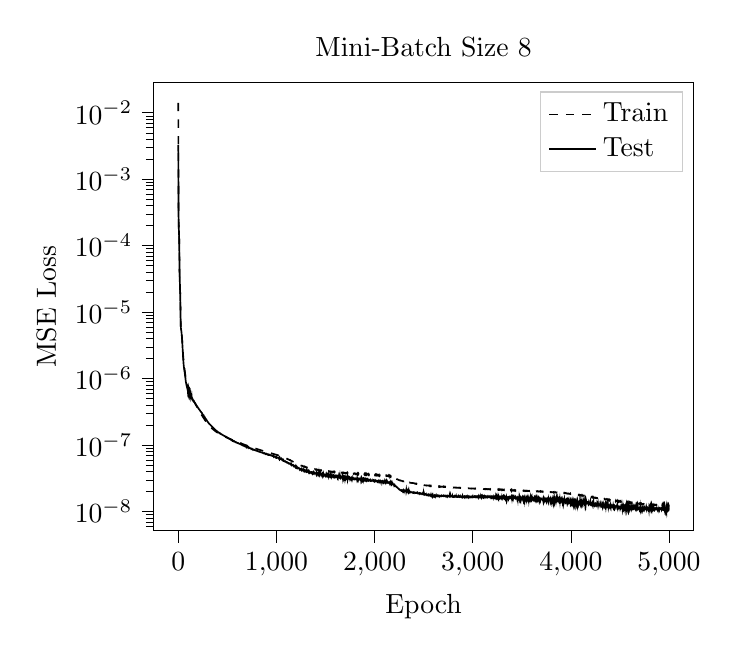
\begin{tikzpicture}

\begin{axis}[
legend cell align={left},
legend style={fill opacity=0.8, draw opacity=1, text opacity=1, draw=white!80!black},
log basis y={10},
tick align=outside,
tick pos=left,
title={Mini-Batch Size 8},
x grid style={white!69.0196078431373!black},
xlabel={Epoch},
xmin=-249.95, xmax=5248.95,
xtick style={color=black},
y grid style={white!69.0196078431373!black},
ylabel={MSE Loss},
ymin=5.12526233709927e-09, ymax=0.0285503119126669,
ymode=log,
ytick style={color=black}
]
\addplot [semithick, black, dashed]
table {%
0 0.0140922155501321
1 0.00164667243149597
2 0.00065037911516265
3 0.000295232196316647
4 0.000193644413906441
5 0.00017554680505782
6 0.000166322737537485
7 0.000155888844841684
8 0.000142262006907913
9 0.00012419570547172
10 0.000100196558816606
11 7.53355795714015e-05
12 5.41193190329068e-05
13 3.99818541809509e-05
14 3.23710513916922e-05
15 2.83831747833574e-05
16 2.58379168235479e-05
17 2.3768776641873e-05
18 2.16936214364978e-05
19 1.93698575890267e-05
20 1.67099984373635e-05
21 1.38117074528736e-05
22 1.10197760235451e-05
23 8.81342460627366e-06
24 7.32618501214688e-06
25 6.44809396973756e-06
26 5.96682320880859e-06
27 5.69452180099006e-06
28 5.51694411510084e-06
29 5.37627059711099e-06
30 5.25268244874155e-06
31 5.13194294012465e-06
32 5.00552247908104e-06
33 4.87103920659138e-06
34 4.72795897735523e-06
35 4.57529531857404e-06
36 4.41450717971747e-06
37 4.24678919441135e-06
38 4.07240037165479e-06
39 3.89275960455393e-06
40 3.70977897651414e-06
41 3.52646615996832e-06
42 3.3453291746639e-06
43 3.1669885086103e-06
44 2.99429524324069e-06
45 2.82882308749777e-06
46 2.67223944220518e-06
47 2.52574185277865e-06
48 2.39030650546113e-06
49 2.26648519112871e-06
50 2.15448263186602e-06
51 2.05455952405487e-06
52 1.96556939043546e-06
53 1.88664972873198e-06
54 1.81654708246981e-06
55 1.75456746703162e-06
56 1.69953624238417e-06
57 1.65011574182472e-06
58 1.60480939666741e-06
59 1.56276212375417e-06
60 1.52249059640042e-06
61 1.4837170463835e-06
62 1.44544674019187e-06
63 1.40767455231128e-06
64 1.37012475846632e-06
65 1.3339168483526e-06
66 1.29931519345661e-06
67 1.2659092755527e-06
68 1.23280311538565e-06
69 1.20021240133639e-06
70 1.16748595181093e-06
71 1.13551588817273e-06
72 1.10446207130366e-06
73 1.07352417389706e-06
74 1.04239164762987e-06
75 1.01698211097556e-06
76 9.92916835798496e-07
77 9.70485951363287e-07
78 9.49992109070763e-07
79 9.31409722205956e-07
80 9.14265601551279e-07
81 8.97762910810229e-07
82 8.82654424465557e-07
83 8.68559461117968e-07
84 8.55493358947967e-07
85 8.43273811710787e-07
86 8.31858977321076e-07
87 8.20936465963484e-07
88 8.10674030482517e-07
89 8.00620192784152e-07
90 7.91515300498702e-07
91 7.82651789464239e-07
92 7.7411152496154e-07
93 7.66956414445019e-07
94 7.5921274802937e-07
95 7.51383507328285e-07
96 7.44354396381652e-07
97 7.36274504674839e-07
98 7.30296529290797e-07
99 7.22306401783612e-07
100 7.16731141153559e-07
101 7.0944152068364e-07
102 7.04137545035621e-07
103 6.97249927974042e-07
104 6.922896165662e-07
105 6.85678604298801e-07
106 6.79918118848377e-07
107 6.74806719885623e-07
108 6.68366211726834e-07
109 6.63462581393048e-07
110 6.57123162881135e-07
111 6.52642981187057e-07
112 6.46561416587588e-07
113 6.42274032088608e-07
114 6.36438868973244e-07
115 6.32267128040098e-07
116 6.26555323151479e-07
117 6.21985995039154e-07
118 6.16880253367924e-07
119 6.11863263415557e-07
120 6.07826088987906e-07
121 6.02515582706076e-07
122 5.97315892207462e-07
123 5.93690181311501e-07
124 5.87228766487868e-07
125 5.84643050316913e-07
126 5.79739358123277e-07
127 5.74914281592953e-07
128 5.70551833760646e-07
129 5.66140960202688e-07
130 5.61847894573475e-07
131 5.57626214323648e-07
132 5.53413915262979e-07
133 5.49454119457948e-07
134 5.45167176518646e-07
135 5.41143863905802e-07
136 5.37298371497741e-07
137 5.32898270137139e-07
138 5.29843257034201e-07
139 5.25404720370659e-07
140 5.21684867152317e-07
141 5.18092104179857e-07
142 5.13483512598611e-07
143 5.08875732489145e-07
144 5.05149497538326e-07
145 5.01876758473685e-07
146 4.97770456185265e-07
147 4.94343421156174e-07
148 4.90650616956856e-07
149 4.8737844441149e-07
150 4.83746504770011e-07
151 4.80410617424099e-07
152 4.77105002900657e-07
153 4.73949040991073e-07
154 4.70770607652327e-07
155 4.67602424610192e-07
156 4.64573913710353e-07
157 4.61537018406233e-07
158 4.58560601526159e-07
159 4.55594075592813e-07
160 4.52629424799511e-07
161 4.49810896430591e-07
162 4.46874828853083e-07
163 4.44053090966179e-07
164 4.41227867604255e-07
165 4.38426361519362e-07
166 4.35670840431612e-07
167 4.33036380659502e-07
168 4.30322021191643e-07
169 4.27488975983437e-07
170 4.24709639364806e-07
171 4.21982422551537e-07
172 4.19321082635093e-07
173 4.16750839320912e-07
174 4.14194871584783e-07
175 4.1157767810418e-07
176 4.09005205327162e-07
177 4.06454590493155e-07
178 4.03974517769967e-07
179 4.01356386795726e-07
180 3.98910379288964e-07
181 3.96400903827754e-07
182 3.93962698311157e-07
183 3.91538277543901e-07
184 3.89058316706326e-07
185 3.86672758100559e-07
186 3.84376024534561e-07
187 3.82156077666451e-07
188 3.79795015795992e-07
189 3.77472126810829e-07
190 3.75254422486648e-07
191 3.72999132707719e-07
192 3.70814309334833e-07
193 3.68606052909115e-07
194 3.66414772166479e-07
195 3.64246124291867e-07
196 3.62064812147622e-07
197 3.60114379777343e-07
198 3.57652658479424e-07
199 3.55473573875997e-07
200 3.53420759978462e-07
201 3.51302201732295e-07
202 3.49260392450645e-07
203 3.47137964237021e-07
204 3.45095554795449e-07
205 3.43017129246448e-07
206 3.40932977728414e-07
207 3.38848146498094e-07
208 3.36741637614324e-07
209 3.34673315357747e-07
210 3.32618128226159e-07
211 3.30624918607469e-07
212 3.28681106719131e-07
213 3.2678425436572e-07
214 3.24867698765274e-07
215 3.23009222441328e-07
216 3.21105375114428e-07
217 3.19259059818222e-07
218 3.17433803207479e-07
219 3.15584080713194e-07
220 3.13753979209963e-07
221 3.11972391951798e-07
222 3.10204712469897e-07
223 3.08459960738361e-07
224 3.06718977086007e-07
225 3.04951894634087e-07
226 3.03379400019566e-07
227 3.01692094268446e-07
228 3.00041570543641e-07
229 2.98378097685514e-07
230 2.96704027594075e-07
231 2.95068247101682e-07
232 2.93436909618805e-07
233 2.91839041182129e-07
234 2.90256448501225e-07
235 2.88692379278643e-07
236 2.87134213266427e-07
237 2.85589026884026e-07
238 2.84047657121533e-07
239 2.82538714426295e-07
240 2.81039958053952e-07
241 2.79510103869285e-07
242 2.78032811682039e-07
243 2.76594212650139e-07
244 2.7475024603163e-07
245 2.72926708213106e-07
246 2.71423920384706e-07
247 2.7000172076086e-07
248 2.68524305077733e-07
249 2.67011570478815e-07
250 2.65667921034662e-07
251 2.64317999302932e-07
252 2.62892964080663e-07
253 2.6150448949025e-07
254 2.60125897110441e-07
255 2.58924373436997e-07
256 2.57517830519305e-07
257 2.56230467748253e-07
258 2.54854917034919e-07
259 2.53686509193329e-07
260 2.52175349391592e-07
261 2.51046833938062e-07
262 2.49770576434827e-07
263 2.48423187827029e-07
264 2.47144563388702e-07
265 2.45901549853045e-07
266 2.4462504500633e-07
267 2.43350985510205e-07
268 2.42261470663863e-07
269 2.41032267901176e-07
270 2.39729021991764e-07
271 2.38334006315455e-07
272 2.37114604335176e-07
273 2.35892772845858e-07
274 2.34670065896836e-07
275 2.3353716209229e-07
276 2.3238534521397e-07
277 2.31254778810808e-07
278 2.30117605983793e-07
279 2.29054269301088e-07
280 2.27954691752075e-07
281 2.26809562416719e-07
282 2.25817690040486e-07
283 2.24762463858497e-07
284 2.2381367495683e-07
285 2.22726548656738e-07
286 2.21723776196114e-07
287 2.20762035670674e-07
288 2.19673128100339e-07
289 2.18611050652129e-07
290 2.1762178107565e-07
291 2.16632967322994e-07
292 2.15608462355021e-07
293 2.14716398861725e-07
294 2.13740754045233e-07
295 2.12850587857361e-07
296 2.11970101840819e-07
297 2.11049697046661e-07
298 2.1004613132547e-07
299 2.09148392926295e-07
300 2.08267972048759e-07
301 2.0738952559185e-07
302 2.0650375899578e-07
303 2.0562344525743e-07
304 2.04789969075136e-07
305 2.03896006780724e-07
306 2.03049032204916e-07
307 2.02233469991597e-07
308 2.0148574800416e-07
309 2.00686525744231e-07
310 1.99914377798649e-07
311 1.99131872182789e-07
312 1.98344035812426e-07
313 1.97613068664282e-07
314 1.9680639949371e-07
315 1.96114129776603e-07
316 1.95406764222028e-07
317 1.94725376895022e-07
318 1.93973928373836e-07
319 1.93272308163017e-07
320 1.9257287543617e-07
321 1.91904341296123e-07
322 1.91237644701303e-07
323 1.90597502623291e-07
324 1.89894711086325e-07
325 1.8928915396188e-07
326 1.88604807627613e-07
327 1.8794622811491e-07
328 1.87344297193803e-07
329 1.86699944878299e-07
330 1.86075537186525e-07
331 1.85402446655658e-07
332 1.84775635814205e-07
333 1.84167428516346e-07
334 1.83570768633956e-07
335 1.82982711312007e-07
336 1.82418746863533e-07
337 1.81827815703528e-07
338 1.81145456025433e-07
339 1.80619840630669e-07
340 1.80006042857173e-07
341 1.79483078060372e-07
342 1.78932678077004e-07
343 1.7839446073431e-07
344 1.7783793585302e-07
345 1.77330097105965e-07
346 1.76734144670121e-07
347 1.76271198734312e-07
348 1.75766690267309e-07
349 1.75184670666795e-07
350 1.74708623170261e-07
351 1.74188886322924e-07
352 1.73653229948556e-07
353 1.73181383031462e-07
354 1.7267201918969e-07
355 1.72169975215297e-07
356 1.716809444261e-07
357 1.71193413185833e-07
358 1.7070678104858e-07
359 1.70231708297663e-07
360 1.69763145491331e-07
361 1.69323822717615e-07
362 1.68841542647513e-07
363 1.68392174817455e-07
364 1.67920915593811e-07
365 1.67448701848372e-07
366 1.67067471872784e-07
367 1.66522447294426e-07
368 1.66187803337436e-07
369 1.65655882883087e-07
370 1.65297342158866e-07
371 1.64844675270004e-07
372 1.64449132043387e-07
373 1.63934461077986e-07
374 1.63596360001961e-07
375 1.63166515610769e-07
376 1.62640494570709e-07
377 1.62330137088773e-07
378 1.61810680310737e-07
379 1.61525042159383e-07
380 1.61029843134486e-07
381 1.60723079604352e-07
382 1.60256959116367e-07
383 1.59806124516493e-07
384 1.59371342730807e-07
385 1.59003193211049e-07
386 1.58613461659129e-07
387 1.58135951810578e-07
388 1.5777919826121e-07
389 1.57490906419255e-07
390 1.57049220966599e-07
391 1.56678830967039e-07
392 1.56399091556736e-07
393 1.5595287873893e-07
394 1.55577467211288e-07
395 1.55218681813452e-07
396 1.54868281256881e-07
397 1.54552626023374e-07
398 1.54198211124168e-07
399 1.53841266364196e-07
400 1.53452866729964e-07
401 1.53133977093489e-07
402 1.52802964166199e-07
403 1.52480551506073e-07
404 1.52156185608376e-07
405 1.51788253479168e-07
406 1.51498513695003e-07
407 1.51127850402943e-07
408 1.50798184616718e-07
409 1.50510982436458e-07
410 1.50194480964316e-07
411 1.4992832301175e-07
412 1.49619644533416e-07
413 1.49345439441007e-07
414 1.49000281972178e-07
415 1.48698896465405e-07
416 1.48378767759638e-07
417 1.48073516024638e-07
418 1.47793847567357e-07
419 1.47497233387028e-07
420 1.47152927594263e-07
421 1.46810806187503e-07
422 1.46530012960611e-07
423 1.46194294019963e-07
424 1.45904546680953e-07
425 1.45637120098741e-07
426 1.45390437303661e-07
427 1.45085242406751e-07
428 1.44843584227061e-07
429 1.44539950433398e-07
430 1.44255259536763e-07
431 1.43986164975018e-07
432 1.43712213986902e-07
433 1.43442524212389e-07
434 1.43141190728002e-07
435 1.42893512014908e-07
436 1.42647763382797e-07
437 1.42393991835021e-07
438 1.42116199961961e-07
439 1.41860749801381e-07
440 1.41584198152245e-07
441 1.41324433158729e-07
442 1.41084530103086e-07
443 1.40788790234936e-07
444 1.40560038717652e-07
445 1.40289742095234e-07
446 1.40070903469791e-07
447 1.39810986377498e-07
448 1.3955653855291e-07
449 1.39309414347366e-07
450 1.39040228608778e-07
451 1.38806914293355e-07
452 1.38617263488072e-07
453 1.38398338824786e-07
454 1.38211991345116e-07
455 1.37910985833045e-07
456 1.37707504212159e-07
457 1.37452863837595e-07
458 1.37235590139895e-07
459 1.37014003817271e-07
460 1.36758330285147e-07
461 1.36494116027563e-07
462 1.36306082161752e-07
463 1.36068334931849e-07
464 1.35855103517102e-07
465 1.35629422052475e-07
466 1.35411948866349e-07
467 1.35155687953414e-07
468 1.34934801762299e-07
469 1.34734451673779e-07
470 1.34524718356843e-07
471 1.34328436132591e-07
472 1.34129347609147e-07
473 1.33910911843671e-07
474 1.3371256061312e-07
475 1.33461909047838e-07
476 1.33277299719126e-07
477 1.33085340515038e-07
478 1.32889105676881e-07
479 1.32672969037628e-07
480 1.32476193449804e-07
481 1.32274759009121e-07
482 1.32073942387123e-07
483 1.31855791474678e-07
484 1.31636651781619e-07
485 1.31416223496217e-07
486 1.31259498012071e-07
487 1.31016023310337e-07
488 1.30887004155866e-07
489 1.30695356258315e-07
490 1.30501306800923e-07
491 1.30296649251349e-07
492 1.30041917019597e-07
493 1.29918106384963e-07
494 1.29697845192567e-07
495 1.29461063567149e-07
496 1.29204722520981e-07
497 1.29046236825303e-07
498 1.28783909607577e-07
499 1.28579553615893e-07
500 1.28412652287579e-07
501 1.28222582777227e-07
502 1.28080913981421e-07
503 1.27826674720666e-07
504 1.2768455570189e-07
505 1.27511456184948e-07
506 1.27337297175956e-07
507 1.2712039346674e-07
508 1.26940336869552e-07
509 1.26781960378963e-07
510 1.26628617971747e-07
511 1.26438190140021e-07
512 1.26261214711931e-07
513 1.26080714901278e-07
514 1.25882205830763e-07
515 1.25689170451082e-07
516 1.25458669902656e-07
517 1.25292414027811e-07
518 1.25118541685509e-07
519 1.24933668057992e-07
520 1.24744541571076e-07
521 1.24592485745367e-07
522 1.2438628746736e-07
523 1.24239199989162e-07
524 1.24081532147713e-07
525 1.23898961273738e-07
526 1.23711435064067e-07
527 1.23683571343847e-07
528 1.23402232516057e-07
529 1.23180608545326e-07
530 1.22983389335474e-07
531 1.2279557410011e-07
532 1.22695858955524e-07
533 1.2242326393519e-07
534 1.22268119062241e-07
535 1.22114195065137e-07
536 1.2186837597028e-07
537 1.21758532072747e-07
538 1.21501212188235e-07
539 1.21415872920139e-07
540 1.21146897740232e-07
541 1.21149452825264e-07
542 1.20954131578088e-07
543 1.20601052417513e-07
544 1.2042635933085e-07
545 1.20382659668294e-07
546 1.20114501360291e-07
547 1.19902081415546e-07
548 1.19723047657061e-07
549 1.19519860986017e-07
550 1.19464099865851e-07
551 1.19455365275911e-07
552 1.18856987027627e-07
553 1.18855618111979e-07
554 1.18722306197583e-07
555 1.18556314758322e-07
556 1.18349971197418e-07
557 1.18197913097973e-07
558 1.18190822574249e-07
559 1.17993449931575e-07
560 1.17722103356144e-07
561 1.17562712910413e-07
562 1.1739236306596e-07
563 1.17146097792897e-07
564 1.17130330764326e-07
565 1.16876142195466e-07
566 1.16746778818566e-07
567 1.16807582864809e-07
568 1.16375001658398e-07
569 1.16238238121014e-07
570 1.16071960784225e-07
571 1.15917950825661e-07
572 1.15715357653201e-07
573 1.15682018952512e-07
574 1.15512718215527e-07
575 1.15298490829474e-07
576 1.15141919192041e-07
577 1.15017629779501e-07
578 1.14785245981963e-07
579 1.14825111019456e-07
580 1.14467956363384e-07
581 1.14309470399476e-07
582 1.14250206504352e-07
583 1.14062090345257e-07
584 1.14072716723257e-07
585 1.13818667545118e-07
586 1.13543024539808e-07
587 1.13510344416312e-07
588 1.13261899898021e-07
589 1.13188994674829e-07
590 1.12949545007623e-07
591 1.12861762920247e-07
592 1.12966328723374e-07
593 1.12624403906025e-07
594 1.12488853648784e-07
595 1.12194247433806e-07
596 1.12081747023041e-07
597 1.11879273879012e-07
598 1.11686604855166e-07
599 1.1151889847838e-07
600 1.11518363773655e-07
601 1.11229455521666e-07
602 1.11068491328581e-07
603 1.10914127503747e-07
604 1.10845691843053e-07
605 1.10635652848856e-07
606 1.10445679641913e-07
607 1.10333368983362e-07
608 1.10191389911307e-07
609 1.10141222277704e-07
610 1.09968580785491e-07
611 1.10079902308158e-07
612 1.09896487208161e-07
613 1.09495213120425e-07
614 1.09437622697328e-07
615 1.09409666039895e-07
616 1.09359268291698e-07
617 1.0894876301748e-07
618 1.08862762553841e-07
619 1.0888215664373e-07
620 1.08902593192184e-07
621 1.08681523236953e-07
622 1.08473326777769e-07
623 1.08357849692098e-07
624 1.08215046504156e-07
625 1.08083012595017e-07
626 1.07983994128702e-07
627 1.0788382092386e-07
628 1.07778989340446e-07
629 1.07629510504026e-07
630 1.07486674595592e-07
631 1.07359776917448e-07
632 1.07198026283228e-07
633 1.07110649613773e-07
634 1.06957342852709e-07
635 1.06551703673574e-07
636 1.06703632233973e-07
637 1.06261747919945e-07
638 1.06245268353788e-07
639 1.05981521867804e-07
640 1.0613362208467e-07
641 1.05918131012572e-07
642 1.05605284026922e-07
643 1.05518851803765e-07
644 1.05296745056549e-07
645 1.0529636806389e-07
646 1.05115613724394e-07
647 1.04897444288099e-07
648 1.04692954625563e-07
649 1.04653310055269e-07
650 1.04388389308596e-07
651 1.04356357626401e-07
652 1.04121267867185e-07
653 1.03941493522441e-07
654 1.03825485911813e-07
655 1.03654870686753e-07
656 1.03468656945438e-07
657 1.03318351046156e-07
658 1.03309234573246e-07
659 1.03166787249975e-07
660 1.02888646404509e-07
661 1.02764241914244e-07
662 1.02620244419427e-07
663 1.02643449945816e-07
664 1.02388692905464e-07
665 1.02254439710237e-07
666 1.02264427352949e-07
667 1.01974317667342e-07
668 1.01824479767032e-07
669 1.01781015130697e-07
670 1.01579884494996e-07
671 1.01662138689562e-07
672 1.01463956596604e-07
673 1.01146636220406e-07
674 1.01043345342333e-07
675 1.01026062447218e-07
676 1.00765059274366e-07
677 1.00705422818592e-07
678 1.00596716810841e-07
679 1.00494772908633e-07
680 1.00339713535291e-07
681 1.00227720652768e-07
682 1.00199328135986e-07
683 9.99779721606586e-08
684 9.99164768895611e-08
685 9.97651532674837e-08
686 9.96916367359546e-08
687 9.95852735758973e-08
688 9.94225873363064e-08
689 9.93057265326058e-08
690 9.91738692572852e-08
691 9.90683583950158e-08
692 9.89918791169941e-08
693 9.89294559996523e-08
694 9.87324563563874e-08
695 9.8580230650569e-08
696 9.84844026170606e-08
697 9.83782085786089e-08
698 9.82969909344433e-08
699 9.80663861103182e-08
700 9.79155029394718e-08
701 9.78743212769473e-08
702 9.7774189509181e-08
703 9.74998872109722e-08
704 9.7537862576047e-08
705 9.7373689259328e-08
706 9.72140168737923e-08
707 9.71121613257964e-08
708 9.69666632180122e-08
709 9.69298370527838e-08
710 9.67698093869984e-08
711 9.6669013320394e-08
712 9.6617836987889e-08
713 9.65235347489823e-08
714 9.643995225872e-08
715 9.6384693021534e-08
716 9.61863593840206e-08
717 9.60114623218544e-08
718 9.60902926934182e-08
719 9.57746484626654e-08
720 9.57750240715427e-08
721 9.55805155538059e-08
722 9.55347426128128e-08
723 9.54729408171318e-08
724 9.52798347118033e-08
725 9.52589754721345e-08
726 9.51665310111594e-08
727 9.49889552952499e-08
728 9.48892586905004e-08
729 9.48318259261782e-08
730 9.46984865208833e-08
731 9.46578152714039e-08
732 9.44619410319092e-08
733 9.44395689952415e-08
734 9.43228704386456e-08
735 9.42138219972577e-08
736 9.41150636339927e-08
737 9.40356634000494e-08
738 9.39251921092676e-08
739 9.37723432130611e-08
740 9.36953663508433e-08
741 9.36475301536177e-08
742 9.34891315171882e-08
743 9.34929558358277e-08
744 9.32899375643004e-08
745 9.31277580900058e-08
746 9.29872254360475e-08
747 9.29021212048298e-08
748 9.27547188318556e-08
749 9.26676536128212e-08
750 9.25360728327718e-08
751 9.24768817487376e-08
752 9.23224709517001e-08
753 9.2233401355557e-08
754 9.21099720416763e-08
755 9.20273056550513e-08
756 9.18983567661513e-08
757 9.17982077250912e-08
758 9.16838067226422e-08
759 9.1583944425544e-08
760 9.14591718057523e-08
761 9.13134026792051e-08
762 9.12507480110847e-08
763 9.11265217853341e-08
764 9.10621974288262e-08
765 9.08905435199614e-08
766 9.0788907545658e-08
767 9.0717570659038e-08
768 9.05781980975462e-08
769 9.05061573064359e-08
770 9.03604748181408e-08
771 9.02703232927848e-08
772 9.02022289084314e-08
773 9.01490784093184e-08
774 8.99447075433102e-08
775 8.98894601180089e-08
776 8.97487045516954e-08
777 8.9711841648743e-08
778 8.95438815806671e-08
779 8.95039619379645e-08
780 8.93075877943517e-08
781 8.92706220980699e-08
782 8.91444243862338e-08
783 8.90533289634732e-08
784 8.89315970269422e-08
785 8.88538352157298e-08
786 8.87460719418698e-08
787 8.86892839258024e-08
788 8.85925947713417e-08
789 8.84801011071801e-08
790 8.83455844515879e-08
791 8.83479853879265e-08
792 8.81836671791092e-08
793 8.8178019002072e-08
794 8.80678381420808e-08
795 8.79570468814705e-08
796 8.78213846133846e-08
797 8.77077261600689e-08
798 8.7557868305943e-08
799 8.75062553475914e-08
800 8.73836898467317e-08
801 8.73753748438233e-08
802 8.71596677542996e-08
803 8.71341073862553e-08
804 8.69886648713347e-08
805 8.69691683735851e-08
806 8.68006289946877e-08
807 8.67195310281232e-08
808 8.66247496071892e-08
809 8.66069136327141e-08
810 8.63993041644307e-08
811 8.63324029767298e-08
812 8.62302148672001e-08
813 8.61057656562636e-08
814 8.61300473475879e-08
815 8.58610517182612e-08
816 8.5876022253295e-08
817 8.58245899744148e-08
818 8.56204245254233e-08
819 8.56291569748535e-08
820 8.54643526437826e-08
821 8.53652859822418e-08
822 8.5391497251841e-08
823 8.51209773058414e-08
824 8.51588658763447e-08
825 8.50582824751811e-08
826 8.49786741063952e-08
827 8.48149538770215e-08
828 8.48154887371777e-08
829 8.46310325455235e-08
830 8.46116082833248e-08
831 8.44586885744292e-08
832 8.43162639991846e-08
833 8.43594839841089e-08
834 8.41931290338494e-08
835 8.40042691381271e-08
836 8.39640144789655e-08
837 8.39935478929021e-08
838 8.38417056181484e-08
839 8.3761031231866e-08
840 8.36453677903748e-08
841 8.35098131304335e-08
842 8.3516487031865e-08
843 8.3398541787183e-08
844 8.32627191780233e-08
845 8.32743370144939e-08
846 8.31479871719054e-08
847 8.30611524476055e-08
848 8.29425600832323e-08
849 8.28054075387996e-08
850 8.28294606325386e-08
851 8.27534693756959e-08
852 8.26178241633002e-08
853 8.25921608678115e-08
854 8.24915612467336e-08
855 8.23746438047834e-08
856 8.23552042801268e-08
857 8.22746717608069e-08
858 8.21175156664466e-08
859 8.20935714083149e-08
860 8.20074700209616e-08
861 8.18721728084171e-08
862 8.18467062071448e-08
863 8.17524560883243e-08
864 8.16378868124801e-08
865 8.16203907341162e-08
866 8.15071311217608e-08
867 8.14008423501988e-08
868 8.13587263230886e-08
869 8.12950596609241e-08
870 8.11408385228418e-08
871 8.11435524941118e-08
872 8.10090526517371e-08
873 8.09792461664571e-08
874 8.08584962870285e-08
875 8.07094791053231e-08
876 8.07686938379959e-08
877 8.06270915392204e-08
878 8.05262200671564e-08
879 8.04814699018053e-08
880 8.03900555492731e-08
881 8.03408116238913e-08
882 8.02471276806216e-08
883 8.01388805129477e-08
884 8.00124187625428e-08
885 8.00657544806072e-08
886 7.98942147488546e-08
887 7.99531881936488e-08
888 7.97822659910352e-08
889 7.97795756035668e-08
890 7.9595778335495e-08
891 7.94955623648619e-08
892 7.94511712500778e-08
893 7.94300374051815e-08
894 7.93113748613905e-08
895 7.92388654584642e-08
896 7.91362802941009e-08
897 7.90537630148691e-08
898 7.89241159324661e-08
899 7.89327640422499e-08
900 7.87739521186381e-08
901 7.87634696282069e-08
902 7.86302511679438e-08
903 7.85142067414313e-08
904 7.84941220688395e-08
905 7.836267482908e-08
906 7.83394425170059e-08
907 7.82585197347529e-08
908 7.82273210271356e-08
909 7.80942995328715e-08
910 7.80388083398975e-08
911 7.79501971406305e-08
912 7.78230592546336e-08
913 7.77868578483165e-08
914 7.76701064806318e-08
915 7.76812620495448e-08
916 7.75076760506366e-08
917 7.75319989765322e-08
918 7.74967118450931e-08
919 7.73487059220201e-08
920 7.73361544830209e-08
921 7.71912398640495e-08
922 7.71142926412338e-08
923 7.70105475949023e-08
924 7.69942951457381e-08
925 7.68621367575051e-08
926 7.66920159733786e-08
927 7.6753732895618e-08
928 7.66649599208691e-08
929 7.65232764639023e-08
930 7.64789896630091e-08
931 7.63227431415103e-08
932 7.62898755857222e-08
933 7.62348100540322e-08
934 7.61062690850522e-08
935 7.59985500060623e-08
936 7.60535598010037e-08
937 7.59387081998852e-08
938 7.58480387572646e-08
939 7.57766501973123e-08
940 7.56443777145677e-08
941 7.55885656298361e-08
942 7.55352047487889e-08
943 7.55366707450023e-08
944 7.54625999297431e-08
945 7.53840733613842e-08
946 7.52436891762187e-08
947 7.520958560292e-08
948 7.51185533998111e-08
949 7.50705502872151e-08
950 7.49230383103594e-08
951 7.48538313226632e-08
952 7.47696083367444e-08
953 7.4698309575183e-08
954 7.46352352933855e-08
955 7.45532024719608e-08
956 7.45396909715979e-08
957 7.43793192778952e-08
958 7.43306780917052e-08
959 7.42391270653897e-08
960 7.4170969384113e-08
961 7.41744250110088e-08
962 7.39807714547069e-08
963 7.3907636275905e-08
964 7.3864839967186e-08
965 7.38722046689233e-08
966 7.37782955395616e-08
967 7.35998169503205e-08
968 7.36751591370322e-08
969 7.35319244977717e-08
970 7.34493053959895e-08
971 7.33622083135543e-08
972 7.33287411573968e-08
973 7.32267693424049e-08
974 7.3227407262344e-08
975 7.30911046540328e-08
976 7.3059925388641e-08
977 7.29211026548882e-08
978 7.29121208236094e-08
979 7.2779587866556e-08
980 7.27771263386856e-08
981 7.26923735738794e-08
982 7.26410809015476e-08
983 7.25908489931371e-08
984 7.24250146495464e-08
985 7.2414066065285e-08
986 7.23511959135337e-08
987 7.23106430315923e-08
988 7.22220240687577e-08
989 7.21276343647048e-08
990 7.20563575073996e-08
991 7.19845479606462e-08
992 7.19308399528273e-08
993 7.18280783758019e-08
994 7.17602781392657e-08
995 7.16623081844503e-08
996 7.1633209976163e-08
997 7.1613316125152e-08
998 7.14358405220494e-08
999 7.13820533686516e-08
1000 7.13005416006496e-08
1001 7.13117426327514e-08
1002 7.11042069294621e-08
1003 7.11583764241297e-08
1004 7.11103543000746e-08
1005 7.09215685787967e-08
1006 7.08726079992061e-08
1007 7.08819332659871e-08
1008 7.06523474676146e-08
1009 7.06114099751076e-08
1010 7.05629681077013e-08
1011 7.04900955836862e-08
1012 7.03779293322881e-08
1013 7.03613790653535e-08
1014 7.02909734737744e-08
1015 7.02346028056411e-08
1016 7.00847629646617e-08
1017 7.00646524416371e-08
1018 7.00006208278481e-08
1019 6.99058087274551e-08
1020 6.97008041994351e-08
1021 6.96666002131252e-08
1022 6.95315661491946e-08
1023 6.93929467434629e-08
1024 6.93491352254938e-08
1025 6.92687724743735e-08
1026 6.9181248853134e-08
1027 6.90323947898364e-08
1028 6.89361719263815e-08
1029 6.88460079372177e-08
1030 6.88259702794625e-08
1031 6.87216120782708e-08
1032 6.85840478462652e-08
1033 6.85226009862205e-08
1034 6.83794042464214e-08
1035 6.83534466769942e-08
1036 6.82413636488022e-08
1037 6.81742337604874e-08
1038 6.8081035704104e-08
1039 6.80005548439055e-08
1040 6.79186499672468e-08
1041 6.78197289332161e-08
1042 6.77157139037376e-08
1043 6.77006809528535e-08
1044 6.75445062991997e-08
1045 6.74544157597268e-08
1046 6.73693972919054e-08
1047 6.72946742232838e-08
1048 6.71474435236519e-08
1049 6.70465003258514e-08
1050 6.70302539118595e-08
1051 6.69601158707067e-08
1052 6.68708544226959e-08
1053 6.67221369274884e-08
1054 6.66394672963477e-08
1055 6.65038577301047e-08
1056 6.64386373996351e-08
1057 6.6429855464456e-08
1058 6.63477771514209e-08
1059 6.62112182396868e-08
1060 6.61053233539377e-08
1061 6.60354965731358e-08
1062 6.58835158864335e-08
1063 6.58057612259455e-08
1064 6.57003935407019e-08
1065 6.56495188930961e-08
1066 6.55546697672094e-08
1067 6.54752256359359e-08
1068 6.53355711985881e-08
1069 6.52995786598609e-08
1070 6.52046299594034e-08
1071 6.50510368949142e-08
1072 6.50725278443787e-08
1073 6.49379873642886e-08
1074 6.47580108266155e-08
1075 6.46967440784962e-08
1076 6.47110855958033e-08
1077 6.46408487385841e-08
1078 6.45357608251018e-08
1079 6.44439404986485e-08
1080 6.4284627761424e-08
1081 6.42473115846087e-08
1082 6.42346976027497e-08
1083 6.4099857985056e-08
1084 6.39759074045898e-08
1085 6.39553085513e-08
1086 6.39084181939253e-08
1087 6.37432019150452e-08
1088 6.36723728701938e-08
1089 6.35793202752311e-08
1090 6.34713747382776e-08
1091 6.35341950525614e-08
1092 6.33713871458497e-08
1093 6.3277285804908e-08
1094 6.31845582761414e-08
1095 6.31149904926076e-08
1096 6.29787609565113e-08
1097 6.30093429236922e-08
1098 6.28861612330667e-08
1099 6.28055558475893e-08
1100 6.26232452294317e-08
1101 6.25952487345316e-08
1102 6.25822700701661e-08
1103 6.24765654775317e-08
1104 6.23883908117406e-08
1105 6.22942513581748e-08
1106 6.21327299015206e-08
1107 6.20863260349935e-08
1108 6.20415422387666e-08
1109 6.21000680087747e-08
1110 6.18504896578997e-08
1111 6.18067457205385e-08
1112 6.1644829599139e-08
1113 6.15710698008698e-08
1114 6.15897150124667e-08
1115 6.14760737152054e-08
1116 6.14502748659262e-08
1117 6.13122701871305e-08
1118 6.12455619730667e-08
1119 6.11872074065545e-08
1120 6.09162053128998e-08
1121 6.08576885987588e-08
1122 6.08179615930737e-08
1123 6.07086520618694e-08
1124 6.06223983101728e-08
1125 6.05575171297445e-08
1126 6.04104159798169e-08
1127 6.0348267340693e-08
1128 6.02285505344469e-08
1129 6.01458489990492e-08
1130 6.01179870587387e-08
1131 6.0027065746926e-08
1132 5.97797516208587e-08
1133 5.9795340693114e-08
1134 5.96402379002825e-08
1135 5.94761561911739e-08
1136 5.95539313339444e-08
1137 5.94249178975659e-08
1138 5.92505395076159e-08
1139 5.91597576615754e-08
1140 5.90666865125655e-08
1141 5.88915692842917e-08
1142 5.90203142101231e-08
1143 5.87497151824934e-08
1144 5.87532072353625e-08
1145 5.85907652910222e-08
1146 5.8551039190391e-08
1147 5.84408526567159e-08
1148 5.82552799874847e-08
1149 5.81301490427677e-08
1150 5.8109338837653e-08
1151 5.80481490803919e-08
1152 5.79101373157087e-08
1153 5.78085702569453e-08
1154 5.76846728073122e-08
1155 5.76280860729028e-08
1156 5.75032301490808e-08
1157 5.73179610068308e-08
1158 5.72661070288305e-08
1159 5.71943030065469e-08
1160 5.69885338492782e-08
1161 5.69631700626516e-08
1162 5.69194471786716e-08
1163 5.67838021701128e-08
1164 5.66640349766168e-08
1165 5.65589359924346e-08
1166 5.6512820266974e-08
1167 5.63850263919363e-08
1168 5.62500756329243e-08
1169 5.61824805593858e-08
1170 5.60970445784292e-08
1171 5.59599677218969e-08
1172 5.58494863724945e-08
1173 5.57552466800004e-08
1174 5.56996282252697e-08
1175 5.56156806448271e-08
1176 5.5491953369291e-08
1177 5.53300107037913e-08
1178 5.52866972709509e-08
1179 5.5107895852835e-08
1180 5.50283653844019e-08
1181 5.51412584899325e-08
1182 5.48718789001867e-08
1183 5.4910465046909e-08
1184 5.4751843118872e-08
1185 5.4634272609988e-08
1186 5.45681121217889e-08
1187 5.44585529360653e-08
1188 5.43135494264213e-08
1189 5.42500546694136e-08
1190 5.41413124164336e-08
1191 5.40952266248063e-08
1192 5.39357546243124e-08
1193 5.39131514880609e-08
1194 5.39165687554188e-08
1195 5.3634612921627e-08
1196 5.35923273101702e-08
1197 5.35096682368064e-08
1198 5.34264127121098e-08
1199 5.33043504136188e-08
1200 5.31984917513384e-08
1201 5.31392249949469e-08
1202 5.30054221310472e-08
1203 5.30110809604523e-08
1204 5.28841194253893e-08
1205 5.28213592305704e-08
1206 5.27674378001386e-08
1207 5.25633076429166e-08
1208 5.25129558854864e-08
1209 5.2446357926339e-08
1210 5.22644627349855e-08
1211 5.21429107900317e-08
1212 5.21280838032823e-08
1213 5.20980213041255e-08
1214 5.18598821455107e-08
1215 5.19323746939193e-08
1216 5.1801599847856e-08
1217 5.16898352844741e-08
1218 5.14871654297977e-08
1219 5.15548961050882e-08
1220 5.14475486421695e-08
1221 5.13119661880168e-08
1222 5.12700813648515e-08
1223 5.12630925495472e-08
1224 5.11038289716659e-08
1225 5.10397683979313e-08
1226 5.09275734623671e-08
1227 5.09132049710814e-08
1228 5.0759712610926e-08
1229 5.06871001304532e-08
1230 5.06944659219855e-08
1231 5.05630977118976e-08
1232 5.05891275865977e-08
1233 5.04078954683962e-08
1234 5.0369708529896e-08
1235 5.03202734072339e-08
1236 5.03486166767431e-08
1237 5.01460485304861e-08
1238 5.00217914414236e-08
1239 5.00083646550742e-08
1240 4.99302473584429e-08
1241 4.987592799921e-08
1242 4.97896254327834e-08
1243 4.97413813849157e-08
1244 4.96402420528952e-08
1245 4.9622389326931e-08
1246 4.95539652263233e-08
1247 4.94904343217861e-08
1248 4.94052279922386e-08
1249 4.92951875696868e-08
1250 4.93147989524267e-08
1251 4.91164378098041e-08
1252 4.91569000953262e-08
1253 4.91227655383675e-08
1254 4.90244803059703e-08
1255 4.89576740712039e-08
1256 4.8822162876494e-08
1257 4.87467866965297e-08
1258 4.87341117052509e-08
1259 4.87276126515113e-08
1260 4.87346524646881e-08
1261 4.85851170131113e-08
1262 4.84871747534754e-08
1263 4.85831895207234e-08
1264 4.82988585561728e-08
1265 4.83467545695504e-08
1266 4.83161799191834e-08
1267 4.81926020485801e-08
1268 4.81261100500063e-08
1269 4.80794487556224e-08
1270 4.79064465315204e-08
1271 4.78844559088643e-08
1272 4.80212023230564e-08
1273 4.79060066149728e-08
1274 4.7783847305638e-08
1275 4.76988225441843e-08
1276 4.77218500298804e-08
1277 4.76159679054788e-08
1278 4.76466013443755e-08
1279 4.74691612195599e-08
1280 4.75158579309465e-08
1281 4.73825057967225e-08
1282 4.7485986818252e-08
1283 4.72961260644666e-08
1284 4.73102585516472e-08
1285 4.72351163418594e-08
1286 4.72344711912598e-08
1287 4.71515645523724e-08
1288 4.71153546151015e-08
1289 4.68685075079023e-08
1290 4.70706135908827e-08
1291 4.68408979266144e-08
1292 4.68855339947893e-08
1293 4.69027191636329e-08
1294 4.68532288326884e-08
1295 4.66869751258869e-08
1296 4.67236158723239e-08
1297 4.66455751588768e-08
1298 4.6581428891912e-08
1299 4.66710647764046e-08
1300 4.65150191413244e-08
1301 4.6453202255492e-08
1302 4.64446993628798e-08
1303 4.63894488405003e-08
1304 4.62309609279288e-08
1305 4.62655005257773e-08
1306 4.63196391784493e-08
1307 4.61808473293246e-08
1308 4.61542245702162e-08
1309 4.62172598085786e-08
1310 4.61607299291344e-08
1311 4.60153494588056e-08
1312 4.59913277452983e-08
1313 4.59276329918268e-08
1314 4.58297194576573e-08
1315 4.59273223443191e-08
1316 4.58042492530453e-08
1317 4.57084866845037e-08
1318 4.56549604122003e-08
1319 4.56686972283293e-08
1320 4.56331827685119e-08
1321 4.56046227030882e-08
1322 4.5550667001848e-08
1323 4.55369211307399e-08
1324 4.5590441208887e-08
1325 4.54679211445708e-08
1326 4.54479248590545e-08
1327 4.52664653485257e-08
1328 4.5337347214236e-08
1329 4.53551621877324e-08
1330 4.51916858850154e-08
1331 4.51722750653971e-08
1332 4.51394618616874e-08
1333 4.51769472675778e-08
1334 4.51334482649557e-08
1335 4.51266249861249e-08
1336 4.50874914861288e-08
1337 4.49287061963233e-08
1338 4.48967479993456e-08
1339 4.48264219876648e-08
1340 4.4867042350738e-08
1341 4.48034820754728e-08
1342 4.48350610398052e-08
1343 4.48033875457554e-08
1344 4.45712150360933e-08
1345 4.46036571952746e-08
1346 4.46692990454523e-08
1347 4.45814032055125e-08
1348 4.45665362684977e-08
1349 4.45728043025895e-08
1350 4.45147311864957e-08
1351 4.44823261869232e-08
1352 4.43828213363417e-08
1353 4.42768181132536e-08
1354 4.43993598802095e-08
1355 4.44070804617169e-08
1356 4.42842968162438e-08
1357 4.41155342043587e-08
1358 4.41278631075903e-08
1359 4.40644807078172e-08
1360 4.42094289478945e-08
1361 4.40818237334994e-08
1362 4.39918047412391e-08
1363 4.41803186754797e-08
1364 4.40159865835454e-08
1365 4.39419652753514e-08
1366 4.39800256470946e-08
1367 4.38194544480908e-08
1368 4.38346918683052e-08
1369 4.38826430064765e-08
1370 4.38439412224767e-08
1371 4.38131168918332e-08
1372 4.37225367591054e-08
1373 4.36888630588328e-08
1374 4.37150416381371e-08
1375 4.36178424365608e-08
1376 4.36608899700985e-08
1377 4.35089207826422e-08
1378 4.35441604231812e-08
1379 4.35481492102596e-08
1380 4.34936193034474e-08
1381 4.33650798727925e-08
1382 4.34177889596654e-08
1383 4.34463673570917e-08
1384 4.33263139223428e-08
1385 4.33727313220444e-08
1386 4.33343354258042e-08
1387 4.3228653130889e-08
1388 4.31082869178923e-08
1389 4.324872136241e-08
1390 4.30600019534211e-08
1391 4.32475265323973e-08
1392 4.30882091100315e-08
1393 4.30473245973673e-08
1394 4.29888738828765e-08
1395 4.30272572833346e-08
1396 4.29292623698174e-08
1397 4.2927458932418e-08
1398 4.30014096650666e-08
1399 4.30005459408633e-08
1400 4.28852556577652e-08
1401 4.28427411769405e-08
1402 4.29186751995658e-08
1403 4.26496567271784e-08
1404 4.28333187523222e-08
1405 4.27500164761341e-08
1406 4.27967534255558e-08
1407 4.26256254471014e-08
1408 4.26668547057751e-08
1409 4.25627499347492e-08
1410 4.27053181430992e-08
1411 4.24960702827271e-08
1412 4.25527307035267e-08
1413 4.25026517083538e-08
1414 4.24830301199997e-08
1415 4.24793107010046e-08
1416 4.24730674390972e-08
1417 4.23903328332642e-08
1418 4.25100638867804e-08
1419 4.24156434370992e-08
1420 4.23989374351841e-08
1421 4.23957842898837e-08
1422 4.23277789733945e-08
1423 4.23183708635477e-08
1424 4.22206468280173e-08
1425 4.22159647799347e-08
1426 4.22320841448887e-08
1427 4.21671459114314e-08
1428 4.22204840990759e-08
1429 4.21945885649144e-08
1430 4.21728435395785e-08
1431 4.21243299655316e-08
1432 4.20114667738503e-08
1433 4.20510037324462e-08
1434 4.2026753572344e-08
1435 4.19436382799176e-08
1436 4.19389113277546e-08
1437 4.19057039202642e-08
1438 4.18952429424024e-08
1439 4.19827620414814e-08
1440 4.19652518064417e-08
1441 4.18845844243343e-08
1442 4.19072387116692e-08
1443 4.17922589410757e-08
1444 4.16854369809094e-08
1445 4.1889259613459e-08
1446 4.17623865209826e-08
1447 4.17697262604655e-08
1448 4.17888626045304e-08
1449 4.16201110771119e-08
1450 4.17640830239208e-08
1451 4.1783336582224e-08
1452 4.153928639683e-08
1453 4.16737873538686e-08
1454 4.1592476381247e-08
1455 4.15322517932637e-08
1456 4.1644548808506e-08
1457 4.15027544096169e-08
1458 4.148360849765e-08
1459 4.13861753427724e-08
1460 4.14018035996833e-08
1461 4.13481794314663e-08
1462 4.14854741146442e-08
1463 4.13563179764154e-08
1464 4.13556541101201e-08
1465 4.13902445641767e-08
1466 4.1323798298798e-08
1467 4.13480203884653e-08
1468 4.1203276207824e-08
1469 4.1235213055657e-08
1470 4.11417126029434e-08
1471 4.12246168219887e-08
1472 4.11880018207356e-08
1473 4.10834203830035e-08
1474 4.12011794010958e-08
1475 4.10904470413698e-08
1476 4.10302819586761e-08
1477 4.10799662917682e-08
1478 4.10220235567138e-08
1479 4.10007051749872e-08
1480 4.09940534513709e-08
1481 4.09689597491436e-08
1482 4.10433389328446e-08
1483 4.10684464080546e-08
1484 4.0948897821913e-08
1485 4.09499040134875e-08
1486 4.08794801574075e-08
1487 4.09105480914107e-08
1488 4.08452793374536e-08
1489 4.08942971645843e-08
1490 4.07402955646674e-08
1491 4.08870578434417e-08
1492 4.07994149629332e-08
1493 4.08190274594489e-08
1494 4.08339842810079e-08
1495 4.06289100567392e-08
1496 4.07976245524466e-08
1497 4.0624878185902e-08
1498 4.07296249225197e-08
1499 4.06837669739701e-08
1500 4.06156222441112e-08
1501 4.07313091956851e-08
1502 4.05451847482752e-08
1503 4.06221682425212e-08
1504 4.05266821212891e-08
1505 4.04707060539522e-08
1506 4.06462516782113e-08
1507 4.04694767723868e-08
1508 4.04878702155997e-08
1509 4.05097304012614e-08
1510 4.04145102264053e-08
1511 4.0458490955686e-08
1512 4.04152247091005e-08
1513 4.04283759909418e-08
1514 4.04303081200652e-08
1515 4.03291169508435e-08
1516 4.03538379005752e-08
1517 4.04357018073398e-08
1518 4.01908035403409e-08
1519 4.0378684301956e-08
1520 4.01831596095192e-08
1521 4.03242693085559e-08
1522 4.01736299417976e-08
1523 4.02171476885371e-08
1524 4.03139829083798e-08
1525 4.0050756290988e-08
1526 4.01579128519458e-08
1527 4.01703933876618e-08
1528 4.01928873969837e-08
1529 4.01609750353415e-08
1530 4.00341430619733e-08
1531 4.01794336895023e-08
1532 4.00297975486907e-08
1533 4.00986562185679e-08
1534 4.01208160880628e-08
1535 3.99242789086429e-08
1536 4.00895154815117e-08
1537 3.99392733978488e-08
1538 4.00255155073026e-08
1539 3.99330273790355e-08
1540 4.00368776256599e-08
1541 3.98720245327056e-08
1542 3.99692181636269e-08
1543 3.98561598462521e-08
1544 3.98875270821719e-08
1545 3.9898592707921e-08
1546 3.99073250436643e-08
1547 3.99202588603487e-08
1548 3.9863083950209e-08
1549 3.98795083480508e-08
1550 3.98830174299647e-08
1551 3.97511638707826e-08
1552 3.98775771195403e-08
1553 3.97159798799507e-08
1554 3.98367431264646e-08
1555 3.97162449825572e-08
1556 3.97871075605849e-08
1557 3.96644445856964e-08
1558 3.9699416047867e-08
1559 3.97870561856806e-08
1560 3.96381743366092e-08
1561 3.97042046440532e-08
1562 3.96156072683951e-08
1563 3.96154665756043e-08
1564 3.96605191550492e-08
1565 3.958909697932e-08
1566 3.96173939121169e-08
1567 3.949263310421e-08
1568 3.96089839078684e-08
1569 3.95455036246162e-08
1570 3.9636709490587e-08
1571 3.94831752732472e-08
1572 3.94724301058247e-08
1573 3.95125908312366e-08
1574 3.94526429312592e-08
1575 3.95341919947612e-08
1576 3.93538525056414e-08
1577 3.94563540533355e-08
1578 3.93826284383891e-08
1579 3.94670636287842e-08
1580 3.93370668776427e-08
1581 3.93753766632088e-08
1582 3.93889478891296e-08
1583 3.93959847713177e-08
1584 3.93097157589395e-08
1585 3.93532651656869e-08
1586 3.91723971162605e-08
1587 3.9439265921537e-08
1588 3.92176067336436e-08
1589 3.92966383158111e-08
1590 3.93851996420835e-08
1591 3.91521733389411e-08
1592 3.91947608742171e-08
1593 3.92991181339397e-08
1594 3.91132583290599e-08
1595 3.93028898422187e-08
1596 3.90764033886271e-08
1597 3.92399381112796e-08
1598 3.92021937143383e-08
1599 3.90802838641235e-08
1600 3.91499000782503e-08
1601 3.91313884398059e-08
1602 3.90865781119132e-08
1603 3.91318111354622e-08
1604 3.90454653018679e-08
1605 3.90933970058072e-08
1606 3.91323979753722e-08
1607 3.91136423418814e-08
1608 3.90225514497189e-08
1609 3.89170263863647e-08
1610 3.90865480301983e-08
1611 3.8980921593712e-08
1612 3.89813223291569e-08
1613 3.90147075677305e-08
1614 3.89207366335853e-08
1615 3.89198063510676e-08
1616 3.90334313173923e-08
1617 3.88514370586179e-08
1618 3.89586336879688e-08
1619 3.88994614555216e-08
1620 3.89837869310128e-08
1621 3.88157792121646e-08
1622 3.8903180284322e-08
1623 3.88374568531802e-08
1624 3.89662983231176e-08
1625 3.87433496351619e-08
1626 3.88509129178871e-08
1627 3.87580687961631e-08
1628 3.89098066246873e-08
1629 3.86810810075744e-08
1630 3.8847601955716e-08
1631 3.8731702770356e-08
1632 3.88384859340007e-08
1633 3.86796453755167e-08
1634 3.86607207518708e-08
1635 3.86814175348249e-08
1636 3.86742364932857e-08
1637 3.87164597510647e-08
1638 3.86513170154146e-08
1639 3.88603046239666e-08
1640 3.85722263551713e-08
1641 3.86626669151013e-08
1642 3.85764308683534e-08
1643 3.85580688213594e-08
1644 3.86169037662754e-08
1645 3.85148538581959e-08
1646 3.86165236889724e-08
1647 3.84727122453299e-08
1648 3.88424589639058e-08
1649 3.84465692357949e-08
1650 3.85114503771433e-08
1651 3.84911400512777e-08
1652 3.84304911449362e-08
1653 3.85630037955664e-08
1654 3.84011487293279e-08
1655 3.84661550612009e-08
1656 3.85328484400205e-08
1657 3.84369141146479e-08
1658 3.84122835210832e-08
1659 3.8412436121682e-08
1660 3.83894825235487e-08
1661 3.84446199950261e-08
1662 3.8335402538614e-08
1663 3.83735077038594e-08
1664 3.83685282532298e-08
1665 3.83480501557898e-08
1666 3.82956904871889e-08
1667 3.84011462086775e-08
1668 3.83502299774463e-08
1669 3.83458634498624e-08
1670 3.8245394529568e-08
1671 3.83146489473241e-08
1672 3.82573301918043e-08
1673 3.82244613819083e-08
1674 3.8246418380794e-08
1675 3.82150598499109e-08
1676 3.82407916803551e-08
1677 3.82599868506972e-08
1678 3.8215464568836e-08
1679 3.81728400284942e-08
1680 3.83210382013388e-08
1681 3.80955480121514e-08
1682 3.81806894989012e-08
1683 3.82224091151073e-08
1684 3.81114148124695e-08
1685 3.82258913358413e-08
1686 3.82052000684752e-08
1687 3.81070638280079e-08
1688 3.8081548687785e-08
1689 3.81398353761497e-08
1690 3.81179427018097e-08
1691 3.80720296826453e-08
1692 3.80211410555553e-08
1693 3.81585196489453e-08
1694 3.80863659596997e-08
1695 3.7976557523578e-08
1696 3.80630843066498e-08
1697 3.81245449689871e-08
1698 3.80392725380929e-08
1699 3.801984486973e-08
1700 3.79566180743751e-08
1701 3.79708953985869e-08
1702 3.80453341737308e-08
1703 3.79378156063481e-08
1704 3.79759017397063e-08
1705 3.79490948132499e-08
1706 3.80014099050641e-08
1707 3.78876995812405e-08
1708 3.79235057170746e-08
1709 3.79901633928981e-08
1710 3.79401265870882e-08
1711 3.78765139581461e-08
1712 3.78788724297863e-08
1713 3.79089320423631e-08
1714 3.79844686686504e-08
1715 3.79382417801111e-08
1716 3.79571741651041e-08
1717 3.79882111483099e-08
1718 3.78223503592068e-08
1719 3.7959839022772e-08
1720 3.76949858327258e-08
1721 3.80500853780497e-08
1722 3.77684928363209e-08
1723 3.79319000765044e-08
1724 3.78127555658025e-08
1725 3.76808580231369e-08
1726 3.78913456544616e-08
1727 3.76658090703863e-08
1728 3.7851494917529e-08
1729 3.77664108097697e-08
1730 3.79108147838814e-08
1731 3.76634401306752e-08
1732 3.78151026674267e-08
1733 3.78816969464069e-08
1734 3.77709782481972e-08
1735 3.77660620167752e-08
1736 3.76888900031069e-08
1737 3.77818670016516e-08
1738 3.78022734786043e-08
1739 3.77456426572387e-08
1740 3.76173546103864e-08
1741 3.76604630600852e-08
1742 3.77668573965373e-08
1743 3.77400727162858e-08
1744 3.77201424601736e-08
1745 3.77242986160375e-08
1746 3.75634211788878e-08
1747 3.74809592673664e-08
1748 3.7722135395768e-08
1749 3.76457967710131e-08
1750 3.76064268419185e-08
1751 3.76065779379431e-08
1752 3.74286121975764e-08
1753 3.77629903707266e-08
1754 3.76661396659372e-08
1755 3.74908666405105e-08
1756 3.76121619192205e-08
1757 3.75940156729371e-08
1758 3.76416019105541e-08
1759 3.74089387640275e-08
1760 3.75451150600448e-08
1761 3.74251382719848e-08
1762 3.73434886444812e-08
1763 3.76087765929789e-08
1764 3.75553967626452e-08
1765 3.73977909142731e-08
1766 3.74640324758424e-08
1767 3.73550987626814e-08
1768 3.74835799159534e-08
1769 3.73618815268095e-08
1770 3.75936487801987e-08
1771 3.72713335470287e-08
1772 3.75196970185954e-08
1773 3.72949849896109e-08
1774 3.7603680296705e-08
1775 3.72440201465984e-08
1776 3.75571327109192e-08
1777 3.72496371237041e-08
1778 3.74038666710597e-08
1779 3.74239376252916e-08
1780 3.74428224656498e-08
1781 3.7323855651028e-08
1782 3.74017605850874e-08
1783 3.72666274963684e-08
1784 3.73440678775872e-08
1785 3.73906923156753e-08
1786 3.73588830671068e-08
1787 3.71107454029129e-08
1788 3.72834189805715e-08
1789 3.73839526646158e-08
1790 3.74207804099136e-08
1791 3.72704231348386e-08
1792 3.72604873839499e-08
1793 3.72039002338731e-08
1794 3.72388135945201e-08
1795 3.73753077895778e-08
1796 3.72486858588594e-08
1797 3.72918126916311e-08
1798 3.72434037134717e-08
1799 3.72466739793076e-08
1800 3.72663990639843e-08
1801 3.71341596454577e-08
1802 3.7279309918592e-08
1803 3.72007997335722e-08
1804 3.72522711966639e-08
1805 3.71977966189263e-08
1806 3.71243192054393e-08
1807 3.71166673645007e-08
1808 3.69281813226152e-08
1809 3.7265723722868e-08
1810 3.72295604456063e-08
1811 3.7045100355293e-08
1812 3.71322109171679e-08
1813 3.71508310981206e-08
1814 3.71456299328443e-08
1815 3.71071213347562e-08
1816 3.71199989213089e-08
1817 3.70692861344502e-08
1818 3.71239575356341e-08
1819 3.70205668143164e-08
1820 3.70877458459873e-08
1821 3.69541319535926e-08
1822 3.70777116702747e-08
1823 3.67921550732397e-08
1824 3.7050849953868e-08
1825 3.70229679376166e-08
1826 3.69968310884872e-08
1827 3.71215581407291e-08
1828 3.67214813636885e-08
1829 3.70434229832739e-08
1830 3.67917332182444e-08
1831 3.71148817803757e-08
1832 3.69631161016848e-08
1833 3.67094972708593e-08
1834 3.69223256053708e-08
1835 3.67426318259589e-08
1836 3.70516558798606e-08
1837 3.67933732445813e-08
1838 3.69378140621102e-08
1839 3.68091435007933e-08
1840 3.68699657187221e-08
1841 3.67680227189027e-08
1842 3.67932825673378e-08
1843 3.66279344761189e-08
1844 3.70051625235845e-08
1845 3.66218960352604e-08
1846 3.71567434198639e-08
1847 3.67378085286418e-08
1848 3.67072405182967e-08
1849 3.68038352065447e-08
1850 3.67439507895639e-08
1851 3.66124083939212e-08
1852 3.67425429224077e-08
1853 3.67981550968288e-08
1854 3.66166572089988e-08
1855 3.68664959489173e-08
1856 3.65924359608805e-08
1857 3.66692661883938e-08
1858 3.66733336858438e-08
1859 3.67367757094783e-08
1860 3.65539251201419e-08
1861 3.67730002568401e-08
1862 3.65517606497612e-08
1863 3.67414380395559e-08
1864 3.65365003003326e-08
1865 3.66813095511453e-08
1866 3.65326868894122e-08
1867 3.68337799656615e-08
1868 3.66286341191291e-08
1869 3.65044348935584e-08
1870 3.66127535955663e-08
1871 3.65746113235588e-08
1872 3.65417026371162e-08
1873 3.67053717078569e-08
1874 3.6658561624936e-08
1875 3.65626657981011e-08
1876 3.65201574044072e-08
1877 3.67783549450884e-08
1878 3.66494288788211e-08
1879 3.66888207783411e-08
1880 3.65948743836775e-08
1881 3.65293158486324e-08
1882 3.6500014441998e-08
1883 3.64699401549373e-08
1884 3.64751547068387e-08
1885 3.65656375094225e-08
1886 3.65746387260835e-08
1887 3.66372703726192e-08
1888 3.64976410645035e-08
1889 3.65722141060232e-08
1890 3.64866452176038e-08
1891 3.65375467361595e-08
1892 3.65167638012309e-08
1893 3.63294874006215e-08
1894 3.63945058015069e-08
1895 3.6536670052989e-08
1896 3.6430282676303e-08
1897 3.62453244746597e-08
1898 3.66222929399918e-08
1899 3.64198722717646e-08
1900 3.63831767380418e-08
1901 3.63298386836242e-08
1902 3.61740805980837e-08
1903 3.64556771561553e-08
1904 3.63519154173986e-08
1905 3.62696372944171e-08
1906 3.61171992451226e-08
1907 3.64603584808165e-08
1908 3.61317012207429e-08
1909 3.62745675124287e-08
1910 3.64189258177383e-08
1911 3.6266710974342e-08
1912 3.62556905648681e-08
1913 3.6238342407291e-08
1914 3.62670215623417e-08
1915 3.60366312679439e-08
1916 3.63011385027256e-08
1917 3.61772445773845e-08
1918 3.61867287574924e-08
1919 3.61102679971026e-08
1920 3.63929243683003e-08
1921 3.60180869836135e-08
1922 3.61357699847353e-08
1923 3.61040660279421e-08
1924 3.6139368550181e-08
1925 3.60739116982423e-08
1926 3.6196284967982e-08
1927 3.59936592344567e-08
1928 3.60563996575358e-08
1929 3.60782758486167e-08
1930 3.60398286818331e-08
1931 3.60291056034079e-08
1932 3.60345146028784e-08
1933 3.59823884230615e-08
1934 3.60840954800601e-08
1935 3.59893449890514e-08
1936 3.59963851610523e-08
1937 3.62121882626632e-08
1938 3.59255595241414e-08
1939 3.60697188535042e-08
1940 3.59639030174108e-08
1941 3.61143853102597e-08
1942 3.58569910274831e-08
1943 3.6043464469504e-08
1944 3.58307471461927e-08
1945 3.60832720742721e-08
1946 3.58909315378853e-08
1947 3.59922691823833e-08
1948 3.588628298834e-08
1949 3.57991387196499e-08
1950 3.59611625162515e-08
1951 3.59351795946594e-08
1952 3.58898386458861e-08
1953 3.57527423555659e-08
1954 3.5908256137418e-08
1955 3.57621854756296e-08
1956 3.58349212685738e-08
1957 3.58016397492555e-08
1958 3.59061841495034e-08
1959 3.58764264776212e-08
1960 3.59239804565981e-08
1961 3.56813113904231e-08
1962 3.58514508875807e-08
1963 3.57986901380336e-08
1964 3.57795846923636e-08
1965 3.58297134064323e-08
1966 3.58044209156638e-08
1967 3.57522844649516e-08
1968 3.57979316274459e-08
1969 3.57875962246901e-08
1970 3.58005632263847e-08
1971 3.57308950551527e-08
1972 3.57868481506429e-08
1973 3.57633905760935e-08
1974 3.59752080516529e-08
1975 3.54793153327648e-08
1976 3.56424363725516e-08
1977 3.56962309773223e-08
1978 3.57075252499506e-08
1979 3.5845165480719e-08
1980 3.56351077415162e-08
1981 3.56275620205793e-08
1982 3.56691139065113e-08
1983 3.5589426081728e-08
1984 3.56025159495843e-08
1985 3.58654780168166e-08
1986 3.56388935309759e-08
1987 3.5567677426851e-08
1988 3.56262408662822e-08
1989 3.56126999379036e-08
1990 3.57467316645099e-08
1991 3.55701531344899e-08
1992 3.57601672029695e-08
1993 3.55033272736449e-08
1994 3.57265346040414e-08
1995 3.5396074536731e-08
1996 3.54844572565405e-08
1997 3.57656564653475e-08
1998 3.53924049982801e-08
1999 3.55584950182397e-08
2000 3.56697449870325e-08
2001 3.56787138220405e-08
2002 3.55943911167778e-08
2003 3.54479785218409e-08
2004 3.56183040364222e-08
2005 3.53309536897939e-08
2006 3.5582972430781e-08
2007 3.55872772117571e-08
2008 3.56063758508718e-08
2009 3.55415195936182e-08
2010 3.55386896822019e-08
2011 3.55435800902804e-08
2012 3.54341543582493e-08
2013 3.5326350536824e-08
2014 3.54429674618295e-08
2015 3.56998978769951e-08
2016 3.54859376350269e-08
2017 3.53400733024145e-08
2018 3.55125124622546e-08
2019 3.53422700452022e-08
2020 3.55198382075983e-08
2021 3.53294625350387e-08
2022 3.53245762756416e-08
2023 3.54871031174042e-08
2024 3.55245614671595e-08
2025 3.52888825934095e-08
2026 3.55585673830205e-08
2027 3.54134896176639e-08
2028 3.53721047030575e-08
2029 3.54860238958032e-08
2030 3.54437497889215e-08
2031 3.55012276966882e-08
2032 3.53924766249847e-08
2033 3.53858738901813e-08
2034 3.53863012767519e-08
2035 3.54097912538265e-08
2036 3.52552421158947e-08
2037 3.54500118371348e-08
2038 3.53148007081749e-08
2039 3.51771727915562e-08
2040 3.52485998993402e-08
2041 3.52664494878141e-08
2042 3.53212110244527e-08
2043 3.52696402448061e-08
2044 3.53278196350004e-08
2045 3.50798110102524e-08
2046 3.53038244638171e-08
2047 3.50380686655605e-08
2048 3.53732404003715e-08
2049 3.52515104800055e-08
2050 3.52898717146388e-08
2051 3.51912950766753e-08
2052 3.52262799583336e-08
2053 3.52031993360313e-08
2054 3.51986800883886e-08
2055 3.49191987663033e-08
2056 3.50503156130166e-08
2057 3.50460932994068e-08
2058 3.51862639345057e-08
2059 3.54123910732973e-08
2060 3.5012984096916e-08
2061 3.5237672851629e-08
2062 3.50989451058936e-08
2063 3.51451456923613e-08
2064 3.50956153982729e-08
2065 3.51490209666849e-08
2066 3.51532928246634e-08
2067 3.50932326336206e-08
2068 3.50858328599379e-08
2069 3.50466975369557e-08
2070 3.5128578741439e-08
2071 3.50624365870189e-08
2072 3.51087634351543e-08
2073 3.50725950184483e-08
2074 3.48720382215006e-08
2075 3.50937104562909e-08
2076 3.50986688211208e-08
2077 3.49998700812648e-08
2078 3.50636079833322e-08
2079 3.50096038435055e-08
2080 3.4841453009804e-08
2081 3.50405389926145e-08
2082 3.50292538255914e-08
2083 3.49853204753003e-08
2084 3.50112577467421e-08
2085 3.49354300377414e-08
2086 3.49946228852538e-08
2087 3.47063039427553e-08
2088 3.50340738730637e-08
2089 3.49463078346268e-08
2090 3.48853253449022e-08
2091 3.50643476894064e-08
2092 3.48874224593843e-08
2093 3.4948104152388e-08
2094 3.49539611530503e-08
2095 3.47071131532317e-08
2096 3.48301070332013e-08
2097 3.48174625681708e-08
2098 3.48316413565364e-08
2099 3.46571736122847e-08
2100 3.48714099800418e-08
2101 3.47187161162665e-08
2102 3.47542465775064e-08
2103 3.48218386880816e-08
2104 3.46967600517445e-08
2105 3.48042466460363e-08
2106 3.46572571419124e-08
2107 3.46827273878247e-08
2108 3.47622488425792e-08
2109 3.47469773482878e-08
2110 3.47767646564634e-08
2111 3.47355067442656e-08
2112 3.4546701973337e-08
2113 3.47556978592678e-08
2114 3.46318142816493e-08
2115 3.46471681780258e-08
2116 3.47924431811641e-08
2117 3.46481810264976e-08
2118 3.44733216182114e-08
2119 3.46518337575041e-08
2120 3.46098472623346e-08
2121 3.45996842279206e-08
2122 3.47283432957646e-08
2123 3.46137393982815e-08
2124 3.45159064116807e-08
2125 3.46012808627449e-08
2126 3.44771602875937e-08
2127 3.45803697943126e-08
2128 3.44515754568953e-08
2129 3.45153512402163e-08
2130 3.45798061651692e-08
2131 3.45268843418012e-08
2132 3.44025088856448e-08
2133 3.45208335361669e-08
2134 3.4445654149895e-08
2135 3.45518178868076e-08
2136 3.45473493346127e-08
2137 3.4456031099861e-08
2138 3.4364484506888e-08
2139 3.44972221721918e-08
2140 3.43248367657978e-08
2141 3.4492944448683e-08
2142 3.43385404715235e-08
2143 3.45781598660722e-08
2144 3.4290496093714e-08
2145 3.43060144554208e-08
2146 3.44058043646456e-08
2147 3.43255302404088e-08
2148 3.41100668381777e-08
2149 3.41952895204223e-08
2150 3.43601639203328e-08
2151 3.4153532772585e-08
2152 3.41090135576039e-08
2153 3.4155436126504e-08
2154 3.42936208577171e-08
2155 3.3856299904933e-08
2156 3.42150716563516e-08
2157 3.3988354551262e-08
2158 3.405076265528e-08
2159 3.38644607005278e-08
2160 3.41631483760096e-08
2161 3.39845888581713e-08
2162 3.38284178185155e-08
2163 3.38537514537052e-08
2164 3.40268143110833e-08
2165 3.39710133356874e-08
2166 3.3770219998619e-08
2167 3.40399171161465e-08
2168 3.39991786018068e-08
2169 3.38950475993194e-08
2170 3.36694171254592e-08
2171 3.35623848246591e-08
2172 3.358883385296e-08
2173 3.35593926847899e-08
2174 3.36249531995847e-08
2175 3.35927736521136e-08
2176 3.36960097553352e-08
2177 3.3357819268609e-08
2178 3.34103945465181e-08
2179 3.33792154614265e-08
2180 3.33711916660206e-08
2181 3.33325034604925e-08
2182 3.34902264049752e-08
2183 3.34050771559902e-08
2184 3.35643477549219e-08
2185 3.31968241833458e-08
2186 3.31900424805909e-08
2187 3.30820723366543e-08
2188 3.33634762741397e-08
2189 3.29869779860381e-08
2190 3.29270568819595e-08
2191 3.29535492369359e-08
2192 3.30423635066524e-08
2193 3.2968385207166e-08
2194 3.29141850103909e-08
2195 3.27679847420548e-08
2196 3.26790389784115e-08
2197 3.27125180756838e-08
2198 3.28457829645856e-08
2199 3.26832230150842e-08
2200 3.25508643124195e-08
2201 3.25069563849034e-08
2202 3.25951758823884e-08
2203 3.23611900134857e-08
2204 3.24298381007004e-08
2205 3.23351022797347e-08
2206 3.21446096176459e-08
2207 3.22599062272388e-08
2208 3.19862765207901e-08
2209 3.20416892187758e-08
2210 3.19288464889489e-08
2211 3.17090809489606e-08
2212 3.17792905293324e-08
2213 3.15104079864348e-08
2214 3.1462118692982e-08
2215 3.13828922715587e-08
2216 3.13321562357416e-08
2217 3.12738587888717e-08
2218 3.12520617335998e-08
2219 3.12137117948197e-08
2220 3.10057306038836e-08
2221 3.12358310861072e-08
2222 3.10054063796805e-08
2223 3.09421507194152e-08
2224 3.08758929641328e-08
2225 3.08620648987734e-08
2226 3.08012100713739e-08
2227 3.07649796962295e-08
2228 3.07027676993421e-08
2229 3.06398884948322e-08
2230 3.0567268998638e-08
2231 3.05280521204487e-08
2232 3.04718943495708e-08
2233 3.04078486101922e-08
2234 3.03745679617329e-08
2235 3.03228287630297e-08
2236 3.02672447705099e-08
2237 3.02545674801813e-08
2238 3.01988235289485e-08
2239 3.01402142439677e-08
2240 3.01196001135651e-08
2241 3.00748270705142e-08
2242 3.00020169574644e-08
2243 2.99772841376722e-08
2244 2.99949804882793e-08
2245 2.99182164966716e-08
2246 2.98174154473863e-08
2247 2.98337497213197e-08
2248 2.97877957007309e-08
2249 2.97282025942813e-08
2250 2.96885503319189e-08
2251 2.96915600075387e-08
2252 2.96268828261503e-08
2253 2.96020686509912e-08
2254 2.95862130044178e-08
2255 2.95726172665489e-08
2256 2.95009567898852e-08
2257 2.94234437800966e-08
2258 2.94252965509223e-08
2259 2.94418085973192e-08
2260 2.93423016528571e-08
2261 2.93364664556428e-08
2262 2.9278265921473e-08
2263 2.92813284907822e-08
2264 2.92852222609774e-08
2265 2.92450523597942e-08
2266 2.92166284019402e-08
2267 2.91476965621484e-08
2268 2.91206469871241e-08
2269 2.9084005692237e-08
2270 2.90973084280388e-08
2271 2.9066154888735e-08
2272 2.90592396314793e-08
2273 2.903219871353e-08
2274 2.8993103499797e-08
2275 2.90072672499697e-08
2276 2.89885272022339e-08
2277 2.89520249459052e-08
2278 2.89304525491474e-08
2279 2.8873197399637e-08
2280 2.88416605038755e-08
2281 2.87946236485759e-08
2282 2.87163995920103e-08
2283 2.8751229569135e-08
2284 2.86675678098369e-08
2285 2.87072197124871e-08
2286 2.86591628351207e-08
2287 2.86360354149195e-08
2288 2.86377652902736e-08
2289 2.86282400225879e-08
2290 2.86060725163129e-08
2291 2.85601986473871e-08
2292 2.8566027550081e-08
2293 2.85328380456029e-08
2294 2.84778560919463e-08
2295 2.8503181678019e-08
2296 2.84794163121216e-08
2297 2.84508193038047e-08
2298 2.84375073329457e-08
2299 2.84022412997409e-08
2300 2.84504239880246e-08
2301 2.83795681350618e-08
2302 2.80858092560621e-08
2303 2.81308356857579e-08
2304 2.84017445939533e-08
2305 2.83484147467483e-08
2306 2.82965770237453e-08
2307 2.81869080178687e-08
2308 2.82838599325874e-08
2309 2.82717122983556e-08
2310 2.82287362001199e-08
2311 2.81732639646481e-08
2312 2.82028487006425e-08
2313 2.81964688206848e-08
2314 2.82919290341965e-08
2315 2.81617670132572e-08
2316 2.80558309988521e-08
2317 2.80766361031581e-08
2318 2.80740395859347e-08
2319 2.80186498251567e-08
2320 2.78623242437881e-08
2321 2.78319890574252e-08
2322 2.7838097744759e-08
2323 2.81434602773523e-08
2324 2.79450416238447e-08
2325 2.78161572744295e-08
2326 2.79697963896375e-08
2327 2.79070327633413e-08
2328 2.78919659102428e-08
2329 2.78619289257875e-08
2330 2.78659629824318e-08
2331 2.78614516817655e-08
2332 2.77982614309558e-08
2333 2.75627960046876e-08
2334 2.7683113924315e-08
2335 2.76638133267504e-08
2336 2.7976017778375e-08
2337 2.77359681546407e-08
2338 2.75629913719655e-08
2339 2.77539640132218e-08
2340 2.77165115951661e-08
2341 2.76678804733699e-08
2342 2.76632074442951e-08
2343 2.76779803503047e-08
2344 2.7455451997227e-08
2345 2.74844656082962e-08
2346 2.74150879100432e-08
2347 2.73005283002448e-08
2348 2.73293975054933e-08
2349 2.73166359772148e-08
2350 2.73018226644162e-08
2351 2.72489444093083e-08
2352 2.73889708166664e-08
2353 2.72320520533498e-08
2354 2.72790375470677e-08
2355 2.72348291288083e-08
2356 2.73146983129635e-08
2357 2.73088766502561e-08
2358 2.72420718752109e-08
2359 2.71807621974318e-08
2360 2.71759283165807e-08
2361 2.71592088800787e-08
2362 2.716162148797e-08
2363 2.71283624564411e-08
2364 2.71220685803542e-08
2365 2.71014957067273e-08
2366 2.70860176589949e-08
2367 2.70522221228475e-08
2368 2.70808371154452e-08
2369 2.70027544879703e-08
2370 2.70345289230534e-08
2371 2.6964751616898e-08
2372 2.696691184223e-08
2373 2.69479568371089e-08
2374 2.69498847638161e-08
2375 2.69362674423235e-08
2376 2.69187825274741e-08
2377 2.68844778372745e-08
2378 2.68902544915406e-08
2379 2.68711434427971e-08
2380 2.68514626293737e-08
2381 2.68734419184291e-08
2382 2.68483514633822e-08
2383 2.68327053034589e-08
2384 2.68972461920924e-08
2385 2.68946966976991e-08
2386 2.68688440390186e-08
2387 2.68711721576054e-08
2388 2.68394169249397e-08
2389 2.68374860716847e-08
2390 2.68135587213614e-08
2391 2.6805691601961e-08
2392 2.67745706401534e-08
2393 2.6809520248694e-08
2394 2.67572526135851e-08
2395 2.6740364799771e-08
2396 2.67548818264629e-08
2397 2.67323597937796e-08
2398 2.67107425182544e-08
2399 2.66933362711441e-08
2400 2.66796495886901e-08
2401 2.66811331712802e-08
2402 2.66719013644057e-08
2403 2.66482157882386e-08
2404 2.66498887371291e-08
2405 2.65529375331752e-08
2406 2.64868419983522e-08
2407 2.64362802493423e-08
2408 2.63785517100601e-08
2409 2.64098169204807e-08
2410 2.62780924766837e-08
2411 2.62741602781169e-08
2412 2.6275515581986e-08
2413 2.63046898743013e-08
2414 2.62378383566464e-08
2415 2.62339208467743e-08
2416 2.6197952087248e-08
2417 2.61643609240636e-08
2418 2.61683168703009e-08
2419 2.61335110480765e-08
2420 2.61862989838768e-08
2421 2.6123462132599e-08
2422 2.61582386786863e-08
2423 2.60744872910834e-08
2424 2.61248545112558e-08
2425 2.60602128983045e-08
2426 2.5996013666596e-08
2427 2.59825018495974e-08
2428 2.61028798762553e-08
2429 2.59763141152725e-08
2430 2.59699663778257e-08
2431 2.5952968202958e-08
2432 2.58987610708417e-08
2433 2.58901513450205e-08
2434 2.59073284434308e-08
2435 2.58808899733509e-08
2436 2.58690743470957e-08
2437 2.59155831829894e-08
2438 2.58984107750493e-08
2439 2.58327015063564e-08
2440 2.58910232133758e-08
2441 2.5851744575256e-08
2442 2.58734603728605e-08
2443 2.58497839209504e-08
2444 2.57852705596306e-08
2445 2.5749621920923e-08
2446 2.56977506314371e-08
2447 2.57797519069847e-08
2448 2.56253563124531e-08
2449 2.568607414144e-08
2450 2.56544600301112e-08
2451 2.57075833505205e-08
2452 2.55754417626264e-08
2453 2.554663458465e-08
2454 2.55213013602429e-08
2455 2.55292079387459e-08
2456 2.55761564451618e-08
2457 2.56380117495958e-08
2458 2.5466044155209e-08
2459 2.55924793446383e-08
2460 2.5411626344507e-08
2461 2.5483353592648e-08
2462 2.54037278160091e-08
2463 2.53894689294931e-08
2464 2.5385459480276e-08
2465 2.54166745379258e-08
2466 2.53300338006746e-08
2467 2.52633231934141e-08
2468 2.52905496420652e-08
2469 2.52612174573841e-08
2470 2.52215043445858e-08
2471 2.52222532011182e-08
2472 2.51468582752601e-08
2473 2.51776597233189e-08
2474 2.51615491562163e-08
2475 2.51395283474842e-08
2476 2.52183839921649e-08
2477 2.51443643182192e-08
2478 2.51232011265756e-08
2479 2.51217024658246e-08
2480 2.50529616079298e-08
2481 2.51389312446726e-08
2482 2.50886437704878e-08
2483 2.50070869021179e-08
2484 2.50177555844999e-08
2485 2.49742417359755e-08
2486 2.49877498199602e-08
2487 2.49677537893511e-08
2488 2.50068211697929e-08
2489 2.49653871566835e-08
2490 2.4933863711496e-08
2491 2.49424296749901e-08
2492 2.4951844725507e-08
2493 2.4892882751093e-08
2494 2.4931655667082e-08
2495 2.48718469033626e-08
2496 2.49019510607518e-08
2497 2.48731343424069e-08
2498 2.48883164082336e-08
2499 2.49033845207691e-08
2500 2.49035872372794e-08
2501 2.48862970964048e-08
2502 2.48035862342455e-08
2503 2.48739398363007e-08
2504 2.47867319709272e-08
2505 2.48239095244074e-08
2506 2.48499960635584e-08
2507 2.48351267178037e-08
2508 2.48323786125049e-08
2509 2.47996488513813e-08
2510 2.48657050256895e-08
2511 2.48231005408606e-08
2512 2.47950744980407e-08
2513 2.47893814209199e-08
2514 2.47993815580827e-08
2515 2.47897829086519e-08
2516 2.47634090388971e-08
2517 2.47896581013762e-08
2518 2.47696634980699e-08
2519 2.47453253470198e-08
2520 2.47223928200313e-08
2521 2.47334208407501e-08
2522 2.47096111714029e-08
2523 2.4687650667321e-08
2524 2.46956074168025e-08
2525 2.46711931128907e-08
2526 2.46819320248726e-08
2527 2.46199760338683e-08
2528 2.45927725193162e-08
2529 2.46706242497119e-08
2530 2.46061201409908e-08
2531 2.46551861158295e-08
2532 2.4620513753959e-08
2533 2.46363766653879e-08
2534 2.4628943702254e-08
2535 2.46116972482113e-08
2536 2.46342331093885e-08
2537 2.46114901591987e-08
2538 2.46096278395669e-08
2539 2.45866363863811e-08
2540 2.45964233274165e-08
2541 2.45708998334315e-08
2542 2.45835269470085e-08
2543 2.45638348301824e-08
2544 2.45521365713763e-08
2545 2.45779312835204e-08
2546 2.45374288643241e-08
2547 2.45665522609073e-08
2548 2.45263032567777e-08
2549 2.45214198875132e-08
2550 2.45059835601857e-08
2551 2.45173493294004e-08
2552 2.44947074992119e-08
2553 2.45010167594373e-08
2554 2.45626643931018e-08
2555 2.44792750354605e-08
2556 2.44580011252715e-08
2557 2.45601274948548e-08
2558 2.44549451076104e-08
2559 2.44704517249339e-08
2560 2.44637011022064e-08
2561 2.44879491315686e-08
2562 2.4345519065605e-08
2563 2.44300616065729e-08
2564 2.43928618703926e-08
2565 2.43841448002158e-08
2566 2.43780653921277e-08
2567 2.43811462623533e-08
2568 2.43616524753243e-08
2569 2.43661697965081e-08
2570 2.43490519786782e-08
2571 2.43574382601253e-08
2572 2.43382521336599e-08
2573 2.43445802485809e-08
2574 2.44352526195257e-08
2575 2.42636506588845e-08
2576 2.4382859165506e-08
2577 2.43264350885397e-08
2578 2.43318004828907e-08
2579 2.4318235475107e-08
2580 2.43151912489026e-08
2581 2.43053389064052e-08
2582 2.42865047273e-08
2583 2.42982581002416e-08
2584 2.43043741323667e-08
2585 2.43125716861137e-08
2586 2.42699668686619e-08
2587 2.42551985039086e-08
2588 2.42744805540873e-08
2589 2.42553433427162e-08
2590 2.42339634275446e-08
2591 2.42310187354988e-08
2592 2.42103561043372e-08
2593 2.41927280453247e-08
2594 2.42068397344752e-08
2595 2.41830105895957e-08
2596 2.42476137515268e-08
2597 2.42324421826368e-08
2598 2.41915985257357e-08
2599 2.41748273044351e-08
2600 2.4186519977043e-08
2601 2.4179407354552e-08
2602 2.41663565696548e-08
2603 2.41800421174609e-08
2604 2.41570701149385e-08
2605 2.41318774478749e-08
2606 2.41287477287244e-08
2607 2.41291152303091e-08
2608 2.41133490512802e-08
2609 2.41305678247983e-08
2610 2.40912506952462e-08
2611 2.40801481559139e-08
2612 2.41406477159423e-08
2613 2.41297449727895e-08
2614 2.4095290498849e-08
2615 2.41204857425181e-08
2616 2.40823391250977e-08
2617 2.41169306987032e-08
2618 2.40800200885793e-08
2619 2.40420970376576e-08
2620 2.40115907583771e-08
2621 2.40670964557488e-08
2622 2.40035303660235e-08
2623 2.40694404207709e-08
2624 2.39871997282926e-08
2625 2.40326550962067e-08
2626 2.3954168761442e-08
2627 2.40268140512256e-08
2628 2.39998666065055e-08
2629 2.3985291254025e-08
2630 2.39567574289445e-08
2631 2.39846544216604e-08
2632 2.39369897876429e-08
2633 2.38818613977898e-08
2634 2.39493084817077e-08
2635 2.38887064112347e-08
2636 2.38993242347441e-08
2637 2.38915883681301e-08
2638 2.39090372167183e-08
2639 2.39165006532538e-08
2640 2.3909196885441e-08
2641 2.38644657239995e-08
2642 2.38849699494281e-08
2643 2.38983762548273e-08
2644 2.38486406014538e-08
2645 2.38773196845621e-08
2646 2.37812354573208e-08
2647 2.38795882485654e-08
2648 2.38290460594648e-08
2649 2.38504818601548e-08
2650 2.37533120950317e-08
2651 2.38623648134428e-08
2652 2.38244231485218e-08
2653 2.38374669074837e-08
2654 2.3715871300567e-08
2655 2.38580457896376e-08
2656 2.37788429551244e-08
2657 2.38263465703881e-08
2658 2.37195858003858e-08
2659 2.37419101249969e-08
2660 2.37934447815391e-08
2661 2.37060152064039e-08
2662 2.36939189370844e-08
2663 2.37918087830913e-08
2664 2.36732907157311e-08
2665 2.37708965618033e-08
2666 2.36870809127154e-08
2667 2.37533571190163e-08
2668 2.37491758019459e-08
2669 2.3639161234712e-08
2670 2.37320687501708e-08
2671 2.37475380013841e-08
2672 2.37412641430623e-08
2673 2.36923716476767e-08
2674 2.36276849037154e-08
2675 2.36815473018126e-08
2676 2.37157332745319e-08
2677 2.36273267089082e-08
2678 2.36026643971599e-08
2679 2.36067487993097e-08
2680 2.36209799626685e-08
2681 2.36060413589811e-08
2682 2.36104203490406e-08
2683 2.35962008585666e-08
2684 2.35850015508632e-08
2685 2.35924942075805e-08
2686 2.35782205866286e-08
2687 2.35772843812931e-08
2688 2.35597968245571e-08
2689 2.35777446437879e-08
2690 2.35565437538554e-08
2691 2.36214133733093e-08
2692 2.35524341407611e-08
2693 2.35394026484315e-08
2694 2.35335459319863e-08
2695 2.35269057853316e-08
2696 2.35304583857676e-08
2697 2.35221716367029e-08
2698 2.3512224325728e-08
2699 2.35274898261473e-08
2700 2.35030608459752e-08
2701 2.35141017910223e-08
2702 2.34844594322325e-08
2703 2.36064162817406e-08
2704 2.34715549627396e-08
2705 2.34835558088342e-08
2706 2.34769890599118e-08
2707 2.3475392880723e-08
2708 2.35423416667935e-08
2709 2.34751648244824e-08
2710 2.34421265172813e-08
2711 2.35501992356113e-08
2712 2.34397110476792e-08
2713 2.34394784577319e-08
2714 2.34332887245614e-08
2715 2.34243712990967e-08
2716 2.34388668758356e-08
2717 2.34305880923991e-08
2718 2.34182796852167e-08
2719 2.34181999414496e-08
2720 2.34149909239534e-08
2721 2.35061410664983e-08
2722 2.33975469403624e-08
2723 2.33830739988505e-08
2724 2.34114976724875e-08
2725 2.34548312159077e-08
2726 2.34424559604207e-08
2727 2.33738831645347e-08
2728 2.3432231981424e-08
2729 2.33567075063057e-08
2730 2.34046533869048e-08
2731 2.33488871375087e-08
2732 2.3352429380008e-08
2733 2.33481457661e-08
2734 2.33407855181333e-08
2735 2.33648137433207e-08
2736 2.33318322822029e-08
2737 2.33070653319345e-08
2738 2.3346116288625e-08
2739 2.33266172862123e-08
2740 2.33008381118616e-08
2741 2.33355860723705e-08
2742 2.32842534395594e-08
2743 2.33014976913637e-08
2744 2.32890997100554e-08
2745 2.32929399976989e-08
2746 2.3302574435391e-08
2747 2.33146102432968e-08
2748 2.32785370557487e-08
2749 2.32942535798308e-08
2750 2.32616284869813e-08
2751 2.32929211234634e-08
2752 2.32491365919074e-08
2753 2.32627183809342e-08
2754 2.32306790786119e-08
2755 2.3276313755094e-08
2756 2.32429791906519e-08
2757 2.32749975759283e-08
2758 2.32213192310482e-08
2759 2.32215358355603e-08
2760 2.32546402201272e-08
2761 2.32203828449684e-08
2762 2.33159703797448e-08
2763 2.31969889625816e-08
2764 2.314681362936e-08
2765 2.31738245357604e-08
2766 2.3170235046166e-08
2767 2.31266902575022e-08
2768 2.3123720971796e-08
2769 2.31477672127944e-08
2770 2.30991476701803e-08
2771 2.31053931303293e-08
2772 2.31188731598664e-08
2773 2.3145674900249e-08
2774 2.30820694473444e-08
2775 2.31041685183619e-08
2776 2.30864719110713e-08
2777 2.30861167858087e-08
2778 2.30348852974238e-08
2779 2.30820793194475e-08
2780 2.30819818543004e-08
2781 2.30532784768478e-08
2782 2.30654754611592e-08
2783 2.30319875065277e-08
2784 2.30562718042115e-08
2785 2.3061908677402e-08
2786 2.3006683151916e-08
2787 2.30508197067714e-08
2788 2.30231742781584e-08
2789 2.30193855776939e-08
2790 2.30073178633106e-08
2791 2.29989750257786e-08
2792 2.30151464095663e-08
2793 2.30415139754747e-08
2794 2.2970916178533e-08
2795 2.3006379019197e-08
2796 2.30143007993178e-08
2797 2.29839285088573e-08
2798 2.29939372036192e-08
2799 2.29693911610873e-08
2800 2.30020177247603e-08
2801 2.29397145639076e-08
2802 2.29599945593684e-08
2803 2.29954475106098e-08
2804 2.29464646674948e-08
2805 2.29727204277275e-08
2806 2.2946284010672e-08
2807 2.29688330946054e-08
2808 2.28977551794962e-08
2809 2.29595473451027e-08
2810 2.29503427240374e-08
2811 2.29251608412362e-08
2812 2.29668454219123e-08
2813 2.29262388535822e-08
2814 2.29372032620745e-08
2815 2.29429834188721e-08
2816 2.29121144466049e-08
2817 2.29283576671513e-08
2818 2.29099798922938e-08
2819 2.29299884892953e-08
2820 2.28775421917682e-08
2821 2.28866969096408e-08
2822 2.29147223489434e-08
2823 2.29009073966502e-08
2824 2.28908831978458e-08
2825 2.29076539066675e-08
2826 2.28706648472965e-08
2827 2.29095146546676e-08
2828 2.28287743642142e-08
2829 2.28744850696572e-08
2830 2.28264675494749e-08
2831 2.28482780260109e-08
2832 2.28631989376282e-08
2833 2.28285269741058e-08
2834 2.28815637091095e-08
2835 2.28192816194017e-08
2836 2.28238579511597e-08
2837 2.28280531362479e-08
2838 2.28150668024618e-08
2839 2.28126944015195e-08
2840 2.28211046033877e-08
2841 2.27821876359613e-08
2842 2.28276182587805e-08
2843 2.27965611223624e-08
2844 2.27861874484425e-08
2845 2.27895648836629e-08
2846 2.28024336195176e-08
2847 2.27751800885301e-08
2848 2.27899082791971e-08
2849 2.27718561216506e-08
2850 2.27767926768152e-08
2851 2.27349871697591e-08
2852 2.27359381210768e-08
2853 2.27825065404197e-08
2854 2.27540307560226e-08
2855 2.27609142315899e-08
2856 2.27369288285928e-08
2857 2.27386377598116e-08
2858 2.27283334819361e-08
2859 2.27572066249238e-08
2860 2.27120586546725e-08
2861 2.27790808859929e-08
2862 2.26962135125852e-08
2863 2.27254233706731e-08
2864 2.27075532377441e-08
2865 2.27113100152998e-08
2866 2.27105394650096e-08
2867 2.26963902347777e-08
2868 2.27075190419868e-08
2869 2.26801028460066e-08
2870 2.26805808400954e-08
2871 2.27163207671133e-08
2872 2.26599603716515e-08
2873 2.27128980405666e-08
2874 2.26495166697482e-08
2875 2.26838920949213e-08
2876 2.2633144937334e-08
2877 2.27002717037017e-08
2878 2.26501465849793e-08
2879 2.26438821955277e-08
2880 2.26743442386379e-08
2881 2.26622551937616e-08
2882 2.26392203792614e-08
2883 2.26614374052581e-08
2884 2.26081309948611e-08
2885 2.26377313041759e-08
2886 2.26622117187603e-08
2887 2.26091042265786e-08
2888 2.26329164516592e-08
2889 2.26028324581407e-08
2890 2.26154009084212e-08
2891 2.26111500527537e-08
2892 2.25871219257101e-08
2893 2.25940610474318e-08
2894 2.26068414987957e-08
2895 2.25933509092613e-08
2896 2.26463827064372e-08
2897 2.25531392392675e-08
2898 2.2575582794282e-08
2899 2.25953645252019e-08
2900 2.25612005455567e-08
2901 2.25841375893765e-08
2902 2.26227083439667e-08
2903 2.25383530056966e-08
2904 2.25521555567987e-08
2905 2.25481722559984e-08
2906 2.25636249209238e-08
2907 2.25257892529918e-08
2908 2.25722115554383e-08
2909 2.24744241084096e-08
2910 2.25321640257015e-08
2911 2.26051607103983e-08
2912 2.24659051037968e-08
2913 2.25132282407614e-08
2914 2.25238143851669e-08
2915 2.24942209117174e-08
2916 2.2489711597462e-08
2917 2.25633682031656e-08
2918 2.24660171594948e-08
2919 2.24490727580573e-08
2920 2.24820107517232e-08
2921 2.25042746353488e-08
2922 2.24400970441074e-08
2923 2.25074355393318e-08
2924 2.24257760801372e-08
2925 2.24687806360535e-08
2926 2.24606469632072e-08
2927 2.24621305324746e-08
2928 2.24441385925367e-08
2929 2.24451444834628e-08
2930 2.25064913146333e-08
2931 2.24001227961956e-08
2932 2.24331048723769e-08
2933 2.24461386779673e-08
2934 2.24210934156588e-08
2935 2.2414025148354e-08
2936 2.24331432985281e-08
2937 2.23916673203206e-08
2938 2.24072612478032e-08
2939 2.24330685445473e-08
2940 2.23980179203664e-08
2941 2.23874248690414e-08
2942 2.24090919109798e-08
2943 2.24122577434649e-08
2944 2.23516667210433e-08
2945 2.23846981870501e-08
2946 2.23750139611845e-08
2947 2.23675531274559e-08
2948 2.23690972482871e-08
2949 2.23966252086427e-08
2950 2.23590922039385e-08
2951 2.23575589957115e-08
2952 2.23446854898945e-08
2953 2.23787074973281e-08
2954 2.23484926151762e-08
2955 2.23410897159937e-08
2956 2.23185536469828e-08
2957 2.23394644485175e-08
2958 2.23433849302346e-08
2959 2.23287105440839e-08
2960 2.23443335674034e-08
2961 2.23401842065485e-08
2962 2.22854145679463e-08
2963 2.23340432303765e-08
2964 2.23200163498305e-08
2965 2.23124990528234e-08
2966 2.23158065382201e-08
2967 2.2295199315181e-08
2968 2.23108840757824e-08
2969 2.22952372217478e-08
2970 2.2297369233204e-08
2971 2.23066160116581e-08
2972 2.22738460897709e-08
2973 2.22975133237213e-08
2974 2.22771114106735e-08
2975 2.22468722848035e-08
2976 2.22956516267025e-08
2977 2.22850922777518e-08
2978 2.22585025828614e-08
2979 2.22740814486144e-08
2980 2.22606010553683e-08
2981 2.22279482837706e-08
2982 2.2239388069778e-08
2983 2.22621345362661e-08
2984 2.22273305126031e-08
2985 2.22571749564082e-08
2986 2.22320354779093e-08
2987 2.21837540239633e-08
2988 2.22493222183928e-08
2989 2.22160562559637e-08
2990 2.22250939407864e-08
2991 2.22165201968494e-08
2992 2.2228362487553e-08
2993 2.21891013674203e-08
2994 2.21847167445333e-08
2995 2.21994414095761e-08
2996 2.22162727019359e-08
2997 2.21921287617555e-08
2998 2.21996001563696e-08
2999 2.22098814934846e-08
3000 2.21687695001194e-08
3001 2.21704665168687e-08
3002 2.21909749278382e-08
3003 2.21792000441035e-08
3004 2.21533350694969e-08
3005 2.21854726114579e-08
3006 2.21406713594163e-08
3007 2.21303854832655e-08
3008 2.21595867402335e-08
3009 2.21411071437139e-08
3010 2.21570214553601e-08
3011 2.21308956120936e-08
3012 2.2145175264221e-08
3013 2.20978097704716e-08
3014 2.21337124810539e-08
3015 2.213698945841e-08
3016 2.21160757813976e-08
3017 2.21377153253322e-08
3018 2.21067992236534e-08
3019 2.20749179997703e-08
3020 2.21201113475011e-08
3021 2.21214007685155e-08
3022 2.20958036827312e-08
3023 2.2100835159744e-08
3024 2.2089924967883e-08
3025 2.20724450814558e-08
3026 2.21520109171536e-08
3027 2.20784932372098e-08
3028 2.20787505909037e-08
3029 2.210819119286e-08
3030 2.205058977367e-08
3031 2.20721831047932e-08
3032 2.21007145100316e-08
3033 2.20594649165129e-08
3034 2.20779247355196e-08
3035 2.2065045580888e-08
3036 2.20671636110836e-08
3037 2.20351267556929e-08
3038 2.20663921060016e-08
3039 2.20749036450307e-08
3040 2.2036442459239e-08
3041 2.20661018555113e-08
3042 2.20112964162134e-08
3043 2.20287236962768e-08
3044 2.2036696433414e-08
3045 2.2033487441675e-08
3046 2.20482124375643e-08
3047 2.19986733447364e-08
3048 2.20261848933312e-08
3049 2.20180432979333e-08
3050 2.19916903834161e-08
3051 2.20354305335846e-08
3052 2.19936760732509e-08
3053 2.2012358825485e-08
3054 2.19823301530475e-08
3055 2.19895461279762e-08
3056 2.20009061440152e-08
3057 2.1990407818695e-08
3058 2.19933704497244e-08
3059 2.19855577583417e-08
3060 2.19631290372391e-08
3061 2.19632550515492e-08
3062 2.19995851642452e-08
3063 2.19225890072394e-08
3064 2.19883454324332e-08
3065 2.19422637068867e-08
3066 2.19546776714097e-08
3067 2.19750038099598e-08
3068 2.1963026813232e-08
3069 2.19410699955347e-08
3070 2.19848328590899e-08
3071 2.19490459274496e-08
3072 2.19564844661235e-08
3073 2.18946246381968e-08
3074 2.19621685024762e-08
3075 2.19197135522542e-08
3076 2.19659115079374e-08
3077 2.19565917758402e-08
3078 2.19178880258575e-08
3079 2.18915289300625e-08
3080 2.1928348689304e-08
3081 2.1930553886218e-08
3082 2.19125431870637e-08
3083 2.18721921578791e-08
3084 2.18938633156363e-08
3085 2.19392245131012e-08
3086 2.18755562690909e-08
3087 2.18965646321401e-08
3088 2.18930631565861e-08
3089 2.19043130695873e-08
3090 2.1827368372751e-08
3091 2.19189626342597e-08
3092 2.18870753552203e-08
3093 2.18487186969263e-08
3094 2.1907880333405e-08
3095 2.18638142679417e-08
3096 2.18362129582594e-08
3097 2.18813988852595e-08
3098 2.18046438562602e-08
3099 2.18679803349886e-08
3100 2.18485226421983e-08
3101 2.18373796214699e-08
3102 2.18420358018001e-08
3103 2.18338422790509e-08
3104 2.182555513075e-08
3105 2.18232174042932e-08
3106 2.18269937160009e-08
3107 2.18810129353209e-08
3108 2.18176193689246e-08
3109 2.18121707757923e-08
3110 2.18176314947804e-08
3111 2.18521586723419e-08
3112 2.1822844110897e-08
3113 2.18226264543375e-08
3114 2.18146837682731e-08
3115 2.18266402898237e-08
3116 2.1797249545763e-08
3117 2.18337363104837e-08
3118 2.17943581559688e-08
3119 2.17801985038513e-08
3120 2.18150160078423e-08
3121 2.17451462840579e-08
3122 2.17997612432796e-08
3123 2.18112886614108e-08
3124 2.1781716691649e-08
3125 2.17831019662107e-08
3126 2.18203982123022e-08
3127 2.17311511483409e-08
3128 2.17963758100126e-08
3129 2.17604646408631e-08
3130 2.17680344984927e-08
3131 2.1771633042178e-08
3132 2.17222026774877e-08
3133 2.17787614333886e-08
3134 2.17612338828665e-08
3135 2.17384585425862e-08
3136 2.17687563277558e-08
3137 2.17257975196894e-08
3138 2.17392041044206e-08
3139 2.17420430881354e-08
3140 2.1727512941716e-08
3141 2.17326930904704e-08
3142 2.16855810033501e-08
3143 2.17356646525779e-08
3144 2.17583970401058e-08
3145 2.17018689556703e-08
3146 2.17293022601872e-08
3147 2.16785215441107e-08
3148 2.16881248085166e-08
3149 2.17184150912431e-08
3150 2.16626902629358e-08
3151 2.17215274846971e-08
3152 2.16902152536669e-08
3153 2.17020599158069e-08
3154 2.16771852601383e-08
3155 2.16862417885544e-08
3156 2.16977439424504e-08
3157 2.16527767911145e-08
3158 2.17032874689771e-08
3159 2.16466983880004e-08
3160 2.1656359545652e-08
3161 2.16904747447622e-08
3162 2.1650364535386e-08
3163 2.16550410483407e-08
3164 2.16512570880845e-08
3165 2.16322670891778e-08
3166 2.16247854747387e-08
3167 2.1653922899656e-08
3168 2.16527886065521e-08
3169 2.16168469227007e-08
3170 2.16333068907559e-08
3171 2.16363271952069e-08
3172 2.16265557799744e-08
3173 2.16125990699645e-08
3174 2.16807606303604e-08
3175 2.15695254204284e-08
3176 2.16161103168133e-08
3177 2.15907795411141e-08
3178 2.16195452593659e-08
3179 2.15418148714619e-08
3180 2.16571494613405e-08
3181 2.15841697666086e-08
3182 2.16082622572777e-08
3183 2.15719454699226e-08
3184 2.15863817372153e-08
3185 2.15548015503053e-08
3186 2.16029170014842e-08
3187 2.16010583233839e-08
3188 2.15397611591506e-08
3189 2.15976560427045e-08
3190 2.15834718968466e-08
3191 2.15778589369719e-08
3192 2.15669044276723e-08
3193 2.15485774703872e-08
3194 2.15636065985514e-08
3195 2.15482165630831e-08
3196 2.15464711939006e-08
3197 2.1536500831143e-08
3198 2.15400105458841e-08
3199 2.15707673403287e-08
3200 2.15383237551769e-08
3201 2.15658678439645e-08
3202 2.15369579068536e-08
3203 2.15072301466002e-08
3204 2.15104451006809e-08
3205 2.15575860580408e-08
3206 2.15099622189463e-08
3207 2.15302659127836e-08
3208 2.15311675084706e-08
3209 2.1508721563368e-08
3210 2.15256488766968e-08
3211 2.15072695053387e-08
3212 2.15262534362104e-08
3213 2.15188523973175e-08
3214 2.14726626999173e-08
3215 2.15109641308331e-08
3216 2.15401788108416e-08
3217 2.14823432211908e-08
3218 2.15061169450692e-08
3219 2.14719783424577e-08
3220 2.14971135048536e-08
3221 2.14702153606972e-08
3222 2.14634970046035e-08
3223 2.14831036755569e-08
3224 2.15222001087589e-08
3225 2.14445914306083e-08
3226 2.14907608842019e-08
3227 2.14861768452756e-08
3228 2.14297729819179e-08
3229 2.15039103803605e-08
3230 2.14107461538049e-08
3231 2.14637411510843e-08
3232 2.14337900539263e-08
3233 2.15165886991997e-08
3234 2.14175441932696e-08
3235 2.1489381258899e-08
3236 2.13838108975573e-08
3237 2.14659023125563e-08
3238 2.13735652545566e-08
3239 2.14298049536765e-08
3240 2.14161557074988e-08
3241 2.14231783526309e-08
3242 2.14548777219825e-08
3243 2.13800572197442e-08
3244 2.14337972539447e-08
3245 2.13684538743486e-08
3246 2.14378032428186e-08
3247 2.14492479688744e-08
3248 2.13907811441594e-08
3249 2.13822059342839e-08
3250 2.13836046771831e-08
3251 2.13773905599623e-08
3252 2.14169026491184e-08
3253 2.13631505259215e-08
3254 2.14166999583654e-08
3255 2.13933367798624e-08
3256 2.13934772950175e-08
3257 2.13402327302603e-08
3258 2.14618821909873e-08
3259 2.13323398168264e-08
3260 2.13386501113355e-08
3261 2.13784530149752e-08
3262 2.13981007917141e-08
3263 2.13628058585158e-08
3264 2.12900106246749e-08
3265 2.13758048279722e-08
3266 2.13815525347272e-08
3267 2.13491450202774e-08
3268 2.1313029055392e-08
3269 2.14342074245089e-08
3270 2.12998099060613e-08
3271 2.12737043416844e-08
3272 2.13637889245888e-08
3273 2.13264798589741e-08
3274 2.13802371118454e-08
3275 2.13604836059034e-08
3276 2.12547488183112e-08
3277 2.13074798707247e-08
3278 2.12655721729682e-08
3279 2.13014111469789e-08
3280 2.12857192583016e-08
3281 2.12891251791802e-08
3282 2.12593904400649e-08
3283 2.13600534046954e-08
3284 2.12829583055019e-08
3285 2.12671847181767e-08
3286 2.12568764652588e-08
3287 2.13579354264581e-08
3288 2.1305539830152e-08
3289 2.12667168804082e-08
3290 2.12316987631134e-08
3291 2.12311735507953e-08
3292 2.12432494723913e-08
3293 2.1269267307833e-08
3294 2.12497827223324e-08
3295 2.13222853320261e-08
3296 2.11838706336565e-08
3297 2.12922240421243e-08
3298 2.12232332388318e-08
3299 2.12145826270493e-08
3300 2.1237372449967e-08
3301 2.12513145658733e-08
3302 2.11992673571082e-08
3303 2.1269172591154e-08
3304 2.1190366187529e-08
3305 2.11898637676455e-08
3306 2.12319360928248e-08
3307 2.11493863595535e-08
3308 2.12441200870828e-08
3309 2.12210222803044e-08
3310 2.12274181570216e-08
3311 2.11681438182509e-08
3312 2.11717982203652e-08
3313 2.11169987101023e-08
3314 2.11492795774149e-08
3315 2.11264695146873e-08
3316 2.11101241167633e-08
3317 2.10845823880312e-08
3318 2.11219206680546e-08
3319 2.10501196602486e-08
3320 2.11789324460199e-08
3321 2.10530289299626e-08
3322 2.10851792261657e-08
3323 2.11030166608062e-08
3324 2.11210016884955e-08
3325 2.10998387597527e-08
3326 2.10869489314369e-08
3327 2.10636434010425e-08
3328 2.1115969884633e-08
3329 2.11141026436046e-08
3330 2.10760582222136e-08
3331 2.10384522101315e-08
3332 2.11177203475188e-08
3333 2.10778646478893e-08
3334 2.10776436428972e-08
3335 2.1030505461539e-08
3336 2.11174304012296e-08
3337 2.10499662376407e-08
3338 2.10524282491242e-08
3339 2.10865452099362e-08
3340 2.10406638676552e-08
3341 2.1019053820126e-08
3342 2.11006779227141e-08
3343 2.10438363188459e-08
3344 2.09946124432037e-08
3345 2.10195176584271e-08
3346 2.10518691559081e-08
3347 2.10005129446245e-08
3348 2.10220320941978e-08
3349 2.10140251306612e-08
3350 2.10159006583943e-08
3351 2.10147737162991e-08
3352 2.10216470470925e-08
3353 2.10009598968774e-08
3354 2.10259721442618e-08
3355 2.10197305565707e-08
3356 2.09858724962153e-08
3357 2.10033416467859e-08
3358 2.10114468899292e-08
3359 2.09497396190805e-08
3360 2.0960480739074e-08
3361 2.09384684071168e-08
3362 2.10092809158624e-08
3363 2.09653530802711e-08
3364 2.09935286696883e-08
3365 2.09592592783636e-08
3366 2.09118432370481e-08
3367 2.1029495349989e-08
3368 2.09495598939569e-08
3369 2.09747856785292e-08
3370 2.09958426009571e-08
3371 2.09972287081861e-08
3372 2.09262047530245e-08
3373 2.0972526100671e-08
3374 2.08793751808045e-08
3375 2.0994788243911e-08
3376 2.0891433716308e-08
3377 2.10213736080433e-08
3378 2.09212698427663e-08
3379 2.08983914280481e-08
3380 2.0993441756989e-08
3381 2.08942705048898e-08
3382 2.09779551960665e-08
3383 2.08364713714104e-08
3384 2.10196041647848e-08
3385 2.08414303068949e-08
3386 2.0976809575135e-08
3387 2.09010961049749e-08
3388 2.08596438038278e-08
3389 2.09597354041691e-08
3390 2.08907457861507e-08
3391 2.09876697390143e-08
3392 2.08082000030529e-08
3393 2.09027252480176e-08
3394 2.09651828222412e-08
3395 2.07656573074644e-08
3396 2.09557648918057e-08
3397 2.09330058034141e-08
3398 2.07636040050474e-08
3399 2.09524205727618e-08
3400 2.07978295669875e-08
3401 2.09210333790288e-08
3402 2.08938805981163e-08
3403 2.08135556420963e-08
3404 2.08289395402517e-08
3405 2.08893075477334e-08
3406 2.08531551746383e-08
3407 2.08582454224171e-08
3408 2.08028621133671e-08
3409 2.08702040969122e-08
3410 2.08287841352295e-08
3411 2.08013496436621e-08
3412 2.08745286252032e-08
3413 2.08389676772391e-08
3414 2.08218070922861e-08
3415 2.0757803374849e-08
3416 2.08667715710931e-08
3417 2.08270570669633e-08
3418 2.0813982486878e-08
3419 2.07634117850297e-08
3420 2.08405904724707e-08
3421 2.07979208808329e-08
3422 2.08398381968955e-08
3423 2.0823387108404e-08
3424 2.07629737154491e-08
3425 2.07646393319827e-08
3426 2.08282434361884e-08
3427 2.07434608130441e-08
3428 2.08526106173501e-08
3429 2.07556768558881e-08
3430 2.08387247373487e-08
3431 2.07434618135771e-08
3432 2.0719680957626e-08
3433 2.08375195640542e-08
3434 2.079629743168e-08
3435 2.06686173922499e-08
3436 2.07852894558158e-08
3437 2.07277968251596e-08
3438 2.07762395354472e-08
3439 2.07250036128315e-08
3440 2.07017250577479e-08
3441 2.07384890176243e-08
3442 2.07537893470722e-08
3443 2.07450182556634e-08
3444 2.07303692409955e-08
3445 2.0771849525314e-08
3446 2.07385902188939e-08
3447 2.066503382947e-08
3448 2.07226407380468e-08
3449 2.0671032428865e-08
3450 2.07290574554264e-08
3451 2.0745542629097e-08
3452 2.07119559036961e-08
3453 2.06725957467846e-08
3454 2.06849666817277e-08
3455 2.07184878999733e-08
3456 2.06509278464218e-08
3457 2.069651387826e-08
3458 2.07245401142586e-08
3459 2.06460405132169e-08
3460 2.07335424891042e-08
3461 2.07140642802806e-08
3462 2.06869744676652e-08
3463 2.07177524189639e-08
3464 2.06755050897733e-08
3465 2.05660129060092e-08
3466 2.07089341031086e-08
3467 2.06825005060196e-08
3468 2.06822374324567e-08
3469 2.063414087905e-08
3470 2.06455534024208e-08
3471 2.06210929190043e-08
3472 2.05986965502447e-08
3473 2.0682724793275e-08
3474 2.06190250875427e-08
3475 2.06720903062063e-08
3476 2.05748666783911e-08
3477 2.06011158625508e-08
3478 2.06822828854314e-08
3479 2.06599068159896e-08
3480 2.05715683931906e-08
3481 2.06481677382797e-08
3482 2.0610334013238e-08
3483 2.0614188172452e-08
3484 2.06714848274281e-08
3485 2.05375389765727e-08
3486 2.06349045281939e-08
3487 2.06157280060459e-08
3488 2.05796189507446e-08
3489 2.06475533746087e-08
3490 2.05879050891866e-08
3491 2.0590204846016e-08
3492 2.0612727927638e-08
3493 2.05807906978883e-08
3494 2.05794081677979e-08
3495 2.04815985531681e-08
3496 2.06398099216187e-08
3497 2.06040445385192e-08
3498 2.0592928041907e-08
3499 2.05276768197038e-08
3500 2.05728933555527e-08
3501 2.05378468725037e-08
3502 2.06336309407362e-08
3503 2.05606469245723e-08
3504 2.05507069823696e-08
3505 2.05094354552848e-08
3506 2.05593701898543e-08
3507 2.05953686078786e-08
3508 2.05419367405035e-08
3509 2.05356032063619e-08
3510 2.05503351069503e-08
3511 2.05335763561187e-08
3512 2.05722680060028e-08
3513 2.05409844995508e-08
3514 2.0495632158557e-08
3515 2.05539169626512e-08
3516 2.05119017966382e-08
3517 2.05933653245616e-08
3518 2.0506182802027e-08
3519 2.05209241999071e-08
3520 2.05332984593021e-08
3521 2.05240996811185e-08
3522 2.05099056742597e-08
3523 2.04953897657845e-08
3524 2.04637710710109e-08
3525 2.04863717487846e-08
3526 2.04985522049839e-08
3527 2.051269569181e-08
3528 2.05433490161333e-08
3529 2.05028087485459e-08
3530 2.04672480190737e-08
3531 2.05467523080038e-08
3532 2.04346922996201e-08
3533 2.04819874127793e-08
3534 2.04723056222988e-08
3535 2.04981540803395e-08
3536 2.04167132946687e-08
3537 2.04799826502011e-08
3538 2.04344570455817e-08
3539 2.04882182601729e-08
3540 2.04466549948989e-08
3541 2.04885600449956e-08
3542 2.04413395836767e-08
3543 2.04973981614565e-08
3544 2.04646140447018e-08
3545 2.04508008825321e-08
3546 2.04356187194499e-08
3547 2.04280594320316e-08
3548 2.0439408563e-08
3549 2.05040978058513e-08
3550 2.04376580676957e-08
3551 2.04884789396509e-08
3552 2.04144338162848e-08
3553 2.0479609188051e-08
3554 2.04398712879694e-08
3555 2.03761112094192e-08
3556 2.04481570547088e-08
3557 2.04281734181855e-08
3558 2.03980532011983e-08
3559 2.045244934612e-08
3560 2.04005255515227e-08
3561 2.04332068141078e-08
3562 2.04148300406715e-08
3563 2.04111516515226e-08
3564 2.03773893212578e-08
3565 2.0427105165588e-08
3566 2.04125530087751e-08
3567 2.04345912480086e-08
3568 2.03935337692585e-08
3569 2.03446882447444e-08
3570 2.03791932915642e-08
3571 2.03746600568877e-08
3572 2.04116476170135e-08
3573 2.03983174071887e-08
3574 2.03639442659664e-08
3575 2.04289542073965e-08
3576 2.03709256201279e-08
3577 2.0358893047856e-08
3578 2.03158887788213e-08
3579 2.03659595712224e-08
3580 2.03235311135863e-08
3581 2.03824262885455e-08
3582 2.03141220036507e-08
3583 2.03624374535138e-08
3584 2.03305308232871e-08
3585 2.03819636328539e-08
3586 2.03543432775177e-08
3587 2.02794939547779e-08
3588 2.03603227868498e-08
3589 2.03787868535699e-08
3590 2.03391895883254e-08
3591 2.03281282433743e-08
3592 2.03062476238358e-08
3593 2.03480689342506e-08
3594 2.02830903068829e-08
3595 2.03571382302314e-08
3596 2.03458910643661e-08
3597 2.03012091786192e-08
3598 2.03286807471947e-08
3599 2.02973783038907e-08
3600 2.03271296119745e-08
3601 2.02569222627069e-08
3602 2.03319638005794e-08
3603 2.02548718490903e-08
3604 2.02893453762343e-08
3605 2.02706250020945e-08
3606 2.0288892164988e-08
3607 2.0282166280694e-08
3608 2.02456816289498e-08
3609 2.02348110351913e-08
3610 2.0281172138148e-08
3611 2.03464379850971e-08
3612 2.02534298776591e-08
3613 2.02549198626834e-08
3614 2.02666557376219e-08
3615 2.02566666289705e-08
3616 2.02241171414208e-08
3617 2.02632904091615e-08
3618 2.01777417609961e-08
3619 2.02483087821115e-08
3620 2.02601047214479e-08
3621 2.02526061494623e-08
3622 2.02299007949769e-08
3623 2.01914864406127e-08
3624 2.02772057402711e-08
3625 2.02383889198465e-08
3626 2.01687548133656e-08
3627 2.02595614129386e-08
3628 2.01360055669397e-08
3629 2.02465502749938e-08
3630 2.02044093713383e-08
3631 2.01629140073045e-08
3632 2.02202669887797e-08
3633 2.01891147808553e-08
3634 2.01579994403289e-08
3635 2.02324167077883e-08
3636 2.01422724623868e-08
3637 2.02228304626573e-08
3638 2.02145098011641e-08
3639 2.01890524409443e-08
3640 2.02090383432108e-08
3641 2.01754183177805e-08
3642 2.01762795373206e-08
3643 2.01835414359586e-08
3644 2.01047331542803e-08
3645 2.02174081764817e-08
3646 2.01716729297807e-08
3647 2.0119675114838e-08
3648 2.01824303913689e-08
3649 2.01630396259311e-08
3650 2.01133522521602e-08
3651 2.01520632323593e-08
3652 2.0082043795e-08
3653 2.0138014491522e-08
3654 2.00867012640771e-08
3655 2.00911172743012e-08
3656 2.01259748759952e-08
3657 2.01010629843346e-08
3658 2.01575386418185e-08
3659 2.01030101565358e-08
3660 2.00618446219991e-08
3661 2.01138792665922e-08
3662 2.00816097226664e-08
3663 2.00510294581235e-08
3664 2.01364412624194e-08
3665 2.00781157748686e-08
3666 2.00458224766109e-08
3667 2.00731819788302e-08
3668 2.00927574360854e-08
3669 2.0013734914448e-08
3670 2.00582387930304e-08
3671 2.00671751180437e-08
3672 2.00303676716196e-08
3673 2.0030308967911e-08
3674 2.00368375700144e-08
3675 2.00192400856558e-08
3676 2.00585460286007e-08
3677 2.00732257109593e-08
3678 2.00309258309161e-08
3679 2.00281595774676e-08
3680 2.00614621777007e-08
3681 2.00030092716297e-08
3682 1.99708637800278e-08
3683 1.99940316907288e-08
3684 1.99619670961937e-08
3685 1.99965589682272e-08
3686 1.9965106347275e-08
3687 1.99819993338401e-08
3688 1.99273325343086e-08
3689 2.00345855430051e-08
3690 1.99571074945837e-08
3691 2.00519632893581e-08
3692 1.99555886366554e-08
3693 2.0022110188922e-08
3694 2.00030216177538e-08
3695 1.99618207368246e-08
3696 1.99229992290384e-08
3697 2.0033356158855e-08
3698 1.99808605212404e-08
3699 1.99382002250559e-08
3700 1.99547271879652e-08
3701 1.99487726142422e-08
3702 1.99549711843439e-08
3703 1.99969478305029e-08
3704 1.99339184203673e-08
3705 1.99584217548399e-08
3706 1.99434761936068e-08
3707 1.99232801199045e-08
3708 1.99455399982895e-08
3709 1.99708385268949e-08
3710 1.99151931754571e-08
3711 1.99497308095431e-08
3712 1.99127188116321e-08
3713 1.99639109901284e-08
3714 1.98992685556121e-08
3715 1.99640790303768e-08
3716 1.98799956891982e-08
3717 1.99667244795698e-08
3718 1.98897157712707e-08
3719 1.99098325519564e-08
3720 1.99124090782821e-08
3721 1.98937341133743e-08
3722 1.99287334354814e-08
3723 1.99030217156171e-08
3724 1.98556124555438e-08
3725 1.9931343443913e-08
3726 1.98550719052726e-08
3727 1.98683320165038e-08
3728 1.99138918639541e-08
3729 1.98941694848909e-08
3730 1.98507598834219e-08
3731 1.98637503170396e-08
3732 1.98178590924414e-08
3733 1.98281836056857e-08
3734 1.98850259882644e-08
3735 1.98636367301219e-08
3736 1.98630307970404e-08
3737 1.99044310273955e-08
3738 1.98300163041232e-08
3739 1.98250609280137e-08
3740 1.97838486770685e-08
3741 1.98666139086257e-08
3742 1.98292250046528e-08
3743 1.98700883191627e-08
3744 1.98955787880095e-08
3745 1.98241038127378e-08
3746 1.98105431636897e-08
3747 1.97475362959665e-08
3748 1.98834222966404e-08
3749 1.97409792010994e-08
3750 1.9855159600457e-08
3751 1.97969295439027e-08
3752 1.97930043133177e-08
3753 1.97980504101913e-08
3754 1.97907346430881e-08
3755 1.97976423690349e-08
3756 1.97205545777734e-08
3757 1.97932780032772e-08
3758 1.97805810469021e-08
3759 1.97612010173209e-08
3760 1.97238893253626e-08
3761 1.97445834952958e-08
3762 1.97024362997844e-08
3763 1.97681738436373e-08
3764 1.97181804182378e-08
3765 1.96899783357907e-08
3766 1.97194439914838e-08
3767 1.96802305598709e-08
3768 1.97551555436437e-08
3769 1.97092741753835e-08
3770 1.97042424248117e-08
3771 1.96622460930662e-08
3772 1.96847367943676e-08
3773 1.96673907830736e-08
3774 1.96899599123057e-08
3775 1.96429288239486e-08
3776 1.96586160154943e-08
3777 1.97008144979804e-08
3778 1.96887177792426e-08
3779 1.96613369336518e-08
3780 1.96038454061132e-08
3781 1.96639633736062e-08
3782 1.96580057783002e-08
3783 1.96646669259337e-08
3784 1.96148778011107e-08
3785 1.96489125774413e-08
3786 1.96304341102405e-08
3787 1.96096511122512e-08
3788 1.96285346123481e-08
3789 1.96238515886016e-08
3790 1.96014222986207e-08
3791 1.95979864399121e-08
3792 1.95810869740853e-08
3793 1.96238801075665e-08
3794 1.96235495533159e-08
3795 1.95909694089558e-08
3796 1.95778199114649e-08
3797 1.96187040604201e-08
3798 1.955298718892e-08
3799 1.95812147332219e-08
3800 1.96017223599299e-08
3801 1.95464425072345e-08
3802 1.95396896747191e-08
3803 1.95669884504035e-08
3804 1.95146975281446e-08
3805 1.95167134457996e-08
3806 1.9551960784181e-08
3807 1.95421899622517e-08
3808 1.95437600036819e-08
3809 1.95127280533391e-08
3810 1.95346844740207e-08
3811 1.95389539849877e-08
3812 1.95601625909703e-08
3813 1.94872443000094e-08
3814 1.9513686233541e-08
3815 1.9507801685581e-08
3816 1.94918104217123e-08
3817 1.95218319758439e-08
3818 1.95151250537151e-08
3819 1.94707554079798e-08
3820 1.94418362924331e-08
3821 1.95205785653574e-08
3822 1.95169000027917e-08
3823 1.94202297292279e-08
3824 1.95476831501562e-08
3825 1.9516631299954e-08
3826 1.95164150422755e-08
3827 1.94616475535092e-08
3828 1.9544131131255e-08
3829 1.94203897359024e-08
3830 1.94633209291695e-08
3831 1.94247603579889e-08
3832 1.94717146388967e-08
3833 1.94924050238576e-08
3834 1.94089443925627e-08
3835 1.94516369536046e-08
3836 1.94412978906655e-08
3837 1.94358488525559e-08
3838 1.93863460933308e-08
3839 1.94253615073414e-08
3840 1.93920022519833e-08
3841 1.94213735134063e-08
3842 1.93850294563092e-08
3843 1.94103063684281e-08
3844 1.93566751631735e-08
3845 1.934558078176e-08
3846 1.94315614567842e-08
3847 1.93678126296781e-08
3848 1.93779284569651e-08
3849 1.93964812726932e-08
3850 1.93594626312077e-08
3851 1.93605784333251e-08
3852 1.93419655900584e-08
3853 1.93773909353823e-08
3854 1.93665810805932e-08
3855 1.93246324005081e-08
3856 1.9311073464312e-08
3857 1.93518309763441e-08
3858 1.93487793955782e-08
3859 1.93654567506307e-08
3860 1.92740208544429e-08
3861 1.92795362385922e-08
3862 1.92782846779593e-08
3863 1.93328627489109e-08
3864 1.93163050061784e-08
3865 1.92607598705763e-08
3866 1.93087871958042e-08
3867 1.93058723709782e-08
3868 1.92340318667661e-08
3869 1.92605801307977e-08
3870 1.92022509488687e-08
3871 1.92527710458634e-08
3872 1.92541538219793e-08
3873 1.93061368305436e-08
3874 1.9247504000397e-08
3875 1.92667731351293e-08
3876 1.92697490755123e-08
3877 1.93072429381935e-08
3878 1.91905443540641e-08
3879 1.92227623689867e-08
3880 1.92576757407359e-08
3881 1.92601662458713e-08
3882 1.92448000988499e-08
3883 1.92112803567568e-08
3884 1.91152082016366e-08
3885 1.91325349669924e-08
3886 1.92018148279516e-08
3887 1.92237880476398e-08
3888 1.92207105551567e-08
3889 1.92262932046106e-08
3890 1.91597656487019e-08
3891 1.91606666071209e-08
3892 1.91849875452732e-08
3893 1.91800834610234e-08
3894 1.91818122958765e-08
3895 1.90816836092012e-08
3896 1.91362051977784e-08
3897 1.9114062689507e-08
3898 1.9142968704422e-08
3899 1.9214118526012e-08
3900 1.91132159512719e-08
3901 1.91088693912711e-08
3902 1.91186917049002e-08
3903 1.91122530530663e-08
3904 1.91526600223924e-08
3905 1.90808684354948e-08
3906 1.90699092952329e-08
3907 1.90858942104022e-08
3908 1.90981958287928e-08
3909 1.91197522945163e-08
3910 1.90473123624635e-08
3911 1.90376816608939e-08
3912 1.90176392651509e-08
3913 1.91055428320208e-08
3914 1.90636218717621e-08
3915 1.91318005393626e-08
3916 1.90725665261127e-08
3917 1.89831931609596e-08
3918 1.90201759990849e-08
3919 1.90479613673133e-08
3920 1.903398902936e-08
3921 1.9023744464608e-08
3922 1.90023900721314e-08
3923 1.90084773894483e-08
3924 1.90250939331449e-08
3925 1.89853768550741e-08
3926 1.90428136424003e-08
3927 1.89514077710839e-08
3928 1.89865061113181e-08
3929 1.89543856454755e-08
3930 1.90331772982333e-08
3931 1.89178973262205e-08
3932 1.89721728314218e-08
3933 1.89306206768158e-08
3934 1.89345701802068e-08
3935 1.8944118140185e-08
3936 1.89173068818604e-08
3937 1.89361234741447e-08
3938 1.89566417430065e-08
3939 1.89054652564025e-08
3940 1.8962945841583e-08
3941 1.89297574548775e-08
3942 1.88987443934252e-08
3943 1.89177232083892e-08
3944 1.88936027045727e-08
3945 1.88592796628306e-08
3946 1.88900279813886e-08
3947 1.88843535653405e-08
3948 1.89304122311107e-08
3949 1.87863476177608e-08
3950 1.87839806087275e-08
3951 1.87350766731598e-08
3952 1.87192794145474e-08
3953 1.87791979993079e-08
3954 1.8736686409504e-08
3955 1.87377223763718e-08
3956 1.8728333859297e-08
3957 1.87476113140406e-08
3958 1.87238404298906e-08
3959 1.87262575228608e-08
3960 1.86999515323638e-08
3961 1.87108388423063e-08
3962 1.87132657925027e-08
3963 1.86611942150083e-08
3964 1.87019604347416e-08
3965 1.8665302699894e-08
3966 1.86725034938551e-08
3967 1.86681885643303e-08
3968 1.86853636909845e-08
3969 1.8652986235157e-08
3970 1.86788455676101e-08
3971 1.85860550763195e-08
3972 1.86162446023097e-08
3973 1.8629903498546e-08
3974 1.86356632196905e-08
3975 1.85995468418021e-08
3976 1.85956609599636e-08
3977 1.85780489312393e-08
3978 1.86183647548077e-08
3979 1.85619644210711e-08
3980 1.85718788192624e-08
3981 1.85913064751908e-08
3982 1.86028210693578e-08
3983 1.85901188012316e-08
3984 1.85736612881016e-08
3985 1.85689402500966e-08
3986 1.85051923606849e-08
3987 1.85325862491759e-08
3988 1.85521941311606e-08
3989 1.85237128282889e-08
3990 1.85357825583932e-08
3991 1.8532812043226e-08
3992 1.85117146487279e-08
3993 1.84937022202902e-08
3994 1.84711347974709e-08
3995 1.85589386489937e-08
3996 1.84165980967599e-08
3997 1.84447537550092e-08
3998 1.84170808237294e-08
3999 1.84625862402754e-08
4000 1.84433423258135e-08
4001 1.84296774374815e-08
4002 1.84341587849968e-08
4003 1.84660294428873e-08
4004 1.84172263253402e-08
4005 1.83735700569621e-08
4006 1.83748987865329e-08
4007 1.83634037327352e-08
4008 1.83864797143052e-08
4009 1.83884945172963e-08
4010 1.83475968511537e-08
4011 1.83749462290272e-08
4012 1.83080331552787e-08
4013 1.83442993022531e-08
4014 1.82934336563356e-08
4015 1.82726166411129e-08
4016 1.83389002654799e-08
4017 1.83216380067464e-08
4018 1.82790459537507e-08
4019 1.83196961001109e-08
4020 1.82884773543002e-08
4021 1.8242726808726e-08
4022 1.82640243764354e-08
4023 1.8270071036941e-08
4024 1.82935635142378e-08
4025 1.82623265021498e-08
4026 1.82013389280478e-08
4027 1.8211938556334e-08
4028 1.81878416469772e-08
4029 1.82107918949015e-08
4030 1.81794613407504e-08
4031 1.82141702302907e-08
4032 1.81906947225308e-08
4033 1.81875226465955e-08
4034 1.81064341155945e-08
4035 1.80853141249493e-08
4036 1.81820153497547e-08
4037 1.81114032198337e-08
4038 1.81497107987205e-08
4039 1.81584348908359e-08
4040 1.8098474205086e-08
4041 1.81119556192932e-08
4042 1.80993403433582e-08
4043 1.80733677819234e-08
4044 1.8074482599939e-08
4045 1.80476170843491e-08
4046 1.79811623812753e-08
4047 1.80529679676411e-08
4048 1.80652147552252e-08
4049 1.80684037625056e-08
4050 1.80245578054183e-08
4051 1.79677972216297e-08
4052 1.80358708994355e-08
4053 1.80053402001334e-08
4054 1.80099193345384e-08
4055 1.79910364530578e-08
4056 1.8000663349671e-08
4057 1.79934312036778e-08
4058 1.79614351698554e-08
4059 1.79427050386316e-08
4060 1.79516946170466e-08
4061 1.79644900235587e-08
4062 1.79252868912627e-08
4063 1.78980179494914e-08
4064 1.7951932947291e-08
4065 1.79234123720562e-08
4066 1.78691763292882e-08
4067 1.7854855649535e-08
4068 1.78943298090317e-08
4069 1.7893384477663e-08
4070 1.78894076197089e-08
4071 1.78348647588145e-08
4072 1.78164592772312e-08
4073 1.78193622799583e-08
4074 1.78302525832841e-08
4075 1.78320855641623e-08
4076 1.78651025675158e-08
4077 1.77947688926317e-08
4078 1.77988848957256e-08
4079 1.77270112673433e-08
4080 1.7808047955814e-08
4081 1.77722954965986e-08
4082 1.77817439372951e-08
4083 1.77493969446552e-08
4084 1.77520991258007e-08
4085 1.76928279169708e-08
4086 1.77105882035455e-08
4087 1.77610819398488e-08
4088 1.76536075744416e-08
4089 1.77300107710998e-08
4090 1.76288822379966e-08
4091 1.7721419375949e-08
4092 1.7640029853716e-08
4093 1.76809816236911e-08
4094 1.76372497948663e-08
4095 1.76550840444989e-08
4096 1.76017929662819e-08
4097 1.75763462260115e-08
4098 1.76239444340531e-08
4099 1.75590607911502e-08
4100 1.76254081760696e-08
4101 1.75940621804926e-08
4102 1.75639892741053e-08
4103 1.76139188408086e-08
4104 1.7589630143533e-08
4105 1.75747281581096e-08
4106 1.75380906748401e-08
4107 1.75724410831357e-08
4108 1.75097798718049e-08
4109 1.7569789751537e-08
4110 1.75269935001054e-08
4111 1.75206621961799e-08
4112 1.74217314872216e-08
4113 1.75492463383442e-08
4114 1.74264468815188e-08
4115 1.74470649314529e-08
4116 1.75070981991432e-08
4117 1.74486216324432e-08
4118 1.73790015898234e-08
4119 1.73792681543716e-08
4120 1.74379757247323e-08
4121 1.73989009448761e-08
4122 1.73464465893503e-08
4123 1.74187846120333e-08
4124 1.73915794099422e-08
4125 1.74130553070029e-08
4126 1.73628533692849e-08
4127 1.73537704890592e-08
4128 1.73195852948282e-08
4129 1.73279869937204e-08
4130 1.73592121597288e-08
4131 1.72894878329721e-08
4132 1.73036143751304e-08
4133 1.72864322820487e-08
4134 1.72635585560243e-08
4135 1.73220881785063e-08
4136 1.72762161891882e-08
4137 1.72306307422154e-08
4138 1.72288428892386e-08
4139 1.72131283284749e-08
4140 1.73073210194552e-08
4141 1.72403595075643e-08
4142 1.71949024148077e-08
4143 1.72538348790496e-08
4144 1.72030505374288e-08
4145 1.72214184610553e-08
4146 1.72209199327256e-08
4147 1.71527492152102e-08
4148 1.71356254106136e-08
4149 1.71685173042668e-08
4150 1.71748380868308e-08
4151 1.71128654482544e-08
4152 1.71530815382681e-08
4153 1.70755736861317e-08
4154 1.711336991983e-08
4155 1.70917868338449e-08
4156 1.70989764729512e-08
4157 1.70076894492333e-08
4158 1.70277751108117e-08
4159 1.70367533871563e-08
4160 1.70701696049491e-08
4161 1.70797660077326e-08
4162 1.71038898266751e-08
4163 1.70437834712267e-08
4164 1.70586450605192e-08
4165 1.70150566844995e-08
4166 1.69039057658082e-08
4167 1.69369159879196e-08
4168 1.69068380180271e-08
4169 1.69276041264155e-08
4170 1.69561718688094e-08
4171 1.68152893529339e-08
4172 1.68547888570458e-08
4173 1.68419920414387e-08
4174 1.68406085321315e-08
4175 1.68674026927995e-08
4176 1.68372294697683e-08
4177 1.67743738712645e-08
4178 1.67718440513553e-08
4179 1.67964175359359e-08
4180 1.67936710888661e-08
4181 1.67525321321804e-08
4182 1.67054348740869e-08
4183 1.66864038235737e-08
4184 1.6708261608045e-08
4185 1.66986793934676e-08
4186 1.6675510559061e-08
4187 1.67214662187831e-08
4188 1.67054717925552e-08
4189 1.66639542809044e-08
4190 1.66616377286211e-08
4191 1.66860512034184e-08
4192 1.67356022706677e-08
4193 1.66833023262924e-08
4194 1.66431083723495e-08
4195 1.66468080280424e-08
4196 1.66366081053582e-08
4197 1.66440733435635e-08
4198 1.65469473487612e-08
4199 1.65940537506515e-08
4200 1.66196949584752e-08
4201 1.6517697873919e-08
4202 1.65682152468705e-08
4203 1.66172059041791e-08
4204 1.66038298150539e-08
4205 1.65350962877397e-08
4206 1.65549801516285e-08
4207 1.65270338747803e-08
4208 1.65280045418825e-08
4209 1.64591143629877e-08
4210 1.65311280921898e-08
4211 1.64701670160028e-08
4212 1.64602046406337e-08
4213 1.6431448391252e-08
4214 1.64960786839252e-08
4215 1.6450433030446e-08
4216 1.6460286938802e-08
4217 1.64439105105885e-08
4218 1.65084258316739e-08
4219 1.63567687461175e-08
4220 1.63822907222055e-08
4221 1.6307327986631e-08
4222 1.63906271297698e-08
4223 1.63551449960941e-08
4224 1.63699985944454e-08
4225 1.63658603336003e-08
4226 1.63193460811506e-08
4227 1.62861572094997e-08
4228 1.6270843395727e-08
4229 1.63546586193775e-08
4230 1.6312426284415e-08
4231 1.62714706504197e-08
4232 1.62197781161666e-08
4233 1.62582434857228e-08
4234 1.62284459346296e-08
4235 1.62331398501081e-08
4236 1.62164343082694e-08
4237 1.62137703920706e-08
4238 1.61736326389494e-08
4239 1.62282102844635e-08
4240 1.62132150212102e-08
4241 1.61729203469463e-08
4242 1.62147819602332e-08
4243 1.61924985611073e-08
4244 1.6176748036667e-08
4245 1.60978907097764e-08
4246 1.61591436667052e-08
4247 1.61509549072569e-08
4248 1.61213469964672e-08
4249 1.61001017482398e-08
4250 1.60822882753209e-08
4251 1.60708766596684e-08
4252 1.61268482590238e-08
4253 1.60725594704481e-08
4254 1.61105158698049e-08
4255 1.60678224316868e-08
4256 1.60943858875662e-08
4257 1.60939242066505e-08
4258 1.60104791322446e-08
4259 1.60374234292604e-08
4260 1.60265376800695e-08
4261 1.60551357355487e-08
4262 1.60318449831109e-08
4263 1.60359723149206e-08
4264 1.60011481904476e-08
4265 1.59222284961125e-08
4266 1.5950274290244e-08
4267 1.59653227855827e-08
4268 1.59558127243997e-08
4269 1.59086928031016e-08
4270 1.59503458192489e-08
4271 1.59242568784634e-08
4272 1.58907414427034e-08
4273 1.59502850562987e-08
4274 1.59062705034074e-08
4275 1.58746383811525e-08
4276 1.58882244583047e-08
4277 1.58982163274146e-08
4278 1.58214878589469e-08
4279 1.58724510579411e-08
4280 1.58082924857084e-08
4281 1.58119876618734e-08
4282 1.58233133453756e-08
4283 1.58007579393882e-08
4284 1.58591029291166e-08
4285 1.58103922855979e-08
4286 1.5783045872908e-08
4287 1.57775722646747e-08
4288 1.57691552429284e-08
4289 1.5746860735355e-08
4290 1.57228032882095e-08
4291 1.57424015019281e-08
4292 1.57325915277617e-08
4293 1.57418649826546e-08
4294 1.57107647580368e-08
4295 1.56869900336254e-08
4296 1.57189753462461e-08
4297 1.56657150109929e-08
4298 1.57102736011439e-08
4299 1.57622093635013e-08
4300 1.5582832413763e-08
4301 1.56297787872184e-08
4302 1.56594536981913e-08
4303 1.56782057190163e-08
4304 1.55904941845364e-08
4305 1.56407341020959e-08
4306 1.55963595007691e-08
4307 1.56230002192892e-08
4308 1.55998134845348e-08
4309 1.55920006505994e-08
4310 1.55478651415741e-08
4311 1.55887191644055e-08
4312 1.55735182008065e-08
4313 1.55835472797072e-08
4314 1.55020087375668e-08
4315 1.54976343442748e-08
4316 1.55153302379141e-08
4317 1.54858783734113e-08
4318 1.54991650713754e-08
4319 1.55310156455535e-08
4320 1.55474266998468e-08
4321 1.55023181833691e-08
4322 1.5432950933647e-08
4323 1.54693057727862e-08
4324 1.54829713752136e-08
4325 1.54524219091456e-08
4326 1.54632812643385e-08
4327 1.54366633906555e-08
4328 1.54430562879782e-08
4329 1.54454741823074e-08
4330 1.54364852646971e-08
4331 1.540744912365e-08
4332 1.54678239230321e-08
4333 1.54072595317523e-08
4334 1.54478421259263e-08
4335 1.540560033364e-08
4336 1.53809769702917e-08
4337 1.54060947288315e-08
4338 1.53413554668802e-08
4339 1.53861392009347e-08
4340 1.53123072315076e-08
4341 1.54044646394347e-08
4342 1.53578823947065e-08
4343 1.54024611149772e-08
4344 1.5282936181471e-08
4345 1.53142729248934e-08
4346 1.53167793599529e-08
4347 1.53330203049862e-08
4348 1.53072364614815e-08
4349 1.52692829722412e-08
4350 1.52847418197766e-08
4351 1.52857745416846e-08
4352 1.52555085426442e-08
4353 1.52526374312956e-08
4354 1.52756527795894e-08
4355 1.52279553398138e-08
4356 1.52077148118934e-08
4357 1.52385996048388e-08
4358 1.52268404050027e-08
4359 1.51924830693595e-08
4360 1.51948904494326e-08
4361 1.51699156769602e-08
4362 1.51575653131175e-08
4363 1.52382010458751e-08
4364 1.51612607273144e-08
4365 1.51735580145029e-08
4366 1.51676864925676e-08
4367 1.5177365291219e-08
4368 1.51453437648996e-08
4369 1.51121525933107e-08
4370 1.51522423643691e-08
4371 1.50796475466564e-08
4372 1.51576175424495e-08
4373 1.50662450280059e-08
4374 1.51042981082483e-08
4375 1.50696959630991e-08
4376 1.50893355033155e-08
4377 1.49915346936425e-08
4378 1.5041567391183e-08
4379 1.50447932072417e-08
4380 1.50879961982042e-08
4381 1.50258683775384e-08
4382 1.50710774731166e-08
4383 1.49463769911762e-08
4384 1.50368909257459e-08
4385 1.49921904535333e-08
4386 1.49818691070891e-08
4387 1.50274410057882e-08
4388 1.49590715041725e-08
4389 1.50069932538521e-08
4390 1.49317910107527e-08
4391 1.49527161132923e-08
4392 1.49833451352777e-08
4393 1.48495214373767e-08
4394 1.495527979678e-08
4395 1.48767521954696e-08
4396 1.48733805898082e-08
4397 1.4910085432529e-08
4398 1.48944457611933e-08
4399 1.48406889257657e-08
4400 1.48924719063359e-08
4401 1.48282961141e-08
4402 1.48763867016122e-08
4403 1.48035289759818e-08
4404 1.48365906533776e-08
4405 1.48350061364155e-08
4406 1.48907971917467e-08
4407 1.47500201062023e-08
4408 1.48321435444743e-08
4409 1.47762668833984e-08
4410 1.47717705956119e-08
4411 1.48028139452805e-08
4412 1.47846030169596e-08
4413 1.47661330802684e-08
4414 1.47433217292381e-08
4415 1.47323930281829e-08
4416 1.47165007082783e-08
4417 1.48170399323355e-08
4418 1.47706704245465e-08
4419 1.46695420912835e-08
4420 1.47822084644034e-08
4421 1.46790826813792e-08
4422 1.4710769506987e-08
4423 1.46511678065231e-08
4424 1.46839875680982e-08
4425 1.45905277859626e-08
4426 1.46631569926114e-08
4427 1.46912259766374e-08
4428 1.46307875490415e-08
4429 1.45763874863647e-08
4430 1.46281942949855e-08
4431 1.46372861702382e-08
4432 1.46151425162167e-08
4433 1.46293408045395e-08
4434 1.45863835649962e-08
4435 1.45849204571391e-08
4436 1.46284056765644e-08
4437 1.45517419714025e-08
4438 1.45612305639808e-08
4439 1.45888071250155e-08
4440 1.45940993729887e-08
4441 1.45228740833225e-08
4442 1.45760011940332e-08
4443 1.45157468649515e-08
4444 1.4603206011099e-08
4445 1.44922088889388e-08
4446 1.45256418635498e-08
4447 1.45128816217976e-08
4448 1.45193821938783e-08
4449 1.44610234080744e-08
4450 1.45046944624028e-08
4451 1.44334591349882e-08
4452 1.4497151684445e-08
4453 1.45022336934808e-08
4454 1.4416962613506e-08
4455 1.44045891916633e-08
4456 1.4537929716063e-08
4457 1.43799349836549e-08
4458 1.4501441152337e-08
4459 1.43867464545977e-08
4460 1.43988850513921e-08
4461 1.43847746216785e-08
4462 1.44416498311095e-08
4463 1.4366935912502e-08
4464 1.43587365042386e-08
4465 1.43745554717079e-08
4466 1.44060701594562e-08
4467 1.43352769796934e-08
4468 1.43643563181861e-08
4469 1.43596516402056e-08
4470 1.43585492331511e-08
4471 1.43281410913687e-08
4472 1.43196151745073e-08
4473 1.43660444953397e-08
4474 1.42622667755887e-08
4475 1.42659440127701e-08
4476 1.42052862197595e-08
4477 1.43191373962459e-08
4478 1.42116120187552e-08
4479 1.42440490455975e-08
4480 1.42488731698087e-08
4481 1.4248530981309e-08
4482 1.42125052091657e-08
4483 1.42228110342479e-08
4484 1.42387515023046e-08
4485 1.41416586534326e-08
4486 1.42563104015281e-08
4487 1.41765676890948e-08
4488 1.42022496976146e-08
4489 1.41493062542075e-08
4490 1.41751881068686e-08
4491 1.41951099257298e-08
4492 1.41459325018189e-08
4493 1.41691254893495e-08
4494 1.41387407546212e-08
4495 1.41042805408276e-08
4496 1.41888513613964e-08
4497 1.41004546940771e-08
4498 1.4119386814393e-08
4499 1.41178388655128e-08
4500 1.41353796010435e-08
4501 1.40769214636016e-08
4502 1.40778122625917e-08
4503 1.4149834111965e-08
4504 1.40822416629938e-08
4505 1.40519698179631e-08
4506 1.40402969339704e-08
4507 1.4096649065376e-08
4508 1.40355950555282e-08
4509 1.40170553546426e-08
4510 1.41240190973946e-08
4511 1.39861387564721e-08
4512 1.39966801184777e-08
4513 1.41090176675185e-08
4514 1.3981208017988e-08
4515 1.40194567199714e-08
4516 1.39780333339168e-08
4517 1.40236984185194e-08
4518 1.3935516692154e-08
4519 1.39812675783446e-08
4520 1.40271823032556e-08
4521 1.39815774331531e-08
4522 1.39221402619683e-08
4523 1.39681247035561e-08
4524 1.39183527201325e-08
4525 1.39406827721622e-08
4526 1.39336536197909e-08
4527 1.39033685440104e-08
4528 1.3971698409776e-08
4529 1.39138153052443e-08
4530 1.38614626963296e-08
4531 1.38962051181579e-08
4532 1.39149639681868e-08
4533 1.38983961761596e-08
4534 1.37945832321407e-08
4535 1.39266980756503e-08
4536 1.38913142042618e-08
4537 1.38925685124747e-08
4538 1.38935045712607e-08
4539 1.38295424512158e-08
4540 1.39207267122465e-08
4541 1.39158993239796e-08
4542 1.38346192706251e-08
4543 1.37995498019627e-08
4544 1.38915207816837e-08
4545 1.38000396434634e-08
4546 1.37643516135988e-08
4547 1.37544390494959e-08
4548 1.38335443886639e-08
4549 1.37678486757942e-08
4550 1.38078348150827e-08
4551 1.37715614076939e-08
4552 1.37929655301683e-08
4553 1.37115757841144e-08
4554 1.38045839683798e-08
4555 1.37513429754321e-08
4556 1.37900984467088e-08
4557 1.37872682537399e-08
4558 1.37590351787509e-08
4559 1.37710094820775e-08
4560 1.37154572898979e-08
4561 1.37124729442384e-08
4562 1.37876242245483e-08
4563 1.37644778179791e-08
4564 1.36822918817003e-08
4565 1.36664313927781e-08
4566 1.37266312916218e-08
4567 1.36917301638562e-08
4568 1.36958899563666e-08
4569 1.36390584546398e-08
4570 1.36936171530877e-08
4571 1.36147212290716e-08
4572 1.37296443254442e-08
4573 1.36519967903759e-08
4574 1.36761240940864e-08
4575 1.36327548467818e-08
4576 1.36503979368818e-08
4577 1.36275914961459e-08
4578 1.36338372542788e-08
4579 1.37243567910339e-08
4580 1.36029408239757e-08
4581 1.35935331448955e-08
4582 1.36243445516548e-08
4583 1.36126607115372e-08
4584 1.35220003039116e-08
4585 1.36723072756695e-08
4586 1.3557148236476e-08
4587 1.36112903112995e-08
4588 1.35378039609613e-08
4589 1.35751134022755e-08
4590 1.35818014852518e-08
4591 1.35350943053503e-08
4592 1.35814354247366e-08
4593 1.35087775694487e-08
4594 1.35785522106247e-08
4595 1.35317337153218e-08
4596 1.35657332513972e-08
4597 1.35002122143568e-08
4598 1.36091403173388e-08
4599 1.34938741482848e-08
4600 1.35378515100371e-08
4601 1.35244136725277e-08
4602 1.35007577264368e-08
4603 1.35109208976303e-08
4604 1.35066804038964e-08
4605 1.35117400765772e-08
4606 1.35894733475084e-08
4607 1.35048950804517e-08
4608 1.33866543494676e-08
4609 1.34597702263761e-08
4610 1.34751184956983e-08
4611 1.34902459807407e-08
4612 1.34512133422859e-08
4613 1.34667661351173e-08
4614 1.35142385708775e-08
4615 1.34254932944167e-08
4616 1.34688738322453e-08
4617 1.34154798199226e-08
4618 1.34175918771184e-08
4619 1.34035260623833e-08
4620 1.34579290951287e-08
4621 1.35160863918848e-08
4622 1.3355622180633e-08
4623 1.33795438848061e-08
4624 1.34039695178778e-08
4625 1.34118037524722e-08
4626 1.3407230337048e-08
4627 1.34123350643556e-08
4628 1.34068503880869e-08
4629 1.33815846492524e-08
4630 1.33921556173533e-08
4631 1.33977782841299e-08
4632 1.34307625323515e-08
4633 1.33674641986659e-08
4634 1.34216696592304e-08
4635 1.33432817470691e-08
4636 1.33956341832331e-08
4637 1.33340151826644e-08
4638 1.33868387091063e-08
4639 1.33552164220951e-08
4640 1.33231611156859e-08
4641 1.33836408364729e-08
4642 1.33281464265167e-08
4643 1.33721645383389e-08
4644 1.33461716793626e-08
4645 1.33229227521348e-08
4646 1.33246282838506e-08
4647 1.33370233315055e-08
4648 1.32963008132592e-08
4649 1.33193576221657e-08
4650 1.32654683975275e-08
4651 1.33608244623495e-08
4652 1.32804582997359e-08
4653 1.32979344340534e-08
4654 1.32623174429192e-08
4655 1.32721030587923e-08
4656 1.32451530316935e-08
4657 1.32752904797862e-08
4658 1.33166751536962e-08
4659 1.32367192566818e-08
4660 1.32444676457233e-08
4661 1.3254211304492e-08
4662 1.32409760431607e-08
4663 1.3233709367011e-08
4664 1.32116556086359e-08
4665 1.32078894856669e-08
4666 1.32039032365583e-08
4667 1.32191600608067e-08
4668 1.32357782178794e-08
4669 1.32024606576131e-08
4670 1.3183118301896e-08
4671 1.3213982399396e-08
4672 1.32347773331709e-08
4673 1.31554376410214e-08
4674 1.3195374318542e-08
4675 1.32164485688868e-08
4676 1.3141307185105e-08
4677 1.31886955303528e-08
4678 1.31932414140223e-08
4679 1.31529342493053e-08
4680 1.32079995114331e-08
4681 1.31649088026542e-08
4682 1.31159350469368e-08
4683 1.31268333229961e-08
4684 1.31244813368347e-08
4685 1.31218054364446e-08
4686 1.31543436299175e-08
4687 1.31396392899497e-08
4688 1.31069689972563e-08
4689 1.31215828527154e-08
4690 1.30861055063214e-08
4691 1.31056517678196e-08
4692 1.31388402198063e-08
4693 1.30840606407112e-08
4694 1.30962281978952e-08
4695 1.310902506102e-08
4696 1.30734314547354e-08
4697 1.3087421073088e-08
4698 1.30925590076103e-08
4699 1.31138889205573e-08
4700 1.30520919841004e-08
4701 1.31141086572306e-08
4702 1.3036550515988e-08
4703 1.30408307734697e-08
4704 1.30979523538244e-08
4705 1.30449120208098e-08
4706 1.30275470704433e-08
4707 1.31118711230727e-08
4708 1.30201823513865e-08
4709 1.30500420083557e-08
4710 1.30550556609599e-08
4711 1.30312785961983e-08
4712 1.30217303353497e-08
4713 1.30871490564566e-08
4714 1.30067358306007e-08
4715 1.30171802998902e-08
4716 1.30601568200106e-08
4717 1.30149657389111e-08
4718 1.29864215026032e-08
4719 1.30533825521972e-08
4720 1.29660037546664e-08
4721 1.30182411002266e-08
4722 1.30274308696166e-08
4723 1.29737988436851e-08
4724 1.29939155453229e-08
4725 1.30071766477613e-08
4726 1.29990788688694e-08
4727 1.29756121975966e-08
4728 1.29904866548181e-08
4729 1.29476558754504e-08
4730 1.2997163162165e-08
4731 1.29968980773221e-08
4732 1.2954328323378e-08
4733 1.29352602962207e-08
4734 1.29989563366628e-08
4735 1.30164572000879e-08
4736 1.28993207946237e-08
4737 1.29560809005724e-08
4738 1.29684587428791e-08
4739 1.29172222917973e-08
4740 1.29605482963591e-08
4741 1.29344935846376e-08
4742 1.29353451288061e-08
4743 1.29500121213155e-08
4744 1.29204601670985e-08
4745 1.29283013428072e-08
4746 1.29468468830218e-08
4747 1.29135161257565e-08
4748 1.28784008404104e-08
4749 1.28944584476542e-08
4750 1.29321187247733e-08
4751 1.29353873581373e-08
4752 1.29083490971738e-08
4753 1.29285391432532e-08
4754 1.28841305153671e-08
4755 1.29308937437678e-08
4756 1.2877291649005e-08
4757 1.289704641394e-08
4758 1.29147838587862e-08
4759 1.28645258765658e-08
4760 1.28861609911546e-08
4761 1.28822058953482e-08
4762 1.28914934087732e-08
4763 1.28547141931001e-08
4764 1.28941869208532e-08
4765 1.28291282335269e-08
4766 1.28974710755791e-08
4767 1.28004008228544e-08
4768 1.28321281893662e-08
4769 1.28371710421682e-08
4770 1.28780097403691e-08
4771 1.28829309340439e-08
4772 1.28224293964863e-08
4773 1.28372876226912e-08
4774 1.28161237529234e-08
4775 1.28229979927674e-08
4776 1.28442454365718e-08
4777 1.28389936340234e-08
4778 1.27931216220567e-08
4779 1.2860870918896e-08
4780 1.27821152493546e-08
4781 1.28233084089047e-08
4782 1.27965600582591e-08
4783 1.28118758708773e-08
4784 1.28231267009227e-08
4785 1.28009283733022e-08
4786 1.28005216737392e-08
4787 1.28156988137285e-08
4788 1.27840016435066e-08
4789 1.27693137854656e-08
4790 1.2774123016257e-08
4791 1.27696231753127e-08
4792 1.28133781749362e-08
4793 1.27535789302691e-08
4794 1.27936344576085e-08
4795 1.27372253007074e-08
4796 1.27736340336249e-08
4797 1.2732245298519e-08
4798 1.28052089252151e-08
4799 1.27541174110846e-08
4800 1.27587679488173e-08
4801 1.27400950105105e-08
4802 1.27526809610146e-08
4803 1.27571696015849e-08
4804 1.27313641136162e-08
4805 1.27930670998921e-08
4806 1.26937298725593e-08
4807 1.27560710168062e-08
4808 1.2751249695242e-08
4809 1.26937667550564e-08
4810 1.27037884065651e-08
4811 1.27578812452178e-08
4812 1.27417984683298e-08
4813 1.26558338320315e-08
4814 1.27447073170472e-08
4815 1.27170528649856e-08
4816 1.26925496961583e-08
4817 1.27651127583839e-08
4818 1.2718575193027e-08
4819 1.26803516766749e-08
4820 1.27247187506896e-08
4821 1.27095746518258e-08
4822 1.27086079557692e-08
4823 1.27106502794128e-08
4824 1.26944092917469e-08
4825 1.27097256301667e-08
4826 1.26814855496704e-08
4827 1.26408325673566e-08
4828 1.26544231138226e-08
4829 1.27092215245206e-08
4830 1.26563473368257e-08
4831 1.26405643272598e-08
4832 1.27208022653313e-08
4833 1.26854819253452e-08
4834 1.2682508213846e-08
4835 1.26748470856697e-08
4836 1.26674696252493e-08
4837 1.26995244134065e-08
4838 1.26843467240789e-08
4839 1.26381161731359e-08
4840 1.26628761756287e-08
4841 1.27010090698043e-08
4842 1.26281496943825e-08
4843 1.26550584478302e-08
4844 1.26565171125748e-08
4845 1.26324591298577e-08
4846 1.26058759915004e-08
4847 1.26568881606559e-08
4848 1.26236713060557e-08
4849 1.2623362067643e-08
4850 1.26308835448619e-08
4851 1.26261141959461e-08
4852 1.26227248458122e-08
4853 1.26518438774426e-08
4854 1.26755996201489e-08
4855 1.26005724445655e-08
4856 1.26184479904978e-08
4857 1.26288369748373e-08
4858 1.26087886336279e-08
4859 1.26114042080516e-08
4860 1.25755991806642e-08
4861 1.26273747849126e-08
4862 1.26233819890409e-08
4863 1.26255582215684e-08
4864 1.26024531454938e-08
4865 1.25996096755898e-08
4866 1.26020511030944e-08
4867 1.26117982319762e-08
4868 1.25791548337695e-08
4869 1.25528973908828e-08
4870 1.2606577542762e-08
4871 1.25667832455711e-08
4872 1.25919419917686e-08
4873 1.2545075549486e-08
4874 1.26128899009537e-08
4875 1.26030805427391e-08
4876 1.25629923024562e-08
4877 1.25769474377257e-08
4878 1.25713969461039e-08
4879 1.25627332625555e-08
4880 1.25627240215032e-08
4881 1.25677987723449e-08
4882 1.25716699330702e-08
4883 1.25571185494167e-08
4884 1.25623670883535e-08
4885 1.25426960830843e-08
4886 1.25143658942228e-08
4887 1.26353292353443e-08
4888 1.25811011453258e-08
4889 1.24977333624265e-08
4890 1.24957274327819e-08
4891 1.26635733779246e-08
4892 1.24523953961564e-08
4893 1.25376226192131e-08
4894 1.25251265687965e-08
4895 1.24906993796969e-08
4896 1.2498473553002e-08
4897 1.25061393005943e-08
4898 1.25102364889607e-08
4899 1.25457491497727e-08
4900 1.24737584283885e-08
4901 1.25354769506814e-08
4902 1.24650873893906e-08
4903 1.25138356033005e-08
4904 1.24738586588791e-08
4905 1.25288393904022e-08
4906 1.2456492127999e-08
4907 1.25169431166583e-08
4908 1.24552243758735e-08
4909 1.24727059880314e-08
4910 1.24735921507302e-08
4911 1.24820302498385e-08
4912 1.24734973017127e-08
4913 1.2468504888119e-08
4914 1.24611617517978e-08
4915 1.24577201106035e-08
4916 1.24552010518642e-08
4917 1.24559578038586e-08
4918 1.24612584397887e-08
4919 1.24606279197081e-08
4920 1.2455757301133e-08
4921 1.24812089787874e-08
4922 1.24596049144721e-08
4923 1.24609104728002e-08
4924 1.23527107720456e-08
4925 1.25790504710288e-08
4926 1.23432885019703e-08
4927 1.24272037389517e-08
4928 1.24208065646059e-08
4929 1.24460164925289e-08
4930 1.23491598755798e-08
4931 1.25030751294553e-08
4932 1.24218818209343e-08
4933 1.24090279975952e-08
4934 1.23913747662741e-08
4935 1.23834825189739e-08
4936 1.25274381779228e-08
4937 1.23338185908928e-08
4938 1.24848967444358e-08
4939 1.23215589979964e-08
4940 1.24754465637977e-08
4941 1.24553645504122e-08
4942 1.23636374782521e-08
4943 1.2381325161126e-08
4944 1.23716382045558e-08
4945 1.2399631608595e-08
4946 1.23002176577458e-08
4947 1.250120953733e-08
4948 1.22770575390341e-08
4949 1.24957210272392e-08
4950 1.2338916660859e-08
4951 1.25069504570696e-08
4952 1.2290783447888e-08
4953 1.24222442106081e-08
4954 1.23643923144456e-08
4955 1.22991122135652e-08
4956 1.24614365719644e-08
4957 1.22744726054336e-08
4958 1.24876588984968e-08
4959 1.22495333818584e-08
4960 1.24064542661451e-08
4961 1.23895572161636e-08
4962 1.23226516657304e-08
4963 1.23872960084981e-08
4964 1.25616524759842e-08
4965 1.23268742080462e-08
4966 1.23596656740332e-08
4967 1.23922596872994e-08
4968 1.23263861180334e-08
4969 1.25889751849684e-08
4970 1.22876214838641e-08
4971 1.23104543692243e-08
4972 1.23515386736273e-08
4973 1.2525284604159e-08
4974 1.22498012866679e-08
4975 1.24422861746964e-08
4976 1.23115978643007e-08
4977 1.23211408662449e-08
4978 1.23445018895829e-08
4979 1.23643393474815e-08
4980 1.23511689698041e-08
4981 1.22488134741694e-08
4982 1.23301429852951e-08
4983 1.23378549843345e-08
4984 1.22839793799123e-08
4985 1.24443025466547e-08
4986 1.22205992121316e-08
4987 1.24033281023728e-08
4988 1.22371920450171e-08
4989 1.24159665015888e-08
4990 1.22234792931941e-08
4991 1.23748956846192e-08
4992 1.22458326892172e-08
4993 1.23812230183873e-08
4994 1.22081892635073e-08
4995 1.23786632770795e-08
4996 1.22532220849791e-08
4997 1.23634774413794e-08
4998 1.22278668301945e-08
4999 1.24522625069012e-08
};
\addlegendentry{Train}
\addplot [semithick, black]
table {%
0 0.00325515912845731
1 0.000995962880551815
2 0.000406711827963591
3 0.000229110664804466
4 0.00019099612836726
5 0.000180200979229994
6 0.000170479150256142
7 0.000158077789819799
8 0.000141750555485487
9 0.000119582837214693
10 9.31990216486156e-05
11 6.83226244291291e-05
12 4.95343447255436e-05
13 3.85890489269514e-05
14 3.29497415805236e-05
15 2.96805537800537e-05
16 2.72613324341364e-05
17 2.50375014729798e-05
18 2.2613923647441e-05
19 1.98212419491028e-05
20 1.6647667507641e-05
21 1.33240828290582e-05
22 1.04137798189186e-05
23 8.30350836622529e-06
24 6.98973508406198e-06
25 6.26542350801174e-06
26 5.88433340453776e-06
27 5.66067501495127e-06
28 5.51697758055525e-06
29 5.39687334821792e-06
30 5.27402062289184e-06
31 5.15247529619955e-06
32 5.01721706314129e-06
33 4.87310626340332e-06
34 4.70917575512431e-06
35 4.53457232651999e-06
36 4.35217270933208e-06
37 4.15744125348283e-06
38 3.9596661736141e-06
39 3.76154116565885e-06
40 3.56626696884632e-06
41 3.37277333528618e-06
42 3.18269712806796e-06
43 2.99632893074886e-06
44 2.81752363662235e-06
45 2.647349219842e-06
46 2.48700393967738e-06
47 2.33781292990898e-06
48 2.20122001337586e-06
49 2.07764992410375e-06
50 1.96794553630752e-06
51 1.87079683655611e-06
52 1.78505229087023e-06
53 1.71029603279749e-06
54 1.64511391176347e-06
55 1.58889224621817e-06
56 1.5399557469209e-06
57 1.49715890529478e-06
58 1.45889327995974e-06
59 1.42421117743652e-06
60 1.39182179736963e-06
61 1.35834773118404e-06
62 1.32547324938059e-06
63 1.29291527173336e-06
64 1.26101417663449e-06
65 1.26090117191779e-06
66 1.20157824312628e-06
67 1.17061972559895e-06
68 1.14009912977053e-06
69 1.1094434739789e-06
70 1.12134296159638e-06
71 1.0930331200143e-06
72 1.06329821392137e-06
73 9.93865114651271e-07
74 9.64382138590736e-07
75 9.39907522479189e-07
76 9.15891405384173e-07
77 8.96064307198685e-07
78 8.77666764154128e-07
79 8.59116255469417e-07
80 8.43339705625112e-07
81 8.28355496196309e-07
82 8.14282543615263e-07
83 8.01091232460749e-07
84 7.88376951277314e-07
85 7.7647200669162e-07
86 7.65237018640619e-07
87 7.54798179514182e-07
88 7.44265435059788e-07
89 7.34764853405068e-07
90 7.25669224266312e-07
91 7.17075465672679e-07
92 7.30558895156719e-07
93 7.2124089456338e-07
94 7.0975085009195e-07
95 7.0684029651602e-07
96 6.79147262871993e-07
97 6.93132562901155e-07
98 6.66063613152801e-07
99 6.80307721268036e-07
100 6.53859956400993e-07
101 6.68063478315162e-07
102 6.42690167751425e-07
103 6.56318036362791e-07
104 6.31469731615653e-07
105 6.31490593150374e-07
106 6.40550922526018e-07
107 6.20105538473581e-07
108 6.29641647265089e-07
109 6.07102322192077e-07
110 6.19580703187239e-07
111 5.97919267875113e-07
112 6.09498670200992e-07
113 5.88735474593705e-07
114 6.00782186666038e-07
115 5.79865798044921e-07
116 5.77701086967863e-07
117 5.71275052152487e-07
118 5.66986102512601e-07
119 5.79477671180939e-07
120 5.58563726826833e-07
121 5.54663188268023e-07
122 5.67245820093376e-07
123 5.47385980098625e-07
124 5.58833562536165e-07
125 5.42344480436441e-07
126 5.36032359832461e-07
127 5.32334581748728e-07
128 5.28945861333341e-07
129 5.25704592746479e-07
130 5.22396078395104e-07
131 5.19135880949761e-07
132 5.15668830303184e-07
133 5.12456949763873e-07
134 5.09458288888709e-07
135 5.07158006257669e-07
136 5.0391457762089e-07
137 5.17422847678972e-07
138 4.97831138090987e-07
139 4.94980213261442e-07
140 4.9240259158978e-07
141 4.89592252961302e-07
142 5.03185844991094e-07
143 4.98332610732177e-07
144 4.94812127271871e-07
145 4.77688502087403e-07
146 4.74924348736749e-07
147 4.72534765094679e-07
148 4.83530016026634e-07
149 4.79727873425873e-07
150 4.77133596632484e-07
151 4.74554155971418e-07
152 4.71783209832211e-07
153 4.69199846975243e-07
154 4.66512716457146e-07
155 4.64051566950729e-07
156 4.61589394262774e-07
157 4.59211747738664e-07
158 4.56908907153775e-07
159 4.54393813242859e-07
160 4.52160463737528e-07
161 4.49718413619848e-07
162 4.47402925374263e-07
163 4.45136635107701e-07
164 4.42860255134292e-07
165 4.405540892094e-07
166 4.38296353877377e-07
167 4.35965603173827e-07
168 4.3364266844037e-07
169 4.31464258099368e-07
170 4.29192681394852e-07
171 4.27019642756932e-07
172 4.24821166689071e-07
173 4.22576420078258e-07
174 4.20254337996084e-07
175 4.18182480643736e-07
176 4.16100164102318e-07
177 4.13916893649002e-07
178 4.11302266911662e-07
179 4.08876701385452e-07
180 4.06410237019372e-07
181 4.04191013103627e-07
182 4.02019594503145e-07
183 3.99790110350295e-07
184 3.97648904026937e-07
185 3.95618172888135e-07
186 3.93339803395065e-07
187 3.91363244034437e-07
188 3.89242160281356e-07
189 3.87133979984355e-07
190 3.85096626587256e-07
191 3.83163268224962e-07
192 3.81098516299971e-07
193 3.79056132260303e-07
194 3.77116180061421e-07
195 3.7503500038838e-07
196 3.7302760347302e-07
197 3.71664214071643e-07
198 3.69897009022679e-07
199 3.68101296999157e-07
200 3.66393408057775e-07
201 3.64674264119458e-07
202 3.62664195563411e-07
203 3.60748117600451e-07
204 3.59031247398889e-07
205 3.58061214456029e-07
206 3.56198256667994e-07
207 3.54236874500202e-07
208 3.52459807118066e-07
209 3.50565841245043e-07
210 3.4876418908425e-07
211 3.46701455100629e-07
212 3.44962870713061e-07
213 3.43279964454268e-07
214 3.42136814879268e-07
215 3.40594311865061e-07
216 3.38810053790439e-07
217 3.37079114842709e-07
218 3.35430883069421e-07
219 3.33934110585687e-07
220 3.32268541569647e-07
221 3.30765573153258e-07
222 3.29128198472972e-07
223 3.27673831179709e-07
224 3.26104327541543e-07
225 3.24336554058391e-07
226 3.22795955298716e-07
227 3.21325018148855e-07
228 3.19841660711973e-07
229 3.18513855290803e-07
230 3.1735686434331e-07
231 3.15926570237934e-07
232 3.14630256070814e-07
233 3.13249671535232e-07
234 3.11865420599133e-07
235 3.10580617224332e-07
236 3.09279442944899e-07
237 3.07975227542556e-07
238 3.06591800836031e-07
239 3.05287585433689e-07
240 3.0397421824091e-07
241 3.02622538583819e-07
242 3.01242749856101e-07
243 3.00529393371107e-07
244 2.9580291993625e-07
245 2.94141756285171e-07
246 2.92826086933928e-07
247 2.9154114145058e-07
248 2.90628150878547e-07
249 2.88748594812205e-07
250 2.87390946596133e-07
251 2.85662537180542e-07
252 2.84210386780614e-07
253 2.83201103457031e-07
254 2.81831347592743e-07
255 2.80602421298681e-07
256 2.78733153891153e-07
257 2.7715802275452e-07
258 2.77723898989279e-07
259 2.74382102816162e-07
260 2.74733366723012e-07
261 2.73389531457724e-07
262 2.71948380259346e-07
263 2.70437425342607e-07
264 2.69090662641247e-07
265 2.6773179229167e-07
266 2.66411575466918e-07
267 2.64959197693315e-07
268 2.64163332985845e-07
269 2.62518881299911e-07
270 2.59881034025966e-07
271 2.58482799608828e-07
272 2.57256516533744e-07
273 2.55979585972455e-07
274 2.54688245604484e-07
275 2.53403356964554e-07
276 2.51760639002896e-07
277 2.50482742103486e-07
278 2.49339478841648e-07
279 2.48687683779281e-07
280 2.47592282676123e-07
281 2.46283832439076e-07
282 2.4518038799215e-07
283 2.44108349534145e-07
284 2.42454319732133e-07
285 2.41822704083461e-07
286 2.399910101758e-07
287 2.39254148937107e-07
288 2.38050148482216e-07
289 2.36141644904819e-07
290 2.3479211108679e-07
291 2.341878655443e-07
292 2.32349933071418e-07
293 2.31181999765795e-07
294 2.29937910489753e-07
295 2.2888296768997e-07
296 2.27647220185645e-07
297 2.26523340529639e-07
298 2.25297668521307e-07
299 2.24231385459461e-07
300 2.23026773937818e-07
301 2.21973792235985e-07
302 2.2098159035977e-07
303 2.20005560436221e-07
304 2.18952351360713e-07
305 2.18890491510138e-07
306 2.17885357756131e-07
307 2.16135433106501e-07
308 2.15391793290109e-07
309 2.14249638474939e-07
310 2.13329741427515e-07
311 2.1244154879696e-07
312 2.11474926459232e-07
313 2.10653183785325e-07
314 2.09703912901205e-07
315 2.08832588555197e-07
316 2.08044227179016e-07
317 2.08246433430759e-07
318 2.07498999316158e-07
319 2.0691233260095e-07
320 2.06205683639382e-07
321 2.05530398034171e-07
322 2.04806056558482e-07
323 2.04196112463251e-07
324 2.03144153942958e-07
325 2.02600460852409e-07
326 2.01788822096205e-07
327 2.01127264176648e-07
328 2.00359465907241e-07
329 1.99738721562426e-07
330 1.99057097916011e-07
331 1.98419300545538e-07
332 1.97557611159027e-07
333 1.96948363395677e-07
334 1.96172749156176e-07
335 1.95519916701414e-07
336 1.94738362324642e-07
337 1.9404092199693e-07
338 1.93127306147289e-07
339 1.92423414091536e-07
340 1.91707968610899e-07
341 1.91035240959536e-07
342 1.90347236639354e-07
343 1.89711315101704e-07
344 1.88996423844401e-07
345 1.88488840535683e-07
346 1.87894869441152e-07
347 1.87084310709906e-07
348 1.86629648624148e-07
349 1.86065591378792e-07
350 1.8532996648446e-07
351 1.84660891022759e-07
352 1.83950376708708e-07
353 1.83382866225656e-07
354 1.82761141331866e-07
355 1.82118654379337e-07
356 1.81452605829691e-07
357 1.80879567324155e-07
358 1.802782918503e-07
359 1.79683709689016e-07
360 1.79092509711154e-07
361 1.78543302808976e-07
362 1.77915225663128e-07
363 1.77378055354893e-07
364 1.76805812657221e-07
365 1.76270319229843e-07
366 1.7581542977041e-07
367 1.75117520484491e-07
368 1.74709327893652e-07
369 1.74012484421837e-07
370 1.73562142435912e-07
371 1.73014939264249e-07
372 1.72355896665977e-07
373 1.71798575365756e-07
374 1.71292029449432e-07
375 1.70834368873329e-07
376 1.7016569131556e-07
377 1.69876997802021e-07
378 1.69078973044634e-07
379 1.68786883136818e-07
380 1.6802580660169e-07
381 1.67611617030161e-07
382 1.67097851999642e-07
383 1.66505728316224e-07
384 1.66013208513505e-07
385 1.65483768910235e-07
386 1.65071284641272e-07
387 1.64365005161926e-07
388 1.64044593020662e-07
389 1.63798659968961e-07
390 1.63231135275055e-07
391 1.62779144829983e-07
392 1.62417421734062e-07
393 1.61883662030959e-07
394 1.61546608978824e-07
395 1.61130387255071e-07
396 1.60726159492697e-07
397 1.60387330083722e-07
398 1.59909092189991e-07
399 1.59435472824043e-07
400 1.58964951424423e-07
401 1.58633739033576e-07
402 1.58083082624216e-07
403 1.57654127974638e-07
404 1.57314801185748e-07
405 1.56700338038718e-07
406 1.56477995005844e-07
407 1.56022608166495e-07
408 1.55659677147924e-07
409 1.55098206278126e-07
410 1.54723721834671e-07
411 1.54224863990748e-07
412 1.54039028643638e-07
413 1.53605384412003e-07
414 1.53102860167564e-07
415 1.52831191257974e-07
416 1.52381460338802e-07
417 1.52022408883568e-07
418 1.51685085825193e-07
419 1.5123188745747e-07
420 1.50820085309533e-07
421 1.50204542137544e-07
422 1.49971583596198e-07
423 1.4962894567816e-07
424 1.49240591440503e-07
425 1.50567501577825e-07
426 1.50161781675706e-07
427 1.49902291468607e-07
428 1.49565821061515e-07
429 1.49085295220175e-07
430 1.48842360658819e-07
431 1.48493640494962e-07
432 1.48153773693593e-07
433 1.47751208601221e-07
434 1.47423776297728e-07
435 1.46983836657455e-07
436 1.46731778727371e-07
437 1.46496034858501e-07
438 1.46093100283906e-07
439 1.45869961443168e-07
440 1.45431727105461e-07
441 1.45066735512955e-07
442 1.447097304208e-07
443 1.44496794973747e-07
444 1.44032071602851e-07
445 1.43755201520435e-07
446 1.43609241831655e-07
447 1.43137569352803e-07
448 1.43017302889348e-07
449 1.42648062251283e-07
450 1.42329142249764e-07
451 1.41959517918622e-07
452 1.41709421086489e-07
453 1.41498631478498e-07
454 1.41238828632595e-07
455 1.40940329629302e-07
456 1.40605919796144e-07
457 1.40367419021459e-07
458 1.39999457360318e-07
459 1.39920175001862e-07
460 1.39584528824344e-07
461 1.39248982122808e-07
462 1.39030035484211e-07
463 1.38736595545197e-07
464 1.3867882842078e-07
465 1.38207539635005e-07
466 1.38007692385145e-07
467 1.37566971147862e-07
468 1.37413522338647e-07
469 1.37236412456332e-07
470 1.37142023959314e-07
471 1.36724096932994e-07
472 1.36621878255028e-07
473 1.3645259855366e-07
474 1.36290012164864e-07
475 1.36099984615612e-07
476 1.35765276354505e-07
477 1.35529901967857e-07
478 1.35273225509991e-07
479 1.3514076613319e-07
480 1.34809894802856e-07
481 1.34606011670257e-07
482 1.34568409748681e-07
483 1.34086334924177e-07
484 1.33836081772643e-07
485 1.33647972688777e-07
486 1.33292786586026e-07
487 1.33051031525611e-07
488 1.32906137650934e-07
489 1.32754706783089e-07
490 1.32266237073964e-07
491 1.32031246380393e-07
492 1.32055674839648e-07
493 1.31570999428732e-07
494 1.31285275983828e-07
495 1.31008519588249e-07
496 1.3065870518858e-07
497 1.29938584336742e-07
498 1.29713356500361e-07
499 1.29536601889413e-07
500 1.29180406815976e-07
501 1.28960579104387e-07
502 1.28806590282693e-07
503 1.28583252489989e-07
504 1.28396678178433e-07
505 1.28178555769409e-07
506 1.2781077884938e-07
507 1.27595967569505e-07
508 1.27433466445837e-07
509 1.27244220493594e-07
510 1.26916816611811e-07
511 1.26679793766016e-07
512 1.26509391407126e-07
513 1.2635150881124e-07
514 1.26009368273117e-07
515 1.25780104553996e-07
516 1.25531428807335e-07
517 1.25229988157116e-07
518 1.24907927556706e-07
519 1.24690060943067e-07
520 1.24460086681211e-07
521 1.24193050510257e-07
522 1.23864012380182e-07
523 1.23718251643368e-07
524 1.23439235721889e-07
525 1.23746858093909e-07
526 1.23660598205788e-07
527 1.23297667187217e-07
528 1.22784442169177e-07
529 1.22458587270557e-07
530 1.22152414405718e-07
531 1.21876496450568e-07
532 1.21588556112329e-07
533 1.21215222748106e-07
534 1.21032826427836e-07
535 1.20650980761638e-07
536 1.2046503172769e-07
537 1.20308783380096e-07
538 1.20049179486159e-07
539 1.19791607744446e-07
540 1.19640532147969e-07
541 1.19720894531383e-07
542 1.18710147489764e-07
543 1.18878219268481e-07
544 1.18478119759402e-07
545 1.1829096990823e-07
546 1.18101283419492e-07
547 1.18075760724423e-07
548 1.17678517597142e-07
549 1.17661208776099e-07
550 1.17280592348834e-07
551 1.16703013475217e-07
552 1.17188278636604e-07
553 1.17082770145771e-07
554 1.1661816756714e-07
555 1.16619325751799e-07
556 1.16508687142414e-07
557 1.16044077458355e-07
558 1.16095748126099e-07
559 1.15560865765474e-07
560 1.15122539057211e-07
561 1.15290077928876e-07
562 1.14801402162357e-07
563 1.14846685050907e-07
564 1.14406105922171e-07
565 1.14318119415202e-07
566 1.14443786003449e-07
567 1.1353220941146e-07
568 1.13742522955818e-07
569 1.1369589003607e-07
570 1.13551216429641e-07
571 1.13351340758072e-07
572 1.13540806978563e-07
573 1.12962119658278e-07
574 1.12701066257159e-07
575 1.12637501104018e-07
576 1.12531779450364e-07
577 1.12194257440024e-07
578 1.11704217431452e-07
579 1.11659076651449e-07
580 1.11235202382431e-07
581 1.11222128396093e-07
582 1.11240630928933e-07
583 1.10995053148599e-07
584 1.10607281555986e-07
585 1.10649267526242e-07
586 1.1022360268953e-07
587 1.10400762309837e-07
588 1.0988180321192e-07
589 1.10062472913341e-07
590 1.09856934216168e-07
591 1.09496802735976e-07
592 1.09253996072312e-07
593 1.09058085229208e-07
594 1.08897850736867e-07
595 1.08917241448125e-07
596 1.08862842296276e-07
597 1.08454493386034e-07
598 1.08448645619319e-07
599 1.08176614332933e-07
600 1.08104920570895e-07
601 1.07912910607411e-07
602 1.07750643962845e-07
603 1.07561398010603e-07
604 1.07673081117809e-07
605 1.07145318395396e-07
606 1.07148636629972e-07
607 1.07030849960665e-07
608 1.0679834616667e-07
609 1.06911599573323e-07
610 1.06392093357499e-07
611 1.06420991130562e-07
612 1.06336798921802e-07
613 1.06006396549674e-07
614 1.05868956268296e-07
615 1.05971899699853e-07
616 1.056622949136e-07
617 1.05374311942796e-07
618 1.05326989796595e-07
619 1.05197706545823e-07
620 1.05010002471317e-07
621 1.04758527186277e-07
622 1.04706408876609e-07
623 1.04450016635838e-07
624 1.04416201907043e-07
625 1.04180337245907e-07
626 1.0402950323396e-07
627 1.03923035510434e-07
628 1.03722776145787e-07
629 1.03809952634037e-07
630 1.0341764777877e-07
631 1.03298773979077e-07
632 1.03149801589097e-07
633 1.03096020609428e-07
634 1.02938635393457e-07
635 1.02706877669334e-07
636 1.02609988061886e-07
637 1.0233421932071e-07
638 1.0210379741693e-07
639 1.02081649799857e-07
640 1.01841500566024e-07
641 1.02356182196672e-07
642 1.01960218046315e-07
643 1.01815558650742e-07
644 1.01576389965885e-07
645 1.0138201389509e-07
646 1.01221196757706e-07
647 1.00789179668936e-07
648 1.00728470897593e-07
649 1.00280509229833e-07
650 1.00169266659123e-07
651 1.00089579291307e-07
652 9.98675631080914e-08
653 9.97505438249391e-08
654 1.00072519160221e-07
655 9.94860300806977e-08
656 9.91798074778671e-08
657 9.9414585008617e-08
658 9.94244757634988e-08
659 9.96484246229556e-08
660 9.86716202078242e-08
661 9.85887353976977e-08
662 9.84767822842514e-08
663 9.85173329581812e-08
664 9.89549349128538e-08
665 9.80941337047625e-08
666 9.78090071157567e-08
667 9.76723342205332e-08
668 9.77138157054469e-08
669 9.78103358306726e-08
670 9.71266729266063e-08
671 9.72675167076886e-08
672 9.73546221416655e-08
673 9.67241433613708e-08
674 9.66344728681179e-08
675 9.68128688327852e-08
676 9.6673559824012e-08
677 9.63781729979019e-08
678 9.66187769790849e-08
679 9.60811874506362e-08
680 9.63350927918327e-08
681 9.58204040557575e-08
682 9.59869481675923e-08
683 9.61155208756281e-08
684 9.57554533442817e-08
685 9.55404146907313e-08
686 9.54742205294679e-08
687 9.57573718096683e-08
688 9.52489571659498e-08
689 9.4999457189715e-08
690 9.55509023015111e-08
691 9.46490601450023e-08
692 9.49867455801723e-08
693 9.49114067338996e-08
694 9.42921190016932e-08
695 9.40685822570231e-08
696 9.45489802006705e-08
697 9.4773120906666e-08
698 9.36919448690787e-08
699 9.42156290761886e-08
700 9.35543269520167e-08
701 9.38238500225452e-08
702 9.36575048626764e-08
703 9.38900868163728e-08
704 9.3297934711245e-08
705 9.29984338426948e-08
706 9.3361279596138e-08
707 9.32405725961871e-08
708 9.25241181448655e-08
709 9.24629546261713e-08
710 9.26400005596406e-08
711 9.22589435958798e-08
712 9.25024323805701e-08
713 9.19040203939403e-08
714 9.25223488934535e-08
715 9.20170464269177e-08
716 9.1523091327872e-08
717 9.19099178986471e-08
718 9.140305934352e-08
719 9.13095092869298e-08
720 9.13198547891625e-08
721 9.15440878657137e-08
722 9.10716266844247e-08
723 9.10710156176719e-08
724 9.09608246502103e-08
725 9.05052246480409e-08
726 9.02238284083978e-08
727 9.0296872201634e-08
728 9.00695766858917e-08
729 8.97503511509967e-08
730 8.96251250992464e-08
731 8.97621532658377e-08
732 8.95215066520905e-08
733 8.95581990789651e-08
734 8.94605278745075e-08
735 8.91691769311365e-08
736 8.89729605546563e-08
737 8.89455762376201e-08
738 8.87982949393518e-08
739 8.8949747123479e-08
740 8.86299460489681e-08
741 8.85276492113007e-08
742 8.78378259017154e-08
743 8.80267307934446e-08
744 8.74380461368673e-08
745 8.75272831990515e-08
746 8.74467716016625e-08
747 8.72199308332711e-08
748 8.71552359171801e-08
749 8.70826326604401e-08
750 8.68211103011163e-08
751 8.69276135517794e-08
752 8.66144915789846e-08
753 8.69143477189027e-08
754 8.64350440110684e-08
755 8.64879154960363e-08
756 8.62631921449974e-08
757 8.61608100422018e-08
758 8.62945910284907e-08
759 8.59794511143264e-08
760 8.58662545510924e-08
761 8.53574277925873e-08
762 8.57251549746252e-08
763 8.58176321116844e-08
764 8.5467540600348e-08
765 8.53540385037377e-08
766 8.53080948104434e-08
767 8.51700292514579e-08
768 8.51305159699223e-08
769 8.52152837182985e-08
770 8.49135446401306e-08
771 8.47753938160167e-08
772 8.46905621187943e-08
773 8.46557313138874e-08
774 8.47086241151374e-08
775 8.43750171952706e-08
776 8.45196126419978e-08
777 8.42190246430619e-08
778 8.43343030965116e-08
779 8.40549247982381e-08
780 8.4113160880861e-08
781 8.39146352404896e-08
782 8.3737425882191e-08
783 8.35636413398788e-08
784 8.35921554198649e-08
785 8.33923508025691e-08
786 8.33985538406523e-08
787 8.34407956062932e-08
788 8.34346494116289e-08
789 8.29608879371335e-08
790 8.2932224643173e-08
791 8.29718089789822e-08
792 8.30005149055069e-08
793 8.28089454785186e-08
794 8.24493255890957e-08
795 8.25481336619305e-08
796 8.2537354728629e-08
797 8.23332939603461e-08
798 8.23294001861541e-08
799 8.21751200419385e-08
800 8.21103824932834e-08
801 8.19145142827438e-08
802 8.19121837025705e-08
803 8.17393726038063e-08
804 8.17176371015194e-08
805 8.14952016980897e-08
806 8.15019589595067e-08
807 8.1298360044002e-08
808 8.12099898439556e-08
809 8.11066627193213e-08
810 8.09591895745143e-08
811 8.08467248702982e-08
812 8.07021720561352e-08
813 8.0611343378223e-08
814 8.03869255605605e-08
815 8.04480393412632e-08
816 8.01949013862213e-08
817 8.02028381485798e-08
818 8.01238613235e-08
819 8.00201647166432e-08
820 7.98418682279589e-08
821 7.99264014972323e-08
822 7.97571502175742e-08
823 7.963997461502e-08
824 7.95731551761492e-08
825 7.93959458178506e-08
826 7.93807615195874e-08
827 7.93917394048549e-08
828 7.92196175325444e-08
829 7.90879752798901e-08
830 7.90543595030613e-08
831 7.89107659215915e-08
832 7.88487639624691e-08
833 7.86752778481059e-08
834 7.87221452469566e-08
835 7.86007561259794e-08
836 7.84543843224128e-08
837 7.83270124316005e-08
838 7.83110394309006e-08
839 7.81446019004761e-08
840 7.81114266601435e-08
841 7.79710873644035e-08
842 7.7982839741253e-08
843 7.77976083554677e-08
844 7.77218289726989e-08
845 7.76150415049415e-08
846 7.75443638190154e-08
847 7.75127872998382e-08
848 7.73999744296816e-08
849 7.72791963754571e-08
850 7.72464403553386e-08
851 7.71877850525016e-08
852 7.70500605540292e-08
853 7.70412640349605e-08
854 7.67911245702635e-08
855 7.6767371126607e-08
856 7.67418555369659e-08
857 7.66036762911426e-08
858 7.65088046250639e-08
859 7.65049392725814e-08
860 7.63026548611379e-08
861 7.62622107686184e-08
862 7.62279768196095e-08
863 7.60525935561418e-08
864 7.60430509672005e-08
865 7.59298117714025e-08
866 7.58126859068398e-08
867 7.57397344841593e-08
868 7.55951461428594e-08
869 7.55391909024183e-08
870 7.55384732542552e-08
871 7.5416032530029e-08
872 7.52531050807193e-08
873 7.53949009890675e-08
874 7.50351105693881e-08
875 7.52568993789282e-08
876 7.49295168134267e-08
877 7.47766790709647e-08
878 7.47702841863429e-08
879 7.47054045291407e-08
880 7.48964907870686e-08
881 7.44853636547305e-08
882 7.44738315461291e-08
883 7.43404697800543e-08
884 7.45446087080381e-08
885 7.4426857565868e-08
886 7.43827825999688e-08
887 7.43406900483023e-08
888 7.41981480700815e-08
889 7.38533074695624e-08
890 7.4032485031239e-08
891 7.39254275572421e-08
892 7.38673051614569e-08
893 7.34991445483502e-08
894 7.3804677924727e-08
895 7.34079819153521e-08
896 7.35694740683357e-08
897 7.32791534119315e-08
898 7.34463299068011e-08
899 7.31357303607183e-08
900 7.32437541728359e-08
901 7.31690121824613e-08
902 7.29662446019574e-08
903 7.28129521121446e-08
904 7.30627647271831e-08
905 7.29189011394737e-08
906 7.2729349653855e-08
907 7.2521849858731e-08
908 7.25434219361887e-08
909 7.23455002571427e-08
910 7.23498843058223e-08
911 7.24999651424696e-08
912 7.21425266192455e-08
913 7.24430790910446e-08
914 7.22647470752236e-08
915 7.22693016541598e-08
916 7.2072516843491e-08
917 7.20859176794875e-08
918 7.17207058187341e-08
919 7.19162116524785e-08
920 7.15814536533799e-08
921 7.16920212084915e-08
922 7.13973662413991e-08
923 7.16231198794048e-08
924 7.12597625351918e-08
925 7.14249068778372e-08
926 7.11057808189253e-08
927 7.10602279241357e-08
928 7.09582934632635e-08
929 7.0873120705528e-08
930 7.10935736947249e-08
931 7.10731526964992e-08
932 7.0714420985496e-08
933 7.0551251951656e-08
934 7.04061946521506e-08
935 7.03609259744553e-08
936 7.06000307104659e-08
937 7.04504969917252e-08
938 7.01859761420565e-08
939 7.00636846318048e-08
940 7.00064077818752e-08
941 6.99727635833369e-08
942 7.00547033716248e-08
943 6.9931417101543e-08
944 6.98034909873968e-08
945 7.0104341887145e-08
946 6.96129944799395e-08
947 6.94950443858033e-08
948 6.94046136118232e-08
949 6.93834749654343e-08
950 6.93329127443576e-08
951 6.92485642161955e-08
952 6.91911807848555e-08
953 6.91064414581888e-08
954 6.90000163672266e-08
955 6.89287631416846e-08
956 6.88137973270386e-08
957 6.87472621052621e-08
958 6.86805918803657e-08
959 6.8616756720985e-08
960 6.85244359033277e-08
961 6.88911470092535e-08
962 6.88129659920378e-08
963 6.87607268901047e-08
964 6.82461447354399e-08
965 6.81441889582857e-08
966 6.80525360508e-08
967 6.79863845221007e-08
968 6.83756269381774e-08
969 6.82837040244522e-08
970 6.82138434626722e-08
971 6.76982807590321e-08
972 6.80641178973929e-08
973 6.75125306770497e-08
974 6.78770604167767e-08
975 6.73166979936468e-08
976 6.76694469348149e-08
977 6.76162841273253e-08
978 6.71165167887011e-08
979 6.69894575366925e-08
980 6.6937090537067e-08
981 6.67930137865369e-08
982 6.68178472551517e-08
983 6.71299176246976e-08
984 6.70166855343268e-08
985 6.69725039870173e-08
986 6.68290809358041e-08
987 6.67748025762194e-08
988 6.65591741721983e-08
989 6.65157173784792e-08
990 6.64176909026537e-08
991 6.59115926282539e-08
992 6.62324168843043e-08
993 6.61424550685297e-08
994 6.60855761225321e-08
995 6.56153886779975e-08
996 6.55497061075039e-08
997 6.58482832704976e-08
998 6.56706120594208e-08
999 6.57166268069886e-08
1000 6.52948628498962e-08
1001 6.55794565318502e-08
1002 6.55087859513515e-08
1003 6.50929337098205e-08
1004 6.53591243349183e-08
1005 6.51976250765074e-08
1006 6.48884110887593e-08
1007 6.50298304094576e-08
1008 6.50516227551634e-08
1009 6.49347100534214e-08
1010 6.49216005399467e-08
1011 6.47730971081728e-08
1012 6.477149128159e-08
1013 6.45821884859288e-08
1014 6.4250031073243e-08
1015 6.4242122732594e-08
1016 6.43735660332823e-08
1017 6.43217390461359e-08
1018 6.42476081225141e-08
1019 6.38431600918921e-08
1020 6.40329034240494e-08
1021 6.39231174659471e-08
1022 6.343771730144e-08
1023 6.33109848990898e-08
1024 6.32279792966983e-08
1025 6.3585964937829e-08
1026 6.30923793210059e-08
1027 6.35481995914233e-08
1028 6.29233198878865e-08
1029 6.34452987924305e-08
1030 6.28542622393979e-08
1031 6.28028971050298e-08
1032 6.33427532648057e-08
1033 6.25963991751632e-08
1034 6.32249737009261e-08
1035 6.25113898422569e-08
1036 6.27003799991144e-08
1037 6.26982128437703e-08
1038 6.2893803942643e-08
1039 6.25594438474764e-08
1040 6.27802521080412e-08
1041 6.27198915026383e-08
1042 6.25557987632419e-08
1043 6.23992093551351e-08
1044 6.23657854248449e-08
1045 6.22760651936005e-08
1046 6.20254212435611e-08
1047 6.15790298752472e-08
1048 6.14456823200271e-08
1049 6.18361823967462e-08
1050 6.12977260061598e-08
1051 6.06647105882985e-08
1052 6.04313754593022e-08
1053 6.02781682346176e-08
1054 6.02238259261867e-08
1055 6.06156120852575e-08
1056 6.05715939627771e-08
1057 5.98377525307114e-08
1058 5.97212803654656e-08
1059 5.95074354237113e-08
1060 5.93538445059494e-08
1061 5.91968998264747e-08
1062 5.95865401464835e-08
1063 5.89911408610533e-08
1064 5.90381361575965e-08
1065 5.88567026227338e-08
1066 5.87384647587896e-08
1067 5.8578034867196e-08
1068 5.89264637085307e-08
1069 5.84319970187153e-08
1070 5.83082382377142e-08
1071 5.86176902572788e-08
1072 5.80402641503497e-08
1073 5.78617544988447e-08
1074 5.79442698267485e-08
1075 5.80927270732445e-08
1076 5.79573580239412e-08
1077 5.74208556258782e-08
1078 5.7274789355688e-08
1079 5.71655220937828e-08
1080 5.73095277900393e-08
1081 5.70234242047718e-08
1082 5.68715883275672e-08
1083 5.67902667114595e-08
1084 5.67097728776389e-08
1085 5.67741196277893e-08
1086 5.64518281009896e-08
1087 5.64300037808607e-08
1088 5.63336080006138e-08
1089 5.63983704182647e-08
1090 5.66004239033191e-08
1091 5.62567308293183e-08
1092 5.59793669197006e-08
1093 5.59125012955519e-08
1094 5.58014079388158e-08
1095 5.57473924800433e-08
1096 5.58025128327699e-08
1097 5.5565955392467e-08
1098 5.54812054076592e-08
1099 5.54003669606118e-08
1100 5.54742776159856e-08
1101 5.52717764890076e-08
1102 5.49984022768513e-08
1103 5.49059748777836e-08
1104 5.47882663681776e-08
1105 5.47266445494188e-08
1106 5.49530838611645e-08
1107 5.46023386505112e-08
1108 5.46977680926375e-08
1109 5.43834346444783e-08
1110 5.42821823046324e-08
1111 5.42360005795217e-08
1112 5.44188374362875e-08
1113 5.41187503699803e-08
1114 5.40442002261443e-08
1115 5.39444258151889e-08
1116 5.38302700192617e-08
1117 5.37732631755716e-08
1118 5.39154854095614e-08
1119 5.38101261327029e-08
1120 5.37833493297057e-08
1121 5.30634309825473e-08
1122 5.28608303795863e-08
1123 5.29011039418492e-08
1124 5.28263726096156e-08
1125 5.30287174171917e-08
1126 5.26620773655395e-08
1127 5.24801535561892e-08
1128 5.25775298854114e-08
1129 5.27378318793126e-08
1130 5.24850740646343e-08
1131 5.23471115343455e-08
1132 5.23697991638983e-08
1133 5.24037382376719e-08
1134 5.22165599647906e-08
1135 5.22367500366272e-08
1136 5.20656122660057e-08
1137 5.20560128336456e-08
1138 5.22056531337967e-08
1139 5.19875733573372e-08
1140 5.19178300351086e-08
1141 5.19154603750849e-08
1142 5.17898079976931e-08
1143 5.20028713424381e-08
1144 5.14840188259313e-08
1145 5.14215905411675e-08
1146 5.15809794876532e-08
1147 5.11323818841447e-08
1148 5.12141831165991e-08
1149 5.13394944334777e-08
1150 5.12295486032599e-08
1151 5.09733339981722e-08
1152 5.06374497888373e-08
1153 5.10902324890594e-08
1154 5.05281896323595e-08
1155 5.04367854148313e-08
1156 5.05960215946288e-08
1157 5.03655108730072e-08
1158 5.02118275846897e-08
1159 5.05225372648965e-08
1160 5.03420771735819e-08
1161 4.99101133755175e-08
1162 4.97891790018912e-08
1163 4.9768342336165e-08
1164 4.96981336084446e-08
1165 4.98014500749377e-08
1166 4.95814944656559e-08
1167 4.95046492687834e-08
1168 4.94668448425273e-08
1169 4.92030913790131e-08
1170 4.91606506614062e-08
1171 4.90939306985183e-08
1172 4.91156235682411e-08
1173 4.90032512345806e-08
1174 4.92659744111279e-08
1175 4.89362221856027e-08
1176 4.84053543914342e-08
1177 4.85740621058994e-08
1178 4.87864326714771e-08
1179 4.88608407067659e-08
1180 4.87312767916137e-08
1181 4.86784621500647e-08
1182 4.85885323087132e-08
1183 4.84924598254111e-08
1184 4.8398465679611e-08
1185 4.84726889737885e-08
1186 4.81045780986733e-08
1187 4.83827840014328e-08
1188 4.82935753609581e-08
1189 4.81475588287594e-08
1190 4.8234102933975e-08
1191 4.80771866762097e-08
1192 4.793876939857e-08
1193 4.7849862738758e-08
1194 4.78730832753627e-08
1195 4.73926178301554e-08
1196 4.77776218588133e-08
1197 4.69367478217464e-08
1198 4.71016115000111e-08
1199 4.75050008219569e-08
1200 4.7408327930043e-08
1201 4.71592223050266e-08
1202 4.67485676836077e-08
1203 4.70187266898847e-08
1204 4.66456633319012e-08
1205 4.68194762959229e-08
1206 4.6326153579912e-08
1207 4.65027234497484e-08
1208 4.61296103537734e-08
1209 4.64072655859127e-08
1210 4.60691111925371e-08
1211 4.63708325071366e-08
1212 4.61097506843089e-08
1213 4.57225262096017e-08
1214 4.60606379704132e-08
1215 4.58967512884101e-08
1216 4.57707933776419e-08
1217 4.57120847840997e-08
1218 4.56549997807087e-08
1219 4.55256063958132e-08
1220 4.53301467473466e-08
1221 4.51482407015646e-08
1222 4.51111397126169e-08
1223 4.51487949248985e-08
1224 4.52257431504677e-08
1225 4.50449526567809e-08
1226 4.48524808405182e-08
1227 4.48033361521993e-08
1228 4.49507808752969e-08
1229 4.46340031601267e-08
1230 4.44225669582465e-08
1231 4.42646843623606e-08
1232 4.44799397314455e-08
1233 4.42768559594242e-08
1234 4.38005400837937e-08
1235 4.4183991576574e-08
1236 4.4172765001349e-08
1237 4.38139018399397e-08
1238 4.37268212749586e-08
1239 4.3724892151431e-08
1240 4.35672582455027e-08
1241 4.35550866484391e-08
1242 4.33725730886181e-08
1243 4.31244728815727e-08
1244 4.31879385587308e-08
1245 4.33165681101855e-08
1246 4.30392788075551e-08
1247 4.31664446409741e-08
1248 4.29334363616363e-08
1249 4.30893614122851e-08
1250 4.28496420568081e-08
1251 4.29322355444128e-08
1252 4.28386783823953e-08
1253 4.26195434499732e-08
1254 4.26717932100473e-08
1255 4.26471444825438e-08
1256 4.2202245253975e-08
1257 4.24153761002799e-08
1258 4.28580619882268e-08
1259 4.24918127350793e-08
1260 4.2388752063971e-08
1261 4.24105870422409e-08
1262 4.20530206213243e-08
1263 4.22037658154295e-08
1264 4.21356851632027e-08
1265 4.2275146938664e-08
1266 4.2036035097226e-08
1267 4.21609414047452e-08
1268 4.19729531131452e-08
1269 4.1898537972429e-08
1270 4.17636485394723e-08
1271 4.17922656481551e-08
1272 4.18798116186281e-08
1273 4.23832062779184e-08
1274 4.1948290174787e-08
1275 4.22935713118022e-08
1276 4.19202024204424e-08
1277 4.19246575233956e-08
1278 4.18098586862925e-08
1279 4.17699972388164e-08
1280 4.13655989461859e-08
1281 4.14294554218486e-08
1282 4.14234762047272e-08
1283 4.15719512147916e-08
1284 4.16455492313617e-08
1285 4.150354726562e-08
1286 4.1175020726314e-08
1287 4.16421173099479e-08
1288 4.14607761456409e-08
1289 4.11966674107589e-08
1290 4.12913259140169e-08
1291 4.15214529425612e-08
1292 4.1449084164924e-08
1293 4.09297093995065e-08
1294 4.09474125717679e-08
1295 4.06012361509056e-08
1296 4.07110896105678e-08
1297 4.068166603588e-08
1298 4.06912050721076e-08
1299 4.04615043692047e-08
1300 4.07632079202358e-08
1301 4.05254070301453e-08
1302 4.09602840534262e-08
1303 4.05340188081027e-08
1304 4.06740632286073e-08
1305 4.04702902301324e-08
1306 4.0942754964135e-08
1307 4.0388290045712e-08
1308 4.04107005635979e-08
1309 4.03314572849922e-08
1310 4.05556050964151e-08
1311 4.02518196551682e-08
1312 4.03434157192351e-08
1313 4.01258972715368e-08
1314 4.02322832826485e-08
1315 4.00739992301169e-08
1316 4.03699758066978e-08
1317 4.00307733627869e-08
1318 4.00748980666776e-08
1319 4.02040676306115e-08
1320 3.98376158727842e-08
1321 3.9881285829324e-08
1322 3.96931305601811e-08
1323 3.97631261250808e-08
1324 3.958671612736e-08
1325 3.98529103051715e-08
1326 3.95863324342827e-08
1327 4.00001916034398e-08
1328 3.95690769039447e-08
1329 3.94990244956261e-08
1330 3.9452437761156e-08
1331 3.95061867664026e-08
1332 3.92504446722342e-08
1333 3.95191470659029e-08
1334 3.90043410902763e-08
1335 3.92543917371313e-08
1336 3.92146830563433e-08
1337 3.9048476452308e-08
1338 3.90654868454021e-08
1339 3.92114820613187e-08
1340 3.89044316762011e-08
1341 3.91764771734415e-08
1342 3.90772321168242e-08
1343 3.89328498329178e-08
1344 3.90961645280186e-08
1345 3.90719314680155e-08
1346 3.87141803059876e-08
1347 3.88669398887487e-08
1348 3.8858530615471e-08
1349 3.89128977928976e-08
1350 3.87291123615796e-08
1351 3.86946688024636e-08
1352 3.87663696699292e-08
1353 3.89190013549978e-08
1354 3.88329972622614e-08
1355 3.86215468495266e-08
1356 3.86746883407341e-08
1357 3.87796212919511e-08
1358 3.84750791226907e-08
1359 3.86991843015494e-08
1360 3.85319687268293e-08
1361 3.85711658168475e-08
1362 3.84015734766763e-08
1363 3.81288245421274e-08
1364 3.83609339849045e-08
1365 3.84543206166654e-08
1366 3.80084088646981e-08
1367 3.83377383172956e-08
1368 3.83105280832297e-08
1369 3.81067160049042e-08
1370 3.81055258458218e-08
1371 3.82876308435698e-08
1372 3.80491300688846e-08
1373 3.83868865583281e-08
1374 3.79084603707724e-08
1375 3.81274922744979e-08
1376 3.81903397794758e-08
1377 3.81111817659985e-08
1378 3.78618345564519e-08
1379 3.78529527722549e-08
1380 3.81679896577225e-08
1381 3.78243214527174e-08
1382 3.790764679934e-08
1383 3.7658193008383e-08
1384 3.78456093130808e-08
1385 3.79578679599035e-08
1386 3.75964646082139e-08
1387 3.78252416055602e-08
1388 3.76901496679238e-08
1389 3.77089754977078e-08
1390 3.79234705860654e-08
1391 3.77307181054221e-08
1392 3.78393565370061e-08
1393 3.76629962772768e-08
1394 3.75055257961776e-08
1395 3.75192286128367e-08
1396 3.76749689223743e-08
1397 3.76306701355134e-08
1398 3.74995003937784e-08
1399 3.75671653785048e-08
1400 3.74120112667242e-08
1401 3.72558517369725e-08
1402 3.73410351528491e-08
1403 3.74213477982721e-08
1404 3.73190296443227e-08
1405 3.73504249751022e-08
1406 3.68795731731097e-08
1407 3.74186797102993e-08
1408 3.71649626629278e-08
1409 3.71946313748595e-08
1410 3.69160062518858e-08
1411 3.7414103815081e-08
1412 3.69661847798852e-08
1413 3.70952299988403e-08
1414 3.73134234621375e-08
1415 3.69613033512906e-08
1416 3.69579566950051e-08
1417 3.67928016942187e-08
1418 3.72748907295772e-08
1419 3.72670534432018e-08
1420 3.6964252103644e-08
1421 3.67560062386474e-08
1422 3.69938817357252e-08
1423 3.65746011254942e-08
1424 3.71101229745818e-08
1425 3.70013175654549e-08
1426 3.68869912392711e-08
1427 3.69594239657545e-08
1428 3.66851011790459e-08
1429 3.71938142507133e-08
1430 3.69399160149442e-08
1431 3.71644190977349e-08
1432 3.79072417899806e-08
1433 3.68960364482973e-08
1434 3.71082045091953e-08
1435 3.68736543521209e-08
1436 3.68407810924509e-08
1437 3.69355674934013e-08
1438 3.70467709842615e-08
1439 3.64312739975503e-08
1440 3.69142689748969e-08
1441 3.63073269227243e-08
1442 3.62535317321999e-08
1443 3.63665577651773e-08
1444 3.6196169617142e-08
1445 3.63374113021564e-08
1446 3.68407775397372e-08
1447 3.64106718109269e-08
1448 3.62164875866711e-08
1449 3.6207893572282e-08
1450 3.67032484405172e-08
1451 3.60769227825131e-08
1452 3.5988282576227e-08
1453 3.63134411429655e-08
1454 3.59596192822664e-08
1455 3.63708316797329e-08
1456 3.63522758561885e-08
1457 3.63052450325085e-08
1458 3.60091014783848e-08
1459 3.61752974242791e-08
1460 3.60750078698402e-08
1461 3.59987453180111e-08
1462 3.60358320961041e-08
1463 3.62526115793571e-08
1464 3.60359742046512e-08
1465 3.59154626039526e-08
1466 3.61843710550147e-08
1467 3.55876927926602e-08
1468 3.61992462671878e-08
1469 3.60296965595808e-08
1470 3.59613707701101e-08
1471 3.59331195909363e-08
1472 3.61843959240105e-08
1473 3.6078759535485e-08
1474 3.56908209653284e-08
1475 3.56079752350524e-08
1476 3.60723824144316e-08
1477 3.56475737817163e-08
1478 3.61434189244392e-08
1479 3.5379088103582e-08
1480 3.56661651323975e-08
1481 3.59236196345591e-08
1482 3.57188483235404e-08
1483 3.53768285776823e-08
1484 3.55865701351377e-08
1485 3.56243461396843e-08
1486 3.56132865420022e-08
1487 3.57028611119858e-08
1488 3.55456464262716e-08
1489 3.52667797187678e-08
1490 3.53726044011182e-08
1491 3.51994593472682e-08
1492 3.54556384252191e-08
1493 3.53005162878617e-08
1494 3.53040832123952e-08
1495 3.54013636183481e-08
1496 3.52450904017587e-08
1497 3.50900997148074e-08
1498 3.52230067335313e-08
1499 3.50164661711005e-08
1500 3.51833726597306e-08
1501 3.50219622191617e-08
1502 3.50814453042858e-08
1503 3.46155673014437e-08
1504 3.48473712108444e-08
1505 3.53341640391136e-08
1506 3.49796529519608e-08
1507 3.50425750639261e-08
1508 3.49404558619426e-08
1509 3.47499096164938e-08
1510 3.46768196379799e-08
1511 3.49269448918221e-08
1512 3.5398002751208e-08
1513 3.48107782599527e-08
1514 3.49913698016735e-08
1515 3.4856920905213e-08
1516 3.48204807210095e-08
1517 3.43215447173861e-08
1518 3.44268826779626e-08
1519 3.46642110571338e-08
1520 3.46852786492491e-08
1521 3.46746844570589e-08
1522 3.50683286853837e-08
1523 3.46772885961855e-08
1524 3.42402692865562e-08
1525 3.4411005600532e-08
1526 3.47984929760514e-08
1527 3.45530111189873e-08
1528 3.50800100079596e-08
1529 3.42733699199016e-08
1530 3.41970185502305e-08
1531 3.41712436124908e-08
1532 3.47679964818326e-08
1533 3.50081776900879e-08
1534 3.40295400746982e-08
1535 3.4390410519336e-08
1536 3.44664350393487e-08
1537 3.44782087324802e-08
1538 3.41405197445965e-08
1539 3.42290320531902e-08
1540 3.41816814852791e-08
1541 3.43681350045699e-08
1542 3.42050192614352e-08
1543 3.46058932620963e-08
1544 3.43757271537015e-08
1545 3.48226123492168e-08
1546 3.46764252867615e-08
1547 3.4404767035312e-08
1548 3.43438024685838e-08
1549 3.41886163823801e-08
1550 3.39881225386307e-08
1551 3.4608351739962e-08
1552 3.40520251995713e-08
1553 3.41696591021901e-08
1554 3.40402017684482e-08
1555 3.42363648542232e-08
1556 3.42505117600922e-08
1557 3.42780559492439e-08
1558 3.4144175486972e-08
1559 3.406736936995e-08
1560 3.43142190217804e-08
1561 3.39191181808474e-08
1562 3.43468933294844e-08
1563 3.39144357042187e-08
1564 3.43839516858679e-08
1565 3.38612657913018e-08
1566 3.38767307539456e-08
1567 3.439021156737e-08
1568 3.38786882991826e-08
1569 3.38087602358428e-08
1570 3.39761143663964e-08
1571 3.38303429714415e-08
1572 3.40810935028912e-08
1573 3.39399619520009e-08
1574 3.40505721396767e-08
1575 3.41899522027234e-08
1576 3.39039978314304e-08
1577 3.39065380217107e-08
1578 3.40734160886313e-08
1579 3.38656995779729e-08
1580 3.41494619249261e-08
1581 3.37756453916427e-08
1582 3.36657137722796e-08
1583 3.37285364082618e-08
1584 3.34876517626981e-08
1585 3.38725065773815e-08
1586 3.36193579641986e-08
1587 3.35889218661123e-08
1588 3.37977290598701e-08
1589 3.37669909811211e-08
1590 3.35403704809778e-08
1591 3.3906800922523e-08
1592 3.38541354949484e-08
1593 3.35714354093852e-08
1594 3.3657734377357e-08
1595 3.35945777862889e-08
1596 3.38991625881135e-08
1597 3.35969794207358e-08
1598 3.36591092775507e-08
1599 3.38024079837851e-08
1600 3.34826708581204e-08
1601 3.33083711723248e-08
1602 3.35855823152542e-08
1603 3.36247261145672e-08
1604 3.3785685360499e-08
1605 3.349846977585e-08
1606 3.35875931511964e-08
1607 3.33417524700508e-08
1608 3.34005747504307e-08
1609 3.33876819524903e-08
1610 3.32681224790576e-08
1611 3.33526237739079e-08
1612 3.31019727184412e-08
1613 3.30929985636885e-08
1614 3.33821930098566e-08
1615 3.34982992455934e-08
1616 3.32658771640126e-08
1617 3.36836585290712e-08
1618 3.34653158517995e-08
1619 3.33414575948154e-08
1620 3.29728173653621e-08
1621 3.35736451972934e-08
1622 3.34142029601026e-08
1623 3.33687282250139e-08
1624 3.30684706284501e-08
1625 3.33568088706215e-08
1626 3.31008145337819e-08
1627 3.32757714716081e-08
1628 3.28508882319056e-08
1629 3.34787095823685e-08
1630 3.34315508609961e-08
1631 3.30758034294831e-08
1632 3.29031628609755e-08
1633 3.31345582083031e-08
1634 3.3648664299335e-08
1635 3.29807434695795e-08
1636 3.28709788277592e-08
1637 3.28499680790628e-08
1638 3.34434986370979e-08
1639 3.28935847448975e-08
1640 3.28655644921128e-08
1641 3.29682414701438e-08
1642 3.30589315922225e-08
1643 3.32039391537364e-08
1644 3.28414913042252e-08
1645 3.29809708432549e-08
1646 3.27642943886985e-08
1647 3.35847083476892e-08
1648 3.26786775417531e-08
1649 3.26694795660387e-08
1650 3.31684546495126e-08
1651 3.29258362796736e-08
1652 3.30600933295955e-08
1653 3.2760240742391e-08
1654 3.30735616671518e-08
1655 3.29216298666779e-08
1656 3.31612746151677e-08
1657 3.29724691994215e-08
1658 3.29011058397555e-08
1659 3.29610116978074e-08
1660 3.27084883622319e-08
1661 3.27434754865408e-08
1662 3.2988314302429e-08
1663 3.29444240776411e-08
1664 3.28856621933937e-08
1665 3.29530216447438e-08
1666 3.27906057862037e-08
1667 3.25587947713757e-08
1668 3.29727889436526e-08
1669 3.25730020733772e-08
1670 3.27079092699023e-08
1671 3.34967857895663e-08
1672 3.28986438091761e-08
1673 3.3150829636952e-08
1674 3.30646550139591e-08
1675 3.31597469482858e-08
1676 3.23462892026782e-08
1677 3.31638112527344e-08
1678 3.2488333800984e-08
1679 3.25584998961403e-08
1680 3.20875166437418e-08
1681 3.28668292581824e-08
1682 3.25279252422206e-08
1683 3.27543716593937e-08
1684 3.2606916278155e-08
1685 3.25320996807932e-08
1686 3.22489874804432e-08
1687 3.28021450002325e-08
1688 3.29850244895624e-08
1689 3.27307745351391e-08
1690 3.30350609090146e-08
1691 3.28624913947806e-08
1692 3.29756346673094e-08
1693 3.24000382079248e-08
1694 3.27730838023399e-08
1695 3.24460742717747e-08
1696 3.24452074096371e-08
1697 3.26430118491317e-08
1698 3.29104850038675e-08
1699 3.19098987233701e-08
1700 3.26107816306376e-08
1701 3.26433138297944e-08
1702 3.23387538969655e-08
1703 3.26004858663964e-08
1704 3.23639710586576e-08
1705 3.24020064113029e-08
1706 3.20278168430832e-08
1707 3.24998801204401e-08
1708 3.23305755500769e-08
1709 3.23580628958098e-08
1710 3.24068594181881e-08
1711 3.25548192847691e-08
1712 3.21411981474284e-08
1713 3.19543467242056e-08
1714 3.22238236094563e-08
1715 3.15469286249481e-08
1716 3.16227932728452e-08
1717 3.18198303261852e-08
1718 3.19367607914955e-08
1719 3.14291064285044e-08
1720 3.13491170800262e-08
1721 3.2028040664045e-08
1722 3.17638750857441e-08
1723 3.18783364150477e-08
1724 3.10592795926823e-08
1725 3.172091567194e-08
1726 3.10731245178886e-08
1727 3.16370218911288e-08
1728 3.14663459732856e-08
1729 3.14371177978501e-08
1730 3.14202388551621e-08
1731 3.17230366420063e-08
1732 3.14329362538501e-08
1733 3.14983665816726e-08
1734 3.14366630504992e-08
1735 3.15184998100904e-08
1736 3.18458930337329e-08
1737 3.13317087830001e-08
1738 3.12860350959454e-08
1739 3.14474704055101e-08
1740 3.14423758140947e-08
1741 3.13861576728414e-08
1742 3.16553006030063e-08
1743 3.13089323356053e-08
1744 3.13865946566239e-08
1745 3.15042747445204e-08
1746 3.13943822050078e-08
1747 3.13065342538721e-08
1748 3.0979467879888e-08
1749 3.14103232312846e-08
1750 3.11848324940911e-08
1751 3.11238288475124e-08
1752 3.11841290567827e-08
1753 3.12127994561706e-08
1754 3.14781054555624e-08
1755 3.13837453802535e-08
1756 3.14041272986287e-08
1757 3.1177577852759e-08
1758 3.13248946781641e-08
1759 3.12217629527822e-08
1760 3.09518206620396e-08
1761 3.07637399998839e-08
1762 3.1430161584467e-08
1763 3.12964409943106e-08
1764 3.1351099494259e-08
1765 3.13699715093207e-08
1766 3.16729327209941e-08
1767 3.14017292168955e-08
1768 3.15644399506709e-08
1769 3.14960182379309e-08
1770 3.12401517987837e-08
1771 3.15586916599386e-08
1772 3.08051362196693e-08
1773 3.11757979432059e-08
1774 3.11400008001783e-08
1775 3.13403347718122e-08
1776 3.12816759162615e-08
1777 3.12333874319393e-08
1778 3.10982706253071e-08
1779 3.11152241749824e-08
1780 3.10527745739364e-08
1781 3.11676657815951e-08
1782 3.10460812613655e-08
1783 3.12434060845135e-08
1784 3.13303196719517e-08
1785 3.10428234229221e-08
1786 3.10651095958292e-08
1787 3.13420223108096e-08
1788 3.11336698644027e-08
1789 3.10109200540865e-08
1790 3.1095606090048e-08
1791 3.09892591587868e-08
1792 3.10046459617297e-08
1793 3.11478878245453e-08
1794 3.11949150955115e-08
1795 3.0912993054244e-08
1796 3.07598533311193e-08
1797 3.09388497043983e-08
1798 3.08450012198591e-08
1799 3.09571817069809e-08
1800 3.08582990271589e-08
1801 3.1043764892047e-08
1802 3.07383416497942e-08
1803 3.08060705833668e-08
1804 3.08970697915356e-08
1805 3.09403880294212e-08
1806 3.07319716341681e-08
1807 3.07417842293489e-08
1808 3.09037524459654e-08
1809 3.0931452954519e-08
1810 3.07944247879277e-08
1811 3.08500816004198e-08
1812 3.08041059327024e-08
1813 3.07593488457769e-08
1814 3.07310941138894e-08
1815 3.07886054429218e-08
1816 3.0739869316676e-08
1817 3.07249585773661e-08
1818 3.06658911597424e-08
1819 3.08541459048683e-08
1820 3.04369009995753e-08
1821 3.10157091121255e-08
1822 3.03560980796647e-08
1823 3.07330623172675e-08
1824 3.08788088432266e-08
1825 3.05312148896064e-08
1826 3.08142453775417e-08
1827 3.04873246648185e-08
1828 3.09021253031005e-08
1829 3.06955314499646e-08
1830 3.09595726832868e-08
1831 3.07497671769852e-08
1832 3.08901171308662e-08
1833 3.09168797230086e-08
1834 3.03774250198785e-08
1835 3.07790415376985e-08
1836 3.09088790118039e-08
1837 3.09904635287239e-08
1838 3.07997147785954e-08
1839 3.04707548082206e-08
1840 3.02922416040019e-08
1841 3.03432123871517e-08
1842 3.05748422135821e-08
1843 3.07539345101304e-08
1844 3.08298702123011e-08
1845 3.09370271622811e-08
1846 3.06150624851398e-08
1847 3.06525080873143e-08
1848 3.05878415929328e-08
1849 3.06688114903864e-08
1850 3.05039726811174e-08
1851 3.0373460191413e-08
1852 3.05300709158018e-08
1853 3.08010861260755e-08
1854 3.06440739450409e-08
1855 3.05859693128241e-08
1856 3.07248768649515e-08
1857 3.05004981271395e-08
1858 3.0581635002136e-08
1859 3.0778881665583e-08
1860 3.08711456398214e-08
1861 3.01564746507665e-08
1862 3.06612726319599e-08
1863 3.02653084816029e-08
1864 3.06037541975002e-08
1865 3.01403595415195e-08
1866 3.07669303367675e-08
1867 3.03334850570991e-08
1868 3.06872500743793e-08
1869 3.01310585371084e-08
1870 3.04328615641225e-08
1871 3.01443492389808e-08
1872 3.03097529297247e-08
1873 3.00162987798558e-08
1874 3.04459994993067e-08
1875 3.04187999233818e-08
1876 3.04102982795484e-08
1877 3.02601783630507e-08
1878 3.03728135975234e-08
1879 3.00111651085899e-08
1880 3.03395317757804e-08
1881 3.01031413130204e-08
1882 3.0107315751593e-08
1883 3.04056868571934e-08
1884 3.04909448800572e-08
1885 2.99191817987321e-08
1886 3.03986418259683e-08
1887 3.01666140956058e-08
1888 3.02632159332461e-08
1889 3.00774907202594e-08
1890 3.03704048576492e-08
1891 3.0059489120049e-08
1892 3.02631590898272e-08
1893 3.00270208697384e-08
1894 2.99657614277749e-08
1895 3.02579614697152e-08
1896 3.00221749682805e-08
1897 3.0267862882738e-08
1898 3.01892129073167e-08
1899 3.01476710262705e-08
1900 2.99866336206378e-08
1901 3.01708311667426e-08
1902 3.03634628551208e-08
1903 3.00090476912374e-08
1904 3.0010301799166e-08
1905 2.98344957627705e-08
1906 3.02858893519442e-08
1907 3.0005931961341e-08
1908 3.02591267598018e-08
1909 3.01538882752084e-08
1910 2.9940331103262e-08
1911 2.99463280839518e-08
1912 2.98536129150762e-08
1913 3.00082305670912e-08
1914 2.98783859875584e-08
1915 3.01210079101111e-08
1916 2.99733109443423e-08
1917 3.00492892790771e-08
1918 2.97265962956317e-08
1919 3.00159435084879e-08
1920 2.99480440446587e-08
1921 3.00156806076757e-08
1922 2.99607094689236e-08
1923 3.02330711576815e-08
1924 2.9965416814548e-08
1925 3.01073761477255e-08
1926 3.00345526227375e-08
1927 3.01714706552048e-08
1928 3.00213791604165e-08
1929 3.01342630848467e-08
1930 2.98860420855362e-08
1931 3.00810505393656e-08
1932 2.97251983027991e-08
1933 2.98880529214784e-08
1934 2.97520497127834e-08
1935 2.97511419944385e-08
1936 2.96964799417765e-08
1937 2.95487172508047e-08
1938 2.98517264241127e-08
1939 2.9761300979203e-08
1940 2.9538039569843e-08
1941 2.96992439530186e-08
1942 2.97274915794787e-08
1943 2.98114350982814e-08
1944 2.96225834972574e-08
1945 2.96629796281422e-08
1946 2.95788353810167e-08
1947 2.95538598038547e-08
1948 2.97431803630843e-08
1949 2.97761033607458e-08
1950 2.97380555736027e-08
1951 2.96271398525505e-08
1952 2.94663031752407e-08
1953 2.9668656864601e-08
1954 2.9785491406642e-08
1955 2.97487492417758e-08
1956 2.96708986269323e-08
1957 2.97082340949828e-08
1958 2.95481896728234e-08
1959 2.97417557248991e-08
1960 2.95153181895103e-08
1961 2.94880475593118e-08
1962 2.93167392584337e-08
1963 2.94677686696332e-08
1964 2.93137034645952e-08
1965 2.92559985126672e-08
1966 2.93909803161796e-08
1967 2.94474791218136e-08
1968 2.94180466653415e-08
1969 2.92183344186014e-08
1970 2.93383006777503e-08
1971 2.92661415102202e-08
1972 2.92240063259896e-08
1973 2.92570465632025e-08
1974 2.91628126092291e-08
1975 2.92971567006362e-08
1976 2.93262552020224e-08
1977 2.93786595051415e-08
1978 2.91907742422381e-08
1979 2.90964798921323e-08
1980 2.90852852913304e-08
1981 2.90969150995579e-08
1982 2.90682269366016e-08
1983 2.93589970112862e-08
1984 2.91467774360399e-08
1985 2.90678983105863e-08
1986 2.90410717695977e-08
1987 2.89813257836613e-08
1988 2.90445267836503e-08
1989 2.91457062928657e-08
1990 2.90069408492855e-08
1991 2.88578760887503e-08
1992 2.89867134739552e-08
1993 2.88750925392378e-08
1994 2.88209065502087e-08
1995 2.91131669882816e-08
1996 2.90205122155385e-08
1997 2.88047505847544e-08
1998 2.89707138279027e-08
1999 2.8894126202772e-08
2000 2.87861769976416e-08
2001 2.87738188831099e-08
2002 2.89751707072128e-08
2003 2.87645445240514e-08
2004 2.89178156975822e-08
2005 2.87831412038031e-08
2006 2.87312715840926e-08
2007 2.88527459701982e-08
2008 2.87053314451668e-08
2009 2.86139716365597e-08
2010 2.87487402772513e-08
2011 2.87679906563199e-08
2012 2.9005873258825e-08
2013 2.88149095695189e-08
2014 2.86544050709381e-08
2015 2.86268164728654e-08
2016 2.86220736001042e-08
2017 2.86168493346395e-08
2018 2.85523498178009e-08
2019 2.87146839639263e-08
2020 2.87106516339009e-08
2021 2.85136074751335e-08
2022 2.85781052156153e-08
2023 2.86922521297583e-08
2024 2.85950463307927e-08
2025 2.85074470696145e-08
2026 2.85965437996083e-08
2027 2.86862213982886e-08
2028 2.85636652108678e-08
2029 2.86061876408894e-08
2030 2.83877064077842e-08
2031 2.8598394763435e-08
2032 2.85713213088457e-08
2033 2.85466654759148e-08
2034 2.85507493202886e-08
2035 2.86774408664314e-08
2036 2.85552808065859e-08
2037 2.85793522181166e-08
2038 2.8465864332361e-08
2039 2.83967800385199e-08
2040 2.84547532203305e-08
2041 2.86264807414227e-08
2042 2.83652568100479e-08
2043 2.84438019804156e-08
2044 2.85996843985004e-08
2045 2.83123746669389e-08
2046 2.85517050002682e-08
2047 2.85792154386399e-08
2048 2.83500725117847e-08
2049 2.83972596548665e-08
2050 2.82679728513813e-08
2051 2.83742593865099e-08
2052 2.82865748602035e-08
2053 2.83840009274172e-08
2054 2.83969132652828e-08
2055 2.84361902913588e-08
2056 2.81728667061998e-08
2057 2.85864061311258e-08
2058 2.85216259499066e-08
2059 2.82889232039452e-08
2060 2.85232069074937e-08
2061 2.83326642147586e-08
2062 2.8401014873225e-08
2063 2.83949841417552e-08
2064 2.84252941185059e-08
2065 2.82419225783315e-08
2066 2.83908825338131e-08
2067 2.84072783074407e-08
2068 2.83037433490563e-08
2069 2.83300032322131e-08
2070 2.83187606697766e-08
2071 2.83389276489743e-08
2072 2.82705983067899e-08
2073 2.83499339559512e-08
2074 2.78583094370788e-08
2075 2.83310548354621e-08
2076 2.82580998600679e-08
2077 2.82291594544404e-08
2078 2.81928631551409e-08
2079 2.81933196788486e-08
2080 2.83497172404168e-08
2081 2.81480048158755e-08
2082 2.82268786122586e-08
2083 2.82859087263887e-08
2084 2.81756840081471e-08
2085 2.8317472811068e-08
2086 2.80492429283186e-08
2087 2.78227698657929e-08
2088 2.82368333159866e-08
2089 2.81997678541757e-08
2090 2.81852354788725e-08
2091 2.79176379791579e-08
2092 2.80119323292638e-08
2093 2.78343907922363e-08
2094 2.80962897392101e-08
2095 2.81729803930375e-08
2096 2.82125416362078e-08
2097 2.7886335018934e-08
2098 2.78845515566672e-08
2099 2.79500831368296e-08
2100 2.80635745752988e-08
2101 2.79567995420393e-08
2102 2.82786860594797e-08
2103 2.78154068666936e-08
2104 2.78989258362117e-08
2105 2.79318257412342e-08
2106 2.76855391945219e-08
2107 2.82307208721022e-08
2108 2.80134333507931e-08
2109 2.82192580414176e-08
2110 2.8215248804031e-08
2111 2.78881149284871e-08
2112 2.79890510768155e-08
2113 2.7688358272826e-08
2114 2.78845817547335e-08
2115 2.81833969495437e-08
2116 2.78142895382416e-08
2117 2.78468910153151e-08
2118 2.79073333331326e-08
2119 2.79522502921736e-08
2120 2.80476033509558e-08
2121 2.79870420172301e-08
2122 2.78031428990744e-08
2123 2.81916978650543e-08
2124 2.78015370724916e-08
2125 2.79174958706108e-08
2126 2.76756093597896e-08
2127 2.76355471839906e-08
2128 2.77412759430717e-08
2129 2.79748206821751e-08
2130 2.76481024741315e-08
2131 2.75442229025202e-08
2132 2.74143161504981e-08
2133 2.75629119528276e-08
2134 2.76483067551681e-08
2135 2.75661626858437e-08
2136 2.74499463159827e-08
2137 2.74764744290223e-08
2138 2.75053508858036e-08
2139 2.75153499984526e-08
2140 2.75571210295311e-08
2141 2.74122857746306e-08
2142 2.74529234900456e-08
2143 2.73510281090239e-08
2144 2.71890954195442e-08
2145 2.73220930324669e-08
2146 2.71529323470077e-08
2147 2.72416222912852e-08
2148 2.71624500669532e-08
2149 2.70681006497853e-08
2150 2.72873545981156e-08
2151 2.73664806371698e-08
2152 2.70299711502275e-08
2153 2.71486619851657e-08
2154 2.69651820872241e-08
2155 2.69162772070786e-08
2156 2.71134261708994e-08
2157 2.67167425960224e-08
2158 2.69269158081897e-08
2159 2.68451305629469e-08
2160 2.7226482401943e-08
2161 2.68874007502973e-08
2162 2.66792739012089e-08
2163 2.66654893721352e-08
2164 2.66208513011179e-08
2165 2.63951527301742e-08
2166 2.63537369704636e-08
2167 2.66152344607917e-08
2168 2.6238545558499e-08
2169 2.64888235790295e-08
2170 2.60746890745622e-08
2171 2.62985704324592e-08
2172 2.61163943804377e-08
2173 2.60846189092945e-08
2174 2.60639545501817e-08
2175 2.59596202312196e-08
2176 2.57905039546813e-08
2177 2.5990431140599e-08
2178 2.57456793661959e-08
2179 2.57610270892883e-08
2180 2.58141419351432e-08
2181 2.63938932931751e-08
2182 2.61322909977935e-08
2183 2.60837325072316e-08
2184 2.6055689161808e-08
2185 2.59108201561276e-08
2186 2.58806736042061e-08
2187 2.59914649802795e-08
2188 2.57451269192188e-08
2189 2.57637182699e-08
2190 2.57221017818665e-08
2191 2.56596610626048e-08
2192 2.55693439754623e-08
2193 2.55185419462123e-08
2194 2.55119019243466e-08
2195 2.53452991927361e-08
2196 2.50779788046884e-08
2197 2.49308715893903e-08
2198 2.50503742194041e-08
2199 2.47305305123291e-08
2200 2.48820146708795e-08
2201 2.49517952966016e-08
2202 2.49063472068656e-08
2203 2.48198457342141e-08
2204 2.48133318336841e-08
2205 2.46357245714535e-08
2206 2.47359750460419e-08
2207 2.44688660444581e-08
2208 2.43737030558577e-08
2209 2.42661073457384e-08
2210 2.42184050591732e-08
2211 2.42198243682878e-08
2212 2.40997461986581e-08
2213 2.40594371092584e-08
2214 2.4074848781197e-08
2215 2.40074324864281e-08
2216 2.40276367691195e-08
2217 2.39776838384387e-08
2218 2.37429009786183e-08
2219 2.36668373787552e-08
2220 2.37208066522498e-08
2221 2.35903030443296e-08
2222 2.35896600031538e-08
2223 2.34928343445517e-08
2224 2.33782948555472e-08
2225 2.33436647789631e-08
2226 2.33162591456448e-08
2227 2.32513670539447e-08
2228 2.31821815077637e-08
2229 2.30854109162237e-08
2230 2.31059562594282e-08
2231 2.30209487028787e-08
2232 2.29721077715794e-08
2233 2.2870718652257e-08
2234 2.28331842322405e-08
2235 2.26899867783459e-08
2236 2.26336442921138e-08
2237 2.24784049152049e-08
2238 2.24090719314063e-08
2239 2.23827125722664e-08
2240 2.23210587790845e-08
2241 2.22549143558126e-08
2242 2.2178159753139e-08
2243 2.21448956949644e-08
2244 2.19791225219979e-08
2245 2.1925686155555e-08
2246 2.19637055209887e-08
2247 2.18642899341148e-08
2248 2.17808047153767e-08
2249 2.16972875222154e-08
2250 2.16686792953169e-08
2251 2.15753370724769e-08
2252 2.14403268472552e-08
2253 2.14503472761862e-08
2254 2.13877200394563e-08
2255 2.13952127126049e-08
2256 2.13958042394324e-08
2257 2.1373820047188e-08
2258 2.12393338472339e-08
2259 2.11377937375801e-08
2260 2.10741539774517e-08
2261 2.10330899363953e-08
2262 2.10054729166131e-08
2263 2.09555448549281e-08
2264 2.09019752617223e-08
2265 2.08535464452098e-08
2266 2.08544079782769e-08
2267 2.08113366539919e-08
2268 2.07730526113892e-08
2269 2.07521644313147e-08
2270 2.06718286932528e-08
2271 2.06926813461905e-08
2272 2.07720560752023e-08
2273 2.06448866890696e-08
2274 2.0589999039089e-08
2275 2.05071497560994e-08
2276 2.0484744567284e-08
2277 2.05551415888294e-08
2278 2.03525711839347e-08
2279 2.03623482519788e-08
2280 2.03283043731517e-08
2281 2.03612753324478e-08
2282 2.03146903743345e-08
2283 2.03051211400407e-08
2284 2.04900150180265e-08
2285 2.03707770651818e-08
2286 2.04133954184726e-08
2287 2.02307539609592e-08
2288 2.03737240411783e-08
2289 2.03446841595678e-08
2290 2.0195892957986e-08
2291 2.03049488334273e-08
2292 2.02647161273717e-08
2293 2.01650127706898e-08
2294 2.03668957254877e-08
2295 2.02474623733906e-08
2296 2.02372074653567e-08
2297 2.02040570940198e-08
2298 2.01697964996583e-08
2299 2.01849807979215e-08
2300 2.01445438108294e-08
2301 2.07594705869951e-08
2302 2.06542480896132e-08
2303 2.0216200269374e-08
2304 2.03956354027923e-08
2305 2.03458228043019e-08
2306 2.03518197849917e-08
2307 2.04886188015507e-08
2308 2.04244976487189e-08
2309 2.02780494618082e-08
2310 2.02692866935195e-08
2311 2.04028189898509e-08
2312 2.04182182272916e-08
2313 2.02654799608126e-08
2314 2.02165129081777e-08
2315 2.04111980650623e-08
2316 2.03669561216202e-08
2317 2.04019929839205e-08
2318 2.03543759624836e-08
2319 2.05059471625191e-08
2320 2.04978665152566e-08
2321 2.04458689978537e-08
2322 2.08303916338082e-08
2323 2.01405505606544e-08
2324 2.04121821667513e-08
2325 2.07061869872405e-08
2326 2.03390264630343e-08
2327 2.02920507064164e-08
2328 2.04708285878041e-08
2329 2.05339816261585e-08
2330 2.03929140241144e-08
2331 2.01624210660611e-08
2332 2.02285672656899e-08
2333 2.04021013416877e-08
2334 2.03169623347321e-08
2335 2.02488354972274e-08
2336 2.01014103140551e-08
2337 2.00893026658377e-08
2338 1.99321110727624e-08
2339 2.00293985841427e-08
2340 2.05033838795998e-08
2341 2.03881800331374e-08
2342 2.04602237374729e-08
2343 2.01701073621052e-08
2344 2.03895265116216e-08
2345 1.96668938912126e-08
2346 1.96650908890206e-08
2347 1.97385663369687e-08
2348 2.00907006586704e-08
2349 1.95906650901634e-08
2350 1.97024458969963e-08
2351 1.96868708002285e-08
2352 1.99758840579989e-08
2353 1.98174952004138e-08
2354 1.99614582641061e-08
2355 1.97517380229328e-08
2356 1.98422842601076e-08
2357 1.9732258493832e-08
2358 1.95400495783815e-08
2359 1.96007299280154e-08
2360 1.95794029878016e-08
2361 1.95745961661942e-08
2362 1.95579481498953e-08
2363 1.95679668024695e-08
2364 1.95148359694031e-08
2365 1.96085423453951e-08
2366 1.95003480030209e-08
2367 1.95598168772904e-08
2368 1.95464622265717e-08
2369 1.95369302957715e-08
2370 1.95162517258041e-08
2371 1.95044140838263e-08
2372 1.9558870079095e-08
2373 1.94702032274563e-08
2374 1.94665261687987e-08
2375 1.94459204294617e-08
2376 1.94203835235385e-08
2377 1.94218010562963e-08
2378 1.94232701034025e-08
2379 1.94065901126805e-08
2380 1.94348945825595e-08
2381 1.94145002296864e-08
2382 1.9349986501993e-08
2383 1.93751183985569e-08
2384 1.93475138132726e-08
2385 1.93430764738878e-08
2386 1.93924218905295e-08
2387 1.93285210059457e-08
2388 1.93749816190802e-08
2389 1.92928943931747e-08
2390 1.93496259015546e-08
2391 1.92522193742661e-08
2392 1.93388185465437e-08
2393 1.92244726804347e-08
2394 1.92816465016676e-08
2395 1.928424175901e-08
2396 1.92860802883388e-08
2397 1.9216958691004e-08
2398 1.92629752149287e-08
2399 1.91909457214479e-08
2400 1.92483415872857e-08
2401 1.92441831359247e-08
2402 1.91465847620975e-08
2403 1.92264479892401e-08
2404 1.91201827703935e-08
2405 1.92102351803669e-08
2406 1.92334361770463e-08
2407 1.92989784153497e-08
2408 1.93152196459323e-08
2409 1.93025293526716e-08
2410 1.92841280721723e-08
2411 1.91377402813941e-08
2412 1.91253963777172e-08
2413 1.91835738405643e-08
2414 1.91073343813741e-08
2415 1.90724449566915e-08
2416 1.90308018233054e-08
2417 1.9088853164817e-08
2418 1.90354842999341e-08
2419 1.90732869498333e-08
2420 1.90998541427234e-08
2421 1.90567899238658e-08
2422 1.90763618235223e-08
2423 1.90780955477976e-08
2424 1.90826323631654e-08
2425 1.90359852325628e-08
2426 1.90480822226391e-08
2427 1.90633677732421e-08
2428 1.90645117470467e-08
2429 1.90219662243862e-08
2430 1.90563316238013e-08
2431 1.91479117006566e-08
2432 1.90624973583908e-08
2433 1.90852293968646e-08
2434 1.90010958078801e-08
2435 1.90129352262147e-08
2436 1.89815203555099e-08
2437 1.89853075482915e-08
2438 1.89554096863276e-08
2439 1.9074120061191e-08
2440 1.89312903131622e-08
2441 1.89172748576993e-08
2442 1.88028668191009e-08
2443 1.88511748433484e-08
2444 1.88835382886055e-08
2445 1.8847794436283e-08
2446 1.87772890569704e-08
2447 1.88006694656906e-08
2448 1.87649789040734e-08
2449 1.87404314289097e-08
2450 1.87522388728212e-08
2451 1.87063484702321e-08
2452 1.87258564210424e-08
2453 1.86755908515579e-08
2454 1.86479898189873e-08
2455 1.86280377789672e-08
2456 1.87061353074114e-08
2457 1.8539653368066e-08
2458 1.86214723640887e-08
2459 1.86022965920074e-08
2460 1.85537736285823e-08
2461 1.85640391947572e-08
2462 1.85159407806168e-08
2463 1.85371771266318e-08
2464 1.85357897919403e-08
2465 1.86279862646188e-08
2466 1.85832860211121e-08
2467 1.86636412990993e-08
2468 1.85794171159159e-08
2469 1.86488424702702e-08
2470 1.87033055709662e-08
2471 1.87383140115571e-08
2472 1.86942443747284e-08
2473 1.86781878852571e-08
2474 1.85918480610781e-08
2475 1.85779267525277e-08
2476 1.85321891166268e-08
2477 1.85614013048507e-08
2478 1.85459807511279e-08
2479 1.85824635678955e-08
2480 1.84781043799376e-08
2481 1.85435737876105e-08
2482 1.8501470577803e-08
2483 1.8461154382976e-08
2484 1.8556608694098e-08
2485 1.8500873721905e-08
2486 1.83982376000813e-08
2487 1.8428691461736e-08
2488 1.83638029227495e-08
2489 1.83355624017167e-08
2490 1.85151520781801e-08
2491 1.84047177498314e-08
2492 1.83291426480992e-08
2493 1.84167472383479e-08
2494 1.83750614723976e-08
2495 1.82597457154543e-08
2496 1.8331588691467e-08
2497 1.83431154709979e-08
2498 1.8799768852773e-08
2499 1.83580866064403e-08
2500 1.82964097206195e-08
2501 1.83757791205608e-08
2502 1.8284293190618e-08
2503 1.83662844932542e-08
2504 1.85949406983354e-08
2505 1.83411383858356e-08
2506 1.82269719317674e-08
2507 1.82901267464786e-08
2508 1.82250694535924e-08
2509 1.83049806423696e-08
2510 1.82697394990328e-08
2511 1.81389552267319e-08
2512 1.82184951569297e-08
2513 1.81532708865006e-08
2514 1.80949033534716e-08
2515 1.81493504669561e-08
2516 1.80063945975917e-08
2517 1.80215700140707e-08
2518 1.79653039111827e-08
2519 1.79242167774873e-08
2520 1.79760970553389e-08
2521 1.79889667606403e-08
2522 1.79010868350815e-08
2523 1.79275261302791e-08
2524 1.79170385194993e-08
2525 1.7924154604998e-08
2526 1.78779586690325e-08
2527 1.80303185715047e-08
2528 1.79027441760127e-08
2529 1.78856431887198e-08
2530 1.78795627192585e-08
2531 1.79008807776881e-08
2532 1.78021277719154e-08
2533 1.78758234881116e-08
2534 1.78571433195884e-08
2535 1.77970207460021e-08
2536 1.78574897091721e-08
2537 1.7775176885948e-08
2538 1.77482011309849e-08
2539 1.77476184859415e-08
2540 1.77852612637253e-08
2541 1.77020105240899e-08
2542 1.77580741222982e-08
2543 1.77730239414586e-08
2544 1.76906560511725e-08
2545 1.77920682631338e-08
2546 1.76850249999916e-08
2547 1.77978307647209e-08
2548 1.76422432218715e-08
2549 1.77133347989411e-08
2550 1.76511090188569e-08
2551 1.77262453604499e-08
2552 1.77346102248066e-08
2553 1.76485226432987e-08
2554 1.76927947848071e-08
2555 1.76071850432891e-08
2556 1.76453731626225e-08
2557 1.75886682995952e-08
2558 1.75774257371586e-08
2559 1.75673608993065e-08
2560 1.76611099078627e-08
2561 1.75790422218824e-08
2562 1.7625170656288e-08
2563 1.75391683399084e-08
2564 1.76627032999477e-08
2565 1.75771805999148e-08
2566 1.75877890029597e-08
2567 1.75374985644794e-08
2568 1.75755552334067e-08
2569 1.75247265588041e-08
2570 1.75883894115714e-08
2571 1.75214029951576e-08
2572 1.76031473841931e-08
2573 1.74905867567077e-08
2574 1.76959105147034e-08
2575 1.74309455758248e-08
2576 1.73504446365769e-08
2577 1.73881851139868e-08
2578 1.72969745193541e-08
2579 1.73223089205976e-08
2580 1.73126952773828e-08
2581 1.72683360943893e-08
2582 1.7371380778286e-08
2583 1.72737770753884e-08
2584 1.73349956611446e-08
2585 1.71877267973741e-08
2586 1.73292153959892e-08
2587 1.71709082508187e-08
2588 1.73124146130021e-08
2589 1.71657763559097e-08
2590 1.73808913928042e-08
2591 1.72540612908278e-08
2592 1.74398344654492e-08
2593 1.72205147919158e-08
2594 1.74292349441885e-08
2595 1.72055969471785e-08
2596 1.72795910913237e-08
2597 1.7194475177007e-08
2598 1.72365997030965e-08
2599 1.72470375758849e-08
2600 1.71420104777553e-08
2601 1.72463465730743e-08
2602 1.72122849306788e-08
2603 1.72462453207345e-08
2604 1.72273555421043e-08
2605 1.72631118289246e-08
2606 1.71601346465877e-08
2607 1.72610601367751e-08
2608 1.71507164026252e-08
2609 1.72386425134619e-08
2610 1.715861586149e-08
2611 1.70314429226437e-08
2612 1.71631864276378e-08
2613 1.71767169376835e-08
2614 1.70717804337528e-08
2615 1.71917928781795e-08
2616 1.70714962166585e-08
2617 1.71679062077601e-08
2618 1.71719012342919e-08
2619 1.70233924734475e-08
2620 1.72260836706073e-08
2621 1.72020460098565e-08
2622 1.72210867788181e-08
2623 1.72146421562047e-08
2624 1.72629501804522e-08
2625 1.72579426305219e-08
2626 1.7312327571517e-08
2627 1.72456466884796e-08
2628 1.74297234423193e-08
2629 1.72697642852881e-08
2630 1.73479755005701e-08
2631 1.73478262865956e-08
2632 1.73311445195168e-08
2633 1.72911160944977e-08
2634 1.73571930162097e-08
2635 1.73119527602239e-08
2636 1.72705458822975e-08
2637 1.73323417840265e-08
2638 1.73882970244676e-08
2639 1.73476131237749e-08
2640 1.73489862476117e-08
2641 1.74113132800358e-08
2642 1.73023142480133e-08
2643 1.739229738007e-08
2644 1.74087979587512e-08
2645 1.73461103258887e-08
2646 1.73674408188162e-08
2647 1.735424781657e-08
2648 1.73908158984659e-08
2649 1.72426553035621e-08
2650 1.73477907594588e-08
2651 1.73176903928152e-08
2652 1.73270588987862e-08
2653 1.73259504521184e-08
2654 1.73170011663615e-08
2655 1.72905441075955e-08
2656 1.72471228410132e-08
2657 1.72931109432284e-08
2658 1.73161609495764e-08
2659 1.73373813083799e-08
2660 1.73185039642476e-08
2661 1.73412253445804e-08
2662 1.71807386095679e-08
2663 1.73223764221575e-08
2664 1.73478476028777e-08
2665 1.73008274373387e-08
2666 1.72366068085239e-08
2667 1.72892757888121e-08
2668 1.73032876915613e-08
2669 1.72180687485479e-08
2670 1.72953580346302e-08
2671 1.72855507685199e-08
2672 1.72816072563364e-08
2673 1.72861653879863e-08
2674 1.71850800256834e-08
2675 1.72592180547326e-08
2676 1.72505885132068e-08
2677 1.72963314781782e-08
2678 1.72732228520545e-08
2679 1.72606213766358e-08
2680 1.7324284229403e-08
2681 1.72119349883815e-08
2682 1.72792038455327e-08
2683 1.72819483168496e-08
2684 1.72374612361637e-08
2685 1.72761556171963e-08
2686 1.72101852768947e-08
2687 1.71832965634167e-08
2688 1.72770793227528e-08
2689 1.72461174230421e-08
2690 1.72335905546106e-08
2691 1.72493077599256e-08
2692 1.72488299199358e-08
2693 1.71672684956548e-08
2694 1.71794631853572e-08
2695 1.71636305168477e-08
2696 1.72356866556811e-08
2697 1.72382517149572e-08
2698 1.72206959803134e-08
2699 1.72575145285236e-08
2700 1.71872134302475e-08
2701 1.72497287564966e-08
2702 1.71543597105028e-08
2703 1.71627814182784e-08
2704 1.72580616464302e-08
2705 1.71675598181764e-08
2706 1.72079381854928e-08
2707 1.7166280841252e-08
2708 1.7176468247726e-08
2709 1.71913772106791e-08
2710 1.71068244014805e-08
2711 1.71469878296193e-08
2712 1.72052772029474e-08
2713 1.7139083041684e-08
2714 1.71732441600625e-08
2715 1.71191665288006e-08
2716 1.71497216427952e-08
2717 1.71272951376977e-08
2718 1.71609855215138e-08
2719 1.71009624239105e-08
2720 1.71093965661839e-08
2721 1.71196923304251e-08
2722 1.71720060393454e-08
2723 1.70575606972534e-08
2724 1.70944733923761e-08
2725 1.71327165787716e-08
2726 1.70566192281285e-08
2727 1.7145630692994e-08
2728 1.71299667783842e-08
2729 1.7142102848311e-08
2730 1.71526579606507e-08
2731 1.71505618595802e-08
2732 1.7036560606698e-08
2733 1.71122973569027e-08
2734 1.70494924844888e-08
2735 1.71101746104796e-08
2736 1.70711178526517e-08
2737 1.70092562257196e-08
2738 1.71035789975349e-08
2739 1.71567524631655e-08
2740 1.69830762786205e-08
2741 1.70846909952616e-08
2742 1.70807687993602e-08
2743 1.69648934900124e-08
2744 1.70710059421708e-08
2745 1.70581895275745e-08
2746 1.70175713520848e-08
2747 1.70610405803018e-08
2748 1.70601168747453e-08
2749 1.70264655707797e-08
2750 1.7061601909063e-08
2751 1.70793157394655e-08
2752 1.70594702808557e-08
2753 1.69922973469738e-08
2754 1.69687268680718e-08
2755 1.7059633705685e-08
2756 1.70322849157856e-08
2757 1.70449609981915e-08
2758 1.69692579987668e-08
2759 1.70268137367202e-08
2760 1.70236571506166e-08
2761 1.69737717214957e-08
2762 1.72104961393416e-08
2763 1.70102278929107e-08
2764 1.69329954502473e-08
2765 1.68738036876448e-08
2766 1.72253962205104e-08
2767 1.68571396841344e-08
2768 1.68420282165016e-08
2769 1.67862417299602e-08
2770 1.68628417895889e-08
2771 1.6869520891305e-08
2772 1.68626836938301e-08
2773 1.72197083259107e-08
2774 1.68942726475052e-08
2775 1.68317413340446e-08
2776 1.68520859489263e-08
2777 1.68352176643793e-08
2778 1.69000546890175e-08
2779 1.67868350331446e-08
2780 1.67769709236154e-08
2781 1.68378786469248e-08
2782 1.67918372540043e-08
2783 1.67889915303476e-08
2784 1.67967293407401e-08
2785 1.68208860173991e-08
2786 1.68618843332524e-08
2787 1.67798877015457e-08
2788 1.67872080680809e-08
2789 1.67555551655596e-08
2790 1.68611578033051e-08
2791 1.6866401608695e-08
2792 1.6827257809382e-08
2793 1.70997154214092e-08
2794 1.68799108024587e-08
2795 1.68737113170891e-08
2796 1.68216711671221e-08
2797 1.67952176610697e-08
2798 1.68031473180008e-08
2799 1.67745657364549e-08
2800 1.67787579385958e-08
2801 1.6693887161523e-08
2802 1.67521694294237e-08
2803 1.67028986197693e-08
2804 1.67434439646286e-08
2805 1.67080393964625e-08
2806 1.67818061669323e-08
2807 1.67306577480986e-08
2808 1.66977240922961e-08
2809 1.6996155594029e-08
2810 1.70447691516529e-08
2811 1.67984577359448e-08
2812 1.68102580744289e-08
2813 1.67971077047468e-08
2814 1.67494835778825e-08
2815 1.67302562914529e-08
2816 1.67267675266203e-08
2817 1.67098797021481e-08
2818 1.67116684934854e-08
2819 1.6944126102203e-08
2820 1.70543845712245e-08
2821 1.70079523797995e-08
2822 1.67583529275817e-08
2823 1.67698139819095e-08
2824 1.67583653620795e-08
2825 1.67183955568362e-08
2826 1.66900555598204e-08
2827 1.69371219271852e-08
2828 1.69906382296858e-08
2829 1.71239502577691e-08
2830 1.68062346261877e-08
2831 1.67946101470307e-08
2832 1.67287677044214e-08
2833 1.67806124551362e-08
2834 1.69159743990122e-08
2835 1.69876095412747e-08
2836 1.70401825982935e-08
2837 1.70646963226773e-08
2838 1.67638436465722e-08
2839 1.67032876419171e-08
2840 1.67471387868545e-08
2841 1.66473714813264e-08
2842 1.6659333468283e-08
2843 1.66171947313387e-08
2844 1.66492242215099e-08
2845 1.66039413329599e-08
2846 1.66344396035356e-08
2847 1.66086433495138e-08
2848 1.66581131111343e-08
2849 1.65810938312916e-08
2850 1.65820654984827e-08
2851 1.65975002630603e-08
2852 1.66573919102575e-08
2853 1.66924429834125e-08
2854 1.68582197090927e-08
2855 1.69626392931832e-08
2856 1.66960028025187e-08
2857 1.6708476380245e-08
2858 1.67148375140869e-08
2859 1.66882561103421e-08
2860 1.66774469789743e-08
2861 1.68294054248008e-08
2862 1.68803335753864e-08
2863 1.66892295538901e-08
2864 1.67120433047785e-08
2865 1.66531197720587e-08
2866 1.66807190282725e-08
2867 1.66426215031379e-08
2868 1.66618612240654e-08
2869 1.65833515808345e-08
2870 1.66316009853062e-08
2871 1.6649666534363e-08
2872 1.66762177400415e-08
2873 1.66159814796174e-08
2874 1.66067408713388e-08
2875 1.66390758948864e-08
2876 1.66303131265977e-08
2877 1.67797011840776e-08
2878 1.66162603676412e-08
2879 1.66047193772556e-08
2880 1.66033800041987e-08
2881 1.65702811472102e-08
2882 1.65706683930011e-08
2883 1.64966973414948e-08
2884 1.65193192458446e-08
2885 1.65645577254736e-08
2886 1.64892792753335e-08
2887 1.65063713808422e-08
2888 1.65262203921657e-08
2889 1.64918496636801e-08
2890 1.65964380016703e-08
2891 1.64909703670446e-08
2892 1.65471831792274e-08
2893 1.66186424621628e-08
2894 1.66029465731299e-08
2895 1.65624101100548e-08
2896 1.67995306554758e-08
2897 1.65133080543001e-08
2898 1.65797420237368e-08
2899 1.65902616089397e-08
2900 1.65549582931135e-08
2901 1.65489009162911e-08
2902 1.66694249514876e-08
2903 1.65851510303128e-08
2904 1.66258011802256e-08
2905 1.65626872217217e-08
2906 1.65754308056876e-08
2907 1.66303042448135e-08
2908 1.65458242662453e-08
2909 1.65780100758184e-08
2910 1.66413656188524e-08
2911 1.67196443356943e-08
2912 1.66034439530449e-08
2913 1.66745568463966e-08
2914 1.65869362689364e-08
2915 1.66033196080662e-08
2916 1.66878688645511e-08
2917 1.67341731582837e-08
2918 1.65535336549283e-08
2919 1.66653180144749e-08
2920 1.65847442445965e-08
2921 1.6618010079128e-08
2922 1.66573688176186e-08
2923 1.6597967444909e-08
2924 1.66737414986073e-08
2925 1.66262381640081e-08
2926 1.6674652769666e-08
2927 1.66069344942343e-08
2928 1.66482294616799e-08
2929 1.66866946926802e-08
2930 1.67299472053628e-08
2931 1.6588201035006e-08
2932 1.67134359685406e-08
2933 1.65975766464044e-08
2934 1.66009677116108e-08
2935 1.66773777010576e-08
2936 1.65866698154105e-08
2937 1.66354894304277e-08
2938 1.67068865408737e-08
2939 1.65900857496126e-08
2940 1.66069682450143e-08
2941 1.66684657187943e-08
2942 1.6578225014996e-08
2943 1.66636233700501e-08
2944 1.66374309884532e-08
2945 1.66078510943635e-08
2946 1.66079239249939e-08
2947 1.66189959571739e-08
2948 1.66431437520487e-08
2949 1.67792055805194e-08
2950 1.662156101645e-08
2951 1.6616240827716e-08
2952 1.67015343777166e-08
2953 1.65535709584219e-08
2954 1.66245595067949e-08
2955 1.66206692853166e-08
2956 1.66746261243134e-08
2957 1.65701852239408e-08
2958 1.66162763548527e-08
2959 1.667058135979e-08
2960 1.64947504543989e-08
2961 1.66080269536906e-08
2962 1.66236500120931e-08
2963 1.65551092834448e-08
2964 1.66298281811805e-08
2965 1.65289879561215e-08
2966 1.65723417211439e-08
2967 1.65593316836521e-08
2968 1.66221187924975e-08
2969 1.65440869892564e-08
2970 1.66211329144517e-08
2971 1.65424012266158e-08
2972 1.65588289746665e-08
2973 1.66200813112027e-08
2974 1.65314499867009e-08
2975 1.65996283385539e-08
2976 1.65870890356246e-08
2977 1.65447708866395e-08
2978 1.65691957931813e-08
2979 1.65050249023579e-08
2980 1.64954094827863e-08
2981 1.65677125352204e-08
2982 1.64785500800235e-08
2983 1.65327005419158e-08
2984 1.66053162331536e-08
2985 1.64765108223719e-08
2986 1.65074123259501e-08
2987 1.65737201740512e-08
2988 1.65258615680841e-08
2989 1.6549400072563e-08
2990 1.65950471142651e-08
2991 1.65097837623307e-08
2992 1.65702083165797e-08
2993 1.64947184799757e-08
2994 1.65669664653478e-08
2995 1.6511329192781e-08
2996 1.66073501617348e-08
2997 1.6505278921386e-08
2998 1.65534839169368e-08
2999 1.65742477520325e-08
3000 1.67170313147835e-08
3001 1.64747380182462e-08
3002 1.65136704310953e-08
3003 1.65748410552169e-08
3004 1.65943827568071e-08
3005 1.65071210034284e-08
3006 1.64974611749358e-08
3007 1.66000990731163e-08
3008 1.65404756558019e-08
3009 1.6583367568046e-08
3010 1.65512901162401e-08
3011 1.66194666917363e-08
3012 1.65734856949484e-08
3013 1.65506452987074e-08
3014 1.6591021889667e-08
3015 1.65345479530288e-08
3016 1.65239857352617e-08
3017 1.66298459447489e-08
3018 1.65297979748402e-08
3019 1.65248952299635e-08
3020 1.65923204065166e-08
3021 1.66899738474058e-08
3022 1.65842344301836e-08
3023 1.66388218758584e-08
3024 1.65867213297588e-08
3025 1.66422644554132e-08
3026 1.65288014386533e-08
3027 1.6568092675584e-08
3028 1.66481424201947e-08
3029 1.65280802377765e-08
3030 1.65763172077504e-08
3031 1.66517537536492e-08
3032 1.65436073729097e-08
3033 1.65732849666256e-08
3034 1.66419589220368e-08
3035 1.65173652533213e-08
3036 1.65405840135691e-08
3037 1.66375286880793e-08
3038 1.65336917490322e-08
3039 1.65859859180273e-08
3040 1.65906097748802e-08
3041 1.6547829773117e-08
3042 1.65838294208243e-08
3043 1.6553338255676e-08
3044 1.66476255003545e-08
3045 1.65451989886378e-08
3046 1.65688707198797e-08
3047 1.65730842383027e-08
3048 1.64962052906503e-08
3049 1.65356244252735e-08
3050 1.66055915684638e-08
3051 1.65078404279484e-08
3052 1.65336420110407e-08
3053 1.66343117058432e-08
3054 1.65007598695865e-08
3055 1.65767115589688e-08
3056 1.66103308885113e-08
3057 1.65125690898549e-08
3058 1.65004880869901e-08
3059 1.66195093243005e-08
3060 1.64628062293559e-08
3061 1.6668469271508e-08
3062 1.64759441645401e-08
3063 1.64428168858421e-08
3064 1.64854618844856e-08
3065 1.66327041029035e-08
3066 1.6484539955286e-08
3067 1.65728977208346e-08
3068 1.64821862824738e-08
3069 1.64723044093762e-08
3070 1.67092100156196e-08
3071 1.66125886380541e-08
3072 1.65582321187685e-08
3073 1.64975766381303e-08
3074 1.64514339928701e-08
3075 1.65458544643116e-08
3076 1.6624015941602e-08
3077 1.67307838694342e-08
3078 1.65583031730421e-08
3079 1.64996531992756e-08
3080 1.64848845685128e-08
3081 1.67427671726728e-08
3082 1.64718372275274e-08
3083 1.64960685111737e-08
3084 1.66058935491264e-08
3085 1.64641154043466e-08
3086 1.65231064386262e-08
3087 1.65603104562706e-08
3088 1.64624118781376e-08
3089 1.66317644101355e-08
3090 1.64057354368197e-08
3091 1.65617510816674e-08
3092 1.64406586122823e-08
3093 1.64620885811928e-08
3094 1.66452558403307e-08
3095 1.66022680048172e-08
3096 1.65510076755027e-08
3097 1.6714681194685e-08
3098 1.64345284048295e-08
3099 1.6414071879467e-08
3100 1.65437192833906e-08
3101 1.64472826469364e-08
3102 1.65071512014947e-08
3103 1.65438311938715e-08
3104 1.66327502881813e-08
3105 1.65523790229827e-08
3106 1.66879505769657e-08
3107 1.65908300431283e-08
3108 1.66783511446056e-08
3109 1.65269895546771e-08
3110 1.66139599855342e-08
3111 1.65913967009601e-08
3112 1.66371183496494e-08
3113 1.65695315246239e-08
3114 1.66458455908014e-08
3115 1.64871103436326e-08
3116 1.6624259302489e-08
3117 1.65276308194962e-08
3118 1.65495706028196e-08
3119 1.66858313832563e-08
3120 1.6488554521743e-08
3121 1.65506683913463e-08
3122 1.66762088582573e-08
3123 1.65670623886172e-08
3124 1.65750826397471e-08
3125 1.6656512613622e-08
3126 1.65656288686478e-08
3127 1.6607867081575e-08
3128 1.65372231464289e-08
3129 1.66547771129899e-08
3130 1.65291016429592e-08
3131 1.65543756480702e-08
3132 1.65888387471114e-08
3133 1.65569851162672e-08
3134 1.65752460645763e-08
3135 1.66374451993079e-08
3136 1.65328657431019e-08
3137 1.66314855221117e-08
3138 1.65398255091986e-08
3139 1.65826730125218e-08
3140 1.65350666492259e-08
3141 1.65807776397742e-08
3142 1.64444546868481e-08
3143 1.64428257676263e-08
3144 1.65242504124308e-08
3145 1.65663198714583e-08
3146 1.64250693046597e-08
3147 1.64358180398949e-08
3148 1.65625859693819e-08
3149 1.63933719932174e-08
3150 1.64106008782028e-08
3151 1.65370153126787e-08
3152 1.64330984375738e-08
3153 1.65305760191359e-08
3154 1.64766298382801e-08
3155 1.64951075021236e-08
3156 1.64684248460389e-08
3157 1.65372675553499e-08
3158 1.64156386261993e-08
3159 1.64181841455502e-08
3160 1.65108833272143e-08
3161 1.64077320619072e-08
3162 1.63948197240416e-08
3163 1.65413158725869e-08
3164 1.64120059764628e-08
3165 1.6405433456157e-08
3166 1.64857336670821e-08
3167 1.63912172723713e-08
3168 1.63866360480824e-08
3169 1.64529811996772e-08
3170 1.6420917958726e-08
3171 1.64480553621615e-08
3172 1.64140594449691e-08
3173 1.65469611346225e-08
3174 1.6422511350811e-08
3175 1.64229572163777e-08
3176 1.63821916032703e-08
3177 1.64573137340085e-08
3178 1.63977720291086e-08
3179 1.63791806784275e-08
3180 1.65262772355845e-08
3181 1.64822093751127e-08
3182 1.640237989875e-08
3183 1.63972568856252e-08
3184 1.65336970781027e-08
3185 1.63852416079635e-08
3186 1.65051954326145e-08
3187 1.64998734675237e-08
3188 1.63704001465703e-08
3189 1.63999374080959e-08
3190 1.65094196091786e-08
3191 1.63854014800791e-08
3192 1.64936047042374e-08
3193 1.64064566376965e-08
3194 1.64749902609174e-08
3195 1.63795803587163e-08
3196 1.64676396963159e-08
3197 1.63112758855277e-08
3198 1.64559637028105e-08
3199 1.64793920731654e-08
3200 1.63816178400111e-08
3201 1.6502015753872e-08
3202 1.63871103353586e-08
3203 1.63996887181383e-08
3204 1.63758926419177e-08
3205 1.64090696586072e-08
3206 1.63212323656126e-08
3207 1.63064850511319e-08
3208 1.64156404025562e-08
3209 1.64822253623242e-08
3210 1.63665383468015e-08
3211 1.64078972630932e-08
3212 1.63348179427203e-08
3213 1.64848437123055e-08
3214 1.627002710336e-08
3215 1.65110023431225e-08
3216 1.63551501231041e-08
3217 1.63542495101865e-08
3218 1.62984807872135e-08
3219 1.62763864608451e-08
3220 1.64195448348892e-08
3221 1.63696274313452e-08
3222 1.63714091172551e-08
3223 1.64675011404825e-08
3224 1.63570934574864e-08
3225 1.62733932995707e-08
3226 1.64321836138015e-08
3227 1.63397242403107e-08
3228 1.64787223866369e-08
3229 1.65668492257964e-08
3230 1.6587083706554e-08
3231 1.6419491544184e-08
3232 1.64535087776585e-08
3233 1.63141429254665e-08
3234 1.61914250895734e-08
3235 1.65752869207836e-08
3236 1.62820068538849e-08
3237 1.63122333418642e-08
3238 1.62540896297969e-08
3239 1.62232360878534e-08
3240 1.64856928108748e-08
3241 1.6278908887557e-08
3242 1.62918212254226e-08
3243 1.63047229051472e-08
3244 1.6551789272512e-08
3245 1.62375624057631e-08
3246 1.63416586929088e-08
3247 1.62154574212536e-08
3248 1.64410867142806e-08
3249 1.64454814211012e-08
3250 1.64107927247414e-08
3251 1.63740470071616e-08
3252 1.63411826292759e-08
3253 1.62256004188066e-08
3254 1.63521374219044e-08
3255 1.63089826088481e-08
3256 1.63939599673313e-08
3257 1.62171094331143e-08
3258 1.65713043287496e-08
3259 1.62563740246924e-08
3260 1.61841278156771e-08
3261 1.61661635189603e-08
3262 1.63004134634548e-08
3263 1.63219961990535e-08
3264 1.6316924700277e-08
3265 1.60927928760657e-08
3266 1.64622395715242e-08
3267 1.62935602787684e-08
3268 1.62477391540961e-08
3269 1.61466093828722e-08
3270 1.61475330884286e-08
3271 1.62058046981883e-08
3272 1.61516062746614e-08
3273 1.60485651434783e-08
3274 1.62038045203872e-08
3275 1.61147859500943e-08
3276 1.62649484991562e-08
3277 1.62387117086382e-08
3278 1.62683768678562e-08
3279 1.61933311204621e-08
3280 1.61380295793379e-08
3281 1.64027138538358e-08
3282 1.63047566559271e-08
3283 1.61803512810366e-08
3284 1.62751305765596e-08
3285 1.62993192276417e-08
3286 1.62868438735586e-08
3287 1.62123825475646e-08
3288 1.63002980002602e-08
3289 1.61668261000614e-08
3290 1.62837991979359e-08
3291 1.63156155252864e-08
3292 1.63301336897348e-08
3293 1.62416977644853e-08
3294 1.63429749733268e-08
3295 1.61885438387799e-08
3296 1.64408522351778e-08
3297 1.61202926562964e-08
3298 1.59894000262284e-08
3299 1.62974167494667e-08
3300 1.6262605484485e-08
3301 1.6245428113848e-08
3302 1.6182193363079e-08
3303 1.62943454284914e-08
3304 1.61187436731325e-08
3305 1.62135496140081e-08
3306 1.62549138593704e-08
3307 1.62539102177561e-08
3308 1.61443516333293e-08
3309 1.62583884133483e-08
3310 1.62574789186465e-08
3311 1.62469575570867e-08
3312 1.61147859500943e-08
3313 1.6182381656904e-08
3314 1.6499427601957e-08
3315 1.63571503009052e-08
3316 1.6392547763644e-08
3317 1.62588591479107e-08
3318 1.64536277935667e-08
3319 1.61732547354632e-08
3320 1.61475863791338e-08
3321 1.63900981675624e-08
3322 1.64129456692308e-08
3323 1.6325994778299e-08
3324 1.61743773929857e-08
3325 1.63455204926777e-08
3326 1.61785713714835e-08
3327 1.62711710771646e-08
3328 1.62960454019867e-08
3329 1.63105902117877e-08
3330 1.62252362656545e-08
3331 1.6295777172104e-08
3332 1.60538018434409e-08
3333 1.62901514499936e-08
3334 1.62095190603395e-08
3335 1.60177116015348e-08
3336 1.62150310956122e-08
3337 1.62219802035679e-08
3338 1.633882540375e-08
3339 1.62170774586912e-08
3340 1.62790740887431e-08
3341 1.6012654313613e-08
3342 1.62284159443971e-08
3343 1.57996282723616e-08
3344 1.62464743880264e-08
3345 1.62889470800565e-08
3346 1.58650568238272e-08
3347 1.62492632682643e-08
3348 1.62847957341228e-08
3349 1.63373865547101e-08
3350 1.63446287615443e-08
3351 1.63261013597094e-08
3352 1.60086219835875e-08
3353 1.62969975292526e-08
3354 1.63560258670259e-08
3355 1.63109952211471e-08
3356 1.63270748032573e-08
3357 1.63637849937004e-08
3358 1.59012465417163e-08
3359 1.59336792648901e-08
3360 1.63083981874479e-08
3361 1.6358800536409e-08
3362 1.63159477040153e-08
3363 1.63599906954914e-08
3364 1.6292911908522e-08
3365 1.60083839517711e-08
3366 1.62626729860449e-08
3367 1.632326274148e-08
3368 1.61567417222841e-08
3369 1.62248898760708e-08
3370 1.62602109554655e-08
3371 1.63396833841034e-08
3372 1.61848117130603e-08
3373 1.62774149714551e-08
3374 1.62036819517652e-08
3375 1.62693876148978e-08
3376 1.63220228444061e-08
3377 1.64007687430967e-08
3378 1.6151156856381e-08
3379 1.62304161221982e-08
3380 1.61487943017846e-08
3381 1.62286504234999e-08
3382 1.62880251508568e-08
3383 1.6401395797061e-08
3384 1.63723719026621e-08
3385 1.63546687304006e-08
3386 1.64031561666889e-08
3387 1.63291975496804e-08
3388 1.63185216450756e-08
3389 1.63488742543905e-08
3390 1.6327277307937e-08
3391 1.64203886043879e-08
3392 1.62286877269935e-08
3393 1.64065490082521e-08
3394 1.60971502793927e-08
3395 1.61937752096719e-08
3396 1.61187188041367e-08
3397 1.63272453335139e-08
3398 1.623996404021e-08
3399 1.63896132221453e-08
3400 1.60176938379664e-08
3401 1.63987774470797e-08
3402 1.63427191779419e-08
3403 1.64033515659412e-08
3404 1.60500981394307e-08
3405 1.62952602522637e-08
3406 1.63858313584342e-08
3407 1.63939049002693e-08
3408 1.59321000836599e-08
3409 1.59415503020455e-08
3410 1.6350295339862e-08
3411 1.62661599745206e-08
3412 1.6372858624436e-08
3413 1.60868012244464e-08
3414 1.63745568215745e-08
3415 1.62362283617767e-08
3416 1.63497695382375e-08
3417 1.60527697801172e-08
3418 1.61382232022333e-08
3419 1.62228435129919e-08
3420 1.61482436311644e-08
3421 1.56469539547288e-08
3422 1.64657532053525e-08
3423 1.64455133955244e-08
3424 1.64431632754258e-08
3425 1.55095136733507e-08
3426 1.6231435751024e-08
3427 1.61126170183934e-08
3428 1.61452966551678e-08
3429 1.53816088754866e-08
3430 1.61558553202212e-08
3431 1.61753206384674e-08
3432 1.61128337339278e-08
3433 1.57619428620137e-08
3434 1.57375659171066e-08
3435 1.59109241337774e-08
3436 1.61742903515005e-08
3437 1.60244937319476e-08
3438 1.61413886701212e-08
3439 1.60107447300106e-08
3440 1.60885296196511e-08
3441 1.61147362121028e-08
3442 1.61586708458117e-08
3443 1.61723434644045e-08
3444 1.53115635725953e-08
3445 1.60971005414012e-08
3446 1.61075011106959e-08
3447 1.61047886138022e-08
3448 1.60467568122158e-08
3449 1.5965712307775e-08
3450 1.60745052824041e-08
3451 1.58284407802967e-08
3452 1.60802589022069e-08
3453 1.606993826897e-08
3454 1.60419375561105e-08
3455 1.604882271522e-08
3456 1.61162230227774e-08
3457 1.61340647508723e-08
3458 1.57255364285902e-08
3459 1.53930397317481e-08
3460 1.60282596084471e-08
3461 1.60027955331543e-08
3462 1.57066928352378e-08
3463 1.60346438349279e-08
3464 1.59815112255046e-08
3465 1.53061172625257e-08
3466 1.60683644168103e-08
3467 1.61407367471611e-08
3468 1.61489595029707e-08
3469 1.62940434478287e-08
3470 1.60009268057593e-08
3471 1.60392907844198e-08
3472 1.58820014917183e-08
3473 1.60746580490922e-08
3474 1.52844474854419e-08
3475 1.61305599988282e-08
3476 1.58554076534756e-08
3477 1.60321302900002e-08
3478 1.56977151277715e-08
3479 1.60032591622894e-08
3480 1.62114037749461e-08
3481 1.60066822019189e-08
3482 1.59614863548541e-08
3483 1.56156971797827e-08
3484 1.59392747889342e-08
3485 1.60431188334087e-08
3486 1.57855932769735e-08
3487 1.59930593213176e-08
3488 1.59965640733617e-08
3489 1.60996034281879e-08
3490 1.60283448735754e-08
3491 1.56714161647642e-08
3492 1.60711621788323e-08
3493 1.61817901300765e-08
3494 1.6084936049765e-08
3495 1.58670996341925e-08
3496 1.59936366372904e-08
3497 1.60435291718386e-08
3498 1.59550310740997e-08
3499 1.59517696829425e-08
3500 1.581418018759e-08
3501 1.56789319305517e-08
3502 1.59706079472244e-08
3503 1.59470836536002e-08
3504 1.59452575587693e-08
3505 1.58961714902262e-08
3506 1.59659414578073e-08
3507 1.59637369989696e-08
3508 1.60445612351623e-08
3509 1.54113664052602e-08
3510 1.59824953271936e-08
3511 1.58512012404799e-08
3512 1.60904782831039e-08
3513 1.59945852118426e-08
3514 1.58542672323847e-08
3515 1.58960240526085e-08
3516 1.55235007071042e-08
3517 1.58677515571526e-08
3518 1.59771023078292e-08
3519 1.55858419503829e-08
3520 1.59426765122817e-08
3521 1.58808557415568e-08
3522 1.58543720374382e-08
3523 1.59098565433169e-08
3524 1.59465631810463e-08
3525 1.59205821859132e-08
3526 1.59463180438024e-08
3527 1.54518495776301e-08
3528 1.60131126136775e-08
3529 1.58489292800823e-08
3530 1.59389763609852e-08
3531 1.59357167461849e-08
3532 1.58736241928636e-08
3533 1.58921906745491e-08
3534 1.58827440088771e-08
3535 1.58254866988727e-08
3536 1.57847388493337e-08
3537 1.58858579624166e-08
3538 1.57701158798318e-08
3539 1.55605679452719e-08
3540 1.59172017788478e-08
3541 1.58954627238472e-08
3542 1.57868278449769e-08
3543 1.54241615035744e-08
3544 1.58728710175637e-08
3545 1.57283999158153e-08
3546 1.59497925977803e-08
3547 1.57469610684302e-08
3548 1.55662309708759e-08
3549 1.59295705515206e-08
3550 1.58324127141896e-08
3551 1.55741304297408e-08
3552 1.59062540916466e-08
3553 1.58248791848337e-08
3554 1.58235291536357e-08
3555 1.59408983790854e-08
3556 1.56980899390646e-08
3557 1.59162318880135e-08
3558 1.57701922631759e-08
3559 1.5957748900064e-08
3560 1.57282826762639e-08
3561 1.5850293522135e-08
3562 1.56531871908783e-08
3563 1.59732973514792e-08
3564 1.56974380161046e-08
3565 1.5878320880347e-08
3566 1.55885206964967e-08
3567 1.58045398990225e-08
3568 1.58728816757048e-08
3569 1.56946722285056e-08
3570 1.58860657961668e-08
3571 1.59024438062261e-08
3572 1.53743613395818e-08
3573 1.58390260907026e-08
3574 1.58082009704685e-08
3575 1.57799622257926e-08
3576 1.58084638712808e-08
3577 1.57921959953455e-08
3578 1.583313746778e-08
3579 1.55775907728639e-08
3580 1.57941002498774e-08
3581 1.57625787977622e-08
3582 1.56568908948884e-08
3583 1.58851491960377e-08
3584 1.57799160405148e-08
3585 1.55538497637053e-08
3586 1.58498991709166e-08
3587 1.56715209698177e-08
3588 1.57424580038423e-08
3589 1.57286166313497e-08
3590 1.50032608559059e-08
3591 1.58319473086976e-08
3592 1.55790633726838e-08
3593 1.57480410933886e-08
3594 1.56046748855942e-08
3595 1.55766155529591e-08
3596 1.5839708211729e-08
3597 1.55906008103557e-08
3598 1.57970525549445e-08
3599 1.56006816354193e-08
3600 1.58161732599638e-08
3601 1.56401220863245e-08
3602 1.54656500939154e-08
3603 1.57246109466769e-08
3604 1.52208805559439e-08
3605 1.58277675410545e-08
3606 1.58437618580365e-08
3607 1.5773929717966e-08
3608 1.5843756528966e-08
3609 1.55855968131391e-08
3610 1.54954005182617e-08
3611 1.54153134701573e-08
3612 1.5831721711379e-08
3613 1.57475756878966e-08
3614 1.57283199797575e-08
3615 1.57355408703097e-08
3616 1.57596531380477e-08
3617 1.57566475422755e-08
3618 1.5763255589718e-08
3619 1.57710271508904e-08
3620 1.55558215197971e-08
3621 1.56956865282609e-08
3622 1.57990793780982e-08
3623 1.56208255219781e-08
3624 1.55549546576594e-08
3625 1.57609427731131e-08
3626 1.55285455605281e-08
3627 1.57087445273874e-08
3628 1.56237920378999e-08
3629 1.55402641865976e-08
3630 1.57339030693038e-08
3631 1.55767114762284e-08
3632 1.57202695305614e-08
3633 1.57811133050245e-08
3634 1.55462061002254e-08
3635 1.57715813742243e-08
3636 1.5582887868959e-08
3637 1.54657477935416e-08
3638 1.57412163304116e-08
3639 1.56677391061066e-08
3640 1.53989514473096e-08
3641 1.56551571706132e-08
3642 1.568971264021e-08
3643 1.5721656865253e-08
3644 1.55720911720891e-08
3645 1.54141019947929e-08
3646 1.57794506350228e-08
3647 1.55245114541458e-08
3648 1.57947077639164e-08
3649 1.56773705128899e-08
3650 1.57595483329942e-08
3651 1.53143027148417e-08
3652 1.55140131852249e-08
3653 1.54375570105003e-08
3654 1.54181467593162e-08
3655 1.54116328587861e-08
3656 1.57353952090489e-08
3657 1.54957220388496e-08
3658 1.57544448597946e-08
3659 1.55599000351003e-08
3660 1.56464032841086e-08
3661 1.56382871097094e-08
3662 1.56557309338723e-08
3663 1.54649395511797e-08
3664 1.56899719883086e-08
3665 1.56109312143826e-08
3666 1.553384443298e-08
3667 1.57265240829929e-08
3668 1.56518318306098e-08
3669 1.54544039787652e-08
3670 1.56579602617057e-08
3671 1.59072950367545e-08
3672 1.5748035764318e-08
3673 1.56618575886114e-08
3674 1.56627315561764e-08
3675 1.58304480635252e-08
3676 1.57341251139087e-08
3677 1.53467230035176e-08
3678 1.56067958556605e-08
3679 1.56534323281221e-08
3680 1.53145460757287e-08
3681 1.57022768121351e-08
3682 1.56104995596706e-08
3683 1.5564880939678e-08
3684 1.55955675040786e-08
3685 1.54964396870128e-08
3686 1.54836037324912e-08
3687 1.54899062465574e-08
3688 1.53261812130268e-08
3689 1.52594061830769e-08
3690 1.50572976309604e-08
3691 1.53870267638467e-08
3692 1.5337084491307e-08
3693 1.53543897596364e-08
3694 1.53258543633683e-08
3695 1.54345496383712e-08
3696 1.52568784272944e-08
3697 1.52992001289931e-08
3698 1.53783563661136e-08
3699 1.53628487709057e-08
3700 1.53735175700831e-08
3701 1.53080534914807e-08
3702 1.5295949395977e-08
3703 1.51817989291203e-08
3704 1.51889096855484e-08
3705 1.53564858607069e-08
3706 1.53523664891964e-08
3707 1.53098245192496e-08
3708 1.53146366699275e-08
3709 1.52752495097275e-08
3710 1.52340717818333e-08
3711 1.51946579762807e-08
3712 1.52273482711962e-08
3713 1.50831542811147e-08
3714 1.52334642677943e-08
3715 1.51676697868197e-08
3716 1.53409622782874e-08
3717 1.50437955426241e-08
3718 1.52786636675728e-08
3719 1.51884957944048e-08
3720 1.48427004020846e-08
3721 1.52520698293301e-08
3722 1.52234278516516e-08
3723 1.48129206678504e-08
3724 1.51117305335902e-08
3725 1.48233034735767e-08
3726 1.50740824267359e-08
3727 1.5148774679119e-08
3728 1.50767984763434e-08
3729 1.48375844943871e-08
3730 1.49406016447529e-08
3731 1.51411523319211e-08
3732 1.49801895332757e-08
3733 1.49315937392203e-08
3734 1.47655310200889e-08
3735 1.49938514937276e-08
3736 1.49964733964225e-08
3737 1.4925822355849e-08
3738 1.49532652926609e-08
3739 1.49961323359094e-08
3740 1.48432217628169e-08
3741 1.48284318157721e-08
3742 1.50261794118478e-08
3743 1.49615839717399e-08
3744 1.49153525086376e-08
3745 1.51136099191262e-08
3746 1.49795216231041e-08
3747 1.49431294005353e-08
3748 1.47692702512359e-08
3749 1.49139136595977e-08
3750 1.50035930346348e-08
3751 1.46893190944297e-08
3752 1.49378180935855e-08
3753 1.50839394308377e-08
3754 1.49916878910972e-08
3755 1.49316399244981e-08
3756 1.50943204602072e-08
3757 1.51161181349835e-08
3758 1.48621692730444e-08
3759 1.50737626825048e-08
3760 1.49731000931297e-08
3761 1.50841970025795e-08
3762 1.52079984161446e-08
3763 1.49685934758281e-08
3764 1.48430645552367e-08
3765 1.47867629252119e-08
3766 1.46798440070484e-08
3767 1.48301220193048e-08
3768 1.43359963900025e-08
3769 1.48526719812025e-08
3770 1.4799962144707e-08
3771 1.47700944808093e-08
3772 1.50774646101581e-08
3773 1.47000100980677e-08
3774 1.49729189047321e-08
3775 1.47321053134419e-08
3776 1.51261581038398e-08
3777 1.50766350515141e-08
3778 1.47293528485193e-08
3779 1.48247307762972e-08
3780 1.47392986704631e-08
3781 1.473340471847e-08
3782 1.50871581894307e-08
3783 1.49787506842358e-08
3784 1.49997170240113e-08
3785 1.50083643291055e-08
3786 1.50386743058561e-08
3787 1.50206709292888e-08
3788 1.49896592915866e-08
3789 1.51417278715371e-08
3790 1.50221559636066e-08
3791 1.50181964642115e-08
3792 1.50136987286942e-08
3793 1.46793048827476e-08
3794 1.49659715731332e-08
3795 1.47027012786793e-08
3796 1.47452476895182e-08
3797 1.44690366354894e-08
3798 1.46862806360559e-08
3799 1.47301211228523e-08
3800 1.46770560149889e-08
3801 1.47571652675538e-08
3802 1.48220564710755e-08
3803 1.47757175383845e-08
3804 1.47301157937818e-08
3805 1.49149030903573e-08
3806 1.48438044078603e-08
3807 1.5044548717924e-08
3808 1.44204062024755e-08
3809 1.46857841443193e-08
3810 1.46637475495481e-08
3811 1.4670026082797e-08
3812 1.50709329460597e-08
3813 1.51022891969887e-08
3814 1.47306646880452e-08
3815 1.48806993394146e-08
3816 1.4673283033062e-08
3817 1.47101406611228e-08
3818 1.49055434661705e-08
3819 1.47209009426774e-08
3820 1.47340575296084e-08
3821 1.4257519609373e-08
3822 1.4482014698558e-08
3823 1.46177727700092e-08
3824 1.42178704365392e-08
3825 1.47097214409087e-08
3826 1.46871999007203e-08
3827 1.53316008777438e-08
3828 1.51410119997308e-08
3829 1.49575960506354e-08
3830 1.50954555522276e-08
3831 1.5178439838337e-08
3832 1.49248347014463e-08
3833 1.51125938430141e-08
3834 1.46834553405029e-08
3835 1.51313894747318e-08
3836 1.4750764165683e-08
3837 1.4939228520916e-08
3838 1.49393954984589e-08
3839 1.47343985901216e-08
3840 1.47223691016052e-08
3841 1.51018149097126e-08
3842 1.51098529244109e-08
3843 1.50956100952726e-08
3844 1.46259884203914e-08
3845 1.46710137371997e-08
3846 1.50485277572443e-08
3847 1.50664796194633e-08
3848 1.4706177609014e-08
3849 1.51045949081663e-08
3850 1.49558925244264e-08
3851 1.45701379850038e-08
3852 1.46095224806686e-08
3853 1.49365462220885e-08
3854 1.45180161226222e-08
3855 1.5260898322822e-08
3856 1.49405856575413e-08
3857 1.49662433557296e-08
3858 1.48421026580081e-08
3859 1.50446357594092e-08
3860 1.48667025356986e-08
3861 1.49507357605216e-08
3862 1.52981360912463e-08
3863 1.48791654552838e-08
3864 1.50070729176832e-08
3865 1.48828860346839e-08
3866 1.48211531936226e-08
3867 1.49752583666896e-08
3868 1.45738869861134e-08
3869 1.46222216557135e-08
3870 1.45522065508885e-08
3871 1.4613554810694e-08
3872 1.46173402271188e-08
3873 1.49317855857589e-08
3874 1.47392142935132e-08
3875 1.45946223994997e-08
3876 1.48009267064708e-08
3877 1.49637671142955e-08
3878 1.48947085776285e-08
3879 1.46999266092962e-08
3880 1.48350878248493e-08
3881 1.50359831252445e-08
3882 1.47717527099189e-08
3883 1.49453160958046e-08
3884 1.3960478106867e-08
3885 1.44930130119292e-08
3886 1.46886716123618e-08
3887 1.45402418993967e-08
3888 1.49687782169394e-08
3889 1.45200145240665e-08
3890 1.49934020754472e-08
3891 1.48572532054914e-08
3892 1.45633975989767e-08
3893 1.47671990191611e-08
3894 1.48269014843549e-08
3895 1.45231320303196e-08
3896 1.45738505707982e-08
3897 1.48645993292007e-08
3898 1.50021541855949e-08
3899 1.44984122485425e-08
3900 1.50182231095641e-08
3901 1.50168801837935e-08
3902 1.51470427312006e-08
3903 1.51234882395102e-08
3904 1.46419987245849e-08
3905 1.47567771335844e-08
3906 1.50095669226857e-08
3907 1.48522820708763e-08
3908 1.47283207851956e-08
3909 1.45901140058413e-08
3910 1.45764538217463e-08
3911 1.43486751369437e-08
3912 1.43963339027664e-08
3913 1.40261500192196e-08
3914 1.50444261493021e-08
3915 1.51059662556463e-08
3916 1.43957068488021e-08
3917 1.46015066704308e-08
3918 1.49445060770859e-08
3919 1.52340629000491e-08
3920 1.50698582501718e-08
3921 1.44850549332887e-08
3922 1.48793537491088e-08
3923 1.48041312542091e-08
3924 1.48888945616932e-08
3925 1.49106380575859e-08
3926 1.41548879284414e-08
3927 1.45002898577218e-08
3928 1.44480267749714e-08
3929 1.49888563782952e-08
3930 1.44971652460413e-08
3931 1.41234348660646e-08
3932 1.42806992897704e-08
3933 1.45586041000456e-08
3934 1.48175232084213e-08
3935 1.42902258915001e-08
3936 1.4444999862917e-08
3937 1.47403849126704e-08
3938 1.46539242962263e-08
3939 1.47640673020533e-08
3940 1.47310883491514e-08
3941 1.45394576378521e-08
3942 1.46013512392074e-08
3943 1.44246161681849e-08
3944 1.46174787829523e-08
3945 1.45908831683528e-08
3946 1.46028771297324e-08
3947 1.46898040398469e-08
3948 1.45524658989871e-08
3949 1.43124827545194e-08
3950 1.44758880438189e-08
3951 1.43953853282142e-08
3952 1.45506451332267e-08
3953 1.43863294610469e-08
3954 1.45093066450386e-08
3955 1.43445717526447e-08
3956 1.45235308224301e-08
3957 1.43429650378835e-08
3958 1.44223522013931e-08
3959 1.43077780734302e-08
3960 1.44441054672484e-08
3961 1.41335307901613e-08
3962 1.44105563038011e-08
3963 1.42589833274087e-08
3964 1.42915013157108e-08
3965 1.44304923566096e-08
3966 1.42014933146584e-08
3967 1.43953897691063e-08
3968 1.41130156450231e-08
3969 1.42863028074203e-08
3970 1.39229578977051e-08
3971 1.41236826678437e-08
3972 1.43240050931581e-08
3973 1.44137697333235e-08
3974 1.42479539277929e-08
3975 1.42542173620086e-08
3976 1.43237279814912e-08
3977 1.39891858097485e-08
3978 1.40439526674641e-08
3979 1.39913414187731e-08
3980 1.4219260435766e-08
3981 1.44826763914807e-08
3982 1.41870568626246e-08
3983 1.43258258589185e-08
3984 1.40905127565816e-08
3985 1.39681910482636e-08
3986 1.40797631331679e-08
3987 1.41904390460468e-08
3988 1.42116203249998e-08
3989 1.41355380733899e-08
3990 1.42160008209657e-08
3991 1.39780933494649e-08
3992 1.40409301963018e-08
3993 1.3948405097608e-08
3994 1.41333442726932e-08
3995 1.37263951316413e-08
3996 1.39230689200076e-08
3997 1.38658267090364e-08
3998 1.40729783382199e-08
3999 1.37993456661434e-08
4000 1.40878944066003e-08
4001 1.39126301590409e-08
4002 1.40176847907014e-08
4003 1.35566748937777e-08
4004 1.35109026189184e-08
4005 1.38973730301473e-08
4006 1.38861047105365e-08
4007 1.3894284833782e-08
4008 1.39820830469262e-08
4009 1.3713225222034e-08
4010 1.39848772562345e-08
4011 1.37199389627085e-08
4012 1.39336728821604e-08
4013 1.40059652764535e-08
4014 1.38059395027312e-08
4015 1.36081297341661e-08
4016 1.40875533460871e-08
4017 1.38653026837687e-08
4018 1.40418725536051e-08
4019 1.38351952116977e-08
4020 1.40084690514186e-08
4021 1.38809834737685e-08
4022 1.3862827330513e-08
4023 1.40032136997092e-08
4024 1.37442093262052e-08
4025 1.38577149755292e-08
4026 1.3448739899502e-08
4027 1.38844269415017e-08
4028 1.36692159813379e-08
4029 1.39893199246899e-08
4030 1.38701459206914e-08
4031 1.39401521437321e-08
4032 1.40973970275127e-08
4033 1.37925670884442e-08
4034 1.34696520603939e-08
4035 1.39324249914807e-08
4036 1.39498812501415e-08
4037 1.38618343470398e-08
4038 1.39994176251435e-08
4039 1.35309052851085e-08
4040 1.38179681030692e-08
4041 1.3772350371255e-08
4042 1.35322908434432e-08
4043 1.35416682311984e-08
4044 1.35318103389181e-08
4045 1.34897186754301e-08
4046 1.33964626058969e-08
4047 1.34862201406349e-08
4048 1.37644411424276e-08
4049 1.38188349652069e-08
4050 1.33108555289141e-08
4051 1.36817721596572e-08
4052 1.35118058963712e-08
4053 1.39091955730919e-08
4054 1.39029410206604e-08
4055 1.37501290353725e-08
4056 1.36903031133784e-08
4057 1.38722171527661e-08
4058 1.34050015532239e-08
4059 1.36851801002535e-08
4060 1.37787203868811e-08
4061 1.37974431879684e-08
4062 1.35608813067734e-08
4063 1.374420666167e-08
4064 1.40020484096226e-08
4065 1.3511731289384e-08
4066 1.31577779782788e-08
4067 1.36975826237062e-08
4068 1.36491999924715e-08
4069 1.38546702999065e-08
4070 1.35746969220918e-08
4071 1.31958213245298e-08
4072 1.34926505523936e-08
4073 1.33590472017886e-08
4074 1.36374342929457e-08
4075 1.36197915168168e-08
4076 1.35284876634501e-08
4077 1.35795907851843e-08
4078 1.32108697314948e-08
4079 1.34405215845845e-08
4080 1.35728059902362e-08
4081 1.36765994085408e-08
4082 1.35267175238596e-08
4083 1.34737847545807e-08
4084 1.34413262742328e-08
4085 1.3474688920212e-08
4086 1.35426416747464e-08
4087 1.34528592710126e-08
4088 1.33846240757407e-08
4089 1.34794841954999e-08
4090 1.31710171658028e-08
4091 1.32519382134433e-08
4092 1.37556774859604e-08
4093 1.33468684992977e-08
4094 1.33189255180355e-08
4095 1.35886013552522e-08
4096 1.29684076810577e-08
4097 1.33838948812581e-08
4098 1.3159611178537e-08
4099 1.34410038654664e-08
4100 1.35146533963848e-08
4101 1.31511850298693e-08
4102 1.33458559758992e-08
4103 1.34070994306512e-08
4104 1.33774733512837e-08
4105 1.31964315031041e-08
4106 1.34050113231865e-08
4107 1.32384307960365e-08
4108 1.3278481425516e-08
4109 1.35888562624586e-08
4110 1.32963045018641e-08
4111 1.30024178091048e-08
4112 1.32475701519752e-08
4113 1.32849340417351e-08
4114 1.31719097851146e-08
4115 1.31218476084882e-08
4116 1.30934765252277e-08
4117 1.28506201235723e-08
4118 1.30280080057332e-08
4119 1.30567912037804e-08
4120 1.36084707946793e-08
4121 1.30455717339828e-08
4122 1.30930066788437e-08
4123 1.40305660423223e-08
4124 1.43258462870222e-08
4125 1.39261917553313e-08
4126 1.39891271899728e-08
4127 1.40356473110614e-08
4128 1.39613405281125e-08
4129 1.41387399565929e-08
4130 1.39115785557919e-08
4131 1.39692470924047e-08
4132 1.38012623551731e-08
4133 1.39805829135753e-08
4134 1.4099439837878e-08
4135 1.36397737549032e-08
4136 1.38161828644456e-08
4137 1.37057627469517e-08
4138 1.3866748638236e-08
4139 1.37340032679845e-08
4140 1.40328273445789e-08
4141 1.34265425444369e-08
4142 1.39059821435694e-08
4143 1.31204114239836e-08
4144 1.38615598999081e-08
4145 1.33567983340299e-08
4146 1.3708076451735e-08
4147 1.33053648099235e-08
4148 1.38607489930109e-08
4149 1.34113902205968e-08
4150 1.38764306711892e-08
4151 1.3143849564301e-08
4152 1.37205509176397e-08
4153 1.33832989135385e-08
4154 1.383612691086e-08
4155 1.36837021713632e-08
4156 1.3714281266175e-08
4157 1.36684752405358e-08
4158 1.31178392592801e-08
4159 1.40338203280521e-08
4160 1.3839777324165e-08
4161 1.36187132682153e-08
4162 1.36857076782348e-08
4163 1.36779085835315e-08
4164 1.36780249349044e-08
4165 1.36261633087997e-08
4166 1.28739934268651e-08
4167 1.38209310662774e-08
4168 1.30529613784347e-08
4169 1.43193163992805e-08
4170 1.32266162466976e-08
4171 1.36730111677252e-08
4172 1.30761064198737e-08
4173 1.38280427108839e-08
4174 1.30186448288327e-08
4175 1.36386901772312e-08
4176 1.36319133758889e-08
4177 1.34422784014987e-08
4178 1.35705597870128e-08
4179 1.36115572146878e-08
4180 1.35847812998691e-08
4181 1.34348958624741e-08
4182 1.36257520821914e-08
4183 1.34240369931149e-08
4184 1.35943558632334e-08
4185 1.34196902479289e-08
4186 1.28006210076137e-08
4187 1.28524453302248e-08
4188 1.38366385016297e-08
4189 1.31519861668039e-08
4190 1.28825758949347e-08
4191 1.41129747888158e-08
4192 1.34634303705639e-08
4193 1.34486004554901e-08
4194 1.34249971139866e-08
4195 1.34197533085967e-08
4196 1.34494611003788e-08
4197 1.33828939041791e-08
4198 1.32449198275708e-08
4199 1.31303137251848e-08
4200 1.3326181047546e-08
4201 1.28230475127111e-08
4202 1.36405633455183e-08
4203 1.34602888834934e-08
4204 1.33507471744565e-08
4205 1.39698475010164e-08
4206 1.3366818762961e-08
4207 1.3371491469627e-08
4208 1.33163249316226e-08
4209 1.28334516347195e-08
4210 1.38821718564941e-08
4211 1.28281731903712e-08
4212 1.27668364768851e-08
4213 1.33302480165298e-08
4214 1.33776616451087e-08
4215 1.34377513560935e-08
4216 1.34454012368224e-08
4217 1.32440289846159e-08
4218 1.32286555043493e-08
4219 1.26970762792666e-08
4220 1.27112160797083e-08
4221 1.29769013312853e-08
4222 1.28065709148473e-08
4223 1.26602435202017e-08
4224 1.32193820334692e-08
4225 1.32532145258324e-08
4226 1.283693595866e-08
4227 1.29912187674108e-08
4228 1.31559581006968e-08
4229 1.30825217325992e-08
4230 1.3167409385062e-08
4231 1.35225937114569e-08
4232 1.30096946548974e-08
4233 1.2975023722106e-08
4234 1.27985479991821e-08
4235 1.27432109309211e-08
4236 1.28708439461889e-08
4237 1.26997612426294e-08
4238 1.27676607064586e-08
4239 1.27669474991876e-08
4240 1.26676305001183e-08
4241 1.31055104546363e-08
4242 1.31242368084372e-08
4243 1.30119204300172e-08
4244 1.26380061971076e-08
4245 1.26890746798836e-08
4246 1.270007565779e-08
4247 1.27511663450264e-08
4248 1.26622170526502e-08
4249 1.26494787977549e-08
4250 1.26337500461204e-08
4251 1.2566040652473e-08
4252 1.27417925099849e-08
4253 1.28008785793554e-08
4254 1.30641133466725e-08
4255 1.30152200128464e-08
4256 1.29819541783149e-08
4257 1.30087522975941e-08
4258 1.2944069816001e-08
4259 1.29874413445918e-08
4260 1.29889503597269e-08
4261 1.3004335386313e-08
4262 1.29757662392649e-08
4263 1.29356214628729e-08
4264 1.25861623345713e-08
4265 1.26685621992806e-08
4266 1.2635994472987e-08
4267 1.29626380740433e-08
4268 1.27796226934151e-08
4269 1.2589202569302e-08
4270 1.25198997835696e-08
4271 1.25717800614211e-08
4272 1.25344543633332e-08
4273 1.26296173519336e-08
4274 1.24745058727171e-08
4275 1.25412515927792e-08
4276 1.27685870765504e-08
4277 1.2512091807082e-08
4278 1.27859518528339e-08
4279 1.24599699447003e-08
4280 1.24028511905294e-08
4281 1.2424789197496e-08
4282 1.25569412645632e-08
4283 1.24794459210875e-08
4284 1.25161054853606e-08
4285 1.2518889036528e-08
4286 1.2476039756848e-08
4287 1.2473091892673e-08
4288 1.24406067669725e-08
4289 1.241869451718e-08
4290 1.25442261023068e-08
4291 1.26272778899761e-08
4292 1.22963186299785e-08
4293 1.22908172528469e-08
4294 1.23690755415851e-08
4295 1.23808918672808e-08
4296 1.26057093652321e-08
4297 1.24218093588979e-08
4298 1.23913705962764e-08
4299 1.22163239524298e-08
4300 1.23241497007598e-08
4301 1.25701902220499e-08
4302 1.23043299993242e-08
4303 1.22717027650765e-08
4304 1.22887264808469e-08
4305 1.23088170767005e-08
4306 1.25432029207673e-08
4307 1.25073524870345e-08
4308 1.24566312820207e-08
4309 1.24683019464555e-08
4310 1.24653833921684e-08
4311 1.23823706843496e-08
4312 1.24051826588811e-08
4313 1.22494041576715e-08
4314 1.23239924931795e-08
4315 1.20340919451678e-08
4316 1.19745280358075e-08
4317 1.23776491278704e-08
4318 1.2204304233876e-08
4319 1.224834278446e-08
4320 1.24220056463287e-08
4321 1.2198353438464e-08
4322 1.2006824867683e-08
4323 1.23186261191677e-08
4324 1.21771037697727e-08
4325 1.22676553360179e-08
4326 1.22411210057294e-08
4327 1.23291199471964e-08
4328 1.22241372579879e-08
4329 1.22253700496344e-08
4330 1.20982068807507e-08
4331 1.20440226680785e-08
4332 1.21919150330996e-08
4333 1.279581773872e-08
4334 1.26567121228049e-08
4335 1.24190355776932e-08
4336 1.235788271714e-08
4337 1.22930723378545e-08
4338 1.24136354529014e-08
4339 1.21239756012415e-08
4340 1.2238508872997e-08
4341 1.22511760736188e-08
4342 1.22027881133135e-08
4343 1.21024097410327e-08
4344 1.28094947982049e-08
4345 1.24320145289403e-08
4346 1.2104414359726e-08
4347 1.2085146217089e-08
4348 1.21070256042799e-08
4349 1.20437917416893e-08
4350 1.20572511974615e-08
4351 1.22003065428089e-08
4352 1.21080194759315e-08
4353 1.20503713674225e-08
4354 1.22080061615293e-08
4355 1.26087025265065e-08
4356 1.23741390467558e-08
4357 1.20270255976607e-08
4358 1.23643912885996e-08
4359 1.21816503551031e-08
4360 1.23338512736382e-08
4361 1.23072609881092e-08
4362 1.19431859957331e-08
4363 1.20501075784318e-08
4364 1.2408071015102e-08
4365 1.22370495958535e-08
4366 1.19601102355205e-08
4367 1.20062990660585e-08
4368 1.19294467637587e-08
4369 1.198735777308e-08
4370 1.19857457292483e-08
4371 1.22702301652566e-08
4372 1.19593126512996e-08
4373 1.20085505983525e-08
4374 1.19618430716173e-08
4375 1.19161081002517e-08
4376 1.21805232566885e-08
4377 1.20982743823106e-08
4378 1.20288117244627e-08
4379 1.200532029344e-08
4380 1.22602337171429e-08
4381 1.19757626038108e-08
4382 1.1683701117704e-08
4383 1.19281446941955e-08
4384 1.20761747268716e-08
4385 1.20171987916251e-08
4386 1.19413767762921e-08
4387 1.19271899023943e-08
4388 1.19524097286217e-08
4389 1.2002046467785e-08
4390 1.19829843825414e-08
4391 1.2059861553837e-08
4392 1.18909291302316e-08
4393 1.17801137733409e-08
4394 1.19213767746373e-08
4395 1.19600453984958e-08
4396 1.20731389330331e-08
4397 1.17893748097231e-08
4398 1.17487060080634e-08
4399 1.18090062173337e-08
4400 1.18377210256426e-08
4401 1.17686811407225e-08
4402 1.16745031419896e-08
4403 1.17650911235501e-08
4404 1.19044365476384e-08
4405 1.21411947162642e-08
4406 1.18283676187048e-08
4407 1.16969829377922e-08
4408 1.21858221291404e-08
4409 1.18218146383242e-08
4410 1.19732321834931e-08
4411 1.19297665079898e-08
4412 1.19001963838627e-08
4413 1.1690149293031e-08
4414 1.17002656452314e-08
4415 1.17673284449893e-08
4416 1.19231771122941e-08
4417 1.20327481312188e-08
4418 1.19194440983961e-08
4419 1.18671419357952e-08
4420 1.19961658384682e-08
4421 1.19074670124064e-08
4422 1.18761960266056e-08
4423 1.1895105345161e-08
4424 1.19086598360241e-08
4425 1.19229754957928e-08
4426 1.1960403334399e-08
4427 1.205475097521e-08
4428 1.17128537979738e-08
4429 1.17189724591071e-08
4430 1.18900951306955e-08
4431 1.174889341371e-08
4432 1.20657608349006e-08
4433 1.18537153426246e-08
4434 1.17246292674622e-08
4435 1.17705543090096e-08
4436 1.18504095425465e-08
4437 1.17696368207021e-08
4438 1.18881073873922e-08
4439 1.18965450823794e-08
4440 1.18807861326786e-08
4441 1.18824434736098e-08
4442 1.16952030282391e-08
4443 1.18874829979632e-08
4444 1.18008962601834e-08
4445 1.17463825333175e-08
4446 1.1728651827525e-08
4447 1.18699885476303e-08
4448 1.17683232048194e-08
4449 1.17944249922175e-08
4450 1.1679354372518e-08
4451 1.18596350517919e-08
4452 1.22016077241938e-08
4453 1.16122444993039e-08
4454 1.17171792268778e-08
4455 1.18113394620423e-08
4456 1.18589964515081e-08
4457 1.19044516466715e-08
4458 1.17732517068703e-08
4459 1.17557821255332e-08
4460 1.17596909987583e-08
4461 1.1783457765091e-08
4462 1.17590444048687e-08
4463 1.17557652501432e-08
4464 1.17808056643298e-08
4465 1.17643343955365e-08
4466 1.17688614409417e-08
4467 1.17795666554343e-08
4468 1.17096421448082e-08
4469 1.18870486787159e-08
4470 1.17108891473094e-08
4471 1.18127427839454e-08
4472 1.1831201796042e-08
4473 1.16899414592808e-08
4474 1.15100284858727e-08
4475 1.13775238119729e-08
4476 1.18495933065788e-08
4477 1.15185097016024e-08
4478 1.15720499849203e-08
4479 1.14064535594594e-08
4480 1.15561045177515e-08
4481 1.14785008165086e-08
4482 1.15480265350243e-08
4483 1.14714682197814e-08
4484 1.14728928579666e-08
4485 1.14769065362452e-08
4486 1.13255413936031e-08
4487 1.12819122932706e-08
4488 1.13709877069823e-08
4489 1.11631539567725e-08
4490 1.1183367121248e-08
4491 1.12169775690063e-08
4492 1.12836096022306e-08
4493 1.126572612975e-08
4494 1.1457309767593e-08
4495 1.15098881536824e-08
4496 1.13474065699393e-08
4497 1.13141238600178e-08
4498 1.12267857232951e-08
4499 1.12112976680123e-08
4500 1.13184732697391e-08
4501 1.15276197476533e-08
4502 1.15202958284044e-08
4503 1.12349631820052e-08
4504 1.13683453761837e-08
4505 1.13476996688178e-08
4506 1.1215432138556e-08
4507 1.13085336650443e-08
4508 1.13954241598435e-08
4509 1.15770122377512e-08
4510 1.1428241464273e-08
4511 1.1432937263578e-08
4512 1.14175700005603e-08
4513 1.14415499297138e-08
4514 1.16016325435453e-08
4515 1.13190639083882e-08
4516 1.13356684039445e-08
4517 1.13956923897263e-08
4518 1.14632490166855e-08
4519 1.14656133476387e-08
4520 1.13959846004263e-08
4521 1.12913047800589e-08
4522 1.13459099893021e-08
4523 1.12817737374371e-08
4524 1.11221858389854e-08
4525 1.15403429035155e-08
4526 1.11306066585826e-08
4527 1.13985700878061e-08
4528 1.12557110298894e-08
4529 1.15756773055864e-08
4530 1.1137531785721e-08
4531 1.12198366153393e-08
4532 1.1218441287042e-08
4533 1.11238067646013e-08
4534 1.15803855393892e-08
4535 1.14778861970422e-08
4536 1.13046292327112e-08
4537 1.12527205331503e-08
4538 1.1442343961221e-08
4539 1.13006466406773e-08
4540 1.16805569660983e-08
4541 1.1547050426941e-08
4542 1.15017471102874e-08
4543 1.16016476425784e-08
4544 1.13404459156641e-08
4545 1.12558451448308e-08
4546 1.1241048980537e-08
4547 1.12853566491822e-08
4548 1.12993321366162e-08
4549 1.12895639503563e-08
4550 1.11659952395371e-08
4551 1.12206937075143e-08
4552 1.12286846487564e-08
4553 1.12548681485691e-08
4554 1.1733248150847e-08
4555 1.12844267263768e-08
4556 1.15891625185327e-08
4557 1.14582636712157e-08
4558 1.12722302603174e-08
4559 1.11684208548013e-08
4560 1.10884226245389e-08
4561 1.1506209318668e-08
4562 1.11189031315462e-08
4563 1.15070202255652e-08
4564 1.1327854210208e-08
4565 1.12185727374481e-08
4566 1.15609131157157e-08
4567 1.13204778884324e-08
4568 1.16710126008002e-08
4569 1.1279109202178e-08
4570 1.16316511977743e-08
4571 1.14361276004615e-08
4572 1.15513740794881e-08
4573 1.13041274119041e-08
4574 1.12486917558385e-08
4575 1.12261568929739e-08
4576 1.13602123263945e-08
4577 1.12518696582242e-08
4578 1.15038467640716e-08
4579 1.13642792953783e-08
4580 1.1165349533826e-08
4581 1.1943623867694e-08
4582 1.14081828428425e-08
4583 1.11470814800896e-08
4584 1.14342251222865e-08
4585 1.12322364742568e-08
4586 1.18897789391781e-08
4587 1.11846514272429e-08
4588 1.13123554967842e-08
4589 1.13151354952379e-08
4590 1.11299023330957e-08
4591 1.13837081983093e-08
4592 1.12273221830606e-08
4593 1.12712168487406e-08
4594 1.12838609567234e-08
4595 1.14831015807226e-08
4596 1.12172866550964e-08
4597 1.12692788434288e-08
4598 1.13939195856005e-08
4599 1.15423093305367e-08
4600 1.14896447911406e-08
4601 1.12355547088328e-08
4602 1.14407008311446e-08
4603 1.13601839046851e-08
4604 1.13826672532014e-08
4605 1.15086500329653e-08
4606 1.13739959672898e-08
4607 1.10767173211457e-08
4608 1.11598437158023e-08
4609 1.12553850684094e-08
4610 1.12551887809786e-08
4611 1.14418456931276e-08
4612 1.14318901012211e-08
4613 1.20623599997316e-08
4614 1.13740696860987e-08
4615 1.12619060743668e-08
4616 1.14558700303746e-08
4617 1.1286321210946e-08
4618 1.12962297293961e-08
4619 1.13771108090077e-08
4620 1.17727401161005e-08
4621 1.11326929896904e-08
4622 1.17226770512957e-08
4623 1.120073278571e-08
4624 1.13152349712209e-08
4625 1.1293023405301e-08
4626 1.15513660858824e-08
4627 1.12948690400572e-08
4628 1.12254658901634e-08
4629 1.12407860797248e-08
4630 1.13534301959817e-08
4631 1.13500728815552e-08
4632 1.14861702371627e-08
4633 1.15735563355202e-08
4634 1.11913704969879e-08
4635 1.12378861771845e-08
4636 1.12437446020408e-08
4637 1.12917124539536e-08
4638 1.14721396826667e-08
4639 1.12771099125553e-08
4640 1.13335500984135e-08
4641 1.12489280112982e-08
4642 1.13882938634902e-08
4643 1.12209370684013e-08
4644 1.12624478632029e-08
4645 1.14160023656495e-08
4646 1.12562448251197e-08
4647 1.12550830877467e-08
4648 1.12656426409785e-08
4649 1.12879616764872e-08
4650 1.147791550693e-08
4651 1.13928573242106e-08
4652 1.15298304237399e-08
4653 1.14155058739129e-08
4654 1.1314265968565e-08
4655 1.13642792953783e-08
4656 1.12552633879659e-08
4657 1.16043565867585e-08
4658 1.14162448383581e-08
4659 1.1431106727855e-08
4660 1.14447447074895e-08
4661 1.14401865758396e-08
4662 1.13536220425203e-08
4663 1.14632756620381e-08
4664 1.12856115563886e-08
4665 1.12134506125017e-08
4666 1.12456151057927e-08
4667 1.12780185190786e-08
4668 1.13437863547006e-08
4669 1.16528333649057e-08
4670 1.14209051105263e-08
4671 1.16048433085325e-08
4672 1.11740083852396e-08
4673 1.11587565854165e-08
4674 1.13200542273262e-08
4675 1.14234666170887e-08
4676 1.13727720574275e-08
4677 1.13804778933968e-08
4678 1.1316638293124e-08
4679 1.1272047295563e-08
4680 1.12252109829569e-08
4681 1.15655414134608e-08
4682 1.12593196988087e-08
4683 1.13495879361381e-08
4684 1.14668381456795e-08
4685 1.12089990622621e-08
4686 1.12851354927557e-08
4687 1.11578994932415e-08
4688 1.11329301333285e-08
4689 1.10606572789607e-08
4690 1.11393800850124e-08
4691 1.11473159591924e-08
4692 1.10840421285729e-08
4693 1.1120498299988e-08
4694 1.10417293086584e-08
4695 1.11037881111997e-08
4696 1.1099897001543e-08
4697 1.11499005583937e-08
4698 1.11879554509642e-08
4699 1.11118376722175e-08
4700 1.1105881547735e-08
4701 1.12140341457234e-08
4702 1.08950217736492e-08
4703 1.10089466431873e-08
4704 1.10472315739685e-08
4705 1.10377635920145e-08
4706 1.09758424571282e-08
4707 1.13532268031236e-08
4708 1.09921689528392e-08
4709 1.07586526354453e-08
4710 1.09985967000625e-08
4711 1.10118802965076e-08
4712 1.1037121439017e-08
4713 1.0943984385392e-08
4714 1.09595061914547e-08
4715 1.10707416567379e-08
4716 1.1055714566055e-08
4717 1.10172244660589e-08
4718 1.09906901357704e-08
4719 1.1026514812329e-08
4720 1.11082050224809e-08
4721 1.11940163805002e-08
4722 1.09113811319617e-08
4723 1.10919122775499e-08
4724 1.0975253594836e-08
4725 1.11121147838844e-08
4726 1.10393090224647e-08
4727 1.10931699381922e-08
4728 1.08528857012402e-08
4729 1.10498428185224e-08
4730 1.10462181623916e-08
4731 1.09864046748953e-08
4732 1.11495390697769e-08
4733 1.10476676695725e-08
4734 1.13740359353187e-08
4735 1.09052562535794e-08
4736 1.10049338530871e-08
4737 1.10523270535623e-08
4738 1.10321494162235e-08
4739 1.09712638973747e-08
4740 1.09705560191742e-08
4741 1.10975211242703e-08
4742 1.08516342578469e-08
4743 1.09247215718256e-08
4744 1.14082281399419e-08
4745 1.10709539313802e-08
4746 1.11524727230972e-08
4747 1.09589448626934e-08
4748 1.09971542983089e-08
4749 1.10636149130983e-08
4750 1.1079921868884e-08
4751 1.11798854618428e-08
4752 1.10171578526774e-08
4753 1.11844054018206e-08
4754 1.10770281835926e-08
4755 1.10013038678858e-08
4756 1.10464259961418e-08
4757 1.09696003391946e-08
4758 1.1017533552149e-08
4759 1.09996376451704e-08
4760 1.09947411175426e-08
4761 1.10092095439995e-08
4762 1.11029230254189e-08
4763 1.10168807410105e-08
4764 1.09528297542738e-08
4765 1.09190887442878e-08
4766 1.11121130075276e-08
4767 1.07282547290311e-08
4768 1.11148619197365e-08
4769 1.10019398036343e-08
4770 1.12783373751313e-08
4771 1.10897584448821e-08
4772 1.11622977527759e-08
4773 1.09773585776907e-08
4774 1.11624114396136e-08
4775 1.10525171237441e-08
4776 1.10795488339477e-08
4777 1.10514823958852e-08
4778 1.11081632780952e-08
4779 1.11061853047545e-08
4780 1.10506537254196e-08
4781 1.10325117930188e-08
4782 1.10428768351767e-08
4783 1.09633999656467e-08
4784 1.08833200229697e-08
4785 1.11270583857959e-08
4786 1.10675122400039e-08
4787 1.10656701579614e-08
4788 1.10062883251771e-08
4789 1.10154010357633e-08
4790 1.09756612687306e-08
4791 1.0953363549504e-08
4792 1.10145892406877e-08
4793 1.10606892533838e-08
4794 1.11502629351889e-08
4795 1.10277786902202e-08
4796 1.07422835071702e-08
4797 1.11571303307301e-08
4798 1.09832081207628e-08
4799 1.09524105340597e-08
4800 1.11824123294468e-08
4801 1.09441478102212e-08
4802 1.09516564705814e-08
4803 1.10013891330141e-08
4804 1.11800586566346e-08
4805 1.10241886730478e-08
4806 1.0977879938423e-08
4807 1.11589475437768e-08
4808 1.08973683410341e-08
4809 1.0969446684328e-08
4810 1.09205862131034e-08
4811 1.10070246250871e-08
4812 1.08583657620898e-08
4813 1.07348929745399e-08
4814 1.12515969874494e-08
4815 1.10571480860244e-08
4816 1.09986846297261e-08
4817 1.10402895714401e-08
4818 1.14149738550395e-08
4819 1.10906634986918e-08
4820 1.1097867513854e-08
4821 1.09458779817828e-08
4822 1.1107297304136e-08
4823 1.09529461056468e-08
4824 1.12782299055425e-08
4825 1.09647517732014e-08
4826 1.07820241623813e-08
4827 1.10276010545363e-08
4828 1.07492628131922e-08
4829 1.08232436346611e-08
4830 1.10070166314813e-08
4831 1.08049436065016e-08
4832 1.08898561279602e-08
4833 1.08974855805855e-08
4834 1.09912283718927e-08
4835 1.08451683189514e-08
4836 1.09388453850556e-08
4837 1.10764490912629e-08
4838 1.09101083722862e-08
4839 1.09399040937319e-08
4840 1.10080184967387e-08
4841 1.09668700787324e-08
4842 1.09497761968669e-08
4843 1.09220810173838e-08
4844 1.09742215315123e-08
4845 1.11900355648231e-08
4846 1.08779767415967e-08
4847 1.0929213090094e-08
4848 1.09698730099694e-08
4849 1.08282991462261e-08
4850 1.09249640445341e-08
4851 1.0896926028181e-08
4852 1.09713971241376e-08
4853 1.08821662792025e-08
4854 1.10415951937171e-08
4855 1.10847748757692e-08
4856 1.11326610152673e-08
4857 1.11058611196313e-08
4858 1.1134340560659e-08
4859 1.11590958695729e-08
4860 1.11205302744111e-08
4861 1.11571409888711e-08
4862 1.10430855571053e-08
4863 1.0996794586049e-08
4864 1.11165521232692e-08
4865 1.11459357299282e-08
4866 1.11082387732608e-08
4867 1.11478373199247e-08
4868 1.10556950261298e-08
4869 1.10500968375504e-08
4870 1.11606777153384e-08
4871 1.10263211894335e-08
4872 1.10838875855279e-08
4873 1.10158042687658e-08
4874 1.10968736422024e-08
4875 1.11078799491793e-08
4876 1.10702282896114e-08
4877 1.10623155080702e-08
4878 1.10049080959129e-08
4879 1.10718945123267e-08
4880 1.10328421953909e-08
4881 1.10459721369693e-08
4882 1.10672324638017e-08
4883 1.10643743056471e-08
4884 1.0981215048389e-08
4885 1.09617976917775e-08
4886 1.1045372616536e-08
4887 1.06937942945251e-08
4888 1.07527959869458e-08
4889 1.09805595727153e-08
4890 1.0997203148122e-08
4891 1.07648761016321e-08
4892 1.09174029816472e-08
4893 1.08520943342683e-08
4894 1.09843600881732e-08
4895 1.0938194350274e-08
4896 1.09676596693475e-08
4897 1.09342686016589e-08
4898 1.0969806396588e-08
4899 1.09968096850821e-08
4900 1.09461568698066e-08
4901 1.10015410115238e-08
4902 1.08364703876873e-08
4903 1.10151150423121e-08
4904 1.09745865728428e-08
4905 1.09852038576719e-08
4906 1.09373896606257e-08
4907 1.09915267998417e-08
4908 1.09368301082213e-08
4909 1.0938647321268e-08
4910 1.0912605041824e-08
4911 1.09238973422521e-08
4912 1.09288729177592e-08
4913 1.09247508817134e-08
4914 1.09175299911612e-08
4915 1.09245537061042e-08
4916 1.09801305825385e-08
4917 1.10175264467216e-08
4918 1.09989226615426e-08
4919 1.10180975454455e-08
4920 1.09353539556878e-08
4921 1.17048557513044e-08
4922 1.12425695419915e-08
4923 1.11865512408826e-08
4924 1.09570885697963e-08
4925 1.07892867973192e-08
4926 1.08663078535187e-08
4927 1.08470397108817e-08
4928 1.08693356537515e-08
4929 1.07661000114945e-08
4930 1.0778781422971e-08
4931 1.08136664067615e-08
4932 1.06405355637662e-08
4933 1.06275379607723e-08
4934 1.07634274826296e-08
4935 1.0790532911642e-08
4936 1.08499751405589e-08
4937 1.08563869005707e-08
4938 1.07631894508131e-08
4939 1.07877484722962e-08
4940 1.07985647090914e-08
4941 1.1151191969816e-08
4942 1.0697783103808e-08
4943 1.07158664164331e-08
4944 1.06733581972662e-08
4945 1.07704662966057e-08
4946 1.07003979010756e-08
4947 1.06414015377254e-08
4948 1.07394209081235e-08
4949 1.08602957737958e-08
4950 1.0791804783139e-08
4951 1.08337028237315e-08
4952 1.08174722512899e-08
4953 1.0678254724894e-08
4954 1.05391784188669e-08
4955 1.06533875054993e-08
4956 1.0715845100151e-08
4957 1.07628483903e-08
4958 1.0685826445922e-08
4959 1.07662669890374e-08
4960 1.03835935405527e-08
4961 1.05080424361859e-08
4962 1.06465467553107e-08
4963 1.07154010109412e-08
4964 1.04707007508864e-08
4965 1.06936699495463e-08
4966 1.07670414806194e-08
4967 1.08183595415312e-08
4968 1.07529585235966e-08
4969 1.04642428055968e-08
4970 1.06995399207221e-08
4971 1.08123030528873e-08
4972 1.06533839527856e-08
4973 1.0510474268699e-08
4974 1.07048414577093e-08
4975 1.04585069493623e-08
4976 1.11092770538335e-08
4977 1.08660112019265e-08
4978 1.07058513165725e-08
4979 1.06613127215383e-08
4980 1.06496029772529e-08
4981 1.07264437332333e-08
4982 1.07308437691245e-08
4983 1.06085709106196e-08
4984 1.07550963690528e-08
4985 1.07848627806106e-08
4986 1.07169979557398e-08
4987 1.09492637179187e-08
4988 1.08215223448838e-08
4989 1.08738635873351e-08
4990 1.07408322236324e-08
4991 1.07288897766011e-08
4992 1.081778133738e-08
4993 1.1047308845491e-08
4994 1.07598214782456e-08
4995 1.0765656810463e-08
4996 1.07223998568884e-08
4997 1.09964970462784e-08
4998 1.0715673681716e-08
4999 1.07647810665412e-08
};
\addlegendentry{Test}
\end{axis}

\end{tikzpicture}

		% This file was created by tikzplotlib v0.9.6.
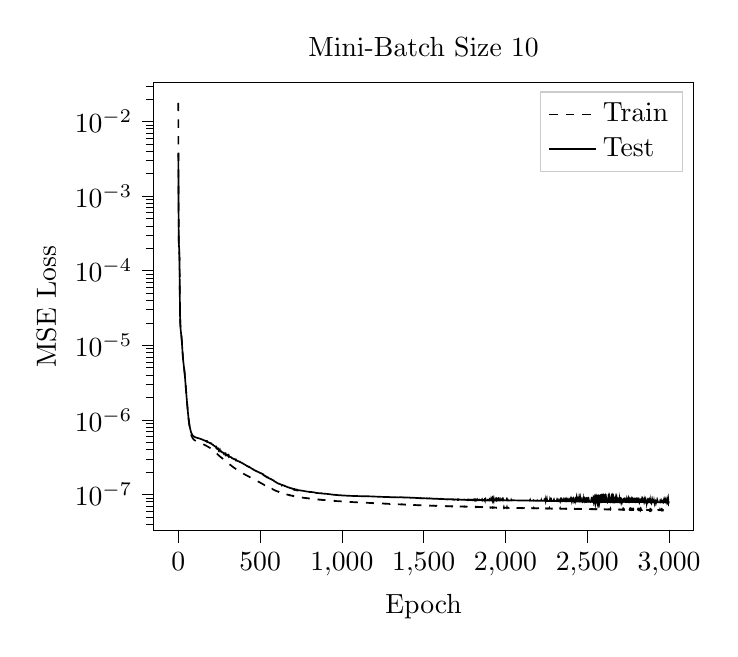
\begin{tikzpicture}

\begin{axis}[
legend cell align={left},
legend style={fill opacity=0.8, draw opacity=1, text opacity=1, draw=white!80!black},
log basis y={10},
tick align=outside,
tick pos=left,
title={Mini-Batch Size 10},
x grid style={white!69.0196078431373!black},
xlabel={Epoch},
xmin=-149.95, xmax=3148.95,
xtick style={color=black},
y grid style={white!69.0196078431373!black},
ylabel={MSE Loss},
ymin=3.24485769485219e-08, ymax=0.0333980791603649,
ymode=log,
ytick style={color=black}
]
\addplot [semithick, black, dashed]
table {%
0 0.0178001991356723
1 0.00200488151138416
2 0.000701156315590197
3 0.000261716974828232
4 0.000199328617736683
5 0.000186986934481865
6 0.000173579933980363
7 0.000146110978748766
8 0.000105959740715207
9 6.39389415221103e-05
10 3.66668005824522e-05
11 2.52619820594191e-05
12 2.07518238619286e-05
13 1.84675150404701e-05
14 1.71286290495232e-05
15 1.5936518463775e-05
16 1.51902070922461e-05
17 1.45978872893693e-05
18 1.39883020449361e-05
19 1.33434278936306e-05
20 1.26594410440362e-05
21 1.19381270536678e-05
22 1.11856970158897e-05
23 1.04207012111601e-05
24 9.66082206034002e-06
25 8.93075510902008e-06
26 8.25333155148655e-06
27 7.64690106393573e-06
28 7.12489472682876e-06
29 6.68496002710128e-06
30 6.31955081892954e-06
31 6.0134227113906e-06
32 5.74498461613615e-06
33 5.47273176358942e-06
34 5.2167927445268e-06
35 4.9861744959756e-06
36 4.78104827688952e-06
37 4.58005392468763e-06
38 4.37887272038751e-06
39 4.17098636571467e-06
40 3.95421256087047e-06
41 3.72693911240063e-06
42 3.50172249108383e-06
43 3.29332809126726e-06
44 3.09182238506622e-06
45 2.90331225761165e-06
46 2.72360592129317e-06
47 2.55453821926821e-06
48 2.39700753549954e-06
49 2.25145955536021e-06
50 2.11668409027865e-06
51 1.99050134304102e-06
52 1.87229289890567e-06
53 1.76164887562891e-06
54 1.65823905733831e-06
55 1.56229427982879e-06
56 1.47228454741466e-06
57 1.38939942937455e-06
58 1.3126574909883e-06
59 1.24191653927852e-06
60 1.17652551157477e-06
61 1.11696765555891e-06
62 1.06234146255879e-06
63 1.01298756452373e-06
64 9.67812829308912e-07
65 9.2707087809174e-07
66 8.89830477213138e-07
67 8.56006430591805e-07
68 8.25594001954144e-07
69 7.97867215593939e-07
70 7.72954573493578e-07
71 7.50259117587859e-07
72 7.29901631615348e-07
73 7.11405896423045e-07
74 6.94639410303566e-07
75 6.79315586022966e-07
76 6.6426254218932e-07
77 6.49667091829897e-07
78 6.37269800281004e-07
79 6.26870553155356e-07
80 6.17372133735472e-07
81 6.09351209694964e-07
82 6.01519808052231e-07
83 5.94646097393792e-07
84 5.88447503728773e-07
85 5.82338745438449e-07
86 5.77041704019621e-07
87 5.72185976057682e-07
88 5.67587416746562e-07
89 5.63291617527995e-07
90 5.59368539367888e-07
91 5.5559798167959e-07
92 5.52062691929756e-07
93 5.49291227929238e-07
94 5.45904120579088e-07
95 5.43599098166148e-07
96 5.40758223528393e-07
97 5.38306081567796e-07
98 5.35737310727313e-07
99 5.33768687471792e-07
100 5.31790635061036e-07
101 5.29849820289918e-07
102 5.2781264008761e-07
103 5.2608527720821e-07
104 5.24380388053913e-07
105 5.22993991998177e-07
106 5.21228024115139e-07
107 5.194265561137e-07
108 5.18424794599959e-07
109 5.17087338471889e-07
110 5.15472511524173e-07
111 5.13651462452636e-07
112 5.11944656835794e-07
113 5.11448339870491e-07
114 5.094766639413e-07
115 5.08757320996089e-07
116 5.07514836463052e-07
117 5.06262259882817e-07
118 5.05168648228249e-07
119 5.04062417232554e-07
120 5.0310766930739e-07
121 5.02008621690031e-07
122 5.00922091255518e-07
123 5.00021304423726e-07
124 4.9925018522412e-07
125 4.97710623328374e-07
126 4.96685247717288e-07
127 4.95866179095472e-07
128 4.94776216921622e-07
129 4.93998716133426e-07
130 4.93124593292649e-07
131 4.91399142039661e-07
132 4.90354375921598e-07
133 4.89415591173881e-07
134 4.88746146234398e-07
135 4.87311924795009e-07
136 4.86539818362885e-07
137 4.85456797498784e-07
138 4.84422925803862e-07
139 4.83270311928408e-07
140 4.81786078943003e-07
141 4.81387102686526e-07
142 4.80235422144482e-07
143 4.79086478013535e-07
144 4.78289033716273e-07
145 4.76731951049025e-07
146 4.76179492916451e-07
147 4.74949749644793e-07
148 4.73749073166552e-07
149 4.73058385379588e-07
150 4.7159305594402e-07
151 4.70849445970423e-07
152 4.69777295726281e-07
153 4.68548464689356e-07
154 4.67459765909339e-07
155 4.66451711722549e-07
156 4.65140015126764e-07
157 4.64248967455561e-07
158 4.63067644558279e-07
159 4.62037328721188e-07
160 4.60832779847209e-07
161 4.59657103135669e-07
162 4.58667327296602e-07
163 4.57390565280491e-07
164 4.56800247836675e-07
165 4.55633157230295e-07
166 4.54525676558681e-07
167 4.52909505739285e-07
168 4.52024042414401e-07
169 4.5069251675578e-07
170 4.49355827512043e-07
171 4.48662767800201e-07
172 4.47104315735025e-07
173 4.45493171250533e-07
174 4.44361103246749e-07
175 4.43117024477857e-07
176 4.42095686610244e-07
177 4.40849777234575e-07
178 4.39880139522231e-07
179 4.38409383245464e-07
180 4.37334783134347e-07
181 4.36090220734542e-07
182 4.34752940812189e-07
183 4.33580878889117e-07
184 4.32395907186134e-07
185 4.31017867064121e-07
186 4.29702469593174e-07
187 4.2842525137754e-07
188 4.2718219425808e-07
189 4.25812123192593e-07
190 4.24095969075999e-07
191 4.23468389931791e-07
192 4.22093073879637e-07
193 4.20754458003714e-07
194 4.19289238551279e-07
195 4.17835532693367e-07
196 4.16806761522892e-07
197 4.15206033959059e-07
198 4.1388074707438e-07
199 4.12556319613344e-07
200 4.11016335215564e-07
201 4.09749037126872e-07
202 4.0828644787716e-07
203 4.06659762477446e-07
204 4.05280188657819e-07
205 4.03922399967449e-07
206 4.02468767375375e-07
207 4.0099183457265e-07
208 3.99562870656567e-07
209 3.98091809583612e-07
210 3.96557871154002e-07
211 3.95109049708964e-07
212 3.93565956278152e-07
213 3.92116205807369e-07
214 3.9048634858041e-07
215 3.88987133632668e-07
216 3.87307775220336e-07
217 3.85659230630608e-07
218 3.84034484453011e-07
219 3.82389923112569e-07
220 3.8074077836292e-07
221 3.79036988427117e-07
222 3.77271174141214e-07
223 3.75499602460749e-07
224 3.73765723615804e-07
225 3.7202211526477e-07
226 3.70217503258274e-07
227 3.68391220293418e-07
228 3.66756287339953e-07
229 3.65261258252758e-07
230 3.63593527170636e-07
231 3.61567422171305e-07
232 3.59488814263287e-07
233 3.57849984942149e-07
234 3.56092777478167e-07
235 3.54040356365104e-07
236 3.52273915824597e-07
237 3.50462861815615e-07
238 3.48645920320578e-07
239 3.46658482062168e-07
240 3.44857991292358e-07
241 3.4288920054415e-07
242 3.41182960417186e-07
243 3.39597257008606e-07
244 3.38001042097247e-07
245 3.36484771645829e-07
246 3.35175210679495e-07
247 3.33539320740428e-07
248 3.32172186787716e-07
249 3.30656567619769e-07
250 3.29258906361929e-07
251 3.27834958051554e-07
252 3.26425850252221e-07
253 3.25018129814225e-07
254 3.23652537534969e-07
255 3.22333164293198e-07
256 3.20880008635172e-07
257 3.19589182948832e-07
258 3.1822573014928e-07
259 3.16879099448997e-07
260 3.15520553604287e-07
261 3.14236705563076e-07
262 3.12878847026354e-07
263 3.11595314403945e-07
264 3.10341323599417e-07
265 3.09084424259254e-07
266 3.07808726329739e-07
267 3.06590944392227e-07
268 3.05279227781341e-07
269 3.04013077521148e-07
270 3.02779589507196e-07
271 3.0152337268774e-07
272 3.00294039528026e-07
273 2.99054804830945e-07
274 2.97839031810909e-07
275 2.96646299249304e-07
276 2.95470336180159e-07
277 2.94282409720736e-07
278 2.93141718152867e-07
279 2.9194919356712e-07
280 2.90748225593163e-07
281 2.89534122277502e-07
282 2.88395086762705e-07
283 2.87192309000872e-07
284 2.86033646501593e-07
285 2.84838715129965e-07
286 2.83449129625524e-07
287 2.82174042238736e-07
288 2.80972971209437e-07
289 2.79831400593622e-07
290 2.7864298409952e-07
291 2.77608370895521e-07
292 2.76369982707969e-07
293 2.75211814080301e-07
294 2.7401515870551e-07
295 2.7293551080998e-07
296 2.71806649241313e-07
297 2.7067986362983e-07
298 2.6959935115034e-07
299 2.68510390837307e-07
300 2.67403697793434e-07
301 2.66281694791815e-07
302 2.65209942358346e-07
303 2.64117393444785e-07
304 2.62889389368581e-07
305 2.61951484459288e-07
306 2.60799055360472e-07
307 2.59715716164344e-07
308 2.58708064859725e-07
309 2.57661466993575e-07
310 2.56647615111127e-07
311 2.55594814460025e-07
312 2.54520277169767e-07
313 2.5352761123365e-07
314 2.52510745073486e-07
315 2.51431184645767e-07
316 2.50446511702584e-07
317 2.4946796331804e-07
318 2.48470296666525e-07
319 2.47495434377853e-07
320 2.46574284399337e-07
321 2.45618885883481e-07
322 2.4467481325452e-07
323 2.43779958220003e-07
324 2.42782083015314e-07
325 2.41834526923945e-07
326 2.40896920447042e-07
327 2.3995052869985e-07
328 2.38996751797949e-07
329 2.37917715488756e-07
330 2.37067746788888e-07
331 2.36164335669642e-07
332 2.35325629853733e-07
333 2.34393299813895e-07
334 2.33588868980839e-07
335 2.32686475296617e-07
336 2.31896005589149e-07
337 2.30981218889426e-07
338 2.30185180425391e-07
339 2.29283251775847e-07
340 2.28469564766964e-07
341 2.27607666731799e-07
342 2.26841884443107e-07
343 2.25991612783361e-07
344 2.2521350435456e-07
345 2.24394526089355e-07
346 2.23642060748208e-07
347 2.22841295816067e-07
348 2.22086131098642e-07
349 2.2133011579939e-07
350 2.20568449118552e-07
351 2.19800282890148e-07
352 2.19098173970256e-07
353 2.18288558089252e-07
354 2.17586786326329e-07
355 2.16807241306682e-07
356 2.16107884627448e-07
357 2.15367789542231e-07
358 2.14628127759298e-07
359 2.14019474951144e-07
360 2.13259286641065e-07
361 2.12567211665959e-07
362 2.11839382013856e-07
363 2.11178343365592e-07
364 2.10479607185565e-07
365 2.09804933029023e-07
366 2.09098087999848e-07
367 2.0845428510663e-07
368 2.07548652144673e-07
369 2.0706301449902e-07
370 2.06368420856418e-07
371 2.05738664365018e-07
372 2.05144220055686e-07
373 2.04314023879437e-07
374 2.03713761282032e-07
375 2.03073658120445e-07
376 2.02480032096553e-07
377 2.0173208872265e-07
378 2.01258483427669e-07
379 2.00689961518119e-07
380 2.0009316386238e-07
381 1.99379444569825e-07
382 1.98847902739274e-07
383 1.98230823846846e-07
384 1.97644873682901e-07
385 1.96939929297812e-07
386 1.96473501479222e-07
387 1.95837122707321e-07
388 1.95172183183878e-07
389 1.94611491166619e-07
390 1.94163676299208e-07
391 1.93573539111203e-07
392 1.92889612193881e-07
393 1.92450886613571e-07
394 1.91762933980932e-07
395 1.91069881569916e-07
396 1.90871840612949e-07
397 1.90135571560557e-07
398 1.89597682034304e-07
399 1.88993792495928e-07
400 1.88866561527945e-07
401 1.8823351179309e-07
402 1.87435177019246e-07
403 1.86995581747951e-07
404 1.86478740547003e-07
405 1.85732155091323e-07
406 1.85532268703881e-07
407 1.84917344270286e-07
408 1.84320728742193e-07
409 1.83672056286444e-07
410 1.83207849198119e-07
411 1.82638589312223e-07
412 1.82247722577689e-07
413 1.81650426251956e-07
414 1.81214002696883e-07
415 1.80670774470038e-07
416 1.80172028001468e-07
417 1.79686196417617e-07
418 1.79142520733144e-07
419 1.78697198134348e-07
420 1.78173241160984e-07
421 1.7780779776988e-07
422 1.77204278359877e-07
423 1.76783149934412e-07
424 1.76556122597482e-07
425 1.76137153817812e-07
426 1.75646959195142e-07
427 1.75163073317108e-07
428 1.74742066361144e-07
429 1.7418946008263e-07
430 1.7392178295772e-07
431 1.73334443283046e-07
432 1.72905922817268e-07
433 1.7237974726303e-07
434 1.71912371222938e-07
435 1.71471092089703e-07
436 1.70954288805092e-07
437 1.70348594754621e-07
438 1.70084692090455e-07
439 1.69441702992934e-07
440 1.69140008270396e-07
441 1.6867942303378e-07
442 1.68193934451111e-07
443 1.67728129225608e-07
444 1.6711657236046e-07
445 1.66799415717289e-07
446 1.66348919696802e-07
447 1.65739778066332e-07
448 1.65427918514816e-07
449 1.64987913477965e-07
450 1.64656203514024e-07
451 1.63946173310503e-07
452 1.6375657067691e-07
453 1.62959084601955e-07
454 1.62720349403678e-07
455 1.6214111080215e-07
456 1.61762699246726e-07
457 1.61298128462661e-07
458 1.60905765329566e-07
459 1.60514551941215e-07
460 1.60084449145614e-07
461 1.59599648417164e-07
462 1.591434488879e-07
463 1.58748809802045e-07
464 1.58325135304338e-07
465 1.5792636882006e-07
466 1.57515875460756e-07
467 1.57136660865476e-07
468 1.56689956409828e-07
469 1.56272531113277e-07
470 1.5589817972339e-07
471 1.55475972791752e-07
472 1.55092888542985e-07
473 1.54674253853848e-07
474 1.54311775311111e-07
475 1.53930749950959e-07
476 1.53479763778108e-07
477 1.53021160740341e-07
478 1.52827318089521e-07
479 1.52479907005176e-07
480 1.52008040865681e-07
481 1.5151424075377e-07
482 1.51270710200269e-07
483 1.50806746781473e-07
484 1.50425882847749e-07
485 1.50061844437221e-07
486 1.49776649589484e-07
487 1.49290316004969e-07
488 1.48689278438585e-07
489 1.48321270039276e-07
490 1.4780005480608e-07
491 1.47442506206463e-07
492 1.47042175688838e-07
493 1.46675496077719e-07
494 1.46248663270843e-07
495 1.45858097846396e-07
496 1.45448324972985e-07
497 1.45064655014959e-07
498 1.44686539629291e-07
499 1.44251473992441e-07
500 1.43813486572775e-07
501 1.43410299160429e-07
502 1.43040729545518e-07
503 1.4266011125752e-07
504 1.42180392681546e-07
505 1.41967560405298e-07
506 1.41547020513499e-07
507 1.41041255790064e-07
508 1.40719742396378e-07
509 1.40317288850333e-07
510 1.39857336707294e-07
511 1.39613264042993e-07
512 1.39194810944154e-07
513 1.38755451510875e-07
514 1.38477771538525e-07
515 1.38006292704773e-07
516 1.37736054184323e-07
517 1.37355880593937e-07
518 1.36604346510083e-07
519 1.36293020340794e-07
520 1.35855945631036e-07
521 1.35470846136521e-07
522 1.3530845651033e-07
523 1.34873527843915e-07
524 1.34453470828078e-07
525 1.34033881242779e-07
526 1.335631672017e-07
527 1.33317287858148e-07
528 1.32676874740056e-07
529 1.32320470080938e-07
530 1.32086654540675e-07
531 1.31775626597275e-07
532 1.30911119637922e-07
533 1.30574330945432e-07
534 1.30512219185253e-07
535 1.29769693708592e-07
536 1.30005403327083e-07
537 1.29302373486073e-07
538 1.29017444070456e-07
539 1.28683353148862e-07
540 1.28081754575682e-07
541 1.2779934222884e-07
542 1.27699181784457e-07
543 1.27007578891725e-07
544 1.27093415009938e-07
545 1.26421429007539e-07
546 1.26119597954055e-07
547 1.2564806459725e-07
548 1.25400566943767e-07
549 1.24967678734045e-07
550 1.24766246758501e-07
551 1.24567104331508e-07
552 1.24038114059921e-07
553 1.23791782251637e-07
554 1.23528181261712e-07
555 1.23040923212248e-07
556 1.22815953937927e-07
557 1.22616209272675e-07
558 1.22088738832016e-07
559 1.21686210736716e-07
560 1.21890107616096e-07
561 1.21081276245327e-07
562 1.21233743630711e-07
563 1.21165836566295e-07
564 1.20615651590938e-07
565 1.20132371077553e-07
566 1.19863235488182e-07
567 1.19627397987543e-07
568 1.1921561338335e-07
569 1.18966398785503e-07
570 1.187901652e-07
571 1.18475433512621e-07
572 1.18114259572977e-07
573 1.18735274103887e-07
574 1.18379147651115e-07
575 1.17835283908185e-07
576 1.17601282181301e-07
577 1.17368267271711e-07
578 1.17028383146423e-07
579 1.16693541998281e-07
580 1.16528044613595e-07
581 1.16167927763922e-07
582 1.15866148180377e-07
583 1.15566139977652e-07
584 1.15205696245013e-07
585 1.14867335083702e-07
586 1.14602485234983e-07
587 1.14337058196856e-07
588 1.14030604216886e-07
589 1.13885041312933e-07
590 1.13557346967941e-07
591 1.1300277483528e-07
592 1.12880506009105e-07
593 1.12564228194056e-07
594 1.1228856199752e-07
595 1.12135682888148e-07
596 1.11946836458543e-07
597 1.11572918839453e-07
598 1.11448776822787e-07
599 1.11093008376972e-07
600 1.10948178129178e-07
601 1.10704173117426e-07
602 1.10584795547375e-07
603 1.10175907286347e-07
604 1.10156123680483e-07
605 1.09735115849663e-07
606 1.09612918239854e-07
607 1.09444221592092e-07
608 1.09276107884693e-07
609 1.08925101638402e-07
610 1.08914205350086e-07
611 1.08398975762203e-07
612 1.0907742901356e-07
613 1.09002830084304e-07
614 1.08195459618265e-07
615 1.08121415214324e-07
616 1.08044478142055e-07
617 1.07672884859245e-07
618 1.07271118685581e-07
619 1.07304079179915e-07
620 1.06764458747133e-07
621 1.06681523357466e-07
622 1.06210029129361e-07
623 1.06446508509883e-07
624 1.05840904989218e-07
625 1.0581392303699e-07
626 1.05456717691688e-07
627 1.05509061842923e-07
628 1.04988260438699e-07
629 1.04953784274553e-07
630 1.04762798229796e-07
631 1.04482612590662e-07
632 1.04514783330067e-07
633 1.03978135024274e-07
634 1.0422276405686e-07
635 1.0375894168968e-07
636 1.03837648071092e-07
637 1.0357105285852e-07
638 1.03748727906527e-07
639 1.03791966605815e-07
640 1.03215746868335e-07
641 1.03112780216463e-07
642 1.02960432610821e-07
643 1.02617199536637e-07
644 1.02572925448907e-07
645 1.02342556638213e-07
646 1.02295900277216e-07
647 1.02282750961136e-07
648 1.01741481622897e-07
649 1.01761854347515e-07
650 1.01516580506278e-07
651 1.01356689373722e-07
652 1.01269487657873e-07
653 1.01099661555804e-07
654 1.00889462562037e-07
655 1.00829628768562e-07
656 1.00951301353902e-07
657 1.00332274681758e-07
658 1.0029597201644e-07
659 1.00302812993114e-07
660 1.00479697117128e-07
661 9.98686187503317e-08
662 9.97339894137639e-08
663 9.96640240213953e-08
664 9.96198147495964e-08
665 9.93623950829026e-08
666 9.92543957645253e-08
667 9.91826136453877e-08
668 9.90910244547116e-08
669 9.88320714201407e-08
670 9.89058069544857e-08
671 9.86755097653891e-08
672 9.86231812227789e-08
673 9.83323942904679e-08
674 9.81895336815697e-08
675 9.81447626979826e-08
676 9.80054834787136e-08
677 9.8090173042964e-08
678 9.78171329335531e-08
679 9.77436845051027e-08
680 9.78698797704514e-08
681 9.7420069773424e-08
682 9.76092436477671e-08
683 9.69910661574591e-08
684 9.71455712406311e-08
685 9.69066977130062e-08
686 9.71315947462248e-08
687 9.69069928102861e-08
688 9.69295860620001e-08
689 9.67196561707517e-08
690 9.63859296254643e-08
691 9.62207225529976e-08
692 9.62625351519364e-08
693 9.61369722929373e-08
694 9.60128456217735e-08
695 9.56613803759776e-08
696 9.57629009756822e-08
697 9.55586340090075e-08
698 9.53878710796552e-08
699 9.55580558725799e-08
700 9.51537736959551e-08
701 9.50713849312557e-08
702 9.50888310458087e-08
703 9.49253897097879e-08
704 9.51184273478844e-08
705 9.45851762845784e-08
706 9.45957434028699e-08
707 9.46405184643062e-08
708 9.44010258041583e-08
709 9.43898038729962e-08
710 9.4229224956166e-08
711 9.40507037083815e-08
712 9.39436439506558e-08
713 9.41692803679839e-08
714 9.36980743604376e-08
715 9.39223697637992e-08
716 9.3714428516245e-08
717 9.36377944427136e-08
718 9.3526587987558e-08
719 9.34935699259398e-08
720 9.3388877135947e-08
721 9.32504858552896e-08
722 9.32898643579705e-08
723 9.30470502424896e-08
724 9.30109677421687e-08
725 9.30141950594709e-08
726 9.28309058956245e-08
727 9.28748622919251e-08
728 9.27886828450131e-08
729 9.2609680124589e-08
730 9.26556160751879e-08
731 9.25388099237701e-08
732 9.23685840614752e-08
733 9.22747352993802e-08
734 9.22771310429837e-08
735 9.21689772281908e-08
736 9.20308270302428e-08
737 9.19883866723481e-08
738 9.19540889698922e-08
739 9.17767490093979e-08
740 9.17387668053493e-08
741 9.16404175232977e-08
742 9.19294675716387e-08
743 9.14501918369837e-08
744 9.13967208515665e-08
745 9.13522649881315e-08
746 9.12961912247212e-08
747 9.16073977896836e-08
748 9.10657894315214e-08
749 9.10220623184799e-08
750 9.0976933784237e-08
751 9.10777755791514e-08
752 9.09916686842038e-08
753 9.09195951415143e-08
754 9.07635310953836e-08
755 9.07308244357807e-08
756 9.07026974861225e-08
757 9.05702344744519e-08
758 9.04802686840789e-08
759 9.039786872167e-08
760 9.05015725760627e-08
761 9.02155400983595e-08
762 9.03243668282094e-08
763 9.0055545192147e-08
764 9.02595226692782e-08
765 8.99536888754326e-08
766 9.02099919297683e-08
767 9.00512921764296e-08
768 8.99423419653544e-08
769 8.98316465369753e-08
770 8.9813657193627e-08
771 8.96320555465735e-08
772 8.96441604880671e-08
773 8.96086649149197e-08
774 8.94550238528247e-08
775 8.94212226043578e-08
776 8.93593333550768e-08
777 8.94074431867509e-08
778 8.92372135075092e-08
779 8.9221889709723e-08
780 8.92524388995675e-08
781 8.90551756804747e-08
782 8.89121469138665e-08
783 8.90338590364692e-08
784 8.91194885332958e-08
785 8.87441462293914e-08
786 8.88770310747411e-08
787 8.89123747760401e-08
788 8.86714512726705e-08
789 8.87836217144944e-08
790 8.87063874510652e-08
791 8.85264483119208e-08
792 8.85483146806365e-08
793 8.84388295530059e-08
794 8.85020863150565e-08
795 8.83155445885464e-08
796 8.84387031896416e-08
797 8.8153341155639e-08
798 8.81551837128569e-08
799 8.80066620534414e-08
800 8.81367960525736e-08
801 8.78716895003073e-08
802 8.79704486678179e-08
803 8.77952394784387e-08
804 8.77992015735352e-08
805 8.78481872201853e-08
806 8.76100659663592e-08
807 8.74860396837818e-08
808 8.76992299914114e-08
809 8.75438203706835e-08
810 8.74522444016534e-08
811 8.75361036056788e-08
812 8.73266344592061e-08
813 8.71610880759377e-08
814 8.73081293750744e-08
815 8.72028591536456e-08
816 8.71319566031481e-08
817 8.71111723155238e-08
818 8.69624218280407e-08
819 8.70118243190276e-08
820 8.71310269023873e-08
821 8.71475792729726e-08
822 8.68332752346213e-08
823 8.67403180282444e-08
824 8.67476854615745e-08
825 8.68219617222721e-08
826 8.6766363929236e-08
827 8.66211521932669e-08
828 8.64632707053836e-08
829 8.65575487507542e-08
830 8.65036195141222e-08
831 8.64688474755404e-08
832 8.63830067876492e-08
833 8.62948699498212e-08
834 8.63148536311975e-08
835 8.63089701330644e-08
836 8.60968507132576e-08
837 8.60323370099891e-08
838 8.60748694164748e-08
839 8.62679394475485e-08
840 8.59693333155054e-08
841 8.57740228732418e-08
842 8.59616949311359e-08
843 8.59376644490872e-08
844 8.58875876108556e-08
845 8.55762429829987e-08
846 8.57686820787684e-08
847 8.58924624780322e-08
848 8.56368602164537e-08
849 8.54734707722571e-08
850 8.55845733838123e-08
851 8.54852331744205e-08
852 8.55151165479739e-08
853 8.53223135144354e-08
854 8.55501998642261e-08
855 8.52984910837407e-08
856 8.53168612158228e-08
857 8.52010489493793e-08
858 8.52043870880337e-08
859 8.52822417063415e-08
860 8.50955661757524e-08
861 8.49153153414939e-08
862 8.5096356117198e-08
863 8.49523311563516e-08
864 8.49563487825833e-08
865 8.476197226992e-08
866 8.50177893285675e-08
867 8.47828442629428e-08
868 8.47410544291272e-08
869 8.48341623971294e-08
870 8.48023626898176e-08
871 8.45865670418e-08
872 8.46554788702658e-08
873 8.44346008832542e-08
874 8.46406003252031e-08
875 8.44302842817335e-08
876 8.4363423134004e-08
877 8.46479363081354e-08
878 8.43425690499888e-08
879 8.42838752412867e-08
880 8.43541957606941e-08
881 8.43985267107161e-08
882 8.42566101322273e-08
883 8.41584912025795e-08
884 8.41513388261106e-08
885 8.41183438926585e-08
886 8.41704006671051e-08
887 8.39991592371803e-08
888 8.40111396493981e-08
889 8.3973454043651e-08
890 8.40829830528467e-08
891 8.40184783601483e-08
892 8.3831746456875e-08
893 8.38605016717508e-08
894 8.38607812803094e-08
895 8.38493038779475e-08
896 8.37759149729944e-08
897 8.36801551062916e-08
898 8.36437556772651e-08
899 8.37031012534961e-08
900 8.35645376096039e-08
901 8.36660378611409e-08
902 8.34644351421776e-08
903 8.35733778747905e-08
904 8.34583026820823e-08
905 8.35194746773293e-08
906 8.33584532400344e-08
907 8.33805425115575e-08
908 8.33102763608817e-08
909 8.32490753910342e-08
910 8.33080121331875e-08
911 8.32248086701792e-08
912 8.3212240336028e-08
913 8.32563882580128e-08
914 8.30514547001115e-08
915 8.31116484034666e-08
916 8.3047177101836e-08
917 8.30702778875647e-08
918 8.29852847783474e-08
919 8.30039136223704e-08
920 8.29433979965266e-08
921 8.28156773113875e-08
922 8.27806891745553e-08
923 8.2899598468078e-08
924 8.28493161308952e-08
925 8.27315951390517e-08
926 8.26971131140386e-08
927 8.26721508750961e-08
928 8.25543270699391e-08
929 8.25434888596099e-08
930 8.26084714544706e-08
931 8.26943764731247e-08
932 8.23973945252021e-08
933 8.23887599210593e-08
934 8.24208399174964e-08
935 8.23855567921861e-08
936 8.2312903864068e-08
937 8.23302100227963e-08
938 8.22914132170283e-08
939 8.21018654861838e-08
940 8.22624562424323e-08
941 8.21541981299578e-08
942 8.21091170832844e-08
943 8.20643537635668e-08
944 8.20593562800287e-08
945 8.20253835498441e-08
946 8.19434589693913e-08
947 8.20608104179499e-08
948 8.19093688197992e-08
949 8.18611726627338e-08
950 8.18886614839531e-08
951 8.18307021244191e-08
952 8.19544831132113e-08
953 8.18278662439997e-08
954 8.20077202057235e-08
955 8.15754108851596e-08
956 8.16673480785735e-08
957 8.16804860415132e-08
958 8.16943688286553e-08
959 8.16415276394533e-08
960 8.15604015269589e-08
961 8.16038678652653e-08
962 8.15272696819136e-08
963 8.14078891175907e-08
964 8.14953906969063e-08
965 8.14391878789511e-08
966 8.14012528893571e-08
967 8.12432967345344e-08
968 8.1269539591311e-08
969 8.12193618771051e-08
970 8.12119225634955e-08
971 8.12174484798867e-08
972 8.11314611492975e-08
973 8.11949283030522e-08
974 8.11163626501799e-08
975 8.10932483552573e-08
976 8.10373127813069e-08
977 8.11503817055304e-08
978 8.09651790945054e-08
979 8.1014203945351e-08
980 8.09188670336525e-08
981 8.09186596684164e-08
982 8.08726839973684e-08
983 8.0900155476904e-08
984 8.08141680319618e-08
985 8.08023577603123e-08
986 8.08806028773645e-08
987 8.07056001306261e-08
988 8.08569871324494e-08
989 8.06921701990149e-08
990 8.06193303248826e-08
991 8.06818341669846e-08
992 8.06083805926505e-08
993 8.0590755475729e-08
994 8.05905937473206e-08
995 8.05231999578826e-08
996 8.06208841530598e-08
997 8.04902552931086e-08
998 8.04632020490192e-08
999 8.05336744857943e-08
1000 8.04876820270639e-08
1001 8.03391489079264e-08
1002 8.04045754965177e-08
1003 8.04095113504655e-08
1004 8.03132315430055e-08
1005 8.02960029533395e-08
1006 8.03522236303422e-08
1007 8.01992822874187e-08
1008 8.01852877385656e-08
1009 8.02109089892422e-08
1010 8.01545967721307e-08
1011 8.0045810992857e-08
1012 8.01588867471725e-08
1013 7.9990280961173e-08
1014 8.00864127314949e-08
1015 8.00176843485101e-08
1016 8.00594969552204e-08
1017 7.99746716162453e-08
1018 7.99542395013564e-08
1019 7.9935821524213e-08
1020 7.99420451624844e-08
1021 7.97774391014805e-08
1022 7.99488231539858e-08
1023 7.97986263789685e-08
1024 7.97909998140334e-08
1025 7.97923242790155e-08
1026 7.98393425049948e-08
1027 7.96697105087674e-08
1028 7.97558328236025e-08
1029 7.96419569837337e-08
1030 7.97550182740636e-08
1031 7.96305487749116e-08
1032 7.96767189481518e-08
1033 7.95769877026675e-08
1034 7.96614504328108e-08
1035 7.95978688372667e-08
1036 7.95406359810347e-08
1037 7.95501295747236e-08
1038 7.94823109018239e-08
1039 7.94750928390098e-08
1040 7.94637828949174e-08
1041 7.94370622891893e-08
1042 7.93156045131305e-08
1043 7.93958467903977e-08
1044 7.92935804239114e-08
1045 7.94392349900974e-08
1046 7.9433984621069e-08
1047 7.93178623847979e-08
1048 7.91490090079616e-08
1049 7.92169928742759e-08
1050 7.92423473505721e-08
1051 7.91688048307204e-08
1052 7.91514585063435e-08
1053 7.90861693411582e-08
1054 7.90850494014617e-08
1055 7.90725980548412e-08
1056 7.90448806009536e-08
1057 7.90191519106642e-08
1058 7.90658210103601e-08
1059 7.89703859860324e-08
1060 7.90758564839233e-08
1061 7.89039747739473e-08
1062 7.89264823619629e-08
1063 7.88544572183358e-08
1064 7.88972637633112e-08
1065 7.87953434977506e-08
1066 7.89054651173515e-08
1067 7.87747313713005e-08
1068 7.87708173166646e-08
1069 7.87421084036399e-08
1070 7.87286146264332e-08
1071 7.87022904558121e-08
1072 7.87429117199423e-08
1073 7.86472130642757e-08
1074 7.8683111349731e-08
1075 7.86130338414903e-08
1076 7.86716206802041e-08
1077 7.85195847974318e-08
1078 7.85481894960416e-08
1079 7.85039934281251e-08
1080 7.85712001116767e-08
1081 7.84723195679238e-08
1082 7.8451432531379e-08
1083 7.84288364130692e-08
1084 7.8408656408735e-08
1085 7.84353979332852e-08
1086 7.84047217583517e-08
1087 7.83162218753741e-08
1088 7.83363034884132e-08
1089 7.84039812640192e-08
1090 7.83181843089231e-08
1091 7.82108398578174e-08
1092 7.82601408289008e-08
1093 7.82269317534112e-08
1094 7.82036281943288e-08
1095 7.81802580229751e-08
1096 7.82237428431642e-08
1097 7.81536682026296e-08
1098 7.80952178103256e-08
1099 7.8071074760544e-08
1100 7.80605395711564e-08
1101 7.80845937720098e-08
1102 7.80424324042794e-08
1103 7.80449235082692e-08
1104 7.79756080837579e-08
1105 7.79083635049638e-08
1106 7.79790376947975e-08
1107 7.8102232925481e-08
1108 7.80166846803265e-08
1109 7.77805636276163e-08
1110 7.78305735282814e-08
1111 7.78131517709113e-08
1112 7.78431191728046e-08
1113 7.77707398214034e-08
1114 7.77980135946432e-08
1115 7.78711287896527e-08
1116 7.77770865123539e-08
1117 7.76282917158699e-08
1118 7.77356853320921e-08
1119 7.76904774901777e-08
1120 7.76967080928781e-08
1121 7.75911115658001e-08
1122 7.76434404314852e-08
1123 7.75514256656784e-08
1124 7.76102096611275e-08
1125 7.75122435459075e-08
1126 7.76777802113937e-08
1127 7.74706609119047e-08
1128 7.74756320298664e-08
1129 7.74572242268068e-08
1130 7.74646784240662e-08
1131 7.75664833552181e-08
1132 7.74485902255151e-08
1133 7.73250186980601e-08
1134 7.74122822155832e-08
1135 7.73344162230405e-08
1136 7.73692463185149e-08
1137 7.72979015828401e-08
1138 7.75325490109946e-08
1139 7.7259488467929e-08
1140 7.72630587742018e-08
1141 7.72039734298069e-08
1142 7.72522298742029e-08
1143 7.71875287575163e-08
1144 7.72157963224718e-08
1145 7.71350670814019e-08
1146 7.72627104306256e-08
1147 7.71596575421807e-08
1148 7.70681353723379e-08
1149 7.71080238259891e-08
1150 7.70272002725836e-08
1151 7.70979918296444e-08
1152 7.72399123749601e-08
1153 7.70670188932065e-08
1154 7.69257838029169e-08
1155 7.70018546847329e-08
1156 7.6930741168546e-08
1157 7.70251498927177e-08
1158 7.698536987788e-08
1159 7.69978501469204e-08
1160 7.69071455231085e-08
1161 7.69654864973823e-08
1162 7.68692118990888e-08
1163 7.69416177404114e-08
1164 7.68841166487455e-08
1165 7.69081348905853e-08
1166 7.67858601924409e-08
1167 7.68723923549874e-08
1168 7.67576349314236e-08
1169 7.69141767320569e-08
1170 7.67006646618107e-08
1171 7.67990653183226e-08
1172 7.66867777812763e-08
1173 7.676626870734e-08
1174 7.68720251198562e-08
1175 7.67668480905481e-08
1176 7.6682359465563e-08
1177 7.66919229089336e-08
1178 7.66391930240307e-08
1179 7.66935282614512e-08
1180 7.65893503562598e-08
1181 7.67021324254991e-08
1182 7.65455475515431e-08
1183 7.65955504000715e-08
1184 7.64599807401289e-08
1185 7.65055794071934e-08
1186 7.63637310807752e-08
1187 7.66084092640451e-08
1188 7.63297209849245e-08
1189 7.64429183164328e-08
1190 7.62582789715083e-08
1191 7.64132777553161e-08
1192 7.62590801273166e-08
1193 7.63323877051025e-08
1194 7.62183908331604e-08
1195 7.62992371794446e-08
1196 7.61987446606938e-08
1197 7.63017266014465e-08
1198 7.61876582799914e-08
1199 7.62336024995314e-08
1200 7.61475027177827e-08
1201 7.6248096526621e-08
1202 7.6106894150163e-08
1203 7.6177538572697e-08
1204 7.61535114346401e-08
1205 7.61412319127963e-08
1206 7.60310017022814e-08
1207 7.61608514909806e-08
1208 7.60445467318238e-08
1209 7.60312235037475e-08
1210 7.59649292803033e-08
1211 7.60156052947991e-08
1212 7.59532762895088e-08
1213 7.59629833735342e-08
1214 7.58824291358096e-08
1215 7.59517160109358e-08
1216 7.58512163312464e-08
1217 7.58963777436339e-08
1218 7.59208059286642e-08
1219 7.5851392506987e-08
1220 7.57793096439752e-08
1221 7.57831311937185e-08
1222 7.5858799813977e-08
1223 7.57766088121947e-08
1224 7.57072575152673e-08
1225 7.56862072193165e-08
1226 7.5753647351684e-08
1227 7.56557773728961e-08
1228 7.56975806825988e-08
1229 7.57979672671993e-08
1230 7.56652403177682e-08
1231 7.5525093287121e-08
1232 7.56438551230421e-08
1233 7.55363046001101e-08
1234 7.56468999363324e-08
1235 7.55404095653667e-08
1236 7.56281851266305e-08
1237 7.54582692552575e-08
1238 7.55123730833418e-08
1239 7.54543400627306e-08
1240 7.54823309845332e-08
1241 7.55495676196816e-08
1242 7.54377794931482e-08
1243 7.53769228178935e-08
1244 7.54270194469608e-08
1245 7.54422974980073e-08
1246 7.53811938358773e-08
1247 7.5322915428222e-08
1248 7.53354440807819e-08
1249 7.53176679491041e-08
1250 7.5324292301282e-08
1251 7.54648821621462e-08
1252 7.52761628985965e-08
1253 7.51857039149595e-08
1254 7.52741665344114e-08
1255 7.51703559764838e-08
1256 7.52426111771953e-08
1257 7.51469949678008e-08
1258 7.51912489183049e-08
1259 7.5294307313456e-08
1260 7.50922786652008e-08
1261 7.4983449914745e-08
1262 7.50905083934938e-08
1263 7.50360642765013e-08
1264 7.50335666754864e-08
1265 7.49946886635655e-08
1266 7.49964212121146e-08
1267 7.49427618484955e-08
1268 7.49789461340633e-08
1269 7.52187001706872e-08
1270 7.48944082473724e-08
1271 7.48732898991911e-08
1272 7.48932804717217e-08
1273 7.4810138475101e-08
1274 7.48887384560693e-08
1275 7.49054233561974e-08
1276 7.47109777710087e-08
1277 7.48059672761592e-08
1278 7.47253667221504e-08
1279 7.47061316730413e-08
1280 7.47312986415505e-08
1281 7.46985879707118e-08
1282 7.46418094788037e-08
1283 7.47763320774197e-08
1284 7.46662591788461e-08
1285 7.45511674504762e-08
1286 7.45907640287147e-08
1287 7.4620115528834e-08
1288 7.45556225856259e-08
1289 7.46394343398293e-08
1290 7.44887373638203e-08
1291 7.45217929787323e-08
1292 7.45925621004062e-08
1293 7.43773617783994e-08
1294 7.43499029165484e-08
1295 7.47543573376142e-08
1296 7.43851886464419e-08
1297 7.43840426686848e-08
1298 7.43586402973673e-08
1299 7.43399094838004e-08
1300 7.43484806198236e-08
1301 7.43145723225425e-08
1302 7.43221440668851e-08
1303 7.42836344369557e-08
1304 7.4298074191903e-08
1305 7.43402515857028e-08
1306 7.42287084776194e-08
1307 7.42520146423953e-08
1308 7.41876707066602e-08
1309 7.41504075629784e-08
1310 7.43617497311888e-08
1311 7.41602457132728e-08
1312 7.41101648349396e-08
1313 7.41699940987051e-08
1314 7.41538912030215e-08
1315 7.40813177335653e-08
1316 7.41577886120837e-08
1317 7.41494760736483e-08
1318 7.40609188853991e-08
1319 7.40734678938981e-08
1320 7.40316358949222e-08
1321 7.39778367109256e-08
1322 7.40224653283938e-08
1323 7.40024573775422e-08
1324 7.39380303516057e-08
1325 7.40153257150489e-08
1326 7.39521464754311e-08
1327 7.38953979706469e-08
1328 7.39007000472025e-08
1329 7.38361665286735e-08
1330 7.39092552348719e-08
1331 7.37182129417757e-08
1332 7.40129470355733e-08
1333 7.38595772975526e-08
1334 7.37559502395069e-08
1335 7.37640920545068e-08
1336 7.3724147261478e-08
1337 7.37744299406096e-08
1338 7.37950086393546e-08
1339 7.36673634227358e-08
1340 7.36936594269988e-08
1341 7.37212079404692e-08
1342 7.36363322828559e-08
1343 7.36814379720396e-08
1344 7.36411203383636e-08
1345 7.37057045452349e-08
1346 7.360783562671e-08
1347 7.35107644111999e-08
1348 7.35359569348226e-08
1349 7.3515293885773e-08
1350 7.34618801268017e-08
1351 7.34388334167058e-08
1352 7.34865704432597e-08
1353 7.3432640939064e-08
1354 7.34110139766209e-08
1355 7.34445167460684e-08
1356 7.3423949514817e-08
1357 7.33732019619904e-08
1358 7.32969087635649e-08
1359 7.33079854764451e-08
1360 7.33899041149844e-08
1361 7.33798932350815e-08
1362 7.31794463848523e-08
1363 7.35090431702723e-08
1364 7.31608860293775e-08
1365 7.31755697735981e-08
1366 7.32641082179519e-08
1367 7.3186250139079e-08
1368 7.34128483614871e-08
1369 7.31165221945496e-08
1370 7.31965115752242e-08
1371 7.3064275827317e-08
1372 7.30857357922332e-08
1373 7.33125895113762e-08
1374 7.32119981117219e-08
1375 7.2922445273349e-08
1376 7.30658656034056e-08
1377 7.30537854609636e-08
1378 7.30022090322802e-08
1379 7.30021480033205e-08
1380 7.30662375525437e-08
1381 7.29430100754325e-08
1382 7.31200996395565e-08
1383 7.28816837269886e-08
1384 7.28833890661917e-08
1385 7.30305735308079e-08
1386 7.28753801337856e-08
1387 7.31701193257273e-08
1388 7.30091970257973e-08
1389 7.27326392080396e-08
1390 7.2943752431609e-08
1391 7.28418323125979e-08
1392 7.28248292891642e-08
1393 7.27638410102926e-08
1394 7.29236893926011e-08
1395 7.26970574471686e-08
1396 7.29422737788532e-08
1397 7.26916406035283e-08
1398 7.27759710872355e-08
1399 7.26676017215322e-08
1400 7.27995294791395e-08
1401 7.28623002443918e-08
1402 7.2619344783087e-08
1403 7.25977303273062e-08
1404 7.27091897056997e-08
1405 7.25303548887446e-08
1406 7.25290343861484e-08
1407 7.27158221502933e-08
1408 7.24931181217414e-08
1409 7.25947768520641e-08
1410 7.26666687800304e-08
1411 7.24676013130754e-08
1412 7.24702049736958e-08
1413 7.25905966825202e-08
1414 7.24343208302614e-08
1415 7.25126469414139e-08
1416 7.23946673419906e-08
1417 7.25070200591205e-08
1418 7.24271357865902e-08
1419 7.2386617682163e-08
1420 7.24308742672264e-08
1421 7.25574703142051e-08
1422 7.22625950910771e-08
1423 7.23400816848852e-08
1424 7.23454461082351e-08
1425 7.2224755340855e-08
1426 7.24860972167729e-08
1427 7.21753162202798e-08
1428 7.22523558616128e-08
1429 7.22983780043762e-08
1430 7.22285173637704e-08
1431 7.22584696577488e-08
1432 7.22576290768107e-08
1433 7.2168765617997e-08
1434 7.22866063196381e-08
1435 7.20468207227043e-08
1436 7.2413970133578e-08
1437 7.21693258531886e-08
1438 7.19542209581814e-08
1439 7.20940786536062e-08
1440 7.20340453908008e-08
1441 7.21357832633718e-08
1442 7.20967352207946e-08
1443 7.21039315343397e-08
1444 7.1925518742022e-08
1445 7.19636618007336e-08
1446 7.1921078086401e-08
1447 7.18724061621323e-08
1448 7.19395195569739e-08
1449 7.20973200674102e-08
1450 7.18064917271111e-08
1451 7.18406069077915e-08
1452 7.18235704133541e-08
1453 7.18386929610126e-08
1454 7.18132499211155e-08
1455 7.18486101902727e-08
1456 7.18489217810259e-08
1457 7.17935581384666e-08
1458 7.16951217194506e-08
1459 7.18805083343987e-08
1460 7.17165028840672e-08
1461 7.16595356820005e-08
1462 7.16323777327776e-08
1463 7.17016591234021e-08
1464 7.16576713588601e-08
1465 7.16868745087584e-08
1466 7.17022194018924e-08
1467 7.16326085725694e-08
1468 7.15976540777152e-08
1469 7.15532844697275e-08
1470 7.15463172340502e-08
1471 7.17302409680709e-08
1472 7.15110366866778e-08
1473 7.15207029966525e-08
1474 7.15000925144427e-08
1475 7.14983211502762e-08
1476 7.14745992491661e-08
1477 7.15955436869642e-08
1478 7.14519207090092e-08
1479 7.14419315128723e-08
1480 7.15761088532219e-08
1481 7.1341611620479e-08
1482 7.13703949839495e-08
1483 7.13687241449268e-08
1484 7.13382373052074e-08
1485 7.1373724586099e-08
1486 7.13113617134553e-08
1487 7.13195875023942e-08
1488 7.12883866815783e-08
1489 7.12990890161525e-08
1490 7.13198241852897e-08
1491 7.13187338374777e-08
1492 7.11651004559055e-08
1493 7.13779132077708e-08
1494 7.11791183394261e-08
1495 7.12117608114848e-08
1496 7.11427688682154e-08
1497 7.11945260345459e-08
1498 7.12525415558218e-08
1499 7.11678484854872e-08
1500 7.11614570381158e-08
1501 7.11084675308893e-08
1502 7.10973000062065e-08
1503 7.11890737548071e-08
1504 7.10097814982102e-08
1505 7.11217829529875e-08
1506 7.10356803301781e-08
1507 7.10784062052383e-08
1508 7.11160269373234e-08
1509 7.09907087681483e-08
1510 7.09881823812708e-08
1511 7.10703202699836e-08
1512 7.09057660996937e-08
1513 7.10703493767007e-08
1514 7.09022750833288e-08
1515 7.10358371813769e-08
1516 7.09045816049692e-08
1517 7.09849863278489e-08
1518 7.0973599505253e-08
1519 7.0858340136537e-08
1520 7.08997586851279e-08
1521 7.10066422648925e-08
1522 7.07712171066355e-08
1523 7.08903939772298e-08
1524 7.09330654657947e-08
1525 7.08389928028019e-08
1526 7.07664721932844e-08
1527 7.09042044844121e-08
1528 7.07320914727916e-08
1529 7.07789257403668e-08
1530 7.07136294919586e-08
1531 7.08379719349672e-08
1532 7.06837229791368e-08
1533 7.07570491009779e-08
1534 7.06986385445862e-08
1535 7.0791849660079e-08
1536 7.06175017561872e-08
1537 7.08143741312561e-08
1538 7.05991611515966e-08
1539 7.07679385281157e-08
1540 7.05842303705406e-08
1541 7.06358272706265e-08
1542 7.06602984879012e-08
1543 7.06426112373482e-08
1544 7.06470237121781e-08
1545 7.04872271506396e-08
1546 7.06520835758173e-08
1547 7.05834752590118e-08
1548 7.05905722087063e-08
1549 7.05431948844204e-08
1550 7.05432729186661e-08
1551 7.06425473162575e-08
1552 7.04266675077836e-08
1553 7.05926022592784e-08
1554 7.04855202204868e-08
1555 7.04926521744031e-08
1556 7.04986543775821e-08
1557 7.0443886481808e-08
1558 7.05194251782171e-08
1559 7.04084887181988e-08
1560 7.04709876198084e-08
1561 7.03363364928933e-08
1562 7.05706793224792e-08
1563 7.03800502899199e-08
1564 7.04518520089348e-08
1565 7.03032442694873e-08
1566 7.04192138978321e-08
1567 7.02934640173236e-08
1568 7.04296211395672e-08
1569 7.02623102033506e-08
1570 7.03620039466113e-08
1571 7.01278146630902e-08
1572 7.03398944801314e-08
1573 7.02545900288509e-08
1574 7.03541819524478e-08
1575 7.00792039898257e-08
1576 7.03628298026615e-08
1577 7.03446308314426e-08
1578 7.01708002448509e-08
1579 7.02759540538445e-08
1580 7.02307665489954e-08
1581 7.02497338556096e-08
1582 7.00715197143875e-08
1583 7.01273691505744e-08
1584 7.02526286811001e-08
1585 6.99801855352788e-08
1586 7.00890796057063e-08
1587 7.01682392656444e-08
1588 6.99929824021783e-08
1589 7.01313425310879e-08
1590 6.99704103523935e-08
1591 7.0034497110516e-08
1592 6.996394930181e-08
1593 7.0139133848679e-08
1594 6.99343256149731e-08
1595 6.99825570205093e-08
1596 7.00792486452162e-08
1597 6.98673662402616e-08
1598 6.99050404018298e-08
1599 7.00526170083204e-08
1600 6.99101682044567e-08
1601 6.98782432029255e-08
1602 6.98833804957388e-08
1603 6.99205370102707e-08
1604 6.99506890489143e-08
1605 6.97390503012762e-08
1606 6.99271392301526e-08
1607 6.98878842209094e-08
1608 6.99158646855214e-08
1609 6.97228140689177e-08
1610 6.98743417937298e-08
1611 6.99033889772771e-08
1612 6.98296120904551e-08
1613 6.97962168971777e-08
1614 6.98333113458016e-08
1615 6.98009128485833e-08
1616 6.97352478495894e-08
1617 6.98048521274863e-08
1618 6.97659968562636e-08
1619 6.97650012893014e-08
1620 6.9648437226455e-08
1621 6.97630892110279e-08
1622 6.97984318331901e-08
1623 6.96086408513708e-08
1624 6.96874106342893e-08
1625 6.96370715091987e-08
1626 6.96619891282779e-08
1627 6.96686164813887e-08
1628 6.96582857617756e-08
1629 6.95931109273573e-08
1630 6.96161632696146e-08
1631 6.96187106996593e-08
1632 6.96458791293875e-08
1633 6.95459031541112e-08
1634 6.96235362884767e-08
1635 6.95092266045361e-08
1636 6.96369155572807e-08
1637 6.94351494878731e-08
1638 6.96506252284568e-08
1639 6.94771293019425e-08
1640 6.95559481600494e-08
1641 6.94703181602918e-08
1642 6.95245321291615e-08
1643 6.94431454195676e-08
1644 6.94937679168728e-08
1645 6.95209997025881e-08
1646 6.93982205490773e-08
1647 6.94675856760529e-08
1648 6.95761106817017e-08
1649 6.92399498924967e-08
1650 6.95162899100321e-08
1651 6.93932016082588e-08
1652 6.9448843302844e-08
1653 6.93578117327842e-08
1654 6.94479364693468e-08
1655 6.93443616794909e-08
1656 6.9420120718533e-08
1657 6.93772415771843e-08
1658 6.94135985790378e-08
1659 6.93638586746204e-08
1660 6.94277945034738e-08
1661 6.92659502121717e-08
1662 6.93786275829389e-08
1663 6.92629660148381e-08
1664 6.93482733771233e-08
1665 6.92422679027249e-08
1666 6.92821916148389e-08
1667 6.93345050140071e-08
1668 6.92768211374428e-08
1669 6.91827686438717e-08
1670 6.92853885009281e-08
1671 6.91847356937281e-08
1672 6.92873283247852e-08
1673 6.88315837449327e-08
1674 6.93824101916096e-08
1675 6.91807214925344e-08
1676 6.92388626988283e-08
1677 6.87920389541574e-08
1678 6.92484443187702e-08
1679 6.89469974202161e-08
1680 6.91685257225849e-08
1681 6.91465243940481e-08
1682 6.90509308998166e-08
1683 6.9103708989493e-08
1684 6.90844120054823e-08
1685 6.90489173271747e-08
1686 6.91380593154101e-08
1687 6.91468449354193e-08
1688 6.89090789873781e-08
1689 6.90039447659441e-08
1690 6.91542831887659e-08
1691 6.86976862529498e-08
1692 6.9101901780666e-08
1693 6.90065735198253e-08
1694 6.89741860004922e-08
1695 6.88918324842636e-08
1696 6.91211725534213e-08
1697 6.89832146283376e-08
1698 6.88838311968531e-08
1699 6.89154905442191e-08
1700 6.89431116629446e-08
1701 6.9036092572583e-08
1702 6.8629575533663e-08
1703 6.88517715097259e-08
1704 6.9089398992972e-08
1705 6.88396791281853e-08
1706 6.90215654763904e-08
1707 6.8804280507484e-08
1708 6.89625303118557e-08
1709 6.88654086922202e-08
1710 6.89996446556762e-08
1711 6.87588980941012e-08
1712 6.89517143293017e-08
1713 6.8723219300848e-08
1714 6.89306166412607e-08
1715 6.87270386967587e-08
1716 6.88592931308296e-08
1717 6.86867749810638e-08
1718 6.90044360407427e-08
1719 6.87480589045553e-08
1720 6.88048466945812e-08
1721 6.87551563738342e-08
1722 6.88557735173401e-08
1723 6.87217398132045e-08
1724 6.88032069173783e-08
1725 6.87013583677842e-08
1726 6.87707278679284e-08
1727 6.87205830129933e-08
1728 6.87496879847593e-08
1729 6.86857594489609e-08
1730 6.87448246194933e-08
1731 6.87185423808856e-08
1732 6.87580712954716e-08
1733 6.8644886128677e-08
1734 6.8731846364356e-08
1735 6.86965900276171e-08
1736 6.88894782885363e-08
1737 6.86127404048165e-08
1738 6.87250564190833e-08
1739 6.85343334094757e-08
1740 6.86284456730135e-08
1741 6.86814971273542e-08
1742 6.85856586302158e-08
1743 6.84574580434028e-08
1744 6.86321892406916e-08
1745 6.85327848870543e-08
1746 6.85986459780796e-08
1747 6.8509379796966e-08
1748 6.86313544395745e-08
1749 6.84478798773647e-08
1750 6.8774220705059e-08
1751 6.84039075826703e-08
1752 6.85784395715316e-08
1753 6.84213945545409e-08
1754 6.85257913601856e-08
1755 6.84432113284839e-08
1756 6.85940314704148e-08
1757 6.84540390727406e-08
1758 6.84996380806435e-08
1759 6.84255316429905e-08
1760 6.84994081334711e-08
1761 6.83496601450173e-08
1762 6.85872163097567e-08
1763 6.83307360327401e-08
1764 6.84299860209681e-08
1765 6.8290297418061e-08
1766 6.83317611382961e-08
1767 6.83541593959891e-08
1768 6.82663371931458e-08
1769 6.83582202809507e-08
1770 6.82533875351332e-08
1771 6.84098756698059e-08
1772 6.82649559935466e-08
1773 6.82983251110159e-08
1774 6.82460327738887e-08
1775 6.83144735358354e-08
1776 6.82558354170304e-08
1777 6.80487194293367e-08
1778 6.81743316399697e-08
1779 6.8192485342955e-08
1780 6.82410330965499e-08
1781 6.81408427949393e-08
1782 6.82819869357587e-08
1783 6.81994001416886e-08
1784 6.81741158037319e-08
1785 6.82355838210746e-08
1786 6.81081633402414e-08
1787 6.81097989085888e-08
1788 6.80466418034875e-08
1789 6.81045054917728e-08
1790 6.81272419955636e-08
1791 6.81797386026251e-08
1792 6.79816086157636e-08
1793 6.81585246664618e-08
1794 6.80637034500275e-08
1795 6.79865026664839e-08
1796 6.79606365872054e-08
1797 6.81635576560424e-08
1798 6.79132978409491e-08
1799 6.808927221158e-08
1800 6.79975480688544e-08
1801 6.79560618277453e-08
1802 6.80607082692575e-08
1803 6.78084828742431e-08
1804 6.79328344865837e-08
1805 6.79855584606592e-08
1806 6.79024618188695e-08
1807 6.79895740851588e-08
1808 6.7942078274541e-08
1809 6.77301648788209e-08
1810 6.79487982135907e-08
1811 6.77189533759837e-08
1812 6.80440251565884e-08
1813 6.78486172056569e-08
1814 6.77492349498987e-08
1815 6.78563871048254e-08
1816 6.76450345626911e-08
1817 6.8000636261889e-08
1818 6.76601112659103e-08
1819 6.79100906575414e-08
1820 6.76148879086291e-08
1821 6.78971973555598e-08
1822 6.75732779942262e-08
1823 6.78717342472712e-08
1824 6.76429894252983e-08
1825 6.78083948069119e-08
1826 6.76900134255476e-08
1827 6.79025106931075e-08
1828 6.76137749311412e-08
1829 6.77421743910944e-08
1830 6.76241311625692e-08
1831 6.78739331172462e-08
1832 6.77138659943566e-08
1833 6.78268666021164e-08
1834 6.7667376737468e-08
1835 6.76947809830075e-08
1836 6.77330604870186e-08
1837 6.76291305001797e-08
1838 6.77387580982902e-08
1839 6.75420147377981e-08
1840 6.75702316133009e-08
1841 6.76830326140632e-08
1842 6.7672449204359e-08
1843 6.76407698396719e-08
1844 6.76225918760931e-08
1845 6.7614503325153e-08
1846 6.7588190126866e-08
1847 6.765213870219e-08
1848 6.75284900952811e-08
1849 6.76018702017167e-08
1850 6.75198737709604e-08
1851 6.76009841960035e-08
1852 6.74130299394005e-08
1853 6.7593276751321e-08
1854 6.74724869953458e-08
1855 6.75158632668094e-08
1856 6.75006180750337e-08
1857 6.75392995230784e-08
1858 6.74606009654077e-08
1859 6.73793244543308e-08
1860 6.75717327269787e-08
1861 6.73381673477191e-08
1862 6.75148067263987e-08
1863 6.73766656966723e-08
1864 6.72448422944782e-08
1865 6.73135385387269e-08
1866 6.73466110268084e-08
1867 6.73590328603702e-08
1868 6.72403689261358e-08
1869 6.72288576974989e-08
1870 6.73108958804125e-08
1871 6.72453088068625e-08
1872 6.7754858217306e-08
1873 6.7283999090062e-08
1874 6.71059777701544e-08
1875 6.73222225888725e-08
1876 6.73753133462185e-08
1877 6.72258391465341e-08
1878 6.73737997025636e-08
1879 6.72153320191438e-08
1880 6.70830864180072e-08
1881 6.70028391458466e-08
1882 6.75489408952235e-08
1883 6.73488163571712e-08
1884 6.71898936577264e-08
1885 6.71352011438753e-08
1886 6.69802611974468e-08
1887 6.7163824579719e-08
1888 6.69757383608971e-08
1889 6.67905109297262e-08
1890 6.66611658972638e-08
1891 6.71619620062902e-08
1892 6.6782864880377e-08
1893 6.68145874582748e-08
1894 6.70372028632737e-08
1895 6.68022557737125e-08
1896 6.68858398078509e-08
1897 6.67979510371452e-08
1898 6.65948880351763e-08
1899 6.69526050778302e-08
1900 6.67590387959383e-08
1901 6.66473005372925e-08
1902 6.68177077056686e-08
1903 6.67807453591518e-08
1904 6.66301940477343e-08
1905 6.68488597299621e-08
1906 6.64686168172501e-08
1907 6.67812939170176e-08
1908 6.68084647725831e-08
1909 6.65803689070543e-08
1910 6.68394755665158e-08
1911 6.6474942950201e-08
1912 6.66922478720355e-08
1913 6.65712308545174e-08
1914 6.65137632738233e-08
1915 6.6706488770496e-08
1916 6.65524848286747e-08
1917 6.66181480313277e-08
1918 6.63914232001961e-08
1919 6.64567854691267e-08
1920 6.68498764200276e-08
1921 6.63044921656031e-08
1922 6.66311258479269e-08
1923 6.63716295501438e-08
1924 6.65601089833157e-08
1925 6.64013131868035e-08
1926 6.65912572272998e-08
1927 6.63643654508217e-08
1928 6.62964641473529e-08
1929 6.66964227813427e-08
1930 6.626339424054e-08
1931 6.65649874720398e-08
1932 6.64858166654625e-08
1933 6.64341707456995e-08
1934 6.6536081677615e-08
1935 6.64461402855032e-08
1936 6.64182490750509e-08
1937 6.6556038644805e-08
1938 6.64136046846231e-08
1939 6.64209256950876e-08
1940 6.63985863624816e-08
1941 6.64118313964401e-08
1942 6.63075059903484e-08
1943 6.64217084545005e-08
1944 6.64730061505914e-08
1945 6.61996087991667e-08
1946 6.64867769628596e-08
1947 6.63982047255374e-08
1948 6.64885203216503e-08
1949 6.70731276897207e-08
1950 6.63460173833119e-08
1951 6.61674656154965e-08
1952 6.62789644256812e-08
1953 6.63714060622489e-08
1954 6.61076198604782e-08
1955 6.63996361327524e-08
1956 6.63961902092058e-08
1957 6.60762386583968e-08
1958 6.63478886275826e-08
1959 6.62820870434011e-08
1960 6.63915489118594e-08
1961 6.6043377247027e-08
1962 6.6386472983293e-08
1963 6.63206422446549e-08
1964 6.60270756902559e-08
1965 6.6307238270058e-08
1966 6.62643509308225e-08
1967 6.62548776042549e-08
1968 6.62672534468278e-08
1969 6.60964801701969e-08
1970 6.62251523853019e-08
1971 6.62297269138357e-08
1972 6.61923241840334e-08
1973 6.60683337805334e-08
1974 6.70719559370259e-08
1975 6.58325602498344e-08
1976 6.61773620369566e-08
1977 6.62595897105156e-08
1978 6.61423731407318e-08
1979 6.60873071833823e-08
1980 6.62015182983922e-08
1981 6.60451440359644e-08
1982 6.6048363459581e-08
1983 6.61872064156022e-08
1984 6.62133097928397e-08
1985 6.59924692858471e-08
1986 6.60384472483955e-08
1987 6.6082156788827e-08
1988 6.61354347231136e-08
1989 6.59292416893553e-08
1990 6.70316717654718e-08
1991 6.57684738891717e-08
1992 6.60344116532041e-08
1993 6.59842180905645e-08
1994 6.61989872019486e-08
1995 6.59666902003142e-08
1996 6.61570273963186e-08
1997 6.61061837559096e-08
1998 6.60716190836741e-08
1999 6.60591013601497e-08
2000 6.5969113299813e-08
2001 6.59697354532529e-08
2002 6.60610295644126e-08
2003 6.60928204843092e-08
2004 6.6001047215325e-08
2005 6.59362417987364e-08
2006 6.60711349231846e-08
2007 6.60435125643399e-08
2008 6.57828339345468e-08
2009 6.6935568027171e-08
2010 6.56864162740245e-08
2011 6.59295514482405e-08
2012 6.59563637772642e-08
2013 6.59264477087529e-08
2014 6.58476480386305e-08
2015 6.58581141843584e-08
2016 6.59341506503708e-08
2017 6.59771998023917e-08
2018 6.58371208417385e-08
2019 6.59361430543903e-08
2020 6.5999477583123e-08
2021 6.58459589075733e-08
2022 6.59152955662101e-08
2023 6.5937023496776e-08
2024 6.6059540891894e-08
2025 6.58627154870306e-08
2026 6.58900110506178e-08
2027 6.5942953260123e-08
2028 6.59582970596873e-08
2029 6.58284264543063e-08
2030 6.58751808868541e-08
2031 6.58852805945909e-08
2032 6.59532494695636e-08
2033 6.59084792509201e-08
2034 6.58079041659931e-08
2035 6.58397169128744e-08
2036 6.5882810422746e-08
2037 6.5756754644708e-08
2038 6.67470912629753e-08
2039 6.55670089877436e-08
2040 6.58146850551766e-08
2041 6.58136103992568e-08
2042 6.57579927898499e-08
2043 6.58836667544183e-08
2044 6.57022854277933e-08
2045 6.58395602592954e-08
2046 6.57681617910466e-08
2047 6.58699409827879e-08
2048 6.57083664945546e-08
2049 6.58619080784462e-08
2050 6.57216440003161e-08
2051 6.57887948984914e-08
2052 6.57017400840232e-08
2053 6.58182420920639e-08
2054 6.57562418071578e-08
2055 6.57926274039156e-08
2056 6.56875450399941e-08
2057 6.57799265890713e-08
2058 6.56663494413845e-08
2059 6.57710594653693e-08
2060 6.56711032687163e-08
2061 6.57548989047019e-08
2062 6.56628311734853e-08
2063 6.57580681528991e-08
2064 6.56760743888984e-08
2065 6.5706602676574e-08
2066 6.56187480752024e-08
2067 6.57445877860763e-08
2068 6.56874984739098e-08
2069 6.56285721867267e-08
2070 6.56562962852991e-08
2071 6.56484776329069e-08
2072 6.57219583499735e-08
2073 6.55915229141879e-08
2074 6.55998193865859e-08
2075 6.56479710536839e-08
2076 6.56446847668857e-08
2077 6.55443564923086e-08
2078 6.55903284130233e-08
2079 6.56538398291495e-08
2080 6.56786287633881e-08
2081 6.55348620304253e-08
2082 6.56241416863157e-08
2083 6.56291168532608e-08
2084 6.54998377003224e-08
2085 6.56859378045382e-08
2086 6.5521259271506e-08
2087 6.56568022594506e-08
2088 6.55050057218887e-08
2089 6.56447896374424e-08
2090 6.55038069174996e-08
2091 6.56565749979077e-08
2092 6.54737002536709e-08
2093 6.55682362205034e-08
2094 6.54973781621937e-08
2095 6.55964751361537e-08
2096 6.54508036379564e-08
2097 6.55846878538924e-08
2098 6.54514093101355e-08
2099 6.55736518373473e-08
2100 6.54337817895812e-08
2101 6.55614993994025e-08
2102 6.54177499548325e-08
2103 6.55237191216074e-08
2104 6.54074559058859e-08
2105 6.55168614549506e-08
2106 6.54024824209287e-08
2107 6.55165110141631e-08
2108 6.54133824629088e-08
2109 6.55111731573399e-08
2110 6.54138918876335e-08
2111 6.5471872381373e-08
2112 6.54250848852733e-08
2113 6.5442203189825e-08
2114 6.53423675089915e-08
2115 6.55041171648829e-08
2116 6.5330769963845e-08
2117 6.55228545387576e-08
2118 6.53956411733603e-08
2119 6.54904116470512e-08
2120 6.5381969458489e-08
2121 6.54330309213247e-08
2122 6.53507460135483e-08
2123 6.54506042629954e-08
2124 6.53432669450726e-08
2125 6.5475388681957e-08
2126 6.52801096256983e-08
2127 6.53994441091044e-08
2128 6.53130605432484e-08
2129 6.5411390515191e-08
2130 6.53130040351169e-08
2131 6.55198125076861e-08
2132 6.52354667385335e-08
2133 6.53744282819169e-08
2134 6.52826584768285e-08
2135 6.53976653719468e-08
2136 6.52793646860328e-08
2137 6.53672421846441e-08
2138 6.52304697079664e-08
2139 6.54500823238369e-08
2140 6.52078411855772e-08
2141 6.53949172990664e-08
2142 6.51965572195934e-08
2143 6.54084914775144e-08
2144 6.52113908405916e-08
2145 6.5330568552735e-08
2146 6.51219241476486e-08
2147 6.52104287324207e-08
2148 6.51847224331092e-08
2149 6.52842088100236e-08
2150 6.51002724949556e-08
2151 6.59854539819538e-08
2152 6.50827259451869e-08
2153 6.51069786472558e-08
2154 6.52298877723556e-08
2155 6.536417286096e-08
2156 6.51257378558867e-08
2157 6.52575238102582e-08
2158 6.52355910824021e-08
2159 6.51491752257094e-08
2160 6.53005332840184e-08
2161 6.50888380182568e-08
2162 6.5323621708524e-08
2163 6.50719748906958e-08
2164 6.52327369277117e-08
2165 6.52475725138046e-08
2166 6.50947454539086e-08
2167 6.52062472339399e-08
2168 6.50745307118061e-08
2169 6.51147431740551e-08
2170 6.50515335476332e-08
2171 6.52050840344032e-08
2172 6.50129260959531e-08
2173 6.5697357755079e-08
2174 6.50946991698209e-08
2175 6.49065785440772e-08
2176 6.52661760480733e-08
2177 6.50820982006639e-08
2178 6.51994881006868e-08
2179 6.50265954815765e-08
2180 6.51035293841584e-08
2181 6.50842309857236e-08
2182 6.51014565566932e-08
2183 6.50773483079625e-08
2184 6.50725389017559e-08
2185 6.50440476801517e-08
2186 6.50774315502645e-08
2187 6.51252769900967e-08
2188 6.49494160498421e-08
2189 6.50683271430363e-08
2190 6.48940039416068e-08
2191 6.50798012402642e-08
2192 6.50791514877902e-08
2193 6.50476988395265e-08
2194 6.5173320321632e-08
2195 6.49933580032513e-08
2196 6.49540916619618e-08
2197 6.49934698737642e-08
2198 6.49384679485276e-08
2199 6.49622976212072e-08
2200 6.49979008726653e-08
2201 6.5018265240635e-08
2202 6.50366856669304e-08
2203 6.49529504126445e-08
2204 6.50684431391379e-08
2205 6.49903431426679e-08
2206 6.49870188496049e-08
2207 6.4947485619582e-08
2208 6.50133129564967e-08
2209 6.49742198255421e-08
2210 6.50442676952689e-08
2211 6.4882819535983e-08
2212 6.50174766925193e-08
2213 6.49145748121693e-08
2214 6.4992826074306e-08
2215 6.48770518651975e-08
2216 6.50210983377253e-08
2217 6.48392717872426e-08
2218 6.49724177970157e-08
2219 6.47705348355565e-08
2220 6.5016040166066e-08
2221 6.46926089586941e-08
2222 6.57002798498674e-08
2223 6.47419585697584e-08
2224 6.4955294802882e-08
2225 6.47709187606704e-08
2226 6.49230729354855e-08
2227 6.47702279954476e-08
2228 6.49525802487449e-08
2229 6.47612184523361e-08
2230 6.49792067985988e-08
2231 6.47554639821024e-08
2232 6.49214665660036e-08
2233 6.47661599362248e-08
2234 6.49696522214693e-08
2235 6.47454465474429e-08
2236 6.49609862435341e-08
2237 6.47359709238238e-08
2238 6.49182213685595e-08
2239 6.4635110479383e-08
2240 6.49523846130151e-08
2241 6.46850263630316e-08
2242 6.48598278696344e-08
2243 6.47299467804174e-08
2244 6.49168933930522e-08
2245 6.48091396038275e-08
2246 6.45647790020742e-08
2247 6.48741565500988e-08
2248 6.45505421692505e-08
2249 6.47361215322384e-08
2250 6.45813767374825e-08
2251 6.45874835492055e-08
2252 6.47547180843144e-08
2253 6.45948425093135e-08
2254 6.49042504996533e-08
2255 6.46746324883818e-08
2256 6.45569314872141e-08
2257 6.46959081262999e-08
2258 6.45251485520415e-08
2259 6.47691821764607e-08
2260 6.45550125888406e-08
2261 6.46349222566123e-08
2262 6.46224883471547e-08
2263 6.4574556959407e-08
2264 6.47098181716377e-08
2265 6.44515899594911e-08
2266 6.46735802112275e-08
2267 6.45377818397908e-08
2268 6.53253021187794e-08
2269 6.44076711642239e-08
2270 6.45519085495927e-08
2271 6.45582381242349e-08
2272 6.45553758282791e-08
2273 6.45587862346808e-08
2274 6.45233366558529e-08
2275 6.44916838743459e-08
2276 6.45637634755225e-08
2277 6.4458688529001e-08
2278 6.44775359248673e-08
2279 6.46443012675135e-08
2280 6.44074028399722e-08
2281 6.45409404342878e-08
2282 6.44078542844095e-08
2283 6.46087902456127e-08
2284 6.44537226490716e-08
2285 6.44725962972714e-08
2286 6.46194259346089e-08
2287 6.44509112357472e-08
2288 6.46312244334535e-08
2289 6.4400918329266e-08
2290 6.44982532316263e-08
2291 6.4472635596946e-08
2292 6.44612740119399e-08
2293 6.45343781358054e-08
2294 6.44217403333869e-08
2295 6.43851690340647e-08
2296 6.45040533708841e-08
2297 6.43797540433866e-08
2298 6.43484835483044e-08
2299 6.44917163450387e-08
2300 6.44019950757357e-08
2301 6.43943958666959e-08
2302 6.44123663284812e-08
2303 6.4490967267572e-08
2304 6.43799879784801e-08
2305 6.45087735917649e-08
2306 6.43974972491801e-08
2307 6.43559087376566e-08
2308 6.45372881613593e-08
2309 6.43392216981287e-08
2310 6.42892547020324e-08
2311 6.44697142637707e-08
2312 6.43506641018199e-08
2313 6.44488159562417e-08
2314 6.42559041108548e-08
2315 6.44696883611573e-08
2316 6.4294153647726e-08
2317 6.43610370554271e-08
2318 6.43267010902449e-08
2319 6.43890059437435e-08
2320 6.43448060821949e-08
2321 6.42640242631831e-08
2322 6.43589945792389e-08
2323 6.43336983396914e-08
2324 6.43376429632081e-08
2325 6.43480426409937e-08
2326 6.51055861700112e-08
2327 6.43520076171189e-08
2328 6.41145772639629e-08
2329 6.42592679311882e-08
2330 6.43314780091053e-08
2331 6.43411088263601e-08
2332 6.42779060744392e-08
2333 6.43568179747866e-08
2334 6.51068879375938e-08
2335 6.4128413098663e-08
2336 6.41242529153541e-08
2337 6.4270502808661e-08
2338 6.40932113649129e-08
2339 6.43149445045399e-08
2340 6.42713003762285e-08
2341 6.40978647215018e-08
2342 6.43255504417795e-08
2343 6.43423796664599e-08
2344 6.4145193501286e-08
2345 6.43056890481386e-08
2346 6.4143364931768e-08
2347 6.42024451080747e-08
2348 6.4273794291303e-08
2349 6.41919298316473e-08
2350 6.42902790171096e-08
2351 6.41470587581239e-08
2352 6.42008633577884e-08
2353 6.43212833584261e-08
2354 6.40871358104089e-08
2355 6.41609560625422e-08
2356 6.41911029652942e-08
2357 6.41574995208227e-08
2358 6.41186431959984e-08
2359 6.41904824438821e-08
2360 6.41202130924334e-08
2361 6.41161068393181e-08
2362 6.42287831498223e-08
2363 6.40908731452949e-08
2364 6.40747213154214e-08
2365 6.42823799601455e-08
2366 6.40071457302938e-08
2367 6.41224955566511e-08
2368 6.41450187666148e-08
2369 6.42380875881532e-08
2370 6.39768098509297e-08
2371 6.4279007810919e-08
2372 6.39925318290935e-08
2373 6.42229894920465e-08
2374 6.40007536267806e-08
2375 6.41921124255873e-08
2376 6.41068972628833e-08
2377 6.40792566153348e-08
2378 6.4000075959969e-08
2379 6.411875949075e-08
2380 6.40367597726232e-08
2381 6.41255380740002e-08
2382 6.40099668847149e-08
2383 6.41030719106261e-08
2384 6.39211349640068e-08
2385 6.40889764547126e-08
2386 6.40002990781596e-08
2387 6.41004373513887e-08
2388 6.39651215939008e-08
2389 6.4058577780024e-08
2390 6.39435997029647e-08
2391 6.40267659168803e-08
2392 6.39739783503401e-08
2393 6.40603147250562e-08
2394 6.39237994359831e-08
2395 6.40913923322106e-08
2396 6.40544813446109e-08
2397 6.39243469513495e-08
2398 6.41900359499292e-08
2399 6.38820169884813e-08
2400 6.40655836359194e-08
2401 6.38361945781707e-08
2402 6.40963837428288e-08
2403 6.39483040576483e-08
2404 6.39793329682004e-08
2405 6.38938597863348e-08
2406 6.40435151411101e-08
2407 6.38678207320886e-08
2408 6.40661815642929e-08
2409 6.38335929581402e-08
2410 6.37369859557424e-08
2411 6.41561335756879e-08
2412 6.38121560048166e-08
2413 6.37591161634088e-08
2414 6.39937524804512e-08
2415 6.3792802003082e-08
2416 6.4002819067932e-08
2417 6.3758411260606e-08
2418 6.37842472128725e-08
2419 6.39688973247399e-08
2420 6.38822727427879e-08
2421 6.37127059732734e-08
2422 6.40140750762797e-08
2423 6.3691507075081e-08
2424 6.37271407577522e-08
2425 6.37365118139055e-08
2426 6.38569873312456e-08
2427 6.37593895669308e-08
2428 6.38290671195474e-08
2429 6.37428967464881e-08
2430 6.3722350658324e-08
2431 6.37046043483469e-08
2432 6.38909914485453e-08
2433 6.37616734855406e-08
2434 6.38437340494402e-08
2435 6.38650101103533e-08
2436 6.3685608773234e-08
2437 6.37034257378044e-08
2438 6.38795160745609e-08
2439 6.37724932295303e-08
2440 6.36688378408135e-08
2441 6.39130351376416e-08
2442 6.38223701732166e-08
2443 6.35579419572263e-08
2444 6.39208422725801e-08
2445 6.37383154278304e-08
2446 6.36115967045381e-08
2447 6.38894270243995e-08
2448 6.37010004034266e-08
2449 6.37003307180084e-08
2450 6.3852448232149e-08
2451 6.36109826068765e-08
2452 6.36345684879025e-08
2453 6.37969285066653e-08
2454 6.368229418241e-08
2455 6.35559729422752e-08
2456 6.37898298028183e-08
2457 6.36264058084812e-08
2458 6.36594352687592e-08
2459 6.38012556430922e-08
2460 6.36320142199942e-08
2461 6.35139876659085e-08
2462 6.37770004530136e-08
2463 6.36158911881957e-08
2464 6.35597891085471e-08
2465 6.37191105079538e-08
2466 6.36780762508504e-08
2467 6.36510500673371e-08
2468 6.39931882751021e-08
2469 6.34503689500576e-08
2470 6.34497424312208e-08
2471 6.35411502891703e-08
2472 6.3726666216235e-08
2473 6.36136461906744e-08
2474 6.36667283071546e-08
2475 6.35919748082081e-08
2476 6.36426528000111e-08
2477 6.37479269227637e-08
2478 6.3506333719543e-08
2479 6.34798165410899e-08
2480 6.36139808407599e-08
2481 6.35632085821403e-08
2482 6.3459082264572e-08
2483 6.36536891929218e-08
2484 6.34812120159367e-08
2485 6.34814816458107e-08
2486 6.36401710862877e-08
2487 6.33414854189773e-08
2488 6.35251953773341e-08
2489 6.35529843640015e-08
2490 6.33708209674122e-08
2491 6.36176455037773e-08
2492 6.3461195074499e-08
2493 6.34388425013732e-08
2494 6.3600342918857e-08
2495 6.34568196089535e-08
2496 6.33943196337583e-08
2497 6.35509310975557e-08
2498 6.34650319475405e-08
2499 6.34092971829592e-08
2500 6.35263872728054e-08
2501 6.34079777861452e-08
2502 6.3396317434572e-08
2503 6.36158445965762e-08
2504 6.33383803283483e-08
2505 6.33846890985001e-08
2506 6.35011799321461e-08
2507 6.33907261826661e-08
2508 6.33640088909537e-08
2509 6.35477529820072e-08
2510 6.33193474741667e-08
2511 6.3411017454662e-08
2512 6.34475544147861e-08
2513 6.33345105538474e-08
2514 6.33890228574074e-08
2515 6.34074533767404e-08
2516 6.33889387136044e-08
2517 6.33729261678706e-08
2518 6.34875146365843e-08
2519 6.33538880800977e-08
2520 6.33628798096808e-08
2521 6.33257608229076e-08
2522 6.3348931408358e-08
2523 6.32429334090911e-08
2524 6.34651498787608e-08
2525 6.32218719542887e-08
2526 6.32452801740957e-08
2527 6.34169628344061e-08
2528 6.32288083046717e-08
2529 6.32515618725904e-08
2530 6.34197645277279e-08
2531 6.32489778784606e-08
2532 6.31895206903987e-08
2533 6.33886340084544e-08
2534 6.32249584919808e-08
2535 6.32546420897828e-08
2536 6.3401027112775e-08
2537 6.32130582423063e-08
2538 6.32686009738315e-08
2539 6.32874257433524e-08
2540 6.3325462730246e-08
2541 6.31802731898556e-08
2542 6.33153859053159e-08
2543 6.31387026761576e-08
2544 6.32248097265364e-08
2545 6.33649390502367e-08
2546 6.31586753319091e-08
2547 6.31926389882409e-08
2548 6.33205864619679e-08
2549 6.31820931629168e-08
2550 6.33245241787872e-08
2551 6.31330240119521e-08
2552 6.33699957364176e-08
2553 6.31217761548619e-08
2554 6.32662789368244e-08
2555 6.32782359799577e-08
2556 6.30473789309249e-08
2557 6.31013110696799e-08
2558 6.33728992649463e-08
2559 6.30165096460189e-08
2560 6.3092269531051e-08
2561 6.33673631733611e-08
2562 6.2980991734074e-08
2563 6.32646260967373e-08
2564 6.30519265276686e-08
2565 6.31274699458562e-08
2566 6.31483498736429e-08
2567 6.32488996921143e-08
2568 6.30322024852692e-08
2569 6.32598454441968e-08
2570 6.29911685179341e-08
2571 6.31275263085484e-08
2572 6.32249617438241e-08
2573 6.30170047621892e-08
2574 6.3202984647015e-08
2575 6.30043310123618e-08
2576 6.32844160364243e-08
2577 6.29726312917356e-08
2578 6.30302362569779e-08
2579 6.32124021648917e-08
2580 6.30341481622221e-08
2581 6.29878659641481e-08
2582 6.32009978618342e-08
2583 6.2970987384503e-08
2584 6.30161318504463e-08
2585 6.31537252271386e-08
2586 6.30048495808833e-08
2587 6.30028689940776e-08
2588 6.31207920165355e-08
2589 6.29961834808235e-08
2590 6.29992752587682e-08
2591 6.3137616088671e-08
2592 6.2970376470961e-08
2593 6.29366755744432e-08
2594 6.31566129172256e-08
2595 6.29520101069758e-08
2596 6.30106830634691e-08
2597 6.31246104920713e-08
2598 6.29097992710381e-08
2599 6.28822293946563e-08
2600 6.31166722298016e-08
2601 6.29177754674082e-08
2602 6.29150752173846e-08
2603 6.30758764719186e-08
2604 6.29533810536653e-08
2605 6.28758815091057e-08
2606 6.30511349253293e-08
2607 6.28586201567582e-08
2608 6.30148285818421e-08
2609 6.30048416061513e-08
2610 6.28379895317721e-08
2611 6.29751070979623e-08
2612 6.30120645861432e-08
2613 6.2879984078501e-08
2614 6.28620038645167e-08
2615 6.3002989330041e-08
2616 6.28161509130809e-08
2617 6.28609382213874e-08
2618 6.29534985718827e-08
2619 6.28461964524707e-08
2620 6.29087343073653e-08
2621 6.28631190657814e-08
2622 6.27842381639709e-08
2623 6.29904331550524e-08
2624 6.29110156691315e-08
2625 6.27491279259207e-08
2626 6.283178610067e-08
2627 6.29314707967232e-08
2628 6.27499986238789e-08
2629 6.28541112257519e-08
2630 6.29735056900671e-08
2631 6.27282715259803e-08
2632 6.26880913900951e-08
2633 6.29266475737911e-08
2634 6.27900400373971e-08
2635 6.27120806917514e-08
2636 6.29604715607357e-08
2637 6.26511968349064e-08
2638 6.27172016165467e-08
2639 6.29222617065661e-08
2640 6.26853409402273e-08
2641 6.27015299881073e-08
2642 6.36547602728132e-08
2643 6.25535272935629e-08
2644 6.27514611450941e-08
2645 6.26372682943632e-08
2646 6.26134593939565e-08
2647 6.28525507495592e-08
2648 6.27022803378896e-08
2649 6.26567020045599e-08
2650 6.2922155041889e-08
2651 6.2624610539519e-08
2652 6.26553035754096e-08
2653 6.28027533755571e-08
2654 6.26970626649292e-08
2655 6.2625473042921e-08
2656 6.28084159437492e-08
2657 6.25486818117693e-08
2658 6.27558461063771e-08
2659 6.27312170387029e-08
2660 6.26789169611008e-08
2661 6.26499552680571e-08
2662 6.27763954175187e-08
2663 6.27823667542771e-08
2664 6.26607729514728e-08
2665 6.25564987133398e-08
2666 6.28145186587492e-08
2667 6.26780321766329e-08
2668 6.2572979763198e-08
2669 6.27144490128462e-08
2670 6.26392700653344e-08
2671 6.2660758834987e-08
2672 6.26807717674094e-08
2673 6.28084038345467e-08
2674 6.25307971924283e-08
2675 6.25685868504977e-08
2676 6.25024039557776e-08
2677 6.27099178385215e-08
2678 6.25596720416066e-08
2679 6.27276841935753e-08
2680 6.2663498732185e-08
2681 6.251227569809e-08
2682 6.27459053481605e-08
2683 6.25079336435963e-08
2684 6.24647586888738e-08
2685 6.28236531396986e-08
2686 6.24994349107677e-08
2687 6.25097672801722e-08
2688 6.27105468309352e-08
2689 6.24948879190956e-08
2690 6.24726627107552e-08
2691 6.26479202725516e-08
2692 6.25767629336416e-08
2693 6.26017683957869e-08
2694 6.2455004327111e-08
2695 6.26440878237489e-08
2696 6.25950682375809e-08
2697 6.24850944741517e-08
2698 6.27188569990444e-08
2699 6.24315282737875e-08
2700 6.24071477017818e-08
2701 6.26753637134048e-08
2702 6.2547391052048e-08
2703 6.23395499010915e-08
2704 6.2649813085125e-08
2705 6.25011478594395e-08
2706 6.2501144700855e-08
2707 6.2485371881138e-08
2708 6.23947154720916e-08
2709 6.25851427860091e-08
2710 6.24776859237119e-08
2711 6.25278212385005e-08
2712 6.24640485902272e-08
2713 6.23928949250452e-08
2714 6.25148820632138e-08
2715 6.25272759036122e-08
2716 6.2429999717617e-08
2717 6.2543981426133e-08
2718 6.3381553646602e-08
2719 6.22633768998515e-08
2720 6.24806102245135e-08
2721 6.23145941314185e-08
2722 6.3002154021552e-08
2723 6.24424966744197e-08
2724 6.23303709090806e-08
2725 6.29800411222625e-08
2726 6.24692492001699e-08
2727 6.22965898644523e-08
2728 6.29157153653193e-08
2729 6.24603034671267e-08
2730 6.22824300444691e-08
2731 6.30825129477319e-08
2732 6.23347465222857e-08
2733 6.23211508810062e-08
2734 6.30544436264202e-08
2735 6.23523998932729e-08
2736 6.22083016887931e-08
2737 6.32634321373615e-08
2738 6.21463720218429e-08
2739 6.23742523064852e-08
2740 6.2298357575985e-08
2741 6.22507078551493e-08
2742 6.27473703951331e-08
2743 6.20965884234881e-08
2744 6.22449527853952e-08
2745 6.29228665538495e-08
2746 6.23501470753407e-08
2747 6.2229487696186e-08
2748 6.24492704015545e-08
2749 6.23881719652442e-08
2750 6.23795927956472e-08
2751 6.31266038786382e-08
2752 6.23161092305757e-08
2753 6.24650053571152e-08
2754 6.2133290070765e-08
2755 6.22197580069095e-08
2756 6.24441441066104e-08
2757 6.22419870555113e-08
2758 6.28385127254827e-08
2759 6.23123337395448e-08
2760 6.21768443975768e-08
2761 6.2995325634807e-08
2762 6.22918731296718e-08
2763 6.21185059956897e-08
2764 6.29634971971438e-08
2765 6.22973948116723e-08
2766 6.20831348507878e-08
2767 6.29448317435166e-08
2768 6.22400672645185e-08
2769 6.21245255594261e-08
2770 6.29239313809649e-08
2771 6.22782594184024e-08
2772 6.2078387689235e-08
2773 6.23286751477714e-08
2774 6.23494295304283e-08
2775 6.21378925080851e-08
2776 6.27629611038572e-08
2777 6.225127396009e-08
2778 6.21188586080734e-08
2779 6.28213647901887e-08
2780 6.2256511946801e-08
2781 6.20663269146338e-08
2782 6.28887811526813e-08
2783 6.22001055883281e-08
2784 6.20256933392405e-08
2785 6.2842875138136e-08
2786 6.22219772616894e-08
2787 6.20815065510705e-08
2788 6.27865060953692e-08
2789 6.22165474473135e-08
2790 6.19926955947037e-08
2791 6.28499575083818e-08
2792 6.21727142480211e-08
2793 6.19944571200737e-08
2794 6.28236960931172e-08
2795 6.21845237880336e-08
2796 6.19752540997887e-08
2797 6.27576989442602e-08
2798 6.21751040719154e-08
2799 6.20212569335532e-08
2800 6.27806321240598e-08
2801 6.21873981054843e-08
2802 6.1946932781165e-08
2803 6.27596107061201e-08
2804 6.21237890452431e-08
2805 6.20019001495997e-08
2806 6.27089916460655e-08
2807 6.21688835866774e-08
2808 6.19329808515534e-08
2809 6.27057432889266e-08
2810 6.21463296734959e-08
2811 6.19668246026883e-08
2812 6.26716416241013e-08
2813 6.2144618342419e-08
2814 6.19195684758989e-08
2815 6.27165038780131e-08
2816 6.21266849376578e-08
2817 6.19047278827001e-08
2818 6.26846031592798e-08
2819 6.21044385651359e-08
2820 6.18701524957022e-08
2821 6.21579161896868e-08
2822 6.19556151970624e-08
2823 6.20701219744557e-08
2824 6.29403940000106e-08
2825 6.16105080653018e-08
2826 6.22180648246484e-08
2827 6.1907241717396e-08
2828 6.2029687100118e-08
2829 6.28408760006138e-08
2830 6.19679971680664e-08
2831 6.20542064799778e-08
2832 6.18703739019288e-08
2833 6.22126425597891e-08
2834 6.20505984505471e-08
2835 6.19752346742164e-08
2836 6.25633471507125e-08
2837 6.20590890076933e-08
2838 6.18393477813672e-08
2839 6.29107351890479e-08
2840 6.15202871134812e-08
2841 6.21413284451755e-08
2842 6.16415900811518e-08
2843 6.30103933718651e-08
2844 6.14307867363717e-08
2845 6.19230214171651e-08
2846 6.1925692935727e-08
2847 6.25271316812004e-08
2848 6.18144268449416e-08
2849 6.16166074451918e-08
2850 6.18663052553981e-08
2851 6.21327816718864e-08
2852 6.16020655408445e-08
2853 6.17307009331825e-08
2854 6.18694147280774e-08
2855 6.19059664797028e-08
2856 6.21339373962915e-08
2857 6.15932951952836e-08
2858 6.17674130581891e-08
2859 6.18768992294294e-08
2860 6.16090804328451e-08
2861 6.1683335678131e-08
2862 6.17309319272952e-08
2863 6.16270767839211e-08
2864 6.18556189629915e-08
2865 6.17268076485988e-08
2866 6.16179713353038e-08
2867 6.16299932121311e-08
2868 6.15422306959879e-08
2869 6.16856687990497e-08
2870 6.15468163589483e-08
2871 6.1788253371553e-08
2872 6.18176182753949e-08
2873 6.17875993058625e-08
2874 6.16111843976253e-08
2875 6.17942158442908e-08
2876 6.18368311733342e-08
2877 6.19631881193516e-08
2878 6.1760648623066e-08
2879 6.19727556305794e-08
2880 6.13239808866517e-08
2881 6.18543790742443e-08
2882 6.18458857154502e-08
2883 6.14018891920143e-08
2884 6.21879850004614e-08
2885 6.13240860786179e-08
2886 6.19804579959915e-08
2887 6.13061803539372e-08
2888 6.186065791558e-08
2889 6.12935818772309e-08
2890 6.18001387675537e-08
2891 6.1999037993532e-08
2892 6.14631660517118e-08
2893 6.18377020800143e-08
2894 6.12715160269728e-08
2895 6.16269796616109e-08
2896 6.18432984100803e-08
2897 6.1452746047963e-08
2898 6.22452113013816e-08
2899 6.18561728549238e-08
2900 6.15776549117708e-08
2901 6.18787923073461e-08
2902 6.16723042751177e-08
2903 6.1705221567343e-08
2904 6.18298089760661e-08
2905 6.17295511928795e-08
2906 6.16791136365258e-08
2907 6.17125869184498e-08
2908 6.14343333549261e-08
2909 6.12912430980606e-08
2910 6.1377237090543e-08
2911 6.18058011597755e-08
2912 6.11839132691472e-08
2913 6.13670302773706e-08
2914 6.15582478413757e-08
2915 6.17144012682314e-08
2916 6.12124811832926e-08
2917 6.18103780541945e-08
2918 6.12533514310343e-08
2919 6.18133690893918e-08
2920 6.126739542478e-08
2921 6.15376316914773e-08
2922 6.14740720589202e-08
2923 6.12042480030439e-08
2924 6.17650390039026e-08
2925 6.18382157929753e-08
2926 6.16447974277623e-08
2927 6.17883005560316e-08
2928 6.16457882463006e-08
2929 6.16211816628631e-08
2930 6.15276669491127e-08
2931 6.17652152956616e-08
2932 6.17023166255004e-08
2933 6.16478838055823e-08
2934 6.15833013228872e-08
2935 6.1762780344532e-08
2936 6.15733180908684e-08
2937 6.18176104238977e-08
2938 6.1634856297621e-08
2939 6.17486264209433e-08
2940 6.15253999236565e-08
2941 6.16391901087088e-08
2942 6.15896638628266e-08
2943 6.15531661574131e-08
2944 6.24581972952232e-08
2945 6.15554269900453e-08
2946 6.1638934711894e-08
2947 6.15067639209155e-08
2948 6.15215313848338e-08
2949 6.16471084968762e-08
2950 6.15427441585936e-08
2951 6.15929300412654e-08
2952 6.15245858237579e-08
2953 6.22040395281687e-08
2954 6.12765886920386e-08
2955 6.15910531087671e-08
2956 6.16709168754781e-08
2957 6.14103918061826e-08
2958 6.20303563647617e-08
2959 6.13146807770804e-08
2960 6.10257221500543e-08
2961 6.14104898488677e-08
2962 6.10966592828888e-08
2963 6.1170893427831e-08
2964 6.13989632791689e-08
2965 6.11254778259962e-08
2966 6.13141940175588e-08
2967 6.12302780134133e-08
2968 6.16256261665171e-08
2969 6.13771061463986e-08
2970 6.13966612139638e-08
2971 6.12861155424582e-08
2972 6.15068976117517e-08
2973 6.13764096202285e-08
2974 6.16090724103735e-08
2975 6.14314736391286e-08
2976 6.14775217511188e-08
2977 6.12462106808209e-08
2978 6.14262625919793e-08
2979 6.09454634564743e-08
2980 6.12736631200317e-08
2981 6.08824729042556e-08
2982 6.13512440400532e-08
2983 6.10701859099505e-08
2984 6.127432797709e-08
2985 6.11426652408209e-08
2986 6.08859656892058e-08
2987 6.12597213694999e-08
2988 6.1154981208511e-08
2989 6.09287949271398e-08
2990 6.13034113716715e-08
2991 6.09939104512236e-08
2992 6.1149111549863e-08
2993 6.11933903216233e-08
2994 6.11555454088641e-08
2995 6.12298793423172e-08
2996 6.10593936806181e-08
2997 6.11770824976432e-08
2998 6.1234829528134e-08
2999 6.11622077945073e-08
};
\addlegendentry{Train}
\addplot [semithick, black]
table {%
0 0.00375324673950672
1 0.00117725820746273
2 0.000391585606848821
3 0.000233515936997719
4 0.000215004489291459
5 0.000202560186153278
6 0.000181063966010697
7 0.000141911819810048
8 9.18532896321267e-05
9 5.07153417856898e-05
10 3.03900869766949e-05
11 2.29094130190788e-05
12 1.95558623090619e-05
13 1.7819427739596e-05
14 1.65792771440465e-05
15 1.55750458361581e-05
16 1.49537163451896e-05
17 1.43327870318899e-05
18 1.36902472149814e-05
19 1.30075923152617e-05
20 1.22893634397769e-05
21 1.15391367216944e-05
22 1.07708019640995e-05
23 1.00033275884925e-05
24 9.25834865483921e-06
25 8.55594589665998e-06
26 7.91884122008923e-06
27 7.36101765141939e-06
28 6.89027001499198e-06
29 6.50373613098054e-06
30 6.18486365056015e-06
31 5.9229341786704e-06
32 5.6856993069232e-06
33 5.42510724699241e-06
34 5.17075568495784e-06
35 4.95968515679124e-06
36 4.76027298645931e-06
37 4.56846692031831e-06
38 4.37011749454541e-06
39 4.15772410633508e-06
40 3.92330730392132e-06
41 3.67049824490095e-06
42 3.45242347066232e-06
43 3.24136544804787e-06
44 3.04257878269709e-06
45 2.84422139884555e-06
46 2.66563233708439e-06
47 2.50285779657133e-06
48 2.35055313169141e-06
49 2.20780952986388e-06
50 2.07814173336374e-06
51 1.9571366465243e-06
52 1.84501232070033e-06
53 1.73812725279276e-06
54 1.63823108323413e-06
55 1.54700296661758e-06
56 1.46045454130217e-06
57 1.3831412388754e-06
58 1.30892908600799e-06
59 1.24218558994471e-06
60 1.1820450254163e-06
61 1.12755787995411e-06
62 1.07687640138465e-06
63 1.0313193570255e-06
64 9.90148578239314e-07
65 9.53264873260196e-07
66 9.19100159535446e-07
67 8.8839823320086e-07
68 8.60525574353233e-07
69 8.34821889839077e-07
70 8.11344932571956e-07
71 7.89975103998586e-07
72 7.71144186728634e-07
73 7.52392281810899e-07
74 7.37086281787924e-07
75 7.24365406767902e-07
76 7.09561618350563e-07
77 6.94456957717193e-07
78 6.83099926845898e-07
79 6.73210195145657e-07
80 6.63930677546887e-07
81 6.57917041735345e-07
82 6.49813500785967e-07
83 6.43207840766991e-07
84 6.37588755125762e-07
85 6.30934152923146e-07
86 6.26465009645472e-07
87 6.21844662873627e-07
88 6.18915237282636e-07
89 6.14860880432389e-07
90 6.1137893681007e-07
91 6.08271363944368e-07
92 6.05451987212291e-07
93 6.03742137172958e-07
94 6.00565101649408e-07
95 5.99008842527837e-07
96 5.96144502651441e-07
97 5.94087680383382e-07
98 5.92267838328553e-07
99 5.9036489119535e-07
100 5.88874797813332e-07
101 5.87206272939511e-07
102 5.86127896440303e-07
103 5.8473239050727e-07
104 5.83463645398297e-07
105 5.82490713441075e-07
106 5.80978394282283e-07
107 5.8003200820167e-07
108 5.79019285851246e-07
109 5.77958644498722e-07
110 5.76959166664892e-07
111 5.76422394260589e-07
112 5.75423371174111e-07
113 5.74485909510258e-07
114 5.73855402308254e-07
115 5.72787143937603e-07
116 5.71939665405807e-07
117 5.71115037928394e-07
118 5.70278643863276e-07
119 5.70074462302728e-07
120 5.69243297832145e-07
121 5.68145082979754e-07
122 5.67635026982316e-07
123 5.66829385206802e-07
124 5.65684899811458e-07
125 5.65000675578631e-07
126 5.64072990982822e-07
127 5.63313562906842e-07
128 5.6258363656525e-07
129 5.61529702736152e-07
130 5.60415458039643e-07
131 5.5977238844207e-07
132 5.58959754926036e-07
133 5.57609212137322e-07
134 5.56709778720688e-07
135 5.55384701783623e-07
136 5.54372149963456e-07
137 5.53425081761816e-07
138 5.5302319879047e-07
139 5.52329311176436e-07
140 5.50288746126171e-07
141 5.49422793483245e-07
142 5.48326624993933e-07
143 5.47656725302659e-07
144 5.47099830328079e-07
145 5.457445695356e-07
146 5.44699844340357e-07
147 5.42808436421183e-07
148 5.42551390481094e-07
149 5.41407189302845e-07
150 5.383576535678e-07
151 5.37725725280325e-07
152 5.36829134034633e-07
153 5.36320499122667e-07
154 5.34196260559838e-07
155 5.33982870365435e-07
156 5.33405909663998e-07
157 5.32408932940598e-07
158 5.31291675542889e-07
159 5.30721933955647e-07
160 5.28912437403051e-07
161 5.2785810567002e-07
162 5.2652734439107e-07
163 5.24862343809218e-07
164 5.23765947946231e-07
165 5.21132847097761e-07
166 5.20930825587129e-07
167 5.19225864081818e-07
168 5.17643400144152e-07
169 5.1884705953853e-07
170 5.15210217599815e-07
171 5.15092608566192e-07
172 5.12894644089101e-07
173 5.14691350872454e-07
174 5.11833718519483e-07
175 5.14093585479714e-07
176 5.08547316258046e-07
177 5.11836162786494e-07
178 5.07051822751237e-07
179 5.04899446696072e-07
180 5.03781620864174e-07
181 5.02537773172662e-07
182 5.01210649872519e-07
183 5.00152964377776e-07
184 4.99313159707526e-07
185 4.97470296068059e-07
186 4.96300231134228e-07
187 4.95157678415126e-07
188 4.94262565098325e-07
189 4.93319532779424e-07
190 4.93526385980658e-07
191 4.94140635964868e-07
192 4.9290207471131e-07
193 4.89157855554367e-07
194 4.89040189677326e-07
195 4.88288719679986e-07
196 4.86462454318826e-07
197 4.85306429709453e-07
198 4.83003645967983e-07
199 4.81011511510587e-07
200 4.79893515148433e-07
201 4.8128930529856e-07
202 4.76474696142759e-07
203 4.75089365181702e-07
204 4.73743938300686e-07
205 4.72134388473933e-07
206 4.70493432658259e-07
207 4.68929442831723e-07
208 4.67371592094423e-07
209 4.6503751605087e-07
210 4.64119807475072e-07
211 4.62374202925275e-07
212 4.60779915556486e-07
213 4.59003018704607e-07
214 4.57201110748429e-07
215 4.55294980383769e-07
216 4.53544686251917e-07
217 4.51932862688409e-07
218 4.50268544227583e-07
219 4.48658624918608e-07
220 4.46995869651801e-07
221 4.45921244818237e-07
222 4.44463296389586e-07
223 4.42700979874644e-07
224 4.4098968032813e-07
225 4.39190671386314e-07
226 4.37398767871855e-07
227 4.37215959436799e-07
228 4.36715879459371e-07
229 4.36175611184808e-07
230 4.29644472887958e-07
231 4.32261174410087e-07
232 4.28133660079766e-07
233 4.22674077071861e-07
234 4.26872674097467e-07
235 4.23433419882713e-07
236 4.19643100713074e-07
237 4.15294266531419e-07
238 4.1621629520705e-07
239 4.14016056993205e-07
240 4.09369505405266e-07
241 4.10345052159755e-07
242 4.08782938166041e-07
243 4.07131949486939e-07
244 4.05492443178446e-07
245 4.04204541837316e-07
246 3.95937121311363e-07
247 4.00701736680276e-07
248 3.93556746303148e-07
249 3.95012222043079e-07
250 3.93531053077822e-07
251 3.92021121342623e-07
252 3.91085478668174e-07
253 3.8965262660895e-07
254 3.85122291390871e-07
255 3.89558266533641e-07
256 3.82200767035101e-07
257 3.80759161089372e-07
258 3.79408731987496e-07
259 3.79650458626202e-07
260 3.79635366698494e-07
261 3.75399395124987e-07
262 3.74190250340689e-07
263 3.72931850733949e-07
264 3.74596339725031e-07
265 3.72077948895821e-07
266 3.71208926708277e-07
267 3.67947990298489e-07
268 3.6833617400589e-07
269 3.67085817742918e-07
270 3.6596151176127e-07
271 3.64718403034203e-07
272 3.63613935405738e-07
273 3.62336521675388e-07
274 3.61132066473147e-07
275 3.60057924808643e-07
276 3.58853469606402e-07
277 3.55099075477483e-07
278 3.58766698127511e-07
279 3.57573384235366e-07
280 3.5637810924527e-07
281 3.55209635927167e-07
282 3.53986820300634e-07
283 3.52856858398809e-07
284 3.513933108934e-07
285 3.50324626197107e-07
286 3.45959108472016e-07
287 3.48758504742364e-07
288 3.4447393204573e-07
289 3.47342336226575e-07
290 3.44262190310474e-07
291 3.40240518426072e-07
292 3.44050278044961e-07
293 3.40192912062776e-07
294 3.39294786044775e-07
295 3.37897461122338e-07
296 3.36986488491675e-07
297 3.360182176948e-07
298 3.34694504999788e-07
299 3.33683288999964e-07
300 3.3291956924586e-07
301 3.31802027631056e-07
302 3.34051833306148e-07
303 3.29552648281606e-07
304 3.28654380155058e-07
305 3.27733800986607e-07
306 3.30460238728847e-07
307 3.26340710898876e-07
308 3.2946562100733e-07
309 3.24803409057495e-07
310 3.27744203332259e-07
311 3.23518378309018e-07
312 3.22449494660759e-07
313 3.21608979447774e-07
314 3.20732340242103e-07
315 3.19382110092192e-07
316 3.18424127954131e-07
317 3.1804697186999e-07
318 3.16628501195737e-07
319 3.15757432645114e-07
320 3.15948881279837e-07
321 3.1519579124506e-07
322 3.15970652309261e-07
323 3.1580356107952e-07
324 3.13323170075819e-07
325 3.12891813791794e-07
326 3.1168747227639e-07
327 3.08359545897474e-07
328 3.07730431359232e-07
329 3.05472184436439e-07
330 3.04920405369558e-07
331 3.04164217368452e-07
332 3.03376310739623e-07
333 3.03025501580123e-07
334 3.02162021625918e-07
335 3.01251674272862e-07
336 3.00755090165694e-07
337 2.99856168339829e-07
338 3.00285933008126e-07
339 2.98422037303681e-07
340 2.9845202220713e-07
341 2.97670879945144e-07
342 2.96311782221892e-07
343 2.95561875418571e-07
344 2.95316056053707e-07
345 2.94230517283722e-07
346 2.94860228677862e-07
347 2.92787916578163e-07
348 2.92078112806848e-07
349 2.91302541199912e-07
350 2.90536888769566e-07
351 2.88645452428682e-07
352 2.90669561309187e-07
353 2.87167694068557e-07
354 2.88324173425281e-07
355 2.85759597318247e-07
356 2.8620254965972e-07
357 2.84140980966185e-07
358 2.83741314888175e-07
359 2.83378000176526e-07
360 2.82802943729621e-07
361 2.81446858707568e-07
362 2.814951756136e-07
363 2.80213384939998e-07
364 2.80012073972102e-07
365 2.79242811984659e-07
366 2.78563788924657e-07
367 2.78248052154595e-07
368 2.77766730505391e-07
369 2.77076310339908e-07
370 2.76380518471342e-07
371 2.75516129022435e-07
372 2.75234299351723e-07
373 2.75766325330551e-07
374 2.74784440534859e-07
375 2.74496130714397e-07
376 2.71791549266709e-07
377 2.72130534995085e-07
378 2.7260833235232e-07
379 2.70691316472949e-07
380 2.70076924380191e-07
381 2.68928062041596e-07
382 2.68780809165037e-07
383 2.68169060291257e-07
384 2.67596902858713e-07
385 2.66823207084599e-07
386 2.6588205059852e-07
387 2.65188731418675e-07
388 2.64132694383079e-07
389 2.63630397512316e-07
390 2.63186478832722e-07
391 2.62524508798379e-07
392 2.61436440496254e-07
393 2.61183515704033e-07
394 2.60276351582434e-07
395 2.59269711477828e-07
396 2.58774349504165e-07
397 2.57735933928416e-07
398 2.5715689844219e-07
399 2.56292054245932e-07
400 2.5557412186572e-07
401 2.55006852967199e-07
402 2.54019397516458e-07
403 2.53446899023402e-07
404 2.52737549999438e-07
405 2.51769478154529e-07
406 2.51091989866836e-07
407 2.503293785594e-07
408 2.49465671231519e-07
409 2.48478926323514e-07
410 2.47881274617612e-07
411 2.46827738692446e-07
412 2.46065667397488e-07
413 2.45475860083388e-07
414 2.44345727651307e-07
415 2.43989660475563e-07
416 2.42980405573689e-07
417 2.42044563947275e-07
418 2.41155532876292e-07
419 2.40570585674504e-07
420 2.40453147171138e-07
421 2.40496518699729e-07
422 2.39301783722112e-07
423 2.38527690044066e-07
424 2.37538301917084e-07
425 2.37097111721596e-07
426 2.36437372791443e-07
427 2.35874523468738e-07
428 2.35596971265295e-07
429 2.34996790027253e-07
430 2.34103708862676e-07
431 2.35052041830386e-07
432 2.34113841202088e-07
433 2.33603387300718e-07
434 2.32731551363941e-07
435 2.33103136793034e-07
436 2.31402225381316e-07
437 2.30539484391556e-07
438 2.29930861905814e-07
439 2.29122349537647e-07
440 2.28411451530519e-07
441 2.27789058726557e-07
442 2.27101423888598e-07
443 2.26200867814441e-07
444 2.25513986151782e-07
445 2.25105722506669e-07
446 2.24148038796557e-07
447 2.23349474026691e-07
448 2.22715115683059e-07
449 2.22054055143417e-07
450 2.2146458888983e-07
451 2.20695014263583e-07
452 2.1987807485857e-07
453 2.19216943264655e-07
454 2.18256303696762e-07
455 2.17640717892209e-07
456 2.16897660720861e-07
457 2.16296726307519e-07
458 2.16514649764576e-07
459 2.14985561797221e-07
460 2.14431992162645e-07
461 2.13788823089089e-07
462 2.131176728426e-07
463 2.12503522334373e-07
464 2.11753871326437e-07
465 2.11328043064896e-07
466 2.10579443660208e-07
467 2.10088956009713e-07
468 2.0951725332452e-07
469 2.08873814244726e-07
470 2.08306005333725e-07
471 2.07757281600607e-07
472 2.08020551895061e-07
473 2.06615524689369e-07
474 2.06202528829635e-07
475 2.05637007866244e-07
476 2.05904427730275e-07
477 2.04998315211924e-07
478 2.04361555233845e-07
479 2.03954769517622e-07
480 2.03666445486306e-07
481 2.02934018034284e-07
482 2.03359689976423e-07
483 2.03016341515649e-07
484 2.02397018256306e-07
485 2.01781432451753e-07
486 2.01096781893284e-07
487 2.00773428105094e-07
488 2.00123835725208e-07
489 1.99439398329559e-07
490 1.98998833411679e-07
491 1.98465983203278e-07
492 1.97976177673809e-07
493 1.97567800341858e-07
494 1.96921476458556e-07
495 1.97150356484599e-07
496 1.96660081996924e-07
497 1.9612366486399e-07
498 1.95672370750799e-07
499 1.95140472669664e-07
500 1.9391066530261e-07
501 1.93512306623234e-07
502 1.93199682030354e-07
503 1.92642204410731e-07
504 1.92264380416418e-07
505 1.92561202538855e-07
506 1.91450581610297e-07
507 1.91220010492543e-07
508 1.91270473237637e-07
509 1.90161941304723e-07
510 1.89798996075297e-07
511 1.89478797096854e-07
512 1.89044527587612e-07
513 1.8873774365602e-07
514 1.88377072163348e-07
515 1.88060198524909e-07
516 1.88319674521154e-07
517 1.87341811397346e-07
518 1.84239979716949e-07
519 1.82839372087074e-07
520 1.82186838060261e-07
521 1.81515517283515e-07
522 1.81605514626426e-07
523 1.80309200459305e-07
524 1.80603322519346e-07
525 1.79267061639621e-07
526 1.78724832267108e-07
527 1.77983991989095e-07
528 1.77546482404978e-07
529 1.76989203737321e-07
530 1.77192589490005e-07
531 1.75822677306314e-07
532 1.75200199237224e-07
533 1.746250859469e-07
534 1.74773759908931e-07
535 1.73456541574524e-07
536 1.73625537058797e-07
537 1.72067316839275e-07
538 1.71704996887456e-07
539 1.71037257246098e-07
540 1.70505728647186e-07
541 1.70904129959126e-07
542 1.69668112448562e-07
543 1.69944684103029e-07
544 1.68809421552396e-07
545 1.69187543974658e-07
546 1.67820360275073e-07
547 1.67480777690798e-07
548 1.66964326808738e-07
549 1.66649357424831e-07
550 1.67242106385856e-07
551 1.65754130421192e-07
552 1.65351409009418e-07
553 1.65074780511532e-07
554 1.64624694320992e-07
555 1.64319089890341e-07
556 1.64066776164873e-07
557 1.63338739866958e-07
558 1.63163264232935e-07
559 1.62755242172352e-07
560 1.6259993174117e-07
561 1.62071529530294e-07
562 1.61874879722745e-07
563 1.61502541118352e-07
564 1.61359665185046e-07
565 1.6157673599082e-07
566 1.611389137679e-07
567 1.59622189244146e-07
568 1.59358705786872e-07
569 1.59035991487144e-07
570 1.58533907779201e-07
571 1.58103830472101e-07
572 1.57863937033653e-07
573 1.57535879452553e-07
574 1.56469283751903e-07
575 1.56622334657186e-07
576 1.55799980916527e-07
577 1.55733175688511e-07
578 1.55498568688017e-07
579 1.55211424157642e-07
580 1.54656163431355e-07
581 1.54332298052395e-07
582 1.53955923565263e-07
583 1.52886144633158e-07
584 1.51680239923735e-07
585 1.51162339534494e-07
586 1.50714654978401e-07
587 1.5031127986731e-07
588 1.49949400451987e-07
589 1.49389080661422e-07
590 1.48990423554096e-07
591 1.4805189607614e-07
592 1.47783126180911e-07
593 1.47439777720137e-07
594 1.47015214224666e-07
595 1.46577050941232e-07
596 1.46068245499009e-07
597 1.45685135066742e-07
598 1.45224930747645e-07
599 1.44818713465611e-07
600 1.44350792652403e-07
601 1.43961258913805e-07
602 1.43494403914701e-07
603 1.43068717761707e-07
604 1.42609380304748e-07
605 1.42227733590516e-07
606 1.41758349059273e-07
607 1.41450158253065e-07
608 1.41062528768998e-07
609 1.40699071948802e-07
610 1.40273229476406e-07
611 1.39551929123627e-07
612 1.39737608151336e-07
613 1.39616801675402e-07
614 1.39334176196826e-07
615 1.38887202183469e-07
616 1.38838970542565e-07
617 1.38813987859976e-07
618 1.38370481295169e-07
619 1.38085994194626e-07
620 1.37614748041415e-07
621 1.37147068812737e-07
622 1.36988944632321e-07
623 1.36682075435601e-07
624 1.36365173375452e-07
625 1.36046807597268e-07
626 1.35806203616085e-07
627 1.35632987507961e-07
628 1.35250346033899e-07
629 1.35006118284764e-07
630 1.34912113480823e-07
631 1.34610203872398e-07
632 1.34467711632169e-07
633 1.33049141481933e-07
634 1.34051148847902e-07
635 1.3379005281422e-07
636 1.33662922507938e-07
637 1.33526697254638e-07
638 1.33328299511959e-07
639 1.3297321288519e-07
640 1.32565219246317e-07
641 1.32432418809003e-07
642 1.32218914927762e-07
643 1.31963332705709e-07
644 1.31812996073677e-07
645 1.31590752516786e-07
646 1.31394088498382e-07
647 1.31241677081562e-07
648 1.30475754644976e-07
649 1.29893592770713e-07
650 1.29957797412317e-07
651 1.29728206843538e-07
652 1.29733507492347e-07
653 1.29459522213438e-07
654 1.28977262647822e-07
655 1.28960891743191e-07
656 1.28639641161499e-07
657 1.28080031913669e-07
658 1.27947259898065e-07
659 1.27459458099111e-07
660 1.27120259207913e-07
661 1.26911345432745e-07
662 1.26911714914968e-07
663 1.26549821288791e-07
664 1.26188567151075e-07
665 1.26076457718227e-07
666 1.25521424365616e-07
667 1.25168412523635e-07
668 1.24919793620393e-07
669 1.24724834904555e-07
670 1.24553167779595e-07
671 1.24554503599938e-07
672 1.24270314927344e-07
673 1.24192240491539e-07
674 1.23975553378841e-07
675 1.23857944345218e-07
676 1.23595498280338e-07
677 1.23448316458052e-07
678 1.23208224067639e-07
679 1.2283767603094e-07
680 1.22699049143193e-07
681 1.22646170552798e-07
682 1.22373762678762e-07
683 1.21797000929291e-07
684 1.21849325296353e-07
685 1.21707202538346e-07
686 1.21477697234695e-07
687 1.21378221251689e-07
688 1.21152666565649e-07
689 1.20511643331156e-07
690 1.2059052778568e-07
691 1.20516190804665e-07
692 1.20544072501616e-07
693 1.20146040671898e-07
694 1.20079093335335e-07
695 1.19564006695327e-07
696 1.19764692385615e-07
697 1.19259041753139e-07
698 1.19124315745012e-07
699 1.18755785649682e-07
700 1.18598094900335e-07
701 1.18497176515575e-07
702 1.18652792480134e-07
703 1.18397785797697e-07
704 1.17065496851865e-07
705 1.17633362606284e-07
706 1.17460203341579e-07
707 1.17025329871012e-07
708 1.17102999297458e-07
709 1.16417872675356e-07
710 1.1711912861756e-07
711 1.16120446591594e-07
712 1.16744139688763e-07
713 1.15825159241467e-07
714 1.16220057577721e-07
715 1.16132149230452e-07
716 1.15694540170352e-07
717 1.15050404758676e-07
718 1.15664086308698e-07
719 1.15794662747248e-07
720 1.14830548625378e-07
721 1.15310847093042e-07
722 1.14523786010068e-07
723 1.14974568532489e-07
724 1.14910875481655e-07
725 1.14200865652947e-07
726 1.14771602000019e-07
727 1.1461472126939e-07
728 1.13862704154144e-07
729 1.14481046864512e-07
730 1.13721966954472e-07
731 1.14289946395729e-07
732 1.14083263724751e-07
733 1.13742572693809e-07
734 1.13756541963994e-07
735 1.13600144402426e-07
736 1.1370785557574e-07
737 1.13690553860124e-07
738 1.13583233485315e-07
739 1.13496056997064e-07
740 1.13362652598425e-07
741 1.13236531262828e-07
742 1.13099886789314e-07
743 1.13116712441297e-07
744 1.13061091155942e-07
745 1.12898575821418e-07
746 1.12877962976654e-07
747 1.12655634154635e-07
748 1.12682727149149e-07
749 1.12681497910216e-07
750 1.12620739400882e-07
751 1.1260235055488e-07
752 1.12440467603392e-07
753 1.12357959380915e-07
754 1.12313585987067e-07
755 1.12233202287371e-07
756 1.12154801001907e-07
757 1.11743737818415e-07
758 1.11830132709656e-07
759 1.11809519864892e-07
760 1.11796012447485e-07
761 1.11728759577545e-07
762 1.11654749446188e-07
763 1.11543862146846e-07
764 1.11464679264373e-07
765 1.11370468403038e-07
766 1.11269415015158e-07
767 1.11149780934738e-07
768 1.10930606922466e-07
769 1.10848084489135e-07
770 1.10796271712843e-07
771 1.10674157838275e-07
772 1.10608269210388e-07
773 1.10494312366427e-07
774 1.10398538311074e-07
775 1.10291971111565e-07
776 1.10169509071056e-07
777 1.10110939033348e-07
778 1.0988605225748e-07
779 1.09930859082397e-07
780 1.09829137784345e-07
781 1.09668803816021e-07
782 1.09594083141928e-07
783 1.09453360153111e-07
784 1.09409114656955e-07
785 1.09229446820791e-07
786 1.09212770382783e-07
787 1.0905372249681e-07
788 1.09011537574588e-07
789 1.08974468560064e-07
790 1.0892222945813e-07
791 1.08785634722608e-07
792 1.08812258758917e-07
793 1.08682364441393e-07
794 1.08714651503306e-07
795 1.08556562850026e-07
796 1.08371217777403e-07
797 1.08339754945064e-07
798 1.08317976810213e-07
799 1.08381549068781e-07
800 1.08100508100506e-07
801 1.08122648612152e-07
802 1.07522062364751e-07
803 1.07950121730482e-07
804 1.08075859373002e-07
805 1.07743268529248e-07
806 1.0811154993462e-07
807 1.08014916122556e-07
808 1.07937736970598e-07
809 1.07803757032343e-07
810 1.0789847237902e-07
811 1.07765188772646e-07
812 1.0767445246529e-07
813 1.07536536120278e-07
814 1.0752897594557e-07
815 1.07540152782803e-07
816 1.07353685052658e-07
817 1.07372265745198e-07
818 1.073306066246e-07
819 1.07151841177711e-07
820 1.06989034520666e-07
821 1.06986540515663e-07
822 1.06940213129292e-07
823 1.06947993572248e-07
824 1.06749624251279e-07
825 1.0672985695237e-07
826 1.06690031032031e-07
827 1.06470167793304e-07
828 1.06403099664476e-07
829 1.0637170788641e-07
830 1.06238559283156e-07
831 1.06178362102582e-07
832 1.0607094225179e-07
833 1.0595980626249e-07
834 1.05937573380288e-07
835 1.05809178307936e-07
836 1.05680243223105e-07
837 1.05474043721188e-07
838 1.05380898673957e-07
839 1.05191325872056e-07
840 1.04956662028144e-07
841 1.04981609183596e-07
842 1.04848204784957e-07
843 1.04930897748545e-07
844 1.04658909094724e-07
845 1.04737225115059e-07
846 1.04582639437467e-07
847 1.04339520134999e-07
848 1.04457392069435e-07
849 1.04372219311699e-07
850 1.04375345699736e-07
851 1.04290016622599e-07
852 1.04261793865135e-07
853 1.04155155611352e-07
854 1.04122833022302e-07
855 1.04082729990296e-07
856 1.04085835062051e-07
857 1.03951471430719e-07
858 1.03937182416303e-07
859 1.03801788498004e-07
860 1.03882996427274e-07
861 1.03900639203403e-07
862 1.03683262864251e-07
863 1.03625438896415e-07
864 1.03766488734891e-07
865 1.03698958753284e-07
866 1.03576425658503e-07
867 1.03324040878761e-07
868 1.03574301135723e-07
869 1.03464458334201e-07
870 1.03336134316123e-07
871 1.03140294527293e-07
872 1.03078519941846e-07
873 1.03292357778173e-07
874 1.03149147889781e-07
875 1.03043689136939e-07
876 1.03247700167231e-07
877 1.0300819042186e-07
878 1.02845724825329e-07
879 1.03023971576022e-07
880 1.02847096172809e-07
881 1.02703452853348e-07
882 1.02830945536425e-07
883 1.02679663882554e-07
884 1.02572244031762e-07
885 1.02692133907567e-07
886 1.02507755173065e-07
887 1.02302372795293e-07
888 1.02410083968607e-07
889 1.02459758011264e-07
890 1.02399653201246e-07
891 1.02310238503378e-07
892 1.0216545831554e-07
893 1.02262035284184e-07
894 1.02088968390035e-07
895 1.02009209967946e-07
896 1.01979402700181e-07
897 1.0185821253117e-07
898 1.01951293629554e-07
899 1.01844257471839e-07
900 1.01739637159426e-07
901 1.01613146341606e-07
902 1.01729881407664e-07
903 1.01810975650096e-07
904 1.01759610515728e-07
905 1.01651664863311e-07
906 1.01621346004777e-07
907 1.01484907588656e-07
908 1.0154435159393e-07
909 1.01589392897949e-07
910 1.01430700283345e-07
911 1.01200889446318e-07
912 1.01290559939571e-07
913 1.01302120469882e-07
914 1.01406669728021e-07
915 1.01217807468856e-07
916 1.0108679049381e-07
917 1.01090407156335e-07
918 1.01038793332009e-07
919 1.00925788615314e-07
920 1.00865406693629e-07
921 1.00785022993932e-07
922 1.00687415738321e-07
923 1.00686946780115e-07
924 1.00652371770593e-07
925 1.00530129998333e-07
926 1.00491021726157e-07
927 1.00269367919736e-07
928 1.00261573265925e-07
929 1.00382138157329e-07
930 1.00112828249621e-07
931 9.99685383362703e-08
932 1.00018439752603e-07
933 1.00017224724525e-07
934 9.99156029024562e-08
935 9.98601166202207e-08
936 9.96063036495798e-08
937 9.9436341827186e-08
938 9.95700162320645e-08
939 9.95464262132373e-08
940 9.94329028003449e-08
941 9.9331927572166e-08
942 9.93093323131689e-08
943 9.93259234860489e-08
944 9.92825022194666e-08
945 9.91133575212189e-08
946 9.90835715697358e-08
947 9.92087052509305e-08
948 9.89596671274739e-08
949 9.90243762544196e-08
950 9.90938175959855e-08
951 9.89326878197971e-08
952 9.88841293292353e-08
953 9.88384698530353e-08
954 9.86854189477526e-08
955 9.87409336516976e-08
956 9.87380559536177e-08
957 9.8601496745232e-08
958 9.84014434379787e-08
959 9.8483788235626e-08
960 9.84578321094887e-08
961 9.82622196943339e-08
962 9.82809638117033e-08
963 9.82402568183716e-08
964 9.8142287185965e-08
965 9.82210437427966e-08
966 9.81399566057917e-08
967 9.8084804278642e-08
968 9.8146600180371e-08
969 9.80804699679538e-08
970 9.80011449769336e-08
971 9.8017189031907e-08
972 9.79785141907996e-08
973 9.78882255253666e-08
974 9.78748104785154e-08
975 9.77707230731539e-08
976 9.77980505467713e-08
977 9.77532366164269e-08
978 9.76733005586539e-08
979 9.75544054426791e-08
980 9.76164855615025e-08
981 9.75903446942539e-08
982 9.75709184558582e-08
983 9.75995035901178e-08
984 9.75199512254221e-08
985 9.74752794036249e-08
986 9.74869891479102e-08
987 9.74600666836523e-08
988 9.73356293343386e-08
989 9.73576561591472e-08
990 9.73437295215263e-08
991 9.73261435888162e-08
992 9.72806049048813e-08
993 9.72513589658774e-08
994 9.72119806874616e-08
995 9.71798428395232e-08
996 9.71616458400604e-08
997 9.71059463950041e-08
998 9.70673141864609e-08
999 9.70643228015433e-08
1000 9.68610649465518e-08
1001 9.69794626826115e-08
1002 9.69645554960152e-08
1003 9.69217595070404e-08
1004 9.67977697996503e-08
1005 9.69140074857933e-08
1006 9.67659516959429e-08
1007 9.67833031495502e-08
1008 9.66924886824927e-08
1009 9.67653477346175e-08
1010 9.66589865925016e-08
1011 9.66122470913433e-08
1012 9.65720090562172e-08
1013 9.65584092682548e-08
1014 9.653145127686e-08
1015 9.64672679515388e-08
1016 9.64628341648677e-08
1017 9.64505773026758e-08
1018 9.63610560233974e-08
1019 9.6377242186918e-08
1020 9.62700781315107e-08
1021 9.63349506832856e-08
1022 9.62527906267496e-08
1023 9.62258965842011e-08
1024 9.62040047625123e-08
1025 9.61756825290649e-08
1026 9.61009192224083e-08
1027 9.61157695655857e-08
1028 9.60642481118157e-08
1029 9.60583363962542e-08
1030 9.60691579621198e-08
1031 9.6054478149199e-08
1032 9.59671382361194e-08
1033 9.60015071882481e-08
1034 9.60589758847163e-08
1035 9.59540713552087e-08
1036 9.59464969696455e-08
1037 9.59775192654888e-08
1038 9.59783719167717e-08
1039 9.59253583232567e-08
1040 9.59376222908759e-08
1041 9.5841514280437e-08
1042 9.58592849542583e-08
1043 9.57728545358805e-08
1044 9.57737071871634e-08
1045 9.56386543293775e-08
1046 9.57874703999551e-08
1047 9.56551104991377e-08
1048 9.56446157829305e-08
1049 9.56607522084596e-08
1050 9.5543370548512e-08
1051 9.55011287828711e-08
1052 9.55528776103165e-08
1053 9.5525983567768e-08
1054 9.55409475977831e-08
1055 9.55114316525396e-08
1056 9.55280441417017e-08
1057 9.5473765782117e-08
1058 9.54579562062463e-08
1059 9.54840544409308e-08
1060 9.53128562741767e-08
1061 9.53962882022097e-08
1062 9.54062926439292e-08
1063 9.53871719389099e-08
1064 9.53608179088405e-08
1065 9.53403755943327e-08
1066 9.52953911337318e-08
1067 9.53365386635596e-08
1068 9.52806260556827e-08
1069 9.52576613144629e-08
1070 9.52721208591356e-08
1071 9.5211326822664e-08
1072 9.51701437656993e-08
1073 9.52207557247675e-08
1074 9.52046335100931e-08
1075 9.52200878145959e-08
1076 9.50606278138366e-08
1077 9.51250953562521e-08
1078 9.51499004031575e-08
1079 9.51055127984546e-08
1080 9.51118721559396e-08
1081 9.51503977830725e-08
1082 9.51244132352258e-08
1083 9.50534797539149e-08
1084 9.5057416160671e-08
1085 9.50932204091259e-08
1086 9.50657437215341e-08
1087 9.49899572333379e-08
1088 9.50104350749825e-08
1089 9.50069747318594e-08
1090 9.49143696971078e-08
1091 9.50122682752408e-08
1092 9.49148670770228e-08
1093 9.48870493289178e-08
1094 9.49022052054715e-08
1095 9.48555296531595e-08
1096 9.48528011690541e-08
1097 9.4892001811786e-08
1098 9.4833247032966e-08
1099 9.48291045688165e-08
1100 9.48185743254726e-08
1101 9.48765190855738e-08
1102 9.4863985111715e-08
1103 9.47452249988601e-08
1104 9.48271292600111e-08
1105 9.48722487237319e-08
1106 9.48063743066996e-08
1107 9.48181977378226e-08
1108 9.46230400700188e-08
1109 9.46594411743718e-08
1110 9.47619724911419e-08
1111 9.47036653542455e-08
1112 9.46964533454775e-08
1113 9.46805656099059e-08
1114 9.46759257658414e-08
1115 9.4686050999826e-08
1116 9.45595743928607e-08
1117 9.4647205628462e-08
1118 9.46068041685066e-08
1119 9.46096037068855e-08
1120 9.45583877864919e-08
1121 9.46256832889958e-08
1122 9.45341653846299e-08
1123 9.45059071000287e-08
1124 9.44869498198386e-08
1125 9.44985316664315e-08
1126 9.44120230883527e-08
1127 9.45458040746416e-08
1128 9.45651095207722e-08
1129 9.45184979173064e-08
1130 9.44633029575925e-08
1131 9.4474380318843e-08
1132 9.43570128697502e-08
1133 9.44639282352e-08
1134 9.43930515973079e-08
1135 9.43899962635442e-08
1136 9.43526146102158e-08
1137 9.43657454399727e-08
1138 9.43106357453871e-08
1139 9.43220044291593e-08
1140 9.42880191701079e-08
1141 9.43802902497737e-08
1142 9.43018747534552e-08
1143 9.43299980349366e-08
1144 9.42876141607485e-08
1145 9.4301910280592e-08
1146 9.4239062775614e-08
1147 9.41845073043623e-08
1148 9.43229707672799e-08
1149 9.4305327991151e-08
1150 9.43650135809548e-08
1151 9.43385032314836e-08
1152 9.43111189144474e-08
1153 9.42310265372726e-08
1154 9.42529396752434e-08
1155 9.43232691952289e-08
1156 9.42679463378227e-08
1157 9.42998852337951e-08
1158 9.42554052585365e-08
1159 9.42384019708697e-08
1160 9.42163183026423e-08
1161 9.41754692007635e-08
1162 9.41753128813616e-08
1163 9.41519076036457e-08
1164 9.41574214152752e-08
1165 9.41757392070031e-08
1166 9.41440418955608e-08
1167 9.40999029808154e-08
1168 9.40917033176447e-08
1169 9.40280528993753e-08
1170 9.41131119702732e-08
1171 9.40397626436607e-08
1172 9.40471949206767e-08
1173 9.40224182954807e-08
1174 9.39645659059352e-08
1175 9.40623365863757e-08
1176 9.40943678529038e-08
1177 9.4052943211409e-08
1178 9.40133872973092e-08
1179 9.39504616326303e-08
1180 9.39543767231044e-08
1181 9.38936182137695e-08
1182 9.39802262678313e-08
1183 9.38881541401315e-08
1184 9.39232123187139e-08
1185 9.37032424985773e-08
1186 9.37139290613231e-08
1187 9.36335027290625e-08
1188 9.36451272082195e-08
1189 9.35201782681361e-08
1190 9.36117032779293e-08
1191 9.35974853177868e-08
1192 9.36452977384761e-08
1193 9.35814910008048e-08
1194 9.36001356421912e-08
1195 9.35509163468851e-08
1196 9.35616313313403e-08
1197 9.3528164768486e-08
1198 9.35711810257089e-08
1199 9.3505313714104e-08
1200 9.35025354920072e-08
1201 9.34203683300439e-08
1202 9.34296053856087e-08
1203 9.34158848053812e-08
1204 9.34037771571639e-08
1205 9.33760802013239e-08
1206 9.33793273816264e-08
1207 9.32157178112902e-08
1208 9.32732149294679e-08
1209 9.32705503942088e-08
1210 9.32977997081252e-08
1211 9.32471593273476e-08
1212 9.32511738938047e-08
1213 9.32141759335536e-08
1214 9.32193344738153e-08
1215 9.316158866568e-08
1216 9.31779524648846e-08
1217 9.31200716536296e-08
1218 9.30967587464693e-08
1219 9.31019243921583e-08
1220 9.30157000311738e-08
1221 9.29816721395582e-08
1222 9.28904739794234e-08
1223 9.29330923327143e-08
1224 9.29995422893626e-08
1225 9.29345347344679e-08
1226 9.28751475726131e-08
1227 9.29141421579516e-08
1228 9.28551457946014e-08
1229 9.27821304230747e-08
1230 9.27633863057054e-08
1231 9.28563181901154e-08
1232 9.28248340414939e-08
1233 9.28981833681064e-08
1234 9.27497438851788e-08
1235 9.27336500922138e-08
1236 9.26833649828041e-08
1237 9.27466743405603e-08
1238 9.27006453821377e-08
1239 9.27111898363364e-08
1240 9.26653171973157e-08
1241 9.25808194551792e-08
1242 9.26254912769764e-08
1243 9.26641945397932e-08
1244 9.25959255937414e-08
1245 9.2611415425381e-08
1246 9.25878183011264e-08
1247 9.26092127429001e-08
1248 9.25329572964984e-08
1249 9.24818124303783e-08
1250 9.24506977639794e-08
1251 9.24760499287913e-08
1252 9.24274985436568e-08
1253 9.24953269532125e-08
1254 9.24098912946647e-08
1255 9.24334955243467e-08
1256 9.23624341453433e-08
1257 9.23585261602966e-08
1258 9.23218266279946e-08
1259 9.22719323170895e-08
1260 9.23625265158989e-08
1261 9.24290901593849e-08
1262 9.24163501281328e-08
1263 9.24004694979885e-08
1264 9.23678982189813e-08
1265 9.23288894227881e-08
1266 9.23087242199472e-08
1267 9.22677187986665e-08
1268 9.22508576195469e-08
1269 9.21217164773225e-08
1270 9.20941758408844e-08
1271 9.2187157463286e-08
1272 9.21980642942799e-08
1273 9.22860863283859e-08
1274 9.21527245623111e-08
1275 9.21369149864404e-08
1276 9.22092056043766e-08
1277 9.21210556725782e-08
1278 9.20106302260137e-08
1279 9.21221499083913e-08
1280 9.20402598580949e-08
1281 9.20201159715361e-08
1282 9.20926481740025e-08
1283 9.20404445992062e-08
1284 9.19113745112554e-08
1285 9.18901505997383e-08
1286 9.22077205700589e-08
1287 9.19256777365263e-08
1288 9.19280722655458e-08
1289 9.17775011544109e-08
1290 9.189318461722e-08
1291 9.18083102874334e-08
1292 9.17811391332179e-08
1293 9.17813522960387e-08
1294 9.19402793897461e-08
1295 9.17224340923894e-08
1296 9.18006577421693e-08
1297 9.18072373679024e-08
1298 9.18243685532616e-08
1299 9.18176823461181e-08
1300 9.17906390895951e-08
1301 9.16924136618036e-08
1302 9.17557017032777e-08
1303 9.17183271553768e-08
1304 9.17151012913564e-08
1305 9.1627249787507e-08
1306 9.1565752313727e-08
1307 9.15434128501147e-08
1308 9.16048179533391e-08
1309 9.16097206982158e-08
1310 9.16798370553806e-08
1311 9.15593574291051e-08
1312 9.15750817398475e-08
1313 9.14950746278009e-08
1314 9.15637556886395e-08
1315 9.14616933300749e-08
1316 9.13219082576688e-08
1317 9.14102500360059e-08
1318 9.13260365109636e-08
1319 9.13437574467935e-08
1320 9.14161404352853e-08
1321 9.13843720695695e-08
1322 9.12102606775989e-08
1323 9.14243116767466e-08
1324 9.1346549879745e-08
1325 9.13730602292162e-08
1326 9.12839865918613e-08
1327 9.12033613076346e-08
1328 9.13148241465933e-08
1329 9.14003948082609e-08
1330 9.12354636284363e-08
1331 9.1359325438134e-08
1332 9.124475752742e-08
1333 9.1156238113399e-08
1334 9.12551527676442e-08
1335 9.11515769530524e-08
1336 9.12739324121503e-08
1337 9.12639066541487e-08
1338 9.11627466848586e-08
1339 9.10964317313301e-08
1340 9.12436206590428e-08
1341 9.14163749143881e-08
1342 9.13468198859846e-08
1343 9.11328470465378e-08
1344 9.11610129605833e-08
1345 9.12074682446473e-08
1346 9.10945487930803e-08
1347 9.1052001494063e-08
1348 9.11262176828131e-08
1349 9.11242779011445e-08
1350 9.12835460553652e-08
1351 9.12063740088342e-08
1352 9.1326263884639e-08
1353 9.1401410884373e-08
1354 9.12891309212682e-08
1355 9.12701878519329e-08
1356 9.1287596148959e-08
1357 9.12871414016081e-08
1358 9.13083439968432e-08
1359 9.13769468979808e-08
1360 9.12988937784576e-08
1361 9.13526392309905e-08
1362 9.13639865984806e-08
1363 9.13781903477684e-08
1364 9.13416258185862e-08
1365 9.14368456506054e-08
1366 9.13931472723561e-08
1367 9.15074878093947e-08
1368 9.12461928237462e-08
1369 9.11751030230334e-08
1370 9.11628319499869e-08
1371 9.11480668719378e-08
1372 9.10385935526392e-08
1373 9.09616275635017e-08
1374 9.08726889292666e-08
1375 9.10493653805133e-08
1376 9.09231019363688e-08
1377 9.09111719238354e-08
1378 9.10658073394188e-08
1379 9.12825939280992e-08
1380 9.11052069341167e-08
1381 9.08958668333071e-08
1382 9.09486530531467e-08
1383 9.09228390355565e-08
1384 9.09451074448953e-08
1385 9.07903867641835e-08
1386 9.07250949921945e-08
1387 9.06894968011329e-08
1388 9.06956074686605e-08
1389 9.07667256910827e-08
1390 9.0816008935235e-08
1391 9.07150123907741e-08
1392 9.06878412365586e-08
1393 9.06484842744248e-08
1394 9.05959538499701e-08
1395 9.06940371692144e-08
1396 9.07522945681194e-08
1397 9.08187374193403e-08
1398 9.05864467881656e-08
1399 9.06527262145573e-08
1400 9.0639169059159e-08
1401 9.06651393961511e-08
1402 9.05247077298554e-08
1403 9.05203236811758e-08
1404 9.05938009054807e-08
1405 9.05521275740284e-08
1406 9.05161314790348e-08
1407 9.04161012726945e-08
1408 9.04969468251693e-08
1409 9.05662744798974e-08
1410 9.05431747355578e-08
1411 9.07166324282116e-08
1412 9.05772310488828e-08
1413 9.04671821899683e-08
1414 9.03870258639472e-08
1415 9.05634962578006e-08
1416 9.04362948972448e-08
1417 9.02996859508676e-08
1418 9.04048320649053e-08
1419 9.02847645534166e-08
1420 9.02381742662328e-08
1421 9.01174743717092e-08
1422 9.02016807913242e-08
1423 9.01999115399121e-08
1424 9.02271679592559e-08
1425 9.03209524949489e-08
1426 9.00652352697762e-08
1427 9.03111256889133e-08
1428 9.0304503430616e-08
1429 9.01339944903157e-08
1430 9.01638159689355e-08
1431 9.01486956195185e-08
1432 9.02194230434361e-08
1433 9.01362326999333e-08
1434 8.99521168662432e-08
1435 8.98563143891806e-08
1436 8.98338186061665e-08
1437 8.992894606763e-08
1438 8.98737795296256e-08
1439 8.98008707395093e-08
1440 8.98456846698537e-08
1441 8.99248959740362e-08
1442 8.97473597660792e-08
1443 8.97995988680123e-08
1444 8.98838479201913e-08
1445 8.97868872584695e-08
1446 8.98238496915837e-08
1447 8.97215315376343e-08
1448 8.98488394796004e-08
1449 8.98083669653715e-08
1450 8.96675871331354e-08
1451 8.97938789989894e-08
1452 8.98748950817208e-08
1453 8.96724756671574e-08
1454 8.96953835649583e-08
1455 8.96542644568399e-08
1456 8.9495983957022e-08
1457 8.93730529583081e-08
1458 8.94373215487576e-08
1459 8.94170568699337e-08
1460 8.94244820415224e-08
1461 8.9419586402073e-08
1462 8.93445815108862e-08
1463 8.93547635882896e-08
1464 8.93076830266182e-08
1465 8.93169911364566e-08
1466 8.92021532195031e-08
1467 8.92246916350814e-08
1468 8.92078233505345e-08
1469 8.91914240241931e-08
1470 8.90668232500502e-08
1471 8.90203466497042e-08
1472 8.90204887582513e-08
1473 8.90737652525786e-08
1474 8.89731666120497e-08
1475 8.90045157575514e-08
1476 8.89631621703302e-08
1477 8.92893936565997e-08
1478 8.88048603542302e-08
1479 8.90553764065771e-08
1480 8.88917242036769e-08
1481 8.87575026808918e-08
1482 8.90112445972591e-08
1483 8.87564297613608e-08
1484 8.89490863187348e-08
1485 8.87283206907341e-08
1486 8.89249065494369e-08
1487 8.87130369164879e-08
1488 8.90536568931566e-08
1489 8.89123157321592e-08
1490 8.86005580014171e-08
1491 8.8855664159837e-08
1492 8.86463666915915e-08
1493 8.87992044340535e-08
1494 8.85265123429235e-08
1495 8.85063045075185e-08
1496 8.85056010702101e-08
1497 8.86973836600191e-08
1498 8.86696014390509e-08
1499 8.86627802287876e-08
1500 8.86103350694611e-08
1501 8.85644979575773e-08
1502 8.86021140900084e-08
1503 8.8625512262297e-08
1504 8.85915056869635e-08
1505 8.85550832663284e-08
1506 8.85320758925445e-08
1507 8.85290276642081e-08
1508 8.84369200093715e-08
1509 8.8489265692715e-08
1510 8.85066171463222e-08
1511 8.83577158106164e-08
1512 8.84446151871998e-08
1513 8.84246915688891e-08
1514 8.8375273321617e-08
1515 8.84310935589383e-08
1516 8.8319659141689e-08
1517 8.85928059801699e-08
1518 8.86445974401795e-08
1519 8.83435191667559e-08
1520 8.82598172324833e-08
1521 8.82330510876272e-08
1522 8.8490160976562e-08
1523 8.82101716115358e-08
1524 8.81455477497184e-08
1525 8.8244412665972e-08
1526 8.81711343936331e-08
1527 8.81922161966031e-08
1528 8.8155971411652e-08
1529 8.81513102513054e-08
1530 8.80657466950652e-08
1531 8.81211690284545e-08
1532 8.80628547861306e-08
1533 8.81144330833195e-08
1534 8.80381492152083e-08
1535 8.84415172208719e-08
1536 8.80199593211728e-08
1537 8.79203696513287e-08
1538 8.79071180293067e-08
1539 8.79697950040281e-08
1540 8.78268338055932e-08
1541 8.7887869426595e-08
1542 8.79102870499082e-08
1543 8.78211849908439e-08
1544 8.78120829383988e-08
1545 8.78766783785068e-08
1546 8.78229968748201e-08
1547 8.80636434885673e-08
1548 8.78438228824052e-08
1549 8.78659065506326e-08
1550 8.7773400991864e-08
1551 8.76111556635806e-08
1552 8.77794974485369e-08
1553 8.75562875535252e-08
1554 8.76361738733067e-08
1555 8.76296013530009e-08
1556 8.77006485211496e-08
1557 8.76738255328746e-08
1558 8.76815846595491e-08
1559 8.75264660749053e-08
1560 8.77240111663014e-08
1561 8.76216077472236e-08
1562 8.73144401225545e-08
1563 8.73847412208306e-08
1564 8.73829151259997e-08
1565 8.73294965231253e-08
1566 8.75013412837689e-08
1567 8.74205667855676e-08
1568 8.74855814458897e-08
1569 8.73738770224008e-08
1570 8.74877841283705e-08
1571 8.74374705972514e-08
1572 8.73965220193895e-08
1573 8.74975754072693e-08
1574 8.73316352567599e-08
1575 8.72648300287437e-08
1576 8.73165006964882e-08
1577 8.73026024805768e-08
1578 8.72564740461712e-08
1579 8.72884058367163e-08
1580 8.72686882757989e-08
1581 8.71247038958245e-08
1582 8.75042829306949e-08
1583 8.71583480943627e-08
1584 8.71201848440251e-08
1585 8.71614886932548e-08
1586 8.71108980504687e-08
1587 8.70204885927706e-08
1588 8.70513687800667e-08
1589 8.70162324417834e-08
1590 8.70305640887636e-08
1591 8.69650165213898e-08
1592 8.68884200144748e-08
1593 8.69090612809487e-08
1594 8.69441194595311e-08
1595 8.68352145744211e-08
1596 8.68403162712639e-08
1597 8.70308838329947e-08
1598 8.70721734713698e-08
1599 8.70663541263639e-08
1600 8.67973852791692e-08
1601 8.67489191591631e-08
1602 8.67428013862082e-08
1603 8.67550298266906e-08
1604 8.71595773332956e-08
1605 8.68499228090513e-08
1606 8.7007720139809e-08
1607 8.69542091663789e-08
1608 8.70674412567496e-08
1609 8.66314024960957e-08
1610 8.69271801207105e-08
1611 8.68434852918654e-08
1612 8.69581882056991e-08
1613 8.67921130520699e-08
1614 8.69381437951233e-08
1615 8.68164917733338e-08
1616 8.66813891775564e-08
1617 8.66968079549224e-08
1618 8.65113918280258e-08
1619 8.65014868622893e-08
1620 8.64555502744224e-08
1621 8.66430269752527e-08
1622 8.66298250912223e-08
1623 8.65033982222485e-08
1624 8.6378030061951e-08
1625 8.63217408664241e-08
1626 8.64126903366014e-08
1627 8.6309619007352e-08
1628 8.62582396621292e-08
1629 8.63229629999296e-08
1630 8.62839542037364e-08
1631 8.62822702174526e-08
1632 8.61036610899646e-08
1633 8.63323990074605e-08
1634 8.62774882648409e-08
1635 8.62994795625127e-08
1636 8.62123386013991e-08
1637 8.59179891676831e-08
1638 8.61330846646524e-08
1639 8.62082600860958e-08
1640 8.609840307372e-08
1641 8.62148823443931e-08
1642 8.6156383360958e-08
1643 8.61631122006656e-08
1644 8.61762003978583e-08
1645 8.61950795183475e-08
1646 8.57604831594472e-08
1647 8.60881854691797e-08
1648 8.61206856939134e-08
1649 8.57086774885829e-08
1650 8.56669259974296e-08
1651 8.6002096111315e-08
1652 8.60055564544382e-08
1653 8.60965627680343e-08
1654 8.61283950825964e-08
1655 8.60781383948961e-08
1656 8.5999630528022e-08
1657 8.60415738657139e-08
1658 8.59414726051e-08
1659 8.60161932791925e-08
1660 8.59363851191119e-08
1661 8.60029061300338e-08
1662 8.58706741269089e-08
1663 8.59718767287632e-08
1664 8.59118642893009e-08
1665 8.59518820561789e-08
1666 8.59005311326655e-08
1667 8.59238866723899e-08
1668 8.59650626239272e-08
1669 8.58915356616308e-08
1670 8.58392468217062e-08
1671 8.57859703273789e-08
1672 8.58254551872051e-08
1673 8.55428439194839e-08
1674 8.60040643146931e-08
1675 8.58180300156164e-08
1676 8.57719300029203e-08
1677 8.55623696338625e-08
1678 8.57753192917698e-08
1679 8.5470162503043e-08
1680 8.57596376135916e-08
1681 8.55924753295767e-08
1682 8.57424851119504e-08
1683 8.55685229339542e-08
1684 8.57523829722595e-08
1685 8.56004973570634e-08
1686 8.50696650900318e-08
1687 8.56771578128246e-08
1688 8.5662740900716e-08
1689 8.56320880870953e-08
1690 8.55294217672053e-08
1691 8.54096313673836e-08
1692 8.56405648619329e-08
1693 8.54574366826455e-08
1694 8.55885389228206e-08
1695 8.55037995961538e-08
1696 8.55062012306007e-08
1697 8.54519441872981e-08
1698 8.54614370382478e-08
1699 8.53648671750307e-08
1700 8.52133936746213e-08
1701 8.53196127081901e-08
1702 8.51348858077472e-08
1703 8.51268282531237e-08
1704 8.53528590027963e-08
1705 8.48922709906219e-08
1706 8.53724912985854e-08
1707 8.48987724566541e-08
1708 8.5374928460169e-08
1709 8.48965484578912e-08
1710 8.53512602816409e-08
1711 8.48648298301669e-08
1712 8.53342072559826e-08
1713 8.48326848768011e-08
1714 8.52772430448567e-08
1715 8.4792844745607e-08
1716 8.4877548545137e-08
1717 8.48637498052085e-08
1718 8.50648049777192e-08
1719 8.53443751225313e-08
1720 8.50495709414645e-08
1721 8.50368948590585e-08
1722 8.49840233740906e-08
1723 8.4988144521958e-08
1724 8.49199182084703e-08
1725 8.49328003482697e-08
1726 8.48783301421463e-08
1727 8.49057855134561e-08
1728 8.4815496848023e-08
1729 8.48285637289337e-08
1730 8.4814523404475e-08
1731 8.48814920573204e-08
1732 8.47835579520506e-08
1733 8.48058476776714e-08
1734 8.48560830490896e-08
1735 8.4985124715331e-08
1736 8.48754595494938e-08
1737 8.49042081085827e-08
1738 8.49647463496694e-08
1739 8.48066861180996e-08
1740 8.47421759431199e-08
1741 8.47924823688118e-08
1742 8.44332390670388e-08
1743 8.44177350245445e-08
1744 8.44297431967789e-08
1745 8.48515497864355e-08
1746 8.46884802285786e-08
1747 8.4589657944889e-08
1748 8.45677163852088e-08
1749 8.45618757239208e-08
1750 8.45770244950472e-08
1751 8.44479401962417e-08
1752 8.49360759502815e-08
1753 8.45130259108373e-08
1754 8.43594278876481e-08
1755 8.44382270770438e-08
1756 8.44355767526395e-08
1757 8.44233412067297e-08
1758 8.44103951180841e-08
1759 8.43907130843036e-08
1760 8.44529779442382e-08
1761 8.4504357289461e-08
1762 8.4341266415322e-08
1763 8.44235898966872e-08
1764 8.44392147314466e-08
1765 8.40927327772079e-08
1766 8.41309670818191e-08
1767 8.44885903461545e-08
1768 8.41049896393997e-08
1769 8.45227887680267e-08
1770 8.40874889718179e-08
1771 8.44642116248906e-08
1772 8.40578664451641e-08
1773 8.45246646008491e-08
1774 8.40553724401616e-08
1775 8.44883913941885e-08
1776 8.40296863202639e-08
1777 8.40612202068769e-08
1778 8.40769374121919e-08
1779 8.44813996536686e-08
1780 8.44042915559839e-08
1781 8.46189323056024e-08
1782 8.4651333054353e-08
1783 8.44221403895062e-08
1784 8.43595273636311e-08
1785 8.4033722203003e-08
1786 8.44494181251321e-08
1787 8.39725089463172e-08
1788 8.39600673430141e-08
1789 8.39762535065347e-08
1790 8.4419056634033e-08
1791 8.45120027292978e-08
1792 8.3972544473454e-08
1793 8.41828295961022e-08
1794 8.44362801899479e-08
1795 8.39583975675851e-08
1796 8.39554274989496e-08
1797 8.42670786482813e-08
1798 8.39354612480747e-08
1799 8.42431973069324e-08
1800 8.45174454866537e-08
1801 8.39220888337877e-08
1802 8.44058405391479e-08
1803 8.40864444739964e-08
1804 8.38454639051633e-08
1805 8.38999341112867e-08
1806 8.39214706616076e-08
1807 8.40175005123456e-08
1808 8.48090664362644e-08
1809 8.38637745914639e-08
1810 8.4383628973228e-08
1811 8.39400655650024e-08
1812 8.4192997462651e-08
1813 8.46036343205014e-08
1814 8.38201046349241e-08
1815 8.45472598598462e-08
1816 8.37413978160839e-08
1817 8.42557810187827e-08
1818 8.36932798620182e-08
1819 8.41582092903082e-08
1820 8.36282794125509e-08
1821 8.41935658968396e-08
1822 8.36262614711814e-08
1823 8.42270821976854e-08
1824 8.36285494187905e-08
1825 8.37070786019467e-08
1826 8.37896791949788e-08
1827 8.47049932417576e-08
1828 8.35679117017207e-08
1829 8.36745357446489e-08
1830 8.3730689937056e-08
1831 8.41093310555152e-08
1832 8.43987209009356e-08
1833 8.41944753915413e-08
1834 8.43771061909138e-08
1835 8.43362570890349e-08
1836 8.43009857476318e-08
1837 8.44047320924801e-08
1838 8.47029468786786e-08
1839 8.34056450571552e-08
1840 8.35136475529907e-08
1841 8.40511305000291e-08
1842 8.40509670751999e-08
1843 8.40595646423026e-08
1844 8.3964536656822e-08
1845 8.388567351858e-08
1846 8.39757987591838e-08
1847 8.38512903555966e-08
1848 8.39010141362451e-08
1849 8.38873290831543e-08
1850 8.38820213289182e-08
1851 8.39072242797556e-08
1852 8.34778575153905e-08
1853 8.37989304613984e-08
1854 8.39652685158399e-08
1855 8.3913768378352e-08
1856 8.40535889778948e-08
1857 8.51330383966342e-08
1858 8.40631315668361e-08
1859 8.35287181644162e-08
1860 8.4235857400472e-08
1861 8.35495015394372e-08
1862 8.42169782799829e-08
1863 8.39318659018318e-08
1864 8.3919630355922e-08
1865 8.36815843285876e-08
1866 8.34850908404405e-08
1867 8.35898603668284e-08
1868 8.38916918155519e-08
1869 8.35215701044945e-08
1870 8.38376124079332e-08
1871 8.34971629615211e-08
1872 8.36797084957652e-08
1873 8.4485520801536e-08
1874 8.34303079955134e-08
1875 8.87094557810997e-08
1876 8.34879188005289e-08
1877 8.33901196983788e-08
1878 8.36360882772169e-08
1879 8.51059454021197e-08
1880 8.38217033560795e-08
1881 8.325010014687e-08
1882 8.31722246630306e-08
1883 8.30679454111305e-08
1884 8.29146955538818e-08
1885 8.29598079121752e-08
1886 8.28587545242954e-08
1887 8.27966957217541e-08
1888 8.27553563453876e-08
1889 8.29833624038656e-08
1890 8.31487199093317e-08
1891 8.38392963942169e-08
1892 8.33185040960416e-08
1893 8.34098656810056e-08
1894 8.33182909332209e-08
1895 8.34132976024193e-08
1896 8.33181843518105e-08
1897 8.35692901546281e-08
1898 8.31307502835443e-08
1899 8.32496169778096e-08
1900 8.43871745814795e-08
1901 8.30654229844185e-08
1902 8.32509883252897e-08
1903 8.32930311389646e-08
1904 8.43673291228697e-08
1905 8.36513365243263e-08
1906 8.29814155167696e-08
1907 8.32132798223029e-08
1908 8.3398646211208e-08
1909 8.31499562536919e-08
1910 8.34038615948884e-08
1911 8.52325001687859e-08
1912 8.32233553182959e-08
1913 8.32501783065709e-08
1914 8.30461956979889e-08
1915 8.32024156238731e-08
1916 8.35557258938024e-08
1917 8.3098932179837e-08
1918 8.32388096227987e-08
1919 8.5349732614759e-08
1920 8.34933402416027e-08
1921 8.52759498570776e-08
1922 8.31267641387967e-08
1923 8.40015417225004e-08
1924 8.30795769957149e-08
1925 8.43036787046003e-08
1926 8.30440995969184e-08
1927 8.29284871883829e-08
1928 8.53192503313949e-08
1929 8.30740489732307e-08
1930 8.51919423894287e-08
1931 8.31774116250017e-08
1932 8.30969639764589e-08
1933 8.30858084555075e-08
1934 8.31410815749223e-08
1935 8.31337985118807e-08
1936 8.3268758999111e-08
1937 8.3222502667013e-08
1938 8.32697040209496e-08
1939 8.31168236459234e-08
1940 8.4483751550124e-08
1941 8.30316366773332e-08
1942 8.3225422997657e-08
1943 8.44330472205002e-08
1944 8.30952942010299e-08
1945 8.29801365398453e-08
1946 8.4402067557221e-08
1947 8.30239201832228e-08
1948 8.35860731740468e-08
1949 8.34242683822595e-08
1950 8.33841298231164e-08
1951 8.32443163290009e-08
1952 8.44108569708624e-08
1953 8.31993673955367e-08
1954 8.30739850243845e-08
1955 8.44356975449045e-08
1956 8.29828650239506e-08
1957 8.29422290848925e-08
1958 8.31179747251554e-08
1959 8.44946725919726e-08
1960 8.31435471582154e-08
1961 8.30514252925241e-08
1962 8.43617016244025e-08
1963 8.30291995157495e-08
1964 8.29198611995707e-08
1965 8.31095690045913e-08
1966 8.31335356110685e-08
1967 8.34547293493415e-08
1968 8.30289366149373e-08
1969 8.30573370080856e-08
1970 8.31042044069363e-08
1971 8.43942444817003e-08
1972 8.29803994406575e-08
1973 8.30563351428282e-08
1974 8.34474533917273e-08
1975 8.33988167414645e-08
1976 8.32949496043511e-08
1977 8.32096844760599e-08
1978 8.31695388114895e-08
1979 8.43375715930961e-08
1980 8.30604705015503e-08
1981 8.30676469831815e-08
1982 8.31458280003972e-08
1983 8.43988985366195e-08
1984 8.29151858283694e-08
1985 8.29652009315396e-08
1986 8.30527540074399e-08
1987 8.43437959474613e-08
1988 8.29044566330595e-08
1989 8.29490431897284e-08
1990 8.34418187878327e-08
1991 8.31228135211859e-08
1992 8.32121074267889e-08
1993 8.33095228358616e-08
1994 8.31471780315951e-08
1995 8.31034938642006e-08
1996 8.31556832281422e-08
1997 8.30828525977267e-08
1998 8.30632203019377e-08
1999 8.316539634734e-08
2000 8.31094411068989e-08
2001 8.31820656799209e-08
2002 8.31497075637344e-08
2003 8.30587083555656e-08
2004 8.3078624868449e-08
2005 8.31538500278839e-08
2006 8.44014635958956e-08
2007 8.29822610626252e-08
2008 8.28411046427391e-08
2009 8.33070288308591e-08
2010 8.29768183052693e-08
2011 8.3070538892116e-08
2012 8.30422450803781e-08
2013 8.41889402636298e-08
2014 8.28592732204925e-08
2015 8.29393087542485e-08
2016 8.28826927090631e-08
2017 8.28900184046688e-08
2018 8.31824564784256e-08
2019 8.30515318739344e-08
2020 8.29694073445353e-08
2021 8.29551183301191e-08
2022 8.29976656291365e-08
2023 8.30986479627427e-08
2024 8.29780120170653e-08
2025 8.29052879680603e-08
2026 8.29422290848925e-08
2027 8.28694126653318e-08
2028 8.29574133831557e-08
2029 8.30472330903831e-08
2030 8.30908106763673e-08
2031 8.30545019425699e-08
2032 8.30306063903663e-08
2033 8.30110948868423e-08
2034 8.29326651796691e-08
2035 8.40798435319812e-08
2036 8.3088579572177e-08
2037 8.31996871397678e-08
2038 8.31586817184871e-08
2039 8.29663946433357e-08
2040 8.28728303758908e-08
2041 8.31781221677375e-08
2042 8.30708657417745e-08
2043 8.32065722988773e-08
2044 8.33733224681055e-08
2045 8.33626927487785e-08
2046 8.31878566032174e-08
2047 8.32461495292591e-08
2048 8.32228153058168e-08
2049 8.32320807830911e-08
2050 8.32664284189377e-08
2051 8.32696898100949e-08
2052 8.32005824236148e-08
2053 8.32753315194168e-08
2054 8.31665403211446e-08
2055 8.32282722740274e-08
2056 8.31796569400467e-08
2057 8.31718267590986e-08
2058 8.31683877322575e-08
2059 8.31842115189829e-08
2060 8.31877216000976e-08
2061 8.31381257171415e-08
2062 8.31222095598605e-08
2063 8.31769852993602e-08
2064 8.31352409136343e-08
2065 8.31766442388471e-08
2066 8.30875634960648e-08
2067 8.31132851430993e-08
2068 8.30189677003546e-08
2069 8.30335693535744e-08
2070 8.31481727914252e-08
2071 8.31567206205364e-08
2072 8.30110025162867e-08
2073 8.29271087354755e-08
2074 8.29516437761413e-08
2075 8.29164648052938e-08
2076 8.30014670327728e-08
2077 8.29804136515122e-08
2078 8.3049535248847e-08
2079 8.30585520361637e-08
2080 8.29680786296194e-08
2081 8.29806694468971e-08
2082 8.2956823632685e-08
2083 8.29455331086137e-08
2084 8.30692172826275e-08
2085 8.30703683618594e-08
2086 8.28957382736917e-08
2087 8.28816411058142e-08
2088 8.28850090783817e-08
2089 8.29004918045939e-08
2090 8.28855419854335e-08
2091 8.28305672939678e-08
2092 8.29040587291274e-08
2093 8.29340649488586e-08
2094 8.28676860464839e-08
2095 8.28970740940349e-08
2096 8.28662436447303e-08
2097 8.2869078710246e-08
2098 8.28477837444552e-08
2099 8.28775270633741e-08
2100 8.28851725032109e-08
2101 8.28257000762278e-08
2102 8.29053448114792e-08
2103 8.28513719852708e-08
2104 8.28399748797892e-08
2105 8.28292243681972e-08
2106 8.28027424404354e-08
2107 8.28110628958711e-08
2108 8.29682704761581e-08
2109 8.2796098865856e-08
2110 8.27902795208502e-08
2111 8.28177633138694e-08
2112 8.2762817044113e-08
2113 8.28045330081295e-08
2114 8.27543402692754e-08
2115 8.27697590466414e-08
2116 8.28221971005405e-08
2117 8.27736030828419e-08
2118 8.28146582421141e-08
2119 8.2739191498149e-08
2120 8.27673787284766e-08
2121 8.27640391776185e-08
2122 8.27289596827541e-08
2123 8.26907822215617e-08
2124 8.26819217536467e-08
2125 8.27644797141147e-08
2126 8.27344805998109e-08
2127 8.27294499572417e-08
2128 8.26950952159677e-08
2129 8.26614154902927e-08
2130 8.2651347099727e-08
2131 8.27046022777722e-08
2132 8.27087873744858e-08
2133 8.26700983225237e-08
2134 8.26400707865105e-08
2135 8.26208363946535e-08
2136 8.25260144665663e-08
2137 8.25183619213021e-08
2138 8.25110006985597e-08
2139 8.25771522272589e-08
2140 8.25056645226141e-08
2141 8.25054868869302e-08
2142 8.24610211225263e-08
2143 8.25318053898627e-08
2144 8.26324253466737e-08
2145 8.29164008564476e-08
2146 8.24060819581973e-08
2147 8.23906418645493e-08
2148 8.29082864584052e-08
2149 8.23292154450428e-08
2150 8.23634067614876e-08
2151 8.37045064372433e-08
2152 8.2430673842282e-08
2153 8.24572907731635e-08
2154 8.23384098680435e-08
2155 8.24106294317062e-08
2156 8.24387242914781e-08
2157 8.23465384769406e-08
2158 8.25007973048741e-08
2159 8.24421562128919e-08
2160 8.25015078476099e-08
2161 8.23867054577931e-08
2162 8.23492172230544e-08
2163 8.24247265995837e-08
2164 8.24115957698268e-08
2165 8.25587633812574e-08
2166 8.23760970547482e-08
2167 8.23415078343714e-08
2168 8.24895636242218e-08
2169 8.28217707748991e-08
2170 8.23346582023987e-08
2171 8.2303905912795e-08
2172 8.23759194190643e-08
2173 8.29314288353089e-08
2174 8.23469932242915e-08
2175 8.22726917704131e-08
2176 8.23818240291985e-08
2177 8.23679187078596e-08
2178 8.23665473603796e-08
2179 8.23807866368043e-08
2180 8.23655241788401e-08
2181 8.23419270545855e-08
2182 8.23464034738208e-08
2183 8.23119350457091e-08
2184 8.23863430809979e-08
2185 8.22985128934306e-08
2186 8.23175909658858e-08
2187 8.23533881089134e-08
2188 8.26373494078325e-08
2189 8.22639520947632e-08
2190 8.22938659439387e-08
2191 8.22298389380194e-08
2192 8.24095067741837e-08
2193 8.23149477469087e-08
2194 8.22684711465627e-08
2195 8.22810477529856e-08
2196 8.27713080298054e-08
2197 8.22380457066174e-08
2198 8.21637726744484e-08
2199 8.2273047041781e-08
2200 8.21794330363446e-08
2201 8.22608825501447e-08
2202 8.21881300794303e-08
2203 8.22731180960545e-08
2204 8.22543810841125e-08
2205 8.22833854385863e-08
2206 8.21924714955458e-08
2207 8.22617494122824e-08
2208 8.22709083081463e-08
2209 8.22878263306848e-08
2210 8.22294552449421e-08
2211 8.22507217890234e-08
2212 8.22559869106954e-08
2213 8.22231385200212e-08
2214 8.22293486635317e-08
2215 8.23017813900151e-08
2216 8.22568182456962e-08
2217 8.22252559373737e-08
2218 8.21808612272434e-08
2219 8.35249664987714e-08
2220 8.21260357497522e-08
2221 8.20716223870477e-08
2222 8.24207262439813e-08
2223 8.22958554635989e-08
2224 8.23562373852837e-08
2225 8.21950294493945e-08
2226 8.21448651322498e-08
2227 8.21632255565419e-08
2228 8.21229093617148e-08
2229 8.2146179636311e-08
2230 8.21774008841203e-08
2231 8.21725336663803e-08
2232 8.21420798047257e-08
2233 8.21381860305337e-08
2234 8.21178360865815e-08
2235 8.21002075213073e-08
2236 8.22301444713958e-08
2237 8.34353102163732e-08
2238 8.20257213263176e-08
2239 8.20662577893927e-08
2240 8.20074248508718e-08
2241 8.2064794071357e-08
2242 8.20527219502765e-08
2243 8.21526455752064e-08
2244 8.34732318821807e-08
2245 8.1818846808801e-08
2246 8.43925747062713e-08
2247 8.18351111320226e-08
2248 8.1608305890768e-08
2249 8.17784453488457e-08
2250 8.16789480495572e-08
2251 8.18805503399744e-08
2252 8.16669540881776e-08
2253 8.15708034451745e-08
2254 8.42317788851688e-08
2255 8.15916081364776e-08
2256 8.15030460898925e-08
2257 8.16051155538844e-08
2258 8.1514244243408e-08
2259 8.15207386040129e-08
2260 8.16037939443959e-08
2261 8.14812253224773e-08
2262 8.15451670632683e-08
2263 8.14636464951946e-08
2264 8.14506435631301e-08
2265 8.16575962403476e-08
2266 8.15899170447665e-08
2267 8.15120415609272e-08
2268 8.18775589550569e-08
2269 8.16744432086125e-08
2270 8.16438259221286e-08
2271 8.38025755456329e-08
2272 8.15796497022347e-08
2273 8.14328231513173e-08
2274 8.15359229022761e-08
2275 8.28399393526524e-08
2276 8.14487037814615e-08
2277 8.13741323213435e-08
2278 8.28529707064263e-08
2279 8.1346563263196e-08
2280 8.13529865695273e-08
2281 8.14564984352728e-08
2282 8.28599127089547e-08
2283 8.1450600930566e-08
2284 8.14659912862226e-08
2285 8.13984328829065e-08
2286 8.13843783475932e-08
2287 8.1410583163688e-08
2288 8.13341003436108e-08
2289 8.14660268133593e-08
2290 8.14007492522251e-08
2291 8.14775233948239e-08
2292 8.14198415355349e-08
2293 8.13674674304821e-08
2294 8.14326810427701e-08
2295 8.28464692403941e-08
2296 8.1425525877421e-08
2297 8.12680838180313e-08
2298 8.27746546860908e-08
2299 8.13723204373673e-08
2300 8.14316436503759e-08
2301 8.14753349231978e-08
2302 8.14048490838104e-08
2303 8.13568235003004e-08
2304 8.14257958836606e-08
2305 8.14697500572947e-08
2306 8.14074070376591e-08
2307 8.14597953535667e-08
2308 8.1397310225384e-08
2309 8.14860143805163e-08
2310 8.16401950487489e-08
2311 8.13710343550156e-08
2312 8.14876415233812e-08
2313 8.13236695762498e-08
2314 8.28409341124825e-08
2315 8.13219855899661e-08
2316 8.11850142667936e-08
2317 8.27660073809966e-08
2318 8.13215805806067e-08
2319 8.11917857390654e-08
2320 8.13191221027409e-08
2321 8.12832752217219e-08
2322 8.1296491316607e-08
2323 8.13660676612926e-08
2324 8.16183742813337e-08
2325 8.13596869875255e-08
2326 8.26249291208114e-08
2327 8.15039484791669e-08
2328 8.13004490396452e-08
2329 8.13383209674612e-08
2330 8.12872897881789e-08
2331 8.14051333009047e-08
2332 8.15380971630475e-08
2333 8.1522728123673e-08
2334 8.28490414050975e-08
2335 8.12683822459803e-08
2336 8.25698407425079e-08
2337 8.12784648474008e-08
2338 8.12148215345587e-08
2339 8.27749602194672e-08
2340 8.11421898561093e-08
2341 8.11378768617033e-08
2342 8.12144591577635e-08
2343 8.11287748092582e-08
2344 8.27278512360863e-08
2345 8.11188343163849e-08
2346 8.10741127565962e-08
2347 8.12608007549898e-08
2348 8.12541571804104e-08
2349 8.1266428253457e-08
2350 8.13166920465846e-08
2351 8.13372622587849e-08
2352 8.28412396458589e-08
2353 8.11288387581044e-08
2354 8.12432645602712e-08
2355 8.12756226764577e-08
2356 8.12495315472006e-08
2357 8.12526366189559e-08
2358 8.28366708560679e-08
2359 8.12040283904025e-08
2360 8.10966511721745e-08
2361 8.13437068813982e-08
2362 8.1247790717498e-08
2363 8.13652221154371e-08
2364 8.27804385039599e-08
2365 8.1112617067447e-08
2366 8.11837992387154e-08
2367 8.12967329011371e-08
2368 8.14031295703899e-08
2369 8.11954663504366e-08
2370 8.30480360036745e-08
2371 8.10553615337994e-08
2372 8.11828257951674e-08
2373 8.13151928014122e-08
2374 8.12095848345962e-08
2375 8.25798736059369e-08
2376 8.11329812222539e-08
2377 8.11253428878445e-08
2378 8.11328035865699e-08
2379 8.26711428203453e-08
2380 8.11750311413562e-08
2381 8.11096541042389e-08
2382 8.10360205605321e-08
2383 8.13324874116006e-08
2384 8.26792714292424e-08
2385 8.10719456012521e-08
2386 8.12180900311432e-08
2387 8.11028826319671e-08
2388 8.11909188769278e-08
2389 8.11222093943798e-08
2390 8.12707554587178e-08
2391 8.25731945042207e-08
2392 8.11129794442422e-08
2393 8.12583991205429e-08
2394 8.10648330684671e-08
2395 8.10701124009938e-08
2396 8.1346939850846e-08
2397 8.32883344514812e-08
2398 8.09483253760845e-08
2399 8.10096310033259e-08
2400 8.11231970487825e-08
2401 8.25693931005844e-08
2402 8.08778750638339e-08
2403 8.07738231856092e-08
2404 8.08779176963981e-08
2405 8.31572037895967e-08
2406 8.0862079698818e-08
2407 8.24850019398582e-08
2408 8.0786335843186e-08
2409 8.08448632483305e-08
2410 8.24107075914071e-08
2411 8.06644067097295e-08
2412 8.07588733664488e-08
2413 8.07948765668698e-08
2414 8.08007527552945e-08
2415 8.28372535011113e-08
2416 8.0655951251174e-08
2417 8.06138729103623e-08
2418 8.24377863750669e-08
2419 8.06842450629119e-08
2420 8.15506808748978e-08
2421 8.56883559663402e-08
2422 8.06200048941719e-08
2423 8.05016213689669e-08
2424 8.04324642444953e-08
2425 8.23149619577634e-08
2426 8.08183528988593e-08
2427 8.26958697075497e-08
2428 8.04579940449912e-08
2429 8.03838631213694e-08
2430 8.03934483428748e-08
2431 8.23422681150987e-08
2432 8.02391824095139e-08
2433 8.04784079377896e-08
2434 8.40986444927694e-08
2435 8.03478030775295e-08
2436 8.03608912747222e-08
2437 8.35767863804904e-08
2438 8.0290647019865e-08
2439 8.03359796464065e-08
2440 8.23144290507116e-08
2441 8.0281665759685e-08
2442 8.03371946744846e-08
2443 8.22491017515858e-08
2444 8.03175552732682e-08
2445 8.03236943625052e-08
2446 8.2342552332193e-08
2447 8.03511355229602e-08
2448 8.03334643251219e-08
2449 8.40110203625954e-08
2450 8.02461315174696e-08
2451 8.02998343374384e-08
2452 8.34753990375248e-08
2453 8.02187827275702e-08
2454 8.02531303634169e-08
2455 8.20753527364104e-08
2456 8.01302846298313e-08
2457 8.02802517796408e-08
2458 8.39370528638028e-08
2459 8.01847335196726e-08
2460 8.02693307377922e-08
2461 8.21537184947374e-08
2462 8.02257602572354e-08
2463 8.01506416792108e-08
2464 8.20980616822453e-08
2465 8.00927750788105e-08
2466 8.01669344241418e-08
2467 8.56277466709798e-08
2468 7.9999317392776e-08
2469 7.98883235120229e-08
2470 7.99566635123483e-08
2471 8.16682756976661e-08
2472 7.98841313098819e-08
2473 8.02616071382545e-08
2474 8.00443871185053e-08
2475 7.99633710357739e-08
2476 8.34906117574974e-08
2477 7.990580996875e-08
2478 7.9814867604e-08
2479 8.18967791360592e-08
2480 7.97898564997013e-08
2481 7.98896806486482e-08
2482 8.20536172341235e-08
2483 7.97791983586649e-08
2484 7.97785801864848e-08
2485 8.17554735021986e-08
2486 7.96485863929774e-08
2487 8.00394701627738e-08
2488 7.9741369063413e-08
2489 7.97849324385425e-08
2490 8.1600418866401e-08
2491 7.95526631236498e-08
2492 7.95998360558769e-08
2493 8.15378768947994e-08
2494 7.9416857090564e-08
2495 7.95733186009784e-08
2496 8.14222573808365e-08
2497 7.94068526488445e-08
2498 7.95180881141277e-08
2499 8.15400795772803e-08
2500 7.94131693737654e-08
2501 7.95011629861619e-08
2502 8.13508762576021e-08
2503 7.94520502722662e-08
2504 7.94505083945296e-08
2505 8.15280358779091e-08
2506 7.94553685068422e-08
2507 7.93859769032679e-08
2508 8.14715690466983e-08
2509 7.93515937402844e-08
2510 7.93773651253105e-08
2511 8.13854867942609e-08
2512 7.93151571087947e-08
2513 7.94004719750774e-08
2514 7.95380330487205e-08
2515 7.94608467913349e-08
2516 7.94777363921639e-08
2517 7.95361785321802e-08
2518 7.95623122940015e-08
2519 7.93294674394929e-08
2520 7.94406247450752e-08
2521 7.9404259167859e-08
2522 7.94474317444838e-08
2523 8.15179035384972e-08
2524 7.93194132597819e-08
2525 7.93773580198831e-08
2526 8.14089986533872e-08
2527 7.93393368780926e-08
2528 7.92388021864099e-08
2529 8.13663092458228e-08
2530 7.95300181266612e-08
2531 7.95725441093964e-08
2532 8.12962497320768e-08
2533 7.94228753875359e-08
2534 7.95279220255907e-08
2535 8.25012662630797e-08
2536 7.94993084696216e-08
2537 7.95028540778731e-08
2538 7.9568998501145e-08
2539 8.23578361064392e-08
2540 7.9418029486078e-08
2541 8.11220175478411e-08
2542 7.95263304098626e-08
2543 7.93385268593738e-08
2544 8.25605113163874e-08
2545 7.94463872466622e-08
2546 7.92794807580322e-08
2547 8.24019465994752e-08
2548 7.93546988120397e-08
2549 8.22299952574213e-08
2550 7.93277763477818e-08
2551 8.26435950784798e-08
2552 7.94977736973124e-08
2553 7.92668046756262e-08
2554 8.30545658914161e-08
2555 7.94154644268019e-08
2556 7.92513858982602e-08
2557 8.2507789045394e-08
2558 7.94479788623903e-08
2559 7.92025645068861e-08
2560 8.22617636231371e-08
2561 7.9354784077168e-08
2562 8.23607777533653e-08
2563 7.9297301169845e-08
2564 7.91882897033247e-08
2565 7.9246930795307e-08
2566 8.23545178718632e-08
2567 7.93175658486689e-08
2568 8.25126065251425e-08
2569 7.93610865912342e-08
2570 7.9090696658568e-08
2571 8.22827672664062e-08
2572 7.93992143144351e-08
2573 8.20565944081864e-08
2574 7.93215875205533e-08
2575 8.23101800051518e-08
2576 7.93332688431292e-08
2577 7.92094212442862e-08
2578 8.24477126570855e-08
2579 7.91521088672198e-08
2580 7.92006318306449e-08
2581 8.23286612217089e-08
2582 7.9302189703867e-08
2583 7.9181361911651e-08
2584 8.2387238364845e-08
2585 7.91799550370342e-08
2586 7.91150966961141e-08
2587 8.24390937737007e-08
2588 7.90410652484752e-08
2589 7.91597187799198e-08
2590 8.24605663751754e-08
2591 7.90663463590136e-08
2592 7.9217265636089e-08
2593 8.23933916649366e-08
2594 7.92033247876134e-08
2595 7.91150540635499e-08
2596 8.28663928587048e-08
2597 7.91721745940777e-08
2598 7.9094014893144e-08
2599 8.2521538047331e-08
2600 7.90094958347254e-08
2601 7.90718246435063e-08
2602 8.23887233991627e-08
2603 7.90539900208387e-08
2604 7.90601077937936e-08
2605 8.23488122136951e-08
2606 7.90979512999002e-08
2607 7.90664813621333e-08
2608 8.24227441853509e-08
2609 7.91080196904659e-08
2610 7.90639589354214e-08
2611 8.30132407259043e-08
2612 7.91252574572354e-08
2613 7.91328673699354e-08
2614 8.23976336050691e-08
2615 7.89629908126699e-08
2616 7.90609320233671e-08
2617 8.24083912220885e-08
2618 7.89225254038683e-08
2619 7.90330076938517e-08
2620 7.90554892660111e-08
2621 7.94387631231075e-08
2622 7.89405589785019e-08
2623 8.31133846190824e-08
2624 7.89773864084964e-08
2625 7.89382212929013e-08
2626 8.22496701857744e-08
2627 7.89344269946923e-08
2628 7.88979761523478e-08
2629 8.29423711934396e-08
2630 7.89282310620365e-08
2631 7.88654261896227e-08
2632 8.21221348701329e-08
2633 7.89004062085041e-08
2634 7.89313077120823e-08
2635 8.29498816301566e-08
2636 7.89499523534687e-08
2637 7.88254368444541e-08
2638 8.24098407292695e-08
2639 7.88693910180882e-08
2640 7.87867051599278e-08
2641 7.87458418471942e-08
2642 7.8805705072682e-08
2643 8.09281104352522e-08
2644 7.87311549288461e-08
2645 7.88950202945671e-08
2646 8.21114696236691e-08
2647 7.87572460581032e-08
2648 7.88629179737654e-08
2649 8.26752000193665e-08
2650 7.87025555837317e-08
2651 7.87613387842612e-08
2652 8.22627583829671e-08
2653 7.88219693959036e-08
2654 7.86884157832901e-08
2655 8.27596693397936e-08
2656 7.87670728641388e-08
2657 7.86441063382881e-08
2658 8.22270536104952e-08
2659 7.86341658454148e-08
2660 7.88467247048175e-08
2661 7.86030085464517e-08
2662 8.20738961238021e-08
2663 7.8695805427742e-08
2664 7.87796921031259e-08
2665 8.08230424809153e-08
2666 7.87803671187248e-08
2667 7.86915279604727e-08
2668 8.08826712273003e-08
2669 7.87465666007847e-08
2670 7.8758951360669e-08
2671 7.87235450161461e-08
2672 8.25094019774042e-08
2673 7.87401077673167e-08
2674 7.86595890645003e-08
2675 7.93067371773759e-08
2676 7.85787648283076e-08
2677 7.86212908110429e-08
2678 8.20871122186873e-08
2679 7.87199851970399e-08
2680 7.86590277357391e-08
2681 8.25945534188577e-08
2682 7.86660052654042e-08
2683 7.86586014100976e-08
2684 8.084725777735e-08
2685 7.86926932505594e-08
2686 7.86955993703486e-08
2687 8.07878350883584e-08
2688 7.88508742743943e-08
2689 7.88358818226698e-08
2690 8.08299915888711e-08
2691 7.86986760203945e-08
2692 7.85217295629081e-08
2693 7.86391325391378e-08
2694 8.06505582318096e-08
2695 7.86251419526707e-08
2696 7.86581537681741e-08
2697 8.2680536195312e-08
2698 7.86515386153042e-08
2699 7.85715172924029e-08
2700 8.06793565288899e-08
2701 7.85580738238423e-08
2702 7.88632377179965e-08
2703 8.08516418260297e-08
2704 7.86500322647044e-08
2705 7.86190028634337e-08
2706 8.0604031893472e-08
2707 7.86607117220228e-08
2708 8.07410316383539e-08
2709 7.86348337555864e-08
2710 7.87292293580322e-08
2711 7.86955780540666e-08
2712 8.07021223181437e-08
2713 7.93635308582452e-08
2714 8.07777809086474e-08
2715 7.93844705526681e-08
2716 7.92718211073407e-08
2717 7.92893146694951e-08
2718 7.92231062973769e-08
2719 8.08142317509919e-08
2720 7.93583225799921e-08
2721 7.93627492612359e-08
2722 8.11105138609491e-08
2723 7.92999159671126e-08
2724 7.93393581943747e-08
2725 8.11224012409184e-08
2726 7.93747787497523e-08
2727 7.9348623671649e-08
2728 8.11636198250199e-08
2729 7.92103165281333e-08
2730 7.91894336771293e-08
2731 8.10203175660718e-08
2732 7.91906842323442e-08
2733 7.91986565218394e-08
2734 8.0995683049423e-08
2735 7.93157042267012e-08
2736 7.92590455489517e-08
2737 7.90911158787821e-08
2738 8.07485918130624e-08
2739 7.92224099654959e-08
2740 7.93831915757437e-08
2741 8.23416144157818e-08
2742 7.94544590121404e-08
2743 7.92554715189908e-08
2744 7.91441436831519e-08
2745 8.13927485410204e-08
2746 7.91741996408746e-08
2747 7.9210032311039e-08
2748 8.06358997351708e-08
2749 7.92303254115723e-08
2750 7.92768517499098e-08
2751 7.90617278312311e-08
2752 8.21547700979863e-08
2753 7.93651935282469e-08
2754 7.91654173326606e-08
2755 8.17462648683431e-08
2756 7.92573970898047e-08
2757 7.91321213000629e-08
2758 8.11146918522354e-08
2759 7.913713062635e-08
2760 7.91670231592434e-08
2761 8.09402607160337e-08
2762 7.9256508911385e-08
2763 7.91821577195151e-08
2764 8.10277356322331e-08
2765 7.92865151311162e-08
2766 7.91442928971264e-08
2767 8.10276716833869e-08
2768 7.93404808518972e-08
2769 7.92534393667665e-08
2770 8.14661689219065e-08
2771 7.92987364661712e-08
2772 7.91620138329563e-08
2773 8.17330416680306e-08
2774 7.93107446384056e-08
2775 7.92809800032046e-08
2776 8.11831597502533e-08
2777 7.92221968026752e-08
2778 7.91596193039368e-08
2779 8.10660907291094e-08
2780 7.91708458791618e-08
2781 7.92528283000138e-08
2782 8.09374611776548e-08
2783 7.92565444385218e-08
2784 7.91324268334392e-08
2785 8.09699969295252e-08
2786 7.93354573147553e-08
2787 7.92300767216148e-08
2788 8.10440283771641e-08
2789 7.93403671650594e-08
2790 7.918964683995e-08
2791 8.10109597182418e-08
2792 7.93060692672043e-08
2793 7.91594914062443e-08
2794 8.10063980338782e-08
2795 7.94271315385231e-08
2796 7.91825698343018e-08
2797 8.10377542848073e-08
2798 7.92601753119015e-08
2799 7.92197027976727e-08
2800 8.10761449088204e-08
2801 7.93868792925423e-08
2802 7.92124694726226e-08
2803 8.10914784210581e-08
2804 7.92306025232392e-08
2805 7.91887799778124e-08
2806 8.10771965120693e-08
2807 7.9400642505334e-08
2808 7.92302543572987e-08
2809 8.10811187079707e-08
2810 7.92621790424164e-08
2811 7.92398680005135e-08
2812 8.10780207416428e-08
2813 7.93568375456744e-08
2814 7.92134144944612e-08
2815 8.10668510098367e-08
2816 7.93623513573039e-08
2817 7.92132865967687e-08
2818 8.10591131994443e-08
2819 7.92667975701988e-08
2820 8.06356865723501e-08
2821 7.92947076888595e-08
2822 7.9212874481982e-08
2823 7.91172283243213e-08
2824 7.90999479249876e-08
2825 8.06052824486869e-08
2826 7.92190775200652e-08
2827 7.90921248494669e-08
2828 7.91217757978302e-08
2829 7.90931409255791e-08
2830 8.14462310927411e-08
2831 7.91141303579934e-08
2832 7.89906380305183e-08
2833 8.04175925850359e-08
2834 7.91676271205688e-08
2835 7.91514125353387e-08
2836 8.13220353279576e-08
2837 7.90991450116962e-08
2838 7.91082825912781e-08
2839 7.90830227970218e-08
2840 8.14017369066278e-08
2841 7.91196725913323e-08
2842 7.9076230008468e-08
2843 7.91429854984926e-08
2844 8.0533673951777e-08
2845 7.91181378190231e-08
2846 7.91760470519876e-08
2847 8.11405200806803e-08
2848 7.91890215623425e-08
2849 8.05829429850746e-08
2850 7.92023158169286e-08
2851 7.89715315363537e-08
2852 8.1859738543244e-08
2853 7.93424916878394e-08
2854 7.89860763461547e-08
2855 7.90555390040026e-08
2856 8.13042646541362e-08
2857 7.901787313358e-08
2858 7.89384131394399e-08
2859 7.91204186612049e-08
2860 7.80386528731469e-08
2861 7.90857441756998e-08
2862 7.91755851992093e-08
2863 7.64493677252176e-08
2864 7.90783687421026e-08
2865 7.92090375512089e-08
2866 8.15431988598903e-08
2867 8.03643374069907e-08
2868 7.85407650027992e-08
2869 7.93498813322913e-08
2870 8.11447051773939e-08
2871 7.92521888115516e-08
2872 7.94907251133736e-08
2873 7.91624685803072e-08
2874 8.08023798981594e-08
2875 7.91203049743672e-08
2876 7.93169974144803e-08
2877 7.88458365263978e-08
2878 7.89159386727079e-08
2879 8.0925026679779e-08
2880 7.91226497653952e-08
2881 7.88573899512812e-08
2882 8.07286966164611e-08
2883 8.45183834030649e-08
2884 7.857615003104e-08
2885 8.17840444256035e-08
2886 7.8689346594274e-08
2887 7.81794184945284e-08
2888 7.93541943266973e-08
2889 8.12160863006284e-08
2890 8.05646962476203e-08
2891 7.90981005138747e-08
2892 8.01572070940892e-08
2893 7.89315706128946e-08
2894 8.09383422506471e-08
2895 7.79532527417359e-08
2896 7.88363649917301e-08
2897 7.88984948485449e-08
2898 8.17011311937677e-08
2899 7.94377825741321e-08
2900 7.87683447356358e-08
2901 7.88250247296673e-08
2902 7.87654172995644e-08
2903 7.87976759397679e-08
2904 7.88139047358527e-08
2905 7.87407046232147e-08
2906 8.11915654708173e-08
2907 8.05171396223159e-08
2908 7.63897034516958e-08
2909 8.02948676437154e-08
2910 7.83362281708833e-08
2911 7.67530323741994e-08
2912 8.04327271453076e-08
2913 8.08332458746008e-08
2914 7.90855665400159e-08
2915 7.86197560387336e-08
2916 7.85104461442643e-08
2917 7.84256286578966e-08
2918 7.87773473120978e-08
2919 7.93819694422382e-08
2920 8.07142370717884e-08
2921 7.77891457914848e-08
2922 7.91281848933068e-08
2923 7.89685685731456e-08
2924 7.84973082090801e-08
2925 7.86702045729726e-08
2926 7.86842164757218e-08
2927 7.86924729823113e-08
2928 7.86940717034668e-08
2929 7.86711567002385e-08
2930 8.07085953624664e-08
2931 7.85379583589929e-08
2932 7.86314728884463e-08
2933 7.85695419835974e-08
2934 7.85945033499047e-08
2935 7.86590561574485e-08
2936 7.86806779728977e-08
2937 7.86583811418495e-08
2938 7.85696698812899e-08
2939 7.86947964570572e-08
2940 7.86162388521916e-08
2941 7.85495757327226e-08
2942 7.87122829137843e-08
2943 7.87625609177667e-08
2944 7.85076466058854e-08
2945 8.01621666823848e-08
2946 7.85351161880499e-08
2947 7.85749634246713e-08
2948 7.97845913780293e-08
2949 7.85844491701937e-08
2950 7.85862255270331e-08
2951 7.86639802186073e-08
2952 7.85416673920736e-08
2953 7.84934997000164e-08
2954 7.84631239980627e-08
2955 8.01795820848383e-08
2956 7.84731568614916e-08
2957 7.84691849275987e-08
2958 7.83765656819924e-08
2959 7.85270088954348e-08
2960 7.81388109771797e-08
2961 7.84369333928225e-08
2962 7.88561180797842e-08
2963 7.99519952465744e-08
2964 7.86780560702027e-08
2965 7.8822473881246e-08
2966 7.93117322928083e-08
2967 8.11020584023936e-08
2968 7.83934552828214e-08
2969 7.87158498383178e-08
2970 7.85350522392037e-08
2971 7.8543244796947e-08
2972 8.0933531876326e-08
2973 7.85788145662991e-08
2974 7.840787219493e-08
2975 7.84430511657774e-08
2976 7.85443887707515e-08
2977 7.84965763500622e-08
2978 8.09416889069325e-08
2979 7.8725072683028e-08
2980 7.89622092156606e-08
2981 7.93099914631057e-08
2982 7.85627136679068e-08
2983 7.91006016243045e-08
2984 7.92899825796667e-08
2985 8.11601736927514e-08
2986 7.89895509001326e-08
2987 7.89330201200755e-08
2988 8.14409943927785e-08
2989 7.81044349196236e-08
2990 7.91015892787073e-08
2991 7.87644367505891e-08
2992 8.05834901029812e-08
2993 7.7834492628881e-08
2994 7.82159048640096e-08
2995 7.71669945720532e-08
2996 8.12648863757204e-08
2997 7.75845165890132e-08
2998 7.86211273862136e-08
2999 7.79891848878833e-08
};
\addlegendentry{Test}
\end{axis}

\end{tikzpicture}

		% This file was created by tikzplotlib v0.9.6.
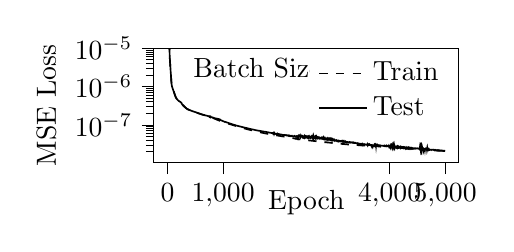
\begin{tikzpicture}

\begin{axis}[
legend cell align={left},
legend style={draw=none},
log basis y={10},
tick align=outside,
tick pos=left,
title={Batch Size 16},
title style={at={(0.4,0.85)},anchor=north},
x grid style={white!69.0196078431373!black},
xlabel={Epoch},
x label style={yshift=13pt},
xmin=-249.95, xmax=5248.95,
xtick style={color=black},
xtick = {0,1000,4000,5000},
y grid style={white!69.0196078431373!black},
ylabel={MSE Loss},
ymin=1.04995733040024e-08, ymax=1e-5,
ymode=log,
ytick style={color=black},
width=.45\textwidth,
height=.25\textwidth
]
\addplot [semithick, black, dashed]
table {%
0 0.0157170567642897
1 0.00494477174337953
2 0.00178249403554946
3 0.00104628965561278
4 0.000540450631990097
5 0.000267249523603823
6 0.000195556676466367
7 0.000179966989569948
8 0.000174315613148792
9 0.000170275954966201
10 0.000166128802236926
11 0.000161243435519282
12 0.000155176517626387
13 0.000147447619914601
14 0.000137505138925917
15 0.000124870715357247
16 0.000109628831036389
17 9.26289391609316e-05
18 7.54085500957444e-05
19 5.99092843294784e-05
20 4.77161089384026e-05
21 3.93279772288224e-05
22 3.40980909077189e-05
23 3.09422128148071e-05
24 2.89322912085481e-05
25 2.72737210743799e-05
26 2.54317353028455e-05
27 2.28156418916114e-05
28 2.01819365893243e-05
29 1.77557636425263e-05
30 1.5502294282669e-05
31 1.34128514700933e-05
32 1.15395934462867e-05
33 9.93898418664685e-06
34 8.62693892850075e-06
35 7.58853412253302e-06
36 6.78498193133237e-06
37 6.16869731970837e-06
38 5.69058382416188e-06
39 5.31324215398854e-06
40 5.00480225616684e-06
41 4.7444518992279e-06
42 4.51447482453204e-06
43 4.30798976503866e-06
44 4.11608894853543e-06
45 3.93454810227922e-06
46 3.75880521266936e-06
47 3.58901737558881e-06
48 3.42562672744862e-06
49 3.26669840717386e-06
50 3.11160224288187e-06
51 2.96258664974403e-06
52 2.82159659042236e-06
53 2.68886794032142e-06
54 2.56387212152731e-06
55 2.44723567112715e-06
56 2.34057172980329e-06
57 2.24493696725858e-06
58 2.15844092952011e-06
59 2.0788237059719e-06
60 1.99667843895668e-06
61 1.90497609787599e-06
62 1.79736609072734e-06
63 1.68848505768437e-06
64 1.59369150190969e-06
65 1.51194072418548e-06
66 1.44278207682191e-06
67 1.38194286273574e-06
68 1.32816223009513e-06
69 1.2809325050398e-06
70 1.23942618449746e-06
71 1.20316316116487e-06
72 1.17089864494346e-06
73 1.14246875506296e-06
74 1.11685223265567e-06
75 1.09369868118847e-06
76 1.07318007189861e-06
77 1.05437576991108e-06
78 1.03672772496566e-06
79 1.02062385838053e-06
80 1.00592634129271e-06
81 9.92105790942332e-07
82 9.7894169545043e-07
83 9.66602892503943e-07
84 9.54589052753363e-07
85 9.42918769112566e-07
86 9.31959767683566e-07
87 9.2148744329279e-07
88 9.11429445267231e-07
89 9.01841054997021e-07
90 8.92400122751269e-07
91 8.83255546455075e-07
92 8.74700299107189e-07
93 8.65906616240863e-07
94 8.57358865317792e-07
95 8.48961237267076e-07
96 8.40659787854747e-07
97 8.3273339777179e-07
98 8.24562840250565e-07
99 8.16930169150964e-07
100 8.08981725157309e-07
101 8.01335254408286e-07
102 7.938409220003e-07
103 7.86272286035228e-07
104 7.79077216805035e-07
105 7.71825237762869e-07
106 7.64540684656367e-07
107 7.57455605054247e-07
108 7.50291343621257e-07
109 7.43385836699417e-07
110 7.36310198249157e-07
111 7.2935094047466e-07
112 7.22335523079209e-07
113 7.15656543093246e-07
114 7.08781524224378e-07
115 7.02204949249108e-07
116 6.95669085445161e-07
117 6.89374548812793e-07
118 6.83004592076486e-07
119 6.76743621340847e-07
120 6.70653783501507e-07
121 6.64517023594158e-07
122 6.58444838109062e-07
123 6.52467115031641e-07
124 6.46645066922247e-07
125 6.40550082820823e-07
126 6.34422589044448e-07
127 6.28629438992334e-07
128 6.22746939754393e-07
129 6.16957024178077e-07
130 6.11050226723364e-07
131 6.0553354312276e-07
132 6.0002472520182e-07
133 5.94472997008211e-07
134 5.89109220683781e-07
135 5.83457079159189e-07
136 5.78418984446216e-07
137 5.7332289055978e-07
138 5.68441488383087e-07
139 5.63714549315364e-07
140 5.59090271252671e-07
141 5.54642511374936e-07
142 5.50334273199837e-07
143 5.46195153745543e-07
144 5.42178440980479e-07
145 5.38200247120812e-07
146 5.34317242667726e-07
147 5.30567891871669e-07
148 5.26957831226582e-07
149 5.23221014177011e-07
150 5.19686565098709e-07
151 5.16319246941066e-07
152 5.1299718701614e-07
153 5.09589032390068e-07
154 5.06361061226812e-07
155 5.03223137172881e-07
156 5.00183228808737e-07
157 4.9724213354807e-07
158 4.9438490189857e-07
159 4.9162455306373e-07
160 4.89330421473255e-07
161 4.86669611902357e-07
162 4.83983281668543e-07
163 4.81407683992074e-07
164 4.78924291158478e-07
165 4.7652420248312e-07
166 4.74232413509412e-07
167 4.71954440158129e-07
168 4.69751064102297e-07
169 4.67584087743944e-07
170 4.65374450342892e-07
171 4.63257154720509e-07
172 4.6126252958345e-07
173 4.59285346551042e-07
174 4.57338758977244e-07
175 4.55391532227623e-07
176 4.53448316278582e-07
177 4.5134003435976e-07
178 4.49530939363285e-07
179 4.47626082561214e-07
180 4.45694395651231e-07
181 4.43928685967876e-07
182 4.42185508745752e-07
183 4.40439555106309e-07
184 4.3882785571725e-07
185 4.37217972901749e-07
186 4.35614033278853e-07
187 4.33923493403654e-07
188 4.32394612360554e-07
189 4.30824806841201e-07
190 4.29448743943794e-07
191 4.27996334764202e-07
192 4.2654474542303e-07
193 4.25223923485873e-07
194 4.23847797321741e-07
195 4.22281450582318e-07
196 4.20877642255846e-07
197 4.19539155572579e-07
198 4.18226270070932e-07
199 4.16828583993834e-07
200 4.15641147853307e-07
201 4.14374378181037e-07
202 4.12955820522143e-07
203 4.11872127500601e-07
204 4.10614599175574e-07
205 4.09486309507656e-07
206 4.08297302655569e-07
207 4.07291623872652e-07
208 4.06151649784192e-07
209 4.04880044627021e-07
210 4.03888402871644e-07
211 4.02805585792976e-07
212 4.01743319073944e-07
213 4.00739752507206e-07
214 3.99736535186435e-07
215 3.98833434005041e-07
216 3.97754167352105e-07
217 3.96727826768029e-07
218 3.95718042653925e-07
219 3.94693230930443e-07
220 3.9383311586505e-07
221 3.9275161007879e-07
222 3.9172802642895e-07
223 3.90782656552346e-07
224 3.89721222845196e-07
225 3.88612679515177e-07
226 3.87859798280488e-07
227 3.8695441405423e-07
228 3.8589167816383e-07
229 3.84909645688936e-07
230 3.83900921491431e-07
231 3.82917928007487e-07
232 3.82064893713618e-07
233 3.81161208053982e-07
234 3.80179631534361e-07
235 3.79220531740998e-07
236 3.78215918999558e-07
237 3.7710426870774e-07
238 3.76155795223099e-07
239 3.74884881878756e-07
240 3.73761657613159e-07
241 3.72517982626164e-07
242 3.71497203701665e-07
243 3.70091190802668e-07
244 3.6877978438099e-07
245 3.67199387056871e-07
246 3.65626293969967e-07
247 3.64062025596468e-07
248 3.62244684353641e-07
249 3.60450857769479e-07
250 3.58647998822903e-07
251 3.56561039907888e-07
252 3.54525802322314e-07
253 3.52287566386167e-07
254 3.50287391583493e-07
255 3.4827622160094e-07
256 3.46361628018599e-07
257 3.442452336202e-07
258 3.42522692250213e-07
259 3.4098111838432e-07
260 3.39507249535131e-07
261 3.3804830252393e-07
262 3.36976891986751e-07
263 3.35771423678466e-07
264 3.34539207671014e-07
265 3.33171887447747e-07
266 3.32210861387239e-07
267 3.30899532073659e-07
268 3.29677021355224e-07
269 3.28394180627356e-07
270 3.27252484524365e-07
271 3.26162355179349e-07
272 3.25076022861026e-07
273 3.24031567018324e-07
274 3.23017687350102e-07
275 3.22020703876547e-07
276 3.21058469410218e-07
277 3.20131131445578e-07
278 3.19224168208621e-07
279 3.18332019588752e-07
280 3.17414626763934e-07
281 3.16470977736572e-07
282 3.15361310200046e-07
283 3.14367141285743e-07
284 3.13330990451277e-07
285 3.12373081598594e-07
286 3.11041730753914e-07
287 3.09975267860807e-07
288 3.08969859794672e-07
289 3.07846929878508e-07
290 3.06794977639413e-07
291 3.05737578266019e-07
292 3.0466266837692e-07
293 3.03954595523237e-07
294 3.03101196678313e-07
295 3.02118985189281e-07
296 3.01218168196726e-07
297 3.00310456772479e-07
298 2.99479211918197e-07
299 2.98664209118726e-07
300 2.97876342834513e-07
301 2.97069236964376e-07
302 2.96287139768481e-07
303 2.95540525151239e-07
304 2.94592372938496e-07
305 2.93832868003108e-07
306 2.93041105045688e-07
307 2.92138023390009e-07
308 2.91344262571158e-07
309 2.90479741146044e-07
310 2.89638650002644e-07
311 2.88783956314376e-07
312 2.87966960804908e-07
313 2.87156888049367e-07
314 2.86230183249359e-07
315 2.85199473267994e-07
316 2.84329060711741e-07
317 2.83470531364571e-07
318 2.82711612797471e-07
319 2.8189036959958e-07
320 2.8108939352478e-07
321 2.80323620067691e-07
322 2.79618150941019e-07
323 2.78579928540523e-07
324 2.77787970787813e-07
325 2.76974661190366e-07
326 2.76175905796094e-07
327 2.75381109268835e-07
328 2.74673050796537e-07
329 2.73941170341629e-07
330 2.73343178925245e-07
331 2.72956742115582e-07
332 2.72267732029263e-07
333 2.71421207877154e-07
334 2.70669167790061e-07
335 2.69858946552404e-07
336 2.69127144292725e-07
337 2.68486125065692e-07
338 2.67699487956463e-07
339 2.67018376263195e-07
340 2.66254324294835e-07
341 2.65609372050335e-07
342 2.64946595834203e-07
343 2.64183357693071e-07
344 2.63509790364935e-07
345 2.62888811377593e-07
346 2.62296822654662e-07
347 2.61795223821082e-07
348 2.60765411624675e-07
349 2.60187987706217e-07
350 2.59608676287826e-07
351 2.58937510935198e-07
352 2.58401657028173e-07
353 2.57939879027447e-07
354 2.57488526514749e-07
355 2.56912723124003e-07
356 2.5638282590279e-07
357 2.55946380399052e-07
358 2.55382050632136e-07
359 2.54851634466036e-07
360 2.5443849939677e-07
361 2.53912852173244e-07
362 2.53413875391573e-07
363 2.52993562064319e-07
364 2.52566530065224e-07
365 2.52173733429117e-07
366 2.51742222630469e-07
367 2.51256598509997e-07
368 2.50831636513738e-07
369 2.50515218077396e-07
370 2.5000812983933e-07
371 2.49434692122463e-07
372 2.48966004456008e-07
373 2.48557739986666e-07
374 2.48152726946671e-07
375 2.47777446951147e-07
376 2.4732192088095e-07
377 2.46895147625992e-07
378 2.46492991010427e-07
379 2.46027582377906e-07
380 2.45625955962225e-07
381 2.45214678422201e-07
382 2.44813897467111e-07
383 2.44392247530811e-07
384 2.439667089007e-07
385 2.43561708266782e-07
386 2.43146217513868e-07
387 2.42745924310839e-07
388 2.42299840301996e-07
389 2.41924007092109e-07
390 2.41548250386359e-07
391 2.4110301239233e-07
392 2.40753827760898e-07
393 2.40407377113172e-07
394 2.40073736314628e-07
395 2.39752746800548e-07
396 2.39428752649928e-07
397 2.39145928070172e-07
398 2.38728963807944e-07
399 2.38479965169347e-07
400 2.38172701713779e-07
401 2.37863011172124e-07
402 2.37620931294202e-07
403 2.3731942192029e-07
404 2.36979224602862e-07
405 2.36684770619888e-07
406 2.36476611952696e-07
407 2.36186071909117e-07
408 2.35960636956634e-07
409 2.35469004792321e-07
410 2.34993137034678e-07
411 2.34665876455153e-07
412 2.34368971142374e-07
413 2.34073551396818e-07
414 2.33405668247144e-07
415 2.3353564838402e-07
416 2.33036555627564e-07
417 2.32731610225301e-07
418 2.32511658502688e-07
419 2.32205579486333e-07
420 2.31897210944965e-07
421 2.31614303118022e-07
422 2.31387427064078e-07
423 2.31009555875517e-07
424 2.30927051632079e-07
425 2.30570250145945e-07
426 2.30109878870621e-07
427 2.29755619159278e-07
428 2.29419798976949e-07
429 2.2913787184109e-07
430 2.28831625989301e-07
431 2.28494739516805e-07
432 2.28182287109746e-07
433 2.27858054557828e-07
434 2.27546540337187e-07
435 2.27196947875541e-07
436 2.26895820269135e-07
437 2.26625020268045e-07
438 2.26283218495382e-07
439 2.25993931898927e-07
440 2.25655906049838e-07
441 2.2537209050455e-07
442 2.2510194525438e-07
443 2.24828690761569e-07
444 2.24556286852362e-07
445 2.24300207833039e-07
446 2.24011245563815e-07
447 2.23872584399487e-07
448 2.23551614816131e-07
449 2.23257345162153e-07
450 2.22980819252427e-07
451 2.2271834546217e-07
452 2.22460312336636e-07
453 2.22206780733813e-07
454 2.21958781267517e-07
455 2.21711269247749e-07
456 2.21467916212248e-07
457 2.21235154199917e-07
458 2.20999668862021e-07
459 2.20767076868356e-07
460 2.20535877438977e-07
461 2.20308807939773e-07
462 2.20059808896167e-07
463 2.19824142021707e-07
464 2.19612100529787e-07
465 2.1938929498333e-07
466 2.19157623597255e-07
467 2.1896537287347e-07
468 2.18743536777311e-07
469 2.18522104340479e-07
470 2.18272721745905e-07
471 2.18055716807442e-07
472 2.1783752742266e-07
473 2.1761818953081e-07
474 2.17430983695976e-07
475 2.17206068221287e-07
476 2.16991443927839e-07
477 2.16773518530999e-07
478 2.16515748135748e-07
479 2.16300841934469e-07
480 2.16058449872492e-07
481 2.15869073706187e-07
482 2.1564869785351e-07
483 2.15435289980803e-07
484 2.15200336675991e-07
485 2.14946434098806e-07
486 2.1470916516364e-07
487 2.14493426646811e-07
488 2.14261333354671e-07
489 2.14043833416611e-07
490 2.13684532845093e-07
491 2.13446484544022e-07
492 2.13225306985976e-07
493 2.13031618301329e-07
494 2.12794633135616e-07
495 2.1251043921211e-07
496 2.12278367698104e-07
497 2.12043049543809e-07
498 2.11812802142219e-07
499 2.11570569483399e-07
500 2.11340852310116e-07
501 2.11117200315414e-07
502 2.10896458291643e-07
503 2.1067865063884e-07
504 2.10462695349634e-07
505 2.10248212908937e-07
506 2.10038392978618e-07
507 2.09967990151938e-07
508 2.09629130488054e-07
509 2.09356091531276e-07
510 2.09101517214094e-07
511 2.0885782751634e-07
512 2.08675676212522e-07
513 2.08429224507256e-07
514 2.08143801842198e-07
515 2.07879654823273e-07
516 2.07599692124916e-07
517 2.07531877720157e-07
518 2.07242607004332e-07
519 2.06976028913175e-07
520 2.06722016230287e-07
521 2.06477896398383e-07
522 2.06244004296252e-07
523 2.05996478037207e-07
524 2.05893390926803e-07
525 2.05615459904607e-07
526 2.05380138218914e-07
527 2.05141496991246e-07
528 2.04895898015423e-07
529 2.04667326379138e-07
530 2.04441963525426e-07
531 2.04216897543574e-07
532 2.0399652140668e-07
533 2.03779658797032e-07
534 2.03562826108339e-07
535 2.0334601751415e-07
536 2.03135240347763e-07
537 2.02906057346297e-07
538 2.02689399074529e-07
539 2.02473491917488e-07
540 2.02258676225142e-07
541 2.02040906152945e-07
542 2.01827895203621e-07
543 2.01646046050996e-07
544 2.0143258397809e-07
545 2.01214925588999e-07
546 2.00992143142287e-07
547 2.00781135099248e-07
548 2.00562146595473e-07
549 2.00357410903962e-07
550 2.00143986297974e-07
551 1.99943427894311e-07
552 1.99730849530511e-07
553 1.99533505224281e-07
554 1.99330869968151e-07
555 1.9912389529253e-07
556 1.98918559668471e-07
557 1.98708590382068e-07
558 1.98505848487684e-07
559 1.98292419888446e-07
560 1.98096410962023e-07
561 1.97904820154804e-07
562 1.9770706975919e-07
563 1.9748347308024e-07
564 1.97292339883859e-07
565 1.97073662711489e-07
566 1.96870710993835e-07
567 1.96664619174669e-07
568 1.96475939667096e-07
569 1.96348054068096e-07
570 1.96120539378342e-07
571 1.95933779174595e-07
572 1.95736368809207e-07
573 1.95534025024813e-07
574 1.95333484313664e-07
575 1.95124152348569e-07
576 1.95009315866912e-07
577 1.94775902379263e-07
578 1.94541645868185e-07
579 1.94320748363452e-07
580 1.9411251212631e-07
581 1.93909075257181e-07
582 1.93718050923053e-07
583 1.93516266911331e-07
584 1.93320917162509e-07
585 1.93129007548976e-07
586 1.92928064961961e-07
587 1.92837274340718e-07
588 1.92624708525102e-07
589 1.92408956387169e-07
590 1.92225819553471e-07
591 1.92020735894971e-07
592 1.91878943944346e-07
593 1.91675015734916e-07
594 1.91448435110431e-07
595 1.91271641604374e-07
596 1.91048381573466e-07
597 1.90840330120068e-07
598 1.90653138474772e-07
599 1.90466430986191e-07
600 1.90273618727588e-07
601 1.90071319252638e-07
602 1.89884589708811e-07
603 1.89694812256391e-07
604 1.89509724471293e-07
605 1.89317692722568e-07
606 1.89151745139782e-07
607 1.88957836265047e-07
608 1.88763875129894e-07
609 1.8860838834911e-07
610 1.88492758660175e-07
611 1.88309009992338e-07
612 1.88081675830176e-07
613 1.87860870838108e-07
614 1.87664490702844e-07
615 1.87469595530843e-07
616 1.87259174673216e-07
617 1.87060099065661e-07
618 1.86873242554952e-07
619 1.86672734876936e-07
620 1.86483752926847e-07
621 1.86293344697219e-07
622 1.86105415899362e-07
623 1.85915503529088e-07
624 1.8575178152247e-07
625 1.85554022223755e-07
626 1.85353178373759e-07
627 1.8521270283145e-07
628 1.85098913320303e-07
629 1.84897171813248e-07
630 1.84691331647002e-07
631 1.84487640524367e-07
632 1.84295574889859e-07
633 1.84111957629796e-07
634 1.83914716345157e-07
635 1.83755724989965e-07
636 1.83571663399107e-07
637 1.8338817892527e-07
638 1.8321129060439e-07
639 1.83026746398696e-07
640 1.82798685713692e-07
641 1.82628072302293e-07
642 1.8240755436949e-07
643 1.82209592708205e-07
644 1.81998398467442e-07
645 1.81880033061077e-07
646 1.81668815613989e-07
647 1.81459775753012e-07
648 1.81254756874694e-07
649 1.81092687050466e-07
650 1.80890330682359e-07
651 1.80684028741496e-07
652 1.80452216731908e-07
653 1.80272235375867e-07
654 1.80111763242508e-07
655 1.79915874568337e-07
656 1.79712098308471e-07
657 1.79537765347959e-07
658 1.79391292441267e-07
659 1.7920577938213e-07
660 1.79012431054559e-07
661 1.78831277722225e-07
662 1.78644232065039e-07
663 1.78457527518106e-07
664 1.78267877934957e-07
665 1.78093018554648e-07
666 1.77905254446387e-07
667 1.77723857326839e-07
668 1.7753547782462e-07
669 1.77379771038488e-07
670 1.77215719631363e-07
671 1.77056875465098e-07
672 1.76856059582065e-07
673 1.76671049281651e-07
674 1.76487213458643e-07
675 1.76302384872429e-07
676 1.76117043793056e-07
677 1.75936534887455e-07
678 1.75756247521974e-07
679 1.75606320475197e-07
680 1.75418388813853e-07
681 1.75196992749704e-07
682 1.75045590090406e-07
683 1.74854614705566e-07
684 1.74652316815127e-07
685 1.74424186383249e-07
686 1.74264706537031e-07
687 1.74055298188591e-07
688 1.73926764027499e-07
689 1.73701496798628e-07
690 1.73572706358982e-07
691 1.73321090102263e-07
692 1.73147434431087e-07
693 1.72996947163995e-07
694 1.72786218151089e-07
695 1.72599083192893e-07
696 1.72568876031676e-07
697 1.72387436194299e-07
698 1.72159440069208e-07
699 1.71958998173238e-07
700 1.71749518663944e-07
701 1.7157847770477e-07
702 1.71360882688987e-07
703 1.71189904619951e-07
704 1.70959397792103e-07
705 1.7079805885345e-07
706 1.70577748185963e-07
707 1.70391250101432e-07
708 1.70294054527176e-07
709 1.70153339674073e-07
710 1.69961250442441e-07
711 1.69790923798985e-07
712 1.69513855112768e-07
713 1.69349986016698e-07
714 1.69170517544615e-07
715 1.68975520637105e-07
716 1.68794829697561e-07
717 1.68674960491444e-07
718 1.68560368251747e-07
719 1.68348613023284e-07
720 1.68180192382295e-07
721 1.68044255872246e-07
722 1.67784312189667e-07
723 1.67622006166823e-07
724 1.67433583676768e-07
725 1.67142194790415e-07
726 1.66952169308843e-07
727 1.66777577675248e-07
728 1.66608952660852e-07
729 1.66446427947164e-07
730 1.66270591492435e-07
731 1.66101942618013e-07
732 1.65938628249762e-07
733 1.65765831525277e-07
734 1.65649616683083e-07
735 1.65385300405774e-07
736 1.65217369541892e-07
737 1.65014219057014e-07
738 1.6483034158199e-07
739 1.64667229618942e-07
740 1.64397729420784e-07
741 1.64213927241974e-07
742 1.64072907040236e-07
743 1.6379700686997e-07
744 1.63645981643867e-07
745 1.63382232301501e-07
746 1.6327906817537e-07
747 1.63015408730871e-07
748 1.62801310864324e-07
749 1.62617077627658e-07
750 1.62424714076792e-07
751 1.62247915383773e-07
752 1.62051023785637e-07
753 1.61872072872882e-07
754 1.6165106788435e-07
755 1.61600835717479e-07
756 1.61240600313306e-07
757 1.61194861057368e-07
758 1.60852658879662e-07
759 1.60787009278351e-07
760 1.60590858342857e-07
761 1.60234822551786e-07
762 1.60201742232857e-07
763 1.59901149771713e-07
764 1.59803023151994e-07
765 1.59525831236351e-07
766 1.59374475643403e-07
767 1.59135792628717e-07
768 1.58920532690843e-07
769 1.58900042478649e-07
770 1.58551003600849e-07
771 1.58445956166986e-07
772 1.58137577130901e-07
773 1.58083954872268e-07
774 1.57764831811846e-07
775 1.57709431590547e-07
776 1.57401405722624e-07
777 1.57347303854749e-07
778 1.57050745258402e-07
779 1.56966653740653e-07
780 1.56687031115155e-07
781 1.56785914370516e-07
782 1.56612737448825e-07
783 1.56451782203249e-07
784 1.56252137685442e-07
785 1.56076418790008e-07
786 1.55898435949098e-07
787 1.55699541132037e-07
788 1.55520961151012e-07
789 1.55345307412347e-07
790 1.55173079157578e-07
791 1.54974727074375e-07
792 1.54768641245084e-07
793 1.5459558374431e-07
794 1.5444234325912e-07
795 1.54301182689665e-07
796 1.54076760843225e-07
797 1.53900922057915e-07
798 1.53745949539541e-07
799 1.53580229117267e-07
800 1.53406590548855e-07
801 1.53240547525968e-07
802 1.53047686090702e-07
803 1.52824890882641e-07
804 1.52664273521452e-07
805 1.52475196550483e-07
806 1.52327802844354e-07
807 1.52147398885916e-07
808 1.51979647590395e-07
809 1.51795929646426e-07
810 1.51624505434711e-07
811 1.51454105321136e-07
812 1.51283279407721e-07
813 1.51115457406092e-07
814 1.50930618310952e-07
815 1.50760781984616e-07
816 1.50782627734714e-07
817 1.50500275672982e-07
818 1.50235237292407e-07
819 1.50018968902543e-07
820 1.49857105313345e-07
821 1.49713744534097e-07
822 1.49508386748209e-07
823 1.49243716315084e-07
824 1.49054966783524e-07
825 1.48848405203239e-07
826 1.48593713156231e-07
827 1.48452548614841e-07
828 1.48339782398921e-07
829 1.48084122237435e-07
830 1.47866147088394e-07
831 1.47622342979048e-07
832 1.4737123991182e-07
833 1.47169714985296e-07
834 1.47018789085962e-07
835 1.46823949506825e-07
836 1.46512769518381e-07
837 1.46378438842021e-07
838 1.46098743840639e-07
839 1.45954007734872e-07
840 1.45737554120728e-07
841 1.45556221561094e-07
842 1.45273102816645e-07
843 1.45146473812474e-07
844 1.44893944799662e-07
845 1.44685848667336e-07
846 1.44500907168776e-07
847 1.4436663649775e-07
848 1.44028160448784e-07
849 1.43881057880435e-07
850 1.43606745851343e-07
851 1.43507942325982e-07
852 1.43128769224177e-07
853 1.4301058635624e-07
854 1.42788225716117e-07
855 1.42625498355642e-07
856 1.42412673760361e-07
857 1.42159079061344e-07
858 1.4199432023787e-07
859 1.41772513316596e-07
860 1.41599934678993e-07
861 1.41388858359903e-07
862 1.41182926185479e-07
863 1.40962782744225e-07
864 1.40806364584023e-07
865 1.40581685961649e-07
866 1.40403925101396e-07
867 1.4016057497912e-07
868 1.40044896177471e-07
869 1.3980589160667e-07
870 1.3957648116758e-07
871 1.39445378636083e-07
872 1.39138843742614e-07
873 1.38897649193837e-07
874 1.38654308422304e-07
875 1.38455802293436e-07
876 1.38271871641393e-07
877 1.38072660327282e-07
878 1.3789356398064e-07
879 1.37655154013316e-07
880 1.37478279633285e-07
881 1.37314475196604e-07
882 1.37122865879746e-07
883 1.36933145142848e-07
884 1.36802316887952e-07
885 1.36559793908475e-07
886 1.3642202107178e-07
887 1.36200022627264e-07
888 1.36101916211828e-07
889 1.35843518506817e-07
890 1.35694482299442e-07
891 1.35512572025931e-07
892 1.35300152894757e-07
893 1.35296917736838e-07
894 1.35076997914041e-07
895 1.34893043981066e-07
896 1.34717172727505e-07
897 1.34527160362552e-07
898 1.34308240479442e-07
899 1.34143823828481e-07
900 1.33862042787314e-07
901 1.336907333922e-07
902 1.33526360556857e-07
903 1.33354756073345e-07
904 1.33178832584235e-07
905 1.32975719669304e-07
906 1.328086220731e-07
907 1.32602404118387e-07
908 1.3244473960583e-07
909 1.322507284236e-07
910 1.3208645066598e-07
911 1.31908025320371e-07
912 1.31727454142805e-07
913 1.31562949462705e-07
914 1.31399596458692e-07
915 1.3120474050865e-07
916 1.31009608221433e-07
917 1.30844098823246e-07
918 1.30663171997725e-07
919 1.30506657299634e-07
920 1.30347919839124e-07
921 1.30182991870953e-07
922 1.30027269566568e-07
923 1.29857494112429e-07
924 1.29701414859795e-07
925 1.29552905523411e-07
926 1.2940177445131e-07
927 1.29231482656422e-07
928 1.29098281369977e-07
929 1.28939781010473e-07
930 1.28751404755434e-07
931 1.28589202464724e-07
932 1.2841671961894e-07
933 1.28243070928846e-07
934 1.2803982670917e-07
935 1.27876534680382e-07
936 1.27715794622674e-07
937 1.27549439078223e-07
938 1.27395809307984e-07
939 1.27251330805933e-07
940 1.27115895857344e-07
941 1.26910032076211e-07
942 1.26811345971589e-07
943 1.26729663211478e-07
944 1.26444568536499e-07
945 1.26253609963101e-07
946 1.26082584579024e-07
947 1.25873118491882e-07
948 1.25708876002051e-07
949 1.25526543680365e-07
950 1.25347965983735e-07
951 1.25173203823437e-07
952 1.24986479754341e-07
953 1.24805979790921e-07
954 1.2464467223694e-07
955 1.24486626290832e-07
956 1.24325891309951e-07
957 1.24059086388684e-07
958 1.23900421499457e-07
959 1.23752723684589e-07
960 1.23606460093129e-07
961 1.23458894080386e-07
962 1.23334903548766e-07
963 1.23164554814537e-07
964 1.23017373574896e-07
965 1.22884383220168e-07
966 1.2272103016997e-07
967 1.22591781686054e-07
968 1.22412395523241e-07
969 1.22283938569723e-07
970 1.2213839731956e-07
971 1.21992413387062e-07
972 1.21762341468212e-07
973 1.21653056602611e-07
974 1.21516884128425e-07
975 1.21363378561057e-07
976 1.21249401036749e-07
977 1.21074073003768e-07
978 1.20967150103013e-07
979 1.20810225507029e-07
980 1.20688818554981e-07
981 1.20541718686695e-07
982 1.20421648816205e-07
983 1.2028323980573e-07
984 1.20130155050191e-07
985 1.20018588045667e-07
986 1.19883109864105e-07
987 1.19717597538482e-07
988 1.19591703700905e-07
989 1.19459623334706e-07
990 1.19327731148644e-07
991 1.19182412216645e-07
992 1.190378214595e-07
993 1.18928106189742e-07
994 1.18777606907372e-07
995 1.18669771886459e-07
996 1.18526345442405e-07
997 1.18412091222098e-07
998 1.182686517609e-07
999 1.18146764471305e-07
1000 1.18045295611324e-07
1001 1.17885191471601e-07
1002 1.1773723693409e-07
1003 1.17636993980597e-07
1004 1.17508308122183e-07
1005 1.17379135396334e-07
1006 1.17220094796977e-07
1007 1.17123960905019e-07
1008 1.16971413607558e-07
1009 1.16875604081912e-07
1010 1.16721507264828e-07
1011 1.16625413646432e-07
1012 1.16471765217341e-07
1013 1.16374956864007e-07
1014 1.16226475117998e-07
1015 1.1612951336204e-07
1016 1.15985186340595e-07
1017 1.15878762532162e-07
1018 1.15722544556718e-07
1019 1.1563705219686e-07
1020 1.15482216056506e-07
1021 1.15382735749847e-07
1022 1.15234289868482e-07
1023 1.15194369406879e-07
1024 1.1509215372385e-07
1025 1.14971480446258e-07
1026 1.14853542346083e-07
1027 1.14729510986677e-07
1028 1.14465596745106e-07
1029 1.14398147832873e-07
1030 1.14321383524185e-07
1031 1.14196341097994e-07
1032 1.14066242570487e-07
1033 1.13935783559782e-07
1034 1.13807661961118e-07
1035 1.13695412860437e-07
1036 1.13558107294409e-07
1037 1.13417669808769e-07
1038 1.13302818903094e-07
1039 1.13176249655567e-07
1040 1.13044207392221e-07
1041 1.12916077910086e-07
1042 1.12789789074696e-07
1043 1.12666461593136e-07
1044 1.12543457490233e-07
1045 1.12422214286312e-07
1046 1.12315864466694e-07
1047 1.12182835920294e-07
1048 1.12061487143933e-07
1049 1.11943023419769e-07
1050 1.11824035883501e-07
1051 1.11708382185327e-07
1052 1.11589450629168e-07
1053 1.11475569585906e-07
1054 1.11358585638044e-07
1055 1.11240735918727e-07
1056 1.11126858243438e-07
1057 1.11011553304508e-07
1058 1.10896632492086e-07
1059 1.10790323411436e-07
1060 1.10676093481032e-07
1061 1.10561356954975e-07
1062 1.10458826345194e-07
1063 1.10332153219872e-07
1064 1.10221367368268e-07
1065 1.10119643316864e-07
1066 1.10016076984465e-07
1067 1.09895937949744e-07
1068 1.09784279111125e-07
1069 1.09660139557377e-07
1070 1.09532256768574e-07
1071 1.09413658780255e-07
1072 1.09296013629745e-07
1073 1.09178800776988e-07
1074 1.09062563716122e-07
1075 1.08961397675245e-07
1076 1.0882023883596e-07
1077 1.08682747345767e-07
1078 1.08570803114105e-07
1079 1.08453086824056e-07
1080 1.08348394981306e-07
1081 1.08229575708663e-07
1082 1.08175652648868e-07
1083 1.08044552664666e-07
1084 1.07924311190999e-07
1085 1.07804279075197e-07
1086 1.07687016416946e-07
1087 1.07583657079857e-07
1088 1.07472328480185e-07
1089 1.07360298155612e-07
1090 1.07231535281471e-07
1091 1.07122651012759e-07
1092 1.07014493000435e-07
1093 1.0690706458405e-07
1094 1.06793603364963e-07
1095 1.06669464503995e-07
1096 1.06556396463731e-07
1097 1.06448062449971e-07
1098 1.0633262673565e-07
1099 1.06225804859861e-07
1100 1.06111840107559e-07
1101 1.06007312659528e-07
1102 1.05889961115935e-07
1103 1.05787279665037e-07
1104 1.05671067569091e-07
1105 1.05566635443921e-07
1106 1.0545252139238e-07
1107 1.05352690265903e-07
1108 1.05238320241341e-07
1109 1.05129935327852e-07
1110 1.05013805679732e-07
1111 1.04924952804453e-07
1112 1.04802457894237e-07
1113 1.0472310326648e-07
1114 1.04609571572212e-07
1115 1.0450942516016e-07
1116 1.04393734819297e-07
1117 1.04297197307091e-07
1118 1.04180416496291e-07
1119 1.0408402435047e-07
1120 1.03966197073646e-07
1121 1.0387017652036e-07
1122 1.03754794164246e-07
1123 1.0365835006354e-07
1124 1.03542971995552e-07
1125 1.03447081940544e-07
1126 1.03333663226124e-07
1127 1.03239306419312e-07
1128 1.03124784988751e-07
1129 1.03028840477748e-07
1130 1.02916153586818e-07
1131 1.02787292341588e-07
1132 1.02657459869704e-07
1133 1.02566233646684e-07
1134 1.02459099572627e-07
1135 1.0236741592351e-07
1136 1.02258474193206e-07
1137 1.02178690926991e-07
1138 1.02057533133859e-07
1139 1.0195955497494e-07
1140 1.01866740447321e-07
1141 1.0174640036098e-07
1142 1.01654885199309e-07
1143 1.01564086460115e-07
1144 1.01452568284088e-07
1145 1.01358281408892e-07
1146 1.01252124068196e-07
1147 1.01132042544805e-07
1148 1.01040741810721e-07
1149 1.0093680472778e-07
1150 1.00835201639171e-07
1151 1.00737907963833e-07
1152 1.00636074826355e-07
1153 1.00535662330259e-07
1154 1.00435070386595e-07
1155 1.00334794463919e-07
1156 1.00233066344657e-07
1157 1.00139313264691e-07
1158 1.00035746370963e-07
1159 9.99342205645348e-08
1160 9.98369444076275e-08
1161 9.97294167923712e-08
1162 9.96306041329831e-08
1163 9.95292283505478e-08
1164 9.94305740533719e-08
1165 9.93309828345446e-08
1166 9.92319580497281e-08
1167 9.91331406723361e-08
1168 9.90346987315149e-08
1169 9.89363423364864e-08
1170 9.88384333915349e-08
1171 9.87406676955516e-08
1172 9.86426246996075e-08
1173 9.85450470523119e-08
1174 9.84475341887503e-08
1175 9.83505173692833e-08
1176 9.82529710178426e-08
1177 9.81562854889262e-08
1178 9.80592281862869e-08
1179 9.79621718073531e-08
1180 9.78654439443005e-08
1181 9.77698567261598e-08
1182 9.76725255235067e-08
1183 9.75756527665794e-08
1184 9.74796394181965e-08
1185 9.73854815420339e-08
1186 9.72912396584036e-08
1187 9.71942784673274e-08
1188 9.70993046678359e-08
1189 9.7005777128345e-08
1190 9.69105955412886e-08
1191 9.68398183474051e-08
1192 9.67422502249349e-08
1193 9.6656792269556e-08
1194 9.65493723619204e-08
1195 9.64579490911888e-08
1196 9.63569642422613e-08
1197 9.62606689931533e-08
1198 9.61624434623332e-08
1199 9.60775235725464e-08
1200 9.5981298237291e-08
1201 9.58870457914429e-08
1202 9.57886685490905e-08
1203 9.56941159380165e-08
1204 9.55973716543213e-08
1205 9.550779267542e-08
1206 9.54129343995192e-08
1207 9.53207871106088e-08
1208 9.52259731121785e-08
1209 9.51386579863822e-08
1210 9.50452932002577e-08
1211 9.49372938769955e-08
1212 9.48370358955231e-08
1213 9.47485660738323e-08
1214 9.46488406015078e-08
1215 9.45476629787834e-08
1216 9.44520911225766e-08
1217 9.43511249644757e-08
1218 9.42532653489536e-08
1219 9.41596363510655e-08
1220 9.40521965198116e-08
1221 9.3958234778313e-08
1222 9.38527993739058e-08
1223 9.37583681590581e-08
1224 9.3655063739817e-08
1225 9.35592185555834e-08
1226 9.34639041965113e-08
1227 9.33635799533761e-08
1228 9.32726998605915e-08
1229 9.31820874114919e-08
1230 9.3086685076571e-08
1231 9.2996467174089e-08
1232 9.28943459186371e-08
1233 9.28112276987747e-08
1234 9.27086237609842e-08
1235 9.26266937000264e-08
1236 9.25256117518813e-08
1237 9.24348963096122e-08
1238 9.23422541383445e-08
1239 9.22336319888473e-08
1240 9.21328738066052e-08
1241 9.20548228862117e-08
1242 9.19620167856294e-08
1243 9.1858883305207e-08
1244 9.17831347067022e-08
1245 9.16764033469519e-08
1246 9.16021301513581e-08
1247 9.15102322807115e-08
1248 9.14096642823381e-08
1249 9.13258232415615e-08
1250 9.12370573509236e-08
1251 9.11314231082372e-08
1252 9.10548857149251e-08
1253 9.09575262930673e-08
1254 9.0878455086596e-08
1255 9.07892068404692e-08
1256 9.06909464717387e-08
1257 9.06085933252143e-08
1258 9.0521073303762e-08
1259 9.04282962750358e-08
1260 9.03382387598128e-08
1261 9.02488962388759e-08
1262 9.01657012271073e-08
1263 9.00837959534329e-08
1264 8.99963811491489e-08
1265 8.9906916667104e-08
1266 8.98200719099407e-08
1267 8.97321847581622e-08
1268 8.96452091616595e-08
1269 8.95563996046178e-08
1270 8.94744537696113e-08
1271 8.93858809583037e-08
1272 8.93017317054046e-08
1273 8.92115444202091e-08
1274 8.91289444773236e-08
1275 8.90431513695944e-08
1276 8.89543760465017e-08
1277 8.88647354990724e-08
1278 8.87773948683446e-08
1279 8.86847180474604e-08
1280 8.8604710200002e-08
1281 8.85189234693939e-08
1282 8.84320530047944e-08
1283 8.83455266311728e-08
1284 8.82566362889747e-08
1285 8.81749002772381e-08
1286 8.8091375637589e-08
1287 8.8006731434831e-08
1288 8.79208263704356e-08
1289 8.78380143163327e-08
1290 8.7753197313134e-08
1291 8.76683468540307e-08
1292 8.7583503496802e-08
1293 8.74997554873858e-08
1294 8.74166315618652e-08
1295 8.7332899298076e-08
1296 8.72496221155927e-08
1297 8.71674850380089e-08
1298 8.70835239226153e-08
1299 8.69979467985615e-08
1300 8.69180498774824e-08
1301 8.68290546023331e-08
1302 8.67538605575646e-08
1303 8.66866929456478e-08
1304 8.66013013194333e-08
1305 8.65141546739778e-08
1306 8.6432395224989e-08
1307 8.63492025722223e-08
1308 8.62639010534849e-08
1309 8.61873499360399e-08
1310 8.60964398192721e-08
1311 8.60305623895386e-08
1312 8.5945265599463e-08
1313 8.58654531619152e-08
1314 8.57828558054052e-08
1315 8.57025365945674e-08
1316 8.56227119179209e-08
1317 8.55251783349331e-08
1318 8.5447654544879e-08
1319 8.53730991074997e-08
1320 8.53113611576362e-08
1321 8.52530063752965e-08
1322 8.5145811016929e-08
1323 8.50639250415952e-08
1324 8.49800504987286e-08
1325 8.49213991926945e-08
1326 8.48373153417015e-08
1327 8.47663028693546e-08
1328 8.4683932776386e-08
1329 8.46030600811787e-08
1330 8.45243451159661e-08
1331 8.44448748686943e-08
1332 8.43658713378659e-08
1333 8.42873192290483e-08
1334 8.42077087881421e-08
1335 8.413040495725e-08
1336 8.40533396413434e-08
1337 8.39737880227176e-08
1338 8.39027628565248e-08
1339 8.38281100463689e-08
1340 8.37473770438635e-08
1341 8.36699169042276e-08
1342 8.35880798319977e-08
1343 8.35109091923414e-08
1344 8.34303905108413e-08
1345 8.33509666051668e-08
1346 8.32730190971631e-08
1347 8.31975916035788e-08
1348 8.31306992026271e-08
1349 8.30542468079898e-08
1350 8.29774157509178e-08
1351 8.2896661286469e-08
1352 8.28168008588648e-08
1353 8.27384261050668e-08
1354 8.26573808154762e-08
1355 8.25796255305988e-08
1356 8.25036329494821e-08
1357 8.24257792118033e-08
1358 8.23485480161423e-08
1359 8.22789238732469e-08
1360 8.22006595520008e-08
1361 8.21227055496365e-08
1362 8.2044704448947e-08
1363 8.19672813463512e-08
1364 8.18913912894459e-08
1365 8.18145910308488e-08
1366 8.17310067056098e-08
1367 8.16556159399795e-08
1368 8.15891315895101e-08
1369 8.15134725122846e-08
1370 8.14405360145543e-08
1371 8.13719105217103e-08
1372 8.12908016314395e-08
1373 8.12063895203607e-08
1374 8.11270667853137e-08
1375 8.10392181485042e-08
1376 8.09575813001118e-08
1377 8.08839921795368e-08
1378 8.08079852667731e-08
1379 8.07220590779423e-08
1380 8.06590918109862e-08
1381 8.05818785387658e-08
1382 8.05058287483007e-08
1383 8.04375114924483e-08
1384 8.03611219843958e-08
1385 8.02734742073596e-08
1386 8.02103674963917e-08
1387 8.01333753592814e-08
1388 8.00467322505938e-08
1389 7.99712219219373e-08
1390 7.99084653912985e-08
1391 7.98324605639777e-08
1392 7.97513225130331e-08
1393 7.96915628207273e-08
1394 7.96128401034935e-08
1395 7.95309664347599e-08
1396 7.94698840849151e-08
1397 7.9392765581332e-08
1398 7.9295083487807e-08
1399 7.92480824038933e-08
1400 7.91767527488219e-08
1401 7.90798937977399e-08
1402 7.90350093922143e-08
1403 7.89427710436996e-08
1404 7.88719372764035e-08
1405 7.88001505966918e-08
1406 7.87278963976235e-08
1407 7.86439569182562e-08
1408 7.85879019211677e-08
1409 7.85154309888014e-08
1410 7.84318538968876e-08
1411 7.83922933358383e-08
1412 7.83064902059039e-08
1413 7.82436948192355e-08
1414 7.81700940777341e-08
1415 7.81046548645747e-08
1416 7.80235332982215e-08
1417 7.79860344124472e-08
1418 7.78859922760944e-08
1419 7.78468724114134e-08
1420 7.77458072285242e-08
1421 7.77082536167484e-08
1422 7.76031458613602e-08
1423 7.75538769453021e-08
1424 7.74638346889844e-08
1425 7.7412013162359e-08
1426 7.73240489770899e-08
1427 7.72703984992518e-08
1428 7.71842282603075e-08
1429 7.71299326345343e-08
1430 7.70427543983487e-08
1431 7.69885805844694e-08
1432 7.68999306934859e-08
1433 7.68471794536651e-08
1434 7.67474068190665e-08
1435 7.669313940184e-08
1436 7.6607799300632e-08
1437 7.65571879561833e-08
1438 7.64666975019423e-08
1439 7.64233642662759e-08
1440 7.63317421643706e-08
1441 7.62877545348317e-08
1442 7.6203435483535e-08
1443 7.61529052084597e-08
1444 7.60647247997071e-08
1445 7.60194817654991e-08
1446 7.59333198274703e-08
1447 7.58907218383342e-08
1448 7.58090455246219e-08
1449 7.57582843178284e-08
1450 7.57179583370515e-08
1451 7.56195299302931e-08
1452 7.55561748508882e-08
1453 7.54916978635833e-08
1454 7.5432396256403e-08
1455 7.53674571498664e-08
1456 7.52965677950357e-08
1457 7.5238625441898e-08
1458 7.5167802796372e-08
1459 7.51119294637448e-08
1460 7.50374735734027e-08
1461 7.49760933977939e-08
1462 7.48975998057233e-08
1463 7.48535242411918e-08
1464 7.47783008758773e-08
1465 7.47050625609091e-08
1466 7.46483551417043e-08
1467 7.45740001022455e-08
1468 7.45270812885224e-08
1469 7.4443754344955e-08
1470 7.4380113401773e-08
1471 7.43380596901488e-08
1472 7.42537142617294e-08
1473 7.42098589494589e-08
1474 7.41303028082285e-08
1475 7.40660056592901e-08
1476 7.40370165512871e-08
1477 7.39397521467566e-08
1478 7.38789098857495e-08
1479 7.38492542762259e-08
1480 7.37513224109421e-08
1481 7.37224941023129e-08
1482 7.36224275552644e-08
1483 7.35667011948493e-08
1484 7.35384280314832e-08
1485 7.34439351628424e-08
1486 7.34135366222688e-08
1487 7.33215193999826e-08
1488 7.3262118958084e-08
1489 7.32310826201399e-08
1490 7.31369283712979e-08
1491 7.30799931130122e-08
1492 7.30507533877045e-08
1493 7.29692056040676e-08
1494 7.29461080162253e-08
1495 7.28552913358271e-08
1496 7.28172455186637e-08
1497 7.2759770612052e-08
1498 7.26808831839065e-08
1499 7.26333379219568e-08
1500 7.25761171178618e-08
1501 7.25002446042566e-08
1502 7.24530508353638e-08
1503 7.23712498071904e-08
1504 7.23255573245041e-08
1505 7.22771065948535e-08
1506 7.22012546212625e-08
1507 7.21588228156378e-08
1508 7.20717930615677e-08
1509 7.20151864914698e-08
1510 7.19812252931717e-08
1511 7.18593284645408e-08
1512 7.18661725915837e-08
1513 7.18080895314443e-08
1514 7.17542879211663e-08
1515 7.16964362812433e-08
1516 7.16366252806466e-08
1517 7.15322650410855e-08
1518 7.15308601897391e-08
1519 7.14554064966677e-08
1520 7.13549446889061e-08
1521 7.13500851201587e-08
1522 7.1280213971292e-08
1523 7.12213592048983e-08
1524 7.1125808473127e-08
1525 7.11177791856699e-08
1526 7.10524085931752e-08
1527 7.09491985855237e-08
1528 7.09230811022366e-08
1529 7.08539147549203e-08
1530 7.07737182583656e-08
1531 7.07214989734695e-08
1532 7.06564270451793e-08
1533 7.05835089735984e-08
1534 7.05460777865596e-08
1535 7.04877491930489e-08
1536 7.04216205349439e-08
1537 7.03814124722868e-08
1538 7.03216431912068e-08
1539 7.02704037696122e-08
1540 7.01973612020623e-08
1541 7.0164162307762e-08
1542 7.01039659212199e-08
1543 7.0039195259497e-08
1544 6.99994840633877e-08
1545 6.99282411940061e-08
1546 6.98895919128972e-08
1547 6.98095471864946e-08
1548 6.97712376460657e-08
1549 6.97109298943843e-08
1550 6.9632473101322e-08
1551 6.95940093482506e-08
1552 6.95389268248192e-08
1553 6.94699652452613e-08
1554 6.94294041974075e-08
1555 6.9355845011998e-08
1556 6.93180881405908e-08
1557 6.92588990727216e-08
1558 6.91887736632424e-08
1559 6.91512637267522e-08
1560 6.9092847537533e-08
1561 6.90220523242857e-08
1562 6.89855159823338e-08
1563 6.89106090323577e-08
1564 6.88816554959004e-08
1565 6.88365903069865e-08
1566 6.87812293040935e-08
1567 6.87185002323787e-08
1568 6.8642084881887e-08
1569 6.86118347612563e-08
1570 6.85325593572372e-08
1571 6.85040618790822e-08
1572 6.84324654880442e-08
1573 6.839076007914e-08
1574 6.83189021835062e-08
1575 6.82729641408031e-08
1576 6.81955693746517e-08
1577 6.81605108194816e-08
1578 6.81111089928521e-08
1579 6.80341699759168e-08
1580 6.80005206437073e-08
1581 6.79343854468328e-08
1582 6.78743013686756e-08
1583 6.78180592128541e-08
1584 6.77644835676006e-08
1585 6.77205531331992e-08
1586 6.76518835902584e-08
1587 6.75858284839848e-08
1588 6.7559896509195e-08
1589 6.74892750094358e-08
1590 6.74610934225939e-08
1591 6.74030582157315e-08
1592 6.73369531245527e-08
1593 6.72861732180508e-08
1594 6.72273089517006e-08
1595 6.7194645049895e-08
1596 6.7137755896951e-08
1597 6.70708017658228e-08
1598 6.70592294174099e-08
1599 6.69806256290428e-08
1600 6.69565935051963e-08
1601 6.6876471620958e-08
1602 6.68527393017371e-08
1603 6.67749209544155e-08
1604 6.67497319373211e-08
1605 6.66836660396797e-08
1606 6.66453354263297e-08
1607 6.65926854352961e-08
1608 6.65282488423458e-08
1609 6.6488449387947e-08
1610 6.64343398302236e-08
1611 6.63779134839615e-08
1612 6.63125629074557e-08
1613 6.62765239027863e-08
1614 6.62034557681324e-08
1615 6.61748533499207e-08
1616 6.61297554014339e-08
1617 6.60409584458677e-08
1618 6.6028880171487e-08
1619 6.59719671087799e-08
1620 6.59495228756413e-08
1621 6.58748443882473e-08
1622 6.58512198743466e-08
1623 6.57803125960754e-08
1624 6.57593430002379e-08
1625 6.57009276565645e-08
1626 6.56188756789078e-08
1627 6.56008984094569e-08
1628 6.5510794748036e-08
1629 6.5506174689034e-08
1630 6.54147165271013e-08
1631 6.54004263029861e-08
1632 6.5330469803726e-08
1633 6.53194631468068e-08
1634 6.52330189456762e-08
1635 6.52263919054263e-08
1636 6.51325602660791e-08
1637 6.51270379510294e-08
1638 6.50832606332585e-08
1639 6.50223449909504e-08
1640 6.49905436045373e-08
1641 6.49078730869945e-08
1642 6.48822075746125e-08
1643 6.48035599741803e-08
1644 6.47770159538652e-08
1645 6.4707539873865e-08
1646 6.46819224456863e-08
1647 6.46097836529691e-08
1648 6.45885289962678e-08
1649 6.45144189377334e-08
1650 6.44925645705285e-08
1651 6.44240081335568e-08
1652 6.43979384005178e-08
1653 6.43428221973608e-08
1654 6.428219044885e-08
1655 6.42558258956427e-08
1656 6.41921231387954e-08
1657 6.41689319547112e-08
1658 6.41028819785561e-08
1659 6.40726781870882e-08
1660 6.40072181106177e-08
1661 6.39795522463515e-08
1662 6.39297982321096e-08
1663 6.3871073178845e-08
1664 6.38408367290566e-08
1665 6.37792557007799e-08
1666 6.37521571729138e-08
1667 6.36896845236379e-08
1668 6.36601125965086e-08
1669 6.36008435410673e-08
1670 6.35746379664681e-08
1671 6.35181804433671e-08
1672 6.34676094435349e-08
1673 6.34354211879184e-08
1674 6.33740493203305e-08
1675 6.33314038243071e-08
1676 6.32749130726751e-08
1677 6.32347840738845e-08
1678 6.31732688756159e-08
1679 6.31338394310177e-08
1680 6.30652151922817e-08
1681 6.30463459234676e-08
1682 6.29724075018601e-08
1683 6.2956256465796e-08
1684 6.28833726636913e-08
1685 6.28631577619387e-08
1686 6.2810514361189e-08
1687 6.27526249825649e-08
1688 6.27297131359228e-08
1689 6.26645676735649e-08
1690 6.26481085017616e-08
1691 6.25765496540254e-08
1692 6.25491643475584e-08
1693 6.24812895697602e-08
1694 6.2463616799846e-08
1695 6.23948352806991e-08
1696 6.23737416489689e-08
1697 6.23239637480566e-08
1698 6.22703101509359e-08
1699 6.22446263580656e-08
1700 6.21824421340733e-08
1701 6.21636741069409e-08
1702 6.20918038123364e-08
1703 6.20736190857229e-08
1704 6.20149772938561e-08
1705 6.19964937431661e-08
1706 6.19347309811502e-08
1707 6.1910406349952e-08
1708 6.18521268460626e-08
1709 6.18265581540101e-08
1710 6.17684524790718e-08
1711 6.17448781028429e-08
1712 6.16845532288579e-08
1713 6.16598977511984e-08
1714 6.16143801561719e-08
1715 6.15619190327266e-08
1716 6.15333821283315e-08
1717 6.14823349280869e-08
1718 6.14551080015957e-08
1719 6.14102441911513e-08
1720 6.13515261029818e-08
1721 6.13220992118357e-08
1722 6.12588356148081e-08
1723 6.12405779989444e-08
1724 6.11997082504701e-08
1725 6.11438640394368e-08
1726 6.11246135520105e-08
1727 6.1070817375608e-08
1728 6.10205517528328e-08
1729 6.09990552220552e-08
1730 6.09413689733884e-08
1731 6.08886698465483e-08
1732 6.08616994828282e-08
1733 6.08214279971264e-08
1734 6.07714548870319e-08
1735 6.07395625191742e-08
1736 6.06988344191706e-08
1737 6.064735849165e-08
1738 6.06205199655818e-08
1739 6.05749239124265e-08
1740 6.05129370594426e-08
1741 6.05012419647721e-08
1742 6.04553985272815e-08
1743 6.03960760319211e-08
1744 6.03828635998838e-08
1745 6.03404926344808e-08
1746 6.02797830424606e-08
1747 6.02628985220122e-08
1748 6.02163528338195e-08
1749 6.01650723552893e-08
1750 6.01461151159555e-08
1751 6.0099468852215e-08
1752 6.00380151585256e-08
1753 6.00097526533006e-08
1754 5.99578201949669e-08
1755 5.99032240202746e-08
1756 5.98908391200581e-08
1757 5.98447522186518e-08
1758 5.97969285838218e-08
1759 5.9783278864245e-08
1760 5.97381680282894e-08
1761 5.96831014316734e-08
1762 5.96634693312836e-08
1763 5.9620811219574e-08
1764 5.95710671564831e-08
1765 5.95497044262316e-08
1766 5.94933353976756e-08
1767 5.94397501458843e-08
1768 5.94266319691172e-08
1769 5.93856979289598e-08
1770 5.93300072733172e-08
1771 5.93130644528372e-08
1772 5.92704806923194e-08
1773 5.92268136809793e-08
1774 5.91797808926486e-08
1775 5.91507497311738e-08
1776 5.91200140238612e-08
1777 5.90610537880565e-08
1778 5.90448508877017e-08
1779 5.90022764068721e-08
1780 5.89430245447886e-08
1781 5.89263584167554e-08
1782 5.88846336242455e-08
1783 5.88285095606267e-08
1784 5.88103355436687e-08
1785 5.87698267064951e-08
1786 5.87322994558548e-08
1787 5.86814049867712e-08
1788 5.86593097935406e-08
1789 5.86253984682372e-08
1790 5.85660904164342e-08
1791 5.85476309495903e-08
1792 5.85049212116218e-08
1793 5.84561298868635e-08
1794 5.84374685121958e-08
1795 5.83932191009495e-08
1796 5.83553954029981e-08
1797 5.83059133898445e-08
1798 5.82895867626831e-08
1799 5.82480555006981e-08
1800 5.8200157324606e-08
1801 5.81786484090685e-08
1802 5.81429857593463e-08
1803 5.80878021807507e-08
1804 5.80690354983204e-08
1805 5.80282149797995e-08
1806 5.79956561210793e-08
1807 5.79425478619555e-08
1808 5.79221452419176e-08
1809 5.78838757476774e-08
1810 5.78314735779628e-08
1811 5.78163176037094e-08
1812 5.77766614888731e-08
1813 5.77403952473077e-08
1814 5.76883562946051e-08
1815 5.76788046178223e-08
1816 5.76407622698838e-08
1817 5.75972874177211e-08
1818 5.75486887459675e-08
1819 5.75290882096624e-08
1820 5.74849039995939e-08
1821 5.74410002496251e-08
1822 5.74063457214891e-08
1823 5.73605157381252e-08
1824 5.73157828593907e-08
1825 5.7272223271454e-08
1826 5.72637396345499e-08
1827 5.72324278689251e-08
1828 5.71935515232269e-08
1829 5.71610200132966e-08
1830 5.71233054333931e-08
1831 5.7078984424308e-08
1832 5.70541767270782e-08
1833 5.70163162052495e-08
1834 5.6980763867287e-08
1835 5.6939591541294e-08
1836 5.69168955646404e-08
1837 5.68663307110029e-08
1838 5.68295884537662e-08
1839 5.68088100383335e-08
1840 5.67678091236701e-08
1841 5.67343938175924e-08
1842 5.67020331203594e-08
1843 5.66667278611987e-08
1844 5.66293540043006e-08
1845 5.6587106973538e-08
1846 5.65633186884185e-08
1847 5.65253377242669e-08
1848 5.6488802282928e-08
1849 5.64697279958892e-08
1850 5.64184602804829e-08
1851 5.6386358695093e-08
1852 5.63529641777194e-08
1853 5.63152014105839e-08
1854 5.63030739169079e-08
1855 5.62536226720312e-08
1856 5.621887777707e-08
1857 5.61840797956847e-08
1858 5.61519734709748e-08
1859 5.6119060975135e-08
1860 5.60813896104406e-08
1861 5.60604641695051e-08
1862 5.60212938207627e-08
1863 5.59822433103818e-08
1864 5.59557859460824e-08
1865 5.59342552808317e-08
1866 5.58837556017267e-08
1867 5.58555222394119e-08
1868 5.58171534166263e-08
1869 5.57975660431254e-08
1870 5.57658234239256e-08
1871 5.57404777250525e-08
1872 5.56964996949461e-08
1873 5.56634625237251e-08
1874 5.56313199027159e-08
1875 5.55997774540629e-08
1876 5.55613583443915e-08
1877 5.55269757676058e-08
1878 5.5502511211003e-08
1879 5.54778267520817e-08
1880 5.5444562415019e-08
1881 5.54123262350714e-08
1882 5.53820424755713e-08
1883 5.53495265638304e-08
1884 5.53182410154562e-08
1885 5.5270342071978e-08
1886 5.52461083671574e-08
1887 5.52285828891996e-08
1888 5.51930989818317e-08
1889 5.51618536857035e-08
1890 5.51298880360207e-08
1891 5.50989660688117e-08
1892 5.50679799324882e-08
1893 5.50219489507953e-08
1894 5.49859079370663e-08
1895 5.49978789443628e-08
1896 5.49897674844146e-08
1897 5.49477678379873e-08
1898 5.489871420572e-08
1899 5.48642930553456e-08
1900 5.48544498872872e-08
1901 5.48280247141264e-08
1902 5.4770532685211e-08
1903 5.4748959600559e-08
1904 5.47057154562935e-08
1905 5.4679610769881e-08
1906 5.4649364141568e-08
1907 5.46201876634456e-08
1908 5.45880473250548e-08
1909 5.45829187341695e-08
1910 5.45216613279109e-08
1911 5.44992172866188e-08
1912 5.44700705287227e-08
1913 5.44351320002079e-08
1914 5.44117753751294e-08
1915 5.43976634208576e-08
1916 5.43506271544203e-08
1917 5.43152112477685e-08
1918 5.42734870077055e-08
1919 5.42208746470152e-08
1920 5.42188376080333e-08
1921 5.42318459899604e-08
1922 5.41535841005469e-08
1923 5.40810903277844e-08
1924 5.40626227607532e-08
1925 5.40615722570692e-08
1926 5.40531078154771e-08
1927 5.40417447325581e-08
1928 5.40066272378681e-08
1929 5.39541558524093e-08
1930 5.39220726949452e-08
1931 5.38704136285872e-08
1932 5.38764866675479e-08
1933 5.3832834163714e-08
1934 5.38132092149368e-08
1935 5.37755291372122e-08
1936 5.37120134787017e-08
1937 5.37266989422136e-08
1938 5.36942823483599e-08
1939 5.36637576598054e-08
1940 5.36314578081232e-08
1941 5.35836024884162e-08
1942 5.35198249060898e-08
1943 5.34807587548869e-08
1944 5.35186063448379e-08
1945 5.34852590980961e-08
1946 5.34530285616341e-08
1947 5.34172343797934e-08
1948 5.33864700216213e-08
1949 5.33384438252682e-08
1950 5.3282433940538e-08
1951 5.32578811167639e-08
1952 5.32278484239868e-08
1953 5.32070314616107e-08
1954 5.32098277403747e-08
1955 5.31718705811812e-08
1956 5.3149979528655e-08
1957 5.31092216693452e-08
1958 5.30581348936465e-08
1959 5.30666372675626e-08
1960 5.30339547051284e-08
1961 5.30024818807817e-08
1962 5.29706637326655e-08
1963 5.29289977535541e-08
1964 5.28774677004407e-08
1965 5.28940590527327e-08
1966 5.28638908967594e-08
1967 5.28358995826039e-08
1968 5.28036098508267e-08
1969 5.27743610430065e-08
1970 5.272617962504e-08
1971 5.26712675981145e-08
1972 5.26441776536046e-08
1973 5.26639329834211e-08
1974 5.26350127412201e-08
1975 5.26090606758345e-08
1976 5.2560195625162e-08
1977 5.25175980872206e-08
1978 5.25127587494012e-08
1979 5.24721666028682e-08
1980 5.25028947304662e-08
1981 5.24535227519607e-08
1982 5.24334885607658e-08
1983 5.23928427504927e-08
1984 5.23647968595498e-08
1985 5.23303921706741e-08
1986 5.22664249142935e-08
1987 5.22732280447968e-08
1988 5.22278388448427e-08
1989 5.22206757729293e-08
1990 5.21576788745648e-08
1991 5.21696426716289e-08
1992 5.21383016103272e-08
1993 5.21176466321549e-08
1994 5.20795234777438e-08
1995 5.20577898903696e-08
1996 5.20088351390058e-08
1997 5.19967646770425e-08
1998 5.19834512235917e-08
1999 5.19351928325307e-08
2000 5.18789852410606e-08
2001 5.18892107059798e-08
2002 5.18384501262403e-08
2003 5.18320842655129e-08
2004 5.17724597930425e-08
2005 5.17933313215479e-08
2006 5.17651106353156e-08
2007 5.17365716401486e-08
2008 5.16944155677379e-08
2009 5.16442815303719e-08
2010 5.16417980787054e-08
2011 5.15751542451426e-08
2012 5.16057571360307e-08
2013 5.15795475681813e-08
2014 5.15523841428944e-08
2015 5.14852089530393e-08
2016 5.14251952807854e-08
2017 5.14224534473584e-08
2018 5.13930180208177e-08
2019 5.13651756417488e-08
2020 5.13398442567592e-08
2021 5.1278221276263e-08
2022 5.12808904371553e-08
2023 5.12275395170292e-08
2024 5.12120996791765e-08
2025 5.11728608216799e-08
2026 5.11418466579983e-08
2027 5.1111997334985e-08
2028 5.10851505044485e-08
2029 5.10588654680788e-08
2030 5.10363068499942e-08
2031 5.10086910185947e-08
2032 5.09770729344439e-08
2033 5.09473898517854e-08
2034 5.09033281179683e-08
2035 5.08676520567519e-08
2036 5.08378530117426e-08
2037 5.07910789444566e-08
2038 5.07609317761393e-08
2039 5.07433153380532e-08
2040 5.07163217573492e-08
2041 5.0683928199291e-08
2042 5.06598294993665e-08
2043 5.06497230698955e-08
2044 5.06451459418855e-08
2045 5.05945661295471e-08
2046 5.0563461080344e-08
2047 5.05418403413671e-08
2048 5.05143432345534e-08
2049 5.04725191596833e-08
2050 5.04620838448488e-08
2051 5.04257198841174e-08
2052 5.03963417504139e-08
2053 5.03694018423317e-08
2054 5.03383870249507e-08
2055 5.03116513481672e-08
2056 5.02853407446935e-08
2057 5.02635672177121e-08
2058 5.02253421217347e-08
2059 5.01998919251179e-08
2060 5.01762324986998e-08
2061 5.01381022903757e-08
2062 5.01165475785825e-08
2063 5.00791420972035e-08
2064 5.00571208412737e-08
2065 5.00191744006173e-08
2066 4.99969106808607e-08
2067 4.99652818515273e-08
2068 4.99406647023193e-08
2069 4.99400747422385e-08
2070 4.98836416173987e-08
2071 4.98563354618398e-08
2072 4.98195677050006e-08
2073 4.9797368346205e-08
2074 4.97628820195217e-08
2075 4.97410512299012e-08
2076 4.97102558565388e-08
2077 4.96750526295386e-08
2078 4.96484829373145e-08
2079 4.96207821676364e-08
2080 4.95880412643146e-08
2081 4.95595028215945e-08
2082 4.95292679438819e-08
2083 4.95411185248429e-08
2084 4.94985872645515e-08
2085 4.94496979275283e-08
2086 4.94542133306908e-08
2087 4.94274170268483e-08
2088 4.93998827000297e-08
2089 4.9341949491577e-08
2090 4.93363587459328e-08
2091 4.92780220415767e-08
2092 4.92824592868146e-08
2093 4.92250463803856e-08
2094 4.92274303507401e-08
2095 4.9199288582713e-08
2096 4.92094329818116e-08
2097 4.91981392123364e-08
2098 4.9152802006347e-08
2099 4.9114675860551e-08
2100 4.9033944433674e-08
2101 4.90316926367029e-08
2102 4.89976539537196e-08
2103 4.89319942857946e-08
2104 4.89405658434805e-08
2105 4.8911156577347e-08
2106 4.88543132597385e-08
2107 4.88466899071227e-08
2108 4.8827074209612e-08
2109 4.87882665449746e-08
2110 4.87584398154439e-08
2111 4.87325002040961e-08
2112 4.86804870529767e-08
2113 4.86855391237384e-08
2114 4.86544531472788e-08
2115 4.8617656753791e-08
2116 4.85787829731521e-08
2117 4.85733001180932e-08
2118 4.85324971588597e-08
2119 4.84764087342882e-08
2120 4.84760197316803e-08
2121 4.84426904971969e-08
2122 4.83886872384431e-08
2123 4.83911269064663e-08
2124 4.83602271259542e-08
2125 4.83256255741082e-08
2126 4.82837732302954e-08
2127 4.8239692453933e-08
2128 4.82207547154445e-08
2129 4.81778962928558e-08
2130 4.81067450763817e-08
2131 4.81156722784704e-08
2132 4.80754237326408e-08
2133 4.80259648902859e-08
2134 4.80284511787943e-08
2135 4.79973507125919e-08
2136 4.79372854584881e-08
2137 4.79401473363339e-08
2138 4.79183141877115e-08
2139 4.78493483910825e-08
2140 4.78522535107828e-08
2141 4.78160090278124e-08
2142 4.77685009858675e-08
2143 4.77758861539002e-08
2144 4.77813948318584e-08
2145 4.76947985745824e-08
2146 4.77116186328175e-08
2147 4.76938963718254e-08
2148 4.76333050194455e-08
2149 4.76372162339089e-08
2150 4.76071146007229e-08
2151 4.75721667516638e-08
2152 4.75435503730637e-08
2153 4.75133242439085e-08
2154 4.74922096334041e-08
2155 4.74584957572688e-08
2156 4.74221293362831e-08
2157 4.73951286199537e-08
2158 4.73822662385714e-08
2159 4.73562189053922e-08
2160 4.73235726463628e-08
2161 4.72915564326826e-08
2162 4.72337256347544e-08
2163 4.72509053803805e-08
2164 4.7218481450173e-08
2165 4.71451687893421e-08
2166 4.71442502174568e-08
2167 4.71200138481009e-08
2168 4.70387778790382e-08
2169 4.70340720397644e-08
2170 4.70194344508457e-08
2171 4.69458315883742e-08
2172 4.69377323550901e-08
2173 4.69049265703347e-08
2174 4.68407022253814e-08
2175 4.68512344546923e-08
2176 4.68242696403109e-08
2177 4.67862859920842e-08
2178 4.675672202481e-08
2179 4.67329635984726e-08
2180 4.67290277104127e-08
2181 4.67369049772515e-08
2182 4.66904141855906e-08
2183 4.66776925449608e-08
2184 4.66068987403645e-08
2185 4.66382937318599e-08
2186 4.66308690576511e-08
2187 4.6599705859407e-08
2188 4.65626946262177e-08
2189 4.65253339285709e-08
2190 4.65358002479377e-08
2191 4.64807787796673e-08
2192 4.64176081464984e-08
2193 4.63983410501356e-08
2194 4.64273724798403e-08
2195 4.640886666607e-08
2196 4.63435281936597e-08
2197 4.63560296068977e-08
2198 4.63218608501847e-08
2199 4.62366903271061e-08
2200 4.61693773647909e-08
2201 4.62482984460166e-08
2202 4.62294063954261e-08
2203 4.61995459630771e-08
2204 4.61792493666735e-08
2205 4.61512429854594e-08
2206 4.61249547125675e-08
2207 4.60375801054624e-08
2208 4.60698271300686e-08
2209 4.59933516996358e-08
2210 4.60264295139012e-08
2211 4.60035768874434e-08
2212 4.59734902644726e-08
2213 4.59353135298102e-08
2214 4.58914672414323e-08
2215 4.58740757185439e-08
2216 4.58688842339683e-08
2217 4.58386290240753e-08
2218 4.57829815037059e-08
2219 4.56978217844295e-08
2220 4.57745255282305e-08
2221 4.57488838971898e-08
2222 4.5727252913963e-08
2223 4.57010261865065e-08
2224 4.56773095969254e-08
2225 4.56523360714556e-08
2226 4.56079954567201e-08
2227 4.56050133692543e-08
2228 4.55653490529784e-08
2229 4.55445668929855e-08
2230 4.55087976121149e-08
2231 4.54029153669211e-08
2232 4.54461209677959e-08
2233 4.54225250106077e-08
2234 4.54019309152898e-08
2235 4.53404661069357e-08
2236 4.53332942402795e-08
2237 4.53523821555279e-08
2238 4.53081998852412e-08
2239 4.5266097503216e-08
2240 4.52505924535274e-08
2241 4.52123030143525e-08
2242 4.51701882777655e-08
2243 4.50957478328462e-08
2244 4.51356051591745e-08
2245 4.51142677349026e-08
2246 4.50897702144459e-08
2247 4.50595261867193e-08
2248 4.50494245658462e-08
2249 4.50183158289263e-08
2250 4.50067496764461e-08
2251 4.49808961811016e-08
2252 4.49704534073447e-08
2253 4.4942033234463e-08
2254 4.49186483884034e-08
2255 4.48899370297795e-08
2256 4.48860294177678e-08
2257 4.48582368086647e-08
2258 4.48423634527018e-08
2259 4.48272912656478e-08
2260 4.47910778156313e-08
2261 4.47529692735316e-08
2262 4.47352508654575e-08
2263 4.47558882399335e-08
2264 4.47259823328494e-08
2265 4.47116440920325e-08
2266 4.46645435889792e-08
2267 4.45904586143797e-08
2268 4.46212184943562e-08
2269 4.45933494130912e-08
2270 4.4556232083437e-08
2271 4.44549301743535e-08
2272 4.45132543731575e-08
2273 4.4487074548627e-08
2274 4.44562111763247e-08
2275 4.44253362701375e-08
2276 4.43661219300395e-08
2277 4.43817699178339e-08
2278 4.43931922635699e-08
2279 4.43681545636565e-08
2280 4.43440845323551e-08
2281 4.43181080367339e-08
2282 4.42871757613261e-08
2283 4.42132345153112e-08
2284 4.42363947890101e-08
2285 4.42302015866147e-08
2286 4.42060766481234e-08
2287 4.41694749007127e-08
2288 4.40859274100092e-08
2289 4.4124187398964e-08
2290 4.40992242758398e-08
2291 4.40730994952787e-08
2292 4.40390695288784e-08
2293 4.39597891244148e-08
2294 4.40097331111389e-08
2295 4.39897901678421e-08
2296 4.3957182674248e-08
2297 4.39196966919297e-08
2298 4.38521444845463e-08
2299 4.38917233474001e-08
2300 4.38693765580922e-08
2301 4.38479594233598e-08
2302 4.38210303030928e-08
2303 4.37870435021637e-08
2304 4.37428878932167e-08
2305 4.37000997894899e-08
2306 4.37085213143007e-08
2307 4.3717084924566e-08
2308 4.36649006712031e-08
2309 4.36409786672698e-08
2310 4.34777031923517e-08
2311 4.36167849890978e-08
2312 4.35950487265302e-08
2313 4.35607050199849e-08
2314 4.35596397885263e-08
2315 4.35196548487227e-08
2316 4.34872846142298e-08
2317 4.3431660145643e-08
2318 4.34496065366829e-08
2319 4.3421044448877e-08
2320 4.33884562980325e-08
2321 4.33578444276605e-08
2322 4.33293603858687e-08
2323 4.33035741327359e-08
2324 4.33122432195177e-08
2325 4.32818126085976e-08
2326 4.32411842474778e-08
2327 4.31457829890292e-08
2328 4.32293729311084e-08
2329 4.31999107632919e-08
2330 4.31917391914283e-08
2331 4.31691175624138e-08
2332 4.31291352445129e-08
2333 4.31195264631867e-08
2334 4.30985505737169e-08
2335 4.29237812014094e-08
2336 4.30645557596421e-08
2337 4.30232016519483e-08
2338 4.30212624458193e-08
2339 4.29797165875101e-08
2340 4.29744402090648e-08
2341 4.29535872150666e-08
2342 4.29391151524072e-08
2343 4.27658471480186e-08
2344 4.28850892895127e-08
2345 4.28908921232818e-08
2346 4.28589313798966e-08
2347 4.28305705089116e-08
2348 4.27907999327459e-08
2349 4.27842802377398e-08
2350 4.27525152275621e-08
2351 4.27468373160878e-08
2352 4.27208658919653e-08
2353 4.27022871232197e-08
2354 4.25323109904951e-08
2355 4.26755401274903e-08
2356 4.2645332879232e-08
2357 4.26318120414493e-08
2358 4.26082215181367e-08
2359 4.25841586757514e-08
2360 4.25584666157164e-08
2361 4.25372690084913e-08
2362 4.23709302985742e-08
2363 4.25131132040235e-08
2364 4.23913715348334e-08
2365 4.23720828202079e-08
2366 4.2352994340078e-08
2367 4.23302519880764e-08
2368 4.23044159525432e-08
2369 4.2250244712605e-08
2370 4.22742721681857e-08
2371 4.22946492975029e-08
2372 4.22739869438971e-08
2373 4.22563522484154e-08
2374 4.2234660261542e-08
2375 4.22083518429872e-08
2376 4.21490197464181e-08
2377 4.21866258086823e-08
2378 4.21650758184455e-08
2379 4.21400457426557e-08
2380 4.21161352512911e-08
2381 4.21020009646611e-08
2382 4.20884409741973e-08
2383 4.19733471215267e-08
2384 4.20905425766449e-08
2385 4.20430005583228e-08
2386 4.20222229386979e-08
2387 4.19904432593654e-08
2388 4.19794556147934e-08
2389 4.19649085223739e-08
2390 4.18466850504728e-08
2391 4.19342578208415e-08
2392 4.1882618136313e-08
2393 4.18892802205306e-08
2394 4.1895994508323e-08
2395 4.18643812913899e-08
2396 4.18539959916586e-08
2397 4.18279299267965e-08
2398 4.17947687090248e-08
2399 4.18051694737187e-08
2400 4.17965911676532e-08
2401 4.17732240958202e-08
2402 4.17605825830947e-08
2403 4.17218980555134e-08
2404 4.17179504790255e-08
2405 4.16725791012595e-08
2406 4.16248882331161e-08
2407 4.16615631451123e-08
2408 4.16556923710232e-08
2409 4.16239897962356e-08
2410 4.15970008198485e-08
2411 4.15729522504904e-08
2412 4.15627426324505e-08
2413 4.15561389246477e-08
2414 4.14949939298026e-08
2415 4.15068270882557e-08
2416 4.14900548388886e-08
2417 4.14713520573429e-08
2418 4.14528661298874e-08
2419 4.1435806293677e-08
2420 4.14104725727782e-08
2421 4.13649932333726e-08
2422 4.13387416529076e-08
2423 4.1359001530239e-08
2424 4.13445906701782e-08
2425 4.1311115928977e-08
2426 4.12899158401814e-08
2427 4.12732021999318e-08
2428 4.12611721092304e-08
2429 4.12355817314136e-08
2430 4.12125230599969e-08
2431 4.1200550587206e-08
2432 4.11687094317159e-08
2433 4.11638790023261e-08
2434 4.11351490576806e-08
2435 4.11333790975021e-08
2436 4.11096864532112e-08
2437 4.10678282172228e-08
2438 4.10770999508259e-08
2439 4.10713886722647e-08
2440 4.10290819772285e-08
2441 4.09995307908417e-08
2442 4.09955186526645e-08
2443 4.09814307928968e-08
2444 4.09585854601602e-08
2445 4.09618614636287e-08
2446 4.09241405527894e-08
2447 4.09119637332367e-08
2448 4.08728439058592e-08
2449 4.08834688148119e-08
2450 4.08647507761373e-08
2451 4.08233834221505e-08
2452 4.08249627934509e-08
2453 4.07964790305471e-08
2454 4.08009151140476e-08
2455 4.0729824826613e-08
2456 4.07461509510654e-08
2457 4.07305479601661e-08
2458 4.0708263957967e-08
2459 4.07079554900491e-08
2460 4.06662952840975e-08
2461 4.06503679801773e-08
2462 4.06051581549605e-08
2463 4.06041341616259e-08
2464 4.05801480312107e-08
2465 4.0528524275274e-08
2466 4.057029738469e-08
2467 4.05316035507752e-08
2468 4.05247992691926e-08
2469 4.04905550723811e-08
2470 4.04988158564379e-08
2471 4.0452744801911e-08
2472 4.04322017182324e-08
2473 4.04285536017568e-08
2474 4.04032839274038e-08
2475 4.04101021374004e-08
2476 4.03787823071156e-08
2477 4.03408877769351e-08
2478 4.03375875492884e-08
2479 4.03150791168372e-08
2480 4.03052542381488e-08
2481 4.0297185352145e-08
2482 4.02454644667927e-08
2483 4.02437306039616e-08
2484 4.02249133522048e-08
2485 4.02310821723262e-08
2486 4.0186476757853e-08
2487 4.01852896878552e-08
2488 4.01486818244479e-08
2489 4.01480245599828e-08
2490 4.01276958648111e-08
2491 4.01227758022316e-08
2492 4.00835044800374e-08
2493 4.00761183385612e-08
2494 4.00452910511717e-08
2495 4.0046273008798e-08
2496 4.00169855208077e-08
2497 4.00113447369677e-08
2498 3.99825379275853e-08
2499 3.99732115248241e-08
2500 3.99439878435715e-08
2501 3.99430942366052e-08
2502 3.99196359399667e-08
2503 3.98822080160954e-08
2504 3.9889929384529e-08
2505 3.98999155901691e-08
2506 3.98632284870359e-08
2507 3.98313786131865e-08
2508 3.98015456877232e-08
2509 3.98418905174225e-08
2510 3.98002116561713e-08
2511 3.97732814434448e-08
2512 3.97323871776933e-08
2513 3.97520846817656e-08
2514 3.97345723150977e-08
2515 3.96853234896355e-08
2516 3.96939292990339e-08
2517 3.96833799349849e-08
2518 3.96488600298284e-08
2519 3.96014515047227e-08
2520 3.96305648298068e-08
2521 3.96192375475835e-08
2522 3.96118811334389e-08
2523 3.95793836709402e-08
2524 3.95282199612268e-08
2525 3.95468313829639e-08
2526 3.95483649935358e-08
2527 3.95259738752429e-08
2528 3.94511645094298e-08
2529 3.94848817428795e-08
2530 3.94658198583642e-08
2531 3.94601141060491e-08
2532 3.94597062314261e-08
2533 3.94148429734287e-08
2534 3.93701627956489e-08
2535 3.93957675086654e-08
2536 3.9372652512526e-08
2537 3.93802923763786e-08
2538 3.93214715241896e-08
2539 3.93113239844922e-08
2540 3.92591092399641e-08
2541 3.93089573247352e-08
2542 3.93019358764235e-08
2543 3.92702769502762e-08
2544 3.92534881772377e-08
2545 3.92334921741622e-08
2546 3.91851903209783e-08
2547 3.91910531725159e-08
2548 3.91866449103162e-08
2549 3.91798933190302e-08
2550 3.91505315207041e-08
2551 3.91154232310953e-08
2552 3.91411963445165e-08
2553 3.91113729723003e-08
2554 3.90869754678391e-08
2555 3.90730157313612e-08
2556 3.90500811509042e-08
2557 3.90366445284229e-08
2558 3.90071481142229e-08
2559 3.9006419271459e-08
2560 3.8968755111668e-08
2561 3.89910452405218e-08
2562 3.89834474265882e-08
2563 3.89505073048468e-08
2564 3.8943785124701e-08
2565 3.8922639314265e-08
2566 3.89024450750952e-08
2567 3.89105179294802e-08
2568 3.88764581860102e-08
2569 3.88603908767493e-08
2570 3.88348846644959e-08
2571 3.88413576875024e-08
2572 3.88328551252926e-08
2573 3.87999664894778e-08
2574 3.87720016323811e-08
2575 3.87866802356029e-08
2576 3.87507390975372e-08
2577 3.87514867696836e-08
2578 3.87138331419123e-08
2579 3.87078911732175e-08
2580 3.86815368909055e-08
2581 3.86847731963513e-08
2582 3.86536464684895e-08
2583 3.86725805885391e-08
2584 3.86340200240198e-08
2585 3.86118314903428e-08
2586 3.86030046310992e-08
2587 3.86050445673192e-08
2588 3.85744072790573e-08
2589 3.8550422253536e-08
2590 3.85523964165913e-08
2591 3.85327702634442e-08
2592 3.85300959138135e-08
2593 3.85020067774633e-08
2594 3.84280085246047e-08
2595 3.84675528213307e-08
2596 3.8465537885557e-08
2597 3.84522505534335e-08
2598 3.84184443831259e-08
2599 3.84043870127471e-08
2600 3.83860050341411e-08
2601 3.8379754769835e-08
2602 3.83639172341077e-08
2603 3.83380048400994e-08
2604 3.83257116975955e-08
2605 3.83306565474584e-08
2606 3.82549308195479e-08
2607 3.83024122463382e-08
2608 3.82637356199922e-08
2609 3.82580971631796e-08
2610 3.82399417855339e-08
2611 3.82485485097561e-08
2612 3.82105855418757e-08
2613 3.81983997819191e-08
2614 3.81853628113049e-08
2615 3.8165821440117e-08
2616 3.81544839322956e-08
2617 3.81454330096176e-08
2618 3.8146543017703e-08
2619 3.8112728198314e-08
2620 3.80845848617639e-08
2621 3.80943796791655e-08
2622 3.80820519580993e-08
2623 3.80511252373594e-08
2624 3.80414085014991e-08
2625 3.8024895159694e-08
2626 3.80398642683133e-08
2627 3.79925073641374e-08
2628 3.79806511334735e-08
2629 3.79813928716999e-08
2630 3.79603886511148e-08
2631 3.79710934588218e-08
2632 3.79297719508287e-08
2633 3.7916140959382e-08
2634 3.7905934382465e-08
2635 3.78893997687868e-08
2636 3.78788426900201e-08
2637 3.78771935558575e-08
2638 3.78313198590163e-08
2639 3.78423559395102e-08
2640 3.78250560828519e-08
2641 3.77896914525167e-08
2642 3.77779407338963e-08
2643 3.77647311005092e-08
2644 3.77487602944981e-08
2645 3.77482479674285e-08
2646 3.7721190391693e-08
2647 3.76954762915105e-08
2648 3.77130418227622e-08
2649 3.76971419138172e-08
2650 3.7659381816546e-08
2651 3.76341910648392e-08
2652 3.76425724111229e-08
2653 3.76045361578647e-08
2654 3.76260388739169e-08
2655 3.75920251469708e-08
2656 3.75935030696439e-08
2657 3.7587102260872e-08
2658 3.75575901641056e-08
2659 3.75534213556961e-08
2660 3.75173137525664e-08
2661 3.74976227908164e-08
2662 3.75115347654997e-08
2663 3.74805105334275e-08
2664 3.74661058897274e-08
2665 3.74398156148814e-08
2666 3.7445197374808e-08
2667 3.74174023445306e-08
2668 3.74378029581734e-08
2669 3.74151325663874e-08
2670 3.73740181291993e-08
2671 3.7371464413738e-08
2672 3.73682982068857e-08
2673 3.73575995311626e-08
2674 3.73395527155651e-08
2675 3.73212800797162e-08
2676 3.73028246674068e-08
2677 3.72894001152702e-08
2678 3.72873531127027e-08
2679 3.7269188326583e-08
2680 3.72623258844129e-08
2681 3.72557005547947e-08
2682 3.72475442285136e-08
2683 3.7211453760122e-08
2684 3.72067180594016e-08
2685 3.71848209734793e-08
2686 3.71837137773667e-08
2687 3.71622289234708e-08
2688 3.71379570447417e-08
2689 3.71243856358561e-08
2690 3.71490210744341e-08
2691 3.71421973026642e-08
2692 3.71273158563668e-08
2693 3.71171329414111e-08
2694 3.71096861861986e-08
2695 3.70848700299575e-08
2696 3.70601374450885e-08
2697 3.70216858360806e-08
2698 3.70182125335461e-08
2699 3.70256939774549e-08
2700 3.70052595819459e-08
2701 3.6996633171249e-08
2702 3.6982613762504e-08
2703 3.69419850461128e-08
2704 3.6945403619093e-08
2705 3.69222981060346e-08
2706 3.69169170015837e-08
2707 3.69114695146777e-08
2708 3.68895974274253e-08
2709 3.68587028640732e-08
2710 3.68505588745904e-08
2711 3.68381309616694e-08
2712 3.68324303581247e-08
2713 3.68148309251026e-08
2714 3.67982019673363e-08
2715 3.67824967888453e-08
2716 3.67947296524562e-08
2717 3.67626030799428e-08
2718 3.67050601113306e-08
2719 3.67340034523878e-08
2720 3.67466272113148e-08
2721 3.67088876513932e-08
2722 3.66999255563272e-08
2723 3.66875307040715e-08
2724 3.66663744291174e-08
2725 3.66674989447091e-08
2726 3.66432242602244e-08
2727 3.66120439982964e-08
2728 3.6591898177285e-08
2729 3.66049471498542e-08
2730 3.65913431883413e-08
2731 3.65817399679003e-08
2732 3.65641131310213e-08
2733 3.65229880792128e-08
2734 3.65337926657716e-08
2735 3.65244138942344e-08
2736 3.65164683957531e-08
2737 3.64805107224697e-08
2738 3.64782965904809e-08
2739 3.64732983051397e-08
2740 3.64379345763055e-08
2741 3.643934704467e-08
2742 3.64287587109047e-08
2743 3.6413844652472e-08
2744 3.63983738154161e-08
2745 3.63832682888088e-08
2746 3.63731179238158e-08
2747 3.63630475748167e-08
2748 3.63427284204576e-08
2749 3.63085527181894e-08
2750 3.63072569768974e-08
2751 3.62954209691679e-08
2752 3.62854342093044e-08
2753 3.6261050288644e-08
2754 3.62600296828219e-08
2755 3.62485685982961e-08
2756 3.622081621657e-08
2757 3.62108120892657e-08
2758 3.62113313308043e-08
2759 3.61933094072953e-08
2760 3.61696258295296e-08
2761 3.61588501451848e-08
2762 3.6141711703408e-08
2763 3.61311573975343e-08
2764 3.61212795798593e-08
2765 3.612757666005e-08
2766 3.6089704030573e-08
2767 3.60850355285436e-08
2768 3.60815522064684e-08
2769 3.6053272669534e-08
2770 3.60299104080752e-08
2771 3.60151649569929e-08
2772 3.60264565717472e-08
2773 3.59930005551234e-08
2774 3.59797762943259e-08
2775 3.59715989723952e-08
2776 3.596097021763e-08
2777 3.59424708769041e-08
2778 3.59223157193611e-08
2779 3.59249871699774e-08
2780 3.59222075783094e-08
2781 3.58991567601663e-08
2782 3.58934539317346e-08
2783 3.58483505671359e-08
2784 3.57931873686823e-08
2785 3.58323707434494e-08
2786 3.58400749895793e-08
2787 3.58267225664122e-08
2788 3.58107481499559e-08
2789 3.57935264201359e-08
2790 3.57612293893084e-08
2791 3.57207612520227e-08
2792 3.57600267211211e-08
2793 3.56976520183849e-08
2794 3.57281426612843e-08
2795 3.572241723937e-08
2796 3.57028620765476e-08
2797 3.56410245316852e-08
2798 3.56804971506364e-08
2799 3.56675034414167e-08
2800 3.56559541554446e-08
2801 3.5640810729376e-08
2802 3.55740307167451e-08
2803 3.56331063393611e-08
2804 3.56113960631177e-08
2805 3.55708678636546e-08
2806 3.5515884167836e-08
2807 3.55491469594682e-08
2808 3.55034729295767e-08
2809 3.55670982443712e-08
2810 3.5483534123415e-08
2811 3.55162239618068e-08
2812 3.54999613936258e-08
2813 3.54870322922807e-08
2814 3.54180654760228e-08
2815 3.54583764909933e-08
2816 3.5453208534264e-08
2817 3.53818354010826e-08
2818 3.54304230629765e-08
2819 3.5413887268021e-08
2820 3.5332078157424e-08
2821 3.53933670371731e-08
2822 3.53679826989861e-08
2823 3.53254223561805e-08
2824 3.53583047267847e-08
2825 3.53362263272317e-08
2826 3.52855342491409e-08
2827 3.53195658853167e-08
2828 3.5293208727083e-08
2829 3.52370237379773e-08
2830 3.52878328957473e-08
2831 3.5256458643218e-08
2832 3.51931423931973e-08
2833 3.52453957663812e-08
2834 3.52301080042139e-08
2835 3.51596725316483e-08
2836 3.52107794174827e-08
2837 3.51865573779975e-08
2838 3.5115083230508e-08
2839 3.51889354881507e-08
2840 3.51183755018525e-08
2841 3.51337076569536e-08
2842 3.50906864321487e-08
2843 3.50812442455606e-08
2844 3.51010255794648e-08
2845 3.50519028824436e-08
2846 3.50436249174635e-08
2847 3.5071131227582e-08
2848 3.50157383524063e-08
2849 3.50093028407272e-08
2850 3.50466128029581e-08
2851 3.4992784928356e-08
2852 3.5013205932799e-08
2853 3.49604573424145e-08
2854 3.49471525575851e-08
2855 3.49763429294825e-08
2856 3.49319283463601e-08
2857 3.48963831111604e-08
2858 3.49528450040992e-08
2859 3.48960244105356e-08
2860 3.49257197589381e-08
2861 3.49169837612351e-08
2862 3.48477945530945e-08
2863 3.48671259464695e-08
2864 3.48349230376854e-08
2865 3.48274674752957e-08
2866 3.48478227021332e-08
2867 3.47965070792711e-08
2868 3.47771791426865e-08
2869 3.48148009798876e-08
2870 3.47976449299736e-08
2871 3.47306411656589e-08
2872 3.47751444671474e-08
2873 3.47281974075742e-08
2874 3.47188109159902e-08
2875 3.47554732993416e-08
2876 3.46848429400026e-08
2877 3.47051756754979e-08
2878 3.46873941543535e-08
2879 3.46612394777068e-08
2880 3.46489446068077e-08
2881 3.46731915747966e-08
2882 3.46189911759609e-08
2883 3.46298074465068e-08
2884 3.46266480164559e-08
2885 3.4583620668549e-08
2886 3.45736194820034e-08
2887 3.45726523001133e-08
2888 3.46041050676149e-08
2889 3.45347349055558e-08
2890 3.45253473224005e-08
2891 3.45592167452224e-08
2892 3.45033674218342e-08
2893 3.44828832066213e-08
2894 3.45126397895967e-08
2895 3.45049588279522e-08
2896 3.44627479709203e-08
2897 3.4456447741249e-08
2898 3.44434392793858e-08
2899 3.44550878459415e-08
2900 3.44327372179265e-08
2901 3.43962602240566e-08
2902 3.43959430750829e-08
2903 3.44090698760624e-08
2904 3.43922568681876e-08
2905 3.43469687891229e-08
2906 3.43461781682208e-08
2907 3.43688260802111e-08
2908 3.43201310446517e-08
2909 3.43133899143311e-08
2910 3.4302094537253e-08
2911 3.43219062681754e-08
2912 3.42809786637588e-08
2913 3.42736876213223e-08
2914 3.42652996501158e-08
2915 3.426597947076e-08
2916 3.42391126491037e-08
2917 3.42273181797026e-08
2918 3.42128124977137e-08
2919 3.42335618324086e-08
2920 3.41815797106904e-08
2921 3.41784687432067e-08
2922 3.41722865524474e-08
2923 3.41539279329339e-08
2924 3.41716430121153e-08
2925 3.41354028039476e-08
2926 3.41006305406566e-08
2927 3.41110815202938e-08
2928 3.41301376121095e-08
2929 3.40873233426464e-08
2930 3.40744038824781e-08
2931 3.40664148348324e-08
2932 3.40624125092504e-08
2933 3.40576035808837e-08
2934 3.40345196025993e-08
2935 3.40238345044597e-08
2936 3.40087893331287e-08
2937 3.39991784308324e-08
2938 3.40093287123366e-08
2939 3.39697551590135e-08
2940 3.39723045241769e-08
2941 3.39586630309086e-08
2942 3.39468321524095e-08
2943 3.3956623310516e-08
2944 3.39173221437505e-08
2945 3.39032341960532e-08
2946 3.39015448096447e-08
2947 3.39311414201404e-08
2948 3.38749385058179e-08
2949 3.38971272402233e-08
2950 3.38519091851452e-08
2951 3.383097439702e-08
2952 3.3875461234345e-08
2953 3.38097902492507e-08
2954 3.38039199014872e-08
2955 3.37882950010027e-08
2956 3.38409256688266e-08
2957 3.3753443384299e-08
2958 3.3757267889456e-08
2959 3.37340020966082e-08
2960 3.37965984602562e-08
2961 3.37113758686058e-08
2962 3.37166249710918e-08
2963 3.36868613963759e-08
2964 3.37058772199583e-08
2965 3.37071112817e-08
2966 3.36725606935317e-08
2967 3.36538970309164e-08
2968 3.36446257485079e-08
2969 3.36759991093061e-08
2970 3.36194108143673e-08
2971 3.3605576875928e-08
2972 3.36171867427737e-08
2973 3.35867481719987e-08
2974 3.36139828664983e-08
2975 3.35659101899921e-08
2976 3.35577716334967e-08
2977 3.35596111504799e-08
2978 3.35536629645361e-08
2979 3.35498784398425e-08
2980 3.35312849486513e-08
2981 3.35104112849649e-08
2982 3.35183736837052e-08
2983 3.34913795736469e-08
2984 3.3498254023101e-08
2985 3.35009802441277e-08
2986 3.34581236405285e-08
2987 3.34612830918957e-08
2988 3.34433859716654e-08
2989 3.34397935262132e-08
2990 3.34546299463057e-08
2991 3.33986035787603e-08
2992 3.33964256480357e-08
2993 3.33910725220932e-08
2994 3.33921079498367e-08
2995 3.33957425251441e-08
2996 3.33518347055417e-08
2997 3.33447586697844e-08
2998 3.33790950506341e-08
2999 3.33246440256119e-08
3000 3.33226458888447e-08
3001 3.33261658518325e-08
3002 3.33058218675575e-08
3003 3.32757160492747e-08
3004 3.32736772357123e-08
3005 3.32764549355602e-08
3006 3.32648458858387e-08
3007 3.3275189977644e-08
3008 3.32380122589626e-08
3009 3.323918306819e-08
3010 3.321297577763e-08
3011 3.3193527693598e-08
3012 3.3195481286441e-08
3013 3.32087202288278e-08
3014 3.31601590968234e-08
3015 3.31417172869664e-08
3016 3.3175327432744e-08
3017 3.31273028866264e-08
3018 3.31238603479278e-08
3019 3.31124241217395e-08
3020 3.31338131029924e-08
3021 3.30732189475214e-08
3022 3.30805242487742e-08
3023 3.30620634052536e-08
3024 3.30503184731157e-08
3025 3.30454387604817e-08
3026 3.30581174932121e-08
3027 3.30102115331243e-08
3028 3.30171609039809e-08
3029 3.29913578909213e-08
3030 3.29877789955191e-08
3031 3.29902162672369e-08
3032 3.29759938342278e-08
3033 3.29942981789344e-08
3034 3.29358447750394e-08
3035 3.29296326597728e-08
3036 3.2932736118596e-08
3037 3.29147308804067e-08
3038 3.29148777407084e-08
3039 3.28885892066921e-08
3040 3.29327022470238e-08
3041 3.28661929902552e-08
3042 3.28549725150396e-08
3043 3.28448576318863e-08
3044 3.2831045029269e-08
3045 3.28191639358266e-08
3046 3.28593494351992e-08
3047 3.27826811172827e-08
3048 3.27934241521888e-08
3049 3.27997882223485e-08
3050 3.27407038138716e-08
3051 3.27394402361847e-08
3052 3.27573368252843e-08
3053 3.27206876313824e-08
3054 3.27034582969787e-08
3055 3.2755227065806e-08
3056 3.26787495499303e-08
3057 3.26819023204195e-08
3058 3.26726872454941e-08
3059 3.26454832215717e-08
3060 3.26526280556294e-08
3061 3.26519700024619e-08
3062 3.26212117407465e-08
3063 3.26532961807402e-08
3064 3.26191587447511e-08
3065 3.2596290889586e-08
3066 3.26020497745105e-08
3067 3.25715931381865e-08
3068 3.25626066413065e-08
3069 3.25576006421358e-08
3070 3.25377844436758e-08
3071 3.25359949293613e-08
3072 3.25645296630483e-08
3073 3.25298557921627e-08
3074 3.2492625349434e-08
3075 3.24766670711796e-08
3076 3.24891637362157e-08
3077 3.24687187021056e-08
3078 3.24445253685468e-08
3079 3.24570922707323e-08
3080 3.24381635010695e-08
3081 3.24478097173397e-08
3082 3.24148258492585e-08
3083 3.24444184975903e-08
3084 3.24116177221612e-08
3085 3.23846534975303e-08
3086 3.2383421757487e-08
3087 3.23849222478856e-08
3088 3.23682744607368e-08
3089 3.23356247236006e-08
3090 3.23556642491951e-08
3091 3.23403282251888e-08
3092 3.23284786318823e-08
3093 3.22946433861659e-08
3094 3.2301182599781e-08
3095 3.23345774173589e-08
3096 3.22846054885417e-08
3097 3.22702678090536e-08
3098 3.22615816301663e-08
3099 3.22461515747108e-08
3100 3.22470324309876e-08
3101 3.22431559727221e-08
3102 3.22226959124094e-08
3103 3.22232005842693e-08
3104 3.21962778997431e-08
3105 3.2190317018177e-08
3106 3.21803027159007e-08
3107 3.21738950930239e-08
3108 3.21987416853631e-08
3109 3.21542074654957e-08
3110 3.21394319691137e-08
3111 3.21179362483548e-08
3112 3.21252830968177e-08
3113 3.21156675191503e-08
3114 3.21263296214624e-08
3115 3.20942541609526e-08
3116 3.2088067742464e-08
3117 3.20694870090676e-08
3118 3.20709211081294e-08
3119 3.20529243982293e-08
3120 3.20344427855446e-08
3121 3.20563697524534e-08
3122 3.2031343586425e-08
3123 3.20204357038278e-08
3124 3.20161546021325e-08
3125 3.19903786962783e-08
3126 3.19792866427804e-08
3127 3.19709238780774e-08
3128 3.19444532443924e-08
3129 3.19430888460204e-08
3130 3.19561198818263e-08
3131 3.19294523141167e-08
3132 3.19149268062091e-08
3133 3.18999331252456e-08
3134 3.18925400737413e-08
3135 3.18963544874151e-08
3136 3.18629420377192e-08
3137 3.18690245766362e-08
3138 3.18562362906505e-08
3139 3.18477000185169e-08
3140 3.18054936698786e-08
3141 3.18323724073366e-08
3142 3.18140324555571e-08
3143 3.18000488501724e-08
3144 3.18064157465159e-08
3145 3.17529248192727e-08
3146 3.17728682546203e-08
3147 3.17576308237477e-08
3148 3.17629466639602e-08
3149 3.17268123666281e-08
3150 3.17009766526155e-08
3151 3.17173004837912e-08
3152 3.17090565324918e-08
3153 3.1687891393517e-08
3154 3.16879303436934e-08
3155 3.16490807570347e-08
3156 3.1663408810445e-08
3157 3.16577604184687e-08
3158 3.16368841932757e-08
3159 3.16188921267724e-08
3160 3.16290986113188e-08
3161 3.16094933499045e-08
3162 3.15948663978105e-08
3163 3.15854255710235e-08
3164 3.15780778716857e-08
3165 3.15741093146471e-08
3166 3.15577985361415e-08
3167 3.15488278150866e-08
3168 3.15676848803292e-08
3169 3.15240520425419e-08
3170 3.15230348455486e-08
3171 3.15138087483291e-08
3172 3.14894466075799e-08
3173 3.14958266578458e-08
3174 3.149612039266e-08
3175 3.14787527706528e-08
3176 3.14922364275105e-08
3177 3.14502925728988e-08
3178 3.14545552697609e-08
3179 3.14412834097055e-08
3180 3.1434627249638e-08
3181 3.14297572945321e-08
3182 3.14107391332641e-08
3183 3.14010909345797e-08
3184 3.13908607463276e-08
3185 3.13742971158604e-08
3186 3.13790958781368e-08
3187 3.13564836567082e-08
3188 3.13293032370154e-08
3189 3.13329292556119e-08
3190 3.13217340188743e-08
3191 3.13037690347073e-08
3192 3.13081407874449e-08
3193 3.12980313665889e-08
3194 3.12455954798452e-08
3195 3.13018276809629e-08
3196 3.12615314879139e-08
3197 3.12500283765615e-08
3198 3.12458849069941e-08
3199 3.12334217955623e-08
3200 3.12527116754779e-08
3201 3.1209481099026e-08
3202 3.11993381814091e-08
3203 3.11977669085195e-08
3204 3.11698805788296e-08
3205 3.11717048386839e-08
3206 3.11628351159499e-08
3207 3.11474883680773e-08
3208 3.11317612737838e-08
3209 3.1131566519349e-08
3210 3.11250501958682e-08
3211 3.11101239525158e-08
3212 3.1070482366502e-08
3213 3.11025106487506e-08
3214 3.1087290551568e-08
3215 3.10874076046019e-08
3216 3.10661931752776e-08
3217 3.10607972195953e-08
3218 3.10088888486604e-08
3219 3.10497015885147e-08
3220 3.10386649609029e-08
3221 3.10324884402746e-08
3222 3.10231695141994e-08
3223 3.10046817340037e-08
3224 3.0998177711794e-08
3225 3.09833966749551e-08
3226 3.09775187012917e-08
3227 3.09292222517854e-08
3228 3.09629137404954e-08
3229 3.09683497814461e-08
3230 3.09487840510769e-08
3231 3.09367305106889e-08
3232 3.0933183257531e-08
3233 3.09186857485599e-08
3234 3.08963153727859e-08
3235 3.09035411554248e-08
3236 3.08961565398391e-08
3237 3.08825570414228e-08
3238 3.08738404299902e-08
3239 3.08674600777437e-08
3240 3.08177137728904e-08
3241 3.08554063224165e-08
3242 3.08403053725925e-08
3243 3.08473986443403e-08
3244 3.08223508174166e-08
3245 3.08128239403516e-08
3246 3.07953079321521e-08
3247 3.07585378571673e-08
3248 3.07846144647073e-08
3249 3.07845835259002e-08
3250 3.07666694698838e-08
3251 3.0756750778238e-08
3252 3.07497899783016e-08
3253 3.07199204261366e-08
3254 3.07341069074596e-08
3255 3.07197006996773e-08
3256 3.07119001305978e-08
3257 3.07032242261585e-08
3258 3.06978727735441e-08
3259 3.06907280247515e-08
3260 3.06436479693417e-08
3261 3.06827634091178e-08
3262 3.06653848021199e-08
3263 3.06575156763245e-08
3264 3.06561952942985e-08
3265 3.06304495794052e-08
3266 3.06200165240966e-08
3267 3.05806554177224e-08
3268 3.06183212614997e-08
3269 3.06241753129655e-08
3270 3.05945953051889e-08
3271 3.059702481778e-08
3272 3.05847435360107e-08
3273 3.05905642896676e-08
3274 3.0529358625131e-08
3275 3.05585155508936e-08
3276 3.05533962663418e-08
3277 3.0546981006907e-08
3278 3.05219828984349e-08
3279 3.05325772931297e-08
3280 3.05147988619581e-08
3281 3.04981958230144e-08
3282 3.05035789125441e-08
3283 3.04969247526543e-08
3284 3.04844692475825e-08
3285 3.04412345553118e-08
3286 3.04673283597623e-08
3287 3.04786368250376e-08
3288 3.04484539590533e-08
3289 3.04429651549754e-08
3290 3.04306414200539e-08
3291 3.04334017187102e-08
3292 3.03852491772005e-08
3293 3.04165218505403e-08
3294 3.04094226351026e-08
3295 3.04038744705082e-08
3296 3.03848307741106e-08
3297 3.03781186392627e-08
3298 3.03767770475361e-08
3299 3.03246655661837e-08
3300 3.03618594035271e-08
3301 3.0352035656378e-08
3302 3.03458556949465e-08
3303 3.03315679470728e-08
3304 3.03321631989206e-08
3305 3.0319675566659e-08
3306 3.02742999149785e-08
3307 3.03101878209588e-08
3308 3.03070294052077e-08
3309 3.02875477675713e-08
3310 3.02780334777708e-08
3311 3.02835558372294e-08
3312 3.02667381681943e-08
3313 3.02528447644335e-08
3314 3.02482807512661e-08
3315 3.02522361046442e-08
3316 3.01976981074148e-08
3317 3.02393796847156e-08
3318 3.02264512370698e-08
3319 3.0214168837972e-08
3320 3.02136211711712e-08
3321 3.02056938465967e-08
3322 3.0191739442742e-08
3323 3.01883279529847e-08
3324 3.01362650727555e-08
3325 3.01884495961247e-08
3326 3.01583961661578e-08
3327 3.01543728440379e-08
3328 3.01471925787666e-08
3329 3.01593281903934e-08
3330 3.01307843688647e-08
3331 3.01141655381088e-08
3332 3.01010578560579e-08
3333 3.01103685149684e-08
3334 3.01219981366785e-08
3335 3.0061185901431e-08
3336 3.00841548828146e-08
3337 3.00865231004366e-08
3338 3.00759385662985e-08
3339 3.00575560530092e-08
3340 3.00526854921657e-08
3341 3.00584563603934e-08
3342 3.00423610237743e-08
3343 3.0031049735868e-08
3344 3.00368119372507e-08
3345 3.00368259633643e-08
3346 2.99969403751987e-08
3347 3.00251379954375e-08
3348 3.0002362903403e-08
3349 3.00074251438076e-08
3350 3.00016303658168e-08
3351 2.99903835294657e-08
3352 2.99805532684161e-08
3353 2.99745802916362e-08
3354 2.99705945145945e-08
3355 2.99332354991577e-08
3356 2.99590261132465e-08
3357 2.99595489554605e-08
3358 2.99436511603801e-08
3359 2.99393638005796e-08
3360 2.99566965598075e-08
3361 2.99268269738917e-08
3362 2.99191758923456e-08
3363 2.99071994618316e-08
3364 2.98836899972343e-08
3365 2.99201858986464e-08
3366 2.98984826940796e-08
3367 2.98911041216599e-08
3368 2.98804803655628e-08
3369 2.98893392205457e-08
3370 2.98673842689112e-08
3371 2.98590652771935e-08
3372 2.9845521003935e-08
3373 2.98437528609696e-08
3374 2.982681233199e-08
3375 2.98380682419719e-08
3376 2.98183987386125e-08
3377 2.98062721491021e-08
3378 2.98226640005339e-08
3379 2.98027508556231e-08
3380 2.97858168529785e-08
3381 2.98056735523744e-08
3382 2.97739556636145e-08
3383 2.97647932523404e-08
3384 2.97711074743745e-08
3385 2.97593303493215e-08
3386 2.97475350343745e-08
3387 2.9746108905826e-08
3388 2.97374208741985e-08
3389 2.97381274343422e-08
3390 2.96983938525841e-08
3391 2.97292966422447e-08
3392 2.97140044143163e-08
3393 2.97208665838156e-08
3394 2.96965916142256e-08
3395 2.96947497133715e-08
3396 2.96874901302147e-08
3397 2.96789193630076e-08
3398 2.96891326492243e-08
3399 2.96488377333759e-08
3400 2.96578379632706e-08
3401 2.96581761656256e-08
3402 2.96430169548501e-08
3403 2.96273827409266e-08
3404 2.9636173549008e-08
3405 2.9634537952461e-08
3406 2.96047538377309e-08
3407 2.96262109991119e-08
3408 2.96041990903717e-08
3409 2.95906878964303e-08
3410 2.95959361551468e-08
3411 2.96037632718793e-08
3412 2.95627976765189e-08
3413 2.95910818941536e-08
3414 2.95582902989366e-08
3415 2.95498301472463e-08
3416 2.95568795021239e-08
3417 2.96028556689976e-08
3418 2.95472083760018e-08
3419 2.95579444493654e-08
3420 2.95430449348544e-08
3421 2.95486031127723e-08
3422 2.9515453336515e-08
3423 2.95147808024865e-08
3424 2.95111736150488e-08
3425 2.94837864345254e-08
3426 2.94932959103988e-08
3427 2.94880167892586e-08
3428 2.94793182593622e-08
3429 2.94689392923431e-08
3430 2.94586316567091e-08
3431 2.94575297452582e-08
3432 2.94573583712321e-08
3433 2.9444882414964e-08
3434 2.94358231212044e-08
3435 2.94407327174895e-08
3436 2.94241843974419e-08
3437 2.93771793398179e-08
3438 2.94239479945446e-08
3439 2.94059500802746e-08
3440 2.94033828893703e-08
3441 2.93922603411545e-08
3442 2.94080431668675e-08
3443 2.93812358496126e-08
3444 2.9363902982027e-08
3445 2.93716641301955e-08
3446 2.9352542398442e-08
3447 2.9323485101429e-08
3448 2.93485045652631e-08
3449 2.93573673140202e-08
3450 2.9331110177111e-08
3451 2.93276159073486e-08
3452 2.93234412733767e-08
3453 2.93033425933231e-08
3454 2.93031124325438e-08
3455 2.92906887811029e-08
3456 2.92897768652267e-08
3457 2.92763853426692e-08
3458 2.92591270358855e-08
3459 2.92743911654014e-08
3460 2.92694937620297e-08
3461 2.92593001756103e-08
3462 2.92394049417055e-08
3463 2.92526000098547e-08
3464 2.92306848219681e-08
3465 2.92303294671115e-08
3466 2.92070744514206e-08
3467 2.92165801827338e-08
3468 2.92098096501547e-08
3469 2.92016568241849e-08
3470 2.91938745569098e-08
3471 2.91876248184053e-08
3472 2.91383946660062e-08
3473 2.91860052925585e-08
3474 2.91616663439243e-08
3475 2.91653742703346e-08
3476 2.91580272708813e-08
3477 2.91521434476749e-08
3478 2.91409051929037e-08
3479 2.91282261155601e-08
3480 2.91352057590899e-08
3481 2.9130669993549e-08
3482 2.91087607209306e-08
3483 2.91030048149565e-08
3484 2.91072219127386e-08
3485 2.90902239381552e-08
3486 2.90817061667781e-08
3487 2.90858963012397e-08
3488 2.90717359536785e-08
3489 2.90743037787422e-08
3490 2.90542463527998e-08
3491 2.90430776495043e-08
3492 2.90503239988027e-08
3493 2.90481068585535e-08
3494 2.90419312545254e-08
3495 2.90233203088519e-08
3496 2.90238575839652e-08
3497 2.90164932419401e-08
3498 2.89796522565666e-08
3499 2.90175056765207e-08
3500 2.89943303197759e-08
3501 2.89981651953042e-08
3502 2.89771236410274e-08
3503 2.89858673951926e-08
3504 2.89770372585707e-08
3505 2.8962363952445e-08
3506 2.8966058097879e-08
3507 2.89557560755327e-08
3508 2.89441889620434e-08
3509 2.89268171407286e-08
3510 2.89434127562771e-08
3511 2.89283843990518e-08
3512 2.89252245977423e-08
3513 2.89236518558056e-08
3514 2.89033845586317e-08
3515 2.89061767269061e-08
3516 2.88905125636063e-08
3517 2.88831436296988e-08
3518 2.88560542767158e-08
3519 2.88774539747294e-08
3520 2.88672562831493e-08
3521 2.88574887541415e-08
3522 2.88353518129725e-08
3523 2.88327692512524e-08
3524 2.88102519263589e-08
3525 2.8814491972895e-08
3526 2.88033451880665e-08
3527 2.87933878304614e-08
3528 2.87748030434187e-08
3529 2.87854977685242e-08
3530 2.87795501421328e-08
3531 2.87698944223536e-08
3532 2.87683161186436e-08
3533 2.8754158512001e-08
3534 2.87447741822433e-08
3535 2.87496519018049e-08
3536 2.87298404533232e-08
3537 2.87171174413459e-08
3538 2.87282357316343e-08
3539 2.87262300791014e-08
3540 2.87199414881201e-08
3541 2.86984017776604e-08
3542 2.87044352482724e-08
3543 2.87062420909479e-08
3544 2.86905590627384e-08
3545 2.86801403177606e-08
3546 2.86761320520412e-08
3547 2.86546235788165e-08
3548 2.86686802084546e-08
3549 2.86599204759597e-08
3550 2.86663994444325e-08
3551 2.86563869380529e-08
3552 2.86394563850934e-08
3553 2.86303629586371e-08
3554 2.86215290632441e-08
3555 2.86130422804121e-08
3556 2.86346822928607e-08
3557 2.86087313075001e-08
3558 2.86085644312095e-08
3559 2.86028457097132e-08
3560 2.85928994561146e-08
3561 2.85865783311579e-08
3562 2.85818177214736e-08
3563 2.85807938595894e-08
3564 2.85975265299498e-08
3565 2.85408836262491e-08
3566 2.85564303901253e-08
3567 2.8546471149582e-08
3568 2.85453319701645e-08
3569 2.85458333326716e-08
3570 2.85346541666343e-08
3571 2.85198625462613e-08
3572 2.85127151329334e-08
3573 2.85259895722589e-08
3574 2.85064312670613e-08
3575 2.85065644440863e-08
3576 2.8511733468406e-08
3577 2.8492953456194e-08
3578 2.84888863344435e-08
3579 2.84793328635402e-08
3580 2.84748212404651e-08
3581 2.84731083119993e-08
3582 2.8455909479419e-08
3583 2.84400008396801e-08
3584 2.84572819939655e-08
3585 2.84424645755621e-08
3586 2.84425115832931e-08
3587 2.84393040654862e-08
3588 2.84243705941378e-08
3589 2.84614100980463e-08
3590 2.84327507173998e-08
3591 2.84211793459832e-08
3592 2.84119993949616e-08
3593 2.83958976901033e-08
3594 2.83959893536689e-08
3595 2.83867914117053e-08
3596 2.83818313242534e-08
3597 2.83824364775143e-08
3598 2.83714037347949e-08
3599 2.83709514530273e-08
3600 2.83577618809261e-08
3601 2.83770171787268e-08
3602 2.83892165029442e-08
3603 2.83807764169808e-08
3604 2.8364803347003e-08
3605 2.83289252092089e-08
3606 2.83295445306919e-08
3607 2.83270674401592e-08
3608 2.83158148466356e-08
3609 2.83098015287919e-08
3610 2.83096540218963e-08
3611 2.82998656313538e-08
3612 2.82903563508796e-08
3613 2.82835175919871e-08
3614 2.82809397944561e-08
3615 2.82719383442043e-08
3616 2.82697573741331e-08
3617 2.82566463880585e-08
3618 2.82617692928255e-08
3619 2.82600117014198e-08
3620 2.82571929197672e-08
3621 2.82443945476274e-08
3622 2.82570042582364e-08
3623 2.82229269661372e-08
3624 2.82244652485275e-08
3625 2.82130810820291e-08
3626 2.82085318179526e-08
3627 2.82072075012962e-08
3628 2.82174675323432e-08
3629 2.82115261835969e-08
3630 2.81890591722345e-08
3631 2.8182806238064e-08
3632 2.82027010474195e-08
3633 2.81970808959642e-08
3634 2.81634714163204e-08
3635 2.81713540388751e-08
3636 2.81777203703371e-08
3637 2.81497894185634e-08
3638 2.81411058598024e-08
3639 2.81332882003937e-08
3640 2.81353381552663e-08
3641 2.8126256795602e-08
3642 2.81371170807176e-08
3643 2.81403343915798e-08
3644 2.81040223857332e-08
3645 2.81168049802716e-08
3646 2.81023712140893e-08
3647 2.80882286851636e-08
3648 2.80854555629873e-08
3649 2.81138815161341e-08
3650 2.81193557860604e-08
3651 2.8069522509e-08
3652 2.80638600713701e-08
3653 2.80598782307351e-08
3654 2.8103934811341e-08
3655 2.80409075834598e-08
3656 2.803171907928e-08
3657 2.80474489748883e-08
3658 2.80392403517737e-08
3659 2.8028339878361e-08
3660 2.80333434918845e-08
3661 2.80625149979841e-08
3662 2.80079953949297e-08
3663 2.80066135491808e-08
3664 2.80435344137686e-08
3665 2.79748910720912e-08
3666 2.79971063381623e-08
3667 2.80357045951973e-08
3668 2.79860644010199e-08
3669 2.79852697300242e-08
3670 2.79703339707282e-08
3671 2.80141919226651e-08
3672 2.79431114229567e-08
3673 2.79558549109993e-08
3674 2.79619327212544e-08
3675 2.79889395180533e-08
3676 2.79551812276679e-08
3677 2.79747244995576e-08
3678 2.79432234382426e-08
3679 2.79265982729981e-08
3680 2.79234288420582e-08
3681 2.79701146421729e-08
3682 2.79233585853689e-08
3683 2.79134397036529e-08
3684 2.79544529941944e-08
3685 2.79013928459193e-08
3686 2.78811392515621e-08
3687 2.78913587372642e-08
3688 2.79284348483344e-08
3689 2.78777187663337e-08
3690 2.7891109008138e-08
3691 2.79307694466269e-08
3692 2.78571407719141e-08
3693 2.78487151970097e-08
3694 2.78852399873131e-08
3695 2.78406989959734e-08
3696 2.78307847398906e-08
3697 2.78376000650837e-08
3698 2.78509133178062e-08
3699 2.78630931678236e-08
3700 2.78177801256163e-08
3701 2.78127150821206e-08
3702 2.78257029204809e-08
3703 2.78084223328534e-08
3704 2.7808694230913e-08
3705 2.78301350604693e-08
3706 2.77778621793345e-08
3707 2.77909962864697e-08
3708 2.78382621221596e-08
3709 2.77894463067696e-08
3710 2.77836892284e-08
3711 2.77523865026552e-08
3712 2.77670563217924e-08
3713 2.7783848853602e-08
3714 2.77600114824139e-08
3715 2.77686537071276e-08
3716 2.77371583425889e-08
3717 2.7758188160476e-08
3718 2.77242780644116e-08
3719 2.77626187408231e-08
3720 2.77250068787538e-08
3721 2.77207272496582e-08
3722 2.77076880603744e-08
3723 2.77331410085679e-08
3724 2.76998177159982e-08
3725 2.77209881094365e-08
3726 2.76864221984141e-08
3727 2.77036353093507e-08
3728 2.7681281581593e-08
3729 2.76946618686935e-08
3730 2.76816145774461e-08
3731 2.76852219620594e-08
3732 2.76546092887742e-08
3733 2.76862914727616e-08
3734 2.76727591383974e-08
3735 2.76164823596048e-08
3736 2.76308009432569e-08
3737 2.76441028628227e-08
3738 2.7653687601159e-08
3739 2.76090838564613e-08
3740 2.76355687738317e-08
3741 2.76170963413591e-08
3742 2.76363444005057e-08
3743 2.7576114344896e-08
3744 2.76296647712115e-08
3745 2.75635197244384e-08
3746 2.76011163364842e-08
3747 2.76054259664704e-08
3748 2.75629440693592e-08
3749 2.75815966457316e-08
3750 2.75651092209728e-08
3751 2.75815371431065e-08
3752 2.75482953888684e-08
3753 2.75333639887521e-08
3754 2.75644690450605e-08
3755 2.75459935092925e-08
3756 2.7558958837659e-08
3757 2.74959824935195e-08
3758 2.75107486853443e-08
3759 2.74947570471085e-08
3760 2.74971848206462e-08
3761 2.751030957171e-08
3762 2.74964879452e-08
3763 2.748798446639e-08
3764 2.74774031847613e-08
3765 2.74718010384589e-08
3766 2.74621194584768e-08
3767 2.74559114235018e-08
3768 2.74539536384566e-08
3769 2.74447386185983e-08
3770 2.74444520762529e-08
3771 2.74264385708989e-08
3772 2.74442770482608e-08
3773 2.74174087380175e-08
3774 2.74182120492128e-08
3775 2.74196304861363e-08
3776 2.74114250160551e-08
3777 2.74058766329688e-08
3778 2.74174400978211e-08
3779 2.74013560943587e-08
3780 2.7384415410836e-08
3781 2.73811285786962e-08
3782 2.73857213173301e-08
3783 2.73692665828662e-08
3784 2.7376701865478e-08
3785 2.73595425603901e-08
3786 2.73600836706578e-08
3787 2.73484104198474e-08
3788 2.73393730836347e-08
3789 2.73512563495615e-08
3790 2.73416266303172e-08
3791 2.73289954222378e-08
3792 2.73324786430607e-08
3793 2.73179644558752e-08
3794 2.73047499099732e-08
3795 2.72910815368732e-08
3796 2.73011270479628e-08
3797 2.72804265666338e-08
3798 2.72831040515342e-08
3799 2.72715220770436e-08
3800 2.72751158654216e-08
3801 2.72588055985068e-08
3802 2.72673922765421e-08
3803 2.72470041409179e-08
3804 2.72617983192447e-08
3805 2.72181665543769e-08
3806 2.7243751612005e-08
3807 2.72321206651327e-08
3808 2.72044324152176e-08
3809 2.7259422870074e-08
3810 2.72438397939112e-08
3811 2.72204671141196e-08
3812 2.72047638709694e-08
3813 2.7183858039237e-08
3814 2.71881989526435e-08
3815 2.71698902807316e-08
3816 2.71723847440342e-08
3817 2.71585407247699e-08
3818 2.71599456400651e-08
3819 2.71371580158331e-08
3820 2.71476270050641e-08
3821 2.71063391110715e-08
3822 2.71270522773648e-08
3823 2.71152997530777e-08
3824 2.71076138336213e-08
3825 2.71018345419094e-08
3826 2.70930511483414e-08
3827 2.70480223623082e-08
3828 2.71018834894221e-08
3829 2.70801244379726e-08
3830 2.70749477966348e-08
3831 2.70551747867387e-08
3832 2.70571711347145e-08
3833 2.70459468083573e-08
3834 2.70426679804814e-08
3835 2.70286666825825e-08
3836 2.70244467888148e-08
3837 2.69671459758314e-08
3838 2.70191259943431e-08
3839 2.69841398967685e-08
3840 2.69981746168213e-08
3841 2.6973683246112e-08
3842 2.69957210488059e-08
3843 2.69588080215044e-08
3844 2.69641523011899e-08
3845 2.69526936804709e-08
3846 2.69614385466355e-08
3847 2.69412010318604e-08
3848 2.69519243261129e-08
3849 2.69208332497328e-08
3850 2.69370041916517e-08
3851 2.69398374577179e-08
3852 2.6920632372196e-08
3853 2.69115162918609e-08
3854 2.69215331005768e-08
3855 2.69107542241187e-08
3856 2.69038697862101e-08
3857 2.69102666621279e-08
3858 2.68846006559187e-08
3859 2.68881270386601e-08
3860 2.68732587276332e-08
3861 2.68712477904387e-08
3862 2.68632593982687e-08
3863 2.68558909315431e-08
3864 2.68512111158969e-08
3865 2.68364261817311e-08
3866 2.68401865053391e-08
3867 2.6839332504025e-08
3868 2.68264424025944e-08
3869 2.68333113346841e-08
3870 2.68121013338174e-08
3871 2.680938669819e-08
3872 2.67999532965746e-08
3873 2.6799958087409e-08
3874 2.67927686632419e-08
3875 2.67905651334388e-08
3876 2.67813979739628e-08
3877 2.67771469513178e-08
3878 2.67650260283858e-08
3879 2.67674259983863e-08
3880 2.67634797683769e-08
3881 2.67539005065487e-08
3882 2.67436045220393e-08
3883 2.67462789835804e-08
3884 2.67299504859153e-08
3885 2.673323272262e-08
3886 2.67228823673804e-08
3887 2.67255658119581e-08
3888 2.67168635836867e-08
3889 2.6706554878686e-08
3890 2.66974550822141e-08
3891 2.67016835255873e-08
3892 2.66875617640494e-08
3893 2.6688668183894e-08
3894 2.66622142444106e-08
3895 2.67180297157665e-08
3896 2.66522845056016e-08
3897 2.66544689200288e-08
3898 2.66521788958585e-08
3899 2.66531839265838e-08
3900 2.66480117350198e-08
3901 2.66324280069341e-08
3902 2.66370121764226e-08
3903 2.66305288540991e-08
3904 2.66256784957619e-08
3905 2.65909270993347e-08
3906 2.66232726691129e-08
3907 2.66033547937639e-08
3908 2.66065536003168e-08
3909 2.66008101892368e-08
3910 2.65944667692253e-08
3911 2.65897219300371e-08
3912 2.65735650248899e-08
3913 2.65856419261468e-08
3914 2.65799110330533e-08
3915 2.65491782958094e-08
3916 2.65624003326081e-08
3917 2.65481537162771e-08
3918 2.65593259616281e-08
3919 2.65296036197071e-08
3920 2.65359278550648e-08
3921 2.65205129537094e-08
3922 2.65259265308515e-08
3923 2.6510725813722e-08
3924 2.6516258349929e-08
3925 2.64927528288439e-08
3926 2.65016266727258e-08
3927 2.64993007341729e-08
3928 2.6497980551099e-08
3929 2.64913372536313e-08
3930 2.64785234342924e-08
3931 2.6461081215956e-08
3932 2.64721096190357e-08
3933 2.64545128736415e-08
3934 2.64509312124517e-08
3935 2.64535586058656e-08
3936 2.64449047815418e-08
3937 2.64347427343381e-08
3938 2.64363115682897e-08
3939 2.6432000462151e-08
3940 2.64210551410571e-08
3941 2.64371955882581e-08
3942 2.64103496849799e-08
3943 2.64016930859867e-08
3944 2.6413660473068e-08
3945 2.63750526343642e-08
3946 2.63749705737837e-08
3947 2.63802159476967e-08
3948 2.63592483555897e-08
3949 2.63530002708734e-08
3950 2.6376160498387e-08
3951 2.63448647395137e-08
3952 2.6358290828199e-08
3953 2.63309282111379e-08
3954 2.63296884774888e-08
3955 2.63436769145642e-08
3956 2.63142629481905e-08
3957 2.63086489695752e-08
3958 2.63387747274635e-08
3959 2.62902817169675e-08
3960 2.62915436533007e-08
3961 2.63005313563269e-08
3962 2.62848410486072e-08
3963 2.6268476140956e-08
3964 2.63097721919792e-08
3965 2.62657921865639e-08
3966 2.6259941733997e-08
3967 2.62927592622475e-08
3968 2.62442016882858e-08
3969 2.62467871046113e-08
3970 2.62477776402648e-08
3971 2.62468843033048e-08
3972 2.62264079555763e-08
3973 2.62186958668309e-08
3974 2.62253418821246e-08
3975 2.62023047046256e-08
3976 2.62303393956387e-08
3977 2.62063540414914e-08
3978 2.61946488979703e-08
3979 2.6200828676437e-08
3980 2.61805904067103e-08
3981 2.61687687537204e-08
3982 2.62062486537928e-08
3983 2.61647406887278e-08
3984 2.61806744816795e-08
3985 2.61523151969811e-08
3986 2.61517284840807e-08
3987 2.62108637656411e-08
3988 2.6140648468953e-08
3989 2.61761519890769e-08
3990 2.61611716894095e-08
3991 2.61531011460647e-08
3992 2.61443141873485e-08
3993 2.6143780569754e-08
3994 2.61397210383763e-08
3995 2.61191269554928e-08
3996 2.61280858175894e-08
3997 2.60710432051781e-08
3998 2.61200252946736e-08
3999 2.61209382266259e-08
4000 2.60963915810208e-08
4001 2.60938795424437e-08
4002 2.60912948082392e-08
4003 2.60477789062463e-08
4004 2.60362395305691e-08
4005 2.60331254029467e-08
4006 2.60533123643825e-08
4007 2.60840048706967e-08
4008 2.60871243629168e-08
4009 2.60443169342039e-08
4010 2.60581244546643e-08
4011 2.60319748939253e-08
4012 2.60120861454993e-08
4013 2.60125964253177e-08
4014 2.60051192668698e-08
4015 2.60492563644021e-08
4016 2.60479829599092e-08
4017 2.60322216316666e-08
4018 2.5984807541235e-08
4019 2.59998945804085e-08
4020 2.6005131529061e-08
4021 2.59771586392787e-08
4022 2.59558629203127e-08
4023 2.5970592744784e-08
4024 2.59566327382998e-08
4025 2.59925421648433e-08
4026 2.59439160945618e-08
4027 2.5927900173528e-08
4028 2.59423821411531e-08
4029 2.59275221630162e-08
4030 2.59237465822792e-08
4031 2.59250477867567e-08
4032 2.59352458087392e-08
4033 2.59154629880243e-08
4034 2.59030975549024e-08
4035 2.58899492902032e-08
4036 2.59458464846318e-08
4037 2.58865152336085e-08
4038 2.58977520601888e-08
4039 2.59045796422441e-08
4040 2.58944448585652e-08
4041 2.58619083943756e-08
4042 2.58835575319694e-08
4043 2.58695772927808e-08
4044 2.58594870921058e-08
4045 2.58706071853965e-08
4046 2.58595276498852e-08
4047 2.58403480444258e-08
4048 2.58680399909395e-08
4049 2.5834097801436e-08
4050 2.58308066580781e-08
4051 2.58710581331201e-08
4052 2.58419553276212e-08
4053 2.57996955621564e-08
4054 2.58411076519138e-08
4055 2.58046328376338e-08
4056 2.58177608039034e-08
4057 2.5822129076758e-08
4058 2.58144150890871e-08
4059 2.57679942166078e-08
4060 2.5803904508237e-08
4061 2.57596279045202e-08
4062 2.57507435321713e-08
4063 2.57996992676368e-08
4064 2.57633430980064e-08
4065 2.57508773859882e-08
4066 2.57485749823871e-08
4067 2.57338102738203e-08
4068 2.57570893769099e-08
4069 2.57312843405799e-08
4070 2.57575366617857e-08
4071 2.57340061668998e-08
4072 2.57210405347763e-08
4073 2.57219370158879e-08
4074 2.57486886390268e-08
4075 2.56897825750002e-08
4076 2.5675190139296e-08
4077 2.57204419735757e-08
4078 2.57021945060387e-08
4079 2.56806490828154e-08
4080 2.5624152057091e-08
4081 2.56598714010181e-08
4082 2.56471842199346e-08
4083 2.56106366194331e-08
4084 2.56822088822162e-08
4085 2.56418346911147e-08
4086 2.56068226196504e-08
4087 2.5630410698696e-08
4088 2.56064539385648e-08
4089 2.55960173021208e-08
4090 2.56196927956864e-08
4091 2.56006300212164e-08
4092 2.5548005817555e-08
4093 2.5606735427175e-08
4094 2.55789563503583e-08
4095 2.55812647935727e-08
4096 2.55691778061617e-08
4097 2.55889999785097e-08
4098 2.55648142140075e-08
4099 2.55497552146267e-08
4100 2.55654589675913e-08
4101 2.55407575018296e-08
4102 2.55412392267118e-08
4103 2.55481346229658e-08
4104 2.55337595582716e-08
4105 2.55202382390962e-08
4106 2.55208846695609e-08
4107 2.55115830896102e-08
4108 2.54848694929422e-08
4109 2.54864908342256e-08
4110 2.5492029301688e-08
4111 2.54790770881641e-08
4112 2.54420145964218e-08
4113 2.54365995733252e-08
4114 2.54142320059714e-08
4115 2.53921112278732e-08
4116 2.54004922233264e-08
4117 2.53696250549496e-08
4118 2.53719028400212e-08
4119 2.53617266405826e-08
4120 2.53826659566414e-08
4121 2.5396280694423e-08
4122 2.5382326363399e-08
4123 2.53384274806479e-08
4124 2.53360880471121e-08
4125 2.5356686169431e-08
4126 2.53464360326916e-08
4127 2.53247703358994e-08
4128 2.53386084274609e-08
4129 2.53401314829205e-08
4130 2.53180693459143e-08
4131 2.53183755702935e-08
4132 2.53032174573065e-08
4133 2.5281421130785e-08
4134 2.53005586188237e-08
4135 2.52883560509787e-08
4136 2.52787017966938e-08
4137 2.52745435762591e-08
4138 2.52731637022663e-08
4139 2.52608470834303e-08
4140 2.5250335953686e-08
4141 2.52393119524186e-08
4142 2.52404360150393e-08
4143 2.52245481320301e-08
4144 2.52366231805468e-08
4145 2.52218185803343e-08
4146 2.52196899772628e-08
4147 2.52151285486946e-08
4148 2.52187482683297e-08
4149 2.52046216271395e-08
4150 2.51892440221724e-08
4151 2.51970920146505e-08
4152 2.51769648684785e-08
4153 2.51787404117465e-08
4154 2.51763838363672e-08
4155 2.51881412545174e-08
4156 2.51680231340146e-08
4157 2.51569313576283e-08
4158 2.51320979245406e-08
4159 2.51559708992488e-08
4160 2.5133737699079e-08
4161 2.5137312018586e-08
4162 2.51290175139474e-08
4163 2.51202007284235e-08
4164 2.51124972887595e-08
4165 2.51076404200745e-08
4166 2.51091170060391e-08
4167 2.50964866879144e-08
4168 2.5081242851499e-08
4169 2.50742771239487e-08
4170 2.50574200020282e-08
4171 2.50689528940029e-08
4172 2.50580115128685e-08
4173 2.50485766901676e-08
4174 2.50264540770928e-08
4175 2.50455182548848e-08
4176 2.50145814728597e-08
4177 2.50188757746628e-08
4178 2.49935735379125e-08
4179 2.49944142822756e-08
4180 2.49633307820574e-08
4181 2.49777545402452e-08
4182 2.49628666164625e-08
4183 2.4973963322239e-08
4184 2.49503546534413e-08
4185 2.49677036983087e-08
4186 2.49258438405064e-08
4187 2.49455196961179e-08
4188 2.49293815173246e-08
4189 2.49252634176855e-08
4190 2.49267687966181e-08
4191 2.49234909475149e-08
4192 2.48907189952519e-08
4193 2.48943058167583e-08
4194 2.48961270781223e-08
4195 2.48575121215566e-08
4196 2.48064869783349e-08
4197 2.48053547053928e-08
4198 2.480419910178e-08
4199 2.4822380296996e-08
4200 2.48154456325977e-08
4201 2.48024292623938e-08
4202 2.48089678258623e-08
4203 2.47990931345754e-08
4204 2.47840760767559e-08
4205 2.47682039677954e-08
4206 2.47403939095392e-08
4207 2.47522125125244e-08
4208 2.47711686416352e-08
4209 2.47463273286286e-08
4210 2.47497526260076e-08
4211 2.47362902516812e-08
4212 2.47569570070993e-08
4213 2.47391397536489e-08
4214 2.47241885737992e-08
4215 2.47077437460774e-08
4216 2.47146066811865e-08
4217 2.47099166124087e-08
4218 2.46941977071202e-08
4219 2.46983278682222e-08
4220 2.46720793803945e-08
4221 2.46671298569368e-08
4222 2.46744232814677e-08
4223 2.46391512987998e-08
4224 2.46422688157111e-08
4225 2.46454973140686e-08
4226 2.46131532186666e-08
4227 2.46194648738651e-08
4228 2.46204436908926e-08
4229 2.46012394740092e-08
4230 2.45887556982183e-08
4231 2.46019490024452e-08
4232 2.45597762127403e-08
4233 2.4571362857273e-08
4234 2.45777367577915e-08
4235 2.4554000995991e-08
4236 2.45508573417652e-08
4237 2.45530410651895e-08
4238 2.45322395198144e-08
4239 2.45309693251983e-08
4240 2.45294846106248e-08
4241 2.45035579879982e-08
4242 2.44999501664012e-08
4243 2.45135249876682e-08
4244 2.44855499342833e-08
4245 2.44844249515097e-08
4246 2.44921074390447e-08
4247 2.44671804914276e-08
4248 2.44727459044469e-08
4249 2.44759163248176e-08
4250 2.4446664388833e-08
4251 2.44524884660535e-08
4252 2.44637629283062e-08
4253 2.4441498563732e-08
4254 2.44245680320887e-08
4255 2.44348066633648e-08
4256 2.44139196396986e-08
4257 2.44154065054403e-08
4258 2.44176019119635e-08
4259 2.43846254619484e-08
4260 2.43967393913636e-08
4261 2.43967100050924e-08
4262 2.43677791544883e-08
4263 2.43717944208299e-08
4264 2.43863550579704e-08
4265 2.43543107192323e-08
4266 2.43610458543486e-08
4267 2.43573545386511e-08
4268 2.43548784339964e-08
4269 2.43287421213267e-08
4270 2.43318828001549e-08
4271 2.43323210682433e-08
4272 2.43085825495371e-08
4273 2.43187897321917e-08
4274 2.43171880836002e-08
4275 2.4309752570062e-08
4276 2.42827206093921e-08
4277 2.42946243673714e-08
4278 2.4295215167669e-08
4279 2.42618475283507e-08
4280 2.42689596454682e-08
4281 2.42706229371947e-08
4282 2.42487093249366e-08
4283 2.42447853580074e-08
4284 2.42517316344504e-08
4285 2.42478594003614e-08
4286 2.42076772352107e-08
4287 2.42254405122821e-08
4288 2.42253078788224e-08
4289 2.41963947278379e-08
4290 2.42006584230126e-08
4291 2.42052014751692e-08
4292 2.42027442070025e-08
4293 2.41705207919551e-08
4294 2.41768975950407e-08
4295 2.41882926452774e-08
4296 2.41498684765418e-08
4297 2.41650608483468e-08
4298 2.41599436812123e-08
4299 2.41308265405138e-08
4300 2.41338466775431e-08
4301 2.41286170208355e-08
4302 2.41451931586312e-08
4303 2.41437534054256e-08
4304 2.41534369980201e-08
4305 2.41502322708698e-08
4306 2.41624646797334e-08
4307 2.41355657273346e-08
4308 2.41332003838579e-08
4309 2.41314762376987e-08
4310 2.41130983464899e-08
4311 2.40959417379116e-08
4312 2.40986857544812e-08
4313 2.41148403379299e-08
4314 2.40779522400203e-08
4315 2.40740979933207e-08
4316 2.40778277138531e-08
4317 2.40657372145847e-08
4318 2.40482468605308e-08
4319 2.40640065616304e-08
4320 2.40891328520121e-08
4321 2.4024561007252e-08
4322 2.40361443886172e-08
4323 2.40319103941289e-08
4324 2.40185932831594e-08
4325 2.40158133735235e-08
4326 2.40117241059323e-08
4327 2.4007778712587e-08
4328 2.39886345454465e-08
4329 2.39980802803075e-08
4330 2.3995488238171e-08
4331 2.39920826707873e-08
4332 2.3967051168583e-08
4333 2.3974960594586e-08
4334 2.39800211261354e-08
4335 2.39482541477543e-08
4336 2.39550138587674e-08
4337 2.3954802479409e-08
4338 2.39442060934181e-08
4339 2.39285290115632e-08
4340 2.39408976661082e-08
4341 2.39318114090281e-08
4342 2.39266408836869e-08
4343 2.39086380595666e-08
4344 2.39043672136674e-08
4345 2.39074661232408e-08
4346 2.38574179931561e-08
4347 2.38640388143807e-08
4348 2.39089505047474e-08
4349 2.38974481892029e-08
4350 2.38939486774115e-08
4351 2.38878225067296e-08
4352 2.38873813218632e-08
4353 2.38758039214915e-08
4354 2.3873969117183e-08
4355 2.38574777950973e-08
4356 2.38484168182396e-08
4357 2.38097344569255e-08
4358 2.38541165860084e-08
4359 2.38132778944689e-08
4360 2.38573847459733e-08
4361 2.3805500705798e-08
4362 2.384285813406e-08
4363 2.38302804120849e-08
4364 2.37918590899611e-08
4365 2.3824617934487e-08
4366 2.37955472499607e-08
4367 2.38003716521717e-08
4368 2.37713933737282e-08
4369 2.38123540992063e-08
4370 2.37953373911637e-08
4371 2.37896991501785e-08
4372 2.37832671095006e-08
4373 2.37747756921536e-08
4374 2.37744017974606e-08
4375 2.37753974845489e-08
4376 2.3745857259172e-08
4377 2.36974863785377e-08
4378 2.37503568998321e-08
4379 2.37242189715658e-08
4380 2.36947711806934e-08
4381 2.37527982704933e-08
4382 2.37347800178256e-08
4383 2.37100647195732e-08
4384 2.37261999860294e-08
4385 2.37200520576408e-08
4386 2.37164755745312e-08
4387 2.37197554522339e-08
4388 2.36934161454982e-08
4389 2.36980509784601e-08
4390 2.36671128632793e-08
4391 2.36701415259333e-08
4392 2.37107016491933e-08
4393 2.3655244225651e-08
4394 2.36955259929061e-08
4395 2.3664805157253e-08
4396 2.36656618630704e-08
4397 2.3663374098426e-08
4398 2.36629776404484e-08
4399 2.36523784309384e-08
4400 2.3655010840784e-08
4401 2.36445987535916e-08
4402 2.36245869329466e-08
4403 2.3632513465266e-08
4404 2.36307854102336e-08
4405 2.35934711936281e-08
4406 2.35961988410693e-08
4407 2.35899917369053e-08
4408 2.3625703566843e-08
4409 2.36114157594614e-08
4410 2.35865442537175e-08
4411 2.35979709275469e-08
4412 2.35906647612083e-08
4413 2.35936357855238e-08
4414 2.35854934649282e-08
4415 2.3585304308682e-08
4416 2.35744661019055e-08
4417 2.35768911949208e-08
4418 2.35602333553686e-08
4419 2.35461501363332e-08
4420 2.35500427665514e-08
4421 2.35467163287595e-08
4422 2.3547840016569e-08
4423 2.3543639366963e-08
4424 2.35378396427066e-08
4425 2.35338134801921e-08
4426 2.3530439695385e-08
4427 2.35259604544069e-08
4428 2.35232315448641e-08
4429 2.35122051579495e-08
4430 2.35141921223203e-08
4431 2.35074547383363e-08
4432 2.34849720532893e-08
4433 2.34958976736976e-08
4434 2.34849202493947e-08
4435 2.34920714943243e-08
4436 2.34832516543548e-08
4437 2.34765360387357e-08
4438 2.34914277177367e-08
4439 2.34670770016265e-08
4440 2.34666982610321e-08
4441 2.3465105988052e-08
4442 2.34652486019726e-08
4443 2.3437085151734e-08
4444 2.34508431162794e-08
4445 2.34489239874236e-08
4446 2.34492767452465e-08
4447 2.34498074886957e-08
4448 2.34344440768197e-08
4449 2.34335825739507e-08
4450 2.34395679710175e-08
4451 2.3426080282718e-08
4452 2.34222603907597e-08
4453 2.33947821266511e-08
4454 2.34044958604684e-08
4455 2.34100311891083e-08
4456 2.34040674227387e-08
4457 2.34002135766076e-08
4458 2.33996613667742e-08
4459 2.33906207194323e-08
4460 2.33779740668183e-08
4461 2.33589766098774e-08
4462 2.3370521557986e-08
4463 2.33692673372587e-08
4464 2.33682190824425e-08
4465 2.33643559779395e-08
4466 2.33637610458359e-08
4467 2.33527765098884e-08
4468 2.33691378310752e-08
4469 2.33387672157193e-08
4470 2.33417816088988e-08
4471 2.33359514991704e-08
4472 2.3332100011153e-08
4473 2.33041152766233e-08
4474 2.33391380444203e-08
4475 2.33186232465599e-08
4476 2.33397838718119e-08
4477 2.33047861364355e-08
4478 2.33027969676058e-08
4479 2.33041198081096e-08
4480 2.33036753956029e-08
4481 2.32960639525714e-08
4482 2.32853903776586e-08
4483 2.3289393809911e-08
4484 2.32774230104482e-08
4485 2.32808068831858e-08
4486 2.32882278972113e-08
4487 2.32698092270667e-08
4488 2.32691759221026e-08
4489 2.32546186182958e-08
4490 2.32639009150049e-08
4491 2.32435837963507e-08
4492 2.32483299198449e-08
4493 2.32358267808763e-08
4494 2.32402723341352e-08
4495 2.32314026638036e-08
4496 2.32299203739572e-08
4497 2.3222362913522e-08
4498 2.32215507915967e-08
4499 2.32269631039728e-08
4500 2.32044861085967e-08
4501 2.32091386331845e-08
4502 2.320150971169e-08
4503 2.32027531872347e-08
4504 2.31977178453135e-08
4505 2.31840494526736e-08
4506 2.31799164795987e-08
4507 2.31876794360986e-08
4508 2.3174407649762e-08
4509 2.31714579177478e-08
4510 2.31702437689663e-08
4511 2.31674074493426e-08
4512 2.31574104274657e-08
4513 2.31416326927913e-08
4514 2.31477013814541e-08
4515 2.31492304179071e-08
4516 2.3137155805486e-08
4517 2.31484072275023e-08
4518 2.31294407129212e-08
4519 2.31331964322123e-08
4520 2.31288382321893e-08
4521 2.31368169965052e-08
4522 2.31743762357794e-08
4523 2.31673651436282e-08
4524 2.3165136290082e-08
4525 2.31589823496137e-08
4526 2.31437590034744e-08
4527 2.31134153221291e-08
4528 2.31213869037461e-08
4529 2.31151375640337e-08
4530 2.31051961785411e-08
4531 2.31019758087925e-08
4532 2.30939060488211e-08
4533 2.30832461127761e-08
4534 2.30810818599991e-08
4535 2.30914099557111e-08
4536 2.30937537812892e-08
4537 2.30696411200881e-08
4538 2.30661363298523e-08
4539 2.30816114177301e-08
4540 2.30666409963831e-08
4541 2.30615431986436e-08
4542 2.3065953450363e-08
4543 2.30883442888796e-08
4544 2.3015575190577e-08
4545 2.30450567295648e-08
4546 2.30357424912953e-08
4547 2.30380841204081e-08
4548 2.30313977365171e-08
4549 2.30275576775796e-08
4550 2.3016911816498e-08
4551 2.30773636671344e-08
4552 2.29626961756324e-08
4553 2.30033470431934e-08
4554 2.30007704900004e-08
4555 2.30302587338471e-08
4556 2.29581993798078e-08
4557 2.29750609976875e-08
4558 2.29702880121252e-08
4559 2.29812332559476e-08
4560 2.29650359839795e-08
4561 2.29728793179618e-08
4562 2.29805209750467e-08
4563 2.29398945581494e-08
4564 2.29576057346748e-08
4565 2.29485030898147e-08
4566 2.2942474156018e-08
4567 2.2949896581359e-08
4568 2.29260150019783e-08
4569 2.29549307748655e-08
4570 2.29333683234856e-08
4571 2.29173673913508e-08
4572 2.2917316567117e-08
4573 2.29411791776712e-08
4574 2.29102610882492e-08
4575 2.29162105114256e-08
4576 2.28971144453638e-08
4577 2.28740601473376e-08
4578 2.28998866154129e-08
4579 2.28993046533787e-08
4580 2.28783258906518e-08
4581 2.28966213189352e-08
4582 2.28815778529068e-08
4583 2.28622224796027e-08
4584 2.28733879055198e-08
4585 2.28498726260185e-08
4586 2.28471713414891e-08
4587 2.28572258276216e-08
4588 2.2852818193364e-08
4589 2.28345791297713e-08
4590 2.28437036975393e-08
4591 2.28459093687405e-08
4592 2.28262248027633e-08
4593 2.28425660289133e-08
4594 2.28758871978485e-08
4595 2.28590419455443e-08
4596 2.27824149572342e-08
4597 2.28488726774501e-08
4598 2.28497586709508e-08
4599 2.28741956931344e-08
4600 2.28434169251557e-08
4601 2.28528183994214e-08
4602 2.28453234578652e-08
4603 2.28397785679846e-08
4604 2.28446444250352e-08
4605 2.28408507911837e-08
4606 2.28367473225077e-08
4607 2.28351771953683e-08
4608 2.28329125206983e-08
4609 2.28289041679375e-08
4610 2.28278602465437e-08
4611 2.28284053793715e-08
4612 2.2801772016301e-08
4613 2.28284988912364e-08
4614 2.28167227076526e-08
4615 2.2827853806362e-08
4616 2.28009209513047e-08
4617 2.2791081739193e-08
4618 2.27925237252791e-08
4619 2.27833062087512e-08
4620 2.27730172879248e-08
4621 2.27652674853474e-08
4622 2.27758698674307e-08
4623 2.27611597409805e-08
4624 2.27376988402028e-08
4625 2.27397947094588e-08
4626 2.27507052974474e-08
4627 2.27443968441321e-08
4628 2.27397736178858e-08
4629 2.27366662342021e-08
4630 2.2732190960717e-08
4631 2.27133270502833e-08
4632 2.27172235556239e-08
4633 2.27003045942809e-08
4634 2.2704261874118e-08
4635 2.26903084525887e-08
4636 2.26938537757349e-08
4637 2.26798408018425e-08
4638 2.26599164916408e-08
4639 2.26822670947868e-08
4640 2.26729771313217e-08
4641 2.26638975986404e-08
4642 2.26635577185164e-08
4643 2.26539179326579e-08
4644 2.26579659132753e-08
4645 2.26502136806417e-08
4646 2.26529059590419e-08
4647 2.26265500034017e-08
4648 2.26299991794576e-08
4649 2.26250057133726e-08
4650 2.26120803352714e-08
4651 2.26133606320289e-08
4652 2.26177804556471e-08
4653 2.26105178500191e-08
4654 2.26072802407273e-08
4655 2.25950432097832e-08
4656 2.25928337718173e-08
4657 2.25854100293077e-08
4658 2.25866818235332e-08
4659 2.25838714289495e-08
4660 2.25752235065713e-08
4661 2.2576378925443e-08
4662 2.25377966787121e-08
4663 2.25640704458741e-08
4664 2.25337496537747e-08
4665 2.252574659245e-08
4666 2.25038724321891e-08
4667 2.25217491420793e-08
4668 2.24803589299327e-08
4669 2.25041201700193e-08
4670 2.25075274267184e-08
4671 2.24716865444563e-08
4672 2.25378248428498e-08
4673 2.24469832676988e-08
4674 2.24733317280013e-08
4675 2.24406940612099e-08
4676 2.2437253133667e-08
4677 2.24878017860419e-08
4678 2.24978732124015e-08
4679 2.24261745236376e-08
4680 2.24085394480156e-08
4681 2.24594741800033e-08
4682 2.24496237875016e-08
4683 2.24370517951655e-08
4684 2.24031158611027e-08
4685 2.23986531766585e-08
4686 2.23951051880888e-08
4687 2.24401820139164e-08
4688 2.24305286566917e-08
4689 2.23831309424938e-08
4690 2.24160492043879e-08
4691 2.23824636247372e-08
4692 2.23885403034529e-08
4693 2.24233665813145e-08
4694 2.23537327537215e-08
4695 2.23533161500811e-08
4696 2.23559205094759e-08
4697 2.23163444319496e-08
4698 2.232898277299e-08
4699 2.23753944581517e-08
4700 2.23952731390753e-08
4701 2.23620581136785e-08
4702 2.23147635445287e-08
4703 2.22950471266969e-08
4704 2.23666343917017e-08
4705 2.23439948570103e-08
4706 2.23304228113008e-08
4707 2.22947603862877e-08
4708 2.23408532580294e-08
4709 2.23233536607026e-08
4710 2.23034489881258e-08
4711 2.22614402058952e-08
4712 2.22397950055964e-08
4713 2.2237650951773e-08
4714 2.22473138817847e-08
4715 2.22454824951868e-08
4716 2.22460114978062e-08
4717 2.22460742982378e-08
4718 2.22440506876254e-08
4719 2.22350406913208e-08
4720 2.22381744139355e-08
4721 2.22278521118113e-08
4722 2.22368266404871e-08
4723 2.22347887728347e-08
4724 2.22190669729727e-08
4725 2.22130461375869e-08
4726 2.22088099288698e-08
4727 2.22054643490566e-08
4728 2.22007848851291e-08
4729 2.21933065143176e-08
4730 2.21879446771212e-08
4731 2.21847764541039e-08
4732 2.21748334423566e-08
4733 2.21695406521505e-08
4734 2.21683331069755e-08
4735 2.21668652748974e-08
4736 2.21847107537698e-08
4737 2.21505204569539e-08
4738 2.21464295471208e-08
4739 2.21427672766339e-08
4740 2.21423396302711e-08
4741 2.21348383906417e-08
4742 2.2131145670734e-08
4743 2.21206885679948e-08
4744 2.21233171062707e-08
4745 2.21202395893627e-08
4746 2.2116922939297e-08
4747 2.21039111805155e-08
4748 2.21056082816418e-08
4749 2.20964606141294e-08
4750 2.20942888464748e-08
4751 2.20922840306059e-08
4752 2.20853592702852e-08
4753 2.20749346970806e-08
4754 2.20659161795922e-08
4755 2.20687985859058e-08
4756 2.20639679957557e-08
4757 2.20727213848804e-08
4758 2.20521973020027e-08
4759 2.20409980284941e-08
4760 2.20472624521406e-08
4761 2.20403494530785e-08
4762 2.20324749147238e-08
4763 2.20285903864692e-08
4764 2.20205568934873e-08
4765 2.20195148434854e-08
4766 2.20160136032987e-08
4767 2.20064181659652e-08
4768 2.20033353164339e-08
4769 2.20027399278067e-08
4770 2.19901671698608e-08
4771 2.19894386841446e-08
4772 2.19796662968008e-08
4773 2.19815847746219e-08
4774 2.19801950729348e-08
4775 2.1967856874916e-08
4776 2.19553542839535e-08
4777 2.19650781261294e-08
4778 2.19634437472749e-08
4779 2.19442785054369e-08
4780 2.19439196778026e-08
4781 2.19426985879068e-08
4782 2.19129962601983e-08
4783 2.19566495482937e-08
4784 2.19300841655112e-08
4785 2.19279814785978e-08
4786 2.19200662323615e-08
4787 2.19173990059218e-08
4788 2.19126714053885e-08
4789 2.18957401001418e-08
4790 2.19039383893005e-08
4791 2.18937145683995e-08
4792 2.18674894716386e-08
4793 2.18912076830335e-08
4794 2.18842889010418e-08
4795 2.18783981038584e-08
4796 2.18715049422613e-08
4797 2.18719289284408e-08
4798 2.1864034144059e-08
4799 2.18478170506131e-08
4800 2.18534800122683e-08
4801 2.18672363798689e-08
4802 2.18441503649913e-08
4803 2.18373330236332e-08
4804 2.18303847727697e-08
4805 2.18254133423912e-08
4806 2.18217139025256e-08
4807 2.18206677358168e-08
4808 2.18126239346361e-08
4809 2.18170610510882e-08
4810 2.18037554438055e-08
4811 2.17983194481519e-08
4812 2.17963092321583e-08
4813 2.17918741967082e-08
4814 2.180400183871e-08
4815 2.17837595535286e-08
4816 2.17809754241571e-08
4817 2.17778197679763e-08
4818 2.17730163427632e-08
4819 2.17621517064615e-08
4820 2.17618406423981e-08
4821 2.17534122999297e-08
4822 2.17548265188938e-08
4823 2.17460319582585e-08
4824 2.17543730682834e-08
4825 2.17340083938922e-08
4826 2.17341403327964e-08
4827 2.17251437870658e-08
4828 2.17255138412753e-08
4829 2.17193374041358e-08
4830 2.17171161747132e-08
4831 2.17082931026624e-08
4832 2.17049647988077e-08
4833 2.17529655079929e-08
4834 2.17333511383089e-08
4835 2.1706491935447e-08
4836 2.17101759307781e-08
4837 2.16934300327765e-08
4838 2.17059411822262e-08
4839 2.16760215758782e-08
4840 2.16978998182071e-08
4841 2.16628350591108e-08
4842 2.1669399496993e-08
4843 2.16634110046243e-08
4844 2.16231421399371e-08
4845 2.1639193898082e-08
4846 2.1644919208974e-08
4847 2.16851750902691e-08
4848 2.16440213050006e-08
4849 2.16588235746329e-08
4850 2.16467229421369e-08
4851 2.16441820608537e-08
4852 2.16165101827315e-08
4853 2.16152491239185e-08
4854 2.1633073396643e-08
4855 2.16249544546798e-08
4856 2.15665665814768e-08
4857 2.15896318236375e-08
4858 2.15626397714885e-08
4859 2.15588113574583e-08
4860 2.15622962489448e-08
4861 2.16077079864263e-08
4862 2.15733996533629e-08
4863 2.15439775024251e-08
4864 2.15557434639635e-08
4865 2.15936805361139e-08
4866 2.15907255061154e-08
4867 2.16205478764664e-08
4868 2.16229249208055e-08
4869 2.15865107229263e-08
4870 2.16573033666734e-08
4871 2.1645691560046e-08
4872 2.16394985859125e-08
4873 2.15402574568202e-08
4874 2.15885958638751e-08
4875 2.15434973451778e-08
4876 2.15766408366846e-08
4877 2.15541770787198e-08
4878 2.15677728290231e-08
4879 2.15403929670899e-08
4880 2.15596638764026e-08
4881 2.15246100223609e-08
4882 2.15430004262274e-08
4883 2.15182544129888e-08
4884 2.15445953610782e-08
4885 2.15043809141946e-08
4886 2.15434477119913e-08
4887 2.14943892098418e-08
4888 2.15227428510545e-08
4889 2.1484310335218e-08
4890 2.15091929325339e-08
4891 2.14339722770518e-08
4892 2.14973007013342e-08
4893 2.14802841780326e-08
4894 2.14885291667244e-08
4895 2.14572247623224e-08
4896 2.14742138915369e-08
4897 2.14348154008448e-08
4898 2.14051595568421e-08
4899 2.14802857101404e-08
4900 2.14309553765446e-08
4901 2.13865736622409e-08
4902 2.13892166796015e-08
4903 2.13926850793911e-08
4904 2.13945008109562e-08
4905 2.13903122681103e-08
4906 2.13863933264946e-08
4907 2.13925554906069e-08
4908 2.14035682137848e-08
4909 2.14291242919273e-08
4910 2.13779254281121e-08
4911 2.13393475512191e-08
4912 2.13410824816407e-08
4913 2.13458619091611e-08
4914 2.13343062327453e-08
4915 2.13291332640253e-08
4916 2.13357616933862e-08
4917 2.13306686092096e-08
4918 2.13276843235022e-08
4919 2.13217121673992e-08
4920 2.13142615530515e-08
4921 2.13096324390705e-08
4922 2.13042754442228e-08
4923 2.13033292544296e-08
4924 2.12891414896887e-08
4925 2.12944102226942e-08
4926 2.12811972231108e-08
4927 2.1277742775716e-08
4928 2.12844291924696e-08
4929 2.12952974187885e-08
4930 2.12587544989873e-08
4931 2.12546832445426e-08
4932 2.12566543087433e-08
4933 2.12502684160398e-08
4934 2.12428399191111e-08
4935 2.1231166515534e-08
4936 2.12354011175364e-08
4937 2.12320125427823e-08
4938 2.12503024563659e-08
4939 2.12157342005526e-08
4940 2.12162028967455e-08
4941 2.12080345391996e-08
4942 2.12008552908927e-08
4943 2.11997791002005e-08
4944 2.11926738620249e-08
4945 2.11908802798533e-08
4946 2.12000602077822e-08
4947 2.11727087400249e-08
4948 2.11792500568464e-08
4949 2.11968552878972e-08
4950 2.11619455487977e-08
4951 2.11787798614083e-08
4952 2.11510870098408e-08
4953 2.11448550127002e-08
4954 2.11453269125528e-08
4955 2.114527110475e-08
4956 2.11619277941111e-08
4957 2.11306034403336e-08
4958 2.11339507130148e-08
4959 2.11221945676243e-08
4960 2.11111836101452e-08
4961 2.11149804671962e-08
4962 2.1103642602327e-08
4963 2.11021738181216e-08
4964 2.10969550700213e-08
4965 2.10953447616902e-08
4966 2.10899621597704e-08
4967 2.11006666352986e-08
4968 2.10770435478125e-08
4969 2.10763439971728e-08
4970 2.10690782846967e-08
4971 2.10649875365121e-08
4972 2.1059825543901e-08
4973 2.10583682900278e-08
4974 2.10485568716834e-08
4975 2.10521048744639e-08
4976 2.10423759234857e-08
4977 2.10349421854161e-08
4978 2.10493278265389e-08
4979 2.10203984778445e-08
4980 2.10173188301965e-08
4981 2.10190275522493e-08
4982 2.10126252335741e-08
4983 2.10091935937129e-08
4984 2.10104440263592e-08
4985 2.10007125627243e-08
4986 2.09899150567239e-08
4987 2.1006961993919e-08
4988 2.09835371007827e-08
4989 2.0985018951869e-08
4990 2.0979330408899e-08
4991 2.09681232465897e-08
4992 2.09713806231804e-08
4993 2.09628946929996e-08
4994 2.09560033264111e-08
4995 2.0983173427247e-08
4996 2.0980758495881e-08
4997 2.09824553554228e-08
4998 2.09686583110269e-08
4999 2.09778803776928e-08
};
\addlegendentry{Train}
\addplot [semithick, black]
table {%
0 0.00879009626805782
1 0.00259806332178414
2 0.00132246734574437
3 0.000764447031542659
4 0.000361335638444871
5 0.000223734779865481
6 0.0001946582342498
7 0.000186475284863263
8 0.00018190588161815
9 0.000177760535734706
10 0.000173088075825945
11 0.000167389312991872
12 0.00016019721806515
13 0.000150978463352658
14 0.000139155017677695
15 0.000124497004435398
16 0.000107436324469745
17 8.93068790901452e-05
18 7.19462550478056e-05
19 5.73328252357896e-05
20 4.66494093416259e-05
21 3.97209623770323e-05
22 3.55129195668269e-05
23 3.29227150359657e-05
24 3.10922514472622e-05
25 2.92677486868342e-05
26 2.67961841018405e-05
27 2.34794588322984e-05
28 2.0802894141525e-05
29 1.82010626303963e-05
30 1.57492049766006e-05
31 1.3507353287423e-05
32 1.15488801384345e-05
33 9.91529395832913e-06
34 8.59739247971447e-06
35 7.56222607378731e-06
36 6.77195566822775e-06
37 6.16964643995743e-06
38 5.70556494494667e-06
39 5.33995171281276e-06
40 5.0391258810123e-06
41 4.78195715913898e-06
42 4.55251074527041e-06
43 4.34287949246936e-06
44 4.14018040828523e-06
45 3.93901746065239e-06
46 3.75004356101272e-06
47 3.56886175723048e-06
48 3.39298776452779e-06
49 3.22296705235203e-06
50 3.06307128994376e-06
51 2.91069977720326e-06
52 2.76485275207961e-06
53 2.62891330748971e-06
54 2.49938784691039e-06
55 2.3833008526708e-06
56 2.27962414101057e-06
57 2.18545915231516e-06
58 2.10013399737363e-06
59 2.01840612135129e-06
60 1.92549282473919e-06
61 1.81850714398024e-06
62 1.70594387327583e-06
63 1.59490082296543e-06
64 1.50384903463419e-06
65 1.42871556363389e-06
66 1.36508560899529e-06
67 1.3088628065816e-06
68 1.25837732412037e-06
69 1.21599475733092e-06
70 1.18001958071545e-06
71 1.14895135538973e-06
72 1.12208601876773e-06
73 1.09918153157196e-06
74 1.07761036360898e-06
75 1.05867843558372e-06
76 1.0417608109492e-06
77 1.02640399290976e-06
78 1.01286536846601e-06
79 1.00001409464312e-06
80 9.87824250842095e-07
81 9.76483420345176e-07
82 9.65413505582546e-07
83 9.55938958213665e-07
84 9.43363602345926e-07
85 9.32325519897859e-07
86 9.22968808936275e-07
87 9.12366317606939e-07
88 9.03169620869448e-07
89 8.92521200057672e-07
90 8.83719565081265e-07
91 8.75202317729418e-07
92 8.68671236275986e-07
93 8.60114312217775e-07
94 8.51822562708549e-07
95 8.44168482672103e-07
96 8.36109734336787e-07
97 8.28085603643558e-07
98 8.20074660623504e-07
99 8.13941596788936e-07
100 8.06331229341595e-07
101 7.99028782694222e-07
102 7.91461332028121e-07
103 7.84079645654856e-07
104 7.77742513946578e-07
105 7.70678752815002e-07
106 7.63725950037042e-07
107 7.56707720483973e-07
108 7.49879745853832e-07
109 7.42823601740383e-07
110 7.35903483928269e-07
111 7.2827850772228e-07
112 7.20960088074207e-07
113 7.13537474439363e-07
114 7.06506455117051e-07
115 6.99633631029428e-07
116 6.9237836441971e-07
117 6.85465749938885e-07
118 6.78620665439666e-07
119 6.72096291509661e-07
120 6.66016205741471e-07
121 6.59910938338726e-07
122 6.53199549560668e-07
123 6.46446551400004e-07
124 6.39643417343905e-07
125 6.32503088127123e-07
126 6.2512134491044e-07
127 6.18554906850477e-07
128 6.12034057212441e-07
129 6.05344553150644e-07
130 5.98897543113708e-07
131 5.92767776197434e-07
132 5.86994985951605e-07
133 5.811731398353e-07
134 5.75714409478678e-07
135 5.70401141430921e-07
136 5.65225661830482e-07
137 5.60172168206918e-07
138 5.55251574496651e-07
139 5.50631796158996e-07
140 5.46020942238101e-07
141 5.41608187631937e-07
142 5.37377388809546e-07
143 5.33303079919278e-07
144 5.2955766705054e-07
145 5.25821064911725e-07
146 5.22127095337055e-07
147 5.18448473485478e-07
148 5.15096360231837e-07
149 5.11862538132846e-07
150 5.08678169808263e-07
151 5.05662455907441e-07
152 5.0285723318666e-07
153 5.00124144764413e-07
154 4.97448013447865e-07
155 4.94909670578636e-07
156 4.92438232413406e-07
157 4.89856120111654e-07
158 4.87594661535695e-07
159 4.8536446684011e-07
160 4.8455615342391e-07
161 4.8178930001086e-07
162 4.7901295374686e-07
163 4.76548194683346e-07
164 4.74265533512153e-07
165 4.7208609998961e-07
166 4.69997814889211e-07
167 4.6801244479866e-07
168 4.66129591814024e-07
169 4.64328735461095e-07
170 4.62470836737339e-07
171 4.60718041495056e-07
172 4.59034765754041e-07
173 4.57426409639083e-07
174 4.55459854720175e-07
175 4.53826743296304e-07
176 4.52174163001473e-07
177 4.50747904778837e-07
178 4.4924581743544e-07
179 4.4779775976167e-07
180 4.4644900754065e-07
181 4.4507680740935e-07
182 4.43740958644412e-07
183 4.4244120545045e-07
184 4.41182464783196e-07
185 4.39794291651197e-07
186 4.38452786966081e-07
187 4.37126686847478e-07
188 4.35825029398984e-07
189 4.34578424801657e-07
190 4.33207731020957e-07
191 4.31901554520664e-07
192 4.30647475013757e-07
193 4.29393821832491e-07
194 4.27673768399472e-07
195 4.26629185312777e-07
196 4.25440305207303e-07
197 4.24143422605994e-07
198 4.22832840740739e-07
199 4.21010440732061e-07
200 4.20581443449919e-07
201 4.19173943555506e-07
202 4.18214455066845e-07
203 4.17754762338518e-07
204 4.16233234545871e-07
205 4.15462807268341e-07
206 4.14477284493842e-07
207 4.14119796232626e-07
208 4.12501123037146e-07
209 4.11678144018879e-07
210 4.10887253110559e-07
211 4.1013072404894e-07
212 4.09275259016795e-07
213 4.08535186124936e-07
214 4.07263456736473e-07
215 4.0585899796497e-07
216 4.05018482751984e-07
217 4.04266103259943e-07
218 4.03571846163686e-07
219 4.02827595280542e-07
220 4.01913979430901e-07
221 4.01246296632962e-07
222 4.0045401306088e-07
223 3.9966212739273e-07
224 3.98867456397056e-07
225 3.98258748646185e-07
226 3.97463537638032e-07
227 3.96584596273897e-07
228 3.95832330468693e-07
229 3.94987523577583e-07
230 3.9425816567018e-07
231 3.93509793639168e-07
232 3.92842480323452e-07
233 3.91923322240473e-07
234 3.91236483210378e-07
235 3.90444029108039e-07
236 3.89474337225693e-07
237 3.88786162375254e-07
238 3.85923101475782e-07
239 3.84994933710914e-07
240 3.83083744281976e-07
241 3.81821166683949e-07
242 3.80439303171443e-07
243 3.7917800455034e-07
244 3.76943006585861e-07
245 3.75412128050812e-07
246 3.74009516690421e-07
247 3.72236343082477e-07
248 3.70694436924168e-07
249 3.68981744713892e-07
250 3.67365117881491e-07
251 3.65552466519148e-07
252 3.6155006455374e-07
253 3.61999525466672e-07
254 3.57748916712808e-07
255 3.55843582156012e-07
256 3.50868475607058e-07
257 3.49305707914027e-07
258 3.47636927244821e-07
259 3.45204909990571e-07
260 3.43455724305386e-07
261 3.41964351946444e-07
262 3.40570494472558e-07
263 3.39326135190277e-07
264 3.38158741897132e-07
265 3.36830652258868e-07
266 3.35541272988849e-07
267 3.33178803657574e-07
268 3.32106310452218e-07
269 3.31135566966623e-07
270 3.29852127833874e-07
271 3.28768720692096e-07
272 3.28030921536993e-07
273 3.27019904489134e-07
274 3.25894234265434e-07
275 3.24874321222524e-07
276 3.23904146171117e-07
277 3.22899921911812e-07
278 3.21991251439613e-07
279 3.2109022640725e-07
280 3.20501669648365e-07
281 3.19411611826581e-07
282 3.18673613719511e-07
283 3.1748109563523e-07
284 3.16403742317561e-07
285 3.15358590796677e-07
286 3.14244971377775e-07
287 3.13197773493812e-07
288 3.12159613713447e-07
289 3.11754746462611e-07
290 3.10908859546544e-07
291 3.09760821437521e-07
292 3.11762676119542e-07
293 3.1038709380482e-07
294 3.08874092525002e-07
295 3.07867452420396e-07
296 3.06692783169638e-07
297 3.05824812585342e-07
298 3.04805240602946e-07
299 3.03775806287376e-07
300 3.02794461504163e-07
301 3.0181163879206e-07
302 3.00850899748184e-07
303 2.98723193736805e-07
304 2.98752723892903e-07
305 2.97751000744029e-07
306 2.96769997021329e-07
307 2.95718564302661e-07
308 2.94715249538058e-07
309 2.93442951715406e-07
310 2.92452085659534e-07
311 2.91460565904345e-07
312 2.90712932837778e-07
313 2.90040730988039e-07
314 2.88954367988481e-07
315 2.87689914557632e-07
316 2.86605995825084e-07
317 2.85751752926444e-07
318 2.85076708905763e-07
319 2.84223659718918e-07
320 2.83383030819095e-07
321 2.82578326959992e-07
322 2.8151663400422e-07
323 2.80690471754497e-07
324 2.80041092537431e-07
325 2.79274871672897e-07
326 2.7826575887957e-07
327 2.77471656318085e-07
328 2.76703985946369e-07
329 2.76018568001746e-07
330 2.75526730320053e-07
331 2.74849639936292e-07
332 2.74066991323707e-07
333 2.7265824087408e-07
334 2.7183142492504e-07
335 2.70850279093793e-07
336 2.70094119514397e-07
337 2.69346912773472e-07
338 2.68641770162503e-07
339 2.67735742909281e-07
340 2.6703122557592e-07
341 2.66505566060005e-07
342 2.65956117573296e-07
343 2.65591552306432e-07
344 2.6504878292144e-07
345 2.64589942844395e-07
346 2.64151168494209e-07
347 2.6377037443126e-07
348 2.63325375726708e-07
349 2.628368065416e-07
350 2.62330530631516e-07
351 2.61600064277445e-07
352 2.61177859783857e-07
353 2.60772736737636e-07
354 2.60400923934867e-07
355 2.59820609471717e-07
356 2.59275907410483e-07
357 2.58738992897634e-07
358 2.58381334106161e-07
359 2.57959470673086e-07
360 2.57583678830997e-07
361 2.57138339065932e-07
362 2.56828968758782e-07
363 2.56390279673724e-07
364 2.56036884138666e-07
365 2.5564500560904e-07
366 2.5533910275044e-07
367 2.54932302823363e-07
368 2.54496768548051e-07
369 2.53773379199629e-07
370 2.53254768267652e-07
371 2.52856125371181e-07
372 2.52463166816597e-07
373 2.52156070246201e-07
374 2.51847950494266e-07
375 2.51548840424221e-07
376 2.5142063009298e-07
377 2.51013375418552e-07
378 2.50503859433593e-07
379 2.5003646442201e-07
380 2.4954746891126e-07
381 2.49176650868321e-07
382 2.48806543368119e-07
383 2.48453147833061e-07
384 2.47779126993919e-07
385 2.471763025369e-07
386 2.4665635578458e-07
387 2.46169747697422e-07
388 2.45669440346319e-07
389 2.45211253968591e-07
390 2.44780068214823e-07
391 2.44338536958821e-07
392 2.43919259901304e-07
393 2.43522464415946e-07
394 2.43072662442501e-07
395 2.42782078885284e-07
396 2.42419446294662e-07
397 2.42013783235961e-07
398 2.42625873170255e-07
399 2.42235017822168e-07
400 2.41869457795474e-07
401 2.4150591571015e-07
402 2.41111536070093e-07
403 2.40748477153829e-07
404 2.40424782305126e-07
405 2.40097193682232e-07
406 2.39724641915018e-07
407 2.40461616840548e-07
408 2.4007280785554e-07
409 2.40142867369286e-07
410 2.39705599369699e-07
411 2.39272281987724e-07
412 2.38892454262896e-07
413 2.38529622720307e-07
414 2.37530599633828e-07
415 2.3588363262661e-07
416 2.35445824614544e-07
417 2.35063978948347e-07
418 2.3474171939597e-07
419 2.34356747341735e-07
420 2.34571629675884e-07
421 2.34214766692276e-07
422 2.34056656722714e-07
423 2.33716747288781e-07
424 2.33313102171451e-07
425 2.32963913049389e-07
426 2.32645405162657e-07
427 2.32144643064203e-07
428 2.31839052844407e-07
429 2.31512530035616e-07
430 2.3120045966607e-07
431 2.30902458042692e-07
432 2.30625204267199e-07
433 2.30376116405751e-07
434 2.30094173048201e-07
435 2.29823143627073e-07
436 2.29547566732435e-07
437 2.29273993568313e-07
438 2.29099626380957e-07
439 2.28803997970317e-07
440 2.28569277282986e-07
441 2.28296045179377e-07
442 2.28025058390813e-07
443 2.27761063342768e-07
444 2.27491526061385e-07
445 2.27057654456075e-07
446 2.27393201157611e-07
447 2.27168797550803e-07
448 2.26928776214663e-07
449 2.2670167254546e-07
450 2.26468728214968e-07
451 2.2623787288012e-07
452 2.26001063197145e-07
453 2.25738816084231e-07
454 2.25478927973199e-07
455 2.25234217055004e-07
456 2.25000931663999e-07
457 2.24764008294187e-07
458 2.24531177650533e-07
459 2.2430130286466e-07
460 2.24068571696989e-07
461 2.2384500653061e-07
462 2.23610456373535e-07
463 2.23356437345501e-07
464 2.23090964368566e-07
465 2.22832170493348e-07
466 2.22995538479154e-07
467 2.22743182121121e-07
468 2.22485951439921e-07
469 2.22231577140519e-07
470 2.21983881942833e-07
471 2.21737607830619e-07
472 2.21494744323536e-07
473 2.21251895027308e-07
474 2.20967720565568e-07
475 2.20705828724022e-07
476 2.20454452914964e-07
477 2.20201897604966e-07
478 2.19953122382321e-07
479 2.19716852711827e-07
480 2.19485698949029e-07
481 2.19250949839989e-07
482 2.19028422066003e-07
483 2.18796174067393e-07
484 2.18573688925972e-07
485 2.18335287627269e-07
486 2.18089127201893e-07
487 2.1782453529795e-07
488 2.17581586525739e-07
489 2.17329898077878e-07
490 2.17059692886323e-07
491 2.16801666397259e-07
492 2.16371958572381e-07
493 2.16094008465006e-07
494 2.15808299230957e-07
495 2.15511860801598e-07
496 2.15218818766516e-07
497 2.14945387710941e-07
498 2.14671672438271e-07
499 2.14420850852548e-07
500 2.14168480283661e-07
501 2.13911960145197e-07
502 2.13665117598794e-07
503 2.13418715588887e-07
504 2.13174843111119e-07
505 2.12928355836084e-07
506 2.12679140076943e-07
507 2.12713189284841e-07
508 2.12616214412265e-07
509 2.1245924131108e-07
510 2.1226692581422e-07
511 2.12056818327255e-07
512 2.11788020010317e-07
513 2.11557704687948e-07
514 2.11118916126907e-07
515 2.10869004035885e-07
516 2.10623213092731e-07
517 2.10350435736473e-07
518 2.10072442996534e-07
519 2.09803900474981e-07
520 2.09540118589757e-07
521 2.09279178875477e-07
522 2.09021507657781e-07
523 2.08792926059687e-07
524 2.08509746357777e-07
525 2.08237338483741e-07
526 2.0797220656732e-07
527 2.07706861488077e-07
528 2.07453169309701e-07
529 2.07190183232342e-07
530 2.0694201907645e-07
531 2.06669568569851e-07
532 2.06416601145065e-07
533 2.06179478823287e-07
534 2.05920827056616e-07
535 2.0568934644416e-07
536 2.05439548039976e-07
537 2.05304047540267e-07
538 2.04966383421379e-07
539 2.0466421801757e-07
540 2.04386552127289e-07
541 2.04117526436676e-07
542 2.03911767471254e-07
543 2.03635224238496e-07
544 2.0339527395663e-07
545 2.03113160068824e-07
546 2.02879391508759e-07
547 2.026240935038e-07
548 2.02400116222634e-07
549 2.02155518991276e-07
550 2.01932877530453e-07
551 2.01697019974745e-07
552 2.0148667090325e-07
553 2.01238762542744e-07
554 2.01014088929696e-07
555 2.00781187231769e-07
556 2.00534259420238e-07
557 2.0030159930684e-07
558 2.00074651957038e-07
559 1.9986202914879e-07
560 1.99628686914366e-07
561 1.9940893025705e-07
562 1.99190083094436e-07
563 1.98969956954897e-07
564 1.98755799374339e-07
565 1.98519700234101e-07
566 1.9831119857372e-07
567 1.98099996850942e-07
568 1.97885256625341e-07
569 1.9766277148392e-07
570 1.97394143697238e-07
571 1.97132806079026e-07
572 1.9689282737545e-07
573 1.96665823182229e-07
574 1.96441945377046e-07
575 1.96179840372679e-07
576 1.95856557638763e-07
577 1.95594523688669e-07
578 1.95298298422131e-07
579 1.95004545844313e-07
580 1.94709528500425e-07
581 1.94423066091076e-07
582 1.94085757243556e-07
583 1.93821222183033e-07
584 1.9359406167041e-07
585 1.93323103303555e-07
586 1.93060344599871e-07
587 1.92718061953201e-07
588 1.92528773368394e-07
589 1.92008840826929e-07
590 1.91871166066448e-07
591 1.91524691217637e-07
592 1.91385083780915e-07
593 1.91044833286469e-07
594 1.90811462630336e-07
595 1.9068353651619e-07
596 1.90399020993937e-07
597 1.90169188840628e-07
598 1.89980113418642e-07
599 1.89877681577855e-07
600 1.89611981227245e-07
601 1.89398306815747e-07
602 1.89215796808639e-07
603 1.89024078167677e-07
604 1.88854599514343e-07
605 1.88655377542091e-07
606 1.88593972438866e-07
607 1.88266653822211e-07
608 1.8808485435784e-07
609 1.87890478287045e-07
610 1.87222539693721e-07
611 1.87052904720986e-07
612 1.86934897783431e-07
613 1.86798686740985e-07
614 1.86624859566109e-07
615 1.86467786988942e-07
616 1.86323333650762e-07
617 1.86153314984949e-07
618 1.86005166824543e-07
619 1.85836071864287e-07
620 1.85672746511045e-07
621 1.85516000783537e-07
622 1.85354338100296e-07
623 1.85193286483809e-07
624 1.84995769814122e-07
625 1.84802260605466e-07
626 1.84618471621434e-07
627 1.84413792680971e-07
628 1.84202548325629e-07
629 1.84013799753302e-07
630 1.83825292765505e-07
631 1.83629865091461e-07
632 1.83485411753281e-07
633 1.83299150080529e-07
634 1.83157183641924e-07
635 1.82986568120214e-07
636 1.82835279360916e-07
637 1.82672579285281e-07
638 1.82496009415445e-07
639 1.82321500119542e-07
640 1.82173323537427e-07
641 1.82024521677704e-07
642 1.81955513767207e-07
643 1.81783164521221e-07
644 1.81627456186106e-07
645 1.81437329160872e-07
646 1.81271218480106e-07
647 1.81106457830538e-07
648 1.80955737505428e-07
649 1.80798949145355e-07
650 1.80645344016739e-07
651 1.80500222768387e-07
652 1.80390230752892e-07
653 1.80243915792744e-07
654 1.80093735480114e-07
655 1.79944009914834e-07
656 1.79798931299047e-07
657 1.79649191522913e-07
658 1.79444910486382e-07
659 1.79314540105224e-07
660 1.79160565494385e-07
661 1.79000963385079e-07
662 1.78850356746807e-07
663 1.78697916908277e-07
664 1.78553747787191e-07
665 1.78401180050969e-07
666 1.78255774585523e-07
667 1.78113396032131e-07
668 1.77922700572708e-07
669 1.77996597017227e-07
670 1.77661462430478e-07
671 1.77541750190358e-07
672 1.77422535330152e-07
673 1.77293912884124e-07
674 1.77161112446811e-07
675 1.76964363163279e-07
676 1.76879851210288e-07
677 1.76739447965701e-07
678 1.76597680479063e-07
679 1.76395559492448e-07
680 1.7626099690915e-07
681 1.76238941662632e-07
682 1.76125340090039e-07
683 1.75919367961797e-07
684 1.75760305864969e-07
685 1.75553580561427e-07
686 1.75429761384294e-07
687 1.75246611888724e-07
688 1.75264162294297e-07
689 1.75105142830034e-07
690 1.7497285398349e-07
691 1.74797776253399e-07
692 1.7458117440583e-07
693 1.74536083363819e-07
694 1.74308468103845e-07
695 1.74153285570355e-07
696 1.74200351921172e-07
697 1.74050967416406e-07
698 1.73852640728001e-07
699 1.73696207639296e-07
700 1.73523716284762e-07
701 1.73364441025115e-07
702 1.73204654174697e-07
703 1.73049016893856e-07
704 1.72891759575577e-07
705 1.72739291315338e-07
706 1.72628460859414e-07
707 1.72467537140619e-07
708 1.72434184264603e-07
709 1.72290611999415e-07
710 1.72093024275455e-07
711 1.71980573782093e-07
712 1.71832724049636e-07
713 1.71661540093737e-07
714 1.7151820941308e-07
715 1.71342165344868e-07
716 1.71181540054022e-07
717 1.71029995499339e-07
718 1.70865064319514e-07
719 1.70708830182775e-07
720 1.70495908946577e-07
721 1.70355988871052e-07
722 1.70202838489786e-07
723 1.70048622294416e-07
724 1.69910066460943e-07
725 1.68744435313783e-07
726 1.6858619744653e-07
727 1.68426453228676e-07
728 1.68288877944178e-07
729 1.68140829259755e-07
730 1.67953757568284e-07
731 1.67808124729163e-07
732 1.67651265314817e-07
733 1.6748566622482e-07
734 1.67388307659166e-07
735 1.6723569729038e-07
736 1.6707777206193e-07
737 1.66928245448617e-07
738 1.66727559758328e-07
739 1.66400582202186e-07
740 1.66096413067862e-07
741 1.65823706765877e-07
742 1.65448213351738e-07
743 1.65359296033785e-07
744 1.65169154797695e-07
745 1.65031082133282e-07
746 1.64903582344778e-07
747 1.64683470416094e-07
748 1.6441796901745e-07
749 1.64292131898947e-07
750 1.641063391844e-07
751 1.63939176900385e-07
752 1.63758443250117e-07
753 1.63613151471509e-07
754 1.63490923910103e-07
755 1.63775709438596e-07
756 1.62799707936756e-07
757 1.63553323773158e-07
758 1.62538015047176e-07
759 1.63102754413558e-07
760 1.6301132177432e-07
761 1.62433380523908e-07
762 1.62714954399235e-07
763 1.62080070253978e-07
764 1.62381141421974e-07
765 1.61808912935157e-07
766 1.62074854870298e-07
767 1.61647463414738e-07
768 1.60981770136459e-07
769 1.61582875080057e-07
770 1.60687335437615e-07
771 1.61288895128564e-07
772 1.60364407975067e-07
773 1.60970969886876e-07
774 1.60047662234319e-07
775 1.60688756523086e-07
776 1.59715767722446e-07
777 1.60390499104324e-07
778 1.5946484666074e-07
779 1.60066875309894e-07
780 1.5917392204301e-07
781 1.59789252052178e-07
782 1.59644216068955e-07
783 1.59507806074544e-07
784 1.59380050490654e-07
785 1.59232953933497e-07
786 1.59097837126865e-07
787 1.5899752270343e-07
788 1.58815197437434e-07
789 1.58733456601112e-07
790 1.58583574716431e-07
791 1.58506082925669e-07
792 1.58377048364855e-07
793 1.58237043024201e-07
794 1.58039270559129e-07
795 1.57862515948182e-07
796 1.57784825205454e-07
797 1.57641167675138e-07
798 1.57472328510266e-07
799 1.57323611915672e-07
800 1.57186974547585e-07
801 1.57035998427091e-07
802 1.56863947609054e-07
803 1.56706136067442e-07
804 1.5654082119454e-07
805 1.5635266947811e-07
806 1.56228480818754e-07
807 1.56075032009539e-07
808 1.55921483724342e-07
809 1.55750711883229e-07
810 1.55586505456995e-07
811 1.55426278070081e-07
812 1.55270200252744e-07
813 1.55113653477201e-07
814 1.54952033426525e-07
815 1.54794065565511e-07
816 1.54831084842044e-07
817 1.54509237404454e-07
818 1.5423550792093e-07
819 1.53985041606575e-07
820 1.53773086708497e-07
821 1.53541492409204e-07
822 1.53345951048323e-07
823 1.53100430111408e-07
824 1.53131153979302e-07
825 1.53050976336999e-07
826 1.52843441014738e-07
827 1.52297928934786e-07
828 1.51770322531775e-07
829 1.51634026224201e-07
830 1.51486815980206e-07
831 1.51187379060502e-07
832 1.51076307020048e-07
833 1.5096172489848e-07
834 1.50784174479668e-07
835 1.50702135215397e-07
836 1.50499928963654e-07
837 1.50383669961229e-07
838 1.5032125588732e-07
839 1.50146078681246e-07
840 1.49928837345215e-07
841 1.49811853589199e-07
842 1.49678740513082e-07
843 1.4970251527302e-07
844 1.49411178540504e-07
845 1.4928934888303e-07
846 1.49185652276174e-07
847 1.49226565326899e-07
848 1.48952736367391e-07
849 1.48834942592657e-07
850 1.4871105236125e-07
851 1.48669897725995e-07
852 1.48619534456884e-07
853 1.48482101280933e-07
854 1.47908991721124e-07
855 1.47663030247713e-07
856 1.47573402387025e-07
857 1.47134173289487e-07
858 1.47028941910321e-07
859 1.46825357205671e-07
860 1.46547776580519e-07
861 1.46204968132224e-07
862 1.46116448718203e-07
863 1.45984500932173e-07
864 1.46011657875533e-07
865 1.45878999546767e-07
866 1.4571641315797e-07
867 1.457470943933e-07
868 1.45600253631528e-07
869 1.45359479120089e-07
870 1.45541136475913e-07
871 1.4604549392061e-07
872 1.45811526408579e-07
873 1.45873315204881e-07
874 1.4590480645893e-07
875 1.45816898111661e-07
876 1.45817040220209e-07
877 1.4565929973287e-07
878 1.45529540418465e-07
879 1.45183079780509e-07
880 1.45066948675776e-07
881 1.45054471545336e-07
882 1.45092897696486e-07
883 1.44988888450825e-07
884 1.44814919167402e-07
885 1.4471120834969e-07
886 1.44699470183696e-07
887 1.44893419928849e-07
888 1.44795407663878e-07
889 1.44715855299182e-07
890 1.44653398592709e-07
891 1.44510039490342e-07
892 1.44429549209235e-07
893 1.4429083705636e-07
894 1.44146042657667e-07
895 1.44157368708875e-07
896 1.44095068321803e-07
897 1.43961116805258e-07
898 1.43894951065704e-07
899 1.43769582905406e-07
900 1.43338439784202e-07
901 1.43298876764675e-07
902 1.43345829428654e-07
903 1.43257111062667e-07
904 1.43154750276153e-07
905 1.4303192585885e-07
906 1.42956196214072e-07
907 1.42808062264521e-07
908 1.42685536275167e-07
909 1.42592156748833e-07
910 1.42508937983621e-07
911 1.42312657658294e-07
912 1.42170534900288e-07
913 1.42054730645214e-07
914 1.41957002597337e-07
915 1.41868028435965e-07
916 1.41809564979667e-07
917 1.41699743494428e-07
918 1.41595194236288e-07
919 1.41449078228106e-07
920 1.41122129093674e-07
921 1.41005997988941e-07
922 1.40858489316997e-07
923 1.4081395249832e-07
924 1.4066398534851e-07
925 1.40580397101076e-07
926 1.40473261467378e-07
927 1.40291049888219e-07
928 1.40371028578556e-07
929 1.40218702426864e-07
930 1.40046367391733e-07
931 1.3988460523251e-07
932 1.39765759854527e-07
933 1.39603514526243e-07
934 1.39679613653243e-07
935 1.39577679192371e-07
936 1.39503484319903e-07
937 1.39382152042344e-07
938 1.3929277997704e-07
939 1.39175384106238e-07
940 1.39102482421549e-07
941 1.38927063630945e-07
942 1.38659714821188e-07
943 1.34510827365375e-07
944 1.34744993829372e-07
945 1.34905704385346e-07
946 1.34919233119035e-07
947 1.34869026169326e-07
948 1.34759773118276e-07
949 1.34608697521799e-07
950 1.3442301849409e-07
951 1.34220101699611e-07
952 1.33996067575026e-07
953 1.33768239152232e-07
954 1.33525460910278e-07
955 1.33265913859759e-07
956 1.32998692947695e-07
957 1.32664723651033e-07
958 1.32385622464426e-07
959 1.32121741103219e-07
960 1.31878238107674e-07
961 1.31652001300608e-07
962 1.31438255834837e-07
963 1.31211280063326e-07
964 1.30989619151478e-07
965 1.30783988083749e-07
966 1.30555648070185e-07
967 1.30348766447241e-07
968 1.30128000819241e-07
969 1.29967460793523e-07
970 1.2976977359358e-07
971 1.29577244933898e-07
972 1.294464482271e-07
973 1.29269196236237e-07
974 1.2909389113247e-07
975 1.28912816421689e-07
976 1.28754223283067e-07
977 1.28562788859199e-07
978 1.28396905552108e-07
979 1.28206778526874e-07
980 1.28037470403797e-07
981 1.2786439640422e-07
982 1.27674084637874e-07
983 1.27496306845387e-07
984 1.2730430398733e-07
985 1.27136388528015e-07
986 1.26963044522199e-07
987 1.26757313978487e-07
988 1.26565922187183e-07
989 1.26377557307933e-07
990 1.26193029359456e-07
991 1.26001879152682e-07
992 1.25809464179838e-07
993 1.25635978065475e-07
994 1.25443563092631e-07
995 1.25276415019471e-07
996 1.25096974556982e-07
997 1.24931005984763e-07
998 1.24749405472357e-07
999 1.24581646332445e-07
1000 1.24411840829453e-07
1001 1.24230595588415e-07
1002 1.23985628874834e-07
1003 1.23809741126024e-07
1004 1.23616530345316e-07
1005 1.23448643307711e-07
1006 1.23256214124012e-07
1007 1.23093172987865e-07
1008 1.22900431165363e-07
1009 1.22741013797167e-07
1010 1.2255175363407e-07
1011 1.22393629453654e-07
1012 1.22203971386625e-07
1013 1.22047907780143e-07
1014 1.21863010349443e-07
1015 1.21707131484072e-07
1016 1.21516734452598e-07
1017 1.213357592178e-07
1018 1.21140445230594e-07
1019 1.20996404007201e-07
1020 1.20792066127251e-07
1021 1.2063395615769e-07
1022 1.20454842544859e-07
1023 1.20311767659587e-07
1024 1.20193348607245e-07
1025 1.20073735843107e-07
1026 1.19958301070255e-07
1027 1.19836997214406e-07
1028 1.19614469440421e-07
1029 1.20054195917874e-07
1030 1.19933261544247e-07
1031 1.19820313670971e-07
1032 1.19709909540688e-07
1033 1.19592613145869e-07
1034 1.19467216563862e-07
1035 1.19364884199058e-07
1036 1.1920958797873e-07
1037 1.19183305002935e-07
1038 1.19124592856679e-07
1039 1.1904916163985e-07
1040 1.18956833716766e-07
1041 1.18854650565936e-07
1042 1.18745326460612e-07
1043 1.18629614576093e-07
1044 1.18506207513747e-07
1045 1.18381002778278e-07
1046 1.18279317007364e-07
1047 1.18124155790156e-07
1048 1.1799184562733e-07
1049 1.17854582981636e-07
1050 1.17716282943547e-07
1051 1.17582949599182e-07
1052 1.17445111413872e-07
1053 1.17308935898564e-07
1054 1.17175595448771e-07
1055 1.17037238567264e-07
1056 1.16901844648964e-07
1057 1.16766628366349e-07
1058 1.16633856350745e-07
1059 1.1649654396706e-07
1060 1.16363487734361e-07
1061 1.16231667846023e-07
1062 1.16128603622201e-07
1063 1.15977023540381e-07
1064 1.15881022111353e-07
1065 1.15793568511435e-07
1066 1.15599306127478e-07
1067 1.15521473276203e-07
1068 1.15403793188307e-07
1069 1.15227713592958e-07
1070 1.15095879493765e-07
1071 1.14963185637862e-07
1072 1.14832864994696e-07
1073 1.14701698805675e-07
1074 1.14570887888021e-07
1075 1.14477188617457e-07
1076 1.14311056620409e-07
1077 1.14188267730242e-07
1078 1.14059645284215e-07
1079 1.13912705046459e-07
1080 1.1378680397911e-07
1081 1.13672392387798e-07
1082 1.1357450802052e-07
1083 1.13517572231103e-07
1084 1.13361302567228e-07
1085 1.13213502572762e-07
1086 1.13070370844071e-07
1087 1.1294302026954e-07
1088 1.12814369401804e-07
1089 1.12700007548483e-07
1090 1.12534202401093e-07
1091 1.12410823760456e-07
1092 1.12275763797243e-07
1093 1.1217547069009e-07
1094 1.12041554700681e-07
1095 1.11879934650005e-07
1096 1.11728375884468e-07
1097 1.11622156850899e-07
1098 1.11465325858262e-07
1099 1.11338906094716e-07
1100 1.11212848707964e-07
1101 1.11099375033064e-07
1102 1.10971406286353e-07
1103 1.10848233703109e-07
1104 1.10723021862213e-07
1105 1.10598229241532e-07
1106 1.10473621361962e-07
1107 1.10355038884791e-07
1108 1.10230210736972e-07
1109 1.10107940543003e-07
1110 1.09964119587858e-07
1111 1.09874832787682e-07
1112 1.09722918750776e-07
1113 1.09619321619903e-07
1114 1.09489228350412e-07
1115 1.09385389635008e-07
1116 1.092538113312e-07
1117 1.09151379490413e-07
1118 1.09022188610197e-07
1119 1.08909354423758e-07
1120 1.08775353169221e-07
1121 1.08665304310307e-07
1122 1.08533150466883e-07
1123 1.08418952038392e-07
1124 1.08289462730227e-07
1125 1.08180600477681e-07
1126 1.08052823577509e-07
1127 1.07964154949514e-07
1128 1.07841174212808e-07
1129 1.07728801879148e-07
1130 1.07606631161161e-07
1131 1.07188483866594e-07
1132 1.07022763984332e-07
1133 1.06884215256287e-07
1134 1.06746405492686e-07
1135 1.06626671936283e-07
1136 1.06500230856454e-07
1137 1.06406751854138e-07
1138 1.06269723687547e-07
1139 1.061585237494e-07
1140 1.0605945988118e-07
1141 1.05944096162602e-07
1142 1.05836711838947e-07
1143 1.05728162225205e-07
1144 1.05610745038121e-07
1145 1.0550361650985e-07
1146 1.05389055704563e-07
1147 1.05269748473802e-07
1148 1.05160886221256e-07
1149 1.05038168385363e-07
1150 1.04919713805884e-07
1151 1.04801614497774e-07
1152 1.04684829693724e-07
1153 1.04570794690062e-07
1154 1.04459360272813e-07
1155 1.04347932960991e-07
1156 1.04235553521903e-07
1157 1.04136454126547e-07
1158 1.04027321867761e-07
1159 1.03919795435559e-07
1160 1.03809547624678e-07
1161 1.03700109832516e-07
1162 1.03589989919328e-07
1163 1.03481639257552e-07
1164 1.03371071702441e-07
1165 1.03261342587757e-07
1166 1.03150966879184e-07
1167 1.03041784882407e-07
1168 1.02935381107727e-07
1169 1.02827790726678e-07
1170 1.02720058237082e-07
1171 1.02614023944625e-07
1172 1.0250787596533e-07
1173 1.02402701429583e-07
1174 1.02296901616228e-07
1175 1.02192423412362e-07
1176 1.02086637809862e-07
1177 1.0198131406014e-07
1178 1.01874718438921e-07
1179 1.01769273896934e-07
1180 1.01662330109775e-07
1181 1.01555201581505e-07
1182 1.01449089129346e-07
1183 1.0134547068219e-07
1184 1.01245390737859e-07
1185 1.0114938930883e-07
1186 1.01055746881684e-07
1187 1.00960527049665e-07
1188 1.00866195396065e-07
1189 1.00771266886568e-07
1190 1.0067596178942e-07
1191 1.00566673211233e-07
1192 1.00441411632346e-07
1193 1.00328854557574e-07
1194 1.00232824706836e-07
1195 1.00126079871643e-07
1196 1.0002705153056e-07
1197 9.99302613990949e-08
1198 9.98347360336993e-08
1199 9.97326097262885e-08
1200 9.96346329884545e-08
1201 9.95379778601091e-08
1202 9.94416211597127e-08
1203 9.93442341723494e-08
1204 9.92488367046462e-08
1205 9.91605659805828e-08
1206 9.9052300583935e-08
1207 9.8944845206006e-08
1208 9.88227384368656e-08
1209 9.87127606322247e-08
1210 9.85913999329568e-08
1211 9.84842500884042e-08
1212 9.83796368814183e-08
1213 9.82668169058343e-08
1214 9.81627152896181e-08
1215 9.80577539166916e-08
1216 9.79488916641458e-08
1217 9.78471277335302e-08
1218 9.77414913450048e-08
1219 9.7640537433108e-08
1220 9.75143592540917e-08
1221 9.7417718336601e-08
1222 9.73065894527281e-08
1223 9.72051026337795e-08
1224 9.70929789900765e-08
1225 9.69919469184788e-08
1226 9.6882708078283e-08
1227 9.67830686704474e-08
1228 9.66857740536398e-08
1229 9.65989741530393e-08
1230 9.64963788874229e-08
1231 9.64079944765217e-08
1232 9.63066213444108e-08
1233 9.62332649123709e-08
1234 9.61296677814971e-08
1235 9.60598214305719e-08
1236 9.59576382797422e-08
1237 9.58727923716651e-08
1238 9.57889838559822e-08
1239 9.56930463757999e-08
1240 9.55922203615955e-08
1241 9.55063299556969e-08
1242 9.54228696059545e-08
1243 9.5326988969191e-08
1244 9.52336733917036e-08
1245 9.51518330793988e-08
1246 9.50633349816599e-08
1247 9.49702467778479e-08
1248 9.48903817743485e-08
1249 9.48184180060707e-08
1250 9.47368477000055e-08
1251 9.46515683608595e-08
1252 9.45757605563813e-08
1253 9.44892732945846e-08
1254 9.44112983347623e-08
1255 9.43264382158304e-08
1256 9.42426297001475e-08
1257 9.41627860129302e-08
1258 9.40823596806695e-08
1259 9.39960003165652e-08
1260 9.39177979830674e-08
1261 9.38370163794389e-08
1262 9.37522628419174e-08
1263 9.3668802492175e-08
1264 9.35843402771752e-08
1265 9.34991177814481e-08
1266 9.34166024535443e-08
1267 9.33351813614536e-08
1268 9.32536181608157e-08
1269 9.3173390780521e-08
1270 9.30736163695656e-08
1271 9.29951298189735e-08
1272 9.29104331248709e-08
1273 9.284224233852e-08
1274 9.27547674223206e-08
1275 9.26763732422842e-08
1276 9.26005014889597e-08
1277 9.25271024243557e-08
1278 9.24516143641085e-08
1279 9.23705414379583e-08
1280 9.22909322298437e-08
1281 9.22128435831837e-08
1282 9.21348757287888e-08
1283 9.20564957596071e-08
1284 9.19833951229521e-08
1285 9.19071254656956e-08
1286 9.18343161515622e-08
1287 9.17589844107169e-08
1288 9.1686281677994e-08
1289 9.16147655516397e-08
1290 9.15413806978904e-08
1291 9.14601159252015e-08
1292 9.1390560896798e-08
1293 9.13196416263418e-08
1294 9.12508539840928e-08
1295 9.11810289494497e-08
1296 9.11114668156188e-08
1297 9.10430557610198e-08
1298 9.09739412691124e-08
1299 9.09054449493851e-08
1300 9.08388884113265e-08
1301 9.07685233642042e-08
1302 9.06970569758414e-08
1303 9.06176538251202e-08
1304 9.05394372807677e-08
1305 9.04631747289386e-08
1306 9.03863366374935e-08
1307 9.03121843975896e-08
1308 9.02371724009754e-08
1309 9.01582097867504e-08
1310 9.00862104913358e-08
1311 9.00106513768151e-08
1312 8.9938225755759e-08
1313 8.98636685064957e-08
1314 8.97915910513802e-08
1315 8.97165008950651e-08
1316 8.96429099839224e-08
1317 8.95740512873999e-08
1318 8.95029756975418e-08
1319 8.94285392405436e-08
1320 8.9375056688823e-08
1321 8.93066953722155e-08
1322 8.92343123837236e-08
1323 8.91604798880508e-08
1324 8.90804727760042e-08
1325 8.90050984025947e-08
1326 8.89286226879449e-08
1327 8.88430093937131e-08
1328 8.8764679162523e-08
1329 8.86874360617185e-08
1330 8.86110171904875e-08
1331 8.85355504465224e-08
1332 8.84599913320017e-08
1333 8.83855904021402e-08
1334 8.83115660599287e-08
1335 8.82368951238277e-08
1336 8.81665869201242e-08
1337 8.80933725966315e-08
1338 8.80195969443776e-08
1339 8.79468373682357e-08
1340 8.78787247415858e-08
1341 8.78061499065552e-08
1342 8.77396644227701e-08
1343 8.76707062502646e-08
1344 8.76065371357981e-08
1345 8.7538658988251e-08
1346 8.74708945275415e-08
1347 8.74012684448644e-08
1348 8.73330350259494e-08
1349 8.72643397542561e-08
1350 8.71945502467497e-08
1351 8.70833076760391e-08
1352 8.7005872728696e-08
1353 8.69267040570776e-08
1354 8.68498304384957e-08
1355 8.6776438479319e-08
1356 8.67033733698008e-08
1357 8.66307345859241e-08
1358 8.65578968500813e-08
1359 8.64903810793294e-08
1360 8.64203570927202e-08
1361 8.63503615278205e-08
1362 8.62823839042903e-08
1363 8.62134825752037e-08
1364 8.61451141531688e-08
1365 8.6075971239552e-08
1366 8.6005393029609e-08
1367 8.59386162233022e-08
1368 8.5872763122552e-08
1369 8.58026467653872e-08
1370 8.57369926166029e-08
1371 8.56298427720503e-08
1372 8.55540989164183e-08
1373 8.54821138318584e-08
1374 8.54160049357233e-08
1375 8.533832840385e-08
1376 8.52693062824983e-08
1377 8.52016128760624e-08
1378 8.51347721209095e-08
1379 8.50625383463921e-08
1380 8.49971186767107e-08
1381 8.49616696996236e-08
1382 8.48898764616024e-08
1383 8.48227657002099e-08
1384 8.47554488814239e-08
1385 8.4687059143107e-08
1386 8.46209644578266e-08
1387 8.45563619122913e-08
1388 8.45396144200095e-08
1389 8.4473100514515e-08
1390 8.44090450868862e-08
1391 8.43347933709993e-08
1392 8.42595468952823e-08
1393 8.42041885107392e-08
1394 8.41295317854929e-08
1395 8.40542639934938e-08
1396 8.39971363575387e-08
1397 8.39229983284895e-08
1398 8.3858054722441e-08
1399 8.37807831999271e-08
1400 8.37194207292669e-08
1401 8.36489775224436e-08
1402 8.35875795246466e-08
1403 8.35257125686439e-08
1404 8.34510558433976e-08
1405 8.3389089411412e-08
1406 8.3324273703056e-08
1407 8.32566016129022e-08
1408 8.31955020430541e-08
1409 8.31322637395715e-08
1410 8.30597670642419e-08
1411 8.30007351737549e-08
1412 8.29412556413445e-08
1413 8.28734485480709e-08
1414 8.28162782795516e-08
1415 8.28798434326927e-08
1416 8.280800045668e-08
1417 8.27456716478991e-08
1418 8.26811330512101e-08
1419 8.26154860078532e-08
1420 8.25520629632592e-08
1421 8.24866290827231e-08
1422 8.24028916213138e-08
1423 8.23348145218006e-08
1424 8.22633978714293e-08
1425 8.22009198486739e-08
1426 8.21275065732152e-08
1427 8.20657177769135e-08
1428 8.19930718876094e-08
1429 8.19365908455438e-08
1430 8.1872812529582e-08
1431 8.18226268961553e-08
1432 8.17415823917145e-08
1433 8.16599978747945e-08
1434 8.15478600202368e-08
1435 8.14719030017841e-08
1436 8.13905671748216e-08
1437 8.13276841427069e-08
1438 8.12620157830679e-08
1439 8.1194023948683e-08
1440 8.11202767181385e-08
1441 8.10534430684129e-08
1442 8.09682347835405e-08
1443 8.09098494869431e-08
1444 8.08490767667536e-08
1445 8.07897180266082e-08
1446 8.07177542583304e-08
1447 8.06580615630992e-08
1448 8.05827937711001e-08
1449 8.05284727789513e-08
1450 8.04408131216405e-08
1451 8.03743418487102e-08
1452 8.02998840754299e-08
1453 8.02488884232844e-08
1454 8.01638364578139e-08
1455 8.0054356033088e-08
1456 8.00165409486908e-08
1457 7.99373935933545e-08
1458 7.98998129880601e-08
1459 7.98081813968565e-08
1460 7.97529224882965e-08
1461 7.97012731368341e-08
1462 7.96241153011579e-08
1463 7.95726293745247e-08
1464 7.95056607216793e-08
1465 7.9426911270275e-08
1466 7.93787648944999e-08
1467 7.9299447008907e-08
1468 7.92406567029502e-08
1469 7.9165147326421e-08
1470 7.91031240510165e-08
1471 7.90544376627622e-08
1472 7.89857779182057e-08
1473 7.89336951356745e-08
1474 7.8859471841497e-08
1475 7.87981377925462e-08
1476 7.87357663512012e-08
1477 7.86735299129759e-08
1478 7.86097515970141e-08
1479 7.85462006547277e-08
1480 7.84837084211176e-08
1481 7.84262397246493e-08
1482 7.83542972726536e-08
1483 7.828998604964e-08
1484 7.82222073780758e-08
1485 7.81589477583111e-08
1486 7.80989353188488e-08
1487 7.80301050440357e-08
1488 7.79623121616169e-08
1489 7.7898313577407e-08
1490 7.78329152240076e-08
1491 7.77693713871486e-08
1492 7.77099344873022e-08
1493 7.76358533016719e-08
1494 7.75712436507092e-08
1495 7.75090782667576e-08
1496 7.74368942302317e-08
1497 7.73880373117208e-08
1498 7.73159953837421e-08
1499 7.72331532061798e-08
1500 7.7207026549786e-08
1501 7.71387647091615e-08
1502 7.71028254575867e-08
1503 7.70385781834193e-08
1504 7.69779973097684e-08
1505 7.6931613079978e-08
1506 7.6868765575e-08
1507 7.68238024306811e-08
1508 7.67606067597626e-08
1509 7.6702654894234e-08
1510 7.66567609389313e-08
1511 7.65682415249103e-08
1512 7.65389174262054e-08
1513 7.6520329628238e-08
1514 7.64725172075487e-08
1515 7.64324141755424e-08
1516 7.63930287916992e-08
1517 7.6343290800196e-08
1518 7.62990168823308e-08
1519 7.62513465701886e-08
1520 7.61924496828215e-08
1521 7.61514584723955e-08
1522 7.60996954340953e-08
1523 7.60459286652804e-08
1524 7.59926450655257e-08
1525 7.5945578714709e-08
1526 7.58870797312738e-08
1527 7.58334621764334e-08
1528 7.57805267426193e-08
1529 7.57232143655528e-08
1530 7.56636495680141e-08
1531 7.56129665546723e-08
1532 7.5568074464627e-08
1533 7.55139382135894e-08
1534 7.54690603343988e-08
1535 7.54206936903756e-08
1536 7.53722773083609e-08
1537 7.53288915689154e-08
1538 7.52827702399372e-08
1539 7.52342756982216e-08
1540 7.5182761349879e-08
1541 7.51435749180018e-08
1542 7.5069841898312e-08
1543 7.50141779803926e-08
1544 7.49726538629147e-08
1545 7.49183115544838e-08
1546 7.48717283727274e-08
1547 7.48014272744513e-08
1548 7.47573665194068e-08
1549 7.46930766126752e-08
1550 7.46268327134203e-08
1551 7.45685611036606e-08
1552 7.45196757634403e-08
1553 7.44569348398727e-08
1554 7.44133004104697e-08
1555 7.43539345648969e-08
1556 7.43122470225899e-08
1557 7.42596526492889e-08
1558 7.42048626989344e-08
1559 7.41612424803861e-08
1560 7.41093657552483e-08
1561 7.40522025921564e-08
1562 7.40071968152733e-08
1563 7.39478025479912e-08
1564 7.39170431529601e-08
1565 7.38166008318331e-08
1566 7.3718503301734e-08
1567 7.36544549795326e-08
1568 7.35979028831935e-08
1569 7.35568903564854e-08
1570 7.34977376737334e-08
1571 7.34357428200383e-08
1572 7.33764977667306e-08
1573 7.33080227632854e-08
1574 7.32133500491727e-08
1575 7.31509572915456e-08
1576 7.30612654820106e-08
1577 7.3017936585984e-08
1578 7.29798728116293e-08
1579 7.29273352817472e-08
1580 7.28900886315387e-08
1581 7.281006020321e-08
1582 7.27625391050424e-08
1583 7.2715877763585e-08
1584 7.26124227412583e-08
1585 7.2554932728508e-08
1586 7.24988495903744e-08
1587 7.24044681987834e-08
1588 7.23679178804559e-08
1589 7.23028961147065e-08
1590 7.22562134569671e-08
1591 7.21897137623273e-08
1592 7.21411907989022e-08
1593 7.21099127076741e-08
1594 7.20591586400587e-08
1595 7.20146431376634e-08
1596 7.19863848530622e-08
1597 7.19271469051819e-08
1598 7.18948669486963e-08
1599 7.18389827625288e-08
1600 7.18068946525818e-08
1601 7.17511454695341e-08
1602 7.17178139097996e-08
1603 7.16588246518768e-08
1604 7.16086745455868e-08
1605 7.15588868160921e-08
1606 7.15143997354062e-08
1607 7.14697279136089e-08
1608 7.14342434093851e-08
1609 7.13906089799821e-08
1610 7.1378686072876e-08
1611 7.13124279627664e-08
1612 7.12724173013157e-08
1613 7.12257133272942e-08
1614 7.11925380869616e-08
1615 7.1150303426748e-08
1616 7.11138810061129e-08
1617 7.11019083610154e-08
1618 7.10375758217197e-08
1619 7.10144050231065e-08
1620 7.09712537627638e-08
1621 7.09444236690615e-08
1622 7.08988281417078e-08
1623 7.08616383349181e-08
1624 7.08294365381335e-08
1625 7.0791436712625e-08
1626 7.07982081848968e-08
1627 7.07315592762825e-08
1628 7.07352114659443e-08
1629 7.06666867245076e-08
1630 7.06632619085212e-08
1631 7.06228391322838e-08
1632 7.05526872479822e-08
1633 7.05170251080744e-08
1634 7.04602385326325e-08
1635 7.04346234670084e-08
1636 7.03797127243888e-08
1637 7.03662763612556e-08
1638 7.0304530197518e-08
1639 7.02873066416032e-08
1640 7.02644413763664e-08
1641 7.02164371091385e-08
1642 7.01853224427396e-08
1643 7.01125557611704e-08
1644 7.0099950733038e-08
1645 7.00387801089164e-08
1646 7.00040772017019e-08
1647 6.9949258829638e-08
1648 6.99281628158133e-08
1649 6.98738986670833e-08
1650 6.98529589726604e-08
1651 6.98033986168412e-08
1652 6.97787143622008e-08
1653 6.9748494979649e-08
1654 6.96821089718469e-08
1655 6.96667825650366e-08
1656 6.96114810239123e-08
1657 6.95843880293978e-08
1658 6.9531459701011e-08
1659 6.94990944793972e-08
1660 6.94509552090494e-08
1661 6.94222634933794e-08
1662 6.93946375918131e-08
1663 6.93338577661962e-08
1664 6.93070845159127e-08
1665 6.92578012717604e-08
1666 6.92276600489095e-08
1667 6.91920263307111e-08
1668 6.91633559313232e-08
1669 6.9110697609176e-08
1670 6.9079462150512e-08
1671 6.9051765194672e-08
1672 6.89484451754652e-08
1673 6.89520760488449e-08
1674 6.88674219873064e-08
1675 6.88904506773724e-08
1676 6.88338062104776e-08
1677 6.88034447193786e-08
1678 6.87358223672163e-08
1679 6.87091770146253e-08
1680 6.86352805701063e-08
1681 6.85908503328392e-08
1682 6.85730512373084e-08
1683 6.85537813183146e-08
1684 6.84924614802185e-08
1685 6.8459151236766e-08
1686 6.83832368508774e-08
1687 6.83856455907517e-08
1688 6.83340957152723e-08
1689 6.8314022882987e-08
1690 6.82694789588822e-08
1691 6.82179148725481e-08
1692 6.81997462947947e-08
1693 6.81821035186658e-08
1694 6.81380072364846e-08
1695 6.81234837429656e-08
1696 6.80709604239382e-08
1697 6.80450966683566e-08
1698 6.79749092569182e-08
1699 6.79206166864788e-08
1700 6.78750495808345e-08
1701 6.78276776966413e-08
1702 6.77502995927171e-08
1703 6.7741218856554e-08
1704 6.76403644206403e-08
1705 6.76113458553118e-08
1706 6.75592133347891e-08
1707 6.75327953558735e-08
1708 6.7488237220914e-08
1709 6.74542945944268e-08
1710 6.74224196473006e-08
1711 6.73832474262781e-08
1712 6.73399256356788e-08
1713 6.73060966960293e-08
1714 6.72678837077001e-08
1715 6.72348932084788e-08
1716 6.71956001951912e-08
1717 6.70948239189784e-08
1718 6.70681572501053e-08
1719 6.70066455654705e-08
1720 6.69944455466975e-08
1721 6.69418156462598e-08
1722 6.69140831632831e-08
1723 6.68663489022947e-08
1724 6.68396324954301e-08
1725 6.6818529376178e-08
1726 6.67688482280937e-08
1727 6.67662973796723e-08
1728 6.67131629938922e-08
1729 6.66839099494609e-08
1730 6.66779911284721e-08
1731 6.66279831307293e-08
1732 6.66299939666715e-08
1733 6.66224124756809e-08
1734 6.65566091129222e-08
1735 6.65409203293166e-08
1736 6.65288268919539e-08
1737 6.64589236976099e-08
1738 6.64651409465478e-08
1739 6.64288108964683e-08
1740 6.63774315512455e-08
1741 6.63561436908822e-08
1742 6.63305357306854e-08
1743 6.62979573462508e-08
1744 6.62571366660814e-08
1745 6.62506138837671e-08
1746 6.61922925360159e-08
1747 6.61557422176884e-08
1748 6.61251462474866e-08
1749 6.60967884869024e-08
1750 6.60539924979275e-08
1751 6.60249455108897e-08
1752 6.59650325474104e-08
1753 6.59201262465103e-08
1754 6.58724985669323e-08
1755 6.58460876934441e-08
1756 6.58210268511539e-08
1757 6.57818191029946e-08
1758 6.58436789535699e-08
1759 6.58145538068311e-08
1760 6.57702727835385e-08
1761 6.5742106869493e-08
1762 6.56977192647901e-08
1763 6.56712941804471e-08
1764 6.55665317594867e-08
1765 6.55283756145764e-08
1766 6.551771747354e-08
1767 6.54904255270594e-08
1768 6.54206502304078e-08
1769 6.53959588703401e-08
1770 6.53642615588979e-08
1771 6.53357972169033e-08
1772 6.52947704793405e-08
1773 6.52571898740462e-08
1774 6.51914717764157e-08
1775 6.51549072472335e-08
1776 6.51354028491369e-08
1777 6.50764064857867e-08
1778 6.50365237220285e-08
1779 6.50157403470075e-08
1780 6.49614975145596e-08
1781 6.49180478262679e-08
1782 6.48888303089734e-08
1783 6.48034088612803e-08
1784 6.4769842822443e-08
1785 6.47290434585557e-08
1786 6.47047926349842e-08
1787 6.4677983857564e-08
1788 6.46378595092756e-08
1789 6.45980193780815e-08
1790 6.45360316298138e-08
1791 6.44965325591329e-08
1792 6.44593001197791e-08
1793 6.44567137442209e-08
1794 6.44063575805376e-08
1795 6.43593693894218e-08
1796 6.43255830823364e-08
1797 6.42824531382757e-08
1798 6.42467412603764e-08
1799 6.42174313725263e-08
1800 6.41754169805608e-08
1801 6.41381276977881e-08
1802 6.41039719084802e-08
1803 6.40510080529566e-08
1804 6.40166106791185e-08
1805 6.39702335547554e-08
1806 6.39377049083123e-08
1807 6.38900061744607e-08
1808 6.38557722254518e-08
1809 6.38252970475151e-08
1810 6.37793036162293e-08
1811 6.37447570284166e-08
1812 6.37078017007298e-08
1813 6.36757917504838e-08
1814 6.36299333223178e-08
1815 6.35944630289487e-08
1816 6.35586303587843e-08
1817 6.35330152931601e-08
1818 6.3473841294126e-08
1819 6.34322034898105e-08
1820 6.33965413499027e-08
1821 6.33389021231778e-08
1822 6.32086170071489e-08
1823 6.3120815241291e-08
1824 6.30653289590555e-08
1825 6.29816128139282e-08
1826 6.29323579914853e-08
1827 6.28835934435301e-08
1828 6.28391134682715e-08
1829 6.28091925136687e-08
1830 6.27735445846156e-08
1831 6.27344647341488e-08
1832 6.26779481649464e-08
1833 6.26048972662829e-08
1834 6.25537595055903e-08
1835 6.24794864734213e-08
1836 6.24444567165483e-08
1837 6.23790370468669e-08
1838 6.23636324803556e-08
1839 6.23133260546638e-08
1840 6.22847409204041e-08
1841 6.22367792857403e-08
1842 6.21999447503185e-08
1843 6.21586835336529e-08
1844 6.21269293787918e-08
1845 6.20631084302659e-08
1846 6.20300824039077e-08
1847 6.19973263837892e-08
1848 6.19825684111674e-08
1849 6.19381168576183e-08
1850 6.19293700765411e-08
1851 6.18971327526197e-08
1852 6.18584437006575e-08
1853 6.18260003193427e-08
1854 6.17847675243866e-08
1855 6.17510664824295e-08
1856 6.17125408552965e-08
1857 6.16760971183794e-08
1858 6.16403710296254e-08
1859 6.1604239931512e-08
1860 6.15919120150465e-08
1861 6.15315016716522e-08
1862 6.15064550402167e-08
1863 6.14907520457564e-08
1864 6.14451352021206e-08
1865 6.1415398988629e-08
1866 6.13915105418528e-08
1867 6.13422130868457e-08
1868 6.13142745464756e-08
1869 6.12678903166852e-08
1870 6.12291017887401e-08
1871 6.12202768479619e-08
1872 6.11831723063005e-08
1873 6.11496560054547e-08
1874 6.11119403970406e-08
1875 6.10772090681166e-08
1876 6.10464638839403e-08
1877 6.09820816066531e-08
1878 6.09871335655043e-08
1879 6.09309083188236e-08
1880 6.08997652307153e-08
1881 6.0867769491324e-08
1882 6.08424102210847e-08
1883 6.08065917617751e-08
1884 6.07726491352878e-08
1885 6.07789019113625e-08
1886 6.07021064524815e-08
1887 6.06725478746739e-08
1888 6.0631101916897e-08
1889 6.06034049610571e-08
1890 6.0562967973965e-08
1891 6.05443659651428e-08
1892 6.04883041432913e-08
1893 6.0457381323431e-08
1894 6.03694658707354e-08
1895 6.07111232397983e-08
1896 6.06768182365158e-08
1897 6.06512955414473e-08
1898 6.02079097689057e-08
1899 6.05719421287176e-08
1900 6.05429946176628e-08
1901 6.05499721473279e-08
1902 6.04996017727899e-08
1903 6.00796994376651e-08
1904 6.04119421154792e-08
1905 6.0016510872174e-08
1906 6.03290573053528e-08
1907 5.99449876403924e-08
1908 6.02518639425398e-08
1909 6.0254073730448e-08
1910 6.02130967308767e-08
1911 5.98302705157039e-08
1912 6.01487286644442e-08
1913 5.97591309769996e-08
1914 6.00768075287306e-08
1915 6.00650764681632e-08
1916 5.96634421867748e-08
1917 5.99641651888305e-08
1918 5.9184607437146e-08
1919 5.9889167403071e-08
1920 5.98384204408831e-08
1921 5.94984044255398e-08
1922 5.90189550564446e-08
1923 5.89204631751272e-08
1924 5.95533364844414e-08
1925 5.92995661463647e-08
1926 5.92745337257838e-08
1927 5.96279292608415e-08
1928 5.92491744555446e-08
1929 5.92226641060734e-08
1930 5.91906434976863e-08
1931 5.91336970501288e-08
1932 5.90379869436219e-08
1933 5.90585358395401e-08
1934 5.90219286777938e-08
1935 5.87599231494096e-08
1936 5.89553188490299e-08
1937 5.89011541762829e-08
1938 5.88640745036173e-08
1939 5.8828252491594e-08
1940 5.88037316617829e-08
1941 5.85204666947448e-08
1942 5.84275916537536e-08
1943 5.86750701359051e-08
1944 5.8659232138325e-08
1945 5.86329385043882e-08
1946 5.85990207468967e-08
1947 5.85645878459218e-08
1948 5.85270036879137e-08
1949 5.81989780812364e-08
1950 5.81269752331082e-08
1951 5.80587560250478e-08
1952 5.79652521537355e-08
1953 5.8274991943108e-08
1954 5.82189407793976e-08
1955 5.82492383216504e-08
1956 5.82467691856436e-08
1957 5.79366385977664e-08
1958 5.81785002395918e-08
1959 5.81214152362008e-08
1960 5.80778163339346e-08
1961 5.8032153305021e-08
1962 5.79979335668668e-08
1963 5.76819516595606e-08
1964 5.79381058685158e-08
1965 5.79032430891857e-08
1966 5.78792871408496e-08
1967 5.78552210583894e-08
1968 5.78294567787907e-08
1969 5.78036569720553e-08
1970 5.75100997934896e-08
1971 5.73729153074964e-08
1972 5.76930787588026e-08
1973 5.76807153152004e-08
1974 5.76594842982558e-08
1975 5.7629861771602e-08
1976 5.73157485916909e-08
1977 5.7554814247851e-08
1978 5.72647493868317e-08
1979 5.77607615070974e-08
1980 5.75064085239774e-08
1981 5.74538816522363e-08
1982 5.74210829995536e-08
1983 5.73908245371513e-08
1984 5.73619765020794e-08
1985 5.70873339711397e-08
1986 5.72779477181484e-08
1987 5.70115901155077e-08
1988 5.72057707870499e-08
1989 5.69341587208783e-08
1990 5.71861527021156e-08
1991 5.71656499914752e-08
1992 5.71422340556182e-08
1993 5.70956792955712e-08
1994 5.70369920183111e-08
1995 5.6934947423315e-08
1996 5.69591982468864e-08
1997 5.69246871862106e-08
1998 5.68935298872475e-08
1999 5.66868258999875e-08
2000 5.68104958631466e-08
2001 5.65986582046207e-08
2002 5.67396050143998e-08
2003 5.64618787279869e-08
2004 5.66743700858297e-08
2005 5.66524853695682e-08
2006 5.66311371130723e-08
2007 5.66084423780921e-08
2008 5.64200561825601e-08
2009 5.65402515917413e-08
2010 5.62776136803222e-08
2011 5.64876678765813e-08
2012 5.64515616474637e-08
2013 5.64184610141183e-08
2014 5.6398754111342e-08
2015 5.62058524167242e-08
2016 5.63198696568179e-08
2017 5.62833832873366e-08
2018 5.62477069365741e-08
2019 5.62227491229805e-08
2020 5.61563382461827e-08
2021 5.61302719859214e-08
2022 5.59389725651727e-08
2023 5.5892336092711e-08
2024 5.58333113076515e-08
2025 5.57732349193429e-08
2026 5.57341905960129e-08
2027 5.56988233313405e-08
2028 5.56813546381818e-08
2029 5.56454864408806e-08
2030 5.56285471020601e-08
2031 5.55672947655239e-08
2032 5.55426922232982e-08
2033 5.5482889393943e-08
2034 5.54493944093792e-08
2035 5.54038521727307e-08
2036 5.53481278586787e-08
2037 5.52980452539487e-08
2038 5.53012178272638e-08
2039 5.52828005595529e-08
2040 5.52811911802564e-08
2041 5.52450529767157e-08
2042 5.51845928953298e-08
2043 5.53745316267396e-08
2044 5.51820527050495e-08
2045 5.51619265820591e-08
2046 5.51232552936654e-08
2047 5.51023013883878e-08
2048 5.50842926827499e-08
2049 5.50530856457954e-08
2050 5.50459056114505e-08
2051 5.50073764316039e-08
2052 5.50020686773678e-08
2053 5.49698810914379e-08
2054 5.49567467089673e-08
2055 5.49313625697323e-08
2056 5.487446941288e-08
2057 5.48779546249989e-08
2058 5.48348779716434e-08
2059 5.48040155479157e-08
2060 5.47785425908387e-08
2061 5.47498508751687e-08
2062 5.47143734763722e-08
2063 5.46860263739291e-08
2064 5.46529612677205e-08
2065 5.46192957529001e-08
2066 5.45885363578691e-08
2067 5.45183560518581e-08
2068 5.46484990593399e-08
2069 5.44502078980713e-08
2070 5.44078417874516e-08
2071 5.43680762632448e-08
2072 5.43341549530396e-08
2073 5.43017470988616e-08
2074 5.42689200244695e-08
2075 5.42373115308692e-08
2076 5.42057883023972e-08
2077 5.4176158670316e-08
2078 5.41491829153529e-08
2079 5.41194786762844e-08
2080 5.40925952918769e-08
2081 5.40173274998779e-08
2082 5.416492143695e-08
2083 5.41505116302687e-08
2084 5.39482982730988e-08
2085 5.40963824846585e-08
2086 5.4070959265573e-08
2087 5.40416991157144e-08
2088 5.39651097142269e-08
2089 5.38940696515056e-08
2090 5.38483320156047e-08
2091 5.38192352905753e-08
2092 5.37947748568968e-08
2093 5.37530802091624e-08
2094 5.37333022521125e-08
2095 5.40187485853494e-08
2096 5.44266214319578e-08
2097 5.44374074706866e-08
2098 5.44719398476445e-08
2099 5.44253211387513e-08
2100 5.44893907772348e-08
2101 5.45306626520414e-08
2102 5.45718030764419e-08
2103 5.46031309056616e-08
2104 5.45977023591604e-08
2105 5.46083889219062e-08
2106 5.44677405400762e-08
2107 5.45434666321398e-08
2108 5.44645288869106e-08
2109 5.44144604930352e-08
2110 5.44647846822954e-08
2111 5.44199210139595e-08
2112 5.44243476952033e-08
2113 5.43999476576573e-08
2114 5.43546754272484e-08
2115 5.42833689110012e-08
2116 5.43088312099371e-08
2117 5.42684119864134e-08
2118 5.42711582340871e-08
2119 5.41492646277675e-08
2120 5.41139080212361e-08
2121 5.41211235827177e-08
2122 5.40198570320172e-08
2123 5.39932045739988e-08
2124 5.39447277958516e-08
2125 5.38862394705575e-08
2126 5.37585798099371e-08
2127 5.37001092482114e-08
2128 5.36359188174629e-08
2129 5.3664951593646e-08
2130 5.34439656973973e-08
2131 5.34346895619819e-08
2132 5.34634096993614e-08
2133 5.33098152288858e-08
2134 5.32050243862159e-08
2135 5.32970254596421e-08
2136 5.30917425578536e-08
2137 5.30840189583159e-08
2138 5.31281294513519e-08
2139 5.2974151287799e-08
2140 5.293443194887e-08
2141 5.30358796879682e-08
2142 5.2874394640412e-08
2143 5.28753858475284e-08
2144 5.27870298583366e-08
2145 5.27804573380308e-08
2146 5.27918793125082e-08
2147 5.29293906481598e-08
2148 5.27027772534439e-08
2149 5.2671285999395e-08
2150 5.26220453878068e-08
2151 5.25845678112091e-08
2152 5.25470049694832e-08
2153 5.25015444452492e-08
2154 5.25191303779593e-08
2155 5.24429815129679e-08
2156 5.24017309544433e-08
2157 5.24634273801894e-08
2158 5.24277865565637e-08
2159 5.23707655020189e-08
2160 5.2337892242349e-08
2161 5.24386578604208e-08
2162 5.22775636113693e-08
2163 5.22513232681376e-08
2164 5.24053014316905e-08
2165 5.21384073692843e-08
2166 5.20705150108824e-08
2167 5.19989526992504e-08
2168 5.1986933868875e-08
2169 5.19796614639745e-08
2170 5.19140783694638e-08
2171 5.18796561266299e-08
2172 5.18252001313613e-08
2173 5.20350837973638e-08
2174 5.17408409450582e-08
2175 5.17134282063125e-08
2176 5.16802103334157e-08
2177 5.16597822297626e-08
2178 5.1600746786562e-08
2179 5.16432585584425e-08
2180 5.19299554468944e-08
2181 5.19345810801042e-08
2182 5.19589313796587e-08
2183 5.18880440836256e-08
2184 5.16302058883866e-08
2185 5.17627611884564e-08
2186 5.18374534408395e-08
2187 5.17479392669884e-08
2188 5.17468912164532e-08
2189 5.17122558107985e-08
2190 5.17275182687627e-08
2191 5.15912610410396e-08
2192 5.18411766847748e-08
2193 5.16471452272071e-08
2194 5.16276301709695e-08
2195 5.17090938956244e-08
2196 5.16348741541606e-08
2197 5.16309164311224e-08
2198 5.16276017492601e-08
2199 5.14226883296942e-08
2200 5.15758564745283e-08
2201 5.15871612094543e-08
2202 5.16519271798188e-08
2203 5.15608533646628e-08
2204 5.15410611967582e-08
2205 5.15120213151476e-08
2206 5.1406022549827e-08
2207 5.14754887603885e-08
2208 5.15854345906064e-08
2209 5.14699713960454e-08
2210 5.1457774929986e-08
2211 5.14552702668425e-08
2212 5.14232816328786e-08
2213 5.12711970657165e-08
2214 5.13962277182145e-08
2215 5.13201143803599e-08
2216 5.13648643618581e-08
2217 5.13524405221233e-08
2218 5.11252267187956e-08
2219 5.12690263576587e-08
2220 5.12742417413392e-08
2221 5.12363342863864e-08
2222 5.12171247635251e-08
2223 5.11980715600657e-08
2224 5.11957765070292e-08
2225 5.11185724860752e-08
2226 5.10109927631675e-08
2227 5.09700015527415e-08
2228 5.09203132992297e-08
2229 5.08952879840763e-08
2230 5.09558475414451e-08
2231 5.08739255167256e-08
2232 5.08741067051233e-08
2233 5.08544140132017e-08
2234 5.08437913993021e-08
2235 5.0727521738736e-08
2236 5.09729538578085e-08
2237 5.08682767019764e-08
2238 5.08392368203658e-08
2239 5.09478788046636e-08
2240 5.08323232395469e-08
2241 5.07960820073095e-08
2242 5.10033579814717e-08
2243 5.07937834015593e-08
2244 5.07754869261134e-08
2245 5.07492501355955e-08
2246 5.07237416513817e-08
2247 5.06507866759875e-08
2248 5.07068307342706e-08
2249 5.07202742028312e-08
2250 5.07038144803573e-08
2251 5.06545134726366e-08
2252 5.06465731575645e-08
2253 5.06431980795696e-08
2254 5.06334352223803e-08
2255 5.05794517380309e-08
2256 5.05872286282738e-08
2257 5.05833135377998e-08
2258 5.05352986124308e-08
2259 5.0403230034135e-08
2260 5.05562383068536e-08
2261 5.05737176581533e-08
2262 5.05585440180312e-08
2263 5.05566148945036e-08
2264 5.05562951502725e-08
2265 5.05612369749997e-08
2266 5.04657435840272e-08
2267 5.05320514321284e-08
2268 5.04997537120744e-08
2269 5.04777659671163e-08
2270 5.04280279756131e-08
2271 5.04580128790622e-08
2272 5.04560553338251e-08
2273 5.04441395321464e-08
2274 5.04331403305969e-08
2275 5.0270280382847e-08
2276 5.04720070182429e-08
2277 5.05174426734811e-08
2278 5.05302040210154e-08
2279 5.05268715755847e-08
2280 5.05282535812057e-08
2281 5.05203558986977e-08
2282 5.069064457075e-08
2283 5.05467525613312e-08
2284 5.05158581631804e-08
2285 5.05135417938618e-08
2286 5.049916040889e-08
2287 5.07053243836708e-08
2288 5.05193504807266e-08
2289 5.05148385343546e-08
2290 5.05108310733249e-08
2291 5.05083832536002e-08
2292 5.04457879912934e-08
2293 5.04852692984059e-08
2294 5.0483929925349e-08
2295 5.04773147724791e-08
2296 5.0457195754916e-08
2297 5.02637149679686e-08
2298 5.04416348690029e-08
2299 5.04569293013901e-08
2300 5.04313604210438e-08
2301 5.04255233124695e-08
2302 5.04069603834978e-08
2303 5.03891257608302e-08
2304 5.04597785777605e-08
2305 5.03725559042323e-08
2306 5.04213275576149e-08
2307 5.03826811382169e-08
2308 5.03691381936733e-08
2309 5.0070887880338e-08
2310 5.04306640891627e-08
2311 5.04162898096183e-08
2312 5.03765384962662e-08
2313 5.04165278414348e-08
2314 5.03677526353385e-08
2315 5.03720762878856e-08
2316 5.03977410915013e-08
2317 5.03487918024348e-08
2318 5.03376256233423e-08
2319 5.0336179668875e-08
2320 5.01858394841292e-08
2321 5.03069834678627e-08
2322 5.03639547844159e-08
2323 5.03964159292991e-08
2324 5.03607537893913e-08
2325 5.03706303334184e-08
2326 5.00808354786386e-08
2327 5.04565846881633e-08
2328 5.04128507827772e-08
2329 5.03646830907201e-08
2330 5.04295911696317e-08
2331 5.03654007388832e-08
2332 5.03570021237465e-08
2333 5.03390964468053e-08
2334 4.99843118006993e-08
2335 5.04036101744987e-08
2336 5.03538579721408e-08
2337 5.03095911597029e-08
2338 5.03452319833286e-08
2339 5.03030364029655e-08
2340 5.03636350401848e-08
2341 5.02890351583574e-08
2342 4.98473902155183e-08
2343 5.02895645126955e-08
2344 5.05220079105584e-08
2345 5.03066601709179e-08
2346 5.02636154919855e-08
2347 5.02150143688596e-08
2348 5.03928490047656e-08
2349 5.01277135356304e-08
2350 5.02070847119285e-08
2351 5.02204393626471e-08
2352 5.04252390953752e-08
2353 4.97493601869792e-08
2354 5.02305432803496e-08
2355 5.02101613619743e-08
2356 5.0413184737863e-08
2357 5.01506143280039e-08
2358 5.01415762244051e-08
2359 5.01578085732035e-08
2360 5.04828356895359e-08
2361 4.97474950122978e-08
2362 5.02426047432891e-08
2363 5.02314918549018e-08
2364 5.0512831251126e-08
2365 5.03195138890078e-08
2366 5.03508381655138e-08
2367 5.03748687208372e-08
2368 5.0749189739463e-08
2369 5.03631554238382e-08
2370 5.04081363317255e-08
2371 5.03847559230053e-08
2372 5.04816917157314e-08
2373 5.03658590389477e-08
2374 5.03416863750772e-08
2375 5.0340361212875e-08
2376 5.02976291727464e-08
2377 5.03216952552066e-08
2378 5.02863564122435e-08
2379 5.05649531135077e-08
2380 5.02751866804374e-08
2381 5.02850205919003e-08
2382 5.0238757154375e-08
2383 5.05809012452119e-08
2384 5.01949379838607e-08
2385 5.0133170503841e-08
2386 5.00806365266726e-08
2387 5.01452817047721e-08
2388 5.00616899046236e-08
2389 4.96590892851145e-08
2390 5.03568280407762e-08
2391 4.98189045572417e-08
2392 4.9739441010388e-08
2393 4.9668219759269e-08
2394 4.98610965848911e-08
2395 4.95880101425428e-08
2396 4.951692034183e-08
2397 4.92130816098779e-08
2398 4.98555330352701e-08
2399 4.95011533985235e-08
2400 4.94794001326682e-08
2401 4.94779932580514e-08
2402 4.96099161750863e-08
2403 4.94318399546501e-08
2404 4.944363141135e-08
2405 4.93820984104332e-08
2406 4.93780945021172e-08
2407 4.94021570318637e-08
2408 4.93962453163022e-08
2409 4.96585634834901e-08
2410 4.93232157339207e-08
2411 4.93746732388445e-08
2412 4.92974763233178e-08
2413 4.92816951691566e-08
2414 4.92588547729156e-08
2415 4.9313833017095e-08
2416 4.92508078764331e-08
2417 4.96710264030753e-08
2418 4.92289622400222e-08
2419 4.92243010796756e-08
2420 4.92572169719097e-08
2421 4.91381904055288e-08
2422 4.92332468127188e-08
2423 4.92461182943771e-08
2424 4.93573821813698e-08
2425 4.92349876424214e-08
2426 4.93258376366157e-08
2427 4.93654788158437e-08
2428 4.93264487033684e-08
2429 4.89510121326475e-08
2430 4.93021907743696e-08
2431 4.91830789428604e-08
2432 4.94110743431975e-08
2433 4.89736713404909e-08
2434 4.93766378895089e-08
2435 4.92431269094595e-08
2436 4.89511755574767e-08
2437 4.92969611798344e-08
2438 4.92906906401913e-08
2439 4.92128755524845e-08
2440 4.89121951829929e-08
2441 4.92320033629312e-08
2442 4.93166609771833e-08
2443 4.90930283092439e-08
2444 4.92763057025059e-08
2445 4.91238587585485e-08
2446 4.92384621963993e-08
2447 4.87882623190217e-08
2448 4.92338791957536e-08
2449 4.91694081006244e-08
2450 4.89197446995604e-08
2451 4.91042548844689e-08
2452 4.91794125423439e-08
2453 4.9071203989115e-08
2454 4.87896656409248e-08
2455 4.91395830692909e-08
2456 4.91349148035169e-08
2457 4.89695501926235e-08
2458 4.91672764724171e-08
2459 4.90055533930445e-08
2460 4.9137160118562e-08
2461 4.86599915916486e-08
2462 4.9151726244645e-08
2463 4.90430700494926e-08
2464 4.87089444334288e-08
2465 4.93130016820942e-08
2466 4.89160676409028e-08
2467 4.88980020918461e-08
2468 4.8863615376149e-08
2469 4.91632867749558e-08
2470 4.86100439900383e-08
2471 4.87677453975266e-08
2472 4.89913070111925e-08
2473 4.85544653372472e-08
2474 4.89129128311561e-08
2475 4.88053224501073e-08
2476 4.85008655459751e-08
2477 4.87867701792766e-08
2478 4.87689391093227e-08
2479 4.891415272823e-08
2480 4.87677880300907e-08
2481 4.87489018041742e-08
2482 4.88373537166353e-08
2483 4.85512998693594e-08
2484 4.8808864505645e-08
2485 4.84885269713686e-08
2486 4.88011266952526e-08
2487 4.84989080007381e-08
2488 4.87763109902062e-08
2489 4.84868678540806e-08
2490 4.8533717489363e-08
2491 4.82196966800075e-08
2492 4.85450151188616e-08
2493 4.81846385014251e-08
2494 4.84391513566607e-08
2495 4.82007926905226e-08
2496 4.84223647845283e-08
2497 4.81789363959706e-08
2498 4.82348099239971e-08
2499 4.83185971233979e-08
2500 4.82819046965233e-08
2501 4.82076529806363e-08
2502 4.80243080858145e-08
2503 4.82252353606327e-08
2504 4.82154760561571e-08
2505 4.84765259045616e-08
2506 4.81250985728821e-08
2507 4.79454449475725e-08
2508 4.82813966584672e-08
2509 4.80937210056709e-08
2510 4.80821213955096e-08
2511 4.81114987849196e-08
2512 4.81283670694665e-08
2513 4.80531809898821e-08
2514 4.7928239155226e-08
2515 4.8003961694576e-08
2516 4.80611639375184e-08
2517 4.80543995706739e-08
2518 4.7741025355208e-08
2519 4.81215032266391e-08
2520 4.81259583295923e-08
2521 4.84350337615069e-08
2522 4.81089514892119e-08
2523 4.79511932383048e-08
2524 4.82164814741282e-08
2525 4.80510777833842e-08
2526 4.80860933294025e-08
2527 4.78422208516349e-08
2528 4.79972825928598e-08
2529 4.80044235473542e-08
2530 4.81471147395496e-08
2531 4.7866144825548e-08
2532 4.81130690843656e-08
2533 4.75613290973342e-08
2534 4.79399737685071e-08
2535 4.79208566162015e-08
2536 4.79614072901313e-08
2537 4.75121026966008e-08
2538 4.78958384064754e-08
2539 4.74901682423479e-08
2540 4.77953534527842e-08
2541 4.80067292585318e-08
2542 4.76558987827502e-08
2543 4.76313317676613e-08
2544 4.78178456830847e-08
2545 4.74807713146674e-08
2546 4.77401798093524e-08
2547 4.80549005033026e-08
2548 4.76484096623153e-08
2549 4.75385704135078e-08
2550 4.75761297025201e-08
2551 4.76081254419114e-08
2552 4.75256562992854e-08
2553 4.79459671964833e-08
2554 4.74625565516362e-08
2555 4.72630432568621e-08
2556 4.76190606946147e-08
2557 4.7596106611536e-08
2558 4.74831338692638e-08
2559 4.74354138191302e-08
2560 4.74762558155817e-08
2561 4.75040522474046e-08
2562 4.75023789192619e-08
2563 4.73681716073315e-08
2564 4.74918699922e-08
2565 4.71424996817404e-08
2566 4.74950212492331e-08
2567 4.72867718315229e-08
2568 4.74300705377573e-08
2569 4.70609045066794e-08
2570 4.73857610927553e-08
2571 4.72282870589424e-08
2572 4.73309462734051e-08
2573 4.7038611228345e-08
2574 4.73246153376294e-08
2575 4.70320777878896e-08
2576 4.72762380354652e-08
2577 4.69829153360024e-08
2578 4.72290011543919e-08
2579 4.69666261437851e-08
2580 4.72198387058143e-08
2581 4.69330885266572e-08
2582 4.71909444854646e-08
2583 4.70162468957369e-08
2584 4.69845495842947e-08
2585 4.68338434700399e-08
2586 4.69966252580889e-08
2587 4.72463952405633e-08
2588 4.68215901605618e-08
2589 4.69204017861102e-08
2590 4.69882408538069e-08
2591 4.68271821318922e-08
2592 4.68768597272629e-08
2593 4.73555203939213e-08
2594 4.68507010964458e-08
2595 4.69036969263925e-08
2596 4.70942218555592e-08
2597 4.68904310935159e-08
2598 4.69388332646758e-08
2599 4.70514009975886e-08
2600 4.69333336639011e-08
2601 4.69569627625788e-08
2602 4.69279122228272e-08
2603 4.68196894587436e-08
2604 4.69071501640883e-08
2605 4.73100740805421e-08
2606 4.68084095928134e-08
2607 4.73474059958789e-08
2608 4.69663561375455e-08
2609 4.67854057717432e-08
2610 4.67684380112132e-08
2611 4.71393484247074e-08
2612 4.67870826525996e-08
2613 4.67680187909991e-08
2614 4.6766903238904e-08
2615 4.68147476340164e-08
2616 4.71029260040723e-08
2617 4.66910350382932e-08
2618 4.68024161648373e-08
2619 4.65416292172449e-08
2620 4.66663792053623e-08
2621 4.74897952074116e-08
2622 4.64744438488651e-08
2623 4.66117278108413e-08
2624 4.66005545263215e-08
2625 4.68741987447174e-08
2626 4.64359573015827e-08
2627 4.64727669680087e-08
2628 4.72731116474279e-08
2629 4.63523441851521e-08
2630 4.69464112029527e-08
2631 4.64529641419631e-08
2632 4.67467486942041e-08
2633 4.63345308787666e-08
2634 4.67107845736336e-08
2635 4.67197480702453e-08
2636 4.64131666433332e-08
2637 4.62616149832229e-08
2638 4.68191423408371e-08
2639 4.69496512778278e-08
2640 4.61694895648179e-08
2641 4.62885054730577e-08
2642 4.64475640171713e-08
2643 4.61111184790752e-08
2644 4.62701628123341e-08
2645 4.65858462916913e-08
2646 4.61144971097838e-08
2647 4.62100828713119e-08
2648 4.66110066099645e-08
2649 4.66265355214546e-08
2650 4.59975701971871e-08
2651 4.61377567262389e-08
2652 4.59302142985507e-08
2653 4.64384335430168e-08
2654 4.64560976354278e-08
2655 4.60553337688907e-08
2656 4.61809328555773e-08
2657 4.59906317473724e-08
2658 4.60252316258902e-08
2659 4.64309550807229e-08
2660 4.58093758481937e-08
2661 4.58753000032175e-08
2662 4.64741383154887e-08
2663 4.63451073073884e-08
2664 4.57062476755254e-08
2665 4.58142075387968e-08
2666 4.58159910010636e-08
2667 4.61180817978857e-08
2668 4.6171965806252e-08
2669 4.55934383580825e-08
2670 4.57579325541246e-08
2671 4.62913334331461e-08
2672 4.57318840574317e-08
2673 4.56720599117943e-08
2674 4.58766749034112e-08
2675 4.53521771248688e-08
2676 4.56105588853006e-08
2677 4.6094740469016e-08
2678 4.56261055603591e-08
2679 4.55273791999389e-08
2680 4.5951281890666e-08
2681 4.63773197623141e-08
2682 4.5511018953448e-08
2683 4.55334685511843e-08
2684 4.54922179926598e-08
2685 4.5597680298215e-08
2686 4.54805189065155e-08
2687 4.54591813081606e-08
2688 4.52422703745015e-08
2689 4.58316300466777e-08
2690 4.57863471581277e-08
2691 4.60196538654145e-08
2692 4.57116087204668e-08
2693 4.56852582431111e-08
2694 4.58445370554728e-08
2695 4.5613795407462e-08
2696 4.52626061075989e-08
2697 4.53640254249876e-08
2698 4.56109070512412e-08
2699 4.55551258937703e-08
2700 4.584461166246e-08
2701 4.55291022660731e-08
2702 4.55843469637784e-08
2703 4.54245494552197e-08
2704 4.5513939284092e-08
2705 4.53692017288176e-08
2706 4.53530724087159e-08
2707 4.56032900331138e-08
2708 4.5138968118863e-08
2709 4.5264783921084e-08
2710 4.56303297369232e-08
2711 4.53060344796086e-08
2712 4.52340884748992e-08
2713 4.5187103836497e-08
2714 4.54541648764462e-08
2715 4.52044481846769e-08
2716 4.5152749095223e-08
2717 4.5278930826953e-08
2718 4.51072494911386e-08
2719 4.51226327413679e-08
2720 4.54151809492487e-08
2721 4.51047696969908e-08
2722 4.50673027785342e-08
2723 4.50572983368147e-08
2724 4.51335431250754e-08
2725 4.50352608538651e-08
2726 4.50064341350753e-08
2727 4.47905463829557e-08
2728 4.49983268424603e-08
2729 4.49864998586236e-08
2730 4.52667592298894e-08
2731 4.49695214399526e-08
2732 4.46271570808676e-08
2733 4.48654695617279e-08
2734 4.51363071363176e-08
2735 4.48422809995463e-08
2736 4.48241692652118e-08
2737 4.48111805440021e-08
2738 4.49576909034022e-08
2739 4.46482282256966e-08
2740 4.47554775462322e-08
2741 4.49632615584505e-08
2742 4.47252439528256e-08
2743 4.46788241958984e-08
2744 4.47874697329098e-08
2745 4.48962680366094e-08
2746 4.46457697478309e-08
2747 4.47485746235543e-08
2748 4.46115038243988e-08
2749 4.46845547230623e-08
2750 4.45417214223198e-08
2751 4.45181385089199e-08
2752 4.48073791403658e-08
2753 4.46154047040181e-08
2754 4.45932215598077e-08
2755 4.45236914003999e-08
2756 4.45857644137959e-08
2757 4.44210499495057e-08
2758 4.45743850718827e-08
2759 4.46709549350999e-08
2760 4.43690240103933e-08
2761 4.43508447744989e-08
2762 4.43459242660538e-08
2763 4.44773355923189e-08
2764 4.42982468484843e-08
2765 4.44166943225355e-08
2766 4.45381260760769e-08
2767 4.43038778996652e-08
2768 4.42198029304564e-08
2769 4.43048229215037e-08
2770 4.43428938012858e-08
2771 4.41904788317515e-08
2772 4.41502621129075e-08
2773 4.44937775512244e-08
2774 4.41206715606768e-08
2775 4.41475727086527e-08
2776 4.41246754689928e-08
2777 4.39992788869858e-08
2778 4.40858691774793e-08
2779 4.40663932010921e-08
2780 4.43312124787099e-08
2781 4.40154792613612e-08
2782 4.42428671476591e-08
2783 4.39720864164883e-08
2784 4.3874212707351e-08
2785 4.39687362074892e-08
2786 4.39483294201182e-08
2787 4.41968310838092e-08
2788 4.39059704149258e-08
2789 4.36630820388473e-08
2790 4.38207372610577e-08
2791 4.40046648009229e-08
2792 4.38404903491119e-08
2793 4.376704509923e-08
2794 4.41402079331965e-08
2795 4.37923084462e-08
2796 4.37614531278996e-08
2797 4.37663096874985e-08
2798 4.39084004710821e-08
2799 4.37132960939834e-08
2800 4.37288996124607e-08
2801 4.36745857257392e-08
2802 4.38826219806288e-08
2803 4.36724114649678e-08
2804 4.40593090900165e-08
2805 4.38864802276839e-08
2806 4.38120117962626e-08
2807 4.35760867389945e-08
2808 4.34702442930757e-08
2809 4.40288907554987e-08
2810 4.34915357061527e-08
2811 4.35218971972517e-08
2812 4.34197140464221e-08
2813 4.36577778373248e-08
2814 4.36201972320305e-08
2815 4.34471267851677e-08
2816 4.35082156968747e-08
2817 4.3383977299527e-08
2818 4.33478959394051e-08
2819 4.31408437862046e-08
2820 4.3657632176064e-08
2821 4.32600373301284e-08
2822 4.32062954303092e-08
2823 4.32266062944109e-08
2824 4.3429238871795e-08
2825 4.31588524918425e-08
2826 4.3174431141324e-08
2827 4.33317168813119e-08
2828 4.31134559164548e-08
2829 4.31300293257664e-08
2830 4.30786961658214e-08
2831 4.31596056671424e-08
2832 4.30435704856791e-08
2833 4.30219131430931e-08
2834 4.30359534675517e-08
2835 4.31055191540963e-08
2836 4.29379802824315e-08
2837 4.27618722653733e-08
2838 4.32372111447421e-08
2839 4.28752962022827e-08
2840 4.27014796855474e-08
2841 4.27984367945555e-08
2842 4.28042241651383e-08
2843 4.26683719467746e-08
2844 4.27250306245242e-08
2845 4.26151167687294e-08
2846 4.27004103187301e-08
2847 4.26625632599098e-08
2848 4.24837516277421e-08
2849 4.26220552185441e-08
2850 4.26316510981906e-08
2851 4.26016555366004e-08
2852 4.25383781532673e-08
2853 4.24221404671243e-08
2854 4.25081623234291e-08
2855 4.24891410943928e-08
2856 4.23052703979465e-08
2857 4.26058157643183e-08
2858 4.23919388481409e-08
2859 4.23777599678488e-08
2860 4.23560138074208e-08
2861 4.23391277593055e-08
2862 4.216750326691e-08
2863 4.23760262435735e-08
2864 4.22850163772637e-08
2865 4.22991917048421e-08
2866 4.22841992531175e-08
2867 4.21151113982887e-08
2868 4.22183852322178e-08
2869 4.21723065358037e-08
2870 4.19987458144533e-08
2871 4.23048192033093e-08
2872 4.21012558149414e-08
2873 4.2103870612209e-08
2874 4.20970813763688e-08
2875 4.20173336124208e-08
2876 4.18703400839604e-08
2877 4.23649701986051e-08
2878 4.20144488089136e-08
2879 4.20269117284988e-08
2880 4.20252419530698e-08
2881 4.19549230912253e-08
2882 4.21753583168538e-08
2883 4.18237142696398e-08
2884 4.1875896528154e-08
2885 4.18642258637192e-08
2886 4.18689687364804e-08
2887 4.1844760545473e-08
2888 4.17810248620754e-08
2889 4.16655190349502e-08
2890 4.20864623151829e-08
2891 4.17370031868813e-08
2892 4.15605967418742e-08
2893 4.16974579309226e-08
2894 4.16629291066783e-08
2895 4.18388701461936e-08
2896 4.16322194496388e-08
2897 4.16122709623323e-08
2898 4.16166017203068e-08
2899 4.16928465085675e-08
2900 4.146069798594e-08
2901 4.15408614173884e-08
2902 4.15442897860885e-08
2903 4.18207939389958e-08
2904 4.13454301906313e-08
2905 4.14839895768182e-08
2906 4.14548750882204e-08
2907 4.14091871903111e-08
2908 4.14922958213992e-08
2909 4.14016874117351e-08
2910 4.13695175893736e-08
2911 4.13551433098291e-08
2912 4.15076719662011e-08
2913 4.13247427388796e-08
2914 4.11968130720197e-08
2915 4.12895531098911e-08
2916 4.15851921786725e-08
2917 4.11597795846319e-08
2918 4.122050256683e-08
2919 4.1186535071347e-08
2920 4.10691889385362e-08
2921 4.13211758143461e-08
2922 4.1148098262056e-08
2923 4.10521536764463e-08
2924 4.11199607697199e-08
2925 4.14305176832386e-08
2926 4.10828633334859e-08
2927 4.1084863511287e-08
2928 4.10745926160416e-08
2929 4.10569924724768e-08
2930 4.10076168577689e-08
2931 4.13641281227228e-08
2932 4.08751894553916e-08
2933 4.09755074315399e-08
2934 4.0922458310888e-08
2935 4.09432630021911e-08
2936 4.10426466146419e-08
2937 4.07698443893878e-08
2938 4.08738678459031e-08
2939 4.0834304826376e-08
2940 4.11280858259033e-08
2941 4.08340667945595e-08
2942 4.07999642959567e-08
2943 4.07839486626926e-08
2944 4.066644621048e-08
2945 4.07420124304281e-08
2946 4.10591241006841e-08
2947 4.06044762257807e-08
2948 4.06979232536742e-08
2949 4.06398150687437e-08
2950 4.0635995901539e-08
2951 4.06843128075707e-08
2952 4.05159816807554e-08
2953 4.06047497847339e-08
2954 4.04976390200318e-08
2955 4.07360118970246e-08
2956 4.03324307285402e-08
2957 4.04296542910743e-08
2958 4.03106419355481e-08
2959 4.0430663261759e-08
2960 4.03519031522137e-08
2961 4.06356619464532e-08
2962 4.02376549857308e-08
2963 4.03344202482003e-08
2964 4.0390446542915e-08
2965 4.02592270631885e-08
2966 4.05349958043644e-08
2967 4.01183974929609e-08
2968 4.02720452541416e-08
2969 4.01773405656058e-08
2970 4.00350295137741e-08
2971 4.04793247810176e-08
2972 4.01674213890146e-08
2973 4.00284250190452e-08
2974 4.00948962919756e-08
2975 4.01715816167325e-08
2976 4.03753901423443e-08
2977 4.00945019407573e-08
2978 4.01219288903576e-08
2979 3.99949975360414e-08
2980 4.01050286313875e-08
2981 4.02326740811532e-08
2982 4.00065900407753e-08
2983 3.99320860822172e-08
2984 3.9859209266524e-08
2985 3.98414350399889e-08
2986 4.01861335319609e-08
2987 3.99670270212482e-08
2988 3.99207849000049e-08
2989 3.98670430001857e-08
2990 3.97455295342297e-08
2991 3.98457835615318e-08
2992 3.98423267711223e-08
2993 3.98190884709493e-08
2994 3.97772801363772e-08
2995 3.96559514115324e-08
2996 3.97320718548144e-08
2997 3.9760148951018e-08
2998 3.97355144343692e-08
2999 3.9716425703773e-08
3000 3.94810264481293e-08
3001 3.98009483149053e-08
3002 3.96598736074338e-08
3003 3.94284356275421e-08
3004 3.96335337882192e-08
3005 3.96083308373818e-08
3006 3.98367099307961e-08
3007 3.94626162858458e-08
3008 3.95299473154864e-08
3009 3.95053696422565e-08
3010 3.94783405965882e-08
3011 3.9434464582655e-08
3012 3.94545978110727e-08
3013 3.93052914660075e-08
3014 3.92547150340761e-08
3015 3.95548838127979e-08
3016 3.93625398942277e-08
3017 3.91977650338049e-08
3018 3.93091177386395e-08
3019 3.93091958983405e-08
3020 3.93085421990236e-08
3021 3.92480963284925e-08
3022 3.92239769553271e-08
3023 3.90697749708124e-08
3024 3.92146120020698e-08
3025 3.91514802799975e-08
3026 3.91482082306993e-08
3027 3.91365624352602e-08
3028 3.90772960656705e-08
3029 3.89721748206284e-08
3030 3.90637246994174e-08
3031 3.90910912528852e-08
3032 3.90273804384833e-08
3033 3.89026020286565e-08
3034 3.89627992092301e-08
3035 3.89932779398805e-08
3036 3.89346688223213e-08
3037 3.89032450698323e-08
3038 3.88917946736456e-08
3039 3.87825629388772e-08
3040 3.89362710961905e-08
3041 3.86599943169585e-08
3042 3.86754379633203e-08
3043 3.86253766748723e-08
3044 3.86263465657066e-08
3045 3.87955729763689e-08
3046 3.85502403332794e-08
3047 3.8535787894034e-08
3048 3.85600102958961e-08
3049 3.83005662740743e-08
3050 3.84078155946099e-08
3051 3.84805183273329e-08
3052 3.84735798775182e-08
3053 3.82573972501632e-08
3054 3.83244902479873e-08
3055 3.81468723276157e-08
3056 3.82341411864218e-08
3057 3.81700608897972e-08
3058 3.82568821066798e-08
3059 3.81369069657467e-08
3060 3.8177418559826e-08
3061 3.80994933379952e-08
3062 3.81160489837384e-08
3063 3.81996372311733e-08
3064 3.81917288905242e-08
3065 3.80961289181414e-08
3066 3.81075437871914e-08
3067 3.79859770305302e-08
3068 3.78873963313708e-08
3069 3.79460800559173e-08
3070 3.80673945699073e-08
3071 3.780360913197e-08
3072 3.80492295448676e-08
3073 3.78607971640577e-08
3074 3.78066999928706e-08
3075 3.78784719146097e-08
3076 3.78938942446894e-08
3077 3.76832112181091e-08
3078 3.78977667025993e-08
3079 3.77377809002155e-08
3080 3.7789650519926e-08
3081 3.77158713149583e-08
3082 3.77840727594503e-08
3083 3.78306808102025e-08
3084 3.76309898797444e-08
3085 3.77037601140273e-08
3086 3.77697233489016e-08
3087 3.76712421257253e-08
3088 3.75922653006455e-08
3089 3.76185980144328e-08
3090 3.77121160965999e-08
3091 3.75664015450639e-08
3092 3.75128976770611e-08
3093 3.75204791680517e-08
3094 3.76296505066875e-08
3095 3.7478987024997e-08
3096 3.75026374399567e-08
3097 3.73689346133688e-08
3098 3.75080730918853e-08
3099 3.74710751316343e-08
3100 3.74369655276041e-08
3101 3.7556379339776e-08
3102 3.74484123710772e-08
3103 3.73489150717887e-08
3104 3.73303983280948e-08
3105 3.74852042739349e-08
3106 3.73971928979699e-08
3107 3.728965936034e-08
3108 3.72945940796399e-08
3109 3.72494604050644e-08
3110 3.72403228254825e-08
3111 3.72077906263257e-08
3112 3.71576334146084e-08
3113 3.71433301893376e-08
3114 3.72203672327487e-08
3115 3.70988146869422e-08
3116 3.70611630273743e-08
3117 3.70661190629562e-08
3118 3.70554325002104e-08
3119 3.71792907571944e-08
3120 3.705775952767e-08
3121 3.69994630489145e-08
3122 3.69771768760074e-08
3123 3.68653481075398e-08
3124 3.69809072253702e-08
3125 3.68780739279373e-08
3126 3.68712775866697e-08
3127 3.67828931757685e-08
3128 3.68154680074895e-08
3129 3.69941410838237e-08
3130 3.67681813884246e-08
3131 3.67340753371082e-08
3132 3.67331693951201e-08
3133 3.67065418060974e-08
3134 3.68464938560464e-08
3135 3.6664836500222e-08
3136 3.66833141640655e-08
3137 3.66468917434304e-08
3138 3.6636244260535e-08
3139 3.67686041613524e-08
3140 3.66097125947817e-08
3141 3.65916896782892e-08
3142 3.65749741604304e-08
3143 3.65594523543677e-08
3144 3.6787135115901e-08
3145 3.65301211502356e-08
3146 3.65199817053963e-08
3147 3.65118530964992e-08
3148 3.65042964745044e-08
3149 3.65822074854805e-08
3150 3.6528092550725e-08
3151 3.65684869052529e-08
3152 3.64837013933084e-08
3153 3.65740469021603e-08
3154 3.63545851200797e-08
3155 3.6477334930396e-08
3156 3.64896663995751e-08
3157 3.64606407288193e-08
3158 3.63942973535814e-08
3159 3.66610777291498e-08
3160 3.63968375438617e-08
3161 3.6397697300572e-08
3162 3.63586494245283e-08
3163 3.63676875281271e-08
3164 3.65355674603052e-08
3165 3.62904124528995e-08
3166 3.63333327868531e-08
3167 3.62931409370049e-08
3168 3.62790508745547e-08
3169 3.62730609992923e-08
3170 3.62528247421778e-08
3171 3.64818646403364e-08
3172 3.6237548073359e-08
3173 3.62207259740899e-08
3174 3.62119578767306e-08
3175 3.621030586487e-08
3176 3.6246927237471e-08
3177 3.61708636376079e-08
3178 3.61518850411358e-08
3179 3.61579601815265e-08
3180 3.61498315726294e-08
3181 3.60870764382071e-08
3182 3.60762442142004e-08
3183 3.60779672803346e-08
3184 3.60306948721245e-08
3185 3.61019303340981e-08
3186 3.62471794801422e-08
3187 3.59231400182125e-08
3188 3.59983083342286e-08
3189 3.59578073982902e-08
3190 3.59634491076122e-08
3191 3.59432483776345e-08
3192 3.61964289652406e-08
3193 3.59089931123435e-08
3194 3.59072913624914e-08
3195 3.58976919301313e-08
3196 3.59328673482651e-08
3197 3.58638168052039e-08
3198 3.58453569049288e-08
3199 3.58229712560387e-08
3200 3.60252165876318e-08
3201 3.57657832239511e-08
3202 3.57637013337353e-08
3203 3.5697826916703e-08
3204 3.57991609689634e-08
3205 3.57157361463578e-08
3206 3.56466003381684e-08
3207 3.56036728987874e-08
3208 3.57424383423677e-08
3209 3.56327802819578e-08
3210 3.55951073061078e-08
3211 3.55893590153755e-08
3212 3.5728486835751e-08
3213 3.55642093552433e-08
3214 3.55570151100437e-08
3215 3.55457991929597e-08
3216 3.56457121597487e-08
3217 3.55231755122531e-08
3218 3.55162477205795e-08
3219 3.55759972592296e-08
3220 3.56143310398238e-08
3221 3.54754554621195e-08
3222 3.55169049726101e-08
3223 3.54149456427422e-08
3224 3.5486742433477e-08
3225 3.54791147572087e-08
3226 3.53788038864877e-08
3227 3.5460871572468e-08
3228 3.55009852626154e-08
3229 3.54208076203122e-08
3230 3.53183011725378e-08
3231 3.53886164816686e-08
3232 3.54155815784907e-08
3233 3.52123592506359e-08
3234 3.53659430629705e-08
3235 3.53344908887721e-08
3236 3.53395499530507e-08
3237 3.52912756795831e-08
3238 3.5288689304025e-08
3239 3.51977682555571e-08
3240 3.53079379067367e-08
3241 3.52350859600392e-08
3242 3.51374360718637e-08
3243 3.52992941543562e-08
3244 3.52454136987035e-08
3245 3.51812126098139e-08
3246 3.5087559524527e-08
3247 3.5177738055836e-08
3248 3.52165017147854e-08
3249 3.50549846928061e-08
3250 3.51463427250565e-08
3251 3.5030254252888e-08
3252 3.51604114712245e-08
3253 3.50890374534174e-08
3254 3.50861313336281e-08
3255 3.50844011620666e-08
3256 3.50876874222195e-08
3257 3.49461828363928e-08
3258 3.50271562865601e-08
3259 3.50092150824821e-08
3260 3.50658666548043e-08
3261 3.49979316638382e-08
3262 3.48971518349117e-08
3263 3.49637936380987e-08
3264 3.50062023812825e-08
3265 3.48874280575728e-08
3266 3.48571376207474e-08
3267 3.48748194767268e-08
3268 3.49409567945713e-08
3269 3.48944659833705e-08
3270 3.48552902096344e-08
3271 3.48800739402577e-08
3272 3.49871669413915e-08
3273 3.48295543517452e-08
3274 3.48334232569414e-08
3275 3.48284032725132e-08
3276 3.49490285600496e-08
3277 3.4705355034248e-08
3278 3.47978925674397e-08
3279 3.47734214756201e-08
3280 3.47275168621763e-08
3281 3.47464670369391e-08
3282 3.47444384374285e-08
3283 3.47197790517839e-08
3284 3.47663693389677e-08
3285 3.47265114442052e-08
3286 3.47167983250074e-08
3287 3.46704069897896e-08
3288 3.47205038053744e-08
3289 3.46488704394687e-08
3290 3.46362298841996e-08
3291 3.46323290045802e-08
3292 3.47615092266551e-08
3293 3.46110553550716e-08
3294 3.45911708166113e-08
3295 3.45790702738213e-08
3296 3.46011432839077e-08
3297 3.45589086236942e-08
3298 3.44595818546622e-08
3299 3.45706467896889e-08
3300 3.45930040168696e-08
3301 3.45058168704782e-08
3302 3.44366029025878e-08
3303 3.45120625411255e-08
3304 3.45222090913921e-08
3305 3.44625874504345e-08
3306 3.44814949926331e-08
3307 3.44666730711651e-08
3308 3.44876056601606e-08
3309 3.44279555974936e-08
3310 3.44163950671827e-08
3311 3.44035342436655e-08
3312 3.45128654544169e-08
3313 3.43762600607533e-08
3314 3.43759687382317e-08
3315 3.43803883140481e-08
3316 3.44777184579925e-08
3317 3.43448895989695e-08
3318 3.43373116606926e-08
3319 3.43158212956496e-08
3320 3.44292416798453e-08
3321 3.42794628238607e-08
3322 3.42796830921088e-08
3323 3.42507391337676e-08
3324 3.43750379272478e-08
3325 3.42342900694348e-08
3326 3.42103945172312e-08
3327 3.41798234160251e-08
3328 3.42755832605235e-08
3329 3.4148754934904e-08
3330 3.41478312293475e-08
3331 3.41252075486409e-08
3332 3.41753434440761e-08
3333 3.41544037496533e-08
3334 3.41078205678969e-08
3335 3.41149046789724e-08
3336 3.4204866494747e-08
3337 3.40655219588371e-08
3338 3.40327197534407e-08
3339 3.40116912411759e-08
3340 3.40423262912282e-08
3341 3.39966987894513e-08
3342 3.40186403491316e-08
3343 3.39749810507328e-08
3344 3.41082859733888e-08
3345 3.39419976569388e-08
3346 3.39750663158611e-08
3347 3.39067831589546e-08
3348 3.40280337240983e-08
3349 3.39046231090379e-08
3350 3.39273356075864e-08
3351 3.38627366147648e-08
3352 3.39908048374582e-08
3353 3.38517054387921e-08
3354 3.38370682584355e-08
3355 3.38017720480366e-08
3356 3.38649677189551e-08
3357 3.3734153248588e-08
3358 3.37231718106068e-08
3359 3.36996883731899e-08
3360 3.37791945526078e-08
3361 3.3640667140844e-08
3362 3.36659020661045e-08
3363 3.36337109274609e-08
3364 3.37419372442582e-08
3365 3.36286944957465e-08
3366 3.36222392149921e-08
3367 3.36012888624282e-08
3368 3.35968266540476e-08
3369 3.36761516450679e-08
3370 3.35656444860888e-08
3371 3.35534870998799e-08
3372 3.35681207275229e-08
3373 3.35627419190132e-08
3374 3.36381091869953e-08
3375 3.35024807895934e-08
3376 3.3506744046008e-08
3377 3.35317231758836e-08
3378 3.34860104089785e-08
3379 3.3471128091378e-08
3380 3.35482717161995e-08
3381 3.3457766335232e-08
3382 3.34488134967614e-08
3383 3.34295791049044e-08
3384 3.34099468091154e-08
3385 3.34887069186607e-08
3386 3.339480869613e-08
3387 3.33815854958175e-08
3388 3.33815002306892e-08
3389 3.33711582811702e-08
3390 3.33794716311786e-08
3391 3.33535545848918e-08
3392 3.34269394386411e-08
3393 3.33719043510428e-08
3394 3.33125562690384e-08
3395 3.32983063344727e-08
3396 3.33006795472102e-08
3397 3.33312257794205e-08
3398 3.32974430250488e-08
3399 3.32523626411785e-08
3400 3.32674865433091e-08
3401 3.32373311096035e-08
3402 3.32406493441795e-08
3403 3.32294440852365e-08
3404 3.3220512563048e-08
3405 3.32036407257874e-08
3406 3.32002976222157e-08
3407 3.31862750613254e-08
3408 3.31770202421922e-08
3409 3.31843494905115e-08
3410 3.3167996349448e-08
3411 3.31417986387805e-08
3412 3.31428253730337e-08
3413 3.31364446992666e-08
3414 3.31038627621183e-08
3415 3.31211502668793e-08
3416 3.30913110246911e-08
3417 3.25085878216669e-08
3418 3.2506275005062e-08
3419 3.23218927178459e-08
3420 3.2394140703218e-08
3421 3.2377172942688e-08
3422 3.22651700912502e-08
3423 3.22394129170789e-08
3424 3.23483106967615e-08
3425 3.21172386463786e-08
3426 3.22827382603919e-08
3427 3.21273958547863e-08
3428 3.21928936841687e-08
3429 3.19496074041581e-08
3430 3.20306519085989e-08
3431 3.21451558704666e-08
3432 3.20128350494997e-08
3433 3.21327888741507e-08
3434 3.21330659858177e-08
3435 3.21050315221783e-08
3436 3.19687956107373e-08
3437 3.1947241296848e-08
3438 3.19709876350771e-08
3439 3.20316217994332e-08
3440 3.19436814777418e-08
3441 3.19167483553429e-08
3442 3.20005106857479e-08
3443 3.18794803888522e-08
3444 3.1966475688705e-08
3445 3.18563131429528e-08
3446 3.1937087641154e-08
3447 3.18308579494442e-08
3448 3.19422177597062e-08
3449 3.18260617859778e-08
3450 3.19301705076214e-08
3451 3.19024948680635e-08
3452 3.18201678339847e-08
3453 3.18889057382421e-08
3454 3.18492041628815e-08
3455 3.19066728593498e-08
3456 3.18163344559252e-08
3457 3.17253032733333e-08
3458 3.18851505198836e-08
3459 3.18614183925092e-08
3460 3.18267332488631e-08
3461 3.1785123866257e-08
3462 3.18690176470682e-08
3463 3.17956505568873e-08
3464 3.18488240225179e-08
3465 3.17552029116541e-08
3466 3.17918527059646e-08
3467 3.17652677495062e-08
3468 3.18207469263143e-08
3469 3.18099004914529e-08
3470 3.1762969143756e-08
3471 3.1733314642679e-08
3472 3.17765866952868e-08
3473 3.17727746335095e-08
3474 3.16999617666625e-08
3475 3.17617470102505e-08
3476 3.17462642840383e-08
3477 3.17333288535337e-08
3478 3.16178727644001e-08
3479 3.169503415279e-08
3480 3.17468540345089e-08
3481 3.16847774683993e-08
3482 3.15778905246589e-08
3483 3.16065218441963e-08
3484 3.16713979486849e-08
3485 3.15372581383144e-08
3486 3.16132258149082e-08
3487 3.15706714104635e-08
3488 3.15686605745213e-08
3489 3.16236992148333e-08
3490 3.14044505955735e-08
3491 3.15258859018286e-08
3492 3.16090478236219e-08
3493 3.15129575767514e-08
3494 3.15417594265455e-08
3495 3.13328776258004e-08
3496 3.1500519526162e-08
3497 3.14978798598986e-08
3498 3.1530593247453e-08
3499 3.1488539775637e-08
3500 3.15168122710929e-08
3501 3.14582919713757e-08
3502 3.14472643481167e-08
3503 3.14853672023219e-08
3504 3.1391127919278e-08
3505 3.14505506082696e-08
3506 3.14445323112977e-08
3507 3.15324832911301e-08
3508 3.11931138696764e-08
3509 3.14388017841338e-08
3510 3.14713375360043e-08
3511 3.14530268497037e-08
3512 3.14738599627162e-08
3513 3.14090726760696e-08
3514 3.14563770587029e-08
3515 3.12314512029843e-08
3516 3.13911456828464e-08
3517 3.11856247492415e-08
3518 3.12167642846362e-08
3519 3.13499519677407e-08
3520 3.12050794093466e-08
3521 3.12289358816997e-08
3522 3.10734300512649e-08
3523 3.10732986008588e-08
3524 3.0986878840622e-08
3525 3.1048543291945e-08
3526 3.10472216824564e-08
3527 3.08747871713422e-08
3528 3.1015094492659e-08
3529 3.10455021690359e-08
3530 3.10176382356531e-08
3531 3.09982901569583e-08
3532 3.09982119972574e-08
3533 3.0908790193962e-08
3534 3.09681063015432e-08
3535 3.09766541306544e-08
3536 3.07780894104326e-08
3537 3.09275449694724e-08
3538 3.0964326214189e-08
3539 3.09587058211491e-08
3540 3.09274099663526e-08
3541 3.08594181319677e-08
3542 3.09394785347195e-08
3543 3.09108507678957e-08
3544 3.09077989868456e-08
3545 3.09072269999433e-08
3546 3.08184162634006e-08
3547 3.0845356491227e-08
3548 3.0891911251274e-08
3549 3.08850189867371e-08
3550 3.0989323107633e-08
3551 3.08470724519339e-08
3552 3.08622425393423e-08
3553 3.08052108266565e-08
3554 3.07665644072586e-08
3555 3.0830999975251e-08
3556 3.08559364725625e-08
3557 3.08281400407395e-08
3558 3.08177661167974e-08
3559 3.07703231783307e-08
3560 3.08208498722706e-08
3561 3.08054630693277e-08
3562 3.07999385995572e-08
3563 3.07824734591122e-08
3564 3.07662197940317e-08
3565 3.07596224047302e-08
3566 3.07728100779059e-08
3567 3.07568797097701e-08
3568 3.07579668401559e-08
3569 3.07328100745963e-08
3570 3.07341885275036e-08
3571 3.06116376691534e-08
3572 3.07033012347802e-08
3573 3.07124849996399e-08
3574 3.07014396128125e-08
3575 3.06953999995585e-08
3576 3.06753733525511e-08
3577 3.06734371235962e-08
3578 3.06523695314809e-08
3579 3.06507921266075e-08
3580 3.06957623763537e-08
3581 3.06314120734896e-08
3582 3.05246672382964e-08
3583 3.05723517612932e-08
3584 3.06238945313453e-08
3585 3.06457259569015e-08
3586 3.06104404046437e-08
3587 3.05945953016362e-08
3588 3.05812868361954e-08
3589 3.05571674630301e-08
3590 3.04809191220556e-08
3591 3.03190610395632e-08
3592 3.02574534316591e-08
3593 3.03640348420231e-08
3594 3.02663529794245e-08
3595 3.0276765983217e-08
3596 3.02737390711627e-08
3597 3.02591338652292e-08
3598 3.02991018941157e-08
3599 3.02330001034079e-08
3600 3.01817948411554e-08
3601 3.03871487972174e-08
3602 3.00654470208883e-08
3603 3.03654807964904e-08
3604 2.99943430093208e-08
3605 2.9995778305647e-08
3606 3.0101087844514e-08
3607 2.99635978251445e-08
3608 2.99636973011275e-08
3609 3.00068769831796e-08
3610 3.00261611130281e-08
3611 2.99445410689714e-08
3612 2.99273317239113e-08
3613 2.99245677126692e-08
3614 2.9899329234695e-08
3615 2.99076319265623e-08
3616 2.99059479402786e-08
3617 2.9875913298838e-08
3618 2.98805851173256e-08
3619 2.99913551771169e-08
3620 2.9858259864568e-08
3621 3.0026793496063e-08
3622 2.98527211839428e-08
3623 2.98377997864918e-08
3624 2.98348510341384e-08
3625 2.98127069697784e-08
3626 2.98113569385805e-08
3627 2.98352951233483e-08
3628 2.99686959692735e-08
3629 2.98337816673211e-08
3630 2.9793245204246e-08
3631 2.98151512367895e-08
3632 2.99118170232759e-08
3633 2.97472784183128e-08
3634 2.97469409105133e-08
3635 2.99202014275579e-08
3636 2.9747132757052e-08
3637 2.97205495769504e-08
3638 2.97373681235058e-08
3639 2.97150872796692e-08
3640 2.97410842620138e-08
3641 2.97098772250592e-08
3642 2.99051450269872e-08
3643 2.96804589794419e-08
3644 2.96847950664869e-08
3645 2.98080387040045e-08
3646 2.96476034833404e-08
3647 2.96574231839486e-08
3648 2.96404021327135e-08
3649 3.10177803442002e-08
3650 2.96899251850391e-08
3651 2.96861522031122e-08
3652 2.96121420717554e-08
3653 3.09828678268786e-08
3654 2.96510940245298e-08
3655 2.95581585874061e-08
3656 2.95695681273855e-08
3657 3.09435002066039e-08
3658 2.96238127361903e-08
3659 2.9526624700793e-08
3660 3.09382031105088e-08
3661 2.9595423001183e-08
3662 2.95112929649122e-08
3663 3.09028429512637e-08
3664 2.94987572146965e-08
3665 2.94856583593628e-08
3666 3.08600540677162e-08
3667 2.97149096439853e-08
3668 2.96747604267011e-08
3669 2.94517601417965e-08
3670 3.08307015473019e-08
3671 2.96901845331377e-08
3672 2.97008551086719e-08
3673 2.94301027992105e-08
3674 3.08231058454567e-08
3675 2.96634041774269e-08
3676 3.07547765032723e-08
3677 2.96268343191741e-08
3678 2.96599669269426e-08
3679 2.93709589982427e-08
3680 3.07696836898685e-08
3681 2.96061877236298e-08
3682 2.96110354014445e-08
3683 3.07097707263893e-08
3684 2.95758102453192e-08
3685 2.95849442721874e-08
3686 2.9599947382053e-08
3687 3.0660032734886e-08
3688 2.95485094170544e-08
3689 2.95174871212112e-08
3690 3.06831999807855e-08
3691 2.96032460767037e-08
3692 2.93552240293593e-08
3693 3.06362508695202e-08
3694 2.9489317654452e-08
3695 2.93338384693698e-08
3696 2.93534530015904e-08
3697 2.95006366002326e-08
3698 3.06132506011636e-08
3699 2.94293442948401e-08
3700 2.93193060940666e-08
3701 3.05737763994784e-08
3702 2.94061255345923e-08
3703 2.92789756883849e-08
3704 3.05974587888613e-08
3705 2.9317654082206e-08
3706 2.92675750301896e-08
3707 3.0574721421317e-08
3708 2.94927211541562e-08
3709 3.05299607816778e-08
3710 2.93499340386916e-08
3711 2.92253528044739e-08
3712 3.05262339850287e-08
3713 2.93119644112494e-08
3714 3.05041005788098e-08
3715 2.92229085374629e-08
3716 3.04624663272079e-08
3717 2.91982331646068e-08
3718 3.04371390313918e-08
3719 2.9377526189478e-08
3720 3.04309715204454e-08
3721 2.91800255070029e-08
3722 3.04397538286594e-08
3723 2.92357977826896e-08
3724 3.04217167013121e-08
3725 2.92225763587339e-08
3726 3.03794571721028e-08
3727 2.92090387432609e-08
3728 3.03496427989103e-08
3729 2.93012902830014e-08
3730 3.03469036566639e-08
3731 2.91742470182044e-08
3732 3.03354035224856e-08
3733 3.02708365040871e-08
3734 2.91387145523458e-08
3735 2.90012653891836e-08
3736 3.03056530981394e-08
3737 3.02155811482407e-08
3738 2.92132913415344e-08
3739 3.02472713542556e-08
3740 3.01864488960746e-08
3741 3.01748990239048e-08
3742 2.9056431927188e-08
3743 3.01954834469598e-08
3744 2.90514634571082e-08
3745 3.01911526889853e-08
3746 3.01915257239216e-08
3747 2.91403523533518e-08
3748 3.01769489396975e-08
3749 3.01456104523368e-08
3750 3.0037256237847e-08
3751 2.90124351209897e-08
3752 2.90165544925003e-08
3753 3.01585565409823e-08
3754 3.01034930316746e-08
3755 3.00635534244975e-08
3756 2.90787056655972e-08
3757 3.00211127068906e-08
3758 2.98919076158199e-08
3759 2.99519768987011e-08
3760 2.98397040410237e-08
3761 3.00198408353936e-08
3762 3.00135312159e-08
3763 2.99742239917578e-08
3764 2.99772437983847e-08
3765 2.99464737452126e-08
3766 2.99433402517479e-08
3767 2.98845108659407e-08
3768 2.98913036544945e-08
3769 2.98819955446561e-08
3770 2.98536271259309e-08
3771 2.97815265781765e-08
3772 2.9893499231548e-08
3773 2.97560625028837e-08
3774 2.97813933514135e-08
3775 2.98586435576453e-08
3776 2.98265732112668e-08
3777 2.96940942945412e-08
3778 2.9947841539979e-08
3779 2.97971247675832e-08
3780 2.97538633731165e-08
3781 2.97370537083452e-08
3782 2.97022886286413e-08
3783 2.96955651180042e-08
3784 2.96765492180384e-08
3785 2.96760021001319e-08
3786 2.96443278813285e-08
3787 2.96489695017499e-08
3788 2.96646174291482e-08
3789 2.96397750787492e-08
3790 2.96225159956975e-08
3791 2.96098843222126e-08
3792 2.95934032834566e-08
3793 2.95957338636299e-08
3794 2.95357907020843e-08
3795 2.95180022646946e-08
3796 2.9508552046309e-08
3797 2.9498453457677e-08
3798 2.9496163733711e-08
3799 2.9474993112899e-08
3800 2.94778459419831e-08
3801 2.94615052354175e-08
3802 2.94465909433939e-08
3803 2.94541688816707e-08
3804 2.94238677867042e-08
3805 2.94493407437812e-08
3806 2.94390058996896e-08
3807 2.94136306422388e-08
3808 2.93393416228582e-08
3809 2.90951085446522e-08
3810 2.91254824702492e-08
3811 2.91750748004915e-08
3812 2.90292874183251e-08
3813 2.90074115838479e-08
3814 2.89959505295201e-08
3815 2.898563167264e-08
3816 2.89641608475222e-08
3817 2.89672090758586e-08
3818 2.89487154248036e-08
3819 2.89431678623941e-08
3820 2.8925351003295e-08
3821 2.89488131244298e-08
3822 2.89353785376534e-08
3823 2.8926136153018e-08
3824 2.89017609844677e-08
3825 2.88649335544733e-08
3826 2.88661787806177e-08
3827 2.88413950499944e-08
3828 2.890339523276e-08
3829 2.87637327289758e-08
3830 2.87398904674774e-08
3831 2.87297545753518e-08
3832 2.87035906154642e-08
3833 2.86874470845078e-08
3834 2.8690408271359e-08
3835 2.86670740479167e-08
3836 2.86793486736769e-08
3837 2.87477490701349e-08
3838 2.8696536702455e-08
3839 2.87359167572276e-08
3840 2.86944388250276e-08
3841 2.87077757121779e-08
3842 2.86599437515633e-08
3843 2.87000965215611e-08
3844 2.86869550336633e-08
3845 2.86899677348629e-08
3846 2.86527530590774e-08
3847 2.86688806028224e-08
3848 2.86616188560629e-08
3849 2.8652735295509e-08
3850 2.86539449945167e-08
3851 2.86691079764978e-08
3852 2.86613470734665e-08
3853 2.86823951256565e-08
3854 2.86594357135073e-08
3855 2.86466708132593e-08
3856 2.86395902548975e-08
3857 2.85901400332023e-08
3858 2.85534742516802e-08
3859 2.85480030726148e-08
3860 2.8524684836384e-08
3861 2.85283991985352e-08
3862 2.85127104149296e-08
3863 2.84878787226717e-08
3864 2.85110210995754e-08
3865 2.84837877728705e-08
3866 2.85202510497129e-08
3867 2.84683938645003e-08
3868 2.84480101697682e-08
3869 2.84598513644596e-08
3870 2.84591354926533e-08
3871 2.8433213117296e-08
3872 2.84386718618634e-08
3873 2.84173591325043e-08
3874 2.8429285592324e-08
3875 2.84172152476003e-08
3876 2.83768315512134e-08
3877 2.83820558166781e-08
3878 2.83942327428122e-08
3879 2.83855108307307e-08
3880 2.83792171984487e-08
3881 2.8345146674269e-08
3882 2.83704402193052e-08
3883 2.83113408272584e-08
3884 2.83266796685666e-08
3885 2.82990466615729e-08
3886 2.83434662406989e-08
3887 2.83101702081012e-08
3888 2.83242318488419e-08
3889 2.82675944873745e-08
3890 2.83216010643628e-08
3891 2.82853953592621e-08
3892 2.83161067926585e-08
3893 2.8251793793288e-08
3894 2.83154335534164e-08
3895 2.83338525974841e-08
3896 2.82852123945077e-08
3897 2.82325451905763e-08
3898 2.82461449785387e-08
3899 2.81739236385192e-08
3900 2.81789169775948e-08
3901 2.81690351044972e-08
3902 2.81670224921982e-08
3903 2.81598211415712e-08
3904 2.81818923753008e-08
3905 2.81235070787034e-08
3906 2.8186878608949e-08
3907 2.81611889363376e-08
3908 2.80838321486954e-08
3909 2.81514189737209e-08
3910 2.81087881859321e-08
3911 2.81111915967358e-08
3912 2.80226455373622e-08
3913 2.81791638911955e-08
3914 2.80512502115471e-08
3915 2.80314438327878e-08
3916 2.797363762852e-08
3917 2.79584853046799e-08
3918 2.80198975133317e-08
3919 2.79344440912155e-08
3920 2.80120548978857e-08
3921 2.80023595422563e-08
3922 2.79005991643544e-08
3923 2.79577783146578e-08
3924 2.79708203265727e-08
3925 2.78770588835187e-08
3926 2.78929661590155e-08
3927 2.79514527079527e-08
3928 2.80439564903645e-08
3929 2.79345169218459e-08
3930 2.78505911666116e-08
3931 2.790069153491e-08
3932 2.78314082891029e-08
3933 2.79152239102132e-08
3934 2.78218053040291e-08
3935 2.78906036044191e-08
3936 2.78260881003689e-08
3937 2.78609597614832e-08
3938 2.78583325297177e-08
3939 2.78106480067208e-08
3940 2.77863598796557e-08
3941 2.79572436312492e-08
3942 2.77688183558666e-08
3943 2.78468270664689e-08
3944 2.77358598310684e-08
3945 2.77424323513742e-08
3946 2.77426916994727e-08
3947 2.77306480001016e-08
3948 2.77422085304124e-08
3949 2.77270189030787e-08
3950 2.77115947966422e-08
3951 2.77998015718595e-08
3952 2.77211267274424e-08
3953 2.77092535583279e-08
3954 2.77012581761937e-08
3955 2.77116818381273e-08
3956 2.76715486080548e-08
3957 2.76659211095875e-08
3958 2.77748597454774e-08
3959 2.76814713373597e-08
3960 2.76509108942946e-08
3961 2.76585261360651e-08
3962 2.76358349537986e-08
3963 2.7634724730774e-08
3964 2.7729969431789e-08
3965 2.76420664135912e-08
3966 2.76052567471652e-08
3967 2.7597184981687e-08
3968 2.75883635936225e-08
3969 2.75794480586455e-08
3970 2.7680947312092e-08
3971 2.76032210422272e-08
3972 2.76031499879537e-08
3973 2.75829332707644e-08
3974 2.75532467952644e-08
3975 2.75536251592712e-08
3976 2.76547300614993e-08
3977 2.75489426826425e-08
3978 2.75719784781359e-08
3979 2.75468536869994e-08
3980 2.75398619464795e-08
3981 2.75510458891404e-08
3982 2.7613056730047e-08
3983 2.75314757658407e-08
3984 2.75260649829079e-08
3985 2.75116729397951e-08
3986 2.75046403430679e-08
3987 2.77607128396085e-08
3988 2.7487097042922e-08
3989 2.77081859678674e-08
3990 2.76381797448266e-08
3991 2.76816400912594e-08
3992 2.76058305104243e-08
3993 2.76973022295124e-08
3994 2.76122609221829e-08
3995 2.75887934719776e-08
3996 2.75920157832843e-08
3997 2.74037557090878e-08
3998 2.76910210317283e-08
3999 2.75809455274612e-08
4000 2.75891736123413e-08
4001 2.76145186717258e-08
4002 2.76541332056013e-08
4003 2.73808193895775e-08
4004 2.73863580702027e-08
4005 2.73978937315178e-08
4006 2.73896407776419e-08
4007 2.76483600458732e-08
4008 2.76514189323507e-08
4009 2.75123657189624e-08
4010 2.75393734483487e-08
4011 2.71977924626299e-08
4012 2.73823115293226e-08
4013 2.70883067088334e-08
4014 2.74016382917353e-08
4015 2.7544336589358e-08
4016 2.76079550332042e-08
4017 2.75297935559138e-08
4018 2.71377604832423e-08
4019 2.75401532690012e-08
4020 2.7236138677722e-08
4021 2.70724118678345e-08
4022 2.67518824870194e-08
4023 2.71416613628617e-08
4024 2.73912608150795e-08
4025 2.74207252459746e-08
4026 2.73727547295266e-08
4027 2.73510281090239e-08
4028 2.67749147297991e-08
4029 2.70982205563541e-08
4030 2.70870135210544e-08
4031 2.74013931544914e-08
4032 2.69732431945613e-08
4033 2.70896709508861e-08
4034 2.7068889352222e-08
4035 2.73918754345459e-08
4036 2.73780411674807e-08
4037 2.70855835537986e-08
4038 2.70593307760691e-08
4039 2.73891362922996e-08
4040 2.70644360256256e-08
4041 2.70701043803001e-08
4042 2.70967390747501e-08
4043 2.70596949292212e-08
4044 2.70923123935063e-08
4045 2.7064642083019e-08
4046 2.70542539482221e-08
4047 2.70261377721681e-08
4048 2.70555009507234e-08
4049 2.70268305513355e-08
4050 2.70249085332352e-08
4051 2.75051235121282e-08
4052 2.74291629409618e-08
4053 2.69218531911974e-08
4054 2.74179612347325e-08
4055 2.69819722120701e-08
4056 2.73811977535843e-08
4057 2.74028728597386e-08
4058 2.73529856542609e-08
4059 2.69518452000739e-08
4060 2.74153997281701e-08
4061 2.68682782689211e-08
4062 2.69523958706941e-08
4063 2.74285909540595e-08
4064 2.69400501906603e-08
4065 2.69469282443424e-08
4066 2.68842192951979e-08
4067 2.68677773362924e-08
4068 2.69559734533686e-08
4069 2.69528221963355e-08
4070 2.73204712186725e-08
4071 2.6914779738263e-08
4072 2.69164779354014e-08
4073 2.72541491597167e-08
4074 2.7366766630621e-08
4075 2.68027608996135e-08
4076 2.682267563614e-08
4077 2.74200964156535e-08
4078 2.68508095757625e-08
4079 2.68880189224774e-08
4080 2.64117812065479e-08
4081 2.68244857437594e-08
4082 2.67315165558557e-08
4083 2.65527067000448e-08
4084 2.72466831319207e-08
4085 2.66814978999719e-08
4086 2.66816986282947e-08
4087 2.67941100418057e-08
4088 2.66671147386432e-08
4089 2.66416400052094e-08
4090 2.67776734119707e-08
4091 2.66381103841695e-08
4092 2.6277136910835e-08
4093 2.68143516279906e-08
4094 2.64880259948086e-08
4095 2.66410786764482e-08
4096 2.66388848757515e-08
4097 2.67613913251807e-08
4098 2.66134190241019e-08
4099 2.66184265740321e-08
4100 2.67003379406106e-08
4101 2.66106905399965e-08
4102 2.65779380725917e-08
4103 2.67011888155366e-08
4104 2.65610182736964e-08
4105 2.65584745307024e-08
4106 2.65576467484152e-08
4107 2.63903423558531e-08
4108 2.61977035620475e-08
4109 2.61807446833018e-08
4110 2.63040540460224e-08
4111 2.61657415734362e-08
4112 2.61441659432649e-08
4113 2.61998156503296e-08
4114 2.61361776665581e-08
4115 2.62115076310465e-08
4116 2.60521737516228e-08
4117 2.60928274542493e-08
4118 2.60893617820557e-08
4119 2.60957673248186e-08
4120 2.61987000982344e-08
4121 2.61708521520632e-08
4122 2.61832102665949e-08
4123 2.6014896903348e-08
4124 2.61934243184214e-08
4125 2.62217092483752e-08
4126 2.61629100606342e-08
4127 2.62055017685725e-08
4128 2.61792738598388e-08
4129 2.6130205554864e-08
4130 2.60868553425553e-08
4131 2.63045745185764e-08
4132 2.61666688317064e-08
4133 2.61988724048479e-08
4134 2.62997819078237e-08
4135 2.60440007338048e-08
4136 2.6274991071773e-08
4137 2.60776324978451e-08
4138 2.62895660796403e-08
4139 2.60380996763843e-08
4140 2.62243595727796e-08
4141 2.61484398578204e-08
4142 2.61934598455582e-08
4143 2.61419170755062e-08
4144 2.62303210263326e-08
4145 2.61228123576984e-08
4146 2.62666883799056e-08
4147 2.61775756627003e-08
4148 2.62994106492442e-08
4149 2.6086139470749e-08
4150 2.6286361531902e-08
4151 2.60854022826607e-08
4152 2.62865356148723e-08
4153 2.60945185459605e-08
4154 2.6289248111766e-08
4155 2.62940957895808e-08
4156 2.61723194228125e-08
4157 2.62002011197637e-08
4158 2.61278110258445e-08
4159 2.62947548179682e-08
4160 2.61613806173955e-08
4161 2.62726214117492e-08
4162 2.61607073781533e-08
4163 2.63046775472731e-08
4164 2.61485357810898e-08
4165 2.62805954776013e-08
4166 2.61217749653042e-08
4167 2.62595580835523e-08
4168 2.61164316839313e-08
4169 2.6211900205908e-08
4170 2.60895482995238e-08
4171 2.61652992605832e-08
4172 2.61821320179934e-08
4173 2.62016595087289e-08
4174 2.61175792104495e-08
4175 2.61275658886007e-08
4176 2.61061856576816e-08
4177 2.61621462271933e-08
4178 2.61053898498176e-08
4179 2.61681893931609e-08
4180 2.60111274741348e-08
4181 2.6152394028145e-08
4182 2.60646384475649e-08
4183 2.61273704893483e-08
4184 2.60973429533351e-08
4185 2.61819401714547e-08
4186 2.60010040165071e-08
4187 2.61459867090252e-08
4188 2.61323300776439e-08
4189 2.60784016603566e-08
4190 2.60376964433817e-08
4191 2.6169681532906e-08
4192 2.58789025764372e-08
4193 2.61238550791631e-08
4194 2.60566768162107e-08
4195 2.58606842606923e-08
4196 2.57334722419955e-08
4197 2.58149466247914e-08
4198 2.57973908901477e-08
4199 2.58315573375967e-08
4200 2.59240167110875e-08
4201 2.5834419048465e-08
4202 2.59626045107098e-08
4203 2.58349430737326e-08
4204 2.59322874285317e-08
4205 2.57113850210544e-08
4206 2.58019419163702e-08
4207 2.57821977101003e-08
4208 2.59253134515802e-08
4209 2.57715431217775e-08
4210 2.58922536744421e-08
4211 2.57802366121496e-08
4212 2.59217642906151e-08
4213 2.5883705845331e-08
4214 2.57546233228823e-08
4215 2.59107704181361e-08
4216 2.58120742557821e-08
4217 2.57198564668215e-08
4218 2.58438603850664e-08
4219 2.58073189485231e-08
4220 2.56894754357972e-08
4221 2.575854196607e-08
4222 2.58252992324515e-08
4223 2.56745948945536e-08
4224 2.58054893009785e-08
4225 2.5718192020463e-08
4226 2.56730103842528e-08
4227 2.57753924870485e-08
4228 2.57910137690942e-08
4229 2.56818228905331e-08
4230 2.58007002429395e-08
4231 2.57248053969761e-08
4232 2.56441712309652e-08
4233 2.57251038249251e-08
4234 2.5770553691018e-08
4235 2.56130956444167e-08
4236 2.57100030154334e-08
4237 2.57420698090982e-08
4238 2.56058871883624e-08
4239 2.57257379843168e-08
4240 2.56408352328208e-08
4241 2.55359111633879e-08
4242 2.56994638903052e-08
4243 2.56670382725588e-08
4244 2.54785295084048e-08
4245 2.56741845561237e-08
4246 2.55773606738785e-08
4247 2.55258196801833e-08
4248 2.5685729099223e-08
4249 2.55452103914422e-08
4250 2.54675125432868e-08
4251 2.5599332431625e-08
4252 2.56785455121644e-08
4253 2.54653702569385e-08
4254 2.55427980988543e-08
4255 2.56273704479781e-08
4256 2.54734899840514e-08
4257 2.56131720277608e-08
4258 2.55252068370737e-08
4259 2.54370569052753e-08
4260 2.55675196569882e-08
4261 2.55285872441391e-08
4262 2.54265870580639e-08
4263 2.54821603817845e-08
4264 2.55587444542016e-08
4265 2.54014800304958e-08
4266 2.55573642249374e-08
4267 2.54882728256689e-08
4268 2.55232173174136e-08
4269 2.53614036438421e-08
4270 2.54693883761092e-08
4271 2.54558294443541e-08
4272 2.5368704470452e-08
4273 2.54924117371047e-08
4274 2.54422598544579e-08
4275 2.54366376850612e-08
4276 2.53340282085901e-08
4277 2.54650363018527e-08
4278 2.54515821751511e-08
4279 2.53242422587618e-08
4280 2.53836738295377e-08
4281 2.54236702801336e-08
4282 2.53036080977154e-08
4283 2.53459404575551e-08
4284 2.54238479158175e-08
4285 2.53837395547407e-08
4286 2.5228487743334e-08
4287 2.53986307541254e-08
4288 2.54138559085959e-08
4289 2.51386644833929e-08
4290 2.53648799741768e-08
4291 2.53539411687598e-08
4292 2.54007854749716e-08
4293 2.52178224968702e-08
4294 2.53310368236725e-08
4295 2.53320795451373e-08
4296 2.51927652072936e-08
4297 2.53627447932558e-08
4298 2.51951135510353e-08
4299 2.53750034318045e-08
4300 2.52178491422228e-08
4301 2.53650274117945e-08
4302 2.53142236061876e-08
4303 2.5338575682099e-08
4304 2.51330742884193e-08
4305 2.52886991347623e-08
4306 2.53069654121418e-08
4307 2.51279317353692e-08
4308 2.51919693994296e-08
4309 2.51042848731231e-08
4310 2.50605864948739e-08
4311 2.49658462792013e-08
4312 2.51534189033009e-08
4313 2.51419507435457e-08
4314 2.49176679290031e-08
4315 2.50650984412459e-08
4316 2.50048568517514e-08
4317 2.50310367988504e-08
4318 2.49416540754055e-08
4319 2.50762735021226e-08
4320 2.49538860686016e-08
4321 2.48673668323818e-08
4322 2.50023486358941e-08
4323 2.49527385420834e-08
4324 2.49788332240541e-08
4325 2.48436116123685e-08
4326 2.49925857787048e-08
4327 2.49264928697812e-08
4328 2.48940494884664e-08
4329 2.49815066410974e-08
4330 2.48889193699142e-08
4331 2.49863294499164e-08
4332 2.48024001336944e-08
4333 2.497049500505e-08
4334 2.49687150954969e-08
4335 2.47590747903814e-08
4336 2.49390659234905e-08
4337 2.49460789802924e-08
4338 2.48448657202971e-08
4339 2.48262637114749e-08
4340 2.49425617937504e-08
4341 2.49224196835485e-08
4342 2.49244394012749e-08
4343 2.48022313797946e-08
4344 2.49518290473816e-08
4345 2.48114062628702e-08
4346 2.48552769477328e-08
4347 2.48177212114342e-08
4348 2.49468428137334e-08
4349 2.47465621328047e-08
4350 2.48976110839294e-08
4351 2.47978881873223e-08
4352 2.4889452276966e-08
4353 2.48053542151183e-08
4354 2.48267202351826e-08
4355 2.47853790824593e-08
4356 2.46801885595005e-08
4357 2.47716744894433e-08
4358 2.4826251276977e-08
4359 2.48112055345473e-08
4360 2.48422686865979e-08
4361 2.48001406077947e-08
4362 2.47444837953026e-08
4363 2.47884468507209e-08
4364 2.47089282368051e-08
4365 2.47886262627617e-08
4366 2.4597515135838e-08
4367 2.47901965622077e-08
4368 2.47417979437614e-08
4369 2.4750983484978e-08
4370 2.46814924054206e-08
4371 2.46889015897978e-08
4372 2.46777780432694e-08
4373 2.46581688401193e-08
4374 2.47153373322817e-08
4375 2.4640176121693e-08
4376 2.45679743215987e-08
4377 2.45852724845008e-08
4378 2.46509905821313e-08
4379 2.45842350921066e-08
4380 2.46988101082479e-08
4381 2.46749500831811e-08
4382 2.46787408286764e-08
4383 2.45722908687185e-08
4384 2.46975915274561e-08
4385 2.46380942314772e-08
4386 2.46311575580194e-08
4387 2.47122802221611e-08
4388 2.4517788688172e-08
4389 2.46607214648975e-08
4390 2.46543763182672e-08
4391 2.46716087559662e-08
4392 2.4634235984422e-08
4393 2.46561473460361e-08
4394 2.46323139663218e-08
4395 2.44816522609881e-08
4396 2.45690756628392e-08
4397 2.45557814082531e-08
4398 2.45599913739625e-08
4399 2.45695215284059e-08
4400 2.4561710887383e-08
4401 2.45629863115937e-08
4402 2.4448105762076e-08
4403 2.45768791984347e-08
4404 2.45354616623672e-08
4405 2.45975169121948e-08
4406 2.45443647628463e-08
4407 2.46395277514466e-08
4408 2.45644891094798e-08
4409 2.45484201855106e-08
4410 2.44586431108473e-08
4411 2.45646578633796e-08
4412 2.4511683349715e-08
4413 2.45013875854738e-08
4414 2.44917419678359e-08
4415 2.44971012364203e-08
4416 2.44770230750646e-08
4417 2.44994069475979e-08
4418 2.4480790727921e-08
4419 2.43713742520413e-08
4420 2.44903279877917e-08
4421 2.44705056218208e-08
4422 2.44691555906229e-08
4423 2.45067557358425e-08
4424 2.44612010646961e-08
4425 2.44648248326484e-08
4426 2.44647839764411e-08
4427 2.44533389093249e-08
4428 2.44751614530969e-08
4429 2.44369111612741e-08
4430 2.44352378331314e-08
4431 2.44337083898927e-08
4432 2.43295712465397e-08
4433 2.44341862298825e-08
4434 2.44307720720371e-08
4435 2.44190889731044e-08
4436 2.4419104960316e-08
4437 2.44200517585114e-08
4438 2.44045779140833e-08
4439 2.43914382025423e-08
4440 2.44028601770196e-08
4441 2.43704967317626e-08
4442 2.440677171478e-08
4443 2.42951117002121e-08
4444 2.43843434333257e-08
4445 2.43808031541448e-08
4446 2.43805295951915e-08
4447 2.43503190944239e-08
4448 2.43792168674872e-08
4449 2.43624551643506e-08
4450 2.43644162623013e-08
4451 2.43447999537239e-08
4452 2.43519711062845e-08
4453 2.42909941050584e-08
4454 2.43347262340876e-08
4455 2.43252138432126e-08
4456 2.43377975550629e-08
4457 2.43265390054148e-08
4458 2.43446471870357e-08
4459 2.43160638291329e-08
4460 2.43335094296526e-08
4461 2.42102089487162e-08
4462 2.43320439352601e-08
4463 2.43286475409832e-08
4464 2.43269742128405e-08
4465 2.43344242534249e-08
4466 2.43277344935677e-08
4467 2.43064199878518e-08
4468 2.42998456911891e-08
4469 2.43567512825393e-08
4470 2.43693563106717e-08
4471 2.43515749787093e-08
4472 2.43788313980531e-08
4473 2.43643523134551e-08
4474 2.42827074004026e-08
4475 2.42639650593901e-08
4476 2.4252551966697e-08
4477 2.42485285184557e-08
4478 2.42430768793156e-08
4479 2.42543158890385e-08
4480 2.42403856987039e-08
4481 2.4323771441459e-08
4482 2.43088784657175e-08
4483 2.42921629478587e-08
4484 2.42203750389081e-08
4485 2.4235772499992e-08
4486 2.42421975826801e-08
4487 2.42106175107892e-08
4488 2.42427002916656e-08
4489 2.42151028118087e-08
4490 2.42022544227893e-08
4491 2.4246844532172e-08
4492 2.4238106632879e-08
4493 2.42596769339798e-08
4494 2.42597266719713e-08
4495 2.42364226465952e-08
4496 2.42531008609603e-08
4497 2.42056632515641e-08
4498 2.42510775905203e-08
4499 2.41473454565266e-08
4500 2.41496618258452e-08
4501 2.41652582388951e-08
4502 2.41458213423584e-08
4503 2.41435511583177e-08
4504 2.41577815529581e-08
4505 2.41327402505931e-08
4506 2.41329303207749e-08
4507 2.4133980147667e-08
4508 2.41219986207852e-08
4509 2.41265318834394e-08
4510 2.41181545845848e-08
4511 2.41198687689348e-08
4512 2.41335200712456e-08
4513 2.41675852663548e-08
4514 2.41081856700021e-08
4515 2.41293918179508e-08
4516 2.41701894054813e-08
4517 2.41350583962685e-08
4518 2.41132127598576e-08
4519 2.41230893038846e-08
4520 2.41151081326052e-08
4521 2.41164848091557e-08
4522 2.39857627093443e-08
4523 2.40192825629038e-08
4524 2.39929072165523e-08
4525 2.3890278200156e-08
4526 2.38604425106814e-08
4527 2.38727260182259e-08
4528 2.3865103671028e-08
4529 2.38727828616447e-08
4530 2.38624640047647e-08
4531 2.38123334383999e-08
4532 2.38590995849108e-08
4533 2.38002684227467e-08
4534 2.38046418132853e-08
4535 2.38355060133699e-08
4536 2.38292656717931e-08
4537 2.36985755464048e-08
4538 2.37919568490952e-08
4539 2.38408333075313e-08
4540 2.37573463124363e-08
4541 2.38230768445646e-08
4542 2.38164510335537e-08
4543 2.43539606259446e-08
4544 2.36825545840702e-08
4545 2.37594584007184e-08
4546 2.36894894811712e-08
4547 2.37732198371532e-08
4548 2.37528841040557e-08
4549 2.36365806927097e-08
4550 2.37773463140911e-08
4551 2.42853896992301e-08
4552 2.36159465316632e-08
4553 2.36567725409031e-08
4554 2.36759181149182e-08
4555 2.42493065627514e-08
4556 2.41003235146309e-08
4557 2.35471109277796e-08
4558 2.40993802691492e-08
4559 2.35867005926593e-08
4560 2.35637891421447e-08
4561 2.41939801526314e-08
4562 2.40753124103321e-08
4563 2.34826842415714e-08
4564 2.4106018514658e-08
4565 2.35470913878544e-08
4566 2.3559030282172e-08
4567 2.40984157073854e-08
4568 2.35700969852815e-08
4569 2.36226878058687e-08
4570 2.41146729251795e-08
4571 2.3552448880082e-08
4572 2.34766250883922e-08
4573 2.41287274604929e-08
4574 2.35508519352834e-08
4575 2.41012863000378e-08
4576 2.40230964010379e-08
4577 2.34090578032919e-08
4578 2.35113635227435e-08
4579 2.40865603018392e-08
4580 2.34854411473862e-08
4581 2.40767974446499e-08
4582 2.39701272164439e-08
4583 2.34223698214464e-08
4584 2.40360904513182e-08
4585 2.39601245510812e-08
4586 2.35688819572033e-08
4587 2.34423218614666e-08
4588 2.39875177499016e-08
4589 2.35791723923739e-08
4590 2.3446155239526e-08
4591 2.3995896825113e-08
4592 2.36036985512555e-08
4593 2.34524790698742e-08
4594 2.37040129746902e-08
4595 2.35719461727513e-08
4596 2.29987549005273e-08
4597 2.31292958119411e-08
4598 2.31482371049196e-08
4599 2.36447856849509e-08
4600 2.35363017964119e-08
4601 2.35070451992669e-08
4602 2.35450627883438e-08
4603 2.35128698733433e-08
4604 2.35042083573944e-08
4605 2.3501060653075e-08
4606 2.34939250276511e-08
4607 2.3488041733799e-08
4608 2.34912924668151e-08
4609 2.34747830063498e-08
4610 2.34719479408341e-08
4611 2.34967263423869e-08
4612 2.29845529275963e-08
4613 2.35198900355726e-08
4614 2.35019719241336e-08
4615 2.34817356670192e-08
4616 2.29743104540603e-08
4617 2.30123635702739e-08
4618 2.30221210983927e-08
4619 2.30321912653153e-08
4620 2.30131540490675e-08
4621 2.3036541563215e-08
4622 2.35323867059378e-08
4623 2.3456120601395e-08
4624 2.29016094976942e-08
4625 2.29091465797637e-08
4626 2.34706600821255e-08
4627 2.34132730980718e-08
4628 2.33892922807399e-08
4629 2.33828227891308e-08
4630 2.3382433766983e-08
4631 2.28909993182924e-08
4632 2.28906351651403e-08
4633 2.29232171022886e-08
4634 2.29261747364262e-08
4635 2.2932171717116e-08
4636 2.3423867290262e-08
4637 2.34220447481448e-08
4638 2.2821099676662e-08
4639 2.33707897479007e-08
4640 2.33596626486587e-08
4641 2.33444676922545e-08
4642 2.32851995463079e-08
4643 2.33265922133796e-08
4644 2.33194068499643e-08
4645 2.32697878743693e-08
4646 2.32724630677694e-08
4647 2.27781278283601e-08
4648 2.27978524947048e-08
4649 2.28379271050017e-08
4650 2.28009859881695e-08
4651 2.28399965607196e-08
4652 2.34113333164032e-08
4653 2.33354899847882e-08
4654 2.32567778368775e-08
4655 2.32249472986723e-08
4656 2.3198747811648e-08
4657 2.31931043259692e-08
4658 2.31737988798386e-08
4659 2.32215153772586e-08
4660 2.31746088985574e-08
4661 2.31669936567869e-08
4662 2.31589876165117e-08
4663 2.27359358007106e-08
4664 2.27293046606292e-08
4665 2.28125678347624e-08
4666 2.28527525791833e-08
4667 2.28047998263037e-08
4668 2.28700383075875e-08
4669 2.28657981438118e-08
4670 2.29615739755218e-08
4671 2.33983108444136e-08
4672 2.33558647977361e-08
4673 2.27720846623924e-08
4674 2.32120473953046e-08
4675 2.28715109074074e-08
4676 2.28518235445563e-08
4677 2.28579288830133e-08
4678 2.33851285003084e-08
4679 2.2887354234058e-08
4680 2.28075016650564e-08
4681 2.29490861869408e-08
4682 2.28596626072886e-08
4683 2.33064874066713e-08
4684 2.2865464188726e-08
4685 2.29882637370338e-08
4686 2.27930367913132e-08
4687 2.28961116732762e-08
4688 2.27593854873476e-08
4689 2.29924523864611e-08
4690 2.30111627530505e-08
4691 2.29951702124254e-08
4692 2.29757013414655e-08
4693 2.30013803559359e-08
4694 2.29991279354635e-08
4695 2.29322072442528e-08
4696 2.29539196539008e-08
4697 2.29452936650887e-08
4698 2.27643983663484e-08
4699 2.28435901306057e-08
4700 2.28157013282271e-08
4701 2.28543655111935e-08
4702 2.2956450962397e-08
4703 2.27112479933567e-08
4704 2.28030714310989e-08
4705 2.282032518508e-08
4706 2.29040075794273e-08
4707 2.26731362573673e-08
4708 2.27750494019574e-08
4709 2.28001439950276e-08
4710 2.28007142055731e-08
4711 2.24514202784576e-08
4712 2.25367973172297e-08
4713 2.25126175479318e-08
4714 2.25420766497564e-08
4715 2.25759428928995e-08
4716 2.25559553257426e-08
4717 2.25589307234486e-08
4718 2.24938059290025e-08
4719 2.25440839329849e-08
4720 2.25787779584152e-08
4721 2.2535621369002e-08
4722 2.24426308648162e-08
4723 2.25406822096375e-08
4724 2.25150298405197e-08
4725 2.25111200791162e-08
4726 2.24824230343756e-08
4727 2.24777370050333e-08
4728 2.24898109024707e-08
4729 2.24777654267427e-08
4730 2.2469654581414e-08
4731 2.24888587752048e-08
4732 2.24543530435994e-08
4733 2.24647287438984e-08
4734 2.24469403065086e-08
4735 2.24509335566836e-08
4736 2.24324061548486e-08
4737 2.24433005513447e-08
4738 2.2413809475097e-08
4739 2.24274092630594e-08
4740 2.23997265180742e-08
4741 2.2419870404633e-08
4742 2.23896794437906e-08
4743 2.23899085938228e-08
4744 2.23524168063705e-08
4745 2.23861835735306e-08
4746 2.24269101067875e-08
4747 2.23979874647284e-08
4748 2.24289475880823e-08
4749 2.23911875707472e-08
4750 2.23891518658093e-08
4751 2.22967297958121e-08
4752 2.23599077031622e-08
4753 2.23620286732285e-08
4754 2.2377696140552e-08
4755 2.22935749860653e-08
4756 2.2374765151767e-08
4757 2.23565059798148e-08
4758 2.23404992283349e-08
4759 2.23313385561141e-08
4760 2.23427463197368e-08
4761 2.23399378995737e-08
4762 2.23282992095619e-08
4763 2.23232667906359e-08
4764 2.2298555890643e-08
4765 2.2351537509735e-08
4766 2.23055813819428e-08
4767 2.23449632130723e-08
4768 2.23040856894841e-08
4769 2.22899334545446e-08
4770 2.23095604212631e-08
4771 2.2282351963554e-08
4772 2.22787210901743e-08
4773 2.22810765393433e-08
4774 2.22686669104633e-08
4775 2.22805986993535e-08
4776 2.22524612070174e-08
4777 2.22687379647368e-08
4778 2.22531610916121e-08
4779 2.22412772643565e-08
4780 2.22741647348812e-08
4781 2.2247366615602e-08
4782 2.22018812223723e-08
4783 2.21827782809214e-08
4784 2.21998455174344e-08
4785 2.22369322955274e-08
4786 2.22127400917316e-08
4787 2.22143690109533e-08
4788 2.22304343822088e-08
4789 2.21894183027871e-08
4790 2.2224238449553e-08
4791 2.21896812035993e-08
4792 2.22473595101746e-08
4793 2.21726388360821e-08
4794 2.22050005049823e-08
4795 2.21560618740568e-08
4796 2.21836469194159e-08
4797 2.2158980428344e-08
4798 2.21602718397662e-08
4799 2.21504237174486e-08
4800 2.21323066540435e-08
4801 2.21288534163477e-08
4802 2.21174261127999e-08
4803 2.20838085596142e-08
4804 2.20941647199879e-08
4805 2.20903846326337e-08
4806 2.20887397262004e-08
4807 2.20928981775614e-08
4808 2.20759872604503e-08
4809 2.20567901720869e-08
4810 2.20639169157266e-08
4811 2.20821956276041e-08
4812 2.20553637575449e-08
4813 2.20423519436963e-08
4814 2.1999992938504e-08
4815 2.20582432319816e-08
4816 2.19206572893427e-08
4817 2.20296847430745e-08
4818 2.19938964818311e-08
4819 2.20352642799071e-08
4820 2.20106901593908e-08
4821 2.19896882924786e-08
4822 2.20121911809201e-08
4823 2.19914131349697e-08
4824 2.19803073520097e-08
4825 2.19320881456042e-08
4826 2.19472831020084e-08
4827 2.19395506206865e-08
4828 2.19700915238263e-08
4829 2.19460698502871e-08
4830 2.19409148627392e-08
4831 2.19408988755276e-08
4832 2.19426450343008e-08
4833 2.17954738701565e-08
4834 2.17635225396862e-08
4835 2.17632667443013e-08
4836 2.17518838496744e-08
4837 2.17692548432069e-08
4838 2.17382307710068e-08
4839 2.17322586593127e-08
4840 2.15982201012821e-08
4841 2.16811280040474e-08
4842 2.17157261062084e-08
4843 2.16666915520136e-08
4844 2.16747242376414e-08
4845 2.16617337400749e-08
4846 2.16558024845881e-08
4847 2.16352127324626e-08
4848 2.17020321713335e-08
4849 2.16769606709022e-08
4850 2.1671432648418e-08
4851 2.16542055397895e-08
4852 2.16372235684048e-08
4853 2.16627036309092e-08
4854 2.16526547802687e-08
4855 2.16302495914533e-08
4856 2.16034763411699e-08
4857 2.15998454677901e-08
4858 2.16528022178863e-08
4859 2.16187903134824e-08
4860 2.16082476356405e-08
4861 2.15084394739051e-08
4862 2.15698801042663e-08
4863 2.15725481922391e-08
4864 2.15540083559063e-08
4865 2.15842330675287e-08
4866 2.15351008137077e-08
4867 2.15261692915192e-08
4868 2.15756301713554e-08
4869 2.1471564082276e-08
4870 2.13989768127476e-08
4871 2.13414956817815e-08
4872 2.13391153636167e-08
4873 2.12499298157809e-08
4874 2.12636539487221e-08
4875 2.12074695582487e-08
4876 2.12213873140854e-08
4877 2.12053894443898e-08
4878 2.12000319521621e-08
4879 2.12288924217319e-08
4880 2.12022577272819e-08
4881 2.11824211504563e-08
4882 2.11705977193333e-08
4883 2.11549640027897e-08
4884 2.11647570580453e-08
4885 2.11257003002174e-08
4886 2.11359907353881e-08
4887 2.11342161549055e-08
4888 2.11232578095633e-08
4889 2.11103916569755e-08
4890 2.10897557195722e-08
4891 2.1179726417131e-08
4892 2.1120650117723e-08
4893 2.11145216866271e-08
4894 2.10956354607106e-08
4895 2.11095390056926e-08
4896 2.10736619266072e-08
4897 2.10915143128432e-08
4898 2.11078710066204e-08
4899 2.10728448024611e-08
4900 2.10534931710527e-08
4901 2.11107078484929e-08
4902 2.11103685643366e-08
4903 2.11321022902666e-08
4904 2.11552322326725e-08
4905 2.11328519128529e-08
4906 2.11373833991502e-08
4907 2.11436859132164e-08
4908 2.11173976083501e-08
4909 2.10364525798923e-08
4910 2.10198898287217e-08
4911 2.10556745372514e-08
4912 2.1061984156745e-08
4913 2.10842650005816e-08
4914 2.10624424568095e-08
4915 2.10787440835247e-08
4916 2.10740171979751e-08
4917 2.10896171637387e-08
4918 2.1078188083834e-08
4919 2.10859472105085e-08
4920 2.10775219500192e-08
4921 2.10736228467567e-08
4922 2.1054805898757e-08
4923 2.10626023289251e-08
4924 2.10456150284699e-08
4925 2.10370387776493e-08
4926 2.10461479355217e-08
4927 2.10298765068728e-08
4928 2.10353210405856e-08
4929 2.10114183829546e-08
4930 2.10045687509819e-08
4931 2.1011292261619e-08
4932 2.10065511652147e-08
4933 2.10008863632538e-08
4934 2.0992112936824e-08
4935 2.10087627294797e-08
4936 2.09903081582752e-08
4937 2.09983905818945e-08
4938 2.09685087071421e-08
4939 2.09613215673699e-08
4940 2.09625827807258e-08
4941 2.09735429024249e-08
4942 2.09556265673427e-08
4943 2.09634745118592e-08
4944 2.09566035636044e-08
4945 2.09614494650623e-08
4946 2.09408295148705e-08
4947 2.09426485042741e-08
4948 2.09464960931882e-08
4949 2.09135855300246e-08
4950 2.09282848828707e-08
4951 2.08993853334505e-08
4952 2.09088231173382e-08
4953 2.09242259074927e-08
4954 2.09216839408555e-08
4955 2.09324557687296e-08
4956 2.08751202990243e-08
4957 2.08777173327235e-08
4958 2.08820409852706e-08
4959 2.08798844880675e-08
4960 2.08797530376614e-08
4961 2.08853787597718e-08
4962 2.08779500354694e-08
4963 2.08826023140318e-08
4964 2.08710275728663e-08
4965 2.08631174558604e-08
4966 2.0854152182892e-08
4967 2.08155075398508e-08
4968 2.08308836846527e-08
4969 2.08337045393137e-08
4970 2.0836985470396e-08
4971 2.08241228705219e-08
4972 2.08558024183958e-08
4973 2.08119388389605e-08
4974 2.08190318318202e-08
4975 2.08205914731252e-08
4976 2.08095478626547e-08
4977 2.08104502519291e-08
4978 2.07965680232292e-08
4979 2.07907255855844e-08
4980 2.07930472839735e-08
4981 2.07898160908826e-08
4982 2.07806891694418e-08
4983 2.07900523463422e-08
4984 2.0771937059294e-08
4985 2.07768771076644e-08
4986 2.07651531525244e-08
4987 2.07307149224789e-08
4988 2.07272243812895e-08
4989 2.07408472618908e-08
4990 2.07267554230839e-08
4991 2.07297574661425e-08
4992 2.07258334938842e-08
4993 2.07248689321204e-08
4994 2.07211119374051e-08
4995 2.07126689133474e-08
4996 2.07162820231588e-08
4997 2.07043253652728e-08
4998 2.06825934156996e-08
4999 2.06646841860447e-08
};
\addlegendentry{Test}
\end{axis}

\end{tikzpicture}

		% This file was created by tikzplotlib v0.9.6.
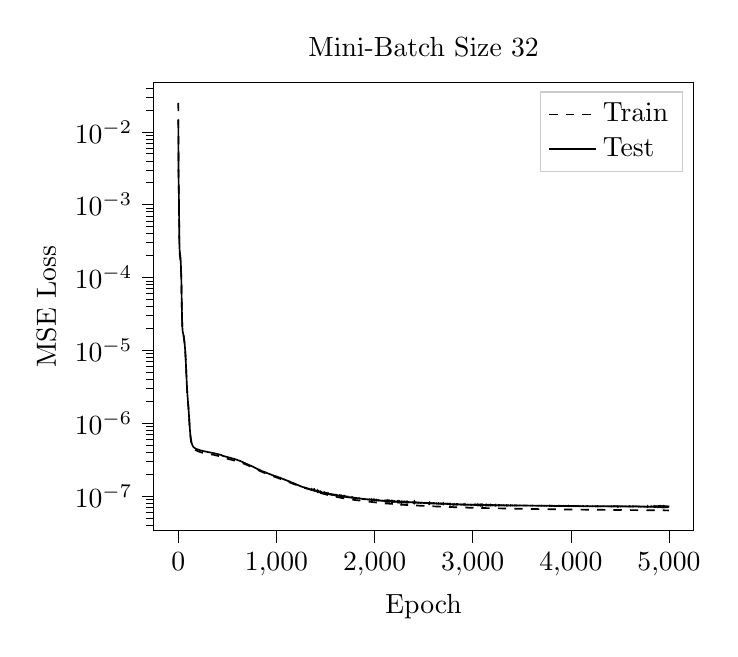
\begin{tikzpicture}

\begin{axis}[
legend cell align={left},
legend style={fill opacity=0.8, draw opacity=1, text opacity=1, draw=white!80!black},
log basis y={10},
tick align=outside,
tick pos=left,
title={Mini-Batch Size 32},
x grid style={white!69.0196078431373!black},
xlabel={Epoch},
xmin=-249.95, xmax=5248.95,
xtick style={color=black},
y grid style={white!69.0196078431373!black},
ylabel={MSE Loss},
ymin=3.32479738039568e-08, ymax=0.0475297845104396,
ymode=log,
ytick style={color=black}
]
\addplot [semithick, black, dashed]
table {%
0 0.02495651832968
1 0.00961011469736695
2 0.00413097363337874
3 0.00244306252896786
4 0.00193028736487031
5 0.00166280910652131
6 0.00138447313569486
7 0.00107641329290345
8 0.000778393224813044
9 0.000544353197561577
10 0.000392122417106293
11 0.000303274053148925
12 0.000255969762103632
13 0.000230607165722176
14 0.000215886180754751
15 0.000206437844899483
16 0.000199756111484021
17 0.000194554485875415
18 0.00019007718397188
19 0.000185448877629824
20 0.000179887956794119
21 0.000174710482853698
22 0.000169107335037552
23 0.000162899194285274
24 0.00015598142152885
25 0.000148279041866772
26 0.000139756958815269
27 0.000130426560644992
28 0.000120360163913574
29 0.00010970869952871
30 9.87046422960702e-05
31 8.76457903214032e-05
32 7.59790178271942e-05
33 6.32417565939249e-05
34 5.32707560923882e-05
35 4.49569480624632e-05
36 3.78300976517494e-05
37 3.23423087465926e-05
38 2.81909803452436e-05
39 2.50878785045643e-05
40 2.2796041041147e-05
41 2.11196904419921e-05
42 1.99011574259202e-05
43 1.90164594532689e-05
44 1.83700865381979e-05
45 1.78898700614809e-05
46 1.75224826816702e-05
47 1.72282880739658e-05
48 1.6979464176984e-05
49 1.67564551920805e-05
50 1.65459687414113e-05
51 1.6338135672413e-05
52 1.61253468395444e-05
53 1.59003820699581e-05
54 1.56591943941748e-05
55 1.53970238516195e-05
56 1.5111974962565e-05
57 1.48010985449218e-05
58 1.44654920004541e-05
59 1.41105859675008e-05
60 1.37506305291026e-05
61 1.34037461448315e-05
62 1.30508453003131e-05
63 1.26842860190663e-05
64 1.22990531144751e-05
65 1.18971542233339e-05
66 1.14834407868329e-05
67 1.10633895365027e-05
68 1.06573821649363e-05
69 1.02501706805924e-05
70 9.83167694175791e-06
71 9.40211800116231e-06
72 8.96312386976206e-06
73 8.51743346720468e-06
74 8.06758649014227e-06
75 7.59200016727846e-06
76 7.13813932543417e-06
77 6.69677184578177e-06
78 6.26769952486939e-06
79 5.85447091452806e-06
80 5.4597814068984e-06
81 5.0853698676292e-06
82 4.73458306623797e-06
83 4.40776282039224e-06
84 4.10157791611709e-06
85 3.81505160430606e-06
86 3.54804463950131e-06
87 3.30647863347622e-06
88 3.10206145877601e-06
89 2.92757145348332e-06
90 2.7743954374273e-06
91 2.63919908547905e-06
92 2.51793273764633e-06
93 2.40874294013338e-06
94 2.30932277190732e-06
95 2.21750755531502e-06
96 2.13223388277584e-06
97 2.0520963821582e-06
98 1.97619329605914e-06
99 1.90301633915624e-06
100 1.83207415443576e-06
101 1.76289627052029e-06
102 1.69469857723925e-06
103 1.62764035917462e-06
104 1.56192980011838e-06
105 1.49679244555045e-06
106 1.43174119580181e-06
107 1.36744359906515e-06
108 1.30400344164627e-06
109 1.24207295220913e-06
110 1.18228974997692e-06
111 1.12450982669543e-06
112 1.06910858767151e-06
113 1.01688769291286e-06
114 9.67930212027568e-07
115 9.22251022871023e-07
116 8.79566746561977e-07
117 8.40306190184492e-07
118 8.04245244808044e-07
119 7.71177175010962e-07
120 7.41038618912171e-07
121 7.1362072969805e-07
122 6.88738398139321e-07
123 6.6626371460643e-07
124 6.45955492018402e-07
125 6.27467571803209e-07
126 6.10727049888737e-07
127 5.95464798720968e-07
128 5.81586706289272e-07
129 5.68973892995928e-07
130 5.57506997097334e-07
131 5.47159624034066e-07
132 5.37807409841662e-07
133 5.2926190164726e-07
134 5.21498524221897e-07
135 5.14374786007465e-07
136 5.07893223357314e-07
137 5.01906526437779e-07
138 4.96731676548734e-07
139 4.91929263944257e-07
140 4.87304183479864e-07
141 4.83395513128926e-07
142 4.79628468383453e-07
143 4.75905103257901e-07
144 4.72772012926725e-07
145 4.69776906811603e-07
146 4.66785132857694e-07
147 4.64381218307608e-07
148 4.61841564515453e-07
149 4.59599604482719e-07
150 4.57548463828061e-07
151 4.55566183518386e-07
152 4.5392076447115e-07
153 4.51969018911313e-07
154 4.50402194132948e-07
155 4.48862345024281e-07
156 4.47213856375583e-07
157 4.45904424793753e-07
158 4.44331068820247e-07
159 4.43094038587333e-07
160 4.41832931983299e-07
161 4.40487454568483e-07
162 4.39438358228017e-07
163 4.38247122474422e-07
164 4.37372409010095e-07
165 4.36215690626796e-07
166 4.35179460907875e-07
167 4.34115043049133e-07
168 4.33094739207718e-07
169 4.32249056416367e-07
170 4.31389237974145e-07
171 4.3049158989561e-07
172 4.29718726650208e-07
173 4.28816658768483e-07
174 4.28031429521525e-07
175 4.27186655770129e-07
176 4.2643471010706e-07
177 4.25704145925465e-07
178 4.249236461078e-07
179 4.24175198304511e-07
180 4.23381138261902e-07
181 4.22704758591408e-07
182 4.2203296942489e-07
183 4.21413327728715e-07
184 4.20808965429842e-07
185 4.20218811370887e-07
186 4.19534650461628e-07
187 4.18957539409348e-07
188 4.18323923383923e-07
189 4.17785641616319e-07
190 4.17157342269547e-07
191 4.16574300402317e-07
192 4.16100292227384e-07
193 4.15515923918974e-07
194 4.14969112057406e-07
195 4.14372878424274e-07
196 4.13821521419777e-07
197 4.13151100246978e-07
198 4.12587816981613e-07
199 4.12000607070695e-07
200 4.11486135533323e-07
201 4.10908738501803e-07
202 4.10366602693557e-07
203 4.09846317552365e-07
204 4.09321734537116e-07
205 4.08823070813469e-07
206 4.08338844749778e-07
207 4.07859870051652e-07
208 4.0738508960203e-07
209 4.06924520632401e-07
210 4.06487470229422e-07
211 4.06054145514645e-07
212 4.05625210134986e-07
213 4.05178532389527e-07
214 4.04790528932608e-07
215 4.04352993655266e-07
216 4.03935589872617e-07
217 4.03488432255017e-07
218 4.03000148480714e-07
219 4.0252821776221e-07
220 4.02079318746473e-07
221 4.01636666595095e-07
222 4.01267719155385e-07
223 4.00860508079859e-07
224 4.0039540243697e-07
225 4.00016974367645e-07
226 3.99598319916095e-07
227 3.99353811303627e-07
228 3.98807296733139e-07
229 3.9849614341847e-07
230 3.98027829987768e-07
231 3.97661151964712e-07
232 3.97296741425635e-07
233 3.96933670458566e-07
234 3.96692654078379e-07
235 3.96237260304133e-07
236 3.95832837398302e-07
237 3.95548122298806e-07
238 3.9531681943572e-07
239 3.94950389136284e-07
240 3.9467049475661e-07
241 3.94235885494254e-07
242 3.9394514868718e-07
243 3.93687027838041e-07
244 3.93292611079232e-07
245 3.93052761353374e-07
246 3.92778083551093e-07
247 3.92502728800537e-07
248 3.92133861623734e-07
249 3.92215017939179e-07
250 3.91586018395174e-07
251 3.91571693910464e-07
252 3.91166603037618e-07
253 3.90866849613758e-07
254 3.90592485246088e-07
255 3.90450265342679e-07
256 3.90059337291859e-07
257 3.89795861224229e-07
258 3.89615875803884e-07
259 3.89345471262459e-07
260 3.88936012143404e-07
261 3.88858161613825e-07
262 3.88568784956078e-07
263 3.88315720897481e-07
264 3.88009818891533e-07
265 3.87716299258045e-07
266 3.87435602533515e-07
267 3.87198704800085e-07
268 3.87095901544399e-07
269 3.86833256129648e-07
270 3.86513266903421e-07
271 3.86314359332118e-07
272 3.86197026159607e-07
273 3.85857046524052e-07
274 3.85734699932527e-07
275 3.85417266727472e-07
276 3.85191937766649e-07
277 3.84964709098767e-07
278 3.84747363227689e-07
279 3.84521832245355e-07
280 3.84317370048848e-07
281 3.84164355864414e-07
282 3.83867334505794e-07
283 3.8373292528604e-07
284 3.83425168422491e-07
285 3.83283067776574e-07
286 3.82983800932379e-07
287 3.82833136825411e-07
288 3.82552692087756e-07
289 3.82440776093063e-07
290 3.8212854167341e-07
291 3.81949822269689e-07
292 3.81690230824461e-07
293 3.81576880215562e-07
294 3.81239045339044e-07
295 3.81128543835985e-07
296 3.8072972580494e-07
297 3.8063195961513e-07
298 3.80266395382023e-07
299 3.801756307098e-07
300 3.79826189202959e-07
301 3.79754168477575e-07
302 3.79314871622682e-07
303 3.7919400182318e-07
304 3.78852980531974e-07
305 3.78635408196715e-07
306 3.78482517476186e-07
307 3.78186378839018e-07
308 3.78049293374261e-07
309 3.77755144313596e-07
310 3.77626213719395e-07
311 3.77323337716007e-07
312 3.77180442285407e-07
313 3.76884721106308e-07
314 3.76761206041465e-07
315 3.76456654066715e-07
316 3.76322360295944e-07
317 3.76020554256229e-07
318 3.75878518070749e-07
319 3.75583821380587e-07
320 3.75444035285e-07
321 3.75157911889801e-07
322 3.74941874213164e-07
323 3.74769378709061e-07
324 3.74537868879088e-07
325 3.74325883058191e-07
326 3.74114356759492e-07
327 3.7398155336632e-07
328 3.73691593438252e-07
329 3.73479032305113e-07
330 3.73263141057123e-07
331 3.73148577864413e-07
332 3.72937396434736e-07
333 3.72726407761093e-07
334 3.72512641376943e-07
335 3.7229352437862e-07
336 3.72073721962352e-07
337 3.71858890559906e-07
338 3.71637403759451e-07
339 3.71423307171881e-07
340 3.71199119911125e-07
341 3.71018680311863e-07
342 3.70781483240989e-07
343 3.70566273147688e-07
344 3.70327734970033e-07
345 3.70107448759427e-07
346 3.69865037782802e-07
347 3.69644855766182e-07
348 3.69412776421996e-07
349 3.69197943371091e-07
350 3.68972107764876e-07
351 3.68760632113663e-07
352 3.68530030186776e-07
353 3.68305152392168e-07
354 3.68066383600763e-07
355 3.67879488521794e-07
356 3.67639851447166e-07
357 3.67394399120258e-07
358 3.67129990991089e-07
359 3.66913512834799e-07
360 3.66670797916413e-07
361 3.66439876643199e-07
362 3.66214438940915e-07
363 3.65958968757241e-07
364 3.65716883436562e-07
365 3.65472255680288e-07
366 3.65235946276243e-07
367 3.65003734827951e-07
368 3.64790364415057e-07
369 3.64554488896829e-07
370 3.64337830490058e-07
371 3.64075158586274e-07
372 3.63818008281669e-07
373 3.63561922938516e-07
374 3.63086586332884e-07
375 3.62677517500742e-07
376 3.62481707497864e-07
377 3.62175591874347e-07
378 3.61958059102108e-07
379 3.61694926596101e-07
380 3.61477443789227e-07
381 3.61189488785385e-07
382 3.60908989648578e-07
383 3.60632151227946e-07
384 3.60374613592285e-07
385 3.60127789861053e-07
386 3.59889722290063e-07
387 3.59648303003723e-07
388 3.59391540257548e-07
389 3.59136226052215e-07
390 3.58878930228457e-07
391 3.58624317300382e-07
392 3.58370782862494e-07
393 3.58117538553415e-07
394 3.57864312945821e-07
395 3.57614250845018e-07
396 3.57365321292491e-07
397 3.57220161561145e-07
398 3.5695572972827e-07
399 3.56697081485891e-07
400 3.56451138884495e-07
401 3.56231862042478e-07
402 3.55987368379829e-07
403 3.55719761046203e-07
404 3.5545431620676e-07
405 3.5519427149211e-07
406 3.54937200029326e-07
407 3.54679559450233e-07
408 3.54435099382044e-07
409 3.54180049441766e-07
410 3.53914030540636e-07
411 3.53637977070775e-07
412 3.53316532880399e-07
413 3.52996593903754e-07
414 3.52692684771227e-07
415 3.52370906625765e-07
416 3.52031887359772e-07
417 3.51736728305241e-07
418 3.51416265061744e-07
419 3.51078242658787e-07
420 3.50801819763546e-07
421 3.50483696763604e-07
422 3.50188840911869e-07
423 3.49898358535938e-07
424 3.49607736438884e-07
425 3.49336570877767e-07
426 3.49044006611621e-07
427 3.48772838549394e-07
428 3.48493419096485e-07
429 3.48202210432191e-07
430 3.47910864888945e-07
431 3.47652583513991e-07
432 3.47363370451603e-07
433 3.47088898820402e-07
434 3.46819799403875e-07
435 3.46554175678193e-07
436 3.46236901521024e-07
437 3.4594818282585e-07
438 3.456587755295e-07
439 3.45374959806577e-07
440 3.4508889979179e-07
441 3.44819731481039e-07
442 3.43527665961574e-07
443 3.41568904218548e-07
444 3.40458649645825e-07
445 3.39691413955734e-07
446 3.39104159309045e-07
447 3.38657587406033e-07
448 3.3826774966883e-07
449 3.37910868381641e-07
450 3.37583903274208e-07
451 3.37335791755322e-07
452 3.37002327455593e-07
453 3.36683525176795e-07
454 3.36382677573965e-07
455 3.36085746255321e-07
456 3.35797085199374e-07
457 3.35507281363334e-07
458 3.35228495998763e-07
459 3.34947825706422e-07
460 3.34685688301306e-07
461 3.34399860150825e-07
462 3.34131951490235e-07
463 3.33938054097871e-07
464 3.33655134454602e-07
465 3.33373461614883e-07
466 3.33097741190613e-07
467 3.32827610804998e-07
468 3.32557599733718e-07
469 3.32289230129845e-07
470 3.32023381133695e-07
471 3.31758974482454e-07
472 3.31498622188064e-07
473 3.31243115965663e-07
474 3.30986639767161e-07
475 3.30725981314117e-07
476 3.30465711044781e-07
477 3.30213596555495e-07
478 3.29964917227699e-07
479 3.29708751735325e-07
480 3.29451019297267e-07
481 3.29205599769011e-07
482 3.28950098946734e-07
483 3.28694641950733e-07
484 3.28439770896693e-07
485 3.28183799865656e-07
486 3.2792898457501e-07
487 3.27676344568317e-07
488 3.27425882460375e-07
489 3.27171232186174e-07
490 3.26920304075884e-07
491 3.26669060086715e-07
492 3.26414687492615e-07
493 3.26167206196715e-07
494 3.25921365174509e-07
495 3.25667093875381e-07
496 3.25417923534133e-07
497 3.25166869117766e-07
498 3.24911161271757e-07
499 3.24661909530732e-07
500 3.24411729934582e-07
501 3.24163918492104e-07
502 3.23916323793583e-07
503 3.23667571478836e-07
504 3.23418650452822e-07
505 3.2316933356924e-07
506 3.22912537569664e-07
507 3.22677076326272e-07
508 3.22424684043199e-07
509 3.22175117048573e-07
510 3.21921278214177e-07
511 3.21676903240586e-07
512 3.2141999616897e-07
513 3.21168492916968e-07
514 3.20919341902481e-07
515 3.20672617419859e-07
516 3.20425436939331e-07
517 3.20178708705043e-07
518 3.19927367741002e-07
519 3.19677120899087e-07
520 3.19433100514743e-07
521 3.1918317591817e-07
522 3.18933754613226e-07
523 3.18682645513491e-07
524 3.18430878110121e-07
525 3.18188869869118e-07
526 3.17935760620003e-07
527 3.17688921199988e-07
528 3.17438041292917e-07
529 3.17189871054779e-07
530 3.16941071673682e-07
531 3.16688110899577e-07
532 3.16435692639061e-07
533 3.16183294444272e-07
534 3.15933932711232e-07
535 3.15678637605288e-07
536 3.15416349053521e-07
537 3.15168398003607e-07
538 3.14918423271138e-07
539 3.14665876146591e-07
540 3.1441218487771e-07
541 3.14162874758495e-07
542 3.13908628925219e-07
543 3.1365879385703e-07
544 3.13401772416455e-07
545 3.13141272272333e-07
546 3.12895501167532e-07
547 3.12642150618103e-07
548 3.12390568126375e-07
549 3.12136429840848e-07
550 3.11886598012734e-07
551 3.11629494319732e-07
552 3.11372858220693e-07
553 3.11120544779442e-07
554 3.10865378139624e-07
555 3.10597321572459e-07
556 3.10337305961639e-07
557 3.10062468656724e-07
558 3.09783668569708e-07
559 3.09533397796713e-07
560 3.0925890234812e-07
561 3.08991336623876e-07
562 3.08718985195355e-07
563 3.08452851072616e-07
564 3.08193646958443e-07
565 3.07925223182792e-07
566 3.07654694040593e-07
567 3.07384176949199e-07
568 3.07108701520065e-07
569 3.06854335121898e-07
570 3.06586367912587e-07
571 3.06315510670174e-07
572 3.06044467208721e-07
573 3.05774523894797e-07
574 3.05507066229893e-07
575 3.05238351586468e-07
576 3.04966125554529e-07
577 3.04701247387129e-07
578 3.04435839666439e-07
579 3.04167043907455e-07
580 3.03899193966117e-07
581 3.03642611072519e-07
582 3.03365975128145e-07
583 3.03105798934666e-07
584 3.02834642923244e-07
585 3.02562915123872e-07
586 3.02293688037025e-07
587 3.02023441690835e-07
588 3.01750427922798e-07
589 3.01468936697802e-07
590 3.01194206201671e-07
591 3.00920173913255e-07
592 3.00651897475746e-07
593 3.00374632217881e-07
594 3.0010006497605e-07
595 2.99823589671178e-07
596 2.99549067733551e-07
597 2.99274745032108e-07
598 2.98989832003826e-07
599 2.98707233980622e-07
600 2.98429238455356e-07
601 2.98149015691251e-07
602 2.97851940217697e-07
603 2.97572810723068e-07
604 2.97288175488575e-07
605 2.97004070830553e-07
606 2.96717658386569e-07
607 2.96432424136128e-07
608 2.96132169864904e-07
609 2.95851490818677e-07
610 2.9555990550989e-07
611 2.95269672562881e-07
612 2.94977329076573e-07
613 2.94648021451849e-07
614 2.94372223493156e-07
615 2.94079964135108e-07
616 2.93786541419649e-07
617 2.93504731644134e-07
618 2.93208564869474e-07
619 2.92913382963889e-07
620 2.92618357491392e-07
621 2.92318298079408e-07
622 2.92027666887407e-07
623 2.91726333330189e-07
624 2.91427586944337e-07
625 2.91127002071789e-07
626 2.90825883325851e-07
627 2.90517562405057e-07
628 2.90214898711838e-07
629 2.89916120095768e-07
630 2.89617872113013e-07
631 2.89310944253884e-07
632 2.89006251421142e-07
633 2.88701059901086e-07
634 2.88395490997573e-07
635 2.88085441013664e-07
636 2.87784689248838e-07
637 2.87473759783552e-07
638 2.87163604639318e-07
639 2.8685427776054e-07
640 2.86543671734307e-07
641 2.86232358746474e-07
642 2.8591167159675e-07
643 2.85608766034784e-07
644 2.85282987647406e-07
645 2.84961197735356e-07
646 2.84647514035896e-07
647 2.84332860530867e-07
648 2.84016698174128e-07
649 2.83695652342431e-07
650 2.83384992542324e-07
651 2.83056953890082e-07
652 2.82736495591962e-07
653 2.82414473304016e-07
654 2.82090383393552e-07
655 2.81754234094933e-07
656 2.814381865619e-07
657 2.81109553952774e-07
658 2.80781508934069e-07
659 2.80458499162251e-07
660 2.80133726619169e-07
661 2.79791232117077e-07
662 2.79459573619079e-07
663 2.79132003811355e-07
664 2.78810577128752e-07
665 2.78483527097251e-07
666 2.78156543458863e-07
667 2.77828672494707e-07
668 2.77494331385242e-07
669 2.77161416363469e-07
670 2.76837326168788e-07
671 2.76499529377361e-07
672 2.7616509672157e-07
673 2.75824009491998e-07
674 2.75484910588375e-07
675 2.75151122167472e-07
676 2.74813070546998e-07
677 2.74484228981464e-07
678 2.74141751759771e-07
679 2.73801236460258e-07
680 2.7346256743499e-07
681 2.7312098310972e-07
682 2.72778246738881e-07
683 2.72445175511393e-07
684 2.72102593726231e-07
685 2.71760970917967e-07
686 2.71409479864815e-07
687 2.71066047901058e-07
688 2.70712768099202e-07
689 2.70363464949241e-07
690 2.70028888536444e-07
691 2.69678203579815e-07
692 2.69323093846197e-07
693 2.68982534151974e-07
694 2.68629582905078e-07
695 2.68276261408573e-07
696 2.67924870684055e-07
697 2.67573593077941e-07
698 2.67221852908506e-07
699 2.66867869385123e-07
700 2.66521415994703e-07
701 2.66156414824081e-07
702 2.65806567256277e-07
703 2.65454764019069e-07
704 2.65109429761878e-07
705 2.64751923481299e-07
706 2.64394460657513e-07
707 2.64046319188083e-07
708 2.63686914905747e-07
709 2.63330481487856e-07
710 2.62976001152992e-07
711 2.62624411874413e-07
712 2.62268526427079e-07
713 2.61783545539629e-07
714 2.61365144609726e-07
715 2.60963426995886e-07
716 2.60568118960691e-07
717 2.60185761845833e-07
718 2.59804836076682e-07
719 2.59431001921939e-07
720 2.5905343719046e-07
721 2.58663268255077e-07
722 2.582953289334e-07
723 2.57919991497602e-07
724 2.57542056175453e-07
725 2.57166950035526e-07
726 2.56791996605443e-07
727 2.56411861045081e-07
728 2.56032386488414e-07
729 2.55650504385585e-07
730 2.55268005901144e-07
731 2.54897504419205e-07
732 2.54530858313728e-07
733 2.54164709417637e-07
734 2.53788540817368e-07
735 2.53397368908281e-07
736 2.53038564181907e-07
737 2.52672190839576e-07
738 2.52298251467664e-07
739 2.51924601002429e-07
740 2.51546983491835e-07
741 2.51169815754793e-07
742 2.50795577386498e-07
743 2.50415323222342e-07
744 2.50047310686341e-07
745 2.49675453261489e-07
746 2.49290693403736e-07
747 2.48922245219774e-07
748 2.48538268721177e-07
749 2.48168420881711e-07
750 2.47817149841012e-07
751 2.47453885549476e-07
752 2.47091088169782e-07
753 2.46722569528401e-07
754 2.46367280141158e-07
755 2.46005374407332e-07
756 2.45634985702736e-07
757 2.45285960744468e-07
758 2.4491997467635e-07
759 2.44556270928342e-07
760 2.44214170720625e-07
761 2.43849069136104e-07
762 2.4350010477292e-07
763 2.43144235810178e-07
764 2.4278854266413e-07
765 2.42424769908212e-07
766 2.42078545369395e-07
767 2.41720167252879e-07
768 2.41373975711667e-07
769 2.41012750223035e-07
770 2.40668308805425e-07
771 2.40300879937649e-07
772 2.39962240783598e-07
773 2.39611582998123e-07
774 2.39262748976898e-07
775 2.38921268277181e-07
776 2.38583462419228e-07
777 2.38232236142721e-07
778 2.37897271148313e-07
779 2.37553327167461e-07
780 2.3720731402932e-07
781 2.36865277344123e-07
782 2.36524948576289e-07
783 2.36184086332969e-07
784 2.35843451463325e-07
785 2.35504933328912e-07
786 2.35151212137907e-07
787 2.34817503297791e-07
788 2.34487555559326e-07
789 2.34151290726459e-07
790 2.33816716018964e-07
791 2.33480007750586e-07
792 2.3313596361163e-07
793 2.32800076275907e-07
794 2.32479550533071e-07
795 2.32147196612686e-07
796 2.31827768146786e-07
797 2.31500280790442e-07
798 2.31171276794839e-07
799 2.30842491873773e-07
800 2.30517275696229e-07
801 2.30192814683505e-07
802 2.29869153912432e-07
803 2.2954598213687e-07
804 2.29225299761993e-07
805 2.28896955889013e-07
806 2.285750721569e-07
807 2.28251312620387e-07
808 2.27920705242468e-07
809 2.27587773196092e-07
810 2.27261611883023e-07
811 2.26937173209762e-07
812 2.26590815117333e-07
813 2.26248852271738e-07
814 2.2592678689648e-07
815 2.25604274504576e-07
816 2.25289613268842e-07
817 2.24968429591854e-07
818 2.2464190789151e-07
819 2.24330271180406e-07
820 2.24015665537536e-07
821 2.23695802048951e-07
822 2.23378607273617e-07
823 2.23059963758487e-07
824 2.22751312179525e-07
825 2.22437908604434e-07
826 2.22128579935088e-07
827 2.21818073327995e-07
828 2.21512779432942e-07
829 2.21207509355281e-07
830 2.20896412486127e-07
831 2.20601544469901e-07
832 2.20299285331293e-07
833 2.19998179005643e-07
834 2.19698332529106e-07
835 2.19399085636951e-07
836 2.19101591312665e-07
837 2.18805903045904e-07
838 2.18508435153808e-07
839 2.18213898335762e-07
840 2.17915977884786e-07
841 2.17629355546478e-07
842 2.17336306803872e-07
843 2.17043057830324e-07
844 2.16744821671e-07
845 2.16444015222805e-07
846 2.16176255520395e-07
847 2.15886601779403e-07
848 2.1559624806855e-07
849 2.1530761821964e-07
850 2.1501409122493e-07
851 2.14728265518715e-07
852 2.14442566999651e-07
853 2.14159017104976e-07
854 2.1387635089809e-07
855 2.13591160445503e-07
856 2.13313837718943e-07
857 2.13033253203321e-07
858 2.12747139443081e-07
859 2.12453791277767e-07
860 2.12168521272815e-07
861 2.11889834901058e-07
862 2.11607884637033e-07
863 2.11334886728309e-07
864 2.11090787132662e-07
865 2.10781402245175e-07
866 2.10493931831479e-07
867 2.10228466983153e-07
868 2.0995736332452e-07
869 2.09710962110421e-07
870 2.09454804121378e-07
871 2.09155657302063e-07
872 2.0889265621804e-07
873 2.08615227649034e-07
874 2.0835879496417e-07
875 2.08125936779879e-07
876 2.0784095644899e-07
877 2.07578632455352e-07
878 2.07306310045396e-07
879 2.07051195502572e-07
880 2.06805247216835e-07
881 2.06557984341771e-07
882 2.06271035807504e-07
883 2.06015276461358e-07
884 2.05758761353536e-07
885 2.05502702499416e-07
886 2.05257287603899e-07
887 2.05018618203212e-07
888 2.04749223087219e-07
889 2.04492583435467e-07
890 2.04243722151887e-07
891 2.04015699040383e-07
892 2.0376250037657e-07
893 2.03499224738835e-07
894 2.03230061998738e-07
895 2.02984433769871e-07
896 2.02760471012198e-07
897 2.02495798191649e-07
898 2.02252525838276e-07
899 2.02054798563722e-07
900 2.01795910925284e-07
901 2.0155783280984e-07
902 2.01303102727479e-07
903 2.010459269286e-07
904 2.00793724928872e-07
905 2.00542965529849e-07
906 2.00282583818989e-07
907 2.00041654409233e-07
908 1.99805434363043e-07
909 1.99518635383811e-07
910 1.99275372921193e-07
911 1.99030435169334e-07
912 1.98785222437436e-07
913 1.98562560171922e-07
914 1.98301664795508e-07
915 1.980731424851e-07
916 1.97822975650297e-07
917 1.97587865756077e-07
918 1.97393529134615e-07
919 1.97119730415807e-07
920 1.96893812670851e-07
921 1.96664078941922e-07
922 1.96433929062323e-07
923 1.96070164463436e-07
924 1.95796074820009e-07
925 1.95405372153346e-07
926 1.95464035442683e-07
927 1.95107122721083e-07
928 1.9491377003078e-07
929 1.94789499147419e-07
930 1.94626016821076e-07
931 1.9450656171216e-07
932 1.94023198787363e-07
933 1.93969802921856e-07
934 1.93786689152375e-07
935 1.93560784936153e-07
936 1.93339261500114e-07
937 1.93128177670587e-07
938 1.93026661719387e-07
939 1.92640885813944e-07
940 1.92422838779294e-07
941 1.92281713538023e-07
942 1.92034399532304e-07
943 1.91720221721425e-07
944 1.91571368333143e-07
945 1.91369630329064e-07
946 1.91159158362098e-07
947 1.90935840663542e-07
948 1.90733979053448e-07
949 1.90504907777722e-07
950 1.90282767846384e-07
951 1.90062591201467e-07
952 1.89852125288326e-07
953 1.89639431653177e-07
954 1.89416469254411e-07
955 1.89172260149917e-07
956 1.88981291074697e-07
957 1.88770511613257e-07
958 1.88574910339412e-07
959 1.88355372273463e-07
960 1.88127187925602e-07
961 1.87908308106444e-07
962 1.87683726238674e-07
963 1.87484382848879e-07
964 1.87297403499542e-07
965 1.87063760563433e-07
966 1.86876632227495e-07
967 1.86646165531101e-07
968 1.86456403355351e-07
969 1.86208237039409e-07
970 1.86007684220613e-07
971 1.85791245456812e-07
972 1.85590365447297e-07
973 1.85390133793817e-07
974 1.85175619606071e-07
975 1.84960244524746e-07
976 1.8474065629448e-07
977 1.84525042442374e-07
978 1.84285813105589e-07
979 1.8398711713985e-07
980 1.83779480011026e-07
981 1.83560364746427e-07
982 1.83339712037878e-07
983 1.83136822073493e-07
984 1.82914183056937e-07
985 1.82705784453674e-07
986 1.82525461809746e-07
987 1.82288409973808e-07
988 1.82090955490821e-07
989 1.81869196524076e-07
990 1.81646533434332e-07
991 1.8146373204786e-07
992 1.81239095780938e-07
993 1.81107638809408e-07
994 1.80800074360832e-07
995 1.80589863930436e-07
996 1.80380842181194e-07
997 1.80184061349564e-07
998 1.79971024039105e-07
999 1.79740983853094e-07
1000 1.79529651802568e-07
1001 1.79349143863305e-07
1002 1.79174995381004e-07
1003 1.78974283542743e-07
1004 1.78781240805392e-07
1005 1.78549073396539e-07
1006 1.78336786788691e-07
1007 1.78155590916163e-07
1008 1.77893159715836e-07
1009 1.77646469182946e-07
1010 1.7745657291357e-07
1011 1.77252783856829e-07
1012 1.77015252276647e-07
1013 1.76848480464287e-07
1014 1.76649309651111e-07
1015 1.76437214165048e-07
1016 1.76228822397206e-07
1017 1.7603968427693e-07
1018 1.7580710276377e-07
1019 1.75630667200721e-07
1020 1.75404448583549e-07
1021 1.75205468949002e-07
1022 1.75017376562892e-07
1023 1.74781506913746e-07
1024 1.74596366690594e-07
1025 1.74384998828714e-07
1026 1.74188079640203e-07
1027 1.73981591217398e-07
1028 1.7378087360953e-07
1029 1.73595396333326e-07
1030 1.73383527979354e-07
1031 1.73204570458552e-07
1032 1.72982506484232e-07
1033 1.72808286620807e-07
1034 1.72597720307976e-07
1035 1.72415509155144e-07
1036 1.72203957518491e-07
1037 1.72027063271685e-07
1038 1.7182273029448e-07
1039 1.71644450745134e-07
1040 1.71457249393825e-07
1041 1.71221164421809e-07
1042 1.71040073354334e-07
1043 1.7086180746162e-07
1044 1.70657180049716e-07
1045 1.70465468116276e-07
1046 1.70270329661548e-07
1047 1.70050755755824e-07
1048 1.69850164553509e-07
1049 1.69648352382978e-07
1050 1.69455070064828e-07
1051 1.69255631220722e-07
1052 1.690726047201e-07
1053 1.68867476659784e-07
1054 1.68683792978186e-07
1055 1.68497542091473e-07
1056 1.68291344607496e-07
1057 1.68094269696439e-07
1058 1.67934575713957e-07
1059 1.67707678173201e-07
1060 1.67512832220496e-07
1061 1.67310787304586e-07
1062 1.67137366844372e-07
1063 1.6695146995005e-07
1064 1.66747512679422e-07
1065 1.66526244100851e-07
1066 1.66345289741798e-07
1067 1.66170657877274e-07
1068 1.65969783139985e-07
1069 1.65793351001753e-07
1070 1.65584508224015e-07
1071 1.65399617955586e-07
1072 1.65217182740207e-07
1073 1.65030118381537e-07
1074 1.64827668044154e-07
1075 1.64635963088244e-07
1076 1.64446436073717e-07
1077 1.64266503816179e-07
1078 1.6406050147566e-07
1079 1.63849182882814e-07
1080 1.63649148930745e-07
1081 1.63488852493288e-07
1082 1.6326385798493e-07
1083 1.6307355612355e-07
1084 1.6287979563856e-07
1085 1.62693553079407e-07
1086 1.62514635448474e-07
1087 1.62316461825185e-07
1088 1.62138254225397e-07
1089 1.61947419812236e-07
1090 1.61755007738407e-07
1091 1.6156890727359e-07
1092 1.61380626408913e-07
1093 1.61192226670437e-07
1094 1.60988865758327e-07
1095 1.60817379423861e-07
1096 1.60609458916383e-07
1097 1.60432750334394e-07
1098 1.60231610422557e-07
1099 1.6002438242424e-07
1100 1.59846041128731e-07
1101 1.59648983213856e-07
1102 1.59470318820354e-07
1103 1.59276859179158e-07
1104 1.59087808611957e-07
1105 1.58903363157492e-07
1106 1.58715275489385e-07
1107 1.58518241022421e-07
1108 1.58335912828989e-07
1109 1.58143547395184e-07
1110 1.57950820351971e-07
1111 1.57779550391979e-07
1112 1.57568096639693e-07
1113 1.57373400980987e-07
1114 1.57195540481325e-07
1115 1.5701123834333e-07
1116 1.56833667531942e-07
1117 1.5667102486816e-07
1118 1.56453034335868e-07
1119 1.56287361491536e-07
1120 1.56101681994869e-07
1121 1.55895187234023e-07
1122 1.55719671283805e-07
1123 1.55538784895271e-07
1124 1.55326191844551e-07
1125 1.55147808399647e-07
1126 1.54982862397901e-07
1127 1.54775238044635e-07
1128 1.54616158710041e-07
1129 1.54435473760373e-07
1130 1.5424328991287e-07
1131 1.54069083464492e-07
1132 1.53910053441564e-07
1133 1.53697950679543e-07
1134 1.53527616859606e-07
1135 1.533198500141e-07
1136 1.53119851518113e-07
1137 1.52935787625097e-07
1138 1.52741302542836e-07
1139 1.52579434384847e-07
1140 1.5236773768379e-07
1141 1.5220379103198e-07
1142 1.51994220047413e-07
1143 1.51816173712405e-07
1144 1.51639372731438e-07
1145 1.51451178950879e-07
1146 1.51261071607678e-07
1147 1.51087167537867e-07
1148 1.50911668143294e-07
1149 1.50710834333267e-07
1150 1.5056337863939e-07
1151 1.50359926053056e-07
1152 1.50197839161592e-07
1153 1.49989610207513e-07
1154 1.49820556174518e-07
1155 1.49641965904834e-07
1156 1.49468162561561e-07
1157 1.49292503422771e-07
1158 1.49116801964055e-07
1159 1.48950404266657e-07
1160 1.48749289834882e-07
1161 1.48601293474826e-07
1162 1.4840983980946e-07
1163 1.48245427084248e-07
1164 1.48058577806864e-07
1165 1.47897300550426e-07
1166 1.47732717977078e-07
1167 1.47551893320497e-07
1168 1.47386523991599e-07
1169 1.47253489771515e-07
1170 1.47079867105049e-07
1171 1.46910625673513e-07
1172 1.46717061582535e-07
1173 1.46561715538951e-07
1174 1.46381869910783e-07
1175 1.46196347913019e-07
1176 1.46053862195572e-07
1177 1.45873883198533e-07
1178 1.4569988150015e-07
1179 1.45549741915829e-07
1180 1.45423148239843e-07
1181 1.45259941163545e-07
1182 1.45065910132303e-07
1183 1.44896643561765e-07
1184 1.44713919794981e-07
1185 1.44527575216102e-07
1186 1.44360318273584e-07
1187 1.44184542804737e-07
1188 1.44045858604613e-07
1189 1.438265138205e-07
1190 1.43651753361951e-07
1191 1.43501514173749e-07
1192 1.43298794270663e-07
1193 1.43153612597757e-07
1194 1.4296911790268e-07
1195 1.42841563288698e-07
1196 1.42663490450445e-07
1197 1.4251093796247e-07
1198 1.4235067521895e-07
1199 1.42198025784523e-07
1200 1.42016979083337e-07
1201 1.41888084428388e-07
1202 1.41697094491633e-07
1203 1.41577890346412e-07
1204 1.41393103675114e-07
1205 1.41244608073521e-07
1206 1.41101936833365e-07
1207 1.40972664482319e-07
1208 1.40802412559538e-07
1209 1.40652948857678e-07
1210 1.40490155388306e-07
1211 1.40351003068417e-07
1212 1.40189484227449e-07
1213 1.40045975115299e-07
1214 1.39892311622702e-07
1215 1.39742217299954e-07
1216 1.39631110755545e-07
1217 1.39471335202757e-07
1218 1.39296424720214e-07
1219 1.39116599001454e-07
1220 1.38933887228632e-07
1221 1.38783278018195e-07
1222 1.38606553406362e-07
1223 1.38454287537115e-07
1224 1.38285695726381e-07
1225 1.38140692769184e-07
1226 1.37973613220765e-07
1227 1.37823302551965e-07
1228 1.37674810602562e-07
1229 1.37553393670942e-07
1230 1.37401118337266e-07
1231 1.37227740324875e-07
1232 1.37065262151737e-07
1233 1.36896728918146e-07
1234 1.36755918703102e-07
1235 1.36620547863231e-07
1236 1.36478319333833e-07
1237 1.3629528817205e-07
1238 1.36187348502403e-07
1239 1.36021234595773e-07
1240 1.35825211785345e-07
1241 1.35717902182364e-07
1242 1.35625156744368e-07
1243 1.35405121184817e-07
1244 1.35297192116468e-07
1245 1.35218753271715e-07
1246 1.3499267492989e-07
1247 1.34912699735423e-07
1248 1.34714162555838e-07
1249 1.34535898752119e-07
1250 1.34413323394256e-07
1251 1.34261244909339e-07
1252 1.34086616697004e-07
1253 1.33964697695887e-07
1254 1.33804411674987e-07
1255 1.33696845480813e-07
1256 1.33536486785601e-07
1257 1.33391707365149e-07
1258 1.33322690516025e-07
1259 1.3311800474014e-07
1260 1.33000473525158e-07
1261 1.32811080234774e-07
1262 1.32611858703058e-07
1263 1.32472028354869e-07
1264 1.32310696272953e-07
1265 1.32206344474639e-07
1266 1.3208011404231e-07
1267 1.31943520571554e-07
1268 1.31795420301728e-07
1269 1.31649313971138e-07
1270 1.31523647922904e-07
1271 1.31398229783031e-07
1272 1.312506298774e-07
1273 1.31094378815533e-07
1274 1.30956317235587e-07
1275 1.30837788347549e-07
1276 1.30680643621872e-07
1277 1.30560865883922e-07
1278 1.30418681806077e-07
1279 1.30291295235452e-07
1280 1.30149456609274e-07
1281 1.30038621037443e-07
1282 1.29920442674347e-07
1283 1.29731679223255e-07
1284 1.29635409621187e-07
1285 1.29512751186667e-07
1286 1.29329628606456e-07
1287 1.29202018442243e-07
1288 1.29069559051231e-07
1289 1.2898486802726e-07
1290 1.2882774468892e-07
1291 1.28720824775996e-07
1292 1.2857886679285e-07
1293 1.28424297827223e-07
1294 1.28313725184626e-07
1295 1.28197315504508e-07
1296 1.28019309741489e-07
1297 1.27923649813511e-07
1298 1.27818489289666e-07
1299 1.27705172971559e-07
1300 1.27551815268134e-07
1301 1.27394580133e-07
1302 1.27272965585234e-07
1303 1.27178841168529e-07
1304 1.27015317872292e-07
1305 1.26883552823642e-07
1306 1.26764221747067e-07
1307 1.2669873980542e-07
1308 1.26522860583123e-07
1309 1.26401847865054e-07
1310 1.26292835631148e-07
1311 1.26217790253236e-07
1312 1.26103298228486e-07
1313 1.25955086161866e-07
1314 1.25865374926093e-07
1315 1.25704670921323e-07
1316 1.25600167223183e-07
1317 1.25466895724458e-07
1318 1.25340198877666e-07
1319 1.25290738012041e-07
1320 1.25089742667228e-07
1321 1.25076840191696e-07
1322 1.24905847286527e-07
1323 1.24763893538216e-07
1324 1.24628677824035e-07
1325 1.24567537014286e-07
1326 1.24444168633886e-07
1327 1.24354348130851e-07
1328 1.24198468853365e-07
1329 1.24107469687829e-07
1330 1.23982680037216e-07
1331 1.23843915076804e-07
1332 1.23764088485245e-07
1333 1.23624078170792e-07
1334 1.23499288818607e-07
1335 1.23423793709776e-07
1336 1.23317506606213e-07
1337 1.23199710955646e-07
1338 1.23099488547496e-07
1339 1.22963613961247e-07
1340 1.22890353665639e-07
1341 1.22738475070605e-07
1342 1.22660894163573e-07
1343 1.22505690313801e-07
1344 1.22423010068928e-07
1345 1.22333123542262e-07
1346 1.22196255247786e-07
1347 1.22029892622777e-07
1348 1.21937990527954e-07
1349 1.21828086278697e-07
1350 1.21689700947059e-07
1351 1.21597475995827e-07
1352 1.21496771001262e-07
1353 1.21380652842618e-07
1354 1.21337355068363e-07
1355 1.21154499723275e-07
1356 1.21041188137383e-07
1357 1.20932061420831e-07
1358 1.20859951366015e-07
1359 1.20827881147534e-07
1360 1.20551392328139e-07
1361 1.20494800114557e-07
1362 1.20394331005969e-07
1363 1.20284697189277e-07
1364 1.20239605976735e-07
1365 1.19967289990086e-07
1366 1.19879712698889e-07
1367 1.19589959396649e-07
1368 1.19484890618082e-07
1369 1.19431536418801e-07
1370 1.19227245122033e-07
1371 1.19023371524918e-07
1372 1.18949591779938e-07
1373 1.18764290661488e-07
1374 1.1858331126291e-07
1375 1.18502960219757e-07
1376 1.18375985664443e-07
1377 1.18142158214596e-07
1378 1.18019643707612e-07
1379 1.1786775166911e-07
1380 1.1775816444981e-07
1381 1.17609677758423e-07
1382 1.17539106682329e-07
1383 1.17312982311546e-07
1384 1.17253223322678e-07
1385 1.17074167064857e-07
1386 1.17033205512485e-07
1387 1.16859827187454e-07
1388 1.16734060028989e-07
1389 1.16619709274346e-07
1390 1.16568370913228e-07
1391 1.16389317284415e-07
1392 1.16301493079618e-07
1393 1.16148065970378e-07
1394 1.1611696893965e-07
1395 1.15969928501158e-07
1396 1.15827382813904e-07
1397 1.15757941713923e-07
1398 1.1559660951832e-07
1399 1.15426822461018e-07
1400 1.15241668950716e-07
1401 1.15137877372717e-07
1402 1.15040524988785e-07
1403 1.14927153560984e-07
1404 1.14816618989266e-07
1405 1.14671704679381e-07
1406 1.14560497905813e-07
1407 1.14451417459804e-07
1408 1.1434129494603e-07
1409 1.14263045119856e-07
1410 1.14099495689857e-07
1411 1.14023870949609e-07
1412 1.13898172870108e-07
1413 1.13791865786084e-07
1414 1.13668595815852e-07
1415 1.13522275242417e-07
1416 1.13385319409076e-07
1417 1.1331290143346e-07
1418 1.13187823288285e-07
1419 1.13115875137737e-07
1420 1.12989737985458e-07
1421 1.12953337833233e-07
1422 1.12708827785468e-07
1423 1.12645159134672e-07
1424 1.12536019329923e-07
1425 1.12405675665173e-07
1426 1.12300180106217e-07
1427 1.12188127275203e-07
1428 1.12121318622371e-07
1429 1.11996009465543e-07
1430 1.11897100737224e-07
1431 1.11774235605822e-07
1432 1.11698103935964e-07
1433 1.11531534486176e-07
1434 1.11478111008978e-07
1435 1.11329388104764e-07
1436 1.11258658279212e-07
1437 1.1115090772762e-07
1438 1.11084664297323e-07
1439 1.10984017410942e-07
1440 1.10801575260666e-07
1441 1.10687577006274e-07
1442 1.10604338232179e-07
1443 1.10501115727857e-07
1444 1.10394901852828e-07
1445 1.1032890380136e-07
1446 1.10237333643681e-07
1447 1.10121136074781e-07
1448 1.09977413330853e-07
1449 1.09951087253535e-07
1450 1.09810063719351e-07
1451 1.09758461533715e-07
1452 1.09662239736963e-07
1453 1.09497194742403e-07
1454 1.09382742280673e-07
1455 1.09312407857942e-07
1456 1.09210614667177e-07
1457 1.09197754284196e-07
1458 1.09060108968606e-07
1459 1.08951768964971e-07
1460 1.08834036581129e-07
1461 1.08766704144614e-07
1462 1.0864306968017e-07
1463 1.08547738022935e-07
1464 1.08458280138279e-07
1465 1.08326441420559e-07
1466 1.08250971436519e-07
1467 1.08170419053977e-07
1468 1.08058678279122e-07
1469 1.07953138751782e-07
1470 1.07850946562849e-07
1471 1.0775997628798e-07
1472 1.07676604784501e-07
1473 1.07584272882377e-07
1474 1.07497959973557e-07
1475 1.07365853708075e-07
1476 1.07300879506056e-07
1477 1.07206992367992e-07
1478 1.07128734555317e-07
1479 1.0699486597332e-07
1480 1.06941802144433e-07
1481 1.06801656400535e-07
1482 1.0676256495401e-07
1483 1.06635918612596e-07
1484 1.06588070138969e-07
1485 1.06439732078911e-07
1486 1.06403558049806e-07
1487 1.06292979353384e-07
1488 1.06199012677166e-07
1489 1.06097226321822e-07
1490 1.06042232047798e-07
1491 1.05923881733361e-07
1492 1.05874455343269e-07
1493 1.05712708659667e-07
1494 1.05667012817889e-07
1495 1.05570254845588e-07
1496 1.05528442063019e-07
1497 1.05357816238438e-07
1498 1.05361435089435e-07
1499 1.05197208512209e-07
1500 1.05122557371828e-07
1501 1.05077539799936e-07
1502 1.04992584198271e-07
1503 1.04870362903853e-07
1504 1.04827460987167e-07
1505 1.04692996501399e-07
1506 1.04649339348839e-07
1507 1.04522807802709e-07
1508 1.04472533408284e-07
1509 1.04376210316559e-07
1510 1.04308204385006e-07
1511 1.04202900132577e-07
1512 1.0416732062879e-07
1513 1.04016187833622e-07
1514 1.03970018926702e-07
1515 1.03861404411987e-07
1516 1.03850773442105e-07
1517 1.03710708771132e-07
1518 1.03677247608402e-07
1519 1.03529306812788e-07
1520 1.03464191838043e-07
1521 1.03390828641636e-07
1522 1.03347118269426e-07
1523 1.03235040739946e-07
1524 1.03178959960815e-07
1525 1.03076528802148e-07
1526 1.03021339327825e-07
1527 1.02911607285705e-07
1528 1.02843620325643e-07
1529 1.02766095466222e-07
1530 1.0272214181839e-07
1531 1.02569817912013e-07
1532 1.0252404283051e-07
1533 1.02428453331527e-07
1534 1.02365682622008e-07
1535 1.0226671771818e-07
1536 1.02198246011653e-07
1537 1.02117307093863e-07
1538 1.02055847591487e-07
1539 1.01974345554368e-07
1540 1.01920306349257e-07
1541 1.01800982207578e-07
1542 1.01801456864337e-07
1543 1.01661986406043e-07
1544 1.01605300244501e-07
1545 1.01492929090341e-07
1546 1.01439674097037e-07
1547 1.01370416501823e-07
1548 1.01315286528347e-07
1549 1.01211626869713e-07
1550 1.01133308092471e-07
1551 1.01119409507078e-07
1552 1.00997763851751e-07
1553 1.00886110033116e-07
1554 1.00852016700514e-07
1555 1.0078210701181e-07
1556 1.00698750131301e-07
1557 1.00635722091624e-07
1558 1.0058716173944e-07
1559 1.00483966789966e-07
1560 1.00434158369467e-07
1561 1.00308884526612e-07
1562 1.00293038045152e-07
1563 1.00166602763352e-07
1564 1.00165902949811e-07
1565 1.00024583275626e-07
1566 9.99605809539616e-08
1567 9.99015559131067e-08
1568 9.98558902836066e-08
1569 9.97900875603364e-08
1570 9.96826571224574e-08
1571 9.9636051828611e-08
1572 9.95514805310904e-08
1573 9.94789107124916e-08
1574 9.94169839714232e-08
1575 9.93287031150203e-08
1576 9.92981024836581e-08
1577 9.92179098062707e-08
1578 9.9201860876974e-08
1579 9.90204627555613e-08
1580 9.89902074337579e-08
1581 9.89154325594654e-08
1582 9.88995534925152e-08
1583 9.87768667357614e-08
1584 9.87309384754553e-08
1585 9.86436824774728e-08
1586 9.85902639740743e-08
1587 9.85348354305415e-08
1588 9.85134954447631e-08
1589 9.84116751396868e-08
1590 9.83814519344151e-08
1591 9.8273330351617e-08
1592 9.82347568481146e-08
1593 9.81372914878875e-08
1594 9.80671782428999e-08
1595 9.7983344389263e-08
1596 9.79215695764424e-08
1597 9.78560754987257e-08
1598 9.78457124602983e-08
1599 9.77262493790931e-08
1600 9.76969305099828e-08
1601 9.76093921423171e-08
1602 9.75796026381204e-08
1603 9.75050640192876e-08
1604 9.74280378045478e-08
1605 9.73818507503665e-08
1606 9.72909920449183e-08
1607 9.72868249817793e-08
1608 9.71697913030312e-08
1609 9.71344201019519e-08
1610 9.70675645675101e-08
1611 9.70044667951697e-08
1612 9.69714271263911e-08
1613 9.68764805122646e-08
1614 9.68106507741595e-08
1615 9.68129027540954e-08
1616 9.66954044372415e-08
1617 9.66548686989199e-08
1618 9.65919885516087e-08
1619 9.65665900736212e-08
1620 9.64659181477145e-08
1621 9.6456445618287e-08
1622 9.63595280865093e-08
1623 9.6298575655851e-08
1624 9.62318577109045e-08
1625 9.61739362850267e-08
1626 9.6116964030557e-08
1627 9.60670268455033e-08
1628 9.59858079170317e-08
1629 9.59592474458759e-08
1630 9.59011771755058e-08
1631 9.58462639886193e-08
1632 9.57486210069192e-08
1633 9.57031176511691e-08
1634 9.5637055608222e-08
1635 9.56239893383781e-08
1636 9.55377639826338e-08
1637 9.54860737465424e-08
1638 9.54323856916517e-08
1639 9.53959433616092e-08
1640 9.53515869213106e-08
1641 9.52660172828246e-08
1642 9.5200486413205e-08
1643 9.51888423372793e-08
1644 9.51001177327271e-08
1645 9.50659678693455e-08
1646 9.49871604518648e-08
1647 9.49621135504231e-08
1648 9.49141009982668e-08
1649 9.48456691816091e-08
1650 9.47599852310077e-08
1651 9.47619390956334e-08
1652 9.46863823969579e-08
1653 9.46011760447618e-08
1654 9.45811505204119e-08
1655 9.45442418185394e-08
1656 9.44539509077913e-08
1657 9.44059757301829e-08
1658 9.44053395670608e-08
1659 9.4298049276631e-08
1660 9.41928655180391e-08
1661 9.42334151403656e-08
1662 9.41358043462515e-08
1663 9.41240753320471e-08
1664 9.40780508784655e-08
1665 9.39551874807876e-08
1666 9.39802863655359e-08
1667 9.38922682252041e-08
1668 9.38037269264669e-08
1669 9.38485023738167e-08
1670 9.37267274849773e-08
1671 9.37266377860624e-08
1672 9.363501203552e-08
1673 9.36124327495236e-08
1674 9.35371314199074e-08
1675 9.35449187977611e-08
1676 9.33764488593169e-08
1677 9.34064000972512e-08
1678 9.33580456887739e-08
1679 9.33416166759571e-08
1680 9.3263625359441e-08
1681 9.31635159275856e-08
1682 9.31690189815981e-08
1683 9.30776888878881e-08
1684 9.31080049326738e-08
1685 9.29969854155388e-08
1686 9.29779827600896e-08
1687 9.28886318263267e-08
1688 9.28945186302599e-08
1689 9.27696943051615e-08
1690 9.28260091086486e-08
1691 9.26956057298867e-08
1692 9.26838919355077e-08
1693 9.26951482540517e-08
1694 9.25473470516636e-08
1695 9.25424652393758e-08
1696 9.24879570476378e-08
1697 9.24202844743149e-08
1698 9.24235771293524e-08
1699 9.2367060076981e-08
1700 9.22825951619188e-08
1701 9.22458765302281e-08
1702 9.22049712244188e-08
1703 9.21532277970982e-08
1704 9.20982022734051e-08
1705 9.2084785464408e-08
1706 9.20007260276634e-08
1707 9.1948147641574e-08
1708 9.19150135558766e-08
1709 9.18984715667648e-08
1710 9.18369308777756e-08
1711 9.17669499500562e-08
1712 9.17344715105628e-08
1713 9.17171911396508e-08
1714 9.16293120667433e-08
1715 9.15936525274219e-08
1716 9.16032775535314e-08
1717 9.1483342444576e-08
1718 9.14956900288644e-08
1719 9.14100922244643e-08
1720 9.13780210538562e-08
1721 9.1343338553429e-08
1722 9.1267797174055e-08
1723 9.12369135193103e-08
1724 9.12586234420587e-08
1725 9.11109839307755e-08
1726 9.11331312494212e-08
1727 9.10664276290163e-08
1728 9.10523740600411e-08
1729 9.09801162407575e-08
1730 9.09330047136336e-08
1731 9.08933530467948e-08
1732 9.08687378142758e-08
1733 9.08025908188392e-08
1734 9.08012213329812e-08
1735 9.07171972954757e-08
1736 9.06818490022943e-08
1737 9.06403450073867e-08
1738 9.0609760661664e-08
1739 9.05353827107547e-08
1740 9.05389379539656e-08
1741 9.04470457783191e-08
1742 9.04200335014593e-08
1743 9.04011859717002e-08
1744 9.0342601893667e-08
1745 9.03150618256632e-08
1746 9.02430352454076e-08
1747 9.02121344807938e-08
1748 9.01830285613414e-08
1749 9.01478057926397e-08
1750 9.00784379780362e-08
1751 9.00307644826626e-08
1752 9.00525263887175e-08
1753 8.99552271960147e-08
1754 8.99347092939706e-08
1755 8.9889833759571e-08
1756 8.98459518055006e-08
1757 8.98168189849002e-08
1758 8.97464469034048e-08
1759 8.97866077309573e-08
1760 8.96537725196822e-08
1761 8.96325995256575e-08
1762 8.95921754135998e-08
1763 8.95487910526072e-08
1764 8.95369928031187e-08
1765 8.95409812358139e-08
1766 8.93972682973754e-08
1767 8.942876613105e-08
1768 8.93275044404618e-08
1769 8.93437821218868e-08
1770 8.92979832372021e-08
1771 8.92358153947725e-08
1772 8.92347529060089e-08
1773 8.91443976058781e-08
1774 8.91421500881506e-08
1775 8.91163999341416e-08
1776 8.90318652437827e-08
1777 8.90460787559277e-08
1778 8.89613515795418e-08
1779 8.8962217702715e-08
1780 8.88353830958977e-08
1781 8.88417395543684e-08
1782 8.87988478268653e-08
1783 8.87414190913205e-08
1784 8.87071854549504e-08
1785 8.86900681678071e-08
1786 8.86095217396132e-08
1787 8.865413286685e-08
1788 8.8535916603405e-08
1789 8.85420295020367e-08
1790 8.85053378283374e-08
1791 8.84458071084282e-08
1792 8.83849883734911e-08
1793 8.83912862263969e-08
1794 8.83463071232882e-08
1795 8.8285780364572e-08
1796 8.82407781972461e-08
1797 8.82508643798019e-08
1798 8.82008717582039e-08
1799 8.81800686727274e-08
1800 8.82348645632192e-08
1801 8.80870186961147e-08
1802 8.80431859400233e-08
1803 8.80854979357082e-08
1804 8.80479707348059e-08
1805 8.80398521871939e-08
1806 8.79500450565729e-08
1807 8.78808199189507e-08
1808 8.78651710110034e-08
1809 8.78273316544664e-08
1810 8.78636457741777e-08
1811 8.77676928467963e-08
1812 8.76877907103335e-08
1813 8.76962831313222e-08
1814 8.76189788385773e-08
1815 8.76247160448429e-08
1816 8.76156973816933e-08
1817 8.75573523444473e-08
1818 8.747678374732e-08
1819 8.74541434114917e-08
1820 8.74447706138426e-08
1821 8.73836133337136e-08
1822 8.73939459324902e-08
1823 8.73151886509049e-08
1824 8.72851587274681e-08
1825 8.72412961570035e-08
1826 8.72531154101352e-08
1827 8.71607737735758e-08
1828 8.71564054421015e-08
1829 8.71194980192058e-08
1830 8.70576169234027e-08
1831 8.7037053219774e-08
1832 8.69990791585451e-08
1833 8.69820350715145e-08
1834 8.69472197848609e-08
1835 8.6892347809453e-08
1836 8.68491587340259e-08
1837 8.68428597442517e-08
1838 8.67866952773966e-08
1839 8.68060845107266e-08
1840 8.67210952151254e-08
1841 8.66596592601354e-08
1842 8.66848137519582e-08
1843 8.66605717249058e-08
1844 8.65363709294797e-08
1845 8.65561341498733e-08
1846 8.65536978693626e-08
1847 8.64735001044892e-08
1848 8.64583228405991e-08
1849 8.6438620115814e-08
1850 8.63661179693054e-08
1851 8.63599550910976e-08
1852 8.63168222196009e-08
1853 8.6268291710212e-08
1854 8.62659940565891e-08
1855 8.62250775384155e-08
1856 8.62206192664416e-08
1857 8.61590500278453e-08
1858 8.61019836690957e-08
1859 8.60848146970739e-08
1860 8.60345615194547e-08
1861 8.60550866690346e-08
1862 8.60228547878705e-08
1863 8.59854074803934e-08
1864 8.58668100676141e-08
1865 8.59219512108211e-08
1866 8.58350879440195e-08
1867 8.58335370708119e-08
1868 8.58147572131429e-08
1869 8.57987887457057e-08
1870 8.57637328550709e-08
1871 8.57355264543003e-08
1872 8.56760106557886e-08
1873 8.5646143375584e-08
1874 8.56408391314289e-08
1875 8.56051759541288e-08
1876 8.55544220570437e-08
1877 8.55686798644228e-08
1878 8.55059819429016e-08
1879 8.54810252235438e-08
1880 8.54449503719934e-08
1881 8.5404380286036e-08
1882 8.54096163465101e-08
1883 8.52917066680447e-08
1884 8.53218249261545e-08
1885 8.52699333080409e-08
1886 8.52171044556371e-08
1887 8.52048273998207e-08
1888 8.52003863229811e-08
1889 8.51397345940086e-08
1890 8.50969471457574e-08
1891 8.50984090305928e-08
1892 8.51070089709083e-08
1893 8.50176992912566e-08
1894 8.49858563469752e-08
1895 8.49488785092945e-08
1896 8.49581025477164e-08
1897 8.48793368817269e-08
1898 8.4855277421525e-08
1899 8.48367290444685e-08
1900 8.48376633229009e-08
1901 8.48319331083758e-08
1902 8.46953284963092e-08
1903 8.47188954367084e-08
1904 8.46649704726588e-08
1905 8.46492338411053e-08
1906 8.46226350432744e-08
1907 8.46034852486355e-08
1908 8.45370225164288e-08
1909 8.45139299485709e-08
1910 8.45194622627332e-08
1911 8.44484606830065e-08
1912 8.44211445354404e-08
1913 8.44242583326604e-08
1914 8.43723067163182e-08
1915 8.43528807337179e-08
1916 8.43366329377204e-08
1917 8.43289781613521e-08
1918 8.42346601217514e-08
1919 8.42507891860578e-08
1920 8.41820435937279e-08
1921 8.41549873769054e-08
1922 8.41011134298242e-08
1923 8.41080108102688e-08
1924 8.40952565255293e-08
1925 8.40385658307241e-08
1926 8.40325023148125e-08
1927 8.39812869486423e-08
1928 8.39615552337136e-08
1929 8.38729200438593e-08
1930 8.39347804770796e-08
1931 8.38755071015385e-08
1932 8.38866545223027e-08
1933 8.380432493027e-08
1934 8.37842865593075e-08
1935 8.37406387574902e-08
1936 8.3729692633483e-08
1937 8.36730848021716e-08
1938 8.36521545295454e-08
1939 8.36232206609111e-08
1940 8.36036210216662e-08
1941 8.36096812690812e-08
1942 8.35365075460004e-08
1943 8.35325530488262e-08
1944 8.34755828691414e-08
1945 8.34474388966555e-08
1946 8.34455442344506e-08
1947 8.33935213364612e-08
1948 8.33854495709829e-08
1949 8.3323897797527e-08
1950 8.33643905338022e-08
1951 8.32854011463269e-08
1952 8.33914401852098e-08
1953 8.31965011371949e-08
1954 8.32096350791289e-08
1955 8.31868613602182e-08
1956 8.31903228259989e-08
1957 8.31113275410189e-08
1958 8.31008000403699e-08
1959 8.30762637633597e-08
1960 8.30715006543414e-08
1961 8.29784594174043e-08
1962 8.29849562506979e-08
1963 8.2948025081464e-08
1964 8.2901072715913e-08
1965 8.2908321203945e-08
1966 8.29344996162718e-08
1967 8.28602447882076e-08
1968 8.27842622612707e-08
1969 8.28041872296126e-08
1970 8.28240308976547e-08
1971 8.27038088857535e-08
1972 8.27177360349651e-08
1973 8.2661870294487e-08
1974 8.27010380390902e-08
1975 8.27177911872923e-08
1976 8.25954214036528e-08
1977 8.25499778045469e-08
1978 8.25065352216825e-08
1979 8.25026993140909e-08
1980 8.24281976150587e-08
1981 8.24468886975183e-08
1982 8.24042420362048e-08
1983 8.23814062727024e-08
1984 8.23318083007507e-08
1985 8.23066824722218e-08
1986 8.22875400245948e-08
1987 8.2255438798029e-08
1988 8.22629992853763e-08
1989 8.22149207948542e-08
1990 8.21968707782617e-08
1991 8.21140756386285e-08
1992 8.21404294981676e-08
1993 8.21570378946035e-08
1994 8.21031099889069e-08
1995 8.20546479332052e-08
1996 8.1973718295103e-08
1997 8.20028559331831e-08
1998 8.19258018935898e-08
1999 8.1945186408916e-08
2000 8.19906647535618e-08
2001 8.18810264888725e-08
2002 8.18608716599556e-08
2003 8.18612499529081e-08
2004 8.18256141315032e-08
2005 8.17424204768713e-08
2006 8.17299576567621e-08
2007 8.1704411144301e-08
2008 8.16862638117755e-08
2009 8.16313974922878e-08
2010 8.16043691287405e-08
2011 8.16209103362553e-08
2012 8.15791286044032e-08
2013 8.15288581037521e-08
2014 8.14903799408739e-08
2015 8.14581578509888e-08
2016 8.14499762782361e-08
2017 8.1418320334592e-08
2018 8.14245273375036e-08
2019 8.13831896095962e-08
2020 8.14477818948944e-08
2021 8.13435219555458e-08
2022 8.120914928611e-08
2023 8.13290995722582e-08
2024 8.12556714180346e-08
2025 8.12301572352681e-08
2026 8.1170502085115e-08
2027 8.11770834729941e-08
2028 8.11321513509711e-08
2029 8.11512243359402e-08
2030 8.10762099234807e-08
2031 8.10379905828995e-08
2032 8.10264802311167e-08
2033 8.10508759769846e-08
2034 8.0984327354372e-08
2035 8.09709618039278e-08
2036 8.09973021915766e-08
2037 8.09243183255148e-08
2038 8.09083564377033e-08
2039 8.09286103304885e-08
2040 8.08125450646457e-08
2041 8.0835427596071e-08
2042 8.08062253270236e-08
2043 8.08281674267164e-08
2044 8.07375688793854e-08
2045 8.07597155016992e-08
2046 8.07307395263024e-08
2047 8.06661969647848e-08
2048 8.06814827427615e-08
2049 8.06074751125152e-08
2050 8.06389666934137e-08
2051 8.05501194491853e-08
2052 8.05940355093071e-08
2053 8.05248276662951e-08
2054 8.05466049627057e-08
2055 8.05252647921861e-08
2056 8.04544502273075e-08
2057 8.04686077771066e-08
2058 8.04236020996996e-08
2059 8.04140662182817e-08
2060 8.03536538853677e-08
2061 8.03730236214051e-08
2062 8.0315585620383e-08
2063 8.02795687206981e-08
2064 8.02942124096262e-08
2065 8.02577430789597e-08
2066 8.02734265903382e-08
2067 8.01930198264245e-08
2068 8.02055809003832e-08
2069 8.01749272909547e-08
2070 8.01736622264571e-08
2071 8.01235349285889e-08
2072 8.01067655373799e-08
2073 8.01258973694985e-08
2074 8.01057798298643e-08
2075 7.99866802196902e-08
2076 8.00348886969005e-08
2077 7.99864730822719e-08
2078 8.00027965794925e-08
2079 7.98876300791562e-08
2080 7.99283568682085e-08
2081 7.98903868144407e-08
2082 7.99166056992817e-08
2083 7.98443094254253e-08
2084 7.98438921947309e-08
2085 7.98174740737068e-08
2086 7.97973166442034e-08
2087 7.97727480232879e-08
2088 7.97533181184917e-08
2089 7.9739344613472e-08
2090 7.96796411890455e-08
2091 7.96757284149408e-08
2092 7.96449823070589e-08
2093 7.96445132209556e-08
2094 7.96215960718882e-08
2095 7.96055471425916e-08
2096 7.9592194055067e-08
2097 7.95283677774705e-08
2098 7.95520217025114e-08
2099 7.94948909543791e-08
2100 7.96060244283581e-08
2101 7.94765595202307e-08
2102 7.94145291962423e-08
2103 7.94444734282251e-08
2104 7.93755631463e-08
2105 7.93631098332526e-08
2106 7.9439048590757e-08
2107 7.93619032464221e-08
2108 7.92870844179561e-08
2109 7.92851259063809e-08
2110 7.92656629897692e-08
2111 7.92915699889818e-08
2112 7.91664808019732e-08
2113 7.93125065712275e-08
2114 7.91942369886556e-08
2115 7.92432201137672e-08
2116 7.91459980433729e-08
2117 7.92066011285897e-08
2118 7.90580701135468e-08
2119 7.91758969569401e-08
2120 7.90601395550539e-08
2121 7.89852305729255e-08
2122 7.90881886700845e-08
2123 7.8990720226102e-08
2124 7.90354743429589e-08
2125 7.89330748887096e-08
2126 7.90019827263677e-08
2127 7.89020249101213e-08
2128 7.89680142503357e-08
2129 7.8945847278078e-08
2130 7.88646157445783e-08
2131 7.88454002389471e-08
2132 7.88236193045577e-08
2133 7.88264498225999e-08
2134 7.8835109462716e-08
2135 7.87468895708798e-08
2136 7.87629910092846e-08
2137 7.86800182908109e-08
2138 7.87502938095486e-08
2139 7.86514777644243e-08
2140 7.87004036766348e-08
2141 7.86023309871098e-08
2142 7.86807491124364e-08
2143 7.85681883570533e-08
2144 7.86210935928011e-08
2145 7.85895565087458e-08
2146 7.85702954573253e-08
2147 7.84757994409802e-08
2148 7.85270776617608e-08
2149 7.84478134363553e-08
2150 7.85102231333212e-08
2151 7.83843621690039e-08
2152 7.84857800368854e-08
2153 7.84319486655249e-08
2154 7.84163300693308e-08
2155 7.82985604246278e-08
2156 7.83795784400354e-08
2157 7.83207762253824e-08
2158 7.8338358576957e-08
2159 7.8237513847057e-08
2160 7.83078018145034e-08
2161 7.82477429908113e-08
2162 7.82306328375171e-08
2163 7.819582131674e-08
2164 7.82445544018628e-08
2165 7.81567440668596e-08
2166 7.81709680239828e-08
2167 7.81345553519941e-08
2168 7.81314279691969e-08
2169 7.80556877089111e-08
2170 7.80954011645463e-08
2171 7.80559686006654e-08
2172 7.80842164687101e-08
2173 7.80281526147064e-08
2174 7.80213904363336e-08
2175 7.79645394288764e-08
2176 7.79904229375461e-08
2177 7.79402014785546e-08
2178 7.79442889324855e-08
2179 7.79060511604257e-08
2180 7.79118672227241e-08
2181 7.78480939658266e-08
2182 7.78738617981389e-08
2183 7.78370943095297e-08
2184 7.7835557718231e-08
2185 7.77722469393893e-08
2186 7.77855655940129e-08
2187 7.77431746570301e-08
2188 7.77763514747676e-08
2189 7.77012571830937e-08
2190 7.77047080759985e-08
2191 7.76730664000525e-08
2192 7.7627233551425e-08
2193 7.76929753243394e-08
2194 7.76004064846347e-08
2195 7.75261335945743e-08
2196 7.76496169692109e-08
2197 7.75631179408265e-08
2198 7.75962025585386e-08
2199 7.75260304806125e-08
2200 7.74316481937376e-08
2201 7.7538120308418e-08
2202 7.74658363837943e-08
2203 7.73935824440741e-08
2204 7.75212007937398e-08
2205 7.73813849974658e-08
2206 7.74511306644854e-08
2207 7.74241441945378e-08
2208 7.72955166326028e-08
2209 7.73924949442062e-08
2210 7.73238679556698e-08
2211 7.72749666992922e-08
2212 7.73480772551238e-08
2213 7.72690453771929e-08
2214 7.71996222965754e-08
2215 7.72993145687906e-08
2216 7.7218189247219e-08
2217 7.71342475900383e-08
2218 7.72589137056912e-08
2219 7.7146740494527e-08
2220 7.70646920642548e-08
2221 7.71948085116492e-08
2222 7.71260461931433e-08
2223 7.71515290267644e-08
2224 7.70844885664701e-08
2225 7.70918743882021e-08
2226 7.70180217841698e-08
2227 7.6957706468761e-08
2228 7.70399318810178e-08
2229 7.69729649192641e-08
2230 7.69424542994557e-08
2231 7.69197796444132e-08
2232 7.70026552174841e-08
2233 7.69335955226325e-08
2234 7.6963106764083e-08
2235 7.68784165217085e-08
2236 7.69068560089181e-08
2237 7.68459317157522e-08
2238 7.68643719055717e-08
2239 7.68123105814311e-08
2240 7.6833481600147e-08
2241 7.67708667837042e-08
2242 7.68060527178704e-08
2243 7.67242110129018e-08
2244 7.67621091171122e-08
2245 7.67233231044884e-08
2246 7.67257210156913e-08
2247 7.65735460959149e-08
2248 7.67404930854809e-08
2249 7.66291163074584e-08
2250 7.66624087162882e-08
2251 7.6549159359729e-08
2252 7.66606460729236e-08
2253 7.65575707788457e-08
2254 7.65978115850885e-08
2255 7.64647501227955e-08
2256 7.66063723460775e-08
2257 7.64321369501886e-08
2258 7.65370652118236e-08
2259 7.63962031413712e-08
2260 7.6533113983146e-08
2261 7.63470712143999e-08
2262 7.64895141145416e-08
2263 7.63537495771516e-08
2264 7.64729443716306e-08
2265 7.62862708683087e-08
2266 7.64221020261857e-08
2267 7.63974583719573e-08
2268 7.63502942788819e-08
2269 7.6361469979247e-08
2270 7.61826322985826e-08
2271 7.63157859751118e-08
2272 7.63402599091023e-08
2273 7.62595558967405e-08
2274 7.61199383845224e-08
2275 7.62592415526342e-08
2276 7.61302925269547e-08
2277 7.62103166636052e-08
2278 7.62264543396896e-08
2279 7.60587987826966e-08
2280 7.62236119982163e-08
2281 7.61503946336006e-08
2282 7.59961696417122e-08
2283 7.61267198328142e-08
2284 7.60139420492578e-08
2285 7.60020421211038e-08
2286 7.60966246531325e-08
2287 7.59777242791415e-08
2288 7.61023472790612e-08
2289 7.59041262909932e-08
2290 7.58793755579745e-08
2291 7.60336586012045e-08
2292 7.59043018945249e-08
2293 7.58690054141198e-08
2294 7.5992161939098e-08
2295 7.58325842724616e-08
2296 7.58832423173317e-08
2297 7.59659013596092e-08
2298 7.57720973041387e-08
2299 7.59121155198272e-08
2300 7.58907653590768e-08
2301 7.58287657731671e-08
2302 7.58207858950755e-08
2303 7.57862646310059e-08
2304 7.56959441190475e-08
2305 7.56417790910291e-08
2306 7.5714665328519e-08
2307 7.57029909266294e-08
2308 7.57860946976052e-08
2309 7.55948938717665e-08
2310 7.57493765206618e-08
2311 7.55953566198286e-08
2312 7.55564489907101e-08
2313 7.57215770761377e-08
2314 7.55222635291375e-08
2315 7.55700267660586e-08
2316 7.5669681848467e-08
2317 7.56187317421109e-08
2318 7.54620288603292e-08
2319 7.5461864156523e-08
2320 7.55199886697255e-08
2321 7.56178295659993e-08
2322 7.5414167127974e-08
2323 7.54393068973513e-08
2324 7.55491139585729e-08
2325 7.53470906573739e-08
2326 7.54574236481176e-08
2327 7.52687614635761e-08
2328 7.54300008622977e-08
2329 7.52390319576079e-08
2330 7.54530385620455e-08
2331 7.52157500443218e-08
2332 7.53324520559318e-08
2333 7.52839413706852e-08
2334 7.52211737307107e-08
2335 7.52161828074804e-08
2336 7.52095651748164e-08
2337 7.52460509829689e-08
2338 7.52008411808447e-08
2339 7.52086545503516e-08
2340 7.51829626608469e-08
2341 7.51751547483082e-08
2342 7.5186746087752e-08
2343 7.5147493419081e-08
2344 7.51357461012958e-08
2345 7.51290111082881e-08
2346 7.50962755233786e-08
2347 7.50871985673029e-08
2348 7.50785170851032e-08
2349 7.50677621894624e-08
2350 7.50496557628821e-08
2351 7.50232796633554e-08
2352 7.50389683759067e-08
2353 7.50120904058349e-08
2354 7.49891314058004e-08
2355 7.49612566650626e-08
2356 7.49590572226566e-08
2357 7.49458853022134e-08
2358 7.49217066839947e-08
2359 7.49323166928662e-08
2360 7.48926532807559e-08
2361 7.48957216529789e-08
2362 7.48667080898713e-08
2363 7.48583837548722e-08
2364 7.48401632648665e-08
2365 7.48434394211017e-08
2366 7.48041273297417e-08
2367 7.48071089589075e-08
2368 7.47830418745821e-08
2369 7.47778400054244e-08
2370 7.47569998225117e-08
2371 7.47510503913418e-08
2372 7.47294911036533e-08
2373 7.47199713941882e-08
2374 7.47022179083956e-08
2375 7.46811301510775e-08
2376 7.46678973015946e-08
2377 7.46747968491945e-08
2378 7.46394002248962e-08
2379 7.46367592654451e-08
2380 7.46132561530999e-08
2381 7.46096899177928e-08
2382 7.45910185813159e-08
2383 7.45769250016792e-08
2384 7.45636713403996e-08
2385 7.45505603347851e-08
2386 7.45442591707501e-08
2387 7.45184552215505e-08
2388 7.45091543379317e-08
2389 7.44859688026622e-08
2390 7.44542190602715e-08
2391 7.44614233809671e-08
2392 7.44295840817699e-08
2393 7.44067870357412e-08
2394 7.44060904906974e-08
2395 7.44112181294554e-08
2396 7.43747021445529e-08
2397 7.43586346771963e-08
2398 7.43849709650135e-08
2399 7.4320302708486e-08
2400 7.4364942570071e-08
2401 7.43072051889726e-08
2402 7.43293922909061e-08
2403 7.42735678755935e-08
2404 7.4318107373017e-08
2405 7.42446005475017e-08
2406 7.42717748707378e-08
2407 7.42991848881047e-08
2408 7.43441568289427e-08
2409 7.41571288926934e-08
2410 7.4233315601191e-08
2411 7.43081558738368e-08
2412 7.42015141028673e-08
2413 7.422744745611e-08
2414 7.41817497100783e-08
2415 7.42027058393546e-08
2416 7.4177604389547e-08
2417 7.41651144195998e-08
2418 7.41335578595681e-08
2419 7.41519451352701e-08
2420 7.41162421817876e-08
2421 7.41516442630541e-08
2422 7.41144188793896e-08
2423 7.39910860332316e-08
2424 7.40710859332694e-08
2425 7.40667766123693e-08
2426 7.40092391282587e-08
2427 7.40417501887691e-08
2428 7.39707580876825e-08
2429 7.40200449698136e-08
2430 7.3985696452894e-08
2431 7.39729378906873e-08
2432 7.39767292614602e-08
2433 7.39132540346077e-08
2434 7.39458573590923e-08
2435 7.39257796382731e-08
2436 7.39104548799219e-08
2437 7.38875530785776e-08
2438 7.39085010863505e-08
2439 7.38239952369213e-08
2440 7.38318997477449e-08
2441 7.38180112875853e-08
2442 7.38492735123941e-08
2443 7.3835580771231e-08
2444 7.38174867649377e-08
2445 7.37756699891179e-08
2446 7.37490853950362e-08
2447 7.37380228059692e-08
2448 7.37458331769858e-08
2449 7.3715711209843e-08
2450 7.37033488817929e-08
2451 7.37024411492371e-08
2452 7.36830578631498e-08
2453 7.36678642354605e-08
2454 7.36641338434651e-08
2455 7.36524322064724e-08
2456 7.3646388727866e-08
2457 7.36293568834867e-08
2458 7.35932609572387e-08
2459 7.36003953107911e-08
2460 7.3588457837559e-08
2461 7.35660709096919e-08
2462 7.35576313104502e-08
2463 7.35506559763621e-08
2464 7.35841501864343e-08
2465 7.35178365260936e-08
2466 7.34877536316958e-08
2467 7.35117821477616e-08
2468 7.35035809427131e-08
2469 7.34797946364552e-08
2470 7.34539863742611e-08
2471 7.34611729527046e-08
2472 7.34264185382472e-08
2473 7.34424103043807e-08
2474 7.34100284276451e-08
2475 7.34086873350748e-08
2476 7.33988793157891e-08
2477 7.33832524346667e-08
2478 7.3389305121907e-08
2479 7.33482623402892e-08
2480 7.33437123940917e-08
2481 7.33326170987425e-08
2482 7.33402400072691e-08
2483 7.33038474081127e-08
2484 7.3303959958082e-08
2485 7.32789240203147e-08
2486 7.32837225143612e-08
2487 7.32612413472111e-08
2488 7.32535743637186e-08
2489 7.32488970882628e-08
2490 7.3226953958283e-08
2491 7.3237519949032e-08
2492 7.32052076770628e-08
2493 7.32012044650787e-08
2494 7.31834928018316e-08
2495 7.31694261233429e-08
2496 7.31716914899039e-08
2497 7.31437304395399e-08
2498 7.31364700996551e-08
2499 7.31308215264903e-08
2500 7.31269787763722e-08
2501 7.30916793969527e-08
2502 7.30681505842767e-08
2503 7.30938412090154e-08
2504 7.30832548683225e-08
2505 7.30704795799397e-08
2506 7.30461344247146e-08
2507 7.3105157277098e-08
2508 7.30280950449469e-08
2509 7.3005723216113e-08
2510 7.29717637639737e-08
2511 7.29982485196956e-08
2512 7.29846886784458e-08
2513 7.29737219415938e-08
2514 7.2973844780222e-08
2515 7.29511213393152e-08
2516 7.29448235574637e-08
2517 7.29362827129876e-08
2518 7.29156748491278e-08
2519 7.29005182691367e-08
2520 7.29024940469003e-08
2521 7.28872725446195e-08
2522 7.28702486370025e-08
2523 7.28656615294199e-08
2524 7.287345766116e-08
2525 7.28402832166353e-08
2526 7.28310529609644e-08
2527 7.28162871936888e-08
2528 7.275158175446e-08
2529 7.27455864293347e-08
2530 7.27874825443564e-08
2531 7.27935132545099e-08
2532 7.28056830539003e-08
2533 7.2760167306285e-08
2534 7.27493239693899e-08
2535 7.27404992275638e-08
2536 7.27196103653682e-08
2537 7.27115681158352e-08
2538 7.27090616265968e-08
2539 7.26923387404099e-08
2540 7.26649911158006e-08
2541 7.27022527229337e-08
2542 7.26503394403721e-08
2543 7.26438455487255e-08
2544 7.26517377174218e-08
2545 7.26195789439998e-08
2546 7.26069190548628e-08
2547 7.2585924726809e-08
2548 7.25113448467596e-08
2549 7.24516191112912e-08
2550 7.25578173117469e-08
2551 7.26127304844226e-08
2552 7.24974076717899e-08
2553 7.25046252298966e-08
2554 7.25703139750067e-08
2555 7.24700789831445e-08
2556 7.25504012279998e-08
2557 7.2433546272066e-08
2558 7.26087090825445e-08
2559 7.25057022563647e-08
2560 7.24820227091527e-08
2561 7.23745804265263e-08
2562 7.24552306508031e-08
2563 7.23779437663552e-08
2564 7.24680057047067e-08
2565 7.23827904280938e-08
2566 7.24315914766294e-08
2567 7.24528685083214e-08
2568 7.23121680508143e-08
2569 7.24100768110247e-08
2570 7.23621286269349e-08
2571 7.23800338064962e-08
2572 7.23346598547891e-08
2573 7.23469552283973e-08
2574 7.23168439336064e-08
2575 7.23129755897389e-08
2576 7.23004528779825e-08
2577 7.22836845952202e-08
2578 7.22770286145646e-08
2579 7.2210578004217e-08
2580 7.22866098428199e-08
2581 7.22599645328614e-08
2582 7.22520195211018e-08
2583 7.22313419174725e-08
2584 7.22181469399175e-08
2585 7.22169040798804e-08
2586 7.21935576493138e-08
2587 7.21979405753359e-08
2588 7.21470246318745e-08
2589 7.21851558438402e-08
2590 7.21657675342158e-08
2591 7.21159535359561e-08
2592 7.21642137619938e-08
2593 7.21391444855612e-08
2594 7.21453994714238e-08
2595 7.20881649201033e-08
2596 7.20449322741956e-08
2597 7.20720242881612e-08
2598 7.20654465524717e-08
2599 7.20774719624728e-08
2600 7.20569868306598e-08
2601 7.20527559181505e-08
2602 7.20500974580318e-08
2603 7.20261739317607e-08
2604 7.20419876003575e-08
2605 7.20271512903992e-08
2606 7.20073686295564e-08
2607 7.19943699252212e-08
2608 7.20187346985313e-08
2609 7.20120969930349e-08
2610 7.19883388313747e-08
2611 7.19353677141044e-08
2612 7.19475222936694e-08
2613 7.19480580713139e-08
2614 7.1931473051734e-08
2615 7.1925116522209e-08
2616 7.19289996453654e-08
2617 7.19033271749936e-08
2618 7.19150332670893e-08
2619 7.18770639096533e-08
2620 7.18905332774966e-08
2621 7.18456647135213e-08
2622 7.18717193279872e-08
2623 7.18629181761798e-08
2624 7.18454432870885e-08
2625 7.18318229786519e-08
2626 7.18203223968317e-08
2627 7.1823788594827e-08
2628 7.18014329308403e-08
2629 7.17949023751885e-08
2630 7.17912088177286e-08
2631 7.17726041941091e-08
2632 7.1791927318543e-08
2633 7.17387253530433e-08
2634 7.17560144281037e-08
2635 7.17280940349951e-08
2636 7.17506891163566e-08
2637 7.16322546239212e-08
2638 7.16905989079919e-08
2639 7.17288941345373e-08
2640 7.17003024490737e-08
2641 7.16870122872137e-08
2642 7.1673377611603e-08
2643 7.16782019480888e-08
2644 7.16472968207427e-08
2645 7.16611053306337e-08
2646 7.16363326773717e-08
2647 7.16624360208584e-08
2648 7.16311176987006e-08
2649 7.1606322890716e-08
2650 7.16026943123893e-08
2651 7.15678141816056e-08
2652 7.15803545503491e-08
2653 7.1559397078147e-08
2654 7.15847020131832e-08
2655 7.15361184333574e-08
2656 7.15544748288721e-08
2657 7.15572717524537e-08
2658 7.15391595775827e-08
2659 7.15162220927823e-08
2660 7.15306269469807e-08
2661 7.14946188082877e-08
2662 7.15132494306658e-08
2663 7.14818986295995e-08
2664 7.14764985616512e-08
2665 7.14652579318908e-08
2666 7.1479307642619e-08
2667 7.14423515191243e-08
2668 7.14356554922801e-08
2669 7.14424074175213e-08
2670 7.14215902135607e-08
2671 7.14020789231995e-08
2672 7.14237402519302e-08
2673 7.13705817858568e-08
2674 7.13918457222462e-08
2675 7.14045299972099e-08
2676 7.1347076918471e-08
2677 7.13639675709032e-08
2678 7.13559375853379e-08
2679 7.13435282406749e-08
2680 7.13217621353124e-08
2681 7.13396988416548e-08
2682 7.13469116888632e-08
2683 7.13230275124488e-08
2684 7.12980617620929e-08
2685 7.13010666331115e-08
2686 7.12732815699724e-08
2687 7.12763112673542e-08
2688 7.12522194774579e-08
2689 7.1274379322972e-08
2690 7.12414294028463e-08
2691 7.12571007355223e-08
2692 7.12157687203785e-08
2693 7.12171462922129e-08
2694 7.12628979542274e-08
2695 7.12322073255223e-08
2696 7.11558059478534e-08
2697 7.11726256810152e-08
2698 7.11720033805818e-08
2699 7.11857175943464e-08
2700 7.11402150415097e-08
2701 7.11731938167759e-08
2702 7.11204655559072e-08
2703 7.11395593455677e-08
2704 7.11114723301876e-08
2705 7.11259916670315e-08
2706 7.10998532227336e-08
2707 7.1103122365912e-08
2708 7.10783046926622e-08
2709 7.1092572952125e-08
2710 7.10708616864508e-08
2711 7.11054896740393e-08
2712 7.10395860892277e-08
2713 7.10368153917784e-08
2714 7.10459249333439e-08
2715 7.10397663894469e-08
2716 7.10027207233566e-08
2717 7.10056984161156e-08
2718 7.10279775262279e-08
2719 7.09759216519501e-08
2720 7.09983000035663e-08
2721 7.09848707671767e-08
2722 7.09704332066963e-08
2723 7.09659943822771e-08
2724 7.09510142300474e-08
2725 7.09468924355861e-08
2726 7.09367729001542e-08
2727 7.09463160077917e-08
2728 7.09081130381151e-08
2729 7.09261750628798e-08
2730 7.09044471491893e-08
2731 7.09051497693736e-08
2732 7.08862496807683e-08
2733 7.08817171215514e-08
2734 7.08783622727083e-08
2735 7.08535305449232e-08
2736 7.0857662556989e-08
2737 7.08565144975637e-08
2738 7.08618059306332e-08
2739 7.08232302741862e-08
2740 7.07980420955323e-08
2741 7.08343625888119e-08
2742 7.07979248417701e-08
2743 7.08063407159898e-08
2744 7.08146929824238e-08
2745 7.08096328594365e-08
2746 7.07474336820724e-08
2747 7.07416718412901e-08
2748 7.07750825270637e-08
2749 7.0741612333336e-08
2750 7.07417783587516e-08
2751 7.07330531497519e-08
2752 7.07397507966334e-08
2753 7.07158506401129e-08
2754 7.07192665387879e-08
2755 7.0690911144311e-08
2756 7.07000169626326e-08
2757 7.0683337426658e-08
2758 7.06941638100034e-08
2759 7.06777099352962e-08
2760 7.06397810930071e-08
2761 7.06065670499356e-08
2762 7.06217721457847e-08
2763 7.05911970229067e-08
2764 7.05756786132383e-08
2765 7.05611081670554e-08
2766 7.05959594355932e-08
2767 7.05573397610237e-08
2768 7.05507494487279e-08
2769 7.05877099207441e-08
2770 7.05363367856648e-08
2771 7.05356081667219e-08
2772 7.04087327179081e-08
2773 7.05854100644387e-08
2774 7.05034279206984e-08
2775 7.04883155506764e-08
2776 7.04834454268166e-08
2777 7.04933022390719e-08
2778 7.0507183174584e-08
2779 7.04694226740798e-08
2780 7.05008053998313e-08
2781 7.04402163407281e-08
2782 7.04882530513373e-08
2783 7.04494849514958e-08
2784 7.04717070547645e-08
2785 7.04136846465531e-08
2786 7.04198035990089e-08
2787 7.04058930267593e-08
2788 7.03757602522614e-08
2789 7.03899564271637e-08
2790 7.04144509171556e-08
2791 7.03634325631697e-08
2792 7.03693270125427e-08
2793 7.03944785769295e-08
2794 7.03499467604729e-08
2795 7.03192073103764e-08
2796 7.03424711261391e-08
2797 7.03137514292962e-08
2798 7.03404786577266e-08
2799 7.02670274748129e-08
2800 7.02570099804234e-08
2801 7.0278639086041e-08
2802 7.02795206137807e-08
2803 7.02809821575556e-08
2804 7.02619073891242e-08
2805 7.02530080545216e-08
2806 7.01454907527932e-08
2807 7.02919762431975e-08
2808 7.02079560142011e-08
2809 7.02170018129777e-08
2810 7.02240481160743e-08
2811 7.01885194374086e-08
2812 7.02071724560938e-08
2813 7.01806963903095e-08
2814 7.01912336609212e-08
2815 7.01380609271496e-08
2816 7.01752054865778e-08
2817 7.02029734327425e-08
2818 7.01408611831766e-08
2819 7.01595089296347e-08
2820 7.01500555990719e-08
2821 7.01095503714555e-08
2822 7.01314219995197e-08
2823 7.01022896976156e-08
2824 7.01588437621581e-08
2825 7.01096542741198e-08
2826 7.00843543199881e-08
2827 7.00892425342659e-08
2828 7.00631328598433e-08
2829 7.00558227535453e-08
2830 7.00376083955234e-08
2831 7.00317783852711e-08
2832 7.0058531044026e-08
2833 7.0044524797197e-08
2834 7.00488644227448e-08
2835 7.00100310240259e-08
2836 7.00055541500433e-08
2837 7.00138518183735e-08
2838 7.00175495182975e-08
2839 6.99787523927853e-08
2840 6.99830750932051e-08
2841 6.99942148969512e-08
2842 6.9976125928406e-08
2843 6.99378262396522e-08
2844 6.99499922518498e-08
2845 6.99520260170061e-08
2846 6.99315935719369e-08
2847 6.9967144220584e-08
2848 6.99929753906758e-08
2849 6.99574010099013e-08
2850 6.99075692338624e-08
2851 6.99071327616707e-08
2852 6.98668096035249e-08
2853 6.98710966133831e-08
2854 6.98783495707289e-08
2855 6.98560919687452e-08
2856 6.98473969649172e-08
2857 6.99122475822378e-08
2858 6.98822623306228e-08
2859 6.98715256177707e-08
2860 6.98209006912975e-08
2861 6.98309092612703e-08
2862 6.98445987410423e-08
2863 6.98195359163378e-08
2864 6.97965948717183e-08
2865 6.98003259671509e-08
2866 6.97607136146416e-08
2867 6.97786088821317e-08
2868 6.97765316388654e-08
2869 6.98029326855476e-08
2870 6.97795686619429e-08
2871 6.97951302086608e-08
2872 6.97766565807001e-08
2873 6.97591840719269e-08
2874 6.97266575144795e-08
2875 6.97077370332977e-08
2876 6.97097800710367e-08
2877 6.97163457701322e-08
2878 6.96853632362604e-08
2879 6.97034857637391e-08
2880 6.97028250229437e-08
2881 6.96672404032483e-08
2882 6.97109774350224e-08
2883 6.96879302708453e-08
2884 6.96779963860195e-08
2885 6.97046099062959e-08
2886 6.96833514908235e-08
2887 6.96395806016881e-08
2888 6.96844331713464e-08
2889 6.9645982470945e-08
2890 6.96217544557953e-08
2891 6.96321329982652e-08
2892 6.95888456903049e-08
2893 6.96242942765934e-08
2894 6.96354286873202e-08
2895 6.96211680519809e-08
2896 6.95821783338602e-08
2897 6.95754148054561e-08
2898 6.96043473880081e-08
2899 6.96294319411095e-08
2900 6.95810264730312e-08
2901 6.95482870369801e-08
2902 6.95148969214188e-08
2903 6.95234258785149e-08
2904 6.95123902900718e-08
2905 6.95199548417236e-08
2906 6.95219866955199e-08
2907 6.95231221499171e-08
2908 6.95186515997648e-08
2909 6.9521427583652e-08
2910 6.95092306699507e-08
2911 6.9532702873687e-08
2912 6.95049867545094e-08
2913 6.94879048666053e-08
2914 6.94461359813658e-08
2915 6.94409850581223e-08
2916 6.94399351175434e-08
2917 6.94765781901197e-08
2918 6.95107941410811e-08
2919 6.94248268899855e-08
2920 6.94105890204355e-08
2921 6.94049029235089e-08
2922 6.94750006431377e-08
2923 6.94744624851751e-08
2924 6.93779195515276e-08
2925 6.94002211716338e-08
2926 6.94338221833846e-08
2927 6.94254809516792e-08
2928 6.94163390235758e-08
2929 6.94079264604852e-08
2930 6.93948390377841e-08
2931 6.93942150675753e-08
2932 6.92901783168054e-08
2933 6.93423934592374e-08
2934 6.93330984304907e-08
2935 6.9331487019042e-08
2936 6.93727781353459e-08
2937 6.92979511072167e-08
2938 6.93255053860753e-08
2939 6.93452794919835e-08
2940 6.93428531874929e-08
2941 6.93365129222911e-08
2942 6.93175656820699e-08
2943 6.93033467413784e-08
2944 6.92208488430879e-08
2945 6.93070852122446e-08
2946 6.9288676762369e-08
2947 6.93160701459306e-08
2948 6.91914181700781e-08
2949 6.92701469588997e-08
2950 6.92723056801014e-08
2951 6.9263714301826e-08
2952 6.91717625329602e-08
2953 6.92615403252717e-08
2954 6.92420193217913e-08
2955 6.91543864874689e-08
2956 6.92026357711484e-08
2957 6.92209710635439e-08
2958 6.91528022613852e-08
2959 6.92178387708964e-08
2960 6.91886798946939e-08
2961 6.91564884860441e-08
2962 6.91946266400123e-08
2963 6.91858608092843e-08
2964 6.91819490015178e-08
2965 6.91738773852535e-08
2966 6.90875409148361e-08
2967 6.91332706637127e-08
2968 6.91546842617186e-08
2969 6.91610742933335e-08
2970 6.90552202442518e-08
2971 6.91557175898083e-08
2972 6.91352722981264e-08
2973 6.90519242638743e-08
2974 6.91200489271182e-08
2975 6.91261043854752e-08
2976 6.90212512211019e-08
2977 6.90739064310719e-08
2978 6.90802437404159e-08
2979 6.90402642931076e-08
2980 6.90212561664794e-08
2981 6.90769840545613e-08
2982 6.90850398470388e-08
2983 6.90698964334047e-08
2984 6.89841315306694e-08
2985 6.90624162231757e-08
2986 6.90517358066245e-08
2987 6.89586958557697e-08
2988 6.90433946815006e-08
2989 6.90388183031132e-08
2990 6.89447089357031e-08
2991 6.90170196762097e-08
2992 6.89300830742923e-08
2993 6.90164193244414e-08
2994 6.90037654109687e-08
2995 6.89139437568542e-08
2996 6.89847443027247e-08
2997 6.89931796458154e-08
2998 6.8895976511385e-08
2999 6.89795295514273e-08
3000 6.89480643671914e-08
3001 6.88883477195645e-08
3002 6.89318065454359e-08
3003 6.89415350052514e-08
3004 6.88806002528963e-08
3005 6.89482444968803e-08
3006 6.89383888499151e-08
3007 6.88402437276636e-08
3008 6.89247520355707e-08
3009 6.8827546435557e-08
3010 6.88891792890445e-08
3011 6.89075313218268e-08
3012 6.88172903480222e-08
3013 6.88919706419711e-08
3014 6.88083318749477e-08
3015 6.88908440409364e-08
3016 6.87900003271125e-08
3017 6.88458257442903e-08
3018 6.88647730129333e-08
3019 6.87802947112459e-08
3020 6.88424178889591e-08
3021 6.87712420344155e-08
3022 6.883979824579e-08
3023 6.87549198161719e-08
3024 6.88426632962091e-08
3025 6.88219684263913e-08
3026 6.87545588320404e-08
3027 6.88314483952013e-08
3028 6.87342384750877e-08
3029 6.87707304720675e-08
3030 6.87326378994157e-08
3031 6.87176736349215e-08
3032 6.87919028123929e-08
3033 6.87952747639997e-08
3034 6.86792628812327e-08
3035 6.87631885725182e-08
3036 6.86877634947791e-08
3037 6.87342643033162e-08
3038 6.87601392996839e-08
3039 6.86749127609687e-08
3040 6.87151562388522e-08
3041 6.87371504497492e-08
3042 6.86669975777932e-08
3043 6.87068824163362e-08
3044 6.86341078903752e-08
3045 6.86821548256944e-08
3046 6.86182613094388e-08
3047 6.8690196570742e-08
3048 6.86791928856678e-08
3049 6.86418129589583e-08
3050 6.86439783521564e-08
3051 6.85903512760433e-08
3052 6.86704697443474e-08
3053 6.86186541827283e-08
3054 6.86347882705718e-08
3055 6.85729045883932e-08
3056 6.86644096035138e-08
3057 6.85883153295208e-08
3058 6.86337348625443e-08
3059 6.85913435631846e-08
3060 6.86121682349494e-08
3061 6.85305249277235e-08
3062 6.85969442599799e-08
3063 6.85279979748543e-08
3064 6.85961882496144e-08
3065 6.8572721446003e-08
3066 6.85170603631491e-08
3067 6.85661181663022e-08
3068 6.8538071801072e-08
3069 6.85063674055186e-08
3070 6.85686097767757e-08
3071 6.85027558517959e-08
3072 6.8579025835902e-08
3073 6.84951297813541e-08
3074 6.85235262736228e-08
3075 6.84828369301727e-08
3076 6.85453497695221e-08
3077 6.84737818730241e-08
3078 6.85359663776808e-08
3079 6.84446878054246e-08
3080 6.85211628166371e-08
3081 6.84629303293605e-08
3082 6.84478684718215e-08
3083 6.84847608525274e-08
3084 6.84393509402526e-08
3085 6.85115108041145e-08
3086 6.84537153716747e-08
3087 6.84117437543819e-08
3088 6.8439997001235e-08
3089 6.83912113998986e-08
3090 6.84065979896786e-08
3091 6.84696498822745e-08
3092 6.84211264498913e-08
3093 6.83736058491036e-08
3094 6.84557768053651e-08
3095 6.84058118878283e-08
3096 6.83847143392313e-08
3097 6.84240614390319e-08
3098 6.8364860425163e-08
3099 6.83650119199797e-08
3100 6.83924577558059e-08
3101 6.83637374123691e-08
3102 6.83152429985512e-08
3103 6.8389145042147e-08
3104 6.83191733941157e-08
3105 6.8381152139807e-08
3106 6.83533059842034e-08
3107 6.82921744115106e-08
3108 6.8365840171225e-08
3109 6.83273657031691e-08
3110 6.83115123223388e-08
3111 6.83192393182708e-08
3112 6.83022155740787e-08
3113 6.83069187843444e-08
3114 6.82917845864495e-08
3115 6.83081059804635e-08
3116 6.82822115294357e-08
3117 6.82968631338099e-08
3118 6.82737671269251e-08
3119 6.82819290034331e-08
3120 6.82610722080312e-08
3121 6.82784216508026e-08
3122 6.82649418948245e-08
3123 6.82553132307362e-08
3124 6.82310156321364e-08
3125 6.82329989771802e-08
3126 6.82353159220384e-08
3127 6.8227896193207e-08
3128 6.82252994295141e-08
3129 6.82196118830802e-08
3130 6.82226952122278e-08
3131 6.82086245618052e-08
3132 6.82156488167607e-08
3133 6.81982418768712e-08
3134 6.82030877783291e-08
3135 6.81865275780069e-08
3136 6.81940625639754e-08
3137 6.81783183082985e-08
3138 6.81829572286574e-08
3139 6.81685041428182e-08
3140 6.81750165796302e-08
3141 6.81593973865802e-08
3142 6.81648273683777e-08
3143 6.8148862567341e-08
3144 6.81551075913944e-08
3145 6.8142016090178e-08
3146 6.81656777175022e-08
3147 6.81314518260478e-08
3148 6.8124903663147e-08
3149 6.81251652068227e-08
3150 6.81215528999246e-08
3151 6.81101586650357e-08
3152 6.81060168190584e-08
3153 6.81056195759311e-08
3154 6.80970031794459e-08
3155 6.81021792132697e-08
3156 6.8082256127866e-08
3157 6.80969950153099e-08
3158 6.80725173722863e-08
3159 6.80890193578421e-08
3160 6.80656762668264e-08
3161 6.80765802201222e-08
3162 6.80530421064418e-08
3163 6.80639627503865e-08
3164 6.80438750535473e-08
3165 6.80669463619665e-08
3166 6.80314812626648e-08
3167 6.80497997507246e-08
3168 6.80288074974555e-08
3169 6.80433663688973e-08
3170 6.8013114457699e-08
3171 6.80248612141554e-08
3172 6.8008028186739e-08
3173 6.80332254958671e-08
3174 6.80027341743994e-08
3175 6.80102119972048e-08
3176 6.79951861997097e-08
3177 6.7989050208439e-08
3178 6.7983936169469e-08
3179 6.79770181761796e-08
3180 6.79767820770394e-08
3181 6.7973113416997e-08
3182 6.79907894607368e-08
3183 6.79399725527219e-08
3184 6.7974255287595e-08
3185 6.7958015861791e-08
3186 6.79436867159211e-08
3187 6.79516399344493e-08
3188 6.79309397568773e-08
3189 6.79369077474234e-08
3190 6.79219795927111e-08
3191 6.79435431720776e-08
3192 6.79127833862481e-08
3193 6.79305788580109e-08
3194 6.79045170173254e-08
3195 6.79230206941384e-08
3196 6.78897805101997e-08
3197 6.79167764587874e-08
3198 6.78855451283766e-08
3199 6.78909795652771e-08
3200 6.78774170026486e-08
3201 6.79037742656874e-08
3202 6.78847924433512e-08
3203 6.78786366421491e-08
3204 6.78707633383624e-08
3205 6.78605269470722e-08
3206 6.78658525572473e-08
3207 6.7838836962153e-08
3208 6.78582081192758e-08
3209 6.78401148590524e-08
3210 6.78638637907625e-08
3211 6.78212462688066e-08
3212 6.78411513348465e-08
3213 6.78285002635448e-08
3214 6.78230444677297e-08
3215 6.78176470358949e-08
3216 6.78047966644613e-08
3217 6.7807605660164e-08
3218 6.7803375117137e-08
3219 6.78009239436506e-08
3220 6.78060527121715e-08
3221 6.77903598997887e-08
3222 6.77860293336607e-08
3223 6.7787583425627e-08
3224 6.78013355823737e-08
3225 6.77897756347079e-08
3226 6.77824546002625e-08
3227 6.77563927666824e-08
3228 6.77596575187067e-08
3229 6.77453298578712e-08
3230 6.77445398764576e-08
3231 6.77492541143465e-08
3232 6.77475263231031e-08
3233 6.77406186611051e-08
3234 6.77479305082329e-08
3235 6.77202222334472e-08
3236 6.77385729659363e-08
3237 6.77046974857376e-08
3238 6.77301123914731e-08
3239 6.77178185171101e-08
3240 6.77128577137864e-08
3241 6.77092449805627e-08
3242 6.77008132967671e-08
3243 6.7688961216561e-08
3244 6.76982579861374e-08
3245 6.76879884906612e-08
3246 6.76953788598667e-08
3247 6.76942405348768e-08
3248 6.76794592848751e-08
3249 6.76702530952866e-08
3250 6.76649266253548e-08
3251 6.76543239990224e-08
3252 6.76524409541912e-08
3253 6.76439916631466e-08
3254 6.76531821994786e-08
3255 6.76452277801332e-08
3256 6.76424920840191e-08
3257 6.76404746471349e-08
3258 6.76395425784904e-08
3259 6.76289312551148e-08
3260 6.76231204082001e-08
3261 6.7615441743385e-08
3262 6.7623996969246e-08
3263 6.76129623187194e-08
3264 6.76211854226949e-08
3265 6.75994333505514e-08
3266 6.76032845490226e-08
3267 6.75852175504588e-08
3268 6.75992668988101e-08
3269 6.75855999006103e-08
3270 6.75951643529515e-08
3271 6.75788331960803e-08
3272 6.75693256795285e-08
3273 6.75699399153018e-08
3274 6.75617330259115e-08
3275 6.75705538455418e-08
3276 6.75669023948444e-08
3277 6.75579825610839e-08
3278 6.75418800355487e-08
3279 6.75506630400946e-08
3280 6.75309453015416e-08
3281 6.75455398777558e-08
3282 6.75302887032103e-08
3283 6.7539258601812e-08
3284 6.75228947741857e-08
3285 6.75252194568543e-08
3286 6.75125960114542e-08
3287 6.75410275832178e-08
3288 6.7515283070918e-08
3289 6.74947375500778e-08
3290 6.75047364140369e-08
3291 6.74826996629463e-08
3292 6.7500274035126e-08
3293 6.74863902858647e-08
3294 6.74934176245756e-08
3295 6.74725809801657e-08
3296 6.74792378134725e-08
3297 6.74658882928725e-08
3298 6.74772865352224e-08
3299 6.74678930394634e-08
3300 6.7461360927723e-08
3301 6.74586501006047e-08
3302 6.74483412907989e-08
3303 6.74498542423407e-08
3304 6.74413516961181e-08
3305 6.74421830950678e-08
3306 6.74470047101749e-08
3307 6.74472079325028e-08
3308 6.74104087039495e-08
3309 6.74307104233662e-08
3310 6.74091139316602e-08
3311 6.74331508108139e-08
3312 6.74157458888658e-08
3313 6.74064788981355e-08
3314 6.74077883289215e-08
3315 6.73944115661129e-08
3316 6.7409182911149e-08
3317 6.74045392869971e-08
3318 6.73927020571341e-08
3319 6.73884239859035e-08
3320 6.73842031346794e-08
3321 6.73661294712247e-08
3322 6.7370778474185e-08
3323 6.73660526544495e-08
3324 6.73794571284247e-08
3325 6.73628279272975e-08
3326 6.73467051157672e-08
3327 6.73640324251323e-08
3328 6.73510405775346e-08
3329 6.73407340272547e-08
3330 6.73537059796558e-08
3331 6.73356369063072e-08
3332 6.73282937171393e-08
3333 6.73401522703898e-08
3334 6.73244625062352e-08
3335 6.73223911675791e-08
3336 6.73214496700325e-08
3337 6.73159278221647e-08
3338 6.73135297191152e-08
3339 6.73162173256969e-08
3340 6.73165434221801e-08
3341 6.73064417142655e-08
3342 6.72787390101348e-08
3343 6.72958108083321e-08
3344 6.72879466634413e-08
3345 6.72837723882935e-08
3346 6.72737407469981e-08
3347 6.72989437262572e-08
3348 6.72743796030773e-08
3349 6.72832971062576e-08
3350 6.72486858235288e-08
3351 6.72714015692577e-08
3352 6.72546541409247e-08
3353 6.72734597628732e-08
3354 6.72341805341148e-08
3355 6.72268740515847e-08
3356 6.72172693256812e-08
3357 6.72191765431762e-08
3358 6.72124120910666e-08
3359 6.72191823838375e-08
3360 6.7207402821623e-08
3361 6.71921410528853e-08
3362 6.72283726785849e-08
3363 6.71927093947033e-08
3364 6.71568089885e-08
3365 6.72057122130809e-08
3366 6.71897005730671e-08
3367 6.71926140896062e-08
3368 6.71860371852517e-08
3369 6.71756876613472e-08
3370 6.71787280950298e-08
3371 6.71684451702959e-08
3372 6.71753465155689e-08
3373 6.71641109804e-08
3374 6.71577382149735e-08
3375 6.71532211384829e-08
3376 6.71542543742021e-08
3377 6.714610307057e-08
3378 6.71430978655962e-08
3379 6.71374246081768e-08
3380 6.71324573389143e-08
3381 6.71334910009591e-08
3382 6.71203954851762e-08
3383 6.71426032781142e-08
3384 6.712641946649e-08
3385 6.71072997917577e-08
3386 6.71093139175127e-08
3387 6.70966742362111e-08
3388 6.71160194016807e-08
3389 6.71023766045664e-08
3390 6.71031911636533e-08
3391 6.70763884400572e-08
3392 6.70822501902535e-08
3393 6.70731291805282e-08
3394 6.7076200508609e-08
3395 6.70673531644184e-08
3396 6.70600433494428e-08
3397 6.70667587954199e-08
3398 6.70535824340846e-08
3399 6.70475680379923e-08
3400 6.7043690535229e-08
3401 6.70700908926847e-08
3402 6.70503927509003e-08
3403 6.70203915618117e-08
3404 6.70198931587152e-08
3405 6.70053115570113e-08
3406 6.70216246660971e-08
3407 6.70070380053289e-08
3408 6.70076523903163e-08
3409 6.69865288358551e-08
3410 6.6996731654001e-08
3411 6.6982920003511e-08
3412 6.69891024074332e-08
3413 6.6980082188195e-08
3414 6.69769243444307e-08
3415 6.69702029014729e-08
3416 6.69702956557217e-08
3417 6.69639435741942e-08
3418 6.69611107539936e-08
3419 6.6962744739385e-08
3420 6.69682092677704e-08
3421 6.69565412252382e-08
3422 6.69490648164128e-08
3423 6.69382916953509e-08
3424 6.69317270833858e-08
3425 6.69512414788187e-08
3426 6.69404371933524e-08
3427 6.69159988717638e-08
3428 6.69363656911059e-08
3429 6.69035668465767e-08
3430 6.69375584294585e-08
3431 6.69308631060517e-08
3432 6.69223444873523e-08
3433 6.68940357186898e-08
3434 6.6906205830719e-08
3435 6.68969005630515e-08
3436 6.69034317724026e-08
3437 6.68990904060252e-08
3438 6.68733600122096e-08
3439 6.68758653858958e-08
3440 6.68668397594274e-08
3441 6.6900271960435e-08
3442 6.68725831189931e-08
3443 6.68787521718173e-08
3444 6.68712014046946e-08
3445 6.6859848459444e-08
3446 6.68728767081461e-08
3447 6.68619260082437e-08
3448 6.68456837331632e-08
3449 6.68544401136728e-08
3450 6.68331257500654e-08
3451 6.68518910273974e-08
3452 6.68296308958816e-08
3453 6.6844574448055e-08
3454 6.68326480948167e-08
3455 6.68181464149598e-08
3456 6.68333842313018e-08
3457 6.68141781972054e-08
3458 6.68336418456761e-08
3459 6.68259123699499e-08
3460 6.68309774738418e-08
3461 6.68175435762919e-08
3462 6.68036044828568e-08
3463 6.67998898862265e-08
3464 6.68079033445679e-08
3465 6.6794408745352e-08
3466 6.67997623295946e-08
3467 6.67964904010887e-08
3468 6.68029520696223e-08
3469 6.67971599597195e-08
3470 6.67983076709788e-08
3471 6.67851398858943e-08
3472 6.67866514092452e-08
3473 6.67725012206688e-08
3474 6.67746348739229e-08
3475 6.67603572850339e-08
3476 6.67537618355141e-08
3477 6.67587076392806e-08
3478 6.6751741790938e-08
3479 6.67415359743018e-08
3480 6.67488757883916e-08
3481 6.67292259990404e-08
3482 6.67566176417722e-08
3483 6.67101361457867e-08
3484 6.67534753873156e-08
3485 6.67186754839122e-08
3486 6.67051482494685e-08
3487 6.67169685755198e-08
3488 6.67095290154407e-08
3489 6.67104785136985e-08
3490 6.67025657534737e-08
3491 6.66968124107825e-08
3492 6.66926951069513e-08
3493 6.66872736516666e-08
3494 6.66911783469004e-08
3495 6.66869865639796e-08
3496 6.66882121223011e-08
3497 6.66784194933712e-08
3498 6.66908682092071e-08
3499 6.66613766000523e-08
3500 6.66679671397219e-08
3501 6.66546201344431e-08
3502 6.66551706345331e-08
3503 6.66411620713347e-08
3504 6.66504582298444e-08
3505 6.66434767921942e-08
3506 6.66413530012733e-08
3507 6.66334882524211e-08
3508 6.66361865455656e-08
3509 6.66269866158586e-08
3510 6.66259480652798e-08
3511 6.66287230970397e-08
3512 6.66055373699237e-08
3513 6.66122364734179e-08
3514 6.66033966609803e-08
3515 6.66069851860129e-08
3516 6.66032443987774e-08
3517 6.65837893123467e-08
3518 6.65987282388869e-08
3519 6.65987468053686e-08
3520 6.66071201393947e-08
3521 6.65777863133599e-08
3522 6.65924646199301e-08
3523 6.6574227979288e-08
3524 6.659124107955e-08
3525 6.65680928975121e-08
3526 6.65756526103678e-08
3527 6.65654407043803e-08
3528 6.65763593232782e-08
3529 6.65518019502542e-08
3530 6.65625074418585e-08
3531 6.65514436448689e-08
3532 6.65573465141733e-08
3533 6.65474224845752e-08
3534 6.6531320840113e-08
3535 6.65439700782144e-08
3536 6.65307645348889e-08
3537 6.65337653984466e-08
3538 6.65112898801112e-08
3539 6.65329853575258e-08
3540 6.65398260792926e-08
3541 6.6531505957812e-08
3542 6.64978740303468e-08
3543 6.65314846912679e-08
3544 6.64874844886754e-08
3545 6.65115306475172e-08
3546 6.65015480620923e-08
3547 6.65050670107803e-08
3548 6.64902073950202e-08
3549 6.64906244693952e-08
3550 6.64806806085494e-08
3551 6.64785396295997e-08
3552 6.64786912381032e-08
3553 6.64642351040357e-08
3554 6.64723889798324e-08
3555 6.64696034249346e-08
3556 6.64641646253017e-08
3557 6.64513325006055e-08
3558 6.64581854152857e-08
3559 6.64430771877278e-08
3560 6.64513652566257e-08
3561 6.64412371378376e-08
3562 6.64289351490765e-08
3563 6.64425071263963e-08
3564 6.6434230738821e-08
3565 6.64378764909657e-08
3566 6.64320706817989e-08
3567 6.64253192681485e-08
3568 6.64209053411469e-08
3569 6.64198965552032e-08
3570 6.64109290724468e-08
3571 6.64158275256455e-08
3572 6.64090238942094e-08
3573 6.63912320959526e-08
3574 6.64020802005894e-08
3575 6.63944806476025e-08
3576 6.63967412108946e-08
3577 6.63880789844029e-08
3578 6.63877438995542e-08
3579 6.63805609875112e-08
3580 6.63695265217257e-08
3581 6.6377361712e-08
3582 6.63661905946356e-08
3583 6.63830714131564e-08
3584 6.63813533137159e-08
3585 6.634658470972e-08
3586 6.63694717957242e-08
3587 6.63502966702367e-08
3588 6.63592319654072e-08
3589 6.63520574661902e-08
3590 6.63494876391724e-08
3591 6.63399690523647e-08
3592 6.63451971902873e-08
3593 6.63386557633316e-08
3594 6.63358575323514e-08
3595 6.63124205431132e-08
3596 6.6330838308204e-08
3597 6.63239048961373e-08
3598 6.63165429912738e-08
3599 6.63066975121751e-08
3600 6.63122630797375e-08
3601 6.63078714708831e-08
3602 6.62910107678272e-08
3603 6.63122620139234e-08
3604 6.63044860331752e-08
3605 6.6298957563049e-08
3606 6.63000159875082e-08
3607 6.62769705854771e-08
3608 6.6293390936778e-08
3609 6.62829413258237e-08
3610 6.62973679510515e-08
3611 6.62792110759369e-08
3612 6.62839436813556e-08
3613 6.62805899978025e-08
3614 6.62775964599405e-08
3615 6.62579358277071e-08
3616 6.62663401840291e-08
3617 6.62614468538436e-08
3618 6.6254513924946e-08
3619 6.6251049943844e-08
3620 6.62498397119293e-08
3621 6.62466449270482e-08
3622 6.6240170994547e-08
3623 6.62370001833779e-08
3624 6.6227908725125e-08
3625 6.6233600847454e-08
3626 6.62314952464271e-08
3627 6.62219616103243e-08
3628 6.62241186688561e-08
3629 6.62244387399369e-08
3630 6.62271258136116e-08
3631 6.62168405796137e-08
3632 6.62157355790782e-08
3633 6.61919885587281e-08
3634 6.62112482174848e-08
3635 6.61987990540069e-08
3636 6.62052755089348e-08
3637 6.62000509024097e-08
3638 6.61918680293638e-08
3639 6.62005706928426e-08
3640 6.61885408987928e-08
3641 6.6171312006702e-08
3642 6.6185480726233e-08
3643 6.61734201656827e-08
3644 6.61722132448972e-08
3645 6.61703147102344e-08
3646 6.61640682935172e-08
3647 6.61587418377962e-08
3648 6.61582982672826e-08
3649 6.61553471417164e-08
3650 6.61449525196645e-08
3651 6.61499240806052e-08
3652 6.61471718217399e-08
3653 6.61462365556531e-08
3654 6.61242812753926e-08
3655 6.61348038306642e-08
3656 6.61226917770818e-08
3657 6.61384983260405e-08
3658 6.61297397428484e-08
3659 6.61122834131334e-08
3660 6.61256147225231e-08
3661 6.6120367073097e-08
3662 6.61090697207101e-08
3663 6.61204711960295e-08
3664 6.60931057367975e-08
3665 6.60880793006413e-08
3666 6.60997689791998e-08
3667 6.60548686397533e-08
3668 6.60662185651972e-08
3669 6.60596801012048e-08
3670 6.6063120243598e-08
3671 6.6069628573473e-08
3672 6.60579492830493e-08
3673 6.60492484172437e-08
3674 6.60620414265622e-08
3675 6.60405915695605e-08
3676 6.6057882754933e-08
3677 6.60511210952563e-08
3678 6.60682131652379e-08
3679 6.60923545936498e-08
3680 6.60722423759807e-08
3681 6.60676173040997e-08
3682 6.60809734753798e-08
3683 6.60637790943497e-08
3684 6.60416873969893e-08
3685 6.60479058254282e-08
3686 6.6050090119063e-08
3687 6.60388985593841e-08
3688 6.60411693331753e-08
3689 6.60249403594548e-08
3690 6.60354000530106e-08
3691 6.60263669018946e-08
3692 6.60134771734988e-08
3693 6.59787618673136e-08
3694 6.59835505985029e-08
3695 6.59804557798793e-08
3696 6.59885860230247e-08
3697 6.59845035499984e-08
3698 6.59660524533479e-08
3699 6.59835429317468e-08
3700 6.59630305221981e-08
3701 6.59751815490495e-08
3702 6.59717741768873e-08
3703 6.59814204695408e-08
3704 6.59509381293333e-08
3705 6.59633622746014e-08
3706 6.59897436889878e-08
3707 6.59938601188514e-08
3708 6.59711750046199e-08
3709 6.59423672146886e-08
3710 6.59474484407951e-08
3711 6.59287971345179e-08
3712 6.59446217383675e-08
3713 6.59327658496522e-08
3714 6.59350045850715e-08
3715 6.59248592356221e-08
3716 6.59230351729434e-08
3717 6.5918866972936e-08
3718 6.59244347360755e-08
3719 6.59348323637232e-08
3720 6.59152932414031e-08
3721 6.59146785721987e-08
3722 6.59115509265007e-08
3723 6.59294755251949e-08
3724 6.59610080759876e-08
3725 6.5912099387333e-08
3726 6.58910582416183e-08
3727 6.58890407407853e-08
3728 6.58895322871444e-08
3729 6.5884632107327e-08
3730 6.58845644636585e-08
3731 6.58876719228374e-08
3732 6.58790886944871e-08
3733 6.58861532443211e-08
3734 6.58788619389838e-08
3735 6.58744742594308e-08
3736 6.58671616520223e-08
3737 6.58715625192485e-08
3738 6.58649287714752e-08
3739 6.5861017120028e-08
3740 6.58622590350433e-08
3741 6.585928933589e-08
3742 6.58638846928739e-08
3743 6.58873412575645e-08
3744 6.58916900491135e-08
3745 6.58364337056128e-08
3746 6.58291837609681e-08
3747 6.58539090778731e-08
3748 6.5865411599475e-08
3749 6.58235671124885e-08
3750 6.58231045420621e-08
3751 6.58245237801225e-08
3752 6.58339219086201e-08
3753 6.58108715612116e-08
3754 6.58272092479706e-08
3755 6.58184023194508e-08
3756 6.58132876623085e-08
3757 6.58176365249119e-08
3758 6.57881703176599e-08
3759 6.58066653542733e-08
3760 6.57915201713877e-08
3761 6.58212726065699e-08
3762 6.58030410676247e-08
3763 6.57984506773346e-08
3764 6.58014411598629e-08
3765 6.57942066055739e-08
3766 6.57984196337225e-08
3767 6.579043949273e-08
3768 6.57916416813009e-08
3769 6.5790313065861e-08
3770 6.57836622508512e-08
3771 6.57813040376709e-08
3772 6.5777704335801e-08
3773 6.57730616993035e-08
3774 6.57745367789175e-08
3775 6.57688759986286e-08
3776 6.57672483228566e-08
3777 6.57785363671337e-08
3778 6.57870455498255e-08
3779 6.57505781163081e-08
3780 6.57450023098249e-08
3781 6.57539069521817e-08
3782 6.57405933210953e-08
3783 6.57303112987506e-08
3784 6.57418924703279e-08
3785 6.57447708931613e-08
3786 6.57921187254828e-08
3787 6.57439169771123e-08
3788 6.57334617741867e-08
3789 6.57030379542789e-08
3790 6.57579407388198e-08
3791 6.57060884776683e-08
3792 6.57163866222277e-08
3793 6.57045586152094e-08
3794 6.57084370985217e-08
3795 6.56964146230621e-08
3796 6.56959887379571e-08
3797 6.56950030872849e-08
3798 6.56856243352877e-08
3799 6.56869166135721e-08
3800 6.56787014037263e-08
3801 6.56939102654519e-08
3802 6.57171068070284e-08
3803 6.56814378103832e-08
3804 6.57138476540808e-08
3805 6.56636983364933e-08
3806 6.56549977620102e-08
3807 6.57034545383794e-08
3808 6.56992161438552e-08
3809 6.56714468263431e-08
3810 6.5651336221606e-08
3811 6.56702168626566e-08
3812 6.56580264362106e-08
3813 6.56520921040737e-08
3814 6.56518139905415e-08
3815 6.56657787203585e-08
3816 6.56493392909852e-08
3817 6.56266493379576e-08
3818 6.56440685702364e-08
3819 6.56321387495495e-08
3820 6.5638828630199e-08
3821 6.56235457086041e-08
3822 6.5628787069727e-08
3823 6.56264018701336e-08
3824 6.56162675838345e-08
3825 6.56049284870619e-08
3826 6.56004376367036e-08
3827 6.5618496762454e-08
3828 6.56200075539459e-08
3829 6.56282323774349e-08
3830 6.56152349662875e-08
3831 6.56216197327808e-08
3832 6.56026381946617e-08
3833 6.55884966747067e-08
3834 6.55892741363573e-08
3835 6.55969502147968e-08
3836 6.56009057351525e-08
3837 6.56073375324695e-08
3838 6.5603973617101e-08
3839 6.55767423722864e-08
3840 6.55864991401245e-08
3841 6.55730417804534e-08
3842 6.55809885330427e-08
3843 6.55601653960503e-08
3844 6.55738957675567e-08
3845 6.55617684088838e-08
3846 6.55471561898935e-08
3847 6.55461326317663e-08
3848 6.55702295730975e-08
3849 6.55704838692373e-08
3850 6.55624556529233e-08
3851 6.55414301107271e-08
3852 6.55542588603453e-08
3853 6.55350361142837e-08
3854 6.55345117479556e-08
3855 6.55450372590849e-08
3856 6.5535430465502e-08
3857 6.55448793054347e-08
3858 6.55414609624927e-08
3859 6.55336124566475e-08
3860 6.55420932602624e-08
3861 6.5524301753328e-08
3862 6.55249312302431e-08
3863 6.55205979640527e-08
3864 6.5533812680485e-08
3865 6.55698359395274e-08
3866 6.5534499917419e-08
3867 6.55301155561006e-08
3868 6.54949937484162e-08
3869 6.55257273081133e-08
3870 6.55216516278756e-08
3871 6.55083540124224e-08
3872 6.55226332000325e-08
3873 6.55220357899111e-08
3874 6.54885312201259e-08
3875 6.55066807766502e-08
3876 6.54949666909488e-08
3877 6.55083333214179e-08
3878 6.54569587936749e-08
3879 6.54879615709092e-08
3880 6.55096387234266e-08
3881 6.54942223476951e-08
3882 6.54484491420249e-08
3883 6.54878335666353e-08
3884 6.54659314491823e-08
3885 6.54364306456046e-08
3886 6.54772304287121e-08
3887 6.54463811073924e-08
3888 6.54718720269898e-08
3889 6.54427961563897e-08
3890 6.54573086009691e-08
3891 6.54422341810346e-08
3892 6.54523443444077e-08
3893 6.54380296083445e-08
3894 6.54305221274854e-08
3895 6.54442578920111e-08
3896 6.5429992353927e-08
3897 6.5437240692745e-08
3898 6.54337847834086e-08
3899 6.54258445678124e-08
3900 6.54316273767108e-08
3901 6.54198417464613e-08
3902 6.54404478481752e-08
3903 6.54161863522518e-08
3904 6.54540165427875e-08
3905 6.54011475234029e-08
3906 6.5426442446892e-08
3907 6.54081715865118e-08
3908 6.54126270802635e-08
3909 6.54143022984499e-08
3910 6.54212206967486e-08
3911 6.54053631023999e-08
3912 6.5397488150154e-08
3913 6.54055544799803e-08
3914 6.53802191834529e-08
3915 6.54045223029698e-08
3916 6.54044197077042e-08
3917 6.53778019312767e-08
3918 6.54029046245341e-08
3919 6.53632750200472e-08
3920 6.54016972063687e-08
3921 6.53852087211249e-08
3922 6.53673276005406e-08
3923 6.53688485456883e-08
3924 6.53669377541633e-08
3925 6.53563271484359e-08
3926 6.53932571452742e-08
3927 6.5399507661823e-08
3928 6.53958355627537e-08
3929 6.53765841391873e-08
3930 6.53510770973753e-08
3931 6.53400298844531e-08
3932 6.53445761358284e-08
3933 6.53384768369847e-08
3934 6.53316067698029e-08
3935 6.53385866229428e-08
3936 6.53312399734318e-08
3937 6.53316219754174e-08
3938 6.53280177900228e-08
3939 6.53322952501867e-08
3940 6.53194464135254e-08
3941 6.53323578916343e-08
3942 6.53142980340249e-08
3943 6.5310439559596e-08
3944 6.53212221664035e-08
3945 6.53060026607477e-08
3946 6.53097072884634e-08
3947 6.53179800096382e-08
3948 6.53146734990173e-08
3949 6.53212059802399e-08
3950 6.52785346773044e-08
3951 6.53130695908999e-08
3952 6.52908523619544e-08
3953 6.52993432552762e-08
3954 6.52961094331772e-08
3955 6.52857148395469e-08
3956 6.52834663270596e-08
3957 6.52890856969179e-08
3958 6.52729375474337e-08
3959 6.5278135288338e-08
3960 6.52758658432617e-08
3961 6.52634973690169e-08
3962 6.52662531237525e-08
3963 6.52930525575357e-08
3964 6.52693109230995e-08
3965 6.525717721928e-08
3966 6.52709479425084e-08
3967 6.52482673473287e-08
3968 6.52620614047805e-08
3969 6.5252682631467e-08
3970 6.52499489177671e-08
3971 6.52455776943839e-08
3972 6.52613459877216e-08
3973 6.52212305212174e-08
3974 6.52626212129803e-08
3975 6.52513743304439e-08
3976 6.52281403858979e-08
3977 6.5265449329388e-08
3978 6.52209113383151e-08
3979 6.52351580896493e-08
3980 6.52390007971349e-08
3981 6.52049749589878e-08
3982 6.52285199223002e-08
3983 6.52129256977219e-08
3984 6.52239397993526e-08
3985 6.52018428155543e-08
3986 6.5211376018226e-08
3987 6.5205637923782e-08
3988 6.51938966171883e-08
3989 6.51977867320852e-08
3990 6.51883166469247e-08
3991 6.51897679233571e-08
3992 6.51901403685429e-08
3993 6.52113183221559e-08
3994 6.51928247705769e-08
3995 6.52112893959611e-08
3996 6.51782183780369e-08
3997 6.51937726843244e-08
3998 6.51634779558208e-08
3999 6.52047933371591e-08
4000 6.51631080685888e-08
4001 6.51757787366591e-08
4002 6.51711504957575e-08
4003 6.52036209274343e-08
4004 6.51497016832536e-08
4005 6.51979379640011e-08
4006 6.51495583454675e-08
4007 6.51637531063898e-08
4008 6.51522221346568e-08
4009 6.51631671857444e-08
4010 6.51503269395448e-08
4011 6.51501859607606e-08
4012 6.51513733700426e-08
4013 6.51797716244573e-08
4014 6.51269332223592e-08
4015 6.51509186155863e-08
4016 6.51363910932901e-08
4017 6.51469544479255e-08
4018 6.51256437436132e-08
4019 6.51470632888618e-08
4020 6.51229816526211e-08
4021 6.51271966134459e-08
4022 6.51293501334749e-08
4023 6.51509939260109e-08
4024 6.51070935973053e-08
4025 6.51293002817965e-08
4026 6.51171861036914e-08
4027 6.51164121450165e-08
4028 6.51196595171655e-08
4029 6.51110483573802e-08
4030 6.51126739157348e-08
4031 6.50940337294514e-08
4032 6.51215714242426e-08
4033 6.51001725273659e-08
4034 6.5118203799841e-08
4035 6.51033861771566e-08
4036 6.51073271171754e-08
4037 6.5086354410937e-08
4038 6.50782806346228e-08
4039 6.50738496048575e-08
4040 6.50998316231721e-08
4041 6.51233111241822e-08
4042 6.50776871893299e-08
4043 6.50828353414568e-08
4044 6.50762501450686e-08
4045 6.50616587236641e-08
4046 6.50713103524936e-08
4047 6.50600494225273e-08
4048 6.50667180934761e-08
4049 6.50607314085505e-08
4050 6.50742833840923e-08
4051 6.50444305279052e-08
4052 6.50617074242632e-08
4053 6.5060655217053e-08
4054 6.50466450409226e-08
4055 6.50468631775425e-08
4056 6.50561581494458e-08
4057 6.50384954994365e-08
4058 6.50432788944499e-08
4059 6.50512421955796e-08
4060 6.50322252653268e-08
4061 6.5033064636566e-08
4062 6.50395808605708e-08
4063 6.50311448282537e-08
4064 6.5029445330822e-08
4065 6.50248791629338e-08
4066 6.50308505285579e-08
4067 6.50178564924886e-08
4068 6.50177418037856e-08
4069 6.50387669054453e-08
4070 6.5002050973817e-08
4071 6.50154704828765e-08
4072 6.50139490829815e-08
4073 6.50309042313779e-08
4074 6.50085019771041e-08
4075 6.50168671256779e-08
4076 6.50031262097173e-08
4077 6.49952863014391e-08
4078 6.50196352651733e-08
4079 6.499012331318e-08
4080 6.50480381594321e-08
4081 6.49713069691416e-08
4082 6.50094038974203e-08
4083 6.49862851389571e-08
4084 6.49773253371677e-08
4085 6.49930709002433e-08
4086 6.49729159221124e-08
4087 6.49828822645304e-08
4088 6.49774069927389e-08
4089 6.49689421692301e-08
4090 6.4971637293354e-08
4091 6.49690756731047e-08
4092 6.49753277315312e-08
4093 6.49587505492377e-08
4094 6.49704064272782e-08
4095 6.49580616638446e-08
4096 6.49570760415941e-08
4097 6.49497007216837e-08
4098 6.49637653111768e-08
4099 6.49529877279065e-08
4100 6.49419520541983e-08
4101 6.49493106195109e-08
4102 6.49378582266991e-08
4103 6.49457141506105e-08
4104 6.494688771852e-08
4105 6.49373873713444e-08
4106 6.49316129894828e-08
4107 6.49396890395337e-08
4108 6.49326668451522e-08
4109 6.49348775354497e-08
4110 6.49337858078525e-08
4111 6.49566679982172e-08
4112 6.49234709584334e-08
4113 6.49211421830387e-08
4114 6.49210412859702e-08
4115 6.49287034093504e-08
4116 6.49315789971183e-08
4117 6.49193290911398e-08
4118 6.4955333009209e-08
4119 6.49225601279113e-08
4120 6.49147951534701e-08
4121 6.49214765218176e-08
4122 6.48863870296168e-08
4123 6.49607094871385e-08
4124 6.49127174838782e-08
4125 6.48519692916238e-08
4126 6.48726120218157e-08
4127 6.49014123155212e-08
4128 6.48778276115536e-08
4129 6.49152830831667e-08
4130 6.48746473075335e-08
4131 6.48988553209051e-08
4132 6.48850481326235e-08
4133 6.48854034679402e-08
4134 6.48786590602413e-08
4135 6.48874699109569e-08
4136 6.48740540469817e-08
4137 6.48758419217188e-08
4138 6.48765324839928e-08
4139 6.48718116380564e-08
4140 6.48742550453107e-08
4141 6.4857044975497e-08
4142 6.48757012413625e-08
4143 6.48549045934033e-08
4144 6.48730381413998e-08
4145 6.48461389261001e-08
4146 6.48589674838718e-08
4147 6.48569227124085e-08
4148 6.48543399961454e-08
4149 6.48417957620495e-08
4150 6.48640768474706e-08
4151 6.48258904405452e-08
4152 6.48727588199449e-08
4153 6.48137534611237e-08
4154 6.48626044537082e-08
4155 6.48282293411739e-08
4156 6.48453107530145e-08
4157 6.48399545326583e-08
4158 6.48155144773455e-08
4159 6.48326307626235e-08
4160 6.48184003324559e-08
4161 6.4838019127933e-08
4162 6.4808814919104e-08
4163 6.4847037165805e-08
4164 6.4802919141016e-08
4165 6.48332524093576e-08
4166 6.47976216896495e-08
4167 6.48307512349788e-08
4168 6.47741302728377e-08
4169 6.48251402566302e-08
4170 6.48179211495403e-08
4171 6.47841517604775e-08
4172 6.48187171918835e-08
4173 6.47943962590602e-08
4174 6.47871030849956e-08
4175 6.47952615082659e-08
4176 6.47878678279312e-08
4177 6.47990710831436e-08
4178 6.47746973854169e-08
4179 6.4771375910766e-08
4180 6.47866080001336e-08
4181 6.47971875054054e-08
4182 6.47796165580416e-08
4183 6.47925867127697e-08
4184 6.47948054535163e-08
4185 6.47706900096523e-08
4186 6.47745776518605e-08
4187 6.48005750392144e-08
4188 6.4768607877852e-08
4189 6.47685825185818e-08
4190 6.47661167221258e-08
4191 6.47712722141591e-08
4192 6.47586032087588e-08
4193 6.47640894513302e-08
4194 6.47593017006898e-08
4195 6.47652488723338e-08
4196 6.47515607639093e-08
4197 6.47664084780786e-08
4198 6.47495552996702e-08
4199 6.47470697856534e-08
4200 6.47473345338767e-08
4201 6.47542551135416e-08
4202 6.47388412886585e-08
4203 6.47459604579126e-08
4204 6.47342886921365e-08
4205 6.47485795042257e-08
4206 6.47255810264369e-08
4207 6.47505707433993e-08
4208 6.47164008285017e-08
4209 6.47344505892988e-08
4210 6.47223819854048e-08
4211 6.47271562854712e-08
4212 6.47200386225677e-08
4213 6.47251000813753e-08
4214 6.47206684973867e-08
4215 6.47210481474758e-08
4216 6.47139418319398e-08
4217 6.47216655664806e-08
4218 6.46994009017021e-08
4219 6.46995325652711e-08
4220 6.46875107506162e-08
4221 6.46990980470719e-08
4222 6.46962157162534e-08
4223 6.46859539585876e-08
4224 6.47247821419228e-08
4225 6.46999013724781e-08
4226 6.47146133019305e-08
4227 6.46770539489694e-08
4228 6.47039519492409e-08
4229 6.46981363985333e-08
4230 6.46823939405294e-08
4231 6.46888079955943e-08
4232 6.46756007043336e-08
4233 6.4701569101544e-08
4234 6.46650195648135e-08
4235 6.46789710430085e-08
4236 6.46770377770167e-08
4237 6.46735894562767e-08
4238 6.46643518038559e-08
4239 6.46577020972927e-08
4240 6.46624125479889e-08
4241 6.46480448907027e-08
4242 6.46529828856046e-08
4243 6.4661854949577e-08
4244 6.46755413811206e-08
4245 6.47088224141612e-08
4246 6.46282721916691e-08
4247 6.461646104583e-08
4248 6.46685915199896e-08
4249 6.46406537399002e-08
4250 6.46423394528028e-08
4251 6.46256258747258e-08
4252 6.46379614508419e-08
4253 6.46284020433541e-08
4254 6.46289492394203e-08
4255 6.4616749348545e-08
4256 6.46516088878002e-08
4257 6.46172785749855e-08
4258 6.46396371877245e-08
4259 6.46109148760843e-08
4260 6.46227125713494e-08
4261 6.46317292307685e-08
4262 6.46217447126673e-08
4263 6.45991694625536e-08
4264 6.46265142520974e-08
4265 6.46075468040408e-08
4266 6.46124614647192e-08
4267 6.46254691005765e-08
4268 6.45863659016754e-08
4269 6.46036166500608e-08
4270 6.45837356501033e-08
4271 6.4592176762801e-08
4272 6.4608869905669e-08
4273 6.4567106065283e-08
4274 6.45837491362045e-08
4275 6.45931338141281e-08
4276 6.45792713740434e-08
4277 6.45963709970943e-08
4278 6.45618146677407e-08
4279 6.46316041468253e-08
4280 6.4559065876324e-08
4281 6.45738557665254e-08
4282 6.46223577689398e-08
4283 6.45523743187937e-08
4284 6.46195408151584e-08
4285 6.45716449838574e-08
4286 6.45581610356771e-08
4287 6.45973836128633e-08
4288 6.45653491488929e-08
4289 6.45616467949139e-08
4290 6.4577039985636e-08
4291 6.45472220739407e-08
4292 6.45654150090991e-08
4293 6.45543684285599e-08
4294 6.45686142206614e-08
4295 6.45568485211356e-08
4296 6.4559461037561e-08
4297 6.45544769426465e-08
4298 6.45367361826743e-08
4299 6.45554896863132e-08
4300 6.45279133237864e-08
4301 6.45508613743573e-08
4302 6.45296242822724e-08
4303 6.45506394434392e-08
4304 6.45364312958918e-08
4305 6.45262673231173e-08
4306 6.45272203740888e-08
4307 6.45363682139077e-08
4308 6.4523353522361e-08
4309 6.45338336937584e-08
4310 6.45165864128217e-08
4311 6.45255478488593e-08
4312 6.45069991875857e-08
4313 6.45151043698888e-08
4314 6.45363603126725e-08
4315 6.45037618127731e-08
4316 6.44965750211668e-08
4317 6.45302065009901e-08
4318 6.45203572133823e-08
4319 6.4536925535208e-08
4320 6.45007051005564e-08
4321 6.44942477308064e-08
4322 6.45448684366556e-08
4323 6.44953396573555e-08
4324 6.4490110588622e-08
4325 6.45172081163992e-08
4326 6.44874653517036e-08
4327 6.44829591607277e-08
4328 6.44841412835717e-08
4329 6.44871295421012e-08
4330 6.44706729318045e-08
4331 6.45012820825741e-08
4332 6.45358583426514e-08
4333 6.44852996956047e-08
4334 6.44586408071746e-08
4335 6.44916412682051e-08
4336 6.44993117191461e-08
4337 6.44573679551286e-08
4338 6.44645980187875e-08
4339 6.44627429622346e-08
4340 6.44847963542361e-08
4341 6.44652618433383e-08
4342 6.44713186730428e-08
4343 6.44746340867641e-08
4344 6.44334509516398e-08
4345 6.44607584803225e-08
4346 6.44547112997884e-08
4347 6.44624828467499e-08
4348 6.44542381778024e-08
4349 6.44832873106793e-08
4350 6.44475691871094e-08
4351 6.44499390602959e-08
4352 6.44744580995393e-08
4353 6.44220013512609e-08
4354 6.44636965674294e-08
4355 6.44635280480088e-08
4356 6.44089783747859e-08
4357 6.44672930150136e-08
4358 6.44298968524026e-08
4359 6.44167396259831e-08
4360 6.4469560498992e-08
4361 6.44065712833708e-08
4362 6.44481710452283e-08
4363 6.44531096440914e-08
4364 6.4404920749439e-08
4365 6.44139748615658e-08
4366 6.4436426370662e-08
4367 6.44067735038334e-08
4368 6.44111806948899e-08
4369 6.43989081581253e-08
4370 6.44248730807817e-08
4371 6.4409378026653e-08
4372 6.44232190296634e-08
4373 6.44177644417709e-08
4374 6.44031282135415e-08
4375 6.44100729161323e-08
4376 6.43906369717229e-08
4377 6.44195154251292e-08
4378 6.43902088839354e-08
4379 6.44256236768115e-08
4380 6.44057796463926e-08
4381 6.43762093446298e-08
4382 6.43790563827906e-08
4383 6.43941618392319e-08
4384 6.43843403267397e-08
4385 6.44039086949988e-08
4386 6.44320429401546e-08
4387 6.44040772854737e-08
4388 6.44280761363802e-08
4389 6.44146812120994e-08
4390 6.43768267707401e-08
4391 6.4376770389174e-08
4392 6.44026457194968e-08
4393 6.43609689561231e-08
4394 6.4406431143027e-08
4395 6.43670048035005e-08
4396 6.43527772865582e-08
4397 6.43632819148365e-08
4398 6.43809682898677e-08
4399 6.4363581664395e-08
4400 6.43642383977294e-08
4401 6.43742303196859e-08
4402 6.43493338543522e-08
4403 6.43584496415883e-08
4404 6.43670580089406e-08
4405 6.4328758988097e-08
4406 6.43572650886881e-08
4407 6.43203414156801e-08
4408 6.43545934337908e-08
4409 6.43376827085262e-08
4410 6.43258165027305e-08
4411 6.43552080603627e-08
4412 6.4308787514733e-08
4413 6.43359326488735e-08
4414 6.43185218791586e-08
4415 6.43448228174748e-08
4416 6.42994134949504e-08
4417 6.43317364463769e-08
4418 6.43196469525264e-08
4419 6.4331828575348e-08
4420 6.43166022911146e-08
4421 6.4340485387504e-08
4422 6.43656616503563e-08
4423 6.42958199676968e-08
4424 6.43148428665086e-08
4425 6.42999711359948e-08
4426 6.43002684057592e-08
4427 6.43047505377581e-08
4428 6.43025821460696e-08
4429 6.43034080241023e-08
4430 6.43351223956756e-08
4431 6.42717066838827e-08
4432 6.4304933992787e-08
4433 6.42693694175023e-08
4434 6.42935751145046e-08
4435 6.42575303899662e-08
4436 6.43318800968018e-08
4437 6.42856279782222e-08
4438 6.42952269274133e-08
4439 6.42811572930668e-08
4440 6.43059998992612e-08
4441 6.4284992745911e-08
4442 6.42663752259409e-08
4443 6.42770211101151e-08
4444 6.4262307773788e-08
4445 6.42744258101402e-08
4446 6.42621745043925e-08
4447 6.4283151502309e-08
4448 6.42559232062467e-08
4449 6.42431157444889e-08
4450 6.42773129158058e-08
4451 6.42542144220215e-08
4452 6.42773975059185e-08
4453 6.42537718960057e-08
4454 6.42524752763052e-08
4455 6.42581631282724e-08
4456 6.42624314650675e-08
4457 6.42415613114622e-08
4458 6.4238014459761e-08
4459 6.42626441660354e-08
4460 6.42374598172069e-08
4461 6.42248173789994e-08
4462 6.42297529438451e-08
4463 6.42136286117534e-08
4464 6.4222732035546e-08
4465 6.42418396736844e-08
4466 6.42562058317253e-08
4467 6.4277802948709e-08
4468 6.42059104691839e-08
4469 6.42130033554622e-08
4470 6.42017216208046e-08
4471 6.4246880832286e-08
4472 6.42069006673296e-08
4473 6.42378287381007e-08
4474 6.41839354074136e-08
4475 6.4220591916353e-08
4476 6.41982433506882e-08
4477 6.42367507808217e-08
4478 6.419692498838e-08
4479 6.42153485017616e-08
4480 6.41938891234872e-08
4481 6.42231531458037e-08
4482 6.41950276047964e-08
4483 6.41920408668284e-08
4484 6.41927932463204e-08
4485 6.41976486264184e-08
4486 6.41990532912473e-08
4487 6.41794689713038e-08
4488 6.42318205805736e-08
4489 6.41760864823482e-08
4490 6.42296040140877e-08
4491 6.41750585614886e-08
4492 6.41759953481369e-08
4493 6.41940881394021e-08
4494 6.41724423928736e-08
4495 6.4163754828428e-08
4496 6.41761417270459e-08
4497 6.4147180431462e-08
4498 6.41783878450042e-08
4499 6.4169482797638e-08
4500 6.41972727493112e-08
4501 6.42207182082188e-08
4502 6.41447519313942e-08
4503 6.41388463620274e-08
4504 6.41823245004502e-08
4505 6.41747414320548e-08
4506 6.41379598746994e-08
4507 6.41663052363128e-08
4508 6.41243024404048e-08
4509 6.41827872343015e-08
4510 6.41634419622505e-08
4511 6.41727568435613e-08
4512 6.41344615317507e-08
4513 6.41493070929755e-08
4514 6.41271964596513e-08
4515 6.41537168917239e-08
4516 6.41750633292304e-08
4517 6.41736546000971e-08
4518 6.41330478927671e-08
4519 6.41229385109909e-08
4520 6.41735888038397e-08
4521 6.40923492341017e-08
4522 6.41491054409471e-08
4523 6.4132439014486e-08
4524 6.41042670324055e-08
4525 6.41221119650481e-08
4526 6.41174166986502e-08
4527 6.41129481735447e-08
4528 6.4149371063138e-08
4529 6.41434442769651e-08
4530 6.41703707842112e-08
4531 6.40895632031402e-08
4532 6.41047641849468e-08
4533 6.41285950351289e-08
4534 6.41012581468203e-08
4535 6.41205294158453e-08
4536 6.41040765998468e-08
4537 6.41113281787398e-08
4538 6.40912566396423e-08
4539 6.41022837513106e-08
4540 6.41023019767317e-08
4541 6.41177948423888e-08
4542 6.41002000207891e-08
4543 6.40973580559034e-08
4544 6.40954529131932e-08
4545 6.40958154960458e-08
4546 6.40888794976036e-08
4547 6.40803376512622e-08
4548 6.4078558587255e-08
4549 6.41018337077526e-08
4550 6.40997531107246e-08
4551 6.40930624342673e-08
4552 6.40789986121604e-08
4553 6.40752606173578e-08
4554 6.40918138401503e-08
4555 6.40621342711256e-08
4556 6.40747712665757e-08
4557 6.40645305551857e-08
4558 6.40636310222931e-08
4559 6.4060200557492e-08
4560 6.40542091687735e-08
4561 6.40863531131686e-08
4562 6.4076063644336e-08
4563 6.40705810326381e-08
4564 6.4057248039262e-08
4565 6.40582120183808e-08
4566 6.40481117955005e-08
4567 6.40534385283331e-08
4568 6.40370101052667e-08
4569 6.40929150890202e-08
4570 6.40682033576923e-08
4571 6.40362862895927e-08
4572 6.40314932525143e-08
4573 6.40453953764108e-08
4574 6.40376362497363e-08
4575 6.40428234817136e-08
4576 6.40362303983011e-08
4577 6.40583736029043e-08
4578 6.40463707952676e-08
4579 6.40334137003151e-08
4580 6.40260431623574e-08
4581 6.4039170446506e-08
4582 6.40342041577924e-08
4583 6.40083318685924e-08
4584 6.40438340013816e-08
4585 6.40051666849217e-08
4586 6.40341721052096e-08
4587 6.40200517878497e-08
4588 6.40130346383216e-08
4589 6.40105803242363e-08
4590 6.39987450057333e-08
4591 6.40081494651667e-08
4592 6.40082658946994e-08
4593 6.40216090417312e-08
4594 6.39835385101151e-08
4595 6.40287426918462e-08
4596 6.40115605605729e-08
4597 6.40324268346149e-08
4598 6.39724552513599e-08
4599 6.39970238154319e-08
4600 6.39908566526515e-08
4601 6.3999338031806e-08
4602 6.39701044988783e-08
4603 6.40166478618198e-08
4604 6.4003349471875e-08
4605 6.39995319247078e-08
4606 6.39827331099241e-08
4607 6.39870260030761e-08
4608 6.3982826183917e-08
4609 6.39756020959226e-08
4610 6.39690751782496e-08
4611 6.397669590541e-08
4612 6.39665501225295e-08
4613 6.40017493154232e-08
4614 6.39739020797947e-08
4615 6.39806834570322e-08
4616 6.39643598958628e-08
4617 6.39700065789839e-08
4618 6.3962006962015e-08
4619 6.39682827738852e-08
4620 6.39754524200953e-08
4621 6.39586083011068e-08
4622 6.39503169423961e-08
4623 6.39553981969243e-08
4624 6.39416206880128e-08
4625 6.39538897857506e-08
4626 6.3950302525484e-08
4627 6.39610243169386e-08
4628 6.39424179880166e-08
4629 6.39198011000985e-08
4630 6.39639466797348e-08
4631 6.39612757495911e-08
4632 6.39712457228825e-08
4633 6.39290640904733e-08
4634 6.39224541174599e-08
4635 6.39375377033957e-08
4636 6.39041109451455e-08
4637 6.3947902120276e-08
4638 6.39287150931978e-08
4639 6.39631184995437e-08
4640 6.39561741238026e-08
4641 6.39218373876815e-08
4642 6.39044469181727e-08
4643 6.39287171040337e-08
4644 6.39142581491115e-08
4645 6.3890031036351e-08
4646 6.39289616799488e-08
4647 6.39101026109756e-08
4648 6.39223843492687e-08
4649 6.38982275305011e-08
4650 6.39085144484852e-08
4651 6.3909366083692e-08
4652 6.39148477787899e-08
4653 6.38946910527238e-08
4654 6.3886946136904e-08
4655 6.39162856472808e-08
4656 6.38981209633016e-08
4657 6.38868719420316e-08
4658 6.38968925628092e-08
4659 6.38940066366445e-08
4660 6.38963975774232e-08
4661 6.38849190224278e-08
4662 6.38823680887413e-08
4663 6.38929442473568e-08
4664 6.38897964151397e-08
4665 6.38756684239183e-08
4666 6.38758322111244e-08
4667 6.38902204030956e-08
4668 6.38844954110596e-08
4669 6.38656442291108e-08
4670 6.3870195383231e-08
4671 6.38797495753352e-08
4672 6.38808207114039e-08
4673 6.38798886569702e-08
4674 6.3870722307513e-08
4675 6.38972517421621e-08
4676 6.38896147151513e-08
4677 6.38674568165243e-08
4678 6.38449142300601e-08
4679 6.38758295181674e-08
4680 6.38652340185786e-08
4681 6.38051133421413e-08
4682 6.38547285873869e-08
4683 6.38136993416083e-08
4684 6.38420412713003e-08
4685 6.38307164635421e-08
4686 6.38599369509052e-08
4687 6.38529497578588e-08
4688 6.38236779408885e-08
4689 6.38525601956985e-08
4690 6.38394221752492e-08
4691 6.38344928276524e-08
4692 6.38310636276174e-08
4693 6.38224646039021e-08
4694 6.38250360367465e-08
4695 6.38428013104431e-08
4696 6.38225007065785e-08
4697 6.38347603825196e-08
4698 6.38086043949215e-08
4699 6.38636717695817e-08
4700 6.38362968601314e-08
4701 6.38442646945236e-08
4702 6.38180926912923e-08
4703 6.38385362989879e-08
4704 6.38283171454645e-08
4705 6.38252606890433e-08
4706 6.38175919362993e-08
4707 6.38170408961969e-08
4708 6.38108019472838e-08
4709 6.38123948561997e-08
4710 6.38259556282606e-08
4711 6.38171520748188e-08
4712 6.38134451094174e-08
4713 6.38035296489647e-08
4714 6.38019390990507e-08
4715 6.38187073604968e-08
4716 6.38066551061911e-08
4717 6.38198384308453e-08
4718 6.38055682031791e-08
4719 6.37854610658906e-08
4720 6.37970416761391e-08
4721 6.37920070474252e-08
4722 6.37984966829208e-08
4723 6.38037452134199e-08
4724 6.3779920800755e-08
4725 6.37750405729776e-08
4726 6.37975687141079e-08
4727 6.37893942396772e-08
4728 6.38185580470463e-08
4729 6.3777734325754e-08
4730 6.37703759238661e-08
4731 6.37914948029561e-08
4732 6.3790491928728e-08
4733 6.37713441236087e-08
4734 6.37683667292777e-08
4735 6.37757572192754e-08
4736 6.37832315177889e-08
4737 6.37818587279071e-08
4738 6.38001911994479e-08
4739 6.37955174340732e-08
4740 6.37283792173093e-08
4741 6.3757691940225e-08
4742 6.37661480240581e-08
4743 6.37506823792933e-08
4744 6.37742136433417e-08
4745 6.37351721053392e-08
4746 6.37507857561559e-08
4747 6.37756503891751e-08
4748 6.37639728253703e-08
4749 6.3751800070122e-08
4750 6.37354109258581e-08
4751 6.37642973089214e-08
4752 6.3747722023777e-08
4753 6.37306336273014e-08
4754 6.37443307383023e-08
4755 6.37465607624677e-08
4756 6.37429192025252e-08
4757 6.37302630295267e-08
4758 6.37804047940449e-08
4759 6.37704149397678e-08
4760 6.36861949985246e-08
4761 6.37144406709922e-08
4762 6.37278886514991e-08
4763 6.37208892371177e-08
4764 6.3731239521303e-08
4765 6.37272782952891e-08
4766 6.37295590379949e-08
4767 6.37207809717211e-08
4768 6.37185576906063e-08
4769 6.37333475168589e-08
4770 6.37443507542912e-08
4771 6.37090551620645e-08
4772 6.3703888443456e-08
4773 6.37057460508572e-08
4774 6.36980266506271e-08
4775 6.37402054479708e-08
4776 6.37323202568041e-08
4777 6.36929206621062e-08
4778 6.36960040267809e-08
4779 6.37075905203233e-08
4780 6.36956993886884e-08
4781 6.3714701703077e-08
4782 6.37489250507883e-08
4783 6.36565706599868e-08
4784 6.37126248932418e-08
4785 6.37186893399644e-08
4786 6.36741951254294e-08
4787 6.37102646905419e-08
4788 6.36449556949969e-08
4789 6.37118179511731e-08
4790 6.3701447203357e-08
4791 6.36718415734094e-08
4792 6.37215713652495e-08
4793 6.36951264425534e-08
4794 6.36595039296139e-08
4795 6.36894838876856e-08
4796 6.36818483812362e-08
4797 6.36802439899498e-08
4798 6.36785911538595e-08
4799 6.36628734014266e-08
4800 6.36834479195159e-08
4801 6.36716067035081e-08
4802 6.36760106758061e-08
4803 6.36467761125914e-08
4804 6.3677835939302e-08
4805 6.3665752705333e-08
4806 6.36685457422459e-08
4807 6.3663333044417e-08
4808 6.36447406705542e-08
4809 6.36644575635614e-08
4810 6.36664421378441e-08
4811 6.36567755236683e-08
4812 6.36373709639315e-08
4813 6.36567829062074e-08
4814 6.365334053271e-08
4815 6.36770522817187e-08
4816 6.36791802008929e-08
4817 6.35789629086503e-08
4818 6.36456959313136e-08
4819 6.36448591890826e-08
4820 6.36979204600152e-08
4821 6.36094309101054e-08
4822 6.36294877693899e-08
4823 6.35889336280115e-08
4824 6.36641982580954e-08
4825 6.36555976001318e-08
4826 6.36349864890917e-08
4827 6.36421071433801e-08
4828 6.36363506387738e-08
4829 6.36246226903836e-08
4830 6.36240441167502e-08
4831 6.36358221086653e-08
4832 6.36154272442013e-08
4833 6.36350494644944e-08
4834 6.36264112472418e-08
4835 6.35941567352916e-08
4836 6.36142868586376e-08
4837 6.3636076937712e-08
4838 6.36059830370073e-08
4839 6.36038774715075e-08
4840 6.36281454831078e-08
4841 6.35998810665228e-08
4842 6.3624079444935e-08
4843 6.36298556955239e-08
4844 6.35549836900395e-08
4845 6.35974031055753e-08
4846 6.35877309704824e-08
4847 6.36110034122339e-08
4848 6.36412926411367e-08
4849 6.35660951218142e-08
4850 6.35869115939158e-08
4851 6.3582607531032e-08
4852 6.36025120925865e-08
4853 6.35505370638612e-08
4854 6.36077851083883e-08
4855 6.36104891853506e-08
4856 6.35910526654015e-08
4857 6.36117114893864e-08
4858 6.35597738423144e-08
4859 6.35822161143551e-08
4860 6.35997404856425e-08
4861 6.3546658815028e-08
4862 6.35914266098325e-08
4863 6.35829638753194e-08
4864 6.35758153109123e-08
4865 6.35490234017766e-08
4866 6.35701335198746e-08
4867 6.35711192416011e-08
4868 6.35717887718101e-08
4869 6.35285903669569e-08
4870 6.35764314012022e-08
4871 6.35886941253716e-08
4872 6.3601762931853e-08
4873 6.35117525362716e-08
4874 6.35765323337978e-08
4875 6.35709692105024e-08
4876 6.35702328679599e-08
4877 6.35331624607716e-08
4878 6.35700600923883e-08
4879 6.35707687592912e-08
4880 6.35063067520036e-08
4881 6.35558737158704e-08
4882 6.35543416009909e-08
4883 6.3556318018243e-08
4884 6.35133266086996e-08
4885 6.35593033564419e-08
4886 6.35552090173519e-08
4887 6.34883544279319e-08
4888 6.35592091597914e-08
4889 6.35647861386701e-08
4890 6.35011287002385e-08
4891 6.3524312672314e-08
4892 6.35503908554824e-08
4893 6.3554749083039e-08
4894 6.35031271585262e-08
4895 6.35439910752211e-08
4896 6.35506118626949e-08
4897 6.35190838167432e-08
4898 6.35515103866169e-08
4899 6.3502196141485e-08
4900 6.35386029586016e-08
4901 6.34956291989397e-08
4902 6.35270507700625e-08
4903 6.35229402519144e-08
4904 6.34890274895383e-08
4905 6.3520878519796e-08
4906 6.35431383955165e-08
4907 6.34682217821592e-08
4908 6.35050520045866e-08
4909 6.35196300393659e-08
4910 6.34764900624418e-08
4911 6.35161675504037e-08
4912 6.35159463371338e-08
4913 6.34695898469317e-08
4914 6.35458703754921e-08
4915 6.35501094947699e-08
4916 6.3453564308702e-08
4917 6.34995316630693e-08
4918 6.35164715419023e-08
4919 6.34780253534473e-08
4920 6.35085228850585e-08
4921 6.35171862768402e-08
4922 6.34632233769139e-08
4923 6.34939824593062e-08
4924 6.3524548885141e-08
4925 6.35230182979285e-08
4926 6.34324866410907e-08
4927 6.34762868472194e-08
4928 6.35113431712853e-08
4929 6.34582108816062e-08
4930 6.35197367628848e-08
4931 6.34522603419896e-08
4932 6.34692678289639e-08
4933 6.34777178518675e-08
4934 6.35030160225369e-08
4935 6.34407265991399e-08
4936 6.3474526335483e-08
4937 6.34958350289594e-08
4938 6.35085322073792e-08
4939 6.342003393911e-08
4940 6.34556639838024e-08
4941 6.34293251593476e-08
4942 6.34805280128603e-08
4943 6.35022044761513e-08
4944 6.34327395516721e-08
4945 6.34727018820058e-08
4946 6.34516102024918e-08
4947 6.34290057419662e-08
4948 6.34674118913381e-08
4949 6.3494302715128e-08
4950 6.34179882723629e-08
4951 6.34652632882649e-08
4952 6.34334100197975e-08
4953 6.34164025328232e-08
4954 6.34748915047112e-08
4955 6.34634543175139e-08
4956 6.34265015762026e-08
4957 6.3465974918131e-08
4958 6.34001203394519e-08
4959 6.34554935601273e-08
4960 6.34132523273934e-08
4961 6.34554628078377e-08
4962 6.34515034079186e-08
4963 6.34028781121287e-08
4964 6.34434509336757e-08
4965 6.34259944973792e-08
4966 6.33806969503325e-08
4967 6.34364229767925e-08
4968 6.33961065190647e-08
4969 6.34407541681981e-08
4970 6.34270974657625e-08
4971 6.3391650726885e-08
4972 6.34543381394792e-08
4973 6.34099062679638e-08
4974 6.34168675830438e-08
4975 6.34262042567002e-08
4976 6.33945958128379e-08
4977 6.34078380912229e-08
4978 6.33881400133873e-08
4979 6.34303147251103e-08
4980 6.34368315104439e-08
4981 6.33799760336728e-08
4982 6.34135232857602e-08
4983 6.33734835275845e-08
4984 6.34032860560296e-08
4985 6.33895562884845e-08
4986 6.33649438697148e-08
4987 6.34320139951683e-08
4988 6.34334607099163e-08
4989 6.33352424301847e-08
4990 6.34096305205389e-08
4991 6.34100962670914e-08
4992 6.33520806658794e-08
4993 6.3388854179891e-08
4994 6.33614032850005e-08
4995 6.33967227372523e-08
4996 6.3384530761823e-08
4997 6.33208931404283e-08
4998 6.33870781356904e-08
4999 6.33805413770006e-08
};
\addlegendentry{Train}
\addplot [semithick, black]
table {%
0 0.0146797634661198
1 0.00583642348647118
2 0.00293704704381526
3 0.00209246831946075
4 0.00178877753205597
5 0.0015337587101385
6 0.00124166253954172
7 0.000934772077016532
8 0.000665011408273131
9 0.000477513152873144
10 0.000361633399734274
11 0.000298188446322456
12 0.000264663802227005
13 0.000245895964326337
14 0.000234252016525716
15 0.000226243340875953
16 0.000220165078644641
17 0.000215078616747633
18 0.000210414684261195
19 0.000204293435672298
20 0.000198597568669356
21 0.000192575738765299
22 0.000185945667908527
23 0.000178553105797619
24 0.000170307175721973
25 0.000161145231686532
26 0.000151050015119836
27 0.000140064337756485
28 0.000128315165056847
29 0.00011601833102759
30 0.000103480932011735
31 9.10765593289398e-05
32 7.6240612543188e-05
33 6.36447439319454e-05
34 5.34385253558867e-05
35 4.46205158368684e-05
36 3.75021809304599e-05
37 3.20957187796012e-05
38 2.80290896625957e-05
39 2.50096200034022e-05
40 2.27929431275697e-05
41 2.11803908314323e-05
42 2.00141639652429e-05
43 1.91709495993564e-05
44 1.85558019438758e-05
45 1.80982769961702e-05
46 1.77469428308541e-05
47 1.74639535543974e-05
48 1.72224426933099e-05
49 1.70052517205477e-05
50 1.67979233083315e-05
51 1.65902183653088e-05
52 1.63743006851291e-05
53 1.6145520930877e-05
54 1.58963430294534e-05
55 1.56252463057172e-05
56 1.53295550262555e-05
57 1.50075220517465e-05
58 1.46620459418045e-05
59 1.42970648084884e-05
60 1.39388375828275e-05
61 1.35788422994665e-05
62 1.32089198814356e-05
63 1.28267729451181e-05
64 1.24271937238518e-05
65 1.20145377877634e-05
66 1.15910561362398e-05
67 1.11709769043955e-05
68 1.07598098111339e-05
69 1.03372003650293e-05
70 9.90294574876316e-06
71 9.45759347814601e-06
72 9.00214854482329e-06
73 8.54289919516305e-06
74 8.07873493613442e-06
75 7.60629154683556e-06
76 7.1507497523271e-06
77 6.7028295234195e-06
78 6.27056624580291e-06
79 5.85643692829763e-06
80 5.46157980352291e-06
81 5.08965194967459e-06
82 4.74110174764064e-06
83 4.41721658717142e-06
84 4.11604241890018e-06
85 3.83340193366166e-06
86 3.57261774297513e-06
87 3.34309265781485e-06
88 3.14793010147696e-06
89 2.97787005365535e-06
90 2.82831661024829e-06
91 2.69375050265808e-06
92 2.57314218288229e-06
93 2.46385729951726e-06
94 2.3625909761904e-06
95 2.26869678954245e-06
96 2.18125001083536e-06
97 2.09808490581054e-06
98 2.01841930902447e-06
99 1.94083213500562e-06
100 1.86601334917214e-06
101 1.79306687186909e-06
102 1.72133104570094e-06
103 1.65065137025522e-06
104 1.58001853378664e-06
105 1.51163033024204e-06
106 1.4438447806242e-06
107 1.37818494749808e-06
108 1.31361207422742e-06
109 1.25227472835832e-06
110 1.19253502361971e-06
111 1.13516182409512e-06
112 1.08064057258161e-06
113 1.02925332612358e-06
114 9.81432890512224e-07
115 9.36903234105557e-07
116 8.95802656941669e-07
117 8.58081932619825e-07
118 8.23566836061218e-07
119 7.91971444868977e-07
120 7.62950321586686e-07
121 7.36476351903548e-07
122 7.12822384230094e-07
123 6.9142629399721e-07
124 6.72326677886304e-07
125 6.54794632737321e-07
126 6.38781614270556e-07
127 6.24057236109365e-07
128 6.10860070082708e-07
129 5.98438532506407e-07
130 5.87125327911053e-07
131 5.76709737742931e-07
132 5.67129916362319e-07
133 5.5818316013756e-07
134 5.50271579413675e-07
135 5.42662178304454e-07
136 5.35767242126894e-07
137 5.29480587374564e-07
138 5.23748724390316e-07
139 5.18549825301307e-07
140 5.13318013872777e-07
141 5.08715856994968e-07
142 5.04428101066878e-07
143 5.00397675295972e-07
144 4.9674423507895e-07
145 4.93338006890554e-07
146 4.90125046326284e-07
147 4.87268323468015e-07
148 4.84693600810715e-07
149 4.82225175346684e-07
150 4.79923130569659e-07
151 4.77728690384538e-07
152 4.75578616487837e-07
153 4.73840628956168e-07
154 4.72104716209287e-07
155 4.7030923155944e-07
156 4.68961474098251e-07
157 4.67392368364017e-07
158 4.65958976292313e-07
159 4.64523651544368e-07
160 4.6322423941092e-07
161 4.61972547327605e-07
162 4.60832467297223e-07
163 4.59722315326871e-07
164 4.58723008023298e-07
165 4.57440677337217e-07
166 4.56432530882012e-07
167 4.55678389243985e-07
168 4.54593475751608e-07
169 4.53946341849587e-07
170 4.52786906635083e-07
171 4.51944657697823e-07
172 4.51314633664879e-07
173 4.50205703828033e-07
174 4.49756157649972e-07
175 4.48677724307345e-07
176 4.4826231260231e-07
177 4.47350089416432e-07
178 4.46810190624092e-07
179 4.45946341187664e-07
180 4.45235173174297e-07
181 4.44592018311596e-07
182 4.4397458509593e-07
183 4.43262649696408e-07
184 4.43006939576662e-07
185 4.42212211737569e-07
186 4.41712842302877e-07
187 4.41144123897175e-07
188 4.40379494648369e-07
189 4.40071971752332e-07
190 4.39456641743163e-07
191 4.38874309338644e-07
192 4.38570680216799e-07
193 4.37965894661829e-07
194 4.37609230630187e-07
195 4.36801627756722e-07
196 4.36299984585276e-07
197 4.35706766666044e-07
198 4.35329127412842e-07
199 4.3466158672345e-07
200 4.34540567084696e-07
201 4.33838863500569e-07
202 4.33442551184271e-07
203 4.33024041512908e-07
204 4.32595925303758e-07
205 4.32199783517717e-07
206 4.31816545187758e-07
207 4.31394568067844e-07
208 4.31025853231404e-07
209 4.30491184033599e-07
210 4.30126277706222e-07
211 4.29735365514716e-07
212 4.29394930279159e-07
213 4.29078369279523e-07
214 4.28526192308709e-07
215 4.28140623398576e-07
216 4.27736466690476e-07
217 4.27265348434958e-07
218 4.26940971465228e-07
219 4.26363754968406e-07
220 4.25856370611655e-07
221 4.25475093379646e-07
222 4.25032055773045e-07
223 4.24551728883671e-07
224 4.24013563815606e-07
225 4.23660850401575e-07
226 4.23195189114267e-07
227 4.22686412093753e-07
228 4.22333556571175e-07
229 4.21845470555127e-07
230 4.21479427359372e-07
231 4.21085303514701e-07
232 4.20683903712415e-07
233 4.20226143660329e-07
234 4.19967989273573e-07
235 4.19506619664389e-07
236 4.1911238213288e-07
237 4.18833735693624e-07
238 4.18878471464268e-07
239 4.18497933196704e-07
240 4.18339197949535e-07
241 4.17787390460944e-07
242 4.17523068563241e-07
243 4.17320791257225e-07
244 4.16500995470415e-07
245 4.16217488918846e-07
246 4.15939553022326e-07
247 4.15625635241668e-07
248 4.14863734476967e-07
249 4.15370010387051e-07
250 4.14132870218964e-07
251 4.14480297195041e-07
252 4.14122865777244e-07
253 4.13780611552284e-07
254 4.13518023378856e-07
255 4.13391717302147e-07
256 4.12760442713989e-07
257 4.12483302625333e-07
258 4.12722755527284e-07
259 4.12458177834196e-07
260 4.11653871879025e-07
261 4.11925441312633e-07
262 4.11708214187456e-07
263 4.11468278116445e-07
264 4.11052809567991e-07
265 4.10434353170785e-07
266 4.10250294180514e-07
267 4.09805238632543e-07
268 4.09811633517165e-07
269 4.09594434813698e-07
270 4.09385648936222e-07
271 4.0891123376241e-07
272 4.08936273288418e-07
273 4.08594587497646e-07
274 4.08407430541047e-07
275 4.08128556728116e-07
276 4.07938188118351e-07
277 4.07705073257603e-07
278 4.07470281515998e-07
279 4.07231539156783e-07
280 4.0687490354685e-07
281 4.06705396471807e-07
282 4.06446019951545e-07
283 4.0622472852192e-07
284 4.05941392500608e-07
285 4.05710466111486e-07
286 4.0541289081375e-07
287 4.05199642727894e-07
288 4.05088144361798e-07
289 4.04766979045235e-07
290 4.0459707406626e-07
291 4.04434643996865e-07
292 4.04013178467721e-07
293 4.03904635959407e-07
294 4.03348451527563e-07
295 4.02796899834357e-07
296 4.02255579956545e-07
297 4.02213515826588e-07
298 4.01792618731633e-07
299 4.01684758344345e-07
300 4.01217675971566e-07
301 4.01069485178596e-07
302 4.00591545712814e-07
303 4.00511737552733e-07
304 4.00163457925373e-07
305 3.99971099795948e-07
306 3.99856446620106e-07
307 3.99538862438931e-07
308 3.99433247366687e-07
309 3.99116686367051e-07
310 3.99073570633846e-07
311 3.98689309122346e-07
312 3.98580056071296e-07
313 3.98234789145135e-07
314 3.9820614006203e-07
315 3.97773362692533e-07
316 3.97780723915275e-07
317 3.97368239646312e-07
318 3.97364743776052e-07
319 3.96950440517685e-07
320 3.96897576138144e-07
321 3.96552252368565e-07
322 3.9626908687751e-07
323 3.96158441162697e-07
324 3.95917453488437e-07
325 3.95683230181021e-07
326 3.95444686773772e-07
327 3.95338418002211e-07
328 3.95071111825018e-07
329 3.94782688317719e-07
330 3.94594195540776e-07
331 3.94358096400538e-07
332 3.94140357684591e-07
333 3.93926256947452e-07
334 3.93705107626374e-07
335 3.93475488635886e-07
336 3.93258687836351e-07
337 3.93045070268272e-07
338 3.92823835682066e-07
339 3.92613657140828e-07
340 3.92390091974448e-07
341 3.92137820881544e-07
342 3.91868354654434e-07
343 3.91603890648184e-07
344 3.913441446457e-07
345 3.91059671756011e-07
346 3.90793189808392e-07
347 3.90468215982764e-07
348 3.90239648595525e-07
349 3.89959041058319e-07
350 3.89703387781992e-07
351 3.89425764524276e-07
352 3.89182957860612e-07
353 3.88959591646199e-07
354 3.88781529636617e-07
355 3.88469828749294e-07
356 3.88299810083481e-07
357 3.87952837854755e-07
358 3.87737685514367e-07
359 3.8744809671698e-07
360 3.87252271139005e-07
361 3.86999602142168e-07
362 3.86705721666658e-07
363 3.8645964650641e-07
364 3.8624557419098e-07
365 3.85971929972584e-07
366 3.8573858773816e-07
367 3.85607535235977e-07
368 3.85345316544772e-07
369 3.85135706437723e-07
370 3.84984758738938e-07
371 3.84723563229272e-07
372 3.84478511250563e-07
373 3.84071142889297e-07
374 3.83595534003689e-07
375 3.83112421786791e-07
376 3.82797082920661e-07
377 3.82765932727125e-07
378 3.82204518700746e-07
379 3.82196162718174e-07
380 3.81868233034766e-07
381 3.81373581603839e-07
382 3.81043491870514e-07
383 3.80673071731508e-07
384 3.80385785092585e-07
385 3.80236173214143e-07
386 3.8018941950213e-07
387 3.79999193000913e-07
388 3.79499653035964e-07
389 3.79155238761086e-07
390 3.78876450213284e-07
391 3.78586889837607e-07
392 3.78308101289804e-07
393 3.78043466753297e-07
394 3.77782328087051e-07
395 3.77513600824386e-07
396 3.77258089656607e-07
397 3.76962105974599e-07
398 3.76690763914667e-07
399 3.76414874381226e-07
400 3.76139610125392e-07
401 3.75862185819642e-07
402 3.755808677397e-07
403 3.75312794176352e-07
404 3.75041878442062e-07
405 3.74775481759571e-07
406 3.74506441858102e-07
407 3.74257609792039e-07
408 3.74012017800851e-07
409 3.73723196389619e-07
410 3.73615449689169e-07
411 3.7329701285671e-07
412 3.73002080777951e-07
413 3.72701691730981e-07
414 3.72398915260419e-07
415 3.72011868421396e-07
416 3.71731886161797e-07
417 3.71364507145699e-07
418 3.70981069863774e-07
419 3.70618607803408e-07
420 3.70357781775965e-07
421 3.70032040564183e-07
422 3.69733271554651e-07
423 3.69399259625425e-07
424 3.6908164702254e-07
425 3.68750761481351e-07
426 3.6853626284028e-07
427 3.68216944934829e-07
428 3.67882279306286e-07
429 3.67581918681026e-07
430 3.67281160151833e-07
431 3.66974347798532e-07
432 3.66673731377887e-07
433 3.6637018752117e-07
434 3.66063119372484e-07
435 3.65734422302921e-07
436 3.65423261428077e-07
437 3.6510277823254e-07
438 3.64788149909145e-07
439 3.64459936008643e-07
440 3.64153351029017e-07
441 3.63825762406123e-07
442 3.62665673492302e-07
443 3.61008176241739e-07
444 3.60130968601879e-07
445 3.5932660580329e-07
446 3.58712014758567e-07
447 3.58185616278206e-07
448 3.57700116637716e-07
449 3.57232266878782e-07
450 3.56850250682328e-07
451 3.56449419314231e-07
452 3.56126804490486e-07
453 3.55806434981787e-07
454 3.55458382728102e-07
455 3.5510171869646e-07
456 3.54775494315618e-07
457 3.54445802486225e-07
458 3.54128587787272e-07
459 3.53810889919259e-07
460 3.53523716967175e-07
461 3.53219945736782e-07
462 3.53398775132518e-07
463 3.53126324625919e-07
464 3.52811298398592e-07
465 3.52511960954871e-07
466 3.52211856124995e-07
467 3.52017679006167e-07
468 3.51724963820743e-07
469 3.51416531430004e-07
470 3.51120490904577e-07
471 3.50823881944962e-07
472 3.50536481619201e-07
473 3.50251212921648e-07
474 3.49980354030777e-07
475 3.49673655364313e-07
476 3.49374374764011e-07
477 3.49074610994649e-07
478 3.48824300999695e-07
479 3.48478039313704e-07
480 3.48200728694792e-07
481 3.47842586734259e-07
482 3.47581902815364e-07
483 3.47291830848917e-07
484 3.47029498470874e-07
485 3.46752614177603e-07
486 3.46442703857974e-07
487 3.46182730481814e-07
488 3.45893511166651e-07
489 3.45613273111667e-07
490 3.45324252748469e-07
491 3.45038927207497e-07
492 3.44776481142617e-07
493 3.44495560966607e-07
494 3.44199918345112e-07
495 3.43898278742927e-07
496 3.43596497032195e-07
497 3.43279822345721e-07
498 3.42965250865745e-07
499 3.42728839086703e-07
500 3.42452011636851e-07
501 3.42177514767172e-07
502 3.41902847367237e-07
503 3.41628066280464e-07
504 3.41347060839325e-07
505 3.41048774998853e-07
506 3.40740655246918e-07
507 3.40503703455397e-07
508 3.40219031613742e-07
509 3.3990778547377e-07
510 3.39574711460955e-07
511 3.39245588065751e-07
512 3.38933517696205e-07
513 3.38601580551767e-07
514 3.38324838367043e-07
515 3.38048607773089e-07
516 3.37770870828535e-07
517 3.37510783765538e-07
518 3.37200049216335e-07
519 3.36950080281895e-07
520 3.36668477984858e-07
521 3.3638747254372e-07
522 3.36105841824974e-07
523 3.35811819240917e-07
524 3.35482582158875e-07
525 3.35256174821552e-07
526 3.34951238301073e-07
527 3.34693822878762e-07
528 3.34412959546171e-07
529 3.3414005429222e-07
530 3.33860413093134e-07
531 3.33471490421289e-07
532 3.33232947014039e-07
533 3.32954613213587e-07
534 3.32665678115518e-07
535 3.32380380996256e-07
536 3.32103695654951e-07
537 3.31816124798934e-07
538 3.3153489198412e-07
539 3.31254256025204e-07
540 3.30971744233466e-07
541 3.30691307226516e-07
542 3.3040871016965e-07
543 3.3011826872098e-07
544 3.29824075606666e-07
545 3.29563619061446e-07
546 3.29263428966442e-07
547 3.28943770000478e-07
548 3.28704572893912e-07
549 3.28428001239445e-07
550 3.28139094563085e-07
551 3.27858288073912e-07
552 3.27568159264047e-07
553 3.27294998214711e-07
554 3.26976646647381e-07
555 3.26702121355993e-07
556 3.26395451111239e-07
557 3.26054191646108e-07
558 3.25784924370964e-07
559 3.25528020539423e-07
560 3.25239426501867e-07
561 3.24952793562261e-07
562 3.24655417216491e-07
563 3.24330983403343e-07
564 3.24059726608539e-07
565 3.2376428293901e-07
566 3.23457555850837e-07
567 3.23144803360265e-07
568 3.22786661399732e-07
569 3.22525892215708e-07
570 3.22211008096929e-07
571 3.21900870403624e-07
572 3.21583826234928e-07
573 3.21258312396822e-07
574 3.20928336350335e-07
575 3.20599042424874e-07
576 3.20261108299746e-07
577 3.1990268212212e-07
578 3.1962869684321e-07
579 3.19325437203588e-07
580 3.19026355555252e-07
581 3.1872906447461e-07
582 3.18399685284021e-07
583 3.18142809874189e-07
584 3.17828295237632e-07
585 3.17529043059039e-07
586 3.17203813438027e-07
587 3.16890492513267e-07
588 3.16569156666446e-07
589 3.16260184263228e-07
590 3.15935352546148e-07
591 3.15563852382184e-07
592 3.1528063004771e-07
593 3.14969611281413e-07
594 3.14640487886209e-07
595 3.14306447535273e-07
596 3.13940716978323e-07
597 3.13641891125371e-07
598 3.1330816341324e-07
599 3.12965880766569e-07
600 3.12624962361951e-07
601 3.12287767201269e-07
602 3.11927891516461e-07
603 3.11622528670341e-07
604 3.11281326048629e-07
605 3.10930147406907e-07
606 3.10579451934245e-07
607 3.10225772182093e-07
608 3.09823036559465e-07
609 3.09490161498616e-07
610 3.09115932850546e-07
611 3.08745939037181e-07
612 3.08376655766551e-07
613 3.08129472159635e-07
614 3.07819050249236e-07
615 3.07499135487888e-07
616 3.07151083234203e-07
617 3.06839922359359e-07
618 3.06491386936614e-07
619 3.06150127471483e-07
620 3.05801762578994e-07
621 3.05430404523577e-07
622 3.05089514540668e-07
623 3.04731628375521e-07
624 3.04378573900976e-07
625 3.04016793961637e-07
626 3.03608999274729e-07
627 3.03240426546836e-07
628 3.02881602465277e-07
629 3.02488103898213e-07
630 3.02133656759906e-07
631 3.01759541798674e-07
632 3.01386194223596e-07
633 3.01014239312281e-07
634 3.0064254019635e-07
635 3.00258108154594e-07
636 2.99885300591995e-07
637 2.99509423484778e-07
638 2.99131670544739e-07
639 2.98754770255982e-07
640 2.98371986673374e-07
641 2.97987782005293e-07
642 2.97590105446943e-07
643 2.97201637522448e-07
644 2.96805666266664e-07
645 2.96410036071393e-07
646 2.96010142619707e-07
647 2.95607208045112e-07
648 2.95204017675132e-07
649 2.94794602950788e-07
650 2.94376860665579e-07
651 2.93963637432171e-07
652 2.93552574248679e-07
653 2.93137645712704e-07
654 2.92735904849906e-07
655 2.92329417561632e-07
656 2.91920486006347e-07
657 2.91479608449663e-07
658 2.91061155621719e-07
659 2.90640031153089e-07
660 2.9022882586105e-07
661 2.89826999733123e-07
662 2.89460786007112e-07
663 2.89035170908392e-07
664 2.88627774125416e-07
665 2.88221542632527e-07
666 2.87819176492121e-07
667 2.87396233034087e-07
668 2.8699594167847e-07
669 2.86599089349693e-07
670 2.86173957420033e-07
671 2.85768095409367e-07
672 2.85366127172892e-07
673 2.84919224213809e-07
674 2.84499293456975e-07
675 2.84091555613486e-07
676 2.83702547676512e-07
677 2.8327949053164e-07
678 2.8287334430388e-07
679 2.82479476254593e-07
680 2.82079355429232e-07
681 2.81687022152255e-07
682 2.81284428638173e-07
683 2.80889253190253e-07
684 2.80496664117891e-07
685 2.80104472949461e-07
686 2.79614681630846e-07
687 2.79226469501737e-07
688 2.78834932032623e-07
689 2.78446265156163e-07
690 2.78043927437466e-07
691 2.7765449317485e-07
692 2.77255736591542e-07
693 2.76873663551669e-07
694 2.76488464123759e-07
695 2.76097864571057e-07
696 2.7571249461289e-07
697 2.75327636245493e-07
698 2.7494104415382e-07
699 2.74569771363531e-07
700 2.74186817250666e-07
701 2.73808922202079e-07
702 2.73438502063073e-07
703 2.73138709872001e-07
704 2.72757233688026e-07
705 2.72372034260115e-07
706 2.71965518550132e-07
707 2.71591119371806e-07
708 2.71206602064922e-07
709 2.708349313707e-07
710 2.70535650770398e-07
711 2.70175661398753e-07
712 2.69815586761979e-07
713 2.69347935955011e-07
714 2.68967738747961e-07
715 2.68589332108604e-07
716 2.68218599330794e-07
717 2.67838771605966e-07
718 2.67464741909862e-07
719 2.671010861377e-07
720 2.66740556753575e-07
721 2.66329209352989e-07
722 2.66006082938475e-07
723 2.65632110085789e-07
724 2.65268937482688e-07
725 2.64912983993781e-07
726 2.64560384266588e-07
727 2.64209688793926e-07
728 2.63868741967599e-07
729 2.63518074916647e-07
730 2.63154419144485e-07
731 2.62881485468824e-07
732 2.6256682872372e-07
733 2.62269026052309e-07
734 2.61906819787328e-07
735 2.61564366610401e-07
736 2.61251329902734e-07
737 2.60907654592302e-07
738 2.60561705545115e-07
739 2.60215756497928e-07
740 2.59867675822534e-07
741 2.59516411915683e-07
742 2.59155285675661e-07
743 2.58767585137321e-07
744 2.58444003975455e-07
745 2.58070940617472e-07
746 2.57662122749025e-07
747 2.57313615747989e-07
748 2.56898260886373e-07
749 2.56521303754198e-07
750 2.56163360745632e-07
751 2.55773443313956e-07
752 2.55373919344493e-07
753 2.54957171819115e-07
754 2.54574729297019e-07
755 2.54170743119175e-07
756 2.53731599286766e-07
757 2.53358592772202e-07
758 2.52931613431429e-07
759 2.52523136623495e-07
760 2.52147771107047e-07
761 2.51712464205411e-07
762 2.51336928158707e-07
763 2.50929531375732e-07
764 2.50526710487975e-07
765 2.50089669862064e-07
766 2.49717004408012e-07
767 2.49291190357326e-07
768 2.4891673433558e-07
769 2.48483701170699e-07
770 2.48107227207583e-07
771 2.47671351871759e-07
772 2.47315483647981e-07
773 2.46904221512523e-07
774 2.46515128310421e-07
775 2.46120180236176e-07
776 2.45750442218196e-07
777 2.45330141979139e-07
778 2.44977456986817e-07
779 2.44587738507107e-07
780 2.44196826315601e-07
781 2.43808273125978e-07
782 2.43427052737388e-07
783 2.43046002879055e-07
784 2.42670012085e-07
785 2.42288365370769e-07
786 2.41901403796874e-07
787 2.41539680700953e-07
788 2.41190804217695e-07
789 2.40841302456829e-07
790 2.40475259261075e-07
791 2.40121835304308e-07
792 2.39731321016734e-07
793 2.39419733816248e-07
794 2.39033056459448e-07
795 2.38694838117226e-07
796 2.38355013948421e-07
797 2.38011381270553e-07
798 2.3762457601606e-07
799 2.37296788441199e-07
800 2.36896369187889e-07
801 2.36575019130214e-07
802 2.36167210232452e-07
803 2.35860213138039e-07
804 2.35451210528481e-07
805 2.35135246384743e-07
806 2.3503436352712e-07
807 2.34747375316147e-07
808 2.34359148976182e-07
809 2.34073439742133e-07
810 2.3374224156214e-07
811 2.3346481725639e-07
812 2.33061001608803e-07
813 2.327867321128e-07
814 2.32340525485597e-07
815 2.32048321890943e-07
816 2.31741267953112e-07
817 2.31552490959075e-07
818 2.31104266390503e-07
819 2.30844449333745e-07
820 2.30433201409141e-07
821 2.30151925961763e-07
822 2.29748351898706e-07
823 2.29475361379627e-07
824 2.29065165058273e-07
825 2.28768087140452e-07
826 2.28373892241507e-07
827 2.28077325914455e-07
828 2.27684338938161e-07
829 2.2738925054e-07
830 2.26990735541222e-07
831 2.26712359108205e-07
832 2.26328353392091e-07
833 2.26033549211024e-07
834 2.25656847874234e-07
835 2.25351840299481e-07
836 2.24979828544747e-07
837 2.24664702841437e-07
838 2.24299228079872e-07
839 2.23981786007243e-07
840 2.23622180328675e-07
841 2.23296382273475e-07
842 2.22933664417724e-07
843 2.22611049593979e-07
844 2.22294673335455e-07
845 2.21916778286868e-07
846 2.21580791048837e-07
847 2.21262212107831e-07
848 2.20920369997657e-07
849 2.20593904032285e-07
850 2.20248168147918e-07
851 2.1993349719196e-07
852 2.19607585449921e-07
853 2.19306372173378e-07
854 2.18994699707764e-07
855 2.18701103449348e-07
856 2.18401027041182e-07
857 2.18114479366704e-07
858 2.17827960113937e-07
859 2.17467984953146e-07
860 2.17176832961741e-07
861 2.16901113958556e-07
862 2.16614708392626e-07
863 2.16376662365292e-07
864 2.1632035895891e-07
865 2.16044156786666e-07
866 2.15624893940003e-07
867 2.15539287751199e-07
868 2.15250992141591e-07
869 2.15415255411244e-07
870 2.14918699725786e-07
871 2.1466223643074e-07
872 2.14472962056789e-07
873 2.14203112136602e-07
874 2.14004259646572e-07
875 2.14028773370956e-07
876 2.13644980817662e-07
877 2.13258985581888e-07
878 2.13095034951039e-07
879 2.12779724506618e-07
880 2.12877324656802e-07
881 2.12347529782164e-07
882 2.12065771165726e-07
883 2.11817209105902e-07
884 2.11525303939197e-07
885 2.11276784511938e-07
886 2.11287655815795e-07
887 2.10846863524239e-07
888 2.10528995125969e-07
889 2.10230865604899e-07
890 2.10017432777931e-07
891 2.10003364031763e-07
892 2.09564291253628e-07
893 2.09179276566829e-07
894 2.08861237638303e-07
895 2.08641651511243e-07
896 2.08485332109376e-07
897 2.08057855388688e-07
898 2.08534231660451e-07
899 2.08178434490947e-07
900 2.07945603847293e-07
901 2.0788137078398e-07
902 2.07433103582844e-07
903 2.07101706450885e-07
904 2.06788300260996e-07
905 2.06520965662094e-07
906 2.06184935791498e-07
907 2.05936274255691e-07
908 2.05652781914978e-07
909 2.05387408414026e-07
910 2.05096128524929e-07
911 2.04794133651376e-07
912 2.04551398041986e-07
913 2.04290998340184e-07
914 2.04041555207368e-07
915 2.03741478799202e-07
916 2.03526241193686e-07
917 2.03271454779497e-07
918 2.02980928065699e-07
919 2.02724706355184e-07
920 2.02440304519769e-07
921 2.02238069846317e-07
922 2.02041391617058e-07
923 2.01404930066929e-07
924 2.0113139953537e-07
925 2.00970603714268e-07
926 2.00836396402337e-07
927 2.0059873406808e-07
928 2.00448781129126e-07
929 2.00182469711763e-07
930 1.99754325080903e-07
931 1.99529921474095e-07
932 1.99392616195837e-07
933 1.99064601247301e-07
934 1.98780924165476e-07
935 1.98589546585026e-07
936 1.98297271936099e-07
937 1.98251910887848e-07
938 1.98229955117313e-07
939 1.97705460891484e-07
940 1.97382689748338e-07
941 1.97413598357343e-07
942 1.97153028125285e-07
943 1.96839962995909e-07
944 1.96497026649922e-07
945 1.96251377815315e-07
946 1.96037390765014e-07
947 1.95843000483364e-07
948 1.95625332821692e-07
949 1.95418806470116e-07
950 1.95091374166623e-07
951 1.94991415014556e-07
952 1.94687430621343e-07
953 1.94578120726874e-07
954 1.94135211017965e-07
955 1.93892418565156e-07
956 1.93650166124826e-07
957 1.9348502178218e-07
958 1.93406080484237e-07
959 1.93141005411235e-07
960 1.93210382803954e-07
961 1.92785066133183e-07
962 1.92514249874876e-07
963 1.92562595202617e-07
964 1.92191365044891e-07
965 1.92233002849207e-07
966 1.91771391655493e-07
967 1.9164727405041e-07
968 1.91385211678607e-07
969 1.91215463019034e-07
970 1.90959354995357e-07
971 1.90682172274137e-07
972 1.9043278598474e-07
973 1.90275756040137e-07
974 1.90019306955946e-07
975 1.89866952382545e-07
976 1.89687185070397e-07
977 1.89740589462417e-07
978 1.88990370020292e-07
979 1.88975818105064e-07
980 1.88678470181003e-07
981 1.88679308621431e-07
982 1.88321465088848e-07
983 1.88294606573436e-07
984 1.87939562579231e-07
985 1.87943740570518e-07
986 1.87601258971881e-07
987 1.8740870189049e-07
988 1.87398839557318e-07
989 1.86930989798384e-07
990 1.86856155437454e-07
991 1.86750597208629e-07
992 1.8657989642179e-07
993 1.86206634111841e-07
994 1.86007099500785e-07
995 1.8584991323678e-07
996 1.85676199748741e-07
997 1.85548344688868e-07
998 1.85371121119715e-07
999 1.8508970356379e-07
1000 1.85055810675294e-07
1001 1.8477732055544e-07
1002 1.8452361416621e-07
1003 1.84570652095317e-07
1004 1.84104351319547e-07
1005 1.83893007488223e-07
1006 1.83824184318837e-07
1007 1.83343061621599e-07
1008 1.83106592999138e-07
1009 1.82971675144472e-07
1010 1.83030451239574e-07
1011 1.82477094767819e-07
1012 1.82238991897066e-07
1013 1.8217417618871e-07
1014 1.81987033442965e-07
1015 1.81735657633908e-07
1016 1.81605898319503e-07
1017 1.8127499856746e-07
1018 1.81156110556913e-07
1019 1.81025981760286e-07
1020 1.80617035994146e-07
1021 1.80714067710142e-07
1022 1.80225512735888e-07
1023 1.80226024326657e-07
1024 1.79838878011651e-07
1025 1.79783000930911e-07
1026 1.79565176949836e-07
1027 1.7920174855135e-07
1028 1.79146582013345e-07
1029 1.78736158318316e-07
1030 1.78678106976804e-07
1031 1.78316469146012e-07
1032 1.78176179588263e-07
1033 1.779433205229e-07
1034 1.777264770908e-07
1035 1.77412317725612e-07
1036 1.77227860831408e-07
1037 1.77100901055383e-07
1038 1.7677768937574e-07
1039 1.76980123001158e-07
1040 1.7628694592986e-07
1041 1.76199250745412e-07
1042 1.76114227201651e-07
1043 1.75826528447942e-07
1044 1.75620698428247e-07
1045 1.75596952090018e-07
1046 1.752271003852e-07
1047 1.75044291950144e-07
1048 1.74883965087247e-07
1049 1.74828457488729e-07
1050 1.74558337562303e-07
1051 1.74280287978945e-07
1052 1.74216694404095e-07
1053 1.73884970422478e-07
1054 1.73914415313448e-07
1055 1.73562270333605e-07
1056 1.73250953139359e-07
1057 1.73229125266516e-07
1058 1.7302434685007e-07
1059 1.72721385638397e-07
1060 1.72384602592501e-07
1061 1.72235132822607e-07
1062 1.72264449815884e-07
1063 1.72039165136084e-07
1064 1.71499848988788e-07
1065 1.71259770809229e-07
1066 1.71535404547285e-07
1067 1.70960021250721e-07
1068 1.71025149597881e-07
1069 1.7066318491743e-07
1070 1.70490935147427e-07
1071 1.70266005738995e-07
1072 1.70155360024182e-07
1073 1.69891166024172e-07
1074 1.69399982041796e-07
1075 1.69464200894254e-07
1076 1.69251151760363e-07
1077 1.6924906276472e-07
1078 1.68853588888851e-07
1079 1.68621255625112e-07
1080 1.6851456052791e-07
1081 1.6829051219247e-07
1082 1.67862353350756e-07
1083 1.67912986626106e-07
1084 1.67378843229926e-07
1085 1.67510521009717e-07
1086 1.66981607208072e-07
1087 1.67019337027341e-07
1088 1.66682795565976e-07
1089 1.66488973718515e-07
1090 1.66363292919414e-07
1091 1.66037352755666e-07
1092 1.65874595836613e-07
1093 1.65564401299889e-07
1094 1.65415798392132e-07
1095 1.65117228334566e-07
1096 1.64915206823935e-07
1097 1.64813585001866e-07
1098 1.64487062193075e-07
1099 1.64341756203612e-07
1100 1.64286490189625e-07
1101 1.63902953431716e-07
1102 1.63868207891937e-07
1103 1.63631511895801e-07
1104 1.63479199954963e-07
1105 1.63223958793424e-07
1106 1.63136490982652e-07
1107 1.62808660775227e-07
1108 1.62794989932991e-07
1109 1.6238362832155e-07
1110 1.62368934297774e-07
1111 1.62227195232845e-07
1112 1.6182598017167e-07
1113 1.61732145897986e-07
1114 1.61668694431683e-07
1115 1.61215595539943e-07
1116 1.61286436650698e-07
1117 1.60896263423638e-07
1118 1.6070256947387e-07
1119 1.60731644882617e-07
1120 1.60380608349442e-07
1121 1.60036350393966e-07
1122 1.60158137418875e-07
1123 1.59759920848046e-07
1124 1.59441029268237e-07
1125 1.59566653223919e-07
1126 1.59155803203248e-07
1127 1.58946164674489e-07
1128 1.58957419671424e-07
1129 1.58738174604878e-07
1130 1.58410884409932e-07
1131 1.58522439619446e-07
1132 1.58110196935013e-07
1133 1.57850948312444e-07
1134 1.57868115024939e-07
1135 1.57523587063224e-07
1136 1.57300476644195e-07
1137 1.57293229108291e-07
1138 1.5697192168318e-07
1139 1.56726386535411e-07
1140 1.56702540721199e-07
1141 1.56263141093405e-07
1142 1.56123192596169e-07
1143 1.56013001628708e-07
1144 1.55677156499223e-07
1145 1.55430868176154e-07
1146 1.55276609348221e-07
1147 1.55095094100943e-07
1148 1.5465340652554e-07
1149 1.54608315483529e-07
1150 1.54362439275246e-07
1151 1.54143421582376e-07
1152 1.53868171537397e-07
1153 1.53766606558747e-07
1154 1.53475184561103e-07
1155 1.53225855115124e-07
1156 1.53132631908193e-07
1157 1.52906395101127e-07
1158 1.52831475475068e-07
1159 1.52446602896816e-07
1160 1.52357060301256e-07
1161 1.52200783531953e-07
1162 1.52057054947363e-07
1163 1.51788668745212e-07
1164 1.51462131725566e-07
1165 1.51583918750475e-07
1166 1.51067183651321e-07
1167 1.51045412621897e-07
1168 1.50803984411141e-07
1169 1.50478143723376e-07
1170 1.50314434677057e-07
1171 1.49882609434826e-07
1172 1.50040364133019e-07
1173 1.49594157505817e-07
1174 1.49427364704025e-07
1175 1.49343463817786e-07
1176 1.49018646311561e-07
1177 1.48822266510251e-07
1178 1.48902600471956e-07
1179 1.48387883314172e-07
1180 1.48388139109557e-07
1181 1.47972002650931e-07
1182 1.47917162962585e-07
1183 1.47582554177461e-07
1184 1.47260436733632e-07
1185 1.47371636671778e-07
1186 1.46873148310078e-07
1187 1.47014347362528e-07
1188 1.46839454373549e-07
1189 1.46542930679061e-07
1190 1.46455846561366e-07
1191 1.45970687981389e-07
1192 1.46138901868653e-07
1193 1.4565056005722e-07
1194 1.45759514680321e-07
1195 1.45312668564657e-07
1196 1.45316079169788e-07
1197 1.44963934189946e-07
1198 1.44939150459322e-07
1199 1.44504241461618e-07
1200 1.44688996783771e-07
1201 1.44165142046404e-07
1202 1.44318150319123e-07
1203 1.43833347010514e-07
1204 1.43833972288121e-07
1205 1.43454499834661e-07
1206 1.43427683951813e-07
1207 1.43088954018822e-07
1208 1.42994352358983e-07
1209 1.42715791184855e-07
1210 1.42600512731406e-07
1211 1.4228594125143e-07
1212 1.42278551606978e-07
1213 1.41939722198003e-07
1214 1.41912494200369e-07
1215 1.41743228709856e-07
1216 1.41617945814687e-07
1217 1.4130870340523e-07
1218 1.41364381534004e-07
1219 1.40918018587399e-07
1220 1.40923887670397e-07
1221 1.40567635753541e-07
1222 1.40542994131465e-07
1223 1.40246996238602e-07
1224 1.40224912570375e-07
1225 1.39872568638566e-07
1226 1.39811703547821e-07
1227 1.39440686552916e-07
1228 1.39466152404566e-07
1229 1.39122548148407e-07
1230 1.39073890181862e-07
1231 1.38744752575803e-07
1232 1.38671779836841e-07
1233 1.38437528107715e-07
1234 1.38240793035038e-07
1235 1.38080721967526e-07
1236 1.37910532771457e-07
1237 1.37720064685709e-07
1238 1.37599116101228e-07
1239 1.37314643211539e-07
1240 1.37294264845877e-07
1241 1.36923731020033e-07
1242 1.36893916646841e-07
1243 1.36688768748172e-07
1244 1.36415749807384e-07
1245 1.3645458807332e-07
1246 1.36180375420736e-07
1247 1.36177291665263e-07
1248 1.35864340222724e-07
1249 1.35792021183079e-07
1250 1.35637847620274e-07
1251 1.35492442154828e-07
1252 1.35231033482341e-07
1253 1.35067296014313e-07
1254 1.34784414740352e-07
1255 1.34842977672633e-07
1256 1.34457295075663e-07
1257 1.34498350234935e-07
1258 1.34252275074687e-07
1259 1.34395904183293e-07
1260 1.33959630943536e-07
1261 1.33946215896685e-07
1262 1.33700979176865e-07
1263 1.33621441023024e-07
1264 1.33316845563058e-07
1265 1.33282156866699e-07
1266 1.3311368718405e-07
1267 1.33029232074477e-07
1268 1.32810896502633e-07
1269 1.32589406121042e-07
1270 1.32624876414411e-07
1271 1.32540264985437e-07
1272 1.323233078665e-07
1273 1.32186002588242e-07
1274 1.32183870960034e-07
1275 1.31995719243605e-07
1276 1.31982886841797e-07
1277 1.3175544211208e-07
1278 1.31698044469886e-07
1279 1.3154712519281e-07
1280 1.31398977032404e-07
1281 1.31508897993626e-07
1282 1.31212473775122e-07
1283 1.31015937654411e-07
1284 1.31077797504986e-07
1285 1.30792045638373e-07
1286 1.3076946459023e-07
1287 1.30491997651916e-07
1288 1.30329183889444e-07
1289 1.30413425836196e-07
1290 1.30305679135745e-07
1291 1.30276191612211e-07
1292 1.29878586108134e-07
1293 1.29892157474387e-07
1294 1.29639062151909e-07
1295 1.29606803511706e-07
1296 1.29623742850526e-07
1297 1.29501728451942e-07
1298 1.29268414639228e-07
1299 1.29238912904839e-07
1300 1.29321662711845e-07
1301 1.28976083146881e-07
1302 1.28743096183825e-07
1303 1.28447169345236e-07
1304 1.28495344142721e-07
1305 1.2821791983697e-07
1306 1.28391320686205e-07
1307 1.2804302684799e-07
1308 1.27911221170507e-07
1309 1.27903504676397e-07
1310 1.27716489828344e-07
1311 1.27539209415772e-07
1312 1.27511782466172e-07
1313 1.27292139495694e-07
1314 1.27159268004107e-07
1315 1.27171375652324e-07
1316 1.27001356986511e-07
1317 1.26966554603314e-07
1318 1.27017401041485e-07
1319 1.26684298606961e-07
1320 1.26742136785651e-07
1321 1.26456740190406e-07
1322 1.26343593365164e-07
1323 1.26124746202549e-07
1324 1.26094249708331e-07
1325 1.25927201111153e-07
1326 1.25867657629897e-07
1327 1.25734629818908e-07
1328 1.25626243629995e-07
1329 1.25482372936858e-07
1330 1.25341585999195e-07
1331 1.25413706086874e-07
1332 1.2500152024586e-07
1333 1.25082166846369e-07
1334 1.24886440744376e-07
1335 1.24745184848507e-07
1336 1.24464477835318e-07
1337 1.24561523762168e-07
1338 1.24201591233941e-07
1339 1.24224413866614e-07
1340 1.24001104495619e-07
1341 1.24054366779092e-07
1342 1.23712283084387e-07
1343 1.23852018418802e-07
1344 1.23616729297282e-07
1345 1.23614256608562e-07
1346 1.23277771990615e-07
1347 1.23333023793748e-07
1348 1.23160603493488e-07
1349 1.23196699064465e-07
1350 1.22956720360889e-07
1351 1.2293800466523e-07
1352 1.22739066910071e-07
1353 1.22938089930358e-07
1354 1.22532085811144e-07
1355 1.22695922755156e-07
1356 1.22256565759926e-07
1357 1.22514919098649e-07
1358 1.22156677662133e-07
1359 1.22801836255348e-07
1360 1.21876126968345e-07
1361 1.22092316701128e-07
1362 1.22030215266022e-07
1363 1.21847349987547e-07
1364 1.22025994642172e-07
1365 1.21591199331306e-07
1366 1.21486095849832e-07
1367 1.21252725193699e-07
1368 1.21322244694966e-07
1369 1.21118958418265e-07
1370 1.2145278560638e-07
1371 1.20799001024352e-07
1372 1.21205090408694e-07
1373 1.20940811143555e-07
1374 1.2094703549792e-07
1375 1.20915444767888e-07
1376 1.20574156881048e-07
1377 1.20586463481231e-07
1378 1.20451858265369e-07
1379 1.20394901159671e-07
1380 1.2016687378491e-07
1381 1.20938750569621e-07
1382 1.19870549042389e-07
1383 1.20111067758444e-07
1384 1.19772607831692e-07
1385 1.19941518050837e-07
1386 1.20018668781086e-07
1387 1.19906502504818e-07
1388 1.19390946906606e-07
1389 1.20201306685885e-07
1390 1.19174465851302e-07
1391 1.19532828080082e-07
1392 1.19002173448735e-07
1393 1.19138228171778e-07
1394 1.19223642514044e-07
1395 1.18801253279344e-07
1396 1.18421489503362e-07
1397 1.18556556572003e-07
1398 1.18161594286903e-07
1399 1.18368276957881e-07
1400 1.17909230823443e-07
1401 1.18165800699899e-07
1402 1.17798158782989e-07
1403 1.17971282520557e-07
1404 1.17491076423448e-07
1405 1.1731746951682e-07
1406 1.17347383365995e-07
1407 1.17077348704697e-07
1408 1.1733553861859e-07
1409 1.16776242009564e-07
1410 1.17190261050837e-07
1411 1.16621073686929e-07
1412 1.16961530238768e-07
1413 1.1626300278067e-07
1414 1.16456178034241e-07
1415 1.16073707090436e-07
1416 1.16490348034404e-07
1417 1.15799664968108e-07
1418 1.16222445001313e-07
1419 1.15604045447526e-07
1420 1.16486553736195e-07
1421 1.15396638022958e-07
1422 1.15606596295947e-07
1423 1.1516763720465e-07
1424 1.15272094092234e-07
1425 1.14815108531729e-07
1426 1.15057751770564e-07
1427 1.15052387172909e-07
1428 1.14959092911704e-07
1429 1.15144786150267e-07
1430 1.14553664332107e-07
1431 1.15189706662022e-07
1432 1.14408692297729e-07
1433 1.14557003882965e-07
1434 1.14236200943196e-07
1435 1.14477110457756e-07
1436 1.13964730985572e-07
1437 1.14326141442689e-07
1438 1.14441917276054e-07
1439 1.13789639044626e-07
1440 1.13717042893313e-07
1441 1.13632424358912e-07
1442 1.13597721451697e-07
1443 1.1342556405225e-07
1444 1.13509898369557e-07
1445 1.13320325567656e-07
1446 1.1361153440248e-07
1447 1.13095616427472e-07
1448 1.13689573311149e-07
1449 1.12899925852616e-07
1450 1.13407807589283e-07
1451 1.13464167839084e-07
1452 1.13066839446674e-07
1453 1.12698756993268e-07
1454 1.13032420756554e-07
1455 1.1246190467773e-07
1456 1.12737616575487e-07
1457 1.12317010803054e-07
1458 1.12674499064269e-07
1459 1.1216888395893e-07
1460 1.1255370679919e-07
1461 1.1204198813175e-07
1462 1.12162666709992e-07
1463 1.11925437806804e-07
1464 1.12001686147778e-07
1465 1.1184776127493e-07
1466 1.11551976544888e-07
1467 1.11640581224037e-07
1468 1.11315806350376e-07
1469 1.1142989109203e-07
1470 1.11164332849967e-07
1471 1.11302369987243e-07
1472 1.11037266492531e-07
1473 1.11237852706836e-07
1474 1.10988175094917e-07
1475 1.11194019325467e-07
1476 1.10850528756146e-07
1477 1.10952043996804e-07
1478 1.10795838281774e-07
1479 1.10812578668629e-07
1480 1.10571235723e-07
1481 1.10749965642754e-07
1482 1.10232804217958e-07
1483 1.10628711524896e-07
1484 1.10201618497285e-07
1485 1.10651036777654e-07
1486 1.09997223773917e-07
1487 1.10310104162181e-07
1488 1.09874463305459e-07
1489 1.10089395377599e-07
1490 1.0962543228743e-07
1491 1.10284851473352e-07
1492 1.09763441002997e-07
1493 1.09766361333641e-07
1494 1.09327885411403e-07
1495 1.09710178719524e-07
1496 1.09212287213722e-07
1497 1.09629425537605e-07
1498 1.09088240662913e-07
1499 1.09187240582287e-07
1500 1.08913049245984e-07
1501 1.09176198748173e-07
1502 1.0878565603889e-07
1503 1.09011715210272e-07
1504 1.0867863409203e-07
1505 1.08926528241682e-07
1506 1.08476868376783e-07
1507 1.08744657723037e-07
1508 1.08341289717373e-07
1509 1.08513965813017e-07
1510 1.08041696478267e-07
1511 1.08471766679941e-07
1512 1.08143524357729e-07
1513 1.08297868450791e-07
1514 1.07864138954028e-07
1515 1.08297271594893e-07
1516 1.0777547743146e-07
1517 1.08473628301908e-07
1518 1.07826124917665e-07
1519 1.07944309490904e-07
1520 1.07599490206667e-07
1521 1.07670629745371e-07
1522 1.07357109868644e-07
1523 1.07524840586848e-07
1524 1.0735932676198e-07
1525 1.07596903831109e-07
1526 1.0738342126615e-07
1527 1.07455740305795e-07
1528 1.07142106742231e-07
1529 1.07710562247121e-07
1530 1.07056187914623e-07
1531 1.07207341670801e-07
1532 1.06923536691284e-07
1533 1.06964989754488e-07
1534 1.06807142685739e-07
1535 1.0677836570494e-07
1536 1.06502412222653e-07
1537 1.06585815728977e-07
1538 1.06295267698897e-07
1539 1.06450251280421e-07
1540 1.0603988442881e-07
1541 1.06320158010931e-07
1542 1.06172400649029e-07
1543 1.06469876470783e-07
1544 1.06105098041098e-07
1545 1.05965504815231e-07
1546 1.05773374059481e-07
1547 1.05812581807641e-07
1548 1.05536550165652e-07
1549 1.05643898962171e-07
1550 1.05531810845605e-07
1551 1.05781943204875e-07
1552 1.05242683900997e-07
1553 1.0541692319066e-07
1554 1.05112718529199e-07
1555 1.05433443309266e-07
1556 1.05010322215549e-07
1557 1.05299960750926e-07
1558 1.0491929458567e-07
1559 1.05279951867487e-07
1560 1.04831784142334e-07
1561 1.05097051061875e-07
1562 1.04644172438384e-07
1563 1.04943183032447e-07
1564 1.04622124297293e-07
1565 1.04789563692975e-07
1566 1.04584238158623e-07
1567 1.04765312869404e-07
1568 1.04364374919896e-07
1569 1.04690535351892e-07
1570 1.04429581426757e-07
1571 1.04579349624601e-07
1572 1.04184572080612e-07
1573 1.0434909114565e-07
1574 1.0412681916705e-07
1575 1.0434148123295e-07
1576 1.03858411648616e-07
1577 1.04352459118218e-07
1578 1.04037212622643e-07
1579 1.04088371699618e-07
1580 1.03671311535436e-07
1581 1.03801646389456e-07
1582 1.03650009464218e-07
1583 1.03784770999482e-07
1584 1.03501527348726e-07
1585 1.03551073493691e-07
1586 1.03326520672908e-07
1587 1.03768236670021e-07
1588 1.03358665626274e-07
1589 1.0356833968217e-07
1590 1.03283205987736e-07
1591 1.03672569196078e-07
1592 1.03453984934276e-07
1593 1.03313894328494e-07
1594 1.03162811626589e-07
1595 1.0315864074073e-07
1596 1.02912352417661e-07
1597 1.02803248580585e-07
1598 1.02984486716196e-07
1599 1.02825389092231e-07
1600 1.02906426491245e-07
1601 1.02469670082428e-07
1602 1.02916779098905e-07
1603 1.02439216220773e-07
1604 1.02616191099969e-07
1605 1.02223502551624e-07
1606 1.02436771953762e-07
1607 1.02456844786047e-07
1608 1.02407597069032e-07
1609 1.02181360261966e-07
1610 1.02245849120663e-07
1611 1.01868458557419e-07
1612 1.02377853750113e-07
1613 1.01944849006941e-07
1614 1.02326410456044e-07
1615 1.0184422905013e-07
1616 1.02050940142817e-07
1617 1.01619988868151e-07
1618 1.01976560529238e-07
1619 1.01566314469892e-07
1620 1.01851796330266e-07
1621 1.01637368743468e-07
1622 1.01869979118874e-07
1623 1.01680996067444e-07
1624 1.01701886023875e-07
1625 1.01492204862552e-07
1626 1.01629687776494e-07
1627 1.01346984138218e-07
1628 1.01300301480478e-07
1629 1.01337832347781e-07
1630 1.01221502291082e-07
1631 1.01172524580306e-07
1632 1.01134936869585e-07
1633 1.00979427486436e-07
1634 1.00857434404134e-07
1635 1.00952618709016e-07
1636 1.01034423494184e-07
1637 1.00706955663554e-07
1638 1.00934016700194e-07
1639 1.00533227964661e-07
1640 1.00958274629193e-07
1641 1.00498688482276e-07
1642 1.00666397884197e-07
1643 1.00384639267759e-07
1644 1.00651149637088e-07
1645 1.00296929872457e-07
1646 1.0051230958652e-07
1647 1.00123067170443e-07
1648 1.00755876530911e-07
1649 1.00068511699192e-07
1650 1.0018374041465e-07
1651 1.00091739341224e-07
1652 9.99771643250824e-08
1653 9.99680196400732e-08
1654 1.00061996022305e-07
1655 9.99170239879277e-08
1656 9.986950288976e-08
1657 9.97481350850649e-08
1658 1.00034050376507e-07
1659 9.960616864646e-08
1660 9.9803038722257e-08
1661 9.94419337985164e-08
1662 1.00069371455902e-07
1663 9.94628592820845e-08
1664 9.96506130945818e-08
1665 9.92796955756603e-08
1666 9.95386457702807e-08
1667 9.9276689979888e-08
1668 9.94953737176729e-08
1669 9.92028219570784e-08
1670 9.92092026308455e-08
1671 9.90063639960681e-08
1672 9.93107676094951e-08
1673 9.88894228726167e-08
1674 9.90774822184903e-08
1675 9.90252431165572e-08
1676 9.8969145767569e-08
1677 9.87829622545178e-08
1678 9.88817774327799e-08
1679 9.89836834719426e-08
1680 9.9296478595079e-08
1681 9.84064172371291e-08
1682 9.87814274822085e-08
1683 9.85797257158083e-08
1684 9.86806938385598e-08
1685 9.85934249797538e-08
1686 9.86110251233185e-08
1687 9.81538192945663e-08
1688 9.83838788215508e-08
1689 9.81797683152763e-08
1690 9.85353239002507e-08
1691 9.81354375539922e-08
1692 9.82050067932505e-08
1693 9.79160077463348e-08
1694 9.80539809347647e-08
1695 9.80440404418914e-08
1696 9.81922454457163e-08
1697 9.78139453877702e-08
1698 9.84562049666238e-08
1699 9.77895666665063e-08
1700 9.78566347953347e-08
1701 9.76334533220324e-08
1702 9.77230101284476e-08
1703 9.76390168716534e-08
1704 9.76252891859986e-08
1705 9.7521379416321e-08
1706 9.7446807956203e-08
1707 9.74476108694944e-08
1708 9.73408873505832e-08
1709 9.77737570906356e-08
1710 9.73436797835348e-08
1711 9.74059872760336e-08
1712 9.72239320162771e-08
1713 9.74380824914078e-08
1714 9.72129043930181e-08
1715 9.74024843003463e-08
1716 9.7115659514202e-08
1717 9.73326450548484e-08
1718 9.74021503452605e-08
1719 9.7185264280597e-08
1720 9.69877334000557e-08
1721 9.70594129512392e-08
1722 9.67517124195183e-08
1723 9.70076072803749e-08
1724 9.66610187447259e-08
1725 9.6931785265042e-08
1726 9.66438875593667e-08
1727 9.68622941854846e-08
1728 9.65478363923467e-08
1729 9.70046798443036e-08
1730 9.64539808023801e-08
1731 9.65390327678506e-08
1732 9.6356835399547e-08
1733 9.65029656185834e-08
1734 9.62786046443398e-08
1735 9.63343893545243e-08
1736 9.6134513682955e-08
1737 9.62698720741173e-08
1738 9.62177963970134e-08
1739 9.63084119121049e-08
1740 9.6083368816835e-08
1741 9.62150465966261e-08
1742 9.61329860160731e-08
1743 9.60144461714663e-08
1744 9.58478949542041e-08
1745 9.60463779620113e-08
1746 9.58974339937413e-08
1747 9.58953947360897e-08
1748 9.57602992457396e-08
1749 9.59117087973027e-08
1750 9.56422852027572e-08
1751 9.57696215664328e-08
1752 9.56992920464472e-08
1753 9.56944603558441e-08
1754 9.55562384774566e-08
1755 9.56058627821221e-08
1756 9.53749790255642e-08
1757 9.55719130502075e-08
1758 9.54781071982325e-08
1759 9.55486427756114e-08
1760 9.55909484900985e-08
1761 9.55104582089916e-08
1762 9.53559933236647e-08
1763 9.51639549384709e-08
1764 9.54891916649103e-08
1765 9.50232248442262e-08
1766 9.51973149199148e-08
1767 9.49710354802846e-08
1768 9.5202445038467e-08
1769 9.49960323737287e-08
1770 9.50653529230294e-08
1771 9.48509963905053e-08
1772 9.51010292737919e-08
1773 9.48895362284929e-08
1774 9.49049265841495e-08
1775 9.47505114368141e-08
1776 9.53426706473692e-08
1777 9.49596952182219e-08
1778 9.48787430843367e-08
1779 9.47576808130179e-08
1780 9.49034202335497e-08
1781 9.46471203633337e-08
1782 9.48575333836743e-08
1783 9.45811251540363e-08
1784 9.46000682233716e-08
1785 9.44145952530562e-08
1786 9.4698748398514e-08
1787 9.45532931950765e-08
1788 9.44232780852872e-08
1789 9.44742453157232e-08
1790 9.4307871734145e-08
1791 9.43123836805171e-08
1792 9.44263760516151e-08
1793 9.41968067991183e-08
1794 9.43684952403601e-08
1795 9.42548368243479e-08
1796 9.42442568430124e-08
1797 9.39740516514576e-08
1798 9.4064667166549e-08
1799 9.41380804420078e-08
1800 9.43010505238817e-08
1801 9.40381781333599e-08
1802 9.39630169227712e-08
1803 9.36361743697489e-08
1804 9.37596595917967e-08
1805 9.37415478574621e-08
1806 9.38611890433094e-08
1807 9.36051733901877e-08
1808 9.35318240635752e-08
1809 9.35516055733387e-08
1810 9.36777482252182e-08
1811 9.34947266273412e-08
1812 9.351936114399e-08
1813 9.33313231143984e-08
1814 9.335931139276e-08
1815 9.33961743498912e-08
1816 9.36186239641756e-08
1817 9.34941937202893e-08
1818 9.33680652792646e-08
1819 9.33638162337047e-08
1820 9.31999508679837e-08
1821 9.32202794956538e-08
1822 9.31706978235525e-08
1823 9.31925612235318e-08
1824 9.30129857579232e-08
1825 9.30502821461232e-08
1826 9.29596311038949e-08
1827 9.29321686271578e-08
1828 9.29819137240884e-08
1829 9.28610290884535e-08
1830 9.30101791141169e-08
1831 9.28598140603754e-08
1832 9.27919288074008e-08
1833 9.26356875652345e-08
1834 9.2822808994697e-08
1835 9.26339183138225e-08
1836 9.26818586322042e-08
1837 9.25248002658918e-08
1838 9.25536127738269e-08
1839 9.26214553942373e-08
1840 9.26968937164929e-08
1841 9.25206649071697e-08
1842 9.28675376599131e-08
1843 9.23004463970756e-08
1844 9.23353482562561e-08
1845 9.2402764551025e-08
1846 9.2241343452315e-08
1847 9.21424785360614e-08
1848 9.22669656233666e-08
1849 9.21069940318375e-08
1850 9.22504241884781e-08
1851 9.20276477245352e-08
1852 9.2063885404059e-08
1853 9.2050413513789e-08
1854 9.21118896712869e-08
1855 9.20545843996479e-08
1856 9.21184977187295e-08
1857 9.19191975867761e-08
1858 9.18243827641163e-08
1859 9.18836775554155e-08
1860 9.20192562148259e-08
1861 9.17374052278319e-08
1862 9.185513505372e-08
1863 9.17072213724168e-08
1864 9.1842061067382e-08
1865 9.18061147103799e-08
1866 9.1647933686545e-08
1867 9.16089248903518e-08
1868 9.15861377848159e-08
1869 9.15018603109274e-08
1870 9.14220308345648e-08
1871 9.14926943096361e-08
1872 9.13854663053826e-08
1873 9.14412581209945e-08
1874 9.12679780640246e-08
1875 9.13455195927781e-08
1876 9.12548898668319e-08
1877 9.13493138909871e-08
1878 9.12176503220508e-08
1879 9.12446012080181e-08
1880 9.10573163537265e-08
1881 9.11411817128283e-08
1882 9.10669299969413e-08
1883 9.10917137275646e-08
1884 9.09722430719739e-08
1885 9.06853543369834e-08
1886 9.07975774566694e-08
1887 9.06911736819893e-08
1888 9.06848356407863e-08
1889 9.06415635881785e-08
1890 9.08021107193235e-08
1891 9.06674415546149e-08
1892 9.09602704268764e-08
1893 9.07073172129458e-08
1894 9.06818371504414e-08
1895 9.05478714230412e-08
1896 9.08122359533081e-08
1897 9.06621409058062e-08
1898 9.05470756151772e-08
1899 9.04508112853364e-08
1900 9.07821586793034e-08
1901 9.0656911311271e-08
1902 9.06981298953724e-08
1903 9.03540495755806e-08
1904 9.03226933246515e-08
1905 9.03128452023338e-08
1906 9.02714276662664e-08
1907 9.03773624827409e-08
1908 9.02220307352763e-08
1909 9.01465426750292e-08
1910 9.02300030247716e-08
1911 9.01758596683067e-08
1912 9.02177603734344e-08
1913 9.01876973102844e-08
1914 9.00099692557887e-08
1915 9.01004426623331e-08
1916 9.03743995195327e-08
1917 9.03094274917748e-08
1918 9.01546357567895e-08
1919 9.01006700360085e-08
1920 8.9886185605792e-08
1921 8.98759751066791e-08
1922 8.97363534591022e-08
1923 8.97659901966108e-08
1924 8.98235796853442e-08
1925 8.97456828852228e-08
1926 8.9627164356898e-08
1927 8.94965594966379e-08
1928 8.94793430461505e-08
1929 8.94557743436053e-08
1930 8.96478198342265e-08
1931 8.98779219937751e-08
1932 8.9678309223018e-08
1933 8.94884379931682e-08
1934 8.95353480245831e-08
1935 8.94214551294681e-08
1936 8.92734490776093e-08
1937 8.92680915853816e-08
1938 8.92865514856567e-08
1939 8.92825795517638e-08
1940 8.92133300567366e-08
1941 8.91662992330566e-08
1942 8.9085396837163e-08
1943 8.92080507242099e-08
1944 8.91648710421578e-08
1945 8.9062865527012e-08
1946 8.90298963440728e-08
1947 8.89307258944427e-08
1948 8.88823450395648e-08
1949 8.90450380097718e-08
1950 8.88066225002149e-08
1951 8.89842937112917e-08
1952 8.95173357662316e-08
1953 8.92534615104523e-08
1954 8.90648763629542e-08
1955 8.91037288397456e-08
1956 8.91963267690699e-08
1957 8.91612046416412e-08
1958 8.89148807914353e-08
1959 8.89829578909485e-08
1960 8.86963746893343e-08
1961 8.86181936721187e-08
1962 8.87503901481068e-08
1963 8.84941044887455e-08
1964 8.85288358176695e-08
1965 8.85819346763128e-08
1966 8.85113138338056e-08
1967 8.85138220496628e-08
1968 8.83363213688426e-08
1969 8.89021052330463e-08
1970 8.84420146007869e-08
1971 8.83638335835712e-08
1972 8.84103386056267e-08
1973 8.82492940945667e-08
1974 8.83627251369035e-08
1975 8.85962663232931e-08
1976 8.82880897279392e-08
1977 8.82931701084999e-08
1978 8.83903226167604e-08
1979 8.86039899228308e-08
1980 8.83287754049888e-08
1981 8.85261002281368e-08
1982 8.83755575387113e-08
1983 8.84712321180814e-08
1984 8.81998190038757e-08
1985 8.82383446310087e-08
1986 8.81577975064829e-08
1987 8.80716797269088e-08
1988 8.85632189806529e-08
1989 8.81604833580241e-08
1990 8.81811814679168e-08
1991 8.79796218100637e-08
1992 8.79971153722181e-08
1993 8.79199077985504e-08
1994 8.8129326059061e-08
1995 8.80087043242384e-08
1996 8.80056134633378e-08
1997 8.80843700201694e-08
1998 8.78615153965256e-08
1999 8.78957280292525e-08
2000 8.79813981669031e-08
2001 8.78833077422314e-08
2002 8.83953035213381e-08
2003 8.77675461197214e-08
2004 8.80063169006462e-08
2005 8.78262866876867e-08
2006 8.76848531561336e-08
2007 8.78754065070098e-08
2008 8.75682388823407e-08
2009 8.77300578849827e-08
2010 8.77440697877319e-08
2011 8.77478711913682e-08
2012 8.76818191386519e-08
2013 8.76507115776803e-08
2014 8.76008741101941e-08
2015 8.74034142839264e-08
2016 8.74272316764291e-08
2017 8.74419114893499e-08
2018 8.76921433246025e-08
2019 8.73632117759371e-08
2020 8.77872921023481e-08
2021 8.72259420248156e-08
2022 8.70519727413921e-08
2023 8.72950849384324e-08
2024 8.72779395422185e-08
2025 8.71523511136729e-08
2026 8.71821868031475e-08
2027 8.71614176389812e-08
2028 8.70698357857691e-08
2029 8.69914771328695e-08
2030 8.71826912884899e-08
2031 8.6915306951596e-08
2032 8.68434213430191e-08
2033 8.70614158543503e-08
2034 8.68522889163614e-08
2035 8.67948699578847e-08
2036 8.70968861477195e-08
2037 8.66274447730575e-08
2038 8.67197016418686e-08
2039 8.68043841251165e-08
2040 8.66829878987119e-08
2041 8.68177281176941e-08
2042 8.66483276240615e-08
2043 8.70390408636013e-08
2044 8.68305889412113e-08
2045 8.67134488657939e-08
2046 8.69044072260294e-08
2047 8.69654854795954e-08
2048 8.6680586264265e-08
2049 8.6836145385405e-08
2050 8.65478781975071e-08
2051 8.64770157704697e-08
2052 8.65436859953661e-08
2053 8.65407088213033e-08
2054 8.65119247350776e-08
2055 8.64487219587318e-08
2056 8.64172662318197e-08
2057 8.63170086518039e-08
2058 8.63842188891795e-08
2059 8.63123048588932e-08
2060 8.6394820186797e-08
2061 8.6262168963458e-08
2062 8.6367499818607e-08
2063 8.62448814586969e-08
2064 8.6176292768414e-08
2065 8.64214442231059e-08
2066 8.62862137296361e-08
2067 8.62446967175856e-08
2068 8.6031462842584e-08
2069 8.60384332668218e-08
2070 8.60575184447043e-08
2071 8.60478905906348e-08
2072 8.60801421254109e-08
2073 8.62316440475297e-08
2074 8.62331646089842e-08
2075 8.62764579778741e-08
2076 8.60957882764524e-08
2077 8.61693862930224e-08
2078 8.58866968656002e-08
2079 8.57721147440316e-08
2080 8.58293347505423e-08
2081 8.57184829783364e-08
2082 8.60012221437501e-08
2083 8.58329727293494e-08
2084 8.60071267538842e-08
2085 8.58068247566734e-08
2086 8.57947810573023e-08
2087 8.56587831776778e-08
2088 8.56669970517032e-08
2089 8.57873416748589e-08
2090 8.5560948548391e-08
2091 8.55396251608909e-08
2092 8.55245616548928e-08
2093 8.55445776437591e-08
2094 8.5621827849991e-08
2095 8.54608828149139e-08
2096 8.55874660032896e-08
2097 8.54870165767352e-08
2098 8.56080717426266e-08
2099 8.55762891660561e-08
2100 8.58795772273879e-08
2101 8.5550496464748e-08
2102 8.54141788408924e-08
2103 8.54364898827953e-08
2104 8.529654138556e-08
2105 8.53454338312076e-08
2106 8.57565396472637e-08
2107 8.54796127214286e-08
2108 8.52848529575567e-08
2109 8.52265102935235e-08
2110 8.5393068616213e-08
2111 8.52983745858182e-08
2112 8.52221972991174e-08
2113 8.55710950986577e-08
2114 8.51721040362463e-08
2115 8.55703561342125e-08
2116 8.5246668390937e-08
2117 8.55957225098791e-08
2118 8.51034371862625e-08
2119 8.54624886414967e-08
2120 8.50761381343546e-08
2121 8.51082049280194e-08
2122 8.54758326340743e-08
2123 8.52745785095976e-08
2124 8.55226076623694e-08
2125 8.50735588642237e-08
2126 8.55117363585123e-08
2127 8.51111323640907e-08
2128 8.55259543186548e-08
2129 8.51932568934899e-08
2130 8.55889936701715e-08
2131 8.5126536930602e-08
2132 8.55047943559839e-08
2133 8.51456860573307e-08
2134 8.56763548995332e-08
2135 8.50110666306136e-08
2136 8.55121982112905e-08
2137 8.4981508052806e-08
2138 8.53177795079318e-08
2139 8.500376225129e-08
2140 8.5163613050554e-08
2141 8.48894003979694e-08
2142 8.52087680414115e-08
2143 8.48000638598023e-08
2144 8.51194670303812e-08
2145 8.49247072665094e-08
2146 8.5322710674518e-08
2147 8.47709600293456e-08
2148 8.50617993819469e-08
2149 8.48707628620105e-08
2150 8.50714343414438e-08
2151 8.46422310019079e-08
2152 8.51064001494706e-08
2153 8.46901642148623e-08
2154 8.50976249466839e-08
2155 8.47304590934073e-08
2156 8.50434176413728e-08
2157 8.46078052063604e-08
2158 8.48381986884306e-08
2159 8.47222949573734e-08
2160 8.48416590315537e-08
2161 8.45565466534026e-08
2162 8.48371399797543e-08
2163 8.48019894306162e-08
2164 8.47623624622429e-08
2165 8.44819112444384e-08
2166 8.47531325121054e-08
2167 8.44093648311173e-08
2168 8.478533430889e-08
2169 8.43659222482529e-08
2170 8.47437959805575e-08
2171 8.42856096028299e-08
2172 8.46531946763207e-08
2173 8.43176977127769e-08
2174 8.47040624307738e-08
2175 8.42001171008633e-08
2176 8.46570600288032e-08
2177 8.41689029584813e-08
2178 8.45810461669316e-08
2179 8.41563903009046e-08
2180 8.45297662976918e-08
2181 8.42089420416414e-08
2182 8.4515562548404e-08
2183 8.41005132201644e-08
2184 8.4570899616665e-08
2185 8.41616198954398e-08
2186 8.43634921920966e-08
2187 8.40843625837806e-08
2188 8.4409002454322e-08
2189 8.4070023831373e-08
2190 8.42943848056166e-08
2191 8.39228988525065e-08
2192 8.41745304569486e-08
2193 8.42157987790415e-08
2194 8.38479579101659e-08
2195 8.40723117789821e-08
2196 8.41795539940904e-08
2197 8.39261247165268e-08
2198 8.40859684103634e-08
2199 8.38504519151684e-08
2200 8.40383194145033e-08
2201 8.39951681541606e-08
2202 8.38352960386146e-08
2203 8.3787199400831e-08
2204 8.3998216382497e-08
2205 8.37451210600193e-08
2206 8.42283540691824e-08
2207 8.3891237068201e-08
2208 8.36703506479353e-08
2209 8.39532248164687e-08
2210 8.37841440670672e-08
2211 8.37886418025846e-08
2212 8.37137648090902e-08
2213 8.36553368799287e-08
2214 8.37191080904631e-08
2215 8.38532940861114e-08
2216 8.35272260246711e-08
2217 8.37207068116186e-08
2218 8.3753043611523e-08
2219 8.35291871226218e-08
2220 8.36246414337438e-08
2221 8.37628277849944e-08
2222 8.36034956819276e-08
2223 8.37005771359145e-08
2224 8.34931128679273e-08
2225 8.37933455954953e-08
2226 8.36569711282209e-08
2227 8.3527680772022e-08
2228 8.35365341345096e-08
2229 8.34308906405568e-08
2230 8.33743030170808e-08
2231 8.3236848524848e-08
2232 8.35970368484595e-08
2233 8.31773832032923e-08
2234 8.36010514149166e-08
2235 8.31629449749016e-08
2236 8.34268405469629e-08
2237 8.31803816936372e-08
2238 8.36466043097062e-08
2239 8.30324324851972e-08
2240 8.34570528240874e-08
2241 8.30252631089934e-08
2242 8.35016678024658e-08
2243 8.29862258910907e-08
2244 8.34153013329342e-08
2245 8.30866468959357e-08
2246 8.33119244703084e-08
2247 8.30094535331227e-08
2248 8.34632132296065e-08
2249 8.29373263400157e-08
2250 8.32315478760393e-08
2251 8.31462969586028e-08
2252 8.32621083191043e-08
2253 8.28511517170227e-08
2254 8.32296862540716e-08
2255 8.29316562089844e-08
2256 8.32456947819082e-08
2257 8.27480803877734e-08
2258 8.33489792739783e-08
2259 8.29909296840015e-08
2260 8.30567969956064e-08
2261 8.27078139309378e-08
2262 8.29949229341764e-08
2263 8.28080075621074e-08
2264 8.30921322858558e-08
2265 8.28787705131617e-08
2266 8.30683433150625e-08
2267 8.30978450494513e-08
2268 8.32140187867481e-08
2269 8.29963369142206e-08
2270 8.25352231004217e-08
2271 8.31093345254885e-08
2272 8.31748110385888e-08
2273 8.29729458473594e-08
2274 8.26714341428669e-08
2275 8.30765216619511e-08
2276 8.26433037559582e-08
2277 8.32237603276553e-08
2278 8.28913613304394e-08
2279 8.30194721856969e-08
2280 8.31425026603938e-08
2281 8.2872119833155e-08
2282 8.28915673878328e-08
2283 8.28815913678227e-08
2284 8.27216126708663e-08
2285 8.26239414664087e-08
2286 8.29830355542072e-08
2287 8.27045880669175e-08
2288 8.28553652354458e-08
2289 8.2433317061259e-08
2290 8.26085795324616e-08
2291 8.27602235631275e-08
2292 8.24696826384752e-08
2293 8.24068067117878e-08
2294 8.25885635435952e-08
2295 8.25121020398001e-08
2296 8.27291870564295e-08
2297 8.24731429815984e-08
2298 8.24329333681817e-08
2299 8.2979973115016e-08
2300 8.27322921281848e-08
2301 8.30342656854555e-08
2302 8.25908657020591e-08
2303 8.28411543807306e-08
2304 8.23953314466053e-08
2305 8.21505565795633e-08
2306 8.224290581893e-08
2307 8.23726296061977e-08
2308 8.26304287215862e-08
2309 8.23575589947723e-08
2310 8.24432930812691e-08
2311 8.21613355128648e-08
2312 8.23643446778988e-08
2313 8.26297537059872e-08
2314 8.20016694547121e-08
2315 8.20719634475608e-08
2316 8.22842238790145e-08
2317 8.23868404609129e-08
2318 8.20962000602776e-08
2319 8.19118639583394e-08
2320 8.21395360617316e-08
2321 8.24551946720931e-08
2322 8.18353100839886e-08
2323 8.20328480699573e-08
2324 8.22406960310218e-08
2325 8.22293415581044e-08
2326 8.24132584398285e-08
2327 8.22299810465665e-08
2328 8.22433463554262e-08
2329 8.19159424736426e-08
2330 8.22486825313717e-08
2331 8.2165513504151e-08
2332 8.2716738347699e-08
2333 8.22243748643814e-08
2334 8.26233019779465e-08
2335 8.22719314896858e-08
2336 8.26226056460655e-08
2337 8.22287304913516e-08
2338 8.25416535121803e-08
2339 8.23052843657024e-08
2340 8.24243642227884e-08
2341 8.21281602725321e-08
2342 8.24515211661492e-08
2343 8.23238934799519e-08
2344 8.22591132987327e-08
2345 8.23389143533859e-08
2346 8.22312102854994e-08
2347 8.22937451516736e-08
2348 8.21726047206539e-08
2349 8.22971486513779e-08
2350 8.21491710212285e-08
2351 8.21481123125523e-08
2352 8.23092278778859e-08
2353 8.22199055505735e-08
2354 8.21396710648514e-08
2355 8.20472934037753e-08
2356 8.2147074920158e-08
2357 8.20065295670247e-08
2358 8.20807173340654e-08
2359 8.21038028675503e-08
2360 8.20680980950783e-08
2361 8.20471726115102e-08
2362 8.20759566977358e-08
2363 8.19713221744678e-08
2364 8.20615682073367e-08
2365 8.200651535617e-08
2366 8.19733756429741e-08
2367 8.1922586048222e-08
2368 8.20380350319283e-08
2369 8.19074017499588e-08
2370 8.19462471213228e-08
2371 8.19690129105766e-08
2372 8.1878852142836e-08
2373 8.18876273456226e-08
2374 8.19725300971186e-08
2375 8.18125158730254e-08
2376 8.18705885308191e-08
2377 8.18919616563107e-08
2378 8.17907590544564e-08
2379 8.18274799030405e-08
2380 8.18794561041614e-08
2381 8.17608452052809e-08
2382 8.17564966837381e-08
2383 8.18524696910572e-08
2384 8.17065100022774e-08
2385 8.17507270767237e-08
2386 8.17646110817805e-08
2387 8.17144467646358e-08
2388 8.16343828091703e-08
2389 8.18566832094803e-08
2390 8.15313327962031e-08
2391 8.17502652239455e-08
2392 8.15305298829117e-08
2393 8.15482295024594e-08
2394 8.15243410556832e-08
2395 8.16750116428011e-08
2396 8.13943614730306e-08
2397 8.1648543925894e-08
2398 8.12618310419566e-08
2399 8.15632148487566e-08
2400 8.12325922083801e-08
2401 8.17965215560434e-08
2402 8.11151110724495e-08
2403 8.16083840504689e-08
2404 8.12798575111628e-08
2405 8.15299685541504e-08
2406 8.11052629501319e-08
2407 8.19650907146752e-08
2408 8.1089787329347e-08
2409 8.15132992215695e-08
2410 8.13992713233347e-08
2411 8.14631704315616e-08
2412 8.15503753415214e-08
2413 8.14220300071611e-08
2414 8.15126313113979e-08
2415 8.12980474051983e-08
2416 8.13962302004256e-08
2417 8.13388965070772e-08
2418 8.13060339055482e-08
2419 8.13503291396955e-08
2420 8.12954397133581e-08
2421 8.15721747926546e-08
2422 8.11481939422265e-08
2423 8.15191967262763e-08
2424 8.11852274296143e-08
2425 8.12612412914859e-08
2426 8.12137841421645e-08
2427 8.11436748904271e-08
2428 8.1309863730894e-08
2429 8.11619784713002e-08
2430 8.12635789770866e-08
2431 8.11673359635279e-08
2432 8.11427369740159e-08
2433 8.12866716159988e-08
2434 8.11046234616697e-08
2435 8.12360312352212e-08
2436 8.10683715712912e-08
2437 8.10965659070462e-08
2438 8.0961626736098e-08
2439 8.11014686519229e-08
2440 8.09651581334947e-08
2441 8.11577152148857e-08
2442 8.11372231623864e-08
2443 8.11634919273274e-08
2444 8.08585554068486e-08
2445 8.11222093943798e-08
2446 8.09159246273339e-08
2447 8.10220939229112e-08
2448 8.08185589562527e-08
2449 8.10562497122191e-08
2450 8.0787607714683e-08
2451 8.08581077649251e-08
2452 8.09645044341778e-08
2453 8.08350861802865e-08
2454 8.08801203788789e-08
2455 8.09554592251516e-08
2456 8.07563580451642e-08
2457 8.08686095865596e-08
2458 8.08846749578152e-08
2459 8.08232201165993e-08
2460 8.07150399850798e-08
2461 8.08238382887794e-08
2462 8.06221152060971e-08
2463 8.0793292056569e-08
2464 8.07488689247293e-08
2465 8.04951767463535e-08
2466 8.07872666541698e-08
2467 8.07276663294942e-08
2468 8.07529971780241e-08
2469 8.07294000537695e-08
2470 8.06516453621953e-08
2471 8.0736384688862e-08
2472 8.05724127417307e-08
2473 8.06967150879245e-08
2474 8.05619038146688e-08
2475 8.06373492423518e-08
2476 8.05206852305673e-08
2477 8.07663838031658e-08
2478 8.05865241204629e-08
2479 8.05451136898228e-08
2480 8.05618256549678e-08
2481 8.05970046258153e-08
2482 8.05043214313628e-08
2483 8.05287925231823e-08
2484 8.0477242647703e-08
2485 8.04702153800463e-08
2486 8.04709614499188e-08
2487 8.04475845939123e-08
2488 8.0474620745008e-08
2489 8.04211808258515e-08
2490 8.0526838530659e-08
2491 8.04164201895219e-08
2492 8.04681548061126e-08
2493 8.0395579971082e-08
2494 8.03730983989226e-08
2495 8.03748676503346e-08
2496 8.02957984546993e-08
2497 8.03365551860225e-08
2498 8.03131214865971e-08
2499 8.03203903387839e-08
2500 8.03076432021044e-08
2501 8.02057940063605e-08
2502 8.0289296988667e-08
2503 8.02126365329059e-08
2504 8.02832857971225e-08
2505 8.03112172320652e-08
2506 8.02738426841643e-08
2507 8.02534003696564e-08
2508 8.0145419190103e-08
2509 8.03002393467978e-08
2510 8.00211097384818e-08
2511 8.0166103089141e-08
2512 8.00803974243536e-08
2513 8.01975872377625e-08
2514 8.00842769876908e-08
2515 8.02524695586726e-08
2516 8.00924411237247e-08
2517 8.00224810859618e-08
2518 8.02007065203725e-08
2519 8.00231347852787e-08
2520 8.00753099383655e-08
2521 8.01433941433061e-08
2522 8.00632449227123e-08
2523 8.00270072431886e-08
2524 8.01383421844548e-08
2525 7.98778216903884e-08
2526 8.00358321839667e-08
2527 8.00643675802348e-08
2528 7.98439003801832e-08
2529 7.98146757574614e-08
2530 7.99638542048342e-08
2531 7.98190455952863e-08
2532 7.98912225263848e-08
2533 7.99615733626524e-08
2534 7.99703769871485e-08
2535 7.98938515345071e-08
2536 7.9982051204297e-08
2537 7.98826462755642e-08
2538 7.98568748905382e-08
2539 7.99292507736027e-08
2540 7.98798467371853e-08
2541 7.97911781091898e-08
2542 7.99085384528553e-08
2543 7.97898636051286e-08
2544 7.97394648088812e-08
2545 7.98480712660421e-08
2546 7.97116896933403e-08
2547 7.97570223198818e-08
2548 7.98793422518429e-08
2549 7.94917198732037e-08
2550 7.96496735233632e-08
2551 7.98374486521425e-08
2552 7.93507837215657e-08
2553 7.97423851395251e-08
2554 7.94812677895607e-08
2555 7.95132493180972e-08
2556 7.96993333551654e-08
2557 7.94433105966164e-08
2558 7.98891832687332e-08
2559 7.93841010704455e-08
2560 7.97686396936115e-08
2561 7.93308174706908e-08
2562 7.98356296627389e-08
2563 7.92912970837278e-08
2564 7.98853321271054e-08
2565 7.93838239587785e-08
2566 7.97726897872053e-08
2567 7.95018095800515e-08
2568 7.97310590883171e-08
2569 7.94992587316301e-08
2570 7.95125032482247e-08
2571 7.94448240526435e-08
2572 7.95532812958299e-08
2573 7.95120911334379e-08
2574 7.95512633544604e-08
2575 7.95122829799766e-08
2576 7.94436658679842e-08
2577 7.95232892869535e-08
2578 7.94257104530516e-08
2579 7.93057211012638e-08
2580 7.95015679955213e-08
2581 7.9324344426368e-08
2582 7.94179157992403e-08
2583 7.93217509453825e-08
2584 7.94216674648851e-08
2585 7.92356331658084e-08
2586 7.94011256743943e-08
2587 7.92535956861684e-08
2588 7.9190918711447e-08
2589 7.9402312280763e-08
2590 7.91560736956853e-08
2591 7.93515866348571e-08
2592 7.93324090864189e-08
2593 7.92111904956982e-08
2594 7.92320378195654e-08
2595 7.92327625731559e-08
2596 7.91846730407997e-08
2597 7.93528585063541e-08
2598 7.913263999626e-08
2599 7.93488084127603e-08
2600 7.92317251807617e-08
2601 7.92709116126389e-08
2602 7.91355247997672e-08
2603 7.94426640027268e-08
2604 7.91677834399707e-08
2605 7.92276821925952e-08
2606 7.92515137959526e-08
2607 7.91914658293535e-08
2608 7.91310768022413e-08
2609 7.90952014995128e-08
2610 7.90192657973421e-08
2611 7.93187311387555e-08
2612 7.9095464400325e-08
2613 7.91551713064109e-08
2614 7.89327572192633e-08
2615 7.91475613937109e-08
2616 7.89515155474874e-08
2617 7.91277798839474e-08
2618 7.89756384733664e-08
2619 7.91082257478593e-08
2620 7.90508707382287e-08
2621 7.90367380432144e-08
2622 7.90564982366959e-08
2623 7.90307623788067e-08
2624 7.88624063829957e-08
2625 7.89527874189844e-08
2626 7.89799159406357e-08
2627 7.89123362210375e-08
2628 7.8885719290156e-08
2629 7.89643266330131e-08
2630 7.88176564014975e-08
2631 7.89820902014071e-08
2632 7.8705262751555e-08
2633 7.89583296523233e-08
2634 7.8762667499177e-08
2635 7.90849483678358e-08
2636 7.88467389156722e-08
2637 7.85858489393831e-08
2638 7.87942155966448e-08
2639 7.88324427958287e-08
2640 7.87622482789629e-08
2641 7.88644527460747e-08
2642 7.88834313425468e-08
2643 7.87692968629017e-08
2644 7.8776317025131e-08
2645 7.87785054967571e-08
2646 7.87929366197204e-08
2647 7.85435076977592e-08
2648 7.85902045663533e-08
2649 7.88239944427005e-08
2650 7.85750344789449e-08
2651 7.89558143310387e-08
2652 7.86191165502714e-08
2653 7.89025662584208e-08
2654 7.85790561508293e-08
2655 7.87982799010933e-08
2656 7.86232163818568e-08
2657 7.87175267191742e-08
2658 7.85305118711221e-08
2659 7.87325262763261e-08
2660 7.85724481033867e-08
2661 7.86476306302575e-08
2662 7.85761642418947e-08
2663 7.86615714787331e-08
2664 7.85467051400701e-08
2665 7.85848754958351e-08
2666 7.84303821887988e-08
2667 7.86077052339351e-08
2668 7.85869289643415e-08
2669 7.85324303365087e-08
2670 7.84682043786233e-08
2671 7.86837901500803e-08
2672 7.84672309350753e-08
2673 7.85766047783909e-08
2674 7.8490749899629e-08
2675 7.82531159870814e-08
2676 7.8546385395839e-08
2677 7.83931000114535e-08
2678 7.8513203050079e-08
2679 7.83968161499615e-08
2680 7.8606490205857e-08
2681 7.84203564307973e-08
2682 7.8570963069069e-08
2683 7.84306593004658e-08
2684 7.85268952085971e-08
2685 7.82688545086785e-08
2686 7.85694425076144e-08
2687 7.82907676466493e-08
2688 7.84283429311472e-08
2689 7.8304729811407e-08
2690 7.84922704610835e-08
2691 7.8368373124249e-08
2692 7.84770435302562e-08
2693 7.83554625627403e-08
2694 7.84456943847545e-08
2695 7.81889255563328e-08
2696 7.84616176474628e-08
2697 7.81972033792044e-08
2698 7.84887461691142e-08
2699 7.80047386683691e-08
2700 7.84922846719383e-08
2701 7.80029907332391e-08
2702 7.84988003488252e-08
2703 7.80613476081271e-08
2704 7.82939579835329e-08
2705 7.81583580078404e-08
2706 7.83198004228325e-08
2707 7.81638860303246e-08
2708 7.83471278964498e-08
2709 7.81419586814991e-08
2710 7.82833851076248e-08
2711 7.81663658244725e-08
2712 7.82065399107523e-08
2713 7.81825022500016e-08
2714 7.8212494258878e-08
2715 7.82116487130224e-08
2716 7.81370630420497e-08
2717 7.81392799353853e-08
2718 7.79999851374669e-08
2719 7.81729454502056e-08
2720 7.80712241521542e-08
2721 7.82316718073162e-08
2722 7.80334588057485e-08
2723 7.81669697857978e-08
2724 7.80831967972517e-08
2725 7.80974005465396e-08
2726 7.81207774025461e-08
2727 7.80370896791283e-08
2728 7.81377806902128e-08
2729 7.797513035257e-08
2730 7.81522544457403e-08
2731 7.79699860231631e-08
2732 7.80994255933365e-08
2733 7.80453746074272e-08
2734 7.7983813184801e-08
2735 7.80731923555322e-08
2736 7.7957963640074e-08
2737 7.80266660171947e-08
2738 7.8068040920698e-08
2739 7.78638877818594e-08
2740 7.80954039214521e-08
2741 7.78472752926973e-08
2742 7.80589530791076e-08
2743 7.7823287369938e-08
2744 7.79964040020786e-08
2745 7.78846001026068e-08
2746 7.79055540078843e-08
2747 7.79564359731921e-08
2748 7.78217454922014e-08
2749 7.79689059982047e-08
2750 7.7767154493813e-08
2751 7.79814044449267e-08
2752 7.78221505015608e-08
2753 7.79747111323559e-08
2754 7.78330715434095e-08
2755 7.79124746941307e-08
2756 7.78239837018191e-08
2757 7.78841453552559e-08
2758 7.77509470140103e-08
2759 7.72631096879195e-08
2760 7.72410544414015e-08
2761 7.73661668063141e-08
2762 7.71287957945788e-08
2763 7.75285045051533e-08
2764 7.71772121765935e-08
2765 7.74437367567771e-08
2766 7.71925385834038e-08
2767 7.73176012103249e-08
2768 7.72447279473454e-08
2769 7.72425039485825e-08
2770 7.71540982213992e-08
2771 7.71989050463162e-08
2772 7.70253123505427e-08
2773 7.72341550714373e-08
2774 7.74119754964886e-08
2775 7.69774999298534e-08
2776 7.73744517346131e-08
2777 7.70122596804867e-08
2778 7.72794308545599e-08
2779 7.70676038541751e-08
2780 7.71749881778305e-08
2781 7.70860992815869e-08
2782 7.71674208976947e-08
2783 7.70210419887007e-08
2784 7.71408679156593e-08
2785 7.70342154510217e-08
2786 7.70901635860355e-08
2787 7.70422232676538e-08
2788 7.7098121664676e-08
2789 7.7095478445699e-08
2790 7.69985035731224e-08
2791 7.70681509720816e-08
2792 7.70728689758471e-08
2793 7.69875896367012e-08
2794 7.7071376836102e-08
2795 7.70616495060494e-08
2796 7.69106947018372e-08
2797 7.71096679841321e-08
2798 7.67588375083506e-08
2799 7.71885240169468e-08
2800 7.69347607842974e-08
2801 7.69409709278079e-08
2802 7.67818733038439e-08
2803 7.69971535419245e-08
2804 7.69079733231592e-08
2805 7.68666055250833e-08
2806 7.67951817692847e-08
2807 7.70187469356642e-08
2808 7.70754766676873e-08
2809 7.66345493730114e-08
2810 7.6939919324559e-08
2811 7.6894913547676e-08
2812 7.67878489682516e-08
2813 7.69541230738469e-08
2814 7.6720318986645e-08
2815 7.70226051827194e-08
2816 7.66768621929259e-08
2817 7.68475416634828e-08
2818 7.68122490057976e-08
2819 7.67509433785563e-08
2820 7.68002834661274e-08
2821 7.67779866350793e-08
2822 7.65889893727945e-08
2823 7.69246213394581e-08
2824 7.68628609648658e-08
2825 7.68767876024867e-08
2826 7.66385213069043e-08
2827 7.67983792115956e-08
2828 7.67142296353995e-08
2829 7.67242056554096e-08
2830 7.66693162290721e-08
2831 7.66558656550842e-08
2832 7.66559367093578e-08
2833 7.6890621869552e-08
2834 7.65389174262054e-08
2835 7.68642820503374e-08
2836 7.6510396240792e-08
2837 7.67386154620908e-08
2838 7.65827792292839e-08
2839 7.67172210203171e-08
2840 7.65574696970361e-08
2841 7.67153807146315e-08
2842 7.65050245377097e-08
2843 7.68064012390823e-08
2844 7.64590879498428e-08
2845 7.66894885373404e-08
2846 7.66050476386226e-08
2847 7.6541532223473e-08
2848 7.65470886676667e-08
2849 7.65283090231605e-08
2850 7.67707248883198e-08
2851 7.65506129596361e-08
2852 7.66334125046342e-08
2853 7.65558922921628e-08
2854 7.67348566910186e-08
2855 7.65777414812874e-08
2856 7.66033423360568e-08
2857 7.64643957040789e-08
2858 7.65582512940455e-08
2859 7.65387540013762e-08
2860 7.65371908073575e-08
2861 7.64380985174284e-08
2862 7.65440475447576e-08
2863 7.63982654916617e-08
2864 7.6544353078134e-08
2865 7.6533900994491e-08
2866 7.65191359164419e-08
2867 7.6463742004762e-08
2868 7.64548673259924e-08
2869 7.64651488793788e-08
2870 7.64000560593558e-08
2871 7.64088952109887e-08
2872 7.63891137012251e-08
2873 7.64067635827814e-08
2874 7.64794947372138e-08
2875 7.63270620041112e-08
2876 7.65550538517346e-08
2877 7.64124692409496e-08
2878 7.63856888852388e-08
2879 7.6461695641683e-08
2880 7.64125687169326e-08
2881 7.6498473333686e-08
2882 7.62413492338965e-08
2883 7.64182246371092e-08
2884 7.62846852353505e-08
2885 7.6344662147676e-08
2886 7.62157554845544e-08
2887 7.6379315316899e-08
2888 7.62508136631368e-08
2889 7.62744534199555e-08
2890 7.64032819233762e-08
2891 7.61898348855539e-08
2892 7.62933964892909e-08
2893 7.62158620659648e-08
2894 7.62872929271907e-08
2895 7.61952492212004e-08
2896 7.63157217420485e-08
2897 7.61177432195836e-08
2898 7.62621183980627e-08
2899 7.62118830266445e-08
2900 7.61842073870866e-08
2901 7.62371783480376e-08
2902 7.62410081733833e-08
2903 7.62136380672018e-08
2904 7.61737410925889e-08
2905 7.61851026709337e-08
2906 7.62629497330636e-08
2907 7.60746061700956e-08
2908 7.63853265084435e-08
2909 7.59940945727067e-08
2910 7.62061986847584e-08
2911 7.6237704149662e-08
2912 7.60593366067042e-08
2913 7.62496270567681e-08
2914 7.60677281164135e-08
2915 7.61479554967082e-08
2916 7.61740537313926e-08
2917 7.61320890774186e-08
2918 7.61545919658602e-08
2919 7.60817684408721e-08
2920 7.64749117365682e-08
2921 7.5910648433819e-08
2922 7.62639871254578e-08
2923 7.59960343543753e-08
2924 7.62341159088464e-08
2925 7.61556506745364e-08
2926 7.61447793706793e-08
2927 7.61320251285724e-08
2928 7.61700391649356e-08
2929 7.60838290148058e-08
2930 7.61913909741452e-08
2931 7.61230936063839e-08
2932 7.60355831630477e-08
2933 7.60072609296003e-08
2934 7.59607843292542e-08
2935 7.60480460826329e-08
2936 7.60384466502728e-08
2937 7.60591163384561e-08
2938 7.60999725457623e-08
2939 7.60020313350651e-08
2940 7.60960290335788e-08
2941 7.60145226763598e-08
2942 7.61514371561134e-08
2943 7.59507727821074e-08
2944 7.60013207923294e-08
2945 7.59740643729856e-08
2946 7.60506821961826e-08
2947 7.60266303245771e-08
2948 7.60354978979194e-08
2949 7.59106839609558e-08
2950 7.60447207426296e-08
2951 7.59704974484521e-08
2952 7.59163256702777e-08
2953 7.59886660262055e-08
2954 7.59786473736312e-08
2955 7.57962510533616e-08
2956 7.5901070317741e-08
2957 7.59518812287752e-08
2958 7.57740323820144e-08
2959 7.59529683591609e-08
2960 7.58268825507002e-08
2961 7.58816369739179e-08
2962 7.59089218149711e-08
2963 7.5851296799101e-08
2964 7.59390914595315e-08
2965 7.58804574729766e-08
2966 7.57796527750543e-08
2967 7.58094884645288e-08
2968 7.5915416175576e-08
2969 7.57633316084139e-08
2970 7.58417897372965e-08
2971 7.58566258696192e-08
2972 7.5859979631332e-08
2973 7.57160805164858e-08
2974 7.58917551024751e-08
2975 7.57864171418987e-08
2976 7.57930678219054e-08
2977 7.56885825126119e-08
2978 7.59270761818698e-08
2979 7.59730056643093e-08
2980 7.56023652570548e-08
2981 7.58581180093643e-08
2982 7.5678748601149e-08
2983 7.58711138360013e-08
2984 7.56110267730037e-08
2985 7.58991873794912e-08
2986 7.57121014771656e-08
2987 7.57293037167983e-08
2988 7.57522613525907e-08
2989 7.57575833176816e-08
2990 7.56385958311512e-08
2991 7.57674811779907e-08
2992 7.5595195880851e-08
2993 7.57755671543237e-08
2994 7.56827773784607e-08
2995 7.56531406409522e-08
2996 7.57535048023783e-08
2997 7.57036104914732e-08
2998 7.56502629428724e-08
2999 7.57219140723464e-08
3000 7.57507621074183e-08
3001 7.55485132231115e-08
3002 7.5578824976219e-08
3003 7.574580962455e-08
3004 7.56083977648814e-08
3005 7.5636187091277e-08
3006 7.56161853132653e-08
3007 7.55893054815715e-08
3008 7.56276890001573e-08
3009 7.55384874651099e-08
3010 7.55460902723826e-08
3011 7.56397326995284e-08
3012 7.54241682443535e-08
3013 7.56913323129993e-08
3014 7.54252340584571e-08
3015 7.56578941718544e-08
3016 7.54843014760809e-08
3017 7.55243192429589e-08
3018 7.5596588544613e-08
3019 7.54328652874392e-08
3020 7.57298437292775e-08
3021 7.54534497104942e-08
3022 7.56206546270732e-08
3023 7.55263727114652e-08
3024 7.5463539417342e-08
3025 7.55983933231619e-08
3026 7.55166382759853e-08
3027 7.55162972154722e-08
3028 7.5402759591725e-08
3029 7.57745226565021e-08
3030 7.55042179889642e-08
3031 7.53481401716272e-08
3032 7.55212070657763e-08
3033 7.53914832785085e-08
3034 7.55225073589827e-08
3035 7.55841114141731e-08
3036 7.54784750256476e-08
3037 7.54256532786712e-08
3038 7.55420614950708e-08
3039 7.53435145384174e-08
3040 7.56061240281269e-08
3041 7.5431628943079e-08
3042 7.54349400722276e-08
3043 7.55614522063297e-08
3044 7.53898561356436e-08
3045 7.53437703338022e-08
3046 7.54773381572704e-08
3047 7.52795941139084e-08
3048 7.56368550014486e-08
3049 7.51676338950347e-08
3050 7.54036193484353e-08
3051 7.52599333964099e-08
3052 7.55112239403388e-08
3053 7.52045892227216e-08
3054 7.5487939454888e-08
3055 7.51539488419439e-08
3056 7.54970486127604e-08
3057 7.53120019680864e-08
3058 7.55825908527186e-08
3059 7.52363078504459e-08
3060 7.54043512074531e-08
3061 7.52194679876084e-08
3062 7.53253317498093e-08
3063 7.53357056737514e-08
3064 7.51931281683937e-08
3065 7.54131477265219e-08
3066 7.51160129652817e-08
3067 7.5378459030162e-08
3068 7.51362918549603e-08
3069 7.52913535961852e-08
3070 7.51997859538278e-08
3071 7.51928652675815e-08
3072 7.54088702592526e-08
3073 7.50948814243202e-08
3074 7.53613491610849e-08
3075 7.52084616806314e-08
3076 7.54188960172542e-08
3077 7.50896020917935e-08
3078 7.54115845325032e-08
3079 7.49965849422551e-08
3080 7.54422089244144e-08
3081 7.50813384797766e-08
3082 7.52094635458889e-08
3083 7.51689270828138e-08
3084 7.52355830968554e-08
3085 7.5423820078413e-08
3086 7.49919877307548e-08
3087 7.53759366034501e-08
3088 7.50529025594915e-08
3089 7.53223119431823e-08
3090 7.52167039763663e-08
3091 7.52475912690898e-08
3092 7.52096482870002e-08
3093 7.52525366465306e-08
3094 7.53786579821281e-08
3095 7.49913482422926e-08
3096 7.54580256057125e-08
3097 7.50368727153727e-08
3098 7.52237809820144e-08
3099 7.52099396095218e-08
3100 7.53835962541416e-08
3101 7.49539665889642e-08
3102 7.53413686993554e-08
3103 7.51789173136785e-08
3104 7.52853068775039e-08
3105 7.53542295228726e-08
3106 7.49854436321584e-08
3107 7.52260405079141e-08
3108 7.50912647617952e-08
3109 7.49853583670301e-08
3110 7.51752082805979e-08
3111 7.49451345427588e-08
3112 7.51043529589879e-08
3113 7.49896784668636e-08
3114 7.51186277625493e-08
3115 7.50607114241575e-08
3116 7.50783684111411e-08
3117 7.51116786545936e-08
3118 7.50252624470704e-08
3119 7.51001252297101e-08
3120 7.50382369574254e-08
3121 7.5078325778577e-08
3122 7.50296038631859e-08
3123 7.5057165815906e-08
3124 7.49118029830242e-08
3125 7.51574162904944e-08
3126 7.49248556530802e-08
3127 7.51019939571052e-08
3128 7.49717017356488e-08
3129 7.51692184053354e-08
3130 7.48948778550584e-08
3131 7.51622692973797e-08
3132 7.48645589965236e-08
3133 7.5156791012887e-08
3134 7.48368051972648e-08
3135 7.51444204638574e-08
3136 7.48534318972816e-08
3137 7.51425019984708e-08
3138 7.48350785784169e-08
3139 7.51183719671644e-08
3140 7.48368975678204e-08
3141 7.51145847743828e-08
3142 7.48079429513382e-08
3143 7.51020934330882e-08
3144 7.48210808865224e-08
3145 7.50474171695714e-08
3146 7.48148565321571e-08
3147 7.50013384731574e-08
3148 7.4791685733544e-08
3149 7.50449018482868e-08
3150 7.4858725440663e-08
3151 7.49634097019225e-08
3152 7.49415534073705e-08
3153 7.48844257714154e-08
3154 7.49974518043928e-08
3155 7.4807701366808e-08
3156 7.50413420291807e-08
3157 7.47927515476476e-08
3158 7.50357287415682e-08
3159 7.47806225831482e-08
3160 7.49930464394311e-08
3161 7.47573736248341e-08
3162 7.4993621979047e-08
3163 7.47584110172284e-08
3164 7.50137587601785e-08
3165 7.4798997218295e-08
3166 7.49971889035805e-08
3167 7.47558317470975e-08
3168 7.49333111116357e-08
3169 7.47669588463395e-08
3170 7.49489998952413e-08
3171 7.47555262137212e-08
3172 7.49651505316251e-08
3173 7.47720108051908e-08
3174 7.49410205003187e-08
3175 7.47674917533914e-08
3176 7.47495647601681e-08
3177 7.4830133200976e-08
3178 7.47235304743299e-08
3179 7.48536663763844e-08
3180 7.46880104429692e-08
3181 7.50665449800181e-08
3182 7.4677295458514e-08
3183 7.49841220226699e-08
3184 7.4705688746235e-08
3185 7.47617292518044e-08
3186 7.47824984159706e-08
3187 7.4730088783781e-08
3188 7.47049639926445e-08
3189 7.46761443792821e-08
3190 7.48714867881972e-08
3191 7.46456194633538e-08
3192 7.48092716662541e-08
3193 7.46863904055317e-08
3194 7.48756221469193e-08
3195 7.46084012348547e-08
3196 7.48709680920001e-08
3197 7.46560715469968e-08
3198 7.47425730196483e-08
3199 7.46737143231258e-08
3200 7.47844097759298e-08
3201 7.46080957014783e-08
3202 7.48106643300162e-08
3203 7.46479216218177e-08
3204 7.45613490948926e-08
3205 7.46901633874586e-08
3206 7.46408659324516e-08
3207 7.46518935557106e-08
3208 7.46434736242918e-08
3209 7.48504263015093e-08
3210 7.46709503118836e-08
3211 7.4839611841071e-08
3212 7.47310195947648e-08
3213 7.46324460010328e-08
3214 7.46598800560605e-08
3215 7.4568191621438e-08
3216 7.47194093264625e-08
3217 7.45918455891115e-08
3218 7.46488808545109e-08
3219 7.46725135059023e-08
3220 7.45970041293731e-08
3221 7.47234096820648e-08
3222 7.45464703300058e-08
3223 7.47022568248212e-08
3224 7.46446673360879e-08
3225 7.46985122646038e-08
3226 7.44171728683796e-08
3227 7.46813668683899e-08
3228 7.44904937732827e-08
3229 7.45938706359084e-08
3230 7.45444097560721e-08
3231 7.47029389458476e-08
3232 7.44600754387648e-08
3233 7.47507087339727e-08
3234 7.43876427122814e-08
3235 7.47153023894498e-08
3236 7.44226369420176e-08
3237 7.48589172872016e-08
3238 7.44689785392438e-08
3239 7.46763504366754e-08
3240 7.45539736612955e-08
3241 7.45805053270487e-08
3242 7.44778887451503e-08
3243 7.4628395907439e-08
3244 7.45407433555556e-08
3245 7.46131831874663e-08
3246 7.45104458133028e-08
3247 7.45691579595587e-08
3248 7.44882342473829e-08
3249 7.44903587701629e-08
3250 7.44721972978368e-08
3251 7.45619672670728e-08
3252 7.44753165804468e-08
3253 7.46092325698555e-08
3254 7.45047046279979e-08
3255 7.45145385394608e-08
3256 7.44602601798761e-08
3257 7.45305257510154e-08
3258 7.4383443404713e-08
3259 7.45368424759363e-08
3260 7.4381873105267e-08
3261 7.46531227946434e-08
3262 7.43950963055795e-08
3263 7.4646855807714e-08
3264 7.44120569606821e-08
3265 7.45716377537065e-08
3266 7.43028820693326e-08
3267 7.46127923889617e-08
3268 7.44420205478491e-08
3269 7.45394359569218e-08
3270 7.44564019328209e-08
3271 7.43899022381811e-08
3272 7.44793950957501e-08
3273 7.43900301358735e-08
3274 7.46045003552354e-08
3275 7.43685646398262e-08
3276 7.45408570423933e-08
3277 7.43517034607066e-08
3278 7.45205070984412e-08
3279 7.43100514455364e-08
3280 7.45328847528981e-08
3281 7.43856816143307e-08
3282 7.45060617646232e-08
3283 7.43442285511264e-08
3284 7.44371035921176e-08
3285 7.43330232921835e-08
3286 7.44383470419052e-08
3287 7.44099608596116e-08
3288 7.43420685012097e-08
3289 7.44069694746941e-08
3290 7.42883088378221e-08
3291 7.45314068240077e-08
3292 7.43524708468613e-08
3293 7.44752099990365e-08
3294 7.43051131735228e-08
3295 7.43925880897223e-08
3296 7.43008357062536e-08
3297 7.44242640848825e-08
3298 7.43517176715613e-08
3299 7.43443209216821e-08
3300 7.4331225619062e-08
3301 7.42905399420124e-08
3302 7.43661630053793e-08
3303 7.43883319387351e-08
3304 7.44193613400057e-08
3305 7.4345848588564e-08
3306 7.42667296549371e-08
3307 7.41951851068734e-08
3308 7.43875716580078e-08
3309 7.42508063922287e-08
3310 7.453753170239e-08
3311 7.42239194551075e-08
3312 7.43438235417671e-08
3313 7.42723358371222e-08
3314 7.42678594178869e-08
3315 7.44021448895182e-08
3316 7.42581391932617e-08
3317 7.43762669230819e-08
3318 7.42108809959063e-08
3319 7.43871098052296e-08
3320 7.42406669473894e-08
3321 7.42643706530544e-08
3322 7.42151584631756e-08
3323 7.42705168477187e-08
3324 7.43041539408296e-08
3325 7.41130534720469e-08
3326 7.43408179459948e-08
3327 7.41709129670198e-08
3328 7.4246301551284e-08
3329 7.4281331308157e-08
3330 7.4149397732981e-08
3331 7.4209026479366e-08
3332 7.42992085633887e-08
3333 7.41969046202939e-08
3334 7.41836032602805e-08
3335 7.4280258388626e-08
3336 7.41771373213851e-08
3337 7.42287298294286e-08
3338 7.42578194490306e-08
3339 7.41853938279746e-08
3340 7.421019887488e-08
3341 7.39985566156065e-08
3342 7.42508277085108e-08
3343 7.4075323652778e-08
3344 7.44585548773102e-08
3345 7.42119112828732e-08
3346 7.43961621196831e-08
3347 7.40607575266949e-08
3348 7.42616848015132e-08
3349 7.39495931156853e-08
3350 7.42873424997015e-08
3351 7.40914316565977e-08
3352 7.43295132110688e-08
3353 7.41690868721889e-08
3354 7.43177679396467e-08
3355 7.41068149068269e-08
3356 7.4308296404979e-08
3357 7.41758725553154e-08
3358 7.42854240343149e-08
3359 7.41390948633125e-08
3360 7.42890406968399e-08
3361 7.41776844392916e-08
3362 7.42573007528335e-08
3363 7.41572989682027e-08
3364 7.43361283639388e-08
3365 7.41284509331308e-08
3366 7.42645482887383e-08
3367 7.41362811140789e-08
3368 7.42291632604974e-08
3369 7.41548831229011e-08
3370 7.42732879643881e-08
3371 7.41992209896125e-08
3372 7.42813952570032e-08
3373 7.42305275025501e-08
3374 7.42347694426826e-08
3375 7.42702113143423e-08
3376 7.42409156373469e-08
3377 7.43049213269842e-08
3378 7.42031716072233e-08
3379 7.43094688004931e-08
3380 7.4214192125055e-08
3381 7.43164676464403e-08
3382 7.42227257433115e-08
3383 7.44248751516352e-08
3384 7.41351229294196e-08
3385 7.43312824624809e-08
3386 7.41566026363216e-08
3387 7.4424811202789e-08
3388 7.42435091183324e-08
3389 7.43720747209409e-08
3390 7.41770591616842e-08
3391 7.42068451131672e-08
3392 7.41821324368175e-08
3393 7.43177963613562e-08
3394 7.4161199847822e-08
3395 7.42379668849935e-08
3396 7.41663441772289e-08
3397 7.42040668910704e-08
3398 7.41389598601927e-08
3399 7.41933803283246e-08
3400 7.4191362386955e-08
3401 7.43363486321869e-08
3402 7.40989705150241e-08
3403 7.43002601666376e-08
3404 7.41050101282781e-08
3405 7.43223651511471e-08
3406 7.42443333479059e-08
3407 7.42164800726641e-08
3408 7.40705914381579e-08
3409 7.42093035910329e-08
3410 7.41257082381708e-08
3411 7.41401464665614e-08
3412 7.41119450253791e-08
3413 7.41044061669527e-08
3414 7.40867420745417e-08
3415 7.41778123369841e-08
3416 7.40945580446351e-08
3417 7.41155474770494e-08
3418 7.41093941769577e-08
3419 7.41253813885123e-08
3420 7.41941263981971e-08
3421 7.4066520028282e-08
3422 7.41463921372087e-08
3423 7.4056565324554e-08
3424 7.41406296356217e-08
3425 7.41092947009747e-08
3426 7.40793097975256e-08
3427 7.41977075335853e-08
3428 7.39822638706755e-08
3429 7.43260883950825e-08
3430 7.41495398415282e-08
3431 7.41784234037368e-08
3432 7.40325063475211e-08
3433 7.40389083375703e-08
3434 7.40384678010741e-08
3435 7.40856407333013e-08
3436 7.40345882377369e-08
3437 7.40392493980835e-08
3438 7.4128791993644e-08
3439 7.41289269967638e-08
3440 7.42826884447823e-08
3441 7.40919716690769e-08
3442 7.41492698352886e-08
3443 7.40163272894279e-08
3444 7.40822869715885e-08
3445 7.40448484748413e-08
3446 7.40447276825762e-08
3447 7.39690975137819e-08
3448 7.411414770786e-08
3449 7.38925294285764e-08
3450 7.41665431291949e-08
3451 7.3950204182438e-08
3452 7.4041047071205e-08
3453 7.40194323611831e-08
3454 7.39982439768028e-08
3455 7.40659231723839e-08
3456 7.40318171210674e-08
3457 7.41510035595638e-08
3458 7.40978762792111e-08
3459 7.40522025921564e-08
3460 7.39606136335169e-08
3461 7.39468504207252e-08
3462 7.39728207577173e-08
3463 7.40280796662773e-08
3464 7.39473335897856e-08
3465 7.39955368089795e-08
3466 7.40404075827428e-08
3467 7.40988994607505e-08
3468 7.41130108394827e-08
3469 7.40907921681355e-08
3470 7.40225800655026e-08
3471 7.40331103088465e-08
3472 7.40435339707801e-08
3473 7.40717354119624e-08
3474 7.40246477448636e-08
3475 7.40754728667525e-08
3476 7.40601535653695e-08
3477 7.41008179261371e-08
3478 7.40573966595548e-08
3479 7.41264329917612e-08
3480 7.39775103397733e-08
3481 7.41812016258336e-08
3482 7.39741565780605e-08
3483 7.40630667905862e-08
3484 7.40179046943013e-08
3485 7.39207877131776e-08
3486 7.40599332971215e-08
3487 7.39238075198045e-08
3488 7.39541263783394e-08
3489 7.39494865342749e-08
3490 7.38969347935381e-08
3491 7.39183079190298e-08
3492 7.39157783868905e-08
3493 7.40424255241123e-08
3494 7.38913144004982e-08
3495 7.39548013939384e-08
3496 7.39296766028019e-08
3497 7.39469783184177e-08
3498 7.38907388608823e-08
3499 7.38401624289509e-08
3500 7.38131120670005e-08
3501 7.38662322419259e-08
3502 7.3850756621141e-08
3503 7.39478736022647e-08
3504 7.3851630588706e-08
3505 7.39019014872611e-08
3506 7.38715826287262e-08
3507 7.38958831902892e-08
3508 7.3890674912036e-08
3509 7.3862757687948e-08
3510 7.39107264280392e-08
3511 7.38877545813921e-08
3512 7.38824610380107e-08
3513 7.38911651865237e-08
3514 7.3845470183187e-08
3515 7.38901135832748e-08
3516 7.38528171950747e-08
3517 7.39349204081918e-08
3518 7.40135135401943e-08
3519 7.39572314500947e-08
3520 7.38236920483359e-08
3521 7.39477101774355e-08
3522 7.38248218112858e-08
3523 7.40629602091758e-08
3524 7.38506429343033e-08
3525 7.39420045192674e-08
3526 7.38854808446376e-08
3527 7.39830383622575e-08
3528 7.3873586359241e-08
3529 7.38590557602947e-08
3530 7.38401340072414e-08
3531 7.38513392661844e-08
3532 7.3788584131762e-08
3533 7.37905949677042e-08
3534 7.38365812935626e-08
3535 7.37995335953201e-08
3536 7.37897920544128e-08
3537 7.37964285235648e-08
3538 7.39373220426387e-08
3539 7.38833634272851e-08
3540 7.39373220426387e-08
3541 7.39016172701668e-08
3542 7.40178478508824e-08
3543 7.37610861278881e-08
3544 7.39907122238037e-08
3545 7.38633048058546e-08
3546 7.39098737767563e-08
3547 7.38056300519929e-08
3548 7.38283318924005e-08
3549 7.37570999831405e-08
3550 7.37271221851188e-08
3551 7.37361460778629e-08
3552 7.3721423632378e-08
3553 7.3799789390705e-08
3554 7.3760666907674e-08
3555 7.36740517481849e-08
3556 7.3759771623827e-08
3557 7.37709129339237e-08
3558 7.37286711682827e-08
3559 7.37263547989642e-08
3560 7.37505487791168e-08
3561 7.37915826221069e-08
3562 7.37686249863145e-08
3563 7.37884775503517e-08
3564 7.38373699959993e-08
3565 7.38065537575494e-08
3566 7.37889038759931e-08
3567 7.37325933641841e-08
3568 7.37258787353312e-08
3569 7.36947498580776e-08
3570 7.36688008373676e-08
3571 7.37040366516339e-08
3572 7.3659350618982e-08
3573 7.37368850423081e-08
3574 7.37298719855062e-08
3575 7.37350447366225e-08
3576 7.36800913614388e-08
3577 7.36844043558449e-08
3578 7.36573682047492e-08
3579 7.37193630584443e-08
3580 7.3745724193941e-08
3581 7.37723766519593e-08
3582 7.37700958097776e-08
3583 7.37679854978524e-08
3584 7.36733412054491e-08
3585 7.37742524847818e-08
3586 7.36862091343937e-08
3587 7.37800149863688e-08
3588 7.37125489536083e-08
3589 7.37632745995143e-08
3590 7.36527709932489e-08
3591 7.36782581611806e-08
3592 7.35765155468471e-08
3593 7.36281435820274e-08
3594 7.36008729518289e-08
3595 7.36651202259964e-08
3596 7.3639043307594e-08
3597 7.3620405771635e-08
3598 7.36091507747005e-08
3599 7.36591587724433e-08
3600 7.36037506499088e-08
3601 7.36073673124338e-08
3602 7.37542862339069e-08
3603 7.37179490784001e-08
3604 7.36865004569154e-08
3605 7.3784171661373e-08
3606 7.36857543870428e-08
3607 7.38408658662593e-08
3608 7.37425764896216e-08
3609 7.38888985551966e-08
3610 7.3784192977655e-08
3611 7.37672607442619e-08
3612 7.37342062961943e-08
3613 7.37506766768092e-08
3614 7.36342613549823e-08
3615 7.37562402264302e-08
3616 7.37054222099687e-08
3617 7.36732914674576e-08
3618 7.36902592279876e-08
3619 7.36804608436614e-08
3620 7.36670457968103e-08
3621 7.3675842315879e-08
3622 7.36782581611806e-08
3623 7.36576382109888e-08
3624 7.364647558461e-08
3625 7.36928384981184e-08
3626 7.36564018666286e-08
3627 7.36326413175448e-08
3628 7.36794518729766e-08
3629 7.36955811930784e-08
3630 7.36650491717228e-08
3631 7.3676737599726e-08
3632 7.36211660523622e-08
3633 7.37145526841232e-08
3634 7.36888026153792e-08
3635 7.3736067918162e-08
3636 7.37184322474604e-08
3637 7.3689712110081e-08
3638 7.36436263082396e-08
3639 7.36424894398624e-08
3640 7.35576648480674e-08
3641 7.36623775310363e-08
3642 7.36419210056738e-08
3643 7.35806011675777e-08
3644 7.36171372750505e-08
3645 7.35910461457934e-08
3646 7.35962260023371e-08
3647 7.36342826712644e-08
3648 7.35688772124377e-08
3649 7.35945135943439e-08
3650 7.36492467012795e-08
3651 7.35627736503375e-08
3652 7.35979810428944e-08
3653 7.35704119847469e-08
3654 7.3598151573151e-08
3655 7.35906269255793e-08
3656 7.3575819214966e-08
3657 7.35696303877376e-08
3658 7.3609676576325e-08
3659 7.35904990278868e-08
3660 7.35544247731923e-08
3661 7.34734655338798e-08
3662 7.35197502876872e-08
3663 7.34663885282316e-08
3664 7.32937763814334e-08
3665 7.3495485253261e-08
3666 7.33315701495485e-08
3667 7.33610789893646e-08
3668 7.34224059328881e-08
3669 7.34037115535102e-08
3670 7.34318987838378e-08
3671 7.34111367250989e-08
3672 7.34515595013363e-08
3673 7.34600078544645e-08
3674 7.33439478040054e-08
3675 7.34897511733834e-08
3676 7.3492465446634e-08
3677 7.34298879478956e-08
3678 7.36516270194443e-08
3679 7.35065341928021e-08
3680 7.34949381353545e-08
3681 7.34914209488124e-08
3682 7.35357161829597e-08
3683 7.34501810484289e-08
3684 7.35958352038324e-08
3685 7.35449035005331e-08
3686 7.35861576117713e-08
3687 7.34931191459509e-08
3688 7.35201552970466e-08
3689 7.35346716851382e-08
3690 7.35031875365166e-08
3691 7.34258662760112e-08
3692 7.33609155645354e-08
3693 7.33830489707543e-08
3694 7.33960803245282e-08
3695 7.33787288709209e-08
3696 7.34275644731497e-08
3697 7.33337941483114e-08
3698 7.34721510298186e-08
3699 7.32794944724446e-08
3700 7.34141281100165e-08
3701 7.33743235059592e-08
3702 7.34876834940223e-08
3703 7.33033971300756e-08
3704 7.33188301182963e-08
3705 7.33923997131569e-08
3706 7.34872500629535e-08
3707 7.33679925701836e-08
3708 7.33079517090118e-08
3709 7.32868841168965e-08
3710 7.33158387333788e-08
3711 7.33764622395938e-08
3712 7.32605798248187e-08
3713 7.33612495196212e-08
3714 7.33262055518935e-08
3715 7.32506819645096e-08
3716 7.33479694758898e-08
3717 7.32479108478401e-08
3718 7.32811571424463e-08
3719 7.33164711164136e-08
3720 7.32557268179335e-08
3721 7.3229529107266e-08
3722 7.32175067241769e-08
3723 7.34272092017818e-08
3724 7.3404144984579e-08
3725 7.33328775481823e-08
3726 7.33060048219158e-08
3727 7.33314635681381e-08
3728 7.33196117153057e-08
3729 7.33065732561045e-08
3730 7.34236991206672e-08
3731 7.3270044254059e-08
3732 7.34137444169392e-08
3733 7.3275806755646e-08
3734 7.32409830561664e-08
3735 7.32496019395512e-08
3736 7.33057632373857e-08
3737 7.32972935679754e-08
3738 7.33226528382147e-08
3739 7.33085272486278e-08
3740 7.327773232646e-08
3741 7.33176577227823e-08
3742 7.33790699314341e-08
3743 7.33147800247025e-08
3744 7.32411180592862e-08
3745 7.3264679656404e-08
3746 7.32616882714865e-08
3747 7.33082003989693e-08
3748 7.32124192381889e-08
3749 7.32549594317788e-08
3750 7.306653770911e-08
3751 7.32787768242815e-08
3752 7.31412654886299e-08
3753 7.31967872980022e-08
3754 7.32074951770301e-08
3755 7.31619778093773e-08
3756 7.32225373667461e-08
3757 7.31237008722019e-08
3758 7.31536715647962e-08
3759 7.31567979528336e-08
3760 7.33407574671219e-08
3761 7.33990077605995e-08
3762 7.33934300001238e-08
3763 7.34152152404022e-08
3764 7.34294047788353e-08
3765 7.34009759639775e-08
3766 7.33942613351246e-08
3767 7.34113427824923e-08
3768 7.34135170432637e-08
3769 7.335894025573e-08
3770 7.344601016257e-08
3771 7.3330149064077e-08
3772 7.3427450786312e-08
3773 7.3355224117222e-08
3774 7.33889606863158e-08
3775 7.33879232939216e-08
3776 7.33833616095581e-08
3777 7.34328580165311e-08
3778 7.31848359691867e-08
3779 7.32217131371726e-08
3780 7.32398888203534e-08
3781 7.31114084828732e-08
3782 7.29996045834014e-08
3783 7.31411518017921e-08
3784 7.30301152884749e-08
3785 7.33303266997609e-08
3786 7.31545100052244e-08
3787 7.32434415340322e-08
3788 7.31252782770753e-08
3789 7.33324725388229e-08
3790 7.30876408283621e-08
3791 7.31696800926329e-08
3792 7.31019369482055e-08
3793 7.31376132989681e-08
3794 7.31156788447151e-08
3795 7.30593541220514e-08
3796 7.31720319890883e-08
3797 7.3068306960522e-08
3798 7.30855163055821e-08
3799 7.31326394998177e-08
3800 7.30402760495963e-08
3801 7.32259834990145e-08
3802 7.31016314148292e-08
3803 7.31779579155045e-08
3804 7.31983504920208e-08
3805 7.30937941284537e-08
3806 7.32377642975734e-08
3807 7.3225137953159e-08
3808 7.32451397311706e-08
3809 7.30781124502755e-08
3810 7.32469729314289e-08
3811 7.31325471292621e-08
3812 7.30609173160701e-08
3813 7.31312752577651e-08
3814 7.30709643903538e-08
3815 7.30455980146871e-08
3816 7.30206366483799e-08
3817 7.30966078776873e-08
3818 7.30054310338346e-08
3819 7.31179738977517e-08
3820 7.29928828491211e-08
3821 7.3083803897589e-08
3822 7.30064471099467e-08
3823 7.30837115270333e-08
3824 7.30120035541404e-08
3825 7.30003435478466e-08
3826 7.30326590314689e-08
3827 7.30935028059321e-08
3828 7.3150367541075e-08
3829 7.30578619823063e-08
3830 7.31675697807077e-08
3831 7.31600806602728e-08
3832 7.30269036353093e-08
3833 7.30138367543987e-08
3834 7.30118401293112e-08
3835 7.31573663870222e-08
3836 7.30193647768829e-08
3837 7.31382243657208e-08
3838 7.29394855625287e-08
3839 7.29676017385827e-08
3840 7.3021354296543e-08
3841 7.30806561932695e-08
3842 7.29441254065932e-08
3843 7.30349825062149e-08
3844 7.30033704599009e-08
3845 7.29883780081764e-08
3846 7.29745437411111e-08
3847 7.30531297676862e-08
3848 7.31408391629884e-08
3849 7.31560447775337e-08
3850 7.30061415765704e-08
3851 7.30533855630711e-08
3852 7.30155704786739e-08
3853 7.304096527605e-08
3854 7.30285165673195e-08
3855 7.29949576339095e-08
3856 7.30343145960433e-08
3857 7.29862321691144e-08
3858 7.30267970538989e-08
3859 7.29834894741543e-08
3860 7.29697049450806e-08
3861 7.29946663113878e-08
3862 7.29898275153573e-08
3863 7.31269693687864e-08
3864 7.31839548961943e-08
3865 7.30332061493755e-08
3866 7.30843154883587e-08
3867 7.30545153260209e-08
3868 7.30950162619592e-08
3869 7.31601943471105e-08
3870 7.30813454197232e-08
3871 7.30360198986091e-08
3872 7.31281772914372e-08
3873 7.29980484948101e-08
3874 7.30872571352847e-08
3875 7.30303995055692e-08
3876 7.31031306600016e-08
3877 7.30095379708473e-08
3878 7.30865181708396e-08
3879 7.31321065927659e-08
3880 7.30038820506707e-08
3881 7.29760500917109e-08
3882 7.30675537852221e-08
3883 7.30519360558901e-08
3884 7.28261468907476e-08
3885 7.29830418322308e-08
3886 7.28397608895648e-08
3887 7.3026342306548e-08
3888 7.2882862411916e-08
3889 7.30075129240504e-08
3890 7.28892146639737e-08
3891 7.30211624500043e-08
3892 7.28778175584921e-08
3893 7.28449975895273e-08
3894 7.28886533352124e-08
3895 7.29161087065222e-08
3896 7.28531830418433e-08
3897 7.29366362861583e-08
3898 7.28137621308633e-08
3899 7.28968245766737e-08
3900 7.29694562551231e-08
3901 7.30461167108842e-08
3902 7.29281879330301e-08
3903 7.31086657879132e-08
3904 7.2969136510892e-08
3905 7.29818481204347e-08
3906 7.29402174215465e-08
3907 7.30496836354178e-08
3908 7.2946782836425e-08
3909 7.30765989942483e-08
3910 7.3014319923459e-08
3911 7.29289268974753e-08
3912 7.29633100604588e-08
3913 7.29628908402447e-08
3914 7.30094456002917e-08
3915 7.29841005409071e-08
3916 7.30138722815354e-08
3917 7.29925844211721e-08
3918 7.28573041897107e-08
3919 7.30769116330521e-08
3920 7.29538598420731e-08
3921 7.28794660176391e-08
3922 7.29113907027568e-08
3923 7.29953200107047e-08
3924 7.2921508831314e-08
3925 7.30394376091681e-08
3926 7.30022762240878e-08
3927 7.28906144331631e-08
3928 7.2980661514066e-08
3929 7.28504971903021e-08
3930 7.26569453490811e-08
3931 7.28101738900477e-08
3932 7.2726805910861e-08
3933 7.28212015133067e-08
3934 7.27451805460078e-08
3935 7.28193683130485e-08
3936 7.27957214508024e-08
3937 7.2776479953518e-08
3938 7.28279871964332e-08
3939 7.27533659983237e-08
3940 7.28354905277229e-08
3941 7.27633349129064e-08
3942 7.27520443888352e-08
3943 7.29438482949263e-08
3944 7.28768654312262e-08
3945 7.28392990367865e-08
3946 7.30156273220928e-08
3947 7.28331386312675e-08
3948 7.29352578332509e-08
3949 7.2752278867938e-08
3950 7.28527069782103e-08
3951 7.27683797663303e-08
3952 7.27894828855824e-08
3953 7.28220115320255e-08
3954 7.27389775079246e-08
3955 7.27302733594115e-08
3956 7.28180538089873e-08
3957 7.27377980069832e-08
3958 7.27260385247064e-08
3959 7.28118294546221e-08
3960 7.28435907149105e-08
3961 7.28124263105201e-08
3962 7.29176221625494e-08
3963 7.27302946756936e-08
3964 7.27718330040261e-08
3965 7.28671523120283e-08
3966 7.26752347190995e-08
3967 7.28007165662348e-08
3968 7.27643936215827e-08
3969 7.27318294480028e-08
3970 7.27157427604652e-08
3971 7.28465678889734e-08
3972 7.27554834156763e-08
3973 7.28667259863869e-08
3974 7.2894366098808e-08
3975 7.27711579884271e-08
3976 7.30423082018206e-08
3977 7.27713924675299e-08
3978 7.27344513506978e-08
3979 7.27733109329165e-08
3980 7.26523552430081e-08
3981 7.27683655554756e-08
3982 7.26928135463822e-08
3983 7.27910887121652e-08
3984 7.26570732467735e-08
3985 7.26813311757724e-08
3986 7.27366256114692e-08
3987 7.26509910009554e-08
3988 7.27163111946538e-08
3989 7.26483193602689e-08
3990 7.26989810573286e-08
3991 7.26398283745766e-08
3992 7.25775066712231e-08
3993 7.26000592976561e-08
3994 7.27363484998023e-08
3995 7.26242532778087e-08
3996 7.26838038644928e-08
3997 7.26254469896048e-08
3998 7.27796560795468e-08
3999 7.26194357980603e-08
4000 7.26435871456488e-08
4001 7.27315168091991e-08
4002 7.27977109704625e-08
4003 7.26208781998139e-08
4004 7.27594198224324e-08
4005 7.25978068771838e-08
4006 7.25978495097479e-08
4007 7.25949860225228e-08
4008 7.27064488614815e-08
4009 7.25892022046537e-08
4010 7.26483477819784e-08
4011 7.27119555676836e-08
4012 7.27030169400678e-08
4013 7.26207005641299e-08
4014 7.26205797718649e-08
4015 7.26199758105395e-08
4016 7.26315150245682e-08
4017 7.25578885862888e-08
4018 7.26695645880682e-08
4019 7.25286071201481e-08
4020 7.25967339576528e-08
4021 7.27137532408051e-08
4022 7.26609101775466e-08
4023 7.2580704113534e-08
4024 7.26644984183622e-08
4025 7.25157960346223e-08
4026 7.26907671833033e-08
4027 7.26042657106518e-08
4028 7.25238393783911e-08
4029 7.26840525544503e-08
4030 7.26234645753721e-08
4031 7.2625113034519e-08
4032 7.2687662111548e-08
4033 7.27916855680633e-08
4034 7.27545952372566e-08
4035 7.27076638895596e-08
4036 7.26201179190866e-08
4037 7.26270172890509e-08
4038 7.2643651094495e-08
4039 7.2605402579029e-08
4040 7.26924582750144e-08
4041 7.2648617788218e-08
4042 7.25382065525082e-08
4043 7.25577962157331e-08
4044 7.24860456102761e-08
4045 7.26423436958612e-08
4046 7.25239672760836e-08
4047 7.26577340515178e-08
4048 7.25228304077064e-08
4049 7.26999971334408e-08
4050 7.25209261531745e-08
4051 7.25960020986349e-08
4052 7.2632126091321e-08
4053 7.25800362033624e-08
4054 7.25295237202772e-08
4055 7.26618054613937e-08
4056 7.25550464153457e-08
4057 7.25485165276041e-08
4058 7.2646869853088e-08
4059 7.25586417615887e-08
4060 7.25323516803655e-08
4061 7.26461308886428e-08
4062 7.2541361362255e-08
4063 7.25492483866219e-08
4064 7.26211908386176e-08
4065 7.25482252050824e-08
4066 7.25521545064112e-08
4067 7.25315700833562e-08
4068 7.24668041129917e-08
4069 7.24977624599887e-08
4070 7.25726394534831e-08
4071 7.254809730739e-08
4072 7.27324476201829e-08
4073 7.25558990666286e-08
4074 7.2661215710923e-08
4075 7.25606454921035e-08
4076 7.26058146938158e-08
4077 7.25386044564402e-08
4078 7.25658964029208e-08
4079 7.24504900517786e-08
4080 7.24134636698182e-08
4081 7.26394944194908e-08
4082 7.25251609878796e-08
4083 7.24146502761869e-08
4084 7.2583127064263e-08
4085 7.25119733147039e-08
4086 7.24977908816982e-08
4087 7.25374107446441e-08
4088 7.25475075569193e-08
4089 7.24935986795572e-08
4090 7.25816278190905e-08
4091 7.26007982621013e-08
4092 7.24646227467929e-08
4093 7.25841005078109e-08
4094 7.25264186485219e-08
4095 7.24637985172194e-08
4096 7.26150091168165e-08
4097 7.25324085237844e-08
4098 7.25141973134669e-08
4099 7.2530056627329e-08
4100 7.25382136579356e-08
4101 7.2529559247414e-08
4102 7.2551614493932e-08
4103 7.24868485235675e-08
4104 7.23989472817266e-08
4105 7.23978175187767e-08
4106 7.24814483987757e-08
4107 7.23985067452304e-08
4108 7.24529627404991e-08
4109 7.24848661093347e-08
4110 7.2578259846523e-08
4111 7.25296089854055e-08
4112 7.25018338698646e-08
4113 7.25624573760797e-08
4114 7.25176505511627e-08
4115 7.25392723666118e-08
4116 7.25424129655039e-08
4117 7.24535595963971e-08
4118 7.2526738392753e-08
4119 7.25774285115222e-08
4120 7.25579809568444e-08
4121 7.25230364650997e-08
4122 7.27595192984154e-08
4123 7.25982403082526e-08
4124 7.24489908066062e-08
4125 7.26327158417917e-08
4126 7.25036812809776e-08
4127 7.25032478499088e-08
4128 7.25516855482056e-08
4129 7.24222246617501e-08
4130 7.24704349863714e-08
4131 7.24672659657699e-08
4132 7.24910265148537e-08
4133 7.24646156413655e-08
4134 7.24971087606718e-08
4135 7.24350357472758e-08
4136 7.24658235640163e-08
4137 7.25241449117675e-08
4138 7.24720905509457e-08
4139 7.24531545870377e-08
4140 7.25062534456811e-08
4141 7.24595636825143e-08
4142 7.2435973663687e-08
4143 7.24589526157615e-08
4144 7.24424253917277e-08
4145 7.2460849764866e-08
4146 7.24709749988506e-08
4147 7.23838908811558e-08
4148 7.24544548802442e-08
4149 7.24102591220799e-08
4150 7.24227646742293e-08
4151 7.24625763837139e-08
4152 7.23540480862539e-08
4153 7.24160926779405e-08
4154 7.24414803698892e-08
4155 7.25170536952646e-08
4156 7.24123196960136e-08
4157 7.24318809375291e-08
4158 7.24295929899199e-08
4159 7.23910034139408e-08
4160 7.24772206694979e-08
4161 7.23292217230664e-08
4162 7.24990627531952e-08
4163 7.23950748238167e-08
4164 7.24204198832012e-08
4165 7.23596755847211e-08
4166 7.24763324910782e-08
4167 7.23666602198136e-08
4168 7.25096782616674e-08
4169 7.24146218544774e-08
4170 7.24154816111877e-08
4171 7.24187074752081e-08
4172 7.24296000953473e-08
4173 7.25769737641713e-08
4174 7.23992670259577e-08
4175 7.24938544749421e-08
4176 7.24593078871294e-08
4177 7.2366290737591e-08
4178 7.23509288036439e-08
4179 7.23714705941347e-08
4180 7.24385884609546e-08
4181 7.23631998766905e-08
4182 7.23790449796979e-08
4183 7.24103159654987e-08
4184 7.23996365081803e-08
4185 7.23868538443639e-08
4186 7.24287900766285e-08
4187 7.24134920915276e-08
4188 7.2343937063124e-08
4189 7.23616579989539e-08
4190 7.23437523220127e-08
4191 7.23351192277732e-08
4192 7.23221020848541e-08
4193 7.23478734698801e-08
4194 7.23819439940598e-08
4195 7.22895379112742e-08
4196 7.23762880738832e-08
4197 7.23719111306309e-08
4198 7.23701631955009e-08
4199 7.23436173188929e-08
4200 7.23447186601334e-08
4201 7.23403275060264e-08
4202 7.2330465172854e-08
4203 7.23139805813844e-08
4204 7.23591639939514e-08
4205 7.23237150168643e-08
4206 7.23183077866452e-08
4207 7.23419830706007e-08
4208 7.2343816270859e-08
4209 7.23110176181763e-08
4210 7.23121402756988e-08
4211 7.23087936194133e-08
4212 7.23131350355288e-08
4213 7.23133410929222e-08
4214 7.22956912113659e-08
4215 7.23041893024856e-08
4216 7.23626811804934e-08
4217 7.23254629519943e-08
4218 7.23477810993245e-08
4219 7.23720461337507e-08
4220 7.21966699757104e-08
4221 7.2187880562069e-08
4222 7.21128543546001e-08
4223 7.23818729397863e-08
4224 7.22145685472242e-08
4225 7.23926802947972e-08
4226 7.229336773662e-08
4227 7.2316694854635e-08
4228 7.23779081113207e-08
4229 7.23645143807516e-08
4230 7.23305291217002e-08
4231 7.23137389968542e-08
4232 7.23579205441638e-08
4233 7.22519217788431e-08
4234 7.23567055160856e-08
4235 7.2272960949249e-08
4236 7.2346459489836e-08
4237 7.22673476616364e-08
4238 7.2306939102873e-08
4239 7.21758297572705e-08
4240 7.2186686850273e-08
4241 7.21417379168088e-08
4242 7.23071877928305e-08
4243 7.22866815294765e-08
4244 7.22999402569258e-08
4245 7.23953448300563e-08
4246 7.22331989777558e-08
4247 7.23578921224544e-08
4248 7.2330564648837e-08
4249 7.2321086008742e-08
4250 7.22998194646607e-08
4251 7.22839388345164e-08
4252 7.21994055652431e-08
4253 7.22269248853991e-08
4254 7.21530071245979e-08
4255 7.22901418725996e-08
4256 7.20359452088815e-08
4257 7.22736999136941e-08
4258 7.21428889960407e-08
4259 7.2206894685678e-08
4260 7.21850099694166e-08
4261 7.2252376526194e-08
4262 7.20833526202114e-08
4263 7.21720283536342e-08
4264 7.21175510420835e-08
4265 7.21400255088156e-08
4266 7.2314549015573e-08
4267 7.21202866316162e-08
4268 7.20922841423999e-08
4269 7.2192747779809e-08
4270 7.20752169058869e-08
4271 7.22409154718662e-08
4272 7.19711721330896e-08
4273 7.21243154089279e-08
4274 7.22341795267312e-08
4275 7.20800699127722e-08
4276 7.22321971124984e-08
4277 7.20214146099352e-08
4278 7.22071362702081e-08
4279 7.20828836620058e-08
4280 7.2147763319208e-08
4281 7.22433028954583e-08
4282 7.21157675798167e-08
4283 7.22978228395732e-08
4284 7.22857009805011e-08
4285 7.234626053787e-08
4286 7.22379169815213e-08
4287 7.23007360647898e-08
4288 7.23338402508489e-08
4289 7.22242106121485e-08
4290 7.22382864637439e-08
4291 7.22367445860073e-08
4292 7.2259908279193e-08
4293 7.2194296762973e-08
4294 7.22080102377731e-08
4295 7.2224956682021e-08
4296 7.21969755090868e-08
4297 7.21058341923708e-08
4298 7.22675537190298e-08
4299 7.21077100251932e-08
4300 7.2141226326039e-08
4301 7.2111561166821e-08
4302 7.20643384966024e-08
4303 7.21990787155846e-08
4304 7.20315327384924e-08
4305 7.21009456583488e-08
4306 7.21645605494814e-08
4307 7.20653687835693e-08
4308 7.21144388649009e-08
4309 7.20776185403338e-08
4310 7.20967463507804e-08
4311 7.21239956646968e-08
4312 7.20622281846772e-08
4313 7.21030914974108e-08
4314 7.20487491889799e-08
4315 7.20464612413707e-08
4316 7.22253901130898e-08
4317 7.21172668249892e-08
4318 7.22292909927091e-08
4319 7.23090494147982e-08
4320 7.22622104376569e-08
4321 7.22310318224118e-08
4322 7.2217247293338e-08
4323 7.23086586162935e-08
4324 7.21699109362817e-08
4325 7.21981763263102e-08
4326 7.22860846735784e-08
4327 7.21643687029427e-08
4328 7.21845054840742e-08
4329 7.2066356437972e-08
4330 7.20533890330444e-08
4331 7.23692252790897e-08
4332 7.22294544175384e-08
4333 7.22016224585786e-08
4334 7.22255748542011e-08
4335 7.23291648796476e-08
4336 7.2204272782983e-08
4337 7.2220942115564e-08
4338 7.21573272244314e-08
4339 7.21870634379229e-08
4340 7.21152986216111e-08
4341 7.21192421337946e-08
4342 7.21540303061374e-08
4343 7.20469941484225e-08
4344 7.21350446042379e-08
4345 7.21137354275925e-08
4346 7.20645303431411e-08
4347 7.21053794450199e-08
4348 7.20871184967109e-08
4349 7.22158404187212e-08
4350 7.22503443739697e-08
4351 7.21565953654135e-08
4352 7.21405015724486e-08
4353 7.21656832070039e-08
4354 7.22377393458373e-08
4355 7.22072854841826e-08
4356 7.22043438372566e-08
4357 7.21887403187793e-08
4358 7.21736341802171e-08
4359 7.21273494264096e-08
4360 7.21096000688703e-08
4361 7.21357551469737e-08
4362 7.22370003813921e-08
4363 7.22410575804133e-08
4364 7.21342345855192e-08
4365 7.21652710922172e-08
4366 7.21061965691661e-08
4367 7.20928312603064e-08
4368 7.19734103427072e-08
4369 7.20599331316407e-08
4370 7.20602599812992e-08
4371 7.2062938727413e-08
4372 7.21384481039422e-08
4373 7.21467756648053e-08
4374 7.21560269312249e-08
4375 7.21364799005642e-08
4376 7.20744068871682e-08
4377 7.21132735748142e-08
4378 7.21722912544465e-08
4379 7.21414181725777e-08
4380 7.21812583037718e-08
4381 7.20785351404629e-08
4382 7.21566806305418e-08
4383 7.21678574677753e-08
4384 7.20091151151792e-08
4385 7.21842496886893e-08
4386 7.21732007491482e-08
4387 7.20422121958109e-08
4388 7.21432158456992e-08
4389 7.22129129826499e-08
4390 7.21300068562414e-08
4391 7.2171964404788e-08
4392 7.20787411978563e-08
4393 7.22229032135147e-08
4394 7.2090557523552e-08
4395 7.20821944355521e-08
4396 7.20059816217145e-08
4397 7.21234556522177e-08
4398 7.20778317031545e-08
4399 7.2046844934448e-08
4400 7.20674719900671e-08
4401 7.21393291769346e-08
4402 7.2071919987593e-08
4403 7.2129601846882e-08
4404 7.21340995823994e-08
4405 7.19344868116423e-08
4406 7.205834862134e-08
4407 7.20672872489558e-08
4408 7.202067564549e-08
4409 7.19476460631086e-08
4410 7.21161796946035e-08
4411 7.19271682214639e-08
4412 7.20782438179413e-08
4413 7.19351405109592e-08
4414 7.21537389836158e-08
4415 7.18985546654949e-08
4416 7.2134191952955e-08
4417 7.21171105055873e-08
4418 7.2129104466967e-08
4419 7.19366397561316e-08
4420 7.21046760077115e-08
4421 7.22156485721825e-08
4422 7.21841786344157e-08
4423 7.21417734439456e-08
4424 7.22062267755064e-08
4425 7.21756379107319e-08
4426 7.20579933499721e-08
4427 7.21190289709739e-08
4428 7.19077704047777e-08
4429 7.2027610542591e-08
4430 7.20698238865225e-08
4431 7.2130177386498e-08
4432 7.20707618029337e-08
4433 7.20367339113182e-08
4434 7.19294988016372e-08
4435 7.22674400321921e-08
4436 7.2105102333353e-08
4437 7.21489286092947e-08
4438 7.21553163884892e-08
4439 7.21798230074455e-08
4440 7.20618942295914e-08
4441 7.2024889163913e-08
4442 7.21131456771218e-08
4443 7.20073316529124e-08
4444 7.19647275104762e-08
4445 7.19620913969266e-08
4446 7.21905948353196e-08
4447 7.19345791821979e-08
4448 7.19690262940276e-08
4449 7.21351227639389e-08
4450 7.18950445843802e-08
4451 7.20896267125681e-08
4452 7.20188211289496e-08
4453 7.21060970931831e-08
4454 7.20854700375639e-08
4455 7.20826207611935e-08
4456 7.20096409168036e-08
4457 7.20211588145503e-08
4458 7.20983024393718e-08
4459 7.20289037303701e-08
4460 7.20391994946112e-08
4461 7.19713710850556e-08
4462 7.18854096248833e-08
4463 7.19887793820817e-08
4464 7.21963218097699e-08
4465 7.20214288207899e-08
4466 7.20737034498597e-08
4467 7.19544033245256e-08
4468 7.21311010920545e-08
4469 7.21118311730606e-08
4470 7.20559896194573e-08
4471 7.19461468179361e-08
4472 7.20407768994846e-08
4473 7.1813872182247e-08
4474 7.20915664942368e-08
4475 7.17913053449593e-08
4476 7.21214803434123e-08
4477 7.19740285148873e-08
4478 7.20416153399128e-08
4479 7.19979382779457e-08
4480 7.20730142234061e-08
4481 7.20011712473934e-08
4482 7.20042336865845e-08
4483 7.19551707106802e-08
4484 7.19219315215014e-08
4485 7.20480315408167e-08
4486 7.17594517141151e-08
4487 7.21192350283673e-08
4488 7.20879924642759e-08
4489 7.20280652899419e-08
4490 7.20186079661289e-08
4491 7.2070172052463e-08
4492 7.20669035558785e-08
4493 7.19723018960394e-08
4494 7.20714936619515e-08
4495 7.18738917271367e-08
4496 7.18942203548067e-08
4497 7.19347923450186e-08
4498 7.21568369499437e-08
4499 7.20823365440992e-08
4500 7.20991124580905e-08
4501 7.20776185403338e-08
4502 7.19714208230471e-08
4503 7.20598691827945e-08
4504 7.20716144542166e-08
4505 7.19749024824523e-08
4506 7.19470563126379e-08
4507 7.1772007004256e-08
4508 7.20656458952362e-08
4509 7.20487847161166e-08
4510 7.19884170052865e-08
4511 7.18186967674228e-08
4512 7.19668804549656e-08
4513 7.19217752020995e-08
4514 7.19108612656782e-08
4515 7.21511881351944e-08
4516 7.19661485959477e-08
4517 7.20261539299827e-08
4518 7.20798993825156e-08
4519 7.20542985277461e-08
4520 7.19860295816943e-08
4521 7.2042254828375e-08
4522 7.20320727509716e-08
4523 7.19950605798658e-08
4524 7.1865990491915e-08
4525 7.19686283900955e-08
4526 7.18806987265452e-08
4527 7.2142000817621e-08
4528 7.20327548719979e-08
4529 7.21322379604317e-08
4530 7.20223596317737e-08
4531 7.19792794257046e-08
4532 7.2017257934931e-08
4533 7.19713284524914e-08
4534 7.19463812970389e-08
4535 7.19526909165324e-08
4536 7.19114865432857e-08
4537 7.19225141665447e-08
4538 7.1849399319035e-08
4539 7.18496835361293e-08
4540 7.20047026447901e-08
4541 7.19243331559483e-08
4542 7.19261521453518e-08
4543 7.19776593882671e-08
4544 7.18974106916903e-08
4545 7.19579134056403e-08
4546 7.1857009231735e-08
4547 7.18188886139615e-08
4548 7.19236510349219e-08
4549 7.21226456334989e-08
4550 7.19767427881379e-08
4551 7.19831803053239e-08
4552 7.20300903367388e-08
4553 7.19953163752507e-08
4554 7.19385226943814e-08
4555 7.20092430128716e-08
4556 7.18687758194392e-08
4557 7.19462462939191e-08
4558 7.18461947712967e-08
4559 7.18226047524695e-08
4560 7.19242265745379e-08
4561 7.21151067750725e-08
4562 7.19511987767874e-08
4563 7.19082891009748e-08
4564 7.19882393696025e-08
4565 7.20025852274375e-08
4566 7.17871202482456e-08
4567 7.18273298616623e-08
4568 7.19600095067108e-08
4569 7.20784996133261e-08
4570 7.1980956306561e-08
4571 7.19626953582519e-08
4572 7.18962951395952e-08
4573 7.19625745659869e-08
4574 7.18353163620122e-08
4575 7.17728880772484e-08
4576 7.19404269489132e-08
4577 7.1966312020777e-08
4578 7.18919181963429e-08
4579 7.19211570299194e-08
4580 7.19849566621633e-08
4581 7.19363768553194e-08
4582 7.18902199992044e-08
4583 7.19502537549488e-08
4584 7.18061414772819e-08
4585 7.19470563126379e-08
4586 7.18708079716635e-08
4587 7.18449228997997e-08
4588 7.19058732556732e-08
4589 7.18055517268112e-08
4590 7.1808784696259e-08
4591 7.17677366424141e-08
4592 7.20550374921913e-08
4593 7.16643029363695e-08
4594 7.1895158271218e-08
4595 7.20179826885214e-08
4596 7.19738295629213e-08
4597 7.19053048214846e-08
4598 7.18232371355043e-08
4599 7.19167090323936e-08
4600 7.18318631243164e-08
4601 7.17415815643108e-08
4602 7.18314012715382e-08
4603 7.20419777167081e-08
4604 7.18738206728631e-08
4605 7.18639228125539e-08
4606 7.19786470426698e-08
4607 7.18471326877079e-08
4608 7.18685839729005e-08
4609 7.17909784953008e-08
4610 7.18441555136451e-08
4611 7.1698607939652e-08
4612 7.1957728664529e-08
4613 7.18388548648363e-08
4614 7.18764781026948e-08
4615 7.19235657697936e-08
4616 7.19011836736172e-08
4617 7.18003150268487e-08
4618 7.18611943284486e-08
4619 7.18364390195347e-08
4620 7.18446671044148e-08
4621 7.17955757068012e-08
4622 7.18568671231878e-08
4623 7.17360251201171e-08
4624 7.18408372790691e-08
4625 7.1790744016198e-08
4626 7.19133481652534e-08
4627 7.17122574656059e-08
4628 7.16602457373483e-08
4629 7.19602866183777e-08
4630 7.18541954825014e-08
4631 7.20391000186282e-08
4632 7.16994961180717e-08
4633 7.18367729746205e-08
4634 7.18572650271199e-08
4635 7.16964265734532e-08
4636 7.19079409350343e-08
4637 7.199609797226e-08
4638 7.18899286766828e-08
4639 7.20202066872844e-08
4640 7.18657773290943e-08
4641 7.18823969236837e-08
4642 7.19284969363798e-08
4643 7.18114065989539e-08
4644 7.18417823009077e-08
4645 7.18637380714426e-08
4646 7.198612195225e-08
4647 7.18791355325266e-08
4648 7.19029813467387e-08
4649 7.18240471542231e-08
4650 7.19562009976471e-08
4651 7.19206809662865e-08
4652 7.18566539603671e-08
4653 7.18365456009451e-08
4654 7.199784590739e-08
4655 7.18912005481798e-08
4656 7.18156272228043e-08
4657 7.18364177032527e-08
4658 7.19684649652663e-08
4659 7.18609527439185e-08
4660 7.19424164685734e-08
4661 7.18233224006326e-08
4662 7.20092643291537e-08
4663 7.18411996558643e-08
4664 7.1890966069077e-08
4665 7.18166006663523e-08
4666 7.20024644351724e-08
4667 7.1838947235392e-08
4668 7.18578618830179e-08
4669 7.17928116955591e-08
4670 7.20171371426659e-08
4671 7.19351476163865e-08
4672 7.17872623567928e-08
4673 7.18530017707053e-08
4674 7.19904988955022e-08
4675 7.17897066238038e-08
4676 7.18102981522861e-08
4677 7.17772650205006e-08
4678 7.18993504733589e-08
4679 7.18411783395823e-08
4680 7.18126216270321e-08
4681 7.16467596362236e-08
4682 7.15112875582236e-08
4683 7.1501183640521e-08
4684 7.14747088181866e-08
4685 7.15039334409084e-08
4686 7.15172490117766e-08
4687 7.1388342348655e-08
4688 7.16048376148137e-08
4689 7.13459300527575e-08
4690 7.1461542461293e-08
4691 7.15158634534419e-08
4692 7.13538383934065e-08
4693 7.14324102091268e-08
4694 7.1399966827812e-08
4695 7.14197412321482e-08
4696 7.13601195911906e-08
4697 7.1392157963146e-08
4698 7.14825318937073e-08
4699 7.14111152433361e-08
4700 7.14561281256465e-08
4701 7.13994054990508e-08
4702 7.16037362735733e-08
4703 7.13664647378209e-08
4704 7.14576700033831e-08
4705 7.14400911761004e-08
4706 7.14020913505919e-08
4707 7.13977144073397e-08
4708 7.13196044443976e-08
4709 7.14930479261966e-08
4710 7.14599224238555e-08
4711 7.14561991799201e-08
4712 7.14459318373883e-08
4713 7.13770305083017e-08
4714 7.14620540520627e-08
4715 7.13638499405533e-08
4716 7.15248589244766e-08
4717 7.13579311195645e-08
4718 7.14089622988467e-08
4719 7.15033792175745e-08
4720 7.14150587555196e-08
4721 7.14012742264458e-08
4722 7.1491307096494e-08
4723 7.13613559355508e-08
4724 7.1389017364254e-08
4725 7.14883938712774e-08
4726 7.1394680389858e-08
4727 7.14900210141423e-08
4728 7.13555010634082e-08
4729 7.13777978944563e-08
4730 7.14451715566611e-08
4731 7.14543872959439e-08
4732 7.13760499593263e-08
4733 7.13979488864425e-08
4734 7.14508487931198e-08
4735 7.13575403210598e-08
4736 7.13853509637374e-08
4737 7.14048127292699e-08
4738 7.13911063598971e-08
4739 7.12946857106544e-08
4740 7.14275003588227e-08
4741 7.13927121864799e-08
4742 7.13400964968969e-08
4743 7.15157213448947e-08
4744 7.12628889232292e-08
4745 7.13017129783111e-08
4746 7.14775509891297e-08
4747 7.14123729039784e-08
4748 7.13430807763871e-08
4749 7.14680652436073e-08
4750 7.15133978701488e-08
4751 7.13782384309525e-08
4752 7.13253740514119e-08
4753 7.14573076265879e-08
4754 7.14318133532288e-08
4755 7.13341989921901e-08
4756 7.13488290671194e-08
4757 7.14006560542657e-08
4758 7.14011960667449e-08
4759 7.12450898276984e-08
4760 7.13560197596053e-08
4761 7.13467116497668e-08
4762 7.1269084855885e-08
4763 7.13617041014913e-08
4764 7.12230345811804e-08
4765 7.12605299213465e-08
4766 7.12056831275731e-08
4767 7.12476690978292e-08
4768 7.12711027972546e-08
4769 7.13061112378455e-08
4770 7.13186523171316e-08
4771 7.13438126354049e-08
4772 7.13218710757246e-08
4773 7.1155270120471e-08
4774 7.13564887178109e-08
4775 7.12677561409691e-08
4776 7.13169470145658e-08
4777 7.13764904958225e-08
4778 7.13034609134411e-08
4779 7.13237042759829e-08
4780 7.11804375441716e-08
4781 7.16146075774304e-08
4782 7.11558953980784e-08
4783 7.14016579195231e-08
4784 7.15484489433038e-08
4785 7.13632459792279e-08
4786 7.15068964041166e-08
4787 7.12096124289019e-08
4788 7.13734777946229e-08
4789 7.15394179451323e-08
4790 7.13570003085806e-08
4791 7.15063990242015e-08
4792 7.13722272394079e-08
4793 7.12848731154736e-08
4794 7.13905237148538e-08
4795 7.13779328975761e-08
4796 7.13632815063647e-08
4797 7.1309678162379e-08
4798 7.13060472889993e-08
4799 7.13431163035239e-08
4800 7.13201586677314e-08
4801 7.13153198717009e-08
4802 7.12808230218798e-08
4803 7.13442815936105e-08
4804 7.13169612254205e-08
4805 7.123951917265e-08
4806 7.12948917680478e-08
4807 7.1255612965615e-08
4808 7.13313212941102e-08
4809 7.12563590354875e-08
4810 7.12827628035484e-08
4811 7.1235326970509e-08
4812 7.13295094101341e-08
4813 7.12638623667772e-08
4814 7.12891434773155e-08
4815 7.15215762170374e-08
4816 7.11649050799679e-08
4817 7.13421499654032e-08
4818 7.13012653363876e-08
4819 7.16598194117068e-08
4820 7.12581496031817e-08
4821 7.12997803020698e-08
4822 7.1215794150703e-08
4823 7.13455818868169e-08
4824 7.14518364475225e-08
4825 7.13545915687064e-08
4826 7.13832335463849e-08
4827 7.12991123918982e-08
4828 7.1304114612758e-08
4829 7.13000432028821e-08
4830 7.13532415375084e-08
4831 7.12550090042896e-08
4832 7.13486798531449e-08
4833 7.14296461978847e-08
4834 7.12741936581551e-08
4835 7.13129253426814e-08
4836 7.13859265033534e-08
4837 7.12520531465088e-08
4838 7.12977623607003e-08
4839 7.13301488985962e-08
4840 7.13029137955346e-08
4841 7.12383894097002e-08
4842 7.15046724053536e-08
4843 7.119872691419e-08
4844 7.12935701585593e-08
4845 7.13270580376957e-08
4846 7.11985634893608e-08
4847 7.16674222189795e-08
4848 7.11857879309719e-08
4849 7.12813346126495e-08
4850 7.1334973483772e-08
4851 7.14774870402834e-08
4852 7.11737087044639e-08
4853 7.12720904516573e-08
4854 7.14454984063195e-08
4855 7.1262824974383e-08
4856 7.15382526550457e-08
4857 7.1200751960987e-08
4858 7.12868555297064e-08
4859 7.15952808150178e-08
4860 7.12083974008237e-08
4861 7.14071006768791e-08
4862 7.13324368462054e-08
4863 7.14265482315568e-08
4864 7.12513354983457e-08
4865 7.12297492100333e-08
4866 7.13147088049482e-08
4867 7.15308345888843e-08
4868 7.11259176000567e-08
4869 7.13972028165699e-08
4870 7.13255374762412e-08
4871 7.15951742336074e-08
4872 7.12048233708629e-08
4873 7.13495680315646e-08
4874 7.13918097972055e-08
4875 7.14412493607597e-08
4876 7.12285839199467e-08
4877 7.12994960849755e-08
4878 7.14549202029957e-08
4879 7.12087242504822e-08
4880 7.13304473265453e-08
4881 7.13673458108133e-08
4882 7.14259869027956e-08
4883 7.1236200938074e-08
4884 7.12554353299311e-08
4885 7.15254415695199e-08
4886 7.10683067950413e-08
4887 7.1370301668594e-08
4888 7.15876566914631e-08
4889 7.1169239390656e-08
4890 7.11565846245321e-08
4891 7.13348953240711e-08
4892 7.15331225364935e-08
4893 7.12286052362288e-08
4894 7.12094490040727e-08
4895 7.15310690679871e-08
4896 7.1179691474299e-08
4897 7.13343837333014e-08
4898 7.11999845748323e-08
4899 7.15640737780632e-08
4900 7.11081042936712e-08
4901 7.14666796852725e-08
4902 7.15131704964733e-08
4903 7.12010219672266e-08
4904 7.12594925289523e-08
4905 7.15574159926291e-08
4906 7.10621961275137e-08
4907 7.12123551238619e-08
4908 7.15156858177579e-08
4909 7.12084258225332e-08
4910 7.12128098712128e-08
4911 7.16049441962241e-08
4912 7.11199916736405e-08
4913 7.13019119302771e-08
4914 7.15415566787669e-08
4915 7.1159384162911e-08
4916 7.13381425043735e-08
4917 7.15244397042625e-08
4918 7.11643792783434e-08
4919 7.13244716621375e-08
4920 7.14935808332484e-08
4921 7.1119465872016e-08
4922 7.12638552613498e-08
4923 7.12979684180937e-08
4924 7.151570713404e-08
4925 7.10902341438668e-08
4926 7.12110903577923e-08
4927 7.15527690431372e-08
4928 7.11066547864903e-08
4929 7.15138313012176e-08
4930 7.12616667897237e-08
4931 7.12520318302268e-08
4932 7.12746697217881e-08
4933 7.15229262482353e-08
4934 7.10582952478944e-08
4935 7.12903087674022e-08
4936 7.12267080871243e-08
4937 7.15472268097983e-08
4938 7.10766627776138e-08
4939 7.13608585556358e-08
4940 7.1228193121442e-08
4941 7.11971495093167e-08
4942 7.15857737532133e-08
4943 7.10954068949832e-08
4944 7.14113426170115e-08
4945 7.14159256176572e-08
4946 7.1158012815431e-08
4947 7.12470225039397e-08
4948 7.15188122057953e-08
4949 7.11099659156389e-08
4950 7.14371566346017e-08
4951 7.13752328351802e-08
4952 7.11173981926549e-08
4953 7.13065162472049e-08
4954 7.13154832965301e-08
4955 7.12378636080757e-08
4956 7.15152168595523e-08
4957 7.10960250671633e-08
4958 7.14407661916994e-08
4959 7.12397394408981e-08
4960 7.12776184741415e-08
4961 7.14276922053614e-08
4962 7.11511916051677e-08
4963 7.14392527356722e-08
4964 7.13382561912113e-08
4965 7.10798957470615e-08
4966 7.1421148106765e-08
4967 7.12602812313889e-08
4968 7.12453172013738e-08
4969 7.15545809271134e-08
4970 7.1112253863248e-08
4971 7.1475490415196e-08
4972 7.11907262029854e-08
4973 7.12594712126702e-08
4974 7.13831553866839e-08
4975 7.12435976879533e-08
4976 7.12642673761366e-08
4977 7.11518310936299e-08
4978 7.12206045250241e-08
4979 7.1440460658323e-08
4980 7.11265357722368e-08
4981 7.1332706852445e-08
4982 7.11276300080499e-08
4983 7.12839636207718e-08
4984 7.12943872827054e-08
4985 7.11153944621401e-08
4986 7.12802830094006e-08
4987 7.14840382443072e-08
4988 7.1096415865668e-08
4989 7.1315817251616e-08
4990 7.14301791049365e-08
4991 7.10580110308001e-08
4992 7.13238677008121e-08
4993 7.12026562155188e-08
4994 7.12117156353997e-08
4995 7.13281593789361e-08
4996 7.10890475374981e-08
4997 7.11887224724705e-08
4998 7.13455960976717e-08
4999 7.10714971319248e-08
};
\addlegendentry{Test}
\end{axis}

\end{tikzpicture}

		\caption{Training with different mini-batch sizes for $\rare$. Train -and test loss is shown over 5000 epochs.}
		\label{}
	\end{figure}
\end{center}
\begin{center}
	\begin{figure}[htbp!]
		\scalebox{.9}{% This file was created by tikzplotlib v0.9.6.
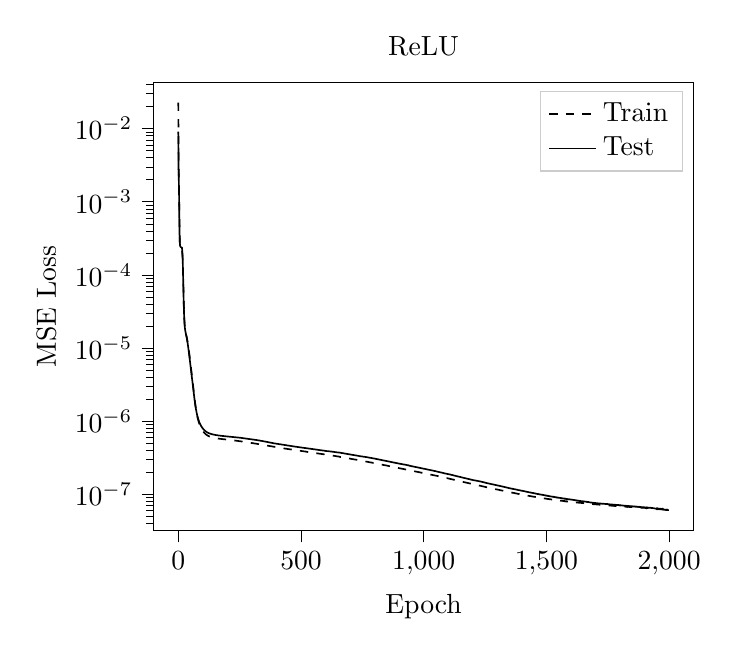
\begin{tikzpicture}

\begin{axis}[
legend cell align={left},
legend style={fill opacity=0.8, draw opacity=1, text opacity=1, draw=white!80!black},
log basis y={10},
tick align=outside,
tick pos=left,
title={ReLU},
x grid style={white!69.0196078431373!black},
xlabel={Epoch},
xmin=-99.95, xmax=2098.95,
xtick style={color=black},
y grid style={white!69.0196078431373!black},
ylabel={MSE Loss},
ymin=3.20662223104107e-08, ymax=0.0431121836135911,
ymode=log,
ytick style={color=black}
]
\addplot [semithick, black, dashed]
table {%
0 0.022700188562274
1 0.00488751665130258
2 0.00231159114837646
3 0.00169912100443617
4 0.000957429732894525
5 0.000457231870386749
6 0.000291163621441228
7 0.00023975450026046
8 0.000223350821892382
9 0.000217858722797246
10 0.000215660652000224
11 0.000214534028418711
12 0.000213661922316533
13 0.00021273185996688
14 0.0002116511244094
15 0.000210345065890579
16 0.000199949145098799
17 0.000182367857094505
18 0.000158941823407076
19 0.000125522568072483
20 9.05295221236884e-05
21 6.39946652263461e-05
22 4.61771607297123e-05
23 3.49678208767728e-05
24 2.79254836004839e-05
25 2.34756546597055e-05
26 2.06620919616398e-05
27 1.88729651317772e-05
28 1.76978199806399e-05
29 1.68716617790778e-05
30 1.62288936953701e-05
31 1.56760611562277e-05
32 1.5163152797868e-05
33 1.46647982219292e-05
34 1.41640936926706e-05
35 1.36524210238349e-05
36 1.3125367727298e-05
37 1.25840063737996e-05
38 1.20289051747022e-05
39 1.14638668196676e-05
40 1.08971444033159e-05
41 1.03354414623027e-05
42 9.78288087026158e-06
43 9.24360746557795e-06
44 8.71880347676779e-06
45 8.2212451234227e-06
46 7.7380116790664e-06
47 7.28033067434808e-06
48 6.83901115780827e-06
49 6.41160088571269e-06
50 6.00367025094783e-06
51 5.61681789690738e-06
52 5.25355912623127e-06
53 4.91812908012435e-06
54 4.60782127834136e-06
55 4.3184103076328e-06
56 4.04694739745537e-06
57 3.79198045425255e-06
58 3.55115817546903e-06
59 3.32267476801462e-06
60 3.10306129676974e-06
61 2.90025063634403e-06
62 2.71049544289781e-06
63 2.53316815292237e-06
64 2.36955519051207e-06
65 2.21743742019953e-06
66 2.07712799175397e-06
67 1.95007587785767e-06
68 1.83331815719612e-06
69 1.72713420909076e-06
70 1.63017052238956e-06
71 1.54295807112703e-06
72 1.46528206181529e-06
73 1.39492643029371e-06
74 1.33200299183045e-06
75 1.27552853570023e-06
76 1.22471883557296e-06
77 1.17950768247965e-06
78 1.13884168192158e-06
79 1.10184992811924e-06
80 1.06842147013708e-06
81 1.03816669236778e-06
82 1.01005816800637e-06
83 9.83902286947114e-07
84 9.59851741470175e-07
85 9.37582064864273e-07
86 9.17004300035273e-07
87 8.97869634414405e-07
88 8.80009910460444e-07
89 8.63493210744082e-07
90 8.48001840353163e-07
91 8.3358825983737e-07
92 8.20043752966626e-07
93 8.07293199883929e-07
94 7.95262972843602e-07
95 7.83745429529858e-07
96 7.73114619704529e-07
97 7.63112369000396e-07
98 7.53572947189696e-07
99 7.44605152732447e-07
100 7.36272040370523e-07
101 7.281094682412e-07
102 7.20398173484682e-07
103 7.13262888979216e-07
104 7.06426322636844e-07
105 7.00064532253464e-07
106 6.93946270104107e-07
107 6.88264223441593e-07
108 6.8279916240499e-07
109 6.77674996211408e-07
110 6.72629135380021e-07
111 6.67993809656764e-07
112 6.63566975617869e-07
113 6.59467331331598e-07
114 6.55476894593221e-07
115 6.51754040262631e-07
116 6.48160458922575e-07
117 6.44768821700836e-07
118 6.41538844462275e-07
119 6.38487625565176e-07
120 6.35543724314402e-07
121 6.32724531328677e-07
122 6.30082758760864e-07
123 6.27604565295314e-07
124 6.25200852027774e-07
125 6.22870618457227e-07
126 6.20655547663773e-07
127 6.1856236368385e-07
128 6.16603096204926e-07
129 6.14726157920131e-07
130 6.12881591251835e-07
131 6.11095928803707e-07
132 6.094500031395e-07
133 6.07855674729763e-07
134 6.06303832256572e-07
135 6.04832115925546e-07
136 6.03458678000379e-07
137 6.02132227385255e-07
138 6.00858143400274e-07
139 5.9959718061009e-07
140 5.9837970928811e-07
141 5.97201963586258e-07
142 5.96090518740766e-07
143 5.95010408943608e-07
144 5.94001013269008e-07
145 5.93005560261872e-07
146 5.92063210547167e-07
147 5.91099726932498e-07
148 5.90182496097214e-07
149 5.89293092502885e-07
150 5.88437146802789e-07
151 5.87599400262207e-07
152 5.8681417951334e-07
153 5.86040602939875e-07
154 5.85259042281905e-07
155 5.84521904073654e-07
156 5.83760592149929e-07
157 5.83063614556068e-07
158 5.82367442518716e-07
159 5.81692266450773e-07
160 5.81006480274482e-07
161 5.80357362707673e-07
162 5.79735073529264e-07
163 5.79122948920485e-07
164 5.78525290279686e-07
165 5.77992324991783e-07
166 5.77417234325139e-07
167 5.76792696477924e-07
168 5.7620480180276e-07
169 5.75622956091593e-07
170 5.75074705977841e-07
171 5.74554324572318e-07
172 5.74008320882058e-07
173 5.734738602996e-07
174 5.72948865794842e-07
175 5.72417692865201e-07
176 5.71913329963536e-07
177 5.71392262912696e-07
178 5.70892375463927e-07
179 5.70415385084289e-07
180 5.69933258077526e-07
181 5.69438252483678e-07
182 5.68800431778982e-07
183 5.68370158646303e-07
184 5.68008979342949e-07
185 5.67546451236467e-07
186 5.66942494856448e-07
187 5.66492348355041e-07
188 5.6600412295893e-07
189 5.65518306132162e-07
190 5.64976778179016e-07
191 5.64506119161479e-07
192 5.6400162551995e-07
193 5.63510650295029e-07
194 5.63028813928668e-07
195 5.62433123008077e-07
196 5.61948407408863e-07
197 5.61459071889203e-07
198 5.60965872949737e-07
199 5.60495189716903e-07
200 5.60018450130428e-07
201 5.59532428439979e-07
202 5.59046564546861e-07
203 5.58561763767784e-07
204 5.58075900073618e-07
205 5.57590778953454e-07
206 5.57100048496295e-07
207 5.56615983242636e-07
208 5.56132100513196e-07
209 5.55609417062897e-07
210 5.55238328246332e-07
211 5.54747902128838e-07
212 5.54302580724197e-07
213 5.53833328439168e-07
214 5.53333939876666e-07
215 5.52824435942512e-07
216 5.52326941345882e-07
217 5.51828715600777e-07
218 5.51342741459848e-07
219 5.50852281605785e-07
220 5.50354051654267e-07
221 5.49853959142865e-07
222 5.49354793690782e-07
223 5.48889128481278e-07
224 5.48412155978895e-07
225 5.47924545259093e-07
226 5.4743110911204e-07
227 5.46936913679019e-07
228 5.46444356729125e-07
229 5.459593782291e-07
230 5.45469382899455e-07
231 5.43948594668109e-07
232 5.43577015832852e-07
233 5.43141319894858e-07
234 5.42670150963431e-07
235 5.4215009910763e-07
236 5.41254978941197e-07
237 5.4071538048106e-07
238 5.40094552036408e-07
239 5.39584018270034e-07
240 5.39063721930688e-07
241 5.38529411954869e-07
242 5.37968243037312e-07
243 5.37392851640561e-07
244 5.36852313160807e-07
245 5.36285412920279e-07
246 5.3571522911966e-07
247 5.35140720330673e-07
248 5.3443252718921e-07
249 5.33878865127235e-07
250 5.33326285733438e-07
251 5.32710414972826e-07
252 5.32128201086834e-07
253 5.3153658973315e-07
254 5.30958579048502e-07
255 5.30392841596949e-07
256 5.29813738069151e-07
257 5.29206798432824e-07
258 5.28611251496613e-07
259 5.28013453390486e-07
260 5.2743299119129e-07
261 5.26832736454708e-07
262 5.26222398775644e-07
263 5.25642485285971e-07
264 5.25047771446907e-07
265 5.24451909285517e-07
266 5.23855538119733e-07
267 5.23260044928975e-07
268 5.22677574451791e-07
269 5.22101135715047e-07
270 5.21522106993189e-07
271 5.2093735595804e-07
272 5.20345230768271e-07
273 5.19757054604497e-07
274 5.19156453833602e-07
275 5.18550851836608e-07
276 5.17957335915753e-07
277 5.17369120132116e-07
278 5.16782020355322e-07
279 5.16200261699851e-07
280 5.15574804410335e-07
281 5.15027628523512e-07
282 5.14336931132675e-07
283 5.13758614488324e-07
284 5.13183472492074e-07
285 5.12594136750977e-07
286 5.12004632014396e-07
287 5.11429211314862e-07
288 5.10876843549113e-07
289 5.10237616765608e-07
290 5.09550439801387e-07
291 5.08979076613514e-07
292 5.0826299255391e-07
293 5.07674016262172e-07
294 5.07074047021661e-07
295 5.06488575894082e-07
296 5.0588200679158e-07
297 5.0527562575553e-07
298 5.04698802018311e-07
299 5.0409348091307e-07
300 5.03476895886479e-07
301 5.02873825212191e-07
302 5.02268338522072e-07
303 5.01660967728412e-07
304 5.0105952021795e-07
305 5.0045732720605e-07
306 4.99856223996176e-07
307 4.99265046613573e-07
308 4.98666331111508e-07
309 4.98066681245746e-07
310 4.97465910939354e-07
311 4.96871412508426e-07
312 4.96137432321575e-07
313 4.9553043635342e-07
314 4.94941312979336e-07
315 4.94267596906184e-07
316 4.93610437501957e-07
317 4.92980641354279e-07
318 4.92369693432693e-07
319 4.91739606502506e-07
320 4.91099409799744e-07
321 4.90437452043579e-07
322 4.89807230280803e-07
323 4.89186760347593e-07
324 4.88559287589396e-07
325 4.87941073032516e-07
326 4.87305083652245e-07
327 4.86687516229267e-07
328 4.86061624570766e-07
329 4.85449494334489e-07
330 4.84829064561154e-07
331 4.84218366892719e-07
332 4.8359940532805e-07
333 4.830153798423e-07
334 4.82397970387183e-07
335 4.81782221186222e-07
336 4.81173868649876e-07
337 4.80559737809472e-07
338 4.79956168504714e-07
339 4.79344355255762e-07
340 4.78806477559601e-07
341 4.78240154762943e-07
342 4.77609454350159e-07
343 4.77003219117478e-07
344 4.76402054232494e-07
345 4.75791388254265e-07
346 4.75013815588454e-07
347 4.74374429529689e-07
348 4.73760426586978e-07
349 4.72920066499682e-07
350 4.72309703241081e-07
351 4.71689676629694e-07
352 4.71041691099572e-07
353 4.70393082395049e-07
354 4.69757620095379e-07
355 4.69146253209374e-07
356 4.68521187315218e-07
357 4.67862831214916e-07
358 4.67246957327916e-07
359 4.66614568154e-07
360 4.65985684172665e-07
361 4.6536224317606e-07
362 4.64654443277368e-07
363 4.64017372877379e-07
364 4.63376583951458e-07
365 4.62768628437971e-07
366 4.62145839122741e-07
367 4.61530419244127e-07
368 4.6089009126149e-07
369 4.60264819025724e-07
370 4.59625250016416e-07
371 4.58993519600881e-07
372 4.5837571519769e-07
373 4.57772132591572e-07
374 4.57149062043527e-07
375 4.5654107344717e-07
376 4.56388565879706e-07
377 4.55734816853237e-07
378 4.55108889241274e-07
379 4.54509474423048e-07
380 4.5388417871095e-07
381 4.53284295474532e-07
382 4.52677932457846e-07
383 4.52075946668629e-07
384 4.51512100482887e-07
385 4.50870240143786e-07
386 4.50251420318182e-07
387 4.49643324799354e-07
388 4.49040381340637e-07
389 4.48442889108946e-07
390 4.47849138907941e-07
391 4.47228694440582e-07
392 4.46672484287092e-07
393 4.461130256459e-07
394 4.45521277072203e-07
395 4.44942966254303e-07
396 4.44365371606636e-07
397 4.43792268384868e-07
398 4.43272579076392e-07
399 4.42683609037431e-07
400 4.42047175965854e-07
401 4.41511416170215e-07
402 4.40903476572885e-07
403 4.40345714878276e-07
404 4.3987389551603e-07
405 4.39265694041069e-07
406 4.38643700221064e-07
407 4.380702063429e-07
408 4.37512944046148e-07
409 4.36928924386848e-07
410 4.3640052246019e-07
411 4.35823328899687e-07
412 4.35215195849992e-07
413 4.34667989864579e-07
414 4.34115721304806e-07
415 4.33525133956891e-07
416 4.33020327989198e-07
417 4.32479380691575e-07
418 4.31893973825481e-07
419 4.31408940585243e-07
420 4.30838680827605e-07
421 4.30306989400719e-07
422 4.29754458110665e-07
423 4.29197023592565e-07
424 4.28708979058001e-07
425 4.28179310091537e-07
426 4.27645871525328e-07
427 4.27122201074326e-07
428 4.26600456847837e-07
429 4.26098265279506e-07
430 4.25582650322553e-07
431 4.25064716353063e-07
432 4.24552743652384e-07
433 4.24046018068225e-07
434 4.23532201423882e-07
435 4.23018083807847e-07
436 4.22497343777195e-07
437 4.22003586905362e-07
438 4.21473392307803e-07
439 4.20917969989887e-07
440 4.20440635949149e-07
441 4.19875405299308e-07
442 4.19363955217023e-07
443 4.18853888447757e-07
444 4.18352119027077e-07
445 4.17849264920278e-07
446 4.17325928665946e-07
447 4.16844640056979e-07
448 4.16344165444116e-07
449 4.15880111347633e-07
450 4.15396516785904e-07
451 4.14893772202163e-07
452 4.14433901823941e-07
453 4.13930885599711e-07
454 4.13483039750417e-07
455 4.13017433587015e-07
456 4.1257212623691e-07
457 4.12095013999192e-07
458 4.11657128623233e-07
459 4.11228072835002e-07
460 4.10708955925543e-07
461 4.10184199338914e-07
462 4.09730133469566e-07
463 4.09255900592598e-07
464 4.08744348931123e-07
465 4.08305826397282e-07
466 4.07791080348829e-07
467 4.07319028909114e-07
468 4.06846871413791e-07
469 4.06389932322782e-07
470 4.05920714698027e-07
471 4.05562731955911e-07
472 4.05092885813474e-07
473 4.0462468440694e-07
474 4.04162996773039e-07
475 4.03698307593459e-07
476 4.03226065685658e-07
477 4.02781851548184e-07
478 4.02340750596863e-07
479 4.01872257114633e-07
480 4.01436150028189e-07
481 4.00995583561325e-07
482 4.00542615494714e-07
483 4.00105648267868e-07
484 3.9966176110795e-07
485 3.99214384003699e-07
486 3.98767849290493e-07
487 3.98336208618844e-07
488 3.97897648582557e-07
489 3.97436830553488e-07
490 3.97029553994344e-07
491 3.96565684638972e-07
492 3.96169267048663e-07
493 3.95707022320835e-07
494 3.95289122536724e-07
495 3.94852195327644e-07
496 3.94419814639946e-07
497 3.93999079605578e-07
498 3.93570346247429e-07
499 3.9315561880926e-07
500 3.92716066883736e-07
501 3.92287240870814e-07
502 3.91878817822544e-07
503 3.91442989226221e-07
504 3.91023176774752e-07
505 3.9062641165799e-07
506 3.90210046802508e-07
507 3.89796826127053e-07
508 3.89384892272915e-07
509 3.88973414260363e-07
510 3.88556969866727e-07
511 3.88143236861538e-07
512 3.87750533690223e-07
513 3.87334687218299e-07
514 3.86922011443858e-07
515 3.86537839034418e-07
516 3.86145166501706e-07
517 3.85737681369847e-07
518 3.85339201272927e-07
519 3.8487991605507e-07
520 3.83903953405706e-07
521 3.82987367999021e-07
522 3.82452104588538e-07
523 3.81951715240802e-07
524 3.81474649344682e-07
525 3.81002873993452e-07
526 3.80536858187952e-07
527 3.80074700913724e-07
528 3.79651768199096e-07
529 3.79191619771291e-07
530 3.78739784309801e-07
531 3.78291494698146e-07
532 3.77857477459997e-07
533 3.77393390778025e-07
534 3.76971358065248e-07
535 3.7652833098889e-07
536 3.76109584294682e-07
537 3.75679046470623e-07
538 3.75253116985164e-07
539 3.74808345085853e-07
540 3.7454908161294e-07
541 3.7414445736772e-07
542 3.73729084628849e-07
543 3.73336543063374e-07
544 3.72864065653289e-07
545 3.72388690294656e-07
546 3.71936408129159e-07
547 3.7159253486152e-07
548 3.71120514557788e-07
549 3.7070167992681e-07
550 3.70296510155299e-07
551 3.69914672049276e-07
552 3.69459091174917e-07
553 3.69037342807133e-07
554 3.68648538355387e-07
555 3.6825909458571e-07
556 3.67811100034032e-07
557 3.67427050235847e-07
558 3.66991696012064e-07
559 3.66619650719713e-07
560 3.66189225928792e-07
561 3.65861811559398e-07
562 3.65376562385222e-07
563 3.65019601645145e-07
564 3.64580547127957e-07
565 3.64211771625378e-07
566 3.63786553577938e-07
567 3.63422670105251e-07
568 3.62993843239678e-07
569 3.62630070128489e-07
570 3.62208776891748e-07
571 3.61848602025816e-07
572 3.61434043114173e-07
573 3.61033925202037e-07
574 3.60626449435131e-07
575 3.60239536490781e-07
576 3.5982089400477e-07
577 3.59459390324446e-07
578 3.59027224121178e-07
579 3.58637733910427e-07
580 3.58265337851549e-07
581 3.57837911053593e-07
582 3.57462955719257e-07
583 3.57044090065983e-07
584 3.56651212896963e-07
585 3.56281235312395e-07
586 3.55858100661521e-07
587 3.55473218320412e-07
588 3.55106093834934e-07
589 3.54690216738618e-07
590 3.54296942276733e-07
591 3.53912689618596e-07
592 3.53498191117296e-07
593 3.53113810746208e-07
594 3.52725243871532e-07
595 3.52314408615939e-07
596 3.51911630289692e-07
597 3.51522282898031e-07
598 3.51117687088731e-07
599 3.50752920624586e-07
600 3.50220982767269e-07
601 3.49666113038438e-07
602 3.49216980467304e-07
603 3.48912888597397e-07
604 3.48590493985057e-07
605 3.48156322104387e-07
606 3.47782955444131e-07
607 3.47431346924054e-07
608 3.47023016885828e-07
609 3.46650842232066e-07
610 3.46283607186138e-07
611 3.45864262101259e-07
612 3.45506151319341e-07
613 3.45193046385361e-07
614 3.44725366304033e-07
615 3.44399749494073e-07
616 3.43981475197097e-07
617 3.43586984797639e-07
618 3.43181904270295e-07
619 3.42802305496548e-07
620 3.42403075336506e-07
621 3.41977504575652e-07
622 3.4155453653284e-07
623 3.4121790288566e-07
624 3.40786421261896e-07
625 3.40369527535245e-07
626 3.40017924912672e-07
627 3.39533942778303e-07
628 3.39218749374481e-07
629 3.38775148605919e-07
630 3.38400936499283e-07
631 3.37982899594635e-07
632 3.37605371441896e-07
633 3.37170312434409e-07
634 3.36797599160832e-07
635 3.36361521405593e-07
636 3.35930654614458e-07
637 3.3559160269192e-07
638 3.35204049008553e-07
639 3.34756528133084e-07
640 3.34375308568724e-07
641 3.33965574611739e-07
642 3.33506915836779e-07
643 3.33132214549892e-07
644 3.32628377762489e-07
645 3.32194951340625e-07
646 3.31808428924774e-07
647 3.31448711378357e-07
648 3.30991560645089e-07
649 3.30627948002871e-07
650 3.30129058355055e-07
651 3.29814938055506e-07
652 3.29351685039114e-07
653 3.28992725826538e-07
654 3.28530313112196e-07
655 3.28124250728479e-07
656 3.27338606993521e-07
657 3.2631718342202e-07
658 3.25590172181478e-07
659 3.25028652142123e-07
660 3.24517025873661e-07
661 3.24045561214348e-07
662 3.23632035957644e-07
663 3.23333612456622e-07
664 3.22835817087253e-07
665 3.22464504492359e-07
666 3.22048187427981e-07
667 3.21377591362193e-07
668 3.21208086006663e-07
669 3.20661421767454e-07
670 3.20358596013648e-07
671 3.19621063596287e-07
672 3.1945258629662e-07
673 3.19104954499494e-07
674 3.18600724384055e-07
675 3.18192904686043e-07
676 3.17710430906004e-07
677 3.17364652957508e-07
678 3.16877777223112e-07
679 3.16538145668233e-07
680 3.15970995160342e-07
681 3.1567109923003e-07
682 3.15297038284257e-07
683 3.14813742392062e-07
684 3.14474320148861e-07
685 3.13978635006151e-07
686 3.13667648967453e-07
687 3.13245961862663e-07
688 3.12820861438468e-07
689 3.12397660195529e-07
690 3.1198839221247e-07
691 3.11556838838101e-07
692 3.11143778816358e-07
693 3.10705394213073e-07
694 3.10293124186956e-07
695 3.09892371817e-07
696 3.09461834291369e-07
697 3.090517145381e-07
698 3.08666699567084e-07
699 3.0822698936106e-07
700 3.07806382778608e-07
701 3.07389098040289e-07
702 3.06976017242278e-07
703 3.06563772056734e-07
704 3.06163985612784e-07
705 3.05730360267376e-07
706 3.05273673447459e-07
707 3.04876716270996e-07
708 3.0442998618696e-07
709 3.04035280080939e-07
710 3.03622769806111e-07
711 3.03206509087772e-07
712 3.02812567170463e-07
713 3.02440707557139e-07
714 3.0202642422239e-07
715 3.01613633979514e-07
716 3.01198510896938e-07
717 3.00822865682449e-07
718 3.00429866129548e-07
719 3.00004258420472e-07
720 2.99603975577156e-07
721 2.99221630228885e-07
722 2.98811836827895e-07
723 2.98403452376306e-07
724 2.97989905206464e-07
725 2.9759956366604e-07
726 2.97187501331564e-07
727 2.9681355476896e-07
728 2.96412470021323e-07
729 2.9606505475499e-07
730 2.95635467878697e-07
731 2.952455811851e-07
732 2.94848240571355e-07
733 2.94465938836197e-07
734 2.94049225601611e-07
735 2.93639906388421e-07
736 2.93226357769072e-07
737 2.92796839545417e-07
738 2.92297765568605e-07
739 2.91883827330253e-07
740 2.91480768723318e-07
741 2.910785553496e-07
742 2.90658661256771e-07
743 2.90242410954988e-07
744 2.89850709691564e-07
745 2.89458642981799e-07
746 2.89041936454737e-07
747 2.8864057620126e-07
748 2.88227141510333e-07
749 2.87827345815117e-07
750 2.87087919858209e-07
751 2.86751240196281e-07
752 2.86329326087298e-07
753 2.8591025268554e-07
754 2.85439217833527e-07
755 2.85030032486588e-07
756 2.84653017843084e-07
757 2.84204375958552e-07
758 2.8389503138726e-07
759 2.83434894626566e-07
760 2.83027217491849e-07
761 2.82583373746093e-07
762 2.82166798484695e-07
763 2.81779251295688e-07
764 2.81361878322173e-07
765 2.8097022681095e-07
766 2.80527259462815e-07
767 2.80156977623847e-07
768 2.79733914808844e-07
769 2.79341120162258e-07
770 2.78916435533461e-07
771 2.78528162013458e-07
772 2.78141511387275e-07
773 2.77702974685212e-07
774 2.77305605408174e-07
775 2.76901424754783e-07
776 2.76503712527187e-07
777 2.7608817458713e-07
778 2.75728598765568e-07
779 2.75243042580087e-07
780 2.74894716326912e-07
781 2.74454094579823e-07
782 2.74069144126088e-07
783 2.73722769037477e-07
784 2.73352229129387e-07
785 2.72916203726936e-07
786 2.72518787539866e-07
787 2.72107046171755e-07
788 2.71700535861896e-07
789 2.71388373164427e-07
790 2.70878778209749e-07
791 2.70506326188524e-07
792 2.70099734180462e-07
793 2.69743341803519e-07
794 2.69326202285924e-07
795 2.68931778975912e-07
796 2.68559697474302e-07
797 2.68128451239136e-07
798 2.67776407085307e-07
799 2.67330760422624e-07
800 2.66969742384049e-07
801 2.66559677882583e-07
802 2.66164721722362e-07
803 2.65812256472486e-07
804 2.65400530011561e-07
805 2.6502757293656e-07
806 2.6449244508342e-07
807 2.6412419380506e-07
808 2.637580061986e-07
809 2.63452051655122e-07
810 2.63053868408747e-07
811 2.62594155017837e-07
812 2.62013144990192e-07
813 2.6193533845742e-07
814 2.61439927285778e-07
815 2.61018644366118e-07
816 2.60627871526253e-07
817 2.60260550476232e-07
818 2.59689900460103e-07
819 2.59417914975302e-07
820 2.59006644839133e-07
821 2.58626036824694e-07
822 2.58218586338899e-07
823 2.57673533738512e-07
824 2.57433976102561e-07
825 2.57017506498869e-07
826 2.5667790622208e-07
827 2.56154501016681e-07
828 2.55826516465163e-07
829 2.55293243981214e-07
830 2.54911673962965e-07
831 2.54528044095537e-07
832 2.54085345531507e-07
833 2.53902755346758e-07
834 2.53358927992053e-07
835 2.52917493085647e-07
836 2.5258387552185e-07
837 2.52187130001857e-07
838 2.51844215142682e-07
839 2.51351500949681e-07
840 2.51175747990828e-07
841 2.50791280407725e-07
842 2.50371872652977e-07
843 2.50073024140818e-07
844 2.49660933910434e-07
845 2.49289074517378e-07
846 2.48766987951399e-07
847 2.48441512184172e-07
848 2.48069631027192e-07
849 2.47699301219484e-07
850 2.47161033726684e-07
851 2.46826250588583e-07
852 2.46495931811808e-07
853 2.46035868663341e-07
854 2.45723502651174e-07
855 2.45256004326677e-07
856 2.44975971384065e-07
857 2.44433341421768e-07
858 2.44034814478766e-07
859 2.43581715018593e-07
860 2.43168417568995e-07
861 2.4271100485862e-07
862 2.42337396841208e-07
863 2.42082812036415e-07
864 2.41691652966836e-07
865 2.41245197074136e-07
866 2.40857210400236e-07
867 2.40553402242938e-07
868 2.40142219510631e-07
869 2.39735860347423e-07
870 2.39412173904441e-07
871 2.38961034234819e-07
872 2.38645971329277e-07
873 2.38238824422865e-07
874 2.37809563216729e-07
875 2.3733263120107e-07
876 2.37218382366677e-07
877 2.36820149837058e-07
878 2.36251832234302e-07
879 2.35994000377104e-07
880 2.35550381091798e-07
881 2.35120832542179e-07
882 2.34883657554974e-07
883 2.3447071255589e-07
884 2.34056571045471e-07
885 2.33667837314044e-07
886 2.33339260311993e-07
887 2.33093831027986e-07
888 2.32603948909116e-07
889 2.32233412184257e-07
890 2.32004902379401e-07
891 2.31429368355407e-07
892 2.3114651683187e-07
893 2.30785587632454e-07
894 2.30509334691931e-07
895 2.30057152329266e-07
896 2.29823544458441e-07
897 2.29321314293429e-07
898 2.28995329422332e-07
899 2.28720500601298e-07
900 2.2819258192186e-07
901 2.27982340113897e-07
902 2.27608680532398e-07
903 2.27211997810173e-07
904 2.26988304923736e-07
905 2.26444428335526e-07
906 2.26198868467975e-07
907 2.25855826890609e-07
908 2.2550042169911e-07
909 2.25155414788958e-07
910 2.24715623417637e-07
911 2.24441779643314e-07
912 2.24117695772463e-07
913 2.23662403364244e-07
914 2.23525080990328e-07
915 2.22978478866764e-07
916 2.22644433506503e-07
917 2.22354079696174e-07
918 2.22075732409621e-07
919 2.216284795864e-07
920 2.21327834964313e-07
921 2.21020898472091e-07
922 2.20529991381113e-07
923 2.20361902080413e-07
924 2.20030540255323e-07
925 2.19693687718348e-07
926 2.19355493747742e-07
927 2.18912160406148e-07
928 2.18688205620765e-07
929 2.18431814289488e-07
930 2.17975239991119e-07
931 2.17582416240703e-07
932 2.17388809041097e-07
933 2.1695414856282e-07
934 2.16690200510072e-07
935 2.16351949184457e-07
936 2.16095488674739e-07
937 2.15770156167139e-07
938 2.14990478731636e-07
939 2.14787864763366e-07
940 2.1443938268817e-07
941 2.14009426784401e-07
942 2.13876116731626e-07
943 2.13514506633317e-07
944 2.13116627740817e-07
945 2.12705434734062e-07
946 2.12403169662423e-07
947 2.12224187748689e-07
948 2.11859084011223e-07
949 2.11378808906204e-07
950 2.11102361483029e-07
951 2.10801352842793e-07
952 2.10461757689018e-07
953 2.10099717612877e-07
954 2.09749843882889e-07
955 2.09436833515042e-07
956 2.08886092458727e-07
957 2.08831142565202e-07
958 2.08371006181096e-07
959 2.08050646740787e-07
960 2.07822948567582e-07
961 2.07486869925333e-07
962 2.07112270111054e-07
963 2.06741844017699e-07
964 2.06521825781181e-07
965 2.06087915294972e-07
966 2.05930061810022e-07
967 2.05545380552508e-07
968 2.05069629963361e-07
969 2.04830868973715e-07
970 2.04720518375723e-07
971 2.04201579762753e-07
972 2.03760819481147e-07
973 2.03723517330445e-07
974 2.03153470287987e-07
975 2.02952266192824e-07
976 2.0258793077943e-07
977 2.02278263678579e-07
978 2.02042518324674e-07
979 2.01851433075717e-07
980 2.01159917573079e-07
981 2.01093053725288e-07
982 2.00630439998406e-07
983 2.00379565200137e-07
984 2.00104684502378e-07
985 1.99714410634044e-07
986 1.99583829243011e-07
987 1.99082864192235e-07
988 1.98879871078361e-07
989 1.9851004941529e-07
990 1.98118672258829e-07
991 1.97794862813794e-07
992 1.97514059898651e-07
993 1.97439506180785e-07
994 1.96882988724667e-07
995 1.96863558301175e-07
996 1.96450931930769e-07
997 1.95994219325257e-07
998 1.95664951903041e-07
999 1.95385722300045e-07
1000 1.95022169748427e-07
1001 1.94833854649801e-07
1002 1.94470195005181e-07
1003 1.94122655358342e-07
1004 1.9388446521873e-07
1005 1.93533067992746e-07
1006 1.93328063083698e-07
1007 1.92964109508864e-07
1008 1.92854989641944e-07
1009 1.92244884203774e-07
1010 1.92150149644021e-07
1011 1.91683977945445e-07
1012 1.91481523557968e-07
1013 1.91099812219875e-07
1014 1.90797521028685e-07
1015 1.90380861127437e-07
1016 1.90235854056198e-07
1017 1.89877648772097e-07
1018 1.89494576162019e-07
1019 1.89354932544461e-07
1020 1.89023202793237e-07
1021 1.88638987530965e-07
1022 1.88445211605881e-07
1023 1.88153857600071e-07
1024 1.8789166674793e-07
1025 1.87497277877924e-07
1026 1.87139091707422e-07
1027 1.86948059244685e-07
1028 1.86557873902871e-07
1029 1.8624394212452e-07
1030 1.86015578215404e-07
1031 1.85666344684421e-07
1032 1.85445209389457e-07
1033 1.85054166387033e-07
1034 1.84846604049937e-07
1035 1.84483662977186e-07
1036 1.84172586372711e-07
1037 1.83920614389876e-07
1038 1.83583266078813e-07
1039 1.83318241170127e-07
1040 1.82997070702129e-07
1041 1.83021538092021e-07
1042 1.82458206694491e-07
1043 1.82058361751558e-07
1044 1.82028634412745e-07
1045 1.81618637533632e-07
1046 1.81205257824502e-07
1047 1.80903678263178e-07
1048 1.80594445531312e-07
1049 1.80465957818399e-07
1050 1.80246385575344e-07
1051 1.79967734062814e-07
1052 1.79636884041656e-07
1053 1.79177664357155e-07
1054 1.79063932307599e-07
1055 1.78691587770174e-07
1056 1.78408368206817e-07
1057 1.78004216500938e-07
1058 1.77813854492115e-07
1059 1.77428909594823e-07
1060 1.77236690916516e-07
1061 1.76722042020572e-07
1062 1.76449690165725e-07
1063 1.76021288552874e-07
1064 1.75829625440826e-07
1065 1.75640696625123e-07
1066 1.75241006722615e-07
1067 1.75162156935471e-07
1068 1.74642103651479e-07
1069 1.74417626588763e-07
1070 1.7404266374399e-07
1071 1.73703341644682e-07
1072 1.73558491709969e-07
1073 1.73160420480656e-07
1074 1.72957526480388e-07
1075 1.72599468157841e-07
1076 1.72251352061892e-07
1077 1.71990737428018e-07
1078 1.7171713331976e-07
1079 1.71403443800955e-07
1080 1.71083066689448e-07
1081 1.70797444916104e-07
1082 1.70402340685882e-07
1083 1.70148245288715e-07
1084 1.69917028038924e-07
1085 1.69586333520044e-07
1086 1.69357113584567e-07
1087 1.69163682642193e-07
1088 1.686814187849e-07
1089 1.68399768192273e-07
1090 1.68089013364181e-07
1091 1.67893452029944e-07
1092 1.67585903092515e-07
1093 1.67222312761339e-07
1094 1.67059804290659e-07
1095 1.66649184230039e-07
1096 1.66450206698698e-07
1097 1.66033636610052e-07
1098 1.65722943663127e-07
1099 1.65424200780251e-07
1100 1.65225882462039e-07
1101 1.64985739466772e-07
1102 1.64698448095635e-07
1103 1.64395809392204e-07
1104 1.64084958875321e-07
1105 1.63677839154275e-07
1106 1.63496802393581e-07
1107 1.63082423547678e-07
1108 1.62798604314673e-07
1109 1.62522797900522e-07
1110 1.62237442324908e-07
1111 1.61953103585688e-07
1112 1.61745482145648e-07
1113 1.61444047385828e-07
1114 1.61156203638768e-07
1115 1.60849461522616e-07
1116 1.60548210331513e-07
1117 1.60125507292719e-07
1118 1.60022549835048e-07
1119 1.59726342381816e-07
1120 1.59424678358278e-07
1121 1.59032878435994e-07
1122 1.5872759782809e-07
1123 1.58415958168234e-07
1124 1.58145775252194e-07
1125 1.57837064953981e-07
1126 1.57546023409338e-07
1127 1.57264251292588e-07
1128 1.56991482583635e-07
1129 1.56779749318048e-07
1130 1.56375693713073e-07
1131 1.56187677539776e-07
1132 1.55840182010536e-07
1133 1.55556436844506e-07
1134 1.55273407109746e-07
1135 1.54998702655007e-07
1136 1.54711072703151e-07
1137 1.54432117184911e-07
1138 1.54145230403913e-07
1139 1.53878085860981e-07
1140 1.53617322077082e-07
1141 1.5333499228376e-07
1142 1.53051926098158e-07
1143 1.52785489710539e-07
1144 1.52522081414475e-07
1145 1.52248115853126e-07
1146 1.51964569326424e-07
1147 1.51719455871557e-07
1148 1.51469372077884e-07
1149 1.5122538536616e-07
1150 1.50974027228301e-07
1151 1.5071920294929e-07
1152 1.50436781574115e-07
1153 1.50154852306628e-07
1154 1.4994000232349e-07
1155 1.49684689617402e-07
1156 1.49378274763023e-07
1157 1.49107717653862e-07
1158 1.48837879095254e-07
1159 1.48464723778829e-07
1160 1.48321392124728e-07
1161 1.4794774750726e-07
1162 1.47731350878644e-07
1163 1.47506493782146e-07
1164 1.47181220476966e-07
1165 1.46966620775402e-07
1166 1.4667185742212e-07
1167 1.46446925676003e-07
1168 1.46194616810647e-07
1169 1.4589142892163e-07
1170 1.45623083163571e-07
1171 1.45421855407335e-07
1172 1.45148988735855e-07
1173 1.44924273733693e-07
1174 1.44653323587818e-07
1175 1.44397603683899e-07
1176 1.44143922561568e-07
1177 1.43887481556249e-07
1178 1.43637580052314e-07
1179 1.43380571216767e-07
1180 1.43128617793309e-07
1181 1.42918179754759e-07
1182 1.42674865678316e-07
1183 1.42368941268956e-07
1184 1.42143107957793e-07
1185 1.4187803487431e-07
1186 1.41659683009721e-07
1187 1.41389330686081e-07
1188 1.41146314824425e-07
1189 1.40885177728478e-07
1190 1.40635690385693e-07
1191 1.40369184080669e-07
1192 1.4014046066535e-07
1193 1.39883951696618e-07
1194 1.39747466739948e-07
1195 1.39369158453917e-07
1196 1.39117702971703e-07
1197 1.38906298772667e-07
1198 1.38654130978466e-07
1199 1.38412876140137e-07
1200 1.38177429242603e-07
1201 1.37951588143892e-07
1202 1.37698481808002e-07
1203 1.37433328326608e-07
1204 1.3724076173105e-07
1205 1.36967428325363e-07
1206 1.36749351263177e-07
1207 1.36498041356958e-07
1208 1.36307488340037e-07
1209 1.36027240721148e-07
1210 1.35778096570505e-07
1211 1.35560142766167e-07
1212 1.35304345839415e-07
1213 1.35079826662832e-07
1214 1.34833428923287e-07
1215 1.34616434678492e-07
1216 1.34399582798039e-07
1217 1.34197129121105e-07
1218 1.33883571521665e-07
1219 1.33696930035399e-07
1220 1.3346163827066e-07
1221 1.33249577636718e-07
1222 1.33005609590953e-07
1223 1.32781584980535e-07
1224 1.32541664960684e-07
1225 1.32347305886071e-07
1226 1.32063615318145e-07
1227 1.31870969095615e-07
1228 1.31660141718726e-07
1229 1.31428233174802e-07
1230 1.31200933161324e-07
1231 1.30952666729911e-07
1232 1.30717070817354e-07
1233 1.30495742848069e-07
1234 1.30259482844508e-07
1235 1.30022995147527e-07
1236 1.29781844254495e-07
1237 1.29581289883163e-07
1238 1.29348568975729e-07
1239 1.29130822966061e-07
1240 1.28877546259787e-07
1241 1.28684132853607e-07
1242 1.28452740526086e-07
1243 1.28231625510011e-07
1244 1.27987654604311e-07
1245 1.27740676120425e-07
1246 1.27538427442175e-07
1247 1.27307380335395e-07
1248 1.27056580915053e-07
1249 1.26827521665263e-07
1250 1.26586416879348e-07
1251 1.26406430311476e-07
1252 1.26152649176703e-07
1253 1.25956614589029e-07
1254 1.25715322532471e-07
1255 1.25495106999551e-07
1256 1.25293443446139e-07
1257 1.25028746005285e-07
1258 1.24901299987101e-07
1259 1.24626029101904e-07
1260 1.24430453901425e-07
1261 1.24176776623131e-07
1262 1.24055122398659e-07
1263 1.23799583203521e-07
1264 1.23607713689466e-07
1265 1.23352822342326e-07
1266 1.23219754268433e-07
1267 1.22982637506652e-07
1268 1.22764353839955e-07
1269 1.22587649372008e-07
1270 1.2240252546647e-07
1271 1.22168687340718e-07
1272 1.219725873014e-07
1273 1.21779319677273e-07
1274 1.21563253291157e-07
1275 1.21380381088443e-07
1276 1.21160043512702e-07
1277 1.20952420175513e-07
1278 1.20760240989171e-07
1279 1.20553010624747e-07
1280 1.20351129286433e-07
1281 1.20143024023633e-07
1282 1.19957552684014e-07
1283 1.19751850760963e-07
1284 1.19543746681217e-07
1285 1.19330061487233e-07
1286 1.19149103294802e-07
1287 1.18953276412981e-07
1288 1.18748600737462e-07
1289 1.18555770459494e-07
1290 1.18364916058766e-07
1291 1.1817159390759e-07
1292 1.17976144718313e-07
1293 1.1778769242099e-07
1294 1.17580557674302e-07
1295 1.17392635566205e-07
1296 1.17181604338157e-07
1297 1.1700705573503e-07
1298 1.16808877251628e-07
1299 1.16613071952543e-07
1300 1.16419120878675e-07
1301 1.16225622392108e-07
1302 1.1603226114687e-07
1303 1.15844357804207e-07
1304 1.15657821531556e-07
1305 1.15457035366973e-07
1306 1.15278685957065e-07
1307 1.15126645564345e-07
1308 1.14942082795721e-07
1309 1.14750936365482e-07
1310 1.14571220436233e-07
1311 1.14396584468324e-07
1312 1.14194506771526e-07
1313 1.14016975611975e-07
1314 1.13832922327362e-07
1315 1.13644045871553e-07
1316 1.13458538987032e-07
1317 1.13274990312107e-07
1318 1.13083245398826e-07
1319 1.12902683433447e-07
1320 1.12720184169746e-07
1321 1.12537894811027e-07
1322 1.12350661094496e-07
1323 1.12174550807254e-07
1324 1.12134164076849e-07
1325 1.11870243223677e-07
1326 1.11684696662451e-07
1327 1.11496924954935e-07
1328 1.11313580546835e-07
1329 1.11118610341521e-07
1330 1.10941907703221e-07
1331 1.10745624390063e-07
1332 1.10565157594777e-07
1333 1.10391883758609e-07
1334 1.10216272570796e-07
1335 1.10034027901662e-07
1336 1.09904966944185e-07
1337 1.0972478612814e-07
1338 1.09543823189284e-07
1339 1.09353221706243e-07
1340 1.09189787515618e-07
1341 1.0900702273986e-07
1342 1.08871806606459e-07
1343 1.08658014781327e-07
1344 1.08535055574066e-07
1345 1.08302015139117e-07
1346 1.08116574203621e-07
1347 1.07938734316804e-07
1348 1.07767203992637e-07
1349 1.07630161124916e-07
1350 1.07411750210673e-07
1351 1.07216842348379e-07
1352 1.07049617742661e-07
1353 1.06965064308184e-07
1354 1.06737143919844e-07
1355 1.06572572189378e-07
1356 1.06429018249088e-07
1357 1.06255565668789e-07
1358 1.0609248306892e-07
1359 1.05914943159036e-07
1360 1.05769115879895e-07
1361 1.05555923461509e-07
1362 1.05343500887756e-07
1363 1.05336002874878e-07
1364 1.05065406970084e-07
1365 1.05018041523408e-07
1366 1.04834425311395e-07
1367 1.04657920751094e-07
1368 1.04446422334092e-07
1369 1.04306719531877e-07
1370 1.04136361159135e-07
1371 1.03937797071296e-07
1372 1.03782853386747e-07
1373 1.03633022288108e-07
1374 1.034524386192e-07
1375 1.03303142903854e-07
1376 1.03129766664267e-07
1377 1.02965245194042e-07
1378 1.02805888491986e-07
1379 1.02640688677269e-07
1380 1.02496613894942e-07
1381 1.0232278171074e-07
1382 1.02182824353036e-07
1383 1.02012176419919e-07
1384 1.01840164518308e-07
1385 1.01737134052371e-07
1386 1.01551659998478e-07
1387 1.01374999886161e-07
1388 1.01288831718449e-07
1389 1.01124216129733e-07
1390 1.00975371992718e-07
1391 1.00811491311248e-07
1392 1.00633754545498e-07
1393 1.00503078154901e-07
1394 1.00330592847087e-07
1395 1.00212100541341e-07
1396 1.00035348715721e-07
1397 9.98977622650443e-08
1398 9.97419698371971e-08
1399 9.96092331497778e-08
1400 9.94421753084396e-08
1401 9.93241543625345e-08
1402 9.91819209836819e-08
1403 9.8997636012399e-08
1404 9.8858772627608e-08
1405 9.87074338247851e-08
1406 9.8565545286533e-08
1407 9.84226947515765e-08
1408 9.82687273456406e-08
1409 9.81530818080501e-08
1410 9.80001015236098e-08
1411 9.78618616542803e-08
1412 9.77315958152758e-08
1413 9.75798045423915e-08
1414 9.74417762549251e-08
1415 9.7294861614472e-08
1416 9.71628285846293e-08
1417 9.7036684380214e-08
1418 9.68920721362565e-08
1419 9.68428053553794e-08
1420 9.65617320929368e-08
1421 9.65015172482708e-08
1422 9.63498855988121e-08
1423 9.61964877745913e-08
1424 9.6049520042385e-08
1425 9.58933131407491e-08
1426 9.58726888740102e-08
1427 9.56149151214447e-08
1428 9.55419418744441e-08
1429 9.53950836333206e-08
1430 9.53688893758908e-08
1431 9.51055585893812e-08
1432 9.50164821347244e-08
1433 9.48658110893064e-08
1434 9.48242855329795e-08
1435 9.45683539228526e-08
1436 9.44814399588267e-08
1437 9.43536782749277e-08
1438 9.43120517149509e-08
1439 9.40272916558626e-08
1440 9.39600227454207e-08
1441 9.3908410100596e-08
1442 9.36157606439281e-08
1443 9.35820834726542e-08
1444 9.35358044351631e-08
1445 9.32975007934545e-08
1446 9.31823757319705e-08
1447 9.30778284597977e-08
1448 9.30286952893766e-08
1449 9.27425326793241e-08
1450 9.27090496922744e-08
1451 9.26503111458032e-08
1452 9.24670470858757e-08
1453 9.23490937658755e-08
1454 9.23282061755515e-08
1455 9.20449279320223e-08
1456 9.19874992746372e-08
1457 9.19312404228378e-08
1458 9.18109127283628e-08
1459 9.16913846964462e-08
1460 9.15665439293889e-08
1461 9.14274972672047e-08
1462 9.13176319485842e-08
1463 9.12192370385867e-08
1464 9.11416237201479e-08
1465 9.08891564037617e-08
1466 9.08708531142111e-08
1467 9.07038205006927e-08
1468 9.06278333339117e-08
1469 9.05767015844106e-08
1470 9.03423392735192e-08
1471 9.03440315767057e-08
1472 9.01624750255792e-08
1473 9.00763360540679e-08
1474 8.99509745764249e-08
1475 8.98331613612413e-08
1476 8.98057103242422e-08
1477 8.95662919866425e-08
1478 8.95808520837704e-08
1479 8.93643545047951e-08
1480 8.93124236220899e-08
1481 8.92553014608666e-08
1482 8.90094035241873e-08
1483 8.898572014715e-08
1484 8.8832003374506e-08
1485 8.88204353159949e-08
1486 8.86249849116894e-08
1487 8.86197948339884e-08
1488 8.8368378104775e-08
1489 8.84007229799977e-08
1490 8.82116618328155e-08
1491 8.82008406435375e-08
1492 8.80198266273169e-08
1493 8.79442392687224e-08
1494 8.77306660669319e-08
1495 8.77938955241575e-08
1496 8.75771729482722e-08
1497 8.7548924689429e-08
1498 8.73489487176471e-08
1499 8.73071902773859e-08
1500 8.71555701955629e-08
1501 8.71828966637622e-08
1502 8.69347493406281e-08
1503 8.69339800146918e-08
1504 8.68377549849697e-08
1505 8.66093619400488e-08
1506 8.6683032876067e-08
1507 8.6448997354438e-08
1508 8.64151720101347e-08
1509 8.62562767132147e-08
1510 8.62694248517926e-08
1511 8.60708971508473e-08
1512 8.60006384080236e-08
1513 8.59740737695347e-08
1514 8.57957047450952e-08
1515 8.58013514992706e-08
1516 8.55567701236737e-08
1517 8.55891087283567e-08
1518 8.53702089891328e-08
1519 8.54079138754571e-08
1520 8.51862400317316e-08
1521 8.52541076845625e-08
1522 8.50326026871073e-08
1523 8.50964173331192e-08
1524 8.48097249637192e-08
1525 8.48998332259043e-08
1526 8.4653916900379e-08
1527 8.47284985745489e-08
1528 8.44072775514348e-08
1529 8.44738449572446e-08
1530 8.4279409328758e-08
1531 8.43341055762892e-08
1532 8.4098250439979e-08
1533 8.41544892580259e-08
1534 8.39321933909787e-08
1535 8.39758508739408e-08
1536 8.38546063484102e-08
1537 8.36892192985772e-08
1538 8.37157066548855e-08
1539 8.35165831887252e-08
1540 8.35192991317513e-08
1541 8.33388690324455e-08
1542 8.33600631295894e-08
1543 8.31802473619803e-08
1544 8.32366856329259e-08
1545 8.29914701441226e-08
1546 8.29353346638584e-08
1547 8.29907054153978e-08
1548 8.27452777123483e-08
1549 8.27077281435606e-08
1550 8.27132129437302e-08
1551 8.25286743442177e-08
1552 8.24747088046251e-08
1553 8.24669626666719e-08
1554 8.22664516455518e-08
1555 8.221874347214e-08
1556 8.22379365175152e-08
1557 8.2025389453122e-08
1558 8.21068135508085e-08
1559 8.18390956922599e-08
1560 8.18246454379334e-08
1561 8.19354982475318e-08
1562 8.15930577893198e-08
1563 8.17188595974017e-08
1564 8.14420239265701e-08
1565 8.14793852441653e-08
1566 8.14947726972548e-08
1567 8.12075671312584e-08
1568 8.13480490222673e-08
1569 8.11107960494439e-08
1570 8.11869314638614e-08
1571 8.09357348643402e-08
1572 8.10827289150495e-08
1573 8.0768823501387e-08
1574 8.09773693610794e-08
1575 8.06203781031911e-08
1576 8.08149400626235e-08
1577 8.04572729045105e-08
1578 8.06888346893686e-08
1579 8.03109117555323e-08
1580 8.05221194255523e-08
1581 8.01547535438374e-08
1582 8.03761525283164e-08
1583 8.00183500864193e-08
1584 8.02392549879016e-08
1585 7.99492971808036e-08
1586 8.00820226380949e-08
1587 7.98201705407564e-08
1588 7.99270880698089e-08
1589 7.96792419208714e-08
1590 7.97757438242286e-08
1591 7.95626312530828e-08
1592 7.96514949641392e-08
1593 7.95212738964324e-08
1594 7.93007797454948e-08
1595 7.9471240940876e-08
1596 7.92213381650697e-08
1597 7.9327969093157e-08
1598 7.92113646319592e-08
1599 7.90564871202548e-08
1600 7.9049686426913e-08
1601 7.91056621132213e-08
1602 7.88474337127809e-08
1603 7.88394875463894e-08
1604 7.89088655430703e-08
1605 7.86553475649043e-08
1606 7.87711939231883e-08
1607 7.85231091100513e-08
1608 7.87002043267648e-08
1609 7.84328092038322e-08
1610 7.84278552465878e-08
1611 7.84810809939529e-08
1612 7.82588452814537e-08
1613 7.82878755600791e-08
1614 7.81338001623055e-08
1615 7.81480018545722e-08
1616 7.81356290708857e-08
1617 7.79733676061767e-08
1618 7.79208966470435e-08
1619 7.79402718968925e-08
1620 7.77730878489535e-08
1621 7.78340618410311e-08
1622 7.75973352844517e-08
1623 7.75884865049647e-08
1624 7.76785483616038e-08
1625 7.7471302571297e-08
1626 7.73978548807008e-08
1627 7.74785633161912e-08
1628 7.73519828456415e-08
1629 7.72033532072669e-08
1630 7.73003058824884e-08
1631 7.70632135029814e-08
1632 7.7097393926806e-08
1633 7.69426986870769e-08
1634 7.7077213067156e-08
1635 7.68171501697168e-08
1636 7.68541471565243e-08
1637 7.68113379372437e-08
1638 7.66729214092265e-08
1639 7.67225044242537e-08
1640 7.65773198843078e-08
1641 7.65654009313721e-08
1642 7.64089113118871e-08
1643 7.65253482661876e-08
1644 7.62851568296696e-08
1645 7.6405434118243e-08
1646 7.61800151209968e-08
1647 7.62894902806011e-08
1648 7.606340946964e-08
1649 7.61863288687437e-08
1650 7.59471737126205e-08
1651 7.60786200224572e-08
1652 7.58278242010135e-08
1653 7.59668522078982e-08
1654 7.58288357722847e-08
1655 7.568855022555e-08
1656 7.57002660378703e-08
1657 7.56606771297186e-08
1658 7.56180094185766e-08
1659 7.55306099726738e-08
1660 7.54390033854691e-08
1661 7.5380192100738e-08
1662 7.54242722109666e-08
1663 7.53859348421315e-08
1664 7.52367810150645e-08
1665 7.51825024494224e-08
1666 7.52066463718393e-08
1667 7.50483257370149e-08
1668 7.50633969879289e-08
1669 7.49889273023996e-08
1670 7.48663550496076e-08
1671 7.49445332068888e-08
1672 7.48387453093358e-08
1673 7.46764661947452e-08
1674 7.45670546820065e-08
1675 7.44955725551222e-08
1676 7.456480048873e-08
1677 7.44125086633574e-08
1678 7.42698098221695e-08
1679 7.44199019422354e-08
1680 7.42523669927664e-08
1681 7.42170275138676e-08
1682 7.41313736831728e-08
1683 7.41857077102281e-08
1684 7.4007842712831e-08
1685 7.40906451746071e-08
1686 7.39473953110803e-08
1687 7.38651389298184e-08
1688 7.3939729528405e-08
1689 7.37879374312911e-08
1690 7.37048077112945e-08
1691 7.37878746015497e-08
1692 7.34371959261182e-08
1693 7.34462981277773e-08
1694 7.34070984407254e-08
1695 7.32998603467649e-08
1696 7.33198130902224e-08
1697 7.32555518574429e-08
1698 7.32221325208116e-08
1699 7.31747049478315e-08
1700 7.31155324125154e-08
1701 7.30555174328629e-08
1702 7.30464680849252e-08
1703 7.2951392819931e-08
1704 7.2936381588562e-08
1705 7.28464312338417e-08
1706 7.28324133838498e-08
1707 7.27562614706301e-08
1708 7.27335294037346e-08
1709 7.26725489883506e-08
1710 7.26016404151153e-08
1711 7.25874773408464e-08
1712 7.25269361154801e-08
1713 7.24706473356207e-08
1714 7.24350604670576e-08
1715 7.23757357796728e-08
1716 7.23102715589619e-08
1717 7.23002998377353e-08
1718 7.22196285956045e-08
1719 7.21604749607252e-08
1720 7.21442177571419e-08
1721 7.20965490934589e-08
1722 7.20358092891615e-08
1723 7.19668549713504e-08
1724 7.19585563295766e-08
1725 7.18880298400393e-08
1726 7.18340884411361e-08
1727 7.18160916086674e-08
1728 7.17549739412959e-08
1729 7.17024740168881e-08
1730 7.16493701027332e-08
1731 7.16275821837087e-08
1732 7.15741002288439e-08
1733 7.15189599134192e-08
1734 7.14755662762911e-08
1735 7.14147750819905e-08
1736 7.13972272308183e-08
1737 7.13379220407262e-08
1738 7.12994370211106e-08
1739 7.12431644274147e-08
1740 7.11954810306281e-08
1741 7.11566263618124e-08
1742 7.11280224443556e-08
1743 7.10659102800548e-08
1744 7.1004854756751e-08
1745 7.09163907437471e-08
1746 7.08734350922668e-08
1747 7.09464326682507e-08
1748 7.0925995217408e-08
1749 7.07174663290289e-08
1750 7.07843654836893e-08
1751 7.07172813996237e-08
1752 7.07799966122025e-08
1753 7.0606729579481e-08
1754 7.06127715055516e-08
1755 7.06252833673204e-08
1756 7.04596753031694e-08
1757 7.05023281142303e-08
1758 7.05168302417292e-08
1759 7.03426327461898e-08
1760 7.03537803197207e-08
1761 7.03999299034308e-08
1762 7.02266953283015e-08
1763 7.02305893547361e-08
1764 7.02807286678819e-08
1765 7.00894176830502e-08
1766 7.01957879627457e-08
1767 7.00209628980986e-08
1768 7.01159793301542e-08
1769 6.99346465360406e-08
1770 7.00787180889506e-08
1771 6.98442697029122e-08
1772 6.99859975235029e-08
1773 6.97420070245869e-08
1774 6.99277252032004e-08
1775 6.96704429827832e-08
1776 6.98283544338096e-08
1777 6.96019172004014e-08
1778 6.97561636435751e-08
1779 6.95240278361098e-08
1780 6.96486528859452e-08
1781 6.94726672207935e-08
1782 6.95897835250037e-08
1783 6.93639787883171e-08
1784 6.95060834630112e-08
1785 6.94096608278016e-08
1786 6.92513315456722e-08
1787 6.94050650160705e-08
1788 6.91686367702005e-08
1789 6.93480167157645e-08
1790 6.91983263720886e-08
1791 6.90951405459828e-08
1792 6.91743161240765e-08
1793 6.90164610404054e-08
1794 6.87476648195684e-08
1795 6.93713717616617e-08
1796 6.88558314081433e-08
1797 6.89636399968663e-08
1798 6.88326451872001e-08
1799 6.88777623842896e-08
1800 6.8772605583689e-08
1801 6.88284329584121e-08
1802 6.86797214441981e-08
1803 6.87577740308143e-08
1804 6.86507587808194e-08
1805 6.86339633979571e-08
1806 6.8557989571616e-08
1807 6.8553758953982e-08
1808 6.85383630028014e-08
1809 6.84446631922242e-08
1810 6.84425184687143e-08
1811 6.83884887457964e-08
1812 6.84006306315155e-08
1813 6.83007983930395e-08
1814 6.83221667472367e-08
1815 6.82274813570416e-08
1816 6.82689574418305e-08
1817 6.8156152213561e-08
1818 6.81937474418248e-08
1819 6.80733075029139e-08
1820 6.81402819928678e-08
1821 6.79988149059341e-08
1822 6.80748696026967e-08
1823 6.79167038342143e-08
1824 6.79192186545663e-08
1825 6.7955652284013e-08
1826 6.78380836980352e-08
1827 6.78239216789223e-08
1828 6.7799110649247e-08
1829 6.74328772518607e-08
1830 6.80901175478255e-08
1831 6.75891049972677e-08
1832 6.76681500628717e-08
1833 6.75843716777535e-08
1834 6.75556305118619e-08
1835 6.75387396675831e-08
1836 6.7502185125079e-08
1837 6.73670122424141e-08
1838 6.74341325783701e-08
1839 6.734767635308e-08
1840 6.73126592580786e-08
1841 6.7260788448209e-08
1842 6.72758344890667e-08
1843 6.717432887271e-08
1844 6.71805266101444e-08
1845 6.71400043295023e-08
1846 6.71469075079756e-08
1847 6.7067301575463e-08
1848 6.701673958176e-08
1849 6.7099895229461e-08
1850 6.69658684380181e-08
1851 6.69411615135118e-08
1852 6.68979375006984e-08
1853 6.69074406474124e-08
1854 6.68498741625001e-08
1855 6.68610791336732e-08
1856 6.67693168630024e-08
1857 6.67529853934923e-08
1858 6.66978772123628e-08
1859 6.66896475394196e-08
1860 6.66199517986854e-08
1861 6.63278951407165e-08
1862 6.69224149802972e-08
1863 6.64580652482982e-08
1864 6.65016799388241e-08
1865 6.64422678475773e-08
1866 6.64254001456754e-08
1867 6.64076957299642e-08
1868 6.63526512987289e-08
1869 6.63299889538394e-08
1870 6.63148450072981e-08
1871 6.62634305399479e-08
1872 6.62417899981449e-08
1873 6.62011780008243e-08
1874 6.61885017585462e-08
1875 6.61300285251798e-08
1876 6.6114330934397e-08
1877 6.60840410660057e-08
1878 6.60484478309797e-08
1879 6.60248005388553e-08
1880 6.59847160804361e-08
1881 6.59565945007046e-08
1882 6.59170215691063e-08
1883 6.58853296542361e-08
1884 6.58653522336294e-08
1885 6.58275868197222e-08
1886 6.57973095350428e-08
1887 6.57834301023286e-08
1888 6.57382430482301e-08
1889 6.5699499895544e-08
1890 6.56731729904436e-08
1891 6.56071149727211e-08
1892 6.56142652744052e-08
1893 6.55897985382126e-08
1894 6.55482462832424e-08
1895 6.55294687099683e-08
1896 6.54885443687192e-08
1897 6.54615210535781e-08
1898 6.54417371563909e-08
1899 6.54086848825841e-08
1900 6.53734646078874e-08
1901 6.53529531682295e-08
1902 6.53143018567448e-08
1903 6.52933906337694e-08
1904 6.52606058757499e-08
1905 6.52417525977e-08
1906 6.52007814991862e-08
1907 6.51658521775289e-08
1908 6.48157778400105e-08
1909 6.55442375325777e-08
1910 6.50263028276754e-08
1911 6.50963148061123e-08
1912 6.50009381750749e-08
1913 6.50390182137528e-08
1914 6.49373690890798e-08
1915 6.49714918843358e-08
1916 6.49263033878356e-08
1917 6.48491885080205e-08
1918 6.48712764395043e-08
1919 6.47843635164236e-08
1920 6.47520617640396e-08
1921 6.47194839338283e-08
1922 6.46862902193845e-08
1923 6.46611641563766e-08
1924 6.46943475679507e-08
1925 6.46190934396884e-08
1926 6.45960062293227e-08
1927 6.45767717379897e-08
1928 6.45484761285786e-08
1929 6.43904920032412e-08
1930 6.44620623475589e-08
1931 6.4489518372568e-08
1932 6.44392406883298e-08
1933 6.4365141355438e-08
1934 6.4360443161604e-08
1935 6.42976659293026e-08
1936 6.43253052849957e-08
1937 6.42427850614524e-08
1938 6.42679396172241e-08
1939 6.4270917199849e-08
1940 6.42060063107408e-08
1941 6.40923907653246e-08
1942 6.40612208933078e-08
1943 6.40310306536662e-08
1944 6.40496247150679e-08
1945 6.4002062003965e-08
1946 6.3841202695869e-08
1947 6.39290055737263e-08
1948 6.38564739254832e-08
1949 6.38598183755335e-08
1950 6.42851243881637e-08
1951 6.32771539486043e-08
1952 6.38927306049197e-08
1953 6.35981974141941e-08
1954 6.36124579784791e-08
1955 6.39011272944856e-08
1956 6.35522097098828e-08
1957 6.35924568577195e-08
1958 6.33331590762509e-08
1959 6.3652651309809e-08
1960 6.3543830503221e-08
1961 6.33561049596665e-08
1962 6.34413432010206e-08
1963 6.36987576605463e-08
1964 6.35873675420839e-08
1965 6.33376973731004e-08
1966 6.31266018871202e-08
1967 6.34900599365551e-08
1968 6.33016898241578e-08
1969 6.32102950675062e-08
1970 6.34170118978261e-08
1971 6.34363252700609e-08
1972 6.29931278695039e-08
1973 6.2909691983748e-08
1974 6.34660287133215e-08
1975 6.28344758055732e-08
1976 6.31622447109237e-08
1977 6.30790833220374e-08
1978 6.28987519064594e-08
1979 6.28567939031655e-08
1980 6.27098520702418e-08
1981 6.30911208929774e-08
1982 6.28269349043364e-08
1983 6.25771548214971e-08
1984 6.29251678212484e-08
1985 6.25076873106423e-08
1986 6.28794714891967e-08
1987 6.26479338592389e-08
1988 6.26440256326077e-08
1989 6.2448848854757e-08
1990 6.25552657531614e-08
1991 6.25887514544843e-08
1992 6.26309891487153e-08
1993 6.24720017654567e-08
1994 6.21644052820613e-08
1995 6.24160825637432e-08
1996 6.2539797422545e-08
1997 6.22059576720346e-08
1998 6.23435946884854e-08
1999 6.22637638088008e-08
};
\addlegendentry{Train}
\addplot [semithick, black]
table {%
0 0.0090876268222928
1 0.00280143390409648
2 0.00203397055156529
3 0.00135002459865063
4 0.000646944215986878
5 0.000367474218364805
6 0.000281517364783213
7 0.000254287297138944
8 0.000245364266447723
9 0.000242081499891356
10 0.000240476103499532
11 0.000239460845477879
12 0.000238456268562004
13 0.000237323140027002
14 0.000235975545365363
15 0.000234324354096316
16 0.000213825434911996
17 0.00019138734205626
18 0.000161446863785386
19 0.000116852650535293
20 8.21483045001514e-05
21 5.74024779780302e-05
22 4.18179515691008e-05
23 3.21888219332322e-05
24 2.61827171925688e-05
25 2.24475352297304e-05
26 2.00851427507587e-05
27 1.85801200132119e-05
28 1.75608874997124e-05
29 1.68002607097151e-05
30 1.6173165931832e-05
31 1.56089699885342e-05
32 1.50680925798952e-05
33 1.45308495120844e-05
34 1.39840822157566e-05
35 1.34203683046508e-05
36 1.28429774122196e-05
37 1.22527617349988e-05
38 1.16522778625949e-05
39 1.10497012428823e-05
40 1.04515220300527e-05
41 9.86537816061173e-06
42 9.3002054200042e-06
43 8.75482510309666e-06
44 8.23525806481484e-06
45 7.7393306128215e-06
46 7.27132692190935e-06
47 6.82771496940404e-06
48 6.39929612589185e-06
49 5.98537235418917e-06
50 5.60301759833237e-06
51 5.2459149628703e-06
52 4.91785249323584e-06
53 4.61352328784415e-06
54 4.33046079706401e-06
55 4.06509434469626e-06
56 3.81578456654097e-06
57 3.58091028829222e-06
58 3.3612668630667e-06
59 3.14800672640558e-06
60 2.94776077680581e-06
61 2.76079185823619e-06
62 2.58499335359375e-06
63 2.42144392359478e-06
64 2.2700730823999e-06
65 2.12875124816492e-06
66 2.00033332475869e-06
67 1.8848554645956e-06
68 1.77891774910677e-06
69 1.68363044394937e-06
70 1.59982425884664e-06
71 1.52365373651264e-06
72 1.4560598629032e-06
73 1.39605776894314e-06
74 1.34194874590321e-06
75 1.29227782963426e-06
76 1.2473166179916e-06
77 1.20665731628833e-06
78 1.16901605906605e-06
79 1.13521923594817e-06
80 1.10436008071702e-06
81 1.07511641544988e-06
82 1.05030346730928e-06
83 1.02547346614301e-06
84 1.00289514648466e-06
85 9.82173901320493e-07
86 9.63361799222184e-07
87 9.45490398862603e-07
88 9.29009615902032e-07
89 9.13584813133639e-07
90 8.99346275673452e-07
91 8.85982444742694e-07
92 8.73505712206679e-07
93 8.61196383539209e-07
94 8.50109017846989e-07
95 8.39728102164372e-07
96 8.29792668355367e-07
97 8.20122124878253e-07
98 8.11113864074287e-07
99 8.02723718607012e-07
100 7.95666892372537e-07
101 7.87882129316131e-07
102 7.80611287609645e-07
103 7.73586350533151e-07
104 7.66943855978752e-07
105 7.6155748729434e-07
106 7.55786686568172e-07
107 7.49996388549334e-07
108 7.44709268474253e-07
109 7.39547147077246e-07
110 7.34808395463915e-07
111 7.30013994143519e-07
112 7.25655070255016e-07
113 7.2156871055995e-07
114 7.17534305749723e-07
115 7.13860345058492e-07
116 7.1035714199752e-07
117 7.07088872786699e-07
118 7.03698106008233e-07
119 7.00721898283518e-07
120 6.97923724146676e-07
121 6.95221615387709e-07
122 6.92674689162232e-07
123 6.90256115376542e-07
124 6.8779672801611e-07
125 6.85560678448383e-07
126 6.83413929891685e-07
127 6.8141679321343e-07
128 6.79473089348903e-07
129 6.77607772558986e-07
130 6.75762066748575e-07
131 6.73930742323137e-07
132 6.72253122502298e-07
133 6.70609551889356e-07
134 6.6899218609251e-07
135 6.67481288019189e-07
136 6.66077653477259e-07
137 6.64735580357956e-07
138 6.63479625018226e-07
139 6.62207696677797e-07
140 6.60975501887151e-07
141 6.59789520796039e-07
142 6.58637077322055e-07
143 6.57557393424213e-07
144 6.56577185509377e-07
145 6.55365909096872e-07
146 6.54330449378904e-07
147 6.53307608899922e-07
148 6.52267146961094e-07
149 6.51306493182346e-07
150 6.50267509172409e-07
151 6.49364494620386e-07
152 6.48475463549403e-07
153 6.47595129521505e-07
154 6.46778914870083e-07
155 6.4592978787914e-07
156 6.45110674213356e-07
157 6.44330043542141e-07
158 6.43632972696651e-07
159 6.42772192804841e-07
160 6.42071540823963e-07
161 6.41258509403997e-07
162 6.40447126443178e-07
163 6.39680877156934e-07
164 6.38914571027271e-07
165 6.38186349988246e-07
166 6.37525886304502e-07
167 6.36908339401998e-07
168 6.3607495803808e-07
169 6.35459741715749e-07
170 6.34863397408481e-07
171 6.34368802820973e-07
172 6.33795025350992e-07
173 6.33214142453653e-07
174 6.32633714303665e-07
175 6.32058288374537e-07
176 6.31490138403024e-07
177 6.31019361208018e-07
178 6.30480258223542e-07
179 6.29940927865391e-07
180 6.29414500963321e-07
181 6.28864484042424e-07
182 6.28332600172143e-07
183 6.28117049927823e-07
184 6.27546114628785e-07
185 6.26995301900024e-07
186 6.26462338004785e-07
187 6.25944039711612e-07
188 6.25411132659792e-07
189 6.24896188128332e-07
190 6.24400399829028e-07
191 6.23889150119794e-07
192 6.2337488770936e-07
193 6.22830441443512e-07
194 6.22282016138342e-07
195 6.217791792551e-07
196 6.21284243607079e-07
197 6.2078470364213e-07
198 6.20286812136328e-07
199 6.19810236912599e-07
200 6.19298134552082e-07
201 6.18792341811059e-07
202 6.18292858689529e-07
203 6.17794228219282e-07
204 6.1729684830425e-07
205 6.16803788489051e-07
206 6.16302031630767e-07
207 6.15806015957787e-07
208 6.15304259099503e-07
209 6.14827513345517e-07
210 6.14333714565873e-07
211 6.13838722074433e-07
212 6.13511531355471e-07
213 6.1302154108489e-07
214 6.12526037002681e-07
215 6.12034796176886e-07
216 6.11573454989411e-07
217 6.11093469160551e-07
218 6.10666916145419e-07
219 6.10201027484436e-07
220 6.09716494182067e-07
221 6.0921234990019e-07
222 6.08704681326344e-07
223 6.08228958753898e-07
224 6.07766423854628e-07
225 6.07245794981282e-07
226 6.06726473506569e-07
227 6.06205105668778e-07
228 6.05680440912693e-07
229 6.05155833000026e-07
230 6.04628610290092e-07
231 6.04441652285459e-07
232 6.04153342464997e-07
233 6.03802789100882e-07
234 6.03415060140833e-07
235 6.03004821186914e-07
236 6.02029501806101e-07
237 6.01695774093969e-07
238 6.01293152158178e-07
239 6.0086091480116e-07
240 6.00408498030447e-07
241 5.99969951053936e-07
242 5.99501106535172e-07
243 5.99014754243399e-07
244 5.98506005644595e-07
245 5.97984694650222e-07
246 5.97452185502334e-07
247 5.96909956129821e-07
248 5.96426048105059e-07
249 5.95932419855671e-07
250 5.95370750033908e-07
251 5.9485267911441e-07
252 5.94374910178885e-07
253 5.93835864037828e-07
254 5.93287609262916e-07
255 5.92855826653249e-07
256 5.92243225128186e-07
257 5.91643129155273e-07
258 5.91039793107484e-07
259 5.90435490721575e-07
260 5.89791511629301e-07
261 5.8915884437738e-07
262 5.88460068229324e-07
263 5.87793692830019e-07
264 5.87135275509354e-07
265 5.86480837228009e-07
266 5.85826398946665e-07
267 5.85173950184981e-07
268 5.84539748160751e-07
269 5.83901510253781e-07
270 5.83269923026819e-07
271 5.82639415824815e-07
272 5.81986853376293e-07
273 5.81384142606112e-07
274 5.80759262902575e-07
275 5.80118125981244e-07
276 5.79483355522825e-07
277 5.7883994486474e-07
278 5.7823069710139e-07
279 5.77675052682025e-07
280 5.77041305405146e-07
281 5.76410684516304e-07
282 5.75709179884143e-07
283 5.7506065331836e-07
284 5.74379782847245e-07
285 5.73724037167267e-07
286 5.73076931686956e-07
287 5.72627527617442e-07
288 5.71991790820903e-07
289 5.71321891129628e-07
290 5.70683823752915e-07
291 5.70066617910925e-07
292 5.69567987440678e-07
293 5.68975224268797e-07
294 5.68400878364628e-07
295 5.67790664263157e-07
296 5.6716231711107e-07
297 5.66522544431791e-07
298 5.65862023904629e-07
299 5.65364700833015e-07
300 5.64734193631011e-07
301 5.64103459055332e-07
302 5.63466585390415e-07
303 5.62836419248924e-07
304 5.62192099096137e-07
305 5.61545334676339e-07
306 5.6089658073688e-07
307 5.60246576242207e-07
308 5.59601119221043e-07
309 5.58955150609108e-07
310 5.58341753276181e-07
311 5.57718692562048e-07
312 5.57151508928655e-07
313 5.56604277335282e-07
314 5.55975191218749e-07
315 5.55530505153001e-07
316 5.54899997950997e-07
317 5.54394830487581e-07
318 5.53774384570715e-07
319 5.53115853563213e-07
320 5.52459994196397e-07
321 5.51811126570101e-07
322 5.51157086192688e-07
323 5.50493041373556e-07
324 5.49732021681848e-07
325 5.48971286207234e-07
326 5.48215211892966e-07
327 5.47454305888095e-07
328 5.4670260851708e-07
329 5.45939769835968e-07
330 5.4518523029401e-07
331 5.44425120097003e-07
332 5.43674218533852e-07
333 5.42944462722517e-07
334 5.42188615781924e-07
335 5.41441977475188e-07
336 5.40683629424166e-07
337 5.39936650056916e-07
338 5.39185066372738e-07
339 5.38444908215752e-07
340 5.38195706667466e-07
341 5.37147116119741e-07
342 5.36387574356922e-07
343 5.35949766344856e-07
344 5.35065282747382e-07
345 5.34036871613353e-07
346 5.3322912663134e-07
347 5.3252409770721e-07
348 5.31820433025132e-07
349 5.31009277437988e-07
350 5.30399290710193e-07
351 5.29824148998159e-07
352 5.28653458786721e-07
353 5.27995666743664e-07
354 5.27313886777847e-07
355 5.26650353549485e-07
356 5.25898599335051e-07
357 5.25206587553839e-07
358 5.24408790170128e-07
359 5.23625828918739e-07
360 5.22844004535727e-07
361 5.22049219853216e-07
362 5.21176104939514e-07
363 5.20285482252802e-07
364 5.19503089435602e-07
365 5.1859603900084e-07
366 5.17798468990804e-07
367 5.16960312779702e-07
368 5.16042746312451e-07
369 5.15199189976556e-07
370 5.14357282099809e-07
371 5.13548513936257e-07
372 5.12756116677338e-07
373 5.11977191308688e-07
374 5.11116752477392e-07
375 5.10345671500545e-07
376 5.09721985508804e-07
377 5.08888604144886e-07
378 5.08017365064006e-07
379 5.07242816638609e-07
380 5.06484639117843e-07
381 5.05733282807341e-07
382 5.0501779469414e-07
383 5.04288038882805e-07
384 5.03457783906924e-07
385 5.02687214520847e-07
386 5.01959391385753e-07
387 5.01241004258191e-07
388 5.00540238590474e-07
389 4.99846578350116e-07
390 4.99140071497095e-07
391 4.98485917432845e-07
392 4.97973019264464e-07
393 4.9728259909898e-07
394 4.96526809001807e-07
395 4.95843380576844e-07
396 4.9518092737344e-07
397 4.94540927320486e-07
398 4.93866764372797e-07
399 4.93269908474758e-07
400 4.92667197704577e-07
401 4.92246385874751e-07
402 4.91673233682377e-07
403 4.91185744522227e-07
404 4.90592526602995e-07
405 4.89913645651541e-07
406 4.89294109229377e-07
407 4.8870214186536e-07
408 4.88083571781317e-07
409 4.87491661260719e-07
410 4.86878320771211e-07
411 4.86283681766508e-07
412 4.85703822050709e-07
413 4.85158125229646e-07
414 4.84556380797585e-07
415 4.83951623664325e-07
416 4.83431392694911e-07
417 4.82826123970881e-07
418 4.82253710742953e-07
419 4.81827783005429e-07
420 4.81174879496393e-07
421 4.8058524271255e-07
422 4.80216442610981e-07
423 4.79618279314309e-07
424 4.78998117614537e-07
425 4.78457650388009e-07
426 4.77829644296435e-07
427 4.77204253002128e-07
428 4.76561297091393e-07
429 4.75976577263282e-07
430 4.75382705644734e-07
431 4.74778573789081e-07
432 4.74179870479929e-07
433 4.73681012636007e-07
434 4.73073953344283e-07
435 4.72520440553126e-07
436 4.72053983457954e-07
437 4.71418871939022e-07
438 4.70830741505779e-07
439 4.70192162538297e-07
440 4.69626428412084e-07
441 4.69007119363596e-07
442 4.68427231226087e-07
443 4.67859081254574e-07
444 4.67286866978611e-07
445 4.66695695422459e-07
446 4.66118905251278e-07
447 4.65534242266585e-07
448 4.65033707541807e-07
449 4.64425710333671e-07
450 4.63820612139898e-07
451 4.63213154944242e-07
452 4.62611524199019e-07
453 4.62027912817575e-07
454 4.61592378542264e-07
455 4.610352277723e-07
456 4.60489246734141e-07
457 4.59911859707063e-07
458 4.59555536735934e-07
459 4.58915252465886e-07
460 4.58285200011233e-07
461 4.57493314343083e-07
462 4.57099162076702e-07
463 4.56550822036661e-07
464 4.56014788596804e-07
465 4.55502060958679e-07
466 4.54949969252993e-07
467 4.54472484534563e-07
468 4.53939662747871e-07
469 4.5346669708124e-07
470 4.52932539474205e-07
471 4.52370244374833e-07
472 4.51811672519398e-07
473 4.51283057145702e-07
474 4.50747961622255e-07
475 4.50207579660855e-07
476 4.49715543027196e-07
477 4.49187496087688e-07
478 4.48654589035868e-07
479 4.48172528422219e-07
480 4.47646613110919e-07
481 4.47118793545087e-07
482 4.46617832494667e-07
483 4.4607230620386e-07
484 4.45574244167801e-07
485 4.45030337914432e-07
486 4.44591506720826e-07
487 4.44038306568473e-07
488 4.4357091155689e-07
489 4.43081177081694e-07
490 4.42566289393653e-07
491 4.42089373109411e-07
492 4.41600860767721e-07
493 4.41173824583529e-07
494 4.40749374774896e-07
495 4.40300709669827e-07
496 4.39860258438785e-07
497 4.39381039996078e-07
498 4.38969351534979e-07
499 4.38488001464066e-07
500 4.37986670931423e-07
501 4.37515325302229e-07
502 4.37019110677284e-07
503 4.3649288272718e-07
504 4.3601636434687e-07
505 4.35541210208612e-07
506 4.35054118952394e-07
507 4.34551196804023e-07
508 4.34049212572063e-07
509 4.3358878087929e-07
510 4.33117804732319e-07
511 4.32668798566738e-07
512 4.32222520885261e-07
513 4.3175904806958e-07
514 4.31313281978873e-07
515 4.30940190199181e-07
516 4.30473136248111e-07
517 4.30017138342009e-07
518 4.29574356530793e-07
519 4.29004813895517e-07
520 4.28653777362342e-07
521 4.28219465220536e-07
522 4.27807833602856e-07
523 4.27366899202752e-07
524 4.26938015607448e-07
525 4.26449446422339e-07
526 4.25975997586647e-07
527 4.25568885020766e-07
528 4.25090746603018e-07
529 4.24619202021859e-07
530 4.24149249056427e-07
531 4.23678102379199e-07
532 4.23246007130729e-07
533 4.22778441588889e-07
534 4.2234080410708e-07
535 4.21886511503544e-07
536 4.21393792748859e-07
537 4.20941887568915e-07
538 4.20495865682824e-07
539 4.20102480802598e-07
540 4.19919558680704e-07
541 4.19198158851941e-07
542 4.18709788618798e-07
543 4.18303727656166e-07
544 4.17805836150364e-07
545 4.17624960391549e-07
546 4.17007129271951e-07
547 4.165865448158e-07
548 4.16059748431508e-07
549 4.15554922028605e-07
550 4.15047111346212e-07
551 4.14580256347108e-07
552 4.14193607412017e-07
553 4.13639298812996e-07
554 4.13269276577921e-07
555 4.12883935041464e-07
556 4.12297026741726e-07
557 4.11930443533493e-07
558 4.11418682233489e-07
559 4.11047409443199e-07
560 4.10520840432582e-07
561 4.10166478559404e-07
562 4.09640591669813e-07
563 4.09269233614395e-07
564 4.08630484116657e-07
565 4.08289253073235e-07
566 4.07723860007536e-07
567 4.07397180879343e-07
568 4.06872857183771e-07
569 4.06521934337434e-07
570 4.05996814833998e-07
571 4.0565538483861e-07
572 4.05070665010498e-07
573 4.04964566769195e-07
574 4.04166996759159e-07
575 4.03955681349544e-07
576 4.03296667172981e-07
577 4.03198868070831e-07
578 4.02435091473308e-07
579 4.01991513854227e-07
580 4.01885188239248e-07
581 4.01112004055904e-07
582 4.01008918515799e-07
583 4.00323699523142e-07
584 3.99823846919389e-07
585 3.99738780743064e-07
586 3.99054925992459e-07
587 3.98553538616397e-07
588 3.98464692352718e-07
589 3.97790216766225e-07
590 3.97246338934565e-07
591 3.97173693045261e-07
592 3.96503054389541e-07
593 3.96005333413996e-07
594 3.95969351529857e-07
595 3.95245933759725e-07
596 3.94773849166086e-07
597 3.94584134255638e-07
598 3.9394680584337e-07
599 3.93847614077458e-07
600 3.92354422729113e-07
601 3.91977920344289e-07
602 3.91746766581491e-07
603 3.91244100228505e-07
604 3.91024457258027e-07
605 3.90705139352576e-07
606 3.90464350630282e-07
607 3.90254740523233e-07
608 3.90013440210168e-07
609 3.89826396940407e-07
610 3.89556220170562e-07
611 3.89376253906448e-07
612 3.89041815651581e-07
613 3.88236742310255e-07
614 3.88051745403573e-07
615 3.87909125265651e-07
616 3.8760231291235e-07
617 3.87278248581424e-07
618 3.86925933071325e-07
619 3.86735734991817e-07
620 3.86316742151394e-07
621 3.85931144819551e-07
622 3.85532246127696e-07
623 3.85150769943721e-07
624 3.84750649118359e-07
625 3.84237836215107e-07
626 3.84272738074287e-07
627 3.83431284944891e-07
628 3.83426282724031e-07
629 3.82584516955831e-07
630 3.82594890879773e-07
631 3.8178069416972e-07
632 3.81876049004859e-07
633 3.81040678121281e-07
634 3.81037324359568e-07
635 3.8020243664505e-07
636 3.80034663294282e-07
637 3.79447698151125e-07
638 3.79093904712136e-07
639 3.78658171484858e-07
640 3.78124127564661e-07
641 3.78115572630122e-07
642 3.77308055021786e-07
643 3.77302285414771e-07
644 3.76263756152184e-07
645 3.76325800743871e-07
646 3.75574558120206e-07
647 3.75622192905212e-07
648 3.74833490468518e-07
649 3.74877885178648e-07
650 3.74081480458699e-07
651 3.7409188280435e-07
652 3.73288656874138e-07
653 3.73291186406277e-07
654 3.72475852827847e-07
655 3.72446834262519e-07
656 3.72944782611739e-07
657 3.72294749695357e-07
658 3.71844407709432e-07
659 3.71364933471341e-07
660 3.70900608004376e-07
661 3.70375147440427e-07
662 3.70079277445257e-07
663 3.69148636991667e-07
664 3.68651285498345e-07
665 3.68051900068167e-07
666 3.67532010159266e-07
667 3.66541172525103e-07
668 3.66942828122774e-07
669 3.66206052149209e-07
670 3.65755397524481e-07
671 3.64508338179803e-07
672 3.6478394349615e-07
673 3.64674860975356e-07
674 3.63838637440494e-07
675 3.63326080332627e-07
676 3.62994228453317e-07
677 3.62462742486969e-07
678 3.62104259465923e-07
679 3.61527241921067e-07
680 3.60700823875959e-07
681 3.60760509465763e-07
682 3.60213505246065e-07
683 3.59722889697878e-07
684 3.59227470880796e-07
685 3.58704426162149e-07
686 3.58285291213178e-07
687 3.57799166295081e-07
688 3.57165220066236e-07
689 3.5685462762558e-07
690 3.56343349494637e-07
691 3.55854126610211e-07
692 3.55360242565439e-07
693 3.54758270759703e-07
694 3.54406751057468e-07
695 3.53887315895918e-07
696 3.53407386910476e-07
697 3.53200221070438e-07
698 3.5266322129246e-07
699 3.52136424908167e-07
700 3.51604342085921e-07
701 3.5110087992507e-07
702 3.5061188441432e-07
703 3.50136787119482e-07
704 3.49690452594587e-07
705 3.49215213191201e-07
706 3.48793207649578e-07
707 3.4832606843338e-07
708 3.47705366721129e-07
709 3.47256190025291e-07
710 3.46787913940716e-07
711 3.46256967986847e-07
712 3.45843062632412e-07
713 3.45617451102953e-07
714 3.45122884937155e-07
715 3.44651425621123e-07
716 3.4408773785799e-07
717 3.43837314176199e-07
718 3.43354571441523e-07
719 3.42907611639021e-07
720 3.4240517265971e-07
721 3.41927346880766e-07
722 3.4144761684729e-07
723 3.41080493626578e-07
724 3.40607527959946e-07
725 3.40158123890433e-07
726 3.39716962116654e-07
727 3.39251982950373e-07
728 3.38757871531925e-07
729 3.38477121886172e-07
730 3.38084674922356e-07
731 3.37455986709756e-07
732 3.36969748104821e-07
733 3.36441388526509e-07
734 3.35949607688235e-07
735 3.35458679501244e-07
736 3.34986253847092e-07
737 3.3446741554144e-07
738 3.33520205231252e-07
739 3.33055851342579e-07
740 3.32591696405871e-07
741 3.32120578150352e-07
742 3.32070015929276e-07
743 3.31800805497551e-07
744 3.31749077986387e-07
745 3.3130885412902e-07
746 3.30850468799326e-07
747 3.3045060376935e-07
748 3.29993724790256e-07
749 3.29540625898517e-07
750 3.29235348317525e-07
751 3.28879877997679e-07
752 3.28489647927199e-07
753 3.2808043215482e-07
754 3.27779503095371e-07
755 3.27316172388237e-07
756 3.27099002106479e-07
757 3.26674438611008e-07
758 3.26400765970902e-07
759 3.26026452057704e-07
760 3.25741950746306e-07
761 3.25442698567713e-07
762 3.24915390592651e-07
763 3.24655871963841e-07
764 3.24322684264189e-07
765 3.23857250350557e-07
766 3.23477564734276e-07
767 3.23022845805099e-07
768 3.2261260685118e-07
769 3.22127476692913e-07
770 3.21596587582462e-07
771 3.2121749882208e-07
772 3.20834146805282e-07
773 3.20360584282753e-07
774 3.19780724566954e-07
775 3.19414596106071e-07
776 3.19135438076046e-07
777 3.18646158348201e-07
778 3.18194793180737e-07
779 3.17681582373552e-07
780 3.17255540949191e-07
781 3.16838253411333e-07
782 3.16333341743302e-07
783 3.15911876214159e-07
784 3.15442974851976e-07
785 3.14937153689243e-07
786 3.14535526513282e-07
787 3.14126708644835e-07
788 3.13697114506795e-07
789 3.1317489401772e-07
790 3.12738109187194e-07
791 3.12350266540307e-07
792 3.11841489519793e-07
793 3.11421928245181e-07
794 3.11028259147861e-07
795 3.10779938672567e-07
796 3.10443226680945e-07
797 3.0994104349702e-07
798 3.09420414623673e-07
799 3.0914716830921e-07
800 3.08228379708453e-07
801 3.07836160118313e-07
802 3.07397783672059e-07
803 3.07399545818043e-07
804 3.06505370417653e-07
805 3.06287859075383e-07
806 3.0513186288772e-07
807 3.04832610709127e-07
808 3.0439736065091e-07
809 3.04470063383633e-07
810 3.03940481671816e-07
811 3.03337770901635e-07
812 3.02748560443433e-07
813 3.02379021377419e-07
814 3.01673026115168e-07
815 3.01183234796554e-07
816 3.00702794220342e-07
817 3.0037904252822e-07
818 2.99462129760286e-07
819 2.99012612003935e-07
820 2.98551015021076e-07
821 2.9804982659698e-07
822 2.97848544050794e-07
823 2.97096846679779e-07
824 2.96693627888089e-07
825 2.96233963581471e-07
826 2.96082021122857e-07
827 2.95318699272684e-07
828 2.94607048090256e-07
829 2.94451325544287e-07
830 2.94202379791386e-07
831 2.93728021460993e-07
832 2.92913398425299e-07
833 2.92681249902671e-07
834 2.91967154453232e-07
835 2.91902978233338e-07
836 2.91398862373171e-07
837 2.90654611490027e-07
838 2.90345155917748e-07
839 2.89751653781423e-07
840 2.89426736799214e-07
841 2.89295371658227e-07
842 2.88489729882713e-07
843 2.88125647784909e-07
844 2.87635572249201e-07
845 2.87458334469193e-07
846 2.86767061652426e-07
847 2.86257545667468e-07
848 2.85923221099438e-07
849 2.85605551653134e-07
850 2.85040272274273e-07
851 2.84690770513407e-07
852 2.84176053355623e-07
853 2.83803416323281e-07
854 2.83610688711633e-07
855 2.82908047211095e-07
856 2.82393529005276e-07
857 2.82078588043078e-07
858 2.81369779031593e-07
859 2.80930265716961e-07
860 2.80846222722175e-07
861 2.80177999911757e-07
862 2.79834381444743e-07
863 2.79326883401154e-07
864 2.78798893305066e-07
865 2.78581552493051e-07
866 2.77791031066954e-07
867 2.77247636404354e-07
868 2.7660865953294e-07
869 2.7613160114015e-07
870 2.75622596745961e-07
871 2.75155372264635e-07
872 2.74720264314965e-07
873 2.74673254807567e-07
874 2.74161578772691e-07
875 2.73608037559825e-07
876 2.73427787078617e-07
877 2.72831471193058e-07
878 2.72867850981129e-07
879 2.72398409606467e-07
880 2.71434259957459e-07
881 2.712131674798e-07
882 2.70646495437177e-07
883 2.70251035772162e-07
884 2.70150053438556e-07
885 2.69325369117723e-07
886 2.69082306658674e-07
887 2.68597062813569e-07
888 2.68181906903919e-07
889 2.67865289060865e-07
890 2.67437599177356e-07
891 2.67352334049065e-07
892 2.66518213720701e-07
893 2.66106667368149e-07
894 2.65761968876177e-07
895 2.65314270109229e-07
896 2.65105484231754e-07
897 2.64728072352227e-07
898 2.64654659076768e-07
899 2.64201929667252e-07
900 2.63396515265413e-07
901 2.63127105881722e-07
902 2.6271007413925e-07
903 2.62297987774218e-07
904 2.62245549720319e-07
905 2.6146810228056e-07
906 2.6104743255928e-07
907 2.60704013044233e-07
908 2.60282433828252e-07
909 2.60290732967405e-07
910 2.59502371591225e-07
911 2.59150425563348e-07
912 2.59081673448236e-07
913 2.58268443076304e-07
914 2.57806419767803e-07
915 2.57865508501709e-07
916 2.57135354786442e-07
917 2.56810665177909e-07
918 2.5684502702461e-07
919 2.56013777288899e-07
920 2.55916347668972e-07
921 2.55832730999828e-07
922 2.55273135962852e-07
923 2.55001140203603e-07
924 2.54436685054316e-07
925 2.54063309057528e-07
926 2.53978811315392e-07
927 2.53441754693995e-07
928 2.5301486061835e-07
929 2.52855471671865e-07
930 2.52512080578526e-07
931 2.51902520176372e-07
932 2.51647122695431e-07
933 2.50968668069618e-07
934 2.50934846235396e-07
935 2.50078983299318e-07
936 2.49806333840752e-07
937 2.49915473204965e-07
938 2.48686831127998e-07
939 2.47851147605616e-07
940 2.48016277737406e-07
941 2.46921558755275e-07
942 2.46710726514721e-07
943 2.46686056470935e-07
944 2.45811150989539e-07
945 2.45791909492254e-07
946 2.44869852394913e-07
947 2.44658792780683e-07
948 2.44625596224068e-07
949 2.43718176307084e-07
950 2.43707944491689e-07
951 2.42865326072206e-07
952 2.42602396838265e-07
953 2.42481860368571e-07
954 2.41586064930743e-07
955 2.41541499690356e-07
956 2.41047757754131e-07
957 2.40317206134932e-07
958 2.40309219634582e-07
959 2.39642446331345e-07
960 2.39642020005704e-07
961 2.38909393601716e-07
962 2.38931022522593e-07
963 2.38200044577752e-07
964 2.37873877040329e-07
965 2.37760360732864e-07
966 2.37118641166489e-07
967 2.36729022162763e-07
968 2.36511695561603e-07
969 2.36013249832467e-07
970 2.35556072425425e-07
971 2.35524311165136e-07
972 2.34804161891589e-07
973 2.34621879258157e-07
974 2.34008069810443e-07
975 2.33682243333533e-07
976 2.33595542908915e-07
977 2.32887501283585e-07
978 2.32676143241406e-07
979 2.32411338174643e-07
980 2.31745005407902e-07
981 2.31714153642315e-07
982 2.31043486564886e-07
983 2.30752959851088e-07
984 2.30509414222979e-07
985 2.30048883054224e-07
986 2.29480775715274e-07
987 2.2938914412407e-07
988 2.28686729997207e-07
989 2.28507403221556e-07
990 2.28282317493722e-07
991 2.27741054459329e-07
992 2.27428884613801e-07
993 2.27300688493415e-07
994 2.26615654241868e-07
995 2.26321489549264e-07
996 2.26074178044655e-07
997 2.25507420736903e-07
998 2.25212218651905e-07
999 2.25081336679978e-07
1000 2.24379689939269e-07
1001 2.24219618871757e-07
1002 2.239233367618e-07
1003 2.23381022124158e-07
1004 2.23091362272498e-07
1005 2.22878270506044e-07
1006 2.2241268027301e-07
1007 2.21997964899856e-07
1008 2.21720156901029e-07
1009 2.21146876810963e-07
1010 2.20908134451747e-07
1011 2.2048186565371e-07
1012 2.20211134660531e-07
1013 2.19744123342025e-07
1014 2.19472823914657e-07
1015 2.19000597212471e-07
1016 2.18760035863852e-07
1017 2.1830159369074e-07
1018 2.17998220364279e-07
1019 2.1770377145458e-07
1020 2.17352877029953e-07
1021 2.17053525375377e-07
1022 2.16603254443726e-07
1023 2.16269498309885e-07
1024 2.15964647054534e-07
1025 2.15624737620601e-07
1026 2.15158422633976e-07
1027 2.14871619164114e-07
1028 2.144861070974e-07
1029 2.14048057500804e-07
1030 2.1381447368185e-07
1031 2.13394685033563e-07
1032 2.13113892755246e-07
1033 2.12680845379509e-07
1034 2.12455034898085e-07
1035 2.12063028470766e-07
1036 2.11723147458542e-07
1037 2.11401612659756e-07
1038 2.11007247230555e-07
1039 2.10737411521222e-07
1040 2.10457429261623e-07
1041 2.10068051842427e-07
1042 2.09838574960486e-07
1043 2.0909986631068e-07
1044 2.0922087173858e-07
1045 2.08828069503397e-07
1046 2.08539702839516e-07
1047 2.0828655067362e-07
1048 2.07926149187188e-07
1049 2.07615784120208e-07
1050 2.06690003778931e-07
1051 2.06251257850454e-07
1052 2.05875309688963e-07
1053 2.05208564807435e-07
1054 2.05241661888067e-07
1055 2.04775901124776e-07
1056 2.04480642196359e-07
1057 2.03939848120172e-07
1058 2.03634144213538e-07
1059 2.03273401666593e-07
1060 2.02981922825529e-07
1061 2.02538672056107e-07
1062 2.02222722123224e-07
1063 2.01914360786759e-07
1064 2.01493506324368e-07
1065 2.01137510202898e-07
1066 2.00782110937325e-07
1067 2.0040916126618e-07
1068 2.00045477072308e-07
1069 1.99826502012002e-07
1070 1.99488951579951e-07
1071 1.99114722931881e-07
1072 1.98832921682879e-07
1073 1.98320975641764e-07
1074 1.98080059021777e-07
1075 1.97706370386186e-07
1076 1.97446595961992e-07
1077 1.97059151219037e-07
1078 1.96708342059537e-07
1079 1.96341048308568e-07
1080 1.95510551748157e-07
1081 1.95215321241449e-07
1082 1.9497497305565e-07
1083 1.94461279079405e-07
1084 1.94153770394223e-07
1085 1.93774965850935e-07
1086 1.93426387795625e-07
1087 1.93209316989851e-07
1088 1.92893693906626e-07
1089 1.9256842165305e-07
1090 1.92249515862386e-07
1091 1.92027002299255e-07
1092 1.91794029547054e-07
1093 1.91474171629125e-07
1094 1.91203639587911e-07
1095 1.90855800497047e-07
1096 1.90531025623386e-07
1097 1.90163547131306e-07
1098 1.89843021303204e-07
1099 1.89503765568588e-07
1100 1.89304557807191e-07
1101 1.89012652640486e-07
1102 1.8871203621984e-07
1103 1.88539004852828e-07
1104 1.8814371571807e-07
1105 1.87890293545934e-07
1106 1.87564779707827e-07
1107 1.87204719281908e-07
1108 1.86895931619802e-07
1109 1.86524133027888e-07
1110 1.86018638714813e-07
1111 1.85690325338328e-07
1112 1.85291312959635e-07
1113 1.850213209309e-07
1114 1.84700269301175e-07
1115 1.84333302399864e-07
1116 1.83918032803376e-07
1117 1.83696059252725e-07
1118 1.83427786737411e-07
1119 1.83034771339408e-07
1120 1.82659604774926e-07
1121 1.82102255052996e-07
1122 1.81720707814748e-07
1123 1.81305054525183e-07
1124 1.81013064093349e-07
1125 1.80691415607726e-07
1126 1.80377270453391e-07
1127 1.80014637862769e-07
1128 1.79756455054303e-07
1129 1.79377622089305e-07
1130 1.79052747739661e-07
1131 1.78581061049954e-07
1132 1.78311836407374e-07
1133 1.77987828919868e-07
1134 1.77649425836535e-07
1135 1.77281648916505e-07
1136 1.77032248416253e-07
1137 1.76705228227547e-07
1138 1.76393641027062e-07
1139 1.76010075847444e-07
1140 1.75774459876266e-07
1141 1.75454474060643e-07
1142 1.75146595893239e-07
1143 1.74757744275666e-07
1144 1.74536879171683e-07
1145 1.74215230686059e-07
1146 1.73907608314039e-07
1147 1.73560280813945e-07
1148 1.73318113638743e-07
1149 1.72949540910849e-07
1150 1.72588528357664e-07
1151 1.72208615367708e-07
1152 1.71852676089657e-07
1153 1.71511928215295e-07
1154 1.71171762985978e-07
1155 1.70852104020014e-07
1156 1.70534562471403e-07
1157 1.70246352126924e-07
1158 1.69878902056553e-07
1159 1.69531560345604e-07
1160 1.69262548865845e-07
1161 1.68891489238376e-07
1162 1.685844495114e-07
1163 1.6824039050789e-07
1164 1.67935382933138e-07
1165 1.67574938814141e-07
1166 1.67245531201843e-07
1167 1.6698196247944e-07
1168 1.66750751873224e-07
1169 1.66419155789299e-07
1170 1.66006344670677e-07
1171 1.65818192954248e-07
1172 1.65480699365617e-07
1173 1.65253538852994e-07
1174 1.64851783779341e-07
1175 1.64590588269675e-07
1176 1.64282639047997e-07
1177 1.64009506420371e-07
1178 1.63643207429232e-07
1179 1.63393096386244e-07
1180 1.63120105867165e-07
1181 1.62890273713856e-07
1182 1.62550620075308e-07
1183 1.6229930110967e-07
1184 1.62002123715865e-07
1185 1.6167480509921e-07
1186 1.61334739345875e-07
1187 1.61082397198697e-07
1188 1.60829145556818e-07
1189 1.60486166578266e-07
1190 1.60095623868983e-07
1191 1.59871092364483e-07
1192 1.596000487325e-07
1193 1.59283601419702e-07
1194 1.58823368678895e-07
1195 1.58630726332376e-07
1196 1.5835907163364e-07
1197 1.58133886429823e-07
1198 1.57830626790201e-07
1199 1.57479604467881e-07
1200 1.5721266777291e-07
1201 1.56969477416169e-07
1202 1.56690575181528e-07
1203 1.56342281343314e-07
1204 1.56140671947469e-07
1205 1.55874616325491e-07
1206 1.55653694378088e-07
1207 1.55417197333918e-07
1208 1.5534972419573e-07
1209 1.55179421312823e-07
1210 1.54936145690954e-07
1211 1.54732063606389e-07
1212 1.54457154621923e-07
1213 1.54226881932118e-07
1214 1.53954488268937e-07
1215 1.53733623164953e-07
1216 1.53487448528722e-07
1217 1.5346110160408e-07
1218 1.53197703411934e-07
1219 1.52957028376477e-07
1220 1.52678993003974e-07
1221 1.52441216982879e-07
1222 1.5214953918985e-07
1223 1.5192323132851e-07
1224 1.51520183067078e-07
1225 1.51442790752299e-07
1226 1.51075894905262e-07
1227 1.5089310068106e-07
1228 1.50632573081566e-07
1229 1.50549155364388e-07
1230 1.50154789935186e-07
1231 1.50078477645366e-07
1232 1.49675173588548e-07
1233 1.49574759689131e-07
1234 1.49187940223783e-07
1235 1.49071595956229e-07
1236 1.48654123677261e-07
1237 1.48520499010374e-07
1238 1.48144849276832e-07
1239 1.48004275501989e-07
1240 1.47601582511925e-07
1241 1.47459630284175e-07
1242 1.47084520563112e-07
1243 1.46865104966309e-07
1244 1.4650332502697e-07
1245 1.46325277228243e-07
1246 1.45919884175782e-07
1247 1.45691871011877e-07
1248 1.45318480804235e-07
1249 1.45124957384724e-07
1250 1.44723287576198e-07
1251 1.44485994724164e-07
1252 1.44144550517922e-07
1253 1.43929341334115e-07
1254 1.43542735031588e-07
1255 1.43308099609385e-07
1256 1.4312523433091e-07
1257 1.42798157298785e-07
1258 1.42583900242244e-07
1259 1.42274402037401e-07
1260 1.42097619004744e-07
1261 1.41789627150501e-07
1262 1.41559993949159e-07
1263 1.41302962219925e-07
1264 1.41108202456053e-07
1265 1.40840398898945e-07
1266 1.40591751573993e-07
1267 1.40356021915977e-07
1268 1.4012758242643e-07
1269 1.39927720965716e-07
1270 1.39682853728118e-07
1271 1.39438540713854e-07
1272 1.39208793825674e-07
1273 1.3896571715577e-07
1274 1.38737433985625e-07
1275 1.3849019353529e-07
1276 1.38272085337121e-07
1277 1.38051944986728e-07
1278 1.37790095777746e-07
1279 1.37555488777252e-07
1280 1.37316831683165e-07
1281 1.37093437047042e-07
1282 1.36858432142617e-07
1283 1.36625061486484e-07
1284 1.36395939875911e-07
1285 1.36155122731907e-07
1286 1.35923315269793e-07
1287 1.35685112923056e-07
1288 1.35468525286342e-07
1289 1.35236007281492e-07
1290 1.34997378609114e-07
1291 1.34785352656763e-07
1292 1.34569077658853e-07
1293 1.34348013602903e-07
1294 1.34126437956184e-07
1295 1.33913275135455e-07
1296 1.33687322545484e-07
1297 1.33456495632345e-07
1298 1.33235886323746e-07
1299 1.33014196990189e-07
1300 1.32811166508873e-07
1301 1.32597335777973e-07
1302 1.32383362938526e-07
1303 1.32175230760367e-07
1304 1.319610447581e-07
1305 1.3175770163798e-07
1306 1.31540005554598e-07
1307 1.31306194361969e-07
1308 1.31079417542423e-07
1309 1.30854360236299e-07
1310 1.30485645399858e-07
1311 1.30243407170383e-07
1312 1.30027260070165e-07
1313 1.2980596864054e-07
1314 1.29586112507241e-07
1315 1.29367464296593e-07
1316 1.29149299255005e-07
1317 1.28934033227779e-07
1318 1.28719321423887e-07
1319 1.28511615571369e-07
1320 1.28293152101833e-07
1321 1.28076223404605e-07
1322 1.27862861631911e-07
1323 1.27638713820488e-07
1324 1.27315203712897e-07
1325 1.27095219681905e-07
1326 1.26867149674581e-07
1327 1.26633821651012e-07
1328 1.26392563970512e-07
1329 1.26146588286247e-07
1330 1.25887922308721e-07
1331 1.2566640350542e-07
1332 1.25462776168206e-07
1333 1.25266964801085e-07
1334 1.25069263390287e-07
1335 1.24879449003856e-07
1336 1.24694764735978e-07
1337 1.2443419450392e-07
1338 1.24228051845421e-07
1339 1.23987945244153e-07
1340 1.23784644756597e-07
1341 1.23543941299431e-07
1342 1.23312602795522e-07
1343 1.23016192787873e-07
1344 1.22733084140236e-07
1345 1.22494625998115e-07
1346 1.2231923562922e-07
1347 1.22089403475911e-07
1348 1.21939265795845e-07
1349 1.21698178645602e-07
1350 1.21482315762478e-07
1351 1.21323182611377e-07
1352 1.21178331369265e-07
1353 1.20878425491355e-07
1354 1.20573233175492e-07
1355 1.20347834808854e-07
1356 1.20218942356587e-07
1357 1.20040908768715e-07
1358 1.19826751188157e-07
1359 1.19519356189812e-07
1360 1.19378469776166e-07
1361 1.19199583537011e-07
1362 1.19152012700852e-07
1363 1.18746896760058e-07
1364 1.18591778175414e-07
1365 1.18739855281547e-07
1366 1.18548378225114e-07
1367 1.18246184399595e-07
1368 1.18094682477476e-07
1369 1.17983532277322e-07
1370 1.1784887021804e-07
1371 1.17526631981946e-07
1372 1.17393632592666e-07
1373 1.17234144170197e-07
1374 1.1706421787494e-07
1375 1.16847736819636e-07
1376 1.16652088877345e-07
1377 1.16439579755934e-07
1378 1.16225123747427e-07
1379 1.16027294438936e-07
1380 1.1582453396386e-07
1381 1.15628765229303e-07
1382 1.15490749408309e-07
1383 1.15307912551543e-07
1384 1.15009598289362e-07
1385 1.14668416983932e-07
1386 1.14462942235605e-07
1387 1.14323661648541e-07
1388 1.14252671323811e-07
1389 1.14118982708078e-07
1390 1.13862753892136e-07
1391 1.1383880860194e-07
1392 1.13609644358803e-07
1393 1.13476396279566e-07
1394 1.13195667950095e-07
1395 1.13091736864135e-07
1396 1.12823734355061e-07
1397 1.12689470199712e-07
1398 1.12452823941567e-07
1399 1.12215055025899e-07
1400 1.12194612711392e-07
1401 1.12051736778085e-07
1402 1.11913287526022e-07
1403 1.11649093526012e-07
1404 1.11512918010703e-07
1405 1.11274069070078e-07
1406 1.11141893910371e-07
1407 1.10915102879972e-07
1408 1.10800293384727e-07
1409 1.10541286346688e-07
1410 1.10409260400957e-07
1411 1.10262320163201e-07
1412 1.10093644423159e-07
1413 1.09903581346771e-07
1414 1.09727729125098e-07
1415 1.09551244520389e-07
1416 1.09395102754206e-07
1417 1.09240076540118e-07
1418 1.0906195058169e-07
1419 1.08592175251943e-07
1420 1.08591585501472e-07
1421 1.08456610803387e-07
1422 1.08300895362845e-07
1423 1.08036246615484e-07
1424 1.07807110794056e-07
1425 1.07740284249758e-07
1426 1.07304323648805e-07
1427 1.07254393810763e-07
1428 1.07135974758421e-07
1429 1.07020859729801e-07
1430 1.06588892379023e-07
1431 1.06654120202165e-07
1432 1.06518228903951e-07
1433 1.06334184124535e-07
1434 1.05913777304067e-07
1435 1.0598702004927e-07
1436 1.05850467946311e-07
1437 1.05779015768803e-07
1438 1.05387634619092e-07
1439 1.05501896996429e-07
1440 1.05362815361332e-07
1441 1.04882730056488e-07
1442 1.04981310755647e-07
1443 1.04886375140723e-07
1444 1.0443406495142e-07
1445 1.04529028988054e-07
1446 1.04391787658642e-07
1447 1.04180209348215e-07
1448 1.03718193145141e-07
1449 1.03864330469605e-07
1450 1.03800118722575e-07
1451 1.03356505576357e-07
1452 1.03396267547851e-07
1453 1.03276732943414e-07
1454 1.02803404899987e-07
1455 1.02756729347675e-07
1456 1.02626017906005e-07
1457 1.02349460462392e-07
1458 1.02345971697559e-07
1459 1.01995922818787e-07
1460 1.0200575673025e-07
1461 1.01907460248185e-07
1462 1.01564310739377e-07
1463 1.01573483846096e-07
1464 1.01198637025846e-07
1465 1.01290517307007e-07
1466 1.00999720586969e-07
1467 1.01027382015673e-07
1468 1.00916693668296e-07
1469 1.00569728544997e-07
1470 1.00623140042444e-07
1471 1.00164093908006e-07
1472 1.00170623795748e-07
1473 9.98337057467324e-08
1474 9.98920555161931e-08
1475 9.98231612925338e-08
1476 9.94291511347001e-08
1477 9.9536983100279e-08
1478 9.92097213270426e-08
1479 9.93265985016478e-08
1480 9.92515367670421e-08
1481 9.88046906513773e-08
1482 9.88776349686304e-08
1483 9.85654295959648e-08
1484 9.86035715300204e-08
1485 9.82782779601621e-08
1486 9.84145884785903e-08
1487 9.79168888193271e-08
1488 9.81675682965033e-08
1489 9.76808607333624e-08
1490 9.77537339963419e-08
1491 9.74218039573316e-08
1492 9.74828395783334e-08
1493 9.71001909988445e-08
1494 9.72789635511617e-08
1495 9.68489786146165e-08
1496 9.6966815021915e-08
1497 9.65601358871027e-08
1498 9.66918207723211e-08
1499 9.63267581255423e-08
1500 9.64041788620307e-08
1501 9.58836920972317e-08
1502 9.61269321919644e-08
1503 9.60723127718666e-08
1504 9.55235819333211e-08
1505 9.58240562454193e-08
1506 9.54442924694376e-08
1507 9.52853937974396e-08
1508 9.51727940901037e-08
1509 9.50583185499454e-08
1510 9.48428606761809e-08
1511 9.46117069133834e-08
1512 9.44770164323927e-08
1513 9.41485609473602e-08
1514 9.44136289149355e-08
1515 9.38609829859161e-08
1516 9.39106712394278e-08
1517 9.38638891057053e-08
1518 9.36755242264553e-08
1519 9.36302413379053e-08
1520 9.34487545123375e-08
1521 9.3141281354292e-08
1522 9.32059265323915e-08
1523 9.31144228388803e-08
1524 9.29585439735092e-08
1525 9.26563927805546e-08
1526 9.2975369625492e-08
1527 9.24487864040202e-08
1528 9.25428693676622e-08
1529 9.22813114812016e-08
1530 9.25817644770177e-08
1531 9.20487934763514e-08
1532 9.21226330774516e-08
1533 9.18296052532241e-08
1534 9.21375260531931e-08
1535 9.16139910600577e-08
1536 9.13736784013963e-08
1537 9.14814535235564e-08
1538 9.11267363790103e-08
1539 9.12134510144824e-08
1540 9.08870916305204e-08
1541 9.1137103197525e-08
1542 9.06924810806231e-08
1543 9.07919925907663e-08
1544 9.04094221709784e-08
1545 9.04213663943665e-08
1546 9.04833754589163e-08
1547 9.01037822131912e-08
1548 9.01141632425606e-08
1549 9.02815173731142e-08
1550 8.9815330284182e-08
1551 8.98221017564538e-08
1552 8.98211496291879e-08
1553 8.95091361030609e-08
1554 8.95195313432851e-08
1555 8.95306442316723e-08
1556 8.9209542863955e-08
1557 8.92206912794791e-08
1558 8.89330067366245e-08
1559 8.89908022827512e-08
1560 8.90528610852925e-08
1561 8.85840734099475e-08
1562 8.86673348077238e-08
1563 8.8393235841977e-08
1564 8.84666846445725e-08
1565 8.83652475636154e-08
1566 8.81008546116391e-08
1567 8.81835120480901e-08
1568 8.79057182601173e-08
1569 8.79434907119503e-08
1570 8.76890311474199e-08
1571 8.77519639175262e-08
1572 8.7482845856357e-08
1573 8.77921735309428e-08
1574 8.72781527050392e-08
1575 8.74066969913656e-08
1576 8.70846079692456e-08
1577 8.72203003154937e-08
1578 8.68859615366091e-08
1579 8.72451835221e-08
1580 8.66777583041767e-08
1581 8.68739249426653e-08
1582 8.64850164816744e-08
1583 8.66886367134612e-08
1584 8.63067484146995e-08
1585 8.63945146534206e-08
1586 8.6141739075174e-08
1587 8.62210853824763e-08
1588 8.59894058180544e-08
1589 8.607557333562e-08
1590 8.58373141454649e-08
1591 8.59039772649339e-08
1592 8.56698108009368e-08
1593 8.55511146369281e-08
1594 8.56753317179937e-08
1595 8.54020640872477e-08
1596 8.54655368698332e-08
1597 8.52233696946314e-08
1598 8.51012060820722e-08
1599 8.51351842356962e-08
1600 8.50568184773692e-08
1601 8.47803249826029e-08
1602 8.48401811026633e-08
1603 8.47808081516632e-08
1604 8.45162659857124e-08
1605 8.45822611950098e-08
1606 8.432564868599e-08
1607 8.43972287611905e-08
1608 8.40857836692521e-08
1609 8.41496756720517e-08
1610 8.40821954284365e-08
1611 8.38089277976906e-08
1612 8.38523277479908e-08
1613 8.35380831176735e-08
1614 8.3649879911718e-08
1615 8.3606941814196e-08
1616 8.33216944329251e-08
1617 8.34173903285773e-08
1618 8.33923579079965e-08
1619 8.30794419925951e-08
1620 8.32040214504559e-08
1621 8.28744717296104e-08
1622 8.29364523724507e-08
1623 8.28714306067013e-08
1624 8.25300006113139e-08
1625 8.25304979912289e-08
1626 8.24899331064444e-08
1627 8.22078263240655e-08
1628 8.20991559180584e-08
1629 8.20446146576614e-08
1630 8.17267036268277e-08
1631 8.18004366465175e-08
1632 8.16847531837084e-08
1633 8.16900254108077e-08
1634 8.13790279607929e-08
1635 8.14663678738725e-08
1636 8.13642486718891e-08
1637 8.11929581345794e-08
1638 8.11946350154358e-08
1639 8.10075633239649e-08
1640 8.10073714774262e-08
1641 8.08079718694898e-08
1642 8.09132032486559e-08
1643 8.06613940085299e-08
1644 8.07956439530244e-08
1645 8.05384132718245e-08
1646 8.06740843017906e-08
1647 8.03910751301373e-08
1648 8.05329136710498e-08
1649 8.02511479491841e-08
1650 8.03773971824739e-08
1651 8.01045914045062e-08
1652 8.02444972691774e-08
1653 7.99583190769226e-08
1654 7.98661616840945e-08
1655 7.99547663632438e-08
1656 7.98284531811078e-08
1657 7.9774750361139e-08
1658 7.96480250642162e-08
1659 7.95687356003327e-08
1660 7.95164112332714e-08
1661 7.95056109836878e-08
1662 7.9383177364889e-08
1663 7.89507694776148e-08
1664 7.91284122669822e-08
1665 7.91411736145164e-08
1666 7.90267620232044e-08
1667 7.90142635764823e-08
1668 7.86133327324023e-08
1669 7.87802179047503e-08
1670 7.88161074183336e-08
1671 7.87197578233645e-08
1672 7.83322349207083e-08
1673 7.81801574589736e-08
1674 7.8053517427179e-08
1675 7.79720537025241e-08
1676 7.78203954610035e-08
1677 7.77326789602739e-08
1678 7.77120021666633e-08
1679 7.75698794086566e-08
1680 7.76425466142427e-08
1681 7.73952493204888e-08
1682 7.73446160451385e-08
1683 7.72381127944755e-08
1684 7.72018537986696e-08
1685 7.72602959386859e-08
1686 7.70433317143215e-08
1687 7.70049553011631e-08
1688 7.70578907349773e-08
1689 7.68499219816476e-08
1690 7.68154890806727e-08
1691 7.68680621376916e-08
1692 7.65825731718905e-08
1693 7.64693126598104e-08
1694 7.63586598395705e-08
1695 7.63132135261912e-08
1696 7.62481420224503e-08
1697 7.61820544425973e-08
1698 7.62696004130703e-08
1699 7.60386242859568e-08
1700 7.59692539986645e-08
1701 7.60688010359445e-08
1702 7.58263851707852e-08
1703 7.59400080596606e-08
1704 7.57016351826678e-08
1705 7.58235572106969e-08
1706 7.55917142214457e-08
1707 7.5707738744768e-08
1708 7.56398677026482e-08
1709 7.54234719124725e-08
1710 7.55395106466494e-08
1711 7.54666444890972e-08
1712 7.52512363533242e-08
1713 7.53643121242931e-08
1714 7.53019833155122e-08
1715 7.50885718048266e-08
1716 7.52131441572601e-08
1717 7.51466018300562e-08
1718 7.49381428022389e-08
1719 7.50695647866451e-08
1720 7.50071933453e-08
1721 7.49525241872107e-08
1722 7.47437809422991e-08
1723 7.48752739809788e-08
1724 7.48108490711274e-08
1725 7.46013100183518e-08
1726 7.47304440551488e-08
1727 7.46691810604716e-08
1728 7.46241397564518e-08
1729 7.44118651141434e-08
1730 7.45386827816219e-08
1731 7.44799990570755e-08
1732 7.44354551329707e-08
1733 7.43938386449372e-08
1734 7.41777839152746e-08
1735 7.43084100918168e-08
1736 7.42493568850477e-08
1737 7.42046140089769e-08
1738 7.41655554747922e-08
1739 7.39519165904312e-08
1740 7.40736609827763e-08
1741 7.40210310823386e-08
1742 7.39716199404938e-08
1743 7.37963006258724e-08
1744 7.39396668336667e-08
1745 7.39991747877866e-08
1746 7.39485699341458e-08
1747 7.3841775360961e-08
1748 7.36420702196483e-08
1749 7.37926910687747e-08
1750 7.35042249289108e-08
1751 7.35638892024326e-08
1752 7.33400113972493e-08
1753 7.33786080786558e-08
1754 7.3334561534466e-08
1755 7.29981977087846e-08
1756 7.32038998307871e-08
1757 7.31515115148795e-08
1758 7.29877385197142e-08
1759 7.30588354258543e-08
1760 7.30767197865134e-08
1761 7.28749753875491e-08
1762 7.29318827552561e-08
1763 7.29401392618456e-08
1764 7.27407609701913e-08
1765 7.28062019561548e-08
1766 7.26623454738728e-08
1767 7.27019369151094e-08
1768 7.2554556140858e-08
1769 7.26044646626178e-08
1770 7.24144442187935e-08
1771 7.24970448118256e-08
1772 7.23156432513861e-08
1773 7.24126678619541e-08
1774 7.22214252846243e-08
1775 7.23096107435595e-08
1776 7.21421500315955e-08
1777 7.22212689652224e-08
1778 7.20542061571905e-08
1779 7.21341137932541e-08
1780 7.19874861943026e-08
1781 7.20212369742512e-08
1782 7.18729538107254e-08
1783 7.19315380592889e-08
1784 7.17947941097918e-08
1785 7.16544192869151e-08
1786 7.17864239163646e-08
1787 7.15882251256517e-08
1788 7.17508612524398e-08
1789 7.1508971188905e-08
1790 7.14627432785164e-08
1791 7.15500547698866e-08
1792 7.13508470084889e-08
1793 7.15587376021176e-08
1794 7.14859922368305e-08
1795 7.10232868073035e-08
1796 7.12331953423018e-08
1797 7.11774887918182e-08
1798 7.11944210252113e-08
1799 7.07571743419066e-08
1800 7.11298255851034e-08
1801 7.07161262880618e-08
1802 7.104803501079e-08
1803 7.0785873163004e-08
1804 7.08930159021293e-08
1805 7.07529395072015e-08
1806 7.08175917907283e-08
1807 7.06893530377783e-08
1808 7.05620166741028e-08
1809 7.05968261627277e-08
1810 7.03886939845688e-08
1811 7.02953215636626e-08
1812 7.04303531051664e-08
1813 7.03858873407626e-08
1814 7.01760427546105e-08
1815 7.01082427667643e-08
1816 7.02435372090804e-08
1817 7.0164666965411e-08
1818 7.00031677070001e-08
1819 6.99455284802752e-08
1820 7.00743072457044e-08
1821 6.99995865716119e-08
1822 6.98322679681951e-08
1823 6.99368456480443e-08
1824 6.97298787599721e-08
1825 6.9861911811131e-08
1826 6.96117652410067e-08
1827 6.97147441997004e-08
1828 6.97284363582185e-08
1829 6.96864645988171e-08
1830 6.94138009293965e-08
1831 6.95408317596957e-08
1832 6.93327990575199e-08
1833 6.93341490887178e-08
1834 6.94200252837618e-08
1835 6.92616239916788e-08
1836 6.9364055832466e-08
1837 6.92371173727224e-08
1838 6.91971990818274e-08
1839 6.91605350766622e-08
1840 6.90566963612582e-08
1841 6.9199714403112e-08
1842 6.90516301915522e-08
1843 6.90417536475252e-08
1844 6.89157388933381e-08
1845 6.88418992922379e-08
1846 6.90036117134696e-08
1847 6.88666688120065e-08
1848 6.88128523052001e-08
1849 6.86039385300319e-08
1850 6.88066492671169e-08
1851 6.86956767026459e-08
1852 6.85872265648868e-08
1853 6.86447449993466e-08
1854 6.84473420164977e-08
1855 6.84693901575884e-08
1856 6.83641587784223e-08
1857 6.82487595327075e-08
1858 6.84325343058845e-08
1859 6.81655976109141e-08
1860 6.84592791344585e-08
1861 6.82002294638551e-08
1862 6.79022491567594e-08
1863 6.81287986026291e-08
1864 6.78765559314343e-08
1865 6.78156126809881e-08
1866 6.80343106296277e-08
1867 6.77541152072081e-08
1868 6.7692596417146e-08
1869 6.79108325130073e-08
1870 6.76326195048205e-08
1871 6.77236471346987e-08
1872 6.75204390176987e-08
1873 6.77436133855736e-08
1874 6.74500739705763e-08
1875 6.7394253733255e-08
1876 6.74931825983549e-08
1877 6.73005828843998e-08
1878 6.75130067406826e-08
1879 6.72450042316086e-08
1880 6.733188229191e-08
1881 6.71407320851358e-08
1882 6.70777779987475e-08
1883 6.71706956723028e-08
1884 6.69809665510002e-08
1885 6.70738984354102e-08
1886 6.69936426334061e-08
1887 6.70170976491136e-08
1888 6.68299620087964e-08
1889 6.67793074171641e-08
1890 6.68830111294483e-08
1891 6.67208439608657e-08
1892 6.68221176169936e-08
1893 6.66416966055294e-08
1894 6.67406467869114e-08
1895 6.65645671915627e-08
1896 6.6670160947524e-08
1897 6.64891004475976e-08
1898 6.65902959440245e-08
1899 6.64131363237175e-08
1900 6.65185382331401e-08
1901 6.63374990494958e-08
1902 6.6445792867853e-08
1903 6.62663950379283e-08
1904 6.63645920440104e-08
1905 6.61842420868197e-08
1906 6.62885497604293e-08
1907 6.62732375644737e-08
1908 6.63346284568433e-08
1909 6.61352856923259e-08
1910 6.60397105889388e-08
1911 6.60926460227529e-08
1912 6.59881891351688e-08
1913 6.60302461596984e-08
1914 6.59228049926242e-08
1915 6.58092531580223e-08
1916 6.59035777061945e-08
1917 6.57194973996411e-08
1918 6.58816006193774e-08
1919 6.56611902627446e-08
1920 6.57559340311309e-08
1921 6.55625171930296e-08
1922 6.56681535815551e-08
1923 6.55890914913471e-08
1924 6.55994654152892e-08
1925 6.53870912969978e-08
1926 6.54667218213945e-08
1927 6.52549800861379e-08
1928 6.53416094564818e-08
1929 6.53004406103719e-08
1930 6.52430287573225e-08
1931 6.51062634915434e-08
1932 6.50929479206752e-08
1933 6.49676792363607e-08
1934 6.48128235525292e-08
1935 6.48323350560531e-08
1936 6.48185505269794e-08
1937 6.4716729752945e-08
1938 6.47105480311438e-08
1939 6.44948912054133e-08
1940 6.43818367507265e-08
1941 6.4270814448264e-08
1942 6.41671391576892e-08
1943 6.40252508787853e-08
1944 6.39120685264061e-08
1945 6.38054942214694e-08
1946 6.37552091120597e-08
1947 6.36549231103345e-08
1948 6.3579030040728e-08
1949 6.36108055118711e-08
1950 6.33009378248062e-08
1951 6.34431174262318e-08
1952 6.3325394705771e-08
1953 6.34428687362742e-08
1954 6.32216199392133e-08
1955 6.29964986842424e-08
1956 6.31557810493177e-08
1957 6.28977119276897e-08
1958 6.31797050232308e-08
1959 6.29155181286478e-08
1960 6.29320169309722e-08
1961 6.27643643724696e-08
1962 6.29114893513361e-08
1963 6.25964489131547e-08
1964 6.24472491494998e-08
1965 6.25227727368838e-08
1966 6.25367775342056e-08
1967 6.2549979418236e-08
1968 6.24737737098258e-08
1969 6.23419538214876e-08
1970 6.23631422058679e-08
1971 6.21899687303085e-08
1972 6.22088904833618e-08
1973 6.22143758732818e-08
1974 6.20832878439614e-08
1975 6.21850162474402e-08
1976 6.2109904774843e-08
1977 6.17880715481078e-08
1978 6.19161824033654e-08
1979 6.21053573013342e-08
1980 6.19296756099175e-08
1981 6.16107698192536e-08
1982 6.18581594835632e-08
1983 6.17526580981576e-08
1984 6.15507218526545e-08
1985 6.16408257769763e-08
1986 6.12567276903064e-08
1987 6.12076718198296e-08
1988 6.13043411590297e-08
1989 6.12067836414099e-08
1990 6.12476824812802e-08
1991 6.17130808677757e-08
1992 6.10446662108188e-08
1993 6.1092357839243e-08
1994 6.12839912150775e-08
1995 6.1031933284994e-08
1996 6.09664709827484e-08
1997 6.09001489237926e-08
1998 6.09208967716768e-08
1999 6.09377792670784e-08
};
\addlegendentry{Test}
\end{axis}

\end{tikzpicture}
}
		\scalebox{.9}{%Leaky ELU activation
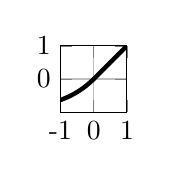
\begin{tikzpicture}
\begin{axis}[
	xmin=-1,xmax=1,
	ymin=-1,ymax=1,
	ytick={0, 1},
	yticklabels={0,1},
	xtick={-1, 0, 1},
	xticklabels={-1,0,1},
	width=.2\textwidth,
	height=.2\textwidth,
	grid=both,
	]
	\addplot [ultra thick,domain=-0.0035:1, samples=10]{x};
	\addplot [ultra thick,domain=-1:0.004, samples=10]{exp(x)-1};
\end{axis}
\end{tikzpicture}}
		\scalebox{.9}{% This file was created by tikzplotlib v0.9.6.
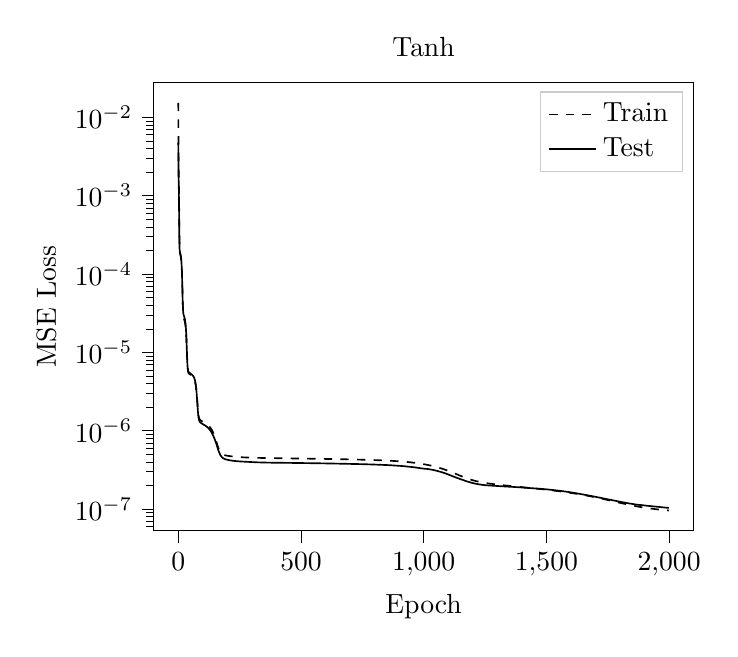
\begin{tikzpicture}

\begin{axis}[
legend cell align={left},
legend style={fill opacity=0.8, draw opacity=1, text opacity=1, draw=white!80!black},
log basis y={10},
tick align=outside,
tick pos=left,
title={Tanh},
x grid style={white!69.0196078431373!black},
xlabel={Epoch},
xmin=-99.95, xmax=2098.95,
xtick style={color=black},
y grid style={white!69.0196078431373!black},
ylabel={MSE Loss},
ymin=5.2838355076584e-08, ymax=0.0278720888075092,
ymode=log,
ytick style={color=black}
]
\addplot [semithick, black, dashed]
table {%
0 0.0153132931897417
1 0.00263468591915444
2 0.00157368404231966
3 0.00100973634771071
4 0.000470805197954178
5 0.000238240016129566
6 0.000192290817329194
7 0.000182392153321416
8 0.000177044864372874
9 0.000172117064284976
10 0.000166500588362396
11 0.00015954268569476
12 0.000150556041538948
13 0.000138711679741391
14 0.000123201339192747
15 0.00010384852115385
16 8.21741918771295e-05
17 6.17140098838718e-05
18 4.59808605392027e-05
19 3.61075856744719e-05
20 3.09615153473715e-05
21 2.86084769759327e-05
22 2.75036924476808e-05
23 2.68262024928845e-05
24 2.62473645334467e-05
25 2.56512312862469e-05
26 2.49876472216783e-05
27 2.42189531372787e-05
28 2.33048581776529e-05
29 2.21992105016398e-05
30 2.0851133920587e-05
31 1.92123597071259e-05
32 1.72571510574926e-05
33 1.50208010131792e-05
34 1.26468071212003e-05
35 1.03939191099016e-05
36 8.54036681334946e-06
37 7.2278788722997e-06
38 6.40808496189038e-06
39 5.93531661445468e-06
40 5.67199906026872e-06
41 5.52505381187984e-06
42 5.43974953552606e-06
43 5.38575441578359e-06
44 5.34706065189994e-06
45 5.31567630139307e-06
46 5.28771059708788e-06
47 5.26119667091507e-06
48 5.23525572231165e-06
49 5.20944819999158e-06
50 5.18347152382148e-06
51 5.15708841510332e-06
52 5.13011461384849e-06
53 5.10235067065423e-06
54 5.07353104478625e-06
55 5.04333890773978e-06
56 5.01150577724729e-06
57 4.97761710209943e-06
58 4.94116837637648e-06
59 4.90160364131498e-06
60 4.85830068294035e-06
61 4.81051573763125e-06
62 4.75736579585373e-06
63 4.69784373001403e-06
64 4.63084353839349e-06
65 4.55505242621257e-06
66 4.4689069618471e-06
67 4.37072546117179e-06
68 4.25872251423698e-06
69 4.13099127399619e-06
70 3.98556936380601e-06
71 3.82073990112985e-06
72 3.63538441825995e-06
73 3.42947709879127e-06
74 3.20474518565561e-06
75 2.96533639118479e-06
76 2.71820525040312e-06
77 2.47301909183761e-06
78 2.24097093428099e-06
79 2.03303970391744e-06
80 1.85738974289507e-06
81 1.7172159946881e-06
82 1.61103087606307e-06
83 1.53408617211426e-06
84 1.4801255596808e-06
85 1.44289974394951e-06
86 1.41705882572296e-06
87 1.39857534634302e-06
88 1.38478061057867e-06
89 1.37394659657275e-06
90 1.36493259270765e-06
91 1.35709255721395e-06
92 1.35006773837176e-06
93 1.3435876031167e-06
94 1.33744865189556e-06
95 1.33153407006148e-06
96 1.32577587834248e-06
97 1.32013072266091e-06
98 1.31456864949087e-06
99 1.30906824693966e-06
100 1.30361027811432e-06
101 1.29817983048497e-06
102 1.2927648969594e-06
103 1.28735057194262e-06
104 1.28192672787009e-06
105 1.27648085845067e-06
106 1.27100161500948e-06
107 1.26547873554728e-06
108 1.25990110808516e-06
109 1.25425981912031e-06
110 1.24854659134144e-06
111 1.24275286356124e-06
112 1.23686820501234e-06
113 1.23088176826514e-06
114 1.22477484546835e-06
115 1.21851538432338e-06
116 1.21207589478445e-06
117 1.20545096717706e-06
118 1.19864200888742e-06
119 1.19164904162972e-06
120 1.18446295368813e-06
121 1.17707011526136e-06
122 1.1694574324963e-06
123 1.16160844515889e-06
124 1.15350741776865e-06
125 1.14514046717318e-06
126 1.13649216663703e-06
127 1.12754831607731e-06
128 1.11829535674701e-06
129 1.10871652933042e-06
130 1.09879741285113e-06
131 1.08852268132864e-06
132 1.07788214393167e-06
133 1.06686042701654e-06
134 1.05544191262652e-06
135 1.04361316667223e-06
136 1.03136227298251e-06
137 1.01868055929799e-06
138 1.00555776742794e-06
139 9.91986293712444e-07
140 9.77953460363779e-07
141 9.63472345659966e-07
142 9.48564746323655e-07
143 9.33224022247714e-07
144 9.17436783851144e-07
145 9.01233095419229e-07
146 8.84645438446796e-07
147 8.6771310790823e-07
148 8.50481537099768e-07
149 8.32998301291354e-07
150 8.15313805475171e-07
151 7.97497160306193e-07
152 7.79638045287356e-07
153 7.61828415562604e-07
154 7.44165269679797e-07
155 7.26727081797662e-07
156 7.09585356162279e-07
157 6.92824803678604e-07
158 6.76534470272827e-07
159 6.60814733251414e-07
160 6.45768715401118e-07
161 6.31504774517566e-07
162 6.1806144752552e-07
163 6.0541898541544e-07
164 5.935898469005e-07
165 5.82608957756747e-07
166 5.7251111570622e-07
167 5.63264185785783e-07
168 5.54845568970563e-07
169 5.47202532217739e-07
170 5.40264816024205e-07
171 5.34007824569471e-07
172 5.28409758743464e-07
173 5.23425921969078e-07
174 5.18951096410092e-07
175 5.149205651378e-07
176 5.113566061965e-07
177 5.0820041903421e-07
178 5.0539328245236e-07
179 5.02919986971051e-07
180 5.00717105182957e-07
181 4.98696329472637e-07
182 4.96904277937915e-07
183 4.95304723173717e-07
184 4.93817427653198e-07
185 4.92438486588753e-07
186 4.91190134695785e-07
187 4.90051529411062e-07
188 4.8898569615119e-07
189 4.87990284483431e-07
190 4.87074258344933e-07
191 4.86203401237617e-07
192 4.8538464466219e-07
193 4.84598177266093e-07
194 4.83853644809074e-07
195 4.83136612828616e-07
196 4.82444658544523e-07
197 4.81775210417368e-07
198 4.81127108898249e-07
199 4.80499700458381e-07
200 4.79891992156922e-07
201 4.79301355042594e-07
202 4.78727373860011e-07
203 4.78168406615964e-07
204 4.77623684233208e-07
205 4.77091803091412e-07
206 4.76571929311831e-07
207 4.76063083382883e-07
208 4.7556500614121e-07
209 4.75079109705234e-07
210 4.74604136101675e-07
211 4.74139817058017e-07
212 4.73685574092997e-07
213 4.732392057889e-07
214 4.72801231126141e-07
215 4.72370848783044e-07
216 4.71947753624136e-07
217 4.71531814710602e-07
218 4.71123629139925e-07
219 4.70721878500058e-07
220 4.70326882307859e-07
221 4.69938081565147e-07
222 4.6955573562002e-07
223 4.69178338335041e-07
224 4.68806766932062e-07
225 4.68441367843297e-07
226 4.68085043436872e-07
227 4.67738976894339e-07
228 4.6739916845695e-07
229 4.67063946416602e-07
230 4.66734159886073e-07
231 4.66409362445575e-07
232 4.66089655560609e-07
233 4.65775199188556e-07
234 4.65466167142381e-07
235 4.65162220166349e-07
236 4.64862401173605e-07
237 4.64568502394513e-07
238 4.64278388264461e-07
239 4.63993729752588e-07
240 4.63713339598826e-07
241 4.63437639041331e-07
242 4.631659465133e-07
243 4.62899604784184e-07
244 4.62637191432691e-07
245 4.6237910713387e-07
246 4.62124751962278e-07
247 4.61875437409276e-07
248 4.61630108432587e-07
249 4.61388637120308e-07
250 4.61151012316918e-07
251 4.60918176742098e-07
252 4.60688900972173e-07
253 4.60463183557636e-07
254 4.60240989667682e-07
255 4.60023742206772e-07
256 4.59809431802682e-07
257 4.59599144193135e-07
258 4.59392179394058e-07
259 4.59188554302159e-07
260 4.58988357280532e-07
261 4.5879247274172e-07
262 4.58599594026055e-07
263 4.58409956038963e-07
264 4.58223486660359e-07
265 4.58040425911577e-07
266 4.57860810300303e-07
267 4.57683898687833e-07
268 4.57510935063965e-07
269 4.57340171877263e-07
270 4.57172989371202e-07
271 4.5700948594174e-07
272 4.56848700437718e-07
273 4.56690176079633e-07
274 4.56532334069948e-07
275 4.56378028999893e-07
276 4.56227564370693e-07
277 4.56079020167977e-07
278 4.55933057864399e-07
279 4.55789513395644e-07
280 4.55647950658999e-07
281 4.55509062945225e-07
282 4.55372698311862e-07
283 4.55238444189376e-07
284 4.55106499074986e-07
285 4.54976572086707e-07
286 4.54848537472685e-07
287 4.54722759030801e-07
288 4.54598988000043e-07
289 4.54477126126562e-07
290 4.54357528710148e-07
291 4.54239268904644e-07
292 4.5412372236342e-07
293 4.54009004798195e-07
294 4.53896645950636e-07
295 4.53786352096586e-07
296 4.53676708488615e-07
297 4.53569238302975e-07
298 4.53463479189509e-07
299 4.53359586160218e-07
300 4.5325645915284e-07
301 4.53154825493129e-07
302 4.53054902010308e-07
303 4.52956216690836e-07
304 4.52858107877319e-07
305 4.52761391798617e-07
306 4.52666627438703e-07
307 4.5257209372096e-07
308 4.52479442387244e-07
309 4.52388870797904e-07
310 4.52298658686345e-07
311 4.52208053658865e-07
312 4.52117211708014e-07
313 4.5202447013537e-07
314 4.51931193893529e-07
315 4.51840439652074e-07
316 4.51755951914379e-07
317 4.516765107212e-07
318 4.51600721788736e-07
319 4.51526182288831e-07
320 4.51450262687558e-07
321 4.51373784770226e-07
322 4.51297628643488e-07
323 4.51222715412314e-07
324 4.51148725105099e-07
325 4.51075450911276e-07
326 4.51002795969657e-07
327 4.50931086078299e-07
328 4.50860197716452e-07
329 4.50789848585487e-07
330 4.5072036765248e-07
331 4.50651828217019e-07
332 4.50583665013937e-07
333 4.50516136069723e-07
334 4.50449156701893e-07
335 4.5038280858023e-07
336 4.50316983886978e-07
337 4.50252412150576e-07
338 4.50187744334585e-07
339 4.50123620197473e-07
340 4.50059869905317e-07
341 4.49996963155286e-07
342 4.49934251392392e-07
343 4.49872764946235e-07
344 4.49810905891468e-07
345 4.49749873581595e-07
346 4.49688656800618e-07
347 4.49628481419495e-07
348 4.49568800718225e-07
349 4.49509138277904e-07
350 4.49449652847989e-07
351 4.49391284675471e-07
352 4.49332757710863e-07
353 4.49274186948401e-07
354 4.49216128771468e-07
355 4.49158206649258e-07
356 4.4910005910026e-07
357 4.49041933933358e-07
358 4.48982399845477e-07
359 4.48921653429579e-07
360 4.4885858659427e-07
361 4.48796846825417e-07
362 4.48741282951914e-07
363 4.48690722535616e-07
364 4.48639755177282e-07
365 4.48585934890389e-07
366 4.4853153957547e-07
367 4.48477469873865e-07
368 4.48423670761144e-07
369 4.48369932087189e-07
370 4.48316616555644e-07
371 4.48263513959546e-07
372 4.48211177371149e-07
373 4.48158735053994e-07
374 4.48106252406433e-07
375 4.48054085751437e-07
376 4.4800212175744e-07
377 4.4795040194856e-07
378 4.47898859235352e-07
379 4.47847473722618e-07
380 4.47796142310608e-07
381 4.47745204766647e-07
382 4.47694311603186e-07
383 4.47643480271154e-07
384 4.4759237508174e-07
385 4.47542060669548e-07
386 4.47491346719175e-07
387 4.47440747194605e-07
388 4.47390521486568e-07
389 4.4734031470739e-07
390 4.47290107231879e-07
391 4.47240181983943e-07
392 4.47190574547562e-07
393 4.47140450361871e-07
394 4.4709078622418e-07
395 4.47040961347511e-07
396 4.46991613557657e-07
397 4.46942280575513e-07
398 4.46892466911208e-07
399 4.46843225162752e-07
400 4.46794205998913e-07
401 4.46744886289707e-07
402 4.46695940368613e-07
403 4.46646912564574e-07
404 4.46597692658202e-07
405 4.46548597153651e-07
406 4.46500398439298e-07
407 4.46451654809721e-07
408 4.46402832963599e-07
409 4.46354196625975e-07
410 4.46306129020968e-07
411 4.46257712596321e-07
412 4.46209294665323e-07
413 4.46161581564297e-07
414 4.46113736870757e-07
415 4.46065096895154e-07
416 4.46016953446815e-07
417 4.45968802125662e-07
418 4.45921565813023e-07
419 4.45873601037761e-07
420 4.45826225742962e-07
421 4.45778409485342e-07
422 4.45730791852839e-07
423 4.45683437220623e-07
424 4.45636114307035e-07
425 4.45588812254982e-07
426 4.45541871997079e-07
427 4.45494792089107e-07
428 4.45448116849434e-07
429 4.45400671310381e-07
430 4.45353895372591e-07
431 4.45306549750057e-07
432 4.45259898953054e-07
433 4.45212845349374e-07
434 4.45166658622043e-07
435 4.45119889278089e-07
436 4.45073022035558e-07
437 4.45026548547389e-07
438 4.44980165639208e-07
439 4.4493387888167e-07
440 4.44887311957132e-07
441 4.44841445556676e-07
442 4.44794834720597e-07
443 4.44749098505781e-07
444 4.44702441498634e-07
445 4.44656845346003e-07
446 4.44611437771414e-07
447 4.44566093690923e-07
448 4.44520632100875e-07
449 4.44475479596917e-07
450 4.44428526719776e-07
451 4.44381641216296e-07
452 4.44334865875362e-07
453 4.44288736886733e-07
454 4.44242559808572e-07
455 4.44196356198745e-07
456 4.44150075907146e-07
457 4.44104312123272e-07
458 4.44058151245486e-07
459 4.44012046727948e-07
460 4.4396607486874e-07
461 4.43919723053909e-07
462 4.43873894312219e-07
463 4.43827820333809e-07
464 4.43781376830543e-07
465 4.43735788735466e-07
466 4.43689252719537e-07
467 4.43644105700969e-07
468 4.4359714057407e-07
469 4.43552091695665e-07
470 4.4350487823408e-07
471 4.43460639928617e-07
472 4.43412761498507e-07
473 4.43368704566183e-07
474 4.43320460263408e-07
475 4.43276697680517e-07
476 4.43227898742293e-07
477 4.43185115173605e-07
478 4.43134583662186e-07
479 4.43093923777838e-07
480 4.4304159730757e-07
481 4.43003092911454e-07
482 4.42947890576306e-07
483 4.42912595630673e-07
484 4.42853963079415e-07
485 4.42821147373706e-07
486 4.4276031600532e-07
487 4.42729391878061e-07
488 4.42667331853386e-07
489 4.4263708812764e-07
490 4.42574523304984e-07
491 4.42544547510693e-07
492 4.42481593594835e-07
493 4.42452258837989e-07
494 4.42388692619033e-07
495 4.42359383242774e-07
496 4.4229542483265e-07
497 4.42266830077642e-07
498 4.42202625464461e-07
499 4.42173881253893e-07
500 4.42109330492713e-07
501 4.42080638251241e-07
502 4.42015572744481e-07
503 4.41987434598445e-07
504 4.41922236504411e-07
505 4.41894427794409e-07
506 4.41828457454108e-07
507 4.41800639549683e-07
508 4.41734856408971e-07
509 4.417071328362e-07
510 4.41640802762322e-07
511 4.4161302048451e-07
512 4.41546921535974e-07
513 4.41519292778025e-07
514 4.4145272232754e-07
515 4.41425100333959e-07
516 4.41358092018618e-07
517 4.41330398814443e-07
518 4.4126369105868e-07
519 4.41236333685424e-07
520 4.4116943638528e-07
521 4.41140844500865e-07
522 4.41074515421747e-07
523 4.41045736721435e-07
524 4.40979312173795e-07
525 4.40951058521932e-07
526 4.4088429109479e-07
527 4.4085522711157e-07
528 4.40789318943757e-07
529 4.40759966153337e-07
530 4.40693232505396e-07
531 4.40663924607065e-07
532 4.40597787843444e-07
533 4.4056797210601e-07
534 4.40501284671768e-07
535 4.40471759517891e-07
536 4.4040554909941e-07
537 4.40375271367088e-07
538 4.40308756921581e-07
539 4.40278385511306e-07
540 4.40212674490681e-07
541 4.401812428938e-07
542 4.40115519111828e-07
543 4.40083868014085e-07
544 4.40018118496255e-07
545 4.39986295432959e-07
546 4.39920736553745e-07
547 4.39889069994592e-07
548 4.39823198377098e-07
549 4.3979057819854e-07
550 4.3972551353022e-07
551 4.39692232106381e-07
552 4.39627020057287e-07
553 4.39593548279049e-07
554 4.39528886658991e-07
555 4.39495016678393e-07
556 4.3943037410088e-07
557 4.39395672088949e-07
558 4.39331445349467e-07
559 4.39295989437483e-07
560 4.39232069638251e-07
561 4.39196281703858e-07
562 4.39132677342968e-07
563 4.39096512479864e-07
564 4.39032612277401e-07
565 4.38996117537727e-07
566 4.38933144138787e-07
567 4.38895417261165e-07
568 4.38832481677309e-07
569 4.38794382205288e-07
570 4.38731703610529e-07
571 4.38692871355784e-07
572 4.38631030220904e-07
573 4.38591341904271e-07
574 4.3853019623441e-07
575 4.38489292349686e-07
576 4.38428836289972e-07
577 4.38387495165671e-07
578 4.38326876377459e-07
579 4.3828513126698e-07
580 4.38225001701653e-07
581 4.38182326050196e-07
582 4.38123647242605e-07
583 4.38079974927064e-07
584 4.38020879528267e-07
585 4.37976561215692e-07
586 4.37918560521666e-07
587 4.3787362352532e-07
588 4.37815096447025e-07
589 4.3776925465977e-07
590 4.37711424595477e-07
591 4.37664399697724e-07
592 4.3760680487992e-07
593 4.3755960098224e-07
594 4.37502337533147e-07
595 4.37453951533939e-07
596 4.37396866345807e-07
597 4.37347725480208e-07
598 4.3729104187662e-07
599 4.37240820573948e-07
600 4.37184705148752e-07
601 4.37133718421023e-07
602 4.37077845234057e-07
603 4.37026187384504e-07
604 4.36970854678975e-07
605 4.3691830096293e-07
606 4.36862710003538e-07
607 4.36810370658236e-07
608 4.3675528922904e-07
609 4.36701593457656e-07
610 4.36646212094161e-07
611 4.36592203740815e-07
612 4.36536973964508e-07
613 4.36482874889066e-07
614 4.3642749051287e-07
615 4.36372963392273e-07
616 4.36317296390598e-07
617 4.36262127664122e-07
618 4.36206559811581e-07
619 4.36151188210943e-07
620 4.360954301319e-07
621 4.36040008409577e-07
622 4.35984044571569e-07
623 4.35928163838639e-07
624 4.35871852630498e-07
625 4.35815706538278e-07
626 4.35759265940305e-07
627 4.35702904624691e-07
628 4.35646074592455e-07
629 4.3558944291533e-07
630 4.35532369664315e-07
631 4.35475516837869e-07
632 4.35418206095051e-07
633 4.35361169124349e-07
634 4.35303863625336e-07
635 4.35246203821293e-07
636 4.35188680029341e-07
637 4.35130771123227e-07
638 4.35072627297473e-07
639 4.35014651216647e-07
640 4.34956360976457e-07
641 4.34898258731664e-07
642 4.3483965933433e-07
643 4.34781021880326e-07
644 4.34722310572511e-07
645 4.34663314436534e-07
646 4.34604027944374e-07
647 4.34545088054961e-07
648 4.34486076045459e-07
649 4.34426052166259e-07
650 4.3436669619723e-07
651 4.34306966951681e-07
652 4.34247524083275e-07
653 4.34187044504597e-07
654 4.34126650318944e-07
655 4.3406678015856e-07
656 4.34006311721191e-07
657 4.33945470703634e-07
658 4.3388504241193e-07
659 4.33823856454296e-07
660 4.33762479801203e-07
661 4.33701213708559e-07
662 4.33640064017027e-07
663 4.33578119313438e-07
664 4.33516226209463e-07
665 4.33454814398715e-07
666 4.33392396331556e-07
667 4.33329818136485e-07
668 4.33267958186434e-07
669 4.33204892530625e-07
670 4.33141973672946e-07
671 4.33078773085072e-07
672 4.33015674914827e-07
673 4.32951755399813e-07
674 4.32888073888194e-07
675 4.32823758643508e-07
676 4.32759608656852e-07
677 4.32694734612937e-07
678 4.32630114346466e-07
679 4.32565253049688e-07
680 4.32499659765995e-07
681 4.32433980776636e-07
682 4.32368343098233e-07
683 4.32302421103259e-07
684 4.32236600659053e-07
685 4.32170115175268e-07
686 4.32103654475213e-07
687 4.32037323932377e-07
688 4.31970005976723e-07
689 4.31903165861058e-07
690 4.31835885436271e-07
691 4.31768051683434e-07
692 4.31700327666817e-07
693 4.31633078846971e-07
694 4.31564529478123e-07
695 4.31496353158423e-07
696 4.31427578959642e-07
697 4.31358720646813e-07
698 4.31290260664241e-07
699 4.31221317384711e-07
700 4.31151998313339e-07
701 4.3108227941957e-07
702 4.31012523691265e-07
703 4.30942949222413e-07
704 4.3087253446572e-07
705 4.30802091443638e-07
706 4.30731750626023e-07
707 4.3066083789256e-07
708 4.30589486001054e-07
709 4.30518474843211e-07
710 4.30447059429184e-07
711 4.30375201659672e-07
712 4.30303392221276e-07
713 4.30231511501233e-07
714 4.3015977574612e-07
715 4.3008838706271e-07
716 4.30019053183628e-07
717 4.29953882459699e-07
718 4.29896650700812e-07
719 4.29822231993171e-07
720 4.2974184988509e-07
721 4.29663981321937e-07
722 4.29589445687384e-07
723 4.29516379668371e-07
724 4.29441970496214e-07
725 4.29364652404729e-07
726 4.29286579191057e-07
727 4.2920867996088e-07
728 4.29130572740632e-07
729 4.29052638310168e-07
730 4.28974418824168e-07
731 4.28895949170283e-07
732 4.28817700779405e-07
733 4.28738986272492e-07
734 4.28659984379465e-07
735 4.28580363461606e-07
736 4.28501005529824e-07
737 4.28420907368832e-07
738 4.28341064676374e-07
739 4.28259974668777e-07
740 4.28179160820719e-07
741 4.28097994443988e-07
742 4.28016579022028e-07
743 4.27933960622795e-07
744 4.27851577697425e-07
745 4.27769046169146e-07
746 4.27685715337134e-07
747 4.27602619794243e-07
748 4.27518155447615e-07
749 4.27433968880564e-07
750 4.27349275298639e-07
751 4.27264355025159e-07
752 4.2717858150354e-07
753 4.27093193394512e-07
754 4.27006655044693e-07
755 4.26920569864819e-07
756 4.26833762972478e-07
757 4.26746492280472e-07
758 4.26658948086356e-07
759 4.26571777708773e-07
760 4.26483888219309e-07
761 4.26396722218669e-07
762 4.26308664899011e-07
763 4.26221024667939e-07
764 4.26133200789991e-07
765 4.26043656887032e-07
766 4.25952536673435e-07
767 4.25861212193013e-07
768 4.25769250114172e-07
769 4.25676015069598e-07
770 4.25583642950755e-07
771 4.25490218106006e-07
772 4.25396803919398e-07
773 4.25302942758776e-07
774 4.25208595927984e-07
775 4.25113812013933e-07
776 4.25018646737385e-07
777 4.24922889891377e-07
778 4.24826633590669e-07
779 4.24729910164956e-07
780 4.24632532158853e-07
781 4.24534486185735e-07
782 4.24435824896818e-07
783 4.24336194910779e-07
784 4.24236452730042e-07
785 4.24136100704686e-07
786 4.24034741797641e-07
787 4.2393291576559e-07
788 4.23831002223096e-07
789 4.23727700493259e-07
790 4.23624593693717e-07
791 4.23520817520284e-07
792 4.23416092601769e-07
793 4.233113682659e-07
794 4.23206141306309e-07
795 4.23100903503837e-07
796 4.2299449046368e-07
797 4.22887794826465e-07
798 4.22781099018721e-07
799 4.22673134551133e-07
800 4.22564769195333e-07
801 4.22455741386329e-07
802 4.22345646171607e-07
803 4.22234838964641e-07
804 4.22122297180749e-07
805 4.22010236519554e-07
806 4.21896220629492e-07
807 4.21781650615571e-07
808 4.21667850659446e-07
809 4.21553422029319e-07
810 4.21439829892734e-07
811 4.21325296287023e-07
812 4.21210472168809e-07
813 4.21095024094598e-07
814 4.20978449184872e-07
815 4.20861232157677e-07
816 4.20743512691502e-07
817 4.20624905046907e-07
818 4.20505665687188e-07
819 4.20385636516585e-07
820 4.2026524386074e-07
821 4.20143697510866e-07
822 4.20021763972045e-07
823 4.19899434703552e-07
824 4.19775951186807e-07
825 4.19651953350808e-07
826 4.19527260504537e-07
827 4.1940189035472e-07
828 4.19275116527729e-07
829 4.19147858437441e-07
830 4.19019859464242e-07
831 4.18891167825564e-07
832 4.18760665780837e-07
833 4.18630356023186e-07
834 4.18498340792439e-07
835 4.18366126197611e-07
836 4.18232730254431e-07
837 4.18098747772433e-07
838 4.17964014957306e-07
839 4.17828126941799e-07
840 4.1769180576523e-07
841 4.17554468214121e-07
842 4.17416611611543e-07
843 4.17278087169848e-07
844 4.17138848717968e-07
845 4.16998658636203e-07
846 4.16857684271577e-07
847 4.16714902087278e-07
848 4.16571883661732e-07
849 4.16426834107142e-07
850 4.16280446643214e-07
851 4.16132222895271e-07
852 4.15983473530446e-07
853 4.15833202154658e-07
854 4.15681662872203e-07
855 4.1552967822156e-07
856 4.15376475629614e-07
857 4.15221758927942e-07
858 4.15066238758754e-07
859 4.14909692167953e-07
860 4.14752346017622e-07
861 4.14593858593548e-07
862 4.14433650448132e-07
863 4.14273077780081e-07
864 4.14110996572958e-07
865 4.1394791618643e-07
866 4.13783241640431e-07
867 4.13618292597562e-07
868 4.1345164329698e-07
869 4.13283892243044e-07
870 4.13115098893968e-07
871 4.12944745932009e-07
872 4.12773538926103e-07
873 4.12601342731023e-07
874 4.12427616268474e-07
875 4.12253036714105e-07
876 4.12077252818221e-07
877 4.11899781568081e-07
878 4.11721696224276e-07
879 4.11541758609246e-07
880 4.11360851586551e-07
881 4.11178559204473e-07
882 4.1099467759409e-07
883 4.10809515756227e-07
884 4.10622025370344e-07
885 4.10434007392269e-07
886 4.10244243184366e-07
887 4.10052710776654e-07
888 4.09860364456449e-07
889 4.09665865618081e-07
890 4.09470500798648e-07
891 4.09273717622227e-07
892 4.09075668997616e-07
893 4.08876081706921e-07
894 4.08675382104207e-07
895 4.08473281737542e-07
896 4.08270176066594e-07
897 4.08065752978359e-07
898 4.07860425198692e-07
899 4.07653831928201e-07
900 4.07445782528271e-07
901 4.07236672614886e-07
902 4.07026502514896e-07
903 4.06813603859746e-07
904 4.06598918075929e-07
905 4.06381167522341e-07
906 4.06158879513896e-07
907 4.05932690142663e-07
908 4.05703107304589e-07
909 4.05472865068646e-07
910 4.05241465941231e-07
911 4.05009318669158e-07
912 4.0477494502511e-07
913 4.04539864945264e-07
914 4.04302709910098e-07
915 4.04063302667623e-07
916 4.03822085488059e-07
917 4.03579558138745e-07
918 4.033347797332e-07
919 4.03087997696616e-07
920 4.02839564642932e-07
921 4.02589417461741e-07
922 4.02337238583073e-07
923 4.02083330115488e-07
924 4.01827826337353e-07
925 4.01570990803179e-07
926 4.01312498283346e-07
927 4.01053424084807e-07
928 4.0079356530498e-07
929 4.00534475417658e-07
930 4.00275759091073e-07
931 4.00020543196433e-07
932 3.99772352338346e-07
933 3.99518462245396e-07
934 3.99232151195861e-07
935 3.98937988194348e-07
936 3.98645003727438e-07
937 3.98352930972123e-07
938 3.98060276623369e-07
939 3.97767320862386e-07
940 3.9747197169504e-07
941 3.97174885563345e-07
942 3.96875663838614e-07
943 3.96573709068093e-07
944 3.96269294299145e-07
945 3.95962251246829e-07
946 3.95652659364032e-07
947 3.95340199190741e-07
948 3.95024775599495e-07
949 3.94706344408746e-07
950 3.94385574523426e-07
951 3.94061606812102e-07
952 3.93735439743637e-07
953 3.93406619821235e-07
954 3.93075350586969e-07
955 3.92741415438991e-07
956 3.92404345490149e-07
957 3.92064834102257e-07
958 3.91723577337189e-07
959 3.91379281069248e-07
960 3.91034041427929e-07
961 3.90688773293846e-07
962 3.90346557168186e-07
963 3.90006709622526e-07
964 3.89655191483484e-07
965 3.89290695778755e-07
966 3.88920869298204e-07
967 3.88549075182709e-07
968 3.88173222447108e-07
969 3.8779496591701e-07
970 3.87414582206702e-07
971 3.87031748786626e-07
972 3.86646552470893e-07
973 3.86258531918315e-07
974 3.85867048294131e-07
975 3.85473004882897e-07
976 3.85075737952434e-07
977 3.84675612480123e-07
978 3.84272473326064e-07
979 3.83866463693039e-07
980 3.83457353393624e-07
981 3.83045446341157e-07
982 3.8263090681312e-07
983 3.82212844257879e-07
984 3.81791498597295e-07
985 3.81366960709784e-07
986 3.80938562585698e-07
987 3.80507647548711e-07
988 3.80072127001085e-07
989 3.79633905382093e-07
990 3.79191937213363e-07
991 3.78746454927636e-07
992 3.78297291305785e-07
993 3.77845757824957e-07
994 3.77390559108903e-07
995 3.76932602179636e-07
996 3.76471325751027e-07
997 3.76008280454698e-07
998 3.75541477225738e-07
999 3.75072237204677e-07
1000 3.7459984805821e-07
1001 3.74125481229726e-07
1002 3.73646918262693e-07
1003 3.73165787280527e-07
1004 3.72680323081909e-07
1005 3.72192169535879e-07
1006 3.71700637074923e-07
1007 3.71204669733061e-07
1008 3.70705578362163e-07
1009 3.70202004802422e-07
1010 3.69694279910959e-07
1011 3.69181772597926e-07
1012 3.68664246721551e-07
1013 3.681415544321e-07
1014 3.67614507638336e-07
1015 3.67081920842338e-07
1016 3.66545533125873e-07
1017 3.66004452104107e-07
1018 3.65459960207204e-07
1019 3.64911836001625e-07
1020 3.64359034833228e-07
1021 3.6380328792518e-07
1022 3.63243735947094e-07
1023 3.62680784817826e-07
1024 3.62114355766607e-07
1025 3.61544524508872e-07
1026 3.60971631920393e-07
1027 3.60395439116701e-07
1028 3.59816504726496e-07
1029 3.59235964836557e-07
1030 3.58656483086861e-07
1031 3.58083547425281e-07
1032 3.57522725224158e-07
1033 3.56926418660919e-07
1034 3.56303529571278e-07
1035 3.55682074967945e-07
1036 3.55060193186318e-07
1037 3.54437427859011e-07
1038 3.5381234674503e-07
1039 3.53183879298058e-07
1040 3.52551655893762e-07
1041 3.51915701330086e-07
1042 3.51275422403319e-07
1043 3.50631737319418e-07
1044 3.4998303625855e-07
1045 3.49329645885632e-07
1046 3.48672467296751e-07
1047 3.48009736427457e-07
1048 3.47343681923462e-07
1049 3.46672493677147e-07
1050 3.45998814935911e-07
1051 3.45321498528506e-07
1052 3.44641047959726e-07
1053 3.43958320314641e-07
1054 3.43274007221339e-07
1055 3.42586759970231e-07
1056 3.41892986696735e-07
1057 3.41189594550428e-07
1058 3.404795624391e-07
1059 3.39765766298683e-07
1060 3.39050039997346e-07
1061 3.3833003406869e-07
1062 3.37607688265962e-07
1063 3.36880876574241e-07
1064 3.36151293524267e-07
1065 3.35417476918565e-07
1066 3.34680441582691e-07
1067 3.33939445610554e-07
1068 3.33195361704952e-07
1069 3.32447472445097e-07
1070 3.31696120113634e-07
1071 3.30941572030952e-07
1072 3.30182967516635e-07
1073 3.29421627640158e-07
1074 3.2865669591331e-07
1075 3.27889004125836e-07
1076 3.27117375050534e-07
1077 3.26343478178615e-07
1078 3.25565995140664e-07
1079 3.24785622467516e-07
1080 3.24002263027978e-07
1081 3.23216242321678e-07
1082 3.22426995978731e-07
1083 3.21635197906289e-07
1084 3.20840995044591e-07
1085 3.2004399291452e-07
1086 3.19244291389964e-07
1087 3.18442804314145e-07
1088 3.17637995706832e-07
1089 3.16831385660521e-07
1090 3.16022540800986e-07
1091 3.15211519406944e-07
1092 3.14398081741274e-07
1093 3.13583012015783e-07
1094 3.12765971898443e-07
1095 3.11946512724148e-07
1096 3.11125813070134e-07
1097 3.10302116616867e-07
1098 3.09477197205865e-07
1099 3.08649907680092e-07
1100 3.07821044899015e-07
1101 3.0698964995679e-07
1102 3.06157764725867e-07
1103 3.05322166866517e-07
1104 3.04485925980202e-07
1105 3.0364774683278e-07
1106 3.02807980276043e-07
1107 3.01966883128557e-07
1108 3.0112456292386e-07
1109 3.00281082743936e-07
1110 2.99436364144867e-07
1111 2.98590662367815e-07
1112 2.97743985655075e-07
1113 2.96896792107759e-07
1114 2.96048539510707e-07
1115 2.95200142630847e-07
1116 2.9435054504745e-07
1117 2.93500982749606e-07
1118 2.92650637334191e-07
1119 2.91800108698226e-07
1120 2.9094992638079e-07
1121 2.90099760817952e-07
1122 2.89249575743611e-07
1123 2.88399622419888e-07
1124 2.87549891183403e-07
1125 2.86700686828567e-07
1126 2.85852116235219e-07
1127 2.85004466363148e-07
1128 2.84156917686573e-07
1129 2.833113814944e-07
1130 2.82466340067344e-07
1131 2.81622272865434e-07
1132 2.80779442320522e-07
1133 2.79938600925789e-07
1134 2.79098920543674e-07
1135 2.78261221239973e-07
1136 2.77424942709104e-07
1137 2.7659101108668e-07
1138 2.75759133117504e-07
1139 2.74929214128861e-07
1140 2.74102109017349e-07
1141 2.7327765670293e-07
1142 2.72455530605953e-07
1143 2.71636089678395e-07
1144 2.70820190138465e-07
1145 2.70006673019907e-07
1146 2.69197387709141e-07
1147 2.68391106217791e-07
1148 2.67587981753081e-07
1149 2.66789002964174e-07
1150 2.65994599502051e-07
1151 2.65204446193934e-07
1152 2.64420651618025e-07
1153 2.63643165197891e-07
1154 2.6287096785893e-07
1155 2.62102935209896e-07
1156 2.61339599404664e-07
1157 2.60580745035099e-07
1158 2.59827119279521e-07
1159 2.59079005601848e-07
1160 2.58335715543012e-07
1161 2.57598258826874e-07
1162 2.56866600224726e-07
1163 2.56140495224599e-07
1164 2.55420891818403e-07
1165 2.54707391391662e-07
1166 2.53999428608154e-07
1167 2.53297669530639e-07
1168 2.52602138033353e-07
1169 2.51913175546292e-07
1170 2.5123055119991e-07
1171 2.50554446068918e-07
1172 2.4988453451158e-07
1173 2.49220868113298e-07
1174 2.48563562664117e-07
1175 2.47913107543241e-07
1176 2.47267765985271e-07
1177 2.46628499951385e-07
1178 2.4599422802396e-07
1179 2.45367220358617e-07
1180 2.44747584019933e-07
1181 2.44135619325903e-07
1182 2.43530379634649e-07
1183 2.42931076385844e-07
1184 2.42336930853071e-07
1185 2.41747951989169e-07
1186 2.41164151375983e-07
1187 2.40584499820784e-07
1188 2.40010541517677e-07
1189 2.39446667933407e-07
1190 2.38895236151393e-07
1191 2.38354633495419e-07
1192 2.37820755614848e-07
1193 2.37289173298905e-07
1194 2.36763406590512e-07
1195 2.36243773386491e-07
1196 2.35730746808827e-07
1197 2.35224286811331e-07
1198 2.34724079476223e-07
1199 2.34229994532598e-07
1200 2.33742097790923e-07
1201 2.332605407247e-07
1202 2.32784929337981e-07
1203 2.32315856280252e-07
1204 2.31852274140465e-07
1205 2.31395183917016e-07
1206 2.30944453235793e-07
1207 2.30499279183505e-07
1208 2.30060687911759e-07
1209 2.29627991373604e-07
1210 2.29201936448931e-07
1211 2.28782327823751e-07
1212 2.28369903197745e-07
1213 2.27964066269237e-07
1214 2.27565496700777e-07
1215 2.27173953078363e-07
1216 2.26790246045994e-07
1217 2.26415428585369e-07
1218 2.26050232640773e-07
1219 2.25693971842134e-07
1220 2.25338671370423e-07
1221 2.24972011622526e-07
1222 2.24602440894728e-07
1223 2.24238834562129e-07
1224 2.23883001922331e-07
1225 2.23533508687979e-07
1226 2.23189845812044e-07
1227 2.22851655664158e-07
1228 2.22517799258526e-07
1229 2.22188851282112e-07
1230 2.21864169844821e-07
1231 2.21543284496306e-07
1232 2.21226965379628e-07
1233 2.20914304776443e-07
1234 2.20605981127164e-07
1235 2.2030111284721e-07
1236 2.20000381048635e-07
1237 2.19703110403202e-07
1238 2.19409653851699e-07
1239 2.19119149249991e-07
1240 2.18831971437794e-07
1241 2.18548997196422e-07
1242 2.18268806818855e-07
1243 2.17991441388676e-07
1244 2.17717209466173e-07
1245 2.1744602784679e-07
1246 2.17177927765988e-07
1247 2.16912191319807e-07
1248 2.16650396936302e-07
1249 2.16390123270571e-07
1250 2.16133058799528e-07
1251 2.1587907644971e-07
1252 2.15627568863397e-07
1253 2.15378824073298e-07
1254 2.15131843241068e-07
1255 2.14888007782577e-07
1256 2.14646843559763e-07
1257 2.14407705186659e-07
1258 2.14170560518312e-07
1259 2.1393649831225e-07
1260 2.13704258435143e-07
1261 2.1347437109398e-07
1262 2.13246854215754e-07
1263 2.13020818328857e-07
1264 2.12796982168584e-07
1265 2.125756130269e-07
1266 2.12356135349978e-07
1267 2.12137947706026e-07
1268 2.11922217253857e-07
1269 2.11708398886401e-07
1270 2.11495935616313e-07
1271 2.11285770703284e-07
1272 2.11076535443055e-07
1273 2.10869454207341e-07
1274 2.1066421357574e-07
1275 2.1045999773861e-07
1276 2.1025769069638e-07
1277 2.10056241414236e-07
1278 2.09857041625128e-07
1279 2.09659049652089e-07
1280 2.09461995652305e-07
1281 2.0926700465651e-07
1282 2.09072476074823e-07
1283 2.08879468218015e-07
1284 2.0868736222468e-07
1285 2.08496854604334e-07
1286 2.08307065840074e-07
1287 2.0811799493714e-07
1288 2.07930388654631e-07
1289 2.07742703878466e-07
1290 2.07555825234351e-07
1291 2.07369623595355e-07
1292 2.07184382439607e-07
1293 2.07001097287218e-07
1294 2.06820774486971e-07
1295 2.06642172933869e-07
1296 2.06464475283497e-07
1297 2.06287604818556e-07
1298 2.06111494250649e-07
1299 2.05935856250505e-07
1300 2.05761286494521e-07
1301 2.05587725417899e-07
1302 2.05414359577105e-07
1303 2.0524219954865e-07
1304 2.05070374740046e-07
1305 2.04900051116397e-07
1306 2.04729819451188e-07
1307 2.04560695991063e-07
1308 2.04392164057765e-07
1309 2.04224752600624e-07
1310 2.0405743264007e-07
1311 2.03891090926334e-07
1312 2.03725257684084e-07
1313 2.03560172288064e-07
1314 2.03395246664684e-07
1315 2.03231465896181e-07
1316 2.03068005781404e-07
1317 2.02905416642807e-07
1318 2.02743438727282e-07
1319 2.02581670066593e-07
1320 2.02420751357124e-07
1321 2.02260203550964e-07
1322 2.02100084223389e-07
1323 2.01940410256896e-07
1324 2.01780698787957e-07
1325 2.01622603263729e-07
1326 2.01463833860771e-07
1327 2.01305658485751e-07
1328 2.0114791804815e-07
1329 2.0098994261275e-07
1330 2.00831707317661e-07
1331 2.0067317363015e-07
1332 2.00514492256332e-07
1333 2.00353759915117e-07
1334 2.00191533217264e-07
1335 2.00027188149932e-07
1336 1.99861917451472e-07
1337 1.99699144367571e-07
1338 1.9954218120688e-07
1339 1.99391871539945e-07
1340 1.99243989271736e-07
1341 1.9909605251911e-07
1342 1.98947011803341e-07
1343 1.98797260793526e-07
1344 1.98647412332775e-07
1345 1.98497241349571e-07
1346 1.9834731132562e-07
1347 1.98198011752027e-07
1348 1.98049309140913e-07
1349 1.97900511956561e-07
1350 1.97752460657341e-07
1351 1.97604831683407e-07
1352 1.97456864107437e-07
1353 1.97309753176e-07
1354 1.97163243690568e-07
1355 1.97016909247338e-07
1356 1.96871239580787e-07
1357 1.96725074466997e-07
1358 1.96580252968204e-07
1359 1.9643524857571e-07
1360 1.96289902675062e-07
1361 1.96145034429662e-07
1362 1.96000701237153e-07
1363 1.95856939036787e-07
1364 1.95712916287505e-07
1365 1.95569456138855e-07
1366 1.95426440789959e-07
1367 1.9528298147975e-07
1368 1.95140321508802e-07
1369 1.94997839102484e-07
1370 1.94855483051981e-07
1371 1.94714067042412e-07
1372 1.9457207280027e-07
1373 1.94430763414744e-07
1374 1.94288967051648e-07
1375 1.94148666814442e-07
1376 1.94007788685724e-07
1377 1.93867000021442e-07
1378 1.9372678165297e-07
1379 1.93586380675015e-07
1380 1.93446242960249e-07
1381 1.93306313704511e-07
1382 1.9316685001769e-07
1383 1.93027033866144e-07
1384 1.928881173896e-07
1385 1.92748827437583e-07
1386 1.92609713145941e-07
1387 1.92470996616123e-07
1388 1.92332163415188e-07
1389 1.92193213806036e-07
1390 1.92054977055989e-07
1391 1.91916928748981e-07
1392 1.91778728556358e-07
1393 1.91640867662102e-07
1394 1.91502521168729e-07
1395 1.91364721203513e-07
1396 1.91226667354272e-07
1397 1.9108902575482e-07
1398 1.90951581458876e-07
1399 1.90813802156242e-07
1400 1.90676621741659e-07
1401 1.90538358062042e-07
1402 1.90400840303084e-07
1403 1.90263191981899e-07
1404 1.90125171293687e-07
1405 1.89986778437401e-07
1406 1.89848554953187e-07
1407 1.8971032452697e-07
1408 1.89571864318339e-07
1409 1.89435156663365e-07
1410 1.89298512275116e-07
1411 1.89162471627924e-07
1412 1.89027391506613e-07
1413 1.88892291511422e-07
1414 1.8875688207487e-07
1415 1.88622368398228e-07
1416 1.88486953341283e-07
1417 1.88351250955066e-07
1418 1.88216109933137e-07
1419 1.88080516487332e-07
1420 1.87945151431279e-07
1421 1.87809692143048e-07
1422 1.87673937595889e-07
1423 1.87538295172374e-07
1424 1.8740287024599e-07
1425 1.87267376752231e-07
1426 1.8713166647899e-07
1427 1.86995634521736e-07
1428 1.86859856981414e-07
1429 1.8672422855559e-07
1430 1.8658855636744e-07
1431 1.86452587357167e-07
1432 1.86317243965561e-07
1433 1.86181103750016e-07
1434 1.86045110218913e-07
1435 1.85909304605048e-07
1436 1.85773195795491e-07
1437 1.8563674731098e-07
1438 1.85500630173863e-07
1439 1.85364702439017e-07
1440 1.85228678525107e-07
1441 1.85091931768966e-07
1442 1.84955936774145e-07
1443 1.8481905767942e-07
1444 1.84682557872407e-07
1445 1.84545949899473e-07
1446 1.84409362503857e-07
1447 1.84272837167043e-07
1448 1.84136263179369e-07
1449 1.83998937515639e-07
1450 1.83862002991475e-07
1451 1.83725183212857e-07
1452 1.83587768042059e-07
1453 1.8345057564062e-07
1454 1.83313025360121e-07
1455 1.831751825776e-07
1456 1.83038089282661e-07
1457 1.82900077319914e-07
1458 1.82761687497646e-07
1459 1.82624055767633e-07
1460 1.82485669327548e-07
1461 1.82347980498321e-07
1462 1.82209376120568e-07
1463 1.82070631119302e-07
1464 1.81931762497811e-07
1465 1.81793589483448e-07
1466 1.81654316875779e-07
1467 1.81515491554762e-07
1468 1.81376568512803e-07
1469 1.81236938274765e-07
1470 1.81097548917819e-07
1471 1.80957725802955e-07
1472 1.80818158590057e-07
1473 1.80678038027793e-07
1474 1.80538659130036e-07
1475 1.80398435141171e-07
1476 1.80258126057709e-07
1477 1.80117199768404e-07
1478 1.79976853104336e-07
1479 1.79836202470085e-07
1480 1.79695553192971e-07
1481 1.79554426821937e-07
1482 1.79413018962293e-07
1483 1.79271853156138e-07
1484 1.79130245065551e-07
1485 1.78988189610152e-07
1486 1.78846173938041e-07
1487 1.78704160241239e-07
1488 1.78561569086355e-07
1489 1.78418774439137e-07
1490 1.78275439829179e-07
1491 1.78132229585515e-07
1492 1.77988269832952e-07
1493 1.77844642124114e-07
1494 1.77700789940616e-07
1495 1.77556530303491e-07
1496 1.77413203722665e-07
1497 1.77269419246784e-07
1498 1.77125700552949e-07
1499 1.76981946104604e-07
1500 1.76837839454436e-07
1501 1.76693711736675e-07
1502 1.76549127644421e-07
1503 1.76404452886914e-07
1504 1.76259294093484e-07
1505 1.76114788217774e-07
1506 1.75969739686366e-07
1507 1.75823956546139e-07
1508 1.75678158655046e-07
1509 1.75532431981651e-07
1510 1.75386379034137e-07
1511 1.75240595915227e-07
1512 1.75093902704759e-07
1513 1.7494729726053e-07
1514 1.74800479889825e-07
1515 1.74653114910939e-07
1516 1.74505447041895e-07
1517 1.74357999242147e-07
1518 1.74210518537166e-07
1519 1.74062339922898e-07
1520 1.73913695810768e-07
1521 1.73764734256565e-07
1522 1.73616360349627e-07
1523 1.73467366380464e-07
1524 1.73317852578236e-07
1525 1.73168524227663e-07
1526 1.73018382426449e-07
1527 1.72868128714754e-07
1528 1.72718070842848e-07
1529 1.72567302954008e-07
1530 1.72416797767028e-07
1531 1.72265960898699e-07
1532 1.72114913766563e-07
1533 1.71963616836024e-07
1534 1.71812750110689e-07
1535 1.71661240734977e-07
1536 1.71510075475112e-07
1537 1.71359199399035e-07
1538 1.71208313396676e-07
1539 1.71057598102209e-07
1540 1.70907905925333e-07
1541 1.70758876727461e-07
1542 1.70609292091228e-07
1543 1.70460468254419e-07
1544 1.70312362698155e-07
1545 1.70163580897054e-07
1546 1.70014862639789e-07
1547 1.69866378691097e-07
1548 1.69717479316489e-07
1549 1.69566319698333e-07
1550 1.69413205235003e-07
1551 1.69262491603206e-07
1552 1.69118381393218e-07
1553 1.68960619944869e-07
1554 1.68795844842862e-07
1555 1.68634415963709e-07
1556 1.68473855467255e-07
1557 1.68314386073121e-07
1558 1.68154245599794e-07
1559 1.67994072640454e-07
1560 1.67833153817298e-07
1561 1.67671810075376e-07
1562 1.67509841304536e-07
1563 1.67347641095716e-07
1564 1.67185039479989e-07
1565 1.67022370270331e-07
1566 1.66858579163431e-07
1567 1.6669509652445e-07
1568 1.66530774116325e-07
1569 1.66365951564273e-07
1570 1.66200860505228e-07
1571 1.66035385390728e-07
1572 1.65869453141454e-07
1573 1.65703530747408e-07
1574 1.65537247930558e-07
1575 1.65369557223016e-07
1576 1.65202419346144e-07
1577 1.65034642208184e-07
1578 1.64866432960764e-07
1579 1.64697372412093e-07
1580 1.64528549724707e-07
1581 1.64359141180626e-07
1582 1.64189042507701e-07
1583 1.64018376509034e-07
1584 1.63848530839061e-07
1585 1.63677140456286e-07
1586 1.63505837697642e-07
1587 1.63334020520267e-07
1588 1.63161493020425e-07
1589 1.62988920223484e-07
1590 1.62815901546765e-07
1591 1.62642609133457e-07
1592 1.62468500562341e-07
1593 1.62294163239096e-07
1594 1.62119284404127e-07
1595 1.61944268469938e-07
1596 1.61769006261636e-07
1597 1.6159333222987e-07
1598 1.61416930303915e-07
1599 1.61240067853896e-07
1600 1.61062490441566e-07
1601 1.60884974306441e-07
1602 1.60707457432352e-07
1603 1.60528995351683e-07
1604 1.60350243852747e-07
1605 1.60171012886678e-07
1606 1.59991311164731e-07
1607 1.59811481459826e-07
1608 1.5963114405082e-07
1609 1.59450155202023e-07
1610 1.59268876970486e-07
1611 1.59087491539367e-07
1612 1.58905203285542e-07
1613 1.58723114125792e-07
1614 1.58540065520185e-07
1615 1.58356691443373e-07
1616 1.58172858220951e-07
1617 1.5798880822615e-07
1618 1.5780438653934e-07
1619 1.57619860587488e-07
1620 1.57434136937695e-07
1621 1.57248384098807e-07
1622 1.57062319168233e-07
1623 1.56875651107669e-07
1624 1.56688346805822e-07
1625 1.56501207619897e-07
1626 1.56312636484301e-07
1627 1.56125045272404e-07
1628 1.5593663069069e-07
1629 1.55747434618547e-07
1630 1.55557898246172e-07
1631 1.55367758125635e-07
1632 1.55177617727986e-07
1633 1.54986824739467e-07
1634 1.54795744876424e-07
1635 1.54603835959222e-07
1636 1.54411861352344e-07
1637 1.54219893495622e-07
1638 1.54026954923836e-07
1639 1.53833983453922e-07
1640 1.53640136147715e-07
1641 1.53446705240867e-07
1642 1.53252364249568e-07
1643 1.53057529182377e-07
1644 1.52862226677541e-07
1645 1.52666382049915e-07
1646 1.52470592574616e-07
1647 1.52274631098237e-07
1648 1.52077870133382e-07
1649 1.51880777508495e-07
1650 1.51683495445809e-07
1651 1.51485552670749e-07
1652 1.51287423278745e-07
1653 1.51089010309136e-07
1654 1.50889857103209e-07
1655 1.50690775619466e-07
1656 1.50490732615083e-07
1657 1.50291338350428e-07
1658 1.50090620600452e-07
1659 1.49889776885459e-07
1660 1.49688915968227e-07
1661 1.49487465179732e-07
1662 1.4928600089803e-07
1663 1.49083902165614e-07
1664 1.48881587350047e-07
1665 1.4867913220229e-07
1666 1.48475658356517e-07
1667 1.48272390148918e-07
1668 1.48068798637269e-07
1669 1.47865251520329e-07
1670 1.47660860996268e-07
1671 1.47456080739516e-07
1672 1.4725146725425e-07
1673 1.47046273092144e-07
1674 1.46840754538857e-07
1675 1.4663544489224e-07
1676 1.46429697068129e-07
1677 1.46223249899435e-07
1678 1.46016627674328e-07
1679 1.45809942438291e-07
1680 1.45603426588536e-07
1681 1.45396087411598e-07
1682 1.45188524484752e-07
1683 1.44980611487711e-07
1684 1.44772903141188e-07
1685 1.44564246930656e-07
1686 1.44355149799935e-07
1687 1.441462966838e-07
1688 1.4393595458273e-07
1689 1.43726265235955e-07
1690 1.4351561272008e-07
1691 1.43305352857226e-07
1692 1.43094229187568e-07
1693 1.42883543688299e-07
1694 1.42672429291224e-07
1695 1.42460894117846e-07
1696 1.42249607357314e-07
1697 1.42037970377373e-07
1698 1.41825694633724e-07
1699 1.41613584077049e-07
1700 1.41401022652587e-07
1701 1.41188655796043e-07
1702 1.409755914068e-07
1703 1.4076257535578e-07
1704 1.4054907948946e-07
1705 1.40336023235932e-07
1706 1.40122252204833e-07
1707 1.39908651419773e-07
1708 1.39694659765155e-07
1709 1.3948045044998e-07
1710 1.39266338869959e-07
1711 1.39051701154358e-07
1712 1.38837409274117e-07
1713 1.38622801856059e-07
1714 1.38407956661979e-07
1715 1.38193323202529e-07
1716 1.3797861543452e-07
1717 1.37762848154921e-07
1718 1.37547677013572e-07
1719 1.3733257323878e-07
1720 1.37117589602553e-07
1721 1.3690199989469e-07
1722 1.36686459001112e-07
1723 1.36470597226435e-07
1724 1.36255418766495e-07
1725 1.36039620024064e-07
1726 1.35823476185237e-07
1727 1.35607580055819e-07
1728 1.35391227466641e-07
1729 1.35175009916111e-07
1730 1.34958783931438e-07
1731 1.34742448942404e-07
1732 1.34525368125082e-07
1733 1.34308235161029e-07
1734 1.34091737571396e-07
1735 1.33875057166222e-07
1736 1.33657707294788e-07
1737 1.334407889928e-07
1738 1.33223868537868e-07
1739 1.33006814948544e-07
1740 1.32790484869361e-07
1741 1.32574266586971e-07
1742 1.32357681081885e-07
1743 1.32141230679395e-07
1744 1.31925407721667e-07
1745 1.31709154345572e-07
1746 1.31492661864741e-07
1747 1.31276670579439e-07
1748 1.31060225868396e-07
1749 1.3084343503067e-07
1750 1.30625985292454e-07
1751 1.30407917311004e-07
1752 1.3018887429439e-07
1753 1.29969713313471e-07
1754 1.29751316436e-07
1755 1.29535875714737e-07
1756 1.29322545042498e-07
1757 1.29110344772698e-07
1758 1.28897924376759e-07
1759 1.28685892654801e-07
1760 1.28474125652644e-07
1761 1.28261454818812e-07
1762 1.2804998434035e-07
1763 1.27838788174017e-07
1764 1.27627474782344e-07
1765 1.27417000349794e-07
1766 1.27207069454016e-07
1767 1.26998158677338e-07
1768 1.26788983507709e-07
1769 1.26580558060141e-07
1770 1.26372195417446e-07
1771 1.26163634597276e-07
1772 1.25956113890879e-07
1773 1.25748886453891e-07
1774 1.25541696171183e-07
1775 1.25334779774278e-07
1776 1.2512836828904e-07
1777 1.24922688698348e-07
1778 1.24716383226087e-07
1779 1.24511090106694e-07
1780 1.24306193427515e-07
1781 1.24102183121977e-07
1782 1.23897907904791e-07
1783 1.2369433025583e-07
1784 1.23491051922997e-07
1785 1.23287772467506e-07
1786 1.23085534340817e-07
1787 1.22883737816437e-07
1788 1.22682091010518e-07
1789 1.22480864369834e-07
1790 1.22280630215244e-07
1791 1.22080303114558e-07
1792 1.21880769292204e-07
1793 1.2168125068257e-07
1794 1.21482172154685e-07
1795 1.21283261435678e-07
1796 1.21085433427481e-07
1797 1.20887371835465e-07
1798 1.20689629099502e-07
1799 1.20492102801961e-07
1800 1.20294289260414e-07
1801 1.20097012413112e-07
1802 1.19899265264678e-07
1803 1.19700950520496e-07
1804 1.19501880774919e-07
1805 1.19302303453139e-07
1806 1.19102337755805e-07
1807 1.18903721975983e-07
1808 1.18706371296184e-07
1809 1.18511404068045e-07
1810 1.18318644602766e-07
1811 1.18127836813642e-07
1812 1.17938027813125e-07
1813 1.17749107197085e-07
1814 1.1756050746925e-07
1815 1.17372823758899e-07
1816 1.17185668663922e-07
1817 1.16998699354554e-07
1818 1.16813001916682e-07
1819 1.16628327937462e-07
1820 1.16445167876122e-07
1821 1.16262231216524e-07
1822 1.16080557425846e-07
1823 1.15899467125757e-07
1824 1.15719468766429e-07
1825 1.1553991424762e-07
1826 1.15360886731253e-07
1827 1.15182996310637e-07
1828 1.15005756086362e-07
1829 1.14829542354755e-07
1830 1.1465361860985e-07
1831 1.14478304986676e-07
1832 1.14304111470176e-07
1833 1.14130792589151e-07
1834 1.13958029992034e-07
1835 1.13786225547585e-07
1836 1.13614648341809e-07
1837 1.1344472758168e-07
1838 1.13275046636829e-07
1839 1.13106421864018e-07
1840 1.12938684402764e-07
1841 1.12771494144681e-07
1842 1.12605404844146e-07
1843 1.12439957192123e-07
1844 1.12275765197012e-07
1845 1.12112253844998e-07
1846 1.11949421714996e-07
1847 1.11787542302011e-07
1848 1.11626522915742e-07
1849 1.11466396703008e-07
1850 1.11307283120254e-07
1851 1.11148616660728e-07
1852 1.10991130178206e-07
1853 1.10834450815389e-07
1854 1.10678930887786e-07
1855 1.1052377875842e-07
1856 1.10369861673121e-07
1857 1.1021624374763e-07
1858 1.10063541235661e-07
1859 1.09912216899488e-07
1860 1.09760921631619e-07
1861 1.09610843615826e-07
1862 1.09461522640686e-07
1863 1.09313251186904e-07
1864 1.09164941534345e-07
1865 1.0901789431017e-07
1866 1.08871369043584e-07
1867 1.08725351765315e-07
1868 1.08579953156607e-07
1869 1.08434740177188e-07
1870 1.08290680650214e-07
1871 1.08146579115953e-07
1872 1.08002374723526e-07
1873 1.07858512883752e-07
1874 1.07714307191031e-07
1875 1.07569798473151e-07
1876 1.07424431973868e-07
1877 1.07279064167187e-07
1878 1.07134091393846e-07
1879 1.06990642230187e-07
1880 1.06849200491865e-07
1881 1.06710115041153e-07
1882 1.06573571812874e-07
1883 1.06438048931068e-07
1884 1.06303954062525e-07
1885 1.06170634275315e-07
1886 1.0603867883674e-07
1887 1.05909500753398e-07
1888 1.05783494909417e-07
1889 1.0565902891102e-07
1890 1.05536129851203e-07
1891 1.05413541234611e-07
1892 1.0529157029282e-07
1893 1.0517003322974e-07
1894 1.0504874938988e-07
1895 1.0492791155059e-07
1896 1.04807770760829e-07
1897 1.04688773305384e-07
1898 1.04569448247105e-07
1899 1.04451607683131e-07
1900 1.04334652569094e-07
1901 1.04218091088626e-07
1902 1.04101847306026e-07
1903 1.03987056959909e-07
1904 1.03873083176609e-07
1905 1.03759429777028e-07
1906 1.03646971560067e-07
1907 1.03535047159653e-07
1908 1.03423752165099e-07
1909 1.03312606121619e-07
1910 1.03201954260612e-07
1911 1.03090449464105e-07
1912 1.02976625846907e-07
1913 1.02860583815811e-07
1914 1.02748842763845e-07
1915 1.02647654145471e-07
1916 1.02552481251905e-07
1917 1.02452287407573e-07
1918 1.02350801405748e-07
1919 1.02249307403213e-07
1920 1.02148726185192e-07
1921 1.02049343524868e-07
1922 1.0195043762451e-07
1923 1.01852137582625e-07
1924 1.01755116617142e-07
1925 1.01658411395533e-07
1926 1.01562900383101e-07
1927 1.01468063249399e-07
1928 1.01373980434971e-07
1929 1.01280395639947e-07
1930 1.01187967651128e-07
1931 1.01096210677554e-07
1932 1.01004768296775e-07
1933 1.00914673261343e-07
1934 1.00824932694366e-07
1935 1.00736403737756e-07
1936 1.00647972885781e-07
1937 1.0056027598182e-07
1938 1.00473353576547e-07
1939 1.00387001666036e-07
1940 1.0030186856369e-07
1941 1.00216294342204e-07
1942 1.00132553150445e-07
1943 1.00049164110771e-07
1944 9.99662232601395e-08
1945 9.9884007894957e-08
1946 9.9802272110594e-08
1947 9.97211373459095e-08
1948 9.96409339393267e-08
1949 9.95606085680834e-08
1950 9.94814255719234e-08
1951 9.94026107719037e-08
1952 9.93248000327185e-08
1953 9.92471665952621e-08
1954 9.91698371706207e-08
1955 9.90928263959745e-08
1956 9.90170850485583e-08
1957 9.89413566472308e-08
1958 9.886638153489e-08
1959 9.87913848504718e-08
1960 9.87173318307555e-08
1961 9.86434040299855e-08
1962 9.85702834057633e-08
1963 9.84970515744976e-08
1964 9.84250025766187e-08
1965 9.83525942146457e-08
1966 9.82806287055382e-08
1967 9.82091408801011e-08
1968 9.81384063862833e-08
1969 9.80677439983424e-08
1970 9.79972193491108e-08
1971 9.79274898114113e-08
1972 9.78577098962319e-08
1973 9.77888636697344e-08
1974 9.77205578251983e-08
1975 9.76530570895306e-08
1976 9.7586227262525e-08
1977 9.75194265819823e-08
1978 9.74540213576347e-08
1979 9.73889696567198e-08
1980 9.73246934421468e-08
1981 9.72605430433759e-08
1982 9.71964803753167e-08
1983 9.71334363555343e-08
1984 9.70705833296392e-08
1985 9.70082417239837e-08
1986 9.69461796032078e-08
1987 9.68846052558092e-08
1988 9.68234024583126e-08
1989 9.6762341918577e-08
1990 9.67015899817625e-08
1991 9.66413196579197e-08
1992 9.65816957929633e-08
1993 9.65222250854936e-08
1994 9.64626737740559e-08
1995 9.64043699198669e-08
1996 9.63458629286151e-08
1997 9.62872997973818e-08
1998 9.62296229900517e-08
1999 9.61723456143204e-08
};
\addlegendentry{Train}
\addplot [semithick, black]
table {%
0 0.00474944757297635
1 0.00181602849625051
2 0.00130414986051619
3 0.000698993157129735
4 0.000310305564198643
5 0.000212854516576044
6 0.000196091583347879
7 0.000189501704880968
8 0.000184357384569012
9 0.000178912829142064
10 0.000172392930835485
11 0.000164128461619839
12 0.000153320623212494
13 0.000139055104227737
14 0.000120664451969787
15 9.86682425718755e-05
16 7.58648820919916e-05
17 5.65119444217999e-05
18 4.32588421972468e-05
19 3.58453617081977e-05
20 3.23519125231542e-05
21 3.08031849272083e-05
22 2.99780404020566e-05
23 2.93432149192085e-05
24 2.871369724744e-05
25 2.8023547201883e-05
26 2.72315155598335e-05
27 2.62952271441463e-05
28 2.51660603680648e-05
29 2.37893909798004e-05
30 2.21087830141187e-05
31 2.00799568119692e-05
32 1.77017191163031e-05
33 1.50676578414277e-05
34 1.24115113067091e-05
35 1.00619699878735e-05
36 8.27729672892019e-06
37 7.10459789843298e-06
38 6.41183851257665e-06
39 6.02717727815616e-06
40 5.81822996537085e-06
41 5.70138263356057e-06
42 5.6295816648344e-06
43 5.57915791432606e-06
44 5.53979134565452e-06
45 5.50750201000483e-06
46 5.47829540664679e-06
47 5.44941485713935e-06
48 5.42093448530068e-06
49 5.39307120561716e-06
50 5.36531842953991e-06
51 5.33694174009725e-06
52 5.30798843101365e-06
53 5.2785635489272e-06
54 5.2487853281491e-06
55 5.21772881256766e-06
56 5.18486558576114e-06
57 5.14975408805185e-06
58 5.11177495354787e-06
59 5.07017648487817e-06
60 5.02431475979392e-06
61 4.9733603191271e-06
62 4.91590071760584e-06
63 4.85112877868232e-06
64 4.77783805763465e-06
65 4.69476799480617e-06
66 4.60035789728863e-06
67 4.49262688562158e-06
68 4.36919208368636e-06
69 4.22747007178259e-06
70 4.06480648962315e-06
71 3.87888667319203e-06
72 3.66851963917725e-06
73 3.43455326401454e-06
74 3.18071693072852e-06
75 2.91381979877769e-06
76 2.6432835511514e-06
77 2.38041911870823e-06
78 2.13724638342683e-06
79 1.9241113022872e-06
80 1.74779358985688e-06
81 1.61010927968164e-06
82 1.50764549289306e-06
83 1.43519844186812e-06
84 1.38520147174859e-06
85 1.35041170779004e-06
86 1.32593743273901e-06
87 1.30835553591169e-06
88 1.2950621339769e-06
89 1.28444617075729e-06
90 1.27570240238128e-06
91 1.26798863675504e-06
92 1.26095505947887e-06
93 1.25440055853687e-06
94 1.24813334423379e-06
95 1.24211373986327e-06
96 1.2363149153316e-06
97 1.23070526569791e-06
98 1.22524465950846e-06
99 1.2198976264699e-06
100 1.21464279345673e-06
101 1.20944537229661e-06
102 1.20429274375056e-06
103 1.19915409868554e-06
104 1.19400795028923e-06
105 1.18884236144368e-06
106 1.18363539058919e-06
107 1.17837328161841e-06
108 1.17303784463729e-06
109 1.16761736990156e-06
110 1.16209184852778e-06
111 1.1564505939532e-06
112 1.1506709824971e-06
113 1.14473107259982e-06
114 1.13862654416153e-06
115 1.13237501864205e-06
116 1.12600446300348e-06
117 1.1195039633094e-06
118 1.11283145542984e-06
119 1.1059676126024e-06
120 1.09888082988618e-06
121 1.09155746486067e-06
122 1.08396977793745e-06
123 1.07610344457498e-06
124 1.0679501656341e-06
125 1.05950834949908e-06
126 1.05077867829095e-06
127 1.04173784620798e-06
128 1.03235777260124e-06
129 1.0226250424239e-06
130 1.0125525022886e-06
131 1.00222212040535e-06
132 9.91627643998072e-07
133 9.8075645382778e-07
134 9.69600364442158e-07
135 9.58156192609749e-07
136 9.46430532167142e-07
137 9.34438730837428e-07
138 9.22188519325573e-07
139 9.09661082459934e-07
140 8.96835103958438e-07
141 8.83716211319552e-07
142 8.70403823682864e-07
143 8.56858321185427e-07
144 8.4300950220495e-07
145 8.28845770683984e-07
146 8.1438651022836e-07
147 7.99747510882298e-07
148 7.85023644311877e-07
149 7.70074166211998e-07
150 7.54972347749572e-07
151 7.39826589324366e-07
152 7.24696974430117e-07
153 7.09605558313342e-07
154 6.94578602633555e-07
155 6.79652202961734e-07
156 6.64824085561122e-07
157 6.5012125105568e-07
158 6.35577009688859e-07
159 6.21054368821206e-07
160 6.06690093718498e-07
161 5.92761011830589e-07
162 5.79350682983204e-07
163 5.66829839954153e-07
164 5.55244298539037e-07
165 5.44728266049788e-07
166 5.35465687789838e-07
167 5.26937185441056e-07
168 5.18285901307536e-07
169 5.09487904309935e-07
170 5.00860551255755e-07
171 4.93383765842736e-07
172 4.87170041196805e-07
173 4.81919130379538e-07
174 4.76632578738645e-07
175 4.71063145823791e-07
176 4.6632990802209e-07
177 4.62369769138604e-07
178 4.59026978205657e-07
179 4.55910651453451e-07
180 4.53004815881286e-07
181 4.50343776492446e-07
182 4.47954306537213e-07
183 4.46093167738582e-07
184 4.44325195303463e-07
185 4.42543893086622e-07
186 4.40958586978013e-07
187 4.39476707470021e-07
188 4.38057327301067e-07
189 4.36822773508538e-07
190 4.35676156484988e-07
191 4.34564753959421e-07
192 4.33507580055448e-07
193 4.32511228609656e-07
194 4.31564814107332e-07
195 4.30636646342464e-07
196 4.29734370754886e-07
197 4.28873391911111e-07
198 4.28050498157972e-07
199 4.27261994673245e-07
200 4.26498672823072e-07
201 4.2576328951327e-07
202 4.25050018293405e-07
203 4.24359512862793e-07
204 4.23685150963138e-07
205 4.23028211571363e-07
206 4.22387756771059e-07
207 4.21764866587182e-07
208 4.21161047370333e-07
209 4.20576242277093e-07
210 4.20008490209511e-07
211 4.19457620637331e-07
212 4.18918318700889e-07
213 4.18395501355917e-07
214 4.17885644310445e-07
215 4.1739238554328e-07
216 4.16912797618352e-07
217 4.16448159512584e-07
218 4.15996424862897e-07
219 4.15559298971857e-07
220 4.15135417597412e-07
221 4.14730237707772e-07
222 4.14344953014734e-07
223 4.13991443792838e-07
224 4.13671102705848e-07
225 4.1335863443237e-07
226 4.13034001667256e-07
227 4.126860346787e-07
228 4.12329029586544e-07
229 4.11981773140724e-07
230 4.1164517483594e-07
231 4.11316420922958e-07
232 4.10998723054945e-07
233 4.10690148555659e-07
234 4.10389191074501e-07
235 4.10096845371299e-07
236 4.09812088264516e-07
237 4.09533754464064e-07
238 4.09263634537638e-07
239 4.08999966339252e-07
240 4.08744142532669e-07
241 4.08493320946945e-07
242 4.08250798500376e-07
243 4.08013363539794e-07
244 4.07781840294774e-07
245 4.07556740356085e-07
246 4.0733493733569e-07
247 4.07118534440087e-07
248 4.06908498007397e-07
249 4.06703009048215e-07
250 4.06499054861342e-07
251 4.06300813438065e-07
252 4.06107318440263e-07
253 4.05914931889129e-07
254 4.05726893859537e-07
255 4.05545080184311e-07
256 4.05365369715582e-07
257 4.05186568741556e-07
258 4.05016379545486e-07
259 4.04843319756765e-07
260 4.04674665333005e-07
261 4.0451072891301e-07
262 4.0434707671011e-07
263 4.04187318281402e-07
264 4.04029407263806e-07
265 4.03872974175101e-07
266 4.03718445340928e-07
267 4.03567895546075e-07
268 4.0341649309994e-07
269 4.03261367409868e-07
270 4.03109680746638e-07
271 4.02954157152635e-07
272 4.02790902853667e-07
273 4.02634952934022e-07
274 4.02488950612678e-07
275 4.02340589289452e-07
276 4.02192085857678e-07
277 4.02045941427787e-07
278 4.01895903223703e-07
279 4.01746774514322e-07
280 4.0159616787605e-07
281 4.01444538056239e-07
282 4.01291202933862e-07
283 4.01138152028579e-07
284 4.00982600012867e-07
285 4.00828639612882e-07
286 4.00671183342638e-07
287 4.00514068132907e-07
288 4.00357635044202e-07
289 4.00199326122674e-07
290 4.0004286461226e-07
291 3.99883901991416e-07
292 3.9972752574613e-07
293 3.99570950548878e-07
294 3.99416194341029e-07
295 3.99262603423267e-07
296 3.99107790372e-07
297 3.98956728986377e-07
298 3.98805553913917e-07
299 3.98657249434109e-07
300 3.98510053400969e-07
301 3.98365727960481e-07
302 3.98222624653499e-07
303 3.98084267771992e-07
304 3.97950884689635e-07
305 3.97815455244199e-07
306 3.97677354158077e-07
307 3.97528367557243e-07
308 3.97374776639481e-07
309 3.97226500581382e-07
310 3.97076888702941e-07
311 3.96928840018518e-07
312 3.96785367229313e-07
313 3.96656901102688e-07
314 3.96551286030444e-07
315 3.96428021076645e-07
316 3.96293501125911e-07
317 3.96182485928875e-07
318 3.96087301623993e-07
319 3.95986717194319e-07
320 3.95881926351649e-07
321 3.95776396544534e-07
322 3.95672543618275e-07
323 3.9557249920108e-07
324 3.95472881109526e-07
325 3.95376275719173e-07
326 3.95280892462324e-07
327 3.95186589230434e-07
328 3.95094645000427e-07
329 3.95004946085464e-07
330 3.94915304013921e-07
331 3.94829697825116e-07
332 3.94741903164686e-07
333 3.94658286495542e-07
334 3.94575351947424e-07
335 3.94492019495374e-07
336 3.94412694504354e-07
337 3.94331436837092e-07
338 3.94253078184192e-07
339 3.94174577422746e-07
340 3.94098975675661e-07
341 3.94022947602934e-07
342 3.9394834061568e-07
343 3.93874358906032e-07
344 3.93802395137755e-07
345 3.93730459791186e-07
346 3.93659178143935e-07
347 3.93589886016343e-07
348 3.93520110719692e-07
349 3.93450790170391e-07
350 3.93382862284852e-07
351 3.93314820712476e-07
352 3.9324675071839e-07
353 3.93179931279519e-07
354 3.9311251498475e-07
355 3.93042881796646e-07
356 3.92972623330934e-07
357 3.9289744790949e-07
358 3.92817042893512e-07
359 3.92727599773934e-07
360 3.92643073610088e-07
361 3.92580005836862e-07
362 3.9252572037185e-07
363 3.9246586425179e-07
364 3.92405780758054e-07
365 3.92348908917484e-07
366 3.92294879247856e-07
367 3.92240337987459e-07
368 3.92184375641591e-07
369 3.92129777537775e-07
370 3.92078192135159e-07
371 3.92023423501087e-07
372 3.9196984857881e-07
373 3.91917097886108e-07
374 3.91864318771695e-07
375 3.91812847055917e-07
376 3.91763649076893e-07
377 3.9171391108539e-07
378 3.91664769949784e-07
379 3.91615003536572e-07
380 3.91567766655498e-07
381 3.91520131870493e-07
382 3.91473236049933e-07
383 3.91427619206297e-07
384 3.91381917097533e-07
385 3.91338289773557e-07
386 3.91293639268042e-07
387 3.91250068787485e-07
388 3.9120740780163e-07
389 3.91164888924322e-07
390 3.91123506915392e-07
391 3.91082949136035e-07
392 3.91041567127104e-07
393 3.91002572541765e-07
394 3.90964174812325e-07
395 3.90924185467156e-07
396 3.9088655512387e-07
397 3.90850402709475e-07
398 3.90813085004993e-07
399 3.90778012615556e-07
400 3.90742513900477e-07
401 3.90706418329501e-07
402 3.90675296557674e-07
403 3.90640195746528e-07
404 3.90608676070769e-07
405 3.90575053188513e-07
406 3.9054475564626e-07
407 3.90512781223151e-07
408 3.90483933188079e-07
409 3.90454999887879e-07
410 3.9042453181537e-07
411 3.9039858279466e-07
412 3.90369109481981e-07
413 3.90339238265369e-07
414 3.90312550280214e-07
415 3.90285862295059e-07
416 3.90256985838278e-07
417 3.90230525226798e-07
418 3.90204860423182e-07
419 3.90177348208454e-07
420 3.90151313922615e-07
421 3.90124256455238e-07
422 3.90097369518116e-07
423 3.90071676292791e-07
424 3.90045187259602e-07
425 3.90017419249489e-07
426 3.89990617577496e-07
427 3.89963275893024e-07
428 3.89935678413167e-07
429 3.89907739872797e-07
430 3.89879772910717e-07
431 3.89852459647955e-07
432 3.89826652735792e-07
433 3.89797037314565e-07
434 3.8976986616035e-07
435 3.89741813933142e-07
436 3.89713306958583e-07
437 3.89684714718896e-07
438 3.89657145660749e-07
439 3.89628041830292e-07
440 3.89599279060349e-07
441 3.89570487868696e-07
442 3.89545959933457e-07
443 3.89517140320095e-07
444 3.89489855479042e-07
445 3.89466038086539e-07
446 3.89439861692153e-07
447 3.89415021118111e-07
448 3.89381796139787e-07
449 3.89340925721626e-07
450 3.89294996239187e-07
451 3.8925443845983e-07
452 3.89216836538253e-07
453 3.89179973581122e-07
454 3.89142940093734e-07
455 3.89110653031821e-07
456 3.89074727991101e-07
457 3.89038405046449e-07
458 3.89004526368808e-07
459 3.88969084497148e-07
460 3.88932392070274e-07
461 3.88897433367674e-07
462 3.8886372522029e-07
463 3.8882527064743e-07
464 3.88788436112009e-07
465 3.88751999480519e-07
466 3.88716244970055e-07
467 3.88680518881301e-07
468 3.88644338045196e-07
469 3.88608782486699e-07
470 3.88570072118455e-07
471 3.88532271244912e-07
472 3.88496005143679e-07
473 3.88458289535265e-07
474 3.88423899266854e-07
475 3.88385529959123e-07
476 3.88348951219086e-07
477 3.88308194487763e-07
478 3.8827292314636e-07
479 3.88234155934697e-07
480 3.88197406664403e-07
481 3.88158525765903e-07
482 3.88122884942277e-07
483 3.88081758728731e-07
484 3.88046117905105e-07
485 3.88005759077714e-07
486 3.87969208759387e-07
487 3.87930498391142e-07
488 3.87894601772132e-07
489 3.87854328209869e-07
490 3.87817948421798e-07
491 3.87778584354237e-07
492 3.87741948770781e-07
493 3.87701845738775e-07
494 3.87663106948821e-07
495 3.87624510267415e-07
496 3.87587391514899e-07
497 3.87547999025628e-07
498 3.87509516031059e-07
499 3.87469356155634e-07
500 3.87432095294571e-07
501 3.87393185974361e-07
502 3.87355385100818e-07
503 3.87314457839238e-07
504 3.87277594882107e-07
505 3.87237861332324e-07
506 3.87200941531773e-07
507 3.87158848980107e-07
508 3.87120451250667e-07
509 3.8708037664037e-07
510 3.87042604188537e-07
511 3.87003183277557e-07
512 3.8696461501786e-07
513 3.86924398299016e-07
514 3.86884806857779e-07
515 3.86846039646116e-07
516 3.86806732421974e-07
517 3.86767084137318e-07
518 3.86726725309927e-07
519 3.8668667912134e-07
520 3.86648366657028e-07
521 3.86610025771006e-07
522 3.86568217436434e-07
523 3.86530814466823e-07
524 3.86490228265757e-07
525 3.86449556799562e-07
526 3.86410192732001e-07
527 3.8636983390461e-07
528 3.86330214041664e-07
529 3.86290253118204e-07
530 3.86250832207224e-07
531 3.86210388114705e-07
532 3.861711945774e-07
533 3.86129840990179e-07
534 3.86089936910139e-07
535 3.86050118095227e-07
536 3.86007371844244e-07
537 3.85967695137879e-07
538 3.8592671103288e-07
539 3.85887091169934e-07
540 3.85844970196558e-07
541 3.8580697037105e-07
542 3.85764678867417e-07
543 3.8572360949729e-07
544 3.85681659054171e-07
545 3.85641243383361e-07
546 3.85600543495457e-07
547 3.85560923632511e-07
548 3.85517154199988e-07
549 3.85477449071914e-07
550 3.85435072303153e-07
551 3.85394514523796e-07
552 3.85351938803069e-07
553 3.85311238915165e-07
554 3.85268947411532e-07
555 3.85229014909783e-07
556 3.85183369644437e-07
557 3.85144431902518e-07
558 3.85101003530508e-07
559 3.85059792051834e-07
560 3.85015454185123e-07
561 3.84972821620977e-07
562 3.8493024590025e-07
563 3.84889716542602e-07
564 3.84843986012129e-07
565 3.84804167197217e-07
566 3.84757754545717e-07
567 3.84718731538669e-07
568 3.84672546260845e-07
569 3.84630340022341e-07
570 3.8458446738332e-07
571 3.84543767495416e-07
572 3.84498378025455e-07
573 3.84456285473789e-07
574 3.84410611786734e-07
575 3.84370110850796e-07
576 3.84323556090749e-07
577 3.8428206039498e-07
578 3.84236614081601e-07
579 3.84198017400195e-07
580 3.84151746857242e-07
581 3.84112382789681e-07
582 3.84067845971003e-07
583 3.84031039857291e-07
584 3.83989487318104e-07
585 3.83947508453275e-07
586 3.83904250611522e-07
587 3.83861703312505e-07
588 3.83812903237413e-07
589 3.83764415801124e-07
590 3.83714194640561e-07
591 3.83666389325299e-07
592 3.83616111321317e-07
593 3.83568220740926e-07
594 3.83518255375748e-07
595 3.83467920528346e-07
596 3.83421024707786e-07
597 3.8337242358466e-07
598 3.83321349772814e-07
599 3.83273402349005e-07
600 3.83223294875279e-07
601 3.83175716933692e-07
602 3.83125865255352e-07
603 3.83076894650003e-07
604 3.83026929284824e-07
605 3.82976963919646e-07
606 3.82927566988656e-07
607 3.82877601623477e-07
608 3.82831188971977e-07
609 3.82779347773976e-07
610 3.82729865577858e-07
611 3.82678280175242e-07
612 3.82629139039636e-07
613 3.82578150492918e-07
614 3.82527872488936e-07
615 3.8247875977504e-07
616 3.82429107048665e-07
617 3.82378289032204e-07
618 3.82325964665142e-07
619 3.82277562493982e-07
620 3.82225636030853e-07
621 3.82175983304478e-07
622 3.82124738962375e-07
623 3.82074517801811e-07
624 3.82023813472188e-07
625 3.81972853347179e-07
626 3.81921694270204e-07
627 3.8186999518075e-07
628 3.81819177164289e-07
629 3.81767961243895e-07
630 3.81715636876834e-07
631 3.8166442095644e-07
632 3.81613602939979e-07
633 3.81561875428815e-07
634 3.81509806857139e-07
635 3.81458619358455e-07
636 3.81405783400623e-07
637 3.81355022227581e-07
638 3.81301816787527e-07
639 3.81249805059269e-07
640 3.81196656462635e-07
641 3.81143593131128e-07
642 3.81092974066632e-07
643 3.81039825469998e-07
644 3.80987614789774e-07
645 3.80934295662883e-07
646 3.80883250272745e-07
647 3.80828367951835e-07
648 3.80777322561698e-07
649 3.80722724457883e-07
650 3.80670797994753e-07
651 3.80618729423077e-07
652 3.80565836621827e-07
653 3.80513426989637e-07
654 3.80462950033689e-07
655 3.80409943545601e-07
656 3.80359978180422e-07
657 3.80309984393534e-07
658 3.80258228460661e-07
659 3.80206017780438e-07
660 3.80155910306712e-07
661 3.80103330144266e-07
662 3.80053762683019e-07
663 3.80001239363992e-07
664 3.79947493911459e-07
665 3.79895283231235e-07
666 3.79844578901611e-07
667 3.79789810267539e-07
668 3.79736576405776e-07
669 3.79684820472903e-07
670 3.79629625513189e-07
671 3.79577954845445e-07
672 3.79522901994278e-07
673 3.79468531264138e-07
674 3.79414899498443e-07
675 3.79357430801974e-07
676 3.79300473696276e-07
677 3.79244085024766e-07
678 3.79187639509837e-07
679 3.79129289740376e-07
680 3.79070058897923e-07
681 3.79010941742308e-07
682 3.78950346657803e-07
683 3.78891996888342e-07
684 3.78828872271697e-07
685 3.78768561404286e-07
686 3.78705180992256e-07
687 3.78643790099886e-07
688 3.78581148652302e-07
689 3.78517455601468e-07
690 3.7845501310585e-07
691 3.78390382138605e-07
692 3.78325410110847e-07
693 3.7826089283044e-07
694 3.78196403971742e-07
695 3.78129698219709e-07
696 3.78065323047849e-07
697 3.77996997258379e-07
698 3.77929524120191e-07
699 3.77862306777388e-07
700 3.77795885242449e-07
701 3.77728184730586e-07
702 3.77657983108293e-07
703 3.77590055222754e-07
704 3.7752039361294e-07
705 3.77451300437315e-07
706 3.77380303007158e-07
707 3.77312545651876e-07
708 3.77242685090096e-07
709 3.77175439325583e-07
710 3.77106971427565e-07
711 3.77042226773483e-07
712 3.76979755856155e-07
713 3.76922088207721e-07
714 3.76875874508187e-07
715 3.76836595705754e-07
716 3.76793735767933e-07
717 3.76791120970665e-07
718 3.76977737914785e-07
719 3.77037792986812e-07
720 3.76931637902089e-07
721 3.76825965986427e-07
722 3.76745390440192e-07
723 3.76661802192757e-07
724 3.76571108517965e-07
725 3.7648948136848e-07
726 3.76415471237124e-07
727 3.76343763264231e-07
728 3.76274897462281e-07
729 3.76204951635373e-07
730 3.76135176338721e-07
731 3.76066395801899e-07
732 3.75995426793452e-07
733 3.7592664625663e-07
734 3.75856728851431e-07
735 3.75786754602814e-07
736 3.75717803535736e-07
737 3.75648966155495e-07
738 3.75579503497647e-07
739 3.75507823946464e-07
740 3.75439213939899e-07
741 3.75367562810425e-07
742 3.75297560140098e-07
743 3.75226761661906e-07
744 3.75155565279783e-07
745 3.75084141523985e-07
746 3.75015389408873e-07
747 3.74941890868286e-07
748 3.74871916619668e-07
749 3.74797565427798e-07
750 3.74725061647041e-07
751 3.74652358914318e-07
752 3.74580650941425e-07
753 3.74505702893657e-07
754 3.74433398064866e-07
755 3.74359501620347e-07
756 3.74287225213266e-07
757 3.74213982468063e-07
758 3.74141876591239e-07
759 3.74073039210998e-07
760 3.74002269154516e-07
761 3.73935620245902e-07
762 3.73868971337288e-07
763 3.73796240182855e-07
764 3.73712424561745e-07
765 3.73618405546949e-07
766 3.73529900343783e-07
767 3.73437501366425e-07
768 3.73348797211293e-07
769 3.73263446817873e-07
770 3.73176732182401e-07
771 3.73091666006076e-07
772 3.73007281950777e-07
773 3.72921363123169e-07
774 3.72836154838296e-07
775 3.72749184407439e-07
776 3.72662981362737e-07
777 3.72577943608121e-07
778 3.72490120525981e-07
779 3.72400052128796e-07
780 3.72311774299305e-07
781 3.7222173432383e-07
782 3.72131012227328e-07
783 3.72037419538174e-07
784 3.71945958477227e-07
785 3.7185299106568e-07
786 3.71759114159431e-07
787 3.7166284982959e-07
788 3.71568177115478e-07
789 3.71469809579139e-07
790 3.71372493646049e-07
791 3.71275007182703e-07
792 3.71179226021923e-07
793 3.71083757499946e-07
794 3.70989369002928e-07
795 3.70896742651894e-07
796 3.70805594229751e-07
797 3.70716435327267e-07
798 3.70628669088546e-07
799 3.70543034478032e-07
800 3.7045634826427e-07
801 3.70371878943843e-07
802 3.70286642237261e-07
803 3.70195465393408e-07
804 3.70099797919465e-07
805 3.69995575510984e-07
806 3.69882883433093e-07
807 3.69766553376394e-07
808 3.69649399090122e-07
809 3.695342059018e-07
810 3.6942043379895e-07
811 3.69309560710462e-07
812 3.69201245575823e-07
813 3.69095033647682e-07
814 3.68989788057661e-07
815 3.6888553722747e-07
816 3.68782167470272e-07
817 3.68679849316322e-07
818 3.68579861742546e-07
819 3.68478254131333e-07
820 3.68377442327983e-07
821 3.68278136875233e-07
822 3.68179684073766e-07
823 3.68079895451956e-07
824 3.67983005844508e-07
825 3.67885462537743e-07
826 3.67784195987042e-07
827 3.67690063285409e-07
828 3.6758868304787e-07
829 3.67491281849652e-07
830 3.67387912092454e-07
831 3.67285963420727e-07
832 3.67182082072759e-07
833 3.67076836482738e-07
834 3.66968265552714e-07
835 3.66859438827305e-07
836 3.66748793112492e-07
837 3.66635418913575e-07
838 3.66523011052777e-07
839 3.66407903129584e-07
840 3.66293164688614e-07
841 3.66178198873968e-07
842 3.66063375167869e-07
843 3.65944998748091e-07
844 3.65829180282162e-07
845 3.65717454542391e-07
846 3.65601152907402e-07
847 3.65486300779594e-07
848 3.65370624422212e-07
849 3.65252645906367e-07
850 3.65131597845902e-07
851 3.65005234925775e-07
852 3.64877877245817e-07
853 3.64745972092351e-07
854 3.64613157444182e-07
855 3.64476335334984e-07
856 3.64337267910742e-07
857 3.6419561411094e-07
858 3.64051658152675e-07
859 3.63908327472018e-07
860 3.6375854506332e-07
861 3.63608990028297e-07
862 3.63456791774297e-07
863 3.6330445141175e-07
864 3.63149723625611e-07
865 3.62993830549385e-07
866 3.62835749001533e-07
867 3.62677468501715e-07
868 3.62516402674373e-07
869 3.62352949423439e-07
870 3.6218975196789e-07
871 3.62024792366356e-07
872 3.61855825303792e-07
873 3.61688080374734e-07
874 3.61518345926015e-07
875 3.61348782007553e-07
876 3.6117629065302e-07
877 3.61003316129427e-07
878 3.60827982603951e-07
879 3.60652848030441e-07
880 3.60475297611629e-07
881 3.60297974566492e-07
882 3.60119685183236e-07
883 3.59939662075703e-07
884 3.59762822199627e-07
885 3.59585783371585e-07
886 3.59408801386962e-07
887 3.59230455160287e-07
888 3.59055746912418e-07
889 3.58877173312067e-07
890 3.58698059699236e-07
891 3.58519770315979e-07
892 3.58340798811696e-07
893 3.58158388280572e-07
894 3.57980582066375e-07
895 3.5779970630756e-07
896 3.57619512669771e-07
897 3.57437272668903e-07
898 3.57257590621884e-07
899 3.57077453827515e-07
900 3.56903086640159e-07
901 3.56733067974346e-07
902 3.56571774773329e-07
903 3.56427676706517e-07
904 3.56303360149468e-07
905 3.56183818439604e-07
906 3.56045092075874e-07
907 3.55874817614676e-07
908 3.55682061581319e-07
909 3.55478732672054e-07
910 3.55271907892529e-07
911 3.55059228240862e-07
912 3.54843479044575e-07
913 3.54626450871365e-07
914 3.54405983671313e-07
915 3.54184294337756e-07
916 3.53958199639237e-07
917 3.53732474422941e-07
918 3.5350197435946e-07
919 3.5327144587427e-07
920 3.53036227807024e-07
921 3.52799503389178e-07
922 3.52558032545858e-07
923 3.52316021690058e-07
924 3.52065654851685e-07
925 3.51810911070061e-07
926 3.51550909272191e-07
927 3.51280647237218e-07
928 3.50996799625136e-07
929 3.50697007434064e-07
930 3.50384198100073e-07
931 3.50063828591374e-07
932 3.49770488128343e-07
933 3.49530694165878e-07
934 3.49309374314544e-07
935 3.49075804706445e-07
936 3.488315485356e-07
937 3.48577202657907e-07
938 3.48316291365336e-07
939 3.48052310528146e-07
940 3.47786198062749e-07
941 3.47517129739572e-07
942 3.47246981391436e-07
943 3.46976719356462e-07
944 3.46704609910375e-07
945 3.46431590969587e-07
946 3.46157207786746e-07
947 3.45880692975697e-07
948 3.45604291851487e-07
949 3.45326071737873e-07
950 3.45045918948017e-07
951 3.44764941928588e-07
952 3.44483453318389e-07
953 3.44198724633316e-07
954 3.43915644407389e-07
955 3.43628329346757e-07
956 3.43342037467664e-07
957 3.43051738127542e-07
958 3.42764622018876e-07
959 3.42477335379954e-07
960 3.42194681479668e-07
961 3.41919275115288e-07
962 3.41630141065252e-07
963 3.41293343808502e-07
964 3.40947110544221e-07
965 3.40600820436521e-07
966 3.4025407558147e-07
967 3.39914151936682e-07
968 3.39586023301308e-07
969 3.39263323212435e-07
970 3.38940822075529e-07
971 3.38612068162547e-07
972 3.38278397293834e-07
973 3.37939667360843e-07
974 3.37593348831433e-07
975 3.37241516490394e-07
976 3.36884426133111e-07
977 3.36520884047786e-07
978 3.36152254476474e-07
979 3.35779020588234e-07
980 3.3540197819093e-07
981 3.35021866249008e-07
982 3.34638968979561e-07
983 3.34255588541055e-07
984 3.33875789237936e-07
985 3.33495847826271e-07
986 3.33120254936148e-07
987 3.32746878939361e-07
988 3.32375208245139e-07
989 3.32006578673827e-07
990 3.31641331285937e-07
991 3.31281171384035e-07
992 3.30925701064189e-07
993 3.30578274088111e-07
994 3.30239771528795e-07
995 3.29909596530342e-07
996 3.29591131276175e-07
997 3.29285796851764e-07
998 3.28995042764291e-07
999 3.28721029063672e-07
1000 3.28464778931448e-07
1001 3.28228566104372e-07
1002 3.28011907413384e-07
1003 3.27816081835408e-07
1004 3.2763634294497e-07
1005 3.27473003380874e-07
1006 3.27317650317127e-07
1007 3.27170113223474e-07
1008 3.27017005474772e-07
1009 3.26854888044181e-07
1010 3.26680918760758e-07
1011 3.26484752122269e-07
1012 3.26268548178632e-07
1013 3.26028498420783e-07
1014 3.25767587128212e-07
1015 3.25489139640922e-07
1016 3.25186704230873e-07
1017 3.24870342183203e-07
1018 3.24537950291415e-07
1019 3.24190693845594e-07
1020 3.23830334991726e-07
1021 3.23457328477161e-07
1022 3.23074971220194e-07
1023 3.22679795772274e-07
1024 3.22277003306226e-07
1025 3.21865400110255e-07
1026 3.21446833595473e-07
1027 3.21021587978976e-07
1028 3.20586906354947e-07
1029 3.20148046739632e-07
1030 3.1969909741747e-07
1031 3.19247448032911e-07
1032 3.18928584874811e-07
1033 3.18767575890888e-07
1034 3.18397013643335e-07
1035 3.1788826504453e-07
1036 3.17380880687779e-07
1037 3.16888701945572e-07
1038 3.1641030773244e-07
1039 3.15930066108194e-07
1040 3.15446641252493e-07
1041 3.1495426355832e-07
1042 3.1445529202756e-07
1043 3.13951744601582e-07
1044 3.13429950438149e-07
1045 3.12904148813686e-07
1046 3.12371327026995e-07
1047 3.11827307086787e-07
1048 3.11276210140932e-07
1049 3.10722100493876e-07
1050 3.10158156935358e-07
1051 3.09589864855297e-07
1052 3.09014751564973e-07
1053 3.08438131924049e-07
1054 3.07857021653035e-07
1055 3.07271648125607e-07
1056 3.06681528172703e-07
1057 3.06087031276547e-07
1058 3.05491141716629e-07
1059 3.0488982361021e-07
1060 3.04288164443278e-07
1061 3.03683691527112e-07
1062 3.03074926932823e-07
1063 3.02463462276137e-07
1064 3.01849382822184e-07
1065 3.01233257005151e-07
1066 3.00611475267942e-07
1067 2.99987618745945e-07
1068 2.99362255873348e-07
1069 2.9872992968194e-07
1070 2.98096182405061e-07
1071 2.97458569775699e-07
1072 2.96815613864965e-07
1073 2.96170014735253e-07
1074 2.95518105986048e-07
1075 2.94864008765217e-07
1076 2.94204625106431e-07
1077 2.93540296070205e-07
1078 2.92870339535511e-07
1079 2.92192765982691e-07
1080 2.91514311356877e-07
1081 2.90825880711054e-07
1082 2.90135886871212e-07
1083 2.89437565470507e-07
1084 2.88732195485863e-07
1085 2.88025489680876e-07
1086 2.87308864699298e-07
1087 2.86586612219253e-07
1088 2.85857822746038e-07
1089 2.85124372112477e-07
1090 2.84385691884381e-07
1091 2.83640531506535e-07
1092 2.82888123592784e-07
1093 2.82132276652192e-07
1094 2.81369977983559e-07
1095 2.80608702496465e-07
1096 2.79840236316886e-07
1097 2.79072736475428e-07
1098 2.7830367343995e-07
1099 2.77531313486179e-07
1100 2.76759806183691e-07
1101 2.75986081987867e-07
1102 2.75210936706571e-07
1103 2.744370704022e-07
1104 2.73663232519539e-07
1105 2.72887291430379e-07
1106 2.72113794608231e-07
1107 2.71340127255826e-07
1108 2.70567596771798e-07
1109 2.69797283181106e-07
1110 2.69029243327168e-07
1111 2.68266859393407e-07
1112 2.67504077555714e-07
1113 2.66746667421103e-07
1114 2.65991388914699e-07
1115 2.65238981000948e-07
1116 2.64489585788397e-07
1117 2.63744880157901e-07
1118 2.63000657696466e-07
1119 2.62262091155208e-07
1120 2.61528015244039e-07
1121 2.60794848827572e-07
1122 2.60065547763588e-07
1123 2.59342613162516e-07
1124 2.58619877513411e-07
1125 2.57902854627901e-07
1126 2.57188474961367e-07
1127 2.5647830170783e-07
1128 2.55771197998911e-07
1129 2.55068499654953e-07
1130 2.54368075047751e-07
1131 2.53671942118672e-07
1132 2.52980299819683e-07
1133 2.5229235234292e-07
1134 2.51607843892998e-07
1135 2.50926490252823e-07
1136 2.50250309363764e-07
1137 2.49580040190267e-07
1138 2.4891073735489e-07
1139 2.48246863066015e-07
1140 2.47588246793384e-07
1141 2.46936536996145e-07
1142 2.4628863570797e-07
1143 2.45648237751084e-07
1144 2.45014092570273e-07
1145 2.44380800040744e-07
1146 2.43758364604219e-07
1147 2.43137378674874e-07
1148 2.42520258098011e-07
1149 2.41905667053288e-07
1150 2.41294543457116e-07
1151 2.4068455672932e-07
1152 2.40076701629732e-07
1153 2.39473251895106e-07
1154 2.38869404256548e-07
1155 2.38267901409017e-07
1156 2.37668814406788e-07
1157 2.37070580055843e-07
1158 2.36474505754813e-07
1159 2.35880520449427e-07
1160 2.35286336192075e-07
1161 2.34694482514897e-07
1162 2.3410179039729e-07
1163 2.33513503644645e-07
1164 2.32925017940033e-07
1165 2.32340610750725e-07
1166 2.31755848290049e-07
1167 2.31174439591086e-07
1168 2.30595659900246e-07
1169 2.300233461483e-07
1170 2.29455082489949e-07
1171 2.28894435849725e-07
1172 2.28336148211383e-07
1173 2.27785136530656e-07
1174 2.27236597538649e-07
1175 2.26694936600325e-07
1176 2.26155606242173e-07
1177 2.25618720151033e-07
1178 2.25083027771689e-07
1179 2.24553389216453e-07
1180 2.24032888240799e-07
1181 2.23519521114213e-07
1182 2.2300845614609e-07
1183 2.22500446511731e-07
1184 2.21999357563618e-07
1185 2.21498382302343e-07
1186 2.20998302324915e-07
1187 2.20499799752361e-07
1188 2.20021746599741e-07
1189 2.19584137539641e-07
1190 2.19151786495786e-07
1191 2.18716678546116e-07
1192 2.18279822661316e-07
1193 2.17844558392244e-07
1194 2.17420236481303e-07
1195 2.17005435843021e-07
1196 2.16599460145517e-07
1197 2.16202110436825e-07
1198 2.15814381476775e-07
1199 2.15430389971516e-07
1200 2.15052537555493e-07
1201 2.14681577404008e-07
1202 2.14315136304322e-07
1203 2.13951011573954e-07
1204 2.13595868103766e-07
1205 2.13245996860678e-07
1206 2.12900687301953e-07
1207 2.12566661161873e-07
1208 2.12235576668718e-07
1209 2.11915477166258e-07
1210 2.11603293109874e-07
1211 2.11298839758456e-07
1212 2.11000894978497e-07
1213 2.10709004022647e-07
1214 2.10420267876543e-07
1215 2.10134345479673e-07
1216 2.09848181498273e-07
1217 2.09558606911742e-07
1218 2.09260065275885e-07
1219 2.08948748081639e-07
1220 2.08635441367733e-07
1221 2.0833965663769e-07
1222 2.08058949624501e-07
1223 2.07785390671233e-07
1224 2.07516706041133e-07
1225 2.07250963057959e-07
1226 2.06990307560773e-07
1227 2.06736416430431e-07
1228 2.0648623433317e-07
1229 2.0623970442557e-07
1230 2.05998645697036e-07
1231 2.05763271310389e-07
1232 2.05532003860753e-07
1233 2.05307358669415e-07
1234 2.05087673066373e-07
1235 2.0487202334607e-07
1236 2.04661589009447e-07
1237 2.04458913799499e-07
1238 2.0426024605058e-07
1239 2.04066253672863e-07
1240 2.03878997240281e-07
1241 2.03696473022319e-07
1242 2.03519519459405e-07
1243 2.03343930138544e-07
1244 2.03176128366067e-07
1245 2.03011325083935e-07
1246 2.02853087216681e-07
1247 2.02698302587123e-07
1248 2.02546701189021e-07
1249 2.02397913540153e-07
1250 2.02252664394109e-07
1251 2.0211240325807e-07
1252 2.01974401647931e-07
1253 2.01841629632327e-07
1254 2.01709923430826e-07
1255 2.01581769943004e-07
1256 2.01455961246211e-07
1257 2.01333577365403e-07
1258 2.01212074557588e-07
1259 2.01094266571999e-07
1260 2.00979641817867e-07
1261 2.00866651312026e-07
1262 2.00756574031402e-07
1263 2.00646525172488e-07
1264 2.00539531647337e-07
1265 2.00433717623127e-07
1266 2.0033228054217e-07
1267 2.00228342350783e-07
1268 2.00129804284188e-07
1269 2.00029390384771e-07
1270 1.99933239741767e-07
1271 1.99836421188593e-07
1272 1.99741307937984e-07
1273 1.99647132603786e-07
1274 1.9955636787472e-07
1275 1.99462746763857e-07
1276 1.99370916220687e-07
1277 1.99281330992562e-07
1278 1.99193053163071e-07
1279 1.99103993736571e-07
1280 1.99013939550241e-07
1281 1.9892617331152e-07
1282 1.98837909692884e-07
1283 1.98750640834078e-07
1284 1.98665020434419e-07
1285 1.98576572074671e-07
1286 1.98489715330652e-07
1287 1.98400726958425e-07
1288 1.98311255417138e-07
1289 1.98220689640038e-07
1290 1.98128390138663e-07
1291 1.98035905896177e-07
1292 1.97948494928823e-07
1293 1.97869894691394e-07
1294 1.97798883050382e-07
1295 1.97725654516034e-07
1296 1.97651033317925e-07
1297 1.97569647752971e-07
1298 1.97484581576646e-07
1299 1.97399955936817e-07
1300 1.97313667626986e-07
1301 1.97227478793138e-07
1302 1.97141673652368e-07
1303 1.97056863271428e-07
1304 1.96972607113821e-07
1305 1.9688761199177e-07
1306 1.96801039464845e-07
1307 1.96718303868693e-07
1308 1.96629400761594e-07
1309 1.96545798303305e-07
1310 1.9646070370527e-07
1311 1.96374941197064e-07
1312 1.96289661857918e-07
1313 1.9620398461484e-07
1314 1.96118449480309e-07
1315 1.96033710153642e-07
1316 1.95947336578683e-07
1317 1.95863151475351e-07
1318 1.9577710475005e-07
1319 1.95691669091502e-07
1320 1.95607100295092e-07
1321 1.95520684087569e-07
1322 1.95435205796457e-07
1323 1.95348874854062e-07
1324 1.95264064473122e-07
1325 1.95178898820814e-07
1326 1.95092354715598e-07
1327 1.95005540604143e-07
1328 1.9491885439038e-07
1329 1.9483205448978e-07
1330 1.94743577708323e-07
1331 1.94651150309255e-07
1332 1.94560286104206e-07
1333 1.94465741287786e-07
1334 1.94372248074615e-07
1335 1.94274633713576e-07
1336 1.94179406776129e-07
1337 1.94097935946047e-07
1338 1.94021865240757e-07
1339 1.9394836670017e-07
1340 1.93869610143338e-07
1341 1.93786348745562e-07
1342 1.93704210005308e-07
1343 1.93621218613771e-07
1344 1.93537530890353e-07
1345 1.93458205899333e-07
1346 1.93378198787286e-07
1347 1.93299513284728e-07
1348 1.93222277289351e-07
1349 1.93141644899697e-07
1350 1.93064565223722e-07
1351 1.92986718161592e-07
1352 1.92914654917331e-07
1353 1.92839550550161e-07
1354 1.92766350437523e-07
1355 1.92693789813347e-07
1356 1.92621257610881e-07
1357 1.92546707467045e-07
1358 1.92473862625775e-07
1359 1.92399625120743e-07
1360 1.92324037584513e-07
1361 1.92246986330247e-07
1362 1.92167618706662e-07
1363 1.92087455275214e-07
1364 1.92007448163167e-07
1365 1.91922609360518e-07
1366 1.91842005392573e-07
1367 1.91755944456418e-07
1368 1.91672469895821e-07
1369 1.91586437381375e-07
1370 1.91502081747785e-07
1371 1.91415850281373e-07
1372 1.91329078802482e-07
1373 1.91244936331714e-07
1374 1.91159173823507e-07
1375 1.91073453947865e-07
1376 1.90984749792733e-07
1377 1.90897125662559e-07
1378 1.90811675793157e-07
1379 1.90723156379136e-07
1380 1.90636569641356e-07
1381 1.90550068168704e-07
1382 1.90461108218187e-07
1383 1.90374635167245e-07
1384 1.90283529377666e-07
1385 1.90199600069718e-07
1386 1.90112302789203e-07
1387 1.90021623325265e-07
1388 1.89931910199448e-07
1389 1.89843049724914e-07
1390 1.89757002999613e-07
1391 1.89666494065932e-07
1392 1.89575970921396e-07
1393 1.89485945156775e-07
1394 1.89396132554975e-07
1395 1.89303776210181e-07
1396 1.89214588885989e-07
1397 1.89121507787604e-07
1398 1.89033244168968e-07
1399 1.88941100986995e-07
1400 1.88847920412627e-07
1401 1.8875347507219e-07
1402 1.88657750754828e-07
1403 1.88559297953361e-07
1404 1.88460134609159e-07
1405 1.88358342256834e-07
1406 1.88255157240746e-07
1407 1.88145023116704e-07
1408 1.8803542900514e-07
1409 1.8792641753862e-07
1410 1.87817704500048e-07
1411 1.87714107369175e-07
1412 1.87617871461043e-07
1413 1.87520569738808e-07
1414 1.87424447517515e-07
1415 1.8732937689947e-07
1416 1.87233453630142e-07
1417 1.87140557272869e-07
1418 1.87047348276792e-07
1419 1.8695538983593e-07
1420 1.86860958706347e-07
1421 1.86769923971042e-07
1422 1.86674938618125e-07
1423 1.86581928574014e-07
1424 1.86490453302213e-07
1425 1.86398821711009e-07
1426 1.86305399552111e-07
1427 1.86214592190481e-07
1428 1.8612357166603e-07
1429 1.86032110605083e-07
1430 1.85938844765587e-07
1431 1.8585015482131e-07
1432 1.85756931614378e-07
1433 1.85667346386253e-07
1434 1.85572829991543e-07
1435 1.85481155767775e-07
1436 1.85392664775463e-07
1437 1.85300379484943e-07
1438 1.85210552672288e-07
1439 1.85119517936982e-07
1440 1.85029549015781e-07
1441 1.8493928166663e-07
1442 1.84848801154658e-07
1443 1.84757865895335e-07
1444 1.84668252245501e-07
1445 1.84580585482763e-07
1446 1.84489039156688e-07
1447 1.84398714964118e-07
1448 1.84307438644282e-07
1449 1.84218180265816e-07
1450 1.84126250246663e-07
1451 1.84037290296146e-07
1452 1.83946582410499e-07
1453 1.83857054025793e-07
1454 1.83766857730916e-07
1455 1.83675084031165e-07
1456 1.83582955060047e-07
1457 1.83492204541835e-07
1458 1.83396565489602e-07
1459 1.83305459700023e-07
1460 1.83211000148731e-07
1461 1.8311675376026e-07
1462 1.83021455768539e-07
1463 1.82925319336391e-07
1464 1.82828785000311e-07
1465 1.82731113795853e-07
1466 1.82632476253275e-07
1467 1.82535544013263e-07
1468 1.82438455453848e-07
1469 1.82340031074091e-07
1470 1.82236192358687e-07
1471 1.82136972171065e-07
1472 1.82034611384552e-07
1473 1.81932705345389e-07
1474 1.81829861389815e-07
1475 1.81724772119196e-07
1476 1.81622198169862e-07
1477 1.81515673602917e-07
1478 1.81409617994177e-07
1479 1.81304400825866e-07
1480 1.81194522497208e-07
1481 1.81085582084961e-07
1482 1.80978261710152e-07
1483 1.80866223331577e-07
1484 1.80755421297363e-07
1485 1.80642715008617e-07
1486 1.80526953386106e-07
1487 1.80413721295736e-07
1488 1.80297988094935e-07
1489 1.8018049274815e-07
1490 1.80060553134354e-07
1491 1.79943427269791e-07
1492 1.7982223710078e-07
1493 1.79706191261175e-07
1494 1.79589619619946e-07
1495 1.79476359107866e-07
1496 1.79361222762964e-07
1497 1.7925111706063e-07
1498 1.79130367428115e-07
1499 1.79015330559196e-07
1500 1.78891966129413e-07
1501 1.78769226977238e-07
1502 1.78647241000363e-07
1503 1.78522739702203e-07
1504 1.78396888372845e-07
1505 1.78270752826393e-07
1506 1.78144176743444e-07
1507 1.78014531115878e-07
1508 1.77884018626173e-07
1509 1.77753605612452e-07
1510 1.77621998886934e-07
1511 1.77488800545689e-07
1512 1.77355303776494e-07
1513 1.7722150857935e-07
1514 1.77084416463913e-07
1515 1.76945434304798e-07
1516 1.76811568053381e-07
1517 1.76674618046491e-07
1518 1.76533518470023e-07
1519 1.76396298456893e-07
1520 1.76253465156151e-07
1521 1.76111726091221e-07
1522 1.7596958912236e-07
1523 1.75826173176574e-07
1524 1.75680710867709e-07
1525 1.75536399638077e-07
1526 1.75392315782119e-07
1527 1.75247379274879e-07
1528 1.75101504851227e-07
1529 1.74952774045778e-07
1530 1.74808178599051e-07
1531 1.74660129914628e-07
1532 1.74512763351231e-07
1533 1.74366164173989e-07
1534 1.74218229176404e-07
1535 1.74073278458309e-07
1536 1.73927105606708e-07
1537 1.73783888612888e-07
1538 1.73642675349583e-07
1539 1.73501007338928e-07
1540 1.73364483657679e-07
1541 1.73228286826088e-07
1542 1.73092843169798e-07
1543 1.72957584254618e-07
1544 1.72820847410549e-07
1545 1.72680572063655e-07
1546 1.72536829268211e-07
1547 1.72392148556355e-07
1548 1.7224544990313e-07
1549 1.72098467032811e-07
1550 1.7195530688241e-07
1551 1.7183255351938e-07
1552 1.71767865708716e-07
1553 1.71625046618828e-07
1554 1.7143710806522e-07
1555 1.71260410297691e-07
1556 1.71094271195216e-07
1557 1.70930363196931e-07
1558 1.70765289908559e-07
1559 1.70603286164805e-07
1560 1.70440998203958e-07
1561 1.70277118627382e-07
1562 1.70112286923541e-07
1563 1.6994739837628e-07
1564 1.69783916703636e-07
1565 1.69619710277402e-07
1566 1.69453812759457e-07
1567 1.69286579421168e-07
1568 1.69120184523308e-07
1569 1.68953334878097e-07
1570 1.68783287790575e-07
1571 1.68615414963824e-07
1572 1.68445424719721e-07
1573 1.68275946066387e-07
1574 1.68106538467327e-07
1575 1.67934047112794e-07
1576 1.67761825764501e-07
1577 1.67590656019456e-07
1578 1.67418477303727e-07
1579 1.67244181170645e-07
1580 1.67070979273376e-07
1581 1.66897066833371e-07
1582 1.66719772209944e-07
1583 1.66543657087459e-07
1584 1.66368010923179e-07
1585 1.66190773143171e-07
1586 1.66013592206582e-07
1587 1.65834634913153e-07
1588 1.65656089734512e-07
1589 1.65476933489117e-07
1590 1.65297151966115e-07
1591 1.65116588846104e-07
1592 1.64937105751051e-07
1593 1.64754453635396e-07
1594 1.645743878953e-07
1595 1.64390129953063e-07
1596 1.6420787574134e-07
1597 1.64024882565172e-07
1598 1.63839771971652e-07
1599 1.63654874540953e-07
1600 1.63470417646749e-07
1601 1.6328404228716e-07
1602 1.6309766692757e-07
1603 1.62911760526185e-07
1604 1.62723267749243e-07
1605 1.62537858727774e-07
1606 1.62347774335103e-07
1607 1.62159452088417e-07
1608 1.61969254008909e-07
1609 1.61781500196412e-07
1610 1.61590506309039e-07
1611 1.6140084824201e-07
1612 1.61207580617884e-07
1613 1.61017709388034e-07
1614 1.60824598083309e-07
1615 1.60631842049952e-07
1616 1.60438517582406e-07
1617 1.60243843083663e-07
1618 1.60049410169449e-07
1619 1.59857620474213e-07
1620 1.59662590704102e-07
1621 1.5946930886912e-07
1622 1.59271536404049e-07
1623 1.59075625560945e-07
1624 1.58879103651088e-07
1625 1.58681601192256e-07
1626 1.58484937173853e-07
1627 1.58288798957074e-07
1628 1.5809138176337e-07
1629 1.57891690832912e-07
1630 1.57694486802029e-07
1631 1.57494937980118e-07
1632 1.57295431790772e-07
1633 1.5709515821527e-07
1634 1.56896291514386e-07
1635 1.56697197439826e-07
1636 1.56498174419539e-07
1637 1.56295755004976e-07
1638 1.56095140368961e-07
1639 1.55894511522092e-07
1640 1.55694181103172e-07
1641 1.55490226916299e-07
1642 1.55288688574728e-07
1643 1.55087960251876e-07
1644 1.548836934262e-07
1645 1.54683505115827e-07
1646 1.54480829905879e-07
1647 1.54277657316015e-07
1648 1.54074342617605e-07
1649 1.53871297925434e-07
1650 1.53668921143435e-07
1651 1.53465535390751e-07
1652 1.53260870661143e-07
1653 1.53057925444955e-07
1654 1.5285483812022e-07
1655 1.52650642348817e-07
1656 1.52446133938611e-07
1657 1.52243671891483e-07
1658 1.52039092427003e-07
1659 1.51836573536457e-07
1660 1.51632278289071e-07
1661 1.51428977801515e-07
1662 1.51225449940284e-07
1663 1.51021936289908e-07
1664 1.50820028466114e-07
1665 1.50615562688472e-07
1666 1.50412489574592e-07
1667 1.50209785942934e-07
1668 1.50006968624439e-07
1669 1.49805615023979e-07
1670 1.4960522776164e-07
1671 1.49403277305282e-07
1672 1.492015542226e-07
1673 1.49000726423765e-07
1674 1.48800523902537e-07
1675 1.48601486671396e-07
1676 1.48401539945553e-07
1677 1.48202204286463e-07
1678 1.48004957623016e-07
1679 1.47808307815467e-07
1680 1.47609569012275e-07
1681 1.47412094975152e-07
1682 1.47214976209398e-07
1683 1.47017686913387e-07
1684 1.46822088709087e-07
1685 1.46622284091791e-07
1686 1.46422934221846e-07
1687 1.46221125874035e-07
1688 1.46019871749559e-07
1689 1.4581598861696e-07
1690 1.45609092783161e-07
1691 1.45404072782185e-07
1692 1.45200829138048e-07
1693 1.44992711170744e-07
1694 1.44785261113611e-07
1695 1.44578365279813e-07
1696 1.44373117905161e-07
1697 1.44165966275978e-07
1698 1.43960065202009e-07
1699 1.4375268619915e-07
1700 1.43547310926806e-07
1701 1.43341182479162e-07
1702 1.43134826657842e-07
1703 1.42928399782249e-07
1704 1.42721717111272e-07
1705 1.4251646973662e-07
1706 1.42310852879746e-07
1707 1.42104880751504e-07
1708 1.41898624406167e-07
1709 1.41691188559889e-07
1710 1.414865806737e-07
1711 1.41280352750073e-07
1712 1.41077094895081e-07
1713 1.40871705411882e-07
1714 1.40665093795178e-07
1715 1.40459803787962e-07
1716 1.40255082214935e-07
1717 1.40050659069857e-07
1718 1.39844217983409e-07
1719 1.3964081801987e-07
1720 1.39434874313338e-07
1721 1.39230394324841e-07
1722 1.39025232215317e-07
1723 1.38818649020322e-07
1724 1.38614993261399e-07
1725 1.38408694283498e-07
1726 1.38204470090386e-07
1727 1.37997574256588e-07
1728 1.37795993282452e-07
1729 1.37590603799254e-07
1730 1.37388042276143e-07
1731 1.37184002824142e-07
1732 1.36983572929239e-07
1733 1.36783015136643e-07
1734 1.36583309995331e-07
1735 1.36382752202735e-07
1736 1.36185434485014e-07
1737 1.35986667260113e-07
1738 1.35790003241709e-07
1739 1.35591704975013e-07
1740 1.35393761979685e-07
1741 1.35195364237006e-07
1742 1.34996881229199e-07
1743 1.34799094553273e-07
1744 1.34600583123756e-07
1745 1.34402100115949e-07
1746 1.34203006041389e-07
1747 1.34003514062897e-07
1748 1.33803908397567e-07
1749 1.33603634822066e-07
1750 1.334055781399e-07
1751 1.33208658326112e-07
1752 1.33015745973353e-07
1753 1.32830209054191e-07
1754 1.32648182216144e-07
1755 1.32468954916476e-07
1756 1.32292157672964e-07
1757 1.32111608763807e-07
1758 1.31926043422936e-07
1759 1.3174371815694e-07
1760 1.31558991256497e-07
1761 1.31373326439643e-07
1762 1.31188826912876e-07
1763 1.31007041659359e-07
1764 1.30824176380884e-07
1765 1.30641566897793e-07
1766 1.30460435343593e-07
1767 1.30278138499307e-07
1768 1.30097518535877e-07
1769 1.29915008528769e-07
1770 1.29733678022603e-07
1771 1.29552830685498e-07
1772 1.29371429125058e-07
1773 1.29189075437353e-07
1774 1.29005499616142e-07
1775 1.28824893863566e-07
1776 1.28643847574494e-07
1777 1.28462289694653e-07
1778 1.28280134958914e-07
1779 1.28099529206338e-07
1780 1.27919562942225e-07
1781 1.27737507682468e-07
1782 1.27558010376561e-07
1783 1.27375557212872e-07
1784 1.27194994092861e-07
1785 1.27011773543018e-07
1786 1.26832190971982e-07
1787 1.26648245668548e-07
1788 1.2646576408315e-07
1789 1.26282841961256e-07
1790 1.26102108310988e-07
1791 1.259181487967e-07
1792 1.25735795108994e-07
1793 1.25549220797438e-07
1794 1.25362134895113e-07
1795 1.25177820109457e-07
1796 1.24990677363712e-07
1797 1.24799782952323e-07
1798 1.2461056542179e-07
1799 1.24418335190057e-07
1800 1.24222609088065e-07
1801 1.24027536685389e-07
1802 1.23830517395618e-07
1803 1.23632702297982e-07
1804 1.23437573051888e-07
1805 1.23251197692298e-07
1806 1.23079217928534e-07
1807 1.22929819212914e-07
1808 1.22798155643977e-07
1809 1.2267875604266e-07
1810 1.22562852311603e-07
1811 1.22442884276097e-07
1812 1.22311391237417e-07
1813 1.22171101679669e-07
1814 1.22015478609683e-07
1815 1.21851201129175e-07
1816 1.21678525033531e-07
1817 1.21502608863011e-07
1818 1.21322173640692e-07
1819 1.21148985954278e-07
1820 1.2097623880436e-07
1821 1.2080408851034e-07
1822 1.20636855172052e-07
1823 1.20469977105131e-07
1824 1.20302672712569e-07
1825 1.20138565762318e-07
1826 1.19973705636767e-07
1827 1.19813151400194e-07
1828 1.19652554531058e-07
1829 1.19492781891495e-07
1830 1.19334217174583e-07
1831 1.1917938991246e-07
1832 1.19023447098243e-07
1833 1.188714193745e-07
1834 1.1871959770815e-07
1835 1.18567434981287e-07
1836 1.18418888916949e-07
1837 1.18270278903765e-07
1838 1.18123352876864e-07
1839 1.17978494529325e-07
1840 1.1783505016183e-07
1841 1.17689104683905e-07
1842 1.17546647970812e-07
1843 1.17405285493533e-07
1844 1.17265656740528e-07
1845 1.17125580345601e-07
1846 1.16989610887686e-07
1847 1.1685205691947e-07
1848 1.16715533238221e-07
1849 1.16582100417872e-07
1850 1.16448944709191e-07
1851 1.16316606124656e-07
1852 1.16184473597514e-07
1853 1.16055389298708e-07
1854 1.15926468424732e-07
1855 1.15798052036098e-07
1856 1.15672769140929e-07
1857 1.15546647805331e-07
1858 1.15422039925761e-07
1859 1.15297581260165e-07
1860 1.15174188408673e-07
1861 1.15052237958935e-07
1862 1.14933165207276e-07
1863 1.14813168750061e-07
1864 1.1469445126977e-07
1865 1.14574596921102e-07
1866 1.14456838673505e-07
1867 1.14341368373516e-07
1868 1.1422454804233e-07
1869 1.14109461435419e-07
1870 1.13997451478554e-07
1871 1.13882862251558e-07
1872 1.13769992537982e-07
1873 1.13659638145691e-07
1874 1.13551550384727e-07
1875 1.13446652960647e-07
1876 1.13348690433668e-07
1877 1.13261108936058e-07
1878 1.1318664405735e-07
1879 1.13125288692117e-07
1880 1.13072054830354e-07
1881 1.13020675485132e-07
1882 1.12962020182295e-07
1883 1.12897112103383e-07
1884 1.12829532383785e-07
1885 1.12754960923667e-07
1886 1.12673696150978e-07
1887 1.12594840118163e-07
1888 1.12515351702314e-07
1889 1.12438414134886e-07
1890 1.12355003523135e-07
1891 1.12266228313729e-07
1892 1.12179343148e-07
1893 1.12086162573632e-07
1894 1.11990679840801e-07
1895 1.11894017607028e-07
1896 1.11795209534193e-07
1897 1.11693914561783e-07
1898 1.11591695883817e-07
1899 1.11489207199611e-07
1900 1.11388487766817e-07
1901 1.11285636705816e-07
1902 1.1118215326178e-07
1903 1.11079096143385e-07
1904 1.10979065937045e-07
1905 1.10880407078184e-07
1906 1.1078006423304e-07
1907 1.10679586384776e-07
1908 1.10580572254548e-07
1909 1.10479398074403e-07
1910 1.10374635653443e-07
1911 1.1027025692556e-07
1912 1.10177360568287e-07
1913 1.1009845479748e-07
1914 1.1001703370539e-07
1915 1.09966961758801e-07
1916 1.09893228739111e-07
1917 1.09822202887244e-07
1918 1.09749535681658e-07
1919 1.09673372605812e-07
1920 1.09597323216803e-07
1921 1.09521714364291e-07
1922 1.09444890483701e-07
1923 1.09367569223195e-07
1924 1.09291214300811e-07
1925 1.09215193333512e-07
1926 1.09138106552109e-07
1927 1.09062860076392e-07
1928 1.08984345104091e-07
1929 1.08907457274654e-07
1930 1.08830448652952e-07
1931 1.0875384504061e-07
1932 1.08677085108866e-07
1933 1.08600310966267e-07
1934 1.08524986330849e-07
1935 1.08447736124617e-07
1936 1.08372397278345e-07
1937 1.08295431289207e-07
1938 1.08218422667505e-07
1939 1.08141563259778e-07
1940 1.08066537052309e-07
1941 1.07990508979583e-07
1942 1.07914381430874e-07
1943 1.07839063900883e-07
1944 1.07763682422046e-07
1945 1.07686084049874e-07
1946 1.07612187605355e-07
1947 1.07535498727884e-07
1948 1.07460408571569e-07
1949 1.07381630698455e-07
1950 1.07305865526541e-07
1951 1.07227812407018e-07
1952 1.07150675887624e-07
1953 1.07072942512332e-07
1954 1.06996367321699e-07
1955 1.06917646292004e-07
1956 1.06840630564875e-07
1957 1.06759635798426e-07
1958 1.0668118477497e-07
1959 1.06600772653564e-07
1960 1.06521909515322e-07
1961 1.064400905193e-07
1962 1.0636025393751e-07
1963 1.06278925215975e-07
1964 1.06198683624825e-07
1965 1.06117049369914e-07
1966 1.06035841440644e-07
1967 1.05950761053464e-07
1968 1.05870029187827e-07
1969 1.05789830229241e-07
1970 1.05706781994286e-07
1971 1.0562596486352e-07
1972 1.05544636141985e-07
1973 1.05463634270109e-07
1974 1.05386085635928e-07
1975 1.05307677245037e-07
1976 1.05228217250897e-07
1977 1.05150924412101e-07
1978 1.0507509529134e-07
1979 1.05001454642206e-07
1980 1.04926968447216e-07
1981 1.04852567517355e-07
1982 1.04777981846382e-07
1983 1.04705456749343e-07
1984 1.04632924546877e-07
1985 1.04560584190949e-07
1986 1.04491199692802e-07
1987 1.04419278557089e-07
1988 1.04349567209283e-07
1989 1.04280694301906e-07
1990 1.04210542417604e-07
1991 1.04142678480912e-07
1992 1.04076448792512e-07
1993 1.04006616652441e-07
1994 1.03941225404469e-07
1995 1.03874711498975e-07
1996 1.03809298934721e-07
1997 1.03745698254443e-07
1998 1.03681102814335e-07
1999 1.03616152102859e-07
};
\addlegendentry{Test}
\end{axis}

\end{tikzpicture}
}
		\scalebox{.9}{%Tanh activation
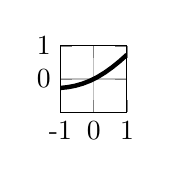
\begin{tikzpicture}
\begin{axis}[
	xmin=-1,xmax=1,
	ymin=-1,ymax=1,
	ytick={0, 1},
	yticklabels={0,1},
	xtick={-1, 0, 1},
	xticklabels={-1,0,1},
	width=.2\textwidth,
	height=.2\textwidth,
	grid=both,
	]
	\addplot [ultra thick,domain=-1:1, samples=10]{x * (1/ (1+exp(-x)))};
	%\addplot [ultra thick,domain=-1:0.004, samples=10]{exp(x)-1};
\end{axis}
\end{tikzpicture}}
		\scalebox{.9}{% This file was created by tikzplotlib v0.9.6.
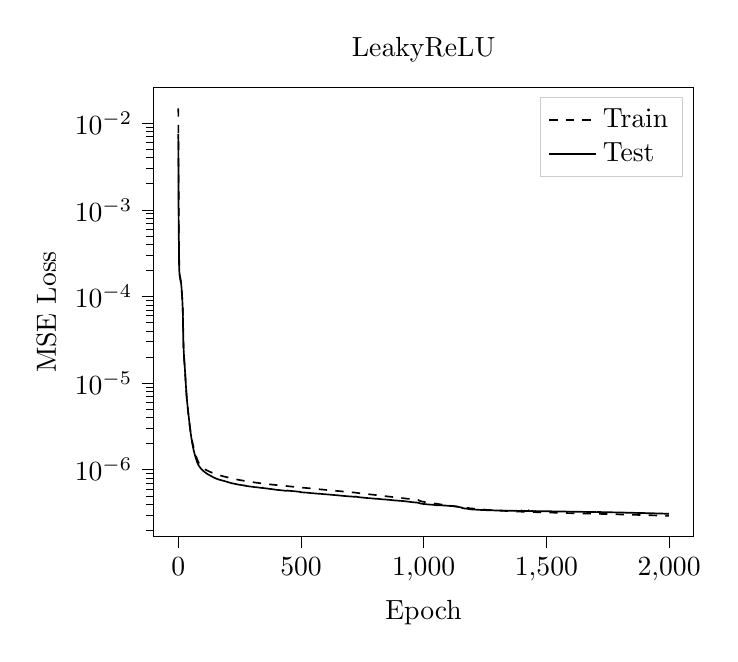
\begin{tikzpicture}

\begin{axis}[
legend cell align={left},
legend style={fill opacity=0.8, draw opacity=1, text opacity=1, draw=white!80!black},
log basis y={10},
tick align=outside,
tick pos=left,
title={LeakyReLU},
x grid style={white!69.0196078431373!black},
xlabel={Epoch},
xmin=-99.95, xmax=2098.95,
xtick style={color=black},
y grid style={white!69.0196078431373!black},
ylabel={MSE Loss},
ymin=1.70791572547231e-07, ymax=0.0255488360607333,
ymode=log,
ytick style={color=black}
]
\addplot [semithick, black, dashed]
table {%
0 0.0148644272387028
1 0.00333734963089228
2 0.000750602022744715
3 0.000331206021597609
4 0.000207027630618541
5 0.000178633672956494
6 0.000169817901289207
7 0.000163992511370452
8 0.000158428034461394
9 0.000152649684350763
10 0.00014641946539632
11 0.000139678969775559
12 0.000132290519177332
13 0.000124130066971702
14 0.000115090908722777
15 0.000105129859155568
16 9.44059219655173e-05
17 8.3223627305415e-05
18 7.19209145499917e-05
19 5.9600600565318e-05
20 3.97648699054116e-05
21 2.79329969580431e-05
22 2.30094661437761e-05
23 2.03421610876831e-05
24 1.84593141466394e-05
25 1.68413770406914e-05
26 1.53453861585149e-05
27 1.39403166676857e-05
28 1.26229516022249e-05
29 1.13995978695129e-05
30 1.02803903319e-05
31 9.27881336542669e-06
32 8.39881708566281e-06
33 7.63946547408523e-06
34 6.99144020211406e-06
35 6.44443027772468e-06
36 5.98577112725707e-06
37 5.59156097597224e-06
38 5.24542606149225e-06
39 4.93420651258703e-06
40 4.64607294458119e-06
41 4.3748265293857e-06
42 4.12039487252969e-06
43 3.8861643104724e-06
44 3.67260006765946e-06
45 3.47844123746199e-06
46 3.30225424215769e-06
47 3.13898743047503e-06
48 2.98947314900033e-06
49 2.85182592716637e-06
50 2.72762016362549e-06
51 2.61402293841684e-06
52 2.5099930834358e-06
53 2.4150706948376e-06
54 2.32725503445863e-06
55 2.24705749849363e-06
56 2.17294952142311e-06
57 2.1049157987818e-06
58 2.04128094503631e-06
59 1.98188082879369e-06
60 1.92642735390791e-06
61 1.87334052122878e-06
62 1.8232318035416e-06
63 1.77455488795886e-06
64 1.72895183959554e-06
65 1.6861234399812e-06
66 1.64616296456188e-06
67 1.60743973128774e-06
68 1.57055133320227e-06
69 1.53456863944257e-06
70 1.50125948277946e-06
71 1.46981972636695e-06
72 1.44026260474561e-06
73 1.41147857323176e-06
74 1.38520127060815e-06
75 1.36031598432851e-06
76 1.33676044734443e-06
77 1.3148170181978e-06
78 1.29389646752998e-06
79 1.27433537693378e-06
80 1.25646557970072e-06
81 1.2384471808673e-06
82 1.22196116879536e-06
83 1.20638403507201e-06
84 1.19190501561661e-06
85 1.17844780726273e-06
86 1.16571712385394e-06
87 1.1539444496691e-06
88 1.14418008098482e-06
89 1.13371917686322e-06
90 1.12408099414552e-06
91 1.1148123342366e-06
92 1.10610182443338e-06
93 1.09807221093661e-06
94 1.09074505050444e-06
95 1.0839480192999e-06
96 1.07734048407337e-06
97 1.07122849982488e-06
98 1.06452712140026e-06
99 1.05868495271011e-06
100 1.05291415113129e-06
101 1.04752679743569e-06
102 1.04214536537484e-06
103 1.0370281889891e-06
104 1.032027342319e-06
105 1.02744560464885e-06
106 1.02279366436164e-06
107 1.01820316623957e-06
108 1.01401851819105e-06
109 1.00975107895351e-06
110 1.0057904348173e-06
111 1.00208405191893e-06
112 9.98241210339756e-07
113 9.94370888776075e-07
114 9.90925482227567e-07
115 9.87395259301138e-07
116 9.83861367387817e-07
117 9.80596522055066e-07
118 9.77371847994846e-07
119 9.74262288309546e-07
120 9.71295058008082e-07
121 9.6826150081597e-07
122 9.6523639768975e-07
123 9.62448905852398e-07
124 9.59402455919189e-07
125 9.56513887700794e-07
126 9.53868651834e-07
127 9.51033602575535e-07
128 9.48263187240173e-07
129 9.45597496013306e-07
130 9.42952355558191e-07
131 9.40403254958255e-07
132 9.37919000818965e-07
133 9.35487815553415e-07
134 9.33048935337411e-07
135 9.30687048224854e-07
136 9.28267845239361e-07
137 9.25884347481087e-07
138 9.23637938910815e-07
139 9.21227984548523e-07
140 9.18846620891145e-07
141 9.16484609831514e-07
142 9.14296656503666e-07
143 9.12058346074218e-07
144 9.09871440057941e-07
145 9.07786169506153e-07
146 9.05647660886189e-07
147 9.03635627963695e-07
148 9.01687872357115e-07
149 8.9950875153022e-07
150 8.97521426622916e-07
151 8.95521069111282e-07
152 8.93521177772527e-07
153 8.91522843943449e-07
154 8.89579697087584e-07
155 8.87620785334775e-07
156 8.85896789583285e-07
157 8.83988975402872e-07
158 8.82208881847646e-07
159 8.80398930121373e-07
160 8.78538994015798e-07
161 8.76403134441262e-07
162 8.7463463688664e-07
163 8.72705812355434e-07
164 8.70566312670462e-07
165 8.68765719644671e-07
166 8.67004338203969e-07
167 8.653048454903e-07
168 8.63512691211099e-07
169 8.61854937170392e-07
170 8.60151822223543e-07
171 8.58458075072122e-07
172 8.56818996624043e-07
173 8.55136690688596e-07
174 8.53585893565878e-07
175 8.5187854273272e-07
176 8.50357727699702e-07
177 8.48755360294717e-07
178 8.47190044481749e-07
179 8.45670013589483e-07
180 8.44131327013997e-07
181 8.42642410887606e-07
182 8.41175444946884e-07
183 8.39656288363244e-07
184 8.38167764982245e-07
185 8.36532800619239e-07
186 8.35078147304102e-07
187 8.33758716908051e-07
188 8.32371983960911e-07
189 8.30889671789237e-07
190 8.29568857710683e-07
191 8.28064573511256e-07
192 8.26631372348174e-07
193 8.25454969628936e-07
194 8.24060114283043e-07
195 8.22638993369651e-07
196 8.2126220449652e-07
197 8.19915930264869e-07
198 8.20267484073156e-07
199 8.18703642607943e-07
200 8.17248432568363e-07
201 8.15823900992996e-07
202 8.14442585394204e-07
203 8.13095293437982e-07
204 8.11669069307186e-07
205 8.10307857349812e-07
206 8.09004709736882e-07
207 8.07590666070723e-07
208 8.06252364142779e-07
209 8.04654392212001e-07
210 8.0335848272739e-07
211 8.02302690658507e-07
212 8.00962444145625e-07
213 7.99703646720218e-07
214 7.98452317255283e-07
215 7.97217591738786e-07
216 7.96002158963915e-07
217 7.9481069326448e-07
218 7.93627711118461e-07
219 7.92467858858004e-07
220 7.91300207737322e-07
221 7.90077528890265e-07
222 7.88920517678093e-07
223 7.87720634576772e-07
224 7.86578616626343e-07
225 7.85441414691945e-07
226 7.84363267499089e-07
227 7.83269696910338e-07
228 7.82192492366107e-07
229 7.81227263516371e-07
230 7.80163437795522e-07
231 7.79063238198319e-07
232 7.78027706374473e-07
233 7.76964129954649e-07
234 7.75930989362905e-07
235 7.74893729442283e-07
236 7.73837977973813e-07
237 7.72835657613768e-07
238 7.71838034495431e-07
239 7.70846074615861e-07
240 7.69821481426902e-07
241 7.68822976212391e-07
242 7.67821201534957e-07
243 7.66846018862566e-07
244 7.65887867913762e-07
245 7.64930361214056e-07
246 7.63921686242952e-07
247 7.63010957257393e-07
248 7.62070085571054e-07
249 7.61139531945787e-07
250 7.60420157376984e-07
251 7.59426636150806e-07
252 7.58426511922039e-07
253 7.57507968302207e-07
254 7.56569720863354e-07
255 7.55625533727766e-07
256 7.54756878393437e-07
257 7.53833237837398e-07
258 7.52968338730398e-07
259 7.52147672017145e-07
260 7.51202681499308e-07
261 7.50205559867823e-07
262 7.4943015475526e-07
263 7.48610954261153e-07
264 7.47677468453389e-07
265 7.46997857405063e-07
266 7.46052829256882e-07
267 7.45165411899507e-07
268 7.44340018613343e-07
269 7.43665318836406e-07
270 7.42747071726058e-07
271 7.4204888295526e-07
272 7.41131473191103e-07
273 7.40440178674362e-07
274 7.39578193176271e-07
275 7.3881461977976e-07
276 7.37799187660926e-07
277 7.37035187341917e-07
278 7.36253217098692e-07
279 7.35415127010697e-07
280 7.34686662354989e-07
281 7.33878230974483e-07
282 7.33114714989824e-07
283 7.32347263181055e-07
284 7.31621643978997e-07
285 7.30857068063529e-07
286 7.30129704550109e-07
287 7.29444917936917e-07
288 7.28688947859268e-07
289 7.28014880451156e-07
290 7.27137706519443e-07
291 7.2640715151806e-07
292 7.25708816418091e-07
293 7.25009155303269e-07
294 7.24293989392777e-07
295 7.23561567397724e-07
296 7.2286156442658e-07
297 7.22185449788526e-07
298 7.21465641959185e-07
299 7.20789148289214e-07
300 7.20108953458976e-07
301 7.19449026178154e-07
302 7.18764739445987e-07
303 7.18094917701251e-07
304 7.17464760171538e-07
305 7.16808219209497e-07
306 7.16184726542224e-07
307 7.15528395758724e-07
308 7.14873352649192e-07
309 7.14168571732898e-07
310 7.13574344160861e-07
311 7.1287063936154e-07
312 7.12281224224398e-07
313 7.11596599359154e-07
314 7.1101726477707e-07
315 7.10344048059142e-07
316 7.09744001042623e-07
317 7.09173813802977e-07
318 7.08501808716733e-07
319 7.07896837610633e-07
320 7.07197004814475e-07
321 7.06599812318132e-07
322 7.05917090755293e-07
323 7.05374840876516e-07
324 7.04819606951901e-07
325 7.04185838287685e-07
326 7.03570776934725e-07
327 7.02973159619091e-07
328 7.02457169694526e-07
329 7.01814170426474e-07
330 7.01159818504493e-07
331 7.00675139412965e-07
332 7.00100038670826e-07
333 6.9944516293674e-07
334 6.98911392788659e-07
335 6.98320728275803e-07
336 6.97682788128873e-07
337 6.97246098184223e-07
338 6.96686453053985e-07
339 6.96352869169914e-07
340 6.95526991592033e-07
341 6.9484590517277e-07
342 6.94304655056044e-07
343 6.9400206361081e-07
344 6.92970413965099e-07
345 6.93037260532492e-07
346 6.92013609636888e-07
347 6.91989935560855e-07
348 6.90816037362652e-07
349 6.9062005174203e-07
350 6.89722630539791e-07
351 6.89461848594419e-07
352 6.88598280333963e-07
353 6.88385519012513e-07
354 6.87496540834331e-07
355 6.87273249681653e-07
356 6.86344381364279e-07
357 6.85784922154653e-07
358 6.85309239756293e-07
359 6.8513359936162e-07
360 6.84244536785172e-07
361 6.84097153609287e-07
362 6.83162119059943e-07
363 6.82782644759072e-07
364 6.82589405883505e-07
365 6.8159318890082e-07
366 6.81068037124533e-07
367 6.80618575174208e-07
368 6.80053423749882e-07
369 6.79640693476813e-07
370 6.79050741510423e-07
371 6.78609955187426e-07
372 6.78057203842286e-07
373 6.77662977224713e-07
374 6.77112505997002e-07
375 6.76636222607385e-07
376 6.76250711990178e-07
377 6.75681376677062e-07
378 6.75209785029551e-07
379 6.74681991128523e-07
380 6.74513683136979e-07
381 6.73722616213013e-07
382 6.73302310929102e-07
383 6.72808587580676e-07
384 6.72407056214297e-07
385 6.71915421463609e-07
386 6.71427296765614e-07
387 6.71025953465687e-07
388 6.7049164735522e-07
389 6.70016919258387e-07
390 6.69557675067267e-07
391 6.69086867844726e-07
392 6.68597802928161e-07
393 6.68190762553422e-07
394 6.67692410345921e-07
395 6.67240023972226e-07
396 6.66790877019707e-07
397 6.66323490648324e-07
398 6.65903456606998e-07
399 6.65471397070405e-07
400 6.65007362329106e-07
401 6.64616963959475e-07
402 6.64189005348703e-07
403 6.63769749593257e-07
404 6.63356940961535e-07
405 6.62935873677384e-07
406 6.6251740221901e-07
407 6.62097921363625e-07
408 6.61683327294327e-07
409 6.61271375818728e-07
410 6.60858302936163e-07
411 6.60460645164562e-07
412 6.6005227745336e-07
413 6.59639243394849e-07
414 6.5922696452958e-07
415 6.58827367658432e-07
416 6.58425498315296e-07
417 6.5801929646625e-07
418 6.57625117895577e-07
419 6.57224236348952e-07
420 6.5661854195298e-07
421 6.56017475847648e-07
422 6.55518018916723e-07
423 6.55074278228085e-07
424 6.54699447096618e-07
425 6.54264191396692e-07
426 6.53816869700563e-07
427 6.53326964823009e-07
428 6.52873706030732e-07
429 6.52448715413811e-07
430 6.51987482811478e-07
431 6.51630326260033e-07
432 6.51166140116288e-07
433 6.50728281328838e-07
434 6.50352801045528e-07
435 6.49924126832957e-07
436 6.49520926629066e-07
437 6.49109188529451e-07
438 6.48725988511956e-07
439 6.48329360970479e-07
440 6.47936029650964e-07
441 6.47537012639532e-07
442 6.47503992468046e-07
443 6.47304684633809e-07
444 6.46791755926301e-07
445 6.46174046053716e-07
446 6.45631595219243e-07
447 6.45148015280483e-07
448 6.4464382931817e-07
449 6.44142668491554e-07
450 6.4371638593741e-07
451 6.4329291483034e-07
452 6.42818815379087e-07
453 6.4243620757054e-07
454 6.41965242266451e-07
455 6.41560947940434e-07
456 6.4108713894484e-07
457 6.40711664800619e-07
458 6.40245212196078e-07
459 6.39877146284107e-07
460 6.39416840158447e-07
461 6.38994611691146e-07
462 6.38533215393977e-07
463 6.38164307375177e-07
464 6.37705450529324e-07
465 6.37337720817754e-07
466 6.36884023322182e-07
467 6.36565714486892e-07
468 6.35994193231681e-07
469 6.35576846804042e-07
470 6.35110142454209e-07
471 6.34726450087442e-07
472 6.34274996968998e-07
473 6.33879317220476e-07
474 6.33418987760592e-07
475 6.33054129139055e-07
476 6.32558955913964e-07
477 6.32200792907156e-07
478 6.31757687600043e-07
479 6.31408914216536e-07
480 6.30983657273987e-07
481 6.30627516443383e-07
482 6.30192174881472e-07
483 6.29844393728263e-07
484 6.29409517699742e-07
485 6.29049891742284e-07
486 6.28630618265902e-07
487 6.28272145732467e-07
488 6.27843531489702e-07
489 6.27503492012238e-07
490 6.27080744209252e-07
491 6.26735475819373e-07
492 6.26306154430267e-07
493 6.25968398722421e-07
494 6.25546789720488e-07
495 6.25211958649174e-07
496 6.24788373372098e-07
497 6.24449280010708e-07
498 6.23962057133554e-07
499 6.23558213717956e-07
500 6.2311415599936e-07
501 6.22750209018363e-07
502 6.22350057199128e-07
503 6.21995929662944e-07
504 6.21580487475626e-07
505 6.21248701463628e-07
506 6.20837227202742e-07
507 6.20487857943885e-07
508 6.2008267529734e-07
509 6.19707906508893e-07
510 6.19289868623696e-07
511 6.18935109201857e-07
512 6.18535905800854e-07
513 6.18207967761464e-07
514 6.17810335668878e-07
515 6.17487754837498e-07
516 6.17048165693745e-07
517 6.16747607693924e-07
518 6.16425678529708e-07
519 6.16018937733998e-07
520 6.15564609120156e-07
521 6.15231403671146e-07
522 6.14803654485741e-07
523 6.14466882382203e-07
524 6.13926075146765e-07
525 6.13603320687162e-07
526 6.13164834007307e-07
527 6.12889333567068e-07
528 6.1244176531261e-07
529 6.12171113900217e-07
530 6.11737456409855e-07
531 6.11406537032622e-07
532 6.10991987372245e-07
533 6.10615803282144e-07
534 6.10182909497325e-07
535 6.09855354056776e-07
536 6.09413068900722e-07
537 6.09052085394524e-07
538 6.08653819512028e-07
539 6.08387478564509e-07
540 6.07961950962022e-07
541 6.07622395477847e-07
542 6.07195113218495e-07
543 6.06802663170924e-07
544 6.06362741748967e-07
545 6.06013731712096e-07
546 6.0559248045422e-07
547 6.05250503625143e-07
548 6.04716681607442e-07
549 6.04371584088881e-07
550 6.03937985829361e-07
551 6.03589404704508e-07
552 6.03148568060874e-07
553 6.02801457745272e-07
554 6.0235625136329e-07
555 6.01985544463446e-07
556 6.01539943161811e-07
557 6.01232765262694e-07
558 6.00807006364335e-07
559 6.00492180907963e-07
560 6.0005816808939e-07
561 5.99730774595741e-07
562 5.99223440019614e-07
563 5.98925630910685e-07
564 5.98511263632418e-07
565 5.98205809396291e-07
566 5.97765539339434e-07
567 5.97455265236135e-07
568 5.97010945085685e-07
569 5.9672484819373e-07
570 5.96299604083583e-07
571 5.96071399556308e-07
572 5.95513366789646e-07
573 5.95187032928379e-07
574 5.947183740318e-07
575 5.94433451610144e-07
576 5.93983866451708e-07
577 5.93703354780928e-07
578 5.93230489997154e-07
579 5.92965793160261e-07
580 5.92490404656587e-07
581 5.92217652197746e-07
582 5.9175461059624e-07
583 5.91483319766439e-07
584 5.91055219629766e-07
585 5.9077541931174e-07
586 5.90313007251098e-07
587 5.90037488734652e-07
588 5.89601683429919e-07
589 5.89313242372214e-07
590 5.88861738904711e-07
591 5.88606085244692e-07
592 5.88205910432293e-07
593 5.87919526992664e-07
594 5.8745086768397e-07
595 5.87203168748829e-07
596 5.86743687904345e-07
597 5.86504606161498e-07
598 5.86034405827718e-07
599 5.85759843318101e-07
600 5.85295431378086e-07
601 5.85048269172717e-07
602 5.84578794146751e-07
603 5.84336741496827e-07
604 5.83889424504491e-07
605 5.8371987589112e-07
606 5.83250819758518e-07
607 5.82936998782202e-07
608 5.82475648911895e-07
609 5.822194414975e-07
610 5.81760691360955e-07
611 5.81514034749375e-07
612 5.8107778048111e-07
613 5.80798643440517e-07
614 5.8034996423828e-07
615 5.8007643750102e-07
616 5.79669754557699e-07
617 5.79423551016589e-07
618 5.78947847898803e-07
619 5.7868813833295e-07
620 5.78234088450813e-07
621 5.77960293540514e-07
622 5.7753287774176e-07
623 5.77290330667779e-07
624 5.76830392489569e-07
625 5.76586579811078e-07
626 5.76101825032538e-07
627 5.75859893572783e-07
628 5.75397084972451e-07
629 5.75150781202183e-07
630 5.74713401903182e-07
631 5.7447310602754e-07
632 5.74012735526708e-07
633 5.73774994833798e-07
634 5.73327271069957e-07
635 5.73114834153898e-07
636 5.72660245197199e-07
637 5.7240989970353e-07
638 5.71956064860046e-07
639 5.71697264476256e-07
640 5.71240307664311e-07
641 5.70994088292309e-07
642 5.70539148810667e-07
643 5.70304007425193e-07
644 5.69833525858598e-07
645 5.69588442289159e-07
646 5.69132603871481e-07
647 5.68892071527216e-07
648 5.68438184046727e-07
649 5.68201071160956e-07
650 5.67769946428598e-07
651 5.67519301142738e-07
652 5.6707707179271e-07
653 5.66797595681123e-07
654 5.66352859991071e-07
655 5.66096162472718e-07
656 5.65686599273363e-07
657 5.65438366834314e-07
658 5.65017211897612e-07
659 5.64772737391195e-07
660 5.64293594010223e-07
661 5.64047870213358e-07
662 5.63645380410094e-07
663 5.63384342626705e-07
664 5.62980142362335e-07
665 5.62727795866635e-07
666 5.62271209290088e-07
667 5.62005503908836e-07
668 5.61633367738068e-07
669 5.61361019336459e-07
670 5.60907587512816e-07
671 5.60647555943206e-07
672 5.60207655595946e-07
673 5.59965208736912e-07
674 5.59675780166913e-07
675 5.59391941266085e-07
676 5.58971077055048e-07
677 5.58727743012355e-07
678 5.58255349702108e-07
679 5.5799404208301e-07
680 5.5754053700241e-07
681 5.57285783443717e-07
682 5.56846114776022e-07
683 5.56599550662895e-07
684 5.56152776738372e-07
685 5.55905638606191e-07
686 5.55450992109741e-07
687 5.55227351341614e-07
688 5.54761071512644e-07
689 5.54549272450799e-07
690 5.54089646058742e-07
691 5.53867962665322e-07
692 5.53422880528842e-07
693 5.5320079773935e-07
694 5.5274819114004e-07
695 5.52521287801255e-07
696 5.5206996151469e-07
697 5.51794728323784e-07
698 5.51397915060647e-07
699 5.5119633870504e-07
700 5.50707732926981e-07
701 5.50483585669781e-07
702 5.5005929785068e-07
703 5.49791805909194e-07
704 5.49363092531507e-07
705 5.49153537050984e-07
706 5.48734435838583e-07
707 5.48524624861102e-07
708 5.48033714892426e-07
709 5.47864530929587e-07
710 5.47407044180659e-07
711 5.47192967673027e-07
712 5.46663945314663e-07
713 5.46469165058738e-07
714 5.46026377676867e-07
715 5.45797743370713e-07
716 5.45408502446776e-07
717 5.45146161812227e-07
718 5.44686208826306e-07
719 5.4444843793533e-07
720 5.44042121731536e-07
721 5.44187411392727e-07
722 5.43547544765488e-07
723 5.42903439722409e-07
724 5.42304797178872e-07
725 5.41774102529757e-07
726 5.41298678271573e-07
727 5.40787423858546e-07
728 5.40312020774536e-07
729 5.39910445837677e-07
730 5.39371933314214e-07
731 5.39032324013533e-07
732 5.38397320511308e-07
733 5.38005847772638e-07
734 5.37580982125974e-07
735 5.37113240582698e-07
736 5.36665524890623e-07
737 5.3628786932336e-07
738 5.35821611535425e-07
739 5.3551504601046e-07
740 5.34989343293546e-07
741 5.34692306075613e-07
742 5.34238284117805e-07
743 5.33852620080211e-07
744 5.33480754000948e-07
745 5.33024487040734e-07
746 5.32662216912172e-07
747 5.32245440751922e-07
748 5.31847421598286e-07
749 5.31583600732688e-07
750 5.31042589130948e-07
751 5.30784487636993e-07
752 5.30310267848222e-07
753 5.30027119310716e-07
754 5.29521326086524e-07
755 5.29201154762404e-07
756 5.28709079290479e-07
757 5.28442658435324e-07
758 5.27953152186456e-07
759 5.27690907290435e-07
760 5.27205177448309e-07
761 5.26892414683289e-07
762 5.26405703695332e-07
763 5.26151932234598e-07
764 5.25638900228387e-07
765 5.2538255179968e-07
766 5.24913538470173e-07
767 5.24627415103396e-07
768 5.24143547863787e-07
769 5.23870203437582e-07
770 5.23359917082189e-07
771 5.23059499315082e-07
772 5.22546751852815e-07
773 5.22258667359665e-07
774 5.21781591501735e-07
775 5.21461515333499e-07
776 5.21047451144341e-07
777 5.20667105519124e-07
778 5.20264812351456e-07
779 5.19935537340643e-07
780 5.19469053031685e-07
781 5.19178764761818e-07
782 5.18717480986197e-07
783 5.18486472344648e-07
784 5.18063059260498e-07
785 5.1770965706055e-07
786 5.17317782481541e-07
787 5.17047028139928e-07
788 5.16598040718463e-07
789 5.16272202006007e-07
790 5.15890133598873e-07
791 5.1559194417905e-07
792 5.15092240675585e-07
793 5.14856525086316e-07
794 5.14366608740602e-07
795 5.14138488711069e-07
796 5.1369179050198e-07
797 5.133947706355e-07
798 5.1297357916269e-07
799 5.1269512967167e-07
800 5.12259364455758e-07
801 5.1196938757414e-07
802 5.11423140920897e-07
803 5.11186035765832e-07
804 5.108558257092e-07
805 5.10589589111987e-07
806 5.10150635591344e-07
807 5.09905413366596e-07
808 5.09488112413692e-07
809 5.0918477496964e-07
810 5.08788510359182e-07
811 5.08506359878424e-07
812 5.08111304810654e-07
813 5.07820337901421e-07
814 5.07405267313743e-07
815 5.07125847690304e-07
816 5.06688020934121e-07
817 5.06418203016779e-07
818 5.05994589261149e-07
819 5.05725315562699e-07
820 5.05358103424669e-07
821 5.05075605559568e-07
822 5.04433651911995e-07
823 5.04046690537052e-07
824 5.03614987664491e-07
825 5.03243534893727e-07
826 5.02741254081229e-07
827 5.02363778650761e-07
828 5.0181188987608e-07
829 5.01155536113629e-07
830 5.00639151781002e-07
831 5.00094774650961e-07
832 4.99718042917152e-07
833 4.99335891149144e-07
834 4.98984696335469e-07
835 4.98626764695587e-07
836 4.98176735277411e-07
837 4.97781516273221e-07
838 4.97396944084016e-07
839 4.97024179267669e-07
840 4.96623089802029e-07
841 4.9619203473128e-07
842 4.95837466530702e-07
843 4.95356492848487e-07
844 4.94947353985253e-07
845 4.94624493896367e-07
846 4.94189927721322e-07
847 4.93753210434988e-07
848 4.93364277460273e-07
849 4.93005060846485e-07
850 4.92574361317111e-07
851 4.92261623520562e-07
852 4.91839595838428e-07
853 4.91472612594634e-07
854 4.91078210103524e-07
855 4.90717624558101e-07
856 4.90344198198045e-07
857 4.89971666482347e-07
858 4.89575231455319e-07
859 4.89207917780732e-07
860 4.8886572173501e-07
861 4.88452469610934e-07
862 4.88092318505551e-07
863 4.87744442438043e-07
864 4.87433638966195e-07
865 4.87001789679198e-07
866 4.86642392530712e-07
867 4.86256370052729e-07
868 4.85970414203507e-07
869 4.85520277266005e-07
870 4.85194746914885e-07
871 4.84795060486931e-07
872 4.8450660469257e-07
873 4.84076300665492e-07
874 4.83778275267355e-07
875 4.83363721940577e-07
876 4.83014998721387e-07
877 4.82567401576262e-07
878 4.82165626024766e-07
879 4.81873086187079e-07
880 4.81442710679403e-07
881 4.81068505791882e-07
882 4.80751659097223e-07
883 4.80426024751068e-07
884 4.80023959966047e-07
885 4.796470899322e-07
886 4.79263505340555e-07
887 4.78941620059459e-07
888 4.78609426863841e-07
889 4.78185967480727e-07
890 4.77746801095691e-07
891 4.77495924258164e-07
892 4.77138562104074e-07
893 4.76734690607827e-07
894 4.76396770054066e-07
895 4.76033359916528e-07
896 4.75629839783664e-07
897 4.7529189306772e-07
898 4.75028509299591e-07
899 4.74598706588836e-07
900 4.74232805089514e-07
901 4.73863658129403e-07
902 4.73503784462537e-07
903 4.73214756993912e-07
904 4.72819625130683e-07
905 4.72471625627691e-07
906 4.72109106254948e-07
907 4.71858331579256e-07
908 4.71460500378384e-07
909 4.71170830238066e-07
910 4.70762764038568e-07
911 4.70420068552357e-07
912 4.70193007899411e-07
913 4.69732255297117e-07
914 4.69328430256155e-07
915 4.69008694636841e-07
916 4.68750404195362e-07
917 4.68294574801575e-07
918 4.67943003044979e-07
919 4.67603833413932e-07
920 4.6726228927696e-07
921 4.67024187202014e-07
922 4.66549970042252e-07
923 4.66196309801603e-07
924 4.65849686818842e-07
925 4.65657492441096e-07
926 4.6514172363743e-07
927 4.6484536051139e-07
928 4.64433631279348e-07
929 4.64285816306642e-07
930 4.63722799736388e-07
931 4.63393946745327e-07
932 4.63028061346904e-07
933 4.62868733578148e-07
934 4.62303378796491e-07
935 4.61944667279113e-07
936 4.61593672994809e-07
937 4.61465650644755e-07
938 4.60907661022247e-07
939 4.60600220463903e-07
940 4.6021002177099e-07
941 4.59943743535973e-07
942 4.59559822544975e-07
943 4.59191470767451e-07
944 4.58823429340782e-07
945 4.58568544715376e-07
946 4.58253700188038e-07
947 4.57775354860246e-07
948 4.57443201653973e-07
949 4.57248985242131e-07
950 4.56788529746177e-07
951 4.56413603274086e-07
952 4.56049293291017e-07
953 4.55718323721044e-07
954 4.55268215404203e-07
955 4.54996806922736e-07
956 4.54735002605844e-07
957 4.54331303615163e-07
958 4.53895254239001e-07
959 4.53565293838665e-07
960 4.53295954372379e-07
961 4.52920906539589e-07
962 4.52633616063736e-07
963 4.52290183702075e-07
964 4.51753988272685e-07
965 4.51526366362032e-07
966 4.51130627027396e-07
967 4.50771134154593e-07
968 4.504252864308e-07
969 4.50136636729326e-07
970 4.49762404599596e-07
971 4.4941030162704e-07
972 4.49197960506353e-07
973 4.48709193022978e-07
974 4.48431595785337e-07
975 4.48094398578291e-07
976 4.4774719881957e-07
977 4.47329700762111e-07
978 4.47107959246296e-07
979 4.45311586858566e-07
980 4.42267165908561e-07
981 4.41070118895937e-07
982 4.40142427535761e-07
983 4.39295067039325e-07
984 4.38643088358504e-07
985 4.36957642435232e-07
986 4.35593108733201e-07
987 4.34702707551082e-07
988 4.33474616400531e-07
989 4.32703829105208e-07
990 4.32289674321851e-07
991 4.31421487917305e-07
992 4.30638353520862e-07
993 4.29790937616303e-07
994 4.28880565337408e-07
995 4.28401135650347e-07
996 4.27787201346064e-07
997 4.27183281047405e-07
998 4.26694344852763e-07
999 4.2636703791743e-07
1000 4.25715062704057e-07
1001 4.25246964852022e-07
1002 4.24845545552444e-07
1003 4.24308888639757e-07
1004 4.23964489456807e-07
1005 4.23528313447719e-07
1006 4.22984388706027e-07
1007 4.225807735736e-07
1008 4.22272394018819e-07
1009 4.21754303317812e-07
1010 4.21508764347323e-07
1011 4.20943191883794e-07
1012 4.20336185086967e-07
1013 4.19858491000014e-07
1014 4.1939585513262e-07
1015 4.19118752247982e-07
1016 4.18458747006412e-07
1017 4.18054913723154e-07
1018 4.17623710319504e-07
1019 4.17345911756684e-07
1020 4.1684959707311e-07
1021 4.16479742753495e-07
1022 4.16232555934926e-07
1023 4.1558006725495e-07
1024 4.15228342362184e-07
1025 4.15229226916836e-07
1026 4.14557101422019e-07
1027 4.14188685837757e-07
1028 4.137652676377e-07
1029 4.13552009050022e-07
1030 4.13012748268216e-07
1031 4.12709136242029e-07
1032 4.12403044578014e-07
1033 4.12024662679755e-07
1034 4.11686833103886e-07
1035 4.11097062823274e-07
1036 4.11059944923409e-07
1037 4.10612124298382e-07
1038 4.10058860069284e-07
1039 4.09830215701845e-07
1040 4.09236865593243e-07
1041 4.08992037847611e-07
1042 4.08167432894402e-07
1043 4.07781641527549e-07
1044 4.07499990515703e-07
1045 4.06984923031928e-07
1046 4.06398309621636e-07
1047 4.06130208801869e-07
1048 4.05844250565224e-07
1049 4.05634460008741e-07
1050 4.05246325286157e-07
1051 4.04832696432322e-07
1052 4.04589275078138e-07
1053 4.04333232410181e-07
1054 4.0388796469415e-07
1055 4.0364550858385e-07
1056 4.03237107150289e-07
1057 4.02781264639884e-07
1058 4.02806778183162e-07
1059 4.01965887306233e-07
1060 4.01510594059573e-07
1061 4.00938951401031e-07
1062 4.00572816303679e-07
1063 4.00084503098697e-07
1064 3.99712360263038e-07
1065 3.99338280672623e-07
1066 3.98853183725123e-07
1067 3.98574016514885e-07
1068 3.98165261131567e-07
1069 3.9791169047021e-07
1070 3.97472268019783e-07
1071 3.97099917236687e-07
1072 3.96636626348368e-07
1073 3.96424626273983e-07
1074 3.96097346396118e-07
1075 3.9559541224321e-07
1076 3.95176014095e-07
1077 3.9485332503375e-07
1078 3.94414255026732e-07
1079 3.94210009147855e-07
1080 3.93897365086104e-07
1081 3.94073744161005e-07
1082 3.92707131538828e-07
1083 3.92443426818545e-07
1084 3.92263928972625e-07
1085 3.91811526995411e-07
1086 3.91438045383552e-07
1087 3.91222988042728e-07
1088 3.90767820931615e-07
1089 3.90392165115827e-07
1090 3.90058417949035e-07
1091 3.89737378512223e-07
1092 3.89416854545743e-07
1093 3.89117823701213e-07
1094 3.88820500631937e-07
1095 3.8860628005466e-07
1096 3.88284502861325e-07
1097 3.8773857590968e-07
1098 3.87415723963613e-07
1099 3.87093581963427e-07
1100 3.86819972547414e-07
1101 3.8655951644273e-07
1102 3.86174517572613e-07
1103 3.85863807807141e-07
1104 3.85488108648246e-07
1105 3.85170436189242e-07
1106 3.84719854892523e-07
1107 3.84718544239604e-07
1108 3.84024391522075e-07
1109 3.83650835544813e-07
1110 3.83382792236375e-07
1111 3.83040656402045e-07
1112 3.82753346201525e-07
1113 3.82416109658834e-07
1114 3.82373510092293e-07
1115 3.81928717573032e-07
1116 3.81812806622861e-07
1117 3.81203720849044e-07
1118 3.80974276083634e-07
1119 3.80499999522499e-07
1120 3.80254684600345e-07
1121 3.7986570839621e-07
1122 3.79738977585475e-07
1123 3.79311346222266e-07
1124 3.79113227651828e-07
1125 3.7877028913158e-07
1126 3.7836112139189e-07
1127 3.77982800344512e-07
1128 3.78119575884739e-07
1129 3.77618890752274e-07
1130 3.77162941205711e-07
1131 3.7672415348311e-07
1132 3.76497530936604e-07
1133 3.76125739251165e-07
1134 3.76046060509339e-07
1135 3.75449260715754e-07
1136 3.75253203273473e-07
1137 3.74917057925472e-07
1138 3.74622404692104e-07
1139 3.7428821870833e-07
1140 3.74284405566527e-07
1141 3.7362211756431e-07
1142 3.73366226355643e-07
1143 3.7307717714441e-07
1144 3.72830825526194e-07
1145 3.72424451896336e-07
1146 3.72418132940311e-07
1147 3.7213091133026e-07
1148 3.71713215983505e-07
1149 3.71452914535553e-07
1150 3.71178188473209e-07
1151 3.70909355197568e-07
1152 3.7053996253178e-07
1153 3.7024783931372e-07
1154 3.69873657135145e-07
1155 3.69505103691381e-07
1156 3.69253701279604e-07
1157 3.68807387985726e-07
1158 3.68308296941677e-07
1159 3.68027352777744e-07
1160 3.67674302410137e-07
1161 3.67324845441885e-07
1162 3.67093079873371e-07
1163 3.66817634045447e-07
1164 3.66528322331305e-07
1165 3.66260036969379e-07
1166 3.65974232906296e-07
1167 3.6576783041653e-07
1168 3.65757778212128e-07
1169 3.65359265160237e-07
1170 3.64927529545866e-07
1171 3.64539682664144e-07
1172 3.64183218977132e-07
1173 3.63697715883404e-07
1174 3.63248774547742e-07
1175 3.6295745351822e-07
1176 3.62568556099063e-07
1177 3.62408816727111e-07
1178 3.61902688752025e-07
1179 3.61626319858033e-07
1180 3.61431617832864e-07
1181 3.61043409355943e-07
1182 3.60797934973789e-07
1183 3.60444958303674e-07
1184 3.60248958102716e-07
1185 3.59936896558111e-07
1186 3.59555476705964e-07
1187 3.59374415111802e-07
1188 3.58965990059801e-07
1189 3.58561037799632e-07
1190 3.58322259430111e-07
1191 3.57995596175442e-07
1192 3.57769069225355e-07
1193 3.57516862507623e-07
1194 3.57242059436658e-07
1195 3.57074874074215e-07
1196 3.56846210692652e-07
1197 3.56573667573912e-07
1198 3.56349139025269e-07
1199 3.56250705209504e-07
1200 3.55875810996054e-07
1201 3.55695545266599e-07
1202 3.55430612060559e-07
1203 3.55257044837742e-07
1204 3.55036958367805e-07
1205 3.54729504230988e-07
1206 3.54575795554979e-07
1207 3.54330831036975e-07
1208 3.54163805582175e-07
1209 3.53934707121084e-07
1210 3.53760961694149e-07
1211 3.53559004942383e-07
1212 3.53348837684564e-07
1213 3.53167481250694e-07
1214 3.52938252042634e-07
1215 3.52749994284807e-07
1216 3.52585982660969e-07
1217 3.52407975704239e-07
1218 3.52169507415567e-07
1219 3.51973961208785e-07
1220 3.51758787793699e-07
1221 3.51502807255599e-07
1222 3.51306851079869e-07
1223 3.51152501224306e-07
1224 3.50899278146244e-07
1225 3.50712421344213e-07
1226 3.50511307786405e-07
1227 3.50340402199834e-07
1228 3.50174203553877e-07
1229 3.49866230820339e-07
1230 3.49717217829948e-07
1231 3.49455526098552e-07
1232 3.49285141943767e-07
1233 3.49022042534841e-07
1234 3.48864000585536e-07
1235 3.48586736819811e-07
1236 3.48445087801963e-07
1237 3.4818345256582e-07
1238 3.4813231708597e-07
1239 3.48225087407172e-07
1240 3.47784275412266e-07
1241 3.47621228634409e-07
1242 3.47436047128724e-07
1243 3.47174164780029e-07
1244 3.4713033489453e-07
1245 3.46868865150896e-07
1246 3.46827497459401e-07
1247 3.46505921307028e-07
1248 3.46359151983222e-07
1249 3.46254663149637e-07
1250 3.45973173082825e-07
1251 3.45937462505219e-07
1252 3.45498902305508e-07
1253 3.45166767687033e-07
1254 3.44957258484158e-07
1255 3.44883514060257e-07
1256 3.44460587214712e-07
1257 3.44291111339601e-07
1258 3.44095388989274e-07
1259 3.43959172042219e-07
1260 3.43810874603889e-07
1261 3.43625585593088e-07
1262 3.4358059095041e-07
1263 3.43212996391173e-07
1264 3.43100552726128e-07
1265 3.43164890786341e-07
1266 3.42759536103188e-07
1267 3.42773568959842e-07
1268 3.42893875803441e-07
1269 3.42620055683085e-07
1270 3.4228207704956e-07
1271 3.42381971016437e-07
1272 3.42026907333093e-07
1273 3.41821995505143e-07
1274 3.41681918825998e-07
1275 3.41623348312226e-07
1276 3.41340164766279e-07
1277 3.41217368152513e-07
1278 3.4106308705617e-07
1279 3.40976784691804e-07
1280 3.4080946687709e-07
1281 3.40802128683038e-07
1282 3.40702538146331e-07
1283 3.40402227969605e-07
1284 3.40182375417442e-07
1285 3.40091809910348e-07
1286 3.39915428099857e-07
1287 3.39853421358782e-07
1288 3.39670542125248e-07
1289 3.39502068037234e-07
1290 3.39417640304873e-07
1291 3.39291082688931e-07
1292 3.39082802483404e-07
1293 3.39148367032749e-07
1294 3.38892482638187e-07
1295 3.38829270653207e-07
1296 3.38648870496172e-07
1297 3.38687307959162e-07
1298 3.38240516690291e-07
1299 3.38366272508495e-07
1300 3.38001319256875e-07
1301 3.37920434652972e-07
1302 3.37841576858011e-07
1303 3.37823672431625e-07
1304 3.3753024310812e-07
1305 3.37429006513901e-07
1306 3.37313680958573e-07
1307 3.37218410713547e-07
1308 3.3711456779173e-07
1309 3.36903703832547e-07
1310 3.36891655976501e-07
1311 3.36800533723647e-07
1312 3.3659107230477e-07
1313 3.36524350629475e-07
1314 3.36588194052467e-07
1315 3.3621560381647e-07
1316 3.36227974422343e-07
1317 3.35964050691473e-07
1318 3.3590479741008e-07
1319 3.35959069197145e-07
1320 3.3563762396227e-07
1321 3.3570893973689e-07
1322 3.35404225104696e-07
1323 3.35420296941891e-07
1324 3.35310365571218e-07
1325 3.35162345130868e-07
1326 3.35112290805739e-07
1327 3.35035934234895e-07
1328 3.34863490358828e-07
1329 3.3453481590584e-07
1330 3.34560684706275e-07
1331 3.34415690289802e-07
1332 3.34436880429223e-07
1333 3.34342135964505e-07
1334 3.3411748800205e-07
1335 3.33874048642713e-07
1336 3.33887440966407e-07
1337 3.33762760767797e-07
1338 3.33557971053722e-07
1339 3.33469831780064e-07
1340 3.333395412497e-07
1341 3.33323065277114e-07
1342 3.33160623696926e-07
1343 3.33146326468636e-07
1344 3.32997630756893e-07
1345 3.32955995787643e-07
1346 3.32814051603236e-07
1347 3.3281026241383e-07
1348 3.32498229099087e-07
1349 3.32466849641833e-07
1350 3.32391293376588e-07
1351 3.32259941842494e-07
1352 3.32225231424843e-07
1353 3.32077841072476e-07
1354 3.32005728822082e-07
1355 3.31841624657159e-07
1356 3.31928920083158e-07
1357 3.31696651336699e-07
1358 3.31594936319846e-07
1359 3.31512106100718e-07
1360 3.31501672782508e-07
1361 3.31306970345224e-07
1362 3.31109461292556e-07
1363 3.31097948134129e-07
1364 3.30970878607673e-07
1365 3.30980586127794e-07
1366 3.30741880006258e-07
1367 3.30851606676674e-07
1368 3.30796594830929e-07
1369 3.30699608035445e-07
1370 3.30719720835759e-07
1371 3.30387201159965e-07
1372 3.30450337429511e-07
1373 3.30311810436967e-07
1374 3.30153512820175e-07
1375 3.30106311636769e-07
1376 3.29856312781374e-07
1377 3.29988769316003e-07
1378 3.29781705133314e-07
1379 3.29643474735519e-07
1380 3.29575802702209e-07
1381 3.29661901908196e-07
1382 3.29384446779102e-07
1383 3.29194402652888e-07
1384 3.29174147502442e-07
1385 3.2892577434751e-07
1386 3.28936768760002e-07
1387 3.28938984807792e-07
1388 3.28622693380964e-07
1389 3.28631047203487e-07
1390 3.28663743040636e-07
1391 3.28427028435385e-07
1392 3.28422970120812e-07
1393 3.28242727945849e-07
1394 3.28273688822378e-07
1395 3.28060710437228e-07
1396 3.28181209752643e-07
1397 3.27843347669443e-07
1398 3.27852344064183e-07
1399 3.2829578710647e-07
1400 3.28064131871031e-07
1401 3.27575198873831e-07
1402 3.27536251177207e-07
1403 3.27420939470358e-07
1404 3.2741662860758e-07
1405 3.27226250057322e-07
1406 3.27265470950522e-07
1407 3.27060519509814e-07
1408 3.27155963816494e-07
1409 3.26972195878739e-07
1410 3.26970149174599e-07
1411 3.26863787329046e-07
1412 3.26782263279313e-07
1413 3.26663281526862e-07
1414 3.26726319926252e-07
1415 3.26526487675949e-07
1416 3.26492149575586e-07
1417 3.26372519289464e-07
1418 3.26526134919902e-07
1419 3.26281027753339e-07
1420 3.26192927850855e-07
1421 3.26291698719672e-07
1422 3.26084324228759e-07
1423 3.26008133122002e-07
1424 3.25901496594838e-07
1425 3.25920014496717e-07
1426 3.25827025420722e-07
1427 3.25687300644972e-07
1428 3.26062531392779e-07
1429 3.25628018437385e-07
1430 3.2562565948524e-07
1431 3.25352808538071e-07
1432 3.25273427925765e-07
1433 3.25321335537865e-07
1434 3.25138781853695e-07
1435 3.25163706605736e-07
1436 3.25108598367763e-07
1437 3.24951548883234e-07
1438 3.24962143700702e-07
1439 3.24829615223621e-07
1440 3.25090830237684e-07
1441 3.24795452463889e-07
1442 3.24721973001374e-07
1443 3.24631089085869e-07
1444 3.2456479630838e-07
1445 3.24642600965319e-07
1446 3.24464752360143e-07
1447 3.24280949101308e-07
1448 3.24287003877544e-07
1449 3.24112054428838e-07
1450 3.24111770346747e-07
1451 3.24085712215094e-07
1452 3.24007598564435e-07
1453 3.23942609085748e-07
1454 3.2425689070692e-07
1455 3.24005999075894e-07
1456 3.2361437681061e-07
1457 3.23674683443187e-07
1458 3.2351173168621e-07
1459 3.23458068230309e-07
1460 3.23479223787615e-07
1461 3.23319206508188e-07
1462 3.23341757123785e-07
1463 3.23198218914911e-07
1464 3.23270411364263e-07
1465 3.23068304957985e-07
1466 3.23069969759615e-07
1467 3.23080898247952e-07
1468 3.22920393280413e-07
1469 3.22857342759164e-07
1470 3.22821105278592e-07
1471 3.22736950657543e-07
1472 3.22708666047333e-07
1473 3.22561187388715e-07
1474 3.2244668971515e-07
1475 3.22537584629856e-07
1476 3.2234767521544e-07
1477 3.22275564869301e-07
1478 3.22260968928845e-07
1479 3.22126612921636e-07
1480 3.22229529807316e-07
1481 3.22072553345265e-07
1482 3.21982909795793e-07
1483 3.22065536110472e-07
1484 3.21898457372072e-07
1485 3.21896749035488e-07
1486 3.21722710658889e-07
1487 3.21782155673134e-07
1488 3.21655857334235e-07
1489 3.21540387943742e-07
1490 3.21610780446235e-07
1491 3.21390835281932e-07
1492 3.21524363023684e-07
1493 3.2131500721988e-07
1494 3.21355409518276e-07
1495 3.21366403952084e-07
1496 3.2123143392937e-07
1497 3.21120906043859e-07
1498 3.21158807956579e-07
1499 3.21153666938301e-07
1500 3.20950832460198e-07
1501 3.20903004755735e-07
1502 3.20872954738149e-07
1503 3.20826174515787e-07
1504 3.20889407738889e-07
1505 3.20691754176039e-07
1506 3.20632478270966e-07
1507 3.20689533992891e-07
1508 3.20531748741359e-07
1509 3.20420759095441e-07
1510 3.20409114671349e-07
1511 3.20266171875971e-07
1512 3.20465706288076e-07
1513 3.20110148116726e-07
1514 3.20114583416853e-07
1515 3.20165127867256e-07
1516 3.19939939579683e-07
1517 3.19961420586878e-07
1518 3.19884608479981e-07
1519 3.19850591942838e-07
1520 3.19754192247501e-07
1521 3.19659825549934e-07
1522 3.19542471565626e-07
1523 3.19522271233552e-07
1524 3.1952513759137e-07
1525 3.19442034466988e-07
1526 3.19308484826308e-07
1527 3.1926437686991e-07
1528 3.19322454409132e-07
1529 3.19090354508944e-07
1530 3.1914903206598e-07
1531 3.19048935295996e-07
1532 3.18985352343759e-07
1533 3.18868792234639e-07
1534 3.18823600416351e-07
1535 3.18969249775591e-07
1536 3.18667938614681e-07
1537 3.18681215368599e-07
1538 3.18583031408082e-07
1539 3.18604212985463e-07
1540 3.18418979318835e-07
1541 3.1837250921285e-07
1542 3.18446168733999e-07
1543 3.18235732798655e-07
1544 3.1822591738262e-07
1545 3.18200680894165e-07
1546 3.1824155977489e-07
1547 3.18066145119644e-07
1548 3.17969742788193e-07
1549 3.18165659486169e-07
1550 3.17947992201084e-07
1551 3.17837663196485e-07
1552 3.17799422937526e-07
1553 3.17749503373932e-07
1554 3.17725981943795e-07
1555 3.17654856075933e-07
1556 3.1745046170073e-07
1557 3.17432104033344e-07
1558 3.17421537815221e-07
1559 3.17527532082806e-07
1560 3.17331122076325e-07
1561 3.1720363658394e-07
1562 3.17183404767718e-07
1563 3.17158790586802e-07
1564 3.17055461529492e-07
1565 3.16942562001543e-07
1566 3.17018796096136e-07
1567 3.16961415805395e-07
1568 3.16822705308084e-07
1569 3.1673548660649e-07
1570 3.1669173003479e-07
1571 3.16677336762439e-07
1572 3.16670457948476e-07
1573 3.16591517567133e-07
1574 3.16468353531718e-07
1575 3.1647522484235e-07
1576 3.16485809719325e-07
1577 3.16312855744627e-07
1578 3.16247700645533e-07
1579 3.16220362343245e-07
1580 3.16188260690353e-07
1581 3.16109383760477e-07
1582 3.16156887059549e-07
1583 3.16068575635597e-07
1584 3.15873102728403e-07
1585 3.15975026701665e-07
1586 3.15779102422198e-07
1587 3.15815761297245e-07
1588 3.15671033362719e-07
1589 3.15747237223718e-07
1590 3.15594334843183e-07
1591 3.15574065240298e-07
1592 3.15509907693468e-07
1593 3.15438409678848e-07
1594 3.15528669297294e-07
1595 3.15281006912471e-07
1596 3.15268012819558e-07
1597 3.15299097358945e-07
1598 3.15124351033091e-07
1599 3.15032143682004e-07
1600 3.14968358829049e-07
1601 3.15165431196363e-07
1602 3.14933268924733e-07
1603 3.14842066984511e-07
1604 3.14790559968969e-07
1605 3.14805405700724e-07
1606 3.14614502052279e-07
1607 3.14726759292228e-07
1608 3.14509374746308e-07
1609 3.14674117142033e-07
1610 3.14487810229025e-07
1611 3.14573937380658e-07
1612 3.14394223408954e-07
1613 3.14384523349531e-07
1614 3.14405950419427e-07
1615 3.14362090051645e-07
1616 3.14184010818508e-07
1617 3.14153501655312e-07
1618 3.14043581461476e-07
1619 3.14059152806578e-07
1620 3.13894354967204e-07
1621 3.14038598588695e-07
1622 3.14356346699185e-07
1623 3.14293879981165e-07
1624 3.14200238548779e-07
1625 3.14175397726046e-07
1626 3.13871269945309e-07
1627 3.1394368009785e-07
1628 3.13715297558304e-07
1629 3.1380694633043e-07
1630 3.13606534241728e-07
1631 3.13643690411425e-07
1632 3.13666378573885e-07
1633 3.13586880650973e-07
1634 3.13423190370088e-07
1635 3.13455884217717e-07
1636 3.13332078007988e-07
1637 3.13316120802654e-07
1638 3.13285314419431e-07
1639 3.13249966531259e-07
1640 3.13080791741527e-07
1641 3.13154238334334e-07
1642 3.12935718767449e-07
1643 3.13037454141352e-07
1644 3.12864478829056e-07
1645 3.12887611663371e-07
1646 3.12814163436315e-07
1647 3.12779923319795e-07
1648 3.12677243989867e-07
1649 3.12674668265345e-07
1650 3.12483081728487e-07
1651 3.13008835682638e-07
1652 3.12390567842158e-07
1653 3.12456071270617e-07
1654 3.1229574748437e-07
1655 3.12338921325761e-07
1656 3.12201615948027e-07
1657 3.12339854595223e-07
1658 3.12096956406549e-07
1659 3.12131471773114e-07
1660 3.11996117972058e-07
1661 3.12029497557376e-07
1662 3.11892367115263e-07
1663 3.12013563373625e-07
1664 3.11821396117296e-07
1665 3.11737066255091e-07
1666 3.11751752903433e-07
1667 3.11542458518943e-07
1668 3.11465470417716e-07
1669 3.11640546655667e-07
1670 3.11447121475794e-07
1671 3.113907667327e-07
1672 3.1128856271323e-07
1673 3.1143680404e-07
1674 3.11213553068512e-07
1675 3.11212113537351e-07
1676 3.11191033297575e-07
1677 3.11144864852508e-07
1678 3.11065440115499e-07
1679 3.11046119790603e-07
1680 3.10867254668779e-07
1681 3.11016560125665e-07
1682 3.10783246312951e-07
1683 3.10997557086523e-07
1684 3.10670550469183e-07
1685 3.10749519698561e-07
1686 3.10596976952127e-07
1687 3.10744832269449e-07
1688 3.10395399182539e-07
1689 3.10655381646541e-07
1690 3.10417983520495e-07
1691 3.10629784621597e-07
1692 3.10311370782301e-07
1693 3.1037526576938e-07
1694 3.10243405010624e-07
1695 3.10281405603519e-07
1696 3.10096623323375e-07
1697 3.10194989395995e-07
1698 3.10098258829328e-07
1699 3.10130593128122e-07
1700 3.09984979040223e-07
1701 3.09938632540252e-07
1702 3.09827980473187e-07
1703 3.09812695462597e-07
1704 3.096528067843e-07
1705 3.09828499311493e-07
1706 3.09625381632372e-07
1707 3.09750097500228e-07
1708 3.09600050115932e-07
1709 3.09845477801218e-07
1710 3.09658715913486e-07
1711 3.09539044295093e-07
1712 3.09400075131805e-07
1713 3.09725576833841e-07
1714 3.0916625053834e-07
1715 3.09483384377529e-07
1716 3.09334076376899e-07
1717 3.0918433626681e-07
1718 3.09062954308104e-07
1719 3.09123950380297e-07
1720 3.08976081434764e-07
1721 3.091337238601e-07
1722 3.08965229287139e-07
1723 3.09116053983871e-07
1724 3.08689637293469e-07
1725 3.08736328939574e-07
1726 3.08669552644858e-07
1727 3.08603466613988e-07
1728 3.08530398037021e-07
1729 3.08627115401805e-07
1730 3.08540636936527e-07
1731 3.08427530285371e-07
1732 3.08334022712131e-07
1733 3.08257495653663e-07
1734 3.08236750498736e-07
1735 3.0833639345218e-07
1736 3.08096456222984e-07
1737 3.08075279455977e-07
1738 3.08042506972583e-07
1739 3.08085389832513e-07
1740 3.07968706749762e-07
1741 3.07898931581008e-07
1742 3.07764628203699e-07
1743 3.07773813283063e-07
1744 3.07717376465177e-07
1745 3.07653958117271e-07
1746 3.0765865913196e-07
1747 3.07626101644587e-07
1748 3.07552278009382e-07
1749 3.0735350994604e-07
1750 3.07628058081377e-07
1751 3.07336489342447e-07
1752 3.07368682385345e-07
1753 3.07209660846297e-07
1754 3.07406639642238e-07
1755 3.0710762363384e-07
1756 3.07180690796827e-07
1757 3.06997296227962e-07
1758 3.07280588238257e-07
1759 3.06843731650019e-07
1760 3.06940378493437e-07
1761 3.06794261831556e-07
1762 3.06837595772436e-07
1763 3.06610467816881e-07
1764 3.06829234347106e-07
1765 3.06454595275341e-07
1766 3.06707944893958e-07
1767 3.06326688800596e-07
1768 3.06441866172236e-07
1769 3.06257395521925e-07
1770 3.0633805037894e-07
1771 3.06157528299877e-07
1772 3.06200772897114e-07
1773 3.0607316737985e-07
1774 3.06098561296153e-07
1775 3.06194833605389e-07
1776 3.06072450797501e-07
1777 3.06052589152728e-07
1778 3.0598369404089e-07
1779 3.05753781354667e-07
1780 3.05756770544008e-07
1781 3.05665897727181e-07
1782 3.05728093714208e-07
1783 3.05646801621151e-07
1784 3.05738369860364e-07
1785 3.05382987974667e-07
1786 3.05652452290417e-07
1787 3.0544395694676e-07
1788 3.05572961565304e-07
1789 3.05190016284484e-07
1790 3.05378717335714e-07
1791 3.05075413500333e-07
1792 3.05183546778665e-07
1793 3.05088814037902e-07
1794 3.05365793757062e-07
1795 3.05033719747883e-07
1796 3.05069139692193e-07
1797 3.04773875001274e-07
1798 3.04957178123288e-07
1799 3.04655040785917e-07
1800 3.04872247021137e-07
1801 3.04794242460105e-07
1802 3.04774771770155e-07
1803 3.04634256494296e-07
1804 3.046867968024e-07
1805 3.04623855846842e-07
1806 3.04478786084417e-07
1807 3.04440137668394e-07
1808 3.04489119187679e-07
1809 3.04337516880082e-07
1810 3.0426601318112e-07
1811 3.04229888918428e-07
1812 3.04097428177386e-07
1813 3.04338748520649e-07
1814 3.04042303426399e-07
1815 3.04046707569228e-07
1816 3.03893465911642e-07
1817 3.04108458379915e-07
1818 3.03728165427231e-07
1819 3.04069386402261e-07
1820 3.03660852303267e-07
1821 3.03650683463275e-07
1822 3.03544722548565e-07
1823 3.03597130113076e-07
1824 3.03506354299543e-07
1825 3.03322645812898e-07
1826 3.03617171937276e-07
1827 3.03360720117496e-07
1828 3.03249289061114e-07
1829 3.03108788607176e-07
1830 3.03273794429515e-07
1831 3.02977811173832e-07
1832 3.03072520843273e-07
1833 3.03012808892333e-07
1834 3.02839288991663e-07
1835 3.02869932504279e-07
1836 3.02772856940692e-07
1837 3.02604050183675e-07
1838 3.02785141101936e-07
1839 3.02697704505306e-07
1840 3.02647801603939e-07
1841 3.02386721486414e-07
1842 3.02443652245188e-07
1843 3.02288002671958e-07
1844 3.02339900542847e-07
1845 3.02194082941298e-07
1846 3.02256330741102e-07
1847 3.02109679132911e-07
1848 3.02255458365153e-07
1849 3.02030160554523e-07
1850 3.01960260415513e-07
1851 3.01962238040687e-07
1852 3.01846855450094e-07
1853 3.01791661499351e-07
1854 3.01770279023117e-07
1855 3.01849823351574e-07
1856 3.01669510847091e-07
1857 3.01545374682632e-07
1858 3.0151376973464e-07
1859 3.01416563644352e-07
1860 3.01456793536659e-07
1861 3.01289437224739e-07
1862 3.01354336748716e-07
1863 3.01205066875809e-07
1864 3.01245784264381e-07
1865 3.01109555174151e-07
1866 3.01183946696426e-07
1867 3.0100350952722e-07
1868 3.00976861971947e-07
1869 3.00884783449362e-07
1870 3.01047703374024e-07
1871 3.00773745493643e-07
1872 3.00733479228654e-07
1873 3.00692512261946e-07
1874 3.0063736996766e-07
1875 3.00572687713441e-07
1876 3.00503531029506e-07
1877 3.00603009335987e-07
1878 3.00401623185564e-07
1879 3.00343361367084e-07
1880 3.0032322746365e-07
1881 3.00249160275712e-07
1882 3.00184128789738e-07
1883 3.00211509483006e-07
1884 3.00067204264565e-07
1885 2.99960682831113e-07
1886 2.99978455828409e-07
1887 2.99902618976944e-07
1888 2.99820982888832e-07
1889 2.99946893044023e-07
1890 2.99692950321173e-07
1891 2.99725934681305e-07
1892 2.99663779735226e-07
1893 2.99518005547839e-07
1894 2.99473131434524e-07
1895 2.99465885760242e-07
1896 2.99575580086753e-07
1897 2.99349106128943e-07
1898 2.99262351035168e-07
1899 2.9926471443531e-07
1900 2.99133502601023e-07
1901 2.99155919819327e-07
1902 2.99006076474484e-07
1903 2.99133789390282e-07
1904 2.98925287424368e-07
1905 2.98941225764793e-07
1906 2.9879624715079e-07
1907 2.9895922090617e-07
1908 2.98671382864768e-07
1909 2.98679200191998e-07
1910 2.98591146808747e-07
1911 2.98603283383159e-07
1912 2.98482322143911e-07
1913 2.98465000426518e-07
1914 2.98486448997437e-07
1915 2.98328453361307e-07
1916 2.98258284743724e-07
1917 2.98272029993996e-07
1918 2.9815794463417e-07
1919 2.98116875256937e-07
1920 2.98200684603955e-07
1921 2.98044728452851e-07
1922 2.97941690746484e-07
1923 2.97912768431274e-07
1924 2.97862047318631e-07
1925 2.97789504678292e-07
1926 2.97767631202817e-07
1927 2.97833934823188e-07
1928 2.97641517363445e-07
1929 2.97627088585273e-07
1930 2.97398515307634e-07
1931 2.97637071803081e-07
1932 2.97316301185901e-07
1933 2.9743815220229e-07
1934 2.97396039492526e-07
1935 2.97155774788394e-07
1936 2.972102788803e-07
1937 2.97290856764221e-07
1938 2.97404336421891e-07
1939 2.97170349625731e-07
1940 2.97167980377822e-07
1941 2.97099185310401e-07
1942 2.9688234484837e-07
1943 2.96936517749202e-07
1944 2.96624542492907e-07
1945 2.97014116000582e-07
1946 2.96760317269218e-07
1947 2.96771138536656e-07
1948 2.96515731449176e-07
1949 2.9663090040799e-07
1950 2.9657164558472e-07
1951 2.9648336685284e-07
1952 2.96345633593376e-07
1953 2.9631420408549e-07
1954 2.96308615659768e-07
1955 2.9610010748371e-07
1956 2.9626472518629e-07
1957 2.9594645059916e-07
1958 2.96222448795902e-07
1959 2.95816891757283e-07
1960 2.95940765774105e-07
1961 2.95927517129257e-07
1962 2.95857750273854e-07
1963 2.95589895799253e-07
1964 2.95722840512269e-07
1965 2.95564092198219e-07
1966 2.95687444705095e-07
1967 2.95598649046269e-07
1968 2.95281853446738e-07
1969 2.95426976748558e-07
1970 2.95280896850159e-07
1971 2.95339915290072e-07
1972 2.95072210619196e-07
1973 2.95270798041258e-07
1974 2.95314228253574e-07
1975 2.94874492254849e-07
1976 2.95091132208825e-07
1977 2.95017232964767e-07
1978 2.94680657525248e-07
1979 2.94926457868883e-07
1980 2.94877394068749e-07
1981 2.94727112077453e-07
1982 2.94783511044727e-07
1983 2.94443454208704e-07
1984 2.94654638388181e-07
1985 2.94476714657321e-07
1986 2.94250058388457e-07
1987 2.94501699379168e-07
1988 2.94333003857616e-07
1989 2.94369915607717e-07
1990 2.94041497959086e-07
1991 2.94329573932828e-07
1992 2.93915225086039e-07
1993 2.94157941105766e-07
1994 2.93830951711982e-07
1995 2.94200619180174e-07
1996 2.936857129896e-07
1997 2.93928464543569e-07
1998 2.93554929328366e-07
1999 2.93835021608402e-07
};
\addlegendentry{Train}
\addplot [semithick, black]
table {%
0 0.00753973051905632
1 0.00112220819573849
2 0.000468270503915846
3 0.000248318043304607
4 0.000196054897969589
5 0.000182635383680463
6 0.000175974884768948
7 0.000170196057297289
8 0.000164347962709144
9 0.000158102775458246
10 0.000151328713400289
11 0.000143939119880088
12 0.000135805690661073
13 0.000126826635096222
14 0.000116909206553828
15 0.000106065410363954
16 9.45693464018404e-05
17 8.27783442218788e-05
18 7.09991290932521e-05
19 5.34280989086255e-05
20 3.48736466548871e-05
21 2.70838972937781e-05
22 2.34261042351136e-05
23 2.10563994187396e-05
24 1.91505496331956e-05
25 1.74150864040712e-05
26 1.57899085024837e-05
27 1.4260570424085e-05
28 1.28342044263263e-05
29 1.15238226499059e-05
30 1.03484580904478e-05
31 9.31648355617654e-06
32 8.4244802565081e-06
33 7.66550056141568e-06
34 7.02537090546684e-06
35 6.49239882477559e-06
36 6.04889373789774e-06
37 5.6686180869292e-06
38 5.33202228325536e-06
39 5.02388274981058e-06
40 4.73555610369658e-06
41 4.46143167209812e-06
42 4.2042379391205e-06
43 3.96772929889266e-06
44 3.74569435734884e-06
45 3.54057851836842e-06
46 3.34874425789167e-06
47 3.17393687510048e-06
48 3.00711985801172e-06
49 2.85115629594657e-06
50 2.70820146397455e-06
51 2.57695523941948e-06
52 2.45732940129528e-06
53 2.34697722589772e-06
54 2.24644918489503e-06
55 2.15642126022431e-06
56 2.07536072593939e-06
57 2.00157887775276e-06
58 1.93483720067888e-06
59 1.87310524779605e-06
60 1.81747736860416e-06
61 1.76416585873085e-06
62 1.71450949437713e-06
63 1.66393874678761e-06
64 1.61902949002979e-06
65 1.57635042796755e-06
66 1.53597272856132e-06
67 1.49878349020582e-06
68 1.46242962273391e-06
69 1.42895373755891e-06
70 1.39594453685277e-06
71 1.3655030670634e-06
72 1.33679156988364e-06
73 1.31049182527931e-06
74 1.28527665310685e-06
75 1.26176882986329e-06
76 1.23917902783433e-06
77 1.21781124562403e-06
78 1.19804451514938e-06
79 1.18025457140902e-06
80 1.16347860057431e-06
81 1.14884630875167e-06
82 1.13513533506193e-06
83 1.12148427433567e-06
84 1.10909911654744e-06
85 1.09722520846844e-06
86 1.08680535504391e-06
87 1.07779487734661e-06
88 1.06798745491687e-06
89 1.0591461432341e-06
90 1.04946332157851e-06
91 1.04017806279444e-06
92 1.03124625638884e-06
93 1.02401179447043e-06
94 1.01709372302139e-06
95 1.01110106243141e-06
96 1.00461545571306e-06
97 9.9822477750422e-07
98 9.91178580989072e-07
99 9.85206497716717e-07
100 9.79330479822238e-07
101 9.73711962615198e-07
102 9.6842666152952e-07
103 9.62833496487292e-07
104 9.57176780502778e-07
105 9.51723677644623e-07
106 9.46693774039886e-07
107 9.41506129947811e-07
108 9.36622143399291e-07
109 9.32237298911787e-07
110 9.27754456370167e-07
111 9.2338621016097e-07
112 9.18905527669267e-07
113 9.14647330318985e-07
114 9.10284541077999e-07
115 9.05852459709422e-07
116 9.01851592516323e-07
117 8.97969584912062e-07
118 8.9437349970467e-07
119 8.90859382707276e-07
120 8.87361977675027e-07
121 8.84108544596529e-07
122 8.80847039752553e-07
123 8.77792672326905e-07
124 8.75034515956941e-07
125 8.71993620421563e-07
126 8.6885069094933e-07
127 8.65411493577994e-07
128 8.61983494360175e-07
129 8.58633711686707e-07
130 8.55235782637465e-07
131 8.52439086429513e-07
132 8.49383695822326e-07
133 8.46391742470587e-07
134 8.43058558075427e-07
135 8.40330869777972e-07
136 8.37373477224901e-07
137 8.34073318856099e-07
138 8.31444708637719e-07
139 8.28168595035095e-07
140 8.24674941668491e-07
141 8.21597041067434e-07
142 8.18812679881376e-07
143 8.16037527329172e-07
144 8.13379756436916e-07
145 8.10917413218704e-07
146 8.08692959708424e-07
147 8.06455602742062e-07
148 8.04063347459305e-07
149 8.01898124791478e-07
150 7.99877341250976e-07
151 7.97855761902611e-07
152 7.93996150605381e-07
153 7.92090304457815e-07
154 7.90204524037108e-07
155 7.88448744515335e-07
156 7.8662571922905e-07
157 7.84812414167391e-07
158 7.83166683504533e-07
159 7.81366054525279e-07
160 7.79670870088012e-07
161 7.77817717789731e-07
162 7.76199499341601e-07
163 7.72695557316183e-07
164 7.71276290834066e-07
165 7.69888686136255e-07
166 7.68412576235278e-07
167 7.67246433497348e-07
168 7.65786523970746e-07
169 7.64414210152609e-07
170 7.63057585118077e-07
171 7.61939531912503e-07
172 7.60599618843116e-07
173 7.59462125188293e-07
174 7.57970269660291e-07
175 7.56672307034023e-07
176 7.55323185330781e-07
177 7.54069162667292e-07
178 7.52821165406203e-07
179 7.51177594793262e-07
180 7.50122524095787e-07
181 7.48853892673651e-07
182 7.47541378132155e-07
183 7.46298724152439e-07
184 7.45096542686952e-07
185 7.43433758998435e-07
186 7.42178144719219e-07
187 7.40845052860095e-07
188 7.39376957881177e-07
189 7.38072571948578e-07
190 7.367052603513e-07
191 7.35390926820401e-07
192 7.33967340238451e-07
193 7.32892488031212e-07
194 7.31535862996679e-07
195 7.30236024537589e-07
196 7.29033047264238e-07
197 7.27816029666428e-07
198 7.24988012734684e-07
199 7.23389916856831e-07
200 7.22023912658187e-07
201 7.20725267910893e-07
202 7.18955107004149e-07
203 7.1768562293073e-07
204 7.16536021627689e-07
205 7.15177918664267e-07
206 7.13417307451891e-07
207 7.12029304850148e-07
208 7.106385737643e-07
209 7.09321398062457e-07
210 7.07866490756714e-07
211 7.06414482465334e-07
212 7.05020795521705e-07
213 7.03789964973112e-07
214 7.02657416695729e-07
215 7.01642193234875e-07
216 7.0059559220681e-07
217 6.99541942594806e-07
218 6.98493522577337e-07
219 6.97483983458369e-07
220 6.96430277002946e-07
221 6.9537026092803e-07
222 6.94374250542751e-07
223 6.93340439283929e-07
224 6.92399169111013e-07
225 6.91503885263955e-07
226 6.90593367380643e-07
227 6.89668070208427e-07
228 6.88744478338776e-07
229 6.87875967742002e-07
230 6.86725741161354e-07
231 6.85903955854883e-07
232 6.84980022924719e-07
233 6.84062001710117e-07
234 6.83333439610578e-07
235 6.8235937078498e-07
236 6.81429526139254e-07
237 6.80454547818954e-07
238 6.79621109611617e-07
239 6.7871377495976e-07
240 6.77916318636562e-07
241 6.76921388276241e-07
242 6.75902015245811e-07
243 6.74823866120278e-07
244 6.7370353917795e-07
245 6.72691953695903e-07
246 6.71726127166039e-07
247 6.70744213948637e-07
248 6.69871099034935e-07
249 6.72031546855578e-07
250 6.70690155857301e-07
251 6.69639689476753e-07
252 6.68999462050124e-07
253 6.68087579924759e-07
254 6.67388292185933e-07
255 6.66726919007488e-07
256 6.66127561999019e-07
257 6.65470906824339e-07
258 6.64767185298842e-07
259 6.63441596771008e-07
260 6.62973434373271e-07
261 6.62061552247906e-07
262 6.61454919281823e-07
263 6.61068497720407e-07
264 6.61724470774061e-07
265 6.58952558296733e-07
266 6.59717841244856e-07
267 6.58085696159105e-07
268 6.58671524433885e-07
269 6.56166093904176e-07
270 6.56984809666028e-07
271 6.54011273582e-07
272 6.55266092053353e-07
273 6.52840640213981e-07
274 6.52061373784818e-07
275 6.51268578621966e-07
276 6.50393246814929e-07
277 6.49677588171471e-07
278 6.49119670015352e-07
279 6.48301011096919e-07
280 6.47595754799113e-07
281 6.46984972263454e-07
282 6.46456669528561e-07
283 6.45655973130488e-07
284 6.45253635411791e-07
285 6.4456060044904e-07
286 6.43888370177592e-07
287 6.43389114429738e-07
288 6.4271335986632e-07
289 6.42151121610368e-07
290 6.41538690615562e-07
291 6.4093450191649e-07
292 6.40325310996559e-07
293 6.39762788523512e-07
294 6.39130803392618e-07
295 6.38554354281951e-07
296 6.37972220829397e-07
297 6.37482912679843e-07
298 6.36934373687836e-07
299 6.36625941297098e-07
300 6.36166703316121e-07
301 6.35588662589726e-07
302 6.35011815575126e-07
303 6.34480613825872e-07
304 6.33893080248527e-07
305 6.3339041389554e-07
306 6.32808280442987e-07
307 6.32347962437052e-07
308 6.31897137282067e-07
309 6.31307102594292e-07
310 6.30860199635208e-07
311 6.30320812433638e-07
312 6.29923192718707e-07
313 6.29366468274384e-07
314 6.29098167337361e-07
315 6.28548718850652e-07
316 6.27935833108495e-07
317 6.27676570275071e-07
318 6.27198858182965e-07
319 6.26764631306287e-07
320 6.26336884579359e-07
321 6.26092742095352e-07
322 6.25421307631768e-07
323 6.25200982540264e-07
324 6.24538984084211e-07
325 6.2408645362666e-07
326 6.23568666924257e-07
327 6.2338386896954e-07
328 6.22729260157939e-07
329 6.22348807155504e-07
330 6.21463414063328e-07
331 6.20857008470921e-07
332 6.20444041032897e-07
333 6.19560921677476e-07
334 6.18923820638884e-07
335 6.1863011069363e-07
336 6.17869204688759e-07
337 6.17271211922343e-07
338 6.17589478224545e-07
339 6.16797933616908e-07
340 6.16284125953825e-07
341 6.1576696452903e-07
342 6.16548732068622e-07
343 6.15661406300205e-07
344 6.19639990873111e-07
345 6.14997873071843e-07
346 6.14742987181671e-07
347 6.1387731875584e-07
348 6.13612712641043e-07
349 6.12701512636704e-07
350 6.12635403740569e-07
351 6.11905022651626e-07
352 6.11622510859888e-07
353 6.10903498454718e-07
354 6.10465065165045e-07
355 6.09881681157276e-07
356 6.09351388902724e-07
357 6.08766924869997e-07
358 6.0889499309269e-07
359 6.07850893175055e-07
360 6.07759545800945e-07
361 6.06990965934529e-07
362 6.06751541454287e-07
363 6.07233573646226e-07
364 6.05761272254313e-07
365 6.05284469656908e-07
366 6.04894239586429e-07
367 6.03976502588921e-07
368 6.03599744408712e-07
369 6.02681893724366e-07
370 6.02411205363751e-07
371 6.0164882142999e-07
372 6.01411386469408e-07
373 6.00940609274403e-07
374 5.99790951127943e-07
375 5.99411350776791e-07
376 5.99257873545866e-07
377 5.98584620092879e-07
378 5.98171823185112e-07
379 5.98674660068355e-07
380 5.97496580212464e-07
381 5.97092366660945e-07
382 5.96633810800995e-07
383 5.96106531247642e-07
384 5.9539610219872e-07
385 5.94904975059762e-07
386 5.9478185221451e-07
387 5.93918400682014e-07
388 5.93563015627296e-07
389 5.92967637658148e-07
390 5.92281821809593e-07
391 5.91532852922683e-07
392 5.90849140280625e-07
393 5.89895876146329e-07
394 5.89680098528333e-07
395 5.89053513522231e-07
396 5.88442162552383e-07
397 5.88034083648381e-07
398 5.87522549722053e-07
399 5.87033412102755e-07
400 5.86583382755634e-07
401 5.86184114581556e-07
402 5.85719760692882e-07
403 5.85337829761556e-07
404 5.8485562703936e-07
405 5.8445647255212e-07
406 5.84032022743486e-07
407 5.83635710427188e-07
408 5.83234168516356e-07
409 5.82854113417852e-07
410 5.82487075462268e-07
411 5.82135726290289e-07
412 5.817340138492e-07
413 5.81392043841333e-07
414 5.81019151013606e-07
415 5.80675646233431e-07
416 5.80324353904871e-07
417 5.79978404857684e-07
418 5.79624611418694e-07
419 5.79269283207395e-07
420 5.77967682602321e-07
421 5.77912430799188e-07
422 5.77620198782824e-07
423 5.77347748276225e-07
424 5.76952174924372e-07
425 5.76942568386585e-07
426 5.75843330352654e-07
427 5.75753006160085e-07
428 5.7528370689397e-07
429 5.74663317820523e-07
430 5.74493071781035e-07
431 5.7389354424231e-07
432 5.73478757814883e-07
433 5.73091028854833e-07
434 5.72712167468126e-07
435 5.72344163174421e-07
436 5.72184603697679e-07
437 5.71853377095977e-07
438 5.71574219065951e-07
439 5.71218663480977e-07
440 5.70883003092604e-07
441 5.70543704725424e-07
442 5.69968108266039e-07
443 5.7228982086599e-07
444 5.75097431010363e-07
445 5.73308568618813e-07
446 5.73026170513913e-07
447 5.72700855627772e-07
448 5.72862688841269e-07
449 5.72495821415941e-07
450 5.7208023918065e-07
451 5.71750661038095e-07
452 5.71410055272281e-07
453 5.70880388295336e-07
454 5.70543591038586e-07
455 5.70202473682002e-07
456 5.69837993680267e-07
457 5.69467317745875e-07
458 5.6907390444394e-07
459 5.68727386962564e-07
460 5.68349435070559e-07
461 5.67887241231801e-07
462 5.67526797112805e-07
463 5.67186987154855e-07
464 5.66821938718931e-07
465 5.66472806440288e-07
466 5.66099629395467e-07
467 5.6639885315235e-07
468 5.66148230518593e-07
469 5.65694847409759e-07
470 5.65560924314923e-07
471 5.65178481792827e-07
472 5.6479211707483e-07
473 5.64333447528043e-07
474 5.63935600439436e-07
475 5.63536389108776e-07
476 5.6306066653633e-07
477 5.62701018225198e-07
478 5.62344382615265e-07
479 5.61933632070577e-07
480 5.61566537271574e-07
481 5.61207627924887e-07
482 5.60866112664371e-07
483 5.60531020710187e-07
484 5.60074113309383e-07
485 5.59730779059464e-07
486 5.59369425445766e-07
487 5.589026841335e-07
488 5.58584474674717e-07
489 5.58265583094908e-07
490 5.57945952550654e-07
491 5.57147814106429e-07
492 5.56815393792931e-07
493 5.56509348825784e-07
494 5.56195743683929e-07
495 5.55819553937908e-07
496 5.55596727735974e-07
497 5.55281530978391e-07
498 5.50488095996116e-07
499 5.49982701159024e-07
500 5.49762091850425e-07
501 5.49415176465118e-07
502 5.49083665646322e-07
503 5.48751813767012e-07
504 5.48487207652215e-07
505 5.4817309091959e-07
506 5.47845218079601e-07
507 5.47486365576333e-07
508 5.47136266959569e-07
509 5.46749163277127e-07
510 5.46412479707215e-07
511 5.46135879631038e-07
512 5.45885086467024e-07
513 5.45636169135832e-07
514 5.45390889783448e-07
515 5.45149987374316e-07
516 5.44893339338159e-07
517 5.44644535693806e-07
518 5.44485317277577e-07
519 5.44289093795669e-07
520 5.44031195204298e-07
521 5.43795977137052e-07
522 5.43524492968572e-07
523 5.43278474651743e-07
524 5.4295725249176e-07
525 5.42684745141742e-07
526 5.42388818303152e-07
527 5.42121199487156e-07
528 5.41641384188551e-07
529 5.41364386208443e-07
530 5.41065958259423e-07
531 5.40804194315569e-07
532 5.40451082997606e-07
533 5.40090013601002e-07
534 5.39733434834488e-07
535 5.39495658813394e-07
536 5.39142831712525e-07
537 5.38686151685397e-07
538 5.37753464868729e-07
539 5.37496532615478e-07
540 5.37198445726972e-07
541 5.36898880909575e-07
542 5.36604034095944e-07
543 5.36304924025899e-07
544 5.36170944087644e-07
545 5.35901449438825e-07
546 5.35647131982842e-07
547 5.35405035861913e-07
548 5.35123888312228e-07
549 5.3489077345148e-07
550 5.34589560174936e-07
551 5.34299658738746e-07
552 5.33976560745941e-07
553 5.33651473233476e-07
554 5.33277841441304e-07
555 5.32955880316877e-07
556 5.32614535586617e-07
557 5.32285696408508e-07
558 5.31935484104906e-07
559 5.31808893811103e-07
560 5.31497505562584e-07
561 5.31214482180076e-07
562 5.30941235865612e-07
563 5.30726993019925e-07
564 5.30480690486002e-07
565 5.30156341937982e-07
566 5.29795443071635e-07
567 5.29466660736944e-07
568 5.29140322669264e-07
569 5.28860141457699e-07
570 5.28570012647833e-07
571 5.28704561020277e-07
572 5.28388284237735e-07
573 5.28122825471655e-07
574 5.27854467691213e-07
575 5.27604299804807e-07
576 5.27290183072182e-07
577 5.26993062521797e-07
578 5.26694407199102e-07
579 5.26379324128357e-07
580 5.26038945736218e-07
581 5.26062478911626e-07
582 5.25708685472637e-07
583 5.25377345184097e-07
584 5.25068116985494e-07
585 5.24763606790657e-07
586 5.24477457020112e-07
587 5.24232859788754e-07
588 5.23931703355629e-07
589 5.23625146797713e-07
590 5.2325805199871e-07
591 5.22926256962819e-07
592 5.22670347891108e-07
593 5.22430411820096e-07
594 5.22205482411664e-07
595 5.21926153851382e-07
596 5.21651770668541e-07
597 5.21391882557509e-07
598 5.21110223417054e-07
599 5.20821288318984e-07
600 5.20536332260235e-07
601 5.20243133905751e-07
602 5.19950560828875e-07
603 5.19649574926007e-07
604 5.19378033914109e-07
605 5.19090178840997e-07
606 5.18814886163455e-07
607 5.18623323841894e-07
608 5.18418119099806e-07
609 5.18128047133359e-07
610 5.17752027917595e-07
611 5.17340538408462e-07
612 5.17086959916924e-07
613 5.16733280164772e-07
614 5.16484419676999e-07
615 5.16164959663001e-07
616 5.15934345912683e-07
617 5.15618410190655e-07
618 5.15348574481322e-07
619 5.15001545409177e-07
620 5.14742339419172e-07
621 5.14380985805474e-07
622 5.14100577220233e-07
623 5.1376741794229e-07
624 5.13480927111232e-07
625 5.13164252424758e-07
626 5.12840074406995e-07
627 5.12517772222054e-07
628 5.12260271534615e-07
629 5.11989696860837e-07
630 5.11706446104654e-07
631 5.114287091601e-07
632 5.11188488871994e-07
633 5.10833672251465e-07
634 5.10555537402979e-07
635 5.10244660745229e-07
636 5.09940548454324e-07
637 5.09636493006838e-07
638 5.09357562350488e-07
639 5.09058281750185e-07
640 5.08773212004598e-07
641 5.08462562720524e-07
642 5.08220409756177e-07
643 5.07934885263239e-07
644 5.07665731674933e-07
645 5.07347749589826e-07
646 5.07051424847305e-07
647 5.06706442138238e-07
648 5.06409094214177e-07
649 5.06082244555728e-07
650 5.05586967847194e-07
651 5.05279047047225e-07
652 5.04912804899504e-07
653 5.0461960654502e-07
654 5.04350339269877e-07
655 5.04078684571141e-07
656 5.03778380789299e-07
657 5.03453861711023e-07
658 5.03183173350408e-07
659 5.02903446886194e-07
660 5.02635259636008e-07
661 5.02353998399485e-07
662 5.0201145995743e-07
663 5.01703880217974e-07
664 5.01414831433067e-07
665 5.01132547015004e-07
666 5.00854184792843e-07
667 5.00580597417866e-07
668 5.00313319662382e-07
669 5.00037344863813e-07
670 4.99740508530522e-07
671 4.99437135204062e-07
672 4.99133420817088e-07
673 4.98810891258472e-07
674 4.98344093102787e-07
675 4.98059307574295e-07
676 4.97784299113846e-07
677 4.97484109018842e-07
678 4.97205689953262e-07
679 4.96921074955026e-07
680 4.96653512982448e-07
681 4.96397547067318e-07
682 4.96113216286176e-07
683 4.95844915349153e-07
684 4.95445988235588e-07
685 4.95185133786435e-07
686 4.94928258376603e-07
687 4.94646371862473e-07
688 4.94382959459472e-07
689 4.94149219321116e-07
690 4.93913205446006e-07
691 4.93621996611182e-07
692 4.9339854513164e-07
693 4.93140873913944e-07
694 4.92886670144799e-07
695 4.9265509005636e-07
696 4.9241157284996e-07
697 4.92214780933864e-07
698 4.91906462229963e-07
699 4.91639298161317e-07
700 4.91398793656117e-07
701 4.91143794079107e-07
702 4.90874299430288e-07
703 4.90620550408494e-07
704 4.90403920139215e-07
705 4.90225204430317e-07
706 4.89965714223217e-07
707 4.89765227484895e-07
708 4.89555304739042e-07
709 4.89292574457068e-07
710 4.8900653837336e-07
711 4.88773537199449e-07
712 4.88596072045766e-07
713 4.88313389723771e-07
714 4.88048158331367e-07
715 4.87789918679482e-07
716 4.87718068598042e-07
717 4.87467730181379e-07
718 4.87157592488074e-07
719 4.86908504626626e-07
720 4.86739395455515e-07
721 4.9035327265301e-07
722 4.8937130259219e-07
723 4.88683895127906e-07
724 4.88091075112607e-07
725 4.87560612327798e-07
726 4.87181807784509e-07
727 4.86774524688371e-07
728 4.86325347992533e-07
729 4.85814950934582e-07
730 4.85278462747374e-07
731 4.84711392800818e-07
732 4.83731184885983e-07
733 4.83344479107473e-07
734 4.82700784232293e-07
735 4.8199734692389e-07
736 4.81474728530884e-07
737 4.81128040519252e-07
738 4.80775042888126e-07
739 4.80449784845405e-07
740 4.80148230508348e-07
741 4.79648349482886e-07
742 4.79336222269922e-07
743 4.79130790154159e-07
744 4.78748461318901e-07
745 4.78535980619199e-07
746 4.7814722847761e-07
747 4.77944809063047e-07
748 4.77572314139252e-07
749 4.77276557830919e-07
750 4.76959939987864e-07
751 4.76656538239695e-07
752 4.76327670639876e-07
753 4.76099359048021e-07
754 4.75810935540721e-07
755 4.75496108265361e-07
756 4.75241222375189e-07
757 4.74901327152111e-07
758 4.74757712254359e-07
759 4.74581554499309e-07
760 4.74156564678196e-07
761 4.73988080784693e-07
762 4.73577443926843e-07
763 4.73313804150166e-07
764 4.7300522965088e-07
765 4.72849905008843e-07
766 4.72359346304074e-07
767 4.72197285716902e-07
768 4.71739497243107e-07
769 4.71622769282476e-07
770 4.71186154982206e-07
771 4.71025487058796e-07
772 4.705592573373e-07
773 4.70404273755776e-07
774 4.70036354727199e-07
775 4.69815461201506e-07
776 4.69479800813133e-07
777 4.69214569420728e-07
778 4.68944875819943e-07
779 4.68757036742318e-07
780 4.68388975605194e-07
781 4.68251101892747e-07
782 4.6792413854746e-07
783 4.67840436613187e-07
784 4.6754936988691e-07
785 4.67280528937408e-07
786 4.67000290882424e-07
787 4.6691167199242e-07
788 4.66403179189001e-07
789 4.66438052626472e-07
790 4.66141386823438e-07
791 4.65845971575618e-07
792 4.65563999796359e-07
793 4.65293936713351e-07
794 4.65032712781976e-07
795 4.64832709212715e-07
796 4.64537720290537e-07
797 4.64353206552914e-07
798 4.6402956854763e-07
799 4.6386193730541e-07
800 4.63544324702525e-07
801 4.63368792225083e-07
802 4.62197505157746e-07
803 4.63238365000507e-07
804 4.63010422890875e-07
805 4.62780093357651e-07
806 4.62553202851268e-07
807 4.62369399656382e-07
808 4.62138984858029e-07
809 4.61882763147514e-07
810 4.61621652902977e-07
811 4.61430431641929e-07
812 4.61168752963204e-07
813 4.60986967709687e-07
814 4.60566013771313e-07
815 4.60498370102869e-07
816 4.60000904922708e-07
817 4.59818807030388e-07
818 4.59507020877936e-07
819 4.5933370529383e-07
820 4.59253016060757e-07
821 4.58802077218934e-07
822 4.58620291965417e-07
823 4.58379389556285e-07
824 4.57969264289204e-07
825 4.57600549452764e-07
826 4.57365047168423e-07
827 4.57144011534183e-07
828 4.56186228348088e-07
829 4.55713006886072e-07
830 4.5535782078332e-07
831 4.55219293371556e-07
832 4.54919273806809e-07
833 4.54778529501709e-07
834 4.54423144446992e-07
835 4.54672800742628e-07
836 4.54042691444556e-07
837 4.54658618309622e-07
838 4.54371019031896e-07
839 4.5443917429111e-07
840 4.53894074325945e-07
841 4.53660703669811e-07
842 4.53434012115395e-07
843 4.52985744914258e-07
844 4.5265531412042e-07
845 4.52406567319485e-07
846 4.52635077863306e-07
847 4.51929082601055e-07
848 4.51688919156368e-07
849 4.51882641527845e-07
850 4.51144387625391e-07
851 4.50953280051181e-07
852 4.50890837555562e-07
853 4.5038200369163e-07
854 4.50120410278032e-07
855 4.49875784624965e-07
856 4.4960756895307e-07
857 4.49480751285591e-07
858 4.49249512257666e-07
859 4.48852347290085e-07
860 4.48630657956528e-07
861 4.48390238716456e-07
862 4.48109716444378e-07
863 4.47919347834613e-07
864 4.48167185140846e-07
865 4.47330279484959e-07
866 4.4704779611493e-07
867 4.4680726318802e-07
868 4.47053110974593e-07
869 4.46262646391915e-07
870 4.46095583583883e-07
871 4.45744689159255e-07
872 4.45697338591344e-07
873 4.44990121195588e-07
874 4.44843465174927e-07
875 4.44735860583023e-07
876 4.44123088527704e-07
877 4.43760200141696e-07
878 4.43271886751972e-07
879 4.42927557742223e-07
880 4.42455586835422e-07
881 4.42182084725573e-07
882 4.42071325323923e-07
883 4.41869957512608e-07
884 4.42012634493949e-07
885 4.41322072219918e-07
886 4.40877670371265e-07
887 4.40820798530694e-07
888 4.40692247138941e-07
889 4.40118384403831e-07
890 4.40755911768065e-07
891 4.41077645518817e-07
892 4.40317108996169e-07
893 4.40241763044469e-07
894 4.40031186599299e-07
895 4.39644566085917e-07
896 4.39238561966704e-07
897 4.3902369384341e-07
898 4.39452350065039e-07
899 4.38834263150056e-07
900 4.38232859778509e-07
901 4.38103739952567e-07
902 4.37791868534987e-07
903 4.3765197688117e-07
904 4.37550909282436e-07
905 4.37032383615588e-07
906 4.36802878311937e-07
907 4.36617170862519e-07
908 4.3657419723786e-07
909 4.36586589103172e-07
910 4.35758664707464e-07
911 4.35354138517141e-07
912 4.35944542687139e-07
913 4.34869946275285e-07
914 4.3426041429484e-07
915 4.3410824446255e-07
916 4.34585984976366e-07
917 4.33799840493521e-07
918 4.33376925457196e-07
919 4.3310080855008e-07
920 4.32738090694329e-07
921 4.3338272348592e-07
922 4.32353772339411e-07
923 4.31905192499471e-07
924 4.31697571912082e-07
925 4.32046988407819e-07
926 4.3135784721926e-07
927 4.30627437708608e-07
928 4.30708809062708e-07
929 4.30718841926137e-07
930 4.3012587980229e-07
931 4.29711406013666e-07
932 4.29369634957766e-07
933 4.29573788096604e-07
934 4.28765986271173e-07
935 4.28233505544995e-07
936 4.2792984800144e-07
937 4.27856662099657e-07
938 4.27262165203501e-07
939 4.26790450092085e-07
940 4.2645586972867e-07
941 4.2637853425731e-07
942 4.25906961254441e-07
943 4.2573486780384e-07
944 4.25046863483658e-07
945 4.25191927888591e-07
946 4.24344307248248e-07
947 4.2433171643097e-07
948 4.23889844114456e-07
949 4.24288572276055e-07
950 4.2330083260822e-07
951 4.22973187141906e-07
952 4.2278438172616e-07
953 4.22927485033142e-07
954 4.22072588435185e-07
955 4.21752190504776e-07
956 4.21453052013021e-07
957 4.21782289095063e-07
958 4.20935521106003e-07
959 4.20448316162947e-07
960 4.19950026753213e-07
961 4.20321271121793e-07
962 4.19468477730334e-07
963 4.1958142560361e-07
964 4.19291581010839e-07
965 4.19652934624537e-07
966 4.18864516404938e-07
967 4.18473433683175e-07
968 4.18420711412182e-07
969 4.18452657413582e-07
970 4.17650625195165e-07
971 4.17404692143464e-07
972 4.17781279793417e-07
973 4.16791095858571e-07
974 4.16566791727746e-07
975 4.16282915693955e-07
976 4.1641538928161e-07
977 4.15741226333921e-07
978 4.15603864212244e-07
979 4.1441151665822e-07
980 4.13585439673625e-07
981 4.13371026297682e-07
982 4.1233724346057e-07
983 4.11554509582857e-07
984 4.10286105534396e-07
985 4.0890776631386e-07
986 4.07994320994476e-07
987 4.07470793106768e-07
988 4.06698319466159e-07
989 4.06120136631216e-07
990 4.05873976205839e-07
991 4.0532455614084e-07
992 4.05054890961765e-07
993 4.04554782562627e-07
994 4.04568481826573e-07
995 4.04260617870023e-07
996 4.03864390818853e-07
997 4.03381818614434e-07
998 4.02854539061082e-07
999 4.02539114929823e-07
1000 4.02528058884855e-07
1001 4.01836473429285e-07
1002 4.01639113079e-07
1003 4.01437972641361e-07
1004 4.01195961785561e-07
1005 4.01042882458569e-07
1006 4.00618603180192e-07
1007 4.00325546934255e-07
1008 3.9990516143007e-07
1009 3.99827399633068e-07
1010 3.99491057123669e-07
1011 3.99337693579582e-07
1012 3.98999333128813e-07
1013 3.98612399976628e-07
1014 3.9797109252504e-07
1015 3.98222482544952e-07
1016 3.97776716454246e-07
1017 3.97629520421106e-07
1018 3.97276750163655e-07
1019 3.96718206729929e-07
1020 3.96614012743157e-07
1021 3.96304642436007e-07
1022 3.96202807451118e-07
1023 3.95481151826971e-07
1024 3.9531104789603e-07
1025 3.94995396391096e-07
1026 3.95948205778041e-07
1027 3.95827669308346e-07
1028 3.95697668409412e-07
1029 3.95735241909279e-07
1030 3.95483851889367e-07
1031 3.95268955344363e-07
1032 3.94976098050392e-07
1033 3.94642682977064e-07
1034 3.94645184087494e-07
1035 3.94367646094906e-07
1036 3.9448022448596e-07
1037 3.9325175293925e-07
1038 3.93310813251446e-07
1039 3.92992944853177e-07
1040 3.93086878602844e-07
1041 3.92985413100178e-07
1042 3.92603425325433e-07
1043 3.92048946196155e-07
1044 3.91691514778358e-07
1045 3.91150962286702e-07
1046 3.90760419577418e-07
1047 3.90418080087329e-07
1048 3.90335742395109e-07
1049 3.89830091762633e-07
1050 3.90404835570735e-07
1051 3.8995347040327e-07
1052 3.90495785040912e-07
1053 3.89410644174859e-07
1054 3.89324497973575e-07
1055 3.89312504012196e-07
1056 3.8895402099115e-07
1057 3.88745661439316e-07
1058 3.89915015830411e-07
1059 3.8972345350885e-07
1060 3.90269235595042e-07
1061 3.90389487847642e-07
1062 3.90278046324966e-07
1063 3.90077303791259e-07
1064 3.89711914294821e-07
1065 3.89210413231922e-07
1066 3.88786276062092e-07
1067 3.88531447015339e-07
1068 3.88834308751029e-07
1069 3.88384847838097e-07
1070 3.88367851655858e-07
1071 3.88667302786416e-07
1072 3.88466446565872e-07
1073 3.88978747878355e-07
1074 3.87400149293171e-07
1075 3.87066251050783e-07
1076 3.88166995435313e-07
1077 3.8792362033746e-07
1078 3.88051120125965e-07
1079 3.87783330779712e-07
1080 3.87270631563297e-07
1081 3.85937454439045e-07
1082 3.86267771546045e-07
1083 3.86421788789448e-07
1084 3.86114436423668e-07
1085 3.8635283772237e-07
1086 3.86478120617539e-07
1087 3.86453876899395e-07
1088 3.85940950309305e-07
1089 3.85742879416284e-07
1090 3.85592016982628e-07
1091 3.85290064741639e-07
1092 3.85116948109498e-07
1093 3.84901369443469e-07
1094 3.84520859597615e-07
1095 3.84144129839115e-07
1096 3.83868098197127e-07
1097 3.83838823836413e-07
1098 3.83418409910519e-07
1099 3.83335134301888e-07
1100 3.83083659016847e-07
1101 3.82906506501968e-07
1102 3.82679672839004e-07
1103 3.82515622732171e-07
1104 3.82286998501513e-07
1105 3.82048511937683e-07
1106 3.81778392011256e-07
1107 3.81940964189198e-07
1108 3.81362696089127e-07
1109 3.80943248501353e-07
1110 3.80842493541422e-07
1111 3.80483555773026e-07
1112 3.80289435497616e-07
1113 3.80591160364929e-07
1114 3.80595281512797e-07
1115 3.80420317469543e-07
1116 3.80671338007232e-07
1117 3.80295375634887e-07
1118 3.80106030206662e-07
1119 3.79680130890847e-07
1120 3.79511533310506e-07
1121 3.79266282379831e-07
1122 3.78859965621814e-07
1123 3.78835835590507e-07
1124 3.78171222337187e-07
1125 3.78186257421476e-07
1126 3.7779082617817e-07
1127 3.77540260387832e-07
1128 3.77179333099775e-07
1129 3.77188882794144e-07
1130 3.76836339910369e-07
1131 3.76493716203186e-07
1132 3.7598451285703e-07
1133 3.75642912331386e-07
1134 3.7499904692595e-07
1135 3.74799640212586e-07
1136 3.74383489543106e-07
1137 3.74239988332192e-07
1138 3.73797405472942e-07
1139 3.73538426856612e-07
1140 3.73336348502562e-07
1141 3.73093143934966e-07
1142 3.72523004443792e-07
1143 3.72156023331627e-07
1144 3.7033905186945e-07
1145 3.6998730479354e-07
1146 3.69245071851765e-07
1147 3.69282304291119e-07
1148 3.68903812386634e-07
1149 3.68365817848826e-07
1150 3.67750061514016e-07
1151 3.67301822734589e-07
1152 3.66980856369992e-07
1153 3.66747968882919e-07
1154 3.64881003633855e-07
1155 3.65695143500488e-07
1156 3.64433049071522e-07
1157 3.60698436452367e-07
1158 3.60098937335351e-07
1159 3.60758207307299e-07
1160 3.59580184294828e-07
1161 3.59754750434149e-07
1162 3.58750213536041e-07
1163 3.59196235422132e-07
1164 3.57707449438749e-07
1165 3.57444179144295e-07
1166 3.56986078031696e-07
1167 3.56805514911684e-07
1168 3.57508668002993e-07
1169 3.57400665507157e-07
1170 3.57113350446525e-07
1171 3.57088964619834e-07
1172 3.56909708898456e-07
1173 3.56673325541124e-07
1174 3.56281731228592e-07
1175 3.54801557023166e-07
1176 3.55486690750695e-07
1177 3.54584898332178e-07
1178 3.54992891971051e-07
1179 3.53832746213811e-07
1180 3.53233417627052e-07
1181 3.5414066701378e-07
1182 3.52721400531664e-07
1183 3.53622198190351e-07
1184 3.52189260865998e-07
1185 3.51945942611565e-07
1186 3.51897995187755e-07
1187 3.51200384329786e-07
1188 3.50603755805423e-07
1189 3.50794294945445e-07
1190 3.49577788938404e-07
1191 3.4955905903189e-07
1192 3.48905842884051e-07
1193 3.48716582720954e-07
1194 3.48406359762521e-07
1195 3.48364551427949e-07
1196 3.47890278362684e-07
1197 3.48376687497876e-07
1198 3.4756661193569e-07
1199 3.47513974929825e-07
1200 3.47041009263194e-07
1201 3.47020346680438e-07
1202 3.46710010035167e-07
1203 3.46702535125587e-07
1204 3.46996358757679e-07
1205 3.46815056673222e-07
1206 3.46390550021169e-07
1207 3.46516543459074e-07
1208 3.46365624181999e-07
1209 3.46654672966906e-07
1210 3.4616201105564e-07
1211 3.46409251505975e-07
1212 3.45928214073865e-07
1213 3.46055145428181e-07
1214 3.45722241945623e-07
1215 3.45696861359102e-07
1216 3.45540456692106e-07
1217 3.45437371152002e-07
1218 3.45176687233106e-07
1219 3.45085481967544e-07
1220 3.45142467494952e-07
1221 3.44913786420875e-07
1222 3.44831562415493e-07
1223 3.44698094068008e-07
1224 3.44682888453463e-07
1225 3.44459181178536e-07
1226 3.44431470011841e-07
1227 3.43829896110037e-07
1228 3.44169478694312e-07
1229 3.43865877994176e-07
1230 3.43932498481081e-07
1231 3.43488579801488e-07
1232 3.4356926903456e-07
1233 3.43093120136473e-07
1234 3.43222779974894e-07
1235 3.42798728070193e-07
1236 3.43049777029591e-07
1237 3.42515761531104e-07
1238 3.42711985013011e-07
1239 3.422734380365e-07
1240 3.42088952720587e-07
1241 3.4190770747955e-07
1242 3.42206817549595e-07
1243 3.42260847219222e-07
1244 3.42464232971906e-07
1245 3.41996781116904e-07
1246 3.42193175129069e-07
1247 3.41880166843112e-07
1248 3.4193911346847e-07
1249 3.41530238756604e-07
1250 3.41826307703741e-07
1251 3.41414647664351e-07
1252 3.4166370710409e-07
1253 3.41410839155287e-07
1254 3.41204810183626e-07
1255 3.41809794690562e-07
1256 3.40977322821345e-07
1257 3.41243719503836e-07
1258 3.40738154136488e-07
1259 3.40846156632324e-07
1260 3.41165417694356e-07
1261 3.40532324116793e-07
1262 3.40943756782508e-07
1263 3.40606590043535e-07
1264 3.4075404187206e-07
1265 3.40543380161762e-07
1266 3.40379187946382e-07
1267 3.40448622182521e-07
1268 3.40710187174409e-07
1269 3.39943142080301e-07
1270 3.40515725838486e-07
1271 3.39940328331068e-07
1272 3.40261777864725e-07
1273 3.40043811775104e-07
1274 3.40371030915776e-07
1275 3.39502690849258e-07
1276 3.40064616466407e-07
1277 3.39816580208208e-07
1278 3.40168554657794e-07
1279 3.39556237349825e-07
1280 3.39795292347844e-07
1281 3.39493368528565e-07
1282 3.40059671088966e-07
1283 3.39291915452122e-07
1284 3.3922967190847e-07
1285 3.39248828140626e-07
1286 3.39259941029013e-07
1287 3.38976974489924e-07
1288 3.38950457035025e-07
1289 3.38811133815398e-07
1290 3.39148016337276e-07
1291 3.38681644507233e-07
1292 3.38590723458765e-07
1293 3.3896120044119e-07
1294 3.38564944968311e-07
1295 3.38514496434072e-07
1296 3.38390663046084e-07
1297 3.38640717245653e-07
1298 3.3807103250183e-07
1299 3.38587540227309e-07
1300 3.38523477694253e-07
1301 3.38484966277974e-07
1302 3.38193160587252e-07
1303 3.38327822646534e-07
1304 3.38270723432288e-07
1305 3.38176050718175e-07
1306 3.38055201609677e-07
1307 3.38089108709028e-07
1308 3.38116137754696e-07
1309 3.37943248496231e-07
1310 3.37854316967423e-07
1311 3.37885637691215e-07
1312 3.37638226710624e-07
1313 3.37735997391064e-07
1314 3.37611055556408e-07
1315 3.37468577527034e-07
1316 3.37690408969138e-07
1317 3.37361711899575e-07
1318 3.37571748332266e-07
1319 3.37230375180297e-07
1320 3.3752215244931e-07
1321 3.37288298624117e-07
1322 3.37214686396692e-07
1323 3.37258626359471e-07
1324 3.37196951250007e-07
1325 3.37079001155871e-07
1326 3.37091080382379e-07
1327 3.37010988005204e-07
1328 3.37095258373665e-07
1329 3.37224435043026e-07
1330 3.37445584364104e-07
1331 3.37412444650909e-07
1332 3.37381379722501e-07
1333 3.37693364826919e-07
1334 3.37421397489379e-07
1335 3.37349689516486e-07
1336 3.36798279931827e-07
1337 3.36938938971798e-07
1338 3.37147639584146e-07
1339 3.36814821366715e-07
1340 3.37002433070666e-07
1341 3.36491439156816e-07
1342 3.36954883550789e-07
1343 3.36518382937356e-07
1344 3.36610412432492e-07
1345 3.36042404569525e-07
1346 3.36635110897987e-07
1347 3.36095524744451e-07
1348 3.35954297270291e-07
1349 3.36286035462763e-07
1350 3.35813410856645e-07
1351 3.3606610827519e-07
1352 3.35629181336117e-07
1353 3.35944548623957e-07
1354 3.3558063705641e-07
1355 3.359314177942e-07
1356 3.35393224304426e-07
1357 3.35846351617874e-07
1358 3.35463965939198e-07
1359 3.35875625978588e-07
1360 3.35607438728402e-07
1361 3.35975187226722e-07
1362 3.35760006464625e-07
1363 3.35360738290547e-07
1364 3.35681619390016e-07
1365 3.35295425202276e-07
1366 3.35628897119022e-07
1367 3.35513391291897e-07
1368 3.35563981934683e-07
1369 3.36132615075257e-07
1370 3.34628140308268e-07
1371 3.35198706125084e-07
1372 3.35116340011155e-07
1373 3.35232044790246e-07
1374 3.35382452476551e-07
1375 3.35310716081949e-07
1376 3.35456064703976e-07
1377 3.35287268171669e-07
1378 3.3512506547595e-07
1379 3.35448731902943e-07
1380 3.35122507522101e-07
1381 3.34506182753103e-07
1382 3.3431521728744e-07
1383 3.34522070488674e-07
1384 3.34327921791555e-07
1385 3.3422338674427e-07
1386 3.34411907942922e-07
1387 3.34219720343754e-07
1388 3.34327410200785e-07
1389 3.34404091972829e-07
1390 3.34211563313147e-07
1391 3.34275569002784e-07
1392 3.3412757716178e-07
1393 3.34261926582258e-07
1394 3.3416850442336e-07
1395 3.34169527604899e-07
1396 3.34261983425677e-07
1397 3.34172057137039e-07
1398 3.34190417561331e-07
1399 3.36870925821131e-07
1400 3.34274460556117e-07
1401 3.34014600866794e-07
1402 3.34259055989605e-07
1403 3.34159807380274e-07
1404 3.34274915303467e-07
1405 3.34249193656433e-07
1406 3.34079430786005e-07
1407 3.33888976911112e-07
1408 3.33749085257296e-07
1409 3.3397839160898e-07
1410 3.33932376861412e-07
1411 3.33900430860012e-07
1412 3.33813375164027e-07
1413 3.33723647827355e-07
1414 3.3370193364135e-07
1415 3.33547149011792e-07
1416 3.33645346017875e-07
1417 3.33561018805995e-07
1418 3.3349488148815e-07
1419 3.33452163658876e-07
1420 3.33560620902063e-07
1421 3.33612319991516e-07
1422 3.33594641688251e-07
1423 3.33432126353728e-07
1424 3.33375311356576e-07
1425 3.33354364556726e-07
1426 3.33368973315373e-07
1427 3.33338618929702e-07
1428 3.3655311426628e-07
1429 3.33218110881717e-07
1430 3.33101922933565e-07
1431 3.33127445628634e-07
1432 3.3296745982625e-07
1433 3.32760521359887e-07
1434 3.33133954200093e-07
1435 3.32904960487213e-07
1436 3.32709248596075e-07
1437 3.32677387859803e-07
1438 3.32699414684612e-07
1439 3.3272692689934e-07
1440 3.34055584971793e-07
1441 3.33119487549993e-07
1442 3.33163683308157e-07
1443 3.33074780201059e-07
1444 3.33069777980199e-07
1445 3.33959462750499e-07
1446 3.32765438315619e-07
1447 3.33010035546977e-07
1448 3.32822025939095e-07
1449 3.32862015284263e-07
1450 3.3290157830379e-07
1451 3.3287514611402e-07
1452 3.32798379076849e-07
1453 3.32750602183296e-07
1454 3.33796464246916e-07
1455 3.3260670306845e-07
1456 3.32794627411204e-07
1457 3.3270151789111e-07
1458 3.32878272502057e-07
1459 3.32524592749905e-07
1460 3.32742160935595e-07
1461 3.32600734509469e-07
1462 3.32547614334544e-07
1463 3.32455726947956e-07
1464 3.32495545762868e-07
1465 3.32587177354071e-07
1466 3.32450241558035e-07
1467 3.32575922357137e-07
1468 3.32359263666149e-07
1469 3.32359974208885e-07
1470 3.3180535297106e-07
1471 3.31405971110144e-07
1472 3.31572266532021e-07
1473 3.31842301193319e-07
1474 3.31875156689421e-07
1475 3.3183277992066e-07
1476 3.31749873794251e-07
1477 3.31630303662678e-07
1478 3.31531083475056e-07
1479 3.31347450810426e-07
1480 3.31381045270973e-07
1481 3.31298764422172e-07
1482 3.3133878218905e-07
1483 3.31265709974105e-07
1484 3.31034726741564e-07
1485 3.31009488263589e-07
1486 3.31170980416573e-07
1487 3.31027280253693e-07
1488 3.3092914009103e-07
1489 3.30985244545445e-07
1490 3.31237373529802e-07
1491 3.31063603198345e-07
1492 3.30996158481867e-07
1493 3.3101895269283e-07
1494 3.31174248913157e-07
1495 3.31316755364242e-07
1496 3.3127392384813e-07
1497 3.31050273416622e-07
1498 3.31327413505278e-07
1499 3.32062512597986e-07
1500 3.31035295175752e-07
1501 3.31286315713442e-07
1502 3.31330170411093e-07
1503 3.31480890736202e-07
1504 3.31328550373655e-07
1505 3.31603985159745e-07
1506 3.31327782987501e-07
1507 3.31462445046782e-07
1508 3.31435643374789e-07
1509 3.31518521079488e-07
1510 3.31289697896864e-07
1511 3.31611062165393e-07
1512 3.31223333205344e-07
1513 3.31402759456978e-07
1514 3.31129001551744e-07
1515 3.31130536324054e-07
1516 3.31048227053543e-07
1517 3.31072186554593e-07
1518 3.31104956785566e-07
1519 3.3103239616139e-07
1520 3.30967793615855e-07
1521 3.30611413801307e-07
1522 3.30557952565869e-07
1523 3.3060828741327e-07
1524 3.30391088709803e-07
1525 3.30195007336442e-07
1526 3.30553149296975e-07
1527 3.30154165339991e-07
1528 3.30285672589525e-07
1529 3.30317647012635e-07
1530 3.30145780935709e-07
1531 3.3015072631315e-07
1532 3.30494231093326e-07
1533 3.29907976492905e-07
1534 3.30505315560004e-07
1535 3.29927928532925e-07
1536 3.30004922943772e-07
1537 3.29864519699186e-07
1538 3.29799490828009e-07
1539 3.29544604937837e-07
1540 3.29749127558898e-07
1541 3.29870260884491e-07
1542 3.29798041320828e-07
1543 3.29636350215878e-07
1544 3.29494696416077e-07
1545 3.2955742312879e-07
1546 3.29467383153315e-07
1547 3.29410653421291e-07
1548 3.29973147472629e-07
1549 3.29176572222423e-07
1550 3.29539233234755e-07
1551 3.29495975393002e-07
1552 3.29132603837934e-07
1553 3.29387177089302e-07
1554 3.29445725810729e-07
1555 3.29255584574639e-07
1556 3.29186519820723e-07
1557 3.29426967482505e-07
1558 3.29332578985486e-07
1559 3.29590278624892e-07
1560 3.2909437663875e-07
1561 3.293733072951e-07
1562 3.29221734318708e-07
1563 3.29167590962243e-07
1564 3.29103755802862e-07
1565 3.29153493794365e-07
1566 3.2905742841649e-07
1567 3.29283267319624e-07
1568 3.29194733694749e-07
1569 3.28806834204443e-07
1570 3.28988420505993e-07
1571 3.2931990290308e-07
1572 3.28967217910758e-07
1573 3.28734898857874e-07
1574 3.28747944422503e-07
1575 3.29026903500562e-07
1576 3.2896713264563e-07
1577 3.28931889725936e-07
1578 3.2869468213903e-07
1579 3.29030285683984e-07
1580 3.28561810647443e-07
1581 3.28814650174536e-07
1582 3.28456735587679e-07
1583 3.28354786915952e-07
1584 3.2845170494511e-07
1585 3.28362801838011e-07
1586 3.28384885506239e-07
1587 3.28479302424967e-07
1588 3.28424562212604e-07
1589 3.28248148662169e-07
1590 3.28099616808686e-07
1591 3.28636446056407e-07
1592 3.28464409449225e-07
1593 3.28199860177847e-07
1594 3.27994030158152e-07
1595 3.28497492319002e-07
1596 3.28434282437229e-07
1597 3.28407594452074e-07
1598 3.28240645330879e-07
1599 3.2800258509269e-07
1600 3.28119398318449e-07
1601 3.28161661400372e-07
1602 3.27853570070147e-07
1603 3.27893417306768e-07
1604 3.27882048622996e-07
1605 3.2806548233566e-07
1606 3.27878240113932e-07
1607 3.28003807226196e-07
1608 3.27759323681676e-07
1609 3.28206226640759e-07
1610 3.28349557321417e-07
1611 3.28582387965071e-07
1612 3.28302064644959e-07
1613 3.2785143844194e-07
1614 3.2778405056888e-07
1615 3.28283761064085e-07
1616 3.2762787327556e-07
1617 3.27307731140536e-07
1618 3.27766542795871e-07
1619 3.27305372138653e-07
1620 3.27751337181326e-07
1621 3.27205270878039e-07
1622 3.27184238813061e-07
1623 3.26917017900996e-07
1624 3.27065635019608e-07
1625 3.27199131788802e-07
1626 3.26821350427053e-07
1627 3.26925459148697e-07
1628 3.27135637689935e-07
1629 3.26908434544748e-07
1630 3.26924237015191e-07
1631 3.26840108755277e-07
1632 3.26698170738382e-07
1633 3.26977016129604e-07
1634 3.26836158137667e-07
1635 3.26893001556527e-07
1636 3.26659744587232e-07
1637 3.26716559584384e-07
1638 3.26757032098612e-07
1639 3.2661742466189e-07
1640 3.26713603726603e-07
1641 3.26481028878334e-07
1642 3.26625468005659e-07
1643 3.26608528666839e-07
1644 3.26542959783183e-07
1645 3.26456472521386e-07
1646 3.26527299421286e-07
1647 3.262102836743e-07
1648 3.2621227319396e-07
1649 3.26045324072766e-07
1650 3.26105350723083e-07
1651 3.26176916587428e-07
1652 3.26156936125699e-07
1653 3.25895740616033e-07
1654 3.26221083923883e-07
1655 3.25706537296355e-07
1656 3.26013974927264e-07
1657 3.25897048014667e-07
1658 3.26095062064269e-07
1659 3.25804876410984e-07
1660 3.2599572818981e-07
1661 3.25825027402971e-07
1662 3.26021392993425e-07
1663 3.25876811757553e-07
1664 3.25669788026062e-07
1665 3.25642361076461e-07
1666 3.2556161499997e-07
1667 3.25382103483207e-07
1668 3.25710487913966e-07
1669 3.25572472092972e-07
1670 3.25693491731727e-07
1671 3.25436417369929e-07
1672 3.25290500313713e-07
1673 3.25387276234324e-07
1674 3.25393216371594e-07
1675 3.2533557714487e-07
1676 3.25645316934242e-07
1677 3.25245537169394e-07
1678 3.25296838354916e-07
1679 3.25173175497184e-07
1680 3.25189603245235e-07
1681 3.2497479196536e-07
1682 3.25120339539353e-07
1683 3.24873354884403e-07
1684 3.25339698292737e-07
1685 3.24660192063675e-07
1686 3.25364396758232e-07
1687 3.24926105577106e-07
1688 3.24474626722804e-07
1689 3.24875060186969e-07
1690 3.24704018339617e-07
1691 3.24639785276304e-07
1692 3.24551734820488e-07
1693 3.24737243317941e-07
1694 3.24653598227087e-07
1695 3.24718712363392e-07
1696 3.2443389841319e-07
1697 3.24534852325087e-07
1698 3.24246002492146e-07
1699 3.24402577689398e-07
1700 3.24171679721985e-07
1701 3.24582288158126e-07
1702 3.24097612747209e-07
1703 3.24200243539963e-07
1704 3.23871859109204e-07
1705 3.24158435205391e-07
1706 3.23798900581096e-07
1707 3.24115518424151e-07
1708 3.2476523870173e-07
1709 3.25018561397883e-07
1710 3.25124233313545e-07
1711 3.24744490853845e-07
1712 3.25045249383038e-07
1713 3.24943982832337e-07
1714 3.24588853573005e-07
1715 3.24678495644548e-07
1716 3.24750828895048e-07
1717 3.24620685887567e-07
1718 3.24567821508026e-07
1719 3.24488212299912e-07
1720 3.24521494121655e-07
1721 3.24521181482851e-07
1722 3.24411416841031e-07
1723 3.24206808954841e-07
1724 3.24227585224435e-07
1725 3.24056117051441e-07
1726 3.24191063327817e-07
1727 3.24015530850374e-07
1728 3.23957067394076e-07
1729 3.24188647482515e-07
1730 3.24152125585897e-07
1731 3.24059470813154e-07
1732 3.23893658560337e-07
1733 3.23689675951755e-07
1734 3.23568997373513e-07
1735 3.23650283462484e-07
1736 3.23596793805336e-07
1737 3.23652102451888e-07
1738 3.23467730822813e-07
1739 3.23588295714217e-07
1740 3.23310473504534e-07
1741 3.23323860129676e-07
1742 3.23099385468595e-07
1743 3.23270313629109e-07
1744 3.22986295486771e-07
1745 3.23059964557615e-07
1746 3.23049846429058e-07
1747 3.23536823998438e-07
1748 3.23021509984756e-07
1749 3.22715663969575e-07
1750 3.22832079291402e-07
1751 3.22631848348465e-07
1752 3.22677294661844e-07
1753 3.22617694337168e-07
1754 3.22695683507845e-07
1755 3.22792800488969e-07
1756 3.22357749382718e-07
1757 3.22593535884153e-07
1758 3.22500085303545e-07
1759 3.2248837555926e-07
1760 3.22341833225437e-07
1761 3.22475074199247e-07
1762 3.22169682931417e-07
1763 3.22276861197679e-07
1764 3.22104824590497e-07
1765 3.22247075246196e-07
1766 3.22192676094346e-07
1767 3.2223337598225e-07
1768 3.22097037042113e-07
1769 3.22156409993113e-07
1770 3.21925966773051e-07
1771 3.2190357046602e-07
1772 3.21927245749976e-07
1773 3.21921248769286e-07
1774 3.21826263416369e-07
1775 3.21651924650723e-07
1776 3.22086577853042e-07
1777 3.21642716016868e-07
1778 3.21859431551275e-07
1779 3.21827172911071e-07
1780 3.21496088417916e-07
1781 3.21610599485211e-07
1782 3.21868554920002e-07
1783 3.21643909728664e-07
1784 3.21311972584226e-07
1785 3.21489380894491e-07
1786 3.21398857749955e-07
1787 3.21595280183828e-07
1788 3.21055864560549e-07
1789 3.21349745036059e-07
1790 3.21063623687223e-07
1791 3.21080563026044e-07
1792 3.21108927892055e-07
1793 3.20912704410148e-07
1794 3.20869958159165e-07
1795 3.21209540743439e-07
1796 3.20701673217627e-07
1797 3.20946156762147e-07
1798 3.20678168463928e-07
1799 3.20781651907964e-07
1800 3.2044005138232e-07
1801 3.20950761079075e-07
1802 3.20446929436002e-07
1803 3.20576674539552e-07
1804 3.20219612603978e-07
1805 3.20423993116492e-07
1806 3.20512015150598e-07
1807 3.19920502533932e-07
1808 3.20187524494031e-07
1809 3.19973253226635e-07
1810 3.20135796982868e-07
1811 3.19865108622253e-07
1812 3.20133125342181e-07
1813 3.1985825899028e-07
1814 3.20114963869855e-07
1815 3.19793144853975e-07
1816 3.19732919251692e-07
1817 3.19837937468037e-07
1818 3.20022536470788e-07
1819 3.19642538215703e-07
1820 3.19894724043479e-07
1821 3.19230480272381e-07
1822 3.1980636094886e-07
1823 3.19216724165017e-07
1824 3.19688979288912e-07
1825 3.19257537739759e-07
1826 3.19129156878262e-07
1827 3.19817303306991e-07
1828 3.19149421557086e-07
1829 3.19325607733845e-07
1830 3.18977384949903e-07
1831 3.19254070291208e-07
1832 3.18831325785141e-07
1833 3.19070778687092e-07
1834 3.18969767931776e-07
1835 3.1843663350628e-07
1836 3.18753791361814e-07
1837 3.1873454986453e-07
1838 3.18205223948098e-07
1839 3.18428760692768e-07
1840 3.18792473308349e-07
1841 3.18344746119692e-07
1842 3.18610659633123e-07
1843 3.18187005632353e-07
1844 3.1847457648837e-07
1845 3.18338152283104e-07
1846 3.18342614491485e-07
1847 3.18052002512559e-07
1848 3.1833883440413e-07
1849 3.18436718771409e-07
1850 3.18191098358511e-07
1851 3.18240125807279e-07
1852 3.1808934863875e-07
1853 3.18187062475772e-07
1854 3.18132208576571e-07
1855 3.1788977139513e-07
1856 3.17878203759392e-07
1857 3.17593759291412e-07
1858 3.17666490445845e-07
1859 3.17643724656591e-07
1860 3.17811895911291e-07
1861 3.17282399464602e-07
1862 3.17962985718623e-07
1863 3.17279642558788e-07
1864 3.17503690894227e-07
1865 3.17493260126867e-07
1866 3.17238288971566e-07
1867 3.17273901373483e-07
1868 3.17440964181515e-07
1869 3.17121532589226e-07
1870 3.17569629260106e-07
1871 3.17307581099158e-07
1872 3.1714830583951e-07
1873 3.17050677267616e-07
1874 3.17094134061335e-07
1875 3.17040672825897e-07
1876 3.16927639687492e-07
1877 3.17171384267567e-07
1878 3.17124460025298e-07
1879 3.16751339823895e-07
1880 3.1687287105342e-07
1881 3.16853999038358e-07
1882 3.16789595444789e-07
1883 3.16913229880811e-07
1884 3.16801816779844e-07
1885 3.16101562702897e-07
1886 3.16380436515828e-07
1887 3.16035425385053e-07
1888 3.16371171038554e-07
1889 3.15978155640551e-07
1890 3.16034487468642e-07
1891 3.1676708545092e-07
1892 3.16358210739054e-07
1893 3.16007799483486e-07
1894 3.15994498123473e-07
1895 3.16013426981954e-07
1896 3.1618773732589e-07
1897 3.16006975253913e-07
1898 3.160690198456e-07
1899 3.15885557711226e-07
1900 3.15823285745864e-07
1901 3.15357908675651e-07
1902 3.1559395097247e-07
1903 3.15520935600944e-07
1904 3.15818653007227e-07
1905 3.15553677410207e-07
1906 3.14982855798007e-07
1907 3.15509282700077e-07
1908 3.15055757482696e-07
1909 3.1518328569291e-07
1910 3.14857601324547e-07
1911 3.15138663609105e-07
1912 3.14701509296356e-07
1913 3.14925927114018e-07
1914 3.15006531081963e-07
1915 3.14430593562065e-07
1916 3.14487834884858e-07
1917 3.14403649781525e-07
1918 3.14370424803201e-07
1919 3.14344447360781e-07
1920 3.15064767164586e-07
1921 3.14256453748385e-07
1922 3.13967120746383e-07
1923 3.14115112587388e-07
1924 3.1395583732774e-07
1925 3.14137480472709e-07
1926 3.13757510639334e-07
1927 3.13504614268822e-07
1928 3.13535849727486e-07
1929 3.13905360371791e-07
1930 3.14101981757631e-07
1931 3.14448101335074e-07
1932 3.14084246610946e-07
1933 3.13866848955513e-07
1934 3.13697370302179e-07
1935 3.13729003664776e-07
1936 3.13822511088802e-07
1937 3.1362696972792e-07
1938 3.13618443215091e-07
1939 3.1358507612822e-07
1940 3.12547058456403e-07
1941 3.12565248350438e-07
1942 3.13907634108546e-07
1943 3.13234636450943e-07
1944 3.1316645277002e-07
1945 3.13188735390213e-07
1946 3.13171966581649e-07
1947 3.12957979531348e-07
1948 3.12721397222049e-07
1949 3.13002914253957e-07
1950 3.12782873379547e-07
1951 3.12785488176814e-07
1952 3.12758487552856e-07
1953 3.12640963784361e-07
1954 3.1270485578716e-07
1955 3.12582159267549e-07
1956 3.12646108113768e-07
1957 3.12652872480612e-07
1958 3.12481063247105e-07
1959 3.12636331045724e-07
1960 3.12301239091539e-07
1961 3.12241041910966e-07
1962 3.12136222646586e-07
1963 3.12104191380058e-07
1964 3.1209512485475e-07
1965 3.11996785740121e-07
1966 3.12220009845987e-07
1967 3.11884747361546e-07
1968 3.11838959987654e-07
1969 3.11775380623658e-07
1970 3.11698272525973e-07
1971 3.11778165951182e-07
1972 3.11738915570459e-07
1973 3.11642963879422e-07
1974 3.11743207248583e-07
1975 3.1156969271251e-07
1976 3.1114456078285e-07
1977 3.11205752723254e-07
1978 3.11279876541448e-07
1979 3.10938020220419e-07
1980 3.10884985310622e-07
1981 3.11115996964872e-07
1982 3.10904511025001e-07
1983 3.11180940570921e-07
1984 3.10483358134661e-07
1985 3.10765472022467e-07
1986 3.10729092234396e-07
1987 3.10506152345624e-07
1988 3.10956124849326e-07
1989 3.10529856051289e-07
1990 3.10558931460037e-07
1991 3.10277670223513e-07
1992 3.10502969114168e-07
1993 3.10277897597189e-07
1994 3.10300379169348e-07
1995 3.10369074441041e-07
1996 3.1019001767163e-07
1997 3.10023438032658e-07
1998 3.10123539293272e-07
1999 3.0996696409602e-07
};
\addlegendentry{Test}
\end{axis}

\end{tikzpicture}
}
		\scalebox{.9}{% This file was created by tikzplotlib v0.9.6.
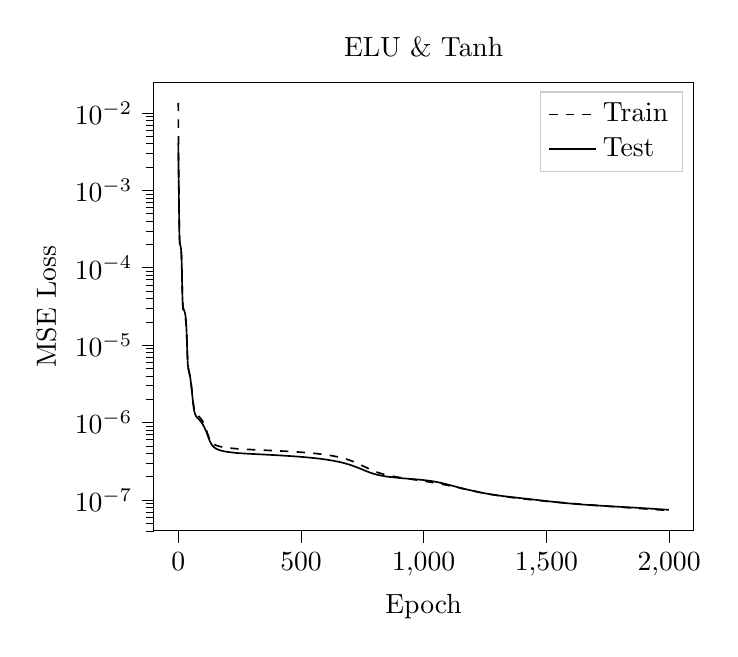
\begin{tikzpicture}

\begin{axis}[
legend cell align={left},
legend style={fill opacity=0.8, draw opacity=1, text opacity=1, draw=white!80!black},
log basis y={10},
tick align=outside,
tick pos=left,
title={ELU \& Tanh},
x grid style={white!69.0196078431373!black},
xlabel={Epoch},
xmin=-99.95, xmax=2098.95,
xtick style={color=black},
y grid style={white!69.0196078431373!black},
ylabel={MSE Loss},
ymin=3.99690726045967e-08, ymax=0.0247433085065691,
ymode=log,
ytick style={color=black}
]
\addplot [semithick, black, dashed]
table {%
0 0.0134957538153976
1 0.0023310884651728
2 0.00137426065234467
3 0.00077357710513752
4 0.000392858184757642
5 0.000249120184715139
6 0.000204640424781246
7 0.000192825474230631
8 0.000188046251423657
9 0.000183736560094985
10 0.000178325850552937
11 0.000170728457196674
12 0.000159364001447102
13 0.000142009735987813
14 0.000116843216383131
15 8.60529496239906e-05
16 5.84654288759339e-05
17 4.15402031667327e-05
18 3.35064789760509e-05
19 2.98543798189712e-05
20 2.80834724026136e-05
21 2.7120061565256e-05
22 2.65000228091594e-05
23 2.60162827989916e-05
24 2.55703675338736e-05
25 2.51090224846848e-05
26 2.45967136706895e-05
27 2.40019229959216e-05
28 2.32902032030324e-05
29 2.24202653498651e-05
30 2.13432580803783e-05
31 2.00045652190965e-05
32 1.83535941760056e-05
33 1.63697485281773e-05
34 1.41058650265222e-05
35 1.17310301802718e-05
36 9.51688467444001e-06
37 7.72394584441827e-06
38 6.46328579375677e-06
39 5.67237918517094e-06
40 5.20494382209336e-06
41 4.92263743979038e-06
42 4.73192033814485e-06
43 4.58095780572876e-06
44 4.44440987797634e-06
45 4.31049008187756e-06
46 4.17367375678168e-06
47 4.03129841151895e-06
48 3.88186479199248e-06
49 3.72467667875753e-06
50 3.55976452499362e-06
51 3.3876761801821e-06
52 3.20961057741442e-06
53 3.02756247447178e-06
54 2.84423495969577e-06
55 2.6628521272869e-06
56 2.48704906198327e-06
57 2.32027610144314e-06
58 2.16550271670712e-06
59 2.02503649921937e-06
60 1.90025342425315e-06
61 1.79153526005393e-06
62 1.69843876534514e-06
63 1.6199104959469e-06
64 1.55439161704862e-06
65 1.50013449353992e-06
66 1.45557809571528e-06
67 1.41910898872766e-06
68 1.38913675107233e-06
69 1.36439518496445e-06
70 1.34373901823892e-06
71 1.3262495506865e-06
72 1.31120514492977e-06
73 1.29805072887734e-06
74 1.28629729721297e-06
75 1.27557425403779e-06
76 1.26559939400295e-06
77 1.25617296097857e-06
78 1.24714520961788e-06
79 1.23836504184283e-06
80 1.22974110064433e-06
81 1.22120436569162e-06
82 1.21270806337748e-06
83 1.2042229414817e-06
84 1.19568821878602e-06
85 1.18703545433618e-06
86 1.17824618195073e-06
87 1.16926949596063e-06
88 1.16005888634163e-06
89 1.15063077569744e-06
90 1.14096733773295e-06
91 1.1310374811444e-06
92 1.12082256276835e-06
93 1.11030603562767e-06
94 1.0994694030444e-06
95 1.08829291150414e-06
96 1.0767586200302e-06
97 1.06484853012034e-06
98 1.05254191706194e-06
99 1.03982470298547e-06
100 1.02669375425535e-06
101 1.013145324265e-06
102 9.99175518728634e-07
103 9.84785912976349e-07
104 9.69983164736732e-07
105 9.54775229445204e-07
106 9.39185010707888e-07
107 9.23240237511891e-07
108 9.06987714614615e-07
109 8.90465134233409e-07
110 8.73703285321881e-07
111 8.56757450264922e-07
112 8.39707763958586e-07
113 8.22606544005566e-07
114 8.05511803577019e-07
115 7.8853165106807e-07
116 7.71770440536557e-07
117 7.55323297966015e-07
118 7.39256733481852e-07
119 7.23615459463645e-07
120 7.08470843107989e-07
121 6.93896306614761e-07
122 6.79961028396292e-07
123 6.66732689808214e-07
124 6.54239293226055e-07
125 6.4249699808272e-07
126 6.31537070717059e-07
127 6.21340004741455e-07
128 6.11861269959491e-07
129 6.03081373157011e-07
130 5.94950151452167e-07
131 5.87441886111151e-07
132 5.80561772849819e-07
133 5.742626128864e-07
134 5.68461311942769e-07
135 5.63138753122416e-07
136 5.58289989569971e-07
137 5.53789126101378e-07
138 5.49580243131231e-07
139 5.45668546905631e-07
140 5.42029055068838e-07
141 5.3864083858457e-07
142 5.35457754253343e-07
143 5.32470842770749e-07
144 5.2965976857422e-07
145 5.27022905075114e-07
146 5.24544419604922e-07
147 5.2220559823013e-07
148 5.1999728647445e-07
149 5.17909198450184e-07
150 5.15934669948592e-07
151 5.14066228163301e-07
152 5.12297007816187e-07
153 5.10620100868664e-07
154 5.09027317391997e-07
155 5.07512464238857e-07
156 5.06070105885215e-07
157 5.04693904218811e-07
158 5.03377546664296e-07
159 5.02117622758647e-07
160 5.0090915983958e-07
161 4.99747272371565e-07
162 4.9862692104341e-07
163 4.97548696131389e-07
164 4.96514213153887e-07
165 4.95520301740271e-07
166 4.94560742978933e-07
167 4.93631716139475e-07
168 4.92731814873082e-07
169 4.91858511153964e-07
170 4.9100989390638e-07
171 4.90185054943026e-07
172 4.89384468266962e-07
173 4.88605556597577e-07
174 4.87848062974194e-07
175 4.87110447991768e-07
176 4.86391952748022e-07
177 4.85690664930871e-07
178 4.8500625908332e-07
179 4.84336899063464e-07
180 4.83682655712414e-07
181 4.83042738224526e-07
182 4.82416531340846e-07
183 4.81803007630788e-07
184 4.81201379244567e-07
185 4.80611838398204e-07
186 4.80033573126093e-07
187 4.79465925039335e-07
188 4.78908676896594e-07
189 4.78361412703521e-07
190 4.77823565461222e-07
191 4.7729492538906e-07
192 4.76775265582319e-07
193 4.76263761612472e-07
194 4.7576123780857e-07
195 4.75266853953826e-07
196 4.74780734677438e-07
197 4.7430138734228e-07
198 4.73829710003315e-07
199 4.73365776272772e-07
200 4.72908600201549e-07
201 4.72458603368864e-07
202 4.72014912119789e-07
203 4.71577816512081e-07
204 4.71147397803406e-07
205 4.70723401988948e-07
206 4.70305473228905e-07
207 4.69893359181128e-07
208 4.694872364297e-07
209 4.69086846621281e-07
210 4.68691152320844e-07
211 4.68301935214299e-07
212 4.6791765424814e-07
213 4.67538755827945e-07
214 4.67165025099803e-07
215 4.66797083745973e-07
216 4.66435041161617e-07
217 4.66077831347889e-07
218 4.65725406073147e-07
219 4.65377729284455e-07
220 4.65034056972513e-07
221 4.64696197980174e-07
222 4.64362528262541e-07
223 4.64033503746464e-07
224 4.63709261964595e-07
225 4.63390550478948e-07
226 4.63075590630524e-07
227 4.62764741016031e-07
228 4.6245909268805e-07
229 4.62156695846261e-07
230 4.61858597319065e-07
231 4.61564129679459e-07
232 4.61272959867642e-07
233 4.60985718561346e-07
234 4.60702021101156e-07
235 4.60422043445874e-07
236 4.60145196697681e-07
237 4.59871440227744e-07
238 4.59601524894993e-07
239 4.59334055761929e-07
240 4.59070226526137e-07
241 4.58809098404345e-07
242 4.58550512959732e-07
243 4.58294875897991e-07
244 4.5804139479344e-07
245 4.5778995291812e-07
246 4.57542623578888e-07
247 4.57299847056447e-07
248 4.5706229977327e-07
249 4.5682922412027e-07
250 4.5659845754642e-07
251 4.56369487707775e-07
252 4.56143253117602e-07
253 4.55919790695702e-07
254 4.55699768508566e-07
255 4.55483950588587e-07
256 4.55268989156821e-07
257 4.55049070268387e-07
258 4.54831853417659e-07
259 4.54618514424965e-07
260 4.54407614483898e-07
261 4.5419944773073e-07
262 4.53993272486741e-07
263 4.53789547307792e-07
264 4.53587446315851e-07
265 4.53387271875272e-07
266 4.5318868204447e-07
267 4.5299173295632e-07
268 4.52797509495895e-07
269 4.52604366543596e-07
270 4.52412825268311e-07
271 4.52222721833095e-07
272 4.52033698024934e-07
273 4.51846320558502e-07
274 4.51659424555828e-07
275 4.51474039138589e-07
276 4.51290351008993e-07
277 4.511082164953e-07
278 4.50927281875124e-07
279 4.50748062917228e-07
280 4.50569941847334e-07
281 4.50392685195311e-07
282 4.50216764761535e-07
283 4.50041916479904e-07
284 4.49868347018878e-07
285 4.49695231836245e-07
286 4.49524123709466e-07
287 4.49353258233032e-07
288 4.49183449944712e-07
289 4.49014504795286e-07
290 4.48846887337595e-07
291 4.48678875031305e-07
292 4.48512801781931e-07
293 4.4834711533781e-07
294 4.48182058306656e-07
295 4.48017639698151e-07
296 4.47853688470445e-07
297 4.47691391997296e-07
298 4.47529162329374e-07
299 4.47367209105209e-07
300 4.47207153499107e-07
301 4.47047590427019e-07
302 4.46889215353963e-07
303 4.46730439591647e-07
304 4.46573448101617e-07
305 4.46416878617129e-07
306 4.46260456129721e-07
307 4.46104787130253e-07
308 4.45949403498958e-07
309 4.45795175110675e-07
310 4.45640652031898e-07
311 4.45486587608457e-07
312 4.45333089373889e-07
313 4.45180131748657e-07
314 4.4502877632624e-07
315 4.44876304158015e-07
316 4.44724652467698e-07
317 4.44573048568486e-07
318 4.4442220375629e-07
319 4.44271763015536e-07
320 4.44121741267622e-07
321 4.43972102488033e-07
322 4.43822052417886e-07
323 4.43673538285339e-07
324 4.43524699790032e-07
325 4.43375982655425e-07
326 4.4322779477568e-07
327 4.4307990557968e-07
328 4.42932485313463e-07
329 4.42784972619847e-07
330 4.42638347223578e-07
331 4.42491844822257e-07
332 4.42345659052989e-07
333 4.42199956879108e-07
334 4.42054676227599e-07
335 4.41909244827343e-07
336 4.41764431172942e-07
337 4.41619671931903e-07
338 4.41474580128443e-07
339 4.41329635378906e-07
340 4.41183451258098e-07
341 4.41036900710401e-07
342 4.40890624204826e-07
343 4.40743538902666e-07
344 4.40596182741615e-07
345 4.40449259201614e-07
346 4.40302216944133e-07
347 4.40154431444739e-07
348 4.40006927206582e-07
349 4.39860318763863e-07
350 4.39711944849819e-07
351 4.39565173067535e-07
352 4.39417494092709e-07
353 4.39270274227965e-07
354 4.39123118624707e-07
355 4.38975632746974e-07
356 4.38827461607616e-07
357 4.38680071070507e-07
358 4.38532330349517e-07
359 4.3838513353478e-07
360 4.38237253135299e-07
361 4.38088896984823e-07
362 4.37940936492964e-07
363 4.37792325058695e-07
364 4.3764440769678e-07
365 4.37496297351458e-07
366 4.37348056692599e-07
367 4.37199314120562e-07
368 4.37050272594774e-07
369 4.36901579078608e-07
370 4.36752512044336e-07
371 4.36603472181218e-07
372 4.36453455236574e-07
373 4.36304386454367e-07
374 4.36154428882674e-07
375 4.36004858670458e-07
376 4.35854937720137e-07
377 4.35704757762778e-07
378 4.35553956663171e-07
379 4.35403425242953e-07
380 4.35252636734162e-07
381 4.35101373255975e-07
382 4.34949856654043e-07
383 4.3479894871723e-07
384 4.3464698572393e-07
385 4.34495225817955e-07
386 4.34342180668068e-07
387 4.34190195235828e-07
388 4.34037036896484e-07
389 4.33883725705186e-07
390 4.3373072944064e-07
391 4.3357726191573e-07
392 4.33423383583431e-07
393 4.33269188050645e-07
394 4.33114656090083e-07
395 4.32960370446267e-07
396 4.32805814895687e-07
397 4.3265090708644e-07
398 4.32495347084227e-07
399 4.32340210664961e-07
400 4.32183846626799e-07
401 4.32028382576277e-07
402 4.31871616200397e-07
403 4.31714662525451e-07
404 4.31557992882858e-07
405 4.31400304861995e-07
406 4.31242871329118e-07
407 4.31084624125333e-07
408 4.3092627005592e-07
409 4.3076730334235e-07
410 4.306080731169e-07
411 4.30449040848657e-07
412 4.30289126995831e-07
413 4.30129235766685e-07
414 4.29968422125171e-07
415 4.29807350585065e-07
416 4.2964639477816e-07
417 4.29484178312123e-07
418 4.29322080350403e-07
419 4.29159988442507e-07
420 4.28997011951537e-07
421 4.28833916558347e-07
422 4.28670428178179e-07
423 4.285065395635e-07
424 4.28342804710269e-07
425 4.28177927716433e-07
426 4.28012444601222e-07
427 4.27847551961236e-07
428 4.27682234885651e-07
429 4.27516849072163e-07
430 4.2735087495771e-07
431 4.27185019674425e-07
432 4.27018305103388e-07
433 4.26850394106282e-07
434 4.26680964608295e-07
435 4.26510055604012e-07
436 4.26338771930546e-07
437 4.26167039904612e-07
438 4.25994698446175e-07
439 4.25822926942487e-07
440 4.25649003418016e-07
441 4.25476069125352e-07
442 4.25302337390576e-07
443 4.25128136527064e-07
444 4.24952945252244e-07
445 4.24777989451286e-07
446 4.24601941233504e-07
447 4.24425246308147e-07
448 4.24248131494664e-07
449 4.24070380120156e-07
450 4.23891809575139e-07
451 4.23712736520088e-07
452 4.23533353355765e-07
453 4.23353260387671e-07
454 4.23172379115044e-07
455 4.22990336204521e-07
456 4.22808332061209e-07
457 4.2262559324513e-07
458 4.22442374357956e-07
459 4.22258078586424e-07
460 4.22073079946017e-07
461 4.21887672999333e-07
462 4.21701368480853e-07
463 4.21513872581158e-07
464 4.21326206733852e-07
465 4.21137836866592e-07
466 4.20948731303383e-07
467 4.20758855895542e-07
468 4.20568408756594e-07
469 4.20376887021234e-07
470 4.20184173734128e-07
471 4.19991282626597e-07
472 4.19797408497402e-07
473 4.19602816336351e-07
474 4.19407368866587e-07
475 4.19211461661462e-07
476 4.19014144327434e-07
477 4.18816154294177e-07
478 4.18617555780543e-07
479 4.18418411371135e-07
480 4.1821802982156e-07
481 4.18016062596394e-07
482 4.17814719014586e-07
483 4.17611920354943e-07
484 4.17407868425812e-07
485 4.17203221303453e-07
486 4.16997823535326e-07
487 4.16791075110723e-07
488 4.16583922344671e-07
489 4.16375738268471e-07
490 4.16166455650568e-07
491 4.15955980415106e-07
492 4.15744668330831e-07
493 4.15532831439691e-07
494 4.15319472281794e-07
495 4.15105677120664e-07
496 4.14890348992003e-07
497 4.1467463127276e-07
498 4.14457540784952e-07
499 4.14239087675128e-07
500 4.14020030703455e-07
501 4.13799983661534e-07
502 4.1357917176299e-07
503 4.13357065141895e-07
504 4.13133196275339e-07
505 4.12908721187932e-07
506 4.12683341309616e-07
507 4.12456391615024e-07
508 4.12228853789998e-07
509 4.11999894495807e-07
510 4.11769633558379e-07
511 4.11538843053449e-07
512 4.11306252885879e-07
513 4.11072774568311e-07
514 4.10838005322489e-07
515 4.1060252716818e-07
516 4.10364640302419e-07
517 4.10126535740574e-07
518 4.09886833153905e-07
519 4.09645856692009e-07
520 4.094044307692e-07
521 4.09160514337259e-07
522 4.08915355137651e-07
523 4.08669283530116e-07
524 4.08422131798147e-07
525 4.08173769940845e-07
526 4.07923640523222e-07
527 4.07672310942075e-07
528 4.07419083543914e-07
529 4.07164622004075e-07
530 4.06909275639578e-07
531 4.06652300753763e-07
532 4.06393879373468e-07
533 4.06133775314288e-07
534 4.05872190484047e-07
535 4.05609441145316e-07
536 4.05344806040375e-07
537 4.05079033455991e-07
538 4.04811563768703e-07
539 4.04542423822818e-07
540 4.04271819334667e-07
541 4.03999381035192e-07
542 4.03725548309808e-07
543 4.03450251994286e-07
544 4.03173237657484e-07
545 4.02894533820586e-07
546 4.02613792061857e-07
547 4.0233181184135e-07
548 4.02048376187736e-07
549 4.01763181656634e-07
550 4.0147601137619e-07
551 4.01187170766093e-07
552 4.00897058185024e-07
553 4.00604771755297e-07
554 4.00311013024179e-07
555 4.00015908937235e-07
556 3.99718229388668e-07
557 3.99419691575531e-07
558 3.99118723294123e-07
559 3.98816622549703e-07
560 3.98512169610399e-07
561 3.98205197001289e-07
562 3.97896785699459e-07
563 3.97586246165815e-07
564 3.97274299714923e-07
565 3.9695991949884e-07
566 3.96644428946047e-07
567 3.96326605198283e-07
568 3.9600664929651e-07
569 3.95684843951472e-07
570 3.95360391905797e-07
571 3.95033267778899e-07
572 3.94703262571738e-07
573 3.94371521494463e-07
574 3.94036575130485e-07
575 3.93699125879721e-07
576 3.9335995651868e-07
577 3.93019113644755e-07
578 3.92675260812325e-07
579 3.92329612409981e-07
580 3.91981137525477e-07
581 3.91630506939578e-07
582 3.91277142398394e-07
583 3.90921700088143e-07
584 3.90563617244766e-07
585 3.90202885412805e-07
586 3.89840740638192e-07
587 3.89475067450462e-07
588 3.8910768236633e-07
589 3.88736924008981e-07
590 3.8836424393196e-07
591 3.87987770281484e-07
592 3.87609264734579e-07
593 3.87228815569074e-07
594 3.8684465638994e-07
595 3.86458957137847e-07
596 3.86069671534983e-07
597 3.85677691681963e-07
598 3.85282802525921e-07
599 3.84885359849818e-07
600 3.84484707552701e-07
601 3.84081810679504e-07
602 3.83675666981276e-07
603 3.83267110564134e-07
604 3.82855496027901e-07
605 3.82440661056194e-07
606 3.82023474216453e-07
607 3.81603375615214e-07
608 3.81180774070344e-07
609 3.80755330439797e-07
610 3.80327249644097e-07
611 3.7989629353774e-07
612 3.79462449785706e-07
613 3.79024334748124e-07
614 3.7858260044743e-07
615 3.781370549234e-07
616 3.7768797929516e-07
617 3.77235340451421e-07
618 3.76779640092195e-07
619 3.7632051203218e-07
620 3.75858051143041e-07
621 3.75393150264358e-07
622 3.74924531286069e-07
623 3.74452642461165e-07
624 3.73977770863121e-07
625 3.7350079924181e-07
626 3.7302071731915e-07
627 3.7254025515665e-07
628 3.7205934323481e-07
629 3.71576094394754e-07
630 3.71084454229731e-07
631 3.70585130312406e-07
632 3.70085966878264e-07
633 3.69586355361662e-07
634 3.69074953312065e-07
635 3.68545165670753e-07
636 3.68011905194976e-07
637 3.67480042811508e-07
638 3.66946662566647e-07
639 3.6641021911521e-07
640 3.65870577084593e-07
641 3.65327583651265e-07
642 3.64780428000699e-07
643 3.64229227869828e-07
644 3.63673588225311e-07
645 3.63114767651496e-07
646 3.6255076777536e-07
647 3.61983122857623e-07
648 3.61412011471884e-07
649 3.60835356488565e-07
650 3.60254737486798e-07
651 3.59668436402671e-07
652 3.59077841324051e-07
653 3.58481157050505e-07
654 3.57879950044548e-07
655 3.57273974941563e-07
656 3.56662821857867e-07
657 3.56046830674472e-07
658 3.55426030381523e-07
659 3.54800945274292e-07
660 3.54170143580745e-07
661 3.53534564055735e-07
662 3.52893836748081e-07
663 3.52249136582827e-07
664 3.5159879300295e-07
665 3.50943790948577e-07
666 3.50283574590549e-07
667 3.49618195528478e-07
668 3.48948270911364e-07
669 3.48272788599502e-07
670 3.47592344610348e-07
671 3.46906679880021e-07
672 3.46215688352913e-07
673 3.45520173468117e-07
674 3.44818678343017e-07
675 3.44112561549537e-07
676 3.43400532202054e-07
677 3.42684295404183e-07
678 3.41961838927318e-07
679 3.41234473751229e-07
680 3.40501417468886e-07
681 3.39762946779842e-07
682 3.39019501467419e-07
683 3.38269846963613e-07
684 3.37515219158036e-07
685 3.36755509124487e-07
686 3.35990043367929e-07
687 3.35219267029174e-07
688 3.34443446874388e-07
689 3.33661982224953e-07
690 3.32875743197292e-07
691 3.32083970818076e-07
692 3.31286873020531e-07
693 3.30484729033742e-07
694 3.29678474983552e-07
695 3.2886618532757e-07
696 3.28050683791048e-07
697 3.2723264064316e-07
698 3.26414048302581e-07
699 3.25598259109938e-07
700 3.24765047210462e-07
701 3.23909981830184e-07
702 3.23054695087421e-07
703 3.22199193206529e-07
704 3.21340463742104e-07
705 3.20477851943224e-07
706 3.19610514708302e-07
707 3.18738396330787e-07
708 3.17862388968138e-07
709 3.16981570634312e-07
710 3.16095240989966e-07
711 3.15203745643089e-07
712 3.14306510190932e-07
713 3.13403632560494e-07
714 3.12496322308675e-07
715 3.11583908654711e-07
716 3.10667585395663e-07
717 3.09747140491368e-07
718 3.08822607465231e-07
719 3.07894123082519e-07
720 3.06962333453953e-07
721 3.0602608833874e-07
722 3.05086028419055e-07
723 3.04143713719895e-07
724 3.03196796195948e-07
725 3.02247252278676e-07
726 3.01293990418117e-07
727 3.00338420231583e-07
728 2.99379660518184e-07
729 2.98417770935089e-07
730 2.97453068498044e-07
731 2.96486439765431e-07
732 2.95516273723706e-07
733 2.94544258196083e-07
734 2.93570655856001e-07
735 2.92593953943765e-07
736 2.91615041831506e-07
737 2.90633185599631e-07
738 2.89649034030504e-07
739 2.88664336991928e-07
740 2.87676741166365e-07
741 2.866883023529e-07
742 2.85699080663449e-07
743 2.84709725391963e-07
744 2.83720243942298e-07
745 2.82730636115502e-07
746 2.81744076914947e-07
747 2.80759510971507e-07
748 2.7977648436206e-07
749 2.78794243385505e-07
750 2.77813358380286e-07
751 2.7683377196297e-07
752 2.75855688741444e-07
753 2.74879691914975e-07
754 2.73905823689802e-07
755 2.72932655818181e-07
756 2.71961296789414e-07
757 2.70993213973725e-07
758 2.70029876915601e-07
759 2.69070342582722e-07
760 2.68115076281106e-07
761 2.67164587739899e-07
762 2.66217917982203e-07
763 2.65276417891869e-07
764 2.64340145193387e-07
765 2.63407706185603e-07
766 2.6248111669247e-07
767 2.61559234829178e-07
768 2.60642846200199e-07
769 2.59731777774164e-07
770 2.58826290547631e-07
771 2.5792636903077e-07
772 2.57032839485305e-07
773 2.56144408282921e-07
774 2.55262543291224e-07
775 2.5438714554582e-07
776 2.53518222692151e-07
777 2.52655296193893e-07
778 2.51799888772553e-07
779 2.5095009256404e-07
780 2.50108108076574e-07
781 2.49272646072995e-07
782 2.48444218982513e-07
783 2.47623585693191e-07
784 2.46809189377473e-07
785 2.46002701430825e-07
786 2.45203631791924e-07
787 2.44411834984248e-07
788 2.43627891080678e-07
789 2.42850782427695e-07
790 2.42081854906928e-07
791 2.41320599272399e-07
792 2.40566559881472e-07
793 2.3982113521015e-07
794 2.39083572949994e-07
795 2.38354401588481e-07
796 2.37634123848807e-07
797 2.3692211487969e-07
798 2.36218781566322e-07
799 2.35523804335003e-07
800 2.34836860670384e-07
801 2.34157943950208e-07
802 2.33487251009024e-07
803 2.3282475075348e-07
804 2.3217077144011e-07
805 2.31525538907817e-07
806 2.30889206477514e-07
807 2.30262769150613e-07
808 2.2964494941391e-07
809 2.2903699370147e-07
810 2.2843675628792e-07
811 2.27845235556856e-07
812 2.27261650195487e-07
813 2.26686032704038e-07
814 2.26118474671466e-07
815 2.25558543178295e-07
816 2.25006733415967e-07
817 2.24462538170656e-07
818 2.2392637707469e-07
819 2.23396879476923e-07
820 2.2287552974376e-07
821 2.22361441501562e-07
822 2.21854354720108e-07
823 2.21354323471701e-07
824 2.20860920521204e-07
825 2.2037506118977e-07
826 2.19894997798065e-07
827 2.19422501984923e-07
828 2.18955629293305e-07
829 2.18495853673062e-07
830 2.18041660289714e-07
831 2.17593597042764e-07
832 2.17151581793473e-07
833 2.16715876419471e-07
834 2.16284942467837e-07
835 2.15860050076344e-07
836 2.1544019813291e-07
837 2.15026796041684e-07
838 2.14618440551817e-07
839 2.14215182168687e-07
840 2.13816784892629e-07
841 2.13424236363835e-07
842 2.13036339133055e-07
843 2.12653428448562e-07
844 2.12275704200238e-07
845 2.11901888874877e-07
846 2.1153276824748e-07
847 2.11167949174751e-07
848 2.10808170407972e-07
849 2.10451614364615e-07
850 2.10098580353701e-07
851 2.09750812103948e-07
852 2.09405895120085e-07
853 2.0906477641347e-07
854 2.08727001819398e-07
855 2.08393345488389e-07
856 2.08063171513118e-07
857 2.07736553591076e-07
858 2.0741319255535e-07
859 2.07093789825308e-07
860 2.06777032659033e-07
861 2.06463370915344e-07
862 2.06152881176536e-07
863 2.05845972587326e-07
864 2.05542741582576e-07
865 2.05242946961448e-07
866 2.04945145583224e-07
867 2.04649749250052e-07
868 2.04357353396745e-07
869 2.04065894195082e-07
870 2.03777457429055e-07
871 2.03491203450312e-07
872 2.03206753425889e-07
873 2.02925087876338e-07
874 2.02645592992212e-07
875 2.02368894051119e-07
876 2.02094200830061e-07
877 2.01822318729228e-07
878 2.01553326107273e-07
879 2.01285563150577e-07
880 2.01020466818136e-07
881 2.0075688806287e-07
882 2.00495315624494e-07
883 2.00236287355438e-07
884 1.9997802669991e-07
885 1.99721420429455e-07
886 1.99466760165024e-07
887 1.99212858433384e-07
888 1.98960012113503e-07
889 1.98708344001375e-07
890 1.98456358759813e-07
891 1.98205174598343e-07
892 1.9795247490606e-07
893 1.97697988696177e-07
894 1.97439781103981e-07
895 1.97174738133299e-07
896 1.9690548506901e-07
897 1.96643729537982e-07
898 1.96398226790961e-07
899 1.96169193984019e-07
900 1.95943623381822e-07
901 1.95714774321232e-07
902 1.95485544722374e-07
903 1.95257697583884e-07
904 1.95029899629162e-07
905 1.94803018146672e-07
906 1.94576785659706e-07
907 1.94351484836375e-07
908 1.94126916412074e-07
909 1.93903316954902e-07
910 1.93680324557022e-07
911 1.9345859624309e-07
912 1.93236818489595e-07
913 1.93015732975255e-07
914 1.92795474973195e-07
915 1.92575191803712e-07
916 1.92355031046532e-07
917 1.92134992573756e-07
918 1.91914073809585e-07
919 1.91692709663016e-07
920 1.91469181316961e-07
921 1.91248184336246e-07
922 1.91033474195024e-07
923 1.90824868155914e-07
924 1.9061681585697e-07
925 1.9040659654479e-07
926 1.90195690294104e-07
927 1.89984557763978e-07
928 1.89772694426438e-07
929 1.89562242127295e-07
930 1.89355768128507e-07
931 1.89148760014746e-07
932 1.88941211206384e-07
933 1.8873464432545e-07
934 1.88529779649116e-07
935 1.8832545347891e-07
936 1.88120943477088e-07
937 1.87917375214397e-07
938 1.87713873302187e-07
939 1.87510132064972e-07
940 1.8730790769439e-07
941 1.87105002254384e-07
942 1.86902863234195e-07
943 1.86701843460924e-07
944 1.8649999681486e-07
945 1.8629890276145e-07
946 1.8609833674077e-07
947 1.85897361504317e-07
948 1.85697282688579e-07
949 1.85497568267579e-07
950 1.85297616908997e-07
951 1.85098694657881e-07
952 1.84900121737996e-07
953 1.84700446268948e-07
954 1.84501964369588e-07
955 1.84303896929805e-07
956 1.8410508442912e-07
957 1.8390730782869e-07
958 1.83709708338142e-07
959 1.8351193419619e-07
960 1.83313767180948e-07
961 1.83116579052012e-07
962 1.82919414100979e-07
963 1.82722437656935e-07
964 1.82525298455971e-07
965 1.82328213938376e-07
966 1.82131599942181e-07
967 1.81935750461548e-07
968 1.8173868717497e-07
969 1.81542523080225e-07
970 1.81345505112063e-07
971 1.81149303955408e-07
972 1.80952871204454e-07
973 1.80756489726264e-07
974 1.80560155229159e-07
975 1.8036430697066e-07
976 1.80167951057797e-07
977 1.79972166336029e-07
978 1.79775467472609e-07
979 1.79579259693696e-07
980 1.79383511152764e-07
981 1.79187363684719e-07
982 1.78991157369524e-07
983 1.78794552368799e-07
984 1.7859870311554e-07
985 1.78402505511599e-07
986 1.78205574442813e-07
987 1.78009270669577e-07
988 1.77813091852386e-07
989 1.77616319618323e-07
990 1.7741990316722e-07
991 1.77223411881755e-07
992 1.77026502839794e-07
993 1.76829171635973e-07
994 1.76632485633377e-07
995 1.76435387984952e-07
996 1.76238921852701e-07
997 1.76041123054915e-07
998 1.75843510660911e-07
999 1.75646163881993e-07
1000 1.75448311040327e-07
1001 1.75250185350251e-07
1002 1.75052527254138e-07
1003 1.74854418531822e-07
1004 1.74656194630529e-07
1005 1.74457870940614e-07
1006 1.74259641283925e-07
1007 1.74061686607274e-07
1008 1.73863939551211e-07
1009 1.73667300458646e-07
1010 1.73472921659368e-07
1011 1.73273655548201e-07
1012 1.73069673081727e-07
1013 1.7286636042968e-07
1014 1.72665114490655e-07
1015 1.72464464000655e-07
1016 1.72263602166822e-07
1017 1.72062851873989e-07
1018 1.71861413647889e-07
1019 1.71659764902188e-07
1020 1.71458449159445e-07
1021 1.71256041582524e-07
1022 1.71053797302534e-07
1023 1.70851226442892e-07
1024 1.70648361020653e-07
1025 1.70445360467397e-07
1026 1.70241809740901e-07
1027 1.70038351967605e-07
1028 1.69834429129878e-07
1029 1.69629752136302e-07
1030 1.69425513874444e-07
1031 1.69220505398471e-07
1032 1.69015253575822e-07
1033 1.68809544774717e-07
1034 1.68604265013528e-07
1035 1.68397976921142e-07
1036 1.68191788034733e-07
1037 1.6798447364863e-07
1038 1.67777331597563e-07
1039 1.6757027366765e-07
1040 1.6736213190427e-07
1041 1.67153996954994e-07
1042 1.66945491066883e-07
1043 1.66735625384717e-07
1044 1.66526715325688e-07
1045 1.66316698717139e-07
1046 1.66106552946133e-07
1047 1.65895362272295e-07
1048 1.65684443473424e-07
1049 1.65472404837885e-07
1050 1.65260418420132e-07
1051 1.65048077548136e-07
1052 1.64834197867947e-07
1053 1.64621264730158e-07
1054 1.64407517402765e-07
1055 1.64192864481549e-07
1056 1.63978524852837e-07
1057 1.63763244295012e-07
1058 1.63547865398073e-07
1059 1.63332109025305e-07
1060 1.63115409371528e-07
1061 1.62898703187864e-07
1062 1.62680641430768e-07
1063 1.62461872527331e-07
1064 1.62241660071061e-07
1065 1.62020339615765e-07
1066 1.61796442682771e-07
1067 1.61578315811539e-07
1068 1.61365553886128e-07
1069 1.61150012530697e-07
1070 1.60931570960088e-07
1071 1.60712657454098e-07
1072 1.60492130085288e-07
1073 1.60271687285274e-07
1074 1.60050248744881e-07
1075 1.59829400992351e-07
1076 1.59607629875325e-07
1077 1.59385763772946e-07
1078 1.59163962138109e-07
1079 1.58940918062456e-07
1080 1.58717688861998e-07
1081 1.58494263992282e-07
1082 1.58270022268425e-07
1083 1.58046180196436e-07
1084 1.57821384448198e-07
1085 1.57595483358364e-07
1086 1.57370519950462e-07
1087 1.57144959892719e-07
1088 1.56918834306907e-07
1089 1.5669187406786e-07
1090 1.56464888597441e-07
1091 1.56237204002707e-07
1092 1.56009357084486e-07
1093 1.55781397751298e-07
1094 1.55553085093629e-07
1095 1.55324671020196e-07
1096 1.55095236443969e-07
1097 1.54865906345947e-07
1098 1.54636180901946e-07
1099 1.54406042327082e-07
1100 1.54175699570658e-07
1101 1.53945063857464e-07
1102 1.53714261266202e-07
1103 1.53482981708919e-07
1104 1.53252202139242e-07
1105 1.53020336426835e-07
1106 1.52788393776859e-07
1107 1.52556364362511e-07
1108 1.52324091487799e-07
1109 1.52091592113379e-07
1110 1.51858972628816e-07
1111 1.51626830870555e-07
1112 1.51393231192287e-07
1113 1.51160503861547e-07
1114 1.50926978633947e-07
1115 1.50693419392667e-07
1116 1.50459477836762e-07
1117 1.50224978561653e-07
1118 1.49990391300037e-07
1119 1.49756285445335e-07
1120 1.49522032693028e-07
1121 1.49287322336988e-07
1122 1.49052170790753e-07
1123 1.48817413446523e-07
1124 1.48582587861767e-07
1125 1.48347238109636e-07
1126 1.48112339459772e-07
1127 1.47877032254939e-07
1128 1.47641772933582e-07
1129 1.47406511302961e-07
1130 1.47171383567013e-07
1131 1.46936253393903e-07
1132 1.46701635351576e-07
1133 1.46465785476835e-07
1134 1.46231383524764e-07
1135 1.4599759120415e-07
1136 1.45765217787641e-07
1137 1.45536929771595e-07
1138 1.45315871961316e-07
1139 1.45102639088179e-07
1140 1.44857848511037e-07
1141 1.44608287207859e-07
1142 1.44369832149493e-07
1143 1.44132638602912e-07
1144 1.43896900084428e-07
1145 1.4366150475098e-07
1146 1.43426275592162e-07
1147 1.43191492327333e-07
1148 1.42956328453181e-07
1149 1.42722145618279e-07
1150 1.42487870704144e-07
1151 1.42253041154561e-07
1152 1.42020066476789e-07
1153 1.41785810825468e-07
1154 1.41552231468722e-07
1155 1.41318830927162e-07
1156 1.41086397505319e-07
1157 1.40852889181531e-07
1158 1.40620678877212e-07
1159 1.40388574116912e-07
1160 1.40156471644559e-07
1161 1.39925065703039e-07
1162 1.39693805635943e-07
1163 1.3946283491606e-07
1164 1.39232228946184e-07
1165 1.39002079130535e-07
1166 1.38772403865062e-07
1167 1.38542935140151e-07
1168 1.38313878032648e-07
1169 1.38085498043949e-07
1170 1.37857207036518e-07
1171 1.37629013572393e-07
1172 1.37401833903539e-07
1173 1.37175356073271e-07
1174 1.36949046506629e-07
1175 1.36723186336951e-07
1176 1.36497654089851e-07
1177 1.36273238062756e-07
1178 1.36049034921371e-07
1179 1.35825359215858e-07
1180 1.35602388681377e-07
1181 1.35379711132089e-07
1182 1.35157931211438e-07
1183 1.34936623901183e-07
1184 1.34716155685055e-07
1185 1.34496195883571e-07
1186 1.34277296119478e-07
1187 1.34058615849142e-07
1188 1.33840519282558e-07
1189 1.33623340104805e-07
1190 1.33407476525349e-07
1191 1.3319190517791e-07
1192 1.32976978036936e-07
1193 1.32762343355353e-07
1194 1.32549082302091e-07
1195 1.32336207059325e-07
1196 1.3212395525386e-07
1197 1.3191258280898e-07
1198 1.31701604125567e-07
1199 1.31491672902939e-07
1200 1.31282150185541e-07
1201 1.31073970862872e-07
1202 1.30865978604788e-07
1203 1.30659009151657e-07
1204 1.30452958032379e-07
1205 1.30247145797568e-07
1206 1.30042434811628e-07
1207 1.29837635277852e-07
1208 1.29634143718249e-07
1209 1.29431724765539e-07
1210 1.29229264068442e-07
1211 1.2902830654582e-07
1212 1.2882778151635e-07
1213 1.28628469106218e-07
1214 1.28429313349443e-07
1215 1.28231789609856e-07
1216 1.28034423859447e-07
1217 1.27838507694378e-07
1218 1.27643347518358e-07
1219 1.27448068560909e-07
1220 1.27254723651049e-07
1221 1.27062053515203e-07
1222 1.26869353692882e-07
1223 1.26678513638012e-07
1224 1.2648869398646e-07
1225 1.26299046257827e-07
1226 1.26110509739874e-07
1227 1.25922840560122e-07
1228 1.25736234195983e-07
1229 1.2554989186242e-07
1230 1.25365093829544e-07
1231 1.25180994345442e-07
1232 1.2499720859438e-07
1233 1.24814919786331e-07
1234 1.24633312992728e-07
1235 1.24453166613137e-07
1236 1.24273151946852e-07
1237 1.24094179561496e-07
1238 1.239163326332e-07
1239 1.23739262612332e-07
1240 1.23563031770857e-07
1241 1.2338771485787e-07
1242 1.23212863535116e-07
1243 1.23039769157174e-07
1244 1.22867110810887e-07
1245 1.2269527713471e-07
1246 1.22524295356641e-07
1247 1.22354196030017e-07
1248 1.22184346274423e-07
1249 1.22015958694988e-07
1250 1.21847489566562e-07
1251 1.21680614576292e-07
1252 1.21514869576345e-07
1253 1.21350862727354e-07
1254 1.21187010343249e-07
1255 1.21024355301813e-07
1256 1.20862906534569e-07
1257 1.20701492171804e-07
1258 1.20541663328311e-07
1259 1.2038259119862e-07
1260 1.20223602536385e-07
1261 1.20066258119778e-07
1262 1.1990913623805e-07
1263 1.19753439911108e-07
1264 1.19598021093736e-07
1265 1.19443799555086e-07
1266 1.19290104670711e-07
1267 1.19137801299019e-07
1268 1.18985667391769e-07
1269 1.18834734578854e-07
1270 1.18683655863094e-07
1271 1.18534597952191e-07
1272 1.18386300279383e-07
1273 1.18238302434293e-07
1274 1.180910000258e-07
1275 1.17944150524352e-07
1276 1.17799393883899e-07
1277 1.17654478550833e-07
1278 1.17510405864607e-07
1279 1.17367388980938e-07
1280 1.17224257031978e-07
1281 1.17082589916606e-07
1282 1.1694187817568e-07
1283 1.16801395940058e-07
1284 1.16661693773779e-07
1285 1.16522982182232e-07
1286 1.16384576124062e-07
1287 1.1624686450773e-07
1288 1.16110333863162e-07
1289 1.15974113846562e-07
1290 1.15838490827969e-07
1291 1.15703803977851e-07
1292 1.15569675003258e-07
1293 1.15436801067403e-07
1294 1.15303707325154e-07
1295 1.15171741619235e-07
1296 1.15039920061122e-07
1297 1.14909067640667e-07
1298 1.14779170850454e-07
1299 1.1464951362683e-07
1300 1.14520760135406e-07
1301 1.1439242427258e-07
1302 1.1426460233821e-07
1303 1.14137843929996e-07
1304 1.14011352920329e-07
1305 1.13885517414758e-07
1306 1.13760346124536e-07
1307 1.1363569807088e-07
1308 1.13511706096858e-07
1309 1.1338796166882e-07
1310 1.1326500737141e-07
1311 1.13143033487972e-07
1312 1.13021178741235e-07
1313 1.12900211753697e-07
1314 1.12779690844889e-07
1315 1.1265914208991e-07
1316 1.12539769602904e-07
1317 1.1242079501983e-07
1318 1.12302080367499e-07
1319 1.12184799739623e-07
1320 1.12066758113372e-07
1321 1.1195019349941e-07
1322 1.11834232555452e-07
1323 1.11717891947194e-07
1324 1.11602466766669e-07
1325 1.1148813078421e-07
1326 1.11373435238704e-07
1327 1.11259319282908e-07
1328 1.11146124588402e-07
1329 1.1103330490414e-07
1330 1.10920645653323e-07
1331 1.1080904416616e-07
1332 1.10697434557494e-07
1333 1.10585898241311e-07
1334 1.10475401349674e-07
1335 1.10365908881249e-07
1336 1.10255315355801e-07
1337 1.10146526331789e-07
1338 1.10037389291051e-07
1339 1.09929271950193e-07
1340 1.09821637458651e-07
1341 1.09713572683745e-07
1342 1.09606224853565e-07
1343 1.09499272817004e-07
1344 1.09392837330802e-07
1345 1.09286181576351e-07
1346 1.09180942139631e-07
1347 1.09074947125976e-07
1348 1.08969509739154e-07
1349 1.08863994555008e-07
1350 1.0875822027856e-07
1351 1.08652535615761e-07
1352 1.08547853031382e-07
1353 1.08444524236972e-07
1354 1.08343042619197e-07
1355 1.08241893663319e-07
1356 1.08140803405377e-07
1357 1.08040766555462e-07
1358 1.07940437651166e-07
1359 1.07839491519712e-07
1360 1.07739953755015e-07
1361 1.07640432766232e-07
1362 1.07541461737526e-07
1363 1.07441998991931e-07
1364 1.07343568814144e-07
1365 1.0724604738499e-07
1366 1.07148069112384e-07
1367 1.07050247443397e-07
1368 1.06953166437052e-07
1369 1.06856573097502e-07
1370 1.06759788259581e-07
1371 1.06664286946057e-07
1372 1.06568438084764e-07
1373 1.06472447498618e-07
1374 1.063770671621e-07
1375 1.06282504503952e-07
1376 1.06188065416291e-07
1377 1.06093580988897e-07
1378 1.05999863428963e-07
1379 1.05906231567587e-07
1380 1.05812977309938e-07
1381 1.05719881993593e-07
1382 1.05627146645304e-07
1383 1.05535287403313e-07
1384 1.05442654906085e-07
1385 1.05351456085145e-07
1386 1.05259449746598e-07
1387 1.0516779738623e-07
1388 1.05076818748273e-07
1389 1.04986698602261e-07
1390 1.04895504520641e-07
1391 1.04806174604732e-07
1392 1.04716658391624e-07
1393 1.04626451999934e-07
1394 1.04537492248369e-07
1395 1.04447951102316e-07
1396 1.04359623612993e-07
1397 1.04270666597017e-07
1398 1.04182458102287e-07
1399 1.04094318238879e-07
1400 1.04006216425034e-07
1401 1.03918898609834e-07
1402 1.03831977760649e-07
1403 1.03744740023615e-07
1404 1.03657609116681e-07
1405 1.03571206210518e-07
1406 1.034848093866e-07
1407 1.03398742076877e-07
1408 1.03312215230744e-07
1409 1.03226706151816e-07
1410 1.03140981615013e-07
1411 1.03055816804698e-07
1412 1.02970463608187e-07
1413 1.02885617252468e-07
1414 1.02800608345888e-07
1415 1.0271614670998e-07
1416 1.02631552014287e-07
1417 1.02547478519455e-07
1418 1.02463092904514e-07
1419 1.02379262113317e-07
1420 1.02295974826916e-07
1421 1.0221234478891e-07
1422 1.02129583741117e-07
1423 1.02046792438415e-07
1424 1.01964049580516e-07
1425 1.01881852174301e-07
1426 1.01799307831385e-07
1427 1.01718198362022e-07
1428 1.01636802085636e-07
1429 1.01555785981589e-07
1430 1.01475560178699e-07
1431 1.01395225254208e-07
1432 1.013157825831e-07
1433 1.01236065422228e-07
1434 1.01156987842188e-07
1435 1.01078010999345e-07
1436 1.00999182535588e-07
1437 1.00920939889448e-07
1438 1.00842937261092e-07
1439 1.00765276187076e-07
1440 1.00687225501161e-07
1441 1.0060997938055e-07
1442 1.00532823186228e-07
1443 1.00455837824143e-07
1444 1.00379015190555e-07
1445 1.00302602085378e-07
1446 1.00226041514162e-07
1447 1.00150384145792e-07
1448 1.00074066768485e-07
1449 9.99983264726723e-08
1450 9.99230493654579e-08
1451 9.98473230708896e-08
1452 9.97722994391381e-08
1453 9.9697498715301e-08
1454 9.962274581099e-08
1455 9.95485779107241e-08
1456 9.94741356485918e-08
1457 9.93999219325303e-08
1458 9.93258953840837e-08
1459 9.92525413714418e-08
1460 9.91788116841974e-08
1461 9.91055348329439e-08
1462 9.90323413034844e-08
1463 9.8959737282911e-08
1464 9.88869816929139e-08
1465 9.88141180968682e-08
1466 9.87422483547107e-08
1467 9.86700217353587e-08
1468 9.85977587539821e-08
1469 9.85257836347841e-08
1470 9.84542159478963e-08
1471 9.83828577822976e-08
1472 9.8312185041749e-08
1473 9.8240595729493e-08
1474 9.81693583028687e-08
1475 9.80990949237537e-08
1476 9.80284278249144e-08
1477 9.79579640691952e-08
1478 9.78874084225367e-08
1479 9.78180565986975e-08
1480 9.77481776693878e-08
1481 9.76785865312024e-08
1482 9.76086030668455e-08
1483 9.75396899320913e-08
1484 9.74701742570971e-08
1485 9.7401089082183e-08
1486 9.73324474031756e-08
1487 9.7264199684588e-08
1488 9.71951985206942e-08
1489 9.71271130190132e-08
1490 9.70585455739581e-08
1491 9.69905041827701e-08
1492 9.69226776597054e-08
1493 9.68551173059495e-08
1494 9.67879249245129e-08
1495 9.67204023609725e-08
1496 9.66530413037958e-08
1497 9.65860870678625e-08
1498 9.6519212309687e-08
1499 9.64521329898105e-08
1500 9.6385349952044e-08
1501 9.63190610185904e-08
1502 9.62529308132787e-08
1503 9.61866532200872e-08
1504 9.61209866296997e-08
1505 9.60550229294199e-08
1506 9.59892176162214e-08
1507 9.59237928874757e-08
1508 9.58582129229058e-08
1509 9.57931441583071e-08
1510 9.57281719244918e-08
1511 9.56630815167614e-08
1512 9.55983592980658e-08
1513 9.55333636376565e-08
1514 9.54686366938517e-08
1515 9.5404609506744e-08
1516 9.53402514340951e-08
1517 9.52761593886464e-08
1518 9.52121227832947e-08
1519 9.51486636928678e-08
1520 9.50848623624267e-08
1521 9.50210785966021e-08
1522 9.4957845721666e-08
1523 9.48947191048433e-08
1524 9.48314658231197e-08
1525 9.47687753871662e-08
1526 9.47056384745792e-08
1527 9.46433036226324e-08
1528 9.45801912486388e-08
1529 9.45181215250557e-08
1530 9.44555311050976e-08
1531 9.43936174344628e-08
1532 9.43315645258735e-08
1533 9.42695916492653e-08
1534 9.42075559962063e-08
1535 9.4146217350044e-08
1536 9.4084881851586e-08
1537 9.40234675823604e-08
1538 9.39622992390809e-08
1539 9.39015444600955e-08
1540 9.38399792325129e-08
1541 9.3779319417564e-08
1542 9.3718656241748e-08
1543 9.3657938830205e-08
1544 9.35976913609693e-08
1545 9.35369443055833e-08
1546 9.34772028102771e-08
1547 9.34165347281635e-08
1548 9.33569117940181e-08
1549 9.32970639979658e-08
1550 9.32374133100211e-08
1551 9.31778466828348e-08
1552 9.31183052728102e-08
1553 9.30589032961393e-08
1554 9.29998817262856e-08
1555 9.29404823288849e-08
1556 9.28814910885478e-08
1557 9.28227921832558e-08
1558 9.27637770473666e-08
1559 9.27050823769093e-08
1560 9.26467300885747e-08
1561 9.25884114941766e-08
1562 9.25299979783745e-08
1563 9.24716137511439e-08
1564 9.24131459036914e-08
1565 9.2355933151822e-08
1566 9.22978013875309e-08
1567 9.22394741742494e-08
1568 9.21818653623063e-08
1569 9.21245415739236e-08
1570 9.20667735648806e-08
1571 9.20095222234352e-08
1572 9.19520670983331e-08
1573 9.18949434485228e-08
1574 9.18375410137173e-08
1575 9.1780375523598e-08
1576 9.17229967107858e-08
1577 9.16660696468341e-08
1578 9.16084652224924e-08
1579 9.15505916694315e-08
1580 9.14917587770958e-08
1581 9.14353069454421e-08
1582 9.13794664967327e-08
1583 9.132448957061e-08
1584 9.1268834072622e-08
1585 9.12133000419146e-08
1586 9.11576633342293e-08
1587 9.11016667792808e-08
1588 9.10460783707379e-08
1589 9.09903728114614e-08
1590 9.09350951054932e-08
1591 9.08795581970878e-08
1592 9.08245556416887e-08
1593 9.07688106330795e-08
1594 9.07140104402515e-08
1595 9.0659273535465e-08
1596 9.06044456492339e-08
1597 9.054988290913e-08
1598 9.0494817591491e-08
1599 9.04400853940501e-08
1600 9.03856345466636e-08
1601 9.03309210826819e-08
1602 9.02765340562439e-08
1603 9.02225080388064e-08
1604 9.01681621456873e-08
1605 9.01140721332183e-08
1606 9.00599926758616e-08
1607 9.00059659478813e-08
1608 8.99521076753729e-08
1609 8.98985018444876e-08
1610 8.98447114394685e-08
1611 8.97908436634509e-08
1612 8.97376028881069e-08
1613 8.96838114350373e-08
1614 8.96303221757933e-08
1615 8.95772898168445e-08
1616 8.95238847888891e-08
1617 8.947107085433e-08
1618 8.94177488213188e-08
1619 8.93646469997122e-08
1620 8.93121229168514e-08
1621 8.9258836137418e-08
1622 8.92058990977773e-08
1623 8.91536385232428e-08
1624 8.91009216807959e-08
1625 8.90484234155053e-08
1626 8.89956032388284e-08
1627 8.89434849788984e-08
1628 8.88910690299838e-08
1629 8.88386613624448e-08
1630 8.87868615571108e-08
1631 8.8734494436693e-08
1632 8.86829449449067e-08
1633 8.8630686729374e-08
1634 8.85789017033289e-08
1635 8.85272921848923e-08
1636 8.8475327206794e-08
1637 8.84235156988211e-08
1638 8.83724186060419e-08
1639 8.83206673236714e-08
1640 8.82692822230524e-08
1641 8.82179532730731e-08
1642 8.81664274245963e-08
1643 8.81152863385637e-08
1644 8.80640540330546e-08
1645 8.80132007985424e-08
1646 8.79623828424769e-08
1647 8.7911285238107e-08
1648 8.7860576865495e-08
1649 8.78100237819979e-08
1650 8.77599325619371e-08
1651 8.77091471132019e-08
1652 8.76587466258627e-08
1653 8.76088710732859e-08
1654 8.7559252406777e-08
1655 8.75097015047288e-08
1656 8.74609935124226e-08
1657 8.74139154660725e-08
1658 8.73698039463022e-08
1659 8.73296092755993e-08
1660 8.72903889259646e-08
1661 8.72496417194668e-08
1662 8.72061428260906e-08
1663 8.71581597685633e-08
1664 8.71033674805233e-08
1665 8.7047749321556e-08
1666 8.69941073133873e-08
1667 8.69419328743959e-08
1668 8.68916727334579e-08
1669 8.68416718446952e-08
1670 8.67918185747385e-08
1671 8.67424945809603e-08
1672 8.66932055956227e-08
1673 8.66443078528789e-08
1674 8.65949852233427e-08
1675 8.65460894345915e-08
1676 8.64972930187946e-08
1677 8.64483067068988e-08
1678 8.63995479676305e-08
1679 8.6351048398825e-08
1680 8.63025599606715e-08
1681 8.62538613368713e-08
1682 8.62054387944511e-08
1683 8.61571974830611e-08
1684 8.61084985075422e-08
1685 8.60604293961842e-08
1686 8.60124438339938e-08
1687 8.59644925981229e-08
1688 8.59167049682696e-08
1689 8.58685776812251e-08
1690 8.58206989349242e-08
1691 8.57731808743267e-08
1692 8.57253218953247e-08
1693 8.56779065365743e-08
1694 8.56302043423796e-08
1695 8.55824135364003e-08
1696 8.55352199060633e-08
1697 8.54881120382345e-08
1698 8.54403961447758e-08
1699 8.53934452393901e-08
1700 8.53460965934971e-08
1701 8.52991140085635e-08
1702 8.52519230285509e-08
1703 8.52050688742167e-08
1704 8.51576576010871e-08
1705 8.51116954265763e-08
1706 8.50642962468839e-08
1707 8.50175017959032e-08
1708 8.49706897234626e-08
1709 8.49245781004981e-08
1710 8.48778749684698e-08
1711 8.48311589543016e-08
1712 8.4784942956162e-08
1713 8.47386251336957e-08
1714 8.46916513062013e-08
1715 8.46457388234967e-08
1716 8.45997112612906e-08
1717 8.45532471913657e-08
1718 8.45072661483926e-08
1719 8.44615908768276e-08
1720 8.44149331413746e-08
1721 8.43693519030353e-08
1722 8.43230932972006e-08
1723 8.42775568195009e-08
1724 8.42319253315793e-08
1725 8.41860174176645e-08
1726 8.41406840450531e-08
1727 8.40943716440279e-08
1728 8.40491620337502e-08
1729 8.40035858011845e-08
1730 8.39583471154981e-08
1731 8.39134000507613e-08
1732 8.38682079553621e-08
1733 8.38229755402153e-08
1734 8.37783314615592e-08
1735 8.37339329002873e-08
1736 8.36906921328762e-08
1737 8.36476160905875e-08
1738 8.36047451215904e-08
1739 8.3559934815014e-08
1740 8.35132874179578e-08
1741 8.34679772161451e-08
1742 8.34237654849801e-08
1743 8.33797762886945e-08
1744 8.33350665878641e-08
1745 8.32905371090931e-08
1746 8.32459869499758e-08
1747 8.32013264933096e-08
1748 8.31573641768557e-08
1749 8.31124319127241e-08
1750 8.30682245549497e-08
1751 8.30237696476388e-08
1752 8.29795733032768e-08
1753 8.2935391088057e-08
1754 8.2891383669903e-08
1755 8.28471258564889e-08
1756 8.28032055899541e-08
1757 8.27597483201714e-08
1758 8.27155378182454e-08
1759 8.26717744821792e-08
1760 8.26285486752454e-08
1761 8.25846234988603e-08
1762 8.25415889522674e-08
1763 8.24979217028954e-08
1764 8.24551280693697e-08
1765 8.24115377042744e-08
1766 8.236857292232e-08
1767 8.23253161925663e-08
1768 8.22821832358045e-08
1769 8.22391465007399e-08
1770 8.21961375088165e-08
1771 8.2153878043556e-08
1772 8.21104287815899e-08
1773 8.20672883392604e-08
1774 8.20247144837083e-08
1775 8.19813319488105e-08
1776 8.19383995001033e-08
1777 8.18951340413321e-08
1778 8.18521830616703e-08
1779 8.18090446621511e-08
1780 8.1766409213202e-08
1781 8.17232991359163e-08
1782 8.16808053869522e-08
1783 8.16377622001596e-08
1784 8.15948284369483e-08
1785 8.1552385676531e-08
1786 8.15098432056516e-08
1787 8.14672740681033e-08
1788 8.14247627438647e-08
1789 8.13820392764342e-08
1790 8.13399112011837e-08
1791 8.12972596726524e-08
1792 8.12546043036377e-08
1793 8.12129413851892e-08
1794 8.11702771237322e-08
1795 8.112797747728e-08
1796 8.10859726421143e-08
1797 8.10437657960961e-08
1798 8.10019791082084e-08
1799 8.09598588773497e-08
1800 8.09185624284226e-08
1801 8.08760944259745e-08
1802 8.08341893332454e-08
1803 8.07924706123231e-08
1804 8.07510548348489e-08
1805 8.0709091495379e-08
1806 8.06673899624855e-08
1807 8.06262533679103e-08
1808 8.05848264704423e-08
1809 8.05431461294859e-08
1810 8.05018848701877e-08
1811 8.04605994240148e-08
1812 8.04189950365242e-08
1813 8.03775616482483e-08
1814 8.03361882155684e-08
1815 8.02945416182865e-08
1816 8.02530898234011e-08
1817 8.02111704345521e-08
1818 8.01697690455683e-08
1819 8.01276982294041e-08
1820 8.0085924253126e-08
1821 8.00443754052083e-08
1822 8.0002953598779e-08
1823 7.99614008784033e-08
1824 7.99202376171593e-08
1825 7.98788123290706e-08
1826 7.98380896540607e-08
1827 7.97963401915069e-08
1828 7.97563452366035e-08
1829 7.97150838671712e-08
1830 7.96745325537529e-08
1831 7.96341389097677e-08
1832 7.95928695112025e-08
1833 7.95522888843436e-08
1834 7.95116632410497e-08
1835 7.94709463747267e-08
1836 7.94304793458878e-08
1837 7.93905171683207e-08
1838 7.93498932019077e-08
1839 7.93099753728654e-08
1840 7.92697055302938e-08
1841 7.9228915577545e-08
1842 7.91890484315161e-08
1843 7.91486026407995e-08
1844 7.91089544911472e-08
1845 7.90686949088126e-08
1846 7.90282953353483e-08
1847 7.89886788119531e-08
1848 7.89485669479006e-08
1849 7.89083254275624e-08
1850 7.88689054509462e-08
1851 7.88289638897766e-08
1852 7.87890778113365e-08
1853 7.874934783203e-08
1854 7.87095818779449e-08
1855 7.86694846013347e-08
1856 7.8630377501554e-08
1857 7.85908157432402e-08
1858 7.8551256088133e-08
1859 7.85111707521935e-08
1860 7.84722981350683e-08
1861 7.84325415530418e-08
1862 7.8392757590251e-08
1863 7.83536311850241e-08
1864 7.83140927822501e-08
1865 7.82749223056101e-08
1866 7.82356495427905e-08
1867 7.81962002598391e-08
1868 7.81573351069653e-08
1869 7.81173567467874e-08
1870 7.80782036784444e-08
1871 7.8039212429104e-08
1872 7.79998786697433e-08
1873 7.796065917276e-08
1874 7.7921634776601e-08
1875 7.78826715226444e-08
1876 7.7843870428751e-08
1877 7.78044170601788e-08
1878 7.77652556358532e-08
1879 7.7726270266254e-08
1880 7.76868876890546e-08
1881 7.76482203157514e-08
1882 7.76089714058514e-08
1883 7.75697406503184e-08
1884 7.75307229687883e-08
1885 7.74916141175197e-08
1886 7.74524207045602e-08
1887 7.74132864123089e-08
1888 7.73740594013361e-08
1889 7.73358476955366e-08
1890 7.72973961566947e-08
1891 7.72592150219964e-08
1892 7.7221069624045e-08
1893 7.71828623058468e-08
1894 7.71448386025497e-08
1895 7.71065463744947e-08
1896 7.70680012784908e-08
1897 7.70298045118523e-08
1898 7.69918044305484e-08
1899 7.69535425355627e-08
1900 7.69154550397388e-08
1901 7.68771972090576e-08
1902 7.68390693473009e-08
1903 7.6800834367674e-08
1904 7.67634651879234e-08
1905 7.67252595323953e-08
1906 7.66877810391975e-08
1907 7.66495757922314e-08
1908 7.66112420222953e-08
1909 7.65737265027155e-08
1910 7.65359874037586e-08
1911 7.64982551935134e-08
1912 7.64602513179113e-08
1913 7.64225449501055e-08
1914 7.63849290876806e-08
1915 7.63474854501567e-08
1916 7.63095199474151e-08
1917 7.62722649980674e-08
1918 7.62342800086913e-08
1919 7.61975605492182e-08
1920 7.61594667153531e-08
1921 7.61222100145176e-08
1922 7.60845869969273e-08
1923 7.60474043275394e-08
1924 7.60097865573073e-08
1925 7.59725129881872e-08
1926 7.59351274588482e-08
1927 7.58981080508647e-08
1928 7.5860862395416e-08
1929 7.5823792368368e-08
1930 7.5786170985026e-08
1931 7.57483926108193e-08
1932 7.57117112364369e-08
1933 7.5674339889531e-08
1934 7.56377149322418e-08
1935 7.56005466833187e-08
1936 7.55637942901899e-08
1937 7.55267354861644e-08
1938 7.54892100900406e-08
1939 7.54525349080382e-08
1940 7.54154254885009e-08
1941 7.537876937036e-08
1942 7.53418660650595e-08
1943 7.53049156010377e-08
1944 7.52685093274863e-08
1945 7.5231039414092e-08
1946 7.51943599759386e-08
1947 7.51575561892537e-08
1948 7.51211268692487e-08
1949 7.5084027852057e-08
1950 7.50476809905365e-08
1951 7.50108223286361e-08
1952 7.49744052157553e-08
1953 7.49378553059898e-08
1954 7.49011681264733e-08
1955 7.48639818120012e-08
1956 7.48280904154797e-08
1957 7.47914312491105e-08
1958 7.47550033430855e-08
1959 7.47190581549262e-08
1960 7.46820706680751e-08
1961 7.46459115532616e-08
1962 7.46089126977267e-08
1963 7.45734321832003e-08
1964 7.45364724963338e-08
1965 7.45005145468269e-08
1966 7.4464437691546e-08
1967 7.44281111160205e-08
1968 7.43914105036936e-08
1969 7.43554092252907e-08
1970 7.4319093410935e-08
1971 7.42831559783497e-08
1972 7.42473447523651e-08
1973 7.42108382354445e-08
1974 7.41747649719571e-08
1975 7.41387090741341e-08
1976 7.41023571642074e-08
1977 7.40668393994781e-08
1978 7.40305893991433e-08
1979 7.39948202692631e-08
1980 7.39587596569891e-08
1981 7.39230403752344e-08
1982 7.3887301152098e-08
1983 7.38506182180743e-08
1984 7.38146958489949e-08
1985 7.37793626370831e-08
1986 7.37437934219542e-08
1987 7.37078811674508e-08
1988 7.36719032445876e-08
1989 7.36360035169525e-08
1990 7.36004773997934e-08
1991 7.35648538032763e-08
1992 7.35293142852811e-08
1993 7.34935150958904e-08
1994 7.34579214096698e-08
1995 7.34221571399019e-08
1996 7.33864976574239e-08
1997 7.33510776207424e-08
1998 7.33158932533229e-08
1999 7.32798706692961e-08
};
\addlegendentry{Train}
\addplot [semithick, black]
table {%
0 0.00403369683772326
1 0.00165894255042076
2 0.00106087583117187
3 0.000534553139004856
4 0.000306443980662152
5 0.000229234312428162
6 0.000207805394893512
7 0.000201108894543722
8 0.000196605455130339
9 0.000191543032997288
10 0.000184823729796335
11 0.0001751153904479
12 0.000160395327839069
13 0.000138182891532779
14 0.000107816333184019
15 7.52822961658239e-05
16 5.15377905685455e-05
17 3.94514536310453e-05
18 3.40672595484648e-05
19 3.15785036946181e-05
20 3.03090655506821e-05
21 2.95500103675295e-05
22 2.89933377644047e-05
23 2.84975376416696e-05
24 2.79961168416776e-05
25 2.74518715741578e-05
26 2.68301992036868e-05
27 2.60917477135081e-05
28 2.51944329647813e-05
29 2.40931112784892e-05
30 2.27288910537027e-05
31 2.10424568649614e-05
32 1.89912643691059e-05
33 1.65812871273374e-05
34 1.39214462251402e-05
35 1.12692869151942e-05
36 8.97418067324907e-06
37 7.28300301489071e-06
38 6.20377750237822e-06
39 5.57868952455465e-06
40 5.2231894187571e-06
41 5.00032638228731e-06
42 4.83162784803426e-06
43 4.6816271606076e-06
44 4.53628672403283e-06
45 4.38888628195855e-06
46 4.23636629420798e-06
47 4.07692505177693e-06
48 3.90906643588096e-06
49 3.73264174413634e-06
50 3.54804774360673e-06
51 3.35676281792985e-06
52 3.16104865305533e-06
53 2.96391453957767e-06
54 2.76963100986904e-06
55 2.58131967711961e-06
56 2.40030567510985e-06
57 2.23009396904672e-06
58 2.07401240004401e-06
59 1.93299842976558e-06
60 1.80776578417863e-06
61 1.70000100752077e-06
62 1.60927447723225e-06
63 1.53201540342707e-06
64 1.46702677739086e-06
65 1.41373448059312e-06
66 1.36906930947589e-06
67 1.33163894133759e-06
68 1.30056378111476e-06
69 1.27439648167638e-06
70 1.2523072427939e-06
71 1.23339975743875e-06
72 1.21724519885902e-06
73 1.20310471629637e-06
74 1.19062917747215e-06
75 1.17939873689465e-06
76 1.16929743398941e-06
77 1.1597625189097e-06
78 1.15053637728124e-06
79 1.14139629658894e-06
80 1.13251792299707e-06
81 1.12397742668691e-06
82 1.11563349491917e-06
83 1.10728922209091e-06
84 1.09887503185746e-06
85 1.09040422557882e-06
86 1.08192716652411e-06
87 1.07347284483694e-06
88 1.06479274109006e-06
89 1.05604624422995e-06
90 1.04719629234751e-06
91 1.038098389472e-06
92 1.02871911167313e-06
93 1.01909040495229e-06
94 1.00921306511736e-06
95 9.99086182673636e-07
96 9.88732836049167e-07
97 9.78128696260683e-07
98 9.67196911005885e-07
99 9.55910991251585e-07
100 9.44306918881921e-07
101 9.32406976517086e-07
102 9.20221850719827e-07
103 9.07762000679213e-07
104 8.95047435278684e-07
105 8.82099357113475e-07
106 8.68945392085152e-07
107 8.55625557960593e-07
108 8.42203689899179e-07
109 8.28745726266789e-07
110 8.15202383819269e-07
111 8.01526425675547e-07
112 7.87979047345289e-07
113 7.74520117374777e-07
114 7.60762929985503e-07
115 7.47079923257843e-07
116 7.33299316379998e-07
117 7.19557931461168e-07
118 7.05934212419379e-07
119 6.9244026690285e-07
120 6.79081267662696e-07
121 6.65818902234605e-07
122 6.53088306989957e-07
123 6.40541088614555e-07
124 6.27758083737717e-07
125 6.151327625048e-07
126 6.03143632815772e-07
127 5.91964010254742e-07
128 5.81316271563992e-07
129 5.71565919926798e-07
130 5.62162824735424e-07
131 5.53392339952552e-07
132 5.45639693427802e-07
133 5.38658298410155e-07
134 5.3218178663883e-07
135 5.26085614183103e-07
136 5.20494552347373e-07
137 5.15135184286919e-07
138 5.10045879309473e-07
139 5.05478567447426e-07
140 5.01305805755692e-07
141 4.97434882618109e-07
142 4.93837490012083e-07
143 4.90328375235549e-07
144 4.86819033085339e-07
145 4.83487042401975e-07
146 4.80325468288356e-07
147 4.77301000501029e-07
148 4.7442682671317e-07
149 4.71706073312816e-07
150 4.69146016257582e-07
151 4.66746143956698e-07
152 4.64503273178707e-07
153 4.62407541590437e-07
154 4.60441782479393e-07
155 4.58595593499922e-07
156 4.5684924998568e-07
157 4.55190843240416e-07
158 4.53605736083773e-07
159 4.5209250743028e-07
160 4.50640527560608e-07
161 4.49246755351851e-07
162 4.47906955969302e-07
163 4.46618400928855e-07
164 4.45374666924181e-07
165 4.44169330648947e-07
166 4.43009639639058e-07
167 4.41893547531436e-07
168 4.4082551653446e-07
169 4.39794945350513e-07
170 4.38798593904721e-07
171 4.37830976807163e-07
172 4.36893202504507e-07
173 4.35982684621194e-07
174 4.3509973579603e-07
175 4.34243872859952e-07
176 4.3341364630578e-07
177 4.3260530446787e-07
178 4.31821263191523e-07
179 4.3105944769195e-07
180 4.30315367339063e-07
181 4.29593058015598e-07
182 4.28887091175056e-07
183 4.28198262625301e-07
184 4.27524241786159e-07
185 4.26866421321392e-07
186 4.26222527494247e-07
187 4.25594464559254e-07
188 4.24976576596237e-07
189 4.24377503804862e-07
190 4.23787298586831e-07
191 4.2321053683736e-07
192 4.22644802711147e-07
193 4.22092625740333e-07
194 4.21554460672269e-07
195 4.21025333707803e-07
196 4.20509849163864e-07
197 4.20006728063527e-07
198 4.19514947225252e-07
199 4.19034336118784e-07
200 4.18566628468398e-07
201 4.18107049426908e-07
202 4.17657162188334e-07
203 4.17222111082083e-07
204 4.16794534885412e-07
205 4.16377361034392e-07
206 4.159693105521e-07
207 4.1556964447409e-07
208 4.15180210211474e-07
209 4.14796062386813e-07
210 4.14421123196007e-07
211 4.14049793562299e-07
212 4.13686080946718e-07
213 4.13325068393533e-07
214 4.12962691598295e-07
215 4.12604236998959e-07
216 4.12242343372782e-07
217 4.11885110906951e-07
218 4.11524325727441e-07
219 4.11165586911011e-07
220 4.10809548156976e-07
221 4.10451491461572e-07
222 4.10096760106171e-07
223 4.09743250884276e-07
224 4.0939477230495e-07
225 4.09050670668876e-07
226 4.08712452326654e-07
227 4.08383357353159e-07
228 4.08061794132664e-07
229 4.07743243613368e-07
230 4.07434100679893e-07
231 4.0712589566283e-07
232 4.068235170962e-07
233 4.06526652341199e-07
234 4.0623572772347e-07
235 4.05949720061471e-07
236 4.05670306236061e-07
237 4.05397344138692e-07
238 4.05128588454318e-07
239 4.04871741466195e-07
240 4.04618674565427e-07
241 4.04370155138167e-07
242 4.04131725417756e-07
243 4.03897871592562e-07
244 4.03669361048742e-07
245 4.03441333673982e-07
246 4.03213590516316e-07
247 4.02989996928227e-07
248 4.02774077201684e-07
249 4.02559010126424e-07
250 4.02341839844667e-07
251 4.02124072707011e-07
252 4.01903491820121e-07
253 4.0168549730879e-07
254 4.01471254463104e-07
255 4.01272785666151e-07
256 4.01064426114317e-07
257 4.00858937155135e-07
258 4.00663907385024e-07
259 4.00476437789621e-07
260 4.00286637614045e-07
261 4.00095984787185e-07
262 3.99908714143749e-07
263 3.99723262489715e-07
264 3.99537839257391e-07
265 3.99356906655157e-07
266 3.99182198407289e-07
267 3.99006097495658e-07
268 3.98839091531045e-07
269 3.98673080326262e-07
270 3.98514799826444e-07
271 3.98356121422694e-07
272 3.98196533524242e-07
273 3.98036178239636e-07
274 3.97871446011777e-07
275 3.97703786347847e-07
276 3.97537178287166e-07
277 3.97373725036232e-07
278 3.9721066968923e-07
279 3.97050229139495e-07
280 3.96888196974032e-07
281 3.96728495388743e-07
282 3.96569220129095e-07
283 3.96412758618681e-07
284 3.96254165480059e-07
285 3.96094662846735e-07
286 3.95941782471709e-07
287 3.95785349383004e-07
288 3.95632554273107e-07
289 3.95476263292949e-07
290 3.95324804003394e-07
291 3.95170985711957e-07
292 3.95016684251459e-07
293 3.94868749253874e-07
294 3.94718284724149e-07
295 3.94568360206904e-07
296 3.94419259919232e-07
297 3.94272518633443e-07
298 3.94126658420646e-07
299 3.93977131807333e-07
300 3.9383203898069e-07
301 3.93685951394218e-07
302 3.93537533227573e-07
303 3.93388404518191e-07
304 3.93241208485051e-07
305 3.93092619788149e-07
306 3.92945224803043e-07
307 3.92794305525968e-07
308 3.92645233660005e-07
309 3.92496616541393e-07
310 3.92347175193208e-07
311 3.92198757026563e-07
312 3.92046899833076e-07
313 3.91897600593438e-07
314 3.91747050798585e-07
315 3.91597097859631e-07
316 3.91448594427857e-07
317 3.91300488900015e-07
318 3.91150365430804e-07
319 3.91000469335268e-07
320 3.90854722809308e-07
321 3.90704883557191e-07
322 3.90561410767987e-07
323 3.90417710605107e-07
324 3.90272788308721e-07
325 3.9012914498926e-07
326 3.89989025961768e-07
327 3.89843847869997e-07
328 3.89709214232425e-07
329 3.89564547731425e-07
330 3.8942707192291e-07
331 3.89286554991486e-07
332 3.89147345458696e-07
333 3.89005037959578e-07
334 3.88864265232769e-07
335 3.88725709399296e-07
336 3.88580161825303e-07
337 3.88434841624985e-07
338 3.88292704656124e-07
339 3.88149857144526e-07
340 3.8800595802968e-07
341 3.87859188322182e-07
342 3.87709945925963e-07
343 3.87564710990773e-07
344 3.87413706448569e-07
345 3.87265345125343e-07
346 3.87117921718527e-07
347 3.86970896215644e-07
348 3.86824979159428e-07
349 3.86679232633469e-07
350 3.86529620755027e-07
351 3.863827657824e-07
352 3.86236735039347e-07
353 3.86091670634414e-07
354 3.8594419038418e-07
355 3.85800376534462e-07
356 3.85653322609869e-07
357 3.85506751854336e-07
358 3.8535890212188e-07
359 3.85211706088739e-07
360 3.85066272201584e-07
361 3.84918848794769e-07
362 3.84770885375474e-07
363 3.84623575655496e-07
364 3.84476493309194e-07
365 3.84326597213658e-07
366 3.84183522328385e-07
367 3.84034933631483e-07
368 3.83888703936464e-07
369 3.83737784659388e-07
370 3.83589735974965e-07
371 3.83444074714134e-07
372 3.83295912342874e-07
373 3.83143486715198e-07
374 3.82999559178643e-07
375 3.82848639901567e-07
376 3.82698914336288e-07
377 3.8254862033682e-07
378 3.82400969556329e-07
379 3.82249595531903e-07
380 3.82101006835001e-07
381 3.81951622330234e-07
382 3.81799736715038e-07
383 3.81647311087363e-07
384 3.81497557100374e-07
385 3.81343483013552e-07
386 3.81190517373398e-07
387 3.81035448526745e-07
388 3.80880834427444e-07
389 3.8072482766438e-07
390 3.80568224045419e-07
391 3.80410341449533e-07
392 3.80249389309029e-07
393 3.80089602458611e-07
394 3.79925779725454e-07
395 3.79765168645463e-07
396 3.79598191102559e-07
397 3.79438773734364e-07
398 3.79273274120351e-07
399 3.79110872472666e-07
400 3.78950574031478e-07
401 3.78786438659517e-07
402 3.78625713892689e-07
403 3.78463312245003e-07
404 3.78301564296635e-07
405 3.78136718381938e-07
406 3.77977499965709e-07
407 3.77812057195115e-07
408 3.77650195559909e-07
409 3.77486145453076e-07
410 3.77321100586414e-07
411 3.77156283093427e-07
412 3.76989760297874e-07
413 3.76825965986427e-07
414 3.76660466372414e-07
415 3.76494085685408e-07
416 3.76326198647803e-07
417 3.76160613768661e-07
418 3.7599352253892e-07
419 3.75824271259262e-07
420 3.75656242113109e-07
421 3.75487729797896e-07
422 3.75319928025419e-07
423 3.75147521936015e-07
424 3.7497758853533e-07
425 3.74809303593793e-07
426 3.74638716493791e-07
427 3.74467248320798e-07
428 3.74299247596355e-07
429 3.74128035218746e-07
430 3.73957618649001e-07
431 3.73784672547117e-07
432 3.73611726445233e-07
433 3.73435170786252e-07
434 3.73252646568289e-07
435 3.73072197135116e-07
436 3.72892998257157e-07
437 3.72715106777832e-07
438 3.72539801674066e-07
439 3.72362904954571e-07
440 3.7218731563371e-07
441 3.72016955907384e-07
442 3.71842645563447e-07
443 3.71670296317461e-07
444 3.71495815443268e-07
445 3.71323892522923e-07
446 3.7114790529813e-07
447 3.70974220231801e-07
448 3.70801018334532e-07
449 3.70625230061705e-07
450 3.70449811271101e-07
451 3.70275529348874e-07
452 3.70098831581345e-07
453 3.6992244645262e-07
454 3.69745151829193e-07
455 3.69566009794653e-07
456 3.69387947785071e-07
457 3.69210454209679e-07
458 3.69029919511377e-07
459 3.6885063536829e-07
460 3.68670953321271e-07
461 3.68487519608607e-07
462 3.68306700693211e-07
463 3.68124261740377e-07
464 3.67940231171815e-07
465 3.67757792218981e-07
466 3.67572312143238e-07
467 3.67387798405616e-07
468 3.67200925666111e-07
469 3.6701237604575e-07
470 3.66824906450347e-07
471 3.66637181059559e-07
472 3.66448404065522e-07
473 3.6625843335969e-07
474 3.66068178436763e-07
475 3.65876644536911e-07
476 3.65683376912784e-07
477 3.65491246157035e-07
478 3.65298603810515e-07
479 3.65103744570661e-07
480 3.64908061101232e-07
481 3.64709904943084e-07
482 3.64513454087501e-07
483 3.6431737271414e-07
484 3.64117568096844e-07
485 3.63917877166386e-07
486 3.63718243079347e-07
487 3.63518694257436e-07
488 3.63314541118598e-07
489 3.63113315415831e-07
490 3.62908735951351e-07
491 3.62706515488753e-07
492 3.62501339168375e-07
493 3.62294798605944e-07
494 3.62088371730351e-07
495 3.61881092203475e-07
496 3.61672306326e-07
497 3.61463548870233e-07
498 3.61254336667116e-07
499 3.61042907570663e-07
500 3.6082900578549e-07
501 3.60618145123226e-07
502 3.60404044386087e-07
503 3.60189602588434e-07
504 3.59973228114541e-07
505 3.59756313628168e-07
506 3.59539541250342e-07
507 3.59320523557471e-07
508 3.5910153428631e-07
509 3.58881578677028e-07
510 3.58659974608599e-07
511 3.58437716840854e-07
512 3.58214720108663e-07
513 3.57992433919208e-07
514 3.57765429725987e-07
515 3.57537970785415e-07
516 3.57312359255957e-07
517 3.57081745505639e-07
518 3.56852751792758e-07
519 3.56620887487225e-07
520 3.56387516831091e-07
521 3.56154117753249e-07
522 3.55918103878139e-07
523 3.55681891051063e-07
524 3.55442807631334e-07
525 3.55203127355708e-07
526 3.54962736537345e-07
527 3.54718451944791e-07
528 3.54474707364716e-07
529 3.54228831156433e-07
530 3.53981647549517e-07
531 3.53733156543967e-07
532 3.53485148707477e-07
533 3.53233872374403e-07
534 3.52983278162355e-07
535 3.52729330188595e-07
536 3.52475495901672e-07
537 3.52222429000904e-07
538 3.5196660519432e-07
539 3.51711037183122e-07
540 3.51453905977905e-07
541 3.51196661085851e-07
542 3.50936403492597e-07
543 3.50678618588063e-07
544 3.50419583128314e-07
545 3.50158558148905e-07
546 3.49894321516331e-07
547 3.49631505969228e-07
548 3.493689177958e-07
549 3.49102805330403e-07
550 3.48836778130135e-07
551 3.48568732988497e-07
552 3.48301085750791e-07
553 3.4803267112693e-07
554 3.47761556440673e-07
555 3.47490356489288e-07
556 3.47219184959613e-07
557 3.46945427054379e-07
558 3.46670987028119e-07
559 3.46394671169037e-07
560 3.46118895322434e-07
561 3.45843403692925e-07
562 3.45566320447688e-07
563 3.45289095093904e-07
564 3.45012779234821e-07
565 3.44738538160527e-07
566 3.44464893942131e-07
567 3.44194262424935e-07
568 3.43925449897142e-07
569 3.43652288847807e-07
570 3.43375376132826e-07
571 3.43093319088439e-07
572 3.42806799835671e-07
573 3.42514539397598e-07
574 3.42217788329435e-07
575 3.41916006618703e-07
576 3.41614850185579e-07
577 3.41310226303904e-07
578 3.41000742309916e-07
579 3.40692537292853e-07
580 3.40380353236469e-07
581 3.40066691251195e-07
582 3.39747941779933e-07
583 3.39429107043543e-07
584 3.39108311209202e-07
585 3.38784332143405e-07
586 3.38457539328374e-07
587 3.38127819077272e-07
588 3.37795768245996e-07
589 3.37463575306174e-07
590 3.37126891736261e-07
591 3.36786257548738e-07
592 3.36443889636939e-07
593 3.36098167963428e-07
594 3.35752645241882e-07
595 3.35401239226485e-07
596 3.35050117428182e-07
597 3.34692686010385e-07
598 3.34335027218913e-07
599 3.3397390097889e-07
600 3.33608795699547e-07
601 3.33241473526869e-07
602 3.32871366026666e-07
603 3.32498331090392e-07
604 3.32122908730526e-07
605 3.31743194692535e-07
606 3.31362400629587e-07
607 3.30978281226635e-07
608 3.30592854425049e-07
609 3.30205011778162e-07
610 3.29816970179309e-07
611 3.29426399048316e-07
612 3.29036538460059e-07
613 3.28645882063938e-07
614 3.282545719685e-07
615 3.27863943994089e-07
616 3.27471042282923e-07
617 3.27077174233636e-07
618 3.2668179983375e-07
619 3.26282815876766e-07
620 3.25885622487476e-07
621 3.25486098518013e-07
622 3.25085977692652e-07
623 3.24683696817374e-07
624 3.24279824326368e-07
625 3.23876093943909e-07
626 3.23470970897688e-07
627 3.23066302598818e-07
628 3.2267450933432e-07
629 3.22295534260775e-07
630 3.21920452961422e-07
631 3.21525675417433e-07
632 3.21121802926427e-07
633 3.20703804845834e-07
634 3.20239223583485e-07
635 3.19766542133948e-07
636 3.19310657914684e-07
637 3.18860941206367e-07
638 3.18412929800616e-07
639 3.17966254215207e-07
640 3.17517844905524e-07
641 3.17065655508486e-07
642 3.16608947059649e-07
643 3.16149083801065e-07
644 3.15686236262991e-07
645 3.15224355063037e-07
646 3.14760967512484e-07
647 3.14300194759198e-07
648 3.13841809429505e-07
649 3.13385612571437e-07
650 3.12927596723966e-07
651 3.12466937657518e-07
652 3.11999343693969e-07
653 3.11525496954346e-07
654 3.11047386958307e-07
655 3.1056126204021e-07
656 3.1007374445835e-07
657 3.09578297219559e-07
658 3.09080007809825e-07
659 3.08571998175466e-07
660 3.0806535278316e-07
661 3.07550180878025e-07
662 3.07030262547414e-07
663 3.06506706237997e-07
664 3.05978574033361e-07
665 3.05445894355216e-07
666 3.04906507153646e-07
667 3.04364391467971e-07
668 3.03819660985027e-07
669 3.03269814594387e-07
670 3.02715704947332e-07
671 3.0215542778933e-07
672 3.01592280038676e-07
673 3.01025636417762e-07
674 3.00450579970857e-07
675 2.99876489862072e-07
676 2.9929478273516e-07
677 2.98706936519011e-07
678 2.98118408181836e-07
679 2.97525616588246e-07
680 2.96926373266615e-07
681 2.96326703619343e-07
682 2.95723964427452e-07
683 2.95113210313502e-07
684 2.94504758358016e-07
685 2.93890224156712e-07
686 2.9327210882002e-07
687 2.9265333978401e-07
688 2.92032325432956e-07
689 2.91405484631468e-07
690 2.90779041733913e-07
691 2.90147852410882e-07
692 2.89517004148365e-07
693 2.88882915810973e-07
694 2.88251669644524e-07
695 2.8762013926098e-07
696 2.86995259557443e-07
697 2.86385073877682e-07
698 2.85813740674712e-07
699 2.85225127072408e-07
700 2.84437049913322e-07
701 2.83656191868431e-07
702 2.82955454622424e-07
703 2.82273703078317e-07
704 2.81596612694557e-07
705 2.80914122186005e-07
706 2.80229926374886e-07
707 2.7953717562923e-07
708 2.78832828826125e-07
709 2.78110917406593e-07
710 2.77366837053705e-07
711 2.76606300531057e-07
712 2.75835816410108e-07
713 2.75071158739593e-07
714 2.74314061243786e-07
715 2.73561710173453e-07
716 2.72816578217316e-07
717 2.72075823204432e-07
718 2.71335380830351e-07
719 2.70595251095074e-07
720 2.69860890966811e-07
721 2.69124683427435e-07
722 2.68386543211818e-07
723 2.67650761998084e-07
724 2.66915350266572e-07
725 2.66182212271815e-07
726 2.65446175262696e-07
727 2.64713889919221e-07
728 2.63978876091642e-07
729 2.63245510723209e-07
730 2.62510894799561e-07
731 2.61779206311985e-07
732 2.6104544303962e-07
733 2.60310287103493e-07
734 2.59582890294041e-07
735 2.5887140964187e-07
736 2.58183405321688e-07
737 2.57504638057071e-07
738 2.568046113538e-07
739 2.56072155480069e-07
740 2.55320571795892e-07
741 2.54575070357532e-07
742 2.53828289942248e-07
743 2.53075143064052e-07
744 2.52305085268745e-07
745 2.51523090355477e-07
746 2.50759370601372e-07
747 2.50013727054466e-07
748 2.49279310082784e-07
749 2.48550833248373e-07
750 2.47814881504382e-07
751 2.47066367364823e-07
752 2.46296167460969e-07
753 2.45503969154015e-07
754 2.44704096985515e-07
755 2.4390348585257e-07
756 2.4311259494425e-07
757 2.42343730860739e-07
758 2.41583990145955e-07
759 2.40838119225373e-07
760 2.40097620007873e-07
761 2.39367892618247e-07
762 2.38643991679055e-07
763 2.37930734670044e-07
764 2.37219936138899e-07
765 2.36516456197933e-07
766 2.35822710692446e-07
767 2.35129860470806e-07
768 2.34447597335929e-07
769 2.33772169622171e-07
770 2.33100948321407e-07
771 2.32441152547835e-07
772 2.31784881066233e-07
773 2.31136411343869e-07
774 2.30498031328352e-07
775 2.29864070888652e-07
776 2.29240527005459e-07
777 2.28623051157228e-07
778 2.28015366587897e-07
779 2.27415171139e-07
780 2.26821214255324e-07
781 2.26236764433452e-07
782 2.25659647412613e-07
783 2.25091255856569e-07
784 2.2452884707036e-07
785 2.23977679070231e-07
786 2.23430760115662e-07
787 2.22891600287767e-07
788 2.22360355905948e-07
789 2.21835719571573e-07
790 2.21316597048826e-07
791 2.20805347339592e-07
792 2.20297849296003e-07
793 2.19795722955496e-07
794 2.1929652405106e-07
795 2.18802583162869e-07
796 2.18312365518614e-07
797 2.17827150095218e-07
798 2.17345288433535e-07
799 2.16867505287155e-07
800 2.16396202290525e-07
801 2.15930981539714e-07
802 2.15475651543784e-07
803 2.15025607985808e-07
804 2.14589633174e-07
805 2.14156969491341e-07
806 2.13737507692713e-07
807 2.13326842413153e-07
808 2.12919545106161e-07
809 2.12518017406182e-07
810 2.12118763442959e-07
811 2.11731105537183e-07
812 2.11344357126109e-07
813 2.10967456837352e-07
814 2.10596382999029e-07
815 2.10231661412763e-07
816 2.09874713164027e-07
817 2.09527655670172e-07
818 2.09180427646061e-07
819 2.08845079896491e-07
820 2.0851683757428e-07
821 2.08193085882158e-07
822 2.07874677471409e-07
823 2.07565321375114e-07
824 2.07261010132243e-07
825 2.06961857429633e-07
826 2.06670890179339e-07
827 2.06381969292124e-07
828 2.06099187494146e-07
829 2.05820356313779e-07
830 2.05546712095384e-07
831 2.05277970621864e-07
832 2.05010394438432e-07
833 2.04752410581932e-07
834 2.04496103606289e-07
835 2.04244699375522e-07
836 2.03995256242706e-07
837 2.03752307470495e-07
838 2.03510666096918e-07
839 2.03276201204972e-07
840 2.03043569513284e-07
841 2.02813339456043e-07
842 2.02592218556674e-07
843 2.02368710233714e-07
844 2.02147617756054e-07
845 2.01932010668315e-07
846 2.01711557679118e-07
847 2.01497272200868e-07
848 2.01280897726974e-07
849 2.01059748405896e-07
850 2.00844397113542e-07
851 2.00625876800586e-07
852 2.00410454453959e-07
853 2.00190001464762e-07
854 1.99973442249757e-07
855 1.99760634700397e-07
856 1.99551621449245e-07
857 1.99347994112031e-07
858 1.99151301671918e-07
859 1.98961728870017e-07
860 1.98781336280263e-07
861 1.98611161295048e-07
862 1.98447295929327e-07
863 1.98293918174386e-07
864 1.98144164187397e-07
865 1.97993870187929e-07
866 1.97846759419917e-07
867 1.97698525994383e-07
868 1.97542462387901e-07
869 1.97384537159451e-07
870 1.97222263409458e-07
871 1.9706048703938e-07
872 1.96901396520843e-07
873 1.9674536133607e-07
874 1.96589283518733e-07
875 1.96439145838667e-07
876 1.96290827148005e-07
877 1.96147979636407e-07
878 1.96006951114214e-07
879 1.95864473084839e-07
880 1.95728205198975e-07
881 1.955894930461e-07
882 1.95454859408528e-07
883 1.95318762052921e-07
884 1.95184952644922e-07
885 1.9504886950017e-07
886 1.94910541040372e-07
887 1.94776049511347e-07
888 1.94637777894968e-07
889 1.94495115124482e-07
890 1.94342391068858e-07
891 1.94186625890325e-07
892 1.94018397792206e-07
893 1.93840207884932e-07
894 1.93651800373118e-07
895 1.93454241070867e-07
896 1.93247572610744e-07
897 1.93052869690291e-07
898 1.92864490600186e-07
899 1.92701378409765e-07
900 1.92553216038505e-07
901 1.92413253330415e-07
902 1.92275692256771e-07
903 1.92141754951081e-07
904 1.92015235711551e-07
905 1.91890322298605e-07
906 1.9176457044523e-07
907 1.91642172353568e-07
908 1.9152430752456e-07
909 1.91400118865204e-07
910 1.91281927186537e-07
911 1.91164218676931e-07
912 1.91044307484844e-07
913 1.90924993148656e-07
914 1.90813423728287e-07
915 1.9069601364663e-07
916 1.90583335779593e-07
917 1.90471567407258e-07
918 1.90363323326892e-07
919 1.90247291698142e-07
920 1.90123842003231e-07
921 1.90007710898499e-07
922 1.8991235606336e-07
923 1.89816645956853e-07
924 1.89718633691882e-07
925 1.8961844716614e-07
926 1.89521387028435e-07
927 1.8941561563679e-07
928 1.89308778431041e-07
929 1.89186110333139e-07
930 1.89068160239003e-07
931 1.88959518254705e-07
932 1.8887020303282e-07
933 1.8878039043102e-07
934 1.88684452950838e-07
935 1.88584692750737e-07
936 1.88477940810117e-07
937 1.88371899412232e-07
938 1.88261566336223e-07
939 1.88150934832265e-07
940 1.88040758075658e-07
941 1.8793039657794e-07
942 1.87822550401506e-07
943 1.87712743127122e-07
944 1.87602722689917e-07
945 1.87490897474163e-07
946 1.87384003424995e-07
947 1.872717518836e-07
948 1.87160011932974e-07
949 1.87052478395344e-07
950 1.86942287427883e-07
951 1.86831115911446e-07
952 1.86721180739369e-07
953 1.86609184993358e-07
954 1.86495881848714e-07
955 1.86384554012875e-07
956 1.86272927749087e-07
957 1.86159866188973e-07
958 1.86047913075527e-07
959 1.85934354135497e-07
960 1.85819146736321e-07
961 1.85708728395184e-07
962 1.85592782031563e-07
963 1.85479677838885e-07
964 1.85364228855178e-07
965 1.85246477713008e-07
966 1.85132975616398e-07
967 1.85017384524144e-07
968 1.84899747068812e-07
969 1.84783417012113e-07
970 1.84663605296009e-07
971 1.84545115189394e-07
972 1.84424337135169e-07
973 1.84305918082828e-07
974 1.84187143759118e-07
975 1.84062372454719e-07
976 1.83943001275111e-07
977 1.83820219490372e-07
978 1.83696130306998e-07
979 1.83573206413712e-07
980 1.83448378265894e-07
981 1.83322200086877e-07
982 1.83195169256578e-07
983 1.83066518388841e-07
984 1.82937938575378e-07
985 1.82809799298411e-07
986 1.82677950988364e-07
987 1.82547921667719e-07
988 1.82418759209213e-07
989 1.82285518235403e-07
990 1.8215145303202e-07
991 1.82016094640858e-07
992 1.81882640504227e-07
993 1.81743601501694e-07
994 1.81608015736856e-07
995 1.81469232529707e-07
996 1.81330221948883e-07
997 1.81190486614469e-07
998 1.81048335434753e-07
999 1.80904919488967e-07
1000 1.80762000923096e-07
1001 1.80616012812607e-07
1002 1.80472000010923e-07
1003 1.80324718712654e-07
1004 1.80177281094984e-07
1005 1.80028635554663e-07
1006 1.79880245809727e-07
1007 1.79727848603761e-07
1008 1.79575650349761e-07
1009 1.794152808543e-07
1010 1.79246853804216e-07
1011 1.79075357209513e-07
1012 1.78915101400889e-07
1013 1.78757971980303e-07
1014 1.78598270395014e-07
1015 1.78438440912032e-07
1016 1.78278142470845e-07
1017 1.78118810367778e-07
1018 1.77953324964619e-07
1019 1.7778738481411e-07
1020 1.77624102093432e-07
1021 1.77454609229244e-07
1022 1.77284846358816e-07
1023 1.77114543475909e-07
1024 1.76940318397101e-07
1025 1.76766590698207e-07
1026 1.76589637135294e-07
1027 1.76411816710242e-07
1028 1.76230486204076e-07
1029 1.76048104094662e-07
1030 1.75864670381998e-07
1031 1.75676902358646e-07
1032 1.754873437676e-07
1033 1.75293791926379e-07
1034 1.75102343291655e-07
1035 1.74903121319403e-07
1036 1.74702364574841e-07
1037 1.7449907829814e-07
1038 1.74290846643999e-07
1039 1.74081122850112e-07
1040 1.73866808950152e-07
1041 1.73650093415745e-07
1042 1.73426855099024e-07
1043 1.73202991504695e-07
1044 1.72972875134292e-07
1045 1.72739760273544e-07
1046 1.72499795780823e-07
1047 1.72259618125281e-07
1048 1.72015830912642e-07
1049 1.71770423662565e-07
1050 1.7151793940684e-07
1051 1.71266961501715e-07
1052 1.71011237171115e-07
1053 1.7075549862966e-07
1054 1.70499077967179e-07
1055 1.70242728358971e-07
1056 1.69985170828113e-07
1057 1.69725822729561e-07
1058 1.69465536714597e-07
1059 1.6920490963912e-07
1060 1.68943529388343e-07
1061 1.68678198519956e-07
1062 1.68410323908574e-07
1063 1.68137418654624e-07
1064 1.67861827549132e-07
1065 1.67588154909026e-07
1066 1.67338697565356e-07
1067 1.67088003877325e-07
1068 1.66823625136203e-07
1069 1.6655707213431e-07
1070 1.662913717837e-07
1071 1.66022786629583e-07
1072 1.65753178293926e-07
1073 1.65483768910235e-07
1074 1.65213194236458e-07
1075 1.64939564228916e-07
1076 1.64667653734796e-07
1077 1.64389405199472e-07
1078 1.64111654044063e-07
1079 1.63833362876176e-07
1080 1.63554176424441e-07
1081 1.63270257758086e-07
1082 1.62990758667547e-07
1083 1.62704878903241e-07
1084 1.62417336468934e-07
1085 1.62128259262317e-07
1086 1.61840858936557e-07
1087 1.61550005373101e-07
1088 1.61260018671783e-07
1089 1.60964347628578e-07
1090 1.60670012405717e-07
1091 1.60375151381231e-07
1092 1.60077689770333e-07
1093 1.59780810804477e-07
1094 1.59482681283407e-07
1095 1.5918290330319e-07
1096 1.58884475354171e-07
1097 1.58582693643439e-07
1098 1.58281366680058e-07
1099 1.57978988113427e-07
1100 1.57677334300388e-07
1101 1.57375652065639e-07
1102 1.5707246348029e-07
1103 1.56771974957337e-07
1104 1.56470889578486e-07
1105 1.56168979970062e-07
1106 1.55868107754031e-07
1107 1.55565970771931e-07
1108 1.55266448587099e-07
1109 1.54967281673635e-07
1110 1.54669805851881e-07
1111 1.54370766836109e-07
1112 1.54075706859658e-07
1113 1.53779495803974e-07
1114 1.53484890574873e-07
1115 1.53194278595947e-07
1116 1.52902899230867e-07
1117 1.52613523596301e-07
1118 1.52323210045324e-07
1119 1.52036378153753e-07
1120 1.51751095245345e-07
1121 1.51467247633263e-07
1122 1.51180159946307e-07
1123 1.50896241279952e-07
1124 1.50613431060265e-07
1125 1.5033126032904e-07
1126 1.50047796410036e-07
1127 1.49764844081801e-07
1128 1.49480626987497e-07
1129 1.49196523580031e-07
1130 1.48911354358461e-07
1131 1.48624394569197e-07
1132 1.48334123650784e-07
1133 1.48042460068609e-07
1134 1.47747954315491e-07
1135 1.47446414189289e-07
1136 1.47133349059914e-07
1137 1.46809995271724e-07
1138 1.46514153698263e-07
1139 1.46297438163856e-07
1140 1.46034636827608e-07
1141 1.45765213233062e-07
1142 1.45487263125688e-07
1143 1.45211259905409e-07
1144 1.44934688250942e-07
1145 1.44659054512886e-07
1146 1.44386760325688e-07
1147 1.44112846101052e-07
1148 1.4383849133992e-07
1149 1.43567902455288e-07
1150 1.432956366898e-07
1151 1.43025388865681e-07
1152 1.42756107379682e-07
1153 1.4248750801471e-07
1154 1.42220912380253e-07
1155 1.41955609933575e-07
1156 1.41689753263563e-07
1157 1.41425857691502e-07
1158 1.41163880584827e-07
1159 1.40903054557384e-07
1160 1.40642995916096e-07
1161 1.40385623126349e-07
1162 1.40127298209336e-07
1163 1.39870991233693e-07
1164 1.39617867489505e-07
1165 1.39363820039762e-07
1166 1.39111790531388e-07
1167 1.38860315246347e-07
1168 1.38610772637549e-07
1169 1.38364754320719e-07
1170 1.38116973857905e-07
1171 1.37870799221673e-07
1172 1.37627083063308e-07
1173 1.37384674303576e-07
1174 1.37144567702308e-07
1175 1.36906749048649e-07
1176 1.36668120376271e-07
1177 1.36430557517997e-07
1178 1.36197215283573e-07
1179 1.35962551439661e-07
1180 1.35731269779171e-07
1181 1.35502489229111e-07
1182 1.35273410251102e-07
1183 1.35045851834548e-07
1184 1.34817938146625e-07
1185 1.34594614564776e-07
1186 1.34371134663525e-07
1187 1.34148322672445e-07
1188 1.33926917555982e-07
1189 1.33706976157555e-07
1190 1.33486778963743e-07
1191 1.33270063429336e-07
1192 1.33054669504418e-07
1193 1.32839460320611e-07
1194 1.32629338622792e-07
1195 1.3242134855318e-07
1196 1.32214466930236e-07
1197 1.32012416997895e-07
1198 1.31812242898377e-07
1199 1.31617369447667e-07
1200 1.31423064431146e-07
1201 1.31228944155737e-07
1202 1.31035534423063e-07
1203 1.30840817291755e-07
1204 1.30643584839163e-07
1205 1.30447105561871e-07
1206 1.30245012996966e-07
1207 1.3004122934035e-07
1208 1.29836465134758e-07
1209 1.29629285083865e-07
1210 1.29422858208272e-07
1211 1.29215507627123e-07
1212 1.29008341787085e-07
1213 1.28800962784226e-07
1214 1.28593839576752e-07
1215 1.28390695408598e-07
1216 1.28185291714544e-07
1217 1.27980825936902e-07
1218 1.27778022829261e-07
1219 1.2757699607846e-07
1220 1.27376281966463e-07
1221 1.27175781017286e-07
1222 1.26977539594009e-07
1223 1.26779937659194e-07
1224 1.26582804682585e-07
1225 1.26385828025377e-07
1226 1.26191011418086e-07
1227 1.25997701161396e-07
1228 1.25806110418125e-07
1229 1.25613127011093e-07
1230 1.25424790553552e-07
1231 1.25236596204559e-07
1232 1.25050803490012e-07
1233 1.24865863426749e-07
1234 1.24683367630496e-07
1235 1.24504637710743e-07
1236 1.24326220429793e-07
1237 1.24148883173802e-07
1238 1.23977457633373e-07
1239 1.23804426266361e-07
1240 1.23635160775848e-07
1241 1.23466506352088e-07
1242 1.23302115184742e-07
1243 1.23136913998678e-07
1244 1.22971528071503e-07
1245 1.22809169056382e-07
1246 1.22646042655106e-07
1247 1.22481964126564e-07
1248 1.22316123452038e-07
1249 1.22148676950928e-07
1250 1.21979482514689e-07
1251 1.218053142793e-07
1252 1.21628843885446e-07
1253 1.21451321888344e-07
1254 1.2127340198731e-07
1255 1.21099617444997e-07
1256 1.20930238267647e-07
1257 1.20764852340471e-07
1258 1.20604624953558e-07
1259 1.20447793960921e-07
1260 1.20292995120508e-07
1261 1.20140114745482e-07
1262 1.19990616553878e-07
1263 1.19841871537574e-07
1264 1.19693225997253e-07
1265 1.19548204224884e-07
1266 1.19403864573542e-07
1267 1.19258402264677e-07
1268 1.19115874497311e-07
1269 1.18972401708106e-07
1270 1.18830094208988e-07
1271 1.18690977046754e-07
1272 1.18549230876397e-07
1273 1.18410042659889e-07
1274 1.18273504767785e-07
1275 1.18135183413415e-07
1276 1.17998197879388e-07
1277 1.17864018989167e-07
1278 1.17730266424587e-07
1279 1.17595426729622e-07
1280 1.17462363391496e-07
1281 1.17329236104524e-07
1282 1.17200499971659e-07
1283 1.17067202154431e-07
1284 1.16938316807591e-07
1285 1.16808550387759e-07
1286 1.16681576400879e-07
1287 1.16553863449553e-07
1288 1.16427266050323e-07
1289 1.16302096841991e-07
1290 1.16176245512634e-07
1291 1.16052255805243e-07
1292 1.15928287414135e-07
1293 1.15806010114738e-07
1294 1.1568381808047e-07
1295 1.15563530300733e-07
1296 1.1544215539061e-07
1297 1.15321853400019e-07
1298 1.15202318795582e-07
1299 1.15082940510547e-07
1300 1.14965700959146e-07
1301 1.14846478993513e-07
1302 1.14730227096516e-07
1303 1.1461361992815e-07
1304 1.14499258074829e-07
1305 1.14383190918943e-07
1306 1.14269354867247e-07
1307 1.14156087249739e-07
1308 1.14040240362101e-07
1309 1.13928926737117e-07
1310 1.13817080205081e-07
1311 1.13705183935053e-07
1312 1.13594062156608e-07
1313 1.13483963559702e-07
1314 1.13373559429419e-07
1315 1.132623665967e-07
1316 1.13156389147662e-07
1317 1.13044663407891e-07
1318 1.12937250662526e-07
1319 1.128300297637e-07
1320 1.12722936762566e-07
1321 1.12616852732117e-07
1322 1.12508729444016e-07
1323 1.12403476748568e-07
1324 1.1229833063453e-07
1325 1.12193696111262e-07
1326 1.12088891057738e-07
1327 1.11985436035411e-07
1328 1.11882002329367e-07
1329 1.11779122846656e-07
1330 1.11676833114416e-07
1331 1.11574124161962e-07
1332 1.1147302103609e-07
1333 1.11372315814151e-07
1334 1.11271326375117e-07
1335 1.11171388539333e-07
1336 1.11070974639915e-07
1337 1.10971079436695e-07
1338 1.10872974801168e-07
1339 1.10772639061452e-07
1340 1.106762681502e-07
1341 1.10579684076129e-07
1342 1.10482545778723e-07
1343 1.10385244056488e-07
1344 1.10290642396649e-07
1345 1.10194804392449e-07
1346 1.10100458527995e-07
1347 1.10005302644822e-07
1348 1.09911262313744e-07
1349 1.09816532756213e-07
1350 1.09724645369624e-07
1351 1.09634612499576e-07
1352 1.09543044857219e-07
1353 1.09453601737641e-07
1354 1.09363142541952e-07
1355 1.0927392679605e-07
1356 1.09183730501172e-07
1357 1.09094990818903e-07
1358 1.09003941872743e-07
1359 1.08912395546668e-07
1360 1.0882257583944e-07
1361 1.087324932314e-07
1362 1.08642346674515e-07
1363 1.08552661970407e-07
1364 1.08463758863309e-07
1365 1.08374017315782e-07
1366 1.08284510247358e-07
1367 1.08197042436586e-07
1368 1.08108011431796e-07
1369 1.0801724670273e-07
1370 1.07929473358581e-07
1371 1.07842573981998e-07
1372 1.0775227110571e-07
1373 1.07664050119638e-07
1374 1.07576681784849e-07
1375 1.07489505296599e-07
1376 1.07401291415954e-07
1377 1.07314939157277e-07
1378 1.07228579793173e-07
1379 1.07140699867614e-07
1380 1.07052919418038e-07
1381 1.06967078750131e-07
1382 1.06880627015471e-07
1383 1.06794466603333e-07
1384 1.06707730651578e-07
1385 1.06621108386662e-07
1386 1.0653511850478e-07
1387 1.06445355640972e-07
1388 1.06361930818366e-07
1389 1.06274441691312e-07
1390 1.06189034454474e-07
1391 1.06103591690498e-07
1392 1.06018113399386e-07
1393 1.05933118277335e-07
1394 1.05848634746053e-07
1395 1.05760896929041e-07
1396 1.05676924988529e-07
1397 1.05588419785363e-07
1398 1.05503282554764e-07
1399 1.05418898499465e-07
1400 1.05331665167796e-07
1401 1.05248936677071e-07
1402 1.05164943420277e-07
1403 1.05079408285746e-07
1404 1.04991819682709e-07
1405 1.04907215359162e-07
1406 1.04821396007537e-07
1407 1.04735569550485e-07
1408 1.04651114440912e-07
1409 1.04566872494161e-07
1410 1.04483476093264e-07
1411 1.04395908806509e-07
1412 1.04313464532879e-07
1413 1.04227744657237e-07
1414 1.04142877432878e-07
1415 1.04059516559118e-07
1416 1.03974890919289e-07
1417 1.03890968716769e-07
1418 1.03809036033908e-07
1419 1.03723301947412e-07
1420 1.03640473980704e-07
1421 1.03555343855533e-07
1422 1.03473844603741e-07
1423 1.03390263461733e-07
1424 1.03303392506859e-07
1425 1.03216834190789e-07
1426 1.03129480066855e-07
1427 1.03041848831253e-07
1428 1.02951766223214e-07
1429 1.0286263574244e-07
1430 1.02771132048929e-07
1431 1.02679585722854e-07
1432 1.02588316508445e-07
1433 1.02500337106903e-07
1434 1.02412315072797e-07
1435 1.02323873818477e-07
1436 1.02242260879848e-07
1437 1.02156924697283e-07
1438 1.02076704422416e-07
1439 1.01993528289768e-07
1440 1.01911950878275e-07
1441 1.01831084009518e-07
1442 1.01747652081485e-07
1443 1.01665911245163e-07
1444 1.01583601974653e-07
1445 1.01499544769013e-07
1446 1.01417647613289e-07
1447 1.01333270663417e-07
1448 1.01248772921281e-07
1449 1.01165866794872e-07
1450 1.01081454317864e-07
1451 1.00996551566368e-07
1452 1.00913368328293e-07
1453 1.0082904822184e-07
1454 1.0074458600684e-07
1455 1.00659633517353e-07
1456 1.00576905026628e-07
1457 1.00492435706201e-07
1458 1.00406431613465e-07
1459 1.00322239404704e-07
1460 1.00237528499747e-07
1461 1.00152348636584e-07
1462 1.00069712516415e-07
1463 9.99859608441511e-08
1464 9.98997649048761e-08
1465 9.98157005938083e-08
1466 9.97317357587235e-08
1467 9.96480409298783e-08
1468 9.95636355582974e-08
1469 9.94805873233418e-08
1470 9.93959403672307e-08
1471 9.93122242221034e-08
1472 9.92288917700535e-08
1473 9.91450903597979e-08
1474 9.90617508023206e-08
1475 9.89756543390286e-08
1476 9.88934516499285e-08
1477 9.88106947374945e-08
1478 9.87252519735193e-08
1479 9.864463379472e-08
1480 9.85599371006174e-08
1481 9.84773151913032e-08
1482 9.8394792757972e-08
1483 9.83123555897691e-08
1484 9.82298047347285e-08
1485 9.8144830928959e-08
1486 9.80638716896465e-08
1487 9.79819887447775e-08
1488 9.78995160494378e-08
1489 9.7816723609867e-08
1490 9.77355654185885e-08
1491 9.7651863484316e-08
1492 9.75700444882932e-08
1493 9.74885665527836e-08
1494 9.74080194282578e-08
1495 9.73276570448434e-08
1496 9.72448148672811e-08
1497 9.716602988874e-08
1498 9.70827684909636e-08
1499 9.69994715660505e-08
1500 9.69193791888756e-08
1501 9.68381073107594e-08
1502 9.67601536672191e-08
1503 9.66777164990162e-08
1504 9.65985194056884e-08
1505 9.65157411769724e-08
1506 9.64372830480897e-08
1507 9.6358007795061e-08
1508 9.62756345757043e-08
1509 9.61983701586178e-08
1510 9.61180859349042e-08
1511 9.60382493531142e-08
1512 9.59599262273514e-08
1513 9.58825623342818e-08
1514 9.58007859708232e-08
1515 9.57252410671572e-08
1516 9.56454258016493e-08
1517 9.55681542791353e-08
1518 9.54894900928593e-08
1519 9.54111527562418e-08
1520 9.53331920072742e-08
1521 9.52582013269421e-08
1522 9.51807663795989e-08
1523 9.51024929918276e-08
1524 9.50264080756824e-08
1525 9.49493283997072e-08
1526 9.48741885054005e-08
1527 9.47997591538297e-08
1528 9.47234894965732e-08
1529 9.46466371942734e-08
1530 9.45740339375334e-08
1531 9.44983753470297e-08
1532 9.44218356835336e-08
1533 9.43469231629024e-08
1534 9.42718401120146e-08
1535 9.41983486768549e-08
1536 9.41238482710105e-08
1537 9.40503070978593e-08
1538 9.39775119945807e-08
1539 9.3905093478952e-08
1540 9.3831694414348e-08
1541 9.37582242954704e-08
1542 9.36876034529632e-08
1543 9.36150854613516e-08
1544 9.35434130155954e-08
1545 9.34711934519328e-08
1546 9.34003381303228e-08
1547 9.33303851979872e-08
1548 9.32589259150518e-08
1549 9.31879213794673e-08
1550 9.3117655808328e-08
1551 9.30463173176577e-08
1552 9.29762080659202e-08
1553 9.2908308602091e-08
1554 9.28390306853544e-08
1555 9.27690777530188e-08
1556 9.27013914520103e-08
1557 9.26318577398888e-08
1558 9.25629777270842e-08
1559 9.24935434909457e-08
1560 9.24253669154496e-08
1561 9.23579293043986e-08
1562 9.22896319366373e-08
1563 9.2222187220159e-08
1564 9.21548064525268e-08
1565 9.20889036137851e-08
1566 9.20223257594444e-08
1567 9.19568208246346e-08
1568 9.18880260769583e-08
1569 9.18226703561231e-08
1570 9.17545008860543e-08
1571 9.16904880909897e-08
1572 9.16238818149395e-08
1573 9.15585545158137e-08
1574 9.14915361249768e-08
1575 9.14275801733311e-08
1576 9.13616347020252e-08
1577 9.12966626742673e-08
1578 9.1229715337704e-08
1579 9.11622066723794e-08
1580 9.10930566533352e-08
1581 9.10273527665595e-08
1582 9.09611301835866e-08
1583 9.08959023604439e-08
1584 9.08309587543954e-08
1585 9.07670170136043e-08
1586 9.07050008436272e-08
1587 9.06406043554853e-08
1588 9.05816577301266e-08
1589 9.05192649724995e-08
1590 9.04577959204289e-08
1591 9.03931436369021e-08
1592 9.03358454706904e-08
1593 9.0274639319432e-08
1594 9.02144634551405e-08
1595 9.01547778653367e-08
1596 9.0095056748396e-08
1597 9.0035904065644e-08
1598 8.99777816698588e-08
1599 8.99166749945834e-08
1600 8.98601513199537e-08
1601 8.97993075454906e-08
1602 8.97421372769713e-08
1603 8.9685222803837e-08
1604 8.96275551554027e-08
1605 8.95683029966676e-08
1606 8.9512298018235e-08
1607 8.9455213014844e-08
1608 8.93996627837623e-08
1609 8.93431533199873e-08
1610 8.92872051849736e-08
1611 8.92324294454738e-08
1612 8.91746694264839e-08
1613 8.9119552626471e-08
1614 8.90649474172278e-08
1615 8.90105340545233e-08
1616 8.89549340854501e-08
1617 8.89013591631738e-08
1618 8.88465123694004e-08
1619 8.87921061121233e-08
1620 8.87401583327119e-08
1621 8.86841604597066e-08
1622 8.86319568849103e-08
1623 8.85784174897708e-08
1624 8.85275497353177e-08
1625 8.84748061480423e-08
1626 8.84228583686308e-08
1627 8.83706405829798e-08
1628 8.83182309507902e-08
1629 8.82676260971493e-08
1630 8.82159909565416e-08
1631 8.81667361340988e-08
1632 8.81157617982353e-08
1633 8.80674662084857e-08
1634 8.80148647297574e-08
1635 8.79653043739381e-08
1636 8.79154384847425e-08
1637 8.7865515752128e-08
1638 8.78180586028066e-08
1639 8.77696635370739e-08
1640 8.77214247907432e-08
1641 8.7670535720008e-08
1642 8.76245493941497e-08
1643 8.75773764619225e-08
1644 8.75279226875136e-08
1645 8.74805721196026e-08
1646 8.74354739721639e-08
1647 8.73886207841679e-08
1648 8.73428263048481e-08
1649 8.72965699727501e-08
1650 8.72508962856955e-08
1651 8.72060752499237e-08
1652 8.71618013320585e-08
1653 8.71197016749647e-08
1654 8.70793925855651e-08
1655 8.70477308012596e-08
1656 8.70273808573074e-08
1657 8.70366463345817e-08
1658 8.70522924856232e-08
1659 8.70131202646007e-08
1660 8.68930953856761e-08
1661 8.67563798578885e-08
1662 8.66601226334751e-08
1663 8.66167368940296e-08
1664 8.65855085407929e-08
1665 8.65435012542548e-08
1666 8.64985523207906e-08
1667 8.6452700998052e-08
1668 8.64102958075819e-08
1669 8.63678621954023e-08
1670 8.63237090698021e-08
1671 8.62820073166404e-08
1672 8.62407674162569e-08
1673 8.61988596057017e-08
1674 8.61594671164312e-08
1675 8.6118809861091e-08
1676 8.60773710087415e-08
1677 8.60392432855406e-08
1678 8.59958788623771e-08
1679 8.59565645328075e-08
1680 8.59159854371683e-08
1681 8.58768416378553e-08
1682 8.5835985430549e-08
1683 8.57959108202522e-08
1684 8.5756923340341e-08
1685 8.57175095347884e-08
1686 8.56778399338509e-08
1687 8.56379998026569e-08
1688 8.5599971555439e-08
1689 8.55620569950588e-08
1690 8.55232897833957e-08
1691 8.54840180863903e-08
1692 8.54443698017349e-08
1693 8.54078265888347e-08
1694 8.5367695135119e-08
1695 8.53310098136717e-08
1696 8.52939550100018e-08
1697 8.52542356710728e-08
1698 8.52180050969764e-08
1699 8.51804671242462e-08
1700 8.51440660198932e-08
1701 8.51057606610084e-08
1702 8.50710790700759e-08
1703 8.50330366120033e-08
1704 8.49965502425221e-08
1705 8.49591117457749e-08
1706 8.49243377842868e-08
1707 8.48867145464283e-08
1708 8.48510381956658e-08
1709 8.48155821131513e-08
1710 8.47797991809784e-08
1711 8.47440730922244e-08
1712 8.47063077458188e-08
1713 8.46719032665533e-08
1714 8.46339247573269e-08
1715 8.4600287664216e-08
1716 8.4563389179948e-08
1717 8.45294536588881e-08
1718 8.44942604771859e-08
1719 8.44592804583044e-08
1720 8.44232346253193e-08
1721 8.43886169832331e-08
1722 8.43526635208036e-08
1723 8.43191045873937e-08
1724 8.42837266645802e-08
1725 8.42466363337735e-08
1726 8.4210682871344e-08
1727 8.41757241687446e-08
1728 8.41400975559736e-08
1729 8.41039167198687e-08
1730 8.40678566760289e-08
1731 8.40293594706054e-08
1732 8.39942941865957e-08
1733 8.39568343735664e-08
1734 8.39187848100664e-08
1735 8.38808986713957e-08
1736 8.38411722270394e-08
1737 8.38001383840492e-08
1738 8.37613569615314e-08
1739 8.37150153643051e-08
1740 8.36718072605436e-08
1741 8.36343261312322e-08
1742 8.35987989944442e-08
1743 8.35608346960726e-08
1744 8.3526309424542e-08
1745 8.34884161804439e-08
1746 8.34555251572056e-08
1747 8.34186977272111e-08
1748 8.33828153190552e-08
1749 8.33467197480786e-08
1750 8.33133100286432e-08
1751 8.32790476579248e-08
1752 8.32432220931878e-08
1753 8.32091799907175e-08
1754 8.3172928100339e-08
1755 8.31375501775256e-08
1756 8.31026767400544e-08
1757 8.30668156481806e-08
1758 8.30295832088268e-08
1759 8.29958537451603e-08
1760 8.29619040132457e-08
1761 8.29251831646616e-08
1762 8.28892794402236e-08
1763 8.2853482297196e-08
1764 8.28189072876739e-08
1765 8.27820727522521e-08
1766 8.27451671625568e-08
1767 8.27097679234612e-08
1768 8.26753208116315e-08
1769 8.26385431196286e-08
1770 8.26018080601898e-08
1771 8.25649522084859e-08
1772 8.25299650841771e-08
1773 8.24909562879839e-08
1774 8.2453922800596e-08
1775 8.24192767368004e-08
1776 8.2383046162704e-08
1777 8.23453660814266e-08
1778 8.23088370793812e-08
1779 8.22732744154564e-08
1780 8.22365748831544e-08
1781 8.22015948642729e-08
1782 8.21648740156888e-08
1783 8.21295671471489e-08
1784 8.20943526491646e-08
1785 8.20593015760096e-08
1786 8.20251671029837e-08
1787 8.19908763105559e-08
1788 8.19571326360347e-08
1789 8.19244192484803e-08
1790 8.18926579881918e-08
1791 8.18561716187105e-08
1792 8.18223782061978e-08
1793 8.17891248061642e-08
1794 8.17561698340796e-08
1795 8.17236980310554e-08
1796 8.16887038013192e-08
1797 8.16565588479534e-08
1798 8.16235683487321e-08
1799 8.15912599705371e-08
1800 8.15565428524678e-08
1801 8.15260321473943e-08
1802 8.14915850355646e-08
1803 8.1461926981774e-08
1804 8.14275509242179e-08
1805 8.1395263862305e-08
1806 8.1364902371206e-08
1807 8.13347043049362e-08
1808 8.1303426213708e-08
1809 8.12719633813686e-08
1810 8.12409197692432e-08
1811 8.12125406923769e-08
1812 8.11821365687138e-08
1813 8.11518390264609e-08
1814 8.11217688578836e-08
1815 8.10956137797803e-08
1816 8.10669220641103e-08
1817 8.10400990758353e-08
1818 8.10148321761517e-08
1819 8.09869433737731e-08
1820 8.09590403605398e-08
1821 8.09325442219233e-08
1822 8.09045630489891e-08
1823 8.08780384886632e-08
1824 8.08475846270085e-08
1825 8.08165268040284e-08
1826 8.07872453378877e-08
1827 8.07548872217012e-08
1828 8.07234670219259e-08
1829 8.06922102469798e-08
1830 8.06605910952385e-08
1831 8.06276290177266e-08
1832 8.05940274517525e-08
1833 8.0561392223899e-08
1834 8.05267532655307e-08
1835 8.04942175136603e-08
1836 8.04614117555502e-08
1837 8.04268509568828e-08
1838 8.03934199211653e-08
1839 8.03596691412167e-08
1840 8.0325101237122e-08
1841 8.02923239007214e-08
1842 8.02570951918824e-08
1843 8.02233515173612e-08
1844 8.01875188471968e-08
1845 8.01571573560977e-08
1846 8.01203938749495e-08
1847 8.00884549789771e-08
1848 8.00528354716334e-08
1849 8.00180828264274e-08
1850 7.99837849285723e-08
1851 7.99489541236653e-08
1852 7.99148196506394e-08
1853 7.98804080659465e-08
1854 7.98439927507388e-08
1855 7.98122457013051e-08
1856 7.9778068595715e-08
1857 7.9741070635464e-08
1858 7.97067087887626e-08
1859 7.9671885089283e-08
1860 7.96373100797609e-08
1861 7.96023940097257e-08
1862 7.95661065922104e-08
1863 7.95307357748243e-08
1864 7.94968357809012e-08
1865 7.94619197108659e-08
1866 7.94240477830499e-08
1867 7.93915262420342e-08
1868 7.93560488432377e-08
1869 7.93175516378142e-08
1870 7.92840495478231e-08
1871 7.92465115750929e-08
1872 7.92124410509132e-08
1873 7.91744341199774e-08
1874 7.91392480437025e-08
1875 7.91023495594345e-08
1876 7.90678740258954e-08
1877 7.90300944686351e-08
1878 7.89938994216755e-08
1879 7.89580596460837e-08
1880 7.89217153851496e-08
1881 7.88857263955833e-08
1882 7.88507676929839e-08
1883 7.88126257589283e-08
1884 7.87774681043629e-08
1885 7.8741287268258e-08
1886 7.87078775488226e-08
1887 7.8674148085156e-08
1888 7.86420102372176e-08
1889 7.86103342420574e-08
1890 7.85803493386084e-08
1891 7.85483891263539e-08
1892 7.85152138860212e-08
1893 7.84801272857294e-08
1894 7.84471367865081e-08
1895 7.84097267114703e-08
1896 7.8374789325153e-08
1897 7.83402427373403e-08
1898 7.83039197926882e-08
1899 7.82686981892766e-08
1900 7.82338602789423e-08
1901 7.81946667416378e-08
1902 7.81598501475855e-08
1903 7.81215661049828e-08
1904 7.80897266849934e-08
1905 7.805359558688e-08
1906 7.80153115442772e-08
1907 7.79803457362505e-08
1908 7.79454865096341e-08
1909 7.7908367757118e-08
1910 7.78735156359289e-08
1911 7.7837036371875e-08
1912 7.78000313061966e-08
1913 7.77643194282973e-08
1914 7.77272504137727e-08
1915 7.76920217049337e-08
1916 7.76546045244686e-08
1917 7.76193331830655e-08
1918 7.7583379720636e-08
1919 7.75471136194028e-08
1920 7.75108262018875e-08
1921 7.74738637687733e-08
1922 7.74364679045902e-08
1923 7.73996617908779e-08
1924 7.7365150730202e-08
1925 7.73289912103792e-08
1926 7.72919861447008e-08
1927 7.72553860883818e-08
1928 7.72196955267646e-08
1929 7.71841612845492e-08
1930 7.71468862126312e-08
1931 7.71084174289172e-08
1932 7.70736363620017e-08
1933 7.70382655446156e-08
1934 7.6999945974876e-08
1935 7.69662591437736e-08
1936 7.69301138348055e-08
1937 7.68936274653242e-08
1938 7.68572689935354e-08
1939 7.68193118005911e-08
1940 7.67845236282483e-08
1941 7.67467085438511e-08
1942 7.67087868780436e-08
1943 7.66729755241613e-08
1944 7.66382655115194e-08
1945 7.66005712193873e-08
1946 7.65629550869562e-08
1947 7.65286145565369e-08
1948 7.64910836892341e-08
1949 7.64547749554367e-08
1950 7.64186083301865e-08
1951 7.63824488103637e-08
1952 7.63445981988298e-08
1953 7.63091918543068e-08
1954 7.62721725777737e-08
1955 7.62360130579509e-08
1956 7.61987308806056e-08
1957 7.6163509277194e-08
1958 7.61286287342955e-08
1959 7.60909912855823e-08
1960 7.60545759703746e-08
1961 7.60186509296545e-08
1962 7.59824914098317e-08
1963 7.59459268806495e-08
1964 7.59094049840314e-08
1965 7.58723928129257e-08
1966 7.58360485519916e-08
1967 7.58013882773412e-08
1968 7.57641132054232e-08
1969 7.57275984142325e-08
1970 7.56918367983417e-08
1971 7.5657268894247e-08
1972 7.56178124561302e-08
1973 7.55833795551553e-08
1974 7.55462252755024e-08
1975 7.55082609771307e-08
1976 7.54727267349153e-08
1977 7.54380735656923e-08
1978 7.54023403715109e-08
1979 7.53637010575403e-08
1980 7.53287920929324e-08
1981 7.52938476011877e-08
1982 7.52566648998254e-08
1983 7.52177840013246e-08
1984 7.51823350242375e-08
1985 7.51461826098421e-08
1986 7.5110058617156e-08
1987 7.50760307255405e-08
1988 7.50377182612283e-08
1989 7.5000635035849e-08
1990 7.49642552477781e-08
1991 7.49308242120605e-08
1992 7.48938404626642e-08
1993 7.48574322528839e-08
1994 7.48206261391715e-08
1995 7.47847579418703e-08
1996 7.47463744232846e-08
1997 7.47119770494464e-08
1998 7.46770254522744e-08
1999 7.46396651152281e-08
};
\addlegendentry{Test}
\end{axis}

\end{tikzpicture}
}
		\caption{balblabla}
		\label{Fig:Activations Hydro 1}
	\end{figure}
\end{center}
\begin{center}
	\begin{figure}[htbp!]\ContinuedFloat
		\scalebox{.9}{% This file was created by tikzplotlib v0.9.6.
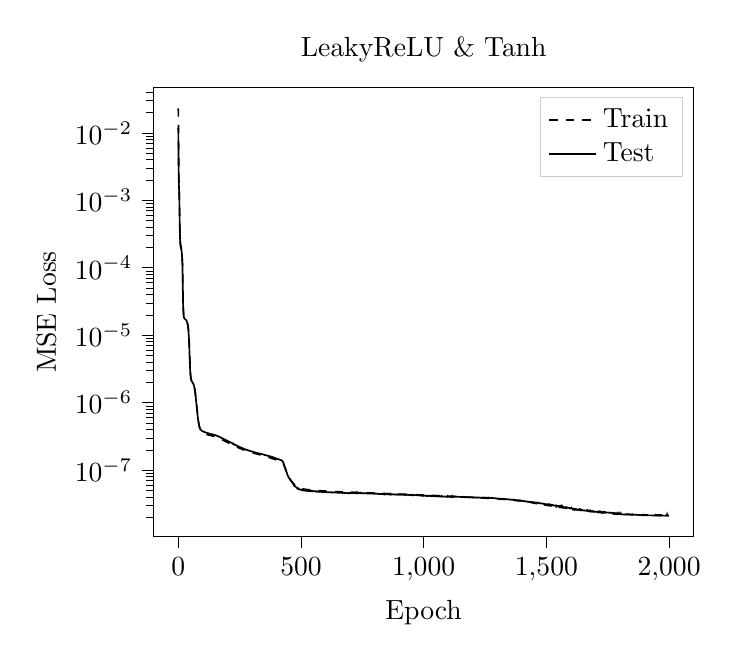
\begin{tikzpicture}

\begin{axis}[
legend cell align={left},
legend style={fill opacity=0.8, draw opacity=1, text opacity=1, draw=white!80!black},
log basis y={10},
tick align=outside,
tick pos=left,
title={LeakyReLU \& Tanh},
x grid style={white!69.0196078431373!black},
xlabel={Epoch},
xmin=-99.95, xmax=2098.95,
xtick style={color=black},
y grid style={white!69.0196078431373!black},
ylabel={MSE Loss},
ymin=1.05017771520553e-08, ymax=0.0463430733137457,
ymode=log,
ytick style={color=black}
]
\addplot [semithick, black, dashed]
table {%
0 0.0231180932745337
1 0.00691163783054799
2 0.00236752607207745
3 0.00163916035043076
4 0.00128206413588487
5 0.000841823659138754
6 0.000464628715068102
7 0.000293852134869667
8 0.000225536572310375
9 0.000206319498931407
10 0.000197783794777934
11 0.000189684799872339
12 0.000180243739887374
13 0.00016980251656787
14 0.00015801912824827
15 0.000144635740762169
16 0.000129592474302626
17 0.000112280388078943
18 7.1559276082553e-05
19 3.97623318276601e-05
20 2.75871643625578e-05
21 2.19790678838763e-05
22 1.94062530645169e-05
23 1.82326361900778e-05
24 1.76674071080924e-05
25 1.73588078223474e-05
26 1.7158149918032e-05
27 1.70034710472464e-05
28 1.68677676729203e-05
29 1.6736985395255e-05
30 1.66027530867723e-05
31 1.64600123689524e-05
32 1.63022092892788e-05
33 1.61204774622092e-05
34 1.59064208719428e-05
35 1.56461757551369e-05
36 1.53268779731661e-05
37 1.49326576583917e-05
38 1.44527597512933e-05
39 1.38589203761512e-05
40 1.31236188908588e-05
41 1.21965216658282e-05
42 1.10850571463743e-05
43 9.78546174519579e-06
44 8.34977166095996e-06
45 6.87472261279254e-06
46 5.50703124804386e-06
47 4.32035695257582e-06
48 3.46076215373614e-06
49 2.91708497832133e-06
50 2.58160994332002e-06
51 2.37972247953166e-06
52 2.25040336940197e-06
53 2.17514950790587e-06
54 2.12627043867997e-06
55 2.08565321332799e-06
56 2.05349377753805e-06
57 2.02687443416494e-06
58 2.00199655981237e-06
59 1.97703611948441e-06
60 1.9502008701977e-06
61 1.92096909441375e-06
62 1.88824094217921e-06
63 1.85032177586208e-06
64 1.80576536635613e-06
65 1.75189494970596e-06
66 1.68170406575996e-06
67 1.60475433398233e-06
68 1.52097433755216e-06
69 1.43189580140302e-06
70 1.33879025045758e-06
71 1.24530403854806e-06
72 1.15362373264816e-06
73 1.06557815367125e-06
74 9.8252717413061e-07
75 9.04443120703036e-07
76 8.32087326728015e-07
77 7.65625963595085e-07
78 7.05365310722073e-07
79 6.51862999021091e-07
80 6.04942077373494e-07
81 5.64233017882998e-07
82 5.29558019792375e-07
83 5.00131236165657e-07
84 4.7566314576386e-07
85 4.55452188916183e-07
86 4.38605655887159e-07
87 4.24582735590207e-07
88 4.13152524558313e-07
89 4.03706824585015e-07
90 3.95877927658717e-07
91 3.89085681376855e-07
92 3.8331710698003e-07
93 3.78526435383719e-07
94 3.74418354354589e-07
95 3.70831175658282e-07
96 3.67738272061047e-07
97 3.65146583575893e-07
98 3.62493394902685e-07
99 3.60080182630895e-07
100 3.57945537359683e-07
101 3.56053520064847e-07
102 3.54334171049686e-07
103 3.52817712681031e-07
104 3.51425322733689e-07
105 3.49952861228076e-07
106 3.4845155801122e-07
107 3.47144738242378e-07
108 3.45985220462808e-07
109 3.44849689867033e-07
110 3.43814986038637e-07
111 3.42843384686375e-07
112 3.41986080499623e-07
113 3.41176107667707e-07
114 3.40208299235201e-07
115 3.3930272508087e-07
116 3.38407138855246e-07
117 3.3754838096911e-07
118 3.36729014009052e-07
119 3.3593990691827e-07
120 3.35063331988295e-07
121 3.34245743346173e-07
122 3.33512132741021e-07
123 3.32793068636761e-07
124 3.32090863238932e-07
125 3.31420317962738e-07
126 3.30775629194591e-07
127 3.30142691510105e-07
128 3.29196797352438e-07
129 3.28521361183221e-07
130 3.27892319432976e-07
131 3.27220650305549e-07
132 3.26515356960044e-07
133 3.25615667463808e-07
134 3.25056333593921e-07
135 3.24426399188837e-07
136 3.23798530942554e-07
137 3.23169060266082e-07
138 3.22509486608169e-07
139 3.21795583744233e-07
140 3.21116806858868e-07
141 3.20391113518781e-07
142 3.19788296948786e-07
143 3.19009029709605e-07
144 3.18380361278514e-07
145 3.17667408253897e-07
146 3.16947345680774e-07
147 3.16236891308108e-07
148 3.15492264221007e-07
149 3.14699536374974e-07
150 3.1381763470506e-07
151 3.13085823151482e-07
152 3.12117770448594e-07
153 3.11343304275624e-07
154 3.10207398243278e-07
155 3.09326292054379e-07
156 3.0825057261552e-07
157 3.07374893779411e-07
158 3.06353653428459e-07
159 3.05310949144655e-07
160 3.04246058362878e-07
161 3.03099792176909e-07
162 3.01988235975159e-07
163 3.00853809747537e-07
164 2.99757800334532e-07
165 2.9860304979934e-07
166 2.97437247624544e-07
167 2.96262004866321e-07
168 2.95119703622504e-07
169 2.93927491966883e-07
170 2.9277420587448e-07
171 2.91547325218744e-07
172 2.90352171774089e-07
173 2.89196633247002e-07
174 2.88026482152759e-07
175 2.86858037071625e-07
176 2.85681136396931e-07
177 2.84472626674415e-07
178 2.83225285379274e-07
179 2.81923208767409e-07
180 2.80808938427413e-07
181 2.79662735465536e-07
182 2.78497147732537e-07
183 2.7732730598018e-07
184 2.76158362751744e-07
185 2.7501534894725e-07
186 2.73948458882956e-07
187 2.72805410851618e-07
188 2.71706084205903e-07
189 2.70586138455542e-07
190 2.69482361133555e-07
191 2.68363218715706e-07
192 2.67262623175668e-07
193 2.66173947544246e-07
194 2.65095240088442e-07
195 2.64019434752072e-07
196 2.62949295390058e-07
197 2.61837796813325e-07
198 2.60760488266953e-07
199 2.59687780484796e-07
200 2.58617103789049e-07
201 2.57546384290208e-07
202 2.56466794596122e-07
203 2.55386283363634e-07
204 2.54314368916653e-07
205 2.53160811752195e-07
206 2.52170376640493e-07
207 2.51107065444955e-07
208 2.50049378749395e-07
209 2.48947975414637e-07
210 2.47839090739888e-07
211 2.46802858313799e-07
212 2.45769433732335e-07
213 2.44716098066533e-07
214 2.43647765366006e-07
215 2.42632687374567e-07
216 2.41568282518756e-07
217 2.40542011198386e-07
218 2.39501517050655e-07
219 2.38522397985719e-07
220 2.3790811883373e-07
221 2.3688468773031e-07
222 2.35755131029691e-07
223 2.34829209453835e-07
224 2.33738084659763e-07
225 2.32384604892388e-07
226 2.31394943810415e-07
227 2.30522248273246e-07
228 2.29530453459859e-07
229 2.28714953429687e-07
230 2.27743794880553e-07
231 2.26800159630614e-07
232 2.25924535882882e-07
233 2.25068038957943e-07
234 2.2434950792416e-07
235 2.23598004588155e-07
236 2.22727982858828e-07
237 2.21752589588675e-07
238 2.2079913674844e-07
239 2.20136223639145e-07
240 2.19087287753439e-07
241 2.18227407508209e-07
242 2.17638221805316e-07
243 2.16821819648771e-07
244 2.15779672089411e-07
245 2.14946175177033e-07
246 2.14456527245943e-07
247 2.13398043250379e-07
248 2.12832233017934e-07
249 2.11874098638987e-07
250 2.11099597805742e-07
251 2.10672914278121e-07
252 2.09871783056315e-07
253 2.09107276880616e-07
254 2.08188488151961e-07
255 2.07699548155915e-07
256 2.06896728982997e-07
257 2.06287172176189e-07
258 2.05403436265073e-07
259 2.0485285461902e-07
260 2.04070094778075e-07
261 2.03332418717395e-07
262 2.02749026918525e-07
263 2.01991037982907e-07
264 2.0149528559088e-07
265 2.00840583556072e-07
266 2.00102935870916e-07
267 1.99465342774374e-07
268 1.98782668174857e-07
269 1.98411443150803e-07
270 1.97917968279171e-07
271 1.97185661097166e-07
272 1.96464329089707e-07
273 1.95875121249856e-07
274 1.95303546231429e-07
275 1.94788651775468e-07
276 1.9420989702823e-07
277 1.93767465002992e-07
278 1.93265095354889e-07
279 1.92600999408654e-07
280 1.92152773927035e-07
281 1.91728608424313e-07
282 1.91100815960965e-07
283 1.90411868899787e-07
284 1.89982355845331e-07
285 1.89763671826881e-07
286 1.89109531177678e-07
287 1.88474857800713e-07
288 1.88016849552497e-07
289 1.87750800755282e-07
290 1.87161313569106e-07
291 1.86710748309338e-07
292 1.86255632630861e-07
293 1.85628825434492e-07
294 1.85123155166167e-07
295 1.84645295231434e-07
296 1.84269339964516e-07
297 1.83771664101329e-07
298 1.833644481124e-07
299 1.82885625079621e-07
300 1.82412894432105e-07
301 1.82045987152435e-07
302 1.81518997514729e-07
303 1.81196183305588e-07
304 1.80777408157695e-07
305 1.80318174582084e-07
306 1.80253337028091e-07
307 1.79536329977026e-07
308 1.79052224552834e-07
309 1.78537804035983e-07
310 1.7808661023011e-07
311 1.77671806024904e-07
312 1.77333921310918e-07
313 1.76837239706629e-07
314 1.76504909028097e-07
315 1.7619372728106e-07
316 1.75711512525822e-07
317 1.75284966967837e-07
318 1.74967242465129e-07
319 1.74496793583501e-07
320 1.74072806544245e-07
321 1.73698184159576e-07
322 1.73236377452923e-07
323 1.7297212179912e-07
324 1.72495211817392e-07
325 1.72160576880742e-07
326 1.71605232377914e-07
327 1.71215926336288e-07
328 1.70964003004315e-07
329 1.70411436045015e-07
330 1.69985294508734e-07
331 1.69656958924236e-07
332 1.69223094665938e-07
333 1.68889497565772e-07
334 1.68359916543181e-07
335 1.67958899275789e-07
336 1.67533837434064e-07
337 1.67190720336663e-07
338 1.66793571096946e-07
339 1.66333352435544e-07
340 1.6600377577447e-07
341 1.65503233784392e-07
342 1.65328119916097e-07
343 1.6483816481383e-07
344 1.64399635004031e-07
345 1.63996518836029e-07
346 1.63649493739371e-07
347 1.63224858212629e-07
348 1.6287360217504e-07
349 1.62474480845276e-07
350 1.62140936037503e-07
351 1.61618776314043e-07
352 1.61292446325234e-07
353 1.60940283848277e-07
354 1.60490298046767e-07
355 1.60118750049065e-07
356 1.59706000857796e-07
357 1.5934608693513e-07
358 1.58811773737e-07
359 1.58452456393121e-07
360 1.57991367089494e-07
361 1.57635888491825e-07
362 1.57418188919678e-07
363 1.56855955040669e-07
364 1.56468315744007e-07
365 1.56109388477432e-07
366 1.55736482902569e-07
367 1.55268056005298e-07
368 1.54922160078286e-07
369 1.5435845207179e-07
370 1.53998422916857e-07
371 1.53608532613703e-07
372 1.53320270655399e-07
373 1.52874647788792e-07
374 1.5251073745759e-07
375 1.52125061831043e-07
376 1.51762487305973e-07
377 1.51191019703845e-07
378 1.50968095006476e-07
379 1.506134205016e-07
380 1.50095310431198e-07
381 1.49805103824008e-07
382 1.49280648948036e-07
383 1.48978639963104e-07
384 1.48483931340593e-07
385 1.48075164801753e-07
386 1.47686838580796e-07
387 1.47280645585113e-07
388 1.4699129418716e-07
389 1.46460909682844e-07
390 1.46051013622639e-07
391 1.45760846166354e-07
392 1.4530567812443e-07
393 1.44919195541604e-07
394 1.44455789829578e-07
395 1.43907718246794e-07
396 1.43391674527038e-07
397 1.43079515488864e-07
398 1.42741781417044e-07
399 1.42254770885586e-07
400 1.41870925347121e-07
401 1.41372117354877e-07
402 1.41036456469124e-07
403 1.40565752658972e-07
404 1.40225100501823e-07
405 1.39800642131149e-07
406 1.39402758243534e-07
407 1.3899351520763e-07
408 1.3858158822444e-07
409 1.38089070535585e-07
410 1.37723105964938e-07
411 1.3731189865851e-07
412 1.36894297202872e-07
413 1.36560860074297e-07
414 1.36180004439268e-07
415 1.35843732351759e-07
416 1.35386915687263e-07
417 1.35104608155245e-07
418 1.34771831085345e-07
419 1.34395945835308e-07
420 1.33803321077153e-07
421 1.33645604819321e-07
422 1.33042594782751e-07
423 1.32887492434008e-07
424 1.32109809285907e-07
425 1.3034141620949e-07
426 1.28958272853197e-07
427 1.26946435479169e-07
428 1.24371114068822e-07
429 1.21889156936561e-07
430 1.19242146887188e-07
431 1.16565365722465e-07
432 1.14026005928025e-07
433 1.11574512430934e-07
434 1.09276112123524e-07
435 1.06988472889924e-07
436 1.04660790437805e-07
437 1.02330937544082e-07
438 1.00075169815028e-07
439 9.79678819028606e-08
440 9.55118804810695e-08
441 9.33184585178992e-08
442 9.08561342818359e-08
443 8.86858850606131e-08
444 8.64281579531223e-08
445 8.44685718597304e-08
446 8.29710912988446e-08
447 8.16794162759038e-08
448 8.04114040882098e-08
449 7.93612581126979e-08
450 7.82892071100605e-08
451 7.72405229589879e-08
452 7.63512665500343e-08
453 7.55277521093944e-08
454 7.45679956324352e-08
455 7.3682990720414e-08
456 7.28977399475639e-08
457 7.2357229395692e-08
458 7.13870868018773e-08
459 7.06406240595925e-08
460 6.98212222687289e-08
461 6.91868356739178e-08
462 6.82494804280509e-08
463 6.75632972537699e-08
464 6.69218680471317e-08
465 6.6115140690215e-08
466 6.54791023180223e-08
467 6.482430448429e-08
468 6.41881051528515e-08
469 6.34527060299206e-08
470 6.28743330679527e-08
471 6.22909573557706e-08
472 6.16202214942518e-08
473 6.10811927366228e-08
474 6.05204008721216e-08
475 5.98775169500243e-08
476 5.95182662763705e-08
477 5.89016927179387e-08
478 5.86363955363822e-08
479 5.82207700183801e-08
480 5.78520277123573e-08
481 5.7469730499804e-08
482 5.71266204545395e-08
483 5.68272962659933e-08
484 5.65094852333914e-08
485 5.62808312025709e-08
486 5.60190715539477e-08
487 5.56668566922269e-08
488 5.5522293205712e-08
489 5.52093207986104e-08
490 5.49618962892851e-08
491 5.49192403092036e-08
492 5.46361145623564e-08
493 5.45596102092816e-08
494 5.42744300044973e-08
495 5.41143218235618e-08
496 5.40162991384818e-08
497 5.38441756212649e-08
498 5.37843087879963e-08
499 5.35685013076659e-08
500 5.35263585614842e-08
501 5.34115848633832e-08
502 5.3207641212083e-08
503 5.32631078478118e-08
504 5.31282235982644e-08
505 5.29943798497357e-08
506 5.28954847620611e-08
507 5.2823807935809e-08
508 5.27514571064813e-08
509 5.26513241148052e-08
510 5.25324681035499e-08
511 5.24348748935921e-08
512 5.24179785159617e-08
513 5.23187351735288e-08
514 5.22548456807215e-08
515 5.22080586282669e-08
516 5.213086156175e-08
517 5.20891518736022e-08
518 5.20496548581662e-08
519 5.19744910185693e-08
520 5.1925184571644e-08
521 5.18005164771296e-08
522 5.17947597895585e-08
523 5.17690564283413e-08
524 5.16804132679738e-08
525 5.16519340187926e-08
526 5.16120750102544e-08
527 5.15181743310222e-08
528 5.14550312615825e-08
529 5.14517644560897e-08
530 5.14091283996265e-08
531 5.13337360956712e-08
532 5.12756064736664e-08
533 5.12799227294636e-08
534 5.12680887148065e-08
535 5.12650375306123e-08
536 5.11184160529865e-08
537 5.10385936554059e-08
538 5.10396357888965e-08
539 5.11752794913889e-08
540 5.10148337937721e-08
541 5.08723928476229e-08
542 5.09169258187114e-08
543 5.08692298417657e-08
544 5.08352038615101e-08
545 5.06925314063267e-08
546 5.07037119099607e-08
547 5.06877666452965e-08
548 5.0667941184912e-08
549 5.05902717016227e-08
550 5.04750513385943e-08
551 5.04427755956272e-08
552 5.04092446789173e-08
553 5.04260152212055e-08
554 5.04286502014395e-08
555 5.05303507694066e-08
556 5.02225297580594e-08
557 5.02304600864534e-08
558 5.0165399755997e-08
559 5.04333431585735e-08
560 5.0124782241312e-08
561 5.02032417770693e-08
562 5.00821452931177e-08
563 5.0000705762443e-08
564 5.00046439384505e-08
565 4.9925117789229e-08
566 4.99502055184564e-08
567 4.98711967793497e-08
568 4.98507275175086e-08
569 4.99024204749787e-08
570 4.999098187497e-08
571 4.97236971988002e-08
572 4.97215885140179e-08
573 4.96691570894825e-08
574 4.96334800246245e-08
575 4.96433970162968e-08
576 4.96978211685928e-08
577 4.956785255672e-08
578 4.95573241146019e-08
579 4.95007456393637e-08
580 4.94458988988811e-08
581 4.95076322515331e-08
582 4.94297100672725e-08
583 4.93943800456975e-08
584 4.94463258320366e-08
585 4.93315144467488e-08
586 4.93525245133242e-08
587 4.92890767276322e-08
588 4.93499470231029e-08
589 4.92057945358226e-08
590 4.91780177647172e-08
591 4.91906568775846e-08
592 4.9189808130734e-08
593 4.92715395665755e-08
594 4.90638934671495e-08
595 4.90906338654895e-08
596 4.91743347090789e-08
597 4.89646283874379e-08
598 4.90205175864844e-08
599 4.90474661667406e-08
600 4.9014490635102e-08
601 4.88865692283014e-08
602 4.89974714668051e-08
603 4.89214882826161e-08
604 4.88371780207331e-08
605 4.88814107022506e-08
606 4.87413790750679e-08
607 4.88491861716511e-08
608 4.87274669609405e-08
609 4.88174249220208e-08
610 4.86369060581637e-08
611 4.86838460744821e-08
612 4.87349302922269e-08
613 4.86777343446931e-08
614 4.8578499448837e-08
615 4.86568211535143e-08
616 4.86349052835067e-08
617 4.84408213843324e-08
618 4.8504392598403e-08
619 4.85375756902329e-08
620 4.84674478400393e-08
621 4.8542444208266e-08
622 4.85567452059854e-08
623 4.83391837988734e-08
624 4.84206096480477e-08
625 4.84404144529549e-08
626 4.83589863371492e-08
627 4.83240054691691e-08
628 4.8333512562948e-08
629 4.83270477964481e-08
630 4.82329075985888e-08
631 4.83538074647072e-08
632 4.82876248497632e-08
633 4.82734585354194e-08
634 4.80849577790821e-08
635 4.81289647282779e-08
636 4.80986523996307e-08
637 4.81114106669622e-08
638 4.80671564773161e-08
639 4.80613533788699e-08
640 4.8032419726951e-08
641 4.80059581811076e-08
642 4.7996671042938e-08
643 4.79695375190659e-08
644 4.79414516192378e-08
645 4.79384816252093e-08
646 4.78988891288168e-08
647 4.78808598707303e-08
648 4.78679943505256e-08
649 4.78599641482447e-08
650 4.77994603969023e-08
651 4.77962351794758e-08
652 4.78193295485596e-08
653 4.77791427044849e-08
654 4.77450501428223e-08
655 4.77350703604884e-08
656 4.77169705135339e-08
657 4.76625162733058e-08
658 4.76985185251522e-08
659 4.76610343405071e-08
660 4.76188474607397e-08
661 4.76440611549833e-08
662 4.76127687036865e-08
663 4.75954258476463e-08
664 4.75787531435401e-08
665 4.75482052308962e-08
666 4.75397097652319e-08
667 4.75233016707932e-08
668 4.75080411703743e-08
669 4.74811047439516e-08
670 4.74798293481626e-08
671 4.75138053772639e-08
672 4.74470242437519e-08
673 4.73892646652985e-08
674 4.75326599698178e-08
675 4.73754993386422e-08
676 4.73531396458782e-08
677 4.74724356003264e-08
678 4.72760268692696e-08
679 4.7339517916356e-08
680 4.72811318488198e-08
681 4.72670735440772e-08
682 4.72558673010326e-08
683 4.73035166184133e-08
684 4.75082195272591e-08
685 4.72333178471729e-08
686 4.71912165362909e-08
687 4.72483780349364e-08
688 4.71788138760587e-08
689 4.71976311136046e-08
690 4.6973337944678e-08
691 4.71835677995358e-08
692 4.70969836285917e-08
693 4.71809280373492e-08
694 4.70514132970834e-08
695 4.70454323462377e-08
696 4.70909976204581e-08
697 4.69995533993739e-08
698 4.70930045928242e-08
699 4.70089619817315e-08
700 4.69942271035251e-08
701 4.7003992621697e-08
702 4.70964700554077e-08
703 4.69082242346985e-08
704 4.70313922615873e-08
705 4.6946243056567e-08
706 4.69173780661691e-08
707 4.69298121679174e-08
708 4.69021672788728e-08
709 4.68533316535513e-08
710 4.68566778550894e-08
711 4.69421040349971e-08
712 4.67305726985501e-08
713 4.70092672184563e-08
714 4.68666689954489e-08
715 4.67590615329527e-08
716 4.67695473282959e-08
717 4.66989844927213e-08
718 4.68983044399351e-08
719 4.67740115510651e-08
720 4.68103797235386e-08
721 4.67645586326171e-08
722 4.65781086944617e-08
723 4.68022931876533e-08
724 4.67841341276198e-08
725 4.65498166821732e-08
726 4.68560649746763e-08
727 4.6551337792522e-08
728 4.65643066167587e-08
729 4.67364545286841e-08
730 4.66678591131142e-08
731 4.65337108188635e-08
732 4.65603552441962e-08
733 4.66099961364819e-08
734 4.65988922613292e-08
735 4.65541759595567e-08
736 4.65311331794283e-08
737 4.65179922954917e-08
738 4.64667172082045e-08
739 4.64437365259585e-08
740 4.63955316583053e-08
741 4.6483137602138e-08
742 4.66002568515478e-08
743 4.64178739569832e-08
744 4.66849208393683e-08
745 4.6366795432462e-08
746 4.6306148828279e-08
747 4.61631177657296e-08
748 4.64128689436905e-08
749 4.64112351501456e-08
750 4.63883813424104e-08
751 4.63022864067852e-08
752 4.63204091154523e-08
753 4.61671090334903e-08
754 4.61387233823274e-08
755 4.62915120351681e-08
756 4.62521246511471e-08
757 4.61522336401288e-08
758 4.62154903964063e-08
759 4.61012871504352e-08
760 4.62784426105145e-08
761 4.61275226886215e-08
762 4.61520886503308e-08
763 4.61328693912577e-08
764 4.61559049398375e-08
765 4.61155644764233e-08
766 4.61220749539137e-08
767 4.60328977336388e-08
768 4.60982853489611e-08
769 4.60739228742568e-08
770 4.61838278731364e-08
771 4.59862372785835e-08
772 4.59528510639018e-08
773 4.6005952281547e-08
774 4.59876398650749e-08
775 4.6067728554533e-08
776 4.59137446782165e-08
777 4.58957754343459e-08
778 4.58558279419208e-08
779 4.59072449814357e-08
780 4.59142384379163e-08
781 4.58895862571751e-08
782 4.58867198460666e-08
783 4.58570819823478e-08
784 4.58549056254753e-08
785 4.58522188910848e-08
786 4.58383022454711e-08
787 4.58249760075802e-08
788 4.58156332054926e-08
789 4.57389657704255e-08
790 4.59913247148336e-08
791 4.57895090804072e-08
792 4.56964216262179e-08
793 4.57485686915504e-08
794 4.56413611580331e-08
795 4.55933785055152e-08
796 4.56170304072856e-08
797 4.56436149143258e-08
798 4.56415919352082e-08
799 4.56958284313913e-08
800 4.56830257604679e-08
801 4.56841598808211e-08
802 4.56173849947561e-08
803 4.56825714429954e-08
804 4.55531225274086e-08
805 4.5552917434577e-08
806 4.56644936335238e-08
807 4.55106619767776e-08
808 4.55270218857606e-08
809 4.55307098121693e-08
810 4.54847461455188e-08
811 4.5394666926768e-08
812 4.53386527681232e-08
813 4.53390495636086e-08
814 4.53637721342659e-08
815 4.53603665029334e-08
816 4.54144820487556e-08
817 4.52709462024359e-08
818 4.52853926660168e-08
819 4.52013497636017e-08
820 4.50710754442696e-08
821 4.51932848246628e-08
822 4.53610424244744e-08
823 4.52075150221276e-08
824 4.5215282600708e-08
825 4.52719320787054e-08
826 4.52165278179706e-08
827 4.49794749055599e-08
828 4.50889597445325e-08
829 4.50772180684567e-08
830 4.51285556373193e-08
831 4.51030490751236e-08
832 4.51701932355775e-08
833 4.49076377293522e-08
834 4.49185637734217e-08
835 4.49603184584646e-08
836 4.49879837329803e-08
837 4.50014234161244e-08
838 4.49353307381273e-08
839 4.49414621179756e-08
840 4.49629091718862e-08
841 4.49544324929718e-08
842 4.49327361486951e-08
843 4.48987079266772e-08
844 4.48175362475212e-08
845 4.4885612116019e-08
846 4.48820907124059e-08
847 4.48424885561849e-08
848 4.48396690977404e-08
849 4.47729865484803e-08
850 4.4777063408219e-08
851 4.48183337802277e-08
852 4.47879238372195e-08
853 4.47475506319961e-08
854 4.47746424665496e-08
855 4.47483860988029e-08
856 4.47082589705161e-08
857 4.45620165194782e-08
858 4.47270995707072e-08
859 4.47962218412812e-08
860 4.46605732271621e-08
861 4.47187323864284e-08
862 4.46657495878355e-08
863 4.45948272407293e-08
864 4.4597184201578e-08
865 4.44955244685019e-08
866 4.44660111469375e-08
867 4.47319384839773e-08
868 4.45973339360251e-08
869 4.45963839030838e-08
870 4.45372593098625e-08
871 4.45612255433048e-08
872 4.4425960542327e-08
873 4.43262497533681e-08
874 4.43918094532592e-08
875 4.44837197033365e-08
876 4.45056413322931e-08
877 4.45261458494883e-08
878 4.44532381074225e-08
879 4.43573510153783e-08
880 4.43303503327996e-08
881 4.42998324743371e-08
882 4.43046527145441e-08
883 4.43305172659336e-08
884 4.42931158772808e-08
885 4.43241507923631e-08
886 4.43054821719358e-08
887 4.43183707616868e-08
888 4.42260295621111e-08
889 4.42503930742077e-08
890 4.42230570332214e-08
891 4.41914552151701e-08
892 4.41888381992328e-08
893 4.42613764199962e-08
894 4.42198428878271e-08
895 4.42245554790333e-08
896 4.41373632131814e-08
897 4.41615692992059e-08
898 4.42076576518957e-08
899 4.41963338140283e-08
900 4.40807856509906e-08
901 4.40777588277541e-08
902 4.40876694263181e-08
903 4.40454798535939e-08
904 4.40666043033389e-08
905 4.39584186686659e-08
906 4.39868957826661e-08
907 4.40035749988965e-08
908 4.39534012102172e-08
909 4.40222353947917e-08
910 4.40523066700393e-08
911 4.40421205034625e-08
912 4.39539132983668e-08
913 4.3908745468002e-08
914 4.39363137658688e-08
915 4.39900584119357e-08
916 4.39079527119191e-08
917 4.38811851246612e-08
918 4.37819483440904e-08
919 4.37752371915678e-08
920 4.37929496257539e-08
921 4.37879617685155e-08
922 4.39569818233565e-08
923 4.38801771345254e-08
924 4.37759457980746e-08
925 4.37195849656291e-08
926 4.38086261524973e-08
927 4.3607684217406e-08
928 4.36370372067785e-08
929 4.36741188583056e-08
930 4.37848838235055e-08
931 4.37064253784314e-08
932 4.36279340547685e-08
933 4.36252051283503e-08
934 4.36026740615603e-08
935 4.35745891458339e-08
936 4.35614004157259e-08
937 4.35286232640664e-08
938 4.36506065764064e-08
939 4.35270899998841e-08
940 4.35057786880577e-08
941 4.35222723744744e-08
942 4.34606036794349e-08
943 4.34628232088841e-08
944 4.34549153780495e-08
945 4.34644257740757e-08
946 4.34089697201046e-08
947 4.34296127540534e-08
948 4.33936289674364e-08
949 4.33854671211265e-08
950 4.33085072248929e-08
951 4.33600225573372e-08
952 4.3390181357239e-08
953 4.33026631263544e-08
954 4.32936278844664e-08
955 4.33335837417559e-08
956 4.33213590067538e-08
957 4.3255756123628e-08
958 4.32751664050102e-08
959 4.33056612454408e-08
960 4.31951110932971e-08
961 4.321754662584e-08
962 4.31643162102091e-08
963 4.32112491548509e-08
964 4.31963698446225e-08
965 4.31650905881043e-08
966 4.31691831579428e-08
967 4.31324235936614e-08
968 4.31414488346604e-08
969 4.31345458427046e-08
970 4.30469177512549e-08
971 4.30732041998283e-08
972 4.30239126281151e-08
973 4.30899895427217e-08
974 4.30616513309445e-08
975 4.31306849861812e-08
976 4.30538944762304e-08
977 4.2979686554645e-08
978 4.2966369784736e-08
979 4.29267196224714e-08
980 4.2906329912995e-08
981 4.28923566371253e-08
982 4.28853914566929e-08
983 4.28360605528866e-08
984 4.28893157362609e-08
985 4.28430185515083e-08
986 4.29199739890862e-08
987 4.27919449670355e-08
988 4.28688435416547e-08
989 4.285571474405e-08
990 4.29425512589177e-08
991 4.27601403405475e-08
992 4.27443849844167e-08
993 4.27893474963525e-08
994 4.27201470785121e-08
995 4.27450639879368e-08
996 4.26757930913624e-08
997 4.2717077032961e-08
998 4.27359398340599e-08
999 4.26297833513445e-08
1000 4.26319990616264e-08
1001 4.26096843568757e-08
1002 4.25726711945629e-08
1003 4.26324038773629e-08
1004 4.25904040461944e-08
1005 4.25584534600176e-08
1006 4.25315362715395e-08
1007 4.25396315737459e-08
1008 4.25431945814125e-08
1009 4.24604777684579e-08
1010 4.24759221324678e-08
1011 4.24244887895497e-08
1012 4.25374756645169e-08
1013 4.24195880235345e-08
1014 4.24126601004105e-08
1015 4.24978580593205e-08
1016 4.23606765380669e-08
1017 4.23327833214415e-08
1018 4.23562854123816e-08
1019 4.23696529665563e-08
1020 4.23092796690838e-08
1021 4.23249601695375e-08
1022 4.23223258980698e-08
1023 4.2239201951233e-08
1024 4.22492186000767e-08
1025 4.22270520381574e-08
1026 4.21955308667066e-08
1027 4.22553197161335e-08
1028 4.21947017237301e-08
1029 4.22666300572416e-08
1030 4.21492963269543e-08
1031 4.21629412734603e-08
1032 4.21741413809684e-08
1033 4.21391151146366e-08
1034 4.20553512441302e-08
1035 4.20888020116195e-08
1036 4.20318222982274e-08
1037 4.20628583928107e-08
1038 4.20318598468583e-08
1039 4.19708633643268e-08
1040 4.20347316634206e-08
1041 4.20022315896773e-08
1042 4.20155427267588e-08
1043 4.19329264289559e-08
1044 4.19078179394461e-08
1045 4.19640399922372e-08
1046 4.19096627606308e-08
1047 4.20602141613102e-08
1048 4.18545815659144e-08
1049 4.18957760057737e-08
1050 4.18473363250627e-08
1051 4.18287741386081e-08
1052 4.18455368382808e-08
1053 4.18346338015851e-08
1054 4.17779691428422e-08
1055 4.18047715946557e-08
1056 4.17934781520302e-08
1057 4.18238405650584e-08
1058 4.16826277547244e-08
1059 4.18016461747328e-08
1060 4.16546652139971e-08
1061 4.15622153830952e-08
1062 4.15927358332624e-08
1063 4.16507495977214e-08
1064 4.16438223957982e-08
1065 4.16561885430156e-08
1066 4.16025267462317e-08
1067 4.16142616810333e-08
1068 4.16010168926562e-08
1069 4.15389839023561e-08
1070 4.1521116845189e-08
1071 4.15900827572813e-08
1072 4.15049474771223e-08
1073 4.15856902531431e-08
1074 4.15352730644969e-08
1075 4.15675830556239e-08
1076 4.14762541662839e-08
1077 4.14239940855765e-08
1078 4.13742981653087e-08
1079 4.12284009545516e-08
1080 4.14333785645482e-08
1081 4.14379792381681e-08
1082 4.13174058913057e-08
1083 4.14085360294081e-08
1084 4.13300784494197e-08
1085 4.14090463642935e-08
1086 4.12716302093941e-08
1087 4.12548861827844e-08
1088 4.12835813250467e-08
1089 4.12312686286498e-08
1090 4.12615640517089e-08
1091 4.11859164213268e-08
1092 4.09730428962973e-08
1093 4.11372105126873e-08
1094 4.11518664087396e-08
1095 4.11390963748204e-08
1096 4.13031592252366e-08
1097 4.11719313895276e-08
1098 4.11438033687261e-08
1099 4.11343783728313e-08
1100 4.10276896012363e-08
1101 4.10379834754337e-08
1102 4.104321017806e-08
1103 4.10870253588769e-08
1104 4.10300120687879e-08
1105 4.09888198049657e-08
1106 4.10024267925024e-08
1107 4.09563242182998e-08
1108 4.07605617471774e-08
1109 4.0946276630649e-08
1110 4.09175470963419e-08
1111 4.10168326254734e-08
1112 4.09821374418584e-08
1113 4.09051264949056e-08
1114 4.07797136396937e-08
1115 4.09340711478023e-08
1116 4.08393748010383e-08
1117 4.0940884852958e-08
1118 4.08396250310972e-08
1119 4.08110311358456e-08
1120 4.08509181362149e-08
1121 4.07492251230934e-08
1122 4.08181448285916e-08
1123 4.0668973934288e-08
1124 4.05575018209703e-08
1125 4.06641895303039e-08
1126 4.05549117203918e-08
1127 4.06066811944328e-08
1128 4.06495706215537e-08
1129 4.05477688296685e-08
1130 4.06732264845999e-08
1131 4.06647905037971e-08
1132 4.05916156935859e-08
1133 4.05750032665964e-08
1134 4.0477916762427e-08
1135 4.05134368666182e-08
1136 4.05830187268919e-08
1137 4.05845505255797e-08
1138 4.04253322425774e-08
1139 4.05580798492622e-08
1140 4.05443515241188e-08
1141 4.04401100055907e-08
1142 4.05047036498019e-08
1143 4.04142237186988e-08
1144 4.04171877956827e-08
1145 4.04660569515158e-08
1146 4.04543496284049e-08
1147 4.03716998444992e-08
1148 4.04011630283918e-08
1149 4.02970075104037e-08
1150 4.03461828781815e-08
1151 4.02589589008073e-08
1152 4.02516076167814e-08
1153 4.02381310617983e-08
1154 4.01870133899251e-08
1155 4.02062626232436e-08
1156 4.02236185053084e-08
1157 4.01684534931945e-08
1158 4.00635840680508e-08
1159 4.02319097396742e-08
1160 4.01856069487394e-08
1161 4.01583132845218e-08
1162 4.00994960205736e-08
1163 4.00915142826364e-08
1164 4.00383623500034e-08
1165 3.99567921203214e-08
1166 3.99822834147301e-08
1167 4.00233006470074e-08
1168 4.00672677400848e-08
1169 3.9903199077429e-08
1170 3.99743532124575e-08
1171 3.9956555676568e-08
1172 3.99558661232646e-08
1173 3.98895770690189e-08
1174 3.98867074391518e-08
1175 3.99193204998483e-08
1176 3.98780873229754e-08
1177 3.98095552203159e-08
1178 3.98182363348099e-08
1179 3.9837201779136e-08
1180 3.98306583164754e-08
1181 3.97923541370915e-08
1182 3.97012992987555e-08
1183 3.96517439220645e-08
1184 3.96888967646447e-08
1185 3.96782678695473e-08
1186 3.96370323549888e-08
1187 3.96630270174114e-08
1188 3.96740993924283e-08
1189 3.96503644513047e-08
1190 3.96449073640781e-08
1191 3.96165770855106e-08
1192 3.95804991626392e-08
1193 3.95499995544668e-08
1194 3.9542763074607e-08
1195 3.95303516285139e-08
1196 3.95233353174262e-08
1197 3.94976884674492e-08
1198 3.93905064690614e-08
1199 3.94691601339758e-08
1200 3.93894827102059e-08
1201 3.93906410103284e-08
1202 3.93571257912839e-08
1203 3.94454585244119e-08
1204 3.92966261326677e-08
1205 3.92827547184282e-08
1206 3.93346191494004e-08
1207 3.93339696547201e-08
1208 3.92473171633156e-08
1209 3.92448116723898e-08
1210 3.92120681880215e-08
1211 3.93128073525872e-08
1212 3.91544418594236e-08
1213 3.91862348951832e-08
1214 3.91478888364105e-08
1215 3.91766022502793e-08
1216 3.90814042052767e-08
1217 3.90860378782776e-08
1218 3.90710304731812e-08
1219 3.91412996911811e-08
1220 3.90301076329536e-08
1221 3.90706069328672e-08
1222 3.89968210114944e-08
1223 3.89981532791239e-08
1224 3.89891361596284e-08
1225 3.89718152948859e-08
1226 3.9012402384131e-08
1227 3.89670434373102e-08
1228 3.89375060425579e-08
1229 3.89139971570529e-08
1230 3.88525646233262e-08
1231 3.88395319976809e-08
1232 3.88862486282449e-08
1233 3.88503211148361e-08
1234 3.88387636007792e-08
1235 3.87901296150517e-08
1236 3.87976180000749e-08
1237 3.88015357533078e-08
1238 3.88150406802623e-08
1239 3.87407710960019e-08
1240 3.8727163037322e-08
1241 3.87134739838757e-08
1242 3.876618581522e-08
1243 3.86593296983762e-08
1244 3.86482336658389e-08
1245 3.86340110765104e-08
1246 3.86077210769997e-08
1247 3.86534168281827e-08
1248 3.8638405294833e-08
1249 3.85669865039517e-08
1250 3.85527548960596e-08
1251 3.85728573490951e-08
1252 3.84852372281586e-08
1253 3.84893588964985e-08
1254 3.84872347058973e-08
1255 3.8481129823964e-08
1256 3.84682925105295e-08
1257 3.84136067239638e-08
1258 3.83819222058435e-08
1259 3.83395336793768e-08
1260 3.84076231352282e-08
1261 3.8356199906886e-08
1262 3.83199172855342e-08
1263 3.83295004695583e-08
1264 3.82673642391751e-08
1265 3.82575509334515e-08
1266 3.82797004689905e-08
1267 3.81893325247518e-08
1268 3.82861426952985e-08
1269 3.81866618877069e-08
1270 3.8108881421195e-08
1271 3.81035134076058e-08
1272 3.81285452117908e-08
1273 3.80982376793071e-08
1274 3.81338798476349e-08
1275 3.80230510792501e-08
1276 3.80467222935721e-08
1277 3.80346293500367e-08
1278 3.7970512996921e-08
1279 3.79630684239629e-08
1280 3.79700530146465e-08
1281 3.79512372994384e-08
1282 3.79440456423907e-08
1283 3.7899100673755e-08
1284 3.78597796757418e-08
1285 3.78633219817459e-08
1286 3.78476123099603e-08
1287 3.78139669159339e-08
1288 3.78622373986559e-08
1289 3.77853494128999e-08
1290 3.77866532019766e-08
1291 3.77655310597191e-08
1292 3.77511984055445e-08
1293 3.76905111885151e-08
1294 3.76739344289945e-08
1295 3.76604117757751e-08
1296 3.76525064673672e-08
1297 3.75862030157492e-08
1298 3.75823963238986e-08
1299 3.7573452983608e-08
1300 3.75968950301342e-08
1301 3.75689369747079e-08
1302 3.75393609939323e-08
1303 3.751565754051e-08
1304 3.74985924214144e-08
1305 3.74513834451307e-08
1306 3.74433435688104e-08
1307 3.74217847429748e-08
1308 3.7414620559062e-08
1309 3.73071761998744e-08
1310 3.73220850740097e-08
1311 3.72771461965016e-08
1312 3.73144642917822e-08
1313 3.72319358081796e-08
1314 3.73203177250758e-08
1315 3.72251332620976e-08
1316 3.72167462767692e-08
1317 3.72191282753676e-08
1318 3.71721254168733e-08
1319 3.71581971521095e-08
1320 3.70493724268783e-08
1321 3.71312942615276e-08
1322 3.69709609575608e-08
1323 3.70562992504375e-08
1324 3.69365463868121e-08
1325 3.69724556641415e-08
1326 3.7009552952938e-08
1327 3.69332335239392e-08
1328 3.69495343939263e-08
1329 3.69725569697721e-08
1330 3.68652056792484e-08
1331 3.6810911067775e-08
1332 3.68374179569031e-08
1333 3.68219231301481e-08
1334 3.67564931629261e-08
1335 3.67690321390057e-08
1336 3.67643593666145e-08
1337 3.66814369030521e-08
1338 3.67339577067582e-08
1339 3.66309412598298e-08
1340 3.66576694705856e-08
1341 3.65878160906163e-08
1342 3.66069300117289e-08
1343 3.65444764245382e-08
1344 3.65975300624655e-08
1345 3.6499413125668e-08
1346 3.65689981283168e-08
1347 3.64199278521937e-08
1348 3.64013331566326e-08
1349 3.63601120483281e-08
1350 3.63718320564033e-08
1351 3.63319435159326e-08
1352 3.62802644122695e-08
1353 3.63296040255534e-08
1354 3.63092344102256e-08
1355 3.62564527769393e-08
1356 3.62792973884751e-08
1357 3.61615846937724e-08
1358 3.61027687922899e-08
1359 3.60317386292053e-08
1360 3.60997870885171e-08
1361 3.60615177328327e-08
1362 3.60111117920781e-08
1363 3.60927395615107e-08
1364 3.59954981128396e-08
1365 3.5923528237447e-08
1366 3.59191972858497e-08
1367 3.58905443071933e-08
1368 3.58626226830694e-08
1369 3.5874005153147e-08
1370 3.57779075432774e-08
1371 3.58525817905075e-08
1372 3.57193548534696e-08
1373 3.56384706226009e-08
1374 3.56165282049403e-08
1375 3.55104627729474e-08
1376 3.56746097534e-08
1377 3.55267219482869e-08
1378 3.54873206642736e-08
1379 3.55158849405512e-08
1380 3.54461063842848e-08
1381 3.554977798359e-08
1382 3.54182883093301e-08
1383 3.5375937807558e-08
1384 3.54445570209805e-08
1385 3.52813834822996e-08
1386 3.53688602867663e-08
1387 3.5248283515088e-08
1388 3.52502822540401e-08
1389 3.53439193361282e-08
1390 3.51152241915287e-08
1391 3.52339371634258e-08
1392 3.5168619481496e-08
1393 3.50856852637804e-08
1394 3.50631547583191e-08
1395 3.51210104749811e-08
1396 3.50724193491914e-08
1397 3.48748331884252e-08
1398 3.4841030524646e-08
1399 3.49386646831817e-08
1400 3.48768256479559e-08
1401 3.48648992414269e-08
1402 3.47478296482961e-08
1403 3.47915154517153e-08
1404 3.46595729254773e-08
1405 3.46367656796076e-08
1406 3.47192343390645e-08
1407 3.46522471925681e-08
1408 3.46658932848243e-08
1409 3.45816753206662e-08
1410 3.46041060055313e-08
1411 3.45091948013021e-08
1412 3.45206529974718e-08
1413 3.44364544897502e-08
1414 3.44696885665741e-08
1415 3.44211482392609e-08
1416 3.43356560392749e-08
1417 3.41527164575695e-08
1418 3.41574929123567e-08
1419 3.41096915033035e-08
1420 3.40284049116235e-08
1421 3.39563723219527e-08
1422 3.39137132101541e-08
1423 3.39424779713937e-08
1424 3.38063660727528e-08
1425 3.3798205546276e-08
1426 3.38162839117473e-08
1427 3.37223902615591e-08
1428 3.36924032975361e-08
1429 3.36069029138741e-08
1430 3.36360958783644e-08
1431 3.35223252569961e-08
1432 3.34317332875145e-08
1433 3.34566227060407e-08
1434 3.3374483001225e-08
1435 3.3365868358004e-08
1436 3.33827508089968e-08
1437 3.33413550688277e-08
1438 3.32690501210209e-08
1439 3.31279977956456e-08
1440 3.31143404093126e-08
1441 3.29957275937431e-08
1442 3.28822683481889e-08
1443 3.29063269628449e-08
1444 3.28127207112061e-08
1445 3.28614619871104e-08
1446 3.26379474486771e-08
1447 3.26208404306527e-08
1448 3.28633223514174e-08
1449 3.26220986011094e-08
1450 3.25656923614304e-08
1451 3.25403972318838e-08
1452 3.23148593395217e-08
1453 3.22713670968255e-08
1454 3.2265502563078e-08
1455 3.23434691651414e-08
1456 3.22945066688618e-08
1457 3.21269305487704e-08
1458 3.20867873018216e-08
1459 3.21118881974058e-08
1460 3.19490948399448e-08
1461 3.21142000139218e-08
1462 3.18662752363252e-08
1463 3.2180388384262e-08
1464 3.18784834902885e-08
1465 3.16969879232687e-08
1466 3.18939796972728e-08
1467 3.17350314009701e-08
1468 3.15552617440318e-08
1469 3.1569763848438e-08
1470 3.14996384034316e-08
1471 3.15390371312674e-08
1472 3.15074088810263e-08
1473 3.14206206120105e-08
1474 3.1363786966665e-08
1475 3.16196985234996e-08
1476 3.13778563505451e-08
1477 3.13086784426986e-08
1478 3.12140002147743e-08
1479 3.11780247521654e-08
1480 3.11660239429301e-08
1481 3.11373253580882e-08
1482 3.10250191777328e-08
1483 3.08691349708567e-08
1484 3.10417660251972e-08
1485 3.08602336343e-08
1486 3.07889982309462e-08
1487 3.08780712572343e-08
1488 3.08750902373589e-08
1489 3.07782355211117e-08
1490 3.07528176062277e-08
1491 3.08327589380042e-08
1492 3.06237301757051e-08
1493 3.08427951871693e-08
1494 3.07589006105502e-08
1495 3.0633448368178e-08
1496 3.05104868214556e-08
1497 3.05412469803201e-08
1498 3.05075373159269e-08
1499 3.04021191137593e-08
1500 3.03668018748482e-08
1501 3.03860520087795e-08
1502 3.03517534820941e-08
1503 3.01145918193413e-08
1504 3.02903665634346e-08
1505 3.01636997352972e-08
1506 3.01499143038342e-08
1507 3.02774837077635e-08
1508 3.02144607697841e-08
1509 2.99323188599487e-08
1510 3.01607944948046e-08
1511 2.99142814590425e-08
1512 2.99393004041804e-08
1513 2.98751402301178e-08
1514 2.99107655639119e-08
1515 2.98714423561108e-08
1516 2.98033299799272e-08
1517 2.96943104309833e-08
1518 2.97576083969631e-08
1519 2.97550030818883e-08
1520 2.95211373266824e-08
1521 2.96172509237636e-08
1522 2.95405728998333e-08
1523 2.95491596862263e-08
1524 2.93810306040143e-08
1525 2.9501241995078e-08
1526 2.9284440325128e-08
1527 2.92854735111092e-08
1528 2.92342873322582e-08
1529 2.91783377406318e-08
1530 2.91766761062462e-08
1531 2.91093823285848e-08
1532 2.90091641055312e-08
1533 2.91229595017484e-08
1534 2.89576020957583e-08
1535 2.90047611564148e-08
1536 2.88867284314875e-08
1537 2.89163826234784e-08
1538 2.88215822923377e-08
1539 2.87619333274591e-08
1540 2.87773453067075e-08
1541 2.88819805120966e-08
1542 2.86652366394691e-08
1543 2.85833767339483e-08
1544 2.86372076754304e-08
1545 2.85705644671452e-08
1546 2.85750536033191e-08
1547 2.85565803359589e-08
1548 2.84810766331134e-08
1549 2.83986475153597e-08
1550 2.83899150996803e-08
1551 2.83621053132066e-08
1552 2.84901869918031e-08
1553 2.8237344755766e-08
1554 2.81839579407972e-08
1555 2.81418288885504e-08
1556 2.82267080233822e-08
1557 2.81351366862026e-08
1558 2.81130401251772e-08
1559 2.81478503172394e-08
1560 2.79858885683382e-08
1561 2.81871546086165e-08
1562 2.80276849426997e-08
1563 2.78895581526939e-08
1564 2.8056303602142e-08
1565 2.78258399930564e-08
1566 2.78857195095128e-08
1567 2.77486802460203e-08
1568 2.77977363829507e-08
1569 2.76661290605773e-08
1570 2.7725998776873e-08
1571 2.76408575654585e-08
1572 2.7706542867989e-08
1573 2.76499898070881e-08
1574 2.76179487972428e-08
1575 2.7594900220862e-08
1576 2.75378189495967e-08
1577 2.76637625962195e-08
1578 2.73873271012803e-08
1579 2.73852924728146e-08
1580 2.7342906873784e-08
1581 2.74435517138016e-08
1582 2.73285376160004e-08
1583 2.73291967936018e-08
1584 2.73109773374358e-08
1585 2.73452029606602e-08
1586 2.72107086018991e-08
1587 2.72221328216915e-08
1588 2.71782966247969e-08
1589 2.70689641332922e-08
1590 2.71863880509926e-08
1591 2.708988042599e-08
1592 2.73347116674927e-08
1593 2.69803930397217e-08
1594 2.68107292011877e-08
1595 2.7230051349747e-08
1596 2.69118872608942e-08
1597 2.6829537928208e-08
1598 2.70351796736179e-08
1599 2.68444287634395e-08
1600 2.67243594134214e-08
1601 2.675084243009e-08
1602 2.67622251932664e-08
1603 2.67031103717841e-08
1604 2.68106523044764e-08
1605 2.65824326657338e-08
1606 2.66858630872946e-08
1607 2.64229744164624e-08
1608 2.65245177644147e-08
1609 2.64230247033481e-08
1610 2.6536003243649e-08
1611 2.63008397034525e-08
1612 2.64765317599114e-08
1613 2.62714885721493e-08
1614 2.64534910741077e-08
1615 2.61972977462221e-08
1616 2.61840757840304e-08
1617 2.64108177283617e-08
1618 2.60919673280569e-08
1619 2.60230307258524e-08
1620 2.60834039966795e-08
1621 2.60357025005931e-08
1622 2.60297077421257e-08
1623 2.59483225661938e-08
1624 2.59514576423925e-08
1625 2.58109603290535e-08
1626 2.58884194952458e-08
1627 2.59120633234744e-08
1628 2.58231599143954e-08
1629 2.57979060371838e-08
1630 2.57195091695195e-08
1631 2.58066784635247e-08
1632 2.57344744252208e-08
1633 2.57385186870351e-08
1634 2.56860566505424e-08
1635 2.57674494648086e-08
1636 2.56071753135245e-08
1637 2.54547097515712e-08
1638 2.54051789738696e-08
1639 2.58364402014877e-08
1640 2.54552952103637e-08
1641 2.53928300271156e-08
1642 2.53619998691335e-08
1643 2.54503471772693e-08
1644 2.53590916745594e-08
1645 2.53692299718722e-08
1646 2.53516228010398e-08
1647 2.54668625192522e-08
1648 2.52831065399306e-08
1649 2.52844327359725e-08
1650 2.52087089656072e-08
1651 2.52668389766342e-08
1652 2.51476172117293e-08
1653 2.52207387401171e-08
1654 2.51542303129071e-08
1655 2.5136598861053e-08
1656 2.51601873699769e-08
1657 2.5075786762585e-08
1658 2.51519955636326e-08
1659 2.49966761263209e-08
1660 2.49715080720136e-08
1661 2.49753695236166e-08
1662 2.49974448589541e-08
1663 2.49764560695809e-08
1664 2.51729356204322e-08
1665 2.48753579477068e-08
1666 2.4796905169211e-08
1667 2.49548626971574e-08
1668 2.50178626544084e-08
1669 2.48001520102292e-08
1670 2.48906343163213e-08
1671 2.47671721567144e-08
1672 2.46072003822206e-08
1673 2.47939477997505e-08
1674 2.47621086462146e-08
1675 2.46765305345065e-08
1676 2.4759801291907e-08
1677 2.46463099600192e-08
1678 2.49840226906883e-08
1679 2.46589874350889e-08
1680 2.44656669625698e-08
1681 2.46954368083863e-08
1682 2.46676491340025e-08
1683 2.44209269766316e-08
1684 2.43979089802338e-08
1685 2.44818877241926e-08
1686 2.45005935699538e-08
1687 2.4604212367052e-08
1688 2.43437198363949e-08
1689 2.43523587606376e-08
1690 2.4343007595462e-08
1691 2.43308685501376e-08
1692 2.43247583515682e-08
1693 2.44870100605255e-08
1694 2.42242646244506e-08
1695 2.42823329656971e-08
1696 2.42516428752282e-08
1697 2.42246933179757e-08
1698 2.42079405090578e-08
1699 2.42638856686739e-08
1700 2.41351910599263e-08
1701 2.42844953319832e-08
1702 2.4127910128513e-08
1703 2.42026454131405e-08
1704 2.40948998548873e-08
1705 2.41462954395644e-08
1706 2.41487635612714e-08
1707 2.41823387270301e-08
1708 2.5007442259195e-08
1709 2.37793883997028e-08
1710 2.39690310426255e-08
1711 2.42351890022974e-08
1712 2.41964935803196e-08
1713 2.40036192478144e-08
1714 2.39291935919539e-08
1715 2.39684144869301e-08
1716 2.37581894424466e-08
1717 2.40938078110986e-08
1718 2.3779400327939e-08
1719 2.38535541807749e-08
1720 2.40503884683108e-08
1721 2.40956289321304e-08
1722 2.38470811400049e-08
1723 2.37454025135975e-08
1724 2.36814838014965e-08
1725 2.39655744280753e-08
1726 2.38983902125511e-08
1727 2.35266781754007e-08
1728 2.38939086969481e-08
1729 2.38149622830974e-08
1730 2.37523648607407e-08
1731 2.36124519545911e-08
1732 2.36792136405484e-08
1733 2.3816207206373e-08
1734 2.36013851431238e-08
1735 2.35628361089368e-08
1736 2.37523364408077e-08
1737 2.39470503977657e-08
1738 2.35810843127737e-08
1739 2.35885479158426e-08
1740 2.35055018604768e-08
1741 2.35758200126668e-08
1742 2.36667205708585e-08
1743 2.34394050258047e-08
1744 2.34307887350127e-08
1745 2.34665378249232e-08
1746 2.33897875592248e-08
1747 2.34766704609868e-08
1748 2.33815231869272e-08
1749 2.33735348551534e-08
1750 2.34698981955717e-08
1751 2.33374506635187e-08
1752 2.33914032046201e-08
1753 2.33353183096696e-08
1754 2.33180064777017e-08
1755 2.33108582596842e-08
1756 2.33589334088791e-08
1757 2.32408062457168e-08
1758 2.32596968903209e-08
1759 2.33400288571772e-08
1760 2.32355344733648e-08
1761 2.31715712164515e-08
1762 2.32152166965705e-08
1763 2.32168313933911e-08
1764 2.31547049187597e-08
1765 2.31386741464945e-08
1766 2.31173916054317e-08
1767 2.32321625430743e-08
1768 2.30497810456143e-08
1769 2.324359682504e-08
1770 2.30636419393804e-08
1771 2.32184025694693e-08
1772 2.29026143898636e-08
1773 2.2989949408192e-08
1774 2.30393419080599e-08
1775 2.29892743828231e-08
1776 2.29425231115243e-08
1777 2.30872117779057e-08
1778 2.26941087637655e-08
1779 2.29607124264675e-08
1780 2.28530295940388e-08
1781 2.28736125071904e-08
1782 2.27256459659486e-08
1783 2.28801064867667e-08
1784 2.26104010261352e-08
1785 2.28997787328211e-08
1786 2.2688188774822e-08
1787 2.27359576747688e-08
1788 2.26398238671877e-08
1789 2.27042072946659e-08
1790 2.24559590025208e-08
1791 2.27006267952135e-08
1792 2.2744896433835e-08
1793 2.26577344779599e-08
1794 2.24359066027802e-08
1795 2.25148068118131e-08
1796 2.26630858755072e-08
1797 2.27383484396881e-08
1798 2.25823648847268e-08
1799 2.23098919187592e-08
1800 2.25249132093097e-08
1801 2.2303180479355e-08
1802 2.26310925359741e-08
1803 2.26825633191652e-08
1804 2.24380322233486e-08
1805 2.22142434358474e-08
1806 2.26626791413054e-08
1807 2.22412880930278e-08
1808 2.22899835637946e-08
1809 2.23097369413949e-08
1810 2.23670646892771e-08
1811 2.24314731713804e-08
1812 2.23656556848084e-08
1813 2.22304803063622e-08
1814 2.23561628818203e-08
1815 2.22361984381081e-08
1816 2.22895015724589e-08
1817 2.22074812707973e-08
1818 2.2363520441715e-08
1819 2.2184226327937e-08
1820 2.2282055930134e-08
1821 2.22151419411176e-08
1822 2.228156515649e-08
1823 2.21258777504119e-08
1824 2.22040807322799e-08
1825 2.2237376189338e-08
1826 2.21154516690802e-08
1827 2.21881066746477e-08
1828 2.22094489039648e-08
1829 2.21908554287609e-08
1830 2.2155239410182e-08
1831 2.20552441287936e-08
1832 2.21468108421163e-08
1833 2.21885750129047e-08
1834 2.21198738845629e-08
1835 2.21177371368952e-08
1836 2.20872282010731e-08
1837 2.21401760285289e-08
1838 2.20410874138821e-08
1839 2.21650061966727e-08
1840 2.20791256744235e-08
1841 2.20624617508491e-08
1842 2.20385097495779e-08
1843 2.20551034892935e-08
1844 2.20190159812006e-08
1845 2.20865849502871e-08
1846 2.20227449858612e-08
1847 2.20463334077436e-08
1848 2.19895492907796e-08
1849 2.21189248676978e-08
1850 2.1955669440743e-08
1851 2.21385574104005e-08
1852 2.19163468386796e-08
1853 2.20195323024086e-08
1854 2.19328325101742e-08
1855 2.20560441466233e-08
1856 2.19428233307895e-08
1857 2.19782747485908e-08
1858 2.1965241204569e-08
1859 2.20866386282381e-08
1860 2.19877295641879e-08
1861 2.18977989607794e-08
1862 2.19616685583901e-08
1863 2.19004653736476e-08
1864 2.19405183390364e-08
1865 2.19517816990589e-08
1866 2.19265106871092e-08
1867 2.19363024882568e-08
1868 2.19162044903243e-08
1869 2.19035288022695e-08
1870 2.19360283129078e-08
1871 2.18225736681177e-08
1872 2.1864725333387e-08
1873 2.18675192193984e-08
1874 2.18568363674621e-08
1875 2.18162947263068e-08
1876 2.18340475637291e-08
1877 2.17725932749602e-08
1878 2.19344837937285e-08
1879 2.18101871958254e-08
1880 2.17856895332602e-08
1881 2.17923683152321e-08
1882 2.17497656240795e-08
1883 2.17808315241541e-08
1884 2.1732079551029e-08
1885 2.18070873856391e-08
1886 2.17556553181453e-08
1887 2.17531330086729e-08
1888 2.1729115518454e-08
1889 2.18099748590106e-08
1890 2.16526825482788e-08
1891 2.17786174712131e-08
1892 2.17014127859017e-08
1893 2.17316663135847e-08
1894 2.17589930464612e-08
1895 2.17465783425297e-08
1896 2.16467080687011e-08
1897 2.17391212355977e-08
1898 2.16570342868039e-08
1899 2.18242930234425e-08
1900 2.16309313127994e-08
1901 2.16970727500154e-08
1902 2.16794926419794e-08
1903 2.16854895374041e-08
1904 2.16551065612691e-08
1905 2.17783151388318e-08
1906 2.16040218603553e-08
1907 2.17078000801507e-08
1908 2.16551564964362e-08
1909 2.16662531045131e-08
1910 2.16175029912335e-08
1911 2.163672257538e-08
1912 2.1688255902319e-08
1913 2.16512124051604e-08
1914 2.16063862481519e-08
1915 2.16308103180296e-08
1916 2.16147105902564e-08
1917 2.16693306391846e-08
1918 2.15401810113036e-08
1919 2.17088721363723e-08
1920 2.1623678064131e-08
1921 2.16535735688694e-08
1922 2.15458932970591e-08
1923 2.161825635838e-08
1924 2.1568873162181e-08
1925 2.16581259877557e-08
1926 2.15927442734909e-08
1927 2.16161616055643e-08
1928 2.15430979633169e-08
1929 2.15846384978846e-08
1930 2.15946561787916e-08
1931 2.16876623184703e-08
1932 2.15166960479962e-08
1933 2.16036845070988e-08
1934 2.15503254850091e-08
1935 2.15822995794923e-08
1936 2.15278295723209e-08
1937 2.17090359697636e-08
1938 2.15163504293514e-08
1939 2.15711084567971e-08
1940 2.14362997663642e-08
1941 2.16571232538598e-08
1942 2.14987388584831e-08
1943 2.16147230176489e-08
1944 2.14558765385675e-08
1945 2.17036499368106e-08
1946 2.14752752043523e-08
1947 2.15329608312942e-08
1948 2.15994169465716e-08
1949 2.14509186822198e-08
1950 2.15473386155907e-08
1951 2.15984542428771e-08
1952 2.14498043149547e-08
1953 2.15176806275252e-08
1954 2.15023216831867e-08
1955 2.15436001091973e-08
1956 2.14526657060787e-08
1957 2.16018353853542e-08
1958 2.14932812454549e-08
1959 2.15891009140989e-08
1960 2.13845294005921e-08
1961 2.15800802312316e-08
1962 2.14297259422125e-08
1963 2.15634954692234e-08
1964 2.14228931749716e-08
1965 2.1552250293766e-08
1966 2.14107676423936e-08
1967 2.15325815311473e-08
1968 2.14438338836942e-08
1969 2.15477409586384e-08
1970 2.14853794204828e-08
1971 2.14561077971354e-08
1972 2.14762189152395e-08
1973 2.14567359382301e-08
1974 2.14317179008106e-08
1975 2.14829155833485e-08
1976 2.14594547696123e-08
1977 2.14305314507612e-08
1978 2.14751853810924e-08
1979 2.15151130333879e-08
1980 2.1391296950668e-08
1981 2.14732683136987e-08
1982 2.13207443486851e-08
1983 2.14281754615797e-08
1984 2.14305034837992e-08
1985 2.14285731594543e-08
1986 2.13499721741783e-08
1987 2.14559017681637e-08
1988 2.13458694506841e-08
1989 2.14700107967758e-08
1990 2.1499552392612e-08
1991 2.2176766796278e-08
1992 2.1378524662552e-08
1993 2.12518290956254e-08
1994 2.15684282203199e-08
1995 2.14413060888319e-08
1996 2.14026284854896e-08
1997 2.13955880958849e-08
1998 2.14300455736449e-08
1999 2.14185116664822e-08
};
\addlegendentry{Train}
\addplot [semithick, black]
table {%
0 0.0118573838844895
1 0.00347194052301347
2 0.00184109644033015
3 0.00147178512997925
4 0.00110624707303941
5 0.000631019764114171
6 0.00038027940900065
7 0.000271435972535983
8 0.00023657112615183
9 0.000225385330850258
10 0.000216957385418937
11 0.000207147502806038
12 0.000195902757695876
13 0.000183386087883264
14 0.000169124585227109
15 0.000152975801029243
16 0.000135019232402556
17 0.000108429383544717
18 5.44648573850282e-05
19 3.41053637384903e-05
20 2.50994362431811e-05
21 2.10403359233169e-05
22 1.9199904272682e-05
23 1.83685551746748e-05
24 1.79563521669479e-05
25 1.77208330569556e-05
26 1.75554014276713e-05
27 1.74184297065949e-05
28 1.72901563928463e-05
29 1.71617339219665e-05
30 1.70250750670675e-05
31 1.68732312886277e-05
32 1.67005746334326e-05
33 1.64972752827452e-05
34 1.62550750246737e-05
35 1.59643950610189e-05
36 1.56012119987281e-05
37 1.51574995470583e-05
38 1.46079064506921e-05
39 1.39252215376473e-05
40 1.30765247376985e-05
41 1.20038885143003e-05
42 1.07500027297647e-05
43 9.30799615161959e-06
44 7.7727754614898e-06
45 6.26693827143754e-06
46 4.94613868795568e-06
47 3.83887572752428e-06
48 3.153259285682e-06
49 2.72503530140966e-06
50 2.4672660856595e-06
51 2.31168019126926e-06
52 2.20816468754492e-06
53 2.14950887311716e-06
54 2.10467987926677e-06
55 2.06850472750375e-06
56 2.0401464553288e-06
57 2.0146662791376e-06
58 1.99003670786624e-06
59 1.96526161744259e-06
60 1.9378221622901e-06
61 1.90771447705629e-06
62 1.87205580459704e-06
63 1.8286485783392e-06
64 1.776233716555e-06
65 1.71414274063864e-06
66 1.63904610417376e-06
67 1.55718259975401e-06
68 1.46772481457447e-06
69 1.37446056669432e-06
70 1.28101225982391e-06
71 1.19015521704569e-06
72 1.10282110199478e-06
73 1.01991849987826e-06
74 9.41457983572036e-07
75 8.67371909407666e-07
76 7.98640940047335e-07
77 7.35617618374818e-07
78 6.79286756621877e-07
79 6.30414092483988e-07
80 5.86913358802121e-07
81 5.50275842670089e-07
82 5.19079435434833e-07
83 4.9341304020345e-07
84 4.72326576073101e-07
85 4.54919330650227e-07
86 4.40499832166097e-07
87 4.29304492399751e-07
88 4.20338096773776e-07
89 4.12829393781067e-07
90 4.06287057330701e-07
91 4.00690453261632e-07
92 3.95891731841402e-07
93 3.92056733744539e-07
94 3.88816175700413e-07
95 3.85928416335446e-07
96 3.83286192118248e-07
97 3.81290817585977e-07
98 3.79874308009676e-07
99 3.78545053081325e-07
100 3.77064282020001e-07
101 3.75412781750128e-07
102 3.73846859247351e-07
103 3.72408720750173e-07
104 3.70911322988832e-07
105 3.69240410691418e-07
106 3.67954385183111e-07
107 3.66936774298665e-07
108 3.66631184078869e-07
109 3.65356925158267e-07
110 3.63943456704874e-07
111 3.62580351520592e-07
112 3.61606112164736e-07
113 3.60561642764878e-07
114 3.59440406327849e-07
115 3.583845114008e-07
116 3.57477688339713e-07
117 3.56673126589158e-07
118 3.55623257064508e-07
119 3.54675563585261e-07
120 3.53955471155132e-07
121 3.52975405348843e-07
122 3.52052069274578e-07
123 3.51241084217691e-07
124 3.50439535168334e-07
125 3.49709125657682e-07
126 3.48789484405643e-07
127 3.48245521308854e-07
128 3.47584489190922e-07
129 3.46762078606844e-07
130 3.4598085107973e-07
131 3.45245723565313e-07
132 3.44195882462373e-07
133 3.43086668408432e-07
134 3.42371407668907e-07
135 3.41691503535912e-07
136 3.41049315011333e-07
137 3.40160198675221e-07
138 3.4001058679678e-07
139 3.39173908514567e-07
140 3.38461035198634e-07
141 3.3801765653152e-07
142 3.37200333433429e-07
143 3.36362433017712e-07
144 3.35285449182265e-07
145 3.34332924012415e-07
146 3.33557665044282e-07
147 3.32973741024034e-07
148 3.32128536228993e-07
149 3.31732792346884e-07
150 3.30138817616898e-07
151 3.29914399799236e-07
152 3.28362233403823e-07
153 3.28240531644042e-07
154 3.26419979046477e-07
155 3.26476794043629e-07
156 3.24283149666371e-07
157 3.23719291372981e-07
158 3.22628380899914e-07
159 3.21369270750438e-07
160 3.21254645996305e-07
161 3.19268025350539e-07
162 3.18276335065093e-07
163 3.1717473802928e-07
164 3.16160765123641e-07
165 3.14985413751856e-07
166 3.13913261607013e-07
167 3.12523411594157e-07
168 3.11290563104194e-07
169 3.09980521251418e-07
170 3.08777373447811e-07
171 3.07617114003733e-07
172 3.06428745489029e-07
173 3.05205134054631e-07
174 3.04066446688012e-07
175 3.02674948216008e-07
176 3.01354759812966e-07
177 3.0023286967662e-07
178 2.98817042221344e-07
179 2.97068595500605e-07
180 2.96131389632137e-07
181 2.95034652708637e-07
182 2.93826275310494e-07
183 2.92482923214266e-07
184 2.91133346763672e-07
185 2.89926191499035e-07
186 2.88663756009555e-07
187 2.87725725911514e-07
188 2.86199082211169e-07
189 2.84957422991283e-07
190 2.83971246517467e-07
191 2.82806865925522e-07
192 2.81569953131111e-07
193 2.8031854526489e-07
194 2.79115880630343e-07
195 2.77924499414439e-07
196 2.76747528005217e-07
197 2.75534915772369e-07
198 2.74378550102483e-07
199 2.73170741138529e-07
200 2.71994707645717e-07
201 2.70881770347842e-07
202 2.69792877816144e-07
203 2.68690229177082e-07
204 2.67575870793735e-07
205 2.65893845607934e-07
206 2.65354515249783e-07
207 2.64395794147276e-07
208 2.63272085021526e-07
209 2.61764625975047e-07
210 2.61784663280196e-07
211 2.60841090948816e-07
212 2.59578314398823e-07
213 2.58013471921004e-07
214 2.57348233390076e-07
215 2.5576576945241e-07
216 2.55084444233944e-07
217 2.53845229281069e-07
218 2.52914617249189e-07
219 2.51728124567308e-07
220 2.50649861754937e-07
221 2.47411350073889e-07
222 2.48401136104803e-07
223 2.45288447331404e-07
224 2.46134902681661e-07
225 2.43416536704899e-07
226 2.43842976033193e-07
227 2.41302615222594e-07
228 2.4190958924919e-07
229 2.40863101907962e-07
230 2.38263098140123e-07
231 2.38218106574095e-07
232 2.3756945211062e-07
233 2.35406304227581e-07
234 2.34636942764155e-07
235 2.33973096896989e-07
236 2.32769124863808e-07
237 2.31668195738166e-07
238 2.30637141385159e-07
239 2.30042502380456e-07
240 2.29410034080502e-07
241 2.28270891966531e-07
242 2.27996011403775e-07
243 2.26833577698926e-07
244 2.25831286115863e-07
245 2.24840775331359e-07
246 2.23957187017731e-07
247 2.22451845388605e-07
248 2.22100410951498e-07
249 2.21184123461171e-07
250 2.19813401258762e-07
251 2.1942476280401e-07
252 2.18695078046949e-07
253 2.18455312506194e-07
254 2.1690968310395e-07
255 2.17020371451326e-07
256 2.15613951581872e-07
257 2.15422460314585e-07
258 2.13885442690298e-07
259 2.13949519434209e-07
260 2.13094011769499e-07
261 2.11428485386023e-07
262 2.11548226047853e-07
263 2.09936644068875e-07
264 2.08768241805046e-07
265 2.09255887284598e-07
266 2.08470837037567e-07
267 2.07661784656921e-07
268 2.0626818297842e-07
269 2.05415233267559e-07
270 2.0462353234052e-07
271 2.04952456783758e-07
272 2.04235263367991e-07
273 2.03479785909622e-07
274 2.0248162968528e-07
275 2.02116879677305e-07
276 2.01311380010338e-07
277 2.00348225121161e-07
278 2.00484365109332e-07
279 1.99540608036841e-07
280 1.99189500449393e-07
281 1.98377918536607e-07
282 1.98077316326817e-07
283 1.97698383885836e-07
284 1.97011203795228e-07
285 1.96321607859318e-07
286 1.96045775169296e-07
287 1.95530517999032e-07
288 1.94996346181142e-07
289 1.94415335386111e-07
290 1.93820270055767e-07
291 1.93260092373748e-07
292 1.92568037959973e-07
293 1.92517077834964e-07
294 1.92024330658569e-07
295 1.91748867450769e-07
296 1.91078015632229e-07
297 1.90556477264181e-07
298 1.90112999121084e-07
299 1.8960645320476e-07
300 1.89098201985871e-07
301 1.88656784416708e-07
302 1.88194675843079e-07
303 1.87710668342334e-07
304 1.87411913543656e-07
305 1.86736045293401e-07
306 1.86221839726386e-07
307 1.85698937116285e-07
308 1.85598622692851e-07
309 1.85096851623712e-07
310 1.84624198595884e-07
311 1.84131479841199e-07
312 1.83674046638771e-07
313 1.83239023954229e-07
314 1.82844075879984e-07
315 1.82435314854956e-07
316 1.82018169425646e-07
317 1.81593932779833e-07
318 1.81180368485911e-07
319 1.80781967173971e-07
320 1.80347825562421e-07
321 1.79976012759653e-07
322 1.79550568191189e-07
323 1.79091216523375e-07
324 1.78859394850406e-07
325 1.78372332015897e-07
326 1.78047301346851e-07
327 1.77635882891991e-07
328 1.77086221242462e-07
329 1.76804078932946e-07
330 1.76301810483892e-07
331 1.76293795561833e-07
332 1.75845926264628e-07
333 1.76047990407824e-07
334 1.75574569993842e-07
335 1.75171592786683e-07
336 1.74379536588276e-07
337 1.74062051883084e-07
338 1.73944826542538e-07
339 1.73536008674091e-07
340 1.73283254412127e-07
341 1.72408931575774e-07
342 1.72366995343509e-07
343 1.71958305372755e-07
344 1.71421319805631e-07
345 1.7115618788921e-07
346 1.70649499864339e-07
347 1.70353189332673e-07
348 1.69867917065858e-07
349 1.69595281818147e-07
350 1.69132945870842e-07
351 1.68406444345237e-07
352 1.68035228398367e-07
353 1.68060623195743e-07
354 1.67350734159299e-07
355 1.66856480632305e-07
356 1.66658253419882e-07
357 1.66709924087627e-07
358 1.65879995961404e-07
359 1.65799704632263e-07
360 1.65054032663647e-07
361 1.64694000659438e-07
362 1.64923307011122e-07
363 1.63929470886615e-07
364 1.63439651146291e-07
365 1.63082333415332e-07
366 1.63188460078345e-07
367 1.62270310966051e-07
368 1.62013080284851e-07
369 1.61375808716002e-07
370 1.6098123012398e-07
371 1.6108378986246e-07
372 1.61179485758112e-07
373 1.60325967613062e-07
374 1.59870253924055e-07
375 1.59988189807336e-07
376 1.58911916514626e-07
377 1.58503439706692e-07
378 1.58763413082852e-07
379 1.57572358716607e-07
380 1.57761661512268e-07
381 1.56664725636801e-07
382 1.56888674496258e-07
383 1.56480439272855e-07
384 1.5550020293631e-07
385 1.55616064034803e-07
386 1.54672235908038e-07
387 1.54802719976033e-07
388 1.53677092384896e-07
389 1.53224007704011e-07
390 1.53419065895832e-07
391 1.52401796071899e-07
392 1.51966716543939e-07
393 1.51572493223284e-07
394 1.51136774206861e-07
395 1.50046702174222e-07
396 1.5050115109716e-07
397 1.49175590991035e-07
398 1.49391240711338e-07
399 1.49040104702181e-07
400 1.48029101865177e-07
401 1.48203881167319e-07
402 1.4720437491178e-07
403 1.46794661759486e-07
404 1.47069101785746e-07
405 1.45961479347534e-07
406 1.46107083764946e-07
407 1.4598364828089e-07
408 1.45400704809617e-07
409 1.45011554764096e-07
410 1.44661214562802e-07
411 1.443048205374e-07
412 1.43300226795873e-07
413 1.42802505820327e-07
414 1.42370822686644e-07
415 1.41927628760641e-07
416 1.41506177442352e-07
417 1.40949381943756e-07
418 1.40435503226399e-07
419 1.40387129476949e-07
420 1.39519343633765e-07
421 1.3957300382117e-07
422 1.38666976567947e-07
423 1.38732815457843e-07
424 1.36843283371491e-07
425 1.34904666992952e-07
426 1.33619337816526e-07
427 1.30990088109684e-07
428 1.28946084032577e-07
429 1.25179596466296e-07
430 1.23942456298209e-07
431 1.20133947234535e-07
432 1.17617567241268e-07
433 1.14197717948628e-07
434 1.11772422428658e-07
435 1.09357301880664e-07
436 1.06831649304695e-07
437 1.03963188280431e-07
438 1.01741370883701e-07
439 9.9272398301764e-08
440 9.70318012605276e-08
441 9.46148830394122e-08
442 9.16909215220585e-08
443 8.94477309998365e-08
444 8.72061818313341e-08
445 8.48480610216029e-08
446 8.3159356734086e-08
447 8.16304677186963e-08
448 8.03073731958648e-08
449 7.90644776316185e-08
450 7.78456481498324e-08
451 7.67947412327885e-08
452 7.60018252776717e-08
453 7.48471791212069e-08
454 7.46970769682775e-08
455 7.2926773952986e-08
456 7.21991142427214e-08
457 7.10401835135599e-08
458 7.02375402283906e-08
459 6.9511230549324e-08
460 6.89297010580958e-08
461 6.80173286582431e-08
462 6.73242652737827e-08
463 6.6717490199153e-08
464 6.65607657879264e-08
465 6.58189875935022e-08
466 6.41036521642491e-08
467 6.43886366447077e-08
468 6.26619822696739e-08
469 6.23896170282023e-08
470 6.19974542814816e-08
471 6.05153260835323e-08
472 5.90802926581091e-08
473 5.96563864974087e-08
474 5.92277373812067e-08
475 5.84258934566151e-08
476 5.73580614116054e-08
477 5.72413902943936e-08
478 5.69301263908528e-08
479 5.6594441133484e-08
480 5.6086165045599e-08
481 5.56445840516062e-08
482 5.52108119222794e-08
483 5.45474811985969e-08
484 5.43411466935595e-08
485 5.43815943387926e-08
486 5.41155209532462e-08
487 5.30957642297381e-08
488 5.35292556946843e-08
489 5.26131813671782e-08
490 5.23987750966626e-08
491 5.25098826642534e-08
492 5.2125834315575e-08
493 5.19194180981231e-08
494 5.21435694622596e-08
495 5.18179277264608e-08
496 5.1532801137455e-08
497 5.14141760277198e-08
498 5.16328277910816e-08
499 5.12243438777205e-08
500 5.10729734060078e-08
501 5.12627664761567e-08
502 5.0749676461237e-08
503 5.09081807820166e-08
504 5.09158546435629e-08
505 5.09211659505127e-08
506 5.0668777618057e-08
507 5.03283281716449e-08
508 5.07268929084148e-08
509 5.01475518888128e-08
510 5.01035408717598e-08
511 5.0049241195893e-08
512 4.99921739560705e-08
513 4.99598868941575e-08
514 4.98670083004527e-08
515 4.9806700985755e-08
516 4.97489835993292e-08
517 4.96928223014947e-08
518 5.00442354223196e-08
519 4.96105521108348e-08
520 4.95889125318172e-08
521 4.95752310314401e-08
522 4.94421392716049e-08
523 4.97867596038759e-08
524 4.93718310679014e-08
525 4.97748366967699e-08
526 4.93129661549574e-08
527 4.92595546575103e-08
528 4.92442637778367e-08
529 4.95714012060944e-08
530 4.91217662101917e-08
531 4.90519873608264e-08
532 4.90411871112428e-08
533 4.90058695845619e-08
534 4.91597518248454e-08
535 4.92326961420986e-08
536 4.91882445885494e-08
537 4.88169824564011e-08
538 4.89938294379044e-08
539 4.93149201474807e-08
540 4.94325753663816e-08
541 4.88679496868372e-08
542 4.90869744851352e-08
543 4.90897207328089e-08
544 4.88846723101233e-08
545 4.947681375711e-08
546 4.92706426769018e-08
547 4.90665215124864e-08
548 4.91616773956594e-08
549 4.8578634448404e-08
550 4.88499658501951e-08
551 4.87174602881169e-08
552 4.87369646862135e-08
553 4.86617857120564e-08
554 4.86143356681623e-08
555 4.85415903028752e-08
556 4.86108362451887e-08
557 4.85851465725773e-08
558 4.85876725520029e-08
559 4.87537832327689e-08
560 4.84298254832538e-08
561 4.85601709954153e-08
562 4.84890136931426e-08
563 4.8140694985932e-08
564 4.83991620114921e-08
565 4.80310298200948e-08
566 4.83229634085092e-08
567 4.83057682743038e-08
568 4.81310884481445e-08
569 4.84285926916073e-08
570 4.82401816270794e-08
571 4.7876984154982e-08
572 4.79342823211937e-08
573 4.78337867093614e-08
574 4.80912163425273e-08
575 4.79251198726161e-08
576 4.80153197202071e-08
577 4.77575134993913e-08
578 4.79333550629235e-08
579 4.77514241481458e-08
580 4.76820467554262e-08
581 4.78824233596242e-08
582 4.76167194563004e-08
583 4.75773731523077e-08
584 4.78008104209948e-08
585 4.75518575626666e-08
586 4.75808619171403e-08
587 4.76777373137338e-08
588 4.76498023260774e-08
589 4.75460950610795e-08
590 4.73984478333023e-08
591 4.73811638812549e-08
592 4.75924473164469e-08
593 4.74444661335838e-08
594 4.7421114146573e-08
595 4.75155061963051e-08
596 4.73159644798216e-08
597 4.733600178497e-08
598 4.72362380321556e-08
599 4.72547441177085e-08
600 4.72317829292024e-08
601 4.73431818193149e-08
602 4.71923975453592e-08
603 4.71158756454315e-08
604 4.72791263916861e-08
605 4.71520102962586e-08
606 4.70984140577002e-08
607 4.71198511320381e-08
608 4.70751153613946e-08
609 4.69884824383371e-08
610 4.69898644439581e-08
611 4.69091787635989e-08
612 4.69394763058517e-08
613 4.70247876194207e-08
614 4.69478322884243e-08
615 4.68647556317592e-08
616 4.69282674941951e-08
617 4.68446970103287e-08
618 4.68608760684219e-08
619 4.70023842069622e-08
620 4.69002081615599e-08
621 4.6956341037685e-08
622 4.68784264739952e-08
623 4.67072212018138e-08
624 4.68874183923162e-08
625 4.67111860302794e-08
626 4.6946773579748e-08
627 4.67486849231591e-08
628 4.68906904416144e-08
629 4.69325911467422e-08
630 4.6731187808291e-08
631 4.67209133603319e-08
632 4.67046454843967e-08
633 4.66014711264506e-08
634 4.67380267821227e-08
635 4.67107099666464e-08
636 4.66828566914046e-08
637 4.66627838591194e-08
638 4.66382701347356e-08
639 4.66068001969688e-08
640 4.65936160765068e-08
641 4.65348293232637e-08
642 4.65430680662848e-08
643 4.65254075265875e-08
644 4.65011353867339e-08
645 4.64708094227717e-08
646 4.64526515031594e-08
647 4.64508147501874e-08
648 4.64097418273468e-08
649 4.63748506263073e-08
650 4.61330635914692e-08
651 4.64434144475945e-08
652 4.63703422326489e-08
653 4.64271359135182e-08
654 4.64018334866978e-08
655 4.63798457417397e-08
656 4.63717313436973e-08
657 4.63578970766321e-08
658 4.63413414308889e-08
659 4.63249989479664e-08
660 4.6316408486291e-08
661 4.63100384706649e-08
662 4.62907472353891e-08
663 4.6294541533598e-08
664 4.62714275784037e-08
665 4.62684255353452e-08
666 4.62632989695066e-08
667 4.62764475628319e-08
668 4.61754154912342e-08
669 4.5879751553457e-08
670 4.62151241720221e-08
671 4.62099976061836e-08
672 4.62582576687964e-08
673 4.60679281388821e-08
674 4.61294789033673e-08
675 4.60868747609311e-08
676 4.57135662657038e-08
677 4.58766358235607e-08
678 4.57203874759671e-08
679 4.6057465397098e-08
680 4.57000872700064e-08
681 4.57182274260504e-08
682 4.5734910969486e-08
683 4.58223752275444e-08
684 4.57223698901998e-08
685 4.56961082306861e-08
686 4.56690933958726e-08
687 4.56433895124064e-08
688 4.56765043566065e-08
689 4.57624089733599e-08
690 4.54615971534622e-08
691 4.56805793191961e-08
692 4.54389486037599e-08
693 4.54594832888233e-08
694 4.58155859917042e-08
695 4.55202702198676e-08
696 4.54292639062714e-08
697 4.5409315418965e-08
698 4.53606716632748e-08
699 4.53723956184149e-08
700 4.5345483812298e-08
701 4.62660558753214e-08
702 4.64951206424757e-08
703 4.60715554595481e-08
704 4.59841054123444e-08
705 4.59922659956646e-08
706 4.59524400753253e-08
707 4.58858941954077e-08
708 4.58913156364815e-08
709 4.58579521023239e-08
710 4.58422526605773e-08
711 4.62018689972865e-08
712 4.58555859950138e-08
713 4.61109834759554e-08
714 4.57194282432738e-08
715 4.57357671734826e-08
716 4.570427236672e-08
717 4.58928965940686e-08
718 4.60750975150859e-08
719 4.58266242731042e-08
720 4.59231550564709e-08
721 4.59704025956853e-08
722 4.56252848834993e-08
723 4.59316638057317e-08
724 4.55868303106399e-08
725 4.57121451802323e-08
726 4.63532359162855e-08
727 4.55539961308205e-08
728 4.58781137524511e-08
729 4.60014888403748e-08
730 4.58972628791798e-08
731 4.57267113063153e-08
732 4.59071785030574e-08
733 4.56548292504522e-08
734 4.55434445711944e-08
735 4.58471483000267e-08
736 4.58459012975254e-08
737 4.57742075354872e-08
738 4.58400712943785e-08
739 4.58366642419605e-08
740 4.57211797311174e-08
741 4.57982665125201e-08
742 4.61033735632554e-08
743 4.56485125255313e-08
744 4.57528308572819e-08
745 4.55408297739268e-08
746 4.54249509118654e-08
747 4.54718112052888e-08
748 4.54904593993888e-08
749 4.55812347865958e-08
750 4.57141489107471e-08
751 4.55762503293045e-08
752 4.57129800679468e-08
753 4.53563266944457e-08
754 4.53960922186525e-08
755 4.5401328918615e-08
756 4.53795436783366e-08
757 4.55442688007679e-08
758 4.5456168606961e-08
759 4.5448746988086e-08
760 4.54246169567796e-08
761 4.5695003336732e-08
762 4.57117899088644e-08
763 4.542228992932e-08
764 4.55543904820388e-08
765 4.53690134349927e-08
766 4.56443771668091e-08
767 4.52899264757889e-08
768 4.5468745213384e-08
769 4.54735697985598e-08
770 4.5450029517724e-08
771 4.51929977884902e-08
772 4.56216788791153e-08
773 4.55422082268342e-08
774 4.53613182571644e-08
775 4.51361934494798e-08
776 4.51531327883004e-08
777 4.52529924643841e-08
778 4.49624337761634e-08
779 4.51050929939356e-08
780 4.52854536092673e-08
781 4.52197532752052e-08
782 4.51254820177382e-08
783 4.54000144145539e-08
784 4.52867823241832e-08
785 4.51903545695131e-08
786 4.52043913412581e-08
787 4.53279760392888e-08
788 4.52507009640613e-08
789 4.51718307203919e-08
790 4.53701112235194e-08
791 4.52904167502766e-08
792 4.51279582591724e-08
793 4.50122676909359e-08
794 4.48010730735859e-08
795 4.48912373940402e-08
796 4.47219647981001e-08
797 4.47199255404485e-08
798 4.51644091015169e-08
799 4.4978609281543e-08
800 4.48744117420574e-08
801 4.49726833551267e-08
802 4.50490595937936e-08
803 4.4812011879003e-08
804 4.50143531338654e-08
805 4.47368009304228e-08
806 4.48459864799133e-08
807 4.48396129115736e-08
808 4.48050663237609e-08
809 4.49399344404355e-08
810 4.47407195736105e-08
811 4.46041887869342e-08
812 4.46529675457441e-08
813 4.46154686528644e-08
814 4.46865229264404e-08
815 4.45034977758496e-08
816 4.45110686086991e-08
817 4.42439755943269e-08
818 4.44389058884553e-08
819 4.44403518429226e-08
820 4.45915411262376e-08
821 4.46078871618738e-08
822 4.44932766185957e-08
823 4.438434686449e-08
824 4.45331309606445e-08
825 4.45511147972866e-08
826 4.4220083594837e-08
827 4.42033503134098e-08
828 4.44722942916087e-08
829 4.44595649184976e-08
830 4.43475833833418e-08
831 4.42359251451308e-08
832 4.42911449738403e-08
833 4.40913758836814e-08
834 4.39752128045257e-08
835 4.41778169602003e-08
836 4.42476952855486e-08
837 4.42138308187623e-08
838 4.42040857251413e-08
839 4.46568080292309e-08
840 4.38906297972608e-08
841 4.42486509655282e-08
842 4.40604708273895e-08
843 4.4105018304208e-08
844 4.41654073313202e-08
845 4.40418261860032e-08
846 4.43860876941926e-08
847 4.40129426237945e-08
848 4.4040223912134e-08
849 4.43052527998589e-08
850 4.40866507744886e-08
851 4.4323257952783e-08
852 4.42978418391249e-08
853 4.39444391986399e-08
854 4.39343814662152e-08
855 4.4141120980612e-08
856 4.38732890017945e-08
857 4.41565219944096e-08
858 4.39959570996962e-08
859 4.4079367711447e-08
860 4.4077708594159e-08
861 4.37446594503399e-08
862 4.40822454095269e-08
863 4.37888161286537e-08
864 4.43756178469812e-08
865 4.38114469147877e-08
866 4.35525677744408e-08
867 4.40566196857617e-08
868 4.3816221761972e-08
869 4.3774754487913e-08
870 4.36784191037987e-08
871 4.37872245129256e-08
872 4.36273239756702e-08
873 4.35169020818194e-08
874 4.35230909090478e-08
875 4.38613234621243e-08
876 4.4034649704372e-08
877 4.40510170562902e-08
878 4.40113758770622e-08
879 4.38012932590937e-08
880 4.37637623917908e-08
881 4.35837499423997e-08
882 4.3723112241878e-08
883 4.37171969736028e-08
884 4.34944098515189e-08
885 4.37149019205663e-08
886 4.36558913463614e-08
887 4.37604512626422e-08
888 4.35933849018966e-08
889 4.33690843237855e-08
890 4.36096492251181e-08
891 4.36113509749703e-08
892 4.33876472527572e-08
893 4.37578897560797e-08
894 4.3909519575891e-08
895 4.3697450990976e-08
896 4.37189484614464e-08
897 4.38323652929284e-08
898 4.38779323985727e-08
899 4.34476525867922e-08
900 4.3561989571117e-08
901 4.32836735342335e-08
902 4.35280753663392e-08
903 4.32411155770751e-08
904 4.35349534200213e-08
905 4.34874607435631e-08
906 4.34372147140039e-08
907 4.3580339337268e-08
908 4.32843840769692e-08
909 4.36276970106064e-08
910 4.35969660372848e-08
911 4.35675886478748e-08
912 4.36407390225213e-08
913 4.35504787787977e-08
914 4.35670912679598e-08
915 4.34650182512542e-08
916 4.34652385195022e-08
917 4.31355005048317e-08
918 4.33462155058351e-08
919 4.33367759455905e-08
920 4.33891393925023e-08
921 4.30917701521594e-08
922 4.31166888859025e-08
923 4.33813767131142e-08
924 4.29169197957435e-08
925 4.31923368182652e-08
926 4.2713473646927e-08
927 4.29358593123652e-08
928 4.29013233826936e-08
929 4.31726263627752e-08
930 4.30742090884451e-08
931 4.30684607977128e-08
932 4.30562288045166e-08
933 4.31397708666736e-08
934 4.3078976830202e-08
935 4.30841069487542e-08
936 4.30671214246559e-08
937 4.28462776369543e-08
938 4.30537099305184e-08
939 4.30626592162753e-08
940 4.30452296029671e-08
941 4.29604227747404e-08
942 4.3002369665146e-08
943 4.29617159625195e-08
944 4.29491819886607e-08
945 4.29505959687049e-08
946 4.2882007278422e-08
947 4.28633981641724e-08
948 4.28586517386975e-08
949 4.28552873188437e-08
950 4.28078124059539e-08
951 4.26342374737487e-08
952 4.28030197952012e-08
953 4.280413890001e-08
954 4.28189501633369e-08
955 4.31330562378207e-08
956 4.25349178101442e-08
957 4.27072741615575e-08
958 4.27535624680786e-08
959 4.26480077919678e-08
960 4.24339035021148e-08
961 4.26693809174594e-08
962 4.27058211016629e-08
963 4.26654018781392e-08
964 4.26912905027166e-08
965 4.26928821184447e-08
966 4.27295319127552e-08
967 4.27604085473376e-08
968 4.27217123899482e-08
969 4.2716880699345e-08
970 4.24923598529858e-08
971 4.27472919284355e-08
972 4.26922177609868e-08
973 4.27144257741929e-08
974 4.23731876253441e-08
975 4.23969126472912e-08
976 4.24212807104141e-08
977 4.21984935883302e-08
978 4.24238564278312e-08
979 4.25276596160984e-08
980 4.24956390077114e-08
981 4.24162784895543e-08
982 4.23455723819188e-08
983 4.24444834834503e-08
984 4.24204031901354e-08
985 4.23695745155328e-08
986 4.23762962498131e-08
987 4.23294395091034e-08
988 4.24193409287454e-08
989 4.19840908705282e-08
990 4.23838812935173e-08
991 4.19769712323159e-08
992 4.21765982139277e-08
993 4.22454142778861e-08
994 4.22077839346002e-08
995 4.21090966540305e-08
996 4.22122319321261e-08
997 4.18815950808948e-08
998 4.22089527774006e-08
999 4.18626413534184e-08
1000 4.21165111674782e-08
1001 4.20637320530659e-08
1002 4.18576746596955e-08
1003 4.19937187245978e-08
1004 4.20365147135726e-08
1005 4.20401420342387e-08
1006 4.19915551219674e-08
1007 4.1986162102603e-08
1008 4.16844692097129e-08
1009 4.18996464190968e-08
1010 4.18840784277563e-08
1011 4.1616456059046e-08
1012 4.19116048533397e-08
1013 4.18810408575609e-08
1014 4.15977758905228e-08
1015 4.18549888081543e-08
1016 4.1776250014891e-08
1017 4.15293719413512e-08
1018 4.15098142525494e-08
1019 4.17648529094095e-08
1020 4.17283843034966e-08
1021 4.14616394550649e-08
1022 4.15176550916385e-08
1023 4.15194278957642e-08
1024 4.16790300050707e-08
1025 4.1681282425543e-08
1026 4.17005487918232e-08
1027 4.17054337731315e-08
1028 4.13736174209589e-08
1029 4.16185201856933e-08
1030 4.13104324081814e-08
1031 4.14779108837138e-08
1032 4.1245499460274e-08
1033 4.14440108897907e-08
1034 4.13677305743931e-08
1035 4.14252170344298e-08
1036 4.13349994232703e-08
1037 4.11901801555814e-08
1038 4.12206624389455e-08
1039 4.12368095226157e-08
1040 4.11487413032319e-08
1041 4.11103542319324e-08
1042 4.13460945480892e-08
1043 4.13296525891838e-08
1044 4.13756424677558e-08
1045 4.1333819922329e-08
1046 4.12431226948229e-08
1047 4.16251424439906e-08
1048 4.12272633809607e-08
1049 4.12111518244274e-08
1050 4.11512566245165e-08
1051 4.09499278930525e-08
1052 4.11282812251557e-08
1053 4.10628722136153e-08
1054 4.08629610149092e-08
1055 4.10367206882256e-08
1056 4.09977332083145e-08
1057 4.13343776983766e-08
1058 4.0962177649817e-08
1059 4.10483451673826e-08
1060 4.08692883979711e-08
1061 4.10363831804261e-08
1062 4.09257516764683e-08
1063 4.09734184358967e-08
1064 4.0748627583298e-08
1065 4.09342888474384e-08
1066 4.06742692860007e-08
1067 4.06672882036219e-08
1068 4.08835738596736e-08
1069 4.07810425429034e-08
1070 4.05988807017366e-08
1071 4.05642488487956e-08
1072 4.04903524042766e-08
1073 4.13003036214832e-08
1074 4.1015347562734e-08
1075 4.07986675554639e-08
1076 4.09354292685293e-08
1077 4.07078530884064e-08
1078 4.05852738083468e-08
1079 4.04971700618262e-08
1080 4.08313809430183e-08
1081 4.0785337773741e-08
1082 4.06655544793466e-08
1083 4.07873876895337e-08
1084 4.08630747017469e-08
1085 4.08050908617952e-08
1086 4.07193887497215e-08
1087 4.06105087336073e-08
1088 4.06316438272825e-08
1089 4.05123614655167e-08
1090 4.04767348527457e-08
1091 4.03598576781405e-08
1092 4.04127113995401e-08
1093 4.03380440161527e-08
1094 4.0309249271786e-08
1095 4.021262256515e-08
1096 4.10894926972105e-08
1097 4.05146849402627e-08
1098 4.04047320046175e-08
1099 4.05075510911956e-08
1100 4.03389925907049e-08
1101 4.05370563782981e-08
1102 4.0348293595116e-08
1103 4.04412858756587e-08
1104 4.04219875349554e-08
1105 4.02741200389301e-08
1106 4.02938056254243e-08
1107 4.03172322194223e-08
1108 4.02659630083235e-08
1109 4.04156850208892e-08
1110 4.01470181543573e-08
1111 4.05071887144004e-08
1112 4.03589908160029e-08
1113 4.03507200985587e-08
1114 4.01399127269997e-08
1115 4.04920719176971e-08
1116 4.10961149555078e-08
1117 4.03905993096032e-08
1118 4.08497804471608e-08
1119 4.04910345253029e-08
1120 4.03856752484444e-08
1121 4.03058599829365e-08
1122 4.05480378162792e-08
1123 4.04024724787178e-08
1124 4.06237177230651e-08
1125 4.05733118213902e-08
1126 4.07427265258775e-08
1127 4.0673867829355e-08
1128 4.0537997847423e-08
1129 4.03968236639685e-08
1130 4.04583140323211e-08
1131 4.04400140041616e-08
1132 4.0321040728486e-08
1133 4.03712299146264e-08
1134 4.03993638542488e-08
1135 4.03452737884891e-08
1136 4.04709759038724e-08
1137 4.03729387699059e-08
1138 4.02971629398508e-08
1139 4.03472277810124e-08
1140 4.02843767233207e-08
1141 4.03531998927065e-08
1142 4.03003248550249e-08
1143 4.03530862058687e-08
1144 4.03591435826911e-08
1145 4.02143349731432e-08
1146 4.02408097954776e-08
1147 4.02205380112264e-08
1148 4.02070234883922e-08
1149 4.01688247109178e-08
1150 4.01693611706833e-08
1151 4.00048705273548e-08
1152 3.9960724507182e-08
1153 4.00449380322243e-08
1154 4.00689863511161e-08
1155 4.01030888497189e-08
1156 4.00945232570393e-08
1157 4.01442719066836e-08
1158 4.00553581414442e-08
1159 4.01021864604445e-08
1160 4.0257607025751e-08
1161 3.99609199064344e-08
1162 3.99162800590602e-08
1163 3.98988717620341e-08
1164 3.99390138738909e-08
1165 3.98859718586664e-08
1166 3.97300539134449e-08
1167 3.99084001401206e-08
1168 3.99461548283853e-08
1169 3.97525710127411e-08
1170 3.98101853704702e-08
1171 3.98127184553232e-08
1172 3.97344024349877e-08
1173 3.97068440349813e-08
1174 3.98509030219429e-08
1175 3.98590564998358e-08
1176 3.96881425501761e-08
1177 3.97131358909064e-08
1178 3.98936563783536e-08
1179 3.98268831247606e-08
1180 3.97765020920815e-08
1181 3.96478512243448e-08
1182 3.97659363216007e-08
1183 3.9678354823991e-08
1184 3.96605059904687e-08
1185 3.97231829651901e-08
1186 3.95981061274142e-08
1187 3.97815149710823e-08
1188 3.95499100136476e-08
1189 3.96482917608409e-08
1190 3.95527059993128e-08
1191 3.9518880612377e-08
1192 3.97050179401504e-08
1193 3.96074071318253e-08
1194 3.96184169915159e-08
1195 3.96045116701771e-08
1196 3.96949992875761e-08
1197 3.96931660873179e-08
1198 3.94914110302125e-08
1199 3.94331536313075e-08
1200 3.96939370261862e-08
1201 3.9649375338513e-08
1202 3.96237638256025e-08
1203 3.935755898965e-08
1204 3.95974275591016e-08
1205 3.93675563259421e-08
1206 3.93399801623673e-08
1207 3.92871513099635e-08
1208 3.94953936222464e-08
1209 3.94969283945557e-08
1210 3.94897057276467e-08
1211 3.91909793506784e-08
1212 3.9448909916473e-08
1213 3.94282047011529e-08
1214 3.93264656395331e-08
1215 3.91213816897107e-08
1216 3.93272756582519e-08
1217 3.94020993610411e-08
1218 3.93878423210481e-08
1219 3.92359282841426e-08
1220 3.92737753429628e-08
1221 3.90722583176739e-08
1222 3.92934538240297e-08
1223 3.93451422553426e-08
1224 3.92248793446015e-08
1225 3.92253376446661e-08
1226 3.91993744131014e-08
1227 3.92620087552586e-08
1228 3.92023054018864e-08
1229 3.92195858012201e-08
1230 3.91498495844189e-08
1231 3.91527770204902e-08
1232 3.89214314111541e-08
1233 3.89733401107151e-08
1234 3.91452879000553e-08
1235 3.9179646194043e-08
1236 3.90282437479073e-08
1237 3.90554077966954e-08
1238 3.91860552895196e-08
1239 3.91035648306115e-08
1240 3.92643215718635e-08
1241 3.91683663281128e-08
1242 3.9015681352339e-08
1243 3.91869221516572e-08
1244 3.91239041164226e-08
1245 3.91683379064034e-08
1246 3.91338090821591e-08
1247 3.92284071892846e-08
1248 3.90841989883484e-08
1249 3.92502066404177e-08
1250 3.91201098182137e-08
1251 3.90133720884478e-08
1252 3.91812307043438e-08
1253 3.91399197496867e-08
1254 3.90838899022583e-08
1255 3.90017582674318e-08
1256 3.90366921010354e-08
1257 3.91172463309886e-08
1258 3.90134182737256e-08
1259 3.89256520350045e-08
1260 3.90777756820171e-08
1261 3.9074425473018e-08
1262 3.90138588102218e-08
1263 3.89255880861583e-08
1264 3.89390777399967e-08
1265 3.91256058662748e-08
1266 3.88388521344041e-08
1267 3.89927130584056e-08
1268 3.89724981175732e-08
1269 3.88947363205716e-08
1270 3.87308141114318e-08
1271 3.8894565790315e-08
1272 3.88430301256903e-08
1273 3.88344858492928e-08
1274 3.87639964571918e-08
1275 3.87083325392723e-08
1276 3.88134857587374e-08
1277 3.86610814473443e-08
1278 3.85713754269545e-08
1279 3.87022325298858e-08
1280 3.8674667024452e-08
1281 3.86208576230729e-08
1282 3.85633498467541e-08
1283 3.84818363841077e-08
1284 3.85777383371533e-08
1285 3.85539244973643e-08
1286 3.85508016620406e-08
1287 3.84172302858587e-08
1288 3.84915495033056e-08
1289 3.85150755732866e-08
1290 3.84583387358362e-08
1291 3.85167595595703e-08
1292 3.83584932706071e-08
1293 3.81918852099261e-08
1294 3.82801061959981e-08
1295 3.82204063953395e-08
1296 3.81612501598738e-08
1297 3.80639839647756e-08
1298 3.80296327762153e-08
1299 3.80072968653167e-08
1300 3.81389781978214e-08
1301 3.79939812944485e-08
1302 3.78862843319894e-08
1303 3.78610742757246e-08
1304 3.79537361538951e-08
1305 3.78531588296482e-08
1306 3.78433959724589e-08
1307 3.78978093351634e-08
1308 3.77610511748117e-08
1309 3.76715014738238e-08
1310 3.78110982524049e-08
1311 3.78821241042715e-08
1312 3.77275171103975e-08
1313 3.77106808002736e-08
1314 3.76990065831251e-08
1315 3.76165587567812e-08
1316 3.7577184031079e-08
1317 3.76854956130046e-08
1318 3.74444013573338e-08
1319 3.7574441336119e-08
1320 3.76477906627315e-08
1321 3.75963651322309e-08
1322 3.75507589467361e-08
1323 3.74920432477666e-08
1324 3.7461333590727e-08
1325 3.75448507838883e-08
1326 3.74572159955733e-08
1327 3.7496263871617e-08
1328 3.75007580544207e-08
1329 3.73769708517102e-08
1330 3.7375546213525e-08
1331 3.71943507104788e-08
1332 3.73115227603193e-08
1333 3.7283896858753e-08
1334 3.72876307608294e-08
1335 3.7208273795386e-08
1336 3.72184629782168e-08
1337 3.7119921358908e-08
1338 3.7172448230649e-08
1339 3.71250798991696e-08
1340 3.70605341970531e-08
1341 3.70052077869332e-08
1342 3.6944442172171e-08
1343 3.68787453908226e-08
1344 3.68899506497655e-08
1345 3.69173562830838e-08
1346 3.70031827401363e-08
1347 3.67702845949225e-08
1348 3.68898511737825e-08
1349 3.68017119001252e-08
1350 3.68321586563525e-08
1351 3.67771306741815e-08
1352 3.6690806837214e-08
1353 3.65571324323355e-08
1354 3.67270445167378e-08
1355 3.66332635337585e-08
1356 3.66290926478996e-08
1357 3.66129100370927e-08
1358 3.64526364649009e-08
1359 3.64003831521131e-08
1360 3.6535425351758e-08
1361 3.64360808191577e-08
1362 3.63247281143231e-08
1363 3.64586476564455e-08
1364 3.63117820256775e-08
1365 3.61612606525341e-08
1366 3.64596068891387e-08
1367 3.61608876175978e-08
1368 3.61372904933432e-08
1369 3.61781609115042e-08
1370 3.61171537122118e-08
1371 3.61312970653671e-08
1372 3.62401557651992e-08
1373 3.61649163949096e-08
1374 3.58036089664893e-08
1375 3.58409231182577e-08
1376 3.56132652257202e-08
1377 3.5735311598728e-08
1378 3.58655682930475e-08
1379 3.58594540728063e-08
1380 3.57762388603078e-08
1381 3.56980649485195e-08
1382 3.58265488387133e-08
1383 3.56317571004183e-08
1384 3.56459537442788e-08
1385 3.53778446537945e-08
1386 3.56356260056145e-08
1387 3.55218929826151e-08
1388 3.54725386841892e-08
1389 3.54928069157268e-08
1390 3.54031044480507e-08
1391 3.53888758297671e-08
1392 3.56622322783551e-08
1393 3.54502063260043e-08
1394 3.52156028782247e-08
1395 3.54272771119213e-08
1396 3.54553506554112e-08
1397 3.53457529911338e-08
1398 3.52044189355638e-08
1399 3.52025040228909e-08
1400 3.52657067992368e-08
1401 3.52121531932426e-08
1402 3.49578925806782e-08
1403 3.50431434981147e-08
1404 3.49740822969125e-08
1405 3.49228628238052e-08
1406 3.47704869341214e-08
1407 3.47101654085691e-08
1408 3.48092221713614e-08
1409 3.46746702462042e-08
1410 3.47513910980979e-08
1411 3.46015340824124e-08
1412 3.45544286517452e-08
1413 3.4453268682455e-08
1414 3.45418129654718e-08
1415 3.44512400829444e-08
1416 3.45416601987836e-08
1417 3.42949917353508e-08
1418 3.42485506621415e-08
1419 3.44151693809636e-08
1420 3.44043371569569e-08
1421 3.42354233850983e-08
1422 3.4190918540844e-08
1423 3.4114300717647e-08
1424 3.40755512695523e-08
1425 3.38733912030875e-08
1426 3.40282646504875e-08
1427 3.40364962880813e-08
1428 3.3991813808143e-08
1429 3.39475434429914e-08
1430 3.39518493319702e-08
1431 3.38417898149146e-08
1432 3.38071970418241e-08
1433 3.38109060749048e-08
1434 3.35670264917098e-08
1435 3.37409211681461e-08
1436 3.35920482541496e-08
1437 3.362945122376e-08
1438 3.35248593330562e-08
1439 3.37524355131791e-08
1440 3.37330661182023e-08
1441 3.33986065470526e-08
1442 3.34895631226573e-08
1443 3.35197327672176e-08
1444 3.33522258699759e-08
1445 3.35172387622151e-08
1446 3.3176181801764e-08
1447 3.30281082483452e-08
1448 3.29647278363154e-08
1449 3.31499805383828e-08
1450 3.33046585865304e-08
1451 3.31719647306272e-08
1452 3.32025855698248e-08
1453 3.31440475065392e-08
1454 3.3287740563992e-08
1455 3.32420135862321e-08
1456 3.31665397368397e-08
1457 3.32560752269728e-08
1458 3.30364962053409e-08
1459 3.2988911158327e-08
1460 3.30368763457045e-08
1461 3.30139116044847e-08
1462 3.28730429544066e-08
1463 3.27728102433866e-08
1464 3.29744125338038e-08
1465 3.30487139876823e-08
1466 3.29057954218115e-08
1467 3.29532063858551e-08
1468 3.28597025145427e-08
1469 3.27510818465271e-08
1470 3.27516183062926e-08
1471 3.25795532774009e-08
1472 3.23538209556773e-08
1473 3.23471276431064e-08
1474 3.23567128646118e-08
1475 3.22907816041607e-08
1476 3.22325064416873e-08
1477 3.210145038679e-08
1478 3.20288897626142e-08
1479 3.20460387115418e-08
1480 3.22125330853851e-08
1481 3.21785762480431e-08
1482 3.20234150308352e-08
1483 3.20115809415711e-08
1484 3.1976529868416e-08
1485 3.2088166790345e-08
1486 3.18675752453146e-08
1487 3.17760040502435e-08
1488 3.16304138436863e-08
1489 3.1565910774134e-08
1490 3.15665680261645e-08
1491 3.15549186780117e-08
1492 3.15214272461617e-08
1493 3.14231165532419e-08
1494 3.14600896444972e-08
1495 3.13362455983679e-08
1496 3.12689003578726e-08
1497 3.13968442355872e-08
1498 3.14038466342481e-08
1499 3.13866195256196e-08
1500 3.14065999873492e-08
1501 3.13457597655997e-08
1502 3.13922576822279e-08
1503 3.14214396723855e-08
1504 3.14075272456193e-08
1505 3.11766186200657e-08
1506 3.11267740471521e-08
1507 3.11751691128848e-08
1508 3.09689944799629e-08
1509 3.10378496237718e-08
1510 3.12423331649825e-08
1511 3.07399083965265e-08
1512 3.11227807969772e-08
1513 3.10665804192922e-08
1514 3.108846158284e-08
1515 3.09733891867836e-08
1516 3.08970911078177e-08
1517 3.07569933966079e-08
1518 3.04172367293631e-08
1519 3.06329823729357e-08
1520 3.07479339767269e-08
1521 3.07281844413865e-08
1522 3.06815088890744e-08
1523 3.07166558854988e-08
1524 3.01785014755751e-08
1525 3.03496960896155e-08
1526 3.04063476619376e-08
1527 3.01754674580934e-08
1528 3.0142068396799e-08
1529 3.01400824298526e-08
1530 3.00485005766404e-08
1531 2.98708258128499e-08
1532 2.9889882569023e-08
1533 2.98245268481878e-08
1534 2.97171638408145e-08
1535 2.97046351960262e-08
1536 2.96635818131108e-08
1537 2.95201516564703e-08
1538 2.95302804431685e-08
1539 2.98734974535364e-08
1540 2.90732256047477e-08
1541 2.95313977716205e-08
1542 2.9571266324524e-08
1543 2.94386381938239e-08
1544 2.94995992078384e-08
1545 2.94829636260374e-08
1546 2.95237807534932e-08
1547 2.94232478381673e-08
1548 2.94883815143976e-08
1549 2.94796898003824e-08
1550 2.94990858407118e-08
1551 2.88566486261743e-08
1552 2.92636084253672e-08
1553 2.93486870361903e-08
1554 2.90206401132309e-08
1555 2.94320869898002e-08
1556 2.93969097953095e-08
1557 2.93852231436631e-08
1558 2.95051307830363e-08
1559 2.92909767551919e-08
1560 2.9219378916423e-08
1561 2.94608408779595e-08
1562 2.89662072106012e-08
1563 2.95519715365344e-08
1564 2.90768973343347e-08
1565 2.87236474605379e-08
1566 2.88888202248927e-08
1567 2.8897146009399e-08
1568 2.86917085645655e-08
1569 2.85305894465182e-08
1570 2.84339005673928e-08
1571 2.83338064122063e-08
1572 2.82108310045714e-08
1573 2.81506107313589e-08
1574 2.81162275683755e-08
1575 2.81570020632671e-08
1576 2.8228212656245e-08
1577 2.80819403286614e-08
1578 2.79804055480781e-08
1579 2.79309251283166e-08
1580 2.81380660993591e-08
1581 2.7624526666159e-08
1582 2.77297242945451e-08
1583 2.79219154464272e-08
1584 2.78325629210485e-08
1585 2.79124012791954e-08
1586 2.78781371321202e-08
1587 2.76011942190735e-08
1588 2.76062994686299e-08
1589 2.76157692269408e-08
1590 2.75912288572044e-08
1591 2.77060632214443e-08
1592 2.77160818740185e-08
1593 2.75755560608104e-08
1594 2.71924065486928e-08
1595 2.72941687029515e-08
1596 2.75013043449235e-08
1597 2.74531331001526e-08
1598 2.73952487361839e-08
1599 2.73008424755972e-08
1600 2.71262567963504e-08
1601 2.70611000274812e-08
1602 2.74248836973356e-08
1603 2.69979292255584e-08
1604 2.70085642739559e-08
1605 2.68325450747398e-08
1606 2.66348596511534e-08
1607 2.66106923163534e-08
1608 2.62457060529186e-08
1609 2.66340993704262e-08
1610 2.63798085597955e-08
1611 2.6476175918333e-08
1612 2.65716231240276e-08
1613 2.63556483304228e-08
1614 2.64812136663295e-08
1615 2.6166031119601e-08
1616 2.64926462989479e-08
1617 2.64257593585171e-08
1618 2.61378758636965e-08
1619 2.63315094173322e-08
1620 2.63872390604547e-08
1621 2.63644182041389e-08
1622 2.61769113052424e-08
1623 2.63412722745215e-08
1624 2.6253720974978e-08
1625 2.61591281969231e-08
1626 2.61627608466597e-08
1627 2.61303210180586e-08
1628 2.61474699669861e-08
1629 2.61497916653752e-08
1630 2.60323229639425e-08
1631 2.60038941490848e-08
1632 2.61108095145346e-08
1633 2.59704187044463e-08
1634 2.58282764065143e-08
1635 2.61832457937317e-08
1636 2.58370995709356e-08
1637 2.58534615937833e-08
1638 2.57856243024435e-08
1639 2.60639350102565e-08
1640 2.56560763745028e-08
1641 2.55583731956222e-08
1642 2.56562451284026e-08
1643 2.56311611934734e-08
1644 2.54771350682859e-08
1645 2.55234677837279e-08
1646 2.57295997840856e-08
1647 2.53637733038659e-08
1648 2.53526089011302e-08
1649 2.52907312869866e-08
1650 2.53561278640291e-08
1651 2.53634766522737e-08
1652 2.52254857002754e-08
1653 2.51887311009114e-08
1654 2.51528895489628e-08
1655 2.53273064743098e-08
1656 2.52281235901819e-08
1657 2.53118770388028e-08
1658 2.51699479036915e-08
1659 2.51260185990532e-08
1660 2.50296849912957e-08
1661 2.50176324101403e-08
1662 2.50568614745816e-08
1663 2.51679210805378e-08
1664 2.52290490720952e-08
1665 2.5006663406657e-08
1666 2.50277807367638e-08
1667 2.54063206028832e-08
1668 2.50235032694945e-08
1669 2.49753266956532e-08
1670 2.51689460384341e-08
1671 2.49359661808057e-08
1672 2.48300811023228e-08
1673 2.48456313300949e-08
1674 2.46636808753919e-08
1675 2.46875480058861e-08
1676 2.46396485437117e-08
1677 2.46224409750084e-08
1678 2.51471181655916e-08
1679 2.49699922960644e-08
1680 2.45945912524803e-08
1681 2.46422473537677e-08
1682 2.46967282180321e-08
1683 2.46028761807793e-08
1684 2.45857929570548e-08
1685 2.44877131905241e-08
1686 2.45249314190232e-08
1687 2.45357973938098e-08
1688 2.43570692504136e-08
1689 2.43255904308626e-08
1690 2.4347386329282e-08
1691 2.43235387387131e-08
1692 2.42925288773677e-08
1693 2.43024036450379e-08
1694 2.42670861183569e-08
1695 2.4247043484138e-08
1696 2.41929019040299e-08
1697 2.41819932966791e-08
1698 2.41822775137734e-08
1699 2.41840396597581e-08
1700 2.4153392175208e-08
1701 2.41303048653663e-08
1702 2.41147422030963e-08
1703 2.4112610574889e-08
1704 2.41363107278403e-08
1705 2.40715625210441e-08
1706 2.40381705651771e-08
1707 2.39107649235848e-08
1708 2.41220323715652e-08
1709 2.41884965390682e-08
1710 2.39102284638193e-08
1711 2.42591688959237e-08
1712 2.39325874673568e-08
1713 2.39083668418516e-08
1714 2.3762581236042e-08
1715 2.37306565509243e-08
1716 2.40587070265974e-08
1717 2.41004034506886e-08
1718 2.38861215251518e-08
1719 2.38842563504704e-08
1720 2.42254127869046e-08
1721 2.39947741675905e-08
1722 2.3660037484774e-08
1723 2.36832224942418e-08
1724 2.36672690334672e-08
1725 2.35555432936962e-08
1726 2.34937846954608e-08
1727 2.36257218233504e-08
1728 2.34691430733847e-08
1729 2.37353088294867e-08
1730 2.34435546531131e-08
1731 2.3478673227828e-08
1732 2.39351685138445e-08
1733 2.39208741703578e-08
1734 2.36245920604006e-08
1735 2.355410799737e-08
1736 2.34969181889255e-08
1737 2.37513368972486e-08
1738 2.36282851062697e-08
1739 2.35961206129787e-08
1740 2.35396910852614e-08
1741 2.3485398514822e-08
1742 2.34886883276886e-08
1743 2.34736194926199e-08
1744 2.35221637723271e-08
1745 2.35677752868924e-08
1746 2.35518378133293e-08
1747 2.35248016622336e-08
1748 2.35069741449934e-08
1749 2.34937473919672e-08
1750 2.35076740295881e-08
1751 2.34805046517295e-08
1752 2.3516911085153e-08
1753 2.3477722876919e-08
1754 2.34517880670637e-08
1755 2.33907453406346e-08
1756 2.34989361302951e-08
1757 2.34264465603928e-08
1758 2.34102426333038e-08
1759 2.33511912028916e-08
1760 2.33463151033675e-08
1761 2.33098855773051e-08
1762 2.34389005981939e-08
1763 2.33851515929473e-08
1764 2.33301218344195e-08
1765 2.33333157240168e-08
1766 2.33290027296107e-08
1767 2.32529551169591e-08
1768 2.32162005175951e-08
1769 2.2819440559374e-08
1770 2.27592416024436e-08
1771 2.26857554963544e-08
1772 2.26630785249426e-08
1773 2.25778702400703e-08
1774 2.28088037346197e-08
1775 2.26504557332419e-08
1776 2.26717506990326e-08
1777 2.26034444494871e-08
1778 2.24858389685778e-08
1779 2.26049028384523e-08
1780 2.26125482782891e-08
1781 2.25150671440133e-08
1782 2.25189644709189e-08
1783 2.24777991775227e-08
1784 2.24818066385524e-08
1785 2.25249419116835e-08
1786 2.24288054795352e-08
1787 2.24619576272289e-08
1788 2.24726584008295e-08
1789 2.24091643019619e-08
1790 2.23871037263734e-08
1791 2.23425544731981e-08
1792 2.29316974298399e-08
1793 2.25049969770907e-08
1794 2.23678835453711e-08
1795 2.23311289460071e-08
1796 2.26602789865638e-08
1797 2.2378159769687e-08
1798 2.23661835718758e-08
1799 2.22890168544154e-08
1800 2.22793801185617e-08
1801 2.22444569430991e-08
1802 2.23568452639711e-08
1803 2.28429186677204e-08
1804 2.23961436063291e-08
1805 2.22410854178179e-08
1806 2.22000000604794e-08
1807 2.21695088953311e-08
1808 2.20842455433967e-08
1809 2.2082184969463e-08
1810 2.20617941693035e-08
1811 2.21027445235222e-08
1812 2.20797424788088e-08
1813 2.20364366754211e-08
1814 2.20704414743977e-08
1815 2.20306244358426e-08
1816 2.20254694482946e-08
1817 2.19922391409e-08
1818 2.2036360292077e-08
1819 2.20087041924444e-08
1820 2.19947970947487e-08
1821 2.20035847320332e-08
1822 2.2036394042857e-08
1823 2.19920242017224e-08
1824 2.20121005867213e-08
1825 2.19937508205703e-08
1826 2.19881677310241e-08
1827 2.19588258687509e-08
1828 2.19991349581505e-08
1829 2.19764686448798e-08
1830 2.19934186418413e-08
1831 2.19784741517515e-08
1832 2.19985789584598e-08
1833 2.19831068903886e-08
1834 2.1971445107738e-08
1835 2.19667022349768e-08
1836 2.19390088318505e-08
1837 2.19437108484044e-08
1838 2.19086064845442e-08
1839 2.19716174143514e-08
1840 2.19265956502568e-08
1841 2.18991260680923e-08
1842 2.19189466577063e-08
1843 2.19199112194701e-08
1844 2.19181917060496e-08
1845 2.18913243088537e-08
1846 2.18773603677391e-08
1847 2.18794600215233e-08
1848 2.18682458807962e-08
1849 2.1900511626427e-08
1850 2.18483471314812e-08
1851 2.18566800214148e-08
1852 2.18427391729392e-08
1853 2.1848183706652e-08
1854 2.18190727707679e-08
1855 2.18397975260132e-08
1856 2.18115747685488e-08
1857 2.18296332121781e-08
1858 2.18160138842904e-08
1859 2.18229772031009e-08
1860 2.18172520050075e-08
1861 2.18033449073118e-08
1862 2.18099049931197e-08
1863 2.1843371555974e-08
1864 2.18227711457075e-08
1865 2.18154685427407e-08
1866 2.1784252624002e-08
1867 2.180627411974e-08
1868 2.17872617724879e-08
1869 2.17426450177527e-08
1870 2.174649083031e-08
1871 2.17258282475541e-08
1872 2.17238653732466e-08
1873 2.16860236434968e-08
1874 2.16627231708344e-08
1875 2.16406270681091e-08
1876 2.16078976933431e-08
1877 2.1607766242937e-08
1878 2.16503242000954e-08
1879 2.16096172067637e-08
1880 2.16181597068044e-08
1881 2.16148698939378e-08
1882 2.15911377665634e-08
1883 2.15822346660843e-08
1884 2.15562820926607e-08
1885 2.15533244585231e-08
1886 2.15631299482766e-08
1887 2.15747402165789e-08
1888 2.15496491762224e-08
1889 2.15291287020136e-08
1890 2.15151736426833e-08
1891 2.15413216153593e-08
1892 2.15102051726035e-08
1893 2.15059010599816e-08
1894 2.1505996983251e-08
1895 2.15143742821056e-08
1896 2.1486108892077e-08
1897 2.14961684008586e-08
1898 2.15054001273529e-08
1899 2.14765893957747e-08
1900 2.14571969081589e-08
1901 2.14873310255825e-08
1902 2.14697433165156e-08
1903 2.14700293099668e-08
1904 2.14357722683189e-08
1905 2.14634052753127e-08
1906 2.14342286142255e-08
1907 2.14581312718565e-08
1908 2.14254338715136e-08
1909 2.14214317395545e-08
1910 2.14101092410601e-08
1911 2.14127844344603e-08
1912 2.14438582446519e-08
1913 2.14025863698453e-08
1914 2.13970601237179e-08
1915 2.13941362403602e-08
1916 2.13845456897843e-08
1917 2.13910773538828e-08
1918 2.1368753877482e-08
1919 2.13781596869467e-08
1920 2.13807354043638e-08
1921 2.13635296120174e-08
1922 2.13701571993852e-08
1923 2.13703010842892e-08
1924 2.13583088992664e-08
1925 2.13545430227668e-08
1926 2.13500168655401e-08
1927 2.13455066955248e-08
1928 2.13428812401162e-08
1929 2.1367515756765e-08
1930 2.13582822539138e-08
1931 2.13480060295979e-08
1932 2.13309547802965e-08
1933 2.13518038805205e-08
1934 2.13352322475657e-08
1935 2.13427089335028e-08
1936 2.13317843389405e-08
1937 2.13386286418427e-08
1938 2.13082476108184e-08
1939 2.13370885404629e-08
1940 2.14523563357716e-08
1941 2.13332569387603e-08
1942 2.12921200670735e-08
1943 2.12937223409426e-08
1944 2.12896082985026e-08
1945 2.13379571789574e-08
1946 2.12935677978976e-08
1947 2.12803943355766e-08
1948 2.12904414098603e-08
1949 2.12902531160353e-08
1950 2.12659685416838e-08
1951 2.1250901482972e-08
1952 2.12561968027103e-08
1953 2.12599946536329e-08
1954 2.12545092637129e-08
1955 2.12794954990159e-08
1956 2.1247583248396e-08
1957 2.12791881892826e-08
1958 2.12612452088479e-08
1959 2.12686508405113e-08
1960 2.12511075403654e-08
1961 2.12369890562059e-08
1962 2.1240216696583e-08
1963 2.12532746957095e-08
1964 2.12241371144728e-08
1965 2.12328412629859e-08
1966 2.12097805984968e-08
1967 2.12202397875672e-08
1968 2.12251727305102e-08
1969 2.12079793726616e-08
1970 2.12302175839341e-08
1971 2.12134203536607e-08
1972 2.12099759977491e-08
1973 2.12048352210559e-08
1974 2.12006909805496e-08
1975 2.11681179251855e-08
1976 2.11973532060483e-08
1977 2.11830926133416e-08
1978 2.12013002709455e-08
1979 2.11978239406108e-08
1980 2.11782928971616e-08
1981 2.11893471657731e-08
1982 2.11766888469356e-08
1983 2.11740616151701e-08
1984 2.11528075055867e-08
1985 2.11668442773316e-08
1986 2.11575876818415e-08
1987 2.11738822031293e-08
1988 2.11858015575217e-08
1989 2.11827373419737e-08
1990 2.15464943664756e-08
1991 2.20249702920228e-08
1992 2.10978257086936e-08
1993 2.10521093890748e-08
1994 2.11350741352589e-08
1995 2.11656505655355e-08
1996 2.11435224883871e-08
1997 2.11577475539571e-08
1998 2.10685779933328e-08
1999 2.1110839298899e-08
};
\addlegendentry{Test}
\end{axis}

\end{tikzpicture}
}
		\scalebox{.9}{% This file was created by tikzplotlib v0.9.6.
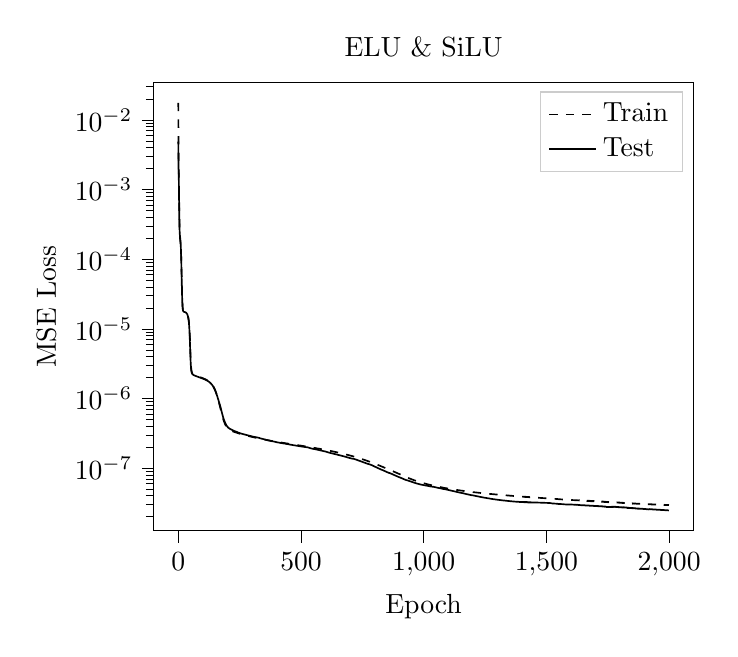
\begin{tikzpicture}

\begin{axis}[
legend cell align={left},
legend style={fill opacity=0.8, draw opacity=1, text opacity=1, draw=white!80!black},
log basis y={10},
tick align=outside,
tick pos=left,
title={ELU \& SiLU},
x grid style={white!69.0196078431373!black},
xlabel={Epoch},
xmin=-99.95, xmax=2098.95,
xtick style={color=black},
y grid style={white!69.0196078431373!black},
ylabel={MSE Loss},
ymin=1.25460830079477e-08, ymax=0.0345317116334461,
ymode=log,
ytick style={color=black}
]
\addplot [semithick, black, dashed]
table {%
0 0.0175996494237334
1 0.00287529958738014
2 0.0017450225809589
3 0.00109182657976635
4 0.000527906175178941
5 0.00029815742187202
6 0.000224625757531612
7 0.000197977887568413
8 0.000183264794104616
9 0.000169372935888532
10 0.000151957952730299
11 0.000129263067727152
12 0.000102055093113449
13 7.43479660304729e-05
14 5.15737580390123e-05
15 3.62272282127378e-05
16 2.71450699819979e-05
17 2.21503660204689e-05
18 1.95366582747738e-05
19 1.82204602597267e-05
20 1.7573602705852e-05
21 1.72561979470629e-05
22 1.70949869616379e-05
23 1.70056749411742e-05
24 1.69485445385362e-05
25 1.69051188822777e-05
26 1.68663870399541e-05
27 1.68271088441543e-05
28 1.67838884763114e-05
29 1.67341138449046e-05
30 1.66752324212212e-05
31 1.66049099725569e-05
32 1.65208375483417e-05
33 1.64199603086672e-05
34 1.62983461823387e-05
35 1.61510820416879e-05
36 1.59720132987786e-05
37 1.57533292913286e-05
38 1.5484687447497e-05
39 1.51527701264058e-05
40 1.47406713913369e-05
41 1.42270974720304e-05
42 1.3586219226454e-05
43 1.27891907977755e-05
44 1.18077328297659e-05
45 1.06241310518271e-05
46 9.24968551862548e-06
47 7.74917471699155e-06
48 6.25447972788606e-06
49 4.93720254530672e-06
50 3.93207780757621e-06
51 3.26343841823018e-06
52 2.85647097467745e-06
53 2.61511052349306e-06
54 2.47010573488637e-06
55 2.38091079037872e-06
56 2.32446314907975e-06
57 2.28729202154909e-06
58 2.26161475359277e-06
59 2.24282278935561e-06
60 2.22819607702718e-06
61 2.21604933179265e-06
62 2.20556252057236e-06
63 2.19616054360472e-06
64 2.18749445562594e-06
65 2.17928000790835e-06
66 2.17143440573864e-06
67 2.16391069665178e-06
68 2.15657700448446e-06
69 2.14940820202969e-06
70 2.14237768801695e-06
71 2.13553268446276e-06
72 2.12884015479631e-06
73 2.12225586307113e-06
74 2.11574514611357e-06
75 2.10928932654042e-06
76 2.10288195557951e-06
77 2.09650990095156e-06
78 2.09017900181152e-06
79 2.08388941103976e-06
80 2.07764323232595e-06
81 2.07144468839715e-06
82 2.06527465138606e-06
83 2.05913248743173e-06
84 2.0530142757309e-06
85 2.04691445756566e-06
86 2.04082622008173e-06
87 2.03473575675162e-06
88 2.0286378381229e-06
89 2.02251989537672e-06
90 2.01638261944481e-06
91 2.01022128027262e-06
92 2.00403939894045e-06
93 1.99783347059679e-06
94 1.99160166323509e-06
95 1.98533314505767e-06
96 1.97902080506651e-06
97 1.97265234243105e-06
98 1.9662212929461e-06
99 1.95973702790297e-06
100 1.95320250358577e-06
101 1.94660680122638e-06
102 1.939952190952e-06
103 1.93324243110737e-06
104 1.92648431564635e-06
105 1.91963722903665e-06
106 1.91268758226215e-06
107 1.90565878750704e-06
108 1.89853121551664e-06
109 1.89127792199884e-06
110 1.88389302704195e-06
111 1.87637372260951e-06
112 1.86870985686483e-06
113 1.86089686886248e-06
114 1.85292484115962e-06
115 1.84476674837697e-06
116 1.83640388777917e-06
117 1.82784501009792e-06
118 1.81907705044182e-06
119 1.81008488425505e-06
120 1.80085318538659e-06
121 1.79136690542236e-06
122 1.78161437838753e-06
123 1.77159513089009e-06
124 1.76129403953951e-06
125 1.75069264912509e-06
126 1.73976445233848e-06
127 1.72847957088607e-06
128 1.71680751208214e-06
129 1.7047350025905e-06
130 1.69224299537518e-06
131 1.67928939252704e-06
132 1.66583868410441e-06
133 1.65187669213651e-06
134 1.63740343054997e-06
135 1.62238789512514e-06
136 1.6067824065118e-06
137 1.5905935566991e-06
138 1.57381414469171e-06
139 1.55636063472286e-06
140 1.53816044023358e-06
141 1.51927269187979e-06
142 1.49966893327758e-06
143 1.47930880157787e-06
144 1.45817050724872e-06
145 1.43625170875339e-06
146 1.41338668653646e-06
147 1.38969123329957e-06
148 1.3652607281216e-06
149 1.34014765538382e-06
150 1.3144001037233e-06
151 1.28805525855569e-06
152 1.26120119203677e-06
153 1.23391107938176e-06
154 1.20624255806945e-06
155 1.17823492250579e-06
156 1.14992709714556e-06
157 1.12135632480204e-06
158 1.09260033759995e-06
159 1.06368875725593e-06
160 1.03462326670467e-06
161 1.00557742922547e-06
162 9.7667225931275e-07
163 9.47957712440939e-07
164 9.19453697107997e-07
165 8.91192761528714e-07
166 8.63282801702781e-07
167 8.35834502140642e-07
168 8.08940287257087e-07
169 7.82601844235842e-07
170 7.56980151379594e-07
171 7.32141062655955e-07
172 7.08114986750275e-07
173 6.84937570738953e-07
174 6.62635313446458e-07
175 6.41243045507167e-07
176 6.2081070653619e-07
177 6.01388748577847e-07
178 5.83003184985387e-07
179 5.65668886466142e-07
180 5.49323648044719e-07
181 5.33915851917754e-07
182 5.19427995229194e-07
183 5.05823589165288e-07
184 4.9306046715003e-07
185 4.8109552386677e-07
186 4.6990855443596e-07
187 4.59501481813618e-07
188 4.49822384894105e-07
189 4.40771383807714e-07
190 4.32378732156735e-07
191 4.24598447835933e-07
192 4.17455452677018e-07
193 4.10936514782634e-07
194 4.0497750121915e-07
195 3.99562149212329e-07
196 3.94614396952875e-07
197 3.9006308888645e-07
198 3.85865279696418e-07
199 3.81985842821564e-07
200 3.78385178450458e-07
201 3.75026909821941e-07
202 3.71899057071801e-07
203 3.69010332562425e-07
204 3.66329881671845e-07
205 3.63827414901152e-07
206 3.61479612806193e-07
207 3.59270024461011e-07
208 3.57176860234176e-07
209 3.55181227661205e-07
210 3.53276239565048e-07
211 3.51515790129042e-07
212 3.49912813945252e-07
213 3.48354445861787e-07
214 3.46851569503315e-07
215 3.45408498390043e-07
216 3.44020960312719e-07
217 3.42683353437678e-07
218 3.41392241935523e-07
219 3.40145149181126e-07
220 3.38937579158483e-07
221 3.37769001305332e-07
222 3.36636997644746e-07
223 3.35538890624321e-07
224 3.34470593799097e-07
225 3.33426590003683e-07
226 3.32406322868906e-07
227 3.31405100723714e-07
228 3.30421388724744e-07
229 3.29453601679575e-07
230 3.28494617065189e-07
231 3.27545682438313e-07
232 3.26611903702201e-07
233 3.25688031040272e-07
234 3.24785979117337e-07
235 3.23915015329135e-07
236 3.23034720381088e-07
237 3.22156478262059e-07
238 3.21286055111614e-07
239 3.20421153560346e-07
240 3.19560409622e-07
241 3.18705262714047e-07
242 3.1785766660164e-07
243 3.1701667911932e-07
244 3.16183564692096e-07
245 3.15356841326775e-07
246 3.14536922402908e-07
247 3.13724506980861e-07
248 3.12925141088272e-07
249 3.12140765842628e-07
250 3.11375240485745e-07
251 3.1062860304587e-07
252 3.0990082002802e-07
253 3.09185586033323e-07
254 3.0848231598668e-07
255 3.07785731521903e-07
256 3.07097276817103e-07
257 3.06413695156493e-07
258 3.05733606865033e-07
259 3.05057379563323e-07
260 3.04384200020991e-07
261 3.03711434725074e-07
262 3.0303466202497e-07
263 3.02357359515781e-07
264 3.01714337382464e-07
265 3.01069908317686e-07
266 3.00426167228807e-07
267 2.99785866843649e-07
268 2.99147748563655e-07
269 2.98513994621885e-07
270 2.97884098472423e-07
271 2.97257889613434e-07
272 2.96635719834626e-07
273 2.96016641236463e-07
274 2.95400801640255e-07
275 2.94787651498041e-07
276 2.94177613653801e-07
277 2.93570954063682e-07
278 2.92964300811605e-07
279 2.92362203438756e-07
280 2.91760416381237e-07
281 2.91159803978758e-07
282 2.9055891594254e-07
283 2.89960710880166e-07
284 2.8936324151374e-07
285 2.88770518061199e-07
286 2.88199581916615e-07
287 2.87646285805465e-07
288 2.87090873314355e-07
289 2.86531117303923e-07
290 2.85970951807712e-07
291 2.85412180353717e-07
292 2.84857709402786e-07
293 2.84302747601828e-07
294 2.8375344444953e-07
295 2.83205761050453e-07
296 2.82660867995332e-07
297 2.8211923660848e-07
298 2.81580993302555e-07
299 2.81046339367208e-07
300 2.80514478589566e-07
301 2.7998426008935e-07
302 2.79458510092923e-07
303 2.78934175497625e-07
304 2.78412257820548e-07
305 2.7789296674996e-07
306 2.77374297333211e-07
307 2.7685929883603e-07
308 2.76344144253926e-07
309 2.75831304342944e-07
310 2.75319272766694e-07
311 2.74808198902576e-07
312 2.7429603046869e-07
313 2.73784318302717e-07
314 2.73272087738974e-07
315 2.72760358924984e-07
316 2.72247648759105e-07
317 2.71740439046653e-07
318 2.71237279193315e-07
319 2.70741638303207e-07
320 2.70252898353363e-07
321 2.69768819279648e-07
322 2.69289078040913e-07
323 2.68816892983637e-07
324 2.68343211374145e-07
325 2.67885037054327e-07
326 2.67416310265389e-07
327 2.66975876130005e-07
328 2.66506596872773e-07
329 2.66083591505151e-07
330 2.65639710384846e-07
331 2.65243812378912e-07
332 2.64773271553054e-07
333 2.64322112386139e-07
334 2.63829088133605e-07
335 2.63389938119474e-07
336 2.6290572489529e-07
337 2.62464812486485e-07
338 2.61970761854968e-07
339 2.61548848619952e-07
340 2.61117641201736e-07
341 2.60733976112704e-07
342 2.60291870695539e-07
343 2.59895549817202e-07
344 2.594321902194e-07
345 2.59030119281078e-07
346 2.58601684890891e-07
347 2.58207709705971e-07
348 2.57752386914945e-07
349 2.57358960176646e-07
350 2.56929571371245e-07
351 2.56539277351919e-07
352 2.56089040767904e-07
353 2.5569170922779e-07
354 2.5524339392291e-07
355 2.54830653759086e-07
356 2.54406230482118e-07
357 2.54067098289568e-07
358 2.53661682023676e-07
359 2.53289803858081e-07
360 2.52879487980806e-07
361 2.52509188818806e-07
362 2.52106710043165e-07
363 2.5173805948242e-07
364 2.51339875042333e-07
365 2.50972963598883e-07
366 2.50580756969043e-07
367 2.50217714238943e-07
368 2.49831848677218e-07
369 2.49469345895648e-07
370 2.49089968647809e-07
371 2.4873137019199e-07
372 2.48356590667242e-07
373 2.47999187131143e-07
374 2.4763044640963e-07
375 2.47274666534736e-07
376 2.46913876914334e-07
377 2.46557384258494e-07
378 2.46201170384097e-07
379 2.45847944853494e-07
380 2.45494405000102e-07
381 2.45144459192659e-07
382 2.4479538060973e-07
383 2.44445716866437e-07
384 2.44098331023679e-07
385 2.43749799729187e-07
386 2.43400523295634e-07
387 2.43049962001862e-07
388 2.42702448431942e-07
389 2.42355488609292e-07
390 2.42012714679163e-07
391 2.4167355127247e-07
392 2.41335103595475e-07
393 2.40999812632481e-07
394 2.40663078940884e-07
395 2.40325962195698e-07
396 2.39984172416996e-07
397 2.39634622730023e-07
398 2.39281233987754e-07
399 2.38940480876693e-07
400 2.3863265462154e-07
401 2.38341846198864e-07
402 2.3803435519909e-07
403 2.37720892670268e-07
404 2.37405413471947e-07
405 2.3708795703925e-07
406 2.36770879936898e-07
407 2.36454466346459e-07
408 2.36138622433657e-07
409 2.35822797336027e-07
410 2.35507726081607e-07
411 2.35190857516443e-07
412 2.34877379469367e-07
413 2.34564189511843e-07
414 2.34253473898605e-07
415 2.33942672522858e-07
416 2.33634892900625e-07
417 2.33329615788591e-07
418 2.33024774566104e-07
419 2.32720143500842e-07
420 2.32416022562632e-07
421 2.32108510779483e-07
422 2.31797596143224e-07
423 2.31482146325845e-07
424 2.31172614505226e-07
425 2.30876980893413e-07
426 2.30587186429432e-07
427 2.30292145651845e-07
428 2.29996369043306e-07
429 2.29696812866109e-07
430 2.29395408346988e-07
431 2.29091220759869e-07
432 2.28793122374782e-07
433 2.28505814114044e-07
434 2.28219742702152e-07
435 2.27929575416397e-07
436 2.2763782101265e-07
437 2.27346566390452e-07
438 2.27056472624554e-07
439 2.26765794053563e-07
440 2.26474985048242e-07
441 2.26186430381858e-07
442 2.25897406949116e-07
443 2.2560861464882e-07
444 2.25320075472268e-07
445 2.25033070627489e-07
446 2.24744428635404e-07
447 2.24458662323457e-07
448 2.24170733531537e-07
449 2.23884842050381e-07
450 2.23597962218491e-07
451 2.23310248394171e-07
452 2.23022348308177e-07
453 2.22734046751327e-07
454 2.22442912225063e-07
455 2.22151466509501e-07
456 2.21859659873758e-07
457 2.21572562438155e-07
458 2.21289075021502e-07
459 2.21010129273225e-07
460 2.20728793351554e-07
461 2.20448860829947e-07
462 2.20167770152102e-07
463 2.19885938825826e-07
464 2.19604979307064e-07
465 2.19323364973434e-07
466 2.19043549776643e-07
467 2.18763958706347e-07
468 2.18484622969584e-07
469 2.18205289677087e-07
470 2.17927875091561e-07
471 2.17649641605533e-07
472 2.17373744746396e-07
473 2.1709560340355e-07
474 2.16820149610442e-07
475 2.16545120039768e-07
476 2.16269043342265e-07
477 2.15993676206949e-07
478 2.15721830045368e-07
479 2.15448890990899e-07
480 2.15178834174878e-07
481 2.149075208564e-07
482 2.14637604578627e-07
483 2.14366342028427e-07
484 2.14095653959134e-07
485 2.13825490867237e-07
486 2.13554397497262e-07
487 2.13285051131606e-07
488 2.13013861191769e-07
489 2.12744850905722e-07
490 2.12475656326205e-07
491 2.12207315264834e-07
492 2.11938185586291e-07
493 2.11668856991309e-07
494 2.11400331892264e-07
495 2.11133048289014e-07
496 2.10864122102805e-07
497 2.10596357298698e-07
498 2.10328821644623e-07
499 2.10059376463789e-07
500 2.09792518937491e-07
501 2.09525793508192e-07
502 2.0925775712044e-07
503 2.08989702933593e-07
504 2.08722312152076e-07
505 2.08454585468587e-07
506 2.08186760026763e-07
507 2.07918511570426e-07
508 2.07650348066579e-07
509 2.0738169546064e-07
510 2.07112908462648e-07
511 2.06844777174808e-07
512 2.06574911899793e-07
513 2.06304785187683e-07
514 2.06034711695224e-07
515 2.05762478614702e-07
516 2.05489735087383e-07
517 2.05218204492041e-07
518 2.04941749565535e-07
519 2.04666232278328e-07
520 2.04387647002591e-07
521 2.04112322826688e-07
522 2.0383555720116e-07
523 2.0356390942311e-07
524 2.0328289256355e-07
525 2.03006117388327e-07
526 2.02714574768947e-07
527 2.02427127135252e-07
528 2.02120347992718e-07
529 2.01825123937738e-07
530 2.01526683405007e-07
531 2.01258414435301e-07
532 2.00978978099897e-07
533 2.00726137201457e-07
534 2.00452940838147e-07
535 2.00204465528486e-07
536 1.99926498702041e-07
537 1.99674599720368e-07
538 1.99389074467149e-07
539 1.99133380988314e-07
540 1.98845136111458e-07
541 1.98592526508889e-07
542 1.98312001522538e-07
543 1.98073469377391e-07
544 1.97795437962611e-07
545 1.97541130809498e-07
546 1.9723873250399e-07
547 1.96979277795606e-07
548 1.96690525427812e-07
549 1.96438236173435e-07
550 1.9614758696207e-07
551 1.95893695774885e-07
552 1.9560284979292e-07
553 1.95347655257194e-07
554 1.95057353046479e-07
555 1.94801164418834e-07
556 1.94509920277142e-07
557 1.94253270734634e-07
558 1.93961073485127e-07
559 1.93702724359923e-07
560 1.93412831507089e-07
561 1.93151937097014e-07
562 1.92862569448948e-07
563 1.92599946480243e-07
564 1.92312116809035e-07
565 1.92046887015351e-07
566 1.91762092583758e-07
567 1.91495132177977e-07
568 1.91215405095591e-07
569 1.90950501014697e-07
570 1.90681914915558e-07
571 1.90422427188253e-07
572 1.90139000331158e-07
573 1.89849500145556e-07
574 1.89560766450825e-07
575 1.89280814623771e-07
576 1.8900092842955e-07
577 1.8872307740736e-07
578 1.88442443018744e-07
579 1.88163821782439e-07
580 1.87884023183926e-07
581 1.87604552785103e-07
582 1.87324280688017e-07
583 1.87046472525765e-07
584 1.8676562085318e-07
585 1.86486165269173e-07
586 1.86204263052048e-07
587 1.85924446839181e-07
588 1.85642518125917e-07
589 1.85359782030048e-07
590 1.85078272430417e-07
591 1.84792084183982e-07
592 1.84508275026474e-07
593 1.84220880669272e-07
594 1.83932809697751e-07
595 1.83643697894809e-07
596 1.83353293152777e-07
597 1.83060790227785e-07
598 1.82766741410489e-07
599 1.82471747208979e-07
600 1.82175910396154e-07
601 1.81878275817837e-07
602 1.81581998241143e-07
603 1.81293149658757e-07
604 1.81011799938346e-07
605 1.80725013777305e-07
606 1.80430601247394e-07
607 1.80136493369787e-07
608 1.79840781072471e-07
609 1.79547042925776e-07
610 1.79256953792617e-07
611 1.78968048011541e-07
612 1.78676989577298e-07
613 1.78381995397103e-07
614 1.78090247487717e-07
615 1.77807889897963e-07
616 1.77518120445086e-07
617 1.77226933303132e-07
618 1.76935237604425e-07
619 1.76642455294029e-07
620 1.76349222122951e-07
621 1.76056165678062e-07
622 1.75763073201551e-07
623 1.75468830988734e-07
624 1.75175491378354e-07
625 1.74879692544039e-07
626 1.74585498029955e-07
627 1.74291679364558e-07
628 1.73995814343186e-07
629 1.73700186017811e-07
630 1.73405231102208e-07
631 1.73109094077972e-07
632 1.72812282521306e-07
633 1.72517677093253e-07
634 1.72222056555427e-07
635 1.71927344155165e-07
636 1.71632569099245e-07
637 1.71338274590482e-07
638 1.71034913130086e-07
639 1.70733721134297e-07
640 1.7043391181204e-07
641 1.70132847280513e-07
642 1.69833049191936e-07
643 1.69529434216997e-07
644 1.69227103143044e-07
645 1.68925542112675e-07
646 1.68622009034891e-07
647 1.68318236774212e-07
648 1.68014904176061e-07
649 1.67709664872007e-07
650 1.6740428503681e-07
651 1.67098198687654e-07
652 1.66792148370121e-07
653 1.66485019853724e-07
654 1.66178793207905e-07
655 1.65869200280611e-07
656 1.65561907664369e-07
657 1.65252004769911e-07
658 1.64943542721119e-07
659 1.64632498311335e-07
660 1.64322014335028e-07
661 1.64009824260347e-07
662 1.63697879330016e-07
663 1.63385576819053e-07
664 1.63073160940996e-07
665 1.62760238836768e-07
666 1.62445714465775e-07
667 1.62130916251613e-07
668 1.61816271742055e-07
669 1.61501935338038e-07
670 1.61184934285075e-07
671 1.60868889899746e-07
672 1.60552074753184e-07
673 1.60234152140504e-07
674 1.59917202708471e-07
675 1.59598340765399e-07
676 1.5928070041582e-07
677 1.58963693209557e-07
678 1.58649849083758e-07
679 1.58348114766227e-07
680 1.58057629661812e-07
681 1.57671108624413e-07
682 1.57301388419739e-07
683 1.56999126346591e-07
684 1.56670816949145e-07
685 1.56336613628127e-07
686 1.56002342869499e-07
687 1.556705652348e-07
688 1.55350209446681e-07
689 1.55038015698494e-07
690 1.54718844136426e-07
691 1.5439428176478e-07
692 1.54069175138716e-07
693 1.53743410223228e-07
694 1.53420686693551e-07
695 1.5309928499363e-07
696 1.52787432718071e-07
697 1.52489572741388e-07
698 1.5215267003299e-07
699 1.5180147937599e-07
700 1.51467610628231e-07
701 1.51146714920003e-07
702 1.50877697457474e-07
703 1.50529026193169e-07
704 1.50173604488657e-07
705 1.49829621982178e-07
706 1.49500967239646e-07
707 1.49161668694831e-07
708 1.48830235133346e-07
709 1.4848696960712e-07
710 1.48152148859992e-07
711 1.47827308822457e-07
712 1.47502455668302e-07
713 1.47172682240182e-07
714 1.46840045417207e-07
715 1.46497807946844e-07
716 1.46153746740652e-07
717 1.4580504894468e-07
718 1.45458180313085e-07
719 1.45108395322779e-07
720 1.44763098667511e-07
721 1.44413272984423e-07
722 1.44068907871997e-07
723 1.43719601865655e-07
724 1.4337589767166e-07
725 1.43025246977402e-07
726 1.42680555661912e-07
727 1.42329018402165e-07
728 1.41984071241552e-07
729 1.41631456635594e-07
730 1.41288496855907e-07
731 1.40933513208097e-07
732 1.40596474217602e-07
733 1.40239406363207e-07
734 1.39900588273179e-07
735 1.39539811776501e-07
736 1.39217587097562e-07
737 1.38853319960219e-07
738 1.38519196539733e-07
739 1.38150057352959e-07
740 1.37809788974153e-07
741 1.3743655064502e-07
742 1.3710148611068e-07
743 1.36720188223194e-07
744 1.36391699037119e-07
745 1.36003874573021e-07
746 1.35689238376813e-07
747 1.3526807629205e-07
748 1.34977162510097e-07
749 1.34534849898671e-07
750 1.34263853979633e-07
751 1.33803888381578e-07
752 1.33541157381956e-07
753 1.33075631865154e-07
754 1.32812739892074e-07
755 1.32347266053046e-07
756 1.32081167286913e-07
757 1.31614762942434e-07
758 1.31345022282403e-07
759 1.30879963457176e-07
760 1.3060746962168e-07
761 1.30141176512666e-07
762 1.29864243902489e-07
763 1.29394299058561e-07
764 1.2911283270256e-07
765 1.28642385263333e-07
766 1.28354625225313e-07
767 1.2789251384504e-07
768 1.276106047996e-07
769 1.27158457551957e-07
770 1.26873228133206e-07
771 1.2642038833377e-07
772 1.26147492281348e-07
773 1.25696561333655e-07
774 1.2542319246478e-07
775 1.24956723709602e-07
776 1.24685955043446e-07
777 1.24218594947934e-07
778 1.23948786196593e-07
779 1.23475682784147e-07
780 1.23208924293294e-07
781 1.22734899811405e-07
782 1.22469958334648e-07
783 1.21993825025868e-07
784 1.21732354990911e-07
785 1.21256032315387e-07
786 1.20998242365999e-07
787 1.2051988794326e-07
788 1.20267326778389e-07
789 1.19790599342195e-07
790 1.19547230333694e-07
791 1.19097782047106e-07
792 1.18811734310498e-07
793 1.18316635195015e-07
794 1.18063428701021e-07
795 1.17580629776626e-07
796 1.17317416432172e-07
797 1.16842961155328e-07
798 1.16570967094276e-07
799 1.16108646778912e-07
800 1.15827305272376e-07
801 1.15377920501203e-07
802 1.1508488028511e-07
803 1.14649716792314e-07
804 1.14344960543633e-07
805 1.13921864283384e-07
806 1.13603540839335e-07
807 1.13194083560586e-07
808 1.12863245988137e-07
809 1.12468225204054e-07
810 1.12127083646385e-07
811 1.11746339406693e-07
812 1.11400504785308e-07
813 1.11035729347009e-07
814 1.10672897640995e-07
815 1.10295471110078e-07
816 1.09931559045151e-07
817 1.09568143528804e-07
818 1.09202652389229e-07
819 1.0884110548659e-07
820 1.08479694034713e-07
821 1.08123397502879e-07
822 1.07768057553415e-07
823 1.07427633928125e-07
824 1.07132911082886e-07
825 1.06680572500295e-07
826 1.06355442163419e-07
827 1.05982517581538e-07
828 1.05633535838479e-07
829 1.05274247268028e-07
830 1.04923396285983e-07
831 1.04568637013358e-07
832 1.04220353073003e-07
833 1.03865601353448e-07
834 1.03513037430503e-07
835 1.03156986462238e-07
836 1.02802441595884e-07
837 1.02450682760491e-07
838 1.02100855322362e-07
839 1.01750472786932e-07
840 1.0140150994431e-07
841 1.01053541381901e-07
842 1.00707275326073e-07
843 1.00359584678245e-07
844 1.00014914270474e-07
845 9.96698316377831e-08
846 9.93263650492793e-08
847 9.89830431770144e-08
848 9.86420426372092e-08
849 9.830027455493e-08
850 9.79607342728173e-08
851 9.76206057572426e-08
852 9.72826926961545e-08
853 9.69451741390515e-08
854 9.66100479331544e-08
855 9.62747901454009e-08
856 9.59414415291349e-08
857 9.56098446884823e-08
858 9.52807467342609e-08
859 9.49542538926096e-08
860 9.46286855700862e-08
861 9.43026890531939e-08
862 9.39737770337956e-08
863 9.36448786958977e-08
864 9.33190625431735e-08
865 9.29954942066047e-08
866 9.26732596084889e-08
867 9.23527348462017e-08
868 9.20334779763721e-08
869 9.17156793747154e-08
870 9.13983349377645e-08
871 9.10830633600312e-08
872 9.07672439609541e-08
873 9.04524855158684e-08
874 9.01387915774876e-08
875 8.98264481250521e-08
876 8.95150285202817e-08
877 8.92049641834092e-08
878 8.88939577734504e-08
879 8.85861132289278e-08
880 8.82777590334172e-08
881 8.79710582140092e-08
882 8.76646669567549e-08
883 8.73602326905143e-08
884 8.70552255705093e-08
885 8.67519998095645e-08
886 8.64501233053261e-08
887 8.6146255775077e-08
888 8.58468929791911e-08
889 8.55448757945965e-08
890 8.52472173562546e-08
891 8.49459580933853e-08
892 8.46501490912033e-08
893 8.43481334271701e-08
894 8.40549865515072e-08
895 8.37533525341883e-08
896 8.34638953648437e-08
897 8.31621499131074e-08
898 8.28743535308263e-08
899 8.25751389896823e-08
900 8.22899470520611e-08
901 8.19908786695578e-08
902 8.17119941984856e-08
903 8.14204756736103e-08
904 8.11498789587972e-08
905 8.08366941313921e-08
906 8.05548967051095e-08
907 8.02546861962128e-08
908 7.99800256316985e-08
909 7.96830944622684e-08
910 7.94125844763016e-08
911 7.911549998596e-08
912 7.88506315814175e-08
913 7.85564360050728e-08
914 7.82931790439534e-08
915 7.8004567647838e-08
916 7.77404717631214e-08
917 7.74547611754883e-08
918 7.7181353187683e-08
919 7.69060091343476e-08
920 7.66324710355093e-08
921 7.63723304721964e-08
922 7.60953091329952e-08
923 7.5864466129616e-08
924 7.55713254001478e-08
925 7.53308811525244e-08
926 7.50198124421786e-08
927 7.4793768067849e-08
928 7.44999733726104e-08
929 7.42764854599898e-08
930 7.40070237732482e-08
931 7.3757139062991e-08
932 7.34708819116747e-08
933 7.32295668548488e-08
934 7.29672317092422e-08
935 7.27254336361227e-08
936 7.24722474849671e-08
937 7.22304411411301e-08
938 7.19834948306186e-08
939 7.17461780297413e-08
940 7.15024025836897e-08
941 7.1267125772323e-08
942 7.10307098543694e-08
943 7.07984063801348e-08
944 7.05661321873663e-08
945 7.03392329199914e-08
946 7.01104802871555e-08
947 6.98869387250056e-08
948 6.96629443517338e-08
949 6.94436666712761e-08
950 6.92237607111679e-08
951 6.90076469602729e-08
952 6.87917168527008e-08
953 6.85799188460123e-08
954 6.83669486356564e-08
955 6.81601427672263e-08
956 6.79508710383914e-08
957 6.77463507194886e-08
958 6.75436472228341e-08
959 6.73413416798496e-08
960 6.71408234005355e-08
961 6.69428408208717e-08
962 6.67447739353122e-08
963 6.65525494945029e-08
964 6.63575741768341e-08
965 6.61687265406385e-08
966 6.59775455638112e-08
967 6.57917663957619e-08
968 6.56059239396711e-08
969 6.54228842194016e-08
970 6.52397152656192e-08
971 6.50610468397872e-08
972 6.48808190213401e-08
973 6.47048932265193e-08
974 6.45277746365025e-08
975 6.43562626940764e-08
976 6.41803190077894e-08
977 6.40130773810199e-08
978 6.38387489111381e-08
979 6.36743903790204e-08
980 6.35023501907028e-08
981 6.33410359505149e-08
982 6.31731920286427e-08
983 6.30170328896895e-08
984 6.28512382760959e-08
985 6.27018185994643e-08
986 6.25389082422601e-08
987 6.23940222439501e-08
988 6.22324554662157e-08
989 6.20933315786942e-08
990 6.19333390581289e-08
991 6.18009775230632e-08
992 6.16378112496818e-08
993 6.151472694782e-08
994 6.13488915561788e-08
995 6.12322543176447e-08
996 6.10627431143484e-08
997 6.0956969566206e-08
998 6.07836454555866e-08
999 6.06858273002331e-08
1000 6.0507606448823e-08
1001 6.04200453828696e-08
1002 6.02411679047066e-08
1003 6.01563548663364e-08
1004 5.99758189601118e-08
1005 5.98955439414794e-08
1006 5.97161064845864e-08
1007 5.96399952890181e-08
1008 5.94604134001031e-08
1009 5.93865410394301e-08
1010 5.92094895459638e-08
1011 5.91360529007545e-08
1012 5.89636505807789e-08
1013 5.8890947325807e-08
1014 5.87177360920066e-08
1015 5.86479926383276e-08
1016 5.84775806053983e-08
1017 5.84071221645388e-08
1018 5.82407901923432e-08
1019 5.81706089164413e-08
1020 5.80062781310176e-08
1021 5.79364867938636e-08
1022 5.77755773072397e-08
1023 5.77070267020474e-08
1024 5.75472279997769e-08
1025 5.74803025088499e-08
1026 5.73227851177194e-08
1027 5.72549469133321e-08
1028 5.70999626958724e-08
1029 5.7033860887401e-08
1030 5.68804288114677e-08
1031 5.68131055551646e-08
1032 5.6663332767215e-08
1033 5.65954860540785e-08
1034 5.64472345629952e-08
1035 5.63754745606104e-08
1036 5.62272355715265e-08
1037 5.61484333303497e-08
1038 5.5999395478068e-08
1039 5.59186794042432e-08
1040 5.57838673493904e-08
1041 5.57162485428364e-08
1042 5.56010164558529e-08
1043 5.55337433567615e-08
1044 5.54150616451921e-08
1045 5.53392590987301e-08
1046 5.52239583875291e-08
1047 5.5144874224311e-08
1048 5.50325426509346e-08
1049 5.49520297781214e-08
1050 5.48456422393428e-08
1051 5.47616790171901e-08
1052 5.46610097735822e-08
1053 5.45759626504605e-08
1054 5.44761822958151e-08
1055 5.43920063904579e-08
1056 5.42956490861002e-08
1057 5.4211317223718e-08
1058 5.4117549513677e-08
1059 5.40303107428031e-08
1060 5.39417221858685e-08
1061 5.38540957997213e-08
1062 5.37668139806158e-08
1063 5.36784573128557e-08
1064 5.35941787980221e-08
1065 5.3507047322654e-08
1066 5.34215971939034e-08
1067 5.33369641182446e-08
1068 5.32536905559766e-08
1069 5.31688032587851e-08
1070 5.30834877885411e-08
1071 5.30020961733158e-08
1072 5.29187969142697e-08
1073 5.28378100881355e-08
1074 5.27521015420973e-08
1075 5.2670030630253e-08
1076 5.25867333536212e-08
1077 5.25034244560629e-08
1078 5.2418908094154e-08
1079 5.23290026706036e-08
1080 5.22326315639532e-08
1081 5.21282267627043e-08
1082 5.20232685978783e-08
1083 5.19315852756108e-08
1084 5.18594172795872e-08
1085 5.18124042443446e-08
1086 5.16707377791192e-08
1087 5.16539989376952e-08
1088 5.15711485888914e-08
1089 5.15147099022784e-08
1090 5.14256392456502e-08
1091 5.13642042427875e-08
1092 5.1281067797504e-08
1093 5.12151511067316e-08
1094 5.1136492572823e-08
1095 5.10673343896428e-08
1096 5.09849862382339e-08
1097 5.09159236656842e-08
1098 5.08563726846489e-08
1099 5.077642700968e-08
1100 5.07170401462531e-08
1101 5.06396115724783e-08
1102 5.05759921800575e-08
1103 5.05042115719334e-08
1104 5.04362397748537e-08
1105 5.03709844430489e-08
1106 5.03009102779117e-08
1107 5.02376596962506e-08
1108 5.01693970313966e-08
1109 5.01037829856443e-08
1110 5.00381948604911e-08
1111 4.99729949332561e-08
1112 4.99080592604173e-08
1113 4.98440006531098e-08
1114 4.97788077851169e-08
1115 4.97160153187792e-08
1116 4.96525768198808e-08
1117 4.95886749831698e-08
1118 4.95259647159685e-08
1119 4.94638447854356e-08
1120 4.94025123742858e-08
1121 4.93408055142197e-08
1122 4.92777741882833e-08
1123 4.92156950713252e-08
1124 4.91560401947311e-08
1125 4.90946190012664e-08
1126 4.90349146211599e-08
1127 4.89734367121741e-08
1128 4.89154338225717e-08
1129 4.88554389015405e-08
1130 4.87965765465503e-08
1131 4.87381162699307e-08
1132 4.86792782474765e-08
1133 4.86204470853124e-08
1134 4.85623430606097e-08
1135 4.85029923069646e-08
1136 4.84469144268473e-08
1137 4.83894675831209e-08
1138 4.83293557067554e-08
1139 4.82720579384477e-08
1140 4.82142370081817e-08
1141 4.81568539498767e-08
1142 4.80991615496862e-08
1143 4.80393431416815e-08
1144 4.79794743064588e-08
1145 4.79202978560522e-08
1146 4.78614520780241e-08
1147 4.77986213525128e-08
1148 4.77403732936921e-08
1149 4.76852409470041e-08
1150 4.76301647012178e-08
1151 4.7578462570641e-08
1152 4.75241271757909e-08
1153 4.74723943568733e-08
1154 4.74180858915929e-08
1155 4.73673670065011e-08
1156 4.73131372622504e-08
1157 4.72611859620997e-08
1158 4.72082820444086e-08
1159 4.7156959116279e-08
1160 4.70964777754546e-08
1161 4.70352642594207e-08
1162 4.69699322387385e-08
1163 4.69033307766153e-08
1164 4.68406378679731e-08
1165 4.678152087223e-08
1166 4.67163908766111e-08
1167 4.66496131537042e-08
1168 4.66186367269472e-08
1169 4.65931978403944e-08
1170 4.65452790940901e-08
1171 4.64970322155978e-08
1172 4.64478893889009e-08
1173 4.6401220398451e-08
1174 4.6354152015482e-08
1175 4.63051806818271e-08
1176 4.62608166245104e-08
1177 4.62116961692516e-08
1178 4.61663384392352e-08
1179 4.61181958506529e-08
1180 4.60749140778205e-08
1181 4.60289976587092e-08
1182 4.59828709118426e-08
1183 4.59360696254407e-08
1184 4.58911745084833e-08
1185 4.58475705649164e-08
1186 4.58020190592379e-08
1187 4.57577413932597e-08
1188 4.57144813417187e-08
1189 4.56681103067069e-08
1190 4.56250730138663e-08
1191 4.55801805401279e-08
1192 4.55367965024323e-08
1193 4.54928729460846e-08
1194 4.54491035526416e-08
1195 4.54046372340144e-08
1196 4.53605468813123e-08
1197 4.5318322193566e-08
1198 4.52730989941585e-08
1199 4.52277204736617e-08
1200 4.51831244703271e-08
1201 4.51362583078208e-08
1202 4.50891260435071e-08
1203 4.50436343264471e-08
1204 4.5005045581803e-08
1205 4.49671033173615e-08
1206 4.4927011046525e-08
1207 4.48885856805248e-08
1208 4.48442414047179e-08
1209 4.48037458724571e-08
1210 4.47623032719946e-08
1211 4.4723272381475e-08
1212 4.46810348542215e-08
1213 4.46411653030054e-08
1214 4.4600022867769e-08
1215 4.45591790949607e-08
1216 4.45200743115493e-08
1217 4.44793313718606e-08
1218 4.44395357810379e-08
1219 4.44004629009953e-08
1220 4.43605396469593e-08
1221 4.43211583132097e-08
1222 4.4281827630499e-08
1223 4.42431409233279e-08
1224 4.42025483913255e-08
1225 4.41649761562246e-08
1226 4.41241812545456e-08
1227 4.40845443172577e-08
1228 4.40465823245972e-08
1229 4.40095524965045e-08
1230 4.39683958113335e-08
1231 4.39273198011847e-08
1232 4.38891112786166e-08
1233 4.38489198977265e-08
1234 4.38104611717449e-08
1235 4.37681291849401e-08
1236 4.37326005489069e-08
1237 4.36921684006109e-08
1238 4.36569987094515e-08
1239 4.36212489383081e-08
1240 4.35856813254532e-08
1241 4.35512924070736e-08
1242 4.35153490982998e-08
1243 4.34792310812782e-08
1244 4.3441935190458e-08
1245 4.34084090166209e-08
1246 4.33736247344996e-08
1247 4.33387995464329e-08
1248 4.33012893488183e-08
1249 4.32677698007922e-08
1250 4.32302192905354e-08
1251 4.31998927901134e-08
1252 4.31620639780306e-08
1253 4.31301771044446e-08
1254 4.30933546446965e-08
1255 4.30604565977433e-08
1256 4.30247026876884e-08
1257 4.29927247402873e-08
1258 4.29553815664008e-08
1259 4.29268922417236e-08
1260 4.28864818502461e-08
1261 4.28586315130985e-08
1262 4.28198954232073e-08
1263 4.27898634640655e-08
1264 4.2753595245415e-08
1265 4.27237714077933e-08
1266 4.26869564371657e-08
1267 4.26564525852768e-08
1268 4.26192783891111e-08
1269 4.25903701817276e-08
1270 4.25535703065805e-08
1271 4.25226653746336e-08
1272 4.24879032259184e-08
1273 4.2456188470652e-08
1274 4.24202999376178e-08
1275 4.23859171334584e-08
1276 4.23519101282466e-08
1277 4.23149189643368e-08
1278 4.22824308721204e-08
1279 4.22486863698168e-08
1280 4.22202453158604e-08
1281 4.2187339193589e-08
1282 4.21591239216923e-08
1283 4.2124149732814e-08
1284 4.20938310909946e-08
1285 4.20612705056556e-08
1286 4.20308245416834e-08
1287 4.1997344542466e-08
1288 4.19672587632647e-08
1289 4.19371729876161e-08
1290 4.19042328978492e-08
1291 4.18756649480656e-08
1292 4.18406924111991e-08
1293 4.18142886573492e-08
1294 4.17780153441072e-08
1295 4.17540905388591e-08
1296 4.1716828956595e-08
1297 4.16896988646442e-08
1298 4.16524566198007e-08
1299 4.1629468562121e-08
1300 4.15833136386823e-08
1301 4.15585945674479e-08
1302 4.15018889334817e-08
1303 4.1496817747344e-08
1304 4.14546708569219e-08
1305 4.14546289491113e-08
1306 4.13919402539875e-08
1307 4.14056540662955e-08
1308 4.13244472277086e-08
1309 4.13615174217341e-08
1310 4.12699490794921e-08
1311 4.1267000831624e-08
1312 4.12267482445827e-08
1313 4.12109218075329e-08
1314 4.11668753805827e-08
1315 4.11583183073105e-08
1316 4.11022767217162e-08
1317 4.11100928516817e-08
1318 4.1037408280431e-08
1319 4.1066953887281e-08
1320 4.09750483711946e-08
1321 4.10066736584724e-08
1322 4.09191586996371e-08
1323 4.0947404691849e-08
1324 4.08638924866978e-08
1325 4.08914481262457e-08
1326 4.08070332653665e-08
1327 4.08357535057746e-08
1328 4.07527275072539e-08
1329 4.07760795404499e-08
1330 4.06947206101904e-08
1331 4.07312980570396e-08
1332 4.06484653616701e-08
1333 4.06305324958112e-08
1334 4.06281817078025e-08
1335 4.05609808034058e-08
1336 4.06007411903886e-08
1337 4.05186632264076e-08
1338 4.04813392229642e-08
1339 4.05137915677756e-08
1340 4.04427050817446e-08
1341 4.0404595285537e-08
1342 4.04034278496113e-08
1343 4.03470085359459e-08
1344 4.03759440494866e-08
1345 4.02951091871273e-08
1346 4.02729835862203e-08
1347 4.02820761493672e-08
1348 4.02028653567754e-08
1349 4.0243565639031e-08
1350 4.01645263359285e-08
1351 4.01247152481687e-08
1352 4.01298546996998e-08
1353 4.00498072288258e-08
1354 4.00780106133425e-08
1355 4.00133800226854e-08
1356 3.99935331216739e-08
1357 3.99947927611777e-08
1358 3.99257412730947e-08
1359 3.99636142667248e-08
1360 3.98933878571484e-08
1361 3.98593884050058e-08
1362 3.98346793133442e-08
1363 3.98373121583973e-08
1364 3.97712527302474e-08
1365 3.98051756000939e-08
1366 3.97388940989174e-08
1367 3.97043374533723e-08
1368 3.96858321707327e-08
1369 3.96721265438771e-08
1370 3.9627116226626e-08
1371 3.96427330819904e-08
1372 3.9564374215928e-08
1373 3.95902756480382e-08
1374 3.95136501545323e-08
1375 3.95457331237026e-08
1376 3.94681531226127e-08
1377 3.94643733123701e-08
1378 3.94374941201647e-08
1379 3.94130171876839e-08
1380 3.93865616992173e-08
1381 3.93646849872198e-08
1382 3.93336724364701e-08
1383 3.93183808213848e-08
1384 3.92790345884464e-08
1385 3.92783624505455e-08
1386 3.92181673056768e-08
1387 3.9247309484125e-08
1388 3.91625413485031e-08
1389 3.91856282284664e-08
1390 3.9112159310406e-08
1391 3.91618979058705e-08
1392 3.9091612521247e-08
1393 3.90773670382316e-08
1394 3.90596091861539e-08
1395 3.90377561814148e-08
1396 3.90033072932283e-08
1397 3.89836041740921e-08
1398 3.89571714300985e-08
1399 3.89340272377581e-08
1400 3.89095555490826e-08
1401 3.88901825196797e-08
1402 3.88592720064196e-08
1403 3.88472628642944e-08
1404 3.88079879627412e-08
1405 3.8811693173102e-08
1406 3.87458087196535e-08
1407 3.87871781057925e-08
1408 3.86750464578256e-08
1409 3.87632872431709e-08
1410 3.86152443461185e-08
1411 3.8726272766354e-08
1412 3.85677903231851e-08
1413 3.86811754395922e-08
1414 3.85242661202767e-08
1415 3.86363415181279e-08
1416 3.84808430133887e-08
1417 3.85900492148039e-08
1418 3.84359594995942e-08
1419 3.85446401054423e-08
1420 3.83952957250244e-08
1421 3.84991835922222e-08
1422 3.83527137763906e-08
1423 3.84539447075838e-08
1424 3.83098808818261e-08
1425 3.84084559001963e-08
1426 3.82686769313523e-08
1427 3.83634785663389e-08
1428 3.82263591767185e-08
1429 3.83170275028988e-08
1430 3.81848634063431e-08
1431 3.82719766882644e-08
1432 3.81443559227534e-08
1433 3.82261160360997e-08
1434 3.81028666360805e-08
1435 3.81820462145299e-08
1436 3.80621713560458e-08
1437 3.81377050473475e-08
1438 3.8020763664548e-08
1439 3.80906669938952e-08
1440 3.79813536319773e-08
1441 3.80451777530766e-08
1442 3.79402011745356e-08
1443 3.79971468937868e-08
1444 3.78976800448072e-08
1445 3.79480461809578e-08
1446 3.78535985952055e-08
1447 3.78877064797223e-08
1448 3.77929022867818e-08
1449 3.78013958233225e-08
1450 3.77127713129255e-08
1451 3.77494880652307e-08
1452 3.77125745814055e-08
1453 3.77251245637922e-08
1454 3.76768934877703e-08
1455 3.76800348611539e-08
1456 3.76387757690111e-08
1457 3.76369275087995e-08
1458 3.76011498595119e-08
1459 3.75915576782404e-08
1460 3.7565789462235e-08
1461 3.75480054266575e-08
1462 3.75244291888066e-08
1463 3.75085536461484e-08
1464 3.74869865567007e-08
1465 3.74678988599442e-08
1466 3.74458098804098e-08
1467 3.74289946023509e-08
1468 3.74053136447117e-08
1469 3.73895509646616e-08
1470 3.73655890228974e-08
1471 3.73484145193004e-08
1472 3.73280483714211e-08
1473 3.73083839733113e-08
1474 3.72891789162111e-08
1475 3.72704910880373e-08
1476 3.7248621644892e-08
1477 3.72312626915061e-08
1478 3.72108093422696e-08
1479 3.71916894330582e-08
1480 3.71718720479919e-08
1481 3.71548341639993e-08
1482 3.71317190506204e-08
1483 3.71136948977835e-08
1484 3.70954332247209e-08
1485 3.7075017328192e-08
1486 3.70562630358506e-08
1487 3.70378945753203e-08
1488 3.70180622759619e-08
1489 3.69973437628346e-08
1490 3.69796147232648e-08
1491 3.6959753085597e-08
1492 3.69415847352172e-08
1493 3.69228330292515e-08
1494 3.69024669879536e-08
1495 3.6883986361147e-08
1496 3.68645939907708e-08
1497 3.68453450008133e-08
1498 3.68283621270393e-08
1499 3.68075644914256e-08
1500 3.67898759954244e-08
1501 3.67695001806112e-08
1502 3.67499921836156e-08
1503 3.6732197379763e-08
1504 3.67122580833268e-08
1505 3.66923476278203e-08
1506 3.66745375650623e-08
1507 3.66537149432133e-08
1508 3.66359610310951e-08
1509 3.66162055271957e-08
1510 3.659514873533e-08
1511 3.65773423496307e-08
1512 3.65557572656883e-08
1513 3.65364017227421e-08
1514 3.65143413247893e-08
1515 3.64913223691588e-08
1516 3.64676853230606e-08
1517 3.64390327298736e-08
1518 3.64060995430293e-08
1519 3.63669256735477e-08
1520 3.63247117149967e-08
1521 3.63022032345839e-08
1522 3.62946600880321e-08
1523 3.62906074222735e-08
1524 3.62781957825575e-08
1525 3.62666043507431e-08
1526 3.62482158386968e-08
1527 3.62316294477694e-08
1528 3.62140311018777e-08
1529 3.61927297731768e-08
1530 3.61777107897865e-08
1531 3.61594412154886e-08
1532 3.61410701259501e-08
1533 3.61231098437997e-08
1534 3.61054330362265e-08
1535 3.60887919867991e-08
1536 3.60693465388806e-08
1537 3.60534092003206e-08
1538 3.60342813436887e-08
1539 3.60168709043762e-08
1540 3.59998949370777e-08
1541 3.59785507910715e-08
1542 3.59634371278617e-08
1543 3.5941752855706e-08
1544 3.5922967253299e-08
1545 3.59026391869577e-08
1546 3.58764270416145e-08
1547 3.58446422517034e-08
1548 3.57990294403976e-08
1549 3.57539634769921e-08
1550 3.57382170612652e-08
1551 3.57453839328059e-08
1552 3.57398239394513e-08
1553 3.57211739263619e-08
1554 3.57008202236386e-08
1555 3.5678548972129e-08
1556 3.56516157040687e-08
1557 3.56155545730985e-08
1558 3.55595640009199e-08
1559 3.54979681276291e-08
1560 3.54960429262974e-08
1561 3.55017919559941e-08
1562 3.54916767868474e-08
1563 3.54655182341901e-08
1564 3.54432029538998e-08
1565 3.5438487193673e-08
1566 3.54082522804333e-08
1567 3.53880520869154e-08
1568 3.53720010188852e-08
1569 3.53510848984939e-08
1570 3.53368128820364e-08
1571 3.53225550693281e-08
1572 3.53036709093146e-08
1573 3.52854553042903e-08
1574 3.52649857795484e-08
1575 3.52465590989226e-08
1576 3.52256008397944e-08
1577 3.52086323704981e-08
1578 3.52005257155952e-08
1579 3.51824060658146e-08
1580 3.51704832972644e-08
1581 3.51478965363583e-08
1582 3.51353368390761e-08
1583 3.5110004311889e-08
1584 3.5099747750067e-08
1585 3.50758459060074e-08
1586 3.50638818371607e-08
1587 3.50475820525276e-08
1588 3.50327269060813e-08
1589 3.50174722001384e-08
1590 3.50005818585686e-08
1591 3.49837193578395e-08
1592 3.49677575677276e-08
1593 3.49536021673202e-08
1594 3.4934812864762e-08
1595 3.49210757981666e-08
1596 3.49060805096002e-08
1597 3.48915063987931e-08
1598 3.48756203969458e-08
1599 3.48525328703886e-08
1600 3.48177892259827e-08
1601 3.4787871483033e-08
1602 3.47715977966345e-08
1603 3.47641803291054e-08
1604 3.4753644154506e-08
1605 3.47409893972639e-08
1606 3.47234597732893e-08
1607 3.47079945299811e-08
1608 3.46909644122206e-08
1609 3.46700013889034e-08
1610 3.4647425383838e-08
1611 3.46236579407133e-08
1612 3.46073512211831e-08
1613 3.45986185354974e-08
1614 3.45835249468962e-08
1615 3.45704000377367e-08
1616 3.45575677194176e-08
1617 3.45454655494848e-08
1618 3.45400001542373e-08
1619 3.45489442494795e-08
1620 3.46055936049083e-08
1621 3.46027133435456e-08
1622 3.45283926961315e-08
1623 3.44992562943958e-08
1624 3.44875408124778e-08
1625 3.44644759859847e-08
1626 3.44404155825373e-08
1627 3.44020873228601e-08
1628 3.43586973521326e-08
1629 3.4341221764933e-08
1630 3.43909036732981e-08
1631 3.43338189843223e-08
1632 3.43876061528192e-08
1633 3.42678819063025e-08
1634 3.44153996643115e-08
1635 3.42123048380216e-08
1636 3.42824781469631e-08
1637 3.42697498929567e-08
1638 3.42595794542433e-08
1639 3.42000555164645e-08
1640 3.43115936427552e-08
1641 3.41142779802794e-08
1642 3.42297419813065e-08
1643 3.41120816198526e-08
1644 3.42440022187418e-08
1645 3.4062529605805e-08
1646 3.41824622704934e-08
1647 3.4047797104364e-08
1648 3.41837958348634e-08
1649 3.40040385893303e-08
1650 3.41273175692436e-08
1651 3.39857107061192e-08
1652 3.41197286370942e-08
1653 3.39473847557059e-08
1654 3.40724037570794e-08
1655 3.3924028626231e-08
1656 3.40575578423596e-08
1657 3.38874829708402e-08
1658 3.40143418213756e-08
1659 3.38625038871498e-08
1660 3.39981571269021e-08
1661 3.38275544677913e-08
1662 3.39578113894845e-08
1663 3.38020041255049e-08
1664 3.39345081759035e-08
1665 3.37708272084569e-08
1666 3.39016538219994e-08
1667 3.37398202923111e-08
1668 3.3871374476746e-08
1669 3.3713152991055e-08
1670 3.38470531744406e-08
1671 3.36787168428998e-08
1672 3.38099436696382e-08
1673 3.36552861135431e-08
1674 3.37871328586203e-08
1675 3.36225322605799e-08
1676 3.37511091341725e-08
1677 3.35951861991646e-08
1678 3.37272143831058e-08
1679 3.35632440560119e-08
1680 3.36950260440005e-08
1681 3.35351847731147e-08
1682 3.36676524526069e-08
1683 3.35080319313619e-08
1684 3.3638606719677e-08
1685 3.34769234804355e-08
1686 3.36072094828666e-08
1687 3.34506699086745e-08
1688 3.35820369912199e-08
1689 3.3417763606991e-08
1690 3.35508458437772e-08
1691 3.33905130638357e-08
1692 3.3523850031969e-08
1693 3.33594249095626e-08
1694 3.34934648869023e-08
1695 3.33310702380629e-08
1696 3.34674506934363e-08
1697 3.33046057470199e-08
1698 3.34370984216292e-08
1699 3.32750735871912e-08
1700 3.3405146190546e-08
1701 3.32485903538071e-08
1702 3.33824205025479e-08
1703 3.32180697437678e-08
1704 3.33495473441303e-08
1705 3.31909745856507e-08
1706 3.33229182807315e-08
1707 3.31615310269484e-08
1708 3.32939488369988e-08
1709 3.31336074719246e-08
1710 3.32664251896375e-08
1711 3.31054216786697e-08
1712 3.32384806043251e-08
1713 3.3075719613862e-08
1714 3.32077416516086e-08
1715 3.30486065411861e-08
1716 3.31817862146977e-08
1717 3.30200386073898e-08
1718 3.31512511522192e-08
1719 3.29933048099917e-08
1720 3.312378184539e-08
1721 3.29619050773999e-08
1722 3.30905355490074e-08
1723 3.29348713101751e-08
1724 3.30658714720045e-08
1725 3.2903780079252e-08
1726 3.303245081554e-08
1727 3.28742794746262e-08
1728 3.30037107438841e-08
1729 3.28410966385917e-08
1730 3.29698604080164e-08
1731 3.28060075069914e-08
1732 3.29262452503087e-08
1733 3.27559392641064e-08
1734 3.28639632787286e-08
1735 3.2681094896958e-08
1736 3.28132108009527e-08
1737 3.26625908133593e-08
1738 3.27962944517424e-08
1739 3.26419050526994e-08
1740 3.28100845461421e-08
1741 3.26046135601388e-08
1742 3.26775266934476e-08
1743 3.2554416765862e-08
1744 3.26634748244459e-08
1745 3.24871724917131e-08
1746 3.25927902373735e-08
1747 3.24813773406873e-08
1748 3.25925799256055e-08
1749 3.24599241867674e-08
1750 3.25734725414861e-08
1751 3.24401372218119e-08
1752 3.25387758763895e-08
1753 3.24277666763351e-08
1754 3.25156576295171e-08
1755 3.24053392777301e-08
1756 3.24837721166205e-08
1757 3.23901482452982e-08
1758 3.24466525505329e-08
1759 3.23788421177085e-08
1760 3.240652201697e-08
1761 3.23734802876174e-08
1762 3.23660537873138e-08
1763 3.23647946522954e-08
1764 3.23273926170486e-08
1765 3.23475536454509e-08
1766 3.22969467099199e-08
1767 3.23262176227246e-08
1768 3.22659987652685e-08
1769 3.23020740822244e-08
1770 3.22377145565156e-08
1771 3.22753880812598e-08
1772 3.22092732485402e-08
1773 3.2246492640553e-08
1774 3.21791188344633e-08
1775 3.22211259540239e-08
1776 3.21470656228229e-08
1777 3.21913639655946e-08
1778 3.21151684410381e-08
1779 3.21639194140744e-08
1780 3.20794381032385e-08
1781 3.21364864195317e-08
1782 3.20384938792273e-08
1783 3.21218324899064e-08
1784 3.19840757114775e-08
1785 3.21338886681843e-08
1786 3.19231031227218e-08
1787 3.20652566898616e-08
1788 3.19515165809747e-08
1789 3.20042525139286e-08
1790 3.19398796140291e-08
1791 3.19613587169698e-08
1792 3.19048256240961e-08
1793 3.19481420714141e-08
1794 3.18611491731957e-08
1795 3.19398212340616e-08
1796 3.18067174216452e-08
1797 3.19524965366469e-08
1798 3.17490460268743e-08
1799 3.18861543089355e-08
1800 3.17758301342508e-08
1801 3.18336564451016e-08
1802 3.1763487102765e-08
1803 3.17955307451712e-08
1804 3.17265417315582e-08
1805 3.17754963923278e-08
1806 3.16862744806912e-08
1807 3.17643213847418e-08
1808 3.16321076407888e-08
1809 3.17721518285907e-08
1810 3.15841033948772e-08
1811 3.17179917388444e-08
1812 3.15929358176703e-08
1813 3.16796838593092e-08
1814 3.15861926694083e-08
1815 3.16394474992876e-08
1816 3.15584740988584e-08
1817 3.16176739758589e-08
1818 3.15200244358493e-08
1819 3.16058087559412e-08
1820 3.14781268286879e-08
1821 3.15855602703863e-08
1822 3.1442212073074e-08
1823 3.15518088083166e-08
1824 3.14070510718523e-08
1825 3.14765631710401e-08
1826 3.13348955955917e-08
1827 3.14295956087562e-08
1828 3.13473536035502e-08
1829 3.13846484214508e-08
1830 3.12679589526965e-08
1831 3.13140447900651e-08
1832 3.12284954340214e-08
1833 3.13061082248822e-08
1834 3.11941969783902e-08
1835 3.12384273062349e-08
1836 3.11294203783064e-08
1837 3.12014705770025e-08
1838 3.11129711949576e-08
1839 3.11866513431625e-08
1840 3.10680074715464e-08
1841 3.1162816917174e-08
1842 3.10589508565329e-08
1843 3.11255323932613e-08
1844 3.10953798141611e-08
1845 3.10547334283484e-08
1846 3.10998033938859e-08
1847 3.09676002530068e-08
1848 3.10414996835817e-08
1849 3.0876859215212e-08
1850 3.10728519536951e-08
1851 3.09117165269157e-08
1852 3.10249618848957e-08
1853 3.08752303670445e-08
1854 3.09913468932166e-08
1855 3.08826947481577e-08
1856 3.09575459720435e-08
1857 3.08618794857551e-08
1858 3.09409459298138e-08
1859 3.08473178343149e-08
1860 3.0922302839187e-08
1861 3.08557522679109e-08
1862 3.09549464212466e-08
1863 3.08447275934043e-08
1864 3.08845058025753e-08
1865 3.07965222461348e-08
1866 3.08509474020724e-08
1867 3.07759362652149e-08
1868 3.08269162712094e-08
1869 3.07434583870503e-08
1870 3.0806601929001e-08
1871 3.07061840665313e-08
1872 3.07819859539649e-08
1873 3.06689039586416e-08
1874 3.0747149812882e-08
1875 3.0627597825017e-08
1876 3.0709594701861e-08
1877 3.06232637132808e-08
1878 3.06970067533996e-08
1879 3.06077514125036e-08
1880 3.0672761793582e-08
1881 3.05904497892584e-08
1882 3.06453140908047e-08
1883 3.05694618294439e-08
1884 3.06219241750227e-08
1885 3.05489244496471e-08
1886 3.060027382773e-08
1887 3.05244899383439e-08
1888 3.05803567464125e-08
1889 3.05002876057614e-08
1890 3.05588004785307e-08
1891 3.04786859857131e-08
1892 3.05368056956468e-08
1893 3.04565826514391e-08
1894 3.05134558402642e-08
1895 3.04345959349916e-08
1896 3.0490320046539e-08
1897 3.04128542989446e-08
1898 3.04685849403796e-08
1899 3.03901900586823e-08
1900 3.04465101663709e-08
1901 3.03694184964343e-08
1902 3.04231977086289e-08
1903 3.03468141638064e-08
1904 3.04020241319591e-08
1905 3.03253976916551e-08
1906 3.03788513544845e-08
1907 3.03036100870457e-08
1908 3.03564637462728e-08
1909 3.02809095877876e-08
1910 3.03357251425496e-08
1911 3.02587513800745e-08
1912 3.03130086525272e-08
1913 3.02350739165291e-08
1914 3.02874890127924e-08
1915 3.02112226169271e-08
1916 3.02608022533235e-08
1917 3.01790260124335e-08
1918 3.02107685641317e-08
1919 3.01305602086188e-08
1920 3.02074739071401e-08
1921 3.01682732306574e-08
1922 3.01655382344279e-08
1923 3.0099974747344e-08
1924 3.01783688669843e-08
1925 3.00943170667978e-08
1926 3.01533577822255e-08
1927 3.00694399175683e-08
1928 3.01361652148557e-08
1929 3.00488423476963e-08
1930 3.011623033089e-08
1931 3.0026854028975e-08
1932 3.00958324306322e-08
1933 3.00048237846795e-08
1934 3.00760866682737e-08
1935 2.99842572584197e-08
1936 3.00555222274568e-08
1937 2.9963456222859e-08
1938 3.00345743653452e-08
1939 2.99435884798527e-08
1940 3.00130087840245e-08
1941 2.99216497001709e-08
1942 2.99944998154444e-08
1943 2.98996407881447e-08
1944 2.99729757990974e-08
1945 2.98812713896979e-08
1946 2.99542454111901e-08
1947 2.98601833019774e-08
1948 2.99347217396217e-08
1949 2.9839624140493e-08
1950 2.99130310281726e-08
1951 2.98190357490569e-08
1952 2.9894548520204e-08
1953 2.9801870883972e-08
1954 2.9874072010827e-08
1955 2.97820158170481e-08
1956 2.98560484566224e-08
1957 2.976179976244e-08
1958 2.98401263414405e-08
1959 2.97422976132111e-08
1960 2.98196454888711e-08
1961 2.97209685822253e-08
1962 2.98014676261005e-08
1963 2.97000319235963e-08
1964 2.97786187157811e-08
1965 2.9681583521679e-08
1966 2.97593995526313e-08
1967 2.96613872272644e-08
1968 2.97366936283794e-08
1969 2.96417176279817e-08
1970 2.97175866936783e-08
1971 2.96223491478287e-08
1972 2.96984423240332e-08
1973 2.96034054549921e-08
1974 2.96775860419984e-08
1975 2.95816627033929e-08
1976 2.96560647736754e-08
1977 2.95643169270221e-08
1978 2.96374506980612e-08
1979 2.95455078411777e-08
1980 2.96175429816969e-08
1981 2.95256995226367e-08
1982 2.95968350574327e-08
1983 2.95054794978711e-08
1984 2.95775708742951e-08
1985 2.94874950146351e-08
1986 2.95573147770511e-08
1987 2.94676412568862e-08
1988 2.95367415503733e-08
1989 2.94491392462959e-08
1990 2.95163164150125e-08
1991 2.94302957630777e-08
1992 2.94984176925084e-08
1993 2.94114628438535e-08
1994 2.94773192699438e-08
1995 2.93927970815844e-08
1996 2.9459319534908e-08
1997 2.93729846827517e-08
1998 2.94392112856201e-08
1999 2.93558059833998e-08
};
\addlegendentry{Train}
\addplot [semithick, black]
table {%
0 0.00490466924384236
1 0.00201776577159762
2 0.00145189242903143
3 0.000765407341532409
4 0.00039266623207368
5 0.000270982040092349
6 0.00023016105114948
7 0.000211593913263641
8 0.000197087400010787
9 0.000180118207936175
10 0.00015771240578033
11 0.000129214691696689
12 9.72973211901262e-05
13 6.80239027133211e-05
14 4.65352968603838e-05
15 3.31784322042949e-05
16 2.56113708019257e-05
17 2.15588243008824e-05
18 1.94836375158047e-05
19 1.84591754077701e-05
20 1.79650542122545e-05
21 1.77275887836004e-05
22 1.76109188032569e-05
23 1.75493114511482e-05
24 1.75103523361031e-05
25 1.74785454873927e-05
26 1.7446705896873e-05
27 1.74085944308899e-05
28 1.73577100213151e-05
29 1.72906202351442e-05
30 1.72073996509425e-05
31 1.71073515957687e-05
32 1.69887571246363e-05
33 1.6850906831678e-05
34 1.6689411495463e-05
35 1.64946886798134e-05
36 1.62595770234475e-05
37 1.59777882799972e-05
38 1.56398691615323e-05
39 1.52320053530275e-05
40 1.47331566040521e-05
41 1.41145173984114e-05
42 1.33492139866576e-05
43 1.24128000607016e-05
44 1.12841580630629e-05
45 9.95879599940963e-06
46 8.47227238409687e-06
47 6.92709818395087e-06
48 5.48639764019754e-06
49 4.32078741141595e-06
50 3.50770346813079e-06
51 2.9968007311254e-06
52 2.69163751909218e-06
53 2.50996504291834e-06
54 2.39931318901654e-06
55 2.32975958169845e-06
56 2.28427120418928e-06
57 2.25142844101356e-06
58 2.22741618927103e-06
59 2.2092176550359e-06
60 2.19507023757615e-06
61 2.1832338461536e-06
62 2.17256683754385e-06
63 2.16316539081163e-06
64 2.15453655982856e-06
65 2.14623105421197e-06
66 2.1388761979324e-06
67 2.13177759178507e-06
68 2.12449026548711e-06
69 2.11716678677476e-06
70 2.11029373531346e-06
71 2.10364942176966e-06
72 2.09694712793862e-06
73 2.09036920750805e-06
74 2.08390088118904e-06
75 2.07744096769602e-06
76 2.07097082238761e-06
77 2.06449067263748e-06
78 2.05799074137758e-06
79 2.05145897780312e-06
80 2.04493562705466e-06
81 2.03844524548913e-06
82 2.03201807380538e-06
83 2.02568662643898e-06
84 2.01946272682108e-06
85 2.01332659344189e-06
86 2.0072766346857e-06
87 2.00131830752071e-06
88 1.99542751033732e-06
89 1.98960151465144e-06
90 1.98383304450545e-06
91 1.97811027646821e-06
92 1.97241706700879e-06
93 1.96671635421808e-06
94 1.9609949504229e-06
95 1.95523966795008e-06
96 1.94945459952578e-06
97 1.94364679373393e-06
98 1.9378610431886e-06
99 1.93213418242522e-06
100 1.92636821338965e-06
101 1.92037146007351e-06
102 1.91425374396204e-06
103 1.90815990208648e-06
104 1.90192258742172e-06
105 1.89548541129625e-06
106 1.88886224350426e-06
107 1.88210515261744e-06
108 1.87518821803678e-06
109 1.86815464076062e-06
110 1.86102090538043e-06
111 1.85380167749827e-06
112 1.84651207746356e-06
113 1.83910731266224e-06
114 1.83148495125351e-06
115 1.82367489287572e-06
116 1.81573500412924e-06
117 1.80760366674804e-06
118 1.79924404619669e-06
119 1.79063169980509e-06
120 1.78174036591372e-06
121 1.77253741640016e-06
122 1.7630566162552e-06
123 1.75345314801234e-06
124 1.74364822669304e-06
125 1.73355829247157e-06
126 1.72315390045696e-06
127 1.71233159562689e-06
128 1.70104203789379e-06
129 1.68920973919739e-06
130 1.67677546869527e-06
131 1.66385939337488e-06
132 1.65060646395432e-06
133 1.63698121014022e-06
134 1.62287255989213e-06
135 1.60817285177473e-06
136 1.59284059009224e-06
137 1.57699548708479e-06
138 1.56047633481649e-06
139 1.5433348607985e-06
140 1.52551422161196e-06
141 1.50680375554657e-06
142 1.48729088778055e-06
143 1.46730394590122e-06
144 1.44670696045068e-06
145 1.42490478083346e-06
146 1.40243469104462e-06
147 1.37918164000439e-06
148 1.35519519517402e-06
149 1.33060007101449e-06
150 1.30535192965908e-06
151 1.27960061035992e-06
152 1.2536266922325e-06
153 1.22726055451494e-06
154 1.20042818707589e-06
155 1.17329489057738e-06
156 1.14610713808361e-06
157 1.1188562893949e-06
158 1.09118002455943e-06
159 1.06355741991138e-06
160 1.03674108231644e-06
161 1.01054502010811e-06
162 9.84734128905984e-07
163 9.59161866376235e-07
164 9.33943113068381e-07
165 9.09224070255732e-07
166 8.85040947196103e-07
167 8.6132604337763e-07
168 8.38028711314109e-07
169 8.152537134265e-07
170 7.92760943113535e-07
171 7.70376061609568e-07
172 7.47949002288806e-07
173 7.25508925825125e-07
174 7.03267062363011e-07
175 6.81300548421859e-07
176 6.59562374494271e-07
177 6.38469657587848e-07
178 6.1854029809183e-07
179 5.99603708906216e-07
180 5.81296944801579e-07
181 5.63766263894649e-07
182 5.47574472875567e-07
183 5.32680928699847e-07
184 5.18856779763155e-07
185 5.05985212839732e-07
186 4.9393196377423e-07
187 4.82596988149453e-07
188 4.72550340191447e-07
189 4.6335895831362e-07
190 4.54513809700074e-07
191 4.46054428948628e-07
192 4.38207024444637e-07
193 4.30853475563708e-07
194 4.24090359274487e-07
195 4.17941237174091e-07
196 4.12316865094908e-07
197 4.07122740853083e-07
198 4.02214652694965e-07
199 3.97503924887133e-07
200 3.93113367636033e-07
201 3.89191143312928e-07
202 3.85686888648706e-07
203 3.82523381858846e-07
204 3.79649122805858e-07
205 3.77057403966319e-07
206 3.74691012439143e-07
207 3.72535680526198e-07
208 3.70576003660972e-07
209 3.68698721331384e-07
210 3.6684920701191e-07
211 3.65158484783024e-07
212 3.63504710776397e-07
213 3.61873219389963e-07
214 3.60282541578272e-07
215 3.58730005700636e-07
216 3.57218510771418e-07
217 3.55757947545499e-07
218 3.54341636921163e-07
219 3.52952895354974e-07
220 3.51570406564861e-07
221 3.50185217712351e-07
222 3.48802387861724e-07
223 3.47445705983773e-07
224 3.46135863082964e-07
225 3.4487112543502e-07
226 3.43654477319433e-07
227 3.42469462566442e-07
228 3.41308066253987e-07
229 3.40156105949063e-07
230 3.39021482886892e-07
231 3.3791732789723e-07
232 3.3684304412418e-07
233 3.35782402771656e-07
234 3.34762830789259e-07
235 3.33664701201997e-07
236 3.3257623499594e-07
237 3.31502235439984e-07
238 3.30433437056854e-07
239 3.29371118823474e-07
240 3.28285608475198e-07
241 3.27184977777506e-07
242 3.2607601951895e-07
243 3.24978458365877e-07
244 3.23911677924116e-07
245 3.22879657232988e-07
246 3.2188313525694e-07
247 3.20917195040238e-07
248 3.19981410257242e-07
249 3.19067197551703e-07
250 3.18170606306012e-07
251 3.17288140649907e-07
252 3.16426621793653e-07
253 3.15588664534516e-07
254 3.14778361598655e-07
255 3.13993297140769e-07
256 3.13237364935048e-07
257 3.12500219479261e-07
258 3.11775124828273e-07
259 3.11060574631483e-07
260 3.10350827703587e-07
261 3.09625363570376e-07
262 3.08878412624836e-07
263 3.0813123430562e-07
264 3.07454769199467e-07
265 3.06811870132151e-07
266 3.06160501395425e-07
267 3.05505665210148e-07
268 3.04856371258211e-07
269 3.04208583656873e-07
270 3.03561904502203e-07
271 3.02914486383088e-07
272 3.02279147490481e-07
273 3.01638579003338e-07
274 3.01007332836889e-07
275 3.00378871997964e-07
276 2.99761268252041e-07
277 2.99148638305269e-07
278 2.98541749543801e-07
279 2.97942420957042e-07
280 2.9734627560174e-07
281 2.96742172167797e-07
282 2.96108709108012e-07
283 2.95426730190229e-07
284 2.94706495651553e-07
285 2.94071895723391e-07
286 2.93501500436832e-07
287 2.92947106572683e-07
288 2.92389955802719e-07
289 2.91834908239252e-07
290 2.91281821773737e-07
291 2.9072029406052e-07
292 2.90155270477044e-07
293 2.89582317236636e-07
294 2.88998904807158e-07
295 2.88401167836128e-07
296 2.87801412923727e-07
297 2.87209871885352e-07
298 2.86630722712289e-07
299 2.86053762010852e-07
300 2.85490273199684e-07
301 2.84935026684252e-07
302 2.84379041204375e-07
303 2.83826665281595e-07
304 2.83277813650784e-07
305 2.82737744328188e-07
306 2.82196822354308e-07
307 2.81668434354287e-07
308 2.81149254988122e-07
309 2.80646560213427e-07
310 2.80161287946612e-07
311 2.79703414207688e-07
312 2.7926918733101e-07
313 2.78861591596069e-07
314 2.78473549997216e-07
315 2.7809761604658e-07
316 2.77715912488929e-07
317 2.77313944252455e-07
318 2.76859339010116e-07
319 2.76359742201748e-07
320 2.75835958518655e-07
321 2.75304529395726e-07
322 2.7478040465212e-07
323 2.74312156989254e-07
324 2.73830124797314e-07
325 2.73382369186947e-07
326 2.72880356533278e-07
327 2.72456077254901e-07
328 2.72035180159946e-07
329 2.7171563488082e-07
330 2.71200747192779e-07
331 2.70263399215764e-07
332 2.69134261543513e-07
333 2.6831659738491e-07
334 2.67612222160096e-07
335 2.67026820210958e-07
336 2.66381306346375e-07
337 2.65706290747403e-07
338 2.64959055584768e-07
339 2.64510219949443e-07
340 2.63987999460369e-07
341 2.63507047293388e-07
342 2.62963112618309e-07
343 2.6247803930346e-07
344 2.61950930280364e-07
345 2.61451248206868e-07
346 2.60904329252298e-07
347 2.60414594777103e-07
348 2.59866482110738e-07
349 2.59365208421514e-07
350 2.58801406971543e-07
351 2.58295926869323e-07
352 2.57713480777966e-07
353 2.57162270145272e-07
354 2.56482138638603e-07
355 2.55935020732068e-07
356 2.55386595426899e-07
357 2.5491496558061e-07
358 2.54385696507597e-07
359 2.53928675419957e-07
360 2.53402930638913e-07
361 2.52939855727163e-07
362 2.52412917234324e-07
363 2.51951661311978e-07
364 2.51426826025636e-07
365 2.50962472136962e-07
366 2.5044064955182e-07
367 2.49970554477841e-07
368 2.49454700451679e-07
369 2.48985656980949e-07
370 2.48474947284194e-07
371 2.48002777425427e-07
372 2.47503976424923e-07
373 2.47028850708375e-07
374 2.46545482696092e-07
375 2.46072147547238e-07
376 2.45600404014112e-07
377 2.4513747121091e-07
378 2.44684855488231e-07
379 2.44246905367618e-07
380 2.43822739776078e-07
381 2.43418696754816e-07
382 2.4304327439495e-07
383 2.42690077811858e-07
384 2.4236962303803e-07
385 2.42074634115852e-07
386 2.41800677258652e-07
387 2.41522684518714e-07
388 2.41198165440437e-07
389 2.40805434259528e-07
390 2.40352932223686e-07
391 2.39864561990544e-07
392 2.3938375193211e-07
393 2.38920563333522e-07
394 2.38478662595298e-07
395 2.38053502243929e-07
396 2.37627745036662e-07
397 2.37148555015665e-07
398 2.36598168612545e-07
399 2.36084915172796e-07
400 2.35659840086555e-07
401 2.35265048331712e-07
402 2.3487297085012e-07
403 2.34485540318019e-07
404 2.34100127727288e-07
405 2.33718679965023e-07
406 2.33344223943277e-07
407 2.3297904760966e-07
408 2.32618646123228e-07
409 2.32265961130906e-07
410 2.31922840043808e-07
411 2.3159066131484e-07
412 2.312630869028e-07
413 2.30940344181363e-07
414 2.30616606700096e-07
415 2.30290083891305e-07
416 2.29957052511054e-07
417 2.29619885772081e-07
418 2.29282932195929e-07
419 2.28949261327216e-07
420 2.28617039965684e-07
421 2.28300720550578e-07
422 2.27984372713763e-07
423 2.27670511776523e-07
424 2.27364310489975e-07
425 2.27067616265231e-07
426 2.26765635602533e-07
427 2.2646463548881e-07
428 2.26166704919706e-07
429 2.25874458692488e-07
430 2.25588721036729e-07
431 2.25320718527655e-07
432 2.25067438464066e-07
433 2.24796892211998e-07
434 2.24495266820668e-07
435 2.24173533069916e-07
436 2.23845844971038e-07
437 2.23514490471644e-07
438 2.23183604930455e-07
439 2.22851923581402e-07
440 2.22520085912947e-07
441 2.22189484588853e-07
442 2.21857035853645e-07
443 2.21526207155875e-07
444 2.21195136873575e-07
445 2.20864166067258e-07
446 2.20535653738807e-07
447 2.20208050905057e-07
448 2.19878046436861e-07
449 2.19551736790891e-07
450 2.1922467396962e-07
451 2.18896332171425e-07
452 2.18569326193574e-07
453 2.18243528138373e-07
454 2.17920629097534e-07
455 2.17593481011136e-07
456 2.17272202007734e-07
457 2.16949032960656e-07
458 2.16628450289136e-07
459 2.16310823475396e-07
460 2.15990368701569e-07
461 2.15669587078082e-07
462 2.1535086602853e-07
463 2.15037303519239e-07
464 2.14725176306274e-07
465 2.14417738675365e-07
466 2.1411413797523e-07
467 2.13814999483475e-07
468 2.13519712133348e-07
469 2.13228474876814e-07
470 2.12939454513617e-07
471 2.12655081099911e-07
472 2.12367211815945e-07
473 2.12080962569416e-07
474 2.11795324389641e-07
475 2.1150997042696e-07
476 2.11222257462396e-07
477 2.10935738209628e-07
478 2.10648025245064e-07
479 2.10365698194437e-07
480 2.10080273177482e-07
481 2.09793057592833e-07
482 2.09509096293914e-07
483 2.09227991376792e-07
484 2.08942779522658e-07
485 2.08663593070924e-07
486 2.0838531611389e-07
487 2.08105262800018e-07
488 2.0782947274256e-07
489 2.0755554430707e-07
490 2.07279768460467e-07
491 2.07004561048052e-07
492 2.06736515906414e-07
493 2.06464392249472e-07
494 2.06195977625612e-07
495 2.05927037200127e-07
496 2.05661478958064e-07
497 2.05399601327372e-07
498 2.05136700515141e-07
499 2.04874851306158e-07
500 2.04612987886321e-07
501 2.04357732513927e-07
502 2.0410008971794e-07
503 2.03847235979993e-07
504 2.03596201231449e-07
505 2.03344185933929e-07
506 2.03095865458636e-07
507 2.02853470909758e-07
508 2.02613165356524e-07
509 2.02371694513204e-07
510 2.02134089022366e-07
511 2.01904256869057e-07
512 2.01671340960274e-07
513 2.01445473635431e-07
514 2.01224068518968e-07
515 2.01006955080629e-07
516 2.00791262727762e-07
517 2.005798052096e-07
518 2.00375026793154e-07
519 2.00177311171501e-07
520 1.99970642711378e-07
521 1.99767626440917e-07
522 1.99570479253453e-07
523 1.99380792764714e-07
524 1.99189685190504e-07
525 1.98985375732263e-07
526 1.98755273572715e-07
527 1.98461165723529e-07
528 1.98075852608781e-07
529 1.97581314864692e-07
530 1.97050255223985e-07
531 1.96495278714792e-07
532 1.95925963453192e-07
533 1.95355298160393e-07
534 1.94813907228308e-07
535 1.94297570033086e-07
536 1.93826949157483e-07
537 1.93372201806596e-07
538 1.92934848541881e-07
539 1.92495249962121e-07
540 1.92053761338684e-07
541 1.91610752153792e-07
542 1.91190792975249e-07
543 1.90788895793048e-07
544 1.90435557101409e-07
545 1.90125689414344e-07
546 1.89848563536543e-07
547 1.89566776498395e-07
548 1.89291185392904e-07
549 1.89004737194409e-07
550 1.88721884342158e-07
551 1.88422049518522e-07
552 1.88134094969428e-07
553 1.87833563813911e-07
554 1.87542823937292e-07
555 1.8723832795331e-07
556 1.8694242953643e-07
557 1.86638331456379e-07
558 1.86339690344539e-07
559 1.86034426974402e-07
560 1.85730954171959e-07
561 1.85418613796173e-07
562 1.85113492534583e-07
563 1.84801436375892e-07
564 1.84490815513527e-07
565 1.84176698780902e-07
566 1.83865793701443e-07
567 1.83550341148475e-07
568 1.83234973860635e-07
569 1.8290940317911e-07
570 1.82561905148759e-07
571 1.82200054155146e-07
572 1.8188551109688e-07
573 1.81569348001176e-07
574 1.81226383233479e-07
575 1.80884057954245e-07
576 1.80540794758599e-07
577 1.80198924226715e-07
578 1.79856485260643e-07
579 1.79514557885341e-07
580 1.79171493641661e-07
581 1.78827875174647e-07
582 1.78481769808059e-07
583 1.78137582906857e-07
584 1.77786205313168e-07
585 1.77437925685808e-07
586 1.77089503949901e-07
587 1.76738183199632e-07
588 1.76388553541074e-07
589 1.7604243396363e-07
590 1.75703078753031e-07
591 1.75370189481328e-07
592 1.75051667383741e-07
593 1.74748294057281e-07
594 1.74457497337244e-07
595 1.74178651946022e-07
596 1.73906158806858e-07
597 1.73635598343935e-07
598 1.73352844967667e-07
599 1.73047723706077e-07
600 1.72716056567879e-07
601 1.72351391825032e-07
602 1.71953573158135e-07
603 1.71521648439921e-07
604 1.7106586369664e-07
605 1.70589444792313e-07
606 1.7009583075378e-07
607 1.69612334843805e-07
608 1.69157985396851e-07
609 1.68736832506511e-07
610 1.68336043770978e-07
611 1.67939347761603e-07
612 1.67535020523246e-07
613 1.67121669392145e-07
614 1.66729634543117e-07
615 1.66381283861483e-07
616 1.66038589100026e-07
617 1.65699930221308e-07
618 1.65369741012e-07
619 1.65038201771495e-07
620 1.64710797889711e-07
621 1.64385156153912e-07
622 1.6406040970196e-07
623 1.63738221203857e-07
624 1.63415734277805e-07
625 1.63095364769106e-07
626 1.62776657930408e-07
627 1.62455876306922e-07
628 1.62138164228054e-07
629 1.61819912136707e-07
630 1.61501489515103e-07
631 1.61184644298373e-07
632 1.6086821119643e-07
633 1.60552019679017e-07
634 1.60237135560237e-07
635 1.59919935072139e-07
636 1.5959905397267e-07
637 1.59277348643627e-07
638 1.58954719609028e-07
639 1.58639139158367e-07
640 1.58319551246677e-07
641 1.58003118144734e-07
642 1.57683018642274e-07
643 1.57365789732467e-07
644 1.57051672999842e-07
645 1.56731346123706e-07
646 1.56413832996805e-07
647 1.56094998260414e-07
648 1.55777925670009e-07
649 1.55459431994132e-07
650 1.55142572566547e-07
651 1.54825329445885e-07
652 1.54508214222915e-07
653 1.54190061607551e-07
654 1.53875390651592e-07
655 1.53560193894009e-07
656 1.53243604472664e-07
657 1.52926290297728e-07
658 1.52612642523309e-07
659 1.5229522887239e-07
660 1.51977971540873e-07
661 1.5166304478953e-07
662 1.51345787458013e-07
663 1.51029240669232e-07
664 1.50713574953443e-07
665 1.50394583897651e-07
666 1.50074882299123e-07
667 1.4975839235376e-07
668 1.49437624941129e-07
669 1.49120182868501e-07
670 1.48802115518265e-07
671 1.48480538086915e-07
672 1.48163252333688e-07
673 1.47843508102596e-07
674 1.47525014426719e-07
675 1.47208936596144e-07
676 1.468925034942e-07
677 1.46581882631835e-07
678 1.46279134582983e-07
679 1.4597813446926e-07
680 1.45615089763851e-07
681 1.45332009537924e-07
682 1.44987794215012e-07
683 1.44620841524556e-07
684 1.44249952427344e-07
685 1.43869286262088e-07
686 1.43496535542909e-07
687 1.43134727181859e-07
688 1.42802093705541e-07
689 1.42479990472566e-07
690 1.42159265692499e-07
691 1.41839166190039e-07
692 1.4151801508433e-07
693 1.41200615644266e-07
694 1.40880175081293e-07
695 1.40559038186439e-07
696 1.40214382327031e-07
697 1.39824550160483e-07
698 1.3950287325315e-07
699 1.39213526040294e-07
700 1.38915240199822e-07
701 1.38609976829684e-07
702 1.38354650403016e-07
703 1.38034607743975e-07
704 1.37774534891832e-07
705 1.37506432906775e-07
706 1.37242423647876e-07
707 1.36995012667285e-07
708 1.36775966552705e-07
709 1.36586507437642e-07
710 1.36420766239098e-07
711 1.36307107823086e-07
712 1.36261078864663e-07
713 1.36210658752134e-07
714 1.36060535282923e-07
715 1.35775209741951e-07
716 1.35396021505585e-07
717 1.34986336775e-07
718 1.34570171894666e-07
719 1.3416777733255e-07
720 1.33775643007539e-07
721 1.33394081558436e-07
722 1.33019796066947e-07
723 1.32650171735804e-07
724 1.32285990162018e-07
725 1.3192062908729e-07
726 1.3155887756966e-07
727 1.31198817143741e-07
728 1.30839410417138e-07
729 1.30472116666169e-07
730 1.3010759403187e-07
731 1.29741152932183e-07
732 1.29370931745143e-07
733 1.28998763671007e-07
734 1.28630432527643e-07
735 1.28252295894526e-07
736 1.27855344089767e-07
737 1.27421131423944e-07
738 1.27031540841926e-07
739 1.26676027889516e-07
740 1.26329965155492e-07
741 1.25974381148808e-07
742 1.25619692425971e-07
743 1.25259560945779e-07
744 1.24898434705756e-07
745 1.24498313880395e-07
746 1.24119239330867e-07
747 1.23763157944268e-07
748 1.23390222483977e-07
749 1.23039839650119e-07
750 1.2266278304196e-07
751 1.22314162354087e-07
752 1.21936963637381e-07
753 1.21591099855323e-07
754 1.21214782211609e-07
755 1.2087346590306e-07
756 1.20497759326099e-07
757 1.20159697303279e-07
758 1.19787358698886e-07
759 1.19452309377266e-07
760 1.19076389637485e-07
761 1.18746143584758e-07
762 1.18371275448226e-07
763 1.18042180474731e-07
764 1.17668186305764e-07
765 1.17345081207532e-07
766 1.16975932940022e-07
767 1.16641473368873e-07
768 1.16247825587834e-07
769 1.15920187226948e-07
770 1.15597991623417e-07
771 1.15360904828776e-07
772 1.15070236006432e-07
773 1.14839060927352e-07
774 1.1453827397645e-07
775 1.14288340569146e-07
776 1.13970671122843e-07
777 1.13709901938819e-07
778 1.13372927046385e-07
779 1.1311143310877e-07
780 1.12764141135813e-07
781 1.12499144222511e-07
782 1.12138991426036e-07
783 1.11870804175851e-07
784 1.11497044485986e-07
785 1.11228480648151e-07
786 1.10830647770399e-07
787 1.10549436271867e-07
788 1.10119664498143e-07
789 1.0980594566945e-07
790 1.09321376839944e-07
791 1.09058234443182e-07
792 1.08440943336063e-07
793 1.08082083727368e-07
794 1.07571821672536e-07
795 1.07229055856806e-07
796 1.06731199878141e-07
797 1.06410517730637e-07
798 1.05934191196866e-07
799 1.05620806323259e-07
800 1.05157027974201e-07
801 1.04842705184183e-07
802 1.04386217003594e-07
803 1.0406368033955e-07
804 1.03616180524568e-07
805 1.03282360441881e-07
806 1.02843415561438e-07
807 1.02499718934723e-07
808 1.02072299057454e-07
809 1.01711464139953e-07
810 1.01293785803591e-07
811 1.00914938627739e-07
812 1.00500791688773e-07
813 1.00110703726841e-07
814 9.97191165197364e-08
815 9.93447173414097e-08
816 9.89696857800482e-08
817 9.85963737321072e-08
818 9.82298757890021e-08
819 9.78644152382913e-08
820 9.75069411879304e-08
821 9.71514779735116e-08
822 9.68019051583724e-08
823 9.64531707836613e-08
824 9.6123486059696e-08
825 9.57925578859431e-08
826 9.54604217895394e-08
827 9.51544265603843e-08
828 9.48428109381894e-08
829 9.45399847296358e-08
830 9.4237314840484e-08
831 9.39383895115498e-08
832 9.36355704084235e-08
833 9.33213186726789e-08
834 9.2996451428462e-08
835 9.26667098610778e-08
836 9.23316676448849e-08
837 9.19945648547582e-08
838 9.16547833185177e-08
839 9.13181423811693e-08
840 9.09767052803545e-08
841 9.06397730204844e-08
842 9.03016328379636e-08
843 8.99613255000986e-08
844 8.96282017492922e-08
845 8.92966411925045e-08
846 8.89622953081926e-08
847 8.86354101226061e-08
848 8.83109763094581e-08
849 8.7984695085197e-08
850 8.76641266245315e-08
851 8.73476224683145e-08
852 8.70326388735521e-08
853 8.67248886038396e-08
854 8.64243006049037e-08
855 8.61305409216584e-08
856 8.58489528354767e-08
857 8.55887165585045e-08
858 8.53513668630512e-08
859 8.51520809419526e-08
860 8.49891321763607e-08
861 8.48292529553873e-08
862 8.46205594484672e-08
863 8.43598613187169e-08
864 8.40756726461223e-08
865 8.37840161693748e-08
866 8.34864550824932e-08
867 8.31892634778342e-08
868 8.28856272505618e-08
869 8.25851955710277e-08
870 8.22833072788853e-08
871 8.19833516629842e-08
872 8.16805041381485e-08
873 8.13806835253672e-08
874 8.1081978464681e-08
875 8.07864495300237e-08
876 8.04929669584453e-08
877 8.01996691279783e-08
878 7.99061865563999e-08
879 7.96190349205972e-08
880 7.93318974956492e-08
881 7.90432395092466e-08
882 7.87631293519553e-08
883 7.84795020081219e-08
884 7.82003652943786e-08
885 7.79227846692265e-08
886 7.76421487103107e-08
887 7.73698900502495e-08
888 7.70979085018553e-08
889 7.6828946760088e-08
890 7.65591110507557e-08
891 7.62892682359961e-08
892 7.60263674237649e-08
893 7.57591962496917e-08
894 7.55020508336202e-08
895 7.52343680687773e-08
896 7.49796953414261e-08
897 7.47199848660784e-08
898 7.44685024756109e-08
899 7.4211271794411e-08
900 7.39674916871991e-08
901 7.37135010808743e-08
902 7.34732523710591e-08
903 7.32287759319661e-08
904 7.29776488128664e-08
905 7.27322202465075e-08
906 7.24981532584934e-08
907 7.22693371812966e-08
908 7.20375368246096e-08
909 7.18105894748078e-08
910 7.15858519129142e-08
911 7.13571992605466e-08
912 7.11268484110406e-08
913 7.08888876488345e-08
914 7.06459033494866e-08
915 7.03985563177412e-08
916 7.01407927294895e-08
917 6.98864965897883e-08
918 6.9624348952857e-08
919 6.93809738550044e-08
920 6.91206452074766e-08
921 6.88692480821373e-08
922 6.86127492599553e-08
923 6.83751864016813e-08
924 6.81713316907917e-08
925 6.79501113154402e-08
926 6.77740672472282e-08
927 6.75830733598559e-08
928 6.7420103277982e-08
929 6.7243760781821e-08
930 6.70970194960319e-08
931 6.69401458708307e-08
932 6.67861925762736e-08
933 6.66148949335366e-08
934 6.6446965263367e-08
935 6.62737065226793e-08
936 6.6100277251735e-08
937 6.59267627156623e-08
938 6.57564669381827e-08
939 6.55836558394185e-08
940 6.54127347843314e-08
941 6.52382965427023e-08
942 6.50641993615864e-08
943 6.48875584374764e-08
944 6.47137738951642e-08
945 6.45330402448963e-08
946 6.43585451598483e-08
947 6.41771933374002e-08
948 6.39971204918766e-08
949 6.38179429301999e-08
950 6.36379340335225e-08
951 6.34515302522232e-08
952 6.3270832129092e-08
953 6.308930267096e-08
954 6.29066931878697e-08
955 6.2727117722261e-08
956 6.25460856440441e-08
957 6.23699492052765e-08
958 6.21925693167213e-08
959 6.20180742316734e-08
960 6.1845398136029e-08
961 6.16746262949164e-08
962 6.15061495068403e-08
963 6.13437407537276e-08
964 6.11850836662597e-08
965 6.10275989743059e-08
966 6.08719332717556e-08
967 6.07180439260446e-08
968 6.05730008373939e-08
969 6.04272614168622e-08
970 6.02849965503083e-08
971 6.01410832246074e-08
972 6.00081975221656e-08
973 5.98713896238223e-08
974 5.97380207523202e-08
975 5.96061013879989e-08
976 5.9478647784772e-08
977 5.93494036138509e-08
978 5.92205608995755e-08
979 5.90946633849398e-08
980 5.89698210262668e-08
981 5.88431134929124e-08
982 5.8719624718151e-08
983 5.8591098195393e-08
984 5.84725405872177e-08
985 5.83535744169694e-08
986 5.82440584651067e-08
987 5.81321408787971e-08
988 5.80301566799335e-08
989 5.79238736975185e-08
990 5.78325192179818e-08
991 5.77263250534088e-08
992 5.76313574640608e-08
993 5.75320342477426e-08
994 5.74424525723316e-08
995 5.73414595805843e-08
996 5.72536826837222e-08
997 5.7157080846082e-08
998 5.7072565340377e-08
999 5.69727518495711e-08
1000 5.68909683806851e-08
1001 5.67906432991094e-08
1002 5.6711751739158e-08
1003 5.66136080237811e-08
1004 5.65369155935969e-08
1005 5.64403883629438e-08
1006 5.63600686120935e-08
1007 5.62676696347353e-08
1008 5.61857262937338e-08
1009 5.60906592284027e-08
1010 5.60090072099229e-08
1011 5.59207222750047e-08
1012 5.58404593675732e-08
1013 5.5749143967887e-08
1014 5.56682699937028e-08
1015 5.5579118196647e-08
1016 5.54941941288689e-08
1017 5.54053301016211e-08
1018 5.53183134854862e-08
1019 5.5234995244291e-08
1020 5.51487566724518e-08
1021 5.50620313788386e-08
1022 5.49789582748872e-08
1023 5.48959420143547e-08
1024 5.48093801455707e-08
1025 5.47326166611128e-08
1026 5.46465166451071e-08
1027 5.45659339934446e-08
1028 5.44826725956682e-08
1029 5.44074225672375e-08
1030 5.43264455643566e-08
1031 5.42624754018561e-08
1032 5.41860600833388e-08
1033 5.4130179449885e-08
1034 5.40654987446487e-08
1035 5.40248166203128e-08
1036 5.398858959893e-08
1037 5.39789368758647e-08
1038 5.39707123436983e-08
1039 5.39611200167656e-08
1040 5.38690301254974e-08
1041 5.37205551154329e-08
1042 5.35632125320262e-08
1043 5.34442143873548e-08
1044 5.33299591154446e-08
1045 5.3234909813682e-08
1046 5.31356150190732e-08
1047 5.30419299593632e-08
1048 5.29465680187968e-08
1049 5.28601624694147e-08
1050 5.27635570790608e-08
1051 5.2677059159123e-08
1052 5.25881702628794e-08
1053 5.25002938900343e-08
1054 5.24054968309429e-08
1055 5.23194891854928e-08
1056 5.22284082649094e-08
1057 5.21424219357414e-08
1058 5.20526199920823e-08
1059 5.19649141494938e-08
1060 5.18782421465858e-08
1061 5.17887990270083e-08
1062 5.17008018618981e-08
1063 5.16064915245806e-08
1064 5.15220115460124e-08
1065 5.14357481051775e-08
1066 5.13454132544666e-08
1067 5.12582474243573e-08
1068 5.11722930696124e-08
1069 5.10820754584529e-08
1070 5.09893567368636e-08
1071 5.09002262560898e-08
1072 5.0808640850164e-08
1073 5.07206472377675e-08
1074 5.06273707401306e-08
1075 5.05291453123391e-08
1076 5.0437076737353e-08
1077 5.03411037300339e-08
1078 5.02434893689951e-08
1079 5.0144475238767e-08
1080 5.00664008029617e-08
1081 5.00242798295858e-08
1082 4.99999366354587e-08
1083 4.99968315637034e-08
1084 4.99205086157417e-08
1085 4.98150711791823e-08
1086 4.97530550092051e-08
1087 4.96816063844108e-08
1088 4.95774195030663e-08
1089 4.9478096286748e-08
1090 4.93847700511196e-08
1091 4.92860863232636e-08
1092 4.91967320215281e-08
1093 4.90987481782668e-08
1094 4.90162044286535e-08
1095 4.89182419016743e-08
1096 4.88311933111163e-08
1097 4.87433666762627e-08
1098 4.86546589684167e-08
1099 4.85731739274797e-08
1100 4.84811941703356e-08
1101 4.83996203115566e-08
1102 4.83137192475169e-08
1103 4.82250079869573e-08
1104 4.81381121630875e-08
1105 4.80494932730835e-08
1106 4.79661643737472e-08
1107 4.78722803620713e-08
1108 4.77846775481794e-08
1109 4.76978385677285e-08
1110 4.76070916022309e-08
1111 4.75193822069286e-08
1112 4.74278678552764e-08
1113 4.73405563639062e-08
1114 4.7250026113943e-08
1115 4.7166274441679e-08
1116 4.70772114624651e-08
1117 4.69891929810728e-08
1118 4.69027447991266e-08
1119 4.68175436196816e-08
1120 4.67315999230777e-08
1121 4.66401104404213e-08
1122 4.65552716377715e-08
1123 4.64668410415925e-08
1124 4.63831888453115e-08
1125 4.6292594646502e-08
1126 4.62090987696229e-08
1127 4.61154314734813e-08
1128 4.60313351879904e-08
1129 4.5946304538802e-08
1130 4.58621940424564e-08
1131 4.57746089921329e-08
1132 4.56915465463226e-08
1133 4.56040254448453e-08
1134 4.55177868730061e-08
1135 4.54321025245008e-08
1136 4.53443185222113e-08
1137 4.5260293290994e-08
1138 4.51738060291973e-08
1139 4.50858337330828e-08
1140 4.49988775130805e-08
1141 4.49110331146585e-08
1142 4.48177637224489e-08
1143 4.473169923358e-08
1144 4.46380887808573e-08
1145 4.4546364819098e-08
1146 4.44580123826199e-08
1147 4.43677521388963e-08
1148 4.42938521416636e-08
1149 4.42348095930356e-08
1150 4.41782930238332e-08
1151 4.41309211396401e-08
1152 4.40783978206127e-08
1153 4.40203997698063e-08
1154 4.39577725330764e-08
1155 4.38949427916668e-08
1156 4.38227978349914e-08
1157 4.37504787953458e-08
1158 4.36809024506601e-08
1159 4.36017160154734e-08
1160 4.35168345802595e-08
1161 4.34253202286072e-08
1162 4.33241424957487e-08
1163 4.32227977853472e-08
1164 4.31334186146159e-08
1165 4.30496527314972e-08
1166 4.29536335389002e-08
1167 4.28465654067622e-08
1168 4.27754258680579e-08
1169 4.26998418845415e-08
1170 4.26144559639852e-08
1171 4.25262065562038e-08
1172 4.24443733493263e-08
1173 4.23638333302279e-08
1174 4.22874535388473e-08
1175 4.2205165584619e-08
1176 4.21296917352265e-08
1177 4.20520471777763e-08
1178 4.19773407145385e-08
1179 4.19039984933534e-08
1180 4.18309582528309e-08
1181 4.17609591352175e-08
1182 4.16855954199491e-08
1183 4.16189713803305e-08
1184 4.15420693400392e-08
1185 4.1471537315374e-08
1186 4.14009910798541e-08
1187 4.13330383253196e-08
1188 4.12626413037742e-08
1189 4.11937861599654e-08
1190 4.1128100036758e-08
1191 4.10556530994199e-08
1192 4.09872029649705e-08
1193 4.09226181830036e-08
1194 4.08564240217402e-08
1195 4.07948554936866e-08
1196 4.0729890571356e-08
1197 4.06751965442709e-08
1198 4.06194011759453e-08
1199 4.05692972549332e-08
1200 4.05295565997221e-08
1201 4.04895210692757e-08
1202 4.04405824383502e-08
1203 4.03803248616441e-08
1204 4.03098816548209e-08
1205 4.02353883544038e-08
1206 4.01660393833936e-08
1207 4.00986230886247e-08
1208 4.00301232161837e-08
1209 3.99571149500844e-08
1210 3.98925230626901e-08
1211 3.9822630526487e-08
1212 3.97551396247309e-08
1213 3.96852044559637e-08
1214 3.96183246209603e-08
1215 3.95520132201455e-08
1216 3.94850765417232e-08
1217 3.94166441708421e-08
1218 3.93480164007087e-08
1219 3.9284667963102e-08
1220 3.92169283713883e-08
1221 3.91514696218564e-08
1222 3.90881496059592e-08
1223 3.90261121197e-08
1224 3.89575909309769e-08
1225 3.88932868133907e-08
1226 3.88315122279437e-08
1227 3.87667107304424e-08
1228 3.87045275829223e-08
1229 3.863933883963e-08
1230 3.85779443945466e-08
1231 3.85138037017896e-08
1232 3.84522955698685e-08
1233 3.83940985670961e-08
1234 3.83281033577987e-08
1235 3.82681122346185e-08
1236 3.82021276834621e-08
1237 3.81443001629123e-08
1238 3.80830442736624e-08
1239 3.8022225368195e-08
1240 3.79660178850827e-08
1241 3.79085989266059e-08
1242 3.78529243505454e-08
1243 3.77977613652547e-08
1244 3.77427831210753e-08
1245 3.76896984732866e-08
1246 3.76343329833162e-08
1247 3.75803885788173e-08
1248 3.75283590869913e-08
1249 3.74739279607184e-08
1250 3.74220974208583e-08
1251 3.73685900001419e-08
1252 3.73191113567373e-08
1253 3.72669433090778e-08
1254 3.72139865589816e-08
1255 3.71648241070943e-08
1256 3.71134909471493e-08
1257 3.70615182987422e-08
1258 3.70178838693391e-08
1259 3.69613921691325e-08
1260 3.69168056124636e-08
1261 3.68616674961686e-08
1262 3.68165302688794e-08
1263 3.67633603559625e-08
1264 3.67152104274737e-08
1265 3.66667443074675e-08
1266 3.6618679644107e-08
1267 3.65699932558528e-08
1268 3.65253214340555e-08
1269 3.64729686452847e-08
1270 3.64274015396404e-08
1271 3.63762708843751e-08
1272 3.63277870008005e-08
1273 3.62799745801112e-08
1274 3.62254439778553e-08
1275 3.61752015010097e-08
1276 3.61223015943324e-08
1277 3.60680267874613e-08
1278 3.60102028196252e-08
1279 3.59566740826267e-08
1280 3.59068117461447e-08
1281 3.58649892007179e-08
1282 3.58203529060575e-08
1283 3.5781766882792e-08
1284 3.57381289006753e-08
1285 3.56983171911907e-08
1286 3.56565621473237e-08
1287 3.56142209056998e-08
1288 3.55740610302746e-08
1289 3.55349811798078e-08
1290 3.54959759363283e-08
1291 3.54488562948063e-08
1292 3.54148674830412e-08
1293 3.53707108047274e-08
1294 3.5334181802682e-08
1295 3.5291918720759e-08
1296 3.52583455764943e-08
1297 3.52119329249945e-08
1298 3.51810989229762e-08
1299 3.51313396151909e-08
1300 3.50987541253289e-08
1301 3.50492790346379e-08
1302 3.50382016733874e-08
1303 3.49814079925181e-08
1304 3.49856073000865e-08
1305 3.49274493771645e-08
1306 3.49226567664118e-08
1307 3.48520821091824e-08
1308 3.48541426831162e-08
1309 3.47753044138699e-08
1310 3.47564181879534e-08
1311 3.47202657735579e-08
1312 3.46960256081275e-08
1313 3.4652750002806e-08
1314 3.46378570270645e-08
1315 3.45800721390788e-08
1316 3.45706361315479e-08
1317 3.45046551331052e-08
1318 3.45071065055436e-08
1319 3.44301618326881e-08
1320 3.44380559624824e-08
1321 3.4365999823649e-08
1322 3.43704407157475e-08
1323 3.43002390934544e-08
1324 3.4310971841478e-08
1325 3.42393775554228e-08
1326 3.42452537438476e-08
1327 3.41759545108289e-08
1328 3.41820651783564e-08
1329 3.41148158611304e-08
1330 3.41254065006069e-08
1331 3.40557235745109e-08
1332 3.40351249406012e-08
1333 3.40243460072998e-08
1334 3.39701067275655e-08
1335 3.39802248561227e-08
1336 3.39073658039979e-08
1337 3.38834489355122e-08
1338 3.38834702517943e-08
1339 3.38210455197441e-08
1340 3.37908048209101e-08
1341 3.3776526464635e-08
1342 3.3736110793825e-08
1343 3.37444241438334e-08
1344 3.36753558372038e-08
1345 3.36566294834029e-08
1346 3.36535492806433e-08
1347 3.35908652004946e-08
1348 3.36033245673661e-08
1349 3.35332437373381e-08
1350 3.35060654776953e-08
1351 3.34930732037719e-08
1352 3.34415126701515e-08
1353 3.34388801093155e-08
1354 3.33733218838006e-08
1355 3.33647847128304e-08
1356 3.33568728194678e-08
1357 3.33037313282603e-08
1358 3.33191110257758e-08
1359 3.32533680591496e-08
1360 3.32346061782118e-08
1361 3.32100036359861e-08
1362 3.32078080589326e-08
1363 3.31612319826036e-08
1364 3.317737551356e-08
1365 3.31125633579177e-08
1366 3.30940892467879e-08
1367 3.30766276590566e-08
1368 3.30649392310534e-08
1369 3.30353095989722e-08
1370 3.30406102477809e-08
1371 3.29843494739634e-08
1372 3.29937748233533e-08
1373 3.29409779453727e-08
1374 3.29601057558193e-08
1375 3.28972333818456e-08
1376 3.28963594142806e-08
1377 3.28743041677626e-08
1378 3.28599405463592e-08
1379 3.28409619498871e-08
1380 3.28266871463256e-08
1381 3.28055413945094e-08
1382 3.27957927481748e-08
1383 3.27671294542142e-08
1384 3.27661524579526e-08
1385 3.27175015968351e-08
1386 3.2740310018653e-08
1387 3.26746736334371e-08
1388 3.269074611012e-08
1389 3.26442233244961e-08
1390 3.26760449809171e-08
1391 3.26107532089281e-08
1392 3.25994342631475e-08
1393 3.25752118612854e-08
1394 3.25542863777173e-08
1395 3.25453157756783e-08
1396 3.25382529808849e-08
1397 3.25310232085485e-08
1398 3.25192317518486e-08
1399 3.25137143875054e-08
1400 3.25083959751282e-08
1401 3.2507347924593e-08
1402 3.24893107972457e-08
1403 3.24967146525523e-08
1404 3.24660156536538e-08
1405 3.24981215271691e-08
1406 3.24251310246382e-08
1407 3.25326610095544e-08
1408 3.2396773264054e-08
1409 3.25619637919772e-08
1410 3.23773292620899e-08
1411 3.25445377313827e-08
1412 3.23564464110859e-08
1413 3.25159241754136e-08
1414 3.23326112550149e-08
1415 3.24899431802805e-08
1416 3.23060334039837e-08
1417 3.24649285232681e-08
1418 3.22800417507096e-08
1419 3.24229247894436e-08
1420 3.22532791585672e-08
1421 3.23915401168051e-08
1422 3.22306412670059e-08
1423 3.23594946394223e-08
1424 3.22043192113597e-08
1425 3.23290052506309e-08
1426 3.21804414227245e-08
1427 3.22976738686975e-08
1428 3.21589830321045e-08
1429 3.22668682883887e-08
1430 3.21341495634897e-08
1431 3.22328581603415e-08
1432 3.2109824132931e-08
1433 3.22040243361243e-08
1434 3.20895452432524e-08
1435 3.21747428699837e-08
1436 3.20716004864607e-08
1437 3.21513624612635e-08
1438 3.20503374950931e-08
1439 3.21199458142019e-08
1440 3.20309432311205e-08
1441 3.20952224797111e-08
1442 3.20109414531089e-08
1443 3.20703357203911e-08
1444 3.19960449246537e-08
1445 3.20490514127414e-08
1446 3.19892485833861e-08
1447 3.20511013285341e-08
1448 3.20169739609355e-08
1449 3.20727053804148e-08
1450 3.2039277897411e-08
1451 3.20788444696518e-08
1452 3.20463939829096e-08
1453 3.20620472393784e-08
1454 3.2045029740857e-08
1455 3.20491970740022e-08
1456 3.20363788830491e-08
1457 3.20329327507807e-08
1458 3.20149418087112e-08
1459 3.20068345160962e-08
1460 3.19958921579655e-08
1461 3.19877244692179e-08
1462 3.1972813729908e-08
1463 3.19649764435326e-08
1464 3.19552597716211e-08
1465 3.19447011065677e-08
1466 3.19365298651064e-08
1467 3.19266000303742e-08
1468 3.19129682679886e-08
1469 3.19071915555469e-08
1470 3.1897744889875e-08
1471 3.18871116178343e-08
1472 3.18764250550885e-08
1473 3.18678736732636e-08
1474 3.18564019607948e-08
1475 3.18443049707184e-08
1476 3.18392281428714e-08
1477 3.18332347148953e-08
1478 3.18187289849448e-08
1479 3.18138404509227e-08
1480 3.18033173130061e-08
1481 3.17923749548754e-08
1482 3.17853086073683e-08
1483 3.17732400390014e-08
1484 3.17666390969862e-08
1485 3.17571675623185e-08
1486 3.17490851386992e-08
1487 3.17379438286025e-08
1488 3.17284438722254e-08
1489 3.17191961585195e-08
1490 3.17093551416292e-08
1491 3.17039621222648e-08
1492 3.16897335039812e-08
1493 3.16847810211129e-08
1494 3.16708508307784e-08
1495 3.16610559991659e-08
1496 3.16567003721957e-08
1497 3.16451647108806e-08
1498 3.16351638218748e-08
1499 3.16260617694297e-08
1500 3.16205088779498e-08
1501 3.16064934224869e-08
1502 3.15975121623069e-08
1503 3.15870849476596e-08
1504 3.15755031010667e-08
1505 3.15666213168697e-08
1506 3.15588373211995e-08
1507 3.15436849973594e-08
1508 3.15331050160239e-08
1509 3.15268238182398e-08
1510 3.15129682348925e-08
1511 3.15033084063998e-08
1512 3.1487346063841e-08
1513 3.14735366657715e-08
1514 3.14598729289628e-08
1515 3.14462802464277e-08
1516 3.14238697285418e-08
1517 3.13928580908396e-08
1518 3.13516359540245e-08
1519 3.12838466243193e-08
1520 3.12040420169524e-08
1521 3.11379366735309e-08
1522 3.10867918074109e-08
1523 3.1062612038113e-08
1524 3.10414343118737e-08
1525 3.10268504222222e-08
1526 3.10090193522683e-08
1527 3.09945242804588e-08
1528 3.09790841868107e-08
1529 3.09622194549775e-08
1530 3.09509466944746e-08
1531 3.09341032789234e-08
1532 3.0918169358074e-08
1533 3.09016279231855e-08
1534 3.08888274958008e-08
1535 3.08692236217212e-08
1536 3.08578584906627e-08
1537 3.08414129790435e-08
1538 3.08210950095145e-08
1539 3.08084970868094e-08
1540 3.07901899532226e-08
1541 3.07731689019874e-08
1542 3.07544674171822e-08
1543 3.07330410009854e-08
1544 3.07121617026951e-08
1545 3.06855767462366e-08
1546 3.06472749400655e-08
1547 3.05941867395632e-08
1548 3.05169045589082e-08
1549 3.04615639379335e-08
1550 3.04638163584059e-08
1551 3.0495272085318e-08
1552 3.05077918483221e-08
1553 3.04947533891209e-08
1554 3.04835339193232e-08
1555 3.04745171320064e-08
1556 3.04711562648663e-08
1557 3.04659089067627e-08
1558 3.0446571486209e-08
1559 3.04165403974821e-08
1560 3.04087777180939e-08
1561 3.03967269132954e-08
1562 3.03807077273177e-08
1563 3.03677474278174e-08
1564 3.03377589716547e-08
1565 3.03122753564367e-08
1566 3.03035143645047e-08
1567 3.02758245140922e-08
1568 3.02613898384152e-08
1569 3.0252056859581e-08
1570 3.02287936904122e-08
1571 3.02075342517583e-08
1572 3.01729485840951e-08
1573 3.01407006020327e-08
1574 3.01061895413568e-08
1575 3.00790041762866e-08
1576 3.00574996003888e-08
1577 3.00524050089734e-08
1578 3.00445286427475e-08
1579 3.00392173357977e-08
1580 3.00294153987579e-08
1581 3.00265696751012e-08
1582 3.00184730406272e-08
1583 3.00203346625949e-08
1584 3.00169631373137e-08
1585 3.0019094765521e-08
1586 3.00058147217896e-08
1587 3.00010540854601e-08
1588 2.99859514996115e-08
1589 2.99713214246822e-08
1590 2.9963658221277e-08
1591 2.99466265119008e-08
1592 2.99410913839893e-08
1593 2.99325719765875e-08
1594 2.99286213589767e-08
1595 2.99293496652808e-08
1596 2.99331865960539e-08
1597 2.99422318050802e-08
1598 2.99639779655081e-08
1599 2.99832301209335e-08
1600 2.99809492787517e-08
1601 2.99546698556696e-08
1602 2.99343270171448e-08
1603 2.99180626939233e-08
1604 2.99056566177569e-08
1605 2.98973752421716e-08
1606 2.98852107505354e-08
1607 2.98777287355279e-08
1608 2.98654541097676e-08
1609 2.98489446493022e-08
1610 2.9822146530023e-08
1611 2.97967925888543e-08
1612 2.98002742482595e-08
1613 2.97851219244194e-08
1614 2.97779312319335e-08
1615 2.97738704801986e-08
1616 2.97716056252284e-08
1617 2.97692750450551e-08
1618 2.97706339580373e-08
1619 2.97720657016498e-08
1620 2.97868805176904e-08
1621 2.96403861455019e-08
1622 2.95636759517492e-08
1623 2.96179614167613e-08
1624 2.96360909146642e-08
1625 2.96609830030548e-08
1626 2.96598656746028e-08
1627 2.95910975722791e-08
1628 2.95575937059311e-08
1629 2.95475466316475e-08
1630 2.95097830615987e-08
1631 2.95038269371162e-08
1632 2.94566149250386e-08
1633 2.94727122707172e-08
1634 2.94039672610324e-08
1635 2.94346129692258e-08
1636 2.94218853724715e-08
1637 2.94008124512857e-08
1638 2.93824822250599e-08
1639 2.93766202474899e-08
1640 2.93041892973633e-08
1641 2.93353217273307e-08
1642 2.9299448200959e-08
1643 2.93437913967409e-08
1644 2.92758279840655e-08
1645 2.93107813575944e-08
1646 2.92524848788389e-08
1647 2.92877722074536e-08
1648 2.9219433983485e-08
1649 2.92509643173844e-08
1650 2.91937212182347e-08
1651 2.92296196136022e-08
1652 2.91560073861774e-08
1653 2.91952506614734e-08
1654 2.91280244368863e-08
1655 2.91716890643556e-08
1656 2.90969150995579e-08
1657 2.91418054132464e-08
1658 2.90714901041156e-08
1659 2.91171140531787e-08
1660 2.90442834227633e-08
1661 2.90886088549769e-08
1662 2.90151387360993e-08
1663 2.90564496907564e-08
1664 2.89832033928406e-08
1665 2.90315274042996e-08
1666 2.89559629607083e-08
1667 2.90103780997697e-08
1668 2.89282180432338e-08
1669 2.8979149746533e-08
1670 2.88996027109079e-08
1671 2.89509660689191e-08
1672 2.88760375610764e-08
1673 2.89269195263842e-08
1674 2.88467560949357e-08
1675 2.88988086794006e-08
1676 2.8820737796309e-08
1677 2.8873397894813e-08
1678 2.87974710744265e-08
1679 2.88463404274353e-08
1680 2.87694685852102e-08
1681 2.88246440049988e-08
1682 2.87428125744782e-08
1683 2.87983326074936e-08
1684 2.8718934785843e-08
1685 2.87674044585629e-08
1686 2.86871273402767e-08
1687 2.87481753957763e-08
1688 2.86626011813951e-08
1689 2.8719874478611e-08
1690 2.86419350459255e-08
1691 2.86954104922188e-08
1692 2.86153980511017e-08
1693 2.86679835426185e-08
1694 2.85865908722371e-08
1695 2.86395085424829e-08
1696 2.85615744388679e-08
1697 2.86169488106225e-08
1698 2.85343908501545e-08
1699 2.85908665631496e-08
1700 2.85068910699238e-08
1701 2.8568884147262e-08
1702 2.84790093729725e-08
1703 2.85405548083872e-08
1704 2.8452149081204e-08
1705 2.85135239863621e-08
1706 2.8425867881765e-08
1707 2.84869798861109e-08
1708 2.8398481788372e-08
1709 2.84599259714469e-08
1710 2.83734866712848e-08
1711 2.84341457046366e-08
1712 2.83496213171475e-08
1713 2.84086851820575e-08
1714 2.83196719408352e-08
1715 2.83810770440596e-08
1716 2.82964034425959e-08
1717 2.83533445610828e-08
1718 2.82678644936141e-08
1719 2.83293140057594e-08
1720 2.82376451110622e-08
1721 2.83001977408048e-08
1722 2.82157159858798e-08
1723 2.82770376003327e-08
1724 2.81838552496083e-08
1725 2.82453260780358e-08
1726 2.81556502557123e-08
1727 2.82186523037353e-08
1728 2.81232406251775e-08
1729 2.81853687056355e-08
1730 2.80921632622722e-08
1731 2.81535612600692e-08
1732 2.80474541369813e-08
1733 2.80914651540343e-08
1734 2.79684666537605e-08
1735 2.8013854347364e-08
1736 2.79226899380092e-08
1737 2.79886211984604e-08
1738 2.78978529166807e-08
1739 2.79795209223721e-08
1740 2.80209757619332e-08
1741 2.79376290990285e-08
1742 2.77588689812092e-08
1743 2.77813470006549e-08
1744 2.76471077143015e-08
1745 2.76488520967177e-08
1746 2.75752736200729e-08
1747 2.76043365943224e-08
1748 2.75605653854427e-08
1749 2.76138951704752e-08
1750 2.75677383143602e-08
1751 2.75970144514304e-08
1752 2.7560695059492e-08
1753 2.75918221603888e-08
1754 2.7559279303091e-08
1755 2.75985883035901e-08
1756 2.75603024846305e-08
1757 2.76100529106316e-08
1758 2.75665872351283e-08
1759 2.76292944079159e-08
1760 2.75704028496193e-08
1761 2.76497367224238e-08
1762 2.75788298864654e-08
1763 2.76821499056723e-08
1764 2.75979168407048e-08
1765 2.77096869893967e-08
1766 2.76216631789339e-08
1767 2.774588558907e-08
1768 2.76550800037967e-08
1769 2.7780792777321e-08
1770 2.76851874758677e-08
1771 2.78079763660344e-08
1772 2.77114242663856e-08
1773 2.78301826028837e-08
1774 2.77331793085978e-08
1775 2.78351297566815e-08
1776 2.77342646626266e-08
1777 2.78329270742006e-08
1778 2.77276726023956e-08
1779 2.78168421630198e-08
1780 2.77092091494069e-08
1781 2.77883422938885e-08
1782 2.76876903626544e-08
1783 2.77506018164786e-08
1784 2.76667737608705e-08
1785 2.77059797326729e-08
1786 2.7639005750757e-08
1787 2.76713052471678e-08
1788 2.75805067673218e-08
1789 2.7639314836847e-08
1790 2.75353606582485e-08
1791 2.76092375628423e-08
1792 2.74979221615013e-08
1793 2.75730265286711e-08
1794 2.74656333232315e-08
1795 2.7531704915873e-08
1796 2.74427520707832e-08
1797 2.74880669337563e-08
1798 2.74205174122244e-08
1799 2.74544351697159e-08
1800 2.73716516119293e-08
1801 2.74301275027256e-08
1802 2.73276388185195e-08
1803 2.74079390294446e-08
1804 2.72944387091911e-08
1805 2.73707083664476e-08
1806 2.72633720044269e-08
1807 2.73374087811362e-08
1808 2.72424340863608e-08
1809 2.7306541028338e-08
1810 2.72282569824256e-08
1811 2.72737441520121e-08
1812 2.71935860496342e-08
1813 2.7267075708437e-08
1814 2.71757301106845e-08
1815 2.72577427296028e-08
1816 2.71528666218046e-08
1817 2.72394515832275e-08
1818 2.71393094664063e-08
1819 2.72156377434385e-08
1820 2.71142841512528e-08
1821 2.71857025779809e-08
1822 2.70875606389609e-08
1823 2.71495839143654e-08
1824 2.70543001335e-08
1825 2.7122732504381e-08
1826 2.70273137203958e-08
1827 2.70916444833347e-08
1828 2.69503974692498e-08
1829 2.70014979264488e-08
1830 2.67931117292619e-08
1831 2.69146465115e-08
1832 2.68149538129592e-08
1833 2.69190003621134e-08
1834 2.67776076867676e-08
1835 2.68458943963878e-08
1836 2.66962896233736e-08
1837 2.67815956078721e-08
1838 2.66772897106193e-08
1839 2.67714437285349e-08
1840 2.66959592210014e-08
1841 2.67772239936903e-08
1842 2.67159894207225e-08
1843 2.67287578736841e-08
1844 2.67446154111894e-08
1845 2.67198831949145e-08
1846 2.68069744180366e-08
1847 2.67933408792942e-08
1848 2.67636934836446e-08
1849 2.65265001075932e-08
1850 2.66388546776852e-08
1851 2.6536744357486e-08
1852 2.66272639493081e-08
1853 2.65427573253874e-08
1854 2.66018442829363e-08
1855 2.65331419058157e-08
1856 2.65954120948209e-08
1857 2.65067434668254e-08
1858 2.65785171649213e-08
1859 2.64435158214837e-08
1860 2.64587338705269e-08
1861 2.64849102649123e-08
1862 2.65114881159434e-08
1863 2.62496406833179e-08
1864 2.63278518985999e-08
1865 2.62484824986586e-08
1866 2.62980694998305e-08
1867 2.62266137696088e-08
1868 2.62849439991442e-08
1869 2.61928416733781e-08
1870 2.62695998287654e-08
1871 2.61604498064116e-08
1872 2.62548631724258e-08
1873 2.61399488721281e-08
1874 2.62255088756547e-08
1875 2.61025672187998e-08
1876 2.61882515673051e-08
1877 2.61101398280061e-08
1878 2.61804906642737e-08
1879 2.60996078083053e-08
1880 2.61518238175995e-08
1881 2.60779167149394e-08
1882 2.61209329721623e-08
1883 2.60513211003399e-08
1884 2.60953765263139e-08
1885 2.6024641996969e-08
1886 2.60636277005233e-08
1887 2.59902162014214e-08
1888 2.60356642911574e-08
1889 2.59647663369833e-08
1890 2.60098715898494e-08
1891 2.5936509828739e-08
1892 2.5975465334227e-08
1893 2.59070311869891e-08
1894 2.59482071385264e-08
1895 2.58726409185783e-08
1896 2.59174264272133e-08
1897 2.58496957172838e-08
1898 2.58900634264592e-08
1899 2.58213468384838e-08
1900 2.5859659302796e-08
1901 2.57859298358198e-08
1902 2.58312873313571e-08
1903 2.57583803175976e-08
1904 2.5798703617852e-08
1905 2.57266741243711e-08
1906 2.57625849542364e-08
1907 2.56931969033758e-08
1908 2.5729264052643e-08
1909 2.56581689228597e-08
1910 2.56955789978974e-08
1911 2.56240042517675e-08
1912 2.56600234394e-08
1913 2.55804764037748e-08
1914 2.56166412526682e-08
1915 2.55372025748102e-08
1916 2.55571652729714e-08
1917 2.54528647047891e-08
1918 2.54826151291354e-08
1919 2.55450078867625e-08
1920 2.56873953219383e-08
1921 2.55892409484204e-08
1922 2.5672367343077e-08
1923 2.56144332411168e-08
1924 2.56588101876787e-08
1925 2.55843968233194e-08
1926 2.56276830867819e-08
1927 2.55567655926825e-08
1928 2.56005332488485e-08
1929 2.55249794633983e-08
1930 2.55716958719177e-08
1931 2.54932412957487e-08
1932 2.55425813833199e-08
1933 2.54647254394058e-08
1934 2.55146002103857e-08
1935 2.54377194863764e-08
1936 2.54856100667666e-08
1937 2.54108911690309e-08
1938 2.54603804705766e-08
1939 2.5383581458982e-08
1940 2.54334118210409e-08
1941 2.53567122854292e-08
1942 2.54071483851703e-08
1943 2.53273118033803e-08
1944 2.53768401847765e-08
1945 2.52985739024325e-08
1946 2.53533123384386e-08
1947 2.52750709250904e-08
1948 2.53234588853957e-08
1949 2.5248562351976e-08
1950 2.53001584127333e-08
1951 2.52264094058319e-08
1952 2.52710776749154e-08
1953 2.5199662800901e-08
1954 2.52522287524926e-08
1955 2.51841498766225e-08
1956 2.52330156769176e-08
1957 2.51719551869201e-08
1958 2.5217072874284e-08
1959 2.51558152086773e-08
1960 2.5198191977438e-08
1961 2.5135499015505e-08
1962 2.51681377960722e-08
1963 2.50955665137553e-08
1964 2.5138131576341e-08
1965 2.50657201661397e-08
1966 2.5109230250564e-08
1967 2.50371403609506e-08
1968 2.50821461378337e-08
1969 2.50143674662695e-08
1970 2.50544580637779e-08
1971 2.4987484081862e-08
1972 2.50235547838429e-08
1973 2.49641374239218e-08
1974 2.49984637434864e-08
1975 2.49319622724897e-08
1976 2.49719356304468e-08
1977 2.4907890860959e-08
1978 2.49416807207581e-08
1979 2.48831462101862e-08
1980 2.4917149232806e-08
1981 2.48556570880965e-08
1982 2.48879956643577e-08
1983 2.4828485933881e-08
1984 2.4858017866336e-08
1985 2.48010039172186e-08
1986 2.48297666871622e-08
1987 2.47759164295758e-08
1988 2.48027216542823e-08
1989 2.47501077410561e-08
1990 2.47757938609539e-08
1991 2.47215439230786e-08
1992 2.47473632697393e-08
1993 2.4696928946355e-08
1994 2.47197000646793e-08
1995 2.46704470185932e-08
1996 2.46915821122684e-08
1997 2.46414444404763e-08
1998 2.46688838245746e-08
1999 2.46162699113484e-08
};
\addlegendentry{Test}
\end{axis}

\end{tikzpicture}
}
		\caption{}
	\end{figure}
\end{center}
\begin{center}
	\begin{figure}[htbp!]
		\scalebox{.9}{% This file was created by tikzplotlib v0.9.6.
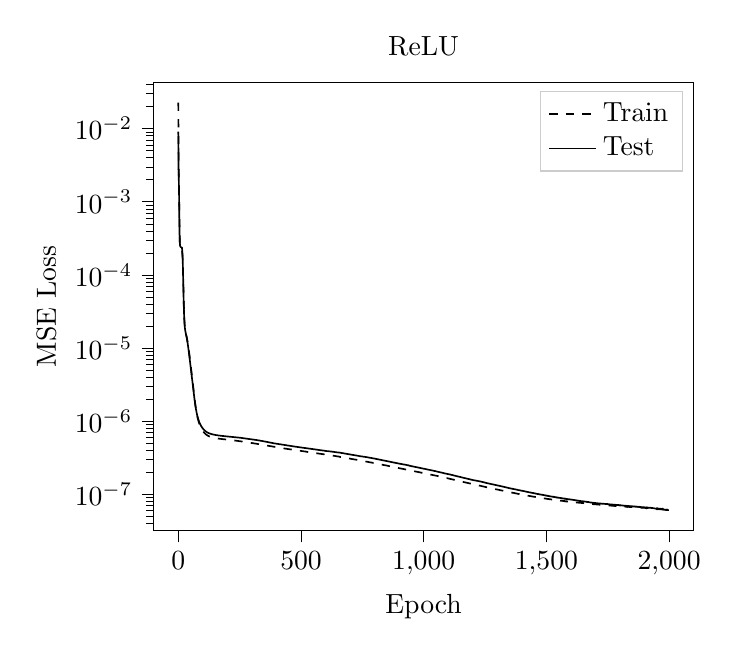
\begin{tikzpicture}

\begin{axis}[
legend cell align={left},
legend style={fill opacity=0.8, draw opacity=1, text opacity=1, draw=white!80!black},
log basis y={10},
tick align=outside,
tick pos=left,
title={ReLU},
x grid style={white!69.0196078431373!black},
xlabel={Epoch},
xmin=-99.95, xmax=2098.95,
xtick style={color=black},
y grid style={white!69.0196078431373!black},
ylabel={MSE Loss},
ymin=3.20662223104107e-08, ymax=0.0431121836135911,
ymode=log,
ytick style={color=black}
]
\addplot [semithick, black, dashed]
table {%
0 0.022700188562274
1 0.00488751665130258
2 0.00231159114837646
3 0.00169912100443617
4 0.000957429732894525
5 0.000457231870386749
6 0.000291163621441228
7 0.00023975450026046
8 0.000223350821892382
9 0.000217858722797246
10 0.000215660652000224
11 0.000214534028418711
12 0.000213661922316533
13 0.00021273185996688
14 0.0002116511244094
15 0.000210345065890579
16 0.000199949145098799
17 0.000182367857094505
18 0.000158941823407076
19 0.000125522568072483
20 9.05295221236884e-05
21 6.39946652263461e-05
22 4.61771607297123e-05
23 3.49678208767728e-05
24 2.79254836004839e-05
25 2.34756546597055e-05
26 2.06620919616398e-05
27 1.88729651317772e-05
28 1.76978199806399e-05
29 1.68716617790778e-05
30 1.62288936953701e-05
31 1.56760611562277e-05
32 1.5163152797868e-05
33 1.46647982219292e-05
34 1.41640936926706e-05
35 1.36524210238349e-05
36 1.3125367727298e-05
37 1.25840063737996e-05
38 1.20289051747022e-05
39 1.14638668196676e-05
40 1.08971444033159e-05
41 1.03354414623027e-05
42 9.78288087026158e-06
43 9.24360746557795e-06
44 8.71880347676779e-06
45 8.2212451234227e-06
46 7.7380116790664e-06
47 7.28033067434808e-06
48 6.83901115780827e-06
49 6.41160088571269e-06
50 6.00367025094783e-06
51 5.61681789690738e-06
52 5.25355912623127e-06
53 4.91812908012435e-06
54 4.60782127834136e-06
55 4.3184103076328e-06
56 4.04694739745537e-06
57 3.79198045425255e-06
58 3.55115817546903e-06
59 3.32267476801462e-06
60 3.10306129676974e-06
61 2.90025063634403e-06
62 2.71049544289781e-06
63 2.53316815292237e-06
64 2.36955519051207e-06
65 2.21743742019953e-06
66 2.07712799175397e-06
67 1.95007587785767e-06
68 1.83331815719612e-06
69 1.72713420909076e-06
70 1.63017052238956e-06
71 1.54295807112703e-06
72 1.46528206181529e-06
73 1.39492643029371e-06
74 1.33200299183045e-06
75 1.27552853570023e-06
76 1.22471883557296e-06
77 1.17950768247965e-06
78 1.13884168192158e-06
79 1.10184992811924e-06
80 1.06842147013708e-06
81 1.03816669236778e-06
82 1.01005816800637e-06
83 9.83902286947114e-07
84 9.59851741470175e-07
85 9.37582064864273e-07
86 9.17004300035273e-07
87 8.97869634414405e-07
88 8.80009910460444e-07
89 8.63493210744082e-07
90 8.48001840353163e-07
91 8.3358825983737e-07
92 8.20043752966626e-07
93 8.07293199883929e-07
94 7.95262972843602e-07
95 7.83745429529858e-07
96 7.73114619704529e-07
97 7.63112369000396e-07
98 7.53572947189696e-07
99 7.44605152732447e-07
100 7.36272040370523e-07
101 7.281094682412e-07
102 7.20398173484682e-07
103 7.13262888979216e-07
104 7.06426322636844e-07
105 7.00064532253464e-07
106 6.93946270104107e-07
107 6.88264223441593e-07
108 6.8279916240499e-07
109 6.77674996211408e-07
110 6.72629135380021e-07
111 6.67993809656764e-07
112 6.63566975617869e-07
113 6.59467331331598e-07
114 6.55476894593221e-07
115 6.51754040262631e-07
116 6.48160458922575e-07
117 6.44768821700836e-07
118 6.41538844462275e-07
119 6.38487625565176e-07
120 6.35543724314402e-07
121 6.32724531328677e-07
122 6.30082758760864e-07
123 6.27604565295314e-07
124 6.25200852027774e-07
125 6.22870618457227e-07
126 6.20655547663773e-07
127 6.1856236368385e-07
128 6.16603096204926e-07
129 6.14726157920131e-07
130 6.12881591251835e-07
131 6.11095928803707e-07
132 6.094500031395e-07
133 6.07855674729763e-07
134 6.06303832256572e-07
135 6.04832115925546e-07
136 6.03458678000379e-07
137 6.02132227385255e-07
138 6.00858143400274e-07
139 5.9959718061009e-07
140 5.9837970928811e-07
141 5.97201963586258e-07
142 5.96090518740766e-07
143 5.95010408943608e-07
144 5.94001013269008e-07
145 5.93005560261872e-07
146 5.92063210547167e-07
147 5.91099726932498e-07
148 5.90182496097214e-07
149 5.89293092502885e-07
150 5.88437146802789e-07
151 5.87599400262207e-07
152 5.8681417951334e-07
153 5.86040602939875e-07
154 5.85259042281905e-07
155 5.84521904073654e-07
156 5.83760592149929e-07
157 5.83063614556068e-07
158 5.82367442518716e-07
159 5.81692266450773e-07
160 5.81006480274482e-07
161 5.80357362707673e-07
162 5.79735073529264e-07
163 5.79122948920485e-07
164 5.78525290279686e-07
165 5.77992324991783e-07
166 5.77417234325139e-07
167 5.76792696477924e-07
168 5.7620480180276e-07
169 5.75622956091593e-07
170 5.75074705977841e-07
171 5.74554324572318e-07
172 5.74008320882058e-07
173 5.734738602996e-07
174 5.72948865794842e-07
175 5.72417692865201e-07
176 5.71913329963536e-07
177 5.71392262912696e-07
178 5.70892375463927e-07
179 5.70415385084289e-07
180 5.69933258077526e-07
181 5.69438252483678e-07
182 5.68800431778982e-07
183 5.68370158646303e-07
184 5.68008979342949e-07
185 5.67546451236467e-07
186 5.66942494856448e-07
187 5.66492348355041e-07
188 5.6600412295893e-07
189 5.65518306132162e-07
190 5.64976778179016e-07
191 5.64506119161479e-07
192 5.6400162551995e-07
193 5.63510650295029e-07
194 5.63028813928668e-07
195 5.62433123008077e-07
196 5.61948407408863e-07
197 5.61459071889203e-07
198 5.60965872949737e-07
199 5.60495189716903e-07
200 5.60018450130428e-07
201 5.59532428439979e-07
202 5.59046564546861e-07
203 5.58561763767784e-07
204 5.58075900073618e-07
205 5.57590778953454e-07
206 5.57100048496295e-07
207 5.56615983242636e-07
208 5.56132100513196e-07
209 5.55609417062897e-07
210 5.55238328246332e-07
211 5.54747902128838e-07
212 5.54302580724197e-07
213 5.53833328439168e-07
214 5.53333939876666e-07
215 5.52824435942512e-07
216 5.52326941345882e-07
217 5.51828715600777e-07
218 5.51342741459848e-07
219 5.50852281605785e-07
220 5.50354051654267e-07
221 5.49853959142865e-07
222 5.49354793690782e-07
223 5.48889128481278e-07
224 5.48412155978895e-07
225 5.47924545259093e-07
226 5.4743110911204e-07
227 5.46936913679019e-07
228 5.46444356729125e-07
229 5.459593782291e-07
230 5.45469382899455e-07
231 5.43948594668109e-07
232 5.43577015832852e-07
233 5.43141319894858e-07
234 5.42670150963431e-07
235 5.4215009910763e-07
236 5.41254978941197e-07
237 5.4071538048106e-07
238 5.40094552036408e-07
239 5.39584018270034e-07
240 5.39063721930688e-07
241 5.38529411954869e-07
242 5.37968243037312e-07
243 5.37392851640561e-07
244 5.36852313160807e-07
245 5.36285412920279e-07
246 5.3571522911966e-07
247 5.35140720330673e-07
248 5.3443252718921e-07
249 5.33878865127235e-07
250 5.33326285733438e-07
251 5.32710414972826e-07
252 5.32128201086834e-07
253 5.3153658973315e-07
254 5.30958579048502e-07
255 5.30392841596949e-07
256 5.29813738069151e-07
257 5.29206798432824e-07
258 5.28611251496613e-07
259 5.28013453390486e-07
260 5.2743299119129e-07
261 5.26832736454708e-07
262 5.26222398775644e-07
263 5.25642485285971e-07
264 5.25047771446907e-07
265 5.24451909285517e-07
266 5.23855538119733e-07
267 5.23260044928975e-07
268 5.22677574451791e-07
269 5.22101135715047e-07
270 5.21522106993189e-07
271 5.2093735595804e-07
272 5.20345230768271e-07
273 5.19757054604497e-07
274 5.19156453833602e-07
275 5.18550851836608e-07
276 5.17957335915753e-07
277 5.17369120132116e-07
278 5.16782020355322e-07
279 5.16200261699851e-07
280 5.15574804410335e-07
281 5.15027628523512e-07
282 5.14336931132675e-07
283 5.13758614488324e-07
284 5.13183472492074e-07
285 5.12594136750977e-07
286 5.12004632014396e-07
287 5.11429211314862e-07
288 5.10876843549113e-07
289 5.10237616765608e-07
290 5.09550439801387e-07
291 5.08979076613514e-07
292 5.0826299255391e-07
293 5.07674016262172e-07
294 5.07074047021661e-07
295 5.06488575894082e-07
296 5.0588200679158e-07
297 5.0527562575553e-07
298 5.04698802018311e-07
299 5.0409348091307e-07
300 5.03476895886479e-07
301 5.02873825212191e-07
302 5.02268338522072e-07
303 5.01660967728412e-07
304 5.0105952021795e-07
305 5.0045732720605e-07
306 4.99856223996176e-07
307 4.99265046613573e-07
308 4.98666331111508e-07
309 4.98066681245746e-07
310 4.97465910939354e-07
311 4.96871412508426e-07
312 4.96137432321575e-07
313 4.9553043635342e-07
314 4.94941312979336e-07
315 4.94267596906184e-07
316 4.93610437501957e-07
317 4.92980641354279e-07
318 4.92369693432693e-07
319 4.91739606502506e-07
320 4.91099409799744e-07
321 4.90437452043579e-07
322 4.89807230280803e-07
323 4.89186760347593e-07
324 4.88559287589396e-07
325 4.87941073032516e-07
326 4.87305083652245e-07
327 4.86687516229267e-07
328 4.86061624570766e-07
329 4.85449494334489e-07
330 4.84829064561154e-07
331 4.84218366892719e-07
332 4.8359940532805e-07
333 4.830153798423e-07
334 4.82397970387183e-07
335 4.81782221186222e-07
336 4.81173868649876e-07
337 4.80559737809472e-07
338 4.79956168504714e-07
339 4.79344355255762e-07
340 4.78806477559601e-07
341 4.78240154762943e-07
342 4.77609454350159e-07
343 4.77003219117478e-07
344 4.76402054232494e-07
345 4.75791388254265e-07
346 4.75013815588454e-07
347 4.74374429529689e-07
348 4.73760426586978e-07
349 4.72920066499682e-07
350 4.72309703241081e-07
351 4.71689676629694e-07
352 4.71041691099572e-07
353 4.70393082395049e-07
354 4.69757620095379e-07
355 4.69146253209374e-07
356 4.68521187315218e-07
357 4.67862831214916e-07
358 4.67246957327916e-07
359 4.66614568154e-07
360 4.65985684172665e-07
361 4.6536224317606e-07
362 4.64654443277368e-07
363 4.64017372877379e-07
364 4.63376583951458e-07
365 4.62768628437971e-07
366 4.62145839122741e-07
367 4.61530419244127e-07
368 4.6089009126149e-07
369 4.60264819025724e-07
370 4.59625250016416e-07
371 4.58993519600881e-07
372 4.5837571519769e-07
373 4.57772132591572e-07
374 4.57149062043527e-07
375 4.5654107344717e-07
376 4.56388565879706e-07
377 4.55734816853237e-07
378 4.55108889241274e-07
379 4.54509474423048e-07
380 4.5388417871095e-07
381 4.53284295474532e-07
382 4.52677932457846e-07
383 4.52075946668629e-07
384 4.51512100482887e-07
385 4.50870240143786e-07
386 4.50251420318182e-07
387 4.49643324799354e-07
388 4.49040381340637e-07
389 4.48442889108946e-07
390 4.47849138907941e-07
391 4.47228694440582e-07
392 4.46672484287092e-07
393 4.461130256459e-07
394 4.45521277072203e-07
395 4.44942966254303e-07
396 4.44365371606636e-07
397 4.43792268384868e-07
398 4.43272579076392e-07
399 4.42683609037431e-07
400 4.42047175965854e-07
401 4.41511416170215e-07
402 4.40903476572885e-07
403 4.40345714878276e-07
404 4.3987389551603e-07
405 4.39265694041069e-07
406 4.38643700221064e-07
407 4.380702063429e-07
408 4.37512944046148e-07
409 4.36928924386848e-07
410 4.3640052246019e-07
411 4.35823328899687e-07
412 4.35215195849992e-07
413 4.34667989864579e-07
414 4.34115721304806e-07
415 4.33525133956891e-07
416 4.33020327989198e-07
417 4.32479380691575e-07
418 4.31893973825481e-07
419 4.31408940585243e-07
420 4.30838680827605e-07
421 4.30306989400719e-07
422 4.29754458110665e-07
423 4.29197023592565e-07
424 4.28708979058001e-07
425 4.28179310091537e-07
426 4.27645871525328e-07
427 4.27122201074326e-07
428 4.26600456847837e-07
429 4.26098265279506e-07
430 4.25582650322553e-07
431 4.25064716353063e-07
432 4.24552743652384e-07
433 4.24046018068225e-07
434 4.23532201423882e-07
435 4.23018083807847e-07
436 4.22497343777195e-07
437 4.22003586905362e-07
438 4.21473392307803e-07
439 4.20917969989887e-07
440 4.20440635949149e-07
441 4.19875405299308e-07
442 4.19363955217023e-07
443 4.18853888447757e-07
444 4.18352119027077e-07
445 4.17849264920278e-07
446 4.17325928665946e-07
447 4.16844640056979e-07
448 4.16344165444116e-07
449 4.15880111347633e-07
450 4.15396516785904e-07
451 4.14893772202163e-07
452 4.14433901823941e-07
453 4.13930885599711e-07
454 4.13483039750417e-07
455 4.13017433587015e-07
456 4.1257212623691e-07
457 4.12095013999192e-07
458 4.11657128623233e-07
459 4.11228072835002e-07
460 4.10708955925543e-07
461 4.10184199338914e-07
462 4.09730133469566e-07
463 4.09255900592598e-07
464 4.08744348931123e-07
465 4.08305826397282e-07
466 4.07791080348829e-07
467 4.07319028909114e-07
468 4.06846871413791e-07
469 4.06389932322782e-07
470 4.05920714698027e-07
471 4.05562731955911e-07
472 4.05092885813474e-07
473 4.0462468440694e-07
474 4.04162996773039e-07
475 4.03698307593459e-07
476 4.03226065685658e-07
477 4.02781851548184e-07
478 4.02340750596863e-07
479 4.01872257114633e-07
480 4.01436150028189e-07
481 4.00995583561325e-07
482 4.00542615494714e-07
483 4.00105648267868e-07
484 3.9966176110795e-07
485 3.99214384003699e-07
486 3.98767849290493e-07
487 3.98336208618844e-07
488 3.97897648582557e-07
489 3.97436830553488e-07
490 3.97029553994344e-07
491 3.96565684638972e-07
492 3.96169267048663e-07
493 3.95707022320835e-07
494 3.95289122536724e-07
495 3.94852195327644e-07
496 3.94419814639946e-07
497 3.93999079605578e-07
498 3.93570346247429e-07
499 3.9315561880926e-07
500 3.92716066883736e-07
501 3.92287240870814e-07
502 3.91878817822544e-07
503 3.91442989226221e-07
504 3.91023176774752e-07
505 3.9062641165799e-07
506 3.90210046802508e-07
507 3.89796826127053e-07
508 3.89384892272915e-07
509 3.88973414260363e-07
510 3.88556969866727e-07
511 3.88143236861538e-07
512 3.87750533690223e-07
513 3.87334687218299e-07
514 3.86922011443858e-07
515 3.86537839034418e-07
516 3.86145166501706e-07
517 3.85737681369847e-07
518 3.85339201272927e-07
519 3.8487991605507e-07
520 3.83903953405706e-07
521 3.82987367999021e-07
522 3.82452104588538e-07
523 3.81951715240802e-07
524 3.81474649344682e-07
525 3.81002873993452e-07
526 3.80536858187952e-07
527 3.80074700913724e-07
528 3.79651768199096e-07
529 3.79191619771291e-07
530 3.78739784309801e-07
531 3.78291494698146e-07
532 3.77857477459997e-07
533 3.77393390778025e-07
534 3.76971358065248e-07
535 3.7652833098889e-07
536 3.76109584294682e-07
537 3.75679046470623e-07
538 3.75253116985164e-07
539 3.74808345085853e-07
540 3.7454908161294e-07
541 3.7414445736772e-07
542 3.73729084628849e-07
543 3.73336543063374e-07
544 3.72864065653289e-07
545 3.72388690294656e-07
546 3.71936408129159e-07
547 3.7159253486152e-07
548 3.71120514557788e-07
549 3.7070167992681e-07
550 3.70296510155299e-07
551 3.69914672049276e-07
552 3.69459091174917e-07
553 3.69037342807133e-07
554 3.68648538355387e-07
555 3.6825909458571e-07
556 3.67811100034032e-07
557 3.67427050235847e-07
558 3.66991696012064e-07
559 3.66619650719713e-07
560 3.66189225928792e-07
561 3.65861811559398e-07
562 3.65376562385222e-07
563 3.65019601645145e-07
564 3.64580547127957e-07
565 3.64211771625378e-07
566 3.63786553577938e-07
567 3.63422670105251e-07
568 3.62993843239678e-07
569 3.62630070128489e-07
570 3.62208776891748e-07
571 3.61848602025816e-07
572 3.61434043114173e-07
573 3.61033925202037e-07
574 3.60626449435131e-07
575 3.60239536490781e-07
576 3.5982089400477e-07
577 3.59459390324446e-07
578 3.59027224121178e-07
579 3.58637733910427e-07
580 3.58265337851549e-07
581 3.57837911053593e-07
582 3.57462955719257e-07
583 3.57044090065983e-07
584 3.56651212896963e-07
585 3.56281235312395e-07
586 3.55858100661521e-07
587 3.55473218320412e-07
588 3.55106093834934e-07
589 3.54690216738618e-07
590 3.54296942276733e-07
591 3.53912689618596e-07
592 3.53498191117296e-07
593 3.53113810746208e-07
594 3.52725243871532e-07
595 3.52314408615939e-07
596 3.51911630289692e-07
597 3.51522282898031e-07
598 3.51117687088731e-07
599 3.50752920624586e-07
600 3.50220982767269e-07
601 3.49666113038438e-07
602 3.49216980467304e-07
603 3.48912888597397e-07
604 3.48590493985057e-07
605 3.48156322104387e-07
606 3.47782955444131e-07
607 3.47431346924054e-07
608 3.47023016885828e-07
609 3.46650842232066e-07
610 3.46283607186138e-07
611 3.45864262101259e-07
612 3.45506151319341e-07
613 3.45193046385361e-07
614 3.44725366304033e-07
615 3.44399749494073e-07
616 3.43981475197097e-07
617 3.43586984797639e-07
618 3.43181904270295e-07
619 3.42802305496548e-07
620 3.42403075336506e-07
621 3.41977504575652e-07
622 3.4155453653284e-07
623 3.4121790288566e-07
624 3.40786421261896e-07
625 3.40369527535245e-07
626 3.40017924912672e-07
627 3.39533942778303e-07
628 3.39218749374481e-07
629 3.38775148605919e-07
630 3.38400936499283e-07
631 3.37982899594635e-07
632 3.37605371441896e-07
633 3.37170312434409e-07
634 3.36797599160832e-07
635 3.36361521405593e-07
636 3.35930654614458e-07
637 3.3559160269192e-07
638 3.35204049008553e-07
639 3.34756528133084e-07
640 3.34375308568724e-07
641 3.33965574611739e-07
642 3.33506915836779e-07
643 3.33132214549892e-07
644 3.32628377762489e-07
645 3.32194951340625e-07
646 3.31808428924774e-07
647 3.31448711378357e-07
648 3.30991560645089e-07
649 3.30627948002871e-07
650 3.30129058355055e-07
651 3.29814938055506e-07
652 3.29351685039114e-07
653 3.28992725826538e-07
654 3.28530313112196e-07
655 3.28124250728479e-07
656 3.27338606993521e-07
657 3.2631718342202e-07
658 3.25590172181478e-07
659 3.25028652142123e-07
660 3.24517025873661e-07
661 3.24045561214348e-07
662 3.23632035957644e-07
663 3.23333612456622e-07
664 3.22835817087253e-07
665 3.22464504492359e-07
666 3.22048187427981e-07
667 3.21377591362193e-07
668 3.21208086006663e-07
669 3.20661421767454e-07
670 3.20358596013648e-07
671 3.19621063596287e-07
672 3.1945258629662e-07
673 3.19104954499494e-07
674 3.18600724384055e-07
675 3.18192904686043e-07
676 3.17710430906004e-07
677 3.17364652957508e-07
678 3.16877777223112e-07
679 3.16538145668233e-07
680 3.15970995160342e-07
681 3.1567109923003e-07
682 3.15297038284257e-07
683 3.14813742392062e-07
684 3.14474320148861e-07
685 3.13978635006151e-07
686 3.13667648967453e-07
687 3.13245961862663e-07
688 3.12820861438468e-07
689 3.12397660195529e-07
690 3.1198839221247e-07
691 3.11556838838101e-07
692 3.11143778816358e-07
693 3.10705394213073e-07
694 3.10293124186956e-07
695 3.09892371817e-07
696 3.09461834291369e-07
697 3.090517145381e-07
698 3.08666699567084e-07
699 3.0822698936106e-07
700 3.07806382778608e-07
701 3.07389098040289e-07
702 3.06976017242278e-07
703 3.06563772056734e-07
704 3.06163985612784e-07
705 3.05730360267376e-07
706 3.05273673447459e-07
707 3.04876716270996e-07
708 3.0442998618696e-07
709 3.04035280080939e-07
710 3.03622769806111e-07
711 3.03206509087772e-07
712 3.02812567170463e-07
713 3.02440707557139e-07
714 3.0202642422239e-07
715 3.01613633979514e-07
716 3.01198510896938e-07
717 3.00822865682449e-07
718 3.00429866129548e-07
719 3.00004258420472e-07
720 2.99603975577156e-07
721 2.99221630228885e-07
722 2.98811836827895e-07
723 2.98403452376306e-07
724 2.97989905206464e-07
725 2.9759956366604e-07
726 2.97187501331564e-07
727 2.9681355476896e-07
728 2.96412470021323e-07
729 2.9606505475499e-07
730 2.95635467878697e-07
731 2.952455811851e-07
732 2.94848240571355e-07
733 2.94465938836197e-07
734 2.94049225601611e-07
735 2.93639906388421e-07
736 2.93226357769072e-07
737 2.92796839545417e-07
738 2.92297765568605e-07
739 2.91883827330253e-07
740 2.91480768723318e-07
741 2.910785553496e-07
742 2.90658661256771e-07
743 2.90242410954988e-07
744 2.89850709691564e-07
745 2.89458642981799e-07
746 2.89041936454737e-07
747 2.8864057620126e-07
748 2.88227141510333e-07
749 2.87827345815117e-07
750 2.87087919858209e-07
751 2.86751240196281e-07
752 2.86329326087298e-07
753 2.8591025268554e-07
754 2.85439217833527e-07
755 2.85030032486588e-07
756 2.84653017843084e-07
757 2.84204375958552e-07
758 2.8389503138726e-07
759 2.83434894626566e-07
760 2.83027217491849e-07
761 2.82583373746093e-07
762 2.82166798484695e-07
763 2.81779251295688e-07
764 2.81361878322173e-07
765 2.8097022681095e-07
766 2.80527259462815e-07
767 2.80156977623847e-07
768 2.79733914808844e-07
769 2.79341120162258e-07
770 2.78916435533461e-07
771 2.78528162013458e-07
772 2.78141511387275e-07
773 2.77702974685212e-07
774 2.77305605408174e-07
775 2.76901424754783e-07
776 2.76503712527187e-07
777 2.7608817458713e-07
778 2.75728598765568e-07
779 2.75243042580087e-07
780 2.74894716326912e-07
781 2.74454094579823e-07
782 2.74069144126088e-07
783 2.73722769037477e-07
784 2.73352229129387e-07
785 2.72916203726936e-07
786 2.72518787539866e-07
787 2.72107046171755e-07
788 2.71700535861896e-07
789 2.71388373164427e-07
790 2.70878778209749e-07
791 2.70506326188524e-07
792 2.70099734180462e-07
793 2.69743341803519e-07
794 2.69326202285924e-07
795 2.68931778975912e-07
796 2.68559697474302e-07
797 2.68128451239136e-07
798 2.67776407085307e-07
799 2.67330760422624e-07
800 2.66969742384049e-07
801 2.66559677882583e-07
802 2.66164721722362e-07
803 2.65812256472486e-07
804 2.65400530011561e-07
805 2.6502757293656e-07
806 2.6449244508342e-07
807 2.6412419380506e-07
808 2.637580061986e-07
809 2.63452051655122e-07
810 2.63053868408747e-07
811 2.62594155017837e-07
812 2.62013144990192e-07
813 2.6193533845742e-07
814 2.61439927285778e-07
815 2.61018644366118e-07
816 2.60627871526253e-07
817 2.60260550476232e-07
818 2.59689900460103e-07
819 2.59417914975302e-07
820 2.59006644839133e-07
821 2.58626036824694e-07
822 2.58218586338899e-07
823 2.57673533738512e-07
824 2.57433976102561e-07
825 2.57017506498869e-07
826 2.5667790622208e-07
827 2.56154501016681e-07
828 2.55826516465163e-07
829 2.55293243981214e-07
830 2.54911673962965e-07
831 2.54528044095537e-07
832 2.54085345531507e-07
833 2.53902755346758e-07
834 2.53358927992053e-07
835 2.52917493085647e-07
836 2.5258387552185e-07
837 2.52187130001857e-07
838 2.51844215142682e-07
839 2.51351500949681e-07
840 2.51175747990828e-07
841 2.50791280407725e-07
842 2.50371872652977e-07
843 2.50073024140818e-07
844 2.49660933910434e-07
845 2.49289074517378e-07
846 2.48766987951399e-07
847 2.48441512184172e-07
848 2.48069631027192e-07
849 2.47699301219484e-07
850 2.47161033726684e-07
851 2.46826250588583e-07
852 2.46495931811808e-07
853 2.46035868663341e-07
854 2.45723502651174e-07
855 2.45256004326677e-07
856 2.44975971384065e-07
857 2.44433341421768e-07
858 2.44034814478766e-07
859 2.43581715018593e-07
860 2.43168417568995e-07
861 2.4271100485862e-07
862 2.42337396841208e-07
863 2.42082812036415e-07
864 2.41691652966836e-07
865 2.41245197074136e-07
866 2.40857210400236e-07
867 2.40553402242938e-07
868 2.40142219510631e-07
869 2.39735860347423e-07
870 2.39412173904441e-07
871 2.38961034234819e-07
872 2.38645971329277e-07
873 2.38238824422865e-07
874 2.37809563216729e-07
875 2.3733263120107e-07
876 2.37218382366677e-07
877 2.36820149837058e-07
878 2.36251832234302e-07
879 2.35994000377104e-07
880 2.35550381091798e-07
881 2.35120832542179e-07
882 2.34883657554974e-07
883 2.3447071255589e-07
884 2.34056571045471e-07
885 2.33667837314044e-07
886 2.33339260311993e-07
887 2.33093831027986e-07
888 2.32603948909116e-07
889 2.32233412184257e-07
890 2.32004902379401e-07
891 2.31429368355407e-07
892 2.3114651683187e-07
893 2.30785587632454e-07
894 2.30509334691931e-07
895 2.30057152329266e-07
896 2.29823544458441e-07
897 2.29321314293429e-07
898 2.28995329422332e-07
899 2.28720500601298e-07
900 2.2819258192186e-07
901 2.27982340113897e-07
902 2.27608680532398e-07
903 2.27211997810173e-07
904 2.26988304923736e-07
905 2.26444428335526e-07
906 2.26198868467975e-07
907 2.25855826890609e-07
908 2.2550042169911e-07
909 2.25155414788958e-07
910 2.24715623417637e-07
911 2.24441779643314e-07
912 2.24117695772463e-07
913 2.23662403364244e-07
914 2.23525080990328e-07
915 2.22978478866764e-07
916 2.22644433506503e-07
917 2.22354079696174e-07
918 2.22075732409621e-07
919 2.216284795864e-07
920 2.21327834964313e-07
921 2.21020898472091e-07
922 2.20529991381113e-07
923 2.20361902080413e-07
924 2.20030540255323e-07
925 2.19693687718348e-07
926 2.19355493747742e-07
927 2.18912160406148e-07
928 2.18688205620765e-07
929 2.18431814289488e-07
930 2.17975239991119e-07
931 2.17582416240703e-07
932 2.17388809041097e-07
933 2.1695414856282e-07
934 2.16690200510072e-07
935 2.16351949184457e-07
936 2.16095488674739e-07
937 2.15770156167139e-07
938 2.14990478731636e-07
939 2.14787864763366e-07
940 2.1443938268817e-07
941 2.14009426784401e-07
942 2.13876116731626e-07
943 2.13514506633317e-07
944 2.13116627740817e-07
945 2.12705434734062e-07
946 2.12403169662423e-07
947 2.12224187748689e-07
948 2.11859084011223e-07
949 2.11378808906204e-07
950 2.11102361483029e-07
951 2.10801352842793e-07
952 2.10461757689018e-07
953 2.10099717612877e-07
954 2.09749843882889e-07
955 2.09436833515042e-07
956 2.08886092458727e-07
957 2.08831142565202e-07
958 2.08371006181096e-07
959 2.08050646740787e-07
960 2.07822948567582e-07
961 2.07486869925333e-07
962 2.07112270111054e-07
963 2.06741844017699e-07
964 2.06521825781181e-07
965 2.06087915294972e-07
966 2.05930061810022e-07
967 2.05545380552508e-07
968 2.05069629963361e-07
969 2.04830868973715e-07
970 2.04720518375723e-07
971 2.04201579762753e-07
972 2.03760819481147e-07
973 2.03723517330445e-07
974 2.03153470287987e-07
975 2.02952266192824e-07
976 2.0258793077943e-07
977 2.02278263678579e-07
978 2.02042518324674e-07
979 2.01851433075717e-07
980 2.01159917573079e-07
981 2.01093053725288e-07
982 2.00630439998406e-07
983 2.00379565200137e-07
984 2.00104684502378e-07
985 1.99714410634044e-07
986 1.99583829243011e-07
987 1.99082864192235e-07
988 1.98879871078361e-07
989 1.9851004941529e-07
990 1.98118672258829e-07
991 1.97794862813794e-07
992 1.97514059898651e-07
993 1.97439506180785e-07
994 1.96882988724667e-07
995 1.96863558301175e-07
996 1.96450931930769e-07
997 1.95994219325257e-07
998 1.95664951903041e-07
999 1.95385722300045e-07
1000 1.95022169748427e-07
1001 1.94833854649801e-07
1002 1.94470195005181e-07
1003 1.94122655358342e-07
1004 1.9388446521873e-07
1005 1.93533067992746e-07
1006 1.93328063083698e-07
1007 1.92964109508864e-07
1008 1.92854989641944e-07
1009 1.92244884203774e-07
1010 1.92150149644021e-07
1011 1.91683977945445e-07
1012 1.91481523557968e-07
1013 1.91099812219875e-07
1014 1.90797521028685e-07
1015 1.90380861127437e-07
1016 1.90235854056198e-07
1017 1.89877648772097e-07
1018 1.89494576162019e-07
1019 1.89354932544461e-07
1020 1.89023202793237e-07
1021 1.88638987530965e-07
1022 1.88445211605881e-07
1023 1.88153857600071e-07
1024 1.8789166674793e-07
1025 1.87497277877924e-07
1026 1.87139091707422e-07
1027 1.86948059244685e-07
1028 1.86557873902871e-07
1029 1.8624394212452e-07
1030 1.86015578215404e-07
1031 1.85666344684421e-07
1032 1.85445209389457e-07
1033 1.85054166387033e-07
1034 1.84846604049937e-07
1035 1.84483662977186e-07
1036 1.84172586372711e-07
1037 1.83920614389876e-07
1038 1.83583266078813e-07
1039 1.83318241170127e-07
1040 1.82997070702129e-07
1041 1.83021538092021e-07
1042 1.82458206694491e-07
1043 1.82058361751558e-07
1044 1.82028634412745e-07
1045 1.81618637533632e-07
1046 1.81205257824502e-07
1047 1.80903678263178e-07
1048 1.80594445531312e-07
1049 1.80465957818399e-07
1050 1.80246385575344e-07
1051 1.79967734062814e-07
1052 1.79636884041656e-07
1053 1.79177664357155e-07
1054 1.79063932307599e-07
1055 1.78691587770174e-07
1056 1.78408368206817e-07
1057 1.78004216500938e-07
1058 1.77813854492115e-07
1059 1.77428909594823e-07
1060 1.77236690916516e-07
1061 1.76722042020572e-07
1062 1.76449690165725e-07
1063 1.76021288552874e-07
1064 1.75829625440826e-07
1065 1.75640696625123e-07
1066 1.75241006722615e-07
1067 1.75162156935471e-07
1068 1.74642103651479e-07
1069 1.74417626588763e-07
1070 1.7404266374399e-07
1071 1.73703341644682e-07
1072 1.73558491709969e-07
1073 1.73160420480656e-07
1074 1.72957526480388e-07
1075 1.72599468157841e-07
1076 1.72251352061892e-07
1077 1.71990737428018e-07
1078 1.7171713331976e-07
1079 1.71403443800955e-07
1080 1.71083066689448e-07
1081 1.70797444916104e-07
1082 1.70402340685882e-07
1083 1.70148245288715e-07
1084 1.69917028038924e-07
1085 1.69586333520044e-07
1086 1.69357113584567e-07
1087 1.69163682642193e-07
1088 1.686814187849e-07
1089 1.68399768192273e-07
1090 1.68089013364181e-07
1091 1.67893452029944e-07
1092 1.67585903092515e-07
1093 1.67222312761339e-07
1094 1.67059804290659e-07
1095 1.66649184230039e-07
1096 1.66450206698698e-07
1097 1.66033636610052e-07
1098 1.65722943663127e-07
1099 1.65424200780251e-07
1100 1.65225882462039e-07
1101 1.64985739466772e-07
1102 1.64698448095635e-07
1103 1.64395809392204e-07
1104 1.64084958875321e-07
1105 1.63677839154275e-07
1106 1.63496802393581e-07
1107 1.63082423547678e-07
1108 1.62798604314673e-07
1109 1.62522797900522e-07
1110 1.62237442324908e-07
1111 1.61953103585688e-07
1112 1.61745482145648e-07
1113 1.61444047385828e-07
1114 1.61156203638768e-07
1115 1.60849461522616e-07
1116 1.60548210331513e-07
1117 1.60125507292719e-07
1118 1.60022549835048e-07
1119 1.59726342381816e-07
1120 1.59424678358278e-07
1121 1.59032878435994e-07
1122 1.5872759782809e-07
1123 1.58415958168234e-07
1124 1.58145775252194e-07
1125 1.57837064953981e-07
1126 1.57546023409338e-07
1127 1.57264251292588e-07
1128 1.56991482583635e-07
1129 1.56779749318048e-07
1130 1.56375693713073e-07
1131 1.56187677539776e-07
1132 1.55840182010536e-07
1133 1.55556436844506e-07
1134 1.55273407109746e-07
1135 1.54998702655007e-07
1136 1.54711072703151e-07
1137 1.54432117184911e-07
1138 1.54145230403913e-07
1139 1.53878085860981e-07
1140 1.53617322077082e-07
1141 1.5333499228376e-07
1142 1.53051926098158e-07
1143 1.52785489710539e-07
1144 1.52522081414475e-07
1145 1.52248115853126e-07
1146 1.51964569326424e-07
1147 1.51719455871557e-07
1148 1.51469372077884e-07
1149 1.5122538536616e-07
1150 1.50974027228301e-07
1151 1.5071920294929e-07
1152 1.50436781574115e-07
1153 1.50154852306628e-07
1154 1.4994000232349e-07
1155 1.49684689617402e-07
1156 1.49378274763023e-07
1157 1.49107717653862e-07
1158 1.48837879095254e-07
1159 1.48464723778829e-07
1160 1.48321392124728e-07
1161 1.4794774750726e-07
1162 1.47731350878644e-07
1163 1.47506493782146e-07
1164 1.47181220476966e-07
1165 1.46966620775402e-07
1166 1.4667185742212e-07
1167 1.46446925676003e-07
1168 1.46194616810647e-07
1169 1.4589142892163e-07
1170 1.45623083163571e-07
1171 1.45421855407335e-07
1172 1.45148988735855e-07
1173 1.44924273733693e-07
1174 1.44653323587818e-07
1175 1.44397603683899e-07
1176 1.44143922561568e-07
1177 1.43887481556249e-07
1178 1.43637580052314e-07
1179 1.43380571216767e-07
1180 1.43128617793309e-07
1181 1.42918179754759e-07
1182 1.42674865678316e-07
1183 1.42368941268956e-07
1184 1.42143107957793e-07
1185 1.4187803487431e-07
1186 1.41659683009721e-07
1187 1.41389330686081e-07
1188 1.41146314824425e-07
1189 1.40885177728478e-07
1190 1.40635690385693e-07
1191 1.40369184080669e-07
1192 1.4014046066535e-07
1193 1.39883951696618e-07
1194 1.39747466739948e-07
1195 1.39369158453917e-07
1196 1.39117702971703e-07
1197 1.38906298772667e-07
1198 1.38654130978466e-07
1199 1.38412876140137e-07
1200 1.38177429242603e-07
1201 1.37951588143892e-07
1202 1.37698481808002e-07
1203 1.37433328326608e-07
1204 1.3724076173105e-07
1205 1.36967428325363e-07
1206 1.36749351263177e-07
1207 1.36498041356958e-07
1208 1.36307488340037e-07
1209 1.36027240721148e-07
1210 1.35778096570505e-07
1211 1.35560142766167e-07
1212 1.35304345839415e-07
1213 1.35079826662832e-07
1214 1.34833428923287e-07
1215 1.34616434678492e-07
1216 1.34399582798039e-07
1217 1.34197129121105e-07
1218 1.33883571521665e-07
1219 1.33696930035399e-07
1220 1.3346163827066e-07
1221 1.33249577636718e-07
1222 1.33005609590953e-07
1223 1.32781584980535e-07
1224 1.32541664960684e-07
1225 1.32347305886071e-07
1226 1.32063615318145e-07
1227 1.31870969095615e-07
1228 1.31660141718726e-07
1229 1.31428233174802e-07
1230 1.31200933161324e-07
1231 1.30952666729911e-07
1232 1.30717070817354e-07
1233 1.30495742848069e-07
1234 1.30259482844508e-07
1235 1.30022995147527e-07
1236 1.29781844254495e-07
1237 1.29581289883163e-07
1238 1.29348568975729e-07
1239 1.29130822966061e-07
1240 1.28877546259787e-07
1241 1.28684132853607e-07
1242 1.28452740526086e-07
1243 1.28231625510011e-07
1244 1.27987654604311e-07
1245 1.27740676120425e-07
1246 1.27538427442175e-07
1247 1.27307380335395e-07
1248 1.27056580915053e-07
1249 1.26827521665263e-07
1250 1.26586416879348e-07
1251 1.26406430311476e-07
1252 1.26152649176703e-07
1253 1.25956614589029e-07
1254 1.25715322532471e-07
1255 1.25495106999551e-07
1256 1.25293443446139e-07
1257 1.25028746005285e-07
1258 1.24901299987101e-07
1259 1.24626029101904e-07
1260 1.24430453901425e-07
1261 1.24176776623131e-07
1262 1.24055122398659e-07
1263 1.23799583203521e-07
1264 1.23607713689466e-07
1265 1.23352822342326e-07
1266 1.23219754268433e-07
1267 1.22982637506652e-07
1268 1.22764353839955e-07
1269 1.22587649372008e-07
1270 1.2240252546647e-07
1271 1.22168687340718e-07
1272 1.219725873014e-07
1273 1.21779319677273e-07
1274 1.21563253291157e-07
1275 1.21380381088443e-07
1276 1.21160043512702e-07
1277 1.20952420175513e-07
1278 1.20760240989171e-07
1279 1.20553010624747e-07
1280 1.20351129286433e-07
1281 1.20143024023633e-07
1282 1.19957552684014e-07
1283 1.19751850760963e-07
1284 1.19543746681217e-07
1285 1.19330061487233e-07
1286 1.19149103294802e-07
1287 1.18953276412981e-07
1288 1.18748600737462e-07
1289 1.18555770459494e-07
1290 1.18364916058766e-07
1291 1.1817159390759e-07
1292 1.17976144718313e-07
1293 1.1778769242099e-07
1294 1.17580557674302e-07
1295 1.17392635566205e-07
1296 1.17181604338157e-07
1297 1.1700705573503e-07
1298 1.16808877251628e-07
1299 1.16613071952543e-07
1300 1.16419120878675e-07
1301 1.16225622392108e-07
1302 1.1603226114687e-07
1303 1.15844357804207e-07
1304 1.15657821531556e-07
1305 1.15457035366973e-07
1306 1.15278685957065e-07
1307 1.15126645564345e-07
1308 1.14942082795721e-07
1309 1.14750936365482e-07
1310 1.14571220436233e-07
1311 1.14396584468324e-07
1312 1.14194506771526e-07
1313 1.14016975611975e-07
1314 1.13832922327362e-07
1315 1.13644045871553e-07
1316 1.13458538987032e-07
1317 1.13274990312107e-07
1318 1.13083245398826e-07
1319 1.12902683433447e-07
1320 1.12720184169746e-07
1321 1.12537894811027e-07
1322 1.12350661094496e-07
1323 1.12174550807254e-07
1324 1.12134164076849e-07
1325 1.11870243223677e-07
1326 1.11684696662451e-07
1327 1.11496924954935e-07
1328 1.11313580546835e-07
1329 1.11118610341521e-07
1330 1.10941907703221e-07
1331 1.10745624390063e-07
1332 1.10565157594777e-07
1333 1.10391883758609e-07
1334 1.10216272570796e-07
1335 1.10034027901662e-07
1336 1.09904966944185e-07
1337 1.0972478612814e-07
1338 1.09543823189284e-07
1339 1.09353221706243e-07
1340 1.09189787515618e-07
1341 1.0900702273986e-07
1342 1.08871806606459e-07
1343 1.08658014781327e-07
1344 1.08535055574066e-07
1345 1.08302015139117e-07
1346 1.08116574203621e-07
1347 1.07938734316804e-07
1348 1.07767203992637e-07
1349 1.07630161124916e-07
1350 1.07411750210673e-07
1351 1.07216842348379e-07
1352 1.07049617742661e-07
1353 1.06965064308184e-07
1354 1.06737143919844e-07
1355 1.06572572189378e-07
1356 1.06429018249088e-07
1357 1.06255565668789e-07
1358 1.0609248306892e-07
1359 1.05914943159036e-07
1360 1.05769115879895e-07
1361 1.05555923461509e-07
1362 1.05343500887756e-07
1363 1.05336002874878e-07
1364 1.05065406970084e-07
1365 1.05018041523408e-07
1366 1.04834425311395e-07
1367 1.04657920751094e-07
1368 1.04446422334092e-07
1369 1.04306719531877e-07
1370 1.04136361159135e-07
1371 1.03937797071296e-07
1372 1.03782853386747e-07
1373 1.03633022288108e-07
1374 1.034524386192e-07
1375 1.03303142903854e-07
1376 1.03129766664267e-07
1377 1.02965245194042e-07
1378 1.02805888491986e-07
1379 1.02640688677269e-07
1380 1.02496613894942e-07
1381 1.0232278171074e-07
1382 1.02182824353036e-07
1383 1.02012176419919e-07
1384 1.01840164518308e-07
1385 1.01737134052371e-07
1386 1.01551659998478e-07
1387 1.01374999886161e-07
1388 1.01288831718449e-07
1389 1.01124216129733e-07
1390 1.00975371992718e-07
1391 1.00811491311248e-07
1392 1.00633754545498e-07
1393 1.00503078154901e-07
1394 1.00330592847087e-07
1395 1.00212100541341e-07
1396 1.00035348715721e-07
1397 9.98977622650443e-08
1398 9.97419698371971e-08
1399 9.96092331497778e-08
1400 9.94421753084396e-08
1401 9.93241543625345e-08
1402 9.91819209836819e-08
1403 9.8997636012399e-08
1404 9.8858772627608e-08
1405 9.87074338247851e-08
1406 9.8565545286533e-08
1407 9.84226947515765e-08
1408 9.82687273456406e-08
1409 9.81530818080501e-08
1410 9.80001015236098e-08
1411 9.78618616542803e-08
1412 9.77315958152758e-08
1413 9.75798045423915e-08
1414 9.74417762549251e-08
1415 9.7294861614472e-08
1416 9.71628285846293e-08
1417 9.7036684380214e-08
1418 9.68920721362565e-08
1419 9.68428053553794e-08
1420 9.65617320929368e-08
1421 9.65015172482708e-08
1422 9.63498855988121e-08
1423 9.61964877745913e-08
1424 9.6049520042385e-08
1425 9.58933131407491e-08
1426 9.58726888740102e-08
1427 9.56149151214447e-08
1428 9.55419418744441e-08
1429 9.53950836333206e-08
1430 9.53688893758908e-08
1431 9.51055585893812e-08
1432 9.50164821347244e-08
1433 9.48658110893064e-08
1434 9.48242855329795e-08
1435 9.45683539228526e-08
1436 9.44814399588267e-08
1437 9.43536782749277e-08
1438 9.43120517149509e-08
1439 9.40272916558626e-08
1440 9.39600227454207e-08
1441 9.3908410100596e-08
1442 9.36157606439281e-08
1443 9.35820834726542e-08
1444 9.35358044351631e-08
1445 9.32975007934545e-08
1446 9.31823757319705e-08
1447 9.30778284597977e-08
1448 9.30286952893766e-08
1449 9.27425326793241e-08
1450 9.27090496922744e-08
1451 9.26503111458032e-08
1452 9.24670470858757e-08
1453 9.23490937658755e-08
1454 9.23282061755515e-08
1455 9.20449279320223e-08
1456 9.19874992746372e-08
1457 9.19312404228378e-08
1458 9.18109127283628e-08
1459 9.16913846964462e-08
1460 9.15665439293889e-08
1461 9.14274972672047e-08
1462 9.13176319485842e-08
1463 9.12192370385867e-08
1464 9.11416237201479e-08
1465 9.08891564037617e-08
1466 9.08708531142111e-08
1467 9.07038205006927e-08
1468 9.06278333339117e-08
1469 9.05767015844106e-08
1470 9.03423392735192e-08
1471 9.03440315767057e-08
1472 9.01624750255792e-08
1473 9.00763360540679e-08
1474 8.99509745764249e-08
1475 8.98331613612413e-08
1476 8.98057103242422e-08
1477 8.95662919866425e-08
1478 8.95808520837704e-08
1479 8.93643545047951e-08
1480 8.93124236220899e-08
1481 8.92553014608666e-08
1482 8.90094035241873e-08
1483 8.898572014715e-08
1484 8.8832003374506e-08
1485 8.88204353159949e-08
1486 8.86249849116894e-08
1487 8.86197948339884e-08
1488 8.8368378104775e-08
1489 8.84007229799977e-08
1490 8.82116618328155e-08
1491 8.82008406435375e-08
1492 8.80198266273169e-08
1493 8.79442392687224e-08
1494 8.77306660669319e-08
1495 8.77938955241575e-08
1496 8.75771729482722e-08
1497 8.7548924689429e-08
1498 8.73489487176471e-08
1499 8.73071902773859e-08
1500 8.71555701955629e-08
1501 8.71828966637622e-08
1502 8.69347493406281e-08
1503 8.69339800146918e-08
1504 8.68377549849697e-08
1505 8.66093619400488e-08
1506 8.6683032876067e-08
1507 8.6448997354438e-08
1508 8.64151720101347e-08
1509 8.62562767132147e-08
1510 8.62694248517926e-08
1511 8.60708971508473e-08
1512 8.60006384080236e-08
1513 8.59740737695347e-08
1514 8.57957047450952e-08
1515 8.58013514992706e-08
1516 8.55567701236737e-08
1517 8.55891087283567e-08
1518 8.53702089891328e-08
1519 8.54079138754571e-08
1520 8.51862400317316e-08
1521 8.52541076845625e-08
1522 8.50326026871073e-08
1523 8.50964173331192e-08
1524 8.48097249637192e-08
1525 8.48998332259043e-08
1526 8.4653916900379e-08
1527 8.47284985745489e-08
1528 8.44072775514348e-08
1529 8.44738449572446e-08
1530 8.4279409328758e-08
1531 8.43341055762892e-08
1532 8.4098250439979e-08
1533 8.41544892580259e-08
1534 8.39321933909787e-08
1535 8.39758508739408e-08
1536 8.38546063484102e-08
1537 8.36892192985772e-08
1538 8.37157066548855e-08
1539 8.35165831887252e-08
1540 8.35192991317513e-08
1541 8.33388690324455e-08
1542 8.33600631295894e-08
1543 8.31802473619803e-08
1544 8.32366856329259e-08
1545 8.29914701441226e-08
1546 8.29353346638584e-08
1547 8.29907054153978e-08
1548 8.27452777123483e-08
1549 8.27077281435606e-08
1550 8.27132129437302e-08
1551 8.25286743442177e-08
1552 8.24747088046251e-08
1553 8.24669626666719e-08
1554 8.22664516455518e-08
1555 8.221874347214e-08
1556 8.22379365175152e-08
1557 8.2025389453122e-08
1558 8.21068135508085e-08
1559 8.18390956922599e-08
1560 8.18246454379334e-08
1561 8.19354982475318e-08
1562 8.15930577893198e-08
1563 8.17188595974017e-08
1564 8.14420239265701e-08
1565 8.14793852441653e-08
1566 8.14947726972548e-08
1567 8.12075671312584e-08
1568 8.13480490222673e-08
1569 8.11107960494439e-08
1570 8.11869314638614e-08
1571 8.09357348643402e-08
1572 8.10827289150495e-08
1573 8.0768823501387e-08
1574 8.09773693610794e-08
1575 8.06203781031911e-08
1576 8.08149400626235e-08
1577 8.04572729045105e-08
1578 8.06888346893686e-08
1579 8.03109117555323e-08
1580 8.05221194255523e-08
1581 8.01547535438374e-08
1582 8.03761525283164e-08
1583 8.00183500864193e-08
1584 8.02392549879016e-08
1585 7.99492971808036e-08
1586 8.00820226380949e-08
1587 7.98201705407564e-08
1588 7.99270880698089e-08
1589 7.96792419208714e-08
1590 7.97757438242286e-08
1591 7.95626312530828e-08
1592 7.96514949641392e-08
1593 7.95212738964324e-08
1594 7.93007797454948e-08
1595 7.9471240940876e-08
1596 7.92213381650697e-08
1597 7.9327969093157e-08
1598 7.92113646319592e-08
1599 7.90564871202548e-08
1600 7.9049686426913e-08
1601 7.91056621132213e-08
1602 7.88474337127809e-08
1603 7.88394875463894e-08
1604 7.89088655430703e-08
1605 7.86553475649043e-08
1606 7.87711939231883e-08
1607 7.85231091100513e-08
1608 7.87002043267648e-08
1609 7.84328092038322e-08
1610 7.84278552465878e-08
1611 7.84810809939529e-08
1612 7.82588452814537e-08
1613 7.82878755600791e-08
1614 7.81338001623055e-08
1615 7.81480018545722e-08
1616 7.81356290708857e-08
1617 7.79733676061767e-08
1618 7.79208966470435e-08
1619 7.79402718968925e-08
1620 7.77730878489535e-08
1621 7.78340618410311e-08
1622 7.75973352844517e-08
1623 7.75884865049647e-08
1624 7.76785483616038e-08
1625 7.7471302571297e-08
1626 7.73978548807008e-08
1627 7.74785633161912e-08
1628 7.73519828456415e-08
1629 7.72033532072669e-08
1630 7.73003058824884e-08
1631 7.70632135029814e-08
1632 7.7097393926806e-08
1633 7.69426986870769e-08
1634 7.7077213067156e-08
1635 7.68171501697168e-08
1636 7.68541471565243e-08
1637 7.68113379372437e-08
1638 7.66729214092265e-08
1639 7.67225044242537e-08
1640 7.65773198843078e-08
1641 7.65654009313721e-08
1642 7.64089113118871e-08
1643 7.65253482661876e-08
1644 7.62851568296696e-08
1645 7.6405434118243e-08
1646 7.61800151209968e-08
1647 7.62894902806011e-08
1648 7.606340946964e-08
1649 7.61863288687437e-08
1650 7.59471737126205e-08
1651 7.60786200224572e-08
1652 7.58278242010135e-08
1653 7.59668522078982e-08
1654 7.58288357722847e-08
1655 7.568855022555e-08
1656 7.57002660378703e-08
1657 7.56606771297186e-08
1658 7.56180094185766e-08
1659 7.55306099726738e-08
1660 7.54390033854691e-08
1661 7.5380192100738e-08
1662 7.54242722109666e-08
1663 7.53859348421315e-08
1664 7.52367810150645e-08
1665 7.51825024494224e-08
1666 7.52066463718393e-08
1667 7.50483257370149e-08
1668 7.50633969879289e-08
1669 7.49889273023996e-08
1670 7.48663550496076e-08
1671 7.49445332068888e-08
1672 7.48387453093358e-08
1673 7.46764661947452e-08
1674 7.45670546820065e-08
1675 7.44955725551222e-08
1676 7.456480048873e-08
1677 7.44125086633574e-08
1678 7.42698098221695e-08
1679 7.44199019422354e-08
1680 7.42523669927664e-08
1681 7.42170275138676e-08
1682 7.41313736831728e-08
1683 7.41857077102281e-08
1684 7.4007842712831e-08
1685 7.40906451746071e-08
1686 7.39473953110803e-08
1687 7.38651389298184e-08
1688 7.3939729528405e-08
1689 7.37879374312911e-08
1690 7.37048077112945e-08
1691 7.37878746015497e-08
1692 7.34371959261182e-08
1693 7.34462981277773e-08
1694 7.34070984407254e-08
1695 7.32998603467649e-08
1696 7.33198130902224e-08
1697 7.32555518574429e-08
1698 7.32221325208116e-08
1699 7.31747049478315e-08
1700 7.31155324125154e-08
1701 7.30555174328629e-08
1702 7.30464680849252e-08
1703 7.2951392819931e-08
1704 7.2936381588562e-08
1705 7.28464312338417e-08
1706 7.28324133838498e-08
1707 7.27562614706301e-08
1708 7.27335294037346e-08
1709 7.26725489883506e-08
1710 7.26016404151153e-08
1711 7.25874773408464e-08
1712 7.25269361154801e-08
1713 7.24706473356207e-08
1714 7.24350604670576e-08
1715 7.23757357796728e-08
1716 7.23102715589619e-08
1717 7.23002998377353e-08
1718 7.22196285956045e-08
1719 7.21604749607252e-08
1720 7.21442177571419e-08
1721 7.20965490934589e-08
1722 7.20358092891615e-08
1723 7.19668549713504e-08
1724 7.19585563295766e-08
1725 7.18880298400393e-08
1726 7.18340884411361e-08
1727 7.18160916086674e-08
1728 7.17549739412959e-08
1729 7.17024740168881e-08
1730 7.16493701027332e-08
1731 7.16275821837087e-08
1732 7.15741002288439e-08
1733 7.15189599134192e-08
1734 7.14755662762911e-08
1735 7.14147750819905e-08
1736 7.13972272308183e-08
1737 7.13379220407262e-08
1738 7.12994370211106e-08
1739 7.12431644274147e-08
1740 7.11954810306281e-08
1741 7.11566263618124e-08
1742 7.11280224443556e-08
1743 7.10659102800548e-08
1744 7.1004854756751e-08
1745 7.09163907437471e-08
1746 7.08734350922668e-08
1747 7.09464326682507e-08
1748 7.0925995217408e-08
1749 7.07174663290289e-08
1750 7.07843654836893e-08
1751 7.07172813996237e-08
1752 7.07799966122025e-08
1753 7.0606729579481e-08
1754 7.06127715055516e-08
1755 7.06252833673204e-08
1756 7.04596753031694e-08
1757 7.05023281142303e-08
1758 7.05168302417292e-08
1759 7.03426327461898e-08
1760 7.03537803197207e-08
1761 7.03999299034308e-08
1762 7.02266953283015e-08
1763 7.02305893547361e-08
1764 7.02807286678819e-08
1765 7.00894176830502e-08
1766 7.01957879627457e-08
1767 7.00209628980986e-08
1768 7.01159793301542e-08
1769 6.99346465360406e-08
1770 7.00787180889506e-08
1771 6.98442697029122e-08
1772 6.99859975235029e-08
1773 6.97420070245869e-08
1774 6.99277252032004e-08
1775 6.96704429827832e-08
1776 6.98283544338096e-08
1777 6.96019172004014e-08
1778 6.97561636435751e-08
1779 6.95240278361098e-08
1780 6.96486528859452e-08
1781 6.94726672207935e-08
1782 6.95897835250037e-08
1783 6.93639787883171e-08
1784 6.95060834630112e-08
1785 6.94096608278016e-08
1786 6.92513315456722e-08
1787 6.94050650160705e-08
1788 6.91686367702005e-08
1789 6.93480167157645e-08
1790 6.91983263720886e-08
1791 6.90951405459828e-08
1792 6.91743161240765e-08
1793 6.90164610404054e-08
1794 6.87476648195684e-08
1795 6.93713717616617e-08
1796 6.88558314081433e-08
1797 6.89636399968663e-08
1798 6.88326451872001e-08
1799 6.88777623842896e-08
1800 6.8772605583689e-08
1801 6.88284329584121e-08
1802 6.86797214441981e-08
1803 6.87577740308143e-08
1804 6.86507587808194e-08
1805 6.86339633979571e-08
1806 6.8557989571616e-08
1807 6.8553758953982e-08
1808 6.85383630028014e-08
1809 6.84446631922242e-08
1810 6.84425184687143e-08
1811 6.83884887457964e-08
1812 6.84006306315155e-08
1813 6.83007983930395e-08
1814 6.83221667472367e-08
1815 6.82274813570416e-08
1816 6.82689574418305e-08
1817 6.8156152213561e-08
1818 6.81937474418248e-08
1819 6.80733075029139e-08
1820 6.81402819928678e-08
1821 6.79988149059341e-08
1822 6.80748696026967e-08
1823 6.79167038342143e-08
1824 6.79192186545663e-08
1825 6.7955652284013e-08
1826 6.78380836980352e-08
1827 6.78239216789223e-08
1828 6.7799110649247e-08
1829 6.74328772518607e-08
1830 6.80901175478255e-08
1831 6.75891049972677e-08
1832 6.76681500628717e-08
1833 6.75843716777535e-08
1834 6.75556305118619e-08
1835 6.75387396675831e-08
1836 6.7502185125079e-08
1837 6.73670122424141e-08
1838 6.74341325783701e-08
1839 6.734767635308e-08
1840 6.73126592580786e-08
1841 6.7260788448209e-08
1842 6.72758344890667e-08
1843 6.717432887271e-08
1844 6.71805266101444e-08
1845 6.71400043295023e-08
1846 6.71469075079756e-08
1847 6.7067301575463e-08
1848 6.701673958176e-08
1849 6.7099895229461e-08
1850 6.69658684380181e-08
1851 6.69411615135118e-08
1852 6.68979375006984e-08
1853 6.69074406474124e-08
1854 6.68498741625001e-08
1855 6.68610791336732e-08
1856 6.67693168630024e-08
1857 6.67529853934923e-08
1858 6.66978772123628e-08
1859 6.66896475394196e-08
1860 6.66199517986854e-08
1861 6.63278951407165e-08
1862 6.69224149802972e-08
1863 6.64580652482982e-08
1864 6.65016799388241e-08
1865 6.64422678475773e-08
1866 6.64254001456754e-08
1867 6.64076957299642e-08
1868 6.63526512987289e-08
1869 6.63299889538394e-08
1870 6.63148450072981e-08
1871 6.62634305399479e-08
1872 6.62417899981449e-08
1873 6.62011780008243e-08
1874 6.61885017585462e-08
1875 6.61300285251798e-08
1876 6.6114330934397e-08
1877 6.60840410660057e-08
1878 6.60484478309797e-08
1879 6.60248005388553e-08
1880 6.59847160804361e-08
1881 6.59565945007046e-08
1882 6.59170215691063e-08
1883 6.58853296542361e-08
1884 6.58653522336294e-08
1885 6.58275868197222e-08
1886 6.57973095350428e-08
1887 6.57834301023286e-08
1888 6.57382430482301e-08
1889 6.5699499895544e-08
1890 6.56731729904436e-08
1891 6.56071149727211e-08
1892 6.56142652744052e-08
1893 6.55897985382126e-08
1894 6.55482462832424e-08
1895 6.55294687099683e-08
1896 6.54885443687192e-08
1897 6.54615210535781e-08
1898 6.54417371563909e-08
1899 6.54086848825841e-08
1900 6.53734646078874e-08
1901 6.53529531682295e-08
1902 6.53143018567448e-08
1903 6.52933906337694e-08
1904 6.52606058757499e-08
1905 6.52417525977e-08
1906 6.52007814991862e-08
1907 6.51658521775289e-08
1908 6.48157778400105e-08
1909 6.55442375325777e-08
1910 6.50263028276754e-08
1911 6.50963148061123e-08
1912 6.50009381750749e-08
1913 6.50390182137528e-08
1914 6.49373690890798e-08
1915 6.49714918843358e-08
1916 6.49263033878356e-08
1917 6.48491885080205e-08
1918 6.48712764395043e-08
1919 6.47843635164236e-08
1920 6.47520617640396e-08
1921 6.47194839338283e-08
1922 6.46862902193845e-08
1923 6.46611641563766e-08
1924 6.46943475679507e-08
1925 6.46190934396884e-08
1926 6.45960062293227e-08
1927 6.45767717379897e-08
1928 6.45484761285786e-08
1929 6.43904920032412e-08
1930 6.44620623475589e-08
1931 6.4489518372568e-08
1932 6.44392406883298e-08
1933 6.4365141355438e-08
1934 6.4360443161604e-08
1935 6.42976659293026e-08
1936 6.43253052849957e-08
1937 6.42427850614524e-08
1938 6.42679396172241e-08
1939 6.4270917199849e-08
1940 6.42060063107408e-08
1941 6.40923907653246e-08
1942 6.40612208933078e-08
1943 6.40310306536662e-08
1944 6.40496247150679e-08
1945 6.4002062003965e-08
1946 6.3841202695869e-08
1947 6.39290055737263e-08
1948 6.38564739254832e-08
1949 6.38598183755335e-08
1950 6.42851243881637e-08
1951 6.32771539486043e-08
1952 6.38927306049197e-08
1953 6.35981974141941e-08
1954 6.36124579784791e-08
1955 6.39011272944856e-08
1956 6.35522097098828e-08
1957 6.35924568577195e-08
1958 6.33331590762509e-08
1959 6.3652651309809e-08
1960 6.3543830503221e-08
1961 6.33561049596665e-08
1962 6.34413432010206e-08
1963 6.36987576605463e-08
1964 6.35873675420839e-08
1965 6.33376973731004e-08
1966 6.31266018871202e-08
1967 6.34900599365551e-08
1968 6.33016898241578e-08
1969 6.32102950675062e-08
1970 6.34170118978261e-08
1971 6.34363252700609e-08
1972 6.29931278695039e-08
1973 6.2909691983748e-08
1974 6.34660287133215e-08
1975 6.28344758055732e-08
1976 6.31622447109237e-08
1977 6.30790833220374e-08
1978 6.28987519064594e-08
1979 6.28567939031655e-08
1980 6.27098520702418e-08
1981 6.30911208929774e-08
1982 6.28269349043364e-08
1983 6.25771548214971e-08
1984 6.29251678212484e-08
1985 6.25076873106423e-08
1986 6.28794714891967e-08
1987 6.26479338592389e-08
1988 6.26440256326077e-08
1989 6.2448848854757e-08
1990 6.25552657531614e-08
1991 6.25887514544843e-08
1992 6.26309891487153e-08
1993 6.24720017654567e-08
1994 6.21644052820613e-08
1995 6.24160825637432e-08
1996 6.2539797422545e-08
1997 6.22059576720346e-08
1998 6.23435946884854e-08
1999 6.22637638088008e-08
};
\addlegendentry{Train}
\addplot [semithick, black]
table {%
0 0.0090876268222928
1 0.00280143390409648
2 0.00203397055156529
3 0.00135002459865063
4 0.000646944215986878
5 0.000367474218364805
6 0.000281517364783213
7 0.000254287297138944
8 0.000245364266447723
9 0.000242081499891356
10 0.000240476103499532
11 0.000239460845477879
12 0.000238456268562004
13 0.000237323140027002
14 0.000235975545365363
15 0.000234324354096316
16 0.000213825434911996
17 0.00019138734205626
18 0.000161446863785386
19 0.000116852650535293
20 8.21483045001514e-05
21 5.74024779780302e-05
22 4.18179515691008e-05
23 3.21888219332322e-05
24 2.61827171925688e-05
25 2.24475352297304e-05
26 2.00851427507587e-05
27 1.85801200132119e-05
28 1.75608874997124e-05
29 1.68002607097151e-05
30 1.6173165931832e-05
31 1.56089699885342e-05
32 1.50680925798952e-05
33 1.45308495120844e-05
34 1.39840822157566e-05
35 1.34203683046508e-05
36 1.28429774122196e-05
37 1.22527617349988e-05
38 1.16522778625949e-05
39 1.10497012428823e-05
40 1.04515220300527e-05
41 9.86537816061173e-06
42 9.3002054200042e-06
43 8.75482510309666e-06
44 8.23525806481484e-06
45 7.7393306128215e-06
46 7.27132692190935e-06
47 6.82771496940404e-06
48 6.39929612589185e-06
49 5.98537235418917e-06
50 5.60301759833237e-06
51 5.2459149628703e-06
52 4.91785249323584e-06
53 4.61352328784415e-06
54 4.33046079706401e-06
55 4.06509434469626e-06
56 3.81578456654097e-06
57 3.58091028829222e-06
58 3.3612668630667e-06
59 3.14800672640558e-06
60 2.94776077680581e-06
61 2.76079185823619e-06
62 2.58499335359375e-06
63 2.42144392359478e-06
64 2.2700730823999e-06
65 2.12875124816492e-06
66 2.00033332475869e-06
67 1.8848554645956e-06
68 1.77891774910677e-06
69 1.68363044394937e-06
70 1.59982425884664e-06
71 1.52365373651264e-06
72 1.4560598629032e-06
73 1.39605776894314e-06
74 1.34194874590321e-06
75 1.29227782963426e-06
76 1.2473166179916e-06
77 1.20665731628833e-06
78 1.16901605906605e-06
79 1.13521923594817e-06
80 1.10436008071702e-06
81 1.07511641544988e-06
82 1.05030346730928e-06
83 1.02547346614301e-06
84 1.00289514648466e-06
85 9.82173901320493e-07
86 9.63361799222184e-07
87 9.45490398862603e-07
88 9.29009615902032e-07
89 9.13584813133639e-07
90 8.99346275673452e-07
91 8.85982444742694e-07
92 8.73505712206679e-07
93 8.61196383539209e-07
94 8.50109017846989e-07
95 8.39728102164372e-07
96 8.29792668355367e-07
97 8.20122124878253e-07
98 8.11113864074287e-07
99 8.02723718607012e-07
100 7.95666892372537e-07
101 7.87882129316131e-07
102 7.80611287609645e-07
103 7.73586350533151e-07
104 7.66943855978752e-07
105 7.6155748729434e-07
106 7.55786686568172e-07
107 7.49996388549334e-07
108 7.44709268474253e-07
109 7.39547147077246e-07
110 7.34808395463915e-07
111 7.30013994143519e-07
112 7.25655070255016e-07
113 7.2156871055995e-07
114 7.17534305749723e-07
115 7.13860345058492e-07
116 7.1035714199752e-07
117 7.07088872786699e-07
118 7.03698106008233e-07
119 7.00721898283518e-07
120 6.97923724146676e-07
121 6.95221615387709e-07
122 6.92674689162232e-07
123 6.90256115376542e-07
124 6.8779672801611e-07
125 6.85560678448383e-07
126 6.83413929891685e-07
127 6.8141679321343e-07
128 6.79473089348903e-07
129 6.77607772558986e-07
130 6.75762066748575e-07
131 6.73930742323137e-07
132 6.72253122502298e-07
133 6.70609551889356e-07
134 6.6899218609251e-07
135 6.67481288019189e-07
136 6.66077653477259e-07
137 6.64735580357956e-07
138 6.63479625018226e-07
139 6.62207696677797e-07
140 6.60975501887151e-07
141 6.59789520796039e-07
142 6.58637077322055e-07
143 6.57557393424213e-07
144 6.56577185509377e-07
145 6.55365909096872e-07
146 6.54330449378904e-07
147 6.53307608899922e-07
148 6.52267146961094e-07
149 6.51306493182346e-07
150 6.50267509172409e-07
151 6.49364494620386e-07
152 6.48475463549403e-07
153 6.47595129521505e-07
154 6.46778914870083e-07
155 6.4592978787914e-07
156 6.45110674213356e-07
157 6.44330043542141e-07
158 6.43632972696651e-07
159 6.42772192804841e-07
160 6.42071540823963e-07
161 6.41258509403997e-07
162 6.40447126443178e-07
163 6.39680877156934e-07
164 6.38914571027271e-07
165 6.38186349988246e-07
166 6.37525886304502e-07
167 6.36908339401998e-07
168 6.3607495803808e-07
169 6.35459741715749e-07
170 6.34863397408481e-07
171 6.34368802820973e-07
172 6.33795025350992e-07
173 6.33214142453653e-07
174 6.32633714303665e-07
175 6.32058288374537e-07
176 6.31490138403024e-07
177 6.31019361208018e-07
178 6.30480258223542e-07
179 6.29940927865391e-07
180 6.29414500963321e-07
181 6.28864484042424e-07
182 6.28332600172143e-07
183 6.28117049927823e-07
184 6.27546114628785e-07
185 6.26995301900024e-07
186 6.26462338004785e-07
187 6.25944039711612e-07
188 6.25411132659792e-07
189 6.24896188128332e-07
190 6.24400399829028e-07
191 6.23889150119794e-07
192 6.2337488770936e-07
193 6.22830441443512e-07
194 6.22282016138342e-07
195 6.217791792551e-07
196 6.21284243607079e-07
197 6.2078470364213e-07
198 6.20286812136328e-07
199 6.19810236912599e-07
200 6.19298134552082e-07
201 6.18792341811059e-07
202 6.18292858689529e-07
203 6.17794228219282e-07
204 6.1729684830425e-07
205 6.16803788489051e-07
206 6.16302031630767e-07
207 6.15806015957787e-07
208 6.15304259099503e-07
209 6.14827513345517e-07
210 6.14333714565873e-07
211 6.13838722074433e-07
212 6.13511531355471e-07
213 6.1302154108489e-07
214 6.12526037002681e-07
215 6.12034796176886e-07
216 6.11573454989411e-07
217 6.11093469160551e-07
218 6.10666916145419e-07
219 6.10201027484436e-07
220 6.09716494182067e-07
221 6.0921234990019e-07
222 6.08704681326344e-07
223 6.08228958753898e-07
224 6.07766423854628e-07
225 6.07245794981282e-07
226 6.06726473506569e-07
227 6.06205105668778e-07
228 6.05680440912693e-07
229 6.05155833000026e-07
230 6.04628610290092e-07
231 6.04441652285459e-07
232 6.04153342464997e-07
233 6.03802789100882e-07
234 6.03415060140833e-07
235 6.03004821186914e-07
236 6.02029501806101e-07
237 6.01695774093969e-07
238 6.01293152158178e-07
239 6.0086091480116e-07
240 6.00408498030447e-07
241 5.99969951053936e-07
242 5.99501106535172e-07
243 5.99014754243399e-07
244 5.98506005644595e-07
245 5.97984694650222e-07
246 5.97452185502334e-07
247 5.96909956129821e-07
248 5.96426048105059e-07
249 5.95932419855671e-07
250 5.95370750033908e-07
251 5.9485267911441e-07
252 5.94374910178885e-07
253 5.93835864037828e-07
254 5.93287609262916e-07
255 5.92855826653249e-07
256 5.92243225128186e-07
257 5.91643129155273e-07
258 5.91039793107484e-07
259 5.90435490721575e-07
260 5.89791511629301e-07
261 5.8915884437738e-07
262 5.88460068229324e-07
263 5.87793692830019e-07
264 5.87135275509354e-07
265 5.86480837228009e-07
266 5.85826398946665e-07
267 5.85173950184981e-07
268 5.84539748160751e-07
269 5.83901510253781e-07
270 5.83269923026819e-07
271 5.82639415824815e-07
272 5.81986853376293e-07
273 5.81384142606112e-07
274 5.80759262902575e-07
275 5.80118125981244e-07
276 5.79483355522825e-07
277 5.7883994486474e-07
278 5.7823069710139e-07
279 5.77675052682025e-07
280 5.77041305405146e-07
281 5.76410684516304e-07
282 5.75709179884143e-07
283 5.7506065331836e-07
284 5.74379782847245e-07
285 5.73724037167267e-07
286 5.73076931686956e-07
287 5.72627527617442e-07
288 5.71991790820903e-07
289 5.71321891129628e-07
290 5.70683823752915e-07
291 5.70066617910925e-07
292 5.69567987440678e-07
293 5.68975224268797e-07
294 5.68400878364628e-07
295 5.67790664263157e-07
296 5.6716231711107e-07
297 5.66522544431791e-07
298 5.65862023904629e-07
299 5.65364700833015e-07
300 5.64734193631011e-07
301 5.64103459055332e-07
302 5.63466585390415e-07
303 5.62836419248924e-07
304 5.62192099096137e-07
305 5.61545334676339e-07
306 5.6089658073688e-07
307 5.60246576242207e-07
308 5.59601119221043e-07
309 5.58955150609108e-07
310 5.58341753276181e-07
311 5.57718692562048e-07
312 5.57151508928655e-07
313 5.56604277335282e-07
314 5.55975191218749e-07
315 5.55530505153001e-07
316 5.54899997950997e-07
317 5.54394830487581e-07
318 5.53774384570715e-07
319 5.53115853563213e-07
320 5.52459994196397e-07
321 5.51811126570101e-07
322 5.51157086192688e-07
323 5.50493041373556e-07
324 5.49732021681848e-07
325 5.48971286207234e-07
326 5.48215211892966e-07
327 5.47454305888095e-07
328 5.4670260851708e-07
329 5.45939769835968e-07
330 5.4518523029401e-07
331 5.44425120097003e-07
332 5.43674218533852e-07
333 5.42944462722517e-07
334 5.42188615781924e-07
335 5.41441977475188e-07
336 5.40683629424166e-07
337 5.39936650056916e-07
338 5.39185066372738e-07
339 5.38444908215752e-07
340 5.38195706667466e-07
341 5.37147116119741e-07
342 5.36387574356922e-07
343 5.35949766344856e-07
344 5.35065282747382e-07
345 5.34036871613353e-07
346 5.3322912663134e-07
347 5.3252409770721e-07
348 5.31820433025132e-07
349 5.31009277437988e-07
350 5.30399290710193e-07
351 5.29824148998159e-07
352 5.28653458786721e-07
353 5.27995666743664e-07
354 5.27313886777847e-07
355 5.26650353549485e-07
356 5.25898599335051e-07
357 5.25206587553839e-07
358 5.24408790170128e-07
359 5.23625828918739e-07
360 5.22844004535727e-07
361 5.22049219853216e-07
362 5.21176104939514e-07
363 5.20285482252802e-07
364 5.19503089435602e-07
365 5.1859603900084e-07
366 5.17798468990804e-07
367 5.16960312779702e-07
368 5.16042746312451e-07
369 5.15199189976556e-07
370 5.14357282099809e-07
371 5.13548513936257e-07
372 5.12756116677338e-07
373 5.11977191308688e-07
374 5.11116752477392e-07
375 5.10345671500545e-07
376 5.09721985508804e-07
377 5.08888604144886e-07
378 5.08017365064006e-07
379 5.07242816638609e-07
380 5.06484639117843e-07
381 5.05733282807341e-07
382 5.0501779469414e-07
383 5.04288038882805e-07
384 5.03457783906924e-07
385 5.02687214520847e-07
386 5.01959391385753e-07
387 5.01241004258191e-07
388 5.00540238590474e-07
389 4.99846578350116e-07
390 4.99140071497095e-07
391 4.98485917432845e-07
392 4.97973019264464e-07
393 4.9728259909898e-07
394 4.96526809001807e-07
395 4.95843380576844e-07
396 4.9518092737344e-07
397 4.94540927320486e-07
398 4.93866764372797e-07
399 4.93269908474758e-07
400 4.92667197704577e-07
401 4.92246385874751e-07
402 4.91673233682377e-07
403 4.91185744522227e-07
404 4.90592526602995e-07
405 4.89913645651541e-07
406 4.89294109229377e-07
407 4.8870214186536e-07
408 4.88083571781317e-07
409 4.87491661260719e-07
410 4.86878320771211e-07
411 4.86283681766508e-07
412 4.85703822050709e-07
413 4.85158125229646e-07
414 4.84556380797585e-07
415 4.83951623664325e-07
416 4.83431392694911e-07
417 4.82826123970881e-07
418 4.82253710742953e-07
419 4.81827783005429e-07
420 4.81174879496393e-07
421 4.8058524271255e-07
422 4.80216442610981e-07
423 4.79618279314309e-07
424 4.78998117614537e-07
425 4.78457650388009e-07
426 4.77829644296435e-07
427 4.77204253002128e-07
428 4.76561297091393e-07
429 4.75976577263282e-07
430 4.75382705644734e-07
431 4.74778573789081e-07
432 4.74179870479929e-07
433 4.73681012636007e-07
434 4.73073953344283e-07
435 4.72520440553126e-07
436 4.72053983457954e-07
437 4.71418871939022e-07
438 4.70830741505779e-07
439 4.70192162538297e-07
440 4.69626428412084e-07
441 4.69007119363596e-07
442 4.68427231226087e-07
443 4.67859081254574e-07
444 4.67286866978611e-07
445 4.66695695422459e-07
446 4.66118905251278e-07
447 4.65534242266585e-07
448 4.65033707541807e-07
449 4.64425710333671e-07
450 4.63820612139898e-07
451 4.63213154944242e-07
452 4.62611524199019e-07
453 4.62027912817575e-07
454 4.61592378542264e-07
455 4.610352277723e-07
456 4.60489246734141e-07
457 4.59911859707063e-07
458 4.59555536735934e-07
459 4.58915252465886e-07
460 4.58285200011233e-07
461 4.57493314343083e-07
462 4.57099162076702e-07
463 4.56550822036661e-07
464 4.56014788596804e-07
465 4.55502060958679e-07
466 4.54949969252993e-07
467 4.54472484534563e-07
468 4.53939662747871e-07
469 4.5346669708124e-07
470 4.52932539474205e-07
471 4.52370244374833e-07
472 4.51811672519398e-07
473 4.51283057145702e-07
474 4.50747961622255e-07
475 4.50207579660855e-07
476 4.49715543027196e-07
477 4.49187496087688e-07
478 4.48654589035868e-07
479 4.48172528422219e-07
480 4.47646613110919e-07
481 4.47118793545087e-07
482 4.46617832494667e-07
483 4.4607230620386e-07
484 4.45574244167801e-07
485 4.45030337914432e-07
486 4.44591506720826e-07
487 4.44038306568473e-07
488 4.4357091155689e-07
489 4.43081177081694e-07
490 4.42566289393653e-07
491 4.42089373109411e-07
492 4.41600860767721e-07
493 4.41173824583529e-07
494 4.40749374774896e-07
495 4.40300709669827e-07
496 4.39860258438785e-07
497 4.39381039996078e-07
498 4.38969351534979e-07
499 4.38488001464066e-07
500 4.37986670931423e-07
501 4.37515325302229e-07
502 4.37019110677284e-07
503 4.3649288272718e-07
504 4.3601636434687e-07
505 4.35541210208612e-07
506 4.35054118952394e-07
507 4.34551196804023e-07
508 4.34049212572063e-07
509 4.3358878087929e-07
510 4.33117804732319e-07
511 4.32668798566738e-07
512 4.32222520885261e-07
513 4.3175904806958e-07
514 4.31313281978873e-07
515 4.30940190199181e-07
516 4.30473136248111e-07
517 4.30017138342009e-07
518 4.29574356530793e-07
519 4.29004813895517e-07
520 4.28653777362342e-07
521 4.28219465220536e-07
522 4.27807833602856e-07
523 4.27366899202752e-07
524 4.26938015607448e-07
525 4.26449446422339e-07
526 4.25975997586647e-07
527 4.25568885020766e-07
528 4.25090746603018e-07
529 4.24619202021859e-07
530 4.24149249056427e-07
531 4.23678102379199e-07
532 4.23246007130729e-07
533 4.22778441588889e-07
534 4.2234080410708e-07
535 4.21886511503544e-07
536 4.21393792748859e-07
537 4.20941887568915e-07
538 4.20495865682824e-07
539 4.20102480802598e-07
540 4.19919558680704e-07
541 4.19198158851941e-07
542 4.18709788618798e-07
543 4.18303727656166e-07
544 4.17805836150364e-07
545 4.17624960391549e-07
546 4.17007129271951e-07
547 4.165865448158e-07
548 4.16059748431508e-07
549 4.15554922028605e-07
550 4.15047111346212e-07
551 4.14580256347108e-07
552 4.14193607412017e-07
553 4.13639298812996e-07
554 4.13269276577921e-07
555 4.12883935041464e-07
556 4.12297026741726e-07
557 4.11930443533493e-07
558 4.11418682233489e-07
559 4.11047409443199e-07
560 4.10520840432582e-07
561 4.10166478559404e-07
562 4.09640591669813e-07
563 4.09269233614395e-07
564 4.08630484116657e-07
565 4.08289253073235e-07
566 4.07723860007536e-07
567 4.07397180879343e-07
568 4.06872857183771e-07
569 4.06521934337434e-07
570 4.05996814833998e-07
571 4.0565538483861e-07
572 4.05070665010498e-07
573 4.04964566769195e-07
574 4.04166996759159e-07
575 4.03955681349544e-07
576 4.03296667172981e-07
577 4.03198868070831e-07
578 4.02435091473308e-07
579 4.01991513854227e-07
580 4.01885188239248e-07
581 4.01112004055904e-07
582 4.01008918515799e-07
583 4.00323699523142e-07
584 3.99823846919389e-07
585 3.99738780743064e-07
586 3.99054925992459e-07
587 3.98553538616397e-07
588 3.98464692352718e-07
589 3.97790216766225e-07
590 3.97246338934565e-07
591 3.97173693045261e-07
592 3.96503054389541e-07
593 3.96005333413996e-07
594 3.95969351529857e-07
595 3.95245933759725e-07
596 3.94773849166086e-07
597 3.94584134255638e-07
598 3.9394680584337e-07
599 3.93847614077458e-07
600 3.92354422729113e-07
601 3.91977920344289e-07
602 3.91746766581491e-07
603 3.91244100228505e-07
604 3.91024457258027e-07
605 3.90705139352576e-07
606 3.90464350630282e-07
607 3.90254740523233e-07
608 3.90013440210168e-07
609 3.89826396940407e-07
610 3.89556220170562e-07
611 3.89376253906448e-07
612 3.89041815651581e-07
613 3.88236742310255e-07
614 3.88051745403573e-07
615 3.87909125265651e-07
616 3.8760231291235e-07
617 3.87278248581424e-07
618 3.86925933071325e-07
619 3.86735734991817e-07
620 3.86316742151394e-07
621 3.85931144819551e-07
622 3.85532246127696e-07
623 3.85150769943721e-07
624 3.84750649118359e-07
625 3.84237836215107e-07
626 3.84272738074287e-07
627 3.83431284944891e-07
628 3.83426282724031e-07
629 3.82584516955831e-07
630 3.82594890879773e-07
631 3.8178069416972e-07
632 3.81876049004859e-07
633 3.81040678121281e-07
634 3.81037324359568e-07
635 3.8020243664505e-07
636 3.80034663294282e-07
637 3.79447698151125e-07
638 3.79093904712136e-07
639 3.78658171484858e-07
640 3.78124127564661e-07
641 3.78115572630122e-07
642 3.77308055021786e-07
643 3.77302285414771e-07
644 3.76263756152184e-07
645 3.76325800743871e-07
646 3.75574558120206e-07
647 3.75622192905212e-07
648 3.74833490468518e-07
649 3.74877885178648e-07
650 3.74081480458699e-07
651 3.7409188280435e-07
652 3.73288656874138e-07
653 3.73291186406277e-07
654 3.72475852827847e-07
655 3.72446834262519e-07
656 3.72944782611739e-07
657 3.72294749695357e-07
658 3.71844407709432e-07
659 3.71364933471341e-07
660 3.70900608004376e-07
661 3.70375147440427e-07
662 3.70079277445257e-07
663 3.69148636991667e-07
664 3.68651285498345e-07
665 3.68051900068167e-07
666 3.67532010159266e-07
667 3.66541172525103e-07
668 3.66942828122774e-07
669 3.66206052149209e-07
670 3.65755397524481e-07
671 3.64508338179803e-07
672 3.6478394349615e-07
673 3.64674860975356e-07
674 3.63838637440494e-07
675 3.63326080332627e-07
676 3.62994228453317e-07
677 3.62462742486969e-07
678 3.62104259465923e-07
679 3.61527241921067e-07
680 3.60700823875959e-07
681 3.60760509465763e-07
682 3.60213505246065e-07
683 3.59722889697878e-07
684 3.59227470880796e-07
685 3.58704426162149e-07
686 3.58285291213178e-07
687 3.57799166295081e-07
688 3.57165220066236e-07
689 3.5685462762558e-07
690 3.56343349494637e-07
691 3.55854126610211e-07
692 3.55360242565439e-07
693 3.54758270759703e-07
694 3.54406751057468e-07
695 3.53887315895918e-07
696 3.53407386910476e-07
697 3.53200221070438e-07
698 3.5266322129246e-07
699 3.52136424908167e-07
700 3.51604342085921e-07
701 3.5110087992507e-07
702 3.5061188441432e-07
703 3.50136787119482e-07
704 3.49690452594587e-07
705 3.49215213191201e-07
706 3.48793207649578e-07
707 3.4832606843338e-07
708 3.47705366721129e-07
709 3.47256190025291e-07
710 3.46787913940716e-07
711 3.46256967986847e-07
712 3.45843062632412e-07
713 3.45617451102953e-07
714 3.45122884937155e-07
715 3.44651425621123e-07
716 3.4408773785799e-07
717 3.43837314176199e-07
718 3.43354571441523e-07
719 3.42907611639021e-07
720 3.4240517265971e-07
721 3.41927346880766e-07
722 3.4144761684729e-07
723 3.41080493626578e-07
724 3.40607527959946e-07
725 3.40158123890433e-07
726 3.39716962116654e-07
727 3.39251982950373e-07
728 3.38757871531925e-07
729 3.38477121886172e-07
730 3.38084674922356e-07
731 3.37455986709756e-07
732 3.36969748104821e-07
733 3.36441388526509e-07
734 3.35949607688235e-07
735 3.35458679501244e-07
736 3.34986253847092e-07
737 3.3446741554144e-07
738 3.33520205231252e-07
739 3.33055851342579e-07
740 3.32591696405871e-07
741 3.32120578150352e-07
742 3.32070015929276e-07
743 3.31800805497551e-07
744 3.31749077986387e-07
745 3.3130885412902e-07
746 3.30850468799326e-07
747 3.3045060376935e-07
748 3.29993724790256e-07
749 3.29540625898517e-07
750 3.29235348317525e-07
751 3.28879877997679e-07
752 3.28489647927199e-07
753 3.2808043215482e-07
754 3.27779503095371e-07
755 3.27316172388237e-07
756 3.27099002106479e-07
757 3.26674438611008e-07
758 3.26400765970902e-07
759 3.26026452057704e-07
760 3.25741950746306e-07
761 3.25442698567713e-07
762 3.24915390592651e-07
763 3.24655871963841e-07
764 3.24322684264189e-07
765 3.23857250350557e-07
766 3.23477564734276e-07
767 3.23022845805099e-07
768 3.2261260685118e-07
769 3.22127476692913e-07
770 3.21596587582462e-07
771 3.2121749882208e-07
772 3.20834146805282e-07
773 3.20360584282753e-07
774 3.19780724566954e-07
775 3.19414596106071e-07
776 3.19135438076046e-07
777 3.18646158348201e-07
778 3.18194793180737e-07
779 3.17681582373552e-07
780 3.17255540949191e-07
781 3.16838253411333e-07
782 3.16333341743302e-07
783 3.15911876214159e-07
784 3.15442974851976e-07
785 3.14937153689243e-07
786 3.14535526513282e-07
787 3.14126708644835e-07
788 3.13697114506795e-07
789 3.1317489401772e-07
790 3.12738109187194e-07
791 3.12350266540307e-07
792 3.11841489519793e-07
793 3.11421928245181e-07
794 3.11028259147861e-07
795 3.10779938672567e-07
796 3.10443226680945e-07
797 3.0994104349702e-07
798 3.09420414623673e-07
799 3.0914716830921e-07
800 3.08228379708453e-07
801 3.07836160118313e-07
802 3.07397783672059e-07
803 3.07399545818043e-07
804 3.06505370417653e-07
805 3.06287859075383e-07
806 3.0513186288772e-07
807 3.04832610709127e-07
808 3.0439736065091e-07
809 3.04470063383633e-07
810 3.03940481671816e-07
811 3.03337770901635e-07
812 3.02748560443433e-07
813 3.02379021377419e-07
814 3.01673026115168e-07
815 3.01183234796554e-07
816 3.00702794220342e-07
817 3.0037904252822e-07
818 2.99462129760286e-07
819 2.99012612003935e-07
820 2.98551015021076e-07
821 2.9804982659698e-07
822 2.97848544050794e-07
823 2.97096846679779e-07
824 2.96693627888089e-07
825 2.96233963581471e-07
826 2.96082021122857e-07
827 2.95318699272684e-07
828 2.94607048090256e-07
829 2.94451325544287e-07
830 2.94202379791386e-07
831 2.93728021460993e-07
832 2.92913398425299e-07
833 2.92681249902671e-07
834 2.91967154453232e-07
835 2.91902978233338e-07
836 2.91398862373171e-07
837 2.90654611490027e-07
838 2.90345155917748e-07
839 2.89751653781423e-07
840 2.89426736799214e-07
841 2.89295371658227e-07
842 2.88489729882713e-07
843 2.88125647784909e-07
844 2.87635572249201e-07
845 2.87458334469193e-07
846 2.86767061652426e-07
847 2.86257545667468e-07
848 2.85923221099438e-07
849 2.85605551653134e-07
850 2.85040272274273e-07
851 2.84690770513407e-07
852 2.84176053355623e-07
853 2.83803416323281e-07
854 2.83610688711633e-07
855 2.82908047211095e-07
856 2.82393529005276e-07
857 2.82078588043078e-07
858 2.81369779031593e-07
859 2.80930265716961e-07
860 2.80846222722175e-07
861 2.80177999911757e-07
862 2.79834381444743e-07
863 2.79326883401154e-07
864 2.78798893305066e-07
865 2.78581552493051e-07
866 2.77791031066954e-07
867 2.77247636404354e-07
868 2.7660865953294e-07
869 2.7613160114015e-07
870 2.75622596745961e-07
871 2.75155372264635e-07
872 2.74720264314965e-07
873 2.74673254807567e-07
874 2.74161578772691e-07
875 2.73608037559825e-07
876 2.73427787078617e-07
877 2.72831471193058e-07
878 2.72867850981129e-07
879 2.72398409606467e-07
880 2.71434259957459e-07
881 2.712131674798e-07
882 2.70646495437177e-07
883 2.70251035772162e-07
884 2.70150053438556e-07
885 2.69325369117723e-07
886 2.69082306658674e-07
887 2.68597062813569e-07
888 2.68181906903919e-07
889 2.67865289060865e-07
890 2.67437599177356e-07
891 2.67352334049065e-07
892 2.66518213720701e-07
893 2.66106667368149e-07
894 2.65761968876177e-07
895 2.65314270109229e-07
896 2.65105484231754e-07
897 2.64728072352227e-07
898 2.64654659076768e-07
899 2.64201929667252e-07
900 2.63396515265413e-07
901 2.63127105881722e-07
902 2.6271007413925e-07
903 2.62297987774218e-07
904 2.62245549720319e-07
905 2.6146810228056e-07
906 2.6104743255928e-07
907 2.60704013044233e-07
908 2.60282433828252e-07
909 2.60290732967405e-07
910 2.59502371591225e-07
911 2.59150425563348e-07
912 2.59081673448236e-07
913 2.58268443076304e-07
914 2.57806419767803e-07
915 2.57865508501709e-07
916 2.57135354786442e-07
917 2.56810665177909e-07
918 2.5684502702461e-07
919 2.56013777288899e-07
920 2.55916347668972e-07
921 2.55832730999828e-07
922 2.55273135962852e-07
923 2.55001140203603e-07
924 2.54436685054316e-07
925 2.54063309057528e-07
926 2.53978811315392e-07
927 2.53441754693995e-07
928 2.5301486061835e-07
929 2.52855471671865e-07
930 2.52512080578526e-07
931 2.51902520176372e-07
932 2.51647122695431e-07
933 2.50968668069618e-07
934 2.50934846235396e-07
935 2.50078983299318e-07
936 2.49806333840752e-07
937 2.49915473204965e-07
938 2.48686831127998e-07
939 2.47851147605616e-07
940 2.48016277737406e-07
941 2.46921558755275e-07
942 2.46710726514721e-07
943 2.46686056470935e-07
944 2.45811150989539e-07
945 2.45791909492254e-07
946 2.44869852394913e-07
947 2.44658792780683e-07
948 2.44625596224068e-07
949 2.43718176307084e-07
950 2.43707944491689e-07
951 2.42865326072206e-07
952 2.42602396838265e-07
953 2.42481860368571e-07
954 2.41586064930743e-07
955 2.41541499690356e-07
956 2.41047757754131e-07
957 2.40317206134932e-07
958 2.40309219634582e-07
959 2.39642446331345e-07
960 2.39642020005704e-07
961 2.38909393601716e-07
962 2.38931022522593e-07
963 2.38200044577752e-07
964 2.37873877040329e-07
965 2.37760360732864e-07
966 2.37118641166489e-07
967 2.36729022162763e-07
968 2.36511695561603e-07
969 2.36013249832467e-07
970 2.35556072425425e-07
971 2.35524311165136e-07
972 2.34804161891589e-07
973 2.34621879258157e-07
974 2.34008069810443e-07
975 2.33682243333533e-07
976 2.33595542908915e-07
977 2.32887501283585e-07
978 2.32676143241406e-07
979 2.32411338174643e-07
980 2.31745005407902e-07
981 2.31714153642315e-07
982 2.31043486564886e-07
983 2.30752959851088e-07
984 2.30509414222979e-07
985 2.30048883054224e-07
986 2.29480775715274e-07
987 2.2938914412407e-07
988 2.28686729997207e-07
989 2.28507403221556e-07
990 2.28282317493722e-07
991 2.27741054459329e-07
992 2.27428884613801e-07
993 2.27300688493415e-07
994 2.26615654241868e-07
995 2.26321489549264e-07
996 2.26074178044655e-07
997 2.25507420736903e-07
998 2.25212218651905e-07
999 2.25081336679978e-07
1000 2.24379689939269e-07
1001 2.24219618871757e-07
1002 2.239233367618e-07
1003 2.23381022124158e-07
1004 2.23091362272498e-07
1005 2.22878270506044e-07
1006 2.2241268027301e-07
1007 2.21997964899856e-07
1008 2.21720156901029e-07
1009 2.21146876810963e-07
1010 2.20908134451747e-07
1011 2.2048186565371e-07
1012 2.20211134660531e-07
1013 2.19744123342025e-07
1014 2.19472823914657e-07
1015 2.19000597212471e-07
1016 2.18760035863852e-07
1017 2.1830159369074e-07
1018 2.17998220364279e-07
1019 2.1770377145458e-07
1020 2.17352877029953e-07
1021 2.17053525375377e-07
1022 2.16603254443726e-07
1023 2.16269498309885e-07
1024 2.15964647054534e-07
1025 2.15624737620601e-07
1026 2.15158422633976e-07
1027 2.14871619164114e-07
1028 2.144861070974e-07
1029 2.14048057500804e-07
1030 2.1381447368185e-07
1031 2.13394685033563e-07
1032 2.13113892755246e-07
1033 2.12680845379509e-07
1034 2.12455034898085e-07
1035 2.12063028470766e-07
1036 2.11723147458542e-07
1037 2.11401612659756e-07
1038 2.11007247230555e-07
1039 2.10737411521222e-07
1040 2.10457429261623e-07
1041 2.10068051842427e-07
1042 2.09838574960486e-07
1043 2.0909986631068e-07
1044 2.0922087173858e-07
1045 2.08828069503397e-07
1046 2.08539702839516e-07
1047 2.0828655067362e-07
1048 2.07926149187188e-07
1049 2.07615784120208e-07
1050 2.06690003778931e-07
1051 2.06251257850454e-07
1052 2.05875309688963e-07
1053 2.05208564807435e-07
1054 2.05241661888067e-07
1055 2.04775901124776e-07
1056 2.04480642196359e-07
1057 2.03939848120172e-07
1058 2.03634144213538e-07
1059 2.03273401666593e-07
1060 2.02981922825529e-07
1061 2.02538672056107e-07
1062 2.02222722123224e-07
1063 2.01914360786759e-07
1064 2.01493506324368e-07
1065 2.01137510202898e-07
1066 2.00782110937325e-07
1067 2.0040916126618e-07
1068 2.00045477072308e-07
1069 1.99826502012002e-07
1070 1.99488951579951e-07
1071 1.99114722931881e-07
1072 1.98832921682879e-07
1073 1.98320975641764e-07
1074 1.98080059021777e-07
1075 1.97706370386186e-07
1076 1.97446595961992e-07
1077 1.97059151219037e-07
1078 1.96708342059537e-07
1079 1.96341048308568e-07
1080 1.95510551748157e-07
1081 1.95215321241449e-07
1082 1.9497497305565e-07
1083 1.94461279079405e-07
1084 1.94153770394223e-07
1085 1.93774965850935e-07
1086 1.93426387795625e-07
1087 1.93209316989851e-07
1088 1.92893693906626e-07
1089 1.9256842165305e-07
1090 1.92249515862386e-07
1091 1.92027002299255e-07
1092 1.91794029547054e-07
1093 1.91474171629125e-07
1094 1.91203639587911e-07
1095 1.90855800497047e-07
1096 1.90531025623386e-07
1097 1.90163547131306e-07
1098 1.89843021303204e-07
1099 1.89503765568588e-07
1100 1.89304557807191e-07
1101 1.89012652640486e-07
1102 1.8871203621984e-07
1103 1.88539004852828e-07
1104 1.8814371571807e-07
1105 1.87890293545934e-07
1106 1.87564779707827e-07
1107 1.87204719281908e-07
1108 1.86895931619802e-07
1109 1.86524133027888e-07
1110 1.86018638714813e-07
1111 1.85690325338328e-07
1112 1.85291312959635e-07
1113 1.850213209309e-07
1114 1.84700269301175e-07
1115 1.84333302399864e-07
1116 1.83918032803376e-07
1117 1.83696059252725e-07
1118 1.83427786737411e-07
1119 1.83034771339408e-07
1120 1.82659604774926e-07
1121 1.82102255052996e-07
1122 1.81720707814748e-07
1123 1.81305054525183e-07
1124 1.81013064093349e-07
1125 1.80691415607726e-07
1126 1.80377270453391e-07
1127 1.80014637862769e-07
1128 1.79756455054303e-07
1129 1.79377622089305e-07
1130 1.79052747739661e-07
1131 1.78581061049954e-07
1132 1.78311836407374e-07
1133 1.77987828919868e-07
1134 1.77649425836535e-07
1135 1.77281648916505e-07
1136 1.77032248416253e-07
1137 1.76705228227547e-07
1138 1.76393641027062e-07
1139 1.76010075847444e-07
1140 1.75774459876266e-07
1141 1.75454474060643e-07
1142 1.75146595893239e-07
1143 1.74757744275666e-07
1144 1.74536879171683e-07
1145 1.74215230686059e-07
1146 1.73907608314039e-07
1147 1.73560280813945e-07
1148 1.73318113638743e-07
1149 1.72949540910849e-07
1150 1.72588528357664e-07
1151 1.72208615367708e-07
1152 1.71852676089657e-07
1153 1.71511928215295e-07
1154 1.71171762985978e-07
1155 1.70852104020014e-07
1156 1.70534562471403e-07
1157 1.70246352126924e-07
1158 1.69878902056553e-07
1159 1.69531560345604e-07
1160 1.69262548865845e-07
1161 1.68891489238376e-07
1162 1.685844495114e-07
1163 1.6824039050789e-07
1164 1.67935382933138e-07
1165 1.67574938814141e-07
1166 1.67245531201843e-07
1167 1.6698196247944e-07
1168 1.66750751873224e-07
1169 1.66419155789299e-07
1170 1.66006344670677e-07
1171 1.65818192954248e-07
1172 1.65480699365617e-07
1173 1.65253538852994e-07
1174 1.64851783779341e-07
1175 1.64590588269675e-07
1176 1.64282639047997e-07
1177 1.64009506420371e-07
1178 1.63643207429232e-07
1179 1.63393096386244e-07
1180 1.63120105867165e-07
1181 1.62890273713856e-07
1182 1.62550620075308e-07
1183 1.6229930110967e-07
1184 1.62002123715865e-07
1185 1.6167480509921e-07
1186 1.61334739345875e-07
1187 1.61082397198697e-07
1188 1.60829145556818e-07
1189 1.60486166578266e-07
1190 1.60095623868983e-07
1191 1.59871092364483e-07
1192 1.596000487325e-07
1193 1.59283601419702e-07
1194 1.58823368678895e-07
1195 1.58630726332376e-07
1196 1.5835907163364e-07
1197 1.58133886429823e-07
1198 1.57830626790201e-07
1199 1.57479604467881e-07
1200 1.5721266777291e-07
1201 1.56969477416169e-07
1202 1.56690575181528e-07
1203 1.56342281343314e-07
1204 1.56140671947469e-07
1205 1.55874616325491e-07
1206 1.55653694378088e-07
1207 1.55417197333918e-07
1208 1.5534972419573e-07
1209 1.55179421312823e-07
1210 1.54936145690954e-07
1211 1.54732063606389e-07
1212 1.54457154621923e-07
1213 1.54226881932118e-07
1214 1.53954488268937e-07
1215 1.53733623164953e-07
1216 1.53487448528722e-07
1217 1.5346110160408e-07
1218 1.53197703411934e-07
1219 1.52957028376477e-07
1220 1.52678993003974e-07
1221 1.52441216982879e-07
1222 1.5214953918985e-07
1223 1.5192323132851e-07
1224 1.51520183067078e-07
1225 1.51442790752299e-07
1226 1.51075894905262e-07
1227 1.5089310068106e-07
1228 1.50632573081566e-07
1229 1.50549155364388e-07
1230 1.50154789935186e-07
1231 1.50078477645366e-07
1232 1.49675173588548e-07
1233 1.49574759689131e-07
1234 1.49187940223783e-07
1235 1.49071595956229e-07
1236 1.48654123677261e-07
1237 1.48520499010374e-07
1238 1.48144849276832e-07
1239 1.48004275501989e-07
1240 1.47601582511925e-07
1241 1.47459630284175e-07
1242 1.47084520563112e-07
1243 1.46865104966309e-07
1244 1.4650332502697e-07
1245 1.46325277228243e-07
1246 1.45919884175782e-07
1247 1.45691871011877e-07
1248 1.45318480804235e-07
1249 1.45124957384724e-07
1250 1.44723287576198e-07
1251 1.44485994724164e-07
1252 1.44144550517922e-07
1253 1.43929341334115e-07
1254 1.43542735031588e-07
1255 1.43308099609385e-07
1256 1.4312523433091e-07
1257 1.42798157298785e-07
1258 1.42583900242244e-07
1259 1.42274402037401e-07
1260 1.42097619004744e-07
1261 1.41789627150501e-07
1262 1.41559993949159e-07
1263 1.41302962219925e-07
1264 1.41108202456053e-07
1265 1.40840398898945e-07
1266 1.40591751573993e-07
1267 1.40356021915977e-07
1268 1.4012758242643e-07
1269 1.39927720965716e-07
1270 1.39682853728118e-07
1271 1.39438540713854e-07
1272 1.39208793825674e-07
1273 1.3896571715577e-07
1274 1.38737433985625e-07
1275 1.3849019353529e-07
1276 1.38272085337121e-07
1277 1.38051944986728e-07
1278 1.37790095777746e-07
1279 1.37555488777252e-07
1280 1.37316831683165e-07
1281 1.37093437047042e-07
1282 1.36858432142617e-07
1283 1.36625061486484e-07
1284 1.36395939875911e-07
1285 1.36155122731907e-07
1286 1.35923315269793e-07
1287 1.35685112923056e-07
1288 1.35468525286342e-07
1289 1.35236007281492e-07
1290 1.34997378609114e-07
1291 1.34785352656763e-07
1292 1.34569077658853e-07
1293 1.34348013602903e-07
1294 1.34126437956184e-07
1295 1.33913275135455e-07
1296 1.33687322545484e-07
1297 1.33456495632345e-07
1298 1.33235886323746e-07
1299 1.33014196990189e-07
1300 1.32811166508873e-07
1301 1.32597335777973e-07
1302 1.32383362938526e-07
1303 1.32175230760367e-07
1304 1.319610447581e-07
1305 1.3175770163798e-07
1306 1.31540005554598e-07
1307 1.31306194361969e-07
1308 1.31079417542423e-07
1309 1.30854360236299e-07
1310 1.30485645399858e-07
1311 1.30243407170383e-07
1312 1.30027260070165e-07
1313 1.2980596864054e-07
1314 1.29586112507241e-07
1315 1.29367464296593e-07
1316 1.29149299255005e-07
1317 1.28934033227779e-07
1318 1.28719321423887e-07
1319 1.28511615571369e-07
1320 1.28293152101833e-07
1321 1.28076223404605e-07
1322 1.27862861631911e-07
1323 1.27638713820488e-07
1324 1.27315203712897e-07
1325 1.27095219681905e-07
1326 1.26867149674581e-07
1327 1.26633821651012e-07
1328 1.26392563970512e-07
1329 1.26146588286247e-07
1330 1.25887922308721e-07
1331 1.2566640350542e-07
1332 1.25462776168206e-07
1333 1.25266964801085e-07
1334 1.25069263390287e-07
1335 1.24879449003856e-07
1336 1.24694764735978e-07
1337 1.2443419450392e-07
1338 1.24228051845421e-07
1339 1.23987945244153e-07
1340 1.23784644756597e-07
1341 1.23543941299431e-07
1342 1.23312602795522e-07
1343 1.23016192787873e-07
1344 1.22733084140236e-07
1345 1.22494625998115e-07
1346 1.2231923562922e-07
1347 1.22089403475911e-07
1348 1.21939265795845e-07
1349 1.21698178645602e-07
1350 1.21482315762478e-07
1351 1.21323182611377e-07
1352 1.21178331369265e-07
1353 1.20878425491355e-07
1354 1.20573233175492e-07
1355 1.20347834808854e-07
1356 1.20218942356587e-07
1357 1.20040908768715e-07
1358 1.19826751188157e-07
1359 1.19519356189812e-07
1360 1.19378469776166e-07
1361 1.19199583537011e-07
1362 1.19152012700852e-07
1363 1.18746896760058e-07
1364 1.18591778175414e-07
1365 1.18739855281547e-07
1366 1.18548378225114e-07
1367 1.18246184399595e-07
1368 1.18094682477476e-07
1369 1.17983532277322e-07
1370 1.1784887021804e-07
1371 1.17526631981946e-07
1372 1.17393632592666e-07
1373 1.17234144170197e-07
1374 1.1706421787494e-07
1375 1.16847736819636e-07
1376 1.16652088877345e-07
1377 1.16439579755934e-07
1378 1.16225123747427e-07
1379 1.16027294438936e-07
1380 1.1582453396386e-07
1381 1.15628765229303e-07
1382 1.15490749408309e-07
1383 1.15307912551543e-07
1384 1.15009598289362e-07
1385 1.14668416983932e-07
1386 1.14462942235605e-07
1387 1.14323661648541e-07
1388 1.14252671323811e-07
1389 1.14118982708078e-07
1390 1.13862753892136e-07
1391 1.1383880860194e-07
1392 1.13609644358803e-07
1393 1.13476396279566e-07
1394 1.13195667950095e-07
1395 1.13091736864135e-07
1396 1.12823734355061e-07
1397 1.12689470199712e-07
1398 1.12452823941567e-07
1399 1.12215055025899e-07
1400 1.12194612711392e-07
1401 1.12051736778085e-07
1402 1.11913287526022e-07
1403 1.11649093526012e-07
1404 1.11512918010703e-07
1405 1.11274069070078e-07
1406 1.11141893910371e-07
1407 1.10915102879972e-07
1408 1.10800293384727e-07
1409 1.10541286346688e-07
1410 1.10409260400957e-07
1411 1.10262320163201e-07
1412 1.10093644423159e-07
1413 1.09903581346771e-07
1414 1.09727729125098e-07
1415 1.09551244520389e-07
1416 1.09395102754206e-07
1417 1.09240076540118e-07
1418 1.0906195058169e-07
1419 1.08592175251943e-07
1420 1.08591585501472e-07
1421 1.08456610803387e-07
1422 1.08300895362845e-07
1423 1.08036246615484e-07
1424 1.07807110794056e-07
1425 1.07740284249758e-07
1426 1.07304323648805e-07
1427 1.07254393810763e-07
1428 1.07135974758421e-07
1429 1.07020859729801e-07
1430 1.06588892379023e-07
1431 1.06654120202165e-07
1432 1.06518228903951e-07
1433 1.06334184124535e-07
1434 1.05913777304067e-07
1435 1.0598702004927e-07
1436 1.05850467946311e-07
1437 1.05779015768803e-07
1438 1.05387634619092e-07
1439 1.05501896996429e-07
1440 1.05362815361332e-07
1441 1.04882730056488e-07
1442 1.04981310755647e-07
1443 1.04886375140723e-07
1444 1.0443406495142e-07
1445 1.04529028988054e-07
1446 1.04391787658642e-07
1447 1.04180209348215e-07
1448 1.03718193145141e-07
1449 1.03864330469605e-07
1450 1.03800118722575e-07
1451 1.03356505576357e-07
1452 1.03396267547851e-07
1453 1.03276732943414e-07
1454 1.02803404899987e-07
1455 1.02756729347675e-07
1456 1.02626017906005e-07
1457 1.02349460462392e-07
1458 1.02345971697559e-07
1459 1.01995922818787e-07
1460 1.0200575673025e-07
1461 1.01907460248185e-07
1462 1.01564310739377e-07
1463 1.01573483846096e-07
1464 1.01198637025846e-07
1465 1.01290517307007e-07
1466 1.00999720586969e-07
1467 1.01027382015673e-07
1468 1.00916693668296e-07
1469 1.00569728544997e-07
1470 1.00623140042444e-07
1471 1.00164093908006e-07
1472 1.00170623795748e-07
1473 9.98337057467324e-08
1474 9.98920555161931e-08
1475 9.98231612925338e-08
1476 9.94291511347001e-08
1477 9.9536983100279e-08
1478 9.92097213270426e-08
1479 9.93265985016478e-08
1480 9.92515367670421e-08
1481 9.88046906513773e-08
1482 9.88776349686304e-08
1483 9.85654295959648e-08
1484 9.86035715300204e-08
1485 9.82782779601621e-08
1486 9.84145884785903e-08
1487 9.79168888193271e-08
1488 9.81675682965033e-08
1489 9.76808607333624e-08
1490 9.77537339963419e-08
1491 9.74218039573316e-08
1492 9.74828395783334e-08
1493 9.71001909988445e-08
1494 9.72789635511617e-08
1495 9.68489786146165e-08
1496 9.6966815021915e-08
1497 9.65601358871027e-08
1498 9.66918207723211e-08
1499 9.63267581255423e-08
1500 9.64041788620307e-08
1501 9.58836920972317e-08
1502 9.61269321919644e-08
1503 9.60723127718666e-08
1504 9.55235819333211e-08
1505 9.58240562454193e-08
1506 9.54442924694376e-08
1507 9.52853937974396e-08
1508 9.51727940901037e-08
1509 9.50583185499454e-08
1510 9.48428606761809e-08
1511 9.46117069133834e-08
1512 9.44770164323927e-08
1513 9.41485609473602e-08
1514 9.44136289149355e-08
1515 9.38609829859161e-08
1516 9.39106712394278e-08
1517 9.38638891057053e-08
1518 9.36755242264553e-08
1519 9.36302413379053e-08
1520 9.34487545123375e-08
1521 9.3141281354292e-08
1522 9.32059265323915e-08
1523 9.31144228388803e-08
1524 9.29585439735092e-08
1525 9.26563927805546e-08
1526 9.2975369625492e-08
1527 9.24487864040202e-08
1528 9.25428693676622e-08
1529 9.22813114812016e-08
1530 9.25817644770177e-08
1531 9.20487934763514e-08
1532 9.21226330774516e-08
1533 9.18296052532241e-08
1534 9.21375260531931e-08
1535 9.16139910600577e-08
1536 9.13736784013963e-08
1537 9.14814535235564e-08
1538 9.11267363790103e-08
1539 9.12134510144824e-08
1540 9.08870916305204e-08
1541 9.1137103197525e-08
1542 9.06924810806231e-08
1543 9.07919925907663e-08
1544 9.04094221709784e-08
1545 9.04213663943665e-08
1546 9.04833754589163e-08
1547 9.01037822131912e-08
1548 9.01141632425606e-08
1549 9.02815173731142e-08
1550 8.9815330284182e-08
1551 8.98221017564538e-08
1552 8.98211496291879e-08
1553 8.95091361030609e-08
1554 8.95195313432851e-08
1555 8.95306442316723e-08
1556 8.9209542863955e-08
1557 8.92206912794791e-08
1558 8.89330067366245e-08
1559 8.89908022827512e-08
1560 8.90528610852925e-08
1561 8.85840734099475e-08
1562 8.86673348077238e-08
1563 8.8393235841977e-08
1564 8.84666846445725e-08
1565 8.83652475636154e-08
1566 8.81008546116391e-08
1567 8.81835120480901e-08
1568 8.79057182601173e-08
1569 8.79434907119503e-08
1570 8.76890311474199e-08
1571 8.77519639175262e-08
1572 8.7482845856357e-08
1573 8.77921735309428e-08
1574 8.72781527050392e-08
1575 8.74066969913656e-08
1576 8.70846079692456e-08
1577 8.72203003154937e-08
1578 8.68859615366091e-08
1579 8.72451835221e-08
1580 8.66777583041767e-08
1581 8.68739249426653e-08
1582 8.64850164816744e-08
1583 8.66886367134612e-08
1584 8.63067484146995e-08
1585 8.63945146534206e-08
1586 8.6141739075174e-08
1587 8.62210853824763e-08
1588 8.59894058180544e-08
1589 8.607557333562e-08
1590 8.58373141454649e-08
1591 8.59039772649339e-08
1592 8.56698108009368e-08
1593 8.55511146369281e-08
1594 8.56753317179937e-08
1595 8.54020640872477e-08
1596 8.54655368698332e-08
1597 8.52233696946314e-08
1598 8.51012060820722e-08
1599 8.51351842356962e-08
1600 8.50568184773692e-08
1601 8.47803249826029e-08
1602 8.48401811026633e-08
1603 8.47808081516632e-08
1604 8.45162659857124e-08
1605 8.45822611950098e-08
1606 8.432564868599e-08
1607 8.43972287611905e-08
1608 8.40857836692521e-08
1609 8.41496756720517e-08
1610 8.40821954284365e-08
1611 8.38089277976906e-08
1612 8.38523277479908e-08
1613 8.35380831176735e-08
1614 8.3649879911718e-08
1615 8.3606941814196e-08
1616 8.33216944329251e-08
1617 8.34173903285773e-08
1618 8.33923579079965e-08
1619 8.30794419925951e-08
1620 8.32040214504559e-08
1621 8.28744717296104e-08
1622 8.29364523724507e-08
1623 8.28714306067013e-08
1624 8.25300006113139e-08
1625 8.25304979912289e-08
1626 8.24899331064444e-08
1627 8.22078263240655e-08
1628 8.20991559180584e-08
1629 8.20446146576614e-08
1630 8.17267036268277e-08
1631 8.18004366465175e-08
1632 8.16847531837084e-08
1633 8.16900254108077e-08
1634 8.13790279607929e-08
1635 8.14663678738725e-08
1636 8.13642486718891e-08
1637 8.11929581345794e-08
1638 8.11946350154358e-08
1639 8.10075633239649e-08
1640 8.10073714774262e-08
1641 8.08079718694898e-08
1642 8.09132032486559e-08
1643 8.06613940085299e-08
1644 8.07956439530244e-08
1645 8.05384132718245e-08
1646 8.06740843017906e-08
1647 8.03910751301373e-08
1648 8.05329136710498e-08
1649 8.02511479491841e-08
1650 8.03773971824739e-08
1651 8.01045914045062e-08
1652 8.02444972691774e-08
1653 7.99583190769226e-08
1654 7.98661616840945e-08
1655 7.99547663632438e-08
1656 7.98284531811078e-08
1657 7.9774750361139e-08
1658 7.96480250642162e-08
1659 7.95687356003327e-08
1660 7.95164112332714e-08
1661 7.95056109836878e-08
1662 7.9383177364889e-08
1663 7.89507694776148e-08
1664 7.91284122669822e-08
1665 7.91411736145164e-08
1666 7.90267620232044e-08
1667 7.90142635764823e-08
1668 7.86133327324023e-08
1669 7.87802179047503e-08
1670 7.88161074183336e-08
1671 7.87197578233645e-08
1672 7.83322349207083e-08
1673 7.81801574589736e-08
1674 7.8053517427179e-08
1675 7.79720537025241e-08
1676 7.78203954610035e-08
1677 7.77326789602739e-08
1678 7.77120021666633e-08
1679 7.75698794086566e-08
1680 7.76425466142427e-08
1681 7.73952493204888e-08
1682 7.73446160451385e-08
1683 7.72381127944755e-08
1684 7.72018537986696e-08
1685 7.72602959386859e-08
1686 7.70433317143215e-08
1687 7.70049553011631e-08
1688 7.70578907349773e-08
1689 7.68499219816476e-08
1690 7.68154890806727e-08
1691 7.68680621376916e-08
1692 7.65825731718905e-08
1693 7.64693126598104e-08
1694 7.63586598395705e-08
1695 7.63132135261912e-08
1696 7.62481420224503e-08
1697 7.61820544425973e-08
1698 7.62696004130703e-08
1699 7.60386242859568e-08
1700 7.59692539986645e-08
1701 7.60688010359445e-08
1702 7.58263851707852e-08
1703 7.59400080596606e-08
1704 7.57016351826678e-08
1705 7.58235572106969e-08
1706 7.55917142214457e-08
1707 7.5707738744768e-08
1708 7.56398677026482e-08
1709 7.54234719124725e-08
1710 7.55395106466494e-08
1711 7.54666444890972e-08
1712 7.52512363533242e-08
1713 7.53643121242931e-08
1714 7.53019833155122e-08
1715 7.50885718048266e-08
1716 7.52131441572601e-08
1717 7.51466018300562e-08
1718 7.49381428022389e-08
1719 7.50695647866451e-08
1720 7.50071933453e-08
1721 7.49525241872107e-08
1722 7.47437809422991e-08
1723 7.48752739809788e-08
1724 7.48108490711274e-08
1725 7.46013100183518e-08
1726 7.47304440551488e-08
1727 7.46691810604716e-08
1728 7.46241397564518e-08
1729 7.44118651141434e-08
1730 7.45386827816219e-08
1731 7.44799990570755e-08
1732 7.44354551329707e-08
1733 7.43938386449372e-08
1734 7.41777839152746e-08
1735 7.43084100918168e-08
1736 7.42493568850477e-08
1737 7.42046140089769e-08
1738 7.41655554747922e-08
1739 7.39519165904312e-08
1740 7.40736609827763e-08
1741 7.40210310823386e-08
1742 7.39716199404938e-08
1743 7.37963006258724e-08
1744 7.39396668336667e-08
1745 7.39991747877866e-08
1746 7.39485699341458e-08
1747 7.3841775360961e-08
1748 7.36420702196483e-08
1749 7.37926910687747e-08
1750 7.35042249289108e-08
1751 7.35638892024326e-08
1752 7.33400113972493e-08
1753 7.33786080786558e-08
1754 7.3334561534466e-08
1755 7.29981977087846e-08
1756 7.32038998307871e-08
1757 7.31515115148795e-08
1758 7.29877385197142e-08
1759 7.30588354258543e-08
1760 7.30767197865134e-08
1761 7.28749753875491e-08
1762 7.29318827552561e-08
1763 7.29401392618456e-08
1764 7.27407609701913e-08
1765 7.28062019561548e-08
1766 7.26623454738728e-08
1767 7.27019369151094e-08
1768 7.2554556140858e-08
1769 7.26044646626178e-08
1770 7.24144442187935e-08
1771 7.24970448118256e-08
1772 7.23156432513861e-08
1773 7.24126678619541e-08
1774 7.22214252846243e-08
1775 7.23096107435595e-08
1776 7.21421500315955e-08
1777 7.22212689652224e-08
1778 7.20542061571905e-08
1779 7.21341137932541e-08
1780 7.19874861943026e-08
1781 7.20212369742512e-08
1782 7.18729538107254e-08
1783 7.19315380592889e-08
1784 7.17947941097918e-08
1785 7.16544192869151e-08
1786 7.17864239163646e-08
1787 7.15882251256517e-08
1788 7.17508612524398e-08
1789 7.1508971188905e-08
1790 7.14627432785164e-08
1791 7.15500547698866e-08
1792 7.13508470084889e-08
1793 7.15587376021176e-08
1794 7.14859922368305e-08
1795 7.10232868073035e-08
1796 7.12331953423018e-08
1797 7.11774887918182e-08
1798 7.11944210252113e-08
1799 7.07571743419066e-08
1800 7.11298255851034e-08
1801 7.07161262880618e-08
1802 7.104803501079e-08
1803 7.0785873163004e-08
1804 7.08930159021293e-08
1805 7.07529395072015e-08
1806 7.08175917907283e-08
1807 7.06893530377783e-08
1808 7.05620166741028e-08
1809 7.05968261627277e-08
1810 7.03886939845688e-08
1811 7.02953215636626e-08
1812 7.04303531051664e-08
1813 7.03858873407626e-08
1814 7.01760427546105e-08
1815 7.01082427667643e-08
1816 7.02435372090804e-08
1817 7.0164666965411e-08
1818 7.00031677070001e-08
1819 6.99455284802752e-08
1820 7.00743072457044e-08
1821 6.99995865716119e-08
1822 6.98322679681951e-08
1823 6.99368456480443e-08
1824 6.97298787599721e-08
1825 6.9861911811131e-08
1826 6.96117652410067e-08
1827 6.97147441997004e-08
1828 6.97284363582185e-08
1829 6.96864645988171e-08
1830 6.94138009293965e-08
1831 6.95408317596957e-08
1832 6.93327990575199e-08
1833 6.93341490887178e-08
1834 6.94200252837618e-08
1835 6.92616239916788e-08
1836 6.9364055832466e-08
1837 6.92371173727224e-08
1838 6.91971990818274e-08
1839 6.91605350766622e-08
1840 6.90566963612582e-08
1841 6.9199714403112e-08
1842 6.90516301915522e-08
1843 6.90417536475252e-08
1844 6.89157388933381e-08
1845 6.88418992922379e-08
1846 6.90036117134696e-08
1847 6.88666688120065e-08
1848 6.88128523052001e-08
1849 6.86039385300319e-08
1850 6.88066492671169e-08
1851 6.86956767026459e-08
1852 6.85872265648868e-08
1853 6.86447449993466e-08
1854 6.84473420164977e-08
1855 6.84693901575884e-08
1856 6.83641587784223e-08
1857 6.82487595327075e-08
1858 6.84325343058845e-08
1859 6.81655976109141e-08
1860 6.84592791344585e-08
1861 6.82002294638551e-08
1862 6.79022491567594e-08
1863 6.81287986026291e-08
1864 6.78765559314343e-08
1865 6.78156126809881e-08
1866 6.80343106296277e-08
1867 6.77541152072081e-08
1868 6.7692596417146e-08
1869 6.79108325130073e-08
1870 6.76326195048205e-08
1871 6.77236471346987e-08
1872 6.75204390176987e-08
1873 6.77436133855736e-08
1874 6.74500739705763e-08
1875 6.7394253733255e-08
1876 6.74931825983549e-08
1877 6.73005828843998e-08
1878 6.75130067406826e-08
1879 6.72450042316086e-08
1880 6.733188229191e-08
1881 6.71407320851358e-08
1882 6.70777779987475e-08
1883 6.71706956723028e-08
1884 6.69809665510002e-08
1885 6.70738984354102e-08
1886 6.69936426334061e-08
1887 6.70170976491136e-08
1888 6.68299620087964e-08
1889 6.67793074171641e-08
1890 6.68830111294483e-08
1891 6.67208439608657e-08
1892 6.68221176169936e-08
1893 6.66416966055294e-08
1894 6.67406467869114e-08
1895 6.65645671915627e-08
1896 6.6670160947524e-08
1897 6.64891004475976e-08
1898 6.65902959440245e-08
1899 6.64131363237175e-08
1900 6.65185382331401e-08
1901 6.63374990494958e-08
1902 6.6445792867853e-08
1903 6.62663950379283e-08
1904 6.63645920440104e-08
1905 6.61842420868197e-08
1906 6.62885497604293e-08
1907 6.62732375644737e-08
1908 6.63346284568433e-08
1909 6.61352856923259e-08
1910 6.60397105889388e-08
1911 6.60926460227529e-08
1912 6.59881891351688e-08
1913 6.60302461596984e-08
1914 6.59228049926242e-08
1915 6.58092531580223e-08
1916 6.59035777061945e-08
1917 6.57194973996411e-08
1918 6.58816006193774e-08
1919 6.56611902627446e-08
1920 6.57559340311309e-08
1921 6.55625171930296e-08
1922 6.56681535815551e-08
1923 6.55890914913471e-08
1924 6.55994654152892e-08
1925 6.53870912969978e-08
1926 6.54667218213945e-08
1927 6.52549800861379e-08
1928 6.53416094564818e-08
1929 6.53004406103719e-08
1930 6.52430287573225e-08
1931 6.51062634915434e-08
1932 6.50929479206752e-08
1933 6.49676792363607e-08
1934 6.48128235525292e-08
1935 6.48323350560531e-08
1936 6.48185505269794e-08
1937 6.4716729752945e-08
1938 6.47105480311438e-08
1939 6.44948912054133e-08
1940 6.43818367507265e-08
1941 6.4270814448264e-08
1942 6.41671391576892e-08
1943 6.40252508787853e-08
1944 6.39120685264061e-08
1945 6.38054942214694e-08
1946 6.37552091120597e-08
1947 6.36549231103345e-08
1948 6.3579030040728e-08
1949 6.36108055118711e-08
1950 6.33009378248062e-08
1951 6.34431174262318e-08
1952 6.3325394705771e-08
1953 6.34428687362742e-08
1954 6.32216199392133e-08
1955 6.29964986842424e-08
1956 6.31557810493177e-08
1957 6.28977119276897e-08
1958 6.31797050232308e-08
1959 6.29155181286478e-08
1960 6.29320169309722e-08
1961 6.27643643724696e-08
1962 6.29114893513361e-08
1963 6.25964489131547e-08
1964 6.24472491494998e-08
1965 6.25227727368838e-08
1966 6.25367775342056e-08
1967 6.2549979418236e-08
1968 6.24737737098258e-08
1969 6.23419538214876e-08
1970 6.23631422058679e-08
1971 6.21899687303085e-08
1972 6.22088904833618e-08
1973 6.22143758732818e-08
1974 6.20832878439614e-08
1975 6.21850162474402e-08
1976 6.2109904774843e-08
1977 6.17880715481078e-08
1978 6.19161824033654e-08
1979 6.21053573013342e-08
1980 6.19296756099175e-08
1981 6.16107698192536e-08
1982 6.18581594835632e-08
1983 6.17526580981576e-08
1984 6.15507218526545e-08
1985 6.16408257769763e-08
1986 6.12567276903064e-08
1987 6.12076718198296e-08
1988 6.13043411590297e-08
1989 6.12067836414099e-08
1990 6.12476824812802e-08
1991 6.17130808677757e-08
1992 6.10446662108188e-08
1993 6.1092357839243e-08
1994 6.12839912150775e-08
1995 6.1031933284994e-08
1996 6.09664709827484e-08
1997 6.09001489237926e-08
1998 6.09208967716768e-08
1999 6.09377792670784e-08
};
\addlegendentry{Test}
\end{axis}

\end{tikzpicture}
}
		\scalebox{.9}{%Leaky ELU activation
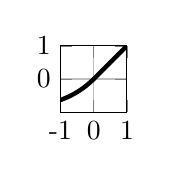
\begin{tikzpicture}
\begin{axis}[
	xmin=-1,xmax=1,
	ymin=-1,ymax=1,
	ytick={0, 1},
	yticklabels={0,1},
	xtick={-1, 0, 1},
	xticklabels={-1,0,1},
	width=.2\textwidth,
	height=.2\textwidth,
	grid=both,
	]
	\addplot [ultra thick,domain=-0.0035:1, samples=10]{x};
	\addplot [ultra thick,domain=-1:0.004, samples=10]{exp(x)-1};
\end{axis}
\end{tikzpicture}}
		\scalebox{.9}{% This file was created by tikzplotlib v0.9.6.
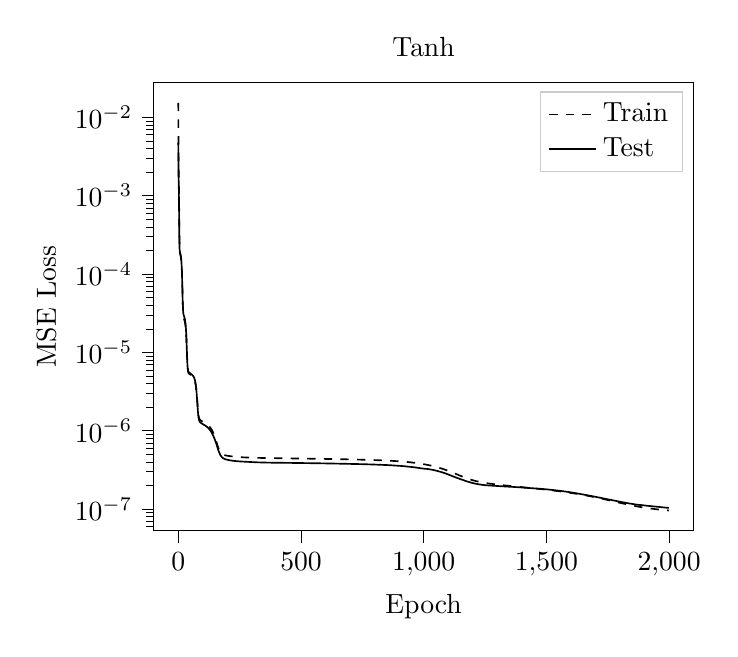
\begin{tikzpicture}

\begin{axis}[
legend cell align={left},
legend style={fill opacity=0.8, draw opacity=1, text opacity=1, draw=white!80!black},
log basis y={10},
tick align=outside,
tick pos=left,
title={Tanh},
x grid style={white!69.0196078431373!black},
xlabel={Epoch},
xmin=-99.95, xmax=2098.95,
xtick style={color=black},
y grid style={white!69.0196078431373!black},
ylabel={MSE Loss},
ymin=5.2838355076584e-08, ymax=0.0278720888075092,
ymode=log,
ytick style={color=black}
]
\addplot [semithick, black, dashed]
table {%
0 0.0153132931897417
1 0.00263468591915444
2 0.00157368404231966
3 0.00100973634771071
4 0.000470805197954178
5 0.000238240016129566
6 0.000192290817329194
7 0.000182392153321416
8 0.000177044864372874
9 0.000172117064284976
10 0.000166500588362396
11 0.00015954268569476
12 0.000150556041538948
13 0.000138711679741391
14 0.000123201339192747
15 0.00010384852115385
16 8.21741918771295e-05
17 6.17140098838718e-05
18 4.59808605392027e-05
19 3.61075856744719e-05
20 3.09615153473715e-05
21 2.86084769759327e-05
22 2.75036924476808e-05
23 2.68262024928845e-05
24 2.62473645334467e-05
25 2.56512312862469e-05
26 2.49876472216783e-05
27 2.42189531372787e-05
28 2.33048581776529e-05
29 2.21992105016398e-05
30 2.0851133920587e-05
31 1.92123597071259e-05
32 1.72571510574926e-05
33 1.50208010131792e-05
34 1.26468071212003e-05
35 1.03939191099016e-05
36 8.54036681334946e-06
37 7.2278788722997e-06
38 6.40808496189038e-06
39 5.93531661445468e-06
40 5.67199906026872e-06
41 5.52505381187984e-06
42 5.43974953552606e-06
43 5.38575441578359e-06
44 5.34706065189994e-06
45 5.31567630139307e-06
46 5.28771059708788e-06
47 5.26119667091507e-06
48 5.23525572231165e-06
49 5.20944819999158e-06
50 5.18347152382148e-06
51 5.15708841510332e-06
52 5.13011461384849e-06
53 5.10235067065423e-06
54 5.07353104478625e-06
55 5.04333890773978e-06
56 5.01150577724729e-06
57 4.97761710209943e-06
58 4.94116837637648e-06
59 4.90160364131498e-06
60 4.85830068294035e-06
61 4.81051573763125e-06
62 4.75736579585373e-06
63 4.69784373001403e-06
64 4.63084353839349e-06
65 4.55505242621257e-06
66 4.4689069618471e-06
67 4.37072546117179e-06
68 4.25872251423698e-06
69 4.13099127399619e-06
70 3.98556936380601e-06
71 3.82073990112985e-06
72 3.63538441825995e-06
73 3.42947709879127e-06
74 3.20474518565561e-06
75 2.96533639118479e-06
76 2.71820525040312e-06
77 2.47301909183761e-06
78 2.24097093428099e-06
79 2.03303970391744e-06
80 1.85738974289507e-06
81 1.7172159946881e-06
82 1.61103087606307e-06
83 1.53408617211426e-06
84 1.4801255596808e-06
85 1.44289974394951e-06
86 1.41705882572296e-06
87 1.39857534634302e-06
88 1.38478061057867e-06
89 1.37394659657275e-06
90 1.36493259270765e-06
91 1.35709255721395e-06
92 1.35006773837176e-06
93 1.3435876031167e-06
94 1.33744865189556e-06
95 1.33153407006148e-06
96 1.32577587834248e-06
97 1.32013072266091e-06
98 1.31456864949087e-06
99 1.30906824693966e-06
100 1.30361027811432e-06
101 1.29817983048497e-06
102 1.2927648969594e-06
103 1.28735057194262e-06
104 1.28192672787009e-06
105 1.27648085845067e-06
106 1.27100161500948e-06
107 1.26547873554728e-06
108 1.25990110808516e-06
109 1.25425981912031e-06
110 1.24854659134144e-06
111 1.24275286356124e-06
112 1.23686820501234e-06
113 1.23088176826514e-06
114 1.22477484546835e-06
115 1.21851538432338e-06
116 1.21207589478445e-06
117 1.20545096717706e-06
118 1.19864200888742e-06
119 1.19164904162972e-06
120 1.18446295368813e-06
121 1.17707011526136e-06
122 1.1694574324963e-06
123 1.16160844515889e-06
124 1.15350741776865e-06
125 1.14514046717318e-06
126 1.13649216663703e-06
127 1.12754831607731e-06
128 1.11829535674701e-06
129 1.10871652933042e-06
130 1.09879741285113e-06
131 1.08852268132864e-06
132 1.07788214393167e-06
133 1.06686042701654e-06
134 1.05544191262652e-06
135 1.04361316667223e-06
136 1.03136227298251e-06
137 1.01868055929799e-06
138 1.00555776742794e-06
139 9.91986293712444e-07
140 9.77953460363779e-07
141 9.63472345659966e-07
142 9.48564746323655e-07
143 9.33224022247714e-07
144 9.17436783851144e-07
145 9.01233095419229e-07
146 8.84645438446796e-07
147 8.6771310790823e-07
148 8.50481537099768e-07
149 8.32998301291354e-07
150 8.15313805475171e-07
151 7.97497160306193e-07
152 7.79638045287356e-07
153 7.61828415562604e-07
154 7.44165269679797e-07
155 7.26727081797662e-07
156 7.09585356162279e-07
157 6.92824803678604e-07
158 6.76534470272827e-07
159 6.60814733251414e-07
160 6.45768715401118e-07
161 6.31504774517566e-07
162 6.1806144752552e-07
163 6.0541898541544e-07
164 5.935898469005e-07
165 5.82608957756747e-07
166 5.7251111570622e-07
167 5.63264185785783e-07
168 5.54845568970563e-07
169 5.47202532217739e-07
170 5.40264816024205e-07
171 5.34007824569471e-07
172 5.28409758743464e-07
173 5.23425921969078e-07
174 5.18951096410092e-07
175 5.149205651378e-07
176 5.113566061965e-07
177 5.0820041903421e-07
178 5.0539328245236e-07
179 5.02919986971051e-07
180 5.00717105182957e-07
181 4.98696329472637e-07
182 4.96904277937915e-07
183 4.95304723173717e-07
184 4.93817427653198e-07
185 4.92438486588753e-07
186 4.91190134695785e-07
187 4.90051529411062e-07
188 4.8898569615119e-07
189 4.87990284483431e-07
190 4.87074258344933e-07
191 4.86203401237617e-07
192 4.8538464466219e-07
193 4.84598177266093e-07
194 4.83853644809074e-07
195 4.83136612828616e-07
196 4.82444658544523e-07
197 4.81775210417368e-07
198 4.81127108898249e-07
199 4.80499700458381e-07
200 4.79891992156922e-07
201 4.79301355042594e-07
202 4.78727373860011e-07
203 4.78168406615964e-07
204 4.77623684233208e-07
205 4.77091803091412e-07
206 4.76571929311831e-07
207 4.76063083382883e-07
208 4.7556500614121e-07
209 4.75079109705234e-07
210 4.74604136101675e-07
211 4.74139817058017e-07
212 4.73685574092997e-07
213 4.732392057889e-07
214 4.72801231126141e-07
215 4.72370848783044e-07
216 4.71947753624136e-07
217 4.71531814710602e-07
218 4.71123629139925e-07
219 4.70721878500058e-07
220 4.70326882307859e-07
221 4.69938081565147e-07
222 4.6955573562002e-07
223 4.69178338335041e-07
224 4.68806766932062e-07
225 4.68441367843297e-07
226 4.68085043436872e-07
227 4.67738976894339e-07
228 4.6739916845695e-07
229 4.67063946416602e-07
230 4.66734159886073e-07
231 4.66409362445575e-07
232 4.66089655560609e-07
233 4.65775199188556e-07
234 4.65466167142381e-07
235 4.65162220166349e-07
236 4.64862401173605e-07
237 4.64568502394513e-07
238 4.64278388264461e-07
239 4.63993729752588e-07
240 4.63713339598826e-07
241 4.63437639041331e-07
242 4.631659465133e-07
243 4.62899604784184e-07
244 4.62637191432691e-07
245 4.6237910713387e-07
246 4.62124751962278e-07
247 4.61875437409276e-07
248 4.61630108432587e-07
249 4.61388637120308e-07
250 4.61151012316918e-07
251 4.60918176742098e-07
252 4.60688900972173e-07
253 4.60463183557636e-07
254 4.60240989667682e-07
255 4.60023742206772e-07
256 4.59809431802682e-07
257 4.59599144193135e-07
258 4.59392179394058e-07
259 4.59188554302159e-07
260 4.58988357280532e-07
261 4.5879247274172e-07
262 4.58599594026055e-07
263 4.58409956038963e-07
264 4.58223486660359e-07
265 4.58040425911577e-07
266 4.57860810300303e-07
267 4.57683898687833e-07
268 4.57510935063965e-07
269 4.57340171877263e-07
270 4.57172989371202e-07
271 4.5700948594174e-07
272 4.56848700437718e-07
273 4.56690176079633e-07
274 4.56532334069948e-07
275 4.56378028999893e-07
276 4.56227564370693e-07
277 4.56079020167977e-07
278 4.55933057864399e-07
279 4.55789513395644e-07
280 4.55647950658999e-07
281 4.55509062945225e-07
282 4.55372698311862e-07
283 4.55238444189376e-07
284 4.55106499074986e-07
285 4.54976572086707e-07
286 4.54848537472685e-07
287 4.54722759030801e-07
288 4.54598988000043e-07
289 4.54477126126562e-07
290 4.54357528710148e-07
291 4.54239268904644e-07
292 4.5412372236342e-07
293 4.54009004798195e-07
294 4.53896645950636e-07
295 4.53786352096586e-07
296 4.53676708488615e-07
297 4.53569238302975e-07
298 4.53463479189509e-07
299 4.53359586160218e-07
300 4.5325645915284e-07
301 4.53154825493129e-07
302 4.53054902010308e-07
303 4.52956216690836e-07
304 4.52858107877319e-07
305 4.52761391798617e-07
306 4.52666627438703e-07
307 4.5257209372096e-07
308 4.52479442387244e-07
309 4.52388870797904e-07
310 4.52298658686345e-07
311 4.52208053658865e-07
312 4.52117211708014e-07
313 4.5202447013537e-07
314 4.51931193893529e-07
315 4.51840439652074e-07
316 4.51755951914379e-07
317 4.516765107212e-07
318 4.51600721788736e-07
319 4.51526182288831e-07
320 4.51450262687558e-07
321 4.51373784770226e-07
322 4.51297628643488e-07
323 4.51222715412314e-07
324 4.51148725105099e-07
325 4.51075450911276e-07
326 4.51002795969657e-07
327 4.50931086078299e-07
328 4.50860197716452e-07
329 4.50789848585487e-07
330 4.5072036765248e-07
331 4.50651828217019e-07
332 4.50583665013937e-07
333 4.50516136069723e-07
334 4.50449156701893e-07
335 4.5038280858023e-07
336 4.50316983886978e-07
337 4.50252412150576e-07
338 4.50187744334585e-07
339 4.50123620197473e-07
340 4.50059869905317e-07
341 4.49996963155286e-07
342 4.49934251392392e-07
343 4.49872764946235e-07
344 4.49810905891468e-07
345 4.49749873581595e-07
346 4.49688656800618e-07
347 4.49628481419495e-07
348 4.49568800718225e-07
349 4.49509138277904e-07
350 4.49449652847989e-07
351 4.49391284675471e-07
352 4.49332757710863e-07
353 4.49274186948401e-07
354 4.49216128771468e-07
355 4.49158206649258e-07
356 4.4910005910026e-07
357 4.49041933933358e-07
358 4.48982399845477e-07
359 4.48921653429579e-07
360 4.4885858659427e-07
361 4.48796846825417e-07
362 4.48741282951914e-07
363 4.48690722535616e-07
364 4.48639755177282e-07
365 4.48585934890389e-07
366 4.4853153957547e-07
367 4.48477469873865e-07
368 4.48423670761144e-07
369 4.48369932087189e-07
370 4.48316616555644e-07
371 4.48263513959546e-07
372 4.48211177371149e-07
373 4.48158735053994e-07
374 4.48106252406433e-07
375 4.48054085751437e-07
376 4.4800212175744e-07
377 4.4795040194856e-07
378 4.47898859235352e-07
379 4.47847473722618e-07
380 4.47796142310608e-07
381 4.47745204766647e-07
382 4.47694311603186e-07
383 4.47643480271154e-07
384 4.4759237508174e-07
385 4.47542060669548e-07
386 4.47491346719175e-07
387 4.47440747194605e-07
388 4.47390521486568e-07
389 4.4734031470739e-07
390 4.47290107231879e-07
391 4.47240181983943e-07
392 4.47190574547562e-07
393 4.47140450361871e-07
394 4.4709078622418e-07
395 4.47040961347511e-07
396 4.46991613557657e-07
397 4.46942280575513e-07
398 4.46892466911208e-07
399 4.46843225162752e-07
400 4.46794205998913e-07
401 4.46744886289707e-07
402 4.46695940368613e-07
403 4.46646912564574e-07
404 4.46597692658202e-07
405 4.46548597153651e-07
406 4.46500398439298e-07
407 4.46451654809721e-07
408 4.46402832963599e-07
409 4.46354196625975e-07
410 4.46306129020968e-07
411 4.46257712596321e-07
412 4.46209294665323e-07
413 4.46161581564297e-07
414 4.46113736870757e-07
415 4.46065096895154e-07
416 4.46016953446815e-07
417 4.45968802125662e-07
418 4.45921565813023e-07
419 4.45873601037761e-07
420 4.45826225742962e-07
421 4.45778409485342e-07
422 4.45730791852839e-07
423 4.45683437220623e-07
424 4.45636114307035e-07
425 4.45588812254982e-07
426 4.45541871997079e-07
427 4.45494792089107e-07
428 4.45448116849434e-07
429 4.45400671310381e-07
430 4.45353895372591e-07
431 4.45306549750057e-07
432 4.45259898953054e-07
433 4.45212845349374e-07
434 4.45166658622043e-07
435 4.45119889278089e-07
436 4.45073022035558e-07
437 4.45026548547389e-07
438 4.44980165639208e-07
439 4.4493387888167e-07
440 4.44887311957132e-07
441 4.44841445556676e-07
442 4.44794834720597e-07
443 4.44749098505781e-07
444 4.44702441498634e-07
445 4.44656845346003e-07
446 4.44611437771414e-07
447 4.44566093690923e-07
448 4.44520632100875e-07
449 4.44475479596917e-07
450 4.44428526719776e-07
451 4.44381641216296e-07
452 4.44334865875362e-07
453 4.44288736886733e-07
454 4.44242559808572e-07
455 4.44196356198745e-07
456 4.44150075907146e-07
457 4.44104312123272e-07
458 4.44058151245486e-07
459 4.44012046727948e-07
460 4.4396607486874e-07
461 4.43919723053909e-07
462 4.43873894312219e-07
463 4.43827820333809e-07
464 4.43781376830543e-07
465 4.43735788735466e-07
466 4.43689252719537e-07
467 4.43644105700969e-07
468 4.4359714057407e-07
469 4.43552091695665e-07
470 4.4350487823408e-07
471 4.43460639928617e-07
472 4.43412761498507e-07
473 4.43368704566183e-07
474 4.43320460263408e-07
475 4.43276697680517e-07
476 4.43227898742293e-07
477 4.43185115173605e-07
478 4.43134583662186e-07
479 4.43093923777838e-07
480 4.4304159730757e-07
481 4.43003092911454e-07
482 4.42947890576306e-07
483 4.42912595630673e-07
484 4.42853963079415e-07
485 4.42821147373706e-07
486 4.4276031600532e-07
487 4.42729391878061e-07
488 4.42667331853386e-07
489 4.4263708812764e-07
490 4.42574523304984e-07
491 4.42544547510693e-07
492 4.42481593594835e-07
493 4.42452258837989e-07
494 4.42388692619033e-07
495 4.42359383242774e-07
496 4.4229542483265e-07
497 4.42266830077642e-07
498 4.42202625464461e-07
499 4.42173881253893e-07
500 4.42109330492713e-07
501 4.42080638251241e-07
502 4.42015572744481e-07
503 4.41987434598445e-07
504 4.41922236504411e-07
505 4.41894427794409e-07
506 4.41828457454108e-07
507 4.41800639549683e-07
508 4.41734856408971e-07
509 4.417071328362e-07
510 4.41640802762322e-07
511 4.4161302048451e-07
512 4.41546921535974e-07
513 4.41519292778025e-07
514 4.4145272232754e-07
515 4.41425100333959e-07
516 4.41358092018618e-07
517 4.41330398814443e-07
518 4.4126369105868e-07
519 4.41236333685424e-07
520 4.4116943638528e-07
521 4.41140844500865e-07
522 4.41074515421747e-07
523 4.41045736721435e-07
524 4.40979312173795e-07
525 4.40951058521932e-07
526 4.4088429109479e-07
527 4.4085522711157e-07
528 4.40789318943757e-07
529 4.40759966153337e-07
530 4.40693232505396e-07
531 4.40663924607065e-07
532 4.40597787843444e-07
533 4.4056797210601e-07
534 4.40501284671768e-07
535 4.40471759517891e-07
536 4.4040554909941e-07
537 4.40375271367088e-07
538 4.40308756921581e-07
539 4.40278385511306e-07
540 4.40212674490681e-07
541 4.401812428938e-07
542 4.40115519111828e-07
543 4.40083868014085e-07
544 4.40018118496255e-07
545 4.39986295432959e-07
546 4.39920736553745e-07
547 4.39889069994592e-07
548 4.39823198377098e-07
549 4.3979057819854e-07
550 4.3972551353022e-07
551 4.39692232106381e-07
552 4.39627020057287e-07
553 4.39593548279049e-07
554 4.39528886658991e-07
555 4.39495016678393e-07
556 4.3943037410088e-07
557 4.39395672088949e-07
558 4.39331445349467e-07
559 4.39295989437483e-07
560 4.39232069638251e-07
561 4.39196281703858e-07
562 4.39132677342968e-07
563 4.39096512479864e-07
564 4.39032612277401e-07
565 4.38996117537727e-07
566 4.38933144138787e-07
567 4.38895417261165e-07
568 4.38832481677309e-07
569 4.38794382205288e-07
570 4.38731703610529e-07
571 4.38692871355784e-07
572 4.38631030220904e-07
573 4.38591341904271e-07
574 4.3853019623441e-07
575 4.38489292349686e-07
576 4.38428836289972e-07
577 4.38387495165671e-07
578 4.38326876377459e-07
579 4.3828513126698e-07
580 4.38225001701653e-07
581 4.38182326050196e-07
582 4.38123647242605e-07
583 4.38079974927064e-07
584 4.38020879528267e-07
585 4.37976561215692e-07
586 4.37918560521666e-07
587 4.3787362352532e-07
588 4.37815096447025e-07
589 4.3776925465977e-07
590 4.37711424595477e-07
591 4.37664399697724e-07
592 4.3760680487992e-07
593 4.3755960098224e-07
594 4.37502337533147e-07
595 4.37453951533939e-07
596 4.37396866345807e-07
597 4.37347725480208e-07
598 4.3729104187662e-07
599 4.37240820573948e-07
600 4.37184705148752e-07
601 4.37133718421023e-07
602 4.37077845234057e-07
603 4.37026187384504e-07
604 4.36970854678975e-07
605 4.3691830096293e-07
606 4.36862710003538e-07
607 4.36810370658236e-07
608 4.3675528922904e-07
609 4.36701593457656e-07
610 4.36646212094161e-07
611 4.36592203740815e-07
612 4.36536973964508e-07
613 4.36482874889066e-07
614 4.3642749051287e-07
615 4.36372963392273e-07
616 4.36317296390598e-07
617 4.36262127664122e-07
618 4.36206559811581e-07
619 4.36151188210943e-07
620 4.360954301319e-07
621 4.36040008409577e-07
622 4.35984044571569e-07
623 4.35928163838639e-07
624 4.35871852630498e-07
625 4.35815706538278e-07
626 4.35759265940305e-07
627 4.35702904624691e-07
628 4.35646074592455e-07
629 4.3558944291533e-07
630 4.35532369664315e-07
631 4.35475516837869e-07
632 4.35418206095051e-07
633 4.35361169124349e-07
634 4.35303863625336e-07
635 4.35246203821293e-07
636 4.35188680029341e-07
637 4.35130771123227e-07
638 4.35072627297473e-07
639 4.35014651216647e-07
640 4.34956360976457e-07
641 4.34898258731664e-07
642 4.3483965933433e-07
643 4.34781021880326e-07
644 4.34722310572511e-07
645 4.34663314436534e-07
646 4.34604027944374e-07
647 4.34545088054961e-07
648 4.34486076045459e-07
649 4.34426052166259e-07
650 4.3436669619723e-07
651 4.34306966951681e-07
652 4.34247524083275e-07
653 4.34187044504597e-07
654 4.34126650318944e-07
655 4.3406678015856e-07
656 4.34006311721191e-07
657 4.33945470703634e-07
658 4.3388504241193e-07
659 4.33823856454296e-07
660 4.33762479801203e-07
661 4.33701213708559e-07
662 4.33640064017027e-07
663 4.33578119313438e-07
664 4.33516226209463e-07
665 4.33454814398715e-07
666 4.33392396331556e-07
667 4.33329818136485e-07
668 4.33267958186434e-07
669 4.33204892530625e-07
670 4.33141973672946e-07
671 4.33078773085072e-07
672 4.33015674914827e-07
673 4.32951755399813e-07
674 4.32888073888194e-07
675 4.32823758643508e-07
676 4.32759608656852e-07
677 4.32694734612937e-07
678 4.32630114346466e-07
679 4.32565253049688e-07
680 4.32499659765995e-07
681 4.32433980776636e-07
682 4.32368343098233e-07
683 4.32302421103259e-07
684 4.32236600659053e-07
685 4.32170115175268e-07
686 4.32103654475213e-07
687 4.32037323932377e-07
688 4.31970005976723e-07
689 4.31903165861058e-07
690 4.31835885436271e-07
691 4.31768051683434e-07
692 4.31700327666817e-07
693 4.31633078846971e-07
694 4.31564529478123e-07
695 4.31496353158423e-07
696 4.31427578959642e-07
697 4.31358720646813e-07
698 4.31290260664241e-07
699 4.31221317384711e-07
700 4.31151998313339e-07
701 4.3108227941957e-07
702 4.31012523691265e-07
703 4.30942949222413e-07
704 4.3087253446572e-07
705 4.30802091443638e-07
706 4.30731750626023e-07
707 4.3066083789256e-07
708 4.30589486001054e-07
709 4.30518474843211e-07
710 4.30447059429184e-07
711 4.30375201659672e-07
712 4.30303392221276e-07
713 4.30231511501233e-07
714 4.3015977574612e-07
715 4.3008838706271e-07
716 4.30019053183628e-07
717 4.29953882459699e-07
718 4.29896650700812e-07
719 4.29822231993171e-07
720 4.2974184988509e-07
721 4.29663981321937e-07
722 4.29589445687384e-07
723 4.29516379668371e-07
724 4.29441970496214e-07
725 4.29364652404729e-07
726 4.29286579191057e-07
727 4.2920867996088e-07
728 4.29130572740632e-07
729 4.29052638310168e-07
730 4.28974418824168e-07
731 4.28895949170283e-07
732 4.28817700779405e-07
733 4.28738986272492e-07
734 4.28659984379465e-07
735 4.28580363461606e-07
736 4.28501005529824e-07
737 4.28420907368832e-07
738 4.28341064676374e-07
739 4.28259974668777e-07
740 4.28179160820719e-07
741 4.28097994443988e-07
742 4.28016579022028e-07
743 4.27933960622795e-07
744 4.27851577697425e-07
745 4.27769046169146e-07
746 4.27685715337134e-07
747 4.27602619794243e-07
748 4.27518155447615e-07
749 4.27433968880564e-07
750 4.27349275298639e-07
751 4.27264355025159e-07
752 4.2717858150354e-07
753 4.27093193394512e-07
754 4.27006655044693e-07
755 4.26920569864819e-07
756 4.26833762972478e-07
757 4.26746492280472e-07
758 4.26658948086356e-07
759 4.26571777708773e-07
760 4.26483888219309e-07
761 4.26396722218669e-07
762 4.26308664899011e-07
763 4.26221024667939e-07
764 4.26133200789991e-07
765 4.26043656887032e-07
766 4.25952536673435e-07
767 4.25861212193013e-07
768 4.25769250114172e-07
769 4.25676015069598e-07
770 4.25583642950755e-07
771 4.25490218106006e-07
772 4.25396803919398e-07
773 4.25302942758776e-07
774 4.25208595927984e-07
775 4.25113812013933e-07
776 4.25018646737385e-07
777 4.24922889891377e-07
778 4.24826633590669e-07
779 4.24729910164956e-07
780 4.24632532158853e-07
781 4.24534486185735e-07
782 4.24435824896818e-07
783 4.24336194910779e-07
784 4.24236452730042e-07
785 4.24136100704686e-07
786 4.24034741797641e-07
787 4.2393291576559e-07
788 4.23831002223096e-07
789 4.23727700493259e-07
790 4.23624593693717e-07
791 4.23520817520284e-07
792 4.23416092601769e-07
793 4.233113682659e-07
794 4.23206141306309e-07
795 4.23100903503837e-07
796 4.2299449046368e-07
797 4.22887794826465e-07
798 4.22781099018721e-07
799 4.22673134551133e-07
800 4.22564769195333e-07
801 4.22455741386329e-07
802 4.22345646171607e-07
803 4.22234838964641e-07
804 4.22122297180749e-07
805 4.22010236519554e-07
806 4.21896220629492e-07
807 4.21781650615571e-07
808 4.21667850659446e-07
809 4.21553422029319e-07
810 4.21439829892734e-07
811 4.21325296287023e-07
812 4.21210472168809e-07
813 4.21095024094598e-07
814 4.20978449184872e-07
815 4.20861232157677e-07
816 4.20743512691502e-07
817 4.20624905046907e-07
818 4.20505665687188e-07
819 4.20385636516585e-07
820 4.2026524386074e-07
821 4.20143697510866e-07
822 4.20021763972045e-07
823 4.19899434703552e-07
824 4.19775951186807e-07
825 4.19651953350808e-07
826 4.19527260504537e-07
827 4.1940189035472e-07
828 4.19275116527729e-07
829 4.19147858437441e-07
830 4.19019859464242e-07
831 4.18891167825564e-07
832 4.18760665780837e-07
833 4.18630356023186e-07
834 4.18498340792439e-07
835 4.18366126197611e-07
836 4.18232730254431e-07
837 4.18098747772433e-07
838 4.17964014957306e-07
839 4.17828126941799e-07
840 4.1769180576523e-07
841 4.17554468214121e-07
842 4.17416611611543e-07
843 4.17278087169848e-07
844 4.17138848717968e-07
845 4.16998658636203e-07
846 4.16857684271577e-07
847 4.16714902087278e-07
848 4.16571883661732e-07
849 4.16426834107142e-07
850 4.16280446643214e-07
851 4.16132222895271e-07
852 4.15983473530446e-07
853 4.15833202154658e-07
854 4.15681662872203e-07
855 4.1552967822156e-07
856 4.15376475629614e-07
857 4.15221758927942e-07
858 4.15066238758754e-07
859 4.14909692167953e-07
860 4.14752346017622e-07
861 4.14593858593548e-07
862 4.14433650448132e-07
863 4.14273077780081e-07
864 4.14110996572958e-07
865 4.1394791618643e-07
866 4.13783241640431e-07
867 4.13618292597562e-07
868 4.1345164329698e-07
869 4.13283892243044e-07
870 4.13115098893968e-07
871 4.12944745932009e-07
872 4.12773538926103e-07
873 4.12601342731023e-07
874 4.12427616268474e-07
875 4.12253036714105e-07
876 4.12077252818221e-07
877 4.11899781568081e-07
878 4.11721696224276e-07
879 4.11541758609246e-07
880 4.11360851586551e-07
881 4.11178559204473e-07
882 4.1099467759409e-07
883 4.10809515756227e-07
884 4.10622025370344e-07
885 4.10434007392269e-07
886 4.10244243184366e-07
887 4.10052710776654e-07
888 4.09860364456449e-07
889 4.09665865618081e-07
890 4.09470500798648e-07
891 4.09273717622227e-07
892 4.09075668997616e-07
893 4.08876081706921e-07
894 4.08675382104207e-07
895 4.08473281737542e-07
896 4.08270176066594e-07
897 4.08065752978359e-07
898 4.07860425198692e-07
899 4.07653831928201e-07
900 4.07445782528271e-07
901 4.07236672614886e-07
902 4.07026502514896e-07
903 4.06813603859746e-07
904 4.06598918075929e-07
905 4.06381167522341e-07
906 4.06158879513896e-07
907 4.05932690142663e-07
908 4.05703107304589e-07
909 4.05472865068646e-07
910 4.05241465941231e-07
911 4.05009318669158e-07
912 4.0477494502511e-07
913 4.04539864945264e-07
914 4.04302709910098e-07
915 4.04063302667623e-07
916 4.03822085488059e-07
917 4.03579558138745e-07
918 4.033347797332e-07
919 4.03087997696616e-07
920 4.02839564642932e-07
921 4.02589417461741e-07
922 4.02337238583073e-07
923 4.02083330115488e-07
924 4.01827826337353e-07
925 4.01570990803179e-07
926 4.01312498283346e-07
927 4.01053424084807e-07
928 4.0079356530498e-07
929 4.00534475417658e-07
930 4.00275759091073e-07
931 4.00020543196433e-07
932 3.99772352338346e-07
933 3.99518462245396e-07
934 3.99232151195861e-07
935 3.98937988194348e-07
936 3.98645003727438e-07
937 3.98352930972123e-07
938 3.98060276623369e-07
939 3.97767320862386e-07
940 3.9747197169504e-07
941 3.97174885563345e-07
942 3.96875663838614e-07
943 3.96573709068093e-07
944 3.96269294299145e-07
945 3.95962251246829e-07
946 3.95652659364032e-07
947 3.95340199190741e-07
948 3.95024775599495e-07
949 3.94706344408746e-07
950 3.94385574523426e-07
951 3.94061606812102e-07
952 3.93735439743637e-07
953 3.93406619821235e-07
954 3.93075350586969e-07
955 3.92741415438991e-07
956 3.92404345490149e-07
957 3.92064834102257e-07
958 3.91723577337189e-07
959 3.91379281069248e-07
960 3.91034041427929e-07
961 3.90688773293846e-07
962 3.90346557168186e-07
963 3.90006709622526e-07
964 3.89655191483484e-07
965 3.89290695778755e-07
966 3.88920869298204e-07
967 3.88549075182709e-07
968 3.88173222447108e-07
969 3.8779496591701e-07
970 3.87414582206702e-07
971 3.87031748786626e-07
972 3.86646552470893e-07
973 3.86258531918315e-07
974 3.85867048294131e-07
975 3.85473004882897e-07
976 3.85075737952434e-07
977 3.84675612480123e-07
978 3.84272473326064e-07
979 3.83866463693039e-07
980 3.83457353393624e-07
981 3.83045446341157e-07
982 3.8263090681312e-07
983 3.82212844257879e-07
984 3.81791498597295e-07
985 3.81366960709784e-07
986 3.80938562585698e-07
987 3.80507647548711e-07
988 3.80072127001085e-07
989 3.79633905382093e-07
990 3.79191937213363e-07
991 3.78746454927636e-07
992 3.78297291305785e-07
993 3.77845757824957e-07
994 3.77390559108903e-07
995 3.76932602179636e-07
996 3.76471325751027e-07
997 3.76008280454698e-07
998 3.75541477225738e-07
999 3.75072237204677e-07
1000 3.7459984805821e-07
1001 3.74125481229726e-07
1002 3.73646918262693e-07
1003 3.73165787280527e-07
1004 3.72680323081909e-07
1005 3.72192169535879e-07
1006 3.71700637074923e-07
1007 3.71204669733061e-07
1008 3.70705578362163e-07
1009 3.70202004802422e-07
1010 3.69694279910959e-07
1011 3.69181772597926e-07
1012 3.68664246721551e-07
1013 3.681415544321e-07
1014 3.67614507638336e-07
1015 3.67081920842338e-07
1016 3.66545533125873e-07
1017 3.66004452104107e-07
1018 3.65459960207204e-07
1019 3.64911836001625e-07
1020 3.64359034833228e-07
1021 3.6380328792518e-07
1022 3.63243735947094e-07
1023 3.62680784817826e-07
1024 3.62114355766607e-07
1025 3.61544524508872e-07
1026 3.60971631920393e-07
1027 3.60395439116701e-07
1028 3.59816504726496e-07
1029 3.59235964836557e-07
1030 3.58656483086861e-07
1031 3.58083547425281e-07
1032 3.57522725224158e-07
1033 3.56926418660919e-07
1034 3.56303529571278e-07
1035 3.55682074967945e-07
1036 3.55060193186318e-07
1037 3.54437427859011e-07
1038 3.5381234674503e-07
1039 3.53183879298058e-07
1040 3.52551655893762e-07
1041 3.51915701330086e-07
1042 3.51275422403319e-07
1043 3.50631737319418e-07
1044 3.4998303625855e-07
1045 3.49329645885632e-07
1046 3.48672467296751e-07
1047 3.48009736427457e-07
1048 3.47343681923462e-07
1049 3.46672493677147e-07
1050 3.45998814935911e-07
1051 3.45321498528506e-07
1052 3.44641047959726e-07
1053 3.43958320314641e-07
1054 3.43274007221339e-07
1055 3.42586759970231e-07
1056 3.41892986696735e-07
1057 3.41189594550428e-07
1058 3.404795624391e-07
1059 3.39765766298683e-07
1060 3.39050039997346e-07
1061 3.3833003406869e-07
1062 3.37607688265962e-07
1063 3.36880876574241e-07
1064 3.36151293524267e-07
1065 3.35417476918565e-07
1066 3.34680441582691e-07
1067 3.33939445610554e-07
1068 3.33195361704952e-07
1069 3.32447472445097e-07
1070 3.31696120113634e-07
1071 3.30941572030952e-07
1072 3.30182967516635e-07
1073 3.29421627640158e-07
1074 3.2865669591331e-07
1075 3.27889004125836e-07
1076 3.27117375050534e-07
1077 3.26343478178615e-07
1078 3.25565995140664e-07
1079 3.24785622467516e-07
1080 3.24002263027978e-07
1081 3.23216242321678e-07
1082 3.22426995978731e-07
1083 3.21635197906289e-07
1084 3.20840995044591e-07
1085 3.2004399291452e-07
1086 3.19244291389964e-07
1087 3.18442804314145e-07
1088 3.17637995706832e-07
1089 3.16831385660521e-07
1090 3.16022540800986e-07
1091 3.15211519406944e-07
1092 3.14398081741274e-07
1093 3.13583012015783e-07
1094 3.12765971898443e-07
1095 3.11946512724148e-07
1096 3.11125813070134e-07
1097 3.10302116616867e-07
1098 3.09477197205865e-07
1099 3.08649907680092e-07
1100 3.07821044899015e-07
1101 3.0698964995679e-07
1102 3.06157764725867e-07
1103 3.05322166866517e-07
1104 3.04485925980202e-07
1105 3.0364774683278e-07
1106 3.02807980276043e-07
1107 3.01966883128557e-07
1108 3.0112456292386e-07
1109 3.00281082743936e-07
1110 2.99436364144867e-07
1111 2.98590662367815e-07
1112 2.97743985655075e-07
1113 2.96896792107759e-07
1114 2.96048539510707e-07
1115 2.95200142630847e-07
1116 2.9435054504745e-07
1117 2.93500982749606e-07
1118 2.92650637334191e-07
1119 2.91800108698226e-07
1120 2.9094992638079e-07
1121 2.90099760817952e-07
1122 2.89249575743611e-07
1123 2.88399622419888e-07
1124 2.87549891183403e-07
1125 2.86700686828567e-07
1126 2.85852116235219e-07
1127 2.85004466363148e-07
1128 2.84156917686573e-07
1129 2.833113814944e-07
1130 2.82466340067344e-07
1131 2.81622272865434e-07
1132 2.80779442320522e-07
1133 2.79938600925789e-07
1134 2.79098920543674e-07
1135 2.78261221239973e-07
1136 2.77424942709104e-07
1137 2.7659101108668e-07
1138 2.75759133117504e-07
1139 2.74929214128861e-07
1140 2.74102109017349e-07
1141 2.7327765670293e-07
1142 2.72455530605953e-07
1143 2.71636089678395e-07
1144 2.70820190138465e-07
1145 2.70006673019907e-07
1146 2.69197387709141e-07
1147 2.68391106217791e-07
1148 2.67587981753081e-07
1149 2.66789002964174e-07
1150 2.65994599502051e-07
1151 2.65204446193934e-07
1152 2.64420651618025e-07
1153 2.63643165197891e-07
1154 2.6287096785893e-07
1155 2.62102935209896e-07
1156 2.61339599404664e-07
1157 2.60580745035099e-07
1158 2.59827119279521e-07
1159 2.59079005601848e-07
1160 2.58335715543012e-07
1161 2.57598258826874e-07
1162 2.56866600224726e-07
1163 2.56140495224599e-07
1164 2.55420891818403e-07
1165 2.54707391391662e-07
1166 2.53999428608154e-07
1167 2.53297669530639e-07
1168 2.52602138033353e-07
1169 2.51913175546292e-07
1170 2.5123055119991e-07
1171 2.50554446068918e-07
1172 2.4988453451158e-07
1173 2.49220868113298e-07
1174 2.48563562664117e-07
1175 2.47913107543241e-07
1176 2.47267765985271e-07
1177 2.46628499951385e-07
1178 2.4599422802396e-07
1179 2.45367220358617e-07
1180 2.44747584019933e-07
1181 2.44135619325903e-07
1182 2.43530379634649e-07
1183 2.42931076385844e-07
1184 2.42336930853071e-07
1185 2.41747951989169e-07
1186 2.41164151375983e-07
1187 2.40584499820784e-07
1188 2.40010541517677e-07
1189 2.39446667933407e-07
1190 2.38895236151393e-07
1191 2.38354633495419e-07
1192 2.37820755614848e-07
1193 2.37289173298905e-07
1194 2.36763406590512e-07
1195 2.36243773386491e-07
1196 2.35730746808827e-07
1197 2.35224286811331e-07
1198 2.34724079476223e-07
1199 2.34229994532598e-07
1200 2.33742097790923e-07
1201 2.332605407247e-07
1202 2.32784929337981e-07
1203 2.32315856280252e-07
1204 2.31852274140465e-07
1205 2.31395183917016e-07
1206 2.30944453235793e-07
1207 2.30499279183505e-07
1208 2.30060687911759e-07
1209 2.29627991373604e-07
1210 2.29201936448931e-07
1211 2.28782327823751e-07
1212 2.28369903197745e-07
1213 2.27964066269237e-07
1214 2.27565496700777e-07
1215 2.27173953078363e-07
1216 2.26790246045994e-07
1217 2.26415428585369e-07
1218 2.26050232640773e-07
1219 2.25693971842134e-07
1220 2.25338671370423e-07
1221 2.24972011622526e-07
1222 2.24602440894728e-07
1223 2.24238834562129e-07
1224 2.23883001922331e-07
1225 2.23533508687979e-07
1226 2.23189845812044e-07
1227 2.22851655664158e-07
1228 2.22517799258526e-07
1229 2.22188851282112e-07
1230 2.21864169844821e-07
1231 2.21543284496306e-07
1232 2.21226965379628e-07
1233 2.20914304776443e-07
1234 2.20605981127164e-07
1235 2.2030111284721e-07
1236 2.20000381048635e-07
1237 2.19703110403202e-07
1238 2.19409653851699e-07
1239 2.19119149249991e-07
1240 2.18831971437794e-07
1241 2.18548997196422e-07
1242 2.18268806818855e-07
1243 2.17991441388676e-07
1244 2.17717209466173e-07
1245 2.1744602784679e-07
1246 2.17177927765988e-07
1247 2.16912191319807e-07
1248 2.16650396936302e-07
1249 2.16390123270571e-07
1250 2.16133058799528e-07
1251 2.1587907644971e-07
1252 2.15627568863397e-07
1253 2.15378824073298e-07
1254 2.15131843241068e-07
1255 2.14888007782577e-07
1256 2.14646843559763e-07
1257 2.14407705186659e-07
1258 2.14170560518312e-07
1259 2.1393649831225e-07
1260 2.13704258435143e-07
1261 2.1347437109398e-07
1262 2.13246854215754e-07
1263 2.13020818328857e-07
1264 2.12796982168584e-07
1265 2.125756130269e-07
1266 2.12356135349978e-07
1267 2.12137947706026e-07
1268 2.11922217253857e-07
1269 2.11708398886401e-07
1270 2.11495935616313e-07
1271 2.11285770703284e-07
1272 2.11076535443055e-07
1273 2.10869454207341e-07
1274 2.1066421357574e-07
1275 2.1045999773861e-07
1276 2.1025769069638e-07
1277 2.10056241414236e-07
1278 2.09857041625128e-07
1279 2.09659049652089e-07
1280 2.09461995652305e-07
1281 2.0926700465651e-07
1282 2.09072476074823e-07
1283 2.08879468218015e-07
1284 2.0868736222468e-07
1285 2.08496854604334e-07
1286 2.08307065840074e-07
1287 2.0811799493714e-07
1288 2.07930388654631e-07
1289 2.07742703878466e-07
1290 2.07555825234351e-07
1291 2.07369623595355e-07
1292 2.07184382439607e-07
1293 2.07001097287218e-07
1294 2.06820774486971e-07
1295 2.06642172933869e-07
1296 2.06464475283497e-07
1297 2.06287604818556e-07
1298 2.06111494250649e-07
1299 2.05935856250505e-07
1300 2.05761286494521e-07
1301 2.05587725417899e-07
1302 2.05414359577105e-07
1303 2.0524219954865e-07
1304 2.05070374740046e-07
1305 2.04900051116397e-07
1306 2.04729819451188e-07
1307 2.04560695991063e-07
1308 2.04392164057765e-07
1309 2.04224752600624e-07
1310 2.0405743264007e-07
1311 2.03891090926334e-07
1312 2.03725257684084e-07
1313 2.03560172288064e-07
1314 2.03395246664684e-07
1315 2.03231465896181e-07
1316 2.03068005781404e-07
1317 2.02905416642807e-07
1318 2.02743438727282e-07
1319 2.02581670066593e-07
1320 2.02420751357124e-07
1321 2.02260203550964e-07
1322 2.02100084223389e-07
1323 2.01940410256896e-07
1324 2.01780698787957e-07
1325 2.01622603263729e-07
1326 2.01463833860771e-07
1327 2.01305658485751e-07
1328 2.0114791804815e-07
1329 2.0098994261275e-07
1330 2.00831707317661e-07
1331 2.0067317363015e-07
1332 2.00514492256332e-07
1333 2.00353759915117e-07
1334 2.00191533217264e-07
1335 2.00027188149932e-07
1336 1.99861917451472e-07
1337 1.99699144367571e-07
1338 1.9954218120688e-07
1339 1.99391871539945e-07
1340 1.99243989271736e-07
1341 1.9909605251911e-07
1342 1.98947011803341e-07
1343 1.98797260793526e-07
1344 1.98647412332775e-07
1345 1.98497241349571e-07
1346 1.9834731132562e-07
1347 1.98198011752027e-07
1348 1.98049309140913e-07
1349 1.97900511956561e-07
1350 1.97752460657341e-07
1351 1.97604831683407e-07
1352 1.97456864107437e-07
1353 1.97309753176e-07
1354 1.97163243690568e-07
1355 1.97016909247338e-07
1356 1.96871239580787e-07
1357 1.96725074466997e-07
1358 1.96580252968204e-07
1359 1.9643524857571e-07
1360 1.96289902675062e-07
1361 1.96145034429662e-07
1362 1.96000701237153e-07
1363 1.95856939036787e-07
1364 1.95712916287505e-07
1365 1.95569456138855e-07
1366 1.95426440789959e-07
1367 1.9528298147975e-07
1368 1.95140321508802e-07
1369 1.94997839102484e-07
1370 1.94855483051981e-07
1371 1.94714067042412e-07
1372 1.9457207280027e-07
1373 1.94430763414744e-07
1374 1.94288967051648e-07
1375 1.94148666814442e-07
1376 1.94007788685724e-07
1377 1.93867000021442e-07
1378 1.9372678165297e-07
1379 1.93586380675015e-07
1380 1.93446242960249e-07
1381 1.93306313704511e-07
1382 1.9316685001769e-07
1383 1.93027033866144e-07
1384 1.928881173896e-07
1385 1.92748827437583e-07
1386 1.92609713145941e-07
1387 1.92470996616123e-07
1388 1.92332163415188e-07
1389 1.92193213806036e-07
1390 1.92054977055989e-07
1391 1.91916928748981e-07
1392 1.91778728556358e-07
1393 1.91640867662102e-07
1394 1.91502521168729e-07
1395 1.91364721203513e-07
1396 1.91226667354272e-07
1397 1.9108902575482e-07
1398 1.90951581458876e-07
1399 1.90813802156242e-07
1400 1.90676621741659e-07
1401 1.90538358062042e-07
1402 1.90400840303084e-07
1403 1.90263191981899e-07
1404 1.90125171293687e-07
1405 1.89986778437401e-07
1406 1.89848554953187e-07
1407 1.8971032452697e-07
1408 1.89571864318339e-07
1409 1.89435156663365e-07
1410 1.89298512275116e-07
1411 1.89162471627924e-07
1412 1.89027391506613e-07
1413 1.88892291511422e-07
1414 1.8875688207487e-07
1415 1.88622368398228e-07
1416 1.88486953341283e-07
1417 1.88351250955066e-07
1418 1.88216109933137e-07
1419 1.88080516487332e-07
1420 1.87945151431279e-07
1421 1.87809692143048e-07
1422 1.87673937595889e-07
1423 1.87538295172374e-07
1424 1.8740287024599e-07
1425 1.87267376752231e-07
1426 1.8713166647899e-07
1427 1.86995634521736e-07
1428 1.86859856981414e-07
1429 1.8672422855559e-07
1430 1.8658855636744e-07
1431 1.86452587357167e-07
1432 1.86317243965561e-07
1433 1.86181103750016e-07
1434 1.86045110218913e-07
1435 1.85909304605048e-07
1436 1.85773195795491e-07
1437 1.8563674731098e-07
1438 1.85500630173863e-07
1439 1.85364702439017e-07
1440 1.85228678525107e-07
1441 1.85091931768966e-07
1442 1.84955936774145e-07
1443 1.8481905767942e-07
1444 1.84682557872407e-07
1445 1.84545949899473e-07
1446 1.84409362503857e-07
1447 1.84272837167043e-07
1448 1.84136263179369e-07
1449 1.83998937515639e-07
1450 1.83862002991475e-07
1451 1.83725183212857e-07
1452 1.83587768042059e-07
1453 1.8345057564062e-07
1454 1.83313025360121e-07
1455 1.831751825776e-07
1456 1.83038089282661e-07
1457 1.82900077319914e-07
1458 1.82761687497646e-07
1459 1.82624055767633e-07
1460 1.82485669327548e-07
1461 1.82347980498321e-07
1462 1.82209376120568e-07
1463 1.82070631119302e-07
1464 1.81931762497811e-07
1465 1.81793589483448e-07
1466 1.81654316875779e-07
1467 1.81515491554762e-07
1468 1.81376568512803e-07
1469 1.81236938274765e-07
1470 1.81097548917819e-07
1471 1.80957725802955e-07
1472 1.80818158590057e-07
1473 1.80678038027793e-07
1474 1.80538659130036e-07
1475 1.80398435141171e-07
1476 1.80258126057709e-07
1477 1.80117199768404e-07
1478 1.79976853104336e-07
1479 1.79836202470085e-07
1480 1.79695553192971e-07
1481 1.79554426821937e-07
1482 1.79413018962293e-07
1483 1.79271853156138e-07
1484 1.79130245065551e-07
1485 1.78988189610152e-07
1486 1.78846173938041e-07
1487 1.78704160241239e-07
1488 1.78561569086355e-07
1489 1.78418774439137e-07
1490 1.78275439829179e-07
1491 1.78132229585515e-07
1492 1.77988269832952e-07
1493 1.77844642124114e-07
1494 1.77700789940616e-07
1495 1.77556530303491e-07
1496 1.77413203722665e-07
1497 1.77269419246784e-07
1498 1.77125700552949e-07
1499 1.76981946104604e-07
1500 1.76837839454436e-07
1501 1.76693711736675e-07
1502 1.76549127644421e-07
1503 1.76404452886914e-07
1504 1.76259294093484e-07
1505 1.76114788217774e-07
1506 1.75969739686366e-07
1507 1.75823956546139e-07
1508 1.75678158655046e-07
1509 1.75532431981651e-07
1510 1.75386379034137e-07
1511 1.75240595915227e-07
1512 1.75093902704759e-07
1513 1.7494729726053e-07
1514 1.74800479889825e-07
1515 1.74653114910939e-07
1516 1.74505447041895e-07
1517 1.74357999242147e-07
1518 1.74210518537166e-07
1519 1.74062339922898e-07
1520 1.73913695810768e-07
1521 1.73764734256565e-07
1522 1.73616360349627e-07
1523 1.73467366380464e-07
1524 1.73317852578236e-07
1525 1.73168524227663e-07
1526 1.73018382426449e-07
1527 1.72868128714754e-07
1528 1.72718070842848e-07
1529 1.72567302954008e-07
1530 1.72416797767028e-07
1531 1.72265960898699e-07
1532 1.72114913766563e-07
1533 1.71963616836024e-07
1534 1.71812750110689e-07
1535 1.71661240734977e-07
1536 1.71510075475112e-07
1537 1.71359199399035e-07
1538 1.71208313396676e-07
1539 1.71057598102209e-07
1540 1.70907905925333e-07
1541 1.70758876727461e-07
1542 1.70609292091228e-07
1543 1.70460468254419e-07
1544 1.70312362698155e-07
1545 1.70163580897054e-07
1546 1.70014862639789e-07
1547 1.69866378691097e-07
1548 1.69717479316489e-07
1549 1.69566319698333e-07
1550 1.69413205235003e-07
1551 1.69262491603206e-07
1552 1.69118381393218e-07
1553 1.68960619944869e-07
1554 1.68795844842862e-07
1555 1.68634415963709e-07
1556 1.68473855467255e-07
1557 1.68314386073121e-07
1558 1.68154245599794e-07
1559 1.67994072640454e-07
1560 1.67833153817298e-07
1561 1.67671810075376e-07
1562 1.67509841304536e-07
1563 1.67347641095716e-07
1564 1.67185039479989e-07
1565 1.67022370270331e-07
1566 1.66858579163431e-07
1567 1.6669509652445e-07
1568 1.66530774116325e-07
1569 1.66365951564273e-07
1570 1.66200860505228e-07
1571 1.66035385390728e-07
1572 1.65869453141454e-07
1573 1.65703530747408e-07
1574 1.65537247930558e-07
1575 1.65369557223016e-07
1576 1.65202419346144e-07
1577 1.65034642208184e-07
1578 1.64866432960764e-07
1579 1.64697372412093e-07
1580 1.64528549724707e-07
1581 1.64359141180626e-07
1582 1.64189042507701e-07
1583 1.64018376509034e-07
1584 1.63848530839061e-07
1585 1.63677140456286e-07
1586 1.63505837697642e-07
1587 1.63334020520267e-07
1588 1.63161493020425e-07
1589 1.62988920223484e-07
1590 1.62815901546765e-07
1591 1.62642609133457e-07
1592 1.62468500562341e-07
1593 1.62294163239096e-07
1594 1.62119284404127e-07
1595 1.61944268469938e-07
1596 1.61769006261636e-07
1597 1.6159333222987e-07
1598 1.61416930303915e-07
1599 1.61240067853896e-07
1600 1.61062490441566e-07
1601 1.60884974306441e-07
1602 1.60707457432352e-07
1603 1.60528995351683e-07
1604 1.60350243852747e-07
1605 1.60171012886678e-07
1606 1.59991311164731e-07
1607 1.59811481459826e-07
1608 1.5963114405082e-07
1609 1.59450155202023e-07
1610 1.59268876970486e-07
1611 1.59087491539367e-07
1612 1.58905203285542e-07
1613 1.58723114125792e-07
1614 1.58540065520185e-07
1615 1.58356691443373e-07
1616 1.58172858220951e-07
1617 1.5798880822615e-07
1618 1.5780438653934e-07
1619 1.57619860587488e-07
1620 1.57434136937695e-07
1621 1.57248384098807e-07
1622 1.57062319168233e-07
1623 1.56875651107669e-07
1624 1.56688346805822e-07
1625 1.56501207619897e-07
1626 1.56312636484301e-07
1627 1.56125045272404e-07
1628 1.5593663069069e-07
1629 1.55747434618547e-07
1630 1.55557898246172e-07
1631 1.55367758125635e-07
1632 1.55177617727986e-07
1633 1.54986824739467e-07
1634 1.54795744876424e-07
1635 1.54603835959222e-07
1636 1.54411861352344e-07
1637 1.54219893495622e-07
1638 1.54026954923836e-07
1639 1.53833983453922e-07
1640 1.53640136147715e-07
1641 1.53446705240867e-07
1642 1.53252364249568e-07
1643 1.53057529182377e-07
1644 1.52862226677541e-07
1645 1.52666382049915e-07
1646 1.52470592574616e-07
1647 1.52274631098237e-07
1648 1.52077870133382e-07
1649 1.51880777508495e-07
1650 1.51683495445809e-07
1651 1.51485552670749e-07
1652 1.51287423278745e-07
1653 1.51089010309136e-07
1654 1.50889857103209e-07
1655 1.50690775619466e-07
1656 1.50490732615083e-07
1657 1.50291338350428e-07
1658 1.50090620600452e-07
1659 1.49889776885459e-07
1660 1.49688915968227e-07
1661 1.49487465179732e-07
1662 1.4928600089803e-07
1663 1.49083902165614e-07
1664 1.48881587350047e-07
1665 1.4867913220229e-07
1666 1.48475658356517e-07
1667 1.48272390148918e-07
1668 1.48068798637269e-07
1669 1.47865251520329e-07
1670 1.47660860996268e-07
1671 1.47456080739516e-07
1672 1.4725146725425e-07
1673 1.47046273092144e-07
1674 1.46840754538857e-07
1675 1.4663544489224e-07
1676 1.46429697068129e-07
1677 1.46223249899435e-07
1678 1.46016627674328e-07
1679 1.45809942438291e-07
1680 1.45603426588536e-07
1681 1.45396087411598e-07
1682 1.45188524484752e-07
1683 1.44980611487711e-07
1684 1.44772903141188e-07
1685 1.44564246930656e-07
1686 1.44355149799935e-07
1687 1.441462966838e-07
1688 1.4393595458273e-07
1689 1.43726265235955e-07
1690 1.4351561272008e-07
1691 1.43305352857226e-07
1692 1.43094229187568e-07
1693 1.42883543688299e-07
1694 1.42672429291224e-07
1695 1.42460894117846e-07
1696 1.42249607357314e-07
1697 1.42037970377373e-07
1698 1.41825694633724e-07
1699 1.41613584077049e-07
1700 1.41401022652587e-07
1701 1.41188655796043e-07
1702 1.409755914068e-07
1703 1.4076257535578e-07
1704 1.4054907948946e-07
1705 1.40336023235932e-07
1706 1.40122252204833e-07
1707 1.39908651419773e-07
1708 1.39694659765155e-07
1709 1.3948045044998e-07
1710 1.39266338869959e-07
1711 1.39051701154358e-07
1712 1.38837409274117e-07
1713 1.38622801856059e-07
1714 1.38407956661979e-07
1715 1.38193323202529e-07
1716 1.3797861543452e-07
1717 1.37762848154921e-07
1718 1.37547677013572e-07
1719 1.3733257323878e-07
1720 1.37117589602553e-07
1721 1.3690199989469e-07
1722 1.36686459001112e-07
1723 1.36470597226435e-07
1724 1.36255418766495e-07
1725 1.36039620024064e-07
1726 1.35823476185237e-07
1727 1.35607580055819e-07
1728 1.35391227466641e-07
1729 1.35175009916111e-07
1730 1.34958783931438e-07
1731 1.34742448942404e-07
1732 1.34525368125082e-07
1733 1.34308235161029e-07
1734 1.34091737571396e-07
1735 1.33875057166222e-07
1736 1.33657707294788e-07
1737 1.334407889928e-07
1738 1.33223868537868e-07
1739 1.33006814948544e-07
1740 1.32790484869361e-07
1741 1.32574266586971e-07
1742 1.32357681081885e-07
1743 1.32141230679395e-07
1744 1.31925407721667e-07
1745 1.31709154345572e-07
1746 1.31492661864741e-07
1747 1.31276670579439e-07
1748 1.31060225868396e-07
1749 1.3084343503067e-07
1750 1.30625985292454e-07
1751 1.30407917311004e-07
1752 1.3018887429439e-07
1753 1.29969713313471e-07
1754 1.29751316436e-07
1755 1.29535875714737e-07
1756 1.29322545042498e-07
1757 1.29110344772698e-07
1758 1.28897924376759e-07
1759 1.28685892654801e-07
1760 1.28474125652644e-07
1761 1.28261454818812e-07
1762 1.2804998434035e-07
1763 1.27838788174017e-07
1764 1.27627474782344e-07
1765 1.27417000349794e-07
1766 1.27207069454016e-07
1767 1.26998158677338e-07
1768 1.26788983507709e-07
1769 1.26580558060141e-07
1770 1.26372195417446e-07
1771 1.26163634597276e-07
1772 1.25956113890879e-07
1773 1.25748886453891e-07
1774 1.25541696171183e-07
1775 1.25334779774278e-07
1776 1.2512836828904e-07
1777 1.24922688698348e-07
1778 1.24716383226087e-07
1779 1.24511090106694e-07
1780 1.24306193427515e-07
1781 1.24102183121977e-07
1782 1.23897907904791e-07
1783 1.2369433025583e-07
1784 1.23491051922997e-07
1785 1.23287772467506e-07
1786 1.23085534340817e-07
1787 1.22883737816437e-07
1788 1.22682091010518e-07
1789 1.22480864369834e-07
1790 1.22280630215244e-07
1791 1.22080303114558e-07
1792 1.21880769292204e-07
1793 1.2168125068257e-07
1794 1.21482172154685e-07
1795 1.21283261435678e-07
1796 1.21085433427481e-07
1797 1.20887371835465e-07
1798 1.20689629099502e-07
1799 1.20492102801961e-07
1800 1.20294289260414e-07
1801 1.20097012413112e-07
1802 1.19899265264678e-07
1803 1.19700950520496e-07
1804 1.19501880774919e-07
1805 1.19302303453139e-07
1806 1.19102337755805e-07
1807 1.18903721975983e-07
1808 1.18706371296184e-07
1809 1.18511404068045e-07
1810 1.18318644602766e-07
1811 1.18127836813642e-07
1812 1.17938027813125e-07
1813 1.17749107197085e-07
1814 1.1756050746925e-07
1815 1.17372823758899e-07
1816 1.17185668663922e-07
1817 1.16998699354554e-07
1818 1.16813001916682e-07
1819 1.16628327937462e-07
1820 1.16445167876122e-07
1821 1.16262231216524e-07
1822 1.16080557425846e-07
1823 1.15899467125757e-07
1824 1.15719468766429e-07
1825 1.1553991424762e-07
1826 1.15360886731253e-07
1827 1.15182996310637e-07
1828 1.15005756086362e-07
1829 1.14829542354755e-07
1830 1.1465361860985e-07
1831 1.14478304986676e-07
1832 1.14304111470176e-07
1833 1.14130792589151e-07
1834 1.13958029992034e-07
1835 1.13786225547585e-07
1836 1.13614648341809e-07
1837 1.1344472758168e-07
1838 1.13275046636829e-07
1839 1.13106421864018e-07
1840 1.12938684402764e-07
1841 1.12771494144681e-07
1842 1.12605404844146e-07
1843 1.12439957192123e-07
1844 1.12275765197012e-07
1845 1.12112253844998e-07
1846 1.11949421714996e-07
1847 1.11787542302011e-07
1848 1.11626522915742e-07
1849 1.11466396703008e-07
1850 1.11307283120254e-07
1851 1.11148616660728e-07
1852 1.10991130178206e-07
1853 1.10834450815389e-07
1854 1.10678930887786e-07
1855 1.1052377875842e-07
1856 1.10369861673121e-07
1857 1.1021624374763e-07
1858 1.10063541235661e-07
1859 1.09912216899488e-07
1860 1.09760921631619e-07
1861 1.09610843615826e-07
1862 1.09461522640686e-07
1863 1.09313251186904e-07
1864 1.09164941534345e-07
1865 1.0901789431017e-07
1866 1.08871369043584e-07
1867 1.08725351765315e-07
1868 1.08579953156607e-07
1869 1.08434740177188e-07
1870 1.08290680650214e-07
1871 1.08146579115953e-07
1872 1.08002374723526e-07
1873 1.07858512883752e-07
1874 1.07714307191031e-07
1875 1.07569798473151e-07
1876 1.07424431973868e-07
1877 1.07279064167187e-07
1878 1.07134091393846e-07
1879 1.06990642230187e-07
1880 1.06849200491865e-07
1881 1.06710115041153e-07
1882 1.06573571812874e-07
1883 1.06438048931068e-07
1884 1.06303954062525e-07
1885 1.06170634275315e-07
1886 1.0603867883674e-07
1887 1.05909500753398e-07
1888 1.05783494909417e-07
1889 1.0565902891102e-07
1890 1.05536129851203e-07
1891 1.05413541234611e-07
1892 1.0529157029282e-07
1893 1.0517003322974e-07
1894 1.0504874938988e-07
1895 1.0492791155059e-07
1896 1.04807770760829e-07
1897 1.04688773305384e-07
1898 1.04569448247105e-07
1899 1.04451607683131e-07
1900 1.04334652569094e-07
1901 1.04218091088626e-07
1902 1.04101847306026e-07
1903 1.03987056959909e-07
1904 1.03873083176609e-07
1905 1.03759429777028e-07
1906 1.03646971560067e-07
1907 1.03535047159653e-07
1908 1.03423752165099e-07
1909 1.03312606121619e-07
1910 1.03201954260612e-07
1911 1.03090449464105e-07
1912 1.02976625846907e-07
1913 1.02860583815811e-07
1914 1.02748842763845e-07
1915 1.02647654145471e-07
1916 1.02552481251905e-07
1917 1.02452287407573e-07
1918 1.02350801405748e-07
1919 1.02249307403213e-07
1920 1.02148726185192e-07
1921 1.02049343524868e-07
1922 1.0195043762451e-07
1923 1.01852137582625e-07
1924 1.01755116617142e-07
1925 1.01658411395533e-07
1926 1.01562900383101e-07
1927 1.01468063249399e-07
1928 1.01373980434971e-07
1929 1.01280395639947e-07
1930 1.01187967651128e-07
1931 1.01096210677554e-07
1932 1.01004768296775e-07
1933 1.00914673261343e-07
1934 1.00824932694366e-07
1935 1.00736403737756e-07
1936 1.00647972885781e-07
1937 1.0056027598182e-07
1938 1.00473353576547e-07
1939 1.00387001666036e-07
1940 1.0030186856369e-07
1941 1.00216294342204e-07
1942 1.00132553150445e-07
1943 1.00049164110771e-07
1944 9.99662232601395e-08
1945 9.9884007894957e-08
1946 9.9802272110594e-08
1947 9.97211373459095e-08
1948 9.96409339393267e-08
1949 9.95606085680834e-08
1950 9.94814255719234e-08
1951 9.94026107719037e-08
1952 9.93248000327185e-08
1953 9.92471665952621e-08
1954 9.91698371706207e-08
1955 9.90928263959745e-08
1956 9.90170850485583e-08
1957 9.89413566472308e-08
1958 9.886638153489e-08
1959 9.87913848504718e-08
1960 9.87173318307555e-08
1961 9.86434040299855e-08
1962 9.85702834057633e-08
1963 9.84970515744976e-08
1964 9.84250025766187e-08
1965 9.83525942146457e-08
1966 9.82806287055382e-08
1967 9.82091408801011e-08
1968 9.81384063862833e-08
1969 9.80677439983424e-08
1970 9.79972193491108e-08
1971 9.79274898114113e-08
1972 9.78577098962319e-08
1973 9.77888636697344e-08
1974 9.77205578251983e-08
1975 9.76530570895306e-08
1976 9.7586227262525e-08
1977 9.75194265819823e-08
1978 9.74540213576347e-08
1979 9.73889696567198e-08
1980 9.73246934421468e-08
1981 9.72605430433759e-08
1982 9.71964803753167e-08
1983 9.71334363555343e-08
1984 9.70705833296392e-08
1985 9.70082417239837e-08
1986 9.69461796032078e-08
1987 9.68846052558092e-08
1988 9.68234024583126e-08
1989 9.6762341918577e-08
1990 9.67015899817625e-08
1991 9.66413196579197e-08
1992 9.65816957929633e-08
1993 9.65222250854936e-08
1994 9.64626737740559e-08
1995 9.64043699198669e-08
1996 9.63458629286151e-08
1997 9.62872997973818e-08
1998 9.62296229900517e-08
1999 9.61723456143204e-08
};
\addlegendentry{Train}
\addplot [semithick, black]
table {%
0 0.00474944757297635
1 0.00181602849625051
2 0.00130414986051619
3 0.000698993157129735
4 0.000310305564198643
5 0.000212854516576044
6 0.000196091583347879
7 0.000189501704880968
8 0.000184357384569012
9 0.000178912829142064
10 0.000172392930835485
11 0.000164128461619839
12 0.000153320623212494
13 0.000139055104227737
14 0.000120664451969787
15 9.86682425718755e-05
16 7.58648820919916e-05
17 5.65119444217999e-05
18 4.32588421972468e-05
19 3.58453617081977e-05
20 3.23519125231542e-05
21 3.08031849272083e-05
22 2.99780404020566e-05
23 2.93432149192085e-05
24 2.871369724744e-05
25 2.8023547201883e-05
26 2.72315155598335e-05
27 2.62952271441463e-05
28 2.51660603680648e-05
29 2.37893909798004e-05
30 2.21087830141187e-05
31 2.00799568119692e-05
32 1.77017191163031e-05
33 1.50676578414277e-05
34 1.24115113067091e-05
35 1.00619699878735e-05
36 8.27729672892019e-06
37 7.10459789843298e-06
38 6.41183851257665e-06
39 6.02717727815616e-06
40 5.81822996537085e-06
41 5.70138263356057e-06
42 5.6295816648344e-06
43 5.57915791432606e-06
44 5.53979134565452e-06
45 5.50750201000483e-06
46 5.47829540664679e-06
47 5.44941485713935e-06
48 5.42093448530068e-06
49 5.39307120561716e-06
50 5.36531842953991e-06
51 5.33694174009725e-06
52 5.30798843101365e-06
53 5.2785635489272e-06
54 5.2487853281491e-06
55 5.21772881256766e-06
56 5.18486558576114e-06
57 5.14975408805185e-06
58 5.11177495354787e-06
59 5.07017648487817e-06
60 5.02431475979392e-06
61 4.9733603191271e-06
62 4.91590071760584e-06
63 4.85112877868232e-06
64 4.77783805763465e-06
65 4.69476799480617e-06
66 4.60035789728863e-06
67 4.49262688562158e-06
68 4.36919208368636e-06
69 4.22747007178259e-06
70 4.06480648962315e-06
71 3.87888667319203e-06
72 3.66851963917725e-06
73 3.43455326401454e-06
74 3.18071693072852e-06
75 2.91381979877769e-06
76 2.6432835511514e-06
77 2.38041911870823e-06
78 2.13724638342683e-06
79 1.9241113022872e-06
80 1.74779358985688e-06
81 1.61010927968164e-06
82 1.50764549289306e-06
83 1.43519844186812e-06
84 1.38520147174859e-06
85 1.35041170779004e-06
86 1.32593743273901e-06
87 1.30835553591169e-06
88 1.2950621339769e-06
89 1.28444617075729e-06
90 1.27570240238128e-06
91 1.26798863675504e-06
92 1.26095505947887e-06
93 1.25440055853687e-06
94 1.24813334423379e-06
95 1.24211373986327e-06
96 1.2363149153316e-06
97 1.23070526569791e-06
98 1.22524465950846e-06
99 1.2198976264699e-06
100 1.21464279345673e-06
101 1.20944537229661e-06
102 1.20429274375056e-06
103 1.19915409868554e-06
104 1.19400795028923e-06
105 1.18884236144368e-06
106 1.18363539058919e-06
107 1.17837328161841e-06
108 1.17303784463729e-06
109 1.16761736990156e-06
110 1.16209184852778e-06
111 1.1564505939532e-06
112 1.1506709824971e-06
113 1.14473107259982e-06
114 1.13862654416153e-06
115 1.13237501864205e-06
116 1.12600446300348e-06
117 1.1195039633094e-06
118 1.11283145542984e-06
119 1.1059676126024e-06
120 1.09888082988618e-06
121 1.09155746486067e-06
122 1.08396977793745e-06
123 1.07610344457498e-06
124 1.0679501656341e-06
125 1.05950834949908e-06
126 1.05077867829095e-06
127 1.04173784620798e-06
128 1.03235777260124e-06
129 1.0226250424239e-06
130 1.0125525022886e-06
131 1.00222212040535e-06
132 9.91627643998072e-07
133 9.8075645382778e-07
134 9.69600364442158e-07
135 9.58156192609749e-07
136 9.46430532167142e-07
137 9.34438730837428e-07
138 9.22188519325573e-07
139 9.09661082459934e-07
140 8.96835103958438e-07
141 8.83716211319552e-07
142 8.70403823682864e-07
143 8.56858321185427e-07
144 8.4300950220495e-07
145 8.28845770683984e-07
146 8.1438651022836e-07
147 7.99747510882298e-07
148 7.85023644311877e-07
149 7.70074166211998e-07
150 7.54972347749572e-07
151 7.39826589324366e-07
152 7.24696974430117e-07
153 7.09605558313342e-07
154 6.94578602633555e-07
155 6.79652202961734e-07
156 6.64824085561122e-07
157 6.5012125105568e-07
158 6.35577009688859e-07
159 6.21054368821206e-07
160 6.06690093718498e-07
161 5.92761011830589e-07
162 5.79350682983204e-07
163 5.66829839954153e-07
164 5.55244298539037e-07
165 5.44728266049788e-07
166 5.35465687789838e-07
167 5.26937185441056e-07
168 5.18285901307536e-07
169 5.09487904309935e-07
170 5.00860551255755e-07
171 4.93383765842736e-07
172 4.87170041196805e-07
173 4.81919130379538e-07
174 4.76632578738645e-07
175 4.71063145823791e-07
176 4.6632990802209e-07
177 4.62369769138604e-07
178 4.59026978205657e-07
179 4.55910651453451e-07
180 4.53004815881286e-07
181 4.50343776492446e-07
182 4.47954306537213e-07
183 4.46093167738582e-07
184 4.44325195303463e-07
185 4.42543893086622e-07
186 4.40958586978013e-07
187 4.39476707470021e-07
188 4.38057327301067e-07
189 4.36822773508538e-07
190 4.35676156484988e-07
191 4.34564753959421e-07
192 4.33507580055448e-07
193 4.32511228609656e-07
194 4.31564814107332e-07
195 4.30636646342464e-07
196 4.29734370754886e-07
197 4.28873391911111e-07
198 4.28050498157972e-07
199 4.27261994673245e-07
200 4.26498672823072e-07
201 4.2576328951327e-07
202 4.25050018293405e-07
203 4.24359512862793e-07
204 4.23685150963138e-07
205 4.23028211571363e-07
206 4.22387756771059e-07
207 4.21764866587182e-07
208 4.21161047370333e-07
209 4.20576242277093e-07
210 4.20008490209511e-07
211 4.19457620637331e-07
212 4.18918318700889e-07
213 4.18395501355917e-07
214 4.17885644310445e-07
215 4.1739238554328e-07
216 4.16912797618352e-07
217 4.16448159512584e-07
218 4.15996424862897e-07
219 4.15559298971857e-07
220 4.15135417597412e-07
221 4.14730237707772e-07
222 4.14344953014734e-07
223 4.13991443792838e-07
224 4.13671102705848e-07
225 4.1335863443237e-07
226 4.13034001667256e-07
227 4.126860346787e-07
228 4.12329029586544e-07
229 4.11981773140724e-07
230 4.1164517483594e-07
231 4.11316420922958e-07
232 4.10998723054945e-07
233 4.10690148555659e-07
234 4.10389191074501e-07
235 4.10096845371299e-07
236 4.09812088264516e-07
237 4.09533754464064e-07
238 4.09263634537638e-07
239 4.08999966339252e-07
240 4.08744142532669e-07
241 4.08493320946945e-07
242 4.08250798500376e-07
243 4.08013363539794e-07
244 4.07781840294774e-07
245 4.07556740356085e-07
246 4.0733493733569e-07
247 4.07118534440087e-07
248 4.06908498007397e-07
249 4.06703009048215e-07
250 4.06499054861342e-07
251 4.06300813438065e-07
252 4.06107318440263e-07
253 4.05914931889129e-07
254 4.05726893859537e-07
255 4.05545080184311e-07
256 4.05365369715582e-07
257 4.05186568741556e-07
258 4.05016379545486e-07
259 4.04843319756765e-07
260 4.04674665333005e-07
261 4.0451072891301e-07
262 4.0434707671011e-07
263 4.04187318281402e-07
264 4.04029407263806e-07
265 4.03872974175101e-07
266 4.03718445340928e-07
267 4.03567895546075e-07
268 4.0341649309994e-07
269 4.03261367409868e-07
270 4.03109680746638e-07
271 4.02954157152635e-07
272 4.02790902853667e-07
273 4.02634952934022e-07
274 4.02488950612678e-07
275 4.02340589289452e-07
276 4.02192085857678e-07
277 4.02045941427787e-07
278 4.01895903223703e-07
279 4.01746774514322e-07
280 4.0159616787605e-07
281 4.01444538056239e-07
282 4.01291202933862e-07
283 4.01138152028579e-07
284 4.00982600012867e-07
285 4.00828639612882e-07
286 4.00671183342638e-07
287 4.00514068132907e-07
288 4.00357635044202e-07
289 4.00199326122674e-07
290 4.0004286461226e-07
291 3.99883901991416e-07
292 3.9972752574613e-07
293 3.99570950548878e-07
294 3.99416194341029e-07
295 3.99262603423267e-07
296 3.99107790372e-07
297 3.98956728986377e-07
298 3.98805553913917e-07
299 3.98657249434109e-07
300 3.98510053400969e-07
301 3.98365727960481e-07
302 3.98222624653499e-07
303 3.98084267771992e-07
304 3.97950884689635e-07
305 3.97815455244199e-07
306 3.97677354158077e-07
307 3.97528367557243e-07
308 3.97374776639481e-07
309 3.97226500581382e-07
310 3.97076888702941e-07
311 3.96928840018518e-07
312 3.96785367229313e-07
313 3.96656901102688e-07
314 3.96551286030444e-07
315 3.96428021076645e-07
316 3.96293501125911e-07
317 3.96182485928875e-07
318 3.96087301623993e-07
319 3.95986717194319e-07
320 3.95881926351649e-07
321 3.95776396544534e-07
322 3.95672543618275e-07
323 3.9557249920108e-07
324 3.95472881109526e-07
325 3.95376275719173e-07
326 3.95280892462324e-07
327 3.95186589230434e-07
328 3.95094645000427e-07
329 3.95004946085464e-07
330 3.94915304013921e-07
331 3.94829697825116e-07
332 3.94741903164686e-07
333 3.94658286495542e-07
334 3.94575351947424e-07
335 3.94492019495374e-07
336 3.94412694504354e-07
337 3.94331436837092e-07
338 3.94253078184192e-07
339 3.94174577422746e-07
340 3.94098975675661e-07
341 3.94022947602934e-07
342 3.9394834061568e-07
343 3.93874358906032e-07
344 3.93802395137755e-07
345 3.93730459791186e-07
346 3.93659178143935e-07
347 3.93589886016343e-07
348 3.93520110719692e-07
349 3.93450790170391e-07
350 3.93382862284852e-07
351 3.93314820712476e-07
352 3.9324675071839e-07
353 3.93179931279519e-07
354 3.9311251498475e-07
355 3.93042881796646e-07
356 3.92972623330934e-07
357 3.9289744790949e-07
358 3.92817042893512e-07
359 3.92727599773934e-07
360 3.92643073610088e-07
361 3.92580005836862e-07
362 3.9252572037185e-07
363 3.9246586425179e-07
364 3.92405780758054e-07
365 3.92348908917484e-07
366 3.92294879247856e-07
367 3.92240337987459e-07
368 3.92184375641591e-07
369 3.92129777537775e-07
370 3.92078192135159e-07
371 3.92023423501087e-07
372 3.9196984857881e-07
373 3.91917097886108e-07
374 3.91864318771695e-07
375 3.91812847055917e-07
376 3.91763649076893e-07
377 3.9171391108539e-07
378 3.91664769949784e-07
379 3.91615003536572e-07
380 3.91567766655498e-07
381 3.91520131870493e-07
382 3.91473236049933e-07
383 3.91427619206297e-07
384 3.91381917097533e-07
385 3.91338289773557e-07
386 3.91293639268042e-07
387 3.91250068787485e-07
388 3.9120740780163e-07
389 3.91164888924322e-07
390 3.91123506915392e-07
391 3.91082949136035e-07
392 3.91041567127104e-07
393 3.91002572541765e-07
394 3.90964174812325e-07
395 3.90924185467156e-07
396 3.9088655512387e-07
397 3.90850402709475e-07
398 3.90813085004993e-07
399 3.90778012615556e-07
400 3.90742513900477e-07
401 3.90706418329501e-07
402 3.90675296557674e-07
403 3.90640195746528e-07
404 3.90608676070769e-07
405 3.90575053188513e-07
406 3.9054475564626e-07
407 3.90512781223151e-07
408 3.90483933188079e-07
409 3.90454999887879e-07
410 3.9042453181537e-07
411 3.9039858279466e-07
412 3.90369109481981e-07
413 3.90339238265369e-07
414 3.90312550280214e-07
415 3.90285862295059e-07
416 3.90256985838278e-07
417 3.90230525226798e-07
418 3.90204860423182e-07
419 3.90177348208454e-07
420 3.90151313922615e-07
421 3.90124256455238e-07
422 3.90097369518116e-07
423 3.90071676292791e-07
424 3.90045187259602e-07
425 3.90017419249489e-07
426 3.89990617577496e-07
427 3.89963275893024e-07
428 3.89935678413167e-07
429 3.89907739872797e-07
430 3.89879772910717e-07
431 3.89852459647955e-07
432 3.89826652735792e-07
433 3.89797037314565e-07
434 3.8976986616035e-07
435 3.89741813933142e-07
436 3.89713306958583e-07
437 3.89684714718896e-07
438 3.89657145660749e-07
439 3.89628041830292e-07
440 3.89599279060349e-07
441 3.89570487868696e-07
442 3.89545959933457e-07
443 3.89517140320095e-07
444 3.89489855479042e-07
445 3.89466038086539e-07
446 3.89439861692153e-07
447 3.89415021118111e-07
448 3.89381796139787e-07
449 3.89340925721626e-07
450 3.89294996239187e-07
451 3.8925443845983e-07
452 3.89216836538253e-07
453 3.89179973581122e-07
454 3.89142940093734e-07
455 3.89110653031821e-07
456 3.89074727991101e-07
457 3.89038405046449e-07
458 3.89004526368808e-07
459 3.88969084497148e-07
460 3.88932392070274e-07
461 3.88897433367674e-07
462 3.8886372522029e-07
463 3.8882527064743e-07
464 3.88788436112009e-07
465 3.88751999480519e-07
466 3.88716244970055e-07
467 3.88680518881301e-07
468 3.88644338045196e-07
469 3.88608782486699e-07
470 3.88570072118455e-07
471 3.88532271244912e-07
472 3.88496005143679e-07
473 3.88458289535265e-07
474 3.88423899266854e-07
475 3.88385529959123e-07
476 3.88348951219086e-07
477 3.88308194487763e-07
478 3.8827292314636e-07
479 3.88234155934697e-07
480 3.88197406664403e-07
481 3.88158525765903e-07
482 3.88122884942277e-07
483 3.88081758728731e-07
484 3.88046117905105e-07
485 3.88005759077714e-07
486 3.87969208759387e-07
487 3.87930498391142e-07
488 3.87894601772132e-07
489 3.87854328209869e-07
490 3.87817948421798e-07
491 3.87778584354237e-07
492 3.87741948770781e-07
493 3.87701845738775e-07
494 3.87663106948821e-07
495 3.87624510267415e-07
496 3.87587391514899e-07
497 3.87547999025628e-07
498 3.87509516031059e-07
499 3.87469356155634e-07
500 3.87432095294571e-07
501 3.87393185974361e-07
502 3.87355385100818e-07
503 3.87314457839238e-07
504 3.87277594882107e-07
505 3.87237861332324e-07
506 3.87200941531773e-07
507 3.87158848980107e-07
508 3.87120451250667e-07
509 3.8708037664037e-07
510 3.87042604188537e-07
511 3.87003183277557e-07
512 3.8696461501786e-07
513 3.86924398299016e-07
514 3.86884806857779e-07
515 3.86846039646116e-07
516 3.86806732421974e-07
517 3.86767084137318e-07
518 3.86726725309927e-07
519 3.8668667912134e-07
520 3.86648366657028e-07
521 3.86610025771006e-07
522 3.86568217436434e-07
523 3.86530814466823e-07
524 3.86490228265757e-07
525 3.86449556799562e-07
526 3.86410192732001e-07
527 3.8636983390461e-07
528 3.86330214041664e-07
529 3.86290253118204e-07
530 3.86250832207224e-07
531 3.86210388114705e-07
532 3.861711945774e-07
533 3.86129840990179e-07
534 3.86089936910139e-07
535 3.86050118095227e-07
536 3.86007371844244e-07
537 3.85967695137879e-07
538 3.8592671103288e-07
539 3.85887091169934e-07
540 3.85844970196558e-07
541 3.8580697037105e-07
542 3.85764678867417e-07
543 3.8572360949729e-07
544 3.85681659054171e-07
545 3.85641243383361e-07
546 3.85600543495457e-07
547 3.85560923632511e-07
548 3.85517154199988e-07
549 3.85477449071914e-07
550 3.85435072303153e-07
551 3.85394514523796e-07
552 3.85351938803069e-07
553 3.85311238915165e-07
554 3.85268947411532e-07
555 3.85229014909783e-07
556 3.85183369644437e-07
557 3.85144431902518e-07
558 3.85101003530508e-07
559 3.85059792051834e-07
560 3.85015454185123e-07
561 3.84972821620977e-07
562 3.8493024590025e-07
563 3.84889716542602e-07
564 3.84843986012129e-07
565 3.84804167197217e-07
566 3.84757754545717e-07
567 3.84718731538669e-07
568 3.84672546260845e-07
569 3.84630340022341e-07
570 3.8458446738332e-07
571 3.84543767495416e-07
572 3.84498378025455e-07
573 3.84456285473789e-07
574 3.84410611786734e-07
575 3.84370110850796e-07
576 3.84323556090749e-07
577 3.8428206039498e-07
578 3.84236614081601e-07
579 3.84198017400195e-07
580 3.84151746857242e-07
581 3.84112382789681e-07
582 3.84067845971003e-07
583 3.84031039857291e-07
584 3.83989487318104e-07
585 3.83947508453275e-07
586 3.83904250611522e-07
587 3.83861703312505e-07
588 3.83812903237413e-07
589 3.83764415801124e-07
590 3.83714194640561e-07
591 3.83666389325299e-07
592 3.83616111321317e-07
593 3.83568220740926e-07
594 3.83518255375748e-07
595 3.83467920528346e-07
596 3.83421024707786e-07
597 3.8337242358466e-07
598 3.83321349772814e-07
599 3.83273402349005e-07
600 3.83223294875279e-07
601 3.83175716933692e-07
602 3.83125865255352e-07
603 3.83076894650003e-07
604 3.83026929284824e-07
605 3.82976963919646e-07
606 3.82927566988656e-07
607 3.82877601623477e-07
608 3.82831188971977e-07
609 3.82779347773976e-07
610 3.82729865577858e-07
611 3.82678280175242e-07
612 3.82629139039636e-07
613 3.82578150492918e-07
614 3.82527872488936e-07
615 3.8247875977504e-07
616 3.82429107048665e-07
617 3.82378289032204e-07
618 3.82325964665142e-07
619 3.82277562493982e-07
620 3.82225636030853e-07
621 3.82175983304478e-07
622 3.82124738962375e-07
623 3.82074517801811e-07
624 3.82023813472188e-07
625 3.81972853347179e-07
626 3.81921694270204e-07
627 3.8186999518075e-07
628 3.81819177164289e-07
629 3.81767961243895e-07
630 3.81715636876834e-07
631 3.8166442095644e-07
632 3.81613602939979e-07
633 3.81561875428815e-07
634 3.81509806857139e-07
635 3.81458619358455e-07
636 3.81405783400623e-07
637 3.81355022227581e-07
638 3.81301816787527e-07
639 3.81249805059269e-07
640 3.81196656462635e-07
641 3.81143593131128e-07
642 3.81092974066632e-07
643 3.81039825469998e-07
644 3.80987614789774e-07
645 3.80934295662883e-07
646 3.80883250272745e-07
647 3.80828367951835e-07
648 3.80777322561698e-07
649 3.80722724457883e-07
650 3.80670797994753e-07
651 3.80618729423077e-07
652 3.80565836621827e-07
653 3.80513426989637e-07
654 3.80462950033689e-07
655 3.80409943545601e-07
656 3.80359978180422e-07
657 3.80309984393534e-07
658 3.80258228460661e-07
659 3.80206017780438e-07
660 3.80155910306712e-07
661 3.80103330144266e-07
662 3.80053762683019e-07
663 3.80001239363992e-07
664 3.79947493911459e-07
665 3.79895283231235e-07
666 3.79844578901611e-07
667 3.79789810267539e-07
668 3.79736576405776e-07
669 3.79684820472903e-07
670 3.79629625513189e-07
671 3.79577954845445e-07
672 3.79522901994278e-07
673 3.79468531264138e-07
674 3.79414899498443e-07
675 3.79357430801974e-07
676 3.79300473696276e-07
677 3.79244085024766e-07
678 3.79187639509837e-07
679 3.79129289740376e-07
680 3.79070058897923e-07
681 3.79010941742308e-07
682 3.78950346657803e-07
683 3.78891996888342e-07
684 3.78828872271697e-07
685 3.78768561404286e-07
686 3.78705180992256e-07
687 3.78643790099886e-07
688 3.78581148652302e-07
689 3.78517455601468e-07
690 3.7845501310585e-07
691 3.78390382138605e-07
692 3.78325410110847e-07
693 3.7826089283044e-07
694 3.78196403971742e-07
695 3.78129698219709e-07
696 3.78065323047849e-07
697 3.77996997258379e-07
698 3.77929524120191e-07
699 3.77862306777388e-07
700 3.77795885242449e-07
701 3.77728184730586e-07
702 3.77657983108293e-07
703 3.77590055222754e-07
704 3.7752039361294e-07
705 3.77451300437315e-07
706 3.77380303007158e-07
707 3.77312545651876e-07
708 3.77242685090096e-07
709 3.77175439325583e-07
710 3.77106971427565e-07
711 3.77042226773483e-07
712 3.76979755856155e-07
713 3.76922088207721e-07
714 3.76875874508187e-07
715 3.76836595705754e-07
716 3.76793735767933e-07
717 3.76791120970665e-07
718 3.76977737914785e-07
719 3.77037792986812e-07
720 3.76931637902089e-07
721 3.76825965986427e-07
722 3.76745390440192e-07
723 3.76661802192757e-07
724 3.76571108517965e-07
725 3.7648948136848e-07
726 3.76415471237124e-07
727 3.76343763264231e-07
728 3.76274897462281e-07
729 3.76204951635373e-07
730 3.76135176338721e-07
731 3.76066395801899e-07
732 3.75995426793452e-07
733 3.7592664625663e-07
734 3.75856728851431e-07
735 3.75786754602814e-07
736 3.75717803535736e-07
737 3.75648966155495e-07
738 3.75579503497647e-07
739 3.75507823946464e-07
740 3.75439213939899e-07
741 3.75367562810425e-07
742 3.75297560140098e-07
743 3.75226761661906e-07
744 3.75155565279783e-07
745 3.75084141523985e-07
746 3.75015389408873e-07
747 3.74941890868286e-07
748 3.74871916619668e-07
749 3.74797565427798e-07
750 3.74725061647041e-07
751 3.74652358914318e-07
752 3.74580650941425e-07
753 3.74505702893657e-07
754 3.74433398064866e-07
755 3.74359501620347e-07
756 3.74287225213266e-07
757 3.74213982468063e-07
758 3.74141876591239e-07
759 3.74073039210998e-07
760 3.74002269154516e-07
761 3.73935620245902e-07
762 3.73868971337288e-07
763 3.73796240182855e-07
764 3.73712424561745e-07
765 3.73618405546949e-07
766 3.73529900343783e-07
767 3.73437501366425e-07
768 3.73348797211293e-07
769 3.73263446817873e-07
770 3.73176732182401e-07
771 3.73091666006076e-07
772 3.73007281950777e-07
773 3.72921363123169e-07
774 3.72836154838296e-07
775 3.72749184407439e-07
776 3.72662981362737e-07
777 3.72577943608121e-07
778 3.72490120525981e-07
779 3.72400052128796e-07
780 3.72311774299305e-07
781 3.7222173432383e-07
782 3.72131012227328e-07
783 3.72037419538174e-07
784 3.71945958477227e-07
785 3.7185299106568e-07
786 3.71759114159431e-07
787 3.7166284982959e-07
788 3.71568177115478e-07
789 3.71469809579139e-07
790 3.71372493646049e-07
791 3.71275007182703e-07
792 3.71179226021923e-07
793 3.71083757499946e-07
794 3.70989369002928e-07
795 3.70896742651894e-07
796 3.70805594229751e-07
797 3.70716435327267e-07
798 3.70628669088546e-07
799 3.70543034478032e-07
800 3.7045634826427e-07
801 3.70371878943843e-07
802 3.70286642237261e-07
803 3.70195465393408e-07
804 3.70099797919465e-07
805 3.69995575510984e-07
806 3.69882883433093e-07
807 3.69766553376394e-07
808 3.69649399090122e-07
809 3.695342059018e-07
810 3.6942043379895e-07
811 3.69309560710462e-07
812 3.69201245575823e-07
813 3.69095033647682e-07
814 3.68989788057661e-07
815 3.6888553722747e-07
816 3.68782167470272e-07
817 3.68679849316322e-07
818 3.68579861742546e-07
819 3.68478254131333e-07
820 3.68377442327983e-07
821 3.68278136875233e-07
822 3.68179684073766e-07
823 3.68079895451956e-07
824 3.67983005844508e-07
825 3.67885462537743e-07
826 3.67784195987042e-07
827 3.67690063285409e-07
828 3.6758868304787e-07
829 3.67491281849652e-07
830 3.67387912092454e-07
831 3.67285963420727e-07
832 3.67182082072759e-07
833 3.67076836482738e-07
834 3.66968265552714e-07
835 3.66859438827305e-07
836 3.66748793112492e-07
837 3.66635418913575e-07
838 3.66523011052777e-07
839 3.66407903129584e-07
840 3.66293164688614e-07
841 3.66178198873968e-07
842 3.66063375167869e-07
843 3.65944998748091e-07
844 3.65829180282162e-07
845 3.65717454542391e-07
846 3.65601152907402e-07
847 3.65486300779594e-07
848 3.65370624422212e-07
849 3.65252645906367e-07
850 3.65131597845902e-07
851 3.65005234925775e-07
852 3.64877877245817e-07
853 3.64745972092351e-07
854 3.64613157444182e-07
855 3.64476335334984e-07
856 3.64337267910742e-07
857 3.6419561411094e-07
858 3.64051658152675e-07
859 3.63908327472018e-07
860 3.6375854506332e-07
861 3.63608990028297e-07
862 3.63456791774297e-07
863 3.6330445141175e-07
864 3.63149723625611e-07
865 3.62993830549385e-07
866 3.62835749001533e-07
867 3.62677468501715e-07
868 3.62516402674373e-07
869 3.62352949423439e-07
870 3.6218975196789e-07
871 3.62024792366356e-07
872 3.61855825303792e-07
873 3.61688080374734e-07
874 3.61518345926015e-07
875 3.61348782007553e-07
876 3.6117629065302e-07
877 3.61003316129427e-07
878 3.60827982603951e-07
879 3.60652848030441e-07
880 3.60475297611629e-07
881 3.60297974566492e-07
882 3.60119685183236e-07
883 3.59939662075703e-07
884 3.59762822199627e-07
885 3.59585783371585e-07
886 3.59408801386962e-07
887 3.59230455160287e-07
888 3.59055746912418e-07
889 3.58877173312067e-07
890 3.58698059699236e-07
891 3.58519770315979e-07
892 3.58340798811696e-07
893 3.58158388280572e-07
894 3.57980582066375e-07
895 3.5779970630756e-07
896 3.57619512669771e-07
897 3.57437272668903e-07
898 3.57257590621884e-07
899 3.57077453827515e-07
900 3.56903086640159e-07
901 3.56733067974346e-07
902 3.56571774773329e-07
903 3.56427676706517e-07
904 3.56303360149468e-07
905 3.56183818439604e-07
906 3.56045092075874e-07
907 3.55874817614676e-07
908 3.55682061581319e-07
909 3.55478732672054e-07
910 3.55271907892529e-07
911 3.55059228240862e-07
912 3.54843479044575e-07
913 3.54626450871365e-07
914 3.54405983671313e-07
915 3.54184294337756e-07
916 3.53958199639237e-07
917 3.53732474422941e-07
918 3.5350197435946e-07
919 3.5327144587427e-07
920 3.53036227807024e-07
921 3.52799503389178e-07
922 3.52558032545858e-07
923 3.52316021690058e-07
924 3.52065654851685e-07
925 3.51810911070061e-07
926 3.51550909272191e-07
927 3.51280647237218e-07
928 3.50996799625136e-07
929 3.50697007434064e-07
930 3.50384198100073e-07
931 3.50063828591374e-07
932 3.49770488128343e-07
933 3.49530694165878e-07
934 3.49309374314544e-07
935 3.49075804706445e-07
936 3.488315485356e-07
937 3.48577202657907e-07
938 3.48316291365336e-07
939 3.48052310528146e-07
940 3.47786198062749e-07
941 3.47517129739572e-07
942 3.47246981391436e-07
943 3.46976719356462e-07
944 3.46704609910375e-07
945 3.46431590969587e-07
946 3.46157207786746e-07
947 3.45880692975697e-07
948 3.45604291851487e-07
949 3.45326071737873e-07
950 3.45045918948017e-07
951 3.44764941928588e-07
952 3.44483453318389e-07
953 3.44198724633316e-07
954 3.43915644407389e-07
955 3.43628329346757e-07
956 3.43342037467664e-07
957 3.43051738127542e-07
958 3.42764622018876e-07
959 3.42477335379954e-07
960 3.42194681479668e-07
961 3.41919275115288e-07
962 3.41630141065252e-07
963 3.41293343808502e-07
964 3.40947110544221e-07
965 3.40600820436521e-07
966 3.4025407558147e-07
967 3.39914151936682e-07
968 3.39586023301308e-07
969 3.39263323212435e-07
970 3.38940822075529e-07
971 3.38612068162547e-07
972 3.38278397293834e-07
973 3.37939667360843e-07
974 3.37593348831433e-07
975 3.37241516490394e-07
976 3.36884426133111e-07
977 3.36520884047786e-07
978 3.36152254476474e-07
979 3.35779020588234e-07
980 3.3540197819093e-07
981 3.35021866249008e-07
982 3.34638968979561e-07
983 3.34255588541055e-07
984 3.33875789237936e-07
985 3.33495847826271e-07
986 3.33120254936148e-07
987 3.32746878939361e-07
988 3.32375208245139e-07
989 3.32006578673827e-07
990 3.31641331285937e-07
991 3.31281171384035e-07
992 3.30925701064189e-07
993 3.30578274088111e-07
994 3.30239771528795e-07
995 3.29909596530342e-07
996 3.29591131276175e-07
997 3.29285796851764e-07
998 3.28995042764291e-07
999 3.28721029063672e-07
1000 3.28464778931448e-07
1001 3.28228566104372e-07
1002 3.28011907413384e-07
1003 3.27816081835408e-07
1004 3.2763634294497e-07
1005 3.27473003380874e-07
1006 3.27317650317127e-07
1007 3.27170113223474e-07
1008 3.27017005474772e-07
1009 3.26854888044181e-07
1010 3.26680918760758e-07
1011 3.26484752122269e-07
1012 3.26268548178632e-07
1013 3.26028498420783e-07
1014 3.25767587128212e-07
1015 3.25489139640922e-07
1016 3.25186704230873e-07
1017 3.24870342183203e-07
1018 3.24537950291415e-07
1019 3.24190693845594e-07
1020 3.23830334991726e-07
1021 3.23457328477161e-07
1022 3.23074971220194e-07
1023 3.22679795772274e-07
1024 3.22277003306226e-07
1025 3.21865400110255e-07
1026 3.21446833595473e-07
1027 3.21021587978976e-07
1028 3.20586906354947e-07
1029 3.20148046739632e-07
1030 3.1969909741747e-07
1031 3.19247448032911e-07
1032 3.18928584874811e-07
1033 3.18767575890888e-07
1034 3.18397013643335e-07
1035 3.1788826504453e-07
1036 3.17380880687779e-07
1037 3.16888701945572e-07
1038 3.1641030773244e-07
1039 3.15930066108194e-07
1040 3.15446641252493e-07
1041 3.1495426355832e-07
1042 3.1445529202756e-07
1043 3.13951744601582e-07
1044 3.13429950438149e-07
1045 3.12904148813686e-07
1046 3.12371327026995e-07
1047 3.11827307086787e-07
1048 3.11276210140932e-07
1049 3.10722100493876e-07
1050 3.10158156935358e-07
1051 3.09589864855297e-07
1052 3.09014751564973e-07
1053 3.08438131924049e-07
1054 3.07857021653035e-07
1055 3.07271648125607e-07
1056 3.06681528172703e-07
1057 3.06087031276547e-07
1058 3.05491141716629e-07
1059 3.0488982361021e-07
1060 3.04288164443278e-07
1061 3.03683691527112e-07
1062 3.03074926932823e-07
1063 3.02463462276137e-07
1064 3.01849382822184e-07
1065 3.01233257005151e-07
1066 3.00611475267942e-07
1067 2.99987618745945e-07
1068 2.99362255873348e-07
1069 2.9872992968194e-07
1070 2.98096182405061e-07
1071 2.97458569775699e-07
1072 2.96815613864965e-07
1073 2.96170014735253e-07
1074 2.95518105986048e-07
1075 2.94864008765217e-07
1076 2.94204625106431e-07
1077 2.93540296070205e-07
1078 2.92870339535511e-07
1079 2.92192765982691e-07
1080 2.91514311356877e-07
1081 2.90825880711054e-07
1082 2.90135886871212e-07
1083 2.89437565470507e-07
1084 2.88732195485863e-07
1085 2.88025489680876e-07
1086 2.87308864699298e-07
1087 2.86586612219253e-07
1088 2.85857822746038e-07
1089 2.85124372112477e-07
1090 2.84385691884381e-07
1091 2.83640531506535e-07
1092 2.82888123592784e-07
1093 2.82132276652192e-07
1094 2.81369977983559e-07
1095 2.80608702496465e-07
1096 2.79840236316886e-07
1097 2.79072736475428e-07
1098 2.7830367343995e-07
1099 2.77531313486179e-07
1100 2.76759806183691e-07
1101 2.75986081987867e-07
1102 2.75210936706571e-07
1103 2.744370704022e-07
1104 2.73663232519539e-07
1105 2.72887291430379e-07
1106 2.72113794608231e-07
1107 2.71340127255826e-07
1108 2.70567596771798e-07
1109 2.69797283181106e-07
1110 2.69029243327168e-07
1111 2.68266859393407e-07
1112 2.67504077555714e-07
1113 2.66746667421103e-07
1114 2.65991388914699e-07
1115 2.65238981000948e-07
1116 2.64489585788397e-07
1117 2.63744880157901e-07
1118 2.63000657696466e-07
1119 2.62262091155208e-07
1120 2.61528015244039e-07
1121 2.60794848827572e-07
1122 2.60065547763588e-07
1123 2.59342613162516e-07
1124 2.58619877513411e-07
1125 2.57902854627901e-07
1126 2.57188474961367e-07
1127 2.5647830170783e-07
1128 2.55771197998911e-07
1129 2.55068499654953e-07
1130 2.54368075047751e-07
1131 2.53671942118672e-07
1132 2.52980299819683e-07
1133 2.5229235234292e-07
1134 2.51607843892998e-07
1135 2.50926490252823e-07
1136 2.50250309363764e-07
1137 2.49580040190267e-07
1138 2.4891073735489e-07
1139 2.48246863066015e-07
1140 2.47588246793384e-07
1141 2.46936536996145e-07
1142 2.4628863570797e-07
1143 2.45648237751084e-07
1144 2.45014092570273e-07
1145 2.44380800040744e-07
1146 2.43758364604219e-07
1147 2.43137378674874e-07
1148 2.42520258098011e-07
1149 2.41905667053288e-07
1150 2.41294543457116e-07
1151 2.4068455672932e-07
1152 2.40076701629732e-07
1153 2.39473251895106e-07
1154 2.38869404256548e-07
1155 2.38267901409017e-07
1156 2.37668814406788e-07
1157 2.37070580055843e-07
1158 2.36474505754813e-07
1159 2.35880520449427e-07
1160 2.35286336192075e-07
1161 2.34694482514897e-07
1162 2.3410179039729e-07
1163 2.33513503644645e-07
1164 2.32925017940033e-07
1165 2.32340610750725e-07
1166 2.31755848290049e-07
1167 2.31174439591086e-07
1168 2.30595659900246e-07
1169 2.300233461483e-07
1170 2.29455082489949e-07
1171 2.28894435849725e-07
1172 2.28336148211383e-07
1173 2.27785136530656e-07
1174 2.27236597538649e-07
1175 2.26694936600325e-07
1176 2.26155606242173e-07
1177 2.25618720151033e-07
1178 2.25083027771689e-07
1179 2.24553389216453e-07
1180 2.24032888240799e-07
1181 2.23519521114213e-07
1182 2.2300845614609e-07
1183 2.22500446511731e-07
1184 2.21999357563618e-07
1185 2.21498382302343e-07
1186 2.20998302324915e-07
1187 2.20499799752361e-07
1188 2.20021746599741e-07
1189 2.19584137539641e-07
1190 2.19151786495786e-07
1191 2.18716678546116e-07
1192 2.18279822661316e-07
1193 2.17844558392244e-07
1194 2.17420236481303e-07
1195 2.17005435843021e-07
1196 2.16599460145517e-07
1197 2.16202110436825e-07
1198 2.15814381476775e-07
1199 2.15430389971516e-07
1200 2.15052537555493e-07
1201 2.14681577404008e-07
1202 2.14315136304322e-07
1203 2.13951011573954e-07
1204 2.13595868103766e-07
1205 2.13245996860678e-07
1206 2.12900687301953e-07
1207 2.12566661161873e-07
1208 2.12235576668718e-07
1209 2.11915477166258e-07
1210 2.11603293109874e-07
1211 2.11298839758456e-07
1212 2.11000894978497e-07
1213 2.10709004022647e-07
1214 2.10420267876543e-07
1215 2.10134345479673e-07
1216 2.09848181498273e-07
1217 2.09558606911742e-07
1218 2.09260065275885e-07
1219 2.08948748081639e-07
1220 2.08635441367733e-07
1221 2.0833965663769e-07
1222 2.08058949624501e-07
1223 2.07785390671233e-07
1224 2.07516706041133e-07
1225 2.07250963057959e-07
1226 2.06990307560773e-07
1227 2.06736416430431e-07
1228 2.0648623433317e-07
1229 2.0623970442557e-07
1230 2.05998645697036e-07
1231 2.05763271310389e-07
1232 2.05532003860753e-07
1233 2.05307358669415e-07
1234 2.05087673066373e-07
1235 2.0487202334607e-07
1236 2.04661589009447e-07
1237 2.04458913799499e-07
1238 2.0426024605058e-07
1239 2.04066253672863e-07
1240 2.03878997240281e-07
1241 2.03696473022319e-07
1242 2.03519519459405e-07
1243 2.03343930138544e-07
1244 2.03176128366067e-07
1245 2.03011325083935e-07
1246 2.02853087216681e-07
1247 2.02698302587123e-07
1248 2.02546701189021e-07
1249 2.02397913540153e-07
1250 2.02252664394109e-07
1251 2.0211240325807e-07
1252 2.01974401647931e-07
1253 2.01841629632327e-07
1254 2.01709923430826e-07
1255 2.01581769943004e-07
1256 2.01455961246211e-07
1257 2.01333577365403e-07
1258 2.01212074557588e-07
1259 2.01094266571999e-07
1260 2.00979641817867e-07
1261 2.00866651312026e-07
1262 2.00756574031402e-07
1263 2.00646525172488e-07
1264 2.00539531647337e-07
1265 2.00433717623127e-07
1266 2.0033228054217e-07
1267 2.00228342350783e-07
1268 2.00129804284188e-07
1269 2.00029390384771e-07
1270 1.99933239741767e-07
1271 1.99836421188593e-07
1272 1.99741307937984e-07
1273 1.99647132603786e-07
1274 1.9955636787472e-07
1275 1.99462746763857e-07
1276 1.99370916220687e-07
1277 1.99281330992562e-07
1278 1.99193053163071e-07
1279 1.99103993736571e-07
1280 1.99013939550241e-07
1281 1.9892617331152e-07
1282 1.98837909692884e-07
1283 1.98750640834078e-07
1284 1.98665020434419e-07
1285 1.98576572074671e-07
1286 1.98489715330652e-07
1287 1.98400726958425e-07
1288 1.98311255417138e-07
1289 1.98220689640038e-07
1290 1.98128390138663e-07
1291 1.98035905896177e-07
1292 1.97948494928823e-07
1293 1.97869894691394e-07
1294 1.97798883050382e-07
1295 1.97725654516034e-07
1296 1.97651033317925e-07
1297 1.97569647752971e-07
1298 1.97484581576646e-07
1299 1.97399955936817e-07
1300 1.97313667626986e-07
1301 1.97227478793138e-07
1302 1.97141673652368e-07
1303 1.97056863271428e-07
1304 1.96972607113821e-07
1305 1.9688761199177e-07
1306 1.96801039464845e-07
1307 1.96718303868693e-07
1308 1.96629400761594e-07
1309 1.96545798303305e-07
1310 1.9646070370527e-07
1311 1.96374941197064e-07
1312 1.96289661857918e-07
1313 1.9620398461484e-07
1314 1.96118449480309e-07
1315 1.96033710153642e-07
1316 1.95947336578683e-07
1317 1.95863151475351e-07
1318 1.9577710475005e-07
1319 1.95691669091502e-07
1320 1.95607100295092e-07
1321 1.95520684087569e-07
1322 1.95435205796457e-07
1323 1.95348874854062e-07
1324 1.95264064473122e-07
1325 1.95178898820814e-07
1326 1.95092354715598e-07
1327 1.95005540604143e-07
1328 1.9491885439038e-07
1329 1.9483205448978e-07
1330 1.94743577708323e-07
1331 1.94651150309255e-07
1332 1.94560286104206e-07
1333 1.94465741287786e-07
1334 1.94372248074615e-07
1335 1.94274633713576e-07
1336 1.94179406776129e-07
1337 1.94097935946047e-07
1338 1.94021865240757e-07
1339 1.9394836670017e-07
1340 1.93869610143338e-07
1341 1.93786348745562e-07
1342 1.93704210005308e-07
1343 1.93621218613771e-07
1344 1.93537530890353e-07
1345 1.93458205899333e-07
1346 1.93378198787286e-07
1347 1.93299513284728e-07
1348 1.93222277289351e-07
1349 1.93141644899697e-07
1350 1.93064565223722e-07
1351 1.92986718161592e-07
1352 1.92914654917331e-07
1353 1.92839550550161e-07
1354 1.92766350437523e-07
1355 1.92693789813347e-07
1356 1.92621257610881e-07
1357 1.92546707467045e-07
1358 1.92473862625775e-07
1359 1.92399625120743e-07
1360 1.92324037584513e-07
1361 1.92246986330247e-07
1362 1.92167618706662e-07
1363 1.92087455275214e-07
1364 1.92007448163167e-07
1365 1.91922609360518e-07
1366 1.91842005392573e-07
1367 1.91755944456418e-07
1368 1.91672469895821e-07
1369 1.91586437381375e-07
1370 1.91502081747785e-07
1371 1.91415850281373e-07
1372 1.91329078802482e-07
1373 1.91244936331714e-07
1374 1.91159173823507e-07
1375 1.91073453947865e-07
1376 1.90984749792733e-07
1377 1.90897125662559e-07
1378 1.90811675793157e-07
1379 1.90723156379136e-07
1380 1.90636569641356e-07
1381 1.90550068168704e-07
1382 1.90461108218187e-07
1383 1.90374635167245e-07
1384 1.90283529377666e-07
1385 1.90199600069718e-07
1386 1.90112302789203e-07
1387 1.90021623325265e-07
1388 1.89931910199448e-07
1389 1.89843049724914e-07
1390 1.89757002999613e-07
1391 1.89666494065932e-07
1392 1.89575970921396e-07
1393 1.89485945156775e-07
1394 1.89396132554975e-07
1395 1.89303776210181e-07
1396 1.89214588885989e-07
1397 1.89121507787604e-07
1398 1.89033244168968e-07
1399 1.88941100986995e-07
1400 1.88847920412627e-07
1401 1.8875347507219e-07
1402 1.88657750754828e-07
1403 1.88559297953361e-07
1404 1.88460134609159e-07
1405 1.88358342256834e-07
1406 1.88255157240746e-07
1407 1.88145023116704e-07
1408 1.8803542900514e-07
1409 1.8792641753862e-07
1410 1.87817704500048e-07
1411 1.87714107369175e-07
1412 1.87617871461043e-07
1413 1.87520569738808e-07
1414 1.87424447517515e-07
1415 1.8732937689947e-07
1416 1.87233453630142e-07
1417 1.87140557272869e-07
1418 1.87047348276792e-07
1419 1.8695538983593e-07
1420 1.86860958706347e-07
1421 1.86769923971042e-07
1422 1.86674938618125e-07
1423 1.86581928574014e-07
1424 1.86490453302213e-07
1425 1.86398821711009e-07
1426 1.86305399552111e-07
1427 1.86214592190481e-07
1428 1.8612357166603e-07
1429 1.86032110605083e-07
1430 1.85938844765587e-07
1431 1.8585015482131e-07
1432 1.85756931614378e-07
1433 1.85667346386253e-07
1434 1.85572829991543e-07
1435 1.85481155767775e-07
1436 1.85392664775463e-07
1437 1.85300379484943e-07
1438 1.85210552672288e-07
1439 1.85119517936982e-07
1440 1.85029549015781e-07
1441 1.8493928166663e-07
1442 1.84848801154658e-07
1443 1.84757865895335e-07
1444 1.84668252245501e-07
1445 1.84580585482763e-07
1446 1.84489039156688e-07
1447 1.84398714964118e-07
1448 1.84307438644282e-07
1449 1.84218180265816e-07
1450 1.84126250246663e-07
1451 1.84037290296146e-07
1452 1.83946582410499e-07
1453 1.83857054025793e-07
1454 1.83766857730916e-07
1455 1.83675084031165e-07
1456 1.83582955060047e-07
1457 1.83492204541835e-07
1458 1.83396565489602e-07
1459 1.83305459700023e-07
1460 1.83211000148731e-07
1461 1.8311675376026e-07
1462 1.83021455768539e-07
1463 1.82925319336391e-07
1464 1.82828785000311e-07
1465 1.82731113795853e-07
1466 1.82632476253275e-07
1467 1.82535544013263e-07
1468 1.82438455453848e-07
1469 1.82340031074091e-07
1470 1.82236192358687e-07
1471 1.82136972171065e-07
1472 1.82034611384552e-07
1473 1.81932705345389e-07
1474 1.81829861389815e-07
1475 1.81724772119196e-07
1476 1.81622198169862e-07
1477 1.81515673602917e-07
1478 1.81409617994177e-07
1479 1.81304400825866e-07
1480 1.81194522497208e-07
1481 1.81085582084961e-07
1482 1.80978261710152e-07
1483 1.80866223331577e-07
1484 1.80755421297363e-07
1485 1.80642715008617e-07
1486 1.80526953386106e-07
1487 1.80413721295736e-07
1488 1.80297988094935e-07
1489 1.8018049274815e-07
1490 1.80060553134354e-07
1491 1.79943427269791e-07
1492 1.7982223710078e-07
1493 1.79706191261175e-07
1494 1.79589619619946e-07
1495 1.79476359107866e-07
1496 1.79361222762964e-07
1497 1.7925111706063e-07
1498 1.79130367428115e-07
1499 1.79015330559196e-07
1500 1.78891966129413e-07
1501 1.78769226977238e-07
1502 1.78647241000363e-07
1503 1.78522739702203e-07
1504 1.78396888372845e-07
1505 1.78270752826393e-07
1506 1.78144176743444e-07
1507 1.78014531115878e-07
1508 1.77884018626173e-07
1509 1.77753605612452e-07
1510 1.77621998886934e-07
1511 1.77488800545689e-07
1512 1.77355303776494e-07
1513 1.7722150857935e-07
1514 1.77084416463913e-07
1515 1.76945434304798e-07
1516 1.76811568053381e-07
1517 1.76674618046491e-07
1518 1.76533518470023e-07
1519 1.76396298456893e-07
1520 1.76253465156151e-07
1521 1.76111726091221e-07
1522 1.7596958912236e-07
1523 1.75826173176574e-07
1524 1.75680710867709e-07
1525 1.75536399638077e-07
1526 1.75392315782119e-07
1527 1.75247379274879e-07
1528 1.75101504851227e-07
1529 1.74952774045778e-07
1530 1.74808178599051e-07
1531 1.74660129914628e-07
1532 1.74512763351231e-07
1533 1.74366164173989e-07
1534 1.74218229176404e-07
1535 1.74073278458309e-07
1536 1.73927105606708e-07
1537 1.73783888612888e-07
1538 1.73642675349583e-07
1539 1.73501007338928e-07
1540 1.73364483657679e-07
1541 1.73228286826088e-07
1542 1.73092843169798e-07
1543 1.72957584254618e-07
1544 1.72820847410549e-07
1545 1.72680572063655e-07
1546 1.72536829268211e-07
1547 1.72392148556355e-07
1548 1.7224544990313e-07
1549 1.72098467032811e-07
1550 1.7195530688241e-07
1551 1.7183255351938e-07
1552 1.71767865708716e-07
1553 1.71625046618828e-07
1554 1.7143710806522e-07
1555 1.71260410297691e-07
1556 1.71094271195216e-07
1557 1.70930363196931e-07
1558 1.70765289908559e-07
1559 1.70603286164805e-07
1560 1.70440998203958e-07
1561 1.70277118627382e-07
1562 1.70112286923541e-07
1563 1.6994739837628e-07
1564 1.69783916703636e-07
1565 1.69619710277402e-07
1566 1.69453812759457e-07
1567 1.69286579421168e-07
1568 1.69120184523308e-07
1569 1.68953334878097e-07
1570 1.68783287790575e-07
1571 1.68615414963824e-07
1572 1.68445424719721e-07
1573 1.68275946066387e-07
1574 1.68106538467327e-07
1575 1.67934047112794e-07
1576 1.67761825764501e-07
1577 1.67590656019456e-07
1578 1.67418477303727e-07
1579 1.67244181170645e-07
1580 1.67070979273376e-07
1581 1.66897066833371e-07
1582 1.66719772209944e-07
1583 1.66543657087459e-07
1584 1.66368010923179e-07
1585 1.66190773143171e-07
1586 1.66013592206582e-07
1587 1.65834634913153e-07
1588 1.65656089734512e-07
1589 1.65476933489117e-07
1590 1.65297151966115e-07
1591 1.65116588846104e-07
1592 1.64937105751051e-07
1593 1.64754453635396e-07
1594 1.645743878953e-07
1595 1.64390129953063e-07
1596 1.6420787574134e-07
1597 1.64024882565172e-07
1598 1.63839771971652e-07
1599 1.63654874540953e-07
1600 1.63470417646749e-07
1601 1.6328404228716e-07
1602 1.6309766692757e-07
1603 1.62911760526185e-07
1604 1.62723267749243e-07
1605 1.62537858727774e-07
1606 1.62347774335103e-07
1607 1.62159452088417e-07
1608 1.61969254008909e-07
1609 1.61781500196412e-07
1610 1.61590506309039e-07
1611 1.6140084824201e-07
1612 1.61207580617884e-07
1613 1.61017709388034e-07
1614 1.60824598083309e-07
1615 1.60631842049952e-07
1616 1.60438517582406e-07
1617 1.60243843083663e-07
1618 1.60049410169449e-07
1619 1.59857620474213e-07
1620 1.59662590704102e-07
1621 1.5946930886912e-07
1622 1.59271536404049e-07
1623 1.59075625560945e-07
1624 1.58879103651088e-07
1625 1.58681601192256e-07
1626 1.58484937173853e-07
1627 1.58288798957074e-07
1628 1.5809138176337e-07
1629 1.57891690832912e-07
1630 1.57694486802029e-07
1631 1.57494937980118e-07
1632 1.57295431790772e-07
1633 1.5709515821527e-07
1634 1.56896291514386e-07
1635 1.56697197439826e-07
1636 1.56498174419539e-07
1637 1.56295755004976e-07
1638 1.56095140368961e-07
1639 1.55894511522092e-07
1640 1.55694181103172e-07
1641 1.55490226916299e-07
1642 1.55288688574728e-07
1643 1.55087960251876e-07
1644 1.548836934262e-07
1645 1.54683505115827e-07
1646 1.54480829905879e-07
1647 1.54277657316015e-07
1648 1.54074342617605e-07
1649 1.53871297925434e-07
1650 1.53668921143435e-07
1651 1.53465535390751e-07
1652 1.53260870661143e-07
1653 1.53057925444955e-07
1654 1.5285483812022e-07
1655 1.52650642348817e-07
1656 1.52446133938611e-07
1657 1.52243671891483e-07
1658 1.52039092427003e-07
1659 1.51836573536457e-07
1660 1.51632278289071e-07
1661 1.51428977801515e-07
1662 1.51225449940284e-07
1663 1.51021936289908e-07
1664 1.50820028466114e-07
1665 1.50615562688472e-07
1666 1.50412489574592e-07
1667 1.50209785942934e-07
1668 1.50006968624439e-07
1669 1.49805615023979e-07
1670 1.4960522776164e-07
1671 1.49403277305282e-07
1672 1.492015542226e-07
1673 1.49000726423765e-07
1674 1.48800523902537e-07
1675 1.48601486671396e-07
1676 1.48401539945553e-07
1677 1.48202204286463e-07
1678 1.48004957623016e-07
1679 1.47808307815467e-07
1680 1.47609569012275e-07
1681 1.47412094975152e-07
1682 1.47214976209398e-07
1683 1.47017686913387e-07
1684 1.46822088709087e-07
1685 1.46622284091791e-07
1686 1.46422934221846e-07
1687 1.46221125874035e-07
1688 1.46019871749559e-07
1689 1.4581598861696e-07
1690 1.45609092783161e-07
1691 1.45404072782185e-07
1692 1.45200829138048e-07
1693 1.44992711170744e-07
1694 1.44785261113611e-07
1695 1.44578365279813e-07
1696 1.44373117905161e-07
1697 1.44165966275978e-07
1698 1.43960065202009e-07
1699 1.4375268619915e-07
1700 1.43547310926806e-07
1701 1.43341182479162e-07
1702 1.43134826657842e-07
1703 1.42928399782249e-07
1704 1.42721717111272e-07
1705 1.4251646973662e-07
1706 1.42310852879746e-07
1707 1.42104880751504e-07
1708 1.41898624406167e-07
1709 1.41691188559889e-07
1710 1.414865806737e-07
1711 1.41280352750073e-07
1712 1.41077094895081e-07
1713 1.40871705411882e-07
1714 1.40665093795178e-07
1715 1.40459803787962e-07
1716 1.40255082214935e-07
1717 1.40050659069857e-07
1718 1.39844217983409e-07
1719 1.3964081801987e-07
1720 1.39434874313338e-07
1721 1.39230394324841e-07
1722 1.39025232215317e-07
1723 1.38818649020322e-07
1724 1.38614993261399e-07
1725 1.38408694283498e-07
1726 1.38204470090386e-07
1727 1.37997574256588e-07
1728 1.37795993282452e-07
1729 1.37590603799254e-07
1730 1.37388042276143e-07
1731 1.37184002824142e-07
1732 1.36983572929239e-07
1733 1.36783015136643e-07
1734 1.36583309995331e-07
1735 1.36382752202735e-07
1736 1.36185434485014e-07
1737 1.35986667260113e-07
1738 1.35790003241709e-07
1739 1.35591704975013e-07
1740 1.35393761979685e-07
1741 1.35195364237006e-07
1742 1.34996881229199e-07
1743 1.34799094553273e-07
1744 1.34600583123756e-07
1745 1.34402100115949e-07
1746 1.34203006041389e-07
1747 1.34003514062897e-07
1748 1.33803908397567e-07
1749 1.33603634822066e-07
1750 1.334055781399e-07
1751 1.33208658326112e-07
1752 1.33015745973353e-07
1753 1.32830209054191e-07
1754 1.32648182216144e-07
1755 1.32468954916476e-07
1756 1.32292157672964e-07
1757 1.32111608763807e-07
1758 1.31926043422936e-07
1759 1.3174371815694e-07
1760 1.31558991256497e-07
1761 1.31373326439643e-07
1762 1.31188826912876e-07
1763 1.31007041659359e-07
1764 1.30824176380884e-07
1765 1.30641566897793e-07
1766 1.30460435343593e-07
1767 1.30278138499307e-07
1768 1.30097518535877e-07
1769 1.29915008528769e-07
1770 1.29733678022603e-07
1771 1.29552830685498e-07
1772 1.29371429125058e-07
1773 1.29189075437353e-07
1774 1.29005499616142e-07
1775 1.28824893863566e-07
1776 1.28643847574494e-07
1777 1.28462289694653e-07
1778 1.28280134958914e-07
1779 1.28099529206338e-07
1780 1.27919562942225e-07
1781 1.27737507682468e-07
1782 1.27558010376561e-07
1783 1.27375557212872e-07
1784 1.27194994092861e-07
1785 1.27011773543018e-07
1786 1.26832190971982e-07
1787 1.26648245668548e-07
1788 1.2646576408315e-07
1789 1.26282841961256e-07
1790 1.26102108310988e-07
1791 1.259181487967e-07
1792 1.25735795108994e-07
1793 1.25549220797438e-07
1794 1.25362134895113e-07
1795 1.25177820109457e-07
1796 1.24990677363712e-07
1797 1.24799782952323e-07
1798 1.2461056542179e-07
1799 1.24418335190057e-07
1800 1.24222609088065e-07
1801 1.24027536685389e-07
1802 1.23830517395618e-07
1803 1.23632702297982e-07
1804 1.23437573051888e-07
1805 1.23251197692298e-07
1806 1.23079217928534e-07
1807 1.22929819212914e-07
1808 1.22798155643977e-07
1809 1.2267875604266e-07
1810 1.22562852311603e-07
1811 1.22442884276097e-07
1812 1.22311391237417e-07
1813 1.22171101679669e-07
1814 1.22015478609683e-07
1815 1.21851201129175e-07
1816 1.21678525033531e-07
1817 1.21502608863011e-07
1818 1.21322173640692e-07
1819 1.21148985954278e-07
1820 1.2097623880436e-07
1821 1.2080408851034e-07
1822 1.20636855172052e-07
1823 1.20469977105131e-07
1824 1.20302672712569e-07
1825 1.20138565762318e-07
1826 1.19973705636767e-07
1827 1.19813151400194e-07
1828 1.19652554531058e-07
1829 1.19492781891495e-07
1830 1.19334217174583e-07
1831 1.1917938991246e-07
1832 1.19023447098243e-07
1833 1.188714193745e-07
1834 1.1871959770815e-07
1835 1.18567434981287e-07
1836 1.18418888916949e-07
1837 1.18270278903765e-07
1838 1.18123352876864e-07
1839 1.17978494529325e-07
1840 1.1783505016183e-07
1841 1.17689104683905e-07
1842 1.17546647970812e-07
1843 1.17405285493533e-07
1844 1.17265656740528e-07
1845 1.17125580345601e-07
1846 1.16989610887686e-07
1847 1.1685205691947e-07
1848 1.16715533238221e-07
1849 1.16582100417872e-07
1850 1.16448944709191e-07
1851 1.16316606124656e-07
1852 1.16184473597514e-07
1853 1.16055389298708e-07
1854 1.15926468424732e-07
1855 1.15798052036098e-07
1856 1.15672769140929e-07
1857 1.15546647805331e-07
1858 1.15422039925761e-07
1859 1.15297581260165e-07
1860 1.15174188408673e-07
1861 1.15052237958935e-07
1862 1.14933165207276e-07
1863 1.14813168750061e-07
1864 1.1469445126977e-07
1865 1.14574596921102e-07
1866 1.14456838673505e-07
1867 1.14341368373516e-07
1868 1.1422454804233e-07
1869 1.14109461435419e-07
1870 1.13997451478554e-07
1871 1.13882862251558e-07
1872 1.13769992537982e-07
1873 1.13659638145691e-07
1874 1.13551550384727e-07
1875 1.13446652960647e-07
1876 1.13348690433668e-07
1877 1.13261108936058e-07
1878 1.1318664405735e-07
1879 1.13125288692117e-07
1880 1.13072054830354e-07
1881 1.13020675485132e-07
1882 1.12962020182295e-07
1883 1.12897112103383e-07
1884 1.12829532383785e-07
1885 1.12754960923667e-07
1886 1.12673696150978e-07
1887 1.12594840118163e-07
1888 1.12515351702314e-07
1889 1.12438414134886e-07
1890 1.12355003523135e-07
1891 1.12266228313729e-07
1892 1.12179343148e-07
1893 1.12086162573632e-07
1894 1.11990679840801e-07
1895 1.11894017607028e-07
1896 1.11795209534193e-07
1897 1.11693914561783e-07
1898 1.11591695883817e-07
1899 1.11489207199611e-07
1900 1.11388487766817e-07
1901 1.11285636705816e-07
1902 1.1118215326178e-07
1903 1.11079096143385e-07
1904 1.10979065937045e-07
1905 1.10880407078184e-07
1906 1.1078006423304e-07
1907 1.10679586384776e-07
1908 1.10580572254548e-07
1909 1.10479398074403e-07
1910 1.10374635653443e-07
1911 1.1027025692556e-07
1912 1.10177360568287e-07
1913 1.1009845479748e-07
1914 1.1001703370539e-07
1915 1.09966961758801e-07
1916 1.09893228739111e-07
1917 1.09822202887244e-07
1918 1.09749535681658e-07
1919 1.09673372605812e-07
1920 1.09597323216803e-07
1921 1.09521714364291e-07
1922 1.09444890483701e-07
1923 1.09367569223195e-07
1924 1.09291214300811e-07
1925 1.09215193333512e-07
1926 1.09138106552109e-07
1927 1.09062860076392e-07
1928 1.08984345104091e-07
1929 1.08907457274654e-07
1930 1.08830448652952e-07
1931 1.0875384504061e-07
1932 1.08677085108866e-07
1933 1.08600310966267e-07
1934 1.08524986330849e-07
1935 1.08447736124617e-07
1936 1.08372397278345e-07
1937 1.08295431289207e-07
1938 1.08218422667505e-07
1939 1.08141563259778e-07
1940 1.08066537052309e-07
1941 1.07990508979583e-07
1942 1.07914381430874e-07
1943 1.07839063900883e-07
1944 1.07763682422046e-07
1945 1.07686084049874e-07
1946 1.07612187605355e-07
1947 1.07535498727884e-07
1948 1.07460408571569e-07
1949 1.07381630698455e-07
1950 1.07305865526541e-07
1951 1.07227812407018e-07
1952 1.07150675887624e-07
1953 1.07072942512332e-07
1954 1.06996367321699e-07
1955 1.06917646292004e-07
1956 1.06840630564875e-07
1957 1.06759635798426e-07
1958 1.0668118477497e-07
1959 1.06600772653564e-07
1960 1.06521909515322e-07
1961 1.064400905193e-07
1962 1.0636025393751e-07
1963 1.06278925215975e-07
1964 1.06198683624825e-07
1965 1.06117049369914e-07
1966 1.06035841440644e-07
1967 1.05950761053464e-07
1968 1.05870029187827e-07
1969 1.05789830229241e-07
1970 1.05706781994286e-07
1971 1.0562596486352e-07
1972 1.05544636141985e-07
1973 1.05463634270109e-07
1974 1.05386085635928e-07
1975 1.05307677245037e-07
1976 1.05228217250897e-07
1977 1.05150924412101e-07
1978 1.0507509529134e-07
1979 1.05001454642206e-07
1980 1.04926968447216e-07
1981 1.04852567517355e-07
1982 1.04777981846382e-07
1983 1.04705456749343e-07
1984 1.04632924546877e-07
1985 1.04560584190949e-07
1986 1.04491199692802e-07
1987 1.04419278557089e-07
1988 1.04349567209283e-07
1989 1.04280694301906e-07
1990 1.04210542417604e-07
1991 1.04142678480912e-07
1992 1.04076448792512e-07
1993 1.04006616652441e-07
1994 1.03941225404469e-07
1995 1.03874711498975e-07
1996 1.03809298934721e-07
1997 1.03745698254443e-07
1998 1.03681102814335e-07
1999 1.03616152102859e-07
};
\addlegendentry{Test}
\end{axis}

\end{tikzpicture}
}
		\scalebox{.9}{%Tanh activation
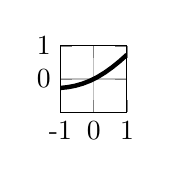
\begin{tikzpicture}
\begin{axis}[
	xmin=-1,xmax=1,
	ymin=-1,ymax=1,
	ytick={0, 1},
	yticklabels={0,1},
	xtick={-1, 0, 1},
	xticklabels={-1,0,1},
	width=.2\textwidth,
	height=.2\textwidth,
	grid=both,
	]
	\addplot [ultra thick,domain=-1:1, samples=10]{x * (1/ (1+exp(-x)))};
	%\addplot [ultra thick,domain=-1:0.004, samples=10]{exp(x)-1};
\end{axis}
\end{tikzpicture}}
		\scalebox{.9}{% This file was created by tikzplotlib v0.9.6.
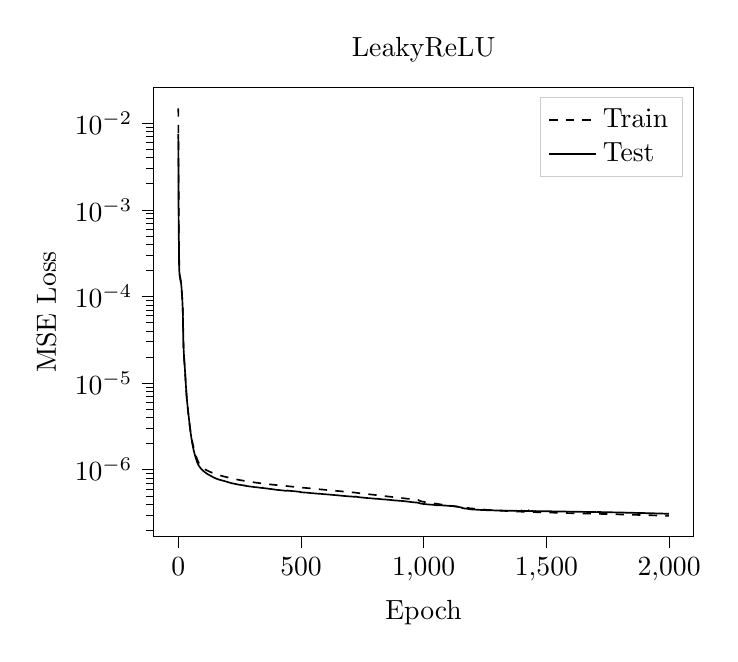
\begin{tikzpicture}

\begin{axis}[
legend cell align={left},
legend style={fill opacity=0.8, draw opacity=1, text opacity=1, draw=white!80!black},
log basis y={10},
tick align=outside,
tick pos=left,
title={LeakyReLU},
x grid style={white!69.0196078431373!black},
xlabel={Epoch},
xmin=-99.95, xmax=2098.95,
xtick style={color=black},
y grid style={white!69.0196078431373!black},
ylabel={MSE Loss},
ymin=1.70791572547231e-07, ymax=0.0255488360607333,
ymode=log,
ytick style={color=black}
]
\addplot [semithick, black, dashed]
table {%
0 0.0148644272387028
1 0.00333734963089228
2 0.000750602022744715
3 0.000331206021597609
4 0.000207027630618541
5 0.000178633672956494
6 0.000169817901289207
7 0.000163992511370452
8 0.000158428034461394
9 0.000152649684350763
10 0.00014641946539632
11 0.000139678969775559
12 0.000132290519177332
13 0.000124130066971702
14 0.000115090908722777
15 0.000105129859155568
16 9.44059219655173e-05
17 8.3223627305415e-05
18 7.19209145499917e-05
19 5.9600600565318e-05
20 3.97648699054116e-05
21 2.79329969580431e-05
22 2.30094661437761e-05
23 2.03421610876831e-05
24 1.84593141466394e-05
25 1.68413770406914e-05
26 1.53453861585149e-05
27 1.39403166676857e-05
28 1.26229516022249e-05
29 1.13995978695129e-05
30 1.02803903319e-05
31 9.27881336542669e-06
32 8.39881708566281e-06
33 7.63946547408523e-06
34 6.99144020211406e-06
35 6.44443027772468e-06
36 5.98577112725707e-06
37 5.59156097597224e-06
38 5.24542606149225e-06
39 4.93420651258703e-06
40 4.64607294458119e-06
41 4.3748265293857e-06
42 4.12039487252969e-06
43 3.8861643104724e-06
44 3.67260006765946e-06
45 3.47844123746199e-06
46 3.30225424215769e-06
47 3.13898743047503e-06
48 2.98947314900033e-06
49 2.85182592716637e-06
50 2.72762016362549e-06
51 2.61402293841684e-06
52 2.5099930834358e-06
53 2.4150706948376e-06
54 2.32725503445863e-06
55 2.24705749849363e-06
56 2.17294952142311e-06
57 2.1049157987818e-06
58 2.04128094503631e-06
59 1.98188082879369e-06
60 1.92642735390791e-06
61 1.87334052122878e-06
62 1.8232318035416e-06
63 1.77455488795886e-06
64 1.72895183959554e-06
65 1.6861234399812e-06
66 1.64616296456188e-06
67 1.60743973128774e-06
68 1.57055133320227e-06
69 1.53456863944257e-06
70 1.50125948277946e-06
71 1.46981972636695e-06
72 1.44026260474561e-06
73 1.41147857323176e-06
74 1.38520127060815e-06
75 1.36031598432851e-06
76 1.33676044734443e-06
77 1.3148170181978e-06
78 1.29389646752998e-06
79 1.27433537693378e-06
80 1.25646557970072e-06
81 1.2384471808673e-06
82 1.22196116879536e-06
83 1.20638403507201e-06
84 1.19190501561661e-06
85 1.17844780726273e-06
86 1.16571712385394e-06
87 1.1539444496691e-06
88 1.14418008098482e-06
89 1.13371917686322e-06
90 1.12408099414552e-06
91 1.1148123342366e-06
92 1.10610182443338e-06
93 1.09807221093661e-06
94 1.09074505050444e-06
95 1.0839480192999e-06
96 1.07734048407337e-06
97 1.07122849982488e-06
98 1.06452712140026e-06
99 1.05868495271011e-06
100 1.05291415113129e-06
101 1.04752679743569e-06
102 1.04214536537484e-06
103 1.0370281889891e-06
104 1.032027342319e-06
105 1.02744560464885e-06
106 1.02279366436164e-06
107 1.01820316623957e-06
108 1.01401851819105e-06
109 1.00975107895351e-06
110 1.0057904348173e-06
111 1.00208405191893e-06
112 9.98241210339756e-07
113 9.94370888776075e-07
114 9.90925482227567e-07
115 9.87395259301138e-07
116 9.83861367387817e-07
117 9.80596522055066e-07
118 9.77371847994846e-07
119 9.74262288309546e-07
120 9.71295058008082e-07
121 9.6826150081597e-07
122 9.6523639768975e-07
123 9.62448905852398e-07
124 9.59402455919189e-07
125 9.56513887700794e-07
126 9.53868651834e-07
127 9.51033602575535e-07
128 9.48263187240173e-07
129 9.45597496013306e-07
130 9.42952355558191e-07
131 9.40403254958255e-07
132 9.37919000818965e-07
133 9.35487815553415e-07
134 9.33048935337411e-07
135 9.30687048224854e-07
136 9.28267845239361e-07
137 9.25884347481087e-07
138 9.23637938910815e-07
139 9.21227984548523e-07
140 9.18846620891145e-07
141 9.16484609831514e-07
142 9.14296656503666e-07
143 9.12058346074218e-07
144 9.09871440057941e-07
145 9.07786169506153e-07
146 9.05647660886189e-07
147 9.03635627963695e-07
148 9.01687872357115e-07
149 8.9950875153022e-07
150 8.97521426622916e-07
151 8.95521069111282e-07
152 8.93521177772527e-07
153 8.91522843943449e-07
154 8.89579697087584e-07
155 8.87620785334775e-07
156 8.85896789583285e-07
157 8.83988975402872e-07
158 8.82208881847646e-07
159 8.80398930121373e-07
160 8.78538994015798e-07
161 8.76403134441262e-07
162 8.7463463688664e-07
163 8.72705812355434e-07
164 8.70566312670462e-07
165 8.68765719644671e-07
166 8.67004338203969e-07
167 8.653048454903e-07
168 8.63512691211099e-07
169 8.61854937170392e-07
170 8.60151822223543e-07
171 8.58458075072122e-07
172 8.56818996624043e-07
173 8.55136690688596e-07
174 8.53585893565878e-07
175 8.5187854273272e-07
176 8.50357727699702e-07
177 8.48755360294717e-07
178 8.47190044481749e-07
179 8.45670013589483e-07
180 8.44131327013997e-07
181 8.42642410887606e-07
182 8.41175444946884e-07
183 8.39656288363244e-07
184 8.38167764982245e-07
185 8.36532800619239e-07
186 8.35078147304102e-07
187 8.33758716908051e-07
188 8.32371983960911e-07
189 8.30889671789237e-07
190 8.29568857710683e-07
191 8.28064573511256e-07
192 8.26631372348174e-07
193 8.25454969628936e-07
194 8.24060114283043e-07
195 8.22638993369651e-07
196 8.2126220449652e-07
197 8.19915930264869e-07
198 8.20267484073156e-07
199 8.18703642607943e-07
200 8.17248432568363e-07
201 8.15823900992996e-07
202 8.14442585394204e-07
203 8.13095293437982e-07
204 8.11669069307186e-07
205 8.10307857349812e-07
206 8.09004709736882e-07
207 8.07590666070723e-07
208 8.06252364142779e-07
209 8.04654392212001e-07
210 8.0335848272739e-07
211 8.02302690658507e-07
212 8.00962444145625e-07
213 7.99703646720218e-07
214 7.98452317255283e-07
215 7.97217591738786e-07
216 7.96002158963915e-07
217 7.9481069326448e-07
218 7.93627711118461e-07
219 7.92467858858004e-07
220 7.91300207737322e-07
221 7.90077528890265e-07
222 7.88920517678093e-07
223 7.87720634576772e-07
224 7.86578616626343e-07
225 7.85441414691945e-07
226 7.84363267499089e-07
227 7.83269696910338e-07
228 7.82192492366107e-07
229 7.81227263516371e-07
230 7.80163437795522e-07
231 7.79063238198319e-07
232 7.78027706374473e-07
233 7.76964129954649e-07
234 7.75930989362905e-07
235 7.74893729442283e-07
236 7.73837977973813e-07
237 7.72835657613768e-07
238 7.71838034495431e-07
239 7.70846074615861e-07
240 7.69821481426902e-07
241 7.68822976212391e-07
242 7.67821201534957e-07
243 7.66846018862566e-07
244 7.65887867913762e-07
245 7.64930361214056e-07
246 7.63921686242952e-07
247 7.63010957257393e-07
248 7.62070085571054e-07
249 7.61139531945787e-07
250 7.60420157376984e-07
251 7.59426636150806e-07
252 7.58426511922039e-07
253 7.57507968302207e-07
254 7.56569720863354e-07
255 7.55625533727766e-07
256 7.54756878393437e-07
257 7.53833237837398e-07
258 7.52968338730398e-07
259 7.52147672017145e-07
260 7.51202681499308e-07
261 7.50205559867823e-07
262 7.4943015475526e-07
263 7.48610954261153e-07
264 7.47677468453389e-07
265 7.46997857405063e-07
266 7.46052829256882e-07
267 7.45165411899507e-07
268 7.44340018613343e-07
269 7.43665318836406e-07
270 7.42747071726058e-07
271 7.4204888295526e-07
272 7.41131473191103e-07
273 7.40440178674362e-07
274 7.39578193176271e-07
275 7.3881461977976e-07
276 7.37799187660926e-07
277 7.37035187341917e-07
278 7.36253217098692e-07
279 7.35415127010697e-07
280 7.34686662354989e-07
281 7.33878230974483e-07
282 7.33114714989824e-07
283 7.32347263181055e-07
284 7.31621643978997e-07
285 7.30857068063529e-07
286 7.30129704550109e-07
287 7.29444917936917e-07
288 7.28688947859268e-07
289 7.28014880451156e-07
290 7.27137706519443e-07
291 7.2640715151806e-07
292 7.25708816418091e-07
293 7.25009155303269e-07
294 7.24293989392777e-07
295 7.23561567397724e-07
296 7.2286156442658e-07
297 7.22185449788526e-07
298 7.21465641959185e-07
299 7.20789148289214e-07
300 7.20108953458976e-07
301 7.19449026178154e-07
302 7.18764739445987e-07
303 7.18094917701251e-07
304 7.17464760171538e-07
305 7.16808219209497e-07
306 7.16184726542224e-07
307 7.15528395758724e-07
308 7.14873352649192e-07
309 7.14168571732898e-07
310 7.13574344160861e-07
311 7.1287063936154e-07
312 7.12281224224398e-07
313 7.11596599359154e-07
314 7.1101726477707e-07
315 7.10344048059142e-07
316 7.09744001042623e-07
317 7.09173813802977e-07
318 7.08501808716733e-07
319 7.07896837610633e-07
320 7.07197004814475e-07
321 7.06599812318132e-07
322 7.05917090755293e-07
323 7.05374840876516e-07
324 7.04819606951901e-07
325 7.04185838287685e-07
326 7.03570776934725e-07
327 7.02973159619091e-07
328 7.02457169694526e-07
329 7.01814170426474e-07
330 7.01159818504493e-07
331 7.00675139412965e-07
332 7.00100038670826e-07
333 6.9944516293674e-07
334 6.98911392788659e-07
335 6.98320728275803e-07
336 6.97682788128873e-07
337 6.97246098184223e-07
338 6.96686453053985e-07
339 6.96352869169914e-07
340 6.95526991592033e-07
341 6.9484590517277e-07
342 6.94304655056044e-07
343 6.9400206361081e-07
344 6.92970413965099e-07
345 6.93037260532492e-07
346 6.92013609636888e-07
347 6.91989935560855e-07
348 6.90816037362652e-07
349 6.9062005174203e-07
350 6.89722630539791e-07
351 6.89461848594419e-07
352 6.88598280333963e-07
353 6.88385519012513e-07
354 6.87496540834331e-07
355 6.87273249681653e-07
356 6.86344381364279e-07
357 6.85784922154653e-07
358 6.85309239756293e-07
359 6.8513359936162e-07
360 6.84244536785172e-07
361 6.84097153609287e-07
362 6.83162119059943e-07
363 6.82782644759072e-07
364 6.82589405883505e-07
365 6.8159318890082e-07
366 6.81068037124533e-07
367 6.80618575174208e-07
368 6.80053423749882e-07
369 6.79640693476813e-07
370 6.79050741510423e-07
371 6.78609955187426e-07
372 6.78057203842286e-07
373 6.77662977224713e-07
374 6.77112505997002e-07
375 6.76636222607385e-07
376 6.76250711990178e-07
377 6.75681376677062e-07
378 6.75209785029551e-07
379 6.74681991128523e-07
380 6.74513683136979e-07
381 6.73722616213013e-07
382 6.73302310929102e-07
383 6.72808587580676e-07
384 6.72407056214297e-07
385 6.71915421463609e-07
386 6.71427296765614e-07
387 6.71025953465687e-07
388 6.7049164735522e-07
389 6.70016919258387e-07
390 6.69557675067267e-07
391 6.69086867844726e-07
392 6.68597802928161e-07
393 6.68190762553422e-07
394 6.67692410345921e-07
395 6.67240023972226e-07
396 6.66790877019707e-07
397 6.66323490648324e-07
398 6.65903456606998e-07
399 6.65471397070405e-07
400 6.65007362329106e-07
401 6.64616963959475e-07
402 6.64189005348703e-07
403 6.63769749593257e-07
404 6.63356940961535e-07
405 6.62935873677384e-07
406 6.6251740221901e-07
407 6.62097921363625e-07
408 6.61683327294327e-07
409 6.61271375818728e-07
410 6.60858302936163e-07
411 6.60460645164562e-07
412 6.6005227745336e-07
413 6.59639243394849e-07
414 6.5922696452958e-07
415 6.58827367658432e-07
416 6.58425498315296e-07
417 6.5801929646625e-07
418 6.57625117895577e-07
419 6.57224236348952e-07
420 6.5661854195298e-07
421 6.56017475847648e-07
422 6.55518018916723e-07
423 6.55074278228085e-07
424 6.54699447096618e-07
425 6.54264191396692e-07
426 6.53816869700563e-07
427 6.53326964823009e-07
428 6.52873706030732e-07
429 6.52448715413811e-07
430 6.51987482811478e-07
431 6.51630326260033e-07
432 6.51166140116288e-07
433 6.50728281328838e-07
434 6.50352801045528e-07
435 6.49924126832957e-07
436 6.49520926629066e-07
437 6.49109188529451e-07
438 6.48725988511956e-07
439 6.48329360970479e-07
440 6.47936029650964e-07
441 6.47537012639532e-07
442 6.47503992468046e-07
443 6.47304684633809e-07
444 6.46791755926301e-07
445 6.46174046053716e-07
446 6.45631595219243e-07
447 6.45148015280483e-07
448 6.4464382931817e-07
449 6.44142668491554e-07
450 6.4371638593741e-07
451 6.4329291483034e-07
452 6.42818815379087e-07
453 6.4243620757054e-07
454 6.41965242266451e-07
455 6.41560947940434e-07
456 6.4108713894484e-07
457 6.40711664800619e-07
458 6.40245212196078e-07
459 6.39877146284107e-07
460 6.39416840158447e-07
461 6.38994611691146e-07
462 6.38533215393977e-07
463 6.38164307375177e-07
464 6.37705450529324e-07
465 6.37337720817754e-07
466 6.36884023322182e-07
467 6.36565714486892e-07
468 6.35994193231681e-07
469 6.35576846804042e-07
470 6.35110142454209e-07
471 6.34726450087442e-07
472 6.34274996968998e-07
473 6.33879317220476e-07
474 6.33418987760592e-07
475 6.33054129139055e-07
476 6.32558955913964e-07
477 6.32200792907156e-07
478 6.31757687600043e-07
479 6.31408914216536e-07
480 6.30983657273987e-07
481 6.30627516443383e-07
482 6.30192174881472e-07
483 6.29844393728263e-07
484 6.29409517699742e-07
485 6.29049891742284e-07
486 6.28630618265902e-07
487 6.28272145732467e-07
488 6.27843531489702e-07
489 6.27503492012238e-07
490 6.27080744209252e-07
491 6.26735475819373e-07
492 6.26306154430267e-07
493 6.25968398722421e-07
494 6.25546789720488e-07
495 6.25211958649174e-07
496 6.24788373372098e-07
497 6.24449280010708e-07
498 6.23962057133554e-07
499 6.23558213717956e-07
500 6.2311415599936e-07
501 6.22750209018363e-07
502 6.22350057199128e-07
503 6.21995929662944e-07
504 6.21580487475626e-07
505 6.21248701463628e-07
506 6.20837227202742e-07
507 6.20487857943885e-07
508 6.2008267529734e-07
509 6.19707906508893e-07
510 6.19289868623696e-07
511 6.18935109201857e-07
512 6.18535905800854e-07
513 6.18207967761464e-07
514 6.17810335668878e-07
515 6.17487754837498e-07
516 6.17048165693745e-07
517 6.16747607693924e-07
518 6.16425678529708e-07
519 6.16018937733998e-07
520 6.15564609120156e-07
521 6.15231403671146e-07
522 6.14803654485741e-07
523 6.14466882382203e-07
524 6.13926075146765e-07
525 6.13603320687162e-07
526 6.13164834007307e-07
527 6.12889333567068e-07
528 6.1244176531261e-07
529 6.12171113900217e-07
530 6.11737456409855e-07
531 6.11406537032622e-07
532 6.10991987372245e-07
533 6.10615803282144e-07
534 6.10182909497325e-07
535 6.09855354056776e-07
536 6.09413068900722e-07
537 6.09052085394524e-07
538 6.08653819512028e-07
539 6.08387478564509e-07
540 6.07961950962022e-07
541 6.07622395477847e-07
542 6.07195113218495e-07
543 6.06802663170924e-07
544 6.06362741748967e-07
545 6.06013731712096e-07
546 6.0559248045422e-07
547 6.05250503625143e-07
548 6.04716681607442e-07
549 6.04371584088881e-07
550 6.03937985829361e-07
551 6.03589404704508e-07
552 6.03148568060874e-07
553 6.02801457745272e-07
554 6.0235625136329e-07
555 6.01985544463446e-07
556 6.01539943161811e-07
557 6.01232765262694e-07
558 6.00807006364335e-07
559 6.00492180907963e-07
560 6.0005816808939e-07
561 5.99730774595741e-07
562 5.99223440019614e-07
563 5.98925630910685e-07
564 5.98511263632418e-07
565 5.98205809396291e-07
566 5.97765539339434e-07
567 5.97455265236135e-07
568 5.97010945085685e-07
569 5.9672484819373e-07
570 5.96299604083583e-07
571 5.96071399556308e-07
572 5.95513366789646e-07
573 5.95187032928379e-07
574 5.947183740318e-07
575 5.94433451610144e-07
576 5.93983866451708e-07
577 5.93703354780928e-07
578 5.93230489997154e-07
579 5.92965793160261e-07
580 5.92490404656587e-07
581 5.92217652197746e-07
582 5.9175461059624e-07
583 5.91483319766439e-07
584 5.91055219629766e-07
585 5.9077541931174e-07
586 5.90313007251098e-07
587 5.90037488734652e-07
588 5.89601683429919e-07
589 5.89313242372214e-07
590 5.88861738904711e-07
591 5.88606085244692e-07
592 5.88205910432293e-07
593 5.87919526992664e-07
594 5.8745086768397e-07
595 5.87203168748829e-07
596 5.86743687904345e-07
597 5.86504606161498e-07
598 5.86034405827718e-07
599 5.85759843318101e-07
600 5.85295431378086e-07
601 5.85048269172717e-07
602 5.84578794146751e-07
603 5.84336741496827e-07
604 5.83889424504491e-07
605 5.8371987589112e-07
606 5.83250819758518e-07
607 5.82936998782202e-07
608 5.82475648911895e-07
609 5.822194414975e-07
610 5.81760691360955e-07
611 5.81514034749375e-07
612 5.8107778048111e-07
613 5.80798643440517e-07
614 5.8034996423828e-07
615 5.8007643750102e-07
616 5.79669754557699e-07
617 5.79423551016589e-07
618 5.78947847898803e-07
619 5.7868813833295e-07
620 5.78234088450813e-07
621 5.77960293540514e-07
622 5.7753287774176e-07
623 5.77290330667779e-07
624 5.76830392489569e-07
625 5.76586579811078e-07
626 5.76101825032538e-07
627 5.75859893572783e-07
628 5.75397084972451e-07
629 5.75150781202183e-07
630 5.74713401903182e-07
631 5.7447310602754e-07
632 5.74012735526708e-07
633 5.73774994833798e-07
634 5.73327271069957e-07
635 5.73114834153898e-07
636 5.72660245197199e-07
637 5.7240989970353e-07
638 5.71956064860046e-07
639 5.71697264476256e-07
640 5.71240307664311e-07
641 5.70994088292309e-07
642 5.70539148810667e-07
643 5.70304007425193e-07
644 5.69833525858598e-07
645 5.69588442289159e-07
646 5.69132603871481e-07
647 5.68892071527216e-07
648 5.68438184046727e-07
649 5.68201071160956e-07
650 5.67769946428598e-07
651 5.67519301142738e-07
652 5.6707707179271e-07
653 5.66797595681123e-07
654 5.66352859991071e-07
655 5.66096162472718e-07
656 5.65686599273363e-07
657 5.65438366834314e-07
658 5.65017211897612e-07
659 5.64772737391195e-07
660 5.64293594010223e-07
661 5.64047870213358e-07
662 5.63645380410094e-07
663 5.63384342626705e-07
664 5.62980142362335e-07
665 5.62727795866635e-07
666 5.62271209290088e-07
667 5.62005503908836e-07
668 5.61633367738068e-07
669 5.61361019336459e-07
670 5.60907587512816e-07
671 5.60647555943206e-07
672 5.60207655595946e-07
673 5.59965208736912e-07
674 5.59675780166913e-07
675 5.59391941266085e-07
676 5.58971077055048e-07
677 5.58727743012355e-07
678 5.58255349702108e-07
679 5.5799404208301e-07
680 5.5754053700241e-07
681 5.57285783443717e-07
682 5.56846114776022e-07
683 5.56599550662895e-07
684 5.56152776738372e-07
685 5.55905638606191e-07
686 5.55450992109741e-07
687 5.55227351341614e-07
688 5.54761071512644e-07
689 5.54549272450799e-07
690 5.54089646058742e-07
691 5.53867962665322e-07
692 5.53422880528842e-07
693 5.5320079773935e-07
694 5.5274819114004e-07
695 5.52521287801255e-07
696 5.5206996151469e-07
697 5.51794728323784e-07
698 5.51397915060647e-07
699 5.5119633870504e-07
700 5.50707732926981e-07
701 5.50483585669781e-07
702 5.5005929785068e-07
703 5.49791805909194e-07
704 5.49363092531507e-07
705 5.49153537050984e-07
706 5.48734435838583e-07
707 5.48524624861102e-07
708 5.48033714892426e-07
709 5.47864530929587e-07
710 5.47407044180659e-07
711 5.47192967673027e-07
712 5.46663945314663e-07
713 5.46469165058738e-07
714 5.46026377676867e-07
715 5.45797743370713e-07
716 5.45408502446776e-07
717 5.45146161812227e-07
718 5.44686208826306e-07
719 5.4444843793533e-07
720 5.44042121731536e-07
721 5.44187411392727e-07
722 5.43547544765488e-07
723 5.42903439722409e-07
724 5.42304797178872e-07
725 5.41774102529757e-07
726 5.41298678271573e-07
727 5.40787423858546e-07
728 5.40312020774536e-07
729 5.39910445837677e-07
730 5.39371933314214e-07
731 5.39032324013533e-07
732 5.38397320511308e-07
733 5.38005847772638e-07
734 5.37580982125974e-07
735 5.37113240582698e-07
736 5.36665524890623e-07
737 5.3628786932336e-07
738 5.35821611535425e-07
739 5.3551504601046e-07
740 5.34989343293546e-07
741 5.34692306075613e-07
742 5.34238284117805e-07
743 5.33852620080211e-07
744 5.33480754000948e-07
745 5.33024487040734e-07
746 5.32662216912172e-07
747 5.32245440751922e-07
748 5.31847421598286e-07
749 5.31583600732688e-07
750 5.31042589130948e-07
751 5.30784487636993e-07
752 5.30310267848222e-07
753 5.30027119310716e-07
754 5.29521326086524e-07
755 5.29201154762404e-07
756 5.28709079290479e-07
757 5.28442658435324e-07
758 5.27953152186456e-07
759 5.27690907290435e-07
760 5.27205177448309e-07
761 5.26892414683289e-07
762 5.26405703695332e-07
763 5.26151932234598e-07
764 5.25638900228387e-07
765 5.2538255179968e-07
766 5.24913538470173e-07
767 5.24627415103396e-07
768 5.24143547863787e-07
769 5.23870203437582e-07
770 5.23359917082189e-07
771 5.23059499315082e-07
772 5.22546751852815e-07
773 5.22258667359665e-07
774 5.21781591501735e-07
775 5.21461515333499e-07
776 5.21047451144341e-07
777 5.20667105519124e-07
778 5.20264812351456e-07
779 5.19935537340643e-07
780 5.19469053031685e-07
781 5.19178764761818e-07
782 5.18717480986197e-07
783 5.18486472344648e-07
784 5.18063059260498e-07
785 5.1770965706055e-07
786 5.17317782481541e-07
787 5.17047028139928e-07
788 5.16598040718463e-07
789 5.16272202006007e-07
790 5.15890133598873e-07
791 5.1559194417905e-07
792 5.15092240675585e-07
793 5.14856525086316e-07
794 5.14366608740602e-07
795 5.14138488711069e-07
796 5.1369179050198e-07
797 5.133947706355e-07
798 5.1297357916269e-07
799 5.1269512967167e-07
800 5.12259364455758e-07
801 5.1196938757414e-07
802 5.11423140920897e-07
803 5.11186035765832e-07
804 5.108558257092e-07
805 5.10589589111987e-07
806 5.10150635591344e-07
807 5.09905413366596e-07
808 5.09488112413692e-07
809 5.0918477496964e-07
810 5.08788510359182e-07
811 5.08506359878424e-07
812 5.08111304810654e-07
813 5.07820337901421e-07
814 5.07405267313743e-07
815 5.07125847690304e-07
816 5.06688020934121e-07
817 5.06418203016779e-07
818 5.05994589261149e-07
819 5.05725315562699e-07
820 5.05358103424669e-07
821 5.05075605559568e-07
822 5.04433651911995e-07
823 5.04046690537052e-07
824 5.03614987664491e-07
825 5.03243534893727e-07
826 5.02741254081229e-07
827 5.02363778650761e-07
828 5.0181188987608e-07
829 5.01155536113629e-07
830 5.00639151781002e-07
831 5.00094774650961e-07
832 4.99718042917152e-07
833 4.99335891149144e-07
834 4.98984696335469e-07
835 4.98626764695587e-07
836 4.98176735277411e-07
837 4.97781516273221e-07
838 4.97396944084016e-07
839 4.97024179267669e-07
840 4.96623089802029e-07
841 4.9619203473128e-07
842 4.95837466530702e-07
843 4.95356492848487e-07
844 4.94947353985253e-07
845 4.94624493896367e-07
846 4.94189927721322e-07
847 4.93753210434988e-07
848 4.93364277460273e-07
849 4.93005060846485e-07
850 4.92574361317111e-07
851 4.92261623520562e-07
852 4.91839595838428e-07
853 4.91472612594634e-07
854 4.91078210103524e-07
855 4.90717624558101e-07
856 4.90344198198045e-07
857 4.89971666482347e-07
858 4.89575231455319e-07
859 4.89207917780732e-07
860 4.8886572173501e-07
861 4.88452469610934e-07
862 4.88092318505551e-07
863 4.87744442438043e-07
864 4.87433638966195e-07
865 4.87001789679198e-07
866 4.86642392530712e-07
867 4.86256370052729e-07
868 4.85970414203507e-07
869 4.85520277266005e-07
870 4.85194746914885e-07
871 4.84795060486931e-07
872 4.8450660469257e-07
873 4.84076300665492e-07
874 4.83778275267355e-07
875 4.83363721940577e-07
876 4.83014998721387e-07
877 4.82567401576262e-07
878 4.82165626024766e-07
879 4.81873086187079e-07
880 4.81442710679403e-07
881 4.81068505791882e-07
882 4.80751659097223e-07
883 4.80426024751068e-07
884 4.80023959966047e-07
885 4.796470899322e-07
886 4.79263505340555e-07
887 4.78941620059459e-07
888 4.78609426863841e-07
889 4.78185967480727e-07
890 4.77746801095691e-07
891 4.77495924258164e-07
892 4.77138562104074e-07
893 4.76734690607827e-07
894 4.76396770054066e-07
895 4.76033359916528e-07
896 4.75629839783664e-07
897 4.7529189306772e-07
898 4.75028509299591e-07
899 4.74598706588836e-07
900 4.74232805089514e-07
901 4.73863658129403e-07
902 4.73503784462537e-07
903 4.73214756993912e-07
904 4.72819625130683e-07
905 4.72471625627691e-07
906 4.72109106254948e-07
907 4.71858331579256e-07
908 4.71460500378384e-07
909 4.71170830238066e-07
910 4.70762764038568e-07
911 4.70420068552357e-07
912 4.70193007899411e-07
913 4.69732255297117e-07
914 4.69328430256155e-07
915 4.69008694636841e-07
916 4.68750404195362e-07
917 4.68294574801575e-07
918 4.67943003044979e-07
919 4.67603833413932e-07
920 4.6726228927696e-07
921 4.67024187202014e-07
922 4.66549970042252e-07
923 4.66196309801603e-07
924 4.65849686818842e-07
925 4.65657492441096e-07
926 4.6514172363743e-07
927 4.6484536051139e-07
928 4.64433631279348e-07
929 4.64285816306642e-07
930 4.63722799736388e-07
931 4.63393946745327e-07
932 4.63028061346904e-07
933 4.62868733578148e-07
934 4.62303378796491e-07
935 4.61944667279113e-07
936 4.61593672994809e-07
937 4.61465650644755e-07
938 4.60907661022247e-07
939 4.60600220463903e-07
940 4.6021002177099e-07
941 4.59943743535973e-07
942 4.59559822544975e-07
943 4.59191470767451e-07
944 4.58823429340782e-07
945 4.58568544715376e-07
946 4.58253700188038e-07
947 4.57775354860246e-07
948 4.57443201653973e-07
949 4.57248985242131e-07
950 4.56788529746177e-07
951 4.56413603274086e-07
952 4.56049293291017e-07
953 4.55718323721044e-07
954 4.55268215404203e-07
955 4.54996806922736e-07
956 4.54735002605844e-07
957 4.54331303615163e-07
958 4.53895254239001e-07
959 4.53565293838665e-07
960 4.53295954372379e-07
961 4.52920906539589e-07
962 4.52633616063736e-07
963 4.52290183702075e-07
964 4.51753988272685e-07
965 4.51526366362032e-07
966 4.51130627027396e-07
967 4.50771134154593e-07
968 4.504252864308e-07
969 4.50136636729326e-07
970 4.49762404599596e-07
971 4.4941030162704e-07
972 4.49197960506353e-07
973 4.48709193022978e-07
974 4.48431595785337e-07
975 4.48094398578291e-07
976 4.4774719881957e-07
977 4.47329700762111e-07
978 4.47107959246296e-07
979 4.45311586858566e-07
980 4.42267165908561e-07
981 4.41070118895937e-07
982 4.40142427535761e-07
983 4.39295067039325e-07
984 4.38643088358504e-07
985 4.36957642435232e-07
986 4.35593108733201e-07
987 4.34702707551082e-07
988 4.33474616400531e-07
989 4.32703829105208e-07
990 4.32289674321851e-07
991 4.31421487917305e-07
992 4.30638353520862e-07
993 4.29790937616303e-07
994 4.28880565337408e-07
995 4.28401135650347e-07
996 4.27787201346064e-07
997 4.27183281047405e-07
998 4.26694344852763e-07
999 4.2636703791743e-07
1000 4.25715062704057e-07
1001 4.25246964852022e-07
1002 4.24845545552444e-07
1003 4.24308888639757e-07
1004 4.23964489456807e-07
1005 4.23528313447719e-07
1006 4.22984388706027e-07
1007 4.225807735736e-07
1008 4.22272394018819e-07
1009 4.21754303317812e-07
1010 4.21508764347323e-07
1011 4.20943191883794e-07
1012 4.20336185086967e-07
1013 4.19858491000014e-07
1014 4.1939585513262e-07
1015 4.19118752247982e-07
1016 4.18458747006412e-07
1017 4.18054913723154e-07
1018 4.17623710319504e-07
1019 4.17345911756684e-07
1020 4.1684959707311e-07
1021 4.16479742753495e-07
1022 4.16232555934926e-07
1023 4.1558006725495e-07
1024 4.15228342362184e-07
1025 4.15229226916836e-07
1026 4.14557101422019e-07
1027 4.14188685837757e-07
1028 4.137652676377e-07
1029 4.13552009050022e-07
1030 4.13012748268216e-07
1031 4.12709136242029e-07
1032 4.12403044578014e-07
1033 4.12024662679755e-07
1034 4.11686833103886e-07
1035 4.11097062823274e-07
1036 4.11059944923409e-07
1037 4.10612124298382e-07
1038 4.10058860069284e-07
1039 4.09830215701845e-07
1040 4.09236865593243e-07
1041 4.08992037847611e-07
1042 4.08167432894402e-07
1043 4.07781641527549e-07
1044 4.07499990515703e-07
1045 4.06984923031928e-07
1046 4.06398309621636e-07
1047 4.06130208801869e-07
1048 4.05844250565224e-07
1049 4.05634460008741e-07
1050 4.05246325286157e-07
1051 4.04832696432322e-07
1052 4.04589275078138e-07
1053 4.04333232410181e-07
1054 4.0388796469415e-07
1055 4.0364550858385e-07
1056 4.03237107150289e-07
1057 4.02781264639884e-07
1058 4.02806778183162e-07
1059 4.01965887306233e-07
1060 4.01510594059573e-07
1061 4.00938951401031e-07
1062 4.00572816303679e-07
1063 4.00084503098697e-07
1064 3.99712360263038e-07
1065 3.99338280672623e-07
1066 3.98853183725123e-07
1067 3.98574016514885e-07
1068 3.98165261131567e-07
1069 3.9791169047021e-07
1070 3.97472268019783e-07
1071 3.97099917236687e-07
1072 3.96636626348368e-07
1073 3.96424626273983e-07
1074 3.96097346396118e-07
1075 3.9559541224321e-07
1076 3.95176014095e-07
1077 3.9485332503375e-07
1078 3.94414255026732e-07
1079 3.94210009147855e-07
1080 3.93897365086104e-07
1081 3.94073744161005e-07
1082 3.92707131538828e-07
1083 3.92443426818545e-07
1084 3.92263928972625e-07
1085 3.91811526995411e-07
1086 3.91438045383552e-07
1087 3.91222988042728e-07
1088 3.90767820931615e-07
1089 3.90392165115827e-07
1090 3.90058417949035e-07
1091 3.89737378512223e-07
1092 3.89416854545743e-07
1093 3.89117823701213e-07
1094 3.88820500631937e-07
1095 3.8860628005466e-07
1096 3.88284502861325e-07
1097 3.8773857590968e-07
1098 3.87415723963613e-07
1099 3.87093581963427e-07
1100 3.86819972547414e-07
1101 3.8655951644273e-07
1102 3.86174517572613e-07
1103 3.85863807807141e-07
1104 3.85488108648246e-07
1105 3.85170436189242e-07
1106 3.84719854892523e-07
1107 3.84718544239604e-07
1108 3.84024391522075e-07
1109 3.83650835544813e-07
1110 3.83382792236375e-07
1111 3.83040656402045e-07
1112 3.82753346201525e-07
1113 3.82416109658834e-07
1114 3.82373510092293e-07
1115 3.81928717573032e-07
1116 3.81812806622861e-07
1117 3.81203720849044e-07
1118 3.80974276083634e-07
1119 3.80499999522499e-07
1120 3.80254684600345e-07
1121 3.7986570839621e-07
1122 3.79738977585475e-07
1123 3.79311346222266e-07
1124 3.79113227651828e-07
1125 3.7877028913158e-07
1126 3.7836112139189e-07
1127 3.77982800344512e-07
1128 3.78119575884739e-07
1129 3.77618890752274e-07
1130 3.77162941205711e-07
1131 3.7672415348311e-07
1132 3.76497530936604e-07
1133 3.76125739251165e-07
1134 3.76046060509339e-07
1135 3.75449260715754e-07
1136 3.75253203273473e-07
1137 3.74917057925472e-07
1138 3.74622404692104e-07
1139 3.7428821870833e-07
1140 3.74284405566527e-07
1141 3.7362211756431e-07
1142 3.73366226355643e-07
1143 3.7307717714441e-07
1144 3.72830825526194e-07
1145 3.72424451896336e-07
1146 3.72418132940311e-07
1147 3.7213091133026e-07
1148 3.71713215983505e-07
1149 3.71452914535553e-07
1150 3.71178188473209e-07
1151 3.70909355197568e-07
1152 3.7053996253178e-07
1153 3.7024783931372e-07
1154 3.69873657135145e-07
1155 3.69505103691381e-07
1156 3.69253701279604e-07
1157 3.68807387985726e-07
1158 3.68308296941677e-07
1159 3.68027352777744e-07
1160 3.67674302410137e-07
1161 3.67324845441885e-07
1162 3.67093079873371e-07
1163 3.66817634045447e-07
1164 3.66528322331305e-07
1165 3.66260036969379e-07
1166 3.65974232906296e-07
1167 3.6576783041653e-07
1168 3.65757778212128e-07
1169 3.65359265160237e-07
1170 3.64927529545866e-07
1171 3.64539682664144e-07
1172 3.64183218977132e-07
1173 3.63697715883404e-07
1174 3.63248774547742e-07
1175 3.6295745351822e-07
1176 3.62568556099063e-07
1177 3.62408816727111e-07
1178 3.61902688752025e-07
1179 3.61626319858033e-07
1180 3.61431617832864e-07
1181 3.61043409355943e-07
1182 3.60797934973789e-07
1183 3.60444958303674e-07
1184 3.60248958102716e-07
1185 3.59936896558111e-07
1186 3.59555476705964e-07
1187 3.59374415111802e-07
1188 3.58965990059801e-07
1189 3.58561037799632e-07
1190 3.58322259430111e-07
1191 3.57995596175442e-07
1192 3.57769069225355e-07
1193 3.57516862507623e-07
1194 3.57242059436658e-07
1195 3.57074874074215e-07
1196 3.56846210692652e-07
1197 3.56573667573912e-07
1198 3.56349139025269e-07
1199 3.56250705209504e-07
1200 3.55875810996054e-07
1201 3.55695545266599e-07
1202 3.55430612060559e-07
1203 3.55257044837742e-07
1204 3.55036958367805e-07
1205 3.54729504230988e-07
1206 3.54575795554979e-07
1207 3.54330831036975e-07
1208 3.54163805582175e-07
1209 3.53934707121084e-07
1210 3.53760961694149e-07
1211 3.53559004942383e-07
1212 3.53348837684564e-07
1213 3.53167481250694e-07
1214 3.52938252042634e-07
1215 3.52749994284807e-07
1216 3.52585982660969e-07
1217 3.52407975704239e-07
1218 3.52169507415567e-07
1219 3.51973961208785e-07
1220 3.51758787793699e-07
1221 3.51502807255599e-07
1222 3.51306851079869e-07
1223 3.51152501224306e-07
1224 3.50899278146244e-07
1225 3.50712421344213e-07
1226 3.50511307786405e-07
1227 3.50340402199834e-07
1228 3.50174203553877e-07
1229 3.49866230820339e-07
1230 3.49717217829948e-07
1231 3.49455526098552e-07
1232 3.49285141943767e-07
1233 3.49022042534841e-07
1234 3.48864000585536e-07
1235 3.48586736819811e-07
1236 3.48445087801963e-07
1237 3.4818345256582e-07
1238 3.4813231708597e-07
1239 3.48225087407172e-07
1240 3.47784275412266e-07
1241 3.47621228634409e-07
1242 3.47436047128724e-07
1243 3.47174164780029e-07
1244 3.4713033489453e-07
1245 3.46868865150896e-07
1246 3.46827497459401e-07
1247 3.46505921307028e-07
1248 3.46359151983222e-07
1249 3.46254663149637e-07
1250 3.45973173082825e-07
1251 3.45937462505219e-07
1252 3.45498902305508e-07
1253 3.45166767687033e-07
1254 3.44957258484158e-07
1255 3.44883514060257e-07
1256 3.44460587214712e-07
1257 3.44291111339601e-07
1258 3.44095388989274e-07
1259 3.43959172042219e-07
1260 3.43810874603889e-07
1261 3.43625585593088e-07
1262 3.4358059095041e-07
1263 3.43212996391173e-07
1264 3.43100552726128e-07
1265 3.43164890786341e-07
1266 3.42759536103188e-07
1267 3.42773568959842e-07
1268 3.42893875803441e-07
1269 3.42620055683085e-07
1270 3.4228207704956e-07
1271 3.42381971016437e-07
1272 3.42026907333093e-07
1273 3.41821995505143e-07
1274 3.41681918825998e-07
1275 3.41623348312226e-07
1276 3.41340164766279e-07
1277 3.41217368152513e-07
1278 3.4106308705617e-07
1279 3.40976784691804e-07
1280 3.4080946687709e-07
1281 3.40802128683038e-07
1282 3.40702538146331e-07
1283 3.40402227969605e-07
1284 3.40182375417442e-07
1285 3.40091809910348e-07
1286 3.39915428099857e-07
1287 3.39853421358782e-07
1288 3.39670542125248e-07
1289 3.39502068037234e-07
1290 3.39417640304873e-07
1291 3.39291082688931e-07
1292 3.39082802483404e-07
1293 3.39148367032749e-07
1294 3.38892482638187e-07
1295 3.38829270653207e-07
1296 3.38648870496172e-07
1297 3.38687307959162e-07
1298 3.38240516690291e-07
1299 3.38366272508495e-07
1300 3.38001319256875e-07
1301 3.37920434652972e-07
1302 3.37841576858011e-07
1303 3.37823672431625e-07
1304 3.3753024310812e-07
1305 3.37429006513901e-07
1306 3.37313680958573e-07
1307 3.37218410713547e-07
1308 3.3711456779173e-07
1309 3.36903703832547e-07
1310 3.36891655976501e-07
1311 3.36800533723647e-07
1312 3.3659107230477e-07
1313 3.36524350629475e-07
1314 3.36588194052467e-07
1315 3.3621560381647e-07
1316 3.36227974422343e-07
1317 3.35964050691473e-07
1318 3.3590479741008e-07
1319 3.35959069197145e-07
1320 3.3563762396227e-07
1321 3.3570893973689e-07
1322 3.35404225104696e-07
1323 3.35420296941891e-07
1324 3.35310365571218e-07
1325 3.35162345130868e-07
1326 3.35112290805739e-07
1327 3.35035934234895e-07
1328 3.34863490358828e-07
1329 3.3453481590584e-07
1330 3.34560684706275e-07
1331 3.34415690289802e-07
1332 3.34436880429223e-07
1333 3.34342135964505e-07
1334 3.3411748800205e-07
1335 3.33874048642713e-07
1336 3.33887440966407e-07
1337 3.33762760767797e-07
1338 3.33557971053722e-07
1339 3.33469831780064e-07
1340 3.333395412497e-07
1341 3.33323065277114e-07
1342 3.33160623696926e-07
1343 3.33146326468636e-07
1344 3.32997630756893e-07
1345 3.32955995787643e-07
1346 3.32814051603236e-07
1347 3.3281026241383e-07
1348 3.32498229099087e-07
1349 3.32466849641833e-07
1350 3.32391293376588e-07
1351 3.32259941842494e-07
1352 3.32225231424843e-07
1353 3.32077841072476e-07
1354 3.32005728822082e-07
1355 3.31841624657159e-07
1356 3.31928920083158e-07
1357 3.31696651336699e-07
1358 3.31594936319846e-07
1359 3.31512106100718e-07
1360 3.31501672782508e-07
1361 3.31306970345224e-07
1362 3.31109461292556e-07
1363 3.31097948134129e-07
1364 3.30970878607673e-07
1365 3.30980586127794e-07
1366 3.30741880006258e-07
1367 3.30851606676674e-07
1368 3.30796594830929e-07
1369 3.30699608035445e-07
1370 3.30719720835759e-07
1371 3.30387201159965e-07
1372 3.30450337429511e-07
1373 3.30311810436967e-07
1374 3.30153512820175e-07
1375 3.30106311636769e-07
1376 3.29856312781374e-07
1377 3.29988769316003e-07
1378 3.29781705133314e-07
1379 3.29643474735519e-07
1380 3.29575802702209e-07
1381 3.29661901908196e-07
1382 3.29384446779102e-07
1383 3.29194402652888e-07
1384 3.29174147502442e-07
1385 3.2892577434751e-07
1386 3.28936768760002e-07
1387 3.28938984807792e-07
1388 3.28622693380964e-07
1389 3.28631047203487e-07
1390 3.28663743040636e-07
1391 3.28427028435385e-07
1392 3.28422970120812e-07
1393 3.28242727945849e-07
1394 3.28273688822378e-07
1395 3.28060710437228e-07
1396 3.28181209752643e-07
1397 3.27843347669443e-07
1398 3.27852344064183e-07
1399 3.2829578710647e-07
1400 3.28064131871031e-07
1401 3.27575198873831e-07
1402 3.27536251177207e-07
1403 3.27420939470358e-07
1404 3.2741662860758e-07
1405 3.27226250057322e-07
1406 3.27265470950522e-07
1407 3.27060519509814e-07
1408 3.27155963816494e-07
1409 3.26972195878739e-07
1410 3.26970149174599e-07
1411 3.26863787329046e-07
1412 3.26782263279313e-07
1413 3.26663281526862e-07
1414 3.26726319926252e-07
1415 3.26526487675949e-07
1416 3.26492149575586e-07
1417 3.26372519289464e-07
1418 3.26526134919902e-07
1419 3.26281027753339e-07
1420 3.26192927850855e-07
1421 3.26291698719672e-07
1422 3.26084324228759e-07
1423 3.26008133122002e-07
1424 3.25901496594838e-07
1425 3.25920014496717e-07
1426 3.25827025420722e-07
1427 3.25687300644972e-07
1428 3.26062531392779e-07
1429 3.25628018437385e-07
1430 3.2562565948524e-07
1431 3.25352808538071e-07
1432 3.25273427925765e-07
1433 3.25321335537865e-07
1434 3.25138781853695e-07
1435 3.25163706605736e-07
1436 3.25108598367763e-07
1437 3.24951548883234e-07
1438 3.24962143700702e-07
1439 3.24829615223621e-07
1440 3.25090830237684e-07
1441 3.24795452463889e-07
1442 3.24721973001374e-07
1443 3.24631089085869e-07
1444 3.2456479630838e-07
1445 3.24642600965319e-07
1446 3.24464752360143e-07
1447 3.24280949101308e-07
1448 3.24287003877544e-07
1449 3.24112054428838e-07
1450 3.24111770346747e-07
1451 3.24085712215094e-07
1452 3.24007598564435e-07
1453 3.23942609085748e-07
1454 3.2425689070692e-07
1455 3.24005999075894e-07
1456 3.2361437681061e-07
1457 3.23674683443187e-07
1458 3.2351173168621e-07
1459 3.23458068230309e-07
1460 3.23479223787615e-07
1461 3.23319206508188e-07
1462 3.23341757123785e-07
1463 3.23198218914911e-07
1464 3.23270411364263e-07
1465 3.23068304957985e-07
1466 3.23069969759615e-07
1467 3.23080898247952e-07
1468 3.22920393280413e-07
1469 3.22857342759164e-07
1470 3.22821105278592e-07
1471 3.22736950657543e-07
1472 3.22708666047333e-07
1473 3.22561187388715e-07
1474 3.2244668971515e-07
1475 3.22537584629856e-07
1476 3.2234767521544e-07
1477 3.22275564869301e-07
1478 3.22260968928845e-07
1479 3.22126612921636e-07
1480 3.22229529807316e-07
1481 3.22072553345265e-07
1482 3.21982909795793e-07
1483 3.22065536110472e-07
1484 3.21898457372072e-07
1485 3.21896749035488e-07
1486 3.21722710658889e-07
1487 3.21782155673134e-07
1488 3.21655857334235e-07
1489 3.21540387943742e-07
1490 3.21610780446235e-07
1491 3.21390835281932e-07
1492 3.21524363023684e-07
1493 3.2131500721988e-07
1494 3.21355409518276e-07
1495 3.21366403952084e-07
1496 3.2123143392937e-07
1497 3.21120906043859e-07
1498 3.21158807956579e-07
1499 3.21153666938301e-07
1500 3.20950832460198e-07
1501 3.20903004755735e-07
1502 3.20872954738149e-07
1503 3.20826174515787e-07
1504 3.20889407738889e-07
1505 3.20691754176039e-07
1506 3.20632478270966e-07
1507 3.20689533992891e-07
1508 3.20531748741359e-07
1509 3.20420759095441e-07
1510 3.20409114671349e-07
1511 3.20266171875971e-07
1512 3.20465706288076e-07
1513 3.20110148116726e-07
1514 3.20114583416853e-07
1515 3.20165127867256e-07
1516 3.19939939579683e-07
1517 3.19961420586878e-07
1518 3.19884608479981e-07
1519 3.19850591942838e-07
1520 3.19754192247501e-07
1521 3.19659825549934e-07
1522 3.19542471565626e-07
1523 3.19522271233552e-07
1524 3.1952513759137e-07
1525 3.19442034466988e-07
1526 3.19308484826308e-07
1527 3.1926437686991e-07
1528 3.19322454409132e-07
1529 3.19090354508944e-07
1530 3.1914903206598e-07
1531 3.19048935295996e-07
1532 3.18985352343759e-07
1533 3.18868792234639e-07
1534 3.18823600416351e-07
1535 3.18969249775591e-07
1536 3.18667938614681e-07
1537 3.18681215368599e-07
1538 3.18583031408082e-07
1539 3.18604212985463e-07
1540 3.18418979318835e-07
1541 3.1837250921285e-07
1542 3.18446168733999e-07
1543 3.18235732798655e-07
1544 3.1822591738262e-07
1545 3.18200680894165e-07
1546 3.1824155977489e-07
1547 3.18066145119644e-07
1548 3.17969742788193e-07
1549 3.18165659486169e-07
1550 3.17947992201084e-07
1551 3.17837663196485e-07
1552 3.17799422937526e-07
1553 3.17749503373932e-07
1554 3.17725981943795e-07
1555 3.17654856075933e-07
1556 3.1745046170073e-07
1557 3.17432104033344e-07
1558 3.17421537815221e-07
1559 3.17527532082806e-07
1560 3.17331122076325e-07
1561 3.1720363658394e-07
1562 3.17183404767718e-07
1563 3.17158790586802e-07
1564 3.17055461529492e-07
1565 3.16942562001543e-07
1566 3.17018796096136e-07
1567 3.16961415805395e-07
1568 3.16822705308084e-07
1569 3.1673548660649e-07
1570 3.1669173003479e-07
1571 3.16677336762439e-07
1572 3.16670457948476e-07
1573 3.16591517567133e-07
1574 3.16468353531718e-07
1575 3.1647522484235e-07
1576 3.16485809719325e-07
1577 3.16312855744627e-07
1578 3.16247700645533e-07
1579 3.16220362343245e-07
1580 3.16188260690353e-07
1581 3.16109383760477e-07
1582 3.16156887059549e-07
1583 3.16068575635597e-07
1584 3.15873102728403e-07
1585 3.15975026701665e-07
1586 3.15779102422198e-07
1587 3.15815761297245e-07
1588 3.15671033362719e-07
1589 3.15747237223718e-07
1590 3.15594334843183e-07
1591 3.15574065240298e-07
1592 3.15509907693468e-07
1593 3.15438409678848e-07
1594 3.15528669297294e-07
1595 3.15281006912471e-07
1596 3.15268012819558e-07
1597 3.15299097358945e-07
1598 3.15124351033091e-07
1599 3.15032143682004e-07
1600 3.14968358829049e-07
1601 3.15165431196363e-07
1602 3.14933268924733e-07
1603 3.14842066984511e-07
1604 3.14790559968969e-07
1605 3.14805405700724e-07
1606 3.14614502052279e-07
1607 3.14726759292228e-07
1608 3.14509374746308e-07
1609 3.14674117142033e-07
1610 3.14487810229025e-07
1611 3.14573937380658e-07
1612 3.14394223408954e-07
1613 3.14384523349531e-07
1614 3.14405950419427e-07
1615 3.14362090051645e-07
1616 3.14184010818508e-07
1617 3.14153501655312e-07
1618 3.14043581461476e-07
1619 3.14059152806578e-07
1620 3.13894354967204e-07
1621 3.14038598588695e-07
1622 3.14356346699185e-07
1623 3.14293879981165e-07
1624 3.14200238548779e-07
1625 3.14175397726046e-07
1626 3.13871269945309e-07
1627 3.1394368009785e-07
1628 3.13715297558304e-07
1629 3.1380694633043e-07
1630 3.13606534241728e-07
1631 3.13643690411425e-07
1632 3.13666378573885e-07
1633 3.13586880650973e-07
1634 3.13423190370088e-07
1635 3.13455884217717e-07
1636 3.13332078007988e-07
1637 3.13316120802654e-07
1638 3.13285314419431e-07
1639 3.13249966531259e-07
1640 3.13080791741527e-07
1641 3.13154238334334e-07
1642 3.12935718767449e-07
1643 3.13037454141352e-07
1644 3.12864478829056e-07
1645 3.12887611663371e-07
1646 3.12814163436315e-07
1647 3.12779923319795e-07
1648 3.12677243989867e-07
1649 3.12674668265345e-07
1650 3.12483081728487e-07
1651 3.13008835682638e-07
1652 3.12390567842158e-07
1653 3.12456071270617e-07
1654 3.1229574748437e-07
1655 3.12338921325761e-07
1656 3.12201615948027e-07
1657 3.12339854595223e-07
1658 3.12096956406549e-07
1659 3.12131471773114e-07
1660 3.11996117972058e-07
1661 3.12029497557376e-07
1662 3.11892367115263e-07
1663 3.12013563373625e-07
1664 3.11821396117296e-07
1665 3.11737066255091e-07
1666 3.11751752903433e-07
1667 3.11542458518943e-07
1668 3.11465470417716e-07
1669 3.11640546655667e-07
1670 3.11447121475794e-07
1671 3.113907667327e-07
1672 3.1128856271323e-07
1673 3.1143680404e-07
1674 3.11213553068512e-07
1675 3.11212113537351e-07
1676 3.11191033297575e-07
1677 3.11144864852508e-07
1678 3.11065440115499e-07
1679 3.11046119790603e-07
1680 3.10867254668779e-07
1681 3.11016560125665e-07
1682 3.10783246312951e-07
1683 3.10997557086523e-07
1684 3.10670550469183e-07
1685 3.10749519698561e-07
1686 3.10596976952127e-07
1687 3.10744832269449e-07
1688 3.10395399182539e-07
1689 3.10655381646541e-07
1690 3.10417983520495e-07
1691 3.10629784621597e-07
1692 3.10311370782301e-07
1693 3.1037526576938e-07
1694 3.10243405010624e-07
1695 3.10281405603519e-07
1696 3.10096623323375e-07
1697 3.10194989395995e-07
1698 3.10098258829328e-07
1699 3.10130593128122e-07
1700 3.09984979040223e-07
1701 3.09938632540252e-07
1702 3.09827980473187e-07
1703 3.09812695462597e-07
1704 3.096528067843e-07
1705 3.09828499311493e-07
1706 3.09625381632372e-07
1707 3.09750097500228e-07
1708 3.09600050115932e-07
1709 3.09845477801218e-07
1710 3.09658715913486e-07
1711 3.09539044295093e-07
1712 3.09400075131805e-07
1713 3.09725576833841e-07
1714 3.0916625053834e-07
1715 3.09483384377529e-07
1716 3.09334076376899e-07
1717 3.0918433626681e-07
1718 3.09062954308104e-07
1719 3.09123950380297e-07
1720 3.08976081434764e-07
1721 3.091337238601e-07
1722 3.08965229287139e-07
1723 3.09116053983871e-07
1724 3.08689637293469e-07
1725 3.08736328939574e-07
1726 3.08669552644858e-07
1727 3.08603466613988e-07
1728 3.08530398037021e-07
1729 3.08627115401805e-07
1730 3.08540636936527e-07
1731 3.08427530285371e-07
1732 3.08334022712131e-07
1733 3.08257495653663e-07
1734 3.08236750498736e-07
1735 3.0833639345218e-07
1736 3.08096456222984e-07
1737 3.08075279455977e-07
1738 3.08042506972583e-07
1739 3.08085389832513e-07
1740 3.07968706749762e-07
1741 3.07898931581008e-07
1742 3.07764628203699e-07
1743 3.07773813283063e-07
1744 3.07717376465177e-07
1745 3.07653958117271e-07
1746 3.0765865913196e-07
1747 3.07626101644587e-07
1748 3.07552278009382e-07
1749 3.0735350994604e-07
1750 3.07628058081377e-07
1751 3.07336489342447e-07
1752 3.07368682385345e-07
1753 3.07209660846297e-07
1754 3.07406639642238e-07
1755 3.0710762363384e-07
1756 3.07180690796827e-07
1757 3.06997296227962e-07
1758 3.07280588238257e-07
1759 3.06843731650019e-07
1760 3.06940378493437e-07
1761 3.06794261831556e-07
1762 3.06837595772436e-07
1763 3.06610467816881e-07
1764 3.06829234347106e-07
1765 3.06454595275341e-07
1766 3.06707944893958e-07
1767 3.06326688800596e-07
1768 3.06441866172236e-07
1769 3.06257395521925e-07
1770 3.0633805037894e-07
1771 3.06157528299877e-07
1772 3.06200772897114e-07
1773 3.0607316737985e-07
1774 3.06098561296153e-07
1775 3.06194833605389e-07
1776 3.06072450797501e-07
1777 3.06052589152728e-07
1778 3.0598369404089e-07
1779 3.05753781354667e-07
1780 3.05756770544008e-07
1781 3.05665897727181e-07
1782 3.05728093714208e-07
1783 3.05646801621151e-07
1784 3.05738369860364e-07
1785 3.05382987974667e-07
1786 3.05652452290417e-07
1787 3.0544395694676e-07
1788 3.05572961565304e-07
1789 3.05190016284484e-07
1790 3.05378717335714e-07
1791 3.05075413500333e-07
1792 3.05183546778665e-07
1793 3.05088814037902e-07
1794 3.05365793757062e-07
1795 3.05033719747883e-07
1796 3.05069139692193e-07
1797 3.04773875001274e-07
1798 3.04957178123288e-07
1799 3.04655040785917e-07
1800 3.04872247021137e-07
1801 3.04794242460105e-07
1802 3.04774771770155e-07
1803 3.04634256494296e-07
1804 3.046867968024e-07
1805 3.04623855846842e-07
1806 3.04478786084417e-07
1807 3.04440137668394e-07
1808 3.04489119187679e-07
1809 3.04337516880082e-07
1810 3.0426601318112e-07
1811 3.04229888918428e-07
1812 3.04097428177386e-07
1813 3.04338748520649e-07
1814 3.04042303426399e-07
1815 3.04046707569228e-07
1816 3.03893465911642e-07
1817 3.04108458379915e-07
1818 3.03728165427231e-07
1819 3.04069386402261e-07
1820 3.03660852303267e-07
1821 3.03650683463275e-07
1822 3.03544722548565e-07
1823 3.03597130113076e-07
1824 3.03506354299543e-07
1825 3.03322645812898e-07
1826 3.03617171937276e-07
1827 3.03360720117496e-07
1828 3.03249289061114e-07
1829 3.03108788607176e-07
1830 3.03273794429515e-07
1831 3.02977811173832e-07
1832 3.03072520843273e-07
1833 3.03012808892333e-07
1834 3.02839288991663e-07
1835 3.02869932504279e-07
1836 3.02772856940692e-07
1837 3.02604050183675e-07
1838 3.02785141101936e-07
1839 3.02697704505306e-07
1840 3.02647801603939e-07
1841 3.02386721486414e-07
1842 3.02443652245188e-07
1843 3.02288002671958e-07
1844 3.02339900542847e-07
1845 3.02194082941298e-07
1846 3.02256330741102e-07
1847 3.02109679132911e-07
1848 3.02255458365153e-07
1849 3.02030160554523e-07
1850 3.01960260415513e-07
1851 3.01962238040687e-07
1852 3.01846855450094e-07
1853 3.01791661499351e-07
1854 3.01770279023117e-07
1855 3.01849823351574e-07
1856 3.01669510847091e-07
1857 3.01545374682632e-07
1858 3.0151376973464e-07
1859 3.01416563644352e-07
1860 3.01456793536659e-07
1861 3.01289437224739e-07
1862 3.01354336748716e-07
1863 3.01205066875809e-07
1864 3.01245784264381e-07
1865 3.01109555174151e-07
1866 3.01183946696426e-07
1867 3.0100350952722e-07
1868 3.00976861971947e-07
1869 3.00884783449362e-07
1870 3.01047703374024e-07
1871 3.00773745493643e-07
1872 3.00733479228654e-07
1873 3.00692512261946e-07
1874 3.0063736996766e-07
1875 3.00572687713441e-07
1876 3.00503531029506e-07
1877 3.00603009335987e-07
1878 3.00401623185564e-07
1879 3.00343361367084e-07
1880 3.0032322746365e-07
1881 3.00249160275712e-07
1882 3.00184128789738e-07
1883 3.00211509483006e-07
1884 3.00067204264565e-07
1885 2.99960682831113e-07
1886 2.99978455828409e-07
1887 2.99902618976944e-07
1888 2.99820982888832e-07
1889 2.99946893044023e-07
1890 2.99692950321173e-07
1891 2.99725934681305e-07
1892 2.99663779735226e-07
1893 2.99518005547839e-07
1894 2.99473131434524e-07
1895 2.99465885760242e-07
1896 2.99575580086753e-07
1897 2.99349106128943e-07
1898 2.99262351035168e-07
1899 2.9926471443531e-07
1900 2.99133502601023e-07
1901 2.99155919819327e-07
1902 2.99006076474484e-07
1903 2.99133789390282e-07
1904 2.98925287424368e-07
1905 2.98941225764793e-07
1906 2.9879624715079e-07
1907 2.9895922090617e-07
1908 2.98671382864768e-07
1909 2.98679200191998e-07
1910 2.98591146808747e-07
1911 2.98603283383159e-07
1912 2.98482322143911e-07
1913 2.98465000426518e-07
1914 2.98486448997437e-07
1915 2.98328453361307e-07
1916 2.98258284743724e-07
1917 2.98272029993996e-07
1918 2.9815794463417e-07
1919 2.98116875256937e-07
1920 2.98200684603955e-07
1921 2.98044728452851e-07
1922 2.97941690746484e-07
1923 2.97912768431274e-07
1924 2.97862047318631e-07
1925 2.97789504678292e-07
1926 2.97767631202817e-07
1927 2.97833934823188e-07
1928 2.97641517363445e-07
1929 2.97627088585273e-07
1930 2.97398515307634e-07
1931 2.97637071803081e-07
1932 2.97316301185901e-07
1933 2.9743815220229e-07
1934 2.97396039492526e-07
1935 2.97155774788394e-07
1936 2.972102788803e-07
1937 2.97290856764221e-07
1938 2.97404336421891e-07
1939 2.97170349625731e-07
1940 2.97167980377822e-07
1941 2.97099185310401e-07
1942 2.9688234484837e-07
1943 2.96936517749202e-07
1944 2.96624542492907e-07
1945 2.97014116000582e-07
1946 2.96760317269218e-07
1947 2.96771138536656e-07
1948 2.96515731449176e-07
1949 2.9663090040799e-07
1950 2.9657164558472e-07
1951 2.9648336685284e-07
1952 2.96345633593376e-07
1953 2.9631420408549e-07
1954 2.96308615659768e-07
1955 2.9610010748371e-07
1956 2.9626472518629e-07
1957 2.9594645059916e-07
1958 2.96222448795902e-07
1959 2.95816891757283e-07
1960 2.95940765774105e-07
1961 2.95927517129257e-07
1962 2.95857750273854e-07
1963 2.95589895799253e-07
1964 2.95722840512269e-07
1965 2.95564092198219e-07
1966 2.95687444705095e-07
1967 2.95598649046269e-07
1968 2.95281853446738e-07
1969 2.95426976748558e-07
1970 2.95280896850159e-07
1971 2.95339915290072e-07
1972 2.95072210619196e-07
1973 2.95270798041258e-07
1974 2.95314228253574e-07
1975 2.94874492254849e-07
1976 2.95091132208825e-07
1977 2.95017232964767e-07
1978 2.94680657525248e-07
1979 2.94926457868883e-07
1980 2.94877394068749e-07
1981 2.94727112077453e-07
1982 2.94783511044727e-07
1983 2.94443454208704e-07
1984 2.94654638388181e-07
1985 2.94476714657321e-07
1986 2.94250058388457e-07
1987 2.94501699379168e-07
1988 2.94333003857616e-07
1989 2.94369915607717e-07
1990 2.94041497959086e-07
1991 2.94329573932828e-07
1992 2.93915225086039e-07
1993 2.94157941105766e-07
1994 2.93830951711982e-07
1995 2.94200619180174e-07
1996 2.936857129896e-07
1997 2.93928464543569e-07
1998 2.93554929328366e-07
1999 2.93835021608402e-07
};
\addlegendentry{Train}
\addplot [semithick, black]
table {%
0 0.00753973051905632
1 0.00112220819573849
2 0.000468270503915846
3 0.000248318043304607
4 0.000196054897969589
5 0.000182635383680463
6 0.000175974884768948
7 0.000170196057297289
8 0.000164347962709144
9 0.000158102775458246
10 0.000151328713400289
11 0.000143939119880088
12 0.000135805690661073
13 0.000126826635096222
14 0.000116909206553828
15 0.000106065410363954
16 9.45693464018404e-05
17 8.27783442218788e-05
18 7.09991290932521e-05
19 5.34280989086255e-05
20 3.48736466548871e-05
21 2.70838972937781e-05
22 2.34261042351136e-05
23 2.10563994187396e-05
24 1.91505496331956e-05
25 1.74150864040712e-05
26 1.57899085024837e-05
27 1.4260570424085e-05
28 1.28342044263263e-05
29 1.15238226499059e-05
30 1.03484580904478e-05
31 9.31648355617654e-06
32 8.4244802565081e-06
33 7.66550056141568e-06
34 7.02537090546684e-06
35 6.49239882477559e-06
36 6.04889373789774e-06
37 5.6686180869292e-06
38 5.33202228325536e-06
39 5.02388274981058e-06
40 4.73555610369658e-06
41 4.46143167209812e-06
42 4.2042379391205e-06
43 3.96772929889266e-06
44 3.74569435734884e-06
45 3.54057851836842e-06
46 3.34874425789167e-06
47 3.17393687510048e-06
48 3.00711985801172e-06
49 2.85115629594657e-06
50 2.70820146397455e-06
51 2.57695523941948e-06
52 2.45732940129528e-06
53 2.34697722589772e-06
54 2.24644918489503e-06
55 2.15642126022431e-06
56 2.07536072593939e-06
57 2.00157887775276e-06
58 1.93483720067888e-06
59 1.87310524779605e-06
60 1.81747736860416e-06
61 1.76416585873085e-06
62 1.71450949437713e-06
63 1.66393874678761e-06
64 1.61902949002979e-06
65 1.57635042796755e-06
66 1.53597272856132e-06
67 1.49878349020582e-06
68 1.46242962273391e-06
69 1.42895373755891e-06
70 1.39594453685277e-06
71 1.3655030670634e-06
72 1.33679156988364e-06
73 1.31049182527931e-06
74 1.28527665310685e-06
75 1.26176882986329e-06
76 1.23917902783433e-06
77 1.21781124562403e-06
78 1.19804451514938e-06
79 1.18025457140902e-06
80 1.16347860057431e-06
81 1.14884630875167e-06
82 1.13513533506193e-06
83 1.12148427433567e-06
84 1.10909911654744e-06
85 1.09722520846844e-06
86 1.08680535504391e-06
87 1.07779487734661e-06
88 1.06798745491687e-06
89 1.0591461432341e-06
90 1.04946332157851e-06
91 1.04017806279444e-06
92 1.03124625638884e-06
93 1.02401179447043e-06
94 1.01709372302139e-06
95 1.01110106243141e-06
96 1.00461545571306e-06
97 9.9822477750422e-07
98 9.91178580989072e-07
99 9.85206497716717e-07
100 9.79330479822238e-07
101 9.73711962615198e-07
102 9.6842666152952e-07
103 9.62833496487292e-07
104 9.57176780502778e-07
105 9.51723677644623e-07
106 9.46693774039886e-07
107 9.41506129947811e-07
108 9.36622143399291e-07
109 9.32237298911787e-07
110 9.27754456370167e-07
111 9.2338621016097e-07
112 9.18905527669267e-07
113 9.14647330318985e-07
114 9.10284541077999e-07
115 9.05852459709422e-07
116 9.01851592516323e-07
117 8.97969584912062e-07
118 8.9437349970467e-07
119 8.90859382707276e-07
120 8.87361977675027e-07
121 8.84108544596529e-07
122 8.80847039752553e-07
123 8.77792672326905e-07
124 8.75034515956941e-07
125 8.71993620421563e-07
126 8.6885069094933e-07
127 8.65411493577994e-07
128 8.61983494360175e-07
129 8.58633711686707e-07
130 8.55235782637465e-07
131 8.52439086429513e-07
132 8.49383695822326e-07
133 8.46391742470587e-07
134 8.43058558075427e-07
135 8.40330869777972e-07
136 8.37373477224901e-07
137 8.34073318856099e-07
138 8.31444708637719e-07
139 8.28168595035095e-07
140 8.24674941668491e-07
141 8.21597041067434e-07
142 8.18812679881376e-07
143 8.16037527329172e-07
144 8.13379756436916e-07
145 8.10917413218704e-07
146 8.08692959708424e-07
147 8.06455602742062e-07
148 8.04063347459305e-07
149 8.01898124791478e-07
150 7.99877341250976e-07
151 7.97855761902611e-07
152 7.93996150605381e-07
153 7.92090304457815e-07
154 7.90204524037108e-07
155 7.88448744515335e-07
156 7.8662571922905e-07
157 7.84812414167391e-07
158 7.83166683504533e-07
159 7.81366054525279e-07
160 7.79670870088012e-07
161 7.77817717789731e-07
162 7.76199499341601e-07
163 7.72695557316183e-07
164 7.71276290834066e-07
165 7.69888686136255e-07
166 7.68412576235278e-07
167 7.67246433497348e-07
168 7.65786523970746e-07
169 7.64414210152609e-07
170 7.63057585118077e-07
171 7.61939531912503e-07
172 7.60599618843116e-07
173 7.59462125188293e-07
174 7.57970269660291e-07
175 7.56672307034023e-07
176 7.55323185330781e-07
177 7.54069162667292e-07
178 7.52821165406203e-07
179 7.51177594793262e-07
180 7.50122524095787e-07
181 7.48853892673651e-07
182 7.47541378132155e-07
183 7.46298724152439e-07
184 7.45096542686952e-07
185 7.43433758998435e-07
186 7.42178144719219e-07
187 7.40845052860095e-07
188 7.39376957881177e-07
189 7.38072571948578e-07
190 7.367052603513e-07
191 7.35390926820401e-07
192 7.33967340238451e-07
193 7.32892488031212e-07
194 7.31535862996679e-07
195 7.30236024537589e-07
196 7.29033047264238e-07
197 7.27816029666428e-07
198 7.24988012734684e-07
199 7.23389916856831e-07
200 7.22023912658187e-07
201 7.20725267910893e-07
202 7.18955107004149e-07
203 7.1768562293073e-07
204 7.16536021627689e-07
205 7.15177918664267e-07
206 7.13417307451891e-07
207 7.12029304850148e-07
208 7.106385737643e-07
209 7.09321398062457e-07
210 7.07866490756714e-07
211 7.06414482465334e-07
212 7.05020795521705e-07
213 7.03789964973112e-07
214 7.02657416695729e-07
215 7.01642193234875e-07
216 7.0059559220681e-07
217 6.99541942594806e-07
218 6.98493522577337e-07
219 6.97483983458369e-07
220 6.96430277002946e-07
221 6.9537026092803e-07
222 6.94374250542751e-07
223 6.93340439283929e-07
224 6.92399169111013e-07
225 6.91503885263955e-07
226 6.90593367380643e-07
227 6.89668070208427e-07
228 6.88744478338776e-07
229 6.87875967742002e-07
230 6.86725741161354e-07
231 6.85903955854883e-07
232 6.84980022924719e-07
233 6.84062001710117e-07
234 6.83333439610578e-07
235 6.8235937078498e-07
236 6.81429526139254e-07
237 6.80454547818954e-07
238 6.79621109611617e-07
239 6.7871377495976e-07
240 6.77916318636562e-07
241 6.76921388276241e-07
242 6.75902015245811e-07
243 6.74823866120278e-07
244 6.7370353917795e-07
245 6.72691953695903e-07
246 6.71726127166039e-07
247 6.70744213948637e-07
248 6.69871099034935e-07
249 6.72031546855578e-07
250 6.70690155857301e-07
251 6.69639689476753e-07
252 6.68999462050124e-07
253 6.68087579924759e-07
254 6.67388292185933e-07
255 6.66726919007488e-07
256 6.66127561999019e-07
257 6.65470906824339e-07
258 6.64767185298842e-07
259 6.63441596771008e-07
260 6.62973434373271e-07
261 6.62061552247906e-07
262 6.61454919281823e-07
263 6.61068497720407e-07
264 6.61724470774061e-07
265 6.58952558296733e-07
266 6.59717841244856e-07
267 6.58085696159105e-07
268 6.58671524433885e-07
269 6.56166093904176e-07
270 6.56984809666028e-07
271 6.54011273582e-07
272 6.55266092053353e-07
273 6.52840640213981e-07
274 6.52061373784818e-07
275 6.51268578621966e-07
276 6.50393246814929e-07
277 6.49677588171471e-07
278 6.49119670015352e-07
279 6.48301011096919e-07
280 6.47595754799113e-07
281 6.46984972263454e-07
282 6.46456669528561e-07
283 6.45655973130488e-07
284 6.45253635411791e-07
285 6.4456060044904e-07
286 6.43888370177592e-07
287 6.43389114429738e-07
288 6.4271335986632e-07
289 6.42151121610368e-07
290 6.41538690615562e-07
291 6.4093450191649e-07
292 6.40325310996559e-07
293 6.39762788523512e-07
294 6.39130803392618e-07
295 6.38554354281951e-07
296 6.37972220829397e-07
297 6.37482912679843e-07
298 6.36934373687836e-07
299 6.36625941297098e-07
300 6.36166703316121e-07
301 6.35588662589726e-07
302 6.35011815575126e-07
303 6.34480613825872e-07
304 6.33893080248527e-07
305 6.3339041389554e-07
306 6.32808280442987e-07
307 6.32347962437052e-07
308 6.31897137282067e-07
309 6.31307102594292e-07
310 6.30860199635208e-07
311 6.30320812433638e-07
312 6.29923192718707e-07
313 6.29366468274384e-07
314 6.29098167337361e-07
315 6.28548718850652e-07
316 6.27935833108495e-07
317 6.27676570275071e-07
318 6.27198858182965e-07
319 6.26764631306287e-07
320 6.26336884579359e-07
321 6.26092742095352e-07
322 6.25421307631768e-07
323 6.25200982540264e-07
324 6.24538984084211e-07
325 6.2408645362666e-07
326 6.23568666924257e-07
327 6.2338386896954e-07
328 6.22729260157939e-07
329 6.22348807155504e-07
330 6.21463414063328e-07
331 6.20857008470921e-07
332 6.20444041032897e-07
333 6.19560921677476e-07
334 6.18923820638884e-07
335 6.1863011069363e-07
336 6.17869204688759e-07
337 6.17271211922343e-07
338 6.17589478224545e-07
339 6.16797933616908e-07
340 6.16284125953825e-07
341 6.1576696452903e-07
342 6.16548732068622e-07
343 6.15661406300205e-07
344 6.19639990873111e-07
345 6.14997873071843e-07
346 6.14742987181671e-07
347 6.1387731875584e-07
348 6.13612712641043e-07
349 6.12701512636704e-07
350 6.12635403740569e-07
351 6.11905022651626e-07
352 6.11622510859888e-07
353 6.10903498454718e-07
354 6.10465065165045e-07
355 6.09881681157276e-07
356 6.09351388902724e-07
357 6.08766924869997e-07
358 6.0889499309269e-07
359 6.07850893175055e-07
360 6.07759545800945e-07
361 6.06990965934529e-07
362 6.06751541454287e-07
363 6.07233573646226e-07
364 6.05761272254313e-07
365 6.05284469656908e-07
366 6.04894239586429e-07
367 6.03976502588921e-07
368 6.03599744408712e-07
369 6.02681893724366e-07
370 6.02411205363751e-07
371 6.0164882142999e-07
372 6.01411386469408e-07
373 6.00940609274403e-07
374 5.99790951127943e-07
375 5.99411350776791e-07
376 5.99257873545866e-07
377 5.98584620092879e-07
378 5.98171823185112e-07
379 5.98674660068355e-07
380 5.97496580212464e-07
381 5.97092366660945e-07
382 5.96633810800995e-07
383 5.96106531247642e-07
384 5.9539610219872e-07
385 5.94904975059762e-07
386 5.9478185221451e-07
387 5.93918400682014e-07
388 5.93563015627296e-07
389 5.92967637658148e-07
390 5.92281821809593e-07
391 5.91532852922683e-07
392 5.90849140280625e-07
393 5.89895876146329e-07
394 5.89680098528333e-07
395 5.89053513522231e-07
396 5.88442162552383e-07
397 5.88034083648381e-07
398 5.87522549722053e-07
399 5.87033412102755e-07
400 5.86583382755634e-07
401 5.86184114581556e-07
402 5.85719760692882e-07
403 5.85337829761556e-07
404 5.8485562703936e-07
405 5.8445647255212e-07
406 5.84032022743486e-07
407 5.83635710427188e-07
408 5.83234168516356e-07
409 5.82854113417852e-07
410 5.82487075462268e-07
411 5.82135726290289e-07
412 5.817340138492e-07
413 5.81392043841333e-07
414 5.81019151013606e-07
415 5.80675646233431e-07
416 5.80324353904871e-07
417 5.79978404857684e-07
418 5.79624611418694e-07
419 5.79269283207395e-07
420 5.77967682602321e-07
421 5.77912430799188e-07
422 5.77620198782824e-07
423 5.77347748276225e-07
424 5.76952174924372e-07
425 5.76942568386585e-07
426 5.75843330352654e-07
427 5.75753006160085e-07
428 5.7528370689397e-07
429 5.74663317820523e-07
430 5.74493071781035e-07
431 5.7389354424231e-07
432 5.73478757814883e-07
433 5.73091028854833e-07
434 5.72712167468126e-07
435 5.72344163174421e-07
436 5.72184603697679e-07
437 5.71853377095977e-07
438 5.71574219065951e-07
439 5.71218663480977e-07
440 5.70883003092604e-07
441 5.70543704725424e-07
442 5.69968108266039e-07
443 5.7228982086599e-07
444 5.75097431010363e-07
445 5.73308568618813e-07
446 5.73026170513913e-07
447 5.72700855627772e-07
448 5.72862688841269e-07
449 5.72495821415941e-07
450 5.7208023918065e-07
451 5.71750661038095e-07
452 5.71410055272281e-07
453 5.70880388295336e-07
454 5.70543591038586e-07
455 5.70202473682002e-07
456 5.69837993680267e-07
457 5.69467317745875e-07
458 5.6907390444394e-07
459 5.68727386962564e-07
460 5.68349435070559e-07
461 5.67887241231801e-07
462 5.67526797112805e-07
463 5.67186987154855e-07
464 5.66821938718931e-07
465 5.66472806440288e-07
466 5.66099629395467e-07
467 5.6639885315235e-07
468 5.66148230518593e-07
469 5.65694847409759e-07
470 5.65560924314923e-07
471 5.65178481792827e-07
472 5.6479211707483e-07
473 5.64333447528043e-07
474 5.63935600439436e-07
475 5.63536389108776e-07
476 5.6306066653633e-07
477 5.62701018225198e-07
478 5.62344382615265e-07
479 5.61933632070577e-07
480 5.61566537271574e-07
481 5.61207627924887e-07
482 5.60866112664371e-07
483 5.60531020710187e-07
484 5.60074113309383e-07
485 5.59730779059464e-07
486 5.59369425445766e-07
487 5.589026841335e-07
488 5.58584474674717e-07
489 5.58265583094908e-07
490 5.57945952550654e-07
491 5.57147814106429e-07
492 5.56815393792931e-07
493 5.56509348825784e-07
494 5.56195743683929e-07
495 5.55819553937908e-07
496 5.55596727735974e-07
497 5.55281530978391e-07
498 5.50488095996116e-07
499 5.49982701159024e-07
500 5.49762091850425e-07
501 5.49415176465118e-07
502 5.49083665646322e-07
503 5.48751813767012e-07
504 5.48487207652215e-07
505 5.4817309091959e-07
506 5.47845218079601e-07
507 5.47486365576333e-07
508 5.47136266959569e-07
509 5.46749163277127e-07
510 5.46412479707215e-07
511 5.46135879631038e-07
512 5.45885086467024e-07
513 5.45636169135832e-07
514 5.45390889783448e-07
515 5.45149987374316e-07
516 5.44893339338159e-07
517 5.44644535693806e-07
518 5.44485317277577e-07
519 5.44289093795669e-07
520 5.44031195204298e-07
521 5.43795977137052e-07
522 5.43524492968572e-07
523 5.43278474651743e-07
524 5.4295725249176e-07
525 5.42684745141742e-07
526 5.42388818303152e-07
527 5.42121199487156e-07
528 5.41641384188551e-07
529 5.41364386208443e-07
530 5.41065958259423e-07
531 5.40804194315569e-07
532 5.40451082997606e-07
533 5.40090013601002e-07
534 5.39733434834488e-07
535 5.39495658813394e-07
536 5.39142831712525e-07
537 5.38686151685397e-07
538 5.37753464868729e-07
539 5.37496532615478e-07
540 5.37198445726972e-07
541 5.36898880909575e-07
542 5.36604034095944e-07
543 5.36304924025899e-07
544 5.36170944087644e-07
545 5.35901449438825e-07
546 5.35647131982842e-07
547 5.35405035861913e-07
548 5.35123888312228e-07
549 5.3489077345148e-07
550 5.34589560174936e-07
551 5.34299658738746e-07
552 5.33976560745941e-07
553 5.33651473233476e-07
554 5.33277841441304e-07
555 5.32955880316877e-07
556 5.32614535586617e-07
557 5.32285696408508e-07
558 5.31935484104906e-07
559 5.31808893811103e-07
560 5.31497505562584e-07
561 5.31214482180076e-07
562 5.30941235865612e-07
563 5.30726993019925e-07
564 5.30480690486002e-07
565 5.30156341937982e-07
566 5.29795443071635e-07
567 5.29466660736944e-07
568 5.29140322669264e-07
569 5.28860141457699e-07
570 5.28570012647833e-07
571 5.28704561020277e-07
572 5.28388284237735e-07
573 5.28122825471655e-07
574 5.27854467691213e-07
575 5.27604299804807e-07
576 5.27290183072182e-07
577 5.26993062521797e-07
578 5.26694407199102e-07
579 5.26379324128357e-07
580 5.26038945736218e-07
581 5.26062478911626e-07
582 5.25708685472637e-07
583 5.25377345184097e-07
584 5.25068116985494e-07
585 5.24763606790657e-07
586 5.24477457020112e-07
587 5.24232859788754e-07
588 5.23931703355629e-07
589 5.23625146797713e-07
590 5.2325805199871e-07
591 5.22926256962819e-07
592 5.22670347891108e-07
593 5.22430411820096e-07
594 5.22205482411664e-07
595 5.21926153851382e-07
596 5.21651770668541e-07
597 5.21391882557509e-07
598 5.21110223417054e-07
599 5.20821288318984e-07
600 5.20536332260235e-07
601 5.20243133905751e-07
602 5.19950560828875e-07
603 5.19649574926007e-07
604 5.19378033914109e-07
605 5.19090178840997e-07
606 5.18814886163455e-07
607 5.18623323841894e-07
608 5.18418119099806e-07
609 5.18128047133359e-07
610 5.17752027917595e-07
611 5.17340538408462e-07
612 5.17086959916924e-07
613 5.16733280164772e-07
614 5.16484419676999e-07
615 5.16164959663001e-07
616 5.15934345912683e-07
617 5.15618410190655e-07
618 5.15348574481322e-07
619 5.15001545409177e-07
620 5.14742339419172e-07
621 5.14380985805474e-07
622 5.14100577220233e-07
623 5.1376741794229e-07
624 5.13480927111232e-07
625 5.13164252424758e-07
626 5.12840074406995e-07
627 5.12517772222054e-07
628 5.12260271534615e-07
629 5.11989696860837e-07
630 5.11706446104654e-07
631 5.114287091601e-07
632 5.11188488871994e-07
633 5.10833672251465e-07
634 5.10555537402979e-07
635 5.10244660745229e-07
636 5.09940548454324e-07
637 5.09636493006838e-07
638 5.09357562350488e-07
639 5.09058281750185e-07
640 5.08773212004598e-07
641 5.08462562720524e-07
642 5.08220409756177e-07
643 5.07934885263239e-07
644 5.07665731674933e-07
645 5.07347749589826e-07
646 5.07051424847305e-07
647 5.06706442138238e-07
648 5.06409094214177e-07
649 5.06082244555728e-07
650 5.05586967847194e-07
651 5.05279047047225e-07
652 5.04912804899504e-07
653 5.0461960654502e-07
654 5.04350339269877e-07
655 5.04078684571141e-07
656 5.03778380789299e-07
657 5.03453861711023e-07
658 5.03183173350408e-07
659 5.02903446886194e-07
660 5.02635259636008e-07
661 5.02353998399485e-07
662 5.0201145995743e-07
663 5.01703880217974e-07
664 5.01414831433067e-07
665 5.01132547015004e-07
666 5.00854184792843e-07
667 5.00580597417866e-07
668 5.00313319662382e-07
669 5.00037344863813e-07
670 4.99740508530522e-07
671 4.99437135204062e-07
672 4.99133420817088e-07
673 4.98810891258472e-07
674 4.98344093102787e-07
675 4.98059307574295e-07
676 4.97784299113846e-07
677 4.97484109018842e-07
678 4.97205689953262e-07
679 4.96921074955026e-07
680 4.96653512982448e-07
681 4.96397547067318e-07
682 4.96113216286176e-07
683 4.95844915349153e-07
684 4.95445988235588e-07
685 4.95185133786435e-07
686 4.94928258376603e-07
687 4.94646371862473e-07
688 4.94382959459472e-07
689 4.94149219321116e-07
690 4.93913205446006e-07
691 4.93621996611182e-07
692 4.9339854513164e-07
693 4.93140873913944e-07
694 4.92886670144799e-07
695 4.9265509005636e-07
696 4.9241157284996e-07
697 4.92214780933864e-07
698 4.91906462229963e-07
699 4.91639298161317e-07
700 4.91398793656117e-07
701 4.91143794079107e-07
702 4.90874299430288e-07
703 4.90620550408494e-07
704 4.90403920139215e-07
705 4.90225204430317e-07
706 4.89965714223217e-07
707 4.89765227484895e-07
708 4.89555304739042e-07
709 4.89292574457068e-07
710 4.8900653837336e-07
711 4.88773537199449e-07
712 4.88596072045766e-07
713 4.88313389723771e-07
714 4.88048158331367e-07
715 4.87789918679482e-07
716 4.87718068598042e-07
717 4.87467730181379e-07
718 4.87157592488074e-07
719 4.86908504626626e-07
720 4.86739395455515e-07
721 4.9035327265301e-07
722 4.8937130259219e-07
723 4.88683895127906e-07
724 4.88091075112607e-07
725 4.87560612327798e-07
726 4.87181807784509e-07
727 4.86774524688371e-07
728 4.86325347992533e-07
729 4.85814950934582e-07
730 4.85278462747374e-07
731 4.84711392800818e-07
732 4.83731184885983e-07
733 4.83344479107473e-07
734 4.82700784232293e-07
735 4.8199734692389e-07
736 4.81474728530884e-07
737 4.81128040519252e-07
738 4.80775042888126e-07
739 4.80449784845405e-07
740 4.80148230508348e-07
741 4.79648349482886e-07
742 4.79336222269922e-07
743 4.79130790154159e-07
744 4.78748461318901e-07
745 4.78535980619199e-07
746 4.7814722847761e-07
747 4.77944809063047e-07
748 4.77572314139252e-07
749 4.77276557830919e-07
750 4.76959939987864e-07
751 4.76656538239695e-07
752 4.76327670639876e-07
753 4.76099359048021e-07
754 4.75810935540721e-07
755 4.75496108265361e-07
756 4.75241222375189e-07
757 4.74901327152111e-07
758 4.74757712254359e-07
759 4.74581554499309e-07
760 4.74156564678196e-07
761 4.73988080784693e-07
762 4.73577443926843e-07
763 4.73313804150166e-07
764 4.7300522965088e-07
765 4.72849905008843e-07
766 4.72359346304074e-07
767 4.72197285716902e-07
768 4.71739497243107e-07
769 4.71622769282476e-07
770 4.71186154982206e-07
771 4.71025487058796e-07
772 4.705592573373e-07
773 4.70404273755776e-07
774 4.70036354727199e-07
775 4.69815461201506e-07
776 4.69479800813133e-07
777 4.69214569420728e-07
778 4.68944875819943e-07
779 4.68757036742318e-07
780 4.68388975605194e-07
781 4.68251101892747e-07
782 4.6792413854746e-07
783 4.67840436613187e-07
784 4.6754936988691e-07
785 4.67280528937408e-07
786 4.67000290882424e-07
787 4.6691167199242e-07
788 4.66403179189001e-07
789 4.66438052626472e-07
790 4.66141386823438e-07
791 4.65845971575618e-07
792 4.65563999796359e-07
793 4.65293936713351e-07
794 4.65032712781976e-07
795 4.64832709212715e-07
796 4.64537720290537e-07
797 4.64353206552914e-07
798 4.6402956854763e-07
799 4.6386193730541e-07
800 4.63544324702525e-07
801 4.63368792225083e-07
802 4.62197505157746e-07
803 4.63238365000507e-07
804 4.63010422890875e-07
805 4.62780093357651e-07
806 4.62553202851268e-07
807 4.62369399656382e-07
808 4.62138984858029e-07
809 4.61882763147514e-07
810 4.61621652902977e-07
811 4.61430431641929e-07
812 4.61168752963204e-07
813 4.60986967709687e-07
814 4.60566013771313e-07
815 4.60498370102869e-07
816 4.60000904922708e-07
817 4.59818807030388e-07
818 4.59507020877936e-07
819 4.5933370529383e-07
820 4.59253016060757e-07
821 4.58802077218934e-07
822 4.58620291965417e-07
823 4.58379389556285e-07
824 4.57969264289204e-07
825 4.57600549452764e-07
826 4.57365047168423e-07
827 4.57144011534183e-07
828 4.56186228348088e-07
829 4.55713006886072e-07
830 4.5535782078332e-07
831 4.55219293371556e-07
832 4.54919273806809e-07
833 4.54778529501709e-07
834 4.54423144446992e-07
835 4.54672800742628e-07
836 4.54042691444556e-07
837 4.54658618309622e-07
838 4.54371019031896e-07
839 4.5443917429111e-07
840 4.53894074325945e-07
841 4.53660703669811e-07
842 4.53434012115395e-07
843 4.52985744914258e-07
844 4.5265531412042e-07
845 4.52406567319485e-07
846 4.52635077863306e-07
847 4.51929082601055e-07
848 4.51688919156368e-07
849 4.51882641527845e-07
850 4.51144387625391e-07
851 4.50953280051181e-07
852 4.50890837555562e-07
853 4.5038200369163e-07
854 4.50120410278032e-07
855 4.49875784624965e-07
856 4.4960756895307e-07
857 4.49480751285591e-07
858 4.49249512257666e-07
859 4.48852347290085e-07
860 4.48630657956528e-07
861 4.48390238716456e-07
862 4.48109716444378e-07
863 4.47919347834613e-07
864 4.48167185140846e-07
865 4.47330279484959e-07
866 4.4704779611493e-07
867 4.4680726318802e-07
868 4.47053110974593e-07
869 4.46262646391915e-07
870 4.46095583583883e-07
871 4.45744689159255e-07
872 4.45697338591344e-07
873 4.44990121195588e-07
874 4.44843465174927e-07
875 4.44735860583023e-07
876 4.44123088527704e-07
877 4.43760200141696e-07
878 4.43271886751972e-07
879 4.42927557742223e-07
880 4.42455586835422e-07
881 4.42182084725573e-07
882 4.42071325323923e-07
883 4.41869957512608e-07
884 4.42012634493949e-07
885 4.41322072219918e-07
886 4.40877670371265e-07
887 4.40820798530694e-07
888 4.40692247138941e-07
889 4.40118384403831e-07
890 4.40755911768065e-07
891 4.41077645518817e-07
892 4.40317108996169e-07
893 4.40241763044469e-07
894 4.40031186599299e-07
895 4.39644566085917e-07
896 4.39238561966704e-07
897 4.3902369384341e-07
898 4.39452350065039e-07
899 4.38834263150056e-07
900 4.38232859778509e-07
901 4.38103739952567e-07
902 4.37791868534987e-07
903 4.3765197688117e-07
904 4.37550909282436e-07
905 4.37032383615588e-07
906 4.36802878311937e-07
907 4.36617170862519e-07
908 4.3657419723786e-07
909 4.36586589103172e-07
910 4.35758664707464e-07
911 4.35354138517141e-07
912 4.35944542687139e-07
913 4.34869946275285e-07
914 4.3426041429484e-07
915 4.3410824446255e-07
916 4.34585984976366e-07
917 4.33799840493521e-07
918 4.33376925457196e-07
919 4.3310080855008e-07
920 4.32738090694329e-07
921 4.3338272348592e-07
922 4.32353772339411e-07
923 4.31905192499471e-07
924 4.31697571912082e-07
925 4.32046988407819e-07
926 4.3135784721926e-07
927 4.30627437708608e-07
928 4.30708809062708e-07
929 4.30718841926137e-07
930 4.3012587980229e-07
931 4.29711406013666e-07
932 4.29369634957766e-07
933 4.29573788096604e-07
934 4.28765986271173e-07
935 4.28233505544995e-07
936 4.2792984800144e-07
937 4.27856662099657e-07
938 4.27262165203501e-07
939 4.26790450092085e-07
940 4.2645586972867e-07
941 4.2637853425731e-07
942 4.25906961254441e-07
943 4.2573486780384e-07
944 4.25046863483658e-07
945 4.25191927888591e-07
946 4.24344307248248e-07
947 4.2433171643097e-07
948 4.23889844114456e-07
949 4.24288572276055e-07
950 4.2330083260822e-07
951 4.22973187141906e-07
952 4.2278438172616e-07
953 4.22927485033142e-07
954 4.22072588435185e-07
955 4.21752190504776e-07
956 4.21453052013021e-07
957 4.21782289095063e-07
958 4.20935521106003e-07
959 4.20448316162947e-07
960 4.19950026753213e-07
961 4.20321271121793e-07
962 4.19468477730334e-07
963 4.1958142560361e-07
964 4.19291581010839e-07
965 4.19652934624537e-07
966 4.18864516404938e-07
967 4.18473433683175e-07
968 4.18420711412182e-07
969 4.18452657413582e-07
970 4.17650625195165e-07
971 4.17404692143464e-07
972 4.17781279793417e-07
973 4.16791095858571e-07
974 4.16566791727746e-07
975 4.16282915693955e-07
976 4.1641538928161e-07
977 4.15741226333921e-07
978 4.15603864212244e-07
979 4.1441151665822e-07
980 4.13585439673625e-07
981 4.13371026297682e-07
982 4.1233724346057e-07
983 4.11554509582857e-07
984 4.10286105534396e-07
985 4.0890776631386e-07
986 4.07994320994476e-07
987 4.07470793106768e-07
988 4.06698319466159e-07
989 4.06120136631216e-07
990 4.05873976205839e-07
991 4.0532455614084e-07
992 4.05054890961765e-07
993 4.04554782562627e-07
994 4.04568481826573e-07
995 4.04260617870023e-07
996 4.03864390818853e-07
997 4.03381818614434e-07
998 4.02854539061082e-07
999 4.02539114929823e-07
1000 4.02528058884855e-07
1001 4.01836473429285e-07
1002 4.01639113079e-07
1003 4.01437972641361e-07
1004 4.01195961785561e-07
1005 4.01042882458569e-07
1006 4.00618603180192e-07
1007 4.00325546934255e-07
1008 3.9990516143007e-07
1009 3.99827399633068e-07
1010 3.99491057123669e-07
1011 3.99337693579582e-07
1012 3.98999333128813e-07
1013 3.98612399976628e-07
1014 3.9797109252504e-07
1015 3.98222482544952e-07
1016 3.97776716454246e-07
1017 3.97629520421106e-07
1018 3.97276750163655e-07
1019 3.96718206729929e-07
1020 3.96614012743157e-07
1021 3.96304642436007e-07
1022 3.96202807451118e-07
1023 3.95481151826971e-07
1024 3.9531104789603e-07
1025 3.94995396391096e-07
1026 3.95948205778041e-07
1027 3.95827669308346e-07
1028 3.95697668409412e-07
1029 3.95735241909279e-07
1030 3.95483851889367e-07
1031 3.95268955344363e-07
1032 3.94976098050392e-07
1033 3.94642682977064e-07
1034 3.94645184087494e-07
1035 3.94367646094906e-07
1036 3.9448022448596e-07
1037 3.9325175293925e-07
1038 3.93310813251446e-07
1039 3.92992944853177e-07
1040 3.93086878602844e-07
1041 3.92985413100178e-07
1042 3.92603425325433e-07
1043 3.92048946196155e-07
1044 3.91691514778358e-07
1045 3.91150962286702e-07
1046 3.90760419577418e-07
1047 3.90418080087329e-07
1048 3.90335742395109e-07
1049 3.89830091762633e-07
1050 3.90404835570735e-07
1051 3.8995347040327e-07
1052 3.90495785040912e-07
1053 3.89410644174859e-07
1054 3.89324497973575e-07
1055 3.89312504012196e-07
1056 3.8895402099115e-07
1057 3.88745661439316e-07
1058 3.89915015830411e-07
1059 3.8972345350885e-07
1060 3.90269235595042e-07
1061 3.90389487847642e-07
1062 3.90278046324966e-07
1063 3.90077303791259e-07
1064 3.89711914294821e-07
1065 3.89210413231922e-07
1066 3.88786276062092e-07
1067 3.88531447015339e-07
1068 3.88834308751029e-07
1069 3.88384847838097e-07
1070 3.88367851655858e-07
1071 3.88667302786416e-07
1072 3.88466446565872e-07
1073 3.88978747878355e-07
1074 3.87400149293171e-07
1075 3.87066251050783e-07
1076 3.88166995435313e-07
1077 3.8792362033746e-07
1078 3.88051120125965e-07
1079 3.87783330779712e-07
1080 3.87270631563297e-07
1081 3.85937454439045e-07
1082 3.86267771546045e-07
1083 3.86421788789448e-07
1084 3.86114436423668e-07
1085 3.8635283772237e-07
1086 3.86478120617539e-07
1087 3.86453876899395e-07
1088 3.85940950309305e-07
1089 3.85742879416284e-07
1090 3.85592016982628e-07
1091 3.85290064741639e-07
1092 3.85116948109498e-07
1093 3.84901369443469e-07
1094 3.84520859597615e-07
1095 3.84144129839115e-07
1096 3.83868098197127e-07
1097 3.83838823836413e-07
1098 3.83418409910519e-07
1099 3.83335134301888e-07
1100 3.83083659016847e-07
1101 3.82906506501968e-07
1102 3.82679672839004e-07
1103 3.82515622732171e-07
1104 3.82286998501513e-07
1105 3.82048511937683e-07
1106 3.81778392011256e-07
1107 3.81940964189198e-07
1108 3.81362696089127e-07
1109 3.80943248501353e-07
1110 3.80842493541422e-07
1111 3.80483555773026e-07
1112 3.80289435497616e-07
1113 3.80591160364929e-07
1114 3.80595281512797e-07
1115 3.80420317469543e-07
1116 3.80671338007232e-07
1117 3.80295375634887e-07
1118 3.80106030206662e-07
1119 3.79680130890847e-07
1120 3.79511533310506e-07
1121 3.79266282379831e-07
1122 3.78859965621814e-07
1123 3.78835835590507e-07
1124 3.78171222337187e-07
1125 3.78186257421476e-07
1126 3.7779082617817e-07
1127 3.77540260387832e-07
1128 3.77179333099775e-07
1129 3.77188882794144e-07
1130 3.76836339910369e-07
1131 3.76493716203186e-07
1132 3.7598451285703e-07
1133 3.75642912331386e-07
1134 3.7499904692595e-07
1135 3.74799640212586e-07
1136 3.74383489543106e-07
1137 3.74239988332192e-07
1138 3.73797405472942e-07
1139 3.73538426856612e-07
1140 3.73336348502562e-07
1141 3.73093143934966e-07
1142 3.72523004443792e-07
1143 3.72156023331627e-07
1144 3.7033905186945e-07
1145 3.6998730479354e-07
1146 3.69245071851765e-07
1147 3.69282304291119e-07
1148 3.68903812386634e-07
1149 3.68365817848826e-07
1150 3.67750061514016e-07
1151 3.67301822734589e-07
1152 3.66980856369992e-07
1153 3.66747968882919e-07
1154 3.64881003633855e-07
1155 3.65695143500488e-07
1156 3.64433049071522e-07
1157 3.60698436452367e-07
1158 3.60098937335351e-07
1159 3.60758207307299e-07
1160 3.59580184294828e-07
1161 3.59754750434149e-07
1162 3.58750213536041e-07
1163 3.59196235422132e-07
1164 3.57707449438749e-07
1165 3.57444179144295e-07
1166 3.56986078031696e-07
1167 3.56805514911684e-07
1168 3.57508668002993e-07
1169 3.57400665507157e-07
1170 3.57113350446525e-07
1171 3.57088964619834e-07
1172 3.56909708898456e-07
1173 3.56673325541124e-07
1174 3.56281731228592e-07
1175 3.54801557023166e-07
1176 3.55486690750695e-07
1177 3.54584898332178e-07
1178 3.54992891971051e-07
1179 3.53832746213811e-07
1180 3.53233417627052e-07
1181 3.5414066701378e-07
1182 3.52721400531664e-07
1183 3.53622198190351e-07
1184 3.52189260865998e-07
1185 3.51945942611565e-07
1186 3.51897995187755e-07
1187 3.51200384329786e-07
1188 3.50603755805423e-07
1189 3.50794294945445e-07
1190 3.49577788938404e-07
1191 3.4955905903189e-07
1192 3.48905842884051e-07
1193 3.48716582720954e-07
1194 3.48406359762521e-07
1195 3.48364551427949e-07
1196 3.47890278362684e-07
1197 3.48376687497876e-07
1198 3.4756661193569e-07
1199 3.47513974929825e-07
1200 3.47041009263194e-07
1201 3.47020346680438e-07
1202 3.46710010035167e-07
1203 3.46702535125587e-07
1204 3.46996358757679e-07
1205 3.46815056673222e-07
1206 3.46390550021169e-07
1207 3.46516543459074e-07
1208 3.46365624181999e-07
1209 3.46654672966906e-07
1210 3.4616201105564e-07
1211 3.46409251505975e-07
1212 3.45928214073865e-07
1213 3.46055145428181e-07
1214 3.45722241945623e-07
1215 3.45696861359102e-07
1216 3.45540456692106e-07
1217 3.45437371152002e-07
1218 3.45176687233106e-07
1219 3.45085481967544e-07
1220 3.45142467494952e-07
1221 3.44913786420875e-07
1222 3.44831562415493e-07
1223 3.44698094068008e-07
1224 3.44682888453463e-07
1225 3.44459181178536e-07
1226 3.44431470011841e-07
1227 3.43829896110037e-07
1228 3.44169478694312e-07
1229 3.43865877994176e-07
1230 3.43932498481081e-07
1231 3.43488579801488e-07
1232 3.4356926903456e-07
1233 3.43093120136473e-07
1234 3.43222779974894e-07
1235 3.42798728070193e-07
1236 3.43049777029591e-07
1237 3.42515761531104e-07
1238 3.42711985013011e-07
1239 3.422734380365e-07
1240 3.42088952720587e-07
1241 3.4190770747955e-07
1242 3.42206817549595e-07
1243 3.42260847219222e-07
1244 3.42464232971906e-07
1245 3.41996781116904e-07
1246 3.42193175129069e-07
1247 3.41880166843112e-07
1248 3.4193911346847e-07
1249 3.41530238756604e-07
1250 3.41826307703741e-07
1251 3.41414647664351e-07
1252 3.4166370710409e-07
1253 3.41410839155287e-07
1254 3.41204810183626e-07
1255 3.41809794690562e-07
1256 3.40977322821345e-07
1257 3.41243719503836e-07
1258 3.40738154136488e-07
1259 3.40846156632324e-07
1260 3.41165417694356e-07
1261 3.40532324116793e-07
1262 3.40943756782508e-07
1263 3.40606590043535e-07
1264 3.4075404187206e-07
1265 3.40543380161762e-07
1266 3.40379187946382e-07
1267 3.40448622182521e-07
1268 3.40710187174409e-07
1269 3.39943142080301e-07
1270 3.40515725838486e-07
1271 3.39940328331068e-07
1272 3.40261777864725e-07
1273 3.40043811775104e-07
1274 3.40371030915776e-07
1275 3.39502690849258e-07
1276 3.40064616466407e-07
1277 3.39816580208208e-07
1278 3.40168554657794e-07
1279 3.39556237349825e-07
1280 3.39795292347844e-07
1281 3.39493368528565e-07
1282 3.40059671088966e-07
1283 3.39291915452122e-07
1284 3.3922967190847e-07
1285 3.39248828140626e-07
1286 3.39259941029013e-07
1287 3.38976974489924e-07
1288 3.38950457035025e-07
1289 3.38811133815398e-07
1290 3.39148016337276e-07
1291 3.38681644507233e-07
1292 3.38590723458765e-07
1293 3.3896120044119e-07
1294 3.38564944968311e-07
1295 3.38514496434072e-07
1296 3.38390663046084e-07
1297 3.38640717245653e-07
1298 3.3807103250183e-07
1299 3.38587540227309e-07
1300 3.38523477694253e-07
1301 3.38484966277974e-07
1302 3.38193160587252e-07
1303 3.38327822646534e-07
1304 3.38270723432288e-07
1305 3.38176050718175e-07
1306 3.38055201609677e-07
1307 3.38089108709028e-07
1308 3.38116137754696e-07
1309 3.37943248496231e-07
1310 3.37854316967423e-07
1311 3.37885637691215e-07
1312 3.37638226710624e-07
1313 3.37735997391064e-07
1314 3.37611055556408e-07
1315 3.37468577527034e-07
1316 3.37690408969138e-07
1317 3.37361711899575e-07
1318 3.37571748332266e-07
1319 3.37230375180297e-07
1320 3.3752215244931e-07
1321 3.37288298624117e-07
1322 3.37214686396692e-07
1323 3.37258626359471e-07
1324 3.37196951250007e-07
1325 3.37079001155871e-07
1326 3.37091080382379e-07
1327 3.37010988005204e-07
1328 3.37095258373665e-07
1329 3.37224435043026e-07
1330 3.37445584364104e-07
1331 3.37412444650909e-07
1332 3.37381379722501e-07
1333 3.37693364826919e-07
1334 3.37421397489379e-07
1335 3.37349689516486e-07
1336 3.36798279931827e-07
1337 3.36938938971798e-07
1338 3.37147639584146e-07
1339 3.36814821366715e-07
1340 3.37002433070666e-07
1341 3.36491439156816e-07
1342 3.36954883550789e-07
1343 3.36518382937356e-07
1344 3.36610412432492e-07
1345 3.36042404569525e-07
1346 3.36635110897987e-07
1347 3.36095524744451e-07
1348 3.35954297270291e-07
1349 3.36286035462763e-07
1350 3.35813410856645e-07
1351 3.3606610827519e-07
1352 3.35629181336117e-07
1353 3.35944548623957e-07
1354 3.3558063705641e-07
1355 3.359314177942e-07
1356 3.35393224304426e-07
1357 3.35846351617874e-07
1358 3.35463965939198e-07
1359 3.35875625978588e-07
1360 3.35607438728402e-07
1361 3.35975187226722e-07
1362 3.35760006464625e-07
1363 3.35360738290547e-07
1364 3.35681619390016e-07
1365 3.35295425202276e-07
1366 3.35628897119022e-07
1367 3.35513391291897e-07
1368 3.35563981934683e-07
1369 3.36132615075257e-07
1370 3.34628140308268e-07
1371 3.35198706125084e-07
1372 3.35116340011155e-07
1373 3.35232044790246e-07
1374 3.35382452476551e-07
1375 3.35310716081949e-07
1376 3.35456064703976e-07
1377 3.35287268171669e-07
1378 3.3512506547595e-07
1379 3.35448731902943e-07
1380 3.35122507522101e-07
1381 3.34506182753103e-07
1382 3.3431521728744e-07
1383 3.34522070488674e-07
1384 3.34327921791555e-07
1385 3.3422338674427e-07
1386 3.34411907942922e-07
1387 3.34219720343754e-07
1388 3.34327410200785e-07
1389 3.34404091972829e-07
1390 3.34211563313147e-07
1391 3.34275569002784e-07
1392 3.3412757716178e-07
1393 3.34261926582258e-07
1394 3.3416850442336e-07
1395 3.34169527604899e-07
1396 3.34261983425677e-07
1397 3.34172057137039e-07
1398 3.34190417561331e-07
1399 3.36870925821131e-07
1400 3.34274460556117e-07
1401 3.34014600866794e-07
1402 3.34259055989605e-07
1403 3.34159807380274e-07
1404 3.34274915303467e-07
1405 3.34249193656433e-07
1406 3.34079430786005e-07
1407 3.33888976911112e-07
1408 3.33749085257296e-07
1409 3.3397839160898e-07
1410 3.33932376861412e-07
1411 3.33900430860012e-07
1412 3.33813375164027e-07
1413 3.33723647827355e-07
1414 3.3370193364135e-07
1415 3.33547149011792e-07
1416 3.33645346017875e-07
1417 3.33561018805995e-07
1418 3.3349488148815e-07
1419 3.33452163658876e-07
1420 3.33560620902063e-07
1421 3.33612319991516e-07
1422 3.33594641688251e-07
1423 3.33432126353728e-07
1424 3.33375311356576e-07
1425 3.33354364556726e-07
1426 3.33368973315373e-07
1427 3.33338618929702e-07
1428 3.3655311426628e-07
1429 3.33218110881717e-07
1430 3.33101922933565e-07
1431 3.33127445628634e-07
1432 3.3296745982625e-07
1433 3.32760521359887e-07
1434 3.33133954200093e-07
1435 3.32904960487213e-07
1436 3.32709248596075e-07
1437 3.32677387859803e-07
1438 3.32699414684612e-07
1439 3.3272692689934e-07
1440 3.34055584971793e-07
1441 3.33119487549993e-07
1442 3.33163683308157e-07
1443 3.33074780201059e-07
1444 3.33069777980199e-07
1445 3.33959462750499e-07
1446 3.32765438315619e-07
1447 3.33010035546977e-07
1448 3.32822025939095e-07
1449 3.32862015284263e-07
1450 3.3290157830379e-07
1451 3.3287514611402e-07
1452 3.32798379076849e-07
1453 3.32750602183296e-07
1454 3.33796464246916e-07
1455 3.3260670306845e-07
1456 3.32794627411204e-07
1457 3.3270151789111e-07
1458 3.32878272502057e-07
1459 3.32524592749905e-07
1460 3.32742160935595e-07
1461 3.32600734509469e-07
1462 3.32547614334544e-07
1463 3.32455726947956e-07
1464 3.32495545762868e-07
1465 3.32587177354071e-07
1466 3.32450241558035e-07
1467 3.32575922357137e-07
1468 3.32359263666149e-07
1469 3.32359974208885e-07
1470 3.3180535297106e-07
1471 3.31405971110144e-07
1472 3.31572266532021e-07
1473 3.31842301193319e-07
1474 3.31875156689421e-07
1475 3.3183277992066e-07
1476 3.31749873794251e-07
1477 3.31630303662678e-07
1478 3.31531083475056e-07
1479 3.31347450810426e-07
1480 3.31381045270973e-07
1481 3.31298764422172e-07
1482 3.3133878218905e-07
1483 3.31265709974105e-07
1484 3.31034726741564e-07
1485 3.31009488263589e-07
1486 3.31170980416573e-07
1487 3.31027280253693e-07
1488 3.3092914009103e-07
1489 3.30985244545445e-07
1490 3.31237373529802e-07
1491 3.31063603198345e-07
1492 3.30996158481867e-07
1493 3.3101895269283e-07
1494 3.31174248913157e-07
1495 3.31316755364242e-07
1496 3.3127392384813e-07
1497 3.31050273416622e-07
1498 3.31327413505278e-07
1499 3.32062512597986e-07
1500 3.31035295175752e-07
1501 3.31286315713442e-07
1502 3.31330170411093e-07
1503 3.31480890736202e-07
1504 3.31328550373655e-07
1505 3.31603985159745e-07
1506 3.31327782987501e-07
1507 3.31462445046782e-07
1508 3.31435643374789e-07
1509 3.31518521079488e-07
1510 3.31289697896864e-07
1511 3.31611062165393e-07
1512 3.31223333205344e-07
1513 3.31402759456978e-07
1514 3.31129001551744e-07
1515 3.31130536324054e-07
1516 3.31048227053543e-07
1517 3.31072186554593e-07
1518 3.31104956785566e-07
1519 3.3103239616139e-07
1520 3.30967793615855e-07
1521 3.30611413801307e-07
1522 3.30557952565869e-07
1523 3.3060828741327e-07
1524 3.30391088709803e-07
1525 3.30195007336442e-07
1526 3.30553149296975e-07
1527 3.30154165339991e-07
1528 3.30285672589525e-07
1529 3.30317647012635e-07
1530 3.30145780935709e-07
1531 3.3015072631315e-07
1532 3.30494231093326e-07
1533 3.29907976492905e-07
1534 3.30505315560004e-07
1535 3.29927928532925e-07
1536 3.30004922943772e-07
1537 3.29864519699186e-07
1538 3.29799490828009e-07
1539 3.29544604937837e-07
1540 3.29749127558898e-07
1541 3.29870260884491e-07
1542 3.29798041320828e-07
1543 3.29636350215878e-07
1544 3.29494696416077e-07
1545 3.2955742312879e-07
1546 3.29467383153315e-07
1547 3.29410653421291e-07
1548 3.29973147472629e-07
1549 3.29176572222423e-07
1550 3.29539233234755e-07
1551 3.29495975393002e-07
1552 3.29132603837934e-07
1553 3.29387177089302e-07
1554 3.29445725810729e-07
1555 3.29255584574639e-07
1556 3.29186519820723e-07
1557 3.29426967482505e-07
1558 3.29332578985486e-07
1559 3.29590278624892e-07
1560 3.2909437663875e-07
1561 3.293733072951e-07
1562 3.29221734318708e-07
1563 3.29167590962243e-07
1564 3.29103755802862e-07
1565 3.29153493794365e-07
1566 3.2905742841649e-07
1567 3.29283267319624e-07
1568 3.29194733694749e-07
1569 3.28806834204443e-07
1570 3.28988420505993e-07
1571 3.2931990290308e-07
1572 3.28967217910758e-07
1573 3.28734898857874e-07
1574 3.28747944422503e-07
1575 3.29026903500562e-07
1576 3.2896713264563e-07
1577 3.28931889725936e-07
1578 3.2869468213903e-07
1579 3.29030285683984e-07
1580 3.28561810647443e-07
1581 3.28814650174536e-07
1582 3.28456735587679e-07
1583 3.28354786915952e-07
1584 3.2845170494511e-07
1585 3.28362801838011e-07
1586 3.28384885506239e-07
1587 3.28479302424967e-07
1588 3.28424562212604e-07
1589 3.28248148662169e-07
1590 3.28099616808686e-07
1591 3.28636446056407e-07
1592 3.28464409449225e-07
1593 3.28199860177847e-07
1594 3.27994030158152e-07
1595 3.28497492319002e-07
1596 3.28434282437229e-07
1597 3.28407594452074e-07
1598 3.28240645330879e-07
1599 3.2800258509269e-07
1600 3.28119398318449e-07
1601 3.28161661400372e-07
1602 3.27853570070147e-07
1603 3.27893417306768e-07
1604 3.27882048622996e-07
1605 3.2806548233566e-07
1606 3.27878240113932e-07
1607 3.28003807226196e-07
1608 3.27759323681676e-07
1609 3.28206226640759e-07
1610 3.28349557321417e-07
1611 3.28582387965071e-07
1612 3.28302064644959e-07
1613 3.2785143844194e-07
1614 3.2778405056888e-07
1615 3.28283761064085e-07
1616 3.2762787327556e-07
1617 3.27307731140536e-07
1618 3.27766542795871e-07
1619 3.27305372138653e-07
1620 3.27751337181326e-07
1621 3.27205270878039e-07
1622 3.27184238813061e-07
1623 3.26917017900996e-07
1624 3.27065635019608e-07
1625 3.27199131788802e-07
1626 3.26821350427053e-07
1627 3.26925459148697e-07
1628 3.27135637689935e-07
1629 3.26908434544748e-07
1630 3.26924237015191e-07
1631 3.26840108755277e-07
1632 3.26698170738382e-07
1633 3.26977016129604e-07
1634 3.26836158137667e-07
1635 3.26893001556527e-07
1636 3.26659744587232e-07
1637 3.26716559584384e-07
1638 3.26757032098612e-07
1639 3.2661742466189e-07
1640 3.26713603726603e-07
1641 3.26481028878334e-07
1642 3.26625468005659e-07
1643 3.26608528666839e-07
1644 3.26542959783183e-07
1645 3.26456472521386e-07
1646 3.26527299421286e-07
1647 3.262102836743e-07
1648 3.2621227319396e-07
1649 3.26045324072766e-07
1650 3.26105350723083e-07
1651 3.26176916587428e-07
1652 3.26156936125699e-07
1653 3.25895740616033e-07
1654 3.26221083923883e-07
1655 3.25706537296355e-07
1656 3.26013974927264e-07
1657 3.25897048014667e-07
1658 3.26095062064269e-07
1659 3.25804876410984e-07
1660 3.2599572818981e-07
1661 3.25825027402971e-07
1662 3.26021392993425e-07
1663 3.25876811757553e-07
1664 3.25669788026062e-07
1665 3.25642361076461e-07
1666 3.2556161499997e-07
1667 3.25382103483207e-07
1668 3.25710487913966e-07
1669 3.25572472092972e-07
1670 3.25693491731727e-07
1671 3.25436417369929e-07
1672 3.25290500313713e-07
1673 3.25387276234324e-07
1674 3.25393216371594e-07
1675 3.2533557714487e-07
1676 3.25645316934242e-07
1677 3.25245537169394e-07
1678 3.25296838354916e-07
1679 3.25173175497184e-07
1680 3.25189603245235e-07
1681 3.2497479196536e-07
1682 3.25120339539353e-07
1683 3.24873354884403e-07
1684 3.25339698292737e-07
1685 3.24660192063675e-07
1686 3.25364396758232e-07
1687 3.24926105577106e-07
1688 3.24474626722804e-07
1689 3.24875060186969e-07
1690 3.24704018339617e-07
1691 3.24639785276304e-07
1692 3.24551734820488e-07
1693 3.24737243317941e-07
1694 3.24653598227087e-07
1695 3.24718712363392e-07
1696 3.2443389841319e-07
1697 3.24534852325087e-07
1698 3.24246002492146e-07
1699 3.24402577689398e-07
1700 3.24171679721985e-07
1701 3.24582288158126e-07
1702 3.24097612747209e-07
1703 3.24200243539963e-07
1704 3.23871859109204e-07
1705 3.24158435205391e-07
1706 3.23798900581096e-07
1707 3.24115518424151e-07
1708 3.2476523870173e-07
1709 3.25018561397883e-07
1710 3.25124233313545e-07
1711 3.24744490853845e-07
1712 3.25045249383038e-07
1713 3.24943982832337e-07
1714 3.24588853573005e-07
1715 3.24678495644548e-07
1716 3.24750828895048e-07
1717 3.24620685887567e-07
1718 3.24567821508026e-07
1719 3.24488212299912e-07
1720 3.24521494121655e-07
1721 3.24521181482851e-07
1722 3.24411416841031e-07
1723 3.24206808954841e-07
1724 3.24227585224435e-07
1725 3.24056117051441e-07
1726 3.24191063327817e-07
1727 3.24015530850374e-07
1728 3.23957067394076e-07
1729 3.24188647482515e-07
1730 3.24152125585897e-07
1731 3.24059470813154e-07
1732 3.23893658560337e-07
1733 3.23689675951755e-07
1734 3.23568997373513e-07
1735 3.23650283462484e-07
1736 3.23596793805336e-07
1737 3.23652102451888e-07
1738 3.23467730822813e-07
1739 3.23588295714217e-07
1740 3.23310473504534e-07
1741 3.23323860129676e-07
1742 3.23099385468595e-07
1743 3.23270313629109e-07
1744 3.22986295486771e-07
1745 3.23059964557615e-07
1746 3.23049846429058e-07
1747 3.23536823998438e-07
1748 3.23021509984756e-07
1749 3.22715663969575e-07
1750 3.22832079291402e-07
1751 3.22631848348465e-07
1752 3.22677294661844e-07
1753 3.22617694337168e-07
1754 3.22695683507845e-07
1755 3.22792800488969e-07
1756 3.22357749382718e-07
1757 3.22593535884153e-07
1758 3.22500085303545e-07
1759 3.2248837555926e-07
1760 3.22341833225437e-07
1761 3.22475074199247e-07
1762 3.22169682931417e-07
1763 3.22276861197679e-07
1764 3.22104824590497e-07
1765 3.22247075246196e-07
1766 3.22192676094346e-07
1767 3.2223337598225e-07
1768 3.22097037042113e-07
1769 3.22156409993113e-07
1770 3.21925966773051e-07
1771 3.2190357046602e-07
1772 3.21927245749976e-07
1773 3.21921248769286e-07
1774 3.21826263416369e-07
1775 3.21651924650723e-07
1776 3.22086577853042e-07
1777 3.21642716016868e-07
1778 3.21859431551275e-07
1779 3.21827172911071e-07
1780 3.21496088417916e-07
1781 3.21610599485211e-07
1782 3.21868554920002e-07
1783 3.21643909728664e-07
1784 3.21311972584226e-07
1785 3.21489380894491e-07
1786 3.21398857749955e-07
1787 3.21595280183828e-07
1788 3.21055864560549e-07
1789 3.21349745036059e-07
1790 3.21063623687223e-07
1791 3.21080563026044e-07
1792 3.21108927892055e-07
1793 3.20912704410148e-07
1794 3.20869958159165e-07
1795 3.21209540743439e-07
1796 3.20701673217627e-07
1797 3.20946156762147e-07
1798 3.20678168463928e-07
1799 3.20781651907964e-07
1800 3.2044005138232e-07
1801 3.20950761079075e-07
1802 3.20446929436002e-07
1803 3.20576674539552e-07
1804 3.20219612603978e-07
1805 3.20423993116492e-07
1806 3.20512015150598e-07
1807 3.19920502533932e-07
1808 3.20187524494031e-07
1809 3.19973253226635e-07
1810 3.20135796982868e-07
1811 3.19865108622253e-07
1812 3.20133125342181e-07
1813 3.1985825899028e-07
1814 3.20114963869855e-07
1815 3.19793144853975e-07
1816 3.19732919251692e-07
1817 3.19837937468037e-07
1818 3.20022536470788e-07
1819 3.19642538215703e-07
1820 3.19894724043479e-07
1821 3.19230480272381e-07
1822 3.1980636094886e-07
1823 3.19216724165017e-07
1824 3.19688979288912e-07
1825 3.19257537739759e-07
1826 3.19129156878262e-07
1827 3.19817303306991e-07
1828 3.19149421557086e-07
1829 3.19325607733845e-07
1830 3.18977384949903e-07
1831 3.19254070291208e-07
1832 3.18831325785141e-07
1833 3.19070778687092e-07
1834 3.18969767931776e-07
1835 3.1843663350628e-07
1836 3.18753791361814e-07
1837 3.1873454986453e-07
1838 3.18205223948098e-07
1839 3.18428760692768e-07
1840 3.18792473308349e-07
1841 3.18344746119692e-07
1842 3.18610659633123e-07
1843 3.18187005632353e-07
1844 3.1847457648837e-07
1845 3.18338152283104e-07
1846 3.18342614491485e-07
1847 3.18052002512559e-07
1848 3.1833883440413e-07
1849 3.18436718771409e-07
1850 3.18191098358511e-07
1851 3.18240125807279e-07
1852 3.1808934863875e-07
1853 3.18187062475772e-07
1854 3.18132208576571e-07
1855 3.1788977139513e-07
1856 3.17878203759392e-07
1857 3.17593759291412e-07
1858 3.17666490445845e-07
1859 3.17643724656591e-07
1860 3.17811895911291e-07
1861 3.17282399464602e-07
1862 3.17962985718623e-07
1863 3.17279642558788e-07
1864 3.17503690894227e-07
1865 3.17493260126867e-07
1866 3.17238288971566e-07
1867 3.17273901373483e-07
1868 3.17440964181515e-07
1869 3.17121532589226e-07
1870 3.17569629260106e-07
1871 3.17307581099158e-07
1872 3.1714830583951e-07
1873 3.17050677267616e-07
1874 3.17094134061335e-07
1875 3.17040672825897e-07
1876 3.16927639687492e-07
1877 3.17171384267567e-07
1878 3.17124460025298e-07
1879 3.16751339823895e-07
1880 3.1687287105342e-07
1881 3.16853999038358e-07
1882 3.16789595444789e-07
1883 3.16913229880811e-07
1884 3.16801816779844e-07
1885 3.16101562702897e-07
1886 3.16380436515828e-07
1887 3.16035425385053e-07
1888 3.16371171038554e-07
1889 3.15978155640551e-07
1890 3.16034487468642e-07
1891 3.1676708545092e-07
1892 3.16358210739054e-07
1893 3.16007799483486e-07
1894 3.15994498123473e-07
1895 3.16013426981954e-07
1896 3.1618773732589e-07
1897 3.16006975253913e-07
1898 3.160690198456e-07
1899 3.15885557711226e-07
1900 3.15823285745864e-07
1901 3.15357908675651e-07
1902 3.1559395097247e-07
1903 3.15520935600944e-07
1904 3.15818653007227e-07
1905 3.15553677410207e-07
1906 3.14982855798007e-07
1907 3.15509282700077e-07
1908 3.15055757482696e-07
1909 3.1518328569291e-07
1910 3.14857601324547e-07
1911 3.15138663609105e-07
1912 3.14701509296356e-07
1913 3.14925927114018e-07
1914 3.15006531081963e-07
1915 3.14430593562065e-07
1916 3.14487834884858e-07
1917 3.14403649781525e-07
1918 3.14370424803201e-07
1919 3.14344447360781e-07
1920 3.15064767164586e-07
1921 3.14256453748385e-07
1922 3.13967120746383e-07
1923 3.14115112587388e-07
1924 3.1395583732774e-07
1925 3.14137480472709e-07
1926 3.13757510639334e-07
1927 3.13504614268822e-07
1928 3.13535849727486e-07
1929 3.13905360371791e-07
1930 3.14101981757631e-07
1931 3.14448101335074e-07
1932 3.14084246610946e-07
1933 3.13866848955513e-07
1934 3.13697370302179e-07
1935 3.13729003664776e-07
1936 3.13822511088802e-07
1937 3.1362696972792e-07
1938 3.13618443215091e-07
1939 3.1358507612822e-07
1940 3.12547058456403e-07
1941 3.12565248350438e-07
1942 3.13907634108546e-07
1943 3.13234636450943e-07
1944 3.1316645277002e-07
1945 3.13188735390213e-07
1946 3.13171966581649e-07
1947 3.12957979531348e-07
1948 3.12721397222049e-07
1949 3.13002914253957e-07
1950 3.12782873379547e-07
1951 3.12785488176814e-07
1952 3.12758487552856e-07
1953 3.12640963784361e-07
1954 3.1270485578716e-07
1955 3.12582159267549e-07
1956 3.12646108113768e-07
1957 3.12652872480612e-07
1958 3.12481063247105e-07
1959 3.12636331045724e-07
1960 3.12301239091539e-07
1961 3.12241041910966e-07
1962 3.12136222646586e-07
1963 3.12104191380058e-07
1964 3.1209512485475e-07
1965 3.11996785740121e-07
1966 3.12220009845987e-07
1967 3.11884747361546e-07
1968 3.11838959987654e-07
1969 3.11775380623658e-07
1970 3.11698272525973e-07
1971 3.11778165951182e-07
1972 3.11738915570459e-07
1973 3.11642963879422e-07
1974 3.11743207248583e-07
1975 3.1156969271251e-07
1976 3.1114456078285e-07
1977 3.11205752723254e-07
1978 3.11279876541448e-07
1979 3.10938020220419e-07
1980 3.10884985310622e-07
1981 3.11115996964872e-07
1982 3.10904511025001e-07
1983 3.11180940570921e-07
1984 3.10483358134661e-07
1985 3.10765472022467e-07
1986 3.10729092234396e-07
1987 3.10506152345624e-07
1988 3.10956124849326e-07
1989 3.10529856051289e-07
1990 3.10558931460037e-07
1991 3.10277670223513e-07
1992 3.10502969114168e-07
1993 3.10277897597189e-07
1994 3.10300379169348e-07
1995 3.10369074441041e-07
1996 3.1019001767163e-07
1997 3.10023438032658e-07
1998 3.10123539293272e-07
1999 3.0996696409602e-07
};
\addlegendentry{Test}
\end{axis}

\end{tikzpicture}
}
		\scalebox{.9}{% This file was created by tikzplotlib v0.9.6.
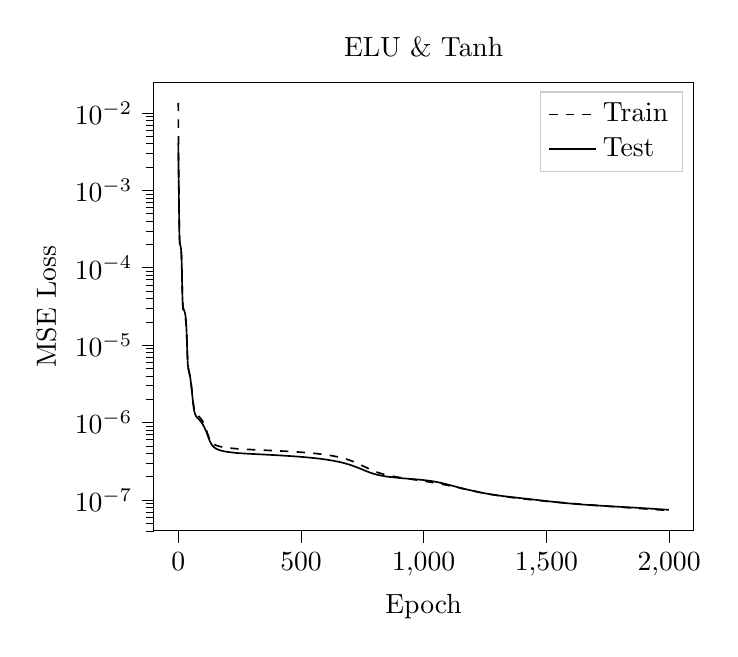
\begin{tikzpicture}

\begin{axis}[
legend cell align={left},
legend style={fill opacity=0.8, draw opacity=1, text opacity=1, draw=white!80!black},
log basis y={10},
tick align=outside,
tick pos=left,
title={ELU \& Tanh},
x grid style={white!69.0196078431373!black},
xlabel={Epoch},
xmin=-99.95, xmax=2098.95,
xtick style={color=black},
y grid style={white!69.0196078431373!black},
ylabel={MSE Loss},
ymin=3.99690726045967e-08, ymax=0.0247433085065691,
ymode=log,
ytick style={color=black}
]
\addplot [semithick, black, dashed]
table {%
0 0.0134957538153976
1 0.0023310884651728
2 0.00137426065234467
3 0.00077357710513752
4 0.000392858184757642
5 0.000249120184715139
6 0.000204640424781246
7 0.000192825474230631
8 0.000188046251423657
9 0.000183736560094985
10 0.000178325850552937
11 0.000170728457196674
12 0.000159364001447102
13 0.000142009735987813
14 0.000116843216383131
15 8.60529496239906e-05
16 5.84654288759339e-05
17 4.15402031667327e-05
18 3.35064789760509e-05
19 2.98543798189712e-05
20 2.80834724026136e-05
21 2.7120061565256e-05
22 2.65000228091594e-05
23 2.60162827989916e-05
24 2.55703675338736e-05
25 2.51090224846848e-05
26 2.45967136706895e-05
27 2.40019229959216e-05
28 2.32902032030324e-05
29 2.24202653498651e-05
30 2.13432580803783e-05
31 2.00045652190965e-05
32 1.83535941760056e-05
33 1.63697485281773e-05
34 1.41058650265222e-05
35 1.17310301802718e-05
36 9.51688467444001e-06
37 7.72394584441827e-06
38 6.46328579375677e-06
39 5.67237918517094e-06
40 5.20494382209336e-06
41 4.92263743979038e-06
42 4.73192033814485e-06
43 4.58095780572876e-06
44 4.44440987797634e-06
45 4.31049008187756e-06
46 4.17367375678168e-06
47 4.03129841151895e-06
48 3.88186479199248e-06
49 3.72467667875753e-06
50 3.55976452499362e-06
51 3.3876761801821e-06
52 3.20961057741442e-06
53 3.02756247447178e-06
54 2.84423495969577e-06
55 2.6628521272869e-06
56 2.48704906198327e-06
57 2.32027610144314e-06
58 2.16550271670712e-06
59 2.02503649921937e-06
60 1.90025342425315e-06
61 1.79153526005393e-06
62 1.69843876534514e-06
63 1.6199104959469e-06
64 1.55439161704862e-06
65 1.50013449353992e-06
66 1.45557809571528e-06
67 1.41910898872766e-06
68 1.38913675107233e-06
69 1.36439518496445e-06
70 1.34373901823892e-06
71 1.3262495506865e-06
72 1.31120514492977e-06
73 1.29805072887734e-06
74 1.28629729721297e-06
75 1.27557425403779e-06
76 1.26559939400295e-06
77 1.25617296097857e-06
78 1.24714520961788e-06
79 1.23836504184283e-06
80 1.22974110064433e-06
81 1.22120436569162e-06
82 1.21270806337748e-06
83 1.2042229414817e-06
84 1.19568821878602e-06
85 1.18703545433618e-06
86 1.17824618195073e-06
87 1.16926949596063e-06
88 1.16005888634163e-06
89 1.15063077569744e-06
90 1.14096733773295e-06
91 1.1310374811444e-06
92 1.12082256276835e-06
93 1.11030603562767e-06
94 1.0994694030444e-06
95 1.08829291150414e-06
96 1.0767586200302e-06
97 1.06484853012034e-06
98 1.05254191706194e-06
99 1.03982470298547e-06
100 1.02669375425535e-06
101 1.013145324265e-06
102 9.99175518728634e-07
103 9.84785912976349e-07
104 9.69983164736732e-07
105 9.54775229445204e-07
106 9.39185010707888e-07
107 9.23240237511891e-07
108 9.06987714614615e-07
109 8.90465134233409e-07
110 8.73703285321881e-07
111 8.56757450264922e-07
112 8.39707763958586e-07
113 8.22606544005566e-07
114 8.05511803577019e-07
115 7.8853165106807e-07
116 7.71770440536557e-07
117 7.55323297966015e-07
118 7.39256733481852e-07
119 7.23615459463645e-07
120 7.08470843107989e-07
121 6.93896306614761e-07
122 6.79961028396292e-07
123 6.66732689808214e-07
124 6.54239293226055e-07
125 6.4249699808272e-07
126 6.31537070717059e-07
127 6.21340004741455e-07
128 6.11861269959491e-07
129 6.03081373157011e-07
130 5.94950151452167e-07
131 5.87441886111151e-07
132 5.80561772849819e-07
133 5.742626128864e-07
134 5.68461311942769e-07
135 5.63138753122416e-07
136 5.58289989569971e-07
137 5.53789126101378e-07
138 5.49580243131231e-07
139 5.45668546905631e-07
140 5.42029055068838e-07
141 5.3864083858457e-07
142 5.35457754253343e-07
143 5.32470842770749e-07
144 5.2965976857422e-07
145 5.27022905075114e-07
146 5.24544419604922e-07
147 5.2220559823013e-07
148 5.1999728647445e-07
149 5.17909198450184e-07
150 5.15934669948592e-07
151 5.14066228163301e-07
152 5.12297007816187e-07
153 5.10620100868664e-07
154 5.09027317391997e-07
155 5.07512464238857e-07
156 5.06070105885215e-07
157 5.04693904218811e-07
158 5.03377546664296e-07
159 5.02117622758647e-07
160 5.0090915983958e-07
161 4.99747272371565e-07
162 4.9862692104341e-07
163 4.97548696131389e-07
164 4.96514213153887e-07
165 4.95520301740271e-07
166 4.94560742978933e-07
167 4.93631716139475e-07
168 4.92731814873082e-07
169 4.91858511153964e-07
170 4.9100989390638e-07
171 4.90185054943026e-07
172 4.89384468266962e-07
173 4.88605556597577e-07
174 4.87848062974194e-07
175 4.87110447991768e-07
176 4.86391952748022e-07
177 4.85690664930871e-07
178 4.8500625908332e-07
179 4.84336899063464e-07
180 4.83682655712414e-07
181 4.83042738224526e-07
182 4.82416531340846e-07
183 4.81803007630788e-07
184 4.81201379244567e-07
185 4.80611838398204e-07
186 4.80033573126093e-07
187 4.79465925039335e-07
188 4.78908676896594e-07
189 4.78361412703521e-07
190 4.77823565461222e-07
191 4.7729492538906e-07
192 4.76775265582319e-07
193 4.76263761612472e-07
194 4.7576123780857e-07
195 4.75266853953826e-07
196 4.74780734677438e-07
197 4.7430138734228e-07
198 4.73829710003315e-07
199 4.73365776272772e-07
200 4.72908600201549e-07
201 4.72458603368864e-07
202 4.72014912119789e-07
203 4.71577816512081e-07
204 4.71147397803406e-07
205 4.70723401988948e-07
206 4.70305473228905e-07
207 4.69893359181128e-07
208 4.694872364297e-07
209 4.69086846621281e-07
210 4.68691152320844e-07
211 4.68301935214299e-07
212 4.6791765424814e-07
213 4.67538755827945e-07
214 4.67165025099803e-07
215 4.66797083745973e-07
216 4.66435041161617e-07
217 4.66077831347889e-07
218 4.65725406073147e-07
219 4.65377729284455e-07
220 4.65034056972513e-07
221 4.64696197980174e-07
222 4.64362528262541e-07
223 4.64033503746464e-07
224 4.63709261964595e-07
225 4.63390550478948e-07
226 4.63075590630524e-07
227 4.62764741016031e-07
228 4.6245909268805e-07
229 4.62156695846261e-07
230 4.61858597319065e-07
231 4.61564129679459e-07
232 4.61272959867642e-07
233 4.60985718561346e-07
234 4.60702021101156e-07
235 4.60422043445874e-07
236 4.60145196697681e-07
237 4.59871440227744e-07
238 4.59601524894993e-07
239 4.59334055761929e-07
240 4.59070226526137e-07
241 4.58809098404345e-07
242 4.58550512959732e-07
243 4.58294875897991e-07
244 4.5804139479344e-07
245 4.5778995291812e-07
246 4.57542623578888e-07
247 4.57299847056447e-07
248 4.5706229977327e-07
249 4.5682922412027e-07
250 4.5659845754642e-07
251 4.56369487707775e-07
252 4.56143253117602e-07
253 4.55919790695702e-07
254 4.55699768508566e-07
255 4.55483950588587e-07
256 4.55268989156821e-07
257 4.55049070268387e-07
258 4.54831853417659e-07
259 4.54618514424965e-07
260 4.54407614483898e-07
261 4.5419944773073e-07
262 4.53993272486741e-07
263 4.53789547307792e-07
264 4.53587446315851e-07
265 4.53387271875272e-07
266 4.5318868204447e-07
267 4.5299173295632e-07
268 4.52797509495895e-07
269 4.52604366543596e-07
270 4.52412825268311e-07
271 4.52222721833095e-07
272 4.52033698024934e-07
273 4.51846320558502e-07
274 4.51659424555828e-07
275 4.51474039138589e-07
276 4.51290351008993e-07
277 4.511082164953e-07
278 4.50927281875124e-07
279 4.50748062917228e-07
280 4.50569941847334e-07
281 4.50392685195311e-07
282 4.50216764761535e-07
283 4.50041916479904e-07
284 4.49868347018878e-07
285 4.49695231836245e-07
286 4.49524123709466e-07
287 4.49353258233032e-07
288 4.49183449944712e-07
289 4.49014504795286e-07
290 4.48846887337595e-07
291 4.48678875031305e-07
292 4.48512801781931e-07
293 4.4834711533781e-07
294 4.48182058306656e-07
295 4.48017639698151e-07
296 4.47853688470445e-07
297 4.47691391997296e-07
298 4.47529162329374e-07
299 4.47367209105209e-07
300 4.47207153499107e-07
301 4.47047590427019e-07
302 4.46889215353963e-07
303 4.46730439591647e-07
304 4.46573448101617e-07
305 4.46416878617129e-07
306 4.46260456129721e-07
307 4.46104787130253e-07
308 4.45949403498958e-07
309 4.45795175110675e-07
310 4.45640652031898e-07
311 4.45486587608457e-07
312 4.45333089373889e-07
313 4.45180131748657e-07
314 4.4502877632624e-07
315 4.44876304158015e-07
316 4.44724652467698e-07
317 4.44573048568486e-07
318 4.4442220375629e-07
319 4.44271763015536e-07
320 4.44121741267622e-07
321 4.43972102488033e-07
322 4.43822052417886e-07
323 4.43673538285339e-07
324 4.43524699790032e-07
325 4.43375982655425e-07
326 4.4322779477568e-07
327 4.4307990557968e-07
328 4.42932485313463e-07
329 4.42784972619847e-07
330 4.42638347223578e-07
331 4.42491844822257e-07
332 4.42345659052989e-07
333 4.42199956879108e-07
334 4.42054676227599e-07
335 4.41909244827343e-07
336 4.41764431172942e-07
337 4.41619671931903e-07
338 4.41474580128443e-07
339 4.41329635378906e-07
340 4.41183451258098e-07
341 4.41036900710401e-07
342 4.40890624204826e-07
343 4.40743538902666e-07
344 4.40596182741615e-07
345 4.40449259201614e-07
346 4.40302216944133e-07
347 4.40154431444739e-07
348 4.40006927206582e-07
349 4.39860318763863e-07
350 4.39711944849819e-07
351 4.39565173067535e-07
352 4.39417494092709e-07
353 4.39270274227965e-07
354 4.39123118624707e-07
355 4.38975632746974e-07
356 4.38827461607616e-07
357 4.38680071070507e-07
358 4.38532330349517e-07
359 4.3838513353478e-07
360 4.38237253135299e-07
361 4.38088896984823e-07
362 4.37940936492964e-07
363 4.37792325058695e-07
364 4.3764440769678e-07
365 4.37496297351458e-07
366 4.37348056692599e-07
367 4.37199314120562e-07
368 4.37050272594774e-07
369 4.36901579078608e-07
370 4.36752512044336e-07
371 4.36603472181218e-07
372 4.36453455236574e-07
373 4.36304386454367e-07
374 4.36154428882674e-07
375 4.36004858670458e-07
376 4.35854937720137e-07
377 4.35704757762778e-07
378 4.35553956663171e-07
379 4.35403425242953e-07
380 4.35252636734162e-07
381 4.35101373255975e-07
382 4.34949856654043e-07
383 4.3479894871723e-07
384 4.3464698572393e-07
385 4.34495225817955e-07
386 4.34342180668068e-07
387 4.34190195235828e-07
388 4.34037036896484e-07
389 4.33883725705186e-07
390 4.3373072944064e-07
391 4.3357726191573e-07
392 4.33423383583431e-07
393 4.33269188050645e-07
394 4.33114656090083e-07
395 4.32960370446267e-07
396 4.32805814895687e-07
397 4.3265090708644e-07
398 4.32495347084227e-07
399 4.32340210664961e-07
400 4.32183846626799e-07
401 4.32028382576277e-07
402 4.31871616200397e-07
403 4.31714662525451e-07
404 4.31557992882858e-07
405 4.31400304861995e-07
406 4.31242871329118e-07
407 4.31084624125333e-07
408 4.3092627005592e-07
409 4.3076730334235e-07
410 4.306080731169e-07
411 4.30449040848657e-07
412 4.30289126995831e-07
413 4.30129235766685e-07
414 4.29968422125171e-07
415 4.29807350585065e-07
416 4.2964639477816e-07
417 4.29484178312123e-07
418 4.29322080350403e-07
419 4.29159988442507e-07
420 4.28997011951537e-07
421 4.28833916558347e-07
422 4.28670428178179e-07
423 4.285065395635e-07
424 4.28342804710269e-07
425 4.28177927716433e-07
426 4.28012444601222e-07
427 4.27847551961236e-07
428 4.27682234885651e-07
429 4.27516849072163e-07
430 4.2735087495771e-07
431 4.27185019674425e-07
432 4.27018305103388e-07
433 4.26850394106282e-07
434 4.26680964608295e-07
435 4.26510055604012e-07
436 4.26338771930546e-07
437 4.26167039904612e-07
438 4.25994698446175e-07
439 4.25822926942487e-07
440 4.25649003418016e-07
441 4.25476069125352e-07
442 4.25302337390576e-07
443 4.25128136527064e-07
444 4.24952945252244e-07
445 4.24777989451286e-07
446 4.24601941233504e-07
447 4.24425246308147e-07
448 4.24248131494664e-07
449 4.24070380120156e-07
450 4.23891809575139e-07
451 4.23712736520088e-07
452 4.23533353355765e-07
453 4.23353260387671e-07
454 4.23172379115044e-07
455 4.22990336204521e-07
456 4.22808332061209e-07
457 4.2262559324513e-07
458 4.22442374357956e-07
459 4.22258078586424e-07
460 4.22073079946017e-07
461 4.21887672999333e-07
462 4.21701368480853e-07
463 4.21513872581158e-07
464 4.21326206733852e-07
465 4.21137836866592e-07
466 4.20948731303383e-07
467 4.20758855895542e-07
468 4.20568408756594e-07
469 4.20376887021234e-07
470 4.20184173734128e-07
471 4.19991282626597e-07
472 4.19797408497402e-07
473 4.19602816336351e-07
474 4.19407368866587e-07
475 4.19211461661462e-07
476 4.19014144327434e-07
477 4.18816154294177e-07
478 4.18617555780543e-07
479 4.18418411371135e-07
480 4.1821802982156e-07
481 4.18016062596394e-07
482 4.17814719014586e-07
483 4.17611920354943e-07
484 4.17407868425812e-07
485 4.17203221303453e-07
486 4.16997823535326e-07
487 4.16791075110723e-07
488 4.16583922344671e-07
489 4.16375738268471e-07
490 4.16166455650568e-07
491 4.15955980415106e-07
492 4.15744668330831e-07
493 4.15532831439691e-07
494 4.15319472281794e-07
495 4.15105677120664e-07
496 4.14890348992003e-07
497 4.1467463127276e-07
498 4.14457540784952e-07
499 4.14239087675128e-07
500 4.14020030703455e-07
501 4.13799983661534e-07
502 4.1357917176299e-07
503 4.13357065141895e-07
504 4.13133196275339e-07
505 4.12908721187932e-07
506 4.12683341309616e-07
507 4.12456391615024e-07
508 4.12228853789998e-07
509 4.11999894495807e-07
510 4.11769633558379e-07
511 4.11538843053449e-07
512 4.11306252885879e-07
513 4.11072774568311e-07
514 4.10838005322489e-07
515 4.1060252716818e-07
516 4.10364640302419e-07
517 4.10126535740574e-07
518 4.09886833153905e-07
519 4.09645856692009e-07
520 4.094044307692e-07
521 4.09160514337259e-07
522 4.08915355137651e-07
523 4.08669283530116e-07
524 4.08422131798147e-07
525 4.08173769940845e-07
526 4.07923640523222e-07
527 4.07672310942075e-07
528 4.07419083543914e-07
529 4.07164622004075e-07
530 4.06909275639578e-07
531 4.06652300753763e-07
532 4.06393879373468e-07
533 4.06133775314288e-07
534 4.05872190484047e-07
535 4.05609441145316e-07
536 4.05344806040375e-07
537 4.05079033455991e-07
538 4.04811563768703e-07
539 4.04542423822818e-07
540 4.04271819334667e-07
541 4.03999381035192e-07
542 4.03725548309808e-07
543 4.03450251994286e-07
544 4.03173237657484e-07
545 4.02894533820586e-07
546 4.02613792061857e-07
547 4.0233181184135e-07
548 4.02048376187736e-07
549 4.01763181656634e-07
550 4.0147601137619e-07
551 4.01187170766093e-07
552 4.00897058185024e-07
553 4.00604771755297e-07
554 4.00311013024179e-07
555 4.00015908937235e-07
556 3.99718229388668e-07
557 3.99419691575531e-07
558 3.99118723294123e-07
559 3.98816622549703e-07
560 3.98512169610399e-07
561 3.98205197001289e-07
562 3.97896785699459e-07
563 3.97586246165815e-07
564 3.97274299714923e-07
565 3.9695991949884e-07
566 3.96644428946047e-07
567 3.96326605198283e-07
568 3.9600664929651e-07
569 3.95684843951472e-07
570 3.95360391905797e-07
571 3.95033267778899e-07
572 3.94703262571738e-07
573 3.94371521494463e-07
574 3.94036575130485e-07
575 3.93699125879721e-07
576 3.9335995651868e-07
577 3.93019113644755e-07
578 3.92675260812325e-07
579 3.92329612409981e-07
580 3.91981137525477e-07
581 3.91630506939578e-07
582 3.91277142398394e-07
583 3.90921700088143e-07
584 3.90563617244766e-07
585 3.90202885412805e-07
586 3.89840740638192e-07
587 3.89475067450462e-07
588 3.8910768236633e-07
589 3.88736924008981e-07
590 3.8836424393196e-07
591 3.87987770281484e-07
592 3.87609264734579e-07
593 3.87228815569074e-07
594 3.8684465638994e-07
595 3.86458957137847e-07
596 3.86069671534983e-07
597 3.85677691681963e-07
598 3.85282802525921e-07
599 3.84885359849818e-07
600 3.84484707552701e-07
601 3.84081810679504e-07
602 3.83675666981276e-07
603 3.83267110564134e-07
604 3.82855496027901e-07
605 3.82440661056194e-07
606 3.82023474216453e-07
607 3.81603375615214e-07
608 3.81180774070344e-07
609 3.80755330439797e-07
610 3.80327249644097e-07
611 3.7989629353774e-07
612 3.79462449785706e-07
613 3.79024334748124e-07
614 3.7858260044743e-07
615 3.781370549234e-07
616 3.7768797929516e-07
617 3.77235340451421e-07
618 3.76779640092195e-07
619 3.7632051203218e-07
620 3.75858051143041e-07
621 3.75393150264358e-07
622 3.74924531286069e-07
623 3.74452642461165e-07
624 3.73977770863121e-07
625 3.7350079924181e-07
626 3.7302071731915e-07
627 3.7254025515665e-07
628 3.7205934323481e-07
629 3.71576094394754e-07
630 3.71084454229731e-07
631 3.70585130312406e-07
632 3.70085966878264e-07
633 3.69586355361662e-07
634 3.69074953312065e-07
635 3.68545165670753e-07
636 3.68011905194976e-07
637 3.67480042811508e-07
638 3.66946662566647e-07
639 3.6641021911521e-07
640 3.65870577084593e-07
641 3.65327583651265e-07
642 3.64780428000699e-07
643 3.64229227869828e-07
644 3.63673588225311e-07
645 3.63114767651496e-07
646 3.6255076777536e-07
647 3.61983122857623e-07
648 3.61412011471884e-07
649 3.60835356488565e-07
650 3.60254737486798e-07
651 3.59668436402671e-07
652 3.59077841324051e-07
653 3.58481157050505e-07
654 3.57879950044548e-07
655 3.57273974941563e-07
656 3.56662821857867e-07
657 3.56046830674472e-07
658 3.55426030381523e-07
659 3.54800945274292e-07
660 3.54170143580745e-07
661 3.53534564055735e-07
662 3.52893836748081e-07
663 3.52249136582827e-07
664 3.5159879300295e-07
665 3.50943790948577e-07
666 3.50283574590549e-07
667 3.49618195528478e-07
668 3.48948270911364e-07
669 3.48272788599502e-07
670 3.47592344610348e-07
671 3.46906679880021e-07
672 3.46215688352913e-07
673 3.45520173468117e-07
674 3.44818678343017e-07
675 3.44112561549537e-07
676 3.43400532202054e-07
677 3.42684295404183e-07
678 3.41961838927318e-07
679 3.41234473751229e-07
680 3.40501417468886e-07
681 3.39762946779842e-07
682 3.39019501467419e-07
683 3.38269846963613e-07
684 3.37515219158036e-07
685 3.36755509124487e-07
686 3.35990043367929e-07
687 3.35219267029174e-07
688 3.34443446874388e-07
689 3.33661982224953e-07
690 3.32875743197292e-07
691 3.32083970818076e-07
692 3.31286873020531e-07
693 3.30484729033742e-07
694 3.29678474983552e-07
695 3.2886618532757e-07
696 3.28050683791048e-07
697 3.2723264064316e-07
698 3.26414048302581e-07
699 3.25598259109938e-07
700 3.24765047210462e-07
701 3.23909981830184e-07
702 3.23054695087421e-07
703 3.22199193206529e-07
704 3.21340463742104e-07
705 3.20477851943224e-07
706 3.19610514708302e-07
707 3.18738396330787e-07
708 3.17862388968138e-07
709 3.16981570634312e-07
710 3.16095240989966e-07
711 3.15203745643089e-07
712 3.14306510190932e-07
713 3.13403632560494e-07
714 3.12496322308675e-07
715 3.11583908654711e-07
716 3.10667585395663e-07
717 3.09747140491368e-07
718 3.08822607465231e-07
719 3.07894123082519e-07
720 3.06962333453953e-07
721 3.0602608833874e-07
722 3.05086028419055e-07
723 3.04143713719895e-07
724 3.03196796195948e-07
725 3.02247252278676e-07
726 3.01293990418117e-07
727 3.00338420231583e-07
728 2.99379660518184e-07
729 2.98417770935089e-07
730 2.97453068498044e-07
731 2.96486439765431e-07
732 2.95516273723706e-07
733 2.94544258196083e-07
734 2.93570655856001e-07
735 2.92593953943765e-07
736 2.91615041831506e-07
737 2.90633185599631e-07
738 2.89649034030504e-07
739 2.88664336991928e-07
740 2.87676741166365e-07
741 2.866883023529e-07
742 2.85699080663449e-07
743 2.84709725391963e-07
744 2.83720243942298e-07
745 2.82730636115502e-07
746 2.81744076914947e-07
747 2.80759510971507e-07
748 2.7977648436206e-07
749 2.78794243385505e-07
750 2.77813358380286e-07
751 2.7683377196297e-07
752 2.75855688741444e-07
753 2.74879691914975e-07
754 2.73905823689802e-07
755 2.72932655818181e-07
756 2.71961296789414e-07
757 2.70993213973725e-07
758 2.70029876915601e-07
759 2.69070342582722e-07
760 2.68115076281106e-07
761 2.67164587739899e-07
762 2.66217917982203e-07
763 2.65276417891869e-07
764 2.64340145193387e-07
765 2.63407706185603e-07
766 2.6248111669247e-07
767 2.61559234829178e-07
768 2.60642846200199e-07
769 2.59731777774164e-07
770 2.58826290547631e-07
771 2.5792636903077e-07
772 2.57032839485305e-07
773 2.56144408282921e-07
774 2.55262543291224e-07
775 2.5438714554582e-07
776 2.53518222692151e-07
777 2.52655296193893e-07
778 2.51799888772553e-07
779 2.5095009256404e-07
780 2.50108108076574e-07
781 2.49272646072995e-07
782 2.48444218982513e-07
783 2.47623585693191e-07
784 2.46809189377473e-07
785 2.46002701430825e-07
786 2.45203631791924e-07
787 2.44411834984248e-07
788 2.43627891080678e-07
789 2.42850782427695e-07
790 2.42081854906928e-07
791 2.41320599272399e-07
792 2.40566559881472e-07
793 2.3982113521015e-07
794 2.39083572949994e-07
795 2.38354401588481e-07
796 2.37634123848807e-07
797 2.3692211487969e-07
798 2.36218781566322e-07
799 2.35523804335003e-07
800 2.34836860670384e-07
801 2.34157943950208e-07
802 2.33487251009024e-07
803 2.3282475075348e-07
804 2.3217077144011e-07
805 2.31525538907817e-07
806 2.30889206477514e-07
807 2.30262769150613e-07
808 2.2964494941391e-07
809 2.2903699370147e-07
810 2.2843675628792e-07
811 2.27845235556856e-07
812 2.27261650195487e-07
813 2.26686032704038e-07
814 2.26118474671466e-07
815 2.25558543178295e-07
816 2.25006733415967e-07
817 2.24462538170656e-07
818 2.2392637707469e-07
819 2.23396879476923e-07
820 2.2287552974376e-07
821 2.22361441501562e-07
822 2.21854354720108e-07
823 2.21354323471701e-07
824 2.20860920521204e-07
825 2.2037506118977e-07
826 2.19894997798065e-07
827 2.19422501984923e-07
828 2.18955629293305e-07
829 2.18495853673062e-07
830 2.18041660289714e-07
831 2.17593597042764e-07
832 2.17151581793473e-07
833 2.16715876419471e-07
834 2.16284942467837e-07
835 2.15860050076344e-07
836 2.1544019813291e-07
837 2.15026796041684e-07
838 2.14618440551817e-07
839 2.14215182168687e-07
840 2.13816784892629e-07
841 2.13424236363835e-07
842 2.13036339133055e-07
843 2.12653428448562e-07
844 2.12275704200238e-07
845 2.11901888874877e-07
846 2.1153276824748e-07
847 2.11167949174751e-07
848 2.10808170407972e-07
849 2.10451614364615e-07
850 2.10098580353701e-07
851 2.09750812103948e-07
852 2.09405895120085e-07
853 2.0906477641347e-07
854 2.08727001819398e-07
855 2.08393345488389e-07
856 2.08063171513118e-07
857 2.07736553591076e-07
858 2.0741319255535e-07
859 2.07093789825308e-07
860 2.06777032659033e-07
861 2.06463370915344e-07
862 2.06152881176536e-07
863 2.05845972587326e-07
864 2.05542741582576e-07
865 2.05242946961448e-07
866 2.04945145583224e-07
867 2.04649749250052e-07
868 2.04357353396745e-07
869 2.04065894195082e-07
870 2.03777457429055e-07
871 2.03491203450312e-07
872 2.03206753425889e-07
873 2.02925087876338e-07
874 2.02645592992212e-07
875 2.02368894051119e-07
876 2.02094200830061e-07
877 2.01822318729228e-07
878 2.01553326107273e-07
879 2.01285563150577e-07
880 2.01020466818136e-07
881 2.0075688806287e-07
882 2.00495315624494e-07
883 2.00236287355438e-07
884 1.9997802669991e-07
885 1.99721420429455e-07
886 1.99466760165024e-07
887 1.99212858433384e-07
888 1.98960012113503e-07
889 1.98708344001375e-07
890 1.98456358759813e-07
891 1.98205174598343e-07
892 1.9795247490606e-07
893 1.97697988696177e-07
894 1.97439781103981e-07
895 1.97174738133299e-07
896 1.9690548506901e-07
897 1.96643729537982e-07
898 1.96398226790961e-07
899 1.96169193984019e-07
900 1.95943623381822e-07
901 1.95714774321232e-07
902 1.95485544722374e-07
903 1.95257697583884e-07
904 1.95029899629162e-07
905 1.94803018146672e-07
906 1.94576785659706e-07
907 1.94351484836375e-07
908 1.94126916412074e-07
909 1.93903316954902e-07
910 1.93680324557022e-07
911 1.9345859624309e-07
912 1.93236818489595e-07
913 1.93015732975255e-07
914 1.92795474973195e-07
915 1.92575191803712e-07
916 1.92355031046532e-07
917 1.92134992573756e-07
918 1.91914073809585e-07
919 1.91692709663016e-07
920 1.91469181316961e-07
921 1.91248184336246e-07
922 1.91033474195024e-07
923 1.90824868155914e-07
924 1.9061681585697e-07
925 1.9040659654479e-07
926 1.90195690294104e-07
927 1.89984557763978e-07
928 1.89772694426438e-07
929 1.89562242127295e-07
930 1.89355768128507e-07
931 1.89148760014746e-07
932 1.88941211206384e-07
933 1.8873464432545e-07
934 1.88529779649116e-07
935 1.8832545347891e-07
936 1.88120943477088e-07
937 1.87917375214397e-07
938 1.87713873302187e-07
939 1.87510132064972e-07
940 1.8730790769439e-07
941 1.87105002254384e-07
942 1.86902863234195e-07
943 1.86701843460924e-07
944 1.8649999681486e-07
945 1.8629890276145e-07
946 1.8609833674077e-07
947 1.85897361504317e-07
948 1.85697282688579e-07
949 1.85497568267579e-07
950 1.85297616908997e-07
951 1.85098694657881e-07
952 1.84900121737996e-07
953 1.84700446268948e-07
954 1.84501964369588e-07
955 1.84303896929805e-07
956 1.8410508442912e-07
957 1.8390730782869e-07
958 1.83709708338142e-07
959 1.8351193419619e-07
960 1.83313767180948e-07
961 1.83116579052012e-07
962 1.82919414100979e-07
963 1.82722437656935e-07
964 1.82525298455971e-07
965 1.82328213938376e-07
966 1.82131599942181e-07
967 1.81935750461548e-07
968 1.8173868717497e-07
969 1.81542523080225e-07
970 1.81345505112063e-07
971 1.81149303955408e-07
972 1.80952871204454e-07
973 1.80756489726264e-07
974 1.80560155229159e-07
975 1.8036430697066e-07
976 1.80167951057797e-07
977 1.79972166336029e-07
978 1.79775467472609e-07
979 1.79579259693696e-07
980 1.79383511152764e-07
981 1.79187363684719e-07
982 1.78991157369524e-07
983 1.78794552368799e-07
984 1.7859870311554e-07
985 1.78402505511599e-07
986 1.78205574442813e-07
987 1.78009270669577e-07
988 1.77813091852386e-07
989 1.77616319618323e-07
990 1.7741990316722e-07
991 1.77223411881755e-07
992 1.77026502839794e-07
993 1.76829171635973e-07
994 1.76632485633377e-07
995 1.76435387984952e-07
996 1.76238921852701e-07
997 1.76041123054915e-07
998 1.75843510660911e-07
999 1.75646163881993e-07
1000 1.75448311040327e-07
1001 1.75250185350251e-07
1002 1.75052527254138e-07
1003 1.74854418531822e-07
1004 1.74656194630529e-07
1005 1.74457870940614e-07
1006 1.74259641283925e-07
1007 1.74061686607274e-07
1008 1.73863939551211e-07
1009 1.73667300458646e-07
1010 1.73472921659368e-07
1011 1.73273655548201e-07
1012 1.73069673081727e-07
1013 1.7286636042968e-07
1014 1.72665114490655e-07
1015 1.72464464000655e-07
1016 1.72263602166822e-07
1017 1.72062851873989e-07
1018 1.71861413647889e-07
1019 1.71659764902188e-07
1020 1.71458449159445e-07
1021 1.71256041582524e-07
1022 1.71053797302534e-07
1023 1.70851226442892e-07
1024 1.70648361020653e-07
1025 1.70445360467397e-07
1026 1.70241809740901e-07
1027 1.70038351967605e-07
1028 1.69834429129878e-07
1029 1.69629752136302e-07
1030 1.69425513874444e-07
1031 1.69220505398471e-07
1032 1.69015253575822e-07
1033 1.68809544774717e-07
1034 1.68604265013528e-07
1035 1.68397976921142e-07
1036 1.68191788034733e-07
1037 1.6798447364863e-07
1038 1.67777331597563e-07
1039 1.6757027366765e-07
1040 1.6736213190427e-07
1041 1.67153996954994e-07
1042 1.66945491066883e-07
1043 1.66735625384717e-07
1044 1.66526715325688e-07
1045 1.66316698717139e-07
1046 1.66106552946133e-07
1047 1.65895362272295e-07
1048 1.65684443473424e-07
1049 1.65472404837885e-07
1050 1.65260418420132e-07
1051 1.65048077548136e-07
1052 1.64834197867947e-07
1053 1.64621264730158e-07
1054 1.64407517402765e-07
1055 1.64192864481549e-07
1056 1.63978524852837e-07
1057 1.63763244295012e-07
1058 1.63547865398073e-07
1059 1.63332109025305e-07
1060 1.63115409371528e-07
1061 1.62898703187864e-07
1062 1.62680641430768e-07
1063 1.62461872527331e-07
1064 1.62241660071061e-07
1065 1.62020339615765e-07
1066 1.61796442682771e-07
1067 1.61578315811539e-07
1068 1.61365553886128e-07
1069 1.61150012530697e-07
1070 1.60931570960088e-07
1071 1.60712657454098e-07
1072 1.60492130085288e-07
1073 1.60271687285274e-07
1074 1.60050248744881e-07
1075 1.59829400992351e-07
1076 1.59607629875325e-07
1077 1.59385763772946e-07
1078 1.59163962138109e-07
1079 1.58940918062456e-07
1080 1.58717688861998e-07
1081 1.58494263992282e-07
1082 1.58270022268425e-07
1083 1.58046180196436e-07
1084 1.57821384448198e-07
1085 1.57595483358364e-07
1086 1.57370519950462e-07
1087 1.57144959892719e-07
1088 1.56918834306907e-07
1089 1.5669187406786e-07
1090 1.56464888597441e-07
1091 1.56237204002707e-07
1092 1.56009357084486e-07
1093 1.55781397751298e-07
1094 1.55553085093629e-07
1095 1.55324671020196e-07
1096 1.55095236443969e-07
1097 1.54865906345947e-07
1098 1.54636180901946e-07
1099 1.54406042327082e-07
1100 1.54175699570658e-07
1101 1.53945063857464e-07
1102 1.53714261266202e-07
1103 1.53482981708919e-07
1104 1.53252202139242e-07
1105 1.53020336426835e-07
1106 1.52788393776859e-07
1107 1.52556364362511e-07
1108 1.52324091487799e-07
1109 1.52091592113379e-07
1110 1.51858972628816e-07
1111 1.51626830870555e-07
1112 1.51393231192287e-07
1113 1.51160503861547e-07
1114 1.50926978633947e-07
1115 1.50693419392667e-07
1116 1.50459477836762e-07
1117 1.50224978561653e-07
1118 1.49990391300037e-07
1119 1.49756285445335e-07
1120 1.49522032693028e-07
1121 1.49287322336988e-07
1122 1.49052170790753e-07
1123 1.48817413446523e-07
1124 1.48582587861767e-07
1125 1.48347238109636e-07
1126 1.48112339459772e-07
1127 1.47877032254939e-07
1128 1.47641772933582e-07
1129 1.47406511302961e-07
1130 1.47171383567013e-07
1131 1.46936253393903e-07
1132 1.46701635351576e-07
1133 1.46465785476835e-07
1134 1.46231383524764e-07
1135 1.4599759120415e-07
1136 1.45765217787641e-07
1137 1.45536929771595e-07
1138 1.45315871961316e-07
1139 1.45102639088179e-07
1140 1.44857848511037e-07
1141 1.44608287207859e-07
1142 1.44369832149493e-07
1143 1.44132638602912e-07
1144 1.43896900084428e-07
1145 1.4366150475098e-07
1146 1.43426275592162e-07
1147 1.43191492327333e-07
1148 1.42956328453181e-07
1149 1.42722145618279e-07
1150 1.42487870704144e-07
1151 1.42253041154561e-07
1152 1.42020066476789e-07
1153 1.41785810825468e-07
1154 1.41552231468722e-07
1155 1.41318830927162e-07
1156 1.41086397505319e-07
1157 1.40852889181531e-07
1158 1.40620678877212e-07
1159 1.40388574116912e-07
1160 1.40156471644559e-07
1161 1.39925065703039e-07
1162 1.39693805635943e-07
1163 1.3946283491606e-07
1164 1.39232228946184e-07
1165 1.39002079130535e-07
1166 1.38772403865062e-07
1167 1.38542935140151e-07
1168 1.38313878032648e-07
1169 1.38085498043949e-07
1170 1.37857207036518e-07
1171 1.37629013572393e-07
1172 1.37401833903539e-07
1173 1.37175356073271e-07
1174 1.36949046506629e-07
1175 1.36723186336951e-07
1176 1.36497654089851e-07
1177 1.36273238062756e-07
1178 1.36049034921371e-07
1179 1.35825359215858e-07
1180 1.35602388681377e-07
1181 1.35379711132089e-07
1182 1.35157931211438e-07
1183 1.34936623901183e-07
1184 1.34716155685055e-07
1185 1.34496195883571e-07
1186 1.34277296119478e-07
1187 1.34058615849142e-07
1188 1.33840519282558e-07
1189 1.33623340104805e-07
1190 1.33407476525349e-07
1191 1.3319190517791e-07
1192 1.32976978036936e-07
1193 1.32762343355353e-07
1194 1.32549082302091e-07
1195 1.32336207059325e-07
1196 1.3212395525386e-07
1197 1.3191258280898e-07
1198 1.31701604125567e-07
1199 1.31491672902939e-07
1200 1.31282150185541e-07
1201 1.31073970862872e-07
1202 1.30865978604788e-07
1203 1.30659009151657e-07
1204 1.30452958032379e-07
1205 1.30247145797568e-07
1206 1.30042434811628e-07
1207 1.29837635277852e-07
1208 1.29634143718249e-07
1209 1.29431724765539e-07
1210 1.29229264068442e-07
1211 1.2902830654582e-07
1212 1.2882778151635e-07
1213 1.28628469106218e-07
1214 1.28429313349443e-07
1215 1.28231789609856e-07
1216 1.28034423859447e-07
1217 1.27838507694378e-07
1218 1.27643347518358e-07
1219 1.27448068560909e-07
1220 1.27254723651049e-07
1221 1.27062053515203e-07
1222 1.26869353692882e-07
1223 1.26678513638012e-07
1224 1.2648869398646e-07
1225 1.26299046257827e-07
1226 1.26110509739874e-07
1227 1.25922840560122e-07
1228 1.25736234195983e-07
1229 1.2554989186242e-07
1230 1.25365093829544e-07
1231 1.25180994345442e-07
1232 1.2499720859438e-07
1233 1.24814919786331e-07
1234 1.24633312992728e-07
1235 1.24453166613137e-07
1236 1.24273151946852e-07
1237 1.24094179561496e-07
1238 1.239163326332e-07
1239 1.23739262612332e-07
1240 1.23563031770857e-07
1241 1.2338771485787e-07
1242 1.23212863535116e-07
1243 1.23039769157174e-07
1244 1.22867110810887e-07
1245 1.2269527713471e-07
1246 1.22524295356641e-07
1247 1.22354196030017e-07
1248 1.22184346274423e-07
1249 1.22015958694988e-07
1250 1.21847489566562e-07
1251 1.21680614576292e-07
1252 1.21514869576345e-07
1253 1.21350862727354e-07
1254 1.21187010343249e-07
1255 1.21024355301813e-07
1256 1.20862906534569e-07
1257 1.20701492171804e-07
1258 1.20541663328311e-07
1259 1.2038259119862e-07
1260 1.20223602536385e-07
1261 1.20066258119778e-07
1262 1.1990913623805e-07
1263 1.19753439911108e-07
1264 1.19598021093736e-07
1265 1.19443799555086e-07
1266 1.19290104670711e-07
1267 1.19137801299019e-07
1268 1.18985667391769e-07
1269 1.18834734578854e-07
1270 1.18683655863094e-07
1271 1.18534597952191e-07
1272 1.18386300279383e-07
1273 1.18238302434293e-07
1274 1.180910000258e-07
1275 1.17944150524352e-07
1276 1.17799393883899e-07
1277 1.17654478550833e-07
1278 1.17510405864607e-07
1279 1.17367388980938e-07
1280 1.17224257031978e-07
1281 1.17082589916606e-07
1282 1.1694187817568e-07
1283 1.16801395940058e-07
1284 1.16661693773779e-07
1285 1.16522982182232e-07
1286 1.16384576124062e-07
1287 1.1624686450773e-07
1288 1.16110333863162e-07
1289 1.15974113846562e-07
1290 1.15838490827969e-07
1291 1.15703803977851e-07
1292 1.15569675003258e-07
1293 1.15436801067403e-07
1294 1.15303707325154e-07
1295 1.15171741619235e-07
1296 1.15039920061122e-07
1297 1.14909067640667e-07
1298 1.14779170850454e-07
1299 1.1464951362683e-07
1300 1.14520760135406e-07
1301 1.1439242427258e-07
1302 1.1426460233821e-07
1303 1.14137843929996e-07
1304 1.14011352920329e-07
1305 1.13885517414758e-07
1306 1.13760346124536e-07
1307 1.1363569807088e-07
1308 1.13511706096858e-07
1309 1.1338796166882e-07
1310 1.1326500737141e-07
1311 1.13143033487972e-07
1312 1.13021178741235e-07
1313 1.12900211753697e-07
1314 1.12779690844889e-07
1315 1.1265914208991e-07
1316 1.12539769602904e-07
1317 1.1242079501983e-07
1318 1.12302080367499e-07
1319 1.12184799739623e-07
1320 1.12066758113372e-07
1321 1.1195019349941e-07
1322 1.11834232555452e-07
1323 1.11717891947194e-07
1324 1.11602466766669e-07
1325 1.1148813078421e-07
1326 1.11373435238704e-07
1327 1.11259319282908e-07
1328 1.11146124588402e-07
1329 1.1103330490414e-07
1330 1.10920645653323e-07
1331 1.1080904416616e-07
1332 1.10697434557494e-07
1333 1.10585898241311e-07
1334 1.10475401349674e-07
1335 1.10365908881249e-07
1336 1.10255315355801e-07
1337 1.10146526331789e-07
1338 1.10037389291051e-07
1339 1.09929271950193e-07
1340 1.09821637458651e-07
1341 1.09713572683745e-07
1342 1.09606224853565e-07
1343 1.09499272817004e-07
1344 1.09392837330802e-07
1345 1.09286181576351e-07
1346 1.09180942139631e-07
1347 1.09074947125976e-07
1348 1.08969509739154e-07
1349 1.08863994555008e-07
1350 1.0875822027856e-07
1351 1.08652535615761e-07
1352 1.08547853031382e-07
1353 1.08444524236972e-07
1354 1.08343042619197e-07
1355 1.08241893663319e-07
1356 1.08140803405377e-07
1357 1.08040766555462e-07
1358 1.07940437651166e-07
1359 1.07839491519712e-07
1360 1.07739953755015e-07
1361 1.07640432766232e-07
1362 1.07541461737526e-07
1363 1.07441998991931e-07
1364 1.07343568814144e-07
1365 1.0724604738499e-07
1366 1.07148069112384e-07
1367 1.07050247443397e-07
1368 1.06953166437052e-07
1369 1.06856573097502e-07
1370 1.06759788259581e-07
1371 1.06664286946057e-07
1372 1.06568438084764e-07
1373 1.06472447498618e-07
1374 1.063770671621e-07
1375 1.06282504503952e-07
1376 1.06188065416291e-07
1377 1.06093580988897e-07
1378 1.05999863428963e-07
1379 1.05906231567587e-07
1380 1.05812977309938e-07
1381 1.05719881993593e-07
1382 1.05627146645304e-07
1383 1.05535287403313e-07
1384 1.05442654906085e-07
1385 1.05351456085145e-07
1386 1.05259449746598e-07
1387 1.0516779738623e-07
1388 1.05076818748273e-07
1389 1.04986698602261e-07
1390 1.04895504520641e-07
1391 1.04806174604732e-07
1392 1.04716658391624e-07
1393 1.04626451999934e-07
1394 1.04537492248369e-07
1395 1.04447951102316e-07
1396 1.04359623612993e-07
1397 1.04270666597017e-07
1398 1.04182458102287e-07
1399 1.04094318238879e-07
1400 1.04006216425034e-07
1401 1.03918898609834e-07
1402 1.03831977760649e-07
1403 1.03744740023615e-07
1404 1.03657609116681e-07
1405 1.03571206210518e-07
1406 1.034848093866e-07
1407 1.03398742076877e-07
1408 1.03312215230744e-07
1409 1.03226706151816e-07
1410 1.03140981615013e-07
1411 1.03055816804698e-07
1412 1.02970463608187e-07
1413 1.02885617252468e-07
1414 1.02800608345888e-07
1415 1.0271614670998e-07
1416 1.02631552014287e-07
1417 1.02547478519455e-07
1418 1.02463092904514e-07
1419 1.02379262113317e-07
1420 1.02295974826916e-07
1421 1.0221234478891e-07
1422 1.02129583741117e-07
1423 1.02046792438415e-07
1424 1.01964049580516e-07
1425 1.01881852174301e-07
1426 1.01799307831385e-07
1427 1.01718198362022e-07
1428 1.01636802085636e-07
1429 1.01555785981589e-07
1430 1.01475560178699e-07
1431 1.01395225254208e-07
1432 1.013157825831e-07
1433 1.01236065422228e-07
1434 1.01156987842188e-07
1435 1.01078010999345e-07
1436 1.00999182535588e-07
1437 1.00920939889448e-07
1438 1.00842937261092e-07
1439 1.00765276187076e-07
1440 1.00687225501161e-07
1441 1.0060997938055e-07
1442 1.00532823186228e-07
1443 1.00455837824143e-07
1444 1.00379015190555e-07
1445 1.00302602085378e-07
1446 1.00226041514162e-07
1447 1.00150384145792e-07
1448 1.00074066768485e-07
1449 9.99983264726723e-08
1450 9.99230493654579e-08
1451 9.98473230708896e-08
1452 9.97722994391381e-08
1453 9.9697498715301e-08
1454 9.962274581099e-08
1455 9.95485779107241e-08
1456 9.94741356485918e-08
1457 9.93999219325303e-08
1458 9.93258953840837e-08
1459 9.92525413714418e-08
1460 9.91788116841974e-08
1461 9.91055348329439e-08
1462 9.90323413034844e-08
1463 9.8959737282911e-08
1464 9.88869816929139e-08
1465 9.88141180968682e-08
1466 9.87422483547107e-08
1467 9.86700217353587e-08
1468 9.85977587539821e-08
1469 9.85257836347841e-08
1470 9.84542159478963e-08
1471 9.83828577822976e-08
1472 9.8312185041749e-08
1473 9.8240595729493e-08
1474 9.81693583028687e-08
1475 9.80990949237537e-08
1476 9.80284278249144e-08
1477 9.79579640691952e-08
1478 9.78874084225367e-08
1479 9.78180565986975e-08
1480 9.77481776693878e-08
1481 9.76785865312024e-08
1482 9.76086030668455e-08
1483 9.75396899320913e-08
1484 9.74701742570971e-08
1485 9.7401089082183e-08
1486 9.73324474031756e-08
1487 9.7264199684588e-08
1488 9.71951985206942e-08
1489 9.71271130190132e-08
1490 9.70585455739581e-08
1491 9.69905041827701e-08
1492 9.69226776597054e-08
1493 9.68551173059495e-08
1494 9.67879249245129e-08
1495 9.67204023609725e-08
1496 9.66530413037958e-08
1497 9.65860870678625e-08
1498 9.6519212309687e-08
1499 9.64521329898105e-08
1500 9.6385349952044e-08
1501 9.63190610185904e-08
1502 9.62529308132787e-08
1503 9.61866532200872e-08
1504 9.61209866296997e-08
1505 9.60550229294199e-08
1506 9.59892176162214e-08
1507 9.59237928874757e-08
1508 9.58582129229058e-08
1509 9.57931441583071e-08
1510 9.57281719244918e-08
1511 9.56630815167614e-08
1512 9.55983592980658e-08
1513 9.55333636376565e-08
1514 9.54686366938517e-08
1515 9.5404609506744e-08
1516 9.53402514340951e-08
1517 9.52761593886464e-08
1518 9.52121227832947e-08
1519 9.51486636928678e-08
1520 9.50848623624267e-08
1521 9.50210785966021e-08
1522 9.4957845721666e-08
1523 9.48947191048433e-08
1524 9.48314658231197e-08
1525 9.47687753871662e-08
1526 9.47056384745792e-08
1527 9.46433036226324e-08
1528 9.45801912486388e-08
1529 9.45181215250557e-08
1530 9.44555311050976e-08
1531 9.43936174344628e-08
1532 9.43315645258735e-08
1533 9.42695916492653e-08
1534 9.42075559962063e-08
1535 9.4146217350044e-08
1536 9.4084881851586e-08
1537 9.40234675823604e-08
1538 9.39622992390809e-08
1539 9.39015444600955e-08
1540 9.38399792325129e-08
1541 9.3779319417564e-08
1542 9.3718656241748e-08
1543 9.3657938830205e-08
1544 9.35976913609693e-08
1545 9.35369443055833e-08
1546 9.34772028102771e-08
1547 9.34165347281635e-08
1548 9.33569117940181e-08
1549 9.32970639979658e-08
1550 9.32374133100211e-08
1551 9.31778466828348e-08
1552 9.31183052728102e-08
1553 9.30589032961393e-08
1554 9.29998817262856e-08
1555 9.29404823288849e-08
1556 9.28814910885478e-08
1557 9.28227921832558e-08
1558 9.27637770473666e-08
1559 9.27050823769093e-08
1560 9.26467300885747e-08
1561 9.25884114941766e-08
1562 9.25299979783745e-08
1563 9.24716137511439e-08
1564 9.24131459036914e-08
1565 9.2355933151822e-08
1566 9.22978013875309e-08
1567 9.22394741742494e-08
1568 9.21818653623063e-08
1569 9.21245415739236e-08
1570 9.20667735648806e-08
1571 9.20095222234352e-08
1572 9.19520670983331e-08
1573 9.18949434485228e-08
1574 9.18375410137173e-08
1575 9.1780375523598e-08
1576 9.17229967107858e-08
1577 9.16660696468341e-08
1578 9.16084652224924e-08
1579 9.15505916694315e-08
1580 9.14917587770958e-08
1581 9.14353069454421e-08
1582 9.13794664967327e-08
1583 9.132448957061e-08
1584 9.1268834072622e-08
1585 9.12133000419146e-08
1586 9.11576633342293e-08
1587 9.11016667792808e-08
1588 9.10460783707379e-08
1589 9.09903728114614e-08
1590 9.09350951054932e-08
1591 9.08795581970878e-08
1592 9.08245556416887e-08
1593 9.07688106330795e-08
1594 9.07140104402515e-08
1595 9.0659273535465e-08
1596 9.06044456492339e-08
1597 9.054988290913e-08
1598 9.0494817591491e-08
1599 9.04400853940501e-08
1600 9.03856345466636e-08
1601 9.03309210826819e-08
1602 9.02765340562439e-08
1603 9.02225080388064e-08
1604 9.01681621456873e-08
1605 9.01140721332183e-08
1606 9.00599926758616e-08
1607 9.00059659478813e-08
1608 8.99521076753729e-08
1609 8.98985018444876e-08
1610 8.98447114394685e-08
1611 8.97908436634509e-08
1612 8.97376028881069e-08
1613 8.96838114350373e-08
1614 8.96303221757933e-08
1615 8.95772898168445e-08
1616 8.95238847888891e-08
1617 8.947107085433e-08
1618 8.94177488213188e-08
1619 8.93646469997122e-08
1620 8.93121229168514e-08
1621 8.9258836137418e-08
1622 8.92058990977773e-08
1623 8.91536385232428e-08
1624 8.91009216807959e-08
1625 8.90484234155053e-08
1626 8.89956032388284e-08
1627 8.89434849788984e-08
1628 8.88910690299838e-08
1629 8.88386613624448e-08
1630 8.87868615571108e-08
1631 8.8734494436693e-08
1632 8.86829449449067e-08
1633 8.8630686729374e-08
1634 8.85789017033289e-08
1635 8.85272921848923e-08
1636 8.8475327206794e-08
1637 8.84235156988211e-08
1638 8.83724186060419e-08
1639 8.83206673236714e-08
1640 8.82692822230524e-08
1641 8.82179532730731e-08
1642 8.81664274245963e-08
1643 8.81152863385637e-08
1644 8.80640540330546e-08
1645 8.80132007985424e-08
1646 8.79623828424769e-08
1647 8.7911285238107e-08
1648 8.7860576865495e-08
1649 8.78100237819979e-08
1650 8.77599325619371e-08
1651 8.77091471132019e-08
1652 8.76587466258627e-08
1653 8.76088710732859e-08
1654 8.7559252406777e-08
1655 8.75097015047288e-08
1656 8.74609935124226e-08
1657 8.74139154660725e-08
1658 8.73698039463022e-08
1659 8.73296092755993e-08
1660 8.72903889259646e-08
1661 8.72496417194668e-08
1662 8.72061428260906e-08
1663 8.71581597685633e-08
1664 8.71033674805233e-08
1665 8.7047749321556e-08
1666 8.69941073133873e-08
1667 8.69419328743959e-08
1668 8.68916727334579e-08
1669 8.68416718446952e-08
1670 8.67918185747385e-08
1671 8.67424945809603e-08
1672 8.66932055956227e-08
1673 8.66443078528789e-08
1674 8.65949852233427e-08
1675 8.65460894345915e-08
1676 8.64972930187946e-08
1677 8.64483067068988e-08
1678 8.63995479676305e-08
1679 8.6351048398825e-08
1680 8.63025599606715e-08
1681 8.62538613368713e-08
1682 8.62054387944511e-08
1683 8.61571974830611e-08
1684 8.61084985075422e-08
1685 8.60604293961842e-08
1686 8.60124438339938e-08
1687 8.59644925981229e-08
1688 8.59167049682696e-08
1689 8.58685776812251e-08
1690 8.58206989349242e-08
1691 8.57731808743267e-08
1692 8.57253218953247e-08
1693 8.56779065365743e-08
1694 8.56302043423796e-08
1695 8.55824135364003e-08
1696 8.55352199060633e-08
1697 8.54881120382345e-08
1698 8.54403961447758e-08
1699 8.53934452393901e-08
1700 8.53460965934971e-08
1701 8.52991140085635e-08
1702 8.52519230285509e-08
1703 8.52050688742167e-08
1704 8.51576576010871e-08
1705 8.51116954265763e-08
1706 8.50642962468839e-08
1707 8.50175017959032e-08
1708 8.49706897234626e-08
1709 8.49245781004981e-08
1710 8.48778749684698e-08
1711 8.48311589543016e-08
1712 8.4784942956162e-08
1713 8.47386251336957e-08
1714 8.46916513062013e-08
1715 8.46457388234967e-08
1716 8.45997112612906e-08
1717 8.45532471913657e-08
1718 8.45072661483926e-08
1719 8.44615908768276e-08
1720 8.44149331413746e-08
1721 8.43693519030353e-08
1722 8.43230932972006e-08
1723 8.42775568195009e-08
1724 8.42319253315793e-08
1725 8.41860174176645e-08
1726 8.41406840450531e-08
1727 8.40943716440279e-08
1728 8.40491620337502e-08
1729 8.40035858011845e-08
1730 8.39583471154981e-08
1731 8.39134000507613e-08
1732 8.38682079553621e-08
1733 8.38229755402153e-08
1734 8.37783314615592e-08
1735 8.37339329002873e-08
1736 8.36906921328762e-08
1737 8.36476160905875e-08
1738 8.36047451215904e-08
1739 8.3559934815014e-08
1740 8.35132874179578e-08
1741 8.34679772161451e-08
1742 8.34237654849801e-08
1743 8.33797762886945e-08
1744 8.33350665878641e-08
1745 8.32905371090931e-08
1746 8.32459869499758e-08
1747 8.32013264933096e-08
1748 8.31573641768557e-08
1749 8.31124319127241e-08
1750 8.30682245549497e-08
1751 8.30237696476388e-08
1752 8.29795733032768e-08
1753 8.2935391088057e-08
1754 8.2891383669903e-08
1755 8.28471258564889e-08
1756 8.28032055899541e-08
1757 8.27597483201714e-08
1758 8.27155378182454e-08
1759 8.26717744821792e-08
1760 8.26285486752454e-08
1761 8.25846234988603e-08
1762 8.25415889522674e-08
1763 8.24979217028954e-08
1764 8.24551280693697e-08
1765 8.24115377042744e-08
1766 8.236857292232e-08
1767 8.23253161925663e-08
1768 8.22821832358045e-08
1769 8.22391465007399e-08
1770 8.21961375088165e-08
1771 8.2153878043556e-08
1772 8.21104287815899e-08
1773 8.20672883392604e-08
1774 8.20247144837083e-08
1775 8.19813319488105e-08
1776 8.19383995001033e-08
1777 8.18951340413321e-08
1778 8.18521830616703e-08
1779 8.18090446621511e-08
1780 8.1766409213202e-08
1781 8.17232991359163e-08
1782 8.16808053869522e-08
1783 8.16377622001596e-08
1784 8.15948284369483e-08
1785 8.1552385676531e-08
1786 8.15098432056516e-08
1787 8.14672740681033e-08
1788 8.14247627438647e-08
1789 8.13820392764342e-08
1790 8.13399112011837e-08
1791 8.12972596726524e-08
1792 8.12546043036377e-08
1793 8.12129413851892e-08
1794 8.11702771237322e-08
1795 8.112797747728e-08
1796 8.10859726421143e-08
1797 8.10437657960961e-08
1798 8.10019791082084e-08
1799 8.09598588773497e-08
1800 8.09185624284226e-08
1801 8.08760944259745e-08
1802 8.08341893332454e-08
1803 8.07924706123231e-08
1804 8.07510548348489e-08
1805 8.0709091495379e-08
1806 8.06673899624855e-08
1807 8.06262533679103e-08
1808 8.05848264704423e-08
1809 8.05431461294859e-08
1810 8.05018848701877e-08
1811 8.04605994240148e-08
1812 8.04189950365242e-08
1813 8.03775616482483e-08
1814 8.03361882155684e-08
1815 8.02945416182865e-08
1816 8.02530898234011e-08
1817 8.02111704345521e-08
1818 8.01697690455683e-08
1819 8.01276982294041e-08
1820 8.0085924253126e-08
1821 8.00443754052083e-08
1822 8.0002953598779e-08
1823 7.99614008784033e-08
1824 7.99202376171593e-08
1825 7.98788123290706e-08
1826 7.98380896540607e-08
1827 7.97963401915069e-08
1828 7.97563452366035e-08
1829 7.97150838671712e-08
1830 7.96745325537529e-08
1831 7.96341389097677e-08
1832 7.95928695112025e-08
1833 7.95522888843436e-08
1834 7.95116632410497e-08
1835 7.94709463747267e-08
1836 7.94304793458878e-08
1837 7.93905171683207e-08
1838 7.93498932019077e-08
1839 7.93099753728654e-08
1840 7.92697055302938e-08
1841 7.9228915577545e-08
1842 7.91890484315161e-08
1843 7.91486026407995e-08
1844 7.91089544911472e-08
1845 7.90686949088126e-08
1846 7.90282953353483e-08
1847 7.89886788119531e-08
1848 7.89485669479006e-08
1849 7.89083254275624e-08
1850 7.88689054509462e-08
1851 7.88289638897766e-08
1852 7.87890778113365e-08
1853 7.874934783203e-08
1854 7.87095818779449e-08
1855 7.86694846013347e-08
1856 7.8630377501554e-08
1857 7.85908157432402e-08
1858 7.8551256088133e-08
1859 7.85111707521935e-08
1860 7.84722981350683e-08
1861 7.84325415530418e-08
1862 7.8392757590251e-08
1863 7.83536311850241e-08
1864 7.83140927822501e-08
1865 7.82749223056101e-08
1866 7.82356495427905e-08
1867 7.81962002598391e-08
1868 7.81573351069653e-08
1869 7.81173567467874e-08
1870 7.80782036784444e-08
1871 7.8039212429104e-08
1872 7.79998786697433e-08
1873 7.796065917276e-08
1874 7.7921634776601e-08
1875 7.78826715226444e-08
1876 7.7843870428751e-08
1877 7.78044170601788e-08
1878 7.77652556358532e-08
1879 7.7726270266254e-08
1880 7.76868876890546e-08
1881 7.76482203157514e-08
1882 7.76089714058514e-08
1883 7.75697406503184e-08
1884 7.75307229687883e-08
1885 7.74916141175197e-08
1886 7.74524207045602e-08
1887 7.74132864123089e-08
1888 7.73740594013361e-08
1889 7.73358476955366e-08
1890 7.72973961566947e-08
1891 7.72592150219964e-08
1892 7.7221069624045e-08
1893 7.71828623058468e-08
1894 7.71448386025497e-08
1895 7.71065463744947e-08
1896 7.70680012784908e-08
1897 7.70298045118523e-08
1898 7.69918044305484e-08
1899 7.69535425355627e-08
1900 7.69154550397388e-08
1901 7.68771972090576e-08
1902 7.68390693473009e-08
1903 7.6800834367674e-08
1904 7.67634651879234e-08
1905 7.67252595323953e-08
1906 7.66877810391975e-08
1907 7.66495757922314e-08
1908 7.66112420222953e-08
1909 7.65737265027155e-08
1910 7.65359874037586e-08
1911 7.64982551935134e-08
1912 7.64602513179113e-08
1913 7.64225449501055e-08
1914 7.63849290876806e-08
1915 7.63474854501567e-08
1916 7.63095199474151e-08
1917 7.62722649980674e-08
1918 7.62342800086913e-08
1919 7.61975605492182e-08
1920 7.61594667153531e-08
1921 7.61222100145176e-08
1922 7.60845869969273e-08
1923 7.60474043275394e-08
1924 7.60097865573073e-08
1925 7.59725129881872e-08
1926 7.59351274588482e-08
1927 7.58981080508647e-08
1928 7.5860862395416e-08
1929 7.5823792368368e-08
1930 7.5786170985026e-08
1931 7.57483926108193e-08
1932 7.57117112364369e-08
1933 7.5674339889531e-08
1934 7.56377149322418e-08
1935 7.56005466833187e-08
1936 7.55637942901899e-08
1937 7.55267354861644e-08
1938 7.54892100900406e-08
1939 7.54525349080382e-08
1940 7.54154254885009e-08
1941 7.537876937036e-08
1942 7.53418660650595e-08
1943 7.53049156010377e-08
1944 7.52685093274863e-08
1945 7.5231039414092e-08
1946 7.51943599759386e-08
1947 7.51575561892537e-08
1948 7.51211268692487e-08
1949 7.5084027852057e-08
1950 7.50476809905365e-08
1951 7.50108223286361e-08
1952 7.49744052157553e-08
1953 7.49378553059898e-08
1954 7.49011681264733e-08
1955 7.48639818120012e-08
1956 7.48280904154797e-08
1957 7.47914312491105e-08
1958 7.47550033430855e-08
1959 7.47190581549262e-08
1960 7.46820706680751e-08
1961 7.46459115532616e-08
1962 7.46089126977267e-08
1963 7.45734321832003e-08
1964 7.45364724963338e-08
1965 7.45005145468269e-08
1966 7.4464437691546e-08
1967 7.44281111160205e-08
1968 7.43914105036936e-08
1969 7.43554092252907e-08
1970 7.4319093410935e-08
1971 7.42831559783497e-08
1972 7.42473447523651e-08
1973 7.42108382354445e-08
1974 7.41747649719571e-08
1975 7.41387090741341e-08
1976 7.41023571642074e-08
1977 7.40668393994781e-08
1978 7.40305893991433e-08
1979 7.39948202692631e-08
1980 7.39587596569891e-08
1981 7.39230403752344e-08
1982 7.3887301152098e-08
1983 7.38506182180743e-08
1984 7.38146958489949e-08
1985 7.37793626370831e-08
1986 7.37437934219542e-08
1987 7.37078811674508e-08
1988 7.36719032445876e-08
1989 7.36360035169525e-08
1990 7.36004773997934e-08
1991 7.35648538032763e-08
1992 7.35293142852811e-08
1993 7.34935150958904e-08
1994 7.34579214096698e-08
1995 7.34221571399019e-08
1996 7.33864976574239e-08
1997 7.33510776207424e-08
1998 7.33158932533229e-08
1999 7.32798706692961e-08
};
\addlegendentry{Train}
\addplot [semithick, black]
table {%
0 0.00403369683772326
1 0.00165894255042076
2 0.00106087583117187
3 0.000534553139004856
4 0.000306443980662152
5 0.000229234312428162
6 0.000207805394893512
7 0.000201108894543722
8 0.000196605455130339
9 0.000191543032997288
10 0.000184823729796335
11 0.0001751153904479
12 0.000160395327839069
13 0.000138182891532779
14 0.000107816333184019
15 7.52822961658239e-05
16 5.15377905685455e-05
17 3.94514536310453e-05
18 3.40672595484648e-05
19 3.15785036946181e-05
20 3.03090655506821e-05
21 2.95500103675295e-05
22 2.89933377644047e-05
23 2.84975376416696e-05
24 2.79961168416776e-05
25 2.74518715741578e-05
26 2.68301992036868e-05
27 2.60917477135081e-05
28 2.51944329647813e-05
29 2.40931112784892e-05
30 2.27288910537027e-05
31 2.10424568649614e-05
32 1.89912643691059e-05
33 1.65812871273374e-05
34 1.39214462251402e-05
35 1.12692869151942e-05
36 8.97418067324907e-06
37 7.28300301489071e-06
38 6.20377750237822e-06
39 5.57868952455465e-06
40 5.2231894187571e-06
41 5.00032638228731e-06
42 4.83162784803426e-06
43 4.6816271606076e-06
44 4.53628672403283e-06
45 4.38888628195855e-06
46 4.23636629420798e-06
47 4.07692505177693e-06
48 3.90906643588096e-06
49 3.73264174413634e-06
50 3.54804774360673e-06
51 3.35676281792985e-06
52 3.16104865305533e-06
53 2.96391453957767e-06
54 2.76963100986904e-06
55 2.58131967711961e-06
56 2.40030567510985e-06
57 2.23009396904672e-06
58 2.07401240004401e-06
59 1.93299842976558e-06
60 1.80776578417863e-06
61 1.70000100752077e-06
62 1.60927447723225e-06
63 1.53201540342707e-06
64 1.46702677739086e-06
65 1.41373448059312e-06
66 1.36906930947589e-06
67 1.33163894133759e-06
68 1.30056378111476e-06
69 1.27439648167638e-06
70 1.2523072427939e-06
71 1.23339975743875e-06
72 1.21724519885902e-06
73 1.20310471629637e-06
74 1.19062917747215e-06
75 1.17939873689465e-06
76 1.16929743398941e-06
77 1.1597625189097e-06
78 1.15053637728124e-06
79 1.14139629658894e-06
80 1.13251792299707e-06
81 1.12397742668691e-06
82 1.11563349491917e-06
83 1.10728922209091e-06
84 1.09887503185746e-06
85 1.09040422557882e-06
86 1.08192716652411e-06
87 1.07347284483694e-06
88 1.06479274109006e-06
89 1.05604624422995e-06
90 1.04719629234751e-06
91 1.038098389472e-06
92 1.02871911167313e-06
93 1.01909040495229e-06
94 1.00921306511736e-06
95 9.99086182673636e-07
96 9.88732836049167e-07
97 9.78128696260683e-07
98 9.67196911005885e-07
99 9.55910991251585e-07
100 9.44306918881921e-07
101 9.32406976517086e-07
102 9.20221850719827e-07
103 9.07762000679213e-07
104 8.95047435278684e-07
105 8.82099357113475e-07
106 8.68945392085152e-07
107 8.55625557960593e-07
108 8.42203689899179e-07
109 8.28745726266789e-07
110 8.15202383819269e-07
111 8.01526425675547e-07
112 7.87979047345289e-07
113 7.74520117374777e-07
114 7.60762929985503e-07
115 7.47079923257843e-07
116 7.33299316379998e-07
117 7.19557931461168e-07
118 7.05934212419379e-07
119 6.9244026690285e-07
120 6.79081267662696e-07
121 6.65818902234605e-07
122 6.53088306989957e-07
123 6.40541088614555e-07
124 6.27758083737717e-07
125 6.151327625048e-07
126 6.03143632815772e-07
127 5.91964010254742e-07
128 5.81316271563992e-07
129 5.71565919926798e-07
130 5.62162824735424e-07
131 5.53392339952552e-07
132 5.45639693427802e-07
133 5.38658298410155e-07
134 5.3218178663883e-07
135 5.26085614183103e-07
136 5.20494552347373e-07
137 5.15135184286919e-07
138 5.10045879309473e-07
139 5.05478567447426e-07
140 5.01305805755692e-07
141 4.97434882618109e-07
142 4.93837490012083e-07
143 4.90328375235549e-07
144 4.86819033085339e-07
145 4.83487042401975e-07
146 4.80325468288356e-07
147 4.77301000501029e-07
148 4.7442682671317e-07
149 4.71706073312816e-07
150 4.69146016257582e-07
151 4.66746143956698e-07
152 4.64503273178707e-07
153 4.62407541590437e-07
154 4.60441782479393e-07
155 4.58595593499922e-07
156 4.5684924998568e-07
157 4.55190843240416e-07
158 4.53605736083773e-07
159 4.5209250743028e-07
160 4.50640527560608e-07
161 4.49246755351851e-07
162 4.47906955969302e-07
163 4.46618400928855e-07
164 4.45374666924181e-07
165 4.44169330648947e-07
166 4.43009639639058e-07
167 4.41893547531436e-07
168 4.4082551653446e-07
169 4.39794945350513e-07
170 4.38798593904721e-07
171 4.37830976807163e-07
172 4.36893202504507e-07
173 4.35982684621194e-07
174 4.3509973579603e-07
175 4.34243872859952e-07
176 4.3341364630578e-07
177 4.3260530446787e-07
178 4.31821263191523e-07
179 4.3105944769195e-07
180 4.30315367339063e-07
181 4.29593058015598e-07
182 4.28887091175056e-07
183 4.28198262625301e-07
184 4.27524241786159e-07
185 4.26866421321392e-07
186 4.26222527494247e-07
187 4.25594464559254e-07
188 4.24976576596237e-07
189 4.24377503804862e-07
190 4.23787298586831e-07
191 4.2321053683736e-07
192 4.22644802711147e-07
193 4.22092625740333e-07
194 4.21554460672269e-07
195 4.21025333707803e-07
196 4.20509849163864e-07
197 4.20006728063527e-07
198 4.19514947225252e-07
199 4.19034336118784e-07
200 4.18566628468398e-07
201 4.18107049426908e-07
202 4.17657162188334e-07
203 4.17222111082083e-07
204 4.16794534885412e-07
205 4.16377361034392e-07
206 4.159693105521e-07
207 4.1556964447409e-07
208 4.15180210211474e-07
209 4.14796062386813e-07
210 4.14421123196007e-07
211 4.14049793562299e-07
212 4.13686080946718e-07
213 4.13325068393533e-07
214 4.12962691598295e-07
215 4.12604236998959e-07
216 4.12242343372782e-07
217 4.11885110906951e-07
218 4.11524325727441e-07
219 4.11165586911011e-07
220 4.10809548156976e-07
221 4.10451491461572e-07
222 4.10096760106171e-07
223 4.09743250884276e-07
224 4.0939477230495e-07
225 4.09050670668876e-07
226 4.08712452326654e-07
227 4.08383357353159e-07
228 4.08061794132664e-07
229 4.07743243613368e-07
230 4.07434100679893e-07
231 4.0712589566283e-07
232 4.068235170962e-07
233 4.06526652341199e-07
234 4.0623572772347e-07
235 4.05949720061471e-07
236 4.05670306236061e-07
237 4.05397344138692e-07
238 4.05128588454318e-07
239 4.04871741466195e-07
240 4.04618674565427e-07
241 4.04370155138167e-07
242 4.04131725417756e-07
243 4.03897871592562e-07
244 4.03669361048742e-07
245 4.03441333673982e-07
246 4.03213590516316e-07
247 4.02989996928227e-07
248 4.02774077201684e-07
249 4.02559010126424e-07
250 4.02341839844667e-07
251 4.02124072707011e-07
252 4.01903491820121e-07
253 4.0168549730879e-07
254 4.01471254463104e-07
255 4.01272785666151e-07
256 4.01064426114317e-07
257 4.00858937155135e-07
258 4.00663907385024e-07
259 4.00476437789621e-07
260 4.00286637614045e-07
261 4.00095984787185e-07
262 3.99908714143749e-07
263 3.99723262489715e-07
264 3.99537839257391e-07
265 3.99356906655157e-07
266 3.99182198407289e-07
267 3.99006097495658e-07
268 3.98839091531045e-07
269 3.98673080326262e-07
270 3.98514799826444e-07
271 3.98356121422694e-07
272 3.98196533524242e-07
273 3.98036178239636e-07
274 3.97871446011777e-07
275 3.97703786347847e-07
276 3.97537178287166e-07
277 3.97373725036232e-07
278 3.9721066968923e-07
279 3.97050229139495e-07
280 3.96888196974032e-07
281 3.96728495388743e-07
282 3.96569220129095e-07
283 3.96412758618681e-07
284 3.96254165480059e-07
285 3.96094662846735e-07
286 3.95941782471709e-07
287 3.95785349383004e-07
288 3.95632554273107e-07
289 3.95476263292949e-07
290 3.95324804003394e-07
291 3.95170985711957e-07
292 3.95016684251459e-07
293 3.94868749253874e-07
294 3.94718284724149e-07
295 3.94568360206904e-07
296 3.94419259919232e-07
297 3.94272518633443e-07
298 3.94126658420646e-07
299 3.93977131807333e-07
300 3.9383203898069e-07
301 3.93685951394218e-07
302 3.93537533227573e-07
303 3.93388404518191e-07
304 3.93241208485051e-07
305 3.93092619788149e-07
306 3.92945224803043e-07
307 3.92794305525968e-07
308 3.92645233660005e-07
309 3.92496616541393e-07
310 3.92347175193208e-07
311 3.92198757026563e-07
312 3.92046899833076e-07
313 3.91897600593438e-07
314 3.91747050798585e-07
315 3.91597097859631e-07
316 3.91448594427857e-07
317 3.91300488900015e-07
318 3.91150365430804e-07
319 3.91000469335268e-07
320 3.90854722809308e-07
321 3.90704883557191e-07
322 3.90561410767987e-07
323 3.90417710605107e-07
324 3.90272788308721e-07
325 3.9012914498926e-07
326 3.89989025961768e-07
327 3.89843847869997e-07
328 3.89709214232425e-07
329 3.89564547731425e-07
330 3.8942707192291e-07
331 3.89286554991486e-07
332 3.89147345458696e-07
333 3.89005037959578e-07
334 3.88864265232769e-07
335 3.88725709399296e-07
336 3.88580161825303e-07
337 3.88434841624985e-07
338 3.88292704656124e-07
339 3.88149857144526e-07
340 3.8800595802968e-07
341 3.87859188322182e-07
342 3.87709945925963e-07
343 3.87564710990773e-07
344 3.87413706448569e-07
345 3.87265345125343e-07
346 3.87117921718527e-07
347 3.86970896215644e-07
348 3.86824979159428e-07
349 3.86679232633469e-07
350 3.86529620755027e-07
351 3.863827657824e-07
352 3.86236735039347e-07
353 3.86091670634414e-07
354 3.8594419038418e-07
355 3.85800376534462e-07
356 3.85653322609869e-07
357 3.85506751854336e-07
358 3.8535890212188e-07
359 3.85211706088739e-07
360 3.85066272201584e-07
361 3.84918848794769e-07
362 3.84770885375474e-07
363 3.84623575655496e-07
364 3.84476493309194e-07
365 3.84326597213658e-07
366 3.84183522328385e-07
367 3.84034933631483e-07
368 3.83888703936464e-07
369 3.83737784659388e-07
370 3.83589735974965e-07
371 3.83444074714134e-07
372 3.83295912342874e-07
373 3.83143486715198e-07
374 3.82999559178643e-07
375 3.82848639901567e-07
376 3.82698914336288e-07
377 3.8254862033682e-07
378 3.82400969556329e-07
379 3.82249595531903e-07
380 3.82101006835001e-07
381 3.81951622330234e-07
382 3.81799736715038e-07
383 3.81647311087363e-07
384 3.81497557100374e-07
385 3.81343483013552e-07
386 3.81190517373398e-07
387 3.81035448526745e-07
388 3.80880834427444e-07
389 3.8072482766438e-07
390 3.80568224045419e-07
391 3.80410341449533e-07
392 3.80249389309029e-07
393 3.80089602458611e-07
394 3.79925779725454e-07
395 3.79765168645463e-07
396 3.79598191102559e-07
397 3.79438773734364e-07
398 3.79273274120351e-07
399 3.79110872472666e-07
400 3.78950574031478e-07
401 3.78786438659517e-07
402 3.78625713892689e-07
403 3.78463312245003e-07
404 3.78301564296635e-07
405 3.78136718381938e-07
406 3.77977499965709e-07
407 3.77812057195115e-07
408 3.77650195559909e-07
409 3.77486145453076e-07
410 3.77321100586414e-07
411 3.77156283093427e-07
412 3.76989760297874e-07
413 3.76825965986427e-07
414 3.76660466372414e-07
415 3.76494085685408e-07
416 3.76326198647803e-07
417 3.76160613768661e-07
418 3.7599352253892e-07
419 3.75824271259262e-07
420 3.75656242113109e-07
421 3.75487729797896e-07
422 3.75319928025419e-07
423 3.75147521936015e-07
424 3.7497758853533e-07
425 3.74809303593793e-07
426 3.74638716493791e-07
427 3.74467248320798e-07
428 3.74299247596355e-07
429 3.74128035218746e-07
430 3.73957618649001e-07
431 3.73784672547117e-07
432 3.73611726445233e-07
433 3.73435170786252e-07
434 3.73252646568289e-07
435 3.73072197135116e-07
436 3.72892998257157e-07
437 3.72715106777832e-07
438 3.72539801674066e-07
439 3.72362904954571e-07
440 3.7218731563371e-07
441 3.72016955907384e-07
442 3.71842645563447e-07
443 3.71670296317461e-07
444 3.71495815443268e-07
445 3.71323892522923e-07
446 3.7114790529813e-07
447 3.70974220231801e-07
448 3.70801018334532e-07
449 3.70625230061705e-07
450 3.70449811271101e-07
451 3.70275529348874e-07
452 3.70098831581345e-07
453 3.6992244645262e-07
454 3.69745151829193e-07
455 3.69566009794653e-07
456 3.69387947785071e-07
457 3.69210454209679e-07
458 3.69029919511377e-07
459 3.6885063536829e-07
460 3.68670953321271e-07
461 3.68487519608607e-07
462 3.68306700693211e-07
463 3.68124261740377e-07
464 3.67940231171815e-07
465 3.67757792218981e-07
466 3.67572312143238e-07
467 3.67387798405616e-07
468 3.67200925666111e-07
469 3.6701237604575e-07
470 3.66824906450347e-07
471 3.66637181059559e-07
472 3.66448404065522e-07
473 3.6625843335969e-07
474 3.66068178436763e-07
475 3.65876644536911e-07
476 3.65683376912784e-07
477 3.65491246157035e-07
478 3.65298603810515e-07
479 3.65103744570661e-07
480 3.64908061101232e-07
481 3.64709904943084e-07
482 3.64513454087501e-07
483 3.6431737271414e-07
484 3.64117568096844e-07
485 3.63917877166386e-07
486 3.63718243079347e-07
487 3.63518694257436e-07
488 3.63314541118598e-07
489 3.63113315415831e-07
490 3.62908735951351e-07
491 3.62706515488753e-07
492 3.62501339168375e-07
493 3.62294798605944e-07
494 3.62088371730351e-07
495 3.61881092203475e-07
496 3.61672306326e-07
497 3.61463548870233e-07
498 3.61254336667116e-07
499 3.61042907570663e-07
500 3.6082900578549e-07
501 3.60618145123226e-07
502 3.60404044386087e-07
503 3.60189602588434e-07
504 3.59973228114541e-07
505 3.59756313628168e-07
506 3.59539541250342e-07
507 3.59320523557471e-07
508 3.5910153428631e-07
509 3.58881578677028e-07
510 3.58659974608599e-07
511 3.58437716840854e-07
512 3.58214720108663e-07
513 3.57992433919208e-07
514 3.57765429725987e-07
515 3.57537970785415e-07
516 3.57312359255957e-07
517 3.57081745505639e-07
518 3.56852751792758e-07
519 3.56620887487225e-07
520 3.56387516831091e-07
521 3.56154117753249e-07
522 3.55918103878139e-07
523 3.55681891051063e-07
524 3.55442807631334e-07
525 3.55203127355708e-07
526 3.54962736537345e-07
527 3.54718451944791e-07
528 3.54474707364716e-07
529 3.54228831156433e-07
530 3.53981647549517e-07
531 3.53733156543967e-07
532 3.53485148707477e-07
533 3.53233872374403e-07
534 3.52983278162355e-07
535 3.52729330188595e-07
536 3.52475495901672e-07
537 3.52222429000904e-07
538 3.5196660519432e-07
539 3.51711037183122e-07
540 3.51453905977905e-07
541 3.51196661085851e-07
542 3.50936403492597e-07
543 3.50678618588063e-07
544 3.50419583128314e-07
545 3.50158558148905e-07
546 3.49894321516331e-07
547 3.49631505969228e-07
548 3.493689177958e-07
549 3.49102805330403e-07
550 3.48836778130135e-07
551 3.48568732988497e-07
552 3.48301085750791e-07
553 3.4803267112693e-07
554 3.47761556440673e-07
555 3.47490356489288e-07
556 3.47219184959613e-07
557 3.46945427054379e-07
558 3.46670987028119e-07
559 3.46394671169037e-07
560 3.46118895322434e-07
561 3.45843403692925e-07
562 3.45566320447688e-07
563 3.45289095093904e-07
564 3.45012779234821e-07
565 3.44738538160527e-07
566 3.44464893942131e-07
567 3.44194262424935e-07
568 3.43925449897142e-07
569 3.43652288847807e-07
570 3.43375376132826e-07
571 3.43093319088439e-07
572 3.42806799835671e-07
573 3.42514539397598e-07
574 3.42217788329435e-07
575 3.41916006618703e-07
576 3.41614850185579e-07
577 3.41310226303904e-07
578 3.41000742309916e-07
579 3.40692537292853e-07
580 3.40380353236469e-07
581 3.40066691251195e-07
582 3.39747941779933e-07
583 3.39429107043543e-07
584 3.39108311209202e-07
585 3.38784332143405e-07
586 3.38457539328374e-07
587 3.38127819077272e-07
588 3.37795768245996e-07
589 3.37463575306174e-07
590 3.37126891736261e-07
591 3.36786257548738e-07
592 3.36443889636939e-07
593 3.36098167963428e-07
594 3.35752645241882e-07
595 3.35401239226485e-07
596 3.35050117428182e-07
597 3.34692686010385e-07
598 3.34335027218913e-07
599 3.3397390097889e-07
600 3.33608795699547e-07
601 3.33241473526869e-07
602 3.32871366026666e-07
603 3.32498331090392e-07
604 3.32122908730526e-07
605 3.31743194692535e-07
606 3.31362400629587e-07
607 3.30978281226635e-07
608 3.30592854425049e-07
609 3.30205011778162e-07
610 3.29816970179309e-07
611 3.29426399048316e-07
612 3.29036538460059e-07
613 3.28645882063938e-07
614 3.282545719685e-07
615 3.27863943994089e-07
616 3.27471042282923e-07
617 3.27077174233636e-07
618 3.2668179983375e-07
619 3.26282815876766e-07
620 3.25885622487476e-07
621 3.25486098518013e-07
622 3.25085977692652e-07
623 3.24683696817374e-07
624 3.24279824326368e-07
625 3.23876093943909e-07
626 3.23470970897688e-07
627 3.23066302598818e-07
628 3.2267450933432e-07
629 3.22295534260775e-07
630 3.21920452961422e-07
631 3.21525675417433e-07
632 3.21121802926427e-07
633 3.20703804845834e-07
634 3.20239223583485e-07
635 3.19766542133948e-07
636 3.19310657914684e-07
637 3.18860941206367e-07
638 3.18412929800616e-07
639 3.17966254215207e-07
640 3.17517844905524e-07
641 3.17065655508486e-07
642 3.16608947059649e-07
643 3.16149083801065e-07
644 3.15686236262991e-07
645 3.15224355063037e-07
646 3.14760967512484e-07
647 3.14300194759198e-07
648 3.13841809429505e-07
649 3.13385612571437e-07
650 3.12927596723966e-07
651 3.12466937657518e-07
652 3.11999343693969e-07
653 3.11525496954346e-07
654 3.11047386958307e-07
655 3.1056126204021e-07
656 3.1007374445835e-07
657 3.09578297219559e-07
658 3.09080007809825e-07
659 3.08571998175466e-07
660 3.0806535278316e-07
661 3.07550180878025e-07
662 3.07030262547414e-07
663 3.06506706237997e-07
664 3.05978574033361e-07
665 3.05445894355216e-07
666 3.04906507153646e-07
667 3.04364391467971e-07
668 3.03819660985027e-07
669 3.03269814594387e-07
670 3.02715704947332e-07
671 3.0215542778933e-07
672 3.01592280038676e-07
673 3.01025636417762e-07
674 3.00450579970857e-07
675 2.99876489862072e-07
676 2.9929478273516e-07
677 2.98706936519011e-07
678 2.98118408181836e-07
679 2.97525616588246e-07
680 2.96926373266615e-07
681 2.96326703619343e-07
682 2.95723964427452e-07
683 2.95113210313502e-07
684 2.94504758358016e-07
685 2.93890224156712e-07
686 2.9327210882002e-07
687 2.9265333978401e-07
688 2.92032325432956e-07
689 2.91405484631468e-07
690 2.90779041733913e-07
691 2.90147852410882e-07
692 2.89517004148365e-07
693 2.88882915810973e-07
694 2.88251669644524e-07
695 2.8762013926098e-07
696 2.86995259557443e-07
697 2.86385073877682e-07
698 2.85813740674712e-07
699 2.85225127072408e-07
700 2.84437049913322e-07
701 2.83656191868431e-07
702 2.82955454622424e-07
703 2.82273703078317e-07
704 2.81596612694557e-07
705 2.80914122186005e-07
706 2.80229926374886e-07
707 2.7953717562923e-07
708 2.78832828826125e-07
709 2.78110917406593e-07
710 2.77366837053705e-07
711 2.76606300531057e-07
712 2.75835816410108e-07
713 2.75071158739593e-07
714 2.74314061243786e-07
715 2.73561710173453e-07
716 2.72816578217316e-07
717 2.72075823204432e-07
718 2.71335380830351e-07
719 2.70595251095074e-07
720 2.69860890966811e-07
721 2.69124683427435e-07
722 2.68386543211818e-07
723 2.67650761998084e-07
724 2.66915350266572e-07
725 2.66182212271815e-07
726 2.65446175262696e-07
727 2.64713889919221e-07
728 2.63978876091642e-07
729 2.63245510723209e-07
730 2.62510894799561e-07
731 2.61779206311985e-07
732 2.6104544303962e-07
733 2.60310287103493e-07
734 2.59582890294041e-07
735 2.5887140964187e-07
736 2.58183405321688e-07
737 2.57504638057071e-07
738 2.568046113538e-07
739 2.56072155480069e-07
740 2.55320571795892e-07
741 2.54575070357532e-07
742 2.53828289942248e-07
743 2.53075143064052e-07
744 2.52305085268745e-07
745 2.51523090355477e-07
746 2.50759370601372e-07
747 2.50013727054466e-07
748 2.49279310082784e-07
749 2.48550833248373e-07
750 2.47814881504382e-07
751 2.47066367364823e-07
752 2.46296167460969e-07
753 2.45503969154015e-07
754 2.44704096985515e-07
755 2.4390348585257e-07
756 2.4311259494425e-07
757 2.42343730860739e-07
758 2.41583990145955e-07
759 2.40838119225373e-07
760 2.40097620007873e-07
761 2.39367892618247e-07
762 2.38643991679055e-07
763 2.37930734670044e-07
764 2.37219936138899e-07
765 2.36516456197933e-07
766 2.35822710692446e-07
767 2.35129860470806e-07
768 2.34447597335929e-07
769 2.33772169622171e-07
770 2.33100948321407e-07
771 2.32441152547835e-07
772 2.31784881066233e-07
773 2.31136411343869e-07
774 2.30498031328352e-07
775 2.29864070888652e-07
776 2.29240527005459e-07
777 2.28623051157228e-07
778 2.28015366587897e-07
779 2.27415171139e-07
780 2.26821214255324e-07
781 2.26236764433452e-07
782 2.25659647412613e-07
783 2.25091255856569e-07
784 2.2452884707036e-07
785 2.23977679070231e-07
786 2.23430760115662e-07
787 2.22891600287767e-07
788 2.22360355905948e-07
789 2.21835719571573e-07
790 2.21316597048826e-07
791 2.20805347339592e-07
792 2.20297849296003e-07
793 2.19795722955496e-07
794 2.1929652405106e-07
795 2.18802583162869e-07
796 2.18312365518614e-07
797 2.17827150095218e-07
798 2.17345288433535e-07
799 2.16867505287155e-07
800 2.16396202290525e-07
801 2.15930981539714e-07
802 2.15475651543784e-07
803 2.15025607985808e-07
804 2.14589633174e-07
805 2.14156969491341e-07
806 2.13737507692713e-07
807 2.13326842413153e-07
808 2.12919545106161e-07
809 2.12518017406182e-07
810 2.12118763442959e-07
811 2.11731105537183e-07
812 2.11344357126109e-07
813 2.10967456837352e-07
814 2.10596382999029e-07
815 2.10231661412763e-07
816 2.09874713164027e-07
817 2.09527655670172e-07
818 2.09180427646061e-07
819 2.08845079896491e-07
820 2.0851683757428e-07
821 2.08193085882158e-07
822 2.07874677471409e-07
823 2.07565321375114e-07
824 2.07261010132243e-07
825 2.06961857429633e-07
826 2.06670890179339e-07
827 2.06381969292124e-07
828 2.06099187494146e-07
829 2.05820356313779e-07
830 2.05546712095384e-07
831 2.05277970621864e-07
832 2.05010394438432e-07
833 2.04752410581932e-07
834 2.04496103606289e-07
835 2.04244699375522e-07
836 2.03995256242706e-07
837 2.03752307470495e-07
838 2.03510666096918e-07
839 2.03276201204972e-07
840 2.03043569513284e-07
841 2.02813339456043e-07
842 2.02592218556674e-07
843 2.02368710233714e-07
844 2.02147617756054e-07
845 2.01932010668315e-07
846 2.01711557679118e-07
847 2.01497272200868e-07
848 2.01280897726974e-07
849 2.01059748405896e-07
850 2.00844397113542e-07
851 2.00625876800586e-07
852 2.00410454453959e-07
853 2.00190001464762e-07
854 1.99973442249757e-07
855 1.99760634700397e-07
856 1.99551621449245e-07
857 1.99347994112031e-07
858 1.99151301671918e-07
859 1.98961728870017e-07
860 1.98781336280263e-07
861 1.98611161295048e-07
862 1.98447295929327e-07
863 1.98293918174386e-07
864 1.98144164187397e-07
865 1.97993870187929e-07
866 1.97846759419917e-07
867 1.97698525994383e-07
868 1.97542462387901e-07
869 1.97384537159451e-07
870 1.97222263409458e-07
871 1.9706048703938e-07
872 1.96901396520843e-07
873 1.9674536133607e-07
874 1.96589283518733e-07
875 1.96439145838667e-07
876 1.96290827148005e-07
877 1.96147979636407e-07
878 1.96006951114214e-07
879 1.95864473084839e-07
880 1.95728205198975e-07
881 1.955894930461e-07
882 1.95454859408528e-07
883 1.95318762052921e-07
884 1.95184952644922e-07
885 1.9504886950017e-07
886 1.94910541040372e-07
887 1.94776049511347e-07
888 1.94637777894968e-07
889 1.94495115124482e-07
890 1.94342391068858e-07
891 1.94186625890325e-07
892 1.94018397792206e-07
893 1.93840207884932e-07
894 1.93651800373118e-07
895 1.93454241070867e-07
896 1.93247572610744e-07
897 1.93052869690291e-07
898 1.92864490600186e-07
899 1.92701378409765e-07
900 1.92553216038505e-07
901 1.92413253330415e-07
902 1.92275692256771e-07
903 1.92141754951081e-07
904 1.92015235711551e-07
905 1.91890322298605e-07
906 1.9176457044523e-07
907 1.91642172353568e-07
908 1.9152430752456e-07
909 1.91400118865204e-07
910 1.91281927186537e-07
911 1.91164218676931e-07
912 1.91044307484844e-07
913 1.90924993148656e-07
914 1.90813423728287e-07
915 1.9069601364663e-07
916 1.90583335779593e-07
917 1.90471567407258e-07
918 1.90363323326892e-07
919 1.90247291698142e-07
920 1.90123842003231e-07
921 1.90007710898499e-07
922 1.8991235606336e-07
923 1.89816645956853e-07
924 1.89718633691882e-07
925 1.8961844716614e-07
926 1.89521387028435e-07
927 1.8941561563679e-07
928 1.89308778431041e-07
929 1.89186110333139e-07
930 1.89068160239003e-07
931 1.88959518254705e-07
932 1.8887020303282e-07
933 1.8878039043102e-07
934 1.88684452950838e-07
935 1.88584692750737e-07
936 1.88477940810117e-07
937 1.88371899412232e-07
938 1.88261566336223e-07
939 1.88150934832265e-07
940 1.88040758075658e-07
941 1.8793039657794e-07
942 1.87822550401506e-07
943 1.87712743127122e-07
944 1.87602722689917e-07
945 1.87490897474163e-07
946 1.87384003424995e-07
947 1.872717518836e-07
948 1.87160011932974e-07
949 1.87052478395344e-07
950 1.86942287427883e-07
951 1.86831115911446e-07
952 1.86721180739369e-07
953 1.86609184993358e-07
954 1.86495881848714e-07
955 1.86384554012875e-07
956 1.86272927749087e-07
957 1.86159866188973e-07
958 1.86047913075527e-07
959 1.85934354135497e-07
960 1.85819146736321e-07
961 1.85708728395184e-07
962 1.85592782031563e-07
963 1.85479677838885e-07
964 1.85364228855178e-07
965 1.85246477713008e-07
966 1.85132975616398e-07
967 1.85017384524144e-07
968 1.84899747068812e-07
969 1.84783417012113e-07
970 1.84663605296009e-07
971 1.84545115189394e-07
972 1.84424337135169e-07
973 1.84305918082828e-07
974 1.84187143759118e-07
975 1.84062372454719e-07
976 1.83943001275111e-07
977 1.83820219490372e-07
978 1.83696130306998e-07
979 1.83573206413712e-07
980 1.83448378265894e-07
981 1.83322200086877e-07
982 1.83195169256578e-07
983 1.83066518388841e-07
984 1.82937938575378e-07
985 1.82809799298411e-07
986 1.82677950988364e-07
987 1.82547921667719e-07
988 1.82418759209213e-07
989 1.82285518235403e-07
990 1.8215145303202e-07
991 1.82016094640858e-07
992 1.81882640504227e-07
993 1.81743601501694e-07
994 1.81608015736856e-07
995 1.81469232529707e-07
996 1.81330221948883e-07
997 1.81190486614469e-07
998 1.81048335434753e-07
999 1.80904919488967e-07
1000 1.80762000923096e-07
1001 1.80616012812607e-07
1002 1.80472000010923e-07
1003 1.80324718712654e-07
1004 1.80177281094984e-07
1005 1.80028635554663e-07
1006 1.79880245809727e-07
1007 1.79727848603761e-07
1008 1.79575650349761e-07
1009 1.794152808543e-07
1010 1.79246853804216e-07
1011 1.79075357209513e-07
1012 1.78915101400889e-07
1013 1.78757971980303e-07
1014 1.78598270395014e-07
1015 1.78438440912032e-07
1016 1.78278142470845e-07
1017 1.78118810367778e-07
1018 1.77953324964619e-07
1019 1.7778738481411e-07
1020 1.77624102093432e-07
1021 1.77454609229244e-07
1022 1.77284846358816e-07
1023 1.77114543475909e-07
1024 1.76940318397101e-07
1025 1.76766590698207e-07
1026 1.76589637135294e-07
1027 1.76411816710242e-07
1028 1.76230486204076e-07
1029 1.76048104094662e-07
1030 1.75864670381998e-07
1031 1.75676902358646e-07
1032 1.754873437676e-07
1033 1.75293791926379e-07
1034 1.75102343291655e-07
1035 1.74903121319403e-07
1036 1.74702364574841e-07
1037 1.7449907829814e-07
1038 1.74290846643999e-07
1039 1.74081122850112e-07
1040 1.73866808950152e-07
1041 1.73650093415745e-07
1042 1.73426855099024e-07
1043 1.73202991504695e-07
1044 1.72972875134292e-07
1045 1.72739760273544e-07
1046 1.72499795780823e-07
1047 1.72259618125281e-07
1048 1.72015830912642e-07
1049 1.71770423662565e-07
1050 1.7151793940684e-07
1051 1.71266961501715e-07
1052 1.71011237171115e-07
1053 1.7075549862966e-07
1054 1.70499077967179e-07
1055 1.70242728358971e-07
1056 1.69985170828113e-07
1057 1.69725822729561e-07
1058 1.69465536714597e-07
1059 1.6920490963912e-07
1060 1.68943529388343e-07
1061 1.68678198519956e-07
1062 1.68410323908574e-07
1063 1.68137418654624e-07
1064 1.67861827549132e-07
1065 1.67588154909026e-07
1066 1.67338697565356e-07
1067 1.67088003877325e-07
1068 1.66823625136203e-07
1069 1.6655707213431e-07
1070 1.662913717837e-07
1071 1.66022786629583e-07
1072 1.65753178293926e-07
1073 1.65483768910235e-07
1074 1.65213194236458e-07
1075 1.64939564228916e-07
1076 1.64667653734796e-07
1077 1.64389405199472e-07
1078 1.64111654044063e-07
1079 1.63833362876176e-07
1080 1.63554176424441e-07
1081 1.63270257758086e-07
1082 1.62990758667547e-07
1083 1.62704878903241e-07
1084 1.62417336468934e-07
1085 1.62128259262317e-07
1086 1.61840858936557e-07
1087 1.61550005373101e-07
1088 1.61260018671783e-07
1089 1.60964347628578e-07
1090 1.60670012405717e-07
1091 1.60375151381231e-07
1092 1.60077689770333e-07
1093 1.59780810804477e-07
1094 1.59482681283407e-07
1095 1.5918290330319e-07
1096 1.58884475354171e-07
1097 1.58582693643439e-07
1098 1.58281366680058e-07
1099 1.57978988113427e-07
1100 1.57677334300388e-07
1101 1.57375652065639e-07
1102 1.5707246348029e-07
1103 1.56771974957337e-07
1104 1.56470889578486e-07
1105 1.56168979970062e-07
1106 1.55868107754031e-07
1107 1.55565970771931e-07
1108 1.55266448587099e-07
1109 1.54967281673635e-07
1110 1.54669805851881e-07
1111 1.54370766836109e-07
1112 1.54075706859658e-07
1113 1.53779495803974e-07
1114 1.53484890574873e-07
1115 1.53194278595947e-07
1116 1.52902899230867e-07
1117 1.52613523596301e-07
1118 1.52323210045324e-07
1119 1.52036378153753e-07
1120 1.51751095245345e-07
1121 1.51467247633263e-07
1122 1.51180159946307e-07
1123 1.50896241279952e-07
1124 1.50613431060265e-07
1125 1.5033126032904e-07
1126 1.50047796410036e-07
1127 1.49764844081801e-07
1128 1.49480626987497e-07
1129 1.49196523580031e-07
1130 1.48911354358461e-07
1131 1.48624394569197e-07
1132 1.48334123650784e-07
1133 1.48042460068609e-07
1134 1.47747954315491e-07
1135 1.47446414189289e-07
1136 1.47133349059914e-07
1137 1.46809995271724e-07
1138 1.46514153698263e-07
1139 1.46297438163856e-07
1140 1.46034636827608e-07
1141 1.45765213233062e-07
1142 1.45487263125688e-07
1143 1.45211259905409e-07
1144 1.44934688250942e-07
1145 1.44659054512886e-07
1146 1.44386760325688e-07
1147 1.44112846101052e-07
1148 1.4383849133992e-07
1149 1.43567902455288e-07
1150 1.432956366898e-07
1151 1.43025388865681e-07
1152 1.42756107379682e-07
1153 1.4248750801471e-07
1154 1.42220912380253e-07
1155 1.41955609933575e-07
1156 1.41689753263563e-07
1157 1.41425857691502e-07
1158 1.41163880584827e-07
1159 1.40903054557384e-07
1160 1.40642995916096e-07
1161 1.40385623126349e-07
1162 1.40127298209336e-07
1163 1.39870991233693e-07
1164 1.39617867489505e-07
1165 1.39363820039762e-07
1166 1.39111790531388e-07
1167 1.38860315246347e-07
1168 1.38610772637549e-07
1169 1.38364754320719e-07
1170 1.38116973857905e-07
1171 1.37870799221673e-07
1172 1.37627083063308e-07
1173 1.37384674303576e-07
1174 1.37144567702308e-07
1175 1.36906749048649e-07
1176 1.36668120376271e-07
1177 1.36430557517997e-07
1178 1.36197215283573e-07
1179 1.35962551439661e-07
1180 1.35731269779171e-07
1181 1.35502489229111e-07
1182 1.35273410251102e-07
1183 1.35045851834548e-07
1184 1.34817938146625e-07
1185 1.34594614564776e-07
1186 1.34371134663525e-07
1187 1.34148322672445e-07
1188 1.33926917555982e-07
1189 1.33706976157555e-07
1190 1.33486778963743e-07
1191 1.33270063429336e-07
1192 1.33054669504418e-07
1193 1.32839460320611e-07
1194 1.32629338622792e-07
1195 1.3242134855318e-07
1196 1.32214466930236e-07
1197 1.32012416997895e-07
1198 1.31812242898377e-07
1199 1.31617369447667e-07
1200 1.31423064431146e-07
1201 1.31228944155737e-07
1202 1.31035534423063e-07
1203 1.30840817291755e-07
1204 1.30643584839163e-07
1205 1.30447105561871e-07
1206 1.30245012996966e-07
1207 1.3004122934035e-07
1208 1.29836465134758e-07
1209 1.29629285083865e-07
1210 1.29422858208272e-07
1211 1.29215507627123e-07
1212 1.29008341787085e-07
1213 1.28800962784226e-07
1214 1.28593839576752e-07
1215 1.28390695408598e-07
1216 1.28185291714544e-07
1217 1.27980825936902e-07
1218 1.27778022829261e-07
1219 1.2757699607846e-07
1220 1.27376281966463e-07
1221 1.27175781017286e-07
1222 1.26977539594009e-07
1223 1.26779937659194e-07
1224 1.26582804682585e-07
1225 1.26385828025377e-07
1226 1.26191011418086e-07
1227 1.25997701161396e-07
1228 1.25806110418125e-07
1229 1.25613127011093e-07
1230 1.25424790553552e-07
1231 1.25236596204559e-07
1232 1.25050803490012e-07
1233 1.24865863426749e-07
1234 1.24683367630496e-07
1235 1.24504637710743e-07
1236 1.24326220429793e-07
1237 1.24148883173802e-07
1238 1.23977457633373e-07
1239 1.23804426266361e-07
1240 1.23635160775848e-07
1241 1.23466506352088e-07
1242 1.23302115184742e-07
1243 1.23136913998678e-07
1244 1.22971528071503e-07
1245 1.22809169056382e-07
1246 1.22646042655106e-07
1247 1.22481964126564e-07
1248 1.22316123452038e-07
1249 1.22148676950928e-07
1250 1.21979482514689e-07
1251 1.218053142793e-07
1252 1.21628843885446e-07
1253 1.21451321888344e-07
1254 1.2127340198731e-07
1255 1.21099617444997e-07
1256 1.20930238267647e-07
1257 1.20764852340471e-07
1258 1.20604624953558e-07
1259 1.20447793960921e-07
1260 1.20292995120508e-07
1261 1.20140114745482e-07
1262 1.19990616553878e-07
1263 1.19841871537574e-07
1264 1.19693225997253e-07
1265 1.19548204224884e-07
1266 1.19403864573542e-07
1267 1.19258402264677e-07
1268 1.19115874497311e-07
1269 1.18972401708106e-07
1270 1.18830094208988e-07
1271 1.18690977046754e-07
1272 1.18549230876397e-07
1273 1.18410042659889e-07
1274 1.18273504767785e-07
1275 1.18135183413415e-07
1276 1.17998197879388e-07
1277 1.17864018989167e-07
1278 1.17730266424587e-07
1279 1.17595426729622e-07
1280 1.17462363391496e-07
1281 1.17329236104524e-07
1282 1.17200499971659e-07
1283 1.17067202154431e-07
1284 1.16938316807591e-07
1285 1.16808550387759e-07
1286 1.16681576400879e-07
1287 1.16553863449553e-07
1288 1.16427266050323e-07
1289 1.16302096841991e-07
1290 1.16176245512634e-07
1291 1.16052255805243e-07
1292 1.15928287414135e-07
1293 1.15806010114738e-07
1294 1.1568381808047e-07
1295 1.15563530300733e-07
1296 1.1544215539061e-07
1297 1.15321853400019e-07
1298 1.15202318795582e-07
1299 1.15082940510547e-07
1300 1.14965700959146e-07
1301 1.14846478993513e-07
1302 1.14730227096516e-07
1303 1.1461361992815e-07
1304 1.14499258074829e-07
1305 1.14383190918943e-07
1306 1.14269354867247e-07
1307 1.14156087249739e-07
1308 1.14040240362101e-07
1309 1.13928926737117e-07
1310 1.13817080205081e-07
1311 1.13705183935053e-07
1312 1.13594062156608e-07
1313 1.13483963559702e-07
1314 1.13373559429419e-07
1315 1.132623665967e-07
1316 1.13156389147662e-07
1317 1.13044663407891e-07
1318 1.12937250662526e-07
1319 1.128300297637e-07
1320 1.12722936762566e-07
1321 1.12616852732117e-07
1322 1.12508729444016e-07
1323 1.12403476748568e-07
1324 1.1229833063453e-07
1325 1.12193696111262e-07
1326 1.12088891057738e-07
1327 1.11985436035411e-07
1328 1.11882002329367e-07
1329 1.11779122846656e-07
1330 1.11676833114416e-07
1331 1.11574124161962e-07
1332 1.1147302103609e-07
1333 1.11372315814151e-07
1334 1.11271326375117e-07
1335 1.11171388539333e-07
1336 1.11070974639915e-07
1337 1.10971079436695e-07
1338 1.10872974801168e-07
1339 1.10772639061452e-07
1340 1.106762681502e-07
1341 1.10579684076129e-07
1342 1.10482545778723e-07
1343 1.10385244056488e-07
1344 1.10290642396649e-07
1345 1.10194804392449e-07
1346 1.10100458527995e-07
1347 1.10005302644822e-07
1348 1.09911262313744e-07
1349 1.09816532756213e-07
1350 1.09724645369624e-07
1351 1.09634612499576e-07
1352 1.09543044857219e-07
1353 1.09453601737641e-07
1354 1.09363142541952e-07
1355 1.0927392679605e-07
1356 1.09183730501172e-07
1357 1.09094990818903e-07
1358 1.09003941872743e-07
1359 1.08912395546668e-07
1360 1.0882257583944e-07
1361 1.087324932314e-07
1362 1.08642346674515e-07
1363 1.08552661970407e-07
1364 1.08463758863309e-07
1365 1.08374017315782e-07
1366 1.08284510247358e-07
1367 1.08197042436586e-07
1368 1.08108011431796e-07
1369 1.0801724670273e-07
1370 1.07929473358581e-07
1371 1.07842573981998e-07
1372 1.0775227110571e-07
1373 1.07664050119638e-07
1374 1.07576681784849e-07
1375 1.07489505296599e-07
1376 1.07401291415954e-07
1377 1.07314939157277e-07
1378 1.07228579793173e-07
1379 1.07140699867614e-07
1380 1.07052919418038e-07
1381 1.06967078750131e-07
1382 1.06880627015471e-07
1383 1.06794466603333e-07
1384 1.06707730651578e-07
1385 1.06621108386662e-07
1386 1.0653511850478e-07
1387 1.06445355640972e-07
1388 1.06361930818366e-07
1389 1.06274441691312e-07
1390 1.06189034454474e-07
1391 1.06103591690498e-07
1392 1.06018113399386e-07
1393 1.05933118277335e-07
1394 1.05848634746053e-07
1395 1.05760896929041e-07
1396 1.05676924988529e-07
1397 1.05588419785363e-07
1398 1.05503282554764e-07
1399 1.05418898499465e-07
1400 1.05331665167796e-07
1401 1.05248936677071e-07
1402 1.05164943420277e-07
1403 1.05079408285746e-07
1404 1.04991819682709e-07
1405 1.04907215359162e-07
1406 1.04821396007537e-07
1407 1.04735569550485e-07
1408 1.04651114440912e-07
1409 1.04566872494161e-07
1410 1.04483476093264e-07
1411 1.04395908806509e-07
1412 1.04313464532879e-07
1413 1.04227744657237e-07
1414 1.04142877432878e-07
1415 1.04059516559118e-07
1416 1.03974890919289e-07
1417 1.03890968716769e-07
1418 1.03809036033908e-07
1419 1.03723301947412e-07
1420 1.03640473980704e-07
1421 1.03555343855533e-07
1422 1.03473844603741e-07
1423 1.03390263461733e-07
1424 1.03303392506859e-07
1425 1.03216834190789e-07
1426 1.03129480066855e-07
1427 1.03041848831253e-07
1428 1.02951766223214e-07
1429 1.0286263574244e-07
1430 1.02771132048929e-07
1431 1.02679585722854e-07
1432 1.02588316508445e-07
1433 1.02500337106903e-07
1434 1.02412315072797e-07
1435 1.02323873818477e-07
1436 1.02242260879848e-07
1437 1.02156924697283e-07
1438 1.02076704422416e-07
1439 1.01993528289768e-07
1440 1.01911950878275e-07
1441 1.01831084009518e-07
1442 1.01747652081485e-07
1443 1.01665911245163e-07
1444 1.01583601974653e-07
1445 1.01499544769013e-07
1446 1.01417647613289e-07
1447 1.01333270663417e-07
1448 1.01248772921281e-07
1449 1.01165866794872e-07
1450 1.01081454317864e-07
1451 1.00996551566368e-07
1452 1.00913368328293e-07
1453 1.0082904822184e-07
1454 1.0074458600684e-07
1455 1.00659633517353e-07
1456 1.00576905026628e-07
1457 1.00492435706201e-07
1458 1.00406431613465e-07
1459 1.00322239404704e-07
1460 1.00237528499747e-07
1461 1.00152348636584e-07
1462 1.00069712516415e-07
1463 9.99859608441511e-08
1464 9.98997649048761e-08
1465 9.98157005938083e-08
1466 9.97317357587235e-08
1467 9.96480409298783e-08
1468 9.95636355582974e-08
1469 9.94805873233418e-08
1470 9.93959403672307e-08
1471 9.93122242221034e-08
1472 9.92288917700535e-08
1473 9.91450903597979e-08
1474 9.90617508023206e-08
1475 9.89756543390286e-08
1476 9.88934516499285e-08
1477 9.88106947374945e-08
1478 9.87252519735193e-08
1479 9.864463379472e-08
1480 9.85599371006174e-08
1481 9.84773151913032e-08
1482 9.8394792757972e-08
1483 9.83123555897691e-08
1484 9.82298047347285e-08
1485 9.8144830928959e-08
1486 9.80638716896465e-08
1487 9.79819887447775e-08
1488 9.78995160494378e-08
1489 9.7816723609867e-08
1490 9.77355654185885e-08
1491 9.7651863484316e-08
1492 9.75700444882932e-08
1493 9.74885665527836e-08
1494 9.74080194282578e-08
1495 9.73276570448434e-08
1496 9.72448148672811e-08
1497 9.716602988874e-08
1498 9.70827684909636e-08
1499 9.69994715660505e-08
1500 9.69193791888756e-08
1501 9.68381073107594e-08
1502 9.67601536672191e-08
1503 9.66777164990162e-08
1504 9.65985194056884e-08
1505 9.65157411769724e-08
1506 9.64372830480897e-08
1507 9.6358007795061e-08
1508 9.62756345757043e-08
1509 9.61983701586178e-08
1510 9.61180859349042e-08
1511 9.60382493531142e-08
1512 9.59599262273514e-08
1513 9.58825623342818e-08
1514 9.58007859708232e-08
1515 9.57252410671572e-08
1516 9.56454258016493e-08
1517 9.55681542791353e-08
1518 9.54894900928593e-08
1519 9.54111527562418e-08
1520 9.53331920072742e-08
1521 9.52582013269421e-08
1522 9.51807663795989e-08
1523 9.51024929918276e-08
1524 9.50264080756824e-08
1525 9.49493283997072e-08
1526 9.48741885054005e-08
1527 9.47997591538297e-08
1528 9.47234894965732e-08
1529 9.46466371942734e-08
1530 9.45740339375334e-08
1531 9.44983753470297e-08
1532 9.44218356835336e-08
1533 9.43469231629024e-08
1534 9.42718401120146e-08
1535 9.41983486768549e-08
1536 9.41238482710105e-08
1537 9.40503070978593e-08
1538 9.39775119945807e-08
1539 9.3905093478952e-08
1540 9.3831694414348e-08
1541 9.37582242954704e-08
1542 9.36876034529632e-08
1543 9.36150854613516e-08
1544 9.35434130155954e-08
1545 9.34711934519328e-08
1546 9.34003381303228e-08
1547 9.33303851979872e-08
1548 9.32589259150518e-08
1549 9.31879213794673e-08
1550 9.3117655808328e-08
1551 9.30463173176577e-08
1552 9.29762080659202e-08
1553 9.2908308602091e-08
1554 9.28390306853544e-08
1555 9.27690777530188e-08
1556 9.27013914520103e-08
1557 9.26318577398888e-08
1558 9.25629777270842e-08
1559 9.24935434909457e-08
1560 9.24253669154496e-08
1561 9.23579293043986e-08
1562 9.22896319366373e-08
1563 9.2222187220159e-08
1564 9.21548064525268e-08
1565 9.20889036137851e-08
1566 9.20223257594444e-08
1567 9.19568208246346e-08
1568 9.18880260769583e-08
1569 9.18226703561231e-08
1570 9.17545008860543e-08
1571 9.16904880909897e-08
1572 9.16238818149395e-08
1573 9.15585545158137e-08
1574 9.14915361249768e-08
1575 9.14275801733311e-08
1576 9.13616347020252e-08
1577 9.12966626742673e-08
1578 9.1229715337704e-08
1579 9.11622066723794e-08
1580 9.10930566533352e-08
1581 9.10273527665595e-08
1582 9.09611301835866e-08
1583 9.08959023604439e-08
1584 9.08309587543954e-08
1585 9.07670170136043e-08
1586 9.07050008436272e-08
1587 9.06406043554853e-08
1588 9.05816577301266e-08
1589 9.05192649724995e-08
1590 9.04577959204289e-08
1591 9.03931436369021e-08
1592 9.03358454706904e-08
1593 9.0274639319432e-08
1594 9.02144634551405e-08
1595 9.01547778653367e-08
1596 9.0095056748396e-08
1597 9.0035904065644e-08
1598 8.99777816698588e-08
1599 8.99166749945834e-08
1600 8.98601513199537e-08
1601 8.97993075454906e-08
1602 8.97421372769713e-08
1603 8.9685222803837e-08
1604 8.96275551554027e-08
1605 8.95683029966676e-08
1606 8.9512298018235e-08
1607 8.9455213014844e-08
1608 8.93996627837623e-08
1609 8.93431533199873e-08
1610 8.92872051849736e-08
1611 8.92324294454738e-08
1612 8.91746694264839e-08
1613 8.9119552626471e-08
1614 8.90649474172278e-08
1615 8.90105340545233e-08
1616 8.89549340854501e-08
1617 8.89013591631738e-08
1618 8.88465123694004e-08
1619 8.87921061121233e-08
1620 8.87401583327119e-08
1621 8.86841604597066e-08
1622 8.86319568849103e-08
1623 8.85784174897708e-08
1624 8.85275497353177e-08
1625 8.84748061480423e-08
1626 8.84228583686308e-08
1627 8.83706405829798e-08
1628 8.83182309507902e-08
1629 8.82676260971493e-08
1630 8.82159909565416e-08
1631 8.81667361340988e-08
1632 8.81157617982353e-08
1633 8.80674662084857e-08
1634 8.80148647297574e-08
1635 8.79653043739381e-08
1636 8.79154384847425e-08
1637 8.7865515752128e-08
1638 8.78180586028066e-08
1639 8.77696635370739e-08
1640 8.77214247907432e-08
1641 8.7670535720008e-08
1642 8.76245493941497e-08
1643 8.75773764619225e-08
1644 8.75279226875136e-08
1645 8.74805721196026e-08
1646 8.74354739721639e-08
1647 8.73886207841679e-08
1648 8.73428263048481e-08
1649 8.72965699727501e-08
1650 8.72508962856955e-08
1651 8.72060752499237e-08
1652 8.71618013320585e-08
1653 8.71197016749647e-08
1654 8.70793925855651e-08
1655 8.70477308012596e-08
1656 8.70273808573074e-08
1657 8.70366463345817e-08
1658 8.70522924856232e-08
1659 8.70131202646007e-08
1660 8.68930953856761e-08
1661 8.67563798578885e-08
1662 8.66601226334751e-08
1663 8.66167368940296e-08
1664 8.65855085407929e-08
1665 8.65435012542548e-08
1666 8.64985523207906e-08
1667 8.6452700998052e-08
1668 8.64102958075819e-08
1669 8.63678621954023e-08
1670 8.63237090698021e-08
1671 8.62820073166404e-08
1672 8.62407674162569e-08
1673 8.61988596057017e-08
1674 8.61594671164312e-08
1675 8.6118809861091e-08
1676 8.60773710087415e-08
1677 8.60392432855406e-08
1678 8.59958788623771e-08
1679 8.59565645328075e-08
1680 8.59159854371683e-08
1681 8.58768416378553e-08
1682 8.5835985430549e-08
1683 8.57959108202522e-08
1684 8.5756923340341e-08
1685 8.57175095347884e-08
1686 8.56778399338509e-08
1687 8.56379998026569e-08
1688 8.5599971555439e-08
1689 8.55620569950588e-08
1690 8.55232897833957e-08
1691 8.54840180863903e-08
1692 8.54443698017349e-08
1693 8.54078265888347e-08
1694 8.5367695135119e-08
1695 8.53310098136717e-08
1696 8.52939550100018e-08
1697 8.52542356710728e-08
1698 8.52180050969764e-08
1699 8.51804671242462e-08
1700 8.51440660198932e-08
1701 8.51057606610084e-08
1702 8.50710790700759e-08
1703 8.50330366120033e-08
1704 8.49965502425221e-08
1705 8.49591117457749e-08
1706 8.49243377842868e-08
1707 8.48867145464283e-08
1708 8.48510381956658e-08
1709 8.48155821131513e-08
1710 8.47797991809784e-08
1711 8.47440730922244e-08
1712 8.47063077458188e-08
1713 8.46719032665533e-08
1714 8.46339247573269e-08
1715 8.4600287664216e-08
1716 8.4563389179948e-08
1717 8.45294536588881e-08
1718 8.44942604771859e-08
1719 8.44592804583044e-08
1720 8.44232346253193e-08
1721 8.43886169832331e-08
1722 8.43526635208036e-08
1723 8.43191045873937e-08
1724 8.42837266645802e-08
1725 8.42466363337735e-08
1726 8.4210682871344e-08
1727 8.41757241687446e-08
1728 8.41400975559736e-08
1729 8.41039167198687e-08
1730 8.40678566760289e-08
1731 8.40293594706054e-08
1732 8.39942941865957e-08
1733 8.39568343735664e-08
1734 8.39187848100664e-08
1735 8.38808986713957e-08
1736 8.38411722270394e-08
1737 8.38001383840492e-08
1738 8.37613569615314e-08
1739 8.37150153643051e-08
1740 8.36718072605436e-08
1741 8.36343261312322e-08
1742 8.35987989944442e-08
1743 8.35608346960726e-08
1744 8.3526309424542e-08
1745 8.34884161804439e-08
1746 8.34555251572056e-08
1747 8.34186977272111e-08
1748 8.33828153190552e-08
1749 8.33467197480786e-08
1750 8.33133100286432e-08
1751 8.32790476579248e-08
1752 8.32432220931878e-08
1753 8.32091799907175e-08
1754 8.3172928100339e-08
1755 8.31375501775256e-08
1756 8.31026767400544e-08
1757 8.30668156481806e-08
1758 8.30295832088268e-08
1759 8.29958537451603e-08
1760 8.29619040132457e-08
1761 8.29251831646616e-08
1762 8.28892794402236e-08
1763 8.2853482297196e-08
1764 8.28189072876739e-08
1765 8.27820727522521e-08
1766 8.27451671625568e-08
1767 8.27097679234612e-08
1768 8.26753208116315e-08
1769 8.26385431196286e-08
1770 8.26018080601898e-08
1771 8.25649522084859e-08
1772 8.25299650841771e-08
1773 8.24909562879839e-08
1774 8.2453922800596e-08
1775 8.24192767368004e-08
1776 8.2383046162704e-08
1777 8.23453660814266e-08
1778 8.23088370793812e-08
1779 8.22732744154564e-08
1780 8.22365748831544e-08
1781 8.22015948642729e-08
1782 8.21648740156888e-08
1783 8.21295671471489e-08
1784 8.20943526491646e-08
1785 8.20593015760096e-08
1786 8.20251671029837e-08
1787 8.19908763105559e-08
1788 8.19571326360347e-08
1789 8.19244192484803e-08
1790 8.18926579881918e-08
1791 8.18561716187105e-08
1792 8.18223782061978e-08
1793 8.17891248061642e-08
1794 8.17561698340796e-08
1795 8.17236980310554e-08
1796 8.16887038013192e-08
1797 8.16565588479534e-08
1798 8.16235683487321e-08
1799 8.15912599705371e-08
1800 8.15565428524678e-08
1801 8.15260321473943e-08
1802 8.14915850355646e-08
1803 8.1461926981774e-08
1804 8.14275509242179e-08
1805 8.1395263862305e-08
1806 8.1364902371206e-08
1807 8.13347043049362e-08
1808 8.1303426213708e-08
1809 8.12719633813686e-08
1810 8.12409197692432e-08
1811 8.12125406923769e-08
1812 8.11821365687138e-08
1813 8.11518390264609e-08
1814 8.11217688578836e-08
1815 8.10956137797803e-08
1816 8.10669220641103e-08
1817 8.10400990758353e-08
1818 8.10148321761517e-08
1819 8.09869433737731e-08
1820 8.09590403605398e-08
1821 8.09325442219233e-08
1822 8.09045630489891e-08
1823 8.08780384886632e-08
1824 8.08475846270085e-08
1825 8.08165268040284e-08
1826 8.07872453378877e-08
1827 8.07548872217012e-08
1828 8.07234670219259e-08
1829 8.06922102469798e-08
1830 8.06605910952385e-08
1831 8.06276290177266e-08
1832 8.05940274517525e-08
1833 8.0561392223899e-08
1834 8.05267532655307e-08
1835 8.04942175136603e-08
1836 8.04614117555502e-08
1837 8.04268509568828e-08
1838 8.03934199211653e-08
1839 8.03596691412167e-08
1840 8.0325101237122e-08
1841 8.02923239007214e-08
1842 8.02570951918824e-08
1843 8.02233515173612e-08
1844 8.01875188471968e-08
1845 8.01571573560977e-08
1846 8.01203938749495e-08
1847 8.00884549789771e-08
1848 8.00528354716334e-08
1849 8.00180828264274e-08
1850 7.99837849285723e-08
1851 7.99489541236653e-08
1852 7.99148196506394e-08
1853 7.98804080659465e-08
1854 7.98439927507388e-08
1855 7.98122457013051e-08
1856 7.9778068595715e-08
1857 7.9741070635464e-08
1858 7.97067087887626e-08
1859 7.9671885089283e-08
1860 7.96373100797609e-08
1861 7.96023940097257e-08
1862 7.95661065922104e-08
1863 7.95307357748243e-08
1864 7.94968357809012e-08
1865 7.94619197108659e-08
1866 7.94240477830499e-08
1867 7.93915262420342e-08
1868 7.93560488432377e-08
1869 7.93175516378142e-08
1870 7.92840495478231e-08
1871 7.92465115750929e-08
1872 7.92124410509132e-08
1873 7.91744341199774e-08
1874 7.91392480437025e-08
1875 7.91023495594345e-08
1876 7.90678740258954e-08
1877 7.90300944686351e-08
1878 7.89938994216755e-08
1879 7.89580596460837e-08
1880 7.89217153851496e-08
1881 7.88857263955833e-08
1882 7.88507676929839e-08
1883 7.88126257589283e-08
1884 7.87774681043629e-08
1885 7.8741287268258e-08
1886 7.87078775488226e-08
1887 7.8674148085156e-08
1888 7.86420102372176e-08
1889 7.86103342420574e-08
1890 7.85803493386084e-08
1891 7.85483891263539e-08
1892 7.85152138860212e-08
1893 7.84801272857294e-08
1894 7.84471367865081e-08
1895 7.84097267114703e-08
1896 7.8374789325153e-08
1897 7.83402427373403e-08
1898 7.83039197926882e-08
1899 7.82686981892766e-08
1900 7.82338602789423e-08
1901 7.81946667416378e-08
1902 7.81598501475855e-08
1903 7.81215661049828e-08
1904 7.80897266849934e-08
1905 7.805359558688e-08
1906 7.80153115442772e-08
1907 7.79803457362505e-08
1908 7.79454865096341e-08
1909 7.7908367757118e-08
1910 7.78735156359289e-08
1911 7.7837036371875e-08
1912 7.78000313061966e-08
1913 7.77643194282973e-08
1914 7.77272504137727e-08
1915 7.76920217049337e-08
1916 7.76546045244686e-08
1917 7.76193331830655e-08
1918 7.7583379720636e-08
1919 7.75471136194028e-08
1920 7.75108262018875e-08
1921 7.74738637687733e-08
1922 7.74364679045902e-08
1923 7.73996617908779e-08
1924 7.7365150730202e-08
1925 7.73289912103792e-08
1926 7.72919861447008e-08
1927 7.72553860883818e-08
1928 7.72196955267646e-08
1929 7.71841612845492e-08
1930 7.71468862126312e-08
1931 7.71084174289172e-08
1932 7.70736363620017e-08
1933 7.70382655446156e-08
1934 7.6999945974876e-08
1935 7.69662591437736e-08
1936 7.69301138348055e-08
1937 7.68936274653242e-08
1938 7.68572689935354e-08
1939 7.68193118005911e-08
1940 7.67845236282483e-08
1941 7.67467085438511e-08
1942 7.67087868780436e-08
1943 7.66729755241613e-08
1944 7.66382655115194e-08
1945 7.66005712193873e-08
1946 7.65629550869562e-08
1947 7.65286145565369e-08
1948 7.64910836892341e-08
1949 7.64547749554367e-08
1950 7.64186083301865e-08
1951 7.63824488103637e-08
1952 7.63445981988298e-08
1953 7.63091918543068e-08
1954 7.62721725777737e-08
1955 7.62360130579509e-08
1956 7.61987308806056e-08
1957 7.6163509277194e-08
1958 7.61286287342955e-08
1959 7.60909912855823e-08
1960 7.60545759703746e-08
1961 7.60186509296545e-08
1962 7.59824914098317e-08
1963 7.59459268806495e-08
1964 7.59094049840314e-08
1965 7.58723928129257e-08
1966 7.58360485519916e-08
1967 7.58013882773412e-08
1968 7.57641132054232e-08
1969 7.57275984142325e-08
1970 7.56918367983417e-08
1971 7.5657268894247e-08
1972 7.56178124561302e-08
1973 7.55833795551553e-08
1974 7.55462252755024e-08
1975 7.55082609771307e-08
1976 7.54727267349153e-08
1977 7.54380735656923e-08
1978 7.54023403715109e-08
1979 7.53637010575403e-08
1980 7.53287920929324e-08
1981 7.52938476011877e-08
1982 7.52566648998254e-08
1983 7.52177840013246e-08
1984 7.51823350242375e-08
1985 7.51461826098421e-08
1986 7.5110058617156e-08
1987 7.50760307255405e-08
1988 7.50377182612283e-08
1989 7.5000635035849e-08
1990 7.49642552477781e-08
1991 7.49308242120605e-08
1992 7.48938404626642e-08
1993 7.48574322528839e-08
1994 7.48206261391715e-08
1995 7.47847579418703e-08
1996 7.47463744232846e-08
1997 7.47119770494464e-08
1998 7.46770254522744e-08
1999 7.46396651152281e-08
};
\addlegendentry{Test}
\end{axis}

\end{tikzpicture}
}
		\caption{blablabla}
		\label{Fig:Activations Rare}
	\end{figure}
\end{center}
\begin{center}
	\begin{figure}[htbp!]\ContinuedFloat
		\scalebox{.9}{% This file was created by tikzplotlib v0.9.6.
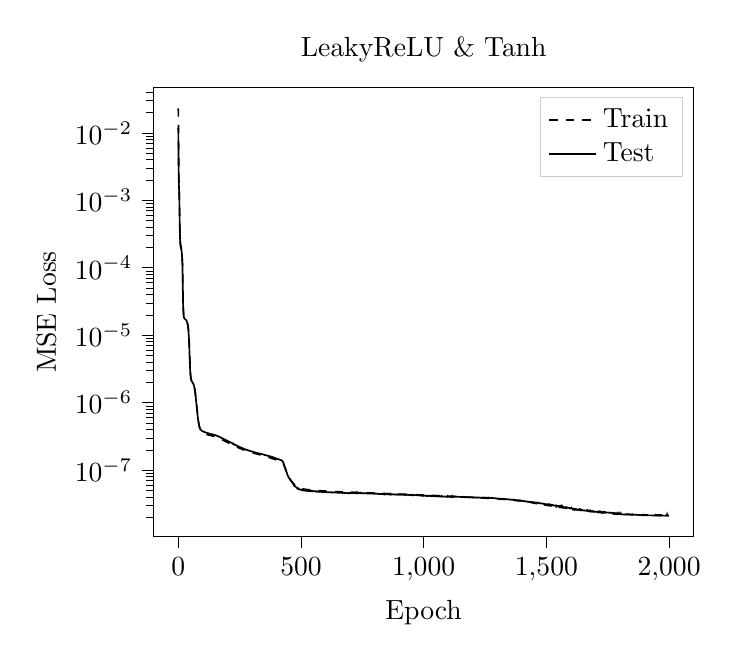
\begin{tikzpicture}

\begin{axis}[
legend cell align={left},
legend style={fill opacity=0.8, draw opacity=1, text opacity=1, draw=white!80!black},
log basis y={10},
tick align=outside,
tick pos=left,
title={LeakyReLU \& Tanh},
x grid style={white!69.0196078431373!black},
xlabel={Epoch},
xmin=-99.95, xmax=2098.95,
xtick style={color=black},
y grid style={white!69.0196078431373!black},
ylabel={MSE Loss},
ymin=1.05017771520553e-08, ymax=0.0463430733137457,
ymode=log,
ytick style={color=black}
]
\addplot [semithick, black, dashed]
table {%
0 0.0231180932745337
1 0.00691163783054799
2 0.00236752607207745
3 0.00163916035043076
4 0.00128206413588487
5 0.000841823659138754
6 0.000464628715068102
7 0.000293852134869667
8 0.000225536572310375
9 0.000206319498931407
10 0.000197783794777934
11 0.000189684799872339
12 0.000180243739887374
13 0.00016980251656787
14 0.00015801912824827
15 0.000144635740762169
16 0.000129592474302626
17 0.000112280388078943
18 7.1559276082553e-05
19 3.97623318276601e-05
20 2.75871643625578e-05
21 2.19790678838763e-05
22 1.94062530645169e-05
23 1.82326361900778e-05
24 1.76674071080924e-05
25 1.73588078223474e-05
26 1.7158149918032e-05
27 1.70034710472464e-05
28 1.68677676729203e-05
29 1.6736985395255e-05
30 1.66027530867723e-05
31 1.64600123689524e-05
32 1.63022092892788e-05
33 1.61204774622092e-05
34 1.59064208719428e-05
35 1.56461757551369e-05
36 1.53268779731661e-05
37 1.49326576583917e-05
38 1.44527597512933e-05
39 1.38589203761512e-05
40 1.31236188908588e-05
41 1.21965216658282e-05
42 1.10850571463743e-05
43 9.78546174519579e-06
44 8.34977166095996e-06
45 6.87472261279254e-06
46 5.50703124804386e-06
47 4.32035695257582e-06
48 3.46076215373614e-06
49 2.91708497832133e-06
50 2.58160994332002e-06
51 2.37972247953166e-06
52 2.25040336940197e-06
53 2.17514950790587e-06
54 2.12627043867997e-06
55 2.08565321332799e-06
56 2.05349377753805e-06
57 2.02687443416494e-06
58 2.00199655981237e-06
59 1.97703611948441e-06
60 1.9502008701977e-06
61 1.92096909441375e-06
62 1.88824094217921e-06
63 1.85032177586208e-06
64 1.80576536635613e-06
65 1.75189494970596e-06
66 1.68170406575996e-06
67 1.60475433398233e-06
68 1.52097433755216e-06
69 1.43189580140302e-06
70 1.33879025045758e-06
71 1.24530403854806e-06
72 1.15362373264816e-06
73 1.06557815367125e-06
74 9.8252717413061e-07
75 9.04443120703036e-07
76 8.32087326728015e-07
77 7.65625963595085e-07
78 7.05365310722073e-07
79 6.51862999021091e-07
80 6.04942077373494e-07
81 5.64233017882998e-07
82 5.29558019792375e-07
83 5.00131236165657e-07
84 4.7566314576386e-07
85 4.55452188916183e-07
86 4.38605655887159e-07
87 4.24582735590207e-07
88 4.13152524558313e-07
89 4.03706824585015e-07
90 3.95877927658717e-07
91 3.89085681376855e-07
92 3.8331710698003e-07
93 3.78526435383719e-07
94 3.74418354354589e-07
95 3.70831175658282e-07
96 3.67738272061047e-07
97 3.65146583575893e-07
98 3.62493394902685e-07
99 3.60080182630895e-07
100 3.57945537359683e-07
101 3.56053520064847e-07
102 3.54334171049686e-07
103 3.52817712681031e-07
104 3.51425322733689e-07
105 3.49952861228076e-07
106 3.4845155801122e-07
107 3.47144738242378e-07
108 3.45985220462808e-07
109 3.44849689867033e-07
110 3.43814986038637e-07
111 3.42843384686375e-07
112 3.41986080499623e-07
113 3.41176107667707e-07
114 3.40208299235201e-07
115 3.3930272508087e-07
116 3.38407138855246e-07
117 3.3754838096911e-07
118 3.36729014009052e-07
119 3.3593990691827e-07
120 3.35063331988295e-07
121 3.34245743346173e-07
122 3.33512132741021e-07
123 3.32793068636761e-07
124 3.32090863238932e-07
125 3.31420317962738e-07
126 3.30775629194591e-07
127 3.30142691510105e-07
128 3.29196797352438e-07
129 3.28521361183221e-07
130 3.27892319432976e-07
131 3.27220650305549e-07
132 3.26515356960044e-07
133 3.25615667463808e-07
134 3.25056333593921e-07
135 3.24426399188837e-07
136 3.23798530942554e-07
137 3.23169060266082e-07
138 3.22509486608169e-07
139 3.21795583744233e-07
140 3.21116806858868e-07
141 3.20391113518781e-07
142 3.19788296948786e-07
143 3.19009029709605e-07
144 3.18380361278514e-07
145 3.17667408253897e-07
146 3.16947345680774e-07
147 3.16236891308108e-07
148 3.15492264221007e-07
149 3.14699536374974e-07
150 3.1381763470506e-07
151 3.13085823151482e-07
152 3.12117770448594e-07
153 3.11343304275624e-07
154 3.10207398243278e-07
155 3.09326292054379e-07
156 3.0825057261552e-07
157 3.07374893779411e-07
158 3.06353653428459e-07
159 3.05310949144655e-07
160 3.04246058362878e-07
161 3.03099792176909e-07
162 3.01988235975159e-07
163 3.00853809747537e-07
164 2.99757800334532e-07
165 2.9860304979934e-07
166 2.97437247624544e-07
167 2.96262004866321e-07
168 2.95119703622504e-07
169 2.93927491966883e-07
170 2.9277420587448e-07
171 2.91547325218744e-07
172 2.90352171774089e-07
173 2.89196633247002e-07
174 2.88026482152759e-07
175 2.86858037071625e-07
176 2.85681136396931e-07
177 2.84472626674415e-07
178 2.83225285379274e-07
179 2.81923208767409e-07
180 2.80808938427413e-07
181 2.79662735465536e-07
182 2.78497147732537e-07
183 2.7732730598018e-07
184 2.76158362751744e-07
185 2.7501534894725e-07
186 2.73948458882956e-07
187 2.72805410851618e-07
188 2.71706084205903e-07
189 2.70586138455542e-07
190 2.69482361133555e-07
191 2.68363218715706e-07
192 2.67262623175668e-07
193 2.66173947544246e-07
194 2.65095240088442e-07
195 2.64019434752072e-07
196 2.62949295390058e-07
197 2.61837796813325e-07
198 2.60760488266953e-07
199 2.59687780484796e-07
200 2.58617103789049e-07
201 2.57546384290208e-07
202 2.56466794596122e-07
203 2.55386283363634e-07
204 2.54314368916653e-07
205 2.53160811752195e-07
206 2.52170376640493e-07
207 2.51107065444955e-07
208 2.50049378749395e-07
209 2.48947975414637e-07
210 2.47839090739888e-07
211 2.46802858313799e-07
212 2.45769433732335e-07
213 2.44716098066533e-07
214 2.43647765366006e-07
215 2.42632687374567e-07
216 2.41568282518756e-07
217 2.40542011198386e-07
218 2.39501517050655e-07
219 2.38522397985719e-07
220 2.3790811883373e-07
221 2.3688468773031e-07
222 2.35755131029691e-07
223 2.34829209453835e-07
224 2.33738084659763e-07
225 2.32384604892388e-07
226 2.31394943810415e-07
227 2.30522248273246e-07
228 2.29530453459859e-07
229 2.28714953429687e-07
230 2.27743794880553e-07
231 2.26800159630614e-07
232 2.25924535882882e-07
233 2.25068038957943e-07
234 2.2434950792416e-07
235 2.23598004588155e-07
236 2.22727982858828e-07
237 2.21752589588675e-07
238 2.2079913674844e-07
239 2.20136223639145e-07
240 2.19087287753439e-07
241 2.18227407508209e-07
242 2.17638221805316e-07
243 2.16821819648771e-07
244 2.15779672089411e-07
245 2.14946175177033e-07
246 2.14456527245943e-07
247 2.13398043250379e-07
248 2.12832233017934e-07
249 2.11874098638987e-07
250 2.11099597805742e-07
251 2.10672914278121e-07
252 2.09871783056315e-07
253 2.09107276880616e-07
254 2.08188488151961e-07
255 2.07699548155915e-07
256 2.06896728982997e-07
257 2.06287172176189e-07
258 2.05403436265073e-07
259 2.0485285461902e-07
260 2.04070094778075e-07
261 2.03332418717395e-07
262 2.02749026918525e-07
263 2.01991037982907e-07
264 2.0149528559088e-07
265 2.00840583556072e-07
266 2.00102935870916e-07
267 1.99465342774374e-07
268 1.98782668174857e-07
269 1.98411443150803e-07
270 1.97917968279171e-07
271 1.97185661097166e-07
272 1.96464329089707e-07
273 1.95875121249856e-07
274 1.95303546231429e-07
275 1.94788651775468e-07
276 1.9420989702823e-07
277 1.93767465002992e-07
278 1.93265095354889e-07
279 1.92600999408654e-07
280 1.92152773927035e-07
281 1.91728608424313e-07
282 1.91100815960965e-07
283 1.90411868899787e-07
284 1.89982355845331e-07
285 1.89763671826881e-07
286 1.89109531177678e-07
287 1.88474857800713e-07
288 1.88016849552497e-07
289 1.87750800755282e-07
290 1.87161313569106e-07
291 1.86710748309338e-07
292 1.86255632630861e-07
293 1.85628825434492e-07
294 1.85123155166167e-07
295 1.84645295231434e-07
296 1.84269339964516e-07
297 1.83771664101329e-07
298 1.833644481124e-07
299 1.82885625079621e-07
300 1.82412894432105e-07
301 1.82045987152435e-07
302 1.81518997514729e-07
303 1.81196183305588e-07
304 1.80777408157695e-07
305 1.80318174582084e-07
306 1.80253337028091e-07
307 1.79536329977026e-07
308 1.79052224552834e-07
309 1.78537804035983e-07
310 1.7808661023011e-07
311 1.77671806024904e-07
312 1.77333921310918e-07
313 1.76837239706629e-07
314 1.76504909028097e-07
315 1.7619372728106e-07
316 1.75711512525822e-07
317 1.75284966967837e-07
318 1.74967242465129e-07
319 1.74496793583501e-07
320 1.74072806544245e-07
321 1.73698184159576e-07
322 1.73236377452923e-07
323 1.7297212179912e-07
324 1.72495211817392e-07
325 1.72160576880742e-07
326 1.71605232377914e-07
327 1.71215926336288e-07
328 1.70964003004315e-07
329 1.70411436045015e-07
330 1.69985294508734e-07
331 1.69656958924236e-07
332 1.69223094665938e-07
333 1.68889497565772e-07
334 1.68359916543181e-07
335 1.67958899275789e-07
336 1.67533837434064e-07
337 1.67190720336663e-07
338 1.66793571096946e-07
339 1.66333352435544e-07
340 1.6600377577447e-07
341 1.65503233784392e-07
342 1.65328119916097e-07
343 1.6483816481383e-07
344 1.64399635004031e-07
345 1.63996518836029e-07
346 1.63649493739371e-07
347 1.63224858212629e-07
348 1.6287360217504e-07
349 1.62474480845276e-07
350 1.62140936037503e-07
351 1.61618776314043e-07
352 1.61292446325234e-07
353 1.60940283848277e-07
354 1.60490298046767e-07
355 1.60118750049065e-07
356 1.59706000857796e-07
357 1.5934608693513e-07
358 1.58811773737e-07
359 1.58452456393121e-07
360 1.57991367089494e-07
361 1.57635888491825e-07
362 1.57418188919678e-07
363 1.56855955040669e-07
364 1.56468315744007e-07
365 1.56109388477432e-07
366 1.55736482902569e-07
367 1.55268056005298e-07
368 1.54922160078286e-07
369 1.5435845207179e-07
370 1.53998422916857e-07
371 1.53608532613703e-07
372 1.53320270655399e-07
373 1.52874647788792e-07
374 1.5251073745759e-07
375 1.52125061831043e-07
376 1.51762487305973e-07
377 1.51191019703845e-07
378 1.50968095006476e-07
379 1.506134205016e-07
380 1.50095310431198e-07
381 1.49805103824008e-07
382 1.49280648948036e-07
383 1.48978639963104e-07
384 1.48483931340593e-07
385 1.48075164801753e-07
386 1.47686838580796e-07
387 1.47280645585113e-07
388 1.4699129418716e-07
389 1.46460909682844e-07
390 1.46051013622639e-07
391 1.45760846166354e-07
392 1.4530567812443e-07
393 1.44919195541604e-07
394 1.44455789829578e-07
395 1.43907718246794e-07
396 1.43391674527038e-07
397 1.43079515488864e-07
398 1.42741781417044e-07
399 1.42254770885586e-07
400 1.41870925347121e-07
401 1.41372117354877e-07
402 1.41036456469124e-07
403 1.40565752658972e-07
404 1.40225100501823e-07
405 1.39800642131149e-07
406 1.39402758243534e-07
407 1.3899351520763e-07
408 1.3858158822444e-07
409 1.38089070535585e-07
410 1.37723105964938e-07
411 1.3731189865851e-07
412 1.36894297202872e-07
413 1.36560860074297e-07
414 1.36180004439268e-07
415 1.35843732351759e-07
416 1.35386915687263e-07
417 1.35104608155245e-07
418 1.34771831085345e-07
419 1.34395945835308e-07
420 1.33803321077153e-07
421 1.33645604819321e-07
422 1.33042594782751e-07
423 1.32887492434008e-07
424 1.32109809285907e-07
425 1.3034141620949e-07
426 1.28958272853197e-07
427 1.26946435479169e-07
428 1.24371114068822e-07
429 1.21889156936561e-07
430 1.19242146887188e-07
431 1.16565365722465e-07
432 1.14026005928025e-07
433 1.11574512430934e-07
434 1.09276112123524e-07
435 1.06988472889924e-07
436 1.04660790437805e-07
437 1.02330937544082e-07
438 1.00075169815028e-07
439 9.79678819028606e-08
440 9.55118804810695e-08
441 9.33184585178992e-08
442 9.08561342818359e-08
443 8.86858850606131e-08
444 8.64281579531223e-08
445 8.44685718597304e-08
446 8.29710912988446e-08
447 8.16794162759038e-08
448 8.04114040882098e-08
449 7.93612581126979e-08
450 7.82892071100605e-08
451 7.72405229589879e-08
452 7.63512665500343e-08
453 7.55277521093944e-08
454 7.45679956324352e-08
455 7.3682990720414e-08
456 7.28977399475639e-08
457 7.2357229395692e-08
458 7.13870868018773e-08
459 7.06406240595925e-08
460 6.98212222687289e-08
461 6.91868356739178e-08
462 6.82494804280509e-08
463 6.75632972537699e-08
464 6.69218680471317e-08
465 6.6115140690215e-08
466 6.54791023180223e-08
467 6.482430448429e-08
468 6.41881051528515e-08
469 6.34527060299206e-08
470 6.28743330679527e-08
471 6.22909573557706e-08
472 6.16202214942518e-08
473 6.10811927366228e-08
474 6.05204008721216e-08
475 5.98775169500243e-08
476 5.95182662763705e-08
477 5.89016927179387e-08
478 5.86363955363822e-08
479 5.82207700183801e-08
480 5.78520277123573e-08
481 5.7469730499804e-08
482 5.71266204545395e-08
483 5.68272962659933e-08
484 5.65094852333914e-08
485 5.62808312025709e-08
486 5.60190715539477e-08
487 5.56668566922269e-08
488 5.5522293205712e-08
489 5.52093207986104e-08
490 5.49618962892851e-08
491 5.49192403092036e-08
492 5.46361145623564e-08
493 5.45596102092816e-08
494 5.42744300044973e-08
495 5.41143218235618e-08
496 5.40162991384818e-08
497 5.38441756212649e-08
498 5.37843087879963e-08
499 5.35685013076659e-08
500 5.35263585614842e-08
501 5.34115848633832e-08
502 5.3207641212083e-08
503 5.32631078478118e-08
504 5.31282235982644e-08
505 5.29943798497357e-08
506 5.28954847620611e-08
507 5.2823807935809e-08
508 5.27514571064813e-08
509 5.26513241148052e-08
510 5.25324681035499e-08
511 5.24348748935921e-08
512 5.24179785159617e-08
513 5.23187351735288e-08
514 5.22548456807215e-08
515 5.22080586282669e-08
516 5.213086156175e-08
517 5.20891518736022e-08
518 5.20496548581662e-08
519 5.19744910185693e-08
520 5.1925184571644e-08
521 5.18005164771296e-08
522 5.17947597895585e-08
523 5.17690564283413e-08
524 5.16804132679738e-08
525 5.16519340187926e-08
526 5.16120750102544e-08
527 5.15181743310222e-08
528 5.14550312615825e-08
529 5.14517644560897e-08
530 5.14091283996265e-08
531 5.13337360956712e-08
532 5.12756064736664e-08
533 5.12799227294636e-08
534 5.12680887148065e-08
535 5.12650375306123e-08
536 5.11184160529865e-08
537 5.10385936554059e-08
538 5.10396357888965e-08
539 5.11752794913889e-08
540 5.10148337937721e-08
541 5.08723928476229e-08
542 5.09169258187114e-08
543 5.08692298417657e-08
544 5.08352038615101e-08
545 5.06925314063267e-08
546 5.07037119099607e-08
547 5.06877666452965e-08
548 5.0667941184912e-08
549 5.05902717016227e-08
550 5.04750513385943e-08
551 5.04427755956272e-08
552 5.04092446789173e-08
553 5.04260152212055e-08
554 5.04286502014395e-08
555 5.05303507694066e-08
556 5.02225297580594e-08
557 5.02304600864534e-08
558 5.0165399755997e-08
559 5.04333431585735e-08
560 5.0124782241312e-08
561 5.02032417770693e-08
562 5.00821452931177e-08
563 5.0000705762443e-08
564 5.00046439384505e-08
565 4.9925117789229e-08
566 4.99502055184564e-08
567 4.98711967793497e-08
568 4.98507275175086e-08
569 4.99024204749787e-08
570 4.999098187497e-08
571 4.97236971988002e-08
572 4.97215885140179e-08
573 4.96691570894825e-08
574 4.96334800246245e-08
575 4.96433970162968e-08
576 4.96978211685928e-08
577 4.956785255672e-08
578 4.95573241146019e-08
579 4.95007456393637e-08
580 4.94458988988811e-08
581 4.95076322515331e-08
582 4.94297100672725e-08
583 4.93943800456975e-08
584 4.94463258320366e-08
585 4.93315144467488e-08
586 4.93525245133242e-08
587 4.92890767276322e-08
588 4.93499470231029e-08
589 4.92057945358226e-08
590 4.91780177647172e-08
591 4.91906568775846e-08
592 4.9189808130734e-08
593 4.92715395665755e-08
594 4.90638934671495e-08
595 4.90906338654895e-08
596 4.91743347090789e-08
597 4.89646283874379e-08
598 4.90205175864844e-08
599 4.90474661667406e-08
600 4.9014490635102e-08
601 4.88865692283014e-08
602 4.89974714668051e-08
603 4.89214882826161e-08
604 4.88371780207331e-08
605 4.88814107022506e-08
606 4.87413790750679e-08
607 4.88491861716511e-08
608 4.87274669609405e-08
609 4.88174249220208e-08
610 4.86369060581637e-08
611 4.86838460744821e-08
612 4.87349302922269e-08
613 4.86777343446931e-08
614 4.8578499448837e-08
615 4.86568211535143e-08
616 4.86349052835067e-08
617 4.84408213843324e-08
618 4.8504392598403e-08
619 4.85375756902329e-08
620 4.84674478400393e-08
621 4.8542444208266e-08
622 4.85567452059854e-08
623 4.83391837988734e-08
624 4.84206096480477e-08
625 4.84404144529549e-08
626 4.83589863371492e-08
627 4.83240054691691e-08
628 4.8333512562948e-08
629 4.83270477964481e-08
630 4.82329075985888e-08
631 4.83538074647072e-08
632 4.82876248497632e-08
633 4.82734585354194e-08
634 4.80849577790821e-08
635 4.81289647282779e-08
636 4.80986523996307e-08
637 4.81114106669622e-08
638 4.80671564773161e-08
639 4.80613533788699e-08
640 4.8032419726951e-08
641 4.80059581811076e-08
642 4.7996671042938e-08
643 4.79695375190659e-08
644 4.79414516192378e-08
645 4.79384816252093e-08
646 4.78988891288168e-08
647 4.78808598707303e-08
648 4.78679943505256e-08
649 4.78599641482447e-08
650 4.77994603969023e-08
651 4.77962351794758e-08
652 4.78193295485596e-08
653 4.77791427044849e-08
654 4.77450501428223e-08
655 4.77350703604884e-08
656 4.77169705135339e-08
657 4.76625162733058e-08
658 4.76985185251522e-08
659 4.76610343405071e-08
660 4.76188474607397e-08
661 4.76440611549833e-08
662 4.76127687036865e-08
663 4.75954258476463e-08
664 4.75787531435401e-08
665 4.75482052308962e-08
666 4.75397097652319e-08
667 4.75233016707932e-08
668 4.75080411703743e-08
669 4.74811047439516e-08
670 4.74798293481626e-08
671 4.75138053772639e-08
672 4.74470242437519e-08
673 4.73892646652985e-08
674 4.75326599698178e-08
675 4.73754993386422e-08
676 4.73531396458782e-08
677 4.74724356003264e-08
678 4.72760268692696e-08
679 4.7339517916356e-08
680 4.72811318488198e-08
681 4.72670735440772e-08
682 4.72558673010326e-08
683 4.73035166184133e-08
684 4.75082195272591e-08
685 4.72333178471729e-08
686 4.71912165362909e-08
687 4.72483780349364e-08
688 4.71788138760587e-08
689 4.71976311136046e-08
690 4.6973337944678e-08
691 4.71835677995358e-08
692 4.70969836285917e-08
693 4.71809280373492e-08
694 4.70514132970834e-08
695 4.70454323462377e-08
696 4.70909976204581e-08
697 4.69995533993739e-08
698 4.70930045928242e-08
699 4.70089619817315e-08
700 4.69942271035251e-08
701 4.7003992621697e-08
702 4.70964700554077e-08
703 4.69082242346985e-08
704 4.70313922615873e-08
705 4.6946243056567e-08
706 4.69173780661691e-08
707 4.69298121679174e-08
708 4.69021672788728e-08
709 4.68533316535513e-08
710 4.68566778550894e-08
711 4.69421040349971e-08
712 4.67305726985501e-08
713 4.70092672184563e-08
714 4.68666689954489e-08
715 4.67590615329527e-08
716 4.67695473282959e-08
717 4.66989844927213e-08
718 4.68983044399351e-08
719 4.67740115510651e-08
720 4.68103797235386e-08
721 4.67645586326171e-08
722 4.65781086944617e-08
723 4.68022931876533e-08
724 4.67841341276198e-08
725 4.65498166821732e-08
726 4.68560649746763e-08
727 4.6551337792522e-08
728 4.65643066167587e-08
729 4.67364545286841e-08
730 4.66678591131142e-08
731 4.65337108188635e-08
732 4.65603552441962e-08
733 4.66099961364819e-08
734 4.65988922613292e-08
735 4.65541759595567e-08
736 4.65311331794283e-08
737 4.65179922954917e-08
738 4.64667172082045e-08
739 4.64437365259585e-08
740 4.63955316583053e-08
741 4.6483137602138e-08
742 4.66002568515478e-08
743 4.64178739569832e-08
744 4.66849208393683e-08
745 4.6366795432462e-08
746 4.6306148828279e-08
747 4.61631177657296e-08
748 4.64128689436905e-08
749 4.64112351501456e-08
750 4.63883813424104e-08
751 4.63022864067852e-08
752 4.63204091154523e-08
753 4.61671090334903e-08
754 4.61387233823274e-08
755 4.62915120351681e-08
756 4.62521246511471e-08
757 4.61522336401288e-08
758 4.62154903964063e-08
759 4.61012871504352e-08
760 4.62784426105145e-08
761 4.61275226886215e-08
762 4.61520886503308e-08
763 4.61328693912577e-08
764 4.61559049398375e-08
765 4.61155644764233e-08
766 4.61220749539137e-08
767 4.60328977336388e-08
768 4.60982853489611e-08
769 4.60739228742568e-08
770 4.61838278731364e-08
771 4.59862372785835e-08
772 4.59528510639018e-08
773 4.6005952281547e-08
774 4.59876398650749e-08
775 4.6067728554533e-08
776 4.59137446782165e-08
777 4.58957754343459e-08
778 4.58558279419208e-08
779 4.59072449814357e-08
780 4.59142384379163e-08
781 4.58895862571751e-08
782 4.58867198460666e-08
783 4.58570819823478e-08
784 4.58549056254753e-08
785 4.58522188910848e-08
786 4.58383022454711e-08
787 4.58249760075802e-08
788 4.58156332054926e-08
789 4.57389657704255e-08
790 4.59913247148336e-08
791 4.57895090804072e-08
792 4.56964216262179e-08
793 4.57485686915504e-08
794 4.56413611580331e-08
795 4.55933785055152e-08
796 4.56170304072856e-08
797 4.56436149143258e-08
798 4.56415919352082e-08
799 4.56958284313913e-08
800 4.56830257604679e-08
801 4.56841598808211e-08
802 4.56173849947561e-08
803 4.56825714429954e-08
804 4.55531225274086e-08
805 4.5552917434577e-08
806 4.56644936335238e-08
807 4.55106619767776e-08
808 4.55270218857606e-08
809 4.55307098121693e-08
810 4.54847461455188e-08
811 4.5394666926768e-08
812 4.53386527681232e-08
813 4.53390495636086e-08
814 4.53637721342659e-08
815 4.53603665029334e-08
816 4.54144820487556e-08
817 4.52709462024359e-08
818 4.52853926660168e-08
819 4.52013497636017e-08
820 4.50710754442696e-08
821 4.51932848246628e-08
822 4.53610424244744e-08
823 4.52075150221276e-08
824 4.5215282600708e-08
825 4.52719320787054e-08
826 4.52165278179706e-08
827 4.49794749055599e-08
828 4.50889597445325e-08
829 4.50772180684567e-08
830 4.51285556373193e-08
831 4.51030490751236e-08
832 4.51701932355775e-08
833 4.49076377293522e-08
834 4.49185637734217e-08
835 4.49603184584646e-08
836 4.49879837329803e-08
837 4.50014234161244e-08
838 4.49353307381273e-08
839 4.49414621179756e-08
840 4.49629091718862e-08
841 4.49544324929718e-08
842 4.49327361486951e-08
843 4.48987079266772e-08
844 4.48175362475212e-08
845 4.4885612116019e-08
846 4.48820907124059e-08
847 4.48424885561849e-08
848 4.48396690977404e-08
849 4.47729865484803e-08
850 4.4777063408219e-08
851 4.48183337802277e-08
852 4.47879238372195e-08
853 4.47475506319961e-08
854 4.47746424665496e-08
855 4.47483860988029e-08
856 4.47082589705161e-08
857 4.45620165194782e-08
858 4.47270995707072e-08
859 4.47962218412812e-08
860 4.46605732271621e-08
861 4.47187323864284e-08
862 4.46657495878355e-08
863 4.45948272407293e-08
864 4.4597184201578e-08
865 4.44955244685019e-08
866 4.44660111469375e-08
867 4.47319384839773e-08
868 4.45973339360251e-08
869 4.45963839030838e-08
870 4.45372593098625e-08
871 4.45612255433048e-08
872 4.4425960542327e-08
873 4.43262497533681e-08
874 4.43918094532592e-08
875 4.44837197033365e-08
876 4.45056413322931e-08
877 4.45261458494883e-08
878 4.44532381074225e-08
879 4.43573510153783e-08
880 4.43303503327996e-08
881 4.42998324743371e-08
882 4.43046527145441e-08
883 4.43305172659336e-08
884 4.42931158772808e-08
885 4.43241507923631e-08
886 4.43054821719358e-08
887 4.43183707616868e-08
888 4.42260295621111e-08
889 4.42503930742077e-08
890 4.42230570332214e-08
891 4.41914552151701e-08
892 4.41888381992328e-08
893 4.42613764199962e-08
894 4.42198428878271e-08
895 4.42245554790333e-08
896 4.41373632131814e-08
897 4.41615692992059e-08
898 4.42076576518957e-08
899 4.41963338140283e-08
900 4.40807856509906e-08
901 4.40777588277541e-08
902 4.40876694263181e-08
903 4.40454798535939e-08
904 4.40666043033389e-08
905 4.39584186686659e-08
906 4.39868957826661e-08
907 4.40035749988965e-08
908 4.39534012102172e-08
909 4.40222353947917e-08
910 4.40523066700393e-08
911 4.40421205034625e-08
912 4.39539132983668e-08
913 4.3908745468002e-08
914 4.39363137658688e-08
915 4.39900584119357e-08
916 4.39079527119191e-08
917 4.38811851246612e-08
918 4.37819483440904e-08
919 4.37752371915678e-08
920 4.37929496257539e-08
921 4.37879617685155e-08
922 4.39569818233565e-08
923 4.38801771345254e-08
924 4.37759457980746e-08
925 4.37195849656291e-08
926 4.38086261524973e-08
927 4.3607684217406e-08
928 4.36370372067785e-08
929 4.36741188583056e-08
930 4.37848838235055e-08
931 4.37064253784314e-08
932 4.36279340547685e-08
933 4.36252051283503e-08
934 4.36026740615603e-08
935 4.35745891458339e-08
936 4.35614004157259e-08
937 4.35286232640664e-08
938 4.36506065764064e-08
939 4.35270899998841e-08
940 4.35057786880577e-08
941 4.35222723744744e-08
942 4.34606036794349e-08
943 4.34628232088841e-08
944 4.34549153780495e-08
945 4.34644257740757e-08
946 4.34089697201046e-08
947 4.34296127540534e-08
948 4.33936289674364e-08
949 4.33854671211265e-08
950 4.33085072248929e-08
951 4.33600225573372e-08
952 4.3390181357239e-08
953 4.33026631263544e-08
954 4.32936278844664e-08
955 4.33335837417559e-08
956 4.33213590067538e-08
957 4.3255756123628e-08
958 4.32751664050102e-08
959 4.33056612454408e-08
960 4.31951110932971e-08
961 4.321754662584e-08
962 4.31643162102091e-08
963 4.32112491548509e-08
964 4.31963698446225e-08
965 4.31650905881043e-08
966 4.31691831579428e-08
967 4.31324235936614e-08
968 4.31414488346604e-08
969 4.31345458427046e-08
970 4.30469177512549e-08
971 4.30732041998283e-08
972 4.30239126281151e-08
973 4.30899895427217e-08
974 4.30616513309445e-08
975 4.31306849861812e-08
976 4.30538944762304e-08
977 4.2979686554645e-08
978 4.2966369784736e-08
979 4.29267196224714e-08
980 4.2906329912995e-08
981 4.28923566371253e-08
982 4.28853914566929e-08
983 4.28360605528866e-08
984 4.28893157362609e-08
985 4.28430185515083e-08
986 4.29199739890862e-08
987 4.27919449670355e-08
988 4.28688435416547e-08
989 4.285571474405e-08
990 4.29425512589177e-08
991 4.27601403405475e-08
992 4.27443849844167e-08
993 4.27893474963525e-08
994 4.27201470785121e-08
995 4.27450639879368e-08
996 4.26757930913624e-08
997 4.2717077032961e-08
998 4.27359398340599e-08
999 4.26297833513445e-08
1000 4.26319990616264e-08
1001 4.26096843568757e-08
1002 4.25726711945629e-08
1003 4.26324038773629e-08
1004 4.25904040461944e-08
1005 4.25584534600176e-08
1006 4.25315362715395e-08
1007 4.25396315737459e-08
1008 4.25431945814125e-08
1009 4.24604777684579e-08
1010 4.24759221324678e-08
1011 4.24244887895497e-08
1012 4.25374756645169e-08
1013 4.24195880235345e-08
1014 4.24126601004105e-08
1015 4.24978580593205e-08
1016 4.23606765380669e-08
1017 4.23327833214415e-08
1018 4.23562854123816e-08
1019 4.23696529665563e-08
1020 4.23092796690838e-08
1021 4.23249601695375e-08
1022 4.23223258980698e-08
1023 4.2239201951233e-08
1024 4.22492186000767e-08
1025 4.22270520381574e-08
1026 4.21955308667066e-08
1027 4.22553197161335e-08
1028 4.21947017237301e-08
1029 4.22666300572416e-08
1030 4.21492963269543e-08
1031 4.21629412734603e-08
1032 4.21741413809684e-08
1033 4.21391151146366e-08
1034 4.20553512441302e-08
1035 4.20888020116195e-08
1036 4.20318222982274e-08
1037 4.20628583928107e-08
1038 4.20318598468583e-08
1039 4.19708633643268e-08
1040 4.20347316634206e-08
1041 4.20022315896773e-08
1042 4.20155427267588e-08
1043 4.19329264289559e-08
1044 4.19078179394461e-08
1045 4.19640399922372e-08
1046 4.19096627606308e-08
1047 4.20602141613102e-08
1048 4.18545815659144e-08
1049 4.18957760057737e-08
1050 4.18473363250627e-08
1051 4.18287741386081e-08
1052 4.18455368382808e-08
1053 4.18346338015851e-08
1054 4.17779691428422e-08
1055 4.18047715946557e-08
1056 4.17934781520302e-08
1057 4.18238405650584e-08
1058 4.16826277547244e-08
1059 4.18016461747328e-08
1060 4.16546652139971e-08
1061 4.15622153830952e-08
1062 4.15927358332624e-08
1063 4.16507495977214e-08
1064 4.16438223957982e-08
1065 4.16561885430156e-08
1066 4.16025267462317e-08
1067 4.16142616810333e-08
1068 4.16010168926562e-08
1069 4.15389839023561e-08
1070 4.1521116845189e-08
1071 4.15900827572813e-08
1072 4.15049474771223e-08
1073 4.15856902531431e-08
1074 4.15352730644969e-08
1075 4.15675830556239e-08
1076 4.14762541662839e-08
1077 4.14239940855765e-08
1078 4.13742981653087e-08
1079 4.12284009545516e-08
1080 4.14333785645482e-08
1081 4.14379792381681e-08
1082 4.13174058913057e-08
1083 4.14085360294081e-08
1084 4.13300784494197e-08
1085 4.14090463642935e-08
1086 4.12716302093941e-08
1087 4.12548861827844e-08
1088 4.12835813250467e-08
1089 4.12312686286498e-08
1090 4.12615640517089e-08
1091 4.11859164213268e-08
1092 4.09730428962973e-08
1093 4.11372105126873e-08
1094 4.11518664087396e-08
1095 4.11390963748204e-08
1096 4.13031592252366e-08
1097 4.11719313895276e-08
1098 4.11438033687261e-08
1099 4.11343783728313e-08
1100 4.10276896012363e-08
1101 4.10379834754337e-08
1102 4.104321017806e-08
1103 4.10870253588769e-08
1104 4.10300120687879e-08
1105 4.09888198049657e-08
1106 4.10024267925024e-08
1107 4.09563242182998e-08
1108 4.07605617471774e-08
1109 4.0946276630649e-08
1110 4.09175470963419e-08
1111 4.10168326254734e-08
1112 4.09821374418584e-08
1113 4.09051264949056e-08
1114 4.07797136396937e-08
1115 4.09340711478023e-08
1116 4.08393748010383e-08
1117 4.0940884852958e-08
1118 4.08396250310972e-08
1119 4.08110311358456e-08
1120 4.08509181362149e-08
1121 4.07492251230934e-08
1122 4.08181448285916e-08
1123 4.0668973934288e-08
1124 4.05575018209703e-08
1125 4.06641895303039e-08
1126 4.05549117203918e-08
1127 4.06066811944328e-08
1128 4.06495706215537e-08
1129 4.05477688296685e-08
1130 4.06732264845999e-08
1131 4.06647905037971e-08
1132 4.05916156935859e-08
1133 4.05750032665964e-08
1134 4.0477916762427e-08
1135 4.05134368666182e-08
1136 4.05830187268919e-08
1137 4.05845505255797e-08
1138 4.04253322425774e-08
1139 4.05580798492622e-08
1140 4.05443515241188e-08
1141 4.04401100055907e-08
1142 4.05047036498019e-08
1143 4.04142237186988e-08
1144 4.04171877956827e-08
1145 4.04660569515158e-08
1146 4.04543496284049e-08
1147 4.03716998444992e-08
1148 4.04011630283918e-08
1149 4.02970075104037e-08
1150 4.03461828781815e-08
1151 4.02589589008073e-08
1152 4.02516076167814e-08
1153 4.02381310617983e-08
1154 4.01870133899251e-08
1155 4.02062626232436e-08
1156 4.02236185053084e-08
1157 4.01684534931945e-08
1158 4.00635840680508e-08
1159 4.02319097396742e-08
1160 4.01856069487394e-08
1161 4.01583132845218e-08
1162 4.00994960205736e-08
1163 4.00915142826364e-08
1164 4.00383623500034e-08
1165 3.99567921203214e-08
1166 3.99822834147301e-08
1167 4.00233006470074e-08
1168 4.00672677400848e-08
1169 3.9903199077429e-08
1170 3.99743532124575e-08
1171 3.9956555676568e-08
1172 3.99558661232646e-08
1173 3.98895770690189e-08
1174 3.98867074391518e-08
1175 3.99193204998483e-08
1176 3.98780873229754e-08
1177 3.98095552203159e-08
1178 3.98182363348099e-08
1179 3.9837201779136e-08
1180 3.98306583164754e-08
1181 3.97923541370915e-08
1182 3.97012992987555e-08
1183 3.96517439220645e-08
1184 3.96888967646447e-08
1185 3.96782678695473e-08
1186 3.96370323549888e-08
1187 3.96630270174114e-08
1188 3.96740993924283e-08
1189 3.96503644513047e-08
1190 3.96449073640781e-08
1191 3.96165770855106e-08
1192 3.95804991626392e-08
1193 3.95499995544668e-08
1194 3.9542763074607e-08
1195 3.95303516285139e-08
1196 3.95233353174262e-08
1197 3.94976884674492e-08
1198 3.93905064690614e-08
1199 3.94691601339758e-08
1200 3.93894827102059e-08
1201 3.93906410103284e-08
1202 3.93571257912839e-08
1203 3.94454585244119e-08
1204 3.92966261326677e-08
1205 3.92827547184282e-08
1206 3.93346191494004e-08
1207 3.93339696547201e-08
1208 3.92473171633156e-08
1209 3.92448116723898e-08
1210 3.92120681880215e-08
1211 3.93128073525872e-08
1212 3.91544418594236e-08
1213 3.91862348951832e-08
1214 3.91478888364105e-08
1215 3.91766022502793e-08
1216 3.90814042052767e-08
1217 3.90860378782776e-08
1218 3.90710304731812e-08
1219 3.91412996911811e-08
1220 3.90301076329536e-08
1221 3.90706069328672e-08
1222 3.89968210114944e-08
1223 3.89981532791239e-08
1224 3.89891361596284e-08
1225 3.89718152948859e-08
1226 3.9012402384131e-08
1227 3.89670434373102e-08
1228 3.89375060425579e-08
1229 3.89139971570529e-08
1230 3.88525646233262e-08
1231 3.88395319976809e-08
1232 3.88862486282449e-08
1233 3.88503211148361e-08
1234 3.88387636007792e-08
1235 3.87901296150517e-08
1236 3.87976180000749e-08
1237 3.88015357533078e-08
1238 3.88150406802623e-08
1239 3.87407710960019e-08
1240 3.8727163037322e-08
1241 3.87134739838757e-08
1242 3.876618581522e-08
1243 3.86593296983762e-08
1244 3.86482336658389e-08
1245 3.86340110765104e-08
1246 3.86077210769997e-08
1247 3.86534168281827e-08
1248 3.8638405294833e-08
1249 3.85669865039517e-08
1250 3.85527548960596e-08
1251 3.85728573490951e-08
1252 3.84852372281586e-08
1253 3.84893588964985e-08
1254 3.84872347058973e-08
1255 3.8481129823964e-08
1256 3.84682925105295e-08
1257 3.84136067239638e-08
1258 3.83819222058435e-08
1259 3.83395336793768e-08
1260 3.84076231352282e-08
1261 3.8356199906886e-08
1262 3.83199172855342e-08
1263 3.83295004695583e-08
1264 3.82673642391751e-08
1265 3.82575509334515e-08
1266 3.82797004689905e-08
1267 3.81893325247518e-08
1268 3.82861426952985e-08
1269 3.81866618877069e-08
1270 3.8108881421195e-08
1271 3.81035134076058e-08
1272 3.81285452117908e-08
1273 3.80982376793071e-08
1274 3.81338798476349e-08
1275 3.80230510792501e-08
1276 3.80467222935721e-08
1277 3.80346293500367e-08
1278 3.7970512996921e-08
1279 3.79630684239629e-08
1280 3.79700530146465e-08
1281 3.79512372994384e-08
1282 3.79440456423907e-08
1283 3.7899100673755e-08
1284 3.78597796757418e-08
1285 3.78633219817459e-08
1286 3.78476123099603e-08
1287 3.78139669159339e-08
1288 3.78622373986559e-08
1289 3.77853494128999e-08
1290 3.77866532019766e-08
1291 3.77655310597191e-08
1292 3.77511984055445e-08
1293 3.76905111885151e-08
1294 3.76739344289945e-08
1295 3.76604117757751e-08
1296 3.76525064673672e-08
1297 3.75862030157492e-08
1298 3.75823963238986e-08
1299 3.7573452983608e-08
1300 3.75968950301342e-08
1301 3.75689369747079e-08
1302 3.75393609939323e-08
1303 3.751565754051e-08
1304 3.74985924214144e-08
1305 3.74513834451307e-08
1306 3.74433435688104e-08
1307 3.74217847429748e-08
1308 3.7414620559062e-08
1309 3.73071761998744e-08
1310 3.73220850740097e-08
1311 3.72771461965016e-08
1312 3.73144642917822e-08
1313 3.72319358081796e-08
1314 3.73203177250758e-08
1315 3.72251332620976e-08
1316 3.72167462767692e-08
1317 3.72191282753676e-08
1318 3.71721254168733e-08
1319 3.71581971521095e-08
1320 3.70493724268783e-08
1321 3.71312942615276e-08
1322 3.69709609575608e-08
1323 3.70562992504375e-08
1324 3.69365463868121e-08
1325 3.69724556641415e-08
1326 3.7009552952938e-08
1327 3.69332335239392e-08
1328 3.69495343939263e-08
1329 3.69725569697721e-08
1330 3.68652056792484e-08
1331 3.6810911067775e-08
1332 3.68374179569031e-08
1333 3.68219231301481e-08
1334 3.67564931629261e-08
1335 3.67690321390057e-08
1336 3.67643593666145e-08
1337 3.66814369030521e-08
1338 3.67339577067582e-08
1339 3.66309412598298e-08
1340 3.66576694705856e-08
1341 3.65878160906163e-08
1342 3.66069300117289e-08
1343 3.65444764245382e-08
1344 3.65975300624655e-08
1345 3.6499413125668e-08
1346 3.65689981283168e-08
1347 3.64199278521937e-08
1348 3.64013331566326e-08
1349 3.63601120483281e-08
1350 3.63718320564033e-08
1351 3.63319435159326e-08
1352 3.62802644122695e-08
1353 3.63296040255534e-08
1354 3.63092344102256e-08
1355 3.62564527769393e-08
1356 3.62792973884751e-08
1357 3.61615846937724e-08
1358 3.61027687922899e-08
1359 3.60317386292053e-08
1360 3.60997870885171e-08
1361 3.60615177328327e-08
1362 3.60111117920781e-08
1363 3.60927395615107e-08
1364 3.59954981128396e-08
1365 3.5923528237447e-08
1366 3.59191972858497e-08
1367 3.58905443071933e-08
1368 3.58626226830694e-08
1369 3.5874005153147e-08
1370 3.57779075432774e-08
1371 3.58525817905075e-08
1372 3.57193548534696e-08
1373 3.56384706226009e-08
1374 3.56165282049403e-08
1375 3.55104627729474e-08
1376 3.56746097534e-08
1377 3.55267219482869e-08
1378 3.54873206642736e-08
1379 3.55158849405512e-08
1380 3.54461063842848e-08
1381 3.554977798359e-08
1382 3.54182883093301e-08
1383 3.5375937807558e-08
1384 3.54445570209805e-08
1385 3.52813834822996e-08
1386 3.53688602867663e-08
1387 3.5248283515088e-08
1388 3.52502822540401e-08
1389 3.53439193361282e-08
1390 3.51152241915287e-08
1391 3.52339371634258e-08
1392 3.5168619481496e-08
1393 3.50856852637804e-08
1394 3.50631547583191e-08
1395 3.51210104749811e-08
1396 3.50724193491914e-08
1397 3.48748331884252e-08
1398 3.4841030524646e-08
1399 3.49386646831817e-08
1400 3.48768256479559e-08
1401 3.48648992414269e-08
1402 3.47478296482961e-08
1403 3.47915154517153e-08
1404 3.46595729254773e-08
1405 3.46367656796076e-08
1406 3.47192343390645e-08
1407 3.46522471925681e-08
1408 3.46658932848243e-08
1409 3.45816753206662e-08
1410 3.46041060055313e-08
1411 3.45091948013021e-08
1412 3.45206529974718e-08
1413 3.44364544897502e-08
1414 3.44696885665741e-08
1415 3.44211482392609e-08
1416 3.43356560392749e-08
1417 3.41527164575695e-08
1418 3.41574929123567e-08
1419 3.41096915033035e-08
1420 3.40284049116235e-08
1421 3.39563723219527e-08
1422 3.39137132101541e-08
1423 3.39424779713937e-08
1424 3.38063660727528e-08
1425 3.3798205546276e-08
1426 3.38162839117473e-08
1427 3.37223902615591e-08
1428 3.36924032975361e-08
1429 3.36069029138741e-08
1430 3.36360958783644e-08
1431 3.35223252569961e-08
1432 3.34317332875145e-08
1433 3.34566227060407e-08
1434 3.3374483001225e-08
1435 3.3365868358004e-08
1436 3.33827508089968e-08
1437 3.33413550688277e-08
1438 3.32690501210209e-08
1439 3.31279977956456e-08
1440 3.31143404093126e-08
1441 3.29957275937431e-08
1442 3.28822683481889e-08
1443 3.29063269628449e-08
1444 3.28127207112061e-08
1445 3.28614619871104e-08
1446 3.26379474486771e-08
1447 3.26208404306527e-08
1448 3.28633223514174e-08
1449 3.26220986011094e-08
1450 3.25656923614304e-08
1451 3.25403972318838e-08
1452 3.23148593395217e-08
1453 3.22713670968255e-08
1454 3.2265502563078e-08
1455 3.23434691651414e-08
1456 3.22945066688618e-08
1457 3.21269305487704e-08
1458 3.20867873018216e-08
1459 3.21118881974058e-08
1460 3.19490948399448e-08
1461 3.21142000139218e-08
1462 3.18662752363252e-08
1463 3.2180388384262e-08
1464 3.18784834902885e-08
1465 3.16969879232687e-08
1466 3.18939796972728e-08
1467 3.17350314009701e-08
1468 3.15552617440318e-08
1469 3.1569763848438e-08
1470 3.14996384034316e-08
1471 3.15390371312674e-08
1472 3.15074088810263e-08
1473 3.14206206120105e-08
1474 3.1363786966665e-08
1475 3.16196985234996e-08
1476 3.13778563505451e-08
1477 3.13086784426986e-08
1478 3.12140002147743e-08
1479 3.11780247521654e-08
1480 3.11660239429301e-08
1481 3.11373253580882e-08
1482 3.10250191777328e-08
1483 3.08691349708567e-08
1484 3.10417660251972e-08
1485 3.08602336343e-08
1486 3.07889982309462e-08
1487 3.08780712572343e-08
1488 3.08750902373589e-08
1489 3.07782355211117e-08
1490 3.07528176062277e-08
1491 3.08327589380042e-08
1492 3.06237301757051e-08
1493 3.08427951871693e-08
1494 3.07589006105502e-08
1495 3.0633448368178e-08
1496 3.05104868214556e-08
1497 3.05412469803201e-08
1498 3.05075373159269e-08
1499 3.04021191137593e-08
1500 3.03668018748482e-08
1501 3.03860520087795e-08
1502 3.03517534820941e-08
1503 3.01145918193413e-08
1504 3.02903665634346e-08
1505 3.01636997352972e-08
1506 3.01499143038342e-08
1507 3.02774837077635e-08
1508 3.02144607697841e-08
1509 2.99323188599487e-08
1510 3.01607944948046e-08
1511 2.99142814590425e-08
1512 2.99393004041804e-08
1513 2.98751402301178e-08
1514 2.99107655639119e-08
1515 2.98714423561108e-08
1516 2.98033299799272e-08
1517 2.96943104309833e-08
1518 2.97576083969631e-08
1519 2.97550030818883e-08
1520 2.95211373266824e-08
1521 2.96172509237636e-08
1522 2.95405728998333e-08
1523 2.95491596862263e-08
1524 2.93810306040143e-08
1525 2.9501241995078e-08
1526 2.9284440325128e-08
1527 2.92854735111092e-08
1528 2.92342873322582e-08
1529 2.91783377406318e-08
1530 2.91766761062462e-08
1531 2.91093823285848e-08
1532 2.90091641055312e-08
1533 2.91229595017484e-08
1534 2.89576020957583e-08
1535 2.90047611564148e-08
1536 2.88867284314875e-08
1537 2.89163826234784e-08
1538 2.88215822923377e-08
1539 2.87619333274591e-08
1540 2.87773453067075e-08
1541 2.88819805120966e-08
1542 2.86652366394691e-08
1543 2.85833767339483e-08
1544 2.86372076754304e-08
1545 2.85705644671452e-08
1546 2.85750536033191e-08
1547 2.85565803359589e-08
1548 2.84810766331134e-08
1549 2.83986475153597e-08
1550 2.83899150996803e-08
1551 2.83621053132066e-08
1552 2.84901869918031e-08
1553 2.8237344755766e-08
1554 2.81839579407972e-08
1555 2.81418288885504e-08
1556 2.82267080233822e-08
1557 2.81351366862026e-08
1558 2.81130401251772e-08
1559 2.81478503172394e-08
1560 2.79858885683382e-08
1561 2.81871546086165e-08
1562 2.80276849426997e-08
1563 2.78895581526939e-08
1564 2.8056303602142e-08
1565 2.78258399930564e-08
1566 2.78857195095128e-08
1567 2.77486802460203e-08
1568 2.77977363829507e-08
1569 2.76661290605773e-08
1570 2.7725998776873e-08
1571 2.76408575654585e-08
1572 2.7706542867989e-08
1573 2.76499898070881e-08
1574 2.76179487972428e-08
1575 2.7594900220862e-08
1576 2.75378189495967e-08
1577 2.76637625962195e-08
1578 2.73873271012803e-08
1579 2.73852924728146e-08
1580 2.7342906873784e-08
1581 2.74435517138016e-08
1582 2.73285376160004e-08
1583 2.73291967936018e-08
1584 2.73109773374358e-08
1585 2.73452029606602e-08
1586 2.72107086018991e-08
1587 2.72221328216915e-08
1588 2.71782966247969e-08
1589 2.70689641332922e-08
1590 2.71863880509926e-08
1591 2.708988042599e-08
1592 2.73347116674927e-08
1593 2.69803930397217e-08
1594 2.68107292011877e-08
1595 2.7230051349747e-08
1596 2.69118872608942e-08
1597 2.6829537928208e-08
1598 2.70351796736179e-08
1599 2.68444287634395e-08
1600 2.67243594134214e-08
1601 2.675084243009e-08
1602 2.67622251932664e-08
1603 2.67031103717841e-08
1604 2.68106523044764e-08
1605 2.65824326657338e-08
1606 2.66858630872946e-08
1607 2.64229744164624e-08
1608 2.65245177644147e-08
1609 2.64230247033481e-08
1610 2.6536003243649e-08
1611 2.63008397034525e-08
1612 2.64765317599114e-08
1613 2.62714885721493e-08
1614 2.64534910741077e-08
1615 2.61972977462221e-08
1616 2.61840757840304e-08
1617 2.64108177283617e-08
1618 2.60919673280569e-08
1619 2.60230307258524e-08
1620 2.60834039966795e-08
1621 2.60357025005931e-08
1622 2.60297077421257e-08
1623 2.59483225661938e-08
1624 2.59514576423925e-08
1625 2.58109603290535e-08
1626 2.58884194952458e-08
1627 2.59120633234744e-08
1628 2.58231599143954e-08
1629 2.57979060371838e-08
1630 2.57195091695195e-08
1631 2.58066784635247e-08
1632 2.57344744252208e-08
1633 2.57385186870351e-08
1634 2.56860566505424e-08
1635 2.57674494648086e-08
1636 2.56071753135245e-08
1637 2.54547097515712e-08
1638 2.54051789738696e-08
1639 2.58364402014877e-08
1640 2.54552952103637e-08
1641 2.53928300271156e-08
1642 2.53619998691335e-08
1643 2.54503471772693e-08
1644 2.53590916745594e-08
1645 2.53692299718722e-08
1646 2.53516228010398e-08
1647 2.54668625192522e-08
1648 2.52831065399306e-08
1649 2.52844327359725e-08
1650 2.52087089656072e-08
1651 2.52668389766342e-08
1652 2.51476172117293e-08
1653 2.52207387401171e-08
1654 2.51542303129071e-08
1655 2.5136598861053e-08
1656 2.51601873699769e-08
1657 2.5075786762585e-08
1658 2.51519955636326e-08
1659 2.49966761263209e-08
1660 2.49715080720136e-08
1661 2.49753695236166e-08
1662 2.49974448589541e-08
1663 2.49764560695809e-08
1664 2.51729356204322e-08
1665 2.48753579477068e-08
1666 2.4796905169211e-08
1667 2.49548626971574e-08
1668 2.50178626544084e-08
1669 2.48001520102292e-08
1670 2.48906343163213e-08
1671 2.47671721567144e-08
1672 2.46072003822206e-08
1673 2.47939477997505e-08
1674 2.47621086462146e-08
1675 2.46765305345065e-08
1676 2.4759801291907e-08
1677 2.46463099600192e-08
1678 2.49840226906883e-08
1679 2.46589874350889e-08
1680 2.44656669625698e-08
1681 2.46954368083863e-08
1682 2.46676491340025e-08
1683 2.44209269766316e-08
1684 2.43979089802338e-08
1685 2.44818877241926e-08
1686 2.45005935699538e-08
1687 2.4604212367052e-08
1688 2.43437198363949e-08
1689 2.43523587606376e-08
1690 2.4343007595462e-08
1691 2.43308685501376e-08
1692 2.43247583515682e-08
1693 2.44870100605255e-08
1694 2.42242646244506e-08
1695 2.42823329656971e-08
1696 2.42516428752282e-08
1697 2.42246933179757e-08
1698 2.42079405090578e-08
1699 2.42638856686739e-08
1700 2.41351910599263e-08
1701 2.42844953319832e-08
1702 2.4127910128513e-08
1703 2.42026454131405e-08
1704 2.40948998548873e-08
1705 2.41462954395644e-08
1706 2.41487635612714e-08
1707 2.41823387270301e-08
1708 2.5007442259195e-08
1709 2.37793883997028e-08
1710 2.39690310426255e-08
1711 2.42351890022974e-08
1712 2.41964935803196e-08
1713 2.40036192478144e-08
1714 2.39291935919539e-08
1715 2.39684144869301e-08
1716 2.37581894424466e-08
1717 2.40938078110986e-08
1718 2.3779400327939e-08
1719 2.38535541807749e-08
1720 2.40503884683108e-08
1721 2.40956289321304e-08
1722 2.38470811400049e-08
1723 2.37454025135975e-08
1724 2.36814838014965e-08
1725 2.39655744280753e-08
1726 2.38983902125511e-08
1727 2.35266781754007e-08
1728 2.38939086969481e-08
1729 2.38149622830974e-08
1730 2.37523648607407e-08
1731 2.36124519545911e-08
1732 2.36792136405484e-08
1733 2.3816207206373e-08
1734 2.36013851431238e-08
1735 2.35628361089368e-08
1736 2.37523364408077e-08
1737 2.39470503977657e-08
1738 2.35810843127737e-08
1739 2.35885479158426e-08
1740 2.35055018604768e-08
1741 2.35758200126668e-08
1742 2.36667205708585e-08
1743 2.34394050258047e-08
1744 2.34307887350127e-08
1745 2.34665378249232e-08
1746 2.33897875592248e-08
1747 2.34766704609868e-08
1748 2.33815231869272e-08
1749 2.33735348551534e-08
1750 2.34698981955717e-08
1751 2.33374506635187e-08
1752 2.33914032046201e-08
1753 2.33353183096696e-08
1754 2.33180064777017e-08
1755 2.33108582596842e-08
1756 2.33589334088791e-08
1757 2.32408062457168e-08
1758 2.32596968903209e-08
1759 2.33400288571772e-08
1760 2.32355344733648e-08
1761 2.31715712164515e-08
1762 2.32152166965705e-08
1763 2.32168313933911e-08
1764 2.31547049187597e-08
1765 2.31386741464945e-08
1766 2.31173916054317e-08
1767 2.32321625430743e-08
1768 2.30497810456143e-08
1769 2.324359682504e-08
1770 2.30636419393804e-08
1771 2.32184025694693e-08
1772 2.29026143898636e-08
1773 2.2989949408192e-08
1774 2.30393419080599e-08
1775 2.29892743828231e-08
1776 2.29425231115243e-08
1777 2.30872117779057e-08
1778 2.26941087637655e-08
1779 2.29607124264675e-08
1780 2.28530295940388e-08
1781 2.28736125071904e-08
1782 2.27256459659486e-08
1783 2.28801064867667e-08
1784 2.26104010261352e-08
1785 2.28997787328211e-08
1786 2.2688188774822e-08
1787 2.27359576747688e-08
1788 2.26398238671877e-08
1789 2.27042072946659e-08
1790 2.24559590025208e-08
1791 2.27006267952135e-08
1792 2.2744896433835e-08
1793 2.26577344779599e-08
1794 2.24359066027802e-08
1795 2.25148068118131e-08
1796 2.26630858755072e-08
1797 2.27383484396881e-08
1798 2.25823648847268e-08
1799 2.23098919187592e-08
1800 2.25249132093097e-08
1801 2.2303180479355e-08
1802 2.26310925359741e-08
1803 2.26825633191652e-08
1804 2.24380322233486e-08
1805 2.22142434358474e-08
1806 2.26626791413054e-08
1807 2.22412880930278e-08
1808 2.22899835637946e-08
1809 2.23097369413949e-08
1810 2.23670646892771e-08
1811 2.24314731713804e-08
1812 2.23656556848084e-08
1813 2.22304803063622e-08
1814 2.23561628818203e-08
1815 2.22361984381081e-08
1816 2.22895015724589e-08
1817 2.22074812707973e-08
1818 2.2363520441715e-08
1819 2.2184226327937e-08
1820 2.2282055930134e-08
1821 2.22151419411176e-08
1822 2.228156515649e-08
1823 2.21258777504119e-08
1824 2.22040807322799e-08
1825 2.2237376189338e-08
1826 2.21154516690802e-08
1827 2.21881066746477e-08
1828 2.22094489039648e-08
1829 2.21908554287609e-08
1830 2.2155239410182e-08
1831 2.20552441287936e-08
1832 2.21468108421163e-08
1833 2.21885750129047e-08
1834 2.21198738845629e-08
1835 2.21177371368952e-08
1836 2.20872282010731e-08
1837 2.21401760285289e-08
1838 2.20410874138821e-08
1839 2.21650061966727e-08
1840 2.20791256744235e-08
1841 2.20624617508491e-08
1842 2.20385097495779e-08
1843 2.20551034892935e-08
1844 2.20190159812006e-08
1845 2.20865849502871e-08
1846 2.20227449858612e-08
1847 2.20463334077436e-08
1848 2.19895492907796e-08
1849 2.21189248676978e-08
1850 2.1955669440743e-08
1851 2.21385574104005e-08
1852 2.19163468386796e-08
1853 2.20195323024086e-08
1854 2.19328325101742e-08
1855 2.20560441466233e-08
1856 2.19428233307895e-08
1857 2.19782747485908e-08
1858 2.1965241204569e-08
1859 2.20866386282381e-08
1860 2.19877295641879e-08
1861 2.18977989607794e-08
1862 2.19616685583901e-08
1863 2.19004653736476e-08
1864 2.19405183390364e-08
1865 2.19517816990589e-08
1866 2.19265106871092e-08
1867 2.19363024882568e-08
1868 2.19162044903243e-08
1869 2.19035288022695e-08
1870 2.19360283129078e-08
1871 2.18225736681177e-08
1872 2.1864725333387e-08
1873 2.18675192193984e-08
1874 2.18568363674621e-08
1875 2.18162947263068e-08
1876 2.18340475637291e-08
1877 2.17725932749602e-08
1878 2.19344837937285e-08
1879 2.18101871958254e-08
1880 2.17856895332602e-08
1881 2.17923683152321e-08
1882 2.17497656240795e-08
1883 2.17808315241541e-08
1884 2.1732079551029e-08
1885 2.18070873856391e-08
1886 2.17556553181453e-08
1887 2.17531330086729e-08
1888 2.1729115518454e-08
1889 2.18099748590106e-08
1890 2.16526825482788e-08
1891 2.17786174712131e-08
1892 2.17014127859017e-08
1893 2.17316663135847e-08
1894 2.17589930464612e-08
1895 2.17465783425297e-08
1896 2.16467080687011e-08
1897 2.17391212355977e-08
1898 2.16570342868039e-08
1899 2.18242930234425e-08
1900 2.16309313127994e-08
1901 2.16970727500154e-08
1902 2.16794926419794e-08
1903 2.16854895374041e-08
1904 2.16551065612691e-08
1905 2.17783151388318e-08
1906 2.16040218603553e-08
1907 2.17078000801507e-08
1908 2.16551564964362e-08
1909 2.16662531045131e-08
1910 2.16175029912335e-08
1911 2.163672257538e-08
1912 2.1688255902319e-08
1913 2.16512124051604e-08
1914 2.16063862481519e-08
1915 2.16308103180296e-08
1916 2.16147105902564e-08
1917 2.16693306391846e-08
1918 2.15401810113036e-08
1919 2.17088721363723e-08
1920 2.1623678064131e-08
1921 2.16535735688694e-08
1922 2.15458932970591e-08
1923 2.161825635838e-08
1924 2.1568873162181e-08
1925 2.16581259877557e-08
1926 2.15927442734909e-08
1927 2.16161616055643e-08
1928 2.15430979633169e-08
1929 2.15846384978846e-08
1930 2.15946561787916e-08
1931 2.16876623184703e-08
1932 2.15166960479962e-08
1933 2.16036845070988e-08
1934 2.15503254850091e-08
1935 2.15822995794923e-08
1936 2.15278295723209e-08
1937 2.17090359697636e-08
1938 2.15163504293514e-08
1939 2.15711084567971e-08
1940 2.14362997663642e-08
1941 2.16571232538598e-08
1942 2.14987388584831e-08
1943 2.16147230176489e-08
1944 2.14558765385675e-08
1945 2.17036499368106e-08
1946 2.14752752043523e-08
1947 2.15329608312942e-08
1948 2.15994169465716e-08
1949 2.14509186822198e-08
1950 2.15473386155907e-08
1951 2.15984542428771e-08
1952 2.14498043149547e-08
1953 2.15176806275252e-08
1954 2.15023216831867e-08
1955 2.15436001091973e-08
1956 2.14526657060787e-08
1957 2.16018353853542e-08
1958 2.14932812454549e-08
1959 2.15891009140989e-08
1960 2.13845294005921e-08
1961 2.15800802312316e-08
1962 2.14297259422125e-08
1963 2.15634954692234e-08
1964 2.14228931749716e-08
1965 2.1552250293766e-08
1966 2.14107676423936e-08
1967 2.15325815311473e-08
1968 2.14438338836942e-08
1969 2.15477409586384e-08
1970 2.14853794204828e-08
1971 2.14561077971354e-08
1972 2.14762189152395e-08
1973 2.14567359382301e-08
1974 2.14317179008106e-08
1975 2.14829155833485e-08
1976 2.14594547696123e-08
1977 2.14305314507612e-08
1978 2.14751853810924e-08
1979 2.15151130333879e-08
1980 2.1391296950668e-08
1981 2.14732683136987e-08
1982 2.13207443486851e-08
1983 2.14281754615797e-08
1984 2.14305034837992e-08
1985 2.14285731594543e-08
1986 2.13499721741783e-08
1987 2.14559017681637e-08
1988 2.13458694506841e-08
1989 2.14700107967758e-08
1990 2.1499552392612e-08
1991 2.2176766796278e-08
1992 2.1378524662552e-08
1993 2.12518290956254e-08
1994 2.15684282203199e-08
1995 2.14413060888319e-08
1996 2.14026284854896e-08
1997 2.13955880958849e-08
1998 2.14300455736449e-08
1999 2.14185116664822e-08
};
\addlegendentry{Train}
\addplot [semithick, black]
table {%
0 0.0118573838844895
1 0.00347194052301347
2 0.00184109644033015
3 0.00147178512997925
4 0.00110624707303941
5 0.000631019764114171
6 0.00038027940900065
7 0.000271435972535983
8 0.00023657112615183
9 0.000225385330850258
10 0.000216957385418937
11 0.000207147502806038
12 0.000195902757695876
13 0.000183386087883264
14 0.000169124585227109
15 0.000152975801029243
16 0.000135019232402556
17 0.000108429383544717
18 5.44648573850282e-05
19 3.41053637384903e-05
20 2.50994362431811e-05
21 2.10403359233169e-05
22 1.9199904272682e-05
23 1.83685551746748e-05
24 1.79563521669479e-05
25 1.77208330569556e-05
26 1.75554014276713e-05
27 1.74184297065949e-05
28 1.72901563928463e-05
29 1.71617339219665e-05
30 1.70250750670675e-05
31 1.68732312886277e-05
32 1.67005746334326e-05
33 1.64972752827452e-05
34 1.62550750246737e-05
35 1.59643950610189e-05
36 1.56012119987281e-05
37 1.51574995470583e-05
38 1.46079064506921e-05
39 1.39252215376473e-05
40 1.30765247376985e-05
41 1.20038885143003e-05
42 1.07500027297647e-05
43 9.30799615161959e-06
44 7.7727754614898e-06
45 6.26693827143754e-06
46 4.94613868795568e-06
47 3.83887572752428e-06
48 3.153259285682e-06
49 2.72503530140966e-06
50 2.4672660856595e-06
51 2.31168019126926e-06
52 2.20816468754492e-06
53 2.14950887311716e-06
54 2.10467987926677e-06
55 2.06850472750375e-06
56 2.0401464553288e-06
57 2.0146662791376e-06
58 1.99003670786624e-06
59 1.96526161744259e-06
60 1.9378221622901e-06
61 1.90771447705629e-06
62 1.87205580459704e-06
63 1.8286485783392e-06
64 1.776233716555e-06
65 1.71414274063864e-06
66 1.63904610417376e-06
67 1.55718259975401e-06
68 1.46772481457447e-06
69 1.37446056669432e-06
70 1.28101225982391e-06
71 1.19015521704569e-06
72 1.10282110199478e-06
73 1.01991849987826e-06
74 9.41457983572036e-07
75 8.67371909407666e-07
76 7.98640940047335e-07
77 7.35617618374818e-07
78 6.79286756621877e-07
79 6.30414092483988e-07
80 5.86913358802121e-07
81 5.50275842670089e-07
82 5.19079435434833e-07
83 4.9341304020345e-07
84 4.72326576073101e-07
85 4.54919330650227e-07
86 4.40499832166097e-07
87 4.29304492399751e-07
88 4.20338096773776e-07
89 4.12829393781067e-07
90 4.06287057330701e-07
91 4.00690453261632e-07
92 3.95891731841402e-07
93 3.92056733744539e-07
94 3.88816175700413e-07
95 3.85928416335446e-07
96 3.83286192118248e-07
97 3.81290817585977e-07
98 3.79874308009676e-07
99 3.78545053081325e-07
100 3.77064282020001e-07
101 3.75412781750128e-07
102 3.73846859247351e-07
103 3.72408720750173e-07
104 3.70911322988832e-07
105 3.69240410691418e-07
106 3.67954385183111e-07
107 3.66936774298665e-07
108 3.66631184078869e-07
109 3.65356925158267e-07
110 3.63943456704874e-07
111 3.62580351520592e-07
112 3.61606112164736e-07
113 3.60561642764878e-07
114 3.59440406327849e-07
115 3.583845114008e-07
116 3.57477688339713e-07
117 3.56673126589158e-07
118 3.55623257064508e-07
119 3.54675563585261e-07
120 3.53955471155132e-07
121 3.52975405348843e-07
122 3.52052069274578e-07
123 3.51241084217691e-07
124 3.50439535168334e-07
125 3.49709125657682e-07
126 3.48789484405643e-07
127 3.48245521308854e-07
128 3.47584489190922e-07
129 3.46762078606844e-07
130 3.4598085107973e-07
131 3.45245723565313e-07
132 3.44195882462373e-07
133 3.43086668408432e-07
134 3.42371407668907e-07
135 3.41691503535912e-07
136 3.41049315011333e-07
137 3.40160198675221e-07
138 3.4001058679678e-07
139 3.39173908514567e-07
140 3.38461035198634e-07
141 3.3801765653152e-07
142 3.37200333433429e-07
143 3.36362433017712e-07
144 3.35285449182265e-07
145 3.34332924012415e-07
146 3.33557665044282e-07
147 3.32973741024034e-07
148 3.32128536228993e-07
149 3.31732792346884e-07
150 3.30138817616898e-07
151 3.29914399799236e-07
152 3.28362233403823e-07
153 3.28240531644042e-07
154 3.26419979046477e-07
155 3.26476794043629e-07
156 3.24283149666371e-07
157 3.23719291372981e-07
158 3.22628380899914e-07
159 3.21369270750438e-07
160 3.21254645996305e-07
161 3.19268025350539e-07
162 3.18276335065093e-07
163 3.1717473802928e-07
164 3.16160765123641e-07
165 3.14985413751856e-07
166 3.13913261607013e-07
167 3.12523411594157e-07
168 3.11290563104194e-07
169 3.09980521251418e-07
170 3.08777373447811e-07
171 3.07617114003733e-07
172 3.06428745489029e-07
173 3.05205134054631e-07
174 3.04066446688012e-07
175 3.02674948216008e-07
176 3.01354759812966e-07
177 3.0023286967662e-07
178 2.98817042221344e-07
179 2.97068595500605e-07
180 2.96131389632137e-07
181 2.95034652708637e-07
182 2.93826275310494e-07
183 2.92482923214266e-07
184 2.91133346763672e-07
185 2.89926191499035e-07
186 2.88663756009555e-07
187 2.87725725911514e-07
188 2.86199082211169e-07
189 2.84957422991283e-07
190 2.83971246517467e-07
191 2.82806865925522e-07
192 2.81569953131111e-07
193 2.8031854526489e-07
194 2.79115880630343e-07
195 2.77924499414439e-07
196 2.76747528005217e-07
197 2.75534915772369e-07
198 2.74378550102483e-07
199 2.73170741138529e-07
200 2.71994707645717e-07
201 2.70881770347842e-07
202 2.69792877816144e-07
203 2.68690229177082e-07
204 2.67575870793735e-07
205 2.65893845607934e-07
206 2.65354515249783e-07
207 2.64395794147276e-07
208 2.63272085021526e-07
209 2.61764625975047e-07
210 2.61784663280196e-07
211 2.60841090948816e-07
212 2.59578314398823e-07
213 2.58013471921004e-07
214 2.57348233390076e-07
215 2.5576576945241e-07
216 2.55084444233944e-07
217 2.53845229281069e-07
218 2.52914617249189e-07
219 2.51728124567308e-07
220 2.50649861754937e-07
221 2.47411350073889e-07
222 2.48401136104803e-07
223 2.45288447331404e-07
224 2.46134902681661e-07
225 2.43416536704899e-07
226 2.43842976033193e-07
227 2.41302615222594e-07
228 2.4190958924919e-07
229 2.40863101907962e-07
230 2.38263098140123e-07
231 2.38218106574095e-07
232 2.3756945211062e-07
233 2.35406304227581e-07
234 2.34636942764155e-07
235 2.33973096896989e-07
236 2.32769124863808e-07
237 2.31668195738166e-07
238 2.30637141385159e-07
239 2.30042502380456e-07
240 2.29410034080502e-07
241 2.28270891966531e-07
242 2.27996011403775e-07
243 2.26833577698926e-07
244 2.25831286115863e-07
245 2.24840775331359e-07
246 2.23957187017731e-07
247 2.22451845388605e-07
248 2.22100410951498e-07
249 2.21184123461171e-07
250 2.19813401258762e-07
251 2.1942476280401e-07
252 2.18695078046949e-07
253 2.18455312506194e-07
254 2.1690968310395e-07
255 2.17020371451326e-07
256 2.15613951581872e-07
257 2.15422460314585e-07
258 2.13885442690298e-07
259 2.13949519434209e-07
260 2.13094011769499e-07
261 2.11428485386023e-07
262 2.11548226047853e-07
263 2.09936644068875e-07
264 2.08768241805046e-07
265 2.09255887284598e-07
266 2.08470837037567e-07
267 2.07661784656921e-07
268 2.0626818297842e-07
269 2.05415233267559e-07
270 2.0462353234052e-07
271 2.04952456783758e-07
272 2.04235263367991e-07
273 2.03479785909622e-07
274 2.0248162968528e-07
275 2.02116879677305e-07
276 2.01311380010338e-07
277 2.00348225121161e-07
278 2.00484365109332e-07
279 1.99540608036841e-07
280 1.99189500449393e-07
281 1.98377918536607e-07
282 1.98077316326817e-07
283 1.97698383885836e-07
284 1.97011203795228e-07
285 1.96321607859318e-07
286 1.96045775169296e-07
287 1.95530517999032e-07
288 1.94996346181142e-07
289 1.94415335386111e-07
290 1.93820270055767e-07
291 1.93260092373748e-07
292 1.92568037959973e-07
293 1.92517077834964e-07
294 1.92024330658569e-07
295 1.91748867450769e-07
296 1.91078015632229e-07
297 1.90556477264181e-07
298 1.90112999121084e-07
299 1.8960645320476e-07
300 1.89098201985871e-07
301 1.88656784416708e-07
302 1.88194675843079e-07
303 1.87710668342334e-07
304 1.87411913543656e-07
305 1.86736045293401e-07
306 1.86221839726386e-07
307 1.85698937116285e-07
308 1.85598622692851e-07
309 1.85096851623712e-07
310 1.84624198595884e-07
311 1.84131479841199e-07
312 1.83674046638771e-07
313 1.83239023954229e-07
314 1.82844075879984e-07
315 1.82435314854956e-07
316 1.82018169425646e-07
317 1.81593932779833e-07
318 1.81180368485911e-07
319 1.80781967173971e-07
320 1.80347825562421e-07
321 1.79976012759653e-07
322 1.79550568191189e-07
323 1.79091216523375e-07
324 1.78859394850406e-07
325 1.78372332015897e-07
326 1.78047301346851e-07
327 1.77635882891991e-07
328 1.77086221242462e-07
329 1.76804078932946e-07
330 1.76301810483892e-07
331 1.76293795561833e-07
332 1.75845926264628e-07
333 1.76047990407824e-07
334 1.75574569993842e-07
335 1.75171592786683e-07
336 1.74379536588276e-07
337 1.74062051883084e-07
338 1.73944826542538e-07
339 1.73536008674091e-07
340 1.73283254412127e-07
341 1.72408931575774e-07
342 1.72366995343509e-07
343 1.71958305372755e-07
344 1.71421319805631e-07
345 1.7115618788921e-07
346 1.70649499864339e-07
347 1.70353189332673e-07
348 1.69867917065858e-07
349 1.69595281818147e-07
350 1.69132945870842e-07
351 1.68406444345237e-07
352 1.68035228398367e-07
353 1.68060623195743e-07
354 1.67350734159299e-07
355 1.66856480632305e-07
356 1.66658253419882e-07
357 1.66709924087627e-07
358 1.65879995961404e-07
359 1.65799704632263e-07
360 1.65054032663647e-07
361 1.64694000659438e-07
362 1.64923307011122e-07
363 1.63929470886615e-07
364 1.63439651146291e-07
365 1.63082333415332e-07
366 1.63188460078345e-07
367 1.62270310966051e-07
368 1.62013080284851e-07
369 1.61375808716002e-07
370 1.6098123012398e-07
371 1.6108378986246e-07
372 1.61179485758112e-07
373 1.60325967613062e-07
374 1.59870253924055e-07
375 1.59988189807336e-07
376 1.58911916514626e-07
377 1.58503439706692e-07
378 1.58763413082852e-07
379 1.57572358716607e-07
380 1.57761661512268e-07
381 1.56664725636801e-07
382 1.56888674496258e-07
383 1.56480439272855e-07
384 1.5550020293631e-07
385 1.55616064034803e-07
386 1.54672235908038e-07
387 1.54802719976033e-07
388 1.53677092384896e-07
389 1.53224007704011e-07
390 1.53419065895832e-07
391 1.52401796071899e-07
392 1.51966716543939e-07
393 1.51572493223284e-07
394 1.51136774206861e-07
395 1.50046702174222e-07
396 1.5050115109716e-07
397 1.49175590991035e-07
398 1.49391240711338e-07
399 1.49040104702181e-07
400 1.48029101865177e-07
401 1.48203881167319e-07
402 1.4720437491178e-07
403 1.46794661759486e-07
404 1.47069101785746e-07
405 1.45961479347534e-07
406 1.46107083764946e-07
407 1.4598364828089e-07
408 1.45400704809617e-07
409 1.45011554764096e-07
410 1.44661214562802e-07
411 1.443048205374e-07
412 1.43300226795873e-07
413 1.42802505820327e-07
414 1.42370822686644e-07
415 1.41927628760641e-07
416 1.41506177442352e-07
417 1.40949381943756e-07
418 1.40435503226399e-07
419 1.40387129476949e-07
420 1.39519343633765e-07
421 1.3957300382117e-07
422 1.38666976567947e-07
423 1.38732815457843e-07
424 1.36843283371491e-07
425 1.34904666992952e-07
426 1.33619337816526e-07
427 1.30990088109684e-07
428 1.28946084032577e-07
429 1.25179596466296e-07
430 1.23942456298209e-07
431 1.20133947234535e-07
432 1.17617567241268e-07
433 1.14197717948628e-07
434 1.11772422428658e-07
435 1.09357301880664e-07
436 1.06831649304695e-07
437 1.03963188280431e-07
438 1.01741370883701e-07
439 9.9272398301764e-08
440 9.70318012605276e-08
441 9.46148830394122e-08
442 9.16909215220585e-08
443 8.94477309998365e-08
444 8.72061818313341e-08
445 8.48480610216029e-08
446 8.3159356734086e-08
447 8.16304677186963e-08
448 8.03073731958648e-08
449 7.90644776316185e-08
450 7.78456481498324e-08
451 7.67947412327885e-08
452 7.60018252776717e-08
453 7.48471791212069e-08
454 7.46970769682775e-08
455 7.2926773952986e-08
456 7.21991142427214e-08
457 7.10401835135599e-08
458 7.02375402283906e-08
459 6.9511230549324e-08
460 6.89297010580958e-08
461 6.80173286582431e-08
462 6.73242652737827e-08
463 6.6717490199153e-08
464 6.65607657879264e-08
465 6.58189875935022e-08
466 6.41036521642491e-08
467 6.43886366447077e-08
468 6.26619822696739e-08
469 6.23896170282023e-08
470 6.19974542814816e-08
471 6.05153260835323e-08
472 5.90802926581091e-08
473 5.96563864974087e-08
474 5.92277373812067e-08
475 5.84258934566151e-08
476 5.73580614116054e-08
477 5.72413902943936e-08
478 5.69301263908528e-08
479 5.6594441133484e-08
480 5.6086165045599e-08
481 5.56445840516062e-08
482 5.52108119222794e-08
483 5.45474811985969e-08
484 5.43411466935595e-08
485 5.43815943387926e-08
486 5.41155209532462e-08
487 5.30957642297381e-08
488 5.35292556946843e-08
489 5.26131813671782e-08
490 5.23987750966626e-08
491 5.25098826642534e-08
492 5.2125834315575e-08
493 5.19194180981231e-08
494 5.21435694622596e-08
495 5.18179277264608e-08
496 5.1532801137455e-08
497 5.14141760277198e-08
498 5.16328277910816e-08
499 5.12243438777205e-08
500 5.10729734060078e-08
501 5.12627664761567e-08
502 5.0749676461237e-08
503 5.09081807820166e-08
504 5.09158546435629e-08
505 5.09211659505127e-08
506 5.0668777618057e-08
507 5.03283281716449e-08
508 5.07268929084148e-08
509 5.01475518888128e-08
510 5.01035408717598e-08
511 5.0049241195893e-08
512 4.99921739560705e-08
513 4.99598868941575e-08
514 4.98670083004527e-08
515 4.9806700985755e-08
516 4.97489835993292e-08
517 4.96928223014947e-08
518 5.00442354223196e-08
519 4.96105521108348e-08
520 4.95889125318172e-08
521 4.95752310314401e-08
522 4.94421392716049e-08
523 4.97867596038759e-08
524 4.93718310679014e-08
525 4.97748366967699e-08
526 4.93129661549574e-08
527 4.92595546575103e-08
528 4.92442637778367e-08
529 4.95714012060944e-08
530 4.91217662101917e-08
531 4.90519873608264e-08
532 4.90411871112428e-08
533 4.90058695845619e-08
534 4.91597518248454e-08
535 4.92326961420986e-08
536 4.91882445885494e-08
537 4.88169824564011e-08
538 4.89938294379044e-08
539 4.93149201474807e-08
540 4.94325753663816e-08
541 4.88679496868372e-08
542 4.90869744851352e-08
543 4.90897207328089e-08
544 4.88846723101233e-08
545 4.947681375711e-08
546 4.92706426769018e-08
547 4.90665215124864e-08
548 4.91616773956594e-08
549 4.8578634448404e-08
550 4.88499658501951e-08
551 4.87174602881169e-08
552 4.87369646862135e-08
553 4.86617857120564e-08
554 4.86143356681623e-08
555 4.85415903028752e-08
556 4.86108362451887e-08
557 4.85851465725773e-08
558 4.85876725520029e-08
559 4.87537832327689e-08
560 4.84298254832538e-08
561 4.85601709954153e-08
562 4.84890136931426e-08
563 4.8140694985932e-08
564 4.83991620114921e-08
565 4.80310298200948e-08
566 4.83229634085092e-08
567 4.83057682743038e-08
568 4.81310884481445e-08
569 4.84285926916073e-08
570 4.82401816270794e-08
571 4.7876984154982e-08
572 4.79342823211937e-08
573 4.78337867093614e-08
574 4.80912163425273e-08
575 4.79251198726161e-08
576 4.80153197202071e-08
577 4.77575134993913e-08
578 4.79333550629235e-08
579 4.77514241481458e-08
580 4.76820467554262e-08
581 4.78824233596242e-08
582 4.76167194563004e-08
583 4.75773731523077e-08
584 4.78008104209948e-08
585 4.75518575626666e-08
586 4.75808619171403e-08
587 4.76777373137338e-08
588 4.76498023260774e-08
589 4.75460950610795e-08
590 4.73984478333023e-08
591 4.73811638812549e-08
592 4.75924473164469e-08
593 4.74444661335838e-08
594 4.7421114146573e-08
595 4.75155061963051e-08
596 4.73159644798216e-08
597 4.733600178497e-08
598 4.72362380321556e-08
599 4.72547441177085e-08
600 4.72317829292024e-08
601 4.73431818193149e-08
602 4.71923975453592e-08
603 4.71158756454315e-08
604 4.72791263916861e-08
605 4.71520102962586e-08
606 4.70984140577002e-08
607 4.71198511320381e-08
608 4.70751153613946e-08
609 4.69884824383371e-08
610 4.69898644439581e-08
611 4.69091787635989e-08
612 4.69394763058517e-08
613 4.70247876194207e-08
614 4.69478322884243e-08
615 4.68647556317592e-08
616 4.69282674941951e-08
617 4.68446970103287e-08
618 4.68608760684219e-08
619 4.70023842069622e-08
620 4.69002081615599e-08
621 4.6956341037685e-08
622 4.68784264739952e-08
623 4.67072212018138e-08
624 4.68874183923162e-08
625 4.67111860302794e-08
626 4.6946773579748e-08
627 4.67486849231591e-08
628 4.68906904416144e-08
629 4.69325911467422e-08
630 4.6731187808291e-08
631 4.67209133603319e-08
632 4.67046454843967e-08
633 4.66014711264506e-08
634 4.67380267821227e-08
635 4.67107099666464e-08
636 4.66828566914046e-08
637 4.66627838591194e-08
638 4.66382701347356e-08
639 4.66068001969688e-08
640 4.65936160765068e-08
641 4.65348293232637e-08
642 4.65430680662848e-08
643 4.65254075265875e-08
644 4.65011353867339e-08
645 4.64708094227717e-08
646 4.64526515031594e-08
647 4.64508147501874e-08
648 4.64097418273468e-08
649 4.63748506263073e-08
650 4.61330635914692e-08
651 4.64434144475945e-08
652 4.63703422326489e-08
653 4.64271359135182e-08
654 4.64018334866978e-08
655 4.63798457417397e-08
656 4.63717313436973e-08
657 4.63578970766321e-08
658 4.63413414308889e-08
659 4.63249989479664e-08
660 4.6316408486291e-08
661 4.63100384706649e-08
662 4.62907472353891e-08
663 4.6294541533598e-08
664 4.62714275784037e-08
665 4.62684255353452e-08
666 4.62632989695066e-08
667 4.62764475628319e-08
668 4.61754154912342e-08
669 4.5879751553457e-08
670 4.62151241720221e-08
671 4.62099976061836e-08
672 4.62582576687964e-08
673 4.60679281388821e-08
674 4.61294789033673e-08
675 4.60868747609311e-08
676 4.57135662657038e-08
677 4.58766358235607e-08
678 4.57203874759671e-08
679 4.6057465397098e-08
680 4.57000872700064e-08
681 4.57182274260504e-08
682 4.5734910969486e-08
683 4.58223752275444e-08
684 4.57223698901998e-08
685 4.56961082306861e-08
686 4.56690933958726e-08
687 4.56433895124064e-08
688 4.56765043566065e-08
689 4.57624089733599e-08
690 4.54615971534622e-08
691 4.56805793191961e-08
692 4.54389486037599e-08
693 4.54594832888233e-08
694 4.58155859917042e-08
695 4.55202702198676e-08
696 4.54292639062714e-08
697 4.5409315418965e-08
698 4.53606716632748e-08
699 4.53723956184149e-08
700 4.5345483812298e-08
701 4.62660558753214e-08
702 4.64951206424757e-08
703 4.60715554595481e-08
704 4.59841054123444e-08
705 4.59922659956646e-08
706 4.59524400753253e-08
707 4.58858941954077e-08
708 4.58913156364815e-08
709 4.58579521023239e-08
710 4.58422526605773e-08
711 4.62018689972865e-08
712 4.58555859950138e-08
713 4.61109834759554e-08
714 4.57194282432738e-08
715 4.57357671734826e-08
716 4.570427236672e-08
717 4.58928965940686e-08
718 4.60750975150859e-08
719 4.58266242731042e-08
720 4.59231550564709e-08
721 4.59704025956853e-08
722 4.56252848834993e-08
723 4.59316638057317e-08
724 4.55868303106399e-08
725 4.57121451802323e-08
726 4.63532359162855e-08
727 4.55539961308205e-08
728 4.58781137524511e-08
729 4.60014888403748e-08
730 4.58972628791798e-08
731 4.57267113063153e-08
732 4.59071785030574e-08
733 4.56548292504522e-08
734 4.55434445711944e-08
735 4.58471483000267e-08
736 4.58459012975254e-08
737 4.57742075354872e-08
738 4.58400712943785e-08
739 4.58366642419605e-08
740 4.57211797311174e-08
741 4.57982665125201e-08
742 4.61033735632554e-08
743 4.56485125255313e-08
744 4.57528308572819e-08
745 4.55408297739268e-08
746 4.54249509118654e-08
747 4.54718112052888e-08
748 4.54904593993888e-08
749 4.55812347865958e-08
750 4.57141489107471e-08
751 4.55762503293045e-08
752 4.57129800679468e-08
753 4.53563266944457e-08
754 4.53960922186525e-08
755 4.5401328918615e-08
756 4.53795436783366e-08
757 4.55442688007679e-08
758 4.5456168606961e-08
759 4.5448746988086e-08
760 4.54246169567796e-08
761 4.5695003336732e-08
762 4.57117899088644e-08
763 4.542228992932e-08
764 4.55543904820388e-08
765 4.53690134349927e-08
766 4.56443771668091e-08
767 4.52899264757889e-08
768 4.5468745213384e-08
769 4.54735697985598e-08
770 4.5450029517724e-08
771 4.51929977884902e-08
772 4.56216788791153e-08
773 4.55422082268342e-08
774 4.53613182571644e-08
775 4.51361934494798e-08
776 4.51531327883004e-08
777 4.52529924643841e-08
778 4.49624337761634e-08
779 4.51050929939356e-08
780 4.52854536092673e-08
781 4.52197532752052e-08
782 4.51254820177382e-08
783 4.54000144145539e-08
784 4.52867823241832e-08
785 4.51903545695131e-08
786 4.52043913412581e-08
787 4.53279760392888e-08
788 4.52507009640613e-08
789 4.51718307203919e-08
790 4.53701112235194e-08
791 4.52904167502766e-08
792 4.51279582591724e-08
793 4.50122676909359e-08
794 4.48010730735859e-08
795 4.48912373940402e-08
796 4.47219647981001e-08
797 4.47199255404485e-08
798 4.51644091015169e-08
799 4.4978609281543e-08
800 4.48744117420574e-08
801 4.49726833551267e-08
802 4.50490595937936e-08
803 4.4812011879003e-08
804 4.50143531338654e-08
805 4.47368009304228e-08
806 4.48459864799133e-08
807 4.48396129115736e-08
808 4.48050663237609e-08
809 4.49399344404355e-08
810 4.47407195736105e-08
811 4.46041887869342e-08
812 4.46529675457441e-08
813 4.46154686528644e-08
814 4.46865229264404e-08
815 4.45034977758496e-08
816 4.45110686086991e-08
817 4.42439755943269e-08
818 4.44389058884553e-08
819 4.44403518429226e-08
820 4.45915411262376e-08
821 4.46078871618738e-08
822 4.44932766185957e-08
823 4.438434686449e-08
824 4.45331309606445e-08
825 4.45511147972866e-08
826 4.4220083594837e-08
827 4.42033503134098e-08
828 4.44722942916087e-08
829 4.44595649184976e-08
830 4.43475833833418e-08
831 4.42359251451308e-08
832 4.42911449738403e-08
833 4.40913758836814e-08
834 4.39752128045257e-08
835 4.41778169602003e-08
836 4.42476952855486e-08
837 4.42138308187623e-08
838 4.42040857251413e-08
839 4.46568080292309e-08
840 4.38906297972608e-08
841 4.42486509655282e-08
842 4.40604708273895e-08
843 4.4105018304208e-08
844 4.41654073313202e-08
845 4.40418261860032e-08
846 4.43860876941926e-08
847 4.40129426237945e-08
848 4.4040223912134e-08
849 4.43052527998589e-08
850 4.40866507744886e-08
851 4.4323257952783e-08
852 4.42978418391249e-08
853 4.39444391986399e-08
854 4.39343814662152e-08
855 4.4141120980612e-08
856 4.38732890017945e-08
857 4.41565219944096e-08
858 4.39959570996962e-08
859 4.4079367711447e-08
860 4.4077708594159e-08
861 4.37446594503399e-08
862 4.40822454095269e-08
863 4.37888161286537e-08
864 4.43756178469812e-08
865 4.38114469147877e-08
866 4.35525677744408e-08
867 4.40566196857617e-08
868 4.3816221761972e-08
869 4.3774754487913e-08
870 4.36784191037987e-08
871 4.37872245129256e-08
872 4.36273239756702e-08
873 4.35169020818194e-08
874 4.35230909090478e-08
875 4.38613234621243e-08
876 4.4034649704372e-08
877 4.40510170562902e-08
878 4.40113758770622e-08
879 4.38012932590937e-08
880 4.37637623917908e-08
881 4.35837499423997e-08
882 4.3723112241878e-08
883 4.37171969736028e-08
884 4.34944098515189e-08
885 4.37149019205663e-08
886 4.36558913463614e-08
887 4.37604512626422e-08
888 4.35933849018966e-08
889 4.33690843237855e-08
890 4.36096492251181e-08
891 4.36113509749703e-08
892 4.33876472527572e-08
893 4.37578897560797e-08
894 4.3909519575891e-08
895 4.3697450990976e-08
896 4.37189484614464e-08
897 4.38323652929284e-08
898 4.38779323985727e-08
899 4.34476525867922e-08
900 4.3561989571117e-08
901 4.32836735342335e-08
902 4.35280753663392e-08
903 4.32411155770751e-08
904 4.35349534200213e-08
905 4.34874607435631e-08
906 4.34372147140039e-08
907 4.3580339337268e-08
908 4.32843840769692e-08
909 4.36276970106064e-08
910 4.35969660372848e-08
911 4.35675886478748e-08
912 4.36407390225213e-08
913 4.35504787787977e-08
914 4.35670912679598e-08
915 4.34650182512542e-08
916 4.34652385195022e-08
917 4.31355005048317e-08
918 4.33462155058351e-08
919 4.33367759455905e-08
920 4.33891393925023e-08
921 4.30917701521594e-08
922 4.31166888859025e-08
923 4.33813767131142e-08
924 4.29169197957435e-08
925 4.31923368182652e-08
926 4.2713473646927e-08
927 4.29358593123652e-08
928 4.29013233826936e-08
929 4.31726263627752e-08
930 4.30742090884451e-08
931 4.30684607977128e-08
932 4.30562288045166e-08
933 4.31397708666736e-08
934 4.3078976830202e-08
935 4.30841069487542e-08
936 4.30671214246559e-08
937 4.28462776369543e-08
938 4.30537099305184e-08
939 4.30626592162753e-08
940 4.30452296029671e-08
941 4.29604227747404e-08
942 4.3002369665146e-08
943 4.29617159625195e-08
944 4.29491819886607e-08
945 4.29505959687049e-08
946 4.2882007278422e-08
947 4.28633981641724e-08
948 4.28586517386975e-08
949 4.28552873188437e-08
950 4.28078124059539e-08
951 4.26342374737487e-08
952 4.28030197952012e-08
953 4.280413890001e-08
954 4.28189501633369e-08
955 4.31330562378207e-08
956 4.25349178101442e-08
957 4.27072741615575e-08
958 4.27535624680786e-08
959 4.26480077919678e-08
960 4.24339035021148e-08
961 4.26693809174594e-08
962 4.27058211016629e-08
963 4.26654018781392e-08
964 4.26912905027166e-08
965 4.26928821184447e-08
966 4.27295319127552e-08
967 4.27604085473376e-08
968 4.27217123899482e-08
969 4.2716880699345e-08
970 4.24923598529858e-08
971 4.27472919284355e-08
972 4.26922177609868e-08
973 4.27144257741929e-08
974 4.23731876253441e-08
975 4.23969126472912e-08
976 4.24212807104141e-08
977 4.21984935883302e-08
978 4.24238564278312e-08
979 4.25276596160984e-08
980 4.24956390077114e-08
981 4.24162784895543e-08
982 4.23455723819188e-08
983 4.24444834834503e-08
984 4.24204031901354e-08
985 4.23695745155328e-08
986 4.23762962498131e-08
987 4.23294395091034e-08
988 4.24193409287454e-08
989 4.19840908705282e-08
990 4.23838812935173e-08
991 4.19769712323159e-08
992 4.21765982139277e-08
993 4.22454142778861e-08
994 4.22077839346002e-08
995 4.21090966540305e-08
996 4.22122319321261e-08
997 4.18815950808948e-08
998 4.22089527774006e-08
999 4.18626413534184e-08
1000 4.21165111674782e-08
1001 4.20637320530659e-08
1002 4.18576746596955e-08
1003 4.19937187245978e-08
1004 4.20365147135726e-08
1005 4.20401420342387e-08
1006 4.19915551219674e-08
1007 4.1986162102603e-08
1008 4.16844692097129e-08
1009 4.18996464190968e-08
1010 4.18840784277563e-08
1011 4.1616456059046e-08
1012 4.19116048533397e-08
1013 4.18810408575609e-08
1014 4.15977758905228e-08
1015 4.18549888081543e-08
1016 4.1776250014891e-08
1017 4.15293719413512e-08
1018 4.15098142525494e-08
1019 4.17648529094095e-08
1020 4.17283843034966e-08
1021 4.14616394550649e-08
1022 4.15176550916385e-08
1023 4.15194278957642e-08
1024 4.16790300050707e-08
1025 4.1681282425543e-08
1026 4.17005487918232e-08
1027 4.17054337731315e-08
1028 4.13736174209589e-08
1029 4.16185201856933e-08
1030 4.13104324081814e-08
1031 4.14779108837138e-08
1032 4.1245499460274e-08
1033 4.14440108897907e-08
1034 4.13677305743931e-08
1035 4.14252170344298e-08
1036 4.13349994232703e-08
1037 4.11901801555814e-08
1038 4.12206624389455e-08
1039 4.12368095226157e-08
1040 4.11487413032319e-08
1041 4.11103542319324e-08
1042 4.13460945480892e-08
1043 4.13296525891838e-08
1044 4.13756424677558e-08
1045 4.1333819922329e-08
1046 4.12431226948229e-08
1047 4.16251424439906e-08
1048 4.12272633809607e-08
1049 4.12111518244274e-08
1050 4.11512566245165e-08
1051 4.09499278930525e-08
1052 4.11282812251557e-08
1053 4.10628722136153e-08
1054 4.08629610149092e-08
1055 4.10367206882256e-08
1056 4.09977332083145e-08
1057 4.13343776983766e-08
1058 4.0962177649817e-08
1059 4.10483451673826e-08
1060 4.08692883979711e-08
1061 4.10363831804261e-08
1062 4.09257516764683e-08
1063 4.09734184358967e-08
1064 4.0748627583298e-08
1065 4.09342888474384e-08
1066 4.06742692860007e-08
1067 4.06672882036219e-08
1068 4.08835738596736e-08
1069 4.07810425429034e-08
1070 4.05988807017366e-08
1071 4.05642488487956e-08
1072 4.04903524042766e-08
1073 4.13003036214832e-08
1074 4.1015347562734e-08
1075 4.07986675554639e-08
1076 4.09354292685293e-08
1077 4.07078530884064e-08
1078 4.05852738083468e-08
1079 4.04971700618262e-08
1080 4.08313809430183e-08
1081 4.0785337773741e-08
1082 4.06655544793466e-08
1083 4.07873876895337e-08
1084 4.08630747017469e-08
1085 4.08050908617952e-08
1086 4.07193887497215e-08
1087 4.06105087336073e-08
1088 4.06316438272825e-08
1089 4.05123614655167e-08
1090 4.04767348527457e-08
1091 4.03598576781405e-08
1092 4.04127113995401e-08
1093 4.03380440161527e-08
1094 4.0309249271786e-08
1095 4.021262256515e-08
1096 4.10894926972105e-08
1097 4.05146849402627e-08
1098 4.04047320046175e-08
1099 4.05075510911956e-08
1100 4.03389925907049e-08
1101 4.05370563782981e-08
1102 4.0348293595116e-08
1103 4.04412858756587e-08
1104 4.04219875349554e-08
1105 4.02741200389301e-08
1106 4.02938056254243e-08
1107 4.03172322194223e-08
1108 4.02659630083235e-08
1109 4.04156850208892e-08
1110 4.01470181543573e-08
1111 4.05071887144004e-08
1112 4.03589908160029e-08
1113 4.03507200985587e-08
1114 4.01399127269997e-08
1115 4.04920719176971e-08
1116 4.10961149555078e-08
1117 4.03905993096032e-08
1118 4.08497804471608e-08
1119 4.04910345253029e-08
1120 4.03856752484444e-08
1121 4.03058599829365e-08
1122 4.05480378162792e-08
1123 4.04024724787178e-08
1124 4.06237177230651e-08
1125 4.05733118213902e-08
1126 4.07427265258775e-08
1127 4.0673867829355e-08
1128 4.0537997847423e-08
1129 4.03968236639685e-08
1130 4.04583140323211e-08
1131 4.04400140041616e-08
1132 4.0321040728486e-08
1133 4.03712299146264e-08
1134 4.03993638542488e-08
1135 4.03452737884891e-08
1136 4.04709759038724e-08
1137 4.03729387699059e-08
1138 4.02971629398508e-08
1139 4.03472277810124e-08
1140 4.02843767233207e-08
1141 4.03531998927065e-08
1142 4.03003248550249e-08
1143 4.03530862058687e-08
1144 4.03591435826911e-08
1145 4.02143349731432e-08
1146 4.02408097954776e-08
1147 4.02205380112264e-08
1148 4.02070234883922e-08
1149 4.01688247109178e-08
1150 4.01693611706833e-08
1151 4.00048705273548e-08
1152 3.9960724507182e-08
1153 4.00449380322243e-08
1154 4.00689863511161e-08
1155 4.01030888497189e-08
1156 4.00945232570393e-08
1157 4.01442719066836e-08
1158 4.00553581414442e-08
1159 4.01021864604445e-08
1160 4.0257607025751e-08
1161 3.99609199064344e-08
1162 3.99162800590602e-08
1163 3.98988717620341e-08
1164 3.99390138738909e-08
1165 3.98859718586664e-08
1166 3.97300539134449e-08
1167 3.99084001401206e-08
1168 3.99461548283853e-08
1169 3.97525710127411e-08
1170 3.98101853704702e-08
1171 3.98127184553232e-08
1172 3.97344024349877e-08
1173 3.97068440349813e-08
1174 3.98509030219429e-08
1175 3.98590564998358e-08
1176 3.96881425501761e-08
1177 3.97131358909064e-08
1178 3.98936563783536e-08
1179 3.98268831247606e-08
1180 3.97765020920815e-08
1181 3.96478512243448e-08
1182 3.97659363216007e-08
1183 3.9678354823991e-08
1184 3.96605059904687e-08
1185 3.97231829651901e-08
1186 3.95981061274142e-08
1187 3.97815149710823e-08
1188 3.95499100136476e-08
1189 3.96482917608409e-08
1190 3.95527059993128e-08
1191 3.9518880612377e-08
1192 3.97050179401504e-08
1193 3.96074071318253e-08
1194 3.96184169915159e-08
1195 3.96045116701771e-08
1196 3.96949992875761e-08
1197 3.96931660873179e-08
1198 3.94914110302125e-08
1199 3.94331536313075e-08
1200 3.96939370261862e-08
1201 3.9649375338513e-08
1202 3.96237638256025e-08
1203 3.935755898965e-08
1204 3.95974275591016e-08
1205 3.93675563259421e-08
1206 3.93399801623673e-08
1207 3.92871513099635e-08
1208 3.94953936222464e-08
1209 3.94969283945557e-08
1210 3.94897057276467e-08
1211 3.91909793506784e-08
1212 3.9448909916473e-08
1213 3.94282047011529e-08
1214 3.93264656395331e-08
1215 3.91213816897107e-08
1216 3.93272756582519e-08
1217 3.94020993610411e-08
1218 3.93878423210481e-08
1219 3.92359282841426e-08
1220 3.92737753429628e-08
1221 3.90722583176739e-08
1222 3.92934538240297e-08
1223 3.93451422553426e-08
1224 3.92248793446015e-08
1225 3.92253376446661e-08
1226 3.91993744131014e-08
1227 3.92620087552586e-08
1228 3.92023054018864e-08
1229 3.92195858012201e-08
1230 3.91498495844189e-08
1231 3.91527770204902e-08
1232 3.89214314111541e-08
1233 3.89733401107151e-08
1234 3.91452879000553e-08
1235 3.9179646194043e-08
1236 3.90282437479073e-08
1237 3.90554077966954e-08
1238 3.91860552895196e-08
1239 3.91035648306115e-08
1240 3.92643215718635e-08
1241 3.91683663281128e-08
1242 3.9015681352339e-08
1243 3.91869221516572e-08
1244 3.91239041164226e-08
1245 3.91683379064034e-08
1246 3.91338090821591e-08
1247 3.92284071892846e-08
1248 3.90841989883484e-08
1249 3.92502066404177e-08
1250 3.91201098182137e-08
1251 3.90133720884478e-08
1252 3.91812307043438e-08
1253 3.91399197496867e-08
1254 3.90838899022583e-08
1255 3.90017582674318e-08
1256 3.90366921010354e-08
1257 3.91172463309886e-08
1258 3.90134182737256e-08
1259 3.89256520350045e-08
1260 3.90777756820171e-08
1261 3.9074425473018e-08
1262 3.90138588102218e-08
1263 3.89255880861583e-08
1264 3.89390777399967e-08
1265 3.91256058662748e-08
1266 3.88388521344041e-08
1267 3.89927130584056e-08
1268 3.89724981175732e-08
1269 3.88947363205716e-08
1270 3.87308141114318e-08
1271 3.8894565790315e-08
1272 3.88430301256903e-08
1273 3.88344858492928e-08
1274 3.87639964571918e-08
1275 3.87083325392723e-08
1276 3.88134857587374e-08
1277 3.86610814473443e-08
1278 3.85713754269545e-08
1279 3.87022325298858e-08
1280 3.8674667024452e-08
1281 3.86208576230729e-08
1282 3.85633498467541e-08
1283 3.84818363841077e-08
1284 3.85777383371533e-08
1285 3.85539244973643e-08
1286 3.85508016620406e-08
1287 3.84172302858587e-08
1288 3.84915495033056e-08
1289 3.85150755732866e-08
1290 3.84583387358362e-08
1291 3.85167595595703e-08
1292 3.83584932706071e-08
1293 3.81918852099261e-08
1294 3.82801061959981e-08
1295 3.82204063953395e-08
1296 3.81612501598738e-08
1297 3.80639839647756e-08
1298 3.80296327762153e-08
1299 3.80072968653167e-08
1300 3.81389781978214e-08
1301 3.79939812944485e-08
1302 3.78862843319894e-08
1303 3.78610742757246e-08
1304 3.79537361538951e-08
1305 3.78531588296482e-08
1306 3.78433959724589e-08
1307 3.78978093351634e-08
1308 3.77610511748117e-08
1309 3.76715014738238e-08
1310 3.78110982524049e-08
1311 3.78821241042715e-08
1312 3.77275171103975e-08
1313 3.77106808002736e-08
1314 3.76990065831251e-08
1315 3.76165587567812e-08
1316 3.7577184031079e-08
1317 3.76854956130046e-08
1318 3.74444013573338e-08
1319 3.7574441336119e-08
1320 3.76477906627315e-08
1321 3.75963651322309e-08
1322 3.75507589467361e-08
1323 3.74920432477666e-08
1324 3.7461333590727e-08
1325 3.75448507838883e-08
1326 3.74572159955733e-08
1327 3.7496263871617e-08
1328 3.75007580544207e-08
1329 3.73769708517102e-08
1330 3.7375546213525e-08
1331 3.71943507104788e-08
1332 3.73115227603193e-08
1333 3.7283896858753e-08
1334 3.72876307608294e-08
1335 3.7208273795386e-08
1336 3.72184629782168e-08
1337 3.7119921358908e-08
1338 3.7172448230649e-08
1339 3.71250798991696e-08
1340 3.70605341970531e-08
1341 3.70052077869332e-08
1342 3.6944442172171e-08
1343 3.68787453908226e-08
1344 3.68899506497655e-08
1345 3.69173562830838e-08
1346 3.70031827401363e-08
1347 3.67702845949225e-08
1348 3.68898511737825e-08
1349 3.68017119001252e-08
1350 3.68321586563525e-08
1351 3.67771306741815e-08
1352 3.6690806837214e-08
1353 3.65571324323355e-08
1354 3.67270445167378e-08
1355 3.66332635337585e-08
1356 3.66290926478996e-08
1357 3.66129100370927e-08
1358 3.64526364649009e-08
1359 3.64003831521131e-08
1360 3.6535425351758e-08
1361 3.64360808191577e-08
1362 3.63247281143231e-08
1363 3.64586476564455e-08
1364 3.63117820256775e-08
1365 3.61612606525341e-08
1366 3.64596068891387e-08
1367 3.61608876175978e-08
1368 3.61372904933432e-08
1369 3.61781609115042e-08
1370 3.61171537122118e-08
1371 3.61312970653671e-08
1372 3.62401557651992e-08
1373 3.61649163949096e-08
1374 3.58036089664893e-08
1375 3.58409231182577e-08
1376 3.56132652257202e-08
1377 3.5735311598728e-08
1378 3.58655682930475e-08
1379 3.58594540728063e-08
1380 3.57762388603078e-08
1381 3.56980649485195e-08
1382 3.58265488387133e-08
1383 3.56317571004183e-08
1384 3.56459537442788e-08
1385 3.53778446537945e-08
1386 3.56356260056145e-08
1387 3.55218929826151e-08
1388 3.54725386841892e-08
1389 3.54928069157268e-08
1390 3.54031044480507e-08
1391 3.53888758297671e-08
1392 3.56622322783551e-08
1393 3.54502063260043e-08
1394 3.52156028782247e-08
1395 3.54272771119213e-08
1396 3.54553506554112e-08
1397 3.53457529911338e-08
1398 3.52044189355638e-08
1399 3.52025040228909e-08
1400 3.52657067992368e-08
1401 3.52121531932426e-08
1402 3.49578925806782e-08
1403 3.50431434981147e-08
1404 3.49740822969125e-08
1405 3.49228628238052e-08
1406 3.47704869341214e-08
1407 3.47101654085691e-08
1408 3.48092221713614e-08
1409 3.46746702462042e-08
1410 3.47513910980979e-08
1411 3.46015340824124e-08
1412 3.45544286517452e-08
1413 3.4453268682455e-08
1414 3.45418129654718e-08
1415 3.44512400829444e-08
1416 3.45416601987836e-08
1417 3.42949917353508e-08
1418 3.42485506621415e-08
1419 3.44151693809636e-08
1420 3.44043371569569e-08
1421 3.42354233850983e-08
1422 3.4190918540844e-08
1423 3.4114300717647e-08
1424 3.40755512695523e-08
1425 3.38733912030875e-08
1426 3.40282646504875e-08
1427 3.40364962880813e-08
1428 3.3991813808143e-08
1429 3.39475434429914e-08
1430 3.39518493319702e-08
1431 3.38417898149146e-08
1432 3.38071970418241e-08
1433 3.38109060749048e-08
1434 3.35670264917098e-08
1435 3.37409211681461e-08
1436 3.35920482541496e-08
1437 3.362945122376e-08
1438 3.35248593330562e-08
1439 3.37524355131791e-08
1440 3.37330661182023e-08
1441 3.33986065470526e-08
1442 3.34895631226573e-08
1443 3.35197327672176e-08
1444 3.33522258699759e-08
1445 3.35172387622151e-08
1446 3.3176181801764e-08
1447 3.30281082483452e-08
1448 3.29647278363154e-08
1449 3.31499805383828e-08
1450 3.33046585865304e-08
1451 3.31719647306272e-08
1452 3.32025855698248e-08
1453 3.31440475065392e-08
1454 3.3287740563992e-08
1455 3.32420135862321e-08
1456 3.31665397368397e-08
1457 3.32560752269728e-08
1458 3.30364962053409e-08
1459 3.2988911158327e-08
1460 3.30368763457045e-08
1461 3.30139116044847e-08
1462 3.28730429544066e-08
1463 3.27728102433866e-08
1464 3.29744125338038e-08
1465 3.30487139876823e-08
1466 3.29057954218115e-08
1467 3.29532063858551e-08
1468 3.28597025145427e-08
1469 3.27510818465271e-08
1470 3.27516183062926e-08
1471 3.25795532774009e-08
1472 3.23538209556773e-08
1473 3.23471276431064e-08
1474 3.23567128646118e-08
1475 3.22907816041607e-08
1476 3.22325064416873e-08
1477 3.210145038679e-08
1478 3.20288897626142e-08
1479 3.20460387115418e-08
1480 3.22125330853851e-08
1481 3.21785762480431e-08
1482 3.20234150308352e-08
1483 3.20115809415711e-08
1484 3.1976529868416e-08
1485 3.2088166790345e-08
1486 3.18675752453146e-08
1487 3.17760040502435e-08
1488 3.16304138436863e-08
1489 3.1565910774134e-08
1490 3.15665680261645e-08
1491 3.15549186780117e-08
1492 3.15214272461617e-08
1493 3.14231165532419e-08
1494 3.14600896444972e-08
1495 3.13362455983679e-08
1496 3.12689003578726e-08
1497 3.13968442355872e-08
1498 3.14038466342481e-08
1499 3.13866195256196e-08
1500 3.14065999873492e-08
1501 3.13457597655997e-08
1502 3.13922576822279e-08
1503 3.14214396723855e-08
1504 3.14075272456193e-08
1505 3.11766186200657e-08
1506 3.11267740471521e-08
1507 3.11751691128848e-08
1508 3.09689944799629e-08
1509 3.10378496237718e-08
1510 3.12423331649825e-08
1511 3.07399083965265e-08
1512 3.11227807969772e-08
1513 3.10665804192922e-08
1514 3.108846158284e-08
1515 3.09733891867836e-08
1516 3.08970911078177e-08
1517 3.07569933966079e-08
1518 3.04172367293631e-08
1519 3.06329823729357e-08
1520 3.07479339767269e-08
1521 3.07281844413865e-08
1522 3.06815088890744e-08
1523 3.07166558854988e-08
1524 3.01785014755751e-08
1525 3.03496960896155e-08
1526 3.04063476619376e-08
1527 3.01754674580934e-08
1528 3.0142068396799e-08
1529 3.01400824298526e-08
1530 3.00485005766404e-08
1531 2.98708258128499e-08
1532 2.9889882569023e-08
1533 2.98245268481878e-08
1534 2.97171638408145e-08
1535 2.97046351960262e-08
1536 2.96635818131108e-08
1537 2.95201516564703e-08
1538 2.95302804431685e-08
1539 2.98734974535364e-08
1540 2.90732256047477e-08
1541 2.95313977716205e-08
1542 2.9571266324524e-08
1543 2.94386381938239e-08
1544 2.94995992078384e-08
1545 2.94829636260374e-08
1546 2.95237807534932e-08
1547 2.94232478381673e-08
1548 2.94883815143976e-08
1549 2.94796898003824e-08
1550 2.94990858407118e-08
1551 2.88566486261743e-08
1552 2.92636084253672e-08
1553 2.93486870361903e-08
1554 2.90206401132309e-08
1555 2.94320869898002e-08
1556 2.93969097953095e-08
1557 2.93852231436631e-08
1558 2.95051307830363e-08
1559 2.92909767551919e-08
1560 2.9219378916423e-08
1561 2.94608408779595e-08
1562 2.89662072106012e-08
1563 2.95519715365344e-08
1564 2.90768973343347e-08
1565 2.87236474605379e-08
1566 2.88888202248927e-08
1567 2.8897146009399e-08
1568 2.86917085645655e-08
1569 2.85305894465182e-08
1570 2.84339005673928e-08
1571 2.83338064122063e-08
1572 2.82108310045714e-08
1573 2.81506107313589e-08
1574 2.81162275683755e-08
1575 2.81570020632671e-08
1576 2.8228212656245e-08
1577 2.80819403286614e-08
1578 2.79804055480781e-08
1579 2.79309251283166e-08
1580 2.81380660993591e-08
1581 2.7624526666159e-08
1582 2.77297242945451e-08
1583 2.79219154464272e-08
1584 2.78325629210485e-08
1585 2.79124012791954e-08
1586 2.78781371321202e-08
1587 2.76011942190735e-08
1588 2.76062994686299e-08
1589 2.76157692269408e-08
1590 2.75912288572044e-08
1591 2.77060632214443e-08
1592 2.77160818740185e-08
1593 2.75755560608104e-08
1594 2.71924065486928e-08
1595 2.72941687029515e-08
1596 2.75013043449235e-08
1597 2.74531331001526e-08
1598 2.73952487361839e-08
1599 2.73008424755972e-08
1600 2.71262567963504e-08
1601 2.70611000274812e-08
1602 2.74248836973356e-08
1603 2.69979292255584e-08
1604 2.70085642739559e-08
1605 2.68325450747398e-08
1606 2.66348596511534e-08
1607 2.66106923163534e-08
1608 2.62457060529186e-08
1609 2.66340993704262e-08
1610 2.63798085597955e-08
1611 2.6476175918333e-08
1612 2.65716231240276e-08
1613 2.63556483304228e-08
1614 2.64812136663295e-08
1615 2.6166031119601e-08
1616 2.64926462989479e-08
1617 2.64257593585171e-08
1618 2.61378758636965e-08
1619 2.63315094173322e-08
1620 2.63872390604547e-08
1621 2.63644182041389e-08
1622 2.61769113052424e-08
1623 2.63412722745215e-08
1624 2.6253720974978e-08
1625 2.61591281969231e-08
1626 2.61627608466597e-08
1627 2.61303210180586e-08
1628 2.61474699669861e-08
1629 2.61497916653752e-08
1630 2.60323229639425e-08
1631 2.60038941490848e-08
1632 2.61108095145346e-08
1633 2.59704187044463e-08
1634 2.58282764065143e-08
1635 2.61832457937317e-08
1636 2.58370995709356e-08
1637 2.58534615937833e-08
1638 2.57856243024435e-08
1639 2.60639350102565e-08
1640 2.56560763745028e-08
1641 2.55583731956222e-08
1642 2.56562451284026e-08
1643 2.56311611934734e-08
1644 2.54771350682859e-08
1645 2.55234677837279e-08
1646 2.57295997840856e-08
1647 2.53637733038659e-08
1648 2.53526089011302e-08
1649 2.52907312869866e-08
1650 2.53561278640291e-08
1651 2.53634766522737e-08
1652 2.52254857002754e-08
1653 2.51887311009114e-08
1654 2.51528895489628e-08
1655 2.53273064743098e-08
1656 2.52281235901819e-08
1657 2.53118770388028e-08
1658 2.51699479036915e-08
1659 2.51260185990532e-08
1660 2.50296849912957e-08
1661 2.50176324101403e-08
1662 2.50568614745816e-08
1663 2.51679210805378e-08
1664 2.52290490720952e-08
1665 2.5006663406657e-08
1666 2.50277807367638e-08
1667 2.54063206028832e-08
1668 2.50235032694945e-08
1669 2.49753266956532e-08
1670 2.51689460384341e-08
1671 2.49359661808057e-08
1672 2.48300811023228e-08
1673 2.48456313300949e-08
1674 2.46636808753919e-08
1675 2.46875480058861e-08
1676 2.46396485437117e-08
1677 2.46224409750084e-08
1678 2.51471181655916e-08
1679 2.49699922960644e-08
1680 2.45945912524803e-08
1681 2.46422473537677e-08
1682 2.46967282180321e-08
1683 2.46028761807793e-08
1684 2.45857929570548e-08
1685 2.44877131905241e-08
1686 2.45249314190232e-08
1687 2.45357973938098e-08
1688 2.43570692504136e-08
1689 2.43255904308626e-08
1690 2.4347386329282e-08
1691 2.43235387387131e-08
1692 2.42925288773677e-08
1693 2.43024036450379e-08
1694 2.42670861183569e-08
1695 2.4247043484138e-08
1696 2.41929019040299e-08
1697 2.41819932966791e-08
1698 2.41822775137734e-08
1699 2.41840396597581e-08
1700 2.4153392175208e-08
1701 2.41303048653663e-08
1702 2.41147422030963e-08
1703 2.4112610574889e-08
1704 2.41363107278403e-08
1705 2.40715625210441e-08
1706 2.40381705651771e-08
1707 2.39107649235848e-08
1708 2.41220323715652e-08
1709 2.41884965390682e-08
1710 2.39102284638193e-08
1711 2.42591688959237e-08
1712 2.39325874673568e-08
1713 2.39083668418516e-08
1714 2.3762581236042e-08
1715 2.37306565509243e-08
1716 2.40587070265974e-08
1717 2.41004034506886e-08
1718 2.38861215251518e-08
1719 2.38842563504704e-08
1720 2.42254127869046e-08
1721 2.39947741675905e-08
1722 2.3660037484774e-08
1723 2.36832224942418e-08
1724 2.36672690334672e-08
1725 2.35555432936962e-08
1726 2.34937846954608e-08
1727 2.36257218233504e-08
1728 2.34691430733847e-08
1729 2.37353088294867e-08
1730 2.34435546531131e-08
1731 2.3478673227828e-08
1732 2.39351685138445e-08
1733 2.39208741703578e-08
1734 2.36245920604006e-08
1735 2.355410799737e-08
1736 2.34969181889255e-08
1737 2.37513368972486e-08
1738 2.36282851062697e-08
1739 2.35961206129787e-08
1740 2.35396910852614e-08
1741 2.3485398514822e-08
1742 2.34886883276886e-08
1743 2.34736194926199e-08
1744 2.35221637723271e-08
1745 2.35677752868924e-08
1746 2.35518378133293e-08
1747 2.35248016622336e-08
1748 2.35069741449934e-08
1749 2.34937473919672e-08
1750 2.35076740295881e-08
1751 2.34805046517295e-08
1752 2.3516911085153e-08
1753 2.3477722876919e-08
1754 2.34517880670637e-08
1755 2.33907453406346e-08
1756 2.34989361302951e-08
1757 2.34264465603928e-08
1758 2.34102426333038e-08
1759 2.33511912028916e-08
1760 2.33463151033675e-08
1761 2.33098855773051e-08
1762 2.34389005981939e-08
1763 2.33851515929473e-08
1764 2.33301218344195e-08
1765 2.33333157240168e-08
1766 2.33290027296107e-08
1767 2.32529551169591e-08
1768 2.32162005175951e-08
1769 2.2819440559374e-08
1770 2.27592416024436e-08
1771 2.26857554963544e-08
1772 2.26630785249426e-08
1773 2.25778702400703e-08
1774 2.28088037346197e-08
1775 2.26504557332419e-08
1776 2.26717506990326e-08
1777 2.26034444494871e-08
1778 2.24858389685778e-08
1779 2.26049028384523e-08
1780 2.26125482782891e-08
1781 2.25150671440133e-08
1782 2.25189644709189e-08
1783 2.24777991775227e-08
1784 2.24818066385524e-08
1785 2.25249419116835e-08
1786 2.24288054795352e-08
1787 2.24619576272289e-08
1788 2.24726584008295e-08
1789 2.24091643019619e-08
1790 2.23871037263734e-08
1791 2.23425544731981e-08
1792 2.29316974298399e-08
1793 2.25049969770907e-08
1794 2.23678835453711e-08
1795 2.23311289460071e-08
1796 2.26602789865638e-08
1797 2.2378159769687e-08
1798 2.23661835718758e-08
1799 2.22890168544154e-08
1800 2.22793801185617e-08
1801 2.22444569430991e-08
1802 2.23568452639711e-08
1803 2.28429186677204e-08
1804 2.23961436063291e-08
1805 2.22410854178179e-08
1806 2.22000000604794e-08
1807 2.21695088953311e-08
1808 2.20842455433967e-08
1809 2.2082184969463e-08
1810 2.20617941693035e-08
1811 2.21027445235222e-08
1812 2.20797424788088e-08
1813 2.20364366754211e-08
1814 2.20704414743977e-08
1815 2.20306244358426e-08
1816 2.20254694482946e-08
1817 2.19922391409e-08
1818 2.2036360292077e-08
1819 2.20087041924444e-08
1820 2.19947970947487e-08
1821 2.20035847320332e-08
1822 2.2036394042857e-08
1823 2.19920242017224e-08
1824 2.20121005867213e-08
1825 2.19937508205703e-08
1826 2.19881677310241e-08
1827 2.19588258687509e-08
1828 2.19991349581505e-08
1829 2.19764686448798e-08
1830 2.19934186418413e-08
1831 2.19784741517515e-08
1832 2.19985789584598e-08
1833 2.19831068903886e-08
1834 2.1971445107738e-08
1835 2.19667022349768e-08
1836 2.19390088318505e-08
1837 2.19437108484044e-08
1838 2.19086064845442e-08
1839 2.19716174143514e-08
1840 2.19265956502568e-08
1841 2.18991260680923e-08
1842 2.19189466577063e-08
1843 2.19199112194701e-08
1844 2.19181917060496e-08
1845 2.18913243088537e-08
1846 2.18773603677391e-08
1847 2.18794600215233e-08
1848 2.18682458807962e-08
1849 2.1900511626427e-08
1850 2.18483471314812e-08
1851 2.18566800214148e-08
1852 2.18427391729392e-08
1853 2.1848183706652e-08
1854 2.18190727707679e-08
1855 2.18397975260132e-08
1856 2.18115747685488e-08
1857 2.18296332121781e-08
1858 2.18160138842904e-08
1859 2.18229772031009e-08
1860 2.18172520050075e-08
1861 2.18033449073118e-08
1862 2.18099049931197e-08
1863 2.1843371555974e-08
1864 2.18227711457075e-08
1865 2.18154685427407e-08
1866 2.1784252624002e-08
1867 2.180627411974e-08
1868 2.17872617724879e-08
1869 2.17426450177527e-08
1870 2.174649083031e-08
1871 2.17258282475541e-08
1872 2.17238653732466e-08
1873 2.16860236434968e-08
1874 2.16627231708344e-08
1875 2.16406270681091e-08
1876 2.16078976933431e-08
1877 2.1607766242937e-08
1878 2.16503242000954e-08
1879 2.16096172067637e-08
1880 2.16181597068044e-08
1881 2.16148698939378e-08
1882 2.15911377665634e-08
1883 2.15822346660843e-08
1884 2.15562820926607e-08
1885 2.15533244585231e-08
1886 2.15631299482766e-08
1887 2.15747402165789e-08
1888 2.15496491762224e-08
1889 2.15291287020136e-08
1890 2.15151736426833e-08
1891 2.15413216153593e-08
1892 2.15102051726035e-08
1893 2.15059010599816e-08
1894 2.1505996983251e-08
1895 2.15143742821056e-08
1896 2.1486108892077e-08
1897 2.14961684008586e-08
1898 2.15054001273529e-08
1899 2.14765893957747e-08
1900 2.14571969081589e-08
1901 2.14873310255825e-08
1902 2.14697433165156e-08
1903 2.14700293099668e-08
1904 2.14357722683189e-08
1905 2.14634052753127e-08
1906 2.14342286142255e-08
1907 2.14581312718565e-08
1908 2.14254338715136e-08
1909 2.14214317395545e-08
1910 2.14101092410601e-08
1911 2.14127844344603e-08
1912 2.14438582446519e-08
1913 2.14025863698453e-08
1914 2.13970601237179e-08
1915 2.13941362403602e-08
1916 2.13845456897843e-08
1917 2.13910773538828e-08
1918 2.1368753877482e-08
1919 2.13781596869467e-08
1920 2.13807354043638e-08
1921 2.13635296120174e-08
1922 2.13701571993852e-08
1923 2.13703010842892e-08
1924 2.13583088992664e-08
1925 2.13545430227668e-08
1926 2.13500168655401e-08
1927 2.13455066955248e-08
1928 2.13428812401162e-08
1929 2.1367515756765e-08
1930 2.13582822539138e-08
1931 2.13480060295979e-08
1932 2.13309547802965e-08
1933 2.13518038805205e-08
1934 2.13352322475657e-08
1935 2.13427089335028e-08
1936 2.13317843389405e-08
1937 2.13386286418427e-08
1938 2.13082476108184e-08
1939 2.13370885404629e-08
1940 2.14523563357716e-08
1941 2.13332569387603e-08
1942 2.12921200670735e-08
1943 2.12937223409426e-08
1944 2.12896082985026e-08
1945 2.13379571789574e-08
1946 2.12935677978976e-08
1947 2.12803943355766e-08
1948 2.12904414098603e-08
1949 2.12902531160353e-08
1950 2.12659685416838e-08
1951 2.1250901482972e-08
1952 2.12561968027103e-08
1953 2.12599946536329e-08
1954 2.12545092637129e-08
1955 2.12794954990159e-08
1956 2.1247583248396e-08
1957 2.12791881892826e-08
1958 2.12612452088479e-08
1959 2.12686508405113e-08
1960 2.12511075403654e-08
1961 2.12369890562059e-08
1962 2.1240216696583e-08
1963 2.12532746957095e-08
1964 2.12241371144728e-08
1965 2.12328412629859e-08
1966 2.12097805984968e-08
1967 2.12202397875672e-08
1968 2.12251727305102e-08
1969 2.12079793726616e-08
1970 2.12302175839341e-08
1971 2.12134203536607e-08
1972 2.12099759977491e-08
1973 2.12048352210559e-08
1974 2.12006909805496e-08
1975 2.11681179251855e-08
1976 2.11973532060483e-08
1977 2.11830926133416e-08
1978 2.12013002709455e-08
1979 2.11978239406108e-08
1980 2.11782928971616e-08
1981 2.11893471657731e-08
1982 2.11766888469356e-08
1983 2.11740616151701e-08
1984 2.11528075055867e-08
1985 2.11668442773316e-08
1986 2.11575876818415e-08
1987 2.11738822031293e-08
1988 2.11858015575217e-08
1989 2.11827373419737e-08
1990 2.15464943664756e-08
1991 2.20249702920228e-08
1992 2.10978257086936e-08
1993 2.10521093890748e-08
1994 2.11350741352589e-08
1995 2.11656505655355e-08
1996 2.11435224883871e-08
1997 2.11577475539571e-08
1998 2.10685779933328e-08
1999 2.1110839298899e-08
};
\addlegendentry{Test}
\end{axis}

\end{tikzpicture}
}
		\scalebox{.9}{% This file was created by tikzplotlib v0.9.6.
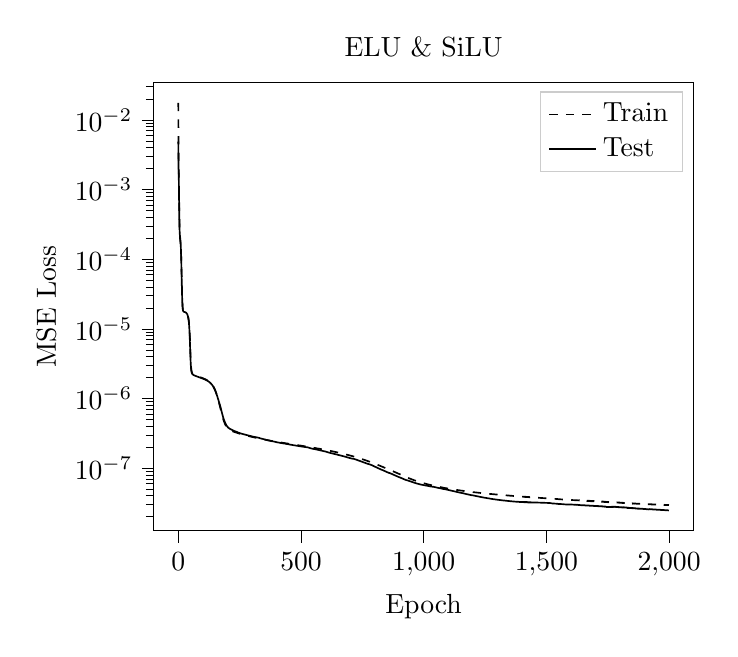
\begin{tikzpicture}

\begin{axis}[
legend cell align={left},
legend style={fill opacity=0.8, draw opacity=1, text opacity=1, draw=white!80!black},
log basis y={10},
tick align=outside,
tick pos=left,
title={ELU \& SiLU},
x grid style={white!69.0196078431373!black},
xlabel={Epoch},
xmin=-99.95, xmax=2098.95,
xtick style={color=black},
y grid style={white!69.0196078431373!black},
ylabel={MSE Loss},
ymin=1.25460830079477e-08, ymax=0.0345317116334461,
ymode=log,
ytick style={color=black}
]
\addplot [semithick, black, dashed]
table {%
0 0.0175996494237334
1 0.00287529958738014
2 0.0017450225809589
3 0.00109182657976635
4 0.000527906175178941
5 0.00029815742187202
6 0.000224625757531612
7 0.000197977887568413
8 0.000183264794104616
9 0.000169372935888532
10 0.000151957952730299
11 0.000129263067727152
12 0.000102055093113449
13 7.43479660304729e-05
14 5.15737580390123e-05
15 3.62272282127378e-05
16 2.71450699819979e-05
17 2.21503660204689e-05
18 1.95366582747738e-05
19 1.82204602597267e-05
20 1.7573602705852e-05
21 1.72561979470629e-05
22 1.70949869616379e-05
23 1.70056749411742e-05
24 1.69485445385362e-05
25 1.69051188822777e-05
26 1.68663870399541e-05
27 1.68271088441543e-05
28 1.67838884763114e-05
29 1.67341138449046e-05
30 1.66752324212212e-05
31 1.66049099725569e-05
32 1.65208375483417e-05
33 1.64199603086672e-05
34 1.62983461823387e-05
35 1.61510820416879e-05
36 1.59720132987786e-05
37 1.57533292913286e-05
38 1.5484687447497e-05
39 1.51527701264058e-05
40 1.47406713913369e-05
41 1.42270974720304e-05
42 1.3586219226454e-05
43 1.27891907977755e-05
44 1.18077328297659e-05
45 1.06241310518271e-05
46 9.24968551862548e-06
47 7.74917471699155e-06
48 6.25447972788606e-06
49 4.93720254530672e-06
50 3.93207780757621e-06
51 3.26343841823018e-06
52 2.85647097467745e-06
53 2.61511052349306e-06
54 2.47010573488637e-06
55 2.38091079037872e-06
56 2.32446314907975e-06
57 2.28729202154909e-06
58 2.26161475359277e-06
59 2.24282278935561e-06
60 2.22819607702718e-06
61 2.21604933179265e-06
62 2.20556252057236e-06
63 2.19616054360472e-06
64 2.18749445562594e-06
65 2.17928000790835e-06
66 2.17143440573864e-06
67 2.16391069665178e-06
68 2.15657700448446e-06
69 2.14940820202969e-06
70 2.14237768801695e-06
71 2.13553268446276e-06
72 2.12884015479631e-06
73 2.12225586307113e-06
74 2.11574514611357e-06
75 2.10928932654042e-06
76 2.10288195557951e-06
77 2.09650990095156e-06
78 2.09017900181152e-06
79 2.08388941103976e-06
80 2.07764323232595e-06
81 2.07144468839715e-06
82 2.06527465138606e-06
83 2.05913248743173e-06
84 2.0530142757309e-06
85 2.04691445756566e-06
86 2.04082622008173e-06
87 2.03473575675162e-06
88 2.0286378381229e-06
89 2.02251989537672e-06
90 2.01638261944481e-06
91 2.01022128027262e-06
92 2.00403939894045e-06
93 1.99783347059679e-06
94 1.99160166323509e-06
95 1.98533314505767e-06
96 1.97902080506651e-06
97 1.97265234243105e-06
98 1.9662212929461e-06
99 1.95973702790297e-06
100 1.95320250358577e-06
101 1.94660680122638e-06
102 1.939952190952e-06
103 1.93324243110737e-06
104 1.92648431564635e-06
105 1.91963722903665e-06
106 1.91268758226215e-06
107 1.90565878750704e-06
108 1.89853121551664e-06
109 1.89127792199884e-06
110 1.88389302704195e-06
111 1.87637372260951e-06
112 1.86870985686483e-06
113 1.86089686886248e-06
114 1.85292484115962e-06
115 1.84476674837697e-06
116 1.83640388777917e-06
117 1.82784501009792e-06
118 1.81907705044182e-06
119 1.81008488425505e-06
120 1.80085318538659e-06
121 1.79136690542236e-06
122 1.78161437838753e-06
123 1.77159513089009e-06
124 1.76129403953951e-06
125 1.75069264912509e-06
126 1.73976445233848e-06
127 1.72847957088607e-06
128 1.71680751208214e-06
129 1.7047350025905e-06
130 1.69224299537518e-06
131 1.67928939252704e-06
132 1.66583868410441e-06
133 1.65187669213651e-06
134 1.63740343054997e-06
135 1.62238789512514e-06
136 1.6067824065118e-06
137 1.5905935566991e-06
138 1.57381414469171e-06
139 1.55636063472286e-06
140 1.53816044023358e-06
141 1.51927269187979e-06
142 1.49966893327758e-06
143 1.47930880157787e-06
144 1.45817050724872e-06
145 1.43625170875339e-06
146 1.41338668653646e-06
147 1.38969123329957e-06
148 1.3652607281216e-06
149 1.34014765538382e-06
150 1.3144001037233e-06
151 1.28805525855569e-06
152 1.26120119203677e-06
153 1.23391107938176e-06
154 1.20624255806945e-06
155 1.17823492250579e-06
156 1.14992709714556e-06
157 1.12135632480204e-06
158 1.09260033759995e-06
159 1.06368875725593e-06
160 1.03462326670467e-06
161 1.00557742922547e-06
162 9.7667225931275e-07
163 9.47957712440939e-07
164 9.19453697107997e-07
165 8.91192761528714e-07
166 8.63282801702781e-07
167 8.35834502140642e-07
168 8.08940287257087e-07
169 7.82601844235842e-07
170 7.56980151379594e-07
171 7.32141062655955e-07
172 7.08114986750275e-07
173 6.84937570738953e-07
174 6.62635313446458e-07
175 6.41243045507167e-07
176 6.2081070653619e-07
177 6.01388748577847e-07
178 5.83003184985387e-07
179 5.65668886466142e-07
180 5.49323648044719e-07
181 5.33915851917754e-07
182 5.19427995229194e-07
183 5.05823589165288e-07
184 4.9306046715003e-07
185 4.8109552386677e-07
186 4.6990855443596e-07
187 4.59501481813618e-07
188 4.49822384894105e-07
189 4.40771383807714e-07
190 4.32378732156735e-07
191 4.24598447835933e-07
192 4.17455452677018e-07
193 4.10936514782634e-07
194 4.0497750121915e-07
195 3.99562149212329e-07
196 3.94614396952875e-07
197 3.9006308888645e-07
198 3.85865279696418e-07
199 3.81985842821564e-07
200 3.78385178450458e-07
201 3.75026909821941e-07
202 3.71899057071801e-07
203 3.69010332562425e-07
204 3.66329881671845e-07
205 3.63827414901152e-07
206 3.61479612806193e-07
207 3.59270024461011e-07
208 3.57176860234176e-07
209 3.55181227661205e-07
210 3.53276239565048e-07
211 3.51515790129042e-07
212 3.49912813945252e-07
213 3.48354445861787e-07
214 3.46851569503315e-07
215 3.45408498390043e-07
216 3.44020960312719e-07
217 3.42683353437678e-07
218 3.41392241935523e-07
219 3.40145149181126e-07
220 3.38937579158483e-07
221 3.37769001305332e-07
222 3.36636997644746e-07
223 3.35538890624321e-07
224 3.34470593799097e-07
225 3.33426590003683e-07
226 3.32406322868906e-07
227 3.31405100723714e-07
228 3.30421388724744e-07
229 3.29453601679575e-07
230 3.28494617065189e-07
231 3.27545682438313e-07
232 3.26611903702201e-07
233 3.25688031040272e-07
234 3.24785979117337e-07
235 3.23915015329135e-07
236 3.23034720381088e-07
237 3.22156478262059e-07
238 3.21286055111614e-07
239 3.20421153560346e-07
240 3.19560409622e-07
241 3.18705262714047e-07
242 3.1785766660164e-07
243 3.1701667911932e-07
244 3.16183564692096e-07
245 3.15356841326775e-07
246 3.14536922402908e-07
247 3.13724506980861e-07
248 3.12925141088272e-07
249 3.12140765842628e-07
250 3.11375240485745e-07
251 3.1062860304587e-07
252 3.0990082002802e-07
253 3.09185586033323e-07
254 3.0848231598668e-07
255 3.07785731521903e-07
256 3.07097276817103e-07
257 3.06413695156493e-07
258 3.05733606865033e-07
259 3.05057379563323e-07
260 3.04384200020991e-07
261 3.03711434725074e-07
262 3.0303466202497e-07
263 3.02357359515781e-07
264 3.01714337382464e-07
265 3.01069908317686e-07
266 3.00426167228807e-07
267 2.99785866843649e-07
268 2.99147748563655e-07
269 2.98513994621885e-07
270 2.97884098472423e-07
271 2.97257889613434e-07
272 2.96635719834626e-07
273 2.96016641236463e-07
274 2.95400801640255e-07
275 2.94787651498041e-07
276 2.94177613653801e-07
277 2.93570954063682e-07
278 2.92964300811605e-07
279 2.92362203438756e-07
280 2.91760416381237e-07
281 2.91159803978758e-07
282 2.9055891594254e-07
283 2.89960710880166e-07
284 2.8936324151374e-07
285 2.88770518061199e-07
286 2.88199581916615e-07
287 2.87646285805465e-07
288 2.87090873314355e-07
289 2.86531117303923e-07
290 2.85970951807712e-07
291 2.85412180353717e-07
292 2.84857709402786e-07
293 2.84302747601828e-07
294 2.8375344444953e-07
295 2.83205761050453e-07
296 2.82660867995332e-07
297 2.8211923660848e-07
298 2.81580993302555e-07
299 2.81046339367208e-07
300 2.80514478589566e-07
301 2.7998426008935e-07
302 2.79458510092923e-07
303 2.78934175497625e-07
304 2.78412257820548e-07
305 2.7789296674996e-07
306 2.77374297333211e-07
307 2.7685929883603e-07
308 2.76344144253926e-07
309 2.75831304342944e-07
310 2.75319272766694e-07
311 2.74808198902576e-07
312 2.7429603046869e-07
313 2.73784318302717e-07
314 2.73272087738974e-07
315 2.72760358924984e-07
316 2.72247648759105e-07
317 2.71740439046653e-07
318 2.71237279193315e-07
319 2.70741638303207e-07
320 2.70252898353363e-07
321 2.69768819279648e-07
322 2.69289078040913e-07
323 2.68816892983637e-07
324 2.68343211374145e-07
325 2.67885037054327e-07
326 2.67416310265389e-07
327 2.66975876130005e-07
328 2.66506596872773e-07
329 2.66083591505151e-07
330 2.65639710384846e-07
331 2.65243812378912e-07
332 2.64773271553054e-07
333 2.64322112386139e-07
334 2.63829088133605e-07
335 2.63389938119474e-07
336 2.6290572489529e-07
337 2.62464812486485e-07
338 2.61970761854968e-07
339 2.61548848619952e-07
340 2.61117641201736e-07
341 2.60733976112704e-07
342 2.60291870695539e-07
343 2.59895549817202e-07
344 2.594321902194e-07
345 2.59030119281078e-07
346 2.58601684890891e-07
347 2.58207709705971e-07
348 2.57752386914945e-07
349 2.57358960176646e-07
350 2.56929571371245e-07
351 2.56539277351919e-07
352 2.56089040767904e-07
353 2.5569170922779e-07
354 2.5524339392291e-07
355 2.54830653759086e-07
356 2.54406230482118e-07
357 2.54067098289568e-07
358 2.53661682023676e-07
359 2.53289803858081e-07
360 2.52879487980806e-07
361 2.52509188818806e-07
362 2.52106710043165e-07
363 2.5173805948242e-07
364 2.51339875042333e-07
365 2.50972963598883e-07
366 2.50580756969043e-07
367 2.50217714238943e-07
368 2.49831848677218e-07
369 2.49469345895648e-07
370 2.49089968647809e-07
371 2.4873137019199e-07
372 2.48356590667242e-07
373 2.47999187131143e-07
374 2.4763044640963e-07
375 2.47274666534736e-07
376 2.46913876914334e-07
377 2.46557384258494e-07
378 2.46201170384097e-07
379 2.45847944853494e-07
380 2.45494405000102e-07
381 2.45144459192659e-07
382 2.4479538060973e-07
383 2.44445716866437e-07
384 2.44098331023679e-07
385 2.43749799729187e-07
386 2.43400523295634e-07
387 2.43049962001862e-07
388 2.42702448431942e-07
389 2.42355488609292e-07
390 2.42012714679163e-07
391 2.4167355127247e-07
392 2.41335103595475e-07
393 2.40999812632481e-07
394 2.40663078940884e-07
395 2.40325962195698e-07
396 2.39984172416996e-07
397 2.39634622730023e-07
398 2.39281233987754e-07
399 2.38940480876693e-07
400 2.3863265462154e-07
401 2.38341846198864e-07
402 2.3803435519909e-07
403 2.37720892670268e-07
404 2.37405413471947e-07
405 2.3708795703925e-07
406 2.36770879936898e-07
407 2.36454466346459e-07
408 2.36138622433657e-07
409 2.35822797336027e-07
410 2.35507726081607e-07
411 2.35190857516443e-07
412 2.34877379469367e-07
413 2.34564189511843e-07
414 2.34253473898605e-07
415 2.33942672522858e-07
416 2.33634892900625e-07
417 2.33329615788591e-07
418 2.33024774566104e-07
419 2.32720143500842e-07
420 2.32416022562632e-07
421 2.32108510779483e-07
422 2.31797596143224e-07
423 2.31482146325845e-07
424 2.31172614505226e-07
425 2.30876980893413e-07
426 2.30587186429432e-07
427 2.30292145651845e-07
428 2.29996369043306e-07
429 2.29696812866109e-07
430 2.29395408346988e-07
431 2.29091220759869e-07
432 2.28793122374782e-07
433 2.28505814114044e-07
434 2.28219742702152e-07
435 2.27929575416397e-07
436 2.2763782101265e-07
437 2.27346566390452e-07
438 2.27056472624554e-07
439 2.26765794053563e-07
440 2.26474985048242e-07
441 2.26186430381858e-07
442 2.25897406949116e-07
443 2.2560861464882e-07
444 2.25320075472268e-07
445 2.25033070627489e-07
446 2.24744428635404e-07
447 2.24458662323457e-07
448 2.24170733531537e-07
449 2.23884842050381e-07
450 2.23597962218491e-07
451 2.23310248394171e-07
452 2.23022348308177e-07
453 2.22734046751327e-07
454 2.22442912225063e-07
455 2.22151466509501e-07
456 2.21859659873758e-07
457 2.21572562438155e-07
458 2.21289075021502e-07
459 2.21010129273225e-07
460 2.20728793351554e-07
461 2.20448860829947e-07
462 2.20167770152102e-07
463 2.19885938825826e-07
464 2.19604979307064e-07
465 2.19323364973434e-07
466 2.19043549776643e-07
467 2.18763958706347e-07
468 2.18484622969584e-07
469 2.18205289677087e-07
470 2.17927875091561e-07
471 2.17649641605533e-07
472 2.17373744746396e-07
473 2.1709560340355e-07
474 2.16820149610442e-07
475 2.16545120039768e-07
476 2.16269043342265e-07
477 2.15993676206949e-07
478 2.15721830045368e-07
479 2.15448890990899e-07
480 2.15178834174878e-07
481 2.149075208564e-07
482 2.14637604578627e-07
483 2.14366342028427e-07
484 2.14095653959134e-07
485 2.13825490867237e-07
486 2.13554397497262e-07
487 2.13285051131606e-07
488 2.13013861191769e-07
489 2.12744850905722e-07
490 2.12475656326205e-07
491 2.12207315264834e-07
492 2.11938185586291e-07
493 2.11668856991309e-07
494 2.11400331892264e-07
495 2.11133048289014e-07
496 2.10864122102805e-07
497 2.10596357298698e-07
498 2.10328821644623e-07
499 2.10059376463789e-07
500 2.09792518937491e-07
501 2.09525793508192e-07
502 2.0925775712044e-07
503 2.08989702933593e-07
504 2.08722312152076e-07
505 2.08454585468587e-07
506 2.08186760026763e-07
507 2.07918511570426e-07
508 2.07650348066579e-07
509 2.0738169546064e-07
510 2.07112908462648e-07
511 2.06844777174808e-07
512 2.06574911899793e-07
513 2.06304785187683e-07
514 2.06034711695224e-07
515 2.05762478614702e-07
516 2.05489735087383e-07
517 2.05218204492041e-07
518 2.04941749565535e-07
519 2.04666232278328e-07
520 2.04387647002591e-07
521 2.04112322826688e-07
522 2.0383555720116e-07
523 2.0356390942311e-07
524 2.0328289256355e-07
525 2.03006117388327e-07
526 2.02714574768947e-07
527 2.02427127135252e-07
528 2.02120347992718e-07
529 2.01825123937738e-07
530 2.01526683405007e-07
531 2.01258414435301e-07
532 2.00978978099897e-07
533 2.00726137201457e-07
534 2.00452940838147e-07
535 2.00204465528486e-07
536 1.99926498702041e-07
537 1.99674599720368e-07
538 1.99389074467149e-07
539 1.99133380988314e-07
540 1.98845136111458e-07
541 1.98592526508889e-07
542 1.98312001522538e-07
543 1.98073469377391e-07
544 1.97795437962611e-07
545 1.97541130809498e-07
546 1.9723873250399e-07
547 1.96979277795606e-07
548 1.96690525427812e-07
549 1.96438236173435e-07
550 1.9614758696207e-07
551 1.95893695774885e-07
552 1.9560284979292e-07
553 1.95347655257194e-07
554 1.95057353046479e-07
555 1.94801164418834e-07
556 1.94509920277142e-07
557 1.94253270734634e-07
558 1.93961073485127e-07
559 1.93702724359923e-07
560 1.93412831507089e-07
561 1.93151937097014e-07
562 1.92862569448948e-07
563 1.92599946480243e-07
564 1.92312116809035e-07
565 1.92046887015351e-07
566 1.91762092583758e-07
567 1.91495132177977e-07
568 1.91215405095591e-07
569 1.90950501014697e-07
570 1.90681914915558e-07
571 1.90422427188253e-07
572 1.90139000331158e-07
573 1.89849500145556e-07
574 1.89560766450825e-07
575 1.89280814623771e-07
576 1.8900092842955e-07
577 1.8872307740736e-07
578 1.88442443018744e-07
579 1.88163821782439e-07
580 1.87884023183926e-07
581 1.87604552785103e-07
582 1.87324280688017e-07
583 1.87046472525765e-07
584 1.8676562085318e-07
585 1.86486165269173e-07
586 1.86204263052048e-07
587 1.85924446839181e-07
588 1.85642518125917e-07
589 1.85359782030048e-07
590 1.85078272430417e-07
591 1.84792084183982e-07
592 1.84508275026474e-07
593 1.84220880669272e-07
594 1.83932809697751e-07
595 1.83643697894809e-07
596 1.83353293152777e-07
597 1.83060790227785e-07
598 1.82766741410489e-07
599 1.82471747208979e-07
600 1.82175910396154e-07
601 1.81878275817837e-07
602 1.81581998241143e-07
603 1.81293149658757e-07
604 1.81011799938346e-07
605 1.80725013777305e-07
606 1.80430601247394e-07
607 1.80136493369787e-07
608 1.79840781072471e-07
609 1.79547042925776e-07
610 1.79256953792617e-07
611 1.78968048011541e-07
612 1.78676989577298e-07
613 1.78381995397103e-07
614 1.78090247487717e-07
615 1.77807889897963e-07
616 1.77518120445086e-07
617 1.77226933303132e-07
618 1.76935237604425e-07
619 1.76642455294029e-07
620 1.76349222122951e-07
621 1.76056165678062e-07
622 1.75763073201551e-07
623 1.75468830988734e-07
624 1.75175491378354e-07
625 1.74879692544039e-07
626 1.74585498029955e-07
627 1.74291679364558e-07
628 1.73995814343186e-07
629 1.73700186017811e-07
630 1.73405231102208e-07
631 1.73109094077972e-07
632 1.72812282521306e-07
633 1.72517677093253e-07
634 1.72222056555427e-07
635 1.71927344155165e-07
636 1.71632569099245e-07
637 1.71338274590482e-07
638 1.71034913130086e-07
639 1.70733721134297e-07
640 1.7043391181204e-07
641 1.70132847280513e-07
642 1.69833049191936e-07
643 1.69529434216997e-07
644 1.69227103143044e-07
645 1.68925542112675e-07
646 1.68622009034891e-07
647 1.68318236774212e-07
648 1.68014904176061e-07
649 1.67709664872007e-07
650 1.6740428503681e-07
651 1.67098198687654e-07
652 1.66792148370121e-07
653 1.66485019853724e-07
654 1.66178793207905e-07
655 1.65869200280611e-07
656 1.65561907664369e-07
657 1.65252004769911e-07
658 1.64943542721119e-07
659 1.64632498311335e-07
660 1.64322014335028e-07
661 1.64009824260347e-07
662 1.63697879330016e-07
663 1.63385576819053e-07
664 1.63073160940996e-07
665 1.62760238836768e-07
666 1.62445714465775e-07
667 1.62130916251613e-07
668 1.61816271742055e-07
669 1.61501935338038e-07
670 1.61184934285075e-07
671 1.60868889899746e-07
672 1.60552074753184e-07
673 1.60234152140504e-07
674 1.59917202708471e-07
675 1.59598340765399e-07
676 1.5928070041582e-07
677 1.58963693209557e-07
678 1.58649849083758e-07
679 1.58348114766227e-07
680 1.58057629661812e-07
681 1.57671108624413e-07
682 1.57301388419739e-07
683 1.56999126346591e-07
684 1.56670816949145e-07
685 1.56336613628127e-07
686 1.56002342869499e-07
687 1.556705652348e-07
688 1.55350209446681e-07
689 1.55038015698494e-07
690 1.54718844136426e-07
691 1.5439428176478e-07
692 1.54069175138716e-07
693 1.53743410223228e-07
694 1.53420686693551e-07
695 1.5309928499363e-07
696 1.52787432718071e-07
697 1.52489572741388e-07
698 1.5215267003299e-07
699 1.5180147937599e-07
700 1.51467610628231e-07
701 1.51146714920003e-07
702 1.50877697457474e-07
703 1.50529026193169e-07
704 1.50173604488657e-07
705 1.49829621982178e-07
706 1.49500967239646e-07
707 1.49161668694831e-07
708 1.48830235133346e-07
709 1.4848696960712e-07
710 1.48152148859992e-07
711 1.47827308822457e-07
712 1.47502455668302e-07
713 1.47172682240182e-07
714 1.46840045417207e-07
715 1.46497807946844e-07
716 1.46153746740652e-07
717 1.4580504894468e-07
718 1.45458180313085e-07
719 1.45108395322779e-07
720 1.44763098667511e-07
721 1.44413272984423e-07
722 1.44068907871997e-07
723 1.43719601865655e-07
724 1.4337589767166e-07
725 1.43025246977402e-07
726 1.42680555661912e-07
727 1.42329018402165e-07
728 1.41984071241552e-07
729 1.41631456635594e-07
730 1.41288496855907e-07
731 1.40933513208097e-07
732 1.40596474217602e-07
733 1.40239406363207e-07
734 1.39900588273179e-07
735 1.39539811776501e-07
736 1.39217587097562e-07
737 1.38853319960219e-07
738 1.38519196539733e-07
739 1.38150057352959e-07
740 1.37809788974153e-07
741 1.3743655064502e-07
742 1.3710148611068e-07
743 1.36720188223194e-07
744 1.36391699037119e-07
745 1.36003874573021e-07
746 1.35689238376813e-07
747 1.3526807629205e-07
748 1.34977162510097e-07
749 1.34534849898671e-07
750 1.34263853979633e-07
751 1.33803888381578e-07
752 1.33541157381956e-07
753 1.33075631865154e-07
754 1.32812739892074e-07
755 1.32347266053046e-07
756 1.32081167286913e-07
757 1.31614762942434e-07
758 1.31345022282403e-07
759 1.30879963457176e-07
760 1.3060746962168e-07
761 1.30141176512666e-07
762 1.29864243902489e-07
763 1.29394299058561e-07
764 1.2911283270256e-07
765 1.28642385263333e-07
766 1.28354625225313e-07
767 1.2789251384504e-07
768 1.276106047996e-07
769 1.27158457551957e-07
770 1.26873228133206e-07
771 1.2642038833377e-07
772 1.26147492281348e-07
773 1.25696561333655e-07
774 1.2542319246478e-07
775 1.24956723709602e-07
776 1.24685955043446e-07
777 1.24218594947934e-07
778 1.23948786196593e-07
779 1.23475682784147e-07
780 1.23208924293294e-07
781 1.22734899811405e-07
782 1.22469958334648e-07
783 1.21993825025868e-07
784 1.21732354990911e-07
785 1.21256032315387e-07
786 1.20998242365999e-07
787 1.2051988794326e-07
788 1.20267326778389e-07
789 1.19790599342195e-07
790 1.19547230333694e-07
791 1.19097782047106e-07
792 1.18811734310498e-07
793 1.18316635195015e-07
794 1.18063428701021e-07
795 1.17580629776626e-07
796 1.17317416432172e-07
797 1.16842961155328e-07
798 1.16570967094276e-07
799 1.16108646778912e-07
800 1.15827305272376e-07
801 1.15377920501203e-07
802 1.1508488028511e-07
803 1.14649716792314e-07
804 1.14344960543633e-07
805 1.13921864283384e-07
806 1.13603540839335e-07
807 1.13194083560586e-07
808 1.12863245988137e-07
809 1.12468225204054e-07
810 1.12127083646385e-07
811 1.11746339406693e-07
812 1.11400504785308e-07
813 1.11035729347009e-07
814 1.10672897640995e-07
815 1.10295471110078e-07
816 1.09931559045151e-07
817 1.09568143528804e-07
818 1.09202652389229e-07
819 1.0884110548659e-07
820 1.08479694034713e-07
821 1.08123397502879e-07
822 1.07768057553415e-07
823 1.07427633928125e-07
824 1.07132911082886e-07
825 1.06680572500295e-07
826 1.06355442163419e-07
827 1.05982517581538e-07
828 1.05633535838479e-07
829 1.05274247268028e-07
830 1.04923396285983e-07
831 1.04568637013358e-07
832 1.04220353073003e-07
833 1.03865601353448e-07
834 1.03513037430503e-07
835 1.03156986462238e-07
836 1.02802441595884e-07
837 1.02450682760491e-07
838 1.02100855322362e-07
839 1.01750472786932e-07
840 1.0140150994431e-07
841 1.01053541381901e-07
842 1.00707275326073e-07
843 1.00359584678245e-07
844 1.00014914270474e-07
845 9.96698316377831e-08
846 9.93263650492793e-08
847 9.89830431770144e-08
848 9.86420426372092e-08
849 9.830027455493e-08
850 9.79607342728173e-08
851 9.76206057572426e-08
852 9.72826926961545e-08
853 9.69451741390515e-08
854 9.66100479331544e-08
855 9.62747901454009e-08
856 9.59414415291349e-08
857 9.56098446884823e-08
858 9.52807467342609e-08
859 9.49542538926096e-08
860 9.46286855700862e-08
861 9.43026890531939e-08
862 9.39737770337956e-08
863 9.36448786958977e-08
864 9.33190625431735e-08
865 9.29954942066047e-08
866 9.26732596084889e-08
867 9.23527348462017e-08
868 9.20334779763721e-08
869 9.17156793747154e-08
870 9.13983349377645e-08
871 9.10830633600312e-08
872 9.07672439609541e-08
873 9.04524855158684e-08
874 9.01387915774876e-08
875 8.98264481250521e-08
876 8.95150285202817e-08
877 8.92049641834092e-08
878 8.88939577734504e-08
879 8.85861132289278e-08
880 8.82777590334172e-08
881 8.79710582140092e-08
882 8.76646669567549e-08
883 8.73602326905143e-08
884 8.70552255705093e-08
885 8.67519998095645e-08
886 8.64501233053261e-08
887 8.6146255775077e-08
888 8.58468929791911e-08
889 8.55448757945965e-08
890 8.52472173562546e-08
891 8.49459580933853e-08
892 8.46501490912033e-08
893 8.43481334271701e-08
894 8.40549865515072e-08
895 8.37533525341883e-08
896 8.34638953648437e-08
897 8.31621499131074e-08
898 8.28743535308263e-08
899 8.25751389896823e-08
900 8.22899470520611e-08
901 8.19908786695578e-08
902 8.17119941984856e-08
903 8.14204756736103e-08
904 8.11498789587972e-08
905 8.08366941313921e-08
906 8.05548967051095e-08
907 8.02546861962128e-08
908 7.99800256316985e-08
909 7.96830944622684e-08
910 7.94125844763016e-08
911 7.911549998596e-08
912 7.88506315814175e-08
913 7.85564360050728e-08
914 7.82931790439534e-08
915 7.8004567647838e-08
916 7.77404717631214e-08
917 7.74547611754883e-08
918 7.7181353187683e-08
919 7.69060091343476e-08
920 7.66324710355093e-08
921 7.63723304721964e-08
922 7.60953091329952e-08
923 7.5864466129616e-08
924 7.55713254001478e-08
925 7.53308811525244e-08
926 7.50198124421786e-08
927 7.4793768067849e-08
928 7.44999733726104e-08
929 7.42764854599898e-08
930 7.40070237732482e-08
931 7.3757139062991e-08
932 7.34708819116747e-08
933 7.32295668548488e-08
934 7.29672317092422e-08
935 7.27254336361227e-08
936 7.24722474849671e-08
937 7.22304411411301e-08
938 7.19834948306186e-08
939 7.17461780297413e-08
940 7.15024025836897e-08
941 7.1267125772323e-08
942 7.10307098543694e-08
943 7.07984063801348e-08
944 7.05661321873663e-08
945 7.03392329199914e-08
946 7.01104802871555e-08
947 6.98869387250056e-08
948 6.96629443517338e-08
949 6.94436666712761e-08
950 6.92237607111679e-08
951 6.90076469602729e-08
952 6.87917168527008e-08
953 6.85799188460123e-08
954 6.83669486356564e-08
955 6.81601427672263e-08
956 6.79508710383914e-08
957 6.77463507194886e-08
958 6.75436472228341e-08
959 6.73413416798496e-08
960 6.71408234005355e-08
961 6.69428408208717e-08
962 6.67447739353122e-08
963 6.65525494945029e-08
964 6.63575741768341e-08
965 6.61687265406385e-08
966 6.59775455638112e-08
967 6.57917663957619e-08
968 6.56059239396711e-08
969 6.54228842194016e-08
970 6.52397152656192e-08
971 6.50610468397872e-08
972 6.48808190213401e-08
973 6.47048932265193e-08
974 6.45277746365025e-08
975 6.43562626940764e-08
976 6.41803190077894e-08
977 6.40130773810199e-08
978 6.38387489111381e-08
979 6.36743903790204e-08
980 6.35023501907028e-08
981 6.33410359505149e-08
982 6.31731920286427e-08
983 6.30170328896895e-08
984 6.28512382760959e-08
985 6.27018185994643e-08
986 6.25389082422601e-08
987 6.23940222439501e-08
988 6.22324554662157e-08
989 6.20933315786942e-08
990 6.19333390581289e-08
991 6.18009775230632e-08
992 6.16378112496818e-08
993 6.151472694782e-08
994 6.13488915561788e-08
995 6.12322543176447e-08
996 6.10627431143484e-08
997 6.0956969566206e-08
998 6.07836454555866e-08
999 6.06858273002331e-08
1000 6.0507606448823e-08
1001 6.04200453828696e-08
1002 6.02411679047066e-08
1003 6.01563548663364e-08
1004 5.99758189601118e-08
1005 5.98955439414794e-08
1006 5.97161064845864e-08
1007 5.96399952890181e-08
1008 5.94604134001031e-08
1009 5.93865410394301e-08
1010 5.92094895459638e-08
1011 5.91360529007545e-08
1012 5.89636505807789e-08
1013 5.8890947325807e-08
1014 5.87177360920066e-08
1015 5.86479926383276e-08
1016 5.84775806053983e-08
1017 5.84071221645388e-08
1018 5.82407901923432e-08
1019 5.81706089164413e-08
1020 5.80062781310176e-08
1021 5.79364867938636e-08
1022 5.77755773072397e-08
1023 5.77070267020474e-08
1024 5.75472279997769e-08
1025 5.74803025088499e-08
1026 5.73227851177194e-08
1027 5.72549469133321e-08
1028 5.70999626958724e-08
1029 5.7033860887401e-08
1030 5.68804288114677e-08
1031 5.68131055551646e-08
1032 5.6663332767215e-08
1033 5.65954860540785e-08
1034 5.64472345629952e-08
1035 5.63754745606104e-08
1036 5.62272355715265e-08
1037 5.61484333303497e-08
1038 5.5999395478068e-08
1039 5.59186794042432e-08
1040 5.57838673493904e-08
1041 5.57162485428364e-08
1042 5.56010164558529e-08
1043 5.55337433567615e-08
1044 5.54150616451921e-08
1045 5.53392590987301e-08
1046 5.52239583875291e-08
1047 5.5144874224311e-08
1048 5.50325426509346e-08
1049 5.49520297781214e-08
1050 5.48456422393428e-08
1051 5.47616790171901e-08
1052 5.46610097735822e-08
1053 5.45759626504605e-08
1054 5.44761822958151e-08
1055 5.43920063904579e-08
1056 5.42956490861002e-08
1057 5.4211317223718e-08
1058 5.4117549513677e-08
1059 5.40303107428031e-08
1060 5.39417221858685e-08
1061 5.38540957997213e-08
1062 5.37668139806158e-08
1063 5.36784573128557e-08
1064 5.35941787980221e-08
1065 5.3507047322654e-08
1066 5.34215971939034e-08
1067 5.33369641182446e-08
1068 5.32536905559766e-08
1069 5.31688032587851e-08
1070 5.30834877885411e-08
1071 5.30020961733158e-08
1072 5.29187969142697e-08
1073 5.28378100881355e-08
1074 5.27521015420973e-08
1075 5.2670030630253e-08
1076 5.25867333536212e-08
1077 5.25034244560629e-08
1078 5.2418908094154e-08
1079 5.23290026706036e-08
1080 5.22326315639532e-08
1081 5.21282267627043e-08
1082 5.20232685978783e-08
1083 5.19315852756108e-08
1084 5.18594172795872e-08
1085 5.18124042443446e-08
1086 5.16707377791192e-08
1087 5.16539989376952e-08
1088 5.15711485888914e-08
1089 5.15147099022784e-08
1090 5.14256392456502e-08
1091 5.13642042427875e-08
1092 5.1281067797504e-08
1093 5.12151511067316e-08
1094 5.1136492572823e-08
1095 5.10673343896428e-08
1096 5.09849862382339e-08
1097 5.09159236656842e-08
1098 5.08563726846489e-08
1099 5.077642700968e-08
1100 5.07170401462531e-08
1101 5.06396115724783e-08
1102 5.05759921800575e-08
1103 5.05042115719334e-08
1104 5.04362397748537e-08
1105 5.03709844430489e-08
1106 5.03009102779117e-08
1107 5.02376596962506e-08
1108 5.01693970313966e-08
1109 5.01037829856443e-08
1110 5.00381948604911e-08
1111 4.99729949332561e-08
1112 4.99080592604173e-08
1113 4.98440006531098e-08
1114 4.97788077851169e-08
1115 4.97160153187792e-08
1116 4.96525768198808e-08
1117 4.95886749831698e-08
1118 4.95259647159685e-08
1119 4.94638447854356e-08
1120 4.94025123742858e-08
1121 4.93408055142197e-08
1122 4.92777741882833e-08
1123 4.92156950713252e-08
1124 4.91560401947311e-08
1125 4.90946190012664e-08
1126 4.90349146211599e-08
1127 4.89734367121741e-08
1128 4.89154338225717e-08
1129 4.88554389015405e-08
1130 4.87965765465503e-08
1131 4.87381162699307e-08
1132 4.86792782474765e-08
1133 4.86204470853124e-08
1134 4.85623430606097e-08
1135 4.85029923069646e-08
1136 4.84469144268473e-08
1137 4.83894675831209e-08
1138 4.83293557067554e-08
1139 4.82720579384477e-08
1140 4.82142370081817e-08
1141 4.81568539498767e-08
1142 4.80991615496862e-08
1143 4.80393431416815e-08
1144 4.79794743064588e-08
1145 4.79202978560522e-08
1146 4.78614520780241e-08
1147 4.77986213525128e-08
1148 4.77403732936921e-08
1149 4.76852409470041e-08
1150 4.76301647012178e-08
1151 4.7578462570641e-08
1152 4.75241271757909e-08
1153 4.74723943568733e-08
1154 4.74180858915929e-08
1155 4.73673670065011e-08
1156 4.73131372622504e-08
1157 4.72611859620997e-08
1158 4.72082820444086e-08
1159 4.7156959116279e-08
1160 4.70964777754546e-08
1161 4.70352642594207e-08
1162 4.69699322387385e-08
1163 4.69033307766153e-08
1164 4.68406378679731e-08
1165 4.678152087223e-08
1166 4.67163908766111e-08
1167 4.66496131537042e-08
1168 4.66186367269472e-08
1169 4.65931978403944e-08
1170 4.65452790940901e-08
1171 4.64970322155978e-08
1172 4.64478893889009e-08
1173 4.6401220398451e-08
1174 4.6354152015482e-08
1175 4.63051806818271e-08
1176 4.62608166245104e-08
1177 4.62116961692516e-08
1178 4.61663384392352e-08
1179 4.61181958506529e-08
1180 4.60749140778205e-08
1181 4.60289976587092e-08
1182 4.59828709118426e-08
1183 4.59360696254407e-08
1184 4.58911745084833e-08
1185 4.58475705649164e-08
1186 4.58020190592379e-08
1187 4.57577413932597e-08
1188 4.57144813417187e-08
1189 4.56681103067069e-08
1190 4.56250730138663e-08
1191 4.55801805401279e-08
1192 4.55367965024323e-08
1193 4.54928729460846e-08
1194 4.54491035526416e-08
1195 4.54046372340144e-08
1196 4.53605468813123e-08
1197 4.5318322193566e-08
1198 4.52730989941585e-08
1199 4.52277204736617e-08
1200 4.51831244703271e-08
1201 4.51362583078208e-08
1202 4.50891260435071e-08
1203 4.50436343264471e-08
1204 4.5005045581803e-08
1205 4.49671033173615e-08
1206 4.4927011046525e-08
1207 4.48885856805248e-08
1208 4.48442414047179e-08
1209 4.48037458724571e-08
1210 4.47623032719946e-08
1211 4.4723272381475e-08
1212 4.46810348542215e-08
1213 4.46411653030054e-08
1214 4.4600022867769e-08
1215 4.45591790949607e-08
1216 4.45200743115493e-08
1217 4.44793313718606e-08
1218 4.44395357810379e-08
1219 4.44004629009953e-08
1220 4.43605396469593e-08
1221 4.43211583132097e-08
1222 4.4281827630499e-08
1223 4.42431409233279e-08
1224 4.42025483913255e-08
1225 4.41649761562246e-08
1226 4.41241812545456e-08
1227 4.40845443172577e-08
1228 4.40465823245972e-08
1229 4.40095524965045e-08
1230 4.39683958113335e-08
1231 4.39273198011847e-08
1232 4.38891112786166e-08
1233 4.38489198977265e-08
1234 4.38104611717449e-08
1235 4.37681291849401e-08
1236 4.37326005489069e-08
1237 4.36921684006109e-08
1238 4.36569987094515e-08
1239 4.36212489383081e-08
1240 4.35856813254532e-08
1241 4.35512924070736e-08
1242 4.35153490982998e-08
1243 4.34792310812782e-08
1244 4.3441935190458e-08
1245 4.34084090166209e-08
1246 4.33736247344996e-08
1247 4.33387995464329e-08
1248 4.33012893488183e-08
1249 4.32677698007922e-08
1250 4.32302192905354e-08
1251 4.31998927901134e-08
1252 4.31620639780306e-08
1253 4.31301771044446e-08
1254 4.30933546446965e-08
1255 4.30604565977433e-08
1256 4.30247026876884e-08
1257 4.29927247402873e-08
1258 4.29553815664008e-08
1259 4.29268922417236e-08
1260 4.28864818502461e-08
1261 4.28586315130985e-08
1262 4.28198954232073e-08
1263 4.27898634640655e-08
1264 4.2753595245415e-08
1265 4.27237714077933e-08
1266 4.26869564371657e-08
1267 4.26564525852768e-08
1268 4.26192783891111e-08
1269 4.25903701817276e-08
1270 4.25535703065805e-08
1271 4.25226653746336e-08
1272 4.24879032259184e-08
1273 4.2456188470652e-08
1274 4.24202999376178e-08
1275 4.23859171334584e-08
1276 4.23519101282466e-08
1277 4.23149189643368e-08
1278 4.22824308721204e-08
1279 4.22486863698168e-08
1280 4.22202453158604e-08
1281 4.2187339193589e-08
1282 4.21591239216923e-08
1283 4.2124149732814e-08
1284 4.20938310909946e-08
1285 4.20612705056556e-08
1286 4.20308245416834e-08
1287 4.1997344542466e-08
1288 4.19672587632647e-08
1289 4.19371729876161e-08
1290 4.19042328978492e-08
1291 4.18756649480656e-08
1292 4.18406924111991e-08
1293 4.18142886573492e-08
1294 4.17780153441072e-08
1295 4.17540905388591e-08
1296 4.1716828956595e-08
1297 4.16896988646442e-08
1298 4.16524566198007e-08
1299 4.1629468562121e-08
1300 4.15833136386823e-08
1301 4.15585945674479e-08
1302 4.15018889334817e-08
1303 4.1496817747344e-08
1304 4.14546708569219e-08
1305 4.14546289491113e-08
1306 4.13919402539875e-08
1307 4.14056540662955e-08
1308 4.13244472277086e-08
1309 4.13615174217341e-08
1310 4.12699490794921e-08
1311 4.1267000831624e-08
1312 4.12267482445827e-08
1313 4.12109218075329e-08
1314 4.11668753805827e-08
1315 4.11583183073105e-08
1316 4.11022767217162e-08
1317 4.11100928516817e-08
1318 4.1037408280431e-08
1319 4.1066953887281e-08
1320 4.09750483711946e-08
1321 4.10066736584724e-08
1322 4.09191586996371e-08
1323 4.0947404691849e-08
1324 4.08638924866978e-08
1325 4.08914481262457e-08
1326 4.08070332653665e-08
1327 4.08357535057746e-08
1328 4.07527275072539e-08
1329 4.07760795404499e-08
1330 4.06947206101904e-08
1331 4.07312980570396e-08
1332 4.06484653616701e-08
1333 4.06305324958112e-08
1334 4.06281817078025e-08
1335 4.05609808034058e-08
1336 4.06007411903886e-08
1337 4.05186632264076e-08
1338 4.04813392229642e-08
1339 4.05137915677756e-08
1340 4.04427050817446e-08
1341 4.0404595285537e-08
1342 4.04034278496113e-08
1343 4.03470085359459e-08
1344 4.03759440494866e-08
1345 4.02951091871273e-08
1346 4.02729835862203e-08
1347 4.02820761493672e-08
1348 4.02028653567754e-08
1349 4.0243565639031e-08
1350 4.01645263359285e-08
1351 4.01247152481687e-08
1352 4.01298546996998e-08
1353 4.00498072288258e-08
1354 4.00780106133425e-08
1355 4.00133800226854e-08
1356 3.99935331216739e-08
1357 3.99947927611777e-08
1358 3.99257412730947e-08
1359 3.99636142667248e-08
1360 3.98933878571484e-08
1361 3.98593884050058e-08
1362 3.98346793133442e-08
1363 3.98373121583973e-08
1364 3.97712527302474e-08
1365 3.98051756000939e-08
1366 3.97388940989174e-08
1367 3.97043374533723e-08
1368 3.96858321707327e-08
1369 3.96721265438771e-08
1370 3.9627116226626e-08
1371 3.96427330819904e-08
1372 3.9564374215928e-08
1373 3.95902756480382e-08
1374 3.95136501545323e-08
1375 3.95457331237026e-08
1376 3.94681531226127e-08
1377 3.94643733123701e-08
1378 3.94374941201647e-08
1379 3.94130171876839e-08
1380 3.93865616992173e-08
1381 3.93646849872198e-08
1382 3.93336724364701e-08
1383 3.93183808213848e-08
1384 3.92790345884464e-08
1385 3.92783624505455e-08
1386 3.92181673056768e-08
1387 3.9247309484125e-08
1388 3.91625413485031e-08
1389 3.91856282284664e-08
1390 3.9112159310406e-08
1391 3.91618979058705e-08
1392 3.9091612521247e-08
1393 3.90773670382316e-08
1394 3.90596091861539e-08
1395 3.90377561814148e-08
1396 3.90033072932283e-08
1397 3.89836041740921e-08
1398 3.89571714300985e-08
1399 3.89340272377581e-08
1400 3.89095555490826e-08
1401 3.88901825196797e-08
1402 3.88592720064196e-08
1403 3.88472628642944e-08
1404 3.88079879627412e-08
1405 3.8811693173102e-08
1406 3.87458087196535e-08
1407 3.87871781057925e-08
1408 3.86750464578256e-08
1409 3.87632872431709e-08
1410 3.86152443461185e-08
1411 3.8726272766354e-08
1412 3.85677903231851e-08
1413 3.86811754395922e-08
1414 3.85242661202767e-08
1415 3.86363415181279e-08
1416 3.84808430133887e-08
1417 3.85900492148039e-08
1418 3.84359594995942e-08
1419 3.85446401054423e-08
1420 3.83952957250244e-08
1421 3.84991835922222e-08
1422 3.83527137763906e-08
1423 3.84539447075838e-08
1424 3.83098808818261e-08
1425 3.84084559001963e-08
1426 3.82686769313523e-08
1427 3.83634785663389e-08
1428 3.82263591767185e-08
1429 3.83170275028988e-08
1430 3.81848634063431e-08
1431 3.82719766882644e-08
1432 3.81443559227534e-08
1433 3.82261160360997e-08
1434 3.81028666360805e-08
1435 3.81820462145299e-08
1436 3.80621713560458e-08
1437 3.81377050473475e-08
1438 3.8020763664548e-08
1439 3.80906669938952e-08
1440 3.79813536319773e-08
1441 3.80451777530766e-08
1442 3.79402011745356e-08
1443 3.79971468937868e-08
1444 3.78976800448072e-08
1445 3.79480461809578e-08
1446 3.78535985952055e-08
1447 3.78877064797223e-08
1448 3.77929022867818e-08
1449 3.78013958233225e-08
1450 3.77127713129255e-08
1451 3.77494880652307e-08
1452 3.77125745814055e-08
1453 3.77251245637922e-08
1454 3.76768934877703e-08
1455 3.76800348611539e-08
1456 3.76387757690111e-08
1457 3.76369275087995e-08
1458 3.76011498595119e-08
1459 3.75915576782404e-08
1460 3.7565789462235e-08
1461 3.75480054266575e-08
1462 3.75244291888066e-08
1463 3.75085536461484e-08
1464 3.74869865567007e-08
1465 3.74678988599442e-08
1466 3.74458098804098e-08
1467 3.74289946023509e-08
1468 3.74053136447117e-08
1469 3.73895509646616e-08
1470 3.73655890228974e-08
1471 3.73484145193004e-08
1472 3.73280483714211e-08
1473 3.73083839733113e-08
1474 3.72891789162111e-08
1475 3.72704910880373e-08
1476 3.7248621644892e-08
1477 3.72312626915061e-08
1478 3.72108093422696e-08
1479 3.71916894330582e-08
1480 3.71718720479919e-08
1481 3.71548341639993e-08
1482 3.71317190506204e-08
1483 3.71136948977835e-08
1484 3.70954332247209e-08
1485 3.7075017328192e-08
1486 3.70562630358506e-08
1487 3.70378945753203e-08
1488 3.70180622759619e-08
1489 3.69973437628346e-08
1490 3.69796147232648e-08
1491 3.6959753085597e-08
1492 3.69415847352172e-08
1493 3.69228330292515e-08
1494 3.69024669879536e-08
1495 3.6883986361147e-08
1496 3.68645939907708e-08
1497 3.68453450008133e-08
1498 3.68283621270393e-08
1499 3.68075644914256e-08
1500 3.67898759954244e-08
1501 3.67695001806112e-08
1502 3.67499921836156e-08
1503 3.6732197379763e-08
1504 3.67122580833268e-08
1505 3.66923476278203e-08
1506 3.66745375650623e-08
1507 3.66537149432133e-08
1508 3.66359610310951e-08
1509 3.66162055271957e-08
1510 3.659514873533e-08
1511 3.65773423496307e-08
1512 3.65557572656883e-08
1513 3.65364017227421e-08
1514 3.65143413247893e-08
1515 3.64913223691588e-08
1516 3.64676853230606e-08
1517 3.64390327298736e-08
1518 3.64060995430293e-08
1519 3.63669256735477e-08
1520 3.63247117149967e-08
1521 3.63022032345839e-08
1522 3.62946600880321e-08
1523 3.62906074222735e-08
1524 3.62781957825575e-08
1525 3.62666043507431e-08
1526 3.62482158386968e-08
1527 3.62316294477694e-08
1528 3.62140311018777e-08
1529 3.61927297731768e-08
1530 3.61777107897865e-08
1531 3.61594412154886e-08
1532 3.61410701259501e-08
1533 3.61231098437997e-08
1534 3.61054330362265e-08
1535 3.60887919867991e-08
1536 3.60693465388806e-08
1537 3.60534092003206e-08
1538 3.60342813436887e-08
1539 3.60168709043762e-08
1540 3.59998949370777e-08
1541 3.59785507910715e-08
1542 3.59634371278617e-08
1543 3.5941752855706e-08
1544 3.5922967253299e-08
1545 3.59026391869577e-08
1546 3.58764270416145e-08
1547 3.58446422517034e-08
1548 3.57990294403976e-08
1549 3.57539634769921e-08
1550 3.57382170612652e-08
1551 3.57453839328059e-08
1552 3.57398239394513e-08
1553 3.57211739263619e-08
1554 3.57008202236386e-08
1555 3.5678548972129e-08
1556 3.56516157040687e-08
1557 3.56155545730985e-08
1558 3.55595640009199e-08
1559 3.54979681276291e-08
1560 3.54960429262974e-08
1561 3.55017919559941e-08
1562 3.54916767868474e-08
1563 3.54655182341901e-08
1564 3.54432029538998e-08
1565 3.5438487193673e-08
1566 3.54082522804333e-08
1567 3.53880520869154e-08
1568 3.53720010188852e-08
1569 3.53510848984939e-08
1570 3.53368128820364e-08
1571 3.53225550693281e-08
1572 3.53036709093146e-08
1573 3.52854553042903e-08
1574 3.52649857795484e-08
1575 3.52465590989226e-08
1576 3.52256008397944e-08
1577 3.52086323704981e-08
1578 3.52005257155952e-08
1579 3.51824060658146e-08
1580 3.51704832972644e-08
1581 3.51478965363583e-08
1582 3.51353368390761e-08
1583 3.5110004311889e-08
1584 3.5099747750067e-08
1585 3.50758459060074e-08
1586 3.50638818371607e-08
1587 3.50475820525276e-08
1588 3.50327269060813e-08
1589 3.50174722001384e-08
1590 3.50005818585686e-08
1591 3.49837193578395e-08
1592 3.49677575677276e-08
1593 3.49536021673202e-08
1594 3.4934812864762e-08
1595 3.49210757981666e-08
1596 3.49060805096002e-08
1597 3.48915063987931e-08
1598 3.48756203969458e-08
1599 3.48525328703886e-08
1600 3.48177892259827e-08
1601 3.4787871483033e-08
1602 3.47715977966345e-08
1603 3.47641803291054e-08
1604 3.4753644154506e-08
1605 3.47409893972639e-08
1606 3.47234597732893e-08
1607 3.47079945299811e-08
1608 3.46909644122206e-08
1609 3.46700013889034e-08
1610 3.4647425383838e-08
1611 3.46236579407133e-08
1612 3.46073512211831e-08
1613 3.45986185354974e-08
1614 3.45835249468962e-08
1615 3.45704000377367e-08
1616 3.45575677194176e-08
1617 3.45454655494848e-08
1618 3.45400001542373e-08
1619 3.45489442494795e-08
1620 3.46055936049083e-08
1621 3.46027133435456e-08
1622 3.45283926961315e-08
1623 3.44992562943958e-08
1624 3.44875408124778e-08
1625 3.44644759859847e-08
1626 3.44404155825373e-08
1627 3.44020873228601e-08
1628 3.43586973521326e-08
1629 3.4341221764933e-08
1630 3.43909036732981e-08
1631 3.43338189843223e-08
1632 3.43876061528192e-08
1633 3.42678819063025e-08
1634 3.44153996643115e-08
1635 3.42123048380216e-08
1636 3.42824781469631e-08
1637 3.42697498929567e-08
1638 3.42595794542433e-08
1639 3.42000555164645e-08
1640 3.43115936427552e-08
1641 3.41142779802794e-08
1642 3.42297419813065e-08
1643 3.41120816198526e-08
1644 3.42440022187418e-08
1645 3.4062529605805e-08
1646 3.41824622704934e-08
1647 3.4047797104364e-08
1648 3.41837958348634e-08
1649 3.40040385893303e-08
1650 3.41273175692436e-08
1651 3.39857107061192e-08
1652 3.41197286370942e-08
1653 3.39473847557059e-08
1654 3.40724037570794e-08
1655 3.3924028626231e-08
1656 3.40575578423596e-08
1657 3.38874829708402e-08
1658 3.40143418213756e-08
1659 3.38625038871498e-08
1660 3.39981571269021e-08
1661 3.38275544677913e-08
1662 3.39578113894845e-08
1663 3.38020041255049e-08
1664 3.39345081759035e-08
1665 3.37708272084569e-08
1666 3.39016538219994e-08
1667 3.37398202923111e-08
1668 3.3871374476746e-08
1669 3.3713152991055e-08
1670 3.38470531744406e-08
1671 3.36787168428998e-08
1672 3.38099436696382e-08
1673 3.36552861135431e-08
1674 3.37871328586203e-08
1675 3.36225322605799e-08
1676 3.37511091341725e-08
1677 3.35951861991646e-08
1678 3.37272143831058e-08
1679 3.35632440560119e-08
1680 3.36950260440005e-08
1681 3.35351847731147e-08
1682 3.36676524526069e-08
1683 3.35080319313619e-08
1684 3.3638606719677e-08
1685 3.34769234804355e-08
1686 3.36072094828666e-08
1687 3.34506699086745e-08
1688 3.35820369912199e-08
1689 3.3417763606991e-08
1690 3.35508458437772e-08
1691 3.33905130638357e-08
1692 3.3523850031969e-08
1693 3.33594249095626e-08
1694 3.34934648869023e-08
1695 3.33310702380629e-08
1696 3.34674506934363e-08
1697 3.33046057470199e-08
1698 3.34370984216292e-08
1699 3.32750735871912e-08
1700 3.3405146190546e-08
1701 3.32485903538071e-08
1702 3.33824205025479e-08
1703 3.32180697437678e-08
1704 3.33495473441303e-08
1705 3.31909745856507e-08
1706 3.33229182807315e-08
1707 3.31615310269484e-08
1708 3.32939488369988e-08
1709 3.31336074719246e-08
1710 3.32664251896375e-08
1711 3.31054216786697e-08
1712 3.32384806043251e-08
1713 3.3075719613862e-08
1714 3.32077416516086e-08
1715 3.30486065411861e-08
1716 3.31817862146977e-08
1717 3.30200386073898e-08
1718 3.31512511522192e-08
1719 3.29933048099917e-08
1720 3.312378184539e-08
1721 3.29619050773999e-08
1722 3.30905355490074e-08
1723 3.29348713101751e-08
1724 3.30658714720045e-08
1725 3.2903780079252e-08
1726 3.303245081554e-08
1727 3.28742794746262e-08
1728 3.30037107438841e-08
1729 3.28410966385917e-08
1730 3.29698604080164e-08
1731 3.28060075069914e-08
1732 3.29262452503087e-08
1733 3.27559392641064e-08
1734 3.28639632787286e-08
1735 3.2681094896958e-08
1736 3.28132108009527e-08
1737 3.26625908133593e-08
1738 3.27962944517424e-08
1739 3.26419050526994e-08
1740 3.28100845461421e-08
1741 3.26046135601388e-08
1742 3.26775266934476e-08
1743 3.2554416765862e-08
1744 3.26634748244459e-08
1745 3.24871724917131e-08
1746 3.25927902373735e-08
1747 3.24813773406873e-08
1748 3.25925799256055e-08
1749 3.24599241867674e-08
1750 3.25734725414861e-08
1751 3.24401372218119e-08
1752 3.25387758763895e-08
1753 3.24277666763351e-08
1754 3.25156576295171e-08
1755 3.24053392777301e-08
1756 3.24837721166205e-08
1757 3.23901482452982e-08
1758 3.24466525505329e-08
1759 3.23788421177085e-08
1760 3.240652201697e-08
1761 3.23734802876174e-08
1762 3.23660537873138e-08
1763 3.23647946522954e-08
1764 3.23273926170486e-08
1765 3.23475536454509e-08
1766 3.22969467099199e-08
1767 3.23262176227246e-08
1768 3.22659987652685e-08
1769 3.23020740822244e-08
1770 3.22377145565156e-08
1771 3.22753880812598e-08
1772 3.22092732485402e-08
1773 3.2246492640553e-08
1774 3.21791188344633e-08
1775 3.22211259540239e-08
1776 3.21470656228229e-08
1777 3.21913639655946e-08
1778 3.21151684410381e-08
1779 3.21639194140744e-08
1780 3.20794381032385e-08
1781 3.21364864195317e-08
1782 3.20384938792273e-08
1783 3.21218324899064e-08
1784 3.19840757114775e-08
1785 3.21338886681843e-08
1786 3.19231031227218e-08
1787 3.20652566898616e-08
1788 3.19515165809747e-08
1789 3.20042525139286e-08
1790 3.19398796140291e-08
1791 3.19613587169698e-08
1792 3.19048256240961e-08
1793 3.19481420714141e-08
1794 3.18611491731957e-08
1795 3.19398212340616e-08
1796 3.18067174216452e-08
1797 3.19524965366469e-08
1798 3.17490460268743e-08
1799 3.18861543089355e-08
1800 3.17758301342508e-08
1801 3.18336564451016e-08
1802 3.1763487102765e-08
1803 3.17955307451712e-08
1804 3.17265417315582e-08
1805 3.17754963923278e-08
1806 3.16862744806912e-08
1807 3.17643213847418e-08
1808 3.16321076407888e-08
1809 3.17721518285907e-08
1810 3.15841033948772e-08
1811 3.17179917388444e-08
1812 3.15929358176703e-08
1813 3.16796838593092e-08
1814 3.15861926694083e-08
1815 3.16394474992876e-08
1816 3.15584740988584e-08
1817 3.16176739758589e-08
1818 3.15200244358493e-08
1819 3.16058087559412e-08
1820 3.14781268286879e-08
1821 3.15855602703863e-08
1822 3.1442212073074e-08
1823 3.15518088083166e-08
1824 3.14070510718523e-08
1825 3.14765631710401e-08
1826 3.13348955955917e-08
1827 3.14295956087562e-08
1828 3.13473536035502e-08
1829 3.13846484214508e-08
1830 3.12679589526965e-08
1831 3.13140447900651e-08
1832 3.12284954340214e-08
1833 3.13061082248822e-08
1834 3.11941969783902e-08
1835 3.12384273062349e-08
1836 3.11294203783064e-08
1837 3.12014705770025e-08
1838 3.11129711949576e-08
1839 3.11866513431625e-08
1840 3.10680074715464e-08
1841 3.1162816917174e-08
1842 3.10589508565329e-08
1843 3.11255323932613e-08
1844 3.10953798141611e-08
1845 3.10547334283484e-08
1846 3.10998033938859e-08
1847 3.09676002530068e-08
1848 3.10414996835817e-08
1849 3.0876859215212e-08
1850 3.10728519536951e-08
1851 3.09117165269157e-08
1852 3.10249618848957e-08
1853 3.08752303670445e-08
1854 3.09913468932166e-08
1855 3.08826947481577e-08
1856 3.09575459720435e-08
1857 3.08618794857551e-08
1858 3.09409459298138e-08
1859 3.08473178343149e-08
1860 3.0922302839187e-08
1861 3.08557522679109e-08
1862 3.09549464212466e-08
1863 3.08447275934043e-08
1864 3.08845058025753e-08
1865 3.07965222461348e-08
1866 3.08509474020724e-08
1867 3.07759362652149e-08
1868 3.08269162712094e-08
1869 3.07434583870503e-08
1870 3.0806601929001e-08
1871 3.07061840665313e-08
1872 3.07819859539649e-08
1873 3.06689039586416e-08
1874 3.0747149812882e-08
1875 3.0627597825017e-08
1876 3.0709594701861e-08
1877 3.06232637132808e-08
1878 3.06970067533996e-08
1879 3.06077514125036e-08
1880 3.0672761793582e-08
1881 3.05904497892584e-08
1882 3.06453140908047e-08
1883 3.05694618294439e-08
1884 3.06219241750227e-08
1885 3.05489244496471e-08
1886 3.060027382773e-08
1887 3.05244899383439e-08
1888 3.05803567464125e-08
1889 3.05002876057614e-08
1890 3.05588004785307e-08
1891 3.04786859857131e-08
1892 3.05368056956468e-08
1893 3.04565826514391e-08
1894 3.05134558402642e-08
1895 3.04345959349916e-08
1896 3.0490320046539e-08
1897 3.04128542989446e-08
1898 3.04685849403796e-08
1899 3.03901900586823e-08
1900 3.04465101663709e-08
1901 3.03694184964343e-08
1902 3.04231977086289e-08
1903 3.03468141638064e-08
1904 3.04020241319591e-08
1905 3.03253976916551e-08
1906 3.03788513544845e-08
1907 3.03036100870457e-08
1908 3.03564637462728e-08
1909 3.02809095877876e-08
1910 3.03357251425496e-08
1911 3.02587513800745e-08
1912 3.03130086525272e-08
1913 3.02350739165291e-08
1914 3.02874890127924e-08
1915 3.02112226169271e-08
1916 3.02608022533235e-08
1917 3.01790260124335e-08
1918 3.02107685641317e-08
1919 3.01305602086188e-08
1920 3.02074739071401e-08
1921 3.01682732306574e-08
1922 3.01655382344279e-08
1923 3.0099974747344e-08
1924 3.01783688669843e-08
1925 3.00943170667978e-08
1926 3.01533577822255e-08
1927 3.00694399175683e-08
1928 3.01361652148557e-08
1929 3.00488423476963e-08
1930 3.011623033089e-08
1931 3.0026854028975e-08
1932 3.00958324306322e-08
1933 3.00048237846795e-08
1934 3.00760866682737e-08
1935 2.99842572584197e-08
1936 3.00555222274568e-08
1937 2.9963456222859e-08
1938 3.00345743653452e-08
1939 2.99435884798527e-08
1940 3.00130087840245e-08
1941 2.99216497001709e-08
1942 2.99944998154444e-08
1943 2.98996407881447e-08
1944 2.99729757990974e-08
1945 2.98812713896979e-08
1946 2.99542454111901e-08
1947 2.98601833019774e-08
1948 2.99347217396217e-08
1949 2.9839624140493e-08
1950 2.99130310281726e-08
1951 2.98190357490569e-08
1952 2.9894548520204e-08
1953 2.9801870883972e-08
1954 2.9874072010827e-08
1955 2.97820158170481e-08
1956 2.98560484566224e-08
1957 2.976179976244e-08
1958 2.98401263414405e-08
1959 2.97422976132111e-08
1960 2.98196454888711e-08
1961 2.97209685822253e-08
1962 2.98014676261005e-08
1963 2.97000319235963e-08
1964 2.97786187157811e-08
1965 2.9681583521679e-08
1966 2.97593995526313e-08
1967 2.96613872272644e-08
1968 2.97366936283794e-08
1969 2.96417176279817e-08
1970 2.97175866936783e-08
1971 2.96223491478287e-08
1972 2.96984423240332e-08
1973 2.96034054549921e-08
1974 2.96775860419984e-08
1975 2.95816627033929e-08
1976 2.96560647736754e-08
1977 2.95643169270221e-08
1978 2.96374506980612e-08
1979 2.95455078411777e-08
1980 2.96175429816969e-08
1981 2.95256995226367e-08
1982 2.95968350574327e-08
1983 2.95054794978711e-08
1984 2.95775708742951e-08
1985 2.94874950146351e-08
1986 2.95573147770511e-08
1987 2.94676412568862e-08
1988 2.95367415503733e-08
1989 2.94491392462959e-08
1990 2.95163164150125e-08
1991 2.94302957630777e-08
1992 2.94984176925084e-08
1993 2.94114628438535e-08
1994 2.94773192699438e-08
1995 2.93927970815844e-08
1996 2.9459319534908e-08
1997 2.93729846827517e-08
1998 2.94392112856201e-08
1999 2.93558059833998e-08
};
\addlegendentry{Train}
\addplot [semithick, black]
table {%
0 0.00490466924384236
1 0.00201776577159762
2 0.00145189242903143
3 0.000765407341532409
4 0.00039266623207368
5 0.000270982040092349
6 0.00023016105114948
7 0.000211593913263641
8 0.000197087400010787
9 0.000180118207936175
10 0.00015771240578033
11 0.000129214691696689
12 9.72973211901262e-05
13 6.80239027133211e-05
14 4.65352968603838e-05
15 3.31784322042949e-05
16 2.56113708019257e-05
17 2.15588243008824e-05
18 1.94836375158047e-05
19 1.84591754077701e-05
20 1.79650542122545e-05
21 1.77275887836004e-05
22 1.76109188032569e-05
23 1.75493114511482e-05
24 1.75103523361031e-05
25 1.74785454873927e-05
26 1.7446705896873e-05
27 1.74085944308899e-05
28 1.73577100213151e-05
29 1.72906202351442e-05
30 1.72073996509425e-05
31 1.71073515957687e-05
32 1.69887571246363e-05
33 1.6850906831678e-05
34 1.6689411495463e-05
35 1.64946886798134e-05
36 1.62595770234475e-05
37 1.59777882799972e-05
38 1.56398691615323e-05
39 1.52320053530275e-05
40 1.47331566040521e-05
41 1.41145173984114e-05
42 1.33492139866576e-05
43 1.24128000607016e-05
44 1.12841580630629e-05
45 9.95879599940963e-06
46 8.47227238409687e-06
47 6.92709818395087e-06
48 5.48639764019754e-06
49 4.32078741141595e-06
50 3.50770346813079e-06
51 2.9968007311254e-06
52 2.69163751909218e-06
53 2.50996504291834e-06
54 2.39931318901654e-06
55 2.32975958169845e-06
56 2.28427120418928e-06
57 2.25142844101356e-06
58 2.22741618927103e-06
59 2.2092176550359e-06
60 2.19507023757615e-06
61 2.1832338461536e-06
62 2.17256683754385e-06
63 2.16316539081163e-06
64 2.15453655982856e-06
65 2.14623105421197e-06
66 2.1388761979324e-06
67 2.13177759178507e-06
68 2.12449026548711e-06
69 2.11716678677476e-06
70 2.11029373531346e-06
71 2.10364942176966e-06
72 2.09694712793862e-06
73 2.09036920750805e-06
74 2.08390088118904e-06
75 2.07744096769602e-06
76 2.07097082238761e-06
77 2.06449067263748e-06
78 2.05799074137758e-06
79 2.05145897780312e-06
80 2.04493562705466e-06
81 2.03844524548913e-06
82 2.03201807380538e-06
83 2.02568662643898e-06
84 2.01946272682108e-06
85 2.01332659344189e-06
86 2.0072766346857e-06
87 2.00131830752071e-06
88 1.99542751033732e-06
89 1.98960151465144e-06
90 1.98383304450545e-06
91 1.97811027646821e-06
92 1.97241706700879e-06
93 1.96671635421808e-06
94 1.9609949504229e-06
95 1.95523966795008e-06
96 1.94945459952578e-06
97 1.94364679373393e-06
98 1.9378610431886e-06
99 1.93213418242522e-06
100 1.92636821338965e-06
101 1.92037146007351e-06
102 1.91425374396204e-06
103 1.90815990208648e-06
104 1.90192258742172e-06
105 1.89548541129625e-06
106 1.88886224350426e-06
107 1.88210515261744e-06
108 1.87518821803678e-06
109 1.86815464076062e-06
110 1.86102090538043e-06
111 1.85380167749827e-06
112 1.84651207746356e-06
113 1.83910731266224e-06
114 1.83148495125351e-06
115 1.82367489287572e-06
116 1.81573500412924e-06
117 1.80760366674804e-06
118 1.79924404619669e-06
119 1.79063169980509e-06
120 1.78174036591372e-06
121 1.77253741640016e-06
122 1.7630566162552e-06
123 1.75345314801234e-06
124 1.74364822669304e-06
125 1.73355829247157e-06
126 1.72315390045696e-06
127 1.71233159562689e-06
128 1.70104203789379e-06
129 1.68920973919739e-06
130 1.67677546869527e-06
131 1.66385939337488e-06
132 1.65060646395432e-06
133 1.63698121014022e-06
134 1.62287255989213e-06
135 1.60817285177473e-06
136 1.59284059009224e-06
137 1.57699548708479e-06
138 1.56047633481649e-06
139 1.5433348607985e-06
140 1.52551422161196e-06
141 1.50680375554657e-06
142 1.48729088778055e-06
143 1.46730394590122e-06
144 1.44670696045068e-06
145 1.42490478083346e-06
146 1.40243469104462e-06
147 1.37918164000439e-06
148 1.35519519517402e-06
149 1.33060007101449e-06
150 1.30535192965908e-06
151 1.27960061035992e-06
152 1.2536266922325e-06
153 1.22726055451494e-06
154 1.20042818707589e-06
155 1.17329489057738e-06
156 1.14610713808361e-06
157 1.1188562893949e-06
158 1.09118002455943e-06
159 1.06355741991138e-06
160 1.03674108231644e-06
161 1.01054502010811e-06
162 9.84734128905984e-07
163 9.59161866376235e-07
164 9.33943113068381e-07
165 9.09224070255732e-07
166 8.85040947196103e-07
167 8.6132604337763e-07
168 8.38028711314109e-07
169 8.152537134265e-07
170 7.92760943113535e-07
171 7.70376061609568e-07
172 7.47949002288806e-07
173 7.25508925825125e-07
174 7.03267062363011e-07
175 6.81300548421859e-07
176 6.59562374494271e-07
177 6.38469657587848e-07
178 6.1854029809183e-07
179 5.99603708906216e-07
180 5.81296944801579e-07
181 5.63766263894649e-07
182 5.47574472875567e-07
183 5.32680928699847e-07
184 5.18856779763155e-07
185 5.05985212839732e-07
186 4.9393196377423e-07
187 4.82596988149453e-07
188 4.72550340191447e-07
189 4.6335895831362e-07
190 4.54513809700074e-07
191 4.46054428948628e-07
192 4.38207024444637e-07
193 4.30853475563708e-07
194 4.24090359274487e-07
195 4.17941237174091e-07
196 4.12316865094908e-07
197 4.07122740853083e-07
198 4.02214652694965e-07
199 3.97503924887133e-07
200 3.93113367636033e-07
201 3.89191143312928e-07
202 3.85686888648706e-07
203 3.82523381858846e-07
204 3.79649122805858e-07
205 3.77057403966319e-07
206 3.74691012439143e-07
207 3.72535680526198e-07
208 3.70576003660972e-07
209 3.68698721331384e-07
210 3.6684920701191e-07
211 3.65158484783024e-07
212 3.63504710776397e-07
213 3.61873219389963e-07
214 3.60282541578272e-07
215 3.58730005700636e-07
216 3.57218510771418e-07
217 3.55757947545499e-07
218 3.54341636921163e-07
219 3.52952895354974e-07
220 3.51570406564861e-07
221 3.50185217712351e-07
222 3.48802387861724e-07
223 3.47445705983773e-07
224 3.46135863082964e-07
225 3.4487112543502e-07
226 3.43654477319433e-07
227 3.42469462566442e-07
228 3.41308066253987e-07
229 3.40156105949063e-07
230 3.39021482886892e-07
231 3.3791732789723e-07
232 3.3684304412418e-07
233 3.35782402771656e-07
234 3.34762830789259e-07
235 3.33664701201997e-07
236 3.3257623499594e-07
237 3.31502235439984e-07
238 3.30433437056854e-07
239 3.29371118823474e-07
240 3.28285608475198e-07
241 3.27184977777506e-07
242 3.2607601951895e-07
243 3.24978458365877e-07
244 3.23911677924116e-07
245 3.22879657232988e-07
246 3.2188313525694e-07
247 3.20917195040238e-07
248 3.19981410257242e-07
249 3.19067197551703e-07
250 3.18170606306012e-07
251 3.17288140649907e-07
252 3.16426621793653e-07
253 3.15588664534516e-07
254 3.14778361598655e-07
255 3.13993297140769e-07
256 3.13237364935048e-07
257 3.12500219479261e-07
258 3.11775124828273e-07
259 3.11060574631483e-07
260 3.10350827703587e-07
261 3.09625363570376e-07
262 3.08878412624836e-07
263 3.0813123430562e-07
264 3.07454769199467e-07
265 3.06811870132151e-07
266 3.06160501395425e-07
267 3.05505665210148e-07
268 3.04856371258211e-07
269 3.04208583656873e-07
270 3.03561904502203e-07
271 3.02914486383088e-07
272 3.02279147490481e-07
273 3.01638579003338e-07
274 3.01007332836889e-07
275 3.00378871997964e-07
276 2.99761268252041e-07
277 2.99148638305269e-07
278 2.98541749543801e-07
279 2.97942420957042e-07
280 2.9734627560174e-07
281 2.96742172167797e-07
282 2.96108709108012e-07
283 2.95426730190229e-07
284 2.94706495651553e-07
285 2.94071895723391e-07
286 2.93501500436832e-07
287 2.92947106572683e-07
288 2.92389955802719e-07
289 2.91834908239252e-07
290 2.91281821773737e-07
291 2.9072029406052e-07
292 2.90155270477044e-07
293 2.89582317236636e-07
294 2.88998904807158e-07
295 2.88401167836128e-07
296 2.87801412923727e-07
297 2.87209871885352e-07
298 2.86630722712289e-07
299 2.86053762010852e-07
300 2.85490273199684e-07
301 2.84935026684252e-07
302 2.84379041204375e-07
303 2.83826665281595e-07
304 2.83277813650784e-07
305 2.82737744328188e-07
306 2.82196822354308e-07
307 2.81668434354287e-07
308 2.81149254988122e-07
309 2.80646560213427e-07
310 2.80161287946612e-07
311 2.79703414207688e-07
312 2.7926918733101e-07
313 2.78861591596069e-07
314 2.78473549997216e-07
315 2.7809761604658e-07
316 2.77715912488929e-07
317 2.77313944252455e-07
318 2.76859339010116e-07
319 2.76359742201748e-07
320 2.75835958518655e-07
321 2.75304529395726e-07
322 2.7478040465212e-07
323 2.74312156989254e-07
324 2.73830124797314e-07
325 2.73382369186947e-07
326 2.72880356533278e-07
327 2.72456077254901e-07
328 2.72035180159946e-07
329 2.7171563488082e-07
330 2.71200747192779e-07
331 2.70263399215764e-07
332 2.69134261543513e-07
333 2.6831659738491e-07
334 2.67612222160096e-07
335 2.67026820210958e-07
336 2.66381306346375e-07
337 2.65706290747403e-07
338 2.64959055584768e-07
339 2.64510219949443e-07
340 2.63987999460369e-07
341 2.63507047293388e-07
342 2.62963112618309e-07
343 2.6247803930346e-07
344 2.61950930280364e-07
345 2.61451248206868e-07
346 2.60904329252298e-07
347 2.60414594777103e-07
348 2.59866482110738e-07
349 2.59365208421514e-07
350 2.58801406971543e-07
351 2.58295926869323e-07
352 2.57713480777966e-07
353 2.57162270145272e-07
354 2.56482138638603e-07
355 2.55935020732068e-07
356 2.55386595426899e-07
357 2.5491496558061e-07
358 2.54385696507597e-07
359 2.53928675419957e-07
360 2.53402930638913e-07
361 2.52939855727163e-07
362 2.52412917234324e-07
363 2.51951661311978e-07
364 2.51426826025636e-07
365 2.50962472136962e-07
366 2.5044064955182e-07
367 2.49970554477841e-07
368 2.49454700451679e-07
369 2.48985656980949e-07
370 2.48474947284194e-07
371 2.48002777425427e-07
372 2.47503976424923e-07
373 2.47028850708375e-07
374 2.46545482696092e-07
375 2.46072147547238e-07
376 2.45600404014112e-07
377 2.4513747121091e-07
378 2.44684855488231e-07
379 2.44246905367618e-07
380 2.43822739776078e-07
381 2.43418696754816e-07
382 2.4304327439495e-07
383 2.42690077811858e-07
384 2.4236962303803e-07
385 2.42074634115852e-07
386 2.41800677258652e-07
387 2.41522684518714e-07
388 2.41198165440437e-07
389 2.40805434259528e-07
390 2.40352932223686e-07
391 2.39864561990544e-07
392 2.3938375193211e-07
393 2.38920563333522e-07
394 2.38478662595298e-07
395 2.38053502243929e-07
396 2.37627745036662e-07
397 2.37148555015665e-07
398 2.36598168612545e-07
399 2.36084915172796e-07
400 2.35659840086555e-07
401 2.35265048331712e-07
402 2.3487297085012e-07
403 2.34485540318019e-07
404 2.34100127727288e-07
405 2.33718679965023e-07
406 2.33344223943277e-07
407 2.3297904760966e-07
408 2.32618646123228e-07
409 2.32265961130906e-07
410 2.31922840043808e-07
411 2.3159066131484e-07
412 2.312630869028e-07
413 2.30940344181363e-07
414 2.30616606700096e-07
415 2.30290083891305e-07
416 2.29957052511054e-07
417 2.29619885772081e-07
418 2.29282932195929e-07
419 2.28949261327216e-07
420 2.28617039965684e-07
421 2.28300720550578e-07
422 2.27984372713763e-07
423 2.27670511776523e-07
424 2.27364310489975e-07
425 2.27067616265231e-07
426 2.26765635602533e-07
427 2.2646463548881e-07
428 2.26166704919706e-07
429 2.25874458692488e-07
430 2.25588721036729e-07
431 2.25320718527655e-07
432 2.25067438464066e-07
433 2.24796892211998e-07
434 2.24495266820668e-07
435 2.24173533069916e-07
436 2.23845844971038e-07
437 2.23514490471644e-07
438 2.23183604930455e-07
439 2.22851923581402e-07
440 2.22520085912947e-07
441 2.22189484588853e-07
442 2.21857035853645e-07
443 2.21526207155875e-07
444 2.21195136873575e-07
445 2.20864166067258e-07
446 2.20535653738807e-07
447 2.20208050905057e-07
448 2.19878046436861e-07
449 2.19551736790891e-07
450 2.1922467396962e-07
451 2.18896332171425e-07
452 2.18569326193574e-07
453 2.18243528138373e-07
454 2.17920629097534e-07
455 2.17593481011136e-07
456 2.17272202007734e-07
457 2.16949032960656e-07
458 2.16628450289136e-07
459 2.16310823475396e-07
460 2.15990368701569e-07
461 2.15669587078082e-07
462 2.1535086602853e-07
463 2.15037303519239e-07
464 2.14725176306274e-07
465 2.14417738675365e-07
466 2.1411413797523e-07
467 2.13814999483475e-07
468 2.13519712133348e-07
469 2.13228474876814e-07
470 2.12939454513617e-07
471 2.12655081099911e-07
472 2.12367211815945e-07
473 2.12080962569416e-07
474 2.11795324389641e-07
475 2.1150997042696e-07
476 2.11222257462396e-07
477 2.10935738209628e-07
478 2.10648025245064e-07
479 2.10365698194437e-07
480 2.10080273177482e-07
481 2.09793057592833e-07
482 2.09509096293914e-07
483 2.09227991376792e-07
484 2.08942779522658e-07
485 2.08663593070924e-07
486 2.0838531611389e-07
487 2.08105262800018e-07
488 2.0782947274256e-07
489 2.0755554430707e-07
490 2.07279768460467e-07
491 2.07004561048052e-07
492 2.06736515906414e-07
493 2.06464392249472e-07
494 2.06195977625612e-07
495 2.05927037200127e-07
496 2.05661478958064e-07
497 2.05399601327372e-07
498 2.05136700515141e-07
499 2.04874851306158e-07
500 2.04612987886321e-07
501 2.04357732513927e-07
502 2.0410008971794e-07
503 2.03847235979993e-07
504 2.03596201231449e-07
505 2.03344185933929e-07
506 2.03095865458636e-07
507 2.02853470909758e-07
508 2.02613165356524e-07
509 2.02371694513204e-07
510 2.02134089022366e-07
511 2.01904256869057e-07
512 2.01671340960274e-07
513 2.01445473635431e-07
514 2.01224068518968e-07
515 2.01006955080629e-07
516 2.00791262727762e-07
517 2.005798052096e-07
518 2.00375026793154e-07
519 2.00177311171501e-07
520 1.99970642711378e-07
521 1.99767626440917e-07
522 1.99570479253453e-07
523 1.99380792764714e-07
524 1.99189685190504e-07
525 1.98985375732263e-07
526 1.98755273572715e-07
527 1.98461165723529e-07
528 1.98075852608781e-07
529 1.97581314864692e-07
530 1.97050255223985e-07
531 1.96495278714792e-07
532 1.95925963453192e-07
533 1.95355298160393e-07
534 1.94813907228308e-07
535 1.94297570033086e-07
536 1.93826949157483e-07
537 1.93372201806596e-07
538 1.92934848541881e-07
539 1.92495249962121e-07
540 1.92053761338684e-07
541 1.91610752153792e-07
542 1.91190792975249e-07
543 1.90788895793048e-07
544 1.90435557101409e-07
545 1.90125689414344e-07
546 1.89848563536543e-07
547 1.89566776498395e-07
548 1.89291185392904e-07
549 1.89004737194409e-07
550 1.88721884342158e-07
551 1.88422049518522e-07
552 1.88134094969428e-07
553 1.87833563813911e-07
554 1.87542823937292e-07
555 1.8723832795331e-07
556 1.8694242953643e-07
557 1.86638331456379e-07
558 1.86339690344539e-07
559 1.86034426974402e-07
560 1.85730954171959e-07
561 1.85418613796173e-07
562 1.85113492534583e-07
563 1.84801436375892e-07
564 1.84490815513527e-07
565 1.84176698780902e-07
566 1.83865793701443e-07
567 1.83550341148475e-07
568 1.83234973860635e-07
569 1.8290940317911e-07
570 1.82561905148759e-07
571 1.82200054155146e-07
572 1.8188551109688e-07
573 1.81569348001176e-07
574 1.81226383233479e-07
575 1.80884057954245e-07
576 1.80540794758599e-07
577 1.80198924226715e-07
578 1.79856485260643e-07
579 1.79514557885341e-07
580 1.79171493641661e-07
581 1.78827875174647e-07
582 1.78481769808059e-07
583 1.78137582906857e-07
584 1.77786205313168e-07
585 1.77437925685808e-07
586 1.77089503949901e-07
587 1.76738183199632e-07
588 1.76388553541074e-07
589 1.7604243396363e-07
590 1.75703078753031e-07
591 1.75370189481328e-07
592 1.75051667383741e-07
593 1.74748294057281e-07
594 1.74457497337244e-07
595 1.74178651946022e-07
596 1.73906158806858e-07
597 1.73635598343935e-07
598 1.73352844967667e-07
599 1.73047723706077e-07
600 1.72716056567879e-07
601 1.72351391825032e-07
602 1.71953573158135e-07
603 1.71521648439921e-07
604 1.7106586369664e-07
605 1.70589444792313e-07
606 1.7009583075378e-07
607 1.69612334843805e-07
608 1.69157985396851e-07
609 1.68736832506511e-07
610 1.68336043770978e-07
611 1.67939347761603e-07
612 1.67535020523246e-07
613 1.67121669392145e-07
614 1.66729634543117e-07
615 1.66381283861483e-07
616 1.66038589100026e-07
617 1.65699930221308e-07
618 1.65369741012e-07
619 1.65038201771495e-07
620 1.64710797889711e-07
621 1.64385156153912e-07
622 1.6406040970196e-07
623 1.63738221203857e-07
624 1.63415734277805e-07
625 1.63095364769106e-07
626 1.62776657930408e-07
627 1.62455876306922e-07
628 1.62138164228054e-07
629 1.61819912136707e-07
630 1.61501489515103e-07
631 1.61184644298373e-07
632 1.6086821119643e-07
633 1.60552019679017e-07
634 1.60237135560237e-07
635 1.59919935072139e-07
636 1.5959905397267e-07
637 1.59277348643627e-07
638 1.58954719609028e-07
639 1.58639139158367e-07
640 1.58319551246677e-07
641 1.58003118144734e-07
642 1.57683018642274e-07
643 1.57365789732467e-07
644 1.57051672999842e-07
645 1.56731346123706e-07
646 1.56413832996805e-07
647 1.56094998260414e-07
648 1.55777925670009e-07
649 1.55459431994132e-07
650 1.55142572566547e-07
651 1.54825329445885e-07
652 1.54508214222915e-07
653 1.54190061607551e-07
654 1.53875390651592e-07
655 1.53560193894009e-07
656 1.53243604472664e-07
657 1.52926290297728e-07
658 1.52612642523309e-07
659 1.5229522887239e-07
660 1.51977971540873e-07
661 1.5166304478953e-07
662 1.51345787458013e-07
663 1.51029240669232e-07
664 1.50713574953443e-07
665 1.50394583897651e-07
666 1.50074882299123e-07
667 1.4975839235376e-07
668 1.49437624941129e-07
669 1.49120182868501e-07
670 1.48802115518265e-07
671 1.48480538086915e-07
672 1.48163252333688e-07
673 1.47843508102596e-07
674 1.47525014426719e-07
675 1.47208936596144e-07
676 1.468925034942e-07
677 1.46581882631835e-07
678 1.46279134582983e-07
679 1.4597813446926e-07
680 1.45615089763851e-07
681 1.45332009537924e-07
682 1.44987794215012e-07
683 1.44620841524556e-07
684 1.44249952427344e-07
685 1.43869286262088e-07
686 1.43496535542909e-07
687 1.43134727181859e-07
688 1.42802093705541e-07
689 1.42479990472566e-07
690 1.42159265692499e-07
691 1.41839166190039e-07
692 1.4151801508433e-07
693 1.41200615644266e-07
694 1.40880175081293e-07
695 1.40559038186439e-07
696 1.40214382327031e-07
697 1.39824550160483e-07
698 1.3950287325315e-07
699 1.39213526040294e-07
700 1.38915240199822e-07
701 1.38609976829684e-07
702 1.38354650403016e-07
703 1.38034607743975e-07
704 1.37774534891832e-07
705 1.37506432906775e-07
706 1.37242423647876e-07
707 1.36995012667285e-07
708 1.36775966552705e-07
709 1.36586507437642e-07
710 1.36420766239098e-07
711 1.36307107823086e-07
712 1.36261078864663e-07
713 1.36210658752134e-07
714 1.36060535282923e-07
715 1.35775209741951e-07
716 1.35396021505585e-07
717 1.34986336775e-07
718 1.34570171894666e-07
719 1.3416777733255e-07
720 1.33775643007539e-07
721 1.33394081558436e-07
722 1.33019796066947e-07
723 1.32650171735804e-07
724 1.32285990162018e-07
725 1.3192062908729e-07
726 1.3155887756966e-07
727 1.31198817143741e-07
728 1.30839410417138e-07
729 1.30472116666169e-07
730 1.3010759403187e-07
731 1.29741152932183e-07
732 1.29370931745143e-07
733 1.28998763671007e-07
734 1.28630432527643e-07
735 1.28252295894526e-07
736 1.27855344089767e-07
737 1.27421131423944e-07
738 1.27031540841926e-07
739 1.26676027889516e-07
740 1.26329965155492e-07
741 1.25974381148808e-07
742 1.25619692425971e-07
743 1.25259560945779e-07
744 1.24898434705756e-07
745 1.24498313880395e-07
746 1.24119239330867e-07
747 1.23763157944268e-07
748 1.23390222483977e-07
749 1.23039839650119e-07
750 1.2266278304196e-07
751 1.22314162354087e-07
752 1.21936963637381e-07
753 1.21591099855323e-07
754 1.21214782211609e-07
755 1.2087346590306e-07
756 1.20497759326099e-07
757 1.20159697303279e-07
758 1.19787358698886e-07
759 1.19452309377266e-07
760 1.19076389637485e-07
761 1.18746143584758e-07
762 1.18371275448226e-07
763 1.18042180474731e-07
764 1.17668186305764e-07
765 1.17345081207532e-07
766 1.16975932940022e-07
767 1.16641473368873e-07
768 1.16247825587834e-07
769 1.15920187226948e-07
770 1.15597991623417e-07
771 1.15360904828776e-07
772 1.15070236006432e-07
773 1.14839060927352e-07
774 1.1453827397645e-07
775 1.14288340569146e-07
776 1.13970671122843e-07
777 1.13709901938819e-07
778 1.13372927046385e-07
779 1.1311143310877e-07
780 1.12764141135813e-07
781 1.12499144222511e-07
782 1.12138991426036e-07
783 1.11870804175851e-07
784 1.11497044485986e-07
785 1.11228480648151e-07
786 1.10830647770399e-07
787 1.10549436271867e-07
788 1.10119664498143e-07
789 1.0980594566945e-07
790 1.09321376839944e-07
791 1.09058234443182e-07
792 1.08440943336063e-07
793 1.08082083727368e-07
794 1.07571821672536e-07
795 1.07229055856806e-07
796 1.06731199878141e-07
797 1.06410517730637e-07
798 1.05934191196866e-07
799 1.05620806323259e-07
800 1.05157027974201e-07
801 1.04842705184183e-07
802 1.04386217003594e-07
803 1.0406368033955e-07
804 1.03616180524568e-07
805 1.03282360441881e-07
806 1.02843415561438e-07
807 1.02499718934723e-07
808 1.02072299057454e-07
809 1.01711464139953e-07
810 1.01293785803591e-07
811 1.00914938627739e-07
812 1.00500791688773e-07
813 1.00110703726841e-07
814 9.97191165197364e-08
815 9.93447173414097e-08
816 9.89696857800482e-08
817 9.85963737321072e-08
818 9.82298757890021e-08
819 9.78644152382913e-08
820 9.75069411879304e-08
821 9.71514779735116e-08
822 9.68019051583724e-08
823 9.64531707836613e-08
824 9.6123486059696e-08
825 9.57925578859431e-08
826 9.54604217895394e-08
827 9.51544265603843e-08
828 9.48428109381894e-08
829 9.45399847296358e-08
830 9.4237314840484e-08
831 9.39383895115498e-08
832 9.36355704084235e-08
833 9.33213186726789e-08
834 9.2996451428462e-08
835 9.26667098610778e-08
836 9.23316676448849e-08
837 9.19945648547582e-08
838 9.16547833185177e-08
839 9.13181423811693e-08
840 9.09767052803545e-08
841 9.06397730204844e-08
842 9.03016328379636e-08
843 8.99613255000986e-08
844 8.96282017492922e-08
845 8.92966411925045e-08
846 8.89622953081926e-08
847 8.86354101226061e-08
848 8.83109763094581e-08
849 8.7984695085197e-08
850 8.76641266245315e-08
851 8.73476224683145e-08
852 8.70326388735521e-08
853 8.67248886038396e-08
854 8.64243006049037e-08
855 8.61305409216584e-08
856 8.58489528354767e-08
857 8.55887165585045e-08
858 8.53513668630512e-08
859 8.51520809419526e-08
860 8.49891321763607e-08
861 8.48292529553873e-08
862 8.46205594484672e-08
863 8.43598613187169e-08
864 8.40756726461223e-08
865 8.37840161693748e-08
866 8.34864550824932e-08
867 8.31892634778342e-08
868 8.28856272505618e-08
869 8.25851955710277e-08
870 8.22833072788853e-08
871 8.19833516629842e-08
872 8.16805041381485e-08
873 8.13806835253672e-08
874 8.1081978464681e-08
875 8.07864495300237e-08
876 8.04929669584453e-08
877 8.01996691279783e-08
878 7.99061865563999e-08
879 7.96190349205972e-08
880 7.93318974956492e-08
881 7.90432395092466e-08
882 7.87631293519553e-08
883 7.84795020081219e-08
884 7.82003652943786e-08
885 7.79227846692265e-08
886 7.76421487103107e-08
887 7.73698900502495e-08
888 7.70979085018553e-08
889 7.6828946760088e-08
890 7.65591110507557e-08
891 7.62892682359961e-08
892 7.60263674237649e-08
893 7.57591962496917e-08
894 7.55020508336202e-08
895 7.52343680687773e-08
896 7.49796953414261e-08
897 7.47199848660784e-08
898 7.44685024756109e-08
899 7.4211271794411e-08
900 7.39674916871991e-08
901 7.37135010808743e-08
902 7.34732523710591e-08
903 7.32287759319661e-08
904 7.29776488128664e-08
905 7.27322202465075e-08
906 7.24981532584934e-08
907 7.22693371812966e-08
908 7.20375368246096e-08
909 7.18105894748078e-08
910 7.15858519129142e-08
911 7.13571992605466e-08
912 7.11268484110406e-08
913 7.08888876488345e-08
914 7.06459033494866e-08
915 7.03985563177412e-08
916 7.01407927294895e-08
917 6.98864965897883e-08
918 6.9624348952857e-08
919 6.93809738550044e-08
920 6.91206452074766e-08
921 6.88692480821373e-08
922 6.86127492599553e-08
923 6.83751864016813e-08
924 6.81713316907917e-08
925 6.79501113154402e-08
926 6.77740672472282e-08
927 6.75830733598559e-08
928 6.7420103277982e-08
929 6.7243760781821e-08
930 6.70970194960319e-08
931 6.69401458708307e-08
932 6.67861925762736e-08
933 6.66148949335366e-08
934 6.6446965263367e-08
935 6.62737065226793e-08
936 6.6100277251735e-08
937 6.59267627156623e-08
938 6.57564669381827e-08
939 6.55836558394185e-08
940 6.54127347843314e-08
941 6.52382965427023e-08
942 6.50641993615864e-08
943 6.48875584374764e-08
944 6.47137738951642e-08
945 6.45330402448963e-08
946 6.43585451598483e-08
947 6.41771933374002e-08
948 6.39971204918766e-08
949 6.38179429301999e-08
950 6.36379340335225e-08
951 6.34515302522232e-08
952 6.3270832129092e-08
953 6.308930267096e-08
954 6.29066931878697e-08
955 6.2727117722261e-08
956 6.25460856440441e-08
957 6.23699492052765e-08
958 6.21925693167213e-08
959 6.20180742316734e-08
960 6.1845398136029e-08
961 6.16746262949164e-08
962 6.15061495068403e-08
963 6.13437407537276e-08
964 6.11850836662597e-08
965 6.10275989743059e-08
966 6.08719332717556e-08
967 6.07180439260446e-08
968 6.05730008373939e-08
969 6.04272614168622e-08
970 6.02849965503083e-08
971 6.01410832246074e-08
972 6.00081975221656e-08
973 5.98713896238223e-08
974 5.97380207523202e-08
975 5.96061013879989e-08
976 5.9478647784772e-08
977 5.93494036138509e-08
978 5.92205608995755e-08
979 5.90946633849398e-08
980 5.89698210262668e-08
981 5.88431134929124e-08
982 5.8719624718151e-08
983 5.8591098195393e-08
984 5.84725405872177e-08
985 5.83535744169694e-08
986 5.82440584651067e-08
987 5.81321408787971e-08
988 5.80301566799335e-08
989 5.79238736975185e-08
990 5.78325192179818e-08
991 5.77263250534088e-08
992 5.76313574640608e-08
993 5.75320342477426e-08
994 5.74424525723316e-08
995 5.73414595805843e-08
996 5.72536826837222e-08
997 5.7157080846082e-08
998 5.7072565340377e-08
999 5.69727518495711e-08
1000 5.68909683806851e-08
1001 5.67906432991094e-08
1002 5.6711751739158e-08
1003 5.66136080237811e-08
1004 5.65369155935969e-08
1005 5.64403883629438e-08
1006 5.63600686120935e-08
1007 5.62676696347353e-08
1008 5.61857262937338e-08
1009 5.60906592284027e-08
1010 5.60090072099229e-08
1011 5.59207222750047e-08
1012 5.58404593675732e-08
1013 5.5749143967887e-08
1014 5.56682699937028e-08
1015 5.5579118196647e-08
1016 5.54941941288689e-08
1017 5.54053301016211e-08
1018 5.53183134854862e-08
1019 5.5234995244291e-08
1020 5.51487566724518e-08
1021 5.50620313788386e-08
1022 5.49789582748872e-08
1023 5.48959420143547e-08
1024 5.48093801455707e-08
1025 5.47326166611128e-08
1026 5.46465166451071e-08
1027 5.45659339934446e-08
1028 5.44826725956682e-08
1029 5.44074225672375e-08
1030 5.43264455643566e-08
1031 5.42624754018561e-08
1032 5.41860600833388e-08
1033 5.4130179449885e-08
1034 5.40654987446487e-08
1035 5.40248166203128e-08
1036 5.398858959893e-08
1037 5.39789368758647e-08
1038 5.39707123436983e-08
1039 5.39611200167656e-08
1040 5.38690301254974e-08
1041 5.37205551154329e-08
1042 5.35632125320262e-08
1043 5.34442143873548e-08
1044 5.33299591154446e-08
1045 5.3234909813682e-08
1046 5.31356150190732e-08
1047 5.30419299593632e-08
1048 5.29465680187968e-08
1049 5.28601624694147e-08
1050 5.27635570790608e-08
1051 5.2677059159123e-08
1052 5.25881702628794e-08
1053 5.25002938900343e-08
1054 5.24054968309429e-08
1055 5.23194891854928e-08
1056 5.22284082649094e-08
1057 5.21424219357414e-08
1058 5.20526199920823e-08
1059 5.19649141494938e-08
1060 5.18782421465858e-08
1061 5.17887990270083e-08
1062 5.17008018618981e-08
1063 5.16064915245806e-08
1064 5.15220115460124e-08
1065 5.14357481051775e-08
1066 5.13454132544666e-08
1067 5.12582474243573e-08
1068 5.11722930696124e-08
1069 5.10820754584529e-08
1070 5.09893567368636e-08
1071 5.09002262560898e-08
1072 5.0808640850164e-08
1073 5.07206472377675e-08
1074 5.06273707401306e-08
1075 5.05291453123391e-08
1076 5.0437076737353e-08
1077 5.03411037300339e-08
1078 5.02434893689951e-08
1079 5.0144475238767e-08
1080 5.00664008029617e-08
1081 5.00242798295858e-08
1082 4.99999366354587e-08
1083 4.99968315637034e-08
1084 4.99205086157417e-08
1085 4.98150711791823e-08
1086 4.97530550092051e-08
1087 4.96816063844108e-08
1088 4.95774195030663e-08
1089 4.9478096286748e-08
1090 4.93847700511196e-08
1091 4.92860863232636e-08
1092 4.91967320215281e-08
1093 4.90987481782668e-08
1094 4.90162044286535e-08
1095 4.89182419016743e-08
1096 4.88311933111163e-08
1097 4.87433666762627e-08
1098 4.86546589684167e-08
1099 4.85731739274797e-08
1100 4.84811941703356e-08
1101 4.83996203115566e-08
1102 4.83137192475169e-08
1103 4.82250079869573e-08
1104 4.81381121630875e-08
1105 4.80494932730835e-08
1106 4.79661643737472e-08
1107 4.78722803620713e-08
1108 4.77846775481794e-08
1109 4.76978385677285e-08
1110 4.76070916022309e-08
1111 4.75193822069286e-08
1112 4.74278678552764e-08
1113 4.73405563639062e-08
1114 4.7250026113943e-08
1115 4.7166274441679e-08
1116 4.70772114624651e-08
1117 4.69891929810728e-08
1118 4.69027447991266e-08
1119 4.68175436196816e-08
1120 4.67315999230777e-08
1121 4.66401104404213e-08
1122 4.65552716377715e-08
1123 4.64668410415925e-08
1124 4.63831888453115e-08
1125 4.6292594646502e-08
1126 4.62090987696229e-08
1127 4.61154314734813e-08
1128 4.60313351879904e-08
1129 4.5946304538802e-08
1130 4.58621940424564e-08
1131 4.57746089921329e-08
1132 4.56915465463226e-08
1133 4.56040254448453e-08
1134 4.55177868730061e-08
1135 4.54321025245008e-08
1136 4.53443185222113e-08
1137 4.5260293290994e-08
1138 4.51738060291973e-08
1139 4.50858337330828e-08
1140 4.49988775130805e-08
1141 4.49110331146585e-08
1142 4.48177637224489e-08
1143 4.473169923358e-08
1144 4.46380887808573e-08
1145 4.4546364819098e-08
1146 4.44580123826199e-08
1147 4.43677521388963e-08
1148 4.42938521416636e-08
1149 4.42348095930356e-08
1150 4.41782930238332e-08
1151 4.41309211396401e-08
1152 4.40783978206127e-08
1153 4.40203997698063e-08
1154 4.39577725330764e-08
1155 4.38949427916668e-08
1156 4.38227978349914e-08
1157 4.37504787953458e-08
1158 4.36809024506601e-08
1159 4.36017160154734e-08
1160 4.35168345802595e-08
1161 4.34253202286072e-08
1162 4.33241424957487e-08
1163 4.32227977853472e-08
1164 4.31334186146159e-08
1165 4.30496527314972e-08
1166 4.29536335389002e-08
1167 4.28465654067622e-08
1168 4.27754258680579e-08
1169 4.26998418845415e-08
1170 4.26144559639852e-08
1171 4.25262065562038e-08
1172 4.24443733493263e-08
1173 4.23638333302279e-08
1174 4.22874535388473e-08
1175 4.2205165584619e-08
1176 4.21296917352265e-08
1177 4.20520471777763e-08
1178 4.19773407145385e-08
1179 4.19039984933534e-08
1180 4.18309582528309e-08
1181 4.17609591352175e-08
1182 4.16855954199491e-08
1183 4.16189713803305e-08
1184 4.15420693400392e-08
1185 4.1471537315374e-08
1186 4.14009910798541e-08
1187 4.13330383253196e-08
1188 4.12626413037742e-08
1189 4.11937861599654e-08
1190 4.1128100036758e-08
1191 4.10556530994199e-08
1192 4.09872029649705e-08
1193 4.09226181830036e-08
1194 4.08564240217402e-08
1195 4.07948554936866e-08
1196 4.0729890571356e-08
1197 4.06751965442709e-08
1198 4.06194011759453e-08
1199 4.05692972549332e-08
1200 4.05295565997221e-08
1201 4.04895210692757e-08
1202 4.04405824383502e-08
1203 4.03803248616441e-08
1204 4.03098816548209e-08
1205 4.02353883544038e-08
1206 4.01660393833936e-08
1207 4.00986230886247e-08
1208 4.00301232161837e-08
1209 3.99571149500844e-08
1210 3.98925230626901e-08
1211 3.9822630526487e-08
1212 3.97551396247309e-08
1213 3.96852044559637e-08
1214 3.96183246209603e-08
1215 3.95520132201455e-08
1216 3.94850765417232e-08
1217 3.94166441708421e-08
1218 3.93480164007087e-08
1219 3.9284667963102e-08
1220 3.92169283713883e-08
1221 3.91514696218564e-08
1222 3.90881496059592e-08
1223 3.90261121197e-08
1224 3.89575909309769e-08
1225 3.88932868133907e-08
1226 3.88315122279437e-08
1227 3.87667107304424e-08
1228 3.87045275829223e-08
1229 3.863933883963e-08
1230 3.85779443945466e-08
1231 3.85138037017896e-08
1232 3.84522955698685e-08
1233 3.83940985670961e-08
1234 3.83281033577987e-08
1235 3.82681122346185e-08
1236 3.82021276834621e-08
1237 3.81443001629123e-08
1238 3.80830442736624e-08
1239 3.8022225368195e-08
1240 3.79660178850827e-08
1241 3.79085989266059e-08
1242 3.78529243505454e-08
1243 3.77977613652547e-08
1244 3.77427831210753e-08
1245 3.76896984732866e-08
1246 3.76343329833162e-08
1247 3.75803885788173e-08
1248 3.75283590869913e-08
1249 3.74739279607184e-08
1250 3.74220974208583e-08
1251 3.73685900001419e-08
1252 3.73191113567373e-08
1253 3.72669433090778e-08
1254 3.72139865589816e-08
1255 3.71648241070943e-08
1256 3.71134909471493e-08
1257 3.70615182987422e-08
1258 3.70178838693391e-08
1259 3.69613921691325e-08
1260 3.69168056124636e-08
1261 3.68616674961686e-08
1262 3.68165302688794e-08
1263 3.67633603559625e-08
1264 3.67152104274737e-08
1265 3.66667443074675e-08
1266 3.6618679644107e-08
1267 3.65699932558528e-08
1268 3.65253214340555e-08
1269 3.64729686452847e-08
1270 3.64274015396404e-08
1271 3.63762708843751e-08
1272 3.63277870008005e-08
1273 3.62799745801112e-08
1274 3.62254439778553e-08
1275 3.61752015010097e-08
1276 3.61223015943324e-08
1277 3.60680267874613e-08
1278 3.60102028196252e-08
1279 3.59566740826267e-08
1280 3.59068117461447e-08
1281 3.58649892007179e-08
1282 3.58203529060575e-08
1283 3.5781766882792e-08
1284 3.57381289006753e-08
1285 3.56983171911907e-08
1286 3.56565621473237e-08
1287 3.56142209056998e-08
1288 3.55740610302746e-08
1289 3.55349811798078e-08
1290 3.54959759363283e-08
1291 3.54488562948063e-08
1292 3.54148674830412e-08
1293 3.53707108047274e-08
1294 3.5334181802682e-08
1295 3.5291918720759e-08
1296 3.52583455764943e-08
1297 3.52119329249945e-08
1298 3.51810989229762e-08
1299 3.51313396151909e-08
1300 3.50987541253289e-08
1301 3.50492790346379e-08
1302 3.50382016733874e-08
1303 3.49814079925181e-08
1304 3.49856073000865e-08
1305 3.49274493771645e-08
1306 3.49226567664118e-08
1307 3.48520821091824e-08
1308 3.48541426831162e-08
1309 3.47753044138699e-08
1310 3.47564181879534e-08
1311 3.47202657735579e-08
1312 3.46960256081275e-08
1313 3.4652750002806e-08
1314 3.46378570270645e-08
1315 3.45800721390788e-08
1316 3.45706361315479e-08
1317 3.45046551331052e-08
1318 3.45071065055436e-08
1319 3.44301618326881e-08
1320 3.44380559624824e-08
1321 3.4365999823649e-08
1322 3.43704407157475e-08
1323 3.43002390934544e-08
1324 3.4310971841478e-08
1325 3.42393775554228e-08
1326 3.42452537438476e-08
1327 3.41759545108289e-08
1328 3.41820651783564e-08
1329 3.41148158611304e-08
1330 3.41254065006069e-08
1331 3.40557235745109e-08
1332 3.40351249406012e-08
1333 3.40243460072998e-08
1334 3.39701067275655e-08
1335 3.39802248561227e-08
1336 3.39073658039979e-08
1337 3.38834489355122e-08
1338 3.38834702517943e-08
1339 3.38210455197441e-08
1340 3.37908048209101e-08
1341 3.3776526464635e-08
1342 3.3736110793825e-08
1343 3.37444241438334e-08
1344 3.36753558372038e-08
1345 3.36566294834029e-08
1346 3.36535492806433e-08
1347 3.35908652004946e-08
1348 3.36033245673661e-08
1349 3.35332437373381e-08
1350 3.35060654776953e-08
1351 3.34930732037719e-08
1352 3.34415126701515e-08
1353 3.34388801093155e-08
1354 3.33733218838006e-08
1355 3.33647847128304e-08
1356 3.33568728194678e-08
1357 3.33037313282603e-08
1358 3.33191110257758e-08
1359 3.32533680591496e-08
1360 3.32346061782118e-08
1361 3.32100036359861e-08
1362 3.32078080589326e-08
1363 3.31612319826036e-08
1364 3.317737551356e-08
1365 3.31125633579177e-08
1366 3.30940892467879e-08
1367 3.30766276590566e-08
1368 3.30649392310534e-08
1369 3.30353095989722e-08
1370 3.30406102477809e-08
1371 3.29843494739634e-08
1372 3.29937748233533e-08
1373 3.29409779453727e-08
1374 3.29601057558193e-08
1375 3.28972333818456e-08
1376 3.28963594142806e-08
1377 3.28743041677626e-08
1378 3.28599405463592e-08
1379 3.28409619498871e-08
1380 3.28266871463256e-08
1381 3.28055413945094e-08
1382 3.27957927481748e-08
1383 3.27671294542142e-08
1384 3.27661524579526e-08
1385 3.27175015968351e-08
1386 3.2740310018653e-08
1387 3.26746736334371e-08
1388 3.269074611012e-08
1389 3.26442233244961e-08
1390 3.26760449809171e-08
1391 3.26107532089281e-08
1392 3.25994342631475e-08
1393 3.25752118612854e-08
1394 3.25542863777173e-08
1395 3.25453157756783e-08
1396 3.25382529808849e-08
1397 3.25310232085485e-08
1398 3.25192317518486e-08
1399 3.25137143875054e-08
1400 3.25083959751282e-08
1401 3.2507347924593e-08
1402 3.24893107972457e-08
1403 3.24967146525523e-08
1404 3.24660156536538e-08
1405 3.24981215271691e-08
1406 3.24251310246382e-08
1407 3.25326610095544e-08
1408 3.2396773264054e-08
1409 3.25619637919772e-08
1410 3.23773292620899e-08
1411 3.25445377313827e-08
1412 3.23564464110859e-08
1413 3.25159241754136e-08
1414 3.23326112550149e-08
1415 3.24899431802805e-08
1416 3.23060334039837e-08
1417 3.24649285232681e-08
1418 3.22800417507096e-08
1419 3.24229247894436e-08
1420 3.22532791585672e-08
1421 3.23915401168051e-08
1422 3.22306412670059e-08
1423 3.23594946394223e-08
1424 3.22043192113597e-08
1425 3.23290052506309e-08
1426 3.21804414227245e-08
1427 3.22976738686975e-08
1428 3.21589830321045e-08
1429 3.22668682883887e-08
1430 3.21341495634897e-08
1431 3.22328581603415e-08
1432 3.2109824132931e-08
1433 3.22040243361243e-08
1434 3.20895452432524e-08
1435 3.21747428699837e-08
1436 3.20716004864607e-08
1437 3.21513624612635e-08
1438 3.20503374950931e-08
1439 3.21199458142019e-08
1440 3.20309432311205e-08
1441 3.20952224797111e-08
1442 3.20109414531089e-08
1443 3.20703357203911e-08
1444 3.19960449246537e-08
1445 3.20490514127414e-08
1446 3.19892485833861e-08
1447 3.20511013285341e-08
1448 3.20169739609355e-08
1449 3.20727053804148e-08
1450 3.2039277897411e-08
1451 3.20788444696518e-08
1452 3.20463939829096e-08
1453 3.20620472393784e-08
1454 3.2045029740857e-08
1455 3.20491970740022e-08
1456 3.20363788830491e-08
1457 3.20329327507807e-08
1458 3.20149418087112e-08
1459 3.20068345160962e-08
1460 3.19958921579655e-08
1461 3.19877244692179e-08
1462 3.1972813729908e-08
1463 3.19649764435326e-08
1464 3.19552597716211e-08
1465 3.19447011065677e-08
1466 3.19365298651064e-08
1467 3.19266000303742e-08
1468 3.19129682679886e-08
1469 3.19071915555469e-08
1470 3.1897744889875e-08
1471 3.18871116178343e-08
1472 3.18764250550885e-08
1473 3.18678736732636e-08
1474 3.18564019607948e-08
1475 3.18443049707184e-08
1476 3.18392281428714e-08
1477 3.18332347148953e-08
1478 3.18187289849448e-08
1479 3.18138404509227e-08
1480 3.18033173130061e-08
1481 3.17923749548754e-08
1482 3.17853086073683e-08
1483 3.17732400390014e-08
1484 3.17666390969862e-08
1485 3.17571675623185e-08
1486 3.17490851386992e-08
1487 3.17379438286025e-08
1488 3.17284438722254e-08
1489 3.17191961585195e-08
1490 3.17093551416292e-08
1491 3.17039621222648e-08
1492 3.16897335039812e-08
1493 3.16847810211129e-08
1494 3.16708508307784e-08
1495 3.16610559991659e-08
1496 3.16567003721957e-08
1497 3.16451647108806e-08
1498 3.16351638218748e-08
1499 3.16260617694297e-08
1500 3.16205088779498e-08
1501 3.16064934224869e-08
1502 3.15975121623069e-08
1503 3.15870849476596e-08
1504 3.15755031010667e-08
1505 3.15666213168697e-08
1506 3.15588373211995e-08
1507 3.15436849973594e-08
1508 3.15331050160239e-08
1509 3.15268238182398e-08
1510 3.15129682348925e-08
1511 3.15033084063998e-08
1512 3.1487346063841e-08
1513 3.14735366657715e-08
1514 3.14598729289628e-08
1515 3.14462802464277e-08
1516 3.14238697285418e-08
1517 3.13928580908396e-08
1518 3.13516359540245e-08
1519 3.12838466243193e-08
1520 3.12040420169524e-08
1521 3.11379366735309e-08
1522 3.10867918074109e-08
1523 3.1062612038113e-08
1524 3.10414343118737e-08
1525 3.10268504222222e-08
1526 3.10090193522683e-08
1527 3.09945242804588e-08
1528 3.09790841868107e-08
1529 3.09622194549775e-08
1530 3.09509466944746e-08
1531 3.09341032789234e-08
1532 3.0918169358074e-08
1533 3.09016279231855e-08
1534 3.08888274958008e-08
1535 3.08692236217212e-08
1536 3.08578584906627e-08
1537 3.08414129790435e-08
1538 3.08210950095145e-08
1539 3.08084970868094e-08
1540 3.07901899532226e-08
1541 3.07731689019874e-08
1542 3.07544674171822e-08
1543 3.07330410009854e-08
1544 3.07121617026951e-08
1545 3.06855767462366e-08
1546 3.06472749400655e-08
1547 3.05941867395632e-08
1548 3.05169045589082e-08
1549 3.04615639379335e-08
1550 3.04638163584059e-08
1551 3.0495272085318e-08
1552 3.05077918483221e-08
1553 3.04947533891209e-08
1554 3.04835339193232e-08
1555 3.04745171320064e-08
1556 3.04711562648663e-08
1557 3.04659089067627e-08
1558 3.0446571486209e-08
1559 3.04165403974821e-08
1560 3.04087777180939e-08
1561 3.03967269132954e-08
1562 3.03807077273177e-08
1563 3.03677474278174e-08
1564 3.03377589716547e-08
1565 3.03122753564367e-08
1566 3.03035143645047e-08
1567 3.02758245140922e-08
1568 3.02613898384152e-08
1569 3.0252056859581e-08
1570 3.02287936904122e-08
1571 3.02075342517583e-08
1572 3.01729485840951e-08
1573 3.01407006020327e-08
1574 3.01061895413568e-08
1575 3.00790041762866e-08
1576 3.00574996003888e-08
1577 3.00524050089734e-08
1578 3.00445286427475e-08
1579 3.00392173357977e-08
1580 3.00294153987579e-08
1581 3.00265696751012e-08
1582 3.00184730406272e-08
1583 3.00203346625949e-08
1584 3.00169631373137e-08
1585 3.0019094765521e-08
1586 3.00058147217896e-08
1587 3.00010540854601e-08
1588 2.99859514996115e-08
1589 2.99713214246822e-08
1590 2.9963658221277e-08
1591 2.99466265119008e-08
1592 2.99410913839893e-08
1593 2.99325719765875e-08
1594 2.99286213589767e-08
1595 2.99293496652808e-08
1596 2.99331865960539e-08
1597 2.99422318050802e-08
1598 2.99639779655081e-08
1599 2.99832301209335e-08
1600 2.99809492787517e-08
1601 2.99546698556696e-08
1602 2.99343270171448e-08
1603 2.99180626939233e-08
1604 2.99056566177569e-08
1605 2.98973752421716e-08
1606 2.98852107505354e-08
1607 2.98777287355279e-08
1608 2.98654541097676e-08
1609 2.98489446493022e-08
1610 2.9822146530023e-08
1611 2.97967925888543e-08
1612 2.98002742482595e-08
1613 2.97851219244194e-08
1614 2.97779312319335e-08
1615 2.97738704801986e-08
1616 2.97716056252284e-08
1617 2.97692750450551e-08
1618 2.97706339580373e-08
1619 2.97720657016498e-08
1620 2.97868805176904e-08
1621 2.96403861455019e-08
1622 2.95636759517492e-08
1623 2.96179614167613e-08
1624 2.96360909146642e-08
1625 2.96609830030548e-08
1626 2.96598656746028e-08
1627 2.95910975722791e-08
1628 2.95575937059311e-08
1629 2.95475466316475e-08
1630 2.95097830615987e-08
1631 2.95038269371162e-08
1632 2.94566149250386e-08
1633 2.94727122707172e-08
1634 2.94039672610324e-08
1635 2.94346129692258e-08
1636 2.94218853724715e-08
1637 2.94008124512857e-08
1638 2.93824822250599e-08
1639 2.93766202474899e-08
1640 2.93041892973633e-08
1641 2.93353217273307e-08
1642 2.9299448200959e-08
1643 2.93437913967409e-08
1644 2.92758279840655e-08
1645 2.93107813575944e-08
1646 2.92524848788389e-08
1647 2.92877722074536e-08
1648 2.9219433983485e-08
1649 2.92509643173844e-08
1650 2.91937212182347e-08
1651 2.92296196136022e-08
1652 2.91560073861774e-08
1653 2.91952506614734e-08
1654 2.91280244368863e-08
1655 2.91716890643556e-08
1656 2.90969150995579e-08
1657 2.91418054132464e-08
1658 2.90714901041156e-08
1659 2.91171140531787e-08
1660 2.90442834227633e-08
1661 2.90886088549769e-08
1662 2.90151387360993e-08
1663 2.90564496907564e-08
1664 2.89832033928406e-08
1665 2.90315274042996e-08
1666 2.89559629607083e-08
1667 2.90103780997697e-08
1668 2.89282180432338e-08
1669 2.8979149746533e-08
1670 2.88996027109079e-08
1671 2.89509660689191e-08
1672 2.88760375610764e-08
1673 2.89269195263842e-08
1674 2.88467560949357e-08
1675 2.88988086794006e-08
1676 2.8820737796309e-08
1677 2.8873397894813e-08
1678 2.87974710744265e-08
1679 2.88463404274353e-08
1680 2.87694685852102e-08
1681 2.88246440049988e-08
1682 2.87428125744782e-08
1683 2.87983326074936e-08
1684 2.8718934785843e-08
1685 2.87674044585629e-08
1686 2.86871273402767e-08
1687 2.87481753957763e-08
1688 2.86626011813951e-08
1689 2.8719874478611e-08
1690 2.86419350459255e-08
1691 2.86954104922188e-08
1692 2.86153980511017e-08
1693 2.86679835426185e-08
1694 2.85865908722371e-08
1695 2.86395085424829e-08
1696 2.85615744388679e-08
1697 2.86169488106225e-08
1698 2.85343908501545e-08
1699 2.85908665631496e-08
1700 2.85068910699238e-08
1701 2.8568884147262e-08
1702 2.84790093729725e-08
1703 2.85405548083872e-08
1704 2.8452149081204e-08
1705 2.85135239863621e-08
1706 2.8425867881765e-08
1707 2.84869798861109e-08
1708 2.8398481788372e-08
1709 2.84599259714469e-08
1710 2.83734866712848e-08
1711 2.84341457046366e-08
1712 2.83496213171475e-08
1713 2.84086851820575e-08
1714 2.83196719408352e-08
1715 2.83810770440596e-08
1716 2.82964034425959e-08
1717 2.83533445610828e-08
1718 2.82678644936141e-08
1719 2.83293140057594e-08
1720 2.82376451110622e-08
1721 2.83001977408048e-08
1722 2.82157159858798e-08
1723 2.82770376003327e-08
1724 2.81838552496083e-08
1725 2.82453260780358e-08
1726 2.81556502557123e-08
1727 2.82186523037353e-08
1728 2.81232406251775e-08
1729 2.81853687056355e-08
1730 2.80921632622722e-08
1731 2.81535612600692e-08
1732 2.80474541369813e-08
1733 2.80914651540343e-08
1734 2.79684666537605e-08
1735 2.8013854347364e-08
1736 2.79226899380092e-08
1737 2.79886211984604e-08
1738 2.78978529166807e-08
1739 2.79795209223721e-08
1740 2.80209757619332e-08
1741 2.79376290990285e-08
1742 2.77588689812092e-08
1743 2.77813470006549e-08
1744 2.76471077143015e-08
1745 2.76488520967177e-08
1746 2.75752736200729e-08
1747 2.76043365943224e-08
1748 2.75605653854427e-08
1749 2.76138951704752e-08
1750 2.75677383143602e-08
1751 2.75970144514304e-08
1752 2.7560695059492e-08
1753 2.75918221603888e-08
1754 2.7559279303091e-08
1755 2.75985883035901e-08
1756 2.75603024846305e-08
1757 2.76100529106316e-08
1758 2.75665872351283e-08
1759 2.76292944079159e-08
1760 2.75704028496193e-08
1761 2.76497367224238e-08
1762 2.75788298864654e-08
1763 2.76821499056723e-08
1764 2.75979168407048e-08
1765 2.77096869893967e-08
1766 2.76216631789339e-08
1767 2.774588558907e-08
1768 2.76550800037967e-08
1769 2.7780792777321e-08
1770 2.76851874758677e-08
1771 2.78079763660344e-08
1772 2.77114242663856e-08
1773 2.78301826028837e-08
1774 2.77331793085978e-08
1775 2.78351297566815e-08
1776 2.77342646626266e-08
1777 2.78329270742006e-08
1778 2.77276726023956e-08
1779 2.78168421630198e-08
1780 2.77092091494069e-08
1781 2.77883422938885e-08
1782 2.76876903626544e-08
1783 2.77506018164786e-08
1784 2.76667737608705e-08
1785 2.77059797326729e-08
1786 2.7639005750757e-08
1787 2.76713052471678e-08
1788 2.75805067673218e-08
1789 2.7639314836847e-08
1790 2.75353606582485e-08
1791 2.76092375628423e-08
1792 2.74979221615013e-08
1793 2.75730265286711e-08
1794 2.74656333232315e-08
1795 2.7531704915873e-08
1796 2.74427520707832e-08
1797 2.74880669337563e-08
1798 2.74205174122244e-08
1799 2.74544351697159e-08
1800 2.73716516119293e-08
1801 2.74301275027256e-08
1802 2.73276388185195e-08
1803 2.74079390294446e-08
1804 2.72944387091911e-08
1805 2.73707083664476e-08
1806 2.72633720044269e-08
1807 2.73374087811362e-08
1808 2.72424340863608e-08
1809 2.7306541028338e-08
1810 2.72282569824256e-08
1811 2.72737441520121e-08
1812 2.71935860496342e-08
1813 2.7267075708437e-08
1814 2.71757301106845e-08
1815 2.72577427296028e-08
1816 2.71528666218046e-08
1817 2.72394515832275e-08
1818 2.71393094664063e-08
1819 2.72156377434385e-08
1820 2.71142841512528e-08
1821 2.71857025779809e-08
1822 2.70875606389609e-08
1823 2.71495839143654e-08
1824 2.70543001335e-08
1825 2.7122732504381e-08
1826 2.70273137203958e-08
1827 2.70916444833347e-08
1828 2.69503974692498e-08
1829 2.70014979264488e-08
1830 2.67931117292619e-08
1831 2.69146465115e-08
1832 2.68149538129592e-08
1833 2.69190003621134e-08
1834 2.67776076867676e-08
1835 2.68458943963878e-08
1836 2.66962896233736e-08
1837 2.67815956078721e-08
1838 2.66772897106193e-08
1839 2.67714437285349e-08
1840 2.66959592210014e-08
1841 2.67772239936903e-08
1842 2.67159894207225e-08
1843 2.67287578736841e-08
1844 2.67446154111894e-08
1845 2.67198831949145e-08
1846 2.68069744180366e-08
1847 2.67933408792942e-08
1848 2.67636934836446e-08
1849 2.65265001075932e-08
1850 2.66388546776852e-08
1851 2.6536744357486e-08
1852 2.66272639493081e-08
1853 2.65427573253874e-08
1854 2.66018442829363e-08
1855 2.65331419058157e-08
1856 2.65954120948209e-08
1857 2.65067434668254e-08
1858 2.65785171649213e-08
1859 2.64435158214837e-08
1860 2.64587338705269e-08
1861 2.64849102649123e-08
1862 2.65114881159434e-08
1863 2.62496406833179e-08
1864 2.63278518985999e-08
1865 2.62484824986586e-08
1866 2.62980694998305e-08
1867 2.62266137696088e-08
1868 2.62849439991442e-08
1869 2.61928416733781e-08
1870 2.62695998287654e-08
1871 2.61604498064116e-08
1872 2.62548631724258e-08
1873 2.61399488721281e-08
1874 2.62255088756547e-08
1875 2.61025672187998e-08
1876 2.61882515673051e-08
1877 2.61101398280061e-08
1878 2.61804906642737e-08
1879 2.60996078083053e-08
1880 2.61518238175995e-08
1881 2.60779167149394e-08
1882 2.61209329721623e-08
1883 2.60513211003399e-08
1884 2.60953765263139e-08
1885 2.6024641996969e-08
1886 2.60636277005233e-08
1887 2.59902162014214e-08
1888 2.60356642911574e-08
1889 2.59647663369833e-08
1890 2.60098715898494e-08
1891 2.5936509828739e-08
1892 2.5975465334227e-08
1893 2.59070311869891e-08
1894 2.59482071385264e-08
1895 2.58726409185783e-08
1896 2.59174264272133e-08
1897 2.58496957172838e-08
1898 2.58900634264592e-08
1899 2.58213468384838e-08
1900 2.5859659302796e-08
1901 2.57859298358198e-08
1902 2.58312873313571e-08
1903 2.57583803175976e-08
1904 2.5798703617852e-08
1905 2.57266741243711e-08
1906 2.57625849542364e-08
1907 2.56931969033758e-08
1908 2.5729264052643e-08
1909 2.56581689228597e-08
1910 2.56955789978974e-08
1911 2.56240042517675e-08
1912 2.56600234394e-08
1913 2.55804764037748e-08
1914 2.56166412526682e-08
1915 2.55372025748102e-08
1916 2.55571652729714e-08
1917 2.54528647047891e-08
1918 2.54826151291354e-08
1919 2.55450078867625e-08
1920 2.56873953219383e-08
1921 2.55892409484204e-08
1922 2.5672367343077e-08
1923 2.56144332411168e-08
1924 2.56588101876787e-08
1925 2.55843968233194e-08
1926 2.56276830867819e-08
1927 2.55567655926825e-08
1928 2.56005332488485e-08
1929 2.55249794633983e-08
1930 2.55716958719177e-08
1931 2.54932412957487e-08
1932 2.55425813833199e-08
1933 2.54647254394058e-08
1934 2.55146002103857e-08
1935 2.54377194863764e-08
1936 2.54856100667666e-08
1937 2.54108911690309e-08
1938 2.54603804705766e-08
1939 2.5383581458982e-08
1940 2.54334118210409e-08
1941 2.53567122854292e-08
1942 2.54071483851703e-08
1943 2.53273118033803e-08
1944 2.53768401847765e-08
1945 2.52985739024325e-08
1946 2.53533123384386e-08
1947 2.52750709250904e-08
1948 2.53234588853957e-08
1949 2.5248562351976e-08
1950 2.53001584127333e-08
1951 2.52264094058319e-08
1952 2.52710776749154e-08
1953 2.5199662800901e-08
1954 2.52522287524926e-08
1955 2.51841498766225e-08
1956 2.52330156769176e-08
1957 2.51719551869201e-08
1958 2.5217072874284e-08
1959 2.51558152086773e-08
1960 2.5198191977438e-08
1961 2.5135499015505e-08
1962 2.51681377960722e-08
1963 2.50955665137553e-08
1964 2.5138131576341e-08
1965 2.50657201661397e-08
1966 2.5109230250564e-08
1967 2.50371403609506e-08
1968 2.50821461378337e-08
1969 2.50143674662695e-08
1970 2.50544580637779e-08
1971 2.4987484081862e-08
1972 2.50235547838429e-08
1973 2.49641374239218e-08
1974 2.49984637434864e-08
1975 2.49319622724897e-08
1976 2.49719356304468e-08
1977 2.4907890860959e-08
1978 2.49416807207581e-08
1979 2.48831462101862e-08
1980 2.4917149232806e-08
1981 2.48556570880965e-08
1982 2.48879956643577e-08
1983 2.4828485933881e-08
1984 2.4858017866336e-08
1985 2.48010039172186e-08
1986 2.48297666871622e-08
1987 2.47759164295758e-08
1988 2.48027216542823e-08
1989 2.47501077410561e-08
1990 2.47757938609539e-08
1991 2.47215439230786e-08
1992 2.47473632697393e-08
1993 2.4696928946355e-08
1994 2.47197000646793e-08
1995 2.46704470185932e-08
1996 2.46915821122684e-08
1997 2.46414444404763e-08
1998 2.46688838245746e-08
1999 2.46162699113484e-08
};
\addlegendentry{Test}
\end{axis}

\end{tikzpicture}
}
		\caption{blablabla}
		\label{}
	\end{figure}
\end{center}
\begin{center}
	\begin{figure}[htbp!]
		\scalebox{.9}{% This file was created by tikzplotlib v0.9.6.
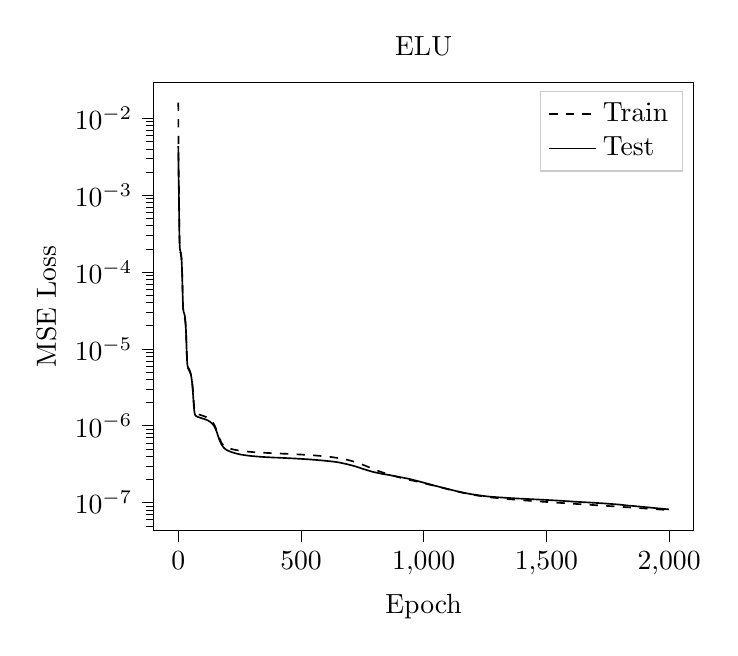
\begin{tikzpicture}

\begin{axis}[
legend cell align={left},
legend style={fill opacity=0.8, draw opacity=1, text opacity=1, draw=white!80!black},
log basis y={10},
tick align=outside,
tick pos=left,
title={ELU},
x grid style={white!69.0196078431373!black},
xlabel={Epoch},
xmin=-99.95, xmax=2098.95,
xtick style={color=black},
y grid style={white!69.0196078431373!black},
ylabel={MSE Loss},
ymin=4.33867354845081e-08, ymax=0.0294400810052884,
ymode=log,
ytick style={color=black}
]
\addplot [semithick, black, dashed]
table {%
0 0.0159906858149916
1 0.00258610278647393
2 0.00158850618591532
3 0.000956721410620958
4 0.000489001872134395
5 0.000282956345094135
6 0.000211721064930316
7 0.000189768037933391
8 0.000182021637432626
9 0.000177359326808073
10 0.00017262034923624
11 0.000166685566466185
12 0.000158753151561541
13 0.000147911270316399
14 0.000133165153318259
15 0.000113917955408397
16 9.10907805628085e-05
17 6.81213804309664e-05
18 4.95797647945437e-05
19 3.77359661724768e-05
20 3.16004643500492e-05
21 2.88638024685497e-05
22 2.76655603011022e-05
23 2.70052526702784e-05
24 2.64611737529776e-05
25 2.58725344338018e-05
26 2.5165805926008e-05
27 2.42854159696435e-05
28 2.3170354677859e-05
29 2.1749585019279e-05
30 1.99512444050924e-05
31 1.77340576083225e-05
32 1.51524796165177e-05
33 1.24352534580794e-05
34 9.97405172893195e-06
35 8.11734906142192e-06
36 6.93657802185044e-06
37 6.26315004649314e-06
38 5.89122448752732e-06
39 5.67968576444855e-06
40 5.54886149245704e-06
41 5.45669130860915e-06
42 5.38190175734599e-06
43 5.31409949712724e-06
44 5.24773788464472e-06
45 5.17960450264354e-06
46 5.1075526739055e-06
47 5.0298866058256e-06
48 4.94497295511564e-06
49 4.85107668760065e-06
50 4.74619869891058e-06
51 4.62834542622659e-06
52 4.49535393136102e-06
53 4.34503200801828e-06
54 4.17533381039448e-06
55 3.98467260913549e-06
56 3.77238118278456e-06
57 3.53925117417475e-06
58 3.28787568685129e-06
59 3.02373617284957e-06
60 2.75509752935932e-06
61 2.49260368849491e-06
62 2.24850782882413e-06
63 2.03428455245103e-06
64 1.85795620984663e-06
65 1.72250744253688e-06
66 1.6253536736599e-06
67 1.55974525910096e-06
68 1.51752829367524e-06
69 1.49080065330054e-06
70 1.47362176335264e-06
71 1.46225174086112e-06
72 1.45420856449618e-06
73 1.44795093308403e-06
74 1.44271991388223e-06
75 1.43809431347108e-06
76 1.43374334504642e-06
77 1.4295735134624e-06
78 1.42554408182605e-06
79 1.4216497555708e-06
80 1.4178540251919e-06
81 1.41412515841921e-06
82 1.41044651763877e-06
83 1.40681854372815e-06
84 1.40321067493687e-06
85 1.39963591544756e-06
86 1.39609892386261e-06
87 1.3925948815654e-06
88 1.38911853508716e-06
89 1.38566465489021e-06
90 1.3822299957269e-06
91 1.37881240459592e-06
92 1.37540860333729e-06
93 1.37201512541196e-06
94 1.36863055058711e-06
95 1.36524915507152e-06
96 1.36186575497277e-06
97 1.35847405181266e-06
98 1.35507275581404e-06
99 1.35165732331188e-06
100 1.34823074495216e-06
101 1.34479479419269e-06
102 1.34134401474739e-06
103 1.33786503300826e-06
104 1.33434866893367e-06
105 1.33078413216481e-06
106 1.32714234337072e-06
107 1.32344306734922e-06
108 1.31969354293915e-06
109 1.31588055188558e-06
110 1.3119966006343e-06
111 1.30803326578643e-06
112 1.30398476517257e-06
113 1.29984123759641e-06
114 1.29558252115203e-06
115 1.29120262238303e-06
116 1.28669816643878e-06
117 1.28205541477655e-06
118 1.27726922664806e-06
119 1.27233098703528e-06
120 1.26723150225416e-06
121 1.26195678973318e-06
122 1.25649127721772e-06
123 1.25082408101207e-06
124 1.24494655307217e-06
125 1.23884643841166e-06
126 1.23250899838467e-06
127 1.22591671828332e-06
128 1.21905894394558e-06
129 1.21192284018434e-06
130 1.20449245946475e-06
131 1.19675427941957e-06
132 1.18869531445398e-06
133 1.18030099093858e-06
134 1.17156371038618e-06
135 1.16247397437519e-06
136 1.1530011221339e-06
137 1.14308228643267e-06
138 1.13275827038706e-06
139 1.12201267188539e-06
140 1.11083171299242e-06
141 1.09920396710095e-06
142 1.08712059392246e-06
143 1.07459341876392e-06
144 1.06162042015967e-06
145 1.04818883656321e-06
146 1.03432408710091e-06
147 1.02003630371428e-06
148 1.00531462365439e-06
149 9.90169928911655e-07
150 9.74621806705045e-07
151 9.58713785962573e-07
152 9.42479460690038e-07
153 9.25951065312347e-07
154 9.09168600088606e-07
155 8.92184417097042e-07
156 8.75050800544841e-07
157 8.57826169180953e-07
158 8.40580582490702e-07
159 8.23381914443644e-07
160 8.06295238675148e-07
161 7.89396326780434e-07
162 7.72781310985238e-07
163 7.5657787539285e-07
164 7.40862125041986e-07
165 7.2571279957856e-07
166 7.11178002461566e-07
167 6.97275696751376e-07
168 6.84054517108734e-07
169 6.71543604397584e-07
170 6.59739762710387e-07
171 6.48579841652008e-07
172 6.38077358331657e-07
173 6.28216510477841e-07
174 6.18950641552374e-07
175 6.10264039266895e-07
176 6.02169999183388e-07
177 5.94657562174916e-07
178 5.87744280039715e-07
179 5.81413833458555e-07
180 5.75600660994269e-07
181 5.70220933695964e-07
182 5.65223498483647e-07
183 5.60603560245454e-07
184 5.56351066080651e-07
185 5.5243466988486e-07
186 5.48800114756887e-07
187 5.45434322532401e-07
188 5.42349594923053e-07
189 5.3947486807715e-07
190 5.36828737466521e-07
191 5.34344525419783e-07
192 5.31993674542264e-07
193 5.29807905536472e-07
194 5.27781949926975e-07
195 5.25858571194249e-07
196 5.24057332683014e-07
197 5.22343938712311e-07
198 5.20721551481529e-07
199 5.19149034175825e-07
200 5.17642666835627e-07
201 5.16201990961918e-07
202 5.14809736500865e-07
203 5.13455026037946e-07
204 5.12140459591137e-07
205 5.10864461205074e-07
206 5.09625953128534e-07
207 5.08422520994145e-07
208 5.07252190715235e-07
209 5.06112615170196e-07
210 5.05002207120242e-07
211 5.03919332913938e-07
212 5.02862736993848e-07
213 5.01830968431705e-07
214 5.00823714645549e-07
215 4.99837807353742e-07
216 4.98873107687814e-07
217 4.97929484851056e-07
218 4.970058403444e-07
219 4.96100682312317e-07
220 4.95213617199397e-07
221 4.9434340317589e-07
222 4.93489999001895e-07
223 4.92651290159074e-07
224 4.91828680907247e-07
225 4.91020204350434e-07
226 4.90224581596976e-07
227 4.89441853375183e-07
228 4.88671986033751e-07
229 4.87916952238265e-07
230 4.87174485925834e-07
231 4.86444744325354e-07
232 4.85726774883233e-07
233 4.85019369165229e-07
234 4.84323500302253e-07
235 4.83639927125523e-07
236 4.82968296523723e-07
237 4.82310117121187e-07
238 4.81661928859012e-07
239 4.81025225582243e-07
240 4.80400114071244e-07
241 4.7978502902879e-07
242 4.7918102524136e-07
243 4.78587331343761e-07
244 4.78004294649281e-07
245 4.77429992429279e-07
246 4.76862302633663e-07
247 4.76302523139793e-07
248 4.75746792034215e-07
249 4.75196238653552e-07
250 4.74654275848252e-07
251 4.74122004590072e-07
252 4.73599449662743e-07
253 4.73085426420994e-07
254 4.72580569010006e-07
255 4.72084032054454e-07
256 4.71594751218163e-07
257 4.71113804536571e-07
258 4.70640037235626e-07
259 4.70174156276926e-07
260 4.69715779757962e-07
261 4.69264562411809e-07
262 4.68820197625064e-07
263 4.68383233567238e-07
264 4.67952394359372e-07
265 4.67528493487634e-07
266 4.67111006997811e-07
267 4.66699930598224e-07
268 4.66294966287251e-07
269 4.65896007852962e-07
270 4.65502569653609e-07
271 4.65115601855359e-07
272 4.64733806950335e-07
273 4.64358269653076e-07
274 4.63987621714068e-07
275 4.63622054098778e-07
276 4.63262431424027e-07
277 4.62908034307929e-07
278 4.62558302785965e-07
279 4.62213879472984e-07
280 4.61874451275435e-07
281 4.61539479516659e-07
282 4.61210072302265e-07
283 4.6088585966686e-07
284 4.6056530376859e-07
285 4.60250070204893e-07
286 4.59937903713126e-07
287 4.59627579061817e-07
288 4.59320908589689e-07
289 4.59017937771478e-07
290 4.58719720626277e-07
291 4.58426474295948e-07
292 4.58136888113359e-07
293 4.57850685478434e-07
294 4.57567064700015e-07
295 4.57287548698559e-07
296 4.5700933148396e-07
297 4.56734894044075e-07
298 4.56462790253909e-07
299 4.56193259282145e-07
300 4.55927074597184e-07
301 4.55663766445014e-07
302 4.55403457266357e-07
303 4.55145485204866e-07
304 4.54890051884149e-07
305 4.54637398092927e-07
306 4.54387924690991e-07
307 4.54140048816498e-07
308 4.53895595455833e-07
309 4.53652887642875e-07
310 4.53413013303816e-07
311 4.53175329965916e-07
312 4.52939619719928e-07
313 4.52706062532116e-07
314 4.52475091350379e-07
315 4.5224581933212e-07
316 4.5201851969523e-07
317 4.51793587870952e-07
318 4.51570470261231e-07
319 4.51349246276322e-07
320 4.51130139424549e-07
321 4.50911806410659e-07
322 4.50696465975398e-07
323 4.50482567146082e-07
324 4.50270295914379e-07
325 4.50059426896132e-07
326 4.49850886724334e-07
327 4.49642915526738e-07
328 4.49437628134319e-07
329 4.49232866827742e-07
330 4.49030053516708e-07
331 4.48829141930673e-07
332 4.48629371163634e-07
333 4.48430973705172e-07
334 4.48233733351344e-07
335 4.48038363487058e-07
336 4.47843558703198e-07
337 4.47650869631389e-07
338 4.47459386890614e-07
339 4.47268515870292e-07
340 4.47079601400446e-07
341 4.46891546545203e-07
342 4.46705519152601e-07
343 4.46520362459069e-07
344 4.46335505017714e-07
345 4.46152672083144e-07
346 4.45970515130512e-07
347 4.45789737796076e-07
348 4.45609748823017e-07
349 4.45431515828432e-07
350 4.45253731754747e-07
351 4.45076565142699e-07
352 4.44900865147702e-07
353 4.44726380123939e-07
354 4.44552419651245e-07
355 4.44379391097982e-07
356 4.44207578851774e-07
357 4.44036821988902e-07
358 4.43865763656959e-07
359 4.43696203234367e-07
360 4.43526793503679e-07
361 4.43359225258178e-07
362 4.43191910605378e-07
363 4.43025337716563e-07
364 4.42860381781429e-07
365 4.42694943302513e-07
366 4.42530713499423e-07
367 4.42366368687885e-07
368 4.42203394399598e-07
369 4.42040955817902e-07
370 4.41879210029583e-07
371 4.41718379931899e-07
372 4.41557534529124e-07
373 4.41397798184084e-07
374 4.41238832934232e-07
375 4.41079906011055e-07
376 4.40922253190479e-07
377 4.40764245766445e-07
378 4.40607835045625e-07
379 4.40452905152711e-07
380 4.40298538350703e-07
381 4.40145228878919e-07
382 4.39993665253269e-07
383 4.39841247228401e-07
384 4.39687762394669e-07
385 4.3953382136408e-07
386 4.39380508097997e-07
387 4.39228653746682e-07
388 4.39076504648028e-07
389 4.38928091796242e-07
390 4.38781355668993e-07
391 4.38643548605455e-07
392 4.38510998463926e-07
393 4.38376672008189e-07
394 4.38234255639713e-07
395 4.38070808172597e-07
396 4.37907314719155e-07
397 4.37751213482329e-07
398 4.37598554711371e-07
399 4.37448513110894e-07
400 4.37300081301828e-07
401 4.37152214118441e-07
402 4.37005594591255e-07
403 4.36860011149065e-07
404 4.36714657084281e-07
405 4.36570365806688e-07
406 4.36424143586578e-07
407 4.36277994012357e-07
408 4.36131178759069e-07
409 4.35983725139977e-07
410 4.35836715993787e-07
411 4.35689698022657e-07
412 4.3554247810107e-07
413 4.35395135951921e-07
414 4.35247865510746e-07
415 4.3510124847046e-07
416 4.3495456503706e-07
417 4.34807267438941e-07
418 4.34661463131647e-07
419 4.34514212969361e-07
420 4.34367550937509e-07
421 4.34220724088163e-07
422 4.34074552501329e-07
423 4.33927956791536e-07
424 4.33781591112847e-07
425 4.33634953083128e-07
426 4.33488506146773e-07
427 4.33342491390931e-07
428 4.33196209357334e-07
429 4.33049361106441e-07
430 4.32903117015826e-07
431 4.32756445960081e-07
432 4.32610265974631e-07
433 4.32463891300472e-07
434 4.32316499100693e-07
435 4.32170432986823e-07
436 4.32023130812809e-07
437 4.31876773717477e-07
438 4.31729480283138e-07
439 4.31582528875651e-07
440 4.31435453705831e-07
441 4.3128805349113e-07
442 4.31140072421954e-07
443 4.30992692542986e-07
444 4.30845347480613e-07
445 4.30696623013205e-07
446 4.30548953829657e-07
447 4.30400634797934e-07
448 4.3025189394541e-07
449 4.3010315148706e-07
450 4.29953725117116e-07
451 4.2980486917088e-07
452 4.29655644651916e-07
453 4.29506079029807e-07
454 4.29355998889491e-07
455 4.29205821575351e-07
456 4.2905581715047e-07
457 4.28906095805814e-07
458 4.28755179513018e-07
459 4.28604906815622e-07
460 4.28454305719583e-07
461 4.28303182189893e-07
462 4.28152659679881e-07
463 4.28002008391104e-07
464 4.27851925209666e-07
465 4.27701338750808e-07
466 4.27552839354917e-07
467 4.27403515331548e-07
468 4.27255618234312e-07
469 4.27108254356767e-07
470 4.26961206983378e-07
471 4.26816100954852e-07
472 4.26674825746431e-07
473 4.26536179944037e-07
474 4.26386996636552e-07
475 4.26223891494715e-07
476 4.26065150577415e-07
477 4.25903862350197e-07
478 4.25744202857459e-07
479 4.25587278471085e-07
480 4.25434084164067e-07
481 4.25283438900692e-07
482 4.2512929348959e-07
483 4.24950156059367e-07
484 4.24775556922441e-07
485 4.2460948539258e-07
486 4.2444458654245e-07
487 4.24280352362416e-07
488 4.24115700013772e-07
489 4.23950707684639e-07
490 4.23785132056764e-07
491 4.23619217514215e-07
492 4.23452926057166e-07
493 4.23285097667758e-07
494 4.23117765933512e-07
495 4.22949673065887e-07
496 4.2278219368086e-07
497 4.22613616308354e-07
498 4.22447139484916e-07
499 4.22281561995419e-07
500 4.22117390655785e-07
501 4.21952666897596e-07
502 4.21779191682958e-07
503 4.21598478823171e-07
504 4.2141833586129e-07
505 4.2124271746502e-07
506 4.21069510096572e-07
507 4.20896647739255e-07
508 4.20719663239311e-07
509 4.20538109011659e-07
510 4.20356770078456e-07
511 4.20174129061479e-07
512 4.19992674551395e-07
513 4.19810148940769e-07
514 4.19626769726733e-07
515 4.19442054592878e-07
516 4.19257225004799e-07
517 4.19071456931874e-07
518 4.18885225997201e-07
519 4.18697576918703e-07
520 4.1850933769183e-07
521 4.18320481543333e-07
522 4.18130317740406e-07
523 4.17939218365859e-07
524 4.17747739689389e-07
525 4.17556271386843e-07
526 4.17364103711293e-07
527 4.17172572497293e-07
528 4.16980429790215e-07
529 4.16786990015794e-07
530 4.1658723431226e-07
531 4.1638575135039e-07
532 4.16184523388097e-07
533 4.15983118557506e-07
534 4.15780713709069e-07
535 4.15577499595088e-07
536 4.15373394730523e-07
537 4.151681697806e-07
538 4.14961842821526e-07
539 4.14754696521413e-07
540 4.14546592665488e-07
541 4.14338080034327e-07
542 4.14128793067903e-07
543 4.13919188318346e-07
544 4.13709204124757e-07
545 4.13499209244605e-07
546 4.1328589449563e-07
547 4.1306897557547e-07
548 4.12848953288858e-07
549 4.1262784985463e-07
550 4.12405905663604e-07
551 4.1218276821553e-07
552 4.11959315172794e-07
553 4.11734457159696e-07
554 4.11508107944769e-07
555 4.11280582085283e-07
556 4.11051760707437e-07
557 4.10821502754288e-07
558 4.10589742699585e-07
559 4.10356863781658e-07
560 4.10121451281498e-07
561 4.09885287368184e-07
562 4.0964726396453e-07
563 4.09408234929742e-07
564 4.09167719382708e-07
565 4.08926019616729e-07
566 4.08682671249494e-07
567 4.08436698762671e-07
568 4.08190045746437e-07
569 4.07942119579729e-07
570 4.07692340473886e-07
571 4.07440955882521e-07
572 4.07187864269076e-07
573 4.06933416684296e-07
574 4.06676930793992e-07
575 4.06419140318803e-07
576 4.06159437602582e-07
577 4.05897947615586e-07
578 4.05634872592486e-07
579 4.05369885982054e-07
580 4.051037206807e-07
581 4.04835206595067e-07
582 4.0456507552733e-07
583 4.04293246745624e-07
584 4.04019944852507e-07
585 4.03744100808012e-07
586 4.0346718590456e-07
587 4.03187891819812e-07
588 4.02906474619158e-07
589 4.0262334898955e-07
590 4.02339123297679e-07
591 4.02051919692781e-07
592 4.01763511547415e-07
593 4.01472600756847e-07
594 4.01180168040582e-07
595 4.00885645106541e-07
596 4.00589115145067e-07
597 4.00290419662497e-07
598 3.99989771580067e-07
599 3.99687020760098e-07
600 3.9938239817161e-07
601 3.99075610644672e-07
602 3.98767107213871e-07
603 3.98456655958057e-07
604 3.98143521934458e-07
605 3.97828211291085e-07
606 3.97511172096188e-07
607 3.971921851047e-07
608 3.96869894700558e-07
609 3.96546615860416e-07
610 3.96220210703291e-07
611 3.95892031804124e-07
612 3.95561097349173e-07
613 3.95228702899431e-07
614 3.94893582551958e-07
615 3.94556066183327e-07
616 3.94216474987275e-07
617 3.93874289670748e-07
618 3.93529946151716e-07
619 3.9318402720312e-07
620 3.92834608746284e-07
621 3.92483627194906e-07
622 3.92129560751187e-07
623 3.91772965187442e-07
624 3.91413925100892e-07
625 3.91051872711046e-07
626 3.90686788946937e-07
627 3.90318204011919e-07
628 3.89946447299394e-07
629 3.8957217735458e-07
630 3.89195215277027e-07
631 3.88815662418551e-07
632 3.88434823477724e-07
633 3.88049628099907e-07
634 3.87657926751217e-07
635 3.87261416292972e-07
636 3.8686301678581e-07
637 3.86461803216775e-07
638 3.86057096932291e-07
639 3.85649708007918e-07
640 3.85240323424796e-07
641 3.84827308181457e-07
642 3.84410717657602e-07
643 3.83992713764769e-07
644 3.8357037226433e-07
645 3.83146246292654e-07
646 3.82718414641658e-07
647 3.82286220116157e-07
648 3.81847366909938e-07
649 3.81402807022369e-07
650 3.80953362920877e-07
651 3.8049944438967e-07
652 3.80041698434752e-07
653 3.79580423256698e-07
654 3.79116224436871e-07
655 3.78646916274761e-07
656 3.78174421157951e-07
657 3.77697935945776e-07
658 3.7721625281506e-07
659 3.76731392663032e-07
660 3.76241358409857e-07
661 3.75747463223774e-07
662 3.75249042562587e-07
663 3.74747122450003e-07
664 3.74241638539274e-07
665 3.73735716252099e-07
666 3.73232575682891e-07
667 3.72738996702537e-07
668 3.72227829430472e-07
669 3.71683786227095e-07
670 3.7113470823158e-07
671 3.70593554904985e-07
672 3.70050383537546e-07
673 3.69502068551242e-07
674 3.68949084261772e-07
675 3.68390563210141e-07
676 3.678264965572e-07
677 3.6725771867907e-07
678 3.66683600475426e-07
679 3.66104024905667e-07
680 3.65519362432565e-07
681 3.64929335361808e-07
682 3.64334175131376e-07
683 3.63734159961382e-07
684 3.63128429640369e-07
685 3.62517425529063e-07
686 3.6190134476044e-07
687 3.61279533990455e-07
688 3.60653619935647e-07
689 3.60020216263024e-07
690 3.59382881029546e-07
691 3.58739043363698e-07
692 3.58090267752686e-07
693 3.57435885064206e-07
694 3.56775838710632e-07
695 3.56110636616336e-07
696 3.55440148368302e-07
697 3.54764160434229e-07
698 3.54083058994092e-07
699 3.53396487156488e-07
700 3.52704934726944e-07
701 3.52008020470862e-07
702 3.51306000808904e-07
703 3.50598153502801e-07
704 3.49885847469977e-07
705 3.49167120290872e-07
706 3.48444031672557e-07
707 3.47714999051618e-07
708 3.46980296029642e-07
709 3.46241530451152e-07
710 3.45497773565739e-07
711 3.44750385963266e-07
712 3.44000039959269e-07
713 3.43243426499384e-07
714 3.42480047621052e-07
715 3.4171182264231e-07
716 3.40938305697591e-07
717 3.40157672084729e-07
718 3.39370888212898e-07
719 3.38579835030828e-07
720 3.3778467948764e-07
721 3.36985210793728e-07
722 3.36182615654934e-07
723 3.35375445175146e-07
724 3.34564629454803e-07
725 3.33749487339219e-07
726 3.32931064335185e-07
727 3.32108447068435e-07
728 3.31281637940606e-07
729 3.30452154130967e-07
730 3.29618623183592e-07
731 3.28782307889242e-07
732 3.27943212383275e-07
733 3.27100122291313e-07
734 3.26251898755459e-07
735 3.25400266802944e-07
736 3.24546339115273e-07
737 3.23690739747917e-07
738 3.22837684763044e-07
739 3.21980068548555e-07
740 3.2111100145471e-07
741 3.20237002227941e-07
742 3.19366001733101e-07
743 3.18494356619681e-07
744 3.1762165654925e-07
745 3.16747852309618e-07
746 3.15873930802013e-07
747 3.14998583988313e-07
748 3.14122304018838e-07
749 3.13245467609136e-07
750 3.12366119956664e-07
751 3.11487112625741e-07
752 3.10605095265259e-07
753 3.097206207201e-07
754 3.08832639916545e-07
755 3.07942916634829e-07
756 3.07053517630607e-07
757 3.06164666483255e-07
758 3.05276597615034e-07
759 3.04389342446143e-07
760 3.03502841475733e-07
761 3.0261704606005e-07
762 3.01732263409349e-07
763 3.00848316157953e-07
764 2.99964995178925e-07
765 2.99083555333368e-07
766 2.9820374386702e-07
767 2.9732410860106e-07
768 2.96446761538505e-07
769 2.95571269603556e-07
770 2.94697533661292e-07
771 2.93826113733076e-07
772 2.92956484798879e-07
773 2.92088886098441e-07
774 2.91223827659337e-07
775 2.9036127409654e-07
776 2.89501379810986e-07
777 2.88645371341545e-07
778 2.87790612048866e-07
779 2.86939756222182e-07
780 2.86093918646202e-07
781 2.85250324424169e-07
782 2.8440853506595e-07
783 2.83568418524283e-07
784 2.82729770532342e-07
785 2.81894248473691e-07
786 2.81063022612216e-07
787 2.80233988476652e-07
788 2.79408298268891e-07
789 2.78585843020096e-07
790 2.77766766629384e-07
791 2.76950464609627e-07
792 2.76139197950442e-07
793 2.75330968236176e-07
794 2.74527831123805e-07
795 2.73728886554636e-07
796 2.72934971803807e-07
797 2.72145031900095e-07
798 2.71360245974961e-07
799 2.70580689175404e-07
800 2.69805612404639e-07
801 2.69035723647448e-07
802 2.68270829579365e-07
803 2.67510604714971e-07
804 2.66754783439183e-07
805 2.66003943082183e-07
806 2.65257105226624e-07
807 2.64515074746896e-07
808 2.63777658076947e-07
809 2.63044983014993e-07
810 2.62317090502506e-07
811 2.61593597855381e-07
812 2.60874926851784e-07
813 2.60160685854771e-07
814 2.59451338109784e-07
815 2.58746429480539e-07
816 2.58046112065813e-07
817 2.57350360087116e-07
818 2.56658965938072e-07
819 2.55971881685468e-07
820 2.5528879186254e-07
821 2.54610372564912e-07
822 2.53935969610097e-07
823 2.53264675137643e-07
824 2.52598306374807e-07
825 2.51936233553351e-07
826 2.51277138815453e-07
827 2.50624390943699e-07
828 2.49974296863797e-07
829 2.49328972245166e-07
830 2.48688589437052e-07
831 2.48052176218039e-07
832 2.47420308085111e-07
833 2.46793441860405e-07
834 2.46169972669463e-07
835 2.4555191518516e-07
836 2.44938152263785e-07
837 2.44328980471664e-07
838 2.4372432818609e-07
839 2.43123647450716e-07
840 2.42527436739692e-07
841 2.41934313066849e-07
842 2.41346243086582e-07
843 2.40760975287913e-07
844 2.40180195106632e-07
845 2.39602776233028e-07
846 2.39030478169866e-07
847 2.3846193494137e-07
848 2.37897005348486e-07
849 2.37336486961226e-07
850 2.36780270924442e-07
851 2.36228712395814e-07
852 2.35682560855821e-07
853 2.35140349545304e-07
854 2.34604098082514e-07
855 2.34070661221608e-07
856 2.33540884252648e-07
857 2.33015706925244e-07
858 2.3249482104859e-07
859 2.31977036079911e-07
860 2.31462959533246e-07
861 2.30952844745502e-07
862 2.30445369865606e-07
863 2.29941426724167e-07
864 2.29440585172824e-07
865 2.28943704769335e-07
866 2.2844926068899e-07
867 2.27958044973775e-07
868 2.27470275618202e-07
869 2.26985706731853e-07
870 2.26503938364431e-07
871 2.26025791818074e-07
872 2.2555024735027e-07
873 2.25077442294719e-07
874 2.24607759776063e-07
875 2.24141335792183e-07
876 2.23676740787937e-07
877 2.23216036090435e-07
878 2.22757687268427e-07
879 2.22302162356414e-07
880 2.21849671518726e-07
881 2.21399852961213e-07
882 2.20952989891998e-07
883 2.20508026032462e-07
884 2.20065753254062e-07
885 2.19626199381651e-07
886 2.1918875741278e-07
887 2.18753092724455e-07
888 2.18320540270156e-07
889 2.17889485469414e-07
890 2.1745900326664e-07
891 2.17031351979813e-07
892 2.16608203714941e-07
893 2.16190809553041e-07
894 2.15776312643356e-07
895 2.15362290859389e-07
896 2.14950339142206e-07
897 2.14540210251357e-07
898 2.14131782342974e-07
899 2.1372564420119e-07
900 2.1332161301757e-07
901 2.1291910150012e-07
902 2.12518860138289e-07
903 2.12120724143006e-07
904 2.11724538587532e-07
905 2.11329817702222e-07
906 2.10937199824457e-07
907 2.10546256425914e-07
908 2.10156896628177e-07
909 2.09769570474805e-07
910 2.09383709488975e-07
911 2.08999720584302e-07
912 2.08617331423966e-07
913 2.08236899553071e-07
914 2.07857965250469e-07
915 2.07481092886042e-07
916 2.07105115009654e-07
917 2.06731647111269e-07
918 2.06359596120365e-07
919 2.05989531096407e-07
920 2.05621238876574e-07
921 2.05254394956e-07
922 2.0488954909581e-07
923 2.04526185612508e-07
924 2.04164605918322e-07
925 2.03804957877196e-07
926 2.03447523659861e-07
927 2.03092279107864e-07
928 2.02738294618143e-07
929 2.0238457909727e-07
930 2.02029677069504e-07
931 2.01671937460901e-07
932 2.01315043327099e-07
933 2.00959512497434e-07
934 2.00604544644989e-07
935 2.00250872410379e-07
936 1.99898528762787e-07
937 1.99547518036525e-07
938 1.99197931237904e-07
939 1.98846556727972e-07
940 1.98497077832371e-07
941 1.98145747660305e-07
942 1.9779394646946e-07
943 1.97441289401468e-07
944 1.97090426979685e-07
945 1.96742395402794e-07
946 1.96398488569116e-07
947 1.96056057973237e-07
948 1.95715211518177e-07
949 1.9537850144502e-07
950 1.9504455411834e-07
951 1.94712024338628e-07
952 1.94378926153149e-07
953 1.94046811500925e-07
954 1.93714091096808e-07
955 1.93381568564632e-07
956 1.93050385803417e-07
957 1.92719263750973e-07
958 1.92389278353744e-07
959 1.9205929470445e-07
960 1.91731396029127e-07
961 1.91402223222781e-07
962 1.91074683357328e-07
963 1.9074786413853e-07
964 1.90421514702166e-07
965 1.90095022318815e-07
966 1.89770198232964e-07
967 1.89445391086451e-07
968 1.89120989816161e-07
969 1.88797464574009e-07
970 1.88474153929974e-07
971 1.88151886163723e-07
972 1.87829453849986e-07
973 1.87507783181218e-07
974 1.87187286698531e-07
975 1.86866505401895e-07
976 1.86546299758561e-07
977 1.86227077662693e-07
978 1.85908078876196e-07
979 1.85589941480657e-07
980 1.85271628822647e-07
981 1.8495448021838e-07
982 1.84637383412678e-07
983 1.84320716172692e-07
984 1.84004656915704e-07
985 1.83688698498941e-07
986 1.83373058249003e-07
987 1.83057700795075e-07
988 1.82742971801986e-07
989 1.8242811900393e-07
990 1.82113932297057e-07
991 1.81799501604019e-07
992 1.8148617854763e-07
993 1.81172313531874e-07
994 1.80859163535274e-07
995 1.80546558553374e-07
996 1.8023371875131e-07
997 1.79921399450222e-07
998 1.79609133027725e-07
999 1.7929770129399e-07
1000 1.78986370457324e-07
1001 1.78674888474006e-07
1002 1.78363633111189e-07
1003 1.78053571730175e-07
1004 1.77743094340599e-07
1005 1.7743289222949e-07
1006 1.77123163680903e-07
1007 1.76813399150433e-07
1008 1.76504621208551e-07
1009 1.7619593938889e-07
1010 1.75887513734097e-07
1011 1.75579751243049e-07
1012 1.75272690157158e-07
1013 1.74965952467687e-07
1014 1.74659207814898e-07
1015 1.74351380209714e-07
1016 1.74042034160493e-07
1017 1.73731117456555e-07
1018 1.73420100608723e-07
1019 1.73109630651425e-07
1020 1.72800415427332e-07
1021 1.72490790831148e-07
1022 1.72182884469407e-07
1023 1.71875223259121e-07
1024 1.71567599466016e-07
1025 1.71259986530004e-07
1026 1.70952779214417e-07
1027 1.70645558227989e-07
1028 1.7033885781359e-07
1029 1.70032917338858e-07
1030 1.69726343031584e-07
1031 1.6942034865508e-07
1032 1.69114824657868e-07
1033 1.68809569686346e-07
1034 1.68504218905241e-07
1035 1.68199184841455e-07
1036 1.67894168384919e-07
1037 1.67589057525674e-07
1038 1.67283977333454e-07
1039 1.66978109149341e-07
1040 1.66672554144043e-07
1041 1.66368867070332e-07
1042 1.66067442094686e-07
1043 1.65768675415734e-07
1044 1.65470151159752e-07
1045 1.65171997124958e-07
1046 1.64875026726463e-07
1047 1.64578407392923e-07
1048 1.6428200929397e-07
1049 1.63985019597135e-07
1050 1.63684462393121e-07
1051 1.63379912791584e-07
1052 1.63074535350916e-07
1053 1.62768297784055e-07
1054 1.62462222775162e-07
1055 1.62156110874889e-07
1056 1.61849415221127e-07
1057 1.61543195446257e-07
1058 1.61236785999108e-07
1059 1.60933830407828e-07
1060 1.60635022787403e-07
1061 1.60340385868096e-07
1062 1.60049089302561e-07
1063 1.59758593277104e-07
1064 1.59466722315926e-07
1065 1.59174708123544e-07
1066 1.58880650644733e-07
1067 1.5858718038686e-07
1068 1.58293491729467e-07
1069 1.5799999722077e-07
1070 1.57706408096203e-07
1071 1.57412825096515e-07
1072 1.57120173312819e-07
1073 1.56827222305367e-07
1074 1.56535237174182e-07
1075 1.56243974302583e-07
1076 1.55952766455414e-07
1077 1.55662811614832e-07
1078 1.55373152850302e-07
1079 1.55083731485206e-07
1080 1.54795515378225e-07
1081 1.54507988042951e-07
1082 1.54220873660904e-07
1083 1.53935042980891e-07
1084 1.53649188085581e-07
1085 1.53364610277151e-07
1086 1.53080741092992e-07
1087 1.5279745203145e-07
1088 1.52514170402185e-07
1089 1.52231895036437e-07
1090 1.51950201022544e-07
1091 1.51669021178691e-07
1092 1.51388963097077e-07
1093 1.51109408882633e-07
1094 1.5082977131442e-07
1095 1.50551916078712e-07
1096 1.50274534782113e-07
1097 1.49998161141696e-07
1098 1.49722255947893e-07
1099 1.49446563071365e-07
1100 1.49171961965067e-07
1101 1.48898209054948e-07
1102 1.48624307755085e-07
1103 1.4835133026736e-07
1104 1.48080495421254e-07
1105 1.47808726936205e-07
1106 1.47538366228162e-07
1107 1.4726858979941e-07
1108 1.46999026256367e-07
1109 1.46730341562318e-07
1110 1.46462592610419e-07
1111 1.46194448667814e-07
1112 1.45927681444391e-07
1113 1.45660832160388e-07
1114 1.45394960604506e-07
1115 1.45130510077252e-07
1116 1.44867812252869e-07
1117 1.4460710507791e-07
1118 1.44346854739297e-07
1119 1.44088306292645e-07
1120 1.43830166308589e-07
1121 1.43572312296669e-07
1122 1.43315712179515e-07
1123 1.43060445338961e-07
1124 1.42805129407009e-07
1125 1.42551452839257e-07
1126 1.42298427896037e-07
1127 1.42046496797832e-07
1128 1.41795435418146e-07
1129 1.41545382064123e-07
1130 1.41295842354339e-07
1131 1.41047917132653e-07
1132 1.40800541821307e-07
1133 1.40554253533765e-07
1134 1.40309015705498e-07
1135 1.40064675107965e-07
1136 1.39821170350274e-07
1137 1.39579605225038e-07
1138 1.39338311164749e-07
1139 1.39098575928642e-07
1140 1.38860050718392e-07
1141 1.38622980010439e-07
1142 1.38386074866048e-07
1143 1.38151192111025e-07
1144 1.37916803048199e-07
1145 1.37684516310799e-07
1146 1.37451800391375e-07
1147 1.37221027316059e-07
1148 1.36991179445545e-07
1149 1.36762923808931e-07
1150 1.36535392606163e-07
1151 1.36309236019372e-07
1152 1.36083985445623e-07
1153 1.35859885773471e-07
1154 1.35636987302235e-07
1155 1.35415610060363e-07
1156 1.3519462617495e-07
1157 1.34975457292796e-07
1158 1.34757256731177e-07
1159 1.34540234483893e-07
1160 1.34324358555205e-07
1161 1.34109793279435e-07
1162 1.33896426177671e-07
1163 1.33684459278527e-07
1164 1.33473248411065e-07
1165 1.33263645466286e-07
1166 1.33055609722987e-07
1167 1.32848456068757e-07
1168 1.32642267075767e-07
1169 1.32438386458489e-07
1170 1.3223490227432e-07
1171 1.32032633729295e-07
1172 1.31832137057586e-07
1173 1.31632554129624e-07
1174 1.31434246767981e-07
1175 1.31237355475378e-07
1176 1.3104204354164e-07
1177 1.30847429275605e-07
1178 1.30654636990357e-07
1179 1.30462662419006e-07
1180 1.30272386684283e-07
1181 1.30083957976979e-07
1182 1.29895856105122e-07
1183 1.29710162141805e-07
1184 1.29525688848275e-07
1185 1.29342381164577e-07
1186 1.29160692303287e-07
1187 1.28980738672624e-07
1188 1.28801087768693e-07
1189 1.28622351823537e-07
1190 1.28443456553384e-07
1191 1.28265808847061e-07
1192 1.28089295927225e-07
1193 1.27913166409144e-07
1194 1.27739159495377e-07
1195 1.27565773269112e-07
1196 1.27394257454227e-07
1197 1.2722304434476e-07
1198 1.27053708432356e-07
1199 1.26885512280239e-07
1200 1.26718282551508e-07
1201 1.26551697867683e-07
1202 1.26386519937682e-07
1203 1.2622200886625e-07
1204 1.26058745912871e-07
1205 1.25896560582817e-07
1206 1.25735422180639e-07
1207 1.25574455424271e-07
1208 1.25414781614097e-07
1209 1.252551799098e-07
1210 1.25096239329991e-07
1211 1.24937196254393e-07
1212 1.24777347565441e-07
1213 1.24616552589885e-07
1214 1.24453111794764e-07
1215 1.24288724109078e-07
1216 1.24127905870353e-07
1217 1.23972136528039e-07
1218 1.23820694362564e-07
1219 1.23674698834009e-07
1220 1.23530782715875e-07
1221 1.23389221329262e-07
1222 1.2324859677193e-07
1223 1.2310908447688e-07
1224 1.22970074919238e-07
1225 1.22832236861825e-07
1226 1.22694502813658e-07
1227 1.22557335302531e-07
1228 1.22421338744516e-07
1229 1.22286256306836e-07
1230 1.22151674226245e-07
1231 1.22018912449562e-07
1232 1.21886562475026e-07
1233 1.21754655523887e-07
1234 1.21624491512762e-07
1235 1.21494801220479e-07
1236 1.2136614208913e-07
1237 1.21238329604978e-07
1238 1.21111555806408e-07
1239 1.20985908843352e-07
1240 1.20860088962615e-07
1241 1.20735704754793e-07
1242 1.20612777600115e-07
1243 1.20490426148478e-07
1244 1.20367756657913e-07
1245 1.2024713782921e-07
1246 1.20126928187858e-07
1247 1.20007730558314e-07
1248 1.19888488541164e-07
1249 1.19770750160342e-07
1250 1.19653075920212e-07
1251 1.19536828812272e-07
1252 1.19421025523536e-07
1253 1.19305560325245e-07
1254 1.19191435054233e-07
1255 1.19077117162192e-07
1256 1.18963121451543e-07
1257 1.18850351661592e-07
1258 1.18737166289407e-07
1259 1.18624644954934e-07
1260 1.18512422588424e-07
1261 1.1840071167768e-07
1262 1.18288370344999e-07
1263 1.18177834188771e-07
1264 1.18068884660261e-07
1265 1.17963069399707e-07
1266 1.17858075192601e-07
1267 1.17754390267066e-07
1268 1.17650794884128e-07
1269 1.17548814614565e-07
1270 1.1744721561513e-07
1271 1.17345708268601e-07
1272 1.17244883455214e-07
1273 1.17145502350979e-07
1274 1.17046118376152e-07
1275 1.16947641409126e-07
1276 1.16849509630867e-07
1277 1.1675244088849e-07
1278 1.16655163623136e-07
1279 1.16558887576446e-07
1280 1.16463558931912e-07
1281 1.16368087383023e-07
1282 1.16274038802544e-07
1283 1.16180324624793e-07
1284 1.16086594658782e-07
1285 1.159941292741e-07
1286 1.15901939551577e-07
1287 1.15811317932923e-07
1288 1.15720263679009e-07
1289 1.15630437839798e-07
1290 1.15540727264829e-07
1291 1.15451683456058e-07
1292 1.15363191504514e-07
1293 1.15273850731512e-07
1294 1.15184926350764e-07
1295 1.15096048155294e-07
1296 1.15007235429232e-07
1297 1.14918379381379e-07
1298 1.14830777491193e-07
1299 1.14743160814612e-07
1300 1.1465620086426e-07
1301 1.14570124786439e-07
1302 1.14484055657726e-07
1303 1.14398570758567e-07
1304 1.14313791009124e-07
1305 1.14229299640556e-07
1306 1.14145610695005e-07
1307 1.14061028625656e-07
1308 1.13977942092447e-07
1309 1.13894630288769e-07
1310 1.13811890621207e-07
1311 1.13728955128067e-07
1312 1.13647374824666e-07
1313 1.13565325307263e-07
1314 1.13483557022676e-07
1315 1.13402332914347e-07
1316 1.13320262414618e-07
1317 1.13240334016496e-07
1318 1.13159186064138e-07
1319 1.13077794551941e-07
1320 1.12997345617316e-07
1321 1.12916872375024e-07
1322 1.12837699774104e-07
1323 1.1275950181755e-07
1324 1.12682501281824e-07
1325 1.12606438932517e-07
1326 1.12530998414684e-07
1327 1.12455497344399e-07
1328 1.12380201152007e-07
1329 1.12304915312222e-07
1330 1.12229716322076e-07
1331 1.12155240366008e-07
1332 1.12080816393245e-07
1333 1.12006098483164e-07
1334 1.11932343500598e-07
1335 1.11859045325957e-07
1336 1.11785418326349e-07
1337 1.11712671881037e-07
1338 1.11639020587972e-07
1339 1.11567380578492e-07
1340 1.11494612262675e-07
1341 1.11422763467317e-07
1342 1.11350776293762e-07
1343 1.11279370571538e-07
1344 1.11208307423283e-07
1345 1.1113706440824e-07
1346 1.11066865265741e-07
1347 1.10995945618697e-07
1348 1.10925767160097e-07
1349 1.10855683992384e-07
1350 1.10786117552664e-07
1351 1.10716733097149e-07
1352 1.10647160461497e-07
1353 1.10578233645242e-07
1354 1.10509506583867e-07
1355 1.10440672571599e-07
1356 1.10372395390357e-07
1357 1.1030493424613e-07
1358 1.10236386966278e-07
1359 1.10168692920354e-07
1360 1.1010140007528e-07
1361 1.10034333395959e-07
1362 1.09966698083497e-07
1363 1.09899731342011e-07
1364 1.09833291951134e-07
1365 1.09767210155098e-07
1366 1.09700639285393e-07
1367 1.09634514146251e-07
1368 1.09568511987845e-07
1369 1.09503384450704e-07
1370 1.09437140011437e-07
1371 1.09372695533239e-07
1372 1.09307097929445e-07
1373 1.09242549555688e-07
1374 1.09177182331166e-07
1375 1.09113151367524e-07
1376 1.09048662530142e-07
1377 1.08984274390878e-07
1378 1.08920784626321e-07
1379 1.08856745349328e-07
1380 1.08792611804631e-07
1381 1.08729247486394e-07
1382 1.08666047573536e-07
1383 1.08602843141625e-07
1384 1.08539720571343e-07
1385 1.08477539157548e-07
1386 1.08414238106036e-07
1387 1.08351683770991e-07
1388 1.08289551810969e-07
1389 1.08227359682189e-07
1390 1.08165446718544e-07
1391 1.0810315509957e-07
1392 1.08042059039803e-07
1393 1.07980339663527e-07
1394 1.07918164097498e-07
1395 1.07857049350457e-07
1396 1.07796089665158e-07
1397 1.07734852363706e-07
1398 1.07674071145425e-07
1399 1.07613202636969e-07
1400 1.07552554730717e-07
1401 1.07492185293268e-07
1402 1.07430896818528e-07
1403 1.07371186579996e-07
1404 1.07310734684063e-07
1405 1.07251448994816e-07
1406 1.07190961820436e-07
1407 1.07130689571022e-07
1408 1.07071231418843e-07
1409 1.07011258137391e-07
1410 1.06951851911674e-07
1411 1.06892511382739e-07
1412 1.06832769780851e-07
1413 1.06773393866888e-07
1414 1.06713744486342e-07
1415 1.06655080848839e-07
1416 1.06596275074367e-07
1417 1.06536867519935e-07
1418 1.06478330863524e-07
1419 1.06419705552696e-07
1420 1.06360801503058e-07
1421 1.06302999540731e-07
1422 1.06245188106868e-07
1423 1.06186696449129e-07
1424 1.06128813278872e-07
1425 1.06071861281976e-07
1426 1.06014330761184e-07
1427 1.05956670530816e-07
1428 1.05899683347843e-07
1429 1.05843118227256e-07
1430 1.05786040670353e-07
1431 1.05729466049809e-07
1432 1.05672679602264e-07
1433 1.05616201466319e-07
1434 1.0555939075374e-07
1435 1.05503326139456e-07
1436 1.05447132533243e-07
1437 1.05391329668691e-07
1438 1.05335469569923e-07
1439 1.05278794926278e-07
1440 1.05223197536475e-07
1441 1.05167620077395e-07
1442 1.05111855617679e-07
1443 1.05056052994712e-07
1444 1.05001211672118e-07
1445 1.04945261661271e-07
1446 1.04890033782112e-07
1447 1.04835637209533e-07
1448 1.04780062464727e-07
1449 1.04725117317628e-07
1450 1.04669809111613e-07
1451 1.04615355382975e-07
1452 1.04560794511599e-07
1453 1.04506511071634e-07
1454 1.04451745890799e-07
1455 1.04396768143999e-07
1456 1.04343061707368e-07
1457 1.0428867787482e-07
1458 1.04234510423851e-07
1459 1.04180059025794e-07
1460 1.04126391235582e-07
1461 1.04072378704245e-07
1462 1.04018579186516e-07
1463 1.03964594160288e-07
1464 1.0391101395868e-07
1465 1.03857236730676e-07
1466 1.03804541957686e-07
1467 1.03750232234745e-07
1468 1.03697174260731e-07
1469 1.03644181137952e-07
1470 1.03590405920784e-07
1471 1.03537499640538e-07
1472 1.03484241449792e-07
1473 1.03431446369484e-07
1474 1.03379083178368e-07
1475 1.03325666280796e-07
1476 1.03273275158244e-07
1477 1.03220849005936e-07
1478 1.03167916790881e-07
1479 1.03114894407952e-07
1480 1.03062992813818e-07
1481 1.03010403556425e-07
1482 1.02958110019813e-07
1483 1.02905616664373e-07
1484 1.02853633016764e-07
1485 1.02801250562834e-07
1486 1.02749931926382e-07
1487 1.02697206507685e-07
1488 1.02644856170286e-07
1489 1.02593503726212e-07
1490 1.02541410662127e-07
1491 1.02490195232008e-07
1492 1.02437883029438e-07
1493 1.02386485295369e-07
1494 1.02335240654838e-07
1495 1.022834896105e-07
1496 1.02231845602319e-07
1497 1.02180107241168e-07
1498 1.02128798815215e-07
1499 1.02077938137768e-07
1500 1.02026645308229e-07
1501 1.01975711132241e-07
1502 1.0192386444885e-07
1503 1.01873104213723e-07
1504 1.01821924069156e-07
1505 1.01771640999004e-07
1506 1.01719919427978e-07
1507 1.0166950955437e-07
1508 1.01618475277121e-07
1509 1.01568011345421e-07
1510 1.01516741338514e-07
1511 1.01466086711355e-07
1512 1.0141579495837e-07
1513 1.01365547621413e-07
1514 1.01315401707325e-07
1515 1.01265256688521e-07
1516 1.0121462806012e-07
1517 1.01164024890466e-07
1518 1.01114676198222e-07
1519 1.01064772806581e-07
1520 1.01014704618763e-07
1521 1.00964946341264e-07
1522 1.00915428895121e-07
1523 1.00865459458532e-07
1524 1.00816070599308e-07
1525 1.00766296540655e-07
1526 1.00716959224201e-07
1527 1.00666841063912e-07
1528 1.00618032597311e-07
1529 1.00568492072739e-07
1530 1.00519370199947e-07
1531 1.00470240930406e-07
1532 1.00420870836615e-07
1533 1.00371893914541e-07
1534 1.00323030800098e-07
1535 1.00273699459308e-07
1536 1.00225219753725e-07
1537 1.00175660548985e-07
1538 1.00126924415633e-07
1539 1.0007838643844e-07
1540 1.00029839458671e-07
1541 9.9980503236452e-08
1542 9.99320399230896e-08
1543 9.9883877560103e-08
1544 9.98348089211731e-08
1545 9.97862986622522e-08
1546 9.97378668969873e-08
1547 9.96892700442231e-08
1548 9.96408808759952e-08
1549 9.9592121117098e-08
1550 9.9544117297512e-08
1551 9.94956037843053e-08
1552 9.94476393572086e-08
1553 9.93996351397186e-08
1554 9.93505202089295e-08
1555 9.93029401499257e-08
1556 9.92540049367108e-08
1557 9.92056840445343e-08
1558 9.91578368498836e-08
1559 9.91100553449087e-08
1560 9.90610551951931e-08
1561 9.90130886435736e-08
1562 9.8965180050925e-08
1563 9.89167855038886e-08
1564 9.886806271453e-08
1565 9.88197112903322e-08
1566 9.87711251099199e-08
1567 9.87224470350156e-08
1568 9.86743409541191e-08
1569 9.86250088388374e-08
1570 9.85762265059975e-08
1571 9.85275537601637e-08
1572 9.84783014956747e-08
1573 9.84285809622065e-08
1574 9.83794066442556e-08
1575 9.83301730386188e-08
1576 9.82805003388876e-08
1577 9.82321995337543e-08
1578 9.81839275624452e-08
1579 9.81365214869356e-08
1580 9.80893287234608e-08
1581 9.80431635682066e-08
1582 9.79963828697805e-08
1583 9.79501937763416e-08
1584 9.79029187817559e-08
1585 9.78568809486546e-08
1586 9.78109894589352e-08
1587 9.77635616123962e-08
1588 9.77171009495237e-08
1589 9.76708774373947e-08
1590 9.76242692445339e-08
1591 9.75778811778127e-08
1592 9.75318191933638e-08
1593 9.7485102344308e-08
1594 9.74387158336754e-08
1595 9.73921234717068e-08
1596 9.73459424855605e-08
1597 9.72996641763757e-08
1598 9.72536354879594e-08
1599 9.72074526970346e-08
1600 9.71612808129407e-08
1601 9.71147312753828e-08
1602 9.70689995014595e-08
1603 9.70228219969726e-08
1604 9.6975823566936e-08
1605 9.69302687039431e-08
1606 9.68839881707595e-08
1607 9.68386370630014e-08
1608 9.6792325656736e-08
1609 9.67463812671099e-08
1610 9.6700453923404e-08
1611 9.66545619718317e-08
1612 9.66089966851769e-08
1613 9.65634078582411e-08
1614 9.65177741889533e-08
1615 9.64726374874658e-08
1616 9.64275957286986e-08
1617 9.63822620647647e-08
1618 9.63367029598317e-08
1619 9.6292144156962e-08
1620 9.62470803074211e-08
1621 9.62014964827063e-08
1622 9.61567951947018e-08
1623 9.61115279025648e-08
1624 9.60662595019812e-08
1625 9.602197883396e-08
1626 9.5976875826409e-08
1627 9.59314282056312e-08
1628 9.58870571139414e-08
1629 9.58411791529557e-08
1630 9.57966473080774e-08
1631 9.57518183284378e-08
1632 9.57067038243054e-08
1633 9.56623021437508e-08
1634 9.56172586867865e-08
1635 9.55723913023121e-08
1636 9.55276414273953e-08
1637 9.54827806083358e-08
1638 9.54373270900533e-08
1639 9.5393260103549e-08
1640 9.53481811336587e-08
1641 9.53036219257797e-08
1642 9.52585937668005e-08
1643 9.5214033471791e-08
1644 9.5169077923174e-08
1645 9.51244453517575e-08
1646 9.50798078704906e-08
1647 9.50351661259674e-08
1648 9.49902117071133e-08
1649 9.49453065217654e-08
1650 9.49003528774028e-08
1651 9.48555784177074e-08
1652 9.48110341241204e-08
1653 9.47660199912548e-08
1654 9.47212155892885e-08
1655 9.46768115639429e-08
1656 9.46315436465284e-08
1657 9.45872469273468e-08
1658 9.45418865683223e-08
1659 9.44969696021758e-08
1660 9.44525184110034e-08
1661 9.44076963733664e-08
1662 9.43625196399012e-08
1663 9.43183353356858e-08
1664 9.42732718272055e-08
1665 9.42288012595327e-08
1666 9.41839682582213e-08
1667 9.41399476062088e-08
1668 9.40957243713569e-08
1669 9.40506182587342e-08
1670 9.40058235343599e-08
1671 9.39615953612361e-08
1672 9.3917497736129e-08
1673 9.38733850404105e-08
1674 9.38292321137624e-08
1675 9.37849028304072e-08
1676 9.37406613275016e-08
1677 9.36967924332066e-08
1678 9.36527834056733e-08
1679 9.36083967175705e-08
1680 9.35637989840643e-08
1681 9.35208586625436e-08
1682 9.34761403570405e-08
1683 9.34324272776621e-08
1684 9.33884746601166e-08
1685 9.33446521074188e-08
1686 9.33007224830362e-08
1687 9.32568844049797e-08
1688 9.32129020299044e-08
1689 9.31691990473382e-08
1690 9.31250598270594e-08
1691 9.30811820438748e-08
1692 9.30373811129925e-08
1693 9.29938930624985e-08
1694 9.29499208410789e-08
1695 9.29055497351783e-08
1696 9.28623088967129e-08
1697 9.28187458555385e-08
1698 9.27743841359074e-08
1699 9.27311628515781e-08
1700 9.26876528595244e-08
1701 9.26435682160331e-08
1702 9.25997172984694e-08
1703 9.2556214312367e-08
1704 9.25127809949799e-08
1705 9.24683791225789e-08
1706 9.24253023697474e-08
1707 9.23820449258983e-08
1708 9.23380721857825e-08
1709 9.22941760066465e-08
1710 9.22513713561557e-08
1711 9.22074459737132e-08
1712 9.21635799571163e-08
1713 9.21202615344896e-08
1714 9.20766708247811e-08
1715 9.2033423207738e-08
1716 9.19897681939119e-08
1717 9.19461703219326e-08
1718 9.19030513912844e-08
1719 9.18604261315181e-08
1720 9.1816087888219e-08
1721 9.17729236604714e-08
1722 9.17296037243887e-08
1723 9.16868353684208e-08
1724 9.16435574893626e-08
1725 9.15997281651926e-08
1726 9.15555780309774e-08
1727 9.15123038538468e-08
1728 9.14679694048459e-08
1729 9.14242826297595e-08
1730 9.13795196311185e-08
1731 9.13348543960524e-08
1732 9.12901464076299e-08
1733 9.12467560496566e-08
1734 9.12035151259261e-08
1735 9.11605055904374e-08
1736 9.11185110581414e-08
1737 9.1075669104157e-08
1738 9.10335783075311e-08
1739 9.09906703441266e-08
1740 9.09481890332131e-08
1741 9.0904379376866e-08
1742 9.08616451198441e-08
1743 9.08180396663738e-08
1744 9.07755112748987e-08
1745 9.07325125965031e-08
1746 9.06888457095079e-08
1747 9.06459451996966e-08
1748 9.06033168703857e-08
1749 9.05600800322759e-08
1750 9.05171096690083e-08
1751 9.04733630449073e-08
1752 9.04310494718175e-08
1753 9.03878881430842e-08
1754 9.03447747049313e-08
1755 9.03018548328305e-08
1756 9.02590079761012e-08
1757 9.02156785898001e-08
1758 9.01729501805448e-08
1759 9.01293485355836e-08
1760 9.00867049935528e-08
1761 9.00436262583071e-08
1762 9.00009111290956e-08
1763 8.99575377886208e-08
1764 8.99145852528704e-08
1765 8.98715091537383e-08
1766 8.98283387869014e-08
1767 8.97846491270116e-08
1768 8.97414555680598e-08
1769 8.96991304131234e-08
1770 8.96561750067804e-08
1771 8.96123025597717e-08
1772 8.95689090256724e-08
1773 8.95262360316451e-08
1774 8.94821884784847e-08
1775 8.94393531112314e-08
1776 8.93963832240274e-08
1777 8.93540570814366e-08
1778 8.93108375166207e-08
1779 8.92686593587655e-08
1780 8.92253275779353e-08
1781 8.91827055156114e-08
1782 8.91396041993175e-08
1783 8.90972992380057e-08
1784 8.90539103153287e-08
1785 8.90114980620638e-08
1786 8.8968712780968e-08
1787 8.89253062226203e-08
1788 8.88829198899543e-08
1789 8.88399494698433e-08
1790 8.87968220055768e-08
1791 8.8754060882934e-08
1792 8.87109319620549e-08
1793 8.86681817746648e-08
1794 8.86252248619712e-08
1795 8.85825505463345e-08
1796 8.85388048317282e-08
1797 8.84961064215872e-08
1798 8.84526474962399e-08
1799 8.84092216679733e-08
1800 8.83660109280982e-08
1801 8.83221732124184e-08
1802 8.82774145836152e-08
1803 8.82323908300009e-08
1804 8.81847844311778e-08
1805 8.81355833612929e-08
1806 8.80791871651354e-08
1807 8.80146358070988e-08
1808 8.7962349574866e-08
1809 8.79226908310215e-08
1810 8.7882862146671e-08
1811 8.78412527427486e-08
1812 8.77981462963362e-08
1813 8.77551137321575e-08
1814 8.77114189350436e-08
1815 8.76676313836811e-08
1816 8.76230597270933e-08
1817 8.75796666832684e-08
1818 8.75361143997111e-08
1819 8.74914746162858e-08
1820 8.74480210626416e-08
1821 8.74041800429381e-08
1822 8.73606932785265e-08
1823 8.73167411228337e-08
1824 8.72736415260533e-08
1825 8.72300550227578e-08
1826 8.71885273383555e-08
1827 8.7145413907308e-08
1828 8.71038641463429e-08
1829 8.70623297828388e-08
1830 8.70213607910841e-08
1831 8.6980787699531e-08
1832 8.69391078381909e-08
1833 8.68976408128219e-08
1834 8.68563370630682e-08
1835 8.68148545478675e-08
1836 8.67730671174627e-08
1837 8.67315644228484e-08
1838 8.66907000229844e-08
1839 8.66487525570392e-08
1840 8.66078587051788e-08
1841 8.65667076652699e-08
1842 8.65257089515126e-08
1843 8.64840287562174e-08
1844 8.64431281826228e-08
1845 8.64012246211132e-08
1846 8.63589747410742e-08
1847 8.63167327267433e-08
1848 8.62747192655888e-08
1849 8.62320775780745e-08
1850 8.61896311548094e-08
1851 8.61472139774833e-08
1852 8.61047208857713e-08
1853 8.60629838044247e-08
1854 8.60207611168562e-08
1855 8.59782706186252e-08
1856 8.59367052754578e-08
1857 8.58940795112062e-08
1858 8.58522319333588e-08
1859 8.58102813126038e-08
1860 8.57677750616404e-08
1861 8.57256369144466e-08
1862 8.56834849116694e-08
1863 8.56414290097973e-08
1864 8.55980600604767e-08
1865 8.55561950885431e-08
1866 8.55137677504558e-08
1867 8.54715725679966e-08
1868 8.54291732110823e-08
1869 8.53870532679934e-08
1870 8.53444887525257e-08
1871 8.53016869939438e-08
1872 8.52596541704997e-08
1873 8.52168754690297e-08
1874 8.51748716002021e-08
1875 8.51332402760363e-08
1876 8.50905916607303e-08
1877 8.50484975671861e-08
1878 8.50060092858485e-08
1879 8.49635397557336e-08
1880 8.492171967589e-08
1881 8.48789661063165e-08
1882 8.48368106147745e-08
1883 8.47953779157251e-08
1884 8.47524956455459e-08
1885 8.47107574060146e-08
1886 8.46685267816838e-08
1887 8.46262519758056e-08
1888 8.45840424048561e-08
1889 8.45420587083368e-08
1890 8.44998341804626e-08
1891 8.44572482847639e-08
1892 8.44149602201583e-08
1893 8.43730506545626e-08
1894 8.43303609556756e-08
1895 8.42884517879838e-08
1896 8.42459721255295e-08
1897 8.42037612471813e-08
1898 8.41616729090333e-08
1899 8.41196240628506e-08
1900 8.40773184336285e-08
1901 8.40353721613951e-08
1902 8.3992983299197e-08
1903 8.39502722058683e-08
1904 8.39081483903215e-08
1905 8.38665984659315e-08
1906 8.38237704883227e-08
1907 8.37813611980209e-08
1908 8.3739311783404e-08
1909 8.36975896163494e-08
1910 8.36546135900562e-08
1911 8.36126764340861e-08
1912 8.35705718600366e-08
1913 8.35283511406715e-08
1914 8.34854772833182e-08
1915 8.34436993599752e-08
1916 8.34017504942608e-08
1917 8.33594456892683e-08
1918 8.3317273116279e-08
1919 8.32743763226063e-08
1920 8.32327886044482e-08
1921 8.31903297040526e-08
1922 8.31481104413001e-08
1923 8.31055300452022e-08
1924 8.30637235296194e-08
1925 8.30207007211925e-08
1926 8.29792336816126e-08
1927 8.29362121734789e-08
1928 8.28949518947297e-08
1929 8.28518102906628e-08
1930 8.28095903031567e-08
1931 8.27672520813394e-08
1932 8.27248675889791e-08
1933 8.26825600697134e-08
1934 8.26403458802361e-08
1935 8.25978216099088e-08
1936 8.25556787660275e-08
1937 8.25132388797556e-08
1938 8.24706811712872e-08
1939 8.24282363325324e-08
1940 8.2385764400783e-08
1941 8.23432660084222e-08
1942 8.23009294350641e-08
1943 8.22584946291727e-08
1944 8.22153796917746e-08
1945 8.21731729061526e-08
1946 8.21301921760664e-08
1947 8.20879010134945e-08
1948 8.20445673923587e-08
1949 8.20020953753442e-08
1950 8.19593798837559e-08
1951 8.19166102985491e-08
1952 8.18738032677402e-08
1953 8.18307687282527e-08
1954 8.17875831415904e-08
1955 8.1744550598728e-08
1956 8.17016657848058e-08
1957 8.16588795942153e-08
1958 8.16164791643814e-08
1959 8.15733783383621e-08
1960 8.1531317547956e-08
1961 8.14890921105871e-08
1962 8.14470502064069e-08
1963 8.14052194897386e-08
1964 8.13625386015815e-08
1965 8.1320183916489e-08
1966 8.12781310344235e-08
1967 8.12350858296895e-08
1968 8.11932688193906e-08
1969 8.1151145622016e-08
1970 8.11083941272273e-08
1971 8.10661200247864e-08
1972 8.10240671214046e-08
1973 8.09815906777089e-08
1974 8.09395606253816e-08
1975 8.08969995276243e-08
1976 8.08547562201056e-08
1977 8.08122319782001e-08
1978 8.0769925965285e-08
1979 8.07277241818838e-08
1980 8.06854152628489e-08
1981 8.06422377905847e-08
1982 8.06005743001492e-08
1983 8.05578714917488e-08
1984 8.05154302554456e-08
1985 8.04733391177592e-08
1986 8.04308230044626e-08
1987 8.03880149717884e-08
1988 8.03461685521256e-08
1989 8.03037194287981e-08
1990 8.02610393790815e-08
1991 8.02182038839305e-08
1992 8.01759393240786e-08
1993 8.0133311314512e-08
1994 8.00910382565689e-08
1995 8.00485687406649e-08
1996 8.00053081775332e-08
1997 7.99631832180125e-08
1998 7.99206383845785e-08
1999 7.98783130377956e-08
};
\addlegendentry{Train}
\addplot [semithick, black]
table {%
0 0.00434648292139173
1 0.001871966291219
2 0.00126478425227106
3 0.000670640729367733
4 0.000359735742677003
5 0.000243819231400266
6 0.000206869386602193
7 0.000194960201042704
8 0.0001893769367598
9 0.000184681048267521
10 0.000179201771970838
11 0.000172067433595657
12 0.000162401178386062
13 0.000149167492054403
14 0.000131396518554538
15 0.000109012275061104
16 8.42450463096611e-05
17 6.18530102656223e-05
18 4.59465773019474e-05
19 3.69815243175253e-05
20 3.27855850628112e-05
21 3.09872448269743e-05
22 3.01140898955055e-05
23 2.94931924145203e-05
24 2.88680803350871e-05
25 2.8138236302766e-05
26 2.72418055828894e-05
27 2.61142595263664e-05
28 2.46799172600731e-05
29 2.28556364163524e-05
30 2.05716205528006e-05
31 1.78281570697436e-05
32 1.47822220242233e-05
33 1.17997969937278e-05
34 9.34392573981313e-06
35 7.67942492529983e-06
36 6.7177320488554e-06
37 6.2075396272121e-06
38 5.94215407545562e-06
39 5.79742527406779e-06
40 5.70562633583904e-06
41 5.6335047702305e-06
42 5.56622899239301e-06
43 5.497817255673e-06
44 5.42501902600634e-06
45 5.34654282091651e-06
46 5.26074700246681e-06
47 5.16627414981485e-06
48 5.0617254601093e-06
49 4.94508594783838e-06
50 4.81498864246532e-06
51 4.66882238470134e-06
52 4.5045144361211e-06
53 4.32119350080029e-06
54 4.11813061873545e-06
55 3.89628030461608e-06
56 3.65772075383575e-06
57 3.40276073984569e-06
58 3.13182727040839e-06
59 2.850018972822e-06
60 2.56729140346579e-06
61 2.29897318604344e-06
62 2.05908349926176e-06
63 1.85658177542791e-06
64 1.69468341937318e-06
65 1.57401359501819e-06
66 1.49008371863601e-06
67 1.43393549478787e-06
68 1.39726864745171e-06
69 1.37356846607872e-06
70 1.35771210807434e-06
71 1.34745585000928e-06
72 1.33979938254924e-06
73 1.33333901430888e-06
74 1.32785703499394e-06
75 1.32291336285562e-06
76 1.31837271055701e-06
77 1.31382205381669e-06
78 1.3096720294925e-06
79 1.3058757986073e-06
80 1.3022184930378e-06
81 1.29849081531574e-06
82 1.2948945595781e-06
83 1.2913204727738e-06
84 1.28785336528381e-06
85 1.28448050418228e-06
86 1.28120791487163e-06
87 1.27796317883622e-06
88 1.27474572764186e-06
89 1.27157511542464e-06
90 1.26845941395004e-06
91 1.26538327549497e-06
92 1.26235624975379e-06
93 1.25936389849812e-06
94 1.25642270631943e-06
95 1.25351948554453e-06
96 1.25066753753345e-06
97 1.24784605759487e-06
98 1.24501832488022e-06
99 1.24216182939563e-06
100 1.23928680295649e-06
101 1.23642735161411e-06
102 1.23360428005981e-06
103 1.23079018976568e-06
104 1.22796086543531e-06
105 1.22511266908987e-06
106 1.22221945275669e-06
107 1.21929156193801e-06
108 1.21632763239177e-06
109 1.21331220270804e-06
110 1.21023879273707e-06
111 1.20709580642142e-06
112 1.20387221613782e-06
113 1.2005752978439e-06
114 1.19714286483941e-06
115 1.19358094252675e-06
116 1.18986952202249e-06
117 1.18598757126165e-06
118 1.18191076126095e-06
119 1.17765398499614e-06
120 1.17325930659717e-06
121 1.16874537070544e-06
122 1.164096715911e-06
123 1.1592926512094e-06
124 1.15430759706214e-06
125 1.14913609650102e-06
126 1.14379486149119e-06
127 1.13826638425962e-06
128 1.13258124656568e-06
129 1.12675536456663e-06
130 1.12079010250454e-06
131 1.11466772523272e-06
132 1.10834298538975e-06
133 1.10180758383649e-06
134 1.0950367368423e-06
135 1.08803590137541e-06
136 1.0807851822392e-06
137 1.0732343298514e-06
138 1.06537629562808e-06
139 1.0571711754892e-06
140 1.04856735561043e-06
141 1.03953664165601e-06
142 1.03017669061956e-06
143 1.02021715520095e-06
144 1.00964211924293e-06
145 9.98565838017385e-07
146 9.86908958111599e-07
147 9.7491442829778e-07
148 9.62413309935073e-07
149 9.49291802498919e-07
150 9.35666491841403e-07
151 9.21489231586747e-07
152 9.06739785477839e-07
153 8.9146897153114e-07
154 8.75694809110428e-07
155 8.59452427448559e-07
156 8.42831070713146e-07
157 8.25870586140809e-07
158 8.0829943271965e-07
159 7.90321280419448e-07
160 7.72288501593721e-07
161 7.54289999349567e-07
162 7.36442927973258e-07
163 7.19223294254334e-07
164 7.02873592217657e-07
165 6.8766797767239e-07
166 6.73672673201509e-07
167 6.60673038055393e-07
168 6.48810043912817e-07
169 6.37756386367982e-07
170 6.27044244083663e-07
171 6.16735121639067e-07
172 6.06861533469782e-07
173 5.97292796555848e-07
174 5.8824122106671e-07
175 5.7986335377791e-07
176 5.72070348425768e-07
177 5.6488295285817e-07
178 5.5853541880424e-07
179 5.52482731563941e-07
180 5.46424644198851e-07
181 5.40688688488444e-07
182 5.35272590695968e-07
183 5.30108650309558e-07
184 5.25263146755606e-07
185 5.20526270975097e-07
186 5.15987835569831e-07
187 5.11773407652072e-07
188 5.08173968682968e-07
189 5.05056391375547e-07
190 5.02137083913112e-07
191 4.9925557732422e-07
192 4.96548295814137e-07
193 4.93997276862501e-07
194 4.9161019433086e-07
195 4.89349588406185e-07
196 4.87285774397606e-07
197 4.85241002934345e-07
198 4.83267967865686e-07
199 4.81334893720486e-07
200 4.79452239687816e-07
201 4.77661387776607e-07
202 4.75926157150752e-07
203 4.74249958415385e-07
204 4.7262551561289e-07
205 4.71044216965311e-07
206 4.69500122335376e-07
207 4.67997182340696e-07
208 4.6652297669425e-07
209 4.6507992124134e-07
210 4.636663106794e-07
211 4.62289051483822e-07
212 4.60939332924681e-07
213 4.59621958270873e-07
214 4.58331442132476e-07
215 4.57070200354792e-07
216 4.55837465551667e-07
217 4.54631219781731e-07
218 4.53451832527207e-07
219 4.52296291086896e-07
220 4.51164737569343e-07
221 4.50056546696942e-07
222 4.48971491096017e-07
223 4.47906444378532e-07
224 4.46861633918161e-07
225 4.4583077851712e-07
226 4.44813650801734e-07
227 4.4380493591234e-07
228 4.4280645283834e-07
229 4.41826244923504e-07
230 4.40878835661351e-07
231 4.3997124521411e-07
232 4.39086250025866e-07
233 4.38219444731658e-07
234 4.37369635619689e-07
235 4.36531394143458e-07
236 4.35711399404681e-07
237 4.34905416568654e-07
238 4.34115605685292e-07
239 4.33342449923657e-07
240 4.32575802733481e-07
241 4.31826975955119e-07
242 4.3109142211506e-07
243 4.30369283321852e-07
244 4.29652232014632e-07
245 4.28932224849632e-07
246 4.28199655289063e-07
247 4.27481921860817e-07
248 4.26807417852615e-07
249 4.26161363975552e-07
250 4.25516532231995e-07
251 4.24881278604516e-07
252 4.24257137865425e-07
253 4.23644365810105e-07
254 4.23039807628811e-07
255 4.22448209747017e-07
256 4.21864228883351e-07
257 4.21293037788928e-07
258 4.20730145833659e-07
259 4.20179560478573e-07
260 4.19636052129135e-07
261 4.19103685089794e-07
262 4.18579162442256e-07
263 4.18064360019343e-07
264 4.17555725107377e-07
265 4.17058913626533e-07
266 4.16569491790142e-07
267 4.16088539623161e-07
268 4.15614294979605e-07
269 4.1514900317452e-07
270 4.14693516859188e-07
271 4.14242634860784e-07
272 4.13798687759481e-07
273 4.13363693496649e-07
274 4.12936401517072e-07
275 4.12517067616136e-07
276 4.12103759117599e-07
277 4.11699488722661e-07
278 4.1130084582619e-07
279 4.10909393622205e-07
280 4.10520840432582e-07
281 4.1014172325049e-07
282 4.09767153541907e-07
283 4.09397898692987e-07
284 4.09028444892101e-07
285 4.0865876371754e-07
286 4.08289480446911e-07
287 4.07935601742793e-07
288 4.07592125384326e-07
289 4.07254674428259e-07
290 4.0691980984775e-07
291 4.0658048305886e-07
292 4.06234249794579e-07
293 4.05877472076099e-07
294 4.05517056378812e-07
295 4.05158033345288e-07
296 4.04808361054165e-07
297 4.04474008064426e-07
298 4.04153809085983e-07
299 4.03846968310972e-07
300 4.03545385552206e-07
301 4.03252556679945e-07
302 4.02962314183242e-07
303 4.02677443389621e-07
304 4.02395244236686e-07
305 4.02118985221023e-07
306 4.01843124109291e-07
307 4.01573942099276e-07
308 4.01309705466701e-07
309 4.01047770992591e-07
310 4.00786944965148e-07
311 4.00532002231557e-07
312 4.00279560608396e-07
313 4.00031353819941e-07
314 3.9978490917747e-07
315 3.99540937223719e-07
316 3.99301057996126e-07
317 3.99062599854005e-07
318 3.98826927039408e-07
319 3.98592021610966e-07
320 3.98360839426459e-07
321 3.98132186774092e-07
322 3.97904500459845e-07
323 3.97677354158077e-07
324 3.97453277400928e-07
325 3.97233549165321e-07
326 3.97010410324583e-07
327 3.96792785295474e-07
328 3.96576041339358e-07
329 3.96361656385125e-07
330 3.96148919890038e-07
331 3.9593777501068e-07
332 3.95726743818159e-07
333 3.95519919038634e-07
334 3.95313890066973e-07
335 3.95106184214455e-07
336 3.94903111100575e-07
337 3.94701828554389e-07
338 3.94500830225297e-07
339 3.94301281403386e-07
340 3.9410102203874e-07
341 3.93906475437689e-07
342 3.93712383583988e-07
343 3.93518973851315e-07
344 3.9332459778052e-07
345 3.93131443843231e-07
346 3.92943036331417e-07
347 3.92753378264388e-07
348 3.92567301332747e-07
349 3.92380940184012e-07
350 3.9219642644639e-07
351 3.92013845385009e-07
352 3.91830809576277e-07
353 3.9165200860225e-07
354 3.91473520267027e-07
355 3.91295515100865e-07
356 3.91118703646498e-07
357 3.90944791206493e-07
358 3.90770424019138e-07
359 3.90600320088197e-07
360 3.90427260299475e-07
361 3.90255706861353e-07
362 3.90089184065801e-07
363 3.89921751775546e-07
364 3.89757531138457e-07
365 3.89592827332308e-07
366 3.89431278335906e-07
367 3.89268166145484e-07
368 3.89105451858995e-07
369 3.88947739793366e-07
370 3.88789999306027e-07
371 3.88632713566039e-07
372 3.88478667900927e-07
373 3.8832479276607e-07
374 3.88169468124033e-07
375 3.88020055197558e-07
376 3.87868169582362e-07
377 3.87719694572297e-07
378 3.87574203841723e-07
379 3.87431555282092e-07
380 3.8729194784537e-07
381 3.87155836278907e-07
382 3.87017024650049e-07
383 3.86853912459628e-07
384 3.86679488428854e-07
385 3.86512283512275e-07
386 3.86350023973137e-07
387 3.86192454016054e-07
388 3.86035338806323e-07
389 3.85875978281547e-07
390 3.85717555673182e-07
391 3.85564817406703e-07
392 3.85388972290457e-07
393 3.85457582297022e-07
394 3.85556177207036e-07
395 3.85479808073796e-07
396 3.85443655659401e-07
397 3.85367570743256e-07
398 3.85270169545038e-07
399 3.85167794547669e-07
400 3.85065845875943e-07
401 3.84972594247301e-07
402 3.84891791327391e-07
403 3.84814796916544e-07
404 3.84732828706547e-07
405 3.84632613759095e-07
406 3.84506734008028e-07
407 3.8437039506789e-07
408 3.84231071848262e-07
409 3.84089503313589e-07
410 3.83945888415838e-07
411 3.83807019943561e-07
412 3.83670681003423e-07
413 3.83531869374565e-07
414 3.83396951519899e-07
415 3.83262317882327e-07
416 3.8313041272886e-07
417 3.82998820214198e-07
418 3.82866772952184e-07
419 3.82734697268461e-07
420 3.82602564741319e-07
421 3.82472450155547e-07
422 3.82343870342083e-07
423 3.82212931526738e-07
424 3.82081225325237e-07
425 3.81950144401344e-07
426 3.8182008665899e-07
427 3.81688835204841e-07
428 3.8155764059411e-07
429 3.81426787043893e-07
430 3.81294086082562e-07
431 3.81161697760035e-07
432 3.81032521090674e-07
433 3.80897375862332e-07
434 3.80765357022028e-07
435 3.80632286578475e-07
436 3.8049881823099e-07
437 3.80365520413761e-07
438 3.80229039365076e-07
439 3.80091393026305e-07
440 3.79954116169756e-07
441 3.79814650841581e-07
442 3.79679136131017e-07
443 3.79539812911389e-07
444 3.7939807384646e-07
445 3.79256306359821e-07
446 3.79115846271816e-07
447 3.78974647219366e-07
448 3.78832254455119e-07
449 3.78688781665915e-07
450 3.7854729839637e-07
451 3.78406213030757e-07
452 3.78263990796768e-07
453 3.78121512767393e-07
454 3.77980313714943e-07
455 3.77838489384885e-07
456 3.77695442921322e-07
457 3.77557626052294e-07
458 3.77413414298644e-07
459 3.77276961671669e-07
460 3.77135847884347e-07
461 3.76996439399591e-07
462 3.76856064576714e-07
463 3.76718730876746e-07
464 3.7658131191165e-07
465 3.76441903426894e-07
466 3.7629490634572e-07
467 3.76137649027442e-07
468 3.75971865196334e-07
469 3.75798947516159e-07
470 3.75638791183519e-07
471 3.75507340777403e-07
472 3.75454533241282e-07
473 3.75404937358326e-07
474 3.74926173662971e-07
475 3.74792676893776e-07
476 3.74716194073699e-07
477 3.74602393549139e-07
478 3.74464775632077e-07
479 3.74322041807318e-07
480 3.74205228581559e-07
481 3.74040411088572e-07
482 3.73756250837687e-07
483 3.73603114667276e-07
484 3.73476808590567e-07
485 3.73339105408377e-07
486 3.7319625789678e-07
487 3.73049573454409e-07
488 3.72896380440579e-07
489 3.72742107401791e-07
490 3.7258897123138e-07
491 3.72428729633612e-07
492 3.72268942783194e-07
493 3.7210946857158e-07
494 3.71948829069879e-07
495 3.71791458064763e-07
496 3.71634769180673e-07
497 3.71486663652831e-07
498 3.71352342654063e-07
499 3.71233142004712e-07
500 3.71101464224921e-07
501 3.70850756326035e-07
502 3.70585524933631e-07
503 3.70404734439944e-07
504 3.70260579529713e-07
505 3.70141208350105e-07
506 3.7004966202403e-07
507 3.69948594425296e-07
508 3.69740007499786e-07
509 3.69514538078874e-07
510 3.69317888271326e-07
511 3.69135676692167e-07
512 3.68958552598997e-07
513 3.68781826409759e-07
514 3.68601263289747e-07
515 3.68425020269569e-07
516 3.68246929838278e-07
517 3.68068270972799e-07
518 3.67890663710568e-07
519 3.67709361626112e-07
520 3.67529622735674e-07
521 3.6735119124387e-07
522 3.67170486015311e-07
523 3.66990263955813e-07
524 3.66810581908794e-07
525 3.6663612945631e-07
526 3.66465599199728e-07
527 3.66300866971869e-07
528 3.66135395779565e-07
529 3.65924023526532e-07
530 3.65702334192974e-07
531 3.65499147392256e-07
532 3.65301843885391e-07
533 3.65105904620577e-07
534 3.64908743222259e-07
535 3.64712292366676e-07
536 3.64516722584085e-07
537 3.64319276968672e-07
538 3.64120637641463e-07
539 3.63923987833914e-07
540 3.63724126373199e-07
541 3.63526197588726e-07
542 3.63325170837925e-07
543 3.6312133033789e-07
544 3.62920616225892e-07
545 3.62719731583638e-07
546 3.62518363772324e-07
547 3.62319582336568e-07
548 3.62119180863374e-07
549 3.61916477231716e-07
550 3.61708856644327e-07
551 3.61501605539161e-07
552 3.61295235506987e-07
553 3.61086847533443e-07
554 3.60876498461948e-07
555 3.60667058885156e-07
556 3.60456652970242e-07
557 3.60243632258062e-07
558 3.60030441015624e-07
559 3.5981406654173e-07
560 3.59597777332965e-07
561 3.59378361736162e-07
562 3.5915894613936e-07
563 3.58938706312983e-07
564 3.58714203230193e-07
565 3.58489927521077e-07
566 3.58263889665977e-07
567 3.58036686520791e-07
568 3.57809341267057e-07
569 3.57580290710757e-07
570 3.57354423385914e-07
571 3.5712406543098e-07
572 3.56892201125447e-07
573 3.56661644218548e-07
574 3.56428671466347e-07
575 3.56193822881323e-07
576 3.55962214371175e-07
577 3.55724893097431e-07
578 3.5548993082557e-07
579 3.55252723238664e-07
580 3.55014435626799e-07
581 3.54777114353055e-07
582 3.54536183522214e-07
583 3.54297924332059e-07
584 3.54054947138138e-07
585 3.53814300524391e-07
586 3.53569504341067e-07
587 3.53325020796547e-07
588 3.53081077264505e-07
589 3.5283386523588e-07
590 3.52586084773066e-07
591 3.52339213804953e-07
592 3.52090609112565e-07
593 3.51842999180008e-07
594 3.51591012304198e-07
595 3.51342237081553e-07
596 3.51087464878219e-07
597 3.50834625351126e-07
598 3.50581359498392e-07
599 3.50327383102922e-07
600 3.5007198562198e-07
601 3.49816559719329e-07
602 3.49557183199067e-07
603 3.49301160440518e-07
604 3.49040675473589e-07
605 3.48783089521021e-07
606 3.48524622495461e-07
607 3.48263938576565e-07
608 3.48005357864167e-07
609 3.47740154893472e-07
610 3.47480892060048e-07
611 3.47214779594651e-07
612 3.46952560903446e-07
613 3.46686817920272e-07
614 3.46419568586498e-07
615 3.46154422459222e-07
616 3.45883961472282e-07
617 3.45615745800387e-07
618 3.45341447882674e-07
619 3.45066354157098e-07
620 3.44789498285536e-07
621 3.44503035876187e-07
622 3.44223991532999e-07
623 3.43939348113054e-07
624 3.43659337431745e-07
625 3.43386375334376e-07
626 3.43120490242654e-07
627 3.42862449542736e-07
628 3.4260875736436e-07
629 3.42350688242732e-07
630 3.42090572758025e-07
631 3.41821987603907e-07
632 3.41548627602606e-07
633 3.41249148050338e-07
634 3.40927357456167e-07
635 3.40599058290536e-07
636 3.40273857091233e-07
637 3.39940385174486e-07
638 3.3960489531637e-07
639 3.39264403237394e-07
640 3.38924309062349e-07
641 3.38574693614646e-07
642 3.38224907636686e-07
643 3.37869408895131e-07
644 3.37506122605191e-07
645 3.37136810912853e-07
646 3.36766248665299e-07
647 3.36382697696536e-07
648 3.35990080202464e-07
649 3.3558862355676e-07
650 3.35176196131215e-07
651 3.34754901132328e-07
652 3.34319906869496e-07
653 3.33880677771958e-07
654 3.33429568399879e-07
655 3.32966891392061e-07
656 3.32487786636193e-07
657 3.31990065660648e-07
658 3.31482738147315e-07
659 3.30967850459274e-07
660 3.30453957531063e-07
661 3.29940547771912e-07
662 3.29430889678406e-07
663 3.28925750636699e-07
664 3.2842376640474e-07
665 3.27924794873979e-07
666 3.27406354472259e-07
667 3.26906445025088e-07
668 3.26816319784484e-07
669 3.26255076288362e-07
670 3.25694969660617e-07
671 3.25179513538387e-07
672 3.2467139021719e-07
673 3.24156303577183e-07
674 3.23634992582811e-07
675 3.23106718269628e-07
676 3.22565597343782e-07
677 3.22023510079816e-07
678 3.21474260545074e-07
679 3.20923845720245e-07
680 3.20367746553529e-07
681 3.19811988447327e-07
682 3.19249437552571e-07
683 3.18688535116962e-07
684 3.18122118869724e-07
685 3.17555816309323e-07
686 3.16987723181228e-07
687 3.16420937451767e-07
688 3.15853156962476e-07
689 3.15285404894894e-07
690 3.14716970706286e-07
691 3.14152316605032e-07
692 3.13587918299163e-07
693 3.13017153530382e-07
694 3.12449486727928e-07
695 3.11878778802566e-07
696 3.1130824140746e-07
697 3.10737021891327e-07
698 3.10163926542373e-07
699 3.09594980762995e-07
700 3.09026347622421e-07
701 3.08458652398258e-07
702 3.07894367779227e-07
703 3.07329088400365e-07
704 3.06765969071421e-07
705 3.0619816016042e-07
706 3.05631175478993e-07
707 3.05050946280971e-07
708 3.04458666278151e-07
709 3.0385294280677e-07
710 3.03218484987156e-07
711 3.02579906019673e-07
712 3.0198077638488e-07
713 3.01403701996605e-07
714 3.00734399161229e-07
715 3.00053812907208e-07
716 2.99412789672715e-07
717 2.98789075259265e-07
718 2.98155640621189e-07
719 2.97517601666186e-07
720 2.96872457283825e-07
721 2.96219269557696e-07
722 2.95567616603876e-07
723 2.94911501441675e-07
724 2.94250497745452e-07
725 2.93591341460342e-07
726 2.92934601020534e-07
727 2.92278684810299e-07
728 2.91626236048614e-07
729 2.90974696781632e-07
730 2.9031764370302e-07
731 2.89651580942518e-07
732 2.88972302087132e-07
733 2.8828029030592e-07
734 2.87587511138554e-07
735 2.86893765633067e-07
736 2.86212213040926e-07
737 2.85570877167629e-07
738 2.8496705795078e-07
739 2.84190463162304e-07
740 2.83465226402768e-07
741 2.82775630466858e-07
742 2.8208094704496e-07
743 2.81376685506984e-07
744 2.80663755347632e-07
745 2.79949290415971e-07
746 2.79226497923446e-07
747 2.7850776973537e-07
748 2.77794327985248e-07
749 2.77093761269498e-07
750 2.76410474953082e-07
751 2.75749499678568e-07
752 2.75102223668e-07
753 2.74457818250085e-07
754 2.73813583362426e-07
755 2.73168808462287e-07
756 2.72527330480443e-07
757 2.71894890602198e-07
758 2.71264212869937e-07
759 2.70641407951189e-07
760 2.70026760063047e-07
761 2.69411913222939e-07
762 2.68810197212588e-07
763 2.68209049636425e-07
764 2.67616627525058e-07
765 2.67028838152328e-07
766 2.66441077201307e-07
767 2.65859029013882e-07
768 2.65277066091585e-07
769 2.64696382146212e-07
770 2.64115215031779e-07
771 2.63532911048969e-07
772 2.62951687091117e-07
773 2.62372111592413e-07
774 2.61795321421232e-07
775 2.61224016639972e-07
776 2.60658026718374e-07
777 2.6009939801952e-07
778 2.59542474623231e-07
779 2.58995072499602e-07
780 2.58445595591184e-07
781 2.57887847965321e-07
782 2.57309835660635e-07
783 2.56715537716445e-07
784 2.56112969054811e-07
785 2.55521115377633e-07
786 2.54949839018082e-07
787 2.54402465316161e-07
788 2.53879477440933e-07
789 2.53376782666237e-07
790 2.52888980867283e-07
791 2.524101319068e-07
792 2.51938217843417e-07
793 2.51469089107559e-07
794 2.5100845846282e-07
795 2.50553000569198e-07
796 2.50101294341221e-07
797 2.49657091444533e-07
798 2.49215730718788e-07
799 2.48783265988095e-07
800 2.48355604526296e-07
801 2.47929079932874e-07
802 2.4751210503382e-07
803 2.47097830197163e-07
804 2.46687449134697e-07
805 2.46284088234461e-07
806 2.4588294422756e-07
807 2.45491833084088e-07
808 2.45100608253779e-07
809 2.44722258457841e-07
810 2.44343539179681e-07
811 2.4397087372563e-07
812 2.43601647298419e-07
813 2.43239782093951e-07
814 2.42880446421623e-07
815 2.42515966419887e-07
816 2.42160240304656e-07
817 2.41803320477629e-07
818 2.41449470195221e-07
819 2.41095278852299e-07
820 2.4073347049125e-07
821 2.40376067495163e-07
822 2.40010763263854e-07
823 2.39643611621432e-07
824 2.39276118918497e-07
825 2.38898508087004e-07
826 2.385229720403e-07
827 2.38147691788981e-07
828 2.37772439959372e-07
829 2.37405146208403e-07
830 2.37055431284716e-07
831 2.36720097746002e-07
832 2.363988187426e-07
833 2.36094308547763e-07
834 2.3578731145335e-07
835 2.35480626997742e-07
836 2.35164890227679e-07
837 2.34849395042147e-07
838 2.34530617149176e-07
839 2.3422427375408e-07
840 2.33930450121989e-07
841 2.33650979453159e-07
842 2.33381555858614e-07
843 2.33118356618434e-07
844 2.32868941907327e-07
845 2.32623222018447e-07
846 2.32381481168886e-07
847 2.32137466582572e-07
848 2.318917751154e-07
849 2.31640967740532e-07
850 2.31388099791729e-07
851 2.31128112204715e-07
852 2.30854467986319e-07
853 2.30579530580144e-07
854 2.30294020298061e-07
855 2.30000082979132e-07
856 2.2969878443746e-07
857 2.29393350537066e-07
858 2.29084335501284e-07
859 2.28765728138569e-07
860 2.28446154437734e-07
861 2.28122104317663e-07
862 2.27794856755281e-07
863 2.27466259161702e-07
864 2.2713624048265e-07
865 2.26804914404966e-07
866 2.26477695264293e-07
867 2.26143342274554e-07
868 2.25817245791404e-07
869 2.2548191225269e-07
870 2.25154806798855e-07
871 2.24827559236473e-07
872 2.24500695367169e-07
873 2.24172609364359e-07
874 2.23849838221213e-07
875 2.23529070808581e-07
876 2.23209639216293e-07
877 2.22891273438108e-07
878 2.22581618913864e-07
879 2.22269648020301e-07
880 2.21964981506062e-07
881 2.21664095079177e-07
882 2.21361418084598e-07
883 2.21061071670192e-07
884 2.2076103789459e-07
885 2.20464556832667e-07
886 2.20164281472535e-07
887 2.19865498252148e-07
888 2.19567667159026e-07
889 2.1926337012701e-07
890 2.1895472457345e-07
891 2.18643009475272e-07
892 2.1832627794538e-07
893 2.18014477582074e-07
894 2.17708347349799e-07
895 2.17408683056419e-07
896 2.17104570765514e-07
897 2.16806810726666e-07
898 2.16496189864301e-07
899 2.16195488178528e-07
900 2.15886416299327e-07
901 2.15581039242352e-07
902 2.15269437831012e-07
903 2.14961460187624e-07
904 2.14648153473718e-07
905 2.1433939423332e-07
906 2.14028887057793e-07
907 2.13718905683891e-07
908 2.13410359606314e-07
909 2.13105067814467e-07
910 2.12805645105618e-07
911 2.12505113950101e-07
912 2.12211176631172e-07
913 2.11917424053354e-07
914 2.11629370028277e-07
915 2.11342168654483e-07
916 2.11056061516501e-07
917 2.10774899755961e-07
918 2.10484728313531e-07
919 2.10192354188621e-07
920 2.09889179814127e-07
921 2.09587497579378e-07
922 2.092705102541e-07
923 2.08957132485921e-07
924 2.08644848953554e-07
925 2.08340779295213e-07
926 2.08052384209623e-07
927 2.07785177508413e-07
928 2.0752607099439e-07
929 2.07248262995563e-07
930 2.0694078273209e-07
931 2.06624847010062e-07
932 2.06319597850779e-07
933 2.06018995640989e-07
934 2.05725285695735e-07
935 2.05426587740476e-07
936 2.05128415586842e-07
937 2.04823564331491e-07
938 2.04514520874e-07
939 2.04195359287951e-07
940 2.03865468506592e-07
941 2.03521437924792e-07
942 2.03149099320399e-07
943 2.02744573130076e-07
944 2.02288745754231e-07
945 2.0182277182812e-07
946 2.01393476118028e-07
947 2.00998783839168e-07
948 2.00620164036991e-07
949 2.00248877035847e-07
950 1.99886528662319e-07
951 1.99535250544614e-07
952 1.99178344928441e-07
953 1.98829397390909e-07
954 1.98475859747305e-07
955 1.98126528516696e-07
956 1.97775065657879e-07
957 1.97421570646839e-07
958 1.97068374063747e-07
959 1.96712136357746e-07
960 1.96357845538842e-07
961 1.9599988831942e-07
962 1.95644162204189e-07
963 1.95284201254253e-07
964 1.94928659880134e-07
965 1.94571697420542e-07
966 1.9421078434334e-07
967 1.93851178664772e-07
968 1.93496703104756e-07
969 1.93137779547214e-07
970 1.92778912833091e-07
971 1.92417914490761e-07
972 1.9205896251151e-07
973 1.91701957419355e-07
974 1.91342323319077e-07
975 1.90983612924356e-07
976 1.90628426821604e-07
977 1.9026612108064e-07
978 1.89909229675322e-07
979 1.89550505069747e-07
980 1.89191638355624e-07
981 1.88836494885436e-07
982 1.88473677553702e-07
983 1.88116871413513e-07
984 1.87756583613918e-07
985 1.87395031048254e-07
986 1.8703549642396e-07
987 1.86672650670516e-07
988 1.86310614935792e-07
989 1.85944500685764e-07
990 1.85578869604797e-07
991 1.85211305847588e-07
992 1.84846072670553e-07
993 1.84476547815393e-07
994 1.84113005730069e-07
995 1.83743466664055e-07
996 1.83376201334795e-07
997 1.83009063903228e-07
998 1.82640135903966e-07
999 1.8227444797958e-07
1000 1.81905932095106e-07
1001 1.8153819780764e-07
1002 1.81172779889494e-07
1003 1.80807262495364e-07
1004 1.80439585051317e-07
1005 1.80075247158129e-07
1006 1.79709502390324e-07
1007 1.79344510797819e-07
1008 1.78985189336345e-07
1009 1.78619117718881e-07
1010 1.78258360961081e-07
1011 1.77897717890119e-07
1012 1.77544677626429e-07
1013 1.77193740569237e-07
1014 1.76847734678631e-07
1015 1.76508521576579e-07
1016 1.76159502984774e-07
1017 1.75798930968085e-07
1018 1.75433299887118e-07
1019 1.7506218341623e-07
1020 1.74692573295943e-07
1021 1.74326132196256e-07
1022 1.73962661165206e-07
1023 1.73605471331939e-07
1024 1.7325014312064e-07
1025 1.72895695982334e-07
1026 1.7254258466437e-07
1027 1.72198056702655e-07
1028 1.71851411323587e-07
1029 1.71507892332556e-07
1030 1.71166902873665e-07
1031 1.70827604506485e-07
1032 1.70488604567254e-07
1033 1.70152290479564e-07
1034 1.69816388506661e-07
1035 1.69478610700935e-07
1036 1.69139681815977e-07
1037 1.68795651234177e-07
1038 1.68443364145787e-07
1039 1.68082593177132e-07
1040 1.67719733212834e-07
1041 1.6736592556299e-07
1042 1.67029668318719e-07
1043 1.66708943538652e-07
1044 1.66397057910217e-07
1045 1.66089350273069e-07
1046 1.65789430184304e-07
1047 1.65495720239051e-07
1048 1.65215325864665e-07
1049 1.64957157267054e-07
1050 1.64709433647658e-07
1051 1.64449915018849e-07
1052 1.64170771199679e-07
1053 1.63873153269378e-07
1054 1.63557473342735e-07
1055 1.63227639404795e-07
1056 1.62882443532908e-07
1057 1.62525012115111e-07
1058 1.62176704066042e-07
1059 1.61848177526736e-07
1060 1.61544349452925e-07
1061 1.61252131647416e-07
1062 1.60959757522505e-07
1063 1.60661699055709e-07
1064 1.6035974681472e-07
1065 1.60052678666034e-07
1066 1.59746505801195e-07
1067 1.59443686698069e-07
1068 1.59144406097766e-07
1069 1.58847186071398e-07
1070 1.5855569301948e-07
1071 1.58269202188421e-07
1072 1.57980679205139e-07
1073 1.5769271044519e-07
1074 1.57397209932242e-07
1075 1.5710163836502e-07
1076 1.56802073547624e-07
1077 1.56503077164416e-07
1078 1.56204947643346e-07
1079 1.55907159182789e-07
1080 1.55614912955571e-07
1081 1.55324613615448e-07
1082 1.55035934312764e-07
1083 1.54749898229056e-07
1084 1.5446730117219e-07
1085 1.54186807321821e-07
1086 1.53905347133332e-07
1087 1.53624412746467e-07
1088 1.53346405795673e-07
1089 1.53065798258467e-07
1090 1.52785759155449e-07
1091 1.52509414874658e-07
1092 1.5223112370677e-07
1093 1.51951454085975e-07
1094 1.51672168158257e-07
1095 1.51393365399599e-07
1096 1.51116680058294e-07
1097 1.5083369930835e-07
1098 1.50552040167895e-07
1099 1.5027188737804e-07
1100 1.49991322473397e-07
1101 1.49710473351661e-07
1102 1.49430135820694e-07
1103 1.49151944128789e-07
1104 1.48873823491158e-07
1105 1.48597493421221e-07
1106 1.48321461779233e-07
1107 1.48047760717418e-07
1108 1.47772126979362e-07
1109 1.47499491731651e-07
1110 1.47231759228816e-07
1111 1.46964723057863e-07
1112 1.46702177517e-07
1113 1.46442005188874e-07
1114 1.4618572663494e-07
1115 1.45932204986821e-07
1116 1.45680274954429e-07
1117 1.45424195352462e-07
1118 1.45165728326901e-07
1119 1.44905470733647e-07
1120 1.446465915933e-07
1121 1.44385325029361e-07
1122 1.44125507972603e-07
1123 1.43866586199692e-07
1124 1.43607564950798e-07
1125 1.43350376902163e-07
1126 1.43093899396263e-07
1127 1.42838331385065e-07
1128 1.42583459705747e-07
1129 1.42328900665234e-07
1130 1.4207759591045e-07
1131 1.418283517296e-07
1132 1.41580926538154e-07
1133 1.41333913461494e-07
1134 1.41085692462184e-07
1135 1.40843852136641e-07
1136 1.40601088105541e-07
1137 1.40359745159913e-07
1138 1.4012034910138e-07
1139 1.39883269412167e-07
1140 1.39646857633124e-07
1141 1.39411596933314e-07
1142 1.39175881486153e-07
1143 1.38942041871815e-07
1144 1.38707420660467e-07
1145 1.38476977440405e-07
1146 1.38244885761196e-07
1147 1.38015565198657e-07
1148 1.37787438347914e-07
1149 1.37559510449137e-07
1150 1.37333842076259e-07
1151 1.37107420528082e-07
1152 1.36882675860761e-07
1153 1.3665967912857e-07
1154 1.36438330855526e-07
1155 1.36218858415305e-07
1156 1.35997751726791e-07
1157 1.35781291987769e-07
1158 1.35565514369773e-07
1159 1.353523657599e-07
1160 1.35136986045836e-07
1161 1.34927049089129e-07
1162 1.34718234789943e-07
1163 1.34509704707853e-07
1164 1.34305011556535e-07
1165 1.34100588411457e-07
1166 1.33897785303816e-07
1167 1.33700154947292e-07
1168 1.33502254584528e-07
1169 1.33306173211167e-07
1170 1.33111853983792e-07
1171 1.32919296902401e-07
1172 1.32728544599559e-07
1173 1.32539241803897e-07
1174 1.32353846993283e-07
1175 1.32167556898821e-07
1176 1.31984421614106e-07
1177 1.3180311952965e-07
1178 1.3162298273528e-07
1179 1.31443982809287e-07
1180 1.31266730818425e-07
1181 1.31091056232435e-07
1182 1.30918493823629e-07
1183 1.30744737703026e-07
1184 1.30574477452683e-07
1185 1.30404089304648e-07
1186 1.30234724338152e-07
1187 1.30065274106528e-07
1188 1.29897870237983e-07
1189 1.29727467879093e-07
1190 1.29560632444736e-07
1191 1.29396809711579e-07
1192 1.29235289136886e-07
1193 1.29072731169799e-07
1194 1.28914479091691e-07
1195 1.28756880712899e-07
1196 1.28598586002227e-07
1197 1.28441939750701e-07
1198 1.28288490941486e-07
1199 1.28133933685604e-07
1200 1.27980740671774e-07
1201 1.27827888718457e-07
1202 1.27675392036508e-07
1203 1.27523975379518e-07
1204 1.27370697100559e-07
1205 1.27219621504082e-07
1206 1.27068332744784e-07
1207 1.26916432918733e-07
1208 1.26764419405845e-07
1209 1.2661070059039e-07
1210 1.26457379678868e-07
1211 1.26301586078625e-07
1212 1.26145721424109e-07
1213 1.2598975729361e-07
1214 1.25844707099532e-07
1215 1.25717903642908e-07
1216 1.25615144952462e-07
1217 1.25519392213391e-07
1218 1.25416562468672e-07
1219 1.25303444065139e-07
1220 1.25181017551768e-07
1221 1.25045716004024e-07
1222 1.24910329191152e-07
1223 1.24767666420667e-07
1224 1.24627817399414e-07
1225 1.24491634778678e-07
1226 1.24353661590249e-07
1227 1.24215659980109e-07
1228 1.24083101127326e-07
1229 1.23951664932065e-07
1230 1.23821266129198e-07
1231 1.23691691555905e-07
1232 1.23563779652613e-07
1233 1.2343646460522e-07
1234 1.23310911703811e-07
1235 1.23186907785566e-07
1236 1.23064424428776e-07
1237 1.22943276892329e-07
1238 1.2282272621178e-07
1239 1.22700413385246e-07
1240 1.22585575468293e-07
1241 1.224674548439e-07
1242 1.22351309528312e-07
1243 1.22236997412983e-07
1244 1.22122230550303e-07
1245 1.22007961067538e-07
1246 1.21896064797511e-07
1247 1.21786413842528e-07
1248 1.21674702313612e-07
1249 1.21566614552648e-07
1250 1.21456196211511e-07
1251 1.2134923110807e-07
1252 1.21241825468132e-07
1253 1.21134547725887e-07
1254 1.21029302135867e-07
1255 1.20924937618838e-07
1256 1.20821184168562e-07
1257 1.20716705964696e-07
1258 1.20616661547501e-07
1259 1.20516830293127e-07
1260 1.20419343829781e-07
1261 1.20325296393275e-07
1262 1.20236222755921e-07
1263 1.20153472948914e-07
1264 1.20076890652854e-07
1265 1.19998844638758e-07
1266 1.19919860708251e-07
1267 1.19842596291164e-07
1268 1.19765047656983e-07
1269 1.1968637636528e-07
1270 1.19608756676826e-07
1271 1.19532344911022e-07
1272 1.19456800007356e-07
1273 1.19380530350099e-07
1274 1.19307372870026e-07
1275 1.19232481665676e-07
1276 1.19157185451968e-07
1277 1.19087339101043e-07
1278 1.19014579524901e-07
1279 1.18944598170856e-07
1280 1.18875725263479e-07
1281 1.18809282412258e-07
1282 1.18745163035783e-07
1283 1.18681107608154e-07
1284 1.18618650901681e-07
1285 1.18561509054871e-07
1286 1.18503692192462e-07
1287 1.18449435149159e-07
1288 1.18396343395943e-07
1289 1.18342015298367e-07
1290 1.18285903738524e-07
1291 1.18223731249145e-07
1292 1.18153103301211e-07
1293 1.18072449595275e-07
1294 1.17989820580533e-07
1295 1.17905194940704e-07
1296 1.17825067036392e-07
1297 1.17750872163924e-07
1298 1.17677267041927e-07
1299 1.17609992855705e-07
1300 1.17543365263373e-07
1301 1.17478421657324e-07
1302 1.17412987776788e-07
1303 1.17351575568136e-07
1304 1.17286433010122e-07
1305 1.17224729478949e-07
1306 1.17163061474912e-07
1307 1.17102636920663e-07
1308 1.1704289448744e-07
1309 1.16986306863964e-07
1310 1.16928305260444e-07
1311 1.16872172384319e-07
1312 1.16816202933023e-07
1313 1.16764731217245e-07
1314 1.16711362352362e-07
1315 1.16661411198038e-07
1316 1.16615055389957e-07
1317 1.1656877063615e-07
1318 1.165212282217e-07
1319 1.16474403455413e-07
1320 1.16426463137032e-07
1321 1.16377776748777e-07
1322 1.16325921339921e-07
1323 1.16272218519953e-07
1324 1.16215481682502e-07
1325 1.16162823360355e-07
1326 1.1610755024094e-07
1327 1.16053570309305e-07
1328 1.1599703242382e-07
1329 1.1594239168744e-07
1330 1.15886557239264e-07
1331 1.1582974934754e-07
1332 1.1577562020193e-07
1333 1.15722414761876e-07
1334 1.15667219802162e-07
1335 1.15611790363346e-07
1336 1.15557320157222e-07
1337 1.15504498410246e-07
1338 1.15448948179164e-07
1339 1.1539587774223e-07
1340 1.15343112838673e-07
1341 1.15288735003105e-07
1342 1.15236161946086e-07
1343 1.15183055982016e-07
1344 1.15131570055382e-07
1345 1.15080602824946e-07
1346 1.15026871583268e-07
1347 1.14974476161933e-07
1348 1.14922109162308e-07
1349 1.14872321432813e-07
1350 1.14820714713915e-07
1351 1.14769562742367e-07
1352 1.14719291843812e-07
1353 1.14668168293974e-07
1354 1.14618259772215e-07
1355 1.14567804132548e-07
1356 1.14519231431132e-07
1357 1.14468541312363e-07
1358 1.1441901648368e-07
1359 1.14369910875212e-07
1360 1.14319021804477e-07
1361 1.14271465179172e-07
1362 1.14221677449677e-07
1363 1.14174135035228e-07
1364 1.14126322614538e-07
1365 1.14077543855728e-07
1366 1.14030029862988e-07
1367 1.13982181915162e-07
1368 1.13935151091482e-07
1369 1.1388524967515e-07
1370 1.1383859543912e-07
1371 1.13791827516252e-07
1372 1.13744974328256e-07
1373 1.1369884589385e-07
1374 1.13651594801922e-07
1375 1.1360755536316e-07
1376 1.13559195824564e-07
1377 1.13515262967212e-07
1378 1.13469141638234e-07
1379 1.13421130265579e-07
1380 1.13375975274721e-07
1381 1.13332205842198e-07
1382 1.1328756244211e-07
1383 1.13242649035783e-07
1384 1.13199320139756e-07
1385 1.13152594849453e-07
1386 1.13109408061973e-07
1387 1.1306343594697e-07
1388 1.13021684455816e-07
1389 1.12978526090046e-07
1390 1.12933726370557e-07
1391 1.12890347736538e-07
1392 1.1284597434269e-07
1393 1.12802553076108e-07
1394 1.12761952664187e-07
1395 1.12717927436279e-07
1396 1.1267570698692e-07
1397 1.12634104709741e-07
1398 1.12592040579784e-07
1399 1.12547439812261e-07
1400 1.12505745164526e-07
1401 1.12465031065767e-07
1402 1.12422405607049e-07
1403 1.12381862038546e-07
1404 1.1233963448376e-07
1405 1.1229736429641e-07
1406 1.12253388806494e-07
1407 1.12214465275429e-07
1408 1.12171619548462e-07
1409 1.12130273066668e-07
1410 1.12088834214319e-07
1411 1.1204599559278e-07
1412 1.12004194363635e-07
1413 1.11961284687823e-07
1414 1.11917437095599e-07
1415 1.11874612684915e-07
1416 1.11828711624185e-07
1417 1.11786889078758e-07
1418 1.11741790931319e-07
1419 1.11698206239907e-07
1420 1.11654202328282e-07
1421 1.11609736563878e-07
1422 1.11565547911141e-07
1423 1.11522169277123e-07
1424 1.1147877643225e-07
1425 1.11436172289814e-07
1426 1.11391912582803e-07
1427 1.11351198484044e-07
1428 1.11307613792633e-07
1429 1.11266970748147e-07
1430 1.11226100329986e-07
1431 1.11185116224988e-07
1432 1.11142185232893e-07
1433 1.11102743005631e-07
1434 1.11060288077169e-07
1435 1.11021179804993e-07
1436 1.10979868850336e-07
1437 1.10943943809616e-07
1438 1.10901524408291e-07
1439 1.10861215318891e-07
1440 1.10821829935048e-07
1441 1.10781904538726e-07
1442 1.10743201275909e-07
1443 1.10701272149072e-07
1444 1.10664274188821e-07
1445 1.10624796434422e-07
1446 1.10585759216519e-07
1447 1.10545265386008e-07
1448 1.1050715897909e-07
1449 1.10467119895929e-07
1450 1.10429127175848e-07
1451 1.10389692054014e-07
1452 1.10348814530425e-07
1453 1.1031201552214e-07
1454 1.10270690356629e-07
1455 1.10232640793129e-07
1456 1.10193312252704e-07
1457 1.10156165078479e-07
1458 1.10116729956644e-07
1459 1.10075781378782e-07
1460 1.10037973399812e-07
1461 1.09997763786396e-07
1462 1.09961121097513e-07
1463 1.09920783586404e-07
1464 1.09882385856963e-07
1465 1.09841757023332e-07
1466 1.09803430348165e-07
1467 1.09763966804621e-07
1468 1.09725696972873e-07
1469 1.09685068139243e-07
1470 1.09643792711722e-07
1471 1.09604684439546e-07
1472 1.09565647221643e-07
1473 1.09525281288825e-07
1474 1.0948635775776e-07
1475 1.09446226304044e-07
1476 1.09403544001907e-07
1477 1.09364236777765e-07
1478 1.09324872710204e-07
1479 1.09281849347553e-07
1480 1.09241902634949e-07
1481 1.09200307463198e-07
1482 1.09158229122386e-07
1483 1.09117138435977e-07
1484 1.09075493526234e-07
1485 1.09034438366962e-07
1486 1.08992288971876e-07
1487 1.08946025534351e-07
1488 1.08906455409397e-07
1489 1.08863943637516e-07
1490 1.08821929245551e-07
1491 1.08779453000807e-07
1492 1.08736408321874e-07
1493 1.08691786238069e-07
1494 1.08648983143667e-07
1495 1.08603749993108e-07
1496 1.0856012977456e-07
1497 1.08518030117466e-07
1498 1.08473500404216e-07
1499 1.08428693579299e-07
1500 1.08385691532931e-07
1501 1.08340337590107e-07
1502 1.08295857614849e-07
1503 1.08251462904718e-07
1504 1.08208965343692e-07
1505 1.08163121126381e-07
1506 1.08118022978942e-07
1507 1.08074509341805e-07
1508 1.0803058358988e-07
1509 1.07985201225347e-07
1510 1.07939840177096e-07
1511 1.07896681811326e-07
1512 1.07857758280261e-07
1513 1.07810215865811e-07
1514 1.07765373513757e-07
1515 1.07720694586533e-07
1516 1.07675127480888e-07
1517 1.07634946289181e-07
1518 1.07591880293967e-07
1519 1.0754906298871e-07
1520 1.07503993262981e-07
1521 1.07460174092466e-07
1522 1.07417534422893e-07
1523 1.07373054447635e-07
1524 1.07329334753103e-07
1525 1.07285913486521e-07
1526 1.07242037472588e-07
1527 1.07198424359467e-07
1528 1.07154910722329e-07
1529 1.07114153991006e-07
1530 1.07071485899723e-07
1531 1.070268851322e-07
1532 1.06981346448265e-07
1533 1.06938216504204e-07
1534 1.06894518125955e-07
1535 1.0685024420809e-07
1536 1.06808855093732e-07
1537 1.06763664575737e-07
1538 1.0672087569219e-07
1539 1.06677177313941e-07
1540 1.06632100482784e-07
1541 1.06586711012824e-07
1542 1.06544376876627e-07
1543 1.06498696084145e-07
1544 1.06454074000339e-07
1545 1.06412763045682e-07
1546 1.06367266994312e-07
1547 1.06321841997215e-07
1548 1.06276715428066e-07
1549 1.06231240692978e-07
1550 1.06187250992207e-07
1551 1.06141861522246e-07
1552 1.06095562557584e-07
1553 1.0604900069211e-07
1554 1.06003831490398e-07
1555 1.05956118545691e-07
1556 1.0590979115932e-07
1557 1.05864437216496e-07
1558 1.0581884879457e-07
1559 1.05768982905374e-07
1560 1.05720445731095e-07
1561 1.05670395100788e-07
1562 1.05622675050654e-07
1563 1.05571544395389e-07
1564 1.05520925330893e-07
1565 1.05469879940756e-07
1566 1.05416184226215e-07
1567 1.053640019677e-07
1568 1.05309531761577e-07
1569 1.05254393645282e-07
1570 1.0519661231001e-07
1571 1.05138020956019e-07
1572 1.05079450918311e-07
1573 1.05019530849404e-07
1574 1.04960371061225e-07
1575 1.04904984254972e-07
1576 1.04849625870429e-07
1577 1.04799802613798e-07
1578 1.04750974116996e-07
1579 1.04701868508528e-07
1580 1.04651661558819e-07
1581 1.04610158757623e-07
1582 1.04559752855948e-07
1583 1.04511592269318e-07
1584 1.04462536398842e-07
1585 1.0441456765875e-07
1586 1.04365156516906e-07
1587 1.04314395343863e-07
1588 1.04262610989281e-07
1589 1.04214727514318e-07
1590 1.04164442404908e-07
1591 1.04111727239342e-07
1592 1.04062408468053e-07
1593 1.04011554924455e-07
1594 1.03959465036496e-07
1595 1.03906359072425e-07
1596 1.03857566102761e-07
1597 1.03804829620913e-07
1598 1.03753528435391e-07
1599 1.03702163301023e-07
1600 1.03650258154175e-07
1601 1.03597706413439e-07
1602 1.03548643437534e-07
1603 1.03495445102908e-07
1604 1.03444534715891e-07
1605 1.03395123574046e-07
1606 1.03341704971172e-07
1607 1.03290155095692e-07
1608 1.03239166548974e-07
1609 1.03190288314181e-07
1610 1.03139427665155e-07
1611 1.03089895731046e-07
1612 1.03039027976592e-07
1613 1.02992345318853e-07
1614 1.02944333946198e-07
1615 1.0289818419551e-07
1616 1.02851203109822e-07
1617 1.0280727025247e-07
1618 1.02762378162424e-07
1619 1.02717876870884e-07
1620 1.02674306390327e-07
1621 1.02629996945325e-07
1622 1.02587229378059e-07
1623 1.02543438629255e-07
1624 1.02502745846778e-07
1625 1.02459260631349e-07
1626 1.0241553383139e-07
1627 1.02375679489342e-07
1628 1.0233209479793e-07
1629 1.02289909875708e-07
1630 1.02249316569214e-07
1631 1.02206570318231e-07
1632 1.0216631807225e-07
1633 1.02123983936053e-07
1634 1.02083149045029e-07
1635 1.02042378102851e-07
1636 1.01999816592979e-07
1637 1.01957461140501e-07
1638 1.01919994222044e-07
1639 1.01875805569307e-07
1640 1.01836825194823e-07
1641 1.01797120066749e-07
1642 1.01755475157006e-07
1643 1.0171424236205e-07
1644 1.01673876429231e-07
1645 1.01633268911883e-07
1646 1.01591709267268e-07
1647 1.01551634656971e-07
1648 1.01510664762827e-07
1649 1.01471741231762e-07
1650 1.01429812104925e-07
1651 1.01390554618774e-07
1652 1.01352007675359e-07
1653 1.01310604350147e-07
1654 1.01270188679337e-07
1655 1.01232330962375e-07
1656 1.01191133694556e-07
1657 1.01151442777336e-07
1658 1.01110472883192e-07
1659 1.01072096470034e-07
1660 1.01032583188498e-07
1661 1.00993219120937e-07
1662 1.00953421622307e-07
1663 1.00912416201027e-07
1664 1.00873698727355e-07
1665 1.00833425165092e-07
1666 1.00790629176117e-07
1667 1.00751506693086e-07
1668 1.00710344952404e-07
1669 1.00669744540482e-07
1670 1.00628213317577e-07
1671 1.00586099449629e-07
1672 1.00543708470013e-07
1673 1.00500336941423e-07
1674 1.00457100415952e-07
1675 1.00414190740139e-07
1676 1.00370399991334e-07
1677 1.00325976859494e-07
1678 1.00281113191159e-07
1679 1.00237798505987e-07
1680 1.00193304319873e-07
1681 1.00149421200513e-07
1682 1.00104578848459e-07
1683 1.00058478835763e-07
1684 1.00013522796871e-07
1685 9.997079786217e-08
1686 9.99231488663099e-08
1687 9.98791236384022e-08
1688 9.98339473312626e-08
1689 9.97864333385223e-08
1690 9.97404612235187e-08
1691 9.96946312170621e-08
1692 9.96481972492802e-08
1693 9.96029712041491e-08
1694 9.95603528508582e-08
1695 9.95109772361502e-08
1696 9.94676483401236e-08
1697 9.94210012095209e-08
1698 9.93750219890899e-08
1699 9.93293767237446e-08
1700 9.92812019262601e-08
1701 9.92359403539922e-08
1702 9.91902808777922e-08
1703 9.91468596112099e-08
1704 9.90986208648792e-08
1705 9.90537074585518e-08
1706 9.90091777453017e-08
1707 9.89651312011119e-08
1708 9.89219088864957e-08
1709 9.88741177820884e-08
1710 9.88321104955503e-08
1711 9.87892505577292e-08
1712 9.87423902643059e-08
1713 9.87024080245646e-08
1714 9.86617649800792e-08
1715 9.86181802886676e-08
1716 9.85739561087939e-08
1717 9.85350254723016e-08
1718 9.84946666449105e-08
1719 9.84523111924318e-08
1720 9.84104957524323e-08
1721 9.83699450785025e-08
1722 9.83312347102583e-08
1723 9.8289383743122e-08
1724 9.82470282906434e-08
1725 9.82034009666677e-08
1726 9.81615642103861e-08
1727 9.81145760192703e-08
1728 9.80721566179454e-08
1729 9.80235199676827e-08
1730 9.79716361371175e-08
1731 9.79207968043738e-08
1732 9.78656800043609e-08
1733 9.78080834102002e-08
1734 9.77474101659936e-08
1735 9.76876037839247e-08
1736 9.76313430101072e-08
1737 9.75720837459448e-08
1738 9.75169101025131e-08
1739 9.7462049097885e-08
1740 9.74101155293283e-08
1741 9.73568319295737e-08
1742 9.73054241626414e-08
1743 9.72533698018196e-08
1744 9.72038876057013e-08
1745 9.71488915979535e-08
1746 9.70975833070042e-08
1747 9.70451381476778e-08
1748 9.69932045791211e-08
1749 9.69403117778711e-08
1750 9.68867368555948e-08
1751 9.68324087580186e-08
1752 9.67808375662571e-08
1753 9.67289324194098e-08
1754 9.66758761933306e-08
1755 9.66222373222081e-08
1756 9.65692947829666e-08
1757 9.65153788001771e-08
1758 9.64603259490104e-08
1759 9.64072341957944e-08
1760 9.635206765779e-08
1761 9.6300126983806e-08
1762 9.62465165343929e-08
1763 9.61897725915151e-08
1764 9.61359276629992e-08
1765 9.60815782491409e-08
1766 9.6024415086049e-08
1767 9.59698027713785e-08
1768 9.59138759526468e-08
1769 9.58576222842566e-08
1770 9.57985193394961e-08
1771 9.57454062699981e-08
1772 9.56898631443437e-08
1773 9.56328776169357e-08
1774 9.55786703116246e-08
1775 9.55266230562302e-08
1776 9.54739789449377e-08
1777 9.54191818891559e-08
1778 9.53690246774386e-08
1779 9.5317510329096e-08
1780 9.52648804286582e-08
1781 9.52121865793742e-08
1782 9.51638554624878e-08
1783 9.51098755308522e-08
1784 9.50576222180644e-08
1785 9.50048431036521e-08
1786 9.49518152992823e-08
1787 9.49011678130773e-08
1788 9.48461149619106e-08
1789 9.47963698649801e-08
1790 9.47432141629179e-08
1791 9.46905345244886e-08
1792 9.46370946053321e-08
1793 9.45816225339513e-08
1794 9.45280618225297e-08
1795 9.447465743051e-08
1796 9.44198035313093e-08
1797 9.43615958703958e-08
1798 9.43072606673923e-08
1799 9.42484845722902e-08
1800 9.41881381777421e-08
1801 9.41254256758839e-08
1802 9.40565527685067e-08
1803 9.39786772846674e-08
1804 9.38773894176848e-08
1805 9.37376256615607e-08
1806 9.35581141447983e-08
1807 9.34601729341011e-08
1808 9.34209509750872e-08
1809 9.33716250983707e-08
1810 9.33081523157853e-08
1811 9.32316908119901e-08
1812 9.31568351347778e-08
1813 9.30781993702112e-08
1814 9.29992154397041e-08
1815 9.29157550899617e-08
1816 9.28319110471421e-08
1817 9.27508949644107e-08
1818 9.26708239035179e-08
1819 9.25867524870227e-08
1820 9.25056085065989e-08
1821 9.24242371524997e-08
1822 9.23447061040861e-08
1823 9.22632352740038e-08
1824 9.21843081869156e-08
1825 9.21053100455538e-08
1826 9.20278324656465e-08
1827 9.19535452226228e-08
1828 9.18821214668242e-08
1829 9.18090137247418e-08
1830 9.17353659701803e-08
1831 9.16613558388235e-08
1832 9.15877862439629e-08
1833 9.15157656322663e-08
1834 9.14439866050998e-08
1835 9.1374268151867e-08
1836 9.13136162239425e-08
1837 9.12553659304649e-08
1838 9.1201997065582e-08
1839 9.11524509206174e-08
1840 9.11099036216001e-08
1841 9.10656794417264e-08
1842 9.10215902649725e-08
1843 9.09803148374522e-08
1844 9.09339092913797e-08
1845 9.08910138264218e-08
1846 9.08436064150919e-08
1847 9.0795026608248e-08
1848 9.07431996211017e-08
1849 9.06915360587845e-08
1850 9.0637975347363e-08
1851 9.05854875554724e-08
1852 9.05305128640066e-08
1853 9.04746144669843e-08
1854 9.0420243736844e-08
1855 9.03630095194785e-08
1856 9.0307025857328e-08
1857 9.02503316524417e-08
1858 9.01924650520414e-08
1859 9.01347192439061e-08
1860 9.00762131550437e-08
1861 9.00158028116493e-08
1862 8.99559822187257e-08
1863 8.98948187000315e-08
1864 8.98354599598861e-08
1865 8.97714471648214e-08
1866 8.971089471288e-08
1867 8.96486156420906e-08
1868 8.95869973760455e-08
1869 8.95236595965798e-08
1870 8.94597675937803e-08
1871 8.93955700576043e-08
1872 8.93315146299756e-08
1873 8.9266549707645e-08
1874 8.92064377921997e-08
1875 8.91424960514087e-08
1876 8.90817304366465e-08
1877 8.90193732061562e-08
1878 8.89556588390406e-08
1879 8.88955113964585e-08
1880 8.88317188696419e-08
1881 8.87712658936834e-08
1882 8.87102729052458e-08
1883 8.86503954689033e-08
1884 8.85870150568735e-08
1885 8.85287718688232e-08
1886 8.8466812542265e-08
1887 8.84069493167772e-08
1888 8.83441018117992e-08
1889 8.8282860133404e-08
1890 8.82220234643682e-08
1891 8.81603057223401e-08
1892 8.8100335915442e-08
1893 8.80387105439695e-08
1894 8.79765948980094e-08
1895 8.79138752907238e-08
1896 8.78526975611749e-08
1897 8.77914203556429e-08
1898 8.77305623703251e-08
1899 8.76686385709036e-08
1900 8.76091519330657e-08
1901 8.75455654636426e-08
1902 8.7483421395973e-08
1903 8.74210144274912e-08
1904 8.73619967478589e-08
1905 8.73027516945513e-08
1906 8.7237296497733e-08
1907 8.7178342766947e-08
1908 8.71154242076955e-08
1909 8.70550778131474e-08
1910 8.69922516244515e-08
1911 8.69329142005881e-08
1912 8.68718501578769e-08
1913 8.68100258344384e-08
1914 8.6749295746813e-08
1915 8.6687919065298e-08
1916 8.66255618348077e-08
1917 8.6567268908766e-08
1918 8.65041798192578e-08
1919 8.64431441982561e-08
1920 8.63836362441361e-08
1921 8.63218687641165e-08
1922 8.62573585891369e-08
1923 8.61975166799311e-08
1924 8.61372626559387e-08
1925 8.60765680954501e-08
1926 8.60156248450039e-08
1927 8.5955619510969e-08
1928 8.58941646697531e-08
1929 8.58330793107598e-08
1930 8.5773912417153e-08
1931 8.57114628161071e-08
1932 8.56512869518156e-08
1933 8.5588844456197e-08
1934 8.55269775001943e-08
1935 8.54678319228697e-08
1936 8.54036770192579e-08
1937 8.53434869441116e-08
1938 8.52826502750759e-08
1939 8.52217425517665e-08
1940 8.51594421646951e-08
1941 8.51002113222421e-08
1942 8.50391046469667e-08
1943 8.49766834676302e-08
1944 8.49157331117567e-08
1945 8.48537311526343e-08
1946 8.47931218572739e-08
1947 8.47295069661413e-08
1948 8.46686276645414e-08
1949 8.46059151626832e-08
1950 8.4545128231639e-08
1951 8.44842062974749e-08
1952 8.44230712004901e-08
1953 8.43636058789343e-08
1954 8.43044887233191e-08
1955 8.42448528715067e-08
1956 8.41875475998677e-08
1957 8.41300575871173e-08
1958 8.40767313547985e-08
1959 8.40199376739292e-08
1960 8.39620639681016e-08
1961 8.39077003433886e-08
1962 8.38544593761981e-08
1963 8.37977083278929e-08
1964 8.37412912346736e-08
1965 8.36859896935493e-08
1966 8.3629295488663e-08
1967 8.35719475844598e-08
1968 8.35145428368378e-08
1969 8.34579267916524e-08
1970 8.33991293802683e-08
1971 8.3342534651365e-08
1972 8.32846893672468e-08
1973 8.32270856676587e-08
1974 8.31695672331989e-08
1975 8.31121127475853e-08
1976 8.30527326911579e-08
1977 8.29967348181526e-08
1978 8.29368858035195e-08
1979 8.28804616048728e-08
1980 8.28209820724624e-08
1981 8.2764664455226e-08
1982 8.27051280793967e-08
1983 8.26501462825036e-08
1984 8.25900769996224e-08
1985 8.25332975296078e-08
1986 8.24744219585227e-08
1987 8.24153190137622e-08
1988 8.23588024445598e-08
1989 8.22991310656107e-08
1990 8.22414136791849e-08
1991 8.21834404973742e-08
1992 8.21271726181294e-08
1993 8.20677996671293e-08
1994 8.20118444266882e-08
1995 8.19514482941486e-08
1996 8.1892245873405e-08
1997 8.18360064158696e-08
1998 8.17792553675645e-08
1999 8.17215024540019e-08
};
\addlegendentry{Test}
\end{axis}

\end{tikzpicture}
}
		\scalebox{.9}{% This file was created by tikzplotlib v0.9.6.
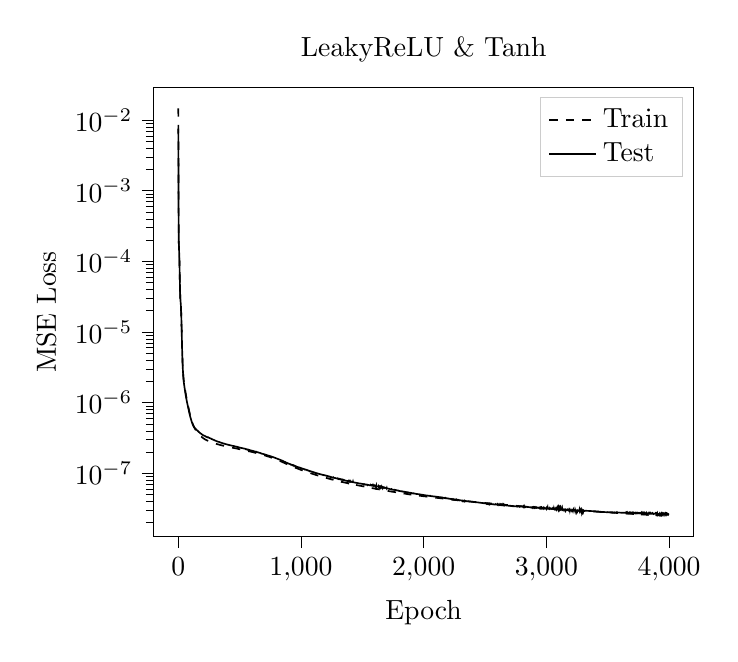
\begin{tikzpicture}

\begin{axis}[
legend cell align={left},
legend style={fill opacity=0.8, draw opacity=1, text opacity=1, draw=white!80!black},
log basis y={10},
tick align=outside,
tick pos=left,
title={LeakyReLU \& Tanh},
x grid style={white!69.0196078431373!black},
xlabel={Epoch},
xmin=-199.95, xmax=4198.95,
xtick style={color=black},
y grid style={white!69.0196078431373!black},
ylabel={MSE Loss},
ymin=1.28652495617467e-08, ymax=0.0285961148315028,
ymode=log,
ytick style={color=black}
]
\addplot [semithick, black, dashed]
table {%
0 0.0147167558874935
1 0.00422479508724064
2 0.00112020292889792
3 0.000344114673440345
4 0.000189754938444821
5 0.000162172813150391
6 0.000146551339385042
7 0.000132341942742642
8 0.000118350356904557
9 0.00010372507233842
10 8.84449195109482e-05
11 7.34534830880875e-05
12 5.99366830574581e-05
13 4.8876996830586e-05
14 4.02497898339789e-05
15 3.408423944893e-05
16 3.01901521470427e-05
17 2.75590198834834e-05
18 2.57170170534664e-05
19 2.43346590959845e-05
20 2.31839580419546e-05
21 2.20652209809487e-05
22 2.07908106704053e-05
23 1.91772862208381e-05
24 1.71094358802293e-05
25 1.49983391247588e-05
26 1.31309963476269e-05
27 1.13659696239665e-05
28 9.74745142775646e-06
29 8.29938522565499e-06
30 7.01414158424996e-06
31 5.95497243716636e-06
32 5.12775509014318e-06
33 4.50885365955855e-06
34 4.02224513118199e-06
35 3.62997250073249e-06
36 3.31752185707046e-06
37 3.0607893052661e-06
38 2.84811762077197e-06
39 2.66868735548087e-06
40 2.51258636171769e-06
41 2.37783719450135e-06
42 2.26240022942648e-06
43 2.16456914614582e-06
44 2.07942771555736e-06
45 2.00241391996769e-06
46 1.93450369954462e-06
47 1.87640388048749e-06
48 1.82416590115508e-06
49 1.77600803158384e-06
50 1.73084908823284e-06
51 1.68828430776102e-06
52 1.64711846895216e-06
53 1.60711305881023e-06
54 1.56834334916311e-06
55 1.53095426259142e-06
56 1.4944722552741e-06
57 1.45879897166878e-06
58 1.42385944167245e-06
59 1.39039401247487e-06
60 1.35824032113874e-06
61 1.3272358849008e-06
62 1.29738894395359e-06
63 1.26867270731168e-06
64 1.2408406620068e-06
65 1.21372717188706e-06
66 1.18741923660082e-06
67 1.16212920454473e-06
68 1.13786890946699e-06
69 1.11432013935087e-06
70 1.09158620887229e-06
71 1.06938895785902e-06
72 1.04795721296114e-06
73 1.02727086746768e-06
74 1.00695854618493e-06
75 9.87439097769993e-07
76 9.68428983043168e-07
77 9.49783932213677e-07
78 9.31873636972114e-07
79 9.14310121714834e-07
80 8.97240733763738e-07
81 8.80552728773409e-07
82 8.64220567052598e-07
83 8.48365317949629e-07
84 8.32332373562394e-07
85 8.16822827857777e-07
86 8.0182209802615e-07
87 7.87099218854337e-07
88 7.73020349626563e-07
89 7.59346863119958e-07
90 7.46014648541404e-07
91 7.33129284895995e-07
92 7.204337242257e-07
93 7.08012346052556e-07
94 6.96058514307651e-07
95 6.84493596338598e-07
96 6.73162203455035e-07
97 6.62246110536557e-07
98 6.5174218859454e-07
99 6.41607516300269e-07
100 6.31769812130756e-07
101 6.22032788143656e-07
102 6.12656925781607e-07
103 6.03730122904267e-07
104 5.94999974538268e-07
105 5.8669275210832e-07
106 5.78534859172919e-07
107 5.70552572213501e-07
108 5.63058854268661e-07
109 5.55469660710628e-07
110 5.48137382722302e-07
111 5.41116412918541e-07
112 5.3417853050064e-07
113 5.27970349523343e-07
114 5.21515760581792e-07
115 5.15363882911402e-07
116 5.09437782596933e-07
117 5.03975951573921e-07
118 4.98499296284649e-07
119 4.93213471543186e-07
120 4.8814046611767e-07
121 4.8300630331255e-07
122 4.78204040121e-07
123 4.7348461674801e-07
124 4.69040818671829e-07
125 4.64815730182977e-07
126 4.60680423827853e-07
127 4.56664749350466e-07
128 4.52802479642855e-07
129 4.49041826627195e-07
130 4.45417362371359e-07
131 4.41978267559762e-07
132 4.38649616214093e-07
133 4.35691757402878e-07
134 4.32299891954813e-07
135 4.29154072037363e-07
136 4.26289210665232e-07
137 4.23350594715544e-07
138 4.20500121535383e-07
139 4.17760403067291e-07
140 4.15125682664552e-07
141 4.12507545789254e-07
142 4.09924902129433e-07
143 4.07458474228406e-07
144 4.05005501463052e-07
145 4.02829853044295e-07
146 4.00427114783497e-07
147 3.98116157185768e-07
148 3.95838813048499e-07
149 3.93631469862044e-07
150 3.91564613238415e-07
151 3.89438078713056e-07
152 3.87381369833406e-07
153 3.85316970422878e-07
154 3.83270407184e-07
155 3.81302476540668e-07
156 3.793187683101e-07
157 3.77405879177672e-07
158 3.75516873560855e-07
159 3.73698540656164e-07
160 3.71824801149501e-07
161 3.70049074177814e-07
162 3.68281156312378e-07
163 3.66514122305262e-07
164 3.64796943898682e-07
165 3.63115861091501e-07
166 3.61438459890451e-07
167 3.59749451376956e-07
168 3.58325647482616e-07
169 3.56678011939948e-07
170 3.5512504922508e-07
171 3.53541436822979e-07
172 3.5198584095042e-07
173 3.50565922175861e-07
174 3.4904586625828e-07
175 3.47580223476029e-07
176 3.46117879487906e-07
177 3.44735465503732e-07
178 3.43156550471235e-07
179 3.41745828350781e-07
180 3.40402201274514e-07
181 3.39082861543716e-07
182 3.37749753995809e-07
183 3.36447743379153e-07
184 3.35189692151516e-07
185 3.33924634418281e-07
186 3.32675331719656e-07
187 3.31490725614003e-07
188 3.30254747154868e-07
189 3.29072307650335e-07
190 3.27903524151907e-07
191 3.26712969567211e-07
192 3.25650873890027e-07
193 3.24679369384739e-07
194 3.23479359352064e-07
195 3.2239850011706e-07
196 3.21350436138346e-07
197 3.20089375506427e-07
198 3.1928418043492e-07
199 3.18225012705398e-07
200 3.1708875033587e-07
201 3.1604049372902e-07
202 3.15025177954453e-07
203 3.14147056030833e-07
204 3.13153630514762e-07
205 3.12303416265536e-07
206 3.11512459560959e-07
207 3.10559388111642e-07
208 3.09709830034421e-07
209 3.08837195518663e-07
210 3.07967781694174e-07
211 3.07173345774459e-07
212 3.06387977303757e-07
213 3.05704276541974e-07
214 3.05012073624766e-07
215 3.04326920442577e-07
216 3.03581191317903e-07
217 3.02872078663086e-07
218 3.02160171514743e-07
219 3.01468360746071e-07
220 3.00779714422106e-07
221 3.00112319266077e-07
222 2.99428165192239e-07
223 2.98766919243576e-07
224 2.98114499798885e-07
225 2.97493264056925e-07
226 2.96865053755369e-07
227 2.96225017891061e-07
228 2.95607063435455e-07
229 2.95054074300083e-07
230 2.94362133615778e-07
231 2.93911949299286e-07
232 2.93350296459494e-07
233 2.9277203962863e-07
234 2.92193898189907e-07
235 2.91625393501249e-07
236 2.91056575775883e-07
237 2.90521314568082e-07
238 2.90002532025824e-07
239 2.89426571697504e-07
240 2.88832796556449e-07
241 2.88437092450522e-07
242 2.87901257479462e-07
243 2.87465177933655e-07
244 2.87022334077847e-07
245 2.86463340103182e-07
246 2.85977110152658e-07
247 2.8552008862448e-07
248 2.85149730146372e-07
249 2.84542418057754e-07
250 2.84174783189428e-07
251 2.83587820405273e-07
252 2.83157723046656e-07
253 2.82677717677871e-07
254 2.82309202674469e-07
255 2.81800196432869e-07
256 2.81433859342428e-07
257 2.80759454781787e-07
258 2.80310815455209e-07
259 2.79839582006502e-07
260 2.79485608601249e-07
261 2.79077382387527e-07
262 2.78622113157212e-07
263 2.78261508313449e-07
264 2.77801248003584e-07
265 2.77371159285167e-07
266 2.76926037386715e-07
267 2.76508251900509e-07
268 2.76159550395505e-07
269 2.75750310947842e-07
270 2.75349369303513e-07
271 2.74866106749982e-07
272 2.74483092084665e-07
273 2.74160867661521e-07
274 2.73795952736577e-07
275 2.73241857961182e-07
276 2.7300955764531e-07
277 2.72534656367895e-07
278 2.72264938502076e-07
279 2.71789457073623e-07
280 2.71330698502936e-07
281 2.70990266756144e-07
282 2.70652392366344e-07
283 2.70274082652122e-07
284 2.69901670087336e-07
285 2.69612391448959e-07
286 2.69216630456981e-07
287 2.68845532097828e-07
288 2.68462628127963e-07
289 2.67953266458676e-07
290 2.67746158179705e-07
291 2.6725683522244e-07
292 2.67001111112108e-07
293 2.66669375847073e-07
294 2.66288802976078e-07
295 2.65969301871394e-07
296 2.65624269857767e-07
297 2.65292488400348e-07
298 2.64968770387952e-07
299 2.64616587664079e-07
300 2.6426598824969e-07
301 2.63968214191834e-07
302 2.63564278093043e-07
303 2.63306389847173e-07
304 2.62909053311944e-07
305 2.6265966658201e-07
306 2.62325956335019e-07
307 2.61988682161984e-07
308 2.61644881341283e-07
309 2.61331634668238e-07
310 2.61042073404383e-07
311 2.60699721444269e-07
312 2.60473399372074e-07
313 2.6017135583345e-07
314 2.59872192494015e-07
315 2.59544071838036e-07
316 2.5921870788892e-07
317 2.5883532907045e-07
318 2.58592301811689e-07
319 2.58254245203204e-07
320 2.57866218625225e-07
321 2.57705161921251e-07
322 2.57353993994514e-07
323 2.57066349661272e-07
324 2.56766999356728e-07
325 2.56460113178036e-07
326 2.56180869946832e-07
327 2.55883794956446e-07
328 2.55620990067484e-07
329 2.55354575458e-07
330 2.55116259729959e-07
331 2.54826920873086e-07
332 2.54552288033949e-07
333 2.54259037966165e-07
334 2.54020088988227e-07
335 2.53747943659732e-07
336 2.53466220335952e-07
337 2.53183346508479e-07
338 2.52860813844791e-07
339 2.52621923969798e-07
340 2.52297060505668e-07
341 2.52019333721876e-07
342 2.51765039429586e-07
343 2.51513713543261e-07
344 2.51235551282036e-07
345 2.50976188937102e-07
346 2.50725112728389e-07
347 2.50445414451406e-07
348 2.50204155356926e-07
349 2.50034150340639e-07
350 2.49739470532973e-07
351 2.49512612462866e-07
352 2.49276659417319e-07
353 2.49011757865958e-07
354 2.48737631004303e-07
355 2.48451116668491e-07
356 2.4825697176567e-07
357 2.47993869585628e-07
358 2.47786029625274e-07
359 2.47529378611944e-07
360 2.47314632318307e-07
361 2.47056039775373e-07
362 2.46790130873364e-07
363 2.46567997486125e-07
364 2.46323033962881e-07
365 2.46107978050247e-07
366 2.45835234508718e-07
367 2.45645431427022e-07
368 2.45389607322011e-07
369 2.45254566003439e-07
370 2.44958750336366e-07
371 2.44772736145649e-07
372 2.44524404863e-07
373 2.44266119949543e-07
374 2.44089073135001e-07
375 2.43777454073779e-07
376 2.43538274567356e-07
377 2.43289414470382e-07
378 2.43056023222721e-07
379 2.42854683087046e-07
380 2.42641632901552e-07
381 2.42429219355245e-07
382 2.42211716916074e-07
383 2.41979478595056e-07
384 2.41790681229759e-07
385 2.41554029116742e-07
386 2.41347478571186e-07
387 2.41138141426234e-07
388 2.40926381991358e-07
389 2.40712194212733e-07
390 2.40508433066111e-07
391 2.40213856443461e-07
392 2.4000315536199e-07
393 2.39796585482566e-07
394 2.3964756219641e-07
395 2.39413144029754e-07
396 2.39213759805068e-07
397 2.39108626168161e-07
398 2.38828656740964e-07
399 2.38633542345212e-07
400 2.3843064510487e-07
401 2.38233129458365e-07
402 2.37990722567361e-07
403 2.37813346082305e-07
404 2.37602338437171e-07
405 2.37422929181719e-07
406 2.37263455424852e-07
407 2.37050656913596e-07
408 2.36847532327999e-07
409 2.36642238036211e-07
410 2.364443584284e-07
411 2.36212683653037e-07
412 2.35975246070552e-07
413 2.35821508574929e-07
414 2.35624742032314e-07
415 2.35403222745845e-07
416 2.35169045708972e-07
417 2.34992661688693e-07
418 2.34793192817051e-07
419 2.34585262987252e-07
420 2.34415336599625e-07
421 2.34222672524709e-07
422 2.33997412728115e-07
423 2.33857629716283e-07
424 2.33674164270781e-07
425 2.33461944802116e-07
426 2.33231948534751e-07
427 2.33070363847787e-07
428 2.32853431704427e-07
429 2.3266770248398e-07
430 2.32476125070491e-07
431 2.32283850046144e-07
432 2.32086789537789e-07
433 2.31937585361663e-07
434 2.31743046676058e-07
435 2.31552100686372e-07
436 2.31361373934647e-07
437 2.31170123797142e-07
438 2.30984196811335e-07
439 2.30793798124296e-07
440 2.3057733974241e-07
441 2.30424656592731e-07
442 2.30198470433152e-07
443 2.30040015658517e-07
444 2.29852045443124e-07
445 2.29665212074792e-07
446 2.29487747475332e-07
447 2.29264898976567e-07
448 2.29088643955322e-07
449 2.289107464577e-07
450 2.2872222154291e-07
451 2.28534441717443e-07
452 2.28346455422468e-07
453 2.28135142606334e-07
454 2.27954515459317e-07
455 2.27769156673219e-07
456 2.27586670888513e-07
457 2.2740435630908e-07
458 2.27215854557983e-07
459 2.27032890073531e-07
460 2.26844838984164e-07
461 2.26653140472877e-07
462 2.26478486759163e-07
463 2.26292875062484e-07
464 2.26084874157095e-07
465 2.2590925732402e-07
466 2.2572789907116e-07
467 2.25542848156124e-07
468 2.25358282015975e-07
469 2.25182395894308e-07
470 2.24996762824503e-07
471 2.24819421212885e-07
472 2.24611957996501e-07
473 2.24466087004771e-07
474 2.24269675690891e-07
475 2.24083162514432e-07
476 2.23859973623064e-07
477 2.23670406448662e-07
478 2.23497105722004e-07
479 2.23308886667439e-07
480 2.23121406335736e-07
481 2.22916722904642e-07
482 2.22842280734881e-07
483 2.22473976393189e-07
484 2.22453026935909e-07
485 2.22074921133242e-07
486 2.21927564737712e-07
487 2.21887577218638e-07
488 2.21461834648551e-07
489 2.21329398421233e-07
490 2.21166270051754e-07
491 2.20986845278048e-07
492 2.20798476625816e-07
493 2.20619727471671e-07
494 2.20438873313356e-07
495 2.20253071745447e-07
496 2.20089636925991e-07
497 2.1990685036144e-07
498 2.19724008424294e-07
499 2.19543226172902e-07
500 2.19354352751111e-07
501 2.19168181587293e-07
502 2.18980888398335e-07
503 2.1882522270289e-07
504 2.18640398450987e-07
505 2.18440091764194e-07
506 2.18265065079493e-07
507 2.18089171504232e-07
508 2.17896692689123e-07
509 2.17720229265694e-07
510 2.17535416084047e-07
511 2.17356315772577e-07
512 2.17186338744568e-07
513 2.1699332680214e-07
514 2.16826531321601e-07
515 2.16647501382283e-07
516 2.16463818759394e-07
517 2.1628365471571e-07
518 2.16089452145241e-07
519 2.15913011842872e-07
520 2.15749887168215e-07
521 2.15557008026224e-07
522 2.15378701916791e-07
523 2.15191717984453e-07
524 2.1509282248644e-07
525 2.14915981821662e-07
526 2.14728546453102e-07
527 2.14509130266549e-07
528 2.14316656489189e-07
529 2.14193874057855e-07
530 2.14001319669421e-07
531 2.13823200759578e-07
532 2.13628148898692e-07
533 2.1346094583663e-07
534 2.13267892512192e-07
535 2.13071844967772e-07
536 2.12884007147807e-07
537 2.12691715617552e-07
538 2.12480586952779e-07
539 2.12326406561658e-07
540 2.12136915216377e-07
541 2.11943900133349e-07
542 2.11753016976957e-07
543 2.11540812792066e-07
544 2.11372566660373e-07
545 2.11170818772644e-07
546 2.10922583555373e-07
547 2.10709240889173e-07
548 2.10775911433814e-07
549 2.10267557449129e-07
550 2.10359211671118e-07
551 2.09904146167617e-07
552 2.09913477725365e-07
553 2.09501424123459e-07
554 2.09625159250493e-07
555 2.09126980131202e-07
556 2.09249012847579e-07
557 2.08998007352079e-07
558 2.08536155923866e-07
559 2.08690602818251e-07
560 2.08191836911453e-07
561 2.08264158281679e-07
562 2.07883312761226e-07
563 2.07921254833821e-07
564 2.07418759934797e-07
565 2.0743094999176e-07
566 2.07303002909498e-07
567 2.06845264763444e-07
568 2.06992054103239e-07
569 2.06472261595536e-07
570 2.0639721431337e-07
571 2.06441899145204e-07
572 2.05879496732564e-07
573 2.06051998794976e-07
574 2.05496511902936e-07
575 2.0551717245354e-07
576 2.0532205400059e-07
577 2.0513076895412e-07
578 2.04941408860293e-07
579 2.04753449700945e-07
580 2.0451803786159e-07
581 2.04499404034664e-07
582 2.0404194936674e-07
583 2.03942051690831e-07
584 2.03688036748417e-07
585 2.03549430437988e-07
586 2.03323575235004e-07
587 2.03119876616142e-07
588 2.0295757144595e-07
589 2.02731326126582e-07
590 2.0257369340726e-07
591 2.02368503160244e-07
592 2.02197047563857e-07
593 2.02013388950206e-07
594 2.01766462517128e-07
595 2.01604090058538e-07
596 2.01441364232835e-07
597 2.01236583805553e-07
598 2.01023921313492e-07
599 2.00841937321172e-07
600 2.00641080887465e-07
601 2.00459920911555e-07
602 2.00254661208987e-07
603 2.00086132714716e-07
604 1.99884809660489e-07
605 1.99703399935913e-07
606 1.99505433087666e-07
607 1.99328779494579e-07
608 1.9913990877285e-07
609 1.98964528692613e-07
610 1.98792843583817e-07
611 1.98516759930101e-07
612 1.98361773897204e-07
613 1.98246224172749e-07
614 1.97864427093464e-07
615 1.97706827684385e-07
616 1.97465364514926e-07
617 1.9733804701616e-07
618 1.96922791261045e-07
619 1.96741092551633e-07
620 1.96560413641578e-07
621 1.96323017625843e-07
622 1.96165970592688e-07
623 1.95932488843198e-07
624 1.95768028881105e-07
625 1.95567801796415e-07
626 1.95336412311065e-07
627 1.95179220433772e-07
628 1.94979452849964e-07
629 1.94775609621445e-07
630 1.94670293943489e-07
631 1.94429682771613e-07
632 1.9418770021673e-07
633 1.93788950262785e-07
634 1.93819842536413e-07
635 1.93378188832583e-07
636 1.93411281124156e-07
637 1.93151938809422e-07
638 1.92752860819212e-07
639 1.92741796858797e-07
640 1.92343431002939e-07
641 1.9216255318355e-07
642 1.91978727919206e-07
643 1.91782636456139e-07
644 1.91794384178934e-07
645 1.91546348553118e-07
646 1.9116149540821e-07
647 1.90949372573357e-07
648 1.90821341675473e-07
649 1.90595229426549e-07
650 1.90429980428064e-07
651 1.90218370811124e-07
652 1.90026906679464e-07
653 1.89813052621446e-07
654 1.89606661813002e-07
655 1.89530327546095e-07
656 1.89314011059594e-07
657 1.88951788842928e-07
658 1.88744615144287e-07
659 1.88540474972854e-07
660 1.88363825103011e-07
661 1.88142638720024e-07
662 1.87933737755941e-07
663 1.87730878387526e-07
664 1.8772520002841e-07
665 1.87284249527409e-07
666 1.87286926760066e-07
667 1.86856799061275e-07
668 1.86839971519248e-07
669 1.86423184821649e-07
670 1.8641698684263e-07
671 1.86223110155481e-07
672 1.85972596902673e-07
673 1.85746885527749e-07
674 1.85528371368093e-07
675 1.85161767781494e-07
676 1.85198464613734e-07
677 1.85011211520703e-07
678 1.84764612654931e-07
679 1.84580274805057e-07
680 1.84336935646456e-07
681 1.8414141057832e-07
682 1.83919891689754e-07
683 1.83703114032596e-07
684 1.83409840218474e-07
685 1.83234989201253e-07
686 1.83098119016734e-07
687 1.82743054963908e-07
688 1.82657332807423e-07
689 1.82302819958124e-07
690 1.82121882247088e-07
691 1.81915501649144e-07
692 1.81705160265722e-07
693 1.81491261621147e-07
694 1.81273101233614e-07
695 1.81056364169763e-07
696 1.80900828013364e-07
697 1.80674443875262e-07
698 1.804431686665e-07
699 1.80222724559087e-07
700 1.79991534189128e-07
701 1.7977483792464e-07
702 1.79552062789412e-07
703 1.79341676194156e-07
704 1.79116268490986e-07
705 1.78897217764984e-07
706 1.78672040583194e-07
707 1.7845544022066e-07
708 1.78274484682106e-07
709 1.78050520581508e-07
710 1.7783338613242e-07
711 1.77603523908942e-07
712 1.77379757964502e-07
713 1.77166644675708e-07
714 1.76958691859852e-07
715 1.76734787565636e-07
716 1.76584686002457e-07
717 1.76343372984888e-07
718 1.76128108975604e-07
719 1.75897885213772e-07
720 1.75672592654053e-07
721 1.75447660360817e-07
722 1.75226035857179e-07
723 1.75003551206032e-07
724 1.74804935745954e-07
725 1.74598562963979e-07
726 1.74375872227017e-07
727 1.74152322721e-07
728 1.7382954645484e-07
729 1.73619787652513e-07
730 1.73425334530464e-07
731 1.7321217111288e-07
732 1.73060100379985e-07
733 1.72832961482072e-07
734 1.72613131297794e-07
735 1.72413816329708e-07
736 1.72160513180586e-07
737 1.71926174509451e-07
738 1.71669755282267e-07
739 1.7144469420316e-07
740 1.71207248776284e-07
741 1.7098506228308e-07
742 1.70759329854775e-07
743 1.70538389163255e-07
744 1.70313998907545e-07
745 1.70091730630872e-07
746 1.69852064665577e-07
747 1.69626526059119e-07
748 1.69402781779127e-07
749 1.69132127716409e-07
750 1.68980241525674e-07
751 1.68661541664505e-07
752 1.68422387638145e-07
753 1.68154323553438e-07
754 1.67861468440833e-07
755 1.67617971307266e-07
756 1.67375250256896e-07
757 1.67143337051812e-07
758 1.66881991432888e-07
759 1.66675624022616e-07
760 1.66422565094138e-07
761 1.66193717767271e-07
762 1.65948354613477e-07
763 1.65717337154092e-07
764 1.65465913312346e-07
765 1.6523477719943e-07
766 1.64991181918595e-07
767 1.64759113445712e-07
768 1.64514003316185e-07
769 1.64293280029426e-07
770 1.64031092438677e-07
771 1.63807684394612e-07
772 1.63561527344314e-07
773 1.63338111143219e-07
774 1.63088297604475e-07
775 1.62864505320215e-07
776 1.62628236452633e-07
777 1.62385142949972e-07
778 1.62129393167731e-07
779 1.61899282687727e-07
780 1.61650713181416e-07
781 1.6141828078986e-07
782 1.6121273756653e-07
783 1.60986360342008e-07
784 1.60738231961943e-07
785 1.60479761085242e-07
786 1.60237907216754e-07
787 1.59983428901e-07
788 1.597366711934e-07
789 1.59454377076429e-07
790 1.59208735553307e-07
791 1.58949413588516e-07
792 1.58692530362714e-07
793 1.58436309121157e-07
794 1.5816905449384e-07
795 1.57882679339139e-07
796 1.57585047602993e-07
797 1.57311406383087e-07
798 1.57027265480281e-07
799 1.56765319111685e-07
800 1.56496265454109e-07
801 1.56238000172948e-07
802 1.55985959587213e-07
803 1.55719861979264e-07
804 1.55464578689646e-07
805 1.5521024232612e-07
806 1.54948408244593e-07
807 1.54719261928449e-07
808 1.54447245577671e-07
809 1.54192335998005e-07
810 1.53954697410086e-07
811 1.53698665755542e-07
812 1.53444322862129e-07
813 1.53189335598825e-07
814 1.5296307420698e-07
815 1.52703641226992e-07
816 1.52447027396363e-07
817 1.52212526352002e-07
818 1.51996518304998e-07
819 1.51729954083635e-07
820 1.51471893957478e-07
821 1.51220606632307e-07
822 1.50959670229156e-07
823 1.50708962692647e-07
824 1.504469360043e-07
825 1.50185154481619e-07
826 1.49956196111134e-07
827 1.49683904787423e-07
828 1.49426933035102e-07
829 1.49200826534468e-07
830 1.4894755504713e-07
831 1.48687534576197e-07
832 1.48438944798102e-07
833 1.48174899528897e-07
834 1.47928022713018e-07
835 1.47746720237762e-07
836 1.47469594566019e-07
837 1.47227389931004e-07
838 1.46937056101137e-07
839 1.4663462562936e-07
840 1.46411530401735e-07
841 1.46151256004146e-07
842 1.4589036143775e-07
843 1.45624674729561e-07
844 1.45365836537792e-07
845 1.45095396746342e-07
846 1.44834831793617e-07
847 1.44576164316845e-07
848 1.44314648515831e-07
849 1.44067540055914e-07
850 1.43770926534614e-07
851 1.43536822335477e-07
852 1.43280838123871e-07
853 1.43015342686681e-07
854 1.42736688658829e-07
855 1.42426279346353e-07
856 1.42210422652056e-07
857 1.41971944948693e-07
858 1.41683119693425e-07
859 1.41424822899694e-07
860 1.41189233872296e-07
861 1.40932418538853e-07
862 1.40685958179176e-07
863 1.40444483903934e-07
864 1.40194336815114e-07
865 1.39915691292458e-07
866 1.39712072993348e-07
867 1.39439254496665e-07
868 1.39181732279781e-07
869 1.38928897641222e-07
870 1.38659657174855e-07
871 1.38382007278892e-07
872 1.38154317113504e-07
873 1.37896821655659e-07
874 1.37652846909475e-07
875 1.37387850330128e-07
876 1.37122912185816e-07
877 1.36958976639789e-07
878 1.36698286723913e-07
879 1.36436031425546e-07
880 1.36173517390148e-07
881 1.35937297422117e-07
882 1.3568027885924e-07
883 1.35419160045558e-07
884 1.35210795320972e-07
885 1.34940211779622e-07
886 1.34729177602821e-07
887 1.34477849549342e-07
888 1.34246570013374e-07
889 1.34014088537526e-07
890 1.33775667116254e-07
891 1.33507818894429e-07
892 1.33355113838718e-07
893 1.33092440819382e-07
894 1.32816020190774e-07
895 1.32586035178406e-07
896 1.3236788663562e-07
897 1.32103730607014e-07
898 1.31877103889622e-07
899 1.31655306965683e-07
900 1.31399273300303e-07
901 1.31187993872572e-07
902 1.30964021600732e-07
903 1.30730834960957e-07
904 1.30479387856042e-07
905 1.30251059097475e-07
906 1.30019203204768e-07
907 1.29781760385583e-07
908 1.29546398291325e-07
909 1.29307371985021e-07
910 1.29084291366155e-07
911 1.28849908819006e-07
912 1.28628538817566e-07
913 1.28427776004969e-07
914 1.28189834683212e-07
915 1.27991950641615e-07
916 1.27691470989788e-07
917 1.27501933441465e-07
918 1.27336225041574e-07
919 1.27021330165178e-07
920 1.26880013286978e-07
921 1.26700365694177e-07
922 1.26405575343824e-07
923 1.26257105605987e-07
924 1.25972710918631e-07
925 1.25786522051641e-07
926 1.2556942496289e-07
927 1.25317999483343e-07
928 1.25138892112631e-07
929 1.24960381679529e-07
930 1.24746011664456e-07
931 1.24503905503559e-07
932 1.2430114939832e-07
933 1.24119226839525e-07
934 1.23892343637522e-07
935 1.2366138645703e-07
936 1.23528668677153e-07
937 1.23287912206393e-07
938 1.23100251894215e-07
939 1.22913126332946e-07
940 1.22722796422892e-07
941 1.22485553870177e-07
942 1.22238755402293e-07
943 1.22106174902825e-07
944 1.21919439553864e-07
945 1.2174004823251e-07
946 1.21530621246535e-07
947 1.21336180352927e-07
948 1.21133792138295e-07
949 1.20939680659404e-07
950 1.20720247075212e-07
951 1.20546334574811e-07
952 1.20322355666502e-07
953 1.20217128969813e-07
954 1.20011707402057e-07
955 1.19810914469554e-07
956 1.19595556309804e-07
957 1.19444322447038e-07
958 1.19227567786595e-07
959 1.19024687801783e-07
960 1.18887678429047e-07
961 1.18671289598637e-07
962 1.18430393072799e-07
963 1.18325145788134e-07
964 1.1812696747171e-07
965 1.17946854743423e-07
966 1.1776211837855e-07
967 1.17576934218988e-07
968 1.1740373333069e-07
969 1.17222978090581e-07
970 1.17059085983584e-07
971 1.1685083301316e-07
972 1.16617252317042e-07
973 1.1650785584294e-07
974 1.16313816214131e-07
975 1.16113465260526e-07
976 1.15937665032817e-07
977 1.15776352544117e-07
978 1.15601611309302e-07
979 1.15419883183421e-07
980 1.15197841473957e-07
981 1.15045113130208e-07
982 1.14801086215977e-07
983 1.14742911872412e-07
984 1.14547467020998e-07
985 1.14369988924778e-07
986 1.14132197644778e-07
987 1.13966712721236e-07
988 1.13832317019558e-07
989 1.13675502177557e-07
990 1.13499152249119e-07
991 1.13304771677036e-07
992 1.13130158183594e-07
993 1.12883420236187e-07
994 1.12796536104298e-07
995 1.12606875294574e-07
996 1.12428153837385e-07
997 1.12270813591664e-07
998 1.12106477963891e-07
999 1.11935982751277e-07
1000 1.11775184894469e-07
1001 1.11619902799731e-07
1002 1.11424209215727e-07
1003 1.11334109909933e-07
1004 1.11145634338783e-07
1005 1.10971861754905e-07
1006 1.10804318556035e-07
1007 1.10636118147767e-07
1008 1.10479483833359e-07
1009 1.1032438599301e-07
1010 1.10178989352505e-07
1011 1.10012197090725e-07
1012 1.09794785910111e-07
1013 1.09715186578541e-07
1014 1.09533097781167e-07
1015 1.09345536664307e-07
1016 1.09196999392935e-07
1017 1.09046659243717e-07
1018 1.08901574389364e-07
1019 1.08724679364514e-07
1020 1.08579653087304e-07
1021 1.08414589124806e-07
1022 1.08282940885829e-07
1023 1.08152952304152e-07
1024 1.07973693847185e-07
1025 1.07817007773292e-07
1026 1.07631510633865e-07
1027 1.07514907135453e-07
1028 1.07364885227668e-07
1029 1.07203319526405e-07
1030 1.07045956976748e-07
1031 1.0689825924004e-07
1032 1.06637067755599e-07
1033 1.06620171120397e-07
1034 1.06468587901531e-07
1035 1.06327487575442e-07
1036 1.06176609381947e-07
1037 1.06048515608137e-07
1038 1.05891789491608e-07
1039 1.05753535311948e-07
1040 1.05604855779262e-07
1041 1.05488431497491e-07
1042 1.05340681177069e-07
1043 1.052005269635e-07
1044 1.04994613213449e-07
1045 1.04841989045923e-07
1046 1.04693688069091e-07
1047 1.04549295802059e-07
1048 1.04342896321441e-07
1049 1.04315552942325e-07
1050 1.04177075115786e-07
1051 1.03936537382054e-07
1052 1.03874550795524e-07
1053 1.03738832159195e-07
1054 1.03571307306538e-07
1055 1.03438900612929e-07
1056 1.03357138787175e-07
1057 1.0315987907461e-07
1058 1.03049108556519e-07
1059 1.02890002320777e-07
1060 1.02720108355214e-07
1061 1.02683071787624e-07
1062 1.02532210775053e-07
1063 1.02359288025156e-07
1064 1.0222688218775e-07
1065 1.02098929829708e-07
1066 1.01953066529603e-07
1067 1.01850517182811e-07
1068 1.01712086522099e-07
1069 1.01576102981227e-07
1070 1.01428539995396e-07
1071 1.01202304705339e-07
1072 1.01209320458651e-07
1073 1.01055069666955e-07
1074 1.00916019395214e-07
1075 1.0076222892863e-07
1076 1.00631043213895e-07
1077 1.00532826014188e-07
1078 1.00360497253149e-07
1079 1.00234356416706e-07
1080 1.00106765209773e-07
1081 9.99802213961232e-08
1082 9.98532394511642e-08
1083 9.97311517991761e-08
1084 9.95188706660599e-08
1085 9.95432671686558e-08
1086 9.93666342736788e-08
1087 9.92305960316742e-08
1088 9.90880039459796e-08
1089 9.89632881847058e-08
1090 9.8835123729657e-08
1091 9.87113516828231e-08
1092 9.85671639952557e-08
1093 9.84456003862988e-08
1094 9.83183581340086e-08
1095 9.81939523541087e-08
1096 9.8001847607776e-08
1097 9.79699430878611e-08
1098 9.78207422619448e-08
1099 9.76892382453798e-08
1100 9.75573714434574e-08
1101 9.7436195570566e-08
1102 9.73081750537119e-08
1103 9.71845393742399e-08
1104 9.69889700250803e-08
1105 9.68960275820052e-08
1106 9.68605309026316e-08
1107 9.67106285933994e-08
1108 9.65754299606658e-08
1109 9.64576967490416e-08
1110 9.63283372144019e-08
1111 9.6153483880812e-08
1112 9.60811021215591e-08
1113 9.59328996756881e-08
1114 9.58100525139116e-08
1115 9.57365740994476e-08
1116 9.55992669737782e-08
1117 9.5426011849753e-08
1118 9.53521050739425e-08
1119 9.51087149552166e-08
1120 9.51546127048175e-08
1121 9.49852496034964e-08
1122 9.48076223714622e-08
1123 9.47484521525155e-08
1124 9.4635791192843e-08
1125 9.43977622576142e-08
1126 9.43311578716077e-08
1127 9.41965007790202e-08
1128 9.42251313240661e-08
1129 9.40887221183573e-08
1130 9.39137298736625e-08
1131 9.38030485144736e-08
1132 9.36790117940234e-08
1133 9.36066499725996e-08
1134 9.34274177382122e-08
1135 9.33086589611776e-08
1136 9.32034401373016e-08
1137 9.29838304166708e-08
1138 9.29965697018531e-08
1139 9.27530144387845e-08
1140 9.28000088435965e-08
1141 9.26899408071336e-08
1142 9.24673126974085e-08
1143 9.23295716219741e-08
1144 9.24684631193884e-08
1145 9.22265955978219e-08
1146 9.20729742901472e-08
1147 9.19632463620701e-08
1148 9.18536782208435e-08
1149 9.17687318739979e-08
1150 9.16661311975986e-08
1151 9.15448064411351e-08
1152 9.14362613144704e-08
1153 9.13262002804061e-08
1154 9.10897944166322e-08
1155 9.12180108763039e-08
1156 9.09886377620239e-08
1157 9.09010083987027e-08
1158 9.08980600549114e-08
1159 9.06698444715914e-08
1160 9.06123341906095e-08
1161 9.04766778759836e-08
1162 9.03810152692586e-08
1163 9.03772236320322e-08
1164 9.01413191947142e-08
1165 9.00481007235499e-08
1166 8.99135863505762e-08
1167 9.00328111086424e-08
1168 8.97141874460772e-08
1169 8.97355893414442e-08
1170 8.95368867581681e-08
1171 8.95405423015916e-08
1172 8.94344267656777e-08
1173 8.92226522068995e-08
1174 8.92123865625649e-08
1175 8.90316612718323e-08
1176 8.90420845998108e-08
1177 8.88799057747747e-08
1178 8.88133439786998e-08
1179 8.85857197481244e-08
1180 8.87505559710178e-08
1181 8.84196974411111e-08
1182 8.82689840580042e-08
1183 8.83171059022914e-08
1184 8.83854004989359e-08
1185 8.80816308992394e-08
1186 8.80047668623263e-08
1187 8.77441357012287e-08
1188 8.79640751030308e-08
1189 8.77180462559579e-08
1190 8.7599863196175e-08
1191 8.74963723482836e-08
1192 8.73838534296567e-08
1193 8.72792024786406e-08
1194 8.71605033587741e-08
1195 8.70777559889291e-08
1196 8.69709926440976e-08
1197 8.67257896253193e-08
1198 8.67221731297718e-08
1199 8.67449776755791e-08
1200 8.66083934916162e-08
1201 8.65008198509543e-08
1202 8.63824901209398e-08
1203 8.62881886440903e-08
1204 8.6182928530576e-08
1205 8.60825287638534e-08
1206 8.60784291596417e-08
1207 8.58791283953053e-08
1208 8.57924304398239e-08
1209 8.55378336481749e-08
1210 8.55663802319384e-08
1211 8.56935107158563e-08
1212 8.54270831069925e-08
1213 8.54136989190124e-08
1214 8.51504979451079e-08
1215 8.52249365088653e-08
1216 8.50929214841756e-08
1217 8.49829644558042e-08
1218 8.48894925695731e-08
1219 8.49022571891567e-08
1220 8.45773056319388e-08
1221 8.45171920254018e-08
1222 8.4644523379751e-08
1223 8.44960545833828e-08
1224 8.43562040877544e-08
1225 8.43524073914637e-08
1226 8.42076120370905e-08
1227 8.40824029246789e-08
1228 8.40686841705462e-08
1229 8.38027294243204e-08
1230 8.38756206036351e-08
1231 8.37313208670309e-08
1232 8.37996433737942e-08
1233 8.35421889995303e-08
1234 8.35297179229144e-08
1235 8.33217964739674e-08
1236 8.32042975495995e-08
1237 8.32144987121808e-08
1238 8.31275680042154e-08
1239 8.30780388518804e-08
1240 8.28455743508982e-08
1241 8.26311044406225e-08
1242 8.28110817465699e-08
1243 8.25285896368655e-08
1244 8.26351364935363e-08
1245 8.26327644070091e-08
1246 8.25268334700979e-08
1247 8.2284106081687e-08
1248 8.21856459829462e-08
1249 8.22410062006895e-08
1250 8.18561030619947e-08
1251 8.18822995114488e-08
1252 8.20980892832779e-08
1253 8.17999369111533e-08
1254 8.18274437115463e-08
1255 8.14338774439705e-08
1256 8.14501619821328e-08
1257 8.13915892443617e-08
1258 8.16146207576196e-08
1259 8.13947702447138e-08
1260 8.14680680640834e-08
1261 8.12170073594132e-08
1262 8.12205323477144e-08
1263 8.09467807449948e-08
1264 8.09291576757687e-08
1265 8.08210186100666e-08
1266 8.08754014727242e-08
1267 8.05248546988935e-08
1268 8.06227642335955e-08
1269 8.07637859061572e-08
1270 8.0488412368851e-08
1271 8.0472480675553e-08
1272 8.0312093622581e-08
1273 8.01834619643671e-08
1274 8.01239210481697e-08
1275 7.99325583145105e-08
1276 7.98803357469069e-08
1277 8.00352309475727e-08
1278 7.98712157852322e-08
1279 7.97606326052858e-08
1280 7.96094512445222e-08
1281 7.95350578322029e-08
1282 7.93902460323181e-08
1283 7.94013396223647e-08
1284 7.94029619690662e-08
1285 7.92219978045239e-08
1286 7.92102306554909e-08
1287 7.90460648083524e-08
1288 7.90456339707646e-08
1289 7.88878918704938e-08
1290 7.86650440822712e-08
1291 7.87703592628475e-08
1292 7.87660891035102e-08
1293 7.86073303871149e-08
1294 7.85152663560496e-08
1295 7.83654700988734e-08
1296 7.810588538959e-08
1297 7.83936111794503e-08
1298 7.82783793091824e-08
1299 7.80195213252455e-08
1300 7.79630812388632e-08
1301 7.81040429238544e-08
1302 7.79871498544082e-08
1303 7.7885714201642e-08
1304 7.77099070177201e-08
1305 7.76176916801319e-08
1306 7.76773959572097e-08
1307 7.75960576966384e-08
1308 7.74857856207234e-08
1309 7.73203322204097e-08
1310 7.71579984686355e-08
1311 7.72818189709312e-08
1312 7.72138671720768e-08
1313 7.71078822197069e-08
1314 7.70102493490299e-08
1315 7.68608058550058e-08
1316 7.67011075879509e-08
1317 7.68048537977961e-08
1318 7.67450558001315e-08
1319 7.66509278946614e-08
1320 7.6562426812643e-08
1321 7.64752398900725e-08
1322 7.63389064957209e-08
1323 7.61783190910137e-08
1324 7.63143536666178e-08
1325 7.62435481966861e-08
1326 7.6109585496198e-08
1327 7.60519296214568e-08
1328 7.59750633818612e-08
1329 7.58785536554285e-08
1330 7.5771458988072e-08
1331 7.56189558046572e-08
1332 7.57408587439556e-08
1333 7.567879941206e-08
1334 7.5562105887883e-08
1335 7.55043106650533e-08
1336 7.53389284788852e-08
1337 7.52238568644259e-08
1338 7.5323299622454e-08
1339 7.52537492374472e-08
1340 7.51991587790712e-08
1341 7.51069958013773e-08
1342 7.50239110871576e-08
1343 7.49522658232138e-08
1344 7.48127398679799e-08
1345 7.46620432501288e-08
1346 7.48086655377733e-08
1347 7.4738872729796e-08
1348 7.46397968427459e-08
1349 7.4551285344171e-08
1350 7.44863173345323e-08
1351 7.44158996113242e-08
1352 7.42824491553051e-08
1353 7.41238045449677e-08
1354 7.41111035225117e-08
1355 7.40641070464676e-08
1356 7.40045176499393e-08
1357 7.39508383347243e-08
1358 7.39037687047528e-08
1359 7.38463827580915e-08
1360 7.37782016244637e-08
1361 7.37182463659281e-08
1362 7.36672474594968e-08
1363 7.35925647710189e-08
1364 7.3529023786989e-08
1365 7.34672471267572e-08
1366 7.33989200369933e-08
1367 7.33393467449162e-08
1368 7.32632496358576e-08
1369 7.32211657989978e-08
1370 7.31125196580251e-08
1371 7.31050112463549e-08
1372 7.29886364716492e-08
1373 7.29476300342924e-08
1374 7.28780813759045e-08
1375 7.27930700890056e-08
1376 7.27118430035034e-08
1377 7.26486597351084e-08
1378 7.26059206535012e-08
1379 7.25501752434354e-08
1380 7.24998741752358e-08
1381 7.27625557139788e-08
1382 7.25737763929146e-08
1383 7.2731951306082e-08
1384 7.25556730998278e-08
1385 7.24230852426899e-08
1386 7.23103557653815e-08
1387 7.22384621774097e-08
1388 7.19100039603404e-08
1389 7.20899284445409e-08
1390 7.1703876894702e-08
1391 7.20312818671687e-08
1392 7.17245782446696e-08
1393 7.15467789760282e-08
1394 7.19751574962402e-08
1395 7.17944129462467e-08
1396 7.14462673769844e-08
1397 7.13811031900491e-08
1398 7.13009372219631e-08
1399 7.12841869194847e-08
1400 7.13730504671162e-08
1401 7.12210317672657e-08
1402 7.15236239088313e-08
1403 7.14062929354498e-08
1404 7.12587243327789e-08
1405 7.11710081873207e-08
1406 7.10833947401568e-08
1407 7.10124912153276e-08
1408 7.09239766543135e-08
1409 7.09135147758389e-08
1410 7.05575748938259e-08
1411 7.05776387164292e-08
1412 7.0538693101696e-08
1413 7.04820574739529e-08
1414 7.03366398262517e-08
1415 7.03419983132392e-08
1416 7.02653603426029e-08
1417 7.02439167525881e-08
1418 7.01753560683471e-08
1419 7.0116381319707e-08
1420 7.00991330546685e-08
1421 7.00142620218003e-08
1422 6.99670490291737e-08
1423 6.98961916363316e-08
1424 7.02776046459519e-08
1425 6.97408604963812e-08
1426 6.96264619293174e-08
1427 6.96493507064133e-08
1428 6.96453624797755e-08
1429 6.9592399256635e-08
1430 6.94273235311016e-08
1431 6.94291015150839e-08
1432 6.9362168044762e-08
1433 6.92699000488517e-08
1434 6.92611739800952e-08
1435 6.91862529329512e-08
1436 6.91504793586262e-08
1437 6.9080841637259e-08
1438 6.90261722340324e-08
1439 6.89444437931286e-08
1440 6.89110837797102e-08
1441 6.8826579592951e-08
1442 6.88160369399782e-08
1443 6.87323318722122e-08
1444 6.86894033101737e-08
1445 6.86117650161577e-08
1446 6.8594669759392e-08
1447 6.84925371992051e-08
1448 6.84693926515934e-08
1449 6.8384730411708e-08
1450 6.83545271407127e-08
1451 6.82723717559952e-08
1452 6.82447976210199e-08
1453 6.81450138202422e-08
1454 6.8127716005506e-08
1455 6.80505443142465e-08
1456 6.80313249930009e-08
1457 6.7940998221161e-08
1458 6.79047805007826e-08
1459 6.78244381475679e-08
1460 6.78095768940068e-08
1461 6.77314916792682e-08
1462 6.76890676380992e-08
1463 6.76215440975625e-08
1464 6.75896843098656e-08
1465 6.75036987978217e-08
1466 6.74560715303585e-08
1467 6.7436916804553e-08
1468 6.73604038361475e-08
1469 6.73058214175626e-08
1470 6.72726544870272e-08
1471 6.72089431610345e-08
1472 6.71315502778214e-08
1473 6.71195438641803e-08
1474 6.70629360755015e-08
1475 6.70026612752395e-08
1476 6.69748772921253e-08
1477 6.6908599993809e-08
1478 6.68566325394693e-08
1479 6.67549428889913e-08
1480 6.67159215126389e-08
1481 6.66729288383294e-08
1482 6.663703261367e-08
1483 6.65598175011439e-08
1484 6.64971356414412e-08
1485 6.64941096424343e-08
1486 6.64398592036264e-08
1487 6.63679180057386e-08
1488 6.6328782452274e-08
1489 6.63028838729929e-08
1490 6.6236923263574e-08
1491 6.61852860446288e-08
1492 6.61495542679802e-08
1493 6.60819992361894e-08
1494 6.60174491429189e-08
1495 6.59773442883704e-08
1496 6.59575181956029e-08
1497 6.58913086226676e-08
1498 6.58353580966775e-08
1499 6.57926443388135e-08
1500 6.57452803594083e-08
1501 6.5702437559878e-08
1502 6.56488046928416e-08
1503 6.56010516912886e-08
1504 6.55696651605808e-08
1505 6.55111482039672e-08
1506 6.54606833165872e-08
1507 6.54224100671286e-08
1508 6.53803645995765e-08
1509 6.53305435491802e-08
1510 6.52746878628818e-08
1511 6.52153520945831e-08
1512 6.51813099921128e-08
1513 6.53856354091431e-08
1514 6.50593914528486e-08
1515 6.51037984304992e-08
1516 6.51759432557242e-08
1517 6.49920578261742e-08
1518 6.49404985750834e-08
1519 6.5043989284419e-08
1520 6.4841566167928e-08
1521 6.47767814214717e-08
1522 6.48945229890785e-08
1523 6.4825172557903e-08
1524 6.46072251555552e-08
1525 6.45427784959907e-08
1526 6.46624698248388e-08
1527 6.44587636635663e-08
1528 6.45501082878752e-08
1529 6.43644700488721e-08
1530 6.44650609942232e-08
1531 6.42675639461743e-08
1532 6.43632165022723e-08
1533 6.4303086755757e-08
1534 6.42374240662491e-08
1535 6.4214915489913e-08
1536 6.40093104316008e-08
1537 6.39621405547075e-08
1538 6.40849180051362e-08
1539 6.40343787807751e-08
1540 6.39655553626994e-08
1541 6.36423332274205e-08
1542 6.38858331036829e-08
1543 6.38246786053287e-08
1544 6.36738123667158e-08
1545 6.37015295339438e-08
1546 6.36468447829941e-08
1547 6.36017150981161e-08
1548 6.3555721869335e-08
1549 6.34909114296534e-08
1550 6.3468206025874e-08
1551 6.34105458203749e-08
1552 6.33667151426209e-08
1553 6.33471200224278e-08
1554 6.3241843871964e-08
1555 6.32087017713445e-08
1556 6.31080610098422e-08
1557 6.30417484259738e-08
1558 6.29980706072786e-08
1559 6.30109768593456e-08
1560 6.28835229861124e-08
1561 6.29175800135329e-08
1562 6.27752342339249e-08
1563 6.281562650301e-08
1564 6.27679042572993e-08
1565 6.27019331815859e-08
1566 6.26575814379748e-08
1567 6.25151835365045e-08
1568 6.26360400133308e-08
1569 6.2400691930975e-08
1570 6.22344568483868e-08
1571 6.21756278071928e-08
1572 6.21100433235711e-08
1573 6.21703037175791e-08
1574 6.20633618950706e-08
1575 6.19985493059971e-08
1576 6.1983541289834e-08
1577 6.1918115608961e-08
1578 6.19253030507139e-08
1579 6.18185661629411e-08
1580 6.17584587239151e-08
1581 6.17133952438564e-08
1582 6.17418941608605e-08
1583 6.16407595117607e-08
1584 6.15594736643743e-08
1585 6.15012524356473e-08
1586 6.15447750682563e-08
1587 6.14552095612453e-08
1588 6.1363222187083e-08
1589 6.14037893029717e-08
1590 6.12631218075421e-08
1591 6.12490335036853e-08
1592 6.12417917551511e-08
1593 6.11905342431385e-08
1594 6.11418923313067e-08
1595 6.1037565600941e-08
1596 6.09556018176249e-08
1597 6.10325194649874e-08
1598 6.08750575032957e-08
1599 6.08357205749144e-08
1600 6.08688746233099e-08
1601 6.07466641255883e-08
1602 6.06723547704746e-08
1603 6.07726332262359e-08
1604 6.06738005330953e-08
1605 6.05934438446809e-08
1606 6.06144826882371e-08
1607 6.05440183676365e-08
1608 6.04497323699604e-08
1609 6.04675414521694e-08
1610 6.02803623337422e-08
1611 6.03843261899328e-08
1612 6.02965559934887e-08
1613 6.0143622878428e-08
1614 6.02482721276942e-08
1615 6.01591571687266e-08
1616 6.008203316199e-08
1617 5.99935132221674e-08
1618 5.99461463153261e-08
1619 6.00165979527389e-08
1620 5.98704748533407e-08
1621 5.98210738829152e-08
1622 5.98710601131813e-08
1623 5.97468268104251e-08
1624 5.97048592858584e-08
1625 5.9685754564498e-08
1626 5.96977233975338e-08
1627 5.95884093712584e-08
1628 5.95427653919955e-08
1629 5.94810016316671e-08
1630 5.9430430916052e-08
1631 5.9392382457446e-08
1632 5.93505079180545e-08
1633 5.9410502487367e-08
1634 5.92825284719822e-08
1635 5.92548935891557e-08
1636 5.92515431705465e-08
1637 5.922026535643e-08
1638 5.91932503724024e-08
1639 5.90419864003877e-08
1640 5.90510197504557e-08
1641 5.90388863912494e-08
1642 5.90202253185623e-08
1643 5.89859183790509e-08
1644 5.89417900762612e-08
1645 5.88877805292043e-08
1646 5.8822728238539e-08
1647 5.8790085113003e-08
1648 5.86959381898566e-08
1649 5.8751901132581e-08
1650 5.86467134233715e-08
1651 5.86238532598316e-08
1652 5.8605185703442e-08
1653 5.85756530426806e-08
1654 5.84348275651791e-08
1655 5.84519813813245e-08
1656 5.83364313371249e-08
1657 5.83883611362523e-08
1658 5.83861382814632e-08
1659 5.83119972361601e-08
1660 5.83014084547528e-08
1661 5.8220777066964e-08
1662 5.82409472578149e-08
1663 5.81809702495661e-08
1664 5.81115072542104e-08
1665 5.80522394351135e-08
1666 5.79638435063146e-08
1667 5.80018990987696e-08
1668 5.78981562213698e-08
1669 5.79385942280908e-08
1670 5.79042463755286e-08
1671 5.78068843779533e-08
1672 5.77410584305937e-08
1673 5.77692701604349e-08
1674 5.77551086990979e-08
1675 5.77069745872905e-08
1676 5.76514806631678e-08
1677 5.7574246103087e-08
1678 5.75370447641888e-08
1679 5.75259657757954e-08
1680 5.74997005244882e-08
1681 5.74412488596465e-08
1682 5.741091284861e-08
1683 5.73601505777788e-08
1684 5.73280955435962e-08
1685 5.72533537201991e-08
1686 5.72318427884966e-08
1687 5.71398251842936e-08
1688 5.71746364990133e-08
1689 5.7100537024013e-08
1690 5.70160502739725e-08
1691 5.7024178008902e-08
1692 5.69427184586857e-08
1693 5.6927594581424e-08
1694 5.6905779086236e-08
1695 5.68330997410271e-08
1696 5.68021955302811e-08
1697 5.68079989093917e-08
1698 5.67330343521633e-08
1699 5.67770382211563e-08
1700 5.6723742357434e-08
1701 5.66196222280269e-08
1702 5.65612012835004e-08
1703 5.65426693874826e-08
1704 5.64587540488049e-08
1705 5.64509684615189e-08
1706 5.64117367680694e-08
1707 5.6362058536763e-08
1708 5.632851846471e-08
1709 5.6289815265842e-08
1710 5.62430117945212e-08
1711 5.6202634020508e-08
1712 5.61646747172517e-08
1713 5.61009704007631e-08
1714 5.60931503628126e-08
1715 5.6061480762537e-08
1716 5.59717459438502e-08
1717 5.59462118658871e-08
1718 5.58937152064232e-08
1719 5.58645496369081e-08
1720 5.58193177653266e-08
1721 5.57871249817765e-08
1722 5.57390223896448e-08
1723 5.57095491231507e-08
1724 5.56627573935486e-08
1725 5.56319264433114e-08
1726 5.55855789130533e-08
1727 5.55558900110498e-08
1728 5.55122884051684e-08
1729 5.5483873421025e-08
1730 5.54376156145508e-08
1731 5.54072172853637e-08
1732 5.53694253966341e-08
1733 5.53336621784695e-08
1734 5.52957211574778e-08
1735 5.52905657400515e-08
1736 5.52437131275951e-08
1737 5.51973567439745e-08
1738 5.50990315026922e-08
1739 5.51901840815105e-08
1740 5.50492078303932e-08
1741 5.51997503883683e-08
1742 5.50764539006821e-08
1743 5.50026580015128e-08
1744 5.49532064866298e-08
1745 5.48936090858376e-08
1746 5.48557207409317e-08
1747 5.48292777899917e-08
1748 5.47877212930814e-08
1749 5.47745125878407e-08
1750 5.47207959122886e-08
1751 5.46802167278315e-08
1752 5.46712257154525e-08
1753 5.4652600333327e-08
1754 5.46024323320182e-08
1755 5.45712245099139e-08
1756 5.45184425213563e-08
1757 5.44785809708515e-08
1758 5.45178277100433e-08
1759 5.44239177280303e-08
1760 5.43673493957897e-08
1761 5.43012737175275e-08
1762 5.42908741039128e-08
1763 5.42970816042043e-08
1764 5.42038646607068e-08
1765 5.42023791858526e-08
1766 5.42010031274742e-08
1767 5.41545194714388e-08
1768 5.41175047210629e-08
1769 5.40841032652395e-08
1770 5.40812949481051e-08
1771 5.40217877329496e-08
1772 5.41533069089439e-08
1773 5.40081032980311e-08
1774 5.39773567282964e-08
1775 5.38565197771845e-08
1776 5.38418200370927e-08
1777 5.3816373728921e-08
1778 5.37218772258541e-08
1779 5.36693589303638e-08
1780 5.35990788392837e-08
1781 5.36491940046346e-08
1782 5.36094721326208e-08
1783 5.36873384930914e-08
1784 5.35966249692876e-08
1785 5.35427674357436e-08
1786 5.34920063337552e-08
1787 5.35000424122245e-08
1788 5.3396658238114e-08
1789 5.34192288306201e-08
1790 5.33317460096328e-08
1791 5.32388844725062e-08
1792 5.31721855061562e-08
1793 5.31773989287387e-08
1794 5.31955995732858e-08
1795 5.31722271617241e-08
1796 5.33073993125299e-08
1797 5.31914732775363e-08
1798 5.31012987678992e-08
1799 5.31296525103642e-08
1800 5.30505015028382e-08
1801 5.30342470312917e-08
1802 5.29387596941433e-08
1803 5.28939656838645e-08
1804 5.29263942503633e-08
1805 5.28412283742341e-08
1806 5.28533642629725e-08
1807 5.27574202173753e-08
1808 5.27861425929643e-08
1809 5.27422506202413e-08
1810 5.27100274432257e-08
1811 5.26398057303368e-08
1812 5.26548065273857e-08
1813 5.26123811646073e-08
1814 5.25146751257921e-08
1815 5.25694258577403e-08
1816 5.25253612284615e-08
1817 5.24612085186504e-08
1818 5.24626691600361e-08
1819 5.23633416573688e-08
1820 5.22279350718691e-08
1821 5.22604002011207e-08
1822 5.23665367548887e-08
1823 5.23510500354263e-08
1824 5.22425009066296e-08
1825 5.22230511794675e-08
1826 5.21748539288325e-08
1827 5.21480015311937e-08
1828 5.21044418864136e-08
1829 5.20694766183993e-08
1830 5.2045766155473e-08
1831 5.20338689860012e-08
1832 5.20121177363109e-08
1833 5.19713700857238e-08
1834 5.19367362930012e-08
1835 5.1880487099254e-08
1836 5.18984083921481e-08
1837 5.18198555568006e-08
1838 5.17920012566009e-08
1839 5.17712083034638e-08
1840 5.17531382033809e-08
1841 5.15918113048741e-08
1842 5.16261049572364e-08
1843 5.16029053283518e-08
1844 5.16018174252508e-08
1845 5.17001600552902e-08
1846 5.16246376509599e-08
1847 5.15207366618142e-08
1848 5.14882840736419e-08
1849 5.14409691270146e-08
1850 5.14650860452548e-08
1851 5.1339365732872e-08
1852 5.14604675068142e-08
1853 5.13895670302134e-08
1854 5.12289573944003e-08
1855 5.1188157657478e-08
1856 5.11447395741271e-08
1857 5.11439732324703e-08
1858 5.11337817794555e-08
1859 5.13269989976806e-08
1860 5.1154405008802e-08
1861 5.10528533066434e-08
1862 5.09247317737049e-08
1863 5.09517100777401e-08
1864 5.11363543989063e-08
1865 5.10893281617797e-08
1866 5.08869196327311e-08
1867 5.0841876625185e-08
1868 5.08497112683415e-08
1869 5.07883065026249e-08
1870 5.06759310958671e-08
1871 5.07515110736989e-08
1872 5.08005627413155e-08
1873 5.08329420281228e-08
1874 5.07061787065055e-08
1875 5.06505804693802e-08
1876 5.05708001927729e-08
1877 5.06271295002136e-08
1878 5.05734821221182e-08
1879 5.05154633412275e-08
1880 5.0547988445615e-08
1881 5.04446110394241e-08
1882 5.04358601034483e-08
1883 5.04434057813086e-08
1884 5.04445608608961e-08
1885 5.02750996851375e-08
1886 5.02153605861366e-08
1887 5.02962774433513e-08
1888 5.02658054344352e-08
1889 5.03426764808523e-08
1890 5.03219849044001e-08
1891 5.01580093956733e-08
1892 5.01895948428199e-08
1893 5.01477770420422e-08
1894 5.0068470594411e-08
1895 5.01051743722059e-08
1896 5.00627107591356e-08
1897 4.99920754091221e-08
1898 5.00026395737763e-08
1899 4.99966525495665e-08
1900 4.99916398037925e-08
1901 4.98448808805563e-08
1902 4.98759732590059e-08
1903 4.98669046642419e-08
1904 4.98588181265802e-08
1905 4.97907878855841e-08
1906 4.9832336365796e-08
1907 4.97425131147367e-08
1908 4.96891331955851e-08
1909 4.96779976764117e-08
1910 4.96959617652948e-08
1911 4.96107267089485e-08
1912 4.96536513754364e-08
1913 4.95954033432611e-08
1914 4.95995670029004e-08
1915 4.94920703548729e-08
1916 4.94598135940549e-08
1917 4.95221333540741e-08
1918 4.94148824454754e-08
1919 4.93889463832886e-08
1920 4.94289442656282e-08
1921 4.94077201906862e-08
1922 4.93022098044804e-08
1923 4.93068405997832e-08
1924 4.92761041606116e-08
1925 4.92437912331667e-08
1926 4.92448697819725e-08
1927 4.9129178835372e-08
1928 4.91750668896174e-08
1929 4.91690061572569e-08
1930 4.90772734274003e-08
1931 4.89982841198611e-08
1932 4.9110951891862e-08
1933 4.91044057202572e-08
1934 4.90943467674754e-08
1935 4.89479070058252e-08
1936 4.89317127296829e-08
1937 4.89291105925105e-08
1938 4.89087390427301e-08
1939 4.89474052898231e-08
1940 4.88956445927613e-08
1941 4.87445357695293e-08
1942 4.88304573593723e-08
1943 4.88331175905188e-08
1944 4.87785277023534e-08
1945 4.87391818744243e-08
1946 4.86563170536414e-08
1947 4.86968075126271e-08
1948 4.86090447164855e-08
1949 4.85971321406708e-08
1950 4.85735356257067e-08
1951 4.85532700906788e-08
1952 4.85876669706897e-08
1953 4.84686171251525e-08
1954 4.8467320505452e-08
1955 4.84369204905022e-08
1956 4.8484625661871e-08
1957 4.83903073789094e-08
1958 4.84348166320814e-08
1959 4.83433393494437e-08
1960 4.83807946149994e-08
1961 4.8257969949006e-08
1962 4.83253606713419e-08
1963 4.82368421934609e-08
1964 4.82643403358907e-08
1965 4.81639805602896e-08
1966 4.80976517032161e-08
1967 4.82403151469413e-08
1968 4.81220809387395e-08
1969 4.80993530516116e-08
1970 4.81280769957237e-08
1971 4.80799231006301e-08
1972 4.79836910241005e-08
1973 4.80368137107945e-08
1974 4.79944036069213e-08
1975 4.79752672042366e-08
1976 4.79545686697946e-08
1977 4.79015116034986e-08
1978 4.7894918818514e-08
1979 4.78623887065766e-08
1980 4.78399239458582e-08
1981 4.78205904457241e-08
1982 4.77530042566343e-08
1983 4.77631519704147e-08
1984 4.77517589061449e-08
1985 4.77164076766456e-08
1986 4.77117978210373e-08
1987 4.76049328952399e-08
1988 4.76227182986122e-08
1989 4.76408530101224e-08
1990 4.7613968620297e-08
1991 4.7556462559939e-08
1992 4.75372828550036e-08
1993 4.75154361918584e-08
1994 4.7501272906203e-08
1995 4.74535392029907e-08
1996 4.74502787017883e-08
1997 4.74250316315761e-08
1998 4.74530238072646e-08
1999 4.74202264708623e-08
2000 4.73812371772908e-08
2001 4.73608309263795e-08
2002 4.72693889541631e-08
2003 4.72721459292558e-08
2004 4.72428938511626e-08
2005 4.72389868750867e-08
2006 4.72568182701139e-08
2007 4.72165645692968e-08
2008 4.71661606145091e-08
2009 4.7124131898002e-08
2010 4.71011072544769e-08
2011 4.71461097202308e-08
2012 4.708061054437e-08
2013 4.709477118503e-08
2014 4.7073379365159e-08
2015 4.70436256563289e-08
2016 4.70220972044189e-08
2017 4.69957085336148e-08
2018 4.69602124990587e-08
2019 4.68825438808551e-08
2020 4.68934615991401e-08
2021 4.69228755388684e-08
2022 4.68875046681916e-08
2023 4.68145507763751e-08
2024 4.67695646264588e-08
2025 4.67690360039796e-08
2026 4.67659668501597e-08
2027 4.6711552540657e-08
2028 4.67619828974364e-08
2029 4.66620088435121e-08
2030 4.66935269098911e-08
2031 4.66743386997592e-08
2032 4.65771713127339e-08
2033 4.6639945750826e-08
2034 4.66040167346193e-08
2035 4.65298353287125e-08
2036 4.65532807929492e-08
2037 4.65211926474751e-08
2038 4.64539022555499e-08
2039 4.64708746559239e-08
2040 4.64696008517507e-08
2041 4.63969466384384e-08
2042 4.6367301926864e-08
2043 4.6340947973178e-08
2044 4.6358472536312e-08
2045 4.63333037306057e-08
2046 4.63190316519757e-08
2047 4.63146782347934e-08
2048 4.62523804074522e-08
2049 4.62407186709868e-08
2050 4.61967846057121e-08
2051 4.62221938004603e-08
2052 4.61488066818561e-08
2053 4.61725757148201e-08
2054 4.61041249462113e-08
2055 4.6084077521158e-08
2056 4.61124324147022e-08
2057 4.60608563770393e-08
2058 4.6023505637649e-08
2059 4.59973844755268e-08
2060 4.60152565686656e-08
2061 4.60007960256803e-08
2062 4.59710022600035e-08
2063 4.59401520132019e-08
2064 4.59136448096586e-08
2065 4.58899550270786e-08
2066 4.584852306877e-08
2067 4.58221789472191e-08
2068 4.58236349683006e-08
2069 4.57778950568866e-08
2070 4.57954502763869e-08
2071 4.57491096188534e-08
2072 4.57398121742614e-08
2073 4.57324176270646e-08
2074 4.56650520188617e-08
2075 4.56705512323907e-08
2076 4.56059477720316e-08
2077 4.56308234397795e-08
2078 4.56030016362519e-08
2079 4.55807800729957e-08
2080 4.55690345386728e-08
2081 4.55356330917311e-08
2082 4.55171039988045e-08
2083 4.54929076934008e-08
2084 4.54713132782558e-08
2085 4.54626292363258e-08
2086 4.54094905713021e-08
2087 4.54019017261942e-08
2088 4.53520856122935e-08
2089 4.53903788564247e-08
2090 4.53516021341471e-08
2091 4.53259760142544e-08
2092 4.527471799598e-08
2093 4.53071756094658e-08
2094 4.5280090070321e-08
2095 4.52333245739567e-08
2096 4.51870590243431e-08
2097 4.51885646590711e-08
2098 4.51917987245309e-08
2099 4.51303027126926e-08
2100 4.51499257057009e-08
2101 4.50984748265881e-08
2102 4.51173841611308e-08
2103 4.50739207966677e-08
2104 4.49828581157163e-08
2105 4.50036507295692e-08
2106 4.49723344484454e-08
2107 4.49638914261641e-08
2108 4.49698836479939e-08
2109 4.49187271094331e-08
2110 4.49191221765233e-08
2111 4.49318430266743e-08
2112 4.48477371346456e-08
2113 4.48332531810536e-08
2114 4.48078677219854e-08
2115 4.48297233663908e-08
2116 4.47822344771254e-08
2117 4.47944617913976e-08
2118 4.47420731557457e-08
2119 4.47215272902923e-08
2120 4.47213532606128e-08
2121 4.46860053173737e-08
2122 4.46657384909344e-08
2123 4.46754363547797e-08
2124 4.45938422632963e-08
2125 4.45841350948939e-08
2126 4.45495008332131e-08
2127 4.4527195365518e-08
2128 4.45435146083639e-08
2129 4.4482152109282e-08
2130 4.44932295948774e-08
2131 4.44347523114175e-08
2132 4.44602559461771e-08
2133 4.44286217096135e-08
2134 4.44056372028712e-08
2135 4.43801219347506e-08
2136 4.43651589083771e-08
2137 4.43206480849057e-08
2138 4.43247118315782e-08
2139 4.42830807720895e-08
2140 4.43047775160466e-08
2141 4.42584032160909e-08
2142 4.42295728859676e-08
2143 4.41921116038912e-08
2144 4.41761200296042e-08
2145 4.41693936181764e-08
2146 4.41448803290001e-08
2147 4.41210237944745e-08
2148 4.41281540801697e-08
2149 4.40967338715126e-08
2150 4.40719510379495e-08
2151 4.4048613503378e-08
2152 4.40684902844879e-08
2153 4.40155849616986e-08
2154 4.39694969305293e-08
2155 4.39581638662645e-08
2156 4.39395833122802e-08
2157 4.38862035370136e-08
2158 4.39150626867502e-08
2159 4.38845476207206e-08
2160 4.38631921912957e-08
2161 4.3844455648312e-08
2162 4.38209970923253e-08
2163 4.37672858293325e-08
2164 4.37941629360949e-08
2165 4.37658362706372e-08
2166 4.37442110321484e-08
2167 4.36890569712745e-08
2168 4.3716006558725e-08
2169 4.36862888300027e-08
2170 4.3663087080148e-08
2171 4.36560890033633e-08
2172 4.36645702865945e-08
2173 4.36270553016982e-08
2174 4.35568940702069e-08
2175 4.35924207486948e-08
2176 4.35149704838267e-08
2177 4.35339701905235e-08
2178 4.34990695818982e-08
2179 4.34198533234564e-08
2180 4.33616770720846e-08
2181 4.33872933083279e-08
2182 4.33674284607832e-08
2183 4.33381759155083e-08
2184 4.33505337991136e-08
2185 4.33286196930283e-08
2186 4.33179248631177e-08
2187 4.32247201977987e-08
2188 4.32635011176075e-08
2189 4.32358325550553e-08
2190 4.32296592585146e-08
2191 4.32354131181256e-08
2192 4.31963647216094e-08
2193 4.31976718466842e-08
2194 4.31308199413394e-08
2195 4.31248045398291e-08
2196 4.31306143511279e-08
2197 4.30796611379236e-08
2198 4.30327670102315e-08
2199 4.30847661494482e-08
2200 4.30285060577518e-08
2201 4.29744298298118e-08
2202 4.29422099532672e-08
2203 4.30153266144373e-08
2204 4.2925718160447e-08
2205 4.29547897731197e-08
2206 4.29045953058704e-08
2207 4.28931699243407e-08
2208 4.28776148844179e-08
2209 4.28565338062015e-08
2210 4.28298937311666e-08
2211 4.28185470457976e-08
2212 4.27671185558864e-08
2213 4.27878072031263e-08
2214 4.27460481482456e-08
2215 4.27277736907428e-08
2216 4.27024373355067e-08
2217 4.2702736894995e-08
2218 4.26617242972327e-08
2219 4.26256388941226e-08
2220 4.261130452754e-08
2221 4.26126532921955e-08
2222 4.25755101662872e-08
2223 4.25800703052204e-08
2224 4.24915595207409e-08
2225 4.24890399823852e-08
2226 4.24881068123994e-08
2227 4.24678294272951e-08
2228 4.24966882217603e-08
2229 4.24224537454165e-08
2230 4.24092646653662e-08
2231 4.23982394472944e-08
2232 4.23771730897471e-08
2233 4.23816758345907e-08
2234 4.23202557602309e-08
2235 4.23115894019332e-08
2236 4.2274732965808e-08
2237 4.22670509987455e-08
2238 4.22510483648608e-08
2239 4.22296255653265e-08
2240 4.219647675896e-08
2241 4.22003152387163e-08
2242 4.21671504255983e-08
2243 4.21707534066229e-08
2244 4.21917232333868e-08
2245 4.21229949587598e-08
2246 4.21046036986894e-08
2247 4.21240446364379e-08
2248 4.20558628384526e-08
2249 4.20274732384485e-08
2250 4.20166159695867e-08
2251 4.20183407356944e-08
2252 4.19870051686644e-08
2253 4.19751690490244e-08
2254 4.19450233817287e-08
2255 4.195655835737e-08
2256 4.19380748244436e-08
2257 4.19296289759785e-08
2258 4.18913257522746e-08
2259 4.18935478769811e-08
2260 4.18504835124622e-08
2261 4.18539978994659e-08
2262 4.18168006710573e-08
2263 4.18235016468316e-08
2264 4.17917956525571e-08
2265 4.18129265788991e-08
2266 4.17380626487329e-08
2267 4.17492693802757e-08
2268 4.17534551164778e-08
2269 4.17169988242705e-08
2270 4.17003188619702e-08
2271 4.16843655379751e-08
2272 4.16609035074345e-08
2273 4.16690087430283e-08
2274 4.16222197312521e-08
2275 4.16101836542282e-08
2276 4.1559488163756e-08
2277 4.16077102922685e-08
2278 4.15659219363818e-08
2279 4.15429705871162e-08
2280 4.15249959768715e-08
2281 4.1504814248583e-08
2282 4.14637420735886e-08
2283 4.14828491699382e-08
2284 4.14533752195467e-08
2285 4.14346596802062e-08
2286 4.14199497509316e-08
2287 4.1407398564175e-08
2288 4.13835096075843e-08
2289 4.1365286804762e-08
2290 4.13458487589224e-08
2291 4.13291140333172e-08
2292 4.130337478081e-08
2293 4.13120459352712e-08
2294 4.12730269037098e-08
2295 4.12568880658881e-08
2296 4.12504587128382e-08
2297 4.12162153828888e-08
2298 4.12061774621719e-08
2299 4.1186177778485e-08
2300 4.11686522774346e-08
2301 4.11644764941599e-08
2302 4.11368868231676e-08
2303 4.11321499989015e-08
2304 4.11063606975404e-08
2305 4.10907052703635e-08
2306 4.10669489561144e-08
2307 4.10629591165446e-08
2308 4.10341011711779e-08
2309 4.10205730627666e-08
2310 4.09820566655839e-08
2311 4.09638563727555e-08
2312 4.09434500188155e-08
2313 4.0936022692506e-08
2314 4.09089010577901e-08
2315 4.09153388041261e-08
2316 4.08893640475583e-08
2317 4.07954280650102e-08
2318 4.08469024275604e-08
2319 4.08566027534363e-08
2320 4.07979746679388e-08
2321 4.08182422688697e-08
2322 4.07731653151444e-08
2323 4.0784821701223e-08
2324 4.06829012469245e-08
2325 4.07365486658762e-08
2326 4.0750557266378e-08
2327 4.07518891787362e-08
2328 4.06723143715482e-08
2329 4.07090718006486e-08
2330 4.06349869503941e-08
2331 4.06734768692019e-08
2332 4.06274119004735e-08
2333 4.05448495186533e-08
2334 4.05873439550675e-08
2335 4.05197880244401e-08
2336 4.05434612567035e-08
2337 4.05144102035848e-08
2338 4.05313596996137e-08
2339 4.05657742774679e-08
2340 4.04243488123512e-08
2341 4.04352783380801e-08
2342 4.05122511732969e-08
2343 4.04849691726383e-08
2344 4.04460864871226e-08
2345 4.04288224391536e-08
2346 4.04065807302345e-08
2347 4.04013967170158e-08
2348 4.03835410942577e-08
2349 4.03833047872837e-08
2350 4.0345521654217e-08
2351 4.03509548032588e-08
2352 4.03072944550331e-08
2353 4.03189790088021e-08
2354 4.02861470494287e-08
2355 4.02840673228155e-08
2356 4.02537134647218e-08
2357 4.02438139150973e-08
2358 4.02191557942189e-08
2359 4.02119899138853e-08
2360 4.01871468476145e-08
2361 4.01771817664098e-08
2362 4.01206860214387e-08
2363 4.01182073268558e-08
2364 4.00713433492683e-08
2365 4.00852662529871e-08
2366 4.00705114795841e-08
2367 4.00417593358071e-08
2368 4.00439088217297e-08
2369 4.00258504793527e-08
2370 4.00050860314138e-08
2371 4.00017815262998e-08
2372 3.99877188055342e-08
2373 3.99558605064243e-08
2374 3.99780324915611e-08
2375 3.99488875544307e-08
2376 3.99341090844274e-08
2377 3.9913194815e-08
2378 3.98840501052433e-08
2379 3.98834016941407e-08
2380 3.98647393264895e-08
2381 3.98461568096309e-08
2382 3.98306520903446e-08
2383 3.9813911717701e-08
2384 3.97950661881197e-08
2385 3.97807554346485e-08
2386 3.97667954015191e-08
2387 3.97502775708603e-08
2388 3.9731279724009e-08
2389 3.97184088356539e-08
2390 3.9699794632142e-08
2391 3.96777427766892e-08
2392 3.96700333649136e-08
2393 3.96670505722341e-08
2394 3.96308011385571e-08
2395 3.96236844721898e-08
2396 3.96032590650464e-08
2397 3.9591743254519e-08
2398 3.95769782084443e-08
2399 3.95509814588024e-08
2400 3.95466080966855e-08
2401 3.95298832351898e-08
2402 3.95172988465475e-08
2403 3.94928268026007e-08
2404 3.94808216697129e-08
2405 3.946496681273e-08
2406 3.9445288773976e-08
2407 3.9437391210484e-08
2408 3.94160554773038e-08
2409 3.9403961979545e-08
2410 3.93986374138677e-08
2411 3.93675535246274e-08
2412 3.93589557923235e-08
2413 3.93410866035282e-08
2414 3.93234757112282e-08
2415 3.93115322054882e-08
2416 3.92918137794851e-08
2417 3.9276495781948e-08
2418 3.92554989137039e-08
2419 3.92507701354461e-08
2420 3.92324845872594e-08
2421 3.92069435095621e-08
2422 3.91757759699018e-08
2423 3.91731839375353e-08
2424 3.91746588324082e-08
2425 3.91335368945533e-08
2426 3.91518742830499e-08
2427 3.91286811565195e-08
2428 3.90893929242964e-08
2429 3.90978810562714e-08
2430 3.90557273330927e-08
2431 3.9063342195611e-08
2432 3.89971060048566e-08
2433 3.90293497334326e-08
2434 3.89795391804171e-08
2435 3.89897393633376e-08
2436 3.89848153750094e-08
2437 3.89768022088788e-08
2438 3.89456092397822e-08
2439 3.89235941966604e-08
2440 3.89285991930777e-08
2441 3.89053198279754e-08
2442 3.88774473876197e-08
2443 3.8884464025557e-08
2444 3.88471115337907e-08
2445 3.88370198187715e-08
2446 3.88325783164944e-08
2447 3.87948568265628e-08
2448 3.88076442012775e-08
2449 3.87899085119159e-08
2450 3.87719177314949e-08
2451 3.87567433683955e-08
2452 3.87415108553668e-08
2453 3.87368450835979e-08
2454 3.87073604359856e-08
2455 3.86946558288415e-08
2456 3.86826772862392e-08
2457 3.86647236929605e-08
2458 3.8635897060324e-08
2459 3.86403429359916e-08
2460 3.8612556765294e-08
2461 3.86112095336344e-08
2462 3.85912098206376e-08
2463 3.85670998097609e-08
2464 3.85637332769306e-08
2465 3.85437753998019e-08
2466 3.85352760137181e-08
2467 3.85118046004607e-08
2468 3.84964483268746e-08
2469 3.84911775404007e-08
2470 3.84673680926539e-08
2471 3.84470373475665e-08
2472 3.84457027227114e-08
2473 3.84153130781328e-08
2474 3.84080788018437e-08
2475 3.83904740548502e-08
2476 3.83820792375644e-08
2477 3.83655840980879e-08
2478 3.83430352481895e-08
2479 3.83404013870603e-08
2480 3.83181927503529e-08
2481 3.8313119248734e-08
2482 3.82861057204309e-08
2483 3.82762788548874e-08
2484 3.82706318697856e-08
2485 3.82493433317421e-08
2486 3.8224132327791e-08
2487 3.82222981274438e-08
2488 3.82033823793648e-08
2489 3.81879920698935e-08
2490 3.81701744709417e-08
2491 3.81557903121887e-08
2492 3.81301262004641e-08
2493 3.81175163486347e-08
2494 3.80970120161805e-08
2495 3.80831589383845e-08
2496 3.80791322784901e-08
2497 3.80492703202506e-08
2498 3.80396215122758e-08
2499 3.80294111801405e-08
2500 3.80086805842339e-08
2501 3.80009796865366e-08
2502 3.79805321983895e-08
2503 3.79708453612793e-08
2504 3.79456696242286e-08
2505 3.79446371026049e-08
2506 3.79305367346205e-08
2507 3.79068798084248e-08
2508 3.79003450108328e-08
2509 3.78876261297734e-08
2510 3.78743223823363e-08
2511 3.78485261913752e-08
2512 3.78463692953801e-08
2513 3.78516532428819e-08
2514 3.78325634722287e-08
2515 3.77530082209532e-08
2516 3.78013997064386e-08
2517 3.77915121703154e-08
2518 3.77461565728154e-08
2519 3.77827828588195e-08
2520 3.75906836014295e-08
2521 3.77253912740016e-08
2522 3.77382558003347e-08
2523 3.76801705543883e-08
2524 3.77043610422234e-08
2525 3.76397986814325e-08
2526 3.76790270513183e-08
2527 3.76438498266296e-08
2528 3.74925948998239e-08
2529 3.75891981230225e-08
2530 3.7611874819099e-08
2531 3.75809523136539e-08
2532 3.75831085186462e-08
2533 3.75421941090082e-08
2534 3.75679019057884e-08
2535 3.73652425462723e-08
2536 3.75218307260283e-08
2537 3.7430025612295e-08
2538 3.75218508859021e-08
2539 3.74930942328433e-08
2540 3.74997845584701e-08
2541 3.74277531651757e-08
2542 3.74570718664202e-08
2543 3.74842126822372e-08
2544 3.736937810217e-08
2545 3.74053070730795e-08
2546 3.73579940733393e-08
2547 3.7376701325087e-08
2548 3.73696129889467e-08
2549 3.73706144101149e-08
2550 3.73250507621492e-08
2551 3.73057998865889e-08
2552 3.72886551307516e-08
2553 3.72837360993472e-08
2554 3.72498022178647e-08
2555 3.7262163292695e-08
2556 3.72386276739078e-08
2557 3.72341530345821e-08
2558 3.72191832678226e-08
2559 3.72034099997975e-08
2560 3.71829953094149e-08
2561 3.71768675835327e-08
2562 3.7159950615262e-08
2563 3.71555927483058e-08
2564 3.71234002471965e-08
2565 3.71202345235133e-08
2566 3.71133143985958e-08
2567 3.70857316065454e-08
2568 3.70658936406087e-08
2569 3.70582363604655e-08
2570 3.70388753889728e-08
2571 3.70178500537222e-08
2572 3.70110992040651e-08
2573 3.69984051440397e-08
2574 3.69953130263667e-08
2575 3.69826283304064e-08
2576 3.69627037999365e-08
2577 3.69689737871326e-08
2578 3.6936306529789e-08
2579 3.69236094162062e-08
2580 3.69158393134228e-08
2581 3.69070463852594e-08
2582 3.68869984015419e-08
2583 3.68748957590981e-08
2584 3.68611404715224e-08
2585 3.68585136225619e-08
2586 3.67950552808693e-08
2587 3.68862390454083e-08
2588 3.68022518619782e-08
2589 3.67974573167729e-08
2590 3.67704353694265e-08
2591 3.67414107858011e-08
2592 3.67554617062282e-08
2593 3.67449116200902e-08
2594 3.6727717203533e-08
2595 3.67002414387585e-08
2596 3.66523968802213e-08
2597 3.66404528664432e-08
2598 3.66362203880755e-08
2599 3.66701881135967e-08
2600 3.65653483873629e-08
2601 3.66816302808104e-08
2602 3.66067621699884e-08
2603 3.6568955168903e-08
2604 3.66214265117293e-08
2605 3.65589630222374e-08
2606 3.65515876987743e-08
2607 3.65394549008968e-08
2608 3.6532946577239e-08
2609 3.64508000014752e-08
2610 3.65022217403421e-08
2611 3.64760294164768e-08
2612 3.65109269218067e-08
2613 3.64469370781606e-08
2614 3.6402421295989e-08
2615 3.63676178638528e-08
2616 3.64394596097384e-08
2617 3.6396176363418e-08
2618 3.6342533412892e-08
2619 3.63971565038312e-08
2620 3.64309952658459e-08
2621 3.6298812321256e-08
2622 3.63757341261817e-08
2623 3.63504507534529e-08
2624 3.63523893698314e-08
2625 3.62994468163791e-08
2626 3.62882442734858e-08
2627 3.62978476209364e-08
2628 3.6209923492514e-08
2629 3.6316931599778e-08
2630 3.62142349112915e-08
2631 3.61693662842555e-08
2632 3.62401292237635e-08
2633 3.62256061565702e-08
2634 3.62094930181911e-08
2635 3.61500115619862e-08
2636 3.61378606124063e-08
2637 3.61594368349927e-08
2638 3.61624725453424e-08
2639 3.61095918908205e-08
2640 3.608405262856e-08
2641 3.61211393729022e-08
2642 3.60525671423417e-08
2643 3.60393470533182e-08
2644 3.6066176964944e-08
2645 3.60720595509179e-08
2646 3.60282337092954e-08
2647 3.59618053593636e-08
2648 3.60170691289241e-08
2649 3.60089748543402e-08
2650 3.59686398576642e-08
2651 3.59269236840376e-08
2652 3.6035512093413e-08
2653 3.58882855513443e-08
2654 3.58873168391227e-08
2655 3.59448235203175e-08
2656 3.59322372807114e-08
2657 3.58848092441022e-08
2658 3.58403241920158e-08
2659 3.58705500547174e-08
2660 3.58636941601986e-08
2661 3.5704481988752e-08
2662 3.58745470219191e-08
2663 3.57971587519046e-08
2664 3.57983451433341e-08
2665 3.5789735298053e-08
2666 3.57837036624176e-08
2667 3.57875250056594e-08
2668 3.57432288771165e-08
2669 3.57564781605646e-08
2670 3.57250546203502e-08
2671 3.57127813126468e-08
2672 3.57165458737541e-08
2673 3.57039597380648e-08
2674 3.56693943883712e-08
2675 3.56785335071663e-08
2676 3.56489776720537e-08
2677 3.56502461933417e-08
2678 3.56402288437252e-08
2679 3.56155254035428e-08
2680 3.55805147025379e-08
2681 3.56008673962904e-08
2682 3.5569321326534e-08
2683 3.55713939645952e-08
2684 3.55430210801089e-08
2685 3.55399121341193e-08
2686 3.55349385996462e-08
2687 3.55249849963712e-08
2688 3.55066186603636e-08
2689 3.54998291376418e-08
2690 3.54640626669678e-08
2691 3.54462569065461e-08
2692 3.54610092463403e-08
2693 3.54436072322883e-08
2694 3.54364586900857e-08
2695 3.54208530604083e-08
2696 3.54082944484801e-08
2697 3.54036254091028e-08
2698 3.53619383073322e-08
2699 3.53767932281812e-08
2700 3.5357409410075e-08
2701 3.53491515694415e-08
2702 3.53334193663457e-08
2703 3.53298937048052e-08
2704 3.52954319193799e-08
2705 3.52897194346724e-08
2706 3.52609642648716e-08
2707 3.52592056929169e-08
2708 3.52386010469274e-08
2709 3.52404935615169e-08
2710 3.51988829967453e-08
2711 3.52051372694007e-08
2712 3.51742123436694e-08
2713 3.51655628039182e-08
2714 3.5152293966334e-08
2715 3.51370473721246e-08
2716 3.51258220403494e-08
2717 3.51132515712393e-08
2718 3.51002480201146e-08
2719 3.50847584540404e-08
2720 3.5075456900735e-08
2721 3.50604990133618e-08
2722 3.50610728885314e-08
2723 3.50467207077543e-08
2724 3.5034744793272e-08
2725 3.50019054868866e-08
2726 3.49855805419352e-08
2727 3.49806819901488e-08
2728 3.49732213109633e-08
2729 3.49519149684951e-08
2730 3.49595959674431e-08
2731 3.4948213698982e-08
2732 3.49248801265745e-08
2733 3.492722223708e-08
2734 3.49073321084248e-08
2735 3.48980968150059e-08
2736 3.48792863640313e-08
2737 3.48667904894739e-08
2738 3.48399093184071e-08
2739 3.48477925848911e-08
2740 3.48284623887807e-08
2741 3.48121621298603e-08
2742 3.48008735508998e-08
2743 3.47867092882481e-08
2744 3.47815078116653e-08
2745 3.4764387621955e-08
2746 3.47431318390434e-08
2747 3.47381908962774e-08
2748 3.47229040125185e-08
2749 3.47207353508239e-08
2750 3.47016616908391e-08
2751 3.46830995487934e-08
2752 3.46795239609676e-08
2753 3.46600599341329e-08
2754 3.46575306311436e-08
2755 3.46371236172871e-08
2756 3.45858276959987e-08
2757 3.46133219260025e-08
2758 3.45673286297199e-08
2759 3.45862300479283e-08
2760 3.45784960495976e-08
2761 3.45201450420163e-08
2762 3.4548186754968e-08
2763 3.44975237913658e-08
2764 3.45253496361053e-08
2765 3.44713900668481e-08
2766 3.45039683775639e-08
2767 3.44513157637394e-08
2768 3.44702818191323e-08
2769 3.44296321452831e-08
2770 3.44217770846811e-08
2771 3.44970367622821e-08
2772 3.44047806217773e-08
2773 3.4394829405926e-08
2774 3.44124436901794e-08
2775 3.43909635081019e-08
2776 3.43490432941351e-08
2777 3.4371056057303e-08
2778 3.43624027143719e-08
2779 3.43551711887713e-08
2780 3.43308994779079e-08
2781 3.43202238886064e-08
2782 3.43028896487851e-08
2783 3.42943305033927e-08
2784 3.42955095744557e-08
2785 3.42890922109262e-08
2786 3.42230229843921e-08
2787 3.42766425740493e-08
2788 3.42757559135265e-08
2789 3.42415218677061e-08
2790 3.42485690305594e-08
2791 3.42330353255704e-08
2792 3.41988354799483e-08
2793 3.42087002751512e-08
2794 3.41750838002142e-08
2795 3.41685953397786e-08
2796 3.41700900259312e-08
2797 3.41542792972049e-08
2798 3.41412191406931e-08
2799 3.41250983000307e-08
2800 3.41139811137481e-08
2801 3.41029016119876e-08
2802 3.40915589198687e-08
2803 3.40783265269096e-08
2804 3.40690865296978e-08
2805 3.40445081077334e-08
2806 3.40398139995202e-08
2807 3.40347354343962e-08
2808 3.39947946832453e-08
2809 3.40208955247334e-08
2810 3.39975981509255e-08
2811 3.39695237547843e-08
2812 3.3977868084456e-08
2813 3.39510633509121e-08
2814 3.39392945747363e-08
2815 3.39163806604148e-08
2816 3.39511413995908e-08
2817 3.39165421268106e-08
2818 3.39428581170864e-08
2819 3.39199587644501e-08
2820 3.39630381374079e-08
2821 3.38761730329651e-08
2822 3.38600681448753e-08
2823 3.38835866005027e-08
2824 3.38101533738922e-08
2825 3.38640674701907e-08
2826 3.3824994495113e-08
2827 3.38867256397535e-08
2828 3.37836288402116e-08
2829 3.38218424404957e-08
2830 3.37331538702301e-08
2831 3.37932263230201e-08
2832 3.37554462115364e-08
2833 3.374162934211e-08
2834 3.37089632838072e-08
2835 3.37125365081903e-08
2836 3.37148339539795e-08
2837 3.36916418168798e-08
2838 3.36901147601765e-08
2839 3.36706398300635e-08
2840 3.36604990671674e-08
2841 3.36312771525016e-08
2842 3.36475577045192e-08
2843 3.36129568463406e-08
2844 3.36203847410843e-08
2845 3.36149313682199e-08
2846 3.35941847042776e-08
2847 3.35967392235403e-08
2848 3.35607188226561e-08
2849 3.35443323438156e-08
2850 3.35586117117259e-08
2851 3.35374856961224e-08
2852 3.35203094206094e-08
2853 3.3499112912061e-08
2854 3.34937297683524e-08
2855 3.34792916225624e-08
2856 3.34756991495766e-08
2857 3.34620542030706e-08
2858 3.34520554874373e-08
2859 3.34382359312713e-08
2860 3.34300640121299e-08
2861 3.34151805967409e-08
2862 3.3409503284787e-08
2863 3.33931713338842e-08
2864 3.33882453249501e-08
2865 3.33715855767025e-08
2866 3.33683389213135e-08
2867 3.33388974329551e-08
2868 3.3356878819113e-08
2869 3.33472856146599e-08
2870 3.33309322302355e-08
2871 3.33277073369942e-08
2872 3.33075390637205e-08
2873 3.32801920173154e-08
2874 3.32794186022056e-08
2875 3.32704018770613e-08
2876 3.32524452248961e-08
2877 3.32474498545565e-08
2878 3.32408863519262e-08
2879 3.32177426427549e-08
2880 3.3219017063324e-08
2881 3.32098398621028e-08
2882 3.32135110268084e-08
2883 3.31496706191814e-08
2884 3.31969258962061e-08
2885 3.31806791402656e-08
2886 3.31537033568807e-08
2887 3.31585191739592e-08
2888 3.32183776645678e-08
2889 3.31424205546327e-08
2890 3.31435922964474e-08
2891 3.30884556447586e-08
2892 3.31174204948326e-08
2893 3.30884116523933e-08
2894 3.30949526086144e-08
2895 3.30407435793489e-08
2896 3.30503450003405e-08
2897 3.30374365686836e-08
2898 3.30172061193679e-08
2899 3.29992886696218e-08
2900 3.302980599873e-08
2901 3.29956313871449e-08
2902 3.29521833437596e-08
2903 3.29753543573119e-08
2904 3.29483826222443e-08
2905 3.29150530715694e-08
2906 3.29461534178677e-08
2907 3.293088999623e-08
2908 3.29404425709612e-08
2909 3.29208492892974e-08
2910 3.28613062672289e-08
2911 3.29084397812096e-08
2912 3.2874212140932e-08
2913 3.28626275853949e-08
2914 3.28463742453877e-08
2915 3.28378398162243e-08
2916 3.28905622772879e-08
2917 3.28022161220076e-08
2918 3.28318277622586e-08
2919 3.28905529123347e-08
2920 3.2771884471039e-08
2921 3.28170328183219e-08
2922 3.27672990216854e-08
2923 3.27591852995468e-08
2924 3.27450072914459e-08
2925 3.27334585703554e-08
2926 3.27258405832254e-08
2927 3.271550530215e-08
2928 3.27040415495361e-08
2929 3.26966111101612e-08
2930 3.26873855511778e-08
2931 3.26889939143982e-08
2932 3.26689471119579e-08
2933 3.26565018546887e-08
2934 3.26479042680461e-08
2935 3.26347282850747e-08
2936 3.2622980695507e-08
2937 3.26141824622539e-08
2938 3.26039885010232e-08
2939 3.25966779008979e-08
2940 3.25829595819727e-08
2941 3.25754193948313e-08
2942 3.25745186273707e-08
2943 3.25674795949027e-08
2944 3.25113348962347e-08
2945 3.2533303262916e-08
2946 3.25481152430029e-08
2947 3.25103722014219e-08
2948 3.24983531188039e-08
2949 3.24899741732665e-08
2950 3.25005829697744e-08
2951 3.24876543951191e-08
2952 3.24371466868811e-08
2953 3.24804058733363e-08
2954 3.2435087783611e-08
2955 3.24317216522374e-08
2956 3.24364550179368e-08
2957 3.23988342447734e-08
2958 3.24196102807761e-08
2959 3.24075653095335e-08
2960 3.23700403415117e-08
2961 3.23823809722512e-08
2962 3.23713100023326e-08
2963 3.23655979954651e-08
2964 3.23704658988788e-08
2965 3.23475092036674e-08
2966 3.22915650192712e-08
2967 3.24334153303241e-08
2968 3.22525474523161e-08
2969 3.22675919885995e-08
2970 3.22898358646739e-08
2971 3.21824468274556e-08
2972 3.2305190993398e-08
2973 3.22790139604123e-08
2974 3.21318496885326e-08
2975 3.22214098096296e-08
2976 3.22641655934319e-08
2977 3.22517297943747e-08
2978 3.21977913877447e-08
2979 3.22243940074074e-08
2980 3.22140293373963e-08
2981 3.21883404454937e-08
2982 3.21061448218529e-08
2983 3.21632776918435e-08
2984 3.21699218490679e-08
2985 3.21406054544227e-08
2986 3.21582457720737e-08
2987 3.21514576357984e-08
2988 3.21333770925136e-08
2989 3.20740584269785e-08
2990 3.22011455997639e-08
2991 3.20875093064998e-08
2992 3.20529784403334e-08
2993 3.20900655603751e-08
2994 3.20377939830863e-08
2995 3.2041020983975e-08
2996 3.21182898908035e-08
2997 3.20036146375102e-08
2998 3.20579939678822e-08
2999 3.19996733315619e-08
3000 3.19916675133314e-08
3001 3.20517903595885e-08
3002 3.19899138059299e-08
3003 3.20020184592096e-08
3004 3.19869002796125e-08
3005 3.19630511613767e-08
3006 3.18724789387659e-08
3007 3.19381608031577e-08
3008 3.19155656551828e-08
3009 3.19011260048185e-08
3010 3.19110710096382e-08
3011 3.19575935305849e-08
3012 3.18697555181657e-08
3013 3.18600140163383e-08
3014 3.18822297069588e-08
3015 3.18226663056365e-08
3016 3.18301685355848e-08
3017 3.18022598282397e-08
3018 3.17790122847939e-08
3019 3.18257482314621e-08
3020 3.17722414697741e-08
3021 3.17840655634782e-08
3022 3.17676538932332e-08
3023 3.17862418839354e-08
3024 3.17935365163891e-08
3025 3.17795571316282e-08
3026 3.17423599582867e-08
3027 3.17694265223878e-08
3028 3.17671832066324e-08
3029 3.17909312803621e-08
3030 3.17147677506568e-08
3031 3.17286080013801e-08
3032 3.16775071844688e-08
3033 3.17009783197264e-08
3034 3.16831095563685e-08
3035 3.16827296176214e-08
3036 3.16462441611876e-08
3037 3.16542561469291e-08
3038 3.168034722556e-08
3039 3.16617409321651e-08
3040 3.16589415847446e-08
3041 3.16355353895403e-08
3042 3.15706221760692e-08
3043 3.15485312230024e-08
3044 3.15558946830663e-08
3045 3.16047094273131e-08
3046 3.15677427895622e-08
3047 3.15116645852598e-08
3048 3.15257152578852e-08
3049 3.15942392372648e-08
3050 3.15122707084115e-08
3051 3.15076192469732e-08
3052 3.148921992846e-08
3053 3.14483068342142e-08
3054 3.15000776707208e-08
3055 3.14973144313058e-08
3056 3.14820317965925e-08
3057 3.14606124396377e-08
3058 3.1455833075178e-08
3059 3.14309550866199e-08
3060 3.13627625292412e-08
3061 3.13133900613494e-08
3062 3.13469282833268e-08
3063 3.14586553633589e-08
3064 3.14272709216468e-08
3065 3.13199052452973e-08
3066 3.13857243678939e-08
3067 3.12751279034629e-08
3068 3.13213876559359e-08
3069 3.12845049448285e-08
3070 3.13525251840474e-08
3071 3.12482319069218e-08
3072 3.13231898658728e-08
3073 3.13368571731587e-08
3074 3.13188020717448e-08
3075 3.12718903741072e-08
3076 3.12719565229713e-08
3077 3.12505305704036e-08
3078 3.12911412736483e-08
3079 3.11663190570854e-08
3080 3.11839340518816e-08
3081 3.11919735489496e-08
3082 3.12489153051487e-08
3083 3.11264084134066e-08
3084 3.11689433560858e-08
3085 3.11223250388792e-08
3086 3.12376110329637e-08
3087 3.11763386369179e-08
3088 3.10652205239848e-08
3089 3.12711552998834e-08
3090 3.11559746863921e-08
3091 3.11258510574675e-08
3092 3.10935487410902e-08
3093 3.10876622044987e-08
3094 3.10807744421382e-08
3095 3.10836708585782e-08
3096 3.1065033560651e-08
3097 3.09135340694766e-08
3098 3.11470290004223e-08
3099 3.11187254027345e-08
3100 3.09846891317633e-08
3101 3.11122998244429e-08
3102 3.11037501408151e-08
3103 3.09354107805859e-08
3104 3.11099914354074e-08
3105 3.0961180722322e-08
3106 3.09814702825761e-08
3107 3.09541886416298e-08
3108 3.09278378187727e-08
3109 3.10199769648634e-08
3110 3.10091372153209e-08
3111 3.09611830777712e-08
3112 3.09531561057952e-08
3113 3.09617602871626e-08
3114 3.08181657056039e-08
3115 3.10149595206255e-08
3116 3.09100397766215e-08
3117 3.09421342077343e-08
3118 3.09431808398486e-08
3119 3.07467045486121e-08
3120 3.09349138465365e-08
3121 3.08715706793805e-08
3122 3.08153845596237e-08
3123 3.07900952911666e-08
3124 3.08629147545148e-08
3125 3.08316764092709e-08
3126 3.08158721757934e-08
3127 3.07917495838694e-08
3128 3.08222631222321e-08
3129 3.07953670448669e-08
3130 3.07320140242595e-08
3131 3.08205487717927e-08
3132 3.07800652281642e-08
3133 3.07743538323635e-08
3134 3.07747822114734e-08
3135 3.07755607646953e-08
3136 3.07624331172818e-08
3137 3.07067479949907e-08
3138 3.0749019217069e-08
3139 3.07481911203666e-08
3140 3.08097203651769e-08
3141 3.07439699209766e-08
3142 3.07397953820399e-08
3143 3.07315136529596e-08
3144 3.06331801871451e-08
3145 3.06462899519744e-08
3146 3.06545686781234e-08
3147 3.06594570247398e-08
3148 3.06832120537948e-08
3149 3.06638445888296e-08
3150 3.05540113680891e-08
3151 3.06695848735217e-08
3152 3.05826254320962e-08
3153 3.06253144284341e-08
3154 3.05998542415864e-08
3155 3.06112749557386e-08
3156 3.05885861848765e-08
3157 3.0545288043804e-08
3158 3.05691095086047e-08
3159 3.05654905554675e-08
3160 3.0528889435999e-08
3161 3.05141700884803e-08
3162 3.05064881285233e-08
3163 3.04889949340748e-08
3164 3.04915942770379e-08
3165 3.04610762373869e-08
3166 3.04650730562628e-08
3167 3.04493714491372e-08
3168 3.04397662347355e-08
3169 3.04671656685684e-08
3170 3.04878963861555e-08
3171 3.04321345794278e-08
3172 3.04245450468699e-08
3173 3.0456189755057e-08
3174 3.04075809474114e-08
3175 3.0435440105947e-08
3176 3.03652377366959e-08
3177 3.03388091147383e-08
3178 3.03474734106857e-08
3179 3.03934922616378e-08
3180 3.03778319752368e-08
3181 3.03081908548108e-08
3182 3.03180042067197e-08
3183 3.03782793391605e-08
3184 3.02966141525474e-08
3185 3.03864798816278e-08
3186 3.03405125672285e-08
3187 3.03714998430848e-08
3188 3.02866373242949e-08
3189 3.02455680358804e-08
3190 3.03105900218981e-08
3191 3.03232559781819e-08
3192 3.03260126131022e-08
3193 3.03009365758555e-08
3194 3.02590455234508e-08
3195 3.02326984193968e-08
3196 3.02680823001111e-08
3197 3.0341998596306e-08
3198 3.03089508602028e-08
3199 3.02034528587569e-08
3200 3.01662161934502e-08
3201 3.02156943883247e-08
3202 3.02081520029418e-08
3203 3.0217883990602e-08
3204 3.01788524970092e-08
3205 3.02623763204224e-08
3206 3.0162082845564e-08
3207 3.01448172663754e-08
3208 3.01660558736927e-08
3209 3.01999924765539e-08
3210 3.01174272063776e-08
3211 3.0020250947338e-08
3212 3.01313211306109e-08
3213 3.00991396731121e-08
3214 3.01570311940225e-08
3215 3.0040054671332e-08
3216 3.00739403940042e-08
3217 3.01054646794086e-08
3218 3.01289032282881e-08
3219 3.01448379733671e-08
3220 2.99740824125649e-08
3221 3.01259234598561e-08
3222 3.00468177893976e-08
3223 3.00896568372622e-08
3224 3.00554450625157e-08
3225 3.00671278719022e-08
3226 3.00854323311839e-08
3227 3.00682221503479e-08
3228 3.00628722467167e-08
3229 3.00522923266655e-08
3230 2.99951366748985e-08
3231 3.00258636123374e-08
3232 2.99493326867406e-08
3233 2.99892512893862e-08
3234 3.00195229581135e-08
3235 2.99264408161193e-08
3236 2.99817399698199e-08
3237 2.99461711188442e-08
3238 2.99259803586693e-08
3239 2.99509985763891e-08
3240 2.99081209487184e-08
3241 2.99859361607702e-08
3242 2.99321269050523e-08
3243 2.99605437152906e-08
3244 2.98979789787879e-08
3245 2.99158529131205e-08
3246 2.99210541063744e-08
3247 2.97882770556868e-08
3248 2.9902479301569e-08
3249 2.99009923683258e-08
3250 2.99060636876902e-08
3251 2.98333097621395e-08
3252 2.98721038651806e-08
3253 2.98838538137503e-08
3254 2.9837789010223e-08
3255 2.9851075986187e-08
3256 2.98683091752849e-08
3257 2.98240093838942e-08
3258 2.98226445929473e-08
3259 2.98148752451155e-08
3260 2.98087129033675e-08
3261 2.98026803697837e-08
3262 2.97931246286964e-08
3263 2.97867138554508e-08
3264 2.9777194501257e-08
3265 2.97712292480767e-08
3266 2.97550550154568e-08
3267 2.97175022767604e-08
3268 2.97238888844475e-08
3269 2.96632344838343e-08
3270 2.96411163915877e-08
3271 2.97674641602796e-08
3272 2.97383073952773e-08
3273 2.96756767461659e-08
3274 2.9643333412821e-08
3275 2.95929852924814e-08
3276 2.96792045597627e-08
3277 2.97202131172014e-08
3278 2.96464537736796e-08
3279 2.96438206266458e-08
3280 2.96665429129206e-08
3281 2.96773229884195e-08
3282 2.95950560325053e-08
3283 2.94845316535231e-08
3284 2.9644626157399e-08
3285 2.95138362016445e-08
3286 2.9580953573749e-08
3287 2.95077783665221e-08
3288 2.95111005064186e-08
3289 2.96234942078755e-08
3290 2.95334995250585e-08
3291 2.95197733013453e-08
3292 2.94440007735375e-08
3293 2.94944084835436e-08
3294 2.95608090459254e-08
3295 2.94588507561144e-08
3296 2.93703388445365e-08
3297 2.94430511438293e-08
3298 2.94572986900832e-08
3299 2.94288032582912e-08
3300 2.94226092680816e-08
3301 2.93902977537286e-08
3302 2.95695971592735e-08
3303 2.93602698864248e-08
3304 2.93681611962526e-08
3305 2.93928438894753e-08
3306 2.93573585059548e-08
3307 2.9345452734475e-08
3308 2.93598511946769e-08
3309 2.93475600710025e-08
3310 2.93191148754701e-08
3311 2.93250289553626e-08
3312 2.93020540285127e-08
3313 2.93086755229766e-08
3314 2.92873918485981e-08
3315 2.929689030573e-08
3316 2.92677681343889e-08
3317 2.92630930962545e-08
3318 2.92584644148164e-08
3319 2.92663088270473e-08
3320 2.92391674303616e-08
3321 2.92341565497622e-08
3322 2.9240203086367e-08
3323 2.92355778634956e-08
3324 2.92058090760605e-08
3325 2.92018612650935e-08
3326 2.91987550138373e-08
3327 2.91892819594963e-08
3328 2.9182807274708e-08
3329 2.91793185782652e-08
3330 2.91680431967478e-08
3331 2.91710398823142e-08
3332 2.91695166287909e-08
3333 2.91380504986449e-08
3334 2.91354837091973e-08
3335 2.91293364087508e-08
3336 2.91233809059932e-08
3337 2.91154742750876e-08
3338 2.91117110684525e-08
3339 2.91014481748064e-08
3340 2.90939257920897e-08
3341 2.90864682854774e-08
3342 2.90797834336942e-08
3343 2.90724394904629e-08
3344 2.90651699499378e-08
3345 2.90574008383615e-08
3346 2.90534184932412e-08
3347 2.90427167541907e-08
3348 2.90356937435732e-08
3349 2.90288618591816e-08
3350 2.90214089382346e-08
3351 2.9013985753501e-08
3352 2.90071673703096e-08
3353 2.90016620736466e-08
3354 2.89925127496815e-08
3355 2.89849805135134e-08
3356 2.89805250037745e-08
3357 2.89703101499228e-08
3358 2.89660958765481e-08
3359 2.89589052817618e-08
3360 2.89489216900307e-08
3361 2.8943845705065e-08
3362 2.89348377515708e-08
3363 2.89294877262591e-08
3364 2.89232655044103e-08
3365 2.89156436696913e-08
3366 2.89055527913362e-08
3367 2.89009196974277e-08
3368 2.88938598735911e-08
3369 2.88869260991476e-08
3370 2.88797347050007e-08
3371 2.88730677491245e-08
3372 2.88653114806081e-08
3373 2.8858254681019e-08
3374 2.88514395574424e-08
3375 2.8844355138169e-08
3376 2.88376214925279e-08
3377 2.88299736572739e-08
3378 2.88237200551933e-08
3379 2.88160650407931e-08
3380 2.88093970972625e-08
3381 2.88018449845495e-08
3382 2.8794990176273e-08
3383 2.8787572186495e-08
3384 2.87797356657293e-08
3385 2.87729142369741e-08
3386 2.87652554007423e-08
3387 2.87572120303281e-08
3388 2.87520156989629e-08
3389 2.87442518542846e-08
3390 2.87375110188393e-08
3391 2.87293842538006e-08
3392 2.87230490751966e-08
3393 2.8715561176007e-08
3394 2.87092778341602e-08
3395 2.87005486310221e-08
3396 2.86946206298211e-08
3397 2.86878610831209e-08
3398 2.8681673871489e-08
3399 2.86727608420634e-08
3400 2.86657465577989e-08
3401 2.86604050705463e-08
3402 2.86531334969808e-08
3403 2.86458773901543e-08
3404 2.86375943998607e-08
3405 2.86319633264753e-08
3406 2.86246798504308e-08
3407 2.86184591447025e-08
3408 2.86109320031258e-08
3409 2.86036904615372e-08
3410 2.85961777590771e-08
3411 2.85905541286269e-08
3412 2.85829914457025e-08
3413 2.85702992348647e-08
3414 2.85704169566969e-08
3415 2.85846424370462e-08
3416 2.85634446459682e-08
3417 2.85481412145572e-08
3418 2.85415131457967e-08
3419 2.85231453087675e-08
3420 2.85418643830582e-08
3421 2.85057349183049e-08
3422 2.85228118634961e-08
3423 2.84914277468573e-08
3424 2.85082512139212e-08
3425 2.84751142620721e-08
3426 2.84856985999227e-08
3427 2.84624328088512e-08
3428 2.84687992468946e-08
3429 2.84477154215423e-08
3430 2.84355153317151e-08
3431 2.84477097691749e-08
3432 2.84384872086818e-08
3433 2.84280302969009e-08
3434 2.84281580666956e-08
3435 2.84170897613123e-08
3436 2.84014404643429e-08
3437 2.83930535669441e-08
3438 2.83971129872995e-08
3439 2.84069216860416e-08
3440 2.83697868992405e-08
3441 2.83885370411241e-08
3442 2.83528030582403e-08
3443 2.83726625003311e-08
3444 2.83395036166922e-08
3445 2.83558481495305e-08
3446 2.83232436038006e-08
3447 2.83443364033076e-08
3448 2.83080349881004e-08
3449 2.83286419762163e-08
3450 2.82934625008835e-08
3451 2.83163891996452e-08
3452 2.82783962815003e-08
3453 2.83041639601578e-08
3454 2.82693773536735e-08
3455 2.82851740145418e-08
3456 2.82647551257398e-08
3457 2.82571032661494e-08
3458 2.82496312937752e-08
3459 2.82413040064711e-08
3460 2.82347792621707e-08
3461 2.82289867508112e-08
3462 2.82197063814493e-08
3463 2.82147051144932e-08
3464 2.82052879256867e-08
3465 2.8198670588786e-08
3466 2.81919064706315e-08
3467 2.81845744014575e-08
3468 2.81782537490116e-08
3469 2.81698942581343e-08
3470 2.8163927501268e-08
3471 2.81591910917811e-08
3472 2.81535924537835e-08
3473 2.81456611679332e-08
3474 2.81392153231863e-08
3475 2.81314781380715e-08
3476 2.81248227311792e-08
3477 2.81147799432446e-08
3478 2.81064211655746e-08
3479 2.81062667308873e-08
3480 2.80971906834182e-08
3481 2.80915120427494e-08
3482 2.80817655404775e-08
3483 2.8077986796049e-08
3484 2.80700814325741e-08
3485 2.80622013599796e-08
3486 2.80560793877171e-08
3487 2.80505325411795e-08
3488 2.8042847308285e-08
3489 2.80367702742979e-08
3490 2.80293692895839e-08
3491 2.80229361422357e-08
3492 2.80155871488219e-08
3493 2.8009292715403e-08
3494 2.80016447584686e-08
3495 2.79949964463455e-08
3496 2.79871335093773e-08
3497 2.79808833179018e-08
3498 2.79778956064902e-08
3499 2.79680699639684e-08
3500 2.79606776834029e-08
3501 2.79557541746911e-08
3502 2.79491805947885e-08
3503 2.79420967466137e-08
3504 2.79424560094554e-08
3505 2.79326361125598e-08
3506 2.79244925893707e-08
3507 2.79185776115298e-08
3508 2.79137943994812e-08
3509 2.79051527405372e-08
3510 2.78991102193871e-08
3511 2.78904686714654e-08
3512 2.78814200962429e-08
3513 2.78744469159875e-08
3514 2.78683229444354e-08
3515 2.78633050774246e-08
3516 2.78656051504456e-08
3517 2.78534297049049e-08
3518 2.7846762571393e-08
3519 2.78431814688673e-08
3520 2.78291977915401e-08
3521 2.78339057393495e-08
3522 2.78204960375561e-08
3523 2.78098357586742e-08
3524 2.78125966044485e-08
3525 2.77954312455364e-08
3526 2.77991968351543e-08
3527 2.77884160828634e-08
3528 2.7741576114515e-08
3529 2.77853528238836e-08
3530 2.77676344468958e-08
3531 2.77690597183522e-08
3532 2.77567300344117e-08
3533 2.77437510209921e-08
3534 2.77313090855102e-08
3535 2.77324578901172e-08
3536 2.77260232586229e-08
3537 2.77102239678584e-08
3538 2.77139370323809e-08
3539 2.77089136222486e-08
3540 2.76928722673375e-08
3541 2.77152558911808e-08
3542 2.76901169220523e-08
3543 2.76917773955887e-08
3544 2.76788156856611e-08
3545 2.76375949548324e-08
3546 2.76605215772108e-08
3547 2.76496877527066e-08
3548 2.76416599920282e-08
3549 2.76302337169909e-08
3550 2.7624148351002e-08
3551 2.76201705018408e-08
3552 2.76092788871196e-08
3553 2.76077580734224e-08
3554 2.75944336296519e-08
3555 2.75639611384548e-08
3556 2.75941704979132e-08
3557 2.75727002811976e-08
3558 2.75666814122388e-08
3559 2.75762996277962e-08
3560 2.75412573449429e-08
3561 2.75543693719627e-08
3562 2.75302113772469e-08
3563 2.75439330623684e-08
3564 2.75246916077165e-08
3565 2.75193655552286e-08
3566 2.75121254427191e-08
3567 2.75076812901176e-08
3568 2.75025919487248e-08
3569 2.74934224160361e-08
3570 2.74856789301836e-08
3571 2.74803660627043e-08
3572 2.7473972499692e-08
3573 2.74685444354716e-08
3574 2.74747167807732e-08
3575 2.74909710551441e-08
3576 2.74614714586008e-08
3577 2.74406632190249e-08
3578 2.74411908947059e-08
3579 2.74687903871751e-08
3580 2.74647873492739e-08
3581 2.74229307661855e-08
3582 2.74012041892036e-08
3583 2.74005335025862e-08
3584 2.73952394209687e-08
3585 2.73919300468606e-08
3586 2.73866424276292e-08
3587 2.73772458232457e-08
3588 2.73699326349686e-08
3589 2.73646235058322e-08
3590 2.7360622931738e-08
3591 2.73493003604131e-08
3592 2.73426040475755e-08
3593 2.733898870666e-08
3594 2.73349847859095e-08
3595 2.73241653161449e-08
3596 2.73194291988688e-08
3597 2.73146593432472e-08
3598 2.73059685511612e-08
3599 2.72977512789652e-08
3600 2.72911090508643e-08
3601 2.72869665671749e-08
3602 2.72806437706663e-08
3603 2.72729185581966e-08
3604 2.72661266560448e-08
3605 2.72602052309168e-08
3606 2.72568191803657e-08
3607 2.72465837714009e-08
3608 2.72463357546826e-08
3609 2.72396458900204e-08
3610 2.72300054540153e-08
3611 2.72687428815033e-08
3612 2.72062869246525e-08
3613 2.72297544299249e-08
3614 2.72366630493792e-08
3615 2.71975019465742e-08
3616 2.71929267920967e-08
3617 2.71888558671662e-08
3618 2.71790728181287e-08
3619 2.71767147079771e-08
3620 2.71673955154483e-08
3621 2.71666741458176e-08
3622 2.71538553562323e-08
3623 2.71580392450232e-08
3624 2.71480349347542e-08
3625 2.7139050921221e-08
3626 2.71307446855218e-08
3627 2.70744822792324e-08
3628 2.70813053759866e-08
3629 2.71530500874917e-08
3630 2.71152372270933e-08
3631 2.71027183860184e-08
3632 2.70962308706046e-08
3633 2.7089157541127e-08
3634 2.70819448342507e-08
3635 2.70776136233053e-08
3636 2.70699668103447e-08
3637 2.7060635307663e-08
3638 2.70570185811891e-08
3639 2.70485062081605e-08
3640 2.70433252023139e-08
3641 2.70023872328551e-08
3642 2.70741971082344e-08
3643 2.70269416624558e-08
3644 2.69796216496587e-08
3645 2.70385734157941e-08
3646 2.70305181615527e-08
3647 2.69902118708032e-08
3648 2.70122788368354e-08
3649 2.69995349393426e-08
3650 2.69657965610293e-08
3651 2.69953387075361e-08
3652 2.69803962407167e-08
3653 2.69335016600536e-08
3654 2.70040180243569e-08
3655 2.69189201862474e-08
3656 2.69750624708465e-08
3657 2.69454653682999e-08
3658 2.69261570968737e-08
3659 2.68960703522225e-08
3660 2.69159764290094e-08
3661 2.69470624889578e-08
3662 2.68819025652789e-08
3663 2.69385146847156e-08
3664 2.69226432489944e-08
3665 2.69358875435444e-08
3666 2.69318997201395e-08
3667 2.68290858880249e-08
3668 2.69060345541305e-08
3669 2.68282227544603e-08
3670 2.69009086046879e-08
3671 2.68274867778473e-08
3672 2.68811820482995e-08
3673 2.68616327065985e-08
3674 2.68407820804839e-08
3675 2.68122892119749e-08
3676 2.68588998117991e-08
3677 2.68323430505646e-08
3678 2.68124050091245e-08
3679 2.68618661927178e-08
3680 2.68697552705532e-08
3681 2.67673579052996e-08
3682 2.67837403953308e-08
3683 2.67817945633908e-08
3684 2.67784689569339e-08
3685 2.67898597172689e-08
3686 2.67848760762135e-08
3687 2.68254879642882e-08
3688 2.67588459852419e-08
3689 2.67342109294688e-08
3690 2.67300727738728e-08
3691 2.67254160597474e-08
3692 2.67810586382922e-08
3693 2.6745508188597e-08
3694 2.67085044409754e-08
3695 2.67455548934592e-08
3696 2.67271861522644e-08
3697 2.67158354025909e-08
3698 2.67135457310275e-08
3699 2.66617436119887e-08
3700 2.67131958011646e-08
3701 2.6688784271478e-08
3702 2.66567839251053e-08
3703 2.67013658650228e-08
3704 2.66839613036751e-08
3705 2.66737942293815e-08
3706 2.66226180292151e-08
3707 2.6667615925291e-08
3708 2.66522892129473e-08
3709 2.66163101674266e-08
3710 2.6656012607873e-08
3711 2.6604990858381e-08
3712 2.65876345242333e-08
3713 2.6659174338306e-08
3714 2.658888533702e-08
3715 2.65775812913205e-08
3716 2.66376609481256e-08
3717 2.66237310828643e-08
3718 2.65666911509754e-08
3719 2.65530202003816e-08
3720 2.66603554379685e-08
3721 2.65452935206412e-08
3722 2.6607358991626e-08
3723 2.65251581179626e-08
3724 2.65461240847031e-08
3725 2.66136776527759e-08
3726 2.6550471854847e-08
3727 2.65017823455338e-08
3728 2.65856320194047e-08
3729 2.6530531204827e-08
3730 2.65604073845793e-08
3731 2.65198065623196e-08
3732 2.65262765264396e-08
3733 2.64771132947317e-08
3734 2.65068749403241e-08
3735 2.64547589985398e-08
3736 2.65703239321624e-08
3737 2.64920208596919e-08
3738 2.64506670291098e-08
3739 2.65232278984229e-08
3740 2.64865593546659e-08
3741 2.64269557170849e-08
3742 2.64239519740528e-08
3743 2.65077850674089e-08
3744 2.64425214684394e-08
3745 2.64603931636742e-08
3746 2.64575940995826e-08
3747 2.63686705839206e-08
3748 2.64173367110487e-08
3749 2.64443579069962e-08
3750 2.63924862373699e-08
3751 2.64397660751925e-08
3752 2.64349596879043e-08
3753 2.63506332824903e-08
3754 2.63587006514854e-08
3755 2.64358695041267e-08
3756 2.64124869708837e-08
3757 2.63308889802971e-08
3758 2.63961679767277e-08
3759 2.62980913969812e-08
3760 2.64037340489409e-08
3761 2.63546023244743e-08
3762 2.62931281227452e-08
3763 2.63370220299208e-08
3764 2.63102962456685e-08
3765 2.63031328131547e-08
3766 2.63253283501186e-08
3767 2.6346882181727e-08
3768 2.63385439289721e-08
3769 2.63104356150734e-08
3770 2.62474520713596e-08
3771 2.63276337566509e-08
3772 2.62915169582101e-08
3773 2.62233001784296e-08
3774 2.63042365471478e-08
3775 2.61975087321176e-08
3776 2.62354814228871e-08
3777 2.63356958107863e-08
3778 2.62491284033217e-08
3779 2.62056268933719e-08
3780 2.62533044299573e-08
3781 2.61874881832824e-08
3782 2.6185182417926e-08
3783 2.63043253383444e-08
3784 2.62156149535286e-08
3785 2.61930200373683e-08
3786 2.62033831166519e-08
3787 2.62054929827116e-08
3788 2.61340596114934e-08
3789 2.6173308823374e-08
3790 2.61725963586201e-08
3791 2.61588056833517e-08
3792 2.62591644162313e-08
3793 2.61637736151954e-08
3794 2.61572610114058e-08
3795 2.60894040486903e-08
3796 2.61742994442926e-08
3797 2.6165424641178e-08
3798 2.61341569025575e-08
3799 2.61383125810255e-08
3800 2.60824400957205e-08
3801 2.61487990957931e-08
3802 2.61275969695163e-08
3803 2.60882687026509e-08
3804 2.61064520739041e-08
3805 2.61171914015534e-08
3806 2.60866362875589e-08
3807 2.60441976642767e-08
3808 2.61123358651361e-08
3809 2.60827592413193e-08
3810 2.60181872153709e-08
3811 2.60276624768352e-08
3812 2.60857727685249e-08
3813 2.61128076850525e-08
3814 2.60619835561471e-08
3815 2.60013498767364e-08
3816 2.60267323337615e-08
3817 2.60792398218967e-08
3818 2.60297994021386e-08
3819 2.60252953747653e-08
3820 2.5962147907066e-08
3821 2.60511770395766e-08
3822 2.60220426557822e-08
3823 2.60149107962349e-08
3824 2.59426798869811e-08
3825 2.60476612048421e-08
3826 2.59368852795205e-08
3827 2.60081039531457e-08
3828 2.59654335739157e-08
3829 2.59782843627931e-08
3830 2.59104855295789e-08
3831 2.60008979946491e-08
3832 2.59041678365435e-08
3833 2.59911954643144e-08
3834 2.5895033205714e-08
3835 2.59749552586896e-08
3836 2.58794916128124e-08
3837 2.59237550555014e-08
3838 2.59642085680412e-08
3839 2.59183790642936e-08
3840 2.5915669295884e-08
3841 2.58646390669526e-08
3842 2.59290375623777e-08
3843 2.59091626002572e-08
3844 2.58396408003847e-08
3845 2.59215294136084e-08
3846 2.58273562234734e-08
3847 2.58643187951435e-08
3848 2.59208780182263e-08
3849 2.58190474902165e-08
3850 2.58996827273705e-08
3851 2.58178089325156e-08
3852 2.58788857276926e-08
3853 2.58566368955826e-08
3854 2.57852601954767e-08
3855 2.58383427187425e-08
3856 2.5835165683219e-08
3857 2.58593042712363e-08
3858 2.5767464864046e-08
3859 2.58073504131318e-08
3860 2.58635312651023e-08
3861 2.57590639787253e-08
3862 2.58249734059746e-08
3863 2.58046658494493e-08
3864 2.57333324427123e-08
3865 2.57917409705044e-08
3866 2.57720620204793e-08
3867 2.57995228576391e-08
3868 2.57273099393274e-08
3869 2.5776417560408e-08
3870 2.57522699129709e-08
3871 2.56989074092218e-08
3872 2.57685624465154e-08
3873 2.57374597687488e-08
3874 2.56979211510355e-08
3875 2.57501068094967e-08
3876 2.57100069340765e-08
3877 2.56969766923021e-08
3878 2.57017195703924e-08
3879 2.57361524287347e-08
3880 2.56698576546199e-08
3881 2.57113375052853e-08
3882 2.5706179513918e-08
3883 2.56549539567885e-08
3884 2.57017066278564e-08
3885 2.5658961147812e-08
3886 2.56583694682178e-08
3887 2.56874216510994e-08
3888 2.56493675543368e-08
3889 2.56049897142674e-08
3890 2.56796713919982e-08
3891 2.56349036362735e-08
3892 2.56490211718585e-08
3893 2.55812738831906e-08
3894 2.56260731585911e-08
3895 2.56430711385036e-08
3896 2.56632183965877e-08
3897 2.55543926996893e-08
3898 2.56247453709335e-08
3899 2.55573140410803e-08
3900 2.56065156456486e-08
3901 2.56427460261222e-08
3902 2.55219710680876e-08
3903 2.56165815635256e-08
3904 2.55302087026621e-08
3905 2.56043785888949e-08
3906 2.55691798951574e-08
3907 2.55297438265245e-08
3908 2.55497594565668e-08
3909 2.55754943125908e-08
3910 2.54479973769151e-08
3911 2.55152912984613e-08
3912 2.55211443551673e-08
3913 2.55246472686821e-08
3914 2.54592024173661e-08
3915 2.5458251319499e-08
3916 2.5507073955211e-08
3917 2.54736415374879e-08
3918 2.54509090762411e-08
3919 2.55029602644896e-08
3920 2.54875265426335e-08
3921 2.53846711055772e-08
3922 2.54722979935451e-08
3923 2.55007198077806e-08
3924 2.54034446225404e-08
3925 2.54990459893634e-08
3926 2.54062973414904e-08
3927 2.54815373228467e-08
3928 2.54653995490628e-08
3929 2.53985682938662e-08
3930 2.54404427835198e-08
3931 2.53412557098542e-08
3932 2.54650162698766e-08
3933 2.54643828512258e-08
3934 2.53641160572471e-08
3935 2.53308215123482e-08
3936 2.54483443180575e-08
3937 2.53082818364447e-08
3938 2.54213943762238e-08
3939 2.53351363337373e-08
3940 2.54486517778929e-08
3941 2.53621892696287e-08
3942 2.53696803307335e-08
3943 2.53003904369109e-08
3944 2.53122156550489e-08
3945 2.53845582118828e-08
3946 2.53483236472007e-08
3947 2.5300646049331e-08
3948 2.53939119696511e-08
3949 2.52678615595414e-08
3950 2.53469689805996e-08
3951 2.52321947806777e-08
3952 2.53048145895107e-08
3953 2.53762718553929e-08
3954 2.53148159901073e-08
3955 2.53068684390456e-08
3956 2.52394677149326e-08
3957 2.53300393264766e-08
3958 2.52708104779842e-08
3959 2.51982358046021e-08
3960 2.52448560296159e-08
3961 2.52590387646023e-08
3962 2.52253635153465e-08
3963 2.52402370817251e-08
3964 2.52032086827114e-08
3965 2.52380198366708e-08
3966 2.52369261897201e-08
3967 2.523164297763e-08
3968 2.51844917178445e-08
3969 2.52581132444973e-08
3970 2.52049917932595e-08
3971 2.51960581580946e-08
3972 2.52245960963293e-08
3973 2.52263643840678e-08
3974 2.51458909312774e-08
3975 2.51364468093485e-08
3976 2.51979547547521e-08
3977 2.5190042819645e-08
3978 2.51992275650537e-08
3979 2.51169041023402e-08
3980 2.51860609568055e-08
3981 2.50918265676248e-08
3982 2.51269601907467e-08
3983 2.50848999661102e-08
3984 2.50995756347905e-08
3985 2.5109218183772e-08
3986 2.51460349689481e-08
3987 2.51534984707646e-08
3988 2.51952037189085e-08
3989 2.51058145694927e-08
3990 2.51339100101333e-08
3991 2.50956670466707e-08
3992 2.50317195993333e-08
3993 2.51722677537813e-08
3994 2.50629847338146e-08
3995 2.50271762025633e-08
3996 2.50539149444506e-08
3997 2.5158466983477e-08
3998 2.51080843733931e-08
3999 2.49984545925841e-08
};
\addlegendentry{Train}
\addplot [semithick, black]
table {%
0 0.00757363811135292
1 0.00205708481371403
2 0.000567436509300023
3 0.00023154285736382
4 0.000181166018592194
5 0.000162755779456347
6 0.000147390353959054
7 0.000132724861032329
8 0.000117928633699194
9 0.000102174308267422
10 8.61715016071685e-05
11 7.1095630119089e-05
12 5.81081076234113e-05
13 4.80314083688427e-05
14 3.99142700189259e-05
15 3.49498914147262e-05
16 3.15894103550818e-05
17 2.93108860205393e-05
18 2.76366336038336e-05
19 2.62960329564521e-05
20 2.50721241172869e-05
21 2.37442745856242e-05
22 2.21296522795456e-05
23 2.00046797544928e-05
24 1.74678243638482e-05
25 1.53153741848655e-05
26 1.32704471980105e-05
27 1.13620753836585e-05
28 9.64613172982354e-06
29 8.10385517979739e-06
30 6.78778633300681e-06
31 5.75173862671363e-06
32 4.97300061397254e-06
33 4.38388815382496e-06
34 3.91124740417581e-06
35 3.53538393937924e-06
36 3.22719029099972e-06
37 2.96936968879891e-06
38 2.75479101219389e-06
39 2.57462465924618e-06
40 2.4239029698947e-06
41 2.29607053370273e-06
42 2.18960030906601e-06
43 2.09758036362473e-06
44 2.01516650122358e-06
45 1.93956884686486e-06
46 1.87419948360912e-06
47 1.81572363544547e-06
48 1.76294531684107e-06
49 1.71445151408989e-06
50 1.66928657563403e-06
51 1.62521143920458e-06
52 1.58329839905491e-06
53 1.54320673573238e-06
54 1.50364189721586e-06
55 1.46631327879732e-06
56 1.42967678584682e-06
57 1.3936215736976e-06
58 1.35798882183735e-06
59 1.32439708977472e-06
60 1.29272075355402e-06
61 1.26117572563089e-06
62 1.23213737879269e-06
63 1.20256902391702e-06
64 1.17471961402771e-06
65 1.14831289010908e-06
66 1.12385089323652e-06
67 1.10029247935017e-06
68 1.07804601157113e-06
69 1.05637877823028e-06
70 1.03574825516262e-06
71 1.01579416877939e-06
72 9.97040615402511e-07
73 9.77919512479275e-07
74 9.59727685767575e-07
75 9.42064104947349e-07
76 9.24005291835783e-07
77 9.07310038655851e-07
78 8.9167451733374e-07
79 8.75583793913393e-07
80 8.60132217894716e-07
81 8.44874023187003e-07
82 8.29670796065329e-07
83 8.1369790905228e-07
84 7.97883444647596e-07
85 7.81976496000425e-07
86 7.67476024066127e-07
87 7.53301151235064e-07
88 7.39943061489612e-07
89 7.26510450022033e-07
90 7.14071404672723e-07
91 7.01688747994922e-07
92 6.8988794055258e-07
93 6.78892376981821e-07
94 6.68188476993237e-07
95 6.56847362279223e-07
96 6.47050114821468e-07
97 6.36304378076602e-07
98 6.26710743745207e-07
99 6.1750489521728e-07
100 6.09043866006687e-07
101 5.99580971538671e-07
102 5.92066498938948e-07
103 5.84027077366045e-07
104 5.76364300286514e-07
105 5.68760299302085e-07
106 5.61174601898529e-07
107 5.54324117274518e-07
108 5.47114098026213e-07
109 5.40016742434091e-07
110 5.34008336217084e-07
111 5.28306031810644e-07
112 5.22978552908171e-07
113 5.16492036695126e-07
114 5.11016310156265e-07
115 5.05729133237764e-07
116 5.00749990806071e-07
117 4.95762321861548e-07
118 4.90964282562345e-07
119 4.8676611186238e-07
120 4.82207326513162e-07
121 4.78073218346253e-07
122 4.74253312177098e-07
123 4.70842024924423e-07
124 4.67470243847856e-07
125 4.63989096033401e-07
126 4.60787418887776e-07
127 4.5773347778777e-07
128 4.54521881465553e-07
129 4.51630796760583e-07
130 4.48737239366892e-07
131 4.45961205741696e-07
132 4.43354110757355e-07
133 4.41436355913538e-07
134 4.3832162077706e-07
135 4.35522508723807e-07
136 4.34276557825797e-07
137 4.32675079764522e-07
138 4.30413621188563e-07
139 4.27680760139992e-07
140 4.26176143264456e-07
141 4.24256967335168e-07
142 4.22412483658263e-07
143 4.20554044922028e-07
144 4.21431565200692e-07
145 4.19513639826619e-07
146 4.17794439044883e-07
147 4.1569288100618e-07
148 4.14601686316018e-07
149 4.12113138281711e-07
150 4.10508079085048e-07
151 4.08888325864609e-07
152 4.07551709713516e-07
153 4.06041920086864e-07
154 4.04859491709431e-07
155 4.03495079126515e-07
156 4.02125834852995e-07
157 4.00653192400569e-07
158 3.99336613554624e-07
159 3.97650040895314e-07
160 3.96150227288672e-07
161 3.94640522927148e-07
162 3.92930729731233e-07
163 3.91454165082905e-07
164 3.89752528917597e-07
165 3.88266556683448e-07
166 3.867016289405e-07
167 3.85882145792493e-07
168 3.83914624535464e-07
169 3.82726398129307e-07
170 3.81371194180247e-07
171 3.80112254561027e-07
172 3.79648213311157e-07
173 3.77315643618203e-07
174 3.75971183075308e-07
175 3.74383432699688e-07
176 3.73611641180105e-07
177 3.72215964716816e-07
178 3.71328980008911e-07
179 3.69850852166564e-07
180 3.68510995940596e-07
181 3.675303048567e-07
182 3.66419754982417e-07
183 3.65399273505318e-07
184 3.64274058028968e-07
185 3.63355638910434e-07
186 3.62444296797548e-07
187 3.61459143505272e-07
188 3.60296382950764e-07
189 3.59418436346459e-07
190 3.58180244575124e-07
191 3.56707488435859e-07
192 3.55958292175274e-07
193 3.54939402313903e-07
194 3.53663835994666e-07
195 3.53300492861308e-07
196 3.52431271721798e-07
197 3.51530189846017e-07
198 3.50520366509954e-07
199 3.49482888850616e-07
200 3.4863242603933e-07
201 3.47882178175496e-07
202 3.47147846468943e-07
203 3.46399673389897e-07
204 3.45472045637507e-07
205 3.45184332672943e-07
206 3.44009805530732e-07
207 3.42821209642352e-07
208 3.42847073397934e-07
209 3.41861380093178e-07
210 3.41259550395989e-07
211 3.40648227847851e-07
212 3.39587899134131e-07
213 3.39482539857272e-07
214 3.39275032956721e-07
215 3.38624658979825e-07
216 3.37916645776204e-07
217 3.37210110501474e-07
218 3.36515512344704e-07
219 3.35788911343116e-07
220 3.3504221619296e-07
221 3.34241775590272e-07
222 3.33150268261306e-07
223 3.32688557591609e-07
224 3.31930209540587e-07
225 3.3135975741061e-07
226 3.30610419041477e-07
227 3.29276531374489e-07
228 3.29173587942932e-07
229 3.27991244830628e-07
230 3.27952051293323e-07
231 3.27389955145918e-07
232 3.26781247395047e-07
233 3.26177911347258e-07
234 3.25589724070596e-07
235 3.25040701909529e-07
236 3.24471614021604e-07
237 3.23923160294726e-07
238 3.23403781976594e-07
239 3.22860529422542e-07
240 3.22414962283801e-07
241 3.21879014109072e-07
242 3.23566894167016e-07
243 3.22417974985001e-07
244 3.22387990081552e-07
245 3.21187229701536e-07
246 3.20600889835987e-07
247 3.2064662036646e-07
248 3.19946906301993e-07
249 3.19381683766551e-07
250 3.18995660109067e-07
251 3.18331558446516e-07
252 3.17376532166236e-07
253 3.16869630978545e-07
254 3.16500461394753e-07
255 3.15938962103246e-07
256 3.15512721726918e-07
257 3.15041830845075e-07
258 3.14327138539738e-07
259 3.13721869815708e-07
260 3.13096848003624e-07
261 3.12531426516216e-07
262 3.11987008672077e-07
263 3.1140803002927e-07
264 3.10776101741794e-07
265 3.10074938170146e-07
266 3.09503718654014e-07
267 3.08875257815089e-07
268 3.08316202790593e-07
269 3.07771301777393e-07
270 3.06900489022155e-07
271 3.06142510453355e-07
272 3.05812221768065e-07
273 3.04922195937252e-07
274 3.04487400626385e-07
275 3.03918284316751e-07
276 3.03471125562282e-07
277 3.02842749988486e-07
278 3.02782723338169e-07
279 3.01666574387127e-07
280 3.01813827263686e-07
281 3.0134307849039e-07
282 3.00630006222491e-07
283 3.00015557286315e-07
284 2.99462243447124e-07
285 2.99188457120181e-07
286 2.98475697491085e-07
287 2.9800193601659e-07
288 2.97374157298691e-07
289 2.96607169048002e-07
290 2.96225010743001e-07
291 2.95668911576286e-07
292 2.95278340445293e-07
293 2.94736423711583e-07
294 2.94226083497051e-07
295 2.93703948273105e-07
296 2.9322370664886e-07
297 2.93008326934796e-07
298 2.92232755327859e-07
299 2.91730685830771e-07
300 2.91162308485582e-07
301 2.90738853436778e-07
302 2.89964731337022e-07
303 2.89779990225725e-07
304 2.89072744408259e-07
305 2.88660714886646e-07
306 2.87797206510731e-07
307 2.87292266420991e-07
308 2.86759245682333e-07
309 2.86244244307454e-07
310 2.85834545366015e-07
311 2.85389404552916e-07
312 2.85186217752198e-07
313 2.84788768567523e-07
314 2.84362016600426e-07
315 2.83949475488043e-07
316 2.83436833115047e-07
317 2.83034211179256e-07
318 2.82596687384284e-07
319 2.81855278672083e-07
320 2.81875486507488e-07
321 2.8146223485237e-07
322 2.8121522177571e-07
323 2.80849604905598e-07
324 2.80492542970023e-07
325 2.80062693036598e-07
326 2.79828725524567e-07
327 2.79510032896724e-07
328 2.79173860917581e-07
329 2.78525959629405e-07
330 2.78488670346633e-07
331 2.78165430245281e-07
332 2.77790405789347e-07
333 2.77513208857272e-07
334 2.770771914129e-07
335 2.76715326208432e-07
336 2.76291700629372e-07
337 2.75969910035201e-07
338 2.75415402484214e-07
339 2.74739676342506e-07
340 2.74291693358464e-07
341 2.73827680530303e-07
342 2.73466156386348e-07
343 2.7305392791277e-07
344 2.72687088909151e-07
345 2.72337445039739e-07
346 2.71806868568092e-07
347 2.7155348902852e-07
348 2.71319237299394e-07
349 2.70937363211488e-07
350 2.70576947514201e-07
351 2.70322260575995e-07
352 2.70042619376909e-07
353 2.69370104888367e-07
354 2.69103708205876e-07
355 2.6883205350714e-07
356 2.68471040953955e-07
357 2.68158572680477e-07
358 2.67809468823543e-07
359 2.67497000550065e-07
360 2.67135050080469e-07
361 2.66815845861856e-07
362 2.66447813146442e-07
363 2.66135202764417e-07
364 2.65785587316714e-07
365 2.65511943098318e-07
366 2.65413603983689e-07
367 2.65096844032087e-07
368 2.64681489170471e-07
369 2.6452283918843e-07
370 2.6416307719046e-07
371 2.6372248385087e-07
372 2.63530978372728e-07
373 2.62878813828138e-07
374 2.62398003769704e-07
375 2.62127315409089e-07
376 2.61912532550923e-07
377 2.6158087962358e-07
378 2.6132789798794e-07
379 2.61037399695851e-07
380 2.60757929027022e-07
381 2.6048809331769e-07
382 2.60189580103543e-07
383 2.59923780276949e-07
384 2.59637204180763e-07
385 2.59319136830527e-07
386 2.59079286024644e-07
387 2.58808228181806e-07
388 2.58488597637552e-07
389 2.58209382764107e-07
390 2.57984595464222e-07
391 2.57749121601591e-07
392 2.57446401974448e-07
393 2.57230112765683e-07
394 2.5689791982586e-07
395 2.5667637260085e-07
396 2.56373340334903e-07
397 2.5617239884923e-07
398 2.55836141604959e-07
399 2.55534075677133e-07
400 2.55240593105555e-07
401 2.54995200066332e-07
402 2.54674574762248e-07
403 2.54445893688171e-07
404 2.54192002557829e-07
405 2.53959257179304e-07
406 2.53726796017872e-07
407 2.53472308031633e-07
408 2.53212363077182e-07
409 2.52954237112135e-07
410 2.52696281677345e-07
411 2.52420477409032e-07
412 2.5216459675903e-07
413 2.51889360924906e-07
414 2.51634418191315e-07
415 2.51300690479184e-07
416 2.51140647833381e-07
417 2.50900598075532e-07
418 2.50636333021248e-07
419 2.50412824698287e-07
420 2.50110190336272e-07
421 2.4998058734127e-07
422 2.49621905368258e-07
423 2.49557075449047e-07
424 2.49305230681784e-07
425 2.48907213062921e-07
426 2.48773318389794e-07
427 2.48658636792243e-07
428 2.48346339049021e-07
429 2.48089008891839e-07
430 2.47836680955515e-07
431 2.47589781565694e-07
432 2.47320770085935e-07
433 2.47074467552011e-07
434 2.46846013851609e-07
435 2.46608777842994e-07
436 2.46367875433862e-07
437 2.46139194359785e-07
438 2.45908211127244e-07
439 2.45694252498652e-07
440 2.45449911062678e-07
441 2.45220206807062e-07
442 2.44977030661175e-07
443 2.44747297983849e-07
444 2.44566791707257e-07
445 2.4449829538753e-07
446 2.44460665044244e-07
447 2.44331573640011e-07
448 2.4413054688921e-07
449 2.43915309283693e-07
450 2.43688276668763e-07
451 2.4346985583179e-07
452 2.43214714146234e-07
453 2.4290551436934e-07
454 2.42629226931967e-07
455 2.42384345483515e-07
456 2.42169221564836e-07
457 2.41912402998423e-07
458 2.4168204504349e-07
459 2.41457229321895e-07
460 2.41204872963863e-07
461 2.40961270492335e-07
462 2.40899368009195e-07
463 2.40556460084917e-07
464 2.40277273633183e-07
465 2.40109216065321e-07
466 2.39867318896358e-07
467 2.39589780903771e-07
468 2.39414504221713e-07
469 2.39189660078409e-07
470 2.38957568399201e-07
471 2.387405686477e-07
472 2.38440605926371e-07
473 2.38179239886449e-07
474 2.378813235282e-07
475 2.37649089740444e-07
476 2.37369249589392e-07
477 2.37101588140831e-07
478 2.36840108414071e-07
479 2.36620493865303e-07
480 2.36384451568483e-07
481 2.35955425864631e-07
482 2.34533729326358e-07
483 2.35331327758104e-07
484 2.33939601912425e-07
485 2.34859271586174e-07
486 2.3467086407436e-07
487 2.33526193937905e-07
488 2.34190991932337e-07
489 2.33888144407501e-07
490 2.3381487324059e-07
491 2.33535573102017e-07
492 2.33312846376066e-07
493 2.33089252787977e-07
494 2.32853111015174e-07
495 2.32640843478293e-07
496 2.32342770800642e-07
497 2.32171259995084e-07
498 2.31968215302913e-07
499 2.3173662100362e-07
500 2.31500635550219e-07
501 2.31287970109406e-07
502 2.30998509209712e-07
503 2.30904348086369e-07
504 2.30614574547872e-07
505 2.30399137990389e-07
506 2.30188220484706e-07
507 2.29981736765694e-07
508 2.29788739147807e-07
509 2.29632163950555e-07
510 2.29441667443098e-07
511 2.29278455776694e-07
512 2.29092904646677e-07
513 2.28889305731172e-07
514 2.28725383522033e-07
515 2.28513627575921e-07
516 2.28309744443322e-07
517 2.28090499376776e-07
518 2.2788050557665e-07
519 2.27665339025407e-07
520 2.27506859573623e-07
521 2.27305150701795e-07
522 2.27101750738257e-07
523 2.26882434617437e-07
524 2.26686239557239e-07
525 2.26423765070649e-07
526 2.26219469823263e-07
527 2.25910767426285e-07
528 2.25850158130925e-07
529 2.25638018491736e-07
530 2.25404832576714e-07
531 2.25223601546531e-07
532 2.25039556767115e-07
533 2.24883038413282e-07
534 2.24704265860964e-07
535 2.24510174007264e-07
536 2.24295291673116e-07
537 2.24090058509319e-07
538 2.23875872507051e-07
539 2.23676877908474e-07
540 2.23442000901741e-07
541 2.23206342297999e-07
542 2.22949253725346e-07
543 2.22699114260649e-07
544 2.22314767484022e-07
545 2.22059739485303e-07
546 2.21139302425399e-07
547 2.2096061513821e-07
548 2.20106301185297e-07
549 2.20467313738482e-07
550 2.201073669994e-07
551 2.19906979737061e-07
552 2.1917705339547e-07
553 2.19497252373912e-07
554 2.1872772038023e-07
555 2.19037929127808e-07
556 2.18594465195565e-07
557 2.18093049397794e-07
558 2.18427942400012e-07
559 2.17521133549781e-07
560 2.17974346128358e-07
561 2.17331859175829e-07
562 2.17344194197722e-07
563 2.16706453670668e-07
564 2.17053539586232e-07
565 2.16647237039069e-07
566 2.15934079506042e-07
567 2.16370850125713e-07
568 2.1549179507474e-07
569 2.15924714552784e-07
570 2.15739007103366e-07
571 2.14971763057292e-07
572 2.15443435536145e-07
573 2.1463381472131e-07
574 2.15040003581635e-07
575 2.14740452975093e-07
576 2.14456278513353e-07
577 2.14216072436102e-07
578 2.13970054119272e-07
579 2.13771386370354e-07
580 2.13653038372286e-07
581 2.12779568187216e-07
582 2.13259070847016e-07
583 2.13076418731362e-07
584 2.12682095934724e-07
585 2.12561005241696e-07
586 2.1223871726761e-07
587 2.12109370067992e-07
588 2.1178615838835e-07
589 2.11614917589031e-07
590 2.11326081966945e-07
591 2.11196223176557e-07
592 2.10858090099464e-07
593 2.10723484883601e-07
594 2.10552613566506e-07
595 2.103557932287e-07
596 2.09971474873782e-07
597 2.09828030506287e-07
598 2.09670105277837e-07
599 2.09468566936266e-07
600 2.09237470016888e-07
601 2.09033302667194e-07
602 2.08797189316101e-07
603 2.08574775228954e-07
604 2.083374255335e-07
605 2.08118038358407e-07
606 2.07883530833897e-07
607 2.07676009722491e-07
608 2.07440734811826e-07
609 2.07217084380318e-07
610 2.07049140499294e-07
611 2.06658853585395e-07
612 2.06299503702212e-07
613 2.0608602824268e-07
614 2.0579064141657e-07
615 2.05580235501657e-07
616 2.05354595550489e-07
617 2.05132977271205e-07
618 2.04671380288346e-07
619 2.04680461024509e-07
620 2.04254703817242e-07
621 2.04268388870332e-07
622 2.04023734795555e-07
623 2.03807772436448e-07
624 2.03567637413471e-07
625 2.03361153694459e-07
626 2.03137020093891e-07
627 2.02905681589982e-07
628 2.02655542125285e-07
629 2.02447296260289e-07
630 2.01691861434483e-07
631 2.01558151502468e-07
632 2.01374589892112e-07
633 2.01735844029827e-07
634 2.00920538873106e-07
635 2.01373154595785e-07
636 2.0050967464158e-07
637 2.00326226718062e-07
638 2.00716115728028e-07
639 1.99860451743916e-07
640 2.00232122438138e-07
641 1.99958918756238e-07
642 1.99708907189233e-07
643 1.99462917294113e-07
644 1.9859561461999e-07
645 1.98479284563291e-07
646 1.98852475818967e-07
647 1.98591678213234e-07
648 1.98356673308808e-07
649 1.98081266944428e-07
650 1.97869127305239e-07
651 1.97607491259078e-07
652 1.97384224520647e-07
653 1.97159081949394e-07
654 1.96928183981981e-07
655 1.96869336832606e-07
656 1.96641281036136e-07
657 1.96234751115298e-07
658 1.96015975006958e-07
659 1.95789084500575e-07
660 1.9557550956506e-07
661 1.95360172483561e-07
662 1.95144636450095e-07
663 1.94923003959957e-07
664 1.94642368001041e-07
665 1.94481671655922e-07
666 1.94221669858052e-07
667 1.93938888060075e-07
668 1.93826551253551e-07
669 1.93457708519418e-07
670 1.93350317090335e-07
671 1.92683657473935e-07
672 1.92489110872884e-07
673 1.92276900179422e-07
674 1.92051999192699e-07
675 1.91557205653226e-07
676 1.90914164477363e-07
677 1.90817601719573e-07
678 1.90400101018895e-07
679 1.90267741118078e-07
680 1.90019946444409e-07
681 1.89870036138018e-07
682 1.89536848438365e-07
683 1.89172936870818e-07
684 1.89386483384624e-07
685 1.89072963507897e-07
686 1.88744081697223e-07
687 1.88637827136517e-07
688 1.88564300174221e-07
689 1.88183321370161e-07
690 1.88000669254507e-07
691 1.87795805572932e-07
692 1.87568105047831e-07
693 1.87345577273845e-07
694 1.8712702853918e-07
695 1.86896542686554e-07
696 1.86935935175825e-07
697 1.86721905492959e-07
698 1.86552156833386e-07
699 1.86369888410809e-07
700 1.86159596182733e-07
701 1.85937409469261e-07
702 1.85708017852448e-07
703 1.85492638138385e-07
704 1.85259196427978e-07
705 1.8503557441818e-07
706 1.84799120006574e-07
707 1.84567426231297e-07
708 1.84348834864068e-07
709 1.8412066538076e-07
710 1.83889227400869e-07
711 1.83656553076617e-07
712 1.8342088026202e-07
713 1.83172787160402e-07
714 1.82927536229727e-07
715 1.82453760544377e-07
716 1.82536865622751e-07
717 1.82315787355947e-07
718 1.82052687591749e-07
719 1.8180293182013e-07
720 1.81556316647402e-07
721 1.81314490532714e-07
722 1.81065857418616e-07
723 1.80847493425063e-07
724 1.80591754883608e-07
725 1.8033416893104e-07
726 1.80057909915377e-07
727 1.79816510126329e-07
728 1.79383462750593e-07
729 1.79115801302032e-07
730 1.78840338094233e-07
731 1.78550052964965e-07
732 1.78285930019229e-07
733 1.78063643829773e-07
734 1.77861309680338e-07
735 1.77780165699915e-07
736 1.77633296516433e-07
737 1.7747551339653e-07
738 1.77348056240589e-07
739 1.77167905235365e-07
740 1.76943487417702e-07
741 1.76724057610045e-07
742 1.76510098981453e-07
743 1.76296339304827e-07
744 1.76067445067929e-07
745 1.75863576146185e-07
746 1.75624506937311e-07
747 1.75397914858877e-07
748 1.751699869601e-07
749 1.74969613908615e-07
750 1.74913850514713e-07
751 1.74753552073525e-07
752 1.7463358403802e-07
753 1.74150940779327e-07
754 1.73935220004751e-07
755 1.73715065443503e-07
756 1.7350912173697e-07
757 1.73214274923339e-07
758 1.7298594912063e-07
759 1.72752081084582e-07
760 1.72530747022392e-07
761 1.72250722130229e-07
762 1.7202863489274e-07
763 1.71762849277002e-07
764 1.71536001403183e-07
765 1.71266606230347e-07
766 1.7105386973526e-07
767 1.7077370273455e-07
768 1.70623962958416e-07
769 1.70371137642178e-07
770 1.70159765389144e-07
771 1.69895315593749e-07
772 1.6967494786968e-07
773 1.694224494031e-07
774 1.69190798260388e-07
775 1.68938342426372e-07
776 1.68707870784601e-07
777 1.68488483609508e-07
778 1.68256761412522e-07
779 1.67992453725674e-07
780 1.6776510847194e-07
781 1.67513917403994e-07
782 1.67185518762381e-07
783 1.6692283111297e-07
784 1.66670730550322e-07
785 1.66451656014033e-07
786 1.6618359666154e-07
787 1.65948463859422e-07
788 1.65664502560503e-07
789 1.65462353152179e-07
790 1.65192759027377e-07
791 1.64959999437997e-07
792 1.64760663778907e-07
793 1.64490842280429e-07
794 1.64241839684109e-07
795 1.64005456326777e-07
796 1.63633330885204e-07
797 1.63322908974806e-07
798 1.63100807526462e-07
799 1.6284616322082e-07
800 1.62607349807331e-07
801 1.62368237965893e-07
802 1.62127705038984e-07
803 1.61879569304801e-07
804 1.61639036377892e-07
805 1.61367253781464e-07
806 1.61133243636868e-07
807 1.60868310672413e-07
808 1.60628559342513e-07
809 1.60386136371926e-07
810 1.60098664991892e-07
811 1.59860036319515e-07
812 1.59631014184924e-07
813 1.59415364464621e-07
814 1.59175968406089e-07
815 1.58941190875339e-07
816 1.58750040668565e-07
817 1.58482080792055e-07
818 1.58300565544778e-07
819 1.58049516585379e-07
820 1.57811470558045e-07
821 1.57581155235675e-07
822 1.57337083805942e-07
823 1.5702879352375e-07
824 1.56733548806187e-07
825 1.56548210838992e-07
826 1.56334749590314e-07
827 1.56076396251592e-07
828 1.55824352532363e-07
829 1.55571242999031e-07
830 1.55312122274154e-07
831 1.55046947725168e-07
832 1.54794790319102e-07
833 1.54544167685344e-07
834 1.54297282506377e-07
835 1.53914299971802e-07
836 1.53589056139936e-07
837 1.53377214928696e-07
838 1.53038484995704e-07
839 1.52906522998819e-07
840 1.52613779391686e-07
841 1.52400332353864e-07
842 1.52166677480636e-07
843 1.51918101209958e-07
844 1.51665048520044e-07
845 1.51498085187995e-07
846 1.51142558024731e-07
847 1.50938532783584e-07
848 1.50673443499727e-07
849 1.50474093629782e-07
850 1.50190643921633e-07
851 1.49968357732178e-07
852 1.49675216221112e-07
853 1.49404243643403e-07
854 1.48833620983169e-07
855 1.48849522929595e-07
856 1.48582259384966e-07
857 1.48032512470309e-07
858 1.47755358170798e-07
859 1.47483277146421e-07
860 1.47195223121344e-07
861 1.46914075571658e-07
862 1.46663595046448e-07
863 1.4604299281018e-07
864 1.4582994367629e-07
865 1.45460234080019e-07
866 1.45345666169305e-07
867 1.45072277746294e-07
868 1.44823616210488e-07
869 1.44563998105696e-07
870 1.44358793363608e-07
871 1.44322996220581e-07
872 1.43822092013579e-07
873 1.43577182143417e-07
874 1.43329870638809e-07
875 1.43034029065348e-07
876 1.42585506068826e-07
877 1.42541409786645e-07
878 1.42447731832362e-07
879 1.42171103334476e-07
880 1.41775004181e-07
881 1.41643937467961e-07
882 1.41431229394584e-07
883 1.41145548582244e-07
884 1.4075928334023e-07
885 1.40631897238563e-07
886 1.40427331984938e-07
887 1.40079762900314e-07
888 1.39880384608659e-07
889 1.39650751407316e-07
890 1.39410360588954e-07
891 1.38955101647298e-07
892 1.38963414997306e-07
893 1.38867562782252e-07
894 1.38530182880459e-07
895 1.38264510951558e-07
896 1.38029534468842e-07
897 1.37672756750362e-07
898 1.37408207478984e-07
899 1.37185523385597e-07
900 1.36913868686861e-07
901 1.36671602035676e-07
902 1.36467448896838e-07
903 1.36298226038889e-07
904 1.36136804940179e-07
905 1.35906432774391e-07
906 1.35722970640018e-07
907 1.35517112198613e-07
908 1.35341309714931e-07
909 1.35201773332483e-07
910 1.34993186406973e-07
911 1.34760384185029e-07
912 1.34567414988851e-07
913 1.34453586042582e-07
914 1.34144997332442e-07
915 1.3415807131878e-07
916 1.33786016931481e-07
917 1.335912287459e-07
918 1.33561655957237e-07
919 1.32695390675508e-07
920 1.33019000259083e-07
921 1.32931631924293e-07
922 1.32650825435121e-07
923 1.32591438273266e-07
924 1.32268723973539e-07
925 1.31980698370171e-07
926 1.31803147951359e-07
927 1.31663838942586e-07
928 1.30976644641123e-07
929 1.31333635522424e-07
930 1.31138918391116e-07
931 1.31419071180972e-07
932 1.31228034661035e-07
933 1.30638809991979e-07
934 1.3079791472137e-07
935 1.29764586631609e-07
936 1.30046046820098e-07
937 1.30174470314159e-07
938 1.29628588751984e-07
939 1.29444615026841e-07
940 1.29344783772467e-07
941 1.29308034502174e-07
942 1.28339380012221e-07
943 1.28946581412492e-07
944 1.28412949607082e-07
945 1.28282010791736e-07
946 1.27951267359094e-07
947 1.27873178712434e-07
948 1.27555935591772e-07
949 1.27468041455359e-07
950 1.27381895254075e-07
951 1.27086323686854e-07
952 1.26330661487373e-07
953 1.2669855209424e-07
954 1.26346819229184e-07
955 1.26225884855558e-07
956 1.26095173413887e-07
957 1.25832684716443e-07
958 1.25701134834344e-07
959 1.25450753785117e-07
960 1.25167517239788e-07
961 1.25026048181098e-07
962 1.24121044109415e-07
963 1.24510393106902e-07
964 1.24297741876944e-07
965 1.24067128126626e-07
966 1.23829082099292e-07
967 1.23616288760786e-07
968 1.23422523756744e-07
969 1.23231870929885e-07
970 1.23009286312481e-07
971 1.22861976592503e-07
972 1.22230915167165e-07
973 1.22426683901722e-07
974 1.22272510338917e-07
975 1.22084017561974e-07
976 1.21979525147253e-07
977 1.21917892670353e-07
978 1.21782179007823e-07
979 1.2164286999905e-07
980 1.21542882425274e-07
981 1.21432094601914e-07
982 1.20975656159317e-07
983 1.21243942885485e-07
984 1.2099619084438e-07
985 1.20925378155334e-07
986 1.20902981848303e-07
987 1.2084576894722e-07
988 1.20654490842753e-07
989 1.20506740586279e-07
990 1.20313217166768e-07
991 1.20147419124805e-07
992 1.1997404669728e-07
993 1.1946606548463e-07
994 1.19695698685973e-07
995 1.19473696713612e-07
996 1.19317448366019e-07
997 1.19133567011431e-07
998 1.18965317597031e-07
999 1.18784228675395e-07
1000 1.18606216403805e-07
1001 1.18449456465441e-07
1002 1.17973527835602e-07
1003 1.18228335566073e-07
1004 1.18073963051302e-07
1005 1.1792074872119e-07
1006 1.17759746842694e-07
1007 1.17603455862536e-07
1008 1.17434019841767e-07
1009 1.17275860134214e-07
1010 1.17096078611212e-07
1011 1.16922144854925e-07
1012 1.16230978619569e-07
1013 1.16572444142093e-07
1014 1.163675236171e-07
1015 1.16208177303179e-07
1016 1.16038492592452e-07
1017 1.15886059859349e-07
1018 1.15730379945944e-07
1019 1.1564961255317e-07
1020 1.15432513325686e-07
1021 1.15354183094496e-07
1022 1.15118972132677e-07
1023 1.15023816249504e-07
1024 1.14887917845863e-07
1025 1.14730873690405e-07
1026 1.14606002910023e-07
1027 1.1441853331462e-07
1028 1.14218210001127e-07
1029 1.14133392514759e-07
1030 1.13986679650679e-07
1031 1.13844336624425e-07
1032 1.13244304600357e-07
1033 1.13633497278443e-07
1034 1.13472289342553e-07
1035 1.13309923222005e-07
1036 1.131862674697e-07
1037 1.13004425372765e-07
1038 1.12866857193694e-07
1039 1.12724073630943e-07
1040 1.12585901490547e-07
1041 1.12359685999763e-07
1042 1.12230800652924e-07
1043 1.12139858288174e-07
1044 1.11971566241209e-07
1045 1.11851747419678e-07
1046 1.11724915541345e-07
1047 1.11633809751766e-07
1048 1.11033884309109e-07
1049 1.11353600118491e-07
1050 1.11177158146347e-07
1051 1.11052386841948e-07
1052 1.10894369242942e-07
1053 1.10688922916324e-07
1054 1.10548107556951e-07
1055 1.10405053987961e-07
1056 1.10223474791837e-07
1057 1.10091896488029e-07
1058 1.09890677890689e-07
1059 1.09772770429117e-07
1060 1.09186849783782e-07
1061 1.09422991556585e-07
1062 1.09235699596866e-07
1063 1.09112306745374e-07
1064 1.08940412246739e-07
1065 1.08796470499328e-07
1066 1.08644627516696e-07
1067 1.08491072126071e-07
1068 1.08355955319439e-07
1069 1.08178653590585e-07
1070 1.08038641144503e-07
1071 1.07415054628746e-07
1072 1.07765067980381e-07
1073 1.07595909071279e-07
1074 1.07457076126138e-07
1075 1.07299918283843e-07
1076 1.07176504116069e-07
1077 1.07002335880679e-07
1078 1.06910299280116e-07
1079 1.06766414376125e-07
1080 1.06723334170056e-07
1081 1.06590171355947e-07
1082 1.06459403070858e-07
1083 1.06334084648552e-07
1084 1.05872594247103e-07
1085 1.06156207380081e-07
1086 1.06033496649616e-07
1087 1.05878044109886e-07
1088 1.05745755263342e-07
1089 1.05601444033709e-07
1090 1.05406229522487e-07
1091 1.05272079053975e-07
1092 1.05132961891741e-07
1093 1.0488377455431e-07
1094 1.04767728714705e-07
1095 1.0464036392932e-07
1096 1.04145485124718e-07
1097 1.04420479374312e-07
1098 1.04250702293029e-07
1099 1.04128879740983e-07
1100 1.04034491243965e-07
1101 1.03896631742373e-07
1102 1.0376767534126e-07
1103 1.03618937430383e-07
1104 1.03258173567156e-07
1105 1.02862493633893e-07
1106 1.03025882935981e-07
1107 1.02914071931082e-07
1108 1.02802289347892e-07
1109 1.02701307014286e-07
1110 1.02586646733016e-07
1111 1.02350114161709e-07
1112 1.02311112470943e-07
1113 1.01868437241137e-07
1114 1.01998864465713e-07
1115 1.0190682786515e-07
1116 1.01791584938837e-07
1117 1.01571188793059e-07
1118 1.0149481965982e-07
1119 1.00983868378535e-07
1120 1.0120714932782e-07
1121 1.01109584704773e-07
1122 1.00919940848598e-07
1123 1.00880484410482e-07
1124 1.00774343536614e-07
1125 1.00627190136038e-07
1126 1.00270185043883e-07
1127 1.00402715474956e-07
1128 1.00447920203806e-07
1129 1.00244058387489e-07
1130 1.00113389578382e-07
1131 9.99879290475292e-08
1132 9.9861971136761e-08
1133 9.97521496515219e-08
1134 9.95824791516497e-08
1135 9.94694673295271e-08
1136 9.9346671333933e-08
1137 9.9167863254479e-08
1138 9.91256428051202e-08
1139 9.88413617619699e-08
1140 9.88150716807468e-08
1141 9.87843122857157e-08
1142 9.85568604505715e-08
1143 9.83575318969088e-08
1144 9.85050263579978e-08
1145 9.83549597322053e-08
1146 9.82257049031432e-08
1147 9.81408518896387e-08
1148 9.8037197915346e-08
1149 9.79591234795407e-08
1150 9.78537784135369e-08
1151 9.77445537841959e-08
1152 9.76314495915176e-08
1153 9.75017329096772e-08
1154 9.7210637761691e-08
1155 9.7312707225683e-08
1156 9.71402869254234e-08
1157 9.70310978232192e-08
1158 9.70579492332035e-08
1159 9.6902120105824e-08
1160 9.68112132682108e-08
1161 9.6668770765973e-08
1162 9.65728830237822e-08
1163 9.64879305342947e-08
1164 9.63607149628842e-08
1165 9.62637969337266e-08
1166 9.60203720978825e-08
1167 9.6162906970676e-08
1168 9.59892645369109e-08
1169 9.5883876838343e-08
1170 9.57877333007673e-08
1171 9.57019850034158e-08
1172 9.56523606987503e-08
1173 9.54800682961832e-08
1174 9.54102929995315e-08
1175 9.52757233108059e-08
1176 9.52981551449739e-08
1177 9.509052034673e-08
1178 9.50175262914854e-08
1179 9.48258787047962e-08
1180 9.49360412505484e-08
1181 9.47092217984391e-08
1182 9.43416225140936e-08
1183 9.44414466630406e-08
1184 9.46835854165329e-08
1185 9.45051894518656e-08
1186 9.44090814414267e-08
1187 9.4191911159669e-08
1188 9.44231288713127e-08
1189 9.43109981221824e-08
1190 9.41999047654463e-08
1191 9.41094668860387e-08
1192 9.40089606160655e-08
1193 9.38985138532189e-08
1194 9.37649176080413e-08
1195 9.3669576983757e-08
1196 9.35724031592144e-08
1197 9.33517299017694e-08
1198 9.32977997081252e-08
1199 9.33154140625447e-08
1200 9.31252088776091e-08
1201 9.30517245478768e-08
1202 9.29564620832934e-08
1203 9.28730585769699e-08
1204 9.27778600612328e-08
1205 9.27645373849373e-08
1206 9.25839316323618e-08
1207 9.24545986435987e-08
1208 9.23681255926567e-08
1209 9.2296183140661e-08
1210 9.20366218792878e-08
1211 9.21251697150183e-08
1212 9.19606932825445e-08
1213 9.19194675930157e-08
1214 9.16398548156394e-08
1215 9.1767887511196e-08
1216 9.16237041792556e-08
1217 9.15129660938874e-08
1218 9.13268181079729e-08
1219 9.12514863671277e-08
1220 9.09302499962905e-08
1221 9.09096442569535e-08
1222 9.08797233023506e-08
1223 9.08012154354765e-08
1224 9.06543746737043e-08
1225 9.06205386286274e-08
1226 9.05444821341916e-08
1227 9.01891255011833e-08
1228 9.03582488831489e-08
1229 9.0029843136108e-08
1230 9.01333621072808e-08
1231 8.9656552404449e-08
1232 8.97003573641086e-08
1233 8.96065017741421e-08
1234 8.96033114372585e-08
1235 8.94766643000366e-08
1236 8.93158471626521e-08
1237 8.92885125836074e-08
1238 8.92359111048791e-08
1239 8.92228086968316e-08
1240 8.89492994815555e-08
1241 8.89841516027445e-08
1242 8.90279210352674e-08
1243 8.88242155383523e-08
1244 8.86308555436699e-08
1245 8.84958595293028e-08
1246 8.84544277823807e-08
1247 8.83668533901982e-08
1248 8.81716246681208e-08
1249 8.82313457850614e-08
1250 8.81806414554376e-08
1251 8.79123405184146e-08
1252 8.79453452284906e-08
1253 8.78250503433264e-08
1254 8.77813306487951e-08
1255 8.77262991139105e-08
1256 8.75979253578407e-08
1257 8.72807675023068e-08
1258 8.74236363301861e-08
1259 8.73263346079511e-08
1260 8.730842893101e-08
1261 8.71995098350453e-08
1262 8.715598909248e-08
1263 8.71249454803547e-08
1264 8.74095533731634e-08
1265 8.68464695713556e-08
1266 8.69247074319901e-08
1267 8.67669243120872e-08
1268 8.64842775172292e-08
1269 8.64035101244554e-08
1270 8.63529905359428e-08
1271 8.62889208974593e-08
1272 8.62359641473631e-08
1273 8.61095799109535e-08
1274 8.61383142591876e-08
1275 8.60829558746445e-08
1276 8.57881161664409e-08
1277 8.5816949990658e-08
1278 8.56915391977964e-08
1279 8.56240021107624e-08
1280 8.55533954791099e-08
1281 8.54713491094117e-08
1282 8.56008881555681e-08
1283 8.55493809126529e-08
1284 8.52353281288742e-08
1285 8.51402504054022e-08
1286 8.506913218298e-08
1287 8.49859347340498e-08
1288 8.49035330929837e-08
1289 8.48197032610187e-08
1290 8.473693213773e-08
1291 8.46496206463598e-08
1292 8.45974597041277e-08
1293 8.45019059170227e-08
1294 8.44322585180635e-08
1295 8.46235082008207e-08
1296 8.42034566517214e-08
1297 8.41576266452648e-08
1298 8.40971452475969e-08
1299 8.43025702579325e-08
1300 8.38868032815299e-08
1301 8.38608116282558e-08
1302 8.36945091009511e-08
1303 8.36383478031166e-08
1304 8.38409519587913e-08
1305 8.3360397695742e-08
1306 8.34720594866667e-08
1307 8.32878654932756e-08
1308 8.32105158110608e-08
1309 8.34119617820761e-08
1310 8.29308461902656e-08
1311 8.30401063467434e-08
1312 8.28682829023819e-08
1313 8.28017121534685e-08
1314 8.27289312610446e-08
1315 8.29337025720633e-08
1316 8.24398682652827e-08
1317 8.25383068558949e-08
1318 8.23769141788944e-08
1319 8.23122050519487e-08
1320 8.22388770416183e-08
1321 8.21715175902682e-08
1322 8.23830603735587e-08
1323 8.18792642576227e-08
1324 8.19099739146623e-08
1325 8.18537486679816e-08
1326 8.17439698153066e-08
1327 8.17123719798474e-08
1328 8.16397616176801e-08
1329 8.15264868947452e-08
1330 8.17766974137157e-08
1331 8.12929243920735e-08
1332 8.13767684348932e-08
1333 8.124195005621e-08
1334 8.11299472047722e-08
1335 8.11037708103868e-08
1336 8.13078031569603e-08
1337 8.0748883135584e-08
1338 8.09064673035209e-08
1339 8.07523363732798e-08
1340 8.07134128422149e-08
1341 8.0649712685954e-08
1342 8.05801931846872e-08
1343 8.05154982685963e-08
1344 8.07282560799649e-08
1345 8.02059076931982e-08
1346 8.02825184109679e-08
1347 8.02197561711182e-08
1348 8.01532991090426e-08
1349 8.00894497388072e-08
1350 8.00224881913891e-08
1351 7.99545816221325e-08
1352 8.01834332264661e-08
1353 7.99547592578165e-08
1354 7.98301087456821e-08
1355 7.97723131995554e-08
1356 7.96541854697352e-08
1357 7.95550647580967e-08
1358 7.94160399664179e-08
1359 7.9298750677026e-08
1360 7.92545549188617e-08
1361 7.9157160826071e-08
1362 7.89736915862704e-08
1363 7.88668614859489e-08
1364 7.8787067536723e-08
1365 7.87106557709194e-08
1366 7.8630691291437e-08
1367 7.85622518151285e-08
1368 7.84955318522407e-08
1369 7.84246196872118e-08
1370 7.83428646400353e-08
1371 7.82943132549008e-08
1372 7.8212394782895e-08
1373 7.81114053438614e-08
1374 7.81026514573568e-08
1375 7.80341196104928e-08
1376 7.80189992610758e-08
1377 7.79059945443805e-08
1378 7.79347146817599e-08
1379 7.77181767830371e-08
1380 7.77388322603656e-08
1381 7.79030671083092e-08
1382 7.77339224100615e-08
1383 7.77690090103533e-08
1384 7.78748940888363e-08
1385 7.76969173443831e-08
1386 7.76703217297836e-08
1387 7.77345761093784e-08
1388 7.74395800817729e-08
1389 7.7927602148975e-08
1390 7.69787291687862e-08
1391 7.70992087950617e-08
1392 7.72057546782889e-08
1393 7.67163186310427e-08
1394 7.73343344917521e-08
1395 7.75169866074066e-08
1396 7.66159402587618e-08
1397 7.65454686302292e-08
1398 7.66233014815043e-08
1399 7.65331833463279e-08
1400 7.68711316823101e-08
1401 7.65553167525468e-08
1402 7.72368267121237e-08
1403 7.67617436281398e-08
1404 7.68210739465758e-08
1405 7.67475896168435e-08
1406 7.66938299534559e-08
1407 7.65386545253932e-08
1408 7.66398429163928e-08
1409 7.64353345061863e-08
1410 7.58078755325187e-08
1411 7.58422231683653e-08
1412 7.57527516270784e-08
1413 7.58372564746423e-08
1414 7.54767839339365e-08
1415 7.55061151380687e-08
1416 7.53724549440449e-08
1417 7.55028111143474e-08
1418 7.53086055738095e-08
1419 7.52860884745132e-08
1420 7.5178867575687e-08
1421 7.50573363461626e-08
1422 7.5071987737374e-08
1423 7.50059925280766e-08
1424 7.60241007924378e-08
1425 7.48349364698697e-08
1426 7.48156523400212e-08
1427 7.47112878229927e-08
1428 7.47280992641208e-08
1429 7.46814308172361e-08
1430 7.45945669677894e-08
1431 7.45289838732788e-08
1432 7.44922346029853e-08
1433 7.43914512213451e-08
1434 7.43543182579742e-08
1435 7.42488026617139e-08
1436 7.41984038654664e-08
1437 7.41082786248626e-08
1438 7.40729149129038e-08
1439 7.40401802090673e-08
1440 7.39630365842459e-08
1441 7.39518881687218e-08
1442 7.39230401336499e-08
1443 7.38083230089615e-08
1444 7.3741830419749e-08
1445 7.36533749545742e-08
1446 7.36948706503426e-08
1447 7.35732612611173e-08
1448 7.3568187985984e-08
1449 7.34428127202591e-08
1450 7.34113996259111e-08
1451 7.33229867933005e-08
1452 7.32583060880643e-08
1453 7.32075235987395e-08
1454 7.31424378841439e-08
1455 7.30637594870132e-08
1456 7.30150304661947e-08
1457 7.29457170223213e-08
1458 7.29117672904067e-08
1459 7.28879427924767e-08
1460 7.28173503716789e-08
1461 7.2777950776981e-08
1462 7.27073654616106e-08
1463 7.26091258229644e-08
1464 7.25960589420538e-08
1465 7.25588691352641e-08
1466 7.24950410813108e-08
1467 7.24433917298484e-08
1468 7.23808000202553e-08
1469 7.22952435694424e-08
1470 7.22542381481617e-08
1471 7.21692003935459e-08
1472 7.21208408549501e-08
1473 7.21105379852816e-08
1474 7.20652906238683e-08
1475 7.19909465374258e-08
1476 7.1942707791095e-08
1477 7.18840169611212e-08
1478 7.18234787200345e-08
1479 7.18672765742667e-08
1480 7.17929822258156e-08
1481 7.17422210527729e-08
1482 7.17088184387649e-08
1483 7.1595067652197e-08
1484 7.15490671154839e-08
1485 7.15751795610231e-08
1486 7.14850614258467e-08
1487 7.14641714694153e-08
1488 7.14289427605763e-08
1489 7.13922005957102e-08
1490 7.13247061412403e-08
1491 7.12633081434433e-08
1492 7.12410965775234e-08
1493 7.11571956912849e-08
1494 7.10032566075824e-08
1495 7.10967853478905e-08
1496 7.10247789470486e-08
1497 7.09289622591314e-08
1498 7.09047185409872e-08
1499 7.08676424210353e-08
1500 7.08237024582559e-08
1501 7.07914082909156e-08
1502 7.06704170738703e-08
1503 7.06562133245825e-08
1504 7.06045781839748e-08
1505 7.05179488136309e-08
1506 7.04891363056959e-08
1507 7.04423044339819e-08
1508 7.03936038348729e-08
1509 7.03449885008922e-08
1510 7.02749929359925e-08
1511 7.0235323335055e-08
1512 7.01974158801022e-08
1513 7.0309397415258e-08
1514 6.99412936455701e-08
1515 7.001564483744e-08
1516 7.00208815374026e-08
1517 6.98130691034748e-08
1518 6.98236348739556e-08
1519 6.98579114555287e-08
1520 6.96504827146782e-08
1521 6.96397108868041e-08
1522 6.97202651167572e-08
1523 6.95315733878488e-08
1524 6.93696691200785e-08
1525 6.94067239237484e-08
1526 6.94605688522643e-08
1527 6.92762682774628e-08
1528 6.93520121330948e-08
1529 6.91768491378753e-08
1530 6.92706976224144e-08
1531 6.90671768666107e-08
1532 6.9181176343136e-08
1533 6.90394017510698e-08
1534 6.89572203782518e-08
1535 6.89178563106907e-08
1536 6.88087880007515e-08
1537 6.879800906745e-08
1538 6.89874539716584e-08
1539 6.88601744514017e-08
1540 6.87739571958446e-08
1541 6.8487246096538e-08
1542 6.89417234411849e-08
1543 6.88498360545964e-08
1544 6.87117776010382e-08
1545 6.86688039763794e-08
1546 6.86219863155202e-08
1547 6.85939340883124e-08
1548 6.85559129465219e-08
1549 6.85202365957593e-08
1550 6.84442369447424e-08
1551 6.84019312302553e-08
1552 6.83274024027014e-08
1553 6.82438852095402e-08
1554 6.80550016340931e-08
1555 6.80530121144329e-08
1556 6.80186076351674e-08
1557 6.79126870295477e-08
1558 6.78613218951796e-08
1559 6.77997391562712e-08
1560 6.77933016390853e-08
1561 6.76899034601774e-08
1562 6.76452245329529e-08
1563 6.76360230045248e-08
1564 6.75617712886378e-08
1565 6.75140938710683e-08
1566 6.74705304959389e-08
1567 6.74761295726967e-08
1568 6.83742058527059e-08
1569 6.80964049593058e-08
1570 6.81709693139965e-08
1571 6.78779628060511e-08
1572 6.82698839682416e-08
1573 6.82983980482277e-08
1574 6.79895677535569e-08
1575 6.83014960145556e-08
1576 6.82852245859067e-08
1577 6.79229543720794e-08
1578 6.8205572745228e-08
1579 6.809919028683e-08
1580 6.77834179896308e-08
1581 6.80658942542323e-08
1582 6.80111895690061e-08
1583 6.80518965623378e-08
1584 6.75657858550949e-08
1585 6.78114275842745e-08
1586 6.74856224236464e-08
1587 6.81976430882969e-08
1588 6.76605154126264e-08
1589 6.72757636266397e-08
1590 6.72845601457084e-08
1591 6.77315625807751e-08
1592 6.74427838021074e-08
1593 6.75274023365091e-08
1594 6.74083295848504e-08
1595 6.69413182663448e-08
1596 6.72157156600406e-08
1597 6.68098891765112e-08
1598 6.68308928197803e-08
1599 6.66283455075245e-08
1600 6.67448816216165e-08
1601 6.65066295368888e-08
1602 6.67364759010525e-08
1603 6.63091412889116e-08
1604 6.6904703999171e-08
1605 6.6889960237404e-08
1606 6.6149773658708e-08
1607 6.67327597625444e-08
1608 6.6735651671479e-08
1609 6.60555770082283e-08
1610 6.62574208831757e-08
1611 6.5740358934363e-08
1612 6.63422454749707e-08
1613 6.60690275822162e-08
1614 6.55711218655597e-08
1615 6.67695729816842e-08
1616 6.55899299317753e-08
1617 6.55130918403302e-08
1618 6.57126477676684e-08
1619 6.57151346672435e-08
1620 6.56083898320503e-08
1621 6.55326388709909e-08
1622 6.54236771424621e-08
1623 6.53862457511423e-08
1624 6.53245493253962e-08
1625 6.52685940849551e-08
1626 6.51575717824926e-08
1627 6.51598028866829e-08
1628 6.50625864295762e-08
1629 6.48514983936366e-08
1630 6.48094342636796e-08
1631 6.43554258772383e-08
1632 6.46571862716883e-08
1633 6.53493188451648e-08
1634 6.45646167640734e-08
1635 6.40427444409397e-08
1636 6.47735873826605e-08
1637 6.50272298230448e-08
1638 6.46540314619415e-08
1639 6.46689670702472e-08
1640 6.37979127304789e-08
1641 6.46749356292275e-08
1642 6.49691429543964e-08
1643 6.4691555223817e-08
1644 6.44727364829123e-08
1645 6.47469065029327e-08
1646 6.45626911932595e-08
1647 6.36952321997342e-08
1648 6.43469491024007e-08
1649 6.40135553453547e-08
1650 6.44202486910217e-08
1651 6.44566711116568e-08
1652 6.42055439925571e-08
1653 6.38412558373602e-08
1654 6.43597886096359e-08
1655 6.32220817919915e-08
1656 6.3495022573079e-08
1657 6.42336317469017e-08
1658 6.36925747699024e-08
1659 6.40132924445425e-08
1660 6.34723562598083e-08
1661 6.39440855820794e-08
1662 6.37470165543164e-08
1663 6.39443840100284e-08
1664 6.35997281506206e-08
1665 6.33999945875985e-08
1666 6.24871887566769e-08
1667 6.31680023843728e-08
1668 6.3315916065676e-08
1669 6.33004901828826e-08
1670 6.34567456359036e-08
1671 6.2964261360321e-08
1672 6.31140864015833e-08
1673 6.31051761956769e-08
1674 6.32673433642594e-08
1675 6.30531360457098e-08
1676 6.31531378303407e-08
1677 6.26772731493475e-08
1678 6.30146601565684e-08
1679 6.28453165063547e-08
1680 6.28860661322506e-08
1681 6.26665865866016e-08
1682 6.27080041226691e-08
1683 6.25462490688733e-08
1684 6.25794243092059e-08
1685 6.23294411639108e-08
1686 6.24299332230294e-08
1687 6.22059914689999e-08
1688 6.21480253926165e-08
1689 6.22419733531387e-08
1690 6.21584987925416e-08
1691 6.19438011995044e-08
1692 6.19987758909701e-08
1693 6.19403124346718e-08
1694 6.17468032260149e-08
1695 6.18140916230914e-08
1696 6.17559834381609e-08
1697 6.2006165535422e-08
1698 6.14357702488633e-08
1699 6.20058528966183e-08
1700 6.10016144264591e-08
1701 6.11744539469328e-08
1702 6.11128072591782e-08
1703 6.09464123613179e-08
1704 6.1000122286714e-08
1705 6.09654122740722e-08
1706 6.09244992233471e-08
1707 6.08752159791948e-08
1708 6.08682242386749e-08
1709 6.08287180625666e-08
1710 6.07804366836717e-08
1711 6.06474515052469e-08
1712 6.06834618110952e-08
1713 6.0563543513581e-08
1714 6.0599170126352e-08
1715 6.05772711992358e-08
1716 6.0536244461673e-08
1717 6.04382250912749e-08
1718 6.0355468178841e-08
1719 6.02855436682148e-08
1720 6.02140630689973e-08
1721 6.01484373419225e-08
1722 6.00773546466371e-08
1723 6.00134271167008e-08
1724 5.99467853135138e-08
1725 5.98883147517881e-08
1726 5.98254814576649e-08
1727 5.97702438653869e-08
1728 5.97122991052856e-08
1729 5.96548090925353e-08
1730 5.95904730005259e-08
1731 5.95385252211145e-08
1732 5.94950009258355e-08
1733 5.9452222700429e-08
1734 5.93947362403924e-08
1735 5.93513114210964e-08
1736 5.93089275469083e-08
1737 5.96207740954924e-08
1738 5.94257265618126e-08
1739 5.95785998314113e-08
1740 5.9388082007672e-08
1741 5.90124997756902e-08
1742 5.90011666190549e-08
1743 5.89632023206832e-08
1744 5.89116631033448e-08
1745 5.88629944786589e-08
1746 5.88062505357811e-08
1747 5.87566297838293e-08
1748 5.87095172477348e-08
1749 5.86442538974552e-08
1750 5.86001185354235e-08
1751 5.85476662706697e-08
1752 5.84708352846519e-08
1753 5.84054689056757e-08
1754 5.8378343936738e-08
1755 5.83338604087658e-08
1756 5.83200687742647e-08
1757 5.82469894538917e-08
1758 5.81638914809446e-08
1759 5.81545265276873e-08
1760 5.83143631160965e-08
1761 5.84355923649582e-08
1762 5.85300341526818e-08
1763 5.83849057989028e-08
1764 5.83241863694184e-08
1765 5.82698298501327e-08
1766 5.81802872545722e-08
1767 5.81595323012607e-08
1768 5.80797205884664e-08
1769 5.81150629841432e-08
1770 5.8045326767342e-08
1771 5.80769530245107e-08
1772 5.75328016338972e-08
1773 5.75720626727616e-08
1774 5.7481504001089e-08
1775 5.74080019077883e-08
1776 5.73593190722477e-08
1777 5.73295935168971e-08
1778 5.75378713563168e-08
1779 5.76027545662328e-08
1780 5.74815324227984e-08
1781 5.75451295503626e-08
1782 5.74910181683208e-08
1783 5.70735778637754e-08
1784 5.70258542609281e-08
1785 5.69392284432979e-08
1786 5.68995446315057e-08
1787 5.69121638704928e-08
1788 5.68239393317072e-08
1789 5.68331195438532e-08
1790 5.6975959950023e-08
1791 5.69713094478175e-08
1792 5.71174574304223e-08
1793 5.69686129381353e-08
1794 5.69934925920279e-08
1795 5.69648648252041e-08
1796 5.66002391622078e-08
1797 5.63812569964739e-08
1798 5.63981181755935e-08
1799 5.63466642233834e-08
1800 5.62487123545452e-08
1801 5.62581661256445e-08
1802 5.61891653205748e-08
1803 5.61646231744817e-08
1804 5.61183597369563e-08
1805 5.61088882022887e-08
1806 5.6039201723479e-08
1807 5.60224897583339e-08
1808 5.59660904286829e-08
1809 5.59264670130233e-08
1810 5.5897800166349e-08
1811 5.5843823787427e-08
1812 5.58158461672065e-08
1813 5.57739880946428e-08
1814 5.57095383157957e-08
1815 5.57024719682886e-08
1816 5.56453336741924e-08
1817 5.55568426818809e-08
1818 5.55788552958347e-08
1819 5.56413972674363e-08
1820 5.56332402368298e-08
1821 5.56095614001606e-08
1822 5.54177823630653e-08
1823 5.53301298111819e-08
1824 5.52458878644302e-08
1825 5.52434116229961e-08
1826 5.52009993270985e-08
1827 5.51548460236972e-08
1828 5.51022623085373e-08
1829 5.52794610086949e-08
1830 5.50408500998856e-08
1831 5.49949596972965e-08
1832 5.50518635122899e-08
1833 5.48729168770024e-08
1834 5.48757839169411e-08
1835 5.48414398338082e-08
1836 5.48114904574959e-08
1837 5.47517444715595e-08
1838 5.46977751980648e-08
1839 5.46729594930184e-08
1840 5.47869376532617e-08
1841 5.48585177284622e-08
1842 5.48366507757692e-08
1843 5.48071845685172e-08
1844 5.47782228466076e-08
1845 5.4595826526338e-08
1846 5.43983631473566e-08
1847 5.43312168588272e-08
1848 5.42899982747258e-08
1849 5.43853992951426e-08
1850 5.42397238234571e-08
1851 5.42196083586077e-08
1852 5.41808198306626e-08
1853 5.4058858722783e-08
1854 5.4125422366269e-08
1855 5.41749365368105e-08
1856 5.42020011096156e-08
1857 5.42779261536452e-08
1858 5.42432587735675e-08
1859 5.39613438377273e-08
1860 5.38780611236689e-08
1861 5.40356808187425e-08
1862 5.40463140907832e-08
1863 5.40641842405876e-08
1864 5.38625144486105e-08
1865 5.37320552496112e-08
1866 5.3730321525336e-08
1867 5.36055679845049e-08
1868 5.35619797403797e-08
1869 5.37670459266337e-08
1870 5.37975886061304e-08
1871 5.38331832444783e-08
1872 5.36809636741964e-08
1873 5.35441735394215e-08
1874 5.35156061687303e-08
1875 5.34532844653768e-08
1876 5.33984483297445e-08
1877 5.345948750346e-08
1878 5.3416837175746e-08
1879 5.33241504285797e-08
1880 5.33070085850795e-08
1881 5.33108774902757e-08
1882 5.32874580017051e-08
1883 5.32630402005907e-08
1884 5.31156310046299e-08
1885 5.32630863858685e-08
1886 5.32822959087298e-08
1887 5.30971284717907e-08
1888 5.31317070340265e-08
1889 5.30929504805044e-08
1890 5.28916395126089e-08
1891 5.28160590818061e-08
1892 5.28775636610135e-08
1893 5.26980450388237e-08
1894 5.26704155845437e-08
1895 5.27464187882742e-08
1896 5.26045695892208e-08
1897 5.25811891805006e-08
1898 5.26303587378152e-08
1899 5.24913872368415e-08
1900 5.24923393641075e-08
1901 5.25360164260746e-08
1902 5.23526928475349e-08
1903 5.23905931970603e-08
1904 5.23520640172137e-08
1905 5.2386802451565e-08
1906 5.22345651177147e-08
1907 5.22160696903029e-08
1908 5.22627772170381e-08
1909 5.22888328191584e-08
1910 5.21029477340562e-08
1911 5.22293568394616e-08
1912 5.21261505070925e-08
1913 5.21620826532398e-08
1914 5.2000515893269e-08
1915 5.20228127243172e-08
1916 5.20680387694483e-08
1917 5.19562100009807e-08
1918 5.18672216287541e-08
1919 5.19426883727192e-08
1920 5.17695433188692e-08
1921 5.1914131660169e-08
1922 5.18421892081733e-08
1923 5.17424751933504e-08
1924 5.17136129474238e-08
1925 5.16372331560433e-08
1926 5.16145490792042e-08
1927 5.16308240605667e-08
1928 5.15457792005236e-08
1929 5.15410008006256e-08
1930 5.14681346430734e-08
1931 5.15086640007212e-08
1932 5.14867863898871e-08
1933 5.14389313366337e-08
1934 5.13547675495829e-08
1935 5.1325919514511e-08
1936 5.1280139246046e-08
1937 5.13150588687949e-08
1938 5.12140374553383e-08
1939 5.12021571807963e-08
1940 5.11328153152135e-08
1941 5.10360678163124e-08
1942 5.10500051120744e-08
1943 5.10873654491206e-08
1944 5.10913622520093e-08
1945 5.09992581498864e-08
1946 5.10251041418996e-08
1947 5.09840738516232e-08
1948 5.08933979403992e-08
1949 5.0870426093752e-08
1950 5.08236794871664e-08
1951 5.08068147553331e-08
1952 5.07647364145214e-08
1953 5.07271309402313e-08
1954 5.07057080767481e-08
1955 5.06735169381045e-08
1956 5.06242905373711e-08
1957 5.05994250943331e-08
1958 5.05386132942931e-08
1959 5.0535273743435e-08
1960 5.04467223549909e-08
1961 5.05036688025484e-08
1962 5.04204784590456e-08
1963 5.04487829289246e-08
1964 5.03134884866085e-08
1965 5.03156165621022e-08
1966 5.03734298717973e-08
1967 5.02778618738375e-08
1968 5.01931367580255e-08
1969 5.02679249336779e-08
1970 5.01679942033206e-08
1971 5.0131689022237e-08
1972 5.0152106467749e-08
1973 5.00675092496294e-08
1974 5.00892127774932e-08
1975 4.99979115886617e-08
1976 4.99787695673604e-08
1977 4.99453385316428e-08
1978 4.99731811487436e-08
1979 4.99258945296788e-08
1980 4.9845059635345e-08
1981 4.98088077449665e-08
1982 4.97853811509685e-08
1983 4.97505929786257e-08
1984 4.97159717838258e-08
1985 4.96843099995203e-08
1986 4.96414394035583e-08
1987 4.9614531150155e-08
1988 4.96299712438031e-08
1989 4.9583405825615e-08
1990 4.9601457163817e-08
1991 4.95139822476176e-08
1992 4.94707599330013e-08
1993 4.94393432859397e-08
1994 4.94002989626097e-08
1995 4.93800058620764e-08
1996 4.93593503847478e-08
1997 4.93384462174618e-08
1998 4.93045355653976e-08
1999 4.92860579015542e-08
2000 4.92350942238318e-08
2001 4.92512164385062e-08
2002 4.9183935146857e-08
2003 4.91453171491685e-08
2004 4.91255107704092e-08
2005 4.91230309762614e-08
2006 4.90614944226309e-08
2007 4.90322911161911e-08
2008 4.90446048218018e-08
2009 4.89838249961849e-08
2010 4.89749929499794e-08
2011 4.89207820919546e-08
2012 4.89196629871458e-08
2013 4.8859789103517e-08
2014 4.883188253757e-08
2015 4.88042921631404e-08
2016 4.87710103413974e-08
2017 4.8756348292045e-08
2018 4.87547815453127e-08
2019 4.87521099046262e-08
2020 4.86713922498438e-08
2021 4.86269087218716e-08
2022 4.86176432445973e-08
2023 4.85776006087235e-08
2024 4.85499178637383e-08
2025 4.85721329823718e-08
2026 4.85188813570403e-08
2027 4.8463459023651e-08
2028 4.84164530689668e-08
2029 4.84327138394747e-08
2030 4.83884754487462e-08
2031 4.83554813968112e-08
2032 4.83218514091277e-08
2033 4.83005386797686e-08
2034 4.83342184054436e-08
2035 4.82352042752154e-08
2036 4.82156963244051e-08
2037 4.82251358846497e-08
2038 4.81933852825023e-08
2039 4.81346766889601e-08
2040 4.81057256251916e-08
2041 4.81006310337762e-08
2042 4.80547868164649e-08
2043 4.8069075830881e-08
2044 4.8042519296132e-08
2045 4.79398885033788e-08
2046 4.79472852532581e-08
2047 4.79431108146855e-08
2048 4.7917676937459e-08
2049 4.79281005993926e-08
2050 4.78445265628125e-08
2051 4.78234909451203e-08
2052 4.79353445825836e-08
2053 4.77981743074452e-08
2054 4.78916568624754e-08
2055 4.77282782185284e-08
2056 4.76880259725476e-08
2057 4.76837236362826e-08
2058 4.76091237544551e-08
2059 4.76188013465162e-08
2060 4.75767159002771e-08
2061 4.75540815614295e-08
2062 4.75229242624664e-08
2063 4.74957957408151e-08
2064 4.74709942466234e-08
2065 4.74439936226645e-08
2066 4.74896530988644e-08
2067 4.74228905034124e-08
2068 4.74275090311949e-08
2069 4.73779628862303e-08
2070 4.73419099478178e-08
2071 4.73722856497716e-08
2072 4.73881556217748e-08
2073 4.73664236722016e-08
2074 4.72433256959448e-08
2075 4.72319641176e-08
2076 4.72002668061577e-08
2077 4.71896193232624e-08
2078 4.71587782158167e-08
2079 4.71158934089999e-08
2080 4.7145789494607e-08
2081 4.70827039578126e-08
2082 4.71019845349474e-08
2083 4.70841783339893e-08
2084 4.70668517493777e-08
2085 4.70813752428967e-08
2086 4.6980751733372e-08
2087 4.69336924879826e-08
2088 4.69056011809244e-08
2089 4.6890960447854e-08
2090 4.68545238163642e-08
2091 4.6934960806766e-08
2092 4.69029686200884e-08
2093 4.68522394214688e-08
2094 4.68408281051325e-08
2095 4.68332537195693e-08
2096 4.67122696079514e-08
2097 4.67025920158903e-08
2098 4.6746816195764e-08
2099 4.67324028363691e-08
2100 4.67198404408009e-08
2101 4.66854146452533e-08
2102 4.66650398323054e-08
2103 4.66368987872556e-08
2104 4.6505547857123e-08
2105 4.64796343635498e-08
2106 4.63991014498788e-08
2107 4.64142146938684e-08
2108 4.6483382476481e-08
2109 4.64659102306086e-08
2110 4.64635157015891e-08
2111 4.6441318346524e-08
2112 4.62951135205003e-08
2113 4.62927332023355e-08
2114 4.6345576265594e-08
2115 4.62353604291366e-08
2116 4.63064395717083e-08
2117 4.62983109628112e-08
2118 4.628146754726e-08
2119 4.62019009717096e-08
2120 4.62249509780577e-08
2121 4.61798776996147e-08
2122 4.61835369947039e-08
2123 4.6150574917192e-08
2124 4.60099620624987e-08
2125 4.59866669189068e-08
2126 4.59430111732217e-08
2127 4.59391280571708e-08
2128 4.59106672678899e-08
2129 4.58766393762744e-08
2130 4.58551170368082e-08
2131 4.58076705456278e-08
2132 4.57903830408668e-08
2133 4.57710171986037e-08
2134 4.57449225166329e-08
2135 4.57227820049866e-08
2136 4.57024604827438e-08
2137 4.56599806852864e-08
2138 4.56323938635705e-08
2139 4.5610555332587e-08
2140 4.56874360565962e-08
2141 4.55299868917791e-08
2142 4.55272051169686e-08
2143 4.54999984356164e-08
2144 4.5473147025632e-08
2145 4.56182718266973e-08
2146 4.55823041534131e-08
2147 4.5503895762522e-08
2148 4.54749127243304e-08
2149 4.54557245177512e-08
2150 4.54289121876172e-08
2151 4.54080471001816e-08
2152 4.53748576489943e-08
2153 4.5383742985905e-08
2154 4.52180266563573e-08
2155 4.5171972828939e-08
2156 4.51401191980949e-08
2157 4.51152430969159e-08
2158 4.50852866151763e-08
2159 4.50637891447059e-08
2160 4.50368524695932e-08
2161 4.50104451488187e-08
2162 4.49845103389634e-08
2163 4.49564225846188e-08
2164 4.49295107785019e-08
2165 4.49056116735846e-08
2166 4.48823307408475e-08
2167 4.48527437413304e-08
2168 4.48226273874752e-08
2169 4.48001280517474e-08
2170 4.47967494210388e-08
2171 4.47537331638159e-08
2172 4.48864803104243e-08
2173 4.47228494238061e-08
2174 4.46609220716709e-08
2175 4.48584209777891e-08
2176 4.46245920215915e-08
2177 4.47852173124375e-08
2178 4.47114061330467e-08
2179 4.45048371489065e-08
2180 4.45412950966784e-08
2181 4.46236079199025e-08
2182 4.4616147221177e-08
2183 4.45354579881041e-08
2184 4.44966232748811e-08
2185 4.44281944567138e-08
2186 4.44528112097942e-08
2187 4.41710632514969e-08
2188 4.41880878554457e-08
2189 4.43559500240553e-08
2190 4.42911236575583e-08
2191 4.42785754728448e-08
2192 4.41796395023175e-08
2193 4.42007141998602e-08
2194 4.42078089690767e-08
2195 4.41392522532169e-08
2196 4.41234817571967e-08
2197 4.40394956058299e-08
2198 4.3805005844888e-08
2199 4.37699014810278e-08
2200 4.40041567628668e-08
2201 4.39542660046754e-08
2202 4.39719194389454e-08
2203 4.39510223770867e-08
2204 4.38825935589193e-08
2205 4.38608154240683e-08
2206 4.38428067184304e-08
2207 4.37635101491196e-08
2208 4.3732303112165e-08
2209 4.36899547651137e-08
2210 4.369207573518e-08
2211 4.36350440224942e-08
2212 4.36008953386136e-08
2213 4.35860982861414e-08
2214 4.35813909405169e-08
2215 4.35258051822984e-08
2216 4.35375717700026e-08
2217 4.34936211490822e-08
2218 4.34037907837137e-08
2219 4.33629914198264e-08
2220 4.34349445299631e-08
2221 4.33860734005975e-08
2222 4.33737668004142e-08
2223 4.32140154771332e-08
2224 4.31461870675776e-08
2225 4.30885549462801e-08
2226 4.32530100624717e-08
2227 4.31424176383643e-08
2228 4.32121503024518e-08
2229 4.29982200955692e-08
2230 4.31688071955705e-08
2231 4.30497522074802e-08
2232 4.31148698964989e-08
2233 4.30591597933017e-08
2234 4.29480877528476e-08
2235 4.28042525868477e-08
2236 4.27721111861956e-08
2237 4.27166320093875e-08
2238 4.29122621881106e-08
2239 4.26588684376839e-08
2240 4.26544168874443e-08
2241 4.2607190664512e-08
2242 4.26023198940584e-08
2243 4.27231903188385e-08
2244 4.28000035412879e-08
2245 4.25816963911529e-08
2246 4.27502335753616e-08
2247 4.2593917726208e-08
2248 4.27023003624072e-08
2249 4.24540367305326e-08
2250 4.24571311441468e-08
2251 4.24205595095373e-08
2252 4.23606110189212e-08
2253 4.25344595100796e-08
2254 4.24756514405544e-08
2255 4.24028954171263e-08
2256 4.25001438486561e-08
2257 4.23796358006712e-08
2258 4.23686792316857e-08
2259 4.24147863498092e-08
2260 4.24390584896628e-08
2261 4.24442383462065e-08
2262 4.22912975750478e-08
2263 4.24274162469374e-08
2264 4.21976302789062e-08
2265 4.23938217863906e-08
2266 4.21171861830771e-08
2267 4.21462793553928e-08
2268 4.22006927180973e-08
2269 4.21215098356242e-08
2270 4.22983994496917e-08
2271 4.21134878081375e-08
2272 4.20817833912679e-08
2273 4.20893897512542e-08
2274 4.20698818004439e-08
2275 4.18799217527521e-08
2276 4.20386605526346e-08
2277 4.19707575360917e-08
2278 4.20025187963802e-08
2279 4.1919896887066e-08
2280 4.18816306080316e-08
2281 4.20186658800503e-08
2282 4.20549888247024e-08
2283 4.18334273888377e-08
2284 4.18208401242737e-08
2285 4.17768895033532e-08
2286 4.17646859318666e-08
2287 4.17227710158841e-08
2288 4.1723644983449e-08
2289 4.16743617392967e-08
2290 4.16721519513885e-08
2291 4.16353742593856e-08
2292 4.16399608127449e-08
2293 4.16224565924495e-08
2294 4.16158556504342e-08
2295 4.15829646271959e-08
2296 4.15751095772521e-08
2297 4.15212682014499e-08
2298 4.15214955751253e-08
2299 4.14676790683188e-08
2300 4.14645455748541e-08
2301 4.14299634599047e-08
2302 4.1432791419993e-08
2303 4.14035277174207e-08
2304 4.13937009113852e-08
2305 4.135110742709e-08
2306 4.13594740678036e-08
2307 4.13185574643649e-08
2308 4.13058920400999e-08
2309 4.12580334341328e-08
2310 4.12585166031931e-08
2311 4.12019822704224e-08
2312 4.11246752207717e-08
2313 4.12001526228778e-08
2314 4.0867586648119e-08
2315 4.11107556885781e-08
2316 4.11038918457507e-08
2317 4.083479154815e-08
2318 4.10589997557054e-08
2319 4.10105478465539e-08
2320 4.07883291586586e-08
2321 4.08872118384807e-08
2322 4.09697378245255e-08
2323 4.09345162211139e-08
2324 4.0596873418508e-08
2325 4.07950153658021e-08
2326 4.07155660298031e-08
2327 4.08397298201635e-08
2328 4.06483557924275e-08
2329 4.07999678486703e-08
2330 4.06037692357586e-08
2331 4.07600673213437e-08
2332 4.07521767442631e-08
2333 4.04895459382715e-08
2334 4.06946014663845e-08
2335 4.03484321509495e-08
2336 4.05980529194494e-08
2337 4.03869826470782e-08
2338 4.05763707078677e-08
2339 4.05612965437285e-08
2340 4.02747240002554e-08
2341 4.03460198583616e-08
2342 4.05190512253739e-08
2343 4.05004954018295e-08
2344 4.03953954730696e-08
2345 4.046940915714e-08
2346 4.03622628653011e-08
2347 4.044627033295e-08
2348 4.04388096342245e-08
2349 4.0408409063275e-08
2350 4.04205593440565e-08
2351 4.03692261841115e-08
2352 4.03172784047001e-08
2353 4.03270270510347e-08
2354 4.03122655256993e-08
2355 4.02758395523506e-08
2356 4.0267860157428e-08
2357 4.02472721816594e-08
2358 4.02341733263256e-08
2359 4.0206849405422e-08
2360 4.01943012207084e-08
2361 4.00670252531654e-08
2362 4.00351822804623e-08
2363 4.01876292244197e-08
2364 4.01245365821978e-08
2365 4.0113551591503e-08
2366 4.0101838294504e-08
2367 4.00488850971215e-08
2368 4.00603354933082e-08
2369 4.00497661701138e-08
2370 4.0009823010223e-08
2371 4.00087358798373e-08
2372 3.99993851374347e-08
2373 3.98959336678217e-08
2374 3.99207351620134e-08
2375 3.99050179566984e-08
2376 3.98909172361073e-08
2377 3.98726847095077e-08
2378 3.98075030716427e-08
2379 3.98276291946331e-08
2380 3.98126722700454e-08
2381 3.9796660189495e-08
2382 3.97732513590654e-08
2383 3.97518675754327e-08
2384 3.97328214774006e-08
2385 3.97121837636405e-08
2386 3.96898585108829e-08
2387 3.96741306474269e-08
2388 3.96564665550159e-08
2389 3.96315407158454e-08
2390 3.96148180925593e-08
2391 3.96005361835705e-08
2392 3.95834867106259e-08
2393 3.95650801010561e-08
2394 3.95483823467657e-08
2395 3.95359442961762e-08
2396 3.95183477053251e-08
2397 3.94955144145115e-08
2398 3.94726136221379e-08
2399 3.94126580260945e-08
2400 3.94297074990391e-08
2401 3.94170847073383e-08
2402 3.9403229123991e-08
2403 3.93826979916412e-08
2404 3.93575199097995e-08
2405 3.93402785903163e-08
2406 3.93194596881585e-08
2407 3.92949210947791e-08
2408 3.92788912506603e-08
2409 3.92522849779198e-08
2410 3.92387207170941e-08
2411 3.92254442260764e-08
2412 3.92001275884013e-08
2413 3.91853163250744e-08
2414 3.91661387766362e-08
2415 3.91407475319738e-08
2416 3.91226322449256e-08
2417 3.9109178118224e-08
2418 3.9073938751244e-08
2419 3.90650747306154e-08
2420 3.9043300148478e-08
2421 3.8961594839293e-08
2422 3.89949690315916e-08
2423 3.89699295055834e-08
2424 3.90161503105446e-08
2425 3.893280364764e-08
2426 3.89157435165544e-08
2427 3.89698442404551e-08
2428 3.88783156779482e-08
2429 3.89255134791711e-08
2430 3.8838354754489e-08
2431 3.88752354751887e-08
2432 3.88867675837901e-08
2433 3.88562249042934e-08
2434 3.88050374056093e-08
2435 3.88368022186114e-08
2436 3.881940813244e-08
2437 3.88072258772354e-08
2438 3.87948126956417e-08
2439 3.87668741552716e-08
2440 3.87562160142352e-08
2441 3.87364984533178e-08
2442 3.87213745511872e-08
2443 3.8689002224146e-08
2444 3.86808132191163e-08
2445 3.86501071147904e-08
2446 3.86449734435246e-08
2447 3.86086220771631e-08
2448 3.85938072611225e-08
2449 3.85754859166809e-08
2450 3.85558216464688e-08
2451 3.85254033119509e-08
2452 3.85123151147582e-08
2453 3.84721587920467e-08
2454 3.84731926317272e-08
2455 3.84402802922068e-08
2456 3.84285883114899e-08
2457 3.839670981165e-08
2458 3.8381568145951e-08
2459 3.83514553448094e-08
2460 3.83359157751784e-08
2461 3.83092313427369e-08
2462 3.82977098922765e-08
2463 3.82790652508902e-08
2464 3.8259987178435e-08
2465 3.82366316387106e-08
2466 3.82214579985884e-08
2467 3.81980242991631e-08
2468 3.81872986565668e-08
2469 3.81812839123086e-08
2470 3.81635523183377e-08
2471 3.81395501847237e-08
2472 3.81376032976277e-08
2473 3.81056395326596e-08
2474 3.8089673637387e-08
2475 3.80708797820262e-08
2476 3.80589106896423e-08
2477 3.80365108298975e-08
2478 3.80270748223666e-08
2479 3.80063731597602e-08
2480 3.79973812414391e-08
2481 3.7977041955628e-08
2482 3.79612679068941e-08
2483 3.79446376541637e-08
2484 3.79216977819397e-08
2485 3.79117857107758e-08
2486 3.78962923264226e-08
2487 3.78752318397346e-08
2488 3.7863447488462e-08
2489 3.78396691758098e-08
2490 3.76820779024456e-08
2491 3.76662363521518e-08
2492 3.76563100701333e-08
2493 3.76478546115777e-08
2494 3.7628428373182e-08
2495 3.76110165234422e-08
2496 3.76096025433981e-08
2497 3.75735211832762e-08
2498 3.75629021220902e-08
2499 3.75468509616894e-08
2500 3.75374753502911e-08
2501 3.75212749759157e-08
2502 3.75032769284189e-08
2503 3.74878474929119e-08
2504 3.74661617286165e-08
2505 3.74544661951859e-08
2506 3.74375659362158e-08
2507 3.74212376641481e-08
2508 3.74039821338101e-08
2509 3.73895474581332e-08
2510 3.7374086048203e-08
2511 3.73558712851718e-08
2512 3.73423354460556e-08
2513 3.71526134301803e-08
2514 3.72403974324698e-08
2515 3.70198165455804e-08
2516 3.71514374819526e-08
2517 3.71554946809738e-08
2518 3.69984789472255e-08
2519 3.7123825791241e-08
2520 3.68581467569129e-08
2521 3.68839998543535e-08
2522 3.70505617297567e-08
2523 3.69071990746761e-08
2524 3.70292525531113e-08
2525 3.68686912111116e-08
2526 3.69906452135638e-08
2527 3.69192321159062e-08
2528 3.67322279259952e-08
2529 3.67421080227359e-08
2530 3.68886574619864e-08
2531 3.68851509335855e-08
2532 3.68282542240195e-08
2533 3.67346331131557e-08
2534 3.68665702410453e-08
2535 3.65102046373522e-08
2536 3.67187560357252e-08
2537 3.65703769489301e-08
2538 3.67546100221716e-08
2539 3.67934127609715e-08
2540 3.68865968880527e-08
2541 3.70020494244727e-08
2542 3.69748356376931e-08
2543 3.67715813354152e-08
2544 3.6588815532923e-08
2545 3.6657116453398e-08
2546 3.66667052276171e-08
2547 3.69496859775609e-08
2548 3.6936743441629e-08
2549 3.66992090050644e-08
2550 3.67136330226003e-08
2551 3.66894497005887e-08
2552 3.67123043076845e-08
2553 3.67506558518471e-08
2554 3.65924677225848e-08
2555 3.66313237520899e-08
2556 3.6617706200559e-08
2557 3.66037546939424e-08
2558 3.65816497094329e-08
2559 3.6569780093032e-08
2560 3.65490819831393e-08
2561 3.65280961034387e-08
2562 3.65109507072248e-08
2563 3.6501756284224e-08
2564 3.6474236964068e-08
2565 3.64596779434123e-08
2566 3.6450224172313e-08
2567 3.64248222695096e-08
2568 3.64155923193721e-08
2569 3.64046357503867e-08
2570 3.63822181270734e-08
2571 3.63621452947882e-08
2572 3.6406380132803e-08
2573 3.62833318945377e-08
2574 3.63166634542722e-08
2575 3.63301175809738e-08
2576 3.62783652008147e-08
2577 3.6293659633202e-08
2578 3.62384362517787e-08
2579 3.61958427674836e-08
2580 3.61825058803333e-08
2581 3.61905243551064e-08
2582 3.61716665508993e-08
2583 3.61415608551852e-08
2584 3.6127758562543e-08
2585 3.61420404715318e-08
2586 3.63474796927221e-08
2587 3.61195802156544e-08
2588 3.6133609881972e-08
2589 3.61052023833963e-08
2590 3.6164657046811e-08
2591 3.60477052652186e-08
2592 3.60630778573068e-08
2593 3.6039804029997e-08
2594 3.60305527635774e-08
2595 3.60258347598119e-08
2596 3.5996787772774e-08
2597 3.59736205268746e-08
2598 3.59691831874898e-08
2599 3.59126666182874e-08
2600 3.62517553753605e-08
2601 3.605025611364e-08
2602 3.58998981653258e-08
2603 3.62420422561627e-08
2604 3.60083163286617e-08
2605 3.62273446796735e-08
2606 3.62310288437584e-08
2607 3.6253563706623e-08
2608 3.59937928351428e-08
2609 3.62300518474967e-08
2610 3.62263357089887e-08
2611 3.61957681604963e-08
2612 3.6220470178705e-08
2613 3.58455487514675e-08
2614 3.59022749307769e-08
2615 3.61755674305186e-08
2616 3.58864404859105e-08
2617 3.57829996744385e-08
2618 3.61153915662271e-08
2619 3.6110979095838e-08
2620 3.59323522047816e-08
2621 3.61735352782944e-08
2622 3.61960061923128e-08
2623 3.61767966694515e-08
2624 3.61966101536382e-08
2625 3.6148453119722e-08
2626 3.57916078996823e-08
2627 3.58774947528673e-08
2628 3.61215128918957e-08
2629 3.58205909378739e-08
2630 3.5770838735516e-08
2631 3.60583349845456e-08
2632 3.60257423892563e-08
2633 3.5621408045472e-08
2634 3.5696078981573e-08
2635 3.56791574063209e-08
2636 3.60322971459937e-08
2637 3.59902472268914e-08
2638 3.56072682450304e-08
2639 3.57016816110445e-08
2640 3.60204985838664e-08
2641 3.56588856220696e-08
2642 3.55527483009155e-08
2643 3.59892844414844e-08
2644 3.59428824481256e-08
2645 3.55384699446404e-08
2646 3.56121709899071e-08
2647 3.59109861847173e-08
2648 3.58834988389845e-08
2649 3.54692417658953e-08
2650 3.54635112387314e-08
2651 3.58680836143321e-08
2652 3.55934091089694e-08
2653 3.53975622147118e-08
2654 3.58213796403106e-08
2655 3.5766547057392e-08
2656 3.53788074392014e-08
2657 3.53436284683539e-08
2658 3.57934055728037e-08
2659 3.570389850438e-08
2660 3.53054154800247e-08
2661 3.52219089450045e-08
2662 3.53493945226546e-08
2663 3.53457778601296e-08
2664 3.52781661661083e-08
2665 3.52242253143231e-08
2666 3.51960309785682e-08
2667 3.51751587857052e-08
2668 3.5151877852968e-08
2669 3.51264475284552e-08
2670 3.51444278123836e-08
2671 3.51142119825454e-08
2672 3.50881101951472e-08
2673 3.50854847397386e-08
2674 3.50706912399801e-08
2675 3.5052607927355e-08
2676 3.50525617420772e-08
2677 3.50244278024547e-08
2678 3.50202036258906e-08
2679 3.49980808778128e-08
2680 3.4980988772304e-08
2681 3.49654918352371e-08
2682 3.49621913642295e-08
2683 3.49353506123862e-08
2684 3.49454829517981e-08
2685 3.49319364545408e-08
2686 3.48928388405056e-08
2687 3.4889140465566e-08
2688 3.48671136407575e-08
2689 3.48446782538758e-08
2690 3.47899380415129e-08
2691 3.47581163850919e-08
2692 3.4768710577282e-08
2693 3.47572175485311e-08
2694 3.47614914630867e-08
2695 3.47682629353585e-08
2696 3.47540130007928e-08
2697 3.47626922803101e-08
2698 3.47001183342854e-08
2699 3.47194415439844e-08
2700 3.46948354490451e-08
2701 3.46973365594749e-08
2702 3.47037349968105e-08
2703 3.47021931190739e-08
2704 3.46064688017123e-08
2705 3.46677389018168e-08
2706 3.46715900434447e-08
2707 3.46572655018917e-08
2708 3.46380915061673e-08
2709 3.46458186584186e-08
2710 3.45682131808189e-08
2711 3.4583177210834e-08
2712 3.45132065149301e-08
2713 3.4538171433951e-08
2714 3.44762582926705e-08
2715 3.45028858816931e-08
2716 3.44087744963417e-08
2717 3.44721904355083e-08
2718 3.43959065673971e-08
2719 3.44307800048682e-08
2720 3.43674990688214e-08
2721 3.44066890534123e-08
2722 3.44163417764776e-08
2723 3.44077975000801e-08
2724 3.43946204850454e-08
2725 3.42978445644349e-08
2726 3.43493127274996e-08
2727 3.42620900539714e-08
2728 3.43240600386707e-08
2729 3.42357431293294e-08
2730 3.43425590187962e-08
2731 3.43042323436293e-08
2732 3.42874812986338e-08
2733 3.43259678459162e-08
2734 3.42786314888599e-08
2735 3.43006796299505e-08
2736 3.4250756897336e-08
2737 3.42755939186645e-08
2738 3.41788037871993e-08
2739 3.42176846857001e-08
2740 3.42050370250035e-08
2741 3.41935759706757e-08
2742 3.41767218969835e-08
2743 3.41911636780878e-08
2744 3.41431878325693e-08
2745 3.41292683003758e-08
2746 3.41137926795909e-08
2747 3.41037456053073e-08
2748 3.41384698288039e-08
2749 3.40792034592141e-08
2750 3.40639907392415e-08
2751 3.40522881003835e-08
2752 3.40407311227864e-08
2753 3.40299699530533e-08
2754 3.40389298969512e-08
2755 3.40160717371418e-08
2756 3.39625110257202e-08
2757 3.40633228290699e-08
2758 3.3977389790607e-08
2759 3.40473143012332e-08
2760 3.403799198054e-08
2761 3.3930039222696e-08
2762 3.40281083310856e-08
2763 3.39241807978397e-08
2764 3.40214469929379e-08
2765 3.39363523949032e-08
2766 3.40151977695768e-08
2767 3.39519985459447e-08
2768 3.39924710601736e-08
2769 3.39412196126432e-08
2770 3.38940573385571e-08
2771 3.38586900738846e-08
2772 3.39771837332137e-08
2773 3.39749917088739e-08
2774 3.40109878038675e-08
2775 3.39623298373226e-08
2776 3.40058576853153e-08
2777 3.40857901903746e-08
2778 3.41470709486202e-08
2779 3.41523325175785e-08
2780 3.39326469145362e-08
2781 3.41150148130964e-08
2782 3.41139099191423e-08
2783 3.40931229914077e-08
2784 3.39972352492168e-08
2785 3.40016583777469e-08
2786 3.3858995607261e-08
2787 3.39737091792358e-08
2788 3.41600454589752e-08
2789 3.41422712324402e-08
2790 3.41473658238556e-08
2791 3.41466765974019e-08
2792 3.4130206216787e-08
2793 3.40998731473974e-08
2794 3.40808341547927e-08
2795 3.40548389488049e-08
2796 3.38911014807763e-08
2797 3.38855841164332e-08
2798 3.3873131854989e-08
2799 3.38629853047223e-08
2800 3.38842305325215e-08
2801 3.38407168953836e-08
2802 3.38632659691029e-08
2803 3.3817329381236e-08
2804 3.39044241570718e-08
2805 3.38744392536228e-08
2806 3.37651613335765e-08
2807 3.38236993968621e-08
2808 3.37889289880877e-08
2809 3.3714055547307e-08
2810 3.38026353574605e-08
2811 3.35876286783332e-08
2812 3.38300480962062e-08
2813 3.35626992864491e-08
2814 3.35980097077027e-08
2815 3.36433245706758e-08
2816 3.38710037794954e-08
2817 3.35577290400124e-08
2818 3.35627312608722e-08
2819 3.39674208760243e-08
2820 3.35451488808758e-08
2821 3.37590115861985e-08
2822 3.35060406086995e-08
2823 3.351057031864e-08
2824 3.35957359709482e-08
2825 3.34953931258042e-08
2826 3.37621450796632e-08
2827 3.36511547516238e-08
2828 3.36926575528196e-08
2829 3.34548744262975e-08
2830 3.3515160424713e-08
2831 3.342038112919e-08
2832 3.36936381017949e-08
2833 3.36764394148759e-08
2834 3.35779901661226e-08
2835 3.35809247076213e-08
2836 3.3591192050153e-08
2837 3.35795711237097e-08
2838 3.35722845079545e-08
2839 3.35502292614365e-08
2840 3.35512098104118e-08
2841 3.35161054465516e-08
2842 3.3454945480571e-08
2843 3.34476197849654e-08
2844 3.34511440769347e-08
2845 3.33453265000117e-08
2846 3.34249641298356e-08
2847 3.33477210290312e-08
2848 3.34155316750184e-08
2849 3.33751266623494e-08
2850 3.34218839270761e-08
2851 3.34094387710593e-08
2852 3.33370877569905e-08
2853 3.33131282559407e-08
2854 3.32915526257693e-08
2855 3.32687939419429e-08
2856 3.32488738763459e-08
2857 3.32315721607301e-08
2858 3.32131513403056e-08
2859 3.3194165638406e-08
2860 3.31787788354632e-08
2861 3.31643832396367e-08
2862 3.31517959750727e-08
2863 3.31382672413838e-08
2864 3.31259144559226e-08
2865 3.31128191533026e-08
2866 3.31020757471379e-08
2867 3.30850866703258e-08
2868 3.30910765455883e-08
2869 3.30931833047998e-08
2870 3.31023812805142e-08
2871 3.30975922224752e-08
2872 3.30913110246911e-08
2873 3.29498064388645e-08
2874 3.3048351610887e-08
2875 3.30697176309513e-08
2876 3.29226921280679e-08
2877 3.30194858122468e-08
2878 3.3034194046877e-08
2879 3.28938654092781e-08
2880 3.30087353006547e-08
2881 3.30321441310844e-08
2882 3.29950822219871e-08
2883 3.2948804573607e-08
2884 3.29035465540528e-08
2885 3.30238734136401e-08
2886 3.29682698918532e-08
2887 3.29464739934338e-08
2888 3.27275486711187e-08
2889 3.29628733197751e-08
2890 3.30534497550161e-08
2891 3.31405409781382e-08
2892 3.28462022025633e-08
2893 3.29095293238879e-08
2894 3.30310925278354e-08
2895 3.30331033637776e-08
2896 3.28796190274261e-08
2897 3.27006048905787e-08
2898 3.29328173620524e-08
2899 3.27658078447257e-08
2900 3.2943141548003e-08
2901 3.27541442857182e-08
2902 3.28439000440994e-08
2903 3.27310374359513e-08
2904 3.28423261919397e-08
2905 3.26075308976215e-08
2906 3.27634950281208e-08
2907 3.28399814009117e-08
2908 3.26460956046049e-08
2909 3.28370433066993e-08
2910 3.25980451520991e-08
2911 3.27268914190881e-08
2912 3.28391571713382e-08
2913 3.27726681348395e-08
2914 3.27825553370076e-08
2915 3.27530536026188e-08
2916 3.26883942136647e-08
2917 3.25871347683915e-08
2918 3.28113500813743e-08
2919 3.26889484369985e-08
2920 3.25582121263324e-08
2921 3.26768549996359e-08
2922 3.27016991263918e-08
2923 3.26734266309359e-08
2924 3.2658327597801e-08
2925 3.26439142384061e-08
2926 3.26311351273034e-08
2927 3.26212798995584e-08
2928 3.260710457198e-08
2929 3.25971214465426e-08
2930 3.26106714965135e-08
2931 3.25369065024006e-08
2932 3.25269411405316e-08
2933 3.25146878310534e-08
2934 3.25009779089669e-08
2935 3.24913749238931e-08
2936 3.24786313399272e-08
2937 3.2467440291839e-08
2938 3.24549773722538e-08
2939 3.24460209810695e-08
2940 3.24347730895624e-08
2941 3.24236317794657e-08
2942 3.25053655103602e-08
2943 3.236759482661e-08
2944 3.22097406524335e-08
2945 3.24748334890046e-08
2946 3.2340352618121e-08
2947 3.24393738537765e-08
2948 3.21845412543098e-08
2949 3.23381712519222e-08
2950 3.22847633071888e-08
2951 3.21262163538449e-08
2952 3.21388107238363e-08
2953 3.24099644899434e-08
2954 3.21321564911159e-08
2955 3.23480939812271e-08
2956 3.21026512040135e-08
2957 3.21134798753064e-08
2958 3.23328812612544e-08
2959 3.20860493729924e-08
2960 3.20813811072185e-08
2961 3.22444257960797e-08
2962 3.20486499560957e-08
2963 3.23248876554771e-08
2964 3.20368087614042e-08
2965 3.2286209261656e-08
2966 3.2067760002974e-08
2967 3.18943733645938e-08
2968 3.20424042854484e-08
2969 3.20138617837529e-08
2970 3.21537285685736e-08
2971 3.2067006827674e-08
2972 3.22105222494429e-08
2973 3.21298045946605e-08
2974 3.20512612006496e-08
2975 3.19023243378069e-08
2976 3.18946007382692e-08
2977 3.21227560107218e-08
2978 3.18870689852702e-08
2979 3.21568265349015e-08
2980 3.18648183394998e-08
2981 3.20505897377643e-08
2982 3.18715578373485e-08
2983 3.18367163743005e-08
2984 3.18275290567271e-08
2985 3.19100159629215e-08
2986 3.181734342661e-08
2987 3.2093531388e-08
2988 3.19220525568653e-08
2989 3.18842516833229e-08
2990 3.18520072539741e-08
2991 3.1713980774839e-08
2992 3.17619992529217e-08
2993 3.16999546612351e-08
2994 3.18557411560505e-08
2995 3.18088275719219e-08
2996 3.17924602200037e-08
2997 3.17529433857544e-08
2998 3.19451451957775e-08
2999 3.1851289605811e-08
3000 3.17552846240687e-08
3001 3.20640616280343e-08
3002 3.16934425370619e-08
3003 3.20124406982814e-08
3004 3.18586970138313e-08
3005 3.18152046929754e-08
3006 3.17351123158005e-08
3007 3.17256407811328e-08
3008 3.17721848830388e-08
3009 3.22789581730376e-08
3010 3.26766667058109e-08
3011 3.17077777367558e-08
3012 3.17526200888096e-08
3013 3.17539523564392e-08
3014 3.17114974279775e-08
3015 3.16719983572966e-08
3016 3.17456994025633e-08
3017 3.16390043053616e-08
3018 3.17060511179079e-08
3019 3.15655661609071e-08
3020 3.16297175118052e-08
3021 3.16518651288789e-08
3022 3.15940020811922e-08
3023 3.15024806241126e-08
3024 3.1612575668305e-08
3025 3.16976738190533e-08
3026 3.15501900161053e-08
3027 3.18489803419197e-08
3028 3.15614983037449e-08
3029 3.15664117067627e-08
3030 3.15016883689623e-08
3031 3.15285433316603e-08
3032 3.16069659334062e-08
3033 3.15122292704473e-08
3034 3.15663477579164e-08
3035 3.14372741172519e-08
3036 3.14772883314163e-08
3037 3.15991606214538e-08
3038 3.16992583293541e-08
3039 3.16026991242779e-08
3040 3.15128794170505e-08
3041 3.13697370302179e-08
3042 3.13370875915098e-08
3043 3.14292307734831e-08
3044 3.14321475514134e-08
3045 3.14447561322595e-08
3046 3.13595300838188e-08
3047 3.14458930006367e-08
3048 3.1386836241154e-08
3049 3.13781285399273e-08
3050 3.1541610212571e-08
3051 3.17218464829239e-08
3052 3.136183934771e-08
3053 3.12996917273267e-08
3054 3.13090851022935e-08
3055 3.13390273731784e-08
3056 3.13190327005941e-08
3057 3.13447827693381e-08
3058 3.11336165736975e-08
3059 3.11399865893236e-08
3060 3.122941905076e-08
3061 3.18268718046966e-08
3062 3.12922914247338e-08
3063 3.13166523824293e-08
3064 3.11240384576195e-08
3065 3.13841219679034e-08
3066 3.12623456011352e-08
3067 3.11160661681242e-08
3068 3.1254980825679e-08
3069 3.13872803303639e-08
3070 3.12762935550381e-08
3071 3.11438945743703e-08
3072 3.12578158911947e-08
3073 3.12476871044964e-08
3074 3.1260157129509e-08
3075 3.14917762977984e-08
3076 3.10432106687131e-08
3077 3.11575014677601e-08
3078 3.11784340567556e-08
3079 3.09459942116064e-08
3080 3.09794288000376e-08
3081 3.12656958101343e-08
3082 3.08951761951448e-08
3083 3.12228678467363e-08
3084 3.0964724118121e-08
3085 3.12103374255912e-08
3086 3.11325223378844e-08
3087 3.10942986914142e-08
3088 3.16490655905e-08
3089 3.10026599947832e-08
3090 3.10707619632922e-08
3091 3.09359116101859e-08
3092 3.08790077951926e-08
3093 3.09726999603299e-08
3094 3.09807646203808e-08
3095 3.11102361649773e-08
3096 3.07835250623612e-08
3097 3.15537391770704e-08
3098 3.09195584691224e-08
3099 3.08848520091942e-08
3100 3.14168211446031e-08
3101 3.08369934032271e-08
3102 3.06115062187473e-08
3103 3.13844239485661e-08
3104 3.08703000939659e-08
3105 3.08948990834779e-08
3106 3.08601535436992e-08
3107 3.07248448905284e-08
3108 3.13260919426739e-08
3109 3.07286747158741e-08
3110 3.05080405382796e-08
3111 3.05149505663849e-08
3112 3.07935899002132e-08
3113 3.07193310788989e-08
3114 3.13638395255111e-08
3115 3.07403240640269e-08
3116 3.08230596601788e-08
3117 3.08136485216437e-08
3118 3.07633030161014e-08
3119 3.12858219331247e-08
3120 3.06764285085137e-08
3121 3.07032657076434e-08
3122 3.06783043413361e-08
3123 3.06650029813227e-08
3124 3.06536804828283e-08
3125 3.07459053772163e-08
3126 3.06580112408028e-08
3127 3.06592227161673e-08
3128 3.05688239166102e-08
3129 3.05816847401275e-08
3130 3.12270280744542e-08
3131 3.05030880554114e-08
3132 3.06071434863497e-08
3133 3.06474454703221e-08
3134 3.06329610566536e-08
3135 3.05816882928411e-08
3136 3.05738048211879e-08
3137 3.03296232573302e-08
3138 3.05879304107748e-08
3139 3.06003897776463e-08
3140 3.05750731399712e-08
3141 3.05273886169743e-08
3142 3.05108684983679e-08
3143 3.04940215301031e-08
3144 3.05485556850726e-08
3145 3.0488248370375e-08
3146 3.04619263147288e-08
3147 3.04209386570164e-08
3148 3.03456246797396e-08
3149 3.04328970912593e-08
3150 3.0397195871501e-08
3151 3.01288984871917e-08
3152 3.04431111430858e-08
3153 3.04037826026615e-08
3154 3.01141476199973e-08
3155 3.04613898549633e-08
3156 3.03859906125581e-08
3157 3.04702005848867e-08
3158 3.00741227476919e-08
3159 3.04592084887645e-08
3160 3.03667420098463e-08
3161 3.04485467950144e-08
3162 3.04489624625148e-08
3163 3.0410181039997e-08
3164 3.03537142087862e-08
3165 3.03577714078074e-08
3166 3.03296161519029e-08
3167 3.03160838655003e-08
3168 3.03233669285419e-08
3169 3.02370430915744e-08
3170 3.02241325300656e-08
3171 3.0314240007101e-08
3172 3.02652516381841e-08
3173 3.04652765237279e-08
3174 3.02752596326172e-08
3175 3.03556433323138e-08
3176 3.02549914010797e-08
3177 3.02420346542931e-08
3178 3.02350322556322e-08
3179 3.00802511787879e-08
3180 3.02534495233431e-08
3181 3.02394340678802e-08
3182 3.02194251844412e-08
3183 3.01919058642852e-08
3184 3.01768317001461e-08
3185 3.05136964584563e-08
3186 3.01641307487444e-08
3187 3.03368352660982e-08
3188 3.01414608827599e-08
3189 3.01159630566872e-08
3190 3.01334708296963e-08
3191 3.03123144362871e-08
3192 2.96566984303581e-08
3193 3.01459586182773e-08
3194 3.00943980846569e-08
3195 3.00694367183496e-08
3196 2.99628055699941e-08
3197 3.01326714691186e-08
3198 3.00824432031277e-08
3199 2.99312290508169e-08
3200 3.00471718617246e-08
3201 3.00511970863226e-08
3202 3.00602991387677e-08
3203 3.00684988019384e-08
3204 3.00555242915834e-08
3205 3.00038962564031e-08
3206 2.9746248131346e-08
3207 2.99536431214165e-08
3208 2.97133002646888e-08
3209 3.00409368492183e-08
3210 2.98789508690334e-08
3211 3.00898257421522e-08
3212 2.99985565277439e-08
3213 3.00038820455484e-08
3214 3.00117584117743e-08
3215 2.99703479811342e-08
3216 2.99327567176988e-08
3217 3.00316962409397e-08
3218 2.95792723647992e-08
3219 2.99819546967228e-08
3220 3.03686391589508e-08
3221 2.99166451611654e-08
3222 2.99107156820355e-08
3223 2.9865571349319e-08
3224 2.98138083110189e-08
3225 2.98088416172959e-08
3226 2.980446112133e-08
3227 2.97973237195492e-08
3228 2.98918720886832e-08
3229 2.97871096677227e-08
3230 2.99617575194588e-08
3231 2.9827202041588e-08
3232 2.96685431777632e-08
3233 2.97943305582749e-08
3234 2.93725062050498e-08
3235 3.02259692830376e-08
3236 2.98244415830595e-08
3237 2.94373307951901e-08
3238 2.96562667756461e-08
3239 2.97695326167968e-08
3240 2.99111988510958e-08
3241 2.9792923683658e-08
3242 2.96942275213041e-08
3243 2.95099198410753e-08
3244 2.97575599716993e-08
3245 2.96827789014742e-08
3246 2.91452195710917e-08
3247 2.97592350761988e-08
3248 2.97205744459461e-08
3249 2.96702449276154e-08
3250 2.96588069659265e-08
3251 2.96755118256442e-08
3252 2.96356787998775e-08
3253 2.92914883459616e-08
3254 2.97208018196216e-08
3255 2.96234521357519e-08
3256 2.96846192071598e-08
3257 2.9594925621268e-08
3258 2.95843989306377e-08
3259 2.95728188604016e-08
3260 2.95631412683406e-08
3261 2.95531776828284e-08
3262 2.95455038212822e-08
3263 2.95373112635389e-08
3264 2.95291187057956e-08
3265 2.9520110800263e-08
3266 2.9535828005578e-08
3267 2.95735826938426e-08
3268 2.95521047632974e-08
3269 2.92993771466854e-08
3270 3.00141671516485e-08
3271 2.93740729517822e-08
3272 2.9505388354778e-08
3273 2.91010824327032e-08
3274 2.95266175953657e-08
3275 2.98981355228989e-08
3276 2.94924635824145e-08
3277 2.95195814459248e-08
3278 2.94803310652014e-08
3279 2.94719928461973e-08
3280 2.97619404676652e-08
3281 2.94990627480729e-08
3282 2.95168014474712e-08
3283 2.99120443969514e-08
3284 2.94696942404471e-08
3285 2.98485112182334e-08
3286 2.92674702251361e-08
3287 2.97928330894592e-08
3288 2.98972722134749e-08
3289 2.88963519778918e-08
3290 2.94962134717025e-08
3291 2.93943234197513e-08
3292 2.9362151821033e-08
3293 2.95891684487515e-08
3294 2.924622322098e-08
3295 2.88701951234316e-08
3296 2.98367979212344e-08
3297 2.97526945303161e-08
3298 2.97152027428638e-08
3299 2.96940942945412e-08
3300 2.96798763343986e-08
3301 2.96983184711053e-08
3302 2.92761992426449e-08
3303 2.97743252275495e-08
3304 2.97464257670299e-08
3305 2.96842053160162e-08
3306 2.96585387360437e-08
3307 2.9665338630025e-08
3308 2.96331332805266e-08
3309 2.96194890836432e-08
3310 2.96096516194666e-08
3311 2.96014963652169e-08
3312 2.95925968174515e-08
3313 2.95869337918475e-08
3314 2.95805619998646e-08
3315 2.95639210889931e-08
3316 2.956076983196e-08
3317 2.95587483378768e-08
3318 2.95445481413026e-08
3319 2.95349043000215e-08
3320 2.95309554587675e-08
3321 2.95237416736427e-08
3322 2.95016935325521e-08
3323 2.94882749329872e-08
3324 2.94888433671758e-08
3325 2.94894348940034e-08
3326 2.94789632704351e-08
3327 2.94769044728582e-08
3328 2.94650241983163e-08
3329 2.94624751262518e-08
3330 2.94497137787175e-08
3331 2.94347231033498e-08
3332 2.94228836850152e-08
3333 2.94243633902624e-08
3334 2.94210913409643e-08
3335 2.94199864470102e-08
3336 2.94110371612533e-08
3337 2.94101454301199e-08
3338 2.93961672781506e-08
3339 2.93937674200606e-08
3340 2.9384660038545e-08
3341 2.93821251773352e-08
3342 2.93720905375494e-08
3343 2.93683584118298e-08
3344 2.93587909538928e-08
3345 2.9354254138525e-08
3346 2.9341910234848e-08
3347 2.93383966010197e-08
3348 2.93295592257437e-08
3349 2.93252728766902e-08
3350 2.93164195142026e-08
3351 2.93129183148721e-08
3352 2.93038162624271e-08
3353 2.92948811875249e-08
3354 2.92859692052616e-08
3355 2.92819777314435e-08
3356 2.92692767800418e-08
3357 2.92671558099755e-08
3358 2.92546058489052e-08
3359 2.92495183629171e-08
3360 2.92423933956343e-08
3361 2.92353359299113e-08
3362 2.92287118952572e-08
3363 2.92225941223023e-08
3364 2.92108772725896e-08
3365 2.9207665619424e-08
3366 2.92000041923757e-08
3367 2.91933801577215e-08
3368 2.91827699783198e-08
3369 2.91792989770556e-08
3370 2.9167658510687e-08
3371 2.91642283656302e-08
3372 2.91536679242199e-08
3373 2.91489463677408e-08
3374 2.91394712803594e-08
3375 2.91350019665515e-08
3376 2.91268928975796e-08
3377 2.91216046832687e-08
3378 2.91117512318806e-08
3379 2.91084152337362e-08
3380 2.9099524567755e-08
3381 2.90951422954322e-08
3382 2.90837061101001e-08
3383 2.90800290514426e-08
3384 2.90873618524756e-08
3385 2.90827504301205e-08
3386 2.90717441231436e-08
3387 2.90689463611216e-08
3388 2.90593469287614e-08
3389 2.90566877225729e-08
3390 2.90485271392527e-08
3391 2.90437753847073e-08
3392 2.903437668067e-08
3393 2.90307244910082e-08
3394 2.9021977709931e-08
3395 2.90155224291766e-08
3396 2.90057453611325e-08
3397 2.90021038296118e-08
3398 2.89954122933977e-08
3399 2.89848376411328e-08
3400 2.89817307930207e-08
3401 2.89734494174354e-08
3402 2.89706925116207e-08
3403 2.89591088886709e-08
3404 2.89559594079947e-08
3405 2.89491950411502e-08
3406 2.89426083099897e-08
3407 2.89340764680901e-08
3408 2.89306232303943e-08
3409 2.89204091785678e-08
3410 2.89165136280189e-08
3411 2.89084525206817e-08
3412 2.88985511076589e-08
3413 2.8927010120583e-08
3414 2.88915327217865e-08
3415 2.87488042260975e-08
3416 2.87466015436166e-08
3417 2.87416259681095e-08
3418 2.87410664157051e-08
3419 2.87806880550079e-08
3420 2.8736510060412e-08
3421 2.87728454395619e-08
3422 2.87297776679907e-08
3423 2.87610699700735e-08
3424 2.87155295097818e-08
3425 2.87470101056897e-08
3426 2.87018799838279e-08
3427 2.87295947032362e-08
3428 2.86788583991893e-08
3429 2.86536039340035e-08
3430 2.86908701241373e-08
3431 2.86853349962257e-08
3432 2.86779062719233e-08
3433 2.8661318651757e-08
3434 2.86453190057046e-08
3435 2.86394268300683e-08
3436 2.86387802361787e-08
3437 2.85088894713681e-08
3438 2.85189400983654e-08
3439 2.84906302994159e-08
3440 2.85081895867734e-08
3441 2.84763697067092e-08
3442 2.84941830130947e-08
3443 2.84659620319871e-08
3444 2.84851395804253e-08
3445 2.84505183856254e-08
3446 2.8471283997078e-08
3447 2.84234005221151e-08
3448 2.84437700059925e-08
3449 2.84111827397737e-08
3450 2.84313248499757e-08
3451 2.84027681374255e-08
3452 2.84209011880421e-08
3453 2.83797163547206e-08
3454 2.84100618586081e-08
3455 2.83752914498336e-08
3456 2.83688574853613e-08
3457 2.83564123293445e-08
3458 2.83536536471729e-08
3459 2.83422565416913e-08
3460 2.83422956215418e-08
3461 2.83314580684646e-08
3462 2.83328649430814e-08
3463 2.83216632368521e-08
3464 2.83219545593738e-08
3465 2.8311189836927e-08
3466 2.83102483678022e-08
3467 2.83002989931447e-08
3468 2.8299520948849e-08
3469 2.8287653108805e-08
3470 2.82889054403768e-08
3471 2.82725380884585e-08
3472 2.82731278389292e-08
3473 2.82628143111197e-08
3474 2.82629777359489e-08
3475 2.82510654869839e-08
3476 2.82534511342192e-08
3477 2.82430470122108e-08
3478 2.82408567642278e-08
3479 2.82250063321499e-08
3480 2.82215655289519e-08
3481 2.82121455086326e-08
3482 2.82085252933939e-08
3483 2.82009011698392e-08
3484 2.81966539006362e-08
3485 2.8188216205649e-08
3486 2.81857808204222e-08
3487 2.81774088506381e-08
3488 2.81746697083918e-08
3489 2.81666761026145e-08
3490 2.81637380084021e-08
3491 2.81546341796002e-08
3492 2.81533054646843e-08
3493 2.81437309013199e-08
3494 2.81408691904517e-08
3495 2.81316054895342e-08
3496 2.81306551386251e-08
3497 2.81267276136532e-08
3498 2.81840151217239e-08
3499 2.81109642230604e-08
3500 2.81091665499389e-08
3501 2.81009260305609e-08
3502 2.80989418399713e-08
3503 2.80893921456027e-08
3504 2.80888503567667e-08
3505 2.80811178754448e-08
3506 2.80827610055212e-08
3507 2.80999259416603e-08
3508 2.80710210631696e-08
3509 2.8060830103982e-08
3510 2.80621144099769e-08
3511 2.80533889451817e-08
3512 2.80555507714553e-08
3513 2.80538667851715e-08
3514 2.80423009257902e-08
3515 2.80699712362775e-08
3516 2.80308860567402e-08
3517 2.80547691744459e-08
3518 2.80087508741644e-08
3519 2.80058678470141e-08
3520 2.80563980936677e-08
3521 2.8008523500489e-08
3522 2.7991058360044e-08
3523 2.79879213138656e-08
3524 2.79698504357384e-08
3525 2.79984444517822e-08
3526 2.80002847574679e-08
3527 2.79695857585693e-08
3528 2.79426188853904e-08
3529 2.80390324292057e-08
3530 2.79716765305693e-08
3531 2.79610894438065e-08
3532 2.79423257865119e-08
3533 2.79439476003063e-08
3534 2.80086354109699e-08
3535 2.79435337091627e-08
3536 2.7944702551963e-08
3537 2.795012221668e-08
3538 2.79429048788415e-08
3539 2.79221747945257e-08
3540 2.79955578719182e-08
3541 2.79254983581723e-08
3542 2.79482446075008e-08
3543 2.79439955619409e-08
3544 2.79183787199599e-08
3545 2.78779186402289e-08
3546 2.79447114337472e-08
3547 2.79647718315346e-08
3548 2.79424803295569e-08
3549 2.79389720247991e-08
3550 2.79625815835516e-08
3551 2.79324350316301e-08
3552 2.79413434611797e-08
3553 2.79955578719182e-08
3554 2.7916895461999e-08
3555 2.77989062880124e-08
3556 2.78977090317767e-08
3557 2.79147158721571e-08
3558 2.79186487261995e-08
3559 2.78959344512941e-08
3560 2.79131597835658e-08
3561 2.78935043951378e-08
3562 2.79243934642182e-08
3563 2.78863172553656e-08
3564 2.78695804212248e-08
3565 2.78820166954574e-08
3566 2.78745861947982e-08
3567 2.7892982146227e-08
3568 2.78485838833831e-08
3569 2.78442957579728e-08
3570 2.7848274797293e-08
3571 2.78713319090684e-08
3572 2.78499818762157e-08
3573 2.78468252901121e-08
3574 2.79073919529083e-08
3575 2.80432974619771e-08
3576 2.782260288825e-08
3577 2.78355152261156e-08
3578 2.78760126093403e-08
3579 2.78379275187035e-08
3580 2.78257736852083e-08
3581 2.78732361636003e-08
3582 2.78258713848345e-08
3583 2.78142131548975e-08
3584 2.78152878507854e-08
3585 2.78227432204403e-08
3586 2.77973857265579e-08
3587 2.77906337942113e-08
3588 2.77929643743846e-08
3589 2.7797362633919e-08
3590 2.77758100963865e-08
3591 2.77727014719176e-08
3592 2.77771814438665e-08
3593 2.77764922174129e-08
3594 2.77619136568319e-08
3595 2.7755641340832e-08
3596 2.77829848016609e-08
3597 2.77395280079418e-08
3598 2.77477862908881e-08
3599 2.77394196501746e-08
3600 2.77409402116291e-08
3601 2.77405067805603e-08
3602 2.77307243834457e-08
3603 2.77299729845026e-08
3604 2.77279852411993e-08
3605 2.77299374573658e-08
3606 2.77147655936005e-08
3607 2.77078662236363e-08
3608 2.77207341525809e-08
3609 2.77031109163772e-08
3610 2.77368776835374e-08
3611 2.77158491712726e-08
3612 2.77261271719453e-08
3613 2.77322680375391e-08
3614 2.76969700507834e-08
3615 2.76900493645371e-08
3616 2.76608069782469e-08
3617 2.7645597810988e-08
3618 2.76570588653158e-08
3619 2.76420983880143e-08
3620 2.76591975989504e-08
3621 2.76371956431376e-08
3622 2.76393574694112e-08
3623 2.76616667349572e-08
3624 2.76364353624103e-08
3625 2.76192526627028e-08
3626 2.76197393844768e-08
3627 2.7629315724198e-08
3628 2.76264806586823e-08
3629 2.76566947121637e-08
3630 2.76280012201369e-08
3631 2.76191745030019e-08
3632 2.76218141692652e-08
3633 2.76139555666077e-08
3634 2.76170233348694e-08
3635 2.76108877983461e-08
3636 2.7605292274302e-08
3637 2.76010290178874e-08
3638 2.75961706819317e-08
3639 2.75929714632639e-08
3640 2.75942468874746e-08
3641 2.75868448085248e-08
3642 2.76065481585874e-08
3643 2.75879727951178e-08
3644 2.75740763555632e-08
3645 2.75856688602971e-08
3646 2.77909180113056e-08
3647 2.78238214690418e-08
3648 2.78017964205901e-08
3649 2.75869318500099e-08
3650 2.7797184998235e-08
3651 2.757205486148e-08
3652 2.75653473380544e-08
3653 2.75840541519301e-08
3654 2.75671752092421e-08
3655 2.75640772429142e-08
3656 2.75599525423331e-08
3657 2.77358580547116e-08
3658 2.75370766189553e-08
3659 2.75383769121618e-08
3660 2.77597234088489e-08
3661 2.75291114348875e-08
3662 2.75437663788125e-08
3663 2.75260436666258e-08
3664 2.75682232597774e-08
3665 2.75432938678932e-08
3666 2.75362026513903e-08
3667 2.75287970197269e-08
3668 2.754127237381e-08
3669 2.75213718481382e-08
3670 2.74918772191768e-08
3671 2.7501220856152e-08
3672 2.74788174436935e-08
3673 2.74945204381538e-08
3674 2.76750107275348e-08
3675 2.74991780457867e-08
3676 2.74236100494818e-08
3677 2.75413096773036e-08
3678 2.75926073101118e-08
3679 2.76717617708755e-08
3680 2.750839911414e-08
3681 2.74893015017597e-08
3682 2.74932059340927e-08
3683 2.76815175226375e-08
3684 2.75404836713733e-08
3685 2.74930389565498e-08
3686 2.76106906227369e-08
3687 2.7464134078059e-08
3688 2.76240044172482e-08
3689 2.76355898165548e-08
3690 2.76263936171972e-08
3691 2.76335825333263e-08
3692 2.76272373866959e-08
3693 2.74475251416106e-08
3694 2.75867257926166e-08
3695 2.76110867503121e-08
3696 2.76205600613366e-08
3697 2.74479443618247e-08
3698 2.76084755057582e-08
3699 2.74332787597587e-08
3700 2.75931952842257e-08
3701 2.74197944349908e-08
3702 2.75588796228021e-08
3703 2.74747407047471e-08
3704 2.74351474871537e-08
3705 2.75840630337143e-08
3706 2.7403089575273e-08
3707 2.74346287909566e-08
3708 2.75791922632607e-08
3709 2.75914917580167e-08
3710 2.75743499145165e-08
3711 2.74363642915887e-08
3712 2.7586620987563e-08
3713 2.74489391216548e-08
3714 2.75667932925217e-08
3715 2.76192722026281e-08
3716 2.74321116933152e-08
3717 2.74476832373693e-08
3718 2.75227254320498e-08
3719 2.7576357197745e-08
3720 2.7563780591322e-08
3721 2.7554987624967e-08
3722 2.74080473872118e-08
3723 2.74942699718395e-08
3724 2.74968066094061e-08
3725 2.74866938099194e-08
3726 2.73606080014588e-08
3727 2.75294915752511e-08
3728 2.74046101367276e-08
3729 2.75329963272952e-08
3730 2.75630664958726e-08
3731 2.73595226474299e-08
3732 2.75090155099633e-08
3733 2.73988991494889e-08
3734 2.74414855283567e-08
3735 2.75132574500958e-08
3736 2.74132041511166e-08
3737 2.74787179677105e-08
3738 2.73536500117189e-08
3739 2.74569380565026e-08
3740 2.7319492446054e-08
3741 2.74277471845608e-08
3742 2.74872942185311e-08
3743 2.74359237550925e-08
3744 2.72985190008512e-08
3745 2.72795475098064e-08
3746 2.74106870534752e-08
3747 2.72798761358217e-08
3748 2.73888627333463e-08
3749 2.72693387870504e-08
3750 2.73498841352193e-08
3751 2.74455711490873e-08
3752 2.74015068413291e-08
3753 2.73370233117021e-08
3754 2.74482339079896e-08
3755 2.74364744257127e-08
3756 2.73663545158342e-08
3757 2.73822031715554e-08
3758 2.74128542088192e-08
3759 2.72380322741128e-08
3760 2.72320281879956e-08
3761 2.71970321819026e-08
3762 2.7196652041539e-08
3763 2.73388742755287e-08
3764 2.71602367263313e-08
3765 2.72162008485566e-08
3766 2.73166360642563e-08
3767 2.7381156897377e-08
3768 2.73658624649897e-08
3769 2.74067879502127e-08
3770 2.74018212564897e-08
3771 2.73944937845272e-08
3772 2.7202514019109e-08
3773 2.71384621441939e-08
3774 2.71060720535843e-08
3775 2.71447007094139e-08
3776 2.73974549713785e-08
3777 2.70807625213365e-08
3778 2.72069300422118e-08
3779 2.71452798017435e-08
3780 2.71624909231605e-08
3781 2.70731135287861e-08
3782 2.73904046110829e-08
3783 2.71927689254881e-08
3784 2.71708060495257e-08
3785 2.70865161411393e-08
3786 2.7380039568925e-08
3787 2.73510138981692e-08
3788 2.71100315529793e-08
3789 2.7084373854791e-08
3790 2.70875144536831e-08
3791 2.73607128065123e-08
3792 2.71712536914492e-08
3793 2.73220734925417e-08
3794 2.73381566273656e-08
3795 2.70697153581523e-08
3796 2.70768207855099e-08
3797 2.70487205966674e-08
3798 2.70274593816566e-08
3799 2.7048249862105e-08
3800 2.72675979573478e-08
3801 2.70513726974286e-08
3802 2.70608282448848e-08
3803 2.72862070715973e-08
3804 2.70702571469883e-08
3805 2.71007962737713e-08
3806 2.70333568863634e-08
3807 2.72678253310232e-08
3808 2.72617128871389e-08
3809 2.70952007497272e-08
3810 2.70145221747953e-08
3811 2.70052726847325e-08
3812 2.72318452232412e-08
3813 2.72554991909146e-08
3814 2.72551350377626e-08
3815 2.69574442768317e-08
3816 2.72973590398351e-08
3817 2.70903228738462e-08
3818 2.70316231620882e-08
3819 2.69977036282398e-08
3820 2.70251927503296e-08
3821 2.69743889447227e-08
3822 2.70216862219286e-08
3823 2.69603326330525e-08
3824 2.72612403762196e-08
3825 2.72434892423234e-08
3826 2.6990965906748e-08
3827 2.69394675456169e-08
3828 2.69363198412975e-08
3829 2.69272071307114e-08
3830 2.69445443734639e-08
3831 2.69365880711803e-08
3832 2.69323123802678e-08
3833 2.6932077901165e-08
3834 2.71343889579612e-08
3835 2.69057505164483e-08
3836 2.69157709453793e-08
3837 2.69167088617905e-08
3838 2.69150586262867e-08
3839 2.70952842384986e-08
3840 2.68792899049686e-08
3841 2.69383075846008e-08
3842 2.68797410996058e-08
3843 2.69048854306675e-08
3844 2.71085571768026e-08
3845 2.68691113802788e-08
3846 2.68941384717891e-08
3847 2.68885660403839e-08
3848 2.68926090285504e-08
3849 2.70812776648199e-08
3850 2.68531188396537e-08
3851 2.69008193498621e-08
3852 2.68506639145016e-08
3853 2.68557904803401e-08
3854 2.68566537897641e-08
3855 2.70962434711919e-08
3856 2.71308593369213e-08
3857 2.68983519902122e-08
3858 2.69478626080399e-08
3859 2.68945292702938e-08
3860 2.68536819447718e-08
3861 2.6889273030406e-08
3862 2.68137814174452e-08
3863 2.68339874764933e-08
3864 2.68215654131154e-08
3865 2.70307456418095e-08
3866 2.68362772004593e-08
3867 2.68568278727344e-08
3868 2.68527386992901e-08
3869 2.68075375231547e-08
3870 2.67839936896053e-08
3871 2.68303725903252e-08
3872 2.67607482840049e-08
3873 2.69932254326477e-08
3874 2.69758064774805e-08
3875 2.67048356761279e-08
3876 2.67991655533706e-08
3877 2.68098485634027e-08
3878 2.68106408185531e-08
3879 2.68156234994876e-08
3880 2.68178155238274e-08
3881 2.67629971517636e-08
3882 2.67788333729868e-08
3883 2.67921418384276e-08
3884 2.6748203652005e-08
3885 2.68211088894077e-08
3886 2.67739626025332e-08
3887 2.67758029082188e-08
3888 2.67445638968411e-08
3889 2.69484630166517e-08
3890 2.67231481387853e-08
3891 2.67190465308431e-08
3892 2.67240576334871e-08
3893 2.67396416120391e-08
3894 2.69074558190141e-08
3895 2.67326001335277e-08
3896 2.67043631652086e-08
3897 2.67497011208206e-08
3898 2.6696472588128e-08
3899 2.67138151599511e-08
3900 2.6926105789471e-08
3901 2.6699149557885e-08
3902 2.66805741944154e-08
3903 2.69593289914383e-08
3904 2.66257629277789e-08
3905 2.69505697758632e-08
3906 2.65779274144506e-08
3907 2.66903246171069e-08
3908 2.66956128314177e-08
3909 2.65485962103185e-08
3910 2.655207431701e-08
3911 2.65538631083473e-08
3912 2.65754653838712e-08
3913 2.65535824439667e-08
3914 2.65664681364797e-08
3915 2.65575508251459e-08
3916 2.65327013693195e-08
3917 2.65234998408914e-08
3918 2.65602402294007e-08
3919 2.65363357954129e-08
3920 2.65121471443308e-08
3921 2.65713655522859e-08
3922 2.65257327214385e-08
3923 2.6729322755159e-08
3924 2.64443116293478e-08
3925 2.67375774853917e-08
3926 2.64964192808748e-08
3927 2.65818123068584e-08
3928 2.64688875262209e-08
3929 2.65357655848675e-08
3930 2.65106674390836e-08
3931 2.66722892661164e-08
3932 2.65897952544947e-08
3933 2.6423769838857e-08
3934 2.64007695705004e-08
3935 2.64306656561075e-08
3936 2.64248800618816e-08
3937 2.63765738139909e-08
3938 2.66640931556594e-08
3939 2.63342467832217e-08
3940 2.64797979099285e-08
3941 2.64177604236693e-08
3942 2.63021071589264e-08
3943 2.64114223824663e-08
3944 2.62999719780055e-08
3945 2.63780215448151e-08
3946 2.65931863197011e-08
3947 2.62599630929117e-08
3948 2.6379227691109e-08
3949 2.63804835753945e-08
3950 2.63370232289617e-08
3951 2.65486068684595e-08
3952 2.62528150329899e-08
3953 2.65695518919529e-08
3954 2.63502411002037e-08
3955 2.65246722364054e-08
3956 2.64469441901838e-08
3957 2.63129429356468e-08
3958 2.62992649879834e-08
3959 2.65188955239637e-08
3960 2.62047823440525e-08
3961 2.62303565534694e-08
3962 2.61791015532253e-08
3963 2.62429669106723e-08
3964 2.60938648466436e-08
3965 2.65572257518443e-08
3966 2.64673989391895e-08
3967 2.60777515137534e-08
3968 2.63280419687817e-08
3969 2.65479958017067e-08
3970 2.63334261063619e-08
3971 2.62905128778357e-08
3972 2.61933017497995e-08
3973 2.6480444503818e-08
3974 2.61367816278835e-08
3975 2.61470916029793e-08
3976 2.62336836698296e-08
3977 2.6305496447776e-08
3978 2.64929980176021e-08
3979 2.60135681884321e-08
3980 2.6175134948403e-08
3981 2.61254129441113e-08
3982 2.60901398263513e-08
3983 2.61259174294537e-08
3984 2.61207322438395e-08
3985 2.64407340466732e-08
3986 2.62455888133672e-08
3987 2.63509924991467e-08
3988 2.61870525264385e-08
3989 2.61053951788881e-08
3990 2.62099302261731e-08
3991 2.60877648372571e-08
3992 2.63329251737332e-08
3993 2.62318273769324e-08
3994 2.62770125658562e-08
3995 2.62043950982616e-08
3996 2.63391726207374e-08
3997 2.62375685622374e-08
3998 2.61320796113296e-08
3999 2.6119609586317e-08
};
\addlegendentry{Test}
\end{axis}

\end{tikzpicture}
}
		\scalebox{.9}{% This file was created by tikzplotlib v0.9.6.
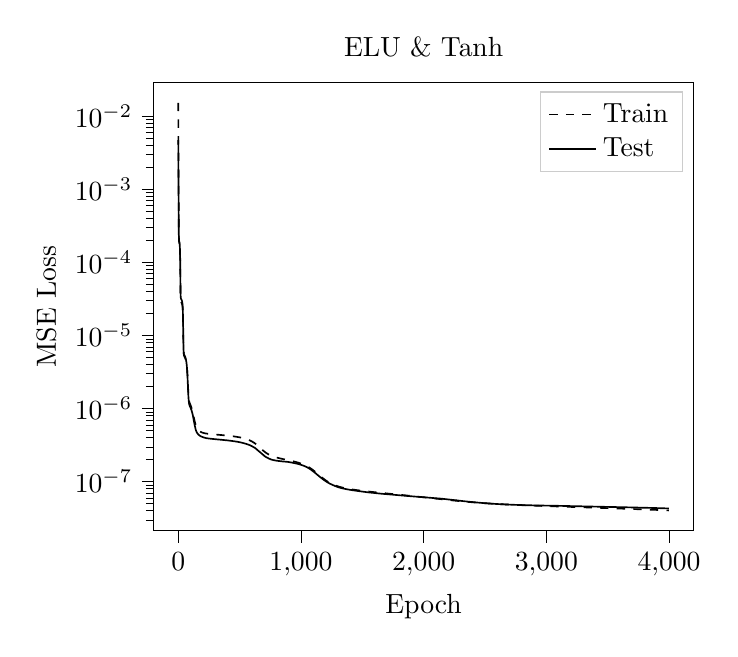
\begin{tikzpicture}

\begin{axis}[
legend cell align={left},
legend style={fill opacity=0.8, draw opacity=1, text opacity=1, draw=white!80!black},
log basis y={10},
tick align=outside,
tick pos=left,
title={ELU \& Tanh},
x grid style={white!69.0196078431373!black},
xlabel={Epoch},
xmin=-199.95, xmax=4198.95,
xtick style={color=black},
y grid style={white!69.0196078431373!black},
ylabel={MSE Loss},
ymin=2.1280500312269e-08, ymax=0.0288960951589277,
ymode=log,
ytick style={color=black}
]
\addplot [semithick, black, dashed]
table {%
0 0.0152080284673721
1 0.00248075019428506
2 0.00126132386806421
3 0.00065380612318404
4 0.000302382324065547
5 0.000212503188158735
6 0.000193753781044506
7 0.000187910542459576
8 0.000184431473302539
9 0.000180994361369812
10 0.000176910041926021
11 0.000171687997724803
12 0.000164645445795031
13 0.000154705665103393
14 0.000140248441668518
15 0.000119364761536417
16 9.17300330147555e-05
17 6.27979531163874e-05
18 4.26708161667193e-05
19 3.37652515718219e-05
20 3.06545776984422e-05
21 2.95085138677678e-05
22 2.8994764298659e-05
23 2.86948540106096e-05
24 2.84682299516135e-05
25 2.82642717929775e-05
26 2.80622330783444e-05
27 2.7850678786308e-05
28 2.76203797193375e-05
29 2.73613483659574e-05
30 2.70609807812434e-05
31 2.67019758239258e-05
32 2.6259632773872e-05
33 2.56977659782933e-05
34 2.49631382184816e-05
35 2.39780262472777e-05
36 2.26334173030409e-05
37 2.0791223996639e-05
38 1.83290858867622e-05
39 1.52773886138675e-05
40 1.20173287841681e-05
41 9.2298659392327e-06
42 7.36606126406514e-06
43 6.32788974849063e-06
44 5.79142337710437e-06
45 5.51480871411059e-06
46 5.36734691024776e-06
47 5.28214288931395e-06
48 5.22541249051756e-06
49 5.18075900356507e-06
50 5.14051194068088e-06
51 5.10132590710555e-06
52 5.06172166137731e-06
53 5.02101423398926e-06
54 4.97876538742048e-06
55 4.93462883019902e-06
56 4.88829601943053e-06
57 4.83948054937855e-06
58 4.78781597689704e-06
59 4.73286032058695e-06
60 4.67407446171819e-06
61 4.61085995141275e-06
62 4.54254747762661e-06
63 4.46836536832507e-06
64 4.38744179211881e-06
65 4.29883675451492e-06
66 4.20154519031257e-06
67 4.09452232202057e-06
68 3.97672916426472e-06
69 3.8471998618661e-06
70 3.70513911616399e-06
71 3.55005798166985e-06
72 3.38197834838638e-06
73 3.20168775073171e-06
74 3.01100894580486e-06
75 2.81300117563887e-06
76 2.61201407016642e-06
77 2.41341767292624e-06
78 2.22315533977735e-06
79 2.0468877611961e-06
80 1.88906458362226e-06
81 1.75221979372964e-06
82 1.63677172395182e-06
83 1.54148892647754e-06
84 1.46415385779619e-06
85 1.40207349818411e-06
86 1.35254531772944e-06
87 1.31307150775228e-06
88 1.28151420807399e-06
89 1.25604890848763e-06
90 1.23516671064294e-06
91 1.2176365066523e-06
92 1.20252019155487e-06
93 1.18908983145616e-06
94 1.17681919957136e-06
95 1.16535745513602e-06
96 1.15439602055289e-06
97 1.14370702488031e-06
98 1.13312517120789e-06
99 1.12253153173469e-06
100 1.11184424446265e-06
101 1.10101062864487e-06
102 1.09000098660772e-06
103 1.07879312142245e-06
104 1.06736867337531e-06
105 1.05571247524949e-06
106 1.04381238244855e-06
107 1.03166244338126e-06
108 1.0192582135744e-06
109 1.00659639397804e-06
110 9.93679479705634e-07
111 9.80511999273404e-07
112 9.67102745761394e-07
113 9.53462768279678e-07
114 9.39608711860274e-07
115 9.25561131367658e-07
116 9.11341380685826e-07
117 8.96972368934712e-07
118 8.82482107471105e-07
119 8.67901396617299e-07
120 8.53267375134692e-07
121 8.386187981273e-07
122 8.23993808523937e-07
123 8.09432929372633e-07
124 7.94978626629472e-07
125 7.80686552872112e-07
126 7.66615440795704e-07
127 7.52801653646884e-07
128 7.39273721563904e-07
129 7.260868112553e-07
130 7.13269594200483e-07
131 7.00837796472342e-07
132 6.88812247830128e-07
133 6.77201320598897e-07
134 6.66034269528382e-07
135 6.55349540636507e-07
136 6.45165235738432e-07
137 6.35454344404707e-07
138 6.26196593657369e-07
139 6.17382204609385e-07
140 6.0907905589147e-07
141 6.01319924101062e-07
142 5.94054916405184e-07
143 5.8719218452552e-07
144 5.80707587801044e-07
145 5.74600551118465e-07
146 5.68858134613492e-07
147 5.63467706399479e-07
148 5.58383930240325e-07
149 5.53627922812439e-07
150 5.49140991978447e-07
151 5.4492200263212e-07
152 5.40938552489933e-07
153 5.37143491641245e-07
154 5.33550829203477e-07
155 5.30159955616227e-07
156 5.26960494710238e-07
157 5.23945866660824e-07
158 5.2109070625761e-07
159 5.18372332038552e-07
160 5.1578902329652e-07
161 5.13338145935904e-07
162 5.11008444703975e-07
163 5.08790582244956e-07
164 5.06676500521053e-07
165 5.04660050523853e-07
166 5.02738334574815e-07
167 5.00906882678009e-07
168 4.9915709371362e-07
169 4.9748365924529e-07
170 4.95880076812227e-07
171 4.94340759701117e-07
172 4.92864306906426e-07
173 4.9144516030708e-07
174 4.9008119822247e-07
175 4.88768996348199e-07
176 4.87505730262683e-07
177 4.86288514707667e-07
178 4.85115197605524e-07
179 4.83983028601642e-07
180 4.82889594195512e-07
181 4.8183425819559e-07
182 4.80814081356584e-07
183 4.79827712922543e-07
184 4.78873592783202e-07
185 4.77950427978158e-07
186 4.77055746188171e-07
187 4.76188250274845e-07
188 4.75347918438729e-07
189 4.74533189901649e-07
190 4.73742007400801e-07
191 4.72973320526648e-07
192 4.72227070389408e-07
193 4.71503322685862e-07
194 4.70799528827115e-07
195 4.70116371261042e-07
196 4.69453903050976e-07
197 4.68810875844383e-07
198 4.68186554911654e-07
199 4.67581506711667e-07
200 4.66993338903876e-07
201 4.66421883700718e-07
202 4.6586627745171e-07
203 4.65324514891563e-07
204 4.64797279363438e-07
205 4.64284398972836e-07
206 4.63784455590144e-07
207 4.63298719495242e-07
208 4.62825613595896e-07
209 4.62363970797242e-07
210 4.61915587337103e-07
211 4.61477298927093e-07
212 4.61051291992476e-07
213 4.60636017479032e-07
214 4.60231373097031e-07
215 4.59836511453204e-07
216 4.59451205642836e-07
217 4.59075062082093e-07
218 4.58708360696392e-07
219 4.58350019769682e-07
220 4.58000447480345e-07
221 4.57658333374411e-07
222 4.57324772341394e-07
223 4.56997766420386e-07
224 4.56679159967166e-07
225 4.5636672231808e-07
226 4.56060347715948e-07
227 4.55762036324359e-07
228 4.5546945007402e-07
229 4.55182474496496e-07
230 4.54901839177069e-07
231 4.54625413439658e-07
232 4.54356226143204e-07
233 4.54091371821619e-07
234 4.53831857200271e-07
235 4.53577267762739e-07
236 4.53326436542056e-07
237 4.53081359182761e-07
238 4.52839802278504e-07
239 4.52602506470612e-07
240 4.52369051430424e-07
241 4.52139772278315e-07
242 4.51913687584238e-07
243 4.51691316968095e-07
244 4.51472699523947e-07
245 4.51256809995471e-07
246 4.51044487576269e-07
247 4.50834722101945e-07
248 4.50627858697317e-07
249 4.50423915665965e-07
250 4.50223144014217e-07
251 4.50024731975418e-07
252 4.49828700936905e-07
253 4.49634319892311e-07
254 4.49443024805873e-07
255 4.49254178064962e-07
256 4.49066956406341e-07
257 4.48881223618969e-07
258 4.48698587803165e-07
259 4.48516765786167e-07
260 4.48337179022928e-07
261 4.4815975951451e-07
262 4.47983176357525e-07
263 4.47808628308621e-07
264 4.47635315765638e-07
265 4.4746370636517e-07
266 4.47293768075951e-07
267 4.47124673172539e-07
268 4.46957185516794e-07
269 4.46790791471585e-07
270 4.46624989848488e-07
271 4.46461147248556e-07
272 4.46298341259421e-07
273 4.46135595410624e-07
274 4.45974463659127e-07
275 4.45814696519164e-07
276 4.45655445147963e-07
277 4.45497513965165e-07
278 4.45339897780173e-07
279 4.4518315532116e-07
280 4.45027225694616e-07
281 4.44871742303121e-07
282 4.44717229669322e-07
283 4.44563503421591e-07
284 4.44410062897305e-07
285 4.44257312167906e-07
286 4.44105373304637e-07
287 4.43953671634745e-07
288 4.43802586957531e-07
289 4.43651378475352e-07
290 4.4350156309747e-07
291 4.43351403191627e-07
292 4.43202396965603e-07
293 4.43052928034149e-07
294 4.4290395682367e-07
295 4.42755513716975e-07
296 4.42606946023716e-07
297 4.42459066817946e-07
298 4.42311463885403e-07
299 4.42163857997002e-07
300 4.42016133746392e-07
301 4.41869450867216e-07
302 4.41721961351504e-07
303 4.41575820104845e-07
304 4.41428945691769e-07
305 4.41282887692296e-07
306 4.4113659586742e-07
307 4.40990409828146e-07
308 4.40844655273054e-07
309 4.40698768144898e-07
310 4.40553284818179e-07
311 4.40407495204909e-07
312 4.40261692943977e-07
313 4.40117002582952e-07
314 4.39971105990367e-07
315 4.3982572678658e-07
316 4.3968058045607e-07
317 4.3953475244507e-07
318 4.39390190067002e-07
319 4.39244838787545e-07
320 4.3909949086185e-07
321 4.38954148719972e-07
322 4.38809322702127e-07
323 4.38664034192016e-07
324 4.38518397331222e-07
325 4.38373606968412e-07
326 4.38227661447854e-07
327 4.38082569615972e-07
328 4.37936808936001e-07
329 4.37791352069894e-07
330 4.37645759731708e-07
331 4.37499971056354e-07
332 4.37353520837291e-07
333 4.37207102521597e-07
334 4.37061042433129e-07
335 4.36913789201299e-07
336 4.36767032638841e-07
337 4.36620052894909e-07
338 4.36472801979448e-07
339 4.36325509113544e-07
340 4.36177363511092e-07
341 4.36028866033666e-07
342 4.35880465872174e-07
343 4.35731473871215e-07
344 4.35582405643231e-07
345 4.35433008561859e-07
346 4.35283194264002e-07
347 4.3513326829725e-07
348 4.3498325092628e-07
349 4.34832827465925e-07
350 4.3468171416805e-07
351 4.3453046178854e-07
352 4.34379240530802e-07
353 4.34226759196576e-07
354 4.34074440263998e-07
355 4.33922115718133e-07
356 4.33769137174522e-07
357 4.33616304675866e-07
358 4.33462212896529e-07
359 4.33308346842409e-07
360 4.33154044316097e-07
361 4.32999025719028e-07
362 4.32843678566996e-07
363 4.32688067760978e-07
364 4.32532335693736e-07
365 4.32375908360427e-07
366 4.32219386226507e-07
367 4.32062283337586e-07
368 4.31904461052568e-07
369 4.31746474518491e-07
370 4.315880933774e-07
371 4.31428781524801e-07
372 4.31269957729796e-07
373 4.31109887017556e-07
374 4.30949544366399e-07
375 4.3078909608596e-07
376 4.3062788631687e-07
377 4.3046613218678e-07
378 4.30304351141331e-07
379 4.30142163423852e-07
380 4.29979540541581e-07
381 4.29816218769474e-07
382 4.29652669481584e-07
383 4.29488652883947e-07
384 4.29324528838038e-07
385 4.29160088145863e-07
386 4.2899547537445e-07
387 4.28831191527479e-07
388 4.28666356484086e-07
389 4.28499909872926e-07
390 4.28332165512302e-07
391 4.2816423081149e-07
392 4.27997117341761e-07
393 4.27830187575751e-07
394 4.27665927389853e-07
395 4.27502797776924e-07
396 4.27342054052815e-07
397 4.27181646472263e-07
398 4.27009718947602e-07
399 4.2682666169469e-07
400 4.26646251099783e-07
401 4.26469282359676e-07
402 4.26291279069346e-07
403 4.26114118084797e-07
404 4.25935911081865e-07
405 4.25757392562787e-07
406 4.25577832146473e-07
407 4.25397295160224e-07
408 4.25216371667148e-07
409 4.25034376462463e-07
410 4.2485157290173e-07
411 4.24668970282482e-07
412 4.24484292835814e-07
413 4.24299328557254e-07
414 4.24113592458752e-07
415 4.23926915772199e-07
416 4.23739302391368e-07
417 4.2355089580326e-07
418 4.23361439615633e-07
419 4.23171769142527e-07
420 4.2298105516636e-07
421 4.22789032072046e-07
422 4.22596885357507e-07
423 4.22403967462515e-07
424 4.22211046924303e-07
425 4.22016804677128e-07
426 4.21823173240909e-07
427 4.2163074121504e-07
428 4.21439219110198e-07
429 4.21241830252939e-07
430 4.21036349408155e-07
431 4.20831540296263e-07
432 4.20626598298668e-07
433 4.2042308245982e-07
434 4.20218619041179e-07
435 4.20013128845653e-07
436 4.19806055774075e-07
437 4.19598493493822e-07
438 4.19389835656148e-07
439 4.19179818322846e-07
440 4.18968826551236e-07
441 4.18756718033819e-07
442 4.1854358694593e-07
443 4.18329209438184e-07
444 4.18113902696859e-07
445 4.17897678829604e-07
446 4.17680306043167e-07
447 4.17461535690222e-07
448 4.17242249227456e-07
449 4.17021593136724e-07
450 4.16801037246728e-07
451 4.16579762884339e-07
452 4.16357781375609e-07
453 4.16134501904253e-07
454 4.15909136961545e-07
455 4.15682213287027e-07
456 4.15455763217665e-07
457 4.15227140010188e-07
458 4.14998426251145e-07
459 4.14767454032017e-07
460 4.14533987935783e-07
461 4.14297598396729e-07
462 4.14058632713932e-07
463 4.1381838173038e-07
464 4.13576328185172e-07
465 4.13332909417363e-07
466 4.13088214941126e-07
467 4.12841624324756e-07
468 4.12594360795993e-07
469 4.12345667172076e-07
470 4.12094428085652e-07
471 4.11842957362296e-07
472 4.11588928784568e-07
473 4.1133438830343e-07
474 4.11077571214946e-07
475 4.10818901883658e-07
476 4.10558991234211e-07
477 4.10297284844319e-07
478 4.10033927209952e-07
479 4.09769019000805e-07
480 4.09501372402588e-07
481 4.09233206411841e-07
482 4.08962386146072e-07
483 4.08690077392748e-07
484 4.08415712570331e-07
485 4.08139434355803e-07
486 4.07861542385035e-07
487 4.07581834338089e-07
488 4.07300655780318e-07
489 4.07016802938642e-07
490 4.06731137147176e-07
491 4.06443877139395e-07
492 4.06154237637679e-07
493 4.05862715155081e-07
494 4.05568969000569e-07
495 4.05273351432811e-07
496 4.04975282762621e-07
497 4.04674660700266e-07
498 4.0437273760574e-07
499 4.04067683120957e-07
500 4.03761146870352e-07
501 4.03451639428454e-07
502 4.03139706364186e-07
503 4.02826480339513e-07
504 4.02509610665902e-07
505 4.02190768141963e-07
506 4.01869577345337e-07
507 4.01546232779992e-07
508 4.0122040243773e-07
509 4.00891479856114e-07
510 4.00560430591668e-07
511 4.00226384300595e-07
512 3.99890941281456e-07
513 3.99551510341212e-07
514 3.99209917361532e-07
515 3.98866274110787e-07
516 3.98518419430616e-07
517 3.98168940421328e-07
518 3.97816384889893e-07
519 3.97461238151209e-07
520 3.97103499679474e-07
521 3.96742407474449e-07
522 3.96378228884942e-07
523 3.96010879271103e-07
524 3.9564072622511e-07
525 3.95267676083222e-07
526 3.94890880272669e-07
527 3.94511405232834e-07
528 3.94128287325657e-07
529 3.93741344481668e-07
530 3.93352225017907e-07
531 3.92959715242114e-07
532 3.92563438921911e-07
533 3.9216375753881e-07
534 3.91761114514111e-07
535 3.91355185229259e-07
536 3.90944708314578e-07
537 3.90532183018877e-07
538 3.9011626749641e-07
539 3.89696966365705e-07
540 3.89274426851216e-07
541 3.88848559708777e-07
542 3.88419916419025e-07
543 3.87989611638773e-07
544 3.87556333166117e-07
545 3.87121111600663e-07
546 3.86684392907455e-07
547 3.86246727373418e-07
548 3.85805560057406e-07
549 3.85360736231632e-07
550 3.84910381086456e-07
551 3.84454204962026e-07
552 3.83994932519727e-07
553 3.83531411628724e-07
554 3.83059219458914e-07
555 3.82575445300404e-07
556 3.82082884641477e-07
557 3.81585331467704e-07
558 3.81081443521225e-07
559 3.80573512586579e-07
560 3.80061310664814e-07
561 3.79545718928398e-07
562 3.7902608279694e-07
563 3.78502641950718e-07
564 3.77975410430054e-07
565 3.77444048453412e-07
566 3.76907770714752e-07
567 3.76367728875948e-07
568 3.75824838585004e-07
569 3.75276613652886e-07
570 3.74724207119925e-07
571 3.74166170345802e-07
572 3.73599418281856e-07
573 3.73024576461489e-07
574 3.72441210373609e-07
575 3.71851760888831e-07
576 3.71256574879908e-07
577 3.70655598146641e-07
578 3.70049976297082e-07
579 3.69438769027397e-07
580 3.68821629621152e-07
581 3.68198507970874e-07
582 3.6756981538133e-07
583 3.6693339855276e-07
584 3.66292147148783e-07
585 3.65642823027201e-07
586 3.64987084253698e-07
587 3.64323781809617e-07
588 3.63653413089082e-07
589 3.62975147567113e-07
590 3.62289680722938e-07
591 3.61597356771881e-07
592 3.6089758528135e-07
593 3.60190051196696e-07
594 3.59475607524473e-07
595 3.58753690136382e-07
596 3.58024245528554e-07
597 3.57286942630708e-07
598 3.56542650152392e-07
599 3.55790499583009e-07
600 3.55030364318054e-07
601 3.54263068174987e-07
602 3.53487559493715e-07
603 3.52704138791182e-07
604 3.5191315025429e-07
605 3.51113995563424e-07
606 3.50307178621279e-07
607 3.49492535278273e-07
608 3.48670051636191e-07
609 3.47839225057101e-07
610 3.47001117404488e-07
611 3.46154819595768e-07
612 3.4530131030408e-07
613 3.44439791035711e-07
614 3.43571013203814e-07
615 3.42695091504197e-07
616 3.41812224007754e-07
617 3.40922235992025e-07
618 3.40024295439889e-07
619 3.39119695482282e-07
620 3.38206636016025e-07
621 3.37286338464082e-07
622 3.36357724691538e-07
623 3.35421586697748e-07
624 3.34478846738762e-07
625 3.3353134622871e-07
626 3.32582318662844e-07
627 3.31627309350324e-07
628 3.30657915270649e-07
629 3.29676779301735e-07
630 3.28686887527851e-07
631 3.27686967835916e-07
632 3.26681882768298e-07
633 3.2567142653761e-07
634 3.24656859532979e-07
635 3.23637882360117e-07
636 3.22613774727643e-07
637 3.21585285718129e-07
638 3.20552245838712e-07
639 3.19513541384708e-07
640 3.18471469981318e-07
641 3.17424747223072e-07
642 3.16374848694068e-07
643 3.15321539005708e-07
644 3.14264368597605e-07
645 3.13204994782268e-07
646 3.12142761274004e-07
647 3.1107828736765e-07
648 3.10012818800942e-07
649 3.08945284075435e-07
650 3.07876374378679e-07
651 3.06807749538507e-07
652 3.05738609483797e-07
653 3.04670831113185e-07
654 3.03604463951501e-07
655 3.02538507270356e-07
656 3.01475481862212e-07
657 3.00420638524201e-07
658 2.99368262318467e-07
659 2.98305927501019e-07
660 2.9724377205298e-07
661 2.96187314631879e-07
662 2.95135673923141e-07
663 2.94088418243632e-07
664 2.93043090579204e-07
665 2.92001749215842e-07
666 2.90964147893646e-07
667 2.8992860050181e-07
668 2.88896486182466e-07
669 2.87866366512901e-07
670 2.86841053750209e-07
671 2.85822178319961e-07
672 2.84809853511092e-07
673 2.83802668313626e-07
674 2.82802994959752e-07
675 2.81808777316428e-07
676 2.80821736446057e-07
677 2.79841228206124e-07
678 2.78866927004628e-07
679 2.7790029102448e-07
680 2.76940049957375e-07
681 2.75986952402718e-07
682 2.75040459946752e-07
683 2.7410105185055e-07
684 2.73169070915458e-07
685 2.72244475226557e-07
686 2.71327085592077e-07
687 2.70418083744062e-07
688 2.69515283221722e-07
689 2.68621464947216e-07
690 2.67736805710683e-07
691 2.6686000502707e-07
692 2.65991814671906e-07
693 2.65132417098357e-07
694 2.64281129219057e-07
695 2.63438652083892e-07
696 2.62605085239898e-07
697 2.6178079198047e-07
698 2.60965614536701e-07
699 2.60159289894091e-07
700 2.59361679880499e-07
701 2.58572606441021e-07
702 2.5779265062198e-07
703 2.5702136591832e-07
704 2.56259088146749e-07
705 2.5550531433538e-07
706 2.54760969511381e-07
707 2.54025321467566e-07
708 2.53298220812326e-07
709 2.52579562904032e-07
710 2.51870719914393e-07
711 2.51169781748217e-07
712 2.50477844623731e-07
713 2.49794036555784e-07
714 2.49118054647113e-07
715 2.48451531383864e-07
716 2.47792019649751e-07
717 2.4713980123181e-07
718 2.4649597766313e-07
719 2.45858712489166e-07
720 2.45228927809649e-07
721 2.44605411296561e-07
722 2.43988998619216e-07
723 2.43379559542234e-07
724 2.42777749093648e-07
725 2.42183043717148e-07
726 2.41596288141466e-07
727 2.41018655465552e-07
728 2.4045008593987e-07
729 2.39890878397375e-07
730 2.39341327421982e-07
731 2.38801107819597e-07
732 2.38267282050231e-07
733 2.37741108591649e-07
734 2.37221678233368e-07
735 2.36709369893617e-07
736 2.3620330499341e-07
737 2.35703722438529e-07
738 2.3521035917895e-07
739 2.34722806567333e-07
740 2.34240615100134e-07
741 2.33767771455007e-07
742 2.33302381239753e-07
743 2.32845008270033e-07
744 2.32395974940403e-07
745 2.31952249464484e-07
746 2.31513471092626e-07
747 2.31079828736824e-07
748 2.30651120318726e-07
749 2.30226588783466e-07
750 2.2980676357065e-07
751 2.29391758971076e-07
752 2.28981763186198e-07
753 2.28576197116581e-07
754 2.28172959118922e-07
755 2.27773301602952e-07
756 2.27378275646117e-07
757 2.26989851242365e-07
758 2.26602774077378e-07
759 2.26227015282632e-07
760 2.25866439848232e-07
761 2.25510081413915e-07
762 2.25156237128488e-07
763 2.24807197071186e-07
764 2.24463084258275e-07
765 2.24122159856677e-07
766 2.23785884017502e-07
767 2.23455905860703e-07
768 2.23132916062241e-07
769 2.22814507218061e-07
770 2.22498743696065e-07
771 2.22186950992409e-07
772 2.21877190426767e-07
773 2.21571451533009e-07
774 2.21268463938884e-07
775 2.20969464599818e-07
776 2.20672862852211e-07
777 2.20380329785996e-07
778 2.20091305415338e-07
779 2.19805837808451e-07
780 2.19523888425499e-07
781 2.19244672571506e-07
782 2.1896903959373e-07
783 2.18695799098612e-07
784 2.18425251311771e-07
785 2.18156760823263e-07
786 2.17889637639246e-07
787 2.17624017793128e-07
788 2.17358097586384e-07
789 2.17094104584703e-07
790 2.1683663841543e-07
791 2.16581288739803e-07
792 2.16325453756383e-07
793 2.16079294290239e-07
794 2.15844955441469e-07
795 2.15610947094547e-07
796 2.15374048437411e-07
797 2.15137222312478e-07
798 2.14901826538494e-07
799 2.14668557909192e-07
800 2.14437508262222e-07
801 2.14208109397873e-07
802 2.13980514168099e-07
803 2.13755005297855e-07
804 2.13530497873649e-07
805 2.13307517775263e-07
806 2.13086708924948e-07
807 2.12867477486611e-07
808 2.12648762158096e-07
809 2.12432043134925e-07
810 2.1221569882357e-07
811 2.12001444538146e-07
812 2.11787534560415e-07
813 2.1157526721538e-07
814 2.11363528677566e-07
815 2.11152904377343e-07
816 2.10944543326264e-07
817 2.10738933837717e-07
818 2.10534798483764e-07
819 2.10332396406443e-07
820 2.10132417123532e-07
821 2.09933438640064e-07
822 2.09735871109729e-07
823 2.0953889501385e-07
824 2.09343528659645e-07
825 2.09148757413402e-07
826 2.08955001021138e-07
827 2.08762269167551e-07
828 2.0857034380839e-07
829 2.08380171969225e-07
830 2.08190538060649e-07
831 2.08001925358303e-07
832 2.07813819351088e-07
833 2.07627028736113e-07
834 2.07440498009248e-07
835 2.07255245449289e-07
836 2.0707062751768e-07
837 2.06885963407899e-07
838 2.06701901937834e-07
839 2.06518239487252e-07
840 2.06334660020957e-07
841 2.06149372928621e-07
842 2.05963076687965e-07
843 2.05778682648372e-07
844 2.05600004349549e-07
845 2.05427205528963e-07
846 2.05253981924614e-07
847 2.05079602025648e-07
848 2.04905068969197e-07
849 2.04730230834116e-07
850 2.04555962532993e-07
851 2.04382653272717e-07
852 2.04209134508915e-07
853 2.04036619734893e-07
854 2.03864340669213e-07
855 2.03692555636792e-07
856 2.03521542459839e-07
857 2.03350728412488e-07
858 2.03180690157012e-07
859 2.03011188972368e-07
860 2.02841798056852e-07
861 2.026736309233e-07
862 2.02505270834763e-07
863 2.02337946419107e-07
864 2.02170827741099e-07
865 2.02004277184642e-07
866 2.01838315533109e-07
867 2.01673230499466e-07
868 2.01508554056318e-07
869 2.01345202611947e-07
870 2.01181850222554e-07
871 2.01019166709671e-07
872 2.00856438574704e-07
873 2.00694160724879e-07
874 2.00530837311419e-07
875 2.00366833176702e-07
876 2.00201819630763e-07
877 2.00036929420833e-07
878 1.99872439061721e-07
879 1.99706989867821e-07
880 1.99541846136242e-07
881 1.99376906415694e-07
882 1.99212340909583e-07
883 1.99047352666071e-07
884 1.98882859763216e-07
885 1.98717945835369e-07
886 1.9855398689117e-07
887 1.98389172609836e-07
888 1.98224787446577e-07
889 1.98060101283204e-07
890 1.9789522706759e-07
891 1.97730675708385e-07
892 1.97565865150295e-07
893 1.9740112774258e-07
894 1.972362442757e-07
895 1.97070757188555e-07
896 1.96906404205777e-07
897 1.96741027025382e-07
898 1.96576096470835e-07
899 1.96410390380208e-07
900 1.96244824508085e-07
901 1.96077997884458e-07
902 1.95911753110067e-07
903 1.95743825941008e-07
904 1.95575801726022e-07
905 1.95407580591223e-07
906 1.95238583479806e-07
907 1.95069209105725e-07
908 1.9489933107053e-07
909 1.94728678806655e-07
910 1.94557905523141e-07
911 1.94387777966654e-07
912 1.94218127241186e-07
913 1.94050267367629e-07
914 1.9388224076522e-07
915 1.93712325064155e-07
916 1.9353938095179e-07
917 1.93366957915941e-07
918 1.9319692871278e-07
919 1.93027422852765e-07
920 1.92858038950305e-07
921 1.92688125018492e-07
922 1.92518062625879e-07
923 1.92347462395048e-07
924 1.92176538490685e-07
925 1.92004955188452e-07
926 1.91832813854376e-07
927 1.91660883459122e-07
928 1.91487729047424e-07
929 1.91314957049826e-07
930 1.91140440186643e-07
931 1.90967177964296e-07
932 1.90792752839286e-07
933 1.90617769661117e-07
934 1.90441730737234e-07
935 1.90266023665231e-07
936 1.90089237563029e-07
937 1.89911305525925e-07
938 1.89733484504018e-07
939 1.89554710267714e-07
940 1.89375190878138e-07
941 1.89195479805448e-07
942 1.8901482096112e-07
943 1.88833834222635e-07
944 1.88652055001626e-07
945 1.88469787048007e-07
946 1.88286472578625e-07
947 1.88102376753818e-07
948 1.87918844105184e-07
949 1.87733679425151e-07
950 1.87547744005201e-07
951 1.87360893221467e-07
952 1.87174149104408e-07
953 1.86985833252606e-07
954 1.86796763976815e-07
955 1.86606931265487e-07
956 1.86416954342405e-07
957 1.86225132750906e-07
958 1.86033258174234e-07
959 1.85840012484562e-07
960 1.85645616667784e-07
961 1.8545087016264e-07
962 1.8525445011619e-07
963 1.85057448533144e-07
964 1.84858989101144e-07
965 1.84660104586953e-07
966 1.84459632542655e-07
967 1.84258142418514e-07
968 1.84055861524257e-07
969 1.83852619251468e-07
970 1.83647670056075e-07
971 1.83441494932879e-07
972 1.83235091093081e-07
973 1.83027565526572e-07
974 1.82818779848048e-07
975 1.82608773229731e-07
976 1.82398483588031e-07
977 1.82186698005182e-07
978 1.81974148567576e-07
979 1.81761305768191e-07
980 1.81546775124275e-07
981 1.8133131184328e-07
982 1.81115166988377e-07
983 1.80897656846923e-07
984 1.80678867032213e-07
985 1.8045907341957e-07
986 1.80237917071224e-07
987 1.80015462724725e-07
988 1.79791754902681e-07
989 1.79566497948258e-07
990 1.79339599419848e-07
991 1.7911191135056e-07
992 1.7888233854535e-07
993 1.78651545233777e-07
994 1.78419945541464e-07
995 1.78185779844853e-07
996 1.77950870181576e-07
997 1.77714219546488e-07
998 1.77476629012574e-07
999 1.77237352858128e-07
1000 1.76996435747867e-07
1001 1.76753868046831e-07
1002 1.76510436688204e-07
1003 1.76265239097972e-07
1004 1.76018311321968e-07
1005 1.7577009816705e-07
1006 1.75520918872962e-07
1007 1.75269713388104e-07
1008 1.75017535724464e-07
1009 1.7476436124042e-07
1010 1.74509330946648e-07
1011 1.74253998878271e-07
1012 1.73996551879441e-07
1013 1.73735433776301e-07
1014 1.73470677786725e-07
1015 1.73203433071478e-07
1016 1.72935475397651e-07
1017 1.72665775927783e-07
1018 1.72394989540692e-07
1019 1.72122301378863e-07
1020 1.71847703903438e-07
1021 1.71571395924275e-07
1022 1.71293312561716e-07
1023 1.71013627351613e-07
1024 1.70731415153114e-07
1025 1.70448012760005e-07
1026 1.70162309245825e-07
1027 1.69874203834297e-07
1028 1.69584868331185e-07
1029 1.69293045168217e-07
1030 1.68999612853327e-07
1031 1.68704158348021e-07
1032 1.68406576023017e-07
1033 1.68106452065331e-07
1034 1.67805620947092e-07
1035 1.67501270006198e-07
1036 1.67195596851855e-07
1037 1.66887579510444e-07
1038 1.66578071727486e-07
1039 1.66266004974602e-07
1040 1.65951682980392e-07
1041 1.65635398253983e-07
1042 1.65317023686384e-07
1043 1.64996520197747e-07
1044 1.64673900364676e-07
1045 1.64349384519369e-07
1046 1.64022342566739e-07
1047 1.63692751627309e-07
1048 1.6336171660214e-07
1049 1.63027996336496e-07
1050 1.62691938633941e-07
1051 1.62353983277796e-07
1052 1.62013484391821e-07
1053 1.61670484828846e-07
1054 1.61325077414176e-07
1055 1.60977907036397e-07
1056 1.60627455542794e-07
1057 1.60274794467341e-07
1058 1.59919573505363e-07
1059 1.5956187238686e-07
1060 1.59202226228672e-07
1061 1.5883981910747e-07
1062 1.58475691868887e-07
1063 1.58109363731285e-07
1064 1.57740791159711e-07
1065 1.57370220534858e-07
1066 1.5699837614136e-07
1067 1.56623337829842e-07
1068 1.5624693890004e-07
1069 1.55868588223029e-07
1070 1.5548834431911e-07
1071 1.55105668646627e-07
1072 1.54720571160283e-07
1073 1.5433408812271e-07
1074 1.53945973565328e-07
1075 1.53556759023843e-07
1076 1.53168143185667e-07
1077 1.52781376655753e-07
1078 1.52392721695094e-07
1079 1.51986224111056e-07
1080 1.51573336843569e-07
1081 1.51163015452482e-07
1082 1.50752499294526e-07
1083 1.50340282296213e-07
1084 1.49925430150688e-07
1085 1.49508963318112e-07
1086 1.49090141533748e-07
1087 1.48668793379159e-07
1088 1.48246224533466e-07
1089 1.47823067443653e-07
1090 1.4739891135207e-07
1091 1.46975094374113e-07
1092 1.46551880227719e-07
1093 1.46127542315355e-07
1094 1.45704618077502e-07
1095 1.45281267663222e-07
1096 1.44858161554851e-07
1097 1.44435726859626e-07
1098 1.44012023504558e-07
1099 1.43588234735148e-07
1100 1.43163128392132e-07
1101 1.42737117741376e-07
1102 1.42309912902761e-07
1103 1.41881366552354e-07
1104 1.41451710398144e-07
1105 1.41019887571758e-07
1106 1.40588459643709e-07
1107 1.40159142063112e-07
1108 1.397344884424e-07
1109 1.39312528155244e-07
1110 1.38888660956127e-07
1111 1.38463449410153e-07
1112 1.38037102217936e-07
1113 1.37609120329785e-07
1114 1.3718097876847e-07
1115 1.36753013961766e-07
1116 1.36323733279653e-07
1117 1.35895572427103e-07
1118 1.35466340246637e-07
1119 1.35037029579621e-07
1120 1.34607929481945e-07
1121 1.34178400685414e-07
1122 1.3374874122718e-07
1123 1.33319254764785e-07
1124 1.3289110313508e-07
1125 1.32462414988765e-07
1126 1.32034274258785e-07
1127 1.3160604830631e-07
1128 1.31179003709292e-07
1129 1.30751606668866e-07
1130 1.303254807965e-07
1131 1.29900382290771e-07
1132 1.29477080037077e-07
1133 1.29054515809912e-07
1134 1.28633866729899e-07
1135 1.2821482557257e-07
1136 1.27797809263086e-07
1137 1.27382684361521e-07
1138 1.26968237751157e-07
1139 1.26554759646069e-07
1140 1.26141516709311e-07
1141 1.25729517293394e-07
1142 1.25318422725229e-07
1143 1.24908480522379e-07
1144 1.2449971258377e-07
1145 1.24091573255214e-07
1146 1.23685658685702e-07
1147 1.23280426407746e-07
1148 1.22877155902756e-07
1149 1.22475587104987e-07
1150 1.22075368736319e-07
1151 1.21677058281477e-07
1152 1.21280481735653e-07
1153 1.20885881372601e-07
1154 1.204930188905e-07
1155 1.20102175543479e-07
1156 1.19712751668999e-07
1157 1.19324970796697e-07
1158 1.18938711693772e-07
1159 1.18554402661175e-07
1160 1.18171441883419e-07
1161 1.1778998898393e-07
1162 1.17410384731897e-07
1163 1.17032128031269e-07
1164 1.16655850810332e-07
1165 1.16281895898851e-07
1166 1.1590908521697e-07
1167 1.15539219237348e-07
1168 1.15170975277579e-07
1169 1.14804350438646e-07
1170 1.14440306376196e-07
1171 1.14077554300707e-07
1172 1.13717005660874e-07
1173 1.13358472852099e-07
1174 1.13001979670457e-07
1175 1.12648888318745e-07
1176 1.12299481877187e-07
1177 1.11954567451278e-07
1178 1.11612510480086e-07
1179 1.1127388872012e-07
1180 1.10937243938736e-07
1181 1.1060316435163e-07
1182 1.10271697288056e-07
1183 1.09942648336414e-07
1184 1.09615565492049e-07
1185 1.09291037958315e-07
1186 1.08968655844421e-07
1187 1.08648786330434e-07
1188 1.08331142371298e-07
1189 1.08016214802831e-07
1190 1.07703970080308e-07
1191 1.07393447542847e-07
1192 1.07085563961107e-07
1193 1.06780864925327e-07
1194 1.06478344953587e-07
1195 1.06178493034292e-07
1196 1.0588090550101e-07
1197 1.05585991015289e-07
1198 1.05293827822095e-07
1199 1.05004410443144e-07
1200 1.04717090827933e-07
1201 1.04432268230426e-07
1202 1.04150698788885e-07
1203 1.0387048472893e-07
1204 1.03593092283916e-07
1205 1.0331897247795e-07
1206 1.03046438511001e-07
1207 1.02776690219741e-07
1208 1.02509168932841e-07
1209 1.02244018371778e-07
1210 1.01981247524918e-07
1211 1.01721427910206e-07
1212 1.01463886892361e-07
1213 1.01208237545336e-07
1214 1.0095620817907e-07
1215 1.00705281361968e-07
1216 1.00457674449217e-07
1217 1.002125797811e-07
1218 9.99691031964289e-08
1219 9.97283629899925e-08
1220 9.94902429241051e-08
1221 9.92538613786564e-08
1222 9.90203047877003e-08
1223 9.87890798356261e-08
1224 9.85600288814226e-08
1225 9.83333006701059e-08
1226 9.81081368394143e-08
1227 9.78856225017921e-08
1228 9.76655963000894e-08
1229 9.74474516510782e-08
1230 9.72314346654457e-08
1231 9.70177857837484e-08
1232 9.68057680310608e-08
1233 9.65957702376841e-08
1234 9.63888376830369e-08
1235 9.61833007195878e-08
1236 9.59798849393678e-08
1237 9.57784397002115e-08
1238 9.5579133713386e-08
1239 9.53816355533377e-08
1240 9.51868270888667e-08
1241 9.49936092098369e-08
1242 9.48020751252443e-08
1243 9.46127540970565e-08
1244 9.44253734900258e-08
1245 9.4239902558968e-08
1246 9.40562607283368e-08
1247 9.38745147252007e-08
1248 9.36945717597837e-08
1249 9.35167212361421e-08
1250 9.33404639269497e-08
1251 9.316588210595e-08
1252 9.29938347695725e-08
1253 9.28227531744596e-08
1254 9.2653620896499e-08
1255 9.2485869487291e-08
1256 9.23203285552177e-08
1257 9.21564031344246e-08
1258 9.19938789039065e-08
1259 9.18330371248999e-08
1260 9.16739129195321e-08
1261 9.15165547112906e-08
1262 9.13604319308092e-08
1263 9.12062605280539e-08
1264 9.10527221407165e-08
1265 9.09018065300415e-08
1266 9.0752211363565e-08
1267 9.06035274965689e-08
1268 9.04562642105589e-08
1269 9.03108397309893e-08
1270 9.01661758589967e-08
1271 9.00231503848659e-08
1272 8.98814672538606e-08
1273 8.97394009342634e-08
1274 8.95989449034573e-08
1275 8.94590172677567e-08
1276 8.93244760291623e-08
1277 8.91929665769453e-08
1278 8.9062883034785e-08
1279 8.89321081274375e-08
1280 8.88022729128579e-08
1281 8.86740952239506e-08
1282 8.85469193789845e-08
1283 8.84201451185618e-08
1284 8.82957007277696e-08
1285 8.81719462171304e-08
1286 8.80497174335915e-08
1287 8.79282517232127e-08
1288 8.78079981276869e-08
1289 8.76893464223372e-08
1290 8.7571744785464e-08
1291 8.74545199636145e-08
1292 8.73392903741887e-08
1293 8.722456119159e-08
1294 8.71110444293777e-08
1295 8.69986275304768e-08
1296 8.68874462156555e-08
1297 8.67767668069064e-08
1298 8.66674825985569e-08
1299 8.65589204224193e-08
1300 8.64516622769429e-08
1301 8.63453442363493e-08
1302 8.62401074783747e-08
1303 8.61350954650675e-08
1304 8.60317545061662e-08
1305 8.59294411768019e-08
1306 8.58274157451433e-08
1307 8.57269948468797e-08
1308 8.56272961087257e-08
1309 8.55274409659046e-08
1310 8.54303224713249e-08
1311 8.53334224473201e-08
1312 8.52367697632417e-08
1313 8.5142384570247e-08
1314 8.50475565243869e-08
1315 8.49544391599011e-08
1316 8.48615582569323e-08
1317 8.47699372030775e-08
1318 8.46791981388151e-08
1319 8.45890290293028e-08
1320 8.44999887021913e-08
1321 8.44113146456493e-08
1322 8.43234315865971e-08
1323 8.42369990721181e-08
1324 8.41501236337194e-08
1325 8.40647223583346e-08
1326 8.39803867265232e-08
1327 8.38963459131037e-08
1328 8.38126386426552e-08
1329 8.37301639293742e-08
1330 8.36479391139733e-08
1331 8.3566749985664e-08
1332 8.348601567576e-08
1333 8.34061869383618e-08
1334 8.33265701700725e-08
1335 8.32481432553323e-08
1336 8.31698831120775e-08
1337 8.30923169274911e-08
1338 8.30157012359223e-08
1339 8.29390024819077e-08
1340 8.28633186458205e-08
1341 8.27880322162855e-08
1342 8.27136691796682e-08
1343 8.26401402349575e-08
1344 8.25663134520482e-08
1345 8.24939379100442e-08
1346 8.24213261267914e-08
1347 8.23492667265668e-08
1348 8.22781793203831e-08
1349 8.22074192114997e-08
1350 8.21372729262748e-08
1351 8.20677105224377e-08
1352 8.19986522984095e-08
1353 8.19296958951554e-08
1354 8.18616360120927e-08
1355 8.17937914590061e-08
1356 8.17264199071133e-08
1357 8.16601064528299e-08
1358 8.15934954161435e-08
1359 8.15279246992873e-08
1360 8.14624010985199e-08
1361 8.13973081221775e-08
1362 8.1332800860423e-08
1363 8.12692882732335e-08
1364 8.12049083620536e-08
1365 8.11420615818292e-08
1366 8.1079329476097e-08
1367 8.10166019817871e-08
1368 8.09547406532829e-08
1369 8.08934162392916e-08
1370 8.0832243021689e-08
1371 8.07713473136573e-08
1372 8.07109393363703e-08
1373 8.06509393740384e-08
1374 8.05918297359653e-08
1375 8.05319536922866e-08
1376 8.04738056245924e-08
1377 8.0414946324936e-08
1378 8.03566683131862e-08
1379 8.02979416931748e-08
1380 8.02413898881582e-08
1381 8.01844703701704e-08
1382 8.01275012136671e-08
1383 8.00707375958609e-08
1384 8.001493698373e-08
1385 7.99589733802009e-08
1386 7.99038251315665e-08
1387 7.98484854342974e-08
1388 7.97938645789031e-08
1389 7.97394405225305e-08
1390 7.96852514639568e-08
1391 7.96311271216155e-08
1392 7.95775883801753e-08
1393 7.95243503546317e-08
1394 7.94715677017166e-08
1395 7.94186591548396e-08
1396 7.93664395075666e-08
1397 7.93139230665929e-08
1398 7.92620168894587e-08
1399 7.92107897638061e-08
1400 7.91594922517902e-08
1401 7.91080691016077e-08
1402 7.90574707920655e-08
1403 7.90072508536355e-08
1404 7.89567802499391e-08
1405 7.89067730337933e-08
1406 7.88571125127646e-08
1407 7.88074789639381e-08
1408 7.87583879784393e-08
1409 7.87095384851e-08
1410 7.86608629539387e-08
1411 7.86123016709439e-08
1412 7.85642342151505e-08
1413 7.85162719054711e-08
1414 7.84685442241084e-08
1415 7.84213406959111e-08
1416 7.83736774181421e-08
1417 7.8327002398737e-08
1418 7.82807094523719e-08
1419 7.823354084735e-08
1420 7.81871346404728e-08
1421 7.81416124411294e-08
1422 7.80951739045577e-08
1423 7.80495877066301e-08
1424 7.80044537975755e-08
1425 7.79589319535035e-08
1426 7.79140118396526e-08
1427 7.78693163212552e-08
1428 7.78245580903558e-08
1429 7.77800239504245e-08
1430 7.7735855988692e-08
1431 7.76918100200419e-08
1432 7.76477672701503e-08
1433 7.76043771679724e-08
1434 7.75609110661435e-08
1435 7.7517694052176e-08
1436 7.74743239020381e-08
1437 7.74316418414855e-08
1438 7.73887777612003e-08
1439 7.7345921958738e-08
1440 7.7303864703282e-08
1441 7.72615988680059e-08
1442 7.72193435132351e-08
1443 7.71779687021024e-08
1444 7.7135825399921e-08
1445 7.70939382626068e-08
1446 7.70530331308805e-08
1447 7.70119176323192e-08
1448 7.69698890934478e-08
1449 7.69295765614686e-08
1450 7.68884859141394e-08
1451 7.68482930411096e-08
1452 7.68075653923006e-08
1453 7.67673222661358e-08
1454 7.67269470287601e-08
1455 7.66865754542323e-08
1456 7.66470711965894e-08
1457 7.66068821675958e-08
1458 7.65678704865991e-08
1459 7.6527664166548e-08
1460 7.64889622644205e-08
1461 7.64494008187455e-08
1462 7.64104649846331e-08
1463 7.63711414677459e-08
1464 7.6332712289684e-08
1465 7.6293740640665e-08
1466 7.62556768876266e-08
1467 7.62166098091655e-08
1468 7.61779054130329e-08
1469 7.61401426210284e-08
1470 7.61022195732153e-08
1471 7.6064172098711e-08
1472 7.60259572700761e-08
1473 7.59884730285876e-08
1474 7.59510955674614e-08
1475 7.59135576053893e-08
1476 7.58759221035632e-08
1477 7.58389163948436e-08
1478 7.58016155693042e-08
1479 7.57643282369713e-08
1480 7.57274937512875e-08
1481 7.56912027775059e-08
1482 7.56541587705328e-08
1483 7.56172308165048e-08
1484 7.55806852374974e-08
1485 7.55445234652541e-08
1486 7.55086352128842e-08
1487 7.54720685094412e-08
1488 7.54362399213448e-08
1489 7.54002237499662e-08
1490 7.53640559736368e-08
1491 7.5327907111955e-08
1492 7.52927175788898e-08
1493 7.52570493105509e-08
1494 7.52214995500822e-08
1495 7.51862400427683e-08
1496 7.51505606189085e-08
1497 7.51156411382681e-08
1498 7.50805594122994e-08
1499 7.50452959472625e-08
1500 7.50106469951106e-08
1501 7.49757387978889e-08
1502 7.49409264457768e-08
1503 7.49062122515909e-08
1504 7.48714135170303e-08
1505 7.48374690360265e-08
1506 7.48033951865068e-08
1507 7.47683593580462e-08
1508 7.47344553211349e-08
1509 7.47002047489787e-08
1510 7.46660046395675e-08
1511 7.46320617039942e-08
1512 7.45981784682215e-08
1513 7.45645593482891e-08
1514 7.45310478116323e-08
1515 7.44967212540359e-08
1516 7.44640533660856e-08
1517 7.44302667072816e-08
1518 7.43963639493472e-08
1519 7.43635719757663e-08
1520 7.4329848700927e-08
1521 7.42968210261097e-08
1522 7.4263863723445e-08
1523 7.42304568817076e-08
1524 7.41976623324092e-08
1525 7.41652450457764e-08
1526 7.41325341877541e-08
1527 7.41000638413425e-08
1528 7.40675571364591e-08
1529 7.40357243316225e-08
1530 7.40026258867488e-08
1531 7.39699677829719e-08
1532 7.39367528623802e-08
1533 7.39037088557382e-08
1534 7.38704910645538e-08
1535 7.38373247415325e-08
1536 7.38046548072191e-08
1537 7.37715990091203e-08
1538 7.37391102774154e-08
1539 7.37069732963391e-08
1540 7.36737617756944e-08
1541 7.36409315926778e-08
1542 7.36083234045282e-08
1543 7.35757108145663e-08
1544 7.35429632499063e-08
1545 7.3510266897614e-08
1546 7.34777951052479e-08
1547 7.34453938981972e-08
1548 7.34120530481164e-08
1549 7.33795287821692e-08
1550 7.33470449603146e-08
1551 7.33143303790484e-08
1552 7.32821800539796e-08
1553 7.32498545481519e-08
1554 7.32182117566538e-08
1555 7.31867569747635e-08
1556 7.31551009778286e-08
1557 7.3123619113602e-08
1558 7.30925802336912e-08
1559 7.30618775577341e-08
1560 7.30307863534563e-08
1561 7.30000072266534e-08
1562 7.29689225096308e-08
1563 7.29379316162238e-08
1564 7.29075966390269e-08
1565 7.2876951669798e-08
1566 7.28462185932699e-08
1567 7.28156710749772e-08
1568 7.27851968598259e-08
1569 7.27541053642256e-08
1570 7.27239629298992e-08
1571 7.26934242507582e-08
1572 7.26636227419419e-08
1573 7.26323324080624e-08
1574 7.26024714339246e-08
1575 7.25720909464656e-08
1576 7.25418457854232e-08
1577 7.2511705496936e-08
1578 7.24813574137784e-08
1579 7.24513856873443e-08
1580 7.24212779630307e-08
1581 7.23915054479107e-08
1582 7.23617623457073e-08
1583 7.23312701573775e-08
1584 7.23015843036023e-08
1585 7.22716186025707e-08
1586 7.22418191969609e-08
1587 7.22119787752717e-08
1588 7.21821780800269e-08
1589 7.21527759388607e-08
1590 7.21233960803147e-08
1591 7.20930145625687e-08
1592 7.20641907392405e-08
1593 7.20342289568521e-08
1594 7.20048138980189e-08
1595 7.19755490443674e-08
1596 7.19458123192851e-08
1597 7.19167296665546e-08
1598 7.18871665732479e-08
1599 7.18576931575399e-08
1600 7.18287397063477e-08
1601 7.17995495307378e-08
1602 7.17701792218861e-08
1603 7.17410723503065e-08
1604 7.17114646064942e-08
1605 7.16826745019716e-08
1606 7.1653672243599e-08
1607 7.16245959324624e-08
1608 7.15953340275632e-08
1609 7.15667247845886e-08
1610 7.15378542643919e-08
1611 7.15087214402388e-08
1612 7.14800602032994e-08
1613 7.14511361294967e-08
1614 7.14220109010455e-08
1615 7.13931990823369e-08
1616 7.13646470167362e-08
1617 7.1335975466269e-08
1618 7.13072259550529e-08
1619 7.12781985399147e-08
1620 7.12496841650534e-08
1621 7.12208811606274e-08
1622 7.11929140813083e-08
1623 7.11636779797686e-08
1624 7.11352212832139e-08
1625 7.11068540049098e-08
1626 7.10780279149503e-08
1627 7.10497513018993e-08
1628 7.10209694787523e-08
1629 7.09926112278936e-08
1630 7.09639956824049e-08
1631 7.09352940297947e-08
1632 7.09066333044461e-08
1633 7.08781174054707e-08
1634 7.08499391528505e-08
1635 7.08211585234153e-08
1636 7.07928148990789e-08
1637 7.07641441195506e-08
1638 7.07360084462039e-08
1639 7.07077867829753e-08
1640 7.06798342449133e-08
1641 7.06513718071733e-08
1642 7.06235310694581e-08
1643 7.0595601350476e-08
1644 7.05674816892099e-08
1645 7.05394378748281e-08
1646 7.0511619185254e-08
1647 7.04839359109144e-08
1648 7.0456328671753e-08
1649 7.04281309928945e-08
1650 7.04006538470026e-08
1651 7.03723046129312e-08
1652 7.03446743592906e-08
1653 7.03168960498601e-08
1654 7.02894908393148e-08
1655 7.02615390508754e-08
1656 7.02337730018598e-08
1657 7.02060220412193e-08
1658 7.01780927450102e-08
1659 7.01508154286046e-08
1660 7.01234951741014e-08
1661 7.00957208081832e-08
1662 7.00682599372726e-08
1663 7.00403600610855e-08
1664 7.00131248798641e-08
1665 6.99854235790553e-08
1666 6.99580603473748e-08
1667 6.99304962381575e-08
1668 6.99032250430776e-08
1669 6.98756660355571e-08
1670 6.98482957162128e-08
1671 6.9820649930108e-08
1672 6.97934017388491e-08
1673 6.97664778073204e-08
1674 6.97391845818629e-08
1675 6.9711249761184e-08
1676 6.96840886043049e-08
1677 6.96569064544406e-08
1678 6.96295814854864e-08
1679 6.96023596731266e-08
1680 6.95755847850421e-08
1681 6.95481218286886e-08
1682 6.95206431018391e-08
1683 6.94934821900972e-08
1684 6.94667044740527e-08
1685 6.94396815781317e-08
1686 6.94123620625931e-08
1687 6.93853976443393e-08
1688 6.93576125776474e-08
1689 6.9331140682749e-08
1690 6.93041647608084e-08
1691 6.92768188130799e-08
1692 6.92499463994523e-08
1693 6.92226484737546e-08
1694 6.91962025456405e-08
1695 6.91692796976895e-08
1696 6.91423355192455e-08
1697 6.91152179612686e-08
1698 6.90889366623537e-08
1699 6.90614336349427e-08
1700 6.90344602602977e-08
1701 6.90079030043478e-08
1702 6.89809528395813e-08
1703 6.89542028204926e-08
1704 6.89276586847143e-08
1705 6.89006299765538e-08
1706 6.88737561489461e-08
1707 6.88468589586932e-08
1708 6.88206389760637e-08
1709 6.87938837415913e-08
1710 6.87667685070892e-08
1711 6.87404985448836e-08
1712 6.87137695507545e-08
1713 6.86870154780195e-08
1714 6.86603700863486e-08
1715 6.86337530879655e-08
1716 6.86070031967745e-08
1717 6.85805783007254e-08
1718 6.85540014160324e-08
1719 6.85274341556408e-08
1720 6.85011156846827e-08
1721 6.84746080921172e-08
1722 6.84477576555764e-08
1723 6.84216116155767e-08
1724 6.83949028932318e-08
1725 6.83681965725214e-08
1726 6.83422828835489e-08
1727 6.83151611156063e-08
1728 6.82888963581263e-08
1729 6.8262451115686e-08
1730 6.82357322254745e-08
1731 6.82091486297054e-08
1732 6.81825820869619e-08
1733 6.81558535085003e-08
1734 6.81296104083628e-08
1735 6.81026364688364e-08
1736 6.80758641173895e-08
1737 6.80497121514634e-08
1738 6.80230821217265e-08
1739 6.7996318538377e-08
1740 6.79694451157786e-08
1741 6.79426654102144e-08
1742 6.79163663548366e-08
1743 6.78900331791965e-08
1744 6.78623117131849e-08
1745 6.78364540895871e-08
1746 6.7810004079405e-08
1747 6.778328633672e-08
1748 6.77565266506974e-08
1749 6.77298965712225e-08
1750 6.77028087920917e-08
1751 6.76763662319502e-08
1752 6.76497548184329e-08
1753 6.7623584708798e-08
1754 6.75962610792169e-08
1755 6.75698399490443e-08
1756 6.75431883649935e-08
1757 6.75159572693929e-08
1758 6.74895321637337e-08
1759 6.74630289161371e-08
1760 6.74362183303856e-08
1761 6.74090260552873e-08
1762 6.73827969599472e-08
1763 6.73552934280508e-08
1764 6.73287011956347e-08
1765 6.7301642474149e-08
1766 6.72745652963158e-08
1767 6.72476761671703e-08
1768 6.72202123013221e-08
1769 6.71937134839595e-08
1770 6.7165964992455e-08
1771 6.71392482765043e-08
1772 6.71121344737458e-08
1773 6.70855294586659e-08
1774 6.70580910551166e-08
1775 6.70314038835329e-08
1776 6.70046964970084e-08
1777 6.69779945319249e-08
1778 6.69514848539166e-08
1779 6.6924361075138e-08
1780 6.68979005986614e-08
1781 6.68717307092948e-08
1782 6.68450770433537e-08
1783 6.68185336039073e-08
1784 6.67921240733449e-08
1785 6.67654775909909e-08
1786 6.67390589512706e-08
1787 6.67125397910695e-08
1788 6.66863228246939e-08
1789 6.6659741037256e-08
1790 6.66334321230977e-08
1791 6.66069859001084e-08
1792 6.65808154565184e-08
1793 6.65542768274463e-08
1794 6.65279402092267e-08
1795 6.65010889413509e-08
1796 6.64752054788664e-08
1797 6.64485434036521e-08
1798 6.64224544308922e-08
1799 6.63957350077737e-08
1800 6.63699221306047e-08
1801 6.63429540850302e-08
1802 6.63170962269533e-08
1803 6.62904031081268e-08
1804 6.6264195215382e-08
1805 6.62381026756975e-08
1806 6.62117084964109e-08
1807 6.61856034831487e-08
1808 6.61590247901245e-08
1809 6.61328746183187e-08
1810 6.61063972593468e-08
1811 6.60800667020567e-08
1812 6.60538185570658e-08
1813 6.60274430970276e-08
1814 6.60010678750211e-08
1815 6.59745935678302e-08
1816 6.59484391682952e-08
1817 6.59223632482053e-08
1818 6.58963984925265e-08
1819 6.58694300454954e-08
1820 6.58430885458472e-08
1821 6.58173579992649e-08
1822 6.57910445411858e-08
1823 6.576472141262e-08
1824 6.5738440078178e-08
1825 6.57121548535144e-08
1826 6.56860760628319e-08
1827 6.56594084595952e-08
1828 6.56333409594367e-08
1829 6.56071002111958e-08
1830 6.55808322811424e-08
1831 6.55547118775246e-08
1832 6.55284977391091e-08
1833 6.55018510791194e-08
1834 6.54756589248961e-08
1835 6.54496916894232e-08
1836 6.54234106605145e-08
1837 6.53970902888545e-08
1838 6.53712042186783e-08
1839 6.53445307179368e-08
1840 6.53183906536015e-08
1841 6.529215667328e-08
1842 6.52657577866478e-08
1843 6.52395949707341e-08
1844 6.52136091190414e-08
1845 6.51873926109659e-08
1846 6.51610363391342e-08
1847 6.51347204652097e-08
1848 6.51084067975205e-08
1849 6.50823341921125e-08
1850 6.50561512358649e-08
1851 6.50296936761663e-08
1852 6.50042970278264e-08
1853 6.49776094192589e-08
1854 6.49513242265698e-08
1855 6.49255500313473e-08
1856 6.48989087430607e-08
1857 6.48728819960809e-08
1858 6.48467141033393e-08
1859 6.48202149555743e-08
1860 6.47944575469239e-08
1861 6.47683495103024e-08
1862 6.47421957822303e-08
1863 6.47158873690046e-08
1864 6.46896896654425e-08
1865 6.46636145695823e-08
1866 6.46375975215108e-08
1867 6.46118758993452e-08
1868 6.45853305876187e-08
1869 6.45591099939225e-08
1870 6.45329574524567e-08
1871 6.45070402391923e-08
1872 6.44806423899524e-08
1873 6.44546949999381e-08
1874 6.44291153122367e-08
1875 6.44024299454316e-08
1876 6.43765940679941e-08
1877 6.43502094277437e-08
1878 6.43242987692361e-08
1879 6.42983745926529e-08
1880 6.4271837871388e-08
1881 6.4245752870562e-08
1882 6.42199056173354e-08
1883 6.41936834107071e-08
1884 6.41672157897233e-08
1885 6.41412624204918e-08
1886 6.4115385427499e-08
1887 6.40890285552587e-08
1888 6.40630537063203e-08
1889 6.40368507092148e-08
1890 6.40105598854745e-08
1891 6.39844399188405e-08
1892 6.39579903314314e-08
1893 6.39317557080688e-08
1894 6.39056399158733e-08
1895 6.38789120586125e-08
1896 6.38524198066648e-08
1897 6.38257481107019e-08
1898 6.37987678970831e-08
1899 6.37714619138308e-08
1900 6.37439249331351e-08
1901 6.37163970758081e-08
1902 6.36896533912079e-08
1903 6.36621977498919e-08
1904 6.36358489742861e-08
1905 6.36093115069514e-08
1906 6.35830972832707e-08
1907 6.35574153520224e-08
1908 6.35319316444338e-08
1909 6.35053932072083e-08
1910 6.34799912972994e-08
1911 6.34540002586448e-08
1912 6.34280934086462e-08
1913 6.34022705625625e-08
1914 6.337618204455e-08
1915 6.33504962621601e-08
1916 6.33247304087092e-08
1917 6.32985233650629e-08
1918 6.327312965837e-08
1919 6.32468544203846e-08
1920 6.32213666911241e-08
1921 6.31953986314215e-08
1922 6.31691559860315e-08
1923 6.31433010447324e-08
1924 6.31177779588654e-08
1925 6.30917387596241e-08
1926 6.30658617382096e-08
1927 6.30401613435083e-08
1928 6.30143708058029e-08
1929 6.29887934238127e-08
1930 6.29623777150812e-08
1931 6.29365470743437e-08
1932 6.29109521845805e-08
1933 6.28848857751052e-08
1934 6.28591598470507e-08
1935 6.28335625663112e-08
1936 6.28076437649838e-08
1937 6.27818997642748e-08
1938 6.27559124808386e-08
1939 6.27300978379708e-08
1940 6.27041757326197e-08
1941 6.26787493906988e-08
1942 6.26530082747934e-08
1943 6.26270784493954e-08
1944 6.26013048083962e-08
1945 6.2575513485541e-08
1946 6.25497669801689e-08
1947 6.25241130656207e-08
1948 6.24982304557875e-08
1949 6.24725164755091e-08
1950 6.24468866625705e-08
1951 6.24207634274399e-08
1952 6.23948821818487e-08
1953 6.23692840342471e-08
1954 6.23434749478236e-08
1955 6.23177043728162e-08
1956 6.22920425108475e-08
1957 6.22661087383847e-08
1958 6.22403308625508e-08
1959 6.22143277055898e-08
1960 6.21884711549114e-08
1961 6.2162553533085e-08
1962 6.2137326107603e-08
1963 6.21113754775138e-08
1964 6.20847916188438e-08
1965 6.205920141511e-08
1966 6.20339266639292e-08
1967 6.20076162825001e-08
1968 6.19818243663417e-08
1969 6.19556923879827e-08
1970 6.19302342634853e-08
1971 6.19037296516467e-08
1972 6.1878053557507e-08
1973 6.18525326601116e-08
1974 6.18265438703247e-08
1975 6.18005156631796e-08
1976 6.17749320923622e-08
1977 6.17493320369533e-08
1978 6.17231801776086e-08
1979 6.1697715665332e-08
1980 6.16721144801602e-08
1981 6.16460991196277e-08
1982 6.16203810785976e-08
1983 6.15943727098056e-08
1984 6.15687701532863e-08
1985 6.15434382069679e-08
1986 6.15174448981293e-08
1987 6.14918525485564e-08
1988 6.14663682654282e-08
1989 6.1440093496401e-08
1990 6.14146035999852e-08
1991 6.13890339487e-08
1992 6.13633278838677e-08
1993 6.13376081091133e-08
1994 6.13116193157737e-08
1995 6.12864712010719e-08
1996 6.12603625214092e-08
1997 6.12347425459348e-08
1998 6.12092278906573e-08
1999 6.11836867498994e-08
2000 6.11579097267167e-08
2001 6.11323940837849e-08
2002 6.11062260382766e-08
2003 6.10806660112928e-08
2004 6.10555915869781e-08
2005 6.10291542422203e-08
2006 6.10040814628121e-08
2007 6.09784185989781e-08
2008 6.09526337704835e-08
2009 6.09269267357604e-08
2010 6.09010561340995e-08
2011 6.08758352029781e-08
2012 6.08499882801539e-08
2013 6.08244714435102e-08
2014 6.07984546547868e-08
2015 6.07730599000433e-08
2016 6.07474419886955e-08
2017 6.07220519839302e-08
2018 6.0695953163048e-08
2019 6.06705053840528e-08
2020 6.06451561786514e-08
2021 6.06192285594886e-08
2022 6.05933119892654e-08
2023 6.05683623327025e-08
2024 6.05422918766862e-08
2025 6.05167085758751e-08
2026 6.04911870603075e-08
2027 6.0465560707712e-08
2028 6.04396254644257e-08
2029 6.04144378932858e-08
2030 6.03891096560005e-08
2031 6.03633348461585e-08
2032 6.03376062180416e-08
2033 6.03122543445522e-08
2034 6.02868381065491e-08
2035 6.02610616056154e-08
2036 6.02356373029522e-08
2037 6.02101714228809e-08
2038 6.01846804180184e-08
2039 6.01588498092553e-08
2040 6.01333618277522e-08
2041 6.01079383777403e-08
2042 6.00827592229791e-08
2043 6.00569422779529e-08
2044 6.0031550791706e-08
2045 6.00058974100648e-08
2046 5.99805935621589e-08
2047 5.99549398145882e-08
2048 5.99300640864442e-08
2049 5.99045416542765e-08
2050 5.98793861179558e-08
2051 5.98534315194854e-08
2052 5.98279768908583e-08
2053 5.98026651346117e-08
2054 5.9777629473956e-08
2055 5.97517683011972e-08
2056 5.97265777386724e-08
2057 5.97012083431991e-08
2058 5.96763270621636e-08
2059 5.9650694556268e-08
2060 5.96253489604237e-08
2061 5.96000803021468e-08
2062 5.9574759962544e-08
2063 5.9549333759179e-08
2064 5.95239179510543e-08
2065 5.94991411269064e-08
2066 5.94737294541403e-08
2067 5.94482964615395e-08
2068 5.94230223498471e-08
2069 5.93982635734847e-08
2070 5.9372391305601e-08
2071 5.9347612236138e-08
2072 5.9322310871579e-08
2073 5.9297024272098e-08
2074 5.92717607084126e-08
2075 5.92470160576397e-08
2076 5.92217609423074e-08
2077 5.91967238854352e-08
2078 5.9170907174888e-08
2079 5.91465737684871e-08
2080 5.91212329013047e-08
2081 5.90959258559565e-08
2082 5.90705944425451e-08
2083 5.90461058145308e-08
2084 5.90212519853139e-08
2085 5.89956690859594e-08
2086 5.89706262417167e-08
2087 5.89453684440855e-08
2088 5.89205600967091e-08
2089 5.88957838694171e-08
2090 5.88709488802408e-08
2091 5.88457217816085e-08
2092 5.88208008451829e-08
2093 5.87957711637443e-08
2094 5.87711301918148e-08
2095 5.87457845249162e-08
2096 5.87216068019814e-08
2097 5.86963432809284e-08
2098 5.86712245365106e-08
2099 5.8646562173692e-08
2100 5.86215910622911e-08
2101 5.85972749398422e-08
2102 5.8572373976773e-08
2103 5.8546987801833e-08
2104 5.85228950136241e-08
2105 5.84979708762035e-08
2106 5.84736870905544e-08
2107 5.84488603685429e-08
2108 5.84242967569537e-08
2109 5.83995831924256e-08
2110 5.8375547080658e-08
2111 5.83506396800715e-08
2112 5.83269997100899e-08
2113 5.83029753968845e-08
2114 5.82789262502104e-08
2115 5.8255659514117e-08
2116 5.82323786453287e-08
2117 5.82100306729672e-08
2118 5.8186962899498e-08
2119 5.81637281698022e-08
2120 5.81391884324489e-08
2121 5.81140375466305e-08
2122 5.80884162211248e-08
2123 5.80638424878543e-08
2124 5.8039334081883e-08
2125 5.80150263829182e-08
2126 5.79902652049213e-08
2127 5.79661622381877e-08
2128 5.79411916561412e-08
2129 5.79171110643983e-08
2130 5.78927698917653e-08
2131 5.7868247512971e-08
2132 5.78436690048534e-08
2133 5.78196817464516e-08
2134 5.77950592450804e-08
2135 5.77712792662055e-08
2136 5.77466759636991e-08
2137 5.77221934889849e-08
2138 5.76982775513102e-08
2139 5.76734304331694e-08
2140 5.76495811799305e-08
2141 5.76254112161223e-08
2142 5.76012075832466e-08
2143 5.75768589818892e-08
2144 5.75525637351859e-08
2145 5.75286076411885e-08
2146 5.75044306501127e-08
2147 5.74801693993265e-08
2148 5.74558157353522e-08
2149 5.74311104806213e-08
2150 5.74077866346556e-08
2151 5.73836805379813e-08
2152 5.7359598734763e-08
2153 5.73351244774756e-08
2154 5.73113587840624e-08
2155 5.72876266602407e-08
2156 5.72634551119222e-08
2157 5.72394032296586e-08
2158 5.72152616058474e-08
2159 5.71913638083288e-08
2160 5.71672306755033e-08
2161 5.7143345369326e-08
2162 5.71198429035746e-08
2163 5.7095793341233e-08
2164 5.70719895200966e-08
2165 5.70480288430986e-08
2166 5.70241683455208e-08
2167 5.70004667892476e-08
2168 5.6977006241965e-08
2169 5.6953373995583e-08
2170 5.69298809942609e-08
2171 5.69058087016572e-08
2172 5.68817703410218e-08
2173 5.68586061220344e-08
2174 5.68347067186892e-08
2175 5.68114737546921e-08
2176 5.6787790288837e-08
2177 5.67637014015077e-08
2178 5.67412038670057e-08
2179 5.6717184779842e-08
2180 5.66938122759098e-08
2181 5.66705062325923e-08
2182 5.66468725544667e-08
2183 5.66239101189581e-08
2184 5.65999114989779e-08
2185 5.65772771103923e-08
2186 5.65535086352043e-08
2187 5.65306131932175e-08
2188 5.65073719904774e-08
2189 5.64841441885733e-08
2190 5.64611237194867e-08
2191 5.64375852647458e-08
2192 5.64149488972987e-08
2193 5.63915931977021e-08
2194 5.63683729808417e-08
2195 5.63454072803893e-08
2196 5.63222838927402e-08
2197 5.62996861610543e-08
2198 5.62762266085315e-08
2199 5.62535039883016e-08
2200 5.62308937759326e-08
2201 5.62077279724349e-08
2202 5.61851976215166e-08
2203 5.61619890433462e-08
2204 5.61398972394045e-08
2205 5.61164348980014e-08
2206 5.60938877427475e-08
2207 5.60710623247473e-08
2208 5.60485337395278e-08
2209 5.60260930946299e-08
2210 5.60032375993558e-08
2211 5.59805264153113e-08
2212 5.59579347729766e-08
2213 5.59356019316226e-08
2214 5.59131394979318e-08
2215 5.58906683991722e-08
2216 5.58678784656763e-08
2217 5.58458371315851e-08
2218 5.58234427927573e-08
2219 5.58005280737461e-08
2220 5.57783382433286e-08
2221 5.57562679581736e-08
2222 5.57338424265197e-08
2223 5.57116498534072e-08
2224 5.56894018899357e-08
2225 5.56668026021612e-08
2226 5.56446767880914e-08
2227 5.56233469772849e-08
2228 5.560037953245e-08
2229 5.55784114837365e-08
2230 5.55566186477563e-08
2231 5.55341712811241e-08
2232 5.55127012304979e-08
2233 5.5490655686441e-08
2234 5.54684342795042e-08
2235 5.5446698755901e-08
2236 5.54247650264017e-08
2237 5.5402527252113e-08
2238 5.53808669643274e-08
2239 5.53591283996013e-08
2240 5.53373976508453e-08
2241 5.53153128954875e-08
2242 5.52940406102209e-08
2243 5.52717520427848e-08
2244 5.52505500159839e-08
2245 5.52292309627944e-08
2246 5.52076133111257e-08
2247 5.51856389705563e-08
2248 5.51641093302635e-08
2249 5.51429842516882e-08
2250 5.51210792423262e-08
2251 5.50997596810987e-08
2252 5.50781289909708e-08
2253 5.5056875282844e-08
2254 5.50353888435495e-08
2255 5.50142905844098e-08
2256 5.49931191038411e-08
2257 5.49716607842754e-08
2258 5.49501203366276e-08
2259 5.49297635998869e-08
2260 5.49081716947342e-08
2261 5.48873406351902e-08
2262 5.48664865469561e-08
2263 5.48455912614543e-08
2264 5.48249778162813e-08
2265 5.48047030335397e-08
2266 5.47848823941877e-08
2267 5.47658405736229e-08
2268 5.47471934559951e-08
2269 5.47282539287153e-08
2270 5.47076253099021e-08
2271 5.46861875427851e-08
2272 5.46650816950489e-08
2273 5.46441248765461e-08
2274 5.46228677791305e-08
2275 5.46014020201824e-08
2276 5.4580481254618e-08
2277 5.45601210255597e-08
2278 5.45392983823945e-08
2279 5.45186669711484e-08
2280 5.44980936751926e-08
2281 5.44770297530306e-08
2282 5.44562554303241e-08
2283 5.44360104512975e-08
2284 5.44153483019727e-08
2285 5.4394881207287e-08
2286 5.43741508494122e-08
2287 5.4353827199094e-08
2288 5.43334812803664e-08
2289 5.43131932744245e-08
2290 5.42931034885896e-08
2291 5.42723249168375e-08
2292 5.42521664144147e-08
2293 5.42318703118383e-08
2294 5.42116336035292e-08
2295 5.41917026772865e-08
2296 5.4171335811759e-08
2297 5.41513334191279e-08
2298 5.41306761157045e-08
2299 5.41111204981348e-08
2300 5.40908973754028e-08
2301 5.40709187077937e-08
2302 5.40509480799756e-08
2303 5.40304496645661e-08
2304 5.40106811435237e-08
2305 5.39911404011661e-08
2306 5.39709869116223e-08
2307 5.39510974277846e-08
2308 5.39315025953613e-08
2309 5.39114865532042e-08
2310 5.38918222403595e-08
2311 5.38718520495252e-08
2312 5.38521857720298e-08
2313 5.38326415373547e-08
2314 5.38128028715335e-08
2315 5.37932448452239e-08
2316 5.37732484389153e-08
2317 5.37538742833021e-08
2318 5.37343436199933e-08
2319 5.37146052721482e-08
2320 5.3695111080998e-08
2321 5.36753744988516e-08
2322 5.36561316692996e-08
2323 5.36364556431579e-08
2324 5.36168579863272e-08
2325 5.35974982085463e-08
2326 5.35778292345412e-08
2327 5.35586253036513e-08
2328 5.3539115988599e-08
2329 5.35190596906432e-08
2330 5.34998127896813e-08
2331 5.34805093259649e-08
2332 5.34612535361134e-08
2333 5.34420961066928e-08
2334 5.342246599227e-08
2335 5.340314779545e-08
2336 5.33835961569196e-08
2337 5.33644161677671e-08
2338 5.33459366174327e-08
2339 5.33262238207044e-08
2340 5.33077688764649e-08
2341 5.3288484565428e-08
2342 5.32700282072085e-08
2343 5.32512294455501e-08
2344 5.32324628963465e-08
2345 5.32135355371111e-08
2346 5.31953528408735e-08
2347 5.31768456148995e-08
2348 5.31579539497784e-08
2349 5.31396946747975e-08
2350 5.3121610498863e-08
2351 5.31029884136558e-08
2352 5.30846820510078e-08
2353 5.30657258401845e-08
2354 5.30478778841825e-08
2355 5.30299091998643e-08
2356 5.30112370071834e-08
2357 5.29935213613442e-08
2358 5.29750426316866e-08
2359 5.29569017437836e-08
2360 5.29386951839683e-08
2361 5.29208591117936e-08
2362 5.29026478695016e-08
2363 5.28845632494779e-08
2364 5.28667843582298e-08
2365 5.2849022114998e-08
2366 5.28310466663129e-08
2367 5.28129216057494e-08
2368 5.27953117739344e-08
2369 5.27776174301664e-08
2370 5.2759273934555e-08
2371 5.27417537661279e-08
2372 5.27239465668572e-08
2373 5.27064828119705e-08
2374 5.26884427110019e-08
2375 5.26709416988069e-08
2376 5.26537830864982e-08
2377 5.26359097179352e-08
2378 5.26183555749071e-08
2379 5.26009396608629e-08
2380 5.25832057789444e-08
2381 5.25657041841043e-08
2382 5.2548577851752e-08
2383 5.25312312369408e-08
2384 5.25140806786339e-08
2385 5.24966934207782e-08
2386 5.24791026954574e-08
2387 5.24621025235206e-08
2388 5.24449905938695e-08
2389 5.24276216289365e-08
2390 5.24107930992557e-08
2391 5.23932475680056e-08
2392 5.23762400774785e-08
2393 5.23597804154008e-08
2394 5.2342095276714e-08
2395 5.23252544546438e-08
2396 5.23084719539213e-08
2397 5.22912662574981e-08
2398 5.22747587368144e-08
2399 5.22577726336237e-08
2400 5.22410191265976e-08
2401 5.2224018318725e-08
2402 5.22077533879894e-08
2403 5.21909400958975e-08
2404 5.21739674397281e-08
2405 5.21574067207098e-08
2406 5.21410802569733e-08
2407 5.21238985449202e-08
2408 5.21077690720517e-08
2409 5.2091224972628e-08
2410 5.207448810296e-08
2411 5.20582926419877e-08
2412 5.20418931415634e-08
2413 5.20257235550048e-08
2414 5.20090067936962e-08
2415 5.19928392961333e-08
2416 5.19767239772762e-08
2417 5.19600071591242e-08
2418 5.19442862909614e-08
2419 5.19281756616863e-08
2420 5.19119172643911e-08
2421 5.18956630450873e-08
2422 5.18791211128189e-08
2423 5.18635665684997e-08
2424 5.18475952731023e-08
2425 5.18313936268555e-08
2426 5.18155911386486e-08
2427 5.17995400990401e-08
2428 5.17839046310087e-08
2429 5.17677843667741e-08
2430 5.17523778214013e-08
2431 5.17364927219433e-08
2432 5.17201408563039e-08
2433 5.17048309198742e-08
2434 5.16892367912192e-08
2435 5.16731454389685e-08
2436 5.16578971279102e-08
2437 5.16426204839604e-08
2438 5.16265948178329e-08
2439 5.16113145927477e-08
2440 5.15954735220703e-08
2441 5.1580194650569e-08
2442 5.15651000121409e-08
2443 5.1549348359714e-08
2444 5.15340204785275e-08
2445 5.1518398809236e-08
2446 5.15034866594988e-08
2447 5.14878807429398e-08
2448 5.14728695861777e-08
2449 5.14575467178702e-08
2450 5.14424216753184e-08
2451 5.14272220719647e-08
2452 5.14124768180579e-08
2453 5.13968522746211e-08
2454 5.1382003416478e-08
2455 5.13667415233954e-08
2456 5.13520547258395e-08
2457 5.13371910777494e-08
2458 5.13221438396272e-08
2459 5.13070454886133e-08
2460 5.12920991369015e-08
2461 5.12778422994131e-08
2462 5.12626212696432e-08
2463 5.12480505108215e-08
2464 5.12331221038664e-08
2465 5.12188184771389e-08
2466 5.12038079811816e-08
2467 5.11891272694243e-08
2468 5.11749703804298e-08
2469 5.11602393267196e-08
2470 5.11456877845262e-08
2471 5.11308430724e-08
2472 5.11165987440165e-08
2473 5.11021745381868e-08
2474 5.1087493794455e-08
2475 5.10733686702736e-08
2476 5.10591238054303e-08
2477 5.10448361445981e-08
2478 5.10300905247618e-08
2479 5.10164799365498e-08
2480 5.1001964916253e-08
2481 5.09880226182702e-08
2482 5.09732859050871e-08
2483 5.09595597257828e-08
2484 5.09455408526094e-08
2485 5.09312124243877e-08
2486 5.09173701885857e-08
2487 5.09034058993052e-08
2488 5.08893394695065e-08
2489 5.08756631063534e-08
2490 5.08618671837269e-08
2491 5.08475077758419e-08
2492 5.08344277143635e-08
2493 5.08203765257065e-08
2494 5.08067700231152e-08
2495 5.07929098887416e-08
2496 5.07793455746253e-08
2497 5.07658433335223e-08
2498 5.07527363531324e-08
2499 5.07391888717734e-08
2500 5.07259088919909e-08
2501 5.07126548932035e-08
2502 5.06996315827735e-08
2503 5.06862169160627e-08
2504 5.06729104259307e-08
2505 5.06593900517771e-08
2506 5.06457759108514e-08
2507 5.06316785084948e-08
2508 5.0618177965589e-08
2509 5.06050684876413e-08
2510 5.05914518527106e-08
2511 5.05777329848911e-08
2512 5.05649410271758e-08
2513 5.05512371944405e-08
2514 5.05380590141158e-08
2515 5.05246930799785e-08
2516 5.05116406941397e-08
2517 5.04979299478236e-08
2518 5.04852683782531e-08
2519 5.04719211988913e-08
2520 5.04587642318199e-08
2521 5.04458195855761e-08
2522 5.04329347279509e-08
2523 5.04196953983183e-08
2524 5.04066992697005e-08
2525 5.03934557833929e-08
2526 5.03809550060907e-08
2527 5.03676820464705e-08
2528 5.03549804129477e-08
2529 5.03419049486808e-08
2530 5.03293896692014e-08
2531 5.03161201201863e-08
2532 5.03030583836051e-08
2533 5.02907661967811e-08
2534 5.02776874249378e-08
2535 5.02652224341205e-08
2536 5.02525194185921e-08
2537 5.02395620713969e-08
2538 5.02267513233789e-08
2539 5.02143191880577e-08
2540 5.02018828321127e-08
2541 5.01893705475709e-08
2542 5.01766150620142e-08
2543 5.01640458239194e-08
2544 5.01515202984137e-08
2545 5.01389625711113e-08
2546 5.0126696159225e-08
2547 5.01144472089265e-08
2548 5.01022423406994e-08
2549 5.00894547990072e-08
2550 5.00771455769211e-08
2551 5.00648400922898e-08
2552 5.00526865216955e-08
2553 5.004023270061e-08
2554 5.00285384390509e-08
2555 5.00159607739192e-08
2556 5.00039270967534e-08
2557 4.99919798713222e-08
2558 4.99797962696391e-08
2559 4.99677685255051e-08
2560 4.99557473574441e-08
2561 4.99437879426523e-08
2562 4.99322141003233e-08
2563 4.99200959644952e-08
2564 4.99078984113055e-08
2565 4.98966030164638e-08
2566 4.98846522809515e-08
2567 4.9872911816351e-08
2568 4.9861485383218e-08
2569 4.98494540757122e-08
2570 4.98378955207102e-08
2571 4.98261314163528e-08
2572 4.98144948295476e-08
2573 4.98029105031605e-08
2574 4.97913243329151e-08
2575 4.97798379086589e-08
2576 4.97678293847059e-08
2577 4.9757008504514e-08
2578 4.9745264348644e-08
2579 4.97338255947e-08
2580 4.97223125428548e-08
2581 4.97112122452847e-08
2582 4.96996621919266e-08
2583 4.9688413909621e-08
2584 4.96770399358581e-08
2585 4.96656336856915e-08
2586 4.96547376620526e-08
2587 4.96433685093223e-08
2588 4.96319613176865e-08
2589 4.96211459690699e-08
2590 4.96095535176266e-08
2591 4.95986082711397e-08
2592 4.9588187550853e-08
2593 4.95766120174324e-08
2594 4.95654158427783e-08
2595 4.95545393768282e-08
2596 4.95435626994833e-08
2597 4.95326862832712e-08
2598 4.95215063871513e-08
2599 4.95107828335506e-08
2600 4.94999732687518e-08
2601 4.94889187478975e-08
2602 4.94782858524445e-08
2603 4.9467296204142e-08
2604 4.94564684316856e-08
2605 4.94456355610851e-08
2606 4.94350858559756e-08
2607 4.94240768347254e-08
2608 4.94133495543281e-08
2609 4.94030695215031e-08
2610 4.93919952688771e-08
2611 4.93814270399184e-08
2612 4.93709533770925e-08
2613 4.936015688628e-08
2614 4.934945121704e-08
2615 4.93389640574549e-08
2616 4.93285594238557e-08
2617 4.93182244021284e-08
2618 4.93077407490716e-08
2619 4.92975353125757e-08
2620 4.92866657602065e-08
2621 4.9276219364458e-08
2622 4.92655694941391e-08
2623 4.92554756910124e-08
2624 4.92448741411522e-08
2625 4.92347824199157e-08
2626 4.92243240159951e-08
2627 4.92139135737091e-08
2628 4.92035641563859e-08
2629 4.91933393931276e-08
2630 4.91832754825339e-08
2631 4.9172842754075e-08
2632 4.91625687466524e-08
2633 4.91525047081609e-08
2634 4.91423420854176e-08
2635 4.9132146795472e-08
2636 4.91221997585001e-08
2637 4.91119632819448e-08
2638 4.91018240502683e-08
2639 4.90919171625137e-08
2640 4.90817500384821e-08
2641 4.90714798679903e-08
2642 4.90616891468676e-08
2643 4.90518082258973e-08
2644 4.90413160854075e-08
2645 4.90317413763819e-08
2646 4.90220757356497e-08
2647 4.9011965305823e-08
2648 4.90019117016516e-08
2649 4.89920820676559e-08
2650 4.89823801217426e-08
2651 4.89726513919209e-08
2652 4.89627636710566e-08
2653 4.89526917064609e-08
2654 4.89432003440982e-08
2655 4.89331626063461e-08
2656 4.89236448864006e-08
2657 4.89142202226844e-08
2658 4.89040685494047e-08
2659 4.88946609422669e-08
2660 4.88849345394726e-08
2661 4.88755470264834e-08
2662 4.88655514629954e-08
2663 4.88561476252869e-08
2664 4.88468020520827e-08
2665 4.8837070405483e-08
2666 4.88272675518431e-08
2667 4.88179590512061e-08
2668 4.88083647773863e-08
2669 4.87991623892015e-08
2670 4.87894523715227e-08
2671 4.87801918005459e-08
2672 4.87708286804889e-08
2673 4.87611133195287e-08
2674 4.87518155942723e-08
2675 4.8742422524839e-08
2676 4.87329341076759e-08
2677 4.87234967856409e-08
2678 4.87147446683878e-08
2679 4.87054043283308e-08
2680 4.8695588482417e-08
2681 4.86868794169482e-08
2682 4.86777433366115e-08
2683 4.8668262220275e-08
2684 4.86590926236374e-08
2685 4.86500617213892e-08
2686 4.86405296129533e-08
2687 4.86317769663458e-08
2688 4.8622512487384e-08
2689 4.86132590715727e-08
2690 4.86038511091635e-08
2691 4.85954423510293e-08
2692 4.85865162573873e-08
2693 4.85771132794355e-08
2694 4.85683368971479e-08
2695 4.85590657923751e-08
2696 4.85503134441956e-08
2697 4.85414037783016e-08
2698 4.85322710304104e-08
2699 4.85233499389892e-08
2700 4.85144183954844e-08
2701 4.85059173804814e-08
2702 4.8496755276517e-08
2703 4.84881880176147e-08
2704 4.84797461020037e-08
2705 4.84705403103192e-08
2706 4.84615664682053e-08
2707 4.84531569355795e-08
2708 4.84436625853846e-08
2709 4.84355679262194e-08
2710 4.8426634343457e-08
2711 4.84183061750798e-08
2712 4.84093210566527e-08
2713 4.84011627150949e-08
2714 4.83919831495427e-08
2715 4.83831247528599e-08
2716 4.83751107935859e-08
2717 4.83661252559386e-08
2718 4.83576891099347e-08
2719 4.83495355574348e-08
2720 4.83405196938236e-08
2721 4.83321852620122e-08
2722 4.83237614012921e-08
2723 4.83155203561125e-08
2724 4.83071223484899e-08
2725 4.82987433869653e-08
2726 4.8289906448673e-08
2727 4.82812388646892e-08
2728 4.82728986881398e-08
2729 4.82651381510379e-08
2730 4.82565409640756e-08
2731 4.82480789862905e-08
2732 4.82399152801349e-08
2733 4.82316260246307e-08
2734 4.82231676457445e-08
2735 4.82151875402792e-08
2736 4.82063380005116e-08
2737 4.81986881943897e-08
2738 4.81905323397314e-08
2739 4.81823389968383e-08
2740 4.8173770398563e-08
2741 4.81655211856946e-08
2742 4.8157658898873e-08
2743 4.81493615787087e-08
2744 4.81412322841379e-08
2745 4.81334125161936e-08
2746 4.81255361393096e-08
2747 4.81171873758512e-08
2748 4.81087916099909e-08
2749 4.81008354924484e-08
2750 4.80927308146306e-08
2751 4.80850238844255e-08
2752 4.80764265340383e-08
2753 4.80690761328617e-08
2754 4.80608430315499e-08
2755 4.80532127014044e-08
2756 4.8044922554169e-08
2757 4.80370591624535e-08
2758 4.80287890383124e-08
2759 4.80211579834133e-08
2760 4.80135008658067e-08
2761 4.80055964153792e-08
2762 4.79972721549871e-08
2763 4.79894871432407e-08
2764 4.79817794847293e-08
2765 4.79736713181467e-08
2766 4.79659684486933e-08
2767 4.79584962036483e-08
2768 4.79503399972714e-08
2769 4.79428345627753e-08
2770 4.79347424509058e-08
2771 4.79270122255571e-08
2772 4.79191993996153e-08
2773 4.79117018485908e-08
2774 4.7903975868735e-08
2775 4.78960850465171e-08
2776 4.78881625518568e-08
2777 4.78805954493566e-08
2778 4.7873152571043e-08
2779 4.78653451345679e-08
2780 4.78577505305111e-08
2781 4.7849246712417e-08
2782 4.78421909804183e-08
2783 4.78347704664373e-08
2784 4.78268330610376e-08
2785 4.78192068555927e-08
2786 4.78115855422345e-08
2787 4.78041473144231e-08
2788 4.77964775278394e-08
2789 4.77886013001694e-08
2790 4.77811825128072e-08
2791 4.77736353410307e-08
2792 4.77659451760815e-08
2793 4.77585254152757e-08
2794 4.77508215972477e-08
2795 4.77434097021501e-08
2796 4.77358480104328e-08
2797 4.77283848319132e-08
2798 4.7720761099157e-08
2799 4.77132793896828e-08
2800 4.77058278960385e-08
2801 4.76983368784545e-08
2802 4.76908739308612e-08
2803 4.76831568505531e-08
2804 4.76760112562147e-08
2805 4.76688844521789e-08
2806 4.76610812150113e-08
2807 4.76536441915698e-08
2808 4.76464068839277e-08
2809 4.76391295052281e-08
2810 4.76312530999223e-08
2811 4.76245929981189e-08
2812 4.76168390797227e-08
2813 4.76095581802838e-08
2814 4.76020046136227e-08
2815 4.75950054656948e-08
2816 4.75874062146886e-08
2817 4.7580018737392e-08
2818 4.75728537097098e-08
2819 4.75657888436842e-08
2820 4.75583290864279e-08
2821 4.75508148376491e-08
2822 4.75441744818283e-08
2823 4.75365808547679e-08
2824 4.75289357737552e-08
2825 4.75222646763029e-08
2826 4.75150081058473e-08
2827 4.75074869576986e-08
2828 4.75002672608582e-08
2829 4.74933871039696e-08
2830 4.74861971504481e-08
2831 4.74790696998184e-08
2832 4.74716387479646e-08
2833 4.74649658706028e-08
2834 4.74573565050207e-08
2835 4.74503984584374e-08
2836 4.74434912938193e-08
2837 4.74356718704882e-08
2838 4.74287566092357e-08
2839 4.74217377259833e-08
2840 4.74145226867506e-08
2841 4.7407435847191e-08
2842 4.74005037567338e-08
2843 4.73937387504009e-08
2844 4.73864287435788e-08
2845 4.73793777580056e-08
2846 4.73720598748173e-08
2847 4.73652718575579e-08
2848 4.73578985733525e-08
2849 4.73511029248641e-08
2850 4.73444420094893e-08
2851 4.73370311944166e-08
2852 4.73301530306003e-08
2853 4.73232869815376e-08
2854 4.73162959337969e-08
2855 4.73092810118203e-08
2856 4.73024218621276e-08
2857 4.7295243586376e-08
2858 4.72884794220363e-08
2859 4.72815493992584e-08
2860 4.72746173834082e-08
2861 4.72675743807827e-08
2862 4.72605615531307e-08
2863 4.72537516849059e-08
2864 4.72471597703361e-08
2865 4.72399519360067e-08
2866 4.72334759304971e-08
2867 4.72259528550012e-08
2868 4.72198954852843e-08
2869 4.72129833148927e-08
2870 4.72056319615888e-08
2871 4.71987679659946e-08
2872 4.71920940583459e-08
2873 4.71851045382721e-08
2874 4.71784322684243e-08
2875 4.71714667593659e-08
2876 4.71650299616044e-08
2877 4.71580244134628e-08
2878 4.71513623168107e-08
2879 4.71442116189991e-08
2880 4.71376933290912e-08
2881 4.7130732873768e-08
2882 4.71241181774218e-08
2883 4.71174465168644e-08
2884 4.71106339432481e-08
2885 4.71039539480245e-08
2886 4.70971266857134e-08
2887 4.70904883798084e-08
2888 4.70834324133307e-08
2889 4.70771770650913e-08
2890 4.70700035606342e-08
2891 4.70633905607087e-08
2892 4.70568452293207e-08
2893 4.70503749880891e-08
2894 4.7043360716259e-08
2895 4.70366474214501e-08
2896 4.7030209669785e-08
2897 4.70233006133469e-08
2898 4.70167282404788e-08
2899 4.70103569156777e-08
2900 4.70033817752125e-08
2901 4.69965678497886e-08
2902 4.69904469007076e-08
2903 4.69834608374242e-08
2904 4.69771529001406e-08
2905 4.69705882579774e-08
2906 4.69638885789436e-08
2907 4.69571111203493e-08
2908 4.69503427922291e-08
2909 4.69442454011926e-08
2910 4.69376341687422e-08
2911 4.69306062083064e-08
2912 4.69244809302438e-08
2913 4.69176590023324e-08
2914 4.69112506600311e-08
2915 4.69044966635579e-08
2916 4.68980499501725e-08
2917 4.68913008671024e-08
2918 4.68847817636231e-08
2919 4.68787201910459e-08
2920 4.68720931579014e-08
2921 4.6865568503307e-08
2922 4.68591128761631e-08
2923 4.68522693104489e-08
2924 4.6845900136816e-08
2925 4.68395385020415e-08
2926 4.68332384464531e-08
2927 4.68265155717518e-08
2928 4.68201113044131e-08
2929 4.6813466466844e-08
2930 4.68069450576536e-08
2931 4.68006509333208e-08
2932 4.67941598216726e-08
2933 4.67877259691107e-08
2934 4.67813487166069e-08
2935 4.67746054670926e-08
2936 4.67683471878644e-08
2937 4.67617274164667e-08
2938 4.67554406498039e-08
2939 4.67488677511341e-08
2940 4.67424546766182e-08
2941 4.67365141503251e-08
2942 4.67296028077158e-08
2943 4.67233618817176e-08
2944 4.67169120348387e-08
2945 4.67106475170453e-08
2946 4.67042440313037e-08
2947 4.66980177922238e-08
2948 4.66914379497751e-08
2949 4.66852017826369e-08
2950 4.6678878003803e-08
2951 4.66724521732687e-08
2952 4.66661007791913e-08
2953 4.66592964656343e-08
2954 4.66533412986081e-08
2955 4.6646943246742e-08
2956 4.66403703782703e-08
2957 4.66345595651063e-08
2958 4.66278627744288e-08
2959 4.66217782726375e-08
2960 4.66152517244467e-08
2961 4.66090164685795e-08
2962 4.66025913485879e-08
2963 4.65965128189083e-08
2964 4.65905975790548e-08
2965 4.65833207812238e-08
2966 4.65773505418099e-08
2967 4.65712071715529e-08
2968 4.65649780956312e-08
2969 4.65585270532642e-08
2970 4.65526741422195e-08
2971 4.65460451444244e-08
2972 4.6540290849606e-08
2973 4.65336129309435e-08
2974 4.65268987106526e-08
2975 4.65213358395999e-08
2976 4.65147559367551e-08
2977 4.65084380412151e-08
2978 4.6502099536383e-08
2979 4.64960905048883e-08
2980 4.64900045713534e-08
2981 4.64832882567379e-08
2982 4.6477559322966e-08
2983 4.64710983827388e-08
2984 4.64650769025354e-08
2985 4.64585516475324e-08
2986 4.64525979708696e-08
2987 4.64466591996171e-08
2988 4.64402307720491e-08
2989 4.64339950845272e-08
2990 4.64277442198124e-08
2991 4.64214402384755e-08
2992 4.64153897183905e-08
2993 4.64091218521645e-08
2994 4.6402784525057e-08
2995 4.63965070878203e-08
2996 4.63903808434196e-08
2997 4.6384344557282e-08
2998 4.63781825867926e-08
2999 4.63720292334102e-08
3000 4.63662515173269e-08
3001 4.63599112237034e-08
3002 4.63532712267067e-08
3003 4.6347487609566e-08
3004 4.63411897051458e-08
3005 4.63354100475044e-08
3006 4.63287223588793e-08
3007 4.63230239198253e-08
3008 4.63164788691017e-08
3009 4.6310812738426e-08
3010 4.63044781504607e-08
3011 4.62981634399284e-08
3012 4.62922235886509e-08
3013 4.62857762659752e-08
3014 4.62799745637454e-08
3015 4.62737454771656e-08
3016 4.62674717827127e-08
3017 4.62613228240372e-08
3018 4.62554355564748e-08
3019 4.62494152628778e-08
3020 4.6243073807517e-08
3021 4.62368095579535e-08
3022 4.62309585174125e-08
3023 4.6224787062954e-08
3024 4.6218865234593e-08
3025 4.62125811822034e-08
3026 4.62062836916743e-08
3027 4.6200428188925e-08
3028 4.61942943470461e-08
3029 4.61883649034434e-08
3030 4.61818581545259e-08
3031 4.61762221934947e-08
3032 4.61700125953257e-08
3033 4.6163983252967e-08
3034 4.61576633519201e-08
3035 4.61515198164619e-08
3036 4.61454362277181e-08
3037 4.61393494433082e-08
3038 4.61336879631347e-08
3039 4.61271575780131e-08
3040 4.61208539270785e-08
3041 4.61148383958943e-08
3042 4.61090746757264e-08
3043 4.61028355136506e-08
3044 4.60967247359889e-08
3045 4.60904738694978e-08
3046 4.60842255556315e-08
3047 4.60777403343826e-08
3048 4.60717647392528e-08
3049 4.60653475862216e-08
3050 4.60590212192358e-08
3051 4.6052651100581e-08
3052 4.60461945834822e-08
3053 4.60397825392533e-08
3054 4.60332355398663e-08
3055 4.60269464497287e-08
3056 4.60201605196886e-08
3057 4.60140978031376e-08
3058 4.60075706847363e-08
3059 4.60014898031602e-08
3060 4.59952093336824e-08
3061 4.59896524720449e-08
3062 4.5983200628541e-08
3063 4.59770414309446e-08
3064 4.59711312998934e-08
3065 4.59651573869735e-08
3066 4.59594209285541e-08
3067 4.59529449443607e-08
3068 4.59470284841501e-08
3069 4.59412886151256e-08
3070 4.59353042820965e-08
3071 4.59290466814366e-08
3072 4.59233215650556e-08
3073 4.5917298276521e-08
3074 4.59111476907026e-08
3075 4.59053971368917e-08
3076 4.58992502103683e-08
3077 4.5893264676522e-08
3078 4.58873178406094e-08
3079 4.58815021460168e-08
3080 4.58752875989177e-08
3081 4.58693487797035e-08
3082 4.58634134670177e-08
3083 4.58577309920827e-08
3084 4.58513617669354e-08
3085 4.58457647951604e-08
3086 4.58394837696829e-08
3087 4.58336638597956e-08
3088 4.58274849890472e-08
3089 4.58222466725999e-08
3090 4.58161100933552e-08
3091 4.58098846216615e-08
3092 4.58038438715391e-08
3093 4.57979188528412e-08
3094 4.57921987155885e-08
3095 4.57864167202615e-08
3096 4.57799483264409e-08
3097 4.57744153017359e-08
3098 4.57682571610718e-08
3099 4.57627546559536e-08
3100 4.57568282534737e-08
3101 4.57506645901162e-08
3102 4.57445456021333e-08
3103 4.57389316412815e-08
3104 4.57324500064971e-08
3105 4.57269974205587e-08
3106 4.57209991644447e-08
3107 4.57148438073318e-08
3108 4.57093062209424e-08
3109 4.57033639733595e-08
3110 4.56973799600746e-08
3111 4.56914966413535e-08
3112 4.56853247712274e-08
3113 4.56795694745438e-08
3114 4.56738815231006e-08
3115 4.56676834126313e-08
3116 4.56621516917721e-08
3117 4.56559099664133e-08
3118 4.5649681698734e-08
3119 4.56441522374007e-08
3120 4.56383481086675e-08
3121 4.56323906661282e-08
3122 4.5626579478153e-08
3123 4.56204346868105e-08
3124 4.56149756526969e-08
3125 4.56086685467483e-08
3126 4.5602635786679e-08
3127 4.55976106881195e-08
3128 4.55910922330105e-08
3129 4.55849819918086e-08
3130 4.55791734967903e-08
3131 4.55737143525425e-08
3132 4.55673297228287e-08
3133 4.55616510173229e-08
3134 4.55559262952931e-08
3135 4.5549936018574e-08
3136 4.55439431199522e-08
3137 4.55381378134945e-08
3138 4.55322252346235e-08
3139 4.55266494689965e-08
3140 4.55206198424207e-08
3141 4.55147736246886e-08
3142 4.55087305937241e-08
3143 4.55029846264665e-08
3144 4.54970321044357e-08
3145 4.54911975538153e-08
3146 4.5485085673036e-08
3147 4.5479351715727e-08
3148 4.54735787194238e-08
3149 4.54677544947657e-08
3150 4.5462174519173e-08
3151 4.54561304064072e-08
3152 4.54498771311762e-08
3153 4.54443649182679e-08
3154 4.54382029424494e-08
3155 4.5432420034075e-08
3156 4.54265923366393e-08
3157 4.54208876092821e-08
3158 4.54146760517915e-08
3159 4.54093013928514e-08
3160 4.54031355019424e-08
3161 4.53974415464131e-08
3162 4.5391569308606e-08
3163 4.53856445954415e-08
3164 4.53798078456913e-08
3165 4.53739816634879e-08
3166 4.53680703458303e-08
3167 4.53623058600527e-08
3168 4.53560153523824e-08
3169 4.53505578086322e-08
3170 4.534461702832e-08
3171 4.53389603016774e-08
3172 4.53330185514744e-08
3173 4.53270809472883e-08
3174 4.53208317150455e-08
3175 4.53155840922648e-08
3176 4.53098174570954e-08
3177 4.53038325680666e-08
3178 4.52977810372346e-08
3179 4.5291881253462e-08
3180 4.52858928099431e-08
3181 4.52804820891828e-08
3182 4.52746855508224e-08
3183 4.52683493818995e-08
3184 4.52626560552005e-08
3185 4.52569145021897e-08
3186 4.52512206567945e-08
3187 4.52453845536382e-08
3188 4.52394545185086e-08
3189 4.5233705773029e-08
3190 4.52276257618678e-08
3191 4.5222034843917e-08
3192 4.52161095498838e-08
3193 4.52098815308943e-08
3194 4.52045729186779e-08
3195 4.51984197020749e-08
3196 4.51926938360714e-08
3197 4.51873647406842e-08
3198 4.51809678363446e-08
3199 4.51752206931388e-08
3200 4.51694535286151e-08
3201 4.51635796636651e-08
3202 4.51580775582272e-08
3203 4.51519885373841e-08
3204 4.51463524484552e-08
3205 4.51404018821933e-08
3206 4.51345285323868e-08
3207 4.51284947349251e-08
3208 4.5122750362836e-08
3209 4.51170006279256e-08
3210 4.5110937694659e-08
3211 4.51050892191773e-08
3212 4.50997792285079e-08
3213 4.50935635019079e-08
3214 4.50882271447739e-08
3215 4.50824366584612e-08
3216 4.50760424968166e-08
3217 4.50706397518985e-08
3218 4.50645780869507e-08
3219 4.50585487250521e-08
3220 4.50531164908341e-08
3221 4.50470116710733e-08
3222 4.50412476826756e-08
3223 4.50357314587535e-08
3224 4.50299141192545e-08
3225 4.50238117970514e-08
3226 4.5018343714176e-08
3227 4.50121374946377e-08
3228 4.50066419332984e-08
3229 4.50011015331597e-08
3230 4.49951205130361e-08
3231 4.49889980789209e-08
3232 4.49834677151983e-08
3233 4.49775522426421e-08
3234 4.49715589603272e-08
3235 4.49658267758224e-08
3236 4.49601520084997e-08
3237 4.49540708338247e-08
3238 4.49488930218678e-08
3239 4.49426723001523e-08
3240 4.493688479279e-08
3241 4.49310721570839e-08
3242 4.49251601697398e-08
3243 4.49197371992227e-08
3244 4.49133496651655e-08
3245 4.49078145585702e-08
3246 4.4902217819498e-08
3247 4.48965102215482e-08
3248 4.48901607086327e-08
3249 4.4884514077026e-08
3250 4.4878945235638e-08
3251 4.48730522997209e-08
3252 4.48672372019843e-08
3253 4.48613429249178e-08
3254 4.48555343055546e-08
3255 4.48499650751444e-08
3256 4.48442769709345e-08
3257 4.48380683373273e-08
3258 4.48324566750813e-08
3259 4.4826678989196e-08
3260 4.48207997365557e-08
3261 4.48150696445992e-08
3262 4.48087102142836e-08
3263 4.48038054798872e-08
3264 4.47975803457013e-08
3265 4.47919065926783e-08
3266 4.47861968257968e-08
3267 4.47799512954816e-08
3268 4.47746032499197e-08
3269 4.47687276032838e-08
3270 4.47625550847874e-08
3271 4.4756981681715e-08
3272 4.47514067438703e-08
3273 4.47456816807801e-08
3274 4.47395324485456e-08
3275 4.47335204185606e-08
3276 4.47276949238073e-08
3277 4.47219547758948e-08
3278 4.4716508021736e-08
3279 4.47109300374393e-08
3280 4.47050533622928e-08
3281 4.46989213447324e-08
3282 4.4693114302774e-08
3283 4.4687241622654e-08
3284 4.46813874734886e-08
3285 4.46756664480574e-08
3286 4.46701381413561e-08
3287 4.46643053670925e-08
3288 4.46585577087433e-08
3289 4.46528331305984e-08
3290 4.4646733734055e-08
3291 4.464113987801e-08
3292 4.4635191750686e-08
3293 4.46296133969071e-08
3294 4.46238731335313e-08
3295 4.46180354867209e-08
3296 4.46121193622417e-08
3297 4.4606000036751e-08
3298 4.46004995673377e-08
3299 4.45947621106058e-08
3300 4.4589205382195e-08
3301 4.45831490409887e-08
3302 4.45769280137398e-08
3303 4.45719141008993e-08
3304 4.45656724927801e-08
3305 4.45601210969926e-08
3306 4.45537865267909e-08
3307 4.45481229220945e-08
3308 4.4542431439254e-08
3309 4.45368833439375e-08
3310 4.45308510972353e-08
3311 4.45253045064931e-08
3312 4.45192518583326e-08
3313 4.4513856483519e-08
3314 4.45077829063223e-08
3315 4.45019431403182e-08
3316 4.44963164056844e-08
3317 4.44903408371999e-08
3318 4.44848380318774e-08
3319 4.44788321889433e-08
3320 4.44730624753475e-08
3321 4.44674478039531e-08
3322 4.44613789802872e-08
3323 4.44559355514684e-08
3324 4.44497735152538e-08
3325 4.44438427269489e-08
3326 4.44384322300095e-08
3327 4.44327216531093e-08
3328 4.44269996524582e-08
3329 4.44208141630042e-08
3330 4.44152216783067e-08
3331 4.44094304441478e-08
3332 4.44034558828577e-08
3333 4.43978526032396e-08
3334 4.43921286255033e-08
3335 4.4386556735887e-08
3336 4.43804658463165e-08
3337 4.43750569161239e-08
3338 4.43690331159985e-08
3339 4.43632097564262e-08
3340 4.4357435655229e-08
3341 4.43518906365625e-08
3342 4.43456800756081e-08
3343 4.43401661502918e-08
3344 4.43345447713739e-08
3345 4.43288470854952e-08
3346 4.43231309343872e-08
3347 4.43168606771849e-08
3348 4.43112898089737e-08
3349 4.43055231755807e-08
3350 4.42994820684106e-08
3351 4.42936648497039e-08
3352 4.42881913933491e-08
3353 4.42823618431731e-08
3354 4.42764375225835e-08
3355 4.42712158772451e-08
3356 4.42652090040241e-08
3357 4.42595699379211e-08
3358 4.42537255285203e-08
3359 4.42483426734697e-08
3360 4.4242110531556e-08
3361 4.42361304529015e-08
3362 4.42307524082253e-08
3363 4.4225025378708e-08
3364 4.42191674423498e-08
3365 4.42131658893175e-08
3366 4.42075554207833e-08
3367 4.42017312867193e-08
3368 4.41958767503081e-08
3369 4.4190580709369e-08
3370 4.4184398545255e-08
3371 4.41789163279083e-08
3372 4.4172777565521e-08
3373 4.41673016737809e-08
3374 4.41616954898194e-08
3375 4.41556519792385e-08
3376 4.41498462304679e-08
3377 4.41439518326092e-08
3378 4.41382858422656e-08
3379 4.41327620741561e-08
3380 4.41269399029665e-08
3381 4.41215177637844e-08
3382 4.41151129049189e-08
3383 4.41100676109585e-08
3384 4.41040865677422e-08
3385 4.40978609024256e-08
3386 4.40925569158424e-08
3387 4.40865834896442e-08
3388 4.40810191584262e-08
3389 4.40750335215512e-08
3390 4.40694052912249e-08
3391 4.40637104137664e-08
3392 4.40580131648716e-08
3393 4.40521050109055e-08
3394 4.4046303777634e-08
3395 4.4040899982889e-08
3396 4.40353120172432e-08
3397 4.40290630674411e-08
3398 4.40237111813957e-08
3399 4.40177018337096e-08
3400 4.40118774331921e-08
3401 4.40059047317476e-08
3402 4.40002688328889e-08
3403 4.39947254733397e-08
3404 4.3989053782667e-08
3405 4.3983565042538e-08
3406 4.39778007805813e-08
3407 4.39715197231294e-08
3408 4.39661878175457e-08
3409 4.396023631692e-08
3410 4.39542609829147e-08
3411 4.39487427783547e-08
3412 4.39429630318955e-08
3413 4.39374759189093e-08
3414 4.39315564282339e-08
3415 4.39256181863357e-08
3416 4.39199993955697e-08
3417 4.39145360626725e-08
3418 4.39083856633715e-08
3419 4.39029381382738e-08
3420 4.38968328637657e-08
3421 4.38913498896909e-08
3422 4.38857705749029e-08
3423 4.38801335356231e-08
3424 4.38737604344652e-08
3425 4.38684987145166e-08
3426 4.38627621939247e-08
3427 4.38573149335042e-08
3428 4.38512204006258e-08
3429 4.38457634199807e-08
3430 4.38399143156687e-08
3431 4.38338254333814e-08
3432 4.38284125330313e-08
3433 4.38225775987178e-08
3434 4.38169979251057e-08
3435 4.38111556064769e-08
3436 4.38054347107197e-08
3437 4.37996229205595e-08
3438 4.37936582411425e-08
3439 4.37883963968488e-08
3440 4.37822412031608e-08
3441 4.37765905711984e-08
3442 4.37711883680692e-08
3443 4.37653122347115e-08
3444 4.37593769824218e-08
3445 4.37537695781032e-08
3446 4.37478121391166e-08
3447 4.37421367376345e-08
3448 4.37368769823365e-08
3449 4.37311166283649e-08
3450 4.37251350611234e-08
3451 4.37194787572537e-08
3452 4.37136770266022e-08
3453 4.37078428099369e-08
3454 4.37021832162543e-08
3455 4.36961007448389e-08
3456 4.36905715748281e-08
3457 4.368499967633e-08
3458 4.36793687583759e-08
3459 4.36734725486332e-08
3460 4.36677679758191e-08
3461 4.36617498724701e-08
3462 4.36565836228198e-08
3463 4.36506097738487e-08
3464 4.36445083380477e-08
3465 4.36391582532281e-08
3466 4.3633453437053e-08
3467 4.36272346604483e-08
3468 4.36219871637888e-08
3469 4.36160662982132e-08
3470 4.36102545489092e-08
3471 4.36043963496502e-08
3472 4.35988910894025e-08
3473 4.35931363824693e-08
3474 4.35873844608636e-08
3475 4.35817656168069e-08
3476 4.35756658276887e-08
3477 4.35700094421065e-08
3478 4.35644303671268e-08
3479 4.35586767313367e-08
3480 4.3552553707471e-08
3481 4.35467573822734e-08
3482 4.35412942234592e-08
3483 4.35357145711635e-08
3484 4.35297259251399e-08
3485 4.35243185190615e-08
3486 4.35180478461916e-08
3487 4.35125713469375e-08
3488 4.3506723384823e-08
3489 4.35006999328635e-08
3490 4.34952623571405e-08
3491 4.34896636622995e-08
3492 4.34839270084808e-08
3493 4.34776875355425e-08
3494 4.34719914164106e-08
3495 4.34664838095955e-08
3496 4.34608068555775e-08
3497 4.34544209770849e-08
3498 4.34491596497111e-08
3499 4.34434229443781e-08
3500 4.34376154299088e-08
3501 4.34318537791967e-08
3502 4.34262058792712e-08
3503 4.34203872288208e-08
3504 4.34148195083139e-08
3505 4.34090933687514e-08
3506 4.34028482594329e-08
3507 4.33976689535598e-08
3508 4.33914566411175e-08
3509 4.33858478317006e-08
3510 4.3379613146044e-08
3511 4.33742559131645e-08
3512 4.33687084608891e-08
3513 4.33629407012859e-08
3514 4.3356816252782e-08
3515 4.3351219424892e-08
3516 4.33454753459017e-08
3517 4.33397257246781e-08
3518 4.33340531937887e-08
3519 4.33279658764718e-08
3520 4.33225964258099e-08
3521 4.33165436000138e-08
3522 4.33108138118143e-08
3523 4.33049626522575e-08
3524 4.32991955889861e-08
3525 4.32934303873367e-08
3526 4.32874175615439e-08
3527 4.32822954365974e-08
3528 4.32759314161757e-08
3529 4.32702791712813e-08
3530 4.32648037289596e-08
3531 4.32587503045312e-08
3532 4.32532769885086e-08
3533 4.32469271434144e-08
3534 4.32415256650387e-08
3535 4.32358356192708e-08
3536 4.32297083978739e-08
3537 4.32244775936397e-08
3538 4.32183331948721e-08
3539 4.32123564308995e-08
3540 4.32070294280607e-08
3541 4.32009953001966e-08
3542 4.31951225312588e-08
3543 4.31898698796118e-08
3544 4.31836449958922e-08
3545 4.31779085268147e-08
3546 4.31725302547648e-08
3547 4.31663880586797e-08
3548 4.31607609705509e-08
3549 4.31550545538784e-08
3550 4.31490727272887e-08
3551 4.3143332991491e-08
3552 4.31376416205609e-08
3553 4.31314809485883e-08
3554 4.31259449928945e-08
3555 4.31201540571635e-08
3556 4.31147327990544e-08
3557 4.31085301020318e-08
3558 4.31029232839109e-08
3559 4.30974001712769e-08
3560 4.30910225777126e-08
3561 4.30851060908566e-08
3562 4.30800076465232e-08
3563 4.30740225052517e-08
3564 4.30681514558273e-08
3565 4.30622302758366e-08
3566 4.30565015427931e-08
3567 4.30505677577742e-08
3568 4.30448562021013e-08
3569 4.30393175747668e-08
3570 4.30334201393379e-08
3571 4.30277371314958e-08
3572 4.30219872171733e-08
3573 4.30160564164339e-08
3574 4.30097394161777e-08
3575 4.30045950832181e-08
3576 4.29986571290897e-08
3577 4.29926570042483e-08
3578 4.29868690670077e-08
3579 4.29813441691351e-08
3580 4.29757148676657e-08
3581 4.29693755119587e-08
3582 4.29640755825744e-08
3583 4.2957990741499e-08
3584 4.29520512170711e-08
3585 4.29465083016112e-08
3586 4.29406659705478e-08
3587 4.29350020727526e-08
3588 4.29287282486257e-08
3589 4.29230372933631e-08
3590 4.29174621849882e-08
3591 4.291196583317e-08
3592 4.29054643635851e-08
3593 4.28998977479722e-08
3594 4.28944490824534e-08
3595 4.28883195571217e-08
3596 4.28826579490504e-08
3597 4.28767163143107e-08
3598 4.28712436644219e-08
3599 4.28649587167484e-08
3600 4.28592688486162e-08
3601 4.28538926673383e-08
3602 4.28479140559546e-08
3603 4.28415614379674e-08
3604 4.28359622137719e-08
3605 4.28301147330501e-08
3606 4.28245579300324e-08
3607 4.28186339380687e-08
3608 4.28129730565274e-08
3609 4.2806971219278e-08
3610 4.28012505899744e-08
3611 4.27957043083183e-08
3612 4.27890852687796e-08
3613 4.2783870153329e-08
3614 4.27778076215191e-08
3615 4.27722179647816e-08
3616 4.27663120010635e-08
3617 4.27604948800564e-08
3618 4.27548865946648e-08
3619 4.27485535201555e-08
3620 4.27428346974068e-08
3621 4.27372079734312e-08
3622 4.27313085538117e-08
3623 4.27255884520861e-08
3624 4.27197915318089e-08
3625 4.27137740039996e-08
3626 4.27079348561676e-08
3627 4.27022393321153e-08
3628 4.26961415200822e-08
3629 4.2690629168618e-08
3630 4.26844676404414e-08
3631 4.26787936618211e-08
3632 4.26734198146761e-08
3633 4.26671428463976e-08
3634 4.26613538433429e-08
3635 4.26551050320967e-08
3636 4.26497440209062e-08
3637 4.26440652105953e-08
3638 4.26379918039288e-08
3639 4.26321656288309e-08
3640 4.26264828021772e-08
3641 4.26204678767306e-08
3642 4.26147076737493e-08
3643 4.26087899416672e-08
3644 4.2602718497875e-08
3645 4.25971709585582e-08
3646 4.25910062222812e-08
3647 4.25856266907942e-08
3648 4.25796118541655e-08
3649 4.25739275069503e-08
3650 4.25679778608412e-08
3651 4.25617196899708e-08
3652 4.25565222421653e-08
3653 4.25502494056929e-08
3654 4.25446647671635e-08
3655 4.25386681275342e-08
3656 4.25323239987563e-08
3657 4.25264221313171e-08
3658 4.25212288384103e-08
3659 4.25152920939809e-08
3660 4.25094035172435e-08
3661 4.25034343631836e-08
3662 4.24970972972005e-08
3663 4.24920073225366e-08
3664 4.24859060856875e-08
3665 4.24801435414679e-08
3666 4.24739348225955e-08
3667 4.24683621140787e-08
3668 4.2462625987838e-08
3669 4.24563278755841e-08
3670 4.24507196719048e-08
3671 4.24447243396742e-08
3672 4.24387613229271e-08
3673 4.24334174127239e-08
3674 4.24269929109045e-08
3675 4.24214868317563e-08
3676 4.24150579956262e-08
3677 4.24097377891286e-08
3678 4.24040361490796e-08
3679 4.23977383725571e-08
3680 4.23916918705913e-08
3681 4.23860463829584e-08
3682 4.23804655440563e-08
3683 4.23746037352402e-08
3684 4.23682610897203e-08
3685 4.23624337440032e-08
3686 4.2356658711995e-08
3687 4.23509071616479e-08
3688 4.23450613240561e-08
3689 4.23392031407843e-08
3690 4.23330553527279e-08
3691 4.23274041860822e-08
3692 4.23214355169677e-08
3693 4.23154300133177e-08
3694 4.2309478278213e-08
3695 4.23038866195213e-08
3696 4.22980284611185e-08
3697 4.22921109048957e-08
3698 4.22860535387315e-08
3699 4.22801200006262e-08
3700 4.22740772414443e-08
3701 4.22682579479527e-08
3702 4.2262265104398e-08
3703 4.22566620610354e-08
3704 4.22504718127215e-08
3705 4.22447774788282e-08
3706 4.22390875289835e-08
3707 4.22330261447001e-08
3708 4.22270819750992e-08
3709 4.22212038397873e-08
3710 4.22150500352103e-08
3711 4.2209193681586e-08
3712 4.22034429341522e-08
3713 4.2197492073015e-08
3714 4.21912517811762e-08
3715 4.2185590551469e-08
3716 4.21799313023996e-08
3717 4.21736963875929e-08
3718 4.21683254856475e-08
3719 4.21623422646178e-08
3720 4.21561633903167e-08
3721 4.21502822387509e-08
3722 4.21438377689043e-08
3723 4.21381835824519e-08
3724 4.21322212513786e-08
3725 4.21264603414073e-08
3726 4.21207304004412e-08
3727 4.21144667903661e-08
3728 4.21089595228352e-08
3729 4.21029592967415e-08
3730 4.20967031917741e-08
3731 4.20908637455142e-08
3732 4.20851057754135e-08
3733 4.20789748414308e-08
3734 4.20730351429199e-08
3735 4.20671813223805e-08
3736 4.20613265319503e-08
3737 4.20552997919543e-08
3738 4.20494823245576e-08
3739 4.20433862018399e-08
3740 4.20374608314233e-08
3741 4.20313356226387e-08
3742 4.20255944462156e-08
3743 4.20198481556611e-08
3744 4.20137722283442e-08
3745 4.20073883447003e-08
3746 4.20019252587167e-08
3747 4.19960042528089e-08
3748 4.19897202945663e-08
3749 4.1984035583198e-08
3750 4.19776388902449e-08
3751 4.1972151121783e-08
3752 4.19659554076191e-08
3753 4.19602287653476e-08
3754 4.19540763836324e-08
3755 4.19477708533122e-08
3756 4.19420850441554e-08
3757 4.19359978902634e-08
3758 4.19308076331504e-08
3759 4.19240911764263e-08
3760 4.1918414858344e-08
3761 4.19125422599365e-08
3762 4.19061417815669e-08
3763 4.19006793830334e-08
3764 4.18946643918616e-08
3765 4.18880864359039e-08
3766 4.18822912919836e-08
3767 4.1876272005581e-08
3768 4.18703716871249e-08
3769 4.18646738395978e-08
3770 4.18584727288618e-08
3771 4.18524443261958e-08
3772 4.1846466869444e-08
3773 4.18404675723849e-08
3774 4.18344307888674e-08
3775 4.18284328915775e-08
3776 4.18225423803875e-08
3777 4.18169007438962e-08
3778 4.18105936983437e-08
3779 4.18045454928517e-08
3780 4.17986530241166e-08
3781 4.17926934321855e-08
3782 4.17866416579926e-08
3783 4.17804157599733e-08
3784 4.17743563012607e-08
3785 4.17684824434161e-08
3786 4.17624566768637e-08
3787 4.17564190726694e-08
3788 4.17506280641078e-08
3789 4.17445879179468e-08
3790 4.17381739126199e-08
3791 4.17324231261063e-08
3792 4.17258548601751e-08
3793 4.17202717510889e-08
3794 4.17145193942758e-08
3795 4.17081834847011e-08
3796 4.17021630170211e-08
3797 4.16961536178206e-08
3798 4.1690336932021e-08
3799 4.16843307835535e-08
3800 4.16779685785684e-08
3801 4.16720867999487e-08
3802 4.16661592996803e-08
3803 4.16599623598302e-08
3804 4.16539393874871e-08
3805 4.16476907734165e-08
3806 4.164209252977e-08
3807 4.16356924564099e-08
3808 4.16297825331924e-08
3809 4.16237884461879e-08
3810 4.1617384038517e-08
3811 4.16115897401426e-08
3812 4.16055152854256e-08
3813 4.15993197968589e-08
3814 4.15937134938815e-08
3815 4.15874124879423e-08
3816 4.15810849361264e-08
3817 4.15750992850406e-08
3818 4.15691044235444e-08
3819 4.15629740082579e-08
3820 4.1556789678765e-08
3821 4.15512105202964e-08
3822 4.15448750548109e-08
3823 4.15386725478584e-08
3824 4.15325000684419e-08
3825 4.15266129198955e-08
3826 4.15201495620465e-08
3827 4.15145053089816e-08
3828 4.15082323748095e-08
3829 4.1501948985001e-08
3830 4.14961652559498e-08
3831 4.14900061844747e-08
3832 4.14839846172299e-08
3833 4.14776496224789e-08
3834 4.14716106522661e-08
3835 4.1465580775224e-08
3836 4.14597526336991e-08
3837 4.14536559780743e-08
3838 4.14473600827137e-08
3839 4.14408670277311e-08
3840 4.14352233679693e-08
3841 4.14288432821763e-08
3842 4.14228391640847e-08
3843 4.14167622420081e-08
3844 4.14103003656408e-08
3845 4.14044991003948e-08
3846 4.13982113585121e-08
3847 4.139274786219e-08
3848 4.13860603885041e-08
3849 4.13796557161561e-08
3850 4.13739701947691e-08
3851 4.13676705193211e-08
3852 4.13614966685572e-08
3853 4.13552589915156e-08
3854 4.13496525091261e-08
3855 4.13428412979755e-08
3856 4.13369396898844e-08
3857 4.13310787852339e-08
3858 4.13248514270492e-08
3859 4.13185365566449e-08
3860 4.13124511950969e-08
3861 4.13063648867507e-08
3862 4.13000391219498e-08
3863 4.12940770608827e-08
3864 4.12875934578949e-08
3865 4.12816721695464e-08
3866 4.12752215517287e-08
3867 4.12688020983154e-08
3868 4.12633969553156e-08
3869 4.12570525440969e-08
3870 4.12509901792646e-08
3871 4.12445630040281e-08
3872 4.12387766566269e-08
3873 4.12321112222003e-08
3874 4.12263923887934e-08
3875 4.1220298129474e-08
3876 4.12135436942407e-08
3877 4.12077375031572e-08
3878 4.12015874307059e-08
3879 4.11953682775135e-08
3880 4.11888424380891e-08
3881 4.11829278981202e-08
3882 4.11769521342364e-08
3883 4.11703790952345e-08
3884 4.11645206312983e-08
3885 4.11579973107479e-08
3886 4.11520842380497e-08
3887 4.11458472928672e-08
3888 4.11395889603483e-08
3889 4.11335132426416e-08
3890 4.11270590099377e-08
3891 4.11209252710876e-08
3892 4.11147888623731e-08
3893 4.11085945728473e-08
3894 4.11022796669158e-08
3895 4.10962926569169e-08
3896 4.10898092297884e-08
3897 4.10835680195731e-08
3898 4.10773675216802e-08
3899 4.10713158984777e-08
3900 4.10651483502278e-08
3901 4.10587229300319e-08
3902 4.10527153444917e-08
3903 4.10462817193036e-08
3904 4.10399207275702e-08
3905 4.10336705982672e-08
3906 4.10277026787753e-08
3907 4.10214938995068e-08
3908 4.10148070848493e-08
3909 4.10089891413889e-08
3910 4.10025402928227e-08
3911 4.09962698277866e-08
3912 4.09900111399963e-08
3913 4.09838694963582e-08
3914 4.09773451899298e-08
3915 4.09712632070125e-08
3916 4.09651229986707e-08
3917 4.09584562159893e-08
3918 4.09523286606372e-08
3919 4.09460823540542e-08
3920 4.09396760350234e-08
3921 4.09334175746068e-08
3922 4.09273456760673e-08
3923 4.09209797087584e-08
3924 4.09146938746829e-08
3925 4.09083669588028e-08
3926 4.09022735592401e-08
3927 4.08957813284871e-08
3928 4.08890457102018e-08
3929 4.0882968423972e-08
3930 4.08766640873637e-08
3931 4.08701851242199e-08
3932 4.08638874631606e-08
3933 4.08581009878617e-08
3934 4.08512863678823e-08
3935 4.08450412567873e-08
3936 4.08391415902543e-08
3937 4.08323908978048e-08
3938 4.08261546507305e-08
3939 4.08201718400392e-08
3940 4.08133731788496e-08
3941 4.080710552401e-08
3942 4.08007454009152e-08
3943 4.07943198919014e-08
3944 4.07880232327074e-08
3945 4.0781483111374e-08
3946 4.07754439031294e-08
3947 4.07687810248802e-08
3948 4.07625297036418e-08
3949 4.0756081748583e-08
3950 4.0749541225793e-08
3951 4.07435343898754e-08
3952 4.07373276676282e-08
3953 4.0730483922502e-08
3954 4.07243499331855e-08
3955 4.07179628396648e-08
3956 4.07113407447923e-08
3957 4.07050334132464e-08
3958 4.06987953791571e-08
3959 4.06924034717093e-08
3960 4.06858775594543e-08
3961 4.06792529510369e-08
3962 4.0673266592961e-08
3963 4.06672288129073e-08
3964 4.06603566993624e-08
3965 4.06537628805381e-08
3966 4.06472550800174e-08
3967 4.06412850484372e-08
3968 4.06344546011184e-08
3969 4.06283711846811e-08
3970 4.06218203252706e-08
3971 4.06154149725779e-08
3972 4.06087438769021e-08
3973 4.06023868819716e-08
3974 4.05962276399663e-08
3975 4.05897188926474e-08
3976 4.05831064327344e-08
3977 4.05766551576647e-08
3978 4.05702904284766e-08
3979 4.05640232976623e-08
3980 4.05574398527619e-08
3981 4.05509495333689e-08
3982 4.05442250990262e-08
3983 4.05377345451541e-08
3984 4.05316953138168e-08
3985 4.05250441133376e-08
3986 4.05186509286892e-08
3987 4.05122844640005e-08
3988 4.05052645557902e-08
3989 4.04990804874217e-08
3990 4.04925753905161e-08
3991 4.04858013496323e-08
3992 4.04794316146706e-08
3993 4.0473368855487e-08
3994 4.04667257498659e-08
3995 4.04603191483943e-08
3996 4.04535745985868e-08
3997 4.04469370511862e-08
3998 4.04402258418202e-08
3999 4.04341274986564e-08
};
\addlegendentry{Train}
\addplot [semithick, black]
table {%
0 0.00471713719889522
1 0.00156637164764106
2 0.000936767377424985
3 0.000419833872001618
4 0.000244451075559482
5 0.000209919322514907
6 0.000200865193619393
7 0.000196673456230201
8 0.000193142361240461
9 0.000189204976777546
10 0.00018435921811033
11 0.000178028611117043
12 0.000169326071045361
13 0.000156860362039879
14 0.000138671806780621
15 0.000113035108370241
16 8.18314292700961e-05
17 5.46464434592053e-05
18 4.01654688175768e-05
19 3.48847206623759e-05
20 3.30359507643152e-05
21 3.22738087561447e-05
22 3.18761813105084e-05
23 3.16059522447176e-05
24 3.13764940074179e-05
25 3.11544936266728e-05
26 3.09250244754367e-05
27 3.06782021652907e-05
28 3.04035056615248e-05
29 3.00878491543699e-05
30 2.97151236736681e-05
31 2.9264443583088e-05
32 2.87040274997707e-05
33 2.79851228697225e-05
34 2.70358668785775e-05
35 2.57509873335948e-05
36 2.39865730691236e-05
37 2.15797517739702e-05
38 1.84406653715996e-05
39 1.47717182699125e-05
40 1.12376601464348e-05
41 8.59600822877837e-06
42 7.02647639627685e-06
43 6.20894707026309e-06
44 5.80361256652395e-06
45 5.60817034056527e-06
46 5.51770699530607e-06
47 5.47228592040483e-06
48 5.44036856808816e-06
49 5.40867222298402e-06
50 5.3730609579361e-06
51 5.33257798451814e-06
52 5.2889272410539e-06
53 5.24315237271367e-06
54 5.1949750741187e-06
55 5.1444962991809e-06
56 5.09119263369939e-06
57 5.03473484059214e-06
58 4.97452310810331e-06
59 4.90984666612349e-06
60 4.84004112877301e-06
61 4.76440391139477e-06
62 4.68248981633224e-06
63 4.59385046269745e-06
64 4.49780100097996e-06
65 4.39354062109487e-06
66 4.28016028308775e-06
67 4.15659405916813e-06
68 4.02165687773959e-06
69 3.87413410862791e-06
70 3.71288911082956e-06
71 3.5371065223444e-06
72 3.3467865705461e-06
73 3.14317844640755e-06
74 2.92920685751596e-06
75 2.70956775239029e-06
76 2.4902481072786e-06
77 2.27777104555571e-06
78 2.07817038244684e-06
79 1.89655384019716e-06
80 1.73799799085828e-06
81 1.60338026944373e-06
82 1.49266543303384e-06
83 1.40424185701704e-06
84 1.33457103856927e-06
85 1.27901421365095e-06
86 1.23400695883902e-06
87 1.19728429126553e-06
88 1.16763112600893e-06
89 1.14448198473838e-06
90 1.12683960651339e-06
91 1.11258054857899e-06
92 1.10026621769066e-06
93 1.08929452835582e-06
94 1.07934454263159e-06
95 1.07013738670503e-06
96 1.06124923604511e-06
97 1.05235346836707e-06
98 1.04329626537947e-06
99 1.03403078810516e-06
100 1.02454896477866e-06
101 1.01483919934253e-06
102 1.00490262866515e-06
103 9.94745164462074e-07
104 9.84363623501849e-07
105 9.7375527730037e-07
106 9.62921831160202e-07
107 9.51850267938426e-07
108 9.40540871852136e-07
109 9.29009843275708e-07
110 9.17285035484383e-07
111 9.05397712358536e-07
112 8.93351170816459e-07
113 8.81119831319666e-07
114 8.68637414441764e-07
115 8.55772725572024e-07
116 8.42367455788917e-07
117 8.28295469545992e-07
118 8.13512201602862e-07
119 7.98099620169523e-07
120 7.82178744884732e-07
121 7.65909987876512e-07
122 7.49563639601547e-07
123 7.33443243916554e-07
124 7.17756336143793e-07
125 7.02639454175369e-07
126 6.8813255893474e-07
127 6.74158229685418e-07
128 6.60662976770254e-07
129 6.47718366053596e-07
130 6.35160006368096e-07
131 6.22890240720153e-07
132 6.11059761013166e-07
133 5.99869110828877e-07
134 5.89186072375014e-07
135 5.78841593323887e-07
136 5.68743018902751e-07
137 5.58766714675585e-07
138 5.48700654690037e-07
139 5.38878737188497e-07
140 5.30009970134415e-07
141 5.22316156548186e-07
142 5.15392230227008e-07
143 5.08884454575309e-07
144 5.03132525864203e-07
145 4.97797032039671e-07
146 4.92786568884185e-07
147 4.88120747377252e-07
148 4.83906376302912e-07
149 4.80114920264896e-07
150 4.76238938063034e-07
151 4.72807954565724e-07
152 4.6963413069534e-07
153 4.66563847112411e-07
154 4.63574707509906e-07
155 4.60817233260968e-07
156 4.5816759097761e-07
157 4.55550804190352e-07
158 4.53160964752897e-07
159 4.50878815172473e-07
160 4.48708050271307e-07
161 4.46728762426574e-07
162 4.44902013896353e-07
163 4.43161553675964e-07
164 4.41472337797677e-07
165 4.39829449305762e-07
166 4.38241528399885e-07
167 4.36703118111836e-07
168 4.35197165415957e-07
169 4.33740638072777e-07
170 4.32342233125382e-07
171 4.30994646194449e-07
172 4.29697706749721e-07
173 4.28446696787432e-07
174 4.27241957368096e-07
175 4.26082721105558e-07
176 4.24967623757766e-07
177 4.238966084813e-07
178 4.22871352157017e-07
179 4.21885999912774e-07
180 4.20944843426696e-07
181 4.20046092131088e-07
182 4.19185766986629e-07
183 4.18364038523578e-07
184 4.17573005506711e-07
185 4.16809967873633e-07
186 4.16064352748435e-07
187 4.15331356862225e-07
188 4.14612031818251e-07
189 4.13897367934624e-07
190 4.13188814718524e-07
191 4.12492312307222e-07
192 4.11801721611482e-07
193 4.11119401633186e-07
194 4.1044808085644e-07
195 4.09784831845172e-07
196 4.09139062185204e-07
197 4.08506366511574e-07
198 4.07889274356421e-07
199 4.07282186642988e-07
200 4.06686581300164e-07
201 4.06101122507607e-07
202 4.05526520808053e-07
203 4.0496232145415e-07
204 4.04408126541966e-07
205 4.038705583298e-07
206 4.033416303173e-07
207 4.02823502554384e-07
208 4.02321830961228e-07
209 4.01829652219021e-07
210 4.01349410594776e-07
211 4.0087965658131e-07
212 4.00421498625292e-07
213 3.9997348721954e-07
214 3.99534968664739e-07
215 3.99106454551656e-07
216 3.9868913859209e-07
217 3.98276796431674e-07
218 3.97875396629388e-07
219 3.97485223402327e-07
220 3.97102979832198e-07
221 3.96736993479863e-07
222 3.96379192579843e-07
223 3.9602957713214e-07
224 3.95693803056929e-07
225 3.95366697603095e-07
226 3.95051102941579e-07
227 3.94742414755456e-07
228 3.94443873119599e-07
229 3.94152124272296e-07
230 3.9386947037201e-07
231 3.93595854575324e-07
232 3.93324427250263e-07
233 3.93062038028802e-07
234 3.92805475257774e-07
235 3.92553829442477e-07
236 3.92307327956587e-07
237 3.92066624499421e-07
238 3.9183015587696e-07
239 3.91596330473476e-07
240 3.91368814689486e-07
241 3.91142464195582e-07
242 3.9092452652767e-07
243 3.90705366726252e-07
244 3.90491777579882e-07
245 3.9028182641232e-07
246 3.90074035294674e-07
247 3.89867722105919e-07
248 3.8966805959717e-07
249 3.89470443451501e-07
250 3.89272145184805e-07
251 3.89079986007346e-07
252 3.88889759506128e-07
253 3.88700300391065e-07
254 3.88515957183699e-07
255 3.88334683520952e-07
256 3.88152926689145e-07
257 3.87973273063835e-07
258 3.8779691635682e-07
259 3.87624510267415e-07
260 3.87450569405701e-07
261 3.87279868618862e-07
262 3.87110588917494e-07
263 3.86942190289119e-07
264 3.86778907568441e-07
265 3.86614686931352e-07
266 3.86449414691015e-07
267 3.86289258358374e-07
268 3.86128590434964e-07
269 3.85970480465403e-07
270 3.85812626291226e-07
271 3.85658125878763e-07
272 3.85501323307835e-07
273 3.85346481834858e-07
274 3.85195306762398e-07
275 3.85041204253866e-07
276 3.84890228133372e-07
277 3.84739365699716e-07
278 3.84587650614776e-07
279 3.84439658773772e-07
280 3.84290359534134e-07
281 3.84144186682533e-07
282 3.83995825359307e-07
283 3.83848060891978e-07
284 3.83698846917468e-07
285 3.83555146754588e-07
286 3.83408064408286e-07
287 3.83262971581644e-07
288 3.83118361924062e-07
289 3.82973865953318e-07
290 3.82829227874026e-07
291 3.82684163469094e-07
292 3.82541855969976e-07
293 3.82397274734103e-07
294 3.82252579811393e-07
295 3.82109135443898e-07
296 3.81965435281018e-07
297 3.81820541406341e-07
298 3.81677949690129e-07
299 3.81533737936479e-07
300 3.81391885184712e-07
301 3.81247701852772e-07
302 3.8110457012408e-07
303 3.80961949986158e-07
304 3.80819614065331e-07
305 3.80676311806383e-07
306 3.80533180077691e-07
307 3.80392492616011e-07
308 3.80248053488685e-07
309 3.80105888098115e-07
310 3.79962557417457e-07
311 3.79819937279535e-07
312 3.7967748767187e-07
313 3.79535435968137e-07
314 3.79391309479615e-07
315 3.79249968318618e-07
316 3.79107859771466e-07
317 3.78964102765167e-07
318 3.7882276160417e-07
319 3.78680425683342e-07
320 3.78537549750035e-07
321 3.7839711808374e-07
322 3.78255691657614e-07
323 3.78114918930805e-07
324 3.77971275611344e-07
325 3.77833941911376e-07
326 3.77692884967473e-07
327 3.77551884866989e-07
328 3.77412362695395e-07
329 3.77274716356624e-07
330 3.77136785800758e-07
331 3.769979741719e-07
332 3.76860924689026e-07
333 3.76724841544274e-07
334 3.76588843664649e-07
335 3.76454124761949e-07
336 3.76318695316513e-07
337 3.76183379557915e-07
338 3.76046529027008e-07
339 3.75911753280889e-07
340 3.75774078520408e-07
341 3.7563475530078e-07
342 3.75498132143548e-07
343 3.75359633153494e-07
344 3.752201109819e-07
345 3.75079167724834e-07
346 3.74938593949992e-07
347 3.74797110680447e-07
348 3.74655655832612e-07
349 3.7451204093486e-07
350 3.74369676592323e-07
351 3.74226885924145e-07
352 3.74084066834257e-07
353 3.73939428754966e-07
354 3.73795558061829e-07
355 3.73651744212111e-07
356 3.7350707771111e-07
357 3.73361530137117e-07
358 3.73217091009792e-07
359 3.73069639181267e-07
360 3.72923722125051e-07
361 3.7277757769516e-07
362 3.72633024880997e-07
363 3.72484322497257e-07
364 3.72337723320015e-07
365 3.72191607311834e-07
366 3.72045008134592e-07
367 3.71898011053418e-07
368 3.71750502381474e-07
369 3.71602737914145e-07
370 3.71455541881005e-07
371 3.71308146895899e-07
372 3.71162144574555e-07
373 3.71014806432868e-07
374 3.70867695664856e-07
375 3.70721892295478e-07
376 3.70576913155674e-07
377 3.70433184571084e-07
378 3.7029016652923e-07
379 3.70148427464301e-07
380 3.70005523109285e-07
381 3.69864977756151e-07
382 3.6972684824832e-07
383 3.69589400861514e-07
384 3.6945087344975e-07
385 3.69314989256964e-07
386 3.69180895631871e-07
387 3.69054902193966e-07
388 3.68933768868374e-07
389 3.68810646023121e-07
390 3.68686102092397e-07
391 3.68569061492963e-07
392 3.68463787481232e-07
393 3.68377897075334e-07
394 3.68322076838012e-07
395 3.6830573435509e-07
396 3.68283679108572e-07
397 3.68033937547807e-07
398 3.67625148101069e-07
399 3.67390668998269e-07
400 3.67208770057914e-07
401 3.67041224080822e-07
402 3.66875212876039e-07
403 3.66710082744248e-07
404 3.66544753660492e-07
405 3.6637766243075e-07
406 3.66209775393145e-07
407 3.66041831512121e-07
408 3.65872750762719e-07
409 3.65702987892291e-07
410 3.6553390714289e-07
411 3.65363206356051e-07
412 3.65191283435706e-07
413 3.65020099479807e-07
414 3.64847608125274e-07
415 3.6467514519245e-07
416 3.64501687499796e-07
417 3.64328485602528e-07
418 3.64152896281666e-07
419 3.63978784889696e-07
420 3.63803621894476e-07
421 3.63626668331563e-07
422 3.63451277962668e-07
423 3.63275205472746e-07
424 3.63096916089489e-07
425 3.62919564622644e-07
426 3.62737409886904e-07
427 3.6254797919355e-07
428 3.62356132654895e-07
429 3.62175001100695e-07
430 3.61993841124786e-07
431 3.61807792614854e-07
432 3.61621232514153e-07
433 3.61433023954305e-07
434 3.612446448642e-07
435 3.61055128905718e-07
436 3.60865300308433e-07
437 3.60676580157815e-07
438 3.60485472583605e-07
439 3.60294080792301e-07
440 3.60101381602362e-07
441 3.59908597147296e-07
442 3.59716949560607e-07
443 3.59524364057506e-07
444 3.59330783794576e-07
445 3.59135754024464e-07
446 3.58942571665466e-07
447 3.58747996642705e-07
448 3.58554842705416e-07
449 3.5836356460095e-07
450 3.58175697101615e-07
451 3.57991638111343e-07
452 3.57815451934584e-07
453 3.57642221615606e-07
454 3.57469559730816e-07
455 3.57287319729949e-07
456 3.57097178493859e-07
457 3.56899505504771e-07
458 3.56700127213117e-07
459 3.56496457243338e-07
460 3.56291678826892e-07
461 3.56085820385488e-07
462 3.55879564040151e-07
463 3.5567003919823e-07
464 3.55460599621438e-07
465 3.5524894315131e-07
466 3.55037229837762e-07
467 3.5482179328028e-07
468 3.54608346242458e-07
469 3.54391602286341e-07
470 3.54172556171761e-07
471 3.53951861598034e-07
472 3.53731081759179e-07
473 3.53507346062543e-07
474 3.53281365050861e-07
475 3.53053934531999e-07
476 3.52824201854673e-07
477 3.52591740693242e-07
478 3.52359251110101e-07
479 3.52124033042855e-07
480 3.51886114913214e-07
481 3.51646377794168e-07
482 3.51407123844183e-07
483 3.51163322420689e-07
484 3.50921169456342e-07
485 3.50674667970452e-07
486 3.50427541206955e-07
487 3.50179021779695e-07
488 3.4992530117961e-07
489 3.49672973243287e-07
490 3.49416609424225e-07
491 3.4915936453217e-07
492 3.48897259527803e-07
493 3.48635666114205e-07
494 3.48371173686246e-07
495 3.48105061220849e-07
496 3.4783508340297e-07
497 3.47564878211415e-07
498 3.4728918762994e-07
499 3.47016111845733e-07
500 3.46737579093315e-07
501 3.4645688629098e-07
502 3.46174658716336e-07
503 3.45888111041859e-07
504 3.45599858064816e-07
505 3.45311065075293e-07
506 3.45015962466277e-07
507 3.44720348266492e-07
508 3.44421636100378e-07
509 3.44119484907424e-07
510 3.4381827163088e-07
511 3.43510720313134e-07
512 3.43203453212482e-07
513 3.42891269156098e-07
514 3.42579141943133e-07
515 3.42264172559226e-07
516 3.41945252557707e-07
517 3.41623803024049e-07
518 3.41300676609535e-07
519 3.40977692303568e-07
520 3.40648512064945e-07
521 3.40320497116409e-07
522 3.39987252573337e-07
523 3.39654235403941e-07
524 3.39317438147191e-07
525 3.3897617868206e-07
526 3.38633128649235e-07
527 3.38285730094867e-07
528 3.37937535732635e-07
529 3.37585277065955e-07
530 3.37230829927648e-07
531 3.36872233219765e-07
532 3.36513181764531e-07
533 3.36149383883821e-07
534 3.35785472316275e-07
535 3.35419372277102e-07
536 3.35052533273483e-07
537 3.34682567881828e-07
538 3.3431172141718e-07
539 3.33940676000566e-07
540 3.33569943222756e-07
541 3.33199153601527e-07
542 3.3282722711192e-07
543 3.32457886997872e-07
544 3.32090706933741e-07
545 3.31729211211496e-07
546 3.31379567342083e-07
547 3.31048255475253e-07
548 3.30740789422634e-07
549 3.30459641872949e-07
550 3.30188527186692e-07
551 3.29898568907083e-07
552 3.29548498712029e-07
553 3.29117540331936e-07
554 3.28647473679666e-07
555 3.28202446553405e-07
556 3.27783169495888e-07
557 3.27372731590003e-07
558 3.26963686347881e-07
559 3.26555692709007e-07
560 3.26148608564836e-07
561 3.25744764495539e-07
562 3.25344444718212e-07
563 3.24947734497982e-07
564 3.24556111763741e-07
565 3.24164773246594e-07
566 3.23777612720733e-07
567 3.23387695289057e-07
568 3.22985755474292e-07
569 3.2256073723147e-07
570 3.22092887472536e-07
571 3.21579193496291e-07
572 3.2103486091728e-07
573 3.20492290484253e-07
574 3.1996751204133e-07
575 3.19459701358937e-07
576 3.18961980383392e-07
577 3.18467328952465e-07
578 3.17973331220855e-07
579 3.17473961786163e-07
580 3.16969078539842e-07
581 3.16453395043936e-07
582 3.15925205995882e-07
583 3.15380503934648e-07
584 3.14818180413567e-07
585 3.14239400722727e-07
586 3.1364493224828e-07
587 3.13043358346476e-07
588 3.12437322236292e-07
589 3.11831001909013e-07
590 3.11227353222421e-07
591 3.10628252009337e-07
592 3.10032021388906e-07
593 3.09437297119075e-07
594 3.08843993934715e-07
595 3.08251884462152e-07
596 3.0765966130275e-07
597 3.07063544369157e-07
598 3.06468535882232e-07
599 3.05869633621114e-07
600 3.0526908290085e-07
601 3.04664894201778e-07
602 3.0405905704356e-07
603 3.03448700833542e-07
604 3.02836753007796e-07
605 3.0222031455196e-07
606 3.01600749708086e-07
607 3.00979110079425e-07
608 3.00351388204945e-07
609 2.99720966268069e-07
610 2.99089919053586e-07
611 2.98455177016876e-07
612 2.97822083439314e-07
613 2.97189131970299e-07
614 2.96558482659748e-07
615 2.95934256655528e-07
616 2.95316453957639e-07
617 2.94706950398904e-07
618 2.94106996534538e-07
619 2.9351610919548e-07
620 2.92932611500873e-07
621 2.92355906594821e-07
622 2.91768998295083e-07
623 2.9114792710061e-07
624 2.90452391027429e-07
625 2.89672215103565e-07
626 2.88879761001226e-07
627 2.88076961396655e-07
628 2.87064437998197e-07
629 2.85933310806286e-07
630 2.84868463040766e-07
631 2.83932138245291e-07
632 2.83055868521842e-07
633 2.82179229316171e-07
634 2.81286219205867e-07
635 2.80380618278286e-07
636 2.79460664387443e-07
637 2.78533775599499e-07
638 2.77597990816503e-07
639 2.76660841791454e-07
640 2.75721674825036e-07
641 2.74787652188024e-07
642 2.73854482202296e-07
643 2.72925490207854e-07
644 2.720015856994e-07
645 2.71082996050609e-07
646 2.70172535010715e-07
647 2.69264461394414e-07
648 2.68365454303421e-07
649 2.67471278903031e-07
650 2.66583526808972e-07
651 2.65702055912698e-07
652 2.64826695683951e-07
653 2.63954632373498e-07
654 2.6309325562579e-07
655 2.62240604342878e-07
656 2.61398469092455e-07
657 2.60578303823422e-07
658 2.59809155522817e-07
659 2.59068116292838e-07
660 2.58296950050863e-07
661 2.57491876709537e-07
662 2.56656846886472e-07
663 2.55809055715872e-07
664 2.54966323609551e-07
665 2.5414058768547e-07
666 2.53340346034747e-07
667 2.52550108825744e-07
668 2.51755579938617e-07
669 2.50948772873016e-07
670 2.50133695089971e-07
671 2.49314240363674e-07
672 2.48492170840109e-07
673 2.47671266606631e-07
674 2.46847378093662e-07
675 2.46027980210783e-07
676 2.45208013893716e-07
677 2.44392794002124e-07
678 2.43579819425577e-07
679 2.42769715441682e-07
680 2.41966915837111e-07
681 2.4116559416143e-07
682 2.40369672610541e-07
683 2.39579236449572e-07
684 2.3879991317699e-07
685 2.38026956367321e-07
686 2.37263847679969e-07
687 2.36508114426215e-07
688 2.35753290667162e-07
689 2.34999390613666e-07
690 2.34238214602556e-07
691 2.33467886801009e-07
692 2.326816996856e-07
693 2.3188206910163e-07
694 2.31074366752182e-07
695 2.30260070566146e-07
696 2.29446186494897e-07
697 2.28640018917758e-07
698 2.2784307418533e-07
699 2.27061761393088e-07
700 2.26294702088126e-07
701 2.25545164767027e-07
702 2.24817469529626e-07
703 2.24110209501305e-07
704 2.23425686840528e-07
705 2.22763830493022e-07
706 2.22129102667168e-07
707 2.21520835452793e-07
708 2.20935817196732e-07
709 2.20372598391805e-07
710 2.19826532088518e-07
711 2.19291010239431e-07
712 2.18762153281205e-07
713 2.18241297034183e-07
714 2.17724519302465e-07
715 2.17213667497163e-07
716 2.16714383327599e-07
717 2.16224080418215e-07
718 2.15753104271244e-07
719 2.15297305317108e-07
720 2.14862296843421e-07
721 2.14451077340527e-07
722 2.14058573533293e-07
723 2.13687926020611e-07
724 2.13332654652731e-07
725 2.1298717456375e-07
726 2.12642987662548e-07
727 2.12295844903565e-07
728 2.11934121807644e-07
729 2.1155011609153e-07
730 2.1113945081197e-07
731 2.10700505931527e-07
732 2.10232769859431e-07
733 2.09746474411077e-07
734 2.09250146099293e-07
735 2.08758265785036e-07
736 2.08286991210116e-07
737 2.07843257271634e-07
738 2.07425259191041e-07
739 2.07020207199093e-07
740 2.06617755793559e-07
741 2.06220832410509e-07
742 2.05837082489779e-07
743 2.05474563585994e-07
744 2.05137297371039e-07
745 2.04819272653367e-07
746 2.0451398086152e-07
747 2.04213563392841e-07
748 2.039194413328e-07
749 2.03629525685756e-07
750 2.03340690063669e-07
751 2.03059173031761e-07
752 2.02784576686099e-07
753 2.02518606329249e-07
754 2.02252664394109e-07
755 2.01964411417066e-07
756 2.01653946874103e-07
757 2.0138739387221e-07
758 2.01161995505572e-07
759 2.00938856664834e-07
760 2.00727654942057e-07
761 2.00486780954634e-07
762 2.0021552415983e-07
763 1.99929644395525e-07
764 1.99650742160884e-07
765 1.99384601273778e-07
766 1.99147578427983e-07
767 1.98939261508713e-07
768 1.98742981183386e-07
769 1.98547994045839e-07
770 1.98351926883333e-07
771 1.98159156639122e-07
772 1.97970464910213e-07
773 1.97786022226865e-07
774 1.97607519680787e-07
775 1.97435284121639e-07
776 1.97270907165148e-07
777 1.97110665567379e-07
778 1.96958367837397e-07
779 1.96811370756222e-07
780 1.96670342234029e-07
781 1.96535822283295e-07
782 1.96406517716241e-07
783 1.96284432263383e-07
784 1.9616832958036e-07
785 1.96054216416996e-07
786 1.95942178038422e-07
787 1.95815658798892e-07
788 1.95645284861712e-07
789 1.95404084024631e-07
790 1.95159529425837e-07
791 1.94979364209757e-07
792 1.94861598856733e-07
793 1.94751791582348e-07
794 1.94620383808797e-07
795 1.94495655136961e-07
796 1.94376667650431e-07
797 1.94261033925613e-07
798 1.94147261822764e-07
799 1.94036857692481e-07
800 1.93926553038182e-07
801 1.93818408433799e-07
802 1.93712295981641e-07
803 1.93610048881965e-07
804 1.93504817502799e-07
805 1.93404147807996e-07
806 1.93303989703963e-07
807 1.9320560795677e-07
808 1.93106075130345e-07
809 1.93006741255886e-07
810 1.92904479945355e-07
811 1.92803881304826e-07
812 1.92696589351726e-07
813 1.92583598845886e-07
814 1.92460532844052e-07
815 1.92334979942643e-07
816 1.92203955862169e-07
817 1.92078630334436e-07
818 1.91963408724405e-07
819 1.91861744269772e-07
820 1.91773906976778e-07
821 1.91689608186607e-07
822 1.91610908473194e-07
823 1.91534383020553e-07
824 1.91457075970902e-07
825 1.91379569969286e-07
826 1.91305218777416e-07
827 1.91227343293576e-07
828 1.91153119999399e-07
829 1.91075628208637e-07
830 1.91000324889501e-07
831 1.9092425418421e-07
832 1.90850471426529e-07
833 1.90774912312008e-07
834 1.90700049529369e-07
835 1.90624277252027e-07
836 1.9055153188674e-07
837 1.90477720707349e-07
838 1.904043358536e-07
839 1.90326346682923e-07
840 1.90244335840362e-07
841 1.90147261491802e-07
842 1.9002585815997e-07
843 1.89891196100689e-07
844 1.89782696224938e-07
845 1.89691093055444e-07
846 1.89604875799887e-07
847 1.89521003335358e-07
848 1.89437969311257e-07
849 1.89356114788097e-07
850 1.89272768125193e-07
851 1.89193485766737e-07
852 1.89112313364603e-07
853 1.89029648822725e-07
854 1.88950195934012e-07
855 1.88870188821966e-07
856 1.88790522770432e-07
857 1.88711865689584e-07
858 1.8863494233301e-07
859 1.88556484204128e-07
860 1.88480811402769e-07
861 1.88405863355001e-07
862 1.88333004302876e-07
863 1.88259846822803e-07
864 1.88190810490596e-07
865 1.88121958899501e-07
866 1.88059516403882e-07
867 1.88002104550833e-07
868 1.87949453334113e-07
869 1.87905541793043e-07
870 1.87871606271983e-07
871 1.87845159871358e-07
872 1.87830778486386e-07
873 1.87822848829455e-07
874 1.87813952834404e-07
875 1.87795038186778e-07
876 1.87769657600256e-07
877 1.87730350376114e-07
878 1.87687533070857e-07
879 1.87630575965159e-07
880 1.87569995091508e-07
881 1.87505861504178e-07
882 1.8743715202163e-07
883 1.87364406656343e-07
884 1.87290524422679e-07
885 1.87211711022428e-07
886 1.87132840778759e-07
887 1.87049522537563e-07
888 1.86967639592694e-07
889 1.86879830721409e-07
890 1.86790998668585e-07
891 1.86700603421741e-07
892 1.86607323371391e-07
893 1.86509936384027e-07
894 1.86409849334268e-07
895 1.86308014349379e-07
896 1.86201717156109e-07
897 1.8609141250181e-07
898 1.85976773536822e-07
899 1.85857373935505e-07
900 1.8573562954316e-07
901 1.85608826086536e-07
902 1.85478384651105e-07
903 1.85345029990458e-07
904 1.85208975267415e-07
905 1.85067591473853e-07
906 1.84926150836873e-07
907 1.84779835876725e-07
908 1.84631616662045e-07
909 1.84485259069334e-07
910 1.84336371944482e-07
911 1.84193169161517e-07
912 1.84055892304968e-07
913 1.83921954999278e-07
914 1.83794966801543e-07
915 1.83674984555182e-07
916 1.83559038191561e-07
917 1.83441770218451e-07
918 1.83318391577814e-07
919 1.8319481398521e-07
920 1.83068308956535e-07
921 1.82943551862991e-07
922 1.82815540483716e-07
923 1.82687713845553e-07
924 1.82558778760722e-07
925 1.82429687356489e-07
926 1.82302116513711e-07
927 1.82171177698365e-07
928 1.82042825258577e-07
929 1.81910422725196e-07
930 1.81780933417031e-07
931 1.81648857733308e-07
932 1.81515929398302e-07
933 1.81381594188679e-07
934 1.81248594799399e-07
935 1.81115254349606e-07
936 1.8097858855981e-07
937 1.80843215957793e-07
938 1.80706521746288e-07
939 1.80565265850419e-07
940 1.80426283691304e-07
941 1.80286079398684e-07
942 1.80143743477856e-07
943 1.80001421767884e-07
944 1.798566557909e-07
945 1.79713183001695e-07
946 1.79567152258642e-07
947 1.79419544110715e-07
948 1.79273513367662e-07
949 1.79126516286487e-07
950 1.78976293341293e-07
951 1.78826283558919e-07
952 1.78674724793382e-07
953 1.78522739702203e-07
954 1.78369532477518e-07
955 1.78215401547277e-07
956 1.78061995370626e-07
957 1.77904965426023e-07
958 1.77746258600564e-07
959 1.77588432848097e-07
960 1.77428276515457e-07
961 1.77267352796662e-07
962 1.77105462739746e-07
963 1.76942393181889e-07
964 1.7677916730463e-07
965 1.76615131408653e-07
966 1.76449148625579e-07
967 1.76282483721479e-07
968 1.76113886141138e-07
969 1.75946283320627e-07
970 1.75778467337295e-07
971 1.75608448671483e-07
972 1.75440519001313e-07
973 1.75270656654902e-07
974 1.75101618538065e-07
975 1.74933347807382e-07
976 1.74761638049858e-07
977 1.74590724100199e-07
978 1.74418161691392e-07
979 1.74245400330619e-07
980 1.74070038383434e-07
981 1.73893397459324e-07
982 1.73714525431024e-07
983 1.73532768599216e-07
984 1.73350287013818e-07
985 1.73163755334826e-07
986 1.72973656731301e-07
987 1.72784055507691e-07
988 1.72591924751941e-07
989 1.7239487704046e-07
990 1.72196450876072e-07
991 1.71996092035442e-07
992 1.71794098946521e-07
993 1.71589405795203e-07
994 1.71381003610804e-07
995 1.71171635088285e-07
996 1.70961087064825e-07
997 1.70749459016406e-07
998 1.70535088273027e-07
999 1.70319253811613e-07
1000 1.70100008745067e-07
1001 1.69883705325446e-07
1002 1.69662271787274e-07
1003 1.69440852459957e-07
1004 1.69216974654773e-07
1005 1.68993963711728e-07
1006 1.68768650610218e-07
1007 1.68543166978452e-07
1008 1.68316788062839e-07
1009 1.68087993301924e-07
1010 1.67862737043833e-07
1011 1.67633118053345e-07
1012 1.67401623230035e-07
1013 1.6717258688459e-07
1014 1.66942413670768e-07
1015 1.66709838822499e-07
1016 1.66476965546281e-07
1017 1.66239132681767e-07
1018 1.6599824448349e-07
1019 1.65757086278973e-07
1020 1.65514961736335e-07
1021 1.65269256058309e-07
1022 1.65020821896178e-07
1023 1.64770881383447e-07
1024 1.64519676104646e-07
1025 1.64266324986784e-07
1026 1.64010117487123e-07
1027 1.63751749937546e-07
1028 1.63490625482154e-07
1029 1.63228776273172e-07
1030 1.62963800676152e-07
1031 1.62696153438446e-07
1032 1.62426346150824e-07
1033 1.62153213523197e-07
1034 1.61876897664115e-07
1035 1.61602486059564e-07
1036 1.61320784286545e-07
1037 1.61037803536601e-07
1038 1.60752918532125e-07
1039 1.60465432941237e-07
1040 1.6017412463043e-07
1041 1.59881139438767e-07
1042 1.59586832637615e-07
1043 1.59287836254407e-07
1044 1.58985940856837e-07
1045 1.58682198048155e-07
1046 1.58376465719812e-07
1047 1.5806666908702e-07
1048 1.57755621899014e-07
1049 1.574409367322e-07
1050 1.57122514110597e-07
1051 1.56800439299332e-07
1052 1.56478932922255e-07
1053 1.5615384540979e-07
1054 1.55825603087578e-07
1055 1.55491918008011e-07
1056 1.55159227688273e-07
1057 1.54823510456481e-07
1058 1.54483942083061e-07
1059 1.54143975805709e-07
1060 1.53802318436647e-07
1061 1.53461456875448e-07
1062 1.5312102163989e-07
1063 1.52783258045019e-07
1064 1.52441586465102e-07
1065 1.52099772776637e-07
1066 1.51755102706375e-07
1067 1.51409182080897e-07
1068 1.51058245023705e-07
1069 1.50702973655825e-07
1070 1.50346380678457e-07
1071 1.4998644815023e-07
1072 1.49624199252685e-07
1073 1.49260642956506e-07
1074 1.48899758301013e-07
1075 1.48542710576294e-07
1076 1.48197912608339e-07
1077 1.47846890286019e-07
1078 1.47375246228876e-07
1079 1.46891352414968e-07
1080 1.46461516692398e-07
1081 1.46045948667961e-07
1082 1.45633464398998e-07
1083 1.45218734814989e-07
1084 1.44801035162345e-07
1085 1.44384159739275e-07
1086 1.43960463105941e-07
1087 1.43537945973549e-07
1088 1.43108309202944e-07
1089 1.42678771908322e-07
1090 1.42249547252504e-07
1091 1.41817977805658e-07
1092 1.41385470442401e-07
1093 1.40956473160259e-07
1094 1.40528740644186e-07
1095 1.40103836088201e-07
1096 1.39684232181025e-07
1097 1.39267072540861e-07
1098 1.38854119313692e-07
1099 1.38441606623019e-07
1100 1.38034707219958e-07
1101 1.37627097274162e-07
1102 1.37224247964696e-07
1103 1.36824823471215e-07
1104 1.36433286002102e-07
1105 1.36056044652832e-07
1106 1.35686818225622e-07
1107 1.35294641268047e-07
1108 1.34862887080089e-07
1109 1.34433534526579e-07
1110 1.34014712216413e-07
1111 1.33600678964285e-07
1112 1.33189388407118e-07
1113 1.32778069428241e-07
1114 1.32369379457487e-07
1115 1.31956198856642e-07
1116 1.31543018255798e-07
1117 1.31128359726063e-07
1118 1.30715008594962e-07
1119 1.3030020795668e-07
1120 1.29886387867373e-07
1121 1.29471686705074e-07
1122 1.29057937670041e-07
1123 1.286443165327e-07
1124 1.28231960161429e-07
1125 1.27819973272381e-07
1126 1.27409379047094e-07
1127 1.2700044749181e-07
1128 1.26594954963366e-07
1129 1.2618635025774e-07
1130 1.25773269132878e-07
1131 1.25355484215106e-07
1132 1.24930764400233e-07
1133 1.24504012433135e-07
1134 1.24082063734932e-07
1135 1.23667049933829e-07
1136 1.23259241036067e-07
1137 1.22856462780874e-07
1138 1.22453442941151e-07
1139 1.22051616813224e-07
1140 1.21651524409572e-07
1141 1.21251588325322e-07
1142 1.20854252827485e-07
1143 1.20457812613495e-07
1144 1.2006533722797e-07
1145 1.1967492241638e-07
1146 1.19286724498124e-07
1147 1.18903535906156e-07
1148 1.18521867875643e-07
1149 1.18147148953085e-07
1150 1.17775620367411e-07
1151 1.17409477695674e-07
1152 1.17049211212361e-07
1153 1.16692085327941e-07
1154 1.16340530098569e-07
1155 1.15991007021421e-07
1156 1.1564638668915e-07
1157 1.15305191172865e-07
1158 1.14964919362137e-07
1159 1.14627511038634e-07
1160 1.14293406738852e-07
1161 1.13959963243815e-07
1162 1.13630981957158e-07
1163 1.13302220938749e-07
1164 1.12974738897265e-07
1165 1.12646425520779e-07
1166 1.12319824552287e-07
1167 1.1198888216768e-07
1168 1.11653015721913e-07
1169 1.11312651540629e-07
1170 1.10967967259512e-07
1171 1.10615836490524e-07
1172 1.1025802137965e-07
1173 1.09896433286849e-07
1174 1.09539520565249e-07
1175 1.09195902098236e-07
1176 1.08874566251416e-07
1177 1.08563789069649e-07
1178 1.08255434838611e-07
1179 1.07943691318724e-07
1180 1.07630988566143e-07
1181 1.07321177722497e-07
1182 1.07016838057916e-07
1183 1.06714537650987e-07
1184 1.0641623759966e-07
1185 1.06122051590773e-07
1186 1.05831873042916e-07
1187 1.05541744233051e-07
1188 1.05256745541737e-07
1189 1.04971753955851e-07
1190 1.04691274316338e-07
1191 1.0440986386584e-07
1192 1.04130066347352e-07
1193 1.03852372035362e-07
1194 1.03579012034061e-07
1195 1.03305140441989e-07
1196 1.03034295761972e-07
1197 1.02765085330248e-07
1198 1.02498425746944e-07
1199 1.02233904897275e-07
1200 1.01971011190471e-07
1201 1.01708046429394e-07
1202 1.01447945155542e-07
1203 1.01190927637163e-07
1204 1.00931906388269e-07
1205 1.00676764702712e-07
1206 1.00421580384591e-07
1207 1.0016749740771e-07
1208 9.99176492655351e-08
1209 9.96666145169911e-08
1210 9.94187203673391e-08
1211 9.91729507404671e-08
1212 9.89285382502203e-08
1213 9.86891706133974e-08
1214 9.84510748480716e-08
1215 9.82159136242444e-08
1216 9.79850298676865e-08
1217 9.77570593363453e-08
1218 9.75299982997058e-08
1219 9.7308237911875e-08
1220 9.70884883599865e-08
1221 9.68723128380589e-08
1222 9.66576010341669e-08
1223 9.64500017630598e-08
1224 9.62396740078475e-08
1225 9.60322381615697e-08
1226 9.58292574182451e-08
1227 9.56284864628287e-08
1228 9.54295629185253e-08
1229 9.52313072843936e-08
1230 9.5040149972192e-08
1231 9.48487866025971e-08
1232 9.46572384918909e-08
1233 9.44712894579425e-08
1234 9.42864843977986e-08
1235 9.41045783520167e-08
1236 9.39234610086714e-08
1237 9.37431678948997e-08
1238 9.35654824729681e-08
1239 9.33906676436891e-08
1240 9.32153412236403e-08
1241 9.30417414224394e-08
1242 9.28708629999164e-08
1243 9.26985350702125e-08
1244 9.25292624742724e-08
1245 9.23604659419652e-08
1246 9.21921810004278e-08
1247 9.2025835840559e-08
1248 9.1856584560901e-08
1249 9.16931242045393e-08
1250 9.15255498057377e-08
1251 9.13638587007881e-08
1252 9.11994462171606e-08
1253 9.10379469587497e-08
1254 9.08755737327738e-08
1255 9.07141597394912e-08
1256 9.05551829077922e-08
1257 9.03939749719029e-08
1258 9.02349626130672e-08
1259 9.00770231737624e-08
1260 8.99208458804424e-08
1261 8.97643559483186e-08
1262 8.96083776069645e-08
1263 8.94544385232621e-08
1264 8.93003502255851e-08
1265 8.91489477794494e-08
1266 8.8996976899125e-08
1267 8.88464342096995e-08
1268 8.86945983324949e-08
1269 8.85441053810609e-08
1270 8.83943656049269e-08
1271 8.82454216366568e-08
1272 8.80972876871056e-08
1273 8.79465176240046e-08
1274 8.77988242109495e-08
1275 8.76580941167049e-08
1276 8.752685687341e-08
1277 8.73974244086639e-08
1278 8.72668906026774e-08
1279 8.71366196975032e-08
1280 8.70055103519007e-08
1281 8.68735909875795e-08
1282 8.67428511241997e-08
1283 8.66112159769727e-08
1284 8.6482067729321e-08
1285 8.63563300868009e-08
1286 8.62278710656028e-08
1287 8.61016715703045e-08
1288 8.59758984006476e-08
1289 8.5851979747531e-08
1290 8.5730377463733e-08
1291 8.56056487918977e-08
1292 8.54856381238278e-08
1293 8.53643271625515e-08
1294 8.52451762511919e-08
1295 8.51260324452596e-08
1296 8.50080894565508e-08
1297 8.48914822881852e-08
1298 8.47730561304161e-08
1299 8.465747214359e-08
1300 8.45442613695013e-08
1301 8.44290326540431e-08
1302 8.43148271201244e-08
1303 8.42035703385591e-08
1304 8.40935570067813e-08
1305 8.39828473431226e-08
1306 8.38751290643813e-08
1307 8.37690805610691e-08
1308 8.36630107414749e-08
1309 8.35613036542782e-08
1310 8.34585023312684e-08
1311 8.33593034599289e-08
1312 8.32609288181629e-08
1313 8.31649060728523e-08
1314 8.30693238640379e-08
1315 8.29760793408241e-08
1316 8.2884817231843e-08
1317 8.27937753911101e-08
1318 8.27040480544383e-08
1319 8.26163741862729e-08
1320 8.2528174516483e-08
1321 8.244337124097e-08
1322 8.23565926566516e-08
1323 8.22703469793851e-08
1324 8.21892314206707e-08
1325 8.21055579081076e-08
1326 8.20233694298622e-08
1327 8.19420904463186e-08
1328 8.18633694166238e-08
1329 8.17826375509867e-08
1330 8.17051457602247e-08
1331 8.16254228652724e-08
1332 8.15472063209199e-08
1333 8.14709508745182e-08
1334 8.13953775491427e-08
1335 8.13199605431691e-08
1336 8.12445932751871e-08
1337 8.11706470926765e-08
1338 8.10965943287556e-08
1339 8.10224918268432e-08
1340 8.09499596243768e-08
1341 8.08782800731933e-08
1342 8.08071831670532e-08
1343 8.0734437801766e-08
1344 8.06653446261407e-08
1345 8.05941269277355e-08
1346 8.05255737645894e-08
1347 8.04555710942623e-08
1348 8.03892561407338e-08
1349 8.03206461341688e-08
1350 8.02525406129462e-08
1351 8.01854653786904e-08
1352 8.01196833322138e-08
1353 8.00540220780022e-08
1354 7.99876289647727e-08
1355 7.99228558889808e-08
1356 7.98594257389595e-08
1357 7.97941979158168e-08
1358 7.97306753952398e-08
1359 7.96668189195771e-08
1360 7.96052717078055e-08
1361 7.95438879208632e-08
1362 7.94798253878071e-08
1363 7.94211842958248e-08
1364 7.93594097103778e-08
1365 7.92979690800166e-08
1366 7.92376582126053e-08
1367 7.91779299902373e-08
1368 7.91188128346221e-08
1369 7.90605696465718e-08
1370 7.90027101515989e-08
1371 7.89424774438885e-08
1372 7.88873322221662e-08
1373 7.88289895581329e-08
1374 7.87726648354692e-08
1375 7.87144998071199e-08
1376 7.86585800938155e-08
1377 7.86009692888001e-08
1378 7.85464067121211e-08
1379 7.84901672545857e-08
1380 7.84354838856416e-08
1381 7.83803244530645e-08
1382 7.83258258252317e-08
1383 7.82728122317167e-08
1384 7.82199336413214e-08
1385 7.81663658244725e-08
1386 7.81128548510424e-08
1387 7.80598270466726e-08
1388 7.80072326733716e-08
1389 7.79542546069933e-08
1390 7.79024844632659e-08
1391 7.78519719801807e-08
1392 7.77996049805552e-08
1393 7.77487088043927e-08
1394 7.76984379058376e-08
1395 7.76461988039046e-08
1396 7.75970150357352e-08
1397 7.75470212488472e-08
1398 7.74975958961477e-08
1399 7.74479715914822e-08
1400 7.73991217783987e-08
1401 7.73497106365539e-08
1402 7.73019763755656e-08
1403 7.72526931314133e-08
1404 7.72044828067919e-08
1405 7.71550503486651e-08
1406 7.71078845218653e-08
1407 7.70601573663043e-08
1408 7.70128920635216e-08
1409 7.69656551824482e-08
1410 7.69182832982551e-08
1411 7.6870236398463e-08
1412 7.68244063920065e-08
1413 7.67770202969587e-08
1414 7.67312329230663e-08
1415 7.66857510825503e-08
1416 7.66393171147683e-08
1417 7.65934160540382e-08
1418 7.65488081810872e-08
1419 7.65022676318949e-08
1420 7.64577521294996e-08
1421 7.64134568953523e-08
1422 7.63674705694939e-08
1423 7.63225642685939e-08
1424 7.62794059028238e-08
1425 7.62335545800852e-08
1426 7.61896004064511e-08
1427 7.61480549726912e-08
1428 7.61022249662346e-08
1429 7.60587823833703e-08
1430 7.60156311230276e-08
1431 7.59707390329822e-08
1432 7.5927239606699e-08
1433 7.58841096626384e-08
1434 7.58419034241342e-08
1435 7.57990932243047e-08
1436 7.57569722509288e-08
1437 7.57135651952012e-08
1438 7.56704707782774e-08
1439 7.56286624437053e-08
1440 7.55850066980202e-08
1441 7.55428928300717e-08
1442 7.55015037157136e-08
1443 7.54596953811415e-08
1444 7.54193010266135e-08
1445 7.53763700345189e-08
1446 7.53354711946486e-08
1447 7.52924975699898e-08
1448 7.52510160850761e-08
1449 7.52090869582389e-08
1450 7.5167442048496e-08
1451 7.5126628473754e-08
1452 7.50851469888403e-08
1453 7.50451363273896e-08
1454 7.50036619479033e-08
1455 7.4962784424315e-08
1456 7.49219140061541e-08
1457 7.48815978113271e-08
1458 7.48412674056453e-08
1459 7.47998072370137e-08
1460 7.47603223771875e-08
1461 7.47184927263334e-08
1462 7.46805994822353e-08
1463 7.46382227134745e-08
1464 7.45986028505286e-08
1465 7.45589190387363e-08
1466 7.45198960316884e-08
1467 7.44791819329294e-08
1468 7.44392778528891e-08
1469 7.43983292750272e-08
1470 7.43596615393471e-08
1471 7.43203685260596e-08
1472 7.4280357864609e-08
1473 7.42407522125177e-08
1474 7.4202191058248e-08
1475 7.41622017130794e-08
1476 7.41238110890663e-08
1477 7.40852073022324e-08
1478 7.40446779445847e-08
1479 7.4006514694247e-08
1480 7.39668379878822e-08
1481 7.39290726414765e-08
1482 7.38888985551966e-08
1483 7.385143163674e-08
1484 7.38129344313165e-08
1485 7.37748493406798e-08
1486 7.37344549861518e-08
1487 7.36990770633383e-08
1488 7.3660224586547e-08
1489 7.36222034447565e-08
1490 7.35829459586057e-08
1491 7.35454150913029e-08
1492 7.35081400193849e-08
1493 7.34693941240039e-08
1494 7.34327585405481e-08
1495 7.33939202746114e-08
1496 7.33559559762398e-08
1497 7.33194553959038e-08
1498 7.32827913907386e-08
1499 7.32447134055292e-08
1500 7.32080920329281e-08
1501 7.31716838231478e-08
1502 7.3132426336997e-08
1503 7.30949807348225e-08
1504 7.30584730490591e-08
1505 7.30219440470137e-08
1506 7.29839726432147e-08
1507 7.29471238969381e-08
1508 7.29107085817304e-08
1509 7.28730782384446e-08
1510 7.28357747448172e-08
1511 7.27988691551218e-08
1512 7.27614803963661e-08
1513 7.27223508079078e-08
1514 7.26852746879558e-08
1515 7.2649910975997e-08
1516 7.26121882621555e-08
1517 7.25730799899793e-08
1518 7.25354283304114e-08
1519 7.24976985111425e-08
1520 7.24595565770869e-08
1521 7.24212227964927e-08
1522 7.23826047988041e-08
1523 7.23453510431682e-08
1524 7.23059301321882e-08
1525 7.22659976304385e-08
1526 7.22253830076625e-08
1527 7.21867934316833e-08
1528 7.21463067065997e-08
1529 7.21048749596775e-08
1530 7.20653758889966e-08
1531 7.20276176480183e-08
1532 7.19896178225099e-08
1533 7.19527548653787e-08
1534 7.19153163686315e-08
1535 7.18801231869293e-08
1536 7.18426704793274e-08
1537 7.18066672789064e-08
1538 7.17692927310054e-08
1539 7.17335097988325e-08
1540 7.16981389814464e-08
1541 7.16618018259396e-08
1542 7.16260331046215e-08
1543 7.15919767912965e-08
1544 7.15562364916877e-08
1545 7.15233028358853e-08
1546 7.14895804776461e-08
1547 7.14563910264587e-08
1548 7.14251200406579e-08
1549 7.13957817310984e-08
1550 7.13672037022661e-08
1551 7.13390377882206e-08
1552 7.13114332029363e-08
1553 7.12860881435518e-08
1554 7.12615602083133e-08
1555 7.12363217303391e-08
1556 7.1210706664715e-08
1557 7.11835710376363e-08
1558 7.11569683176094e-08
1559 7.11284329213413e-08
1560 7.11005228026806e-08
1561 7.10731242747897e-08
1562 7.10452354724112e-08
1563 7.10150942495602e-08
1564 7.09866512238477e-08
1565 7.09554157651837e-08
1566 7.09274061705401e-08
1567 7.08985012920493e-08
1568 7.08689427142417e-08
1569 7.08389791270747e-08
1570 7.08114242797819e-08
1571 7.07815743794526e-08
1572 7.07526197629704e-08
1573 7.07221872175978e-08
1574 7.06925931126534e-08
1575 7.06645195691635e-08
1576 7.06360765434511e-08
1577 7.06067524447462e-08
1578 7.05764477970661e-08
1579 7.05486868923799e-08
1580 7.05194054262392e-08
1581 7.04903158066372e-08
1582 7.04616311963946e-08
1583 7.04323070976898e-08
1584 7.040485172638e-08
1585 7.03751226183158e-08
1586 7.0347368819057e-08
1587 7.03182081451814e-08
1588 7.0290859355282e-08
1589 7.02608033975594e-08
1590 7.0233774351891e-08
1591 7.0203910240707e-08
1592 7.01768456679019e-08
1593 7.01478697351376e-08
1594 7.01201727792977e-08
1595 7.0092141868372e-08
1596 7.00643312256943e-08
1597 7.00351918681008e-08
1598 7.00075801773892e-08
1599 6.99794426850531e-08
1600 6.9952079684299e-08
1601 6.99240558788006e-08
1602 6.98961883927041e-08
1603 6.98686051237019e-08
1604 6.98390110187574e-08
1605 6.98111435326609e-08
1606 6.97851447739595e-08
1607 6.97583431019666e-08
1608 6.97301345553569e-08
1609 6.97013504691313e-08
1610 6.96737743055564e-08
1611 6.96469513172815e-08
1612 6.96189914606293e-08
1613 6.95912945047894e-08
1614 6.95656225957464e-08
1615 6.95366395575547e-08
1616 6.95082249535517e-08
1617 6.94829012104492e-08
1618 6.945404606995e-08
1619 6.94252122457328e-08
1620 6.9399483493271e-08
1621 6.93734065748686e-08
1622 6.93459725198409e-08
1623 6.93177355515218e-08
1624 6.92917296873929e-08
1625 6.92645514277501e-08
1626 6.92386805667411e-08
1627 6.92102872790201e-08
1628 6.91826684828811e-08
1629 6.91555399612298e-08
1630 6.9129157509451e-08
1631 6.9100345001516e-08
1632 6.90731170038816e-08
1633 6.90466066544104e-08
1634 6.90200110398109e-08
1635 6.89916035412352e-08
1636 6.89642263296264e-08
1637 6.89363872652393e-08
1638 6.89087116256815e-08
1639 6.88823575956121e-08
1640 6.88567354245606e-08
1641 6.88304382379101e-08
1642 6.88057752995519e-08
1643 6.87792862663628e-08
1644 6.87543604271923e-08
1645 6.8728027713405e-08
1646 6.8702355804362e-08
1647 6.8677159958952e-08
1648 6.86533283555946e-08
1649 6.86259440385584e-08
1650 6.86012171513539e-08
1651 6.85747281181648e-08
1652 6.85503707131829e-08
1653 6.85241303699513e-08
1654 6.8499943495226e-08
1655 6.8475245029731e-08
1656 6.84512073689802e-08
1657 6.84265515360494e-08
1658 6.84011070006818e-08
1659 6.83761811615113e-08
1660 6.83508147858447e-08
1661 6.83252849853488e-08
1662 6.83025263015224e-08
1663 6.82779273120104e-08
1664 6.82524472495061e-08
1665 6.82306122712362e-08
1666 6.82045566691158e-08
1667 6.81800642610142e-08
1668 6.81563463444945e-08
1669 6.81326781659664e-08
1670 6.81086760323524e-08
1671 6.80844109979262e-08
1672 6.8061218883031e-08
1673 6.80371243788613e-08
1674 6.8013015663837e-08
1675 6.79897667055229e-08
1676 6.79661553704136e-08
1677 6.79427074601335e-08
1678 6.79180729434847e-08
1679 6.7895328470513e-08
1680 6.78720937230537e-08
1681 6.78485889693548e-08
1682 6.78266900422386e-08
1683 6.78028442280265e-08
1684 6.77798865922341e-08
1685 6.77564457873814e-08
1686 6.77337155252644e-08
1687 6.77096991807957e-08
1688 6.76873952443202e-08
1689 6.76645939279297e-08
1690 6.76425813139758e-08
1691 6.76199860549787e-08
1692 6.75977034347852e-08
1693 6.75743976330523e-08
1694 6.75535147820483e-08
1695 6.75301805586059e-08
1696 6.75093829727302e-08
1697 6.74856153182191e-08
1698 6.7464313247001e-08
1699 6.74434517122791e-08
1700 6.74229951869165e-08
1701 6.74004496659109e-08
1702 6.73785223170853e-08
1703 6.73570355047559e-08
1704 6.7335101050503e-08
1705 6.73162077191591e-08
1706 6.72946214308467e-08
1707 6.72749251862115e-08
1708 6.72545965585414e-08
1709 6.72334010687337e-08
1710 6.72130084922173e-08
1711 6.71925022288633e-08
1712 6.71731115176044e-08
1713 6.71536923846361e-08
1714 6.71324968948284e-08
1715 6.71131132889968e-08
1716 6.70924364953862e-08
1717 6.70731452601103e-08
1718 6.70533353286373e-08
1719 6.7033340656053e-08
1720 6.70153355031289e-08
1721 6.69959518972973e-08
1722 6.6974564560951e-08
1723 6.69543638309733e-08
1724 6.69344970560815e-08
1725 6.69149216037113e-08
1726 6.68932216285612e-08
1727 6.68710029572139e-08
1728 6.68505819589882e-08
1729 6.68268498316138e-08
1730 6.68044961571468e-08
1731 6.67827890765693e-08
1732 6.67595045911185e-08
1733 6.67365327444713e-08
1734 6.67136603738072e-08
1735 6.66909727442544e-08
1736 6.66670914029055e-08
1737 6.66451995812167e-08
1738 6.66215314026886e-08
1739 6.65981545466821e-08
1740 6.65749624317868e-08
1741 6.65540014210819e-08
1742 6.65310864178537e-08
1743 6.65076100858641e-08
1744 6.64859456378508e-08
1745 6.64615527057322e-08
1746 6.6441600665712e-08
1747 6.64177122189358e-08
1748 6.63958985569479e-08
1749 6.63732961925234e-08
1750 6.63504025055772e-08
1751 6.63272601286735e-08
1752 6.63053398852753e-08
1753 6.62818351315764e-08
1754 6.6260049891298e-08
1755 6.62385559735412e-08
1756 6.62158683439884e-08
1757 6.619271175623e-08
1758 6.61704433468913e-08
1759 6.6148224675544e-08
1760 6.61250183497941e-08
1761 6.61026788861818e-08
1762 6.60810073327411e-08
1763 6.60578152178459e-08
1764 6.60359162907298e-08
1765 6.60138965713486e-08
1766 6.5991372366625e-08
1767 6.59699992411333e-08
1768 6.59466081742721e-08
1769 6.59244463463438e-08
1770 6.5903527968203e-08
1771 6.58816361465142e-08
1772 6.58603696024329e-08
1773 6.58375753914697e-08
1774 6.58175736134581e-08
1775 6.57951417792901e-08
1776 6.57752181609794e-08
1777 6.57540155657443e-08
1778 6.57319461083716e-08
1779 6.57096848044603e-08
1780 6.56873027082838e-08
1781 6.56664056464251e-08
1782 6.5643035895846e-08
1783 6.56222809425344e-08
1784 6.55993943610156e-08
1785 6.55771827950957e-08
1786 6.55561223084078e-08
1787 6.55328875609484e-08
1788 6.55123457704576e-08
1789 6.54912781783423e-08
1790 6.54675957889594e-08
1791 6.54456400184245e-08
1792 6.54243237363517e-08
1793 6.54017284773545e-08
1794 6.53790053206649e-08
1795 6.5355422407265e-08
1796 6.53343974477139e-08
1797 6.53131237982052e-08
1798 6.52912959253626e-08
1799 6.52690630431607e-08
1800 6.5245423286342e-08
1801 6.52246967547399e-08
1802 6.52024283454011e-08
1803 6.51801101980709e-08
1804 6.51586447020236e-08
1805 6.51362839221292e-08
1806 6.51137099794141e-08
1807 6.50920881639649e-08
1808 6.50701039717205e-08
1809 6.50475442398601e-08
1810 6.50259650569751e-08
1811 6.50030145266101e-08
1812 6.49811013886392e-08
1813 6.49586056056251e-08
1814 6.49383835593653e-08
1815 6.49151417064786e-08
1816 6.4893988849235e-08
1817 6.48721041329736e-08
1818 6.48505604772254e-08
1819 6.4827602841433e-08
1820 6.48041407202982e-08
1821 6.47837765654913e-08
1822 6.47627231842307e-08
1823 6.47404192477552e-08
1824 6.47181295221344e-08
1825 6.46979287921567e-08
1826 6.46744453547399e-08
1827 6.46528874881369e-08
1828 6.46312372509783e-08
1829 6.46087343625368e-08
1830 6.45876667704215e-08
1831 6.45652917796724e-08
1832 6.45423909872989e-08
1833 6.45213091843289e-08
1834 6.44996447363155e-08
1835 6.44780726588579e-08
1836 6.44565858465285e-08
1837 6.44344240186001e-08
1838 6.44123616666548e-08
1839 6.43910595954367e-08
1840 6.43685567069952e-08
1841 6.43471764760761e-08
1842 6.43258886157128e-08
1843 6.43036770497929e-08
1844 6.42820339180616e-08
1845 6.42603268374842e-08
1846 6.42378381598974e-08
1847 6.42160316033369e-08
1848 6.41947792701103e-08
1849 6.41722692762414e-08
1850 6.41507753584847e-08
1851 6.41289119585053e-08
1852 6.41067714468591e-08
1853 6.40861301803852e-08
1854 6.40635278159607e-08
1855 6.4041060454656e-08
1856 6.40198649648482e-08
1857 6.39982005168349e-08
1858 6.397723950613e-08
1859 6.39550137293554e-08
1860 6.39323474160847e-08
1861 6.39100861121733e-08
1862 6.38885353509977e-08
1863 6.38691375343114e-08
1864 6.38460164736898e-08
1865 6.38247570350359e-08
1866 6.38030570598858e-08
1867 6.37810089187951e-08
1868 6.37591668350979e-08
1869 6.3737552125076e-08
1870 6.37163282135589e-08
1871 6.36940740150749e-08
1872 6.36730277392417e-08
1873 6.36490611327645e-08
1874 6.36298267409074e-08
1875 6.36069401593886e-08
1876 6.35864125797525e-08
1877 6.35643289115251e-08
1878 6.35420889238958e-08
1879 6.35211492294729e-08
1880 6.34995487303058e-08
1881 6.34794972143027e-08
1882 6.34575059166309e-08
1883 6.34370564966957e-08
1884 6.34147454547929e-08
1885 6.33955750117821e-08
1886 6.33756940260355e-08
1887 6.33559551488361e-08
1888 6.33369623415092e-08
1889 6.33192627219614e-08
1890 6.3302046271474e-08
1891 6.3285455098594e-08
1892 6.32713792469985e-08
1893 6.32584473692077e-08
1894 6.32467518357771e-08
1895 6.32373797770924e-08
1896 6.32274250733644e-08
1897 6.32182732829278e-08
1898 6.32074304007801e-08
1899 6.31922958405085e-08
1900 6.317225853536e-08
1901 6.31480929769168e-08
1902 6.31224494895832e-08
1903 6.30954986036159e-08
1904 6.30710701443604e-08
1905 6.30491143738254e-08
1906 6.30254461952973e-08
1907 6.30056931072431e-08
1908 6.2984291560042e-08
1909 6.29644318905775e-08
1910 6.2944351952865e-08
1911 6.29249541361787e-08
1912 6.29055136869283e-08
1913 6.28863006113534e-08
1914 6.28658582968455e-08
1915 6.28464604801593e-08
1916 6.28279082093286e-08
1917 6.28083398623858e-08
1918 6.27887075665967e-08
1919 6.27701339794839e-08
1920 6.27498621952327e-08
1921 6.27310186018804e-08
1922 6.27111376161338e-08
1923 6.26927132429955e-08
1924 6.26729175223772e-08
1925 6.26527807412458e-08
1926 6.26339016207567e-08
1927 6.26159035732599e-08
1928 6.25956815270001e-08
1929 6.25772145212977e-08
1930 6.25566300982427e-08
1931 6.25378078211725e-08
1932 6.25178131485882e-08
1933 6.24998364173734e-08
1934 6.24796285819684e-08
1935 6.24613036848132e-08
1936 6.24421687689392e-08
1937 6.24228277956718e-08
1938 6.24033873464214e-08
1939 6.23854532477708e-08
1940 6.23647693487328e-08
1941 6.2345122842089e-08
1942 6.23277927047639e-08
1943 6.23084730477785e-08
1944 6.22882438960914e-08
1945 6.22692297724825e-08
1946 6.22504643388311e-08
1947 6.22302209762893e-08
1948 6.22111500092615e-08
1949 6.21916527165922e-08
1950 6.21731004457615e-08
1951 6.21525799715528e-08
1952 6.21336653239268e-08
1953 6.21149851554037e-08
1954 6.20946707385883e-08
1955 6.20763671577151e-08
1956 6.20559674757715e-08
1957 6.20362783365636e-08
1958 6.20159710251755e-08
1959 6.199678637131e-08
1960 6.19774880306068e-08
1961 6.19588078620836e-08
1962 6.19375981614212e-08
1963 6.19187119355047e-08
1964 6.18973885480045e-08
1965 6.18769249172146e-08
1966 6.18577544742038e-08
1967 6.18382713923893e-08
1968 6.18173956468127e-08
1969 6.17981754658103e-08
1970 6.17792110801929e-08
1971 6.17589677176511e-08
1972 6.17401170188714e-08
1973 6.17221544985114e-08
1974 6.17035382788345e-08
1975 6.16830106991983e-08
1976 6.1665041073411e-08
1977 6.16467232816831e-08
1978 6.16286257582033e-08
1979 6.16094908423293e-08
1980 6.15915567436787e-08
1981 6.15733668496432e-08
1982 6.15550277416332e-08
1983 6.15370367995638e-08
1984 6.152088616318e-08
1985 6.15026891637172e-08
1986 6.14845490076732e-08
1987 6.14667499121424e-08
1988 6.1448957922039e-08
1989 6.14303061752253e-08
1990 6.14128481402076e-08
1991 6.13959585393786e-08
1992 6.13782376035488e-08
1993 6.13601045529322e-08
1994 6.1342973367573e-08
1995 6.13254584891365e-08
1996 6.1307247278819e-08
1997 6.12900308283315e-08
1998 6.12713790815178e-08
1999 6.12538215705172e-08
2000 6.12373511899023e-08
2001 6.12194881455252e-08
2002 6.12013764111907e-08
2003 6.11834423125401e-08
2004 6.11657995364112e-08
2005 6.11471762113069e-08
2006 6.11318284882145e-08
2007 6.11135391181961e-08
2008 6.10946244705701e-08
2009 6.10777419751685e-08
2010 6.10595307648509e-08
2011 6.10421508895342e-08
2012 6.10246075893883e-08
2013 6.10061832162501e-08
2014 6.09891515068739e-08
2015 6.09711179322403e-08
2016 6.09533117312822e-08
2017 6.0933636802929e-08
2018 6.09163635090226e-08
2019 6.08991470585352e-08
2020 6.08817742886458e-08
2021 6.08614172392663e-08
2022 6.08436465654449e-08
2023 6.08256414125208e-08
2024 6.08073094099382e-08
2025 6.07882100212009e-08
2026 6.07703753985334e-08
2027 6.07512617989414e-08
2028 6.07313452860581e-08
2029 6.07135959285188e-08
2030 6.06953278747824e-08
2031 6.06758163712584e-08
2032 6.06575127903852e-08
2033 6.06387686730159e-08
2034 6.06195698082956e-08
2035 6.06009962211829e-08
2036 6.05813852416759e-08
2037 6.05607084480653e-08
2038 6.05421419663799e-08
2039 6.05221259775135e-08
2040 6.05030265887763e-08
2041 6.04842611551248e-08
2042 6.04636696266425e-08
2043 6.044458444876e-08
2044 6.04260534942114e-08
2045 6.04047940555574e-08
2046 6.0386128097889e-08
2047 6.03675971433404e-08
2048 6.03474106242174e-08
2049 6.03286949285575e-08
2050 6.03092757955892e-08
2051 6.0288627423688e-08
2052 6.02697767249083e-08
2053 6.02503007485211e-08
2054 6.02304410790566e-08
2055 6.02111569492081e-08
2056 6.01915530751285e-08
2057 6.01724821081007e-08
2058 6.01534395627823e-08
2059 6.01340701678055e-08
2060 6.01141678657768e-08
2061 6.00951608475953e-08
2062 6.0075763030909e-08
2063 6.00561165242652e-08
2064 6.00359300051423e-08
2065 6.001670982414e-08
2066 5.99972125314707e-08
2067 5.9977963928759e-08
2068 5.99588361183123e-08
2069 5.99394454070534e-08
2070 5.99190741468192e-08
2071 5.99017866420581e-08
2072 5.98804206219938e-08
2073 5.98620530922744e-08
2074 5.98423000042203e-08
2075 5.98213603097975e-08
2076 5.98022538156329e-08
2077 5.97816693925779e-08
2078 5.97628684317897e-08
2079 5.97440319438647e-08
2080 5.9724705181452e-08
2081 5.97030691551481e-08
2082 5.96842397726505e-08
2083 5.96658935592131e-08
2084 5.96454512447053e-08
2085 5.96246749751117e-08
2086 5.96052629475707e-08
2087 5.95861990859703e-08
2088 5.95667479785789e-08
2089 5.95468030439861e-08
2090 5.95268261349702e-08
2091 5.95075739795448e-08
2092 5.94878031279222e-08
2093 5.94683129406803e-08
2094 5.94491460503832e-08
2095 5.94285012311957e-08
2096 5.94088263028425e-08
2097 5.93881992472234e-08
2098 5.93707767393425e-08
2099 5.93513611590879e-08
2100 5.9332069923812e-08
2101 5.93130948800535e-08
2102 5.92924038755882e-08
2103 5.92737450233471e-08
2104 5.92563296208937e-08
2105 5.92380366981615e-08
2106 5.92191113923946e-08
2107 5.92019695488943e-08
2108 5.91861208931732e-08
2109 5.91676503347571e-08
2110 5.91536206684395e-08
2111 5.91376263514576e-08
2112 5.91257176552062e-08
2113 5.91165267849192e-08
2114 5.91107252034817e-08
2115 5.91079114542481e-08
2116 5.91109383663024e-08
2117 5.91172266695139e-08
2118 5.91248898729191e-08
2119 5.91253623838384e-08
2120 5.91164095453678e-08
2121 5.90985465009908e-08
2122 5.9076267433511e-08
2123 5.90522297727603e-08
2124 5.9027964738334e-08
2125 5.9003841812455e-08
2126 5.89789728167034e-08
2127 5.89550381846493e-08
2128 5.89305315656929e-08
2129 5.89090412006499e-08
2130 5.88836464032738e-08
2131 5.88592499184415e-08
2132 5.88341464435871e-08
2133 5.88111923605084e-08
2134 5.87872435175996e-08
2135 5.87648933958462e-08
2136 5.87392108286622e-08
2137 5.87163881959896e-08
2138 5.86902295651726e-08
2139 5.86655843903827e-08
2140 5.8643326639185e-08
2141 5.86174344618939e-08
2142 5.85930308716343e-08
2143 5.85681512177416e-08
2144 5.8544852521436e-08
2145 5.85204915637405e-08
2146 5.84944856996117e-08
2147 5.84711052908915e-08
2148 5.84445345452878e-08
2149 5.84206922837893e-08
2150 5.83969566037013e-08
2151 5.83725778824373e-08
2152 5.83466004400179e-08
2153 5.83216746008475e-08
2154 5.82975410168274e-08
2155 5.82722314845796e-08
2156 5.82475685462214e-08
2157 5.82218717681826e-08
2158 5.81973189639484e-08
2159 5.81722296999487e-08
2160 5.81482630934715e-08
2161 5.81228007945356e-08
2162 5.80983900988485e-08
2163 5.80738230837596e-08
2164 5.80509151859587e-08
2165 5.80245895775988e-08
2166 5.79993191252015e-08
2167 5.79747130302621e-08
2168 5.79508707687637e-08
2169 5.79265275746366e-08
2170 5.79008450074525e-08
2171 5.78762282543721e-08
2172 5.7851398338471e-08
2173 5.78248879889998e-08
2174 5.78027830044903e-08
2175 5.77780845389952e-08
2176 5.77524872369395e-08
2177 5.77272700752474e-08
2178 5.77031826765051e-08
2179 5.76782817063304e-08
2180 5.76532066531854e-08
2181 5.76292791265587e-08
2182 5.76047725076023e-08
2183 5.7578120049584e-08
2184 5.75540788361195e-08
2185 5.75289895721198e-08
2186 5.7505427975002e-08
2187 5.74815395282258e-08
2188 5.74550647058913e-08
2189 5.7430767697042e-08
2190 5.74061651548163e-08
2191 5.73815768234454e-08
2192 5.73578624596394e-08
2193 5.73319489660662e-08
2194 5.73074707688193e-08
2195 5.72819303101824e-08
2196 5.72581306812481e-08
2197 5.72326612768848e-08
2198 5.72089255967967e-08
2199 5.71828202566849e-08
2200 5.71591876052935e-08
2201 5.71337501753533e-08
2202 5.71103022650732e-08
2203 5.7085738802698e-08
2204 5.70596121463041e-08
2205 5.70355531692712e-08
2206 5.70113698472596e-08
2207 5.69874600842013e-08
2208 5.69627509605652e-08
2209 5.69371962910736e-08
2210 5.69148390638929e-08
2211 5.68879556794855e-08
2212 5.68644225040771e-08
2213 5.68399833866806e-08
2214 5.68161588887506e-08
2215 5.67909701487679e-08
2216 5.6768271861074e-08
2217 5.67431683862196e-08
2218 5.67190596711953e-08
2219 5.66944713398243e-08
2220 5.66711939598008e-08
2221 5.66459590345403e-08
2222 5.66226745490894e-08
2223 5.65995037504763e-08
2224 5.65756792525463e-08
2225 5.65518440964752e-08
2226 5.6527092340275e-08
2227 5.65045255029872e-08
2228 5.64799655933257e-08
2229 5.64561979388145e-08
2230 5.64331728014622e-08
2231 5.64100979261184e-08
2232 5.63850548473965e-08
2233 5.63609461323722e-08
2234 5.63386706176061e-08
2235 5.63167219524985e-08
2236 5.62917250590544e-08
2237 5.62695134931346e-08
2238 5.62471740295223e-08
2239 5.62221202926594e-08
2240 5.62002000492612e-08
2241 5.6177295704174e-08
2242 5.61551800615234e-08
2243 5.61323574288508e-08
2244 5.61106112684229e-08
2245 5.60879342970111e-08
2246 5.60643549363249e-08
2247 5.60436177465817e-08
2248 5.60209407751699e-08
2249 5.6000665438205e-08
2250 5.59766952790142e-08
2251 5.59559403257026e-08
2252 5.59343114048261e-08
2253 5.59133823685443e-08
2254 5.58930928207246e-08
2255 5.58734534195082e-08
2256 5.58533095329494e-08
2257 5.58338015821391e-08
2258 5.5815110755475e-08
2259 5.57966757241957e-08
2260 5.57792638744559e-08
2261 5.57632837683286e-08
2262 5.57470336559618e-08
2263 5.57330821493451e-08
2264 5.57241861542934e-08
2265 5.57155814817634e-08
2266 5.57118795541101e-08
2267 5.5705807966433e-08
2268 5.56875541235513e-08
2269 5.56418093822231e-08
2270 5.55881172203954e-08
2271 5.55396191259661e-08
2272 5.54957502174602e-08
2273 5.54576722322508e-08
2274 5.54237722383277e-08
2275 5.53892967047886e-08
2276 5.53612551357219e-08
2277 5.5330549031396e-08
2278 5.53024506189104e-08
2279 5.52731087566372e-08
2280 5.52465238001787e-08
2281 5.52191075087194e-08
2282 5.51923520220043e-08
2283 5.51668541959316e-08
2284 5.51417009830857e-08
2285 5.51149170746612e-08
2286 5.50907834906411e-08
2287 5.5064692361384e-08
2288 5.50395320431107e-08
2289 5.50137677635121e-08
2290 5.49893997003892e-08
2291 5.49636922642094e-08
2292 5.49383720738206e-08
2293 5.49146115247368e-08
2294 5.48895577878739e-08
2295 5.48648415588104e-08
2296 5.48412586454106e-08
2297 5.48172600645103e-08
2298 5.47916911841639e-08
2299 5.47680940599093e-08
2300 5.47428662400762e-08
2301 5.47180434296024e-08
2302 5.46949365798355e-08
2303 5.46721494742997e-08
2304 5.46466090156628e-08
2305 5.46242127086316e-08
2306 5.45999974121969e-08
2307 5.45734124557384e-08
2308 5.45511227301176e-08
2309 5.4528378257146e-08
2310 5.45009797292551e-08
2311 5.44785407896597e-08
2312 5.44567058113898e-08
2313 5.44323732754037e-08
2314 5.44090497101024e-08
2315 5.43845182221503e-08
2316 5.43603739799892e-08
2317 5.43373417372095e-08
2318 5.4314064357186e-08
2319 5.42905596034871e-08
2320 5.42689768678883e-08
2321 5.42442677442523e-08
2322 5.42199245501251e-08
2323 5.4197638377218e-08
2324 5.41747269267034e-08
2325 5.41504405759952e-08
2326 5.41275610999037e-08
2327 5.41042055601793e-08
2328 5.40804236948134e-08
2329 5.40576472474186e-08
2330 5.40353184419473e-08
2331 5.40110924873716e-08
2332 5.39875486538222e-08
2333 5.39667759369422e-08
2334 5.39440456748252e-08
2335 5.39204023652928e-08
2336 5.38987663389889e-08
2337 5.38767430668941e-08
2338 5.38559774554415e-08
2339 5.38336912825343e-08
2340 5.38126982974063e-08
2341 5.37912683284958e-08
2342 5.37706768000135e-08
2343 5.37495417063383e-08
2344 5.37260831379172e-08
2345 5.37073390205478e-08
2346 5.3685326406594e-08
2347 5.36639142012518e-08
2348 5.36419086927253e-08
2349 5.36201589795837e-08
2350 5.36001714124268e-08
2351 5.35786242039649e-08
2352 5.35561994752243e-08
2353 5.35367732368286e-08
2354 5.35148423352894e-08
2355 5.34917639072319e-08
2356 5.34702095933426e-08
2357 5.34489430492613e-08
2358 5.3427001489581e-08
2359 5.34059729773162e-08
2360 5.33850545991754e-08
2361 5.33634185728715e-08
2362 5.33426529614189e-08
2363 5.33214112863334e-08
2364 5.32991819568451e-08
2365 5.32773540840026e-08
2366 5.32555866072926e-08
2367 5.32359010207983e-08
2368 5.32136077424639e-08
2369 5.31927710767377e-08
2370 5.31720694141313e-08
2371 5.31499466660534e-08
2372 5.3129809884922e-08
2373 5.3107655162421e-08
2374 5.30861719028053e-08
2375 5.30659391984045e-08
2376 5.30454862257557e-08
2377 5.30250510166752e-08
2378 5.30017629785107e-08
2379 5.29828270146027e-08
2380 5.29616315247949e-08
2381 5.29413632932574e-08
2382 5.29209032151812e-08
2383 5.28997468052239e-08
2384 5.28791019860364e-08
2385 5.28580201830664e-08
2386 5.28376737918279e-08
2387 5.2816822915247e-08
2388 5.27966790286882e-08
2389 5.27757784141158e-08
2390 5.27555066298646e-08
2391 5.27354941937119e-08
2392 5.27158192653587e-08
2393 5.26952597112995e-08
2394 5.26734567074527e-08
2395 5.26548014079253e-08
2396 5.26348671314736e-08
2397 5.26142081014314e-08
2398 5.25947996266041e-08
2399 5.25749364044259e-08
2400 5.25538510487422e-08
2401 5.25352881197705e-08
2402 5.25146255370146e-08
2403 5.24949790303708e-08
2404 5.24742134189182e-08
2405 5.24556718062286e-08
2406 5.24355350250971e-08
2407 5.2415096263303e-08
2408 5.23960146381341e-08
2409 5.23766736648668e-08
2410 5.23553715936487e-08
2411 5.23375334182674e-08
2412 5.23174534805548e-08
2413 5.22988017337411e-08
2414 5.22798941915426e-08
2415 5.22602263686167e-08
2416 5.22401570890452e-08
2417 5.22218215337489e-08
2418 5.22022851612292e-08
2419 5.21828127375557e-08
2420 5.21631413619161e-08
2421 5.21446423817906e-08
2422 5.21254790442072e-08
2423 5.21058360902771e-08
2424 5.20874969822671e-08
2425 5.20688843153039e-08
2426 5.20495717637459e-08
2427 5.20321243868693e-08
2428 5.20125595926402e-08
2429 5.19938900822581e-08
2430 5.19746414795463e-08
2431 5.19558263079034e-08
2432 5.19383043240396e-08
2433 5.19193577019905e-08
2434 5.19008622745787e-08
2435 5.18810878702425e-08
2436 5.18652853997992e-08
2437 5.18455038900356e-08
2438 5.18271683347393e-08
2439 5.18086977763232e-08
2440 5.17897227325648e-08
2441 5.17732381410951e-08
2442 5.17539398003919e-08
2443 5.17367766406096e-08
2444 5.17185370085826e-08
2445 5.17011748968343e-08
2446 5.1682629731431e-08
2447 5.16644149683998e-08
2448 5.16465625821638e-08
2449 5.16286924323595e-08
2450 5.1611863227663e-08
2451 5.15934175382426e-08
2452 5.15745455231809e-08
2453 5.15578335580358e-08
2454 5.15411748835959e-08
2455 5.15229210407142e-08
2456 5.1505768539073e-08
2457 5.14877918078582e-08
2458 5.14717335420301e-08
2459 5.14530889006437e-08
2460 5.14365758874646e-08
2461 5.14195868106526e-08
2462 5.14023525965968e-08
2463 5.1384574817348e-08
2464 5.13689180081656e-08
2465 5.1352067487187e-08
2466 5.13344318164854e-08
2467 5.13177198513404e-08
2468 5.13015514513881e-08
2469 5.12832905030791e-08
2470 5.12683513420598e-08
2471 5.12512450256963e-08
2472 5.12347213543762e-08
2473 5.12177642519873e-08
2474 5.12017948040011e-08
2475 5.11851538931296e-08
2476 5.11697386684773e-08
2477 5.11530444669006e-08
2478 5.1137334367013e-08
2479 5.11201001529571e-08
2480 5.11045783468944e-08
2481 5.10893940486312e-08
2482 5.10733606517988e-08
2483 5.10576398937701e-08
2484 5.10419120303141e-08
2485 5.10269089204485e-08
2486 5.10110922391505e-08
2487 5.0995534905951e-08
2488 5.09804003456793e-08
2489 5.09644841883983e-08
2490 5.0950838215158e-08
2491 5.09348900834539e-08
2492 5.09221074196375e-08
2493 5.09071576004771e-08
2494 5.08928756914884e-08
2495 5.08799473664112e-08
2496 5.0865338607764e-08
2497 5.08522006725798e-08
2498 5.08402600019053e-08
2499 5.08267739007806e-08
2500 5.08154229805768e-08
2501 5.08024164957988e-08
2502 5.07889126311056e-08
2503 5.07756539036563e-08
2504 5.07600645960338e-08
2505 5.07432957874698e-08
2506 5.07267365890129e-08
2507 5.07091506563029e-08
2508 5.06938029332105e-08
2509 5.06776522968266e-08
2510 5.06609403316816e-08
2511 5.06452906279264e-08
2512 5.0628948145004e-08
2513 5.06153554624689e-08
2514 5.05998087874104e-08
2515 5.05850223930793e-08
2516 5.05695503250081e-08
2517 5.05557764540754e-08
2518 5.05403328077136e-08
2519 5.05249850846212e-08
2520 5.05102129011448e-08
2521 5.04956716440574e-08
2522 5.04816703994493e-08
2523 5.04657116096041e-08
2524 5.0452804600809e-08
2525 5.04382029475892e-08
2526 5.04229724640481e-08
2527 5.04090458264272e-08
2528 5.039344230795e-08
2529 5.03794339579144e-08
2530 5.03647861194167e-08
2531 5.03498363002564e-08
2532 5.03362969084264e-08
2533 5.03207893132185e-08
2534 5.03074346624999e-08
2535 5.02929964341092e-08
2536 5.0278099905654e-08
2537 5.02649939448929e-08
2538 5.02496000365227e-08
2539 5.02363413090734e-08
2540 5.0220695158032e-08
2541 5.02059300799829e-08
2542 5.01930195184741e-08
2543 5.01781514117283e-08
2544 5.0164306486522e-08
2545 5.01496941751611e-08
2546 5.01357781956813e-08
2547 5.01223063054113e-08
2548 5.0107775706465e-08
2549 5.00944210557464e-08
2550 5.0078906355111e-08
2551 5.00659815827476e-08
2552 5.0051177424848e-08
2553 5.00382597579119e-08
2554 5.00245498358254e-08
2555 5.00099126554687e-08
2556 4.99967569567161e-08
2557 4.99836936285192e-08
2558 4.99702217382492e-08
2559 4.99557941679996e-08
2560 4.99438037593336e-08
2561 4.99301577860933e-08
2562 4.99166823431096e-08
2563 4.99044041646357e-08
2564 4.9891703213234e-08
2565 4.98784764602078e-08
2566 4.98644467938902e-08
2567 4.98526198100535e-08
2568 4.98395067438651e-08
2569 4.98262942016936e-08
2570 4.98150889427507e-08
2571 4.9800352286411e-08
2572 4.97900884965929e-08
2573 4.97779559793798e-08
2574 4.97652088427003e-08
2575 4.97539467403385e-08
2576 4.97408585431458e-08
2577 4.97292447221298e-08
2578 4.97170375979294e-08
2579 4.97055090420417e-08
2580 4.96929004611957e-08
2581 4.96827610163564e-08
2582 4.96692784679453e-08
2583 4.9657579381801e-08
2584 4.96468572919184e-08
2585 4.96356697965439e-08
2586 4.96246173042891e-08
2587 4.96131207228245e-08
2588 4.96022494189674e-08
2589 4.95911329778664e-08
2590 4.958016575074e-08
2591 4.95699943314776e-08
2592 4.95579151049697e-08
2593 4.95459531180131e-08
2594 4.95369221198416e-08
2595 4.95249885545945e-08
2596 4.95148348989005e-08
2597 4.95046954540612e-08
2598 4.94933232175754e-08
2599 4.94821676966239e-08
2600 4.94720602262078e-08
2601 4.94612919510473e-08
2602 4.94514935667212e-08
2603 4.94413257001725e-08
2604 4.94313745491581e-08
2605 4.94210077306434e-08
2606 4.94103638004617e-08
2607 4.94004268603021e-08
2608 4.93905929488392e-08
2609 4.93798850698113e-08
2610 4.93694933823008e-08
2611 4.93603238282958e-08
2612 4.93510938781583e-08
2613 4.9340368235562e-08
2614 4.93308576210438e-08
2615 4.93218443864407e-08
2616 4.93113390120925e-08
2617 4.93025780201606e-08
2618 4.929119157282e-08
2619 4.92823808428966e-08
2620 4.9273040758635e-08
2621 4.9262489199009e-08
2622 4.92534226737007e-08
2623 4.9244338384824e-08
2624 4.9234195387271e-08
2625 4.92252461015141e-08
2626 4.921485086129e-08
2627 4.92064096135891e-08
2628 4.91963412230234e-08
2629 4.91867950813685e-08
2630 4.91768616939225e-08
2631 4.91677383251954e-08
2632 4.915914786352e-08
2633 4.91485323550478e-08
2634 4.91386451528797e-08
2635 4.912908480037e-08
2636 4.91207181596565e-08
2637 4.91114811040916e-08
2638 4.91014411352353e-08
2639 4.90926197471708e-08
2640 4.90824589860495e-08
2641 4.90726002055908e-08
2642 4.90637148686801e-08
2643 4.90551279597184e-08
2644 4.90451732559904e-08
2645 4.90352469739719e-08
2646 4.9026208870373e-08
2647 4.90169682620945e-08
2648 4.90086939919365e-08
2649 4.89982703300029e-08
2650 4.89893139388187e-08
2651 4.8979345024236e-08
2652 4.89706479811503e-08
2653 4.89613576348802e-08
2654 4.89520495250417e-08
2655 4.89435691974904e-08
2656 4.89344920140411e-08
2657 4.89258624725153e-08
2658 4.89170197681688e-08
2659 4.89064326814059e-08
2660 4.88967550893449e-08
2661 4.88879443594215e-08
2662 4.88780962371038e-08
2663 4.88700813150444e-08
2664 4.88596256786877e-08
2665 4.88521294528255e-08
2666 4.8841847899439e-08
2667 4.88341136417603e-08
2668 4.8823508791429e-08
2669 4.8814616349091e-08
2670 4.88049956004488e-08
2671 4.87968492279833e-08
2672 4.87886175903895e-08
2673 4.87785456471101e-08
2674 4.87698876838749e-08
2675 4.87601887755318e-08
2676 4.87519038472328e-08
2677 4.87422155970307e-08
2678 4.87341615951209e-08
2679 4.87248605907098e-08
2680 4.87149414141186e-08
2681 4.87064184540031e-08
2682 4.86976610147849e-08
2683 4.86877311800527e-08
2684 4.86799862642329e-08
2685 4.8670450780719e-08
2686 4.86621622997063e-08
2687 4.86523425990981e-08
2688 4.86426507961824e-08
2689 4.86355880013889e-08
2690 4.86271396482607e-08
2691 4.86176183756015e-08
2692 4.86102536001454e-08
2693 4.86006008770801e-08
2694 4.85921702875203e-08
2695 4.85841624708883e-08
2696 4.85756679324822e-08
2697 4.85670454963838e-08
2698 4.85589950471876e-08
2699 4.85492286372846e-08
2700 4.85422475549058e-08
2701 4.85345417189365e-08
2702 4.8525819806855e-08
2703 4.85181566034498e-08
2704 4.85083582191237e-08
2705 4.85010893669369e-08
2706 4.84923461385733e-08
2707 4.84840825265564e-08
2708 4.84763305053093e-08
2709 4.84680917622882e-08
2710 4.84614659512772e-08
2711 4.84533906330853e-08
2712 4.84450168869444e-08
2713 4.84380251464245e-08
2714 4.84303477321646e-08
2715 4.84214801588223e-08
2716 4.8414936060226e-08
2717 4.84077276041717e-08
2718 4.84000963751896e-08
2719 4.83929554206952e-08
2720 4.83851216870335e-08
2721 4.83771565029656e-08
2722 4.83695004049878e-08
2723 4.83639830406446e-08
2724 4.83549094099089e-08
2725 4.83482516244749e-08
2726 4.83399738016033e-08
2727 4.83334794409984e-08
2728 4.83264983586196e-08
2729 4.83188564714965e-08
2730 4.83127209349732e-08
2731 4.83048872013114e-08
2732 4.82980730964755e-08
2733 4.82905413434764e-08
2734 4.82841890914187e-08
2735 4.82756732367307e-08
2736 4.82704081150587e-08
2737 4.82626560938115e-08
2738 4.82555755354497e-08
2739 4.8248537609652e-08
2740 4.82408708535331e-08
2741 4.82340603014109e-08
2742 4.82275517299513e-08
2743 4.82215511965478e-08
2744 4.8213507852779e-08
2745 4.82065054541181e-08
2746 4.81999400392397e-08
2747 4.81923123629713e-08
2748 4.81863118295678e-08
2749 4.81780304539825e-08
2750 4.81725486167761e-08
2751 4.81658126716411e-08
2752 4.81593929180235e-08
2753 4.81514632610924e-08
2754 4.81450008749107e-08
2755 4.81381974282158e-08
2756 4.81306550170757e-08
2757 4.81244875061293e-08
2758 4.81175028710368e-08
2759 4.81101807281448e-08
2760 4.81039812427753e-08
2761 4.80977639938374e-08
2762 4.8090434745518e-08
2763 4.80834501104255e-08
2764 4.80767887722777e-08
2765 4.80694808402404e-08
2766 4.80641624278633e-08
2767 4.80560586879619e-08
2768 4.80502002631056e-08
2769 4.80436881389323e-08
2770 4.80374460209987e-08
2771 4.80301025618246e-08
2772 4.80232245081424e-08
2773 4.80165063265758e-08
2774 4.80100510458215e-08
2775 4.80046224993202e-08
2776 4.79971973277316e-08
2777 4.79917048323841e-08
2778 4.79840878142568e-08
2779 4.79781938622637e-08
2780 4.79724349133903e-08
2781 4.79665516195382e-08
2782 4.79606505621177e-08
2783 4.79542627829233e-08
2784 4.79483226456523e-08
2785 4.79418034160517e-08
2786 4.79355826144001e-08
2787 4.79286121901623e-08
2788 4.79231125893875e-08
2789 4.79184087964768e-08
2790 4.7912333656086e-08
2791 4.7907743550013e-08
2792 4.79012243204124e-08
2793 4.78948614102137e-08
2794 4.78896744482427e-08
2795 4.7883631282275e-08
2796 4.7878742748253e-08
2797 4.7872394048909e-08
2798 4.78684256677298e-08
2799 4.78627946165489e-08
2800 4.78568829009873e-08
2801 4.78521791080766e-08
2802 4.78462496289467e-08
2803 4.78402633063979e-08
2804 4.78351473987004e-08
2805 4.78309019058543e-08
2806 4.78259849501228e-08
2807 4.78194941422316e-08
2808 4.78155364191934e-08
2809 4.7810043923846e-08
2810 4.78050310448452e-08
2811 4.78007926574264e-08
2812 4.77950869992583e-08
2813 4.77885038208115e-08
2814 4.7784759260594e-08
2815 4.77794337427895e-08
2816 4.77733763659671e-08
2817 4.77699444445534e-08
2818 4.77644412910649e-08
2819 4.77596699965943e-08
2820 4.77538364407337e-08
2821 4.77497579254305e-08
2822 4.77451251867933e-08
2823 4.77401300713609e-08
2824 4.77351420613559e-08
2825 4.77303174761801e-08
2826 4.77254324948717e-08
2827 4.77199080251012e-08
2828 4.77146357980018e-08
2829 4.77108024199424e-08
2830 4.77065498216689e-08
2831 4.77008121890776e-08
2832 4.7696527616381e-08
2833 4.7691560922658e-08
2834 4.76877204391712e-08
2835 4.76832511253633e-08
2836 4.76780286362555e-08
2837 4.76726498277458e-08
2838 4.7669118430349e-08
2839 4.76649688607722e-08
2840 4.76590074072192e-08
2841 4.76541472949066e-08
2842 4.76502641788557e-08
2843 4.76461750054114e-08
2844 4.76417447714539e-08
2845 4.76361314838414e-08
2846 4.76320991538159e-08
2847 4.76270187732553e-08
2848 4.76222616896393e-08
2849 4.76190606946147e-08
2850 4.76132555604636e-08
2851 4.76090633583226e-08
2852 4.76048427344722e-08
2853 4.76006505323312e-08
2854 4.75960675316855e-08
2855 4.75919463838181e-08
2856 4.75878252359507e-08
2857 4.75820698397911e-08
2858 4.75789434517537e-08
2859 4.75739909688855e-08
2860 4.75696246837742e-08
2861 4.75653010312271e-08
2862 4.75600536731235e-08
2863 4.75565435920089e-08
2864 4.75518113773887e-08
2865 4.7547207060461e-08
2866 4.75439136948808e-08
2867 4.75388617360295e-08
2868 4.75336499050627e-08
2869 4.75303956193329e-08
2870 4.75260222287943e-08
2871 4.75231445307145e-08
2872 4.75179362524614e-08
2873 4.75148311807061e-08
2874 4.75100598862355e-08
2875 4.75048587134097e-08
2876 4.75017536416544e-08
2877 4.74970036634659e-08
2878 4.74930352822867e-08
2879 4.74882746459571e-08
2880 4.74845656128764e-08
2881 4.74805794681288e-08
2882 4.74774992653693e-08
2883 4.74732928523736e-08
2884 4.74685784013218e-08
2885 4.74646633108478e-08
2886 4.74603680800101e-08
2887 4.74552486195989e-08
2888 4.74512980019881e-08
2889 4.74479691092711e-08
2890 4.74442600761904e-08
2891 4.74396060212712e-08
2892 4.74353640811387e-08
2893 4.74299035602144e-08
2894 4.74269263861515e-08
2895 4.74222652258049e-08
2896 4.74183252663352e-08
2897 4.74156536256487e-08
2898 4.74114258963709e-08
2899 4.74074930423285e-08
2900 4.74024375307636e-08
2901 4.73987071814008e-08
2902 4.73970658276812e-08
2903 4.73916621501758e-08
2904 4.73862407091019e-08
2905 4.73832137970476e-08
2906 4.73800412237324e-08
2907 4.73756642804801e-08
2908 4.73717030047283e-08
2909 4.73678021251089e-08
2910 4.73629562236511e-08
2911 4.73601637906995e-08
2912 4.73562771219349e-08
2913 4.73522838717599e-08
2914 4.73486672092349e-08
2915 4.73437573589308e-08
2916 4.73410004531161e-08
2917 4.73369361486675e-08
2918 4.73339980544552e-08
2919 4.73289816227407e-08
2920 4.73258801036991e-08
2921 4.73224659458538e-08
2922 4.73180072901869e-08
2923 4.73133034972761e-08
2924 4.73108308085557e-08
2925 4.7306834005667e-08
2926 4.73027839120732e-08
2927 4.7299788974442e-08
2928 4.72948649132832e-08
2929 4.72903849413342e-08
2930 4.72880365975925e-08
2931 4.72838621590199e-08
2932 4.72806149787175e-08
2933 4.72769166037779e-08
2934 4.72735166567873e-08
2935 4.72693066910779e-08
2936 4.72655372618647e-08
2937 4.72617642799378e-08
2938 4.72586130229047e-08
2939 4.72544385843321e-08
2940 4.72512127203117e-08
2941 4.72474859236627e-08
2942 4.72442280852192e-08
2943 4.72400749629287e-08
2944 4.72354351188642e-08
2945 4.72324330758056e-08
2946 4.72290615505244e-08
2947 4.72250860639178e-08
2948 4.72207055679519e-08
2949 4.72172381194014e-08
2950 4.72143213414711e-08
2951 4.721050572698e-08
2952 4.72071484125536e-08
2953 4.72035068810328e-08
2954 4.72006256302393e-08
2955 4.71966714599148e-08
2956 4.71933212509157e-08
2957 4.71885428510177e-08
2958 4.71846597349668e-08
2959 4.71831889115037e-08
2960 4.71778740518403e-08
2961 4.71743533125846e-08
2962 4.71722572115141e-08
2963 4.71680863256552e-08
2964 4.71649919120409e-08
2965 4.7161396565798e-08
2966 4.7157691085431e-08
2967 4.71549554958983e-08
2968 4.71510368527106e-08
2969 4.71469867591168e-08
2970 4.71433061477455e-08
2971 4.71410501745595e-08
2972 4.71367940235723e-08
2973 4.71337173735265e-08
2974 4.71302783466854e-08
2975 4.71267576074297e-08
2976 4.71228247533872e-08
2977 4.71194674389608e-08
2978 4.71149590453024e-08
2979 4.71122305611971e-08
2980 4.71084256048471e-08
2981 4.71058392292889e-08
2982 4.71026488924053e-08
2983 4.70990499934487e-08
2984 4.70948755548761e-08
2985 4.70917065342746e-08
2986 4.70895358262169e-08
2987 4.70843986022373e-08
2988 4.70832226540097e-08
2989 4.70789025541762e-08
2990 4.70759502491092e-08
2991 4.70721950307507e-08
2992 4.70681200681611e-08
2993 4.70645851180507e-08
2994 4.70626027038179e-08
2995 4.70591388079811e-08
2996 4.70554866183193e-08
2997 4.70518699557942e-08
2998 4.70491663406847e-08
2999 4.70459475820917e-08
3000 4.70427394816397e-08
3001 4.70390375539864e-08
3002 4.70350514092388e-08
3003 4.7032571615091e-08
3004 4.70300776100885e-08
3005 4.70261767304692e-08
3006 4.70227483617691e-08
3007 4.70194017054837e-08
3008 4.70171563904387e-08
3009 4.70136853891745e-08
3010 4.70112730965866e-08
3011 4.70083278969469e-08
3012 4.70054573042944e-08
3013 4.70022420984151e-08
3014 4.69987178064457e-08
3015 4.69945966585783e-08
3016 4.69924614776573e-08
3017 4.69885534926107e-08
3018 4.69866314745104e-08
3019 4.69837679872853e-08
3020 4.69806451519617e-08
3021 4.69787870827076e-08
3022 4.69754724008453e-08
3023 4.6972754574881e-08
3024 4.69706584738105e-08
3025 4.69661927127163e-08
3026 4.69640397682269e-08
3027 4.69623309129474e-08
3028 4.69589451768115e-08
3029 4.69563126159755e-08
3030 4.69532466240707e-08
3031 4.69508094624871e-08
3032 4.69475907038941e-08
3033 4.69447343220963e-08
3034 4.69422580806622e-08
3035 4.69405918579469e-08
3036 4.69375578404652e-08
3037 4.693681887602e-08
3038 4.69350212028985e-08
3039 4.69310030837278e-08
3040 4.69288075066743e-08
3041 4.69283953918875e-08
3042 4.69247787293625e-08
3043 4.69230734267967e-08
3044 4.69206895559182e-08
3045 4.69193963681391e-08
3046 4.69177514617058e-08
3047 4.69151544280066e-08
3048 4.69140388759115e-08
3049 4.69128096369786e-08
3050 4.69101202327238e-08
3051 4.69082728216108e-08
3052 4.69058356600272e-08
3053 4.69033878403025e-08
3054 4.69007339631844e-08
3055 4.68971776967919e-08
3056 4.68949572507427e-08
3057 4.68907224160375e-08
3058 4.68886760529585e-08
3059 4.6884998994301e-08
3060 4.68819507659646e-08
3061 4.68785756879697e-08
3062 4.68747991533291e-08
3063 4.68724046243096e-08
3064 4.686802057563e-08
3065 4.68632563865867e-08
3066 4.68615901638714e-08
3067 4.68567904476913e-08
3068 4.68542218357015e-08
3069 4.68490348737305e-08
3070 4.68458942748384e-08
3071 4.68429313116303e-08
3072 4.68393750452378e-08
3073 4.68346463833313e-08
3074 4.68298182454419e-08
3075 4.68264218511649e-08
3076 4.68229046646229e-08
3077 4.68189824687215e-08
3078 4.68158454225431e-08
3079 4.68111061024956e-08
3080 4.68079619508899e-08
3081 4.68028034106283e-08
3082 4.67990517449834e-08
3083 4.67965008965621e-08
3084 4.67925396208102e-08
3085 4.67871430487321e-08
3086 4.67843150886438e-08
3087 4.67806948734051e-08
3088 4.67767158340848e-08
3089 4.6772854034316e-08
3090 4.67684770910637e-08
3091 4.6764768057983e-08
3092 4.6761051919475e-08
3093 4.67573215701123e-08
3094 4.67546534821395e-08
3095 4.67490721689501e-08
3096 4.67456864328142e-08
3097 4.67415084415279e-08
3098 4.67372132106902e-08
3099 4.67343319598967e-08
3100 4.67306655593802e-08
3101 4.67262850634143e-08
3102 4.67220786504186e-08
3103 4.67178722374229e-08
3104 4.67150513827619e-08
3105 4.67114809055147e-08
3106 4.67070151444204e-08
3107 4.67032386097799e-08
3108 4.66988474556729e-08
3109 4.66955363265242e-08
3110 4.66914755747894e-08
3111 4.66882248417733e-08
3112 4.66841534318974e-08
3113 4.66797516196493e-08
3114 4.66759857431498e-08
3115 4.66717366975899e-08
3116 4.66694665135492e-08
3117 4.66645104779673e-08
3118 4.66595935222358e-08
3119 4.66568792489852e-08
3120 4.66530316600711e-08
3121 4.66491805184432e-08
3122 4.66461678172436e-08
3123 4.66415528421749e-08
3124 4.66365364104604e-08
3125 4.66340885907357e-08
3126 4.66302019219711e-08
3127 4.6625888927565e-08
3128 4.66221017347834e-08
3129 4.66192773274088e-08
3130 4.66141933941344e-08
3131 4.66110137153919e-08
3132 4.66071554683367e-08
3133 4.66021994327548e-08
3134 4.65986644826444e-08
3135 4.65951579542434e-08
3136 4.65906921931492e-08
3137 4.65876333066717e-08
3138 4.65825955586752e-08
3139 4.65793483783727e-08
3140 4.6575816980976e-08
3141 4.65715004338563e-08
3142 4.656800811631e-08
3143 4.65655709547264e-08
3144 4.65603271493364e-08
3145 4.65567886465124e-08
3146 4.6552866450611e-08
3147 4.65480063382984e-08
3148 4.6545356013894e-08
3149 4.65410501249153e-08
3150 4.65372167468558e-08
3151 4.6534040620827e-08
3152 4.65296352558653e-08
3153 4.65256917436818e-08
3154 4.65224125889563e-08
3155 4.65186857923072e-08
3156 4.65146747785639e-08
3157 4.65104648128545e-08
3158 4.65070222332997e-08
3159 4.65034268870568e-08
3160 4.64985951964536e-08
3161 4.64942822020475e-08
3162 4.64908112007834e-08
3163 4.64872478289635e-08
3164 4.64836524827206e-08
3165 4.64806895195125e-08
3166 4.64759111196145e-08
3167 4.6472752757154e-08
3168 4.64683687084744e-08
3169 4.64646774389621e-08
3170 4.64609648531678e-08
3171 4.64572629255144e-08
3172 4.64534366528824e-08
3173 4.644875062354e-08
3174 4.64448390857797e-08
3175 4.64414711132122e-08
3176 4.64371616715198e-08
3177 4.64328699933958e-08
3178 4.643010242944e-08
3179 4.64266634025989e-08
3180 4.64214124917817e-08
3181 4.64180622827826e-08
3182 4.64148470769032e-08
3183 4.64103493413859e-08
3184 4.64065834648864e-08
3185 4.64025120550104e-08
3186 4.63995810662254e-08
3187 4.63952218865415e-08
3188 4.63916514092944e-08
3189 4.63872744660421e-08
3190 4.63840201803123e-08
3191 4.63799167960133e-08
3192 4.63773766057329e-08
3193 4.63723957011553e-08
3194 4.63693545782462e-08
3195 4.63653471172165e-08
3196 4.6360419503344e-08
3197 4.63574352238538e-08
3198 4.63527634053662e-08
3199 4.63488376567511e-08
3200 4.63455904764487e-08
3201 4.63416398588379e-08
3202 4.63378988513341e-08
3203 4.63350779966731e-08
3204 4.63310492193614e-08
3205 4.63258871263861e-08
3206 4.63227678437761e-08
3207 4.6319417634777e-08
3208 4.63160034769317e-08
3209 4.63115483739784e-08
3210 4.63083367208128e-08
3211 4.63042049148044e-08
3212 4.63000446870865e-08
3213 4.62976466053533e-08
3214 4.62933762435114e-08
3215 4.62890454855369e-08
3216 4.62846116988658e-08
3217 4.62802987044597e-08
3218 4.62773037668285e-08
3219 4.6273459730628e-08
3220 4.62700810999195e-08
3221 4.62647271604055e-08
3222 4.62607978590768e-08
3223 4.62576679183258e-08
3224 4.62542786294762e-08
3225 4.62507685483615e-08
3226 4.62463063399809e-08
3227 4.624242322393e-08
3228 4.6238795903264e-08
3229 4.62340494777891e-08
3230 4.62308662463329e-08
3231 4.62264608813712e-08
3232 4.6223100014231e-08
3233 4.6218687543842e-08
3234 4.62152982549924e-08
3235 4.62119231769975e-08
3236 4.62069564832746e-08
3237 4.62034037695958e-08
3238 4.61996485512373e-08
3239 4.61961384701226e-08
3240 4.619196403155e-08
3241 4.61878357782552e-08
3242 4.61850362398764e-08
3243 4.61807303508976e-08
3244 4.61775435667278e-08
3245 4.61737776902282e-08
3246 4.61699016796047e-08
3247 4.61666189721655e-08
3248 4.61612188473737e-08
3249 4.61580675903406e-08
3250 4.61539002571953e-08
3251 4.6150088195418e-08
3252 4.61466065360128e-08
3253 4.61425528897053e-08
3254 4.61375861959823e-08
3255 4.61346907343341e-08
3256 4.61309817012534e-08
3257 4.61271056906298e-08
3258 4.61238620630411e-08
3259 4.61199114454303e-08
3260 4.61166607124142e-08
3261 4.6110965712387e-08
3262 4.61083793368289e-08
3263 4.61045637223378e-08
3264 4.61003608620558e-08
3265 4.60962183979063e-08
3266 4.60927580547832e-08
3267 4.60885942743516e-08
3268 4.60851090622327e-08
3269 4.6081776616802e-08
3270 4.60775275712422e-08
3271 4.60729410178828e-08
3272 4.60705003035855e-08
3273 4.60650824152253e-08
3274 4.60607374463962e-08
3275 4.60595011020359e-08
3276 4.60551952130572e-08
3277 4.60509994582026e-08
3278 4.60474467445238e-08
3279 4.60424551818051e-08
3280 4.60387070688739e-08
3281 4.60346925024169e-08
3282 4.60310971561739e-08
3283 4.60271749602725e-08
3284 4.60236364574484e-08
3285 4.60193838591749e-08
3286 4.6015401267141e-08
3287 4.6012370802373e-08
3288 4.60075000319193e-08
3289 4.60030555871072e-08
3290 4.59991369439194e-08
3291 4.5993743924555e-08
3292 4.59916620343392e-08
3293 4.59877753655746e-08
3294 4.59824889276206e-08
3295 4.59805029606741e-08
3296 4.59755646886606e-08
3297 4.59721789525247e-08
3298 4.59681643860677e-08
3299 4.5963968631213e-08
3300 4.59599576174696e-08
3301 4.59555877796447e-08
3302 4.59522091489362e-08
3303 4.59477433878419e-08
3304 4.59446631850824e-08
3305 4.59407942798862e-08
3306 4.59364848381938e-08
3307 4.59322606616297e-08
3308 4.59281679354717e-08
3309 4.59243949535448e-08
3310 4.59202169622586e-08
3311 4.59166216160156e-08
3312 4.59118965068228e-08
3313 4.59087132753666e-08
3314 4.59038709266224e-08
3315 4.59009896758289e-08
3316 4.58962645666361e-08
3317 4.589263724597e-08
3318 4.58883064879956e-08
3319 4.58849314100007e-08
3320 4.58803448566414e-08
3321 4.58769378042234e-08
3322 4.587367996578e-08
3323 4.5868116416159e-08
3324 4.58652671397886e-08
3325 4.58604709763222e-08
3326 4.58570426076221e-08
3327 4.5853482788516e-08
3328 4.58486013599213e-08
3329 4.58442492856648e-08
3330 4.58412081627557e-08
3331 4.58364262101441e-08
3332 4.58338114128765e-08
3333 4.58291573579572e-08
3334 4.58257680691077e-08
3335 4.58208369025215e-08
3336 4.5816793914355e-08
3337 4.5812701188197e-08
3338 4.58084912224876e-08
3339 4.58053044383178e-08
3340 4.58008528880782e-08
3341 4.57969591138863e-08
3342 4.57934383746306e-08
3343 4.57894984151608e-08
3344 4.57867557202007e-08
3345 4.578242851494e-08
3346 4.57773481343793e-08
3347 4.57740085835212e-08
3348 4.57704949496929e-08
3349 4.5764764422529e-08
3350 4.57620750182741e-08
3351 4.57581883495095e-08
3352 4.5753449029462e-08
3353 4.5750528698818e-08
3354 4.57473134929387e-08
3355 4.57429294442591e-08
3356 4.57375470830357e-08
3357 4.57352697935676e-08
3358 4.57304452083918e-08
3359 4.5727489350611e-08
3360 4.57234534678719e-08
3361 4.57194069269917e-08
3362 4.57156197342101e-08
3363 4.57106388296324e-08
3364 4.57072957260607e-08
3365 4.57037714340913e-08
3366 4.57008511034473e-08
3367 4.56960940198314e-08
3368 4.56926301239946e-08
3369 4.56884627908494e-08
3370 4.56850735019998e-08
3371 4.56801245718452e-08
3372 4.56767779155598e-08
3373 4.56722197839099e-08
3374 4.56689086547613e-08
3375 4.56645175006543e-08
3376 4.56605917520392e-08
3377 4.5656822322826e-08
3378 4.56536781712202e-08
3379 4.5650086377691e-08
3380 4.56467432741192e-08
3381 4.5642487123132e-08
3382 4.56382132085764e-08
3383 4.56346711530387e-08
3384 4.56297257755978e-08
3385 4.56262014836284e-08
3386 4.56228157474925e-08
3387 4.56194513276387e-08
3388 4.56156854511391e-08
3389 4.56130777592989e-08
3390 4.56083775191019e-08
3391 4.56042421603797e-08
3392 4.56009345839448e-08
3393 4.55973356849881e-08
3394 4.55932962495353e-08
3395 4.55894344497665e-08
3396 4.55850397429458e-08
3397 4.55818529587759e-08
3398 4.55771349550105e-08
3399 4.55733477622289e-08
3400 4.55703279556019e-08
3401 4.55658657472213e-08
3402 4.5562540407218e-08
3403 4.55584050484958e-08
3404 4.55547244371246e-08
3405 4.55517188413523e-08
3406 4.55466171445096e-08
3407 4.55430502199761e-08
3408 4.55396929055496e-08
3409 4.55359874251826e-08
3410 4.55319479897298e-08
3411 4.55284556721836e-08
3412 4.55250628306203e-08
3413 4.55207782579237e-08
3414 4.55177513458693e-08
3415 4.55138824406731e-08
3416 4.55101201168873e-08
3417 4.55052351355789e-08
3418 4.55022295398066e-08
3419 4.54972202135195e-08
3420 4.54948256845e-08
3421 4.54913511305222e-08
3422 4.54873401167788e-08
3423 4.54836523999802e-08
3424 4.54794495396982e-08
3425 4.54754243151001e-08
3426 4.54713351416558e-08
3427 4.54692568041537e-08
3428 4.54647732794911e-08
3429 4.54605455502133e-08
3430 4.54565523000383e-08
3431 4.54525377335813e-08
3432 4.54496777990698e-08
3433 4.54447643960521e-08
3434 4.5441336027352e-08
3435 4.54378223935237e-08
3436 4.54346320566401e-08
3437 4.54299566854388e-08
3438 4.54269049043887e-08
3439 4.54225492774185e-08
3440 4.54191031451501e-08
3441 4.54162751850617e-08
3442 4.54108217695648e-08
3443 4.5407169579903e-08
3444 4.54041746422718e-08
3445 4.53999113858572e-08
3446 4.53977229142311e-08
3447 4.53940671718556e-08
3448 4.53892923246713e-08
3449 4.5385014857402e-08
3450 4.53821584756042e-08
3451 4.53785133913698e-08
3452 4.53741826333953e-08
3453 4.5370569523584e-08
3454 4.53663560051609e-08
3455 4.53625084162468e-08
3456 4.53597976957099e-08
3457 4.53558897106632e-08
3458 4.5351335131727e-08
3459 4.53473809614025e-08
3460 4.53439312764203e-08
3461 4.53405633038528e-08
3462 4.53369786157509e-08
3463 4.53333370842302e-08
3464 4.53295143643118e-08
3465 4.53254713761453e-08
3466 4.53227819718904e-08
3467 4.53186217441726e-08
3468 4.53150086343612e-08
3469 4.53105784004038e-08
3470 4.53066988370665e-08
3471 4.53029187497123e-08
3472 4.52990853716528e-08
3473 4.52951276486147e-08
3474 4.52916317783547e-08
3475 4.52874608924958e-08
3476 4.52840396292231e-08
3477 4.52792754401798e-08
3478 4.52772432879556e-08
3479 4.5273477411456e-08
3480 4.52695765318367e-08
3481 4.52658426297603e-08
3482 4.52611423895632e-08
3483 4.52575328324656e-08
3484 4.52549393514801e-08
3485 4.52510349191471e-08
3486 4.52469457457028e-08
3487 4.52435884312763e-08
3488 4.52392541205882e-08
3489 4.52370478853936e-08
3490 4.52330688460734e-08
3491 4.52285640051286e-08
3492 4.52245210169622e-08
3493 4.52204709233683e-08
3494 4.52168009701381e-08
3495 4.52132624673141e-08
3496 4.52086084123948e-08
3497 4.52057022926056e-08
3498 4.52017800967042e-08
3499 4.51976696069778e-08
3500 4.51942128165683e-08
3501 4.51906849718853e-08
3502 4.51866810635693e-08
3503 4.51831532188862e-08
3504 4.51785595600995e-08
3505 4.5176353324905e-08
3506 4.51716779537037e-08
3507 4.51675532531226e-08
3508 4.51639081688882e-08
3509 4.5160348349782e-08
3510 4.51570905113385e-08
3511 4.51525927758212e-08
3512 4.5148645710924e-08
3513 4.51448904925655e-08
3514 4.51414869928612e-08
3515 4.51385950839267e-08
3516 4.51342216933881e-08
3517 4.51315536054153e-08
3518 4.51271517931673e-08
3519 4.51223343134188e-08
3520 4.51187638361716e-08
3521 4.51138220114444e-08
3522 4.51112001087495e-08
3523 4.51073773888311e-08
3524 4.51035475634853e-08
3525 4.51003998591659e-08
3526 4.50965309539697e-08
3527 4.5092434675098e-08
3528 4.50886332714617e-08
3529 4.50849668709452e-08
3530 4.508179429763e-08
3531 4.50782735583743e-08
3532 4.50745858415758e-08
3533 4.50703865340074e-08
3534 4.50661410411612e-08
3535 4.50618884428877e-08
3536 4.50576038701911e-08
3537 4.50537385177086e-08
3538 4.50509070049065e-08
3539 4.50469137547316e-08
3540 4.50428885301335e-08
3541 4.50388952799585e-08
3542 4.50347670266638e-08
3543 4.50311787858482e-08
3544 4.5027995554392e-08
3545 4.50236612437038e-08
3546 4.50202222168627e-08
3547 4.50170709598297e-08
3548 4.50117454420251e-08
3549 4.50090986703344e-08
3550 4.50051800271467e-08
3551 4.50005295249412e-08
3552 4.49960388948512e-08
3553 4.49935200208529e-08
3554 4.49894699272591e-08
3555 4.49855797057808e-08
3556 4.49811743408191e-08
3557 4.49789006040646e-08
3558 4.49747297182057e-08
3559 4.49700863214275e-08
3560 4.49666792690095e-08
3561 4.49622774567615e-08
3562 4.49589627748992e-08
3563 4.49555557224812e-08
3564 4.49514168110454e-08
3565 4.49478854136487e-08
3566 4.49444250705255e-08
3567 4.4940350107936e-08
3568 4.49367583144067e-08
3569 4.49322818951714e-08
3570 4.49289387915996e-08
3571 4.492386906918e-08
3572 4.49188739537476e-08
3573 4.49162840254758e-08
3574 4.49125465706857e-08
3575 4.49085781895064e-08
3576 4.49058639162558e-08
3577 4.49005064240282e-08
3578 4.48980408407351e-08
3579 4.489486826742e-08
3580 4.48894645899145e-08
3581 4.48857626622612e-08
3582 4.48822738974286e-08
3583 4.48778685324669e-08
3584 4.48735733016292e-08
3585 4.48706316547032e-08
3586 4.48656152229887e-08
3587 4.48619417170448e-08
3588 4.4858975201123e-08
3589 4.48551240594952e-08
3590 4.48513794992778e-08
3591 4.48476349390603e-08
3592 4.4843734059441e-08
3593 4.48403341124504e-08
3594 4.48357830862278e-08
3595 4.48314985135312e-08
3596 4.48274946052152e-08
3597 4.48237393868567e-08
3598 4.48199806157845e-08
3599 4.48157813082162e-08
3600 4.48122960960973e-08
3601 4.48074004566479e-08
3602 4.48038228739733e-08
3603 4.48001067354653e-08
3604 4.47965184946497e-08
3605 4.47923547142182e-08
3606 4.47890862176337e-08
3607 4.4784503216988e-08
3608 4.47806201009371e-08
3609 4.47759269661674e-08
3610 4.47719870066976e-08
3611 4.47693935257121e-08
3612 4.47650343460282e-08
3613 4.47614709742084e-08
3614 4.47571117945245e-08
3615 4.47531220970632e-08
3616 4.47506032230649e-08
3617 4.47446772966487e-08
3618 4.47410428705552e-08
3619 4.47384564949971e-08
3620 4.47338983633472e-08
3621 4.47302639372538e-08
3622 4.47270274150924e-08
3623 4.47228210020967e-08
3624 4.47187460395071e-08
3625 4.47145573900798e-08
3626 4.47114842927476e-08
3627 4.4707199720051e-08
3628 4.47030252814784e-08
3629 4.46989112390384e-08
3630 4.46938308584777e-08
3631 4.46892620686867e-08
3632 4.46854109270589e-08
3633 4.46812649101958e-08
3634 4.46776908802349e-08
3635 4.46743690929452e-08
3636 4.46709123025357e-08
3637 4.46661232444967e-08
3638 4.46630110673141e-08
3639 4.46596502001739e-08
3640 4.46547225863014e-08
3641 4.46510455276439e-08
3642 4.46462422587501e-08
3643 4.464250480396e-08
3644 4.46377832474809e-08
3645 4.4634774098995e-08
3646 4.46311609891836e-08
3647 4.46266561482389e-08
3648 4.46219203809051e-08
3649 4.46196146697275e-08
3650 4.46147936372654e-08
3651 4.46100791862136e-08
3652 4.46073045168305e-08
3653 4.46027463851806e-08
3654 4.45986110264585e-08
3655 4.45945218530142e-08
3656 4.45904824175614e-08
3657 4.4586769831767e-08
3658 4.45835972584518e-08
3659 4.45797851966745e-08
3660 4.45740298005148e-08
3661 4.45700507611946e-08
3662 4.45670877979865e-08
3663 4.45633503431964e-08
3664 4.45588455022516e-08
3665 4.45537686744046e-08
3666 4.45511112445729e-08
3667 4.45464785059357e-08
3668 4.45434480411677e-08
3669 4.45392451808857e-08
3670 4.45352767997065e-08
3671 4.45298553586326e-08
3672 4.45256489456369e-08
3673 4.45214496380686e-08
3674 4.45173604646243e-08
3675 4.45140777571851e-08
3676 4.45094983092531e-08
3677 4.45055761133517e-08
3678 4.45020731376644e-08
3679 4.44982433123187e-08
3680 4.44926726572703e-08
3681 4.44901644414131e-08
3682 4.44860610571141e-08
3683 4.44821388612127e-08
3684 4.44781669273198e-08
3685 4.44742198624226e-08
3686 4.44693064594048e-08
3687 4.44649970177124e-08
3688 4.44611600869393e-08
3689 4.44572272328969e-08
3690 4.4452370673298e-08
3691 4.44480257044688e-08
3692 4.44462529003431e-08
3693 4.44409415933933e-08
3694 4.44365930718504e-08
3695 4.44332926008428e-08
3696 4.44281162970128e-08
3697 4.44245458197656e-08
3698 4.44207230998472e-08
3699 4.44158949619577e-08
3700 4.44129000243265e-08
3701 4.44092087548142e-08
3702 4.44045902270318e-08
3703 4.43996022170268e-08
3704 4.43948415806972e-08
3705 4.43924470516777e-08
3706 4.43874341726769e-08
3707 4.43853416243201e-08
3708 4.43792487203609e-08
3709 4.43761294377509e-08
3710 4.43708216835148e-08
3711 4.43662386828692e-08
3712 4.43629311064342e-08
3713 4.43588490384172e-08
3714 4.43535341787538e-08
3715 4.43511680714437e-08
3716 4.43466525723579e-08
3717 4.43422045748321e-08
3718 4.4338953841816e-08
3719 4.43347296652519e-08
3720 4.43304983832604e-08
3721 4.43258691973369e-08
3722 4.43221779278247e-08
3723 4.43171792596786e-08
3724 4.43140848460644e-08
3725 4.43093490787305e-08
3726 4.43048442377858e-08
3727 4.43018812745777e-08
3728 4.42976073600221e-08
3729 4.42925234267477e-08
3730 4.42890275564878e-08
3731 4.42852119419967e-08
3732 4.4280895394877e-08
3733 4.42761205476927e-08
3734 4.42725784921549e-08
3735 4.42686882706766e-08
3736 4.42641301390267e-08
3737 4.42600516237235e-08
3738 4.42559482394245e-08
3739 4.42517524845698e-08
3740 4.42476171258477e-08
3741 4.42439542780448e-08
3742 4.42398082611817e-08
3743 4.42361773878019e-08
3744 4.42328165206618e-08
3745 4.4226322160057e-08
3746 4.42228476060791e-08
3747 4.42196892436186e-08
3748 4.42147651824598e-08
3749 4.42110881238023e-08
3750 4.42071730333282e-08
3751 4.42031833358669e-08
3752 4.4199023108149e-08
3753 4.41938041717549e-08
3754 4.41904930426062e-08
3755 4.41863754474525e-08
3756 4.41819416607814e-08
3757 4.41771277337466e-08
3758 4.41732126432726e-08
3759 4.41682104224128e-08
3760 4.41647003412982e-08
3761 4.41610872314868e-08
3762 4.41566214703926e-08
3763 4.41526317729313e-08
3764 4.41474377055329e-08
3765 4.41439951259781e-08
3766 4.4140435306872e-08
3767 4.41357705938117e-08
3768 4.41315570753886e-08
3769 4.41284200292102e-08
3770 4.4123357412218e-08
3771 4.41196661427057e-08
3772 4.41142482543455e-08
3773 4.41118928051765e-08
3774 4.4106666763355e-08
3775 4.41021263952734e-08
3776 4.40984280203338e-08
3777 4.40947687252446e-08
3778 4.40900649323339e-08
3779 4.4084831785085e-08
3780 4.40815419722185e-08
3781 4.40768630483035e-08
3782 4.40725571593248e-08
3783 4.40683862734659e-08
3784 4.40646950039536e-08
3785 4.40601972684362e-08
3786 4.40556995329189e-08
3787 4.4051816416868e-08
3788 4.40474607898977e-08
3789 4.40442100568816e-08
3790 4.40398508771978e-08
3791 4.40360139464246e-08
3792 4.40306138216329e-08
3793 4.40273062451979e-08
3794 4.40222152064962e-08
3795 4.40183143268769e-08
3796 4.40139196200562e-08
3797 4.40120011546696e-08
3798 4.40059295669926e-08
3799 4.40004868096366e-08
3800 4.39979430666426e-08
3801 4.39936265195229e-08
3802 4.39897576143267e-08
3803 4.39856400191729e-08
3804 4.3981270181348e-08
3805 4.39768257365358e-08
3806 4.39718199629624e-08
3807 4.3968860552468e-08
3808 4.39630483128894e-08
3809 4.39611120839345e-08
3810 4.39555591924545e-08
3811 4.39503260452057e-08
3812 4.39466099066976e-08
3813 4.39422578324411e-08
3814 4.39378737837615e-08
3815 4.39335181567913e-08
3816 4.39282494824056e-08
3817 4.39239542515679e-08
3818 4.39192255896614e-08
3819 4.39165397381203e-08
3820 4.39116369932435e-08
3821 4.39084359982189e-08
3822 4.39036043076158e-08
3823 4.39000835683601e-08
3824 4.389459817844e-08
3825 4.38909459887782e-08
3826 4.38855245477043e-08
3827 4.38822489456925e-08
3828 4.38756266873952e-08
3829 4.38743477104708e-08
3830 4.38683223080716e-08
3831 4.38639311539646e-08
3832 4.38615650466545e-08
3833 4.38563922955382e-08
3834 4.38503029442927e-08
3835 4.38472476105289e-08
3836 4.38427605331526e-08
3837 4.38371863253906e-08
3838 4.3834294416456e-08
3839 4.38284573078818e-08
3840 4.38242686584545e-08
3841 4.38195826291121e-08
3842 4.38156497750697e-08
3843 4.38111058542745e-08
3844 4.38069314157019e-08
3845 4.3802373284052e-08
3846 4.37974883027437e-08
3847 4.37928413532518e-08
3848 4.37884182247217e-08
3849 4.37837037736699e-08
3850 4.3780417513517e-08
3851 4.37755467430634e-08
3852 4.3770739921456e-08
3853 4.37662421859386e-08
3854 4.37620428783703e-08
3855 4.37578684397977e-08
3856 4.37530509600492e-08
3857 4.37490506044469e-08
3858 4.37439560130315e-08
3859 4.37387335239237e-08
3860 4.3734427634945e-08
3861 4.37289173760291e-08
3862 4.37261924446375e-08
3863 4.37211902237777e-08
3864 4.37158576005459e-08
3865 4.37111467022078e-08
3866 4.37066525194041e-08
3867 4.37028582211951e-08
3868 4.36979199491816e-08
3869 4.36934435299463e-08
3870 4.36885905230611e-08
3871 4.36838583084409e-08
3872 4.36785612123458e-08
3873 4.36736407039007e-08
3874 4.36684644000707e-08
3875 4.36634017830784e-08
3876 4.36602363151906e-08
3877 4.36555076532841e-08
3878 4.36506368828304e-08
3879 4.36456666363938e-08
3880 4.36400249270719e-08
3881 4.36351967891824e-08
3882 4.36309726126183e-08
3883 4.3626098289451e-08
3884 4.36221760935496e-08
3885 4.36173088758096e-08
3886 4.361223915339e-08
3887 4.36076312837486e-08
3888 4.36022880023756e-08
3889 4.35978222412814e-08
3890 4.35916795993307e-08
3891 4.35881943872118e-08
3892 4.35826343903045e-08
3893 4.35769749174142e-08
3894 4.35733831238849e-08
3895 4.35684448518714e-08
3896 4.35631015704985e-08
3897 4.35571188006634e-08
3898 4.35536300358308e-08
3899 4.35483258343083e-08
3900 4.3542854655243e-08
3901 4.35374474250239e-08
3902 4.35332303538871e-08
3903 4.35275637755694e-08
3904 4.35228244555219e-08
3905 4.35176978896834e-08
3906 4.35118820973912e-08
3907 4.35059952508254e-08
3908 4.35015330424449e-08
3909 4.34971312301968e-08
3910 4.34913758340372e-08
3911 4.34867217791179e-08
3912 4.34806892712913e-08
3913 4.34760174528037e-08
3914 4.34715090591453e-08
3915 4.34649116698438e-08
3916 4.34617248856739e-08
3917 4.34559268569501e-08
3918 4.34495319723283e-08
3919 4.34450413422383e-08
3920 4.34405187377251e-08
3921 4.34339959554109e-08
3922 4.34291855810898e-08
3923 4.34243005997814e-08
3924 4.34181757213992e-08
3925 4.34126761206244e-08
3926 4.34083027300858e-08
3927 4.34020890338616e-08
3928 4.33973639246688e-08
3929 4.33932108023782e-08
3930 4.3387970549702e-08
3931 4.33828333257225e-08
3932 4.33766693674897e-08
3933 4.33719797854337e-08
3934 4.33658797760472e-08
3935 4.33607638683497e-08
3936 4.33556479606523e-08
3937 4.33505178421001e-08
3938 4.33452775894239e-08
3939 4.33393516630076e-08
3940 4.33348823491997e-08
3941 4.33294928825489e-08
3942 4.33235847197011e-08
3943 4.33182378856145e-08
3944 4.33127489429808e-08
3945 4.33070930228041e-08
3946 4.33026663415603e-08
3947 4.32976854369826e-08
3948 4.32910596259717e-08
3949 4.32860431942572e-08
3950 4.32805897787603e-08
3951 4.32756728230288e-08
3952 4.32704396757799e-08
3953 4.32634124081233e-08
3954 4.32590425702983e-08
3955 4.32534008609764e-08
3956 4.32475886213979e-08
3957 4.32422098128882e-08
3958 4.32366142888441e-08
3959 4.32308873143938e-08
3960 4.32269047223599e-08
3961 4.32219557922053e-08
3962 4.3216772382948e-08
3963 4.32103739456124e-08
3964 4.32058975263772e-08
3965 4.31996234340204e-08
3966 4.31935305300613e-08
3967 4.31885212037741e-08
3968 4.31831850278286e-08
3969 4.31778559573104e-08
3970 4.31715569959579e-08
3971 4.31660645006104e-08
3972 4.31598365935315e-08
3973 4.3154820161817e-08
3974 4.31504751929879e-08
3975 4.31448583526617e-08
3976 4.31397957356694e-08
3977 4.31328821548504e-08
3978 4.31271125478361e-08
3979 4.31218438734504e-08
3980 4.31166746750478e-08
3981 4.31114877130767e-08
3982 4.31063575945245e-08
3983 4.31002611378517e-08
3984 4.30943778439996e-08
3985 4.30888533742291e-08
3986 4.30836166742665e-08
3987 4.30778683835342e-08
3988 4.3072141409084e-08
3989 4.30663824602107e-08
3990 4.30601794221275e-08
3991 4.30555964214818e-08
3992 4.30489599523298e-08
3993 4.30442845811285e-08
3994 4.30384936578321e-08
3995 4.30327382616724e-08
3996 4.30264002204694e-08
3997 4.30211031243743e-08
3998 4.30160547182368e-08
3999 4.30097948367347e-08
};
\addlegendentry{Test}
\end{axis}

\end{tikzpicture}
}
		\caption{blablabla}
		\label{Fig:Activations Rare 2nd3rd}
	\end{figure}
\end{center}
\newpage
\chapter{Hyperparameters for the Convolutional Autoencoder}
\label{Ch:ApB}

\begin{figure}[!htp]
	
\begin{tikzpicture}[scale=.5,every node/.style={scale=.8}]
\matrix[matrix of nodes,column sep= .5em,row sep= 3ex]{
	&\node [circ] (2l) {2 Layers};&
	&
	 \node [block] (1) {Kernel \& Stride Design};&
	&
	\node [block] (2) {Channel Designs};&
	&
	\node [block] (3) {Single Activation Function};&
	&
	\node [block] (4) {Combined Activation Functions};&
\\
	&\node [circ] (3l) {3 Layers};&
	&
	 \node [block] (5) {Kernel \& Stride Design};&
	&\node [block] (6) {Channel Designs};&
	&\node [block] (7) {Single Activation Function};&
	&\node [block] (8) {Combined Activation Functions};&
	&\node [block] (13){Final Model};&	
\\
	&\node [circ] (4l) {4 Layers};&
	&
	 \node [block] (9)  {Kernel \& Stride Design};&
	&\node [block] (10) {Channel Designs};&
	&\node [block] (11) {Single Activation Function};&
	&\node [block] (12) {Combined Activations Functions};&
\\
};

\path[->]
(1) edge[thick] (2)
(2) edge[thick] (3)
(3) edge[thick] (4)
(4) edge[thick] (13)
(5) edge[thick] (6)
(6) edge[thick] (7)
(7) edge[thick] (8)
(8) edge[thick] (13)
(9) edge[thick] (10)
(10) edge[thick] (11)
(11) edge[thick] (12)
(12) edge[thick] (13);
\end{tikzpicture}
\end{figure}
\begin{figure}
	\scalebox{.9}{% This file was created by tikzplotlib v0.9.6.
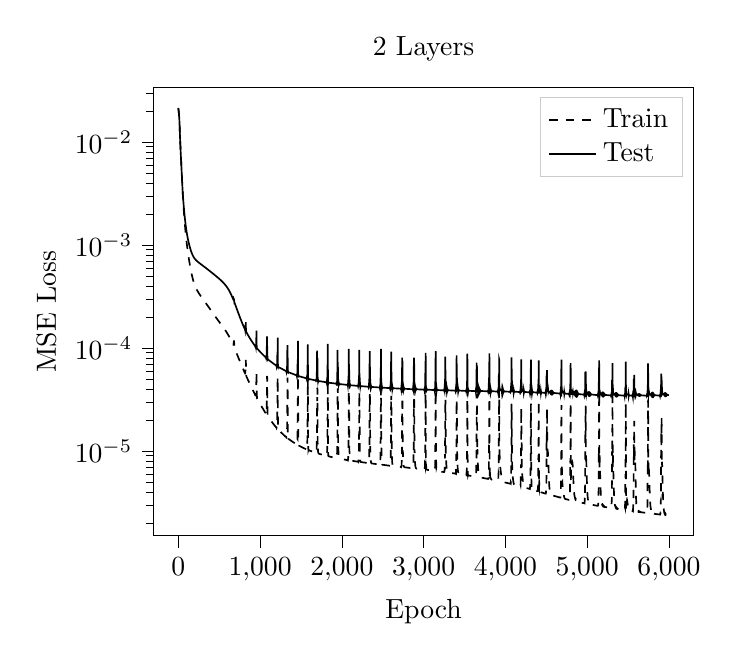
\begin{tikzpicture}

\begin{axis}[
legend cell align={left},
legend style={fill opacity=0.8, draw opacity=1, text opacity=1, draw=white!80!black},
log basis y={10},
tick align=outside,
tick pos=left,
title={2 Layers},
x grid style={white!69.0196078431373!black},
xlabel={Epoch},
xmin=-299.95, xmax=6298.95,
xtick style={color=black},
y grid style={white!69.0196078431373!black},
ylabel={MSE Loss},
ymin=1.49876339532141e-06, ymax=0.0337766142020771,
ymode=log,
ytick style={color=black}
]
\addplot [semithick, black, dashed]
table {%
0 0.0212835291167721
1 0.0209709201008081
2 0.0206604937557131
3 0.0203468892723322
4 0.0200276001123711
5 0.0197003402281553
6 0.0193627760745585
7 0.0190122253261507
8 0.0186453343485482
9 0.018257693038322
10 0.0178435965790413
11 0.0173961486434564
12 0.0169080773484893
13 0.0163732900400646
14 0.0157890768605284
15 0.0151585350977257
16 0.0144921822356991
17 0.0138077663723379
18 0.0131277163745835
19 0.0124744565982837
20 0.0118649328360334
21 0.0113068613864016
22 0.0107990419783164
23 0.0103351587895304
24 0.00990795821417123
25 0.00951141366385855
26 0.00914097490021959
27 0.00879311389871873
28 0.00846492176060565
29 0.00815390821662731
30 0.0078579168766737
31 0.00757508585229516
32 0.0073038155969698
33 0.00704274249437731
34 0.0067907179472968
35 0.00654679370927624
36 0.00631021165463608
37 0.00608039209328126
38 0.00585692764434498
39 0.0056395746069029
40 0.00542824204603676
41 0.00522296805866063
42 0.00502390101610217
43 0.00483126989274751
44 0.00464535255741794
45 0.0044664430024568
46 0.00429481566243339
47 0.0041306984203402
48 0.00397424669063184
49 0.00382552624068921
50 0.00368450347014004
51 0.00355104677146301
52 0.00342493510106578
53 0.00330586984637193
54 0.00319349668279756
55 0.00308742181368871
56 0.00298723114246968
57 0.00289250764035387
58 0.00280284290784039
59 0.00271784712822409
60 0.00263715513574425
61 0.00256043241097359
62 0.00248737349465955
63 0.00241770431603072
64 0.00235117984993849
65 0.0022875825088704
66 0.00222671995288692
67 0.00216842070221901
68 0.00211253295856295
69 0.00205892113444861
70 0.00200746243353933
71 0.00195804541726829
72 0.00191056720359484
73 0.00186493250657804
74 0.0018210515663668
75 0.00177884013100993
76 0.0017382187070325
77 0.00169911208649864
78 0.00166144936156343
79 0.00162516390992096
80 0.00159019229613477
81 0.00155647517749458
82 0.00152395624900237
83 0.0014925822179066
84 0.00146230302198092
85 0.00143307093821932
86 0.00140484069925151
87 0.00137756968979375
88 0.00135121732091648
89 0.00132574438248412
90 0.0013011138253205
91 0.00127729073210503
92 0.00125424084762926
93 0.00123193179024383
94 0.0012103327026125
95 0.00118941368054948
96 0.00116914581667515
97 0.00114950210263487
98 0.00113045599573525
99 0.00111198268496082
100 0.00109405747207347
101 0.001076657903468
102 0.00105976162922161
103 0.00104334752904833
104 0.00102739570320409
105 0.00101188684311637
106 0.000996802940790076
107 0.000982126501185121
108 0.000967841358942678
109 0.000953931703406852
110 0.000940382613407564
111 0.000927179975406034
112 0.00091431058535818
113 0.000901761790373712
114 0.000889521421413519
115 0.000877578177096439
116 0.000865921165313921
117 0.000854539954161737
118 0.00084342502123036
119 0.000832567187899258
120 0.000821957301013754
121 0.000811587156931637
122 0.000801448784841341
123 0.000791534812378814
124 0.000781837961767451
125 0.000772351286286721
126 0.000763068481319351
127 0.000753983182221418
128 0.000745089619158534
129 0.000736381889510085
130 0.000727854980141274
131 0.000719503657819587
132 0.000711322942152037
133 0.000703308222000487
134 0.00069545500264212
135 0.000687759107677266
136 0.000680216387991095
137 0.000672822949127294
138 0.000665574953018222
139 0.000658469014524599
140 0.000651501652100706
141 0.000644669500616146
142 0.000637969569652341
143 0.00063139878147922
144 0.000624954182057991
145 0.000618633132035029
146 0.00061243284289958
147 0.000606350933594513
148 0.000600384812059929
149 0.000594532228205935
150 0.000588790827350749
151 0.000583158471272327
152 0.000577633250031795
153 0.000572212878068967
154 0.000566895577321702
155 0.000561679484235356
156 0.000556562861675047
157 0.000551543812434829
158 0.000546620746717963
159 0.000541792177500611
160 0.000537056354005472
161 0.000532411843778391
162 0.000527857301676704
163 0.000523391223396175
164 0.000519012070071767
165 0.000514718762133271
166 0.000510509913510759
167 0.00050638417906157
168 0.000502340313687455
169 0.000498377177791554
170 0.000494493579026312
171 0.000490688227728242
172 0.000486959947011201
173 0.000483307637296093
174 0.000479730210827256
175 0.000476226341561414
176 0.000472795103632961
177 0.000469435270133545
178 0.000466145657810557
179 0.000462925217107113
180 0.000459772802969383
181 0.000456687198493455
182 0.00045366736685537
183 0.000450712132078479
184 0.000447820332738047
185 0.000444990751930163
186 0.000442222256424429
187 0.000439513644778344
188 0.000436863762843132
189 0.000434271428275679
190 0.000431735400525213
191 0.000429254400842183
192 0.000426827363298798
193 0.000424452950028353
194 0.000422129868638876
195 0.00041985699954239
196 0.000417633137658413
197 0.000415456985138007
198 0.000413327252317686
199 0.000411242761401809
200 0.000409202270020614
201 0.000407204591283516
202 0.000405248494644184
203 0.000403332782298094
204 0.000401456267354661
205 0.000399617719267553
206 0.000397816037548182
207 0.000396050035305962
208 0.000394318637518154
209 0.000392620709135372
210 0.000390955163311446
211 0.000389320898648293
212 0.000387716946534056
213 0.000386142261049827
214 0.000384595800824172
215 0.000383076668185822
216 0.000381583879971004
217 0.000380116502128658
218 0.000378673728846479
219 0.000377254610611999
220 0.000375858355255332
221 0.000374484189705981
222 0.000373131245396507
223 0.000371798872038198
224 0.00037048621015856
225 0.00036919266131008
226 0.000367917541552742
227 0.000366660158761078
228 0.000365419830814062
229 0.000364196102964343
230 0.000362988326742197
231 0.000361795916433039
232 0.000360618317245098
233 0.000359455096258898
234 0.000358305675945303
235 0.000357169661583612
236 0.000356046508386498
237 0.000354935875293449
238 0.000353837280272273
239 0.000352750322235806
240 0.000351674641933641
241 0.000350609845554573
242 0.000349555614320707
243 0.000348511529409734
244 0.000347477314335265
245 0.000346452682606468
246 0.000345437299984042
247 0.000344430845416355
248 0.000343433106991142
249 0.000342443785484647
250 0.00034146259940826
251 0.000340489317750325
252 0.000339523713137169
253 0.000338565578658745
254 0.000337614693307842
255 0.000336670759679691
256 0.000335733682732098
257 0.000334803171426756
258 0.000333879145728133
259 0.000332961301410251
260 0.000332049531152734
261 0.000331143702169356
262 0.000330243582538969
263 0.000329349081312102
264 0.000328459986121743
265 0.000327576157815201
266 0.000326697446325852
267 0.000325823801631486
268 0.000324954977713787
269 0.000324090905451158
270 0.000323231467064033
271 0.000322376559779514
272 0.000321526030802488
273 0.000320679730066331
274 0.000319837633014686
275 0.000318999605497083
276 0.000318165566568496
277 0.000317335358886339
278 0.000316508972446172
279 0.000315686233534507
280 0.000314867138968111
281 0.000314051535951876
282 0.000313239377646823
283 0.000312430555823084
284 0.000311625043650565
285 0.000310822694700619
286 0.00031002349260234
287 0.000309227326852124
288 0.000308434162434423
289 0.000307643951600767
290 0.000306856613860873
291 0.000306072059629514
292 0.000305290267988312
293 0.000304511192098289
294 0.000303734711451398
295 0.000302960817862186
296 0.000302189495869243
297 0.000301420629966742
298 0.000300654196507821
299 0.000299890170936123
300 0.000299128453661979
301 0.000298369082884165
302 0.000297611956284527
303 0.000296857044304488
304 0.000296104348763038
305 0.00029535374869738
306 0.000294605310500629
307 0.000293858930490387
308 0.000293114578198583
309 0.000292372245894512
310 0.000291631909931311
311 0.000290893471628806
312 0.000290157015115255
313 0.00028942244080099
314 0.000288689738226822
315 0.000287958839180646
316 0.000287229798686894
317 0.000286502543076494
318 0.000285777067801973
319 0.000285053336483543
320 0.00028433132729333
321 0.000283611043414567
322 0.000282892443919991
323 0.000282175550637476
324 0.000281460283531487
325 0.00028074666761313
326 0.000280034712886845
327 0.000279324344319321
328 0.000278615579190955
329 0.000277908417501749
330 0.000277202803772525
331 0.00027649878666125
332 0.000275796291134611
333 0.000275095383130974
334 0.000274395958058449
335 0.000273698045475612
336 0.000273001670393569
337 0.000272306785518595
338 0.000271613438599161
339 0.000270921532774082
340 0.00027023115353586
341 0.000269542266323697
342 0.000268854797013773
343 0.000268168811089708
344 0.000267484311279986
345 0.00026680126438805
346 0.000266119655861985
347 0.000265439519807842
348 0.000264760818936338
349 0.000264083599176956
350 0.000263407777765678
351 0.000262733398812998
352 0.000262060460954672
353 0.000261389004208468
354 0.000260718962181272
355 0.000260050356700958
356 0.000259383179809447
357 0.00025871745265249
358 0.000258053147035753
359 0.000257390274782665
360 0.000256728878639478
361 0.000256068846510971
362 0.000255410300724179
363 0.000254753194894874
364 0.00025409756449335
365 0.00025344332630084
366 0.000252790539207126
367 0.000252139207532309
368 0.000251489334232247
369 0.000250840912713102
370 0.000250193932743059
371 0.000249548391821008
372 0.000248904350200974
373 0.000248261751039536
374 0.000247620606614873
375 0.000246980962629095
376 0.000246342738137173
377 0.000245706064561091
378 0.000245070803657654
379 0.000244437061382996
380 0.000243804778392587
381 0.000243173983108136
382 0.000242544692355295
383 0.000241916904087702
384 0.000241290593066879
385 0.00024066579430837
386 0.000240042484392688
387 0.000239420719481132
388 0.00023880043590907
389 0.000238181705981333
390 0.000237564478766217
391 0.000236948768133516
392 0.000236334597957466
393 0.000235721970057057
394 0.000235110862149668
395 0.000234501306067614
396 0.000233893292488574
397 0.000233286828233759
398 0.000232681912621047
399 0.000232078536782865
400 0.00023147675187829
401 0.000230876489467846
402 0.000230277823447977
403 0.000229680716074654
404 0.000229085205319279
405 0.000228491238203787
406 0.000227898853381703
407 0.000227308074954635
408 0.000226718850854013
409 0.00022613124815507
410 0.000225545247303671
411 0.000224960824652953
412 0.000224377980202917
413 0.000223796763521023
414 0.000223217161192224
415 0.000222639147978043
416 0.000222062747525342
417 0.000221487964836342
418 0.000220914781266401
419 0.000220343206819962
420 0.00021977328333378
421 0.000219204961695141
422 0.00021863827805646
423 0.000218073168298361
424 0.00021750975906798
425 0.000216947934404743
426 0.000216387733189549
427 0.000215829196349659
428 0.000215272255218224
429 0.000214716957316341
430 0.000214163296732295
431 0.000213611262779523
432 0.000213060887517713
433 0.000212512133884957
434 0.000211965010521453
435 0.00021141953584447
436 0.000210875673701594
437 0.000210333495488157
438 0.000209792890700555
439 0.000209253949378763
440 0.000208716653560259
441 0.000208180989375251
442 0.000207646947956164
443 0.000207114552949861
444 0.000206583779799985
445 0.000206054658974608
446 0.000205527158641416
447 0.000205001271979199
448 0.00020447701899684
449 0.000203954396056361
450 0.000203433382921503
451 0.00020291398777772
452 0.000202396238364599
453 0.000201880081931449
454 0.000201365517114027
455 0.00020085259939151
456 0.000200341276467952
457 0.000199831560848907
458 0.00019932342456741
459 0.000198816901956889
460 0.000198311955955432
461 0.000197808621010154
462 0.000197306861082325
463 0.000196806678218309
464 0.000196308070940177
465 0.000195811017420056
466 0.000195315541077434
467 0.000194821637478526
468 0.000194329267060311
469 0.00019383846290566
470 0.00019334919954872
471 0.00019286146880404
472 0.000192375271581113
473 0.000191890600035549
474 0.000191407439729119
475 0.000190925796687225
476 0.000190445680573248
477 0.000189967021469784
478 0.0001894898870205
479 0.000189014217880867
480 0.000188540029171236
481 0.000188067305202821
482 0.000187596055184258
483 0.000187126251148584
484 0.000186657883546104
485 0.000186190972158329
486 0.000185725460937647
487 0.000185261374667789
488 0.000184798706982292
489 0.000184337417294955
490 0.000183877531753751
491 0.000183419036602572
492 0.000182961882501331
493 0.000182506102419211
494 0.000182051671913541
495 0.000181598564267915
496 0.000181146790396269
497 0.00018069633927098
498 0.000180247191451599
499 0.000179799328293484
500 0.000179352746499717
501 0.000178907439590148
502 0.000178463376983018
503 0.000178020571411253
504 0.000177578992861527
505 0.000177138630874651
506 0.000176699482608456
507 0.000176261518163301
508 0.000175824737652874
509 0.00017538913948556
510 0.000174954689100559
511 0.000174521354892931
512 0.000174089162328528
513 0.000173658060930393
514 0.000173228072526399
515 0.000172799163010495
516 0.000172371311691677
517 0.000171944514136158
518 0.000171518747720256
519 0.000171094000393168
520 0.00017067026112727
521 0.000170247502410348
522 0.000169825703324022
523 0.000169404866028344
524 0.000168984988022203
525 0.000168566005754656
526 0.000168147926956408
527 0.000167730754810691
528 0.000167314430996157
529 0.000166898949601091
530 0.000166484299825242
531 0.000166070492014114
532 0.000165657448178536
533 0.000165245200491881
534 0.000164833710869061
535 0.000164422951343113
536 0.000164012900540911
537 0.00016360359063583
538 0.000163194935225874
539 0.000162786918394886
540 0.000162379573907856
541 0.000161972838668589
542 0.000161566704150573
543 0.0001611611652379
544 0.000160756166224019
545 0.000160351704266759
546 0.000159947766405821
547 0.000159544339226159
548 0.000159141367248594
549 0.000158738846721462
550 0.0001583367669582
551 0.000157935101015028
552 0.000157533826154577
553 0.000157132900426404
554 0.000156732324626319
555 0.000156332058850239
556 0.000155932104689782
557 0.000155532416442838
558 0.000155132973418404
559 0.000154733789827333
560 0.000154334783701415
561 0.000153935975390596
562 0.000153537325900288
563 0.000153138796122221
564 0.000152740397311391
565 0.000152342085812052
566 0.000151943816263156
567 0.000151545616290605
568 0.000151147423196107
569 0.000150749227032065
570 0.000150350987439651
571 0.000149952702145129
572 0.000149554328061186
573 0.000149155862288808
574 0.000148757270835631
575 0.000148358524143077
576 0.000147959615389937
577 0.000147560498703569
578 0.000147161141910601
579 0.00014676156411042
580 0.000146361690553931
581 0.000145961517205251
582 0.000145561032184105
583 0.000145160233387287
584 0.000144759042939313
585 0.000144357475448942
586 0.000143955486976211
587 0.000143553048644662
588 0.000143150158805838
589 0.000142746790913861
590 0.000142342901995107
591 0.000141938516378559
592 0.000141533546241135
593 0.000141128024040427
594 0.000140721892023521
595 0.00014031516252544
596 0.000139907767902514
597 0.000139499729243653
598 0.000139091010169068
599 0.000138681571570487
600 0.000138271436469495
601 0.000137860556321812
602 0.000137448898328785
603 0.000137036466753671
604 0.000136623274613612
605 0.000136209213053462
606 0.000135794349546359
607 0.000135378641687112
608 0.000134962033826014
609 0.000134544553418436
610 0.000134126206887686
611 0.000133706905046438
612 0.000133286677737487
613 0.000132865575210417
614 0.000132443432448781
615 0.000132020353021289
616 0.000131596364440156
617 0.0001311712618417
618 0.000130745207854943
619 0.000130318246533534
620 0.000129890120319942
621 0.000129460998152808
622 0.000129031021856463
623 0.000128599785625738
624 0.000128167531784129
625 0.000127734460875217
626 0.000127300062388258
627 0.000126864648677838
628 0.000126428511464383
629 0.000125990946969523
630 0.000125552300346499
631 0.000125113127012355
632 0.000124672398214898
633 0.000124230474511933
634 0.000123788367432098
635 0.000123344523615287
636 0.000122899294126455
637 0.000122454416839446
638 0.000122007555717119
639 0.000121558966895918
640 0.000121111522730644
641 0.00012066183484194
642 0.000120209703595719
643 0.000119760050893092
644 0.000119307866839335
645 0.000118851873594394
646 0.000118400442659095
647 0.000117946346279041
648 0.00011748591577998
649 0.000117033311994419
650 0.000116578293614111
651 0.000116112402508861
652 0.000115659428502113
653 0.000115205272379626
654 0.000114732217241453
655 0.0001142799800391
656 0.000113829913743757
657 0.000113347268268171
658 0.000112897413316659
659 0.000112457237776198
660 0.000111962505059182
661 0.000111518200810679
662 0.000111098184731873
663 0.000110593016643179
664 0.000110161510917806
665 0.000109779833223911
666 0.000109286403016995
667 0.000108886284067466
668 0.000108577541595878
669 0.00010819459242839
670 0.00010787321468797
671 0.000107718260949241
672 0.000107785517116099
673 0.000107656141949519
674 0.000107900192176658
675 0.000109297616688764
676 0.000109578056537885
677 0.000110879725241375
678 0.000114251636830431
679 0.000114603493557297
680 0.000116473329626388
681 0.000116469009526554
682 0.000113329918349336
683 0.000112076105438064
684 0.000107009406065117
685 0.0001026171223657
686 0.000101317310566174
687 0.000100158012173779
688 9.9327592863574e-05
689 9.8789685068823e-05
690 9.83735112640716e-05
691 9.79368714411066e-05
692 9.75170637502742e-05
693 9.70842903598168e-05
694 9.66536702549092e-05
695 9.62349453175193e-05
696 9.58054440616252e-05
697 9.53838317627742e-05
698 9.4963705180362e-05
699 9.45420809443931e-05
700 9.4123706787741e-05
701 9.37060037813353e-05
702 9.32894906782167e-05
703 9.28744348698274e-05
704 9.24606716239396e-05
705 9.20483371942282e-05
706 9.16373142558768e-05
707 9.12278061377947e-05
708 9.08197532112354e-05
709 9.04131520087503e-05
710 9.00080966061978e-05
711 8.96045759759545e-05
712 8.9202608648975e-05
713 8.88022374851971e-05
714 8.84034880641593e-05
715 8.80063685713139e-05
716 8.76109128853386e-05
717 8.72171136734323e-05
718 8.68250134544724e-05
719 8.64346214370926e-05
720 8.60459674072445e-05
721 8.56590414741731e-05
722 8.52738768912786e-05
723 8.4890469054244e-05
724 8.45088619598755e-05
725 8.41290383277737e-05
726 8.37510245901285e-05
727 8.33748067066153e-05
728 8.30004177032606e-05
729 8.26278564431959e-05
730 8.22571327034893e-05
731 8.18882298290191e-05
732 8.15211780604841e-05
733 8.11559680755636e-05
734 8.0792618518899e-05
735 8.04311118258738e-05
736 8.00714378215162e-05
737 7.97136295886958e-05
738 7.93576651290095e-05
739 7.90035527984401e-05
740 7.86512652553029e-05
741 7.8300844450041e-05
742 7.79522591756177e-05
743 7.76054826587824e-05
744 7.72605648649005e-05
745 7.69174453694177e-05
746 7.65761523098263e-05
747 7.62366663025205e-05
748 7.5898994509771e-05
749 7.55631047013594e-05
750 7.52290073933182e-05
751 7.48966893411307e-05
752 7.45661383803053e-05
753 7.42373434263754e-05
754 7.3910306923608e-05
755 7.3585018412814e-05
756 7.32614412299881e-05
757 7.29395892449247e-05
758 7.2619471723101e-05
759 7.2301013346987e-05
760 7.19842519742997e-05
761 7.16691951652138e-05
762 7.13557795393172e-05
763 7.10440105535781e-05
764 7.07339166865495e-05
765 7.0425407784569e-05
766 7.01185355183043e-05
767 6.98133043783855e-05
768 6.95095938567647e-05
769 6.92075005872539e-05
770 6.89070154180627e-05
771 6.8607992602665e-05
772 6.83105864709432e-05
773 6.80147480238702e-05
774 6.77202819474587e-05
775 6.74274557468379e-05
776 6.71361451054509e-05
777 6.68461250370456e-05
778 6.65577895802016e-05
779 6.62709173298026e-05
780 6.59851806403822e-05
781 6.57012569718063e-05
782 6.54186995348027e-05
783 6.51370916102678e-05
784 6.48575633590553e-05
785 6.45792111981791e-05
786 6.43015417836068e-05
787 6.40264204321284e-05
788 6.37521198427748e-05
789 6.34781316648514e-05
790 6.32075708040247e-05
791 6.29371293712211e-05
792 6.26665072331889e-05
793 6.24008608838267e-05
794 6.21339834196988e-05
795 6.18662135707382e-05
796 6.16062736185086e-05
797 6.13424347761793e-05
798 6.10767839930304e-05
799 6.08241289796752e-05
800 6.05623681622092e-05
801 6.02977937091964e-05
802 6.00555445089412e-05
803 5.97942158151454e-05
804 5.95295049379274e-05
805 5.93038477063601e-05
806 5.90402228226594e-05
807 5.87757228913688e-05
808 5.85789659339753e-05
809 5.83099006234988e-05
810 5.80555828264551e-05
811 5.79132693019346e-05
812 5.76401992589126e-05
813 5.74516344613585e-05
814 5.74205243992765e-05
815 5.71735995436029e-05
816 5.73002139390155e-05
817 5.75197896068858e-05
818 5.7453578165223e-05
819 5.88839302508859e-05
820 5.97032222060534e-05
821 6.04024381232193e-05
822 6.59345604958617e-05
823 6.74619723213254e-05
824 6.92578064729332e-05
825 7.6783088729826e-05
826 7.30325907625229e-05
827 6.98225327369073e-05
828 6.3422335301766e-05
829 5.65620411521195e-05
830 5.53574395212308e-05
831 5.41374883482604e-05
832 5.3012844659861e-05
833 5.28669662571701e-05
834 5.26105138476396e-05
835 5.24332158136076e-05
836 5.22052741303014e-05
837 5.19956660127718e-05
838 5.18026845952591e-05
839 5.15811403545285e-05
840 5.1385549141969e-05
841 5.118176676433e-05
842 5.09784324833618e-05
843 5.07801880189618e-05
844 5.05795478886739e-05
845 5.0381089010898e-05
846 5.01832527390889e-05
847 4.99861358491671e-05
848 4.97899528113521e-05
849 4.95944151452932e-05
850 4.93998708748222e-05
851 4.92059874090955e-05
852 4.90129492050073e-05
853 4.88207603552837e-05
854 4.86292692301049e-05
855 4.8438638486914e-05
856 4.82487916997343e-05
857 4.80596992531446e-05
858 4.78714345035769e-05
859 4.76839416592156e-05
860 4.74972141546459e-05
861 4.73113163650396e-05
862 4.71261658674393e-05
863 4.69418013437917e-05
864 4.67582445367043e-05
865 4.65754186507183e-05
866 4.63933991170506e-05
867 4.62121705879781e-05
868 4.60316833823526e-05
869 4.58520003405738e-05
870 4.56730841449371e-05
871 4.54949240804581e-05
872 4.53175552479479e-05
873 4.51409566153416e-05
874 4.49651157907738e-05
875 4.47900653455235e-05
876 4.46157698945626e-05
877 4.44422425118773e-05
878 4.42694817763822e-05
879 4.40974888533674e-05
880 4.39262555289588e-05
881 4.37557942802869e-05
882 4.35860818299716e-05
883 4.34171467134092e-05
884 4.32489565582728e-05
885 4.30815402125972e-05
886 4.29148618366071e-05
887 4.27489674734716e-05
888 4.2583806134644e-05
889 4.24194095671737e-05
890 4.22557807553403e-05
891 4.2092871154864e-05
892 4.19307309300621e-05
893 4.17693398730989e-05
894 4.16086821246608e-05
895 4.14487880391334e-05
896 4.12896411887687e-05
897 4.11311987988938e-05
898 4.09735466746497e-05
899 4.08166019667533e-05
900 4.06603694500518e-05
901 4.05049458720441e-05
902 4.03501765049441e-05
903 4.0196160313144e-05
904 4.00429349269871e-05
905 3.98903249845262e-05
906 3.97384984296423e-05
907 3.95874538128282e-05
908 3.94369548359919e-05
909 3.92873271835015e-05
910 3.91384394617944e-05
911 3.89900107506946e-05
912 3.88426049937607e-05
913 3.8695816613199e-05
914 3.85494158479105e-05
915 3.84042674852481e-05
916 3.82595014798426e-05
917 3.8115048681675e-05
918 3.79722781644887e-05
919 3.78293624123671e-05
920 3.76868523801477e-05
921 3.75466484570097e-05
922 3.7405251276823e-05
923 3.72647408255489e-05
924 3.71274040276148e-05
925 3.69869295866465e-05
926 3.68486941795254e-05
927 3.67147253541589e-05
928 3.65739716414737e-05
929 3.64388962736939e-05
930 3.63090271662259e-05
931 3.61657584164732e-05
932 3.60360099875834e-05
933 3.59113325885119e-05
934 3.57615912491838e-05
935 3.56420959803927e-05
936 3.5524546774468e-05
937 3.5362238605785e-05
938 3.52634807541108e-05
939 3.51577418200577e-05
940 3.49783750550614e-05
941 3.49213352137667e-05
942 3.48419375200137e-05
943 3.46695783264295e-05
944 3.46965336177618e-05
945 3.46883942086151e-05
946 3.47127681550319e-05
947 3.49330067308529e-05
948 3.51135918492673e-05
949 3.62745781501417e-05
950 3.71210029186386e-05
951 3.77143524588064e-05
952 4.34279637602231e-05
953 4.62504493157212e-05
954 4.71086129323339e-05
955 5.94989059834461e-05
956 5.93012429135342e-05
957 5.47628900449126e-05
958 4.90509355302038e-05
959 3.82615310456913e-05
960 3.57851230319284e-05
961 3.4583016599754e-05
962 3.26616389259016e-05
963 3.24346934235109e-05
964 3.22145002087382e-05
965 3.21614615756971e-05
966 3.20025341693508e-05
967 3.1905695976775e-05
968 3.17969511058891e-05
969 3.16800213226998e-05
970 3.15867085589616e-05
971 3.14754261694361e-05
972 3.13757444985185e-05
973 3.1273503623197e-05
974 3.11717871852579e-05
975 3.10711404836184e-05
976 3.09701569563003e-05
977 3.08704915710223e-05
978 3.07703946589299e-05
979 3.06712478277404e-05
980 3.05723940527969e-05
981 3.04737512522024e-05
982 3.03757973654228e-05
983 3.02780501044708e-05
984 3.01807411631216e-05
985 3.00838802615999e-05
986 2.99873392464178e-05
987 2.98912323160039e-05
988 2.97954998984551e-05
989 2.97001417663978e-05
990 2.9605172585434e-05
991 2.9510582066905e-05
992 2.94163691876292e-05
993 2.93225432415056e-05
994 2.92290737178291e-05
995 2.91359811086522e-05
996 2.90432614349356e-05
997 2.89509039816949e-05
998 2.88589216665969e-05
999 2.87672941965411e-05
1000 2.86760442662626e-05
1001 2.85851468220244e-05
1002 2.84946171973388e-05
1003 2.84044312053311e-05
1004 2.83146067374673e-05
1005 2.82251532439659e-05
1006 2.81360373293182e-05
1007 2.80472867615345e-05
1008 2.79588877702963e-05
1009 2.78708289442875e-05
1010 2.77831272796902e-05
1011 2.76957675282574e-05
1012 2.76087558148674e-05
1013 2.75220954222277e-05
1014 2.74357764880051e-05
1015 2.7349785966635e-05
1016 2.72641452028211e-05
1017 2.71788500612047e-05
1018 2.70938873967452e-05
1019 2.7009263632749e-05
1020 2.69249810571637e-05
1021 2.68410105803696e-05
1022 2.67574045409447e-05
1023 2.66741054275599e-05
1024 2.65911451577949e-05
1025 2.65085232342699e-05
1026 2.64262227602785e-05
1027 2.6344233347686e-05
1028 2.62626051608095e-05
1029 2.6181270897041e-05
1030 2.61002657140352e-05
1031 2.60196053432082e-05
1032 2.59392241730438e-05
1033 2.58591913251394e-05
1034 2.57794985998316e-05
1035 2.57000704237953e-05
1036 2.5621009243082e-05
1037 2.55422429233931e-05
1038 2.54637504184529e-05
1039 2.53856669871766e-05
1040 2.53078196692513e-05
1041 2.5230256511577e-05
1042 2.51531465664812e-05
1043 2.50761725908433e-05
1044 2.4999569561146e-05
1045 2.49234289668721e-05
1046 2.48472686905643e-05
1047 2.47716665455755e-05
1048 2.46964720531651e-05
1049 2.46210494765364e-05
1050 2.45465723196503e-05
1051 2.44722288158528e-05
1052 2.43974674276615e-05
1053 2.43243403446058e-05
1054 2.42506016832067e-05
1055 2.41764897737085e-05
1056 2.41050937148657e-05
1057 2.40313925417013e-05
1058 2.39581931538169e-05
1059 2.38890914374679e-05
1060 2.38142129092012e-05
1061 2.37429377989429e-05
1062 2.367688247773e-05
1063 2.35984988847804e-05
1064 2.35319306653992e-05
1065 2.34698215280105e-05
1066 2.33843106940412e-05
1067 2.33286351658535e-05
1068 2.32718803516718e-05
1069 2.31776480887902e-05
1070 2.31446065299679e-05
1071 2.30954374274006e-05
1072 2.3015544073246e-05
1073 2.3030252918943e-05
1074 2.29827125224347e-05
1075 2.3067924814768e-05
1076 2.32428892701364e-05
1077 2.31147555780353e-05
1078 2.3996751821187e-05
1079 2.50564360584349e-05
1080 2.44874114088134e-05
1081 2.79896395483092e-05
1082 3.34105169770282e-05
1083 3.22522711684314e-05
1084 3.97968647831703e-05
1085 5.34463645749383e-05
1086 5.26126714248676e-05
1087 5.10330321503716e-05
1088 4.15302602476686e-05
1089 3.16319235196261e-05
1090 2.85177275998194e-05
1091 2.46126399474633e-05
1092 2.23692249079477e-05
1093 2.19217270824856e-05
1094 2.19858800249995e-05
1095 2.17810468825519e-05
1096 2.16880937387032e-05
1097 2.15006482733315e-05
1098 2.14564986436017e-05
1099 2.13896479266396e-05
1100 2.13400927151497e-05
1101 2.12832223809301e-05
1102 2.12312697271955e-05
1103 2.11776651752871e-05
1104 2.11232915319215e-05
1105 2.10718370965424e-05
1106 2.10180317594677e-05
1107 2.09660569225889e-05
1108 2.09136353248596e-05
1109 2.0861629849378e-05
1110 2.08097463172408e-05
1111 2.07580746121039e-05
1112 2.07066356523455e-05
1113 2.06552842456631e-05
1114 2.06042395660688e-05
1115 2.05532958972299e-05
1116 2.05025573478679e-05
1117 2.04520004558617e-05
1118 2.04016195510803e-05
1119 2.0351423316356e-05
1120 2.03013966881826e-05
1121 2.02515423524119e-05
1122 2.02018610195864e-05
1123 2.0152355844516e-05
1124 2.01030267845681e-05
1125 2.00538609789191e-05
1126 2.00048716010315e-05
1127 1.99560537055277e-05
1128 1.99074008122579e-05
1129 1.98589204245536e-05
1130 1.98105985873553e-05
1131 1.97624556932396e-05
1132 1.97144729696674e-05
1133 1.9666662424811e-05
1134 1.9619007545657e-05
1135 1.95715231967597e-05
1136 1.95242037364096e-05
1137 1.94770496619867e-05
1138 1.94300539106962e-05
1139 1.93832319723697e-05
1140 1.93365569032267e-05
1141 1.9290059427135e-05
1142 1.92437121881994e-05
1143 1.91975357353158e-05
1144 1.91515198793013e-05
1145 1.91056510630006e-05
1146 1.90599585465634e-05
1147 1.90144107961032e-05
1148 1.89690371144025e-05
1149 1.89238210452913e-05
1150 1.88787476673724e-05
1151 1.8833844137589e-05
1152 1.87890962166648e-05
1153 1.87444927632896e-05
1154 1.87000772911006e-05
1155 1.86557851975522e-05
1156 1.86116614457887e-05
1157 1.85677008062157e-05
1158 1.8523875027654e-05
1159 1.84802266858242e-05
1160 1.84367256252926e-05
1161 1.83933616426657e-05
1162 1.83501744004388e-05
1163 1.83071235397847e-05
1164 1.82642167771974e-05
1165 1.82215015200882e-05
1166 1.81788800830418e-05
1167 1.8136449526196e-05
1168 1.80941869984963e-05
1169 1.80519938055568e-05
1170 1.80100504820757e-05
1171 1.79682040055695e-05
1172 1.7926458994566e-05
1173 1.78850087877436e-05
1174 1.78435474538219e-05
1175 1.7802275209533e-05
1176 1.77613137140042e-05
1177 1.77201705611196e-05
1178 1.76794459179064e-05
1179 1.76389299184621e-05
1180 1.75980749332894e-05
1181 1.75580255614705e-05
1182 1.75177940917592e-05
1183 1.74772407888213e-05
1184 1.74380731294832e-05
1185 1.73977736892539e-05
1186 1.73578032587329e-05
1187 1.73196650194996e-05
1188 1.72786620709076e-05
1189 1.7240084758896e-05
1190 1.7202904373903e-05
1191 1.71603114011987e-05
1192 1.71248964733195e-05
1193 1.70879218117648e-05
1194 1.70437000335255e-05
1195 1.70142290158992e-05
1196 1.69747735583314e-05
1197 1.69348703096261e-05
1198 1.69163993319899e-05
1199 1.6864487292878e-05
1200 1.68554062227599e-05
1201 1.68732388061699e-05
1202 1.67812876625817e-05
1203 1.68634318598038e-05
1204 1.70648097324033e-05
1205 1.69621649277474e-05
1206 1.71480264228308e-05
1207 1.80765712798348e-05
1208 1.88761268589133e-05
1209 1.89988255101525e-05
1210 2.14257015755948e-05
1211 2.83444005901856e-05
1212 3.03315529350812e-05
1213 3.2029213159035e-05
1214 4.94456834161383e-05
1215 5.26222975167911e-05
1216 4.57585651929548e-05
1217 3.57277575915305e-05
1218 2.1234510391821e-05
1219 1.77151128895048e-05
1220 1.71958521377746e-05
1221 1.63123360437112e-05
1222 1.62258578342289e-05
1223 1.61946954762016e-05
1224 1.61702844607703e-05
1225 1.60801882387318e-05
1226 1.6034826295197e-05
1227 1.596839572926e-05
1228 1.59452682026995e-05
1229 1.59121711362786e-05
1230 1.5884068616856e-05
1231 1.58541725738814e-05
1232 1.58256273152801e-05
1233 1.57968142957543e-05
1234 1.57675923162515e-05
1235 1.57395529569726e-05
1236 1.57106097660176e-05
1237 1.56824221591023e-05
1238 1.56541203395477e-05
1239 1.56258806711662e-05
1240 1.55978421005898e-05
1241 1.55698074451038e-05
1242 1.55419083540664e-05
1243 1.55140806938903e-05
1244 1.54863427965779e-05
1245 1.54586842100457e-05
1246 1.54311105546867e-05
1247 1.54036136947866e-05
1248 1.53762062922169e-05
1249 1.53488711234218e-05
1250 1.53216174183513e-05
1251 1.52944399332e-05
1252 1.52673392719294e-05
1253 1.52403156263858e-05
1254 1.52133730111359e-05
1255 1.51865004056617e-05
1256 1.51597133069004e-05
1257 1.51329872508654e-05
1258 1.51063405127161e-05
1259 1.50797711953032e-05
1260 1.50532748151022e-05
1261 1.50268502991935e-05
1262 1.50004939030168e-05
1263 1.49742159507582e-05
1264 1.49480169611138e-05
1265 1.49218832916631e-05
1266 1.48958247905284e-05
1267 1.48698330377783e-05
1268 1.48439161051783e-05
1269 1.48180806149867e-05
1270 1.47923009592432e-05
1271 1.47665972463074e-05
1272 1.47409724107206e-05
1273 1.47154046317155e-05
1274 1.46899257913446e-05
1275 1.46644984369004e-05
1276 1.4639145298645e-05
1277 1.46138720964473e-05
1278 1.45886549418606e-05
1279 1.45635150659018e-05
1280 1.45384582026509e-05
1281 1.45134481499554e-05
1282 1.44885170527687e-05
1283 1.44636595322822e-05
1284 1.44388506271298e-05
1285 1.44141373610296e-05
1286 1.43894734776495e-05
1287 1.43648794974638e-05
1288 1.43403801473596e-05
1289 1.43159008558769e-05
1290 1.429152574417e-05
1291 1.42672267031685e-05
1292 1.42429312077752e-05
1293 1.42187935878724e-05
1294 1.41946679690363e-05
1295 1.41705657838997e-05
1296 1.4146682666194e-05
1297 1.41226843339837e-05
1298 1.40988330272762e-05
1299 1.40751681172446e-05
1300 1.40512552988525e-05
1301 1.40277575226833e-05
1302 1.40042204179736e-05
1303 1.39804017322831e-05
1304 1.39573891999589e-05
1305 1.39337599520672e-05
1306 1.39102184562034e-05
1307 1.38877578521601e-05
1308 1.38636158837357e-05
1309 1.38409881671464e-05
1310 1.38189123433108e-05
1311 1.37937922204401e-05
1312 1.37732359846154e-05
1313 1.37508451132362e-05
1314 1.37254439778189e-05
1315 1.37082435074376e-05
1316 1.36832342363391e-05
1317 1.36640856780446e-05
1318 1.36528606660136e-05
1319 1.3617125240728e-05
1320 1.36238472592254e-05
1321 1.36419242053876e-05
1322 1.35895228652316e-05
1323 1.36352188064848e-05
1324 1.37862029276903e-05
1325 1.38938374547593e-05
1326 1.39356142980773e-05
1327 1.43067451716661e-05
1328 1.57947242200862e-05
1329 1.66386500097815e-05
1330 1.641833552668e-05
1331 2.21109084890259e-05
1332 3.04171362586203e-05
1333 3.01076619280138e-05
1334 3.45073318257505e-05
1335 4.91547483605359e-05
1336 5.15744175118016e-05
1337 4.48025859896006e-05
1338 2.98069395512357e-05
1339 1.58800857974484e-05
1340 1.34702957268473e-05
1341 1.38357369863229e-05
1342 1.35945819437211e-05
1343 1.34899305521685e-05
1344 1.32207643730453e-05
1345 1.31636951365977e-05
1346 1.31409235564206e-05
1347 1.31245692429616e-05
1348 1.31012074788828e-05
1349 1.30834871683305e-05
1350 1.30593101559384e-05
1351 1.30439216334821e-05
1352 1.30255464014795e-05
1353 1.30088795842198e-05
1354 1.29912015012223e-05
1355 1.29747261183866e-05
1356 1.29573943681294e-05
1357 1.29407151661098e-05
1358 1.29238836024115e-05
1359 1.29071496886013e-05
1360 1.28904723482037e-05
1361 1.28738563844877e-05
1362 1.28572707822627e-05
1363 1.28407266615227e-05
1364 1.28242414163537e-05
1365 1.28077851471176e-05
1366 1.27913807119739e-05
1367 1.27750044569552e-05
1368 1.27586749982811e-05
1369 1.27423742455335e-05
1370 1.2726104387184e-05
1371 1.2709879726458e-05
1372 1.26936954671919e-05
1373 1.26775413136215e-05
1374 1.26614145727899e-05
1375 1.26453173905361e-05
1376 1.26292720636911e-05
1377 1.26132497513254e-05
1378 1.25972640745431e-05
1379 1.25813047517909e-05
1380 1.2565380167473e-05
1381 1.25494887797117e-05
1382 1.25336311000979e-05
1383 1.25178034835471e-05
1384 1.25020029599909e-05
1385 1.24862419994543e-05
1386 1.24705143704773e-05
1387 1.24548104025735e-05
1388 1.2439140675724e-05
1389 1.2423503392256e-05
1390 1.24078897627555e-05
1391 1.23923219135236e-05
1392 1.23767733697377e-05
1393 1.23612557842989e-05
1394 1.23457776837199e-05
1395 1.23303225549876e-05
1396 1.23148964163988e-05
1397 1.22995077234123e-05
1398 1.22841465497459e-05
1399 1.22688115098413e-05
1400 1.2253516693761e-05
1401 1.22382386678055e-05
1402 1.22230037646887e-05
1403 1.22077947040111e-05
1404 1.21926083309631e-05
1405 1.21774706016708e-05
1406 1.21623456692532e-05
1407 1.21472559442282e-05
1408 1.21322014905445e-05
1409 1.21171697387013e-05
1410 1.21021752121919e-05
1411 1.20872052775667e-05
1412 1.20722583716315e-05
1413 1.2057359477069e-05
1414 1.20424716527623e-05
1415 1.20276269939268e-05
1416 1.20128121423591e-05
1417 1.19980062294189e-05
1418 1.19832682443644e-05
1419 1.19685263300084e-05
1420 1.19538215699322e-05
1421 1.19391783073297e-05
1422 1.19244939824625e-05
1423 1.1909918903541e-05
1424 1.18953408474454e-05
1425 1.18807312077251e-05
1426 1.18663064085922e-05
1427 1.18517460307999e-05
1428 1.18372650561582e-05
1429 1.18229631951294e-05
1430 1.18083664304436e-05
1431 1.17941315451731e-05
1432 1.17798570187233e-05
1433 1.17652335163143e-05
1434 1.17513956219284e-05
1435 1.1736894915515e-05
1436 1.17224949320871e-05
1437 1.1709108907354e-05
1438 1.16939063232735e-05
1439 1.16805836292144e-05
1440 1.16674183097132e-05
1441 1.16511043692924e-05
1442 1.16401550940282e-05
1443 1.16266164802425e-05
1444 1.16116163546565e-05
1445 1.16036749950865e-05
1446 1.15862553755619e-05
1447 1.15868761945137e-05
1448 1.15904495316954e-05
1449 1.15565226863623e-05
1450 1.15957331878747e-05
1451 1.16820594051603e-05
1452 1.16924354749415e-05
1453 1.17252634304066e-05
1454 1.20240405863115e-05
1455 1.28227138205261e-05
1456 1.31683183752784e-05
1457 1.31220205759064e-05
1458 1.68150557016133e-05
1459 2.24623648676925e-05
1460 2.24547652294405e-05
1461 2.58241760136002e-05
1462 4.36967132131372e-05
1463 5.33360018835083e-05
1464 4.79261070722714e-05
1465 3.59054196508168e-05
1466 1.89201515610193e-05
1467 1.29434822753183e-05
1468 1.23942462408877e-05
1469 1.15135925078391e-05
1470 1.1434421214318e-05
1471 1.14868102407684e-05
1472 1.14393301444693e-05
1473 1.13955816729572e-05
1474 1.13180502125942e-05
1475 1.12889970580454e-05
1476 1.12666676557183e-05
1477 1.12582739966172e-05
1478 1.12439436605882e-05
1479 1.12338548881041e-05
1480 1.12197603350239e-05
1481 1.1210175021148e-05
1482 1.11984442447977e-05
1483 1.11881870950015e-05
1484 1.11773770008483e-05
1485 1.11669305091766e-05
1486 1.11563173526008e-05
1487 1.11458636453676e-05
1488 1.11354045273515e-05
1489 1.11249368366373e-05
1490 1.11145712509142e-05
1491 1.11041581227767e-05
1492 1.10938187525278e-05
1493 1.10834796309689e-05
1494 1.10731559495036e-05
1495 1.10628578191552e-05
1496 1.10525775127712e-05
1497 1.10423207715371e-05
1498 1.10320790263074e-05
1499 1.10218541493623e-05
1500 1.10116509723923e-05
1501 1.10014569933981e-05
1502 1.09912862171768e-05
1503 1.09811235873281e-05
1504 1.09709746034525e-05
1505 1.0960850509889e-05
1506 1.09507375150031e-05
1507 1.0940640304824e-05
1508 1.09305536462045e-05
1509 1.09204866198809e-05
1510 1.09104347991718e-05
1511 1.09003937858176e-05
1512 1.0890371651584e-05
1513 1.0880359187837e-05
1514 1.08703601107152e-05
1515 1.0860383980571e-05
1516 1.08504145650556e-05
1517 1.08404647782834e-05
1518 1.08305234398642e-05
1519 1.08205974811426e-05
1520 1.08106854845857e-05
1521 1.08007867289928e-05
1522 1.0790903282043e-05
1523 1.0781035484797e-05
1524 1.07711779158137e-05
1525 1.07613378830251e-05
1526 1.07515084799559e-05
1527 1.07416908932123e-05
1528 1.07318939157608e-05
1529 1.07220981604428e-05
1530 1.07123359143202e-05
1531 1.07025727800192e-05
1532 1.06928195329203e-05
1533 1.06831005872721e-05
1534 1.06733733780118e-05
1535 1.06636750309974e-05
1536 1.0653991338927e-05
1537 1.06442946048446e-05
1538 1.06346479853414e-05
1539 1.06249946121295e-05
1540 1.06153454701996e-05
1541 1.06057521627179e-05
1542 1.05961131637855e-05
1543 1.05865330972676e-05
1544 1.05769741693962e-05
1545 1.05673506141102e-05
1546 1.05578623035285e-05
1547 1.05482932255541e-05
1548 1.05387268192203e-05
1549 1.0529333128062e-05
1550 1.05196954507392e-05
1551 1.05102866072571e-05
1552 1.05009152555624e-05
1553 1.04911894567294e-05
1554 1.04820757940161e-05
1555 1.04725248917248e-05
1556 1.046291029283e-05
1557 1.04541568290983e-05
1558 1.04440239034886e-05
1559 1.04352081820025e-05
1560 1.04266239553397e-05
1561 1.04155844731224e-05
1562 1.04085572587564e-05
1563 1.03996407787577e-05
1564 1.03897957686172e-05
1565 1.03848586761046e-05
1566 1.03724792950288e-05
1567 1.03745801887101e-05
1568 1.03792035233141e-05
1569 1.03556571140473e-05
1570 1.03788975742702e-05
1571 1.04401345595306e-05
1572 1.04787252404037e-05
1573 1.04940426233213e-05
1574 1.06113289639609e-05
1575 1.12407074439602e-05
1576 1.17713315397339e-05
1577 1.15310470292229e-05
1578 1.32441190210386e-05
1579 1.82317990322645e-05
1580 2.0819380267767e-05
1581 2.05120980076856e-05
1582 3.08935223820583e-05
1583 4.97714706853003e-05
1584 4.87041963879165e-05
1585 4.014167529931e-05
1586 2.49011549513511e-05
1587 1.31509888845471e-05
1588 1.16423008407196e-05
1589 1.09114900652685e-05
1590 1.0282616635493e-05
1591 1.03507356072896e-05
1592 1.03582922044154e-05
1593 1.03315486761346e-05
1594 1.02594608044626e-05
1595 1.02123884673233e-05
1596 1.01728715726779e-05
1597 1.01664355085518e-05
1598 1.01543973869411e-05
1599 1.01480058205539e-05
1600 1.01376378189855e-05
1601 1.01312515390362e-05
1602 1.01225679678407e-05
1603 1.01157475747016e-05
1604 1.01082930044072e-05
1605 1.01010499733434e-05
1606 1.00938801246286e-05
1607 1.00866639023423e-05
1608 1.00795328492609e-05
1609 1.0072362840674e-05
1610 1.00652795893552e-05
1611 1.00581564517199e-05
1612 1.005108299168e-05
1613 1.00440090697873e-05
1614 1.00369455218186e-05
1615 1.00299101220003e-05
1616 1.00228722814677e-05
1617 1.00158586953114e-05
1618 1.0008844700593e-05
1619 1.0001840703211e-05
1620 9.99485350661189e-06
1621 9.98786854466971e-06
1622 9.98089896597776e-06
1623 9.97393535229207e-06
1624 9.96697702149163e-06
1625 9.96003537423462e-06
1626 9.95308921147853e-06
1627 9.94616382499203e-06
1628 9.93923966419175e-06
1629 9.93232261947696e-06
1630 9.92541693989324e-06
1631 9.91851182519099e-06
1632 9.91162135832724e-06
1633 9.90473470707798e-06
1634 9.89785083405081e-06
1635 9.89098037251779e-06
1636 9.88411609270656e-06
1637 9.87725638879056e-06
1638 9.87040593258826e-06
1639 9.86356099730301e-06
1640 9.85671723086057e-06
1641 9.84989033270267e-06
1642 9.84305988893652e-06
1643 9.83624369510494e-06
1644 9.82943818428339e-06
1645 9.82261886406377e-06
1646 9.81583596626479e-06
1647 9.80903438119185e-06
1648 9.80224744751013e-06
1649 9.7954758899732e-06
1650 9.78868899892404e-06
1651 9.78193756040469e-06
1652 9.77517442279918e-06
1653 9.76840546229596e-06
1654 9.76168263733257e-06
1655 9.75492240584686e-06
1656 9.74819072396826e-06
1657 9.74148685628506e-06
1658 9.73472537424414e-06
1659 9.7280474946615e-06
1660 9.72133399912423e-06
1661 9.71459515497486e-06
1662 9.70797896471254e-06
1663 9.70120265719743e-06
1664 9.69455848576217e-06
1665 9.68795126254918e-06
1666 9.68112271948485e-06
1667 9.67464572454446e-06
1668 9.66792297774077e-06
1669 9.66114244960181e-06
1670 9.65486076509592e-06
1671 9.64782175927326e-06
1672 9.64144435045e-06
1673 9.63520493257874e-06
1674 9.6277202956685e-06
1675 9.62222674161239e-06
1676 9.61552484213257e-06
1677 9.60860115739592e-06
1678 9.60419481543795e-06
1679 9.59529887367694e-06
1680 9.59266676403558e-06
1681 9.59144954748581e-06
1682 9.57901279363682e-06
1683 9.58228441660935e-06
1684 9.59127746824606e-06
1685 9.60438481101278e-06
1686 9.61544722244412e-06
1687 9.60638628555444e-06
1688 9.75972938377367e-06
1689 9.97909460309643e-06
1690 9.92997445337096e-06
1691 1.01313212930165e-05
1692 1.13473594751667e-05
1693 1.29649697058198e-05
1694 1.31113625521095e-05
1695 1.42512498868541e-05
1696 2.37311687669717e-05
1697 3.24842221175459e-05
1698 3.04923530620727e-05
1699 3.34698657127319e-05
1700 4.13233522138512e-05
1701 4.00491508116829e-05
1702 3.36603388859658e-05
1703 2.11707151436258e-05
1704 1.20213124574775e-05
1705 1.06150756522538e-05
1706 1.10936002997164e-05
1707 1.07415168457692e-05
1708 1.03472158912155e-05
1709 9.87066982105489e-06
1710 9.72140787780518e-06
1711 9.64533312242111e-06
1712 9.61165594404179e-06
1713 9.54792848872899e-06
1714 9.50908034980102e-06
1715 9.46760664533031e-06
1716 9.45345046332591e-06
1717 9.43439399492263e-06
1718 9.42699767136901e-06
1719 9.41418882050016e-06
1720 9.4088758118005e-06
1721 9.39984975545372e-06
1722 9.39544948508342e-06
1723 9.38856527454845e-06
1724 9.38407683293008e-06
1725 9.37812647805458e-06
1726 9.37341456719309e-06
1727 9.36793720640594e-06
1728 9.36303322163212e-06
1729 9.3578111766135e-06
1730 9.35279804537004e-06
1731 9.34769431282234e-06
1732 9.34263838558991e-06
1733 9.33759256582789e-06
1734 9.33254125001781e-06
1735 9.32751646232077e-06
1736 9.32248028817639e-06
1737 9.31746745180817e-06
1738 9.3124519544574e-06
1739 9.30744225513536e-06
1740 9.30244148023007e-06
1741 9.29744368605157e-06
1742 9.29245628711328e-06
1743 9.28746737471897e-06
1744 9.28248514497909e-06
1745 9.27750842549813e-06
1746 9.27253200444511e-06
1747 9.26756361607772e-06
1748 9.26259791711459e-06
1749 9.25764166836984e-06
1750 9.25268115281597e-06
1751 9.24772670884977e-06
1752 9.24277682301522e-06
1753 9.237831722686e-06
1754 9.23288912701992e-06
1755 9.22794484736755e-06
1756 9.2230084653977e-06
1757 9.21807705722699e-06
1758 9.2131449775934e-06
1759 9.20822192895798e-06
1760 9.20329638631756e-06
1761 9.19836863388923e-06
1762 9.19345149341666e-06
1763 9.18853866949121e-06
1764 9.18362898261194e-06
1765 9.17872379702089e-06
1766 9.17381060006051e-06
1767 9.16890851954122e-06
1768 9.16400469819223e-06
1769 9.15910720777902e-06
1770 9.15421379232839e-06
1771 9.14931987949785e-06
1772 9.14443095823003e-06
1773 9.13954088588298e-06
1774 9.1346615853638e-06
1775 9.12978094547157e-06
1776 9.12489361581947e-06
1777 9.12002447606142e-06
1778 9.11514915102885e-06
1779 9.11026954142358e-06
1780 9.1054127082657e-06
1781 9.10053403657685e-06
1782 9.09567384965726e-06
1783 9.09082537603467e-06
1784 9.08594386217487e-06
1785 9.08111299757763e-06
1786 9.0762511089082e-06
1787 9.07138531935914e-06
1788 9.06657719035309e-06
1789 9.0616870700444e-06
1790 9.05687176278036e-06
1791 9.0520498794433e-06
1792 9.04713789573464e-06
1793 9.04240747523488e-06
1794 9.03750836656059e-06
1795 9.03265428497946e-06
1796 9.02798137225602e-06
1797 9.02293023763434e-06
1798 9.01829062271986e-06
1799 9.0135462667007e-06
1800 9.00839695638922e-06
1801 9.00413459348215e-06
1802 8.99893043282418e-06
1803 8.99424896338985e-06
1804 8.99037319257445e-06
1805 8.98411508210017e-06
1806 8.98093339252171e-06
1807 8.97731290550041e-06
1808 8.97135879895927e-06
1809 8.97019149626033e-06
1810 8.96391911808792e-06
1811 8.96793512161764e-06
1812 8.9769333282419e-06
1813 8.95992860172612e-06
1814 8.97932580912197e-06
1815 9.04124258838124e-06
1816 9.0925166027489e-06
1817 9.1100562613633e-06
1818 9.17269167466372e-06
1819 9.73672798565417e-06
1820 1.04263942652949e-05
1821 1.0259200271534e-05
1822 1.11091683372422e-05
1823 1.56660922172591e-05
1824 2.04053811216909e-05
1825 2.00953370494972e-05
1826 2.44486417670942e-05
1827 4.4564289680693e-05
1828 4.9856585519592e-05
1829 4.14331359479547e-05
1830 2.8013235976232e-05
1831 1.29033851905547e-05
1832 9.2828058555483e-06
1833 9.28007346701065e-06
1834 9.01015787491133e-06
1835 8.96054107712985e-06
1836 8.95475785966937e-06
1837 8.9096033715208e-06
1838 8.89763686728884e-06
1839 8.88682972188803e-06
1840 8.87147633577001e-06
1841 8.86806985356259e-06
1842 8.86296153623789e-06
1843 8.85882442780428e-06
1844 8.85405450468113e-06
1845 8.85028403274646e-06
1846 8.84547836754734e-06
1847 8.84173069159999e-06
1848 8.83752335134602e-06
1849 8.83357536096696e-06
1850 8.82958527093081e-06
1851 8.82564900450689e-06
1852 8.8216995788315e-06
1853 8.81779819295048e-06
1854 8.8138976366281e-06
1855 8.80999925811921e-06
1856 8.80613334430791e-06
1857 8.80226074961854e-06
1858 8.79840899870032e-06
1859 8.7945618290064e-06
1860 8.79071469839232e-06
1861 8.78688027761143e-06
1862 8.78304942020236e-06
1863 8.7792264480413e-06
1864 8.77540518828823e-06
1865 8.77159251011506e-06
1866 8.76777838421106e-06
1867 8.76397370142001e-06
1868 8.76016957285231e-06
1869 8.75636687069914e-06
1870 8.75257402732643e-06
1871 8.74877858514367e-06
1872 8.74498541136859e-06
1873 8.74119986526978e-06
1874 8.73741152496166e-06
1875 8.73362852260584e-06
1876 8.72984726818515e-06
1877 8.72606745794258e-06
1878 8.7222882072524e-06
1879 8.71851532657786e-06
1880 8.7147400673615e-06
1881 8.71096574073249e-06
1882 8.70719223478034e-06
1883 8.70343018277708e-06
1884 8.69965794869643e-06
1885 8.69589341156995e-06
1886 8.69212668241914e-06
1887 8.68836387191152e-06
1888 8.68460298164564e-06
1889 8.68084175742467e-06
1890 8.67708222962449e-06
1891 8.67332185272573e-06
1892 8.66956554368414e-06
1893 8.66580963254648e-06
1894 8.66205528460284e-06
1895 8.65830043572657e-06
1896 8.65454745024863e-06
1897 8.65079740819397e-06
1898 8.6470421845064e-06
1899 8.64329549976617e-06
1900 8.63954304897163e-06
1901 8.63579236209944e-06
1902 8.63205372070297e-06
1903 8.62829633874185e-06
1904 8.62455697969722e-06
1905 8.62081003027981e-06
1906 8.61706056554112e-06
1907 8.61333584722956e-06
1908 8.60957637094373e-06
1909 8.60584177253543e-06
1910 8.60210973741005e-06
1911 8.59833985522584e-06
1912 8.5946424235317e-06
1913 8.5908896707565e-06
1914 8.58712332707512e-06
1915 8.58346420251621e-06
1916 8.57963110689752e-06
1917 8.5759558245968e-06
1918 8.57227531980698e-06
1919 8.56836926388382e-06
1920 8.56488310141401e-06
1921 8.5609922511054e-06
1922 8.55722427317573e-06
1923 8.55393578191865e-06
1924 8.54954921614137e-06
1925 8.54641441883075e-06
1926 8.54310001052738e-06
1927 8.53850604620732e-06
1928 8.53652470667043e-06
1929 8.53175474269108e-06
1930 8.52994627997816e-06
1931 8.53124871191824e-06
1932 8.52205158174968e-06
1933 8.52597892198048e-06
1934 8.5390045683198e-06
1935 8.54723153054238e-06
1936 8.55790257681122e-06
1937 8.55812229616504e-06
1938 8.6971052297713e-06
1939 8.913857053372e-06
1940 8.86746120265514e-06
1941 9.03464672497023e-06
1942 1.02671822226341e-05
1943 1.20573897142151e-05
1944 1.23312028730282e-05
1945 1.30571900029963e-05
1946 2.30121401258998e-05
1947 3.46330344882517e-05
1948 3.31539968101424e-05
1949 3.37682780582327e-05
1950 4.06019005474434e-05
1951 3.93406422745102e-05
1952 3.25121338846657e-05
1953 2.08656847320299e-05
1954 1.19055438680959e-05
1955 1.0612001346999e-05
1956 1.1150031596685e-05
1957 1.05782959280987e-05
1958 9.96529447760963e-06
1959 9.3215592826823e-06
1960 9.11875005371598e-06
1961 8.98647559921528e-06
1962 8.89987137142612e-06
1963 8.76898092627698e-06
1964 8.68478058180244e-06
1965 8.60628305332511e-06
1966 8.57053408509501e-06
1967 8.52948881302495e-06
1968 8.50841833965887e-06
1969 8.48096245675833e-06
1970 8.46905741447301e-06
1971 8.45241380353912e-06
1972 8.4463518774669e-06
1973 8.43586130550023e-06
1974 8.43219419444097e-06
1975 8.42497930442221e-06
1976 8.42231287911943e-06
1977 8.41702417986312e-06
1978 8.41460304101815e-06
1979 8.41038301579999e-06
1980 8.40787428479928e-06
1981 8.40424321602029e-06
1982 8.40157454895518e-06
1983 8.3982727066001e-06
1984 8.39546302700001e-06
1985 8.39234206928552e-06
1986 8.38944034775579e-06
1987 8.38641957123798e-06
1988 8.38347565768061e-06
1989 8.38050198836982e-06
1990 8.3775396628738e-06
1991 8.37458855151851e-06
1992 8.3716353174168e-06
1993 8.36868614406683e-06
1994 8.36573726736844e-06
1995 8.36279323124245e-06
1996 8.3598529094786e-06
1997 8.35691177769604e-06
1998 8.35397451481867e-06
1999 8.35103801577475e-06
2000 8.34810519378948e-06
2001 8.34517340386753e-06
2002 8.34224178092313e-06
2003 8.33931236599028e-06
2004 8.33638005737214e-06
2005 8.3334570089022e-06
2006 8.33053071680467e-06
2007 8.32760345659267e-06
2008 8.32468181322099e-06
2009 8.32175097364996e-06
2010 8.31882715601751e-06
2011 8.3159042336689e-06
2012 8.31298408066061e-06
2013 8.31006117074651e-06
2014 8.30713661770233e-06
2015 8.3042110130549e-06
2016 8.30129443585292e-06
2017 8.29836981530718e-06
2018 8.29544922531511e-06
2019 8.29252983791662e-06
2020 8.28960722643046e-06
2021 8.28668197172533e-06
2022 8.28376433581468e-06
2023 8.28084093384973e-06
2024 8.27792000990257e-06
2025 8.27500073796728e-06
2026 8.27207655618167e-06
2027 8.26915233709258e-06
2028 8.26623165828266e-06
2029 8.26330890824067e-06
2030 8.2603826427885e-06
2031 8.25746075072686e-06
2032 8.25453785857633e-06
2033 8.25161419015785e-06
2034 8.24869294113739e-06
2035 8.24576401647903e-06
2036 8.24284374800754e-06
2037 8.23991634923971e-06
2038 8.23699143026602e-06
2039 8.2340703357886e-06
2040 8.23113216696925e-06
2041 8.22821688295505e-06
2042 8.22527925770089e-06
2043 8.22234685848855e-06
2044 8.21944197682001e-06
2045 8.21649056526041e-06
2046 8.21357520841559e-06
2047 8.21065003897559e-06
2048 8.20769019682643e-06
2049 8.2047961473819e-06
2050 8.20183615424241e-06
2051 8.19890031955595e-06
2052 8.19603134161184e-06
2053 8.19299458676426e-06
2054 8.19015396658074e-06
2055 8.18721768247599e-06
2056 8.18415961845176e-06
2057 8.18147422698701e-06
2058 8.17828609278592e-06
2059 8.17546227693811e-06
2060 8.17284258758377e-06
2061 8.16930258729087e-06
2062 8.16706750050855e-06
2063 8.16403499293017e-06
2064 8.16090840594086e-06
2065 8.15967468170697e-06
2066 8.15472586346289e-06
2067 8.1541371628191e-06
2068 8.15555361377562e-06
2069 8.1500807667112e-06
2070 8.15232549022937e-06
2071 8.15377675600359e-06
2072 8.17318782608822e-06
2073 8.20096484588362e-06
2074 8.17495830318649e-06
2075 8.2381181094604e-06
2076 8.456668897594e-06
2077 8.61995009771022e-06
2078 8.62454201033813e-06
2079 8.94762769654278e-06
2080 1.07947952869836e-05
2081 1.28430832333493e-05
2082 1.23664509228405e-05
2083 1.49517994394444e-05
2084 2.76812294686124e-05
2085 3.74820092474693e-05
2086 3.51447761204327e-05
2087 3.46482745214871e-05
2088 3.58245896379117e-05
2089 2.86591078975107e-05
2090 2.22118323449649e-05
2091 1.48021854400326e-05
2092 9.9721948174647e-06
2093 9.86870748675983e-06
2094 9.78401098450377e-06
2095 9.52154605471378e-06
2096 8.96731528854389e-06
2097 8.63921503935217e-06
2098 8.43419959295488e-06
2099 8.3748317152299e-06
2100 8.29337558982957e-06
2101 8.24174519209464e-06
2102 8.17938113684136e-06
2103 8.15235988227414e-06
2104 8.12298684671475e-06
2105 8.11329663541471e-06
2106 8.09778543597872e-06
2107 8.09289145564662e-06
2108 8.08349893866023e-06
2109 8.08096622506582e-06
2110 8.075239382066e-06
2111 8.07335241859164e-06
2112 8.0693613977445e-06
2113 8.06738941250273e-06
2114 8.06420675303343e-06
2115 8.062039645651e-06
2116 8.05926535818458e-06
2117 8.05692313221584e-06
2118 8.05435071704608e-06
2119 8.05192411412747e-06
2120 8.0494413143839e-06
2121 8.04698151668504e-06
2122 8.04453122960069e-06
2123 8.04207666860179e-06
2124 8.03963944129293e-06
2125 8.03719272646219e-06
2126 8.03475963095934e-06
2127 8.03232562596179e-06
2128 8.02989171688751e-06
2129 8.02746786376929e-06
2130 8.02503912034069e-06
2131 8.02261570775897e-06
2132 8.02019566492618e-06
2133 8.01777329151321e-06
2134 8.01535532168884e-06
2135 8.01293628605038e-06
2136 8.01052253507351e-06
2137 8.00810702017429e-06
2138 8.0056896401004e-06
2139 8.00327708638804e-06
2140 8.00086393226707e-06
2141 7.99845246035602e-06
2142 7.99603869872101e-06
2143 7.99362513248525e-06
2144 7.99121275463222e-06
2145 7.98880151542392e-06
2146 7.98638816768005e-06
2147 7.98397641155191e-06
2148 7.981561221726e-06
2149 7.97915114247871e-06
2150 7.97673599173265e-06
2151 7.97432261734343e-06
2152 7.97191242618567e-06
2153 7.96949546533199e-06
2154 7.96708014938474e-06
2155 7.96466368591098e-06
2156 7.96224944998869e-06
2157 7.95983334889172e-06
2158 7.95741706838271e-06
2159 7.95499955508205e-06
2160 7.95257660257676e-06
2161 7.95015653842768e-06
2162 7.94773867163201e-06
2163 7.94531500858398e-06
2164 7.94290123096175e-06
2165 7.94047504015793e-06
2166 7.93804648857588e-06
2167 7.93563106071815e-06
2168 7.9331953930506e-06
2169 7.93077601635161e-06
2170 7.92835218810239e-06
2171 7.92590968146101e-06
2172 7.92350318867818e-06
2173 7.92104822622264e-06
2174 7.91862466442694e-06
2175 7.91621702589396e-06
2176 7.91372880826202e-06
2177 7.91135694377942e-06
2178 7.90889140134254e-06
2179 7.90642230263927e-06
2180 7.90408607187487e-06
2181 7.90151496232738e-06
2182 7.89916690813186e-06
2183 7.89678261625681e-06
2184 7.89413054569366e-06
2185 7.89200633555254e-06
2186 7.88932617012961e-06
2187 7.88691701991695e-06
2188 7.88498866555187e-06
2189 7.88173916355106e-06
2190 7.88008747498736e-06
2191 7.87797907797483e-06
2192 7.87501115873113e-06
2193 7.87456720985347e-06
2194 7.87028257143163e-06
2195 7.87096337617754e-06
2196 7.87492984777316e-06
2197 7.86807175856552e-06
2198 7.87198160701053e-06
2199 7.88333503010108e-06
2200 7.90945090933803e-06
2201 7.93578368885051e-06
2202 7.91088930540695e-06
2203 8.02615999795364e-06
2204 8.32409542006474e-06
2205 8.45505887525633e-06
2206 8.44423124846116e-06
2207 9.13476613106923e-06
2208 1.15147511507985e-05
2209 1.3384927463278e-05
2210 1.26761764427386e-05
2211 1.71859021111942e-05
2212 3.12157254995782e-05
2213 3.77019472352913e-05
2214 3.42967366577795e-05
2215 3.14977073685441e-05
2216 2.76497366087369e-05
2217 2.16094996403626e-05
2218 1.70536549717326e-05
2219 1.19861417857692e-05
2220 8.97703382207737e-06
2221 8.92503887683915e-06
2222 8.85528981342532e-06
2223 8.69881913700965e-06
2224 8.34531034854535e-06
2225 8.12690542772998e-06
2226 7.98047587835526e-06
2227 7.94280544624826e-06
2228 7.89858926353304e-06
2229 7.87748148312062e-06
2230 7.84674741716174e-06
2231 7.83598845366384e-06
2232 7.82156918788246e-06
2233 7.81862735088623e-06
2234 7.81189502419011e-06
2235 7.81021400086956e-06
2236 7.80599927985293e-06
2237 7.80437015279745e-06
2238 7.80136243427876e-06
2239 7.79949427887061e-06
2240 7.79704824083183e-06
2241 7.79497218417191e-06
2242 7.79274008877451e-06
2243 7.79058259325893e-06
2244 7.78842678883507e-06
2245 7.78625565267532e-06
2246 7.78412672097772e-06
2247 7.78197106043876e-06
2248 7.77984449307212e-06
2249 7.77770858029214e-06
2250 7.77558055098382e-06
2251 7.77345308655697e-06
2252 7.77133410601039e-06
2253 7.76921454281876e-06
2254 7.7670976477151e-06
2255 7.7649828824633e-06
2256 7.76287037318468e-06
2257 7.76075753705641e-06
2258 7.75864985058661e-06
2259 7.7565367071486e-06
2260 7.75443268885567e-06
2261 7.75232323846353e-06
2262 7.75022119370306e-06
2263 7.74811127435271e-06
2264 7.74600776409784e-06
2265 7.74390302993311e-06
2266 7.74179510365514e-06
2267 7.73968909051348e-06
2268 7.73758345395947e-06
2269 7.73547661658824e-06
2270 7.73337509762939e-06
2271 7.73126377495714e-06
2272 7.72915879210245e-06
2273 7.72705303653254e-06
2274 7.72494312784033e-06
2275 7.72283500083404e-06
2276 7.72072849741789e-06
2277 7.71861635229243e-06
2278 7.71650518238687e-06
2279 7.71439225566439e-06
2280 7.71227961315901e-06
2281 7.71016651590628e-06
2282 7.70804891914167e-06
2283 7.70593624288551e-06
2284 7.70381647718921e-06
2285 7.70169710939683e-06
2286 7.69958385227199e-06
2287 7.69745984996462e-06
2288 7.6953399528179e-06
2289 7.69321688487423e-06
2290 7.69109050935413e-06
2291 7.68896833847066e-06
2292 7.68684028962241e-06
2293 7.68471102396973e-06
2294 7.68258678363054e-06
2295 7.6804494781868e-06
2296 7.67832412940095e-06
2297 7.67618653085833e-06
2298 7.67404779900005e-06
2299 7.67192368300584e-06
2300 7.66977374944133e-06
2301 7.66763731796516e-06
2302 7.66551171516028e-06
2303 7.66333863388979e-06
2304 7.6612266255438e-06
2305 7.65906873390065e-06
2306 7.65690054649326e-06
2307 7.65481169651139e-06
2308 7.65258384838319e-06
2309 7.65047958850573e-06
2310 7.64836582334283e-06
2311 7.64607941050599e-06
2312 7.64411524656339e-06
2313 7.64182007806369e-06
2314 7.6396505406251e-06
2315 7.63781851098599e-06
2316 7.63514107582353e-06
2317 7.63346225873818e-06
2318 7.63148863747176e-06
2319 7.62883992067032e-06
2320 7.62807971810275e-06
2321 7.62460873282578e-06
2322 7.62409901433614e-06
2323 7.62604679493961e-06
2324 7.62050726521579e-06
2325 7.62281223209982e-06
2326 7.62857435887554e-06
2327 7.64295196731268e-06
2328 7.6617845365945e-06
2329 7.64224376403888e-06
2330 7.71551969336315e-06
2331 7.91917194398195e-06
2332 8.00944786760738e-06
2333 8.0026808149114e-06
2334 8.47465299358419e-06
2335 1.02304778373252e-05
2336 1.17545899556148e-05
2337 1.11688675108468e-05
2338 1.47340961884623e-05
2339 2.76519612043558e-05
2340 3.51906442119798e-05
2341 3.25149676996261e-05
2342 3.440934492005e-05
2343 3.81994554228271e-05
2344 3.12176085799365e-05
2345 2.34260577940404e-05
2346 1.4456848557387e-05
2347 9.7186390703996e-06
2348 9.98349364778051e-06
2349 9.82830638918131e-06
2350 9.40863182563589e-06
2351 8.7130493540144e-06
2352 8.34440790953295e-06
2353 8.13656909315341e-06
2354 8.05761612099332e-06
2355 7.93960044376263e-06
2356 7.85205352471507e-06
2357 7.76199056318205e-06
2358 7.71642612207302e-06
2359 7.67223597719635e-06
2360 7.65020825532758e-06
2361 7.62320897251811e-06
2362 7.61037977881074e-06
2363 7.59387886617446e-06
2364 7.58767891007039e-06
2365 7.57805453588389e-06
2366 7.57492312075669e-06
2367 7.56883731511948e-06
2368 7.56693830084032e-06
2369 7.56280694069744e-06
2370 7.56130148715783e-06
2371 7.55824479981015e-06
2372 7.55673981878147e-06
2373 7.55425788945274e-06
2374 7.55263524432337e-06
2375 7.55045750544525e-06
2376 7.54871435404425e-06
2377 7.54670778668753e-06
2378 7.54488285537036e-06
2379 7.54296256211262e-06
2380 7.5410978297441e-06
2381 7.5392165186372e-06
2382 7.53734626179892e-06
2383 7.53547812237798e-06
2384 7.53360442828921e-06
2385 7.53174659173794e-06
2386 7.52987819119255e-06
2387 7.52802159809107e-06
2388 7.52616178267829e-06
2389 7.52430420725148e-06
2390 7.52244821988768e-06
2391 7.52058989128557e-06
2392 7.51873564652783e-06
2393 7.51687858446815e-06
2394 7.51502607876375e-06
2395 7.51317390701445e-06
2396 7.51132039411573e-06
2397 7.50946920113904e-06
2398 7.50761056700355e-06
2399 7.50575900987371e-06
2400 7.50390125858758e-06
2401 7.50204885058281e-06
2402 7.50019354178733e-06
2403 7.49833699131841e-06
2404 7.49648052789098e-06
2405 7.49462678228952e-06
2406 7.49276872369364e-06
2407 7.49090934348828e-06
2408 7.48904926339833e-06
2409 7.48719034859846e-06
2410 7.48532939098823e-06
2411 7.4834644863131e-06
2412 7.48160160668476e-06
2413 7.47973863823859e-06
2414 7.47786751453816e-06
2415 7.47600541117777e-06
2416 7.47413896995397e-06
2417 7.47226608766027e-06
2418 7.47039768178581e-06
2419 7.46851827848616e-06
2420 7.466651053889e-06
2421 7.46477194013551e-06
2422 7.46289388153798e-06
2423 7.46101768456242e-06
2424 7.45913522948172e-06
2425 7.45725792050678e-06
2426 7.4553758224738e-06
2427 7.45348632058551e-06
2428 7.45160442328086e-06
2429 7.44971644017767e-06
2430 7.44782609629624e-06
2431 7.44593870116717e-06
2432 7.44403429031593e-06
2433 7.44214744941019e-06
2434 7.44024721477388e-06
2435 7.43834408822863e-06
2436 7.43645913026114e-06
2437 7.43453765039703e-06
2438 7.43264489955209e-06
2439 7.43074366837959e-06
2440 7.42880780002508e-06
2441 7.42693565847219e-06
2442 7.4249934964854e-06
2443 7.42307937962039e-06
2444 7.42121163810339e-06
2445 7.41921078706298e-06
2446 7.4173660760124e-06
2447 7.41543687610147e-06
2448 7.41342686083613e-06
2449 7.41169869122871e-06
2450 7.40955062994431e-06
2451 7.40774237151243e-06
2452 7.40603640281279e-06
2453 7.40364104423463e-06
2454 7.40230886719928e-06
2455 7.40014643696441e-06
2456 7.39827060591836e-06
2457 7.39777630265337e-06
2458 7.3940134814876e-06
2459 7.39406054606206e-06
2460 7.39542894656608e-06
2461 7.39327811771773e-06
2462 7.39595052046127e-06
2463 7.39285219886199e-06
2464 7.41229516165731e-06
2465 7.44819917564143e-06
2466 7.43317165508017e-06
2467 7.45717057171191e-06
2468 7.61990985687078e-06
2469 7.89652737687163e-06
2470 8.01876474909591e-06
2471 7.96812544834324e-06
2472 9.26996086469956e-06
2473 1.21449911674176e-05
2474 1.31263867579889e-05
2475 1.28837814816762e-05
2476 2.08452619077093e-05
2477 3.7702743668433e-05
2478 4.05721380047908e-05
2479 3.46880566439722e-05
2480 2.88754750705777e-05
2481 1.97265070909225e-05
2482 1.54813490098604e-05
2483 1.29910307009595e-05
2484 9.42808271986451e-06
2485 8.32257820704285e-06
2486 8.19781190131152e-06
2487 8.20738594597969e-06
2488 7.97629123638899e-06
2489 7.76811988600912e-06
2490 7.56882456087737e-06
2491 7.49353078788317e-06
2492 7.43978704775827e-06
2493 7.41936257675491e-06
2494 7.39052986276079e-06
2495 7.37787999760542e-06
2496 7.3616638598395e-06
2497 7.35742920987548e-06
2498 7.35036131516154e-06
2499 7.34877226804542e-06
2500 7.34491235654389e-06
2501 7.3435587548687e-06
2502 7.34090837894996e-06
2503 7.33941110908631e-06
2504 7.33731929436487e-06
2505 7.33563220656208e-06
2506 7.3337801449469e-06
2507 7.33200151437075e-06
2508 7.33022846510778e-06
2509 7.32843898987312e-06
2510 7.326689431153e-06
2511 7.32491077570785e-06
2512 7.32316563301083e-06
2513 7.32140770232093e-06
2514 7.31966413347607e-06
2515 7.31791960539852e-06
2516 7.31617497429227e-06
2517 7.31443501145179e-06
2518 7.31269799914003e-06
2519 7.31096074879645e-06
2520 7.30922919700561e-06
2521 7.30749474087133e-06
2522 7.30576168450625e-06
2523 7.30403192683582e-06
2524 7.30229623080447e-06
2525 7.30057476516777e-06
2526 7.29884397543401e-06
2527 7.29711147329226e-06
2528 7.29538629684612e-06
2529 7.29365309837249e-06
2530 7.29192117177035e-06
2531 7.29019626710681e-06
2532 7.28846372410885e-06
2533 7.28673329497553e-06
2534 7.28499923852155e-06
2535 7.28326828536296e-06
2536 7.28153472095983e-06
2537 7.27980028614184e-06
2538 7.2780651372284e-06
2539 7.27632969343972e-06
2540 7.27458752258769e-06
2541 7.27285100055042e-06
2542 7.27111024190208e-06
2543 7.26936968931113e-06
2544 7.26762409364312e-06
2545 7.26588162081043e-06
2546 7.26413720997243e-06
2547 7.26239164272613e-06
2548 7.26064075529109e-06
2549 7.25888961738974e-06
2550 7.25713904614622e-06
2551 7.25538600221398e-06
2552 7.25362899700599e-06
2553 7.25187481265266e-06
2554 7.25011585167579e-06
2555 7.2483520678901e-06
2556 7.24659440898279e-06
2557 7.2448261470015e-06
2558 7.24306392285712e-06
2559 7.24129457729816e-06
2560 7.23952075354362e-06
2561 7.23775912447877e-06
2562 7.23597420382305e-06
2563 7.23420326131929e-06
2564 7.23243202394031e-06
2565 7.23063365981602e-06
2566 7.22887446080733e-06
2567 7.22707270917056e-06
2568 7.22528034025061e-06
2569 7.22353193971514e-06
2570 7.2216827700089e-06
2571 7.2199405156681e-06
2572 7.21814698856349e-06
2573 7.21627514010947e-06
2574 7.21462318864496e-06
2575 7.21267709202777e-06
2576 7.21093131872408e-06
2577 7.20930824904542e-06
2578 7.20714573176906e-06
2579 7.20576214163771e-06
2580 7.20383468255648e-06
2581 7.20194075753966e-06
2582 7.20116575436691e-06
2583 7.19804588733552e-06
2584 7.19758711831275e-06
2585 7.19805899507264e-06
2586 7.19541611182706e-06
2587 7.1969592720933e-06
2588 7.19464934562097e-06
2589 7.20644860408015e-06
2590 7.2289510590906e-06
2591 7.2158851978088e-06
2592 7.23463573315541e-06
2593 7.34451400496994e-06
2594 7.51865701786869e-06
2595 7.59615249279477e-06
2596 7.56607258978192e-06
2597 8.46387702502227e-06
2598 1.04483334126826e-05
2599 1.1143051708018e-05
2600 1.09616696235548e-05
2601 1.69160826999359e-05
2602 3.10386302260213e-05
2603 3.53370539301068e-05
2604 3.12296061224515e-05
2605 3.30673242423529e-05
2606 3.07783505064663e-05
2607 2.54154342655966e-05
2608 2.0148122757746e-05
2609 1.23209907627597e-05
2610 9.31395258518819e-06
2611 9.13892613141343e-06
2612 9.21752570093304e-06
2613 8.72108665816995e-06
2614 8.26095438100083e-06
2615 7.85485548249198e-06
2616 7.70397324600935e-06
2617 7.58657640886895e-06
2618 7.50672547411568e-06
2619 7.40792752651487e-06
2620 7.34306465943746e-06
2621 7.28341834133062e-06
2622 7.25283929092768e-06
2623 7.22126137553403e-06
2624 7.2045092061046e-06
2625 7.18483828876515e-06
2626 7.17573928277204e-06
2627 7.16418002966179e-06
2628 7.15979975929315e-06
2629 7.15297504605417e-06
2630 7.15065444722995e-06
2631 7.14628464315581e-06
2632 7.14476274232823e-06
2633 7.14171491011939e-06
2634 7.14038659133109e-06
2635 7.13805091479003e-06
2636 7.13666688234582e-06
2637 7.13468464574873e-06
2638 7.13319776046717e-06
2639 7.13141267105755e-06
2640 7.12983592876526e-06
2641 7.12814878234269e-06
2642 7.12653119450124e-06
2643 7.12488643728193e-06
2644 7.12325326190921e-06
2645 7.12162435867469e-06
2646 7.11999221003623e-06
2647 7.11836632127927e-06
2648 7.11673994757689e-06
2649 7.11512216611254e-06
2650 7.11349973592235e-06
2651 7.11187748514419e-06
2652 7.11025540134358e-06
2653 7.10863568897935e-06
2654 7.10701830897165e-06
2655 7.10539957360368e-06
2656 7.10377865864587e-06
2657 7.10215792487645e-06
2658 7.10054283992179e-06
2659 7.09892368178089e-06
2660 7.09730287518084e-06
2661 7.09568276313632e-06
2662 7.0940646104134e-06
2663 7.09244284635702e-06
2664 7.09081776584242e-06
2665 7.08919666081442e-06
2666 7.08757289480388e-06
2667 7.08594643228366e-06
2668 7.08431999996151e-06
2669 7.0826932692114e-06
2670 7.0810621881634e-06
2671 7.07943390843013e-06
2672 7.07780323061513e-06
2673 7.07616978168346e-06
2674 7.07453793147295e-06
2675 7.07290101864544e-06
2676 7.0712618107649e-06
2677 7.06962552676771e-06
2678 7.06798018867971e-06
2679 7.06634111047322e-06
2680 7.06469834277357e-06
2681 7.06305061193291e-06
2682 7.06140418849088e-06
2683 7.05975416792626e-06
2684 7.05810200329893e-06
2685 7.05644688103746e-06
2686 7.05479426521549e-06
2687 7.05313205173752e-06
2688 7.05147279056462e-06
2689 7.04981484744849e-06
2690 7.04814832630518e-06
2691 7.04648526728135e-06
2692 7.04481195334949e-06
2693 7.04314410704399e-06
2694 7.04147855756787e-06
2695 7.03979652350029e-06
2696 7.03812321134478e-06
2697 7.03644360378064e-06
2698 7.03475505936524e-06
2699 7.03308466931674e-06
2700 7.03138380231394e-06
2701 7.02970371335709e-06
2702 7.0280236261766e-06
2703 7.02629862381343e-06
2704 7.02464388346868e-06
2705 7.02290969201158e-06
2706 7.02121400664169e-06
2707 7.01956825466254e-06
2708 7.01775643641156e-06
2709 7.01616331788557e-06
2710 7.0144190047472e-06
2711 7.01262775137934e-06
2712 7.0111752474844e-06
2713 7.00912226747619e-06
2714 7.00766277184073e-06
2715 7.0062231003476e-06
2716 7.00398592634599e-06
2717 7.00315429824627e-06
2718 7.0008849917258e-06
2719 7.00007455911589e-06
2720 7.00097933936661e-06
2721 6.99654619040757e-06
2722 6.99811560700425e-06
2723 7.00300479117288e-06
2724 7.00999435743199e-06
2725 7.01922643386865e-06
2726 7.00824815780265e-06
2727 7.05908016662704e-06
2728 7.18449947179067e-06
2729 7.23057689633322e-06
2730 7.22808049680168e-06
2731 7.51901458606596e-06
2732 8.61670364926681e-06
2733 9.6672279106258e-06
2734 9.30955948241774e-06
2735 1.11177952319963e-05
2736 1.9763217920854e-05
2737 2.76560085694655e-05
2738 2.6507558089861e-05
2739 2.83913602316943e-05
2740 4.06788086095844e-05
2741 3.90711302316049e-05
2742 3.03344926351201e-05
2743 1.93942824608939e-05
2744 1.03977777392572e-05
2745 9.66242284050622e-06
2746 9.85759109539686e-06
2747 9.52609958204675e-06
2748 8.70973951094811e-06
2749 8.1742692330522e-06
2750 7.86751946790787e-06
2751 7.76078520203782e-06
2752 7.61460071174724e-06
2753 7.48311022036319e-06
2754 7.3505092714754e-06
2755 7.2669616741905e-06
2756 7.19652735625687e-06
2757 7.14990109429436e-06
2758 7.10318651186981e-06
2759 7.07080083728329e-06
2760 7.03943661939377e-06
2761 7.0200548503152e-06
2762 7.00052651758654e-06
2763 6.98907896179435e-06
2764 6.97639521263227e-06
2765 6.96960482393649e-06
2766 6.96131376187736e-06
2767 6.95739380063287e-06
2768 6.95188969501714e-06
2769 6.94950907131897e-06
2770 6.94566330849966e-06
2771 6.94401242640197e-06
2772 6.94115304256115e-06
2773 6.93978092236591e-06
2774 6.93749078273243e-06
2775 6.93616703095756e-06
2776 6.93420527930755e-06
2777 6.93282716568433e-06
2778 6.93106324156645e-06
2779 6.92961939208203e-06
2780 6.92796196055667e-06
2781 6.92646336730718e-06
2782 6.92487222409e-06
2783 6.9233376187583e-06
2784 6.92177993855125e-06
2785 6.92023056281243e-06
2786 6.91868196867063e-06
2787 6.91713552924966e-06
2788 6.91559409382592e-06
2789 6.91404202157742e-06
2790 6.91250145479216e-06
2791 6.91095210036963e-06
2792 6.90940601799639e-06
2793 6.90786323254144e-06
2794 6.90631472544112e-06
2795 6.90476818832053e-06
2796 6.90322509022678e-06
2797 6.90167376049544e-06
2798 6.9001276905567e-06
2799 6.89857858482412e-06
2800 6.89703084155724e-06
2801 6.89547934129564e-06
2802 6.89392744845918e-06
2803 6.89237434592371e-06
2804 6.89082446569955e-06
2805 6.88926324521333e-06
2806 6.88770748702439e-06
2807 6.88614500177209e-06
2808 6.88459015663057e-06
2809 6.88303016538327e-06
2810 6.88146461769179e-06
2811 6.87990096004398e-06
2812 6.87833212964506e-06
2813 6.87676764776768e-06
2814 6.87519643172152e-06
2815 6.87362431150973e-06
2816 6.87204919991302e-06
2817 6.87047260150564e-06
2818 6.86889419121428e-06
2819 6.86731880783498e-06
2820 6.86573290487047e-06
2821 6.86415012118857e-06
2822 6.86256546877928e-06
2823 6.86097638968874e-06
2824 6.85938410427411e-06
2825 6.85779229314676e-06
2826 6.8561939752243e-06
2827 6.85460060445564e-06
2828 6.85300076952444e-06
2829 6.85139928435774e-06
2830 6.84979456622159e-06
2831 6.84818714802304e-06
2832 6.84657741167882e-06
2833 6.84497096159475e-06
2834 6.84335326184282e-06
2835 6.84173700804536e-06
2836 6.84011540030838e-06
2837 6.83849331473141e-06
2838 6.83687542668565e-06
2839 6.83524017475179e-06
2840 6.83361414033357e-06
2841 6.83198330797552e-06
2842 6.83033897352914e-06
2843 6.82871517554418e-06
2844 6.82706533972066e-06
2845 6.82542119001539e-06
2846 6.82379216776496e-06
2847 6.82210998981247e-06
2848 6.82049487465974e-06
2849 6.81882160868952e-06
2850 6.81714753092422e-06
2851 6.81555692771951e-06
2852 6.81379801292792e-06
2853 6.81221199982929e-06
2854 6.81056836704386e-06
2855 6.80876215142234e-06
2856 6.80734212998857e-06
2857 6.80542126829664e-06
2858 6.80388212970229e-06
2859 6.8026114590225e-06
2860 6.80027912558501e-06
2861 6.79939513226202e-06
2862 6.79771542699825e-06
2863 6.79655613033958e-06
2864 6.79730984920468e-06
2865 6.7928126163963e-06
2866 6.79523970070761e-06
2867 6.80333480218565e-06
2868 6.80679213438395e-06
2869 6.8118108060844e-06
2870 6.81147673198268e-06
2871 6.88370422885498e-06
2872 7.01188012897092e-06
2873 7.00993742697165e-06
2874 7.03933668866341e-06
2875 7.58181292326299e-06
2876 8.82707157856544e-06
2877 9.54112214834879e-06
2878 9.14561929654667e-06
2879 1.28712893676663e-05
2880 2.34473820057701e-05
2881 2.87769911437863e-05
2882 2.65296106647384e-05
2883 3.14883550132095e-05
2884 4.19730883365332e-05
2885 3.67522425221978e-05
2886 2.70940646487361e-05
2887 1.55603184488484e-05
2888 9.62335247223223e-06
2889 1.01410949326919e-05
2890 1.00143408303666e-05
2891 9.39506306707472e-06
2892 8.49744813535835e-06
2893 8.03320728692825e-06
2894 7.80208768702551e-06
2895 7.67727825135012e-06
2896 7.49859401594222e-06
2897 7.34249986678037e-06
2898 7.20666411524462e-06
2899 7.11992512236748e-06
2900 7.04690274488939e-06
2901 6.9909669875301e-06
2902 6.93860982181604e-06
2903 6.89931361996798e-06
2904 6.86479722133981e-06
2905 6.84039387444102e-06
2906 6.81808232094738e-06
2907 6.80239373451741e-06
2908 6.78735670156527e-06
2909 6.77746365340681e-06
2910 6.76744409489061e-06
2911 6.7613707841474e-06
2912 6.75459754617691e-06
2913 6.75081686019041e-06
2914 6.74607874273647e-06
2915 6.74362612507196e-06
2916 6.74017164747909e-06
2917 6.73841489273741e-06
2918 6.73574339771221e-06
2919 6.73430517039719e-06
2920 6.73211459201184e-06
2921 6.73076608137535e-06
2922 6.72885634322995e-06
2923 6.72750207009187e-06
2924 6.72576695315286e-06
2925 6.7243648960158e-06
2926 6.7227351028265e-06
2927 6.72129004364308e-06
2928 6.71972216714778e-06
2929 6.71824133213761e-06
2930 6.71670557927939e-06
2931 6.71520196426911e-06
2932 6.71368807836359e-06
2933 6.71217740411123e-06
2934 6.71066570490098e-06
2935 6.70915638600889e-06
2936 6.70764576327088e-06
2937 6.70613682096644e-06
2938 6.70462894980517e-06
2939 6.70311437822591e-06
2940 6.70160202353998e-06
2941 6.7000925394467e-06
2942 6.69857513990735e-06
2943 6.6970657659482e-06
2944 6.69554479060253e-06
2945 6.69403112318889e-06
2946 6.69251145701821e-06
2947 6.69099574501786e-06
2948 6.68947601134562e-06
2949 6.68795041924852e-06
2950 6.6864291046187e-06
2951 6.68490083199913e-06
2952 6.68337623643822e-06
2953 6.68184938135141e-06
2954 6.68031774786471e-06
2955 6.67878255100618e-06
2956 6.67725161918042e-06
2957 6.67571468504491e-06
2958 6.67417842947771e-06
2959 6.67263726761291e-06
2960 6.67109447505254e-06
2961 6.66955136274794e-06
2962 6.66800096027487e-06
2963 6.66645739499927e-06
2964 6.66490290868182e-06
2965 6.66335028753906e-06
2966 6.661792706808e-06
2967 6.66023369610969e-06
2968 6.65867682769772e-06
2969 6.6571129728743e-06
2970 6.6555474997898e-06
2971 6.65398331989309e-06
2972 6.6524071868912e-06
2973 6.65083801010269e-06
2974 6.64926254678733e-06
2975 6.64768335489896e-06
2976 6.64610453071646e-06
2977 6.64451237319952e-06
2978 6.64293635210811e-06
2979 6.64134260297544e-06
2980 6.63974378056764e-06
2981 6.6381625831724e-06
2982 6.63654711630102e-06
2983 6.63496441610789e-06
2984 6.63335917217012e-06
2985 6.63173910275816e-06
2986 6.63016296087449e-06
2987 6.62851390487162e-06
2988 6.62691914321556e-06
2989 6.62532225526036e-06
2990 6.6236383595708e-06
2991 6.62210278967734e-06
2992 6.62040771715056e-06
2993 6.61879109209451e-06
2994 6.61727208850493e-06
2995 6.61543619706606e-06
2996 6.61401397117345e-06
2997 6.61233084109369e-06
2998 6.61060497719745e-06
2999 6.60942038699375e-06
3000 6.6071676201318e-06
3001 6.60614256098313e-06
3002 6.60521379280965e-06
3003 6.602981905246e-06
3004 6.60281375886029e-06
3005 6.6003766647782e-06
3006 6.60274193009514e-06
3007 6.60808967012372e-06
3008 6.60248653971962e-06
3009 6.60675825159274e-06
3010 6.6261007365398e-06
3011 6.66931989634634e-06
3012 6.70377539613298e-06
3013 6.67469195825277e-06
3014 6.81074831199169e-06
3015 7.24521760808727e-06
3016 7.61340315591497e-06
3017 7.58040819448524e-06
3018 8.04628822059783e-06
3019 1.14053143036585e-05
3020 1.58095801907621e-05
3021 1.57712627668616e-05
3022 1.66505457421806e-05
3023 2.97053809390491e-05
3024 4.3687562310879e-05
3025 4.05055918690778e-05
3026 2.97885483746541e-05
3027 1.47423737324459e-05
3028 7.02975165367548e-06
3029 7.08675143812343e-06
3030 7.25105651966373e-06
3031 7.16511853227075e-06
3032 6.93682363461789e-06
3033 6.73942065176902e-06
3034 6.64697775221157e-06
3035 6.64727802046627e-06
3036 6.64072339695565e-06
3037 6.62715005717018e-06
3038 6.60538351304751e-06
3039 6.5909468638381e-06
3040 6.57805371240272e-06
3041 6.57312659946285e-06
3042 6.56689790723419e-06
3043 6.56385228658962e-06
3044 6.55923016346094e-06
3045 6.55711582631113e-06
3046 6.55382989833697e-06
3047 6.55232738644429e-06
3048 6.54993152515715e-06
3049 6.54855250559194e-06
3050 6.54657681664617e-06
3051 6.54516191822552e-06
3052 6.54339578254337e-06
3053 6.54192093030304e-06
3054 6.54027808089097e-06
3055 6.53874761979978e-06
3056 6.5371677617776e-06
3057 6.53561090935284e-06
3058 6.53405685291375e-06
3059 6.53249725246496e-06
3060 6.53095194813602e-06
3061 6.52939477063796e-06
3062 6.5278490186671e-06
3063 6.52629682384998e-06
3064 6.52475221940563e-06
3065 6.52320181693256e-06
3066 6.52165535619531e-06
3067 6.52010890256349e-06
3068 6.51855914135524e-06
3069 6.51701170717445e-06
3070 6.51546420016302e-06
3071 6.51391193784434e-06
3072 6.51235969328923e-06
3073 6.51080755531552e-06
3074 6.50925425205173e-06
3075 6.50769904986248e-06
3076 6.50614365049762e-06
3077 6.50458536810561e-06
3078 6.50302896332278e-06
3079 6.50146651182126e-06
3080 6.49990144729884e-06
3081 6.49833727806026e-06
3082 6.49677304309648e-06
3083 6.4952032232668e-06
3084 6.49362904248107e-06
3085 6.49206033465077e-06
3086 6.49048405776398e-06
3087 6.48890247845202e-06
3088 6.48732751784564e-06
3089 6.48574261674639e-06
3090 6.48415862869456e-06
3091 6.48257083746273e-06
3092 6.48098089683913e-06
3093 6.47939303100031e-06
3094 6.47779416240724e-06
3095 6.47619827098822e-06
3096 6.47459526526006e-06
3097 6.47299302336535e-06
3098 6.47139014198217e-06
3099 6.4697764194932e-06
3100 6.46816976868081e-06
3101 6.46655307079413e-06
3102 6.46493362133072e-06
3103 6.46332143539041e-06
3104 6.46169124252083e-06
3105 6.46007054072584e-06
3106 6.45844527191741e-06
3107 6.45680054134345e-06
3108 6.45518069575246e-06
3109 6.4535272237265e-06
3110 6.4518932365587e-06
3111 6.45025962064949e-06
3112 6.44857821008316e-06
3113 6.44697298746166e-06
3114 6.44528838122937e-06
3115 6.44362919111074e-06
3116 6.44203081634487e-06
3117 6.4402607016234e-06
3118 6.43870651728662e-06
3119 6.43701116764817e-06
3120 6.43526743893119e-06
3121 6.43384013265802e-06
3122 6.43183721749097e-06
3123 6.43045118664531e-06
3124 6.42905130554539e-06
3125 6.42697147590354e-06
3126 6.42613450096974e-06
3127 6.42381008653103e-06
3128 6.42364667591266e-06
3129 6.42494802782778e-06
3130 6.42113096027686e-06
3131 6.42246643600686e-06
3132 6.42713683163265e-06
3133 6.44301798047309e-06
3134 6.46067583609522e-06
3135 6.44434169139174e-06
3136 6.48907676570332e-06
3137 6.65986463666002e-06
3138 6.84936677508574e-06
3139 6.87851596659073e-06
3140 6.94408226209475e-06
3141 8.28061400959257e-06
3142 1.07816925520865e-05
3143 1.15411539169941e-05
3144 1.12930150066859e-05
3145 1.82556430257108e-05
3146 3.44019533713436e-05
3147 3.88366489687542e-05
3148 3.23617575759272e-05
3149 2.4035254888588e-05
3150 1.45676495861835e-05
3151 1.10478688952753e-05
3152 9.91366463409804e-06
3153 7.89920706978364e-06
3154 7.03107818722515e-06
3155 6.91268798291844e-06
3156 6.97336602684118e-06
3157 6.88921537062015e-06
3158 6.7598035577987e-06
3159 6.61127038981135e-06
3160 6.52644147791648e-06
3161 6.47176075929679e-06
3162 6.44792854131992e-06
3163 6.4240743729016e-06
3164 6.40999829926159e-06
3165 6.39464119345234e-06
3166 6.3876966791554e-06
3167 6.38003086450567e-06
3168 6.37737653441661e-06
3169 6.37350507837198e-06
3170 6.37196520791861e-06
3171 6.36946126597593e-06
3172 6.36806927012401e-06
3173 6.36611673243692e-06
3174 6.36463065717408e-06
3175 6.36291874656081e-06
3176 6.3613346998892e-06
3177 6.35972386398009e-06
3178 6.35810376437007e-06
3179 6.35652141056653e-06
3180 6.35490131806193e-06
3181 6.35331497811364e-06
3182 6.35171568674764e-06
3183 6.35012544769609e-06
3184 6.34853682868197e-06
3185 6.34694234946664e-06
3186 6.34535457777474e-06
3187 6.34376519137447e-06
3188 6.34217614070565e-06
3189 6.34058601356458e-06
3190 6.33899697533025e-06
3191 6.33741029432144e-06
3192 6.3358209025921e-06
3193 6.33422683193885e-06
3194 6.33263539562279e-06
3195 6.33104112957028e-06
3196 6.32944471234964e-06
3197 6.32784663601171e-06
3198 6.326251044797e-06
3199 6.32464871053173e-06
3200 6.32304667647077e-06
3201 6.32144519130406e-06
3202 6.31983985677209e-06
3203 6.31823525232278e-06
3204 6.31662252637e-06
3205 6.3150117437516e-06
3206 6.31339833034872e-06
3207 6.31178290433354e-06
3208 6.3101603444693e-06
3209 6.30853960004174e-06
3210 6.30691901903901e-06
3211 6.3052926631002e-06
3212 6.30366332465826e-06
3213 6.30203035356658e-06
3214 6.30040045912494e-06
3215 6.29875974667016e-06
3216 6.2971234120468e-06
3217 6.29547943198361e-06
3218 6.2938326168549e-06
3219 6.29218667569376e-06
3220 6.29052994760571e-06
3221 6.28887944209566e-06
3222 6.28722278950278e-06
3223 6.28555872150827e-06
3224 6.28389993551082e-06
3225 6.28222309195792e-06
3226 6.28056341334116e-06
3227 6.27888656534736e-06
3228 6.27720173618229e-06
3229 6.27554802612451e-06
3230 6.27383283902105e-06
3231 6.27216781090567e-06
3232 6.27048653978335e-06
3233 6.2687553752383e-06
3234 6.26712327633783e-06
3235 6.26535544334672e-06
3236 6.26368852429948e-06
3237 6.26205204490304e-06
3238 6.26018717664323e-06
3239 6.25868226844517e-06
3240 6.2568485006409e-06
3241 6.25517932739683e-06
3242 6.25386317931742e-06
3243 6.25153237709952e-06
3244 6.25050007396766e-06
3245 6.24924085368406e-06
3246 6.24780693492255e-06
3247 6.24780508573508e-06
3248 6.24407292093565e-06
3249 6.24726454034885e-06
3250 6.25574064194723e-06
3251 6.25698422496157e-06
3252 6.25923494013136e-06
3253 6.2673572998051e-06
3254 6.34572150204349e-06
3255 6.46102186685482e-06
3256 6.45167967583404e-06
3257 6.4943961319841e-06
3258 7.06278218487455e-06
3259 8.32259151906101e-06
3260 9.06914398512981e-06
3261 8.67730423070867e-06
3262 1.19541189125272e-05
3263 2.23373867527243e-05
3264 2.91114018864391e-05
3265 2.69884610020199e-05
3266 2.65516219144502e-05
3267 3.13298034448906e-05
3268 2.87672522745197e-05
3269 2.28156105208654e-05
3270 1.53662069948268e-05
3271 9.50853392822637e-06
3272 9.02124189749998e-06
3273 9.18318406206708e-06
3274 8.96370637093469e-06
3275 8.2879898570809e-06
3276 7.77489599812498e-06
3277 7.44593605617183e-06
3278 7.30306996388208e-06
3279 7.14896133047205e-06
3280 6.99987355190501e-06
3281 6.84873620926396e-06
3282 6.73486626467934e-06
3283 6.64091096069797e-06
3284 6.56834733092637e-06
3285 6.50231487142605e-06
3286 6.44690459594699e-06
3287 6.39794204460031e-06
3288 6.35858849129534e-06
3289 6.32455552107558e-06
3290 6.29736873136721e-06
3291 6.27339819203598e-06
3292 6.25464767978201e-06
3293 6.23786418607608e-06
3294 6.22540306416397e-06
3295 6.2138636867104e-06
3296 6.20583435129163e-06
3297 6.19792429290555e-06
3298 6.19283706804197e-06
3299 6.18736972768374e-06
3300 6.18413706376941e-06
3301 6.18025699061775e-06
3302 6.17807637404155e-06
3303 6.17518204570899e-06
3304 6.17351301723801e-06
3305 6.17119914281261e-06
3306 6.16972615752331e-06
3307 6.16774632433703e-06
3308 6.16629414196268e-06
3309 6.16450440560357e-06
3310 6.16301296307853e-06
3311 6.16132610442577e-06
3312 6.15978878926171e-06
3313 6.1581581860537e-06
3314 6.15658563773991e-06
3315 6.15498208134113e-06
3316 6.15339044340857e-06
3317 6.15179932861309e-06
3318 6.15019876182288e-06
3319 6.14860797831795e-06
3320 6.14700729428819e-06
3321 6.14541271826141e-06
3322 6.14381082275628e-06
3323 6.14220863059955e-06
3324 6.14060545522932e-06
3325 6.13899832302423e-06
3326 6.1373964106437e-06
3327 6.1357893406111e-06
3328 6.13417617501e-06
3329 6.13256689963038e-06
3330 6.1309529018061e-06
3331 6.12933227817081e-06
3332 6.12771562558123e-06
3333 6.12609337746761e-06
3334 6.12446969583402e-06
3335 6.12284206535918e-06
3336 6.1212125226362e-06
3337 6.11958203844409e-06
3338 6.11794650318132e-06
3339 6.11631217850572e-06
3340 6.11467029898449e-06
3341 6.11303155384491e-06
3342 6.111384409202e-06
3343 6.10973515957625e-06
3344 6.10808345680169e-06
3345 6.10642843312803e-06
3346 6.10477247686703e-06
3347 6.10311107696049e-06
3348 6.10144759338738e-06
3349 6.09977723176058e-06
3350 6.0981099689883e-06
3351 6.09643766935619e-06
3352 6.09475675883431e-06
3353 6.09307912213808e-06
3354 6.09140244556272e-06
3355 6.0897096298973e-06
3356 6.08802331747427e-06
3357 6.08632662046915e-06
3358 6.08462969609036e-06
3359 6.08293453296938e-06
3360 6.08122550893597e-06
3361 6.07951920450489e-06
3362 6.07781167261123e-06
3363 6.07608791280967e-06
3364 6.07438559629969e-06
3365 6.07265156382653e-06
3366 6.0709293334682e-06
3367 6.06921076951039e-06
3368 6.06745104292372e-06
3369 6.06574708506002e-06
3370 6.06398627489568e-06
3371 6.06223976529208e-06
3372 6.060533839225e-06
3373 6.05870481074078e-06
3374 6.05703009437519e-06
3375 6.05525201624602e-06
3376 6.0534369312748e-06
3377 6.05184225221933e-06
3378 6.04984491392457e-06
3379 6.04829053507672e-06
3380 6.04666840686718e-06
3381 6.04462764730584e-06
3382 6.04341601562197e-06
3383 6.04114190760896e-06
3384 6.04038747287206e-06
3385 6.04032748796612e-06
3386 6.03722824976671e-06
3387 6.03742642990568e-06
3388 6.03839983259746e-06
3389 6.04731769549005e-06
3390 6.05808658971085e-06
3391 6.04732983866541e-06
3392 6.0672094033265e-06
3393 6.15406307602484e-06
3394 6.27913712847317e-06
3395 6.32461717842148e-06
3396 6.29776729255127e-06
3397 6.90354857191267e-06
3398 8.40795112466708e-06
3399 9.37361138397819e-06
3400 9.07733486243956e-06
3401 1.15346627858059e-05
3402 2.2633897998503e-05
3403 3.1659639944337e-05
3404 2.87625425698934e-05
3405 2.55657697607603e-05
3406 2.38738446647346e-05
3407 2.18408035834727e-05
3408 1.89693198535679e-05
3409 1.36249558977397e-05
3410 9.15813638968643e-06
3411 7.71995814119464e-06
3412 7.99644019622292e-06
3413 7.90386718563241e-06
3414 7.59798237481846e-06
3415 7.1485486685674e-06
3416 6.8568864115548e-06
3417 6.68118455138256e-06
3418 6.58424205823849e-06
3419 6.48206420095221e-06
3420 6.38751473047705e-06
3421 6.29789918349388e-06
3422 6.23095716179023e-06
3423 6.17584295881102e-06
3424 6.13494661294567e-06
3425 6.09880086699377e-06
3426 6.07092553828181e-06
3427 6.04625925149094e-06
3428 6.02852933262454e-06
3429 6.01280063783349e-06
3430 6.00224964308893e-06
3431 5.99234082976352e-06
3432 5.98617689107073e-06
3433 5.9798638627484e-06
3434 5.97627365994668e-06
3435 5.97213699560228e-06
3436 5.9698816912146e-06
3437 5.96696269372643e-06
3438 5.96526977769685e-06
3439 5.96298959543162e-06
3440 5.96145298192852e-06
3441 5.95949215487224e-06
3442 5.9579369642293e-06
3443 5.95613786469329e-06
3444 5.95452646567907e-06
3445 5.95280614490434e-06
3446 5.95115086898801e-06
3447 5.94946952858777e-06
3448 5.94779058804562e-06
3449 5.94611805215806e-06
3450 5.94443513168841e-06
3451 5.94276350351919e-06
3452 5.94108165241636e-06
3453 5.9394030538229e-06
3454 5.93772220724986e-06
3455 5.93603534770892e-06
3456 5.93435503937201e-06
3457 5.93266895965172e-06
3458 5.93098211343346e-06
3459 5.92929216480798e-06
3460 5.92759979411994e-06
3461 5.92590828851769e-06
3462 5.92420849976349e-06
3463 5.92251216868789e-06
3464 5.92081371575404e-06
3465 5.9191079033738e-06
3466 5.91740237165794e-06
3467 5.91569237506917e-06
3468 5.9139824770682e-06
3469 5.91226844104398e-06
3470 5.91054925180856e-06
3471 5.90883148277044e-06
3472 5.90710721759535e-06
3473 5.90538096556514e-06
3474 5.90364949903943e-06
3475 5.90191455440703e-06
3476 5.90018186841235e-06
3477 5.89844181497767e-06
3478 5.89669886874589e-06
3479 5.89495095670856e-06
3480 5.89320082688971e-06
3481 5.89144819063137e-06
3482 5.88969070935974e-06
3483 5.8879307305304e-06
3484 5.88616827190691e-06
3485 5.88439676629804e-06
3486 5.88263247536247e-06
3487 5.88085310493369e-06
3488 5.87907760607465e-06
3489 5.87729273249238e-06
3490 5.87550436836892e-06
3491 5.87371898141953e-06
3492 5.87192196643826e-06
3493 5.87012260222508e-06
3494 5.86832660154357e-06
3495 5.86651104406144e-06
3496 5.86471383190457e-06
3497 5.86289337523027e-06
3498 5.861069872104e-06
3499 5.85927040930301e-06
3500 5.85741347247648e-06
3501 5.85561385424427e-06
3502 5.85377184059155e-06
3503 5.85190572532923e-06
3504 5.85013726084327e-06
3505 5.84820046345413e-06
3506 5.8464235195288e-06
3507 5.84460824537558e-06
3508 5.84262140357339e-06
3509 5.84098437261815e-06
3510 5.83891608219034e-06
3511 5.83727194847228e-06
3512 5.83577577195626e-06
3513 5.83334644055356e-06
3514 5.83223446604109e-06
3515 5.83051787028666e-06
3516 5.8301879466427e-06
3517 5.83070907822503e-06
3518 5.82615941269182e-06
3519 5.82909877699933e-06
3520 5.83958155964126e-06
3521 5.85438689437723e-06
3522 5.86241697941858e-06
3523 5.85183463730488e-06
3524 5.93686822725203e-06
3525 6.14876988080937e-06
3526 6.2960609792384e-06
3527 6.26977253403993e-06
3528 6.56319907577085e-06
3529 8.41535503681712e-06
3530 1.10199835958724e-05
3531 1.12529478819567e-05
3532 1.14805903077553e-05
3533 2.08115854718471e-05
3534 3.68161838650849e-05
3535 3.87139187978391e-05
3536 3.0787623472861e-05
3537 1.90513112414692e-05
3538 9.03446573552458e-06
3539 6.81151615822273e-06
3540 6.53937035011154e-06
3541 5.96307917177796e-06
3542 5.83713166868449e-06
3543 5.87936063212169e-06
3544 5.89847142329347e-06
3545 5.89050543986502e-06
3546 5.85906646399792e-06
3547 5.82560945616706e-06
3548 5.80679442840903e-06
3549 5.79621287144505e-06
3550 5.7914092694844e-06
3551 5.78621574476301e-06
3552 5.78202932466354e-06
3553 5.77732962891986e-06
3554 5.77443186244864e-06
3555 5.77113221833514e-06
3556 5.76920355932486e-06
3557 5.76679890684773e-06
3558 5.76507613025967e-06
3559 5.76301537424939e-06
3560 5.76129628448996e-06
3561 5.7593797082589e-06
3562 5.75762916898981e-06
3563 5.75578937933585e-06
3564 5.75400247360136e-06
3565 5.75220630416595e-06
3566 5.75040488293155e-06
3567 5.74862271118803e-06
3568 5.74681899490059e-06
3569 5.74503510630819e-06
3570 5.74324565949524e-06
3571 5.74145419118821e-06
3572 5.73966694794592e-06
3573 5.73787379476443e-06
3574 5.73608232912193e-06
3575 5.73429069028464e-06
3576 5.73249854252111e-06
3577 5.73070215992288e-06
3578 5.72890323002895e-06
3579 5.72710841684199e-06
3580 5.72530759956891e-06
3581 5.72350094074636e-06
3582 5.72169885071361e-06
3583 5.71988915876176e-06
3584 5.71807995175533e-06
3585 5.71626677814407e-06
3586 5.71445501762469e-06
3587 5.71263334148142e-06
3588 5.71080967048943e-06
3589 5.70898846241619e-06
3590 5.70715852443726e-06
3591 5.70532629584619e-06
3592 5.7034948666157e-06
3593 5.70165840940717e-06
3594 5.69981771469941e-06
3595 5.69796828564506e-06
3596 5.69612543976916e-06
3597 5.69427187624427e-06
3598 5.69241620596017e-06
3599 5.69055980648159e-06
3600 5.68869235273439e-06
3601 5.68682890733641e-06
3602 5.68495762109933e-06
3603 5.68307975878923e-06
3604 5.68120510724412e-06
3605 5.67932200024046e-06
3606 5.67743601287418e-06
3607 5.67554523556169e-06
3608 5.67364938497406e-06
3609 5.67175725940672e-06
3610 5.66985020622468e-06
3611 5.6679387920866e-06
3612 5.66603892604434e-06
3613 5.66410652869109e-06
3614 5.66220477793422e-06
3615 5.66027074189179e-06
3616 5.65833499877044e-06
3617 5.65643286787321e-06
3618 5.65445316524915e-06
3619 5.65255231688155e-06
3620 5.65060372004211e-06
3621 5.64861080754042e-06
3622 5.64675253933444e-06
3623 5.64467728469964e-06
3624 5.64282188797449e-06
3625 5.64093846833202e-06
3626 5.6387772211508e-06
3627 5.63713673784605e-06
3628 5.63492806104904e-06
3629 5.63345903525914e-06
3630 5.63225734850903e-06
3631 5.62935030945511e-06
3632 5.62871378573249e-06
3633 5.6283498963694e-06
3634 5.63138746745295e-06
3635 5.63470919878739e-06
3636 5.6275480320167e-06
3637 5.6400317536287e-06
3638 5.68465629502413e-06
3639 5.74304986855623e-06
3640 5.76060397783351e-06
3641 5.75125641066876e-06
3642 6.09499472048469e-06
3643 6.91411421449573e-06
3644 7.456771617953e-06
3645 7.29832936929853e-06
3646 8.70561684607196e-06
3647 1.58481357175333e-05
3648 2.36139793514667e-05
3649 2.28166920237527e-05
3650 2.19948699111683e-05
3651 2.97367715074159e-05
3652 3.59781879524235e-05
3653 3.17901270818766e-05
3654 2.17461986551371e-05
3655 1.19456937142104e-05
3656 9.38264897243357e-06
3657 1.04264933753484e-05
3658 1.01570785844274e-05
3659 9.34608967639861e-06
3660 8.41641464788268e-06
3661 7.98122947287538e-06
3662 7.75972716482443e-06
3663 7.5453556682703e-06
3664 7.27462917637922e-06
3665 7.02043490008464e-06
3666 6.82445983102298e-06
3667 6.66577098584753e-06
3668 6.53739584421942e-06
3669 6.40853902211802e-06
3670 6.30516392519098e-06
3671 6.20399436357388e-06
3672 6.12955534862181e-06
3673 6.05257703867323e-06
3674 5.99664617695339e-06
3675 5.93539157733858e-06
3676 5.89256220351331e-06
3677 5.84421773730526e-06
3678 5.81151646628086e-06
3679 5.77311077520903e-06
3680 5.74765794070231e-06
3681 5.71692193496176e-06
3682 5.6969157249398e-06
3683 5.67233113279997e-06
3684 5.65648252681683e-06
3685 5.63684931620401e-06
3686 5.6241960653125e-06
3687 5.60857780129709e-06
3688 5.59842808911526e-06
3689 5.58611314005475e-06
3690 5.57794949607171e-06
3691 5.56833222020714e-06
3692 5.56175377930401e-06
3693 5.55432230786579e-06
3694 5.54900461757768e-06
3695 5.54331487379045e-06
3696 5.53899992183915e-06
3697 5.53465230623829e-06
3698 5.53109843881572e-06
3699 5.52775745887857e-06
3700 5.52476821802372e-06
3701 5.52212731363966e-06
3702 5.51954810124045e-06
3703 5.51735677589704e-06
3704 5.51505793922047e-06
3705 5.51313066576853e-06
3706 5.51101288337463e-06
3707 5.50921049935482e-06
3708 5.5072087228325e-06
3709 5.50545034272432e-06
3710 5.50351654116099e-06
3711 5.50175170666023e-06
3712 5.4998631986436e-06
3713 5.49807901428778e-06
3714 5.49621870238326e-06
3715 5.49440715769123e-06
3716 5.49255947035476e-06
3717 5.49072694777664e-06
3718 5.48888661633384e-06
3719 5.48704161040803e-06
3720 5.48519640197753e-06
3721 5.48334604655309e-06
3722 5.48149761936401e-06
3723 5.47963839991894e-06
3724 5.47778138493271e-06
3725 5.47592208022252e-06
3726 5.47405277906421e-06
3727 5.47218537771954e-06
3728 5.47031104236595e-06
3729 5.4684353925083e-06
3730 5.46655733391077e-06
3731 5.4646701075356e-06
3732 5.46278378621423e-06
3733 5.46089403385963e-06
3734 5.45899942316908e-06
3735 5.45709848154274e-06
3736 5.45519720596133e-06
3737 5.45328687984181e-06
3738 5.45137564245124e-06
3739 5.44946153002712e-06
3740 5.44754002529402e-06
3741 5.44562017257277e-06
3742 5.44368746258073e-06
3743 5.44175720218476e-06
3744 5.43982409162425e-06
3745 5.43788385609645e-06
3746 5.43593816360044e-06
3747 5.43398528041195e-06
3748 5.43203193803521e-06
3749 5.4300745198077e-06
3750 5.42811119608189e-06
3751 5.4261465169958e-06
3752 5.42416969473436e-06
3753 5.42219465859972e-06
3754 5.42021838523254e-06
3755 5.41823270960862e-06
3756 5.41624208771907e-06
3757 5.41424648581312e-06
3758 5.41224347738734e-06
3759 5.41024616662611e-06
3760 5.40822963923659e-06
3761 5.40621931133245e-06
3762 5.40420142147724e-06
3763 5.40217204836324e-06
3764 5.40015395600335e-06
3765 5.39810767552495e-06
3766 5.39607693372801e-06
3767 5.39403886090639e-06
3768 5.39197040971828e-06
3769 5.38994805232562e-06
3770 5.38786325954277e-06
3771 5.38581492559587e-06
3772 5.38377151393377e-06
3773 5.38163256003088e-06
3774 5.37964287961046e-06
3775 5.37750918105928e-06
3776 5.37543942513707e-06
3777 5.37345455775551e-06
3778 5.37114637921832e-06
3779 5.36933520134397e-06
3780 5.36724985344961e-06
3781 5.36520273541896e-06
3782 5.36352880331492e-06
3783 5.36072009893473e-06
3784 5.36010940876963e-06
3785 5.35968815462695e-06
3786 5.35816849644988e-06
3787 5.35739952134406e-06
3788 5.35507626953091e-06
3789 5.36861861100135e-06
3790 5.38931310334334e-06
3791 5.39074450323085e-06
3792 5.39152360357065e-06
3793 5.45020245024119e-06
3794 5.6794979528263e-06
3795 5.92588740211397e-06
3796 5.8843245209772e-06
3797 6.0438581588329e-06
3798 7.65662456547744e-06
3799 1.08599855863645e-05
3800 1.24307901074872e-05
3801 1.14781123023988e-05
3802 1.73107910015347e-05
3803 3.33607564186877e-05
3804 3.98380610704407e-05
3805 3.45280332112452e-05
3806 2.20769111365371e-05
3807 9.36356167002828e-06
3808 5.50605484761491e-06
3809 6.11966151975452e-06
3810 6.28252878698277e-06
3811 6.18787826667244e-06
3812 5.92085548234422e-06
3813 5.67872460521812e-06
3814 5.59450160508845e-06
3815 5.58796851635179e-06
3816 5.58358430780004e-06
3817 5.54686203813048e-06
3818 5.50599082060899e-06
3819 5.46207738238991e-06
3820 5.43242965633794e-06
3821 5.40613656063726e-06
3822 5.38710504294215e-06
3823 5.36628078329215e-06
3824 5.34998957135713e-06
3825 5.33349076903278e-06
3826 5.32113351425778e-06
3827 5.3096885306303e-06
3828 5.30101380569192e-06
3829 5.29332355903023e-06
3830 5.28718420689245e-06
3831 5.28209307493199e-06
3832 5.27771372826891e-06
3833 5.27432987418308e-06
3834 5.27107858694364e-06
3835 5.26863742678074e-06
3836 5.26603004047388e-06
3837 5.26399731537452e-06
3838 5.26171103754081e-06
3839 5.2597900266349e-06
3840 5.25766292192031e-06
3841 5.25572457110712e-06
3842 5.25366551951123e-06
3843 5.25169088838595e-06
3844 5.2496716049788e-06
3845 5.24766168474855e-06
3846 5.245655810171e-06
3847 5.24363399900807e-06
3848 5.24162691206698e-06
3849 5.23960577059057e-06
3850 5.23758888437698e-06
3851 5.23556728815322e-06
3852 5.23354117998309e-06
3853 5.23151624065576e-06
3854 5.22948313275151e-06
3855 5.22745074782449e-06
3856 5.22541083469719e-06
3857 5.22337111696913e-06
3858 5.22132763158822e-06
3859 5.21927762253682e-06
3860 5.21723002755436e-06
3861 5.21517402329863e-06
3862 5.21311175738504e-06
3863 5.21105392348176e-06
3864 5.20898511791046e-06
3865 5.20691718808308e-06
3866 5.20484000965382e-06
3867 5.20275857862629e-06
3868 5.20067842924021e-06
3869 5.19858770609005e-06
3870 5.19649824681778e-06
3871 5.19440199120424e-06
3872 5.19229992335113e-06
3873 5.19019472022819e-06
3874 5.18808439142759e-06
3875 5.18597185461545e-06
3876 5.18385292114232e-06
3877 5.18172551444707e-06
3878 5.17960203350043e-06
3879 5.17746058559254e-06
3880 5.17533134658521e-06
3881 5.17318548709511e-06
3882 5.17103058683688e-06
3883 5.16889307622392e-06
3884 5.16671779315914e-06
3885 5.16456784094288e-06
3886 5.16240231362985e-06
3887 5.16021309238113e-06
3888 5.15806681544717e-06
3889 5.1558524161166e-06
3890 5.15368704601116e-06
3891 5.15150946966969e-06
3892 5.14925843297931e-06
3893 5.14714026067509e-06
3894 5.14486436831163e-06
3895 5.14271455021031e-06
3896 5.14056630684934e-06
3897 5.13815813096841e-06
3898 5.13622070474895e-06
3899 5.1339359385949e-06
3900 5.13197757978645e-06
3901 5.13006039781772e-06
3902 5.12714482159282e-06
3903 5.12630087623478e-06
3904 5.12545832265232e-06
3905 5.12533572916141e-06
3906 5.12437532140808e-06
3907 5.12001046271138e-06
3908 5.13079501729408e-06
3909 5.15320043081857e-06
3910 5.1714890698662e-06
3911 5.16989110632693e-06
3912 5.18126191551005e-06
3913 5.37733051952927e-06
3914 5.73083780786021e-06
3915 5.90607976569402e-06
3916 5.83243123752908e-06
3917 6.56468433746227e-06
3918 9.88773064847237e-06
3919 1.39091974347139e-05
3920 1.40462985598333e-05
3921 1.38414247921048e-05
3922 2.33339343171934e-05
3923 3.82802103331414e-05
3924 3.86965500638325e-05
3925 2.88266442112217e-05
3926 1.51450840810696e-05
3927 7.63885989130131e-06
3928 8.26309918977586e-06
3929 9.0900643385794e-06
3930 8.98851737929363e-06
3931 8.26801013431577e-06
3932 7.70661175764076e-06
3933 7.4928600568569e-06
3934 7.45099320909048e-06
3935 7.35156788778113e-06
3936 7.17190551213776e-06
3937 6.99417866911745e-06
3938 6.84181030052855e-06
3939 6.73347174640071e-06
3940 6.61855371220099e-06
3941 6.52043846827155e-06
3942 6.40671467522225e-06
3943 6.32025364311062e-06
3944 6.22236898450979e-06
3945 6.15189490460466e-06
3946 6.06526919355588e-06
3947 6.00426943009325e-06
3948 5.92650870245848e-06
3949 5.87426579201633e-06
3950 5.80518838688704e-06
3951 5.76023528608971e-06
3952 5.69833687791288e-06
3953 5.65909346761373e-06
3954 5.60340998134734e-06
3955 5.56888139868761e-06
3956 5.5186445280242e-06
3957 5.48791997090348e-06
3958 5.44242721289834e-06
3959 5.4148414179167e-06
3960 5.37361013286386e-06
3961 5.34864607359964e-06
3962 5.31129330028079e-06
3963 5.28860065784897e-06
3964 5.25489148017755e-06
3965 5.23425010001688e-06
3966 5.2040475999604e-06
3967 5.18536759841481e-06
3968 5.15861949601515e-06
3969 5.1418795017355e-06
3970 5.11856592133597e-06
3971 5.10379547513651e-06
3972 5.08390696118965e-06
3973 5.07114897452254e-06
3974 5.05463460420685e-06
3975 5.04388899891239e-06
3976 5.03060268819411e-06
3977 5.02180492922832e-06
3978 5.0114796454892e-06
3979 5.00446622098139e-06
3980 4.99673026777003e-06
3981 4.99126494535318e-06
3982 4.98563086992476e-06
3983 4.98138510174329e-06
3984 4.97731888149389e-06
3985 4.97396205645373e-06
3986 4.97094125329056e-06
3987 4.96815829542641e-06
3988 4.96574924291338e-06
3989 4.9632981999892e-06
3990 4.96117893522552e-06
3991 4.95890023177736e-06
3992 4.95686321055899e-06
3993 4.95467137362482e-06
3994 4.95262874711244e-06
3995 4.95047758519718e-06
3996 4.94839953724124e-06
3997 4.94627373281986e-06
3998 4.94416256824337e-06
3999 4.94204773193729e-06
4000 4.93991593497611e-06
4001 4.93779851407083e-06
4002 4.93566174064597e-06
4003 4.93352917985135e-06
4004 4.93138966550788e-06
4005 4.92924274286821e-06
4006 4.92710087396375e-06
4007 4.92494507842167e-06
4008 4.92279177066735e-06
4009 4.92062726209497e-06
4010 4.91846593320133e-06
4011 4.91629471621735e-06
4012 4.91411649772289e-06
4013 4.91194185148203e-06
4014 4.90975752054368e-06
4015 4.90756964666161e-06
4016 4.90537871122854e-06
4017 4.90317645684968e-06
4018 4.90097812999579e-06
4019 4.89876899845143e-06
4020 4.89656033408892e-06
4021 4.89434495953844e-06
4022 4.89211566367942e-06
4023 4.88989550895269e-06
4024 4.88766182549227e-06
4025 4.88542776544421e-06
4026 4.88318329239235e-06
4027 4.88093850137261e-06
4028 4.87868815923775e-06
4029 4.8764265319079e-06
4030 4.87416866334911e-06
4031 4.8718988274743e-06
4032 4.86962593537754e-06
4033 4.86735402738248e-06
4034 4.86506403518661e-06
4035 4.86278456968137e-06
4036 4.86048535996986e-06
4037 4.85819156459399e-06
4038 4.85589255028174e-06
4039 4.85357014401444e-06
4040 4.85127439908695e-06
4041 4.84894273711234e-06
4042 4.84661782529372e-06
4043 4.8443112943275e-06
4044 4.84193217875628e-06
4045 4.83964614250709e-06
4046 4.8372749859027e-06
4047 4.8349114019075e-06
4048 4.83262645101235e-06
4049 4.83014629359957e-06
4050 4.82795933809399e-06
4051 4.82556623992991e-06
4052 4.82314122329797e-06
4053 4.82098570486755e-06
4054 4.81833633703133e-06
4055 4.81682879893697e-06
4056 4.8148014410998e-06
4057 4.81218397663241e-06
4058 4.81060102686115e-06
4059 4.80882246911563e-06
4060 4.81363899407228e-06
4061 4.81715965960916e-06
4062 4.8133148826679e-06
4063 4.81545171560072e-06
4064 4.84150741630884e-06
4065 4.92757929926313e-06
4066 5.00017190585567e-06
4067 4.97634615026499e-06
4068 5.05001564565788e-06
4069 5.64560936044955e-06
4070 6.91772045158245e-06
4071 7.72316209918245e-06
4072 7.31800253461756e-06
4073 9.27036322551089e-06
4074 1.84553550468536e-05
4075 2.86138372302958e-05
4076 2.87860530079342e-05
4077 2.30369945484199e-05
4078 1.77758852615284e-05
4079 1.39141057218239e-05
4080 1.23961673352824e-05
4081 1.07334099794798e-05
4082 7.91153679102763e-06
4083 6.50605041130348e-06
4084 6.28469890529004e-06
4085 6.41698258618817e-06
4086 6.37700859584811e-06
4087 6.16563542621407e-06
4088 5.91846343667157e-06
4089 5.71314737385364e-06
4090 5.59093025742641e-06
4091 5.49169602948041e-06
4092 5.4144330263739e-06
4093 5.3200554042121e-06
4094 5.24408833157963e-06
4095 5.16064388733639e-06
4096 5.10144079157726e-06
4097 5.03651083505474e-06
4098 4.9912701136634e-06
4099 4.93899006670517e-06
4100 4.9030310691478e-06
4101 4.86178671543769e-06
4102 4.83439312226608e-06
4103 4.80363644328463e-06
4104 4.783806009101e-06
4105 4.76203411459153e-06
4106 4.74829905705576e-06
4107 4.73377538590114e-06
4108 4.72468338408305e-06
4109 4.71558073478207e-06
4110 4.70970157273598e-06
4111 4.7042078694659e-06
4112 4.70027620558255e-06
4113 4.69684667603332e-06
4114 4.69391865642876e-06
4115 4.69143895820423e-06
4116 4.68892840910229e-06
4117 4.68675605169722e-06
4118 4.68439509671015e-06
4119 4.68224254923655e-06
4120 4.6799491730809e-06
4121 4.67774257195686e-06
4122 4.67549032556747e-06
4123 4.67324342956488e-06
4124 4.67101420120741e-06
4125 4.66874777504955e-06
4126 4.66651624897452e-06
4127 4.66425461009834e-06
4128 4.66200362669866e-06
4129 4.65974712238193e-06
4130 4.65747838163111e-06
4131 4.6552245844822e-06
4132 4.65294825158225e-06
4133 4.65068211674691e-06
4134 4.64840824587753e-06
4135 4.64612446116064e-06
4136 4.64385019416369e-06
4137 4.64155660662158e-06
4138 4.63926939797688e-06
4139 4.63697592145706e-06
4140 4.63467450551036e-06
4141 4.63237690428997e-06
4142 4.63006253159648e-06
4143 4.6277613288126e-06
4144 4.62544134993692e-06
4145 4.62312060545145e-06
4146 4.62080377339191e-06
4147 4.61846419952394e-06
4148 4.61614408919786e-06
4149 4.61380073168982e-06
4150 4.61145742214342e-06
4151 4.60912000033176e-06
4152 4.60675304481128e-06
4153 4.60441159688685e-06
4154 4.60204542118703e-06
4155 4.59967660582095e-06
4156 4.59732757196463e-06
4157 4.59492060311817e-06
4158 4.59257423646164e-06
4159 4.5901765313161e-06
4160 4.58777715461878e-06
4161 4.58542432113518e-06
4162 4.58296206318209e-06
4163 4.58064241115608e-06
4164 4.5781927511257e-06
4165 4.57576388512848e-06
4166 4.5734477218673e-06
4167 4.57088530847471e-06
4168 4.56872111698203e-06
4169 4.56622042221966e-06
4170 4.56370572265996e-06
4171 4.56158496575654e-06
4172 4.55893703410482e-06
4173 4.55768031404347e-06
4174 4.55536683663382e-06
4175 4.55250374464811e-06
4176 4.55140371879992e-06
4177 4.55077329686304e-06
4178 4.55693180878569e-06
4179 4.5582907848285e-06
4180 4.55279671740527e-06
4181 4.56067860454823e-06
4182 4.59929601959175e-06
4183 4.6885764923843e-06
4184 4.73416883650657e-06
4185 4.7003501091325e-06
4186 4.84942656875376e-06
4187 5.54605415281628e-06
4188 6.70581532702386e-06
4189 7.16552109736313e-06
4190 6.81020882531413e-06
4191 9.4728763677665e-06
4192 1.84186002485376e-05
4193 2.63091048395836e-05
4194 2.55186411095565e-05
4195 2.01429754156379e-05
4196 1.60579080557e-05
4197 1.38254428634355e-05
4198 1.28735521798262e-05
4199 1.10889275219961e-05
4200 8.08306282351623e-06
4201 6.51869942558392e-06
4202 6.23771659036265e-06
4203 6.3879404308409e-06
4204 6.38842779210336e-06
4205 6.19364326581717e-06
4206 5.95125545288511e-06
4207 5.73496664912909e-06
4208 5.6122472642528e-06
4209 5.50959340017698e-06
4210 5.43663406915584e-06
4211 5.33568298166642e-06
4212 5.25779966409345e-06
4213 5.16168996256283e-06
4214 5.09717326480086e-06
4215 5.01687769016712e-06
4216 4.96406561723006e-06
4217 4.89335657505308e-06
4218 4.84700364111745e-06
4219 4.78464133735201e-06
4220 4.74486197177271e-06
4221 4.69172394090833e-06
4222 4.65861089082864e-06
4223 4.61465578638354e-06
4224 4.58784329993023e-06
4225 4.55288224365802e-06
4226 4.53211646167517e-06
4227 4.50577601007751e-06
4228 4.49058225271415e-06
4229 4.4719971654672e-06
4230 4.46153032740426e-06
4231 4.4493237423282e-06
4232 4.44246336250842e-06
4233 4.43495084123668e-06
4234 4.43046422571314e-06
4235 4.42594846106203e-06
4236 4.4227627036264e-06
4237 4.41983840016036e-06
4238 4.41722110977594e-06
4239 4.41492172065239e-06
4240 4.41248950355799e-06
4241 4.41032113052131e-06
4242 4.40795351774881e-06
4243 4.40573960780455e-06
4244 4.40342959340256e-06
4245 4.40114896260724e-06
4246 4.39888050784987e-06
4247 4.39657012307748e-06
4248 4.39430838028443e-06
4249 4.39199782231725e-06
4250 4.3897151265071e-06
4251 4.3874184969539e-06
4252 4.38511133804553e-06
4253 4.38282351034047e-06
4254 4.38050412121527e-06
4255 4.37820781762355e-06
4256 4.37588818780199e-06
4257 4.37357021532137e-06
4258 4.37125953478557e-06
4259 4.36892665156563e-06
4260 4.36661266256522e-06
4261 4.36427440497766e-06
4262 4.36194560826664e-06
4263 4.3596130954171e-06
4264 4.3572591428287e-06
4265 4.35493028660972e-06
4266 4.35256614572666e-06
4267 4.35022139644303e-06
4268 4.3478698730226e-06
4269 4.34549474714885e-06
4270 4.34315564490362e-06
4271 4.34076013799967e-06
4272 4.33840681601794e-06
4273 4.33603396210458e-06
4274 4.33362282148408e-06
4275 4.33128697796548e-06
4276 4.32884844858705e-06
4277 4.32649342130276e-06
4278 4.32409172557158e-06
4279 4.32164359764897e-06
4280 4.31934393230193e-06
4281 4.3168272956251e-06
4282 4.31452059679316e-06
4283 4.31207674811418e-06
4284 4.30955364016938e-06
4285 4.30740114776285e-06
4286 4.30477018475983e-06
4287 4.30267383144667e-06
4288 4.30013912122718e-06
4289 4.29744684371514e-06
4290 4.29597524487235e-06
4291 4.29351217512419e-06
4292 4.29255881329027e-06
4293 4.28979352129488e-06
4294 4.28657151108069e-06
4295 4.28941390229198e-06
4296 4.2927892991429e-06
4297 4.30083161528927e-06
4298 4.29730052342592e-06
4299 4.2926781507191e-06
4300 4.33686728751326e-06
4301 4.42788335508482e-06
4302 4.53249546339407e-06
4303 4.52306259823843e-06
4304 4.52975612219575e-06
4305 5.11712593986857e-06
4306 6.46207521270981e-06
4307 7.67064228313075e-06
4308 7.4927277537995e-06
4309 7.88203875323745e-06
4310 1.47222438240391e-05
4311 2.58496506830852e-05
4312 2.8821138926105e-05
4313 2.43848343188802e-05
4314 1.58634376106193e-05
4315 8.79150034904796e-06
4316 6.16020400201478e-06
4317 5.71669151838705e-06
4318 5.10636632711226e-06
4319 4.56436301377039e-06
4320 4.42189745264443e-06
4321 4.4668607834808e-06
4322 4.49074142849781e-06
4323 4.49946150027358e-06
4324 4.44358707696324e-06
4325 4.39774767357903e-06
4326 4.34111238334367e-06
4327 4.31297249825491e-06
4328 4.28228638682526e-06
4329 4.26812889742223e-06
4330 4.24712767355118e-06
4331 4.23652746306402e-06
4332 4.22169566594022e-06
4333 4.21431356389945e-06
4334 4.20549429946959e-06
4335 4.20095633213435e-06
4336 4.19616203739537e-06
4337 4.1930904712828e-06
4338 4.19022976139161e-06
4339 4.18764909859703e-06
4340 4.18544061542292e-06
4341 4.18296747994873e-06
4342 4.18082741848735e-06
4343 4.17842367017585e-06
4344 4.17618833914446e-06
4345 4.17387712658979e-06
4346 4.17156269438834e-06
4347 4.16932112923263e-06
4348 4.16697997263071e-06
4349 4.16473806286177e-06
4350 4.1624170341592e-06
4351 4.16013287463102e-06
4352 4.1578554990096e-06
4353 4.15552868471281e-06
4354 4.15327399228005e-06
4355 4.15094123074056e-06
4356 4.14866041520412e-06
4357 4.14636128098778e-06
4358 4.14403567461363e-06
4359 4.14176797658428e-06
4360 4.13942056720629e-06
4361 4.13713861302512e-06
4362 4.13481750527467e-06
4363 4.1324827382283e-06
4364 4.13020528622354e-06
4365 4.12783275027806e-06
4366 4.12555893269939e-06
4367 4.12320337694894e-06
4368 4.12086308454462e-06
4369 4.11858417947997e-06
4370 4.11616531437176e-06
4371 4.11392509391817e-06
4372 4.11151303936208e-06
4373 4.10917202486871e-06
4374 4.10690319174734e-06
4375 4.10441199516498e-06
4376 4.10228230851573e-06
4377 4.09976531479117e-06
4378 4.09744338458751e-06
4379 4.0952157629448e-06
4380 4.09260782419096e-06
4381 4.09087641450867e-06
4382 4.08816011354673e-06
4383 4.08592799949759e-06
4384 4.08382502659066e-06
4385 4.08119082973002e-06
4386 4.08136032614692e-06
4387 4.07878388930527e-06
4388 4.07689439541059e-06
4389 4.07502419541572e-06
4390 4.07486407194568e-06
4391 4.08820990394076e-06
4392 4.09395289757697e-06
4393 4.09404603907149e-06
4394 4.09161054726326e-06
4395 4.12720978193448e-06
4396 4.27028706440069e-06
4397 4.40425869818739e-06
4398 4.4245402417431e-06
4399 4.4049693705972e-06
4400 4.92255699224842e-06
4401 6.62241337323621e-06
4402 8.41310932031547e-06
4403 8.51897278408842e-06
4404 8.18519652057148e-06
4405 1.3018182839275e-05
4406 2.48727235998558e-05
4407 3.10088345258919e-05
4408 2.64640699469965e-05
4409 1.7303496065324e-05
4410 7.85204416331453e-06
4411 4.41244057824974e-06
4412 4.36978731510607e-06
4413 4.76105048718978e-06
4414 4.94781406246148e-06
4415 4.89259728198022e-06
4416 4.76456589382224e-06
4417 4.60147803948985e-06
4418 4.5648393509623e-06
4419 4.54187289378183e-06
4420 4.56293803097196e-06
4421 4.5284463219275e-06
4422 4.51411057866835e-06
4423 4.45509619595441e-06
4424 4.43036459785162e-06
4425 4.37496067462462e-06
4426 4.35296723466649e-06
4427 4.30086156910647e-06
4428 4.27724503637705e-06
4429 4.22642771624737e-06
4430 4.20177669724353e-06
4431 4.15536189990462e-06
4432 4.13259638065711e-06
4433 4.09325116024206e-06
4434 4.07408697000733e-06
4435 4.04312355861691e-06
4436 4.02838909430159e-06
4437 4.0061709363215e-06
4438 3.99598525824274e-06
4439 3.98176764093705e-06
4440 3.97538348018145e-06
4441 3.96734512353447e-06
4442 3.96343495356888e-06
4443 3.95927045726552e-06
4444 3.95650293949501e-06
4445 3.95413017972857e-06
4446 3.95165741817749e-06
4447 3.94974438133744e-06
4448 3.94731106823087e-06
4449 3.94530513680991e-06
4450 3.9429942919611e-06
4451 3.94081592336448e-06
4452 3.93867224524058e-06
4453 3.93638767093307e-06
4454 3.93431690870472e-06
4455 3.93202321635755e-06
4456 3.92989184749837e-06
4457 3.92768164569901e-06
4458 3.92544996952182e-06
4459 3.92333282928092e-06
4460 3.92104054736109e-06
4461 3.91892955331485e-06
4462 3.91666970944726e-06
4463 3.91446793468475e-06
4464 3.91231801888381e-06
4465 3.91001295607651e-06
4466 3.90792919446881e-06
4467 3.90561184460125e-06
4468 3.90344612544169e-06
4469 3.901253140981e-06
4470 3.89893275354325e-06
4471 3.89690581759083e-06
4472 3.89449818172238e-06
4473 3.89241422116271e-06
4474 3.89014480717265e-06
4475 3.88779231474956e-06
4476 3.88590717914639e-06
4477 3.88335158874042e-06
4478 3.88150733776627e-06
4479 3.8790450131998e-06
4480 3.87666410883725e-06
4481 3.87515064748101e-06
4482 3.87247002464619e-06
4483 3.87151137992703e-06
4484 3.86853633571604e-06
4485 3.86607768199099e-06
4486 3.86574768196368e-06
4487 3.86420704945323e-06
4488 3.86797233797864e-06
4489 3.86444431832444e-06
4490 3.86115924211339e-06
4491 3.86540799546253e-06
4492 3.87918500610596e-06
4493 3.92014931538398e-06
4494 3.93083964222996e-06
4495 3.91981649983109e-06
4496 3.94439361794952e-06
4497 4.12309667474631e-06
4498 4.55138194155325e-06
4499 4.85000009931014e-06
4500 4.78348869137335e-06
4501 4.87161901752131e-06
4502 6.72797137557524e-06
4503 1.11834454088466e-05
4504 1.46456323477651e-05
4505 1.37841033165387e-05
4506 1.20406221810754e-05
4507 1.52767854917357e-05
4508 2.30474387308277e-05
4509 2.59032185567776e-05
4510 2.14717827589084e-05
4511 1.4223743932007e-05
4512 8.89521570002216e-06
4513 8.61634116233745e-06
4514 9.74894844318897e-06
4515 1.04181060294195e-05
4516 1.02725543484894e-05
4517 9.89657643657438e-06
4518 9.69610523782194e-06
4519 9.6822694146681e-06
4520 9.62677800231404e-06
4521 9.38885664680811e-06
4522 9.06412910239851e-06
4523 8.66922874820375e-06
4524 8.30367885740202e-06
4525 7.86591806800629e-06
4526 7.46657079275792e-06
4527 7.00954604226922e-06
4528 6.63813963974746e-06
4529 6.23492611140364e-06
4530 5.93147169247743e-06
4531 5.60132663807167e-06
4532 5.36979276333227e-06
4533 5.11433154670726e-06
4534 4.94854438848336e-06
4535 4.75704168856339e-06
4536 4.64243390574381e-06
4537 4.5001175035253e-06
4538 4.42279121770639e-06
4539 4.31670977540932e-06
4540 4.26543410192437e-06
4541 4.18529833545733e-06
4542 4.15178181967235e-06
4543 4.09008561064184e-06
4544 4.06857653523218e-06
4545 4.02001484367531e-06
4546 4.00660459476399e-06
4547 3.96747608100156e-06
4548 3.95953454379594e-06
4549 3.92725531028759e-06
4550 3.92302056972937e-06
4551 3.89578978143845e-06
4552 3.89407290768418e-06
4553 3.87061499118602e-06
4554 3.87059870732287e-06
4555 3.84999197944325e-06
4556 3.85111023959439e-06
4557 3.83268917136803e-06
4558 3.83454268870764e-06
4559 3.81782281611009e-06
4560 3.82012609456694e-06
4561 3.80474712535772e-06
4562 3.80728386062401e-06
4563 3.79297678332335e-06
4564 3.79558398577728e-06
4565 3.7821509755176e-06
4566 3.78470087980531e-06
4567 3.77199996659527e-06
4568 3.774394272682e-06
4569 3.76232899945705e-06
4570 3.76449534122969e-06
4571 3.75300501431752e-06
4572 3.75488107273725e-06
4573 3.74394213675799e-06
4574 3.7454861665509e-06
4575 3.73510179763059e-06
4576 3.73628268235393e-06
4577 3.72647864921305e-06
4578 3.72729712339037e-06
4579 3.71812537736105e-06
4580 3.71858357528509e-06
4581 3.71009987887305e-06
4582 3.71022481715499e-06
4583 3.70249859038552e-06
4584 3.7023194474628e-06
4585 3.69539589772927e-06
4586 3.69494398633208e-06
4587 3.68885751100834e-06
4588 3.68816699136687e-06
4589 3.68292240082724e-06
4590 3.68202792788708e-06
4591 3.67758436947696e-06
4592 3.67649713339802e-06
4593 3.67277819890433e-06
4594 3.67151776092811e-06
4595 3.66842018806324e-06
4596 3.66699302922768e-06
4597 3.66438020726889e-06
4598 3.66280302532829e-06
4599 3.66054095390922e-06
4600 3.65883533071099e-06
4601 3.65680032565763e-06
4602 3.65499764232169e-06
4603 3.65308556649069e-06
4604 3.65122062540024e-06
4605 3.6493625286127e-06
4606 3.64747269454568e-06
4607 3.64562303456495e-06
4608 3.64373341810165e-06
4609 3.64187061396848e-06
4610 3.63998668539978e-06
4611 3.63811090142718e-06
4612 3.63623046606421e-06
4613 3.63434601524659e-06
4614 3.63247091783592e-06
4615 3.63057740582207e-06
4616 3.62869323211612e-06
4617 3.62680628640533e-06
4618 3.62491194572101e-06
4619 3.62302461542896e-06
4620 3.62112602303455e-06
4621 3.61923381841933e-06
4622 3.6173321937838e-06
4623 3.61543587423796e-06
4624 3.61353329303427e-06
4625 3.61162654805014e-06
4626 3.60972616864075e-06
4627 3.60781684705103e-06
4628 3.6059121804044e-06
4629 3.60400128318616e-06
4630 3.60208524430305e-06
4631 3.60017606126917e-06
4632 3.59825438955852e-06
4633 3.59633948043836e-06
4634 3.5944176897118e-06
4635 3.59249489889635e-06
4636 3.5905763429156e-06
4637 3.58864516147861e-06
4638 3.58672366296275e-06
4639 3.58478944839646e-06
4640 3.58286227797322e-06
4641 3.58093366426004e-06
4642 3.57898801706114e-06
4643 3.57706599807273e-06
4644 3.57511513815467e-06
4645 3.5731807459527e-06
4646 3.57124795069552e-06
4647 3.56928170130999e-06
4648 3.56736839712823e-06
4649 3.56539108814502e-06
4650 3.5634615089819e-06
4651 3.56152201064219e-06
4652 3.55951908037611e-06
4653 3.55765227411098e-06
4654 3.55560664111465e-06
4655 3.55371195936982e-06
4656 3.55176284827508e-06
4657 3.54969121563187e-06
4658 3.54798077939478e-06
4659 3.54575717587124e-06
4660 3.54402119473463e-06
4661 3.54202530594705e-06
4662 3.53979706613217e-06
4663 3.53875664149683e-06
4664 3.53615107151484e-06
4665 3.53512023565372e-06
4666 3.5328364109688e-06
4667 3.53044772438693e-06
4668 3.5334043184676e-06
4669 3.53231262550935e-06
4670 3.53582646539508e-06
4671 3.53139513986633e-06
4672 3.53167941646859e-06
4673 3.57230778469386e-06
4674 3.62202264092559e-06
4675 3.67687567148778e-06
4676 3.65225777532174e-06
4677 3.70091678369988e-06
4678 4.24112747143823e-06
4679 5.24360754994291e-06
4680 6.06456682206158e-06
4681 5.79959138313768e-06
4682 6.51639144688687e-06
4683 1.36352644215521e-05
4684 2.50274681548035e-05
4685 2.79553747759564e-05
4686 2.35515016129284e-05
4687 1.66385031832306e-05
4688 1.11728066372052e-05
4689 8.88210377070209e-06
4690 7.98276369096129e-06
4691 6.48592121166303e-06
4692 5.13161095483383e-06
4693 4.72740335411004e-06
4694 4.86744963268393e-06
4695 4.95518398935246e-06
4696 4.97626813711349e-06
4697 4.81068568802812e-06
4698 4.69490323240507e-06
4699 4.54856781217927e-06
4700 4.5065004172784e-06
4701 4.42120907706567e-06
4702 4.39763541493221e-06
4703 4.30742641199799e-06
4704 4.27435232808193e-06
4705 4.18418896330763e-06
4706 4.1543314139858e-06
4707 4.07236396782196e-06
4708 4.04604322312707e-06
4709 3.96912313149755e-06
4710 3.94330923114694e-06
4711 3.87077128394253e-06
4712 3.84577394996199e-06
4713 3.77894748027074e-06
4714 3.75556253118248e-06
4715 3.69551005974245e-06
4716 3.67430230241439e-06
4717 3.62204213999462e-06
4718 3.60370512453301e-06
4719 3.56025817005445e-06
4720 3.54544366309995e-06
4721 3.51140780097126e-06
4722 3.50039936947155e-06
4723 3.47566782288311e-06
4724 3.46826133679201e-06
4725 3.45188280093112e-06
4726 3.44735160773268e-06
4727 3.43761375720675e-06
4728 3.43490152765469e-06
4729 3.42969181321706e-06
4730 3.42777213369061e-06
4731 3.42509755490994e-06
4732 3.42329060298852e-06
4733 3.42166545053146e-06
4734 3.41976450357606e-06
4735 3.41835307349214e-06
4736 3.41645523516121e-06
4737 3.41493603439602e-06
4738 3.41318408736413e-06
4739 3.41150691607339e-06
4740 3.40990813896269e-06
4741 3.40813953236818e-06
4742 3.40658439412778e-06
4743 3.40483100380595e-06
4744 3.40320804781413e-06
4745 3.40154356415212e-06
4746 3.39982873853728e-06
4747 3.39824465545036e-06
4748 3.3964871217762e-06
4749 3.39489511347324e-06
4750 3.39318724229543e-06
4751 3.39150835326762e-06
4752 3.38990243609061e-06
4753 3.38813664235715e-06
4754 3.38657534459941e-06
4755 3.38481758621612e-06
4756 3.38317647052833e-06
4757 3.38154864820694e-06
4758 3.37976131703499e-06
4759 3.37826261720409e-06
4760 3.37641737768735e-06
4761 3.37485407353455e-06
4762 3.37317031284812e-06
4763 3.37136418693262e-06
4764 3.36998735050997e-06
4765 3.36798000688532e-06
4766 3.3666196896931e-06
4767 3.36477494755627e-06
4768 3.36296788194801e-06
4769 3.36187448457537e-06
4770 3.35958939334802e-06
4771 3.35884462110414e-06
4772 3.35651141991633e-06
4773 3.35478287727398e-06
4774 3.35444412336017e-06
4775 3.35210501756222e-06
4776 3.35392964068149e-06
4777 3.3503519398792e-06
4778 3.34879433339097e-06
4779 3.35081970170847e-06
4780 3.35318379374172e-06
4781 3.37146418427636e-06
4782 3.36978302950541e-06
4783 3.36730645322803e-06
4784 3.37654661120013e-06
4785 3.43498372235018e-06
4786 3.60591624826156e-06
4787 3.70972005825365e-06
4788 3.70645818392745e-06
4789 3.71042327707016e-06
4790 4.33388585552308e-06
4791 6.18514803818471e-06
4792 8.02152180057192e-06
4793 8.1925598323096e-06
4794 7.53369000960902e-06
4795 1.1172597698561e-05
4796 2.21388887666762e-05
4797 2.94695280445012e-05
4798 2.63069218817691e-05
4799 1.81916874453236e-05
4800 8.74101731085375e-06
4801 4.87599404053185e-06
4802 5.09785371605176e-06
4803 6.07275286057529e-06
4804 6.62542204565852e-06
4805 6.60361668991527e-06
4806 6.46878778809423e-06
4807 6.36294011258087e-06
4808 6.54303578784265e-06
4809 6.7407944044362e-06
4810 6.98277150235072e-06
4811 7.09971022416767e-06
4812 7.25355165087649e-06
4813 7.34942508273662e-06
4814 7.51231046791645e-06
4815 7.6054616862109e-06
4816 7.7275217904571e-06
4817 7.75566594057864e-06
4818 7.80273101952389e-06
4819 7.75225457871898e-06
4820 7.71729592941028e-06
4821 7.57612991009182e-06
4822 7.45307222516089e-06
4823 7.22523125418206e-06
4824 7.0319591074508e-06
4825 6.74461351835021e-06
4826 6.51279201946409e-06
4827 6.20156714603581e-06
4828 5.96487274506785e-06
4829 5.66318577632785e-06
4830 5.44794255041836e-06
4831 5.1782998795602e-06
4832 4.99856394320375e-06
4833 4.7707811852149e-06
4834 4.62992236194282e-06
4835 4.44432467361366e-06
4836 4.3390229897966e-06
4837 4.19068395807187e-06
4838 4.1147260390062e-06
4839 3.99693375285892e-06
4840 3.94374802858977e-06
4841 3.84993881574758e-06
4842 3.81377661895499e-06
4843 3.73834349964852e-06
4844 3.71463938719785e-06
4845 3.65313578676307e-06
4846 3.63841785677721e-06
4847 3.58741776373961e-06
4848 3.57915973836498e-06
4849 3.53612523618096e-06
4850 3.53250367091107e-06
4851 3.49552309764078e-06
4852 3.49522053433304e-06
4853 3.46286897467962e-06
4854 3.46492453218161e-06
4855 3.43613517372887e-06
4856 3.43985870721042e-06
4857 3.41382733459739e-06
4858 3.41870859976723e-06
4859 3.39483160693987e-06
4860 3.40047603586413e-06
4861 3.37827906449206e-06
4862 3.38437411251391e-06
4863 3.36348915652707e-06
4864 3.36979562121087e-06
4865 3.34995186079823e-06
4866 3.35626248393339e-06
4867 3.33725834522625e-06
4868 3.34339631002933e-06
4869 3.32508930966924e-06
4870 3.33092148530056e-06
4871 3.31321782987004e-06
4872 3.31861643765308e-06
4873 3.30147175908735e-06
4874 3.30633745804221e-06
4875 3.2897629047568e-06
4876 3.29402580057092e-06
4877 3.27808416322739e-06
4878 3.28170619390278e-06
4879 3.26649502468968e-06
4880 3.26946783424376e-06
4881 3.25513672816413e-06
4882 3.25748288432237e-06
4883 3.244186213891e-06
4884 3.2459570391552e-06
4885 3.23388352985177e-06
4886 3.23514964151173e-06
4887 3.22446566869417e-06
4888 3.22530673013688e-06
4889 3.21612573106478e-06
4890 3.21661196522882e-06
4891 3.20898772354639e-06
4892 3.20917319474034e-06
4893 3.203069153912e-06
4894 3.20298376266237e-06
4895 3.19827622519142e-06
4896 3.1979278123373e-06
4897 3.19440908302937e-06
4898 3.19380196422969e-06
4899 3.19120905611925e-06
4900 3.19034972484644e-06
4901 3.18840693758204e-06
4902 3.18732652004883e-06
4903 3.1857868822982e-06
4904 3.1845444130596e-06
4905 3.18320954573181e-06
4906 3.18187468195674e-06
4907 3.18061055892827e-06
4908 3.17924952408788e-06
4909 3.17798349591669e-06
4910 3.17664186599842e-06
4911 3.17534397886732e-06
4912 3.17403004324035e-06
4913 3.17270514127443e-06
4914 3.17140761829648e-06
4915 3.17007319594609e-06
4916 3.16877341699495e-06
4917 3.16744648110046e-06
4918 3.16613095829865e-06
4919 3.16481611495334e-06
4920 3.16348611928419e-06
4921 3.16217872597946e-06
4922 3.16084404783368e-06
4923 3.15952878970904e-06
4924 3.15820559482205e-06
4925 3.15687012797383e-06
4926 3.15556027885577e-06
4927 3.15421665408877e-06
4928 3.15290404717672e-06
4929 3.15156700558816e-06
4930 3.15023371921797e-06
4931 3.1489193350609e-06
4932 3.14756340280553e-06
4933 3.14625798836232e-06
4934 3.14490266806189e-06
4935 3.14357444963775e-06
4936 3.14225189779194e-06
4937 3.14088378505772e-06
4938 3.13959287012722e-06
4939 3.13820611719251e-06
4940 3.13689800979233e-06
4941 3.13555672981636e-06
4942 3.13417368236202e-06
4943 3.13291686993011e-06
4944 3.13146555974697e-06
4945 3.13022027231824e-06
4946 3.1288293227405e-06
4947 3.12743398644955e-06
4948 3.1262591848602e-06
4949 3.12466835428182e-06
4950 3.12361455367949e-06
4951 3.12205600394577e-06
4952 3.12069637953272e-06
4953 3.11970770194847e-06
4954 3.11784122519754e-06
4955 3.11747356640524e-06
4956 3.11538273756184e-06
4957 3.11425282717437e-06
4958 3.11369684435903e-06
4959 3.11168629174574e-06
4960 3.1146786847458e-06
4961 3.11164501631822e-06
4962 3.11156442478477e-06
4963 3.11157568333442e-06
4964 3.11436894406825e-06
4965 3.14271545676093e-06
4966 3.15316553223255e-06
4967 3.16222470608807e-06
4968 3.15438288822634e-06
4969 3.21641492284641e-06
4970 3.51396511888424e-06
4971 3.86314750855377e-06
4972 4.06304871169993e-06
4973 3.90873884903442e-06
4974 4.47900371103316e-06
4975 7.87180626105055e-06
4976 1.31681448181098e-05
4977 1.55407924466999e-05
4978 1.36963109866883e-05
4979 1.35246215222651e-05
4980 2.11110633259182e-05
4981 2.75472644943875e-05
4982 2.52712711699132e-05
4983 1.88795003168707e-05
4984 1.08615831706516e-05
4985 8.08125916762492e-06
4986 8.77239578755962e-06
4987 9.35966069448568e-06
4988 8.90430990807545e-06
4989 8.03796385184796e-06
4990 7.3961408659784e-06
4991 6.98353380812478e-06
4992 6.69260282748496e-06
4993 6.2594502345803e-06
4994 5.87190596945675e-06
4995 5.45516049577088e-06
4996 5.17215690898354e-06
4997 4.86038073788109e-06
4998 4.64828599255895e-06
4999 4.39486301218039e-06
5000 4.23853572861788e-06
5001 4.04717038016145e-06
5002 3.94148773352754e-06
5003 3.79740037281806e-06
5004 3.72578925222911e-06
5005 3.61602001142103e-06
5006 3.56903121279117e-06
5007 3.48498143765141e-06
5008 3.45501868714848e-06
5009 3.38933583421408e-06
5010 3.37082091839136e-06
5011 3.31845531320596e-06
5012 3.30773966261688e-06
5013 3.26512370740772e-06
5014 3.259666430111e-06
5015 3.22423705867436e-06
5016 3.22229292848419e-06
5017 3.19223603639784e-06
5018 3.19265078196906e-06
5019 3.16669902300504e-06
5020 3.16865595983984e-06
5021 3.14586430860686e-06
5022 3.14879154750258e-06
5023 3.12850135841813e-06
5024 3.13200427193294e-06
5025 3.11372210592964e-06
5026 3.11751245263281e-06
5027 3.10089130728386e-06
5028 3.10476254661296e-06
5029 3.08955150440937e-06
5030 3.09335201897909e-06
5031 3.07937372845402e-06
5032 3.08299390106015e-06
5033 3.07013466649408e-06
5034 3.07349456996064e-06
5035 3.06168808617002e-06
5036 3.06472957767312e-06
5037 3.05394336841402e-06
5038 3.05663535726808e-06
5039 3.04685518948133e-06
5040 3.049170016034e-06
5041 3.04039917686794e-06
5042 3.0423359032028e-06
5043 3.03458754036257e-06
5044 3.03615393626444e-06
5045 3.02942043273191e-06
5046 3.03062383189001e-06
5047 3.02489054160304e-06
5048 3.02573817112517e-06
5049 3.02096379023453e-06
5050 3.02147393860253e-06
5051 3.01758615428582e-06
5052 3.01777558231464e-06
5053 3.01467428442947e-06
5054 3.014561270831e-06
5055 3.01211963549264e-06
5056 3.01173188255177e-06
5057 3.00981233269937e-06
5058 3.00918874884815e-06
5059 3.0076526433831e-06
5060 3.00683487441944e-06
5061 3.00555416021808e-06
5062 3.00460001589897e-06
5063 3.00346605985879e-06
5064 3.00242750572721e-06
5065 3.00136517328298e-06
5066 3.00028751709647e-06
5067 2.99924660218664e-06
5068 2.99816280424636e-06
5069 2.99711451212659e-06
5070 2.99604002584886e-06
5071 2.99497923883507e-06
5072 2.9939148458169e-06
5073 2.99284227445185e-06
5074 2.99178234985931e-06
5075 2.99070715303884e-06
5076 2.98964459233275e-06
5077 2.98857229896754e-06
5078 2.98750254046354e-06
5079 2.98643166107837e-06
5080 2.98535654152943e-06
5081 2.98428847411714e-06
5082 2.98321218572539e-06
5083 2.98213905480793e-06
5084 2.98106369722717e-06
5085 2.97998515819131e-06
5086 2.97891173861586e-06
5087 2.97782842206828e-06
5088 2.97675478222459e-06
5089 2.97567143370259e-06
5090 2.97458974252152e-06
5091 2.97351292388726e-06
5092 2.97242393276775e-06
5093 2.97134393445475e-06
5094 2.97025715401134e-06
5095 2.96917005826458e-06
5096 2.96808884581168e-06
5097 2.96699158575109e-06
5098 2.96591429549409e-06
5099 2.96481355821498e-06
5100 2.96372802299771e-06
5101 2.96264134824753e-06
5102 2.96153429246715e-06
5103 2.96046124237392e-06
5104 2.95934341298931e-06
5105 2.95826518836861e-06
5106 2.95716646192545e-06
5107 2.95604643785197e-06
5108 2.95499224289841e-06
5109 2.95383472526112e-06
5110 2.95278667383769e-06
5111 2.95166176744743e-06
5112 2.95052641696714e-06
5113 2.94952299206841e-06
5114 2.9482714314355e-06
5115 2.94733449468509e-06
5116 2.94611318008009e-06
5117 2.94497966990548e-06
5118 2.94411422618879e-06
5119 2.94262889255492e-06
5120 2.94210213880319e-06
5121 2.94054662397514e-06
5122 2.93950620200434e-06
5123 2.93903942072404e-06
5124 2.93715584209764e-06
5125 2.93854645860847e-06
5126 2.93601722223258e-06
5127 2.93546273333334e-06
5128 2.93621924374321e-06
5129 2.93621562086344e-06
5130 2.95148092899211e-06
5131 2.9517355137898e-06
5132 2.95360157842595e-06
5133 2.95651876403014e-06
5134 2.99780192580812e-06
5135 3.16859590654417e-06
5136 3.31067552750142e-06
5137 3.35686199637308e-06
5138 3.31373585815697e-06
5139 3.88858263011826e-06
5140 6.17485201104273e-06
5141 9.04960888448159e-06
5142 9.86174379846716e-06
5143 8.84664070710528e-06
5144 1.31093167077267e-05
5145 2.83411759056662e-05
5146 3.71617485370734e-05
5147 3.10686806415106e-05
5148 2.04007734652123e-05
5149 9.29371275404378e-06
5150 6.93592058098602e-06
5151 8.48446644852174e-06
5152 9.09019721717641e-06
5153 8.49051971840709e-06
5154 7.55104213823188e-06
5155 7.00482211968279e-06
5156 6.70837071403696e-06
5157 6.48106554734795e-06
5158 6.05322705027334e-06
5159 5.67481656155167e-06
5160 5.27127630434165e-06
5161 5.00726354069059e-06
5162 4.70324156687241e-06
5163 4.49593313511798e-06
5164 4.24190785963674e-06
5165 4.08791103190254e-06
5166 3.89617154361588e-06
5167 3.7919272060094e-06
5168 3.64641132932775e-06
5169 3.57532416295214e-06
5170 3.4641103709987e-06
5171 3.4176831888999e-06
5172 3.33241423078334e-06
5173 3.3030369746001e-06
5174 3.23626948706135e-06
5175 3.21842873240996e-06
5176 3.16515792597727e-06
5177 3.15522632376997e-06
5178 3.11181198142663e-06
5179 3.10720620788629e-06
5180 3.07103158725397e-06
5181 3.07003170796349e-06
5182 3.03929543754577e-06
5183 3.04072239210029e-06
5184 3.01408697112038e-06
5185 3.01711205707988e-06
5186 2.9936333163505e-06
5187 2.99768711187198e-06
5188 2.97667624948872e-06
5189 2.98135635823371e-06
5190 2.96229614082932e-06
5191 2.96730339321982e-06
5192 2.94983651905056e-06
5193 2.95496013436036e-06
5194 2.9388139113351e-06
5195 2.94388858890215e-06
5196 2.9288740490685e-06
5197 2.93376521121047e-06
5198 2.91975683008872e-06
5199 2.92437587212646e-06
5200 2.9112954189614e-06
5201 2.91556770903867e-06
5202 2.90338680830615e-06
5203 2.90726509533101e-06
5204 2.89598024405535e-06
5205 2.8994256844328e-06
5206 2.88905156242691e-06
5207 2.89205013448424e-06
5208 2.88263992498372e-06
5209 2.88519393620845e-06
5210 2.87678419397253e-06
5211 2.87889518535422e-06
5212 2.87152563327453e-06
5213 2.87321415726183e-06
5214 2.86690442852233e-06
5215 2.86818897432539e-06
5216 2.86292890461226e-06
5217 2.86383485459396e-06
5218 2.85957178114415e-06
5219 2.86012070827013e-06
5220 2.85676624933728e-06
5221 2.85698076751828e-06
5222 2.85440729630437e-06
5223 2.85431724833529e-06
5224 2.85237525154969e-06
5225 2.85201071292818e-06
5226 2.8505392988265e-06
5227 2.84995276711442e-06
5228 2.84879775325209e-06
5229 2.84804617134427e-06
5230 2.84707987940891e-06
5231 2.84622671653523e-06
5232 2.84534924954727e-06
5233 2.84444949993912e-06
5234 2.84359687885427e-06
5235 2.84268778028007e-06
5236 2.8418291471155e-06
5237 2.84093258251517e-06
5238 2.84005469630699e-06
5239 2.83917468824058e-06
5240 2.83828253344609e-06
5241 2.83740826034773e-06
5242 2.83651146393282e-06
5243 2.83563250391694e-06
5244 2.83473979934001e-06
5245 2.83385177102247e-06
5246 2.83296920766674e-06
5247 2.83206891094068e-06
5248 2.8311883619736e-06
5249 2.83028833258925e-06
5250 2.82940026785639e-06
5251 2.82850483923625e-06
5252 2.82760600356369e-06
5253 2.82672193563371e-06
5254 2.82581138044691e-06
5255 2.82492508585364e-06
5256 2.82402020523875e-06
5257 2.82312080646108e-06
5258 2.82222903713603e-06
5259 2.82131119178075e-06
5260 2.82042770205493e-06
5261 2.81950770375516e-06
5262 2.81861021100838e-06
5263 2.8177105653171e-06
5264 2.81678312763489e-06
5265 2.81590851169966e-06
5266 2.8149635022956e-06
5267 2.81408059255028e-06
5268 2.81316358385908e-06
5269 2.81222807885229e-06
5270 2.81137090407668e-06
5271 2.81037978666632e-06
5272 2.8095423019181e-06
5273 2.80857979895188e-06
5274 2.80764498050701e-06
5275 2.80682951281364e-06
5276 2.80574158928459e-06
5277 2.80503887406525e-06
5278 2.80394058549405e-06
5279 2.80306100552963e-06
5280 2.80231399152342e-06
5281 2.80103272309873e-06
5282 2.80077615943952e-06
5283 2.79927647728329e-06
5284 2.79867730412775e-06
5285 2.79797572044771e-06
5286 2.79641477884951e-06
5287 2.79800010272169e-06
5288 2.79572926675797e-06
5289 2.79652641221872e-06
5290 2.79515079970594e-06
5291 2.79415481418965e-06
5292 2.80673672214959e-06
5293 2.81050260753091e-06
5294 2.82290212094694e-06
5295 2.81440782856635e-06
5296 2.82059512279886e-06
5297 2.92523472023021e-06
5298 3.08131958526303e-06
5299 3.27070692840437e-06
5300 3.23096834797809e-06
5301 3.23221326148371e-06
5302 4.22598733340607e-06
5303 6.750838920766e-06
5304 9.66391591816773e-06
5305 9.95113578028395e-06
5306 8.89302837947525e-06
5307 1.40850962839778e-05
5308 2.74178667609704e-05
5309 3.34605009584266e-05
5310 2.89986137431697e-05
5311 1.80231353823501e-05
5312 8.69647973011922e-06
5313 6.95805123385185e-06
5314 8.62666513157251e-06
5315 9.04257301925782e-06
5316 8.31368842924007e-06
5317 7.40900007656364e-06
5318 6.80082659165748e-06
5319 6.56118485409252e-06
5320 6.21548059775989e-06
5321 5.83870976456069e-06
5322 5.36925310257175e-06
5323 5.03905974369445e-06
5324 4.69720090023884e-06
5325 4.46878825499653e-06
5326 4.19248412519835e-06
5327 4.01586430420764e-06
5328 3.80305951885873e-06
5329 3.68446441356696e-06
5330 3.52789928292907e-06
5331 3.44909704175222e-06
5332 3.33109355388217e-06
5333 3.27979494052499e-06
5334 3.19081248179032e-06
5335 3.15890430080401e-06
5336 3.09056988179179e-06
5337 3.07142784805592e-06
5338 3.01773160416019e-06
5339 3.00715443302124e-06
5340 2.96405220190366e-06
5341 2.95917923409661e-06
5342 2.92375574595383e-06
5343 2.92265725221341e-06
5344 2.89289327337627e-06
5345 2.89428976785189e-06
5346 2.86876370481082e-06
5347 2.8717887055052e-06
5348 2.84948849849087e-06
5349 2.85355213414107e-06
5350 2.83374880893916e-06
5351 2.8384347725563e-06
5352 2.82060071388202e-06
5353 2.82561629028066e-06
5354 2.80936781571484e-06
5355 2.81450435757336e-06
5356 2.79956550208738e-06
5357 2.8046661135761e-06
5358 2.79083562926274e-06
5359 2.7957726285166e-06
5360 2.78290716160257e-06
5361 2.7875935408872e-06
5362 2.77561049433217e-06
5363 2.77997677322617e-06
5364 2.76883115279958e-06
5365 2.77282839977744e-06
5366 2.76250465436334e-06
5367 2.76609465466038e-06
5368 2.75660270521172e-06
5369 2.75976768193686e-06
5370 2.75113215941758e-06
5371 2.7538611950817e-06
5372 2.74611385719936e-06
5373 2.74840933300879e-06
5374 2.74158452029383e-06
5375 2.74345710593593e-06
5376 2.7375730891066e-06
5377 2.73904158998306e-06
5378 2.73409538564806e-06
5379 2.73518144133789e-06
5380 2.731139606027e-06
5381 2.73186172972117e-06
5382 2.72865384598475e-06
5383 2.72904072851077e-06
5384 2.72656601119081e-06
5385 2.72664523759403e-06
5386 2.72477744633903e-06
5387 2.7245813720711e-06
5388 2.72318193950127e-06
5389 2.72276039758879e-06
5390 2.72168518478111e-06
5391 2.72109408339105e-06
5392 2.72022106617698e-06
5393 2.71951451313868e-06
5394 2.7187494753278e-06
5395 2.71798410800272e-06
5396 2.71725687639446e-06
5397 2.71647483618409e-06
5398 2.71574674659547e-06
5399 2.7149746086863e-06
5400 2.71422829900558e-06
5401 2.71347143243617e-06
5402 2.7127072872446e-06
5403 2.71196045975586e-06
5404 2.71119142158938e-06
5405 2.71044082378324e-06
5406 2.70967720972237e-06
5407 2.70891656395378e-06
5408 2.70815838732119e-06
5409 2.70738946284155e-06
5410 2.70663318069353e-06
5411 2.70586307671294e-06
5412 2.70510010924596e-06
5413 2.70433409976789e-06
5414 2.70356228515567e-06
5415 2.7028026510223e-06
5416 2.70202520180618e-06
5417 2.70126045087693e-06
5418 2.70048643269405e-06
5419 2.69971279287518e-06
5420 2.69894729942877e-06
5421 2.69816071618578e-06
5422 2.69739767944088e-06
5423 2.69661391083531e-06
5424 2.69583725831524e-06
5425 2.69506532735164e-06
5426 2.69427142818301e-06
5427 2.69351192905276e-06
5428 2.69270938879629e-06
5429 2.69194033375442e-06
5430 2.69115711404311e-06
5431 2.69035319799826e-06
5432 2.68960375926497e-06
5433 2.68876976328158e-06
5434 2.68802472191965e-06
5435 2.68721420315643e-06
5436 2.68640633294126e-06
5437 2.68568288941395e-06
5438 2.68478235554426e-06
5439 2.68411807002877e-06
5440 2.6832235358043e-06
5441 2.68244373113902e-06
5442 2.68176391582386e-06
5443 2.68072857245727e-06
5444 2.68031986738748e-06
5445 2.67916796836687e-06
5446 2.67856194735572e-06
5447 2.67790018160241e-06
5448 2.67662492792198e-06
5449 2.67716331769918e-06
5450 2.675374407346e-06
5451 2.67562939981758e-06
5452 2.67456190083948e-06
5453 2.67313836044281e-06
5454 2.67836120748655e-06
5455 2.67767785810946e-06
5456 2.68411265036406e-06
5457 2.67960404354284e-06
5458 2.67887885829765e-06
5459 2.71630440273896e-06
5460 2.76657984521478e-06
5461 2.85394259691429e-06
5462 2.84513807713438e-06
5463 2.82441312116077e-06
5464 3.11938725605643e-06
5465 4.00301251879398e-06
5466 5.42167073902533e-06
5467 5.95845302697739e-06
5468 5.44447945749482e-06
5469 7.27858007643079e-06
5470 1.63966326809373e-05
5471 2.79192226457781e-05
5472 2.94194730940944e-05
5473 2.21686721602055e-05
5474 1.22482233138044e-05
5475 4.62587598448749e-06
5476 2.76019630707225e-06
5477 3.04639749426627e-06
5478 3.28955469974801e-06
5479 3.41227534050859e-06
5480 3.31662674568634e-06
5481 3.24008443897128e-06
5482 3.12475217256747e-06
5483 3.14662984735037e-06
5484 3.14163196790673e-06
5485 3.20065614545229e-06
5486 3.17790858872513e-06
5487 3.20553102284293e-06
5488 3.16030742197881e-06
5489 3.17778865621676e-06
5490 3.133060545224e-06
5491 3.1502065667155e-06
5492 3.10424938732012e-06
5493 3.11548496867431e-06
5494 3.06479454437181e-06
5495 3.06902967395217e-06
5496 3.0153693906243e-06
5497 3.01428327276199e-06
5498 2.95967703323186e-06
5499 2.95432907648774e-06
5500 2.90031064054119e-06
5501 2.89166330347257e-06
5502 2.84015167295593e-06
5503 2.82959839026375e-06
5504 2.78283415156011e-06
5505 2.77197248088612e-06
5506 2.73209577805744e-06
5507 2.72240675514013e-06
5508 2.69106026706822e-06
5509 2.68362506616882e-06
5510 2.66149963046303e-06
5511 2.65669258858736e-06
5512 2.6432069706317e-06
5513 2.64061010213368e-06
5514 2.63396615096667e-06
5515 2.63260925947861e-06
5516 2.63029827696215e-06
5517 2.62919783455828e-06
5518 2.62882427026767e-06
5519 2.62752171309444e-06
5520 2.62748455703843e-06
5521 2.62616035406893e-06
5522 2.6257872143276e-06
5523 2.62484318991341e-06
5524 2.62405694773094e-06
5525 2.62358937064278e-06
5526 2.6225279823322e-06
5527 2.622231265903e-06
5528 2.62114912352729e-06
5529 2.62064046996358e-06
5530 2.61986336713704e-06
5531 2.61899729903092e-06
5532 2.61863437511778e-06
5533 2.61751225316686e-06
5534 2.61724162342603e-06
5535 2.61617289787353e-06
5536 2.61555280722803e-06
5537 2.61499386589037e-06
5538 2.61389692379765e-06
5539 2.61390342437551e-06
5540 2.61251666433537e-06
5541 2.61236159460054e-06
5542 2.61132086087912e-06
5543 2.6103816814782e-06
5544 2.61067851070607e-06
5545 2.60903811977187e-06
5546 2.61008149404773e-06
5547 2.6080423598529e-06
5548 2.60762138371007e-06
5549 2.60772761873085e-06
5550 2.60637359161819e-06
5551 2.61139652213416e-06
5552 2.60889720671287e-06
5553 2.6112078570506e-06
5554 2.60793387774072e-06
5555 2.6077208916675e-06
5556 2.6276225284505e-06
5557 2.64091170354419e-06
5558 2.67071608828218e-06
5559 2.65801390408882e-06
5560 2.64870236588166e-06
5561 2.71300748178049e-06
5562 2.8851269266994e-06
5563 3.22717700917963e-06
5564 3.38966290769349e-06
5565 3.32408733250134e-06
5566 3.31650513629711e-06
5567 4.39821779885108e-06
5568 7.54706564265462e-06
5569 1.09129884009462e-05
5570 1.1596502190514e-05
5571 9.7047905569525e-06
5572 8.77345369332261e-06
5573 1.27095117630205e-05
5574 1.83230731636286e-05
5575 1.96484495518234e-05
5576 1.6798748220026e-05
5577 1.1234293964435e-05
5578 7.82353106032474e-06
5579 7.49623971074698e-06
5580 8.64789672760935e-06
5581 9.46100885812484e-06
5582 9.56022800835399e-06
5583 9.30182604008678e-06
5584 9.04733558826365e-06
5585 8.90666675346097e-06
5586 8.66592249693099e-06
5587 8.27673627412651e-06
5588 7.69541166611987e-06
5589 7.11919314788645e-06
5590 6.4822171772505e-06
5591 5.94185276447945e-06
5592 5.36156030506163e-06
5593 4.91272268732246e-06
5594 4.45394901404939e-06
5595 4.13713169855612e-06
5596 3.81235063606766e-06
5597 3.60748903105446e-06
5598 3.38659812726405e-06
5599 3.2611063662813e-06
5600 3.11347234660531e-06
5601 3.03970618098504e-06
5602 2.94005152401411e-06
5603 2.89784305174123e-06
5604 2.82886657210213e-06
5605 2.80560459309243e-06
5606 2.75630610158117e-06
5607 2.7443503025637e-06
5608 2.70781905964412e-06
5609 2.7026059701285e-06
5610 2.67453136881812e-06
5611 2.67337366199882e-06
5612 2.65104965535556e-06
5613 2.65234630703048e-06
5614 2.63401730737911e-06
5615 2.63679848089282e-06
5616 2.62131887662775e-06
5617 2.62500044456715e-06
5618 2.61159468095684e-06
5619 2.61581313498738e-06
5620 2.60394544682185e-06
5621 2.60847229949235e-06
5622 2.59776748201546e-06
5623 2.60245345273802e-06
5624 2.5926446056701e-06
5625 2.59739274266479e-06
5626 2.58828322508009e-06
5627 2.59302933702799e-06
5628 2.58447149192875e-06
5629 2.58915913775581e-06
5630 2.58104839456763e-06
5631 2.58563805211054e-06
5632 2.57789985358414e-06
5633 2.58235466343848e-06
5634 2.5749354506388e-06
5635 2.57921645197001e-06
5636 2.57208404885745e-06
5637 2.5761575681571e-06
5638 2.56929870889877e-06
5639 2.57313448326357e-06
5640 2.5665468372793e-06
5641 2.57010817161785e-06
5642 2.56380785135235e-06
5643 2.56706808077212e-06
5644 2.56108205753947e-06
5645 2.56401272658024e-06
5646 2.55838287266386e-06
5647 2.56096216677548e-06
5648 2.55573266372267e-06
5649 2.55795057757524e-06
5650 2.55317607944505e-06
5651 2.55502821921993e-06
5652 2.55075413235772e-06
5653 2.55224410672383e-06
5654 2.54850871250767e-06
5655 2.54964363310961e-06
5656 2.54647121877838e-06
5657 2.54727062465321e-06
5658 2.54465641180701e-06
5659 2.54514048592114e-06
5660 2.54305542313205e-06
5661 2.54325165460756e-06
5662 2.54163741342239e-06
5663 2.54157955659196e-06
5664 2.54035390945262e-06
5665 2.54008179112475e-06
5666 2.53914907322184e-06
5667 2.53870991162586e-06
5668 2.53797377425258e-06
5669 2.53741863787127e-06
5670 2.53679420936237e-06
5671 2.53617353784819e-06
5672 2.53559410356985e-06
5673 2.53495544644267e-06
5674 2.53437398001211e-06
5675 2.53374349057367e-06
5676 2.53314453235731e-06
5677 2.5325318917524e-06
5678 2.53191343979609e-06
5679 2.53131312177857e-06
5680 2.53068466626871e-06
5681 2.53008526751586e-06
5682 2.52945882284195e-06
5683 2.52884786622332e-06
5684 2.52823329827123e-06
5685 2.52760637753369e-06
5686 2.52699972502768e-06
5687 2.52636855080368e-06
5688 2.52575686676693e-06
5689 2.52513183340852e-06
5690 2.52450736315524e-06
5691 2.5238942171768e-06
5692 2.52325369576312e-06
5693 2.52264658584522e-06
5694 2.52200711248207e-06
5695 2.52138508027855e-06
5696 2.52076300100157e-06
5697 2.520116153093e-06
5698 2.519512776189e-06
5699 2.5188511338925e-06
5700 2.51824498054276e-06
5701 2.51760044189808e-06
5702 2.51695648589845e-06
5703 2.51635541914652e-06
5704 2.51566684994486e-06
5705 2.51508967874514e-06
5706 2.51440242227119e-06
5707 2.51377968929489e-06
5708 2.51317147448304e-06
5709 2.51244568971742e-06
5710 2.51194046185788e-06
5711 2.51115235627708e-06
5712 2.51061889233739e-06
5713 2.50995337580662e-06
5714 2.50918732902505e-06
5715 2.50885046515492e-06
5716 2.50783212685235e-06
5717 2.50763243059282e-06
5718 2.50669199886033e-06
5719 2.50597476636472e-06
5720 2.50598704987226e-06
5721 2.50459935813296e-06
5722 2.50580748772933e-06
5723 2.50401240275977e-06
5724 2.50380890864932e-06
5725 2.50415039104723e-06
5726 2.50325395967366e-06
5727 2.51268242479341e-06
5728 2.5127318670215e-06
5729 2.51768083003867e-06
5730 2.51375130755349e-06
5731 2.51979402765556e-06
5732 2.59221157605793e-06
5733 2.67966786182683e-06
5734 2.78752459514919e-06
5735 2.75855030995587e-06
5736 2.74916810205639e-06
5737 3.30286641592181e-06
5738 4.77181455593723e-06
5739 6.82678668795234e-06
5740 7.48872397338118e-06
5741 6.63219363872258e-06
5742 8.75112865017513e-06
5743 1.91557824784638e-05
5744 3.05093656720601e-05
5745 3.06957419979881e-05
5746 2.19960232357153e-05
5747 1.14315724708547e-05
5748 5.63235799688755e-06
5749 6.17796683854976e-06
5750 7.60722436865535e-06
5751 7.92299030649701e-06
5752 7.5293636001561e-06
5753 6.92597410179019e-06
5754 6.67754038374824e-06
5755 6.54791733900595e-06
5756 6.43269353872711e-06
5757 6.1064180751913e-06
5758 5.79845845294358e-06
5759 5.42479860854428e-06
5760 5.1619412761994e-06
5761 4.83396241079959e-06
5762 4.59756688897528e-06
5763 4.29725277051318e-06
5764 4.10172994946834e-06
5765 3.85738753294618e-06
5766 3.71323505987675e-06
5767 3.52064350472858e-06
5768 3.41721820085183e-06
5769 3.26743366585447e-06
5770 3.19678792592981e-06
5771 3.0815465752454e-06
5772 3.03516417510252e-06
5773 2.9457286672141e-06
5774 2.91643689465104e-06
5775 2.84612028522702e-06
5776 2.82877361534872e-06
5777 2.77252224201163e-06
5778 2.7633890233858e-06
5779 2.71748773172931e-06
5780 2.7139762988071e-06
5781 2.67572891488044e-06
5782 2.67605608605948e-06
5783 2.64353290191366e-06
5784 2.64647758285719e-06
5785 2.61828397807307e-06
5786 2.6229911664899e-06
5787 2.59810439384722e-06
5788 2.60398323881361e-06
5789 2.58165441202607e-06
5790 2.58827386190319e-06
5791 2.56794461872545e-06
5792 2.57500662925736e-06
5793 2.55626308387491e-06
5794 2.56351620286921e-06
5795 2.54604055172081e-06
5796 2.55330860809977e-06
5797 2.53687172513395e-06
5798 2.54400842258917e-06
5799 2.52844873660507e-06
5800 2.53533203320444e-06
5801 2.52054086224973e-06
5802 2.52706335501784e-06
5803 2.51296471098783e-06
5804 2.51903814074694e-06
5805 2.50561701964358e-06
5806 2.51117936578282e-06
5807 2.49845098032608e-06
5808 2.50344749730402e-06
5809 2.49146025943503e-06
5810 2.49586438449967e-06
5811 2.4846926161004e-06
5812 2.48849638939674e-06
5813 2.47824598709201e-06
5814 2.48146072223676e-06
5815 2.47224000649027e-06
5816 2.47489432325665e-06
5817 2.46679668602923e-06
5818 2.46892986677238e-06
5819 2.46203312226356e-06
5820 2.4636949378376e-06
5821 2.4580317266043e-06
5822 2.45926732933555e-06
5823 2.45481167482353e-06
5824 2.45566192269564e-06
5825 2.4523168553614e-06
5826 2.4528135247337e-06
5827 2.45042810842477e-06
5828 2.45060131032204e-06
5829 2.44897743773009e-06
5830 2.44886789246834e-06
5831 2.44779272584594e-06
5832 2.4474567679178e-06
5833 2.44672716664951e-06
5834 2.44623053458071e-06
5835 2.44568067664375e-06
5836 2.44509797830972e-06
5837 2.44460859910589e-06
5838 2.44400822690949e-06
5839 2.44350853062514e-06
5840 2.44293065421175e-06
5841 2.44239799762624e-06
5842 2.44185298292621e-06
5843 2.44128788917664e-06
5844 2.44076335587096e-06
5845 2.44018851525141e-06
5846 2.43965859603179e-06
5847 2.43909455299729e-06
5848 2.43854626535978e-06
5849 2.43800005605976e-06
5850 2.43743272410057e-06
5851 2.43689653256496e-06
5852 2.43632198149157e-06
5853 2.43578190506355e-06
5854 2.43521840292971e-06
5855 2.43465626592609e-06
5856 2.4341120479221e-06
5857 2.43353056816886e-06
5858 2.43299616986548e-06
5859 2.43241266328909e-06
5860 2.43186113912941e-06
5861 2.43130435340078e-06
5862 2.43071708805331e-06
5863 2.43018922052585e-06
5864 2.42957896379181e-06
5865 2.4290513778169e-06
5866 2.42846475018155e-06
5867 2.42788289028795e-06
5868 2.42736240618768e-06
5869 2.42671357142399e-06
5870 2.42623874058268e-06
5871 2.42558306684515e-06
5872 2.42504628733542e-06
5873 2.42451015086687e-06
5874 2.42381065973518e-06
5875 2.42345429413149e-06
5876 2.42264238270451e-06
5877 2.42226680402524e-06
5878 2.42161489705239e-06
5879 2.42088604807122e-06
5880 2.42079070389423e-06
5881 2.41966063185828e-06
5882 2.41989597249415e-06
5883 2.418756993805e-06
5884 2.4181712818816e-06
5885 2.41853621218979e-06
5886 2.41713604776095e-06
5887 2.42020486762584e-06
5888 2.41813259460599e-06
5889 2.41871759332213e-06
5890 2.41867448025346e-06
5891 2.419244760965e-06
5892 2.44030700891074e-06
5893 2.45051314440303e-06
5894 2.46801779013595e-06
5895 2.45651115982071e-06
5896 2.46371945777923e-06
5897 2.61538707313491e-06
5898 2.88532770476024e-06
5899 3.24734090284551e-06
5900 3.27814352552025e-06
5901 3.1434572536071e-06
5902 4.02360484130782e-06
5903 7.3793861190552e-06
5904 1.26097852444218e-05
5905 1.49547731211896e-05
5906 1.2728614876778e-05
5907 1.13739053659856e-05
5908 1.52487936571077e-05
5909 2.09670824347086e-05
5910 2.12989177725831e-05
5911 1.62695217795772e-05
5912 1.04349855831742e-05
5913 7.09127677467336e-06
5914 7.23269504732116e-06
5915 7.8538083556623e-06
5916 7.71443382063808e-06
5917 7.10701613826359e-06
5918 6.42394870631335e-06
5919 6.01658878807143e-06
5920 5.66294534465328e-06
5921 5.36736132161764e-06
5922 4.95875659822786e-06
5923 4.64247526466011e-06
5924 4.29387601919018e-06
5925 4.07005642699687e-06
5926 3.80349647599587e-06
5927 3.63856519314254e-06
5928 3.42787031648584e-06
5929 3.31213071547154e-06
5930 3.15424487951077e-06
5931 3.07833254531431e-06
5932 2.95957519647061e-06
5933 2.91042370292871e-06
5934 2.81997089324193e-06
5935 2.78948126997136e-06
5936 2.71981511446029e-06
5937 2.70195365636994e-06
5938 2.64717429665495e-06
5939 2.63766112595931e-06
5940 2.59364137100704e-06
5941 2.58967481769901e-06
5942 2.55355227007925e-06
5943 2.55324281539515e-06
5944 2.52296961544829e-06
5945 2.5250294442003e-06
5946 2.49915964989356e-06
5947 2.50273591895223e-06
5948 2.48025019367049e-06
5949 2.48475471309462e-06
5950 2.46490176358805e-06
5951 2.46993071861823e-06
5952 2.45218201833097e-06
5953 2.45744958959904e-06
5954 2.44140739980026e-06
5955 2.44671118920792e-06
5956 2.43210048722631e-06
5957 2.43729128612813e-06
5958 2.42390944737991e-06
5959 2.42887361423527e-06
5960 2.41657846622445e-06
5961 2.42123456128951e-06
5962 2.40994279465667e-06
5963 2.41423343538827e-06
5964 2.40389479522207e-06
5965 2.40777956239668e-06
5966 2.39837392346232e-06
5967 2.40182443089765e-06
5968 2.39335125051809e-06
5969 2.39636262211462e-06
5970 2.38883314729321e-06
5971 2.39140292546125e-06
5972 2.38482865988487e-06
5973 2.38696647958392e-06
5974 2.38135077434976e-06
5975 2.38307640021418e-06
5976 2.37840400618694e-06
5977 2.37974007699648e-06
5978 2.37597050745109e-06
5979 2.37693888216484e-06
5980 2.37399832769825e-06
5981 2.37462798224897e-06
5982 2.37241791367637e-06
5983 2.37273745540278e-06
5984 2.37113263334976e-06
5985 2.37118258716862e-06
5986 2.37004205860813e-06
5987 2.36986778467951e-06
5988 2.36905842854185e-06
5989 2.36871363767932e-06
5990 2.36810799947307e-06
5991 2.36765400174477e-06
5992 2.3671536721892e-06
5993 2.36664139041665e-06
5994 2.36617866367084e-06
5995 2.36565384525989e-06
5996 2.36518894247695e-06
5997 2.36467518899275e-06
5998 2.3641879467462e-06
5999 2.36369478745502e-06
};
\addlegendentry{Train}
\addplot [semithick, black]
table {%
0 0.0214169584214687
1 0.0211017485707998
2 0.020784555003047
3 0.0204626638442278
4 0.0201337393373251
5 0.0197955127805471
6 0.0194454956799746
7 0.0190806649625301
8 0.0186971146613359
9 0.0182896926999092
10 0.0178519617766142
11 0.017376521602273
12 0.016856187954545
13 0.0162859093397856
14 0.0156652741134167
15 0.0150007521733642
16 0.0143066523596644
17 0.0136037850752473
18 0.0129156578332186
19 0.0122630493715405
20 0.0116590037941933
21 0.0111070293933153
22 0.0106035256758332
23 0.0101420450955629
24 0.00971630495041609
25 0.00932115130126476
26 0.00895240902900696
27 0.00860656518489122
28 0.00828061625361443
29 0.00797199551016092
30 0.00767852086573839
31 0.00739835621789098
32 0.00712995743378997
33 0.00687202299013734
34 0.00662347534671426
35 0.00638343906030059
36 0.00615122728049755
37 0.00592633569613099
38 0.00570842996239662
39 0.00549733871594071
40 0.00529303587973118
41 0.00509561598300934
42 0.00490526994690299
43 0.00472225155681372
44 0.00454684812575579
45 0.00437933485955
46 0.00421994831413031
47 0.00406885147094727
48 0.00392611138522625
49 0.00379168358631432
50 0.00366539950482547
51 0.00354698253795505
52 0.00343605224043131
53 0.00333215179853141
54 0.00323477084748447
55 0.00314337178133428
56 0.00305741466581821
57 0.00297637493349612
58 0.00289976131170988
59 0.00282712280750275
60 0.00275805732235312
61 0.00269221258349717
62 0.00262928451411426
63 0.00256901676766574
64 0.00251119351014495
65 0.00245563732460141
66 0.00240220129489899
67 0.00235076528042555
68 0.00230122869834304
69 0.00225350633263588
70 0.0022075236774981
71 0.0021632113493979
72 0.00212050438858569
73 0.00207933853380382
74 0.00203964998945594
75 0.0020013740286231
76 0.00196444662287831
77 0.00192880583927035
78 0.00189439172390848
79 0.00186114723328501
80 0.00182902009692043
81 0.00179796083830297
82 0.00176792638376355
83 0.00173887587152421
84 0.00171077437698841
85 0.00168358837254345
86 0.00165728770662099
87 0.00163184467237443
88 0.0016072322614491
89 0.00158342521172017
90 0.00156039791181684
91 0.0015381263801828
92 0.00151658535469323
93 0.00149575073737651
94 0.00147559831384569
95 0.00145610293839127
96 0.00143724004738033
97 0.00141898531001061
98 0.0014013146283105
99 0.00138420343864709
100 0.00136762869078666
101 0.00135156593751162
102 0.0013359934091568
103 0.00132088828831911
104 0.00130622973665595
105 0.00129199679940939
106 0.001278170151636
107 0.00126473105046898
108 0.00125166121870279
109 0.00123894435819238
110 0.00122656382154673
111 0.00121450459118932
112 0.00120275269728154
113 0.00119129475206137
114 0.00118011794984341
115 0.00116921041626483
116 0.00115856132470071
117 0.00114816031418741
118 0.00113799737300724
119 0.00112806353718042
120 0.00111835054121912
121 0.00110885000322014
122 0.00109955458901823
123 0.00109045719727874
124 0.00108155165798962
125 0.00107283145189285
126 0.00106429075822234
127 0.00105592433828861
128 0.00104772683698684
129 0.00103969324845821
130 0.00103181949816644
131 0.00102410104591399
132 0.00101653358433396
133 0.00100911362096667
134 0.00100183708127588
135 0.000994700938463211
136 0.00098770170006901
137 0.000980836106464267
138 0.000974101014435291
139 0.000967494153883308
140 0.000961012556217611
141 0.000954653311055154
142 0.000948414206504822
143 0.000942293147090822
144 0.000936287455260754
145 0.000930394919123501
146 0.000924613908864558
147 0.00091894221259281
148 0.000913377734832466
149 0.000907919020392001
150 0.000902563857380301
151 0.000897310732398182
152 0.000892158306669444
153 0.000887104484718293
154 0.000882148160599172
155 0.000877287646289915
156 0.000872521544806659
157 0.000867848575580865
158 0.00086326728342101
159 0.000858776445966214
160 0.000854374840855598
161 0.000850061420351267
162 0.000845834496431053
163 0.000841693487018347
164 0.000837636471260339
165 0.000833663041703403
166 0.00082977197598666
167 0.000825961877126247
168 0.000822231755591929
169 0.000818580796476454
170 0.000815007544588298
171 0.000811511185020208
172 0.000808090495411307
173 0.000804744311608374
174 0.000801471760496497
175 0.000798271619714797
176 0.000795142608694732
177 0.000792083912529051
178 0.00078909401781857
179 0.000786172167863697
180 0.000783316907472908
181 0.000780526781454682
182 0.000777801091317087
183 0.000775138381868601
184 0.0007725371979177
185 0.000769996433518827
186 0.000767514808103442
187 0.000765090750064701
188 0.000762723037041724
189 0.000760410504881293
190 0.00075815140735358
191 0.000755944580305368
192 0.000753788801375777
193 0.000751682091504335
194 0.000749623461160809
195 0.000747611571568996
196 0.00074564473470673
197 0.000743721553590149
198 0.000741840631235391
199 0.000740000687073916
200 0.00073820014949888
201 0.000736437854357064
202 0.000734712230041623
203 0.00073302211239934
204 0.000731365929823369
205 0.000729742634575814
206 0.000728150713257492
207 0.000726589292753488
208 0.000725056685041636
209 0.000723552133422345
210 0.000722074182704091
211 0.000720621843356639
212 0.00071919389301911
213 0.000717789516784251
214 0.000716407550498843
215 0.000715047121047974
216 0.000713707064278424
217 0.000712386739905924
218 0.000711085100192577
219 0.000709801388438791
220 0.000708534906152636
221 0.000707284547388554
222 0.00070605002110824
223 0.000704830221366137
224 0.00070362479891628
225 0.000702432997059077
226 0.000701254233717918
227 0.000700087926816195
228 0.000698933377861977
229 0.000697790237609297
230 0.000696658040396869
231 0.000695536204148084
232 0.000694424496032298
233 0.000693322042934597
234 0.000692229135893285
235 0.000691144610755146
236 0.000690068700350821
237 0.00068900064798072
238 0.000687940511852503
239 0.0006868876516819
240 0.00068584195105359
241 0.000684803060721606
242 0.000683770747855306
243 0.000682744779624045
244 0.000681724748574197
245 0.000680710712913424
246 0.000679702206980437
247 0.000678699172567576
248 0.000677701260428876
249 0.000676708412356675
250 0.000675720395520329
251 0.000674737035296857
252 0.000673758098855615
253 0.000672783644404262
254 0.000671813206281513
255 0.000670846959110349
256 0.000669884553644806
257 0.000668925931677222
258 0.000667971034999937
259 0.000667019456159323
260 0.000666071369778365
261 0.000665126659441739
262 0.000664185034111142
263 0.000663246435578912
264 0.000662310922052711
265 0.000661378202494234
266 0.00066044827690348
267 0.000659520970657468
268 0.000658596283756196
269 0.000657674216199666
270 0.000656754651572555
271 0.00065583735704422
272 0.00065492233261466
273 0.000654009636491537
274 0.000653098977636546
275 0.000652190356049687
276 0.000651283946353942
277 0.000650379515718669
278 0.000649476889520884
279 0.000648576125968248
280 0.000647677283268422
281 0.000646780070383102
282 0.00064588466193527
283 0.000644990883301944
284 0.000644098618067801
285 0.000643207924440503
286 0.000642318686004728
287 0.000641430960968137
288 0.000640544691123068
289 0.000639659934677184
290 0.000638776284176856
291 0.000637894205283374
292 0.000637013406958431
293 0.000636133772786707
294 0.000635255360975862
295 0.000634378171525896
296 0.000633502204436809
297 0.000632627343293279
298 0.000631753704510629
299 0.000630880997050554
300 0.000630009511951357
301 0.000629139016382396
302 0.000628269393928349
303 0.00062740093562752
304 0.000626533466856927
305 0.000625666871201247
306 0.000624801323283464
307 0.000623936706688255
308 0.00062307296320796
309 0.000622210092842579
310 0.000621348153799772
311 0.000620487029664218
312 0.000619626778643578
313 0.000618767400737852
314 0.000617908837739378
315 0.000617051089648157
316 0.000616194098256528
317 0.000615337921772152
318 0.000614482501987368
319 0.000613627897109836
320 0.000612774048931897
321 0.000611920899245888
322 0.000611068680882454
323 0.00061021710280329
324 0.000609366106800735
325 0.000608515925705433
326 0.000607666501309723
327 0.000606817891821265
328 0.000605969747994095
329 0.0006051225354895
330 0.000604275963269174
331 0.00060343008954078
332 0.000602584856096655
333 0.000601740262936801
334 0.000600896484684199
335 0.000600053288508207
336 0.000599210849031806
337 0.000598369049839675
338 0.000597527890931815
339 0.000596687372308224
340 0.000595847668591887
341 0.000595008546952158
342 0.000594170182012022
343 0.000593332340940833
344 0.000592495256569237
345 0.00059165881248191
346 0.000590823066886514
347 0.00058998801978305
348 0.000589153496548533
349 0.00058831978822127
350 0.000587486661970615
351 0.000586654292419553
352 0.000585822446737438
353 0.000584991357754916
354 0.000584160967264324
355 0.000583331275265664
356 0.000582502281758934
357 0.000581673812121153
358 0.000580846099182963
359 0.000580018968321383
360 0.000579192710574716
361 0.000578366976696998
362 0.00057754194131121
363 0.000576717720832676
364 0.000575894140638411
365 0.000575071200728416
366 0.000574248959310353
367 0.000573427474591881
368 0.000572606630157679
369 0.00057178660063073
370 0.00057096709497273
371 0.000570148346014321
372 0.000569330411963165
373 0.00056851317640394
374 0.000567696581128985
375 0.000566880684345961
376 0.000566065602470189
377 0.000565251219086349
378 0.000564437592402101
379 0.000563624664209783
380 0.000562812434509397
381 0.000562000903300941
382 0.000561190186999738
383 0.000560380227398127
384 0.000559571024496108
385 0.000558762461878359
386 0.000557954655960202
387 0.000557147723156959
388 0.000556341430637985
389 0.000555535894818604
390 0.000554731173906475
391 0.000553927151486278
392 0.000553123943973333
393 0.00055232149315998
394 0.000551519740838557
395 0.000550718861632049
396 0.000549918739125133
397 0.000549119256902486
398 0.000548320647794753
399 0.000547522795386612
400 0.000546725816093385
401 0.000545929418876767
402 0.000545133894775063
403 0.000544339243788272
404 0.000543545174878091
405 0.000542752037290484
406 0.000541959539987147
407 0.000541167915798724
408 0.000540377048309892
409 0.000539586995728314
410 0.000538797583431005
411 0.000538009102456272
412 0.000537221319973469
413 0.00053643441060558
414 0.00053564814152196
415 0.000534862687345594
416 0.00053407798986882
417 0.000533294165506959
418 0.000532510981429368
419 0.00053172861225903
420 0.000530946999788284
421 0.000530166202224791
422 0.000529386044945568
423 0.000528606702573597
424 0.000527828058693558
425 0.00052705017151311
426 0.000526273099239916
427 0.000525496783666313
428 0.000524721050169319
429 0.000523946073371917
430 0.000523171969689429
431 0.00052239844808355
432 0.000521625741384923
433 0.000520853674970567
434 0.000520082365255803
435 0.000519311695825309
436 0.000518541724886745
437 0.000517772394232452
438 0.00051700382027775
439 0.000516235828399658
440 0.000515468476805836
441 0.000514701823703945
442 0.000513935810886323
443 0.000513170496560633
444 0.000512405589688569
445 0.000511641497723758
446 0.000510877987835556
447 0.000510115001816303
448 0.000509352656081319
449 0.000508590892422944
450 0.000507829536218196
451 0.000507068878505379
452 0.00050630874466151
453 0.000505549134686589
454 0.000504789990372956
455 0.000504031428135931
456 0.000503273273352534
457 0.000502515642438084
458 0.000501758477184922
459 0.000501001661177725
460 0.000500245485454798
461 0.000499489542562515
462 0.000498734007123858
463 0.000497978879138827
464 0.000497224100399762
465 0.000496469670906663
466 0.00049571564886719
467 0.000494961917866021
468 0.000494208419695497
469 0.000493455328978598
470 0.000492702296469361
471 0.00049194972962141
472 0.000491197220981121
473 0.000490444945171475
474 0.000489692843984812
475 0.000488941092044115
476 0.000488189194584265
477 0.000487437675474212
478 0.000486686069052666
479 0.000485934579046443
480 0.000485183176351711
481 0.00048443183186464
482 0.000483680429169908
483 0.000482929026475176
484 0.000482177536468953
485 0.00048142607556656
486 0.000480674410937354
487 0.000479922658996657
488 0.000479170790640637
489 0.000478418805869296
490 0.000477666559163481
491 0.000476914021419361
492 0.000476161279948428
493 0.000475408247439191
494 0.000474654865683988
495 0.00047390116378665
496 0.000473147199954838
497 0.000472392741357908
498 0.00047163781709969
499 0.000470882485387847
500 0.000470126571599394
501 0.000469370250357315
502 0.000468613317934796
503 0.000467855716124177
504 0.00046709759044461
505 0.000466338824480772
506 0.000465579272713512
507 0.00046481893514283
508 0.000464057899080217
509 0.000463296106318012
510 0.000462533353129402
511 0.0004617698432412
512 0.000461005431134254
513 0.000460240029497072
514 0.000459473609225824
515 0.000458706228528172
516 0.000457937712781131
517 0.000457168091088533
518 0.000456397334346548
519 0.000455625471659005
520 0.000454852270195261
521 0.000454077759059146
522 0.000453302083769813
523 0.000452524924185127
524 0.00045174645492807
525 0.00045096650137566
526 0.000450185005320236
527 0.000449401995865628
528 0.000448617443908006
529 0.000447831291239709
530 0.000447043421445414
531 0.000446253863628954
532 0.000445462501375005
533 0.000444669421995059
534 0.000443874392658472
535 0.000443077558884397
536 0.00044227865873836
537 0.000441477808635682
538 0.000440674921264872
539 0.000439869909314439
540 0.000439062714576721
541 0.000438253453467041
542 0.000437441776739433
543 0.00043662785901688
544 0.00043581155478023
545 0.000434992834925652
546 0.000434171670349315
547 0.000433348031947389
548 0.000432521803304553
549 0.000431692984420806
550 0.000430861284257844
551 0.000430027052061632
552 0.000429189967690036
553 0.000428349972935393
554 0.000427507096901536
555 0.000426661397796124
556 0.000425812526373193
557 0.000424960657255724
558 0.000424105586716905
559 0.000423247431172058
560 0.000422385957790539
561 0.000421521224780008
562 0.000420653144828975
563 0.000419781572418287
564 0.000418906594859436
565 0.000418028066633269
566 0.000417145900428295
567 0.000416260096244514
568 0.000415370654081926
569 0.000414477341109887
570 0.000413580215536058
571 0.000412679277360439
572 0.000411774235544726
573 0.000410865293815732
574 0.000409952248446643
575 0.000409035041229799
576 0.000408113613957539
577 0.000407188112149015
578 0.000406258186558262
579 0.000405323778977618
580 0.000404385209549218
581 0.000403441983507946
582 0.000402494217269123
583 0.000401541881728917
584 0.000400584889575839
585 0.000399623182602227
586 0.000398656789911911
587 0.000397685420466587
588 0.000396709132473916
589 0.000395728158764541
590 0.000394742033677176
591 0.000393750757211819
592 0.000392754533095285
593 0.0003917530993931
594 0.00039074631058611
595 0.000389734545024112
596 0.000388717395253479
597 0.000387694744858891
598 0.00038666685577482
599 0.000385633407859132
600 0.000384594372007996
601 0.000383549981052056
602 0.000382499973056838
603 0.000381444115191698
604 0.000380382814910263
605 0.000379315839381889
606 0.000378242781152949
607 0.000377164251403883
608 0.000376079929992557
609 0.000374989322153851
610 0.00037389321369119
611 0.000372791342670098
612 0.000371682835975662
613 0.000370569003280252
614 0.000369449087884277
615 0.000368322478607297
616 0.000367190747056156
617 0.000366052699973807
618 0.000364907697075978
619 0.000363757862942293
620 0.000362601829692721
621 0.000361438083928078
622 0.00036027014721185
623 0.000359095982275903
624 0.000357913493644446
625 0.000356727367034182
626 0.000355535332346335
627 0.000354333693394437
628 0.000353129638824612
629 0.000351919996319339
630 0.00035069914883934
631 0.000349477224517614
632 0.000348250672686845
633 0.000347010180121288
634 0.000345770706189796
635 0.000344528263667598
636 0.000343267660355195
637 0.000342010811436921
638 0.000340754195349291
639 0.000339472462655976
640 0.000338198413373902
641 0.000336930272169411
642 0.000335626216838136
643 0.000334334472427145
644 0.000333059229888022
645 0.000331730465404689
646 0.000330419687088579
647 0.000329144386341795
648 0.000327787827700377
649 0.000326454464811832
650 0.000325190689181909
651 0.000323801476042718
652 0.000322438107104972
653 0.000321204453939572
654 0.00031977696926333
655 0.000318368343869224
656 0.000317194382660091
657 0.000315723737003282
658 0.00031424144981429
659 0.000313172175083309
660 0.000311662472086027
661 0.000310054543660954
662 0.000309153372654691
663 0.000307642825646326
664 0.000305815628962591
665 0.000305157795082778
666 0.000303799053654075
667 0.000301577907521278
668 0.000301219610264525
669 0.000300516054267064
670 0.000297541002510116
671 0.000297429971396923
672 0.000298864906653762
673 0.000294369645416737
674 0.000293992430670187
675 0.000301142456009984
676 0.000294256111374125
677 0.00029063897090964
678 0.000306196423480287
679 0.00030044699087739
680 0.000288824288873002
681 0.000293952703941613
682 0.00029340831679292
683 0.000288918236037716
684 0.000280612468486652
685 0.000277146347798407
686 0.000277887738775462
687 0.000275373226031661
688 0.000273470155661926
689 0.000272334960754961
690 0.000271263037575409
691 0.000269848183961585
692 0.000268520117970183
693 0.000267436844296753
694 0.000266093615209684
695 0.00026482596877031
696 0.000263615424046293
697 0.00026232999516651
698 0.000261073117144406
699 0.000259822671068832
700 0.000258563261013478
701 0.000257309002336115
702 0.000256058818195015
703 0.000254810904152691
704 0.000253564678132534
705 0.000252323457971215
706 0.000251085468335077
707 0.000249850301770493
708 0.000248619966441765
709 0.000247393298195675
710 0.000246170762693509
711 0.000244952942011878
712 0.000243739312281832
713 0.000242530528339557
714 0.000241326633840799
715 0.000240127599681728
716 0.000238933716900647
717 0.000237745043705218
718 0.000236561740166508
719 0.000235383718973026
720 0.000234211445786059
721 0.000233044716878794
722 0.000231883765081875
723 0.000230728663154878
724 0.000229579440201633
725 0.000228436227189377
726 0.000227299155085348
727 0.00022616823844146
728 0.000225043433601968
729 0.000223925017053261
730 0.000222812974243425
731 0.000221707145101391
732 0.00022060792252887
733 0.000219515175558627
734 0.000218428918742575
735 0.000217349283047952
736 0.000216276283026673
737 0.000215209860471077
738 0.000214150044484995
739 0.000213097067899071
740 0.000212050654226914
741 0.000211011050851084
742 0.000209978359634988
743 0.00020895223133266
744 0.000207932898774743
745 0.000206920376513153
746 0.000205914780963212
747 0.000204915879294276
748 0.000203923744265921
749 0.000202938404981978
750 0.000201959890546277
751 0.000200988099095412
752 0.000200023074285127
753 0.000199064917978831
754 0.000198113310034387
755 0.000197168570593931
756 0.000196230612345971
757 0.000195299100596458
758 0.000194374442799017
759 0.000193456406123005
760 0.000192544815945439
761 0.000191640137927607
762 0.00019074184820056
763 0.000189849946764298
764 0.000188964870176278
765 0.000188086138223298
766 0.000187213561730459
767 0.000186347999260761
768 0.000185488461283967
769 0.000184634904144332
770 0.000183788579306565
771 0.000182947784196585
772 0.000182113100891002
773 0.000181285635335371
774 0.000180463146534748
775 0.000179646915057674
776 0.000178838221472688
777 0.000178033471456729
778 0.000177235531737097
779 0.000176445231772959
780 0.00017565765301697
781 0.000174877655808814
782 0.000174105618498288
783 0.000173334250575863
784 0.000172572370502166
785 0.000171818493981846
786 0.000171061910805292
787 0.000170318759046495
788 0.000169582679518498
789 0.000168839120306075
790 0.000168115730048157
791 0.000167397258337587
792 0.000166663972777314
793 0.000165963152539916
794 0.000165261357324198
795 0.000164533732458949
796 0.000163861084729433
797 0.000163174321642146
798 0.000162445212481543
799 0.000161811447469518
800 0.000161135481903329
801 0.000160393377882428
802 0.000159819290274754
803 0.000159144401550293
804 0.000158372276928276
805 0.000157896254677325
806 0.000157202128320932
807 0.000156378810061142
808 0.000156070091179572
809 0.000155315021402203
810 0.000154433844727464
811 0.000154411172843538
812 0.000153512955876067
813 0.000152677297592163
814 0.000153118584421463
815 0.000151917862240225
816 0.000151749918586574
817 0.000152847074787132
818 0.00015091490058694
819 0.000154067223775201
820 0.00015602124040015
821 0.000150582200149074
822 0.000164366967510432
823 0.000170084967976436
824 0.000146333462907933
825 0.000163263190188445
826 0.000178280533873476
827 0.000148816936416551
828 0.000144069184898399
829 0.000148896899190731
830 0.000144231889862567
831 0.000142963879625313
832 0.000142810386023484
833 0.000142218865221366
834 0.000141468612127937
835 0.000141176453325897
836 0.000140825228299946
837 0.000140207906952128
838 0.000139861323987134
839 0.000139407100505196
840 0.000138917472213507
841 0.000138497882289812
842 0.000138041752506979
843 0.000137590541271493
844 0.000137149239890277
845 0.000136704780743457
846 0.000136261864099652
847 0.000135821843286976
848 0.000135384107124992
849 0.000134946953039616
850 0.000134512956719846
851 0.000134080997668207
852 0.000133650610223413
853 0.000133223264128901
854 0.000132797911646776
855 0.000132374741951935
856 0.000131954308017157
857 0.000131535998662002
858 0.000131120075820945
859 0.000130706714116968
860 0.000130295549752191
861 0.000129886859213002
862 0.000129480729810894
863 0.000129076710436493
864 0.000128675295854919
865 0.000128276253235526
866 0.000127879422507249
867 0.000127485167467967
868 0.000127093197079375
869 0.000126703540445305
870 0.000126316270325333
871 0.000125931372167543
872 0.000125548758660443
873 0.000125168488011695
874 0.000124790502013639
875 0.000124414873425849
876 0.000124041485833004
877 0.000123670397442766
878 0.000123301477287896
879 0.000122934929095209
880 0.000122570578241721
881 0.000122208468383178
882 0.000121848475828301
883 0.00012149078247603
884 0.000121135228255298
885 0.000120781944133341
886 0.000120430631795898
887 0.00012008158955723
888 0.000119734642794356
889 0.000119389820611104
890 0.000119047115731519
891 0.00011870646267198
892 0.000118367861432489
893 0.000118031428428367
894 0.000117696916277055
895 0.000117364426841959
896 0.000117034047434572
897 0.000116705436084885
898 0.000116379160317592
899 0.000116054558020551
900 0.000115731854748446
901 0.000115411479782779
902 0.000115092574560549
903 0.000114775655674748
904 0.00011446101416368
905 0.000114147551357746
906 0.000113836300442927
907 0.00011352729779901
908 0.000113219088234473
909 0.000112913585326169
910 0.000112610003270674
911 0.000112306690425612
912 0.000112006993731484
913 0.000111708461190574
914 0.000111409826786257
915 0.000111116176412906
916 0.000110822184069548
917 0.00011052794434363
918 0.0001102410024032
919 0.00010995045886375
920 0.000109660744783469
921 0.000109381413494702
922 0.000109092376078479
923 0.000108807944343425
924 0.000108537504274864
925 0.000108246349554975
926 0.000107969724922441
927 0.000107709813164547
928 0.000107409949123394
929 0.000107147381640971
930 0.000106899198726751
931 0.00010657923121471
932 0.000106344719824847
933 0.000106107123428956
934 0.000105748018540908
935 0.000105570572486613
936 0.000105336592241656
937 0.000104910439404193
938 0.000104845115856733
939 0.000104595375887584
940 0.000104078251752071
941 0.000104215760075022
942 0.000103909631434362
943 0.000103365535323974
944 0.000103817983472254
945 0.000103365731774829
946 0.000103357291663997
947 0.000104170998383779
948 0.00010319519060431
949 0.000106467137811705
950 0.000107778105302714
951 0.000103298661997542
952 0.000118741234473418
953 0.000125777820358053
954 0.000100487995950971
955 0.000121624834719114
956 0.00014758890029043
957 0.000111437781015411
958 9.96856761048548e-05
959 0.000105716346297413
960 0.000101154131698422
961 9.98411123873666e-05
962 9.96716335066594e-05
963 9.8906115454156e-05
964 9.85449878498912e-05
965 9.85752049018629e-05
966 9.83433419605717e-05
967 9.80456243269145e-05
968 9.8000920843333e-05
969 9.77673698798753e-05
970 9.75670773186721e-05
971 9.74036011029966e-05
972 9.72045963862911e-05
973 9.70133696682751e-05
974 9.68251988524571e-05
975 9.66348161455244e-05
976 9.6440089691896e-05
977 9.62501362664625e-05
978 9.60580364335328e-05
979 9.586493979441e-05
980 9.56743897404522e-05
981 9.54823408392258e-05
982 9.52911505009979e-05
983 9.51007750700228e-05
984 9.49101449805312e-05
985 9.47204898693599e-05
986 9.45312713156454e-05
987 9.43423510761932e-05
988 9.41542093642056e-05
989 9.39664751058444e-05
990 9.37793956836686e-05
991 9.35929056140594e-05
992 9.340687392978e-05
993 9.322160622105e-05
994 9.30368332774378e-05
995 9.28527078940533e-05
996 9.26691209315322e-05
997 9.24862397368997e-05
998 9.23038969631307e-05
999 9.21222308534198e-05
1000 9.19411613722332e-05
1001 9.17607030714862e-05
1002 9.15808632271364e-05
1003 9.14016345632263e-05
1004 9.12230170797557e-05
1005 9.1045098088216e-05
1006 9.0867695689667e-05
1007 9.0690933575388e-05
1008 9.05148190213367e-05
1009 9.03393010958098e-05
1010 9.01643506949767e-05
1011 8.99900915101171e-05
1012 8.98163561942056e-05
1013 8.96432102308609e-05
1014 8.94707918632776e-05
1015 8.92988318810239e-05
1016 8.91275267349556e-05
1017 8.89568982529454e-05
1018 8.87867718120106e-05
1019 8.86172201717272e-05
1020 8.84483015397564e-05
1021 8.82798922248185e-05
1022 8.81121377460659e-05
1023 8.79449944477528e-05
1024 8.77782731549814e-05
1025 8.76122358022258e-05
1026 8.74467586982064e-05
1027 8.72817981871776e-05
1028 8.71175507199951e-05
1029 8.6953652498778e-05
1030 8.67904163897038e-05
1031 8.66278642206453e-05
1032 8.64655739860609e-05
1033 8.63040695548989e-05
1034 8.61431108205579e-05
1035 8.5982377640903e-05
1036 8.58225685078651e-05
1037 8.56632177601568e-05
1038 8.55040270835161e-05
1039 8.5346051491797e-05
1040 8.51880977279507e-05
1041 8.50305150379427e-05
1042 8.48743511596695e-05
1043 8.47174887894653e-05
1044 8.4561703260988e-05
1045 8.44074529595673e-05
1046 8.42513763927855e-05
1047 8.40979482745752e-05
1048 8.39451749925502e-05
1049 8.37895131553523e-05
1050 8.36392136989161e-05
1051 8.34871752886102e-05
1052 8.33317390060984e-05
1053 8.31860743346624e-05
1054 8.30327189760283e-05
1055 8.28781339805573e-05
1056 8.27392796054482e-05
1057 8.25802417239174e-05
1058 8.2429738540668e-05
1059 8.22998772491701e-05
1060 8.21267603896558e-05
1061 8.19896449684165e-05
1062 8.18686603452079e-05
1063 8.16674582893029e-05
1064 8.15654275356792e-05
1065 8.14453887869604e-05
1066 8.11972859082744e-05
1067 8.11732679721899e-05
1068 8.10265046311542e-05
1069 8.07257019914687e-05
1070 8.08482000138611e-05
1071 8.05981617304496e-05
1072 8.03420189185999e-05
1073 8.0694597272668e-05
1074 8.01090427557938e-05
1075 8.04571172920987e-05
1076 8.12062717159279e-05
1077 7.94043007772416e-05
1078 8.24628586997278e-05
1079 8.50626674946398e-05
1080 7.85132579039782e-05
1081 8.86288835317828e-05
1082 0.000103643054899294
1083 8.46789916977286e-05
1084 8.71800948516466e-05
1085 0.000129354230011813
1086 0.000123599616927095
1087 9.16491262614727e-05
1088 8.24962262413464e-05
1089 8.29999553388916e-05
1090 8.27982075861655e-05
1091 7.98530672909692e-05
1092 7.75649677962065e-05
1093 7.78109024395235e-05
1094 7.81175112933852e-05
1095 7.7418029832188e-05
1096 7.72396815591492e-05
1097 7.73201099946164e-05
1098 7.71021805121563e-05
1099 7.70216938690282e-05
1100 7.69668113207445e-05
1101 7.6862532296218e-05
1102 7.67509482102469e-05
1103 7.66754019423388e-05
1104 7.65692675486207e-05
1105 7.64670548960567e-05
1106 7.63713251217268e-05
1107 7.62681593187153e-05
1108 7.61659248382784e-05
1109 7.6064134191256e-05
1110 7.5961223046761e-05
1111 7.58574533392675e-05
1112 7.57543457439169e-05
1113 7.56504086893983e-05
1114 7.5546391599346e-05
1115 7.54425636841916e-05
1116 7.53382628317922e-05
1117 7.52341729821637e-05
1118 7.51300976844504e-05
1119 7.50259350752458e-05
1120 7.49218597775325e-05
1121 7.48178354115225e-05
1122 7.47139201848768e-05
1123 7.46101286495104e-05
1124 7.45064826332964e-05
1125 7.44029166526161e-05
1126 7.42995034670457e-05
1127 7.41963740438223e-05
1128 7.40932664484717e-05
1129 7.39904135116376e-05
1130 7.38877279218286e-05
1131 7.37852678867057e-05
1132 7.36829679226503e-05
1133 7.35808716854081e-05
1134 7.34790301066823e-05
1135 7.3377406806685e-05
1136 7.32759581296705e-05
1137 7.31747641111724e-05
1138 7.30737665435299e-05
1139 7.29729872546159e-05
1140 7.28724844520912e-05
1141 7.27722290321253e-05
1142 7.26721409591846e-05
1143 7.25723220966756e-05
1144 7.24727578926831e-05
1145 7.23733974155039e-05
1146 7.22743207006715e-05
1147 7.21753895049915e-05
1148 7.20767202437855e-05
1149 7.1978363848757e-05
1150 7.18801456969231e-05
1151 7.17822185833938e-05
1152 7.16845388524234e-05
1153 7.15869973646477e-05
1154 7.14898560545407e-05
1155 7.13928166078404e-05
1156 7.12960536475293e-05
1157 7.11996035533957e-05
1158 7.11031898390502e-05
1159 7.10071690264158e-05
1160 7.09114247001708e-05
1161 7.081563671818e-05
1162 7.07204453647137e-05
1163 7.06252176314592e-05
1164 7.05302081769332e-05
1165 7.04357735230587e-05
1166 7.03410114510916e-05
1167 7.0246918767225e-05
1168 7.01531025697477e-05
1169 7.00588352628984e-05
1170 6.9965717557352e-05
1171 6.98723524692468e-05
1172 6.97786163073033e-05
1173 6.96867136866786e-05
1174 6.95933485985734e-05
1175 6.95005364832468e-05
1176 6.94097834639251e-05
1177 6.93158362992108e-05
1178 6.9224915932864e-05
1179 6.91346358507872e-05
1180 6.90397064317949e-05
1181 6.89522494212724e-05
1182 6.88605869072489e-05
1183 6.87653664499521e-05
1184 6.86831335769966e-05
1185 6.85861377860419e-05
1186 6.84941842337139e-05
1187 6.84178012306802e-05
1188 6.83087491779588e-05
1189 6.82297686580569e-05
1190 6.81545352563262e-05
1191 6.80263983667828e-05
1192 6.7979417508468e-05
1193 6.78865180816501e-05
1194 6.77426578477025e-05
1195 6.77547577652149e-05
1196 6.75943228998221e-05
1197 6.74841066938825e-05
1198 6.75783958286047e-05
1199 6.72336318530142e-05
1200 6.73318354529329e-05
1201 6.7530716478359e-05
1202 6.67631466058083e-05
1203 6.74322436680086e-05
1204 6.79312579450198e-05
1205 6.65894913254306e-05
1206 6.79253935231827e-05
1207 6.95658309268765e-05
1208 7.01317258062772e-05
1209 7.02247853041627e-05
1210 7.16182839823887e-05
1211 8.90322771738283e-05
1212 9.18535442906432e-05
1213 6.5869273385033e-05
1214 9.27908549783751e-05
1215 0.000126332117361017
1216 8.8971275545191e-05
1217 6.80214652675204e-05
1218 6.96605784469284e-05
1219 6.58952194498852e-05
1220 6.55282128718682e-05
1221 6.60385558148846e-05
1222 6.53314200462773e-05
1223 6.52382950647734e-05
1224 6.5442975028418e-05
1225 6.52354137855582e-05
1226 6.50896618026309e-05
1227 6.51652808301151e-05
1228 6.50614383630455e-05
1229 6.50154470349662e-05
1230 6.49808935122564e-05
1231 6.49273279123008e-05
1232 6.48672430543229e-05
1233 6.48224086035043e-05
1234 6.47641572868451e-05
1235 6.47064662189223e-05
1236 6.46524276817217e-05
1237 6.45924301352352e-05
1238 6.45343970973045e-05
1239 6.44752581138164e-05
1240 6.44149258732796e-05
1241 6.43547245999798e-05
1242 6.42938393866643e-05
1243 6.42326631350443e-05
1244 6.41711667412892e-05
1245 6.41094447928481e-05
1246 6.40474900137633e-05
1247 6.39853315078653e-05
1248 6.39230565866455e-05
1249 6.38606143184006e-05
1250 6.37981502222829e-05
1251 6.37355406070128e-05
1252 6.36728145764209e-05
1253 6.361014675349e-05
1254 6.35474207228981e-05
1255 6.3484680140391e-05
1256 6.34219468338415e-05
1257 6.33590898360126e-05
1258 6.32964365649968e-05
1259 6.3233710534405e-05
1260 6.31710063316859e-05
1261 6.3108433096204e-05
1262 6.30458016530611e-05
1263 6.29832575214095e-05
1264 6.29208225291222e-05
1265 6.28583438810892e-05
1266 6.27960253041238e-05
1267 6.27338304184377e-05
1268 6.26715045655146e-05
1269 6.26093824394047e-05
1270 6.2547333072871e-05
1271 6.24853273620829e-05
1272 6.24234744464047e-05
1273 6.23615997028537e-05
1274 6.22998122707941e-05
1275 6.22381703578867e-05
1276 6.21765502728522e-05
1277 6.21151193627156e-05
1278 6.20537175564095e-05
1279 6.19922939222306e-05
1280 6.19312777416781e-05
1281 6.18699050392024e-05
1282 6.18088961346075e-05
1283 6.17480618529953e-05
1284 6.16869801888242e-05
1285 6.16263059782796e-05
1286 6.15656390436925e-05
1287 6.15047974861227e-05
1288 6.14446471445262e-05
1289 6.13838565186597e-05
1290 6.13235533819534e-05
1291 6.12636940786615e-05
1292 6.12027797615156e-05
1293 6.1143291532062e-05
1294 6.10832430538721e-05
1295 6.10224997217301e-05
1296 6.09641465416644e-05
1297 6.09031849307939e-05
1298 6.08434056630358e-05
1299 6.07857982686255e-05
1300 6.07231486355886e-05
1301 6.06661560595967e-05
1302 6.0607537307078e-05
1303 6.05434652243275e-05
1304 6.04914785071742e-05
1305 6.04276938247494e-05
1306 6.03657936153468e-05
1307 6.03194239374716e-05
1308 6.02437721681781e-05
1309 6.01944120717235e-05
1310 6.01472420385107e-05
1311 6.0054509958718e-05
1312 6.003648013575e-05
1313 5.9965383115923e-05
1314 5.98678634560201e-05
1315 5.99003760726191e-05
1316 5.97507751081139e-05
1317 5.97185971855652e-05
1318 5.97948419454042e-05
1319 5.94672965235077e-05
1320 5.96823374507949e-05
1321 5.97489706706256e-05
1322 5.9171474276809e-05
1323 5.98381375311874e-05
1324 5.97995967837051e-05
1325 5.9649992181221e-05
1326 6.05081077083014e-05
1327 5.94758203078527e-05
1328 6.3995634263847e-05
1329 6.60924197291024e-05
1330 5.77572645852342e-05
1331 7.29239109205082e-05
1332 9.5402545412071e-05
1333 7.82301649451256e-05
1334 6.35718315606937e-05
1335 8.88831782503985e-05
1336 0.00010668663890101
1337 8.52392404340208e-05
1338 6.54318573651835e-05
1339 5.77455502934754e-05
1340 5.9171077737119e-05
1341 5.9518944908632e-05
1342 5.82551656407304e-05
1343 5.80662635911722e-05
1344 5.84059744141996e-05
1345 5.79634252062533e-05
1346 5.80148807785008e-05
1347 5.8097779401578e-05
1348 5.80214618821628e-05
1349 5.7968900364358e-05
1350 5.79990301048383e-05
1351 5.79467996431049e-05
1352 5.79210282012355e-05
1353 5.79007137275767e-05
1354 5.78707913518883e-05
1355 5.78357321501244e-05
1356 5.78088620386552e-05
1357 5.777395926998e-05
1358 5.77399478061125e-05
1359 5.77059909119271e-05
1360 5.76701859245077e-05
1361 5.76338170503732e-05
1362 5.75973244849592e-05
1363 5.75599588046316e-05
1364 5.75222547922749e-05
1365 5.74842742935289e-05
1366 5.74457517359406e-05
1367 5.74070545553695e-05
1368 5.73681281821337e-05
1369 5.73288780287839e-05
1370 5.72894678043667e-05
1371 5.72499011468608e-05
1372 5.721010529669e-05
1373 5.71702294109855e-05
1374 5.71302698517684e-05
1375 5.70901975152083e-05
1376 5.70500051253475e-05
1377 5.70097799936775e-05
1378 5.69694457226433e-05
1379 5.69291114516091e-05
1380 5.68887226108927e-05
1381 5.68483337701764e-05
1382 5.68078212381806e-05
1383 5.67673923796974e-05
1384 5.67268580198288e-05
1385 5.66864182474092e-05
1386 5.66459239053074e-05
1387 5.66054259252269e-05
1388 5.65649243071675e-05
1389 5.65244190511294e-05
1390 5.64839247090276e-05
1391 5.64434740226716e-05
1392 5.64029905945063e-05
1393 5.6362543546129e-05
1394 5.63221328775398e-05
1395 5.62817076570354e-05
1396 5.62412969884463e-05
1397 5.62009736313485e-05
1398 5.61606102564838e-05
1399 5.61202614335343e-05
1400 5.60799453523941e-05
1401 5.60396401851904e-05
1402 5.59994077775627e-05
1403 5.59591826458927e-05
1404 5.59189065825194e-05
1405 5.58787578484043e-05
1406 5.58385727345012e-05
1407 5.57983985345345e-05
1408 5.57583916815929e-05
1409 5.57181811018381e-05
1410 5.56782179046422e-05
1411 5.56381819478702e-05
1412 5.5598055041628e-05
1413 5.55582919332664e-05
1414 5.55180886294693e-05
1415 5.5478340073023e-05
1416 5.5438435083488e-05
1417 5.53982827113941e-05
1418 5.5358814279316e-05
1419 5.53187346667983e-05
1420 5.52787641936447e-05
1421 5.52396450075321e-05
1422 5.51990451640449e-05
1423 5.51599368918687e-05
1424 5.51203520444687e-05
1425 5.50795411982108e-05
1426 5.50416989426594e-05
1427 5.5000746215228e-05
1428 5.49607393622864e-05
1429 5.49238538951613e-05
1430 5.48801544937305e-05
1431 5.48438874830026e-05
1432 5.48051575606223e-05
1433 5.47592499060556e-05
1434 5.47300078324042e-05
1435 5.46827650396153e-05
1436 5.46412520634476e-05
1437 5.4618445574306e-05
1438 5.45528891962022e-05
1439 5.45338480151258e-05
1440 5.45026305189822e-05
1441 5.4416883358499e-05
1442 5.44475733477157e-05
1443 5.43633032066282e-05
1444 5.42995148862246e-05
1445 5.43874739378225e-05
1446 5.4160973377293e-05
1447 5.42782181582879e-05
1448 5.43566457054112e-05
1449 5.38810345460661e-05
1450 5.44521608389914e-05
1451 5.43784299225081e-05
1452 5.39716093044262e-05
1453 5.48942152818199e-05
1454 5.41524168511387e-05
1455 5.67535862501245e-05
1456 5.78257531742565e-05
1457 5.24469251104165e-05
1458 6.43742314423434e-05
1459 7.76377200963907e-05
1460 6.53888273518533e-05
1461 6.0899845266249e-05
1462 8.89194561750628e-05
1463 0.000117199953820091
1464 9.19380981940776e-05
1465 5.99079539824743e-05
1466 5.29590543010272e-05
1467 5.58962565264665e-05
1468 5.42398920515552e-05
1469 5.26100193383172e-05
1470 5.3348299843492e-05
1471 5.34465762029868e-05
1472 5.30482466274407e-05
1473 5.30775178049225e-05
1474 5.32071462657768e-05
1475 5.2983366913395e-05
1476 5.3076604672242e-05
1477 5.30554643773939e-05
1478 5.30366523889825e-05
1479 5.30126453668345e-05
1480 5.30252436874434e-05
1481 5.29882308910601e-05
1482 5.29836288478691e-05
1483 5.29643293702975e-05
1484 5.2945517381886e-05
1485 5.29262288182508e-05
1486 5.29069038748275e-05
1487 5.28848977410235e-05
1488 5.28634300280828e-05
1489 5.28412456333172e-05
1490 5.28179043612909e-05
1491 5.27948468516115e-05
1492 5.27709453308489e-05
1493 5.27467782376334e-05
1494 5.27222982782405e-05
1495 5.26975381944794e-05
1496 5.26725270901807e-05
1497 5.26473195350263e-05
1498 5.26219009771012e-05
1499 5.25962823303416e-05
1500 5.25705690961331e-05
1501 5.2544677600963e-05
1502 5.25185569131281e-05
1503 5.24925089848693e-05
1504 5.24662355019245e-05
1505 5.24399620189797e-05
1506 5.24135939485859e-05
1507 5.23871422046795e-05
1508 5.23605704074726e-05
1509 5.23340386280324e-05
1510 5.23073795193341e-05
1511 5.22807567904238e-05
1512 5.22540394740645e-05
1513 5.22273003298324e-05
1514 5.2200452046236e-05
1515 5.21736619703006e-05
1516 5.21467554790433e-05
1517 5.21199617651291e-05
1518 5.20930443599354e-05
1519 5.20661269547418e-05
1520 5.20392277394421e-05
1521 5.20121902809478e-05
1522 5.19852874276694e-05
1523 5.19582972628996e-05
1524 5.19312015967444e-05
1525 5.19043242093176e-05
1526 5.18771557835862e-05
1527 5.18500928592402e-05
1528 5.18231499881949e-05
1529 5.17959269927815e-05
1530 5.17689622938633e-05
1531 5.1741812058026e-05
1532 5.17146108904853e-05
1533 5.16876934852917e-05
1534 5.16603467985988e-05
1535 5.16332365805283e-05
1536 5.16062827955466e-05
1537 5.1578721468104e-05
1538 5.15519204782322e-05
1539 5.15246065333486e-05
1540 5.14971434313338e-05
1541 5.14706116518937e-05
1542 5.14427047164645e-05
1543 5.14157873112708e-05
1544 5.13890445290599e-05
1545 5.13604391016997e-05
1546 5.13348823005799e-05
1547 5.13066261191852e-05
1548 5.12785663886461e-05
1549 5.12541628268082e-05
1550 5.12229307787493e-05
1551 5.11983089381829e-05
1552 5.11723264935426e-05
1553 5.11385296704248e-05
1554 5.11208236275706e-05
1555 5.10864410898648e-05
1556 5.10568606841844e-05
1557 5.1044760766672e-05
1558 5.09931924170814e-05
1559 5.09855926793534e-05
1560 5.09628589497879e-05
1561 5.08958582940977e-05
1562 5.09328601765446e-05
1563 5.0855571316788e-05
1564 5.0821643526433e-05
1565 5.0895701861009e-05
1566 5.06922588101588e-05
1567 5.08383782289457e-05
1568 5.08542398165446e-05
1569 5.04979580000509e-05
1570 5.10016325279139e-05
1571 5.07433651364408e-05
1572 5.0740381993819e-05
1573 5.13886334374547e-05
1574 5.01301146869082e-05
1575 5.28970231243875e-05
1576 5.40201763215009e-05
1577 4.93771949550137e-05
1578 5.6296274124179e-05
1579 6.61316880723462e-05
1580 6.80872035445645e-05
1581 6.03750268055592e-05
1582 6.14126547588967e-05
1583 0.000105020852060989
1584 0.000108553904283326
1585 6.38732381048612e-05
1586 4.92681610921863e-05
1587 5.45314724149648e-05
1588 5.07349723193329e-05
1589 4.94693267683033e-05
1590 5.05989301018417e-05
1591 4.99615525768604e-05
1592 4.98968802276067e-05
1593 5.00083187944256e-05
1594 5.00100250064861e-05
1595 4.97535111207981e-05
1596 4.99385350849479e-05
1597 4.98370609420817e-05
1598 4.98601657454856e-05
1599 4.98453300679103e-05
1600 4.98573826916981e-05
1601 4.98283552587964e-05
1602 4.98385052196681e-05
1603 4.98214249091689e-05
1604 4.98127265018411e-05
1605 4.98032095492817e-05
1606 4.97898399771657e-05
1607 4.97775909025222e-05
1608 4.97640103276353e-05
1609 4.97500150231645e-05
1610 4.97352812089957e-05
1611 4.97204455314204e-05
1612 4.97047876706347e-05
1613 4.96890788781457e-05
1614 4.96729226142634e-05
1615 4.9656522605801e-05
1616 4.96399479743559e-05
1617 4.96230313729029e-05
1618 4.96060165460221e-05
1619 4.95887725264765e-05
1620 4.95714011776727e-05
1621 4.95539061375894e-05
1622 4.95362255605869e-05
1623 4.95184540341143e-05
1624 4.95005697302986e-05
1625 4.94825508212671e-05
1626 4.94645537401084e-05
1627 4.94464038638398e-05
1628 4.94281703140587e-05
1629 4.94098785566166e-05
1630 4.93915322294924e-05
1631 4.93731276947074e-05
1632 4.93546431243885e-05
1633 4.93361840199213e-05
1634 4.93175939482171e-05
1635 4.92989420308731e-05
1636 4.92803192173596e-05
1637 4.92615872644819e-05
1638 4.92428480356466e-05
1639 4.92240906169172e-05
1640 4.92052131448872e-05
1641 4.91863611387089e-05
1642 4.91674109071027e-05
1643 4.91485734528396e-05
1644 4.91296414111275e-05
1645 4.91104874527082e-05
1646 4.9091595428763e-05
1647 4.90724596602377e-05
1648 4.90533057018183e-05
1649 4.90343809360638e-05
1650 4.90148995595518e-05
1651 4.89960148115642e-05
1652 4.89767589897383e-05
1653 4.8957190301735e-05
1654 4.89384874526877e-05
1655 4.89186859340407e-05
1656 4.88995137857273e-05
1657 4.88805817440152e-05
1658 4.88601290271617e-05
1659 4.88418518216349e-05
1660 4.88218065584078e-05
1661 4.88017394673079e-05
1662 4.87842262373306e-05
1663 4.87620454805437e-05
1664 4.87442557641771e-05
1665 4.87254073959775e-05
1666 4.87017714476679e-05
1667 4.86881835968234e-05
1668 4.86637145513669e-05
1669 4.86434255435597e-05
1670 4.86323042423464e-05
1671 4.8597896238789e-05
1672 4.85913296870422e-05
1673 4.85710370412562e-05
1674 4.85314303659834e-05
1675 4.85483651573304e-05
1676 4.84934425912797e-05
1677 4.84809679619502e-05
1678 4.85071759612765e-05
1679 4.83894691569731e-05
1680 4.84775046061259e-05
1681 4.84391493955627e-05
1682 4.82925133837853e-05
1683 4.85359996673651e-05
1684 4.82697869301774e-05
1685 4.840265319217e-05
1686 4.8665937356418e-05
1687 4.78551482956391e-05
1688 4.90671845909674e-05
1689 4.92444487463217e-05
1690 4.79246518807486e-05
1691 4.99871530337259e-05
1692 5.05666830576956e-05
1693 5.50823788216803e-05
1694 5.4886990255909e-05
1695 4.72579704364762e-05
1696 7.2354669100605e-05
1697 9.45320498431101e-05
1698 7.01348399161361e-05
1699 5.11381840624381e-05
1700 6.85685154167004e-05
1701 8.01490677986294e-05
1702 6.6051354224328e-05
1703 5.50476725038607e-05
1704 4.736128175864e-05
1705 4.94135529152118e-05
1706 4.92965846206062e-05
1707 4.87297475046944e-05
1708 4.78704605484381e-05
1709 4.83576986880507e-05
1710 4.76101995445788e-05
1711 4.79300251754466e-05
1712 4.77172470709775e-05
1713 4.78476322314236e-05
1714 4.76116183563136e-05
1715 4.77836911159102e-05
1716 4.76260429422837e-05
1717 4.77201574540231e-05
1718 4.76365894428454e-05
1719 4.76940876978915e-05
1720 4.76333116239402e-05
1721 4.76698551210575e-05
1722 4.76318382425234e-05
1723 4.76463501399849e-05
1724 4.76233326480724e-05
1725 4.76257628179155e-05
1726 4.76092209282797e-05
1727 4.76048626296688e-05
1728 4.75920387543738e-05
1729 4.75833876407705e-05
1730 4.75720917165745e-05
1731 4.75614542665426e-05
1732 4.7550263843732e-05
1733 4.75387569167651e-05
1734 4.75273263873532e-05
1735 4.75154083687812e-05
1736 4.75035267299972e-05
1737 4.74913176731206e-05
1738 4.74790831503924e-05
1739 4.74666740046814e-05
1740 4.74541520816274e-05
1741 4.74415573989972e-05
1742 4.74288208351936e-05
1743 4.74159860459622e-05
1744 4.74031512567308e-05
1745 4.73901891382411e-05
1746 4.73770960525144e-05
1747 4.73640357085969e-05
1748 4.73508807772305e-05
1749 4.73376494483091e-05
1750 4.73244072054513e-05
1751 4.73111285828054e-05
1752 4.72976316814311e-05
1753 4.72843021270819e-05
1754 4.72708525194321e-05
1755 4.72573447041214e-05
1756 4.72438805445563e-05
1757 4.72301799163688e-05
1758 4.72165993414819e-05
1759 4.72029896627646e-05
1760 4.71892817586195e-05
1761 4.71755447506439e-05
1762 4.71617859147955e-05
1763 4.71479543193709e-05
1764 4.71341409138404e-05
1765 4.71202947665006e-05
1766 4.71063394797966e-05
1767 4.70924314868171e-05
1768 4.70784762001131e-05
1769 4.70645427412819e-05
1770 4.70504455734044e-05
1771 4.70363302156329e-05
1772 4.70223603770137e-05
1773 4.70081140520051e-05
1774 4.69939805043396e-05
1775 4.697982876678e-05
1776 4.69654623884708e-05
1777 4.69513870484661e-05
1778 4.69370061182417e-05
1779 4.69225378765259e-05
1780 4.69085207441822e-05
1781 4.68936996185221e-05
1782 4.68795369670261e-05
1783 4.68651633127593e-05
1784 4.68501930299681e-05
1785 4.68363869003952e-05
1786 4.68212128907908e-05
1787 4.68066900793929e-05
1788 4.67928439320531e-05
1789 4.67767349618953e-05
1790 4.67634854430798e-05
1791 4.67482786916662e-05
1792 4.673219518736e-05
1793 4.672048453358e-05
1794 4.67020545329433e-05
1795 4.66891069663689e-05
1796 4.66764067823533e-05
1797 4.66545643575955e-05
1798 4.66489000245929e-05
1799 4.66278106614482e-05
1800 4.66095261799637e-05
1801 4.66103410872165e-05
1802 4.65711418655701e-05
1803 4.65755438199267e-05
1804 4.65645134681836e-05
1805 4.65103003080003e-05
1806 4.65607736259699e-05
1807 4.64905133412685e-05
1808 4.64771183033008e-05
1809 4.655528391595e-05
1810 4.6360568376258e-05
1811 4.65436132799368e-05
1812 4.65207813249435e-05
1813 4.62263633380644e-05
1814 4.67421050416306e-05
1815 4.6354307414731e-05
1816 4.66142009827308e-05
1817 4.71153543912806e-05
1818 4.56327143183444e-05
1819 4.86726676172111e-05
1820 4.95541862619575e-05
1821 4.6080349420663e-05
1822 5.06886644870974e-05
1823 5.71315504203085e-05
1824 6.87482970533893e-05
1825 6.30421709502116e-05
1826 4.60024748463184e-05
1827 8.37468105601147e-05
1828 0.000109769374830648
1829 7.38171947887167e-05
1830 4.86153512611054e-05
1831 5.02822040289175e-05
1832 4.55822446383536e-05
1833 4.58291833638214e-05
1834 4.66171295556705e-05
1835 4.5847049477743e-05
1836 4.57215792266652e-05
1837 4.60228438896593e-05
1838 4.58684662589803e-05
1839 4.57995884062257e-05
1840 4.5929667976452e-05
1841 4.58544054708909e-05
1842 4.58751383121125e-05
1843 4.5885408326285e-05
1844 4.58864888059907e-05
1845 4.5877448428655e-05
1846 4.5890876208432e-05
1847 4.58803951914888e-05
1848 4.58813883597031e-05
1849 4.58779322798364e-05
1850 4.58729882666375e-05
1851 4.58681861346122e-05
1852 4.58627291664016e-05
1853 4.58561880805064e-05
1854 4.5849614252802e-05
1855 4.58426147815771e-05
1856 4.58349677501246e-05
1857 4.58273570984602e-05
1858 4.58192444057204e-05
1859 4.58109898318071e-05
1860 4.58025897387415e-05
1861 4.57938513136469e-05
1862 4.57850874227006e-05
1863 4.57760688732378e-05
1864 4.57669593743049e-05
1865 4.5757678890368e-05
1866 4.57483693026006e-05
1867 4.57388850918505e-05
1868 4.57293572253548e-05
1869 4.57196802017279e-05
1870 4.57099522463977e-05
1871 4.57001733593643e-05
1872 4.56902744190302e-05
1873 4.56804373243358e-05
1874 4.56703928648494e-05
1875 4.56603629572783e-05
1876 4.56502493761946e-05
1877 4.56400812254287e-05
1878 4.56298876088113e-05
1879 4.56196321465541e-05
1880 4.56093293905724e-05
1881 4.55990302725695e-05
1882 4.55886583949905e-05
1883 4.55782610515598e-05
1884 4.55677363788709e-05
1885 4.55572408100124e-05
1886 4.55466979474295e-05
1887 4.5536071411334e-05
1888 4.55254739790689e-05
1889 4.55148765468039e-05
1890 4.55040753877256e-05
1891 4.54933833680116e-05
1892 4.54825858469121e-05
1893 4.54717519460246e-05
1894 4.54609726148192e-05
1895 4.5449982280843e-05
1896 4.5439137466019e-05
1897 4.5428161683958e-05
1898 4.54170876764692e-05
1899 4.54061992058996e-05
1900 4.53949614893645e-05
1901 4.53839529654942e-05
1902 4.53728716820478e-05
1903 4.53615102742333e-05
1904 4.53506181656849e-05
1905 4.53390639449935e-05
1906 4.53277862106916e-05
1907 4.53168322565034e-05
1908 4.53047905466519e-05
1909 4.52940839750227e-05
1910 4.52824242529459e-05
1911 4.5270371629158e-05
1912 4.52602798759472e-05
1913 4.52470667369198e-05
1914 4.52363165095448e-05
1915 4.52257845608983e-05
1916 4.52107997261919e-05
1917 4.52035310445353e-05
1918 4.51888117822818e-05
1919 4.51755586254876e-05
1920 4.51713931397535e-05
1921 4.5147735363571e-05
1922 4.51457417511847e-05
1923 4.51350097137038e-05
1924 4.5104661694495e-05
1925 4.51252999482676e-05
1926 4.5083219447406e-05
1927 4.50752741016913e-05
1928 4.51072519354057e-05
1929 4.50044572062325e-05
1930 4.5093893277226e-05
1931 4.50590596301481e-05
1932 4.49275139544625e-05
1933 4.51795385743026e-05
1934 4.49053986812942e-05
1935 4.50579100288451e-05
1936 4.53021020803135e-05
1937 4.45082368969452e-05
1938 4.58084468846209e-05
1939 4.5762128138449e-05
1940 4.46201811428182e-05
1941 4.68399048259016e-05
1942 4.68768084829208e-05
1943 5.24937022419181e-05
1944 5.22196351084858e-05
1945 4.32457673014142e-05
1946 6.99355805409141e-05
1947 9.60547695285641e-05
1948 7.73358551668935e-05
1949 5.04089293826837e-05
1950 5.80100713705178e-05
1951 7.2741269832477e-05
1952 6.25699685770087e-05
1953 5.22582231496926e-05
1954 4.42989730800036e-05
1955 4.6741926780669e-05
1956 4.64898585050832e-05
1957 4.6088061935734e-05
1958 4.48828686785419e-05
1959 4.55749723187182e-05
1960 4.46130907221232e-05
1961 4.50883781013545e-05
1962 4.46713747805916e-05
1963 4.49591352662537e-05
1964 4.45190671598539e-05
1965 4.48336722911336e-05
1966 4.45262194261886e-05
1967 4.47391721536405e-05
1968 4.45254845544696e-05
1969 4.46907288278453e-05
1970 4.45262412540615e-05
1971 4.46492012997624e-05
1972 4.45358637080062e-05
1973 4.4618052925216e-05
1974 4.45408259110991e-05
1975 4.45946861873381e-05
1976 4.45424921053927e-05
1977 4.45745681645349e-05
1978 4.45408441009931e-05
1979 4.45571713498794e-05
1980 4.45354999101255e-05
1981 4.45414771093056e-05
1982 4.45271252829116e-05
1983 4.45266996393912e-05
1984 4.45165060227737e-05
1985 4.45123732788488e-05
1986 4.45042169303633e-05
1987 4.44981269538403e-05
1988 4.44908546342049e-05
1989 4.44838879047893e-05
1990 4.44767247245181e-05
1991 4.44693505414762e-05
1992 4.44621327915229e-05
1993 4.44546203652862e-05
1994 4.44471843366046e-05
1995 4.44396173406858e-05
1996 4.44320285168942e-05
1997 4.44243851234205e-05
1998 4.44166580564342e-05
1999 4.44089055235963e-05
2000 4.44011493527796e-05
2001 4.43932985945139e-05
2002 4.43854733020999e-05
2003 4.43776007159613e-05
2004 4.4369648094289e-05
2005 4.43617063865531e-05
2006 4.43536991951987e-05
2007 4.43456920038443e-05
2008 4.43376411567442e-05
2009 4.4329535739962e-05
2010 4.43214194092434e-05
2011 4.43132739746943e-05
2012 4.43050557805691e-05
2013 4.429691034602e-05
2014 4.42886739620008e-05
2015 4.42804339400027e-05
2016 4.42721211584285e-05
2017 4.42638665845152e-05
2018 4.42555428890046e-05
2019 4.42471318820026e-05
2020 4.42387936345767e-05
2021 4.42303062300198e-05
2022 4.42219024989754e-05
2023 4.42134078184608e-05
2024 4.42049531557132e-05
2025 4.41963857156225e-05
2026 4.41878182755318e-05
2027 4.41792071796954e-05
2028 4.41706361016259e-05
2029 4.4161977712065e-05
2030 4.4153264752822e-05
2031 4.41445736214519e-05
2032 4.4135820644442e-05
2033 4.41271295130718e-05
2034 4.41182892245706e-05
2035 4.41094198322389e-05
2036 4.41006450273562e-05
2037 4.4091615563957e-05
2038 4.40828043792862e-05
2039 4.40738185716327e-05
2040 4.40646799688693e-05
2041 4.40559670096263e-05
2042 4.40465737483464e-05
2043 4.40376497863326e-05
2044 4.4028703996446e-05
2045 4.4018954213243e-05
2046 4.40106814494357e-05
2047 4.40008552686777e-05
2048 4.39914110756945e-05
2049 4.39834002463613e-05
2050 4.39720934082288e-05
2051 4.39645118603949e-05
2052 4.3954965804005e-05
2053 4.39431169070303e-05
2054 4.39383838966023e-05
2055 4.39240138803143e-05
2056 4.39163013652433e-05
2057 4.39113064203411e-05
2058 4.38902789028361e-05
2059 4.38947536167689e-05
2060 4.3877476855414e-05
2061 4.38595743617043e-05
2062 4.38779024989344e-05
2063 4.38290080637671e-05
2064 4.38484639744274e-05
2065 4.38511560787447e-05
2066 4.37693488493096e-05
2067 4.38752358604688e-05
2068 4.37774542660918e-05
2069 4.37592061643954e-05
2070 4.39228533650748e-05
2071 4.35966212535277e-05
2072 4.39659452240448e-05
2073 4.39521063526627e-05
2074 4.33887107647024e-05
2075 4.44395664089825e-05
2076 4.39304203609936e-05
2077 4.4550954044098e-05
2078 4.52408130513504e-05
2079 4.27730119554326e-05
2080 5.04367562825792e-05
2081 5.3336738346843e-05
2082 4.53425855084788e-05
2083 5.22772133990657e-05
2084 7.22903641872108e-05
2085 9.80231998255476e-05
2086 7.90755730122328e-05
2087 4.3893167458009e-05
2088 5.28948876308277e-05
2089 6.46486732875928e-05
2090 5.30436627741437e-05
2091 4.42682467109989e-05
2092 4.64833210571669e-05
2093 4.42535128968302e-05
2094 4.48771024821326e-05
2095 4.41679330833722e-05
2096 4.44607067038305e-05
2097 4.3326333980076e-05
2098 4.3961284973193e-05
2099 4.34328831033781e-05
2100 4.3728607124649e-05
2101 4.33685345342383e-05
2102 4.36353948316537e-05
2103 4.33490604336839e-05
2104 4.35472829849459e-05
2105 4.33787026850041e-05
2106 4.34998910350259e-05
2107 4.33921668445691e-05
2108 4.34730027336627e-05
2109 4.3404201278463e-05
2110 4.34510147897527e-05
2111 4.34121357102413e-05
2112 4.34349167335313e-05
2113 4.34131070505828e-05
2114 4.34221292380244e-05
2115 4.34095672972035e-05
2116 4.34104840678629e-05
2117 4.34027824667282e-05
2118 4.33995046478231e-05
2119 4.3393734813435e-05
2120 4.33886634709779e-05
2121 4.33833083661739e-05
2122 4.33776003774256e-05
2123 4.33720815635752e-05
2124 4.33661116403528e-05
2125 4.33603818237316e-05
2126 4.33543536928482e-05
2127 4.33483546657953e-05
2128 4.33422392234206e-05
2129 4.33360328315757e-05
2130 4.3329822801752e-05
2131 4.33235290984157e-05
2132 4.33172208431643e-05
2133 4.33108398283366e-05
2134 4.3304477003403e-05
2135 4.32980050391052e-05
2136 4.32915767305531e-05
2137 4.32850538345519e-05
2138 4.32785636803601e-05
2139 4.32719680247828e-05
2140 4.32653687312268e-05
2141 4.32587912655436e-05
2142 4.3252126488369e-05
2143 4.32454653491732e-05
2144 4.32388042099774e-05
2145 4.3232059397269e-05
2146 4.32253946200944e-05
2147 4.32185697718523e-05
2148 4.32118031312712e-05
2149 4.32050037488807e-05
2150 4.31981570727658e-05
2151 4.31913649663329e-05
2152 4.31844164268114e-05
2153 4.31774897151627e-05
2154 4.3170693970751e-05
2155 4.31636435678229e-05
2156 4.31567350460682e-05
2157 4.31497028330341e-05
2158 4.314267062e-05
2159 4.31357620982453e-05
2160 4.31285297963768e-05
2161 4.31215048593003e-05
2162 4.31143525929656e-05
2163 4.3107083911309e-05
2164 4.31001390097663e-05
2165 4.3092695705127e-05
2166 4.30856016464531e-05
2167 4.3078438466182e-05
2168 4.30707368650474e-05
2169 4.30639775004238e-05
2170 4.30562431574799e-05
2171 4.30488507845439e-05
2172 4.3042040488217e-05
2173 4.30335276178084e-05
2174 4.30271793447901e-05
2175 4.30192740168422e-05
2176 4.3010848457925e-05
2177 4.30055079050362e-05
2178 4.29952851845883e-05
2179 4.2989293433493e-05
2180 4.29826795880217e-05
2181 4.29705796705093e-05
2182 4.29694991908036e-05
2183 4.29564388468862e-05
2184 4.29483952757437e-05
2185 4.29493775300216e-05
2186 4.29256033385172e-05
2187 4.29338251706213e-05
2188 4.29217579949182e-05
2189 4.28962594014592e-05
2190 4.29278225055896e-05
2191 4.28746679972392e-05
2192 4.28904240834527e-05
2193 4.29146311944351e-05
2194 4.280613939045e-05
2195 4.29371393693145e-05
2196 4.28519160777796e-05
2197 4.2784187826328e-05
2198 4.30203217547387e-05
2199 4.26579390477855e-05
2200 4.30423715442885e-05
2201 4.31127882620785e-05
2202 4.23445708293002e-05
2203 4.3688814912457e-05
2204 4.33597342635039e-05
2205 4.35772890341468e-05
2206 4.45057448814623e-05
2207 4.24340687459335e-05
2208 5.13881132064853e-05
2209 5.40419787284918e-05
2210 4.32794076914433e-05
2211 5.32411577296443e-05
2212 7.78223329689354e-05
2213 9.57340889726765e-05
2214 7.09164014551789e-05
2215 4.36958762293216e-05
2216 4.94919877382927e-05
2217 5.67535607842728e-05
2218 4.91984537802637e-05
2219 4.27267914346885e-05
2220 4.48701321147382e-05
2221 4.30551699537318e-05
2222 4.36522932432126e-05
2223 4.30083418905269e-05
2224 4.33279274147935e-05
2225 4.24050340370741e-05
2226 4.29429710493423e-05
2227 4.24979079980403e-05
2228 4.27459126512986e-05
2229 4.25020953116473e-05
2230 4.26851074735168e-05
2231 4.25046855525579e-05
2232 4.26325277658179e-05
2233 4.25381258537527e-05
2234 4.2600939195836e-05
2235 4.25544858444482e-05
2236 4.2586001654854e-05
2237 4.25607722718269e-05
2238 4.25739053753205e-05
2239 4.2562052840367e-05
2240 4.25636862928513e-05
2241 4.25580437877215e-05
2242 4.2554886022117e-05
2243 4.25507532781921e-05
2244 4.25461257691495e-05
2245 4.25419457315002e-05
2246 4.2536950786598e-05
2247 4.25323414674494e-05
2248 4.25271973654162e-05
2249 4.25221369368955e-05
2250 4.25169564550743e-05
2251 4.25116304541007e-05
2252 4.25063371949363e-05
2253 4.25008765887469e-05
2254 4.24954596383031e-05
2255 4.24899881181773e-05
2256 4.24843892687932e-05
2257 4.24788340751547e-05
2258 4.24730933445971e-05
2259 4.24674872192554e-05
2260 4.24617574026342e-05
2261 4.24560384999495e-05
2262 4.24503195972648e-05
2263 4.24445242970251e-05
2264 4.24387508246582e-05
2265 4.24329446104821e-05
2266 4.24271274823695e-05
2267 4.24212666985113e-05
2268 4.24154168285895e-05
2269 4.24094978370704e-05
2270 4.24036443291698e-05
2271 4.23976889578626e-05
2272 4.23918136220891e-05
2273 4.2385818233015e-05
2274 4.23798228439409e-05
2275 4.23738347308245e-05
2276 4.23678284278139e-05
2277 4.23617457272485e-05
2278 4.23557503381744e-05
2279 4.23496167059056e-05
2280 4.23435740231071e-05
2281 4.23374985984992e-05
2282 4.23312776547391e-05
2283 4.23251622123644e-05
2284 4.23190103902016e-05
2285 4.23128003603779e-05
2286 4.23065830545966e-05
2287 4.23003039031755e-05
2288 4.22941047872882e-05
2289 4.22877783421427e-05
2290 4.22814264311455e-05
2291 4.22752564190887e-05
2292 4.22687226091512e-05
2293 4.22624543716665e-05
2294 4.2256033339072e-05
2295 4.22494595113676e-05
2296 4.22432713094167e-05
2297 4.22365774284117e-05
2298 4.22300508944318e-05
2299 4.22238445025869e-05
2300 4.22166958742309e-05
2301 4.22107332269661e-05
2302 4.22038065153174e-05
2303 4.2196741560474e-05
2304 4.21913246100303e-05
2305 4.21829790866468e-05
2306 4.217744935886e-05
2307 4.21711119997781e-05
2308 4.21616969106253e-05
2309 4.21591248596087e-05
2310 4.2148578359047e-05
2311 4.21419281337876e-05
2312 4.21405311499257e-05
2313 4.2122723243665e-05
2314 4.21274198743049e-05
2315 4.21164295403287e-05
2316 4.20979922637343e-05
2317 4.2119176214328e-05
2318 4.20776996179484e-05
2319 4.20905416831374e-05
2320 4.21048389398493e-05
2321 4.20229080191348e-05
2322 4.21240183641203e-05
2323 4.20475844293833e-05
2324 4.20024698541965e-05
2325 4.21885852119885e-05
2326 4.18827585235704e-05
2327 4.21961594838649e-05
2328 4.22286211687606e-05
2329 4.16258335462771e-05
2330 4.27363411290571e-05
2331 4.22681441705208e-05
2332 4.24945064878557e-05
2333 4.34274479630403e-05
2334 4.14086280215997e-05
2335 4.86977733089589e-05
2336 5.0358081352897e-05
2337 4.1773630073294e-05
2338 5.26580806763377e-05
2339 7.41147523513064e-05
2340 9.33113697101362e-05
2341 7.07087529008277e-05
2342 4.1442606743658e-05
2343 5.62252280360553e-05
2344 6.54742325423285e-05
2345 5.18527012900449e-05
2346 4.22277553298045e-05
2347 4.49467515863944e-05
2348 4.29549727414269e-05
2349 4.34867943113204e-05
2350 4.25818871008232e-05
2351 4.3047264625784e-05
2352 4.1767463699216e-05
2353 4.25006801378913e-05
2354 4.19049538322724e-05
2355 4.22792036260944e-05
2356 4.17814590036869e-05
2357 4.21566401200835e-05
2358 4.17563205701299e-05
2359 4.20412070525344e-05
2360 4.1774026612984e-05
2361 4.19777388742659e-05
2362 4.17790288338438e-05
2363 4.19328571297228e-05
2364 4.17926348745823e-05
2365 4.18972776969895e-05
2366 4.18042181991041e-05
2367 4.18719828303438e-05
2368 4.18108465964906e-05
2369 4.18523814005312e-05
2370 4.18138552049641e-05
2371 4.18364215875044e-05
2372 4.18131894548424e-05
2373 4.1823172068689e-05
2374 4.18092240579426e-05
2375 4.18116105720401e-05
2376 4.18028830608819e-05
2377 4.18010276916903e-05
2378 4.17949886468705e-05
2379 4.17910850956105e-05
2380 4.17860865127295e-05
2381 4.17813280364498e-05
2382 4.17766386817675e-05
2383 4.17716146330349e-05
2384 4.17668270529248e-05
2385 4.17618393839803e-05
2386 4.17569390265271e-05
2387 4.17519004258793e-05
2388 4.17469236708712e-05
2389 4.17419068980962e-05
2390 4.17369010392576e-05
2391 4.17319097323343e-05
2392 4.17268638557289e-05
2393 4.17217343056109e-05
2394 4.17166847910266e-05
2395 4.17116534663364e-05
2396 4.17065784859005e-05
2397 4.17014525737613e-05
2398 4.1696443076944e-05
2399 4.16913389926776e-05
2400 4.16861985286232e-05
2401 4.16811089962721e-05
2402 4.16759794461541e-05
2403 4.16708171542268e-05
2404 4.16657421737909e-05
2405 4.16605944337789e-05
2406 4.16553884861059e-05
2407 4.16502989537548e-05
2408 4.16450966440607e-05
2409 4.16399161622394e-05
2410 4.16347429563757e-05
2411 4.1629551560618e-05
2412 4.16243019571993e-05
2413 4.16190814576112e-05
2414 4.16138173022773e-05
2415 4.16085495089646e-05
2416 4.16032635257579e-05
2417 4.15979920944665e-05
2418 4.15927133872174e-05
2419 4.15872964367736e-05
2420 4.15820359194186e-05
2421 4.15765498473775e-05
2422 4.15712529502343e-05
2423 4.15659051213879e-05
2424 4.15604299632832e-05
2425 4.15550239267759e-05
2426 4.15495742345229e-05
2427 4.15440918004606e-05
2428 4.15386857639533e-05
2429 4.15330105170142e-05
2430 4.15276153944433e-05
2431 4.15220129070804e-05
2432 4.15162721765228e-05
2433 4.15109643654432e-05
2434 4.15049944422208e-05
2435 4.14995884057134e-05
2436 4.14940477639902e-05
2437 4.14877358707599e-05
2438 4.14828427892644e-05
2439 4.14765054301824e-05
2440 4.14706810261123e-05
2441 4.1465897083981e-05
2442 4.14581991208252e-05
2443 4.14542628277559e-05
2444 4.14477472077124e-05
2445 4.14400237787049e-05
2446 4.14384776377119e-05
2447 4.14272726629861e-05
2448 4.14244059356861e-05
2449 4.14210080634803e-05
2450 4.14049027313013e-05
2451 4.14136629842687e-05
2452 4.13961242884398e-05
2453 4.13880115956999e-05
2454 4.14045389334206e-05
2455 4.13583911722526e-05
2456 4.13919879065361e-05
2457 4.13790912716649e-05
2458 4.13203706557397e-05
2459 4.14255264331587e-05
2460 4.13005327573046e-05
2461 4.13536909036338e-05
2462 4.14522510254756e-05
2463 4.11382898164447e-05
2464 4.15834729210474e-05
2465 4.14030109823216e-05
2466 4.1129384044325e-05
2467 4.19384377892129e-05
2468 4.10572138207499e-05
2469 4.26814294769429e-05
2470 4.29034407716244e-05
2471 3.98756492359098e-05
2472 4.64952172478661e-05
2473 5.00112000736408e-05
2474 4.99251837027259e-05
2475 4.81156603200361e-05
2476 5.04286217619665e-05
2477 9.14171323529445e-05
2478 9.80851182248443e-05
2479 5.6656775996089e-05
2480 4.03359299525619e-05
2481 5.07076838403009e-05
2482 4.7660869313404e-05
2483 4.30976906500291e-05
2484 4.39548930444289e-05
2485 4.09871790907346e-05
2486 4.22838384110946e-05
2487 4.16817492805421e-05
2488 4.19722782680765e-05
2489 4.10845277656335e-05
2490 4.16463808505796e-05
2491 4.1032431909116e-05
2492 4.13890629715752e-05
2493 4.10951470257714e-05
2494 4.12967747251969e-05
2495 4.10975553677417e-05
2496 4.12462541135028e-05
2497 4.11259061365854e-05
2498 4.12072186009027e-05
2499 4.11496548622381e-05
2500 4.11868168157525e-05
2501 4.11585788242519e-05
2502 4.11742148571648e-05
2503 4.11606852139812e-05
2504 4.11638902733102e-05
2505 4.11580367654096e-05
2506 4.11554101447109e-05
2507 4.1151975892717e-05
2508 4.11476139561273e-05
2509 4.11442124459427e-05
2510 4.11396758863702e-05
2511 4.11358669225592e-05
2512 4.11313121730927e-05
2513 4.11271103075705e-05
2514 4.11226501455531e-05
2515 4.11182045354508e-05
2516 4.11136898037512e-05
2517 4.11091496061999e-05
2518 4.11046094086487e-05
2519 4.11000291933306e-05
2520 4.10954889957793e-05
2521 4.10908469348215e-05
2522 4.10862376156729e-05
2523 4.10816355724819e-05
2524 4.10769644076936e-05
2525 4.10723441746086e-05
2526 4.10676839237567e-05
2527 4.10630673286505e-05
2528 4.10583670600317e-05
2529 4.10537650168408e-05
2530 4.10491338698193e-05
2531 4.10444336012006e-05
2532 4.10397879022639e-05
2533 4.10351203754544e-05
2534 4.10304928664118e-05
2535 4.10257671319414e-05
2536 4.10210705013014e-05
2537 4.101643935428e-05
2538 4.10117354476824e-05
2539 4.10070024372544e-05
2540 4.10023421864025e-05
2541 4.09976782975718e-05
2542 4.09928652516101e-05
2543 4.09881613450125e-05
2544 4.09834065067116e-05
2545 4.09786734962836e-05
2546 4.09738968301099e-05
2547 4.09690983360633e-05
2548 4.09643398597836e-05
2549 4.0959504985949e-05
2550 4.09547319577541e-05
2551 4.09498752560467e-05
2552 4.09449967264663e-05
2553 4.09402055083774e-05
2554 4.09352214774117e-05
2555 4.09304047934711e-05
2556 4.09255117119756e-05
2557 4.09204440074973e-05
2558 4.09157219110057e-05
2559 4.0910548705142e-05
2560 4.09056410717312e-05
2561 4.09007952839602e-05
2562 4.08952946600039e-05
2563 4.08908526878804e-05
2564 4.08853593398817e-05
2565 4.08801424782723e-05
2566 4.08759151468985e-05
2567 4.08693376812153e-05
2568 4.08655105275102e-05
2569 4.08600681112148e-05
2570 4.08531886932906e-05
2571 4.08514715672936e-05
2572 4.08422383770812e-05
2573 4.08389641961548e-05
2574 4.08362211601343e-05
2575 4.08227897423785e-05
2576 4.08287050959188e-05
2577 4.08152773161419e-05
2578 4.0806920878822e-05
2579 4.08205087296665e-05
2580 4.07834741054103e-05
2581 4.08077066822443e-05
2582 4.0799564885674e-05
2583 4.07496409025043e-05
2584 4.08340420108289e-05
2585 4.07349107263144e-05
2586 4.07696170441341e-05
2587 4.08554697060026e-05
2588 4.06003673560917e-05
2589 4.09500462410506e-05
2590 4.07957304560114e-05
2591 4.05662722187117e-05
2592 4.12497465731576e-05
2593 4.04726924898569e-05
2594 4.16812254115939e-05
2595 4.18605923186988e-05
2596 3.94937524106354e-05
2597 4.47205457021482e-05
2598 4.65018092654645e-05
2599 4.64385993836913e-05
2600 4.6374221710721e-05
2601 4.78840811410919e-05
2602 8.41615037643351e-05
2603 9.22480467124842e-05
2604 5.38826934644021e-05
2605 4.13784437114373e-05
2606 5.8219229686074e-05
2607 5.64438560104463e-05
2608 4.64062286482658e-05
2609 4.55143126600888e-05
2610 4.05344908358529e-05
2611 4.25036778324284e-05
2612 4.18573836213909e-05
2613 4.20966716774274e-05
2614 4.07459119742271e-05
2615 4.15924478147645e-05
2616 4.06396902690176e-05
2617 4.12137451348826e-05
2618 4.06489307351876e-05
2619 4.10624597861897e-05
2620 4.0566927054897e-05
2621 4.09345666412264e-05
2622 4.05776081606746e-05
2623 4.08401792810764e-05
2624 4.05898936151061e-05
2625 4.0782215364743e-05
2626 4.05999890062958e-05
2627 4.07372062909417e-05
2628 4.06136678066105e-05
2629 4.07033512601629e-05
2630 4.06230283260811e-05
2631 4.06786493840627e-05
2632 4.06279505114071e-05
2633 4.06593608204275e-05
2634 4.06290637329221e-05
2635 4.06440522056073e-05
2636 4.06265426136088e-05
2637 4.06315375585109e-05
2638 4.06213221140206e-05
2639 4.06206600018777e-05
2640 4.06142535211984e-05
2641 4.0610884752823e-05
2642 4.06060498789884e-05
2643 4.06017024943139e-05
2644 4.05973332817666e-05
2645 4.05927166866604e-05
2646 4.05883911298588e-05
2647 4.05837818107102e-05
2648 4.05794089601841e-05
2649 4.05748942284845e-05
2650 4.05704086006153e-05
2651 4.05659811804071e-05
2652 4.05615719500929e-05
2653 4.05571081500966e-05
2654 4.05527280236129e-05
2655 4.05483187932987e-05
2656 4.05438877351116e-05
2657 4.05395003326703e-05
2658 4.05350947403349e-05
2659 4.05307800974697e-05
2660 4.052641816088e-05
2661 4.05221144319512e-05
2662 4.05177270295098e-05
2663 4.05133650929201e-05
2664 4.05090722779278e-05
2665 4.05046994274016e-05
2666 4.05004029744305e-05
2667 4.04960846935865e-05
2668 4.04918173444457e-05
2669 4.04874626838136e-05
2670 4.04831334890332e-05
2671 4.04788333980832e-05
2672 4.04745296691544e-05
2673 4.04702332161833e-05
2674 4.04658712795936e-05
2675 4.04615566367283e-05
2676 4.04572347179055e-05
2677 4.04528800572734e-05
2678 4.0448532672599e-05
2679 4.0444156184094e-05
2680 4.043983790325e-05
2681 4.04354614147451e-05
2682 4.04310085286852e-05
2683 4.042669388582e-05
2684 4.04222228098661e-05
2685 4.04178354074247e-05
2686 4.04134189011529e-05
2687 4.04089696530718e-05
2688 4.04046077164821e-05
2689 4.04000857088249e-05
2690 4.03955891670194e-05
2691 4.03911908506416e-05
2692 4.03864905820228e-05
2693 4.03821031795815e-05
2694 4.03775338781998e-05
2695 4.03728299716022e-05
2696 4.03686499339528e-05
2697 4.03635676775593e-05
2698 4.03592239308637e-05
2699 4.03547819587402e-05
2700 4.03492704208475e-05
2701 4.034584708279e-05
2702 4.034011362819e-05
2703 4.03355297748931e-05
2704 4.03321500925813e-05
2705 4.03245467168745e-05
2706 4.0323084249394e-05
2707 4.03165504394565e-05
2708 4.03098347305786e-05
2709 4.03113117499743e-05
2710 4.02973928430583e-05
2711 4.02997175115161e-05
2712 4.02957703045104e-05
2713 4.02771802328061e-05
2714 4.02969453716651e-05
2715 4.02674668293912e-05
2716 4.02698133257218e-05
2717 4.02920159103815e-05
2718 4.02214973291848e-05
2719 4.02996411139611e-05
2720 4.02515579480678e-05
2721 4.0195751353167e-05
2722 4.03616904804949e-05
2723 4.01192410208751e-05
2724 4.0340302803088e-05
2725 4.038320548716e-05
2726 3.99009513785131e-05
2727 4.07812513003591e-05
2728 4.03121703129727e-05
2729 4.04805578000378e-05
2730 4.12728513765614e-05
2731 3.947071309085e-05
2732 4.47317579528317e-05
2733 4.55148292530794e-05
2734 4.00961143895984e-05
2735 4.75447122880723e-05
2736 5.94347511650994e-05
2737 8.04538794909604e-05
2738 6.87238061800599e-05
2739 3.86958963645156e-05
2740 5.64720721740741e-05
2741 7.46174337109551e-05
2742 5.74142322875559e-05
2743 4.24172576458659e-05
2744 4.46292578999419e-05
2745 4.08160449296702e-05
2746 4.20853721152525e-05
2747 4.14053902204614e-05
2748 4.1700950532686e-05
2749 4.01813631469849e-05
2750 4.11216497013811e-05
2751 4.03430603910238e-05
2752 4.08439154853113e-05
2753 4.02180376113392e-05
2754 4.0708440792514e-05
2755 4.01462020818144e-05
2756 4.05658647650853e-05
2757 4.01515717385337e-05
2758 4.04769634769764e-05
2759 4.01391080231406e-05
2760 4.04093152610585e-05
2761 4.01409633923322e-05
2762 4.0351278585149e-05
2763 4.01471770601347e-05
2764 4.03065787395462e-05
2765 4.01522338506766e-05
2766 4.02702971769031e-05
2767 4.01573852286674e-05
2768 4.02405639761128e-05
2769 4.01607794628944e-05
2770 4.02164550905582e-05
2771 4.01618635805789e-05
2772 4.01965953642502e-05
2773 4.01604775106534e-05
2774 4.01799406972714e-05
2775 4.01568104280159e-05
2776 4.01657634938601e-05
2777 4.01511824748013e-05
2778 4.01534598495346e-05
2779 4.01440483983606e-05
2780 4.01424804294948e-05
2781 4.01359611714724e-05
2782 4.01324177801143e-05
2783 4.01272627641447e-05
2784 4.0122919017449e-05
2785 4.01183206122369e-05
2786 4.0113678551279e-05
2787 4.01092984247953e-05
2788 4.01046891056467e-05
2789 4.01002798753325e-05
2790 4.00958342652302e-05
2791 4.00914177589584e-05
2792 4.00870267185383e-05
2793 4.00826611439697e-05
2794 4.00783283112105e-05
2795 4.00739918404724e-05
2796 4.00696953875013e-05
2797 4.0065457142191e-05
2798 4.00611643271986e-05
2799 4.00569188059308e-05
2800 4.00526587327477e-05
2801 4.00484677811619e-05
2802 4.00442586396821e-05
2803 4.0040129533736e-05
2804 4.00358840124682e-05
2805 4.00317730964161e-05
2806 4.00276185246184e-05
2807 4.00234894186724e-05
2808 4.00193748646416e-05
2809 4.00152312067803e-05
2810 4.0011087548919e-05
2811 4.0006976632867e-05
2812 4.00028511648998e-05
2813 3.9998678403208e-05
2814 3.99946147808805e-05
2815 3.99904893129133e-05
2816 3.99863820348401e-05
2817 3.99822929466609e-05
2818 3.99781383748632e-05
2819 3.99740638385992e-05
2820 3.99699092668016e-05
2821 3.99657401430886e-05
2822 3.99616328650154e-05
2823 3.99574673792813e-05
2824 3.99533128074836e-05
2825 3.99491473217495e-05
2826 3.99449818360154e-05
2827 3.994081998826e-05
2828 3.99366399506107e-05
2829 3.99323944293428e-05
2830 3.99282362195663e-05
2831 3.99239434045739e-05
2832 3.99198179366067e-05
2833 3.99155178456567e-05
2834 3.99112141167279e-05
2835 3.99070704588667e-05
2836 3.99026066588704e-05
2837 3.98984229832422e-05
2838 3.98942138417624e-05
2839 3.98896481783595e-05
2840 3.98856391257141e-05
2841 3.98808660975192e-05
2842 3.98765223508235e-05
2843 3.98725860577542e-05
2844 3.98673328163568e-05
2845 3.98639167542569e-05
2846 3.98588526877575e-05
2847 3.98539086745586e-05
2848 3.98512347601354e-05
2849 3.98439915443305e-05
2850 3.98418596887495e-05
2851 3.98370939365122e-05
2852 3.98291158489883e-05
2853 3.98315460188314e-05
2854 3.98189695260953e-05
2855 3.98182928620372e-05
2856 3.98192532884423e-05
2857 3.9797174395062e-05
2858 3.98171432607342e-05
2859 3.97941475966945e-05
2860 3.97844305553008e-05
2861 3.98204392695334e-05
2862 3.97446128772572e-05
2863 3.98133452108596e-05
2864 3.97936710214708e-05
2865 3.96949981222861e-05
2866 3.98996089643333e-05
2867 3.96679024561308e-05
2868 3.98138981836382e-05
2869 3.99651253246702e-05
2870 3.93777663703077e-05
2871 4.03777667088434e-05
2872 4.00125682062935e-05
2873 3.96819632442202e-05
2874 4.10185311920941e-05
2875 3.95826682506595e-05
2876 4.49502622359432e-05
2877 4.52577587566338e-05
2878 3.80983801733237e-05
2879 5.11131511302665e-05
2880 6.80386074236594e-05
2881 8.07926990091801e-05
2882 6.14203454460949e-05
2883 3.89752276532818e-05
2884 6.13020529272035e-05
2885 7.00843083905056e-05
2886 5.21728325111326e-05
2887 4.00895005441271e-05
2888 4.33210771006998e-05
2889 4.10343454859685e-05
2890 4.16539660363924e-05
2891 4.070021896041e-05
2892 4.12410954595543e-05
2893 3.9800757804187e-05
2894 4.06600156566128e-05
2895 3.99908640247304e-05
2896 4.04506499762647e-05
2897 3.9806716813473e-05
2898 4.03120102419052e-05
2899 3.97655967390165e-05
2900 4.01770412281621e-05
2901 3.97582116420381e-05
2902 4.00965291191824e-05
2903 3.97381081711501e-05
2904 4.00269782403484e-05
2905 3.97361727664247e-05
2906 3.99678356188815e-05
2907 3.97356270696037e-05
2908 3.99206146539655e-05
2909 3.97362891817465e-05
2910 3.98804040742107e-05
2911 3.97382973460481e-05
2912 3.98466327169444e-05
2913 3.97397016058676e-05
2914 3.98183328798041e-05
2915 3.97399162466172e-05
2916 3.97944131691474e-05
2917 3.97387120756321e-05
2918 3.97741423512343e-05
2919 3.97356670873705e-05
2920 3.97567782783881e-05
2921 3.97309668187518e-05
2922 3.97417134081479e-05
2923 3.9724702219246e-05
2924 3.97285257349722e-05
2925 3.97172661905643e-05
2926 3.9716742321616e-05
2927 3.97089897887781e-05
2928 3.97059448005166e-05
2929 3.97001203964464e-05
2930 3.96959585486911e-05
2931 3.96910108975135e-05
2932 3.96864634240046e-05
2933 3.96818577428348e-05
2934 3.96772120438982e-05
2935 3.9672708226135e-05
2936 3.96682080463506e-05
2937 3.96637733501848e-05
2938 3.96593495679554e-05
2939 3.9654962165514e-05
2940 3.96506475226488e-05
2941 3.96463219658472e-05
2942 3.96420473407488e-05
2943 3.96377799916081e-05
2944 3.96335162804462e-05
2945 3.96293762605637e-05
2946 3.9625203498872e-05
2947 3.96209943573922e-05
2948 3.96169307350647e-05
2949 3.96127870772034e-05
2950 3.96086797991302e-05
2951 3.96046343666967e-05
2952 3.96005307266023e-05
2953 3.95965835195966e-05
2954 3.95924907934386e-05
2955 3.95885217585601e-05
2956 3.95844981539994e-05
2957 3.95804927393328e-05
2958 3.95765200664755e-05
2959 3.95725110138301e-05
2960 3.9568571082782e-05
2961 3.95646202377975e-05
2962 3.95606475649402e-05
2963 3.95567731175106e-05
2964 3.95527240470983e-05
2965 3.95488023059443e-05
2966 3.95448259951081e-05
2967 3.95408605982084e-05
2968 3.95369388570543e-05
2969 3.95328679587692e-05
2970 3.95290589949582e-05
2971 3.95250062865671e-05
2972 3.95209935959429e-05
2973 3.95171409763861e-05
2974 3.95129827666096e-05
2975 3.95091738027986e-05
2976 3.95051101804711e-05
2977 3.95009410567582e-05
2978 3.94972958019935e-05
2979 3.94927919842303e-05
2980 3.94891249015927e-05
2981 3.94851631426718e-05
2982 3.94804737879895e-05
2983 3.9477446989622e-05
2984 3.94723720091861e-05
2985 3.94687231164426e-05
2986 3.9465245208703e-05
2987 3.94592643715441e-05
2988 3.9457740058424e-05
2989 3.94515700463671e-05
2990 3.94473245250992e-05
2991 3.9446367736673e-05
2992 3.94361595681403e-05
2993 3.94385679101106e-05
2994 3.94313319702633e-05
2995 3.94226190110203e-05
2996 3.94316848542076e-05
2997 3.94090966437943e-05
2998 3.94193230022211e-05
2999 3.94170674553607e-05
3000 3.93853588320781e-05
3001 3.94306407542899e-05
3002 3.93765621993225e-05
3003 3.9391583413817e-05
3004 3.94342059735209e-05
3005 3.93045593227725e-05
3006 3.9473034121329e-05
3007 3.93696172977798e-05
3008 3.93002374039497e-05
3009 3.95887909689918e-05
3010 3.91356625186745e-05
3011 3.97069670725614e-05
3012 3.96768482460175e-05
3013 3.88458647648804e-05
3014 4.04899801651482e-05
3015 3.98711417801678e-05
3016 4.13893794757314e-05
3017 4.16989496443421e-05
3018 3.78746881324332e-05
3019 5.02131515531801e-05
3020 5.708695971407e-05
3021 5.11741636728402e-05
3022 4.61040290247183e-05
3023 5.43744681635872e-05
3024 8.94917393452488e-05
3025 8.12483776826411e-05
3026 5.23112394148484e-05
3027 3.81434365408495e-05
3028 4.22963421442546e-05
3029 3.95378519897349e-05
3030 3.98586889787111e-05
3031 3.99624550482258e-05
3032 4.00401804654393e-05
3033 3.91196190321352e-05
3034 3.97653129766695e-05
3035 3.93583250115626e-05
3036 3.95873103116173e-05
3037 3.93736845580861e-05
3038 3.95821189158596e-05
3039 3.93452173739206e-05
3040 3.95349197788164e-05
3041 3.93802838516422e-05
3042 3.94928902096581e-05
3043 3.93946866097394e-05
3044 3.9468828617828e-05
3045 3.93984009861015e-05
3046 3.94456292269751e-05
3047 3.94011549360584e-05
3048 3.94249800592661e-05
3049 3.93991394957993e-05
3050 3.94084454455879e-05
3051 3.93931950384285e-05
3052 3.93945083487779e-05
3053 3.9385209674947e-05
3054 3.93821246689186e-05
3055 3.93758309655823e-05
3056 3.93708978663199e-05
3057 3.93657501263078e-05
3058 3.936031498597e-05
3059 3.93553855246864e-05
3060 3.93500922655221e-05
3061 3.9345191908069e-05
3062 3.93400769098662e-05
3063 3.93351547245402e-05
3064 3.93302070733625e-05
3065 3.9325332181761e-05
3066 3.93206064472906e-05
3067 3.93158006772865e-05
3068 3.93110822187737e-05
3069 3.93064256059006e-05
3070 3.93017835449427e-05
3071 3.92971851397306e-05
3072 3.92926667700522e-05
3073 3.92881993320771e-05
3074 3.92837646359112e-05
3075 3.92793663195334e-05
3076 3.92750116589013e-05
3077 3.92706933780573e-05
3078 3.92663932871073e-05
3079 3.92620568163693e-05
3080 3.92578367609531e-05
3081 3.92535839637276e-05
3082 3.92494512198027e-05
3083 3.92452711821534e-05
3084 3.92411384382285e-05
3085 3.92370857298374e-05
3086 3.92328802263364e-05
3087 3.92288347939029e-05
3088 3.92247748095542e-05
3089 3.9220685721375e-05
3090 3.92167057725601e-05
3091 3.92126239603385e-05
3092 3.92086803913116e-05
3093 3.92046858905815e-05
3094 3.92005895264447e-05
3095 3.91967405448668e-05
3096 3.91926187148783e-05
3097 3.91887188015971e-05
3098 3.91847352148034e-05
3099 3.91806606785394e-05
3100 3.91769208363257e-05
3101 3.91727189708035e-05
3102 3.91688736272044e-05
3103 3.91649846278597e-05
3104 3.91606990888249e-05
3105 3.91572393709794e-05
3106 3.9152739191195e-05
3107 3.91489265894052e-05
3108 3.91453795600682e-05
3109 3.914031185559e-05
3110 3.91378271160647e-05
3111 3.9132617530413e-05
3112 3.91285648220219e-05
3113 3.91264620702714e-05
3114 3.91189569199923e-05
3115 3.91186003980692e-05
3116 3.9112946979003e-05
3117 3.91062349081039e-05
3118 3.91100038541481e-05
3119 3.90950444852933e-05
3120 3.90996392525267e-05
3121 3.90963796235155e-05
3122 3.907651262125e-05
3123 3.91019675589632e-05
3124 3.90663844882511e-05
3125 3.90765017073136e-05
3126 3.90976783819497e-05
3127 3.90190616599284e-05
3128 3.91218600270804e-05
3129 3.90427449019626e-05
3130 3.90179629903287e-05
3131 3.91833054891322e-05
3132 3.88806911360007e-05
3133 3.92495239793789e-05
3134 3.91602879972197e-05
3135 3.87426116503775e-05
3136 3.9691094571026e-05
3137 3.89237429772038e-05
3138 4.01222132495604e-05
3139 4.0327195165446e-05
3140 3.76455245714169e-05
3141 4.4377455196809e-05
3142 4.68582366011105e-05
3143 4.68906546302605e-05
3144 4.52682070317678e-05
3145 4.56189372926019e-05
3146 8.41201544972137e-05
3147 9.3082184321247e-05
3148 5.93155309616122e-05
3149 3.87435538868885e-05
3150 4.44570650870446e-05
3151 4.27673257945571e-05
3152 4.05367536586709e-05
3153 4.12978515669238e-05
3154 3.86887913919054e-05
3155 4.01110228267498e-05
3156 3.93850459659006e-05
3157 3.98940392187797e-05
3158 3.90911809518002e-05
3159 3.96593131881673e-05
3160 3.89694941986818e-05
3161 3.9422266127076e-05
3162 3.90332388633396e-05
3163 3.92992733395658e-05
3164 3.9050148188835e-05
3165 3.92306683352217e-05
3166 3.90661189157981e-05
3167 3.91764006053563e-05
3168 3.90850727853831e-05
3169 3.91383473470341e-05
3170 3.90926397813018e-05
3171 3.91136236430611e-05
3172 3.90914065064862e-05
3173 3.90956702176481e-05
3174 3.90853310818784e-05
3175 3.90815621358342e-05
3176 3.90761415474117e-05
3177 3.90699278796092e-05
3178 3.90654677175917e-05
3179 3.90592686017044e-05
3180 3.90545828850009e-05
3181 3.90490531572141e-05
3182 3.90439454349689e-05
3183 3.90388231608085e-05
3184 3.90337445423938e-05
3185 3.9028782339301e-05
3186 3.90238383261021e-05
3187 3.90190434700344e-05
3188 3.90143031836487e-05
3189 3.90095956390724e-05
3190 3.90049972338602e-05
3191 3.90004133805633e-05
3192 3.89958804589696e-05
3193 3.89914202969521e-05
3194 3.89870219805744e-05
3195 3.89826927857939e-05
3196 3.89784036087804e-05
3197 3.89740998798516e-05
3198 3.89699016523082e-05
3199 3.89657288906164e-05
3200 3.8961607060628e-05
3201 3.89575216104276e-05
3202 3.8953403418418e-05
3203 3.89494634873699e-05
3204 3.89454398828093e-05
3205 3.89414417441003e-05
3206 3.89375272789039e-05
3207 3.89336419175379e-05
3208 3.89297892979812e-05
3209 3.8925907574594e-05
3210 3.89220513170585e-05
3211 3.89182750950567e-05
3212 3.89143569918815e-05
3213 3.89107372029684e-05
3214 3.89068663935177e-05
3215 3.89030974474736e-05
3216 3.88994340028148e-05
3217 3.88955122616608e-05
3218 3.88919688703027e-05
3219 3.88881016988307e-05
3220 3.88842963729985e-05
3221 3.88808111893013e-05
3222 3.88766857213341e-05
3223 3.88733424188104e-05
3224 3.88695298170205e-05
3225 3.88654407288413e-05
3226 3.88625558116473e-05
3227 3.88577936973888e-05
3228 3.88548360206187e-05
3229 3.88513108191546e-05
3230 3.88461194233969e-05
3231 3.88448897865601e-05
3232 3.8838574255351e-05
3233 3.88359112548642e-05
3234 3.88341650250368e-05
3235 3.882473174599e-05
3236 3.88287844543811e-05
3237 3.88189691875596e-05
3238 3.88145599572454e-05
3239 3.88217922591139e-05
3240 3.87973523174878e-05
3241 3.88164553442039e-05
3242 3.88022926927079e-05
3243 3.87812033295631e-05
3244 3.88286716770381e-05
3245 3.875312540913e-05
3246 3.88103326258715e-05
3247 3.88132502848748e-05
3248 3.86916981369723e-05
3249 3.89124907087535e-05
3250 3.86948231607676e-05
3251 3.87997497455217e-05
3252 3.89878732676152e-05
3253 3.83921142201871e-05
3254 3.94166527257767e-05
3255 3.90332970710006e-05
3256 3.86740939575247e-05
3257 4.0028702642303e-05
3258 3.8599748222623e-05
3259 4.42374439444393e-05
3260 4.43478675151709e-05
3261 3.75484887626953e-05
3262 4.87282195535954e-05
3263 6.40656362520531e-05
3264 8.22938163764775e-05
3265 6.50749061605893e-05
3266 3.81647078029346e-05
3267 4.90971833642107e-05
3268 6.13494266872294e-05
3269 5.13431041326839e-05
3270 4.0482023905497e-05
3271 4.29734864155762e-05
3272 3.95050155930221e-05
3273 4.11846704082564e-05
3274 4.01397264795378e-05
3275 4.07984189223498e-05
3276 3.90923778468277e-05
3277 4.02273508370854e-05
3278 3.91413923352957e-05
3279 3.99184282287024e-05
3280 3.90433378925081e-05
3281 3.97392250306439e-05
3282 3.89402484870516e-05
3283 3.95674796891399e-05
3284 3.89169726986438e-05
3285 3.9438597013941e-05
3286 3.88842854590621e-05
3287 3.93328518839553e-05
3288 3.88631888199598e-05
3289 3.92396359529812e-05
3290 3.88525841117371e-05
3291 3.91611793020274e-05
3292 3.88460430258419e-05
3293 3.90948080166709e-05
3294 3.88439038943034e-05
3295 3.90385248465464e-05
3296 3.88444459531456e-05
3297 3.89914130209945e-05
3298 3.88458465749864e-05
3299 3.89523156627547e-05
3300 3.88469452445861e-05
3301 3.89199376513716e-05
3302 3.88466978620272e-05
3303 3.88932312489487e-05
3304 3.88445951102767e-05
3305 3.88712578569539e-05
3306 3.88402804674115e-05
3307 3.88530315831304e-05
3308 3.88340413337573e-05
3309 3.88378502975684e-05
3310 3.88262196793221e-05
3311 3.88248008675873e-05
3312 3.8817339373054e-05
3313 3.8813341234345e-05
3314 3.88078697142191e-05
3315 3.88029802707024e-05
3316 3.87981999665499e-05
3317 3.87931650038809e-05
3318 3.87886029784568e-05
3319 3.87838590540923e-05
3320 3.87793588743079e-05
3321 3.87747350032441e-05
3322 3.87702348234598e-05
3323 3.87658146792091e-05
3324 3.87614600185771e-05
3325 3.87571635656059e-05
3326 3.87528816645499e-05
3327 3.87487089028582e-05
3328 3.87445143132936e-05
3329 3.87404179491568e-05
3330 3.87363434128929e-05
3331 3.8732268876629e-05
3332 3.87282307201531e-05
3333 3.87242544093169e-05
3334 3.87203581340145e-05
3335 3.87164509447757e-05
3336 3.87125255656429e-05
3337 3.87086911359802e-05
3338 3.8704885810148e-05
3339 3.87010586564429e-05
3340 3.86972424166743e-05
3341 3.86935207643546e-05
3342 3.86897481803317e-05
3343 3.86859719583299e-05
3344 3.86822903237771e-05
3345 3.8678521377733e-05
3346 3.8674861571053e-05
3347 3.86711362807546e-05
3348 3.86675528716296e-05
3349 3.86638457712252e-05
3350 3.86601568607148e-05
3351 3.86565989174414e-05
3352 3.86528408853337e-05
3353 3.86492611141875e-05
3354 3.86456522392109e-05
3355 3.86419123969972e-05
3356 3.86384745070245e-05
3357 3.86346036975738e-05
3358 3.86310821340885e-05
3359 3.86275823984761e-05
3360 3.86236315534916e-05
3361 3.86204410460778e-05
3362 3.86164938390721e-05
3363 3.86128267564345e-05
3364 3.86097672162578e-05
3365 3.86050451197661e-05
3366 3.86025712941773e-05
3367 3.8598220271524e-05
3368 3.85941129934508e-05
3369 3.85923776775599e-05
3370 3.85857711080462e-05
3371 3.85849125450477e-05
3372 3.85804050893057e-05
3373 3.85739804187324e-05
3374 3.85769344575237e-05
3375 3.85645980713889e-05
3376 3.85672319680452e-05
3377 3.85650564567186e-05
3378 3.85482053388841e-05
3379 3.8567915908061e-05
3380 3.85396633646451e-05
3381 3.8546681025764e-05
3382 3.85625535272993e-05
3383 3.85014427592978e-05
3384 3.85803468816448e-05
3385 3.85144885513e-05
3386 3.85029889002908e-05
3387 3.86204337701201e-05
3388 3.83872575184796e-05
3389 3.86738029192202e-05
3390 3.85663151973858e-05
3391 3.83198203053325e-05
3392 3.8963342376519e-05
3393 3.82516809622757e-05
3394 3.92860056308564e-05
3395 3.93247901229188e-05
3396 3.74548399122432e-05
3397 4.15289723605383e-05
3398 4.20452342950739e-05
3399 4.4708423956763e-05
3400 4.37055277870968e-05
3401 3.83097649319097e-05
3402 6.71816742396913e-05
3403 8.48744239192456e-05
3404 6.74260809319094e-05
3405 4.30427789979149e-05
3406 4.35496367572341e-05
3407 5.11842117703054e-05
3408 4.88362129544839e-05
3409 4.46484627900645e-05
3410 3.83601181965787e-05
3411 4.11591536249034e-05
3412 3.95699207729194e-05
3413 4.05774226237554e-05
3414 3.92666152038146e-05
3415 4.01640281779692e-05
3416 3.87277832487598e-05
3417 3.9705126255285e-05
3418 3.87727086490486e-05
3419 3.94646194763482e-05
3420 3.8690930523444e-05
3421 3.92941183235962e-05
3422 3.86353494832292e-05
3423 3.91386747651268e-05
3424 3.86255342164077e-05
3425 3.9018974348437e-05
3426 3.86148567486089e-05
3427 3.89239357900806e-05
3428 3.8612026401097e-05
3429 3.88456937798765e-05
3430 3.86154242733028e-05
3431 3.87835534638725e-05
3432 3.86197098123375e-05
3433 3.87347863579635e-05
3434 3.86231258744374e-05
3435 3.86964056815486e-05
3436 3.86242318199947e-05
3437 3.86662286473438e-05
3438 3.86221727239899e-05
3439 3.8642501749564e-05
3440 3.86169449484441e-05
3441 3.86235406040214e-05
3442 3.86091051041149e-05
3443 3.86080428143032e-05
3444 3.85995081160218e-05
3445 3.85948806069791e-05
3446 3.85889761673752e-05
3447 3.85831954190508e-05
3448 3.85780695069116e-05
3449 3.85724160878453e-05
3450 3.85674720746465e-05
3451 3.85621315217577e-05
3452 3.8557165680686e-05
3453 3.85521598218475e-05
3454 3.85472776542883e-05
3455 3.85425046260934e-05
3456 3.85377534257714e-05
3457 3.85331259167287e-05
3458 3.85285056836437e-05
3459 3.85240600735415e-05
3460 3.85195671697147e-05
3461 3.85152161470614e-05
3462 3.85108214686625e-05
3463 3.85065832233522e-05
3464 3.85023595299572e-05
3465 3.84982122341171e-05
3466 3.84941085940227e-05
3467 3.84899176424369e-05
3468 3.84858831239399e-05
3469 3.84818849852309e-05
3470 3.84779013984371e-05
3471 3.84739796572831e-05
3472 3.84699815185741e-05
3473 3.84661834686995e-05
3474 3.84622835554183e-05
3475 3.84584236599039e-05
3476 3.84546619898174e-05
3477 3.84509075956885e-05
3478 3.84471240977291e-05
3479 3.84433624276426e-05
3480 3.84396298613865e-05
3481 3.84359627787489e-05
3482 3.84321683668531e-05
3483 3.84285813197494e-05
3484 3.84248560294509e-05
3485 3.84211743948981e-05
3486 3.84176346415188e-05
3487 3.84137529181316e-05
3488 3.84103477699682e-05
3489 3.84066406695638e-05
3490 3.84028317057528e-05
3491 3.83995939046144e-05
3492 3.83954393328167e-05
3493 3.83922997571062e-05
3494 3.83885562769137e-05
3495 3.83845217584167e-05
3496 3.83819751732517e-05
3497 3.83769693144131e-05
3498 3.83743645215873e-05
3499 3.83708465960808e-05
3500 3.83655642508529e-05
3501 3.83651058655232e-05
3502 3.83579535991885e-05
3503 3.83564220101107e-05
3504 3.8354341086233e-05
3505 3.83444239560049e-05
3506 3.83506885555107e-05
3507 3.83376245736144e-05
3508 3.83367296308279e-05
3509 3.83429687644821e-05
3510 3.83151818823535e-05
3511 3.83435435651336e-05
3512 3.83170481654815e-05
3513 3.83069418603554e-05
3514 3.83542246709112e-05
3515 3.82594589609653e-05
3516 3.83587939722929e-05
3517 3.831543654087e-05
3518 3.82224425266031e-05
3519 3.84629165637307e-05
3520 3.81453864974901e-05
3521 3.84623708669096e-05
3522 3.84841368941125e-05
3523 3.78720105800312e-05
3524 3.91025241697207e-05
3525 3.84138802473899e-05
3526 3.92187030229252e-05
3527 3.96850155084394e-05
3528 3.69837107427884e-05
3529 4.52765380032361e-05
3530 4.7946916311048e-05
3531 4.53642933280207e-05
3532 4.45298610429745e-05
3533 4.87694414914586e-05
3534 8.65933252498507e-05
3535 8.79728395375423e-05
3536 5.572467125603e-05
3537 3.7550664274022e-05
3538 4.23104829678778e-05
3539 3.90216046071146e-05
3540 3.83453116228338e-05
3541 3.93933150917292e-05
3542 3.82374091714155e-05
3543 3.87210238841362e-05
3544 3.8599107938353e-05
3545 3.87335603591055e-05
3546 3.84179402317386e-05
3547 3.87191212212201e-05
3548 3.84035738534294e-05
3549 3.86242099921219e-05
3550 3.84529012080748e-05
3551 3.85730745620094e-05
3552 3.84575760108419e-05
3553 3.8540118111996e-05
3554 3.84562663384713e-05
3555 3.85049170290586e-05
3556 3.84555642085616e-05
3557 3.84752784157172e-05
3558 3.84488885174505e-05
3559 3.84528939321171e-05
3560 3.84381710318848e-05
3561 3.8434660382336e-05
3562 3.84257509722374e-05
3563 3.84190207114443e-05
3564 3.84124978154432e-05
3565 3.84051636501681e-05
3566 3.83991646231152e-05
3567 3.83923506888095e-05
3568 3.83862716262229e-05
3569 3.83801452699117e-05
3570 3.83741207770072e-05
3571 3.83684164262377e-05
3572 3.83625956601463e-05
3573 3.8357076846296e-05
3574 3.83516598958522e-05
3575 3.83462684112601e-05
3576 3.83410915674176e-05
3577 3.83359511033632e-05
3578 3.83309779863339e-05
3579 3.83260194212198e-05
3580 3.83211809094064e-05
3581 3.83164806407876e-05
3582 3.83117949240841e-05
3583 3.83072911063209e-05
3584 3.83027545467485e-05
3585 3.82983198505826e-05
3586 3.8293976103887e-05
3587 3.82896723749582e-05
3588 3.82853868359234e-05
3589 3.82812286261469e-05
3590 3.82770049327519e-05
3591 3.82730286219157e-05
3592 3.82688886020333e-05
3593 3.82649304810911e-05
3594 3.82609432563186e-05
3595 3.8256937841652e-05
3596 3.82530961360317e-05
3597 3.82492071366869e-05
3598 3.82454018108547e-05
3599 3.82416583306622e-05
3600 3.82377256755717e-05
3601 3.82341713702772e-05
3602 3.82302678190172e-05
3603 3.82265097869094e-05
3604 3.82230537070427e-05
3605 3.82190810341854e-05
3606 3.82156613341067e-05
3607 3.82119433197659e-05
3608 3.82081198040396e-05
3609 3.82050129701383e-05
3610 3.82007092412096e-05
3611 3.81977115466725e-05
3612 3.81939535145648e-05
3613 3.818966797553e-05
3614 3.81876343453769e-05
3615 3.81821409973782e-05
3616 3.81799691240303e-05
3617 3.81766658392735e-05
3618 3.81704012397677e-05
3619 3.81717181880958e-05
3620 3.81627833121456e-05
3621 3.81620448024478e-05
3622 3.81616155209485e-05
3623 3.81472455046605e-05
3624 3.81601021217648e-05
3625 3.81416721211281e-05
3626 3.81411955459043e-05
3627 3.81563113478478e-05
3628 3.81098470825236e-05
3629 3.81623685825616e-05
3630 3.8121306715766e-05
3631 3.81009704142343e-05
3632 3.8194892113097e-05
3633 3.80242308892775e-05
3634 3.82143407477997e-05
3635 3.81464342353866e-05
3636 3.79522061848547e-05
3637 3.84419981855899e-05
3638 3.78795666620135e-05
3639 3.85491075576283e-05
3640 3.85876373911742e-05
3641 3.72809954569675e-05
3642 4.01892757508904e-05
3643 3.97374460590072e-05
3644 4.15929498558398e-05
3645 4.15465474361554e-05
3646 3.71632777387276e-05
3647 5.92407523072325e-05
3648 7.20587559044361e-05
3649 6.24975800747052e-05
3650 4.45369805675e-05
3651 4.5430726459017e-05
3652 6.59119032206945e-05
3653 6.0538062825799e-05
3654 4.81099050375633e-05
3655 3.78829499823041e-05
3656 4.17027258663438e-05
3657 4.02155856136233e-05
3658 4.08562700613402e-05
3659 3.93827394873369e-05
3660 4.03031444875523e-05
3661 3.87397521990351e-05
3662 3.97148724005092e-05
3663 3.88881962862797e-05
3664 3.95067545468919e-05
3665 3.86642677767668e-05
3666 3.93325208278839e-05
3667 3.86156316380948e-05
3668 3.91881258110516e-05
3669 3.85654238925781e-05
3670 3.90909408451989e-05
3671 3.85090934287291e-05
3672 3.90009518014267e-05
3673 3.84714548999909e-05
3674 3.89238957723137e-05
3675 3.84349114028737e-05
3676 3.88560947612859e-05
3677 3.84037921321578e-05
3678 3.87937870982569e-05
3679 3.83774677175097e-05
3680 3.87365580536425e-05
3681 3.83545993827283e-05
3682 3.86831015930511e-05
3683 3.83352344215382e-05
3684 3.86329120374285e-05
3685 3.83190563297831e-05
3686 3.85856692446396e-05
3687 3.83055958081968e-05
3688 3.85411804018077e-05
3689 3.82947255275212e-05
3690 3.84994928026572e-05
3691 3.82861944672186e-05
3692 3.84606573788915e-05
3693 3.82795187761076e-05
3694 3.84248487534933e-05
3695 3.82742400688585e-05
3696 3.83919541491196e-05
3697 3.82699290639721e-05
3698 3.83622136723716e-05
3699 3.82660982722882e-05
3700 3.83354963560123e-05
3701 3.82621146854945e-05
3702 3.83117767341901e-05
3703 3.82577818527352e-05
3704 3.82908619940281e-05
3705 3.82525286113378e-05
3706 3.8272552046692e-05
3707 3.82463622372597e-05
3708 3.8256559491856e-05
3709 3.82392136089038e-05
3710 3.82425787393004e-05
3711 3.82311409339309e-05
3712 3.82301695935894e-05
3713 3.8222369767027e-05
3714 3.82190446543973e-05
3715 3.82132093363907e-05
3716 3.82087382604368e-05
3717 3.82039033866022e-05
3718 3.81991667381953e-05
3719 3.8194553781068e-05
3720 3.81898462364916e-05
3721 3.81854188162833e-05
3722 3.81808931706473e-05
3723 3.81764948542695e-05
3724 3.81721183657646e-05
3725 3.81677600671537e-05
3726 3.81634854420554e-05
3727 3.8159269024618e-05
3728 3.81550307793077e-05
3729 3.81508179998491e-05
3730 3.81467070837971e-05
3731 3.81425743398722e-05
3732 3.81385507353116e-05
3733 3.81344470952172e-05
3734 3.81304562324658e-05
3735 3.81265053874813e-05
3736 3.81225763703696e-05
3737 3.81185309379362e-05
3738 3.8114631024655e-05
3739 3.81107201974373e-05
3740 3.8106765714474e-05
3741 3.81029531126842e-05
3742 3.80989913537633e-05
3743 3.80952224077191e-05
3744 3.80914425477386e-05
3745 3.80875353584997e-05
3746 3.80837627744768e-05
3747 3.80799210688565e-05
3748 3.80761448468547e-05
3749 3.80723759008106e-05
3750 3.80685669369996e-05
3751 3.80648853024468e-05
3752 3.80610108550172e-05
3753 3.80573401344009e-05
3754 3.80536657758057e-05
3755 3.80496603611391e-05
3756 3.804621155723e-05
3757 3.80422752641607e-05
3758 3.80385426979046e-05
3759 3.80350538762286e-05
3760 3.80307974410243e-05
3761 3.80276578653138e-05
3762 3.80234996555373e-05
3763 3.80197088816203e-05
3764 3.80166566174012e-05
3765 3.80116798623931e-05
3766 3.80093151761685e-05
3767 3.80048149963841e-05
3768 3.80005367333069e-05
3769 3.79990124201868e-05
3770 3.79916746169329e-05
3771 3.79914999939501e-05
3772 3.79862904082984e-05
3773 3.79798839276191e-05
3774 3.7983656511642e-05
3775 3.79692137357779e-05
3776 3.79748089471832e-05
3777 3.79696466552559e-05
3778 3.7953595892759e-05
3779 3.79765406250954e-05
3780 3.79395423806272e-05
3781 3.79598823201377e-05
3782 3.79635894205421e-05
3783 3.79043558496051e-05
3784 3.80004530597944e-05
3785 3.78942822862882e-05
3786 3.79439879907295e-05
3787 3.8013378798496e-05
3788 3.77635660697706e-05
3789 3.81590361939743e-05
3790 3.78787153749727e-05
3791 3.79094562958926e-05
3792 3.83428450732026e-05
3793 3.7370187783381e-05
3794 3.92530346289277e-05
3795 3.88739463232923e-05
3796 3.7856927519897e-05
3797 4.01971628889441e-05
3798 3.92821129935328e-05
3799 5.06323449371848e-05
3800 5.14558414579369e-05
3801 3.87799955205992e-05
3802 4.8310866986867e-05
3803 7.0192341809161e-05
3804 8.88720242073759e-05
3805 6.55047260806896e-05
3806 4.68156795250252e-05
3807 3.63678918802179e-05
3808 4.0413851820631e-05
3809 3.86320789402816e-05
3810 3.91312532883603e-05
3811 3.87837244488765e-05
3812 3.92609181290027e-05
3813 3.79851044272073e-05
3814 3.89245287806261e-05
3815 3.81859426852316e-05
3816 3.87743821192998e-05
3817 3.81799218303058e-05
3818 3.87203981517814e-05
3819 3.81140816898551e-05
3820 3.86166393582243e-05
3821 3.81139434466604e-05
3822 3.85184794140514e-05
3823 3.81047175324056e-05
3824 3.84348641091492e-05
3825 3.80928286176641e-05
3826 3.83569094992708e-05
3827 3.80894634872675e-05
3828 3.82884973078035e-05
3829 3.80892015527934e-05
3830 3.82313228328712e-05
3831 3.8089398003649e-05
3832 3.81841527996585e-05
3833 3.80889650841709e-05
3834 3.81458048650529e-05
3835 3.80863057216629e-05
3836 3.8115176721476e-05
3837 3.80805759050418e-05
3838 3.80908531951718e-05
3839 3.80720011889935e-05
3840 3.80713827325962e-05
3841 3.80610836145934e-05
3842 3.80554229195695e-05
3843 3.80487617803738e-05
3844 3.80416749976575e-05
3845 3.80360397684854e-05
3846 3.80292403860949e-05
3847 3.80235651391558e-05
3848 3.80175260943361e-05
3849 3.8011661672499e-05
3850 3.80061392206699e-05
3851 3.80004748876672e-05
3852 3.79950979549903e-05
3853 3.79896773665678e-05
3854 3.79843586415518e-05
3855 3.79792727471795e-05
3856 3.79741104552522e-05
3857 3.79691045964137e-05
3858 3.79642369807698e-05
3859 3.79592784156557e-05
3860 3.79545599571429e-05
3861 3.79497905669268e-05
3862 3.79450902983081e-05
3863 3.79405901185237e-05
3864 3.79359044018202e-05
3865 3.79314697056543e-05
3866 3.79269476979971e-05
3867 3.79225311917253e-05
3868 3.79182820324786e-05
3869 3.79138000425883e-05
3870 3.7909656384727e-05
3871 3.79052289645188e-05
3872 3.79009943571873e-05
3873 3.78969343728386e-05
3874 3.78924487449694e-05
3875 3.78886506950948e-05
3876 3.78842560166959e-05
3877 3.78800687030889e-05
3878 3.78764234483242e-05
3879 3.78716649720445e-05
3880 3.78683689632453e-05
3881 3.78638360416517e-05
3882 3.78596887458116e-05
3883 3.78565600840375e-05
3884 3.78510339942295e-05
3885 3.78486947738566e-05
3886 3.78437580366153e-05
3887 3.78392396669369e-05
3888 3.783776628552e-05
3889 3.78297627321444e-05
3890 3.78299992007669e-05
3891 3.78239601559471e-05
3892 3.78177064703777e-05
3893 3.78214863303583e-05
3894 3.78057593479753e-05
3895 3.78134463971946e-05
3896 3.78051372535992e-05
3897 3.77916185243521e-05
3898 3.78138320229482e-05
3899 3.77729047613684e-05
3900 3.78028307750355e-05
3901 3.77924661734141e-05
3902 3.77460237359628e-05
3903 3.78385630028788e-05
3904 3.77139767806511e-05
3905 3.78116492356639e-05
3906 3.78183904103935e-05
3907 3.76169409719296e-05
3908 3.80043129553087e-05
3909 3.76264688384254e-05
3910 3.79286575480364e-05
3911 3.80760357074905e-05
3912 3.71566493413411e-05
3913 3.90579116356093e-05
3914 3.83920669264626e-05
3915 3.9119491702877e-05
3916 3.96411305700894e-05
3917 3.66041349479929e-05
3918 4.91945356770884e-05
3919 5.42124507774133e-05
3920 5.07248405483551e-05
3921 4.42105992988218e-05
3922 4.52428939752281e-05
3923 7.78477478888817e-05
3924 7.72680577938445e-05
3925 5.44933827768546e-05
3926 3.81152785848826e-05
3927 4.24623103754129e-05
3928 3.87901309295557e-05
3929 4.08995401812717e-05
3930 3.98064003093168e-05
3931 4.06776671297848e-05
3932 3.84537052013911e-05
3933 4.00630706280936e-05
3934 3.86825086025055e-05
3935 3.98183292418253e-05
3936 3.85681632906199e-05
3937 3.96530485886615e-05
3938 3.84365921490826e-05
3939 3.94768285332248e-05
3940 3.84065751859453e-05
3941 3.93490372516681e-05
3942 3.83375736419111e-05
3943 3.92360961996019e-05
3944 3.82828839065041e-05
3945 3.91350331483409e-05
3946 3.82362959499005e-05
3947 3.90483655792195e-05
3948 3.81907739210874e-05
3949 3.897041460732e-05
3950 3.815023592324e-05
3951 3.88991429645102e-05
3952 3.81127210857812e-05
3953 3.88327898690477e-05
3954 3.80777091777418e-05
3955 3.87696854886599e-05
3956 3.80452620447613e-05
3957 3.87084983231034e-05
3958 3.8014943129383e-05
3959 3.86482606700156e-05
3960 3.79869343305472e-05
3961 3.85881103284191e-05
3962 3.79611446987838e-05
3963 3.85277053283062e-05
3964 3.79378179786727e-05
3965 3.84666964237113e-05
3966 3.79171469830908e-05
3967 3.84050690627191e-05
3968 3.7899415474385e-05
3969 3.83433507522568e-05
3970 3.78848926629871e-05
3971 3.82819089281838e-05
3972 3.78739641746506e-05
3973 3.82219186576549e-05
3974 3.78665317839477e-05
3975 3.81642348656897e-05
3976 3.78626682504546e-05
3977 3.81099671358243e-05
3978 3.78617842216045e-05
3979 3.80601704819128e-05
3980 3.78631521016359e-05
3981 3.80156343453564e-05
3982 3.78657823603135e-05
3983 3.79767006961629e-05
3984 3.78682707378175e-05
3985 3.79436351067852e-05
3986 3.78696349798702e-05
3987 3.79160410375334e-05
3988 3.78688528144266e-05
3989 3.78934091713745e-05
3990 3.78654658561572e-05
3991 3.7874993722653e-05
3992 3.78595650545321e-05
3993 3.78600452677347e-05
3994 3.78514996555168e-05
3995 3.78474323952105e-05
3996 3.78420591005124e-05
3997 3.78364602511283e-05
3998 3.78318654838949e-05
3999 3.78262375306804e-05
4000 3.782151179621e-05
4001 3.7816382246092e-05
4002 3.78114855266176e-05
4003 3.78066542907618e-05
4004 3.78016957256477e-05
4005 3.77969663531985e-05
4006 3.77921569452155e-05
4007 3.77873802790418e-05
4008 3.77827163902111e-05
4009 3.77779724658467e-05
4010 3.77733595087193e-05
4011 3.77687101718038e-05
4012 3.77640790247824e-05
4013 3.77595933969133e-05
4014 3.77549149561673e-05
4015 3.77504729840439e-05
4016 3.77458491129801e-05
4017 3.77413671230897e-05
4018 3.77370051865e-05
4019 3.77323958673514e-05
4020 3.77279939129949e-05
4021 3.77235446649138e-05
4022 3.77191172447056e-05
4023 3.77147589460947e-05
4024 3.77102114725858e-05
4025 3.77059222955722e-05
4026 3.77014512196183e-05
4027 3.7697100196965e-05
4028 3.76928073819727e-05
4029 3.76881471311208e-05
4030 3.76840871467721e-05
4031 3.76794159819838e-05
4032 3.76751595467795e-05
4033 3.76710595446639e-05
4034 3.76660827896558e-05
4035 3.76625393982977e-05
4036 3.76574716938194e-05
4037 3.76533243979793e-05
4038 3.76495845557656e-05
4039 3.76436837541405e-05
4040 3.76414063794073e-05
4041 3.76351854356471e-05
4042 3.76314637833275e-05
4043 3.76287316612434e-05
4044 3.76200550817885e-05
4045 3.76216776203364e-05
4046 3.7612011510646e-05
4047 3.76091338694096e-05
4048 3.76100651919842e-05
4049 3.75925010303035e-05
4050 3.76065436284989e-05
4051 3.7586192775052e-05
4052 3.75849267584272e-05
4053 3.76001007680316e-05
4054 3.75502786482684e-05
4055 3.760812614928e-05
4056 3.75546587747522e-05
4057 3.75518175133038e-05
4058 3.76262287318241e-05
4059 3.7454748962773e-05
4060 3.76817442884203e-05
4061 3.75290728698019e-05
4062 3.74800729332492e-05
4063 3.78141303372104e-05
4064 3.71954374713823e-05
4065 3.81980898964684e-05
4066 3.78314798581414e-05
4067 3.72958165826276e-05
4068 3.88324006053153e-05
4069 3.73754410247784e-05
4070 4.31966182077304e-05
4071 4.30898762715515e-05
4072 3.76365169358905e-05
4073 4.45128025603481e-05
4074 5.40716755494941e-05
4075 8.10754063422792e-05
4076 7.37743321224116e-05
4077 4.65379271190614e-05
4078 3.73190123355016e-05
4079 4.50817169621587e-05
4080 4.53715183539316e-05
4081 4.08676569350064e-05
4082 4.17339470004663e-05
4083 3.77703909180127e-05
4084 4.01678298658226e-05
4085 3.85970306524541e-05
4086 3.99742675654124e-05
4087 3.83332298952155e-05
4088 3.9612303226022e-05
4089 3.8001591747161e-05
4090 3.92564361391123e-05
4091 3.79696612071712e-05
4092 3.90280692954548e-05
4093 3.78919576178305e-05
4094 3.88268090318888e-05
4095 3.78086588170845e-05
4096 3.86340652767103e-05
4097 3.77571268472821e-05
4098 3.84629529435188e-05
4099 3.77176693291403e-05
4100 3.83110127586406e-05
4101 3.7689067539759e-05
4102 3.81755162379704e-05
4103 3.76736388716381e-05
4104 3.80576639145147e-05
4105 3.76684038201347e-05
4106 3.79579323634971e-05
4107 3.76703574147541e-05
4108 3.78761505999137e-05
4109 3.76759126083925e-05
4110 3.78108852601144e-05
4111 3.76814969058614e-05
4112 3.77602991648018e-05
4113 3.76839889213443e-05
4114 3.77220057998784e-05
4115 3.76816242351197e-05
4116 3.76933276129421e-05
4117 3.76742646039929e-05
4118 3.76717907784041e-05
4119 3.76628668163903e-05
4120 3.76548996428028e-05
4121 3.76493444491643e-05
4122 3.76408024749253e-05
4123 3.76351017621346e-05
4124 3.76278003386687e-05
4125 3.76213793060742e-05
4126 3.76151838281658e-05
4127 3.76084681192879e-05
4128 3.76026291633025e-05
4129 3.75963500118814e-05
4130 3.75903182430193e-05
4131 3.75845957023557e-05
4132 3.75785384676419e-05
4133 3.7572954170173e-05
4134 3.7567166145891e-05
4135 3.75614654331002e-05
4136 3.75561721739359e-05
4137 3.75503950635903e-05
4138 3.75452109437902e-05
4139 3.75397394236643e-05
4140 3.75343479390722e-05
4141 3.75292438548058e-05
4142 3.75236995751038e-05
4143 3.75187883037142e-05
4144 3.75134659407195e-05
4145 3.75082563550677e-05
4146 3.75035051547457e-05
4147 3.74978662875947e-05
4148 3.74934352294076e-05
4149 3.74881055904552e-05
4150 3.74829287466127e-05
4151 3.74787268810906e-05
4152 3.74726223526523e-05
4153 3.74688679585233e-05
4154 3.74632109014783e-05
4155 3.74580195057206e-05
4156 3.74547016690485e-05
4157 3.74472328985576e-05
4158 3.74451374227647e-05
4159 3.74385454051662e-05
4160 3.74330920749344e-05
4161 3.74319606635254e-05
4162 3.74206938431598e-05
4163 3.74231531168334e-05
4164 3.74135415768251e-05
4165 3.74072296835948e-05
4166 3.74125120288227e-05
4167 3.73897528334055e-05
4168 3.7405679904623e-05
4169 3.73875082004815e-05
4170 3.73774164472707e-05
4171 3.74042392650153e-05
4172 3.73435286746826e-05
4173 3.74045994249173e-05
4174 3.73603033949621e-05
4175 3.73319271602668e-05
4176 3.74379742424935e-05
4177 3.72461799997836e-05
4178 3.74735973309726e-05
4179 3.73545590264257e-05
4180 3.72235481336247e-05
4181 3.76494499505498e-05
4182 3.70264642697293e-05
4183 3.7987447285559e-05
4184 3.76937205146533e-05
4185 3.68886940123048e-05
4186 3.87819818570279e-05
4187 3.76372190658003e-05
4188 4.28962557634804e-05
4189 4.22996236011386e-05
4190 3.63739600288682e-05
4191 4.52189051429741e-05
4192 5.58060855837539e-05
4193 7.76462693465874e-05
4194 6.69764849590138e-05
4195 4.33716777479276e-05
4196 3.78172626369633e-05
4197 4.55628578492906e-05
4198 4.64289478259161e-05
4199 4.11622531828471e-05
4200 4.19964599132072e-05
4201 3.76758180209436e-05
4202 4.02855257561896e-05
4203 3.84837730962317e-05
4204 4.01106335630175e-05
4205 3.82793368771672e-05
4206 3.97497569792904e-05
4207 3.79160628654063e-05
4208 3.93925765820313e-05
4209 3.78737277060281e-05
4210 3.91723879147321e-05
4211 3.77929318347014e-05
4212 3.89758934034035e-05
4213 3.76954849343747e-05
4214 3.87833424611017e-05
4215 3.76277967006899e-05
4216 3.86079045711085e-05
4217 3.75693598471116e-05
4218 3.84439626941457e-05
4219 3.75180898117833e-05
4220 3.82877442461904e-05
4221 3.74781411665026e-05
4222 3.8140522519825e-05
4223 3.74492919945624e-05
4224 3.80040582967922e-05
4225 3.74312876374461e-05
4226 3.7880330637563e-05
4227 3.74236151401419e-05
4228 3.77715623471886e-05
4229 3.74245682905894e-05
4230 3.76794632757083e-05
4231 3.74310911865905e-05
4232 3.76043099095114e-05
4233 3.74394512618892e-05
4234 3.7545232771663e-05
4235 3.74456722056493e-05
4236 3.75003510271199e-05
4237 3.74470473616384e-05
4238 3.74669471057132e-05
4239 3.74423871107865e-05
4240 3.74424562323838e-05
4241 3.74323244614061e-05
4242 3.74240225937683e-05
4243 3.74187584384345e-05
4244 3.74091723642778e-05
4245 3.74038354493678e-05
4246 3.73958755517378e-05
4247 3.73891925846692e-05
4248 3.7382804293884e-05
4249 3.7375430110842e-05
4250 3.73695220332593e-05
4251 3.73626025975682e-05
4252 3.73562252207194e-05
4253 3.73502007278148e-05
4254 3.73434122593608e-05
4255 3.73377442883793e-05
4256 3.73312905139755e-05
4257 3.73252696590498e-05
4258 3.73195507563651e-05
4259 3.73130678781308e-05
4260 3.73077637050301e-05
4261 3.7301466363715e-05
4262 3.7295714719221e-05
4263 3.72903268726077e-05
4264 3.72838185285218e-05
4265 3.72790273104329e-05
4266 3.72725553461351e-05
4267 3.72671784134582e-05
4268 3.72620561392978e-05
4269 3.72552349290345e-05
4270 3.72512731701136e-05
4271 3.72441973013338e-05
4272 3.7239366065478e-05
4273 3.72345348296221e-05
4274 3.72267531929538e-05
4275 3.72247377526946e-05
4276 3.72157082892954e-05
4277 3.72123831766658e-05
4278 3.72077738575172e-05
4279 3.71975584130269e-05
4280 3.72001886717044e-05
4281 3.71857677237131e-05
4282 3.7186429835856e-05
4283 3.71822352462914e-05
4284 3.71652349713258e-05
4285 3.71811038348824e-05
4286 3.71507776435465e-05
4287 3.71638452634215e-05
4288 3.71599489881191e-05
4289 3.71223686670419e-05
4290 3.71799505956005e-05
4291 3.7099547625985e-05
4292 3.71544338122476e-05
4293 3.71504174836446e-05
4294 3.70420821127482e-05
4295 3.7246154533932e-05
4296 3.70042507711332e-05
4297 3.72145113942679e-05
4298 3.72089125448838e-05
4299 3.68211040040478e-05
4300 3.76190764654893e-05
4301 3.69377012248151e-05
4302 3.78344811906572e-05
4303 3.77617034246214e-05
4304 3.60970261681359e-05
4305 3.99371274397708e-05
4306 3.98477859562263e-05
4307 4.45093101006933e-05
4308 4.25781254307367e-05
4309 3.4717348171398e-05
4310 5.25721407029778e-05
4311 6.92425528541207e-05
4312 7.69311081967317e-05
4313 5.53685058548581e-05
4314 4.15265712945256e-05
4315 3.67087668564636e-05
4316 4.02045698137954e-05
4317 3.92471301893238e-05
4318 3.72396279999521e-05
4319 3.85699495382141e-05
4320 3.71387723134831e-05
4321 3.8113234040793e-05
4322 3.74244373233523e-05
4323 3.80844358005561e-05
4324 3.73207876691595e-05
4325 3.79541379516013e-05
4326 3.724347698153e-05
4327 3.77771248167846e-05
4328 3.72446738765575e-05
4329 3.76332573068794e-05
4330 3.72420763596892e-05
4331 3.75178387912456e-05
4332 3.72387949028052e-05
4333 3.74218252545688e-05
4334 3.72423892258666e-05
4335 3.73463262803853e-05
4336 3.72456379409414e-05
4337 3.72905415133573e-05
4338 3.72424728993792e-05
4339 3.72504982806277e-05
4340 3.72315444110427e-05
4341 3.72217546100728e-05
4342 3.72146314475685e-05
4343 3.7200403312454e-05
4344 3.71946844097693e-05
4345 3.71827954950277e-05
4346 3.71745991287753e-05
4347 3.71663190890104e-05
4348 3.71562891814392e-05
4349 3.71495698345825e-05
4350 3.71400819858536e-05
4351 3.71325113519561e-05
4352 3.71249916497618e-05
4353 3.71161695511546e-05
4354 3.71100286429282e-05
4355 3.71012793038972e-05
4356 3.70946872862987e-05
4357 3.70875786757097e-05
4358 3.70794805348851e-05
4359 3.70740635844413e-05
4360 3.70654088328592e-05
4361 3.70597699657083e-05
4362 3.70529414794873e-05
4363 3.70450325135607e-05
4364 3.70406960428227e-05
4365 3.70313937310129e-05
4366 3.70271263818722e-05
4367 3.70200104953256e-05
4368 3.70120542356744e-05
4369 3.7009554944234e-05
4370 3.69979607057758e-05
4371 3.69967165170237e-05
4372 3.69879817299079e-05
4373 3.69797307939734e-05
4374 3.69809786207043e-05
4375 3.6963312595617e-05
4376 3.69693880202249e-05
4377 3.6955825635232e-05
4378 3.6947112675989e-05
4379 3.69571062037721e-05
4380 3.69230328942649e-05
4381 3.6950150388293e-05
4382 3.69207737094257e-05
4383 3.69126100849826e-05
4384 3.69457629858516e-05
4385 3.68634864571504e-05
4386 3.69573208445217e-05
4387 3.6876903322991e-05
4388 3.6874243960483e-05
4389 3.69752524420619e-05
4390 3.67406573786866e-05
4391 3.70750967704225e-05
4392 3.68326618627179e-05
4393 3.6849840398645e-05
4394 3.71582318621222e-05
4395 3.64300358342007e-05
4396 3.78263539460022e-05
4397 3.72069189324975e-05
4398 3.72193862858694e-05
4399 3.80073215637822e-05
4400 3.60681806341745e-05
4401 4.36631235061213e-05
4402 4.45041805505753e-05
4403 4.32927117799409e-05
4404 4.11397522839252e-05
4405 3.97642652387731e-05
4406 6.823857256677e-05
4407 7.58457317715511e-05
4408 6.13166557741351e-05
4409 4.088326022611e-05
4410 4.11569890275132e-05
4411 3.60708363587037e-05
4412 3.84100057999603e-05
4413 3.7644767871825e-05
4414 3.86404972232413e-05
4415 3.74980809283443e-05
4416 3.86153988074511e-05
4417 3.70696907339152e-05
4418 3.83976075681858e-05
4419 3.71427995560225e-05
4420 3.83394763048273e-05
4421 3.71489986719098e-05
4422 3.82711259589996e-05
4423 3.70740817743354e-05
4424 3.81443860533182e-05
4425 3.70216730516404e-05
4426 3.80061064788606e-05
4427 3.69811641576234e-05
4428 3.78635886590928e-05
4429 3.69415902241599e-05
4430 3.77132091671228e-05
4431 3.69102599506732e-05
4432 3.75611161871348e-05
4433 3.68911678378936e-05
4434 3.74154151359107e-05
4435 3.68846594938077e-05
4436 3.72828399122227e-05
4437 3.68897053704131e-05
4438 3.71690439351369e-05
4439 3.69027620763518e-05
4440 3.70773923350498e-05
4441 3.69178669643588e-05
4442 3.70082198060118e-05
4443 3.69283188774716e-05
4444 3.69589542970061e-05
4445 3.69294320989866e-05
4446 3.69257395504974e-05
4447 3.69201225112192e-05
4448 3.69038498320151e-05
4449 3.69032932212576e-05
4450 3.68885375792161e-05
4451 3.68834189430345e-05
4452 3.68751461792272e-05
4453 3.6864683352178e-05
4454 3.68606597476173e-05
4455 3.68489781976677e-05
4456 3.68439359590411e-05
4457 3.68356886610854e-05
4458 3.68268047168385e-05
4459 3.6822515539825e-05
4460 3.68113360309508e-05
4461 3.68074834113941e-05
4462 3.67986358469352e-05
4463 3.67907887266483e-05
4464 3.67869943147525e-05
4465 3.67750326404348e-05
4466 3.67734792234842e-05
4467 3.67627035302576e-05
4468 3.67566099157557e-05
4469 3.67533139069565e-05
4470 3.67391185136512e-05
4471 3.67421489499975e-05
4472 3.67266366083641e-05
4473 3.67243046639487e-05
4474 3.67210122931283e-05
4475 3.67022112186532e-05
4476 3.67150605597999e-05
4477 3.66876156476792e-05
4478 3.66958556696773e-05
4479 3.66896128980443e-05
4480 3.6661273043137e-05
4481 3.66980129911099e-05
4482 3.66381864296272e-05
4483 3.66793610737659e-05
4484 3.66578497050796e-05
4485 3.66096828656737e-05
4486 3.6708872357849e-05
4487 3.65570667781867e-05
4488 3.67103966709692e-05
4489 3.66255007975269e-05
4490 3.65331252396572e-05
4491 3.68082401109859e-05
4492 3.63878461939748e-05
4493 3.69821136700921e-05
4494 3.6667177482741e-05
4495 3.64451516361441e-05
4496 3.72199501725845e-05
4497 3.6114619433647e-05
4498 3.89001070288941e-05
4499 3.8134036003612e-05
4500 3.72391405107919e-05
4501 3.8757443689974e-05
4502 3.75426971004345e-05
4503 5.27201045770198e-05
4504 5.55638835066929e-05
4505 5.01131762575824e-05
4506 4.06816725444514e-05
4507 3.89769738831092e-05
4508 5.85360648983624e-05
4509 6.08891932643019e-05
4510 5.2967261581216e-05
4511 3.9577585994266e-05
4512 4.27406885137316e-05
4513 3.78376862499863e-05
4514 4.15602044085972e-05
4515 3.95107599615585e-05
4516 4.12462431995664e-05
4517 3.83444130420685e-05
4518 4.02662881242577e-05
4519 3.81789068342187e-05
4520 3.95428869524039e-05
4521 3.80718920496292e-05
4522 3.89266715501435e-05
4523 3.78508011635859e-05
4524 3.83896949642804e-05
4525 3.77703181584366e-05
4526 3.80066194338724e-05
4527 3.76830466848332e-05
4528 3.7755278754048e-05
4529 3.76098432752769e-05
4530 3.75934250769205e-05
4531 3.75378731405362e-05
4532 3.74940791516565e-05
4533 3.74625124095473e-05
4534 3.74285846191924e-05
4535 3.73897855752148e-05
4536 3.73814291378949e-05
4537 3.73208386008628e-05
4538 3.73438779206481e-05
4539 3.72575341316406e-05
4540 3.73108086932916e-05
4541 3.72000577044673e-05
4542 3.72801951016299e-05
4543 3.7147881812416e-05
4544 3.7250905734254e-05
4545 3.71005407941993e-05
4546 3.72225695173256e-05
4547 3.70572779502254e-05
4548 3.71952446585055e-05
4549 3.7017456634203e-05
4550 3.71688984159846e-05
4551 3.69807821698487e-05
4552 3.71435344277415e-05
4553 3.69466142728925e-05
4554 3.71190690202639e-05
4555 3.69147528545e-05
4556 3.70955604012124e-05
4557 3.68848450307269e-05
4558 3.70728375855833e-05
4559 3.68567634723149e-05
4560 3.70507441402879e-05
4561 3.6830228054896e-05
4562 3.70291054423433e-05
4563 3.68052242265549e-05
4564 3.70077723346185e-05
4565 3.678157372633e-05
4566 3.69864756066818e-05
4567 3.67592620023061e-05
4568 3.69650006177835e-05
4569 3.67382126569282e-05
4570 3.69431945728138e-05
4571 3.6718491173815e-05
4572 3.692073005368e-05
4573 3.67000575351994e-05
4574 3.68974797311239e-05
4575 3.66829553968273e-05
4576 3.68733089999296e-05
4577 3.66672356904019e-05
4578 3.68481341865845e-05
4579 3.6652825656347e-05
4580 3.68219880328979e-05
4581 3.66398016922176e-05
4582 3.67949651263189e-05
4583 3.66281237802468e-05
4584 3.67672982974909e-05
4585 3.66178101103287e-05
4586 3.67392603948247e-05
4587 3.66085405403282e-05
4588 3.67112843377981e-05
4589 3.66001986549236e-05
4590 3.66837484762073e-05
4591 3.65923697245307e-05
4592 3.66571184713393e-05
4593 3.65847881766967e-05
4594 3.66318272426724e-05
4595 3.65768610208761e-05
4596 3.66080857929774e-05
4597 3.6568300856743e-05
4598 3.65862179023679e-05
4599 3.65586820407771e-05
4600 3.65662344847806e-05
4601 3.65477899322286e-05
4602 3.65479863830842e-05
4603 3.6535675462801e-05
4604 3.65312916983385e-05
4605 3.65224841516465e-05
4606 3.65157466148958e-05
4607 3.65084924851544e-05
4608 3.65009545930661e-05
4609 3.64942134183366e-05
4610 3.64867155440152e-05
4611 3.64796978828963e-05
4612 3.64725528925192e-05
4613 3.64653242286295e-05
4614 3.64583211194258e-05
4615 3.64511433872394e-05
4616 3.64440893463325e-05
4617 3.64370025636163e-05
4618 3.64299448847305e-05
4619 3.64230218110606e-05
4620 3.6415753129404e-05
4621 3.64088737114798e-05
4622 3.64018269465305e-05
4623 3.63948711310513e-05
4624 3.63878534699325e-05
4625 3.63808067049831e-05
4626 3.63739018212073e-05
4627 3.63668332283851e-05
4628 3.63598919648211e-05
4629 3.6352954339236e-05
4630 3.63458311767317e-05
4631 3.63390172424261e-05
4632 3.6331890441943e-05
4633 3.63249782822095e-05
4634 3.63179970008787e-05
4635 3.63109611498658e-05
4636 3.63041763193905e-05
4637 3.62969913112465e-05
4638 3.62902246706653e-05
4639 3.62831706297584e-05
4640 3.62760656571481e-05
4641 3.62695100193378e-05
4642 3.62619975931011e-05
4643 3.62554710591212e-05
4644 3.62483260687441e-05
4645 3.62410501111299e-05
4646 3.6234956496628e-05
4647 3.62266546289902e-05
4648 3.62210521416273e-05
4649 3.62132414011285e-05
4650 3.62058672180865e-05
4651 3.62008395313751e-05
4652 3.61903948942199e-05
4653 3.61874554073438e-05
4654 3.61774145858362e-05
4655 3.61703787348233e-05
4656 3.61681886715814e-05
4657 3.61511774826795e-05
4658 3.61572747351602e-05
4659 3.61390739271883e-05
4660 3.61345119017642e-05
4661 3.61402853741311e-05
4662 3.61021957360208e-05
4663 3.61401325790212e-05
4664 3.60912417818327e-05
4665 3.61005040758755e-05
4666 3.61292004527058e-05
4667 3.60173107765149e-05
4668 3.61780803359579e-05
4669 3.60125122824684e-05
4670 3.60912199539598e-05
4671 3.61854654329363e-05
4672 3.57953467755578e-05
4673 3.64917577826418e-05
4674 3.59370023943484e-05
4675 3.63950020982884e-05
4676 3.66115746146534e-05
4677 3.50845657521859e-05
4678 3.86876054108143e-05
4679 3.81806967197917e-05
4680 4.12353620049544e-05
4681 4.0272996557178e-05
4682 3.36647681251634e-05
4683 5.31674304511398e-05
4684 6.92909234203398e-05
4685 7.72198545746505e-05
4686 5.54555044800509e-05
4687 3.91463581763674e-05
4688 3.72074682672974e-05
4689 4.2075575038325e-05
4690 4.12026020057965e-05
4691 3.71983078366611e-05
4692 3.92012480006088e-05
4693 3.64548941433895e-05
4694 3.85401726816781e-05
4695 3.7063113268232e-05
4696 3.8559202948818e-05
4697 3.68270739272702e-05
4698 3.8330315874191e-05
4699 3.66222448064946e-05
4700 3.81048957933672e-05
4701 3.65886589861475e-05
4702 3.79502453142777e-05
4703 3.65165869880002e-05
4704 3.77972719434183e-05
4705 3.64333573088516e-05
4706 3.7641770177288e-05
4707 3.63684448529966e-05
4708 3.74925002688542e-05
4709 3.63097424269654e-05
4710 3.7344671000028e-05
4711 3.62541832146235e-05
4712 3.71949608961586e-05
4713 3.62050923286006e-05
4714 3.70446032320615e-05
4715 3.61639031325467e-05
4716 3.68954461009707e-05
4717 3.6131630622549e-05
4718 3.67505490430631e-05
4719 3.6109904613113e-05
4720 3.66140011465177e-05
4721 3.60991543857381e-05
4722 3.64900333806872e-05
4723 3.60985286533833e-05
4724 3.63825383828953e-05
4725 3.61051315849181e-05
4726 3.62935898010619e-05
4727 3.61145648639649e-05
4728 3.62235805368982e-05
4729 3.6121768062003e-05
4730 3.61708043783437e-05
4731 3.61224629159551e-05
4732 3.61324746336322e-05
4733 3.61148595402483e-05
4734 3.61050879291724e-05
4735 3.61000347766094e-05
4736 3.60850390279666e-05
4737 3.60808226105291e-05
4738 3.60686062776949e-05
4739 3.60607009497471e-05
4740 3.60528647433966e-05
4741 3.60420563083608e-05
4742 3.60360681952443e-05
4743 3.60254707629792e-05
4744 3.60181693395134e-05
4745 3.60102421836928e-05
4746 3.60004887625109e-05
4747 3.59947298420593e-05
4748 3.59843288606498e-05
4749 3.59780315193348e-05
4750 3.59697987732943e-05
4751 3.59606674464885e-05
4752 3.59555342583917e-05
4753 3.59445584763307e-05
4754 3.59398254659027e-05
4755 3.5930748708779e-05
4756 3.59222940460313e-05
4757 3.59180921805091e-05
4758 3.59053628926631e-05
4759 3.59037512680516e-05
4760 3.58919423888437e-05
4761 3.58852885256056e-05
4762 3.58821089321282e-05
4763 3.58655488525983e-05
4764 3.587075843825e-05
4765 3.58516263077036e-05
4766 3.58505640178919e-05
4767 3.58473516826052e-05
4768 3.58230718120467e-05
4769 3.58443503500894e-05
4770 3.58051111106761e-05
4771 3.58225224772468e-05
4772 3.58131437678821e-05
4773 3.57731914846227e-05
4774 3.58357719960622e-05
4775 3.57384342350997e-05
4776 3.5820237826556e-05
4777 3.57767057721503e-05
4778 3.57062817784026e-05
4779 3.58802499249578e-05
4780 3.5609831684269e-05
4781 3.59389814548194e-05
4782 3.57507269654889e-05
4783 3.56231757905334e-05
4784 3.60972007911187e-05
4785 3.53243704012129e-05
4786 3.67803331755567e-05
4787 3.61687343684025e-05
4788 3.59279329131823e-05
4789 3.69350127584767e-05
4790 3.50685841112863e-05
4791 4.29178435297217e-05
4792 4.37101371062454e-05
4793 4.32694796472788e-05
4794 4.00721582991537e-05
4795 3.62672399205621e-05
4796 6.13551019341685e-05
4797 7.12198598193936e-05
4798 6.22364750597626e-05
4799 4.22789744334295e-05
4800 4.17142437072471e-05
4801 3.50859481841326e-05
4802 3.8871312426636e-05
4803 3.74284391000401e-05
4804 3.96074283344205e-05
4805 3.7409998185467e-05
4806 3.94902781408746e-05
4807 3.68638393410947e-05
4808 3.93377704313025e-05
4809 3.71285532310139e-05
4810 3.94052076444495e-05
4811 3.71771493519191e-05
4812 3.93341979361139e-05
4813 3.7124365917407e-05
4814 3.91593275708146e-05
4815 3.71169990103226e-05
4816 3.89164488296956e-05
4817 3.70627931260969e-05
4818 3.85921957786195e-05
4819 3.69860863429494e-05
4820 3.82169637305196e-05
4821 3.6908302718075e-05
4822 3.78360855393112e-05
4823 3.68330838682596e-05
4824 3.7489731766982e-05
4825 3.6768691643374e-05
4826 3.72044705727603e-05
4827 3.67124303011224e-05
4828 3.69874542229809e-05
4829 3.66586573363747e-05
4830 3.68308283213992e-05
4831 3.66037966159638e-05
4832 3.67204665963072e-05
4833 3.65466548828408e-05
4834 3.6642057239078e-05
4835 3.64886400348041e-05
4836 3.65842861356214e-05
4837 3.64313709724229e-05
4838 3.65392152161803e-05
4839 3.63763465429656e-05
4840 3.65018895536195e-05
4841 3.63244362233672e-05
4842 3.6469275073614e-05
4843 3.62758582923561e-05
4844 3.64396946679335e-05
4845 3.62306927854661e-05
4846 3.64121733582579e-05
4847 3.61885504389647e-05
4848 3.63863691745792e-05
4849 3.61492457159329e-05
4850 3.63620383723173e-05
4851 3.6112451198278e-05
4852 3.63389262929559e-05
4853 3.60779667971656e-05
4854 3.63168946933001e-05
4855 3.60454905603547e-05
4856 3.62958198820706e-05
4857 3.60148187610321e-05
4858 3.62756436516065e-05
4859 3.59856967406813e-05
4860 3.62560931534972e-05
4861 3.59580844815355e-05
4862 3.62368264177348e-05
4863 3.59318182745483e-05
4864 3.62177488568705e-05
4865 3.59068617399316e-05
4866 3.61984784831293e-05
4867 3.58830802724697e-05
4868 3.61786587745883e-05
4869 3.58605029759929e-05
4870 3.61579986929428e-05
4871 3.58391225745436e-05
4872 3.61361126124393e-05
4873 3.58189572580159e-05
4874 3.61126876669005e-05
4875 3.58000870619435e-05
4876 3.60874400939792e-05
4877 3.57825920218602e-05
4878 3.60601843567565e-05
4879 3.57665339834057e-05
4880 3.60307312803343e-05
4881 3.57520038960502e-05
4882 3.59992372978013e-05
4883 3.57391509169247e-05
4884 3.59659170499071e-05
4885 3.57280478056055e-05
4886 3.59311598003842e-05
4887 3.57187454937957e-05
4888 3.58956094714813e-05
4889 3.5711102100322e-05
4890 3.58599863830023e-05
4891 3.57048047590069e-05
4892 3.58250763383694e-05
4893 3.56995260517579e-05
4894 3.57917087967508e-05
4895 3.56946220563259e-05
4896 3.57606077159289e-05
4897 3.56892742274795e-05
4898 3.57321841875091e-05
4899 3.56829768861644e-05
4900 3.57067474396899e-05
4901 3.56748823833186e-05
4902 3.56842792825773e-05
4903 3.56648197339382e-05
4904 3.56644814019091e-05
4905 3.56527634721715e-05
4906 3.56469608959742e-05
4907 3.56390773958992e-05
4908 3.56310883944388e-05
4909 3.5624390875455e-05
4910 3.56161508534569e-05
4911 3.56092787114903e-05
4912 3.56016462319531e-05
4913 3.55941920133773e-05
4914 3.55871743522584e-05
4915 3.55794436472934e-05
4916 3.55725096596871e-05
4917 3.55649935954716e-05
4918 3.55577358277515e-05
4919 3.55505871993955e-05
4920 3.55430966010317e-05
4921 3.55361662514042e-05
4922 3.55287920683622e-05
4923 3.55215233867057e-05
4924 3.5514596675057e-05
4925 3.55070769728627e-05
4926 3.55003612639848e-05
4927 3.54928561137058e-05
4928 3.5485969419824e-05
4929 3.54788244294468e-05
4930 3.54713811248075e-05
4931 3.54648873326369e-05
4932 3.54570365743712e-05
4933 3.54505573341157e-05
4934 3.54432377207559e-05
4935 3.54358962795231e-05
4936 3.54297080775723e-05
4937 3.54213334503584e-05
4938 3.54156618413981e-05
4939 3.54076801158953e-05
4940 3.54006187990308e-05
4941 3.53948926203884e-05
4942 3.53851719410159e-05
4943 3.53816139977425e-05
4944 3.53715222445317e-05
4945 3.53657851519529e-05
4946 3.53605901182164e-05
4947 3.5348017263459e-05
4948 3.53497416654136e-05
4949 3.53330760844983e-05
4950 3.53329633071553e-05
4951 3.53263603756204e-05
4952 3.5307963116793e-05
4953 3.53240793629084e-05
4954 3.52868628397118e-05
4955 3.53081522916909e-05
4956 3.52904316969216e-05
4957 3.52612769347616e-05
4958 3.53173054463696e-05
4959 3.52137358277105e-05
4960 3.53186951542739e-05
4961 3.52443094016053e-05
4962 3.52055649273098e-05
4963 3.5370761906961e-05
4964 3.50484406226315e-05
4965 3.55072479578666e-05
4966 3.51996823155787e-05
4967 3.52228089468554e-05
4968 3.56376694981009e-05
4969 3.45894368365407e-05
4970 3.68027976946905e-05
4971 3.60525846190285e-05
4972 3.68829132639803e-05
4973 3.71062669728417e-05
4974 3.35233562509529e-05
4975 4.54927794635296e-05
4976 5.13987761223689e-05
4977 5.84537010581698e-05
4978 4.87216821056791e-05
4979 3.36309349222574e-05
4980 4.61385134258308e-05
4981 5.93363802181557e-05
4982 5.62729946977925e-05
4983 4.22812881879508e-05
4984 4.20522810600232e-05
4985 3.57531062036287e-05
4986 3.89328888559248e-05
4987 3.79422599507961e-05
4988 3.83675978810061e-05
4989 3.67896027455572e-05
4990 3.75909221475013e-05
4991 3.65507112292107e-05
4992 3.70091293007135e-05
4993 3.65848245564848e-05
4994 3.67460488632787e-05
4995 3.64048319170251e-05
4996 3.65380583389197e-05
4997 3.63387443940155e-05
4998 3.63917861250229e-05
4999 3.62484934157692e-05
5000 3.63010622095317e-05
5001 3.61617167072836e-05
5002 3.6228204407962e-05
5003 3.6087840271648e-05
5004 3.61718193744309e-05
5005 3.6017459933646e-05
5006 3.61239181074779e-05
5007 3.59546174877323e-05
5008 3.60803605872206e-05
5009 3.58977777068503e-05
5010 3.60403755621519e-05
5011 3.58462020813022e-05
5012 3.60028789145872e-05
5013 3.57993303623516e-05
5014 3.59672922058962e-05
5015 3.57566859747749e-05
5016 3.59333935193717e-05
5017 3.57173485099338e-05
5018 3.59010628017131e-05
5019 3.56812342943158e-05
5020 3.58699653588701e-05
5021 3.56477430614177e-05
5022 3.58399265678599e-05
5023 3.5616714740172e-05
5024 3.58107390638907e-05
5025 3.55878837581258e-05
5026 3.57821882062126e-05
5027 3.55610245605931e-05
5028 3.57541066478007e-05
5029 3.5536038922146e-05
5030 3.57261997123715e-05
5031 3.55128286173567e-05
5032 3.56983109668363e-05
5033 3.54912772309035e-05
5034 3.56703712895978e-05
5035 3.54713483829983e-05
5036 3.56421842298005e-05
5037 3.54530311597046e-05
5038 3.56137024937198e-05
5039 3.54363364749588e-05
5040 3.55850024789106e-05
5041 3.54211151716299e-05
5042 3.55561205651611e-05
5043 3.54071744368412e-05
5044 3.55271513399202e-05
5045 3.53946779796388e-05
5046 3.54984622390475e-05
5047 3.5383283830015e-05
5048 3.54702206095681e-05
5049 3.5372704587644e-05
5050 3.54427975253202e-05
5051 3.5362783819437e-05
5052 3.54164767486509e-05
5053 3.53530267602764e-05
5054 3.53915384039283e-05
5055 3.53430295945145e-05
5056 3.53681389242411e-05
5057 3.53326358890627e-05
5058 3.53464674844872e-05
5059 3.5321409086464e-05
5060 3.53265349986032e-05
5061 3.53092545992695e-05
5062 3.53081559296697e-05
5063 3.52962233591825e-05
5064 3.52911956724711e-05
5065 3.52823262801394e-05
5066 3.5275337722851e-05
5067 3.52678944182117e-05
5068 3.52602401108015e-05
5069 3.52532406395767e-05
5070 3.52456045220606e-05
5071 3.52385613950901e-05
5072 3.52312199538574e-05
5073 3.52240094798617e-05
5074 3.52169918187428e-05
5075 3.52096831193194e-05
5076 3.52027200278826e-05
5077 3.51955750375055e-05
5078 3.51885355485138e-05
5079 3.51815469912253e-05
5080 3.51744565705303e-05
5081 3.51675516867545e-05
5082 3.51605303876568e-05
5083 3.51535745721776e-05
5084 3.51467424479779e-05
5085 3.51397720805835e-05
5086 3.51330018020235e-05
5087 3.51260168827139e-05
5088 3.51192866219208e-05
5089 3.51124726876151e-05
5090 3.51055241480935e-05
5091 3.50988448190037e-05
5092 3.50919581251219e-05
5093 3.50853006239049e-05
5094 3.50784830516204e-05
5095 3.50716545653995e-05
5096 3.506515713525e-05
5097 3.50580376107246e-05
5098 3.50516638718545e-05
5099 3.50448572135065e-05
5100 3.5038039641222e-05
5101 3.50317095580976e-05
5102 3.5024480894208e-05
5103 3.50184745911974e-05
5104 3.50112859450746e-05
5105 3.50046320818365e-05
5106 3.49987276422326e-05
5107 3.49906149494927e-05
5108 3.49858310073614e-05
5109 3.49776200891938e-05
5110 3.49715592165012e-05
5111 3.49661349900998e-05
5112 3.49561196344439e-05
5113 3.49546535289846e-05
5114 3.49425426975358e-05
5115 3.49395813827869e-05
5116 3.4934109862661e-05
5117 3.49194742739201e-05
5118 3.4927961678477e-05
5119 3.49025831383187e-05
5120 3.49120673490688e-05
5121 3.49022448062897e-05
5122 3.48764842783567e-05
5123 3.49158581229858e-05
5124 3.48436842614319e-05
5125 3.49056244886015e-05
5126 3.48668800143059e-05
5127 3.48171051882673e-05
5128 3.49546535289846e-05
5129 3.471548188827e-05
5130 3.5010034480365e-05
5131 3.48294124705717e-05
5132 3.47424065694213e-05
5133 3.51827839040197e-05
5134 3.4359996789135e-05
5135 3.58527759090066e-05
5136 3.52310416928958e-05
5137 3.5205484891776e-05
5138 3.62374667020049e-05
5139 3.3701078791637e-05
5140 4.29012543463614e-05
5141 4.5167969801696e-05
5142 4.66363781015389e-05
5143 4.22030716435984e-05
5144 3.39351936418097e-05
5145 6.15341050433926e-05
5146 7.59610484237783e-05
5147 6.12443473073654e-05
5148 4.02919322368689e-05
5149 4.17312003264669e-05
5150 3.51129419868812e-05
5151 3.82596917916089e-05
5152 3.78922995878384e-05
5153 3.79234406864271e-05
5154 3.62888640665915e-05
5155 3.7172925658524e-05
5156 3.62441169272643e-05
5157 3.66227977792732e-05
5158 3.62896207661834e-05
5159 3.64062434528023e-05
5160 3.61008387699258e-05
5161 3.61986858479213e-05
5162 3.60508893209044e-05
5163 3.6057383113075e-05
5164 3.59548030246515e-05
5165 3.59705154551193e-05
5166 3.58676006726455e-05
5167 3.58991565008182e-05
5168 3.57923527189996e-05
5169 3.58455654350109e-05
5170 3.57196040567942e-05
5171 3.57997450919356e-05
5172 3.56550990545657e-05
5173 3.57583085133228e-05
5174 3.55965348717291e-05
5175 3.57202952727675e-05
5176 3.55434785888065e-05
5177 3.56846867362037e-05
5178 3.54953881469555e-05
5179 3.56510317942593e-05
5180 3.54515104845632e-05
5181 3.56192358594853e-05
5182 3.54113035427872e-05
5183 3.55888478225097e-05
5184 3.53743234882131e-05
5185 3.55599077010993e-05
5186 3.53400719177444e-05
5187 3.55320735252462e-05
5188 3.53083996742498e-05
5189 3.5505261621438e-05
5190 3.5278826544527e-05
5191 3.54792573489249e-05
5192 3.52513052348513e-05
5193 3.54536932718474e-05
5194 3.52256429323461e-05
5195 3.54284566128626e-05
5196 3.52017377736047e-05
5197 3.54032017639838e-05
5198 3.51794296875596e-05
5199 3.53778814314865e-05
5200 3.5158791433787e-05
5201 3.53521136275958e-05
5202 3.51396920450497e-05
5203 3.5325858334545e-05
5204 3.5122262488585e-05
5205 3.52990282408427e-05
5206 3.51064154529013e-05
5207 3.52716342604253e-05
5208 3.50920563505497e-05
5209 3.52437127730809e-05
5210 3.50792943208944e-05
5211 3.52153001585975e-05
5212 3.50678310496733e-05
5213 3.51869603036903e-05
5214 3.50577611243352e-05
5215 3.51587805198506e-05
5216 3.50487498508301e-05
5217 3.51312555721961e-05
5218 3.50403643096797e-05
5219 3.51045782736037e-05
5220 3.50323171005584e-05
5221 3.50794325640891e-05
5222 3.50242989952676e-05
5223 3.5055898479186e-05
5224 3.50157133652829e-05
5225 3.50342015735805e-05
5226 3.50062946381513e-05
5227 3.50144509866368e-05
5228 3.49957444996107e-05
5229 3.49964720953722e-05
5230 3.49840956914704e-05
5231 3.49800830008462e-05
5232 3.49715337506495e-05
5233 3.49650799762458e-05
5234 3.49582151102368e-05
5235 3.4950950066559e-05
5236 3.49445690517314e-05
5237 3.49373040080536e-05
5238 3.49308138538618e-05
5239 3.49240071955137e-05
5240 3.49171823472716e-05
5241 3.49106849171221e-05
5242 3.49038527929224e-05
5243 3.48973844666034e-05
5244 3.48907742591109e-05
5245 3.4884171327576e-05
5246 3.48777757608332e-05
5247 3.48710600519553e-05
5248 3.48648100043647e-05
5249 3.48581779689994e-05
5250 3.48518369719386e-05
5251 3.48454377672169e-05
5252 3.48388603015337e-05
5253 3.48327375832014e-05
5254 3.48261528415605e-05
5255 3.4819939173758e-05
5256 3.48136309185065e-05
5257 3.48071080225054e-05
5258 3.4801250876626e-05
5259 3.47944187524263e-05
5260 3.47885761584621e-05
5261 3.478214784991e-05
5262 3.47757268173154e-05
5263 3.47700806742068e-05
5264 3.47629757015966e-05
5265 3.4757744288072e-05
5266 3.47507811966352e-05
5267 3.47447094100062e-05
5268 3.47393070114776e-05
5269 3.47314453392755e-05
5270 3.47276109096128e-05
5271 3.47192326444201e-05
5272 3.47143577528186e-05
5273 3.47089153365232e-05
5274 3.46994929714128e-05
5275 3.46990236721467e-05
5276 3.46861706930213e-05
5277 3.46855922543909e-05
5278 3.46782617270947e-05
5279 3.46662818628829e-05
5280 3.46743290720042e-05
5281 3.46478955179919e-05
5282 3.46630040439777e-05
5283 3.46447704941966e-05
5284 3.46311753673945e-05
5285 3.46600427292287e-05
5286 3.45920198014937e-05
5287 3.4664488339331e-05
5288 3.4597709600348e-05
5289 3.4599444916239e-05
5290 3.46756824001204e-05
5291 3.44758846040349e-05
5292 3.47692912328057e-05
5293 3.45082225976512e-05
5294 3.46474989783019e-05
5295 3.47927489201538e-05
5296 3.41543272952549e-05
5297 3.53734685631935e-05
5298 3.45475164067466e-05
5299 3.57239441655111e-05
5300 3.5666238545673e-05
5301 3.32542513206135e-05
5302 3.86093888664618e-05
5303 3.92880792787764e-05
5304 4.90298443764914e-05
5305 4.72242099931464e-05
5306 3.49559340975247e-05
5307 4.26226615672931e-05
5308 5.63423964194953e-05
5309 7.11961038177833e-05
5310 5.64657675568014e-05
5311 4.49102153652348e-05
5312 3.4263328416273e-05
5313 3.88879670936149e-05
5314 3.70812631445006e-05
5315 3.78874901798554e-05
5316 3.68446708307602e-05
5317 3.72458453057334e-05
5318 3.5920282243751e-05
5319 3.65359373972751e-05
5320 3.6182962503517e-05
5321 3.62142091034912e-05
5322 3.59900477633346e-05
5323 3.60278972948436e-05
5324 3.58967481588479e-05
5325 3.58553697878961e-05
5326 3.58199940819759e-05
5327 3.5762681363849e-05
5328 3.57171047653537e-05
5329 3.56922791979741e-05
5330 3.56362252205145e-05
5331 3.56365126208402e-05
5332 3.55587944795843e-05
5333 3.559189644875e-05
5334 3.54888506990392e-05
5335 3.55510273948312e-05
5336 3.54268631781451e-05
5337 3.55134434357751e-05
5338 3.53708674083464e-05
5339 3.5478180507198e-05
5340 3.53205577994231e-05
5341 3.54447111021727e-05
5342 3.52750648744404e-05
5343 3.54129842889961e-05
5344 3.52337010554038e-05
5345 3.53827781509608e-05
5346 3.51957714883611e-05
5347 3.53539944626391e-05
5348 3.5160941479262e-05
5349 3.53263822034933e-05
5350 3.51288545061834e-05
5351 3.52999522874597e-05
5352 3.50990121660288e-05
5353 3.52743227267638e-05
5354 3.50713489751797e-05
5355 3.52494716935325e-05
5356 3.50456357409712e-05
5357 3.5225060855737e-05
5358 3.50216687365901e-05
5359 3.5200846468797e-05
5360 3.49994661519304e-05
5361 3.51767230313271e-05
5362 3.49788824678399e-05
5363 3.51524322468322e-05
5364 3.49598340108059e-05
5365 3.51278504240327e-05
5366 3.49424008163624e-05
5367 3.51029011653736e-05
5368 3.49265028489754e-05
5369 3.50775626429822e-05
5370 3.49120200553443e-05
5371 3.50516420439817e-05
5372 3.48991125065368e-05
5373 3.50254958902951e-05
5374 3.48875691997819e-05
5375 3.49991132679861e-05
5376 3.48772446159273e-05
5377 3.49730362358969e-05
5378 3.4867953218054e-05
5379 3.49472647940274e-05
5380 3.48595458490308e-05
5381 3.49223373632412e-05
5382 3.48514950019307e-05
5383 3.48984431184363e-05
5384 3.48436005879194e-05
5385 3.48760877386667e-05
5386 3.4835309634218e-05
5387 3.48553221556358e-05
5388 3.48264329659287e-05
5389 3.48362955264747e-05
5390 3.48166722687893e-05
5391 3.48189241776709e-05
5392 3.4805889299605e-05
5393 3.48030444001779e-05
5394 3.47941568179522e-05
5395 3.47885470546316e-05
5396 3.47817622241564e-05
5397 3.47750174114481e-05
5398 3.47688728652429e-05
5399 3.4762062568916e-05
5400 3.47559580404777e-05
5401 3.47494569723494e-05
5402 3.4743090509437e-05
5403 3.47368804796133e-05
5404 3.47305467585102e-05
5405 3.4724402212305e-05
5406 3.47181667166296e-05
5407 3.4711993066594e-05
5408 3.47059285559226e-05
5409 3.46997476299293e-05
5410 3.46937049471308e-05
5411 3.46875494869892e-05
5412 3.4681499528233e-05
5413 3.46756169165019e-05
5414 3.46694687323179e-05
5415 3.46635933965445e-05
5416 3.46574852301273e-05
5417 3.46516499121208e-05
5418 3.46457709383685e-05
5419 3.46396736858878e-05
5420 3.46340202668216e-05
5421 3.46278393408284e-05
5422 3.46221750078257e-05
5423 3.46163251379039e-05
5424 3.46102897310629e-05
5425 3.46049018844496e-05
5426 3.4598539059516e-05
5427 3.45932567142881e-05
5428 3.45871085301042e-05
5429 3.45812986779492e-05
5430 3.45761472999584e-05
5431 3.45692315022461e-05
5432 3.45649277733173e-05
5433 3.45579137501772e-05
5434 3.45528133038897e-05
5435 3.45476946677081e-05
5436 3.45398184435908e-05
5437 3.45376902259886e-05
5438 3.45279040629975e-05
5439 3.45254302374087e-05
5440 3.45193257089704e-05
5441 3.45097359968349e-05
5442 3.45129556080792e-05
5443 3.44947075063828e-05
5444 3.45019143423997e-05
5445 3.44890540873166e-05
5446 3.44786021742038e-05
5447 3.44945001415908e-05
5448 3.44508189300541e-05
5449 3.44929758284707e-05
5450 3.4449029044481e-05
5451 3.44503168889787e-05
5452 3.44925865647383e-05
5453 3.43709034495987e-05
5454 3.45429725712165e-05
5455 3.43699430231936e-05
5456 3.4467171644792e-05
5457 3.45380431099329e-05
5458 3.41714148817118e-05
5459 3.48465728166047e-05
5460 3.42173952958547e-05
5461 3.4964490623679e-05
5462 3.48930989275686e-05
5463 3.3649463148322e-05
5464 3.63035505870357e-05
5465 3.50853697455022e-05
5466 4.09345484513324e-05
5467 4.04649290430825e-05
5468 3.47460118064191e-05
5469 4.07144725613762e-05
5470 4.65111952507868e-05
5471 7.35412031644955e-05
5472 7.14521593181416e-05
5473 5.16159889230039e-05
5474 3.54134899680503e-05
5475 3.86333267670125e-05
5476 3.43107640219387e-05
5477 3.59302975994069e-05
5478 3.56058662873693e-05
5479 3.60874473699369e-05
5480 3.52175702573732e-05
5481 3.61595630238298e-05
5482 3.48853645846248e-05
5483 3.60517660737969e-05
5484 3.49717847711872e-05
5485 3.60441808879841e-05
5486 3.49665569956414e-05
5487 3.60410740540829e-05
5488 3.48967078025453e-05
5489 3.59968616976403e-05
5490 3.48545436281711e-05
5491 3.59443911293056e-05
5492 3.4823522582883e-05
5493 3.58847064489964e-05
5494 3.4787201002473e-05
5495 3.58084362233058e-05
5496 3.47494678862859e-05
5497 3.57153985532932e-05
5498 3.47133682225831e-05
5499 3.56076416210271e-05
5500 3.46794768120162e-05
5501 3.54871517629363e-05
5502 3.46496635756921e-05
5503 3.53573086613324e-05
5504 3.46266278938856e-05
5505 3.5223249142291e-05
5506 3.46130000252742e-05
5507 3.50916598108597e-05
5508 3.46103879564907e-05
5509 3.49698057107162e-05
5510 3.46182678185869e-05
5511 3.48639587173238e-05
5512 3.46335473295767e-05
5513 3.47787026839796e-05
5514 3.46502347383648e-05
5515 3.47150526067708e-05
5516 3.46613596775569e-05
5517 3.4671371395234e-05
5518 3.46617380273528e-05
5519 3.46438064298127e-05
5520 3.46504311892204e-05
5521 3.46277993230615e-05
5522 3.46309134329204e-05
5523 3.46178385370877e-05
5524 3.46096821886022e-05
5525 3.46083870681468e-05
5526 3.45918961102143e-05
5527 3.45950757036917e-05
5528 3.45798143825959e-05
5529 3.45771841239184e-05
5530 3.45717126037925e-05
5531 3.45582520822063e-05
5532 3.45627850037999e-05
5533 3.45437438227236e-05
5534 3.45482694683596e-05
5535 3.45362823281903e-05
5536 3.45278349414002e-05
5537 3.4532629797468e-05
5538 3.45082626154181e-05
5539 3.45244989148341e-05
5540 3.44988293363713e-05
5541 3.45033622579649e-05
5542 3.45021435350645e-05
5543 3.44727814081125e-05
5544 3.45078769896645e-05
5545 3.445342372288e-05
5546 3.44931468134746e-05
5547 3.44645632139873e-05
5548 3.44414766004775e-05
5549 3.45013504556846e-05
5550 3.43868305208161e-05
5551 3.45232547260821e-05
5552 3.44012587447651e-05
5553 3.44450454576872e-05
5554 3.45037733495701e-05
5555 3.42714483849704e-05
5556 3.4666638384806e-05
5557 3.4273587516509e-05
5558 3.46729648299515e-05
5559 3.45420121448115e-05
5560 3.40985097864177e-05
5561 3.50902373611461e-05
5562 3.40669321303722e-05
5563 3.63302315236069e-05
5564 3.55422125721816e-05
5565 3.49234469467774e-05
5566 3.60679659934249e-05
5567 3.38702557201032e-05
5568 4.51295127277263e-05
5569 4.7743807954248e-05
5570 5.02382135891821e-05
5571 4.21331351390108e-05
5572 3.31840928993188e-05
5573 4.27962295361795e-05
5574 5.0785529310815e-05
5575 5.47794552403502e-05
5576 4.44547513325233e-05
5577 4.29619649366941e-05
5578 3.54565272573382e-05
5579 3.96989562432282e-05
5580 3.70045891031623e-05
5581 3.94227681681514e-05
5582 3.71421192539856e-05
5583 3.85378189093899e-05
5584 3.63462204404641e-05
5585 3.75119052478112e-05
5586 3.63635190296918e-05
5587 3.67063767043874e-05
5588 3.62347745976876e-05
5589 3.61363054253161e-05
5590 3.61436868843157e-05
5591 3.57696299033705e-05
5592 3.60841804649681e-05
5593 3.55862503056414e-05
5594 3.59762743755709e-05
5595 3.54989933839533e-05
5596 3.58588695235085e-05
5597 3.54542207787745e-05
5598 3.57395547325723e-05
5599 3.54286021320149e-05
5600 3.56301898136735e-05
5601 3.54066469299141e-05
5602 3.55356933141593e-05
5603 3.53840478055645e-05
5604 3.5454475437291e-05
5605 3.53594987245742e-05
5606 3.53848990926053e-05
5607 3.53333343809936e-05
5608 3.53246759914327e-05
5609 3.53061586793046e-05
5610 3.52719907823484e-05
5611 3.52789502358064e-05
5612 3.52253482560627e-05
5613 3.52521710738074e-05
5614 3.51835114997812e-05
5615 3.52261959051248e-05
5616 3.51457238139119e-05
5617 3.52012211806141e-05
5618 3.51111593772657e-05
5619 3.51774433511309e-05
5620 3.50793488905765e-05
5621 3.51547714672051e-05
5622 3.50499067280907e-05
5623 3.51331218553241e-05
5624 3.50224727299064e-05
5625 3.51126072928309e-05
5626 3.49966976500582e-05
5627 3.50929076375905e-05
5628 3.49725523847155e-05
5629 3.50741174770519e-05
5630 3.49497968272772e-05
5631 3.50559639628045e-05
5632 3.49283327523153e-05
5633 3.50382542819716e-05
5634 3.49082001775969e-05
5635 3.5020933864871e-05
5636 3.48890462191775e-05
5637 3.50037298630923e-05
5638 3.48712273989804e-05
5639 3.498653677525e-05
5640 3.48544635926373e-05
5641 3.49691727024037e-05
5642 3.48388348356821e-05
5643 3.49514048139099e-05
5644 3.4824428439606e-05
5645 3.49332367477473e-05
5646 3.48111097991932e-05
5647 3.49145484506153e-05
5648 3.47989553119987e-05
5649 3.4895241697086e-05
5650 3.47879868058953e-05
5651 3.48755675076973e-05
5652 3.47780296579003e-05
5653 3.48555513483007e-05
5654 3.47690765920561e-05
5655 3.48352186847478e-05
5656 3.47608838637825e-05
5657 3.48149660567287e-05
5658 3.47532113664784e-05
5659 3.47952372976579e-05
5660 3.47459172189701e-05
5661 3.47762215824332e-05
5662 3.4738546673907e-05
5663 3.47581553796772e-05
5664 3.47308341588359e-05
5665 3.47413006238639e-05
5666 3.47224049619399e-05
5667 3.47256755048875e-05
5668 3.4713106288109e-05
5669 3.4711465559667e-05
5670 3.47030872944742e-05
5671 3.46983761119191e-05
5672 3.46922461176291e-05
5673 3.46862216247246e-05
5674 3.46808083122596e-05
5675 3.46746855939273e-05
5676 3.4669334127102e-05
5677 3.46635024470743e-05
5678 3.46578162861988e-05
5679 3.46523738699034e-05
5680 3.46465276379604e-05
5681 3.4641216188902e-05
5682 3.46354936482385e-05
5683 3.46299711964093e-05
5684 3.46245906257536e-05
5685 3.46189044648781e-05
5686 3.46136985172052e-05
5687 3.46080159943085e-05
5688 3.46026645274833e-05
5689 3.45973239745945e-05
5690 3.45916814694647e-05
5691 3.45866683346685e-05
5692 3.45809312420897e-05
5693 3.4575947211124e-05
5694 3.45703592756763e-05
5695 3.45649605151266e-05
5696 3.45601147273555e-05
5697 3.45541157003026e-05
5698 3.45496409863699e-05
5699 3.45436819770839e-05
5700 3.45387161360122e-05
5701 3.45338048646227e-05
5702 3.45275584550109e-05
5703 3.4523935028119e-05
5704 3.45168991771061e-05
5705 3.45131920767017e-05
5706 3.4507527743699e-05
5707 3.45012595062144e-05
5708 3.44990476150997e-05
5709 3.44894397130702e-05
5710 3.44892032444477e-05
5711 3.44803811458405e-05
5712 3.4475731808925e-05
5713 3.44750587828457e-05
5714 3.4459910239093e-05
5715 3.44693944498431e-05
5716 3.44490217685234e-05
5717 3.44542750099208e-05
5718 3.44510590366554e-05
5719 3.44257896358613e-05
5720 3.4460816095816e-05
5721 3.44025247613899e-05
5722 3.44510117429309e-05
5723 3.44193904311396e-05
5724 3.43869905918837e-05
5725 3.44822401530109e-05
5726 3.43046485795639e-05
5727 3.45309708791319e-05
5728 3.43515821441542e-05
5729 3.43915453413501e-05
5730 3.45808439305983e-05
5731 3.40384649462067e-05
5732 3.499434387777e-05
5733 3.42865132552106e-05
5734 3.50872323906515e-05
5735 3.51162561855745e-05
5736 3.33281750499737e-05
5737 3.71288842870854e-05
5738 3.63383260264527e-05
5739 4.40112380601931e-05
5740 4.34541107097175e-05
5741 3.58503821189515e-05
5742 4.05791106459219e-05
5743 4.67040154035203e-05
5744 7.10239837644622e-05
5745 6.67045314912684e-05
5746 4.9650960136205e-05
5747 3.53301766153891e-05
5748 3.99333657696843e-05
5749 3.55865813617129e-05
5750 3.807759276242e-05
5751 3.73727925762068e-05
5752 3.78590048057958e-05
5753 3.60163212462794e-05
5754 3.71792084479239e-05
5755 3.60870544682257e-05
5756 3.66729327652138e-05
5757 3.61101920134388e-05
5758 3.63617946277373e-05
5759 3.59414552804083e-05
5760 3.60753292625304e-05
5761 3.58912984665949e-05
5762 3.58751858584583e-05
5763 3.58059514837805e-05
5764 3.57501412509009e-05
5765 3.57191129296552e-05
5766 3.5658544220496e-05
5767 3.56393902620766e-05
5768 3.5594104701886e-05
5769 3.55594929715153e-05
5770 3.55446281901095e-05
5771 3.54863259417471e-05
5772 3.55031843355391e-05
5773 3.54197327396832e-05
5774 3.54672374669462e-05
5775 3.53594587068073e-05
5776 3.54346557287499e-05
5777 3.53052491846029e-05
5778 3.54045550921001e-05
5779 3.52563729393296e-05
5780 3.53764044120908e-05
5781 3.52121096511837e-05
5782 3.53500290657394e-05
5783 3.5171953641111e-05
5784 3.53253162757028e-05
5785 3.51352500729263e-05
5786 3.53019713656977e-05
5787 3.51015078194905e-05
5788 3.52799906977452e-05
5789 3.50704140146263e-05
5790 3.5259137803223e-05
5791 3.5041546652792e-05
5792 3.5239259887021e-05
5793 3.50148366123904e-05
5794 3.5220062272856e-05
5795 3.49899564753287e-05
5796 3.52013230440207e-05
5797 3.4966717066709e-05
5798 3.51827802660409e-05
5799 3.49450492649339e-05
5800 3.51641574525274e-05
5801 3.49249348801095e-05
5802 3.51451162714511e-05
5803 3.4906406654045e-05
5804 3.51253802364226e-05
5805 3.48891953763086e-05
5806 3.51047929143533e-05
5807 3.48735557054169e-05
5808 3.50830850948114e-05
5809 3.48594585375395e-05
5810 3.50600639649201e-05
5811 3.48468602169305e-05
5812 3.50358386640437e-05
5813 3.48359026247635e-05
5814 3.50103582604788e-05
5815 3.48265602951869e-05
5816 3.49838737747632e-05
5817 3.48188259522431e-05
5818 3.49568872479722e-05
5819 3.48125176969916e-05
5820 3.4929602406919e-05
5821 3.48075227520894e-05
5822 3.49028923665173e-05
5823 3.48033427144401e-05
5824 3.48772591678426e-05
5825 3.47996392520145e-05
5826 3.48530811606906e-05
5827 3.47958302882034e-05
5828 3.48309768014587e-05
5829 3.47912355209701e-05
5830 3.48111534549389e-05
5831 3.47855384461582e-05
5832 3.47936911566649e-05
5833 3.47782734024804e-05
5834 3.47784989571664e-05
5835 3.47694985975977e-05
5836 3.47652021446265e-05
5837 3.47594359482173e-05
5838 3.47533168678638e-05
5839 3.47485511156265e-05
5840 3.47423956554849e-05
5841 3.47373825206887e-05
5842 3.47317582054529e-05
5843 3.47262212017085e-05
5844 3.47211753251031e-05
5845 3.47154564224184e-05
5846 3.47104614775162e-05
5847 3.47049463016447e-05
5848 3.46997476299293e-05
5849 3.46947126672603e-05
5850 3.46891647495795e-05
5851 3.4684366255533e-05
5852 3.46788292517886e-05
5853 3.46738452208228e-05
5854 3.46688611898571e-05
5855 3.46634333254769e-05
5856 3.46588349202648e-05
5857 3.46531451214105e-05
5858 3.46486376656685e-05
5859 3.46433698723558e-05
5860 3.46381930285133e-05
5861 3.46337910741568e-05
5862 3.46278065990191e-05
5863 3.46240594808478e-05
5864 3.46179840562399e-05
5865 3.46135966537986e-05
5866 3.46090491802897e-05
5867 3.46026426996104e-05
5868 3.46001761499792e-05
5869 3.45923472195864e-05
5870 3.45900552929379e-05
5871 3.45840489899274e-05
5872 3.45777880284004e-05
5873 3.45772423315793e-05
5874 3.45654043485411e-05
5875 3.45689259120263e-05
5876 3.45571497746278e-05
5877 3.45545959135052e-05
5878 3.45553635270335e-05
5879 3.45353691955097e-05
5880 3.45542830473278e-05
5881 3.45230146194808e-05
5882 3.45390253642108e-05
5883 3.45317275787238e-05
5884 3.44997861247975e-05
5885 3.45566295436583e-05
5886 3.44637992384378e-05
5887 3.45574917446356e-05
5888 3.44920226780232e-05
5889 3.44669570040423e-05
5890 3.46004890161566e-05
5891 3.43234860338271e-05
5892 3.47255590895656e-05
5893 3.44008331012446e-05
5894 3.45821681548841e-05
5895 3.47621971741319e-05
5896 3.39358957717195e-05
5897 3.55371121258941e-05
5898 3.45073167409282e-05
5899 3.65504747605883e-05
5900 3.62311038770713e-05
5901 3.33975949615706e-05
5902 3.84406703233253e-05
5903 3.88236985600088e-05
5904 5.46100782230496e-05
5905 5.6315133406315e-05
5906 4.6043649490457e-05
5907 3.84809463866986e-05
5908 3.8002497603884e-05
5909 5.13490304001607e-05
5910 5.26500880368985e-05
5911 4.57122077932581e-05
5912 3.65703745046631e-05
5913 3.96812247345224e-05
5914 3.62389437214006e-05
5915 3.79621124011464e-05
5916 3.71618043573108e-05
5917 3.73971852241084e-05
5918 3.62037062586751e-05
5919 3.67775210179389e-05
5920 3.62056780431885e-05
5921 3.63413928425871e-05
5922 3.61437050742097e-05
5923 3.61263591912575e-05
5924 3.59903715434484e-05
5925 3.59500554623082e-05
5926 3.59063960786443e-05
5927 3.5831872082781e-05
5928 3.58053548552562e-05
5929 3.57559911208227e-05
5930 3.57130375050474e-05
5931 3.56945492967498e-05
5932 3.56327109329868e-05
5933 3.56453783751931e-05
5934 3.55589545506518e-05
5935 3.56030141119845e-05
5936 3.54940457327757e-05
5937 3.55643933289684e-05
5938 3.54366129613481e-05
5939 3.55290358129423e-05
5940 3.5385357477935e-05
5941 3.54959738615435e-05
5942 3.53396717400756e-05
5943 3.54650292138103e-05
5944 3.52986535290256e-05
5945 3.54358271579258e-05
5946 3.5261626180727e-05
5947 3.5408233088674e-05
5948 3.52280476363376e-05
5949 3.53818868461531e-05
5950 3.51974522345699e-05
5951 3.53568175341934e-05
5952 3.51695161953103e-05
5953 3.53326067852322e-05
5954 3.51438429788686e-05
5955 3.53091163560748e-05
5956 3.51202761521563e-05
5957 3.52861025021411e-05
5958 3.5098670196021e-05
5959 3.52633323927876e-05
5960 3.50789196090773e-05
5961 3.52406459569465e-05
5962 3.50608934240881e-05
5963 3.52178831235506e-05
5964 3.50445188814774e-05
5965 3.51949165633414e-05
5966 3.50297268596478e-05
5967 3.51716880686581e-05
5968 3.50164882547688e-05
5969 3.51481903635431e-05
5970 3.50047412212007e-05
5971 3.51244671037421e-05
5972 3.4994420275325e-05
5973 3.51007038261741e-05
5974 3.49854417436291e-05
5975 3.50770023942459e-05
5976 3.49774672940839e-05
5977 3.50539303326514e-05
5978 3.49704205291346e-05
5979 3.50314912793692e-05
5980 3.49638321495149e-05
5981 3.50100490322802e-05
5982 3.49574511346873e-05
5983 3.49900983565021e-05
5984 3.49509173247498e-05
5985 3.49715483025648e-05
5986 3.4943877835758e-05
5987 3.49546317011118e-05
5988 3.49359834217466e-05
5989 3.49394176737405e-05
5990 3.49272777384613e-05
5991 3.492560426821e-05
5992 3.49175970768556e-05
5993 3.49131551047321e-05
5994 3.49073052348103e-05
5995 3.49016481777653e-05
5996 3.4896562283393e-05
5997 3.48907560692169e-05
5998 3.48857101926114e-05
5999 3.48801913787611e-05
};
\addlegendentry{Test}
\node [draw] (1000,10e-5) {0.0356};
\end{axis}
%\node [draw] (0,0) {0.0356};
\end{tikzpicture}
}
	\scalebox{.9}{% This file was created by tikzplotlib v0.9.6.
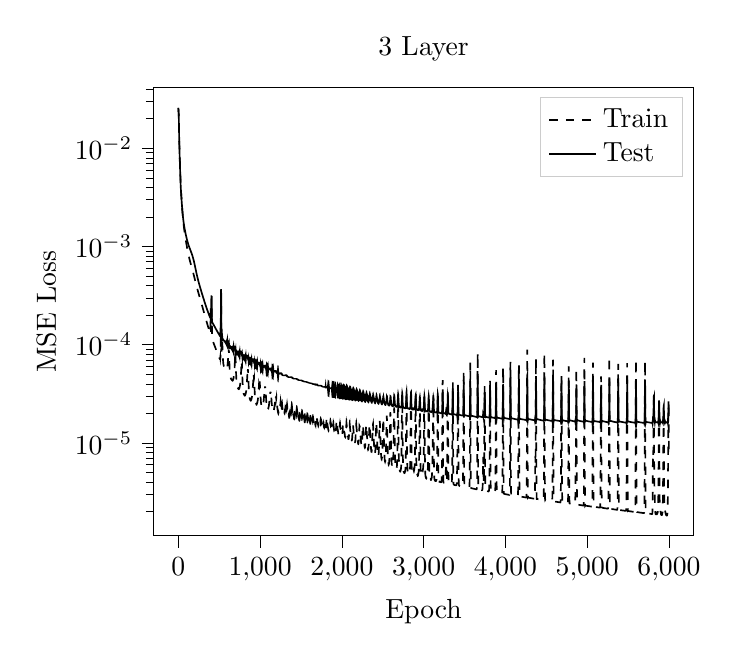
\begin{tikzpicture}

\begin{axis}[
legend cell align={left},
legend style={fill opacity=0.8, draw opacity=1, text opacity=1, draw=white!80!black},
log basis y={10},
tick align=outside,
tick pos=left,
title={3 Layer},
x grid style={white!69.0196078431373!black},
xlabel={Epoch},
xmin=-299.95, xmax=6298.95,
xtick style={color=black},
y grid style={white!69.0196078431373!black},
ylabel={MSE Loss},
ymin=1.1322611307076e-06, ymax=0.0414940584245964,
ymode=log,
ytick style={color=black}
]
\addplot [semithick, black, dashed]
table {%
0 0.0257342011900619
1 0.0250534330261871
2 0.0243807227816433
3 0.0236867136554793
4 0.0229335811454803
5 0.0220618403982371
6 0.0209819102892652
7 0.0195935298106633
8 0.0178730810876004
9 0.0160049086553045
10 0.0143510933266953
11 0.0130772785632871
12 0.0120223690173589
13 0.0110923240426928
14 0.0102946101978887
15 0.00961181169259362
16 0.00902244105236605
17 0.00850598374381661
18 0.00803963237558492
19 0.0076074312091805
20 0.00720134160656016
21 0.00681713726953603
22 0.00645199058635626
23 0.00610390958900098
24 0.00577234654338099
25 0.00545848625188228
26 0.00516461393272039
27 0.00489319404005073
28 0.00464610291237477
29 0.00442401424515992
30 0.00422599769080989
31 0.00404961021558847
32 0.00389153647120111
33 0.00374838919378817
34 0.00361722805246245
35 0.0034957248280989
36 0.00338214098883327
37 0.0032752261904534
38 0.00317409046692774
39 0.00307809177320451
40 0.00298675865633413
41 0.00289973020699108
42 0.00281672010896727
43 0.00273749200277962
44 0.00266184830252314
45 0.00258961624786025
46 0.00252064352389425
47 0.0024547912471462
48 0.00239193128072657
49 0.00233194071915932
50 0.00227470204845304
51 0.00222010019933805
52 0.00216802088834811
53 0.00211835093068657
54 0.00207097737438744
55 0.00202578732569236
56 0.00198266881488962
57 0.00194151108735241
58 0.00190220491640503
59 0.00186464419675758
60 0.00182872558070812
61 0.00179434962046798
62 0.0017614209355088
63 0.00172984863456804
64 0.00169954731245525
65 0.00167043599503813
66 0.00164243840117706
67 0.00161548366304487
68 0.00158950620971154
69 0.00156444446474779
70 0.0015402412172989
71 0.0015168438294495
72 0.00149420372326858
73 0.0014722753658134
74 0.00145101774978684
75 0.00143039195245365
76 0.00141036292916397
77 0.00139089737058384
78 0.00137196565265185
79 0.00135353971563745
80 0.00133559358437196
81 0.00131810383754782
82 0.00130104826530442
83 0.00128440642220085
84 0.00126815941257519
85 0.00125228989782045
86 0.00123678181626019
87 0.00122161967374268
88 0.00120678969324217
89 0.00119227900358965
90 0.00117807552669547
91 0.00116416771197692
92 0.00115054511479684
93 0.00113719810542534
94 0.00112411724330741
95 0.00111129405922838
96 0.00109872037501191
97 0.00108638869642164
98 0.0010742922204372
99 0.00106242415495217
100 0.00105077835542033
101 0.00103934907383518
102 0.00102813086050446
103 0.00101711866955156
104 0.00100630778615596
105 0.000995693797449348
106 0.000985272374236956
107 0.000975039783952525
108 0.00096499247229076
109 0.00095512705956935
110 0.000945440409850562
111 0.000935929663683055
112 0.000926592118048575
113 0.000917424989893334
114 0.000908426074602176
115 0.000899593062058557
116 0.000890923765837215
117 0.000882416006788844
118 0.000874067794939037
119 0.000865876983880298
120 0.00085784170369152
121 0.000849959866172867
122 0.000842229437694186
123 0.000834648148156703
124 0.000827213832963025
125 0.000819924094685121
126 0.000812776248494629
127 0.000805767840574845
128 0.000798895875050221
129 0.000792157337855315
130 0.000785549178544898
131 0.000779067951953039
132 0.000772710118326358
133 0.00076647219248116
134 0.00076035043275624
135 0.000754340702769696
136 0.000748439337257878
137 0.000742642085242551
138 0.000736945032258518
139 0.000731344229279784
140 0.000725835539924446
141 0.00072041501152853
142 0.000715078913344769
143 0.000709823239958496
144 0.000704644369761809
145 0.000699538812114042
146 0.000694502889018622
147 0.00068953330264776
148 0.000684626827933243
149 0.000679780592690804
150 0.000674991420964943
151 0.000670256695229909
152 0.000665573606966063
153 0.000660939658700954
154 0.000656352465739474
155 0.000651809661576408
156 0.000647308987026918
157 0.000642848450297606
158 0.000638426083241939
159 0.000634039839496836
160 0.000629688001936302
161 0.000625368742475985
162 0.000621080323981005
163 0.00061682125851803
164 0.00061259002177394
165 0.000608385020314017
166 0.000604204862611368
167 0.000600048299020273
168 0.0005959139270999
169 0.000591800657275598
170 0.000587707190788933
171 0.000583632521738764
172 0.000579575629672036
173 0.000575535541429417
174 0.000571511382077006
175 0.000567502236663131
176 0.000563507332117297
177 0.000559526077267947
178 0.000555557800907991
179 0.000551601962797577
180 0.00054765814638813
181 0.000543726107935072
182 0.000539805418156902
183 0.000535895866050851
184 0.000531997509824578
185 0.00052811029854638
186 0.000524234386830358
187 0.000520369869263959
188 0.000516517166033736
189 0.000512676695507253
190 0.000508848881509039
191 0.000505034380694269
192 0.000501233944305568
193 0.000497448159876512
194 0.000493678076963988
195 0.000489924559587962
196 0.00048618868822814
197 0.00048247153245029
198 0.000478774216389866
199 0.000475097860544338
200 0.000471443685455597
201 0.000467813026261865
202 0.0004642069889087
203 0.000460626870335545
204 0.000457073952929932
205 0.000453549295343691
206 0.00045005407082499
207 0.000446589452621993
208 0.000443156350229401
209 0.000439755795014207
210 0.000436388601883664
211 0.000433055571193108
212 0.00042975731594197
213 0.000426494545536116
214 0.000423267524638504
215 0.000420076700720529
216 0.000416922362092009
217 0.000413804579693533
218 0.000410723402637814
219 0.000407678809096979
220 0.00040467051712767
221 0.000401698287532781
222 0.000398761825636029
223 0.000395860620301391
224 0.000392994268622715
225 0.000390162120311288
226 0.00038736361420888
227 0.000384598112759704
228 0.00038186476649571
229 0.000379162928766164
230 0.000376491903807619
231 0.000373850818505161
232 0.000371238913430716
233 0.000368655358215619
234 0.000366099450729962
235 0.000363570209628961
236 0.000361067027370154
237 0.000358589093593764
238 0.000356135554284265
239 0.000353705774614355
240 0.000351298953319201
241 0.00034891455743491
242 0.000346551798429573
243 0.000344210016919533
244 0.00034188855534012
245 0.000339586955306004
246 0.000337304551976558
247 0.000335040874233528
248 0.000332795368194638
249 0.000330567575474561
250 0.0003283570831627
251 0.000326163397403434
252 0.000323986071634863
253 0.000321824802085757
254 0.000319679124913819
255 0.000317548732709838
256 0.000315433360810857
257 0.000313332655423437
258 0.000311246360979567
259 0.00030917419007892
260 0.000307115864416119
261 0.000305071165712434
262 0.00030303988387459
263 0.000301021814266278
264 0.000299016704957467
265 0.000297024449537275
266 0.000295044791528198
267 0.000293077639071271
268 0.000291122861199256
269 0.000289180263280286
270 0.000287249648863508
271 0.000285331070699613
272 0.000283424260487664
273 0.000281529102721834
274 0.000279645671071194
275 0.000277773636298662
276 0.000275913005680195
277 0.000274063766482868
278 0.000272225672233617
279 0.000270398804786964
280 0.000268583035904157
281 0.000266778268269263
282 0.000264984535533586
283 0.000263201722191297
284 0.000261429672718805
285 0.00025966857901949
286 0.000257918190072814
287 0.000256178440395161
288 0.000254449580097571
289 0.000252731180808041
290 0.000251023393502692
291 0.000249326341872802
292 0.000247639643930597
293 0.000245963529778237
294 0.000244298101279128
295 0.0002426428382023
296 0.000240998197114095
297 0.000239364136177755
298 0.000237740066040715
299 0.000236126757044985
300 0.000234523821745825
301 0.000232930821312038
302 0.000231348680244992
303 0.000229776686410332
304 0.000228214645176195
305 0.000226663557441498
306 0.000225122361371177
307 0.000223591208396101
308 0.000222071061671159
309 0.000220560540128645
310 0.000219060171275487
311 0.000217570808217715
312 0.00021609085615637
313 0.000214621225040901
314 0.000213162505588116
315 0.000211713032967964
316 0.00021027408001828
317 0.000208845868655771
318 0.000207426797715016
319 0.000206018314656831
320 0.000204620456770499
321 0.000203231687464722
322 0.000201853523776663
323 0.000200485907043912
324 0.000199127264295385
325 0.000197779280824761
326 0.000196441694242822
327 0.000195113055724505
328 0.000193794971437455
329 0.000192487254480511
330 0.000191188365988637
331 0.000189899998076726
332 0.000188621859706473
333 0.000187352525244933
334 0.000186093547654309
335 0.000184844762316061
336 0.000183604697213013
337 0.000182374808446184
338 0.000181155005066103
339 0.000179943895091128
340 0.000178742732714454
341 0.000177551580236468
342 0.000176369084329053
343 0.000175196261352539
344 0.000174033347775548
345 0.000172879048477625
346 0.000171734172909055
347 0.000170599007560668
348 0.000169472490142653
349 0.000168355120422348
350 0.000167247270837834
351 0.000166148032803903
352 0.000165057674166746
353 0.000163976589192316
354 0.000162904103490291
355 0.000161840272994596
356 0.000160785447405942
357 0.000159739146965876
358 0.000158701305736031
359 0.000157672173372703
360 0.000156651465658797
361 0.000155639054810308
362 0.000154635071339726
363 0.000153639356994972
364 0.000152651755342958
365 0.000151672312313167
366 0.000150700978338136
367 0.000149737574247411
368 0.000148782118230883
369 0.000147834514336864
370 0.000146894704357692
371 0.00014596258642996
372 0.000145038111440954
373 0.000144121234825434
374 0.00014321185699373
375 0.000142309883813141
376 0.000141415298912762
377 0.000140528060910583
378 0.000139647973810497
379 0.000138775262257695
380 0.000137909406930703
381 0.000137051364163199
382 0.000136199751523236
383 0.000135357629005739
384 0.000134521907511953
385 0.000133702362290933
386 0.00013289415574036
387 0.000132131217924325
388 0.000131421692913136
389 0.000130901471038669
390 0.000130723516349462
391 0.000131504047658382
392 0.000134452139718633
393 0.000141959292704996
394 0.000159789150075085
395 0.000183729076070449
396 0.000209984394132334
397 0.00019467357560643
398 0.000155132316194795
399 0.000135474273520231
400 0.000151874043694988
401 0.000162282878591213
402 0.000151219304143524
403 0.000167452612458874
404 0.000208101244425052
405 0.000204737946660316
406 0.000185874585667989
407 0.000226431963710638
408 0.000257331765624258
409 0.000251543120612041
410 0.000199560425244272
411 0.000151622683461028
412 0.000125941510304983
413 0.00011630080894065
414 0.000115426520324036
415 0.00011497593823151
416 0.000113856452344407
417 0.000112972625629482
418 0.000112051587620954
419 0.000111188194750866
420 0.000110518482870248
421 0.000109881622393004
422 0.000109302940700218
423 0.000108700483451685
424 0.000108131251636223
425 0.000107546656408886
426 0.000106988089555671
427 0.000106422778344495
428 0.000105871499499699
429 0.0001053204443906
430 0.000104775458794393
431 0.000104234240325241
432 0.000103696436099199
433 0.000103162949244506
434 0.000102632534435543
435 0.000102106115946299
436 0.000101582915931431
437 0.000101063240208532
438 0.000100546953262892
439 0.000100033932767474
440 9.95242739918467e-05
441 9.90177607036458e-05
442 9.85145513823227e-05
443 9.80144718596421e-05
444 9.7517524864088e-05
445 9.70237072124291e-05
446 9.6532931593174e-05
447 9.60452216531849e-05
448 9.55605219132849e-05
449 9.5078820550043e-05
450 9.46000914154865e-05
451 9.41242592489289e-05
452 9.36513959004515e-05
453 9.31813656279701e-05
454 9.27142311866191e-05
455 9.22499207263172e-05
456 9.17884112823231e-05
457 9.13297394617985e-05
458 9.08737906684109e-05
459 9.04206272025476e-05
460 8.99701847174583e-05
461 8.9522436610423e-05
462 8.90774040271936e-05
463 8.86350014752679e-05
464 8.81952807958442e-05
465 8.77581821896456e-05
466 8.7323690422636e-05
467 8.68918111791572e-05
468 8.6462459194081e-05
469 8.60357160945568e-05
470 8.56114645557682e-05
471 8.51897530083079e-05
472 8.47705755404604e-05
473 8.43537941364048e-05
474 8.39396159335593e-05
475 8.35277458008932e-05
476 8.31184192975343e-05
477 8.27114956791775e-05
478 8.23068771751423e-05
479 8.19048595985805e-05
480 8.15049329503381e-05
481 8.11076215541107e-05
482 8.07125502433337e-05
483 8.03196908236714e-05
484 7.9929514640753e-05
485 7.95410448972689e-05
486 7.91555023624824e-05
487 7.8771871585559e-05
488 7.83904260970303e-05
489 7.80119039518468e-05
490 7.7634196713916e-05
491 7.7260515126909e-05
492 7.6887983141205e-05
493 7.65181134738668e-05
494 7.61513747420395e-05
495 7.57831210194126e-05
496 7.54223999592796e-05
497 7.50618346501142e-05
498 7.47070362194791e-05
499 7.43542664167762e-05
500 7.39914639780181e-05
501 7.36487074846082e-05
502 7.33134928623258e-05
503 7.30042767145278e-05
504 7.26832371356068e-05
505 7.23075445421273e-05
506 7.20062852224146e-05
507 7.18219445161594e-05
508 7.18117819360486e-05
509 7.16677204763982e-05
510 7.11601982175125e-05
511 7.10404690380528e-05
512 7.20982352504507e-05
513 7.4475138148955e-05
514 7.55935309371125e-05
515 7.39788023338406e-05
516 7.52205552316809e-05
517 8.65430265548639e-05
518 0.000107620057178792
519 0.000115739651846525
520 0.000104466257880631
521 0.000117498063332278
522 0.000189804152569195
523 0.000302426214147999
524 0.000267279727268033
525 0.00019526713367668
526 0.000133291887550513
527 9.0811433892668e-05
528 8.08694624083728e-05
529 9.17515635592281e-05
530 9.71001763900858e-05
531 0.000104436886999792
532 0.000101709522027704
533 0.000105483328411538
534 0.000103221039012169
535 0.000108111753434059
536 0.000104686050462988
537 0.000106951230577579
538 0.000100446798228404
539 9.95934728962311e-05
540 9.25552242279082e-05
541 9.02375435316571e-05
542 8.40051392287933e-05
543 8.12812506865157e-05
544 7.65197086138869e-05
545 7.42365984933713e-05
546 7.09939823764216e-05
547 6.93679952519233e-05
548 6.72384402378157e-05
549 6.61374280070959e-05
550 6.47243324465308e-05
551 6.3976891283346e-05
552 6.30014415037294e-05
553 6.24734072971478e-05
554 6.17601913290855e-05
555 6.13649806382455e-05
556 6.08115757358973e-05
557 6.04984385290663e-05
558 6.00457253767672e-05
559 5.97852887267436e-05
560 5.93986021613091e-05
561 5.91739284345749e-05
562 5.88325871149209e-05
563 5.86339842811867e-05
564 5.83254605999173e-05
565 5.81476382421897e-05
566 5.78642063828738e-05
567 5.77044858118825e-05
568 5.74414129914658e-05
569 5.72989836200577e-05
570 5.70536410577915e-05
571 5.69290614294005e-05
572 5.67001241051912e-05
573 5.65950898590017e-05
574 5.63823762149696e-05
575 5.62996609687616e-05
576 5.61038525574986e-05
577 5.60473799851025e-05
578 5.58699341581814e-05
579 5.5844872349553e-05
580 5.56879416535594e-05
581 5.57007963379874e-05
582 5.55672389737083e-05
583 5.5626282232879e-05
584 5.55194775415657e-05
585 5.56348707050347e-05
586 5.55585922938917e-05
587 5.57426816385487e-05
588 5.57010365582755e-05
589 5.59690279260394e-05
590 5.59662910291081e-05
591 5.63368557777721e-05
592 5.63772675832297e-05
593 5.68735493970962e-05
594 5.69614047662981e-05
595 5.76127828253448e-05
596 5.77527016503154e-05
597 5.85974402156353e-05
598 5.87947375834119e-05
599 5.98837084453407e-05
600 6.014476252858e-05
601 6.15463625308621e-05
602 6.18777352201505e-05
603 6.36827739981527e-05
604 6.40870587176323e-05
605 6.64102516338971e-05
606 6.68735049202951e-05
607 6.98437216897219e-05
608 7.03080128232614e-05
609 7.40309735647315e-05
610 7.43438056360901e-05
611 7.88144654961798e-05
612 7.86604452969186e-05
613 8.36151650673855e-05
614 8.24830196961557e-05
615 8.72616795959402e-05
616 8.45721546056666e-05
617 8.81975054198847e-05
618 8.36869854765609e-05
619 8.53469007324748e-05
620 7.94745595840141e-05
621 7.91189453366314e-05
622 7.29696846519801e-05
623 7.13462145540689e-05
624 6.59757222365442e-05
625 6.40249588741426e-05
626 5.99283895326153e-05
627 5.82429083806346e-05
628 5.53715734668003e-05
629 5.41268602773926e-05
630 5.21872718763916e-05
631 5.13314377030838e-05
632 5.00191562196051e-05
633 4.94412950047263e-05
634 4.85281921100977e-05
635 4.81321725942507e-05
636 4.74691655085735e-05
637 4.71886988293591e-05
638 4.66838588408791e-05
639 4.64772762143184e-05
640 4.60749064927768e-05
641 4.59169619944078e-05
642 4.55831977319576e-05
643 4.54588968636926e-05
644 4.51729063115636e-05
645 4.50735712433925e-05
646 4.48222473323767e-05
647 4.47430736016941e-05
648 4.45181884174417e-05
649 4.4456872842602e-05
650 4.42532314650634e-05
651 4.42092594425958e-05
652 4.40238141550253e-05
653 4.39980519217897e-05
654 4.38291646673861e-05
655 4.38235850310775e-05
656 4.36707640574241e-05
657 4.36884946566352e-05
658 4.35521889698975e-05
659 4.35975042023529e-05
660 4.34789392329549e-05
661 4.35574839912078e-05
662 4.34586217465949e-05
663 4.35774523452892e-05
664 4.35008304862095e-05
665 4.36688449099165e-05
666 4.361762927374e-05
667 4.38457714153628e-05
668 4.38234464468223e-05
669 4.41252379346224e-05
670 4.4135724976968e-05
671 4.45278361098644e-05
672 4.45751722395471e-05
673 4.50783238079566e-05
674 4.5166574977884e-05
675 4.58068270745571e-05
676 4.59403270269831e-05
677 4.67512966224604e-05
678 4.6934648480601e-05
679 4.7960465963115e-05
680 4.81987544844742e-05
681 4.94979525456074e-05
682 4.97960888878879e-05
683 5.14461485181528e-05
684 5.18059021032968e-05
685 5.39057424475686e-05
686 5.43171181561775e-05
687 5.69823116620682e-05
688 5.74041210938958e-05
689 6.07431131811609e-05
690 6.10647791745578e-05
691 6.5117178564833e-05
692 6.51033383292088e-05
693 6.97257763704329e-05
694 6.89721363187346e-05
695 7.37016041512106e-05
696 7.16901790838165e-05
697 7.57233714807626e-05
698 7.20841529755489e-05
699 7.45696133321871e-05
700 6.94686499969066e-05
701 7.00478120165826e-05
702 6.42971839965867e-05
703 6.3376560603956e-05
704 5.80029754360112e-05
705 5.64092115382664e-05
706 5.20809593922422e-05
707 5.0502329088431e-05
708 4.73552129847121e-05
709 4.61065857280119e-05
710 4.3943763785137e-05
711 4.30613717412598e-05
712 4.15998825928909e-05
713 4.10069941949587e-05
714 4.00070570663047e-05
715 3.9613737669697e-05
716 3.89080393006225e-05
717 3.86448900826508e-05
718 3.81264522957281e-05
719 3.79472693907701e-05
720 3.75500629274939e-05
721 3.74260553144268e-05
722 3.71095609352778e-05
723 3.7023273421255e-05
724 3.67624047044046e-05
725 3.67035632962143e-05
726 3.64826115628603e-05
727 3.64454332952846e-05
728 3.62544962513311e-05
729 3.62361243446685e-05
730 3.60690034426625e-05
731 3.60686429417001e-05
732 3.59216313654542e-05
733 3.59400745537641e-05
734 3.58112333742611e-05
735 3.5850611936894e-05
736 3.57393276431139e-05
737 3.58030495704043e-05
738 3.57098372205655e-05
739 3.58027360789492e-05
740 3.57291152113248e-05
741 3.5857650516391e-05
742 3.58060381131509e-05
743 3.5978597054509e-05
744 3.59522527446643e-05
745 3.61794359378109e-05
746 3.61824716605952e-05
747 3.64777600339039e-05
748 3.65148583227892e-05
749 3.68951851328347e-05
750 3.69715761507905e-05
751 3.74581667301754e-05
752 3.75793812850134e-05
753 3.81990449227487e-05
754 3.83704433488674e-05
755 3.91568957525124e-05
756 3.93832066265531e-05
757 4.03794416570236e-05
758 4.06641660788409e-05
759 4.19251382481889e-05
760 4.22688882508737e-05
761 4.38640250877143e-05
762 4.42606585693284e-05
763 4.62739137674362e-05
764 4.67017770233724e-05
765 4.92242704126511e-05
766 4.9628200827101e-05
767 5.27334602793417e-05
768 5.29935186932562e-05
769 5.66816071341236e-05
770 5.65729731079045e-05
771 6.06784102501479e-05
772 5.98519116010721e-05
773 6.39517990066452e-05
774 6.20046221229131e-05
775 6.54387854410743e-05
776 6.21336292283559e-05
777 6.42568582520653e-05
778 5.97931420998066e-05
779 6.03664779532664e-05
780 5.54140522126545e-05
781 5.47669326920186e-05
782 5.01287954079999e-05
783 4.88958824576002e-05
784 4.50995792107278e-05
785 4.38228689176867e-05
786 4.09959103535584e-05
787 3.99475092649482e-05
788 3.79544731003989e-05
789 3.71898473758847e-05
790 3.58131033522113e-05
791 3.52879415004281e-05
792 3.433172264522e-05
793 3.39804955160616e-05
794 3.33013902604762e-05
795 3.30686702909588e-05
796 3.25710252013778e-05
797 3.24177249808599e-05
798 3.20404989224699e-05
799 3.19412105795891e-05
800 3.16458235829487e-05
801 3.15846521630192e-05
802 3.13467218688857e-05
803 3.1314160310103e-05
804 3.11182158725387e-05
805 3.11089514752894e-05
806 3.09451751832057e-05
807 3.0956744865307e-05
808 3.08190079181259e-05
809 3.08510956301689e-05
810 3.07359402995644e-05
811 3.0789943025411e-05
812 3.069569896752e-05
813 3.07744969063606e-05
814 3.07009718767404e-05
815 3.08091340457395e-05
816 3.07574237012886e-05
817 3.09012908701334e-05
818 3.0873634841555e-05
819 3.10616260321694e-05
820 3.1061283436884e-05
821 3.13043669279978e-05
822 3.13355802745718e-05
823 3.1647815433189e-05
824 3.17156074629565e-05
825 3.21148812076899e-05
826 3.22249193231983e-05
827 3.27339007526462e-05
828 3.28919982166553e-05
829 3.35389699444022e-05
830 3.37501818989949e-05
831 3.45703585935553e-05
832 3.48380930290659e-05
833 3.58750323812274e-05
834 3.61991847626086e-05
835 3.750578105155e-05
836 3.78794172775088e-05
837 3.95172565959001e-05
838 3.99205014218751e-05
839 4.19547895944561e-05
840 4.23438677330523e-05
841 4.4829019145709e-05
842 4.51182783081094e-05
843 4.80654344414688e-05
844 4.81033246728657e-05
845 5.1426189884296e-05
846 5.09791921672331e-05
847 5.4431246724107e-05
848 5.32105686943396e-05
849 5.63669453299553e-05
850 5.41381152174836e-05
851 5.64997076253348e-05
852 5.32592179069979e-05
853 5.44860718321161e-05
854 5.05703102362531e-05
855 5.06843786638456e-05
856 4.66597993806772e-05
857 4.60142191798241e-05
858 4.24049462708354e-05
859 4.14481450263793e-05
860 3.85344307574087e-05
861 3.75961986947004e-05
862 3.54063963641238e-05
863 3.46394735970534e-05
864 3.30582051901729e-05
865 3.2489840037897e-05
866 3.13638290947438e-05
867 3.09649267080658e-05
868 3.01588875686321e-05
869 2.9887566540765e-05
870 2.93005508922306e-05
871 2.91204767393083e-05
872 2.86828727666943e-05
873 2.85673810935805e-05
874 2.82330185825685e-05
875 2.81641373192087e-05
876 2.79028016052507e-05
877 2.78691202311165e-05
878 2.7661172595117e-05
879 2.7655896133183e-05
880 2.74886337763292e-05
881 2.7508270790122e-05
882 2.7373641074746e-05
883 2.74172524825644e-05
884 2.73104637074084e-05
885 2.73791184213223e-05
886 2.72976716075846e-05
887 2.73941930402088e-05
888 2.73373468075988e-05
889 2.74665100334914e-05
890 2.74350688584946e-05
891 2.7603642251961e-05
892 2.75996625305197e-05
893 2.78167493092951e-05
894 2.78433988682991e-05
895 2.81209744912303e-05
896 2.81824198395952e-05
897 2.85357973837108e-05
898 2.86368274373672e-05
899 2.90853833746496e-05
900 2.9230985404638e-05
901 2.97988969464313e-05
902 2.99933641372263e-05
903 3.07102075680632e-05
904 3.09559872562204e-05
905 3.18573951290091e-05
906 3.215291980041e-05
907 3.32801710669628e-05
908 3.36165860517212e-05
909 3.50148642382919e-05
910 3.53708167040168e-05
911 3.70839392189737e-05
912 3.7417591954636e-05
913 3.94762378732594e-05
914 3.9713948865483e-05
915 4.2113836855151e-05
916 4.2137634750361e-05
917 4.48064142801741e-05
918 4.44488199491389e-05
919 4.72113818545949e-05
920 4.62759650190492e-05
921 4.88470078039427e-05
922 4.71744604624291e-05
923 4.92175812780715e-05
924 4.67872116587387e-05
925 4.80457492813002e-05
926 4.50469287329724e-05
927 4.54727403678135e-05
928 4.22650702773808e-05
929 4.20357704911112e-05
930 3.90016203368759e-05
931 3.84077707451524e-05
932 3.58087989695832e-05
933 3.51126730606666e-05
934 3.30428732979726e-05
935 3.24060231093881e-05
936 3.08331913174698e-05
937 3.03203439386834e-05
938 2.91537290877386e-05
939 2.87706924382292e-05
940 2.79111265797383e-05
941 2.76387921758214e-05
942 2.70018808521399e-05
943 2.68160037819598e-05
944 2.6338043596752e-05
945 2.62175842919987e-05
946 2.58533506496406e-05
947 2.5782611288605e-05
948 2.55009607030843e-05
949 2.5469189637306e-05
950 2.52490867751476e-05
951 2.52496631389931e-05
952 2.50771425100993e-05
953 2.51066175565029e-05
954 2.49725525236499e-05
955 2.50299225399431e-05
956 2.49286659368408e-05
957 2.50151571492552e-05
958 2.49436388344293e-05
959 2.50624713657999e-05
960 2.50195897990579e-05
961 2.51760467051554e-05
962 2.51622188329748e-05
963 2.53637288949449e-05
964 2.53807064893863e-05
965 2.56373099318807e-05
966 2.56878138884531e-05
967 2.60124311637355e-05
968 2.60997324232903e-05
969 2.65086655133473e-05
970 2.66362040122203e-05
971 2.71495156027868e-05
972 2.73199518687761e-05
973 2.79617719911585e-05
974 2.81756156539359e-05
975 2.89739351728713e-05
976 2.92275004198927e-05
977 3.02130977161141e-05
978 3.04954502894361e-05
979 3.16994605782384e-05
980 3.19882462349597e-05
981 3.34367344976272e-05
982 3.36922425390185e-05
983 3.53967915884823e-05
984 3.55557057787337e-05
985 3.74987311602126e-05
986 3.74688043507376e-05
987 3.95844311356086e-05
988 3.92464816059146e-05
989 4.14045793490914e-05
990 4.0630675414377e-05
991 4.26395087060882e-05
992 4.13339713531968e-05
993 4.29775460588644e-05
994 4.11318437443242e-05
995 4.22421730092992e-05
996 3.99725306579057e-05
997 4.04996125382695e-05
998 3.80277713531996e-05
999 3.80569668720909e-05
1000 3.56352389303538e-05
1001 3.53371160599636e-05
1002 3.31641776938341e-05
1003 3.27169211971068e-05
1004 3.08953345609098e-05
1005 3.04309515115619e-05
1006 2.89751972673002e-05
1007 2.85662177930135e-05
1008 2.74366451549213e-05
1009 2.71095711354974e-05
1010 2.62456057100735e-05
1011 2.60009016699314e-05
1012 2.53423436333833e-05
1013 2.51696062605333e-05
1014 2.46658331093386e-05
1015 2.45524439890232e-05
1016 2.41644055449797e-05
1017 2.40993113038712e-05
1018 2.37984101545408e-05
1019 2.37733841004228e-05
1020 2.35392669480916e-05
1021 2.35489111162224e-05
1022 2.33674643652648e-05
1023 2.34089832815698e-05
1024 2.32707042471247e-05
1025 2.33436895200612e-05
1026 2.3242470859941e-05
1027 2.33484817613316e-05
1028 2.32806754354442e-05
1029 2.342325174709e-05
1030 2.33871607235869e-05
1031 2.35719583940863e-05
1032 2.35673947770465e-05
1033 2.38022398946214e-05
1034 2.38300145269932e-05
1035 2.41251260320041e-05
1036 2.41867047634514e-05
1037 2.45549413193658e-05
1038 2.46518140443186e-05
1039 2.5108745774105e-05
1040 2.524153825334e-05
1041 2.58054302832988e-05
1042 2.59728791718317e-05
1043 2.66641778239318e-05
1044 2.68610764067034e-05
1045 2.77010188369786e-05
1046 2.79160194054384e-05
1047 2.89241764050985e-05
1048 2.91364810323103e-05
1049 3.03264013155058e-05
1050 3.05025041029694e-05
1051 3.18751957593122e-05
1052 3.19654503755373e-05
1053 3.35002567908305e-05
1054 3.34377916715312e-05
1055 3.50827956481226e-05
1056 3.47874067188059e-05
1057 3.64530581578038e-05
1058 3.58440416334815e-05
1059 3.74075864328915e-05
1060 3.64271159583041e-05
1061 3.77538683267176e-05
1062 3.63952905502174e-05
1063 3.73756114413482e-05
1064 3.57028387725222e-05
1065 3.62891207998928e-05
1066 3.44303194026452e-05
1067 3.4651747313319e-05
1068 3.27643954562973e-05
1069 3.27095277157241e-05
1070 3.09356621528423e-05
1071 3.07149863374434e-05
1072 2.9148980871696e-05
1073 2.88600316196153e-05
1074 2.75415765429443e-05
1075 2.72519161228502e-05
1076 2.61781123640503e-05
1077 2.59249503642422e-05
1078 2.5068288920238e-05
1079 2.48664439936874e-05
1080 2.41904465383413e-05
1081 2.40418737860182e-05
1082 2.35105925128209e-05
1083 2.3411369426185e-05
1084 2.29939741984708e-05
1085 2.29385715044828e-05
1086 2.26105085516792e-05
1087 2.25939477900283e-05
1088 2.23365175031631e-05
1089 2.23552469265087e-05
1090 2.21547220746743e-05
1091 2.22069808444303e-05
1092 2.20536146855466e-05
1093 2.21393690651439e-05
1094 2.20264080610377e-05
1095 2.21474429054069e-05
1096 2.20705273079602e-05
1097 2.22303624468623e-05
1098 2.21868410505976e-05
1099 2.23908205327916e-05
1100 2.23793082625434e-05
1101 2.26346193699101e-05
1102 2.26544720760558e-05
1103 2.29702048955005e-05
1104 2.30209818710136e-05
1105 2.34081314829382e-05
1106 2.34888581474024e-05
1107 2.39601025384673e-05
1108 2.40683273773357e-05
1109 2.46373519132703e-05
1110 2.47677971287885e-05
1111 2.54483763626467e-05
1112 2.55913605258229e-05
1113 2.63953563433006e-05
1114 2.65347287609075e-05
1115 2.74692722541658e-05
1116 2.75805614364799e-05
1117 2.86439384353798e-05
1118 2.86926735952875e-05
1119 2.98695684364247e-05
1120 2.98113596386429e-05
1121 3.1067952079411e-05
1122 3.08513149889222e-05
1123 3.21327240442315e-05
1124 3.17064582304738e-05
1125 3.29390885553948e-05
1126 3.22638563261535e-05
1127 3.33650203003799e-05
1128 3.24279476160427e-05
1129 3.33235965115364e-05
1130 3.21495537036753e-05
1131 3.27932025356859e-05
1132 3.14456198680091e-05
1133 3.18308249518395e-05
1134 3.03998908748326e-05
1135 3.0559576231326e-05
1136 2.91408488237721e-05
1137 2.91331996322697e-05
1138 2.78062395864254e-05
1139 2.76958386109527e-05
1140 2.65122327789413e-05
1141 2.63550524550737e-05
1142 2.53371431711003e-05
1143 2.51735139329412e-05
1144 2.43209258883326e-05
1145 2.41753696172964e-05
1146 2.34738106712484e-05
1147 2.33587624336451e-05
1148 2.27878460634656e-05
1149 2.27080035983818e-05
1150 2.22464275623224e-05
1151 2.22023530511706e-05
1152 2.18308294108738e-05
1153 2.18214131848526e-05
1154 2.15236391909457e-05
1155 2.15476404434867e-05
1156 2.13107190631945e-05
1157 2.13675080829034e-05
1158 2.11814681563283e-05
1159 2.12714580243301e-05
1160 2.11288931950548e-05
1161 2.1253693972767e-05
1162 2.11491427535293e-05
1163 2.13116458098739e-05
1164 2.12412623739056e-05
1165 2.14458110292526e-05
1166 2.1406775175592e-05
1167 2.1658937129132e-05
1168 2.1648965798704e-05
1169 2.19556560239198e-05
1170 2.19724756505002e-05
1171 2.23415824791573e-05
1172 2.23821769225196e-05
1173 2.28223590568177e-05
1174 2.28823508052756e-05
1175 2.34022488712071e-05
1176 2.34745921545709e-05
1177 2.40816760594953e-05
1178 2.41556516300534e-05
1179 2.48545932208799e-05
1180 2.49146585247217e-05
1181 2.57051778191908e-05
1182 2.57300701207441e-05
1183 2.66044779380081e-05
1184 2.65670614680857e-05
1185 2.75076221498693e-05
1186 2.7376320105077e-05
1187 2.83538131498062e-05
1188 2.8095628920255e-05
1189 2.90695659259654e-05
1190 2.86555907678121e-05
1191 2.95776987115914e-05
1192 2.89899593326481e-05
1193 2.9811019430781e-05
1194 2.90492272085885e-05
1195 2.9728266042639e-05
1196 2.88138937776239e-05
1197 2.93270383906474e-05
1198 2.83018154902948e-05
1199 2.86469474701789e-05
1200 2.75656067003638e-05
1201 2.77610353975888e-05
1202 2.66807990954021e-05
1203 2.67586545419363e-05
1204 2.57290425622614e-05
1205 2.57265417644703e-05
1206 2.47830285786677e-05
1207 2.47350860433926e-05
1208 2.38973619559602e-05
1209 2.38317918501707e-05
1210 2.31057038888594e-05
1211 2.30421694027427e-05
1212 2.24239223030054e-05
1213 2.23749233612125e-05
1214 2.18552195008215e-05
1215 2.18280167700868e-05
1216 2.1395119489398e-05
1217 2.13934673354288e-05
1218 2.10353676379782e-05
1219 2.10610811564038e-05
1220 2.0766806926531e-05
1221 2.08210947505449e-05
1222 2.05812666536076e-05
1223 2.06652698011567e-05
1224 2.04721069962943e-05
1225 2.05873485015218e-05
1226 2.0434601509578e-05
1227 2.05833107145281e-05
1228 2.04659550604447e-05
1229 2.06511710132418e-05
1230 2.05651479632252e-05
1231 2.07906361140431e-05
1232 2.07322925405151e-05
1233 2.10024257683017e-05
1234 2.09682339118444e-05
1235 2.12881087406913e-05
1236 2.127425491949e-05
1237 2.1649082981412e-05
1238 2.16506423953433e-05
1239 2.20852546135575e-05
1240 2.20956329428645e-05
1241 2.25936651645497e-05
1242 2.26039280164514e-05
1243 2.31668680328312e-05
1244 2.31651811759548e-05
1245 2.37910583962275e-05
1246 2.37622951146932e-05
1247 2.44443359065372e-05
1248 2.4370298518761e-05
1249 2.50958215985975e-05
1250 2.49563038607903e-05
1251 2.57061571744543e-05
1252 2.54807257817902e-05
1253 2.62297733968353e-05
1254 2.59008791658744e-05
1255 2.66200882208523e-05
1256 2.61765826508054e-05
1257 2.68364909175034e-05
1258 2.62768368770594e-05
1259 2.68517183030781e-05
1260 2.61859149759402e-05
1261 2.66583892312156e-05
1262 2.59080320859084e-05
1263 2.62715873304842e-05
1264 2.54666457237818e-05
1265 2.57261446563462e-05
1266 2.49005503007993e-05
1267 2.50701402535469e-05
1268 2.42566471513328e-05
1269 2.43561125046199e-05
1270 2.3581932396155e-05
1271 2.36326333151737e-05
1272 2.29171820080865e-05
1273 2.29389306127814e-05
1274 2.22933387306057e-05
1275 2.23024721321963e-05
1276 2.17308950709594e-05
1277 2.17399758071224e-05
1278 2.12414097973124e-05
1279 2.12593555488638e-05
1280 2.08293573109586e-05
1281 2.08622353596866e-05
1282 2.04946661028771e-05
1283 2.05466503615526e-05
1284 2.02348053051082e-05
1285 2.03088183070577e-05
1286 2.00460614792064e-05
1287 2.01444322129873e-05
1288 1.9924754923295e-05
1289 2.00497242985875e-05
1290 1.98677243474776e-05
1291 2.00214833512291e-05
1292 1.98723514301946e-05
1293 2.00574223470085e-05
1294 1.99369143274453e-05
1295 2.01561062738165e-05
1296 2.00601873530104e-05
1297 2.03164395031763e-05
1298 2.02409429732597e-05
1299 2.05372443815577e-05
1300 2.04776610246427e-05
1301 2.08167445805429e-05
1302 2.07678137087441e-05
1303 2.11516831427616e-05
1304 2.11069016984311e-05
1305 2.15362504434324e-05
1306 2.1487651025609e-05
1307 2.19613718570599e-05
1308 2.18993597229655e-05
1309 2.24137195061758e-05
1310 2.23270087076344e-05
1311 2.2875025393887e-05
1312 2.27510950878695e-05
1313 2.33223572365659e-05
1314 2.31484481219013e-05
1315 2.37291904170434e-05
1316 2.34934796878861e-05
1317 2.40671892584032e-05
1318 2.37604752442167e-05
1319 2.43094803238364e-05
1320 2.39271045074929e-05
1321 2.44344095392535e-05
1322 2.39774259966907e-05
1323 2.44289805664266e-05
1324 2.39048681294207e-05
1325 2.42912721830635e-05
1326 2.37133295115655e-05
1327 2.40309614412126e-05
1328 2.34169205839407e-05
1329 2.36681459000465e-05
1330 2.30378158505573e-05
1331 2.32298686739796e-05
1332 2.26026589302819e-05
1333 2.27460593578144e-05
1334 2.21390366164087e-05
1335 2.22459478607107e-05
1336 2.16724243671251e-05
1337 2.17548233365505e-05
1338 2.12238148549204e-05
1339 2.12925436073874e-05
1340 2.08090995954535e-05
1341 2.0873312536196e-05
1342 2.04391659508474e-05
1343 2.05062181919402e-05
1344 2.01205919267977e-05
1345 2.01961748871327e-05
1346 1.98565878406498e-05
1347 1.99450197158058e-05
1348 1.96480566501123e-05
1349 1.97528054712848e-05
1350 1.94946354383774e-05
1351 1.96185406764471e-05
1352 1.93951412370552e-05
1353 1.95405990552899e-05
1354 1.93479944243791e-05
1355 1.95172692372125e-05
1356 1.93515978708092e-05
1357 1.95467477510647e-05
1358 1.94041072063555e-05
1359 1.96270458729941e-05
1360 1.95034873229361e-05
1361 1.97559860453111e-05
1362 1.9647368560527e-05
1363 1.99307640684765e-05
1364 1.98324346740719e-05
1365 2.01475606047552e-05
1366 2.00544523067947e-05
1367 2.04012869744474e-05
1368 2.03073927025343e-05
1369 2.06845624859398e-05
1370 2.05830511674776e-05
1371 2.09875840084806e-05
1372 2.08709320759226e-05
1373 2.12981593108452e-05
1374 2.11584207079341e-05
1375 2.16018496246306e-05
1376 2.14311072568307e-05
1377 2.18824660862538e-05
1378 2.16734324283152e-05
1379 2.21229502983533e-05
1380 2.18698102685266e-05
1381 2.2307087107265e-05
1382 2.20064178506618e-05
1383 2.24213188175781e-05
1384 2.2072738602219e-05
1385 2.24564490736157e-05
1386 2.20629827367702e-05
1387 2.24088173013115e-05
1388 2.19767061366838e-05
1389 2.22809053127548e-05
1390 2.18191524936628e-05
1391 2.20808350945845e-05
1392 2.16002299566753e-05
1393 2.18216219423084e-05
1394 2.1333727062256e-05
1395 2.15193970234395e-05
1396 2.10352463625441e-05
1397 2.11912700365247e-05
1398 2.07206070115262e-05
1399 2.08539609332092e-05
1400 2.04045925897844e-05
1401 2.05222256965953e-05
1402 2.00998055106538e-05
1403 2.02083786291496e-05
1404 1.98165484448509e-05
1405 1.99219970227205e-05
1406 1.95624592151944e-05
1407 1.96698052974398e-05
1408 1.93427342480845e-05
1409 1.94561977480134e-05
1410 1.91607490478418e-05
1411 1.9283866549813e-05
1412 1.90182501569325e-05
1413 1.91538860576657e-05
1414 1.89158476757711e-05
1415 1.90664239028138e-05
1416 1.88533635991917e-05
1417 1.90209273398523e-05
1418 1.88299530066161e-05
1419 1.90161987063675e-05
1420 1.88443413549066e-05
1421 1.9050704622714e-05
1422 1.88946741559448e-05
1423 1.91221323007085e-05
1424 1.8978415738502e-05
1425 1.92275871313541e-05
1426 1.90923600484894e-05
1427 1.93632601508398e-05
1428 1.92324205272598e-05
1429 1.95244121812266e-05
1430 1.9393438321913e-05
1431 1.97049883183809e-05
1432 1.95690151372219e-05
1433 1.98976496790237e-05
1434 1.97516083346727e-05
1435 2.00938995362776e-05
1436 1.99327642746994e-05
1437 2.02842459202657e-05
1438 2.01031469657664e-05
1439 2.04585278424929e-05
1440 2.02532706907732e-05
1441 2.06067540773347e-05
1442 2.03742390851858e-05
1443 2.07197657857705e-05
1444 2.04580925071696e-05
1445 2.07898973201281e-05
1446 2.04990798522431e-05
1447 2.08122274045763e-05
1448 2.04939732668663e-05
1449 2.07847012347884e-05
1450 2.044245869115e-05
1451 2.07083999441693e-05
1452 2.03470365818248e-05
1453 2.05874474943357e-05
1454 2.02128433102189e-05
1455 2.04284140181699e-05
1456 2.00469744982001e-05
1457 2.0239829041202e-05
1458 1.98580008827776e-05
1459 2.00312513527479e-05
1460 1.96549932240941e-05
1461 1.98123706809383e-05
1462 1.94467847904889e-05
1463 1.95923208536897e-05
1464 1.92415350284136e-05
1465 1.93792907907664e-05
1466 1.90462575915262e-05
1467 1.91801029245653e-05
1468 1.88668191469787e-05
1469 1.90003479758616e-05
1470 1.87078094882054e-05
1471 1.88441704835896e-05
1472 1.85724726975423e-05
1473 1.87144009373696e-05
1474 1.84629855084495e-05
1475 1.86127779784329e-05
1476 1.83805780693547e-05
1477 1.85402398074075e-05
1478 1.83257398873593e-05
1479 1.84968501741878e-05
1480 1.82981552256933e-05
1481 1.84819292599059e-05
1482 1.82969169770786e-05
1483 1.84942579437575e-05
1484 1.83204791426306e-05
1485 1.85318616843233e-05
1486 1.83666505222391e-05
1487 1.85920855813038e-05
1488 1.84325762688786e-05
1489 1.86716952725874e-05
1490 1.85148165030569e-05
1491 1.87666308306689e-05
1492 1.86091881744233e-05
1493 1.88722457892254e-05
1494 1.87110121885325e-05
1495 1.89833168349196e-05
1496 1.88151161921724e-05
1497 1.90941646280862e-05
1498 1.89160085142248e-05
1499 1.91988517599384e-05
1500 1.90080312165719e-05
1501 1.92913656746896e-05
1502 1.90857596180649e-05
1503 1.93662163781028e-05
1504 1.91444578945266e-05
1505 1.94187786348721e-05
1506 1.91802720621581e-05
1507 1.94454568998026e-05
1508 1.91905220958688e-05
1509 1.94440829091036e-05
1510 1.91740071784352e-05
1511 1.94142050133905e-05
1512 1.91310928130406e-05
1513 1.93569462965115e-05
1514 1.90635685441976e-05
1515 1.92747924927517e-05
1516 1.89743454654945e-05
1517 1.91714962056722e-05
1518 1.88674035825898e-05
1519 1.90516339273472e-05
1520 1.87473966377638e-05
1521 1.89203934155557e-05
1522 1.86192045532607e-05
1523 1.87830650872911e-05
1524 1.84879131097659e-05
1525 1.86449022123725e-05
1526 1.83581228156982e-05
1527 1.85105573393685e-05
1528 1.8234032950204e-05
1529 1.83841450507316e-05
1530 1.81190741841419e-05
1531 1.826898278523e-05
1532 1.80162242315873e-05
1533 1.81680102286919e-05
1534 1.79278369500935e-05
1535 1.80831348188804e-05
1536 1.78552815555122e-05
1537 1.80155258249215e-05
1538 1.7799357920012e-05
1539 1.79657614296502e-05
1540 1.77604069619974e-05
1541 1.79338778139027e-05
1542 1.77381422474809e-05
1543 1.79192811344819e-05
1544 1.77317079987915e-05
1545 1.79208300608025e-05
1546 1.77397546679003e-05
1547 1.79368813633118e-05
1548 1.77605874114306e-05
1549 1.79654524856687e-05
1550 1.77920330486359e-05
1551 1.80040040334006e-05
1552 1.78315551409014e-05
1553 1.80497476662822e-05
1554 1.78763336293741e-05
1555 1.80995820926455e-05
1556 1.79233863946138e-05
1557 1.81502242355691e-05
1558 1.79695368842658e-05
1559 1.81984088385434e-05
1560 1.8011784106875e-05
1561 1.82409414435369e-05
1562 1.80472111424024e-05
1563 1.82748613895001e-05
1564 1.8073190318546e-05
1565 1.82977381371074e-05
1566 1.80878335527268e-05
1567 1.83077866324766e-05
1568 1.8089648563091e-05
1569 1.83037913643602e-05
1570 1.80779220499971e-05
1571 1.82853436001551e-05
1572 1.80525847213175e-05
1573 1.82527455763193e-05
1574 1.80142911858638e-05
1575 1.82069685195074e-05
1576 1.79641560293931e-05
1577 1.81495762774375e-05
1578 1.79040731325131e-05
1579 1.80827744316048e-05
1580 1.78362303415724e-05
1581 1.80090610797379e-05
1582 1.77630857649547e-05
1583 1.79310226542384e-05
1584 1.7687125506427e-05
1585 1.7851299475069e-05
1586 1.76107785136992e-05
1587 1.77723537717611e-05
1588 1.75363126970751e-05
1589 1.76963617661841e-05
1590 1.74655835110116e-05
1591 1.76251596428756e-05
1592 1.740022801755e-05
1593 1.75602021386112e-05
1594 1.73412971662401e-05
1595 1.75022740904751e-05
1596 1.72893458056933e-05
1597 1.74518805522439e-05
1598 1.72447813326926e-05
1599 1.74092384668256e-05
1600 1.72076322257908e-05
1601 1.73742705840141e-05
1602 1.71776804052115e-05
1603 1.73466278567957e-05
1604 1.71545182183763e-05
1605 1.7325760239828e-05
1606 1.71375706372601e-05
1607 1.73110671539689e-05
1608 1.7126303276882e-05
1609 1.73020319209627e-05
1610 1.71202316039398e-05
1611 1.72980086290409e-05
1612 1.71185260455786e-05
1613 1.729808226969e-05
1614 1.71204476089315e-05
1615 1.73014928748216e-05
1616 1.7125116698935e-05
1617 1.73072025972942e-05
1618 1.71313460839428e-05
1619 1.73138392085548e-05
1620 1.71377273545659e-05
1621 1.73199860284967e-05
1622 1.71426245003659e-05
1623 1.73238297236367e-05
1624 1.71441745351331e-05
1625 1.73238219076666e-05
1626 1.71410611642386e-05
1627 1.73190892951425e-05
1628 1.7132733461267e-05
1629 1.73098114260029e-05
1630 1.71199548049117e-05
1631 1.72977171644106e-05
1632 1.71052607242927e-05
1633 1.72863035174942e-05
1634 1.70927683029731e-05
1635 1.72801053111016e-05
1636 1.70872249043441e-05
1637 1.72836664091847e-05
1638 1.7092691535936e-05
1639 1.7299633697121e-05
1640 1.71104744026707e-05
1641 1.73268507523971e-05
1642 1.71373688147014e-05
1643 1.73584590754672e-05
1644 1.71637249479772e-05
1645 1.73801541336616e-05
1646 1.71723155801828e-05
1647 1.73700686332268e-05
1648 1.71393933499076e-05
1649 1.73017435542988e-05
1650 1.7040046003558e-05
1651 1.71526003782674e-05
1652 1.68584311666109e-05
1653 1.69162495353703e-05
1654 1.66004503796557e-05
1655 1.66140097803691e-05
1656 1.6300636161759e-05
1657 1.62960106422361e-05
1658 1.60183170976325e-05
1659 1.60322608451224e-05
1660 1.58276507420396e-05
1661 1.59021890340227e-05
1662 1.58123398534826e-05
1663 1.59908829857613e-05
1664 1.6063066453853e-05
1665 1.63718474368579e-05
1666 1.66289580363355e-05
1667 1.6999060562739e-05
1668 1.73203941926658e-05
1669 1.74858846833104e-05
1670 1.75295062661007e-05
1671 1.72485425764535e-05
1672 1.68379113176798e-05
1673 1.63407574405028e-05
1674 1.57997291410084e-05
1675 1.54925985214049e-05
1676 1.51594438477787e-05
1677 1.51662515150974e-05
1678 1.50925212381026e-05
1679 1.53585123001676e-05
1680 1.54699475274356e-05
1681 1.59220495845602e-05
1682 1.61308677775196e-05
1683 1.66998436554877e-05
1684 1.69130961751307e-05
1685 1.75147886238847e-05
1686 1.76329386647467e-05
1687 1.8170259153294e-05
1688 1.81139136543607e-05
1689 1.85105782861683e-05
1690 1.82603936309533e-05
1691 1.84965761889089e-05
1692 1.81022399772246e-05
1693 1.82131387305162e-05
1694 1.77571798474219e-05
1695 1.77978546105351e-05
1696 1.73497457751637e-05
1697 1.73627573474278e-05
1698 1.69577805877452e-05
1699 1.69633497080213e-05
1700 1.66075385550357e-05
1701 1.66103957042196e-05
1702 1.62957927045682e-05
1703 1.62959105125537e-05
1704 1.60131768609517e-05
1705 1.60128664390413e-05
1706 1.5757281033757e-05
1707 1.57626010945933e-05
1708 1.55341357981342e-05
1709 1.55530663903392e-05
1710 1.53536804248233e-05
1711 1.53935218349943e-05
1712 1.52245727917943e-05
1713 1.5290558195602e-05
1714 1.51516279345287e-05
1715 1.52467883651752e-05
1716 1.51355941113707e-05
1717 1.52610526242825e-05
1718 1.51737095848148e-05
1719 1.53291460947003e-05
1720 1.52606050392023e-05
1721 1.54442917335018e-05
1722 1.5388373441283e-05
1723 1.5597075559981e-05
1724 1.55466690046069e-05
1725 1.57754948020283e-05
1726 1.57227951262939e-05
1727 1.59653032767437e-05
1728 1.5902280949831e-05
1729 1.61507660152438e-05
1730 1.60700848823581e-05
1731 1.63164466187027e-05
1732 1.62125958809156e-05
1733 1.64495602916759e-05
1734 1.63199118503599e-05
1735 1.65420866835575e-05
1736 1.63874261147612e-05
1737 1.65920049539636e-05
1738 1.64160537394764e-05
1739 1.66024457826097e-05
1740 1.64107889304432e-05
1741 1.65798560090025e-05
1742 1.63782191293649e-05
1743 1.65309400586011e-05
1744 1.6323668859286e-05
1745 1.64600934624559e-05
1746 1.62491861885883e-05
1747 1.63681771141455e-05
1748 1.61534789242523e-05
1749 1.62538586891969e-05
1750 1.60345809661067e-05
1751 1.61170240176034e-05
1752 1.58937342007448e-05
1753 1.59626602851404e-05
1754 1.57390269919233e-05
1755 1.58032062529401e-05
1756 1.55859501091982e-05
1757 1.56570326055316e-05
1758 1.54545262205374e-05
1759 1.55447373799689e-05
1760 1.53642967575252e-05
1761 1.54834997090347e-05
1762 1.53292664037963e-05
1763 1.54831776626452e-05
1764 1.53547065906423e-05
1765 1.55434626663009e-05
1766 1.54348246610425e-05
1767 1.5651450041787e-05
1768 1.55505680936585e-05
1769 1.57798102975448e-05
1770 1.56687026162672e-05
1771 1.58870085442686e-05
1772 1.57443537034396e-05
1773 1.59234153329635e-05
1774 1.57311214650235e-05
1775 1.5847022922344e-05
1776 1.56000713218418e-05
1777 1.56447473784738e-05
1778 1.53581378867784e-05
1779 1.53460644298775e-05
1780 1.50527559128477e-05
1781 1.50171520232334e-05
1782 1.4757547546651e-05
1783 1.47390213953713e-05
1784 1.4550481068909e-05
1785 1.45868556558071e-05
1786 1.45000338420687e-05
1787 1.46207012505783e-05
1788 1.46591077907487e-05
1789 1.48746957790991e-05
1790 1.50417525048852e-05
1791 1.53129029456522e-05
1792 1.55469063543023e-05
1793 1.57404984122422e-05
1794 1.58695324898872e-05
1795 1.58074224714255e-05
1796 1.56520961809292e-05
1797 1.53234682613856e-05
1798 1.49313905524195e-05
1799 1.45597018104127e-05
1800 1.4172159580994e-05
1801 1.39744925888863e-05
1802 1.37653019010031e-05
1803 1.38161269092052e-05
1804 1.38222773955476e-05
1805 1.41189041613643e-05
1806 1.43144972071241e-05
1807 1.48372175203804e-05
1808 1.51686728884215e-05
1809 1.58716654254931e-05
1810 1.62371702572273e-05
1811 1.70065287647958e-05
1812 1.72393102673141e-05
1813 1.78872428762133e-05
1814 1.7817998582359e-05
1815 1.81782389176988e-05
1816 1.77687471705212e-05
1817 1.78253096123626e-05
1818 1.72132733951003e-05
1819 1.70926004727789e-05
1820 1.64704418352812e-05
1821 1.63116788201023e-05
1822 1.5796812760982e-05
1823 1.5667888533244e-05
1824 1.52805901052488e-05
1825 1.51844737672491e-05
1826 1.48902941816687e-05
1827 1.48040369083446e-05
1828 1.45583981066011e-05
1829 1.44646429021122e-05
1830 1.42396567355263e-05
1831 1.41399712845214e-05
1832 1.3931206495954e-05
1833 1.38421515742948e-05
1834 1.36598212350236e-05
1835 1.36011055786867e-05
1836 1.3457497800573e-05
1837 1.34439025032407e-05
1838 1.33462557414532e-05
1839 1.33862087636771e-05
1840 1.33359571918845e-05
1841 1.34335511177142e-05
1842 1.34280718668833e-05
1843 1.35852823461846e-05
1844 1.36192687705261e-05
1845 1.38362235446721e-05
1846 1.39013764908213e-05
1847 1.41749681290548e-05
1848 1.42584999593964e-05
1849 1.4579674569859e-05
1850 1.46626695141094e-05
1851 1.50137825301044e-05
1852 1.50712667448261e-05
1853 1.54257556346238e-05
1854 1.54302725263733e-05
1855 1.57567754968113e-05
1856 1.56864970222159e-05
1857 1.59579753642447e-05
1858 1.58063669459807e-05
1859 1.60103120094846e-05
1860 1.57911924247855e-05
1861 1.59338177070367e-05
1862 1.56767728469731e-05
1863 1.57776935054699e-05
1864 1.55163985482432e-05
1865 1.55971578408298e-05
1866 1.53566523124482e-05
1867 1.54293415448592e-05
1868 1.52177879044757e-05
1869 1.52789934304565e-05
1870 1.5086250158447e-05
1871 1.51195279158856e-05
1872 1.49235928006419e-05
1873 1.49112464669088e-05
1874 1.46924979276264e-05
1875 1.46321751230971e-05
1876 1.43892622759267e-05
1877 1.43028836987469e-05
1878 1.40572837779018e-05
1879 1.3983512417326e-05
1880 1.37680267755513e-05
1881 1.37456956394999e-05
1882 1.35885625525134e-05
1883 1.3645749021407e-05
1884 1.35625226675984e-05
1885 1.37150163652677e-05
1886 1.37081345314982e-05
1887 1.39607093672112e-05
1888 1.4019495068851e-05
1889 1.43624163086997e-05
1890 1.44579169898407e-05
1891 1.48565770672349e-05
1892 1.49336790684629e-05
1893 1.53184107176685e-05
1894 1.52994383029181e-05
1895 1.55761283338052e-05
1896 1.53944996270639e-05
1897 1.54922020954018e-05
1898 1.51463419797437e-05
1899 1.50721246825469e-05
1900 1.46421057252155e-05
1901 1.44795982066626e-05
1902 1.40772254724197e-05
1903 1.39269761234573e-05
1904 1.36343703047714e-05
1905 1.35630529598529e-05
1906 1.34145178094514e-05
1907 1.34451767337396e-05
1908 1.34383189731579e-05
1909 1.35556845748397e-05
1910 1.36557750636257e-05
1911 1.38033134078341e-05
1912 1.39328282955375e-05
1913 1.4016444652043e-05
1914 1.40641130599306e-05
1915 1.40031842477129e-05
1916 1.38939053897502e-05
1917 1.37010531489068e-05
1918 1.34707943573176e-05
1919 1.32524580180871e-05
1920 1.30151825885605e-05
1921 1.28829158825283e-05
1922 1.27350845104957e-05
1923 1.2749999612538e-05
1924 1.27333280488529e-05
1925 1.29178804115782e-05
1926 1.30375151741191e-05
1927 1.3399097014144e-05
1928 1.36395815388823e-05
1929 1.41711424817004e-05
1930 1.44882033055183e-05
1931 1.51443570359788e-05
1932 1.54433115540087e-05
1933 1.61121028554589e-05
1934 1.62492719368856e-05
1935 1.67671062172303e-05
1936 1.66186877379459e-05
1937 1.68627722700876e-05
1938 1.64302830114593e-05
1939 1.64145632197688e-05
1940 1.5838665319734e-05
1941 1.56887327023014e-05
1942 1.51392686973395e-05
1943 1.49797726578527e-05
1944 1.45530906365821e-05
1945 1.44384437419376e-05
1946 1.41422463855179e-05
1947 1.40617639203811e-05
1948 1.38494343104867e-05
1949 1.37631292318474e-05
1950 1.35750422316505e-05
1951 1.34519745813577e-05
1952 1.32506405066124e-05
1953 1.30931548767421e-05
1954 1.28797350384957e-05
1955 1.2720105473818e-05
1956 1.25226702891723e-05
1957 1.2399990225731e-05
1958 1.22488183933456e-05
1959 1.21911911463712e-05
1960 1.21043285332689e-05
1961 1.21266472206116e-05
1962 1.21101099352927e-05
1963 1.22200005279183e-05
1964 1.22729660461118e-05
1965 1.24756995205644e-05
1966 1.2593132041161e-05
1967 1.28911643884067e-05
1968 1.30609421375993e-05
1969 1.34477979827352e-05
1970 1.36438161746355e-05
1971 1.40934459125219e-05
1972 1.42683549029243e-05
1973 1.47264009200399e-05
1974 1.48144993943333e-05
1975 1.5204577636041e-05
1976 1.51453181445049e-05
1977 1.53998981602399e-05
1978 1.51764155305045e-05
1979 1.52770046497608e-05
1980 1.49358594399018e-05
1981 1.49244872318377e-05
1982 1.4552307447957e-05
1983 1.4500688962471e-05
1984 1.41774833366526e-05
1985 1.4143995969107e-05
1986 1.39118924380455e-05
1987 1.391728329736e-05
1988 1.37736205658712e-05
1989 1.37972784557405e-05
1990 1.37006264253614e-05
1991 1.36932739565054e-05
1992 1.35810941230829e-05
1993 1.3496219935405e-05
1994 1.33211952686452e-05
1995 1.31551389586093e-05
1996 1.29214115816012e-05
1997 1.27237036338101e-05
1998 1.24833575227967e-05
1999 1.23234546407502e-05
2000 1.21364532219559e-05
2001 1.20671986536536e-05
2002 1.19715498101414e-05
2003 1.20216245136362e-05
2004 1.20322065271239e-05
2005 1.22168011387203e-05
2006 1.23349225873426e-05
2007 1.26627951857472e-05
2008 1.28771879843725e-05
2009 1.33431429674147e-05
2010 1.36165768083174e-05
2011 1.4177798945525e-05
2012 1.44260860963641e-05
2013 1.49776435875992e-05
2014 1.50724559944138e-05
2015 1.54646856600493e-05
2016 1.52994670941098e-05
2017 1.54286948941262e-05
2018 1.50167162473736e-05
2019 1.49143565977283e-05
2020 1.4396293011032e-05
2021 1.41971397908947e-05
2022 1.37336756722561e-05
2023 1.35638578342423e-05
2024 1.32437816944275e-05
2025 1.31577505726455e-05
2026 1.29894696669908e-05
2027 1.29750523569783e-05
2028 1.29129006722906e-05
2029 1.29155132526648e-05
2030 1.28833680150819e-05
2031 1.28363711553448e-05
2032 1.27586598352991e-05
2033 1.26259195383227e-05
2034 1.24713788807185e-05
2035 1.2276600301675e-05
2036 1.20767989528758e-05
2037 1.18848098225044e-05
2038 1.17023743371192e-05
2039 1.15746747013645e-05
2040 1.14600222502759e-05
2041 1.14333221006291e-05
2042 1.14113191500564e-05
2043 1.15043120416658e-05
2044 1.15833303055979e-05
2045 1.18094153407355e-05
2046 1.19900696802233e-05
2047 1.23604771857799e-05
2048 1.26326193168325e-05
2049 1.31454134333353e-05
2050 1.347186048406e-05
2051 1.40869085072381e-05
2052 1.43826748058018e-05
2053 1.49973548815296e-05
2054 1.51331639983709e-05
2055 1.55987091261522e-05
2056 1.54652724972948e-05
2057 1.56717186712285e-05
2058 1.527424481651e-05
2059 1.52373028186048e-05
2060 1.47085095534294e-05
2061 1.45481981235207e-05
2062 1.40496308347338e-05
2063 1.3887227368059e-05
2064 1.35135739753878e-05
2065 1.34031166396653e-05
2066 1.31630486350787e-05
2067 1.30900655221922e-05
2068 1.29329068840889e-05
2069 1.28457581922703e-05
2070 1.2699440162578e-05
2071 1.25529187471329e-05
2072 1.23675343957075e-05
2073 1.21605031893068e-05
2074 1.19382982859406e-05
2075 1.1715196762907e-05
2076 1.14991340751658e-05
2077 1.13163603856492e-05
2078 1.115279582109e-05
2079 1.10497592231695e-05
2080 1.09659712848043e-05
2081 1.09625807169778e-05
2082 1.09687791223223e-05
2083 1.10765518428479e-05
2084 1.11758817098462e-05
2085 1.14066385492606e-05
2086 1.15992042708513e-05
2087 1.19643568297079e-05
2088 1.22410290259722e-05
2089 1.27388691453234e-05
2090 1.30639589883685e-05
2091 1.36547249667274e-05
2092 1.39455892025353e-05
2093 1.45285807207074e-05
2094 1.46604654673865e-05
2095 1.50921066079945e-05
2096 1.49621365324037e-05
2097 1.51402620360841e-05
2098 1.47583847081023e-05
2099 1.470460418318e-05
2100 1.42028455627496e-05
2101 1.40381038136184e-05
2102 1.35732798014487e-05
2103 1.34165074143766e-05
2104 1.30796305199965e-05
2105 1.29828017065847e-05
2106 1.2781856185029e-05
2107 1.2728252869465e-05
2108 1.26113758938118e-05
2109 1.25434221160958e-05
2110 1.24323231887047e-05
2111 1.2294785051381e-05
2112 1.21300222701848e-05
2113 1.1915188281364e-05
2114 1.16955056341794e-05
2115 1.14515169968854e-05
2116 1.12266371559144e-05
2117 1.10195376663569e-05
2118 1.08457829384179e-05
2119 1.07223949754598e-05
2120 1.06333660454538e-05
2121 1.06167957483194e-05
2122 1.06253240943488e-05
2123 1.07286086006297e-05
2124 1.08394419129354e-05
2125 1.10768729513211e-05
2126 1.12924831512373e-05
2127 1.16795311555506e-05
2128 1.1992970087249e-05
2129 1.25314137164878e-05
2130 1.29047349730627e-05
2131 1.35516149128989e-05
2132 1.38888736955778e-05
2133 1.45261166295541e-05
2134 1.46779875933589e-05
2135 1.51350305657161e-05
2136 1.49813171788082e-05
2137 1.51433851840466e-05
2138 1.47068261355798e-05
2139 1.46126974414074e-05
2140 1.4057892457231e-05
2141 1.38544347692005e-05
2142 1.33582183252656e-05
2143 1.31727450707331e-05
2144 1.28223049955523e-05
2145 1.26975728278467e-05
2146 1.24847798872452e-05
2147 1.23913101219841e-05
2148 1.22502642057043e-05
2149 1.21281513827398e-05
2150 1.19808594831738e-05
2151 1.17898507028258e-05
2152 1.15946033645287e-05
2153 1.1348189303817e-05
2154 1.11223065175636e-05
2155 1.08754462075922e-05
2156 1.06696419379659e-05
2157 1.04776529070705e-05
2158 1.03354222460439e-05
2159 1.02309437721715e-05
2160 1.01736478796965e-05
2161 1.01717047584771e-05
2162 1.02067117779825e-05
2163 1.03185353168556e-05
2164 1.04505186442339e-05
2165 1.06921447127206e-05
2166 1.09263465759568e-05
2167 1.13171174973559e-05
2168 1.16509476129067e-05
2169 1.21986719960887e-05
2170 1.2599514676026e-05
2171 1.32686927543091e-05
2172 1.36442270104453e-05
2173 1.43213731007563e-05
2174 1.45179846811061e-05
2175 1.50261468689905e-05
2176 1.49080865128326e-05
2177 1.5113922458454e-05
2178 1.46874187407775e-05
2179 1.461368725586e-05
2180 1.40424812968831e-05
2181 1.3835782112892e-05
2182 1.33097741468191e-05
2183 1.31065815480724e-05
2184 1.27248042645078e-05
2185 1.25742589602851e-05
2186 1.23315327016371e-05
2187 1.22052384767812e-05
2188 1.20333290567487e-05
2189 1.18726727293961e-05
2190 1.16938866483451e-05
2191 1.14651802363142e-05
2192 1.12441254316309e-05
2193 1.09695227479278e-05
2194 1.07300927254528e-05
2195 1.04674622320999e-05
2196 1.02602504341576e-05
2197 1.00608484387976e-05
2198 9.92397238519516e-06
2199 9.81453867154869e-06
2200 9.76409093311759e-06
2201 9.755836387626e-06
2202 9.79666926070877e-06
2203 9.89957604247138e-06
2204 1.00366104902605e-05
2205 1.02678340141438e-05
2206 1.05091027506887e-05
2207 1.08921384480709e-05
2208 1.1240781660149e-05
2209 1.17913400146108e-05
2210 1.22225574727963e-05
2211 1.29155895365329e-05
2212 1.33420400345585e-05
2213 1.40694090333682e-05
2214 1.43289517922085e-05
2215 1.49011436860746e-05
2216 1.48314857426612e-05
2217 1.50862212962011e-05
2218 1.46698027947423e-05
2219 1.46106175122895e-05
2220 1.40146788680795e-05
2221 1.37945891935942e-05
2222 1.32312653420286e-05
2223 1.30028675755511e-05
2224 1.25875014020949e-05
2225 1.24082525871927e-05
2226 1.21382540783088e-05
2227 1.19801499067762e-05
2228 1.1783483785166e-05
2229 1.15882998272809e-05
2230 1.13861638055823e-05
2231 1.11255566110913e-05
2232 1.08871563497814e-05
2233 1.05899109001939e-05
2234 1.03434435629879e-05
2235 1.00683257358014e-05
2236 9.86293096616464e-06
2237 9.6566410121568e-06
2238 9.52530290021514e-06
2239 9.40912219959955e-06
2240 9.36335530354881e-06
2241 9.34485370862603e-06
2242 9.38733101918388e-06
2243 9.47495014713695e-06
2244 9.61063999227463e-06
2245 9.82192179321828e-06
2246 1.0061447611065e-05
2247 1.04233830882094e-05
2248 1.07763983834275e-05
2249 1.13142482405237e-05
2250 1.17684477487501e-05
2251 1.24748572147837e-05
2252 1.29579682379699e-05
2253 1.37439613752122e-05
2254 1.40960853372007e-05
2255 1.4770751036508e-05
2256 1.47983393787854e-05
2257 1.51593893633617e-05
2258 1.47929447962269e-05
2259 1.47938435759443e-05
2260 1.41797177377612e-05
2261 1.39616972774093e-05
2262 1.33378068198908e-05
2263 1.30763495462816e-05
2264 1.2592929266475e-05
2265 1.23688122357635e-05
2266 1.20403803407498e-05
2267 1.1836304793178e-05
2268 1.15932983533185e-05
2269 1.1355549105474e-05
2270 1.11186787137285e-05
2271 1.08234870026536e-05
2272 1.05629960955866e-05
2273 1.02421217746951e-05
2274 9.98585633738003e-06
2275 9.6962876057205e-06
2276 9.4891139781339e-06
2277 9.27220145285901e-06
2278 9.14130899332122e-06
2279 9.01316666102048e-06
2280 8.96571087594111e-06
2281 8.93021788783699e-06
2282 8.96652565529621e-06
2283 9.02980860928437e-06
2284 9.15427955305859e-06
2285 9.3328515120561e-06
2286 9.55773498390045e-06
2287 9.88054677009131e-06
2288 1.02221534490354e-05
2289 1.07238195852233e-05
2290 1.11854626112518e-05
2291 1.18810586968721e-05
2292 1.24159229386578e-05
2293 1.3249909287083e-05
2294 1.37161803053232e-05
2295 1.45142747669524e-05
2296 1.46914970287071e-05
2297 1.52106873940738e-05
2298 1.49513504084098e-05
2299 1.50641576084354e-05
2300 1.445804616651e-05
2301 1.42665516875695e-05
2302 1.35730611248164e-05
2303 1.32794760361321e-05
2304 1.27054379959191e-05
2305 1.24312605578325e-05
2306 1.20271589594267e-05
2307 1.17761154001528e-05
2308 1.14803420103726e-05
2309 1.12028456271673e-05
2310 1.09308190019419e-05
2311 1.06018869701074e-05
2312 1.0317569660856e-05
2313 9.96846510759042e-06
2314 9.69602665179536e-06
2315 9.38334903821669e-06
2316 9.16521844374074e-06
2317 8.92834241028595e-06
2318 8.78858732278331e-06
2319 8.64002581124623e-06
2320 8.58243564039185e-06
2321 8.52223794822748e-06
2322 8.544190635007e-06
2323 8.57467265547029e-06
2324 8.67838301132906e-06
2325 8.81273691533124e-06
2326 9.01006301035068e-06
2327 9.27603029055035e-06
2328 9.58752528390505e-06
2329 1.0025608546016e-05
2330 1.04699415572895e-05
2331 1.11176180581651e-05
2332 1.16811498145353e-05
2333 1.2528953291735e-05
2334 1.31117131019209e-05
2335 1.40345869255043e-05
2336 1.44176442802291e-05
2337 1.51586056631459e-05
2338 1.5103101617342e-05
2339 1.5425396341584e-05
2340 1.48996543885005e-05
2341 1.48026497015508e-05
2342 1.40464127866835e-05
2343 1.3736632695327e-05
2344 1.3034574124049e-05
2345 1.26975970147214e-05
2346 1.21738335394639e-05
2347 1.18596412335137e-05
2348 1.14802584505469e-05
2349 1.1153200958347e-05
2350 1.08298734744494e-05
2351 1.04618365099896e-05
2352 1.01451497585003e-05
2353 9.7625370329979e-06
2354 9.46703346471622e-06
2355 9.12487352877633e-06
2356 8.88866358650375e-06
2357 8.62523796740788e-06
2358 8.46976534774058e-06
2359 8.29499734322781e-06
2360 8.22091331542651e-06
2361 8.13072058036823e-06
2362 8.13185715742293e-06
2363 8.12364222468887e-06
2364 8.19859538836454e-06
2365 8.28007711817236e-06
2366 8.4377283116055e-06
2367 8.63155860031384e-06
2368 8.89261836789501e-06
2369 9.23859785473269e-06
2370 9.63173371815174e-06
2371 1.01817550159922e-05
2372 1.07256885968354e-05
2373 1.15172215942039e-05
2374 1.21742066454544e-05
2375 1.31640014870982e-05
2376 1.37706159790696e-05
2377 1.47548749538373e-05
2378 1.50210456126842e-05
2379 1.56768665959817e-05
2380 1.53855551445758e-05
2381 1.55237502781347e-05
2382 1.47821378959634e-05
2383 1.45259915029783e-05
2384 1.3677292400871e-05
2385 1.3282532137282e-05
2386 1.25832637820622e-05
2387 1.21909905885786e-05
2388 1.16821559288383e-05
2389 1.12942547332295e-05
2390 1.08942795691291e-05
2391 1.04792390942521e-05
2392 1.01154218157262e-05
2393 9.68821781555107e-06
2394 9.35557231684925e-06
2395 8.96933447336323e-06
2396 8.7004053881401e-06
2397 8.39655714912624e-06
2398 8.2126060902965e-06
2399 8.00115149957037e-06
2400 7.90099146286138e-06
2401 7.77393468354148e-06
2402 7.74716193774339e-06
2403 7.69572424985654e-06
2404 7.73559861499962e-06
2405 7.75990020684958e-06
2406 7.86957210863193e-06
2407 7.98337519114511e-06
2408 8.17856940216188e-06
2409 8.41323543454564e-06
2410 8.72319088784934e-06
2411 9.13030443427942e-06
2412 9.5926775998123e-06
2413 1.02374782855463e-05
2414 1.08740245821082e-05
2415 1.17985171925739e-05
2416 1.25513691102697e-05
2417 1.36845123677176e-05
2418 1.43294101206948e-05
2419 1.53934214637275e-05
2420 1.55710653189089e-05
2421 1.61803646818726e-05
2422 1.56951531948835e-05
2423 1.57008622068133e-05
2424 1.47803135917002e-05
2425 1.43997544057584e-05
2426 1.34608660289359e-05
2427 1.29764734140281e-05
2428 1.22444363341856e-05
2429 1.17665552181734e-05
2430 1.12248978041407e-05
2431 1.07428439832802e-05
2432 1.0297032872586e-05
2433 9.80827586261057e-06
2434 9.41565325263127e-06
2435 8.96550862705681e-06
2436 8.64341929229795e-06
2437 8.27968365513243e-06
2438 8.05005521442581e-06
2439 7.7874145745227e-06
2440 7.64908551786903e-06
2441 7.4768512376977e-06
2442 7.41496874212544e-06
2443 7.31727826774886e-06
2444 7.31826352051712e-06
2445 7.28611416178637e-06
2446 7.3451635529409e-06
2447 7.38118378507124e-06
2448 7.50508668545535e-06
2449 7.626659169091e-06
2450 7.83592957986912e-06
2451 8.07992049800532e-06
2452 8.41082390223846e-06
2453 8.83857463662707e-06
2454 9.34004962260815e-06
2455 1.00338423720814e-05
2456 1.07423963982001e-05
2457 1.17665690737567e-05
2458 1.26302839902337e-05
2459 1.39209666940587e-05
2460 1.46809761361055e-05
2461 1.59125689407347e-05
2462 1.61225559907052e-05
2463 1.68134759235272e-05
2464 1.62243607917389e-05
2465 1.61879846700685e-05
2466 1.50950186821319e-05
2467 1.46079356966311e-05
2468 1.35241671443964e-05
2469 1.29237097041823e-05
2470 1.2092367370542e-05
2471 1.15002806637676e-05
2472 1.08815105193116e-05
2473 1.0299858516305e-05
2474 9.79735082751176e-06
2475 9.2499202679619e-06
2476 8.83667375717323e-06
2477 8.37661563934944e-06
2478 8.06842115252948e-06
2479 7.72451916475347e-06
2480 7.52407716220205e-06
2481 7.28806526240078e-06
2482 7.17734076260967e-06
2483 7.02594898172038e-06
2484 6.9828921667181e-06
2485 6.89629204941866e-06
2486 6.90612551323966e-06
2487 6.87464056170484e-06
2488 6.9331056593569e-06
2489 6.95888316215587e-06
2490 7.07316610970565e-06
2491 7.17237925584868e-06
2492 7.36323035255282e-06
2493 7.57141361873437e-06
2494 7.87726831674718e-06
2495 8.25775811108542e-06
2496 8.73721132421679e-06
2497 9.3866421337907e-06
2498 1.01047037333046e-05
2499 1.11312751869264e-05
2500 1.20924421622703e-05
2501 1.35123063529363e-05
2502 1.45074812962775e-05
2503 1.60440887100322e-05
2504 1.65506585005915e-05
2505 1.7598890437398e-05
2506 1.71370702730655e-05
2507 1.72754944003373e-05
2508 1.60376872884171e-05
2509 1.5495906581009e-05
2510 1.41520464183031e-05
2511 1.33989254038624e-05
2512 1.23484527989604e-05
2513 1.16031753236712e-05
2514 1.08382056680512e-05
2515 1.01366690614668e-05
2516 9.54665793528875e-06
2517 8.92598390578314e-06
2518 8.47223554956145e-06
2519 7.98239011601254e-06
2520 7.66588898670761e-06
2521 7.31811773846403e-06
2522 7.12343236841662e-06
2523 6.8919978346571e-06
2524 6.78802535247769e-06
2525 6.63948847545726e-06
2526 6.59792331703102e-06
2527 6.50763399789867e-06
2528 6.51086139669133e-06
2529 6.46592729225404e-06
2530 6.50735219664966e-06
2531 6.50582623507034e-06
2532 6.58899396199786e-06
2533 6.64036798525558e-06
2534 6.78015374688812e-06
2535 6.90933491398482e-06
2536 7.13640768879031e-06
2537 7.39267222371609e-06
2538 7.76094602628064e-06
2539 8.2317063530013e-06
2540 8.82330413531918e-06
2541 9.64334883946094e-06
2542 1.05467153872496e-05
2543 1.18613274224799e-05
2544 1.30592390519269e-05
2545 1.48491589726518e-05
2546 1.59763782221489e-05
2547 1.77553203428715e-05
2548 1.80382053542871e-05
2549 1.89544968804967e-05
2550 1.79494984990924e-05
2551 1.76932526017026e-05
2552 1.60008085572372e-05
2553 1.51149678515594e-05
2554 1.35929046791716e-05
2555 1.26176536525691e-05
2556 1.15235829412086e-05
2557 1.06276190479093e-05
2558 9.84465037845439e-06
2559 9.07705067731968e-06
2560 8.50762612003564e-06
2561 7.91780531983477e-06
2562 7.53339087111726e-06
2563 7.12721568163488e-06
2564 6.89581543156237e-06
2565 6.63331356065555e-06
2566 6.50904772925287e-06
2567 6.34217180106589e-06
2568 6.28540024649737e-06
2569 6.17923512891139e-06
2570 6.16500342687232e-06
2571 6.09956801156386e-06
2572 6.11565066321873e-06
2573 6.08223566445076e-06
2574 6.12573421676643e-06
2575 6.12444442538163e-06
2576 6.20054328948072e-06
2577 6.24082873912357e-06
2578 6.36448194057948e-06
2579 6.46950998373086e-06
2580 6.67089244643648e-06
2581 6.88777903690152e-06
2582 7.22271990127865e-06
2583 7.64099527117423e-06
2584 8.20443894866685e-06
2585 8.97978468827887e-06
2586 9.90339660233985e-06
2587 1.12521051534031e-05
2588 1.2612730401429e-05
2589 1.46556249518426e-05
2590 1.61676360193042e-05
2591 1.8489689111334e-05
2592 1.91874910058232e-05
2593 2.0633259140368e-05
2594 1.96176140434545e-05
2595 1.94477641173307e-05
2596 1.7313296126531e-05
2597 1.61668482974164e-05
2598 1.41967350657524e-05
2599 1.29235677945871e-05
2600 1.1555446718603e-05
2601 1.04475351463407e-05
2602 9.52773470430657e-06
2603 8.65431486829493e-06
2604 8.03982518959856e-06
2605 7.42867246117385e-06
2606 7.05180026727703e-06
2607 6.66506473834261e-06
2608 6.45776570706857e-06
2609 6.22254368209951e-06
2610 6.11907718450766e-06
2611 5.97379592903735e-06
2612 5.92879629834897e-06
2613 5.8355935195209e-06
2614 5.82393293058203e-06
2615 5.76275277097693e-06
2616 5.77257985412416e-06
2617 5.73409586834828e-06
2618 5.7615286053192e-06
2619 5.74323526336684e-06
2620 5.79002283629393e-06
2621 5.79529331545814e-06
2622 5.86918666201086e-06
2623 5.90922552490269e-06
2624 6.02709539521129e-06
2625 6.12676030442572e-06
2626 6.32203737893633e-06
2627 6.5328061786829e-06
2628 6.86992648724072e-06
2629 7.29527940990238e-06
2630 7.89238632137312e-06
2631 8.72777626170773e-06
2632 9.76955345777242e-06
2633 1.13215085519869e-05
2634 1.29635709384956e-05
2635 1.54721452076956e-05
2636 1.74016731619986e-05
2637 2.03698283343101e-05
2638 2.12174832654455e-05
2639 2.29566457221608e-05
2640 2.14134148848188e-05
2641 2.08973567339399e-05
2642 1.80274399212976e-05
2643 1.63727961819404e-05
2644 1.39952793745124e-05
2645 1.23836260002008e-05
2646 1.08703781620534e-05
2647 9.61219322448414e-06
2648 8.67482597755043e-06
2649 7.8031972776671e-06
2650 7.24590408651693e-06
2651 6.71186559486614e-06
2652 6.41281194191379e-06
2653 6.10803751754929e-06
2654 5.96223716087252e-06
2655 5.78721454758124e-06
2656 5.72163115464264e-06
2657 5.61495581052895e-06
2658 5.5896415318557e-06
2659 5.51969756656945e-06
2660 5.51559208261665e-06
2661 5.46708739435076e-06
2662 5.47586341781425e-06
2663 5.44171687266726e-06
2664 5.46053327354912e-06
2665 5.43818785914141e-06
2666 5.46764343312134e-06
2667 5.45791931827466e-06
2668 5.50189144021829e-06
2669 5.5096429854018e-06
2670 5.5768574434012e-06
2671 5.61384574737644e-06
2672 5.72203964210871e-06
2673 5.81390097309509e-06
2674 5.99896936748223e-06
2675 6.20088927405504e-06
2676 6.53588271148919e-06
2677 6.96618080908706e-06
2678 7.59584133191993e-06
2679 8.4976737966258e-06
2680 9.67483099145738e-06
2681 1.14757839639879e-05
2682 1.34710393666637e-05
2683 1.65920491497218e-05
2684 1.90659198153753e-05
2685 2.28940605921935e-05
2686 2.38504204332912e-05
2687 2.58497376250943e-05
2688 2.34243532588607e-05
2689 2.22670017819837e-05
2690 1.84445069635331e-05
2691 1.61338413420253e-05
2692 1.33879562440598e-05
2693 1.14763553540342e-05
2694 9.91680533957151e-06
2695 8.61710493893497e-06
2696 7.75094343907767e-06
2697 6.96993230064891e-06
2698 6.51829229525447e-06
2699 6.09641032411901e-06
2700 5.88365588072293e-06
2701 5.66214079356087e-06
2702 5.56926949712988e-06
2703 5.44604021257555e-06
2704 5.40824601102941e-06
2705 5.33239397526586e-06
2706 5.31990001917393e-06
2707 5.26834363157036e-06
2708 5.26839435721627e-06
2709 5.23063909696475e-06
2710 5.23794234652541e-06
2711 5.20908085022143e-06
2712 5.22173342432097e-06
2713 5.19959957046012e-06
2714 5.2175834568402e-06
2715 5.20180681462534e-06
2716 5.22670573488426e-06
2717 5.21871909597849e-06
2718 5.25425773645338e-06
2719 5.25831440256752e-06
2720 5.31206761067438e-06
2721 5.33791863333022e-06
2722 5.4252231329599e-06
2723 5.49456372311852e-06
2724 5.64747022835377e-06
2725 5.80915239112301e-06
2726 6.09648028415677e-06
2727 6.46213251087602e-06
2728 7.03153766323794e-06
2729 7.85233432765153e-06
2730 8.99802765985669e-06
2731 1.07851170128015e-05
2732 1.29391442627025e-05
2733 1.64051555486822e-05
2734 1.95136959177944e-05
2735 2.44026691262889e-05
2736 2.61474970102427e-05
2737 2.91630926483322e-05
2738 2.63041234234151e-05
2739 2.48217808689333e-05
2740 1.97909320149847e-05
2741 1.67173060958703e-05
2742 1.33427650439444e-05
2743 1.10900319896245e-05
2744 9.40672731530867e-06
2745 8.06560873911621e-06
2746 7.23914253342173e-06
2747 6.51135393781033e-06
2748 6.1187605666646e-06
2749 5.75361594457036e-06
2750 5.58124504834723e-06
2751 5.39818553590976e-06
2752 5.32682498999293e-06
2753 5.22650304191075e-06
2754 5.19864194714614e-06
2755 5.1362656421361e-06
2756 5.12750143144558e-06
2757 5.08409737065563e-06
2758 5.08443359592547e-06
2759 5.05164666719793e-06
2760 5.05693981267541e-06
2761 5.03078157265691e-06
2762 5.03936584550502e-06
2763 5.01783734918604e-06
2764 5.0292822351139e-06
2765 5.01147847487005e-06
2766 5.02619841213914e-06
2767 5.01208031877809e-06
2768 5.03138136309644e-06
2769 5.02192475693164e-06
2770 5.04848708260397e-06
2771 5.04640255272193e-06
2772 5.08547503486056e-06
2773 5.09703721007781e-06
2774 5.1591923444505e-06
2775 5.19859336378659e-06
2776 5.30611968940775e-06
2777 5.40615809185852e-06
2778 5.60810478233975e-06
2779 5.84670764425255e-06
2780 6.25397416698092e-06
2781 6.81882379183207e-06
2782 7.67812063884321e-06
2783 9.00591562924546e-06
2784 1.07977589181019e-05
2785 1.37415544969599e-05
2786 1.69729239019034e-05
2787 2.22876316513521e-05
2788 2.57601502937632e-05
2789 3.11880150150046e-05
2790 3.0089417975887e-05
2791 3.00911591466502e-05
2792 2.38661661455808e-05
2793 1.98882232211872e-05
2794 1.48900433032395e-05
2795 1.18666880837281e-05
2796 9.63926362373968e-06
2797 8.12054156540398e-06
2798 7.24375472316297e-06
2799 6.49968062305106e-06
2800 6.12282514111939e-06
2801 5.74187168922435e-06
2802 5.56631774628613e-06
2803 5.36274732354514e-06
2804 5.28023739576611e-06
2805 5.16330300470713e-06
2806 5.12582050049559e-06
2807 5.05166725872641e-06
2808 5.03640141857886e-06
2809 4.98467683840431e-06
2810 4.98084139621824e-06
2811 4.94194750189081e-06
2812 4.94441123066736e-06
2813 4.91350840192695e-06
2814 4.91985165496089e-06
2815 4.89431404915308e-06
2816 4.90347076720354e-06
2817 4.88182899971434e-06
2818 4.89352968102708e-06
2819 4.87502848400823e-06
2820 4.88960892042201e-06
2821 4.87408505023268e-06
2822 4.89254144753204e-06
2823 4.88054242708813e-06
2824 4.90485185977718e-06
2825 4.8980280560329e-06
2826 4.93188188244176e-06
2827 4.93407109658506e-06
2828 4.98454876307619e-06
2829 5.00423617211254e-06
2830 5.08551331179774e-06
2831 5.14178438493218e-06
2832 5.28365192664637e-06
2833 5.4205898898374e-06
2834 5.68825032942755e-06
2835 6.01064923344552e-06
2836 6.54947491085522e-06
2837 7.30812050520058e-06
2838 8.43043405041044e-06
2839 1.01940942158762e-05
2840 1.24531649206006e-05
2841 1.62424503571401e-05
2842 1.99704170995574e-05
2843 2.62548981169175e-05
2844 2.9212693249292e-05
2845 3.41097968146187e-05
2846 3.07818730220788e-05
2847 2.84284164990822e-05
2848 2.07913622034539e-05
2849 1.56808016527066e-05
2850 1.09932264820145e-05
2851 8.33843552072722e-06
2852 6.80235670813545e-06
2853 5.93717486196965e-06
2854 5.58232069636233e-06
2855 5.32772554606709e-06
2856 5.28029585922241e-06
2857 5.19332438386755e-06
2858 5.21671604758467e-06
2859 5.17297972990605e-06
2860 5.21325056723754e-06
2861 5.17969466429236e-06
2862 5.22451163220694e-06
2863 5.19204577287269e-06
2864 5.23802778928939e-06
2865 5.20412705284912e-06
2866 5.25001808071579e-06
2867 5.21413276999283e-06
2868 5.25937384665554e-06
2869 5.22162950389315e-06
2870 5.26602729067349e-06
2871 5.22685521175958e-06
2872 5.27054512033942e-06
2873 5.2306622251308e-06
2874 5.27412315776132e-06
2875 5.23447956979339e-06
2876 5.27854088971935e-06
2877 5.24041948324339e-06
2878 5.28642946662217e-06
2879 5.25162562325932e-06
2880 5.30170591517276e-06
2881 5.27291803464891e-06
2882 5.33051460394063e-06
2883 5.31222143962395e-06
2884 5.38322213827769e-06
2885 5.38350138512556e-06
2886 5.4787015919544e-06
2887 5.51332378506686e-06
2888 5.65385400363994e-06
2889 5.75579684181093e-06
2890 5.98539733687176e-06
2891 6.22724633458915e-06
2892 6.63983988147265e-06
2893 7.18603440219567e-06
2894 7.98195106455069e-06
2895 9.19660445219961e-06
2896 1.07544555305594e-05
2897 1.33240321460448e-05
2898 1.60472728083505e-05
2899 2.05828855541768e-05
2900 2.36005350870983e-05
2901 2.83499776116969e-05
2902 2.77419093208664e-05
2903 2.79294806944108e-05
2904 2.25220148308836e-05
2905 1.89044582725728e-05
2906 1.4156012582589e-05
2907 1.13245723696309e-05
2908 9.16408916395994e-06
2909 7.77355835168692e-06
2910 6.94720800709092e-06
2911 6.27210301473724e-06
2912 5.92639950269813e-06
2913 5.57066613993129e-06
2914 5.40876661858647e-06
2915 5.20828053396372e-06
2916 5.13000460955482e-06
2917 5.00799528779794e-06
2918 4.97179226499611e-06
2919 4.89070494325006e-06
2920 4.87699017881482e-06
2921 4.81877838609535e-06
2922 4.81801719232067e-06
2923 4.77382680585947e-06
2924 4.78144974991324e-06
2925 4.74677606021601e-06
2926 4.76080510836141e-06
2927 4.73336646678035e-06
2928 4.75340965877535e-06
2929 4.73239639831036e-06
2930 4.75934740862272e-06
2931 4.74525019455996e-06
2932 4.7814783350475e-06
2933 4.77649240337996e-06
2934 4.82656168898643e-06
2935 4.83570780218656e-06
2936 4.90806287700707e-06
2937 4.94172296683359e-06
2938 5.0520780092711e-06
2939 5.13144613023542e-06
2940 5.30968552325817e-06
2941 5.47845542087089e-06
2942 5.78222924474403e-06
2943 6.13095727786117e-06
2944 6.66983768127238e-06
2945 7.38208427009113e-06
2946 8.34715329034452e-06
2947 9.761379054396e-06
2948 1.13997670752042e-05
2949 1.39747525764733e-05
2950 1.62755075336918e-05
2951 2.00372910654778e-05
2952 2.1845991597047e-05
2953 2.50557565664167e-05
2954 2.39515711939475e-05
2955 2.37448764721648e-05
2956 1.95520557326745e-05
2957 1.65746679954282e-05
2958 1.2607840488954e-05
2959 1.00189762122227e-05
2960 7.98335963736463e-06
2961 6.70902861088507e-06
2962 5.96735178248764e-06
2963 5.46029311010443e-06
2964 5.23552809994499e-06
2965 5.03166118193121e-06
2966 4.97499127760648e-06
2967 4.87836851448264e-06
2968 4.87510704161309e-06
2969 4.81790256756653e-06
2970 4.83437041154389e-06
2971 4.79394471142314e-06
2972 4.82043567728851e-06
2973 4.78887578836407e-06
2974 4.82267531154434e-06
2975 4.79703904687767e-06
2976 4.83772799597659e-06
2977 4.81686905473566e-06
2978 4.8649069519513e-06
2979 4.84845095627406e-06
2980 4.90468584501969e-06
2981 4.89254251334614e-06
2982 4.95792305343912e-06
2983 4.95012377044191e-06
2984 5.02544187597209e-06
2985 5.02195010554374e-06
2986 5.10762983552127e-06
2987 5.10845365297996e-06
2988 5.20451941099509e-06
2989 5.21030583655602e-06
2990 5.31712851525867e-06
2991 5.33088753584821e-06
2992 5.45137700314058e-06
2993 5.48252805643301e-06
2994 5.62769563572374e-06
2995 5.70102712416087e-06
2996 5.9020673504051e-06
2997 6.0779904842434e-06
2998 6.41348138685771e-06
2999 6.83726390349193e-06
3000 7.49500012631188e-06
3001 8.51410028701594e-06
3002 9.90596981154113e-06
3003 1.22735964964704e-05
3004 1.50332847255186e-05
3005 1.97371504384591e-05
3006 2.34381085135738e-05
3007 2.90914071854331e-05
3008 2.91126889067073e-05
3009 2.96837459927701e-05
3010 2.36160678923625e-05
3011 1.95820469173213e-05
3012 1.43418325251332e-05
3013 1.1327029056929e-05
3014 9.04315052707716e-06
3015 7.51259170783669e-06
3016 6.56591839742759e-06
3017 5.79989357873956e-06
3018 5.39207555050325e-06
3019 5.03727598299974e-06
3020 4.87606840238186e-06
3021 4.7128983524658e-06
3022 4.65296687579553e-06
3023 4.56751060085026e-06
3024 4.5462537308083e-06
3025 4.49331092511329e-06
3026 4.48779762862728e-06
3027 4.45053049347166e-06
3028 4.45235518142795e-06
3029 4.42384379439886e-06
3030 4.42971613168197e-06
3031 4.40669924017811e-06
3032 4.41534016459855e-06
3033 4.39614549208045e-06
3034 4.40724218364608e-06
3035 4.39105404126394e-06
3036 4.40493395714725e-06
3037 4.39155328635366e-06
3038 4.40918056554551e-06
3039 4.39909099014812e-06
3040 4.42234491515592e-06
3041 4.41706505327488e-06
3042 4.44940308952368e-06
3043 4.45237640889218e-06
3044 4.5002835058483e-06
3045 4.51899709474901e-06
3046 4.59510079053871e-06
3047 4.64580340420184e-06
3048 4.77563216705335e-06
3049 4.89437068651455e-06
3050 5.13118914113875e-06
3051 5.39914905672845e-06
3052 5.85456772128623e-06
3053 6.45306585767003e-06
3054 7.34854093309423e-06
3055 8.65484972933928e-06
3056 1.03449015327328e-05
3057 1.29766528971231e-05
3058 1.56545616505355e-05
3059 1.99466246471047e-05
3060 2.24841942895182e-05
3061 2.67200100836362e-05
3062 2.60201229593804e-05
3063 2.63825544948304e-05
3064 2.16035027733597e-05
3065 1.81468621178738e-05
3066 1.32883764365488e-05
3067 1.01130793268567e-05
3068 7.6645407034448e-06
3069 6.19874710139356e-06
3070 5.3904870398469e-06
3071 4.88354564964766e-06
3072 4.67020357319825e-06
3073 4.49756541698321e-06
3074 4.44616145856003e-06
3075 4.37485745052868e-06
3076 4.36412463500346e-06
3077 4.32530289629085e-06
3078 4.32588488408214e-06
3079 4.29951267832962e-06
3080 4.30419139618721e-06
3081 4.28374688254962e-06
3082 4.29053287476222e-06
3083 4.27349568710156e-06
3084 4.2818603454009e-06
3085 4.26710544942921e-06
3086 4.27710436667894e-06
3087 4.26412312393154e-06
3088 4.2762039704769e-06
3089 4.26489778249106e-06
3090 4.27996369722905e-06
3091 4.27067368846679e-06
3092 4.29031171833572e-06
3093 4.28406499253242e-06
3094 4.31107178755497e-06
3095 4.31014280977138e-06
3096 4.34956670503084e-06
3097 4.35868619774737e-06
3098 4.4198792714667e-06
3099 4.44867003679406e-06
3100 4.54927936743843e-06
3101 4.61683585228911e-06
3102 4.7896620607446e-06
3103 4.93145889279845e-06
3104 5.23260120743885e-06
3105 5.5047668219288e-06
3106 6.0091448297328e-06
3107 6.4718202921199e-06
3108 7.22122933893843e-06
3109 7.89677063295358e-06
3110 8.82672797786199e-06
3111 9.78472714763257e-06
3112 1.09117964086636e-05
3113 1.26760815746252e-05
3114 1.45745754167592e-05
3115 1.82985408514469e-05
3116 2.15444817683874e-05
3117 2.7221110471487e-05
3118 2.87254513580137e-05
3119 3.07090377020813e-05
3120 2.53032603438896e-05
3121 2.11858422289879e-05
3122 1.5102188910987e-05
3123 1.16113776584825e-05
3124 8.87584374709149e-06
3125 7.17549089301883e-06
3126 6.09766199488604e-06
3127 5.3165723485904e-06
3128 4.90999306634876e-06
3129 4.59674006947353e-06
3130 4.46634120976341e-06
3131 4.34209369970517e-06
3132 4.30403119011658e-06
3133 4.24527700815247e-06
3134 4.23544088334893e-06
3135 4.20089016373026e-06
3136 4.20032786507818e-06
3137 4.1763709219822e-06
3138 4.1793454386152e-06
3139 4.16088440502449e-06
3140 4.16551651127861e-06
3141 4.15031862033288e-06
3142 4.15599630443353e-06
3143 4.14294390438386e-06
3144 4.14957036909414e-06
3145 4.13807791588283e-06
3146 4.14586585506527e-06
3147 4.13568092838545e-06
3148 4.14515598023968e-06
3149 4.1363460674404e-06
3150 4.14847610130664e-06
3151 4.14156959749334e-06
3152 4.15812184684228e-06
3153 4.15455325963876e-06
3154 4.17885189918366e-06
3155 4.18197742391158e-06
3156 4.22063968130715e-06
3157 4.23827628992512e-06
3158 4.3051893570123e-06
3159 4.35590932923446e-06
3160 4.48184247048289e-06
3161 4.61108832894297e-06
3162 4.86695511270341e-06
3163 5.18850670516713e-06
3164 5.73997244757152e-06
3165 6.5379915170638e-06
3166 7.75161306165728e-06
3167 9.68114692057043e-06
3168 1.21824415515448e-05
3169 1.63348916899508e-05
3170 2.02312026118534e-05
3171 2.6552515649314e-05
3172 2.85995117508264e-05
3173 3.2125328488064e-05
3174 2.75437556638281e-05
3175 2.42265895167293e-05
3176 1.72302820828918e-05
3177 1.26464006768856e-05
3178 8.80924355328716e-06
3179 6.61253970690723e-06
3180 5.38282316142613e-06
3181 4.6958633888039e-06
3182 4.40925266786962e-06
3183 4.22115897791286e-06
3184 4.16494875921103e-06
3185 4.10620091528813e-06
3186 4.09599671868932e-06
3187 4.07019001613662e-06
3188 4.06902925931263e-06
3189 4.05326816022011e-06
3190 4.05425726413e-06
3191 4.04257583497269e-06
3192 4.04420591948451e-06
3193 4.03466840381839e-06
3194 4.03647823787878e-06
3195 4.02827170020714e-06
3196 4.03009796201559e-06
3197 4.02278796585165e-06
3198 4.02459352599749e-06
3199 4.01790832071924e-06
3200 4.01971684382829e-06
3201 4.01346846956585e-06
3202 4.01534634164591e-06
3203 4.00940157163632e-06
3204 4.0114636981059e-06
3205 4.00572650249842e-06
3206 4.0081542422854e-06
3207 4.00256863031245e-06
3208 4.00565373936956e-06
3209 4.00023730051657e-06
3210 4.00448895732097e-06
3211 3.99942586071234e-06
3212 4.00579763848441e-06
3213 4.00169871994649e-06
3214 4.01212957612529e-06
3215 4.01074279920977e-06
3216 4.02953608613643e-06
3217 4.03575814189594e-06
3218 4.07324955276067e-06
3219 4.10107363890688e-06
3220 4.18409853608637e-06
3221 4.27487995580123e-06
3222 4.4777705205945e-06
3223 4.75832363733275e-06
3224 5.29594644760323e-06
3225 6.16330030211998e-06
3226 7.64801420416461e-06
3227 1.02930577874361e-05
3228 1.41661037105223e-05
3229 2.12928832823422e-05
3230 2.84186387489171e-05
3231 4.02782243895672e-05
3232 4.15995457387908e-05
3233 4.35757449395169e-05
3234 3.06345904164118e-05
3235 2.14347074347643e-05
3236 1.24176114582042e-05
3237 7.93819259570228e-06
3238 5.67883623148191e-06
3239 4.66559482958928e-06
3240 4.27359740129418e-06
3241 4.07019550863197e-06
3242 4.00423066437838e-06
3243 3.96721482331941e-06
3244 3.95567861488644e-06
3245 3.94925294600057e-06
3246 3.9468901391615e-06
3247 3.94383385682318e-06
3248 3.94369472545009e-06
3249 3.94021487082341e-06
3250 3.94129220993022e-06
3251 3.93729691694489e-06
3252 3.93945950349917e-06
3253 3.93522747188513e-06
3254 3.93869807524538e-06
3255 3.93456107516954e-06
3256 3.9399761568859e-06
3257 3.93643118457021e-06
3258 3.94509303802693e-06
3259 3.94317597240956e-06
3260 3.95767578709183e-06
3261 3.95972543643097e-06
3262 3.98538008283822e-06
3263 3.99672746809188e-06
3264 4.0447293656598e-06
3265 4.07721162076768e-06
3266 4.17102999605845e-06
3267 4.24868048298777e-06
3268 4.43346885958817e-06
3269 4.59326206936339e-06
3270 4.93195304684946e-06
3271 5.18336906196737e-06
3272 5.67501900405887e-06
3273 5.8712541530781e-06
3274 6.27518111784298e-06
3275 6.11944118489305e-06
3276 6.10554862134904e-06
3277 5.62093701361732e-06
3278 5.30489805683487e-06
3279 4.85074778922012e-06
3280 4.56424239203557e-06
3281 4.30153632891006e-06
3282 4.15890752947234e-06
3283 4.0817671589366e-06
3284 4.09951690727439e-06
3285 4.2428527002869e-06
3286 4.51540818247054e-06
3287 5.04852881633155e-06
3288 5.8893558829709e-06
3289 7.23419947945558e-06
3290 9.42428144412588e-06
3291 1.23320334992627e-05
3292 1.72032819349965e-05
3293 2.17175360148758e-05
3294 2.88649633404248e-05
3295 3.03882791286014e-05
3296 3.27421232384495e-05
3297 2.60984746205395e-05
3298 2.10306726273757e-05
3299 1.40100812586752e-05
3300 9.83258189535263e-06
3301 7.01108842804388e-06
3302 5.45947320063078e-06
3303 4.68286029331466e-06
3304 4.22579288539282e-06
3305 4.04354952365793e-06
3306 3.92664759019112e-06
3307 3.890332550327e-06
3308 3.86615637637533e-06
3309 3.85790527701602e-06
3310 3.85513714462604e-06
3311 3.84936444319806e-06
3312 3.85088841881043e-06
3313 3.84413400311701e-06
3314 3.84642423512105e-06
3315 3.83908556855772e-06
3316 3.84144706799816e-06
3317 3.83407316206785e-06
3318 3.83635830303319e-06
3319 3.82923250796807e-06
3320 3.83141189530534e-06
3321 3.82464266124316e-06
3322 3.82672110887938e-06
3323 3.82032569135049e-06
3324 3.8223282956551e-06
3325 3.81628015233559e-06
3326 3.81826206918845e-06
3327 3.81252183956349e-06
3328 3.81457071796376e-06
3329 3.80909427732945e-06
3330 3.81135727423043e-06
3331 3.80611999517555e-06
3332 3.80884403128334e-06
3333 3.80387740861465e-06
3334 3.8075071415733e-06
3335 3.80298396152057e-06
3336 3.80837948199542e-06
3337 3.80486784834488e-06
3338 3.81382703551481e-06
3339 3.81297192575403e-06
3340 3.82958976175019e-06
3341 3.83613424759233e-06
3342 3.87053164629947e-06
3343 3.89834037051173e-06
3344 3.9774734794662e-06
3345 4.06853650503081e-06
3346 4.26894536076361e-06
3347 4.5548787497296e-06
3348 5.10265678244082e-06
3349 6.00305197195894e-06
3350 7.55160021626011e-06
3351 1.03337124741643e-05
3352 1.43981779459068e-05
3353 2.1827181427625e-05
3354 2.89443097898356e-05
3355 4.04332835302057e-05
3356 4.05495186726057e-05
3357 4.1274434636307e-05
3358 2.8666466789673e-05
3359 2.0016342659801e-05
3360 1.18533785098407e-05
3361 7.67276674196182e-06
3362 5.47133507211583e-06
3363 4.4711048303725e-06
3364 4.07731758400587e-06
3365 3.89209712636784e-06
3366 3.82651152008862e-06
3367 3.79679159934199e-06
3368 3.77653682193113e-06
3369 3.77190127309746e-06
3370 3.75983044875738e-06
3371 3.75924401652128e-06
3372 3.75092441373681e-06
3373 3.75105405581166e-06
3374 3.74503813560523e-06
3375 3.74510691614205e-06
3376 3.74046228657221e-06
3377 3.74029145078225e-06
3378 3.73645899642838e-06
3379 3.73606690118322e-06
3380 3.73273351428338e-06
3381 3.73217514493263e-06
3382 3.72916935376111e-06
3383 3.72849375906981e-06
3384 3.72571194517946e-06
3385 3.72496611689144e-06
3386 3.72234242007607e-06
3387 3.72158018180357e-06
3388 3.7190717740998e-06
3389 3.71835749390925e-06
3390 3.71594237691397e-06
3391 3.71538152776907e-06
3392 3.71307142543742e-06
3393 3.71284738776012e-06
3394 3.71072170324283e-06
3395 3.71120952635806e-06
3396 3.70953928907625e-06
3397 3.71155146083879e-06
3398 3.71112556507569e-06
3399 3.71659990960893e-06
3400 3.71967545476082e-06
3401 3.73357840288691e-06
3402 3.74666513636157e-06
3403 3.78250073396202e-06
3404 3.82448035551874e-06
3405 3.92021009432142e-06
3406 4.04380221397105e-06
3407 4.30240023163719e-06
3408 4.63075746992558e-06
3409 5.27181864029558e-06
3410 5.93382818436794e-06
3411 7.09300094925425e-06
3412 7.74002809222907e-06
3413 8.83637793336334e-06
3414 9.09170744378685e-06
3415 1.02641254713376e-05
3416 1.2055791522414e-05
3417 1.62761426523161e-05
3418 2.14820512383085e-05
3419 3.07551573541787e-05
3420 3.42730857028073e-05
3421 3.90436673001204e-05
3422 3.05827882129961e-05
3423 2.35644124018108e-05
3424 1.45580273169799e-05
3425 9.46176089655637e-06
3426 6.43398453803457e-06
3427 4.96707862396306e-06
3428 4.29949776759031e-06
3429 3.96418242942786e-06
3430 3.82904767448622e-06
3431 3.75400736629672e-06
3432 3.71567610102375e-06
3433 3.69866788219042e-06
3434 3.68084572244243e-06
3435 3.67690054403624e-06
3436 3.66549631181101e-06
3437 3.66463144629847e-06
3438 3.65651457912008e-06
3439 3.65644569200185e-06
3440 3.6504824407757e-06
3441 3.65044586203567e-06
3442 3.64592640167416e-06
3443 3.6456537273466e-06
3444 3.64210423953182e-06
3445 3.64153172327519e-06
3446 3.6386497477281e-06
3447 3.63778811163229e-06
3448 3.63537664682667e-06
3449 3.63426156013702e-06
3450 3.63219110610657e-06
3451 3.63086579824312e-06
3452 3.62905092998744e-06
3453 3.62754781235708e-06
3454 3.6259316331666e-06
3455 3.62428036382312e-06
3456 3.62282695576255e-06
3457 3.62104487905412e-06
3458 3.61973450679898e-06
3459 3.61783387603509e-06
3460 3.61666542048056e-06
3461 3.61464792675292e-06
3462 3.61363701628648e-06
3463 3.61149598404609e-06
3464 3.61068958554256e-06
3465 3.60841502100584e-06
3466 3.60791383968717e-06
3467 3.605497672865e-06
3468 3.60551278077992e-06
3469 3.6029942833693e-06
3470 3.60398015430974e-06
3471 3.60158812284794e-06
3472 3.60461489634645e-06
3473 3.60324824022484e-06
3474 3.61108965307722e-06
3475 3.61395175652035e-06
3476 3.63448915408071e-06
3477 3.65285971426488e-06
3478 3.71052961511964e-06
3479 3.78494686792408e-06
3480 3.96129032154136e-06
3481 4.24208181826202e-06
3482 4.82272127300121e-06
3483 5.87892401071599e-06
3484 7.8510716186031e-06
3485 1.17273631516923e-05
3486 1.778429351873e-05
3487 2.945642948049e-05
3488 3.97170483239506e-05
3489 5.4778959054147e-05
3490 4.72988587034706e-05
3491 4.00614831050916e-05
3492 2.27859265464758e-05
3493 1.37548199177218e-05
3494 8.48636301498118e-06
3495 6.04782137259008e-06
3496 4.80703512550917e-06
3497 4.11433862979038e-06
3498 3.8036670702013e-06
3499 3.6598999564319e-06
3500 3.60478150085441e-06
3501 3.58852040349689e-06
3502 3.57642362658339e-06
3503 3.57416844209979e-06
3504 3.56853335681251e-06
3505 3.56705835002913e-06
3506 3.56385767474876e-06
3507 3.56232938436563e-06
3508 3.56020626846032e-06
3509 3.55851977928978e-06
3510 3.55682499275645e-06
3511 3.55504456805988e-06
3512 3.55352400127629e-06
3513 3.55172449495456e-06
3514 3.55027607135128e-06
3515 3.5484941243169e-06
3516 3.54707728078552e-06
3517 3.54532641466676e-06
3518 3.54391948320654e-06
3519 3.54220122211757e-06
3520 3.54079386255535e-06
3521 3.53911006456542e-06
3522 3.53769592820186e-06
3523 3.53604307967714e-06
3524 3.53461808799693e-06
3525 3.53299320288158e-06
3526 3.53155502708091e-06
3527 3.52995512997722e-06
3528 3.52850343965372e-06
3529 3.52692756955264e-06
3530 3.52545800552662e-06
3531 3.52390580005135e-06
3532 3.52241822199062e-06
3533 3.52088754063118e-06
3534 3.51938024856224e-06
3535 3.51787255503666e-06
3536 3.51634012218938e-06
3537 3.51485967264864e-06
3538 3.5132989797404e-06
3539 3.5118498491471e-06
3540 3.51025160050256e-06
3541 3.50884381461469e-06
3542 3.50719833974722e-06
3543 3.50585035491235e-06
3544 3.50413818139828e-06
3545 3.50288042483271e-06
3546 3.50107372248942e-06
3547 3.4999669029645e-06
3548 3.49802789223475e-06
3549 3.49719072012533e-06
3550 3.49507479491251e-06
3551 3.49477602235027e-06
3552 3.49249193298817e-06
3553 3.4934009232046e-06
3554 3.49127739696087e-06
3555 3.49528132659316e-06
3556 3.49514075281832e-06
3557 3.50830840112337e-06
3558 3.51853479862996e-06
3559 3.56266595247234e-06
3560 3.62050702662486e-06
3561 3.78142495804923e-06
3562 4.05423332416888e-06
3563 4.69022881688375e-06
3564 5.9365594573535e-06
3565 8.5128111102506e-06
3566 1.38700901146649e-05
3567 2.26252397297344e-05
3568 3.90862929577906e-05
3569 5.04505066203365e-05
3570 6.57429727084491e-05
3571 5.16826983130159e-05
3572 4.04898382839747e-05
3573 2.13729514939587e-05
3574 1.13462527906449e-05
3575 6.26489944011155e-06
3576 4.73935875788811e-06
3577 4.17376512729106e-06
3578 3.78464648420618e-06
3579 3.57007385076713e-06
3580 3.49307567937274e-06
3581 3.47388930777015e-06
3582 3.47475738848857e-06
3583 3.47287527624474e-06
3584 3.46880558055318e-06
3585 3.46698841191539e-06
3586 3.46309191101568e-06
3587 3.46199297496241e-06
3588 3.45896260967038e-06
3589 3.45786259003944e-06
3590 3.45543499946643e-06
3591 3.45423218739427e-06
3592 3.45219176089984e-06
3593 3.45089101649876e-06
3594 3.44908828431301e-06
3595 3.44771477855943e-06
3596 3.44606412383541e-06
3597 3.4446426635526e-06
3598 3.44308953792449e-06
3599 3.44164378063283e-06
3600 3.44015272801812e-06
3601 3.43869504071392e-06
3602 3.43724394902267e-06
3603 3.43578402883793e-06
3604 3.43435846517082e-06
3605 3.43289858406592e-06
3606 3.43148895787238e-06
3607 3.43003413227905e-06
3608 3.42863413038685e-06
3609 3.42718301205025e-06
3610 3.42578897516432e-06
3611 3.42434134203984e-06
3612 3.4229499892291e-06
3613 3.42150769405691e-06
3614 3.42011697007649e-06
3615 3.41867708009147e-06
3616 3.41728640229633e-06
3617 3.4158504060855e-06
3618 3.41445684703956e-06
3619 3.41302182427228e-06
3620 3.41162646222415e-06
3621 3.41019365990292e-06
3622 3.40879503468727e-06
3623 3.40736318804602e-06
3624 3.4059608946535e-06
3625 3.40452836233851e-06
3626 3.40312483437799e-06
3627 3.40168870316404e-06
3628 3.4002834805591e-06
3629 3.39884381261868e-06
3630 3.3974397108949e-06
3631 3.39599243481814e-06
3632 3.39459271181397e-06
3633 3.3931313438984e-06
3634 3.39174634511608e-06
3635 3.39026004958498e-06
3636 3.38890157891569e-06
3637 3.38737701710556e-06
3638 3.38607464733798e-06
3639 3.38448164427518e-06
3640 3.38329758520217e-06
3641 3.38159992807618e-06
3642 3.38067440530665e-06
3643 3.3788386364364e-06
3644 3.37855787968522e-06
3645 3.37671353101143e-06
3646 3.37827838592375e-06
3647 3.37755669832518e-06
3648 3.38534444210836e-06
3649 3.39215828937256e-06
3650 3.42434565148153e-06
3651 3.47237537212663e-06
3652 3.61245452751291e-06
3653 3.87901845755323e-06
3654 4.53648988241184e-06
3655 5.97031095139755e-06
3656 9.1472544632154e-06
3657 1.65402505594159e-05
3658 2.94859227594202e-05
3659 5.62289366712321e-05
3660 7.04079664899382e-05
3661 8.27517623633867e-05
3662 4.68456971702835e-05
3663 2.60700272747272e-05
3664 1.36529854444234e-05
3665 9.01485992699236e-06
3666 6.17047111006741e-06
3667 4.34861091491712e-06
3668 3.58555428192631e-06
3669 3.39421081285707e-06
3670 3.39336433974324e-06
3671 3.39960469375455e-06
3672 3.39394053661124e-06
3673 3.37927042792785e-06
3674 3.37412057582753e-06
3675 3.3652369779702e-06
3676 3.36394472810753e-06
3677 3.35819071928256e-06
3678 3.35719775712562e-06
3679 3.35292575570634e-06
3680 3.35216228997126e-06
3681 3.34873262630708e-06
3682 3.34809932489577e-06
3683 3.34515275035585e-06
3684 3.34452875883073e-06
3685 3.34190454864824e-06
3686 3.34124458589713e-06
3687 3.33885509640197e-06
3688 3.33814841368962e-06
3689 3.33593209767002e-06
3690 3.33518527817489e-06
3691 3.33309269784365e-06
3692 3.33231884752649e-06
3693 3.33031383270566e-06
3694 3.32952562054345e-06
3695 3.32757918819482e-06
3696 3.32679298686855e-06
3697 3.32487775800416e-06
3698 3.32411464931681e-06
3699 3.32220935739258e-06
3700 3.32149333459597e-06
3701 3.31957208921096e-06
3702 3.31894004368394e-06
3703 3.31697722266711e-06
3704 3.31648740292678e-06
3705 3.31445845525025e-06
3706 3.31420376653568e-06
3707 3.31208695136809e-06
3708 3.31224114802353e-06
3709 3.31004277320801e-06
3710 3.31094033256818e-06
3711 3.30877200127588e-06
3712 3.31112194373873e-06
3713 3.30942500781362e-06
3714 3.3148646139125e-06
3715 3.31510119799816e-06
3716 3.32773183941981e-06
3717 3.33454008938361e-06
3718 3.36542612444646e-06
3719 3.39311973007739e-06
3720 3.47350767526677e-06
3721 3.56427266900994e-06
3722 3.78052136085216e-06
3723 4.0387377886475e-06
3724 4.58137854764118e-06
3725 5.1240052911794e-06
3726 6.10413805901544e-06
3727 6.54001464184262e-06
3728 7.21284005678058e-06
3729 6.64976579756171e-06
3730 6.28193036078528e-06
3731 5.40883010913262e-06
3732 4.89447005946886e-06
3733 4.45399837190052e-06
3734 4.18663077361714e-06
3735 3.99265816497518e-06
3736 3.89049377957917e-06
3737 3.9539282337131e-06
3738 4.21897852831421e-06
3739 4.92024355125409e-06
3740 6.21812274559375e-06
3741 8.4424589772425e-06
3742 1.2408911430839e-05
3743 1.7516538775908e-05
3744 2.61815513624697e-05
3745 3.16057287790272e-05
3746 3.88163575735234e-05
3747 3.30245978830135e-05
3748 2.78266474822431e-05
3749 1.75587724697834e-05
3750 1.1506793953231e-05
3751 7.44657248219482e-06
3752 5.37349748697125e-06
3753 4.34964135820337e-06
3754 3.79879327994104e-06
3755 3.56319520378179e-06
3756 3.43393702095796e-06
3757 3.37287809237807e-06
3758 3.34349446440285e-06
3759 3.31483549942391e-06
3760 3.30640411227989e-06
3761 3.28636758872847e-06
3762 3.2837521892759e-06
3763 3.26913863979428e-06
3764 3.26882294210407e-06
3765 3.2583096594152e-06
3766 3.25880418294844e-06
3767 3.25121753697033e-06
3768 3.25179844473666e-06
3769 3.24624042136179e-06
3770 3.24659158046359e-06
3771 3.24245031713133e-06
3772 3.24245228533471e-06
3773 3.23932665935445e-06
3774 3.23895136489227e-06
3775 3.23658183809528e-06
3776 3.2358405395172e-06
3777 3.2340540663256e-06
3778 3.23297628135322e-06
3779 3.23166470472813e-06
3780 3.23027634863138e-06
3781 3.2293781639936e-06
3782 3.22770321758981e-06
3783 3.22719627199319e-06
3784 3.22525005991281e-06
3785 3.22516066830758e-06
3786 3.22295634269665e-06
3787 3.22336900637765e-06
3788 3.22092543747488e-06
3789 3.22203666591747e-06
3790 3.21941236691714e-06
3791 3.22162657795388e-06
3792 3.21901541511238e-06
3793 3.22319236545354e-06
3794 3.22120684792537e-06
3795 3.22929226470592e-06
3796 3.22980836919839e-06
3797 3.24655662176099e-06
3798 3.25533413558787e-06
3799 3.29333790816122e-06
3800 3.32845837647255e-06
3801 3.42371112793671e-06
3802 3.54385675827018e-06
3803 3.80582889114578e-06
3804 4.20764208008961e-06
3805 4.97934061272076e-06
3806 6.32432730895971e-06
3807 8.61814544350636e-06
3808 1.28969127466405e-05
3809 1.86973227798148e-05
3810 2.90868013692602e-05
3811 3.58016885115831e-05
3812 4.50628688497545e-05
3813 3.73098400814342e-05
3814 3.0573952699342e-05
3815 1.82015227210286e-05
3816 1.12242116756534e-05
3817 6.9277031400361e-06
3818 4.91851513118036e-06
3819 4.00665181388149e-06
3820 3.55269236607114e-06
3821 3.36728374250583e-06
3822 3.27337709293829e-06
3823 3.22958911702642e-06
3824 3.21335648933996e-06
3825 3.19840725815368e-06
3826 3.19600595943825e-06
3827 3.1885047651059e-06
3828 3.18811514077311e-06
3829 3.18359888673569e-06
3830 3.18327418824538e-06
3831 3.18024694401231e-06
3832 3.17966893703669e-06
3833 3.1774282476249e-06
3834 3.17660876270054e-06
3835 3.17480863820663e-06
3836 3.17380620629137e-06
3837 3.17227359936112e-06
3838 3.17114160708343e-06
3839 3.16978326075912e-06
3840 3.16855587456644e-06
3841 3.16731866156772e-06
3842 3.16601851046983e-06
3843 3.16487211726724e-06
3844 3.16351595408548e-06
3845 3.1624370251393e-06
3846 3.16103606223805e-06
3847 3.16001416145184e-06
3848 3.1585712019222e-06
3849 3.15759942282057e-06
3850 3.15611792167658e-06
3851 3.15519431737243e-06
3852 3.15367086045626e-06
3853 3.15280030704912e-06
3854 3.15123094374314e-06
3855 3.15042103871122e-06
3856 3.14879658880329e-06
3857 3.14806613488372e-06
3858 3.14636760023745e-06
3859 3.14575251714189e-06
3860 3.14395871825468e-06
3861 3.14352111274729e-06
3862 3.14159922965018e-06
3863 3.14145319890713e-06
3864 3.13937409579523e-06
3865 3.13975477439499e-06
3866 3.13752639691245e-06
3867 3.13894688730443e-06
3868 3.13677180230343e-06
3869 3.14047028027176e-06
3870 3.13931439599457e-06
3871 3.14864939277015e-06
3872 3.15235137016145e-06
3873 3.17741682032135e-06
3874 3.20067565695581e-06
3875 3.27479187056667e-06
3876 3.37450948606488e-06
3877 3.61622493905145e-06
3878 4.01811669625829e-06
3879 4.86570626634375e-06
3880 6.46586630637103e-06
3881 9.44068522201746e-06
3882 1.53540241889516e-05
3883 2.36869819332242e-05
3884 3.87365216738544e-05
3885 4.6083731717772e-05
3886 5.52987218043199e-05
3887 4.03773528887541e-05
3888 2.87285567992512e-05
3889 1.50490068904219e-05
3890 8.51372874421941e-06
3891 5.34225820558731e-06
3892 4.12601147203873e-06
3893 3.62619099547601e-06
3894 3.35254284244968e-06
3895 3.21498826671984e-06
3896 3.15706308207098e-06
3897 3.12732198892718e-06
3898 3.12227285981237e-06
3899 3.11609911207711e-06
3900 3.11488449433739e-06
3901 3.1123117221199e-06
3902 3.11053959833885e-06
3903 3.10908417056055e-06
3904 3.10726945151885e-06
3905 3.10615792642466e-06
3906 3.10445922480085e-06
3907 3.10339654419067e-06
3908 3.1018323252141e-06
3909 3.10075281007016e-06
3910 3.09930409159165e-06
3911 3.09819848709481e-06
3912 3.09683841770436e-06
3913 3.09571234424766e-06
3914 3.09441995938187e-06
3915 3.09327679381965e-06
3916 3.09203568171768e-06
3917 3.0908778132499e-06
3918 3.0896775751188e-06
3919 3.08850755637025e-06
3920 3.08733889298196e-06
3921 3.08615777022681e-06
3922 3.08501368806446e-06
3923 3.0838250584253e-06
3924 3.08269896898139e-06
3925 3.08150259442641e-06
3926 3.08039328089649e-06
3927 3.07918835318333e-06
3928 3.0780919590967e-06
3929 3.07688060097178e-06
3930 3.07579526648283e-06
3931 3.07457457537907e-06
3932 3.07349995054551e-06
3933 3.07227151274958e-06
3934 3.07120646247938e-06
3935 3.06996701482376e-06
3936 3.06891518597752e-06
3937 3.06766085955701e-06
3938 3.06662304261351e-06
3939 3.06535236838101e-06
3940 3.06433397057049e-06
3941 3.06303755515103e-06
3942 3.06204878697258e-06
3943 3.06071665079344e-06
3944 3.05977461323437e-06
3945 3.05838580771933e-06
3946 3.05752029738926e-06
3947 3.05604848982455e-06
3948 3.05531762556654e-06
3949 3.05371455588954e-06
3950 3.05323236382549e-06
3951 3.05143731615942e-06
3952 3.05145841572596e-06
3953 3.0494221512356e-06
3954 3.05056555127692e-06
3955 3.04846111909285e-06
3956 3.05245391807318e-06
3957 3.05164248537437e-06
3958 3.06400907135185e-06
3959 3.07145141142939e-06
3960 3.11220716397997e-06
3961 3.16066774530555e-06
3962 3.3099445939655e-06
3963 3.55178535116352e-06
3964 4.14963915496003e-06
3965 5.27929757332402e-06
3966 7.69526901933659e-06
3967 1.23795427846574e-05
3968 2.00062548998403e-05
3969 3.29006184998093e-05
3970 4.27022935269861e-05
3971 5.84138861086103e-05
3972 5.32437368292449e-05
3973 4.68028497380146e-05
3974 2.4077428236069e-05
3975 1.19765004455985e-05
3976 6.85456851101662e-06
3977 5.1492525230401e-06
3978 4.08859474987366e-06
3979 3.44078355851707e-06
3980 3.16944580447398e-06
3981 3.07325319681695e-06
3982 3.04458502498051e-06
3983 3.03913126487032e-06
3984 3.03918161925765e-06
3985 3.03595885675634e-06
3986 3.03396128131794e-06
3987 3.03044496341442e-06
3988 3.02922086881097e-06
3989 3.0263115515794e-06
3990 3.0254580725142e-06
3991 3.02316229294775e-06
3992 3.02226378678938e-06
3993 3.02044373334809e-06
3994 3.01941737035349e-06
3995 3.01788071332965e-06
3996 3.01678306691144e-06
3997 3.01540691793889e-06
3998 3.01427526849807e-06
3999 3.01299906446673e-06
4000 3.01185171913687e-06
4001 3.01064237362425e-06
4002 3.0094878340492e-06
4003 3.00832445176979e-06
4004 3.00716896539654e-06
4005 3.00603731950844e-06
4006 3.00488577842373e-06
4007 3.00377402595586e-06
4008 3.00262770380755e-06
4009 3.00153043575335e-06
4010 3.00038962564031e-06
4011 2.99930244374025e-06
4012 2.99816696802679e-06
4013 2.99708719353475e-06
4014 2.99595530606211e-06
4015 2.99488076116461e-06
4016 2.99375318135731e-06
4017 2.99268136316755e-06
4018 2.99155654381877e-06
4019 2.99048737417706e-06
4020 2.98936440401576e-06
4021 2.98829632328079e-06
4022 2.98717420221806e-06
4023 2.98610790494536e-06
4024 2.98498504847089e-06
4025 2.98392033748485e-06
4026 2.98279665855716e-06
4027 2.98173313417749e-06
4028 2.98060433756575e-06
4029 2.97954607653139e-06
4030 2.97840923657589e-06
4031 2.97735942744737e-06
4032 2.9762111690701e-06
4033 2.97517382286117e-06
4034 2.9740054632299e-06
4035 2.9729926165345e-06
4036 2.9717915879246e-06
4037 2.97082334732579e-06
4038 2.9695668555263e-06
4039 2.96868446092446e-06
4040 2.96733709959085e-06
4041 2.96662432752726e-06
4042 2.9651364457095e-06
4043 2.96479225170287e-06
4044 2.96313351277888e-06
4045 2.96368776631084e-06
4046 2.96206619943007e-06
4047 2.96515772113537e-06
4048 2.96516483544451e-06
4049 2.97669720161764e-06
4050 2.98703030843228e-06
4051 3.03112030586306e-06
4052 3.09636875961417e-06
4053 3.28159348761403e-06
4054 3.6315365292694e-06
4055 4.47623263788444e-06
4056 6.30505877907694e-06
4057 1.02024465569173e-05
4058 1.90818579319796e-05
4059 3.29142329675847e-05
4060 5.91164113927789e-05
4061 6.49683432243364e-05
4062 6.71300347505621e-05
4063 3.60749369292535e-05
4064 1.9412898268456e-05
4065 1.02458029118679e-05
4066 6.79958139926384e-06
4067 4.85266959415753e-06
4068 3.67134736833918e-06
4069 3.14913187615673e-06
4070 2.98762823724985e-06
4071 2.96537453969847e-06
4072 2.96799462695674e-06
4073 2.96728400428492e-06
4074 2.95857292975654e-06
4075 2.95475897260644e-06
4076 2.94852661220091e-06
4077 2.94715982818161e-06
4078 2.94412754620055e-06
4079 2.94313398185864e-06
4080 2.94126921929205e-06
4081 2.94015735136099e-06
4082 2.93870374434846e-06
4083 2.93755203450985e-06
4084 2.93625787328722e-06
4085 2.93511782523126e-06
4086 2.93390248984338e-06
4087 2.93278489316151e-06
4088 2.93161739328696e-06
4089 2.93052096544955e-06
4090 2.9293890619897e-06
4091 2.92830843839909e-06
4092 2.92720417682801e-06
4093 2.92613615471282e-06
4094 2.92505282217803e-06
4095 2.92399411172539e-06
4096 2.92292949133355e-06
4097 2.92187779926678e-06
4098 2.92082397912452e-06
4099 2.91977971578206e-06
4100 2.91873616120597e-06
4101 2.91769674731768e-06
4102 2.91666109220046e-06
4103 2.91562500187581e-06
4104 2.91459502754776e-06
4105 2.91356188597547e-06
4106 2.91253555140258e-06
4107 2.91150488607173e-06
4108 2.91048165301788e-06
4109 2.90945351189009e-06
4110 2.90843155603682e-06
4111 2.90740469566231e-06
4112 2.90638294764278e-06
4113 2.90535794178481e-06
4114 2.90433683503011e-06
4115 2.90331082730688e-06
4116 2.90228992483321e-06
4117 2.90126433988291e-06
4118 2.90024082261198e-06
4119 2.89921602458776e-06
4120 2.898190178513e-06
4121 2.89716539114693e-06
4122 2.89613913473374e-06
4123 2.89511367412842e-06
4124 2.89408345111042e-06
4125 2.89305797984696e-06
4126 2.89202393055632e-06
4127 2.89099958195038e-06
4128 2.88996320563228e-06
4129 2.88893530964174e-06
4130 2.88789515856536e-06
4131 2.88686895366652e-06
4132 2.88582310048469e-06
4133 2.88479750132353e-06
4134 2.88374606682851e-06
4135 2.88272009640878e-06
4136 2.88166313922034e-06
4137 2.8806391689784e-06
4138 2.8795755966371e-06
4139 2.8785551933197e-06
4140 2.87748567373569e-06
4141 2.87647352870124e-06
4142 2.87540480670145e-06
4143 2.87441561042101e-06
4144 2.87337675963784e-06
4145 2.87247184438399e-06
4146 2.87159430101269e-06
4147 2.87102682605678e-06
4148 2.87090624340181e-06
4149 2.87188926328952e-06
4150 2.8753432381734e-06
4151 2.88395654557405e-06
4152 2.90508793199251e-06
4153 2.95347834189386e-06
4154 3.06605972788532e-06
4155 3.32989613482937e-06
4156 3.91628479512462e-06
4157 5.30197142722955e-06
4158 7.89572196069344e-06
4159 1.32761426741013e-05
4160 1.89652157622788e-05
4161 2.81824694496891e-05
4162 3.41756656752068e-05
4163 4.97461091129026e-05
4164 5.57003208712104e-05
4165 6.39686109025206e-05
4166 3.8794023794253e-05
4167 2.13736689715915e-05
4168 1.17129961267892e-05
4169 7.9230638050376e-06
4170 5.58302912168074e-06
4171 4.05029798855594e-06
4172 3.26892791235878e-06
4173 2.95045988352172e-06
4174 2.87468970938676e-06
4175 2.86904081647776e-06
4176 2.87114891683871e-06
4177 2.86617586375826e-06
4178 2.8638969915562e-06
4179 2.85890342510697e-06
4180 2.85751681339264e-06
4181 2.85458550308704e-06
4182 2.8536984046923e-06
4183 2.85183985759829e-06
4184 2.85080065687282e-06
4185 2.8494268935475e-06
4186 2.8482868223989e-06
4187 2.84710278641853e-06
4188 2.84596714195118e-06
4189 2.84485912338539e-06
4190 2.84375219194999e-06
4191 2.84268525518883e-06
4192 2.84160828378788e-06
4193 2.84056515376108e-06
4194 2.83951555246631e-06
4195 2.83849078108744e-06
4196 2.83746221718673e-06
4197 2.83645123033693e-06
4198 2.83543901602457e-06
4199 2.83443922199922e-06
4200 2.83344062701474e-06
4201 2.83244915699754e-06
4202 2.83146004775858e-06
4203 2.8304768662224e-06
4204 2.82949602770088e-06
4205 2.8285171307374e-06
4206 2.82754329816726e-06
4207 2.82657028982669e-06
4208 2.8256001058935e-06
4209 2.82462976919362e-06
4210 2.82366286619151e-06
4211 2.82269575180294e-06
4212 2.82173116872286e-06
4213 2.82076635294004e-06
4214 2.81980404359672e-06
4215 2.81883980868258e-06
4216 2.81787836442504e-06
4217 2.81691469083967e-06
4218 2.81595429818537e-06
4219 2.8149912871811e-06
4220 2.81403031365812e-06
4221 2.81306809313264e-06
4222 2.812106414396e-06
4223 2.81114382261194e-06
4224 2.8101802751479e-06
4225 2.80921726059091e-06
4226 2.80825226184334e-06
4227 2.80728785639894e-06
4228 2.80632152005467e-06
4229 2.80535855345931e-06
4230 2.80438846189668e-06
4231 2.80342279168622e-06
4232 2.802451069428e-06
4233 2.80148435116701e-06
4234 2.80051024326156e-06
4235 2.7995430418315e-06
4236 2.79856360307917e-06
4237 2.79759693455617e-06
4238 2.79661265167874e-06
4239 2.79564692995393e-06
4240 2.7946543088575e-06
4241 2.79369457700795e-06
4242 2.79268817493517e-06
4243 2.79174230932711e-06
4244 2.79071024955613e-06
4245 2.78979679713132e-06
4246 2.78871818970572e-06
4247 2.78787791074819e-06
4248 2.78671256737084e-06
4249 2.78604677639294e-06
4250 2.78474180959165e-06
4251 2.78454698054986e-06
4252 2.78312471024833e-06
4253 2.78443470769218e-06
4254 2.78377671669716e-06
4255 2.79095808153329e-06
4256 2.79780657308493e-06
4257 2.83258767197481e-06
4258 2.89127334163197e-06
4259 3.07499536589262e-06
4260 3.4720419694878e-06
4261 4.52770017034254e-06
4262 7.12026817950573e-06
4263 1.31655110493512e-05
4264 2.83460779151312e-05
4265 5.10154269193208e-05
4266 8.94080040296785e-05
4267 7.40261390319574e-05
4268 5.39475769869568e-05
4269 2.28849020231792e-05
4270 1.32703086137553e-05
4271 9.26749460461451e-06
4272 5.93434850770791e-06
4273 3.80726399740183e-06
4274 2.95335006761377e-06
4275 2.81652986977576e-06
4276 2.82572061216513e-06
4277 2.82487617297988e-06
4278 2.80343203939992e-06
4279 2.79310141415579e-06
4280 2.78279772736312e-06
4281 2.77996146635928e-06
4282 2.77590019770457e-06
4283 2.77419303174042e-06
4284 2.772132932094e-06
4285 2.77081156774273e-06
4286 2.76930924769658e-06
4287 2.76810977162256e-06
4288 2.76675945798388e-06
4289 2.76563072709735e-06
4290 2.76438165869308e-06
4291 2.76330344739506e-06
4292 2.76213824257354e-06
4293 2.76109112995471e-06
4294 2.75999221699408e-06
4295 2.75897078871878e-06
4296 2.7579195336358e-06
4297 2.75692048568033e-06
4298 2.75590466713993e-06
4299 2.75492283918766e-06
4300 2.7539354050532e-06
4301 2.75296857843443e-06
4302 2.75200060606551e-06
4303 2.75104777536228e-06
4304 2.75009623429412e-06
4305 2.74915269216081e-06
4306 2.74821418599913e-06
4307 2.74727915439144e-06
4308 2.74635058872263e-06
4309 2.74542264477873e-06
4310 2.7445009038729e-06
4311 2.74357957685822e-06
4312 2.74266300692716e-06
4313 2.74174636949454e-06
4314 2.74083408058345e-06
4315 2.73992149857349e-06
4316 2.73901195235737e-06
4317 2.73810217521486e-06
4318 2.73719552090768e-06
4319 2.73628839586593e-06
4320 2.73538342021595e-06
4321 2.7344763857684e-06
4322 2.73357220947901e-06
4323 2.73266693717744e-06
4324 2.73176266674113e-06
4325 2.7308587267072e-06
4326 2.72995388250763e-06
4327 2.72905050735517e-06
4328 2.72814633639484e-06
4329 2.72724028782534e-06
4330 2.72633545783663e-06
4331 2.72543029566918e-06
4332 2.72452540883705e-06
4333 2.72361728548276e-06
4334 2.72271204870833e-06
4335 2.72180032467872e-06
4336 2.72089806507836e-06
4337 2.71998209022684e-06
4338 2.71908038129709e-06
4339 2.71815755858995e-06
4340 2.71726203493472e-06
4341 2.71632802828492e-06
4342 2.71544223195974e-06
4343 2.71449134281454e-06
4344 2.71362390336094e-06
4345 2.71264615747668e-06
4346 2.7118173679952e-06
4347 2.71079356650716e-06
4348 2.71004471130709e-06
4349 2.7089472371955e-06
4350 2.70838226335002e-06
4351 2.70718795469804e-06
4352 2.70709901961652e-06
4353 2.70592036422102e-06
4354 2.70727763407308e-06
4355 2.70708712157841e-06
4356 2.71363058246266e-06
4357 2.72012902691188e-06
4358 2.74821416823556e-06
4359 2.79179212370195e-06
4360 2.91745976710445e-06
4361 3.14560782221918e-06
4362 3.68322779031871e-06
4363 4.55397618637221e-06
4364 5.97541498947862e-06
4365 6.96675597211538e-06
4366 7.38646626174955e-06
4367 6.31112592586192e-06
4368 6.10987397742235e-06
4369 7.85994794227918e-06
4370 1.40260571583894e-05
4371 2.59777124185234e-05
4372 4.99592755005551e-05
4373 6.21346091804753e-05
4374 7.2460371256966e-05
4375 4.12171445987042e-05
4376 2.19879975702497e-05
4377 1.13207321987829e-05
4378 7.80978140824118e-06
4379 5.70856365555983e-06
4380 3.99715131393918e-06
4381 3.08128334935986e-06
4382 2.75618648792886e-06
4383 2.70515661782156e-06
4384 2.70753116282663e-06
4385 2.71074458702003e-06
4386 2.70195990381694e-06
4387 2.69854838386152e-06
4388 2.69296875821112e-06
4389 2.69161525601191e-06
4390 2.68922579316211e-06
4391 2.68808634196205e-06
4392 2.68659455215925e-06
4393 2.68540328995925e-06
4394 2.68420570215255e-06
4395 2.6830426431701e-06
4396 2.68195618779998e-06
4397 2.68086019872271e-06
4398 2.67981840806897e-06
4399 2.67878068349603e-06
4400 2.67777033080563e-06
4401 2.67677683574163e-06
4402 2.67579386559191e-06
4403 2.67483108551403e-06
4404 2.67387160768351e-06
4405 2.6729309379192e-06
4406 2.67199201964274e-06
4407 2.67106989149113e-06
4408 2.67014777399766e-06
4409 2.66923747105352e-06
4410 2.66832986639542e-06
4411 2.66743072430131e-06
4412 2.66653404423778e-06
4413 2.66564388340385e-06
4414 2.66475580446013e-06
4415 2.66387133684987e-06
4416 2.66299211126864e-06
4417 2.6621122604098e-06
4418 2.66123908509996e-06
4419 2.66036520280011e-06
4420 2.65949553401867e-06
4421 2.65862555970386e-06
4422 2.65775923047329e-06
4423 2.65689167910921e-06
4424 2.65602770355144e-06
4425 2.65516182906822e-06
4426 2.6542999957968e-06
4427 2.65343625294179e-06
4428 2.65257672715791e-06
4429 2.65171306956802e-06
4430 2.65085301798251e-06
4431 2.64999074239824e-06
4432 2.64913045455728e-06
4433 2.64826953966235e-06
4434 2.64740723743273e-06
4435 2.64654670267817e-06
4436 2.64568431695977e-06
4437 2.64482375555986e-06
4438 2.64395881721669e-06
4439 2.6430995632154e-06
4440 2.64223207757652e-06
4441 2.64137245764573e-06
4442 2.64050203213628e-06
4443 2.63964274616058e-06
4444 2.63876836292809e-06
4445 2.63791141108527e-06
4446 2.63703096692325e-06
4447 2.63617647711101e-06
4448 2.63528952437753e-06
4449 2.63443942039032e-06
4450 2.6335396903221e-06
4451 2.63270425726603e-06
4452 2.63178188752988e-06
4453 2.63097110320132e-06
4454 2.6300128972423e-06
4455 2.62925667016134e-06
4456 2.6282286711421e-06
4457 2.62759188274231e-06
4458 2.62644745596674e-06
4459 2.62608998546909e-06
4460 2.6247780180455e-06
4461 2.62516858740014e-06
4462 2.62384337723631e-06
4463 2.62660848449059e-06
4464 2.62693557218086e-06
4465 2.63879137385459e-06
4466 2.65163550317027e-06
4467 2.70455941020487e-06
4468 2.79508974010412e-06
4469 3.05747388651412e-06
4470 3.61612509713893e-06
4471 5.01850404255322e-06
4472 8.36313456176185e-06
4473 1.55465499851459e-05
4474 3.24192014709013e-05
4475 5.25155427624213e-05
4476 8.14179005459437e-05
4477 6.04618897455111e-05
4478 4.069357055414e-05
4479 1.83906689699143e-05
4480 1.12943916974473e-05
4481 8.12154635809748e-06
4482 5.58209812595578e-06
4483 3.8266423132427e-06
4484 2.91962312282124e-06
4485 2.66201536547328e-06
4486 2.62907406245461e-06
4487 2.63801673483499e-06
4488 2.63165910041607e-06
4489 2.62746502777134e-06
4490 2.6199217995071e-06
4491 2.61827469039133e-06
4492 2.61532396272912e-06
4493 2.61421312508503e-06
4494 2.61254685796075e-06
4495 2.61129947887184e-06
4496 2.61008963775566e-06
4497 2.60889226488814e-06
4498 2.60783383509988e-06
4499 2.60673344598672e-06
4500 2.60572335797349e-06
4501 2.60470529767076e-06
4502 2.60372629057315e-06
4503 2.60276241270674e-06
4504 2.60181469613485e-06
4505 2.60088774517442e-06
4506 2.59996733475987e-06
4507 2.59906456534509e-06
4508 2.59816865977314e-06
4509 2.59728534324211e-06
4510 2.59640569133524e-06
4511 2.59553681836167e-06
4512 2.59467329399854e-06
4513 2.59381677381043e-06
4514 2.59296361448946e-06
4515 2.59211602404719e-06
4516 2.59127248014579e-06
4517 2.59043192052388e-06
4518 2.58959653187674e-06
4519 2.5887615748843e-06
4520 2.5879316254418e-06
4521 2.58710091571857e-06
4522 2.5862738208815e-06
4523 2.58544926445836e-06
4524 2.58462474533872e-06
4525 2.58380308260087e-06
4526 2.5829795724519e-06
4527 2.58216018167445e-06
4528 2.58133962738327e-06
4529 2.5805222829689e-06
4530 2.57970115491446e-06
4531 2.57888492605218e-06
4532 2.57806549797124e-06
4533 2.57724829921813e-06
4534 2.57643002221641e-06
4535 2.57561296201914e-06
4536 2.5747940437526e-06
4537 2.57397568681483e-06
4538 2.57315749685461e-06
4539 2.57233821265856e-06
4540 2.57151911497999e-06
4541 2.57069921616448e-06
4542 2.5698788306272e-06
4543 2.56905682149977e-06
4544 2.56823699373854e-06
4545 2.56741168058738e-06
4546 2.56659102149115e-06
4547 2.5657633990761e-06
4548 2.56494334571755e-06
4549 2.56411175669768e-06
4550 2.56329095726926e-06
4551 2.5624547994596e-06
4552 2.56163606948689e-06
4553 2.56079362159767e-06
4554 2.55997762899085e-06
4555 2.55912670965586e-06
4556 2.5583179130706e-06
4557 2.55745135113727e-06
4558 2.55665771931035e-06
4559 2.5557671641252e-06
4560 2.55500662227348e-06
4561 2.55407180738132e-06
4562 2.5533846113035e-06
4563 2.5523728552912e-06
4564 2.55185850228656e-06
4565 2.55073509336512e-06
4566 2.55068959198468e-06
4567 2.54953425660176e-06
4568 2.55097039136842e-06
4569 2.55078110100726e-06
4570 2.55788731351458e-06
4571 2.5653156985328e-06
4572 2.59807488589558e-06
4573 2.65342187333317e-06
4574 2.81770151033811e-06
4575 3.16405726330515e-06
4576 4.05526988167537e-06
4577 6.16278619958166e-06
4578 1.09796301579479e-05
4579 2.2497706620328e-05
4580 4.03065738083797e-05
4581 7.03182882233477e-05
4582 6.60790547328816e-05
4583 5.76177422431101e-05
4584 2.96608329790615e-05
4585 1.76223973085143e-05
4586 1.13493119329178e-05
4587 7.07197770566381e-06
4588 4.60356970677367e-06
4589 3.29567522427965e-06
4590 2.78299850897668e-06
4591 2.60071868396494e-06
4592 2.56416719324193e-06
4593 2.55777318258765e-06
4594 2.55776380875261e-06
4595 2.55194944998038e-06
4596 2.54871902605203e-06
4597 2.54418860023975e-06
4598 2.54278644540307e-06
4599 2.54035516888962e-06
4600 2.5394573111015e-06
4601 2.53786814852219e-06
4602 2.53693602481064e-06
4603 2.53570432207084e-06
4604 2.53473242928237e-06
4605 2.53367345059985e-06
4606 2.53271069716732e-06
4607 2.53173983999488e-06
4608 2.53080881051915e-06
4609 2.52988600202286e-06
4610 2.52898900576781e-06
4611 2.52809704903711e-06
4612 2.52722683669049e-06
4613 2.52635866537787e-06
4614 2.52550831625342e-06
4615 2.5246613244434e-06
4616 2.52382582210942e-06
4617 2.52299370195885e-06
4618 2.52217209784078e-06
4619 2.52135220080163e-06
4620 2.52053849614242e-06
4621 2.51972809017786e-06
4622 2.51892275748844e-06
4623 2.51812048368549e-06
4624 2.51732071099298e-06
4625 2.51652530991464e-06
4626 2.51572977560954e-06
4627 2.51493804803715e-06
4628 2.51414691376795e-06
4629 2.51335904977168e-06
4630 2.51257088734747e-06
4631 2.5117852828771e-06
4632 2.51099919168496e-06
4633 2.51021509889426e-06
4634 2.50943149282534e-06
4635 2.50864865591893e-06
4636 2.50786568223305e-06
4637 2.50708442983694e-06
4638 2.5063021453775e-06
4639 2.50552067626586e-06
4640 2.50473799745521e-06
4641 2.50395663314862e-06
4642 2.50317551753199e-06
4643 2.50239358301485e-06
4644 2.50161058090725e-06
4645 2.50082951858133e-06
4646 2.50004558388639e-06
4647 2.49926304540793e-06
4648 2.49847868438735e-06
4649 2.49769487581375e-06
4650 2.49690814868586e-06
4651 2.49612411273858e-06
4652 2.49533653295941e-06
4653 2.4945516425845e-06
4654 2.49376084759945e-06
4655 2.49297616505828e-06
4656 2.49218152070796e-06
4657 2.4913974101537e-06
4658 2.49059680434982e-06
4659 2.48981807438042e-06
4660 2.48900554034037e-06
4661 2.48823901927153e-06
4662 2.48740742669895e-06
4663 2.48666982116674e-06
4664 2.48580060180359e-06
4665 2.48513410205931e-06
4666 2.48420337101152e-06
4667 2.48372618116832e-06
4668 2.48272471203848e-06
4669 2.48283409298722e-06
4670 2.48202561081712e-06
4671 2.48430338523065e-06
4672 2.48582586692692e-06
4673 2.49771581373182e-06
4674 2.51548112295552e-06
4675 2.57674391335172e-06
4676 2.69718289835907e-06
4677 3.03662189082843e-06
4678 3.77709124244063e-06
4679 5.6519638782504e-06
4680 9.39675425826181e-06
4681 1.65391894810796e-05
4682 2.54680339537572e-05
4683 3.33649396395685e-05
4684 4.53923667080858e-05
4685 4.67547440621274e-05
4686 4.86075453238755e-05
4687 2.94924007562258e-05
4688 1.65601450703434e-05
4689 9.01071075531945e-06
4690 6.37848378914896e-06
4691 4.98885820832129e-06
4692 3.92080333355693e-06
4693 3.26066658118407e-06
4694 2.85217019246886e-06
4695 2.63772590081146e-06
4696 2.55040746388602e-06
4697 2.50271890855913e-06
4698 2.48983933559543e-06
4699 2.47782723761247e-06
4700 2.47576674006211e-06
4701 2.47184340373963e-06
4702 2.47102565253954e-06
4703 2.46912003376565e-06
4704 2.46833273465086e-06
4705 2.46707673667856e-06
4706 2.46617829269269e-06
4707 2.46518706603638e-06
4708 2.46424297856151e-06
4709 2.46336001019642e-06
4710 2.46242647605754e-06
4711 2.46159191519268e-06
4712 2.46068304754488e-06
4713 2.45987513380896e-06
4714 2.45899159523333e-06
4715 2.45819834354677e-06
4716 2.45734005588361e-06
4717 2.45655492037145e-06
4718 2.45571831491986e-06
4719 2.45493651540585e-06
4720 2.45412105748244e-06
4721 2.45334035042788e-06
4722 2.4525429509481e-06
4723 2.45176160085236e-06
4724 2.45097896289792e-06
4725 2.45019682409975e-06
4726 2.44942698834905e-06
4727 2.448642440811e-06
4728 2.44788441250421e-06
4729 2.44709810637289e-06
4730 2.44634906998442e-06
4731 2.44556069084467e-06
4732 2.44481840283584e-06
4733 2.44402859728154e-06
4734 2.44329192788939e-06
4735 2.44250132475088e-06
4736 2.44176862551626e-06
4737 2.44097541113319e-06
4738 2.44024751161476e-06
4739 2.43945148348246e-06
4740 2.43872928251676e-06
4741 2.43792756293715e-06
4742 2.43721102144434e-06
4743 2.43640314501192e-06
4744 2.43569532720755e-06
4745 2.43487551010446e-06
4746 2.43418229928238e-06
4747 2.43334342897583e-06
4748 2.43267534827396e-06
4749 2.43180673642485e-06
4750 2.43118265252917e-06
4751 2.4302610164284e-06
4752 2.42972175179546e-06
4753 2.42871551670021e-06
4754 2.42834182273555e-06
4755 2.42720272858321e-06
4756 2.42718941834141e-06
4757 2.42588515675379e-06
4758 2.42673363715085e-06
4759 2.42545306505804e-06
4760 2.42869299427184e-06
4761 2.4288550761753e-06
4762 2.43984594305857e-06
4763 2.44908892454987e-06
4764 2.48916049727654e-06
4765 2.54597717663785e-06
4766 2.70880274477747e-06
4767 3.00775476524962e-06
4768 3.73067027581442e-06
4769 5.26509819565035e-06
4770 8.54060667165868e-06
4771 1.59221613920124e-05
4772 2.7705581032933e-05
4773 5.02391428440774e-05
4774 5.7218554161409e-05
4775 6.03563333925194e-05
4776 3.29640679410659e-05
4777 1.77089369799432e-05
4778 9.6874362611743e-06
4779 6.6000153111645e-06
4780 4.73454911542603e-06
4781 3.39695231232895e-06
4782 2.73453895971443e-06
4783 2.4913887628486e-06
4784 2.43490053364326e-06
4785 2.42966897090469e-06
4786 2.42799958982687e-06
4787 2.4231809501174e-06
4788 2.4208931321823e-06
4789 2.41708750081671e-06
4790 2.41628237773739e-06
4791 2.41421047775248e-06
4792 2.41350370444593e-06
4793 2.41213773222171e-06
4794 2.41130500810982e-06
4795 2.41024261882217e-06
4796 2.40937537299146e-06
4797 2.40844987864364e-06
4798 2.40759280956127e-06
4799 2.40673133156122e-06
4800 2.40589706557159e-06
4801 2.40507235815812e-06
4802 2.40425748998518e-06
4803 2.40345807256404e-06
4804 2.40266053808114e-06
4805 2.40187932831759e-06
4806 2.40109664240151e-06
4807 2.40032906440035e-06
4808 2.39955952174853e-06
4809 2.39880277064231e-06
4810 2.39804168344904e-06
4811 2.39729372353281e-06
4812 2.39654182188076e-06
4813 2.39579889793617e-06
4814 2.39505358123893e-06
4815 2.39431669513124e-06
4816 2.39357697040532e-06
4817 2.39284258185535e-06
4818 2.39210731223238e-06
4819 2.39137597901617e-06
4820 2.39064395479716e-06
4821 2.38991609080585e-06
4822 2.38918706685354e-06
4823 2.38846020650385e-06
4824 2.38773406557868e-06
4825 2.38700799570779e-06
4826 2.38628228110827e-06
4827 2.38555813680819e-06
4828 2.38483209002993e-06
4829 2.38411054453991e-06
4830 2.38338273561567e-06
4831 2.38266333951742e-06
4832 2.3819325747354e-06
4833 2.38121736728658e-06
4834 2.38048169975968e-06
4835 2.37977199191164e-06
4836 2.37902793109868e-06
4837 2.37832941962779e-06
4838 2.37757093835e-06
4839 2.37689461890511e-06
4840 2.37611262399184e-06
4841 2.37548175441304e-06
4842 2.3746623920573e-06
4843 2.37413469506009e-06
4844 2.37327477847771e-06
4845 2.37301685501734e-06
4846 2.37219652454712e-06
4847 2.37275377834578e-06
4848 2.37256401725006e-06
4849 2.37600542973837e-06
4850 2.37965507388083e-06
4851 2.39480686481386e-06
4852 2.41875678064218e-06
4853 2.48596794705236e-06
4854 2.61040091764642e-06
4855 2.90537975899952e-06
4856 3.43309500827615e-06
4857 4.39404652929909e-06
4858 5.45880644686747e-06
4859 6.29902464943655e-06
4860 5.94480915871998e-06
4861 5.43660631180387e-06
4862 5.67687972008457e-06
4863 8.37154421340358e-06
4864 1.45407342984072e-05
4865 2.76202025943917e-05
4866 4.04618070604101e-05
4867 5.77163782651269e-05
4868 4.49560241122526e-05
4869 3.22205997349556e-05
4870 1.58413522513001e-05
4871 8.91701643013221e-06
4872 6.05474153303476e-06
4873 4.52280350771161e-06
4874 3.48132597594031e-06
4875 2.80624070114754e-06
4876 2.49754520531553e-06
4877 2.3939237348003e-06
4878 2.36874676495802e-06
4879 2.36522337537792e-06
4880 2.36505144357579e-06
4881 2.36240510886887e-06
4882 2.36163432276726e-06
4883 2.35931658743027e-06
4884 2.35853863372881e-06
4885 2.35704374063062e-06
4886 2.35619033261969e-06
4887 2.35508683665842e-06
4888 2.35416975691294e-06
4889 2.35325137687425e-06
4890 2.35232129952578e-06
4891 2.3514930447277e-06
4892 2.3505855022421e-06
4893 2.3497969028341e-06
4894 2.34892511130624e-06
4895 2.34815571786839e-06
4896 2.34731971993085e-06
4897 2.34656015152268e-06
4898 2.34575591662178e-06
4899 2.3450027857308e-06
4900 2.34422401312884e-06
4901 2.34347653815803e-06
4902 2.34271830912292e-06
4903 2.34197455029062e-06
4904 2.341232656633e-06
4905 2.34049344172149e-06
4906 2.33976439467654e-06
4907 2.33902876090042e-06
4908 2.33831026541509e-06
4909 2.33757801026968e-06
4910 2.33686647810316e-06
4911 2.33613840450175e-06
4912 2.33543205752085e-06
4913 2.33470824895221e-06
4914 2.33400481519652e-06
4915 2.33328369958485e-06
4916 2.33258401216574e-06
4917 2.33186534259744e-06
4918 2.33116813852519e-06
4919 2.33045170539015e-06
4920 2.32975435388028e-06
4921 2.32904018204749e-06
4922 2.32834360325285e-06
4923 2.32763006025039e-06
4924 2.32693436608145e-06
4925 2.32622275753158e-06
4926 2.3255257026733e-06
4927 2.3248149272348e-06
4928 2.32411783507303e-06
4929 2.32340645922591e-06
4930 2.32270890698771e-06
4931 2.32199686855949e-06
4932 2.32129869459641e-06
4933 2.32058514981759e-06
4934 2.31988790666549e-06
4935 2.31917159609907e-06
4936 2.31847539033936e-06
4937 2.3177539407726e-06
4938 2.31706296283107e-06
4939 2.31633232594675e-06
4940 2.31565046426851e-06
4941 2.31490357727182e-06
4942 2.3142430674028e-06
4943 2.31346380097364e-06
4944 2.31284820984001e-06
4945 2.3120125440812e-06
4946 2.31149190810243e-06
4947 2.3105561037795e-06
4948 2.31025800978557e-06
4949 2.30916797328007e-06
4950 2.30945950008277e-06
4951 2.30828751135448e-06
4952 2.31042933940273e-06
4953 2.31032803554854e-06
4954 2.31948443207841e-06
4955 2.32847279768578e-06
4956 2.36931479768998e-06
4957 2.43694001511585e-06
4958 2.64076773248689e-06
4959 3.07003438315689e-06
4960 4.17630922200374e-06
4961 6.80789774776258e-06
4962 1.26728921472363e-05
4963 2.65742497802535e-05
4964 4.51701530224113e-05
4965 7.35908168820743e-05
4966 5.96013916265292e-05
4967 4.34560920439253e-05
4968 1.95853835975868e-05
4969 1.13001626687037e-05
4970 7.85862508223545e-06
4971 5.43863059476735e-06
4972 3.68030467257086e-06
4973 2.68796347846489e-06
4974 2.36915951035144e-06
4975 2.31454162502587e-06
4976 2.32353862195112e-06
4977 2.3182251833731e-06
4978 2.31507156378541e-06
4979 2.3075658983629e-06
4980 2.3058598248582e-06
4981 2.30326255312718e-06
4982 2.30217635710517e-06
4983 2.30078546081813e-06
4984 2.29964867237697e-06
4985 2.29862000189485e-06
4986 2.2975840554551e-06
4987 2.29668209072997e-06
4988 2.2957478318375e-06
4989 2.29488940561851e-06
4990 2.29403150875385e-06
4991 2.29320172095981e-06
4992 2.29239313931373e-06
4993 2.29159403986046e-06
4994 2.29081657110441e-06
4995 2.29004475293948e-06
4996 2.28928927725747e-06
4997 2.28853965111853e-06
4998 2.28780195854483e-06
4999 2.28707081539881e-06
5000 2.28634548449236e-06
5001 2.28562866233517e-06
5002 2.28491513709628e-06
5003 2.28420861780876e-06
5004 2.28350530306898e-06
5005 2.28280672409653e-06
5006 2.28211075992135e-06
5007 2.28142028291245e-06
5008 2.28073016295127e-06
5009 2.28004473612486e-06
5010 2.27935984575822e-06
5011 2.27867947444338e-06
5012 2.27799785434968e-06
5013 2.27732170010597e-06
5014 2.27664280139095e-06
5015 2.27596899193827e-06
5016 2.27529346297217e-06
5017 2.27462020241376e-06
5018 2.27394824570126e-06
5019 2.27327687873924e-06
5020 2.27260469820578e-06
5021 2.27193460666797e-06
5022 2.27126452045923e-06
5023 2.27059477175828e-06
5024 2.26992488094879e-06
5025 2.26925619273288e-06
5026 2.26858538532326e-06
5027 2.2679174893625e-06
5028 2.26724547403023e-06
5029 2.2665776509001e-06
5030 2.26590651131175e-06
5031 2.26523809310208e-06
5032 2.26456405094666e-06
5033 2.26389579438546e-06
5034 2.26322062246709e-06
5035 2.26255293966915e-06
5036 2.26187444418713e-06
5037 2.26120801016805e-06
5038 2.26052547880329e-06
5039 2.25986080693019e-06
5040 2.25917379736984e-06
5041 2.25851209201267e-06
5042 2.25781680107673e-06
5043 2.2571614071154e-06
5044 2.25645398366225e-06
5045 2.2558124523897e-06
5046 2.25508440898636e-06
5047 2.25446847501587e-06
5048 2.25370523665447e-06
5049 2.25314348689665e-06
5050 2.25231952022398e-06
5051 2.25187489277801e-06
5052 2.25095630490557e-06
5053 2.25079485716151e-06
5054 2.24977304341678e-06
5055 2.25040352397343e-06
5056 2.24958640160366e-06
5057 2.25283654842201e-06
5058 2.25449208812734e-06
5059 2.26806243297517e-06
5060 2.28560061721339e-06
5061 2.34616895156137e-06
5062 2.45604016768652e-06
5063 2.75379284353505e-06
5064 3.39488061662507e-06
5065 4.9448493975035e-06
5066 8.555169717539e-06
5067 1.59241840904656e-05
5068 3.17046353330852e-05
5069 4.75640194395055e-05
5070 6.59335803305794e-05
5071 4.78404950285949e-05
5072 3.50771629769042e-05
5073 2.04902502218829e-05
5074 1.22542805911507e-05
5075 7.73847054347243e-06
5076 5.03499458659462e-06
5077 3.65845148664334e-06
5078 2.83726141958596e-06
5079 2.4411180277184e-06
5080 2.28917581424071e-06
5081 2.25440646950403e-06
5082 2.25122338015638e-06
5083 2.25043638302225e-06
5084 2.24744936971888e-06
5085 2.24612291077619e-06
5086 2.24351128963463e-06
5087 2.24277460958433e-06
5088 2.24110709545755e-06
5089 2.24033498064102e-06
5090 2.23919713882026e-06
5091 2.23834900303643e-06
5092 2.23744487826139e-06
5093 2.236579973669e-06
5094 2.23578281222103e-06
5095 2.23494532924917e-06
5096 2.23419631950605e-06
5097 2.23339576699289e-06
5098 2.23267081800316e-06
5099 2.23190579085042e-06
5100 2.23119455355913e-06
5101 2.23045822522749e-06
5102 2.22975849695217e-06
5103 2.22904633773169e-06
5104 2.22835355856432e-06
5105 2.22765948443282e-06
5106 2.22697415352968e-06
5107 2.22629364721172e-06
5108 2.2256141392063e-06
5109 2.22494401569406e-06
5110 2.22426958629285e-06
5111 2.2236070318371e-06
5112 2.22293755491876e-06
5113 2.22228041479866e-06
5114 2.22161592056125e-06
5115 2.22096306323749e-06
5116 2.22030158880671e-06
5117 2.21965207636288e-06
5118 2.21899440333573e-06
5119 2.21834687152977e-06
5120 2.21769174046926e-06
5121 2.2170449991421e-06
5122 2.21639226616333e-06
5123 2.21574560299587e-06
5124 2.21509485598403e-06
5125 2.21444944870086e-06
5126 2.2137994850624e-06
5127 2.21315313453374e-06
5128 2.2125056062805e-06
5129 2.21185780624467e-06
5130 2.21121135268731e-06
5131 2.21056359528404e-06
5132 2.20991772259538e-06
5133 2.2092677429697e-06
5134 2.20862258615284e-06
5135 2.20797095096259e-06
5136 2.20732630218379e-06
5137 2.2066735159143e-06
5138 2.20602764677835e-06
5139 2.20537420503319e-06
5140 2.20472655065862e-06
5141 2.20407402728995e-06
5142 2.20342194801049e-06
5143 2.20277321894002e-06
5144 2.20211315671293e-06
5145 2.20147307494756e-06
5146 2.200800659935e-06
5147 2.2001825943363e-06
5148 2.19948380220103e-06
5149 2.19892309694103e-06
5150 2.19818005042782e-06
5151 2.1977720958688e-06
5152 2.19698695858028e-06
5153 2.19703629866785e-06
5154 2.19640315002323e-06
5155 2.19804349121944e-06
5156 2.19898779185712e-06
5157 2.20711457288303e-06
5158 2.21817995971207e-06
5159 2.25664265585124e-06
5160 2.32716064729743e-06
5161 2.52238939602023e-06
5162 2.93604267476155e-06
5163 3.97177492139633e-06
5164 6.23527695786663e-06
5165 1.10720164165912e-05
5166 1.99570045573694e-05
5167 3.09972204064479e-05
5168 4.58281956241535e-05
5169 4.62861764560785e-05
5170 4.77119380661861e-05
5171 2.90231048438727e-05
5172 1.65397670457423e-05
5173 9.01778253137309e-06
5174 6.39573073613064e-06
5175 4.91509141653523e-06
5176 3.66586074562747e-06
5177 2.89100452199875e-06
5178 2.47178701329176e-06
5179 2.28623919618087e-06
5180 2.22369047442328e-06
5181 2.19976538495814e-06
5182 2.19552389246758e-06
5183 2.19187171524027e-06
5184 2.19040913762569e-06
5185 2.18907237403698e-06
5186 2.18782061445211e-06
5187 2.18690189335291e-06
5188 2.18593587497651e-06
5189 2.18500828808033e-06
5190 2.18420595921032e-06
5191 2.18329542178708e-06
5192 2.18255367911979e-06
5193 2.18169074983621e-06
5194 2.1809788837146e-06
5195 2.18016180753011e-06
5196 2.17946555203241e-06
5197 2.17868998930726e-06
5198 2.17800202584328e-06
5199 2.17726201867663e-06
5200 2.17657798629034e-06
5201 2.17587004947006e-06
5202 2.17518784850768e-06
5203 2.17450369177641e-06
5204 2.1738246935854e-06
5205 2.17315764494685e-06
5206 2.17248283185256e-06
5207 2.17183048434322e-06
5208 2.17115951528513e-06
5209 2.17051729833884e-06
5210 2.16984997614134e-06
5211 2.16921483975341e-06
5212 2.16855405810179e-06
5213 2.16792250817832e-06
5214 2.16726446033988e-06
5215 2.16663662122585e-06
5216 2.16598508018251e-06
5217 2.16535643993154e-06
5218 2.16471240044314e-06
5219 2.16408315445449e-06
5220 2.16344229464482e-06
5221 2.16281156362186e-06
5222 2.16217757653681e-06
5223 2.16154386301071e-06
5224 2.16091390470297e-06
5225 2.16027804711416e-06
5226 2.15965284233732e-06
5227 2.15901186884082e-06
5228 2.15839324368972e-06
5229 2.15774808332014e-06
5230 2.15713314233312e-06
5231 2.15648257473333e-06
5232 2.15587343710411e-06
5233 2.1552164124472e-06
5234 2.15461419905694e-06
5235 2.15394823754878e-06
5236 2.1533544618535e-06
5237 2.15267671244135e-06
5238 2.15209590770371e-06
5239 2.15140315162898e-06
5240 2.15083898957857e-06
5241 2.15012496163069e-06
5242 2.14959224464906e-06
5243 2.1488427712768e-06
5244 2.14836175338462e-06
5245 2.14756604677291e-06
5246 2.14718321345231e-06
5247 2.14632631134748e-06
5248 2.14614842164451e-06
5249 2.14524935504556e-06
5250 2.14556283673062e-06
5251 2.14483060112514e-06
5252 2.1465295887424e-06
5253 2.14707018830751e-06
5254 2.15336336495398e-06
5255 2.16041014144963e-06
5256 2.18415152808404e-06
5257 2.22167823960007e-06
5258 2.31724597554717e-06
5259 2.48810858138881e-06
5260 2.86264057081098e-06
5261 3.46890013425138e-06
5262 4.47056923391642e-06
5263 5.33518855405646e-06
5264 6.00877890200024e-06
5265 5.81655550924154e-06
5266 6.70705886385292e-06
5267 1.06097401939564e-05
5268 2.25973443903627e-05
5269 4.25156176504515e-05
5270 7.55932357492384e-05
5271 6.35712732446336e-05
5272 4.59626855331408e-05
5273 1.92307539919057e-05
5274 1.0668008144421e-05
5275 7.57998908795798e-06
5276 4.94840131537444e-06
5277 3.1234868309582e-06
5278 2.31126611716093e-06
5279 2.16448915679734e-06
5280 2.17252632239706e-06
5281 2.17986126571645e-06
5282 2.16035217981414e-06
5283 2.1509074858983e-06
5284 2.14306631463046e-06
5285 2.14134341369743e-06
5286 2.13930677084306e-06
5287 2.13791468883784e-06
5288 2.13675447202633e-06
5289 2.13560875561569e-06
5290 2.1346167544678e-06
5291 2.13369253732054e-06
5292 2.13274691507337e-06
5293 2.13190808029395e-06
5294 2.13102966828416e-06
5295 2.13023379735944e-06
5296 2.12941870891825e-06
5297 2.12865408588669e-06
5298 2.12788704967437e-06
5299 2.12714842540151e-06
5300 2.12641773700284e-06
5301 2.12570259972011e-06
5302 2.12499725638082e-06
5303 2.1243031174123e-06
5304 2.12361880702616e-06
5305 2.1229419511215e-06
5306 2.12227283125088e-06
5307 2.12161083368301e-06
5308 2.12095605878204e-06
5309 2.12030599655577e-06
5310 2.11966183005785e-06
5311 2.11902187441382e-06
5312 2.11838611985371e-06
5313 2.11775525560398e-06
5314 2.11712724951241e-06
5315 2.11650385217865e-06
5316 2.11588115561767e-06
5317 2.11526362292602e-06
5318 2.11464627231095e-06
5319 2.11403324001935e-06
5320 2.11342121581026e-06
5321 2.11281131612395e-06
5322 2.11220344858987e-06
5323 2.11159706786646e-06
5324 2.11099107261248e-06
5325 2.11038825526089e-06
5326 2.10978463055511e-06
5327 2.10918337462118e-06
5328 2.10858212934539e-06
5329 2.10798097111109e-06
5330 2.1073818370354e-06
5331 2.10678103229611e-06
5332 2.10618340634738e-06
5333 2.10558308566533e-06
5334 2.10498686481486e-06
5335 2.10438638070798e-06
5336 2.10379084997214e-06
5337 2.10318950699673e-06
5338 2.10259509003663e-06
5339 2.10199324257587e-06
5340 2.10139858669578e-06
5341 2.10079543627728e-06
5342 2.10020079549622e-06
5343 2.09959717434316e-06
5344 2.09900245806693e-06
5345 2.09839606135631e-06
5346 2.09780334436971e-06
5347 2.09719367472161e-06
5348 2.09660196404116e-06
5349 2.09598662159749e-06
5350 2.09539994155961e-06
5351 2.09477681334391e-06
5352 2.09419664898292e-06
5353 2.09356104097225e-06
5354 2.0929959791971e-06
5355 2.09233847048296e-06
5356 2.09180218657679e-06
5357 2.09110527649159e-06
5358 2.09063348943772e-06
5359 2.0898690253901e-06
5360 2.08953424163383e-06
5361 2.08866200690494e-06
5362 2.08866442008571e-06
5363 2.08768683762628e-06
5364 2.0886470686321e-06
5365 2.08797830225649e-06
5366 2.09216632285347e-06
5367 2.09476011736598e-06
5368 2.11191992693927e-06
5369 2.1352332479907e-06
5370 2.21256269217207e-06
5371 2.35689400795991e-06
5372 2.7423381290248e-06
5373 3.58829870172883e-06
5374 5.60232424895446e-06
5375 1.03283103491947e-05
5376 1.94078530704189e-05
5377 3.80629557454881e-05
5378 5.14037666903278e-05
5379 6.39508828470525e-05
5380 3.99398609829404e-05
5381 2.36220986096214e-05
5382 1.20842254887066e-05
5383 8.38505596334471e-06
5384 6.41341034679499e-06
5385 4.51973060933142e-06
5386 3.1866702947525e-06
5387 2.43379840902946e-06
5388 2.16334472558088e-06
5389 2.0987694373531e-06
5390 2.09182489729898e-06
5391 2.08831267567433e-06
5392 2.08737534546088e-06
5393 2.08431244619334e-06
5394 2.08339535134883e-06
5395 2.08188410599774e-06
5396 2.08089830699976e-06
5397 2.07992439449356e-06
5398 2.07885449121648e-06
5399 2.07810339158954e-06
5400 2.07709719646232e-06
5401 2.07643081928666e-06
5402 2.07553738817978e-06
5403 2.07488024361879e-06
5404 2.07408603181136e-06
5405 2.07342336899785e-06
5406 2.07270061380882e-06
5407 2.07203886315455e-06
5408 2.07136129670715e-06
5409 2.0707061549885e-06
5410 2.07005994035114e-06
5411 2.0694126590115e-06
5412 2.0687868520497e-06
5413 2.06814983272352e-06
5414 2.06753723475117e-06
5415 2.06691010884441e-06
5416 2.06630719379319e-06
5417 2.06568995864131e-06
5418 2.06509254052634e-06
5419 2.06448452733099e-06
5420 2.06389030221743e-06
5421 2.06329034746489e-06
5422 2.06269777347501e-06
5423 2.06210493924885e-06
5424 2.06151434500867e-06
5425 2.06092756727116e-06
5426 2.06033900873592e-06
5427 2.05975501987865e-06
5428 2.05916685747098e-06
5429 2.05858675172976e-06
5430 2.05800042607507e-06
5431 2.05742215353411e-06
5432 2.05683612808372e-06
5433 2.05625962390599e-06
5434 2.05567344124802e-06
5435 2.0550988546475e-06
5436 2.05451343582297e-06
5437 2.05393696095513e-06
5438 2.05335443048682e-06
5439 2.05277744935728e-06
5440 2.05219479187946e-06
5441 2.05161540289822e-06
5442 2.05103479000712e-06
5443 2.05045397549952e-06
5444 2.04987289809111e-06
5445 2.04929116698338e-06
5446 2.04870955489156e-06
5447 2.04812565218759e-06
5448 2.04754462718171e-06
5449 2.04695901473428e-06
5450 2.04637723211221e-06
5451 2.04578766727082e-06
5452 2.04520844437894e-06
5453 2.04461567232528e-06
5454 2.0440363881491e-06
5455 2.04343916632155e-06
5456 2.04286152438726e-06
5457 2.04226015210196e-06
5458 2.04168325090848e-06
5459 2.04107639500961e-06
5460 2.04050409102763e-06
5461 2.03988851588122e-06
5462 2.03932261122475e-06
5463 2.0386971062436e-06
5464 2.03814499677435e-06
5465 2.0375089846425e-06
5466 2.03698033107713e-06
5467 2.03633699680239e-06
5468 2.03586653135801e-06
5469 2.03525176445396e-06
5470 2.03494267303483e-06
5471 2.03452731195597e-06
5472 2.03477223692516e-06
5473 2.03534337650524e-06
5474 2.03782975916056e-06
5475 2.04306855611236e-06
5476 2.05578680390062e-06
5477 2.08364242215708e-06
5478 2.14712127633021e-06
5479 2.28783428735113e-06
5480 2.61140948865091e-06
5481 3.28844265595762e-06
5482 4.79442973144728e-06
5483 7.27138997547172e-06
5484 1.21173282838782e-05
5485 1.79444782304472e-05
5486 3.05756019471914e-05
5487 4.37745687804636e-05
5488 6.50919822504648e-05
5489 5.24835912187882e-05
5490 3.8653007436551e-05
5491 1.88790432389396e-05
5492 1.09103232261987e-05
5493 7.56386123157426e-06
5494 5.08002251820017e-06
5495 3.41397712944058e-06
5496 2.46811126736191e-06
5497 2.11783263015519e-06
5498 2.04666581993251e-06
5499 2.05052137225437e-06
5500 2.04585905105859e-06
5501 2.04297300676615e-06
5502 2.03582107172195e-06
5503 2.03446446089828e-06
5504 2.03184574765203e-06
5505 2.03064910575534e-06
5506 2.029376655166e-06
5507 2.02818106931346e-06
5508 2.02722062692118e-06
5509 2.02619599853904e-06
5510 2.0253351991073e-06
5511 2.02444011776493e-06
5512 2.02363297496788e-06
5513 2.02281919392533e-06
5514 2.02205093025043e-06
5515 2.02129515347593e-06
5516 2.02056166731523e-06
5517 2.01984561076785e-06
5518 2.01914525277402e-06
5519 2.01845866065753e-06
5520 2.01778320629842e-06
5521 2.01712020952982e-06
5522 2.01646743036576e-06
5523 2.01582408010381e-06
5524 2.01518841080883e-06
5525 2.01455980697318e-06
5526 2.01393897114599e-06
5527 2.01332390048492e-06
5528 2.0127157505101e-06
5529 2.01211026151782e-06
5530 2.01151213374828e-06
5531 2.01091525120489e-06
5532 2.01032589686179e-06
5533 2.00973675390514e-06
5534 2.00915360881737e-06
5535 2.00857095489226e-06
5536 2.00799287508602e-06
5537 2.00741593037179e-06
5538 2.00684218309988e-06
5539 2.00626986934793e-06
5540 2.00569950070673e-06
5541 2.00512981862744e-06
5542 2.00456317678288e-06
5543 2.00399633243364e-06
5544 2.00343083101018e-06
5545 2.00286670626326e-06
5546 2.00230388180955e-06
5547 2.0017407917905e-06
5548 2.00117898696561e-06
5549 2.00061709509924e-06
5550 2.00005622907895e-06
5551 1.99949561174861e-06
5552 1.99893494023939e-06
5553 1.99837511871692e-06
5554 1.99781492238316e-06
5555 1.99725403149387e-06
5556 1.99669390177348e-06
5557 1.99613393370157e-06
5558 1.99557295754715e-06
5559 1.99501261199941e-06
5560 1.99445072635029e-06
5561 1.99389118904492e-06
5562 1.99332680228537e-06
5563 1.99276735823872e-06
5564 1.99220235419517e-06
5565 1.99164307534971e-06
5566 1.99107439957658e-06
5567 1.99051633043013e-06
5568 1.98994372446748e-06
5569 1.98938728068754e-06
5570 1.98880848234495e-06
5571 1.98825964758953e-06
5572 1.98766729031519e-06
5573 1.98713274635054e-06
5574 1.98651908345227e-06
5575 1.98601788614639e-06
5576 1.98535930628907e-06
5577 1.98493542757916e-06
5578 1.9841999394643e-06
5579 1.9839664853194e-06
5580 1.98312359422914e-06
5581 1.9834426812082e-06
5582 1.98265040207701e-06
5583 1.98491151515157e-06
5584 1.98582990496021e-06
5585 1.99641193887601e-06
5586 2.01051596082635e-06
5587 2.06319981366221e-06
5588 2.16483550907753e-06
5589 2.45626543371458e-06
5590 3.12761047904786e-06
5591 4.84085716578875e-06
5592 9.10912200957625e-06
5593 1.81498015798809e-05
5594 3.82507812766164e-05
5595 5.53595281616026e-05
5596 7.14071249063863e-05
5597 4.22255575927011e-05
5598 2.33789282049202e-05
5599 1.21116496529794e-05
5600 8.81501162552922e-06
5601 6.59254737911397e-06
5602 4.23258039816687e-06
5603 2.7773129360753e-06
5604 2.14684269206344e-06
5605 2.00501493718974e-06
5606 1.99181020210659e-06
5607 1.99715937299061e-06
5608 1.98913261328926e-06
5609 1.98653341332289e-06
5610 1.9823322636725e-06
5611 1.98111269078538e-06
5612 1.97940974278055e-06
5613 1.97820022407313e-06
5614 1.97714827265827e-06
5615 1.97607936147648e-06
5616 1.97528342482656e-06
5617 1.97437944216006e-06
5618 1.97366116339026e-06
5619 1.97287540260049e-06
5620 1.97217937536465e-06
5621 1.97147092872996e-06
5622 1.9707975136285e-06
5623 1.97013387648326e-06
5624 1.96948668484964e-06
5625 1.96885224212906e-06
5626 1.96822781539652e-06
5627 1.96761486837005e-06
5628 1.96700857912901e-06
5629 1.96641209093684e-06
5630 1.96582112099719e-06
5631 1.96523778139834e-06
5632 1.96465947333024e-06
5633 1.9640853690106e-06
5634 1.96351619941026e-06
5635 1.9629515293218e-06
5636 1.96239061889258e-06
5637 1.96183287837215e-06
5638 1.9612762827137e-06
5639 1.96072450098228e-06
5640 1.9601740346431e-06
5641 1.95962675864081e-06
5642 1.95908000222289e-06
5643 1.95853651163702e-06
5644 1.95799173763334e-06
5645 1.95745136011283e-06
5646 1.95690997628617e-06
5647 1.95637238409319e-06
5648 1.95583228190799e-06
5649 1.95529611346501e-06
5650 1.95475741637807e-06
5651 1.95422359983155e-06
5652 1.95368485478298e-06
5653 1.95315235096416e-06
5654 1.95261447988315e-06
5655 1.95208186060114e-06
5656 1.95154414761589e-06
5657 1.95101229216732e-06
5658 1.95047537498994e-06
5659 1.94994196522913e-06
5660 1.94940529407717e-06
5661 1.94887168447622e-06
5662 1.94833506661496e-06
5663 1.94779987161553e-06
5664 1.94726329283412e-06
5665 1.94672625486447e-06
5666 1.94618950288827e-06
5667 1.9456525111039e-06
5668 1.94511383178053e-06
5669 1.94457480251486e-06
5670 1.94403671471832e-06
5671 1.94349482374179e-06
5672 1.94295684519119e-06
5673 1.94241297712949e-06
5674 1.94187300817106e-06
5675 1.94132930175783e-06
5676 1.94078642046236e-06
5677 1.94024184185793e-06
5678 1.93969616990586e-06
5679 1.9391512671163e-06
5680 1.93860199360074e-06
5681 1.93805810777548e-06
5682 1.93750155297323e-06
5683 1.93696481165517e-06
5684 1.93639562606762e-06
5685 1.93587388253036e-06
5686 1.93528069836191e-06
5687 1.93479741561475e-06
5688 1.93415834104371e-06
5689 1.93377237245329e-06
5690 1.93305449158743e-06
5691 1.93294281825018e-06
5692 1.93215843413697e-06
5693 1.93295328010379e-06
5694 1.93262420733475e-06
5695 1.93703986983706e-06
5696 1.94133062692003e-06
5697 1.96316317069289e-06
5698 2.00027942121039e-06
5699 2.11859335497167e-06
5700 2.3761085552465e-06
5701 3.0777183077646e-06
5702 4.81042716415914e-06
5703 9.0198530280361e-06
5704 1.96718984142308e-05
5705 3.74394648403609e-05
5706 6.86910699272403e-05
5707 6.29117487846997e-05
5708 4.94928681860074e-05
5709 2.16706072251327e-05
5710 1.26673534168731e-05
5711 9.37177409809919e-06
5712 6.08093097298479e-06
5713 3.68065389722005e-06
5714 2.44941094074136e-06
5715 2.08461554684902e-06
5716 1.99098044006973e-06
5717 1.9627759169083e-06
5718 1.9435110472088e-06
5719 1.93748573273922e-06
5720 1.93371672185805e-06
5721 1.93236480061643e-06
5722 1.93021346728273e-06
5723 1.92905404006183e-06
5724 1.92768595486115e-06
5725 1.92683702326946e-06
5726 1.92587535430278e-06
5727 1.92511106167359e-06
5728 1.92430425549617e-06
5729 1.92358241424273e-06
5730 1.92286777167539e-06
5731 1.92218212458073e-06
5732 1.92152521005795e-06
5733 1.92087359884852e-06
5734 1.92025235623561e-06
5735 1.91963064199996e-06
5736 1.91903331980825e-06
5737 1.91843630226174e-06
5738 1.91785715752957e-06
5739 1.91727919940377e-06
5740 1.91671406923888e-06
5741 1.91615141176271e-06
5742 1.91559719020518e-06
5743 1.91504533564313e-06
5744 1.91450137254634e-06
5745 1.91395898863078e-06
5746 1.91342143196493e-06
5747 1.91288648654364e-06
5748 1.9123547163602e-06
5749 1.91182606101847e-06
5750 1.91129912963106e-06
5751 1.91077531042083e-06
5752 1.91025168572168e-06
5753 1.90973187486065e-06
5754 1.90921115450493e-06
5755 1.90869437410868e-06
5756 1.90817595147053e-06
5757 1.90766073426829e-06
5758 1.90714610415199e-06
5759 1.90663167209948e-06
5760 1.90611773831506e-06
5761 1.9056041891119e-06
5762 1.90509338082734e-06
5763 1.90457976412262e-06
5764 1.90406774702723e-06
5765 1.90355613405302e-06
5766 1.9030447315771e-06
5767 1.90253256704409e-06
5768 1.9020215873411e-06
5769 1.90150954271218e-06
5770 1.90099906571817e-06
5771 1.90048553339039e-06
5772 1.89997438670986e-06
5773 1.89945996087459e-06
5774 1.89894906377219e-06
5775 1.89843499409648e-06
5776 1.89792179750015e-06
5777 1.89740765588198e-06
5778 1.89689190843723e-06
5779 1.89637947123344e-06
5780 1.89585988064067e-06
5781 1.89534993833007e-06
5782 1.89482414647557e-06
5783 1.89431994712663e-06
5784 1.89378531789686e-06
5785 1.89329215416478e-06
5786 1.8927427376525e-06
5787 1.89228005798014e-06
5788 1.89170761899504e-06
5789 1.89132834815808e-06
5790 1.89074651046894e-06
5791 1.89064019195939e-06
5792 1.89023593666349e-06
5793 1.89121271265691e-06
5794 1.89229361424736e-06
5795 1.89839505271294e-06
5796 1.90915592668262e-06
5797 1.94272210407576e-06
5798 2.01303430813482e-06
5799 2.20222985891638e-06
5800 2.60631884074769e-06
5801 3.54822933523735e-06
5802 5.0185151927451e-06
5803 7.12675250014172e-06
5804 7.55747900171855e-06
5805 7.27797338839764e-06
5806 5.90965026425749e-06
5807 6.06181161799668e-06
5808 7.33200381652921e-06
5809 9.15922877631203e-06
5810 1.15692056823491e-05
5811 1.4088601364648e-05
5812 1.89805806627419e-05
5813 2.22861430145826e-05
5814 2.73693173440392e-05
5815 2.42266928012214e-05
5816 2.04915009760498e-05
5817 1.31888959629123e-05
5818 8.59753360771265e-06
5819 5.80459011700896e-06
5820 4.48191946134102e-06
5821 3.91810860733699e-06
5822 3.61514386071349e-06
5823 3.44130299367862e-06
5824 3.24915454541497e-06
5825 3.04441138254674e-06
5826 2.84146619300429e-06
5827 2.62297179531856e-06
5828 2.45978630175614e-06
5829 2.28980824878988e-06
5830 2.1864471797528e-06
5831 2.07808406038623e-06
5832 2.02229565715584e-06
5833 1.96230907967276e-06
5834 1.93587552033136e-06
5835 1.90743551975459e-06
5836 1.89658993221542e-06
5837 1.88682669222118e-06
5838 1.88315534987993e-06
5839 1.88371936360454e-06
5840 1.88261069045126e-06
5841 1.88847816140481e-06
5842 1.88763157993321e-06
5843 1.89592355059887e-06
5844 1.89433756503377e-06
5845 1.90347902506716e-06
5846 1.90084886675379e-06
5847 1.91004588057098e-06
5848 1.90642618758119e-06
5849 1.91535878002469e-06
5850 1.91098891288988e-06
5851 1.91965694718021e-06
5852 1.9148734615726e-06
5853 1.92350304573097e-06
5854 1.91873336685688e-06
5855 1.92779906882379e-06
5856 1.92360004369618e-06
5857 1.93394003655811e-06
5858 1.93116711955099e-06
5859 1.94425202693083e-06
5860 1.94445298706825e-06
5861 1.96309791711258e-06
5862 1.96951885378382e-06
5863 1.99954838109306e-06
5864 2.01972883306922e-06
5865 2.07426248088893e-06
5866 2.12709460623017e-06
5867 2.23785889286177e-06
5868 2.37348727427644e-06
5869 2.62126477679203e-06
5870 2.97731006781987e-06
5871 3.56957458969021e-06
5872 4.51772987375421e-06
5873 5.93484323552218e-06
5874 8.3295926263105e-06
5875 1.12212678580192e-05
5876 1.59325443966907e-05
5877 1.90165457567559e-05
5878 2.3118979896708e-05
5879 2.09606614873792e-05
5880 1.87304179917192e-05
5881 1.29542254683201e-05
5882 8.88859347014659e-06
5883 5.77779840682524e-06
5884 4.01071932287778e-06
5885 3.11379289286151e-06
5886 2.66357350042767e-06
5887 2.47464577363132e-06
5888 2.39262447987443e-06
5889 2.33845001496036e-06
5890 2.31278488271869e-06
5891 2.25886783233875e-06
5892 2.229260703146e-06
5893 2.16715334211415e-06
5894 2.13542778126907e-06
5895 2.07659447148956e-06
5896 2.04949915350028e-06
5897 2.0008728665033e-06
5898 1.98079048807642e-06
5899 1.94385692253718e-06
5900 1.9301956681872e-06
5901 1.90372778074988e-06
5902 1.89490402746628e-06
5903 1.87691326569706e-06
5904 1.8713585339114e-06
5905 1.85997946644534e-06
5906 1.85649441508673e-06
5907 1.85027638011093e-06
5908 1.84807364345119e-06
5909 1.84606685937894e-06
5910 1.84475035158727e-06
5911 1.84651661427893e-06
5912 1.84608640019235e-06
5913 1.8517961288822e-06
5914 1.85278444764236e-06
5915 1.86348587849494e-06
5916 1.86734155160906e-06
5917 1.88564042069572e-06
5918 1.89573815312372e-06
5919 1.92742342974839e-06
5920 1.95154446736012e-06
5921 2.00945980477485e-06
5922 2.06610825870257e-06
5923 2.17966469229225e-06
5924 2.31433167385831e-06
5925 2.55271162785675e-06
5926 2.87954312749861e-06
5927 3.40418985445012e-06
5928 4.20205510742733e-06
5929 5.34918615002766e-06
5930 7.19749264277425e-06
5931 9.38131588057445e-06
5932 1.28523948035308e-05
5933 1.53528213147069e-05
5934 1.8849949768196e-05
5935 1.81837890522729e-05
5936 1.75452084079097e-05
5937 1.32428957897446e-05
5938 9.90733046535297e-06
5939 6.63563645275644e-06
5940 4.56737006970798e-06
5941 3.33065343482986e-06
5942 2.64127099569578e-06
5943 2.32758793927701e-06
5944 2.18595579148939e-06
5945 2.13460923070841e-06
5946 2.1326407209088e-06
5947 2.12211273087348e-06
5948 2.13336445931134e-06
5949 2.11272986128108e-06
5950 2.11308032938007e-06
5951 2.08086437325505e-06
5952 2.07264617735348e-06
5953 2.03617474170414e-06
5954 2.02478242528059e-06
5955 1.98974423959442e-06
5956 1.97863654527453e-06
5957 1.94792006613653e-06
5958 1.93857836094935e-06
5959 1.91312196129445e-06
5960 1.9058482907397e-06
5961 1.88556506053317e-06
5962 1.88013176050106e-06
5963 1.86448430472552e-06
5964 1.86049564110391e-06
5965 1.8488663577898e-06
5966 1.84593768004504e-06
5967 1.8377603927533e-06
5968 1.83558810107343e-06
5969 1.83045782087277e-06
5970 1.82886761646017e-06
5971 1.82659969016896e-06
5972 1.82558866779203e-06
5973 1.8263373995353e-06
5974 1.82619983402077e-06
5975 1.83070101389404e-06
5976 1.83233289963169e-06
5977 1.84249749146659e-06
5978 1.84822710913579e-06
5979 1.8686270282231e-06
5980 1.88446669291409e-06
5981 1.92628357886804e-06
5982 1.96838783761422e-06
5983 2.06038579086965e-06
5984 2.1741273945608e-06
5985 2.39380133315592e-06
5986 2.71038534727097e-06
5987 3.26818755169711e-06
5988 4.15859518376749e-06
5989 5.5683461948064e-06
5990 7.91322380244708e-06
5991 1.09155598870814e-05
5992 1.56532094308659e-05
5993 1.90572288616409e-05
5994 2.36010513674501e-05
5995 2.2156522263117e-05
5996 2.11514558259296e-05
5997 1.57174261516957e-05
5998 1.14832585040858e-05
5999 7.47786603483291e-06
};
\addlegendentry{Train}
\addplot [semithick, black]
table {%
0 0.0257353205233812
1 0.0250521469861269
2 0.024360241368413
3 0.0236276909708977
4 0.0228054076433182
5 0.0218153428286314
6 0.0205493364483118
7 0.0189204700291157
8 0.0169959366321564
9 0.0150987831875682
10 0.0135642280802131
11 0.0123464781790972
12 0.011298606172204
13 0.0104176830500364
14 0.00967841781675816
15 0.00904077757149935
16 0.00848342850804329
17 0.00798776093870401
18 0.00753711303696036
19 0.00712008727714419
20 0.00672903284430504
21 0.00635939091444016
22 0.00600897986441851
23 0.00567729445174336
24 0.00536532001569867
25 0.00507518742233515
26 0.0048095085658133
27 0.00457056099548936
28 0.00435943203046918
29 0.00417530722916126
30 0.00401523103937507
31 0.00387468165718019
32 0.00374877033755183
33 0.00363334501162171
34 0.00352541846223176
35 0.003423061221838
36 0.00332514569163322
37 0.00323108513839543
38 0.0031405899208039
39 0.00305351475253701
40 0.00296979025006294
41 0.00288938079029322
42 0.00281225796788931
43 0.00273838895373046
44 0.00266773323528469
45 0.00260023609735072
46 0.00253582559525967
47 0.00247441977262497
48 0.00241592293605208
49 0.00236023357138038
50 0.00230724364519119
51 0.00225684233009815
52 0.00220891763456166
53 0.00216335640288889
54 0.00212004571221769
55 0.00207887357100844
56 0.00203972798772156
57 0.0020024988334626
58 0.00196707807481289
59 0.0019333598902449
60 0.00190124253276736
61 0.00187062693294138
62 0.00184141844511032
63 0.00181352568324655
64 0.00178686366416514
65 0.00176135043147951
66 0.00173690833617002
67 0.00171346485149115
68 0.00169095303863287
69 0.00166930828709155
70 0.00164847145788372
71 0.00162838737014681
72 0.00160900480113924
73 0.00159027543850243
74 0.001572156092152
75 0.00155460566747934
76 0.00153758702799678
77 0.0015210653655231
78 0.00150500982999802
79 0.00148939096834511
80 0.00147418270353228
81 0.00145936105400324
82 0.00144490390084684
83 0.00143079156987369
84 0.00141700601670891
85 0.00140353082679212
86 0.00139035121537745
87 0.00137745344545692
88 0.00136482657399029
89 0.0013524581445381
90 0.00134033954236656
91 0.00132846122141927
92 0.00131681538186967
93 0.00130539457313716
94 0.0012941921595484
95 0.0012832023203373
96 0.00127241935115308
97 0.00126183894462883
98 0.00125145597849041
99 0.00124126626178622
100 0.00123126641847193
101 0.00122145283967257
102 0.00121182226575911
103 0.00120237155351788
104 0.00119309802539647
105 0.00118399923667312
106 0.00117507216054946
107 0.00116631528362632
108 0.00115772592835128
109 0.00114930199924856
110 0.00114104140084237
111 0.00113294250331819
112 0.00112500297836959
113 0.00111722073052078
114 0.00110959389712662
115 0.00110212061554193
116 0.00109479785896838
117 0.00108762411400676
118 0.00108059647027403
119 0.00107371236663312
120 0.00106696912553161
121 0.00106036372017115
122 0.00105389254167676
123 0.00104755267966539
124 0.00104134005960077
125 0.00103525025770068
126 0.00102927989792079
127 0.00102342350874096
128 0.00101767713204026
129 0.00101203541271389
130 0.00100649334490299
131 0.00100104557350278
132 0.000995686859823763
133 0.000990411732345819
134 0.0009852146031335
135 0.000980090000666678
136 0.000975032860878855
137 0.0009700374212116
138 0.000965098734013736
139 0.000960211735218763
140 0.000955371826421469
141 0.000950574001763016
142 0.000945814128499478
143 0.000941087782848626
144 0.000936391530558467
145 0.000931721297092736
146 0.000927073648199439
147 0.000922445266041905
148 0.000917833123821765
149 0.000913234485778958
150 0.000908646441530436
151 0.000904066429939121
152 0.00089949241373688
153 0.00089492165716365
154 0.000890352064743638
155 0.000885781366378069
156 0.000881207757629454
157 0.000876629026606679
158 0.000872043485287577
159 0.000867448863573372
160 0.000862843415234238
161 0.000858225044794381
162 0.000853592297062278
163 0.000848942843731493
164 0.00084427505498752
165 0.000839587184600532
166 0.000834877195302397
167 0.000830143340863287
168 0.000825384049676359
169 0.000820597226265818
170 0.000815781590063125
171 0.000810935394838452
172 0.000806056952569634
173 0.000801144749857485
174 0.000796197797171772
175 0.00079121405724436
176 0.000786192656960338
177 0.000781132664997131
178 0.00077603297540918
179 0.000770892598666251
180 0.000765711476560682
181 0.000760488561354578
182 0.000755223853047937
183 0.000749917468056083
184 0.000744569173548371
185 0.000739179784432054
186 0.00073374982457608
187 0.000728280516341329
188 0.000722772558219731
189 0.000717227929271758
190 0.000711648259311914
191 0.000706035410985351
192 0.000700392120052129
193 0.000694720714818686
194 0.000689024454914033
195 0.000683306134305894
196 0.000677569827530533
197 0.0006718187360093
198 0.000666056934278458
199 0.00066028896253556
200 0.000654518487863243
201 0.000648750574328005
202 0.000642989412881434
203 0.000637240300420672
204 0.000631507311481982
205 0.000625795626547188
206 0.000620109844021499
207 0.00061445462051779
208 0.000608834670856595
209 0.000603254418820143
210 0.00059771811356768
211 0.000592229887843132
212 0.000586793583352119
213 0.000581412808969617
214 0.000576091173570603
215 0.000570831354707479
216 0.000565636262763292
217 0.000560508517082781
218 0.000555450154934078
219 0.000550462689716369
220 0.000545548158697784
221 0.000540707202162594
222 0.000535940926056355
223 0.000531249912455678
224 0.000526634510606527
225 0.000522094545885921
226 0.000517630018293858
227 0.000513240171130747
228 0.000508924422319978
229 0.000504682131577283
230 0.000500512134749442
231 0.000496413151267916
232 0.000492384133394808
233 0.000488423393107951
234 0.000484529475215822
235 0.000480700953630731
236 0.000476935849292204
237 0.000473232823424041
238 0.000469590042484924
239 0.000466005498310551
240 0.000462477910332382
241 0.000459005241282284
242 0.000455585744930431
243 0.000452217936981469
244 0.000448899838374928
245 0.000445630023023114
246 0.00044240677380003
247 0.000439228606410325
248 0.000436094094766304
249 0.000433001521741971
250 0.000429949548561126
251 0.000426937011070549
252 0.000423962308559567
253 0.000421024393290281
254 0.000418121897382662
255 0.00041525368578732
256 0.000412418827181682
257 0.000409615982789546
258 0.000406844366807491
259 0.000404102989705279
260 0.000401390687329695
261 0.000398706964915618
262 0.000396050716517493
263 0.000393421272747219
264 0.000390817935112864
265 0.000388239888707176
266 0.000385686435038224
267 0.000383157137548551
268 0.000380651181330904
269 0.000378168129827827
270 0.000375707430066541
271 0.000373268441762775
272 0.000370850990293548
273 0.000368454289855435
274 0.000366077932994813
275 0.000363721890607849
276 0.00036138531868346
277 0.000359067984391004
278 0.000356769887730479
279 0.000354490184690803
280 0.000352228875271976
281 0.000349985843058676
282 0.000347760418662801
283 0.000345552660292014
284 0.000343362218700349
285 0.000341188599122688
286 0.000339032267220318
287 0.000336892495397478
288 0.000334768963512033
289 0.000332662079017609
290 0.000330571259837598
291 0.000328496156726032
292 0.000326437409967184
293 0.000324394030030817
294 0.000322366278851405
295 0.000320354418363422
296 0.000318357313517481
297 0.000316375633701682
298 0.000314409582642838
299 0.000312457705149427
300 0.00031052139820531
301 0.000308600021526217
302 0.000306692701997235
303 0.000304800778394565
304 0.000302923494018614
305 0.000301059801131487
306 0.000299211737001315
307 0.000297377613605931
308 0.000295557052595541
309 0.000293752178549767
310 0.00029196051764302
311 0.000290182564640418
312 0.000288420094875619
313 0.00028667040169239
314 0.000284934474620968
315 0.000283213856164366
316 0.000281505519524217
317 0.000279811123618856
318 0.00027813168708235
319 0.000276464183116332
320 0.000274810678092763
321 0.000273171695880592
322 0.000271544558927417
323 0.000269931362709031
324 0.000268332369159907
325 0.000266744900727645
326 0.00026517134392634
327 0.000263611698755994
328 0.000262063316768035
329 0.000260528729995713
330 0.000259007647400722
331 0.000257497769780457
332 0.000256001454545185
333 0.00025451832334511
334 0.000253046309808269
335 0.000251587392995134
336 0.000250141572905704
337 0.000248706608545035
338 0.000247284478973597
339 0.0002458750968799
340 0.000244476395891979
341 0.000243090296862647
342 0.000241716494201683
343 0.000240353430854157
344 0.00023900241649244
345 0.000237663451116532
346 0.000236335079534911
347 0.000235018393141218
348 0.000233713406487368
349 0.000232418984523974
350 0.000231135723879561
351 0.000229863871936686
352 0.000228602453717031
353 0.000227351833018474
354 0.000226112242671661
355 0.000224882925976999
356 0.000223664115765132
357 0.000222455870243721
358 0.000221257796511054
359 0.000220069909119047
360 0.000218892237171531
361 0.00021772446052637
362 0.00021656665194314
363 0.000215418636798859
364 0.000214280415093526
365 0.000213151637581177
366 0.000212032595300116
367 0.000210922808037139
368 0.000209822552278638
369 0.000208731318707578
370 0.000207649587537162
371 0.000206576441996731
372 0.00020551290072035
373 0.000204457537620328
374 0.000203411880647764
375 0.000202373645151965
376 0.000201345814275555
377 0.000200324197066948
378 0.000199314235942438
379 0.000198308232938871
380 0.000197316752746701
381 0.000196325010620058
382 0.000195353975868784
383 0.000194373962585814
384 0.000193429150385782
385 0.000192458304809406
386 0.000191558850929141
387 0.000190605176612735
388 0.000189829937880859
389 0.000188992111361586
390 0.000188734775292687
391 0.000188693142263219
392 0.000191039842320606
393 0.000194737775018439
394 0.000207370758289471
395 0.000211826511076652
396 0.000234548439038917
397 0.000212922182981856
398 0.000194925480172969
399 0.000202020426513627
400 0.00022720055130776
401 0.000222392365685664
402 0.000190995502634905
403 0.000236997890169732
404 0.000317757658194751
405 0.00027827825397253
406 0.000194934167666361
407 0.000203562871320173
408 0.000308676564600319
409 0.000313110795104876
410 0.000228338758461177
411 0.000182372896233574
412 0.000173552267369814
413 0.000171779713127762
414 0.000170225874171592
415 0.000169610691955313
416 0.000169143022503704
417 0.000168431375641376
418 0.000167425474501215
419 0.000166826284839772
420 0.000166195080964826
421 0.000165711346198805
422 0.000165128367370926
423 0.000164615383255295
424 0.000164038894581608
425 0.000163505261298269
426 0.000162941432790831
427 0.000162393655045889
428 0.000161832402227446
429 0.000161273666890338
430 0.000160714378580451
431 0.000160153344040737
432 0.000159592862473801
433 0.000159031653311104
434 0.000158471797476523
435 0.00015791215992067
436 0.000157353759277612
437 0.000156796595547348
438 0.000156240770593286
439 0.000155686706420965
440 0.000155134286615066
441 0.00015458399138879
442 0.000154035617015325
443 0.000153489425429143
444 0.000152945489389822
445 0.000152403808897361
446 0.000151864573126659
447 0.000151327694766223
448 0.000150793333887123
449 0.000150261519593187
450 0.000149732222780585
451 0.000149205501656979
452 0.000148681370774284
453 0.000148159902892075
454 0.000147641039802693
455 0.000147124752402306
456 0.000146611200761981
457 0.000146100283018313
458 0.000145591999171302
459 0.000145086378324777
460 0.000144583435030654
461 0.000144083096529357
462 0.000143585421028547
463 0.000143090408528224
464 0.000142598000820726
465 0.00014210821245797
466 0.000141621014336124
467 0.00014113646466285
468 0.000140654461574741
469 0.000140175136039034
470 0.000139698226121254
471 0.000139223950100131
472 0.000138752264319919
473 0.00013828300870955
474 0.000137816401547752
475 0.000137352093588561
476 0.000136890463181771
477 0.000136431306600571
478 0.0001359743764624
479 0.000135520269395784
480 0.000135068126837723
481 0.000134618821903132
482 0.000134171845274977
483 0.000133726862259209
484 0.000133285109768622
485 0.000132844463223591
486 0.000132407352793962
487 0.000131972279632464
488 0.000131538603454828
489 0.00013110954023432
490 0.000130678949062712
491 0.000130254527903162
492 0.000129831547383219
493 0.000129408566863276
494 0.000128993880935013
495 0.000128569343360141
496 0.000128159925225191
497 0.000127752879052423
498 0.000127343533677049
499 0.000126949322293513
500 0.000126514743897133
501 0.000126130078569986
502 0.000125773309264332
503 0.000125419712276198
504 0.000125066653708927
505 0.000124536294606514
506 0.000124225174658932
507 0.000124215148389339
508 0.00012431270442903
509 0.000124048499856144
510 0.000122855271911249
511 0.000122977115097456
512 0.000125839185784571
513 0.000129730760818347
514 0.000129220905364491
515 0.00012325965508353
516 0.000126729282783344
517 0.000152144930325449
518 0.000186722129001282
519 0.000183098629349843
520 0.000143603392643854
521 0.000140827934956178
522 0.000255280727287754
523 0.000368106731912121
524 0.000348874775227159
525 0.000210353653528728
526 0.000140221280162223
527 0.000121013457828667
528 0.000118853138701525
529 0.000119083226309158
530 0.000126224389532581
531 0.000123989695566706
532 0.000126085069496185
533 0.00012115699792048
534 0.000122603116324171
535 0.000119014308438636
536 0.000120505152153783
537 0.000117021816549823
538 0.000117627401778009
539 0.000115043803816661
540 0.000115384405944496
541 0.000113904010504484
542 0.000114128612040076
543 0.000113228816189803
544 0.000113359827082604
545 0.000112737390736584
546 0.000112824272946455
547 0.000112330053525511
548 0.000112394045572728
549 0.000111955509055406
550 0.000111999936052598
551 0.000111586807179265
552 0.000111613888293505
553 0.00011121009447379
554 0.000111222361738328
555 0.000110818524262868
556 0.000110819550172891
557 0.000110410881461576
558 0.000110405344457831
559 0.000109989043266978
560 0.000109981847344898
561 0.000109556101961061
562 0.000109551961941179
563 0.000109115273517091
564 0.00010911902791122
565 0.000108669752080459
566 0.000108686232124455
567 0.000108222622657195
568 0.0001082568851416
569 0.000107776781078428
570 0.000107834290247411
571 0.00010733518138295
572 0.00010742215818027
573 0.000106901192339137
574 0.000107024592580274
575 0.00010647843737388
576 0.000106646461063065
577 0.000106071493064519
578 0.000106293533463031
579 0.000105685634480324
580 0.000105972787423525
581 0.000105327439086977
582 0.000105692648503464
583 0.00010500486678211
584 0.000105463193904143
585 0.000104727405414451
586 0.000105295919638593
587 0.000104505823401269
588 0.000105203791463282
589 0.000104351973277517
590 0.000105200953839812
591 0.000104278493381571
592 0.000105301922303624
593 0.000104297614598181
594 0.000105520564829931
595 0.000104420003481209
596 0.00010586905409582
597 0.000104653357993811
598 0.000106356281321496
599 0.000104999824543484
600 0.000106984662124887
601 0.000105451821582392
602 0.000107745145214722
603 0.000105984414403792
604 0.00010860463953577
605 0.000106540202978067
606 0.000109484637505375
607 0.000107006788311992
608 0.000110226508695632
609 0.000107191306597088
610 0.000110558408778161
611 0.000106823623355012
612 0.000110108994704206
613 0.000105644758150447
614 0.000108552980236709
615 0.000103617487184238
616 0.000105910396086983
617 0.000101121302577667
618 0.000102754471299704
619 9.88171814242378e-05
620 9.9932643934153e-05
621 9.71724221017212e-05
622 9.7953736258205e-05
623 9.6193776698783e-05
624 9.6770680102054e-05
625 9.56371222855523e-05
626 9.60885517997667e-05
627 9.52872360358015e-05
628 9.5660740043968e-05
629 9.50275571085513e-05
630 9.53482012846507e-05
631 9.48011438595131e-05
632 9.50812318478711e-05
633 9.45785141084343e-05
634 9.48257875279523e-05
635 9.43451304920018e-05
636 9.45666979532689e-05
637 9.40955869737081e-05
638 9.42988044698723e-05
639 9.3829796242062e-05
640 9.40218669711612e-05
641 9.35500938794576e-05
642 9.37378863454796e-05
643 9.32596594793722e-05
644 9.34497220441699e-05
645 9.29617381189018e-05
646 9.316042996943e-05
647 9.26593857002445e-05
648 9.2872985987924e-05
649 9.23554398468696e-05
650 9.25904387258925e-05
651 9.20527163543738e-05
652 9.23160769161768e-05
653 9.1754031018354e-05
654 9.20534221222624e-05
655 9.14625925361179e-05
656 9.18065779842436e-05
657 9.1182067990303e-05
658 9.15803975658491e-05
659 9.09167720237747e-05
660 9.13808253244497e-05
661 9.06721543287858e-05
662 9.12148607312702e-05
663 9.04546977835707e-05
664 9.10908784135245e-05
665 9.02722313185222e-05
666 9.10189846763387e-05
667 9.01340536074713e-05
668 9.10105300135911e-05
669 9.00507293408737e-05
670 9.10782255232334e-05
671 9.00337327038869e-05
672 9.12357354536653e-05
673 9.00950326467864e-05
674 9.14967604330741e-05
675 9.02458632481284e-05
676 9.18739387998357e-05
677 9.04955813894048e-05
678 9.23777697607875e-05
679 9.08494839677587e-05
680 9.30138121475466e-05
681 9.13055846467614e-05
682 9.37785298447125e-05
683 9.18483710847795e-05
684 9.46505315368995e-05
685 9.24382547964342e-05
686 9.55740106292069e-05
687 9.29939487832598e-05
688 9.64326391112991e-05
689 9.33699120650999e-05
690 9.70169276115485e-05
691 9.33470073505305e-05
692 9.70162218436599e-05
693 9.26765278563835e-05
694 9.60976540227421e-05
695 9.12261020857841e-05
696 9.41262842388824e-05
697 8.91771051101387e-05
698 9.14165793801658e-05
699 8.70453586685471e-05
700 8.86810958036222e-05
701 8.53601450216956e-05
702 8.65571564645506e-05
703 8.43053057906218e-05
704 8.52147859404795e-05
705 8.37369516375475e-05
706 8.44602618599311e-05
707 8.34382881294005e-05
708 8.4039376815781e-05
709 8.32629011711106e-05
710 8.37796469568275e-05
711 8.31337383715436e-05
712 8.35873433970846e-05
713 8.30118005978875e-05
714 8.34156744531356e-05
715 8.28780757728964e-05
716 8.32432633615099e-05
717 8.27256444608793e-05
718 8.30623976071365e-05
719 8.25539318611845e-05
720 8.28719566925429e-05
721 8.23656446300447e-05
722 8.26737377792597e-05
723 8.21643407107331e-05
724 8.24707312858663e-05
725 8.19536580820568e-05
726 8.22661531856284e-05
727 8.1736987340264e-05
728 8.20630739326589e-05
729 8.15173698356375e-05
730 8.18646658444777e-05
731 8.12975849839859e-05
732 8.16742031020112e-05
733 8.10807250672951e-05
734 8.1495447375346e-05
735 8.08698969194666e-05
736 8.13325968920253e-05
737 8.06688694865443e-05
738 8.11907812021673e-05
739 8.04821829660796e-05
740 8.10762649052776e-05
741 8.03155853645876e-05
742 8.09967823443003e-05
743 8.0175967013929e-05
744 8.09615012258291e-05
745 8.00719499238767e-05
746 8.09817138360813e-05
747 8.00137495389208e-05
748 8.10703058959916e-05
749 8.00131892901845e-05
750 8.12416910775937e-05
751 8.00832131062634e-05
752 8.15112434793264e-05
753 8.02369540906511e-05
754 8.18939515738748e-05
755 8.04858282208443e-05
756 8.24017042759806e-05
757 8.08367694844492e-05
758 8.30403077998199e-05
759 8.12881189631298e-05
760 8.38038031361066e-05
761 8.1823076470755e-05
762 8.46652546897531e-05
763 8.23991140350699e-05
764 8.55620455695316e-05
765 8.29340206109919e-05
766 8.63751556607895e-05
767 8.32917576190084e-05
768 8.6909145466052e-05
769 8.32831574371085e-05
770 8.68993156473152e-05
771 8.27142284833826e-05
772 8.60906729940325e-05
773 8.15040475572459e-05
774 8.44136011437513e-05
775 7.98223263700493e-05
776 8.21510984678753e-05
777 7.80780756031163e-05
778 7.98667533672415e-05
779 7.6678057666868e-05
780 7.80546761234291e-05
781 7.57765374146402e-05
782 7.68663958297111e-05
783 7.52821797505021e-05
784 7.61747360229492e-05
785 7.50305189285427e-05
786 7.57848465582356e-05
787 7.48964084777981e-05
788 7.55503060645424e-05
789 7.48073507566005e-05
790 7.53849672037177e-05
791 7.47253725421615e-05
792 7.52439154894091e-05
793 7.46324367355555e-05
794 7.51061379560269e-05
795 7.45221914257854e-05
796 7.49636310501955e-05
797 7.4394469265826e-05
798 7.48149759601802e-05
799 7.42517513572238e-05
800 7.46617079130374e-05
801 7.40975810913369e-05
802 7.45064098737203e-05
803 7.39354436518624e-05
804 7.43520795367658e-05
805 7.37685768399388e-05
806 7.42016927688383e-05
807 7.35999492462724e-05
808 7.40584946470335e-05
809 7.34325512894429e-05
810 7.39260285627097e-05
811 7.32696353225037e-05
812 7.38084272597916e-05
813 7.31147883925587e-05
814 7.37105510779656e-05
815 7.29722742107697e-05
816 7.36383299226873e-05
817 7.28474697098136e-05
818 7.35992653062567e-05
819 7.27470833226107e-05
820 7.36022193450481e-05
821 7.26791840861551e-05
822 7.36580623197369e-05
823 7.2653783718124e-05
824 7.37793525331654e-05
825 7.26820580894127e-05
826 7.39803290343843e-05
827 7.27766819181852e-05
828 7.42756528779864e-05
829 7.29498569853604e-05
830 7.46788209653459e-05
831 7.32113257981837e-05
832 7.51987099647522e-05
833 7.35647772671655e-05
834 7.58354581193998e-05
835 7.4002608016599e-05
836 7.65725344535895e-05
837 7.44977951399051e-05
838 7.73663632571697e-05
839 7.49942191760056e-05
840 7.81330672907643e-05
841 7.53971617086791e-05
842 7.8735793067608e-05
843 7.55719665903598e-05
844 7.89852274465375e-05
845 7.53661224734969e-05
846 7.8677199780941e-05
847 7.46732112020254e-05
848 7.76888919062912e-05
849 7.35257854103111e-05
850 7.61027768021449e-05
851 7.21424294169992e-05
852 7.42423726478592e-05
853 7.08393272361718e-05
854 7.25209029042162e-05
855 6.98487710906193e-05
856 7.12088294676505e-05
857 6.92178000463173e-05
858 7.03429104760289e-05
859 6.88627405907027e-05
860 6.98161165928468e-05
861 6.86726707499474e-05
862 6.94984410074539e-05
863 6.85639461153187e-05
864 6.92927933414467e-05
865 6.84856859152205e-05
866 6.9140012783464e-05
867 6.84107944834977e-05
868 6.90083033987321e-05
869 6.83268153807148e-05
870 6.88826185069047e-05
871 6.8229746830184e-05
872 6.87572101014666e-05
873 6.81200253893621e-05
874 6.86312050675042e-05
875 6.79999939166009e-05
876 6.85056656948291e-05
877 6.78725918987766e-05
878 6.83828620822169e-05
879 6.77407588227652e-05
880 6.82655809214339e-05
881 6.760756514268e-05
882 6.81567253195681e-05
883 6.74759430694394e-05
884 6.80598677718081e-05
885 6.73491813358851e-05
886 6.79790609865449e-05
887 6.7230939748697e-05
888 6.79192889947444e-05
889 6.71257002977654e-05
890 6.78864962537773e-05
891 6.7038883571513e-05
892 6.78881115163676e-05
893 6.69770524837077e-05
894 6.79329605191015e-05
895 6.69482760713436e-05
896 6.80315934005193e-05
897 6.69619694235735e-05
898 6.8195782660041e-05
899 6.70285953674465e-05
900 6.84380138409324e-05
901 6.71585876261815e-05
902 6.87698411638848e-05
903 6.73608883516863e-05
904 6.91994137014262e-05
905 6.76396957715042e-05
906 6.97271898388863e-05
907 6.79897493682802e-05
908 7.03395780874416e-05
909 6.83905309415422e-05
910 7.10009771864861e-05
911 6.87986903358251e-05
912 7.16444847057573e-05
913 6.91425084369257e-05
914 7.21653195796534e-05
915 6.93229667376727e-05
916 7.2424860263709e-05
917 6.9230460212566e-05
918 7.22775002941489e-05
919 6.87844149069861e-05
920 7.1630027377978e-05
921 6.79895238135941e-05
922 7.05148704582825e-05
923 6.69687360641547e-05
924 6.91203604219481e-05
925 6.59261204418726e-05
926 6.77212301525287e-05
927 6.50466972729191e-05
928 6.65443294565193e-05
929 6.4414445660077e-05
930 6.56800038996153e-05
931 6.40110520180315e-05
932 6.50990114081651e-05
933 6.37699486105703e-05
934 6.47216802462935e-05
935 6.36242402833886e-05
936 6.44707033643499e-05
937 6.35254036751576e-05
938 6.42904269625433e-05
939 6.34437164990231e-05
940 6.41466249362566e-05
941 6.33634917903692e-05
942 6.40206199022941e-05
943 6.32777082500979e-05
944 6.39034624327905e-05
945 6.31845905445516e-05
946 6.37917473795824e-05
947 6.30847789580002e-05
948 6.36850454611704e-05
949 6.29802452749573e-05
950 6.35845426586457e-05
951 6.28734487690963e-05
952 6.34923781035468e-05
953 6.27669433015399e-05
954 6.34112293482758e-05
955 6.26637120149098e-05
956 6.33445015409961e-05
957 6.2566927226726e-05
958 6.32961018709466e-05
959 6.24804815743119e-05
960 6.32711671642028e-05
961 6.24089007033035e-05
962 6.32756564300507e-05
963 6.23575542704202e-05
964 6.33166637271643e-05
965 6.23329833615571e-05
966 6.3402701925952e-05
967 6.23426749370992e-05
968 6.35429678368382e-05
969 6.23947926214896e-05
970 6.37471457594074e-05
971 6.2497507315129e-05
972 6.40238722553477e-05
973 6.2657411035616e-05
974 6.43786261207424e-05
975 6.28772104391828e-05
976 6.48101049591787e-05
977 6.31517759757116e-05
978 6.53054739814252e-05
979 6.34641037322581e-05
980 6.58342250972055e-05
981 6.37800112599507e-05
982 6.63425817037933e-05
983 6.40453290543519e-05
984 6.67511121719144e-05
985 6.4188898249995e-05
986 6.69606815790758e-05
987 6.41354927211069e-05
988 6.68727880110964e-05
989 6.38312703813426e-05
990 6.6426866396796e-05
991 6.32762967143208e-05
992 6.56408883514814e-05
993 6.25420070718974e-05
994 6.46265398245305e-05
995 6.17529003648087e-05
996 6.3554871303495e-05
997 6.10351125942543e-05
998 6.25851462245919e-05
999 6.0465739807114e-05
1000 6.18070480413735e-05
1001 6.00587227381766e-05
1002 6.12329095019959e-05
1003 5.97854486841243e-05
1004 6.08272712270264e-05
1005 5.96038807998411e-05
1006 6.05413406447042e-05
1007 5.94766133872326e-05
1008 6.03325825068168e-05
1009 5.93772165302653e-05
1010 6.0170659708092e-05
1011 5.92894139117561e-05
1012 6.00365638092626e-05
1013 5.92044525546953e-05
1014 5.99198101554066e-05
1015 5.91186508245301e-05
1016 5.98152037127875e-05
1017 5.90311574342195e-05
1018 5.97207545069978e-05
1019 5.89426381338853e-05
1020 5.96366044192109e-05
1021 5.88547227380332e-05
1022 5.95640522078611e-05
1023 5.87695649301168e-05
1024 5.95052697462961e-05
1025 5.86898204346653e-05
1026 5.94633456785232e-05
1027 5.86185742577072e-05
1028 5.9442114434205e-05
1029 5.85594825679436e-05
1030 5.9446036175359e-05
1031 5.8516761782812e-05
1032 5.94806660956237e-05
1033 5.84954905207269e-05
1034 5.95522797084413e-05
1035 5.8501409512246e-05
1036 5.96677418798208e-05
1037 5.85404923185706e-05
1038 5.98339429416228e-05
1039 5.86185669817496e-05
1040 6.00565763306804e-05
1041 5.87400827498641e-05
1042 6.03387707087677e-05
1043 5.89064220548607e-05
1044 6.0678201407427e-05
1045 5.911307016504e-05
1046 6.10636780038476e-05
1047 5.93469412706327e-05
1048 6.14712334936485e-05
1049 5.9583006077446e-05
1050 6.18612029938959e-05
1051 5.97834077780135e-05
1052 6.21774161118083e-05
1053 5.9899924963247e-05
1054 6.23525920673274e-05
1055 5.98823171458207e-05
1056 6.23216910753399e-05
1057 5.9693895309465e-05
1058 6.20431164861657e-05
1059 5.93289005337283e-05
1060 6.15210810792632e-05
1061 5.88229922868777e-05
1062 6.0814472817583e-05
1063 5.8246347180102e-05
1064 6.00228122493718e-05
1065 5.76797283429187e-05
1066 5.92516335018445e-05
1067 5.71856253372971e-05
1068 5.85773705097381e-05
1069 5.67925671930425e-05
1070 5.80330342927482e-05
1071 5.64986694371328e-05
1072 5.76152415305842e-05
1073 5.62845707463566e-05
1074 5.73011857341044e-05
1075 5.61265405849554e-05
1076 5.706378215109e-05
1077 5.60040170967113e-05
1078 5.68796967854723e-05
1079 5.59022300876677e-05
1080 5.67318420507945e-05
1081 5.58116771571804e-05
1082 5.66091475775465e-05
1083 5.57270614081062e-05
1084 5.65050759178121e-05
1085 5.56461018277332e-05
1086 5.64163747185376e-05
1087 5.55681981495582e-05
1088 5.63418507226743e-05
1089 5.54940088477451e-05
1090 5.62819113838486e-05
1091 5.54250327695627e-05
1092 5.62380046176258e-05
1093 5.53632708033547e-05
1094 5.62124405405484e-05
1095 5.5311327741947e-05
1096 5.62081913813017e-05
1097 5.52722485736012e-05
1098 5.62290879315697e-05
1099 5.52496894670185e-05
1100 5.62793466087896e-05
1101 5.52476085431408e-05
1102 5.63636058359407e-05
1103 5.52702877030242e-05
1104 5.64863730687648e-05
1105 5.53215795662254e-05
1106 5.66513590456452e-05
1107 5.54045436729211e-05
1108 5.68603245483246e-05
1109 5.55201331735589e-05
1110 5.7111381465802e-05
1111 5.56654667889234e-05
1112 5.73967190575786e-05
1113 5.58322062715888e-05
1114 5.77005739614833e-05
1115 5.60047847102396e-05
1116 5.79973675485235e-05
1117 5.61594351893291e-05
1118 5.82509273954201e-05
1119 5.62655986868776e-05
1120 5.84180343139451e-05
1121 5.62903405807447e-05
1122 5.84552763029933e-05
1123 5.62063323741313e-05
1124 5.83300461585168e-05
1125 5.60012922505848e-05
1126 5.80331543460488e-05
1127 5.56851737201214e-05
1128 5.75858211959712e-05
1129 5.52906931261532e-05
1130 5.70378761040047e-05
1131 5.48643765796442e-05
1132 5.64529764233157e-05
1133 5.44520844414365e-05
1134 5.58905812795274e-05
1135 5.4086707677925e-05
1136 5.53915197087917e-05
1137 5.37833075213712e-05
1138 5.49735887034331e-05
1139 5.35414073965512e-05
1140 5.46361661690753e-05
1141 5.33514648850542e-05
1142 5.43684691365343e-05
1143 5.32010526512749e-05
1144 5.41562367288861e-05
1145 5.30786128365435e-05
1146 5.39863212907221e-05
1147 5.29750941495877e-05
1148 5.38485219294671e-05
1149 5.28845521330368e-05
1150 5.37355408596341e-05
1151 5.280311597744e-05
1152 5.36429797648452e-05
1153 5.27290976606309e-05
1154 5.35683138878085e-05
1155 5.26618059666362e-05
1156 5.35107719770167e-05
1157 5.2601801144192e-05
1158 5.34706268808804e-05
1159 5.25502618984319e-05
1160 5.34490318386815e-05
1161 5.25088398717344e-05
1162 5.34479258931242e-05
1163 5.24797178513836e-05
1164 5.34697173861787e-05
1165 5.24654496985022e-05
1166 5.35171675437596e-05
1167 5.2468716603471e-05
1168 5.35929611942265e-05
1169 5.24921815667767e-05
1170 5.369959762902e-05
1171 5.25379291502759e-05
1172 5.38381100341212e-05
1173 5.26069852639921e-05
1174 5.40079527127091e-05
1175 5.26984440512024e-05
1176 5.42051784577779e-05
1177 5.28084019606467e-05
1178 5.44213689863682e-05
1179 5.29287681274582e-05
1180 5.46423107152805e-05
1181 5.30468205397483e-05
1182 5.48477983102202e-05
1183 5.31451805727556e-05
1184 5.50119984836783e-05
1185 5.32033918716479e-05
1186 5.51066987100057e-05
1187 5.32012272742577e-05
1188 5.51061784790363e-05
1189 5.31236983078998e-05
1190 5.49935575691052e-05
1191 5.29654971614946e-05
1192 5.47667732462287e-05
1193 5.27342708664946e-05
1194 5.44409485883079e-05
1195 5.24495953868609e-05
1196 5.40459986950736e-05
1197 5.21384208695963e-05
1198 5.36194565938786e-05
1199 5.18278211529832e-05
1200 5.31970799784176e-05
1201 5.15391693625133e-05
1202 5.28059354110155e-05
1203 5.12848127982579e-05
1204 5.24613678862806e-05
1205 5.10685713379644e-05
1206 5.21683068654966e-05
1207 5.08882403664757e-05
1208 5.19244422321208e-05
1209 5.07385120727122e-05
1210 5.17238004249521e-05
1211 5.06132346345112e-05
1212 5.15593055752106e-05
1213 5.05069110658951e-05
1214 5.14249077241402e-05
1215 5.04153103975113e-05
1216 5.13155209773686e-05
1217 5.03354895045049e-05
1218 5.1227802032372e-05
1219 5.02657640026882e-05
1220 5.11595826537814e-05
1221 5.02053917443845e-05
1222 5.11098260176368e-05
1223 5.01544709550217e-05
1224 5.10784302605316e-05
1225 5.01135218655691e-05
1226 5.10660029249266e-05
1227 5.00837668369059e-05
1228 5.10735153511632e-05
1229 5.00664937135298e-05
1230 5.11022917635273e-05
1231 5.00632559123915e-05
1232 5.11535945406649e-05
1233 5.00754576933105e-05
1234 5.12282895215321e-05
1235 5.01040922245011e-05
1236 5.13264458277263e-05
1237 5.0149392336607e-05
1238 5.14468665642198e-05
1239 5.02102593600284e-05
1240 5.15860920131672e-05
1241 5.02837283420376e-05
1242 5.17378684889991e-05
1243 5.0364229537081e-05
1244 5.18925517098978e-05
1245 5.04435520269908e-05
1246 5.20369394507725e-05
1247 5.05107564094942e-05
1248 5.21548972756136e-05
1249 5.05533571413253e-05
1250 5.22289192304015e-05
1251 5.05586140207015e-05
1252 5.22426889801864e-05
1253 5.05163880006876e-05
1254 5.21845031471457e-05
1255 5.04214622196741e-05
1256 5.20502362633124e-05
1257 5.02752664033324e-05
1258 5.18451452080626e-05
1259 5.00861351611093e-05
1260 5.1583192544058e-05
1261 4.98677836731076e-05
1262 5.12844417244196e-05
1263 4.96360917168204e-05
1264 5.097072062199e-05
1265 4.94059422635473e-05
1266 5.06617543578614e-05
1267 4.91887985845096e-05
1268 5.03723604197148e-05
1269 4.89917547383811e-05
1270 5.01114955113735e-05
1271 4.88177211082075e-05
1272 4.98829940625001e-05
1273 4.86664539494086e-05
1274 4.96868196933065e-05
1275 4.85359996673651e-05
1276 4.95207896165084e-05
1277 4.84236879856326e-05
1278 4.93821135023609e-05
1279 4.83270086988341e-05
1280 4.92677208967507e-05
1281 4.82436807942577e-05
1282 4.91751488880254e-05
1283 4.81722017866559e-05
1284 4.91025057272054e-05
1285 4.81115966977086e-05
1286 4.90484708279837e-05
1287 4.80613744002767e-05
1288 4.90124730276875e-05
1289 4.80216622236185e-05
1290 4.89942867716309e-05
1291 4.79927002743352e-05
1292 4.89940066472627e-05
1293 4.79750633530784e-05
1294 4.90117963636294e-05
1295 4.79692680528387e-05
1296 4.90478341816925e-05
1297 4.79757909488399e-05
1298 4.91017126478255e-05
1299 4.79946320410818e-05
1300 4.91725149913691e-05
1301 4.80250928376336e-05
1302 4.92581129947212e-05
1303 4.80655762657989e-05
1304 4.93548723170534e-05
1305 4.81130955449771e-05
1306 4.94572668685578e-05
1307 4.81631686852779e-05
1308 4.95579697599169e-05
1309 4.82098294014577e-05
1310 4.96477478009183e-05
1311 4.82457762700506e-05
1312 4.97159890073817e-05
1313 4.82632531202398e-05
1314 4.97523105877917e-05
1315 4.82548493891954e-05
1316 4.97474284202326e-05
1317 4.82148716400843e-05
1318 4.9694994231686e-05
1319 4.8140536819119e-05
1320 4.95932290505152e-05
1321 4.80327726108953e-05
1322 4.94454070576467e-05
1323 4.78961337648798e-05
1324 4.92593462695368e-05
1325 4.77380162919872e-05
1326 4.90462989546359e-05
1327 4.7567329602316e-05
1328 4.88186633447185e-05
1329 4.73929467261769e-05
1330 4.85884484078269e-05
1331 4.72224346594885e-05
1332 4.83657422591932e-05
1333 4.70613704237621e-05
1334 4.8157584387809e-05
1335 4.69131518912036e-05
1336 4.79685149912257e-05
1337 4.67793579446152e-05
1338 4.78005822515115e-05
1339 4.66602177766617e-05
1340 4.76542263641022e-05
1341 4.65552147943527e-05
1342 4.75289380119648e-05
1343 4.64633885712828e-05
1344 4.74236403533723e-05
1345 4.63837604911532e-05
1346 4.73371728730854e-05
1347 4.63154319731984e-05
1348 4.72684369015042e-05
1349 4.62578063888941e-05
1350 4.72166284453124e-05
1351 4.6210436266847e-05
1352 4.71810417366214e-05
1353 4.61731651739683e-05
1354 4.71612438559532e-05
1355 4.61459312646184e-05
1356 4.71567873319145e-05
1357 4.61286144854967e-05
1358 4.71671846753452e-05
1359 4.61211129731964e-05
1360 4.71914536319673e-05
1361 4.61230520159006e-05
1362 4.72286374133546e-05
1363 4.61335766885895e-05
1364 4.72766696475446e-05
1365 4.61514609924052e-05
1366 4.73330946988426e-05
1367 4.61746640212368e-05
1368 4.73942163807806e-05
1369 4.6200326323742e-05
1370 4.74552325613331e-05
1371 4.62246753158979e-05
1372 4.75104425277095e-05
1373 4.62433490611147e-05
1374 4.75535234727431e-05
1375 4.62516254629008e-05
1376 4.75781453133095e-05
1377 4.62450261693448e-05
1378 4.7578381781932e-05
1379 4.62196294392925e-05
1380 4.75498054584023e-05
1381 4.61728923255578e-05
1382 4.7490084398305e-05
1383 4.61040654045064e-05
1384 4.73993932246231e-05
1385 4.6014476538403e-05
1386 4.72807114419993e-05
1387 4.59071743534878e-05
1388 4.71391358587425e-05
1389 4.57866226497572e-05
1390 4.69812184746843e-05
1391 4.5657747250516e-05
1392 4.6814060624456e-05
1393 4.55255794804543e-05
1394 4.6644559915876e-05
1395 4.53947104688268e-05
1396 4.64786207885481e-05
1397 4.52686399512459e-05
1398 4.63209980807733e-05
1399 4.51499581686221e-05
1400 4.61748932139017e-05
1401 4.50401748821605e-05
1402 4.60422998003196e-05
1403 4.49402396043297e-05
1404 4.5924538426334e-05
1405 4.48504033556674e-05
1406 4.58218382846098e-05
1407 4.47706843260676e-05
1408 4.57342466688715e-05
1409 4.47007769253105e-05
1410 4.56614652648568e-05
1411 4.46404519607313e-05
1412 4.56028901680838e-05
1413 4.45893383584917e-05
1414 4.55581139249261e-05
1415 4.45471559942234e-05
1416 4.55264780612197e-05
1417 4.45136756752618e-05
1418 4.55074768979102e-05
1419 4.4488439016277e-05
1420 4.5500182750402e-05
1421 4.44711222371552e-05
1422 4.5503766159527e-05
1423 4.44610122940503e-05
1424 4.55167937616352e-05
1425 4.44573015556671e-05
1426 4.5537635742221e-05
1427 4.44586439698469e-05
1428 4.55640583822969e-05
1429 4.44635334133636e-05
1430 4.55933513876516e-05
1431 4.44698453065939e-05
1432 4.56222624052316e-05
1433 4.4475105823949e-05
1434 4.56471389043145e-05
1435 4.44765973952599e-05
1436 4.56641610071529e-05
1437 4.44714714831207e-05
1438 4.56694106105715e-05
1439 4.44569777755532e-05
1440 4.56595516880043e-05
1441 4.44309043814428e-05
1442 4.56320340163074e-05
1443 4.43916469521355e-05
1444 4.55852750746999e-05
1445 4.43386197730433e-05
1446 4.551924939733e-05
1447 4.42721284343861e-05
1448 4.54351938969921e-05
1449 4.41936645074748e-05
1450 4.53355423815083e-05
1451 4.41053198301233e-05
1452 4.5223772758618e-05
1453 4.40098592662252e-05
1454 4.51036758022383e-05
1455 4.39100367657375e-05
1456 4.49793224106543e-05
1457 4.38087881775573e-05
1458 4.48545470135286e-05
1459 4.37085618614219e-05
1460 4.47327111032791e-05
1461 4.36115624324884e-05
1462 4.46165031462442e-05
1463 4.35192741861101e-05
1464 4.45079422206618e-05
1465 4.34329267591238e-05
1466 4.44085053459276e-05
1467 4.33532222814392e-05
1468 4.43191383965313e-05
1469 4.32807282777503e-05
1470 4.4240354327485e-05
1471 4.32155648013577e-05
1472 4.41723568656016e-05
1473 4.31578046118375e-05
1474 4.41150368715171e-05
1475 4.31073822255712e-05
1476 4.40681251347996e-05
1477 4.3064086639788e-05
1478 4.40313197032083e-05
1479 4.30275649705436e-05
1480 4.40038638771512e-05
1481 4.29975007136818e-05
1482 4.39850991824642e-05
1483 4.29732899647206e-05
1484 4.39740215369966e-05
1485 4.29542960773688e-05
1486 4.39693649241235e-05
1487 4.29396022809669e-05
1488 4.39696705143433e-05
1489 4.29281790275127e-05
1490 4.39732284576166e-05
1491 4.29186438850593e-05
1492 4.39779396401718e-05
1493 4.29095744038932e-05
1494 4.39817340520676e-05
1495 4.28992789238691e-05
1496 4.39822033513337e-05
1497 4.28861239925027e-05
1498 4.39771101810038e-05
1499 4.28684143116698e-05
1500 4.39643299614545e-05
1501 4.2844647396123e-05
1502 4.39420473412611e-05
1503 4.28136518166866e-05
1504 4.39090363215655e-05
1505 4.2774681787705e-05
1506 4.3864576582564e-05
1507 4.27274208050221e-05
1508 4.38087445218116e-05
1509 4.26720798714086e-05
1510 4.37422713730484e-05
1511 4.26094920840114e-05
1512 4.36665141023695e-05
1513 4.25407051807269e-05
1514 4.35833171650302e-05
1515 4.24672070948873e-05
1516 4.34947251051199e-05
1517 4.23905948991887e-05
1518 4.34030735050328e-05
1519 4.23124256485607e-05
1520 4.33104250987526e-05
1521 4.22342782258056e-05
1522 4.32188317063265e-05
1523 4.21574295614846e-05
1524 4.31301123171579e-05
1525 4.2083138396265e-05
1526 4.30457548645791e-05
1527 4.20123506046366e-05
1528 4.29667925345711e-05
1529 4.19457319367211e-05
1530 4.2894094804069e-05
1531 4.18836789322086e-05
1532 4.28281855420209e-05
1533 4.18266172346193e-05
1534 4.27693412348162e-05
1535 4.1774725104915e-05
1536 4.27176892117132e-05
1537 4.1727860661922e-05
1538 4.267296026228e-05
1539 4.16859184042551e-05
1540 4.26349106419366e-05
1541 4.16486909671221e-05
1542 4.26030092057772e-05
1543 4.16157527070027e-05
1544 4.25765683758073e-05
1545 4.15866379626095e-05
1546 4.25547696067952e-05
1547 4.15606918977574e-05
1548 4.25366670242511e-05
1549 4.15373106079642e-05
1550 4.25211546826176e-05
1551 4.15155263908673e-05
1552 4.25070320488885e-05
1553 4.14945534430444e-05
1554 4.24929567088839e-05
1555 4.14733622164931e-05
1556 4.2477659008e-05
1557 4.145101775066e-05
1558 4.24597928940784e-05
1559 4.14265814470127e-05
1560 4.24381978518795e-05
1561 4.13991401728708e-05
1562 4.24118916271254e-05
1563 4.13680172641762e-05
1564 4.23799683630932e-05
1565 4.13326852140017e-05
1566 4.23420133301988e-05
1567 4.12928638979793e-05
1568 4.22978700953536e-05
1569 4.12484623666387e-05
1570 4.22476150561124e-05
1571 4.1199669794878e-05
1572 4.21918302890845e-05
1573 4.11469372920692e-05
1574 4.21310833189636e-05
1575 4.10907741752453e-05
1576 4.20664655393921e-05
1577 4.10319480579346e-05
1578 4.19989519286901e-05
1579 4.09712592954747e-05
1580 4.19297575717792e-05
1581 4.0909642848419e-05
1582 4.18600102420896e-05
1583 4.0847880882211e-05
1584 4.17909177485853e-05
1585 4.07868392358068e-05
1586 4.1723316826392e-05
1587 4.07271072617732e-05
1588 4.16581751778722e-05
1589 4.06693434342742e-05
1590 4.15960857935715e-05
1591 4.06140752602369e-05
1592 4.15375907323323e-05
1593 4.05615210183896e-05
1594 4.14830319641624e-05
1595 4.05119244533125e-05
1596 4.14323367294855e-05
1597 4.04653510486241e-05
1598 4.13856869272422e-05
1599 4.04217753384728e-05
1600 4.13429625041317e-05
1601 4.03811209253035e-05
1602 4.13037996622734e-05
1603 4.03432895836886e-05
1604 4.12681438319851e-05
1605 4.03080412070267e-05
1606 4.12355075241067e-05
1607 4.02751211368013e-05
1608 4.12055669585243e-05
1609 4.02442892664112e-05
1610 4.11778601119295e-05
1611 4.02151854359545e-05
1612 4.11518303735647e-05
1613 4.01874021918047e-05
1614 4.11269102187362e-05
1615 4.01603974751197e-05
1616 4.11023502238095e-05
1617 4.01336401409935e-05
1618 4.1077277273871e-05
1619 4.01063480239827e-05
1620 4.10507600463461e-05
1621 4.00776189053431e-05
1622 4.10217544413172e-05
1623 4.00466960854828e-05
1624 4.09891727031209e-05
1625 4.00125136366114e-05
1626 4.09521635447163e-05
1627 3.99744858441409e-05
1628 4.09102358389646e-05
1629 3.99321688746568e-05
1630 4.08633750339504e-05
1631 3.98856136598624e-05
1632 4.08121522923466e-05
1633 3.98354277422186e-05
1634 4.07575535064097e-05
1635 3.97823678213172e-05
1636 4.07006045861635e-05
1637 3.97273943235632e-05
1638 4.06421240768395e-05
1639 3.96709365304559e-05
1640 4.05820028390735e-05
1641 3.96128161810338e-05
1642 4.05192440666724e-05
1643 3.95521092286799e-05
1644 4.04517268179916e-05
1645 3.94870912714396e-05
1646 4.03768717660569e-05
1647 3.9416325307684e-05
1648 4.02926452807151e-05
1649 3.93389091186691e-05
1650 4.01988763769623e-05
1651 3.92560577893164e-05
1652 4.0098781028064e-05
1653 3.91714565921575e-05
1654 3.99996461055707e-05
1655 3.90919849451166e-05
1656 3.99134987674188e-05
1657 3.9027385355439e-05
1658 3.98556148866192e-05
1659 3.89900596928783e-05
1660 3.9843038393883e-05
1661 3.89941305911634e-05
1662 3.98919037252199e-05
1663 3.90540917578619e-05
1664 4.00100980186835e-05
1665 3.917727372027e-05
1666 4.01795005018357e-05
1667 3.93394220736809e-05
1668 4.03326484956779e-05
1669 3.94529706682079e-05
1670 4.03505146095995e-05
1671 3.93911068385933e-05
1672 4.01354882342275e-05
1673 3.91156172554474e-05
1674 3.97603871533647e-05
1675 3.87686486646999e-05
1676 3.94279450119939e-05
1677 3.85236053261906e-05
1678 3.92642177757807e-05
1679 3.84366285288706e-05
1680 3.92775873478968e-05
1681 3.84837330784649e-05
1682 3.9425565773854e-05
1683 3.86220090149436e-05
1684 3.96523719246034e-05
1685 3.88061198464129e-05
1686 3.98942829633597e-05
1687 3.89845554309431e-05
1688 4.00835378968623e-05
1689 3.91045978176408e-05
1690 4.01667457481381e-05
1691 3.91313369618729e-05
1692 4.01281213271432e-05
1693 3.90652276109904e-05
1694 3.99940654460806e-05
1695 3.89368688047398e-05
1696 3.98112024413422e-05
1697 3.87842628697399e-05
1698 3.96194736822508e-05
1699 3.86332831112668e-05
1700 3.94397466152441e-05
1701 3.84940394724254e-05
1702 3.9277525502257e-05
1703 3.83672158932313e-05
1704 3.9131617086241e-05
1705 3.82510588678997e-05
1706 3.90006716770586e-05
1707 3.81453755835537e-05
1708 3.88857042707969e-05
1709 3.80520905309822e-05
1710 3.87893014703877e-05
1711 3.79737648472656e-05
1712 3.87141699320637e-05
1713 3.79125121980906e-05
1714 3.86618667107541e-05
1715 3.78692784579471e-05
1716 3.86325409635901e-05
1717 3.78438162442762e-05
1718 3.86249339499045e-05
1719 3.7834881368326e-05
1720 3.86366955353878e-05
1721 3.78405275114346e-05
1722 3.86645915568806e-05
1723 3.78580698452424e-05
1724 3.87043583032209e-05
1725 3.7883990444243e-05
1726 3.87510008295067e-05
1727 3.79142620658968e-05
1728 3.87987784051802e-05
1729 3.79442572011612e-05
1730 3.88418375223409e-05
1731 3.79693556169514e-05
1732 3.88747866963968e-05
1733 3.7985581002431e-05
1734 3.8893489545444e-05
1735 3.79900338884909e-05
1736 3.88956286769826e-05
1737 3.79814919142518e-05
1738 3.88808839488775e-05
1739 3.79600860469509e-05
1740 3.8850397686474e-05
1741 3.79270022676792e-05
1742 3.88060398108792e-05
1743 3.78833792638034e-05
1744 3.8749316445319e-05
1745 3.78301956516225e-05
1746 3.8680896977894e-05
1747 3.7767273170175e-05
1748 3.86006831831764e-05
1749 3.76941898139194e-05
1750 3.85085913876537e-05
1751 3.7610898289131e-05
1752 3.84058002964593e-05
1753 3.75188756152056e-05
1754 3.82957514375448e-05
1755 3.74218398064841e-05
1756 3.81840691261459e-05
1757 3.73250222764909e-05
1758 3.80775745725259e-05
1759 3.72343165508937e-05
1760 3.79825032723602e-05
1761 3.71543646906503e-05
1762 3.79028970201034e-05
1763 3.70876332453918e-05
1764 3.78397453459911e-05
1765 3.70341294910759e-05
1766 3.77908763766754e-05
1767 3.69912449968979e-05
1768 3.77511023543775e-05
1769 3.69542831322178e-05
1770 3.7713376514148e-05
1771 3.69176450476516e-05
1772 3.76703719666693e-05
1773 3.68757573596667e-05
1774 3.76164789486211e-05
1775 3.68252658518031e-05
1776 3.75506897398736e-05
1777 3.67666107194964e-05
1778 3.74781047867145e-05
1779 3.67055181413889e-05
1780 3.74106566596311e-05
1781 3.66527528967708e-05
1782 3.73646871594246e-05
1783 3.66224267054349e-05
1784 3.73580405721441e-05
1785 3.66293315892108e-05
1786 3.7406018236652e-05
1787 3.6685960367322e-05
1788 3.75162526324857e-05
1789 3.67971406376455e-05
1790 3.76784519175999e-05
1791 3.6946490581613e-05
1792 3.78473705495708e-05
1793 3.70772468158975e-05
1794 3.79343546228483e-05
1795 3.70946581824683e-05
1796 3.78424992959481e-05
1797 3.69294830306899e-05
1798 3.75588570022956e-05
1799 3.66246058547404e-05
1800 3.71992791770026e-05
1801 3.63146064046305e-05
1802 3.69104200217407e-05
1803 3.6107754567638e-05
1804 3.67691536666825e-05
1805 3.60362282663118e-05
1806 3.67842840205412e-05
1807 3.60894300683867e-05
1808 3.6934856325388e-05
1809 3.62449536623899e-05
1810 3.71839232684579e-05
1811 3.64694278687239e-05
1812 3.74705487047322e-05
1813 3.67044485756196e-05
1814 3.77045653294772e-05
1815 3.68670007446781e-05
1816 3.77958967874292e-05
1817 3.68898836313747e-05
1818 3.77141004719306e-05
1819 3.67744505638257e-05
1820 3.75112576875836e-05
1821 3.65844898624346e-05
1822 3.72713184333406e-05
1823 3.63875478797127e-05
1824 3.70505877071992e-05
1825 3.62155660695862e-05
1826 3.68629225704353e-05
1827 3.60679623554461e-05
1828 3.6698085750686e-05
1829 3.59322330041323e-05
1830 3.65429805242456e-05
1831 3.57999742846005e-05
1832 3.6394310882315e-05
1833 3.56731106876396e-05
1834 3.62589162250515e-05
1835 3.55603733623866e-05
1836 3.61478450940922e-05
1837 3.54711482941639e-05
1838 3.60703197657131e-05
1839 3.54118092218414e-05
1840 3.60315752914175e-05
1841 3.5384906368563e-05
1842 3.60327903763391e-05
1843 3.53904833900742e-05
1844 3.60726007784251e-05
1845 3.5427015973255e-05
1846 3.61476049874909e-05
1847 3.54913754563313e-05
1848 3.62518476322293e-05
1849 3.55782103724778e-05
1850 3.6375698982738e-05
1851 3.56784876203164e-05
1852 3.65053347195499e-05
1853 3.57796852767933e-05
1854 3.6623368941946e-05
1855 3.58666038664524e-05
1856 3.67120373994112e-05
1857 3.59250443580095e-05
1858 3.67583561455831e-05
1859 3.59463992936071e-05
1860 3.67589927918743e-05
1861 3.59312798536848e-05
1862 3.67212414857931e-05
1863 3.58886063622776e-05
1864 3.66591666534077e-05
1865 3.58307370333932e-05
1866 3.65860323654488e-05
1867 3.57667668140493e-05
1868 3.6507670301944e-05
1869 3.56977288902272e-05
1870 3.64197439921554e-05
1871 3.56161108356901e-05
1872 3.63107719749678e-05
1873 3.55107658833731e-05
1874 3.617032780312e-05
1875 3.53752511728089e-05
1876 3.59983423550148e-05
1877 3.52152383129578e-05
1878 3.58094403054565e-05
1879 3.50485206581652e-05
1880 3.56276977981906e-05
1881 3.48971880157478e-05
1882 3.5476427001413e-05
1883 3.47786517522763e-05
1884 3.5370270779822e-05
1885 3.47011919075157e-05
1886 3.53135619661771e-05
1887 3.46650849678554e-05
1888 3.53019240719732e-05
1889 3.46644992532674e-05
1890 3.53241666743997e-05
1891 3.46891138178762e-05
1892 3.53636605723295e-05
1893 3.47239838447422e-05
1894 3.53990835719742e-05
1895 3.475037010503e-05
1896 3.54085859726183e-05
1897 3.47493696608581e-05
1898 3.537826705724e-05
1899 3.47121422237251e-05
1900 3.53128780261613e-05
1901 3.46492233802564e-05
1902 3.523831765051e-05
1903 3.45877961080987e-05
1904 3.51886592397932e-05
1905 3.45569096680265e-05
1906 3.51900926034432e-05
1907 3.457473940216e-05
1908 3.52509086951613e-05
1909 3.46423512382898e-05
1910 3.5356712032808e-05
1911 3.47380846505985e-05
1912 3.546548759914e-05
1913 3.48140820278786e-05
1914 3.55127413058653e-05
1915 3.48090325132944e-05
1916 3.54417279595509e-05
1917 3.46881497534923e-05
1918 3.52507595380303e-05
1919 3.4479278838262e-05
1920 3.50038644683082e-05
1921 3.42563980666455e-05
1922 3.47852292179596e-05
1923 3.40869955834933e-05
1924 3.4651475289138e-05
1925 3.40036785928532e-05
1926 3.46234301105142e-05
1927 3.40125370712485e-05
1928 3.46997330780141e-05
1929 3.41072336595971e-05
1930 3.48660250892863e-05
1931 3.42728671967052e-05
1932 3.50924128724728e-05
1933 3.44791988027282e-05
1934 3.53267860191409e-05
1935 3.46732413163409e-05
1936 3.54977419192437e-05
1937 3.47889654221945e-05
1938 3.55441006831825e-05
1939 3.47838213201612e-05
1940 3.54566873284057e-05
1941 3.46721935784444e-05
1942 3.52854112861678e-05
1943 3.4511016565375e-05
1944 3.50961854564957e-05
1945 3.43524043273646e-05
1946 3.49275724147446e-05
1947 3.42156636179425e-05
1948 3.47805616911501e-05
1949 3.4090546250809e-05
1950 3.46349479514174e-05
1951 3.39565885951743e-05
1952 3.44715044775512e-05
1953 3.38025274686515e-05
1954 3.42886814905796e-05
1955 3.36357479682192e-05
1956 3.41042359650601e-05
1957 3.34769138135016e-05
1958 3.39430916937999e-05
1959 3.33470925397705e-05
1960 3.38250865752343e-05
1961 3.32593190250918e-05
1962 3.37604724336416e-05
1963 3.32185300067067e-05
1964 3.37520068569575e-05
1965 3.32249837811105e-05
1966 3.37983838107903e-05
1967 3.32769159285817e-05
1968 3.38951758749317e-05
1969 3.33703319483902e-05
1970 3.4033611882478e-05
1971 3.34966280206572e-05
1972 3.41971499437932e-05
1973 3.36392440658528e-05
1974 3.43598767358344e-05
1975 3.37727105943486e-05
1976 3.44893451256212e-05
1977 3.3867487218231e-05
1978 3.45574517268687e-05
1979 3.39024518325459e-05
1980 3.45552507496905e-05
1981 3.38782883773092e-05
1982 3.45000553352293e-05
1983 3.38178215315565e-05
1984 3.44246509484947e-05
1985 3.37512392434292e-05
1986 3.43575338774826e-05
1987 3.3697891922202e-05
1988 3.43071224051528e-05
1989 3.36560187861323e-05
1990 3.42577259289101e-05
1991 3.36031553160865e-05
1992 3.41769991791807e-05
1993 3.35082986566704e-05
1994 3.40357728418894e-05
1995 3.33532952936366e-05
1996 3.38314239343163e-05
1997 3.31504888890777e-05
1998 3.35949516738765e-05
1999 3.29380818584468e-05
2000 3.33733951265458e-05
2001 3.27570342051331e-05
2002 3.32047820847947e-05
2003 3.26326844515279e-05
2004 3.31078699673526e-05
2005 3.25735272781458e-05
2006 3.30863294948358e-05
2007 3.25786168104969e-05
2008 3.31354676745832e-05
2009 3.2642601581756e-05
2010 3.32446106767748e-05
2011 3.27554917021189e-05
2012 3.33939606207423e-05
2013 3.28973146679346e-05
2014 3.35507247655187e-05
2015 3.30335387843661e-05
2016 3.36700977641158e-05
2017 3.31199917127378e-05
2018 3.37128221872263e-05
2019 3.31278388330247e-05
2020 3.36733028234448e-05
2021 3.3068561606342e-05
2022 3.35874647134915e-05
2023 3.29847971443087e-05
2024 3.35038785124198e-05
2025 3.29171125486027e-05
2026 3.34514952555764e-05
2027 3.28801033901982e-05
2028 3.34272735926788e-05
2029 3.28592723235488e-05
2030 3.3400869142497e-05
2031 3.28199494106229e-05
2032 3.33310490532313e-05
2033 3.27272246067878e-05
2034 3.3192009141203e-05
2035 3.25712499034125e-05
2036 3.29944232362323e-05
2037 3.23775384458713e-05
2038 3.2780590117909e-05
2039 3.21903098665643e-05
2040 3.25976034218911e-05
2041 3.20463950629346e-05
2042 3.24768298014533e-05
2043 3.19646533171181e-05
2044 3.24318170896731e-05
2045 3.19508653774392e-05
2046 3.24656721204519e-05
2047 3.2005333196139e-05
2048 3.25761175190564e-05
2049 3.21258157782722e-05
2050 3.27545203617774e-05
2051 3.23031563311815e-05
2052 3.29796530422755e-05
2053 3.25136825267691e-05
2054 3.32104573317338e-05
2055 3.27126872434746e-05
2056 3.3388383599231e-05
2057 3.28424939652905e-05
2058 3.34608303091954e-05
2059 3.28643654938787e-05
2060 3.3416388760088e-05
2061 3.2788360840641e-05
2062 3.32945746777114e-05
2063 3.2663439924363e-05
2064 3.31519950123038e-05
2065 3.25370929203928e-05
2066 3.30230104736984e-05
2067 3.24267566611525e-05
2068 3.2906151318457e-05
2069 3.23186141031329e-05
2070 3.27753041347023e-05
2071 3.21853076457046e-05
2072 3.26041335938498e-05
2073 3.20103281410411e-05
2074 3.23899184877519e-05
2075 3.18041857099161e-05
2076 3.21586230711546e-05
2077 3.15987672365736e-05
2078 3.19484279316384e-05
2079 3.14267672365531e-05
2080 3.17889316647779e-05
2081 3.13077798637096e-05
2082 3.16947516694199e-05
2083 3.12484335154295e-05
2084 3.16700134135317e-05
2085 3.12495103571564e-05
2086 3.17144695145544e-05
2087 3.13106866087765e-05
2088 3.18260317726526e-05
2089 3.14306089421734e-05
2090 3.19978898914997e-05
2091 3.16023542836774e-05
2092 3.22125379170757e-05
2093 3.18057063850574e-05
2094 3.24347092828248e-05
2095 3.20009166898672e-05
2096 3.26129083987325e-05
2097 3.21356783388183e-05
2098 3.26991430483758e-05
2099 3.21735969919246e-05
2100 3.26815788866952e-05
2101 3.21226762025617e-05
2102 3.25942346535157e-05
2103 3.20272301905788e-05
2104 3.24882093991619e-05
2105 3.1930972909322e-05
2106 3.23948734148871e-05
2107 3.18497186526656e-05
2108 3.23107997246552e-05
2109 3.17674202960916e-05
2110 3.22063133353367e-05
2111 3.16518562613055e-05
2112 3.20491126331035e-05
2113 3.14809112751391e-05
2114 3.1832361855777e-05
2115 3.1264095014194e-05
2116 3.15848083118908e-05
2117 3.10388932120986e-05
2118 3.13523196382448e-05
2119 3.08458620565943e-05
2120 3.11717994918581e-05
2121 3.07098634948488e-05
2122 3.10615905618761e-05
2123 3.0639461328974e-05
2124 3.10269751935266e-05
2125 3.06357615045272e-05
2126 3.10683899442665e-05
2127 3.06990041281097e-05
2128 3.11848161800299e-05
2129 3.08294038404711e-05
2130 3.13712007482536e-05
2131 3.10215727949981e-05
2132 3.1610547011951e-05
2133 3.12547308567446e-05
2134 3.18643324135337e-05
2135 3.14827302645426e-05
2136 3.20714898407459e-05
2137 3.16411860694643e-05
2138 3.21724292007275e-05
2139 3.16844052576926e-05
2140 3.21508305205498e-05
2141 3.16217046929523e-05
2142 3.20460640068632e-05
2143 3.1505071092397e-05
2144 3.19157879857812e-05
2145 3.13832206302322e-05
2146 3.17926860589068e-05
2147 3.12710581056308e-05
2148 3.16717887471896e-05
2149 3.11512922053225e-05
2150 3.15249562845565e-05
2151 3.09962124447338e-05
2152 3.13293312501628e-05
2153 3.07949812849984e-05
2154 3.10908653773367e-05
2155 3.05671819660347e-05
2156 3.0843926651869e-05
2157 3.03502310998738e-05
2158 3.06285437545739e-05
2159 3.01762902381597e-05
2160 3.04714740195777e-05
2161 3.00613282888662e-05
2162 3.038388058485e-05
2163 3.0009603506187e-05
2164 3.03686465485953e-05
2165 3.0022049031686e-05
2166 3.04271488857921e-05
2167 3.0100907679298e-05
2168 3.05610701616388e-05
2169 3.02491189358989e-05
2170 3.07686023006681e-05
2171 3.04645582218654e-05
2172 3.10356954287272e-05
2173 3.07281479763333e-05
2174 3.13243690470699e-05
2175 3.09923125314526e-05
2176 3.15692450385541e-05
2177 3.11854237224907e-05
2178 3.17008125421125e-05
2179 3.12507072521839e-05
2180 3.16923906211741e-05
2181 3.11905860144179e-05
2182 3.1580675567966e-05
2183 3.10591094603296e-05
2184 3.14284625346772e-05
2185 3.09114730043802e-05
2186 3.1274939829018e-05
2187 3.07679038087372e-05
2188 3.11190851789434e-05
2189 3.06140609609429e-05
2190 3.09361166728195e-05
2191 3.0425566365011e-05
2192 3.07079208141658e-05
2193 3.01968721032608e-05
2194 3.04460936604301e-05
2195 2.99517978419317e-05
2196 3.01870786643121e-05
2197 2.97276601486374e-05
2198 2.99682760669384e-05
2199 2.95529116556281e-05
2200 2.98118939099368e-05
2201 2.94393466901965e-05
2202 2.97254609904485e-05
2203 2.93888388114283e-05
2204 2.97104324999964e-05
2205 2.94017791020451e-05
2206 2.9768505555694e-05
2207 2.94815690722317e-05
2208 2.99034854833735e-05
2209 2.96338821499376e-05
2210 3.01174241030822e-05
2211 2.98607410513796e-05
2212 3.04015156871174e-05
2213 3.01482723443769e-05
2214 3.07220507238526e-05
2215 3.04507429973455e-05
2216 3.10116702166852e-05
2217 3.06893889501225e-05
2218 3.11882140522357e-05
2219 3.07913178403396e-05
2220 3.12083102471661e-05
2221 3.07461341435555e-05
2222 3.11012991005555e-05
2223 3.06077745335642e-05
2224 3.09349306917284e-05
2225 3.0439521651715e-05
2226 3.07567715935875e-05
2227 3.02687221847009e-05
2228 3.05717148876283e-05
2229 3.00853535009082e-05
2230 3.03588985843817e-05
2231 2.98688883049181e-05
2232 3.01049258268904e-05
2233 2.96182624879293e-05
2234 2.98255472443998e-05
2235 2.93601660814602e-05
2236 2.95581830869196e-05
2237 2.91310279862955e-05
2238 2.93375069304602e-05
2239 2.89558574877447e-05
2240 2.91817905235803e-05
2241 2.8843085601693e-05
2242 2.90957941615488e-05
2243 2.87927268800559e-05
2244 2.9079883461236e-05
2245 2.88049395749113e-05
2246 2.91364103759406e-05
2247 2.88843511953019e-05
2248 2.92714521492599e-05
2249 2.90394782496151e-05
2250 2.94915898848558e-05
2251 2.92775712296134e-05
2252 2.97946389764547e-05
2253 2.95918634947157e-05
2254 3.01538584608352e-05
2255 2.99420771625591e-05
2256 3.05027660942869e-05
2257 3.02442058455199e-05
2258 3.07445334328804e-05
2259 3.04032619169448e-05
2260 3.08090857288335e-05
2261 3.03838842228288e-05
2262 3.07086520479061e-05
2263 3.0234199584811e-05
2264 3.05158609990031e-05
2265 3.00299034279305e-05
2266 3.02945718431147e-05
2267 2.9814040317433e-05
2268 3.00632054859307e-05
2269 2.95869940600824e-05
2270 2.98092290904606e-05
2271 2.93344728561351e-05
2272 2.9524098863476e-05
2273 2.90588632196886e-05
2274 2.922558451246e-05
2275 2.8787057090085e-05
2276 2.89492745650932e-05
2277 2.85523583443137e-05
2278 2.87254806607962e-05
2279 2.83751178358216e-05
2280 2.85679216176504e-05
2281 2.82603050436592e-05
2282 2.84785510302754e-05
2283 2.82061100733699e-05
2284 2.84564193862025e-05
2285 2.82120072370162e-05
2286 2.8504007786978e-05
2287 2.82830769720022e-05
2288 2.86289796349593e-05
2289 2.84301931969821e-05
2290 2.88422997982707e-05
2291 2.86661670543253e-05
2292 2.91502765321638e-05
2293 2.8994425520068e-05
2294 2.95385762001388e-05
2295 2.93877837975742e-05
2296 2.99504863505717e-05
2297 2.97662554658018e-05
2298 3.02808457490755e-05
2299 3.00128867820604e-05
2300 3.04247041640338e-05
2301 3.00523806799902e-05
2302 3.03591132251313e-05
2303 2.99113453365862e-05
2304 3.015292895725e-05
2305 2.96767520922003e-05
2306 2.98906797979726e-05
2307 2.94147484964924e-05
2308 2.961237441923e-05
2309 2.9142465791665e-05
2310 2.93166831397684e-05
2311 2.88524624920683e-05
2312 2.89988129225094e-05
2313 2.85487167275278e-05
2314 2.86765534838196e-05
2315 2.82572091236943e-05
2316 2.83840108750155e-05
2317 2.80092772300122e-05
2318 2.81488773907768e-05
2319 2.78226034424733e-05
2320 2.79819778370438e-05
2321 2.76994378509698e-05
2322 2.78826046269387e-05
2323 2.76356659014709e-05
2324 2.78479383268859e-05
2325 2.76292594207916e-05
2326 2.78793140751077e-05
2327 2.76846021733945e-05
2328 2.79849009530153e-05
2329 2.78135448752437e-05
2330 2.81789052678505e-05
2331 2.80336007563164e-05
2332 2.84763355011819e-05
2333 2.83597528323298e-05
2334 2.8879199817311e-05
2335 2.87844941340154e-05
2336 2.93512039206689e-05
2337 2.92465501843253e-05
2338 2.97931073873769e-05
2339 2.96180242003174e-05
2340 3.006479346368e-05
2341 2.976860923809e-05
2342 3.00814226648072e-05
2343 2.96722191706067e-05
2344 2.98826689686393e-05
2345 2.94140845653601e-05
2346 2.95748995995382e-05
2347 2.90942898573121e-05
2348 2.92346776404884e-05
2349 2.87610873783706e-05
2350 2.88836472464027e-05
2351 2.84216457657749e-05
2352 2.85236419585999e-05
2353 2.80818403552985e-05
2354 2.81710672425106e-05
2355 2.77648032351863e-05
2356 2.78566803899594e-05
2357 2.74985304713482e-05
2358 2.76051905530039e-05
2359 2.72978359134868e-05
2360 2.74244339379948e-05
2361 2.71621938736644e-05
2362 2.73107525572414e-05
2363 2.70847904175753e-05
2364 2.72587021754589e-05
2365 2.70612054009689e-05
2366 2.72674860752886e-05
2367 2.70936816377798e-05
2368 2.73437726718839e-05
2369 2.71930384769803e-05
2370 2.75025540759088e-05
2371 2.73785353783751e-05
2372 2.77650196949253e-05
2373 2.76744831353426e-05
2374 2.81497086689342e-05
2375 2.80962285614805e-05
2376 2.86506292468403e-05
2377 2.86186623270623e-05
2378 2.92007025564089e-05
2379 2.91355063382071e-05
2380 2.96509733743733e-05
2381 2.9471491870936e-05
2382 2.98371105600381e-05
2383 2.95042082143482e-05
2384 2.97152928396827e-05
2385 2.92694439849583e-05
2386 2.93864177365322e-05
2387 2.88975352304988e-05
2388 2.89780437014997e-05
2389 2.8489845135482e-05
2390 2.85562800854677e-05
2391 2.8084357836633e-05
2392 2.81390930467751e-05
2393 2.76933242275845e-05
2394 2.77416584140155e-05
2395 2.73364184977254e-05
2396 2.73912992270198e-05
2397 2.7038582629757e-05
2398 2.71108146989718e-05
2399 2.68129097094061e-05
2400 2.6906223865808e-05
2401 2.66566439677263e-05
2402 2.67707873717882e-05
2403 2.65597100224113e-05
2404 2.66954957623966e-05
2405 2.65138442046009e-05
2406 2.66757488134317e-05
2407 2.65175658569206e-05
2408 2.67146278929431e-05
2409 2.65780654444825e-05
2410 2.68243456957862e-05
2411 2.67122741206549e-05
2412 2.70269501925213e-05
2413 2.69474821834592e-05
2414 2.73516579909483e-05
2415 2.73160621873103e-05
2416 2.78225652436959e-05
2417 2.78356255876133e-05
2418 2.84268171526492e-05
2419 2.84627840301255e-05
2420 2.90634834527737e-05
2421 2.90410862362478e-05
2422 2.95281224680366e-05
2423 2.93449538730783e-05
2424 2.96316975436639e-05
2425 2.92618915409548e-05
2426 2.93727443931857e-05
2427 2.88875035039382e-05
2428 2.89095696643926e-05
2429 2.83937952190172e-05
2430 2.83915996988071e-05
2431 2.78903899015859e-05
2432 2.78861698461697e-05
2433 2.74178055406082e-05
2434 2.74175217782613e-05
2435 2.6996329324902e-05
2436 2.70088930847123e-05
2437 2.66467559413286e-05
2438 2.66811475739814e-05
2439 2.63805559370667e-05
2440 2.64391837845324e-05
2441 2.61929380940273e-05
2442 2.62732028204482e-05
2443 2.60697888734285e-05
2444 2.61692075582687e-05
2445 2.59977514360799e-05
2446 2.61173336184584e-05
2447 2.59698899753857e-05
2448 2.61149361904245e-05
2449 2.59874941548333e-05
2450 2.61683962889947e-05
2451 2.60612960119033e-05
2452 2.62941794062499e-05
2453 2.62132689385908e-05
2454 2.65208236669423e-05
2455 2.64783557213377e-05
2456 2.68871244770708e-05
2457 2.69002848654054e-05
2458 2.74291178357089e-05
2459 2.75080619758228e-05
2460 2.81394586636452e-05
2461 2.82551100099226e-05
2462 2.88963910861639e-05
2463 2.89429590338841e-05
2464 2.94342953566229e-05
2465 2.92747463390697e-05
2466 2.95073914458044e-05
2467 2.91121541522443e-05
2468 2.91291707981145e-05
2469 2.85986297967611e-05
2470 2.85209534922615e-05
2471 2.79659689113032e-05
2472 2.78776460618246e-05
2473 2.73547193501145e-05
2474 2.72843717539217e-05
2475 2.68169333139667e-05
2476 2.67720806732541e-05
2477 2.63737874774961e-05
2478 2.63598376477603e-05
2479 2.60348497249652e-05
2480 2.60527958744206e-05
2481 2.57935807894683e-05
2482 2.58382315223571e-05
2483 2.56309922406217e-05
2484 2.56957409874303e-05
2485 2.55265404121019e-05
2486 2.56077582889702e-05
2487 2.54656479228288e-05
2488 2.55641571129672e-05
2489 2.54420810961165e-05
2490 2.55630784522509e-05
2491 2.54579299507895e-05
2492 2.56115126830991e-05
2493 2.55245104199275e-05
2494 2.57271403825143e-05
2495 2.56653056567302e-05
2496 2.59415628534043e-05
2497 2.59198277490214e-05
2498 2.63025158346863e-05
2499 2.63442871073494e-05
2500 2.68657022388652e-05
2501 2.6994368454325e-05
2502 2.76569844572805e-05
2503 2.78618026641198e-05
2504 2.85825244645821e-05
2505 2.87560342258075e-05
2506 2.93377906928072e-05
2507 2.92853164864937e-05
2508 2.95428180834278e-05
2509 2.91710166493431e-05
2510 2.91215528704925e-05
2511 2.85435107798548e-05
2512 2.83555946225533e-05
2513 2.77365343208658e-05
2514 2.75452366622631e-05
2515 2.69762658717809e-05
2516 2.68309595412575e-05
2517 2.63448655459797e-05
2518 2.62525009020464e-05
2519 2.5859515517368e-05
2520 2.58169711742084e-05
2521 2.55118684435729e-05
2522 2.55105169344461e-05
2523 2.52767385973129e-05
2524 2.53045072895475e-05
2525 2.51227229455253e-05
2526 2.51694382313872e-05
2527 2.5023542548297e-05
2528 2.50838784268126e-05
2529 2.49623444688041e-05
2530 2.50358225457603e-05
2531 2.49314707616577e-05
2532 2.50216835411265e-05
2533 2.49311015068088e-05
2534 2.50458106165752e-05
2535 2.49693057412514e-05
2536 2.51219262281666e-05
2537 2.50647353823297e-05
2538 2.5276982341893e-05
2539 2.52520439971704e-05
2540 2.55571958405199e-05
2541 2.5588857170078e-05
2542 2.60318302025553e-05
2543 2.61565019172849e-05
2544 2.67787636403227e-05
2545 2.70277323579649e-05
2546 2.78156330750789e-05
2547 2.81514276139205e-05
2548 2.89460531348595e-05
2549 2.91683700197609e-05
2550 2.966705505969e-05
2551 2.95072659355355e-05
2552 2.95366244245088e-05
2553 2.89805939246435e-05
2554 2.86967988358811e-05
2555 2.79808209597832e-05
2556 2.76391583611257e-05
2557 2.69625306827947e-05
2558 2.669408240763e-05
2559 2.61321001744363e-05
2560 2.59591924987035e-05
2561 2.55244376603514e-05
2562 2.54325204878114e-05
2563 2.51116889558034e-05
2564 2.50789507845184e-05
2565 2.48455071414355e-05
2566 2.48505293711787e-05
2567 2.46771269303281e-05
2568 2.47036477958318e-05
2569 2.45692845055601e-05
2570 2.4608143576188e-05
2571 2.44989096245263e-05
2572 2.45468581852037e-05
2573 2.44541224674322e-05
2574 2.45119681494543e-05
2575 2.44307902903529e-05
2576 2.45025985350367e-05
2577 2.44311177084455e-05
2578 2.45244555117097e-05
2579 2.44639850279782e-05
2580 2.45920000452315e-05
2581 2.45484898186987e-05
2582 2.47333318839082e-05
2583 2.47211701207561e-05
2584 2.4999468223541e-05
2585 2.50472039624583e-05
2586 2.54746373684611e-05
2587 2.56303246715106e-05
2588 2.62726662185742e-05
2589 2.65931721514789e-05
2590 2.74716676358366e-05
2591 2.7953356038779e-05
2592 2.89128183794674e-05
2593 2.93336270260625e-05
2594 2.99624607578153e-05
2595 2.99061121040722e-05
2596 2.98852010018891e-05
2597 2.92513668682659e-05
2598 2.87791244772961e-05
2599 2.79139094345737e-05
2600 2.7389853130444e-05
2601 2.66063743765699e-05
2602 2.62260600720765e-05
2603 2.5623934561736e-05
2604 2.54006499744719e-05
2605 2.49728709604824e-05
2606 2.48638716584537e-05
2607 2.45719711529091e-05
2608 2.45332721533487e-05
2609 2.43332106037997e-05
2610 2.43324266193667e-05
2611 2.41890575125581e-05
2612 2.42066053033341e-05
2613 2.40973731706617e-05
2614 2.41237030422781e-05
2615 2.40352073888062e-05
2616 2.40670615312411e-05
2617 2.39915134443436e-05
2618 2.40290664805798e-05
2619 2.3962067643879e-05
2620 2.40077679336537e-05
2621 2.39471719396533e-05
2622 2.40057197515853e-05
2623 2.39514738495927e-05
2624 2.40310837398283e-05
2625 2.39859327848535e-05
2626 2.41008983721258e-05
2627 2.4072794985841e-05
2628 2.4248452973552e-05
2629 2.42556889133994e-05
2630 2.45365972659783e-05
2631 2.46170657192124e-05
2632 2.50766115641454e-05
2633 2.52981499215821e-05
2634 2.6032315872726e-05
2635 2.64832124230452e-05
2636 2.75356396741699e-05
2637 2.82265064015519e-05
2638 2.93783596134745e-05
2639 2.99800449283794e-05
2640 3.06096808344591e-05
2641 3.04884342767764e-05
2642 3.01894651784096e-05
2643 2.92942277155817e-05
2644 2.85031910607358e-05
2645 2.74314461421454e-05
2646 2.67308641923591e-05
2647 2.58819127338938e-05
2648 2.54514561675023e-05
2649 2.48775213549379e-05
2650 2.46630970650585e-05
2651 2.42989535763627e-05
2652 2.42111873376416e-05
2653 2.39829496422317e-05
2654 2.39579876506468e-05
2655 2.38086577155627e-05
2656 2.3811264327378e-05
2657 2.37054246099433e-05
2658 2.3718941520201e-05
2659 2.36375108215725e-05
2660 2.36552914429922e-05
2661 2.35880670516053e-05
2662 2.36082451010589e-05
2663 2.35495808738051e-05
2664 2.35725092352368e-05
2665 2.3519258320448e-05
2666 2.35465231526177e-05
2667 2.34970593737671e-05
2668 2.35315710597206e-05
2669 2.34854032896692e-05
2670 2.35320803767536e-05
2671 2.34901635849383e-05
2672 2.35575080296258e-05
2673 2.35235929721966e-05
2674 2.36270625464385e-05
2675 2.36108262470225e-05
2676 2.37792373809498e-05
2677 2.38034990616143e-05
2678 2.4091257728287e-05
2679 2.42057194554945e-05
2680 2.4709612262086e-05
2681 2.50093089562142e-05
2682 2.5868039301713e-05
2683 2.64864320342895e-05
2684 2.77741310128476e-05
2685 2.87415386992507e-05
2686 3.01293985103257e-05
2687 3.09363567794207e-05
2688 3.14745411742479e-05
2689 3.1164843676379e-05
2690 3.04190689348616e-05
2691 2.91386204480659e-05
2692 2.79826581390807e-05
2693 2.6709160010796e-05
2694 2.58907220995752e-05
2695 2.50398952630349e-05
2696 2.46255731326528e-05
2697 2.41280486079631e-05
2698 2.39586752286414e-05
2699 2.36752712226007e-05
2700 2.36196028708946e-05
2701 2.34531398746185e-05
2702 2.34423077927204e-05
2703 2.33354094234528e-05
2704 2.33404261962278e-05
2705 2.32636066357372e-05
2706 2.32735328609124e-05
2707 2.32127822528128e-05
2708 2.32239090109942e-05
2709 2.31723006436368e-05
2710 2.31839476327877e-05
2711 2.31377380259801e-05
2712 2.31502835958963e-05
2713 2.31074682233157e-05
2714 2.3121889171307e-05
2715 2.30812820518622e-05
2716 2.30992336582858e-05
2717 2.30602327064844e-05
2718 2.30842997552827e-05
2719 2.30469195230398e-05
2720 2.30814621318132e-05
2721 2.3046879505273e-05
2722 2.30995792662725e-05
2723 2.30713631026447e-05
2724 2.31566991715226e-05
2725 2.3144246370066e-05
2726 2.32905131269945e-05
2727 2.33171031140955e-05
2728 2.35811530728824e-05
2729 2.37011427088873e-05
2730 2.41938814724563e-05
2731 2.45211649598787e-05
2732 2.54253682214767e-05
2733 2.61441873590229e-05
2734 2.76131977443583e-05
2735 2.88385745079722e-05
2736 3.05472858599387e-05
2737 3.17266276397277e-05
2738 3.23863750963937e-05
2739 3.20879407809116e-05
2740 3.09780225506984e-05
2741 2.93205011985265e-05
2742 2.77741546597099e-05
2743 2.62555422523292e-05
2744 2.53029284067452e-05
2745 2.44245184148895e-05
2746 2.40157096413895e-05
2747 2.35654879361391e-05
2748 2.34259696298977e-05
2749 2.31891226576408e-05
2750 2.31515277846484e-05
2751 2.30178502533818e-05
2752 2.3012717065285e-05
2753 2.29277247854043e-05
2754 2.29323431994999e-05
2755 2.28702574531781e-05
2756 2.28774351853644e-05
2757 2.28271455853246e-05
2758 2.28344106290024e-05
2759 2.27908385568298e-05
2760 2.27977216127329e-05
2761 2.27581967919832e-05
2762 2.27650580200134e-05
2763 2.27280288527254e-05
2764 2.27354757953435e-05
2765 2.27000818995293e-05
2766 2.27090076805325e-05
2767 2.2674694264424e-05
2768 2.26863376155961e-05
2769 2.26528318307828e-05
2770 2.26692209253088e-05
2771 2.26365627895575e-05
2772 2.26610954996431e-05
2773 2.26300708163762e-05
2774 2.26686534006149e-05
2775 2.26418815145735e-05
2776 2.27058990276419e-05
2777 2.26904139708495e-05
2778 2.28022145165596e-05
2779 2.28162043640623e-05
2780 2.30225687118946e-05
2781 2.31109188462142e-05
2782 2.35097359109204e-05
2783 2.3776055968483e-05
2784 2.45559731411049e-05
2785 2.51996443694225e-05
2786 2.66131937678438e-05
2787 2.78656625596341e-05
2788 2.98476024909178e-05
2789 3.14921453536954e-05
2790 3.28236019413453e-05
2791 3.32381168846041e-05
2792 3.22971682180651e-05
2793 3.05264729831833e-05
2794 2.85036712739384e-05
2795 2.65312610281399e-05
2796 2.52596491918666e-05
2797 2.41841044044122e-05
2798 2.37022868532222e-05
2799 2.32198763114866e-05
2800 2.30847908824217e-05
2801 2.28451717703138e-05
2802 2.28177596000023e-05
2803 2.26810971071245e-05
2804 2.26795727940043e-05
2805 2.2592093955609e-05
2806 2.25969833991257e-05
2807 2.2532603907166e-05
2808 2.25401799980318e-05
2809 2.24871637328761e-05
2810 2.24955838348251e-05
2811 2.24491614062572e-05
2812 2.24574614549056e-05
2813 2.24153645831393e-05
2814 2.2423431801144e-05
2815 2.23842944251373e-05
2816 2.23925471800612e-05
2817 2.23554034164408e-05
2818 2.2364396500052e-05
2819 2.23286788241239e-05
2820 2.23391980398446e-05
2821 2.23044189624488e-05
2822 2.23176066356245e-05
2823 2.22835533350008e-05
2824 2.23012775677489e-05
2825 2.22679973376216e-05
2826 2.22931739699561e-05
2827 2.22612889047014e-05
2828 2.22989856411004e-05
2829 2.22705530177336e-05
2830 2.23299521167064e-05
2831 2.23104852921097e-05
2832 2.24090654228348e-05
2833 2.24123832595069e-05
2834 2.25852727453457e-05
2835 2.2644841010333e-05
2836 2.29643792408751e-05
2837 2.3158305339166e-05
2838 2.37688454944873e-05
2839 2.42582991631934e-05
2840 2.54011629294837e-05
2841 2.64188274741173e-05
2842 2.8256716177566e-05
2843 2.98076029139338e-05
2844 3.16993537126109e-05
2845 3.28698079101741e-05
2846 3.30094408127479e-05
2847 3.20943909173366e-05
2848 3.00084830087144e-05
2849 2.7633854188025e-05
2850 2.57135143328924e-05
2851 2.41310826822883e-05
2852 2.34106373682152e-05
2853 2.27940363402013e-05
2854 2.26564698095899e-05
2855 2.24260802497156e-05
2856 2.24390987568768e-05
2857 2.23165079660248e-05
2858 2.23628776439e-05
2859 2.22746748477221e-05
2860 2.23295828618575e-05
2861 2.22561993723502e-05
2862 2.23134356929222e-05
2863 2.22458711505169e-05
2864 2.23045262828236e-05
2865 2.22382896026829e-05
2866 2.22983853745973e-05
2867 2.2231961338548e-05
2868 2.22932540054899e-05
2869 2.22265516640618e-05
2870 2.22886355913943e-05
2871 2.22219641727861e-05
2872 2.22845228563529e-05
2873 2.22182770812651e-05
2874 2.22811813728185e-05
2875 2.22158541873796e-05
2876 2.22792568820296e-05
2877 2.22154922084883e-05
2878 2.22798753384268e-05
2879 2.22185572056333e-05
2880 2.22849721467355e-05
2881 2.22274775296682e-05
2882 2.22978833335219e-05
2883 2.22461731027579e-05
2884 2.23240676859859e-05
2885 2.22815069719218e-05
2886 2.23729493882274e-05
2887 2.23453607759438e-05
2888 2.24613777390914e-05
2889 2.245961331937e-05
2890 2.26208376261638e-05
2891 2.26661268243333e-05
2892 2.29119777941378e-05
2893 2.30466230277671e-05
2894 2.34524086408783e-05
2895 2.37565182032995e-05
2896 2.44521288550459e-05
2897 2.50489592872327e-05
2898 2.61788718489697e-05
2899 2.71540902758716e-05
2900 2.8611219022423e-05
2901 2.97318092634669e-05
2902 3.06883666780777e-05
2903 3.08875678456388e-05
2904 3.02210719382856e-05
2905 2.87559832941042e-05
2906 2.71980879915645e-05
2907 2.54964379564626e-05
2908 2.4455446691718e-05
2909 2.34689432545565e-05
2910 2.3045351554174e-05
2911 2.25789008254651e-05
2912 2.24465566134313e-05
2913 2.22041326196631e-05
2914 2.21755617531016e-05
2915 2.20289311982924e-05
2916 2.20314886973938e-05
2917 2.19329649553401e-05
2918 2.19439480133587e-05
2919 2.1870431737625e-05
2920 2.18845143535873e-05
2921 2.18241148104426e-05
2922 2.18398508877726e-05
2923 2.17871292989003e-05
2924 2.1804013158544e-05
2925 2.17564374906942e-05
2926 2.17745528061641e-05
2927 2.17308424907969e-05
2928 2.17509386857273e-05
2929 2.17103151953779e-05
2930 2.17337237700121e-05
2931 2.16959451790899e-05
2932 2.17246742977295e-05
2933 2.16901335079456e-05
2934 2.17275173781672e-05
2935 2.16976513911504e-05
2936 2.17489923670655e-05
2937 2.17272372537991e-05
2938 2.18017703446094e-05
2939 2.1795412976644e-05
2940 2.19095854845364e-05
2941 2.19340217881836e-05
2942 2.21178052015603e-05
2943 2.22041562665254e-05
2944 2.25117328227498e-05
2945 2.2719701519236e-05
2946 2.32418424275238e-05
2947 2.36679534282302e-05
2948 2.45210048888111e-05
2949 2.52579120569862e-05
2950 2.64613026956795e-05
2951 2.74140165856807e-05
2952 2.85815913230181e-05
2953 2.9206084946054e-05
2954 2.94826113531599e-05
2955 2.90332136501092e-05
2956 2.80684216704685e-05
2957 2.66759689111495e-05
2958 2.53851503657643e-05
2959 2.40883964579552e-05
2960 2.33284790738253e-05
2961 2.25995318032801e-05
2962 2.23286315303994e-05
2963 2.1984620616422e-05
2964 2.19257817661855e-05
2965 2.17467513721203e-05
2966 2.17578908632277e-05
2967 2.16418848140165e-05
2968 2.16764710785355e-05
2969 2.15868858504109e-05
2970 2.16303778870497e-05
2971 2.15533600567142e-05
2972 2.16012667806353e-05
2973 2.15306627069367e-05
2974 2.15821492020041e-05
2975 2.15149939322146e-05
2976 2.15706786548253e-05
2977 2.15056552406168e-05
2978 2.15664731513243e-05
2979 2.15032123378478e-05
2980 2.15701384149725e-05
2981 2.15087020478677e-05
2982 2.15828349610092e-05
2983 2.15237778320443e-05
2984 2.16060016100528e-05
2985 2.15502914215904e-05
2986 2.16413372982061e-05
2987 2.15903037315002e-05
2988 2.1690568246413e-05
2989 2.16461921809241e-05
2990 2.17560445889831e-05
2991 2.17212163988734e-05
2992 2.18415843846742e-05
2993 2.18209261220181e-05
2994 2.19554876821348e-05
2995 2.19574667426059e-05
2996 2.21167138079181e-05
2997 2.21577847696608e-05
2998 2.23667975660646e-05
2999 2.24802552111214e-05
3000 2.27933487622067e-05
3001 2.30447985813953e-05
3002 2.35664410865866e-05
3003 2.40685658354778e-05
3004 2.49424356297823e-05
3005 2.58249401667854e-05
3006 2.70588298008079e-05
3007 2.83116150967544e-05
3008 2.93554767267779e-05
3009 3.00025967590045e-05
3010 2.95665904559428e-05
3011 2.82451110251714e-05
3012 2.67260311375139e-05
3013 2.49232653004583e-05
3014 2.38518805417698e-05
3015 2.2807656932855e-05
3016 2.23332535824738e-05
3017 2.18744353333022e-05
3018 2.16993266803911e-05
3019 2.14882747968659e-05
3020 2.14400461118203e-05
3021 2.13250386877917e-05
3022 2.13205712498166e-05
3023 2.12481827475131e-05
3024 2.12538088817382e-05
3025 2.12022459891159e-05
3026 2.12089180422481e-05
3027 2.11678070627386e-05
3028 2.11739916267106e-05
3029 2.11385049624369e-05
3030 2.11440838029375e-05
3031 2.11120204767212e-05
3032 2.11172609851928e-05
3033 2.1087584173074e-05
3034 2.10929683817085e-05
3035 2.1065037799417e-05
3036 2.10712314583361e-05
3037 2.10447833524086e-05
3038 2.1052705051261e-05
3039 2.10276175494073e-05
3040 2.10387188417371e-05
3041 2.10153248190181e-05
3042 2.10318266908871e-05
3043 2.10111466003582e-05
3044 2.10369926207932e-05
3045 2.10214129765518e-05
3046 2.10637790587498e-05
3047 2.10591333598131e-05
3048 2.11316109925974e-05
3049 2.11511705856537e-05
3050 2.1280902728904e-05
3051 2.13549883483211e-05
3052 2.15964464587159e-05
3053 2.17919168790104e-05
3054 2.22505350393476e-05
3055 2.26992451644037e-05
3056 2.3545009753434e-05
3057 2.44323236984201e-05
3058 2.57913052337244e-05
3059 2.71230874204775e-05
3060 2.86356771539431e-05
3061 2.97013339149999e-05
3062 3.02025182463694e-05
3063 2.97766255243914e-05
3064 2.86142130789813e-05
3065 2.68262610916281e-05
3066 2.51833844231442e-05
3067 2.35771422012476e-05
3068 2.26496358664008e-05
3069 2.18430086533772e-05
3070 2.1552439648076e-05
3071 2.12256873055594e-05
3072 2.11747938010376e-05
3073 2.10273792617954e-05
3074 2.10335783776827e-05
3075 2.09478766919347e-05
3076 2.09645495488076e-05
3077 2.09036697924603e-05
3078 2.09210011234973e-05
3079 2.08719211514108e-05
3080 2.08875480893767e-05
3081 2.08447745535523e-05
3082 2.08587116503622e-05
3083 2.08195961022284e-05
3084 2.08326091524214e-05
3085 2.07957436941797e-05
3086 2.08086748898495e-05
3087 2.07731827686075e-05
3088 2.07869670703076e-05
3089 2.07522680284455e-05
3090 2.0767987734871e-05
3091 2.07336706807837e-05
3092 2.07528592000017e-05
3093 2.07186731131515e-05
3094 2.0743602362927e-05
3095 2.07098055398092e-05
3096 2.07441298698541e-05
3097 2.0711751858471e-05
3098 2.07615994440857e-05
3099 2.07336015591864e-05
3100 2.08097389986506e-05
3101 2.0793464500457e-05
3102 2.09148365684086e-05
3103 2.09263471333543e-05
3104 2.11251572181936e-05
3105 2.119601231243e-05
3106 2.15203672269126e-05
3107 2.17003453144571e-05
3108 2.22014296014095e-05
3109 2.2539252313436e-05
3110 2.32258535106666e-05
3111 2.37162748817354e-05
3112 2.45148094109027e-05
3113 2.50736284215236e-05
3114 2.58998024946777e-05
3115 2.64374066318851e-05
3116 2.72175548161613e-05
3117 2.77981871477095e-05
3118 2.83282806776697e-05
3119 2.88763039861806e-05
3120 2.85500482277712e-05
3121 2.75265683740145e-05
3122 2.62507674051449e-05
3123 2.43515387410298e-05
3124 2.33889913943131e-05
3125 2.21895134018268e-05
3126 2.1731812012149e-05
3127 2.12430531973951e-05
3128 2.10509351745714e-05
3129 2.08652454602998e-05
3130 2.08110050152754e-05
3131 2.07160355785163e-05
3132 2.07168031920446e-05
3133 2.06544445973122e-05
3134 2.06646345759509e-05
3135 2.06207805604208e-05
3136 2.06274617085001e-05
3137 2.05943451874191e-05
3138 2.0597581169568e-05
3139 2.05698997888248e-05
3140 2.05712913157186e-05
3141 2.05464330065297e-05
3142 2.05467549676541e-05
3143 2.05237593036145e-05
3144 2.05234355235007e-05
3145 2.0501864128164e-05
3146 2.05012638616608e-05
3147 2.04808766284259e-05
3148 2.04805091925664e-05
3149 2.04611678782385e-05
3150 2.04617281269748e-05
3151 2.04434727493208e-05
3152 2.04460138775175e-05
3153 2.04292646230897e-05
3154 2.0435481928871e-05
3155 2.04213702090783e-05
3156 2.04345869860845e-05
3157 2.04258649318945e-05
3158 2.04526477318723e-05
3159 2.04560601559933e-05
3160 2.05104806809686e-05
3161 2.05424785235664e-05
3162 2.06562453968218e-05
3163 2.07575103559066e-05
3164 2.10035741474712e-05
3165 2.12721588468412e-05
3166 2.18125151150161e-05
3167 2.24584218813106e-05
3168 2.35840725508751e-05
3169 2.49089098360855e-05
3170 2.6801906642504e-05
3171 2.87119910353795e-05
3172 3.04865679936484e-05
3173 3.14485077979043e-05
3174 3.10863542836159e-05
3175 2.93495795631316e-05
3176 2.7148651497555e-05
3177 2.45786213781685e-05
3178 2.2997865016805e-05
3179 2.16464341065148e-05
3180 2.11398692044895e-05
3181 2.06944587262115e-05
3182 2.06148652068805e-05
3183 2.04660009330837e-05
3184 2.04753996513318e-05
3185 2.04001353267813e-05
3186 2.04185835173121e-05
3187 2.03677554964088e-05
3188 2.0382613001857e-05
3189 2.03441850317176e-05
3190 2.03537074412452e-05
3191 2.03222771233413e-05
3192 2.03272538783494e-05
3193 2.03000927285757e-05
3194 2.03018571482971e-05
3195 2.02774790523108e-05
3196 2.02770825126208e-05
3197 2.02547253138619e-05
3198 2.02527717192424e-05
3199 2.02319624804659e-05
3200 2.02288720174693e-05
3201 2.02092978724977e-05
3202 2.02053579414496e-05
3203 2.01867696887348e-05
3204 2.01822276721941e-05
3205 2.01644452317851e-05
3206 2.01596230908763e-05
3207 2.01424809347373e-05
3208 2.01375623873901e-05
3209 2.01210532395635e-05
3210 2.01163911697222e-05
3211 2.01004604605259e-05
3212 2.00965823751176e-05
3213 2.00814010895556e-05
3214 2.00793365365826e-05
3215 2.00654449145077e-05
3216 2.00671511265682e-05
3217 2.00563736143522e-05
3218 2.00662416318664e-05
3219 2.00636186491465e-05
3220 2.00925314857159e-05
3221 2.01127022592118e-05
3222 2.01898510567844e-05
3223 2.02757273655152e-05
3224 2.04830339498585e-05
3225 2.07600678550079e-05
3226 2.13271086977329e-05
3227 2.21256796066882e-05
3228 2.35852603509557e-05
3229 2.54941369348671e-05
3230 2.82931086985627e-05
3231 3.14026365231257e-05
3232 3.36455523211043e-05
3233 3.50329792127013e-05
3234 3.27621164615266e-05
3235 2.910164585046e-05
3236 2.54090755333891e-05
3237 2.23797051148722e-05
3238 2.11919032153673e-05
3239 2.03784311452182e-05
3240 2.02850096684415e-05
3241 2.01783350348705e-05
3242 2.0181834770483e-05
3243 2.01694547286024e-05
3244 2.01571092475206e-05
3245 2.01442726392997e-05
3246 2.01365128305042e-05
3247 2.01193251996301e-05
3248 2.01175025722478e-05
3249 2.00977410713676e-05
3250 2.00978392967954e-05
3251 2.00767553906189e-05
3252 2.00774811673909e-05
3253 2.00552494789008e-05
3254 2.00572812900646e-05
3255 2.00335343834013e-05
3256 2.00378271983936e-05
3257 2.00120884983335e-05
3258 2.00197900994681e-05
3259 1.9991541194031e-05
3260 2.0004355974379e-05
3261 1.99729893211043e-05
3262 1.99939659069059e-05
3263 1.99587775568943e-05
3264 1.99935911950888e-05
3265 1.99538826564094e-05
3266 2.0013785615447e-05
3267 1.99687965505291e-05
3268 2.00759786821436e-05
3269 2.00229242182104e-05
3270 2.02153260033811e-05
3271 2.01443763216957e-05
3272 2.04595417017117e-05
3273 2.03508097911254e-05
3274 2.07480479730293e-05
3275 2.05850228667259e-05
3276 2.08702531381277e-05
3277 2.06699842237867e-05
3278 2.06760687433416e-05
3279 2.04955667868489e-05
3280 2.0293071429478e-05
3281 2.01769107661676e-05
3282 1.99263631657232e-05
3283 1.98913785425248e-05
3284 1.96953642443987e-05
3285 1.976693602046e-05
3286 1.96914461412234e-05
3287 1.99410496861674e-05
3288 2.00875292648561e-05
3289 2.06832391995704e-05
3290 2.12481045309687e-05
3291 2.24976320168935e-05
3292 2.3725900973659e-05
3293 2.58124382526148e-05
3294 2.76244627457345e-05
3295 2.95899444608949e-05
3296 3.06756810459774e-05
3297 3.02849966828944e-05
3298 2.85764926957199e-05
3299 2.62955236394191e-05
3300 2.3742204575683e-05
3301 2.22717972064856e-05
3302 2.09467434615362e-05
3303 2.05010146601126e-05
3304 2.00802314793691e-05
3305 1.99901696760207e-05
3306 1.9890496332664e-05
3307 1.9867678929586e-05
3308 1.98487850866513e-05
3309 1.98329362319782e-05
3310 1.98307679966092e-05
3311 1.98139150597854e-05
3312 1.98145680769812e-05
3313 1.97960107470863e-05
3314 1.97965837287484e-05
3315 1.97770295926603e-05
3316 1.97767785721226e-05
3317 1.97572371689603e-05
3318 1.97557837964268e-05
3319 1.97370500245597e-05
3320 1.97343488252955e-05
3321 1.97167482838267e-05
3322 1.97128065337893e-05
3323 1.96964047063375e-05
3324 1.96913169929758e-05
3325 1.96761611732654e-05
3326 1.96700202650391e-05
3327 1.96560140466318e-05
3328 1.9648956367746e-05
3329 1.96361434063874e-05
3330 1.96282544493442e-05
3331 1.96165965462569e-05
3332 1.96079745364841e-05
3333 1.95975171664031e-05
3334 1.95883221749682e-05
3335 1.95792108570458e-05
3336 1.95696975424653e-05
3337 1.95622833416564e-05
3338 1.95530938071897e-05
3339 1.95481516129803e-05
3340 1.95406191778602e-05
3341 1.95402008102974e-05
3342 1.95379107026383e-05
3343 1.95475186046679e-05
3344 1.95601642190013e-05
3345 1.95956126844976e-05
3346 1.965132287296e-05
3347 1.97600238607265e-05
3348 1.99433925445192e-05
3349 2.02691790036624e-05
3350 2.08296787604922e-05
3351 2.17750184674514e-05
3352 2.33118407777511e-05
3353 2.56667808571365e-05
3354 2.86909271380864e-05
3355 3.25971850543283e-05
3356 3.49116817233153e-05
3357 3.60039266524836e-05
3358 3.345865115989e-05
3359 2.876081452996e-05
3360 2.51066321652615e-05
3361 2.1756093701697e-05
3362 2.05998239835026e-05
3363 1.98372326849494e-05
3364 1.96970777324168e-05
3365 1.96899145521456e-05
3366 1.9636840079329e-05
3367 1.9689294276759e-05
3368 1.9633265765151e-05
3369 1.96592318388866e-05
3370 1.9620252714958e-05
3371 1.96307537407847e-05
3372 1.96041764866095e-05
3373 1.96076798602007e-05
3374 1.95856446225662e-05
3375 1.9585855625337e-05
3376 1.95658158190781e-05
3377 1.95641096070176e-05
3378 1.95455777429743e-05
3379 1.95423963305075e-05
3380 1.95251468539936e-05
3381 1.95208322111284e-05
3382 1.95045777218184e-05
3383 1.94994518096792e-05
3384 1.94838903553318e-05
3385 1.94783260667464e-05
3386 1.9463142962195e-05
3387 1.94573694898281e-05
3388 1.9442417396931e-05
3389 1.94367039512144e-05
3390 1.9421719116508e-05
3391 1.94163003470749e-05
3392 1.94010208360851e-05
3393 1.93962805496994e-05
3394 1.93803371075774e-05
3395 1.9376684576855e-05
3396 1.9359609723324e-05
3397 1.93577816389734e-05
3398 1.9338780475664e-05
3399 1.93398936971789e-05
3400 1.93178384506609e-05
3401 1.93238956853747e-05
3402 1.92968782357639e-05
3403 1.93120449694106e-05
3404 1.92762763617793e-05
3405 1.93103423953289e-05
3406 1.92561328731244e-05
3407 1.93353625945747e-05
3408 1.92297029570909e-05
3409 1.94203821592964e-05
3410 1.91647486644797e-05
3411 1.95748325495515e-05
3412 1.90431383089162e-05
3413 1.96359742403729e-05
3414 1.90554437722312e-05
3415 1.95560078282142e-05
3416 2.00287395273335e-05
3417 2.09714035008801e-05
3418 2.39634009631118e-05
3419 2.6370262276032e-05
3420 3.08608396153431e-05
3421 3.30949551425874e-05
3422 3.32560666720383e-05
3423 3.09558454318903e-05
3424 2.68740586761851e-05
3425 2.35927109315526e-05
3426 2.1376403310569e-05
3427 2.00642371055437e-05
3428 1.96853670786368e-05
3429 1.93941468751291e-05
3430 1.94018120964756e-05
3431 1.93763335119002e-05
3432 1.93622381630121e-05
3433 1.93787254829658e-05
3434 1.93490741366986e-05
3435 1.93606701941462e-05
3436 1.93381874851184e-05
3437 1.93416344700381e-05
3438 1.9324532331666e-05
3439 1.9323022570461e-05
3440 1.93078158190474e-05
3441 1.93036794371437e-05
3442 1.9289946067147e-05
3443 1.92839052033378e-05
3444 1.92716415767791e-05
3445 1.92641655303305e-05
3446 1.92530442291172e-05
3447 1.92445459106239e-05
3448 1.92342613445362e-05
3449 1.9225024516345e-05
3450 1.92153347597923e-05
3451 1.92056595551549e-05
3452 1.91963099496206e-05
3453 1.91864000953501e-05
3454 1.91773433471099e-05
3455 1.91673116205493e-05
3456 1.91584149433766e-05
3457 1.91483686649008e-05
3458 1.91395629371982e-05
3459 1.9129582142341e-05
3460 1.91208036994794e-05
3461 1.91109502338804e-05
3462 1.91021863429341e-05
3463 1.90925184142543e-05
3464 1.90836708497955e-05
3465 1.90743503480917e-05
3466 1.90653081517667e-05
3467 1.90564278454985e-05
3468 1.90471328096464e-05
3469 1.90389146155212e-05
3470 1.90292503248202e-05
3471 1.90221526281675e-05
3472 1.90119626495289e-05
3473 1.90068694791989e-05
3474 1.89961938303895e-05
3475 1.89952643268043e-05
3476 1.89850470633246e-05
3477 1.89938382391119e-05
3478 1.89888451131992e-05
3479 1.90236369235208e-05
3480 1.90439895959571e-05
3481 1.91568196896696e-05
3482 1.92834995687008e-05
3483 1.96481669263449e-05
3484 2.01863967959071e-05
3485 2.13381590583595e-05
3486 2.31760132010095e-05
3487 2.62662488239584e-05
3488 3.02442967949901e-05
3489 3.61461825377773e-05
3490 3.8447069528047e-05
3491 3.861277946271e-05
3492 3.34352262143511e-05
3493 2.68345884251175e-05
3494 2.30169953283621e-05
3495 2.02745595743181e-05
3496 1.95641005120706e-05
3497 1.9285966118332e-05
3498 1.91752897080733e-05
3499 1.92649858945515e-05
3500 1.91946382983588e-05
3501 1.92326788237551e-05
3502 1.91955477930605e-05
3503 1.91975268535316e-05
3504 1.91824310604716e-05
3505 1.9176415662514e-05
3506 1.91667677427176e-05
3507 1.91593571798876e-05
3508 1.91496492334409e-05
3509 1.91409199032933e-05
3510 1.91313283721684e-05
3511 1.91215967788594e-05
3512 1.91124436241807e-05
3513 1.91021408681991e-05
3514 1.90931368706515e-05
3515 1.90826776815811e-05
3516 1.90736354852561e-05
3517 1.90632199519314e-05
3518 1.90540540643269e-05
3519 1.90437440323876e-05
3520 1.903449629026e-05
3521 1.90243117685895e-05
3522 1.90150294656632e-05
3523 1.90049504453782e-05
3524 1.89956354006426e-05
3525 1.89857528312132e-05
3526 1.89763995877001e-05
3527 1.89666261576349e-05
3528 1.89572692761431e-05
3529 1.89476395462407e-05
3530 1.89383026736323e-05
3531 1.89287893590517e-05
3532 1.89194670383586e-05
3533 1.89100883289939e-05
3534 1.89007805602159e-05
3535 1.88915455510141e-05
3536 1.88822450581938e-05
3537 1.88731428352185e-05
3538 1.88638859981438e-05
3539 1.88549038284691e-05
3540 1.88456688192673e-05
3541 1.8836801245925e-05
3542 1.88276098924689e-05
3543 1.88188932952471e-05
3544 1.8809720131685e-05
3545 1.88010581041453e-05
3546 1.87920068128733e-05
3547 1.87834648386342e-05
3548 1.8774493582896e-05
3549 1.87660334631801e-05
3550 1.87571877177106e-05
3551 1.87488349183695e-05
3552 1.87402893061517e-05
3553 1.87321202247404e-05
3554 1.87242385436548e-05
3555 1.87167024705559e-05
3556 1.87107089004712e-05
3557 1.87055229616817e-05
3558 1.87057139555691e-05
3559 1.87103487405693e-05
3560 1.87332971108845e-05
3561 1.87795776582789e-05
3562 1.8894641470979e-05
3563 1.91200706467498e-05
3564 1.96240744116949e-05
3565 2.05877004191279e-05
3566 2.2586738850805e-05
3567 2.58414147538133e-05
3568 3.14697972498834e-05
3569 3.70283814845607e-05
3570 4.29019200964831e-05
3571 4.19835305365268e-05
3572 3.59189070877619e-05
3573 2.93103985313792e-05
3574 2.29191027756315e-05
3575 2.02112369152019e-05
3576 1.91287581401411e-05
3577 1.89113761734916e-05
3578 1.90146583918249e-05
3579 1.89280090125976e-05
3580 1.89929851330817e-05
3581 1.8929444195237e-05
3582 1.89384063560283e-05
3583 1.8922033632407e-05
3584 1.89105448953342e-05
3585 1.89133661478991e-05
3586 1.88964295375627e-05
3587 1.88985904969741e-05
3588 1.88830217666691e-05
3589 1.88808153325226e-05
3590 1.88679878192488e-05
3591 1.886276913865e-05
3592 1.88519152288791e-05
3593 1.8844919395633e-05
3594 1.88351623364724e-05
3595 1.88272042578319e-05
3596 1.88179201359162e-05
3597 1.88094836630626e-05
3598 1.8800452380674e-05
3599 1.87917521543568e-05
3600 1.87828300113324e-05
3601 1.87739879038418e-05
3602 1.87651712622028e-05
3603 1.87562582141254e-05
3604 1.87474906852003e-05
3605 1.87385885510594e-05
3606 1.87298883247422e-05
3607 1.87209643627284e-05
3608 1.87123241630616e-05
3609 1.87034547707299e-05
3610 1.86948273039889e-05
3611 1.86860197572969e-05
3612 1.86774395842804e-05
3613 1.86686866072705e-05
3614 1.86601373570738e-05
3615 1.86514844244812e-05
3616 1.86429788300302e-05
3617 1.8634373191162e-05
3618 1.86259094334673e-05
3619 1.86173947440693e-05
3620 1.86089873750461e-05
3621 1.86005236173514e-05
3622 1.85921562660951e-05
3623 1.85838398465421e-05
3624 1.85754852282116e-05
3625 1.85672161023831e-05
3626 1.8558948795544e-05
3627 1.85507433343446e-05
3628 1.85425196832512e-05
3629 1.8534414266469e-05
3630 1.85262179002166e-05
3631 1.8518223441788e-05
3632 1.85100452654297e-05
3633 1.85021872312063e-05
3634 1.84939763130387e-05
3635 1.84862692549359e-05
3636 1.84780274139484e-05
3637 1.84705259016482e-05
3638 1.84621512744343e-05
3639 1.84550026460784e-05
3640 1.84463206096552e-05
3641 1.84397849807283e-05
3642 1.84303935384378e-05
3643 1.84251130121993e-05
3644 1.84142008947674e-05
3645 1.84115287993336e-05
3646 1.83975334948627e-05
3647 1.84008531505242e-05
3648 1.83807042049011e-05
3649 1.83988304343075e-05
3650 1.83684223884484e-05
3651 1.84280379471602e-05
3652 1.83922220458044e-05
3653 1.85872067959281e-05
3654 1.86366869456833e-05
3655 1.93350551853655e-05
3656 2.00861231860472e-05
3657 2.25256135308882e-05
3658 2.63254642050015e-05
3659 3.24929133057594e-05
3660 4.07889965572394e-05
3661 5.0365058996249e-05
3662 4.66508790850639e-05
3663 3.62606297130696e-05
3664 2.61381774180336e-05
3665 2.0746883819811e-05
3666 1.90869795915205e-05
3667 1.88047488336451e-05
3668 1.86698398465523e-05
3669 1.87360765266931e-05
3670 1.87409568752628e-05
3671 1.87217337952461e-05
3672 1.87450132216327e-05
3673 1.87066452781437e-05
3674 1.87213408935349e-05
3675 1.86961515282746e-05
3676 1.870537562354e-05
3677 1.86849374586018e-05
3678 1.86915658559883e-05
3679 1.86706747626886e-05
3680 1.86750821740134e-05
3681 1.8655013263924e-05
3682 1.86569941433845e-05
3683 1.86389843293e-05
3684 1.86384677363094e-05
3685 1.86224388016853e-05
3686 1.86199031304568e-05
3687 1.86053384823026e-05
3688 1.8601436750032e-05
3689 1.85878507181769e-05
3690 1.85830813279608e-05
3691 1.85701210284606e-05
3692 1.85648295882856e-05
3693 1.85523203981575e-05
3694 1.85466888069641e-05
3695 1.85344870260451e-05
3696 1.85286389751127e-05
3697 1.85166318260599e-05
3698 1.85107073775725e-05
3699 1.84988348337356e-05
3700 1.84928976523224e-05
3701 1.84811324288603e-05
3702 1.84752971108537e-05
3703 1.84634536708472e-05
3704 1.84578748303466e-05
3705 1.84458531293785e-05
3706 1.8440667190589e-05
3707 1.84283544513164e-05
3708 1.8423714209348e-05
3709 1.8411012206343e-05
3710 1.84071450348711e-05
3711 1.8393888240098e-05
3712 1.83911906788126e-05
3713 1.8377255400992e-05
3714 1.83763004315551e-05
3715 1.83617594302632e-05
3716 1.83638112503104e-05
3717 1.83492811629549e-05
3718 1.83575011760695e-05
3719 1.8344819181948e-05
3720 1.83688134711701e-05
3721 1.83612919499865e-05
3722 1.8432652723277e-05
3723 1.84275813808199e-05
3724 1.8640133930603e-05
3725 1.85958324436797e-05
3726 1.91299077414442e-05
3727 1.89457441592822e-05
3728 1.98003654077183e-05
3729 1.94143067346886e-05
3730 1.99454480025452e-05
3731 1.95165284821996e-05
3732 1.93274372577434e-05
3733 1.91498329513706e-05
3734 1.85536919161677e-05
3735 1.87170608114684e-05
3736 1.80802362592658e-05
3737 1.8491642549634e-05
3738 1.80986335180933e-05
3739 1.87091354746372e-05
3740 1.88505437108688e-05
3741 1.99117257579928e-05
3742 2.09765512408921e-05
3743 2.31275480473414e-05
3744 2.54472251981497e-05
3745 2.87465263681952e-05
3746 3.15177130687516e-05
3747 3.29030845023226e-05
3748 3.16808946081437e-05
3749 2.88012488454115e-05
3750 2.4599119569757e-05
3751 2.21077771129785e-05
3752 1.98889265448088e-05
3753 1.91437429748476e-05
3754 1.86534034583019e-05
3755 1.84987311513396e-05
3756 1.85067419806728e-05
3757 1.84386826731497e-05
3758 1.8491047740099e-05
3759 1.84400869329693e-05
3760 1.84702039405238e-05
3761 1.84320415428374e-05
3762 1.84480086318217e-05
3763 1.8417160390527e-05
3764 1.84259242814733e-05
3765 1.83997963176807e-05
3766 1.84035307029262e-05
3767 1.83817955985432e-05
3768 1.83816155185923e-05
3769 1.83638567250455e-05
3770 1.83606116479496e-05
3771 1.83459433173994e-05
3772 1.83404463314218e-05
3773 1.83280099008698e-05
3774 1.83209122042172e-05
3775 1.83101019501919e-05
3776 1.83018892130349e-05
3777 1.82922667590901e-05
3778 1.82833191502141e-05
3779 1.82745625352254e-05
3780 1.82650983333588e-05
3781 1.82569892785978e-05
3782 1.82472394953948e-05
3783 1.82395579031436e-05
3784 1.82297590072267e-05
3785 1.82223029696615e-05
3786 1.82126477739075e-05
3787 1.82052281161305e-05
3788 1.81959821929922e-05
3789 1.81884097401053e-05
3790 1.81799277925165e-05
3791 1.8171969713876e-05
3792 1.81648520083399e-05
3793 1.81562118086731e-05
3794 1.81515333679272e-05
3795 1.81418890861096e-05
3796 1.81418326974381e-05
3797 1.8131104297936e-05
3798 1.81404975592159e-05
3799 1.81300583790289e-05
3800 1.81603591045132e-05
3801 1.81574359885417e-05
3802 1.8238870325149e-05
3803 1.82729218067834e-05
3804 1.84909513336606e-05
3805 1.86711076821666e-05
3806 1.9272840290796e-05
3807 1.99591559066903e-05
3808 2.15681993722683e-05
3809 2.35762890952174e-05
3810 2.70624841505196e-05
3811 3.04879176837858e-05
3812 3.45181579177734e-05
3813 3.53322975570336e-05
3814 3.28876049024984e-05
3815 2.90468960884027e-05
3816 2.35255774896359e-05
3817 2.11767182918265e-05
3818 1.90568425750826e-05
3819 1.86401630344335e-05
3820 1.83882239070954e-05
3821 1.82949333975557e-05
3822 1.83754546014825e-05
3823 1.82836138264975e-05
3824 1.83460251719225e-05
3825 1.82853182195686e-05
3826 1.83118736458709e-05
3827 1.82810144906398e-05
3828 1.82881358341547e-05
3829 1.82698568096384e-05
3830 1.82685198524268e-05
3831 1.82543153641745e-05
3832 1.82496896741213e-05
3833 1.82373423740501e-05
3834 1.8231072317576e-05
3835 1.82198946276912e-05
3836 1.8212460417999e-05
3837 1.82021994987736e-05
3838 1.81939631147543e-05
3839 1.81843442987883e-05
3840 1.81755422090646e-05
3841 1.81664581759833e-05
3842 1.81573122972623e-05
3843 1.81485520442948e-05
3844 1.81391969817923e-05
3845 1.8130707758246e-05
3846 1.81212762981886e-05
3847 1.81130199052859e-05
3848 1.81035302375676e-05
3849 1.80954430106794e-05
3850 1.80859824467916e-05
3851 1.80780498340027e-05
3852 1.80686238309136e-05
3853 1.80608094524359e-05
3854 1.80514725798275e-05
3855 1.80437509698095e-05
3856 1.80345050466713e-05
3857 1.80268962139962e-05
3858 1.80177830770845e-05
3859 1.80101997102611e-05
3860 1.80012812052155e-05
3861 1.79936778295087e-05
3862 1.79850521817571e-05
3863 1.79773851414211e-05
3864 1.79692233359674e-05
3865 1.79612834472209e-05
3866 1.79538874363061e-05
3867 1.79455400939332e-05
3868 1.79395374289015e-05
3869 1.79305498022586e-05
3870 1.79273392859614e-05
3871 1.79175258381292e-05
3872 1.79207982000662e-05
3873 1.7911052054842e-05
3874 1.7930664398591e-05
3875 1.79277394636301e-05
3876 1.79938451765338e-05
3877 1.80300794454524e-05
3878 1.82436851901002e-05
3879 1.84578220796539e-05
3880 1.9167364371242e-05
3881 2.00729791686172e-05
3882 2.22880353248911e-05
3883 2.5034027203219e-05
3884 3.00186566164484e-05
3885 3.3861357223941e-05
3886 3.78039658244234e-05
3887 3.65077503374778e-05
3888 3.06898218696006e-05
3889 2.59471471508732e-05
3890 2.06008062377805e-05
3891 1.9115333998343e-05
3892 1.82615331141278e-05
3893 1.80342176463455e-05
3894 1.8277531125932e-05
3895 1.80438128154492e-05
3896 1.82191815838451e-05
3897 1.80838378582848e-05
3898 1.81339692062465e-05
3899 1.81029136001598e-05
3900 1.81002669705776e-05
3901 1.81015311682131e-05
3902 1.80874976649648e-05
3903 1.80882252607262e-05
3904 1.80761871888535e-05
3905 1.80727220140398e-05
3906 1.80630850081798e-05
3907 1.80576062120963e-05
3908 1.80487513716798e-05
3909 1.80425613507396e-05
3910 1.8033859305433e-05
3911 1.80272927536862e-05
3912 1.80186943907756e-05
3913 1.80118186108302e-05
3914 1.80033730430296e-05
3915 1.79962207766948e-05
3916 1.7987986211665e-05
3917 1.79805829247925e-05
3918 1.79725138877984e-05
3919 1.79649359779432e-05
3920 1.7957037925953e-05
3921 1.79493454197655e-05
3922 1.79415674210759e-05
3923 1.7933814888238e-05
3924 1.79261533048702e-05
3925 1.79183571162866e-05
3926 1.79108046722831e-05
3927 1.79029793798691e-05
3928 1.78955106093781e-05
3929 1.78876816789852e-05
3930 1.78803238668479e-05
3931 1.78725331352325e-05
3932 1.78652262547985e-05
3933 1.78574500750983e-05
3934 1.78502523340285e-05
3935 1.78425216290634e-05
3936 1.78353875526227e-05
3937 1.78277241502656e-05
3938 1.78206591954222e-05
3939 1.78130267158849e-05
3940 1.78060508915223e-05
3941 1.77985093614552e-05
3942 1.77915553649655e-05
3943 1.77841357071884e-05
3944 1.77771798917092e-05
3945 1.77698912011692e-05
3946 1.77628880919656e-05
3947 1.77558777068043e-05
3948 1.77487127075437e-05
3949 1.77421079570195e-05
3950 1.77345227712067e-05
3951 1.77287929545855e-05
3952 1.77202491613571e-05
3953 1.77162783074891e-05
3954 1.7705766367726e-05
3955 1.77055353560718e-05
3956 1.76910689333454e-05
3957 1.76992598426295e-05
3958 1.76773719431367e-05
3959 1.77060483110836e-05
3960 1.76724606717471e-05
3961 1.7755939552444e-05
3962 1.77174988493789e-05
3963 1.79643575393129e-05
3964 1.80132883542683e-05
3965 1.87861587619409e-05
3966 1.94468193512876e-05
3967 2.17578290175879e-05
3968 2.47772277361946e-05
3969 2.96597772830864e-05
3970 3.56352429662365e-05
3971 3.83042242901865e-05
3972 3.9685815863777e-05
3973 3.62221253453754e-05
3974 3.05263456539251e-05
3975 2.40058179770131e-05
3976 2.07573757506907e-05
3977 1.83326919795945e-05
3978 1.83742649824126e-05
3979 1.81066207005642e-05
3980 1.79145426955074e-05
3981 1.81886989594204e-05
3982 1.79547059815377e-05
3983 1.80423376150429e-05
3984 1.80228107637959e-05
3985 1.79789331014035e-05
3986 1.80160295712994e-05
3987 1.79797443706775e-05
3988 1.79879607458133e-05
3989 1.79754933924414e-05
3990 1.79687285708496e-05
3991 1.79606013261946e-05
3992 1.79535672941711e-05
3993 1.79441176442197e-05
3994 1.79375765583245e-05
3995 1.79283288161969e-05
3996 1.79210292117205e-05
3997 1.79123762791278e-05
3998 1.79045346158091e-05
3999 1.78961436176905e-05
4000 1.78881073225057e-05
4001 1.78798036358785e-05
4002 1.78716945811175e-05
4003 1.78635109477909e-05
4004 1.78553927980829e-05
4005 1.78472764673643e-05
4006 1.78391619556351e-05
4007 1.78311347553972e-05
4008 1.78230529854773e-05
4009 1.78151294676354e-05
4010 1.78071277332492e-05
4011 1.77992642420577e-05
4012 1.77913116203854e-05
4013 1.77835227077594e-05
4014 1.77756937773665e-05
4015 1.77679557964439e-05
4016 1.77601996256271e-05
4017 1.77525671460899e-05
4018 1.77449055627221e-05
4019 1.77373349288246e-05
4020 1.77297843038104e-05
4021 1.77222991624149e-05
4022 1.77148012880934e-05
4023 1.77074252860621e-05
4024 1.77000565599883e-05
4025 1.7692726032692e-05
4026 1.76854591700248e-05
4027 1.76782159542199e-05
4028 1.76710309460759e-05
4029 1.76638695847942e-05
4030 1.7656810086919e-05
4031 1.76496923813829e-05
4032 1.7642732927925e-05
4033 1.76356516021769e-05
4034 1.76288594957441e-05
4035 1.7621818187763e-05
4036 1.76151679625036e-05
4037 1.76080866367556e-05
4038 1.76017092599068e-05
4039 1.7594435121282e-05
4040 1.75884924829006e-05
4041 1.75808727362892e-05
4042 1.75756322278176e-05
4043 1.75672885234235e-05
4044 1.75634286279092e-05
4045 1.7553520592628e-05
4046 1.75525710801594e-05
4047 1.75395725818817e-05
4048 1.75452441908419e-05
4049 1.75266432052013e-05
4050 1.75490604306106e-05
4051 1.75230888999067e-05
4052 1.75942750502145e-05
4053 1.75766435859259e-05
4054 1.78139180206927e-05
4055 1.79425987880677e-05
4056 1.88187841558829e-05
4057 1.98604611796327e-05
4058 2.29720535571687e-05
4059 2.7069860152551e-05
4060 3.50161317328457e-05
4061 4.07162224291824e-05
4062 4.64316071884241e-05
4063 4.07614570576698e-05
4064 2.9098959203111e-05
4065 2.32082966249436e-05
4066 1.85906174010597e-05
4067 1.80339502549032e-05
4068 1.80431015905924e-05
4069 1.77014826476807e-05
4070 1.8044645912596e-05
4071 1.7810092685977e-05
4072 1.78962400241289e-05
4073 1.78766749741044e-05
4074 1.78332848008722e-05
4075 1.78779537236551e-05
4076 1.78307782334741e-05
4077 1.78553018486127e-05
4078 1.78315895027481e-05
4079 1.78326008608565e-05
4080 1.78220561792841e-05
4081 1.78144255187362e-05
4082 1.78069476532983e-05
4083 1.77982092282036e-05
4084 1.77902693394572e-05
4085 1.77818419615505e-05
4086 1.77732763404492e-05
4087 1.77650163095677e-05
4088 1.7756223314791e-05
4089 1.77479141711956e-05
4090 1.77391339093447e-05
4091 1.77307483681943e-05
4092 1.77220754267182e-05
4093 1.77136043930659e-05
4094 1.77050624188269e-05
4095 1.76966059370898e-05
4096 1.76881221705116e-05
4097 1.76797329913825e-05
4098 1.76713274413487e-05
4099 1.76629782799864e-05
4100 1.76546363945818e-05
4101 1.76463800016791e-05
4102 1.76381872734055e-05
4103 1.76300018210895e-05
4104 1.76218782144133e-05
4105 1.76137655216735e-05
4106 1.76057455973933e-05
4107 1.759773476806e-05
4108 1.75898185261758e-05
4109 1.75819059222704e-05
4110 1.75741079146974e-05
4111 1.75663153640926e-05
4112 1.75585701072123e-05
4113 1.75508776010247e-05
4114 1.7543261492392e-05
4115 1.7535661754664e-05
4116 1.75281511474168e-05
4117 1.75206641870318e-05
4118 1.751325908117e-05
4119 1.75058412423823e-05
4120 1.74985325429589e-05
4121 1.74912511283765e-05
4122 1.74840261024656e-05
4123 1.74768483702792e-05
4124 1.74697270267643e-05
4125 1.74626620719209e-05
4126 1.7455608031014e-05
4127 1.74486267496832e-05
4128 1.74416836671298e-05
4129 1.74348406289937e-05
4130 1.74279484781437e-05
4131 1.74212036654353e-05
4132 1.7414382455172e-05
4133 1.74077977135312e-05
4134 1.74009801412467e-05
4135 1.73945591086522e-05
4136 1.73877324414207e-05
4137 1.73815933521837e-05
4138 1.73746011569165e-05
4139 1.73688404174754e-05
4140 1.73614971572533e-05
4141 1.7356487660436e-05
4142 1.73482112586498e-05
4143 1.73447770066559e-05
4144 1.73344069480663e-05
4145 1.73342687048716e-05
4146 1.73191638168646e-05
4147 1.7326359738945e-05
4148 1.73003554664319e-05
4149 1.73244879988488e-05
4150 1.7272999684792e-05
4151 1.73371663549915e-05
4152 1.72255386132747e-05
4153 1.73862990777707e-05
4154 1.71361352840904e-05
4155 1.75236982613569e-05
4156 1.70040984812658e-05
4157 1.77799884113483e-05
4158 1.70766834344249e-05
4159 1.77973324753111e-05
4160 1.84495238499949e-05
4161 1.9385275663808e-05
4162 2.47537154791644e-05
4163 2.90509342448786e-05
4164 3.68801956938114e-05
4165 4.49162180302665e-05
4166 4.1157389205182e-05
4167 3.31957562593743e-05
4168 2.49560907832347e-05
4169 1.94087970157852e-05
4170 1.79970411409158e-05
4171 1.78003392647952e-05
4172 1.72771560755791e-05
4173 1.77138172148261e-05
4174 1.75046716321958e-05
4175 1.75504355865996e-05
4176 1.75952791323652e-05
4177 1.75382065208396e-05
4178 1.7570031559444e-05
4179 1.7556085367687e-05
4180 1.75591994775459e-05
4181 1.75554905581521e-05
4182 1.75564164237585e-05
4183 1.75488949025748e-05
4184 1.75474251591368e-05
4185 1.75413697434124e-05
4186 1.7536482118885e-05
4187 1.753161814122e-05
4188 1.75256882357644e-05
4189 1.75204240804305e-05
4190 1.75143668457167e-05
4191 1.7508553355583e-05
4192 1.75023815245368e-05
4193 1.74962369783316e-05
4194 1.74898996192496e-05
4195 1.74836004589451e-05
4196 1.74771757883718e-05
4197 1.74707474798197e-05
4198 1.74642736965325e-05
4199 1.74577362486161e-05
4200 1.74511988006998e-05
4201 1.74446577148046e-05
4202 1.74380948010366e-05
4203 1.74314754985971e-05
4204 1.74249234987656e-05
4205 1.74183314811671e-05
4206 1.74117521964945e-05
4207 1.74051674548537e-05
4208 1.73986099980539e-05
4209 1.73920216184342e-05
4210 1.73855150933377e-05
4211 1.73789703694638e-05
4212 1.73724529304309e-05
4213 1.73659864231013e-05
4214 1.73594835359836e-05
4215 1.73530643223785e-05
4216 1.73465996340383e-05
4217 1.73401913343696e-05
4218 1.7333819414489e-05
4219 1.73274474946084e-05
4220 1.73211101355264e-05
4221 1.73148000612855e-05
4222 1.73085227288539e-05
4223 1.7302258129348e-05
4224 1.72960371855879e-05
4225 1.72898344317218e-05
4226 1.72836498677498e-05
4227 1.72775035025552e-05
4228 1.72714117070427e-05
4229 1.72652835317422e-05
4230 1.72592262970284e-05
4231 1.72531963471556e-05
4232 1.72471809491981e-05
4233 1.72412146639545e-05
4234 1.72352611116366e-05
4235 1.72293275682023e-05
4236 1.72234740603017e-05
4237 1.72175987245282e-05
4238 1.72117925103521e-05
4239 1.72059408214409e-05
4240 1.7200234651682e-05
4241 1.7194397514686e-05
4242 1.71887968463125e-05
4243 1.7182930605486e-05
4244 1.71775391208939e-05
4245 1.71715091710212e-05
4246 1.71664560184581e-05
4247 1.71600659086835e-05
4248 1.71556730492739e-05
4249 1.71484716702253e-05
4250 1.71455521922326e-05
4251 1.7136313545052e-05
4252 1.71367828443181e-05
4253 1.71229203260737e-05
4254 1.7131729691755e-05
4255 1.71074261743343e-05
4256 1.71383653650992e-05
4257 1.70927996805403e-05
4258 1.71901956491638e-05
4259 1.71194515132811e-05
4260 1.74538436112925e-05
4261 1.75026179931592e-05
4262 1.88122266990831e-05
4263 2.01839920919156e-05
4264 2.47475909418426e-05
4265 3.0613380658906e-05
4266 4.31581211159937e-05
4267 4.91584723931737e-05
4268 4.95529930049088e-05
4269 3.6750021536136e-05
4270 2.39080327446572e-05
4271 1.95247903320706e-05
4272 1.8028238628176e-05
4273 1.72945437952876e-05
4274 1.78534264705377e-05
4275 1.73738753801445e-05
4276 1.76166358869523e-05
4277 1.75628010765649e-05
4278 1.75137465703301e-05
4279 1.7582215150469e-05
4280 1.75079967448255e-05
4281 1.75546083482914e-05
4282 1.75198038050439e-05
4283 1.7533200662001e-05
4284 1.75187851709779e-05
4285 1.75171790033346e-05
4286 1.75088753167074e-05
4287 1.75027034856612e-05
4288 1.74957403942244e-05
4289 1.74886408785824e-05
4290 1.74812703335192e-05
4291 1.74742635863367e-05
4292 1.74663327925373e-05
4293 1.74593205883866e-05
4294 1.74512097146362e-05
4295 1.74440410773968e-05
4296 1.74359265656676e-05
4297 1.74285414686892e-05
4298 1.74205652001547e-05
4299 1.74129763763631e-05
4300 1.74051110661821e-05
4301 1.7397429473931e-05
4302 1.7389640561305e-05
4303 1.73819171322975e-05
4304 1.73741736944066e-05
4305 1.73664848261978e-05
4306 1.7358777768095e-05
4307 1.73511270986637e-05
4308 1.7343474610243e-05
4309 1.7335865777568e-05
4310 1.73282951436704e-05
4311 1.73207190528046e-05
4312 1.73132393683773e-05
4313 1.73057615029393e-05
4314 1.72983163793106e-05
4315 1.72909130924381e-05
4316 1.72835407283856e-05
4317 1.72762120200787e-05
4318 1.72689469764009e-05
4319 1.72616655618185e-05
4320 1.72544896486215e-05
4321 1.72473264683504e-05
4322 1.72402360476553e-05
4323 1.72331601788756e-05
4324 1.72261316038202e-05
4325 1.72191575984471e-05
4326 1.72122418007348e-05
4327 1.72053369169589e-05
4328 1.71985211636638e-05
4329 1.71916999534005e-05
4330 1.71849333128193e-05
4331 1.71782576217083e-05
4332 1.71716037584702e-05
4333 1.71649717231048e-05
4334 1.7158414266305e-05
4335 1.71519041032298e-05
4336 1.71453993971227e-05
4337 1.71389983734116e-05
4338 1.71325882547535e-05
4339 1.71262945514172e-05
4340 1.71199098986108e-05
4341 1.71137453435222e-05
4342 1.71073970705038e-05
4343 1.71014289662708e-05
4344 1.70950042956974e-05
4345 1.70893672475358e-05
4346 1.70826551766368e-05
4347 1.70775983860949e-05
4348 1.70702005561907e-05
4349 1.70664043253055e-05
4350 1.70573875948321e-05
4351 1.70562416315079e-05
4352 1.70434323081281e-05
4353 1.7048290828825e-05
4354 1.70268067449797e-05
4355 1.70453859027475e-05
4356 1.7003982065944e-05
4357 1.70547100424301e-05
4358 1.69686645676848e-05
4359 1.7093050701078e-05
4360 1.69215727510164e-05
4361 1.71772662724834e-05
4362 1.69635914062383e-05
4363 1.71626888914034e-05
4364 1.75622899405425e-05
4365 1.67286871146644e-05
4366 1.88139529200271e-05
4367 1.63247823365964e-05
4368 1.87509867828339e-05
4369 1.68991173268296e-05
4370 1.98424586415058e-05
4371 2.28482113016071e-05
4372 2.83108911389718e-05
4373 3.81611753255129e-05
4374 4.44013567175716e-05
4375 4.31147673225496e-05
4376 3.32676718244329e-05
4377 2.40570843743626e-05
4378 1.98263078345917e-05
4379 1.79355920408852e-05
4380 1.76994853973156e-05
4381 1.74740052898414e-05
4382 1.75917830347316e-05
4383 1.7480642782175e-05
4384 1.75485929503338e-05
4385 1.75229342858074e-05
4386 1.74975539266597e-05
4387 1.75175755430246e-05
4388 1.74866727320477e-05
4389 1.7494909116067e-05
4390 1.74816850631032e-05
4391 1.74746091943234e-05
4392 1.74663637153571e-05
4393 1.74557226273464e-05
4394 1.74470187630504e-05
4395 1.74366196006304e-05
4396 1.74273518496193e-05
4397 1.74171600519912e-05
4398 1.74075194081524e-05
4399 1.73975531652104e-05
4400 1.73877178895054e-05
4401 1.73779208125779e-05
4402 1.73680800799048e-05
4403 1.73583703144686e-05
4404 1.73486587300431e-05
4405 1.73390762938652e-05
4406 1.73294920386979e-05
4407 1.73200696735876e-05
4408 1.73106218426256e-05
4409 1.73013449966675e-05
4410 1.72921063494869e-05
4411 1.72829895745963e-05
4412 1.72739346453454e-05
4413 1.72649524756707e-05
4414 1.72561140061589e-05
4415 1.72473191923928e-05
4416 1.72386135091074e-05
4417 1.72300042322604e-05
4418 1.72214913618518e-05
4419 1.7213076716871e-05
4420 1.72047039086465e-05
4421 1.71964584296802e-05
4422 1.71882747963537e-05
4423 1.71801839314867e-05
4424 1.71721603692276e-05
4425 1.71642805071315e-05
4426 1.71564406628022e-05
4427 1.71486772160279e-05
4428 1.71410047187237e-05
4429 1.71334104379639e-05
4430 1.7125856174971e-05
4431 1.71184274222469e-05
4432 1.71110441442579e-05
4433 1.71037227119086e-05
4434 1.7096530427807e-05
4435 1.70893490576418e-05
4436 1.70822841027984e-05
4437 1.70752573467325e-05
4438 1.70683415490203e-05
4439 1.70614384842338e-05
4440 1.70546263689175e-05
4441 1.70478797372198e-05
4442 1.70411858562147e-05
4443 1.70345720107434e-05
4444 1.70280036400072e-05
4445 1.70215171237942e-05
4446 1.70150742633268e-05
4447 1.70086586877005e-05
4448 1.70023886312265e-05
4449 1.69960439961869e-05
4450 1.6989932191791e-05
4451 1.69835984706879e-05
4452 1.6977721315925e-05
4453 1.69713493960444e-05
4454 1.69657705555437e-05
4455 1.69592112797545e-05
4456 1.6954138118308e-05
4457 1.69470895343693e-05
4458 1.69429877132643e-05
4459 1.69348277268e-05
4460 1.69326740433462e-05
4461 1.69219638337381e-05
4462 1.6924248484429e-05
4463 1.69078830367653e-05
4464 1.69206487043994e-05
4465 1.68923088494921e-05
4466 1.69324430316919e-05
4467 1.68820279213833e-05
4468 1.70034018083243e-05
4469 1.69370450748829e-05
4470 1.73443841049448e-05
4471 1.74591968971072e-05
4472 1.89954007510096e-05
4473 2.05519572773483e-05
4474 2.56113908108091e-05
4475 3.09163042402361e-05
4476 4.32262422691565e-05
4477 4.63126161776017e-05
4478 4.24796635343228e-05
4479 3.30781367665622e-05
4480 2.22964044951368e-05
4481 1.90709233720554e-05
4482 1.78803620656254e-05
4483 1.69942904904019e-05
4484 1.76715730049182e-05
4485 1.70933544723084e-05
4486 1.73502303368878e-05
4487 1.72835170815233e-05
4488 1.72264662978705e-05
4489 1.73027274286142e-05
4490 1.72363343153847e-05
4491 1.72688742168248e-05
4492 1.72532945725834e-05
4493 1.72468990058405e-05
4494 1.72470990946749e-05
4495 1.72345844475785e-05
4496 1.7232265236089e-05
4497 1.72230029420462e-05
4498 1.72172385646263e-05
4499 1.72096406458877e-05
4500 1.72025793290231e-05
4501 1.71951196534792e-05
4502 1.71877018146915e-05
4503 1.7180167560582e-05
4504 1.71725732798222e-05
4505 1.71650135598611e-05
4506 1.71573628904298e-05
4507 1.71497758856276e-05
4508 1.71420597325778e-05
4509 1.7134492736659e-05
4510 1.7126816601376e-05
4511 1.71192405105103e-05
4512 1.71116225828882e-05
4513 1.71040592249483e-05
4514 1.7096503142966e-05
4515 1.70889979926869e-05
4516 1.708154741209e-05
4517 1.70740713656414e-05
4518 1.70666935446206e-05
4519 1.70593175425893e-05
4520 1.70520324900281e-05
4521 1.70447383425198e-05
4522 1.70375351444818e-05
4523 1.70303592312848e-05
4524 1.70232269738335e-05
4525 1.70161147252657e-05
4526 1.70090843312209e-05
4527 1.70021121448372e-05
4528 1.69951854331885e-05
4529 1.6988291463349e-05
4530 1.69814611581387e-05
4531 1.69746926985681e-05
4532 1.69679860846372e-05
4533 1.69613285834203e-05
4534 1.69546929100761e-05
4535 1.69481318152975e-05
4536 1.69416271091904e-05
4537 1.6935156963882e-05
4538 1.69287468452239e-05
4539 1.69223731063539e-05
4540 1.6916063032113e-05
4541 1.69098275364377e-05
4542 1.69036120496457e-05
4543 1.68974547705147e-05
4544 1.6891348423087e-05
4545 1.68852930073626e-05
4546 1.68792830663733e-05
4547 1.68733386090025e-05
4548 1.6867426893441e-05
4549 1.68615551956464e-05
4550 1.68557016877457e-05
4551 1.68499864230398e-05
4552 1.68441947607789e-05
4553 1.68385886354372e-05
4554 1.6832858818816e-05
4555 1.68273709277855e-05
4556 1.68216320162173e-05
4557 1.68163569469471e-05
4558 1.68105543707497e-05
4559 1.68056267284555e-05
4560 1.67994967341656e-05
4561 1.67951693583746e-05
4562 1.67883972608251e-05
4563 1.67852813319769e-05
4564 1.67768812389113e-05
4565 1.67763555509737e-05
4566 1.6764393876656e-05
4567 1.67696762218839e-05
4568 1.67493763001403e-05
4569 1.67683429026511e-05
4570 1.67290891113225e-05
4571 1.67819471244002e-05
4572 1.67002253874671e-05
4573 1.68435926752863e-05
4574 1.66773916134844e-05
4575 1.709014759399e-05
4576 1.68407805176685e-05
4577 1.81357445399044e-05
4578 1.84063665074063e-05
4579 2.20316760533024e-05
4580 2.55398481385782e-05
4581 3.45695298165083e-05
4582 4.33828936365899e-05
4583 4.83714866277296e-05
4584 4.12049012084026e-05
4585 2.95299141725991e-05
4586 2.21386926568812e-05
4587 1.89810634765308e-05
4588 1.69802897289628e-05
4589 1.74093402165454e-05
4590 1.6931771824602e-05
4591 1.7115908121923e-05
4592 1.71470837813104e-05
4593 1.70467974385247e-05
4594 1.71408337337198e-05
4595 1.70773892023135e-05
4596 1.71031533682253e-05
4597 1.71036263054702e-05
4598 1.70937964867335e-05
4599 1.7102867786889e-05
4600 1.70926923601655e-05
4601 1.70916446222691e-05
4602 1.70877210621256e-05
4603 1.70816965692211e-05
4604 1.70789498952217e-05
4605 1.70725397765636e-05
4606 1.70682815223699e-05
4607 1.7062471670215e-05
4608 1.70570529007819e-05
4609 1.7051392205758e-05
4610 1.70454550243448e-05
4611 1.70396288012853e-05
4612 1.70335624716245e-05
4613 1.70275270647835e-05
4614 1.70213479577797e-05
4615 1.70151615748182e-05
4616 1.70089097082382e-05
4617 1.70026141859125e-05
4618 1.69963168445975e-05
4619 1.69899940374307e-05
4620 1.69836494023912e-05
4621 1.69772811204894e-05
4622 1.69709055626299e-05
4623 1.69645209098235e-05
4624 1.69581617228687e-05
4625 1.69518007169245e-05
4626 1.69454651768319e-05
4627 1.69391241797712e-05
4628 1.69328268384561e-05
4629 1.69265185832046e-05
4630 1.69202448887518e-05
4631 1.69139821082354e-05
4632 1.6907755707507e-05
4633 1.69015456776833e-05
4634 1.68953956745099e-05
4635 1.68892274814425e-05
4636 1.68831247719936e-05
4637 1.6877045709407e-05
4638 1.6871010302566e-05
4639 1.68649912666297e-05
4640 1.68590177054284e-05
4641 1.68530659721e-05
4642 1.68471397046233e-05
4643 1.68412825587438e-05
4644 1.68354217748856e-05
4645 1.68296337506035e-05
4646 1.68238511832897e-05
4647 1.68181377375731e-05
4648 1.68124151969096e-05
4649 1.68067726917798e-05
4650 1.68011429195758e-05
4651 1.67955713550327e-05
4652 1.67900216183625e-05
4653 1.67844955285545e-05
4654 1.67790421983227e-05
4655 1.67736070579849e-05
4656 1.67681791936047e-05
4657 1.67628604685888e-05
4658 1.67574653460179e-05
4659 1.67522448464297e-05
4660 1.67468569998164e-05
4661 1.67418002092745e-05
4662 1.67363141372334e-05
4663 1.67315756698372e-05
4664 1.67258258443326e-05
4665 1.67216876434395e-05
4666 1.67152138601523e-05
4667 1.67123162100324e-05
4668 1.67040889209602e-05
4669 1.67041707754834e-05
4670 1.66917943715816e-05
4671 1.66989939316409e-05
4672 1.66768531926209e-05
4673 1.67023081303341e-05
4674 1.66585505212424e-05
4675 1.67338403116446e-05
4676 1.66542668011971e-05
4677 1.68704118550522e-05
4678 1.68452042998979e-05
4679 1.73619482666254e-05
4680 1.84045329660876e-05
4681 1.91694471141091e-05
4682 2.52579029620392e-05
4683 2.69131232926156e-05
4684 3.58966790372506e-05
4685 3.74198352801614e-05
4686 3.75472482119221e-05
4687 3.78136573999655e-05
4688 2.80655767710414e-05
4689 2.32821876124945e-05
4690 1.95693846762879e-05
4691 1.7397145711584e-05
4692 1.74831329786684e-05
4693 1.68695441971067e-05
4694 1.71541978488676e-05
4695 1.69175200426253e-05
4696 1.71031842910452e-05
4697 1.69314462254988e-05
4698 1.70487910509109e-05
4699 1.69688501046039e-05
4700 1.70005132531514e-05
4701 1.69870781974168e-05
4702 1.69802260643337e-05
4703 1.69799532159232e-05
4704 1.69713930517901e-05
4705 1.69671984622255e-05
4706 1.69612212630454e-05
4707 1.69551603903528e-05
4708 1.69489576364867e-05
4709 1.69429713423597e-05
4710 1.6936071915552e-05
4711 1.69301329151494e-05
4712 1.69230261235498e-05
4713 1.69168415595777e-05
4714 1.69098038895754e-05
4715 1.69033828569809e-05
4716 1.68963797477772e-05
4717 1.68898750416702e-05
4718 1.68828955793288e-05
4719 1.68762744578999e-05
4720 1.68694186868379e-05
4721 1.68627720995573e-05
4722 1.68559672601987e-05
4723 1.68493006640347e-05
4724 1.68425503943581e-05
4725 1.68359183589928e-05
4726 1.68292917805957e-05
4727 1.68226688401774e-05
4728 1.68161113833776e-05
4729 1.68095721164718e-05
4730 1.68031256180257e-05
4731 1.67966118169716e-05
4732 1.67902871908154e-05
4733 1.67838607012527e-05
4734 1.67775542649906e-05
4735 1.67712441907497e-05
4736 1.67650632647565e-05
4737 1.67588241311023e-05
4738 1.67526741279289e-05
4739 1.67465732374694e-05
4740 1.67405105457874e-05
4741 1.67345515365014e-05
4742 1.67285252246074e-05
4743 1.67227099154843e-05
4744 1.67166926985374e-05
4745 1.6711061107344e-05
4746 1.67050693562487e-05
4747 1.6699679690646e-05
4748 1.66935333254514e-05
4749 1.66884929058142e-05
4750 1.66821064340184e-05
4751 1.66776444530115e-05
4752 1.66706759046065e-05
4753 1.66672198247397e-05
4754 1.66591071319999e-05
4755 1.66575155162718e-05
4756 1.66470708791167e-05
4757 1.66491590789519e-05
4758 1.66338613780681e-05
4759 1.66435238497797e-05
4760 1.66183563123923e-05
4761 1.66444569913438e-05
4762 1.65990022651386e-05
4763 1.66630325111328e-05
4764 1.6577079804847e-05
4765 1.67356793099316e-05
4766 1.65803721756674e-05
4767 1.70006260304945e-05
4768 1.68013484653784e-05
4769 1.80192491825437e-05
4770 1.82877865881892e-05
4771 2.17293254536344e-05
4772 2.46383115154458e-05
4773 3.15672223223373e-05
4774 3.85254970751703e-05
4775 4.29648353019729e-05
4776 4.02038494939916e-05
4777 2.91270043817349e-05
4778 2.24008817895083e-05
4779 1.86386096174829e-05
4780 1.69817813002737e-05
4781 1.74059969140217e-05
4782 1.67973339557648e-05
4783 1.7179630958708e-05
4784 1.69590348377824e-05
4785 1.70384337252472e-05
4786 1.70107123267371e-05
4787 1.69981249200646e-05
4788 1.70107687154086e-05
4789 1.6991987649817e-05
4790 1.69989925780101e-05
4791 1.69839058798971e-05
4792 1.69837967405329e-05
4793 1.69709965121001e-05
4794 1.69675313372863e-05
4795 1.69567665579962e-05
4796 1.6951140423771e-05
4797 1.69417726283427e-05
4798 1.69346749316901e-05
4799 1.6926029275055e-05
4800 1.69181821547681e-05
4801 1.69098475453211e-05
4802 1.690176941338e-05
4803 1.68935803230852e-05
4804 1.68854112416739e-05
4805 1.68772767210612e-05
4806 1.68691476574168e-05
4807 1.68610513355816e-05
4808 1.68529895745451e-05
4809 1.68449932971271e-05
4810 1.68370297615184e-05
4811 1.68291408044752e-05
4812 1.68212536664214e-05
4813 1.68134829436895e-05
4814 1.68057249538833e-05
4815 1.67980451806216e-05
4816 1.67904108820949e-05
4817 1.6782883903943e-05
4818 1.67753223649925e-05
4819 1.67679299920565e-05
4820 1.67605649039615e-05
4821 1.67532944033155e-05
4822 1.67460311786272e-05
4823 1.67389007401653e-05
4824 1.67317848536186e-05
4825 1.67247781064361e-05
4826 1.67177768162219e-05
4827 1.67109210451599e-05
4828 1.67040816450026e-05
4829 1.66973422892625e-05
4830 1.66906211234163e-05
4831 1.66840018209768e-05
4832 1.66774534591241e-05
4833 1.66709378390806e-05
4834 1.66645586432423e-05
4835 1.66580975928809e-05
4836 1.66519457707182e-05
4837 1.6645490177325e-05
4838 1.6639634850435e-05
4839 1.66330519277835e-05
4840 1.66276804520749e-05
4841 1.6620662790956e-05
4842 1.66162571986206e-05
4843 1.66080772032728e-05
4844 1.66056870511966e-05
4845 1.65948749781819e-05
4846 1.65967321663629e-05
4847 1.65798574016662e-05
4848 1.65913006640039e-05
4849 1.65604978974443e-05
4850 1.6594014596194e-05
4851 1.65317051141756e-05
4852 1.66155950864777e-05
4853 1.64879656949779e-05
4854 1.66712943610037e-05
4855 1.64647681231145e-05
4856 1.66945119417505e-05
4857 1.67306807270506e-05
4858 1.63627282745438e-05
4859 1.7696394934319e-05
4860 1.58823422680143e-05
4861 1.82014337042347e-05
4862 1.59895898832474e-05
4863 1.84846212505363e-05
4864 1.88842059287708e-05
4865 2.29864890570752e-05
4866 2.8705777367577e-05
4867 3.41988852596842e-05
4868 3.93793197872583e-05
4869 3.47375425917562e-05
4870 2.892317934311e-05
4871 2.23163115151692e-05
4872 1.87970599654363e-05
4873 1.7763417417882e-05
4874 1.70576913660625e-05
4875 1.7230426237802e-05
4876 1.70059483934892e-05
4877 1.71527772181435e-05
4878 1.70395633176668e-05
4879 1.70803923538188e-05
4880 1.70525690919021e-05
4881 1.70403527590679e-05
4882 1.7045045751729e-05
4883 1.70245693880133e-05
4884 1.70230614457978e-05
4885 1.70078928931616e-05
4886 1.69985050888499e-05
4887 1.69871036632685e-05
4888 1.69757659023162e-05
4889 1.69653412740445e-05
4890 1.695382707112e-05
4891 1.69435170391807e-05
4892 1.69321556313662e-05
4893 1.69219110830454e-05
4894 1.69108006957686e-05
4895 1.69006016221829e-05
4896 1.6889915059437e-05
4897 1.68797960213851e-05
4898 1.68694605235942e-05
4899 1.68595306604402e-05
4900 1.68494843819644e-05
4901 1.68397473316872e-05
4902 1.68300502991769e-05
4903 1.68205133377342e-05
4904 1.68110909726238e-05
4905 1.68018123076763e-05
4906 1.67926846188493e-05
4907 1.67836333275773e-05
4908 1.67747366504045e-05
4909 1.676596730249e-05
4910 1.67573452927172e-05
4911 1.67487924045417e-05
4912 1.6740414139349e-05
4913 1.67321013577748e-05
4914 1.67239213624271e-05
4915 1.67158632393694e-05
4916 1.67079415405169e-05
4917 1.670009442023e-05
4918 1.66924182849471e-05
4919 1.66847494256217e-05
4920 1.66772369993851e-05
4921 1.66698519024067e-05
4922 1.6662528651068e-05
4923 1.66553218150511e-05
4924 1.66482059285045e-05
4925 1.6641180991428e-05
4926 1.66342433658428e-05
4927 1.66274367074948e-05
4928 1.66206591529772e-05
4929 1.66140198416542e-05
4930 1.66073969012359e-05
4931 1.66009485838003e-05
4932 1.65945020853542e-05
4933 1.65881992870709e-05
4934 1.65819019457558e-05
4935 1.65757883223705e-05
4936 1.65696092153667e-05
4937 1.656365202507e-05
4938 1.65575565915788e-05
4939 1.65518213179894e-05
4940 1.65457913681166e-05
4941 1.65402907441603e-05
4942 1.65342298714677e-05
4943 1.65291148732649e-05
4944 1.65228429978015e-05
4945 1.65183009812608e-05
4946 1.65114670380717e-05
4947 1.65080437000142e-05
4948 1.6499901903444e-05
4949 1.64987377502257e-05
4950 1.64875564223621e-05
4951 1.64914963534102e-05
4952 1.64734392456012e-05
4953 1.64893644978292e-05
4954 1.64559114637086e-05
4955 1.65021119755693e-05
4956 1.64364428201225e-05
4957 1.65674755407963e-05
4958 1.64506254805019e-05
4959 1.6857686205185e-05
4960 1.67800972121768e-05
4961 1.82138701347867e-05
4962 1.90487498912262e-05
4963 2.37164786085486e-05
4964 2.76302507700166e-05
4965 3.8786354707554e-05
4966 4.26470760430675e-05
4967 4.09486892749555e-05
4968 3.3811156754382e-05
4969 2.23546612687642e-05
4970 1.92252846318297e-05
4971 1.76082430698443e-05
4972 1.65493038366549e-05
4973 1.73834796441952e-05
4974 1.66090321727097e-05
4975 1.69966224348173e-05
4976 1.68605183716863e-05
4977 1.68193055287702e-05
4978 1.69077848113375e-05
4979 1.68231617863057e-05
4980 1.68720980582293e-05
4981 1.68476599355927e-05
4982 1.68428941833554e-05
4983 1.68443111761007e-05
4984 1.68284477695124e-05
4985 1.6828860680107e-05
4986 1.6817375581013e-05
4987 1.68125061463797e-05
4988 1.68042879522545e-05
4989 1.67969701578841e-05
4990 1.67894140759017e-05
4991 1.67816269822652e-05
4992 1.67739599419292e-05
4993 1.67660946317483e-05
4994 1.67583930306137e-05
4995 1.6750465874793e-05
4996 1.67427115229657e-05
4997 1.67348644026788e-05
4998 1.6727080947021e-05
4999 1.67193229572149e-05
5000 1.67115758813452e-05
5001 1.67038906511152e-05
5002 1.6696172679076e-05
5003 1.66885674843797e-05
5004 1.6680991393514e-05
5005 1.66735153470654e-05
5006 1.66660283866804e-05
5007 1.6658634194755e-05
5008 1.66512927535223e-05
5009 1.66439931490459e-05
5010 1.66367917699972e-05
5011 1.66296322277049e-05
5012 1.66225327120628e-05
5013 1.66155459737638e-05
5014 1.66085901582846e-05
5015 1.66017052833922e-05
5016 1.65948513313197e-05
5017 1.65881428983994e-05
5018 1.65814526553731e-05
5019 1.65748424478807e-05
5020 1.65682777151233e-05
5021 1.6561803931836e-05
5022 1.65554065461038e-05
5023 1.65490528161172e-05
5024 1.65428300533677e-05
5025 1.65365872817347e-05
5026 1.65304481924977e-05
5027 1.65243800438475e-05
5028 1.6518382835784e-05
5029 1.65124019986251e-05
5030 1.65065430337563e-05
5031 1.65006877068663e-05
5032 1.64949524332769e-05
5033 1.6489228073624e-05
5034 1.64835873874836e-05
5035 1.64779739861842e-05
5036 1.64724860951537e-05
5037 1.64669509103987e-05
5038 1.64616139954887e-05
5039 1.64562079589814e-05
5040 1.64509583555628e-05
5041 1.64455941558117e-05
5042 1.64405228133546e-05
5043 1.64351586136036e-05
5044 1.64303346537054e-05
5045 1.64248558576219e-05
5046 1.6420421161456e-05
5047 1.64146676979726e-05
5048 1.64108478202252e-05
5049 1.64044504344929e-05
5050 1.64017837960273e-05
5051 1.63938966579735e-05
5052 1.63937038450968e-05
5053 1.63823860930279e-05
5054 1.63874447025592e-05
5055 1.63687145686708e-05
5056 1.63854801940033e-05
5057 1.63499462360051e-05
5058 1.63938930199947e-05
5059 1.63203167176107e-05
5060 1.64305802172748e-05
5061 1.62723426910816e-05
5062 1.65547971846536e-05
5063 1.62267169798724e-05
5064 1.69919403560925e-05
5065 1.64720313478028e-05
5066 1.85697954293573e-05
5067 1.87209097930463e-05
5068 2.31472549785394e-05
5069 2.79088726529153e-05
5070 3.6830530007137e-05
5071 4.30731815868057e-05
5072 3.94015951314941e-05
5073 3.25708751915954e-05
5074 2.47296593443025e-05
5075 1.92356947081862e-05
5076 1.79998878593324e-05
5077 1.64733064593747e-05
5078 1.68890328495763e-05
5079 1.66135068866424e-05
5080 1.67259913723683e-05
5081 1.67169764608843e-05
5082 1.66947247635107e-05
5083 1.67133966897381e-05
5084 1.67030211741803e-05
5085 1.6710326235625e-05
5086 1.67116140801227e-05
5087 1.67093785421457e-05
5088 1.67081507242983e-05
5089 1.67037051141961e-05
5090 1.6700576452422e-05
5091 1.66962599905673e-05
5092 1.66922272910597e-05
5093 1.6687365132384e-05
5094 1.66827412613202e-05
5095 1.66773024830036e-05
5096 1.66722529684193e-05
5097 1.66665158758406e-05
5098 1.66611062013544e-05
5099 1.66552272276022e-05
5100 1.66494937730022e-05
5101 1.66435183928115e-05
5102 1.66375830303878e-05
5103 1.66315367096104e-05
5104 1.66254776559072e-05
5105 1.66193658515112e-05
5106 1.66132085723802e-05
5107 1.66070894920267e-05
5108 1.66009176609805e-05
5109 1.65948149515316e-05
5110 1.65886012837291e-05
5111 1.65824894793332e-05
5112 1.65763285622234e-05
5113 1.65702494996367e-05
5114 1.6564134057262e-05
5115 1.65580968314316e-05
5116 1.65520195878344e-05
5117 1.65460278367391e-05
5118 1.65400197147392e-05
5119 1.65340352396015e-05
5120 1.65281344379764e-05
5121 1.65222845680546e-05
5122 1.65164201462176e-05
5123 1.65106212079991e-05
5124 1.65048677445156e-05
5125 1.64991433848627e-05
5126 1.6493460861966e-05
5127 1.6487812899868e-05
5128 1.64822267834097e-05
5129 1.64766188390786e-05
5130 1.64711618708679e-05
5131 1.64656594279222e-05
5132 1.64602679433301e-05
5133 1.64548309840029e-05
5134 1.64495795615949e-05
5135 1.6444202628918e-05
5136 1.64390166901285e-05
5137 1.64337507158052e-05
5138 1.6428633898613e-05
5139 1.64234279509401e-05
5140 1.64184020832181e-05
5141 1.64132925419835e-05
5142 1.64083394338377e-05
5143 1.64033463079249e-05
5144 1.63984386745142e-05
5145 1.63935601449339e-05
5146 1.6388683434343e-05
5147 1.63839431479573e-05
5148 1.63789809448645e-05
5149 1.63745407917304e-05
5150 1.6369427612517e-05
5151 1.63654331117868e-05
5152 1.63597869686782e-05
5153 1.63568183779716e-05
5154 1.63500371854752e-05
5155 1.6349193174392e-05
5156 1.63401091413107e-05
5157 1.63445110956673e-05
5158 1.63318545673974e-05
5159 1.63505337695824e-05
5160 1.63399217854021e-05
5161 1.64029170264257e-05
5162 1.64674147526966e-05
5163 1.66611243912484e-05
5164 1.73687785718357e-05
5165 1.77663478098111e-05
5166 2.19025314436294e-05
5167 2.30340301641263e-05
5168 3.35988625010941e-05
5169 3.52509923686739e-05
5170 3.84305931220297e-05
5171 3.89399865525775e-05
5172 2.74538633675547e-05
5173 2.36708292504773e-05
5174 1.9033694115933e-05
5175 1.68173846759601e-05
5176 1.75628920260351e-05
5177 1.64066514116712e-05
5178 1.70463281392585e-05
5179 1.66713907674421e-05
5180 1.68139486049768e-05
5181 1.67319449246861e-05
5182 1.67700563906692e-05
5183 1.67390680871904e-05
5184 1.6748617781559e-05
5185 1.67368798429379e-05
5186 1.67272992257494e-05
5187 1.67227099154843e-05
5188 1.67112175404327e-05
5189 1.67039142979775e-05
5190 1.6695285012247e-05
5191 1.66854115377646e-05
5192 1.66776590049267e-05
5193 1.66674308275105e-05
5194 1.66593545145588e-05
5195 1.6649524695822e-05
5196 1.66411082318518e-05
5197 1.66316203831229e-05
5198 1.66230784088839e-05
5199 1.66138561326079e-05
5200 1.66052686836338e-05
5201 1.65962883329485e-05
5202 1.65877336257836e-05
5203 1.65790279424982e-05
5204 1.65705459949095e-05
5205 1.65620822372148e-05
5206 1.65536876011174e-05
5207 1.65454857778968e-05
5208 1.65372330229729e-05
5209 1.65292312885867e-05
5210 1.65211204148363e-05
5211 1.65133060363587e-05
5212 1.65054352692096e-05
5213 1.64977973327041e-05
5214 1.64901011885377e-05
5215 1.6482674254803e-05
5216 1.64751836564392e-05
5217 1.64679277077084e-05
5218 1.64606062753592e-05
5219 1.64535304065794e-05
5220 1.64464290719479e-05
5221 1.64395187312039e-05
5222 1.64325811056187e-05
5223 1.6425834473921e-05
5224 1.64191187650431e-05
5225 1.64125322044129e-05
5226 1.64059583767084e-05
5227 1.63995409820927e-05
5228 1.63932145369472e-05
5229 1.63869026437169e-05
5230 1.63807326316601e-05
5231 1.63745717145503e-05
5232 1.63685908773914e-05
5233 1.63625954883173e-05
5234 1.63567001436604e-05
5235 1.63508830155479e-05
5236 1.6345100448234e-05
5237 1.63394797709771e-05
5238 1.63337535923347e-05
5239 1.63283784786472e-05
5240 1.63226868608035e-05
5241 1.63175736815901e-05
5242 1.631174927752e-05
5243 1.63070999406045e-05
5244 1.63009608513676e-05
5245 1.62970973178744e-05
5246 1.62901524163317e-05
5247 1.62876513059018e-05
5248 1.62790875037899e-05
5249 1.62792166520376e-05
5250 1.62672567967093e-05
5251 1.62727046699729e-05
5252 1.62536816787906e-05
5253 1.62700980581576e-05
5254 1.6236626834143e-05
5255 1.62759988597827e-05
5256 1.62141077453271e-05
5257 1.63002805493306e-05
5258 1.61923544510501e-05
5259 1.63502663781401e-05
5260 1.62407759489724e-05
5261 1.633245665289e-05
5262 1.66342961165356e-05
5263 1.59623396029929e-05
5264 1.75451696122764e-05
5265 1.54131594172213e-05
5266 1.82840794877848e-05
5267 1.64731773111271e-05
5268 2.17054275708506e-05
5269 2.57360752584646e-05
5270 3.46172710123938e-05
5271 4.47949860244989e-05
5272 4.06901453970931e-05
5273 3.25585715472698e-05
5274 2.28103490371723e-05
5275 1.77929432538804e-05
5276 1.78203936229693e-05
5277 1.66557420016034e-05
5278 1.69411541719455e-05
5279 1.68261976796202e-05
5280 1.68095248227473e-05
5281 1.68535207194509e-05
5282 1.68043643498095e-05
5283 1.68210281117354e-05
5284 1.67920370586216e-05
5285 1.67993421200663e-05
5286 1.67867492564255e-05
5287 1.67783819051692e-05
5288 1.6771276932559e-05
5289 1.67577982210787e-05
5290 1.6749212591094e-05
5291 1.67381549545098e-05
5292 1.67276102729375e-05
5293 1.67176804097835e-05
5294 1.67066682479344e-05
5295 1.66966401593527e-05
5296 1.66859554155963e-05
5297 1.6675785445841e-05
5298 1.66653808264527e-05
5299 1.66552636073902e-05
5300 1.66451172844972e-05
5301 1.66351128427777e-05
5302 1.66252411872847e-05
5303 1.6615447748336e-05
5304 1.66057889146032e-05
5305 1.65962428582134e-05
5306 1.65868314070394e-05
5307 1.65775290952297e-05
5308 1.65683322848054e-05
5309 1.65592882694909e-05
5310 1.65503843163606e-05
5311 1.6541551303817e-05
5312 1.65328492585104e-05
5313 1.65242909133667e-05
5314 1.6515845345566e-05
5315 1.65075234690448e-05
5316 1.64993034559302e-05
5317 1.64912344189361e-05
5318 1.64832654263591e-05
5319 1.64753710123478e-05
5320 1.64676639542449e-05
5321 1.64600460266229e-05
5322 1.64524990395876e-05
5323 1.64450484589906e-05
5324 1.64377634064294e-05
5325 1.64305347425397e-05
5326 1.64234388648765e-05
5327 1.64164266607258e-05
5328 1.64094799401937e-05
5329 1.64027060236549e-05
5330 1.63959775818512e-05
5331 1.6389314623666e-05
5332 1.63828171935165e-05
5333 1.63763525051763e-05
5334 1.63699605764123e-05
5335 1.63637068908429e-05
5336 1.6357500498998e-05
5337 1.63513868756127e-05
5338 1.63453478307929e-05
5339 1.63393815455493e-05
5340 1.63334752869559e-05
5341 1.63276872626739e-05
5342 1.63219392561587e-05
5343 1.63163131219335e-05
5344 1.63106833497295e-05
5345 1.63051663548686e-05
5346 1.62996730068699e-05
5347 1.62943088071188e-05
5348 1.62888863997068e-05
5349 1.62837059178855e-05
5350 1.62783744599437e-05
5351 1.62733831530204e-05
5352 1.62680717039621e-05
5353 1.62632677529473e-05
5354 1.62579381139949e-05
5355 1.62534270202741e-05
5356 1.62479536811588e-05
5357 1.62438918778207e-05
5358 1.62380129040685e-05
5359 1.6234824215644e-05
5360 1.62279648066033e-05
5361 1.6226376828854e-05
5362 1.62174310389673e-05
5363 1.62193264259258e-05
5364 1.62056767294416e-05
5365 1.62152064149268e-05
5366 1.61913249030476e-05
5367 1.62188262038399e-05
5368 1.61729440151248e-05
5369 1.62460673891474e-05
5370 1.61564457812347e-05
5371 1.6359366782126e-05
5372 1.62111209647264e-05
5373 1.68434762599645e-05
5374 1.68038131960202e-05
5375 1.89749898709124e-05
5376 2.00600115931593e-05
5377 2.64961599896196e-05
5378 3.02156859106617e-05
5379 4.07799198001157e-05
5380 4.14150817960035e-05
5381 3.29676695400849e-05
5382 2.77293147519231e-05
5383 1.98718789761188e-05
5384 1.76683297468117e-05
5385 1.74566375790164e-05
5386 1.61049683811143e-05
5387 1.7087686501327e-05
5388 1.63359109137673e-05
5389 1.66713434737176e-05
5390 1.65557084983448e-05
5391 1.65401652338915e-05
5392 1.65916753758211e-05
5393 1.65488654602086e-05
5394 1.65682213264517e-05
5395 1.65582277986687e-05
5396 1.65482852025889e-05
5397 1.65499768627342e-05
5398 1.65364326676354e-05
5399 1.65366200235439e-05
5400 1.65254677995108e-05
5401 1.65224300872069e-05
5402 1.65130313689588e-05
5403 1.65080073202262e-05
5404 1.64996145031182e-05
5405 1.64935245265951e-05
5406 1.64857792697148e-05
5407 1.64790380949853e-05
5408 1.64716930157738e-05
5409 1.64645462064072e-05
5410 1.64573757501785e-05
5411 1.64501088875113e-05
5412 1.64430784934666e-05
5413 1.64358407346299e-05
5414 1.64288703672355e-05
5415 1.64216835401021e-05
5416 1.64147859322838e-05
5417 1.64077282533981e-05
5418 1.64008815772831e-05
5419 1.63939821504755e-05
5420 1.63872373377671e-05
5421 1.63804288604297e-05
5422 1.6373822290916e-05
5423 1.63671302289004e-05
5424 1.63606273417827e-05
5425 1.63541008078028e-05
5426 1.63476870511658e-05
5427 1.63413169502746e-05
5428 1.63350323418854e-05
5429 1.63288150361041e-05
5430 1.63226577569731e-05
5431 1.63165914273122e-05
5432 1.63105505635031e-05
5433 1.6304591554217e-05
5434 1.62986907525919e-05
5435 1.62928863574052e-05
5436 1.62871328939218e-05
5437 1.62814521900145e-05
5438 1.62757805810543e-05
5439 1.62702526722569e-05
5440 1.62647247634595e-05
5441 1.62592950800899e-05
5442 1.62539054144872e-05
5443 1.62485775945242e-05
5444 1.62432934303069e-05
5445 1.62380983965704e-05
5446 1.62329542945372e-05
5447 1.62278320203768e-05
5448 1.62227952387184e-05
5449 1.62178148457315e-05
5450 1.62128835654585e-05
5451 1.62079832080053e-05
5452 1.62031556101283e-05
5453 1.61983516591135e-05
5454 1.61936168296961e-05
5455 1.61889020091621e-05
5456 1.61842781380983e-05
5457 1.61796797328861e-05
5458 1.61750922416104e-05
5459 1.61705956998048e-05
5460 1.61661173478933e-05
5461 1.6161635358003e-05
5462 1.61572897923179e-05
5463 1.61528787430143e-05
5464 1.61486441356828e-05
5465 1.61442294484004e-05
5466 1.6140184015967e-05
5467 1.61356674652779e-05
5468 1.61320240295026e-05
5469 1.61269890668336e-05
5470 1.61243697220925e-05
5471 1.61178795679007e-05
5472 1.61179177666781e-05
5473 1.61072039190913e-05
5474 1.61145417223452e-05
5475 1.6092300938908e-05
5476 1.61198513524141e-05
5477 1.60654490173329e-05
5478 1.61516236403259e-05
5479 1.60045092343353e-05
5480 1.62724172696471e-05
5481 1.58316252054647e-05
5482 1.6683245121385e-05
5483 1.54185327119194e-05
5484 1.79440394276753e-05
5485 1.64883476827526e-05
5486 2.18662426050287e-05
5487 2.66498554992722e-05
5488 3.50483060174156e-05
5489 4.41935299022589e-05
5490 3.9454287616536e-05
5491 3.22581727232318e-05
5492 2.39337114180671e-05
5493 1.79124635906192e-05
5494 1.78142181539442e-05
5495 1.64130924531491e-05
5496 1.662342583586e-05
5497 1.65501387527911e-05
5498 1.6549876818317e-05
5499 1.65282690431923e-05
5500 1.65647852554685e-05
5501 1.65264045790536e-05
5502 1.65334167832043e-05
5503 1.65381061378866e-05
5504 1.65237652254291e-05
5505 1.65280143846758e-05
5506 1.65190867846832e-05
5507 1.65108122018864e-05
5508 1.65077926794766e-05
5509 1.64974753715796e-05
5510 1.64931552717462e-05
5511 1.64847078849562e-05
5512 1.64780904015061e-05
5513 1.64706598297926e-05
5514 1.64633183885599e-05
5515 1.64560406119563e-05
5516 1.64486609719461e-05
5517 1.64412995218299e-05
5518 1.64339307957562e-05
5519 1.64266584761208e-05
5520 1.6419375242549e-05
5521 1.641211383685e-05
5522 1.64048960868968e-05
5523 1.63977747433819e-05
5524 1.63906734087504e-05
5525 1.63836448336951e-05
5526 1.63766744663008e-05
5527 1.63697986863554e-05
5528 1.6362950191251e-05
5529 1.63561853696592e-05
5530 1.63494842126966e-05
5531 1.63428594532888e-05
5532 1.63363147294149e-05
5533 1.632983367017e-05
5534 1.63234581123106e-05
5535 1.63170934683876e-05
5536 1.63108616106911e-05
5537 1.63046533998568e-05
5538 1.6298501577694e-05
5539 1.6292466170853e-05
5540 1.6286488971673e-05
5541 1.62805590662174e-05
5542 1.6274701920338e-05
5543 1.62689375429181e-05
5544 1.6263216821244e-05
5545 1.62575561262202e-05
5546 1.62519809236983e-05
5547 1.62464439199539e-05
5548 1.62409742188174e-05
5549 1.6235608200077e-05
5550 1.62302440003259e-05
5551 1.62249507411616e-05
5552 1.62197411555098e-05
5553 1.62145643116673e-05
5554 1.62094402185176e-05
5555 1.62043834279757e-05
5556 1.61993975780206e-05
5557 1.61944390129065e-05
5558 1.61895040946547e-05
5559 1.61846655828413e-05
5560 1.61798707267735e-05
5561 1.61750922416104e-05
5562 1.6170375602087e-05
5563 1.61656971613411e-05
5564 1.61610987561289e-05
5565 1.61564857990015e-05
5566 1.6151989257196e-05
5567 1.61474381457083e-05
5568 1.61430270964047e-05
5569 1.61385141836945e-05
5570 1.61342577484902e-05
5571 1.61297175509389e-05
5572 1.6125661204569e-05
5573 1.61210191436112e-05
5574 1.61172993102809e-05
5575 1.61123680300079e-05
5576 1.61092393682338e-05
5577 1.61035331984749e-05
5578 1.6101712390082e-05
5579 1.60942963702837e-05
5580 1.60952586156782e-05
5581 1.60838026204146e-05
5582 1.60913041327149e-05
5583 1.60705094458535e-05
5584 1.60940071509685e-05
5585 1.60514227900421e-05
5586 1.61168027261738e-05
5587 1.60260260599898e-05
5588 1.62124542839592e-05
5589 1.60375857376494e-05
5590 1.66299905686174e-05
5591 1.64775901794201e-05
5592 1.85789795068558e-05
5593 1.9480105038383e-05
5594 2.58974305324955e-05
5595 2.98560644296231e-05
5596 4.27799677709118e-05
5597 4.34549328929279e-05
5598 3.40405495080631e-05
5599 2.77963808912318e-05
5600 1.96980199689278e-05
5601 1.72927848325344e-05
5602 1.75129607669078e-05
5603 1.59406063175993e-05
5604 1.69647264556261e-05
5605 1.6312596926582e-05
5606 1.6506803149241e-05
5607 1.65244327945402e-05
5608 1.64221219165483e-05
5609 1.65092678798828e-05
5610 1.64595294336323e-05
5611 1.64694283739664e-05
5612 1.64708926604362e-05
5613 1.64513076015282e-05
5614 1.6457770470879e-05
5615 1.64419525390258e-05
5616 1.64417469932232e-05
5617 1.64313623827184e-05
5618 1.6426663933089e-05
5619 1.64184257300803e-05
5620 1.64119792316342e-05
5621 1.64043958648108e-05
5622 1.6397338185925e-05
5623 1.63899676408619e-05
5624 1.63826698553748e-05
5625 1.63753720698878e-05
5626 1.63680160767399e-05
5627 1.63607346621575e-05
5628 1.63534296007128e-05
5629 1.63461991178337e-05
5630 1.63389850058593e-05
5631 1.63318181876093e-05
5632 1.63246331794653e-05
5633 1.63175664056325e-05
5634 1.63105432875454e-05
5635 1.63035856530769e-05
5636 1.62966935022268e-05
5637 1.62898613780271e-05
5638 1.62830856424989e-05
5639 1.62763881235151e-05
5640 1.6269770640065e-05
5641 1.62631931743817e-05
5642 1.62566775543382e-05
5643 1.62502474267967e-05
5644 1.62439228006406e-05
5645 1.62376436492195e-05
5646 1.62314572662581e-05
5647 1.62252981681377e-05
5648 1.62192482093815e-05
5649 1.62132564582862e-05
5650 1.62073265528306e-05
5651 1.62014875968453e-05
5652 1.6195721400436e-05
5653 1.61900188686559e-05
5654 1.61843290698016e-05
5655 1.61788066179724e-05
5656 1.6173260519281e-05
5657 1.61678271979326e-05
5658 1.61624338943511e-05
5659 1.61571515491232e-05
5660 1.61518801178318e-05
5661 1.61467160069151e-05
5662 1.61415518959984e-05
5663 1.61364641826367e-05
5664 1.61314383149147e-05
5665 1.61265124916099e-05
5666 1.61215739353793e-05
5667 1.611672269064e-05
5668 1.61119241965935e-05
5669 1.61071511683986e-05
5670 1.61024545377586e-05
5671 1.60978106578114e-05
5672 1.60931795107899e-05
5673 1.60886283993023e-05
5674 1.60841136676027e-05
5675 1.60796207637759e-05
5676 1.60752388183028e-05
5677 1.60707804752747e-05
5678 1.60665185831022e-05
5679 1.60620838869363e-05
5680 1.60579784278525e-05
5681 1.60535382747184e-05
5682 1.60496183525538e-05
5683 1.60450745170237e-05
5684 1.60414747369941e-05
5685 1.60366344061913e-05
5686 1.60336767294211e-05
5687 1.60280142154079e-05
5688 1.60264244186692e-05
5689 1.60188301379094e-05
5690 1.60203853738494e-05
5691 1.60081563080894e-05
5692 1.60171184688807e-05
5693 1.59936189447762e-05
5694 1.60208692250308e-05
5695 1.59696610353421e-05
5696 1.60437648446532e-05
5697 1.59244391397806e-05
5698 1.61251118697692e-05
5699 1.58450384333264e-05
5700 1.64151715580374e-05
5701 1.58293387357844e-05
5702 1.75660370587138e-05
5703 1.69860886671813e-05
5704 2.16513981285971e-05
5705 2.39590517594479e-05
5706 3.31260125676636e-05
5707 4.22810189775191e-05
5708 4.38054958067369e-05
5709 3.71796631952748e-05
5710 2.54085534834303e-05
5711 1.91290637303609e-05
5712 1.80199240276124e-05
5713 1.60097442858387e-05
5714 1.66965710377553e-05
5715 1.62031756190117e-05
5716 1.63514687301358e-05
5717 1.63684217113769e-05
5718 1.63216482178541e-05
5719 1.63396325660869e-05
5720 1.63513213919941e-05
5721 1.63340555445757e-05
5722 1.63565364346141e-05
5723 1.63420845638029e-05
5724 1.63441709446488e-05
5725 1.63425229402492e-05
5726 1.63349650392774e-05
5727 1.63362619787222e-05
5728 1.63288386829663e-05
5729 1.632684507058e-05
5730 1.63214372150833e-05
5731 1.63168078870513e-05
5732 1.63123859238112e-05
5733 1.6306741599692e-05
5734 1.63021268235752e-05
5735 1.6296360627166e-05
5736 1.62913038366241e-05
5737 1.62855503731407e-05
5738 1.6280133422697e-05
5739 1.62743835971924e-05
5740 1.62687865667976e-05
5741 1.62630149134202e-05
5742 1.62573123816401e-05
5743 1.6251515262411e-05
5744 1.62457545229699e-05
5745 1.62399937835289e-05
5746 1.62342530529713e-05
5747 1.62284959515091e-05
5748 1.62227424880257e-05
5749 1.62169908435317e-05
5750 1.62113028636668e-05
5751 1.62056458066218e-05
5752 1.61999869305873e-05
5753 1.61943717102986e-05
5754 1.61888092407025e-05
5755 1.6183284969884e-05
5756 1.61777788889594e-05
5757 1.61723128258018e-05
5758 1.61668795044534e-05
5759 1.61615007527871e-05
5760 1.61561802087817e-05
5761 1.6150885130628e-05
5762 1.61456482601352e-05
5763 1.6140400475706e-05
5764 1.61352509167045e-05
5765 1.61301286425442e-05
5766 1.61250554810977e-05
5767 1.61200296133757e-05
5768 1.61150564963464e-05
5769 1.61100779223489e-05
5770 1.61052048497368e-05
5771 1.61003590619657e-05
5772 1.60955751198344e-05
5773 1.60908002726501e-05
5774 1.60860981850419e-05
5775 1.60813815455185e-05
5776 1.60767704073805e-05
5777 1.60721265274333e-05
5778 1.60676318046171e-05
5779 1.6063033399405e-05
5780 1.60586168931331e-05
5781 1.60540494107408e-05
5782 1.60498293553246e-05
5783 1.60452073032502e-05
5784 1.60411982506048e-05
5785 1.60363870236324e-05
5786 1.60328745550942e-05
5787 1.60275631060358e-05
5788 1.60250074259238e-05
5789 1.60182989930036e-05
5790 1.60180443344871e-05
5791 1.60080271598417e-05
5792 1.60132585733663e-05
5793 1.59949231601786e-05
5794 1.60139516083291e-05
5795 1.59750961756799e-05
5796 1.60296949616168e-05
5797 1.59419923875248e-05
5798 1.60879553732229e-05
5799 1.59070896188496e-05
5800 1.62335636559874e-05
5801 1.60579184012022e-05
5802 1.63639924721792e-05
5803 1.70723706105491e-05
5804 1.67335383594036e-05
5805 1.8552498659119e-05
5806 1.76548455783632e-05
5807 1.81336199602811e-05
5808 1.86424258572515e-05
5809 1.77587662619771e-05
5810 2.0780622435268e-05
5811 1.94872463907814e-05
5812 2.42088281083852e-05
5813 2.47208372456953e-05
5814 2.81950979115209e-05
5815 3.09889474010561e-05
5816 2.85099358734442e-05
5817 2.87854127236642e-05
5818 2.30371551879216e-05
5819 2.1149959138711e-05
5820 1.84097516466863e-05
5821 1.70779876498273e-05
5822 1.68257174664177e-05
5823 1.61984207807109e-05
5824 1.66593526955694e-05
5825 1.6300877177855e-05
5826 1.67396192409797e-05
5827 1.6445852452307e-05
5828 1.67332909768447e-05
5829 1.6480298654642e-05
5830 1.66499739862047e-05
5831 1.64537377713714e-05
5832 1.65478249982698e-05
5833 1.64123830472818e-05
5834 1.64598404808203e-05
5835 1.63757085829275e-05
5836 1.6395282727899e-05
5837 1.63481017807499e-05
5838 1.63516160682775e-05
5839 1.63285003509372e-05
5840 1.63230288308114e-05
5841 1.6314521417371e-05
5842 1.63043532666052e-05
5843 1.63038075697841e-05
5844 1.62915494001936e-05
5845 1.62946289492538e-05
5846 1.62820269906661e-05
5847 1.62857013492612e-05
5848 1.62740561790997e-05
5849 1.62763626576634e-05
5850 1.62667547556339e-05
5851 1.6266300008283e-05
5852 1.62597862072289e-05
5853 1.62555461429292e-05
5854 1.62533578986768e-05
5855 1.62442793225637e-05
5856 1.62479846039787e-05
5857 1.62328924488975e-05
5858 1.62449759955052e-05
5859 1.62220840138616e-05
5860 1.62466167239472e-05
5861 1.62129745149286e-05
5862 1.62569904205156e-05
5863 1.62080395966768e-05
5864 1.62843080033781e-05
5865 1.62130054377485e-05
5866 1.63458189490484e-05
5867 1.62432679644553e-05
5868 1.64807734108763e-05
5869 1.63420754688559e-05
5870 1.6782554666861e-05
5871 1.66331192303915e-05
5872 1.74717060872354e-05
5873 1.74524284375366e-05
5874 1.90024784387788e-05
5875 1.95196571439737e-05
5876 2.19167886825744e-05
5877 2.34405179071473e-05
5878 2.55397499131504e-05
5879 2.71389362751506e-05
5880 2.59876997006359e-05
5881 2.56249295489397e-05
5882 2.19415269384626e-05
5883 2.06644763238728e-05
5884 1.82288822543342e-05
5885 1.74701181094861e-05
5886 1.67456528288312e-05
5887 1.64133998623583e-05
5888 1.64537668752018e-05
5889 1.6246214727289e-05
5890 1.64708671945846e-05
5891 1.62899450515397e-05
5892 1.65014735102886e-05
5893 1.63379227160476e-05
5894 1.64943248819327e-05
5895 1.63534350576811e-05
5896 1.64602879522135e-05
5897 1.63452659762697e-05
5898 1.64161410793895e-05
5899 1.63258973771008e-05
5900 1.6371690435335e-05
5901 1.63026998052374e-05
5902 1.63312015502015e-05
5903 1.62793858180521e-05
5904 1.62961114256177e-05
5905 1.62575561262202e-05
5906 1.62665564857889e-05
5907 1.62377491506049e-05
5908 1.62422002176754e-05
5909 1.62199066835456e-05
5910 1.62226024258416e-05
5911 1.62039214046672e-05
5912 1.62076103151776e-05
5913 1.61897933139699e-05
5914 1.6197682271013e-05
5915 1.61777079483727e-05
5916 1.61942116392311e-05
5917 1.61684893100755e-05
5918 1.62004125741078e-05
5919 1.61643893079599e-05
5920 1.62232045113342e-05
5921 1.61710668180604e-05
5922 1.6277361282846e-05
5923 1.62028391059721e-05
5924 1.63950098794885e-05
5925 1.62965607160004e-05
5926 1.66479167091893e-05
5927 1.65471610671375e-05
5928 1.71917345141992e-05
5929 1.71856245287927e-05
5930 1.83196334546665e-05
5931 1.86621728062164e-05
5932 2.03569234145107e-05
5933 2.13502135011367e-05
5934 2.29261422646232e-05
5935 2.41634334088303e-05
5936 2.37886197282933e-05
5937 2.40142817347078e-05
5938 2.1413829017547e-05
5939 2.07949815376196e-05
5940 1.84310520126019e-05
5941 1.79499347723322e-05
5942 1.68558326549828e-05
5943 1.66554691531928e-05
5944 1.63790409715148e-05
5945 1.62747637659777e-05
5946 1.63267523021204e-05
5947 1.62241049110889e-05
5948 1.63687418535119e-05
5949 1.62523883773247e-05
5950 1.64004159159958e-05
5951 1.62794585776282e-05
5952 1.64037483045831e-05
5953 1.62894320965279e-05
5954 1.63857366715092e-05
5955 1.62848973559448e-05
5956 1.63559143402381e-05
5957 1.62710657605203e-05
5958 1.63211661856622e-05
5959 1.62524611369008e-05
5960 1.62858304975089e-05
5961 1.62319956871215e-05
5962 1.62522082973737e-05
5963 1.62115084094694e-05
5964 1.62214237207081e-05
5965 1.61919251695508e-05
5966 1.61938605742762e-05
5967 1.61736243171617e-05
5968 1.6169640730368e-05
5969 1.61567731993273e-05
5970 1.6148838767549e-05
5971 1.61413554451428e-05
5972 1.61315965669928e-05
5973 1.61272109835409e-05
5974 1.61185980687151e-05
5975 1.61142470460618e-05
5976 1.61114003276452e-05
5977 1.61023635882884e-05
5978 1.61133175424766e-05
5979 1.60921917995438e-05
5980 1.61315801960882e-05
5981 1.60863073688233e-05
5982 1.61818588821916e-05
5983 1.60943181981565e-05
5984 1.62988962983945e-05
5985 1.61495063366601e-05
5986 1.65602177730761e-05
5987 1.63632903422695e-05
5988 1.71295196196297e-05
5989 1.70746225194307e-05
5990 1.82839394256007e-05
5991 1.90613754966762e-05
5992 2.02884129976155e-05
5993 2.29848556045908e-05
5994 2.29524866881547e-05
5995 2.64521713688737e-05
5996 2.41366178670432e-05
5997 2.45314495259663e-05
5998 2.21354384848382e-05
5999 1.99121714103967e-05
};
\addlegendentry{Test}
\end{axis}
%\node [draw] (0,0) {0.0359}
\end{tikzpicture}
}
	\scalebox{.9}{% This file was created by tikzplotlib v0.9.6.
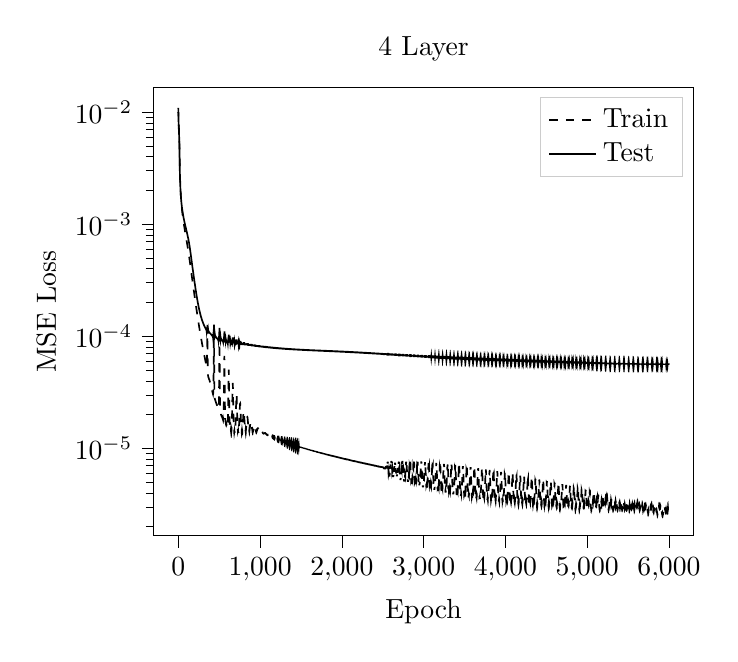
\begin{tikzpicture}

\begin{axis}[
legend cell align={left},
legend style={fill opacity=0.8, draw opacity=1, text opacity=1, draw=white!80!black},
log basis y={10},
tick align=outside,
tick pos=left,
title={4 Layer},
x grid style={white!69.0196078431373!black},
xlabel={Epoch},
xmin=-299.95, xmax=6298.95,
xtick style={color=black},
y grid style={white!69.0196078431373!black},
ylabel={MSE Loss},
ymin=1.65367011152804e-06, ymax=0.0165378276495926,
ymode=log,
ytick style={color=black}
]
\addplot [semithick, black, dashed]
table {%
0 0.0108807525830343
1 0.0101366702001542
2 0.00951129267923534
3 0.00896586285671219
4 0.00848299410426989
5 0.00804959743982181
6 0.0076601826294791
7 0.00731919275131077
8 0.00702948632533662
9 0.00677695525519084
10 0.00653317247633822
11 0.00626083150564227
12 0.00592074132873677
13 0.00549599970690906
14 0.00501126745075453
15 0.00451707903994247
16 0.00405622101243353
17 0.00365415004489478
18 0.00332527412683703
19 0.00306600953626912
20 0.0028547305992106
21 0.00267690898181172
22 0.00252717886905884
23 0.00240042659061146
24 0.00229278705955949
25 0.00219888157880632
26 0.00211530186788877
27 0.00203969597350806
28 0.00197128686704673
29 0.00190890697558643
30 0.00185191870332346
31 0.00179952520556981
32 0.0017512430640636
33 0.00170656959380722
34 0.00166509461996611
35 0.00162647633987945
36 0.00159040083053696
37 0.00155661881035485
38 0.00152489739593875
39 0.0014950280838093
40 0.00146682939339371
41 0.00144013650060515
42 0.00141480442835018
43 0.00139070413024456
44 0.00136772051155276
45 0.00134575171614415
46 0.00132470842800103
47 0.00130451083896332
48 0.0012850891907874
49 0.0012663818342844
50 0.00124833433801541
51 0.00123089828957745
52 0.00121403107368678
53 0.0011976944952039
54 0.0011818545171991
55 0.00116648037510458
56 0.00115154481682112
57 0.00113702255657699
58 0.00112289114804298
59 0.00110912960371934
60 0.00109571864777536
61 0.00108264104346745
62 0.00106988013249065
63 0.00105742070991255
64 0.00104524846028653
65 0.00103335010135197
66 0.00102171305661614
67 0.00101032509701326
68 0.000999175215838477
69 0.000988252628303599
70 0.000977547180809779
71 0.000967049327300629
72 0.000956749736360507
73 0.00094663966774533
74 0.000936710838686849
75 0.000926955152863229
76 0.00091736524427688
77 0.000907933666894678
78 0.000898653704098251
79 0.000889518699295877
80 0.000880522368788661
81 0.000871658894538996
82 0.000862922588567017
83 0.000854307928420894
84 0.000845809764541627
85 0.000837423113807745
86 0.000829143488772388
87 0.000820966375613352
88 0.000812887476058677
89 0.000804902681011299
90 0.000797008270637889
91 0.000789200598774187
92 0.000781476145675697
93 0.000773831250626245
94 0.000766263086006802
95 0.000758768612286076
96 0.000751344756281469
97 0.000743988863177947
98 0.000736698131731828
99 0.000729470169062552
100 0.000722302491340088
101 0.000715192760253558
102 0.000708138752997911
103 0.000701138549629832
104 0.000694189828209346
105 0.000687290779751493
106 0.000680439556163037
107 0.000673634390295774
108 0.000666873542286339
109 0.000660155473269697
110 0.000653478638014349
111 0.000646841438538104
112 0.00064024259972939
113 0.000633680719147378
114 0.000627154571702704
115 0.000620662994151644
116 0.000614204896010051
117 0.000607779444180778
118 0.000601385461777681
119 0.000595022197558137
120 0.000588688963944151
121 0.000582384989684215
122 0.000576109782741696
123 0.00056986280651472
124 0.000563643886380305
125 0.000557452578505035
126 0.000551289015675138
127 0.000545153033272072
128 0.000539044905963237
129 0.000532964910235023
130 0.00052691334985866
131 0.00052089097971475
132 0.00051489834277163
133 0.00050893670777441
134 0.000503006845065102
135 0.000497110037031234
136 0.00049124768065667
137 0.000485421203848091
138 0.000479632138194575
139 0.000473882605092513
140 0.000468174344860017
141 0.000462509263343236
142 0.000456889503311686
143 0.000451317128863593
144 0.000445794271399791
145 0.000440322949998517
146 0.000434905424299359
147 0.000429543601512705
148 0.000424239532549109
149 0.000418994811298035
150 0.000413811180351331
151 0.000408689978485199
152 0.000403632451252633
153 0.000398639587274374
154 0.000393711864489887
155 0.000388849987302819
156 0.000384054109417775
157 0.000379324201276177
158 0.000374660130091797
159 0.000370061228295526
160 0.000365526981113362
161 0.000361056685051153
162 0.000356649252353236
163 0.000352303602539905
164 0.000348018658769433
165 0.000343793157298933
166 0.000339625865308335
167 0.000335515681854304
168 0.000331461171299452
169 0.000327461154483899
170 0.000323514481806342
171 0.00031962000321073
172 0.00031577660865878
173 0.000311983168103325
174 0.000308238782963599
175 0.000304542437334021
176 0.00030089306710579
177 0.000297290032449382
178 0.000293732328373153
179 0.000290219240469014
180 0.000286750072064024
181 0.000283324203337543
182 0.000279940969903691
183 0.000276599680091749
184 0.000273299659511395
185 0.000270040366558533
186 0.000266821390141558
187 0.000263642057234392
188 0.0002605018844406
189 0.000257400375176076
190 0.000254337062870036
191 0.000251311590091063
192 0.000248323447067378
193 0.000245372275003319
194 0.000242457605054369
195 0.00023957895609783
196 0.000236736116676184
197 0.000233928698435193
198 0.000231156257086695
199 0.000228418572532973
200 0.00022571524095838
201 0.000223045990878745
202 0.000220410361635004
203 0.000217808089473692
204 0.000215238669170503
205 0.000212702061162418
206 0.000210197849810356
207 0.000207725862310326
208 0.000205285687798096
209 0.000202877164156234
210 0.000200499878928895
211 0.000198153629980879
212 0.000195838340914634
213 0.000193553441249605
214 0.000191298829804509
215 0.000189074183708726
216 0.000186879333341494
217 0.00018471391285857
218 0.000182577729901823
219 0.00018047050707537
220 0.000178392027692098
221 0.000176341916358069
222 0.000174320039150189
223 0.000172325988160082
224 0.000170359691992417
225 0.000168420806403446
226 0.000166508944857924
227 0.000164623852015211
228 0.000162765300274259
229 0.000160932930157287
230 0.000159126454263969
231 0.000157345604293369
232 0.000155590068061429
233 0.000153859489500974
234 0.000152153563476531
235 0.000150472025779891
236 0.000148814552176191
237 0.000147180697922522
238 0.00014557027839146
239 0.000143982894314831
240 0.000142418203722627
241 0.000140875936267548
242 0.000139355716783029
243 0.000137857129402619
244 0.000136379895593564
245 0.000134923673385856
246 0.000133488068286169
247 0.000132072949782014
248 0.00013067778900222
249 0.00012930220987073
250 0.000127946111206256
251 0.000126608911159565
252 0.000125290369169306
253 0.000123990284464526
254 0.000122708180469999
255 0.000121443680882294
256 0.000120196724310517
257 0.000118966818490662
258 0.000117753636914131
259 0.000116556909915744
260 0.000115376360781738
261 0.000114211821710342
262 0.000113062961645483
263 0.000111929548666012
264 0.00011081109278166
265 0.000109707495539624
266 0.000108618562080665
267 0.000107543922467812
268 0.000106483440504235
269 0.000105436754893162
270 0.000104403786167495
271 0.000103384238627768
272 0.000102377808957499
273 0.000101384394270099
274 0.000100403751503109
275 9.94357056924855e-05
276 9.84800452670243e-05
277 9.75365234126002e-05
278 9.66049080943776e-05
279 9.56851506543899e-05
280 9.47770245147694e-05
281 9.38803531198573e-05
282 9.29950505224042e-05
283 9.21207841884097e-05
284 9.12574823814793e-05
285 9.04050637018372e-05
286 8.95632844049032e-05
287 8.87319301909884e-05
288 8.79109170455195e-05
289 8.71000231654762e-05
290 8.62992272914198e-05
291 8.55082760153891e-05
292 8.47270997610394e-05
293 8.39554742242399e-05
294 8.31932028404481e-05
295 8.24403662136319e-05
296 8.16965990679819e-05
297 8.09618106814014e-05
298 8.02359554654686e-05
299 7.95188988149675e-05
300 7.88103906188553e-05
301 7.81103391318538e-05
302 7.74186901253415e-05
303 7.67353498076773e-05
304 7.60599166369502e-05
305 7.53925173739844e-05
306 7.47328299439687e-05
307 7.40808075079258e-05
308 7.34364208483385e-05
309 7.27992934344002e-05
310 7.21694715366539e-05
311 7.15467793952484e-05
312 7.09311611899466e-05
313 7.03222083302535e-05
314 6.97200550803245e-05
315 6.9124328547332e-05
316 6.85351689071467e-05
317 6.79520187532034e-05
318 6.73752668944871e-05
319 6.68039461970693e-05
320 6.62389487615656e-05
321 6.56788336073078e-05
322 6.51248980148011e-05
323 6.45751482579726e-05
324 6.4031701526801e-05
325 6.34915055570673e-05
326 6.29578308348755e-05
327 6.2426005058569e-05
328 6.19015501115427e-05
329 6.137674523643e-05
330 6.08611463803754e-05
331 6.03416543754065e-05
332 5.98344936406647e-05
333 5.93179846077874e-05
334 5.88198125228701e-05
335 5.83025356490907e-05
336 5.78151858121601e-05
337 5.72918543753076e-05
338 5.68202336808099e-05
339 5.62821527410051e-05
340 5.58373838543957e-05
341 5.52711121599714e-05
342 5.48803409969878e-05
343 5.4268112421596e-05
344 5.39994425139412e-05
345 5.33347239866089e-05
346 5.33757915377464e-05
347 5.27556974816434e-05
348 5.36745599788446e-05
349 5.37351568254962e-05
350 5.73008562128052e-05
351 6.08821681566951e-05
352 7.13391222006976e-05
353 8.5812010297559e-05
354 0.000100979233593534
355 0.000120043855531549
356 0.000108146332536307
357 9.90131588878285e-05
358 7.56350518145155e-05
359 6.19437393538647e-05
360 5.3461360437268e-05
361 4.89202299149838e-05
362 4.68736961920513e-05
363 4.52995966497838e-05
364 4.46415640453779e-05
365 4.38918942222699e-05
366 4.36185752050733e-05
367 4.32168962447577e-05
368 4.30100105290876e-05
369 4.27376282345904e-05
370 4.25410022444339e-05
371 4.23232027628728e-05
372 4.21435810267212e-05
373 4.19543190446348e-05
374 4.17876813685325e-05
375 4.16113875871815e-05
376 4.14452979953239e-05
377 4.12675487950764e-05
378 4.10905735748202e-05
379 4.09003783943263e-05
380 4.07057866596006e-05
381 4.04977956804942e-05
382 4.02838562649777e-05
383 4.00577473556041e-05
384 3.98263894680895e-05
385 3.95850478867033e-05
386 3.93399865856736e-05
387 3.90872930893238e-05
388 3.88325771609743e-05
389 3.85721814950557e-05
390 3.8311522132517e-05
391 3.80469432457176e-05
392 3.77833748643752e-05
393 3.75170358211108e-05
394 3.72531692391931e-05
395 3.69875656929253e-05
396 3.67255492506047e-05
397 3.64623893460703e-05
398 3.62039796186764e-05
399 3.59448148117281e-05
400 3.56914336521186e-05
401 3.54371909168094e-05
402 3.51899626025443e-05
403 3.49414079607868e-05
404 3.47010441430484e-05
405 3.445835412208e-05
406 3.42255273153569e-05
407 3.39886725555516e-05
408 3.37638593350675e-05
409 3.35324509421753e-05
410 3.33163055188379e-05
411 3.30893668092358e-05
412 3.28826320981079e-05
413 3.26588142911532e-05
414 3.24631447199408e-05
415 3.22404580401781e-05
416 3.20587521400739e-05
417 3.18340568412623e-05
418 3.16722959610161e-05
419 3.14416355706726e-05
420 3.13123481987532e-05
421 3.10718756679762e-05
422 3.10034697577066e-05
423 3.07568388961954e-05
424 3.08200557412874e-05
425 3.06094295012826e-05
426 3.09989503648467e-05
427 3.1031520364877e-05
428 3.23255243586118e-05
429 3.34581890797381e-05
430 3.73788374474771e-05
431 4.2709020874554e-05
432 5.3219188885123e-05
433 7.0129861796886e-05
434 8.60424368056556e-05
435 0.00011046530380554
436 0.000100550253137044
437 9.61731279858213e-05
438 6.76536903370106e-05
439 5.21722228086219e-05
440 4.01035765094093e-05
441 3.44453078753304e-05
442 3.15704360787095e-05
443 3.00149088729995e-05
444 2.91883591501119e-05
445 2.84477294201224e-05
446 2.81009586728942e-05
447 2.76809811907697e-05
448 2.75160054457046e-05
449 2.72618115104706e-05
450 2.71422539981359e-05
451 2.69502309890868e-05
452 2.68335300859235e-05
453 2.66625961273803e-05
454 2.6544508614279e-05
455 2.63841658352248e-05
456 2.62661708916312e-05
457 2.61134736945223e-05
458 2.59960263520043e-05
459 2.58493084572819e-05
460 2.57330766260111e-05
461 2.55913155911003e-05
462 2.54768509648784e-05
463 2.53391887099497e-05
464 2.522696536289e-05
465 2.50925440354877e-05
466 2.49828951837117e-05
467 2.4851112016222e-05
468 2.47443433067929e-05
469 2.46145861524383e-05
470 2.4511056267329e-05
471 2.43826592054575e-05
472 2.42828418919316e-05
473 2.41550795436751e-05
474 2.40596020972816e-05
475 2.39316475898477e-05
476 2.38414501581019e-05
477 2.3712133099707e-05
478 2.36287809087798e-05
479 2.34965852285995e-05
480 2.34224074944223e-05
481 2.32853778214803e-05
482 2.32242964415263e-05
483 2.3079745616883e-05
484 2.30385218742413e-05
485 2.2883361566528e-05
486 2.28743917460861e-05
487 2.27060363044984e-05
488 2.2753305145784e-05
489 2.25742306554366e-05
490 2.27280659288454e-05
491 2.2560786803183e-05
492 2.2934721826573e-05
493 2.28711931953285e-05
494 2.37384408450225e-05
495 2.40943623452949e-05
496 2.61300095871775e-05
497 2.78893306244754e-05
498 3.26321728039147e-05
499 3.83710778919522e-05
500 4.79660172914009e-05
501 6.1358341667983e-05
502 7.19407737506117e-05
503 8.70407359343517e-05
504 8.00157342837338e-05
505 7.72379562476999e-05
506 5.74159916482131e-05
507 4.59310081737385e-05
508 3.52111405277356e-05
509 2.93519194087821e-05
510 2.60239986005217e-05
511 2.39707813420864e-05
512 2.29555648445512e-05
513 2.2037409834752e-05
514 2.16422160121965e-05
515 2.11056841550317e-05
516 2.09424301260697e-05
517 2.06061374825595e-05
518 2.0534493728519e-05
519 2.03058811791834e-05
520 2.02644559408327e-05
521 2.00898038258401e-05
522 2.0055675832964e-05
523 1.99083729626182e-05
524 1.98752486539888e-05
525 1.97430267832033e-05
526 1.97097585754591e-05
527 1.95864040364313e-05
528 1.95535168074912e-05
529 1.94354907989691e-05
530 1.94040125620631e-05
531 1.92888009422632e-05
532 1.92600945609911e-05
533 1.91457183120747e-05
534 1.91214599567502e-05
535 1.90060774087897e-05
536 1.89884211749813e-05
537 1.8870146647032e-05
538 1.88621653478549e-05
539 1.87389732246857e-05
540 1.87451681910034e-05
541 1.86148905356731e-05
542 1.86423054486795e-05
543 1.85028524839481e-05
544 1.85632065381469e-05
545 1.84137934695627e-05
546 1.85275315516265e-05
547 1.83716593369354e-05
548 1.85767281379867e-05
549 1.84310379722774e-05
550 1.88015641811035e-05
551 1.87190844087581e-05
552 1.94065629557372e-05
553 1.95369348716667e-05
554 2.08566800523613e-05
555 2.15914826355856e-05
556 2.41710792607819e-05
557 2.64272702565904e-05
558 3.12607093064798e-05
559 3.66637287925187e-05
560 4.40643370893667e-05
561 5.33882408717545e-05
562 5.89572252920334e-05
563 6.67869326207438e-05
564 6.15469841704908e-05
565 5.91835570276089e-05
566 4.72029497018411e-05
567 3.97198220412065e-05
568 3.18509235057718e-05
569 2.69153288172674e-05
570 2.37144591608285e-05
571 2.14333263670596e-05
572 2.02787487779688e-05
573 1.91432453817697e-05
574 1.8693258653002e-05
575 1.80049484015399e-05
576 1.78243460311478e-05
577 1.73612656340083e-05
578 1.73028316368118e-05
579 1.69721624416752e-05
580 1.69698300709342e-05
581 1.67173569423085e-05
582 1.67400876875945e-05
583 1.65331543513503e-05
584 1.65679115866624e-05
585 1.63872846314916e-05
586 1.64298605795921e-05
587 1.62642670886726e-05
588 1.63146999199171e-05
589 1.61569701901954e-05
590 1.62179429992193e-05
591 1.60633412065181e-05
592 1.61395469859826e-05
593 1.59847539720204e-05
594 1.60836104470263e-05
595 1.59267660393425e-05
596 1.60597552536501e-05
597 1.59012140272807e-05
598 1.60868690102234e-05
599 1.59318024657296e-05
600 1.62012089361951e-05
601 1.6065347764993e-05
602 1.64725889959527e-05
603 1.63955215981559e-05
604 1.7037333918779e-05
605 1.71113194227246e-05
606 1.81612532088593e-05
607 1.85883316987656e-05
608 2.03428214291534e-05
609 2.15275586299413e-05
610 2.44067806249859e-05
611 2.70094563745715e-05
612 3.12659894916578e-05
613 3.5843477007802e-05
614 4.04819114123711e-05
615 4.60402787894054e-05
616 4.76159710842694e-05
617 5.03728898593181e-05
618 4.61593655245451e-05
619 4.37075824493149e-05
620 3.70593097045457e-05
621 3.25178933167081e-05
622 2.7749895167517e-05
623 2.43014318925816e-05
624 2.19047186362786e-05
625 1.98831254749621e-05
626 1.88299116672397e-05
627 1.7635357565382e-05
628 1.71855978408075e-05
629 1.6402293240958e-05
630 1.62257362603668e-05
631 1.56658709755675e-05
632 1.56265009252365e-05
633 1.52023363710896e-05
634 1.52379928408664e-05
635 1.48999319975474e-05
636 1.49802350080108e-05
637 1.4697276220943e-05
638 1.48085907483164e-05
639 1.4561109125566e-05
640 1.46997891334877e-05
641 1.44758251607868e-05
642 1.46449766873502e-05
643 1.44380950573009e-05
644 1.46469010218198e-05
645 1.44558319519206e-05
646 1.4720610138852e-05
647 1.45506070197143e-05
648 1.48979120240256e-05
649 1.47645846482192e-05
650 1.52372115991284e-05
651 1.51748971006782e-05
652 1.58411778841128e-05
653 1.59182846459771e-05
654 1.68846001287193e-05
655 1.72276218677325e-05
656 1.8646371131581e-05
657 1.9466271822921e-05
658 2.15071533204991e-05
659 2.30857662870676e-05
660 2.57869747599671e-05
661 2.83030211107871e-05
662 3.12038534957537e-05
663 3.42611392056824e-05
664 3.60474990657167e-05
665 3.82572990247354e-05
666 3.74675048533391e-05
667 3.73399897171112e-05
668 3.42485337796461e-05
669 3.2039051063748e-05
670 2.8574766076872e-05
671 2.5873113884245e-05
672 2.3373863911047e-05
673 2.12110193729131e-05
674 1.97781604640568e-05
675 1.82780929947057e-05
676 1.75493471061827e-05
677 1.65140874059944e-05
678 1.6178702296088e-05
679 1.54290338372221e-05
680 1.5310907670596e-05
681 1.47395342082746e-05
682 1.47492338555821e-05
683 1.42951845418793e-05
684 1.43878029206235e-05
685 1.40146061795576e-05
686 1.41685697059302e-05
687 1.38538633649432e-05
688 1.40616185007048e-05
689 1.37927852108533e-05
690 1.40570597295664e-05
691 1.38298472052156e-05
692 1.4162299564191e-05
693 1.39811969290804e-05
694 1.4403433212351e-05
695 1.42841116286263e-05
696 1.48297732636138e-05
697 1.48040579261988e-05
698 1.55216139177128e-05
699 1.56444481547169e-05
700 1.65972693935146e-05
701 1.6953033906475e-05
702 1.82083984157089e-05
703 1.89064102755765e-05
704 2.04957376297443e-05
705 2.16294868096156e-05
706 2.34565828804989e-05
707 2.49928581865788e-05
708 2.67070898303245e-05
709 2.83230652939892e-05
710 2.93092967922348e-05
711 3.03700549579844e-05
712 3.00998868283386e-05
713 3.00433503070963e-05
714 2.86159767597383e-05
715 2.74818303864777e-05
716 2.56044117463716e-05
717 2.3968199684532e-05
718 2.23214642289804e-05
719 2.07359221349179e-05
720 1.95859441873836e-05
721 1.82873487233337e-05
722 1.75940917301887e-05
723 1.6590503577163e-05
724 1.62245708992259e-05
725 1.54503084957014e-05
726 1.53008494123696e-05
727 1.46916823098309e-05
728 1.46868313919413e-05
729 1.4196982078829e-05
730 1.42951602981611e-05
731 1.38950576911157e-05
732 1.40748672947666e-05
733 1.37468470455815e-05
734 1.40003124897703e-05
735 1.37361595022867e-05
736 1.40652437892186e-05
737 1.38653224865948e-05
738 1.42804334188895e-05
739 1.41543247735854e-05
740 1.46733775778785e-05
741 1.46409965395833e-05
742 1.52879516690518e-05
743 1.53806873015583e-05
744 1.61810463623624e-05
745 1.64399247921665e-05
746 1.7409668515711e-05
747 1.78753304282964e-05
748 1.8997482868599e-05
749 1.96848265829885e-05
750 2.08741561493753e-05
751 2.17280202150505e-05
752 2.28005089297767e-05
753 2.36528792925128e-05
754 2.43472751435547e-05
755 2.49314222742214e-05
756 2.50284327876216e-05
757 2.51012664875816e-05
758 2.45847811015665e-05
759 2.40896335412799e-05
760 2.3182583106518e-05
761 2.22840200194696e-05
762 2.12985979715086e-05
763 2.02488738523243e-05
764 1.9410763485439e-05
765 1.84027464911196e-05
766 1.77985924381119e-05
767 1.69208951774635e-05
768 1.65436754571147e-05
769 1.58117351816145e-05
770 1.56198291563214e-05
771 1.50181693072682e-05
772 1.4969085100347e-05
773 1.44757973714604e-05
774 1.45378082123671e-05
775 1.41345150268535e-05
776 1.42875780682061e-05
777 1.39620634342918e-05
778 1.41957776804702e-05
779 1.39421112521632e-05
780 1.42535087803708e-05
781 1.40719226067176e-05
782 1.44634965550949e-05
783 1.43601029094498e-05
784 1.48376392559157e-05
785 1.48237260759743e-05
786 1.53932939497281e-05
787 1.54835373109563e-05
788 1.61458238210344e-05
789 1.63534185446679e-05
790 1.70954457985317e-05
791 1.74230574430112e-05
792 1.8206992820069e-05
793 1.86328519191648e-05
794 1.93864586037762e-05
795 1.98505329649379e-05
796 2.04694301828567e-05
797 2.08709184335021e-05
798 2.12445351053248e-05
799 2.14653992998137e-05
800 2.15245061667702e-05
801 2.14772214235381e-05
802 2.12356130759872e-05
803 2.09070620371676e-05
804 2.04603776978729e-05
805 1.9914770973628e-05
806 1.93935749166485e-05
807 1.87333782264432e-05
808 1.82484463380206e-05
809 1.75676600520092e-05
810 1.71833184765546e-05
811 1.65433658310121e-05
812 1.62816352826667e-05
813 1.57117433445819e-05
814 1.55693368242282e-05
815 1.50777606506836e-05
816 1.50412693642465e-05
817 1.46262636917527e-05
818 1.46813493131503e-05
819 1.43382369515166e-05
820 1.44732949820536e-05
821 1.4198066935478e-05
822 1.44052787902638e-05
823 1.41960755684067e-05
824 1.44706991704879e-05
825 1.43281963573827e-05
826 1.46672926746305e-05
827 1.45941335745192e-05
828 1.49947051397703e-05
829 1.49943798248842e-05
830 1.54506278136068e-05
831 1.55251019862135e-05
832 1.60250330623057e-05
833 1.61708294683649e-05
834 1.66923361462068e-05
835 1.68959883524167e-05
836 1.74043637457544e-05
837 1.76380453069669e-05
838 1.80870542294542e-05
839 1.83075897552953e-05
840 1.86468539027373e-05
841 1.88018138373991e-05
842 1.89908784307136e-05
843 1.90317438182319e-05
844 1.90555168444462e-05
845 1.89539530310867e-05
846 1.88305903350283e-05
847 1.85882780669999e-05
848 1.8363630232443e-05
849 1.80096807866903e-05
850 1.77412993878079e-05
851 1.73193712385e-05
852 1.70590612640353e-05
853 1.66126391150101e-05
854 1.63966199124843e-05
855 1.59595767286191e-05
856 1.58075524439028e-05
857 1.54019857632193e-05
858 1.53206752031565e-05
859 1.49586987276962e-05
860 1.49473083865814e-05
861 1.46344997915548e-05
862 1.46887493883696e-05
863 1.44272933368939e-05
864 1.45418446209078e-05
865 1.43324522241528e-05
866 1.45020354125336e-05
867 1.4345027437912e-05
868 1.4564541118034e-05
869 1.44601947624778e-05
870 1.47240321837216e-05
871 1.46721204998812e-05
872 1.49732439922445e-05
873 1.49721854825202e-05
874 1.53006767220631e-05
875 1.53459610601203e-05
876 1.56879202961591e-05
877 1.57708251151689e-05
878 1.61077542770727e-05
879 1.62136711026051e-05
880 1.65230528921256e-05
881 1.6631541541301e-05
882 1.68893068916987e-05
883 1.69758401966646e-05
884 1.71608055552497e-05
885 1.72007683545417e-05
886 1.73000329368733e-05
887 1.72741018218403e-05
888 1.72871839936306e-05
889 1.71863653122273e-05
890 1.71258180614586e-05
891 1.69531368214848e-05
892 1.68414119627869e-05
893 1.66103600918177e-05
894 1.64741373680499e-05
895 1.62042842362098e-05
896 1.60686935544163e-05
897 1.57806463505494e-05
898 1.56655059129207e-05
899 1.5377490086621e-05
900 1.52959255501628e-05
901 1.50221370347481e-05
902 1.49814547683036e-05
903 1.47316794141261e-05
904 1.4734484921064e-05
905 1.45150461321464e-05
906 1.45608441641798e-05
907 1.43756290924557e-05
908 1.44623625430995e-05
909 1.43135075632017e-05
910 1.44374464525754e-05
911 1.43257306888245e-05
912 1.44824118422093e-05
913 1.44075945343047e-05
914 1.45912874245369e-05
915 1.45516933116596e-05
916 1.47553428462288e-05
917 1.47477975644961e-05
918 1.49625339531667e-05
919 1.49816639805067e-05
920 1.51970135391366e-05
921 1.52348362121302e-05
922 1.54387936674993e-05
923 1.54848427200704e-05
924 1.56649377913709e-05
925 1.57070264492631e-05
926 1.5851846995929e-05
927 1.58771472911212e-05
928 1.59783593289831e-05
929 1.59755985009724e-05
930 1.60293772637488e-05
931 1.59904617476059e-05
932 1.59986986716376e-05
933 1.59204844010219e-05
934 1.58905843363755e-05
935 1.57749737468293e-05
936 1.57180119515488e-05
937 1.55713293850113e-05
938 1.55002810231508e-05
939 1.53315823467892e-05
940 1.52592005235874e-05
941 1.50787339805447e-05
942 1.50158235499021e-05
943 1.48333510878729e-05
944 1.47880417387114e-05
945 1.46120942474681e-05
946 1.45897475363199e-05
947 1.44269718020951e-05
948 1.44302977105326e-05
949 1.42857628020465e-05
950 1.43154809677526e-05
951 1.4192486361253e-05
952 1.42475939810538e-05
953 1.41480934132687e-05
954 1.42262513520564e-05
955 1.41509900970505e-05
956 1.42488771359695e-05
957 1.4197475650235e-05
958 1.43106496466316e-05
959 1.42814331525187e-05
960 1.44046513810281e-05
961 1.43947595745431e-05
962 1.45218675129399e-05
963 1.45271455664897e-05
964 1.46512715843983e-05
965 1.46662482620741e-05
966 1.47806219388258e-05
967 1.4798907130853e-05
968 1.48969797351128e-05
969 1.49118544925386e-05
970 1.49883647964089e-05
971 1.49932461681601e-05
972 1.50446751092659e-05
973 1.50340778475311e-05
974 1.50592865963972e-05
975 1.50295109051513e-05
976 1.50301056862645e-05
977 1.49797534447771e-05
978 1.49597152017122e-05
979 1.48896326379599e-05
980 1.48544743012735e-05
981 1.47677037602989e-05
982 1.47241551644584e-05
983 1.46251194905744e-05
984 1.45797176003271e-05
985 1.44735408866836e-05
986 1.44322469282088e-05
987 1.43241973660224e-05
988 1.42917302241585e-05
989 1.41866986496098e-05
990 1.41665688886405e-05
991 1.40687799330408e-05
992 1.40630114344731e-05
993 1.39757384829409e-05
994 1.39851835569971e-05
995 1.39108972234681e-05
996 1.39351074039951e-05
997 1.3875297412369e-05
998 1.39129951719497e-05
999 1.38681881765024e-05
1000 1.39170846580328e-05
1001 1.38869990848889e-05
1002 1.39442894067088e-05
1003 1.39278648418895e-05
1004 1.39900667761594e-05
1005 1.39852092218007e-05
1006 1.40485919644107e-05
1007 1.40526732934632e-05
1008 1.41131982047682e-05
1009 1.4122978427622e-05
1010 1.41768522610164e-05
1011 1.41886289668491e-05
1012 1.42324296348306e-05
1013 1.42425062961138e-05
1014 1.42735804331551e-05
1015 1.42785195293982e-05
1016 1.42953331021545e-05
1017 1.42923564112607e-05
1018 1.4294545849225e-05
1019 1.42817398796069e-05
1020 1.42702988625842e-05
1021 1.42468748265401e-05
1022 1.4223736883423e-05
1023 1.41900756887026e-05
1024 1.41581830632731e-05
1025 1.41156378674623e-05
1026 1.40783822359936e-05
1027 1.40290905221718e-05
1028 1.39898841950981e-05
1029 1.39365328095664e-05
1030 1.38987472837471e-05
1031 1.38440890680158e-05
1032 1.38104271627526e-05
1033 1.37572268386066e-05
1034 1.3729738782331e-05
1035 1.36805443844423e-05
1036 1.36607040985837e-05
1037 1.3617549313949e-05
1038 1.36058746988965e-05
1039 1.35703624266625e-05
1040 1.35667837923847e-05
1041 1.35398774716577e-05
1042 1.35436693824431e-05
1043 1.3525764387623e-05
1044 1.35357113322243e-05
1045 1.35268285816892e-05
1046 1.35412329029805e-05
1047 1.35406300785235e-05
1048 1.35574753699075e-05
1049 1.35640688370131e-05
1050 1.35811180257406e-05
1051 1.35933041747194e-05
1052 1.36082625488143e-05
1053 1.36240961126077e-05
1054 1.36348725447988e-05
1055 1.36524126332915e-05
1056 1.36572361952858e-05
1057 1.36744791632282e-05
1058 1.36719494321369e-05
1059 1.36870038147663e-05
1060 1.36763572129439e-05
1061 1.36877143290803e-05
1062 1.36686556118093e-05
1063 1.36752941841678e-05
1064 1.36484080996979e-05
1065 1.36498588290124e-05
1066 1.36161258126322e-05
1067 1.36123856862014e-05
1068 1.35732183537129e-05
1069 1.35649316916897e-05
1070 1.352208590788e-05
1071 1.35102369256401e-05
1072 1.34656403929512e-05
1073 1.34515296110749e-05
1074 1.34069537978121e-05
1075 1.3392110759014e-05
1076 1.33490895848354e-05
1077 1.3335073106191e-05
1078 1.32949236615332e-05
1079 1.32832243195935e-05
1080 1.32467465903119e-05
1081 1.32385584095118e-05
1082 1.32062404532007e-05
1083 1.32025024868199e-05
1084 1.31743305757936e-05
1085 1.31757391272913e-05
1086 1.31513842802633e-05
1087 1.31582653182249e-05
1088 1.31370667588726e-05
1089 1.31493841593056e-05
1090 1.31304402088972e-05
1091 1.31479659728484e-05
1092 1.31301043211351e-05
1093 1.31522025981212e-05
1094 1.31342285101255e-05
1095 1.31599701376217e-05
1096 1.3140562288072e-05
1097 1.31689953377645e-05
1098 1.3147096154853e-05
1099 1.31771356848276e-05
1100 1.31516781891605e-05
1101 1.31821931859122e-05
1102 1.31524083428758e-05
1103 1.31823830997746e-05
1104 1.31477677030034e-05
1105 1.31762932085167e-05
1106 1.31367579285779e-05
1107 1.31632806983362e-05
1108 1.31190713545948e-05
1109 1.31432709338242e-05
1110 1.3094819678372e-05
1111 1.3116637433086e-05
1112 1.30646809282098e-05
1113 1.30842966541422e-05
1114 1.30297545126723e-05
1115 1.30477116897509e-05
1116 1.29915425475247e-05
1117 1.30084461886781e-05
1118 1.29515925664236e-05
1119 1.29682803162723e-05
1120 1.29117368317111e-05
1121 1.29289331596283e-05
1122 1.28733647102308e-05
1123 1.28920029283108e-05
1124 1.28379907096132e-05
1125 1.28587762446841e-05
1126 1.28065746594075e-05
1127 1.2829995824859e-05
1128 1.27796791105084e-05
1129 1.28062290798425e-05
1130 1.27577172008841e-05
1131 1.27876427313822e-05
1132 1.27406160004284e-05
1133 1.27740414370692e-05
1134 1.27280173387589e-05
1135 1.27647371357398e-05
1136 1.27190495504692e-05
1137 1.27588042744264e-05
1138 1.27128612064098e-05
1139 1.27552225137606e-05
1140 1.27082830942982e-05
1141 1.27527619611101e-05
1142 1.27042328301741e-05
1143 1.27501301108168e-05
1144 1.26993946594212e-05
1145 1.27461627812409e-05
1146 1.26927858161707e-05
1147 1.27398371034815e-05
1148 1.26834783600316e-05
1149 1.27302611190316e-05
1150 1.26708412153675e-05
1151 1.27171048802666e-05
1152 1.26546957517348e-05
1153 1.27000720056003e-05
1154 1.26349110018964e-05
1155 1.2679395183568e-05
1156 1.2611826889497e-05
1157 1.26554608641527e-05
1158 1.25859363606651e-05
1159 1.26289253614686e-05
1160 1.25580183691909e-05
1161 1.26007676044537e-05
1162 1.25289780612547e-05
1163 1.2571806678352e-05
1164 1.24996140868916e-05
1165 1.25429449155945e-05
1166 1.24707506472532e-05
1167 1.25150524468154e-05
1168 1.24432687869103e-05
1169 1.24889640460424e-05
1170 1.24177600184794e-05
1171 1.24652335955489e-05
1172 1.23947019687876e-05
1173 1.24441971536271e-05
1174 1.23743930089404e-05
1175 1.24261655685132e-05
1176 1.23568421201981e-05
1177 1.24108547083779e-05
1178 1.23418265047803e-05
1179 1.23980956914238e-05
1180 1.23289802331783e-05
1181 1.23873734594326e-05
1182 1.23178837725391e-05
1183 1.23781592549221e-05
1184 1.23077894045309e-05
1185 1.23696484024549e-05
1186 1.2298150920742e-05
1187 1.2361308989739e-05
1188 1.22883508879568e-05
1189 1.23525800290736e-05
1190 1.22778826607828e-05
1191 1.23427264782094e-05
1192 1.22661093939769e-05
1193 1.23313674293968e-05
1194 1.2252758580189e-05
1195 1.23181065418976e-05
1196 1.2237498168588e-05
1197 1.23028929976954e-05
1198 1.22203470880322e-05
1199 1.22855845177128e-05
1200 1.2201242412857e-05
1201 1.2266419844309e-05
1202 1.2180628459646e-05
1203 1.22457779809793e-05
1204 1.21587358137276e-05
1205 1.2223995952354e-05
1206 1.21359789773123e-05
1207 1.2201572047843e-05
1208 1.21129339447634e-05
1209 1.21790949663136e-05
1210 1.20900697879733e-05
1211 1.21570949147554e-05
1212 1.20678229507121e-05
1213 1.21359023523837e-05
1214 1.20465533939296e-05
1215 1.21158540480337e-05
1216 1.20265561633914e-05
1217 1.20972865147451e-05
1218 1.20079588157296e-05
1219 1.20802402818754e-05
1220 1.19908951887737e-05
1221 1.20647638084392e-05
1222 1.19752500324921e-05
1223 1.20506996950098e-05
1224 1.19608688464723e-05
1225 1.20378959707068e-05
1226 1.19475345456976e-05
1227 1.2025983409103e-05
1228 1.19348880218695e-05
1229 1.20146979725178e-05
1230 1.19227570962721e-05
1231 1.20038021691471e-05
1232 1.19107338889535e-05
1233 1.1992711364428e-05
1234 1.18984385721888e-05
1235 1.19811988383844e-05
1236 1.18855640209858e-05
1237 1.19690124904537e-05
1238 1.18719811155188e-05
1239 1.19558755500293e-05
1240 1.18574035354868e-05
1241 1.19416397126315e-05
1242 1.18417326859799e-05
1243 1.19263449107621e-05
1244 1.18251147398496e-05
1245 1.19100269841965e-05
1246 1.180758118835e-05
1247 1.18928333563417e-05
1248 1.17893237927547e-05
1249 1.18750114381783e-05
1250 1.1770575014225e-05
1251 1.18567561173677e-05
1252 1.1751518343317e-05
1253 1.18383150322643e-05
1254 1.17325151904879e-05
1255 1.18200259464629e-05
1256 1.17137652182464e-05
1257 1.18021567914184e-05
1258 1.16954593636365e-05
1259 1.17848009608679e-05
1260 1.167768527921e-05
1261 1.17680732216741e-05
1262 1.1660673408187e-05
1263 1.17522799882863e-05
1264 1.16445786204622e-05
1265 1.17374065951026e-05
1266 1.16292866891854e-05
1267 1.17233251444304e-05
1268 1.16147583639759e-05
1269 1.17100174463758e-05
1270 1.16008151564984e-05
1271 1.16972057924158e-05
1272 1.15873768891106e-05
1273 1.16848448783458e-05
1274 1.15741954971327e-05
1275 1.16726664032285e-05
1276 1.15612164961476e-05
1277 1.16606841800149e-05
1278 1.15482876879014e-05
1279 1.16486134515981e-05
1280 1.15351706426736e-05
1281 1.16362275264237e-05
1282 1.15216912490723e-05
1283 1.16234306801744e-05
1284 1.15077490363547e-05
1285 1.16100119669227e-05
1286 1.14932701364978e-05
1287 1.15960570781226e-05
1288 1.14781623210547e-05
1289 1.15814150944971e-05
1290 1.14625798346424e-05
1291 1.15664135194038e-05
1292 1.14466675711355e-05
1293 1.15510631815141e-05
1294 1.14304710905344e-05
1295 1.15354422405289e-05
1296 1.14140372033944e-05
1297 1.15196423848829e-05
1298 1.13976086311141e-05
1299 1.15039208026246e-05
1300 1.1381222577711e-05
1301 1.14882609523193e-05
1302 1.13650285129552e-05
1303 1.14729676852221e-05
1304 1.1349196881838e-05
1305 1.14579952708027e-05
1306 1.13336940330555e-05
1307 1.14434031104338e-05
1308 1.13186171120105e-05
1309 1.14293107742469e-05
1310 1.13040027258648e-05
1311 1.14156503627783e-05
1312 1.12898008808315e-05
1313 1.14024597621665e-05
1314 1.12760819490632e-05
1315 1.13897362439275e-05
1316 1.12626964323681e-05
1317 1.13773129442052e-05
1318 1.12495640109955e-05
1319 1.13650772561869e-05
1320 1.12365676727677e-05
1321 1.13529438579008e-05
1322 1.12236382676656e-05
1323 1.13407692765577e-05
1324 1.12106237963872e-05
1325 1.13285417739917e-05
1326 1.1197486543324e-05
1327 1.13160985506511e-05
1328 1.11840940633101e-05
1329 1.13033474917756e-05
1330 1.11704655409994e-05
1331 1.12903207991621e-05
1332 1.11565928193613e-05
1333 1.12770889870717e-05
1334 1.11424891144907e-05
1335 1.1263608655554e-05
1336 1.11282012937863e-05
1337 1.12498808562123e-05
1338 1.1113749536662e-05
1339 1.1236079842547e-05
1340 1.10991326494059e-05
1341 1.12220935761798e-05
1342 1.10844752327921e-05
1343 1.12080666951897e-05
1344 1.1069797210439e-05
1345 1.1194158332728e-05
1346 1.10552568060029e-05
1347 1.11802980597986e-05
1348 1.10408242903759e-05
1349 1.11666180657721e-05
1350 1.10265430635081e-05
1351 1.11531339257454e-05
1352 1.10125133119254e-05
1353 1.11399241689014e-05
1354 1.09988081078427e-05
1355 1.11270808247355e-05
1356 1.0985368078309e-05
1357 1.11144820778009e-05
1358 1.09721505623384e-05
1359 1.1102097857929e-05
1360 1.09591582031499e-05
1361 1.10899319167856e-05
1362 1.09463617832262e-05
1363 1.10779203623679e-05
1364 1.09336926072956e-05
1365 1.10660354550873e-05
1366 1.09210710377283e-05
1367 1.10542192715002e-05
1368 1.09085972042067e-05
1369 1.10424609829352e-05
1370 1.08960692273286e-05
1371 1.10306457941078e-05
1372 1.08834844922967e-05
1373 1.10187073403267e-05
1374 1.08708031518745e-05
1375 1.10066676484166e-05
1376 1.08579522759555e-05
1377 1.09944244002236e-05
1378 1.08449347067108e-05
1379 1.09819931140009e-05
1380 1.08317585727491e-05
1381 1.096944995993e-05
1382 1.08185494127611e-05
1383 1.09568302946172e-05
1384 1.08052711595974e-05
1385 1.09441900235652e-05
1386 1.07919408094403e-05
1387 1.09314897827062e-05
1388 1.07785967600194e-05
1389 1.09187548105183e-05
1390 1.07652869019148e-05
1391 1.09061521129661e-05
1392 1.07520512813153e-05
1393 1.08935772971108e-05
1394 1.07388915751017e-05
1395 1.0881123046147e-05
1396 1.07258743184957e-05
1397 1.08688114721645e-05
1398 1.07130252899879e-05
1399 1.08567070071786e-05
1400 1.07003645837267e-05
1401 1.08447785862609e-05
1402 1.06878406995747e-05
1403 1.08329485044578e-05
1404 1.06754537512188e-05
1405 1.08213194209839e-05
1406 1.06632331835499e-05
1407 1.08098442694882e-05
1408 1.06511571402734e-05
1409 1.07984425596896e-05
1410 1.06391285896734e-05
1411 1.07871115062608e-05
1412 1.06271111235401e-05
1413 1.0775747284697e-05
1414 1.06151845500335e-05
1415 1.07644874560719e-05
1416 1.06032370865705e-05
1417 1.07531859043775e-05
1418 1.05912718311174e-05
1419 1.07418651111857e-05
1420 1.05792462079535e-05
1421 1.07304170455791e-05
1422 1.05671630308279e-05
1423 1.07188483582377e-05
1424 1.05548923556853e-05
1425 1.07072307287126e-05
1426 1.05426703385092e-05
1427 1.06955778846896e-05
1428 1.05303917052879e-05
1429 1.0683881470186e-05
1430 1.05181044034452e-05
1431 1.06722157795502e-05
1432 1.05058414021642e-05
1433 1.06605608607424e-05
1434 1.04935899685188e-05
1435 1.06489157474243e-05
1436 1.0481405581686e-05
1437 1.06373175299268e-05
1438 1.04692399816031e-05
1439 1.06257649008512e-05
1440 1.04571433041656e-05
1441 1.06142996401104e-05
1442 1.04451421236718e-05
1443 1.06029387723083e-05
1444 1.04332353600967e-05
1445 1.05916348900337e-05
1446 1.04213942790921e-05
1447 1.05805134182901e-05
1448 1.04097813107273e-05
1449 1.05695276886308e-05
1450 1.0398241471421e-05
1451 1.05586121037504e-05
1452 1.03867555480974e-05
1453 1.0547735058708e-05
1454 1.03753292250985e-05
1455 1.05369749121564e-05
1456 1.03639891619878e-05
1457 1.05262120371208e-05
1458 1.03526514578789e-05
1459 1.05154470873003e-05
1460 1.03413354111126e-05
1461 1.05047315344109e-05
1462 1.03299904310461e-05
1463 1.04939209961685e-05
1464 1.03186503110919e-05
1465 1.0483189015531e-05
1466 1.03073730883807e-05
1467 1.04724983316373e-05
1468 1.02960455024004e-05
1469 1.04616854628148e-05
1470 1.02846647394017e-05
1471 1.04508591789454e-05
1472 1.027326314329e-05
1473 1.04399779843334e-05
1474 1.02618258495113e-05
1475 1.04290615468017e-05
1476 1.02503255448028e-05
1477 1.04181386006985e-05
1478 1.0238913489502e-05
1479 1.04072460658244e-05
1480 1.02275456868028e-05
1481 1.03964401603207e-05
1482 1.02162173334364e-05
1483 1.03856898761023e-05
1484 1.02049312999952e-05
1485 1.03749687809795e-05
1486 1.01937231136162e-05
1487 1.03643184559132e-05
1488 1.01826198317667e-05
1489 1.03537782933927e-05
1490 1.01715812093062e-05
1491 1.03433542903986e-05
1492 1.01606646296659e-05
1493 1.03329467151525e-05
1494 1.0149705758522e-05
1495 1.03225336545165e-05
1496 1.01387850577339e-05
1497 1.03121406311857e-05
1498 1.01279292721301e-05
1499 1.03018520860587e-05
1500 1.01171492019603e-05
1501 1.02916356752303e-05
1502 1.01064518673866e-05
1503 1.02814991009836e-05
1504 1.00958023665498e-05
1505 1.02713999297066e-05
1506 1.00851680429059e-05
1507 1.02612648618106e-05
1508 1.00745467079832e-05
1509 1.02511784803028e-05
1510 1.00639363722621e-05
1511 1.02410711235734e-05
1512 1.00532885198845e-05
1513 1.02309163025893e-05
1514 1.0042652888842e-05
1515 1.02207168310997e-05
1516 1.00318976592462e-05
1517 1.02104371535461e-05
1518 1.00211242397563e-05
1519 1.02001378934347e-05
1520 1.00103539750762e-05
1521 1.01898553737101e-05
1522 9.99958015768243e-06
1523 1.01795521914028e-05
1524 9.98884272007672e-06
1525 1.01692665737119e-05
1526 9.97813768321976e-06
1527 1.01590846668387e-05
1528 9.96749841419842e-06
1529 1.01489664245946e-05
1530 9.95698914607601e-06
1531 1.01389693725196e-05
1532 9.94654831742992e-06
1533 1.01290269753918e-05
1534 9.93616549749277e-06
1535 1.01191588441907e-05
1536 9.92587433756853e-06
1537 1.01094367721544e-05
1538 9.915717015474e-06
1539 1.00997461913721e-05
1540 9.90556992519487e-06
1541 1.00900458903652e-05
1542 9.89542812135369e-06
1543 1.00804156772938e-05
1544 9.88530928225373e-06
1545 1.00707477770356e-05
1546 9.8752001918001e-06
1547 1.00610978677196e-05
1548 9.86507265565706e-06
1549 1.00514380676486e-05
1550 9.85496805583352e-06
1551 1.00417547344023e-05
1552 9.84487684263513e-06
1553 1.00321486797839e-05
1554 9.83481763228156e-06
1555 1.00225519190644e-05
1556 9.82473571298215e-06
1557 1.0012868983722e-05
1558 9.81464566507384e-06
1559 1.00031473380113e-05
1560 9.80447046572408e-06
1561 9.99340878138355e-06
1562 9.79429933067877e-06
1563 9.98365302962156e-06
1564 9.78412796825978e-06
1565 9.97396975321863e-06
1566 9.77406079982757e-06
1567 9.96433820432685e-06
1568 9.76401616981093e-06
1569 9.95472242948381e-06
1570 9.75403020220256e-06
1571 9.94519004393624e-06
1572 9.74409351783834e-06
1573 9.93569219076562e-06
1574 9.73421381900152e-06
1575 9.92625834328464e-06
1576 9.72436993151859e-06
1577 9.91682665585358e-06
1578 9.71454807086047e-06
1579 9.90742103113007e-06
1580 9.70476935435727e-06
1581 9.89807085716166e-06
1582 9.69504270642574e-06
1583 9.88877005170252e-06
1584 9.68535729839459e-06
1585 9.87956443054827e-06
1586 9.67576619359534e-06
1587 9.87031489785295e-06
1588 9.66613478681211e-06
1589 9.86113667522659e-06
1590 9.65657761753391e-06
1591 9.85195165981168e-06
1592 9.64698918437534e-06
1593 9.84275780524513e-06
1594 9.63739685744258e-06
1595 9.83356946449021e-06
1596 9.62780984536948e-06
1597 9.82437671837033e-06
1598 9.61824775913556e-06
1599 9.81515364628649e-06
1600 9.60866475452349e-06
1601 9.80601151923111e-06
1602 9.5991754278657e-06
1603 9.7968693353323e-06
1604 9.58962311869982e-06
1605 9.78772436610598e-06
1606 9.58013143304015e-06
1607 9.7785343484702e-06
1608 9.57059694428608e-06
1609 9.7693981899738e-06
1610 9.56112981498336e-06
1611 9.76038279532077e-06
1612 9.55174598971098e-06
1613 9.7513392631754e-06
1614 9.54231248329052e-06
1615 9.74224204242091e-06
1616 9.53288261484886e-06
1617 9.73319018271468e-06
1618 9.52349893168503e-06
1619 9.72414778743769e-06
1620 9.51414668293182e-06
1621 9.71514381831184e-06
1622 9.50479471839571e-06
1623 9.70616383710876e-06
1624 9.49549928463966e-06
1625 9.69721543242485e-06
1626 9.48624233387818e-06
1627 9.68837071013695e-06
1628 9.47705464682258e-06
1629 9.67952027508545e-06
1630 9.46786977351621e-06
1631 9.67068879731414e-06
1632 9.45870172586183e-06
1633 9.66189915629911e-06
1634 9.4495986502352e-06
1635 9.65311576806016e-06
1636 9.44049816098413e-06
1637 9.64433280614685e-06
1638 9.43138365983032e-06
1639 9.63557587851938e-06
1640 9.4223095459256e-06
1641 9.62681090754813e-06
1642 9.41325433245765e-06
1643 9.61809575983352e-06
1644 9.40417356787293e-06
1645 9.6093513377582e-06
1646 9.39511633646362e-06
1647 9.60057548127224e-06
1648 9.38605103328882e-06
1649 9.59183495297111e-06
1650 9.3769992020043e-06
1651 9.58314589638576e-06
1652 9.36798568318409e-06
1653 9.57443106130995e-06
1654 9.35902488663487e-06
1655 9.56578324462498e-06
1656 9.35008816327354e-06
1657 9.55715253780909e-06
1658 9.34118611439771e-06
1659 9.54855306645186e-06
1660 9.3322765621906e-06
1661 9.53996462271789e-06
1662 9.32337420067597e-06
1663 9.53135852910236e-06
1664 9.3145127095795e-06
1665 9.52278685417696e-06
1666 9.30559818357324e-06
1667 9.51412411609454e-06
1668 9.29670139271366e-06
1669 9.5055574718117e-06
1670 9.28785223663908e-06
1671 9.49700418573229e-06
1672 9.27905793446371e-06
1673 9.48850092186149e-06
1674 9.27028261799023e-06
1675 9.48002195855224e-06
1676 9.26150903524103e-06
1677 9.47157693076406e-06
1678 9.25288523490053e-06
1679 9.46322887784845e-06
1680 9.24421365766648e-06
1681 9.45484165981725e-06
1682 9.23559701959675e-06
1683 9.44651318945944e-06
1684 9.22695724625555e-06
1685 9.43813685694295e-06
1686 9.21833500910907e-06
1687 9.42973559858729e-06
1688 9.20967491424562e-06
1689 9.42133971193471e-06
1690 9.20103073553946e-06
1691 9.41297827239396e-06
1692 9.19240380881092e-06
1693 9.40465196208606e-06
1694 9.1838372213715e-06
1695 9.39634455221494e-06
1696 9.1752697812808e-06
1697 9.38802517680415e-06
1698 9.16675946882606e-06
1699 9.37974337489322e-06
1700 9.1581966898957e-06
1701 9.37148413981959e-06
1702 9.14972125087843e-06
1703 9.36324951794631e-06
1704 9.14126454176767e-06
1705 9.35501574872433e-06
1706 9.13278887537672e-06
1707 9.34683583864171e-06
1708 9.12439463718329e-06
1709 9.33863529439805e-06
1710 9.11596339392418e-06
1711 9.33049031459632e-06
1712 9.10756554617365e-06
1713 9.3222959378636e-06
1714 9.09914226099318e-06
1715 9.31414388105622e-06
1716 9.09072792865118e-06
1717 9.30591787096091e-06
1718 9.08227113427529e-06
1719 9.2976593180083e-06
1720 9.07379751424742e-06
1721 9.2894215981687e-06
1722 9.0654117457234e-06
1723 9.28126843291466e-06
1724 9.05703402054314e-06
1725 9.27311751297566e-06
1726 9.04869315832002e-06
1727 9.26499831166439e-06
1728 9.04034698123724e-06
1729 9.25686205732745e-06
1730 9.03205797442297e-06
1731 9.24882010622241e-06
1732 9.02383671075313e-06
1733 9.24088422493696e-06
1734 9.01570705025279e-06
1735 9.232959740757e-06
1736 9.00758419675185e-06
1737 9.22507058476185e-06
1738 8.99945834476057e-06
1739 9.21712705803657e-06
1740 8.99133220855219e-06
1741 9.20917528901555e-06
1742 8.98322338116486e-06
1743 9.20129062365049e-06
1744 8.97510173558658e-06
1745 9.19339422011944e-06
1746 8.96700919383875e-06
1747 9.18548076356274e-06
1748 8.95890286756185e-06
1749 9.17755676255183e-06
1750 8.9507863236804e-06
1751 9.16963301733631e-06
1752 8.94264705664227e-06
1753 9.16165399189595e-06
1754 8.93450474848123e-06
1755 9.15370239340518e-06
1756 8.92638283289671e-06
1757 9.14577475441547e-06
1758 8.9183075431265e-06
1759 9.13785515876953e-06
1760 8.91022438054279e-06
1761 9.12998541480192e-06
1762 8.90220563576349e-06
1763 9.12216484039163e-06
1764 8.89422554450903e-06
1765 9.1143670317706e-06
1766 8.88626702533202e-06
1767 9.10659201736053e-06
1768 8.87833633100854e-06
1769 9.09882569999354e-06
1770 8.87037752761444e-06
1771 9.09102794821592e-06
1772 8.8624287144512e-06
1773 9.08324761894619e-06
1774 8.85449823329054e-06
1775 9.07549332396229e-06
1776 8.84659098687735e-06
1777 9.06778544162989e-06
1778 8.83868786161202e-06
1779 9.06001949374513e-06
1780 8.83082242353339e-06
1781 9.05231922843086e-06
1782 8.82297175053282e-06
1783 9.04465883877492e-06
1784 8.81515013873013e-06
1785 9.03698466458991e-06
1786 8.80734768315961e-06
1787 9.02937233604462e-06
1788 8.79961342548086e-06
1789 9.02177663419934e-06
1790 8.79181243362837e-06
1791 9.0140526367577e-06
1792 8.78399585246825e-06
1793 9.00641796874879e-06
1794 8.77621113204441e-06
1795 8.99877048254893e-06
1796 8.7684014857814e-06
1797 8.99106962037877e-06
1798 8.76056074616827e-06
1799 8.98339717991803e-06
1800 8.75279410195162e-06
1801 8.97574679470381e-06
1802 8.7450225549901e-06
1803 8.9681687711618e-06
1804 8.73735959316946e-06
1805 8.96061749244836e-06
1806 8.72964477593996e-06
1807 8.95305421977355e-06
1808 8.72202350876705e-06
1809 8.94553849661861e-06
1810 8.71438238903011e-06
1811 8.93800915946485e-06
1812 8.70670052677269e-06
1813 8.93050614081403e-06
1814 8.69909260359236e-06
1815 8.92301130761552e-06
1816 8.69147058324415e-06
1817 8.91552861048694e-06
1818 8.68388175945256e-06
1819 8.90805904418812e-06
1820 8.67630984657808e-06
1821 8.9006181269724e-06
1822 8.6687766867044e-06
1823 8.89323288788546e-06
1824 8.66127605547717e-06
1825 8.88580453306531e-06
1826 8.65374694569709e-06
1827 8.8784076410775e-06
1828 8.64621308949154e-06
1829 8.87095947632588e-06
1830 8.63868262968026e-06
1831 8.86354723661498e-06
1832 8.63117782046174e-06
1833 8.85613548007314e-06
1834 8.62365649823005e-06
1835 8.84872113715574e-06
1836 8.61615566805085e-06
1837 8.84134720990915e-06
1838 8.60867204721671e-06
1839 8.8339469073162e-06
1840 8.60118780110497e-06
1841 8.82656763678824e-06
1842 8.59374425488113e-06
1843 8.81920415451987e-06
1844 8.58627387856359e-06
1845 8.81182847933815e-06
1846 8.57879541626971e-06
1847 8.80444711981454e-06
1848 8.57134918419433e-06
1849 8.7970893076772e-06
1850 8.56392331627376e-06
1851 8.78980678464814e-06
1852 8.55658555565242e-06
1853 8.78254795111388e-06
1854 8.54921049153745e-06
1855 8.77524391285078e-06
1856 8.54184726506446e-06
1857 8.76797930970952e-06
1858 8.5344990310432e-06
1859 8.76069977095995e-06
1860 8.52710343224317e-06
1861 8.75336729677656e-06
1862 8.5197209926946e-06
1863 8.74606692491398e-06
1864 8.51236025312119e-06
1865 8.73878624929603e-06
1866 8.50499445448349e-06
1867 8.73149458868738e-06
1868 8.49772116851e-06
1869 8.72433501797332e-06
1870 8.49046379869378e-06
1871 8.71713338312929e-06
1872 8.48320220825372e-06
1873 8.70998694324499e-06
1874 8.47599083897421e-06
1875 8.70285528264958e-06
1876 8.4688116999132e-06
1877 8.69573501915966e-06
1878 8.46160889977909e-06
1879 8.68859922320553e-06
1880 8.45443008756774e-06
1881 8.6814863351492e-06
1882 8.44727125581812e-06
1883 8.67442294349985e-06
1884 8.44016173573436e-06
1885 8.66738636773334e-06
1886 8.43305383568804e-06
1887 8.66032790725058e-06
1888 8.4259109200957e-06
1889 8.65322569154614e-06
1890 8.41877618995568e-06
1891 8.64614194995283e-06
1892 8.4116524305955e-06
1893 8.63904627124157e-06
1894 8.40448582550835e-06
1895 8.63193346845037e-06
1896 8.3973007036775e-06
1897 8.62479025443008e-06
1898 8.3901532264008e-06
1899 8.61766810089648e-06
1900 8.38293885863095e-06
1901 8.61051793776824e-06
1902 8.3758040432258e-06
1903 8.60342801445313e-06
1904 8.3686608007838e-06
1905 8.596368317626e-06
1906 8.36155102490466e-06
1907 8.5893023680228e-06
1908 8.35447191604999e-06
1909 8.58222743715942e-06
1910 8.34736987087581e-06
1911 8.57523306763142e-06
1912 8.34033788521538e-06
1913 8.56821492334348e-06
1914 8.33335242589328e-06
1915 8.56128190207528e-06
1916 8.32638856707035e-06
1917 8.55435466462495e-06
1918 8.3194246229823e-06
1919 8.54741472267051e-06
1920 8.31244945231902e-06
1921 8.54049916654276e-06
1922 8.30552970398912e-06
1923 8.53365523312277e-06
1924 8.29863392937114e-06
1925 8.52678526541695e-06
1926 8.29179336392372e-06
1927 8.51999472217813e-06
1928 8.28492409254977e-06
1929 8.51315155614429e-06
1930 8.27805560277284e-06
1931 8.50627152715333e-06
1932 8.2711415814174e-06
1933 8.49939739566707e-06
1934 8.26422908062341e-06
1935 8.49249592249635e-06
1936 8.25729364350991e-06
1937 8.48550287457783e-06
1938 8.25028679685147e-06
1939 8.47855899621663e-06
1940 8.24335992888336e-06
1941 8.47164579909077e-06
1942 8.23642875502628e-06
1943 8.46471503734847e-06
1944 8.22948753409491e-06
1945 8.45780824931808e-06
1946 8.22260109600847e-06
1947 8.45098469426375e-06
1948 8.21578936438527e-06
1949 8.44415528433728e-06
1950 8.20897609798976e-06
1951 8.43738526157267e-06
1952 8.20220908792635e-06
1953 8.43066558786632e-06
1954 8.19547875607896e-06
1955 8.4239445214962e-06
1956 8.18874548258464e-06
1957 8.4172232277524e-06
1958 8.18202370567178e-06
1959 8.41050430722134e-06
1960 8.17527586605138e-06
1961 8.40378862676516e-06
1962 8.16861607688679e-06
1963 8.39712841127493e-06
1964 8.16195840513956e-06
1965 8.39046766998308e-06
1966 8.15524410313628e-06
1967 8.38374636202843e-06
1968 8.14851802033445e-06
1969 8.3770181760201e-06
1970 8.14180550889887e-06
1971 8.37030064815281e-06
1972 8.13505278074445e-06
1973 8.36351492239373e-06
1974 8.12828071161675e-06
1975 8.35676063104529e-06
1976 8.12150710771675e-06
1977 8.34996065179894e-06
1978 8.11474853890104e-06
1979 8.34319753550972e-06
1980 8.10803445006059e-06
1981 8.33646559783574e-06
1982 8.10129145634164e-06
1983 8.32968974862069e-06
1984 8.09453517547354e-06
1985 8.32296839803348e-06
1986 8.08788378492409e-06
1987 8.31629908759624e-06
1988 8.08122310047565e-06
1989 8.3096400658178e-06
1990 8.07457831797365e-06
1991 8.30297503284783e-06
1992 8.06797410746185e-06
1993 8.29639674293503e-06
1994 8.06140762676932e-06
1995 8.28984364886765e-06
1996 8.0548673793146e-06
1997 8.28329677915463e-06
1998 8.04835582357555e-06
1999 8.27679296833139e-06
2000 8.04189464531646e-06
2001 8.27031188066485e-06
2002 8.03545134431261e-06
2003 8.26387602614886e-06
2004 8.02901011809354e-06
2005 8.25741476262465e-06
2006 8.02257754628499e-06
2007 8.25096158507677e-06
2008 8.01614976353449e-06
2009 8.24451878145283e-06
2010 8.00972701142655e-06
2011 8.23806864502785e-06
2012 8.00325376815181e-06
2013 8.23155716034307e-06
2014 7.99677773954954e-06
2015 8.22503926656282e-06
2016 7.99027219500204e-06
2017 8.2184776459826e-06
2018 7.98374284727288e-06
2019 8.21192070077359e-06
2020 7.9772087673291e-06
2021 8.20533121270728e-06
2022 7.9706471751706e-06
2023 8.19874134094789e-06
2024 7.96408730252551e-06
2025 8.19214706382354e-06
2026 7.95752896465274e-06
2027 8.18556287640604e-06
2028 7.9509961921076e-06
2029 8.17897593208272e-06
2030 7.94447245766605e-06
2031 8.17246180417897e-06
2032 7.93805330090436e-06
2033 8.16605822251404e-06
2034 7.93170619317607e-06
2035 8.15969966083685e-06
2036 7.92540554073184e-06
2037 8.15337895687662e-06
2038 7.91914391129467e-06
2039 8.14707954077676e-06
2040 7.91283603973625e-06
2041 8.140705091364e-06
2042 7.90654743809682e-06
2043 8.13442383673646e-06
2044 7.90028470021298e-06
2045 8.12807226679979e-06
2046 7.8939718264337e-06
2047 8.12175750297683e-06
2048 7.88769315818172e-06
2049 8.11542615508642e-06
2050 7.88140128804571e-06
2051 8.10907680204309e-06
2052 7.87508091093514e-06
2053 8.10272234730292e-06
2054 7.8688159135254e-06
2055 8.09642010324296e-06
2056 7.86252036277801e-06
2057 8.09006948543356e-06
2058 7.85626093602332e-06
2059 8.08376822192258e-06
2060 7.84998904634904e-06
2061 8.07745946929117e-06
2062 7.84371879092305e-06
2063 8.07113715950436e-06
2064 7.83746607169178e-06
2065 8.06483016901893e-06
2066 7.83119784841801e-06
2067 8.0585442674419e-06
2068 7.82498234741524e-06
2069 8.05226389388736e-06
2070 7.81874430799689e-06
2071 8.04592552583472e-06
2072 7.8124616891273e-06
2073 8.03961921747032e-06
2074 7.80621458318365e-06
2075 8.03334104659825e-06
2076 7.8000145151691e-06
2077 8.02709024583237e-06
2078 7.79381717563865e-06
2079 8.02082408313254e-06
2080 7.78761582864718e-06
2081 8.01459339072608e-06
2082 7.78150408109468e-06
2083 8.00842076387198e-06
2084 7.77537017881968e-06
2085 8.00222187535837e-06
2086 7.76923208434255e-06
2087 7.99603920142999e-06
2088 7.7630992336708e-06
2089 7.98983934657826e-06
2090 7.75695691856981e-06
2091 7.98365978482707e-06
2092 7.75086928683777e-06
2093 7.97752096559634e-06
2094 7.74480244558617e-06
2095 7.97140910435701e-06
2096 7.73875039783434e-06
2097 7.96535003644294e-06
2098 7.73277344023882e-06
2099 7.9592924038252e-06
2100 7.72678167493268e-06
2101 7.95322009139454e-06
2102 7.72074010058077e-06
2103 7.94712818219523e-06
2104 7.71471064808793e-06
2105 7.94101781309564e-06
2106 7.70865294441592e-06
2107 7.9349170931664e-06
2108 7.70264172444968e-06
2109 7.92880226185844e-06
2110 7.69659304467041e-06
2111 7.92264576432444e-06
2112 7.69050259918913e-06
2113 7.91648606934814e-06
2114 7.68435720033267e-06
2115 7.91025871649254e-06
2116 7.67825598302352e-06
2117 7.90409086448562e-06
2118 7.67217603936388e-06
2119 7.89795308264729e-06
2120 7.66610884284091e-06
2121 7.8918184556187e-06
2122 7.66010420250041e-06
2123 7.88578471144774e-06
2124 7.65415254022628e-06
2125 7.87979250560511e-06
2126 7.64824500265604e-06
2127 7.87381647171514e-06
2128 7.64236942529806e-06
2129 7.86788920947856e-06
2130 7.63649434531999e-06
2131 7.86192939017383e-06
2132 7.63063968634015e-06
2133 7.85600416008947e-06
2134 7.62479307070407e-06
2135 7.8500963809347e-06
2136 7.61895027778792e-06
2137 7.84419397348302e-06
2138 7.61312323049879e-06
2139 7.83828960493338e-06
2140 7.60727533588579e-06
2141 7.83242084878566e-06
2142 7.60147096912078e-06
2143 7.82648521635565e-06
2144 7.59562036023453e-06
2145 7.82055492720701e-06
2146 7.58974898928955e-06
2147 7.8145999964363e-06
2148 7.58388596011628e-06
2149 7.80864340299559e-06
2150 7.57802895634541e-06
2151 7.8027185566043e-06
2152 7.57215366320452e-06
2153 7.79673746365006e-06
2154 7.56624453401855e-06
2155 7.79074186141315e-06
2156 7.56035016991063e-06
2157 7.78474610285684e-06
2158 7.55445135780519e-06
2159 7.7787610877067e-06
2160 7.5485475719006e-06
2161 7.77278035002382e-06
2162 7.54264290492301e-06
2163 7.76677019587169e-06
2164 7.53678573062189e-06
2165 7.76088923259977e-06
2166 7.53101001293999e-06
2167 7.7550435548801e-06
2168 7.52529820147174e-06
2169 7.74926513713581e-06
2170 7.51963226264252e-06
2171 7.74356259114484e-06
2172 7.51397031706347e-06
2173 7.73781506779869e-06
2174 7.50835626206481e-06
2175 7.73212374838295e-06
2176 7.5027122221627e-06
2177 7.72639438650913e-06
2178 7.49707419345214e-06
2179 7.7206839819155e-06
2180 7.49143777056815e-06
2181 7.71493533591183e-06
2182 7.48577285492047e-06
2183 7.70917529280268e-06
2184 7.48008029916036e-06
2185 7.70340348310583e-06
2186 7.4744083775613e-06
2187 7.69762463903589e-06
2188 7.46870949797085e-06
2189 7.69180854831575e-06
2190 7.46296279885428e-06
2191 7.68596859757054e-06
2192 7.45723856709901e-06
2193 7.68015688379364e-06
2194 7.45154349601762e-06
2195 7.67436335991079e-06
2196 7.4458444174752e-06
2197 7.66857971257195e-06
2198 7.44013222231388e-06
2199 7.66278857611269e-06
2200 7.43449407991648e-06
2201 7.65707396510606e-06
2202 7.42889697846749e-06
2203 7.65137869507271e-06
2204 7.42328003866533e-06
2205 7.64564873634299e-06
2206 7.41765276757178e-06
2207 7.6399720541076e-06
2208 7.41206805798811e-06
2209 7.63428980121716e-06
2210 7.40650430941514e-06
2211 7.62860716463365e-06
2212 7.40090288786632e-06
2213 7.62292191325287e-06
2214 7.39533479077181e-06
2215 7.61727177689409e-06
2216 7.3897757317809e-06
2217 7.6115910445651e-06
2218 7.38420250456784e-06
2219 7.6059679656737e-06
2220 7.37869693523407e-06
2221 7.60036451197266e-06
2222 7.37316246102182e-06
2223 7.59474855271947e-06
2224 7.36767493947355e-06
2225 7.58912177900584e-06
2226 7.36215510244165e-06
2227 7.58351104934718e-06
2228 7.35663054740598e-06
2229 7.57787724126047e-06
2230 7.35108730509637e-06
2231 7.57223594405332e-06
2232 7.34554426173872e-06
2233 7.56658256761966e-06
2234 7.3400550917313e-06
2235 7.56104317645168e-06
2236 7.3346217419612e-06
2237 7.55550917119763e-06
2238 7.32915938783663e-06
2239 7.54994242413431e-06
2240 7.32371555045574e-06
2241 7.54436116778834e-06
2242 7.31823442379209e-06
2243 7.53879066905938e-06
2244 7.31275689247468e-06
2245 7.53320209412323e-06
2246 7.30729483677806e-06
2247 7.52765093636754e-06
2248 7.30182902941579e-06
2249 7.5220609119242e-06
2250 7.29634514584632e-06
2251 7.51650362929013e-06
2252 7.29095853557737e-06
2253 7.51101603668758e-06
2254 7.28555434648115e-06
2255 7.50548272776541e-06
2256 7.28014346407235e-06
2257 7.49996829085831e-06
2258 7.27466532168819e-06
2259 7.49436755143051e-06
2260 7.26919805060788e-06
2261 7.48881666368106e-06
2262 7.26377021464941e-06
2263 7.48325362565083e-06
2264 7.25835775483574e-06
2265 7.47774787157596e-06
2266 7.25294864878379e-06
2267 7.47225581676503e-06
2268 7.24755432202073e-06
2269 7.46672708373808e-06
2270 7.24213317937483e-06
2271 7.46122337602628e-06
2272 7.23680152248107e-06
2273 7.45576180349872e-06
2274 7.23142569825086e-06
2275 7.45031616133929e-06
2276 7.22610516845634e-06
2277 7.44485492987224e-06
2278 7.22074895520564e-06
2279 7.43936472247242e-06
2280 7.21541869097564e-06
2281 7.43397357894082e-06
2282 7.21010481186113e-06
2283 7.42854344082389e-06
2284 7.20477905247208e-06
2285 7.42312244028653e-06
2286 7.19948499749989e-06
2287 7.4176558371164e-06
2288 7.1941454109492e-06
2289 7.4122194746451e-06
2290 7.18881454986331e-06
2291 7.4067733208949e-06
2292 7.18346727524022e-06
2293 7.40130468557254e-06
2294 7.17814636175262e-06
2295 7.39590534237777e-06
2296 7.17286708606935e-06
2297 7.39049490050547e-06
2298 7.16756522933792e-06
2299 7.385083790723e-06
2300 7.16227744135267e-06
2301 7.37968903763431e-06
2302 7.15701504816479e-06
2303 7.37430423214391e-06
2304 7.15173742094066e-06
2305 7.36889973040888e-06
2306 7.14646142796482e-06
2307 7.36350793317797e-06
2308 7.14117120992341e-06
2309 7.3580799409001e-06
2310 7.13585784239967e-06
2311 7.35266598894668e-06
2312 7.13059834822616e-06
2313 7.34727468909568e-06
2314 7.12530903967945e-06
2315 7.34186649253843e-06
2316 7.12005004288585e-06
2317 7.33650692552601e-06
2318 7.11483168913674e-06
2319 7.33115662399086e-06
2320 7.10961005268018e-06
2321 7.32582996931797e-06
2322 7.10437555540011e-06
2323 7.32049029750215e-06
2324 7.09916390917442e-06
2325 7.31509543072661e-06
2326 7.09389198050303e-06
2327 7.30973644635924e-06
2328 7.088663934951e-06
2329 7.30440140728206e-06
2330 7.08347221234362e-06
2331 7.29904397189785e-06
2332 7.07824324308604e-06
2333 7.29366365703754e-06
2334 7.07296658220002e-06
2335 7.28829657248298e-06
2336 7.06772704006653e-06
2337 7.2829173802802e-06
2338 7.06247837456431e-06
2339 7.27753852913793e-06
2340 7.05722573002276e-06
2341 7.27216979612422e-06
2342 7.05195246553103e-06
2343 7.26673364681574e-06
2344 7.04667888840049e-06
2345 7.26134535966594e-06
2346 7.04143609198127e-06
2347 7.25598037831787e-06
2348 7.03622482944866e-06
2349 7.25064194284641e-06
2350 7.03100506882492e-06
2351 7.24530077889085e-06
2352 7.02582890710346e-06
2353 7.24004161156699e-06
2354 7.0207091340535e-06
2355 7.23482133935249e-06
2356 7.01560674087887e-06
2357 7.22957129539736e-06
2358 7.0104845235619e-06
2359 7.22432234567805e-06
2360 7.00536836006904e-06
2361 7.21911207790527e-06
2362 7.00031304745607e-06
2363 7.21395720404416e-06
2364 6.99530924919145e-06
2365 7.20883045346454e-06
2366 6.99031710382769e-06
2367 7.20371515683382e-06
2368 6.98532542742214e-06
2369 7.19859070841267e-06
2370 6.98029889178997e-06
2371 7.19344899380303e-06
2372 6.97528483328824e-06
2373 7.18827162415892e-06
2374 6.97023689610887e-06
2375 7.18308278635504e-06
2376 6.9651624414746e-06
2377 7.17786862480807e-06
2378 6.96006451050835e-06
2379 7.17262706473321e-06
2380 6.95493187663487e-06
2381 7.16733225658572e-06
2382 6.94975332748982e-06
2383 7.16196305461381e-06
2384 6.94452317873129e-06
2385 7.15658384820017e-06
2386 6.93927481165701e-06
2387 7.151160090757e-06
2388 6.93398109774535e-06
2389 7.14568999171661e-06
2390 6.92862396078908e-06
2391 7.1401698136242e-06
2392 6.923275805093e-06
2393 7.13470920743475e-06
2394 6.91799132823689e-06
2395 7.1292622862984e-06
2396 6.91272073538585e-06
2397 7.12385421763884e-06
2398 6.90741029529818e-06
2399 7.11834466926575e-06
2400 6.90209488141136e-06
2401 7.11295548683211e-06
2402 6.89685602139889e-06
2403 7.10757623778591e-06
2404 6.89163927347636e-06
2405 7.10221296174041e-06
2406 6.88648775337697e-06
2407 7.09703944323792e-06
2408 6.88152445604828e-06
2409 7.0919901702382e-06
2410 6.87662057430316e-06
2411 7.08702833662755e-06
2412 6.87184389391859e-06
2413 7.08215671352264e-06
2414 6.86713546826923e-06
2415 7.07739933147877e-06
2416 6.86257085646957e-06
2417 7.07276389277922e-06
2418 6.85807027878127e-06
2419 7.06817525042425e-06
2420 6.8536000981112e-06
2421 7.06357754154396e-06
2422 6.84905565151439e-06
2423 7.05892104235772e-06
2424 6.84453259225393e-06
2425 7.054270753315e-06
2426 6.84000178807764e-06
2427 7.04959950326156e-06
2428 6.83538418400076e-06
2429 7.04484314439924e-06
2430 6.83074529206351e-06
2431 7.04001146800692e-06
2432 6.82598827950187e-06
2433 7.03503562249352e-06
2434 6.82107810234811e-06
2435 7.02989068201987e-06
2436 6.81598200458211e-06
2437 7.02452862810787e-06
2438 6.81069370500609e-06
2439 7.01898096622244e-06
2440 6.80521625895381e-06
2441 7.01314314710544e-06
2442 6.79945742376731e-06
2443 7.00711849788149e-06
2444 6.79357955846172e-06
2445 7.00094766159509e-06
2446 6.7875458000799e-06
2447 6.99463632258812e-06
2448 6.78141408627653e-06
2449 6.98821294520258e-06
2450 6.77514827884806e-06
2451 6.98170600799131e-06
2452 6.76889933970415e-06
2453 6.97522781933912e-06
2454 6.76261953458379e-06
2455 6.96879726547195e-06
2456 6.75649684467317e-06
2457 6.962545981537e-06
2458 6.7505638980947e-06
2459 6.95653585580658e-06
2460 6.74492157770601e-06
2461 6.95092742830639e-06
2462 6.73961157815484e-06
2463 6.94568764458836e-06
2464 6.73472214884896e-06
2465 6.94096058850846e-06
2466 6.73033645171017e-06
2467 6.93675181651088e-06
2468 6.72644122801103e-06
2469 6.93309009136556e-06
2470 6.72304703641657e-06
2471 6.92994493078913e-06
2472 6.72017893066368e-06
2473 6.92732980667188e-06
2474 6.71770879989708e-06
2475 6.92509378552586e-06
2476 6.71561909371121e-06
2477 6.92326278795008e-06
2478 6.71384243844386e-06
2479 6.92164752535973e-06
2480 6.71222409209804e-06
2481 6.92013074399256e-06
2482 6.71071383351318e-06
2483 6.91868299895759e-06
2484 6.70917560796624e-06
2485 6.91716240908136e-06
2486 6.70754185705391e-06
2487 6.91538201635922e-06
2488 6.70563120763745e-06
2489 6.9133037783331e-06
2490 6.703401098207e-06
2491 6.91079971204545e-06
2492 6.70075532127612e-06
2493 6.90774437828168e-06
2494 6.69751101156635e-06
2495 6.90395270908084e-06
2496 6.69350252735512e-06
2497 6.8992497972431e-06
2498 6.68850918827957e-06
2499 6.89336928871853e-06
2500 6.68224272715179e-06
2501 6.88595918063584e-06
2502 6.67436228241058e-06
2503 6.87663717258147e-06
2504 6.66445578190178e-06
2505 6.86498091795329e-06
2506 6.652180033484e-06
2507 6.85066783034927e-06
2508 6.63723579918951e-06
2509 6.83340067553218e-06
2510 6.61939338897355e-06
2511 6.81302724103716e-06
2512 6.59869593278017e-06
2513 6.78980306645371e-06
2514 6.57555267480348e-06
2515 6.76432203761124e-06
2516 6.55077020894623e-06
2517 6.73778990289975e-06
2518 6.52574368587011e-06
2519 6.71193029688766e-06
2520 6.50234717625153e-06
2521 6.6890687975274e-06
2522 6.48287755211641e-06
2523 6.67183783775727e-06
2524 6.4700629991421e-06
2525 6.66342775446083e-06
2526 6.46696257433632e-06
2527 6.66711362384831e-06
2528 6.47640062823029e-06
2529 6.68564733530275e-06
2530 6.50046911232494e-06
2531 6.72074385477117e-06
2532 6.53992509569434e-06
2533 6.77201623489054e-06
2534 6.59260646784787e-06
2535 6.83470223350469e-06
2536 6.65134793109701e-06
2537 6.8976595315462e-06
2538 6.70262616608852e-06
2539 6.94313754934228e-06
2540 6.72882693208976e-06
2541 6.95286469465373e-06
2542 6.7173863840253e-06
2543 6.92068195462525e-06
2544 6.67305413060149e-06
2545 6.86330440657912e-06
2546 6.62171370890974e-06
2547 6.81641108712938e-06
2548 6.59941120773055e-06
2549 6.81720064221736e-06
2550 6.63424013680469e-06
2551 6.88741448584551e-06
2552 6.73556557728716e-06
2553 7.02676017283466e-06
2554 6.89216336979825e-06
2555 7.21351916865842e-06
2556 7.07417372325381e-06
2557 7.40668794207977e-06
2558 7.23592411588925e-06
2559 7.55073914149307e-06
2560 7.32389206348216e-06
2561 7.58861243355113e-06
2562 7.29362611195938e-06
2563 7.48511124015749e-06
2564 7.13146245345797e-06
2565 7.24790695016964e-06
2566 6.86475864597469e-06
2567 6.92581116368274e-06
2568 6.54845041481167e-06
2569 6.58343834913921e-06
2570 6.23887210338125e-06
2571 6.2739594852701e-06
2572 5.97521528789002e-06
2573 6.02742687760838e-06
2574 5.77600860651728e-06
2575 5.85385558338203e-06
2576 5.64476660258606e-06
2577 5.75134625080409e-06
2578 5.57737462258956e-06
2579 5.71281756833741e-06
2580 5.56655632522052e-06
2581 5.72985503310974e-06
2582 5.60466263266335e-06
2583 5.79454459170847e-06
2584 5.68497024744374e-06
2585 5.90049843651741e-06
2586 5.80234561198267e-06
2587 6.04317625629847e-06
2588 5.95330689634466e-06
2589 6.21980298376457e-06
2590 6.13550088246484e-06
2591 6.42798420358304e-06
2592 6.3458704318009e-06
2593 6.66350749156663e-06
2594 6.57836731932093e-06
2595 6.91757720971964e-06
2596 6.82130311702167e-06
2597 7.17445797704386e-06
2598 7.05603403616806e-06
2599 7.41058430264729e-06
2600 7.25737010043304e-06
2601 7.59674338723926e-06
2602 7.39716068665075e-06
2603 7.7033925407477e-06
2604 7.45092353326982e-06
2605 7.70879799460999e-06
2606 7.40521298325802e-06
2607 7.60665628263268e-06
2608 7.26296676134552e-06
2609 7.4094217268339e-06
2610 7.0435484360587e-06
2611 7.14498148113307e-06
2612 6.77705892826452e-06
2613 6.84839022824235e-06
2614 6.4960020580429e-06
2615 6.55285002437722e-06
2616 6.22815598205761e-06
2617 6.28384648848623e-06
2618 5.99309056781294e-06
2619 6.05731749203642e-06
2620 5.80200374145079e-06
2621 5.88122262001889e-06
2622 5.65982692535272e-06
2623 5.75802343405485e-06
2624 5.56748686619812e-06
2625 5.68730392558336e-06
2626 5.52398080344574e-06
2627 5.6671569836908e-06
2628 5.52746863036191e-06
2629 5.69551437479277e-06
2630 5.57605909534686e-06
2631 5.77036642823714e-06
2632 5.66783586464226e-06
2633 5.88962964798156e-06
2634 5.80047299081343e-06
2635 6.05049373803013e-06
2636 5.97055125695078e-06
2637 6.24836221163605e-06
2638 6.17217017406801e-06
2639 6.4754324569094e-06
2640 6.39574217586869e-06
2641 6.71924215112085e-06
2642 6.62672705686873e-06
2643 6.96159139579322e-06
2644 6.84525915062295e-06
2645 7.17879977685243e-06
2646 7.02722770995479e-06
2647 7.34388183332157e-06
2648 7.14768226828255e-06
2649 7.43148206083788e-06
2650 7.18641811658927e-06
2651 7.42466265535313e-06
2652 7.13402849328304e-06
2653 7.32091416466574e-06
2654 6.99611317145354e-06
2655 7.13457302481402e-06
2656 6.79276695336739e-06
2657 6.89339682935497e-06
2658 6.55321005638143e-06
2659 6.63090490604645e-06
2660 6.30817308433507e-06
2661 6.37813921855468e-06
2662 6.0835123747438e-06
2663 6.15851766383457e-06
2664 5.89683125440388e-06
2665 5.98596217571412e-06
2666 5.75743511888049e-06
2667 5.86617230169395e-06
2668 5.66773167065548e-06
2669 5.79837437442166e-06
2670 5.62492984101937e-06
2671 5.77727875850087e-06
2672 5.62269715942421e-06
2673 5.79476265727408e-06
2674 5.65303085409141e-06
2675 5.84209068676955e-06
2676 5.70841338287664e-06
2677 5.9124574534053e-06
2678 5.78459984978963e-06
2679 6.00409150308678e-06
2680 5.8827725268884e-06
2681 6.1209712072241e-06
2682 6.00880444778795e-06
2683 6.27105964667862e-06
2684 6.17021306936749e-06
2685 6.46166489559619e-06
2686 6.37093201305561e-06
2687 6.69365587668835e-06
2688 6.60644822403356e-06
2689 6.95665563910097e-06
2690 6.85963053115302e-06
2691 7.22525811625019e-06
2692 7.09908337626075e-06
2693 7.45875324525969e-06
2694 7.2813153764173e-06
2695 7.60622341999806e-06
2696 7.35933515727538e-06
2697 7.62044496127601e-06
2698 7.29912683539169e-06
2699 7.47803508716061e-06
2700 7.09663460440879e-06
2701 7.1946678446011e-06
2702 6.78428325784353e-06
2703 6.82214935920911e-06
2704 6.41882482455003e-06
2705 6.42649638393777e-06
2706 6.05857289315281e-06
2707 6.06384553236694e-06
2708 5.74616913695536e-06
2709 5.76825593157082e-06
2710 5.50364468665521e-06
2711 5.55299394022768e-06
2712 5.33694789339734e-06
2713 5.41768545758714e-06
2714 5.24236524768185e-06
2715 5.35490366360136e-06
2716 5.21165547695546e-06
2717 5.35434222115327e-06
2718 5.23482403025355e-06
2719 5.404977798662e-06
2720 5.30188799530151e-06
2721 5.49683758777064e-06
2722 5.40460926856667e-06
2723 5.62267253201298e-06
2724 5.53811599957044e-06
2725 5.77960855707715e-06
2726 5.70188102244629e-06
2727 5.96936654062574e-06
2728 5.8989669184939e-06
2729 6.19613339836178e-06
2730 6.13261806847731e-06
2731 6.46214863309069e-06
2732 6.40144934038744e-06
2733 6.76197250015775e-06
2734 6.69417312337828e-06
2735 7.07715796011144e-06
2736 6.98578719493526e-06
2737 7.37372386083734e-06
2738 7.23760346943436e-06
2739 7.60445409753174e-06
2740 7.4028841083873e-06
2741 7.71883037486987e-06
2742 7.4396405693733e-06
2743 7.67994356465351e-06
2744 7.3272295537663e-06
2745 7.48186484145208e-06
2746 7.07769390828616e-06
2747 7.15581036558888e-06
2748 6.73357311598011e-06
2749 6.75871811495199e-06
2750 6.35142315275061e-06
2751 6.35173741159178e-06
2752 5.98281630459496e-06
2753 5.9821114746228e-06
2754 5.66273016033847e-06
2755 5.67688792330046e-06
2756 5.40830585293861e-06
2757 5.44582603367871e-06
2758 5.22358224941399e-06
2759 5.2880459193716e-06
2760 5.10540839115947e-06
2761 5.19777696439405e-06
2762 5.04783994870195e-06
2763 5.16796531258024e-06
2764 5.04452451366433e-06
2765 5.19210244931401e-06
2766 5.0901073791465e-06
2767 5.26533898437265e-06
2768 5.18095264112617e-06
2769 5.38471854838463e-06
2770 5.3151384378225e-06
2771 5.54920869433317e-06
2772 5.49236166591527e-06
2773 5.7589598299046e-06
2774 5.71237477231534e-06
2775 6.01346053485941e-06
2776 5.97328956075671e-06
2777 6.30893622144413e-06
2778 6.26818312809974e-06
2779 6.63443138648745e-06
2780 6.58142104725812e-06
2781 6.96792371002175e-06
2782 6.88593544850846e-06
2783 7.27421488022628e-06
2784 7.1428278829444e-06
2785 7.50676190364175e-06
2786 7.30670927850952e-06
2787 7.61689427974943e-06
2788 7.33755732085228e-06
2789 7.57004006857187e-06
2790 7.21690415161902e-06
2791 7.36267492129627e-06
2792 6.95903784730945e-06
2793 7.02842442024121e-06
2794 6.6087305867768e-06
2795 6.62676495721826e-06
2796 6.22480925471791e-06
2797 6.22093570257221e-06
2798 5.86035936578355e-06
2799 5.85935903529844e-06
2800 5.55098242216445e-06
2801 5.56921712302483e-06
2802 5.31363693312414e-06
2803 5.35965443759778e-06
2804 5.15143524637551e-06
2805 5.22842571371029e-06
2806 5.05957520147149e-06
2807 5.16732741573378e-06
2808 5.0290546909082e-06
2809 5.16541533102099e-06
2810 5.04933389322559e-06
2811 5.21104308859321e-06
2812 5.10974673773035e-06
2813 5.29365991042141e-06
2814 5.20189747987843e-06
2815 5.40637628887453e-06
2816 5.32192112245866e-06
2817 5.54827947496506e-06
2818 5.47224924218881e-06
2819 5.72509338780947e-06
2820 5.66040645821886e-06
2821 5.94654697749775e-06
2822 5.89524847782741e-06
2823 6.22078131584658e-06
2824 6.1804291107137e-06
2825 6.54729306859281e-06
2826 6.50795364265377e-06
2827 6.90957094207079e-06
2828 6.85181409210145e-06
2829 7.26936301020942e-06
2830 7.1650496664688e-06
2831 7.56612011798552e-06
2832 7.38433550395712e-06
2833 7.72726221498488e-06
2834 7.44606290936645e-06
2835 7.69321714244597e-06
2836 7.31400203335397e-06
2837 7.44908194860727e-06
2838 7.00236957129619e-06
2839 7.03970842153012e-06
2840 6.57438754103623e-06
2841 6.55094500245923e-06
2842 6.11333152278348e-06
2843 6.06990697349374e-06
2844 5.68874830264576e-06
2845 5.65579385636283e-06
2846 5.34032648147331e-06
2847 5.3345025818885e-06
2848 5.08096914586531e-06
2849 5.1086283789914e-06
2850 4.90748860215717e-06
2851 4.96920873871431e-06
2852 4.80975609207235e-06
2853 4.90361426130903e-06
2854 4.77613187399584e-06
2855 4.8995766874782e-06
2856 4.79605192538202e-06
2857 4.94680227802746e-06
2858 4.861243439791e-06
2859 5.03819232733349e-06
2860 4.96684396011915e-06
2861 5.17063996596789e-06
2862 5.11197650610029e-06
2863 5.34545819164123e-06
2864 5.29958924744278e-06
2865 5.56728664946604e-06
2866 5.53446496098786e-06
2867 5.84128042646626e-06
2868 5.8198175167945e-06
2869 6.16881875714625e-06
2870 6.15221692612522e-06
2871 6.54100341535013e-06
2872 6.5156268078681e-06
2873 6.93291630682324e-06
2874 6.87666089049799e-06
2875 7.29891779371883e-06
2876 7.18337173566397e-06
2877 7.57545217311417e-06
2878 7.37317719767816e-06
2879 7.69519162702181e-06
2880 7.39195164101147e-06
2881 7.6131754127573e-06
2882 7.21928054758791e-06
2883 7.33260161212002e-06
2884 6.88346318611366e-06
2885 6.90912732181914e-06
2886 6.45202048588089e-06
2887 6.42666830685812e-06
2888 6.00222747948465e-06
2889 5.96258644236514e-06
2890 5.59435250124807e-06
2891 5.56665827389224e-06
2892 5.26113225873814e-06
2893 5.25951440977224e-06
2894 5.01241649430995e-06
2895 5.04221541319794e-06
2896 4.84451497584359e-06
2897 4.90606865355403e-06
2898 4.74784344817181e-06
2899 4.83945255780327e-06
2900 4.7117302699462e-06
2901 4.83113527849355e-06
2902 4.72659957040378e-06
2903 4.87195995901857e-06
2904 4.78524765412658e-06
2905 4.9558455685883e-06
2906 4.88374264762115e-06
2907 5.0808387612733e-06
2908 5.02230322751984e-06
2909 5.24919526867507e-06
2910 5.20466876707815e-06
2911 5.46639068943477e-06
2912 5.43644064521231e-06
2913 5.73844059204021e-06
2914 5.72142891996918e-06
2915 6.06730276331291e-06
2916 6.05693402633278e-06
2917 6.44501862723246e-06
2918 6.42746840640029e-06
2919 6.846767433899e-06
2920 6.79903631350953e-06
2921 7.22554676713116e-06
2922 7.11712668532982e-06
2923 7.51341848115317e-06
2924 7.31379432750145e-06
2925 7.63600881725779e-06
2926 7.32858040919382e-06
2927 7.54254627111095e-06
2928 7.13828839593589e-06
2929 7.23658888546197e-06
2930 6.77537093451974e-06
2931 6.782079466916e-06
2932 6.31679358775727e-06
2933 6.27414075893284e-06
2934 5.84892556787509e-06
2935 5.79742939521566e-06
2936 5.43571394473474e-06
2937 5.40267384963045e-06
2938 5.10894187755184e-06
2939 5.10773671891229e-06
2940 4.87525034031933e-06
2941 4.90981155820691e-06
2942 4.72755813518688e-06
2943 4.79689860100052e-06
2944 4.65340342969967e-06
2945 4.75436550573249e-06
2946 4.63930707894633e-06
2947 4.76802641458107e-06
2948 4.67278968585561e-06
2949 4.82571002180521e-06
2950 4.74406930095483e-06
2951 4.91919597322976e-06
2952 4.84792411725721e-06
2953 5.04597686301622e-06
2954 4.98511930402401e-06
2955 5.21009890519508e-06
2956 5.16223103375069e-06
2957 5.42100450218186e-06
2958 5.38908790304049e-06
2959 5.68938500578042e-06
2960 5.67369603743373e-06
2961 6.02106838698546e-06
2962 6.0158720458503e-06
2963 6.40977285115696e-06
2964 6.40006840058049e-06
2965 6.82884106595338e-06
2966 6.78869493242473e-06
2967 7.22549755494128e-06
2968 7.12008686321042e-06
2969 7.52266281267566e-06
2970 7.31765840100707e-06
2971 7.6373299577881e-06
2972 7.31554838750981e-06
2973 7.51650193819842e-06
2974 7.09336894999524e-06
2975 7.1718157101941e-06
2976 6.69418896848128e-06
2977 6.68059749386885e-06
2978 6.20629023728725e-06
2979 6.1476258821358e-06
2980 5.72106601737232e-06
2981 5.65884293735053e-06
2982 5.30079870486588e-06
2983 5.26053908345148e-06
2984 4.9724017827657e-06
2985 4.9651621552016e-06
2986 4.73812146140062e-06
2987 4.76606728483375e-06
2988 4.58827877736212e-06
2989 4.64958150558914e-06
2990 4.50973940502308e-06
2991 4.60139298041895e-06
2992 4.49008971514786e-06
2993 4.60914109368105e-06
2994 4.51913555821193e-06
2995 4.66369421303625e-06
2996 4.590161850615e-06
2997 4.75987792469823e-06
2998 4.70029941368466e-06
2999 4.89703468531388e-06
3000 4.85117624293707e-06
3001 5.07904954361038e-06
3002 5.04790862976279e-06
3003 5.31276253923352e-06
3004 5.29707516250255e-06
3005 5.60486247991321e-06
3006 5.60267925209246e-06
3007 5.956827180853e-06
3008 5.96058326607363e-06
3009 6.35836997275874e-06
3010 6.35204388288457e-06
3011 6.77995851106061e-06
3012 6.73750123780792e-06
3013 7.16759569741043e-06
3014 7.05549986435017e-06
3015 7.44578854039446e-06
3016 7.23261499047112e-06
3017 7.53686266818931e-06
3018 7.20942108500822e-06
3019 7.39570629093578e-06
3020 6.97232837865158e-06
3021 7.0402717824436e-06
3022 6.56826117051423e-06
3023 6.54955925938339e-06
3024 6.08482277186795e-06
3025 6.02545014771749e-06
3026 5.60998900311915e-06
3027 5.54968912780396e-06
3028 5.20256307368072e-06
3029 5.16566520047945e-06
3030 4.88754739080832e-06
3031 4.88451432545389e-06
3032 4.66649760255677e-06
3033 4.69928999535796e-06
3034 4.52955177365766e-06
3035 4.59622358306433e-06
3036 4.46330049186372e-06
3037 4.56034272389161e-06
3038 4.45436180029901e-06
3039 4.57807177411951e-06
3040 4.49107872668719e-06
3041 4.63839108988395e-06
3042 4.56482594302088e-06
3043 4.73429507508172e-06
3044 4.67143755145116e-06
3045 4.86427556722901e-06
3046 4.81242521743752e-06
3047 5.03298282694686e-06
3048 4.99465087955286e-06
3049 5.24988516303893e-06
3050 5.22784885959027e-06
3051 5.52559693289822e-06
3052 5.52010575916029e-06
3053 5.86613242603562e-06
3054 5.87128096185552e-06
3055 6.26517442015029e-06
3056 6.26574001216795e-06
3057 6.69577396195109e-06
3058 6.664885162877e-06
3059 7.10328127695448e-06
3060 7.00411445109239e-06
3061 7.40599678294984e-06
3062 7.20175867741091e-06
3063 7.51507458573997e-06
3064 7.187480008497e-06
3065 7.37430946173845e-06
3066 6.94108544507799e-06
3067 6.99940734705251e-06
3068 6.5128403576864e-06
3069 6.47821427435247e-06
3070 6.00087160762541e-06
3071 5.92507483077043e-06
3072 5.50282554456771e-06
3073 5.42924661317556e-06
3074 5.08131594756378e-06
3075 5.03496004000681e-06
3076 4.76018896478081e-06
3077 4.7505386291391e-06
3078 4.53806103450916e-06
3079 4.56597413034388e-06
3080 4.40263828949128e-06
3081 4.46520913044424e-06
3082 4.33892742535136e-06
3083 4.43228110214022e-06
3084 4.33302199098762e-06
3085 4.45337045817951e-06
3086 4.37332649738664e-06
3087 4.51780740462482e-06
3088 4.45159982120913e-06
3089 4.61906743964846e-06
3090 4.5640556578519e-06
3091 4.75587458481641e-06
3092 4.71219560438385e-06
3093 4.9326317679288e-06
3094 4.90245231787867e-06
3095 5.15818240387489e-06
3096 5.14384088035058e-06
3097 5.4423157820338e-06
3098 5.4436319061324e-06
3099 5.79023547686575e-06
3100 5.80114651427266e-06
3101 6.19502455379006e-06
3102 6.20011417140631e-06
3103 6.62925367578282e-06
3104 6.60170123012449e-06
3105 7.03806148294461e-06
3106 6.94139782808634e-06
3107 7.3403426057439e-06
3108 7.13831076382121e-06
3109 7.44832259158557e-06
3110 7.12328908036852e-06
3111 7.30728736186848e-06
3112 6.87719008851673e-06
3113 6.93349642233443e-06
3114 6.45014553413148e-06
3115 6.41397055289872e-06
3116 5.93931012815574e-06
3117 5.86178690298311e-06
3118 5.44142264402581e-06
3119 5.36552840912918e-06
3120 5.01878238878817e-06
3121 4.96940811700597e-06
3122 4.69539902070437e-06
3123 4.68214694393509e-06
3124 4.47025618655061e-06
3125 4.4940137158278e-06
3126 4.33132588284479e-06
3127 4.38938020153046e-06
3128 4.26398156605501e-06
3129 4.35255922326405e-06
3130 4.25451809604738e-06
3131 4.3700012639647e-06
3132 4.29150276204382e-06
3133 4.43095799340654e-06
3134 4.36649806090372e-06
3135 4.5286038954373e-06
3136 4.47527743574483e-06
3137 4.66110129337949e-06
3138 4.61876325630328e-06
3139 4.83222960667717e-06
3140 4.80290928805971e-06
3141 5.05048929255736e-06
3142 5.03679549979097e-06
3143 5.32614835435652e-06
3144 5.3286051837631e-06
3145 5.66591475603673e-06
3146 5.67978976562244e-06
3147 6.0658928475732e-06
3148 6.07752632220127e-06
3149 6.5027049629407e-06
3150 6.48659377588956e-06
3151 6.92510650424083e-06
3152 6.84464683331498e-06
3153 7.25266039580674e-06
3154 7.06874106981559e-06
3155 7.39224071821809e-06
3156 7.08175889485574e-06
3157 7.27794950705629e-06
3158 6.85392987520572e-06
3159 6.91560147458858e-06
3160 6.42927643923485e-06
3161 6.39035573613e-06
3162 5.90764454955206e-06
3163 5.82207098887011e-06
3164 5.39353105466489e-06
3165 5.30830159561901e-06
3166 4.95612192707995e-06
3167 4.89851176155298e-06
3168 4.6224291097019e-06
3169 4.60286626946527e-06
3170 4.39166607435482e-06
3171 4.41099490444685e-06
3172 4.25094219735911e-06
3173 4.30605103218795e-06
3174 4.18440768612527e-06
3175 4.27104532008116e-06
3176 4.17720069378902e-06
3177 4.29109427102503e-06
3178 4.21651867554829e-06
3179 4.35404290044517e-06
3180 4.29250201250397e-06
3181 4.45148120320482e-06
3182 4.39950588315696e-06
3183 4.58026245553356e-06
3184 4.53759329843706e-06
3185 4.74374549241929e-06
3186 4.71284471359468e-06
3187 4.95113654608303e-06
3188 4.93558934522298e-06
3189 5.21441107537157e-06
3190 5.2162361896535e-06
3191 5.54324596180322e-06
3192 5.55939922719517e-06
3193 5.93735151710462e-06
3194 5.95575656348046e-06
3195 6.37719718099561e-06
3196 6.3735474071791e-06
3197 6.81485528275516e-06
3198 6.7522406510534e-06
3199 7.17044443376835e-06
3200 7.00699463607179e-06
3201 7.34609001540321e-06
3202 7.05342546325483e-06
3203 7.26541767903655e-06
3204 6.85112522091913e-06
3205 6.92298711157946e-06
3206 6.43645186926278e-06
3207 6.39942018665351e-06
3208 5.90933352384582e-06
3209 5.81889176487493e-06
3210 5.38037571118366e-06
3211 5.28668218180428e-06
3212 4.92528766926625e-06
3213 4.85813248474187e-06
3214 4.57485442240113e-06
3215 4.54565086016601e-06
3216 4.32929043370223e-06
3217 4.33904498464699e-06
3218 4.1753970876357e-06
3219 4.22087003215665e-06
3220 4.09698161973893e-06
3221 4.17396391583225e-06
3222 4.07913606181864e-06
3223 4.18352698261515e-06
3224 4.10937845174431e-06
3225 4.23781716563099e-06
3226 4.17822874965168e-06
3227 4.32884265677558e-06
3228 4.28025863641324e-06
3229 4.45335018639526e-06
3230 4.41501495629382e-06
3231 4.61371749338468e-06
3232 4.58732705510556e-06
3233 4.81770049987063e-06
3234 4.8062606339272e-06
3235 5.07623089163189e-06
3236 5.08166851886926e-06
3237 5.39870444526969e-06
3238 5.41875019166582e-06
3239 5.78640087667281e-06
3240 5.81075050831714e-06
3241 6.2236957631967e-06
3242 6.23047698411483e-06
3243 6.66835715890102e-06
3244 6.62280504570845e-06
3245 7.04605568557781e-06
3246 6.90616303700153e-06
3247 7.25975087334518e-06
3248 6.99289437022799e-06
3249 7.22512274364817e-06
3250 6.83133860945873e-06
3251 6.9215672624523e-06
3252 6.44429117357959e-06
3253 6.4172817957342e-06
3254 5.92510671992841e-06
3255 5.83530123776654e-06
3256 5.38816536277409e-06
3257 5.28897943041784e-06
3258 4.91770634880595e-06
3259 4.8427170113996e-06
3260 4.55129858778491e-06
3261 4.51434638648607e-06
3262 4.29254252054534e-06
3263 4.29561114145827e-06
3264 4.12901880508798e-06
3265 4.16904935462981e-06
3266 4.04417710342386e-06
3267 4.11667172528496e-06
3268 4.02210390859636e-06
3269 4.12253945825114e-06
3270 4.04910932871871e-06
3271 4.17339038705222e-06
3272 4.11410950817981e-06
3273 4.25933967562742e-06
3274 4.20980393300852e-06
3275 4.37526001206834e-06
3276 4.33417575607109e-06
3277 4.52230776204487e-06
3278 4.4915157673131e-06
3279 4.70819398401545e-06
3280 4.6915392175606e-06
3281 4.94524655891837e-06
3282 4.94628301339617e-06
3283 5.24599974482953e-06
3284 5.26472365436348e-06
3285 5.61650890062992e-06
3286 5.64540094671884e-06
3287 6.04738373510827e-06
3288 6.06738292674436e-06
3289 6.50354793663155e-06
3290 6.48152489191034e-06
3291 6.91582306444616e-06
3292 6.80785268514228e-06
3293 7.185099221374e-06
3294 6.95147973317489e-06
3295 7.21347667820282e-06
3296 6.84378294124599e-06
3297 6.95890528845666e-06
3298 6.4891741970996e-06
3299 6.47408018039641e-06
3300 5.97420338976917e-06
3301 5.88308468252308e-06
3302 5.4204749346809e-06
3303 5.31180463525516e-06
3304 4.92436852539413e-06
3305 4.8370428729072e-06
3306 4.53250122944837e-06
3307 4.48325260293814e-06
3308 4.25197745812511e-06
3309 4.24361353879021e-06
3310 4.07065851248944e-06
3311 4.10001720041464e-06
3312 3.97106484228971e-06
3313 4.03343486965468e-06
3314 3.93662141817686e-06
3315 4.02726387704888e-06
3316 3.95310348721978e-06
3317 4.06798450569568e-06
3318 4.00937994982087e-06
3319 4.14564292583464e-06
3320 4.09799088885165e-06
3321 4.25473874798854e-06
3322 4.21626096169803e-06
3323 4.39548841768556e-06
3324 4.36739290421428e-06
3325 4.57428861722065e-06
3326 4.55989714964744e-06
3327 4.8023433976141e-06
3328 4.80507578970446e-06
3329 5.09184265240492e-06
3330 5.11243473511058e-06
3331 5.45021158870895e-06
3332 5.48290397262008e-06
3333 5.87185922995559e-06
3334 5.90048406934329e-06
3335 6.3281434847795e-06
3336 6.32275897771706e-06
3337 6.7577778395389e-06
3338 6.67634171236386e-06
3339 7.06722974541663e-06
3340 6.86735515387227e-06
3341 7.15448294386078e-06
3342 6.81729501650352e-06
3343 6.96105342967712e-06
3344 6.51235926341087e-06
3345 6.51877383006649e-06
3346 6.02365851420927e-06
3347 5.94132131936931e-06
3348 5.47065661749002e-06
3349 5.35985081739909e-06
3350 4.95884295048654e-06
3351 4.86345118133613e-06
3352 4.54535374672105e-06
3353 4.48617503678861e-06
3354 4.24391580367001e-06
3355 4.22580696834984e-06
3356 4.04492225669628e-06
3357 4.06543937003789e-06
3358 3.93122936515056e-06
3359 3.98567253512283e-06
3360 3.8856534914089e-06
3361 3.96909057798212e-06
3362 3.89322165261774e-06
3363 4.00114304710542e-06
3364 3.9415573809265e-06
3365 4.07043466310597e-06
3366 4.02168768687261e-06
3367 4.16974653205671e-06
3368 4.12935888505217e-06
3369 4.29771660748202e-06
3370 4.26646440132572e-06
3371 4.45966826845279e-06
3372 4.4408725869971e-06
3373 4.66659224684918e-06
3374 4.66460024028947e-06
3375 4.93222079001043e-06
3376 4.94940881878847e-06
3377 5.26723356131242e-06
3378 5.30058839842695e-06
3379 5.6718908183484e-06
3380 5.70881944383927e-06
3381 6.125923235345e-06
3382 6.14018460964871e-06
3383 6.5773648287859e-06
3384 6.52844248349993e-06
3385 6.93820722119654e-06
3386 6.77976524343649e-06
3387 7.10019969574205e-06
3388 6.80223875804131e-06
3389 6.98277686694837e-06
3390 6.55791367876191e-06
3391 6.59077079490089e-06
3392 6.09842160770313e-06
3393 6.02541975069926e-06
3394 5.54166909694231e-06
3395 5.42614887422133e-06
3396 5.00605642628216e-06
3397 4.89898459221649e-06
3398 4.56300428197665e-06
3399 4.49052362228031e-06
3400 4.23447204411787e-06
3401 4.20389321220682e-06
3402 4.01337138100644e-06
3403 4.0227593842701e-06
3404 3.88227351066917e-06
3405 3.92674717630825e-06
3406 3.82295803547095e-06
3407 3.89724537797065e-06
3408 3.81939992166735e-06
3409 3.91869934901479e-06
3410 3.85845717687516e-06
3411 3.97887936998131e-06
3412 3.93031626089169e-06
3413 4.06965058630249e-06
3414 4.02964849399723e-06
3415 4.1883333707915e-06
3416 4.15702150746711e-06
3417 4.33885237072218e-06
3418 4.31914834564395e-06
3419 4.53115520571146e-06
3420 4.52740324874412e-06
3421 4.77883222060882e-06
3422 4.79433799682738e-06
3423 5.09420354433132e-06
3424 5.12782595762928e-06
3425 5.48125241550679e-06
3426 5.52330378411625e-06
3427 5.92618272321488e-06
3428 5.95432932470885e-06
3429 6.38636755923017e-06
3430 6.36350894467341e-06
3431 6.78275820575891e-06
3432 6.66220940104267e-06
3433 7.00864464420192e-06
3434 6.7531088063788e-06
3435 6.96976466940669e-06
3436 6.57864988795609e-06
3437 6.6444037116753e-06
3438 6.16671495379251e-06
3439 6.11245705783858e-06
3440 5.62422646055438e-06
3441 5.51160905359893e-06
3442 5.07591560960918e-06
3443 4.96139551131591e-06
3444 4.60730790763364e-06
3445 4.52312253429454e-06
3446 4.25114833291218e-06
3447 4.20820713031844e-06
3448 4.00543345335791e-06
3449 4.00321788873725e-06
3450 3.85391778934263e-06
3451 3.88778386906097e-06
3452 3.77798576067789e-06
3453 3.84252502527715e-06
3454 3.76086400422082e-06
3455 3.85102828914796e-06
3456 3.78857374982999e-06
3457 3.90011725670547e-06
3458 3.85034923766625e-06
3459 3.980487655042e-06
3460 3.93950188737335e-06
3461 4.08782583605216e-06
3462 4.05496594169108e-06
3463 4.22435556401979e-06
3464 4.20202954387605e-06
3465 4.3988337523615e-06
3466 4.39142051789077e-06
3467 4.62461773054201e-06
3468 4.63619076640498e-06
3469 4.91531488933106e-06
3470 4.94665701467056e-06
3471 5.27874668421191e-06
3472 5.3235331876067e-06
3473 5.70836294855326e-06
3474 5.74860342794636e-06
3475 6.17189859042355e-06
3476 6.1748227579983e-06
3477 6.60141165553796e-06
3478 6.52121462962896e-06
3479 6.89443677970303e-06
3480 6.68691667726762e-06
3481 6.94422804770056e-06
3482 6.59415599102431e-06
3483 6.69968443389735e-06
3484 6.24223972067739e-06
3485 6.21236867459629e-06
3486 5.72121190600683e-06
3487 5.61396725373697e-06
3488 5.16093905389425e-06
3489 5.03864595913228e-06
3490 4.66353115058382e-06
3491 4.56623747879803e-06
3492 4.27591851348552e-06
3493 4.21938854344717e-06
3494 4.00287153468071e-06
3495 3.98837887161108e-06
3496 3.82964757505988e-06
3497 3.85284381820838e-06
3498 3.73698830458125e-06
3499 3.79221652480055e-06
3500 3.70700736596064e-06
3501 3.78879676077304e-06
3502 3.72453231989311e-06
3503 3.82811900578872e-06
3504 3.77742276214121e-06
3505 3.8993015749611e-06
3506 3.85752272080708e-06
3507 3.99641857029565e-06
3508 3.96204880814821e-06
3509 4.11988079918046e-06
3510 4.09476575669032e-06
3511 4.27714598316697e-06
3512 4.26563120470291e-06
3513 4.48117472728882e-06
3514 4.48811684350403e-06
3515 4.74678972750553e-06
3516 4.77460753245396e-06
3517 5.08500370699494e-06
3518 5.1300812486943e-06
3519 5.494914631754e-06
3520 5.54343752412478e-06
3521 5.95371848532977e-06
3522 5.97746816310973e-06
3523 6.40494873493935e-06
3524 6.36086194560903e-06
3525 6.75432644925422e-06
3526 6.59444174289092e-06
3527 6.88946774118904e-06
3528 6.58602516523388e-06
3529 6.73449200405685e-06
3530 6.3067268456507e-06
3531 6.30873215357042e-06
3532 5.82304434715297e-06
3533 5.72838457202351e-06
3534 5.26216265939183e-06
3535 5.1363483919431e-06
3536 4.74036167474878e-06
3537 4.63127191352442e-06
3538 4.3206130726503e-06
3539 4.24997141834638e-06
3540 4.01695505303223e-06
3541 3.98882194474481e-06
3542 3.81787901915231e-06
3543 3.82863272108125e-06
3544 3.70417649264709e-06
3545 3.74810005610016e-06
3546 3.65713464134387e-06
3547 3.72855607366773e-06
3548 3.66073570745584e-06
3549 3.75461193158344e-06
3550 3.70200854149516e-06
3551 3.81447161146298e-06
3552 3.77171743792815e-06
3553 3.90076094447522e-06
3554 3.86556884990341e-06
3555 4.01226460411408e-06
3556 3.98562006864722e-06
3557 4.15456722180352e-06
3558 4.14028015427448e-06
3559 4.33924974885258e-06
3560 4.34223913714504e-06
3561 4.58103720291092e-06
3562 4.60484588415966e-06
3563 4.89283057447665e-06
3564 4.93631482356705e-06
3565 5.27882087908438e-06
3566 5.33202870656169e-06
3567 5.72474029070236e-06
3568 5.76460347190277e-06
3569 6.18643628058635e-06
3570 6.17436658956194e-06
3571 6.58140349685254e-06
3572 6.4688065322116e-06
3573 6.79842207773618e-06
3574 6.54700151869747e-06
3575 6.74136002487558e-06
3576 6.35296633788585e-06
3577 6.39438040650475e-06
3578 5.92302320967519e-06
3579 5.84837182771025e-06
3580 5.37338611650284e-06
3581 5.24830443993096e-06
3582 4.83182982691233e-06
3583 4.71230671195144e-06
3584 4.37981009326904e-06
3585 4.29509871224809e-06
3586 4.04403272113996e-06
3587 4.00222821639318e-06
3588 3.81806683691366e-06
3589 3.81679179639605e-06
3590 3.683372000296e-06
3591 3.71701546697523e-06
3592 3.62036801959675e-06
3593 3.68290066177224e-06
3594 3.6117812172165e-06
3595 3.69765957941581e-06
3596 3.64325630641815e-06
3597 3.74787364876283e-06
3598 3.70389000892146e-06
3599 3.82438906143534e-06
3600 3.78752196894538e-06
3601 3.92379858737968e-06
3602 3.89417998292174e-06
3603 4.04980380608322e-06
3604 4.03088536415908e-06
3605 4.21302082997954e-06
3606 4.2100232917619e-06
3607 4.42838137360013e-06
3608 4.44598910576133e-06
3609 4.71071875551843e-06
3610 4.7500286086688e-06
3611 5.06853767490156e-06
3612 5.12323677526183e-06
3613 5.4954925445827e-06
3614 5.54744234193549e-06
3615 5.95895582478079e-06
3616 5.97443737149206e-06
3617 6.389113110572e-06
3618 6.32087045460139e-06
3619 6.68019637828365e-06
3620 6.48246155776633e-06
3621 6.7224982984726e-06
3622 6.38045447942659e-06
3623 6.46652993907537e-06
3624 6.0182254060237e-06
3625 5.9708840183248e-06
3626 5.49303265984236e-06
3627 5.37405820466574e-06
3628 4.9386425615694e-06
3629 4.81075030478451e-06
3630 4.45508914737047e-06
3631 4.35614607141588e-06
3632 4.08458706857573e-06
3633 4.02780294450622e-06
3634 3.82788091712882e-06
3635 3.81283729922188e-06
3636 3.66812187024834e-06
3637 3.68950111351296e-06
3638 3.58512295406399e-06
3639 3.63671988878878e-06
3640 3.56066129825194e-06
3641 3.63666429592513e-06
3642 3.57942037965131e-06
3643 3.67482669361152e-06
3644 3.62942709841718e-06
3645 3.74082315346413e-06
3646 3.70312613284796e-06
3647 3.82953829358712e-06
3648 3.79874557410176e-06
3649 3.9426812605825e-06
3650 3.92138434790468e-06
3651 4.08891687442292e-06
3652 4.0819704452133e-06
3653 4.28217155956645e-06
3654 4.29470929930176e-06
3655 4.53773536435165e-06
3656 4.57237293005619e-06
3657 4.86689609147106e-06
3658 4.92030181931113e-06
3659 5.2694771284223e-06
3660 5.3281613929812e-06
3661 5.7233441026483e-06
3662 5.75938587132896e-06
3663 6.17272623060217e-06
3664 6.14285364974876e-06
3665 6.52298587056066e-06
3666 6.37817903736959e-06
3667 6.65986732428792e-06
3668 6.37102995426631e-06
3669 6.50567271520686e-06
3670 6.09214130520286e-06
3671 6.08109674260504e-06
3672 5.61044902269714e-06
3673 5.50572777768821e-06
3674 5.05626158542327e-06
3675 4.9245881399429e-06
3676 4.5463437245985e-06
3677 4.43473734179634e-06
3678 4.14138351345628e-06
3679 4.06994328017163e-06
3680 3.85278296022307e-06
3681 3.82418636490911e-06
3682 3.66710359145372e-06
3683 3.6767799684867e-06
3684 3.5641498996597e-06
3685 3.60580976632718e-06
3686 3.52462055985825e-06
3687 3.59202982735951e-06
3688 3.53189530954978e-06
3689 3.61956345074077e-06
3690 3.5725570128875e-06
3691 3.67621534991258e-06
3692 3.63713885320749e-06
3693 3.75467140401042e-06
3694 3.72163090389677e-06
3695 3.85434121596973e-06
3696 3.82913540875052e-06
3697 3.98209714802533e-06
3698 3.9693654656503e-06
3699 4.15101737161194e-06
3700 4.15643243911745e-06
3701 4.37709746847759e-06
3702 4.40479696806051e-06
3703 4.67432479922536e-06
3704 4.72369703174991e-06
3705 5.04790799027433e-06
3706 5.10978075851654e-06
3707 5.48530522337387e-06
3708 5.53728385455088e-06
3709 5.94396666997454e-06
3710 5.94761434058455e-06
3711 6.34216878836469e-06
3712 6.24800078696808e-06
3713 6.56725612202536e-06
3714 6.33487765355767e-06
3715 6.51954312047565e-06
3716 6.14885486527328e-06
3717 6.18052148126935e-06
3718 5.7254357130887e-06
3719 5.64204971453819e-06
3720 5.18303895091776e-06
3721 5.05174893561389e-06
3722 4.65136245253461e-06
3723 4.52818385809906e-06
3724 4.2113041729408e-06
3725 4.12455214870988e-06
3726 3.88785249327839e-06
3727 3.84432782141175e-06
3728 3.67275757895413e-06
3729 3.66918879990408e-06
3730 3.54646126510261e-06
3731 3.57660815097915e-06
3732 3.48879014211434e-06
3733 3.54616832964894e-06
3734 3.4820627590193e-06
3735 3.56080288099747e-06
3736 3.51170596246675e-06
3737 3.60700387602719e-06
3738 3.56689480440764e-06
3739 3.67587993110874e-06
3740 3.64184665357925e-06
3741 3.76464566897994e-06
3742 3.73744489223782e-06
3743 3.87797889089825e-06
3744 3.86152439091347e-06
3745 4.02724794668075e-06
3746 4.02719693681775e-06
3747 4.22798753874076e-06
3748 4.24927419828691e-06
3749 4.49531540880344e-06
3750 4.53938044131519e-06
3751 4.83830601183399e-06
3752 4.89952941506999e-06
3753 5.25202470669228e-06
3754 5.31338652365321e-06
3755 5.70619269524286e-06
3756 5.73524340552467e-06
3757 6.1339435148966e-06
3758 6.08397841972419e-06
3759 6.43137327926979e-06
3760 6.25568571877011e-06
3761 6.48750433640544e-06
3762 6.16847864876036e-06
3763 6.24857628395148e-06
3764 5.8216500775643e-06
3765 5.76931680029702e-06
3766 5.31034351070048e-06
3767 5.18723432918478e-06
3768 4.76866173926282e-06
3769 4.63783398885198e-06
3770 4.29746293661992e-06
3771 4.19654562477945e-06
3772 3.93880714710804e-06
3773 3.88045426547023e-06
3774 3.69283495871287e-06
3775 3.67601836614995e-06
3776 3.5420462651814e-06
3777 3.56093053710538e-06
3778 3.46574545773137e-06
3779 3.51366686146548e-06
3780 3.44517759032215e-06
3781 3.51587778624207e-06
3782 3.46448285881706e-06
3783 3.55249012784498e-06
3784 3.51109133589489e-06
3785 3.61253466252265e-06
3786 3.57708349696395e-06
3787 3.69085385898416e-06
3788 3.66098948489935e-06
3789 3.78975917669777e-06
3790 3.76868112539341e-06
3791 3.91892867668275e-06
3792 3.91219870721216e-06
3793 4.0933051934644e-06
3794 4.10670331518759e-06
3795 4.32914947623431e-06
3796 4.36589350272243e-06
3797 4.63881555390344e-06
3798 4.69646602141438e-06
3799 5.02379887734605e-06
3800 5.0901284680549e-06
3801 5.4647708225275e-06
3802 5.51345593180486e-06
3803 5.90959027135796e-06
3804 5.89838013809185e-06
3805 6.26655754842886e-06
3806 6.14578699753565e-06
3807 6.42102256165344e-06
3808 6.15839233830684e-06
3809 6.28986587969393e-06
3810 5.90052890458992e-06
3811 5.88681984936557e-06
3812 5.43625404247905e-06
3813 5.32833903577057e-06
3814 4.89540707349079e-06
3815 4.76044127140085e-06
3816 4.39652009021074e-06
3817 4.2821342773891e-06
3818 4.00161896862983e-06
3819 3.92776460245159e-06
3820 3.72206189069857e-06
3821 3.69091044660763e-06
3822 3.5439214727262e-06
3823 3.55044063837795e-06
3824 3.44646626615486e-06
3825 3.48387048632048e-06
3826 3.40987855196317e-06
3827 3.47160700187032e-06
3828 3.41718318708217e-06
3829 3.49733743121305e-06
3830 3.45455334382905e-06
3831 3.54853628437013e-06
3832 3.51227296846446e-06
3833 3.61791884984086e-06
3834 3.58664454580548e-06
3835 3.70531256521645e-06
3836 3.68121234828322e-06
3837 3.81818932027045e-06
3838 3.80633440499878e-06
3839 3.97018081343958e-06
3840 3.97662401496746e-06
3841 4.17764306348545e-06
3842 4.20687300106692e-06
3843 4.45492628387001e-06
3844 4.50696995812905e-06
3845 4.80834070515357e-06
3846 4.87508562230232e-06
3847 5.22749856202154e-06
3848 5.28849372471996e-06
3849 5.67407526830266e-06
3850 5.69302447672726e-06
3851 6.07132442098646e-06
3852 5.99975295756394e-06
3853 6.30978937010696e-06
3854 6.10558785751891e-06
3855 6.28753979015073e-06
3856 5.94594499148116e-06
3857 5.97811072111654e-06
3858 5.54835327193359e-06
3859 5.46529032163789e-06
3860 5.02618470932248e-06
3861 4.89386566471239e-06
3862 4.50902577853185e-06
3863 4.38403667857301e-06
3864 4.08007577590297e-06
3865 3.99122180994027e-06
3866 3.76567589199794e-06
3867 3.71988183900385e-06
3868 3.55821386932575e-06
3869 3.55199188817323e-06
3870 3.43796293122978e-06
3871 3.46474853785139e-06
3872 3.38439268432467e-06
3873 3.43735521823874e-06
3874 3.37940235084488e-06
3875 3.45218583674978e-06
3876 3.40774151652568e-06
3877 3.49501167562494e-06
3878 3.457838424481e-06
3879 3.55630803028362e-06
3880 3.52357987054575e-06
3881 3.63318162044379e-06
3882 3.60595723947199e-06
3883 3.73070577097678e-06
3884 3.71348470906696e-06
3885 3.86104756699979e-06
3886 3.86001678975845e-06
3887 4.04041335144711e-06
3888 4.06112381767798e-06
3889 4.28474945834978e-06
3890 4.3293233602526e-06
3891 4.60421900072561e-06
3892 4.6681655305747e-06
3893 4.99599849490551e-06
3894 5.06415830159312e-06
3895 5.43399956143276e-06
3896 5.47631648828428e-06
3897 5.85687784848687e-06
3898 5.82846152497041e-06
3899 6.1654578615844e-06
3900 6.01862424787214e-06
3901 6.24809050009389e-06
3902 5.96055487278591e-06
3903 6.04292934269779e-06
3904 5.64413575432354e-06
3905 5.59406710465282e-06
3906 5.15676086365602e-06
3907 5.03368577398078e-06
3908 4.63117125093504e-06
3909 4.4985941300979e-06
3910 4.17082696202442e-06
3911 4.06744999281727e-06
3912 3.82045292468547e-06
3913 3.75943623254216e-06
3914 3.58131532607331e-06
3915 3.56154009750753e-06
3916 3.4359841265541e-06
3917 3.45135441648381e-06
3918 3.36351354945919e-06
3919 3.40703320489411e-06
3920 3.34470578167156e-06
3921 3.40966462175629e-06
3922 3.36310981907673e-06
3923 3.44363147775084e-06
3924 3.40563848766351e-06
3925 3.49745084093911e-06
3926 3.46391484384867e-06
3927 3.56566339831943e-06
3928 3.53644394834873e-06
3929 3.65075966612949e-06
3930 3.62941051434973e-06
3931 3.76283624348162e-06
3932 3.75535437058261e-06
3933 3.91729027882093e-06
3934 3.92984046015954e-06
3935 4.13081671268856e-06
3936 4.16716714823906e-06
3937 4.41636461800954e-06
3938 4.47491004251788e-06
3939 4.77688385558395e-06
3940 4.84704983705342e-06
3941 5.19643862162411e-06
3942 5.25438893816954e-06
3943 5.62852228824795e-06
3944 5.63476643833383e-06
3945 5.98797876705248e-06
3946 5.89387754246218e-06
3947 6.16356713578625e-06
3948 5.9338316020785e-06
3949 6.06755175169837e-06
3950 5.71078223288168e-06
3951 5.70199279081862e-06
3952 5.27796781568668e-06
3953 5.17318965620461e-06
3954 4.7595027723446e-06
3955 4.62488104346903e-06
3956 4.27493871058005e-06
3957 4.15907936712756e-06
3958 3.88960102526426e-06
3959 3.81349646261242e-06
3960 3.61720099562035e-06
3961 3.58340645334465e-06
3962 3.44472666569118e-06
3963 3.44818847253237e-06
3964 3.35158552644543e-06
3965 3.38531364008077e-06
3966 3.31769830808071e-06
3967 3.37475297129686e-06
3968 3.32551336867937e-06
3969 3.39947122540707e-06
3970 3.36040343995592e-06
3971 3.44615810377036e-06
3972 3.41196155062562e-06
3973 3.50686155314861e-06
3974 3.47600100525369e-06
3975 3.58117096510568e-06
3976 3.55612286284668e-06
3977 3.67686546098867e-06
3978 3.66321496869659e-06
3979 3.8082055411337e-06
3980 3.81252037584545e-06
3981 3.99214153645744e-06
3982 4.01949699835313e-06
3983 4.24371697249626e-06
3984 4.29492999387548e-06
3985 4.57050771274226e-06
3986 4.63894724589409e-06
3987 4.96502380542552e-06
3988 5.03253819772453e-06
3989 5.39399917443006e-06
3990 5.42722632701498e-06
3991 5.78765563830075e-06
3992 5.74014050869209e-06
3993 6.04193074593695e-06
3994 5.87002938345904e-06
3995 6.05318355439977e-06
3996 5.74620344195864e-06
3997 5.78430746145386e-06
3998 5.38425935303621e-06
3999 5.30617543148537e-06
4000 4.88880009186232e-06
4001 4.75823375722939e-06
4002 4.38868833896322e-06
4003 4.26286684529487e-06
4004 3.97036258448225e-06
4005 3.87948517754921e-06
4006 3.66351129343911e-06
4007 3.61522709368955e-06
4008 3.46191834665888e-06
4009 3.45284249192446e-06
4010 3.34624010633888e-06
4011 3.36965698011227e-06
4012 3.2958123981075e-06
4013 3.34457983086622e-06
4014 3.29203803062228e-06
4015 3.35936041295781e-06
4016 3.31898532834884e-06
4017 3.39899692392009e-06
4018 3.36437030057368e-06
4019 3.45326897388532e-06
4020 3.42145739296029e-06
4021 3.51890979999325e-06
4022 3.49116221087797e-06
4023 3.60108231234335e-06
4024 3.58224532703844e-06
4025 3.71232864893045e-06
4026 3.7090943436624e-06
4027 3.86938939556103e-06
4028 3.88774797954738e-06
4029 4.0885933572099e-06
4030 4.13127446563522e-06
4031 4.38088530074765e-06
4032 4.44448983216716e-06
4033 4.74544782491648e-06
4034 4.8167911472774e-06
4035 5.16024564944928e-06
4036 5.21228727734524e-06
4037 5.57079187046838e-06
4038 5.56160115650073e-06
4039 5.88511551313786e-06
4040 5.76763690673943e-06
4041 5.99444538806893e-06
4042 5.74232394967567e-06
4043 5.830022672626e-06
4044 5.46507419585396e-06
4045 5.42222501564993e-06
4046 5.01145972009454e-06
4047 4.89295202044104e-06
4048 4.50903659299229e-06
4049 4.37768218120027e-06
4050 4.06310498846096e-06
4051 3.95887624193847e-06
4052 3.72211655275123e-06
4053 3.65925806988798e-06
4054 3.48972277208759e-06
4055 3.46759486546944e-06
4056 3.34958044589939e-06
4057 3.36215312302102e-06
4058 3.28096086832375e-06
4059 3.32106355926953e-06
4060 3.26440202513822e-06
4061 3.32492476928792e-06
4062 3.28281732464575e-06
4063 3.35730302936099e-06
4064 3.32223337551341e-06
4065 3.40584084312923e-06
4066 3.37348343748545e-06
4067 3.46441638754413e-06
4068 3.43464292029694e-06
4069 3.53529892294091e-06
4070 3.51201673964852e-06
4071 3.62894596150909e-06
4072 3.61865152598284e-06
4073 3.76135579216452e-06
4074 3.77073384072446e-06
4075 3.94968989070321e-06
4076 3.98302873350076e-06
4077 4.2074990602714e-06
4078 4.26413257059721e-06
4079 4.53925397891908e-06
4080 4.61021338082901e-06
4081 4.93223232922446e-06
4082 4.99633316053405e-06
4083 5.3457615933894e-06
4084 5.36681562834929e-06
4085 5.70254618992294e-06
4086 5.63388114471763e-06
4087 5.89682375107259e-06
4088 5.70107251007812e-06
4089 5.83803867471033e-06
4090 5.51691300643142e-06
4091 5.5157987333132e-06
4092 5.12182290890451e-06
4093 5.02340520824873e-06
4094 4.6314814028392e-06
4095 4.49978397654149e-06
4096 4.16501693933924e-06
4097 4.04943344278763e-06
4098 3.79126020533249e-06
4099 3.71406456167733e-06
4100 3.52700648420523e-06
4101 3.49147730815957e-06
4102 3.3607539080549e-06
4103 3.36200784545326e-06
4104 3.2723741441032e-06
4105 3.30337931586655e-06
4106 3.24176744470606e-06
4107 3.29525443021339e-06
4108 3.25091099284691e-06
4109 3.31995109092986e-06
4110 3.28432361129671e-06
4111 3.36317327764846e-06
4112 3.33066545010752e-06
4113 3.4161436488489e-06
4114 3.3851325440537e-06
4115 3.4780757616204e-06
4116 3.45130118262205e-06
4117 3.55694439946319e-06
4118 3.54042959571643e-06
4119 3.66755477188008e-06
4120 3.6684153741362e-06
4121 3.827380631094e-06
4122 3.8511529396601e-06
4123 4.05189298646746e-06
4124 4.10002029127554e-06
4125 4.34947051530798e-06
4126 4.41654482585818e-06
4127 4.71483647856985e-06
4128 4.7849326136884e-06
4129 5.11945513892442e-06
4130 5.16244841719526e-06
4131 5.5009689816643e-06
4132 5.47348444968065e-06
4133 5.76291824927466e-06
4134 5.62147930338597e-06
4135 5.80354604551303e-06
4136 5.53257423518971e-06
4137 5.57734168182833e-06
4138 5.21103861217398e-06
4139 5.14111533789219e-06
4140 4.74999968957945e-06
4141 4.62485188279516e-06
4142 4.27385138834779e-06
4143 4.15028063116551e-06
4144 3.87108788402202e-06
4145 3.78042059168138e-06
4146 3.57473280132581e-06
4147 3.52559267469132e-06
4148 3.38080641881788e-06
4149 3.37024744823111e-06
4150 3.27096543628613e-06
4151 3.29235523111038e-06
4152 3.22480424586047e-06
4153 3.27083473194989e-06
4154 3.22353729131919e-06
4155 3.28698065743538e-06
4156 3.25051332339399e-06
4157 3.32492808752249e-06
4158 3.29248249641978e-06
4159 3.37341613487752e-06
4160 3.34184855432795e-06
4161 3.42855019397348e-06
4162 3.3992171708519e-06
4163 3.49540651001234e-06
4164 3.47361033448124e-06
4165 3.58709877446017e-06
4166 3.58001485523118e-06
4167 3.72088889122324e-06
4168 3.73503439732303e-06
4169 3.91356380902153e-06
4170 3.95219194615493e-06
4171 4.17659587981234e-06
4172 4.23723685116784e-06
4173 4.5106580017773e-06
4174 4.58189988705726e-06
4175 4.89732798314435e-06
4176 4.95494664676244e-06
4177 5.28842656422057e-06
4178 5.29398037940609e-06
4179 5.60030734675365e-06
4180 5.50865152604274e-06
4181 5.72944179566548e-06
4182 5.51152979255676e-06
4183 5.60325993603783e-06
4184 5.27384507620354e-06
4185 5.23935543128573e-06
4186 4.85847290576658e-06
4187 4.74715657361457e-06
4188 4.38518678436139e-06
4189 4.25787917635034e-06
4190 3.95898809557593e-06
4191 3.85633497046456e-06
4192 3.63132084402196e-06
4193 3.56859698058543e-06
4194 3.40853735991686e-06
4195 3.38576874980845e-06
4196 3.27575428116234e-06
4197 3.28711745822829e-06
4198 3.21275990700087e-06
4199 3.25098670117541e-06
4200 3.20007993082072e-06
4201 3.25777777732128e-06
4202 3.22015688425381e-06
4203 3.2903466617995e-06
4204 3.25809561729784e-06
4205 3.33524111795214e-06
4206 3.3037673574654e-06
4207 3.38552754897137e-06
4208 3.35463005285419e-06
4209 3.44310426214633e-06
4210 3.41704218698169e-06
4211 3.51886538396684e-06
4212 3.50468049958863e-06
4213 3.62940776454934e-06
4214 3.63427878369293e-06
4215 3.79237086178819e-06
4216 3.82106343010946e-06
4217 4.02168647894996e-06
4218 4.07416864334209e-06
4219 4.32262498861746e-06
4220 4.3912390310652e-06
4221 4.68486194904472e-06
4222 4.75078337558443e-06
4223 5.0729073848288e-06
4224 5.10338405490529e-06
4225 5.41728488201443e-06
4226 5.36868495260023e-06
4227 5.61988694869342e-06
4228 5.45461301726391e-06
4229 5.59118225851307e-06
4230 5.30568985368518e-06
4231 5.31174859474959e-06
4232 4.95092825758547e-06
4233 4.86108640274097e-06
4234 4.4951248412417e-06
4235 4.36955740923395e-06
4236 4.0535701373301e-06
4237 3.94127603442485e-06
4238 3.69687218437775e-06
4239 3.62102042572587e-06
4240 3.44464049106818e-06
4241 3.40931742215389e-06
4242 3.28734524401852e-06
4243 3.28806834204443e-06
4244 3.2057825052334e-06
4245 3.23558522552503e-06
4246 3.1801966713374e-06
4247 3.23168563909348e-06
4248 3.19234867873774e-06
4249 3.25816957769121e-06
4250 3.22604023494932e-06
4251 3.29978819735288e-06
4252 3.26888940804793e-06
4253 3.34674221136311e-06
4254 3.31526609897992e-06
4255 3.39764800116882e-06
4256 3.3685363831637e-06
4257 3.4606177834462e-06
4258 3.44039363397997e-06
4259 3.55102667271012e-06
4260 3.54731329821334e-06
4261 3.68692348473587e-06
4262 3.70570322161257e-06
4263 3.88403102391521e-06
4264 3.92723195830058e-06
4265 4.1511964923302e-06
4266 4.21440654463368e-06
4267 4.48477493364408e-06
4268 4.5538759820829e-06
4269 4.85998413068955e-06
4270 4.90796273311389e-06
4271 5.22143658088225e-06
4272 5.20840116280397e-06
4273 5.48103601261118e-06
4274 5.36520823857245e-06
4275 5.54188663670629e-06
4276 5.30456826197678e-06
4277 5.35371921728256e-06
4278 5.02200086316407e-06
4279 4.96053233689508e-06
4280 4.59858908641309e-06
4281 4.48096223948369e-06
4282 4.15182061175301e-06
4283 4.03307092966543e-06
4284 3.76991300754526e-06
4285 3.68182657695115e-06
4286 3.48834304730872e-06
4287 3.44031285237634e-06
4288 3.30528911263173e-06
4289 3.29494269379893e-06
4290 3.20379020735118e-06
4291 3.22471917968414e-06
4292 3.16405090217131e-06
4293 3.20892501548542e-06
4294 3.16730790217434e-06
4295 3.22861488655235e-06
4296 3.19643078938725e-06
4297 3.26709390918722e-06
4298 3.23713265260039e-06
4299 3.31202900838434e-06
4300 3.2808667853601e-06
4301 3.35864829992261e-06
4302 3.32765766586363e-06
4303 3.41189690544752e-06
4304 3.38673581268267e-06
4305 3.48526906179814e-06
4306 3.47368482067623e-06
4307 3.59666375260304e-06
4308 3.6056493399883e-06
4309 3.76328484463784e-06
4310 3.79654292714804e-06
4311 3.99691619890064e-06
4312 4.05265942049482e-06
4313 4.29912833510571e-06
4314 4.36728414854315e-06
4315 4.65414899508687e-06
4316 4.71312910121924e-06
4317 5.019389632821e-06
4318 5.03424494979754e-06
4319 5.31943916826094e-06
4320 5.24787292022211e-06
4321 5.45799508699929e-06
4322 5.27023748020383e-06
4323 5.36242797011255e-06
4324 5.06750937745437e-06
4325 5.04032394843534e-06
4326 4.69109077982921e-06
4327 4.58814877646319e-06
4328 4.25115695179556e-06
4329 4.13016770295371e-06
4330 3.84977111167473e-06
4331 3.75094364812867e-06
4332 3.53981397438474e-06
4333 3.47911567644132e-06
4334 3.32994665797059e-06
4335 3.30803536741087e-06
4336 3.2068782545025e-06
4337 3.21828693472526e-06
4338 3.15135488193619e-06
4339 3.18896416473535e-06
4340 3.14432380577045e-06
4341 3.20063276859628e-06
4342 3.16803475897132e-06
4343 3.23557603820745e-06
4344 3.20678027776466e-06
4345 3.27932644950124e-06
4346 3.24930968531589e-06
4347 3.32382817447296e-06
4348 3.29219429318073e-06
4349 3.37042412468236e-06
4350 3.34168307603022e-06
4351 3.43017308068738e-06
4352 3.41182502694437e-06
4353 3.52022701122223e-06
4354 3.5199921342155e-06
4355 3.65870352680986e-06
4356 3.6817323092464e-06
4357 3.85975262418015e-06
4358 3.90655445414723e-06
4359 4.12919990822047e-06
4360 4.19314829969153e-06
4361 4.45853412145425e-06
4362 4.52291344288369e-06
4363 4.81660956097585e-06
4364 4.85198768274131e-06
4365 5.14148523222957e-06
4366 5.10771594974813e-06
4367 5.34346544611708e-06
4368 5.20408369197867e-06
4369 5.3367897123735e-06
4370 5.08448047753518e-06
4371 5.09577070317846e-06
4372 4.76816477146258e-06
4373 4.68686801013973e-06
4374 4.34855066799855e-06
4375 4.23039529096059e-06
4376 3.93522035579963e-06
4377 3.8277762683947e-06
4378 3.59885604694909e-06
4379 3.52576015671957e-06
4380 3.36133711442699e-06
4381 3.32736460961769e-06
4382 3.21502680833419e-06
4383 3.21623932109105e-06
4384 3.14204695683884e-06
4385 3.17169420327446e-06
4386 3.12321886752898e-06
4387 3.17394245996638e-06
4388 3.14041768945117e-06
4389 3.20460070213358e-06
4390 3.17698334839633e-06
4391 3.24759264458407e-06
4392 3.21939758407552e-06
4393 3.29181031588632e-06
4394 3.26082540169637e-06
4395 3.33483366432574e-06
4396 3.30394296810255e-06
4397 3.38444426972728e-06
4398 3.36052136873377e-06
4399 3.45635820053758e-06
4400 3.44755646608519e-06
4401 3.56916555688258e-06
4402 3.58199335437348e-06
4403 3.73906116379885e-06
4404 3.77596923328838e-06
4405 3.97532715368243e-06
4406 4.03266474791053e-06
4407 4.27546223136233e-06
4408 4.34083399625251e-06
4409 4.61809034391081e-06
4410 4.66744033644773e-06
4411 4.95433928904276e-06
4412 4.95152806934129e-06
4413 5.20489250277478e-06
4414 5.11060777341754e-06
4415 5.27938580319187e-06
4416 5.07305242081202e-06
4417 5.12505933869534e-06
4418 4.82714672500606e-06
4419 4.77401214027395e-06
4420 4.44178148484298e-06
4421 4.33234267660509e-06
4422 4.02598700333101e-06
4423 3.91286812373437e-06
4424 3.66642748872437e-06
4425 3.58148199097741e-06
4426 3.40063156301085e-06
4427 3.35408035567752e-06
4428 3.22911144223781e-06
4429 3.21922033919009e-06
4430 3.13643276683706e-06
4431 3.15716572174551e-06
4432 3.10373830814115e-06
4433 3.14797276246281e-06
4434 3.11271226394183e-06
4435 3.17288512263758e-06
4436 3.14612294971539e-06
4437 3.21471544140195e-06
4438 3.18877256688666e-06
4439 3.25984250082456e-06
4440 3.23067740737315e-06
4441 3.30203041443156e-06
4442 3.27062355154339e-06
4443 3.3452049024163e-06
4444 3.31729226843436e-06
4445 3.40272601562219e-06
4446 3.38647461006758e-06
4447 3.49290020551507e-06
4448 3.49586706249738e-06
4449 3.63347481879828e-06
4450 3.65993030015943e-06
4451 3.83677441817554e-06
4452 3.88568406606282e-06
4453 4.10532851446987e-06
4454 4.16809619707692e-06
4455 4.42605004025154e-06
4456 4.4836538677373e-06
4457 4.76201647359176e-06
4458 4.78335837783561e-06
4459 5.04656358657485e-06
4460 4.9926787255572e-06
4461 5.19167076618032e-06
4462 5.03260804407546e-06
4463 5.12560197307721e-06
4464 4.86473069827298e-06
4465 4.84576645476409e-06
4466 4.5279673628329e-06
4467 4.43413057382713e-06
4468 4.1214124522071e-06
4469 4.00662587907163e-06
4470 3.74358808130637e-06
4471 3.6478974578813e-06
4472 3.44944227492761e-06
4473 3.38988033377063e-06
4474 3.25060754136075e-06
4475 3.2286567659412e-06
4476 3.13574371801906e-06
4477 3.14650146293616e-06
4478 3.08682699312612e-06
4479 3.12354275422422e-06
4480 3.08554341899026e-06
4481 3.14085879438153e-06
4482 3.11437873534715e-06
4483 3.18059421289263e-06
4484 3.15703282893764e-06
4485 3.22721128753756e-06
4486 3.20082425986357e-06
4487 3.27087877138865e-06
4488 3.24052219013993e-06
4489 3.31114105733832e-06
4490 3.28087615031336e-06
4491 3.35802399575869e-06
4492 3.33555538389874e-06
4493 3.42875782877172e-06
4494 3.4224018037321e-06
4495 3.54210253306064e-06
4496 3.55778404070861e-06
4497 3.71302220969483e-06
4498 3.75204248825867e-06
4499 3.94835116424019e-06
4500 4.00545488332682e-06
4501 4.24199847515183e-06
4502 4.30290943143063e-06
4503 4.56787000757686e-06
4504 4.60686300129964e-06
4505 4.87248311742405e-06
4506 4.85333691813139e-06
4507 5.07559239792954e-06
4508 4.96310138942135e-06
4509 5.09529706960166e-06
4510 4.87750050126579e-06
4511 4.89767821676423e-06
4512 4.60349110653624e-06
4513 4.53297349167769e-06
4514 4.22048485404503e-06
4515 4.10963496477734e-06
4516 3.83199756015529e-06
4517 3.72761743250294e-06
4518 3.5105776561295e-06
4519 3.43775845834671e-06
4520 3.28216681566573e-06
4521 3.24710563859298e-06
4522 3.14208986651465e-06
4523 3.14157107084156e-06
4524 3.07395676912847e-06
4525 3.10179669327226e-06
4526 3.05960747226663e-06
4527 3.10879008935672e-06
4528 3.08156147355021e-06
4529 3.14450078064965e-06
4530 3.12297518689775e-06
4531 3.19214530009049e-06
4532 3.16913033771016e-06
4533 3.2387822130886e-06
4534 3.21096237598795e-06
4535 3.2794846376305e-06
4536 3.24878048019173e-06
4537 3.31997073033108e-06
4538 3.29296886292241e-06
4539 3.37514153159191e-06
4540 3.36043576965039e-06
4541 3.46398137196502e-06
4542 3.46889677871332e-06
4543 3.60364500551213e-06
4544 3.63166897443534e-06
4545 3.80477461447981e-06
4546 3.85369965272275e-06
4547 4.06725077795045e-06
4548 4.12704032726197e-06
4549 4.37447185674955e-06
4550 4.42475226236638e-06
4551 4.68580546453268e-06
4552 4.69498172606109e-06
4553 4.93270295010007e-06
4554 4.86403857280493e-06
4555 5.03152870123813e-06
4556 4.86117865250435e-06
4557 4.92391770023914e-06
4558 4.66286459754883e-06
4559 4.62392606692674e-06
4560 4.32028764407733e-06
4561 4.22069450678464e-06
4562 3.93223797345854e-06
4563 3.82262215481433e-06
4564 3.58658647314769e-06
4565 3.50083105615795e-06
4566 3.32670710889715e-06
4567 3.277382766953e-06
4568 3.1578285870637e-06
4569 3.14452617544703e-06
4570 3.06685204520818e-06
4571 3.0842937164266e-06
4572 3.03618040220499e-06
4573 3.07773669305789e-06
4574 3.04838703613086e-06
4575 3.10679420323368e-06
4576 3.08651845415397e-06
4577 3.15409481999041e-06
4578 3.13465281465142e-06
4579 3.20446912382977e-06
4580 3.18049070102688e-06
4581 3.24860741329758e-06
4582 3.21948990489318e-06
4583 3.28710629560192e-06
4584 3.25758880137528e-06
4585 3.3311646348011e-06
4586 3.30942491189035e-06
4587 3.39878118893466e-06
4588 3.39322363629435e-06
4589 3.50874261556555e-06
4590 3.52491164790081e-06
4591 3.67510286025663e-06
4592 3.71363039164407e-06
4593 3.90307828013192e-06
4594 3.95781577822163e-06
4595 4.18428369641788e-06
4596 4.24001090948423e-06
4597 4.49011781711306e-06
4598 4.52070922563053e-06
4599 4.76562756546173e-06
4600 4.73615335749855e-06
4601 4.93281896751796e-06
4602 4.81182904366051e-06
4603 4.91804316737898e-06
4604 4.69926339974336e-06
4605 4.70003346464409e-06
4606 4.41602144007902e-06
4607 4.33720606451971e-06
4608 4.04428612910124e-06
4609 3.93515608010375e-06
4610 3.68088515756426e-06
4611 3.5836036218484e-06
4612 3.38862849247334e-06
4613 3.32405271308289e-06
4614 3.18688128686517e-06
4615 3.15898348901555e-06
4616 3.06845907260822e-06
4617 3.07353007400479e-06
4618 3.01714557338073e-06
4619 3.04909913495521e-06
4620 3.01566686999877e-06
4621 3.06770684943558e-06
4622 3.04731226918875e-06
4623 3.11199229230397e-06
4624 3.09566067357991e-06
4625 3.16537657596427e-06
4626 3.14608107032655e-06
4627 3.21498892219552e-06
4628 3.18952960753904e-06
4629 3.25596399619599e-06
4630 3.22643317218763e-06
4631 3.29423671985296e-06
4632 3.26750200230208e-06
4633 3.34515497968368e-06
4634 3.33005368702288e-06
4635 3.42802039909884e-06
4636 3.43195283392106e-06
4637 3.55989883615848e-06
4638 3.58618514439968e-06
4639 3.75081653203324e-06
4640 3.79692563967637e-06
4641 3.99957793462136e-06
4642 4.05514809642682e-06
4643 4.28855622658375e-06
4644 4.33331966576134e-06
4645 4.57686890342757e-06
4646 4.58020298310657e-06
4647 4.79784019091767e-06
4648 4.72542022578182e-06
4649 4.87299674745145e-06
4650 4.70424383536283e-06
4651 4.7515300209966e-06
4652 4.49978871586154e-06
4653 4.45312751651272e-06
4654 4.16556826365877e-06
4655 4.06576212697018e-06
4656 3.79646639458997e-06
4657 3.69113874398863e-06
4658 3.47350975715699e-06
4659 3.3932857235186e-06
4660 3.23485675579605e-06
4661 3.19042632668243e-06
4662 3.08345541810695e-06
4663 3.0738690668386e-06
4664 3.0061604334719e-06
4665 3.02618106928776e-06
4666 2.98609533899707e-06
4667 3.0294457857849e-06
4668 3.00678399867138e-06
4669 3.06647765313528e-06
4670 3.0519767193482e-06
4671 3.12045867900679e-06
4672 3.10593790686653e-06
4673 3.17603013400003e-06
4674 3.15586420640557e-06
4675 3.22317018941476e-06
4676 3.19641267765292e-06
4677 3.26154919605415e-06
4678 3.23266805679623e-06
4679 3.30179004492948e-06
4680 3.27901224750349e-06
4681 3.36181701499072e-06
4682 3.35382362948167e-06
4683 3.46076659951677e-06
4684 3.47341368467369e-06
4685 3.61295645490145e-06
4686 3.64717445222595e-06
4687 3.82376732943612e-06
4688 3.87374413435282e-06
4689 4.08517293948307e-06
4690 4.13650053587844e-06
4691 4.3699746683501e-06
4692 4.39793002726674e-06
4693 4.626202510849e-06
4694 4.59794145513115e-06
4695 4.78048978891366e-06
4696 4.66643223262508e-06
4697 4.76370210122923e-06
4698 4.55765965057253e-06
4699 4.55541395893988e-06
4700 4.28758104931148e-06
4701 4.2100891306518e-06
4702 3.93348395277826e-06
4703 3.82738156901041e-06
4704 3.58736509298296e-06
4705 3.4930015573309e-06
4706 3.30960798322621e-06
4707 3.24699422549202e-06
4708 3.11900623017891e-06
4709 3.09211173998847e-06
4710 3.00898260263693e-06
4711 3.01425744453354e-06
4712 2.96407025501821e-06
4713 2.99584963414645e-06
4714 2.96800410382048e-06
4715 3.01996218610157e-06
4716 3.00502035344152e-06
4717 3.07006233413176e-06
4718 3.05926311483518e-06
4719 3.12974467675531e-06
4720 3.11570946109896e-06
4721 3.18514344144205e-06
4722 3.16382680409788e-06
4723 3.22938574015552e-06
4724 3.20183524138429e-06
4725 3.26621858448561e-06
4726 3.23871217489113e-06
4727 3.30970822659538e-06
4728 3.29113573371842e-06
4729 3.37914147507945e-06
4730 3.3775586771867e-06
4731 3.49246724340446e-06
4732 3.51204342052824e-06
4733 3.66091808956526e-06
4734 3.70018095452451e-06
4735 3.88505656445659e-06
4736 3.93516049257414e-06
4737 4.15006627463299e-06
4738 4.192907240963e-06
4739 4.41989441668511e-06
4740 4.42770328845654e-06
4741 4.63429791608405e-06
4742 4.57465644387867e-06
4743 4.7196348944567e-06
4744 4.57077571525133e-06
4745 4.62318287475227e-06
4746 4.3932699185234e-06
4747 4.35470888504597e-06
4748 4.08510555871544e-06
4749 3.99138000517496e-06
4750 3.73379729978751e-06
4751 3.63058003216565e-06
4752 3.41971554718157e-06
4753 3.338564354749e-06
4754 3.1843009082877e-06
4755 3.13736298807044e-06
4756 3.03353663611006e-06
4757 3.0207923771286e-06
4758 2.95596252897212e-06
4759 2.97280617189699e-06
4760 2.93587661559513e-06
4761 2.97659437364928e-06
4762 2.95784717962988e-06
4763 3.01610659647622e-06
4764 3.00666361141566e-06
4765 3.07525090903482e-06
4766 3.0668337913653e-06
4767 3.13827247566678e-06
4768 3.12430853455226e-06
4769 3.19276719551453e-06
4770 3.17049859432927e-06
4771 3.23454754891372e-06
4772 3.20667336239921e-06
4773 3.2705991657167e-06
4774 3.24455388778233e-06
4775 3.31725522073612e-06
4776 3.30217196164995e-06
4777 3.3941837713769e-06
4778 3.39722625142258e-06
4779 3.51780267493496e-06
4780 3.54165780436233e-06
4781 3.69637488262242e-06
4782 3.7375100276904e-06
4783 3.92617520361682e-06
4784 3.97316921407764e-06
4785 4.18643084287851e-06
4786 4.21855142462846e-06
4787 4.43425823704047e-06
4788 4.42217044849258e-06
4789 4.60487674303067e-06
4790 4.51874025486632e-06
4791 4.62949932966694e-06
4792 4.45632743151236e-06
4793 4.47408420711781e-06
4794 4.23335316668272e-06
4795 4.17198206292824e-06
4796 3.91007687028377e-06
4797 3.81059602716505e-06
4798 3.5741994039995e-06
4799 3.47798248157005e-06
4800 3.29250242714352e-06
4801 3.22364775229289e-06
4802 3.09230143358263e-06
4803 3.05775692766019e-06
4804 2.9720027967528e-06
4805 2.96972270064089e-06
4806 2.9183052348003e-06
4807 2.94341944595544e-06
4808 2.91612190039814e-06
4809 2.96308293457059e-06
4810 2.95096561586661e-06
4811 3.01355312615215e-06
4812 3.00816707721197e-06
4813 3.07910394070632e-06
4814 3.07251734454894e-06
4815 3.14440504922686e-06
4816 3.13065741863738e-06
4817 3.19824875560926e-06
4818 3.17552629525153e-06
4819 3.23834775883824e-06
4820 3.2103541940387e-06
4821 3.27362569407796e-06
4822 3.24840487309075e-06
4823 3.32154144899732e-06
4824 3.3081513421962e-06
4825 3.4017009653553e-06
4826 3.40671670073789e-06
4827 3.52928681479625e-06
4828 3.55425838449719e-06
4829 3.71029996415473e-06
4830 3.75026438348414e-06
4831 3.93780784690989e-06
4832 3.97978365640483e-06
4833 4.18710546057355e-06
4834 4.20893722719029e-06
4835 4.41145100182894e-06
4836 4.38392960688816e-06
4837 4.54543892658421e-06
4838 4.44209268835039e-06
4839 4.52727898903049e-06
4840 4.3420807713801e-06
4841 4.33787159437315e-06
4842 4.0968822432319e-06
4843 4.02439364677321e-06
4844 3.77456202471649e-06
4845 3.67555715996559e-06
4846 3.45810839519345e-06
4847 3.36940259160201e-06
4848 3.20335115588932e-06
4849 3.14387546040962e-06
4850 3.02884763669908e-06
4851 3.00272886732955e-06
4852 2.92939763113509e-06
4853 2.93378085558516e-06
4854 2.89146620247038e-06
4855 2.92161406179048e-06
4856 2.90089957388773e-06
4857 2.95157662577594e-06
4858 2.94414410006993e-06
4859 3.00934140540221e-06
4860 3.00717154289032e-06
4861 3.07971423296749e-06
4862 3.07513467134868e-06
4863 3.14769400233672e-06
4864 3.13496421711079e-06
4865 3.20237119666444e-06
4866 3.17990747333852e-06
4867 3.24181325339623e-06
4868 3.21354228560722e-06
4869 3.27536640298831e-06
4870 3.24943645324538e-06
4871 3.3207250780265e-06
4872 3.30621664090813e-06
4873 3.3974418798266e-06
4874 3.40072139692893e-06
4875 3.52019741001186e-06
4876 3.54247583800316e-06
4877 3.69415276679774e-06
4878 3.73009542897762e-06
4879 3.91128378396388e-06
4880 3.94766355782394e-06
4881 4.14589161579215e-06
4882 4.16066978914387e-06
4883 4.35098215234575e-06
4884 4.31617439744514e-06
4885 4.463518784803e-06
4886 4.35541956278485e-06
4887 4.42760620700255e-06
4888 4.24339617666192e-06
4889 4.23129877447082e-06
4890 3.99843002441003e-06
4891 3.92496307455303e-06
4892 3.68824859009464e-06
4893 3.5933266531174e-06
4894 3.39001902460723e-06
4895 3.3072036345061e-06
4896 3.15333976885768e-06
4897 3.09911734319712e-06
4898 2.99328665676057e-06
4899 2.9708787110394e-06
4900 2.90408048897461e-06
4901 2.91071132352272e-06
4902 2.87296528966863e-06
4903 2.90432723204503e-06
4904 2.8869664348008e-06
4905 2.9383370758751e-06
4906 2.93369458859161e-06
4907 2.99954928095758e-06
4908 3.00004830933176e-06
4909 3.07357317552714e-06
4910 3.07174178715286e-06
4911 3.14561084735487e-06
4912 3.13543464613986e-06
4913 3.20391765029626e-06
4914 3.18305749402725e-06
4915 3.24485576186362e-06
4916 3.21637411815345e-06
4917 3.27596635685268e-06
4918 3.24747999513875e-06
4919 3.3139108026603e-06
4920 3.2945515684446e-06
4921 3.3783075394922e-06
4922 3.37501474234614e-06
4923 3.48475266065407e-06
4924 3.49960779999492e-06
4925 3.6397757057216e-06
4926 3.66853961963898e-06
4927 3.83726462871437e-06
4928 3.86810241082003e-06
4929 4.05432421501928e-06
4930 4.06725196455682e-06
4931 4.24839012680422e-06
4932 4.21752962154187e-06
4933 4.3611796840537e-06
4934 4.26375828510572e-06
4935 4.33909284680567e-06
4936 4.17050161161114e-06
4937 4.16677584524905e-06
4938 3.95011055331906e-06
4939 3.88613880630828e-06
4940 3.66208242041921e-06
4941 3.57422258190354e-06
4942 3.37856342724763e-06
4943 3.29908008467328e-06
4944 3.14877072327135e-06
4945 3.09475741033793e-06
4946 2.98994756064985e-06
4947 2.96561955082097e-06
4948 2.89846929746318e-06
4949 2.90191715635046e-06
4950 2.86331396637252e-06
4951 2.8909448630543e-06
4952 2.8728923524568e-06
4953 2.92075753804966e-06
4954 2.91624811410429e-06
4955 2.97970273521742e-06
4956 2.98187011082973e-06
4957 3.05499126085351e-06
4958 3.05676028489188e-06
4959 3.13248695960056e-06
4960 3.12726514550832e-06
4961 3.19894039080282e-06
4962 3.18261734122416e-06
4963 3.24665827378112e-06
4964 3.21977488937364e-06
4965 3.27796168164696e-06
4966 3.24624465974921e-06
4967 3.30577470464277e-06
4968 3.27803236643831e-06
4969 3.34899946352607e-06
4970 3.33339399105625e-06
4971 3.42541550679698e-06
4972 3.42636471373226e-06
4973 3.54570691740719e-06
4974 3.56189131878182e-06
4975 3.70933982907218e-06
4976 3.73260103003759e-06
4977 3.90116295534426e-06
4978 3.91578834069151e-06
4979 4.08833389542451e-06
4980 4.07222123044448e-06
4981 4.22169082270329e-06
4982 4.15216752003289e-06
4983 4.24853507752232e-06
4984 4.11443051007154e-06
4985 4.14001620896443e-06
4986 3.95309522360776e-06
4987 3.91524347520544e-06
4988 3.7077301158206e-06
4989 3.63484389254154e-06
4990 3.44195902357569e-06
4991 3.36573705794763e-06
4992 3.2093638395736e-06
4993 3.15065046407881e-06
4994 3.03626811870572e-06
4995 3.00321272561632e-06
4996 2.92615330721446e-06
4997 2.91913894301388e-06
4998 2.87159023315553e-06
4999 2.88822748473194e-06
5000 2.86279590255845e-06
5001 2.9001604957557e-06
5002 2.89057714297769e-06
5003 2.94541252543468e-06
5004 2.94585424143179e-06
5005 3.01394560153767e-06
5006 3.01832348270636e-06
5007 3.09396672548701e-06
5008 3.0957596237613e-06
5009 3.17218317746892e-06
5010 3.1653836742862e-06
5011 3.23634716892229e-06
5012 3.21744698794646e-06
5013 3.27986849413264e-06
5014 3.24990309508166e-06
5015 3.30599879561078e-06
5016 3.27083335349698e-06
5017 3.32795851676337e-06
5018 3.29619633276934e-06
5019 3.36426506208909e-06
5020 3.34368846210964e-06
5021 3.43174627914777e-06
5022 3.4261339862951e-06
5023 3.53954063569972e-06
5024 3.54691475479285e-06
5025 3.68518986704203e-06
5026 3.69697814051051e-06
5027 3.85185846596414e-06
5028 3.85275555458975e-06
5029 4.00671255107454e-06
5030 3.97690060083278e-06
5031 4.10489484181653e-06
5032 4.02648619513002e-06
5033 4.10407083961672e-06
5034 3.97163495335917e-06
5035 3.98793756062332e-06
5036 3.81557697437529e-06
5037 3.78074727080957e-06
5038 3.59670423222269e-06
5039 3.53561755872533e-06
5040 3.36755986296566e-06
5041 3.30542191306904e-06
5042 3.16935904010052e-06
5043 3.12218355702498e-06
5044 3.02148759345755e-06
5045 2.99561019545536e-06
5046 2.92633374954221e-06
5047 2.92244755684123e-06
5048 2.87840262558348e-06
5049 2.89508836459618e-06
5050 2.87049621761071e-06
5051 2.90590991625095e-06
5052 2.89585555890426e-06
5053 2.94783250609498e-06
5054 2.94766714148409e-06
5055 3.01323098028661e-06
5056 3.01805781788289e-06
5057 3.09286844668577e-06
5058 3.09705820455974e-06
5059 3.17523640802619e-06
5060 3.17277621775247e-06
5061 3.24775617599471e-06
5062 3.23374040078761e-06
5063 3.30041807217185e-06
5064 3.27313472325841e-06
5065 3.33052038570258e-06
5066 3.29304745605441e-06
5067 3.34555537051529e-06
5068 3.30513902468965e-06
5069 3.36143521195709e-06
5070 3.32663875468597e-06
5071 3.3963730103892e-06
5072 3.37341541012393e-06
5073 3.46385263583215e-06
5074 3.45406870394527e-06
5075 3.56759305475407e-06
5076 3.56630174280781e-06
5077 3.69864534377484e-06
5078 3.69495033680778e-06
5079 3.83396028524885e-06
5080 3.81218387701665e-06
5081 3.93854394076243e-06
5082 3.88251530125672e-06
5083 3.97468192403494e-06
5084 3.87519580158369e-06
5085 3.91870170801667e-06
5086 3.78054717486975e-06
5087 3.77602648882203e-06
5088 3.61763418510463e-06
5089 3.58028537306154e-06
5090 3.42469792258271e-06
5091 3.3751374530766e-06
5092 3.23980552963121e-06
5093 3.19484102817569e-06
5094 3.08749812205633e-06
5095 3.05652849874605e-06
5096 2.97720438879878e-06
5097 2.96375435482332e-06
5098 2.90873950348214e-06
5099 2.91327193480129e-06
5100 2.8780769909531e-06
5101 2.89996959423888e-06
5102 2.88052799390925e-06
5103 2.91890702897035e-06
5104 2.91168704791289e-06
5105 2.96527842635896e-06
5106 2.96676409305974e-06
5107 3.03341565199844e-06
5108 3.03945527235783e-06
5109 3.11552442866514e-06
5110 3.12103715316425e-06
5111 3.20108217977122e-06
5112 3.20017659305449e-06
5113 3.27749945228106e-06
5114 3.26464230937518e-06
5115 3.33323210810477e-06
5116 3.3055581809549e-06
5117 3.36288395885731e-06
5118 3.32220982102172e-06
5119 3.3713094822474e-06
5120 3.32427114813072e-06
5121 3.37317989362873e-06
5122 3.32874659392246e-06
5123 3.38742125194358e-06
5124 3.35300874354516e-06
5125 3.42954162135811e-06
5126 3.40790498398746e-06
5127 3.50564904039175e-06
5128 3.49363497775812e-06
5129 3.60955561973242e-06
5130 3.59799609839229e-06
5131 3.72187182762218e-06
5132 3.69729726656942e-06
5133 3.81259871318207e-06
5134 3.7608522589494e-06
5135 3.84893073146486e-06
5136 3.76139954738619e-06
5137 3.80897756002696e-06
5138 3.68832432684485e-06
5139 3.69418476964256e-06
5140 3.55439298260762e-06
5141 3.52949763993138e-06
5142 3.38934042076744e-06
5143 3.35029870512926e-06
5144 3.22516110884408e-06
5145 3.18674315735734e-06
5146 3.08460509046427e-06
5147 3.05616392637376e-06
5148 2.97843057239788e-06
5149 2.96429766422079e-06
5150 2.90863697216537e-06
5151 2.910212934637e-06
5152 2.87320470704344e-06
5153 2.89057579294649e-06
5154 2.86886425726607e-06
5155 2.90180277318086e-06
5156 2.89245409845762e-06
5157 2.94036250636509e-06
5158 2.9404683203893e-06
5159 3.00213241644087e-06
5160 3.00841082179204e-06
5161 3.0814143627822e-06
5162 3.08966676954014e-06
5163 3.1698051898843e-06
5164 3.17460151677551e-06
5165 3.25573448378691e-06
5166 3.25097674647168e-06
5167 3.32601772612406e-06
5168 3.3065833378032e-06
5169 3.36996266270262e-06
5170 3.33421965592606e-06
5171 3.38485337181282e-06
5172 3.33639854943613e-06
5173 3.37917968096235e-06
5174 3.32621121401644e-06
5175 3.37047087128894e-06
5176 3.32228673016743e-06
5177 3.37801978389507e-06
5178 3.34107757282709e-06
5179 3.41508832235604e-06
5180 3.3904505229998e-06
5181 3.48404342531694e-06
5182 3.46673659379348e-06
5183 3.57464232081384e-06
5184 3.55450339384333e-06
5185 3.66480692548521e-06
5186 3.62875531578766e-06
5187 3.72510769608425e-06
5188 3.66180930910787e-06
5189 3.72867680908939e-06
5190 3.63411107429101e-06
5191 3.66356437098148e-06
5192 3.54429627691388e-06
5193 3.53967752175777e-06
5194 3.41033905471022e-06
5195 3.38379940956202e-06
5196 3.26026241737054e-06
5197 3.22625822235523e-06
5198 3.11965295196615e-06
5199 3.08952395755568e-06
5200 3.00458307123108e-06
5201 2.98495992723247e-06
5202 2.92156568804103e-06
5203 2.91543155839236e-06
5204 2.87111787145022e-06
5205 2.87942932430951e-06
5206 2.85120050591559e-06
5207 2.87415497979282e-06
5208 2.85922342868616e-06
5209 2.89674027698084e-06
5210 2.8925776192068e-06
5211 2.94426527602809e-06
5212 2.94831414038299e-06
5213 3.01310780059794e-06
5214 3.02227651616249e-06
5215 3.09784030605442e-06
5216 3.10802911229757e-06
5217 3.19014076666235e-06
5218 3.19593587505551e-06
5219 3.27825227941503e-06
5220 3.27331749616633e-06
5221 3.34826326309212e-06
5222 3.32711424277932e-06
5223 3.38845837433155e-06
5224 3.34909556443108e-06
5225 3.39528489945451e-06
5226 3.34137245516786e-06
5227 3.37729249366703e-06
5228 3.31750118931495e-06
5229 3.35291423425588e-06
5230 3.29729326864481e-06
5231 3.34272333901708e-06
5232 3.29847152613638e-06
5233 3.36124391253634e-06
5234 3.3299188686442e-06
5235 3.41160137651286e-06
5236 3.38869337923597e-06
5237 3.48439031938597e-06
5238 3.46050182997715e-06
5239 3.55932362339217e-06
5240 3.52263659664231e-06
5241 3.60989738368289e-06
5242 3.55033596832754e-06
5243 3.61244383384474e-06
5244 3.52664516611867e-06
5245 3.55681255825857e-06
5246 3.45041994620487e-06
5247 3.45139150681462e-06
5248 3.33667559715423e-06
5249 3.31842940681781e-06
5250 3.2086397041553e-06
5251 3.18310775782038e-06
5252 3.08758412614907e-06
5253 3.06438445818458e-06
5254 2.98735020720642e-06
5255 2.97244145741615e-06
5256 2.91410026420635e-06
5257 2.91040807098852e-06
5258 2.8688434881019e-06
5259 2.87756687811225e-06
5260 2.85033072344731e-06
5261 2.87192012393689e-06
5262 2.85664614096959e-06
5263 2.89127160613134e-06
5264 2.88585233221283e-06
5265 2.93347033419877e-06
5266 2.93586897726072e-06
5267 2.99599600595002e-06
5268 3.00376657946799e-06
5269 3.07490197570814e-06
5270 3.08475495813809e-06
5271 3.16373271402881e-06
5272 3.17104866809359e-06
5273 3.25249044408338e-06
5274 3.25132313605536e-06
5275 3.32796624036291e-06
5276 3.31214177151651e-06
5277 3.37652053161719e-06
5278 3.34203865293148e-06
5279 3.38992169446328e-06
5280 3.3376590096168e-06
5281 3.37085914026147e-06
5282 3.30764763134539e-06
5283 3.33423953691181e-06
5284 3.27038084435571e-06
5285 3.30130852432831e-06
5286 3.24606101997915e-06
5287 3.29059648151997e-06
5288 3.24850351773875e-06
5289 3.31108151385706e-06
5290 3.28071032384969e-06
5291 3.35968135800613e-06
5292 3.3343491381288e-06
5293 3.42219366444851e-06
5294 3.39191591081089e-06
5295 3.47680629175784e-06
5296 3.431565986034e-06
5297 3.50076110322561e-06
5298 3.43467688423971e-06
5299 3.47929337607411e-06
5300 3.39355768375071e-06
5301 3.41199818620908e-06
5302 3.31455319013685e-06
5303 3.31233468386927e-06
5304 3.21396498748072e-06
5305 3.20027343292395e-06
5306 3.11028523469759e-06
5307 3.09395311148819e-06
5308 3.01790143453218e-06
5309 3.00546136600133e-06
5310 2.9451261340796e-06
5311 2.94041882398233e-06
5312 2.89515801199514e-06
5313 2.90021893789572e-06
5314 2.86834596607832e-06
5315 2.88420708471904e-06
5316 2.86377794367354e-06
5317 2.890989300397e-06
5318 2.88021508509928e-06
5319 2.91914286520978e-06
5320 2.91636548865881e-06
5321 2.96707758451475e-06
5322 2.97052581288426e-06
5323 3.03257394307366e-06
5324 3.03995000905388e-06
5325 3.11167461575224e-06
5326 3.11965272459247e-06
5327 3.19750647292949e-06
5328 3.20125352004652e-06
5329 3.27925981480348e-06
5330 3.27258315735435e-06
5331 3.34295874182544e-06
5332 3.31975689249475e-06
5333 3.37515923121146e-06
5334 3.33221359483105e-06
5335 3.36948023971217e-06
5336 3.30933024628166e-06
5337 3.3321831693911e-06
5338 3.26332679634334e-06
5339 3.28141953076511e-06
5340 3.21484241538883e-06
5341 3.23955727310477e-06
5342 3.18398132748143e-06
5343 3.22381318085263e-06
5344 3.18245808017537e-06
5345 3.24042728294671e-06
5346 3.21053730090171e-06
5347 3.28361371515484e-06
5348 3.25783440047189e-06
5349 3.33784088013545e-06
5350 3.30653036684225e-06
5351 3.38216007378378e-06
5352 3.33680178243867e-06
5353 3.39714892305665e-06
5354 3.33389466788958e-06
5355 3.37259133686985e-06
5356 3.29403637522319e-06
5357 3.31126311436947e-06
5358 3.22514890171988e-06
5359 3.2264988760744e-06
5360 3.14191887440529e-06
5361 3.13522362205276e-06
5362 3.05933188826657e-06
5363 3.05149558954554e-06
5364 2.98800480180716e-06
5365 2.98387117680932e-06
5366 2.93362869996372e-06
5367 2.93608713519689e-06
5368 2.89824306776154e-06
5369 2.90880511499836e-06
5370 2.88181213647931e-06
5371 2.90136334513136e-06
5372 2.88354560495918e-06
5373 2.91261747520366e-06
5374 2.9024890793039e-06
5375 2.94148524915272e-06
5376 2.93769473813654e-06
5377 2.9868220536855e-06
5378 2.98794702757732e-06
5379 3.04693273989187e-06
5380 3.05104947528889e-06
5381 3.1184385491656e-06
5382 3.12263551904834e-06
5383 3.19524638570101e-06
5384 3.19514438729129e-06
5385 3.26739177580748e-06
5386 3.25719869209706e-06
5387 3.32159848426272e-06
5388 3.295482471799e-06
5389 3.3448662222213e-06
5390 3.29962061584865e-06
5391 3.33081087688925e-06
5392 3.26878255663132e-06
5393 3.28530875037814e-06
5394 3.21475607023558e-06
5395 3.22604827829309e-06
5396 3.15776424031355e-06
5397 3.17503634050809e-06
5398 3.1177195012333e-06
5399 3.1494538106358e-06
5400 3.10660210089964e-06
5401 3.15610586199e-06
5402 3.12553388681636e-06
5403 3.19039745733107e-06
5404 3.1654388905622e-06
5405 3.23848504990565e-06
5406 3.21042852391429e-06
5407 3.28161205942479e-06
5408 3.24250650862723e-06
5409 3.30194833253472e-06
5410 3.2478308185091e-06
5411 3.28934184778973e-06
5412 3.2219126424593e-06
5413 3.24496698311805e-06
5414 3.17052202092327e-06
5415 3.17944211758459e-06
5416 3.1057476519436e-06
5417 3.10691109461914e-06
5418 3.04019813768264e-06
5419 3.03945741109146e-06
5420 2.98308996349306e-06
5421 2.98473430859758e-06
5422 2.93963389452756e-06
5423 2.94630478947511e-06
5424 2.91178730549291e-06
5425 2.92498395282337e-06
5426 2.89968944144903e-06
5427 2.92029054804743e-06
5428 2.90276402381551e-06
5429 2.93134571194287e-06
5430 2.92023630521498e-06
5431 2.95728199262157e-06
5432 2.95145049733492e-06
5433 2.9973442039477e-06
5434 2.99568223738333e-06
5435 3.05039758075054e-06
5436 3.05138407696859e-06
5437 3.11394516927521e-06
5438 3.11523194795882e-06
5439 3.18299475310369e-06
5440 3.18070721760932e-06
5441 3.24858489619828e-06
5442 3.23725408435394e-06
5443 3.29796264963989e-06
5444 3.27160163493545e-06
5445 3.31766318595328e-06
5446 3.27249051679246e-06
5447 3.29996191794635e-06
5448 3.23750129638256e-06
5449 3.24900558723584e-06
5450 3.17689320894488e-06
5451 3.1814361278748e-06
5452 3.11052166779291e-06
5453 3.11945303366201e-06
5454 3.0589792174851e-06
5455 3.08129711612537e-06
5456 3.03549312974383e-06
5457 3.0751010697827e-06
5458 3.04255523531083e-06
5459 3.09786856433902e-06
5460 3.07282491007754e-06
5461 3.13779174376805e-06
5462 3.11239029571198e-06
5463 3.17827121421033e-06
5464 3.1452091917572e-06
5465 3.20326049774167e-06
5466 3.15847566412231e-06
5467 3.20290102706622e-06
5468 3.14718333527253e-06
5469 3.17681934802749e-06
5470 3.11494508054011e-06
5471 3.13272462904024e-06
5472 3.0709266525264e-06
5473 3.0816482450291e-06
5474 3.02502388649373e-06
5475 3.0331919163018e-06
5476 2.9844973425952e-06
5477 2.99338113762815e-06
5478 2.95328262467365e-06
5479 2.96492314788566e-06
5480 2.93284595187515e-06
5481 2.94844626580471e-06
5482 2.92326517126185e-06
5483 2.94362029507056e-06
5484 2.92414888036774e-06
5485 2.94995601990422e-06
5486 2.93523216043923e-06
5487 2.96713498215695e-06
5488 2.95641184777651e-06
5489 2.99511221868443e-06
5490 2.98780988572389e-06
5491 3.03387763267438e-06
5492 3.02930739337626e-06
5493 3.08270213622563e-06
5494 3.079502171488e-06
5495 3.13889415792801e-06
5496 3.13443926813761e-06
5497 3.19637378964899e-06
5498 3.18629647466651e-06
5499 3.2446989877144e-06
5500 3.22317006862249e-06
5501 3.27040925185429e-06
5502 3.2321884688713e-06
5503 3.2621876897565e-06
5504 3.20586583768545e-06
5505 3.21788544965784e-06
5506 3.14821215852135e-06
5507 3.1486182763274e-06
5508 3.07547792033347e-06
5509 3.07519817255297e-06
5510 3.00918915741022e-06
5511 3.01888555043206e-06
5512 2.96693759338496e-06
5513 2.99321430929922e-06
5514 2.9565786405783e-06
5515 3.00053640245324e-06
5516 2.97541657090505e-06
5517 3.0331562541619e-06
5518 3.01251038337114e-06
5519 3.07662349996463e-06
5520 3.05269307432354e-06
5521 3.11436598110504e-06
5522 3.08136288396099e-06
5523 3.1334196393118e-06
5524 3.08972636275939e-06
5525 3.12886237452403e-06
5526 3.07749210293196e-06
5527 3.10495192934468e-06
5528 3.05146182455474e-06
5529 3.07113119646374e-06
5530 3.02092589521408e-06
5531 3.03706782744939e-06
5532 2.99338093867618e-06
5533 3.0091181173475e-06
5534 2.97285555461713e-06
5535 2.98999398040678e-06
5536 2.96046874836975e-06
5537 2.97986761665925e-06
5538 2.95573231312574e-06
5539 2.97782093383603e-06
5540 2.95764233015916e-06
5541 2.98273835852569e-06
5542 2.96536893529264e-06
5543 2.99392130642673e-06
5544 2.97866237986e-06
5545 3.011321176416e-06
5546 2.99788165136761e-06
5547 3.03544432256331e-06
5548 3.02369118543311e-06
5549 3.06674139949337e-06
5550 3.05629206565072e-06
5551 3.10466773356666e-06
5552 3.09422671307402e-06
5553 3.14607036244752e-06
5554 3.13280335006993e-06
5555 3.18394153708823e-06
5556 3.16328777216768e-06
5557 3.20745942872236e-06
5558 3.1743341537549e-06
5559 3.20520592822504e-06
5560 3.15650648019528e-06
5561 3.17110492886741e-06
5562 3.10847067908071e-06
5563 3.10974414929888e-06
5564 3.04023259189989e-06
5565 3.03654265820796e-06
5566 2.96967930779601e-06
5567 2.97105106028539e-06
5568 2.91477032021703e-06
5569 2.92890116782019e-06
5570 2.88669235715133e-06
5571 2.91687977949096e-06
5572 2.88750408117266e-06
5573 2.93250791116861e-06
5574 2.91126946905251e-06
5575 2.96630283713739e-06
5576 2.94692348035142e-06
5577 3.00526843233229e-06
5578 2.98199923065567e-06
5579 3.03703335191585e-06
5580 3.00664078878299e-06
5581 3.05389928456634e-06
5582 3.01661083312865e-06
5583 3.0548332929925e-06
5584 3.01367419552889e-06
5585 3.04429481445823e-06
5586 3.00326410496154e-06
5587 3.02887259806539e-06
5588 2.99097509781632e-06
5589 3.01381643907916e-06
5590 2.98040477986206e-06
5591 3.00204899872369e-06
5592 2.97312978858599e-06
5593 2.99446955409621e-06
5594 2.96936426025241e-06
5595 2.99111089674398e-06
5596 2.96899671781148e-06
5597 2.99185098384669e-06
5598 2.97203304455707e-06
5599 2.99680242221712e-06
5600 2.97882284172601e-06
5601 3.00648631679223e-06
5602 2.99026884675868e-06
5603 3.02199170931772e-06
5604 3.00766260608043e-06
5605 3.04463601707994e-06
5606 3.03234015319731e-06
5607 3.07526045872919e-06
5608 3.06451256193441e-06
5609 3.11287422505302e-06
5610 3.10187052576794e-06
5611 3.15288796315372e-06
5612 3.13776765636931e-06
5613 3.18577061619862e-06
5614 3.16087819385302e-06
5615 3.19823551819809e-06
5616 3.15801970174334e-06
5617 3.1783079066372e-06
5618 3.12088976528457e-06
5619 3.12318237405407e-06
5620 3.05306733849875e-06
5621 3.04368459325133e-06
5622 2.97066091548004e-06
5623 2.96065034177673e-06
5624 2.89532417951932e-06
5625 2.8952957862316e-06
5626 2.84441552622638e-06
5627 2.8606996309577e-06
5628 2.82538847073965e-06
5629 2.85889400686301e-06
5630 2.83542612322663e-06
5631 2.8824526125959e-06
5632 2.86441743924115e-06
5633 2.91834194143803e-06
5634 2.89898663652366e-06
5635 2.9525171783007e-06
5636 2.92723923678295e-06
5637 2.97494031542556e-06
5638 2.94293014491132e-06
5639 2.98290706979287e-06
5640 2.94717887072693e-06
5641 2.98106551355204e-06
5642 2.94630200414758e-06
5643 2.97734829501906e-06
5644 2.94727333027822e-06
5645 2.97813455318874e-06
5646 2.9540896520075e-06
5647 2.98581823443556e-06
5648 2.96681683664701e-06
5649 2.99893573441068e-06
5650 2.98268118115175e-06
5651 3.01403720470717e-06
5652 2.99809966008979e-06
5653 3.02754405367978e-06
5654 3.0100296726232e-06
5655 3.03694125847187e-06
5656 3.01690062798343e-06
5657 3.04144812446339e-06
5658 3.0188853017421e-06
5659 3.04202059453473e-06
5660 3.01777751587906e-06
5661 3.04116692717571e-06
5662 3.01668773516894e-06
5663 3.04237194370671e-06
5664 3.01912172062657e-06
5665 3.04885665514121e-06
5666 3.02758324011165e-06
5667 3.0618728033005e-06
5668 3.04175546972374e-06
5669 3.07887611228352e-06
5670 3.05700181257862e-06
5671 3.09260124708999e-06
5672 3.06424715290632e-06
5673 3.09211893778638e-06
5674 3.05247672116593e-06
5675 3.06726163046278e-06
5676 3.01431843041655e-06
5677 3.01488746856649e-06
5678 2.95180337417378e-06
5679 2.94301857195478e-06
5680 2.87755885608476e-06
5681 2.86835606999603e-06
5682 2.80943201147466e-06
5683 2.80901062410521e-06
5684 2.76287249079132e-06
5685 2.77730762832107e-06
5686 2.74576427017337e-06
5687 2.77684436156278e-06
5688 2.75753912148957e-06
5689 2.80308346134461e-06
5690 2.79091737809267e-06
5691 2.84583472165423e-06
5692 2.83476546769634e-06
5693 2.89260395902602e-06
5694 2.877596735118e-06
5695 2.93258840855515e-06
5696 2.91140742092466e-06
5697 2.96018733081382e-06
5698 2.9339302614062e-06
5699 2.97617730637967e-06
5700 2.94816766199801e-06
5701 2.98565482381719e-06
5702 2.9593331447586e-06
5703 2.99413891013955e-06
5704 2.9713445499624e-06
5705 3.00473456604777e-06
5706 2.98550241240036e-06
5707 3.01778541000886e-06
5708 3.00085692117591e-06
5709 3.03180880223408e-06
5710 3.0156424912775e-06
5711 3.04506347958977e-06
5712 3.02818969544205e-06
5713 3.05603627026585e-06
5714 3.03741233409482e-06
5715 3.06394748150751e-06
5716 3.04314025356689e-06
5717 3.06899723767629e-06
5718 3.04623745250865e-06
5719 3.07252069831065e-06
5720 3.0486305888644e-06
5721 3.07657415987705e-06
5722 3.05242077303092e-06
5723 3.08274112370555e-06
5724 3.05838022285343e-06
5725 3.09030476586258e-06
5726 3.06422851537036e-06
5727 3.09469865555911e-06
5728 3.06357502211085e-06
5729 3.08768040468976e-06
5730 3.04752121138563e-06
5731 3.06038560893285e-06
5732 3.00896272875661e-06
5733 3.00882966541849e-06
5734 2.94794891431138e-06
5735 2.93806674989128e-06
5736 2.87372947127551e-06
5737 2.86140832628234e-06
5738 2.80129938090568e-06
5739 2.79465411523461e-06
5740 2.74471245376162e-06
5741 2.7495309780079e-06
5742 2.71202650736768e-06
5743 2.73036030762341e-06
5744 2.7039823393693e-06
5745 2.73460795341407e-06
5746 2.71581499333706e-06
5747 2.75524808301952e-06
5748 2.73977710207873e-06
5749 2.78374062645526e-06
5750 2.76820316003068e-06
5751 2.81304112093039e-06
5752 2.7959363961827e-06
5753 2.83959060709549e-06
5754 2.82152308983541e-06
5755 2.8637813613841e-06
5756 2.84662779392875e-06
5757 2.88838908346634e-06
5758 2.87388461117644e-06
5759 2.91589512357859e-06
5760 2.90453695583892e-06
5761 2.94656374677515e-06
5762 2.93721727473439e-06
5763 2.97791468995001e-06
5764 2.96839218094647e-06
5765 3.00575784706325e-06
5766 2.99373014911453e-06
5767 3.02608393809578e-06
5768 3.00995358770706e-06
5769 3.03643933818876e-06
5770 3.01566878846415e-06
5771 3.03667291490228e-06
5772 3.01192665830285e-06
5773 3.02894323311875e-06
5774 3.00172901290807e-06
5775 3.01721304651892e-06
5776 2.98965574074828e-06
5777 3.00662458840861e-06
5778 2.98099555351428e-06
5779 3.00247877049742e-06
5780 2.98059599401768e-06
5781 3.00887539594896e-06
5782 2.99133436243437e-06
5783 3.02679069363876e-06
5784 3.01194298657492e-06
5785 3.05159914404385e-06
5786 3.03473618146199e-06
5787 3.07169268864982e-06
5788 3.0455301072152e-06
5789 3.07043913494454e-06
5790 3.02801760909688e-06
5791 3.03358635278528e-06
5792 2.97310641172999e-06
5793 2.95955153717387e-06
5794 2.88748456966914e-06
5795 2.86390624637534e-06
5796 2.79247171164343e-06
5797 2.77238525114853e-06
5798 2.7132097883964e-06
5799 2.70795582224537e-06
5800 2.66698784656683e-06
5801 2.68186362006873e-06
5802 2.65823698697432e-06
5803 2.69213278869529e-06
5804 2.67977934953478e-06
5805 2.72655283595213e-06
5806 2.71702022303089e-06
5807 2.76794170872563e-06
5808 2.75374473091006e-06
5809 2.80087733273149e-06
5810 2.77881332522156e-06
5811 2.81854791239766e-06
5812 2.7914647802163e-06
5813 2.82598553269509e-06
5814 2.80103915173413e-06
5815 2.83623285923795e-06
5816 2.82043941979282e-06
5817 2.86190378062656e-06
5818 2.85838827807083e-06
5819 2.90828418059164e-06
5820 2.91510545480378e-06
5821 2.97154502959529e-06
5822 2.98298202494607e-06
5823 3.04109606474867e-06
5824 3.04990855681808e-06
5825 3.10356697497127e-06
5826 3.10316625018459e-06
5827 3.14681988555776e-06
5828 3.13280344244049e-06
5829 3.16275264822252e-06
5830 3.13385113059894e-06
5831 3.14924481870094e-06
5832 3.10742736786551e-06
5833 3.11037397437985e-06
5834 3.06015009243765e-06
5835 3.055160675558e-06
5836 3.00221737603579e-06
5837 2.99476269560728e-06
5838 2.94429904812432e-06
5839 2.93930335004688e-06
5840 2.89475646297888e-06
5841 2.89525038965621e-06
5842 2.85753542783596e-06
5843 2.86381543190828e-06
5844 2.83116460764177e-06
5845 2.84095774816251e-06
5846 2.80976502153862e-06
5847 2.81907450272456e-06
5848 2.78529966379892e-06
5849 2.79028068206344e-06
5850 2.75139981198436e-06
5851 2.75040464714493e-06
5852 2.70687377934564e-06
5853 2.70161135773606e-06
5854 2.65694860246413e-06
5855 2.65195171067489e-06
5856 2.6111661526329e-06
5857 2.61200078455204e-06
5858 2.57953431770375e-06
5859 2.59080614029017e-06
5860 2.56909370222047e-06
5861 2.59353736709045e-06
5862 2.58266438635246e-06
5863 2.62075688794994e-06
5864 2.61877551110956e-06
5865 2.66899736800497e-06
5866 2.67261430053622e-06
5867 2.73187241361939e-06
5868 2.73725935073799e-06
5869 2.80151465403833e-06
5870 2.80510090533426e-06
5871 2.8700438292617e-06
5872 2.86929511617018e-06
5873 2.93100897863496e-06
5874 2.92453097472389e-06
5875 2.97987692476909e-06
5876 2.9673173216338e-06
5877 3.0139569844323e-06
5878 2.9954774092289e-06
5879 3.03213727192997e-06
5880 3.00869115932301e-06
5881 3.03573926885292e-06
5882 3.00931100838397e-06
5883 3.02924005524119e-06
5884 3.00272041897642e-06
5885 3.01960236726018e-06
5886 2.995749419199e-06
5887 3.01379792233547e-06
5888 2.99411903625924e-06
5889 3.01641572519884e-06
5890 3.00067637226675e-06
5891 3.02845322863732e-06
5892 3.01501204091892e-06
5893 3.0478402237577e-06
5894 3.03443228943934e-06
5895 3.07052290793308e-06
5896 3.05457815130694e-06
5897 3.09085362459882e-06
5898 3.06958436624427e-06
5899 3.1017295896163e-06
5900 3.07203475102824e-06
5901 3.09473753645761e-06
5902 3.0537249742224e-06
5903 3.06241046388323e-06
5904 3.00899824878798e-06
5905 3.00236676764598e-06
5906 2.9391800637768e-06
5907 2.92100742171897e-06
5908 2.8543232488687e-06
5909 2.83229777409133e-06
5910 2.76958791545212e-06
5911 2.75182159725773e-06
5912 2.69846237443971e-06
5913 2.69019734133735e-06
5914 2.64770395830283e-06
5915 2.65015423650539e-06
5916 2.61677908497404e-06
5917 2.62807567708023e-06
5918 2.60057620948828e-06
5919 2.6175801934869e-06
5920 2.59317399553538e-06
5921 2.61322658445806e-06
5922 2.59087453713391e-06
5923 2.61298732340265e-06
5924 2.59366699850716e-06
5925 2.61873733364837e-06
5926 2.60471492197212e-06
5927 2.63473105377443e-06
5928 2.62826313246478e-06
5929 2.66523316128087e-06
5930 2.66740291010592e-06
5931 2.71223746750593e-06
5932 2.72232323794697e-06
5933 2.77428040362793e-06
5934 2.78963936750642e-06
5935 2.84627353153155e-06
5936 2.8627791124336e-06
5937 2.92002572166439e-06
5938 2.93276669083298e-06
5939 2.9856706191822e-06
5940 2.98980800295112e-06
5941 3.03333811046969e-06
5942 3.02516308181566e-06
5943 3.05532825706223e-06
5944 3.03319242789257e-06
5945 3.0480768842267e-06
5946 3.0128845054378e-06
5947 3.01323462537084e-06
5948 2.96828120127657e-06
5949 2.95734365352018e-06
5950 2.90750986664534e-06
5951 2.89037137690684e-06
5952 2.84108642745196e-06
5953 2.82368237947139e-06
5954 2.78004368681195e-06
5955 2.76820576061709e-06
5956 2.73424885222084e-06
5957 2.73313083454241e-06
5958 2.71149005470761e-06
5959 2.72482481022962e-06
5960 2.71632324455595e-06
5961 2.74561232060933e-06
5962 2.74836752112151e-06
5963 2.79126506086413e-06
5964 2.79934936031623e-06
5965 2.84768059088947e-06
5966 2.85011996936646e-06
5967 2.88972341166982e-06
5968 2.87275434374124e-06
5969 2.88846200646731e-06
5970 2.84307687081764e-06
5971 2.82864787948256e-06
5972 2.75927370552154e-06
5973 2.72446671090165e-06
5974 2.64925495940815e-06
5975 2.61530180267755e-06
5976 2.55568940588091e-06
5977 2.54369680163791e-06
5978 2.51343931267911e-06
5979 2.53607142042256e-06
5980 2.53715318621062e-06
5981 2.59635832833283e-06
5982 2.61959178970983e-06
5983 2.70570754423716e-06
5984 2.73222836000286e-06
5985 2.82386117333999e-06
5986 2.83003313228392e-06
5987 2.90077242937059e-06
5988 2.87155893374802e-06
5989 2.90706012862074e-06
5990 2.85108983177906e-06
5991 2.86250836012414e-06
5992 2.80945909736374e-06
5993 2.82523155448189e-06
5994 2.80394147011975e-06
5995 2.8481299736427e-06
5996 2.86839322427568e-06
5997 2.94754885743487e-06
5998 2.99864958464013e-06
5999 3.10251888180346e-06
};
\addlegendentry{Train}
\addplot [semithick, black]
table {%
0 0.00999894831329584
1 0.00935298576951027
2 0.00879323296248913
3 0.00830067414790392
4 0.00786033272743225
5 0.00746296672150493
6 0.00711149256676435
7 0.00681747868657112
8 0.00657858699560165
9 0.00636787666007876
10 0.00614802306517959
11 0.00587832927703857
12 0.00552552100270987
13 0.00508976029232144
14 0.00460967235267162
15 0.00413321750238538
16 0.00370392436161637
17 0.00335555570200086
18 0.00309385312721133
19 0.00289257057011127
20 0.0027198875322938
21 0.00256551778875291
22 0.00243125902488828
23 0.00231711007654667
24 0.00222012517042458
25 0.00213569100014865
26 0.00206122547388077
27 0.00199484941549599
28 0.00193526304792613
29 0.00188115076161921
30 0.00183183513581753
31 0.00178678112570196
32 0.00174552155658603
33 0.00170750729739666
34 0.0016722537111491
35 0.00163942598737776
36 0.00160878256428987
37 0.00158012192696333
38 0.00155324547085911
39 0.00152796856127679
40 0.00150412821676582
41 0.00148157658986747
42 0.00146018026862293
43 0.0014398229541257
44 0.00142040499486029
45 0.00140183919575065
46 0.0013840482570231
47 0.00136696454137564
48 0.0013505294919014
49 0.00133469246793538
50 0.00131940725259483
51 0.00130463449750096
52 0.00129033869598061
53 0.00127648818306625
54 0.00126305513549596
55 0.00125001475680619
56 0.00123734446242452
57 0.00122502387966961
58 0.00121303484775126
59 0.00120136025361717
60 0.00118998473044485
61 0.00117889349348843
62 0.0011680731549859
63 0.00115751172415912
64 0.00114719709381461
65 0.00113711785525084
66 0.00112726364750415
67 0.00111762422602624
68 0.00110819027759135
69 0.00109895248897374
70 0.00108990166336298
71 0.00108102965168655
72 0.00107232842128724
73 0.00106379005592316
74 0.00105540687218308
75 0.00104717176873237
76 0.00103907787706703
77 0.00103111832868308
78 0.0010232871863991
79 0.00101557769812644
80 0.00100798415951431
81 0.00100050098262727
82 0.000993122695945203
83 0.000985843944363296
84 0.00097865960560739
85 0.000971565023064613
86 0.000964555307291448
87 0.000957626150920987
88 0.000950773304793984
89 0.000943992403335869
90 0.000937279488425702
91 0.0009306306601502
92 0.000924041902180761
93 0.000917510013096035
94 0.000911031034775078
95 0.000904601824004203
96 0.000898218888323754
97 0.000891878851689398
98 0.000885578396264464
99 0.00087931496091187
100 0.000873084529303014
101 0.000866884598508477
102 0.000860712199937552
103 0.000854564073961228
104 0.000848437659442425
105 0.000842329580336809
106 0.000836237333714962
107 0.000830157834570855
108 0.000824088288936764
109 0.000818025786429644
110 0.000811967940535396
111 0.000805911025963724
112 0.000799853063654155
113 0.000793791085015982
114 0.000787722296081483
115 0.000781644019298255
116 0.000775553635321558
117 0.000769448408391327
118 0.000763325777370483
119 0.000757183413952589
120 0.000751018524169922
121 0.000744828896131366
122 0.000738612550776452
123 0.000732366926968098
124 0.000726090103853494
125 0.000719780509825796
126 0.000713436340447515
127 0.000707056140527129
128 0.000700638745911419
129 0.000694183050654829
130 0.000687688589096069
131 0.000681154779158533
132 0.000674581970088184
133 0.000667970278300345
134 0.000661320344079286
135 0.000654633797239512
136 0.00064791162731126
137 0.000641156104393303
138 0.000634369906038046
139 0.000627556000836194
140 0.000620717706624418
141 0.000613859097938985
142 0.0006069844821468
143 0.000600098865106702
144 0.000593207194469869
145 0.000586314941756427
146 0.00057942810235545
147 0.000572552788071334
148 0.000565695052500814
149 0.000558861356694251
150 0.000552057754248381
151 0.000545290764421225
152 0.000538566207978874
153 0.000531889847479761
154 0.000525267561897635
155 0.000518703716807067
156 0.000512203900143504
157 0.000505771895404905
158 0.00049941154429689
159 0.000493126106448472
160 0.000486918346723542
161 0.000480790302390233
162 0.000474743836093694
163 0.000468780111987144
164 0.000462899770354852
165 0.000457103247754276
166 0.000451390718808398
167 0.000445761659648269
168 0.000440215662820265
169 0.0004347518843133
170 0.000429369247285649
171 0.000424066762207076
172 0.000418843177612871
173 0.000413697183830664
174 0.000408627412980422
175 0.000403632497182116
176 0.000398710981244221
177 0.000393861555494368
178 0.000389082648325711
179 0.000384373182896525
180 0.000379731878638268
181 0.0003751574549824
182 0.000370648602256551
183 0.000366204098099843
184 0.000361822865670547
185 0.000357504148269072
186 0.000353246432496235
187 0.000349049048963934
188 0.000344910949934274
189 0.000340831058565527
190 0.000336808909196407
191 0.000332843395881355
192 0.00032893379102461
193 0.000325079279718921
194 0.000321279221680015
195 0.000317532947519794
196 0.000313839700538665
197 0.000310198898660019
198 0.000306609726976603
199 0.000303071836242452
200 0.000299584673484787
201 0.000296147627523169
202 0.000292760028969496
203 0.000289421441266313
204 0.000286131544271484
205 0.000282889464870095
206 0.000279695232165977
207 0.000276548031251878
208 0.000273447745712474
209 0.000270393647952005
210 0.000267385592451319
211 0.000264423375483602
212 0.00026150603662245
213 0.000258633837802336
214 0.000255806255154312
215 0.000253022939432412
216 0.00025028336676769
217 0.0002475873043295
218 0.00024493457749486
219 0.000242324866121635
220 0.000239757675444707
221 0.000237232845393009
222 0.000234749881201424
223 0.000232308666454628
224 0.000229908793698996
225 0.000227549899136648
226 0.000225231589865871
227 0.000222953545744531
228 0.000220715330215171
229 0.000218516681343317
230 0.000216357220779173
231 0.000214236511965282
232 0.000212154147448018
233 0.000210109632462263
234 0.000208102384931408
235 0.000206132361199707
236 0.000204198760911822
237 0.000202301263925619
238 0.000200439259060659
239 0.00019861246983055
240 0.000196820168639533
241 0.000195061977137811
242 0.000193337225937285
243 0.000191645478480496
244 0.000189986167242751
245 0.000188358666491695
246 0.000186762583325617
247 0.000185197262908332
248 0.0001836620940594
249 0.00018215668387711
250 0.000180680275661871
251 0.000179232287337072
252 0.000177812296897173
253 0.000176419707713649
254 0.000175053777638823
255 0.000173714346601628
256 0.000172400425071828
257 0.000171111736563034
258 0.000169847611687146
259 0.000168607570230961
260 0.00016739108832553
261 0.000166197525686584
262 0.000165026547620073
263 0.000163877542945556
264 0.0001627501915209
265 0.000161643751198426
266 0.000160557799972594
267 0.000159492046805099
268 0.000158445836859755
269 0.000157418849994428
270 0.000156410707859322
271 0.000155420813825913
272 0.000154448847752064
273 0.000153494213009253
274 0.000152556778630242
275 0.000151636137161404
276 0.000150731735629961
277 0.000149843384861015
278 0.000148970662849024
279 0.000148113002069294
280 0.000147270358866081
281 0.00014644228213001
282 0.000145628480822779
283 0.000144828707561828
284 0.000144042438478209
285 0.000143269542604685
286 0.000142509627039544
287 0.000141762604471296
288 0.000141027965582907
289 0.000140305492095649
290 0.000139595009386539
291 0.000138896226417273
292 0.0001382088084938
293 0.000137532522785477
294 0.000136867238325067
295 0.000136212605866604
296 0.000135568436235189
297 0.000134934496600181
298 0.000134310452267528
299 0.000133696259581484
300 0.000133091569296084
301 0.000132496352307498
302 0.000131910303025506
303 0.000131333072204143
304 0.000130764645291492
305 0.00013020473124925
306 0.000129653184558265
307 0.000129109830595553
308 0.000128574480186217
309 0.000128046856843866
310 0.000127526960568503
311 0.000127014456666075
312 0.000126509286928922
313 0.000126011233078316
314 0.000125520033179782
315 0.000125035658129491
316 0.000124557889648713
317 0.000124086669529788
318 0.000123621488455683
319 0.000123162724776193
320 0.000122709563584067
321 0.000122262834338471
322 0.000121820958156604
323 0.000121385666716378
324 0.000120954202429857
325 0.000120530181447975
326 0.000120108197734226
327 0.000119695425382815
328 0.00011928153980989
329 0.000118880481750239
330 0.00011847276618937
331 0.000118084877613001
332 0.000117680043331347
333 0.000117308612971101
334 0.000116900730063207
335 0.000116553026600741
336 0.000116131115646567
337 0.000115822047519032
338 0.000115364069642965
339 0.000115124414151069
340 0.000114586611744016
341 0.000114480382762849
342 0.000113772985059768
343 0.000113936002890114
344 0.000112874244223349
345 0.000113598129246384
346 0.000111806628410704
347 0.000113723224785645
348 0.000110495639091823
349 0.000114898371975869
350 0.000109304070065264
351 0.000117972791485954
352 0.000110841916466597
353 0.000121190583740827
354 0.000119640011689626
355 0.000117227551527321
356 0.000126145096146502
357 0.00010657221719157
358 0.000120999000500888
359 0.000105536433693487
360 0.000117108720587566
361 0.000108851694676559
362 0.000115375041787047
363 0.000110167333332356
364 0.000114046830276493
365 0.000111001332697924
366 0.000112763184006326
367 0.000111310670035891
368 0.000111745961476117
369 0.000111051529529504
370 0.000110966015199665
371 0.000110497945570387
372 0.00011027302389266
373 0.000109875691123307
374 0.000109619963041041
375 0.000109273787529673
376 0.000109017142676748
377 0.000108717365947086
378 0.000108473825093824
379 0.000108210777398199
380 0.000107985222712159
381 0.000107748768641613
382 0.000107539017335512
383 0.000107320964161772
384 0.00010712201037677
385 0.000106915402284358
386 0.000106722451164387
387 0.000106522304122336
388 0.000106331724964548
389 0.000106134721136186
390 0.000105944294773508
391 0.000105747960333247
392 0.000105556151538622
393 0.000105359358713031
394 0.000105165359855164
395 0.000104967366496567
396 0.000104770588222891
397 0.000104571074189153
398 0.000104371065390296
399 0.000104170045233332
400 0.000103966522146948
401 0.000103764461528044
402 0.000103557082184125
403 0.000103354519524146
404 0.000103143189335242
405 0.000102941594377626
406 0.000102725214674138
407 0.000102526588307228
408 0.000102303740277421
409 0.000102111109299585
410 0.000101878809800837
411 0.000101697296486236
412 0.000101450568763539
413 0.000101288387668319
414 0.000101017445558682
415 0.0001008889375953
416 0.000100575955002569
417 0.000100506731541827
418 0.000100119315902703
419 0.000100156350526959
420 9.96333546936512e-05
421 9.98659379547462e-05
422 9.90929693216458e-05
423 9.96952512650751e-05
424 9.84570142463781e-05
425 9.97777897282504e-05
426 9.76791125140153e-05
427 0.00010042727808468
428 9.68185413512401e-05
429 0.000102375626738649
430 9.66217194218189e-05
431 0.000106940038676839
432 0.000100509423646145
433 0.00011370985157555
434 0.000114463167847134
435 0.000113724679977167
436 0.000126709783216938
437 0.000100557786936406
438 0.000117657822556794
439 9.43255072343163e-05
440 0.000107447216578294
441 9.78920361376368e-05
442 0.000104947037470993
443 9.9476681498345e-05
444 0.000104097271105275
445 9.99998810584657e-05
446 0.000103065132861957
447 0.000100460289104376
448 0.000102002974017523
449 0.000100580436992459
450 0.000101178069598973
451 0.000100359138741624
452 0.000100547178590205
453 9.99743133434094e-05
454 0.000100000412203372
455 9.95388036244549e-05
456 9.94822985376231e-05
457 9.90900953183882e-05
458 9.89820546237752e-05
459 9.86387458397076e-05
460 9.84981306828558e-05
461 9.81888370006345e-05
462 9.80290278675966e-05
463 9.77441304712556e-05
464 9.75732400547713e-05
465 9.73070782492869e-05
466 9.71297631622292e-05
467 9.68791136983782e-05
468 9.6697942353785e-05
469 9.64609571383335e-05
470 9.62771664489992e-05
471 9.6053488960024e-05
472 9.58667733357288e-05
473 9.56568328547291e-05
474 9.54661009018309e-05
475 9.52714763116091e-05
476 9.50739122345112e-05
477 9.4898248789832e-05
478 9.46887812460773e-05
479 9.45384745136835e-05
480 9.4308823463507e-05
481 9.41946927923709e-05
482 9.39306555665098e-05
483 9.38717857934535e-05
484 9.35491625568829e-05
485 9.35787029447965e-05
486 9.31567919906229e-05
487 9.33331975829788e-05
488 9.27426663110964e-05
489 9.31704853428528e-05
490 9.22927574720234e-05
491 9.31637405301444e-05
492 9.17998913791962e-05
493 9.34694107854739e-05
494 9.13100448087789e-05
495 9.44299317779951e-05
496 9.10959570319392e-05
497 9.67528176261112e-05
498 9.22263716347516e-05
499 0.000101488250948023
500 9.76878945948556e-05
501 0.000107787025626749
502 0.000110056942503434
503 0.000107087515061721
504 0.000118652162200306
505 9.65056533459574e-05
506 0.00011229123629164
507 9.0628040197771e-05
508 0.000103019214293454
509 9.20817401492968e-05
510 9.96108428807929e-05
511 9.36877404456027e-05
512 9.85918959486298e-05
513 9.42836413742043e-05
514 9.77369709289633e-05
515 9.45767169469036e-05
516 9.67908126767725e-05
517 9.46757863857783e-05
518 9.59347089519724e-05
519 9.45555220823735e-05
520 9.52286427491345e-05
521 9.42792612477206e-05
522 9.46364816627465e-05
523 9.39244491746649e-05
524 9.41083053476177e-05
525 9.3538015789818e-05
526 9.36178548727185e-05
527 9.31422109715641e-05
528 9.31543618207797e-05
529 9.27465225686319e-05
530 9.27126966416836e-05
531 9.2356392997317e-05
532 9.22892795642838e-05
533 9.19748490559869e-05
534 9.1881440312136e-05
535 9.16047574719414e-05
536 9.14870979613625e-05
537 9.12484392756596e-05
538 9.11037786863744e-05
539 9.09087248146534e-05
540 9.07289868337102e-05
541 9.05895867617801e-05
542 9.03600084711798e-05
543 9.02983083506115e-05
544 8.99931619642302e-05
545 9.00471932254732e-05
546 8.96248238859698e-05
547 8.98600119398907e-05
548 8.9253080659546e-05
549 8.97806021384895e-05
550 8.88852882781066e-05
551 8.98953439900652e-05
552 8.85599220055155e-05
553 9.03730033314787e-05
554 8.84117762325332e-05
555 9.15389973670244e-05
556 8.88513604877517e-05
557 9.39503734116443e-05
558 9.09634618437849e-05
559 9.81098055490293e-05
560 9.67016749200411e-05
561 0.0001022912983899
562 0.000105755425465759
563 0.000100521036074497
564 0.000110586064693052
565 9.34930212679319e-05
566 0.000106446073914412
567 8.9179004135076e-05
568 9.9890647106804e-05
569 8.92151438165456e-05
570 9.65422514127567e-05
571 9.02279061847366e-05
572 9.52207556110807e-05
573 9.07516950974241e-05
574 9.43585837376304e-05
575 9.09480513655581e-05
576 9.35147763811983e-05
577 9.09720183699392e-05
578 9.27099754335359e-05
579 9.08547881408595e-05
580 9.20004677027464e-05
581 9.06292189029045e-05
582 9.13872936507687e-05
583 9.03353211469948e-05
584 9.08459624042735e-05
585 9.00067752809264e-05
586 9.03541513253003e-05
587 8.96644778549671e-05
588 8.98978614713997e-05
589 8.93222895683721e-05
590 8.9468841906637e-05
591 8.89884759089909e-05
592 8.90619994606823e-05
593 8.86710331542417e-05
594 8.86738926055841e-05
595 8.8377928477712e-05
596 8.83026950759813e-05
597 8.81212836247869e-05
598 8.79482395248488e-05
599 8.79199142218567e-05
600 8.76150079420768e-05
601 8.78053833730519e-05
602 8.73167227837257e-05
603 8.78334394656122e-05
604 8.70906005729921e-05
605 8.81007872521877e-05
606 8.70294097694568e-05
607 8.87740461621433e-05
608 8.73519602464512e-05
609 9.01070234249346e-05
610 8.85320478118956e-05
611 9.2352885985747e-05
612 9.13827680051327e-05
613 9.5209019491449e-05
614 9.6417817985639e-05
615 9.66778316069394e-05
616 0.000101769801403861
617 9.44898492889479e-05
618 0.000103429898445029
619 9.0476605691947e-05
620 0.000100520999694709
621 8.80161169334315e-05
622 9.65835934039205e-05
623 8.76436970429495e-05
624 9.40801983233541e-05
625 8.79982835613191e-05
626 9.27436776692048e-05
627 8.82682070368901e-05
628 9.18436708161607e-05
629 8.83595566847362e-05
630 9.10581147763878e-05
631 8.83217435330153e-05
632 9.03334439499304e-05
633 8.8189794041682e-05
634 8.96803539944813e-05
635 8.79893414094113e-05
636 8.91007657628506e-05
637 8.77454367582686e-05
638 8.85845074662939e-05
639 8.74803008628078e-05
640 8.81194573594257e-05
641 8.72121454449371e-05
642 8.76966369105503e-05
643 8.69569630594924e-05
644 8.73113458510488e-05
645 8.67307680891827e-05
646 8.69639625307173e-05
647 8.65530091687106e-05
648 8.66611590026878e-05
649 8.64513567648828e-05
650 8.64202593220398e-05
651 8.64675021148287e-05
652 8.6278589151334e-05
653 8.66650516400114e-05
654 8.63115274114534e-05
655 8.71371739776805e-05
656 8.6662192188669e-05
657 8.79990184330381e-05
658 8.75807163538411e-05
659 8.93235846888274e-05
660 8.94063196028583e-05
661 9.09332957235165e-05
662 9.23103943932801e-05
663 9.20824095373973e-05
664 9.5654271717649e-05
665 9.17279612622224e-05
666 9.77852396317758e-05
667 8.98786965990439e-05
668 9.74907743511721e-05
669 8.78606952028349e-05
670 9.54532297328115e-05
671 8.67192138684914e-05
672 9.32608600123785e-05
673 8.6407337221317e-05
674 9.16692588361911e-05
675 8.6424384790007e-05
676 9.05911438167095e-05
677 8.64629910211079e-05
678 8.97724385140464e-05
679 8.64400353748351e-05
680 8.90731098479591e-05
681 8.63529276102781e-05
682 8.84492474142462e-05
683 8.62165034050122e-05
684 8.78920109244063e-05
685 8.60480795381591e-05
686 8.73979879543185e-05
687 8.58650673762895e-05
688 8.69631840032525e-05
689 8.5685882368125e-05
690 8.65852125571109e-05
691 8.55293401400559e-05
692 8.62662200233899e-05
693 8.54168392834254e-05
694 8.6015228589531e-05
695 8.53745950735174e-05
696 8.5852705524303e-05
697 8.54363534017466e-05
698 8.58161874930374e-05
699 8.56453189044259e-05
700 8.59699939610437e-05
701 8.60500076669268e-05
702 8.64131870912388e-05
703 8.6685577116441e-05
704 8.72765886015259e-05
705 8.75241094036028e-05
706 8.86679772520438e-05
707 8.83894390426576e-05
708 9.05263950699009e-05
709 8.89113944140263e-05
710 9.24315172596835e-05
711 8.87180649442598e-05
712 9.36678407015279e-05
713 8.78292194101959e-05
714 9.37354197958484e-05
715 8.67163471411914e-05
716 9.28096487768926e-05
717 8.5859646787867e-05
718 9.15059790713713e-05
719 8.53958554216661e-05
720 9.03034815564752e-05
721 8.51985896588303e-05
722 8.93415926839225e-05
723 8.51087097544223e-05
724 8.85752233443782e-05
725 8.50365977385081e-05
726 8.79351136973128e-05
727 8.49504067446105e-05
728 8.73807439347729e-05
729 8.48464260343462e-05
730 8.68953065946698e-05
731 8.47318369778804e-05
732 8.64739122334868e-05
733 8.4618957771454e-05
734 8.61163935041986e-05
735 8.45223403302953e-05
736 8.58269049786031e-05
737 8.44593450892717e-05
738 8.5614163253922e-05
739 8.4449362475425e-05
740 8.54947720654309e-05
741 8.45144022605382e-05
742 8.54953832458705e-05
743 8.46769762574695e-05
744 8.56548722367734e-05
745 8.49558491609059e-05
746 8.60228756209835e-05
747 8.5351915913634e-05
748 8.66484770085663e-05
749 8.58286439324729e-05
750 8.75478508532979e-05
751 8.62880406202748e-05
752 8.86512352735735e-05
753 8.65732799866237e-05
754 8.97562495083548e-05
755 8.65396141307428e-05
756 9.05636916286312e-05
757 8.61636508489028e-05
758 9.08335641724989e-05
759 8.55855323607102e-05
760 9.05442429939285e-05
761 8.5009443864692e-05
762 8.98862926987931e-05
763 8.45678077894263e-05
764 8.9103625214193e-05
765 8.42808149172924e-05
766 8.8355693151243e-05
767 8.41034416225739e-05
768 8.76992926350795e-05
769 8.39836720842868e-05
770 8.71349548106082e-05
771 8.38881387608126e-05
772 8.6648840806447e-05
773 8.38017658679746e-05
774 8.62297820276581e-05
775 8.37222905829549e-05
776 8.58739440445788e-05
777 8.36540057207458e-05
778 8.55820544529706e-05
779 8.36057006381452e-05
780 8.53586170705967e-05
781 8.35878236102872e-05
782 8.52125813253224e-05
783 8.36122562759556e-05
784 8.51569056976587e-05
785 8.36902399896644e-05
786 8.52091325214133e-05
787 8.38296473375522e-05
788 8.53887686389498e-05
789 8.40301145217381e-05
790 8.57136692502536e-05
791 8.42770677991211e-05
792 8.61878361320123e-05
793 8.45337854116224e-05
794 8.67865819600411e-05
795 8.47425326355733e-05
796 8.74398610903881e-05
797 8.48363342811354e-05
798 8.80335792317055e-05
799 8.47698247525841e-05
800 8.84397377376445e-05
801 8.45484682940878e-05
802 8.85715853655711e-05
803 8.42297740746289e-05
804 8.84244072949514e-05
805 8.38923515402712e-05
806 8.80682782735676e-05
807 8.35959144751541e-05
808 8.76026388141327e-05
809 8.33643862279132e-05
810 8.7110573076643e-05
811 8.31935612950474e-05
812 8.66404370754026e-05
813 8.30673452583142e-05
814 8.62139931996353e-05
815 8.29707205411978e-05
816 8.58377534314059e-05
817 8.28945558168925e-05
818 8.55136458994821e-05
819 8.28352349344641e-05
820 8.52434022817761e-05
821 8.27934491098858e-05
822 8.50300275487825e-05
823 8.27732001198456e-05
824 8.48783602123149e-05
825 8.27785625006072e-05
826 8.47951305331662e-05
827 8.28143674880266e-05
828 8.47875198815018e-05
829 8.2882987044286e-05
830 8.48633862915449e-05
831 8.29833807074465e-05
832 8.50272481329739e-05
833 8.31072175060399e-05
834 8.52770172059536e-05
835 8.32385630928911e-05
836 8.55987600516528e-05
837 8.33533558761701e-05
838 8.596195402788e-05
839 8.34231686894782e-05
840 8.63185996422544e-05
841 8.34240272524767e-05
842 8.66116242832504e-05
843 8.33459125715308e-05
844 8.67899580043741e-05
845 8.31985380500555e-05
846 8.68252463988028e-05
847 8.30071876407601e-05
848 8.67207636474632e-05
849 8.28038100735284e-05
850 8.6506268416997e-05
851 8.26132818474434e-05
852 8.62227461766452e-05
853 8.24494927655905e-05
854 8.59095380292274e-05
855 8.23161972220987e-05
856 8.55954058351927e-05
857 8.22103829705156e-05
858 8.52993616717868e-05
859 8.21277353679761e-05
860 8.50323485792615e-05
861 8.20646964712068e-05
862 8.48009949550033e-05
863 8.20190762169659e-05
864 8.46106995595619e-05
865 8.19908600533381e-05
866 8.44648602651432e-05
867 8.19802298792638e-05
868 8.43680099933408e-05
869 8.19880733615719e-05
870 8.43232628540136e-05
871 8.20146160549484e-05
872 8.43333109514788e-05
873 8.20578134153038e-05
874 8.43988309497945e-05
875 8.21129506221041e-05
876 8.45163813210092e-05
877 8.21729772724211e-05
878 8.46776310936548e-05
879 8.22268848423846e-05
880 8.4867569967173e-05
881 8.22621950646862e-05
882 8.50645519676618e-05
883 8.2267630205024e-05
884 8.52424927870743e-05
885 8.22356523713097e-05
886 8.53750098031014e-05
887 8.21654539322481e-05
888 8.54424579301849e-05
889 8.206346683437e-05
890 8.54350801091641e-05
891 8.19412816781551e-05
892 8.53564633871429e-05
893 8.18121334305033e-05
894 8.52192824822851e-05
895 8.16870597191155e-05
896 8.50415453896858e-05
897 8.15734383650124e-05
898 8.48422205308452e-05
899 8.14753511804156e-05
900 8.46372931846417e-05
901 8.13936567283235e-05
902 8.44393143779598e-05
903 8.13275037216954e-05
904 8.42579320305958e-05
905 8.12760699773207e-05
906 8.40995198814198e-05
907 8.123874431476e-05
908 8.39693238958716e-05
909 8.12144644442014e-05
910 8.38705891510472e-05
911 8.12026773928665e-05
912 8.38058549561538e-05
913 8.12020662124269e-05
914 8.37767438497394e-05
915 8.12115540611558e-05
916 8.37826082715765e-05
917 8.12281141406856e-05
918 8.38215491967276e-05
919 8.12479920568876e-05
920 8.38886699057184e-05
921 8.12662328826264e-05
922 8.39764688862488e-05
923 8.12767830211669e-05
924 8.40742577565834e-05
925 8.12742000562139e-05
926 8.41694418340921e-05
927 8.12545331427827e-05
928 8.42489607748576e-05
929 8.12154248706065e-05
930 8.43011803226545e-05
931 8.11576683190651e-05
932 8.43176458147354e-05
933 8.10847777756862e-05
934 8.42950539663434e-05
935 8.10019846539944e-05
936 8.42351364553906e-05
937 8.09150151326321e-05
938 8.41436049086042e-05
939 8.08295080787502e-05
940 8.40288121253252e-05
941 8.07493997854181e-05
942 8.39000640553422e-05
943 8.06772004580125e-05
944 8.37663901620544e-05
945 8.06146490504034e-05
946 8.36350809549913e-05
947 8.05618255981244e-05
948 8.35129685583524e-05
949 8.0519042967353e-05
950 8.34049205877818e-05
951 8.04854716989212e-05
952 8.33146550576203e-05
953 8.04606170277111e-05
954 8.32445075502619e-05
955 8.04436785983853e-05
956 8.31962679512799e-05
957 8.04334486019798e-05
958 8.31697907415219e-05
959 8.04279043222778e-05
960 8.3164544776082e-05
961 8.04254596005194e-05
962 8.3177859778516e-05
963 8.04228548076935e-05
964 8.32060322863981e-05
965 8.04179508122616e-05
966 8.32438236102462e-05
967 8.04074516054243e-05
968 8.3285201981198e-05
969 8.0389560025651e-05
970 8.33232770673931e-05
971 8.036193321459e-05
972 8.3351471403148e-05
973 8.03241855464876e-05
974 8.33642116049305e-05
975 8.02771173766814e-05
976 8.33580124890432e-05
977 8.02229114924558e-05
978 8.33310550660826e-05
979 8.01631176727824e-05
980 8.32842924864963e-05
981 8.01014539320022e-05
982 8.32202422316186e-05
983 8.0039884778671e-05
984 8.3142876974307e-05
985 7.99808331066743e-05
986 8.30571370897815e-05
987 7.9926110629458e-05
988 8.29677010187879e-05
989 7.987685239641e-05
990 8.2878912508022e-05
991 7.98333858256228e-05
992 8.2795180787798e-05
993 7.97962202341296e-05
994 8.27190524432808e-05
995 7.97647808212787e-05
996 8.26537579996511e-05
997 7.97388274804689e-05
998 8.26003015390597e-05
999 7.97173051978461e-05
1000 8.25599054223858e-05
1001 7.96995736891404e-05
1002 8.25326496851631e-05
1003 7.96845852164552e-05
1004 8.25170500320382e-05
1005 7.96704989625141e-05
1006 8.25123788672499e-05
1007 7.96562671894208e-05
1008 8.25154638732783e-05
1009 7.96401072875597e-05
1010 8.25233437353745e-05
1011 7.96205204096623e-05
1012 8.25328679638915e-05
1013 7.95965461293235e-05
1014 8.25402821647003e-05
1015 7.95677988207899e-05
1016 8.25419556349516e-05
1017 7.9533587268088e-05
1018 8.25354145490564e-05
1019 7.94948209659196e-05
1020 8.25187671580352e-05
1021 7.94519728515297e-05
1022 8.24914313852787e-05
1023 7.94066218077205e-05
1024 8.24533053673804e-05
1025 7.93597573647276e-05
1026 8.24057860882021e-05
1027 7.93129875091836e-05
1028 8.23506998131052e-05
1029 7.92675782577135e-05
1030 8.22906222310849e-05
1031 7.92243808973581e-05
1032 8.2227932580281e-05
1033 7.91840284364298e-05
1034 8.216541755246e-05
1035 7.91472557466477e-05
1036 8.21051871753298e-05
1037 7.91138736531138e-05
1038 8.20492641651072e-05
1039 7.90840495028533e-05
1040 8.19992419565096e-05
1041 7.90575941209681e-05
1042 8.19559936644509e-05
1043 7.90337508078665e-05
1044 8.19201595732011e-05
1045 7.90120320743881e-05
1046 8.18917833385058e-05
1047 7.89917903603055e-05
1048 8.18701519165188e-05
1049 7.8972036135383e-05
1050 8.18546250229701e-05
1051 7.89521218393929e-05
1052 8.18432163214311e-05
1053 7.89308614912443e-05
1054 8.18348999018781e-05
1055 7.89081168477423e-05
1056 8.18271219031885e-05
1057 7.88828474469483e-05
1058 8.18184344097972e-05
1059 7.88549514254555e-05
1060 8.18070548120886e-05
1061 7.88243778515607e-05
1062 8.17911277408712e-05
1063 7.87912358646281e-05
1064 8.17701657069847e-05
1065 7.875631126808e-05
1066 8.17434265627526e-05
1067 7.87195313023403e-05
1068 8.17110922071151e-05
1069 7.86821547080763e-05
1070 8.16733445390128e-05
1071 7.86446325946599e-05
1072 8.16314786789007e-05
1073 7.86078526289202e-05
1074 8.15866296761669e-05
1075 7.85721786087379e-05
1076 8.15399180282839e-05
1077 7.85382508183829e-05
1078 8.14932354842313e-05
1079 7.8506040154025e-05
1080 8.14475788502023e-05
1081 7.84760777605698e-05
1082 8.14040758996271e-05
1083 7.84480216680095e-05
1084 8.1363643403165e-05
1085 7.84218063927256e-05
1086 8.13269216450863e-05
1087 7.83973373472691e-05
1088 8.12944999779575e-05
1089 7.83741270424798e-05
1090 8.12661892268807e-05
1091 7.83516661613248e-05
1092 8.12416401458904e-05
1093 7.83295836299658e-05
1094 8.12205908005126e-05
1095 7.83074137871154e-05
1096 8.12019643490203e-05
1097 7.82848583185114e-05
1098 8.1185091403313e-05
1099 7.82613715273328e-05
1100 8.11688369140029e-05
1101 7.82366114435717e-05
1102 8.11522113508545e-05
1103 7.82103161327541e-05
1104 8.11344070825726e-05
1105 7.81827402533963e-05
1106 8.11142817838117e-05
1107 7.81539783929475e-05
1108 8.10915953479707e-05
1109 7.81239286880009e-05
1110 8.10661003924906e-05
1111 7.80931950430386e-05
1112 8.10372730484232e-05
1113 7.80619593570009e-05
1114 8.10058336355723e-05
1115 7.80305635998957e-05
1116 8.09719567769207e-05
1117 7.79996335040778e-05
1118 8.09363336884417e-05
1119 7.79692272772081e-05
1120 8.08994300314225e-05
1121 7.79395704739727e-05
1122 8.08624245109968e-05
1123 7.79112524469383e-05
1124 8.08257318567485e-05
1125 7.7883931226097e-05
1126 8.07901960797608e-05
1127 7.7857643191237e-05
1128 8.07562901172787e-05
1129 7.78327157604508e-05
1130 8.072435593931e-05
1131 7.78086759964935e-05
1132 8.06945899967104e-05
1133 7.77854875195771e-05
1134 8.06672760518268e-05
1135 7.77626773924567e-05
1136 8.06420066510327e-05
1137 7.77403110987507e-05
1138 8.06187017587945e-05
1139 7.7717995736748e-05
1140 8.05970921646804e-05
1141 7.76953384047374e-05
1142 8.05764502729289e-05
1143 7.76723754825071e-05
1144 8.05564122856595e-05
1145 7.76486485847272e-05
1146 8.05363670224324e-05
1147 7.76244851294905e-05
1148 8.05158633738756e-05
1149 7.75994558352977e-05
1150 8.04943338152952e-05
1151 7.75737498770468e-05
1152 8.04713563411497e-05
1153 7.75474618421867e-05
1154 8.04469600552693e-05
1155 7.75208027334884e-05
1156 8.04208175395615e-05
1157 7.74937361711636e-05
1158 8.03933799033985e-05
1159 7.74666186771356e-05
1160 8.03644725237973e-05
1161 7.74399013607763e-05
1162 8.03346410975792e-05
1163 7.74132713559084e-05
1164 8.03041184553877e-05
1165 7.73870415287092e-05
1166 8.02734066382982e-05
1167 7.7361568401102e-05
1168 8.02425274741836e-05
1169 7.73367719375528e-05
1170 8.02123104222119e-05
1171 7.73125575506128e-05
1172 8.01828864496201e-05
1173 7.72892090026289e-05
1174 8.015452476684e-05
1175 7.72663188399747e-05
1176 8.01273054094054e-05
1177 7.72438652347773e-05
1178 8.01017085905187e-05
1179 7.72220082581043e-05
1180 8.00772468210198e-05
1181 7.7200194937177e-05
1182 8.00539128249511e-05
1183 7.71784034441225e-05
1184 8.00313428044319e-05
1185 7.71566992625594e-05
1186 8.00097695901059e-05
1187 7.71347840782255e-05
1188 7.99883855506778e-05
1189 7.7112803410273e-05
1190 7.99673071014695e-05
1191 7.70902406657115e-05
1192 7.99459812697023e-05
1193 7.70675032981671e-05
1194 7.99242116045207e-05
1195 7.70441838540137e-05
1196 7.99019180703908e-05
1197 7.70208862377331e-05
1198 7.987892604433e-05
1199 7.69969410612248e-05
1200 7.98550390754826e-05
1201 7.69733087508939e-05
1202 7.9830213508103e-05
1203 7.69495018175803e-05
1204 7.98048713477328e-05
1205 7.69255639170296e-05
1206 7.97790780779906e-05
1207 7.69021644373424e-05
1208 7.97523825895041e-05
1209 7.68787649576552e-05
1210 7.97259344835766e-05
1211 7.68558238632977e-05
1212 7.96993990661576e-05
1213 7.68331592553295e-05
1214 7.96730382717215e-05
1215 7.68110112403519e-05
1216 7.96472522779368e-05
1217 7.67892342992127e-05
1218 7.96219101175666e-05
1219 7.67678575357422e-05
1220 7.95973246567883e-05
1221 7.67468445701525e-05
1222 7.95733940321952e-05
1223 7.67258970881812e-05
1224 7.95501546235755e-05
1225 7.67053934396245e-05
1226 7.95276646385901e-05
1227 7.66846860642545e-05
1228 7.95057276263833e-05
1229 7.66642915550619e-05
1230 7.94843144831248e-05
1231 7.66438242862932e-05
1232 7.94631487224251e-05
1233 7.66232478781603e-05
1234 7.94422812759876e-05
1235 7.66024968470447e-05
1236 7.94212101027369e-05
1237 7.65815493650734e-05
1238 7.940021896502e-05
1239 7.65605072956532e-05
1240 7.93789586168714e-05
1241 7.65394142945297e-05
1242 7.93572253314778e-05
1243 7.65179938753136e-05
1244 7.93353392509744e-05
1245 7.64968499424867e-05
1246 7.93129001976922e-05
1247 7.64753785915673e-05
1248 7.92901846580207e-05
1249 7.64541473472491e-05
1250 7.92670471128076e-05
1251 7.64328797231428e-05
1252 7.92437422205694e-05
1253 7.64119176892564e-05
1254 7.9220328188967e-05
1255 7.63911957619712e-05
1256 7.91969068814069e-05
1257 7.6370604801923e-05
1258 7.91737402323633e-05
1259 7.63502030167729e-05
1260 7.91505735833198e-05
1261 7.63302086852491e-05
1262 7.91276543168351e-05
1263 7.63105344958603e-05
1264 7.91053171269596e-05
1265 7.62908312026411e-05
1266 7.90833510109223e-05
1267 7.62714480515569e-05
1268 7.90617341408506e-05
1269 7.62520867283456e-05
1270 7.90406265878119e-05
1271 7.62329291319475e-05
1272 7.90198901086114e-05
1273 7.62138515710831e-05
1274 7.89994301158004e-05
1275 7.61947958380915e-05
1276 7.89791956776753e-05
1277 7.61758128646761e-05
1278 7.89590922067873e-05
1279 7.61565897846594e-05
1280 7.89391560829245e-05
1281 7.61375777074136e-05
1282 7.89193363743834e-05
1283 7.6118296419736e-05
1284 7.88991674198769e-05
1285 7.60989787522703e-05
1286 7.88791876402684e-05
1287 7.60797411203384e-05
1288 7.88587640272453e-05
1289 7.60602924856357e-05
1290 7.88382094469853e-05
1291 7.604112761328e-05
1292 7.88176257628947e-05
1293 7.60219263611361e-05
1294 7.87968601798639e-05
1295 7.60027833166532e-05
1296 7.87759199738503e-05
1297 7.59837057557888e-05
1298 7.87550088716671e-05
1299 7.59647737140767e-05
1300 7.87340322858654e-05
1301 7.59460162953474e-05
1302 7.87132230470888e-05
1303 7.59273389121518e-05
1304 7.86924283602275e-05
1305 7.59087924961932e-05
1306 7.86719974712469e-05
1307 7.58906026021577e-05
1308 7.8651552030351e-05
1309 7.58725363994017e-05
1310 7.86313466960564e-05
1311 7.58544338168576e-05
1312 7.86115051596425e-05
1313 7.58367023081519e-05
1314 7.85919182817452e-05
1315 7.58188543841243e-05
1316 7.85724914749153e-05
1317 7.58011228754185e-05
1318 7.85534721217118e-05
1319 7.57835150579922e-05
1320 7.85345109761693e-05
1321 7.57659217924811e-05
1322 7.85156735219061e-05
1323 7.57482484914362e-05
1324 7.84970325184986e-05
1325 7.57305897423066e-05
1326 7.84784424467944e-05
1327 7.57129746489227e-05
1328 7.84598232712597e-05
1329 7.56954177631997e-05
1330 7.84410221967846e-05
1331 7.56778463255614e-05
1332 7.84222429501824e-05
1333 7.56601148168556e-05
1334 7.84034564276226e-05
1335 7.56425361032598e-05
1336 7.83847717684694e-05
1337 7.56252266000956e-05
1338 7.83658615546301e-05
1339 7.5607757025864e-05
1340 7.83470386522822e-05
1341 7.55902874516323e-05
1342 7.8328164818231e-05
1343 7.55731234676205e-05
1344 7.83092327765189e-05
1345 7.5555763032753e-05
1346 7.82903443905525e-05
1347 7.55387882236391e-05
1348 7.82715796958655e-05
1349 7.55216969992034e-05
1350 7.82530041760765e-05
1351 7.55049550207332e-05
1352 7.82343340688385e-05
1353 7.54881766624749e-05
1354 7.82160714152269e-05
1355 7.54715292714536e-05
1356 7.81977723818272e-05
1357 7.54549109842628e-05
1358 7.81797134550288e-05
1359 7.54384527681395e-05
1360 7.81617927714251e-05
1361 7.542207458755e-05
1362 7.81442504376173e-05
1363 7.54059365135618e-05
1364 7.81265116529539e-05
1365 7.53894782974385e-05
1366 7.81090566306375e-05
1367 7.5373420258984e-05
1368 7.80916452640668e-05
1369 7.53570202505216e-05
1370 7.80744958319701e-05
1371 7.53409112803638e-05
1372 7.80572299845517e-05
1373 7.53247222746722e-05
1374 7.80401314841583e-05
1375 7.53084386815317e-05
1376 7.80228874646127e-05
1377 7.52923442632891e-05
1378 7.80058689997531e-05
1379 7.52762643969618e-05
1380 7.79885303927585e-05
1381 7.52602427382953e-05
1382 7.79713591327891e-05
1383 7.52442283555865e-05
1384 7.7954180596862e-05
1385 7.52282940084115e-05
1386 7.7937133028172e-05
1387 7.52123814891092e-05
1388 7.79198453528807e-05
1389 7.51964980736375e-05
1390 7.79026813688688e-05
1391 7.51807383494452e-05
1392 7.78857138357125e-05
1393 7.51651605241932e-05
1394 7.78686880948953e-05
1395 7.51495026634075e-05
1396 7.78517132857814e-05
1397 7.51340267015621e-05
1398 7.78348330641165e-05
1399 7.5118696258869e-05
1400 7.78182729845867e-05
1401 7.51032348489389e-05
1402 7.78016546973959e-05
1403 7.50880790292285e-05
1404 7.77852183091454e-05
1405 7.50727485865355e-05
1406 7.77688983362168e-05
1407 7.50576728023589e-05
1408 7.77527311583981e-05
1409 7.50426479498856e-05
1410 7.77365639805794e-05
1411 7.50275139580481e-05
1412 7.7720447734464e-05
1413 7.50125909689814e-05
1414 7.77045715949498e-05
1415 7.49975733924657e-05
1416 7.76887609390542e-05
1417 7.49825485399924e-05
1418 7.76728629716672e-05
1419 7.496758189518e-05
1420 7.76570232119411e-05
1421 7.49527680454776e-05
1422 7.76413799030706e-05
1423 7.49377941247076e-05
1424 7.76255110395141e-05
1425 7.49230966903269e-05
1426 7.76096931076609e-05
1427 7.49082391848788e-05
1428 7.75940206949599e-05
1429 7.48935344745405e-05
1430 7.75783410063013e-05
1431 7.48787861084566e-05
1432 7.75627268012613e-05
1433 7.48642341932282e-05
1434 7.75470325606875e-05
1435 7.48496022424661e-05
1436 7.7531483839266e-05
1437 7.48351885704324e-05
1438 7.75158769101836e-05
1439 7.4820731242653e-05
1440 7.75004518800415e-05
1441 7.48062884667888e-05
1442 7.74850268498994e-05
1443 7.4792027589865e-05
1444 7.74696673033759e-05
1445 7.47775920899585e-05
1446 7.74545187596232e-05
1447 7.47636586311273e-05
1448 7.743934111204e-05
1449 7.47494705137797e-05
1450 7.74244035710581e-05
1451 7.47352314647287e-05
1452 7.74094660300761e-05
1453 7.47212616261095e-05
1454 7.73944993852638e-05
1455 7.4707182648126e-05
1456 7.73797873989679e-05
1457 7.46932928450406e-05
1458 7.73648935137317e-05
1459 7.46793812140822e-05
1460 7.73502470110543e-05
1461 7.46652003726922e-05
1462 7.73356805439107e-05
1463 7.4651550676208e-05
1464 7.73210995248519e-05
1465 7.46377554605715e-05
1466 7.73064966779202e-05
1467 7.46238220017403e-05
1468 7.72919956943952e-05
1469 7.46100558899343e-05
1470 7.72774947108701e-05
1471 7.45962825021707e-05
1472 7.72631246945821e-05
1473 7.45825600461103e-05
1474 7.72485873312689e-05
1475 7.45687648304738e-05
1476 7.72341954871081e-05
1477 7.45551951695234e-05
1478 7.72197163314559e-05
1479 7.45415891287848e-05
1480 7.72054991102777e-05
1481 7.452821591869e-05
1482 7.71912600612268e-05
1483 7.45146826375276e-05
1484 7.71770064602606e-05
1485 7.45011202525347e-05
1486 7.71629347582348e-05
1487 7.44879725971259e-05
1488 7.71487902966328e-05
1489 7.44745339034125e-05
1490 7.71346676629037e-05
1491 7.4461248004809e-05
1492 7.71207487559877e-05
1493 7.44479330023751e-05
1494 7.71069899201393e-05
1495 7.44347053114325e-05
1496 7.70929545979016e-05
1497 7.44215212762356e-05
1498 7.70792248658836e-05
1499 7.44085773476399e-05
1500 7.70654805819504e-05
1501 7.43953714845702e-05
1502 7.70518090575933e-05
1503 7.43823184166104e-05
1504 7.70382976043038e-05
1505 7.43693963158876e-05
1506 7.70245314924978e-05
1507 7.43562413845211e-05
1508 7.70111801102757e-05
1509 7.43433920433745e-05
1510 7.69977414165623e-05
1511 7.43302953196689e-05
1512 7.69843172747642e-05
1513 7.4317395046819e-05
1514 7.69708203733899e-05
1515 7.43044729460962e-05
1516 7.69574835430831e-05
1517 7.42916236049496e-05
1518 7.69440521253273e-05
1519 7.42788179195486e-05
1520 7.69307152950205e-05
1521 7.42659176466987e-05
1522 7.6917429396417e-05
1523 7.42532065487467e-05
1524 7.69040707382374e-05
1525 7.42405027267523e-05
1526 7.68908212194219e-05
1527 7.42277698009275e-05
1528 7.68776080803946e-05
1529 7.4215218774043e-05
1530 7.68643658375368e-05
1531 7.42024785722606e-05
1532 7.68513273214921e-05
1533 7.41900366847403e-05
1534 7.68382597016171e-05
1535 7.4177558417432e-05
1536 7.6825286669191e-05
1537 7.41651383577846e-05
1538 7.68123572925106e-05
1539 7.41525291232392e-05
1540 7.67995588830672e-05
1541 7.41401090635918e-05
1542 7.67866949900053e-05
1543 7.41277181077749e-05
1544 7.67739402363077e-05
1545 7.41154362913221e-05
1546 7.67612436902709e-05
1547 7.41030307835899e-05
1548 7.67486562835984e-05
1549 7.40907053113915e-05
1550 7.67359815654345e-05
1551 7.40784016670659e-05
1552 7.67232486396097e-05
1553 7.40661489544436e-05
1554 7.6710588473361e-05
1555 7.40537725505419e-05
1556 7.66981320339255e-05
1557 7.40416799089871e-05
1558 7.66855082474649e-05
1559 7.40293689887039e-05
1560 7.66730372561142e-05
1561 7.4017167207785e-05
1562 7.6660347986035e-05
1563 7.4004965426866e-05
1564 7.66479643061757e-05
1565 7.39929091650993e-05
1566 7.66355369705707e-05
1567 7.39808456273749e-05
1568 7.66229350119829e-05
1569 7.39686729502864e-05
1570 7.66106459195726e-05
1571 7.39567112759687e-05
1572 7.65982113080099e-05
1573 7.39446186344139e-05
1574 7.65860168030486e-05
1575 7.39328388590366e-05
1576 7.65738222980872e-05
1577 7.39208408049308e-05
1578 7.65613804105669e-05
1579 7.39088136469945e-05
1580 7.65492659411393e-05
1581 7.38969465601258e-05
1582 7.65371369197965e-05
1583 7.38850940251723e-05
1584 7.65250515541993e-05
1585 7.38732196623459e-05
1586 7.65130025683902e-05
1587 7.3861432611011e-05
1588 7.65009972383268e-05
1589 7.38496964913793e-05
1590 7.64889555284753e-05
1591 7.38377857487649e-05
1592 7.64769865782e-05
1593 7.38261078367941e-05
1594 7.64650758355856e-05
1595 7.3814153438434e-05
1596 7.64531578170136e-05
1597 7.38026137696579e-05
1598 7.64411888667382e-05
1599 7.37908194423653e-05
1600 7.64293727115728e-05
1601 7.37791633582674e-05
1602 7.64173237257637e-05
1603 7.37674708943814e-05
1604 7.64055585023016e-05
1605 7.37558002583683e-05
1606 7.63937423471361e-05
1607 7.37442605895922e-05
1608 7.63819334679283e-05
1609 7.37326336093247e-05
1610 7.63702410040423e-05
1611 7.37210648367181e-05
1612 7.63584248488769e-05
1613 7.37093068892136e-05
1614 7.63467614888214e-05
1615 7.36978254280984e-05
1616 7.63350253691897e-05
1617 7.36863585188985e-05
1618 7.63234493206255e-05
1619 7.36748916096985e-05
1620 7.63117204769515e-05
1621 7.36632355256006e-05
1622 7.63002171879634e-05
1623 7.36519941710867e-05
1624 7.62883864808828e-05
1625 7.36403817427345e-05
1626 7.6276992331259e-05
1627 7.36290894565172e-05
1628 7.62654526624829e-05
1629 7.36176443751901e-05
1630 7.62539712013677e-05
1631 7.36060828785412e-05
1632 7.62425115681253e-05
1633 7.35948269721121e-05
1634 7.62310228310525e-05
1635 7.35834546503611e-05
1636 7.62197014410049e-05
1637 7.35721841920167e-05
1638 7.62082781875506e-05
1639 7.35608045943081e-05
1640 7.61967894504778e-05
1641 7.35494686523452e-05
1642 7.6185584475752e-05
1643 7.35381618142128e-05
1644 7.61740520829335e-05
1645 7.35267603886314e-05
1646 7.6162708865013e-05
1647 7.35155335860327e-05
1648 7.61514893383719e-05
1649 7.35042412998155e-05
1650 7.61402043281123e-05
1651 7.34929562895559e-05
1652 7.61288247304037e-05
1653 7.34818240744062e-05
1654 7.61175324441865e-05
1655 7.34705754439346e-05
1656 7.61063056415878e-05
1657 7.3459479608573e-05
1658 7.6095195254311e-05
1659 7.34482382540591e-05
1660 7.60839320719242e-05
1661 7.34369532437995e-05
1662 7.60727125452831e-05
1663 7.34259010641836e-05
1664 7.60616239858791e-05
1665 7.34144996386021e-05
1666 7.60503535275348e-05
1667 7.34033892513253e-05
1668 7.60391558287665e-05
1669 7.33923152438365e-05
1670 7.6028001785744e-05
1671 7.33811466488987e-05
1672 7.60169641580433e-05
1673 7.33701454009861e-05
1674 7.60058828745969e-05
1675 7.33590131858364e-05
1676 7.599477248732e-05
1677 7.33481283532456e-05
1678 7.59837203077041e-05
1679 7.33369597583078e-05
1680 7.59727117838338e-05
1681 7.33258493710309e-05
1682 7.59617614676245e-05
1683 7.33148481231183e-05
1684 7.59507456677966e-05
1685 7.3303708632011e-05
1686 7.59398171794601e-05
1687 7.3292656452395e-05
1688 7.59287431719713e-05
1689 7.32816333766095e-05
1690 7.59179092710838e-05
1691 7.32707412680611e-05
1692 7.59069080231711e-05
1693 7.32597181922756e-05
1694 7.58959286031313e-05
1695 7.32487751520239e-05
1696 7.58849928388372e-05
1697 7.32377811800689e-05
1698 7.58741589379497e-05
1699 7.32266998966224e-05
1700 7.5863157690037e-05
1701 7.3215676820837e-05
1702 7.58522946853191e-05
1703 7.3204813816119e-05
1704 7.58413516450673e-05
1705 7.3193761636503e-05
1706 7.5830590503756e-05
1707 7.31829204596579e-05
1708 7.58196183596738e-05
1709 7.31720065232366e-05
1710 7.58088353904895e-05
1711 7.31609470676631e-05
1712 7.57979942136444e-05
1713 7.31500404071994e-05
1714 7.57873131078668e-05
1715 7.31391046429053e-05
1716 7.57763991714455e-05
1717 7.31281834305264e-05
1718 7.57655434426852e-05
1719 7.31171894585714e-05
1720 7.57546731620096e-05
1721 7.31063919374719e-05
1722 7.57438101572916e-05
1723 7.30954416212626e-05
1724 7.57329908083193e-05
1725 7.30844840290956e-05
1726 7.57223242544569e-05
1727 7.30736355762929e-05
1728 7.57112939027138e-05
1729 7.30626779841259e-05
1730 7.5700598245021e-05
1731 7.30519386706874e-05
1732 7.56898516556248e-05
1733 7.30410174583085e-05
1734 7.56790759623982e-05
1735 7.30301544535905e-05
1736 7.56683366489597e-05
1737 7.30193860363215e-05
1738 7.56576264393516e-05
1739 7.30083847884089e-05
1740 7.56468361942098e-05
1741 7.29974708519876e-05
1742 7.56362569518387e-05
1743 7.29867533664219e-05
1744 7.56255176384002e-05
1745 7.29758030502126e-05
1746 7.56149747758172e-05
1747 7.2965027356986e-05
1748 7.56041263230145e-05
1749 7.29541861801408e-05
1750 7.55934161134064e-05
1751 7.29431849322282e-05
1752 7.55827204557136e-05
1753 7.29322928236797e-05
1754 7.55720320739783e-05
1755 7.29215680621564e-05
1756 7.5561307312455e-05
1757 7.29106977814808e-05
1758 7.55503788241185e-05
1759 7.28997547412291e-05
1760 7.55398214096203e-05
1761 7.28890154277906e-05
1762 7.5529060268309e-05
1763 7.28780942154117e-05
1764 7.55184300942346e-05
1765 7.28673330741003e-05
1766 7.55076835048385e-05
1767 7.28563900338486e-05
1768 7.54970387788489e-05
1769 7.28455852367915e-05
1770 7.54863285692409e-05
1771 7.2834751335904e-05
1772 7.54756401875056e-05
1773 7.28239247109741e-05
1774 7.5464959081728e-05
1775 7.28130326024257e-05
1776 7.5454285251908e-05
1777 7.28022132534534e-05
1778 7.54435750422999e-05
1779 7.2791452112142e-05
1780 7.54328575567342e-05
1781 7.27804726921022e-05
1782 7.54222346586175e-05
1783 7.27697188267484e-05
1784 7.54115026211366e-05
1785 7.27588194422424e-05
1786 7.5400821515359e-05
1787 7.27479564375244e-05
1788 7.53902641008608e-05
1789 7.27372244000435e-05
1790 7.53795029595494e-05
1791 7.27262377040461e-05
1792 7.53688800614327e-05
1793 7.27154983906075e-05
1794 7.53581698518246e-05
1795 7.27045553503558e-05
1796 7.53474014345556e-05
1797 7.26936341379769e-05
1798 7.53369167796336e-05
1799 7.26828584447503e-05
1800 7.53260683268309e-05
1801 7.26719663362019e-05
1802 7.53153217374347e-05
1803 7.26611688151024e-05
1804 7.53046697354876e-05
1805 7.26502621546388e-05
1806 7.52939376980066e-05
1807 7.26394719094969e-05
1808 7.52831547288224e-05
1809 7.26286525605246e-05
1810 7.52725682104938e-05
1811 7.2617651312612e-05
1812 7.52617706893943e-05
1813 7.26067301002331e-05
1814 7.52511332393624e-05
1815 7.25958598195575e-05
1816 7.52404303057119e-05
1817 7.25849968148395e-05
1818 7.5229698268231e-05
1819 7.25741338101216e-05
1820 7.52189516788349e-05
1821 7.25632271496579e-05
1822 7.52083142288029e-05
1823 7.25523423170671e-05
1824 7.51975894672796e-05
1825 7.25413483451121e-05
1826 7.51867628423497e-05
1827 7.25304780644365e-05
1828 7.51761472201906e-05
1829 7.2519585955888e-05
1830 7.51653060433455e-05
1831 7.25086065358482e-05
1832 7.51546831452288e-05
1833 7.24977871868759e-05
1834 7.51437619328499e-05
1835 7.24867422832176e-05
1836 7.51330226194113e-05
1837 7.24758865544572e-05
1838 7.51222687540576e-05
1839 7.24649798939936e-05
1840 7.51114712329581e-05
1841 7.24539640941657e-05
1842 7.51006446080282e-05
1843 7.24429191905074e-05
1844 7.50898980186321e-05
1845 7.24320052540861e-05
1846 7.50791150494479e-05
1847 7.24210185580887e-05
1848 7.50682665966451e-05
1849 7.24099882063456e-05
1850 7.50573890400119e-05
1851 7.23990888218395e-05
1852 7.50466351746581e-05
1853 7.23881676094607e-05
1854 7.50356557546183e-05
1855 7.23770572221838e-05
1856 7.50248073018156e-05
1857 7.23659031791613e-05
1858 7.50140752643347e-05
1859 7.23550328984857e-05
1860 7.5003168603871e-05
1861 7.23438643035479e-05
1862 7.49922110117041e-05
1863 7.23328339518048e-05
1864 7.49814134906046e-05
1865 7.23219127394259e-05
1866 7.49703758629039e-05
1867 7.23109114915133e-05
1868 7.4959454650525e-05
1869 7.22999102436006e-05
1870 7.4948591645807e-05
1871 7.22888362361118e-05
1872 7.49376195017248e-05
1873 7.22777112969197e-05
1874 7.49267055653036e-05
1875 7.2266673669219e-05
1876 7.4915871664416e-05
1877 7.22556578693911e-05
1878 7.49049941077828e-05
1879 7.22445620340295e-05
1880 7.48939637560397e-05
1881 7.22334007150494e-05
1882 7.4882926128339e-05
1883 7.22223485354334e-05
1884 7.487215771107e-05
1885 7.22114200470969e-05
1886 7.48611419112422e-05
1887 7.22001277608797e-05
1888 7.48500533518381e-05
1889 7.218899554573e-05
1890 7.48390302760527e-05
1891 7.21778633305803e-05
1892 7.48281818232499e-05
1893 7.21666947356425e-05
1894 7.4817071435973e-05
1895 7.21554242772982e-05
1896 7.48059610486962e-05
1897 7.21443648217246e-05
1898 7.47949088690802e-05
1899 7.21330943633802e-05
1900 7.47838275856338e-05
1901 7.21220130799338e-05
1902 7.47726880945265e-05
1903 7.21107790013775e-05
1904 7.47614976717159e-05
1905 7.20995521987788e-05
1906 7.47505182516761e-05
1907 7.20883108442649e-05
1908 7.47392477933317e-05
1909 7.20770185580477e-05
1910 7.4728210165631e-05
1911 7.20659154467285e-05
1912 7.47169979149476e-05
1913 7.20546959200874e-05
1914 7.47056838008575e-05
1915 7.20434472896159e-05
1916 7.46947116567753e-05
1917 7.20321913831867e-05
1918 7.46834703022614e-05
1919 7.20209209248424e-05
1920 7.46722798794508e-05
1921 7.20096431905404e-05
1922 7.46611185604706e-05
1923 7.19983945600688e-05
1924 7.46497389627621e-05
1925 7.19870440661907e-05
1926 7.463861402357e-05
1927 7.19758390914649e-05
1928 7.46274017728865e-05
1929 7.19643940101378e-05
1930 7.46161749702878e-05
1931 7.19530071364716e-05
1932 7.46049117879011e-05
1933 7.19416857464239e-05
1934 7.45937140891328e-05
1935 7.19302988727577e-05
1936 7.45823417673819e-05
1937 7.19188174116425e-05
1938 7.45709257898852e-05
1939 7.19075760571286e-05
1940 7.45595461921766e-05
1941 7.18960945960134e-05
1942 7.45482393540442e-05
1943 7.18847659300081e-05
1944 7.45366705814376e-05
1945 7.18733863322996e-05
1946 7.45252764318138e-05
1947 7.1862006734591e-05
1948 7.45138968341053e-05
1949 7.18505252734758e-05
1950 7.45024590287358e-05
1951 7.18390801921487e-05
1952 7.44910867069848e-05
1953 7.18277296982706e-05
1954 7.44797071092762e-05
1955 7.18162191333249e-05
1956 7.44681601645425e-05
1957 7.18047376722097e-05
1958 7.44567587389611e-05
1959 7.17933144187555e-05
1960 7.44452336221002e-05
1961 7.17818984412588e-05
1962 7.4433846748434e-05
1963 7.17703951522708e-05
1964 7.44224016671069e-05
1965 7.17587899998762e-05
1966 7.44108983781189e-05
1967 7.17473012628034e-05
1968 7.43993587093428e-05
1969 7.17357543180697e-05
1970 7.43878263165243e-05
1971 7.17241200618446e-05
1972 7.43761120247655e-05
1973 7.17125440132804e-05
1974 7.43644704925828e-05
1975 7.17009897925891e-05
1976 7.43529453757219e-05
1977 7.16894137440249e-05
1978 7.43411801522598e-05
1979 7.16777431080118e-05
1980 7.43294804124162e-05
1981 7.16662252671085e-05
1982 7.43178243283182e-05
1983 7.16545109753497e-05
1984 7.43060300010256e-05
1985 7.16429203748703e-05
1986 7.42943011573516e-05
1987 7.16313006705604e-05
1988 7.42825577617623e-05
1989 7.16195936547592e-05
1990 7.42709016776644e-05
1991 7.16079666744918e-05
1992 7.42589836590923e-05
1993 7.15963615220971e-05
1994 7.42472475394607e-05
1995 7.15846035745926e-05
1996 7.42354968679138e-05
1997 7.15730639058165e-05
1998 7.42236734367907e-05
1999 7.15613641659729e-05
2000 7.42118572816253e-05
2001 7.15496862540022e-05
2002 7.42000920581631e-05
2003 7.15379064786248e-05
2004 7.41881740395911e-05
2005 7.15261703589931e-05
2006 7.41764742997475e-05
2007 7.15143178240396e-05
2008 7.41646290407516e-05
2009 7.15027344995178e-05
2010 7.41526237106882e-05
2011 7.14909183443524e-05
2012 7.41407638997771e-05
2013 7.14791312930174e-05
2014 7.41289695724845e-05
2015 7.14672860340215e-05
2016 7.41170151741244e-05
2017 7.14555571903475e-05
2018 7.41049370844848e-05
2019 7.14436973794363e-05
2020 7.40929608582519e-05
2021 7.14317866368219e-05
2022 7.4080984632019e-05
2023 7.14199995854869e-05
2024 7.40689356462099e-05
2025 7.14081033947878e-05
2026 7.40568284527399e-05
2027 7.13961853762157e-05
2028 7.40447358111851e-05
2029 7.13843837729655e-05
2030 7.403246127069e-05
2031 7.13724948582239e-05
2032 7.40203613531776e-05
2033 7.136061321944e-05
2034 7.4008152296301e-05
2035 7.13487388566136e-05
2036 7.39960887585767e-05
2037 7.13368281139992e-05
2038 7.39840033929795e-05
2039 7.13248082320206e-05
2040 7.39717797841877e-05
2041 7.13130211806856e-05
2042 7.39596580388024e-05
2043 7.13011104380712e-05
2044 7.39474489819258e-05
2045 7.1288930485025e-05
2046 7.39351962693036e-05
2047 7.12770051904954e-05
2048 7.39230308681726e-05
2049 7.12650362402201e-05
2050 7.3910690844059e-05
2051 7.12530454620719e-05
2052 7.38985108910128e-05
2053 7.12410328560509e-05
2054 7.38861635909416e-05
2055 7.12290420779027e-05
2056 7.3873859946616e-05
2057 7.12170731276274e-05
2058 7.3861563578248e-05
2059 7.12050532456487e-05
2060 7.38492381060496e-05
2061 7.11930115357973e-05
2062 7.38368325983174e-05
2063 7.11809043423273e-05
2064 7.38244852982461e-05
2065 7.11689208401367e-05
2066 7.38120070309378e-05
2067 7.11568427504972e-05
2068 7.37995869712904e-05
2069 7.11447355570272e-05
2070 7.37871523597278e-05
2071 7.11325265001506e-05
2072 7.37746668164618e-05
2073 7.11204265826382e-05
2074 7.37620866857469e-05
2075 7.11082830093801e-05
2076 7.3749506555032e-05
2077 7.10961903678253e-05
2078 7.37370428396389e-05
2079 7.10840613464825e-05
2080 7.37244772608392e-05
2081 7.10719905328006e-05
2082 7.37119553377852e-05
2083 7.10598105797544e-05
2084 7.36992442398332e-05
2085 7.10475651430897e-05
2086 7.36868096282706e-05
2087 7.10353706381284e-05
2088 7.367418584181e-05
2089 7.10231543052942e-05
2090 7.36614820198156e-05
2091 7.10109670762904e-05
2092 7.36488291295245e-05
2093 7.09987434674986e-05
2094 7.3636147135403e-05
2095 7.09864252712578e-05
2096 7.36235087970272e-05
2097 7.09742598701268e-05
2098 7.36107322154567e-05
2099 7.09619853296317e-05
2100 7.35980574972928e-05
2101 7.09497326170094e-05
2102 7.35854337108321e-05
2103 7.09374799043871e-05
2104 7.35725989216007e-05
2105 7.09250889485702e-05
2106 7.35598514438607e-05
2107 7.09128507878631e-05
2108 7.35471257939935e-05
2109 7.09006562829018e-05
2110 7.35342473490164e-05
2111 7.08882289472967e-05
2112 7.35213761799969e-05
2113 7.08758307155222e-05
2114 7.35085341148078e-05
2115 7.08634979673661e-05
2116 7.34955465304665e-05
2117 7.08511943230405e-05
2118 7.34825516701676e-05
2119 7.0838796091266e-05
2120 7.34696513973176e-05
2121 7.08264706190675e-05
2122 7.34566710889339e-05
2123 7.08142324583605e-05
2124 7.34436616767198e-05
2125 7.08016232238151e-05
2126 7.34307614038698e-05
2127 7.07893268554471e-05
2128 7.3417802923359e-05
2129 7.07768558640964e-05
2130 7.34047425794415e-05
2131 7.07644794601947e-05
2132 7.33917040633969e-05
2133 7.07520157448016e-05
2134 7.33786437194794e-05
2135 7.07395156496204e-05
2136 7.33654960640706e-05
2137 7.0727059210185e-05
2138 7.33525594114326e-05
2139 7.07146245986223e-05
2140 7.33394699636847e-05
2141 7.07020662957802e-05
2142 7.33263223082758e-05
2143 7.06895807525143e-05
2144 7.33132983441465e-05
2145 7.0677138864994e-05
2146 7.33001070329919e-05
2147 7.06644786987454e-05
2148 7.3286886618007e-05
2149 7.06519786035642e-05
2150 7.32738844817504e-05
2151 7.06394857843406e-05
2152 7.32605476514436e-05
2153 7.06268983776681e-05
2154 7.32471307856031e-05
2155 7.06143255229108e-05
2156 7.323387399083e-05
2157 7.06017963238992e-05
2158 7.32205153326504e-05
2159 7.05890852259472e-05
2160 7.32072730897926e-05
2161 7.05764832673594e-05
2162 7.31938634999096e-05
2163 7.05639249645174e-05
2164 7.31804029783234e-05
2165 7.05512356944382e-05
2166 7.31670515961014e-05
2167 7.05387355992571e-05
2168 7.31537220417522e-05
2169 7.05261481925845e-05
2170 7.31403852114454e-05
2171 7.05133643350564e-05
2172 7.31268883100711e-05
2173 7.05006532371044e-05
2174 7.31135078240186e-05
2175 7.04880003468134e-05
2176 7.31000982341357e-05
2177 7.04753038007766e-05
2178 7.30866668163799e-05
2179 7.046245445963e-05
2180 7.30732572264969e-05
2181 7.04497360857204e-05
2182 7.30597967049107e-05
2183 7.0437032263726e-05
2184 7.30462415958755e-05
2185 7.04242920619436e-05
2186 7.30328538338654e-05
2187 7.04114208929241e-05
2188 7.3019225965254e-05
2189 7.0398637035396e-05
2190 7.30056053726003e-05
2191 7.0385925937444e-05
2192 7.29918610886671e-05
2193 7.03731275280006e-05
2194 7.29783641872928e-05
2195 7.03603218425997e-05
2196 7.29646635591052e-05
2197 7.03474361216649e-05
2198 7.29510429664515e-05
2199 7.03347541275434e-05
2200 7.29371240595356e-05
2201 7.0321824750863e-05
2202 7.29234598111361e-05
2203 7.03090190654621e-05
2204 7.29097228031605e-05
2205 7.02961406204849e-05
2206 7.28960731066763e-05
2207 7.02831821399741e-05
2208 7.28824015823193e-05
2209 7.02703109709546e-05
2210 7.28685336071067e-05
2211 7.02572942827828e-05
2212 7.28548184270039e-05
2213 7.02443576301448e-05
2214 7.28410086594522e-05
2215 7.02314573572949e-05
2216 7.28272352716886e-05
2217 7.02184333931655e-05
2218 7.2813309088815e-05
2219 7.02054239809513e-05
2220 7.27994993212633e-05
2221 7.01924436725676e-05
2222 7.27856167941354e-05
2223 7.01793687767349e-05
2224 7.27718725102022e-05
2225 7.01663811923936e-05
2226 7.27579463273287e-05
2227 7.01533208484761e-05
2228 7.27439837646671e-05
2229 7.01402095728554e-05
2230 7.27301594452001e-05
2231 7.01272365404293e-05
2232 7.27160731912591e-05
2233 7.01141616445966e-05
2234 7.27021033526398e-05
2235 7.0101217716001e-05
2236 7.26880389265716e-05
2237 7.00879463693127e-05
2238 7.26740545360371e-05
2239 7.00748860253952e-05
2240 7.26600410416722e-05
2241 7.0061709266156e-05
2242 7.26460348232649e-05
2243 7.00485470588319e-05
2244 7.26319922250696e-05
2245 7.00354066793807e-05
2246 7.26179787307046e-05
2247 7.00223536114208e-05
2248 7.26036887499504e-05
2249 7.00091841281392e-05
2250 7.25895224604756e-05
2251 6.99959637131542e-05
2252 7.25754798622802e-05
2253 6.99827651260421e-05
2254 7.25612117093988e-05
2255 6.99694865033962e-05
2256 7.25471400073729e-05
2257 6.99560987413861e-05
2258 7.2532900958322e-05
2259 6.99428273946978e-05
2260 7.25187492207624e-05
2261 6.99295487720519e-05
2262 7.25044883438386e-05
2263 6.99162264936604e-05
2264 7.24902783986181e-05
2265 6.99028969393112e-05
2266 7.24760539014824e-05
2267 6.98894655215554e-05
2268 7.24617129890248e-05
2269 6.98760195518844e-05
2270 7.24474666640162e-05
2271 6.98627918609418e-05
2272 7.24331475794315e-05
2273 6.98493822710589e-05
2274 7.24189158063382e-05
2275 6.98359872330911e-05
2276 7.24045166862197e-05
2277 6.98225485393777e-05
2278 7.23901612218469e-05
2279 6.98090370860882e-05
2280 7.23759658285417e-05
2281 6.97956347721629e-05
2282 7.23616685718298e-05
2283 6.97821378707886e-05
2284 7.23472985555418e-05
2285 6.97687792126089e-05
2286 7.23328776075505e-05
2287 6.97552677593194e-05
2288 7.23184421076439e-05
2289 6.97418072377332e-05
2290 7.23040939192288e-05
2291 6.97282084729522e-05
2292 7.22895929357037e-05
2293 6.97147115715779e-05
2294 7.22750046406873e-05
2295 6.97013165336102e-05
2296 7.22606637282297e-05
2297 6.96877905284055e-05
2298 7.22462064004503e-05
2299 6.96742572472431e-05
2300 7.22315307939425e-05
2301 6.96606584824622e-05
2302 7.22171535016969e-05
2303 6.96470378898084e-05
2304 7.22024924471043e-05
2305 6.96333663654514e-05
2306 7.21879478078336e-05
2307 6.961973849684e-05
2308 7.21734686521813e-05
2309 6.96060305926949e-05
2310 7.21588730812073e-05
2311 6.95923590683378e-05
2312 7.21443066140637e-05
2313 6.95786002324894e-05
2314 7.21295655239373e-05
2315 6.95650887791999e-05
2316 7.2115013608709e-05
2317 6.95513081154786e-05
2318 7.21003307262436e-05
2319 6.95375056238845e-05
2320 7.20858297427185e-05
2321 6.9523615820799e-05
2322 7.20712341717444e-05
2323 6.95098206051625e-05
2324 7.20566749805585e-05
2325 6.9495989009738e-05
2326 7.20420430297963e-05
2327 6.94820846547373e-05
2328 7.20274183549918e-05
2329 6.94683185429312e-05
2330 7.20127936801873e-05
2331 6.94544214638881e-05
2332 7.19980089343153e-05
2333 6.94405389367603e-05
2334 7.19834642950445e-05
2335 6.94266927894205e-05
2336 7.19689196557738e-05
2337 6.94129194016568e-05
2338 7.19541276339442e-05
2339 6.93990659783594e-05
2340 7.19394083716907e-05
2341 6.93850961397402e-05
2342 7.19247327651829e-05
2343 6.93712790962309e-05
2344 7.19099407433532e-05
2345 6.93575639161281e-05
2346 7.18950614100322e-05
2347 6.93436450092122e-05
2348 7.1880262112245e-05
2349 6.932980613783e-05
2350 7.18654700904153e-05
2351 6.93160109221935e-05
2352 7.18505907570943e-05
2353 6.93022739142179e-05
2354 7.18356459401548e-05
2355 6.9288260419853e-05
2356 7.1820875746198e-05
2357 6.92743778927252e-05
2358 7.1806127380114e-05
2359 6.92605462973006e-05
2360 7.17911098035984e-05
2361 6.92465255269781e-05
2362 7.17762304702774e-05
2363 6.9232628447935e-05
2364 7.17613293090835e-05
2365 6.92185276420787e-05
2366 7.17464572517201e-05
2367 6.92045068717562e-05
2368 7.1731730713509e-05
2369 6.91903187544085e-05
2370 7.17168222763576e-05
2371 6.9176108809188e-05
2372 7.17020739102736e-05
2373 6.9161964347586e-05
2374 7.16872527846135e-05
2375 6.91476307110861e-05
2376 7.16725626261905e-05
2377 6.91333043505438e-05
2378 7.16578651918098e-05
2379 6.91189779900014e-05
2380 7.16431604814716e-05
2381 6.91046807332896e-05
2382 7.16283684596419e-05
2383 6.90902306814678e-05
2384 7.16135182301514e-05
2385 6.90758533892222e-05
2386 7.15987625881098e-05
2387 6.90616507199593e-05
2388 7.15840578777716e-05
2389 6.90472370479256e-05
2390 7.15693313395604e-05
2391 6.90331216901541e-05
2392 7.15544083504938e-05
2393 6.90190281602554e-05
2394 7.15394926373847e-05
2395 6.90048982505687e-05
2396 7.15247369953431e-05
2397 6.89907537889667e-05
2398 7.15097557986155e-05
2399 6.89769221935421e-05
2400 7.14947018423118e-05
2401 6.8963025114499e-05
2402 7.14797133696266e-05
2403 6.89492080709897e-05
2404 7.14644193067215e-05
2405 6.89354637870565e-05
2406 7.14492634870112e-05
2407 6.89217849867418e-05
2408 7.14340276317671e-05
2409 6.89080261508934e-05
2410 7.14188427082263e-05
2411 6.88943109707907e-05
2412 7.1403592301067e-05
2413 6.88805230311118e-05
2414 7.13882909622043e-05
2415 6.8866676883772e-05
2416 7.1373040555045e-05
2417 6.88527361489832e-05
2418 7.13578920112923e-05
2419 6.88386498950422e-05
2420 7.13427798473276e-05
2421 6.88243526383303e-05
2422 7.13276167516597e-05
2423 6.88098953105509e-05
2424 7.13126428308897e-05
2425 6.87954307068139e-05
2426 7.12977052899078e-05
2427 6.87806095811538e-05
2428 7.12828259565867e-05
2429 6.87656502122991e-05
2430 7.12682376615703e-05
2431 6.87504725647159e-05
2432 7.12536057108082e-05
2433 6.87351348460652e-05
2434 7.1239162934944e-05
2435 6.87196807120927e-05
2436 7.12248438503593e-05
2437 6.87041319906712e-05
2438 7.12106266291812e-05
2439 6.86886269249953e-05
2440 7.11964457877912e-05
2441 6.86729981680401e-05
2442 7.11822503944859e-05
2443 6.86575222061947e-05
2444 7.11681132088415e-05
2445 6.86422208673321e-05
2446 7.11539178155363e-05
2447 6.86272032908164e-05
2448 7.11398097337224e-05
2449 6.86125131323934e-05
2450 7.1125388785731e-05
2451 6.85981285641901e-05
2452 7.1111018769443e-05
2453 6.85841150698252e-05
2454 7.10962121956982e-05
2455 6.85706763761118e-05
2456 7.10813037585467e-05
2457 6.85576887917705e-05
2458 7.10660242475569e-05
2459 6.85452032485045e-05
2460 7.10505701135844e-05
2461 6.8533314333763e-05
2462 7.10347885615192e-05
2463 6.85217091813684e-05
2464 7.1018461312633e-05
2465 6.85107224853709e-05
2466 7.10021122358739e-05
2467 6.84998740325682e-05
2468 7.09852756699547e-05
2469 6.84893675497733e-05
2470 7.09681044099852e-05
2471 6.84787519276142e-05
2472 7.09506130078807e-05
2473 6.84680708218366e-05
2474 7.09328742232174e-05
2475 6.84569458826445e-05
2476 7.09150917828083e-05
2477 6.84452679706737e-05
2478 7.08974184817635e-05
2479 6.84328624629416e-05
2480 7.08794832462445e-05
2481 6.8419445597101e-05
2482 7.08620573277585e-05
2483 6.84046826791018e-05
2484 7.0845075242687e-05
2485 6.83886246406473e-05
2486 7.08287916495465e-05
2487 6.8370791268535e-05
2488 7.08133375155739e-05
2489 6.83513717376627e-05
2490 7.07990620867349e-05
2491 6.83301404933445e-05
2492 7.07859871909022e-05
2493 6.83069956721738e-05
2494 7.07744256942533e-05
2495 6.82821628288366e-05
2496 7.07646977389231e-05
2497 6.82558675180189e-05
2498 7.07564249751158e-05
2499 6.82282552588731e-05
2500 7.0749971200712e-05
2501 6.81997407809831e-05
2502 7.07447761669755e-05
2503 6.81707097101025e-05
2504 7.07408107700758e-05
2505 6.81419260217808e-05
2506 7.07376893842593e-05
2507 6.81138772051781e-05
2508 7.07348954165354e-05
2509 6.80876910337247e-05
2510 7.07316648913547e-05
2511 6.80640951031819e-05
2512 7.07276340108365e-05
2513 6.80443190503865e-05
2514 7.07219369360246e-05
2515 6.8029279645998e-05
2516 7.07138315192424e-05
2517 6.80202720104717e-05
2518 7.07028157194145e-05
2519 6.80178636685014e-05
2520 7.0688605774194e-05
2521 6.80230150464922e-05
2522 7.06711070961319e-05
2523 6.8036220909562e-05
2524 7.06498685758561e-05
2525 6.80576777085662e-05
2526 7.06250793882646e-05
2527 6.80869561620057e-05
2528 7.05967540852726e-05
2529 6.81238307151943e-05
2530 7.05641359672882e-05
2531 6.81670644553378e-05
2532 7.05253187334165e-05
2533 6.82156896800734e-05
2534 7.04771737218834e-05
2535 6.82668396621011e-05
2536 7.04151170793921e-05
2537 6.83166363160126e-05
2538 7.03356345184147e-05
2539 6.8357250711415e-05
2540 7.02388642821461e-05
2541 6.83783073327504e-05
2542 7.01326789567247e-05
2543 6.83679172652774e-05
2544 7.00319214956835e-05
2545 6.83195466990583e-05
2546 6.99549345881678e-05
2547 6.82350291754119e-05
2548 6.99164229445159e-05
2549 6.81233359500766e-05
2550 6.99248266755603e-05
2551 6.79944496368989e-05
2552 6.99819574947469e-05
2553 6.78532960591838e-05
2554 7.00857199262828e-05
2555 6.77004572935402e-05
2556 7.02305696904659e-05
2557 6.75354604027234e-05
2558 7.04052581568249e-05
2559 6.73653485137038e-05
2560 7.05876300344244e-05
2561 6.72085880069062e-05
2562 7.07440049154684e-05
2563 6.70917215757072e-05
2564 7.08375227986835e-05
2565 6.70379449729808e-05
2566 7.08450388628989e-05
2567 6.70553999952972e-05
2568 7.07678846083581e-05
2569 6.71331727062352e-05
2570 7.06293358234689e-05
2571 6.72492606099695e-05
2572 7.04595076967962e-05
2573 6.73810573061928e-05
2574 7.02833276591264e-05
2575 6.7511158704292e-05
2576 7.01167446095496e-05
2577 6.76297058816999e-05
2578 6.99682204867713e-05
2579 6.7732238676399e-05
2580 6.98419171385467e-05
2581 6.78174401400611e-05
2582 6.97395153110847e-05
2583 6.78848155075684e-05
2584 6.96626084391028e-05
2585 6.79340228089131e-05
2586 6.96127171977423e-05
2587 6.79647637298331e-05
2588 6.95913331583142e-05
2589 6.79760705679655e-05
2590 6.96002825861797e-05
2591 6.79671065881848e-05
2592 6.96406787028536e-05
2593 6.79369841236621e-05
2594 6.97119467076845e-05
2595 6.78845899528824e-05
2596 6.98118601576425e-05
2597 6.78096839692444e-05
2598 6.99340453138575e-05
2599 6.77127682138234e-05
2600 7.00690943631344e-05
2601 6.75974151818082e-05
2602 7.0202411734499e-05
2603 6.74715483910404e-05
2604 7.03174810041673e-05
2605 6.73472532071173e-05
2606 7.03980549587868e-05
2607 6.72380920150317e-05
2608 7.04318954376504e-05
2609 6.715657946188e-05
2610 7.04141930327751e-05
2611 6.71093075652607e-05
2612 7.03485929989256e-05
2613 6.70963418087922e-05
2614 7.02450852259062e-05
2615 6.71122325002216e-05
2616 7.01164317433722e-05
2617 6.71480520395562e-05
2618 6.99758020346053e-05
2619 6.7195258452557e-05
2620 6.98340736562386e-05
2621 6.72464375384152e-05
2622 6.96996285114437e-05
2623 6.72963869874366e-05
2624 6.95784328854643e-05
2625 6.73421600367874e-05
2626 6.94746995577589e-05
2627 6.73819158691913e-05
2628 6.93913898430765e-05
2629 6.74147231620736e-05
2630 6.9330919359345e-05
2631 6.74401744618081e-05
2632 6.92954999976791e-05
2633 6.74571929266676e-05
2634 6.92866815370508e-05
2635 6.74650145811029e-05
2636 6.93057081662118e-05
2637 6.74612310831435e-05
2638 6.93531837896444e-05
2639 6.74434559186921e-05
2640 6.94284462952055e-05
2641 6.74086331855506e-05
2642 6.9528105086647e-05
2643 6.73543181619607e-05
2644 6.9646535848733e-05
2645 6.72800015308894e-05
2646 6.97744108038023e-05
2647 6.71885863994248e-05
2648 6.98987278155982e-05
2649 6.70875087962486e-05
2650 7.00045566190965e-05
2651 6.69882792863064e-05
2652 7.00773889548145e-05
2653 6.69042419758625e-05
2654 7.01063036103733e-05
2655 6.6846921981778e-05
2656 7.00872042216361e-05
2657 6.68226712150499e-05
2658 7.00230084476061e-05
2659 6.6831307776738e-05
2660 6.99226584401913e-05
2661 6.68674547341652e-05
2662 6.97983632562682e-05
2663 6.69230939820409e-05
2664 6.96617353241891e-05
2665 6.69899018248543e-05
2666 6.95223570801318e-05
2667 6.70611843816005e-05
2668 6.93867332302034e-05
2669 6.71315428917296e-05
2670 6.92594185238704e-05
2671 6.71969464747235e-05
2672 6.91430541337468e-05
2673 6.7253815359436e-05
2674 6.90400411258452e-05
2675 6.72982714604586e-05
2676 6.89533044351265e-05
2677 6.73263421049342e-05
2678 6.88868531142361e-05
2679 6.73348185955547e-05
2680 6.88457730575465e-05
2681 6.73215690767393e-05
2682 6.88354266458191e-05
2683 6.72862879582681e-05
2684 6.8860943429172e-05
2685 6.72291134833358e-05
2686 6.89256412442774e-05
2687 6.71499728923663e-05
2688 6.90307424520142e-05
2689 6.70469962642528e-05
2690 6.91742752678692e-05
2691 6.69183355057612e-05
2692 6.93485271767713e-05
2693 6.6765263909474e-05
2694 6.95391136105172e-05
2695 6.65968254907057e-05
2696 6.97223804309033e-05
2697 6.64328908897005e-05
2698 6.98678268236108e-05
2699 6.63002138026059e-05
2700 6.99460797477514e-05
2701 6.62229795125313e-05
2702 6.99401934980415e-05
2703 6.62123275105841e-05
2704 6.98535513947718e-05
2705 6.62618476781063e-05
2706 6.97059585945681e-05
2707 6.6353524744045e-05
2708 6.95247872499749e-05
2709 6.64667240926065e-05
2710 6.93338006385602e-05
2711 6.65847328491509e-05
2712 6.91489767632447e-05
2713 6.6697110014502e-05
2714 6.89798253006302e-05
2715 6.67983840685338e-05
2716 6.88306099618785e-05
2717 6.68864013277926e-05
2718 6.87032879795879e-05
2719 6.69598884996958e-05
2720 6.8599299993366e-05
2721 6.70173540129326e-05
2722 6.85203485772945e-05
2723 6.70567824272439e-05
2724 6.84690603520721e-05
2725 6.70761146466248e-05
2726 6.84492479194887e-05
2727 6.70734007144347e-05
2728 6.84648402966559e-05
2729 6.70477020321414e-05
2730 6.85195409459993e-05
2731 6.69977889629081e-05
2732 6.861532892799e-05
2733 6.69220098643564e-05
2734 6.87517240294255e-05
2735 6.68180946377106e-05
2736 6.89226071699522e-05
2737 6.66847554384731e-05
2738 6.91158275003545e-05
2739 6.65262050461024e-05
2740 6.93104520905763e-05
2741 6.63549799355678e-05
2742 6.94791160640307e-05
2743 6.61931408103555e-05
2744 6.95933194947429e-05
2745 6.6065855207853e-05
2746 6.96322676958516e-05
2747 6.59925062791444e-05
2748 6.95903290761635e-05
2749 6.59787037875503e-05
2750 6.94781847414561e-05
2751 6.60159566905349e-05
2752 6.93177789798938e-05
2753 6.60875957692042e-05
2754 6.91327222739346e-05
2755 6.61761951050721e-05
2756 6.89424923621118e-05
2757 6.62679085507989e-05
2758 6.87606880092062e-05
2759 6.63543250993825e-05
2760 6.85951308696531e-05
2761 6.64314138703048e-05
2762 6.84501064824872e-05
2763 6.64975013933145e-05
2764 6.83286853018217e-05
2765 6.65523766656406e-05
2766 6.82324898662046e-05
2767 6.65961269987747e-05
2768 6.81634919601493e-05
2769 6.66287014610134e-05
2770 6.81240271660499e-05
2771 6.66493651806377e-05
2772 6.81166857248172e-05
2773 6.6656393755693e-05
2774 6.81445744703524e-05
2775 6.66472333250567e-05
2776 6.82100799167529e-05
2777 6.66181658743881e-05
2778 6.83147663949057e-05
2779 6.65637489873916e-05
2780 6.8457520683296e-05
2781 6.64792605675757e-05
2782 6.86322891851887e-05
2783 6.63615937810391e-05
2784 6.88271538820118e-05
2785 6.62138336338103e-05
2786 6.90216184011661e-05
2787 6.60496007185429e-05
2788 6.91893583280034e-05
2789 6.58920180285349e-05
2790 6.93025067448616e-05
2791 6.57680866424926e-05
2792 6.93403417244554e-05
2793 6.56988850096241e-05
2794 6.92967878421769e-05
2795 6.56907868687995e-05
2796 6.91826935508288e-05
2797 6.5735490352381e-05
2798 6.90198867232539e-05
2799 6.58159915474243e-05
2800 6.88319923938252e-05
2801 6.59142970107496e-05
2802 6.86387065798044e-05
2803 6.60166115267202e-05
2804 6.84530095895752e-05
2805 6.61143858451396e-05
2806 6.82821482769214e-05
2807 6.62032325635664e-05
2808 6.81294914102182e-05
2809 6.62809834466316e-05
2810 6.79967852192931e-05
2811 6.63460741634481e-05
2812 6.78851938573644e-05
2813 6.6396598413121e-05
2814 6.77973730489612e-05
2815 6.64298131596297e-05
2816 6.77365969750099e-05
2817 6.6443724790588e-05
2818 6.77079151500948e-05
2819 6.64363251416944e-05
2820 6.77170828566886e-05
2821 6.64073813823052e-05
2822 6.7769389715977e-05
2823 6.63554383208975e-05
2824 6.78693904774264e-05
2825 6.62773454678245e-05
2826 6.80191078572534e-05
2827 6.61679005133919e-05
2828 6.82158788549714e-05
2829 6.60218283883296e-05
2830 6.84490805724636e-05
2831 6.5840722527355e-05
2832 6.8695328081958e-05
2833 6.56389602227136e-05
2834 6.89191074343398e-05
2835 6.54471514280885e-05
2836 6.90777887939475e-05
2837 6.53037786833011e-05
2838 6.91369641572237e-05
2839 6.52371600153856e-05
2840 6.9086003350094e-05
2841 6.52524104225449e-05
2842 6.8942470534239e-05
2843 6.53319875709713e-05
2844 6.87406209181063e-05
2845 6.54478353681043e-05
2846 6.85152263031341e-05
2847 6.55747135169804e-05
2848 6.82910322211683e-05
2849 6.56958727631718e-05
2850 6.80826487950981e-05
2851 6.58030694467016e-05
2852 6.78969954606146e-05
2853 6.58939388813451e-05
2854 6.77365605952218e-05
2855 6.59686193102971e-05
2856 6.76027120789513e-05
2857 6.60278674331494e-05
2858 6.74962357152253e-05
2859 6.60721998428926e-05
2860 6.74191906000488e-05
2861 6.61017984384671e-05
2862 6.73741669743322e-05
2863 6.61160447634757e-05
2864 6.73652612022124e-05
2865 6.61141748423688e-05
2866 6.73964386805892e-05
2867 6.60943987895735e-05
2868 6.74718830850907e-05
2869 6.60533260088414e-05
2870 6.75952396704815e-05
2871 6.59852084936574e-05
2872 6.77664575050585e-05
2873 6.58830758766271e-05
2874 6.79794829920866e-05
2875 6.57420750940219e-05
2876 6.82192039676011e-05
2877 6.55662443023175e-05
2878 6.84583792462945e-05
2879 6.53733804938383e-05
2880 6.86596977175213e-05
2881 6.51951559120789e-05
2882 6.87857464072295e-05
2883 6.50666916044429e-05
2884 6.88115687808022e-05
2885 6.50108704576269e-05
2886 6.87360952724703e-05
2887 6.50279471301474e-05
2888 6.85809864080511e-05
2889 6.51004593237303e-05
2890 6.83780963299796e-05
2891 6.52033704682253e-05
2892 6.8157423811499e-05
2893 6.53150418656878e-05
2894 6.79398872307502e-05
2895 6.54213799862191e-05
2896 6.7737782956101e-05
2897 6.55155963613652e-05
2898 6.75569826853462e-05
2899 6.55953699606471e-05
2900 6.73997710691765e-05
2901 6.56607589917257e-05
2902 6.72680253046565e-05
2903 6.5712483774405e-05
2904 6.71627858537249e-05
2905 6.57505224808119e-05
2906 6.70861190883443e-05
2907 6.57752316328697e-05
2908 6.70412991894409e-05
2909 6.57862474326976e-05
2910 6.70319568598643e-05
2911 6.57826531096362e-05
2912 6.70630470267497e-05
2913 6.57624914310873e-05
2914 6.71388843329623e-05
2915 6.57216805848293e-05
2916 6.72636524541304e-05
2917 6.56537304166704e-05
2918 6.74385519232601e-05
2919 6.55501644359902e-05
2920 6.76587369525805e-05
2921 6.5405220084358e-05
2922 6.79097720421851e-05
2923 6.52221569907852e-05
2924 6.81638193782419e-05
2925 6.50209622108378e-05
2926 6.83807447785512e-05
2927 6.48374043521471e-05
2928 6.85177801642567e-05
2929 6.47113629383966e-05
2930 6.85459963278845e-05
2931 6.46671978756785e-05
2932 6.84636906953529e-05
2933 6.47032866254449e-05
2934 6.82962490827776e-05
2935 6.47970518912189e-05
2936 6.8079934862908e-05
2937 6.49193243589252e-05
2938 6.78480573697016e-05
2939 6.50465226499364e-05
2940 6.76224372000434e-05
2941 6.51643858873285e-05
2942 6.74146140227094e-05
2943 6.52670933050103e-05
2944 6.72296446282417e-05
2945 6.53533061267808e-05
2946 6.70686713419855e-05
2947 6.5423191699665e-05
2948 6.69330329401419e-05
2949 6.54771502013318e-05
2950 6.68232532916591e-05
2951 6.55149124213494e-05
2952 6.67419881210662e-05
2953 6.55355761409737e-05
2954 6.66929699946195e-05
2955 6.55391631880775e-05
2956 6.6681022872217e-05
2957 6.55253024888225e-05
2958 6.67116983095184e-05
2959 6.54933683108538e-05
2960 6.67906060698442e-05
2961 6.54403993394226e-05
2962 6.69222790747881e-05
2963 6.53601382509805e-05
2964 6.71086891088635e-05
2965 6.52441449346952e-05
2966 6.73448594170623e-05
2967 6.50859947199933e-05
2968 6.76147028570995e-05
2969 6.48900459054857e-05
2970 6.78860742482357e-05
2971 6.46789558231831e-05
2972 6.81129458826035e-05
2973 6.44928950350732e-05
2974 6.82485188008286e-05
2975 6.43740495434031e-05
2976 6.82638492435217e-05
2977 6.43440216663294e-05
2978 6.81626843288541e-05
2979 6.43958774162456e-05
2980 6.79764925735071e-05
2981 6.45017717033625e-05
2982 6.77462667226791e-05
2983 6.4629981352482e-05
2984 6.75054398016073e-05
2985 6.4757201471366e-05
2986 6.7275293986313e-05
2987 6.48706482024863e-05
2988 6.70663284836337e-05
2989 6.49661378702149e-05
2990 6.68826687615365e-05
2991 6.50437796139158e-05
2992 6.67256172164343e-05
2993 6.51048176223412e-05
2994 6.65955885779113e-05
2995 6.51510781608522e-05
2996 6.64938997942954e-05
2997 6.51836162433028e-05
2998 6.64222607156262e-05
2999 6.52030066703446e-05
3000 6.63837636238895e-05
3001 6.52094313409179e-05
3002 6.63826212985441e-05
3003 6.52019953122362e-05
3004 6.64234175928868e-05
3005 6.51787995593622e-05
3006 6.6511427576188e-05
3007 6.51347945677117e-05
3008 6.66508422000334e-05
3009 6.50624351692386e-05
3010 6.68427310301922e-05
3011 6.49523062747903e-05
3012 6.70807785354555e-05
3013 6.47986380499788e-05
3014 6.7347617004998e-05
3015 6.46071493974887e-05
3016 6.76105119055137e-05
3017 6.44020983600058e-05
3018 6.78250871715136e-05
3019 6.42235827399418e-05
3020 6.79476215736941e-05
3021 6.41119477222674e-05
3022 6.79531731293537e-05
3023 6.40872822259553e-05
3024 6.78475335007533e-05
3025 6.41414662823081e-05
3026 6.76614363328554e-05
3027 6.42467202851549e-05
3028 6.74340917612426e-05
3029 6.43730600131676e-05
3030 6.71972884447314e-05
3031 6.44981264485978e-05
3032 6.69707078486681e-05
3033 6.46101907477714e-05
3034 6.67642016196623e-05
3035 6.47052802378312e-05
3036 6.65815459797159e-05
3037 6.47833148832433e-05
3038 6.64237086311914e-05
3039 6.48453788016923e-05
3040 6.62910169921815e-05
3041 6.48922869004309e-05
3042 6.61847516312264e-05
3043 6.49242283543572e-05
3044 6.61070225760341e-05
3045 6.49411085760221e-05
3046 6.60612204228528e-05
3047 6.49427311145701e-05
3048 6.60524383420125e-05
3049 6.49290450382978e-05
3050 6.60858349874616e-05
3051 6.48987479507923e-05
3052 6.61677549942397e-05
3053 6.48478089715354e-05
3054 6.63035025354475e-05
3055 6.47690394544043e-05
3056 6.64953477098607e-05
3057 6.46524058538489e-05
3058 6.67397180222906e-05
3059 6.44904866931029e-05
3060 6.70201916364022e-05
3061 6.42880986561067e-05
3062 6.73036847729236e-05
3063 6.40703365206718e-05
3064 6.75411720294505e-05
3065 6.38818382867612e-05
3066 6.76814088365063e-05
3067 6.37683260720223e-05
3068 6.7693974415306e-05
3069 6.37515622656792e-05
3070 6.75839837640524e-05
3071 6.38203200651333e-05
3072 6.73870454193093e-05
3073 6.39418067294173e-05
3074 6.7147244408261e-05
3075 6.40816942905076e-05
3076 6.68997017783113e-05
3077 6.42156737740152e-05
3078 6.6665539634414e-05
3079 6.43325402052142e-05
3080 6.6454304032959e-05
3081 6.442928861361e-05
3082 6.62691236357205e-05
3083 6.4507097704336e-05
3084 6.61104495520703e-05
3085 6.45678519504145e-05
3086 6.59782526781783e-05
3087 6.46132757537998e-05
3088 6.58735880278982e-05
3089 6.46442858851515e-05
3090 6.57981290714815e-05
3091 6.46611078991555e-05
3092 6.5754989918787e-05
3093 6.46636908641085e-05
3094 6.57487762509845e-05
3095 6.46518092253245e-05
3096 6.57850105199032e-05
3097 6.46240659989417e-05
3098 6.58692370052449e-05
3099 6.45760665065609e-05
3100 6.60071600577794e-05
3101 6.44999454380013e-05
3102 6.62009842926636e-05
3103 6.43858147668652e-05
3104 6.64468534523621e-05
3105 6.42265076749027e-05
3106 6.67276253807358e-05
3107 6.40263388049789e-05
3108 6.70100926072337e-05
3109 6.38103592791595e-05
3110 6.72456808388233e-05
3111 6.36227850918658e-05
3112 6.73845133860596e-05
3113 6.35085525573231e-05
3114 6.73970280331559e-05
3115 6.34897660347633e-05
3116 6.72885507810861e-05
3117 6.35553224128671e-05
3118 6.70939407427795e-05
3119 6.36730983387679e-05
3120 6.68565480737016e-05
3121 6.38089622952975e-05
3122 6.66108462610282e-05
3123 6.39394056634046e-05
3124 6.63777027511969e-05
3125 6.40531579847448e-05
3126 6.61666999803856e-05
3127 6.41472215647809e-05
3128 6.59813158563338e-05
3129 6.42228769720532e-05
3130 6.58219360047951e-05
3131 6.42820159555413e-05
3132 6.56886768410914e-05
3133 6.43265739199705e-05
3134 6.55818221275695e-05
3135 6.4357474911958e-05
3136 6.55034891678952e-05
3137 6.43749008304439e-05
3138 6.54563918942586e-05
3139 6.43789317109622e-05
3140 6.54450195725076e-05
3141 6.43692401354201e-05
3142 6.54750183457509e-05
3143 6.43440798739903e-05
3144 6.5552128944546e-05
3145 6.42995801172219e-05
3146 6.56825286569074e-05
3147 6.42279992462136e-05
3148 6.58700300846249e-05
3149 6.41188016743399e-05
3150 6.61124577163719e-05
3151 6.39632344245911e-05
3152 6.63955725030974e-05
3153 6.37632620055228e-05
3154 6.66885680402629e-05
3155 6.35420510661788e-05
3156 6.69424989609979e-05
3157 6.33445961284451e-05
3158 6.71033267281018e-05
3159 6.32200681138784e-05
3160 6.71348316245712e-05
3161 6.31954899290577e-05
3162 6.70377921778709e-05
3163 6.32620794931427e-05
3164 6.68459397275001e-05
3165 6.33858726359904e-05
3166 6.66054838802665e-05
3167 6.35294927633367e-05
3168 6.63544342387468e-05
3169 6.3667306676507e-05
3170 6.61156082060188e-05
3171 6.37869816273451e-05
3172 6.58993885735981e-05
3173 6.38853380223736e-05
3174 6.57093114568852e-05
3175 6.39641948509961e-05
3176 6.55453986837529e-05
3177 6.40257785562426e-05
3178 6.54074901831336e-05
3179 6.40720973024145e-05
3180 6.52956587146036e-05
3181 6.41040969640017e-05
3182 6.5211410401389e-05
3183 6.41217557131313e-05
3184 6.51577356620692e-05
3185 6.41252408968285e-05
3186 6.51391383144073e-05
3187 6.41142323729582e-05
3188 6.51612062938511e-05
3189 6.40878570266068e-05
3190 6.52306189294904e-05
3191 6.4043233578559e-05
3192 6.53535753372125e-05
3193 6.39733189018443e-05
3194 6.55353287584148e-05
3195 6.38675774098374e-05
3196 6.57751807011664e-05
3197 6.37157936580479e-05
3198 6.60614023217931e-05
3199 6.35177711956203e-05
3200 6.63645623717457e-05
3201 6.32936644251458e-05
3202 6.66357518639416e-05
3203 6.30876747891307e-05
3204 6.68174761813134e-05
3205 6.29519709036686e-05
3206 6.6868458816316e-05
3207 6.29181231488474e-05
3208 6.67840649839491e-05
3209 6.29799324087799e-05
3210 6.65972183924168e-05
3211 6.31031798548065e-05
3212 6.63558676023968e-05
3213 6.32487426628359e-05
3214 6.61009398754686e-05
3215 6.33885356364772e-05
3216 6.58572025713511e-05
3217 6.35089381830767e-05
3218 6.56364427413791e-05
3219 6.36071054032072e-05
3220 6.54421965009533e-05
3221 6.36848490103148e-05
3222 6.52750459266827e-05
3223 6.37450866634026e-05
3224 6.51344453217462e-05
3225 6.37902849121019e-05
3226 6.50201909593306e-05
3227 6.38220735709183e-05
3228 6.49334688205272e-05
3229 6.3841012888588e-05
3230 6.48768473183736e-05
3231 6.38472047285177e-05
3232 6.48542336421087e-05
3233 6.38408091617748e-05
3234 6.48708228254691e-05
3235 6.3820778450463e-05
3236 6.49331923341379e-05
3237 6.37838384136558e-05
3238 6.50476285954937e-05
3239 6.37231642031111e-05
3240 6.52197122690268e-05
3241 6.36282857158221e-05
3242 6.54507530271076e-05
3243 6.348828173941e-05
3244 6.57315104035661e-05
3245 6.32997471257113e-05
3246 6.60361329209991e-05
3247 6.30788563285023e-05
3248 6.63189857732505e-05
3249 6.28666748525575e-05
3250 6.65220577502623e-05
3251 6.27168046776205e-05
3252 6.65990082779899e-05
3253 6.26665714662522e-05
3254 6.65376501274295e-05
3255 6.27162080490962e-05
3256 6.636531179538e-05
3257 6.28343477728777e-05
3258 6.61298035993241e-05
3259 6.29801361355931e-05
3260 6.5874686697498e-05
3261 6.31230868748389e-05
3262 6.56274642096832e-05
3263 6.32475930615328e-05
3264 6.54019313515164e-05
3265 6.33496310911141e-05
3266 6.52022208669223e-05
3267 6.34305906714872e-05
3268 6.50293368380517e-05
3269 6.34935495327227e-05
3270 6.48823479423299e-05
3271 6.3541105191689e-05
3272 6.47608612780459e-05
3273 6.35746109765023e-05
3274 6.46656844764948e-05
3275 6.35943943052553e-05
3276 6.45993277430534e-05
3277 6.36008335277438e-05
3278 6.45656473352574e-05
3279 6.35938122286461e-05
3280 6.45698746666312e-05
3281 6.35732576483861e-05
3282 6.46184998913668e-05
3283 6.35370743111707e-05
3284 6.47189444862306e-05
3285 6.34799216641113e-05
3286 6.48775894660503e-05
3287 6.33916351944208e-05
3288 6.5098334744107e-05
3289 6.3260507886298e-05
3290 6.53756942483597e-05
3291 6.30795111646876e-05
3292 6.56882984912954e-05
3293 6.28593843430281e-05
3294 6.59930010442622e-05
3295 6.26375840511173e-05
3296 6.62295351503417e-05
3297 6.24695894657634e-05
3298 6.6342472564429e-05
3299 6.24007079750299e-05
3300 6.63093887851574e-05
3301 6.24387757852674e-05
3302 6.61520316498354e-05
3303 6.2554216128774e-05
3304 6.59195648040622e-05
3305 6.2703707953915e-05
3306 6.56599004287273e-05
3307 6.28523121122271e-05
3308 6.54053583275527e-05
3309 6.298185326159e-05
3310 6.51719165034592e-05
3311 6.30871145403944e-05
3312 6.49653666187078e-05
3313 6.31698057986796e-05
3314 6.47863489575684e-05
3315 6.32332812529057e-05
3316 6.4634186855983e-05
3317 6.32809169474058e-05
3318 6.45080435788259e-05
3319 6.33145464234985e-05
3320 6.44084066152573e-05
3321 6.33352174190804e-05
3322 6.43370949546807e-05
3323 6.33435920462944e-05
3324 6.429754284909e-05
3325 6.33398740319535e-05
3326 6.42945306026377e-05
3327 6.33239615126513e-05
3328 6.43342573312111e-05
3329 6.32941810181364e-05
3330 6.44236934022047e-05
3331 6.32454830338247e-05
3332 6.45700929453596e-05
3333 6.31687726126984e-05
3334 6.47781707812101e-05
3335 6.30516951787286e-05
3336 6.50449801469222e-05
3337 6.28852139925584e-05
3338 6.53534953016788e-05
3339 6.26751643721946e-05
3340 6.56653573969379e-05
3341 6.24524909653701e-05
3342 6.59230427118018e-05
3343 6.22708030277863e-05
3344 6.60673031234182e-05
3345 6.21801009401679e-05
3346 6.60668301861733e-05
3347 6.21971121290699e-05
3348 6.5934429585468e-05
3349 6.22992592980154e-05
3350 6.57152049825527e-05
3351 6.24436506768689e-05
3352 6.54592076898552e-05
3353 6.25927568762563e-05
3354 6.52024027658626e-05
3355 6.27253175480291e-05
3356 6.49641006020829e-05
3357 6.28340494586155e-05
3358 6.47514898446389e-05
3359 6.29196292720735e-05
3360 6.45660111331381e-05
3361 6.29857167950831e-05
3362 6.44070751150139e-05
3363 6.30352587904781e-05
3364 6.42738596070558e-05
3365 6.30704962532036e-05
3366 6.41660735709593e-05
3367 6.30926369922236e-05
3368 6.40853613731451e-05
3369 6.31022703601047e-05
3370 6.40350626781583e-05
3371 6.3099549151957e-05
3372 6.40195139567368e-05
3373 6.30849972367287e-05
3374 6.40447105979547e-05
3375 6.30576178082265e-05
3376 6.41179503872991e-05
3377 6.30140202702023e-05
3378 6.4246982219629e-05
3379 6.29461137577891e-05
3380 6.44382307655178e-05
3381 6.28416601102799e-05
3382 6.46926200715825e-05
3383 6.26891851425171e-05
3384 6.49983412586153e-05
3385 6.24883250566199e-05
3386 6.53230017633177e-05
3387 6.22633815510198e-05
3388 6.56111733405851e-05
3389 6.20648424956016e-05
3390 6.57984346617013e-05
3391 6.19491547695361e-05
3392 6.58404242130928e-05
3393 6.19440179434605e-05
3394 6.57378914183937e-05
3395 6.20344944763929e-05
3396 6.55323019600473e-05
3397 6.21778672211803e-05
3398 6.52773669571616e-05
3399 6.2332175730262e-05
3400 6.50147558189929e-05
3401 6.24714157311246e-05
3402 6.47680353722535e-05
3403 6.25858665443957e-05
3404 6.45469044684432e-05
3405 6.26756736892276e-05
3406 6.43537205178291e-05
3407 6.27443150733598e-05
3408 6.41876031295396e-05
3409 6.27955523668788e-05
3410 6.40474463580176e-05
3411 6.28321286058053e-05
3412 6.3932835473679e-05
3413 6.28555644652806e-05
3414 6.38448545942083e-05
3415 6.28664856776595e-05
3416 6.37860066490248e-05
3417 6.28655398031697e-05
3418 6.37608391116373e-05
3419 6.28532361588441e-05
3420 6.37746416032314e-05
3421 6.28296329523437e-05
3422 6.38343990431167e-05
3423 6.27919434919022e-05
3424 6.39479258097708e-05
3425 6.27333138254471e-05
3426 6.4122628828045e-05
3427 6.26422624918632e-05
3428 6.43617822788656e-05
3429 6.25063548795879e-05
3430 6.46579283056781e-05
3431 6.2320519646164e-05
3432 6.49845387670211e-05
3433 6.2101476942189e-05
3434 6.52913222438656e-05
3435 6.1893391830381e-05
3436 6.55131516396068e-05
3437 6.17544064880349e-05
3438 6.55967378406785e-05
3439 6.17222103755921e-05
3440 6.55304102110676e-05
3441 6.17920377408154e-05
3442 6.53471943223849e-05
3443 6.19256315985695e-05
3444 6.5100823121611e-05
3445 6.20787759544328e-05
3446 6.48376662866212e-05
3447 6.22211882728152e-05
3448 6.45855543552898e-05
3449 6.23398591415025e-05
3450 6.43574676360004e-05
3451 6.24333333689719e-05
3452 6.41568985884078e-05
3453 6.25047396169975e-05
3454 6.39835125184618e-05
3455 6.25579195911996e-05
3456 6.38359415461309e-05
3457 6.25962129561231e-05
3458 6.37137636658736e-05
3459 6.26210530754179e-05
3460 6.36173863313161e-05
3461 6.26335895503871e-05
3462 6.35491451248527e-05
3463 6.26345790806226e-05
3464 6.35125834378414e-05
3465 6.26247710897587e-05
3466 6.35128672001883e-05
3467 6.26043183729053e-05
3468 6.35569231235422e-05
3469 6.25719330855645e-05
3470 6.36522163404152e-05
3471 6.25218963250518e-05
3472 6.38072524452582e-05
3473 6.24440217507072e-05
3474 6.40272846794687e-05
3475 6.23252271907404e-05
3476 6.43099410808645e-05
3477 6.21562357991934e-05
3478 6.4635714807082e-05
3479 6.19455968262628e-05
3480 6.49609573883936e-05
3481 6.17298937868327e-05
3482 6.52211674605496e-05
3483 6.15668031969108e-05
3484 6.53540337225422e-05
3485 6.15044773439877e-05
3486 6.53322349535301e-05
3487 6.15511235082522e-05
3488 6.51775044389069e-05
3489 6.16744146100245e-05
3490 6.49424400762655e-05
3491 6.18278500041924e-05
3492 6.4678410126362e-05
3493 6.19761776761152e-05
3494 6.44198007648811e-05
3495 6.21017461526208e-05
3496 6.41829537926242e-05
3497 6.22010411461815e-05
3498 6.39734716969542e-05
3499 6.22768347966485e-05
3500 6.37915363768116e-05
3501 6.23332598479465e-05
3502 6.36359109194018e-05
3503 6.23737651039846e-05
3504 6.35053584119305e-05
3505 6.24005406280048e-05
3506 6.34003372397274e-05
3507 6.24147069174796e-05
3508 6.33223171462305e-05
3509 6.2416831497103e-05
3510 6.32746086921543e-05
3511 6.24082822469063e-05
3512 6.32620067335665e-05
3513 6.23896994511597e-05
3514 6.32908195257187e-05
3515 6.23604646534659e-05
3516 6.33687450317666e-05
3517 6.23168889433146e-05
3518 6.35043761576526e-05
3519 6.22501684119925e-05
3520 6.37048215139657e-05
3521 6.21474246145226e-05
3522 6.39709542156197e-05
3523 6.19967977399938e-05
3524 6.4290092268493e-05
3525 6.1799306422472e-05
3526 6.46258122287691e-05
3527 6.15827448200434e-05
3528 6.49175053695217e-05
3529 6.14005621173419e-05
3530 6.50971414870583e-05
3531 6.13081647315994e-05
3532 6.51232112431899e-05
3533 6.13265365245752e-05
3534 6.50038127787411e-05
3535 6.14330492680892e-05
3536 6.47863344056532e-05
3537 6.15820827079006e-05
3538 6.45260661258362e-05
3539 6.17329715169035e-05
3540 6.42627128399909e-05
3541 6.18638514424674e-05
3542 6.40182333881967e-05
3543 6.19682759861462e-05
3544 6.38001802144572e-05
3545 6.20478022028692e-05
3546 6.36099503026344e-05
3547 6.21071012574248e-05
3548 6.34466559858993e-05
3549 6.2149585573934e-05
3550 6.33084637229331e-05
3551 6.21779763605446e-05
3552 6.31954317213967e-05
3553 6.21937579126097e-05
3554 6.31085713393986e-05
3555 6.21979634161107e-05
3556 6.30507202004083e-05
3557 6.21916333329864e-05
3558 6.30260692560114e-05
3559 6.21758881607093e-05
3560 6.30404902040027e-05
3561 6.21511717326939e-05
3562 6.31009170319885e-05
3563 6.2114508182276e-05
3564 6.32163719274104e-05
3565 6.20587597950362e-05
3566 6.33947202004492e-05
3567 6.1972088587936e-05
3568 6.36404656688683e-05
3569 6.18411359027959e-05
3570 6.39462668914348e-05
3571 6.16610050201416e-05
3572 6.42846716800705e-05
3573 6.14492964814417e-05
3574 6.46016196697019e-05
3575 6.12526855547912e-05
3576 6.48271452519111e-05
3577 6.11299838055857e-05
3578 6.4906693296507e-05
3579 6.11160794505849e-05
3580 6.48313143756241e-05
3581 6.12008952884935e-05
3582 6.46391345071606e-05
3583 6.13421143498272e-05
3584 6.43870080239139e-05
3585 6.14953387412243e-05
3586 6.41214282950386e-05
3587 6.16326578892767e-05
3588 6.38694473309442e-05
3589 6.17439218331128e-05
3590 6.36423210380599e-05
3591 6.18291451246478e-05
3592 6.3443229009863e-05
3593 6.18928097537719e-05
3594 6.32710653007962e-05
3595 6.19385609752499e-05
3596 6.31242146482691e-05
3597 6.19696147623472e-05
3598 6.30019421805628e-05
3599 6.1987382650841e-05
3600 6.29052810836583e-05
3601 6.19930870016105e-05
3602 6.28360867267475e-05
3603 6.19878046563827e-05
3604 6.27984263701364e-05
3605 6.19729325990193e-05
3606 6.27977860858664e-05
3607 6.19496859144419e-05
3608 6.28406924079172e-05
3609 6.19167840341106e-05
3610 6.29356800345704e-05
3611 6.18689082330093e-05
3612 6.30915819783695e-05
3613 6.17956175119616e-05
3614 6.33151867077686e-05
3615 6.16828401689418e-05
3616 6.36046752333641e-05
3617 6.15214594290592e-05
3618 6.394054798875e-05
3619 6.13196825725026e-05
3620 6.42764425720088e-05
3621 6.11148934694938e-05
3622 6.45441032247618e-05
3623 6.09655144216958e-05
3624 6.46783810225315e-05
3625 6.09180569881573e-05
3626 6.46524567855522e-05
3627 6.09768867434468e-05
3628 6.44920801278204e-05
3629 6.11061695963144e-05
3630 6.42527666059323e-05
3631 6.12589574302547e-05
3632 6.39869540464133e-05
3633 6.14017262705602e-05
3634 6.37284174445085e-05
3635 6.1519502196461e-05
3636 6.34925745544024e-05
3637 6.1610400734935e-05
3638 6.32842638879083e-05
3639 6.16779580013826e-05
3640 6.31034563411959e-05
3641 6.17265468463302e-05
3642 6.2948529375717e-05
3643 6.17597470409237e-05
3644 6.2818537116982e-05
3645 6.1779523093719e-05
3646 6.27132758381777e-05
3647 6.17870682617649e-05
3648 6.26346009084955e-05
3649 6.17838304606266e-05
3650 6.25859393039718e-05
3651 6.17711484665051e-05
3652 6.25719476374798e-05
3653 6.17508485447615e-05
3654 6.25988104729913e-05
3655 6.17222249275073e-05
3656 6.26745022600517e-05
3657 6.16818942944519e-05
3658 6.28080088063143e-05
3659 6.16209872532636e-05
3660 6.30077556706965e-05
3661 6.15263634244911e-05
3662 6.3275670981966e-05
3663 6.13858719589189e-05
3664 6.35997785138898e-05
3665 6.11996001680382e-05
3666 6.39437639620155e-05
3667 6.09942435403354e-05
3668 6.4244624809362e-05
3669 6.08236296102405e-05
3670 6.44315950921737e-05
3671 6.07418769504875e-05
3672 6.44611791358329e-05
3673 6.07689253229182e-05
3674 6.43421299173497e-05
3675 6.08800037298352e-05
3676 6.41240840195678e-05
3677 6.10285787843168e-05
3678 6.38633136986755e-05
3679 6.11754876445048e-05
3680 6.36004551779479e-05
3681 6.13002266618423e-05
3682 6.33566596661694e-05
3683 6.13978118053637e-05
3684 6.31392249488272e-05
3685 6.14708260400221e-05
3686 6.29495261819102e-05
3687 6.15235912846401e-05
3688 6.27858171355911e-05
3689 6.15601529716514e-05
3690 6.26466862740926e-05
3691 6.15825774730183e-05
3692 6.2532075389754e-05
3693 6.15921089774929e-05
3694 6.24428212177008e-05
3695 6.15904427831993e-05
3696 6.23820524197072e-05
3697 6.15786848356947e-05
3698 6.23539235675707e-05
3699 6.15590251982212e-05
3700 6.23641462880187e-05
3701 6.15322787780315e-05
3702 6.24203166808002e-05
3703 6.14965174463578e-05
3704 6.25311877229251e-05
3705 6.14448726992123e-05
3706 6.27059635007754e-05
3707 6.13655647612177e-05
3708 6.29505229881033e-05
3709 6.12446456216276e-05
3710 6.32591181783937e-05
3711 6.10762726864778e-05
3712 6.36050099274144e-05
3713 6.08764094067737e-05
3714 6.39330683043227e-05
3715 6.06904613960069e-05
3716 6.41703009023331e-05
3717 6.05769273533951e-05
3718 6.42585291643627e-05
3719 6.05701898166444e-05
3720 6.41874939901754e-05
3721 6.06588109803852e-05
3722 6.39968056930229e-05
3723 6.07999536441639e-05
3724 6.37449993519112e-05
3725 6.09497583354823e-05
3726 6.3479550590273e-05
3727 6.10813513048925e-05
3728 6.32280207355507e-05
3729 6.11860232311301e-05
3730 6.3001352827996e-05
3731 6.12645235378295e-05
3732 6.280231900746e-05
3733 6.13213633187115e-05
3734 6.26302280579694e-05
3735 6.13609299762174e-05
3736 6.24828535364941e-05
3737 6.13856682321057e-05
3738 6.23598680249415e-05
3739 6.13976226304658e-05
3740 6.2261700804811e-05
3741 6.13977681496181e-05
3742 6.21904982835986e-05
3743 6.13878728472628e-05
3744 6.21501822024584e-05
3745 6.13700103713199e-05
3746 6.21459039393812e-05
3747 6.13455194979906e-05
3748 6.21842627879232e-05
3749 6.1314036429394e-05
3750 6.22738734818995e-05
3751 6.12704825471155e-05
3752 6.24241583864205e-05
3753 6.12047588219866e-05
3754 6.26428809482604e-05
3755 6.11031719017774e-05
3756 6.29299029242247e-05
3757 6.09552007517777e-05
3758 6.32673618383706e-05
3759 6.07676083745901e-05
3760 6.36100667179562e-05
3761 6.05750319664367e-05
3762 6.38886049273424e-05
3763 6.04342094447929e-05
3764 6.40346115687862e-05
3765 6.03914122621063e-05
3766 6.40187863609754e-05
3767 6.04512206336949e-05
3768 6.38653509668075e-05
3769 6.0578702687053e-05
3770 6.36301774648018e-05
3771 6.07276051596273e-05
3772 6.33668314549141e-05
3773 6.08649716014042e-05
3774 6.31097209407017e-05
3775 6.09768867434468e-05
3776 6.28747293376364e-05
3777 6.10619681538083e-05
3778 6.26668115728535e-05
3779 6.1124112107791e-05
3780 6.24857493676245e-05
3781 6.11676659900695e-05
3782 6.23298474238254e-05
3783 6.11957511864603e-05
3784 6.21979052084498e-05
3785 6.12102594459429e-05
3786 6.20901118963957e-05
3787 6.12125877523795e-05
3788 6.2007995438762e-05
3789 6.12041330896318e-05
3790 6.19550119154155e-05
3791 6.11870418651961e-05
3792 6.19357379036956e-05
3793 6.11634022789076e-05
3794 6.19564088992774e-05
3795 6.1133861890994e-05
3796 6.20249702478759e-05
3797 6.1095597629901e-05
3798 6.21507788309827e-05
3799 6.10404604231007e-05
3800 6.23429732513614e-05
3801 6.09555099799763e-05
3802 6.26055480097421e-05
3803 6.08277478022501e-05
3804 6.29289861535653e-05
3805 6.06559988227673e-05
3806 6.32786832284182e-05
3807 6.04636879870668e-05
3808 6.3591571233701e-05
3809 6.03018197580241e-05
3810 6.37940756860189e-05
3811 6.02242398599628e-05
3812 6.38378769508563e-05
3813 6.02519394306e-05
3814 6.37291304883547e-05
3815 6.03613589191809e-05
3816 6.35169635643251e-05
3817 6.05066416028421e-05
3818 6.3259358284995e-05
3819 6.06489411438815e-05
3820 6.29980568191968e-05
3821 6.07685324212071e-05
3822 6.27548579359427e-05
3823 6.08605841989629e-05
3824 6.25378379481845e-05
3825 6.09281414654106e-05
3826 6.23478772467934e-05
3827 6.09758353675716e-05
3828 6.21835788479075e-05
3829 6.10071401752066e-05
3830 6.20434366283007e-05
3831 6.10244242125191e-05
3832 6.19268903392367e-05
3833 6.10290990152862e-05
3834 6.18351914454252e-05
3835 6.10226379649248e-05
3836 6.17711266386323e-05
3837 6.10069910180755e-05
3838 6.17384357610717e-05
3839 6.09845010330901e-05
3840 6.1743201513309e-05
3841 6.09568596701138e-05
3842 6.17925034021027e-05
3843 6.09227172390092e-05
3844 6.18951671640389e-05
3845 6.08758782618679e-05
3846 6.20610007899813e-05
3847 6.08055161137599e-05
3848 6.22967636445537e-05
3849 6.06976500421297e-05
3850 6.25994289293885e-05
3851 6.05451095907483e-05
3852 6.29446294624358e-05
3853 6.03607622906566e-05
3854 6.32797018624842e-05
3855 6.01859610469546e-05
3856 6.35304168099537e-05
3857 6.00771527388133e-05
3858 6.36351833236404e-05
3859 6.00693820160814e-05
3860 6.35794858681038e-05
3861 6.01540123170707e-05
3862 6.33997042314149e-05
3863 6.0290203691693e-05
3864 6.31546936347149e-05
3865 6.04344822932035e-05
3866 6.28930283710361e-05
3867 6.05610475759022e-05
3868 6.26434411969967e-05
3869 6.06604335189331e-05
3870 6.24178719590418e-05
3871 6.07343317824416e-05
3872 6.22191437287256e-05
3873 6.078688238631e-05
3874 6.20463106315583e-05
3875 6.08220434514806e-05
3876 6.18977064732462e-05
3877 6.08426271355711e-05
3878 6.17723344475962e-05
3879 6.0850154113723e-05
3880 6.1670842114836e-05
3881 6.08457739872392e-05
3882 6.15953977103345e-05
3883 6.0831520386273e-05
3884 6.15496610407718e-05
3885 6.08096161158755e-05
3886 6.15387762081809e-05
3887 6.07827641943004e-05
3888 6.15693279542029e-05
3889 6.07507099630311e-05
3890 6.16495453868993e-05
3891 6.07099573244341e-05
3892 6.1789331084583e-05
3893 6.06512185186148e-05
3894 6.199751078384e-05
3895 6.05609457124956e-05
3896 6.22758743702434e-05
3897 6.04283668508288e-05
3898 6.26098626526073e-05
3899 6.0256767028477e-05
3900 6.29572678008117e-05
3901 6.00768180447631e-05
3902 6.3249324739445e-05
3903 5.99420163780451e-05
3904 6.34142124908976e-05
3905 5.98988117417321e-05
3906 6.34168754913844e-05
3907 5.99546401645057e-05
3908 6.32776209386066e-05
3909 6.00770654273219e-05
3910 6.30511640338227e-05
3911 6.02210384386126e-05
3912 6.27925765002146e-05
3913 6.03537409915589e-05
3914 6.25379107077606e-05
3915 6.04610650043469e-05
3916 6.23040032223798e-05
3917 6.05417117185425e-05
3918 6.20965074631386e-05
3919 6.05995519435965e-05
3920 6.19150887359865e-05
3921 6.06388603046071e-05
3922 6.17582409176975e-05
3923 6.06628818786703e-05
3924 6.16247270954773e-05
3925 6.06732573942281e-05
3926 6.15142707829364e-05
3927 6.06713510933332e-05
3928 6.1428509070538e-05
3929 6.06586909270845e-05
3930 6.13709562458098e-05
3931 6.0637899878202e-05
3932 6.13457887084223e-05
3933 6.06115281698294e-05
3934 6.13593001617119e-05
3935 6.05811947025359e-05
3936 6.14189120824449e-05
3937 6.05446512054186e-05
3938 6.15339959040284e-05
3939 6.04948145337403e-05
3940 6.17143887211569e-05
3941 6.04200395173393e-05
3942 6.19656493654475e-05
3943 6.03071675868705e-05
3944 6.22808584012091e-05
3945 6.01526007812936e-05
3946 6.26291803200729e-05
3947 5.99757768213749e-05
3948 6.29503847449087e-05
3949 5.98227234149817e-05
3950 6.31695947959088e-05
3951 5.97460129938554e-05
3952 6.32338778814301e-05
3953 5.9768801293103e-05
3954 6.31433867965825e-05
3955 5.98714941588696e-05
3956 6.29442583885975e-05
3957 6.0010304878233e-05
3958 6.2694562075194e-05
3959 6.01470819674432e-05
3960 6.24377134954557e-05
3961 6.02617437834851e-05
3962 6.219695933396e-05
3963 6.03496519033797e-05
3964 6.19809870840982e-05
3965 6.0413312894525e-05
3966 6.17912519373931e-05
3967 6.04572633164935e-05
3968 6.16262186667882e-05
3969 6.04850647505373e-05
3970 6.14843738730997e-05
3971 6.04989145358559e-05
3972 6.13649972365238e-05
3973 6.04997367190663e-05
3974 6.12695293966681e-05
3975 6.04892593401019e-05
3976 6.12003423157148e-05
3977 6.04695051151793e-05
3978 6.11616851529106e-05
3979 6.04435117566027e-05
3980 6.11588911851868e-05
3981 6.04137167101726e-05
3982 6.11988507444039e-05
3983 6.03796106588561e-05
3984 6.12905278103426e-05
3985 6.03364169364795e-05
3986 6.1443803133443e-05
3987 6.02740255999379e-05
3988 6.16667603026144e-05
3989 6.01790779910516e-05
3990 6.1958642618265e-05
3991 6.00433086219709e-05
3992 6.22992447461002e-05
3993 5.98756196268369e-05
3994 6.26389228273183e-05
3995 5.97123653278686e-05
3996 6.29048809059896e-05
3997 5.9606561990222e-05
3998 6.30311260465533e-05
3999 5.95950696151704e-05
4000 6.29962378297932e-05
4001 5.96730169490911e-05
4002 6.28322595730424e-05
4003 5.98024525970686e-05
4004 6.25973480055109e-05
4005 5.9941339713987e-05
4006 6.234145257622e-05
4007 6.00631101406179e-05
4008 6.2094972236082e-05
4009 6.01584615651518e-05
4010 6.18709964328445e-05
4011 6.02284526394214e-05
4012 6.16730030742474e-05
4013 6.02773907303344e-05
4014 6.15000099060126e-05
4015 6.03093176323455e-05
4016 6.13502634223551e-05
4017 6.03265871177427e-05
4018 6.12227449892089e-05
4019 6.03305452386849e-05
4020 6.11179129919037e-05
4021 6.03224507358391e-05
4022 6.10382267041132e-05
4023 6.0304122598609e-05
4024 6.098712401581e-05
4025 6.02787258685566e-05
4026 6.09693997830618e-05
4027 6.02491600147914e-05
4028 6.09915077802725e-05
4029 6.02163054281846e-05
4030 6.10614297329448e-05
4031 6.01776337134652e-05
4032 6.11890645814128e-05
4033 6.01248066232074e-05
4034 6.13835800322704e-05
4035 6.00457460677717e-05
4036 6.16486431681551e-05
4037 5.99289414822124e-05
4038 6.19733546045609e-05
4039 5.97752077737823e-05
4040 6.23195082880557e-05
4041 5.96101199334953e-05
4042 6.26212931820191e-05
4043 5.94822886341717e-05
4044 6.28051056992263e-05
4045 5.9437286836328e-05
4046 6.28299821983092e-05
4047 5.9486130339792e-05
4048 6.27098779659718e-05
4049 5.96003919781651e-05
4050 6.2497187172994e-05
4051 5.97375983488746e-05
4052 6.22472289251164e-05
4053 5.98647638980765e-05
4054 6.19974816800095e-05
4055 5.9967533161398e-05
4056 6.17666082689539e-05
4057 6.00443927396554e-05
4058 6.15606259088963e-05
4059 6.00987186771818e-05
4060 6.13799566053785e-05
4061 6.01348729105666e-05
4062 6.12224321230315e-05
4063 6.01560350332875e-05
4064 6.10872230026871e-05
4065 6.01633073529229e-05
4066 6.09737726335879e-05
4067 6.01580650254618e-05
4068 6.08840928180143e-05
4069 6.01417777943425e-05
4070 6.08210611972027e-05
4071 6.01170286245178e-05
4072 6.07894216955174e-05
4073 6.00875137024559e-05
4074 6.07947113167029e-05
4075 6.00551829847973e-05
4076 6.0844326071674e-05
4077 6.00190251134336e-05
4078 6.09475428063888e-05
4079 5.99733830313198e-05
4080 6.11142531852238e-05
4081 5.9907299146289e-05
4082 6.13511438132264e-05
4083 5.98083352087997e-05
4084 6.16542602074333e-05
4085 5.96712561673485e-05
4086 6.19972124695778e-05
4087 5.95112178416457e-05
4088 6.2323386373464e-05
4089 5.93685144849587e-05
4090 6.25584361841902e-05
4091 5.92930882703513e-05
4092 6.26447217655368e-05
4093 5.9310481447028e-05
4094 6.25754910288379e-05
4095 5.94050288782455e-05
4096 6.23927844571881e-05
4097 5.95364799664821e-05
4098 6.21538929408416e-05
4099 5.96674472035374e-05
4100 6.19038473814726e-05
4101 5.977753244224e-05
4102 6.1667240515817e-05
4103 5.98612896283157e-05
4104 6.14537930232473e-05
4105 5.992153819534e-05
4106 6.12653966527432e-05
4107 5.99625345785171e-05
4108 6.11006980761886e-05
4109 5.99874765612185e-05
4110 6.09578819421586e-05
4111 5.99984887230676e-05
4112 6.08364316576626e-05
4113 5.99964005232323e-05
4114 6.07374458923005e-05
4115 5.99823833908886e-05
4116 6.06636276643258e-05
4117 5.99588674958795e-05
4118 6.06189823884051e-05
4119 5.99293889536057e-05
4120 6.06087414780632e-05
4121 5.98969199927524e-05
4122 6.06397261435632e-05
4123 5.98620281380136e-05
4124 6.07203583058435e-05
4125 5.98209844611119e-05
4126 6.08605005254503e-05
4127 5.97650760028046e-05
4128 6.10687930020504e-05
4129 5.96819918428082e-05
4130 6.1346625443548e-05
4131 5.95626115682535e-05
4132 6.16774632362649e-05
4133 5.94128941884264e-05
4134 6.20160135440528e-05
4135 5.92638716625515e-05
4136 6.22921361355111e-05
4137 5.91635143791791e-05
4138 6.24373205937445e-05
4139 5.91488897043746e-05
4140 6.24243912170641e-05
4141 5.9218979004072e-05
4142 6.2279672420118e-05
4143 5.93400582147297e-05
4144 6.20585778960958e-05
4145 5.94718512729742e-05
4146 6.1812112107873e-05
4147 5.95881683693733e-05
4148 6.15716489846818e-05
4149 5.96792342548724e-05
4150 6.13519077887759e-05
4151 5.97454309172463e-05
4152 6.11564464634284e-05
4153 5.97913858655374e-05
4154 6.09846028964967e-05
4155 5.98205660935491e-05
4156 6.08347509114537e-05
4157 5.98352889937814e-05
4158 6.07058500463609e-05
4159 5.98365295445547e-05
4160 6.05984059802722e-05
4161 5.98252881900407e-05
4162 6.05143541179132e-05
4163 5.98034675931558e-05
4164 6.04577035119291e-05
4165 5.97744437982328e-05
4166 6.04332853981759e-05
4167 5.97416437813081e-05
4168 6.04470478720032e-05
4169 5.97070320509374e-05
4170 6.0506663430715e-05
4171 5.96688551013358e-05
4172 6.06215980951674e-05
4173 5.96204554312862e-05
4174 6.08016234764364e-05
4175 5.95506717218086e-05
4176 6.10517818131484e-05
4177 5.94483244640287e-05
4178 6.13634547335096e-05
4179 5.9312424127711e-05
4180 6.1703787650913e-05
4181 5.91636890021618e-05
4182 6.20100763626397e-05
4183 5.9045290981885e-05
4184 6.22090083197691e-05
4185 5.90004783589393e-05
4186 6.22551306150854e-05
4187 5.90429299336392e-05
4188 6.21558137936518e-05
4189 5.91489879298024e-05
4190 6.19594648014754e-05
4191 5.92784199398011e-05
4192 6.17212426732294e-05
4193 5.9399662859505e-05
4194 6.14796590525657e-05
4195 5.94977900618687e-05
4196 6.12543663010001e-05
4197 5.95707278989721e-05
4198 6.10522620263509e-05
4199 5.96219106228091e-05
4200 6.08737682341598e-05
4201 5.96554637013469e-05
4202 6.07174624747131e-05
4203 5.96741301706061e-05
4204 6.05815803282894e-05
4205 5.96790196141228e-05
4206 6.04662163823377e-05
4207 5.96710888203233e-05
4208 6.03729422437027e-05
4209 5.96514582866803e-05
4210 6.03051485086326e-05
4211 5.96232202951796e-05
4212 6.02672444074415e-05
4213 5.95901110500563e-05
4214 6.02651234657969e-05
4215 5.95551464357413e-05
4216 6.03054140810855e-05
4217 5.95184319536202e-05
4218 6.03970802330878e-05
4219 5.94749544688966e-05
4220 6.05499299126677e-05
4221 5.94155462749768e-05
4222 6.07715010119136e-05
4223 5.93285258219112e-05
4224 6.10598581261002e-05
4225 5.92080759815872e-05
4226 6.13921438343823e-05
4227 5.90655727137346e-05
4228 6.17167461314239e-05
4229 5.89359733567107e-05
4230 6.19614074821584e-05
4231 5.88649199926294e-05
4232 6.20658247498795e-05
4233 5.88783113926183e-05
4234 6.20176579104736e-05
4235 5.89647352171596e-05
4236 6.18535195826553e-05
4237 5.90879426454194e-05
4238 6.16289689787664e-05
4239 5.92120522924233e-05
4240 6.13893353147432e-05
4241 5.93167751503643e-05
4242 6.11601790296845e-05
4243 5.93963923165575e-05
4244 6.09522103331983e-05
4245 5.94531884416938e-05
4246 6.07677211519331e-05
4247 5.94913108216133e-05
4248 6.06050889473408e-05
4249 5.95140736550093e-05
4250 6.04629021836445e-05
4251 5.9522848459892e-05
4252 6.03403059358243e-05
4253 5.95183046243619e-05
4254 6.02385152888019e-05
4255 5.95015626458917e-05
4256 6.01605752308387e-05
4257 5.94746816204861e-05
4258 6.0110538470326e-05
4259 5.94417797401547e-05
4260 6.00932580709923e-05
4261 5.94061239098664e-05
4262 6.01157298660837e-05
4263 5.93695040151943e-05
4264 6.01857755100355e-05
4265 5.93292570556514e-05
4266 6.0312984714983e-05
4267 5.92777469137218e-05
4268 6.05061031819787e-05
4269 5.92039286857471e-05
4270 6.076800491428e-05
4271 5.90988965996075e-05
4272 6.10850765951909e-05
4273 5.89665032748599e-05
4274 6.14168093306944e-05
4275 5.88326365686953e-05
4276 6.16967663518153e-05
4277 5.87403956160415e-05
4278 6.18563135503791e-05
4279 5.87249305681325e-05
4280 6.1863123846706e-05
4281 5.87883332627825e-05
4282 6.17381301708519e-05
4283 5.89010742260143e-05
4284 6.15335593465716e-05
4285 5.90256204304751e-05
4286 6.1299630033318e-05
4287 5.91359348618425e-05
4288 6.10688148299232e-05
4289 5.92224459978752e-05
4290 6.08558038948104e-05
4291 5.92851574765518e-05
4292 6.06654793955386e-05
4293 5.93281802139245e-05
4294 6.04972592554986e-05
4295 5.93552103964612e-05
4296 6.03492408117745e-05
4297 5.93680124438833e-05
4298 6.02202344452962e-05
4299 5.9367226640461e-05
4300 6.01108367845882e-05
4301 5.93536715314258e-05
4302 6.00233433942776e-05
4303 5.93288896197919e-05
4304 5.99618360865861e-05
4305 5.92962860537227e-05
4306 5.99310624238569e-05
4307 5.92602591495961e-05
4308 5.9936926845694e-05
4309 5.92231335758697e-05
4310 5.99869126745034e-05
4311 5.91844072914682e-05
4312 6.00898893026169e-05
4313 5.91382595303003e-05
4314 6.02553955104668e-05
4315 5.90751697018277e-05
4316 6.04892848059535e-05
4317 5.89845949434675e-05
4318 6.07853507972322e-05
4319 5.88647344557103e-05
4320 6.11144641879946e-05
4321 5.87321737839375e-05
4322 6.14186355960555e-05
4323 5.86247479077429e-05
4324 6.16268807789311e-05
4325 5.85827292525209e-05
4326 6.16902616457082e-05
4327 5.86205242143478e-05
4328 6.16107499809004e-05
4329 5.8718585933093e-05
4330 6.14327072980814e-05
4331 5.8840298152063e-05
4332 6.12091680523008e-05
4333 5.89549927099142e-05
4334 6.09788112342358e-05
4335 5.90481613471638e-05
4336 6.07623333053198e-05
4337 5.91172502026893e-05
4338 6.05669374635909e-05
4339 5.91654243180528e-05
4340 6.03932967351284e-05
4341 5.9196725487709e-05
4342 6.0239926824579e-05
4343 5.9213529311819e-05
4344 6.01054416620173e-05
4345 5.92168617004063e-05
4346 5.99892664467916e-05
4347 5.92069263802841e-05
4348 5.98933875153307e-05
4349 5.9184996644035e-05
4350 5.98213773628231e-05
4351 5.91536263527814e-05
4352 5.97776925133076e-05
4353 5.91172429267317e-05
4354 5.9768161008833e-05
4355 5.90793060837314e-05
4356 5.97996331634931e-05
4357 5.90408308198676e-05
4358 5.98798687860835e-05
4359 5.89982628298458e-05
4360 6.00189086981118e-05
4361 5.89432347624097e-05
4362 6.02242471359205e-05
4363 5.88656184845604e-05
4364 6.04954220762011e-05
4365 5.87590875511523e-05
4366 6.08131886110641e-05
4367 5.86326932534575e-05
4368 6.11306313658133e-05
4369 5.85163470532279e-05
4370 6.13787706242874e-05
4371 5.84510416956618e-05
4372 6.14975579082966e-05
4373 5.84620211157016e-05
4374 6.14689051872119e-05
4375 5.85413326916751e-05
4376 6.13242737017572e-05
4377 5.86563801334705e-05
4378 6.11163413850591e-05
4379 5.87736249144655e-05
4380 6.08898808422964e-05
4381 5.88731272728182e-05
4382 6.067114736652e-05
4383 5.89488445257302e-05
4384 6.04713677603286e-05
4385 5.90025483688805e-05
4386 6.02931067987811e-05
4387 5.90385061514098e-05
4388 6.01349711359944e-05
4389 5.9059606428491e-05
4390 5.99951672484167e-05
4391 5.90670642850455e-05
4392 5.98732112848666e-05
4393 5.90613126405515e-05
4394 5.97697835473809e-05
4395 5.90427334827837e-05
4396 5.9688125475077e-05
4397 5.90135859965812e-05
4398 5.96326353843324e-05
4399 5.89775081607513e-05
4400 5.96084937569685e-05
4401 5.89387527725194e-05
4402 5.96223799220752e-05
4403 5.8899873693008e-05
4404 5.9681562561309e-05
4405 5.88589355174918e-05
4406 5.97952530370094e-05
4407 5.88099210290238e-05
4408 5.99722770857625e-05
4409 5.87430113228038e-05
4410 6.02159780100919e-05
4411 5.86496826144867e-05
4412 6.05157765676267e-05
4413 5.85324742132798e-05
4414 6.0836027842015e-05
4415 5.84128065383993e-05
4416 6.11148789175786e-05
4417 5.83285800530575e-05
4418 6.12851727055386e-05
4419 5.83129258302506e-05
4420 6.13106312812306e-05
4421 5.83700057177339e-05
4422 6.12063304288313e-05
4423 5.84743793297093e-05
4424 6.10202550888062e-05
4425 5.85916131967679e-05
4426 6.08012960583437e-05
4427 5.86966380069498e-05
4428 6.05821696808562e-05
4429 5.87789982091635e-05
4430 6.03788248554338e-05
4431 5.88389557378832e-05
4432 6.01959436608013e-05
4433 5.88797556702048e-05
4434 6.00335115450434e-05
4435 5.89051705901511e-05
4436 5.9889251133427e-05
4437 5.89171031606384e-05
4438 5.97620346525218e-05
4439 5.89157680224162e-05
4440 5.96521167608444e-05
4441 5.8901343436446e-05
4442 5.95617457292974e-05
4443 5.88750517636072e-05
4444 5.94952252868097e-05
4445 5.88402253924869e-05
4446 5.94575503782835e-05
4447 5.8801280829357e-05
4448 5.94546909269411e-05
4449 5.87614922551438e-05
4450 5.94938974245451e-05
4451 5.87212671234738e-05
4452 5.95836390857585e-05
4453 5.86761707381811e-05
4454 5.97328216827009e-05
4455 5.86177811783273e-05
4456 5.99476697971113e-05
4457 5.85370216867886e-05
4458 6.02242871536873e-05
4459 5.84307963436004e-05
4460 6.05381901550572e-05
4461 5.83126638957765e-05
4462 6.08368500252254e-05
4463 5.82147004024591e-05
4464 6.10523056820966e-05
4465 5.81737440370489e-05
4466 6.11339200986549e-05
4467 5.82056854909752e-05
4468 6.10769347986206e-05
4469 5.82953362027183e-05
4470 6.09194867138285e-05
4471 5.84090812481008e-05
4472 6.07127658440731e-05
4473 5.85182060603984e-05
4474 6.04957313043997e-05
4475 5.86074093007483e-05
4476 6.02896907366812e-05
4477 5.86739042773843e-05
4478 6.01026877120603e-05
4479 5.87203248869628e-05
4480 5.99358827457763e-05
4481 5.87503891438246e-05
4482 5.97874641243834e-05
4483 5.87668873777147e-05
4484 5.96556710661389e-05
4485 5.87701906624716e-05
4486 5.95400924794376e-05
4487 5.87604736210778e-05
4488 5.94421071582474e-05
4489 5.87380636716262e-05
4490 5.9365396737121e-05
4491 5.87055001233239e-05
4492 5.93148470215965e-05
4493 5.86667774769012e-05
4494 5.92963078815956e-05
4495 5.86263595323544e-05
4496 5.93164550082292e-05
4497 5.85858106205706e-05
4498 5.93830918660387e-05
4499 5.85428570047952e-05
4500 5.95050660194829e-05
4501 5.84912049816921e-05
4502 5.9690180933103e-05
4503 5.84212357352953e-05
4504 5.99398044869304e-05
4505 5.83271357754711e-05
4506 6.02387117396574e-05
4507 5.82145694352221e-05
4508 6.05463428655639e-05
4509 5.81083331780974e-05
4510 6.0799196944572e-05
4511 5.80450287088752e-05
4512 6.09360322414432e-05
4513 5.80500600335654e-05
4514 6.09324379183818e-05
4515 5.81197855353821e-05
4516 6.08119298703969e-05
4517 5.82261709496379e-05
4518 6.06236135354266e-05
4519 5.83373948757071e-05
4520 6.04118140472565e-05
4521 5.84333647566382e-05
4522 6.02044674451463e-05
4523 5.85067864449229e-05
4524 6.00136372668203e-05
4525 5.85593370487913e-05
4526 5.98424412601162e-05
4527 5.85944981139619e-05
4528 5.9690009948099e-05
4529 5.86155510973185e-05
4530 5.95541823713575e-05
4531 5.86237474635709e-05
4532 5.94337907386944e-05
4533 5.86190581088886e-05
4534 5.9329282521503e-05
4535 5.86014975851867e-05
4536 5.92433243582491e-05
4537 5.85722009418532e-05
4538 5.91808784520254e-05
4539 5.85350026085507e-05
4540 5.91473071835935e-05
4541 5.84941735723987e-05
4542 5.9149071603315e-05
4543 5.8452773373574e-05
4544 5.91934476688039e-05
4545 5.84109766350593e-05
4546 5.92890501138754e-05
4547 5.83638720854651e-05
4548 5.94441407884005e-05
4549 5.83033070142847e-05
4550 5.96635254623834e-05
4551 5.82211832806934e-05
4552 5.99404302192852e-05
4553 5.81176136620343e-05
4554 6.02458931098226e-05
4555 5.80087762500625e-05
4556 6.0525540902745e-05
4557 5.79272491449956e-05
4558 6.07141118962318e-05
4559 5.79046754864976e-05
4560 6.07690089964308e-05
4561 5.79500047024339e-05
4562 6.06945250183344e-05
4563 5.80438354518265e-05
4564 6.05322566116229e-05
4565 5.81540516577661e-05
4566 6.03305670665577e-05
4567 5.82556349399965e-05
4568 6.01239298703149e-05
4569 5.83367436775006e-05
4570 5.99298837187234e-05
4571 5.839612276759e-05
4572 5.97543512412813e-05
4573 5.84370063734241e-05
4574 5.95980272919405e-05
4575 5.84630579396617e-05
4576 5.94582488702144e-05
4577 5.84763511142228e-05
4578 5.93336080783047e-05
4579 5.84770314162597e-05
4580 5.92235774092842e-05
4581 5.84648223593831e-05
4582 5.91296193306334e-05
4583 5.84402550884988e-05
4584 5.90560885029845e-05
4585 5.84056251682341e-05
4586 5.90081544942223e-05
4587 5.83653200010303e-05
4588 5.89922310609836e-05
4589 5.83233450015541e-05
4590 5.90149393246975e-05
4591 5.82813081564382e-05
4592 5.9084461099701e-05
4593 5.82370375923347e-05
4594 5.92093674640637e-05
4595 5.81837630306836e-05
4596 5.93965341977309e-05
4597 5.81130625505466e-05
4598 5.96452919126023e-05
4599 5.80205705773551e-05
4600 5.99380546191242e-05
4601 5.79142615606543e-05
4602 6.02322579652537e-05
4603 5.78200197196566e-05
4604 6.04653214395512e-05
4605 5.77712271478958e-05
4606 6.05810564593412e-05
4607 5.77883656660561e-05
4608 6.05622735747602e-05
4609 5.78632934775669e-05
4610 6.04365814069752e-05
4611 5.79679581278469e-05
4612 6.02517538936809e-05
4613 5.80734122195281e-05
4614 6.0048965679016e-05
4615 5.81623426114675e-05
4616 5.98525512032211e-05
4617 5.8229601563653e-05
4618 5.96728132222779e-05
4619 5.82770408072975e-05
4620 5.9511701692827e-05
4621 5.83086293772794e-05
4622 5.9368132497184e-05
4623 5.83270775678102e-05
4624 5.92397154832724e-05
4625 5.8333418564871e-05
4626 5.91248208365869e-05
4627 5.83272922085598e-05
4628 5.90241470490582e-05
4629 5.83083601668477e-05
4630 5.89408737141639e-05
4631 5.82778448006138e-05
4632 5.88795992371161e-05
4633 5.82393149670679e-05
4634 5.88465009059291e-05
4635 5.81972453801427e-05
4636 5.8848199842032e-05
4637 5.81547501496971e-05
4638 5.88921720918734e-05
4639 5.81117092224304e-05
4640 5.89868468523491e-05
4641 5.80635278311092e-05
4642 5.91400130360853e-05
4643 5.80028208787553e-05
4644 5.93557633692399e-05
4645 5.79225707042497e-05
4646 5.96257195866201e-05
4647 5.78237522859126e-05
4648 5.99208688072395e-05
4649 5.77231985516846e-05
4650 6.01873434789013e-05
4651 5.76519487367477e-05
4652 6.03627231612336e-05
4653 5.76382044528145e-05
4654 6.04085653321818e-05
4655 5.76876154809725e-05
4656 6.03318330831826e-05
4657 5.77803111809772e-05
4658 6.01737883698661e-05
4659 5.78862891416065e-05
4660 5.99802660872228e-05
4661 5.79823827138171e-05
4662 5.97834514337592e-05
4663 5.80584382987581e-05
4664 5.95993333263323e-05
4665 5.81137028348166e-05
4666 5.94334342167713e-05
4667 5.81516906095203e-05
4668 5.92853066336829e-05
4669 5.81756976316683e-05
4670 5.9152916946914e-05
4671 5.81877466174774e-05
4672 5.9034071455244e-05
4673 5.81879248784389e-05
4674 5.89279406995047e-05
4675 5.81754793529399e-05
4676 5.88360999245197e-05
4677 5.8150810218649e-05
4678 5.87627291679382e-05
4679 5.81159110879526e-05
4680 5.87133145018015e-05
4681 5.80748237553053e-05
4682 5.86945279792417e-05
4683 5.80317464482505e-05
4684 5.87135364185087e-05
4685 5.79886655032169e-05
4686 5.87780050409492e-05
4687 5.79437546548434e-05
4688 5.88964103371836e-05
4689 5.78909748583101e-05
4690 5.90750496485271e-05
4691 5.78226790821645e-05
4692 5.93135264352895e-05
4693 5.77350365347229e-05
4694 5.95951423747465e-05
4695 5.76357233512681e-05
4696 5.98793449171353e-05
4697 5.75484336877707e-05
4698 6.01066385570448e-05
4699 5.75040867261123e-05
4700 6.02224281465169e-05
4701 5.75218655285425e-05
4702 6.02089639869519e-05
4703 5.75938793190289e-05
4704 6.00919011048973e-05
4705 5.76943675696384e-05
4706 5.99168706685305e-05
4707 5.77954815526027e-05
4708 5.97236976318527e-05
4709 5.78807521378621e-05
4710 5.95364035689272e-05
4711 5.79453226237092e-05
4712 5.93648474023212e-05
4713 5.79909356019925e-05
4714 5.92113356105983e-05
4715 5.80212217755616e-05
4716 5.90745621593669e-05
4717 5.80391024413984e-05
4718 5.89518531342037e-05
4719 5.80456944589969e-05
4720 5.8841204008786e-05
4721 5.80405212531332e-05
4722 5.87427894060966e-05
4723 5.80229279876221e-05
4724 5.86588721489534e-05
4725 5.7993416703539e-05
4726 5.85945817874745e-05
4727 5.79552324779797e-05
4728 5.85561501793563e-05
4729 5.79124680371024e-05
4730 5.85504531045444e-05
4731 5.78687904635444e-05
4732 5.85850684728939e-05
4733 5.78250037506223e-05
4734 5.86681526328903e-05
4735 5.77777354919817e-05
4736 5.88072362006642e-05
4737 5.77200808038469e-05
4738 5.90066520089749e-05
4739 5.76456222916022e-05
4740 5.92602955293842e-05
4741 5.75543162995018e-05
4742 5.95435230934527e-05
4743 5.7460019888822e-05
4744 5.98070837440901e-05
4745 5.73902580072172e-05
4746 5.99911909375805e-05
4747 5.73723373236135e-05
4748 6.00541279709432e-05
4749 5.74143377889413e-05
4750 5.99966806476004e-05
4751 5.74998593947385e-05
4752 5.98548867856152e-05
4753 5.76010024815332e-05
4754 5.96736645093188e-05
4755 5.76947204535827e-05
4756 5.94860612181947e-05
4757 5.77698738197796e-05
4758 5.93091826885939e-05
4759 5.78249309910461e-05
4760 5.91493771935347e-05
4761 5.78628532821313e-05
4762 5.90069757890888e-05
4763 5.78872313781176e-05
4764 5.88799157412723e-05
4765 5.79002953600138e-05
4766 5.87653266848065e-05
4767 5.79023580939975e-05
4768 5.86617679800838e-05
4769 5.78926556045189e-05
4770 5.85697453061584e-05
4771 5.78704930376261e-05
4772 5.8492696553003e-05
4773 5.78376275370829e-05
4774 5.84359986532945e-05
4775 5.77971077291295e-05
4776 5.84067456657067e-05
4777 5.77533064642921e-05
4778 5.84120243729558e-05
4779 5.77091923332773e-05
4780 5.84594345127698e-05
4781 5.76646089029964e-05
4782 5.85573725402355e-05
4783 5.76148631807882e-05
4784 5.87121940043289e-05
4785 5.75533849769272e-05
4786 5.89258779655211e-05
4787 5.74752084503416e-05
4788 5.91870812058914e-05
4789 5.73842407902703e-05
4790 5.94638804614078e-05
4791 5.72989192733075e-05
4792 5.97027574258391e-05
4793 5.724721995648e-05
4794 5.9847781813005e-05
4795 5.72507851757109e-05
4796 5.98703591094818e-05
4797 5.73088509554509e-05
4798 5.9784284530906e-05
4799 5.74002260691486e-05
4800 5.96304053033236e-05
4801 5.74982404941693e-05
4802 5.94498487771489e-05
4803 5.75842241232749e-05
4804 5.92697324464098e-05
4805 5.76507263758685e-05
4806 5.91030002397019e-05
4807 5.7698354794411e-05
4808 5.89534865866881e-05
4809 5.77305072511081e-05
4810 5.88204311497975e-05
4811 5.77502942178398e-05
4812 5.87016256758943e-05
4813 5.77593127673026e-05
4814 5.85939633310772e-05
4815 5.775794852525e-05
4816 5.84961526328698e-05
4817 5.77447026444133e-05
4818 5.8409284974914e-05
4819 5.77197315578815e-05
4820 5.83373293920886e-05
4821 5.76842758164275e-05
4822 5.82859975111205e-05
4823 5.76423080929089e-05
4824 5.82629181735683e-05
4825 5.7597837439971e-05
4826 5.82753600610886e-05
4827 5.75534322706517e-05
4828 5.83311848458834e-05
4829 5.75079175177962e-05
4830 5.84381923545152e-05
4831 5.74566365685314e-05
4832 5.86021596973296e-05
4833 5.73933211853728e-05
4834 5.88223665545229e-05
4835 5.73148827243131e-05
4836 5.90839263168164e-05
4837 5.72276803723071e-05
4838 5.93505501456093e-05
4839 5.71523160033394e-05
4840 5.95677229284775e-05
4841 5.71153868804686e-05
4842 5.96847930864897e-05
4843 5.71331365790684e-05
4844 5.96827449044213e-05
4845 5.71995733480435e-05
4846 5.95824531046674e-05
4847 5.72917560930364e-05
4848 5.94256744079757e-05
4849 5.73852521483786e-05
4850 5.92495780438185e-05
4851 5.7464527344564e-05
4852 5.9077465266455e-05
4853 5.75245067011565e-05
4854 5.89195005886722e-05
4855 5.75667145312764e-05
4856 5.8778630773304e-05
4857 5.75945705350023e-05
4858 5.86535097681917e-05
4859 5.76109996472951e-05
4860 5.85414745728485e-05
4861 5.76173770241439e-05
4862 5.84396220801864e-05
4863 5.76133716094773e-05
4864 5.83464716328308e-05
4865 5.75981066504028e-05
4866 5.8263358369004e-05
4867 5.75713129364885e-05
4868 5.81940403208137e-05
4869 5.75346348341554e-05
4870 5.81450221943669e-05
4871 5.74917467019986e-05
4872 5.81237072765362e-05
4873 5.74468358536251e-05
4874 5.81380954827182e-05
4875 5.74019759369548e-05
4876 5.81957283429801e-05
4877 5.73562720092013e-05
4878 5.83039145567454e-05
4879 5.73052493564319e-05
4880 5.84679219173267e-05
4881 5.72430653846823e-05
4882 5.86858805036172e-05
4883 5.71676719118841e-05
4884 5.89414448768366e-05
4885 5.7086694141617e-05
4886 5.91979296586942e-05
4887 5.70199008507188e-05
4888 5.94022603763733e-05
4889 5.6991855672095e-05
4890 5.95076307945419e-05
4891 5.70152878935914e-05
4892 5.94990960962605e-05
4893 5.70828233321663e-05
4894 5.93988879700191e-05
4895 5.71720629523043e-05
4896 5.92470023548231e-05
4897 5.72609169466887e-05
4898 5.90781201026402e-05
4899 5.73353099753149e-05
4900 5.8913414250128e-05
4901 5.73910765524488e-05
4902 5.87627037020866e-05
4903 5.74299665458966e-05
4904 5.86282403673977e-05
4905 5.74551086174324e-05
4906 5.85091329412535e-05
4907 5.74691875954159e-05
4908 5.84025183343329e-05
4909 5.74737714487128e-05
4910 5.83054279559292e-05
4911 5.74687182961497e-05
4912 5.82160464546178e-05
4913 5.74527475691866e-05
4914 5.81347703700885e-05
4915 5.74261430301704e-05
4916 5.80654123041313e-05
4917 5.73894976696465e-05
4918 5.80143605475314e-05
4919 5.73465622437652e-05
4920 5.79891384404618e-05
4921 5.73011966480408e-05
4922 5.79978877794929e-05
4923 5.72561730223242e-05
4924 5.80480664211791e-05
4925 5.72111348446924e-05
4926 5.81468993914314e-05
4927 5.71622222196311e-05
4928 5.82991451665293e-05
4929 5.71047930861823e-05
4930 5.85038651479408e-05
4931 5.70363699807785e-05
4932 5.87471477047075e-05
4933 5.69631192774978e-05
4934 5.89956143812742e-05
4935 5.69019139220472e-05
4936 5.92004835198168e-05
4937 5.68747673241887e-05
4938 5.93154909438454e-05
4939 5.68943614780437e-05
4940 5.9322570450604e-05
4941 5.69554322282784e-05
4942 5.92389333178289e-05
4943 5.70387128391303e-05
4944 5.91009593335912e-05
4945 5.71232230868191e-05
4946 5.89422634220682e-05
4947 5.71949931327254e-05
4948 5.87846989219543e-05
4949 5.7249406381743e-05
4950 5.86388559895568e-05
4951 5.72871831536759e-05
4952 5.85083362238947e-05
4953 5.73112338315696e-05
4954 5.83929395361338e-05
4955 5.73243560211267e-05
4956 5.82901229790878e-05
4957 5.73284014535602e-05
4958 5.81969143240713e-05
4959 5.73234538023826e-05
4960 5.81106723984703e-05
4961 5.7309112889925e-05
4962 5.80305095354561e-05
4963 5.72844619455282e-05
4964 5.79589104745537e-05
4965 5.72501157876104e-05
4966 5.79012012167368e-05
4967 5.72086682950612e-05
4968 5.78651161049493e-05
4969 5.71635355299804e-05
4970 5.78586696065031e-05
4971 5.71184100408573e-05
4972 5.78896506340243e-05
4973 5.70741285628174e-05
4974 5.79648731218185e-05
4975 5.70290503674187e-05
4976 5.80901723878924e-05
4977 5.69790827285033e-05
4978 5.82663451496046e-05
4979 5.6921475334093e-05
4980 5.84852023166604e-05
4981 5.68583527638111e-05
4982 5.87229660595767e-05
4983 5.68010800634511e-05
4984 5.89389310334809e-05
4985 5.6767701607896e-05
4986 5.90871677559335e-05
4987 5.67725946893916e-05
4988 5.91391799389385e-05
4989 5.68171126360539e-05
4990 5.90979507251177e-05
4991 5.68880859646015e-05
4992 5.89908231631853e-05
4993 5.69668154639658e-05
4994 5.8851048379438e-05
4995 5.70381198485848e-05
4996 5.87026297580451e-05
4997 5.70944903302006e-05
4998 5.85606685490347e-05
4999 5.71345444768667e-05
5000 5.84309636906255e-05
5001 5.71605487493798e-05
5002 5.83155197091401e-05
5003 5.71750970266294e-05
5004 5.82134707656223e-05
5005 5.71802229387686e-05
5006 5.81222629989497e-05
5007 5.71773271076381e-05
5008 5.80386040383019e-05
5009 5.71662603761069e-05
5010 5.79601146455389e-05
5011 5.71467389818281e-05
5012 5.78862309339456e-05
5013 5.71184136788361e-05
5014 5.7820067013381e-05
5015 5.70818228879943e-05
5016 5.77674254600424e-05
5017 5.70394695387222e-05
5018 5.773620432592e-05
5019 5.69946678297129e-05
5020 5.77346327190753e-05
5021 5.69503645238001e-05
5022 5.77701975998934e-05
5023 5.69075928069651e-05
5024 5.78489452891517e-05
5025 5.68647956242785e-05
5026 5.79751285840757e-05
5027 5.68192117498256e-05
5028 5.81475142098498e-05
5029 5.67694114579353e-05
5030 5.83557666686829e-05
5031 5.67190618312452e-05
5032 5.85752241022419e-05
5033 5.66781636734959e-05
5034 5.87680442549754e-05
5035 5.66604940104298e-05
5036 5.8895704569295e-05
5037 5.66752351005562e-05
5038 5.89373630646151e-05
5039 5.67209099244792e-05
5040 5.88986440561712e-05
5041 5.67856295674574e-05
5042 5.8803259889828e-05
5043 5.68544746784028e-05
5044 5.86784226470627e-05
5045 5.69157273275778e-05
5046 5.85445741307922e-05
5047 5.69633120903745e-05
5048 5.84146364417393e-05
5049 5.69967087358236e-05
5050 5.8294663176639e-05
5051 5.7017539802473e-05
5052 5.8187262766296e-05
5053 5.70277916267514e-05
5054 5.8092235121876e-05
5055 5.70296397199854e-05
5056 5.80074593017343e-05
5057 5.70243937545456e-05
5058 5.79302468395326e-05
5059 5.70124248042703e-05
5060 5.78577491978649e-05
5061 5.69935182284098e-05
5062 5.77882201469038e-05
5063 5.69674011785537e-05
5064 5.77227801841218e-05
5065 5.69340518268291e-05
5066 5.76661805098411e-05
5067 5.68946416024119e-05
5068 5.76255733903963e-05
5069 5.68516297789756e-05
5070 5.76091442781035e-05
5071 5.68080067750998e-05
5072 5.76250167796388e-05
5073 5.67660317756236e-05
5074 5.7679364545038e-05
5075 5.67258684895933e-05
5076 5.7776353060035e-05
5077 5.6686327297939e-05
5078 5.7916793593904e-05
5079 5.66461494599935e-05
5080 5.80948326387443e-05
5081 5.66065900784452e-05
5082 5.82937354920432e-05
5083 5.65729351365007e-05
5084 5.84855661145411e-05
5085 5.65544833079912e-05
5086 5.8636211178964e-05
5087 5.65594236832112e-05
5088 5.87198555876967e-05
5089 5.65897098567802e-05
5090 5.87292706768494e-05
5091 5.66397538932506e-05
5092 5.86767419008538e-05
5093 5.66986018384341e-05
5094 5.8583162171999e-05
5095 5.67555289308075e-05
5096 5.84688641538378e-05
5097 5.68033319723327e-05
5098 5.83491964789573e-05
5099 5.68389295949601e-05
5100 5.82331631449051e-05
5101 5.68626273889095e-05
5102 5.81259664613754e-05
5103 5.68759423913434e-05
5104 5.80296509724576e-05
5105 5.68807226954959e-05
5106 5.79444640607107e-05
5107 5.68784562346991e-05
5108 5.78684084757697e-05
5109 5.6870405387599e-05
5110 5.77989158045966e-05
5111 5.68568102607969e-05
5112 5.77331520617008e-05
5113 5.68375289731193e-05
5114 5.76689599256497e-05
5115 5.68122013646644e-05
5116 5.76067541260272e-05
5117 5.67803472222295e-05
5118 5.75505364395212e-05
5119 5.6742373999441e-05
5120 5.75075719098095e-05
5121 5.67002389288973e-05
5122 5.74863406654913e-05
5123 5.66568669455592e-05
5124 5.74947225686628e-05
5125 5.6615041103214e-05
5126 5.75392405153252e-05
5127 5.65755108254962e-05
5128 5.76239435758907e-05
5129 5.65385198569857e-05
5130 5.77494720346294e-05
5131 5.65032351005357e-05
5132 5.79106090299319e-05
5133 5.6470453273505e-05
5134 5.80936284677591e-05
5135 5.64444053452462e-05
5136 5.82742068218067e-05
5137 5.64312904316466e-05
5138 5.84231129323598e-05
5139 5.64374058740214e-05
5140 5.85156412853394e-05
5141 5.64645742997527e-05
5142 5.85425950703211e-05
5143 5.65086156711914e-05
5144 5.85107663937379e-05
5145 5.65612535865512e-05
5146 5.84365188842639e-05
5147 5.66137168789282e-05
5148 5.83378168812487e-05
5149 5.66588969377335e-05
5150 5.82293505431153e-05
5151 5.6693908845773e-05
5152 5.81211206736043e-05
5153 5.67178831261117e-05
5154 5.80189080210403e-05
5155 5.67319984838832e-05
5156 5.79259794903919e-05
5157 5.67376955586951e-05
5158 5.78433064220008e-05
5159 5.67367351322901e-05
5160 5.77700957364868e-05
5161 5.67300303373486e-05
5162 5.77042919758242e-05
5163 5.67181996302679e-05
5164 5.76428756176028e-05
5165 5.67013848922215e-05
5166 5.75829726585653e-05
5167 5.66793023608625e-05
5168 5.75228841626085e-05
5169 5.66512026125565e-05
5170 5.74642654100899e-05
5171 5.66166090720799e-05
5172 5.74124933336861e-05
5173 5.65765731153078e-05
5174 5.73755678487942e-05
5175 5.65333248232491e-05
5176 5.73623183299787e-05
5177 5.64898946322501e-05
5178 5.73803117731586e-05
5179 5.64488691452425e-05
5180 5.74347359361127e-05
5181 5.64112961001229e-05
5182 5.75282974750735e-05
5183 5.63772300665732e-05
5184 5.76593993173447e-05
5185 5.63464491278864e-05
5186 5.78199978917837e-05
5187 5.6320903240703e-05
5188 5.79934931010939e-05
5189 5.63048415642697e-05
5190 5.81554413656704e-05
5191 5.63036555831786e-05
5192 5.82794418733101e-05
5193 5.6320488511119e-05
5194 5.83479850320145e-05
5195 5.63549911021255e-05
5196 5.83574219490401e-05
5197 5.6401524489047e-05
5198 5.83172259212006e-05
5199 5.64523434150033e-05
5200 5.82430839131121e-05
5201 5.6500230130041e-05
5202 5.81501954002306e-05
5203 5.65401060157456e-05
5204 5.80503619858064e-05
5205 5.65699010621756e-05
5206 5.79519255552441e-05
5207 5.65895606996492e-05
5208 5.78596227569506e-05
5209 5.660044553224e-05
5210 5.77762111788616e-05
5211 5.66035269002896e-05
5212 5.77022256038617e-05
5213 5.6600463722134e-05
5214 5.76369748159777e-05
5215 5.6591958127683e-05
5216 5.75779413338751e-05
5217 5.6578832300147e-05
5218 5.75222366023809e-05
5219 5.65609661862254e-05
5220 5.7466506405035e-05
5221 5.65381633350626e-05
5222 5.7408706197748e-05
5223 5.6509641581215e-05
5224 5.73504548810888e-05
5225 5.64748224860523e-05
5226 5.72970493522007e-05
5227 5.64343899895903e-05
5228 5.72570133954287e-05
5229 5.63905996386893e-05
5230 5.72396857023705e-05
5231 5.6347042118432e-05
5232 5.72528115299065e-05
5233 5.63064131711144e-05
5234 5.73014476685785e-05
5235 5.62702771276236e-05
5236 5.73876859562006e-05
5237 5.62391251150984e-05
5238 5.75095509702805e-05
5239 5.62129716854542e-05
5240 5.76591373828705e-05
5241 5.61934466531966e-05
5242 5.78212966502178e-05
5243 5.61837769055273e-05
5244 5.79739207751118e-05
5245 5.61876586289145e-05
5246 5.80936757614836e-05
5247 5.62072491447907e-05
5248 5.81644744670484e-05
5249 5.62415116291959e-05
5250 5.8182416978525e-05
5251 5.62855711905286e-05
5252 5.81548629270401e-05
5253 5.63330395380035e-05
5254 5.80942360102199e-05
5255 5.63777794013731e-05
5256 5.80138803343289e-05
5257 5.64152833248954e-05
5258 5.79247389396187e-05
5259 5.64435540582053e-05
5260 5.78344915993512e-05
5261 5.64622096135281e-05
5262 5.77485079702456e-05
5263 5.64722395210993e-05
5264 5.76693346374668e-05
5265 5.64749389013741e-05
5266 5.75985759496689e-05
5267 5.64715483051259e-05
5268 5.75358390051406e-05
5269 5.64630427106749e-05
5270 5.74794466956519e-05
5271 5.64501642656978e-05
5272 5.7426790590398e-05
5273 5.64333895454183e-05
5274 5.73743345739786e-05
5275 5.64123838557862e-05
5276 5.73194265598431e-05
5277 5.63869398320094e-05
5278 5.72616736462805e-05
5279 5.63559042348061e-05
5280 5.72049539186992e-05
5281 5.6319055147469e-05
5282 5.71565360587556e-05
5283 5.6277793191839e-05
5284 5.71260425203945e-05
5285 5.6235323427245e-05
5286 5.71216551179532e-05
5287 5.61949709663168e-05
5288 5.71497184864711e-05
5289 5.61591077712364e-05
5290 5.72130193177145e-05
5291 5.61292508791666e-05
5292 5.73111865378451e-05
5293 5.61054584977683e-05
5294 5.74392070120666e-05
5295 5.60885491722729e-05
5296 5.75862868572585e-05
5297 5.60801236133557e-05
5298 5.77351929678116e-05
5299 5.60830230824649e-05
5300 5.78654326091055e-05
5301 5.60988519282546e-05
5302 5.79595543968026e-05
5303 5.61272972845472e-05
5304 5.80082160013262e-05
5305 5.61655979254283e-05
5306 5.801219958812e-05
5307 5.62089444429148e-05
5308 5.7979592384072e-05
5309 5.62519890081603e-05
5310 5.79213483433705e-05
5311 5.62901732337195e-05
5312 5.78476174268872e-05
5313 5.63208341191057e-05
5314 5.77669961785432e-05
5315 5.63425892323721e-05
5316 5.76858983549755e-05
5317 5.63556641282048e-05
5318 5.76080528844614e-05
5319 5.6360808230238e-05
5320 5.75361773371696e-05
5321 5.63593966944609e-05
5322 5.74708865315188e-05
5323 5.63525318284519e-05
5324 5.74120640521869e-05
5325 5.63411413168069e-05
5326 5.73578327021096e-05
5327 5.6326090998482e-05
5328 5.7305416703457e-05
5329 5.63077192055061e-05
5330 5.72513563383836e-05
5331 5.62857494514901e-05
5332 5.71935161133297e-05
5333 5.62594286748208e-05
5334 5.71329583181068e-05
5335 5.6227610912174e-05
5336 5.70744159631431e-05
5337 5.61901433684397e-05
5338 5.70265037822537e-05
5339 5.61492597626057e-05
5340 5.69989242649172e-05
5341 5.61080632905941e-05
5342 5.69994808756746e-05
5343 5.60702428629156e-05
5344 5.70329066249542e-05
5345 5.60383050469682e-05
5346 5.71008422411978e-05
5347 5.60132975806482e-05
5348 5.72011631447822e-05
5349 5.59953914489597e-05
5350 5.73278703086544e-05
5351 5.59854197490495e-05
5352 5.74688783672173e-05
5353 5.59848704142496e-05
5354 5.76078382437117e-05
5355 5.59951949981041e-05
5356 5.77262690057978e-05
5357 5.60168919037096e-05
5358 5.78101498831529e-05
5359 5.60485459573101e-05
5360 5.78531326027587e-05
5361 5.6087075790856e-05
5362 5.78570579818916e-05
5363 5.61280285182875e-05
5364 5.78294384467881e-05
5365 5.61668603040744e-05
5366 5.77790415263735e-05
5367 5.62001259822864e-05
5368 5.77145510760602e-05
5369 5.6225988373626e-05
5370 5.7643042964628e-05
5371 5.62431960133836e-05
5372 5.75697631575167e-05
5373 5.62520835956093e-05
5374 5.74982623220421e-05
5375 5.62536515644751e-05
5376 5.74305086047389e-05
5377 5.62488785362802e-05
5378 5.73678371438291e-05
5379 5.62390487175435e-05
5380 5.73098768654745e-05
5381 5.62252498639282e-05
5382 5.72552889934741e-05
5383 5.62085842830129e-05
5384 5.72016215301119e-05
5385 5.61893211852293e-05
5386 5.7145873142872e-05
5387 5.61674751224928e-05
5388 5.70863412576728e-05
5389 5.61421184102073e-05
5390 5.7024066336453e-05
5391 5.61122651561163e-05
5392 5.69638941669837e-05
5393 5.60775697522331e-05
5394 5.69141775486059e-05
5395 5.60396911168937e-05
5396 5.68846226087771e-05
5397 5.60017142561264e-05
5398 5.68823670619167e-05
5399 5.59674481337424e-05
5400 5.69118055864237e-05
5401 5.59392319701146e-05
5402 5.69740805076435e-05
5403 5.59180953132454e-05
5404 5.70674274058547e-05
5405 5.59045074624009e-05
5406 5.71859236515593e-05
5407 5.58988213015255e-05
5408 5.7319371990161e-05
5409 5.59019426873419e-05
5410 5.74530349695124e-05
5411 5.59149266337045e-05
5412 5.75705053051934e-05
5413 5.59378386242315e-05
5414 5.76584970986005e-05
5415 5.59691288799513e-05
5416 5.77102509851102e-05
5417 5.60061271244194e-05
5418 5.77263454033528e-05
5419 5.60446969757322e-05
5420 5.77118626097217e-05
5421 5.60815933567937e-05
5422 5.76741076656617e-05
5423 5.61132364964578e-05
5424 5.76206293771975e-05
5425 5.61375854886137e-05
5426 5.75575977563858e-05
5427 5.61535925953649e-05
5428 5.74903133383486e-05
5429 5.61615051992703e-05
5430 5.7422039390076e-05
5431 5.61615706828889e-05
5432 5.73555444134399e-05
5433 5.61550587008242e-05
5434 5.72920980630443e-05
5435 5.61434862902388e-05
5436 5.7231944083469e-05
5437 5.61281303816941e-05
5438 5.717418025597e-05
5439 5.61100350751076e-05
5440 5.71169766772073e-05
5441 5.6090055295499e-05
5442 5.70578631595708e-05
5443 5.60682237846777e-05
5444 5.69951225770637e-05
5445 5.6044060329441e-05
5446 5.69296571484301e-05
5447 5.60159896849655e-05
5448 5.68661926081404e-05
5449 5.59835316380486e-05
5450 5.68130963074509e-05
5451 5.59477739443537e-05
5452 5.67794959351886e-05
5453 5.59117943339515e-05
5454 5.6772529205773e-05
5455 5.58794417884201e-05
5456 5.67963834328111e-05
5457 5.5853342928458e-05
5458 5.68517498322763e-05
5459 5.58349238417577e-05
5460 5.69363764952868e-05
5461 5.58244682906661e-05
5462 5.70451375097036e-05
5463 5.58223218831699e-05
5464 5.71688105992507e-05
5465 5.58286301384214e-05
5466 5.72948338231072e-05
5467 5.58438041480258e-05
5468 5.74091318412684e-05
5469 5.58675856154878e-05
5470 5.74999212403782e-05
5471 5.5898151913425e-05
5472 5.7560366258258e-05
5473 5.5932661780389e-05
5474 5.75896738155279e-05
5475 5.59679720026907e-05
5476 5.75910926272627e-05
5477 5.60008083994035e-05
5478 5.75699195906054e-05
5479 5.6028879043879e-05
5480 5.7531437050784e-05
5481 5.60501503059641e-05
5482 5.74809164390899e-05
5483 5.60637636226602e-05
5484 5.7422774261795e-05
5485 5.60695625608787e-05
5486 5.73602665099315e-05
5487 5.60680127819069e-05
5488 5.72962017031386e-05
5489 5.60601984034292e-05
5490 5.72326280234847e-05
5491 5.60474800295196e-05
5492 5.71704149479046e-05
5493 5.60312255402096e-05
5494 5.71097843931057e-05
5495 5.60127409698907e-05
5496 5.7049921451835e-05
5497 5.59933541808277e-05
5498 5.69891672057565e-05
5499 5.59734507987741e-05
5500 5.6925302487798e-05
5501 5.59526088181883e-05
5502 5.68583782296628e-05
5503 5.59295767743606e-05
5504 5.67910938116256e-05
5505 5.5902903113747e-05
5506 5.67307943128981e-05
5507 5.58721876586787e-05
5508 5.66861599509139e-05
5509 5.58399297005963e-05
5510 5.66655035072472e-05
5511 5.5809232435422e-05
5512 5.66738308407366e-05
5513 5.57835446670651e-05
5514 5.67133538424969e-05
5515 5.57651728740893e-05
5516 5.6782901083352e-05
5517 5.57546227355488e-05
5518 5.68792202102486e-05
5519 5.57523999304976e-05
5520 5.69950207136571e-05
5521 5.57584389753174e-05
5522 5.71201562706847e-05
5523 5.57732382731047e-05
5524 5.72412936890032e-05
5525 5.5796579545131e-05
5526 5.73458164581098e-05
5527 5.58270075998735e-05
5528 5.74248406337574e-05
5529 5.58619358344004e-05
5530 5.74748009967152e-05
5531 5.5898151913425e-05
5532 5.74969708395656e-05
5533 5.59322579647414e-05
5534 5.74949663132429e-05
5535 5.59614163648803e-05
5536 5.74730256630573e-05
5537 5.59837571927346e-05
5538 5.74357836740091e-05
5539 5.59979671379551e-05
5540 5.73867800994776e-05
5541 5.60035987291485e-05
5542 5.73293546040077e-05
5543 5.60010194021743e-05
5544 5.72662356717046e-05
5545 5.59913023607805e-05
5546 5.71999880776275e-05
5547 5.5975924624363e-05
5548 5.71324744669255e-05
5549 5.59566142328549e-05
5550 5.70650008739904e-05
5551 5.5935302953003e-05
5552 5.69980729778763e-05
5553 5.59135187359061e-05
5554 5.69312906009145e-05
5555 5.58923456992488e-05
5556 5.68639698030893e-05
5557 5.58719984837808e-05
5558 5.6795612181304e-05
5559 5.58514475414995e-05
5560 5.67281349503901e-05
5561 5.58291794732213e-05
5562 5.66663256904576e-05
5563 5.58042556804139e-05
5564 5.66176640859339e-05
5565 5.57771672902163e-05
5566 5.658937516273e-05
5567 5.57506900804583e-05
5568 5.65866685064975e-05
5569 5.57277671759948e-05
5570 5.66120252187829e-05
5571 5.57110579393338e-05
5572 5.66647104278672e-05
5573 5.5701701057842e-05
5574 5.67425195185933e-05
5575 5.57002058485523e-05
5576 5.68406103411689e-05
5577 5.57062303414568e-05
5578 5.69515505048912e-05
5579 5.57199819013476e-05
5580 5.70657939533703e-05
5581 5.57409039174672e-05
5582 5.71728814975359e-05
5583 5.57678322365973e-05
5584 5.72637654840946e-05
5585 5.57988969376311e-05
5586 5.73329780308995e-05
5587 5.58312167413533e-05
5588 5.7378438214073e-05
5589 5.58621140953619e-05
5590 5.74009281990584e-05
5591 5.58894025743939e-05
5592 5.74022815271746e-05
5593 5.59114159841556e-05
5594 5.73847828491125e-05
5595 5.59270265512168e-05
5596 5.73514444113243e-05
5597 5.5935339332791e-05
5598 5.73051511310041e-05
5599 5.59361433261074e-05
5600 5.72488170291763e-05
5601 5.59297077415977e-05
5602 5.71855998714454e-05
5603 5.5917236750247e-05
5604 5.71178352402057e-05
5605 5.589990541921e-05
5606 5.70479860471096e-05
5607 5.58796382392757e-05
5608 5.69775511394255e-05
5609 5.58579376956914e-05
5610 5.69067233300302e-05
5611 5.5836615501903e-05
5612 5.68349641980603e-05
5613 5.58163374080323e-05
5614 5.67616516491398e-05
5615 5.57967468921561e-05
5616 5.66870185139123e-05
5617 5.57762250537053e-05
5618 5.66148446523584e-05
5619 5.57530802325346e-05
5620 5.65521586395334e-05
5621 5.57265630050097e-05
5622 5.65077716601081e-05
5623 5.56986560695805e-05
5624 5.64889996894635e-05
5625 5.56729901290964e-05
5626 5.64994552405551e-05
5627 5.56530576432124e-05
5628 5.65399168408476e-05
5629 5.56410413992126e-05
5630 5.66079834243283e-05
5631 5.56375598534942e-05
5632 5.66993876418564e-05
5633 5.56428894924466e-05
5634 5.68068971915636e-05
5635 5.56568265892565e-05
5636 5.69210096728057e-05
5637 5.56793092982844e-05
5638 5.70308475289494e-05
5639 5.57091771042906e-05
5640 5.71266464248765e-05
5641 5.57442763238214e-05
5642 5.72027965972666e-05
5643 5.57811290491372e-05
5644 5.72574244870339e-05
5645 5.58159590582363e-05
5646 5.72920325794257e-05
5647 5.58454739802983e-05
5648 5.730879274779e-05
5649 5.58674037165474e-05
5650 5.73094839637633e-05
5651 5.58806168555748e-05
5652 5.72951612411998e-05
5653 5.58847896172665e-05
5654 5.72663302591536e-05
5655 5.58803258172702e-05
5656 5.72240278415848e-05
5657 5.58681422262453e-05
5658 5.71698656131048e-05
5659 5.58499559701886e-05
5660 5.71063137613237e-05
5661 5.58275096409488e-05
5662 5.70359516132157e-05
5663 5.58029278181493e-05
5664 5.69621442991775e-05
5665 5.57782150281128e-05
5666 5.68874093005434e-05
5667 5.57552921236493e-05
5668 5.68133873457555e-05
5669 5.57355997443665e-05
5670 5.67409006180242e-05
5671 5.57194798602723e-05
5672 5.66695562156383e-05
5673 5.57062485313509e-05
5674 5.66003182029817e-05
5675 5.56940904061776e-05
5676 5.65356640436221e-05
5677 5.56805134692695e-05
5678 5.64810252399184e-05
5679 5.56644008611329e-05
5680 5.64430447411723e-05
5681 5.56465856789146e-05
5682 5.64273832424078e-05
5683 5.56295963178854e-05
5684 5.64372821827419e-05
5685 5.56163759029005e-05
5686 5.64738838875201e-05
5687 5.56091290491167e-05
5688 5.65355767321307e-05
5689 5.56089144083671e-05
5690 5.6619832321303e-05
5691 5.56160011910833e-05
5692 5.67217830393929e-05
5693 5.5630302085774e-05
5694 5.68343493796419e-05
5695 5.56518316443544e-05
5696 5.69480580452364e-05
5697 5.56797604076564e-05
5698 5.70537195017096e-05
5699 5.57126404601149e-05
5700 5.71438540646341e-05
5701 5.57477178517729e-05
5702 5.72139324503951e-05
5703 5.57817074877676e-05
5704 5.72627286601346e-05
5705 5.58120300411247e-05
5706 5.72902499698102e-05
5707 5.58361643925309e-05
5708 5.72971403016709e-05
5709 5.58525207452476e-05
5710 5.7284163631266e-05
5711 5.58602660021279e-05
5712 5.72526805626694e-05
5713 5.5858585255919e-05
5714 5.72047829336952e-05
5715 5.58478350285441e-05
5716 5.71428863622714e-05
5717 5.58290485059842e-05
5718 5.70699448871892e-05
5719 5.58039355382789e-05
5720 5.69893345527817e-05
5721 5.57752355234697e-05
5722 5.69042531424202e-05
5723 5.57454222871456e-05
5724 5.68176837987266e-05
5725 5.57170133106411e-05
5726 5.67318311368581e-05
5727 5.56917366338894e-05
5728 5.66482412978075e-05
5729 5.56700324523263e-05
5730 5.65690861549228e-05
5731 5.5651104048593e-05
5732 5.64975416637026e-05
5733 5.56333834538236e-05
5734 5.64387119084131e-05
5735 5.56157574465033e-05
5736 5.6398468586849e-05
5737 5.55984479433391e-05
5738 5.63813482585829e-05
5739 5.55835104023572e-05
5740 5.63891408091877e-05
5741 5.5573123972863e-05
5742 5.64214860787615e-05
5743 5.55689512111712e-05
5744 5.64758411201183e-05
5745 5.55720325792208e-05
5746 5.65482951060403e-05
5747 5.55823316972237e-05
5748 5.66335766052362e-05
5749 5.55993829038925e-05
5750 5.67260140087456e-05
5751 5.56226004846394e-05
5752 5.68189861951396e-05
5753 5.56506965949666e-05
5754 5.69063777220435e-05
5755 5.56819832127076e-05
5756 5.69843286939431e-05
5757 5.57136700081173e-05
5758 5.70503325434402e-05
5759 5.57427265448496e-05
5760 5.71041819057427e-05
5761 5.57664134248625e-05
5762 5.71457494515926e-05
5763 5.57829262106679e-05
5764 5.71740747545846e-05
5765 5.57914645469282e-05
5766 5.71876626054291e-05
5767 5.57921266590711e-05
5768 5.71848031540867e-05
5769 5.57857601961587e-05
5770 5.716390296584e-05
5771 5.57735438633244e-05
5772 5.71256496186834e-05
5773 5.57564380869735e-05
5774 5.70716947549954e-05
5775 5.57360144739505e-05
5776 5.70054507988971e-05
5777 5.57133789698128e-05
5778 5.69311960134655e-05
5779 5.56902377866209e-05
5780 5.68526193092111e-05
5781 5.56682098249439e-05
5782 5.67729694012087e-05
5783 5.5648633860983e-05
5784 5.66936287214048e-05
5785 5.56327431695536e-05
5786 5.66143098694738e-05
5787 5.56208105990663e-05
5788 5.65343907510396e-05
5789 5.56113482161891e-05
5790 5.64548827242106e-05
5791 5.56012928427663e-05
5792 5.63806206628215e-05
5793 5.55874103156384e-05
5794 5.63203866477124e-05
5795 5.55689621251076e-05
5796 5.62837230972946e-05
5797 5.55485603399575e-05
5798 5.62773202545941e-05
5799 5.5530690588057e-05
5800 5.63038083782885e-05
5801 5.55194346816279e-05
5802 5.63619541935623e-05
5803 5.55168990103994e-05
5804 5.64482143090572e-05
5805 5.55237820663024e-05
5806 5.65560803806875e-05
5807 5.55404949409422e-05
5808 5.6675653468119e-05
5809 5.55672522750683e-05
5810 5.67943206988275e-05
5811 5.56041704840027e-05
5812 5.689961835742e-05
5813 5.56494524062146e-05
5814 5.69836593058426e-05
5815 5.56987979507539e-05
5816 5.70457195863128e-05
5817 5.57463499717414e-05
5818 5.70901138416957e-05
5819 5.57858438696712e-05
5820 5.71226446481887e-05
5821 5.58123974769842e-05
5822 5.71462187508587e-05
5823 5.58229439775459e-05
5824 5.71604468859732e-05
5825 5.58169813302811e-05
5826 5.71616110391915e-05
5827 5.5795899243094e-05
5828 5.7144949096255e-05
5829 5.57628991373349e-05
5830 5.71072087041102e-05
5831 5.57220337213948e-05
5832 5.70479205634911e-05
5833 5.56779668841045e-05
5834 5.69704279769212e-05
5835 5.56351988052484e-05
5836 5.68809628020972e-05
5837 5.55974365852308e-05
5838 5.67864954064135e-05
5839 5.55671686015557e-05
5840 5.66939561394975e-05
5841 5.55459737370256e-05
5842 5.66084199817851e-05
5843 5.55340411665384e-05
5844 5.65321897738613e-05
5845 5.55301849090029e-05
5846 5.64661859243643e-05
5847 5.55326223548036e-05
5848 5.64102156204171e-05
5849 5.55386104679201e-05
5850 5.63646317459643e-05
5851 5.55450169485994e-05
5852 5.63307439733762e-05
5853 5.55497936147731e-05
5854 5.63106113986578e-05
5855 5.55523147340864e-05
5856 5.63061475986615e-05
5857 5.55536316824146e-05
5858 5.63187095394824e-05
5859 5.55553415324539e-05
5860 5.63488756597508e-05
5861 5.55593906028662e-05
5862 5.63967259950005e-05
5863 5.55670558242127e-05
5864 5.64618458156474e-05
5865 5.55787300982047e-05
5866 5.65428344998509e-05
5867 5.55943042854778e-05
5868 5.6637596571818e-05
5869 5.56133381905966e-05
5870 5.67427377973218e-05
5871 5.56352351850364e-05
5872 5.68529940210283e-05
5873 5.56585109734442e-05
5874 5.69621442991775e-05
5875 5.56816812604666e-05
5876 5.70628399145789e-05
5877 5.57032690267079e-05
5878 5.71468699490651e-05
5879 5.57226048840676e-05
5880 5.72068092878908e-05
5881 5.57397215743549e-05
5882 5.72364442632534e-05
5883 5.5754844652256e-05
5884 5.72337958146818e-05
5885 5.57667372049764e-05
5886 5.72010430914816e-05
5887 5.57733037567232e-05
5888 5.71438285987824e-05
5889 5.57721468794625e-05
5890 5.70688935113139e-05
5891 5.5761182011338e-05
5892 5.69819785596337e-05
5893 5.57404018763918e-05
5894 5.68873510928825e-05
5895 5.57110834051855e-05
5896 5.67874776606914e-05
5897 5.56757549929898e-05
5898 5.66842318221461e-05
5899 5.56373815925326e-05
5900 5.65799346077256e-05
5901 5.559890269069e-05
5902 5.64782967558131e-05
5903 5.55624828848522e-05
5904 5.63854446227197e-05
5905 5.55296210222878e-05
5906 5.63095418328885e-05
5907 5.55015431018546e-05
5908 5.62594323127996e-05
5909 5.54800499230623e-05
5910 5.62398599868175e-05
5911 5.54668295080774e-05
5912 5.62520071980543e-05
5913 5.54628350073472e-05
5914 5.62918830837589e-05
5915 5.54681209905539e-05
5916 5.63527319172863e-05
5917 5.54821999685373e-05
5918 5.64265828870703e-05
5919 5.55036931473296e-05
5920 5.65057016501669e-05
5921 5.55315600649919e-05
5922 5.65825139346998e-05
5923 5.55642545805313e-05
5924 5.66517810511868e-05
5925 5.56001905351877e-05
5926 5.67108363611624e-05
5927 5.56365848751739e-05
5928 5.67600218346342e-05
5929 5.56708073418122e-05
5930 5.68015457247384e-05
5931 5.56997038074769e-05
5932 5.68388022657018e-05
5933 5.57204039068893e-05
5934 5.6874177971622e-05
5935 5.57306739210617e-05
5936 5.69091498618945e-05
5937 5.57289931748528e-05
5938 5.69425319554284e-05
5939 5.57152379769832e-05
5940 5.697082815459e-05
5941 5.56905906705651e-05
5942 5.69894655200187e-05
5943 5.56574996153358e-05
5944 5.69931326026563e-05
5945 5.56199411221314e-05
5946 5.69782496313564e-05
5947 5.5581760534551e-05
5948 5.69436888326891e-05
5949 5.55462938791607e-05
5950 5.68913746974431e-05
5951 5.55160877411254e-05
5952 5.68259274587035e-05
5953 5.54922444280237e-05
5954 5.67533788853325e-05
5955 5.54753532924224e-05
5956 5.6679651606828e-05
5957 5.54652251594234e-05
5958 5.66098096896894e-05
5959 5.54615726287011e-05
5960 5.65464615647215e-05
5961 5.54645412194077e-05
5962 5.64895126444753e-05
5963 5.54746184207033e-05
5964 5.6435506849084e-05
5965 5.54918151465245e-05
5966 5.63784888072405e-05
5967 5.55141778022517e-05
5968 5.63135981792584e-05
5969 5.55362203158438e-05
5970 5.62415771128144e-05
5971 5.55492915736977e-05
5972 5.61721899430268e-05
5973 5.5547683587065e-05
5974 5.61205597477965e-05
5975 5.5532727856189e-05
5976 5.61004490009509e-05
5977 5.55126280232798e-05
5978 5.61210617888719e-05
5979 5.54954276594799e-05
5980 5.61874730919953e-05
5981 5.54856815142557e-05
5982 5.63026551390067e-05
5983 5.5484280892415e-05
5984 5.64644069527276e-05
5985 5.54925827600528e-05
5986 5.66590788366739e-05
5987 5.55162041564472e-05
5988 5.68547111470252e-05
5989 5.55630685994402e-05
5990 5.70104275539052e-05
5991 5.56359082111157e-05
5992 5.71007585676853e-05
5993 5.57257590116933e-05
5994 5.71324162592646e-05
5995 5.58151768927928e-05
5996 5.71339951420669e-05
5997 5.58844003535341e-05
5998 5.71327909710817e-05
5999 5.59178115508985e-05
};
\addlegendentry{Test}
\end{axis}
%\node [draw] (0,0) {0.0421}
\end{tikzpicture}
}
	\caption{Three convolutional networks with differing depth and with identical kernel evolution for $\rare$.}
\end{figure}
\begin{figure}
	\scalebox{1}{% This file was created by tikzplotlib v0.9.6.
\begin{tikzpicture}

\begin{axis}[
legend cell align={left},
legend style={fill opacity=0.8, draw opacity=1, text opacity=1, draw=white!80!black},
log basis y={10},
tick align=outside,
tick pos=left,
title={Train \& validation for channel designs with 2 layers},
x grid style={white!69.0196078431373!black},
xlabel={Epoch},
xmin=-299.95, xmax=6298.95,
xtick style={color=black},
y grid style={white!69.0196078431373!black},
ylabel={MSE Loss},
ymin=3.98976029687765e-07, ymax=0.0238127097613253,
ymode=log,
ytick style={color=black}
]
\addplot [semithick, black, dashed, mark=*, mark size=3, mark repeat=400, mark options={solid}]
table {%
0 0.0144452207023278
1 0.0137455552176107
2 0.0130890246946365
3 0.0124103963898961
4 0.0116477863921318
5 0.0107490205264185
6 0.00970690316171385
7 0.00857851712498814
8 0.00744941645825747
9 0.00638116928894306
10 0.00540587675641291
11 0.00454513872682583
12 0.00381435750750825
13 0.00321529700886458
14 0.00273237821238581
15 0.00234269463544479
16 0.00202676386834355
17 0.00176918654324254
18 0.00155822073793388
19 0.00138439545480651
20 0.0012401694257278
21 0.00111974674473458
22 0.00101840483876003
23 0.000932521781578544
24 0.00085921402569511
25 0.00079618718882557
26 0.00074161831435049
27 0.000694022276547912
28 0.000652222963253735
29 0.000615261683378776
30 0.000582374082114256
31 0.000552934681763873
32 0.000526439451277838
33 0.000502472887092154
34 0.000480695485748583
35 0.000460824289802986
36 0.000442625932919327
37 0.000425904166149849
38 0.000410494532843586
39 0.000396257520151266
40 0.000383074532237515
41 0.000370843321434222
42 0.0003594760728447
43 0.000348895770002855
44 0.000339035320394032
45 0.000329835318552796
46 0.000321243028793106
47 0.000313211201046215
48 0.000305697507883451
49 0.000298663470857718
50 0.0002920741858361
51 0.000285897698176996
52 0.00028010470305162
53 0.000274668301699421
54 0.000269563631263736
55 0.000264767711314562
56 0.000260259220794978
57 0.000256018433901772
58 0.000252026775569902
59 0.000248267282131565
60 0.000244724020149079
61 0.000241382042759142
62 0.000238227520412693
63 0.000235247548516782
64 0.000232429967354619
65 0.0002297635942341
66 0.000227237859689922
67 0.00022484298915515
68 0.000222569843799647
69 0.000220409923713305
70 0.000218355215338306
71 0.000216398461361678
72 0.000214532750760554
73 0.000212751681374357
74 0.000211049442214062
75 0.000209420543797023
76 0.000207859757665574
77 0.000206362574317609
78 0.00020492467922395
79 0.000203541829819187
80 0.000202210468273734
81 0.000200927240939563
82 0.000199688837483336
83 0.000198492368440384
84 0.00019733523697596
85 0.000196214802940631
86 0.000195128800555722
87 0.000194075093304491
88 0.00019305170599182
89 0.000192056708669952
90 0.000191088463566302
91 0.000190145385090545
92 0.000189225942563098
93 0.000188328712624752
94 0.00018745242289242
95 0.00018659589568415
96 0.000185757871804526
97 0.000184937347967207
98 0.000184133294737876
99 0.000183344736456093
100 0.000182570716901864
101 0.000181810384674463
102 0.000181062955107336
103 0.000180327618636511
104 0.000179603715309895
105 0.000178890441475232
106 0.000178187079086456
107 0.000177493038677312
108 0.000176807655861921
109 0.000176130377326444
110 0.000175460631567148
111 0.000174797836393736
112 0.000174141425532071
113 0.000173490904387563
114 0.000172845752842932
115 0.000172205586238761
116 0.000171569807548622
117 0.000170938012615807
118 0.00017030975260468
119 0.000169684582999707
120 0.000169062095551453
121 0.000168441871949199
122 0.000167823555784707
123 0.000167206710500523
124 0.000166590906644615
125 0.000165975811569297
126 0.000165361070799008
127 0.000164746301209107
128 0.000164131161625392
129 0.00016351530632619
130 0.000162898302164649
131 0.000162279869925896
132 0.000161659696914285
133 0.000161037378973106
134 0.000160412615912264
135 0.000159785041546456
136 0.000159154355969804
137 0.000158520201864576
138 0.000157882254768538
139 0.000157240201474451
140 0.000156593701888141
141 0.000155942432115808
142 0.000155286028302726
143 0.000154624176218476
144 0.00015395653935002
145 0.000153282792950904
146 0.000152602589764683
147 0.000151915639946765
148 0.000151221527914913
149 0.000150520048066483
150 0.000149810613550017
151 0.000149093292634461
152 0.000148367146664441
153 0.000147632634423189
154 0.000146888244103138
155 0.000146135351201337
156 0.000145371105190861
157 0.000144598942881657
158 0.00014381275912001
159 0.000143020910456926
160 0.000142209963030382
161 0.000141400107679601
162 0.000140560020554403
163 0.000139739979942988
164 0.000138865113626707
165 0.000138067138919951
166 0.000137169240588264
167 0.000136547007087984
168 0.000135831762605676
169 0.000136262242335761
170 0.000137512074786628
171 0.000144274944375411
172 0.000158319106617455
173 0.000186759930386415
174 0.000209175900067748
175 0.000190471132441417
176 0.000152358855132206
177 0.000127799339395551
178 0.000129235075860379
179 0.000128325334685542
180 0.000124387639800716
181 0.000123206567508305
182 0.000121988624499636
183 0.000120924295771374
184 0.000119881962035606
185 0.000118704843856676
186 0.000117675155081542
187 0.000116559612507672
188 0.000115439843881404
189 0.000114326449278224
190 0.00011318061214638
191 0.000112035956107093
192 0.000110869500360877
193 0.000109693113728326
194 0.000108505309441398
195 0.00010730361179867
196 0.00010609149299512
197 0.000104866723205532
198 0.000103631826135597
199 0.000102386292525125
200 0.000101131091298612
201 9.98667994451807e-05
202 9.8594053014267e-05
203 9.73137766777654e-05
204 9.60266904712626e-05
205 9.47337512400281e-05
206 9.3435782986262e-05
207 9.21338532862137e-05
208 9.08289063943357e-05
209 8.95219827157234e-05
210 8.82141629574562e-05
211 8.69065598294583e-05
212 8.56002938576239e-05
213 8.42964635410226e-05
214 8.29962129387241e-05
215 8.17007049249696e-05
216 8.04109981231704e-05
217 7.91282508600943e-05
218 7.78535657843804e-05
219 7.65879850916917e-05
220 7.53325664675231e-05
221 7.40882674392651e-05
222 7.28560802087941e-05
223 7.16368668349787e-05
224 7.04314825838992e-05
225 6.92407444660148e-05
226 6.80653344602433e-05
227 6.69059501774427e-05
228 6.57632433274102e-05
229 6.46376540203164e-05
230 6.35298026736564e-05
231 6.24398296338313e-05
232 6.1368587665811e-05
233 6.03155893372787e-05
234 5.92823608940307e-05
235 5.82671742677121e-05
236 5.72736250603612e-05
237 5.62970972168841e-05
238 5.53481291092339e-05
239 5.44160255913084e-05
240 5.35375748427214e-05
241 5.27009148925117e-05
242 5.2067833877345e-05
243 5.17584007582172e-05
244 5.26900282693532e-05
245 5.65062510702319e-05
246 6.87593953330179e-05
247 0.000100074577744635
248 0.000150361912744756
249 0.000183971543719963
250 0.000120349388225804
251 6.34924668077019e-05
252 5.42553786715416e-05
253 5.54723184222894e-05
254 4.76710314103457e-05
255 4.42069278108193e-05
256 4.38129881814575e-05
257 4.21366211185159e-05
258 4.09168434032381e-05
259 4.02762931202005e-05
260 3.96506210478265e-05
261 3.89639892262039e-05
262 3.83690557441696e-05
263 3.7830419501006e-05
264 3.72826431913609e-05
265 3.6749602017494e-05
266 3.62267011979611e-05
267 3.57212790049743e-05
268 3.52291399678961e-05
269 3.47423286655157e-05
270 3.42679592790773e-05
271 3.38053180968245e-05
272 3.33520091828632e-05
273 3.29082611330023e-05
274 3.2473624273166e-05
275 3.20484705724766e-05
276 3.16322680049552e-05
277 3.12245117726206e-05
278 3.08251531606629e-05
279 3.04339773009588e-05
280 3.00507758055346e-05
281 2.96753227644331e-05
282 2.93073882602357e-05
283 2.8946805372243e-05
284 2.8593400969612e-05
285 2.82469937644692e-05
286 2.79073952214048e-05
287 2.75744482109985e-05
288 2.7247989208945e-05
289 2.69278632458736e-05
290 2.66139337696814e-05
291 2.63060355365496e-05
292 2.60040279158602e-05
293 2.57077752081614e-05
294 2.54171576443696e-05
295 2.51320387150145e-05
296 2.48522885613056e-05
297 2.45777881104914e-05
298 2.43084016204875e-05
299 2.40440321448432e-05
300 2.37845801080994e-05
301 2.3529914741971e-05
302 2.32799480244239e-05
303 2.30345577563185e-05
304 2.2793644035346e-05
305 2.25571301655236e-05
306 2.23249022752725e-05
307 2.20968829012236e-05
308 2.1872958569702e-05
309 2.16530703767148e-05
310 2.14371018074644e-05
311 2.12250092346267e-05
312 2.10166706793302e-05
313 2.08120491507202e-05
314 2.06110253131442e-05
315 2.04135675616612e-05
316 2.02195507341685e-05
317 2.00289692244837e-05
318 1.98416652139599e-05
319 1.96577009390353e-05
320 1.94768563090975e-05
321 1.92992400940284e-05
322 1.91245987934963e-05
323 1.89531092686934e-05
324 1.87844310275409e-05
325 1.86188611266402e-05
326 1.84560145299884e-05
327 1.82962564707623e-05
328 1.81394702494231e-05
329 1.7985967964762e-05
330 1.7837397209064e-05
331 1.76940519764912e-05
332 1.75666547548303e-05
333 1.74606885678941e-05
334 1.74342411938255e-05
335 1.75548155141314e-05
336 1.81521731477119e-05
337 1.98514173206377e-05
338 2.45809345358339e-05
339 3.71800844902737e-05
340 6.436267469212e-05
341 0.00012075733883421
342 0.000146468174989423
343 0.000123785084269912
344 4.4538113741055e-05
345 2.76563143302155e-05
346 3.60455753138922e-05
347 2.50642777359644e-05
348 2.04791913773761e-05
349 2.1193476683834e-05
350 1.74825337566631e-05
351 1.70974974906812e-05
352 1.67309577534525e-05
353 1.54998346459934e-05
354 1.55519609847943e-05
355 1.53032321605906e-05
356 1.49389725550009e-05
357 1.48754242275118e-05
358 1.47616123840066e-05
359 1.46180673894492e-05
360 1.4512971148406e-05
361 1.44169751763457e-05
362 1.43180135125931e-05
363 1.42181374513939e-05
364 1.41218699027945e-05
365 1.403072869266e-05
366 1.39396400129499e-05
367 1.38491349517267e-05
368 1.37611804476023e-05
369 1.36750059880342e-05
370 1.35900580602311e-05
371 1.35062744135439e-05
372 1.34238865854286e-05
373 1.33428796047497e-05
374 1.32630477480689e-05
375 1.31843453132774e-05
376 1.31067794484352e-05
377 1.30303303933488e-05
378 1.29549612069013e-05
379 1.28806122816627e-05
380 1.28072729310702e-05
381 1.27349221514805e-05
382 1.26635417743159e-05
383 1.25930953416287e-05
384 1.25235640311416e-05
385 1.24549339659552e-05
386 1.23871869917025e-05
387 1.23203072917022e-05
388 1.22542650444757e-05
389 1.21890610351727e-05
390 1.212466760947e-05
391 1.20610762550655e-05
392 1.19982700965693e-05
393 1.19362346389096e-05
394 1.18749606308199e-05
395 1.18144310015111e-05
396 1.17546310143268e-05
397 1.16955526721085e-05
398 1.16371847695973e-05
399 1.15795192598966e-05
400 1.15225365711069e-05
401 1.14662372148189e-05
402 1.1410598130368e-05
403 1.13556181666752e-05
404 1.13012807361201e-05
405 1.12475788007771e-05
406 1.11945108400846e-05
407 1.11420601314194e-05
408 1.10902141514657e-05
409 1.10389666758692e-05
410 1.09883146315326e-05
411 1.09382563096005e-05
412 1.08887636010024e-05
413 1.08398380795904e-05
414 1.07914747822235e-05
415 1.07436685752305e-05
416 1.06964076103111e-05
417 1.06496946408186e-05
418 1.06035151183903e-05
419 1.05578675686502e-05
420 1.0512739610391e-05
421 1.04681310340027e-05
422 1.04240249036991e-05
423 1.03804414841591e-05
424 1.03373366115989e-05
425 1.0294760432572e-05
426 1.02526364926803e-05
427 1.02110809940825e-05
428 1.01698975534248e-05
429 1.01293700041083e-05
430 1.00890748910842e-05
431 1.0049679680435e-05
432 1.00101494595606e-05
433 9.97222588949853e-06
434 9.93327142140288e-06
435 9.89802263262618e-06
436 9.85990479307475e-06
437 9.83262929565853e-06
438 9.80099540370816e-06
439 9.80981740283937e-06
440 9.83598966186605e-06
441 1.0056098584954e-05
442 1.05529560769924e-05
443 1.21899733223074e-05
444 1.64124404875565e-05
445 2.7638425322607e-05
446 5.7980918739986e-05
447 0.000106705730900103
448 0.000186141390372541
449 0.000135292456320713
450 5.61496464115407e-05
451 1.85072074430082e-05
452 2.76366901346137e-05
453 2.35059928996861e-05
454 1.3392234592402e-05
455 1.66843033326813e-05
456 1.46379900982652e-05
457 1.09154838412451e-05
458 1.24235312490839e-05
459 1.1205479346188e-05
460 9.7794653015626e-06
461 1.03219900573492e-05
462 9.78676852270155e-06
463 9.29478602884615e-06
464 9.41274656085511e-06
465 9.24421931358665e-06
466 9.08570678248566e-06
467 9.07379883940962e-06
468 9.02858720763788e-06
469 8.96922500359665e-06
470 8.93513180599825e-06
471 8.90793913299603e-06
472 8.87457898457455e-06
473 8.84246520271859e-06
474 8.81374912964361e-06
475 8.78594225284246e-06
476 8.7575433056486e-06
477 8.72943808261084e-06
478 8.70273175124225e-06
479 8.67634290102615e-06
480 8.65015403661573e-06
481 8.62444627713899e-06
482 8.599361247974e-06
483 8.57464675263486e-06
484 8.55039958480575e-06
485 8.52650461524718e-06
486 8.50317428913172e-06
487 8.48013746690413e-06
488 8.45756455802871e-06
489 8.43513664960938e-06
490 8.4130146582595e-06
491 8.39084927761746e-06
492 8.36878289334209e-06
493 8.34648997738441e-06
494 8.32421773466763e-06
495 8.3017432856991e-06
496 8.27941883585481e-06
497 8.25717797958703e-06
498 8.2354645218885e-06
499 8.21432568542946e-06
500 8.19432855081459e-06
501 8.17560295374165e-06
502 8.15874593840249e-06
503 8.14365520085403e-06
504 8.13038518465703e-06
505 8.11783711185399e-06
506 8.10506432458169e-06
507 8.09055390327273e-06
508 8.07430068228143e-06
509 8.05690794969394e-06
510 8.04052548808443e-06
511 8.02605519645283e-06
512 8.01351337642586e-06
513 7.99960422348533e-06
514 7.9818924483277e-06
515 7.95822281141056e-06
516 7.93064695159273e-06
517 7.90138061468326e-06
518 7.87367206278589e-06
519 7.84902273665011e-06
520 7.82852994163363e-06
521 7.81244967207329e-06
522 7.80070535988386e-06
523 7.79267595518718e-06
524 7.78671616430415e-06
525 7.78048620375671e-06
526 7.77141726437947e-06
527 7.75813484032994e-06
528 7.74035645356719e-06
529 7.72035266649596e-06
530 7.6989106769787e-06
531 7.68139468476647e-06
532 7.66589954181995e-06
533 7.66301743482245e-06
534 7.66707916710629e-06
535 7.70491821278085e-06
536 7.77363323933855e-06
537 7.95240701911837e-06
538 8.28927062457296e-06
539 9.04390968869961e-06
540 1.06022771291236e-05
541 1.38028881835339e-05
542 2.08706639170941e-05
543 3.29310716438158e-05
544 5.83873158745973e-05
545 7.91082537716647e-05
546 0.000101982185412908
547 7.12641426048322e-05
548 3.50287759260937e-05
549 1.09516323902881e-05
550 9.9648341347347e-06
551 1.03193508635968e-05
552 8.57187722402841e-06
553 7.75615229997584e-06
554 7.48313831877567e-06
555 7.45709538030326e-06
556 7.39937362936871e-06
557 7.3607085955274e-06
558 7.3346990348e-06
559 7.29600071736058e-06
560 7.2769922052629e-06
561 7.25636686027542e-06
562 7.23695702475879e-06
563 7.21884237897541e-06
564 7.20077284555032e-06
565 7.18485158301974e-06
566 7.16911312181878e-06
567 7.1538317545361e-06
568 7.13898382720402e-06
569 7.12453188533857e-06
570 7.11058309299517e-06
571 7.09683062183331e-06
572 7.08342746591484e-06
573 7.07022084789344e-06
574 7.05734850470208e-06
575 7.04468696888227e-06
576 7.03235381749323e-06
577 7.02025416643437e-06
578 7.00856078061918e-06
579 6.99720087560252e-06
580 6.98640522855953e-06
581 6.9761631316112e-06
582 6.96684913137346e-06
583 6.95853576004879e-06
584 6.95183817178702e-06
585 6.94700669967574e-06
586 6.94501246734092e-06
587 6.94628899822192e-06
588 6.95216843737967e-06
589 6.96292642921037e-06
590 6.97980990693736e-06
591 7.00185527691133e-06
592 7.02928014639781e-06
593 7.05864843730808e-06
594 7.08920108039024e-06
595 7.11574788780922e-06
596 7.13923456174825e-06
597 7.15542477003339e-06
598 7.16940750855599e-06
599 7.17745354528176e-06
600 7.18646958475233e-06
601 7.18928355958326e-06
602 7.19422827089033e-06
603 7.19495902501421e-06
604 7.21152950156068e-06
605 7.25183047123323e-06
606 7.36183782557021e-06
607 7.58550585011619e-06
608 8.04903251605538e-06
609 8.90622830951315e-06
610 1.06400559616304e-05
611 1.36455548442882e-05
612 1.98971095102252e-05
613 2.89662889656483e-05
614 4.69036723416139e-05
615 6.00008708602218e-05
616 7.57630227212758e-05
617 5.92300729067574e-05
618 3.6562504703852e-05
619 1.42618141012463e-05
620 8.53989219962159e-06
621 7.57251664929015e-06
622 7.46835539899848e-06
623 7.03018861614169e-06
624 6.77284607952799e-06
625 6.69730483160436e-06
626 6.61831838222326e-06
627 6.6122695088211e-06
628 6.58631370775709e-06
629 6.56612532701217e-06
630 6.54945554678932e-06
631 6.53324220500906e-06
632 6.52157154235056e-06
633 6.50911226252049e-06
634 6.49784770523354e-06
635 6.486866768185e-06
636 6.47659638630671e-06
637 6.46690637395864e-06
638 6.45740472826617e-06
639 6.44830699947363e-06
640 6.43936875910356e-06
641 6.4308292380133e-06
642 6.42245875503988e-06
643 6.41443297055844e-06
644 6.40658510775438e-06
645 6.39912493838324e-06
646 6.39192305662561e-06
647 6.3852314049484e-06
648 6.37893955257596e-06
649 6.37344449394561e-06
650 6.36861512504083e-06
651 6.36514915264286e-06
652 6.36287972710647e-06
653 6.36313324520188e-06
654 6.36574950085844e-06
655 6.37313842588583e-06
656 6.38518796058918e-06
657 6.40589054690111e-06
658 6.43479412154591e-06
659 6.4770617314025e-06
660 6.53025376173844e-06
661 6.59867122365654e-06
662 6.6768710258458e-06
663 6.76879184702273e-06
664 6.87442915925374e-06
665 7.00392355490465e-06
666 7.17991906107329e-06
667 7.41589919250885e-06
668 7.78904609433084e-06
669 8.31253444744107e-06
670 9.25498400050628e-06
671 1.06391949259432e-05
672 1.33943344309273e-05
673 1.73100624607514e-05
674 2.5281567758384e-05
675 3.40076321663219e-05
676 4.95737220376213e-05
677 5.425246985169e-05
678 5.64387922850074e-05
679 3.92533522131089e-05
680 2.3473026345755e-05
681 1.10422593735393e-05
682 7.95543836673573e-06
683 6.82500729354274e-06
684 6.61536547674757e-06
685 6.38437480837695e-06
686 6.2616326168552e-06
687 6.20509463189478e-06
688 6.16123602448226e-06
689 6.14720332769991e-06
690 6.12786219722494e-06
691 6.11482950674258e-06
692 6.10230326358874e-06
693 6.09107660753949e-06
694 6.08176652683312e-06
695 6.07260008145261e-06
696 6.06448350204403e-06
697 6.05631974526233e-06
698 6.04879171017814e-06
699 6.04128096615142e-06
700 6.03419044953313e-06
701 6.02711237807085e-06
702 6.02033523033896e-06
703 6.01357736407238e-06
704 6.0070706782156e-06
705 6.00059258815122e-06
706 5.99434210801775e-06
707 5.9881662934913e-06
708 5.98223010683796e-06
709 5.97644952193832e-06
710 5.97096950638587e-06
711 5.96581028133869e-06
712 5.96109622019725e-06
713 5.95701534233939e-06
714 5.95367165612259e-06
715 5.95147476722957e-06
716 5.95047408857852e-06
717 5.95126342606278e-06
718 5.95363984068342e-06
719 5.95814919801541e-06
720 5.96400195895797e-06
721 5.97146535596949e-06
722 5.97952370373633e-06
723 5.98903457760258e-06
724 6.00093471092578e-06
725 6.01921517873194e-06
726 6.05001427800289e-06
727 6.10353234975491e-06
728 6.19514970701118e-06
729 6.34736971072414e-06
730 6.60601333635213e-06
731 7.03904574628211e-06
732 7.84911151541223e-06
733 9.26740612783306e-06
734 1.22244158689e-05
735 1.7149487007373e-05
736 2.78768345083336e-05
737 4.1090469125038e-05
738 6.62039256553726e-05
739 7.15940409463656e-05
740 6.95326534128071e-05
741 3.96830512841007e-05
742 1.79552699961505e-05
743 7.76895690890456e-06
744 7.11001948872081e-06
745 6.67191729775141e-06
746 6.34113585995522e-06
747 6.07836776644888e-06
748 5.90737029693145e-06
749 5.89794718042214e-06
750 5.86155871484806e-06
751 5.84132760472755e-06
752 5.823402312366e-06
753 5.80540426398102e-06
754 5.79685986146217e-06
755 5.78722056765457e-06
756 5.78078710500307e-06
757 5.77424852998831e-06
758 5.76913293137693e-06
759 5.76487668979553e-06
760 5.76141603492175e-06
761 5.75858862195133e-06
762 5.75639668909389e-06
763 5.75450114848053e-06
764 5.75303966954266e-06
765 5.75130031243987e-06
766 5.74954429666263e-06
767 5.7467989593718e-06
768 5.74358747407189e-06
769 5.73889550015139e-06
770 5.7336441496858e-06
771 5.72693229017318e-06
772 5.72010287758218e-06
773 5.71233033763718e-06
774 5.70524158494123e-06
775 5.69788827586848e-06
776 5.69205830291963e-06
777 5.68658622324136e-06
778 5.68345901719169e-06
779 5.68131872125122e-06
780 5.68257388167126e-06
781 5.68574201054162e-06
782 5.69394245175658e-06
783 5.70549579137491e-06
784 5.72449241786899e-06
785 5.74842993650293e-06
786 5.78245148386003e-06
787 5.82194227316535e-06
788 5.87459789791467e-06
789 5.93446178509538e-06
790 6.01902120855868e-06
791 6.12465343863278e-06
792 6.29054699885501e-06
793 6.51490719327796e-06
794 6.89253891295039e-06
795 7.4431317820256e-06
796 8.48387638541226e-06
797 1.01056192534088e-05
798 1.33994953159799e-05
799 1.813548958296e-05
800 9.24407520841442e-06
801 7.00000610009965e-06
802 6.38104098271697e-06
803 5.65929499796169e-06
804 5.47034848530359e-06
805 5.47855763244343e-06
806 5.41935781939173e-06
807 5.42111343992957e-06
808 5.40640400625847e-06
809 5.40439967267048e-06
810 5.40258014769535e-06
811 5.4015396289131e-06
812 5.40067009069389e-06
813 5.39986746161958e-06
814 5.3993253379403e-06
815 5.39872099736272e-06
816 5.39807208355114e-06
817 5.39745961436466e-06
818 5.39688070677613e-06
819 5.39630002016622e-06
820 5.39573197677612e-06
821 5.39517187991834e-06
822 5.39462064264029e-06
823 5.39406595390091e-06
824 5.39351856687631e-06
825 5.39297534896122e-06
826 5.39243137520629e-06
827 5.39189041415256e-06
828 5.39135288590842e-06
829 5.39081879225023e-06
830 5.39028172408251e-06
831 5.38975019459542e-06
832 5.38921530957026e-06
833 5.38868192201392e-06
834 5.38815355533018e-06
835 5.38762070245724e-06
836 5.38708769681762e-06
837 5.38656122905934e-06
838 5.38602489630335e-06
839 5.38549586526216e-06
840 5.38496308166714e-06
841 5.38442840714026e-06
842 5.3838957363439e-06
843 5.38336055733168e-06
844 5.38282662088108e-06
845 5.38228948343544e-06
846 5.3817557708058e-06
847 5.38121687654325e-06
848 5.38067932076558e-06
849 5.38014059170422e-06
850 5.37960468172116e-06
851 5.37906254027831e-06
852 5.37851976822878e-06
853 5.37797777511173e-06
854 5.37743549600123e-06
855 5.37688937995995e-06
856 5.37634378705576e-06
857 5.37579731041404e-06
858 5.37524948018842e-06
859 5.374701451899e-06
860 5.37415155754672e-06
861 5.3736005538596e-06
862 5.37304766901059e-06
863 5.3724942770117e-06
864 5.37193634198019e-06
865 5.37138477874066e-06
866 5.37082326701466e-06
867 5.37026601143964e-06
868 5.36970382647439e-06
869 5.36914315230064e-06
870 5.36858031185972e-06
871 5.3680192984018e-06
872 5.36745118129289e-06
873 5.36688472330127e-06
874 5.36631324798975e-06
875 5.36574837717296e-06
876 5.36517693561223e-06
877 5.36460553224316e-06
878 5.364031325783e-06
879 5.36345735291377e-06
880 5.36287991081963e-06
881 5.36230513592528e-06
882 5.36172581266925e-06
883 5.36114435512047e-06
884 5.36056366673421e-06
885 5.35998012729522e-06
886 5.35939693602216e-06
887 5.35881014140926e-06
888 5.35822328817659e-06
889 5.35763760645125e-06
890 5.35704529980308e-06
891 5.35645134114304e-06
892 5.35586158623147e-06
893 5.35526618694604e-06
894 5.35467042528381e-06
895 5.3540706339561e-06
896 5.35347557040211e-06
897 5.35287314651356e-06
898 5.35227200249011e-06
899 5.35166903592454e-06
900 5.35106531351914e-06
901 5.35045440930304e-06
902 5.34984987954346e-06
903 5.34924167183704e-06
904 5.34862957746185e-06
905 5.34801793161677e-06
906 5.34740355728758e-06
907 5.34678900532271e-06
908 5.34616857272852e-06
909 5.34555324982477e-06
910 5.34493554038562e-06
911 5.34431161547388e-06
912 5.34369051674588e-06
913 5.3430664124221e-06
914 5.3424386257106e-06
915 5.34181155043001e-06
916 5.34118499384562e-06
917 5.34055349898921e-06
918 5.33992014695173e-06
919 5.33928748058798e-06
920 5.3386557379298e-06
921 5.33801569790882e-06
922 5.33737765717746e-06
923 5.33673783920108e-06
924 5.3360971774552e-06
925 5.33545424818982e-06
926 5.33481070075226e-06
927 5.33416263692743e-06
928 5.33351458731346e-06
929 5.33286453396897e-06
930 5.33221727661015e-06
931 5.33156524795686e-06
932 5.33091060095359e-06
933 5.33025532956088e-06
934 5.32959877830308e-06
935 5.32894058302702e-06
936 5.32827864763163e-06
937 5.3276163356486e-06
938 5.32695387089888e-06
939 5.32628800442581e-06
940 5.32562311938989e-06
941 5.3249551958956e-06
942 5.32428434674159e-06
943 5.32361214844457e-06
944 5.32293767907532e-06
945 5.32226124594359e-06
946 5.3215856921085e-06
947 5.32091054328276e-06
948 5.3202311525169e-06
949 5.31954895865994e-06
950 5.31886757393352e-06
951 5.31818298199482e-06
952 5.31749369070411e-06
953 5.31680962545522e-06
954 5.31611950460587e-06
955 5.31543109438815e-06
956 5.31473713039077e-06
957 5.31404345149866e-06
958 5.31334802822414e-06
959 5.31265077086118e-06
960 5.3119516500999e-06
961 5.31124990654774e-06
962 5.31054839569833e-06
963 5.30984626756492e-06
964 5.30914027496721e-06
965 5.30843163915051e-06
966 5.30772280438185e-06
967 5.3070136072364e-06
968 5.30629942030458e-06
969 5.30558679567861e-06
970 5.3048691430746e-06
971 5.30415499877535e-06
972 5.30343482019191e-06
973 5.3027153690266e-06
974 5.3019939336707e-06
975 5.30127324616103e-06
976 5.30054253822243e-06
977 5.29981631913756e-06
978 5.29908727830986e-06
979 5.29835609075491e-06
980 5.29762613066254e-06
981 5.29689373074405e-06
982 5.29615786692972e-06
983 5.29542085381252e-06
984 5.2946821043065e-06
985 5.29394330683886e-06
986 5.29319946718232e-06
987 5.29245693936531e-06
988 5.29171044494348e-06
989 5.29096440882171e-06
990 5.29021290951448e-06
991 5.28946622058157e-06
992 5.28871291116673e-06
993 5.28795903509405e-06
994 5.2872046270025e-06
995 5.28644392261413e-06
996 5.28568858815248e-06
997 5.28492749207743e-06
998 5.28416235567875e-06
999 5.28340103223002e-06
1000 5.28263527765915e-06
1001 5.28186938986153e-06
1002 5.28109813746624e-06
1003 5.28033038893483e-06
1004 5.27955568774274e-06
1005 5.27878320433217e-06
1006 5.2780083628079e-06
1007 5.27722766641148e-06
1008 5.2764505200642e-06
1009 5.27566914865218e-06
1010 5.27488684642918e-06
1011 5.27410384520977e-06
1012 5.27331556465782e-06
1013 5.27252830284652e-06
1014 5.27173968833949e-06
1015 5.27094894664515e-06
1016 5.27015739137937e-06
1017 5.26936226208363e-06
1018 5.2685653999518e-06
1019 5.26777046161442e-06
1020 5.26696764691081e-06
1021 5.2661653882069e-06
1022 5.26536503731023e-06
1023 5.26455939819925e-06
1024 5.26375438081317e-06
1025 5.26294499270108e-06
1026 5.26213440199541e-06
1027 5.26132442768557e-06
1028 5.26051068483468e-06
1029 5.25969611775423e-06
1030 5.25887880087339e-06
1031 5.25806259510375e-06
1032 5.25724099276204e-06
1033 5.25641733162274e-06
1034 5.25559507824624e-06
1035 5.25476796742197e-06
1036 5.25394327599571e-06
1037 5.25311511623272e-06
1038 5.25228225978225e-06
1039 5.25145170815478e-06
1040 5.25061599621068e-06
1041 5.24978041482882e-06
1042 5.24894402342824e-06
1043 5.24810274171728e-06
1044 5.2472645268864e-06
1045 5.24641978039142e-06
1046 5.24557618319932e-06
1047 5.24473149088323e-06
1048 5.24388390754638e-06
1049 5.24303393945047e-06
1050 5.24218022679435e-06
1051 5.2413303262e-06
1052 5.24047335748179e-06
1053 5.23961676979212e-06
1054 5.23875998315049e-06
1055 5.23789760631388e-06
1056 5.23703571886358e-06
1057 5.23617288283873e-06
1058 5.23530983276288e-06
1059 5.23444259137307e-06
1060 5.23357272808056e-06
1061 5.23270455499159e-06
1062 5.23183088407819e-06
1063 5.2309557316832e-06
1064 5.23007966890532e-06
1065 5.22920313805741e-06
1066 5.22832130567252e-06
1067 5.22744058084612e-06
1068 5.22655829016117e-06
1069 5.22567447358568e-06
1070 5.22479117393004e-06
1071 5.22389940460499e-06
1072 5.22301229466393e-06
1073 5.22211901898828e-06
1074 5.22122752855125e-06
1075 5.22032893268687e-06
1076 5.21943192310914e-06
1077 5.21853714552378e-06
1078 5.21763584515611e-06
1079 5.2167335748976e-06
1080 5.21582917745178e-06
1081 5.21492521166067e-06
1082 5.21401751285566e-06
1083 5.21310385881435e-06
1084 5.21219675952977e-06
1085 5.21128112040969e-06
1086 5.21036983780476e-06
1087 5.2094519427115e-06
1088 5.20853377850017e-06
1089 5.20761407329928e-06
1090 5.20669341597113e-06
1091 5.2057707700115e-06
1092 5.20484599597637e-06
1093 5.20391877856241e-06
1094 5.20298993045287e-06
1095 5.20205867360346e-06
1096 5.20112917712368e-06
1097 5.2001912225208e-06
1098 5.19925593778225e-06
1099 5.19831725842579e-06
1100 5.19737992110691e-06
1101 5.19643615959353e-06
1102 5.19549625010995e-06
1103 5.19454927250251e-06
1104 5.19360451978201e-06
1105 5.19265517073819e-06
1106 5.19170572754746e-06
1107 5.19075343508035e-06
1108 5.18980003771929e-06
1109 5.18884384259621e-06
1110 5.18788802406078e-06
1111 5.18692912709895e-06
1112 5.18596781784453e-06
1113 5.18500591706328e-06
1114 5.18403975124926e-06
1115 5.18307212082902e-06
1116 5.18210623745574e-06
1117 5.18113741865278e-06
1118 5.18016744610605e-06
1119 5.17919188514071e-06
1120 5.17821876844238e-06
1121 5.17724028181732e-06
1122 5.17625941132138e-06
1123 5.17528168142434e-06
1124 5.1742985061054e-06
1125 5.17331417348998e-06
1126 5.17233016505969e-06
1127 5.17134420796594e-06
1128 5.17034983715803e-06
1129 5.16936003958079e-06
1130 5.16836859354441e-06
1131 5.16737326439198e-06
1132 5.16637659053742e-06
1133 5.16537981365417e-06
1134 5.16437628661492e-06
1135 5.16337499423258e-06
1136 5.1623728847261e-06
1137 5.16136626327324e-06
1138 5.16036024400535e-06
1139 5.15935083722496e-06
1140 5.15833862113624e-06
1141 5.15732710049122e-06
1142 5.15631233710678e-06
1143 5.15529405742399e-06
1144 5.15427596514684e-06
1145 5.15325737726613e-06
1146 5.15223457231428e-06
1147 5.15121004962538e-06
1148 5.15018450197857e-06
1149 5.14915903071511e-06
1150 5.14812690965982e-06
1151 5.14709691756821e-06
1152 5.14606384260929e-06
1153 5.14503124549037e-06
1154 5.14399330775461e-06
1155 5.1429543761472e-06
1156 5.141915246476e-06
1157 5.14087283498554e-06
1158 5.13982905392396e-06
1159 5.13878394059475e-06
1160 5.13773477095469e-06
1161 5.1366850142287e-06
1162 5.13563785364823e-06
1163 5.13458432838121e-06
1164 5.13352994246929e-06
1165 5.13246967415171e-06
1166 5.13141350655388e-06
1167 5.13035633442627e-06
1168 5.1292906695366e-06
1169 5.1282280475462e-06
1170 5.12716353373577e-06
1171 5.12609456038149e-06
1172 5.12502517135971e-06
1173 5.12395549723266e-06
1174 5.12288136711447e-06
1175 5.1218086563054e-06
1176 5.12073078962061e-06
1177 5.1196537960152e-06
1178 5.11857502871749e-06
1179 5.11749203635503e-06
1180 5.11640625333598e-06
1181 5.11531978997226e-06
1182 5.11423347315798e-06
1183 5.11314421114406e-06
1184 5.11205354225552e-06
1185 5.11095844490939e-06
1186 5.10986610624542e-06
1187 5.10876775372537e-06
1188 5.1076690237295e-06
1189 5.10656859376013e-06
1190 5.10546917276145e-06
1191 5.10436369083322e-06
1192 5.10325668479084e-06
1193 5.10215009086323e-06
1194 5.1010403989693e-06
1195 5.09992782671276e-06
1196 5.09881569144e-06
1197 5.09770031964507e-06
1198 5.09658265102075e-06
1199 5.09546561389129e-06
1200 5.09434348128224e-06
1201 5.09322200326068e-06
1202 5.0920981307101e-06
1203 5.09097018941418e-06
1204 5.08984309099958e-06
1205 5.08871283866341e-06
1206 5.08758080552951e-06
1207 5.0864493204017e-06
1208 5.08531169973736e-06
1209 5.08417604816458e-06
1210 5.08303707213997e-06
1211 5.08189723191776e-06
1212 5.08075377592121e-06
1213 5.07960757900605e-06
1214 5.07846244168775e-06
1215 5.07731383336818e-06
1216 5.07616532985367e-06
1217 5.07501195290416e-06
1218 5.07385835835095e-06
1219 5.0727039173637e-06
1220 5.07154710938096e-06
1221 5.0703876723901e-06
1222 5.0692250761486e-06
1223 5.06806186795217e-06
1224 5.06689665513704e-06
1225 5.06573120340192e-06
1226 5.0645622247103e-06
1227 5.06339264116917e-06
1228 5.06221886631408e-06
1229 5.06104560216158e-06
1230 5.05986864762775e-06
1231 5.05869107758627e-06
1232 5.05751044066471e-06
1233 5.05633131719918e-06
1234 5.05514658932782e-06
1235 5.05396120598078e-06
1236 5.05277271756199e-06
1237 5.05158433128372e-06
1238 5.050393971473e-06
1239 5.04919875243814e-06
1240 5.04800681699891e-06
1241 5.04680819801706e-06
1242 5.04561034642137e-06
1243 5.04441169812964e-06
1244 5.04320623306853e-06
1245 5.04200468043337e-06
1246 5.04079751717512e-06
1247 5.03958896036494e-06
1248 5.03838333898443e-06
1249 5.03717197997133e-06
1250 5.03595678136293e-06
1251 5.03474110757907e-06
1252 5.03352684244618e-06
1253 5.03230796677911e-06
1254 5.03108418481446e-06
1255 5.02986078476653e-06
1256 5.02863770801554e-06
1257 5.02741337093937e-06
1258 5.02618362130391e-06
1259 5.02495413279291e-06
1260 5.02372199040479e-06
1261 5.02248867650934e-06
1262 5.02125357915162e-06
1263 5.02001552060705e-06
1264 5.01877704905951e-06
1265 5.01753398562954e-06
1266 5.01629129789904e-06
1267 5.01504592520519e-06
1268 5.0138020188939e-06
1269 5.01255043339199e-06
1270 5.01130056829169e-06
1271 5.01005119968312e-06
1272 5.0087935976606e-06
1273 5.00753907672902e-06
1274 5.00628121358204e-06
1275 5.00502231215449e-06
1276 5.00375788359264e-06
1277 5.00249907187111e-06
1278 5.00122910018774e-06
1279 4.99996089597943e-06
1280 4.99869483761017e-06
1281 4.99742245985146e-06
1282 4.99614785987035e-06
1283 4.99487286997891e-06
1284 4.99359853467496e-06
1285 4.99231745454409e-06
1286 4.99103823958791e-06
1287 4.98975805207635e-06
1288 4.98847232588417e-06
1289 4.98718505959062e-06
1290 4.98590071718041e-06
1291 4.98461087783397e-06
1292 4.98331494647175e-06
1293 4.98202534426895e-06
1294 4.98073010390954e-06
1295 4.97942863297851e-06
1296 4.97813419642057e-06
1297 4.97683304612195e-06
1298 4.975525119022e-06
1299 4.97422180867346e-06
1300 4.97291877277206e-06
1301 4.97160816337328e-06
1302 4.97029738699695e-06
1303 4.96898818447278e-06
1304 4.96767174773538e-06
1305 4.96635298308234e-06
1306 4.96503805091919e-06
1307 4.96372043468085e-06
1308 4.96239574143686e-06
1309 4.96107327130346e-06
1310 4.95974879566319e-06
1311 4.95841881154035e-06
1312 4.95709167847025e-06
1313 4.95576300352241e-06
1314 4.9544313309724e-06
1315 4.95309294556989e-06
1316 4.95176317727442e-06
1317 4.95042326154049e-06
1318 4.94908250292525e-06
1319 4.94774057546721e-06
1320 4.94640022985493e-06
1321 4.94505303283432e-06
1322 4.94370489256823e-06
1323 4.94235815562405e-06
1324 4.94100711723178e-06
1325 4.93964989267681e-06
1326 4.93830005687812e-06
1327 4.93694220971008e-06
1328 4.93558363068303e-06
1329 4.93422556147038e-06
1330 4.93286260727643e-06
1331 4.9314974504e-06
1332 4.9301303661764e-06
1333 4.928766458967e-06
1334 4.92739634516681e-06
1335 4.92602505630657e-06
1336 4.92465448775903e-06
1337 4.92327787338098e-06
1338 4.92190021539329e-06
1339 4.92052390921316e-06
1340 4.91914409916916e-06
1341 4.91775881261702e-06
1342 4.91637673061263e-06
1343 4.91499393451278e-06
1344 4.91360445664668e-06
1345 4.91221295639832e-06
1346 4.91082545206467e-06
1347 4.9094318201881e-06
1348 4.90803804886752e-06
1349 4.90663929664237e-06
1350 4.90524437779527e-06
1351 4.90384463258664e-06
1352 4.90243998108042e-06
1353 4.90103876060743e-06
1354 4.89963486582923e-06
1355 4.89822630633796e-06
1356 4.89681632487304e-06
1357 4.89540550585588e-06
1358 4.89399664793666e-06
1359 4.8925796098942e-06
1360 4.89116267132772e-06
1361 4.88974732082426e-06
1362 4.88832791756266e-06
1363 4.88690307776096e-06
1364 4.88548018751089e-06
1365 4.88405928500413e-06
1366 4.88262981512833e-06
1367 4.88120112862589e-06
1368 4.87977158059039e-06
1369 4.878340076786e-06
1370 4.87690812445152e-06
1371 4.87547347827189e-06
1372 4.87403361493222e-06
1373 4.87259448078703e-06
1374 4.87115586356168e-06
1375 4.86971186219876e-06
1376 4.8682684257173e-06
1377 4.86682163014507e-06
1378 4.86537610200344e-06
1379 4.86392720411288e-06
1380 4.86247520381511e-06
1381 4.86102387764475e-06
1382 4.85956855378333e-06
1383 4.85811152461935e-06
1384 4.85665030058868e-06
1385 4.85519019921554e-06
1386 4.85373413283696e-06
1387 4.8522681961316e-06
1388 4.85080539203153e-06
1389 4.84933610955807e-06
1390 4.8478680083619e-06
1391 4.8463980233393e-06
1392 4.84492741570364e-06
1393 4.84345021067867e-06
1394 4.84197380501428e-06
1395 4.84049737448089e-06
1396 4.83901960546262e-06
1397 4.83754083724364e-06
1398 4.83605738565984e-06
1399 4.83457155109335e-06
1400 4.83308392507098e-06
1401 4.83159711350822e-06
1402 4.8301103374726e-06
1403 4.82862031692122e-06
1404 4.82712139238117e-06
1405 4.82562957238031e-06
1406 4.8241278065575e-06
1407 4.82263259637961e-06
1408 4.82113503164072e-06
1409 4.8196326654093e-06
1410 4.8181273184511e-06
1411 4.81661913376286e-06
1412 4.81511191630091e-06
1413 4.81360071180603e-06
1414 4.81209432745544e-06
1415 4.81057934287321e-06
1416 4.80906515054613e-06
1417 4.80754927600913e-06
1418 4.80602797470198e-06
1419 4.8045073537395e-06
1420 4.8029893919832e-06
1421 4.80146580716934e-06
1422 4.79994091939773e-06
1423 4.79840963762967e-06
1424 4.79688201338035e-06
1425 4.79535288899768e-06
1426 4.79381807849677e-06
1427 4.79227776484237e-06
1428 4.79074119841272e-06
1429 4.78920305369002e-06
1430 4.78766011102749e-06
1431 4.78612025833769e-06
1432 4.78457687425049e-06
1433 4.78302980422285e-06
1434 4.78147748772528e-06
1435 4.77992869019062e-06
1436 4.77837379797563e-06
1437 4.77681900168392e-06
1438 4.77526162345754e-06
1439 4.77370310658642e-06
1440 4.77214499561285e-06
1441 4.77057796022251e-06
1442 4.76901763946103e-06
1443 4.76744674671181e-06
1444 4.76587721109922e-06
1445 4.76430658036264e-06
1446 4.76273330285437e-06
1447 4.76115463410309e-06
1448 4.75957975787367e-06
1449 4.75800089017042e-06
1450 4.75641753716616e-06
1451 4.75483100004226e-06
1452 4.75324497273277e-06
1453 4.75165290581003e-06
1454 4.75006749756091e-06
1455 4.74847427334169e-06
1456 4.74687709939303e-06
1457 4.7452799698533e-06
1458 4.74367933289699e-06
1459 4.7420783451102e-06
1460 4.74047647891496e-06
1461 4.73887023577646e-06
1462 4.73726259553331e-06
1463 4.73565216285721e-06
1464 4.73403834089225e-06
1465 4.73242142629005e-06
1466 4.73080326912623e-06
1467 4.72918484817342e-06
1468 4.72756570069066e-06
1469 4.72593626188456e-06
1470 4.72431184306288e-06
1471 4.72267948392613e-06
1472 4.72105100968179e-06
1473 4.71941732449466e-06
1474 4.71778409139034e-06
1475 4.7161394176598e-06
1476 4.71450192129907e-06
1477 4.71285686476364e-06
1478 4.71122060030638e-06
1479 4.70956370968167e-06
1480 4.70792643003648e-06
1481 4.70626132109686e-06
1482 4.70462098434155e-06
1483 4.70294745724686e-06
1484 4.70131095653414e-06
1485 4.6996282048184e-06
1486 4.69799103353097e-06
1487 4.69629309041153e-06
1488 4.6946663401215e-06
1489 4.69295844052198e-06
1490 4.69135082159511e-06
1491 4.68962096356051e-06
1492 4.68804595676886e-06
1493 4.68630377348234e-06
1494 4.68480524062898e-06
1495 4.68307793166645e-06
1496 4.68176804524489e-06
1497 4.68017318677738e-06
1498 4.67935578285505e-06
1499 4.67833737261003e-06
1500 4.67897582101529e-06
1501 4.68005761700141e-06
1502 4.6852716213408e-06
1503 4.69354613219508e-06
1504 4.7131762643815e-06
1505 4.74291130103666e-06
1506 4.80080815101758e-06
1507 4.86932153620501e-06
1508 4.96876206312891e-06
1509 4.99871012760167e-06
1510 4.99557058475375e-06
1511 4.86070291572105e-06
1512 4.76491413081703e-06
1513 4.67213873101002e-06
1514 4.65535489002633e-06
1515 4.64340129902041e-06
1516 4.64373062136758e-06
1517 4.64259711385751e-06
1518 4.63974539943734e-06
1519 4.6390201591251e-06
1520 4.63642322223734e-06
1521 4.63536537509412e-06
1522 4.63342505518938e-06
1523 4.6320117590426e-06
1524 4.63037278652934e-06
1525 4.62880454410453e-06
1526 4.62723339378357e-06
1527 4.62562796510468e-06
1528 4.62406188894704e-06
1529 4.62245244658988e-06
1530 4.6208779140855e-06
1531 4.61927831540976e-06
1532 4.61768877091373e-06
1533 4.61608478019571e-06
1534 4.61449011979198e-06
1535 4.61288510322788e-06
1536 4.61128017903434e-06
1537 4.60967573800986e-06
1538 4.60806757196508e-06
1539 4.60646274103027e-06
1540 4.60484937914174e-06
1541 4.60323272744034e-06
1542 4.60161687954042e-06
1543 4.59999551338797e-06
1544 4.59837651067829e-06
1545 4.59675151365246e-06
1546 4.59513305894887e-06
1547 4.59350451365026e-06
1548 4.59187620194257e-06
1549 4.5902405059195e-06
1550 4.58860622210011e-06
1551 4.58696924532376e-06
1552 4.5853336638757e-06
1553 4.58369153299998e-06
1554 4.58205315911897e-06
1555 4.58040491402301e-06
1556 4.57875726134205e-06
1557 4.57710847712178e-06
1558 4.57545504062296e-06
1559 4.57380482199454e-06
1560 4.57214836480091e-06
1561 4.57048735569288e-06
1562 4.56882355326371e-06
1563 4.56715858998535e-06
1564 4.5654948488405e-06
1565 4.56382695723789e-06
1566 4.56215735056276e-06
1567 4.56048217767346e-06
1568 4.55880796224051e-06
1569 4.55712545743836e-06
1570 4.55544675492803e-06
1571 4.55376087771242e-06
1572 4.5520813678479e-06
1573 4.55039012248193e-06
1574 4.5487042461545e-06
1575 4.54700264906904e-06
1576 4.54531758986576e-06
1577 4.54361056601016e-06
1578 4.54191908971779e-06
1579 4.54020263518373e-06
1580 4.53851112247605e-06
1581 4.53678281342462e-06
1582 4.53509372366767e-06
1583 4.53335601768856e-06
1584 4.53167548819522e-06
1585 4.52991941735092e-06
1586 4.52825364760656e-06
1587 4.52648502857755e-06
1588 4.52485425483928e-06
1589 4.52307717413447e-06
1590 4.52153047003634e-06
1591 4.51979065196895e-06
1592 4.518443542878e-06
1593 4.51690129210647e-06
1594 4.5161409332195e-06
1595 4.51539570445192e-06
1596 4.51646207455525e-06
1597 4.51860666661474e-06
1598 4.52568345110649e-06
1599 4.53772150521559e-06
1600 4.56415283167644e-06
1601 4.60513526334694e-06
1602 4.68052856739121e-06
1603 4.7638198399369e-06
1604 4.86793127052465e-06
1605 4.86456490644827e-06
1606 4.81192170909139e-06
1607 4.6473835020322e-06
1608 4.55682414823855e-06
1609 4.49073544039891e-06
1610 4.48537537423022e-06
1611 4.48053319956898e-06
1612 4.47944702841596e-06
1613 4.47856177565598e-06
1614 4.47520464419426e-06
1615 4.47432265815451e-06
1616 4.47188776409035e-06
1617 4.4706083297541e-06
1618 4.46877291171432e-06
1619 4.46717787383477e-06
1620 4.4655193480736e-06
1621 4.46383738683664e-06
1622 4.46220645500262e-06
1623 4.46051780755852e-06
1624 4.45887578859328e-06
1625 4.45719433539438e-06
1626 4.45553437433688e-06
1627 4.45385333858184e-06
1628 4.45218393885227e-06
1629 4.45050667341462e-06
1630 4.44883152361797e-06
1631 4.44714877367858e-06
1632 4.44546522970768e-06
1633 4.44377981967392e-06
1634 4.44208978134242e-06
1635 4.44040270242141e-06
1636 4.43871054311984e-06
1637 4.43701666341667e-06
1638 4.43532262828228e-06
1639 4.43362059865393e-06
1640 4.43191769239348e-06
1641 4.43021440954539e-06
1642 4.42850820903118e-06
1643 4.42679909617993e-06
1644 4.42508823095267e-06
1645 4.42337277473115e-06
1646 4.42165779546144e-06
1647 4.41993855559986e-06
1648 4.41821809182841e-06
1649 4.41649578153402e-06
1650 4.41477113266586e-06
1651 4.41304525455877e-06
1652 4.41131485917623e-06
1653 4.40958079561682e-06
1654 4.40784430288943e-06
1655 4.40610733587476e-06
1656 4.40436828519353e-06
1657 4.40262546597125e-06
1658 4.40088224085144e-06
1659 4.39913527916502e-06
1660 4.3973839218836e-06
1661 4.39562935827809e-06
1662 4.39387770345689e-06
1663 4.39211866165579e-06
1664 4.39035698462931e-06
1665 4.38859517526424e-06
1666 4.38683002457196e-06
1667 4.3850624820152e-06
1668 4.38329219143441e-06
1669 4.38152165216366e-06
1670 4.37974404920993e-06
1671 4.37796567265281e-06
1672 4.37618238269266e-06
1673 4.37439698774966e-06
1674 4.3726109986153e-06
1675 4.37082465154504e-06
1676 4.3690303268562e-06
1677 4.36723590890864e-06
1678 4.36543501347586e-06
1679 4.36364006617396e-06
1680 4.36183133789569e-06
1681 4.360029516981e-06
1682 4.3582147277732e-06
1683 4.35641028495581e-06
1684 4.35458702252589e-06
1685 4.35277730215233e-06
1686 4.35094504513955e-06
1687 4.34913653624136e-06
1688 4.34729736653594e-06
1689 4.34549126637762e-06
1690 4.34364390056174e-06
1691 4.34185645303842e-06
1692 4.3400139784211e-06
1693 4.33828316914742e-06
1694 4.33649436182293e-06
1695 4.33493927420869e-06
1696 4.33343116679197e-06
1697 4.33250925713224e-06
1698 4.33215115425156e-06
1699 4.33362429319573e-06
1700 4.33785283515675e-06
1701 4.34867931886629e-06
1702 4.37036536027335e-06
1703 4.41551249164007e-06
1704 4.49067836516548e-06
1705 4.61970271459222e-06
1706 4.7381596477436e-06
1707 4.8289103791177e-06
1708 4.70398878782419e-06
1709 4.53833529689973e-06
1710 4.35753878669232e-06
1711 4.31348049634295e-06
1712 4.29864967976812e-06
1713 4.29923472022864e-06
1714 4.29812749835889e-06
1715 4.2929794563662e-06
1716 4.29217270525584e-06
1717 4.28918066752715e-06
1718 4.28781058925409e-06
1719 4.28596775314816e-06
1720 4.28417097886324e-06
1721 4.28253880357943e-06
1722 4.28069458635605e-06
1723 4.27900002630821e-06
1724 4.27721848339502e-06
1725 4.2754795099853e-06
1726 4.27371949207611e-06
1727 4.27196279861874e-06
1728 4.27020520454846e-06
1729 4.26843980250169e-06
1730 4.26667580644136e-06
1731 4.2649060123523e-06
1732 4.26313348800278e-06
1733 4.26135982145581e-06
1734 4.2595854283789e-06
1735 4.25780822421729e-06
1736 4.25602805176339e-06
1737 4.25424440120281e-06
1738 4.2524596448601e-06
1739 4.25066998666068e-06
1740 4.24888291483683e-06
1741 4.24708878288271e-06
1742 4.24529367837323e-06
1743 4.24349585070871e-06
1744 4.24169549884112e-06
1745 4.23989667730496e-06
1746 4.23809006466769e-06
1747 4.23628367673956e-06
1748 4.2344743187428e-06
1749 4.23266095062047e-06
1750 4.23084429268528e-06
1751 4.22902615415666e-06
1752 4.22720675175015e-06
1753 4.22538767352876e-06
1754 4.22356446350136e-06
1755 4.22173509129209e-06
1756 4.21990824417406e-06
1757 4.21807668349317e-06
1758 4.21624172464163e-06
1759 4.21440454978494e-06
1760 4.21256418370319e-06
1761 4.21072186895799e-06
1762 4.20887833652017e-06
1763 4.20702984360588e-06
1764 4.20518291299743e-06
1765 4.20332829875747e-06
1766 4.20147433377593e-06
1767 4.19961197373198e-06
1768 4.19775779469944e-06
1769 4.19589560873845e-06
1770 4.19403631291004e-06
1771 4.19216223779273e-06
1772 4.190293735995e-06
1773 4.18841580529516e-06
1774 4.18654670131247e-06
1775 4.18466292906317e-06
1776 4.18278842317932e-06
1777 4.18089651965659e-06
1778 4.17901940075183e-06
1779 4.17712011557825e-06
1780 4.17524001861125e-06
1781 4.17333419999721e-06
1782 4.17145129993912e-06
1783 4.16953465265379e-06
1784 4.1676546995717e-06
1785 4.16572378014735e-06
1786 4.16384601908959e-06
1787 4.16190564944685e-06
1788 4.16003954839539e-06
1789 4.15808303344534e-06
1790 4.15624021954386e-06
1791 4.1542714486198e-06
1792 4.15249382434979e-06
1793 4.15055659974684e-06
1794 4.14893626032864e-06
1795 4.14714894692025e-06
1796 4.14598596343296e-06
1797 4.14482140076444e-06
1798 4.14510064228324e-06
1799 4.14625012457037e-06
1800 4.15135534215239e-06
1801 4.16066956887562e-06
1802 4.18194447071585e-06
1803 4.21698345665078e-06
1804 4.28421651310629e-06
1805 4.36975194872957e-06
1806 4.49051691120417e-06
1807 4.53017027446379e-06
1808 4.51434547699137e-06
1809 4.34613915434312e-06
1810 4.22487454354581e-06
1811 4.12842874464303e-06
1812 4.11463769278697e-06
1813 4.10726514488147e-06
1814 4.10663843641856e-06
1815 4.10539114525932e-06
1816 4.10157008312595e-06
1817 4.10044899279427e-06
1818 4.09774536702656e-06
1819 4.09625511821332e-06
1820 4.09424105196621e-06
1821 4.09242033949653e-06
1822 4.09058862338441e-06
1823 4.08869302237491e-06
1824 4.08687255237794e-06
1825 4.08498598858387e-06
1826 4.08313698585516e-06
1827 4.08126451212354e-06
1828 4.07940079760749e-06
1829 4.07752724207455e-06
1830 4.07565411464361e-06
1831 4.07377534550335e-06
1832 4.07189889806148e-06
1833 4.07002111391108e-06
1834 4.06813794828764e-06
1835 4.06624923598997e-06
1836 4.06436385969045e-06
1837 4.06247210449351e-06
1838 4.06058167623513e-06
1839 4.05868727071379e-06
1840 4.05678815251775e-06
1841 4.05488775712115e-06
1842 4.05298346350946e-06
1843 4.05108027301537e-06
1844 4.04917516139136e-06
1845 4.04726511415987e-06
1846 4.04535483422563e-06
1847 4.04344007254309e-06
1848 4.04152005284431e-06
1849 4.03960171890816e-06
1850 4.03768079859645e-06
1851 4.03575592322625e-06
1852 4.03382698088706e-06
1853 4.03190060893621e-06
1854 4.02996762449703e-06
1855 4.02803704346866e-06
1856 4.02609840222112e-06
1857 4.0241591596768e-06
1858 4.02221799333802e-06
1859 4.02027078560963e-06
1860 4.01832717322748e-06
1861 4.01637954627887e-06
1862 4.01442705744159e-06
1863 4.01247470183108e-06
1864 4.01051589093981e-06
1865 4.00855752058504e-06
1866 4.00659312660423e-06
1867 4.00462952487857e-06
1868 4.00266484223977e-06
1869 4.00069538741832e-06
1870 3.99872187628603e-06
1871 3.99674929507654e-06
1872 3.99477018486749e-06
1873 3.99279019713816e-06
1874 3.99080468138635e-06
1875 3.98882275298718e-06
1876 3.98683084945617e-06
1877 3.9848460975378e-06
1878 3.98284507863167e-06
1879 3.98085773412049e-06
1880 3.9788499472948e-06
1881 3.97685530639791e-06
1882 3.97484061309683e-06
1883 3.97284862785341e-06
1884 3.97082109326874e-06
1885 3.96883470887843e-06
1886 3.96679582514992e-06
1887 3.96482022591016e-06
1888 3.9627675851861e-06
1889 3.96082699971601e-06
1890 3.9587854114842e-06
1891 3.95693840271605e-06
1892 3.95497668481681e-06
1893 3.95339470404821e-06
1894 3.95180769263703e-06
1895 3.95110972473134e-06
1896 3.95099756245187e-06
1897 3.95343020542782e-06
1898 3.95892100879536e-06
1899 3.97273299057588e-06
1900 3.99812573714797e-06
1901 4.05009071879903e-06
1902 4.12923055925773e-06
1903 4.25896843569973e-06
1904 4.35708738866225e-06
1905 4.41722979260817e-06
1906 4.27594716434498e-06
1907 4.11941289257811e-06
1908 3.9633771766745e-06
1909 3.92691387141042e-06
1910 3.91331740834389e-06
1911 3.91361436902216e-06
1912 3.9122819535109e-06
1913 3.90759551338604e-06
1914 3.90641224345956e-06
1915 3.90335842004319e-06
1916 3.90178407982944e-06
1917 3.89971815861756e-06
1918 3.89775544906712e-06
1919 3.89590332350309e-06
1920 3.893880744954e-06
1921 3.89198796169055e-06
1922 3.89000966727338e-06
1923 3.88807495932397e-06
1924 3.88612632962193e-06
1925 3.88417008911901e-06
1926 3.88221631686392e-06
1927 3.88025882225307e-06
1928 3.87830249204413e-06
1929 3.87633951826061e-06
1930 3.87437391946577e-06
1931 3.87240418620038e-06
1932 3.87043708904855e-06
1933 3.86846794420137e-06
1934 3.86649511163739e-06
1935 3.86451646328112e-06
1936 3.86253873196907e-06
1937 3.86055821399722e-06
1938 3.85857409979096e-06
1939 3.85659074098044e-06
1940 3.85460192697806e-06
1941 3.85261091295774e-06
1942 3.85062058061436e-06
1943 3.8486268438831e-06
1944 3.8466295895212e-06
1945 3.84462879710057e-06
1946 3.84262747976649e-06
1947 3.84062362090987e-06
1948 3.83862201225327e-06
1949 3.83661336122998e-06
1950 3.83460317809892e-06
1951 3.83258860026103e-06
1952 3.83057262887121e-06
1953 3.82855512004454e-06
1954 3.82653341901573e-06
1955 3.82451273184259e-06
1956 3.82249048946903e-06
1957 3.82046580327255e-06
1958 3.81843703944895e-06
1959 3.81640886715218e-06
1960 3.81437183172295e-06
1961 3.81233675295078e-06
1962 3.81029931872945e-06
1963 3.80826060464301e-06
1964 3.80621914164436e-06
1965 3.80417374223896e-06
1966 3.80212693240622e-06
1967 3.80007284217498e-06
1968 3.79802139960361e-06
1969 3.79596460042819e-06
1970 3.79391331417622e-06
1971 3.79185239651747e-06
1972 3.78979419757286e-06
1973 3.78772502962477e-06
1974 3.7856631287525e-06
1975 3.78359014518992e-06
1976 3.78152807289922e-06
1977 3.77944304652544e-06
1978 3.77737598533656e-06
1979 3.77528660866489e-06
1980 3.77321885292048e-06
1981 3.77112262039958e-06
1982 3.7690523901901e-06
1983 3.76694487069784e-06
1984 3.7648788859812e-06
1985 3.76276018432264e-06
1986 3.76070618823832e-06
1987 3.75858005696728e-06
1988 3.75656370632527e-06
1989 3.75444089062427e-06
1990 3.75250845774389e-06
1991 3.75046773815058e-06
1992 3.74880578490888e-06
1993 3.74712781248121e-06
1994 3.74634023536657e-06
1995 3.74611504083688e-06
1996 3.74842250838725e-06
1997 3.75371519689693e-06
1998 3.76729477657989e-06
1999 3.79234196978828e-06
2000 3.84400357944514e-06
2001 3.92334721244225e-06
2002 4.05494843302989e-06
2003 4.15807962816928e-06
2004 4.22535600108631e-06
2005 4.08624326464491e-06
2006 3.92486727118779e-06
2007 3.76180257877223e-06
2008 3.72180653940291e-06
2009 3.70755107681475e-06
2010 3.70783877423619e-06
2011 3.70645246405843e-06
2012 3.70158132545484e-06
2013 3.7002795547636e-06
2014 3.69714889503214e-06
2015 3.69548164469435e-06
2016 3.69336944494592e-06
2017 3.69131140764978e-06
2018 3.68940574890786e-06
2019 3.68730627364755e-06
2020 3.68534905570428e-06
2021 3.68329675559664e-06
2022 3.68129350691859e-06
2023 3.67927560329662e-06
2024 3.6772537215235e-06
2025 3.67523403710379e-06
2026 3.67320066674282e-06
2027 3.67117759925151e-06
2028 3.66914359295478e-06
2029 3.66711311361456e-06
2030 3.66507981874875e-06
2031 3.6630439819163e-06
2032 3.66100616622234e-06
2033 3.65896612741778e-06
2034 3.65692431048004e-06
2035 3.65487901499151e-06
2036 3.65283196579469e-06
2037 3.65078516706419e-06
2038 3.64873408864597e-06
2039 3.64668314656313e-06
2040 3.64462902036067e-06
2041 3.64257008955704e-06
2042 3.64051197099258e-06
2043 3.63845301309951e-06
2044 3.63638963030155e-06
2045 3.63432425887211e-06
2046 3.63225636057507e-06
2047 3.63018667037807e-06
2048 3.62812016918568e-06
2049 3.6260482141337e-06
2050 3.62397137942949e-06
2051 3.62189537339574e-06
2052 3.61981441665549e-06
2053 3.61773241186469e-06
2054 3.6156519751529e-06
2055 3.61357032518939e-06
2056 3.61148632377351e-06
2057 3.60939273003069e-06
2058 3.60730430504219e-06
2059 3.6052104550599e-06
2060 3.60311736757879e-06
2061 3.60102114838057e-06
2062 3.59892610601875e-06
2063 3.59682743633627e-06
2064 3.59472490618629e-06
2065 3.59262181959252e-06
2066 3.59051631360074e-06
2067 3.58840512904024e-06
2068 3.58629743102412e-06
2069 3.58418492396595e-06
2070 3.58207026396329e-06
2071 3.57995325295235e-06
2072 3.57783747118035e-06
2073 3.57571437836768e-06
2074 3.57360092539949e-06
2075 3.57146924212515e-06
2076 3.56934648859664e-06
2077 3.56721060557064e-06
2078 3.56508762955343e-06
2079 3.56294108172506e-06
2080 3.56082308661243e-06
2081 3.55866724621734e-06
2082 3.55655653905274e-06
2083 3.55439077459607e-06
2084 3.55229251702838e-06
2085 3.55011595232213e-06
2086 3.54804685365195e-06
2087 3.54587669093576e-06
2088 3.54389680623513e-06
2089 3.54179917705366e-06
2090 3.54008126723926e-06
2091 3.53833031940809e-06
2092 3.53745370063052e-06
2093 3.53707684030979e-06
2094 3.53916098205787e-06
2095 3.54406255809181e-06
2096 3.556959511819e-06
2097 3.58089370999792e-06
2098 3.63077226328556e-06
2099 3.70855130249481e-06
2100 3.84008195553065e-06
2101 3.95024841370883e-06
2102 4.03087827294257e-06
2103 3.9016021640137e-06
2104 3.73698213174123e-06
2105 3.5618453679831e-06
2106 3.51455082991947e-06
2107 3.4980404759466e-06
2108 3.49853215997342e-06
2109 3.49716825054358e-06
2110 3.49215421957538e-06
2111 3.49077012540278e-06
2112 3.48751722523133e-06
2113 3.48581138664983e-06
2114 3.48367030822416e-06
2115 3.48156563489965e-06
2116 3.4796341723542e-06
2117 3.4774855963704e-06
2118 3.4754947542126e-06
2119 3.47340369577509e-06
2120 3.47136842826501e-06
2121 3.46931225170266e-06
2122 3.46724955146982e-06
2123 3.46519770832998e-06
2124 3.46313153398725e-06
2125 3.46107188997635e-06
2126 3.4590090338682e-06
2127 3.4569427223019e-06
2128 3.45487446873349e-06
2129 3.45280600422271e-06
2130 3.45073214269576e-06
2131 3.44865862267341e-06
2132 3.44658326056901e-06
2133 3.44451020239944e-06
2134 3.44243349292839e-06
2135 3.44035267829668e-06
2136 3.4382708662406e-06
2137 3.43618784404143e-06
2138 3.43410290382096e-06
2139 3.43201897434753e-06
2140 3.42992917135021e-06
2141 3.42784038220856e-06
2142 3.42574837297605e-06
2143 3.42365653915877e-06
2144 3.42156653054815e-06
2145 3.41946902526757e-06
2146 3.41737046127832e-06
2147 3.4152717809377e-06
2148 3.41317094054716e-06
2149 3.41107194534729e-06
2150 3.40896921491307e-06
2151 3.40686134814305e-06
2152 3.40475565563381e-06
2153 3.40264611109475e-06
2154 3.40053684677599e-06
2155 3.39842380459032e-06
2156 3.39631488088799e-06
2157 3.39420065520457e-06
2158 3.39208919175604e-06
2159 3.38996926929624e-06
2160 3.38785277209652e-06
2161 3.38573003277887e-06
2162 3.38360915108638e-06
2163 3.38148389422699e-06
2164 3.37936319061427e-06
2165 3.37723153531755e-06
2166 3.37511067760587e-06
2167 3.37297553665294e-06
2168 3.37084871793181e-06
2169 3.36870753558927e-06
2170 3.36658382193988e-06
2171 3.36443659065822e-06
2172 3.3623114421566e-06
2173 3.36015986279747e-06
2174 3.35803613005226e-06
2175 3.35587848043772e-06
2176 3.35375715776465e-06
2177 3.35158694886317e-06
2178 3.3494764295483e-06
2179 3.34729281936674e-06
2180 3.34520516309667e-06
2181 3.34301526772052e-06
2182 3.34098271626004e-06
2183 3.33881254199753e-06
2184 3.33691162390792e-06
2185 3.3348624017826e-06
2186 3.33335019764291e-06
2187 3.33181311473751e-06
2188 3.33153438081268e-06
2189 3.33200782209886e-06
2190 3.33599560686793e-06
2191 3.34387404077319e-06
2192 3.36286185564916e-06
2193 3.3958470413431e-06
2194 3.46175783416669e-06
2195 3.55392770146068e-06
2196 3.69488265405948e-06
2197 3.77063929679622e-06
2198 3.78588700833404e-06
2199 3.60685991473986e-06
2200 3.4489537590332e-06
2201 3.32212304510193e-06
2202 3.29961287892644e-06
2203 3.29196891168948e-06
2204 3.29108241192699e-06
2205 3.2896060888632e-06
2206 3.2848992157497e-06
2207 3.2834985761454e-06
2208 3.28058740706183e-06
2209 3.27881012873732e-06
2210 3.27670838817795e-06
2211 3.27459224092053e-06
2212 3.27263778077125e-06
2213 3.27050603310397e-06
2214 3.26850957721447e-06
2215 3.26642316617054e-06
2216 3.26438449116395e-06
2217 3.26232687175576e-06
2218 3.2602684609806e-06
2219 3.25821142688199e-06
2220 3.25615011353975e-06
2221 3.2540898375899e-06
2222 3.25202702589067e-06
2223 3.24996311729109e-06
2224 3.24789857675256e-06
2225 3.24583324484706e-06
2226 3.24376723126463e-06
2227 3.24169544363428e-06
2228 3.23962899351216e-06
2229 3.23755585363017e-06
2230 3.23548576242061e-06
2231 3.23341138619426e-06
2232 3.23133539392728e-06
2233 3.22925955664743e-06
2234 3.22718096867902e-06
2235 3.22510371653095e-06
2236 3.22302599897739e-06
2237 3.22094490678992e-06
2238 3.21886211640532e-06
2239 3.21678174897144e-06
2240 3.21469590769397e-06
2241 3.21261066993372e-06
2242 3.21052385165999e-06
2243 3.20843565537743e-06
2244 3.20634882378101e-06
2245 3.20426049471578e-06
2246 3.20217163096714e-06
2247 3.2000786638342e-06
2248 3.19798574732744e-06
2249 3.19588955388639e-06
2250 3.19379504620798e-06
2251 3.19170186147133e-06
2252 3.18960548861824e-06
2253 3.18750633887532e-06
2254 3.18540850186011e-06
2255 3.18330874948813e-06
2256 3.18120788334042e-06
2257 3.17910788805165e-06
2258 3.17700276086796e-06
2259 3.17490240986373e-06
2260 3.17279468298182e-06
2261 3.17069049993179e-06
2262 3.16858012228138e-06
2263 3.16647609777121e-06
2264 3.16436238945172e-06
2265 3.16225573593343e-06
2266 3.16013916235036e-06
2267 3.15803337969101e-06
2268 3.15591307975538e-06
2269 3.15380555937494e-06
2270 3.15168252207343e-06
2271 3.14957862146414e-06
2272 3.14744378071552e-06
2273 3.14534388534682e-06
2274 3.14320282512881e-06
2275 3.14111367449854e-06
2276 3.13896718040496e-06
2277 3.13689977948783e-06
2278 3.13475341640057e-06
2279 3.13274356100735e-06
2280 3.1306360535055e-06
2281 3.128798471419e-06
2282 3.1269011420143e-06
2283 3.12561260340516e-06
2284 3.12460592200026e-06
2285 3.12526983936579e-06
2286 3.12779319688872e-06
2287 3.13583592159716e-06
2288 3.15192621469507e-06
2289 3.18733837723073e-06
2290 3.24865737066915e-06
2291 3.36329803296564e-06
2292 3.49771383945097e-06
2293 3.65132335033991e-06
2294 3.61655474012679e-06
2295 3.47806782130533e-06
2296 3.23657173773029e-06
2297 3.12946966207761e-06
2298 3.0872383409708e-06
2299 3.08872636001212e-06
2300 3.08799815718075e-06
2301 3.08262494241873e-06
2302 3.08101168089436e-06
2303 3.07707920654821e-06
2304 3.07550471534412e-06
2305 3.07337695604204e-06
2306 3.07130571908232e-06
2307 3.06946314676537e-06
2308 3.06729928878369e-06
2309 3.06537852612365e-06
2310 3.0633194483265e-06
2311 3.06133601402081e-06
2312 3.05933012212378e-06
2313 3.05731089644823e-06
2314 3.0553099885644e-06
2315 3.0532901846847e-06
2316 3.05128377986463e-06
2317 3.04926902439107e-06
2318 3.04725802013905e-06
2319 3.04524222993763e-06
2320 3.04322670885426e-06
2321 3.04120802718799e-06
2322 3.03919038202594e-06
2323 3.03717182159602e-06
2324 3.03515470534421e-06
2325 3.03313555294338e-06
2326 3.03111285715474e-06
2327 3.02909223881542e-06
2328 3.02706942623132e-06
2329 3.02504837979001e-06
2330 3.02302194254978e-06
2331 3.0209972354811e-06
2332 3.0189735009678e-06
2333 3.01694898929838e-06
2334 3.01492306320483e-06
2335 3.01289368609403e-06
2336 3.01086455944954e-06
2337 3.00883577208921e-06
2338 3.00680759135474e-06
2339 3.00477853176773e-06
2340 3.0027470856453e-06
2341 3.00071989656203e-06
2342 2.99868925113245e-06
2343 2.99665509873037e-06
2344 2.99462032726794e-06
2345 2.99258923286416e-06
2346 2.99055519636937e-06
2347 2.98851985958137e-06
2348 2.9864840649374e-06
2349 2.98445082247412e-06
2350 2.98241490126472e-06
2351 2.98037676449425e-06
2352 2.97834125673191e-06
2353 2.97630330914345e-06
2354 2.97426550455171e-06
2355 2.97223031386906e-06
2356 2.97019167971868e-06
2357 2.96815436628961e-06
2358 2.96611203953745e-06
2359 2.96407132616139e-06
2360 2.96202748550911e-06
2361 2.95998725841073e-06
2362 2.95794690874374e-06
2363 2.95590368004639e-06
2364 2.95386303417189e-06
2365 2.95181822496104e-06
2366 2.94977543324748e-06
2367 2.94772884590344e-06
2368 2.94568179848298e-06
2369 2.94363489539151e-06
2370 2.94159153657603e-06
2371 2.93954218077985e-06
2372 2.9374990595521e-06
2373 2.93544513807475e-06
2374 2.93340069212888e-06
2375 2.93134342266299e-06
2376 2.92930097423039e-06
2377 2.92724375983155e-06
2378 2.92520811129293e-06
2379 2.92314458905096e-06
2380 2.92112122046717e-06
2381 2.91906402383191e-06
2382 2.91708814925684e-06
2383 2.91508124705686e-06
2384 2.91325288470645e-06
2385 2.91150317721645e-06
2386 2.91024701404297e-06
2387 2.90962237148307e-06
2388 2.91074680802694e-06
2389 2.9149938445272e-06
2390 2.92640597709948e-06
2391 2.95124471483277e-06
2392 3.00523956475729e-06
2393 3.10266675551674e-06
2394 3.27882358153175e-06
2395 3.45624967401648e-06
2396 3.58956166479629e-06
2397 3.40828428235795e-06
2398 3.14875882878596e-06
2399 2.92445670879715e-06
2400 2.88359268418859e-06
2401 2.88137145698641e-06
2402 2.8770603659467e-06
2403 2.87378863950138e-06
2404 2.86703065643934e-06
2405 2.86589404696613e-06
2406 2.86355770029445e-06
2407 2.86143474292899e-06
2408 2.85978231584494e-06
2409 2.85757512452633e-06
2410 2.85584541881434e-06
2411 2.85384000120459e-06
2412 2.85192737647932e-06
2413 2.85003069899759e-06
2414 2.84809143114018e-06
2415 2.84619990020829e-06
2416 2.84426670660309e-06
2417 2.84235445313641e-06
2418 2.84043408704804e-06
2419 2.83851478766195e-06
2420 2.83659629651822e-06
2421 2.83467585582287e-06
2422 2.83275482582113e-06
2423 2.83083387930816e-06
2424 2.82891216896175e-06
2425 2.82698886699961e-06
2426 2.82506931847948e-06
2427 2.82314165422903e-06
2428 2.82121952821512e-06
2429 2.81929392986768e-06
2430 2.81737177010299e-06
2431 2.81544611047124e-06
2432 2.81352007647229e-06
2433 2.81159562476319e-06
2434 2.80967043808644e-06
2435 2.80774385075233e-06
2436 2.80581653777645e-06
2437 2.80389003659565e-06
2438 2.80196580337844e-06
2439 2.80003760533276e-06
2440 2.79810828773819e-06
2441 2.79618160581308e-06
2442 2.79425289573254e-06
2443 2.79232621824832e-06
2444 2.79039669770498e-06
2445 2.78847030399376e-06
2446 2.78653819796304e-06
2447 2.78461206715264e-06
2448 2.78268356757039e-06
2449 2.7807549010106e-06
2450 2.77882450472333e-06
2451 2.77689373540113e-06
2452 2.77496711120762e-06
2453 2.77303765727765e-06
2454 2.77111125557283e-06
2455 2.76918152630756e-06
2456 2.76725444914305e-06
2457 2.76532082654768e-06
2458 2.76339632154787e-06
2459 2.76146624056395e-06
2460 2.75953817441277e-06
2461 2.75760584722562e-06
2462 2.75567957119804e-06
2463 2.75374977665166e-06
2464 2.75182241393779e-06
2465 2.74989307991191e-06
2466 2.74796808685807e-06
2467 2.74603802097317e-06
2468 2.74411312561895e-06
2469 2.74217853357683e-06
2470 2.74025062507732e-06
2471 2.73831877706243e-06
2472 2.73639601022779e-06
2473 2.73446308440839e-06
2474 2.73254099569797e-06
2475 2.73060655020529e-06
2476 2.72868580886154e-06
2477 2.72674650458882e-06
2478 2.72482995367085e-06
2479 2.72288966307599e-06
2480 2.72098696330048e-06
2481 2.71904053184002e-06
2482 2.71715769439851e-06
2483 2.71521373518269e-06
2484 2.71338453083914e-06
2485 2.71148779695807e-06
2486 2.70982156669319e-06
2487 2.70815102920707e-06
2488 2.70704773264185e-06
2489 2.70635795374119e-06
2490 2.70740107488621e-06
2491 2.71080213476438e-06
2492 2.72050168170779e-06
2493 2.74053367688154e-06
2494 2.78445418722129e-06
2495 2.86278416528063e-06
2496 3.00876131920091e-06
2497 3.17544864802954e-06
2498 3.34328747442214e-06
2499 3.25441737913934e-06
2500 3.04292934139028e-06
2501 2.78078318860508e-06
2502 2.69411322939561e-06
2503 2.67502056416902e-06
2504 2.67592202662925e-06
2505 2.67409058407608e-06
2506 2.66729882403283e-06
2507 2.66590752273643e-06
2508 2.66288148731419e-06
2509 2.66121873870873e-06
2510 2.65955935763174e-06
2511 2.65752700734367e-06
2512 2.65592605774856e-06
2513 2.65397294541003e-06
2514 2.65221973805296e-06
2515 2.65040421787432e-06
2516 2.64859988474697e-06
2517 2.64681834627467e-06
2518 2.64499532498519e-06
2519 2.64320370080284e-06
2520 2.64139311845213e-06
2521 2.63959311164186e-06
2522 2.63779240539108e-06
2523 2.63598995742242e-06
2524 2.63418468149368e-06
2525 2.63237937048189e-06
2526 2.6305771543278e-06
2527 2.62877069667766e-06
2528 2.62696669395268e-06
2529 2.62516412119496e-06
2530 2.62336126732876e-06
2531 2.62155656916008e-06
2532 2.6197521134641e-06
2533 2.61794794376158e-06
2534 2.61614370922203e-06
2535 2.61433945114575e-06
2536 2.61253321420796e-06
2537 2.61072839036203e-06
2538 2.60892488190834e-06
2539 2.60712251476392e-06
2540 2.60532070983643e-06
2541 2.60351745806631e-06
2542 2.60170979515806e-06
2543 2.59990823758827e-06
2544 2.59810428593354e-06
2545 2.59630153109924e-06
2546 2.594502395592e-06
2547 2.59269872593393e-06
2548 2.59089876708529e-06
2549 2.58909469108559e-06
2550 2.58729212276876e-06
2551 2.58549072329473e-06
2552 2.58369004990655e-06
2553 2.58189043611523e-06
2554 2.58008917075614e-06
2555 2.57829093186501e-06
2556 2.57649268631255e-06
2557 2.5746950162997e-06
2558 2.57289744132194e-06
2559 2.57109632872954e-06
2560 2.56929852415766e-06
2561 2.56750038651887e-06
2562 2.56570502443765e-06
2563 2.56390846820054e-06
2564 2.56211343563351e-06
2565 2.56031736522999e-06
2566 2.5585237057868e-06
2567 2.55672639193349e-06
2568 2.55493574963239e-06
2569 2.55313911923238e-06
2570 2.55135042515064e-06
2571 2.54955081357977e-06
2572 2.54776418495695e-06
2573 2.54596469906332e-06
2574 2.54418538858658e-06
2575 2.54238356856007e-06
2576 2.54060946058843e-06
2577 2.53879977085703e-06
2578 2.53704041330849e-06
2579 2.5352269079626e-06
2580 2.53348933165753e-06
2581 2.53168417607696e-06
2582 2.53001093053484e-06
2583 2.52825203217455e-06
2584 2.52675318934692e-06
2585 2.525226174388e-06
2586 2.52432372693789e-06
2587 2.52380043797018e-06
2588 2.52513099852081e-06
2589 2.52878949469348e-06
2590 2.53901088509423e-06
2591 2.55956132244606e-06
2592 2.60452705003189e-06
2593 2.68390128566054e-06
2594 2.83174660520302e-06
2595 3.00055783775122e-06
2596 3.17161667595656e-06
2597 3.08616113997573e-06
2598 2.87270283294561e-06
2599 2.60624743475546e-06
2600 2.51456575650622e-06
2601 2.4944214382927e-06
2602 2.49561759124717e-06
2603 2.49394234996814e-06
2604 2.48734783525606e-06
2605 2.48597220409152e-06
2606 2.48303548033846e-06
2607 2.48151368786864e-06
2608 2.47997429303481e-06
2609 2.47808713327302e-06
2610 2.47661034480373e-06
2611 2.47478677772861e-06
2612 2.47316668744446e-06
2613 2.47148204257641e-06
2614 2.4698118585853e-06
2615 2.46815832261049e-06
2616 2.46647232815533e-06
2617 2.46481392363052e-06
2618 2.46313361706996e-06
2619 2.46147029780985e-06
2620 2.45979809987418e-06
2621 2.45812929700051e-06
2622 2.456460096667e-06
2623 2.45479095095646e-06
2624 2.45312221869298e-06
2625 2.45145375110667e-06
2626 2.44978287433639e-06
2627 2.44811456528993e-06
2628 2.44644457403353e-06
2629 2.44477579425251e-06
2630 2.44310779473622e-06
2631 2.44144160621573e-06
2632 2.43977125080619e-06
2633 2.43810568134606e-06
2634 2.43644105690777e-06
2635 2.43477186856467e-06
2636 2.43310397074481e-06
2637 2.43143901057508e-06
2638 2.42977279585332e-06
2639 2.42810778727787e-06
2640 2.42644086467791e-06
2641 2.42477647205419e-06
2642 2.42311260301165e-06
2643 2.42144788664689e-06
2644 2.41978542536714e-06
2645 2.41812249601736e-06
2646 2.4164604179866e-06
2647 2.41479880092044e-06
2648 2.4131382487802e-06
2649 2.41147885748916e-06
2650 2.40981766763682e-06
2651 2.40816001140232e-06
2652 2.40649830862694e-06
2653 2.40484364155691e-06
2654 2.4031872656316e-06
2655 2.40153101094265e-06
2656 2.39987443606537e-06
2657 2.39822075576157e-06
2658 2.39656611622507e-06
2659 2.3949097922582e-06
2660 2.39325700857052e-06
2661 2.39160526271931e-06
2662 2.38995140522391e-06
2663 2.38830191667816e-06
2664 2.38665282425998e-06
2665 2.38500298888056e-06
2666 2.38335285063229e-06
2667 2.38170623712008e-06
2668 2.3800559718623e-06
2669 2.37841195849242e-06
2670 2.37676367254025e-06
2671 2.37512102962967e-06
2672 2.37347318643444e-06
2673 2.37183581885958e-06
2674 2.37018786553023e-06
2675 2.36855452007134e-06
2676 2.36690462740441e-06
2677 2.36527464059222e-06
2678 2.3636248585035e-06
2679 2.36200567327316e-06
2680 2.36035480360997e-06
2681 2.35875985188372e-06
2682 2.35712259177845e-06
2683 2.35559223549231e-06
2684 2.35403692139258e-06
2685 2.35273280235759e-06
2686 2.35156038019824e-06
2687 2.3511348974381e-06
2688 2.35169914386546e-06
2689 2.35505142098802e-06
2690 2.36337490155947e-06
2691 2.38348194780968e-06
2692 2.42509098669075e-06
2693 2.5138038850514e-06
2694 2.66312848840045e-06
2695 2.90757875731629e-06
2696 3.06937049820988e-06
2697 3.07465442794808e-06
2698 2.74143964595908e-06
2699 2.4607633477558e-06
2700 2.33046546282978e-06
2701 2.33069114230489e-06
2702 2.33270877192382e-06
2703 2.32255040977236e-06
2704 2.31940120221097e-06
2705 2.31497750702303e-06
2706 2.31398712857711e-06
2707 2.31269478323526e-06
2708 2.31070443934556e-06
2709 2.30942490819785e-06
2710 2.30767602316106e-06
2711 2.30624462904672e-06
2712 2.30472807150051e-06
2713 2.30317118798951e-06
2714 2.30168142634213e-06
2715 2.30013114732586e-06
2716 2.29862875888998e-06
2717 2.29710191934629e-06
2718 2.29558499853511e-06
2719 2.29406316343272e-06
2720 2.29253934858065e-06
2721 2.29102369964096e-06
2722 2.28950075564782e-06
2723 2.28798307011502e-06
2724 2.28646090905116e-06
2725 2.2849425960203e-06
2726 2.2834237785041e-06
2727 2.28190635764847e-06
2728 2.28038557947841e-06
2729 2.27886843928715e-06
2730 2.27734961288917e-06
2731 2.27583110312679e-06
2732 2.2743120506874e-06
2733 2.27279387265966e-06
2734 2.27127757357337e-06
2735 2.26976144279689e-06
2736 2.26824575344509e-06
2737 2.26673230052654e-06
2738 2.26521476953678e-06
2739 2.26369978539864e-06
2740 2.26218404453249e-06
2741 2.26067232755867e-06
2742 2.25915990359482e-06
2743 2.25764557582053e-06
2744 2.25613394411184e-06
2745 2.25462126168807e-06
2746 2.2531121106617e-06
2747 2.25159979327927e-06
2748 2.25008984022779e-06
2749 2.24858129049821e-06
2750 2.2470725897783e-06
2751 2.24556448280566e-06
2752 2.24405739013278e-06
2753 2.24255127578843e-06
2754 2.24104663182345e-06
2755 2.23954322864373e-06
2756 2.23803767740449e-06
2757 2.2365335894392e-06
2758 2.23503039986639e-06
2759 2.2335283493824e-06
2760 2.23202770754938e-06
2761 2.23052741565866e-06
2762 2.22903077773395e-06
2763 2.22753225553873e-06
2764 2.22603688770917e-06
2765 2.22453804044065e-06
2766 2.22304420116615e-06
2767 2.22154659024199e-06
2768 2.22005537242609e-06
2769 2.21856162241352e-06
2770 2.21707345593458e-06
2771 2.21558116653142e-06
2772 2.21409662515271e-06
2773 2.21260364430265e-06
2774 2.21111890619241e-06
2775 2.20962436525696e-06
2776 2.20814657225787e-06
2777 2.20665223293892e-06
2778 2.20518439597583e-06
2779 2.2036912659118e-06
2780 2.2022315868675e-06
2781 2.20073481838057e-06
2782 2.19930134637281e-06
2783 2.19781588750578e-06
2784 2.19644383436801e-06
2785 2.19502775822278e-06
2786 2.19387008781879e-06
2787 2.1927859283899e-06
2788 2.19241318166752e-06
2789 2.19280504243358e-06
2790 2.19570024206917e-06
2791 2.20264534922521e-06
2792 2.21972473202214e-06
2793 2.25475639403783e-06
2794 2.33030313978588e-06
2795 2.4615694798058e-06
2796 2.68912995871062e-06
2797 2.8829533604835e-06
2798 2.96651766795719e-06
2799 2.68628017963124e-06
2800 2.37532678859509e-06
2801 2.18842215016224e-06
2802 2.1734836881393e-06
2803 2.17744643382645e-06
2804 2.16867226132678e-06
2805 2.16475974035291e-06
2806 2.15963518535034e-06
2807 2.15886554988387e-06
2808 2.15755890442537e-06
2809 2.15576576545473e-06
2810 2.15463006014716e-06
2811 2.15300190209433e-06
2812 2.15174227458093e-06
2813 2.15033776962414e-06
2814 2.14893182182152e-06
2815 2.14758640160184e-06
2816 2.14618209826156e-06
2817 2.14482651017533e-06
2818 2.14343734006306e-06
2819 2.14206416160323e-06
2820 2.14068672788059e-06
2821 2.13930992387645e-06
2822 2.13793499614923e-06
2823 2.13655801317714e-06
2824 2.13518110880884e-06
2825 2.13380620994741e-06
2826 2.13243136526486e-06
2827 2.13105706414751e-06
2828 2.12968476898112e-06
2829 2.12830891044291e-06
2830 2.12693336365533e-06
2831 2.12556270318132e-06
2832 2.12418992528995e-06
2833 2.12281651501556e-06
2834 2.12144280231641e-06
2835 2.12006990674141e-06
2836 2.11869968103073e-06
2837 2.11732746446813e-06
2838 2.11595552412902e-06
2839 2.11458537924258e-06
2840 2.11321367826756e-06
2841 2.11184405607412e-06
2842 2.11047758780225e-06
2843 2.10911019893345e-06
2844 2.10774429643124e-06
2845 2.1063771886709e-06
2846 2.10500851238749e-06
2847 2.10364344033209e-06
2848 2.10227779495753e-06
2849 2.10091418573199e-06
2850 2.09955002494766e-06
2851 2.09819071583794e-06
2852 2.0968264609067e-06
2853 2.09546583063158e-06
2854 2.09410517237885e-06
2855 2.09274634777046e-06
2856 2.09138753515248e-06
2857 2.09003137863206e-06
2858 2.08866998940849e-06
2859 2.08731781059512e-06
2860 2.08595839179537e-06
2861 2.08460981721004e-06
2862 2.08325080786054e-06
2863 2.08190384132223e-06
2864 2.0805472615848e-06
2865 2.07920435135733e-06
2866 2.07784672889844e-06
2867 2.07651257122521e-06
2868 2.07514715100388e-06
2869 2.07382081374163e-06
2870 2.07245527938937e-06
2871 2.07113981076645e-06
2872 2.06976963834649e-06
2873 2.06847399697452e-06
2874 2.06710146066769e-06
2875 2.06584560746848e-06
2876 2.06447524808695e-06
2877 2.06330526308918e-06
2878 2.06199655528039e-06
2879 2.06105553957059e-06
2880 2.06001470681727e-06
2881 2.05980333412015e-06
2882 2.05987725188095e-06
2883 2.06219785159334e-06
2884 2.06669128921533e-06
2885 2.07841629062955e-06
2886 2.09990478250432e-06
2887 2.14617393190508e-06
2888 2.22417337347736e-06
2889 2.3678536527072e-06
2890 2.53224896340498e-06
2891 2.70481056219296e-06
2892 2.64732189947381e-06
2893 2.45192071091083e-06
2894 2.18164149234923e-06
2895 2.06678906167213e-06
2896 2.03571952539505e-06
2897 2.03777268215077e-06
2898 2.03730840064864e-06
2899 2.03206212479046e-06
2900 2.03065477766273e-06
2901 2.02780270441849e-06
2902 2.02677627347825e-06
2903 2.02552788319821e-06
2904 2.02416430816754e-06
2905 2.02305577978734e-06
2906 2.0216511207316e-06
2907 2.02045616459756e-06
2908 2.01916872910601e-06
2909 2.0179280135757e-06
2910 2.01667609900369e-06
2911 2.01541077116119e-06
2912 2.01416074618876e-06
2913 2.01289946355487e-06
2914 2.01165085389476e-06
2915 2.01039396952041e-06
2916 2.00914180092937e-06
2917 2.00788721294032e-06
2918 2.00663407268209e-06
2919 2.00538059447197e-06
2920 2.00412785256177e-06
2921 2.00287736795701e-06
2922 2.00162517183244e-06
2923 2.00037489817007e-06
2924 1.99912472620412e-06
2925 1.99787363408532e-06
2926 1.99662226796349e-06
2927 1.99537296774466e-06
2928 1.9941224258524e-06
2929 1.99287370472589e-06
2930 1.99162683811593e-06
2931 1.99037914683231e-06
2932 1.98913362714492e-06
2933 1.98788639149683e-06
2934 1.98664057915465e-06
2935 1.98539393991837e-06
2936 1.98415183794154e-06
2937 1.98290790320854e-06
2938 1.98166564224778e-06
2939 1.98042265653342e-06
2940 1.97918272837327e-06
2941 1.97794048073519e-06
2942 1.97670029589148e-06
2943 1.97545989077952e-06
2944 1.97422230385769e-06
2945 1.97298604120988e-06
2946 1.97175133065386e-06
2947 1.97051446759744e-06
2948 1.96928011231279e-06
2949 1.96804735441702e-06
2950 1.96681484387895e-06
2951 1.96557928422436e-06
2952 1.96435027888242e-06
2953 1.96312011357946e-06
2954 1.96189538304026e-06
2955 1.96066297419861e-06
2956 1.95943931302622e-06
2957 1.95820925119605e-06
2958 1.95699141736227e-06
2959 1.95576418970944e-06
2960 1.95455155216351e-06
2961 1.95332003327664e-06
2962 1.95211157816289e-06
2963 1.95087905430213e-06
2964 1.9496846079825e-06
2965 1.94845102141628e-06
2966 1.94728045421755e-06
2967 1.94605061709652e-06
2968 1.94493035321486e-06
2969 1.94373345774324e-06
2970 1.94275362330742e-06
2971 1.94173708889522e-06
2972 1.94123506158661e-06
2973 1.94100852457524e-06
2974 1.9423188755141e-06
2975 1.94550526622095e-06
2976 1.95422707038873e-06
2977 1.97189680983811e-06
2978 2.01128528676264e-06
2979 2.08481270647098e-06
2980 2.22965412799425e-06
2981 2.42671909855829e-06
2982 2.66996467956915e-06
2983 2.67329954795059e-06
2984 2.46773071665984e-06
2985 2.12015612977012e-06
2986 1.95818817338989e-06
2987 1.92328184622781e-06
2988 1.9264128869878e-06
2989 1.9238860136106e-06
2990 1.91644682256964e-06
2991 1.91484652489748e-06
2992 1.91235381530319e-06
2993 1.91131310245396e-06
2994 1.91039223196299e-06
2995 1.90898128682448e-06
2996 1.90800563659721e-06
2997 1.90671182132007e-06
2998 1.905615210962e-06
2999 1.90449032944073e-06
3000 1.90333711458379e-06
3001 1.9022201693808e-06
3002 1.9010596430391e-06
3003 1.89993477395234e-06
3004 1.89879414103089e-06
3005 1.89766164027105e-06
3006 1.89652458271183e-06
3007 1.89538642425546e-06
3008 1.89424969976315e-06
3009 1.89311377063461e-06
3010 1.89198094480147e-06
3011 1.89084467505651e-06
3012 1.88971039083441e-06
3013 1.8885750572295e-06
3014 1.88743982842965e-06
3015 1.88630613928709e-06
3016 1.88517281518585e-06
3017 1.88403849410435e-06
3018 1.88290686153891e-06
3019 1.88177554161228e-06
3020 1.88064310568947e-06
3021 1.87951046770607e-06
3022 1.87838062037926e-06
3023 1.8772494994046e-06
3024 1.87611918711639e-06
3025 1.87498988291068e-06
3026 1.87386092420638e-06
3027 1.87273137086663e-06
3028 1.87160157016919e-06
3029 1.8704763236066e-06
3030 1.86934893031676e-06
3031 1.86822497383332e-06
3032 1.8670975263646e-06
3033 1.86597253559739e-06
3034 1.86484817721322e-06
3035 1.86372470922791e-06
3036 1.86260279866346e-06
3037 1.86148066338987e-06
3038 1.86035793303674e-06
3039 1.85923871010019e-06
3040 1.85811794484181e-06
3041 1.85700068078276e-06
3042 1.85588142853632e-06
3043 1.85476698622011e-06
3044 1.85364652205422e-06
3045 1.85253468876212e-06
3046 1.85141778397124e-06
3047 1.85030934174435e-06
3048 1.84919320789234e-06
3049 1.84808800840486e-06
3050 1.84697050986671e-06
3051 1.84586893592353e-06
3052 1.84475084941127e-06
3053 1.84365993716185e-06
3054 1.84254181467836e-06
3055 1.84145776982447e-06
3056 1.84033520866933e-06
3057 1.83926826569092e-06
3058 1.8381436168724e-06
3059 1.8371098087222e-06
3060 1.83599605518836e-06
3061 1.83503973216759e-06
3062 1.83399182462907e-06
3063 1.83326282376939e-06
3064 1.83252768826137e-06
3065 1.83256584929126e-06
3066 1.83311724688551e-06
3067 1.83602982728459e-06
3068 1.84194151708894e-06
3069 1.85629858862058e-06
3070 1.88390836841634e-06
3071 1.94278731857622e-06
3072 2.04483156096558e-06
3073 2.22922810522164e-06
3074 2.42749870604797e-06
3075 2.59456761675381e-06
3076 2.45212699567787e-06
3077 2.16894087046171e-06
3078 1.89948950080066e-06
3079 1.82403521353791e-06
3080 1.81821579614549e-06
3081 1.81720649816697e-06
3082 1.81406105026483e-06
3083 1.80834187268886e-06
3084 1.8073295469101e-06
3085 1.8056156165791e-06
3086 1.80454870246649e-06
3087 1.80367640156831e-06
3088 1.80244034542199e-06
3089 1.80154483997441e-06
3090 1.80040033015416e-06
3091 1.79939225075643e-06
3092 1.79836296210212e-06
3093 1.79731961136298e-06
3094 1.79630055585633e-06
3095 1.79525363908084e-06
3096 1.79422816248831e-06
3097 1.79319108140064e-06
3098 1.79216247975234e-06
3099 1.79112888476496e-06
3100 1.79009467338176e-06
3101 1.78906487624531e-06
3102 1.78803336448041e-06
3103 1.78700204367388e-06
3104 1.78596956601496e-06
3105 1.78493837310612e-06
3106 1.78390792271443e-06
3107 1.78287846575031e-06
3108 1.78184850962992e-06
3109 1.78081765200844e-06
3110 1.77978963122882e-06
3111 1.77876138085509e-06
3112 1.77773247100887e-06
3113 1.7767030286997e-06
3114 1.77567607373419e-06
3115 1.77464789796744e-06
3116 1.7736220843112e-06
3117 1.77259501832339e-06
3118 1.77156701486325e-06
3119 1.7705436134996e-06
3120 1.76951914365731e-06
3121 1.76849634359044e-06
3122 1.76747108282527e-06
3123 1.76644790306213e-06
3124 1.76542603513852e-06
3125 1.76440471522099e-06
3126 1.76338295299061e-06
3127 1.76236300974963e-06
3128 1.76134416030038e-06
3129 1.76032409182625e-06
3130 1.75930459445084e-06
3131 1.75828660786692e-06
3132 1.75727281437332e-06
3133 1.75625654863509e-06
3134 1.75524329604215e-06
3135 1.75422804815639e-06
3136 1.75321423068198e-06
3137 1.75220009657195e-06
3138 1.7511898984246e-06
3139 1.75017975667657e-06
3140 1.74917202500069e-06
3141 1.74816355080765e-06
3142 1.74715875500553e-06
3143 1.7461494241644e-06
3144 1.74514593309638e-06
3145 1.74413937559237e-06
3146 1.74314178158497e-06
3147 1.74213640002918e-06
3148 1.74113949968913e-06
3149 1.74013644338444e-06
3150 1.73914423751143e-06
3151 1.73814229365021e-06
3152 1.73715789131279e-06
3153 1.73615655851833e-06
3154 1.73518564494657e-06
3155 1.73418755089472e-06
3156 1.73324333907487e-06
3157 1.7322746774795e-06
3158 1.73141894066475e-06
3159 1.73058637997769e-06
3160 1.73005935488746e-06
3161 1.72985902224809e-06
3162 1.73072794895646e-06
3163 1.73345798692992e-06
3164 1.74073953163045e-06
3165 1.75716531369829e-06
3166 1.7943909425e-06
3167 1.87071236767977e-06
3168 2.0283595612014e-06
3169 2.26937714309372e-06
3170 2.58883448189806e-06
3171 2.631916688145e-06
3172 2.37432961647244e-06
3173 1.93685071270266e-06
3174 1.74792432083848e-06
3175 1.72929830277724e-06
3176 1.72840070167268e-06
3177 1.7179449076643e-06
3178 1.7087290569151e-06
3179 1.70769188034825e-06
3180 1.70642361663198e-06
3181 1.70524313558573e-06
3182 1.70460358495106e-06
3183 1.7032834094266e-06
3184 1.70242392627529e-06
3185 1.70144485478474e-06
3186 1.70050921122211e-06
3187 1.69963483287461e-06
3188 1.69865617793974e-06
3189 1.69774057878769e-06
3190 1.69680050055021e-06
3191 1.69587380405289e-06
3192 1.69494659862934e-06
3193 1.69401210925457e-06
3194 1.69308319053485e-06
3195 1.69214915235472e-06
3196 1.69121940007955e-06
3197 1.69028991647835e-06
3198 1.68935904198975e-06
3199 1.68842872616537e-06
3200 1.68749920126388e-06
3201 1.68656866206263e-06
3202 1.6856384554842e-06
3203 1.68470938888277e-06
3204 1.68378117271217e-06
3205 1.68285151858072e-06
3206 1.68192293426017e-06
3207 1.68099325881244e-06
3208 1.68006429879242e-06
3209 1.6791374086722e-06
3210 1.67820863516965e-06
3211 1.67728186717397e-06
3212 1.67635347381179e-06
3213 1.67542535267629e-06
3214 1.67449809040932e-06
3215 1.673571822014e-06
3216 1.67264656480981e-06
3217 1.67172162601759e-06
3218 1.67079543622606e-06
3219 1.66987192207202e-06
3220 1.6689464192865e-06
3221 1.6680227923338e-06
3222 1.66709989324332e-06
3223 1.66617491936805e-06
3224 1.66525247013993e-06
3225 1.66432995385435e-06
3226 1.66340916507579e-06
3227 1.66248780653078e-06
3228 1.6615681790455e-06
3229 1.66064780415809e-06
3230 1.65972906174261e-06
3231 1.65881216096508e-06
3232 1.65789415040862e-06
3233 1.6569784926368e-06
3234 1.65606126278917e-06
3235 1.65514584082871e-06
3236 1.65423063291925e-06
3237 1.65331595436413e-06
3238 1.65240158311875e-06
3239 1.65149241126983e-06
3240 1.65058010503927e-06
3241 1.64967242222147e-06
3242 1.64876095132271e-06
3243 1.64785436274073e-06
3244 1.64694399140686e-06
3245 1.64604149022196e-06
3246 1.64513024847324e-06
3247 1.64423337034592e-06
3248 1.64332412166956e-06
3249 1.64243337019698e-06
3250 1.64152395054629e-06
3251 1.64064008378872e-06
3252 1.6397321962458e-06
3253 1.63886447390738e-06
3254 1.63796375218794e-06
3255 1.63713762724171e-06
3256 1.63628009319794e-06
3257 1.63557971921691e-06
3258 1.63492289928513e-06
3259 1.63468752889528e-06
3260 1.63491715365893e-06
3261 1.63661008523164e-06
3262 1.64079984887877e-06
3263 1.65103641069919e-06
3264 1.67293261288393e-06
3265 1.72107514018194e-06
3266 1.8149627045716e-06
3267 1.99905326869754e-06
3268 2.24833496709209e-06
3269 2.52213503237897e-06
3270 2.45964151801559e-06
3271 2.1366684634927e-06
3272 1.75991487605387e-06
3273 1.63817880238781e-06
3274 1.63487878701574e-06
3275 1.63025703514563e-06
3276 1.62174122264602e-06
3277 1.61490307037937e-06
3278 1.61411675714263e-06
3279 1.61299748491217e-06
3280 1.61188942549018e-06
3281 1.61127970255137e-06
3282 1.61015981658963e-06
3283 1.60939034099528e-06
3284 1.60848454466844e-06
3285 1.60764332779451e-06
3286 1.60684209049577e-06
3287 1.60596625331522e-06
3288 1.60513594105183e-06
3289 1.60427992135226e-06
3290 1.60344318800298e-06
3291 1.60260162784809e-06
3292 1.6017560504622e-06
3293 1.6009148442464e-06
3294 1.60006899907472e-06
3295 1.59922790698985e-06
3296 1.5983836409994e-06
3297 1.59754125306222e-06
3298 1.59669820165576e-06
3299 1.59585644565752e-06
3300 1.59501490104574e-06
3301 1.59417066125656e-06
3302 1.59332887106345e-06
3303 1.59248728337502e-06
3304 1.59164666024836e-06
3305 1.59080480877094e-06
3306 1.58996255672506e-06
3307 1.58912067016459e-06
3308 1.58828042806647e-06
3309 1.58744074152395e-06
3310 1.58659969562436e-06
3311 1.58575827269303e-06
3312 1.5849185945882e-06
3313 1.58407969230723e-06
3314 1.58324041699132e-06
3315 1.58240148007138e-06
3316 1.58156205820603e-06
3317 1.5807249238442e-06
3318 1.57988692572886e-06
3319 1.57905023812077e-06
3320 1.57821264901159e-06
3321 1.57737705386296e-06
3322 1.5765394678624e-06
3323 1.57570371017712e-06
3324 1.5748674067062e-06
3325 1.57403417810897e-06
3326 1.57320077187606e-06
3327 1.5723679642754e-06
3328 1.57153502833296e-06
3329 1.57070359163569e-06
3330 1.56987157451383e-06
3331 1.56904144299475e-06
3332 1.5682117133764e-06
3333 1.56738219470043e-06
3334 1.56655182514953e-06
3335 1.56572434084623e-06
3336 1.56489750713362e-06
3337 1.56407283435911e-06
3338 1.5632459637871e-06
3339 1.56242328541722e-06
3340 1.56159862108041e-06
3341 1.56077815693934e-06
3342 1.55995340422876e-06
3343 1.55913814037234e-06
3344 1.55831504722315e-06
3345 1.55750182884162e-06
3346 1.55667934631509e-06
3347 1.55586885908221e-06
3348 1.55504725452005e-06
3349 1.55424688452754e-06
3350 1.55343143948272e-06
3351 1.55264759849061e-06
3352 1.55184501604566e-06
3353 1.55110296296002e-06
3354 1.55036288074228e-06
3355 1.5497709777712e-06
3356 1.54931305740291e-06
3357 1.54932796236906e-06
3358 1.55013696767625e-06
3359 1.55284883929241e-06
3360 1.55946980306965e-06
3361 1.57472181916418e-06
3362 1.60793549497384e-06
3363 1.68000373435007e-06
3364 1.81789599551507e-06
3365 2.07226612669587e-06
3366 2.35158853634232e-06
3367 2.53507406000608e-06
3368 2.26132339342655e-06
3369 1.83903634365379e-06
3370 1.57389234090033e-06
3371 1.55048989602946e-06
3372 1.55786172451045e-06
3373 1.54109945338377e-06
3374 1.53368586142122e-06
3375 1.53023683857612e-06
3376 1.52991713209261e-06
3377 1.52931448038629e-06
3378 1.52797199826082e-06
3379 1.52738170244859e-06
3380 1.52648921991627e-06
3381 1.52574587675147e-06
3382 1.52497910521632e-06
3383 1.52418322807435e-06
3384 1.52346035786621e-06
3385 1.52267493769287e-06
3386 1.5219163076452e-06
3387 1.52114622187227e-06
3388 1.52038211087557e-06
3389 1.51962256156324e-06
3390 1.51885496402215e-06
3391 1.51809174298023e-06
3392 1.51732573394625e-06
3393 1.51656187741267e-06
3394 1.51579843343796e-06
3395 1.51503481538029e-06
3396 1.51426994499104e-06
3397 1.51350697530361e-06
3398 1.51274357174103e-06
3399 1.51197898157207e-06
3400 1.51121515656882e-06
3401 1.51045066321132e-06
3402 1.50968829970566e-06
3403 1.50892352612786e-06
3404 1.50816029487189e-06
3405 1.50739727944327e-06
3406 1.50663517484162e-06
3407 1.50587337444108e-06
3408 1.50511024976652e-06
3409 1.50434889256701e-06
3410 1.50358555961461e-06
3411 1.50282419753012e-06
3412 1.50206183002766e-06
3413 1.501301437834e-06
3414 1.50053985281673e-06
3415 1.49977994956529e-06
3416 1.49901845780676e-06
3417 1.49825974959938e-06
3418 1.49749903810559e-06
3419 1.49673970417652e-06
3420 1.49598056919942e-06
3421 1.49522137649072e-06
3422 1.49446574004841e-06
3423 1.493708301048e-06
3424 1.49295034868047e-06
3425 1.49219163159131e-06
3426 1.49143595695733e-06
3427 1.49068164390087e-06
3428 1.4899254914269e-06
3429 1.48917304354512e-06
3430 1.48841829084034e-06
3431 1.48766453733629e-06
3432 1.48691106716115e-06
3433 1.48615915929184e-06
3434 1.48540857169976e-06
3435 1.48465863736291e-06
3436 1.48390958010225e-06
3437 1.48316028658613e-06
3438 1.4824126477464e-06
3439 1.4816643330029e-06
3440 1.48091811924544e-06
3441 1.48017349044238e-06
3442 1.47942955086577e-06
3443 1.47868588262767e-06
3444 1.47794708693638e-06
3445 1.47720374954474e-06
3446 1.47646525672229e-06
3447 1.47572315034594e-06
3448 1.4749889705179e-06
3449 1.47424988794498e-06
3450 1.47352249113553e-06
3451 1.47278660067585e-06
3452 1.47207000589233e-06
3453 1.47135240746721e-06
3454 1.47066999289791e-06
3455 1.47002462602686e-06
3456 1.46947763157712e-06
3457 1.46914184195879e-06
3458 1.46920773635983e-06
3459 1.47030220798428e-06
3460 1.47335852140884e-06
3461 1.48135239408376e-06
3462 1.49945536564999e-06
3463 1.54080702197135e-06
3464 1.63133046093833e-06
3465 1.80764793444865e-06
3466 2.12480580508156e-06
3467 2.42942272521418e-06
3468 2.53080203549416e-06
3469 2.10942813438919e-06
3470 1.65548176767061e-06
3471 1.47643082604176e-06
3472 1.48831552282402e-06
3473 1.48153504531123e-06
3474 1.45781472049578e-06
3475 1.45315759070286e-06
3476 1.45205756707512e-06
3477 1.45131494377893e-06
3478 1.45073928914385e-06
3479 1.4494309379387e-06
3480 1.44887701791774e-06
3481 1.44819964065235e-06
3482 1.4474533980291e-06
3483 1.44678491453831e-06
3484 1.44606019514271e-06
3485 1.44539895430285e-06
3486 1.44470015950304e-06
3487 1.44400409185508e-06
3488 1.44331494134065e-06
3489 1.4426214698382e-06
3490 1.44193464457487e-06
3491 1.44123938650154e-06
3492 1.4405479027424e-06
3493 1.43985743594754e-06
3494 1.43916590245041e-06
3495 1.43847401989916e-06
3496 1.43778324446231e-06
3497 1.43709146360749e-06
3498 1.43640063843264e-06
3499 1.43570760657852e-06
3500 1.43501650118338e-06
3501 1.43432473365124e-06
3502 1.43363416649223e-06
3503 1.43294350385403e-06
3504 1.4322515631271e-06
3505 1.43155918896909e-06
3506 1.43086859161201e-06
3507 1.43017757547881e-06
3508 1.42948676362664e-06
3509 1.42879524211992e-06
3510 1.42810487924194e-06
3511 1.42741373432287e-06
3512 1.42672396652443e-06
3513 1.42603324526647e-06
3514 1.42534319680365e-06
3515 1.42465189600927e-06
3516 1.42396435665049e-06
3517 1.4232756528898e-06
3518 1.42258537616513e-06
3519 1.42189530194514e-06
3520 1.42120605506335e-06
3521 1.42051732821002e-06
3522 1.4198301077073e-06
3523 1.41914372386864e-06
3524 1.41845678358621e-06
3525 1.4177692126971e-06
3526 1.41708075496183e-06
3527 1.41639479522837e-06
3528 1.415707790553e-06
3529 1.41502232997581e-06
3530 1.41433691691617e-06
3531 1.41365268069293e-06
3532 1.41296927491652e-06
3533 1.41228592154263e-06
3534 1.4116011581855e-06
3535 1.41091960248474e-06
3536 1.41023700805931e-06
3537 1.40955715943747e-06
3538 1.40887598165662e-06
3539 1.40819621785582e-06
3540 1.40751641808379e-06
3541 1.40683861626911e-06
3542 1.40616028376783e-06
3543 1.40548209692781e-06
3544 1.40480538357579e-06
3545 1.40413120597316e-06
3546 1.40345602162029e-06
3547 1.40278362259494e-06
3548 1.40210908439187e-06
3549 1.40144031979261e-06
3550 1.40076906030018e-06
3551 1.40010479654507e-06
3552 1.39943704668966e-06
3553 1.39877790683585e-06
3554 1.39811890376151e-06
3555 1.39748165883802e-06
3556 1.39686456979149e-06
3557 1.3963004645845e-06
3558 1.39584841951645e-06
3559 1.39559283995894e-06
3560 1.39586421443738e-06
3561 1.39705188528794e-06
3562 1.4006676858358e-06
3563 1.40889209632178e-06
3564 1.42838707795079e-06
3565 1.47104919179242e-06
3566 1.56195351941335e-06
3567 1.74713139244886e-06
3568 2.03376161067581e-06
3569 2.38570757460366e-06
3570 2.39249562739019e-06
3571 2.03460451153603e-06
3572 1.56815568441715e-06
3573 1.41270195186394e-06
3574 1.41818982068997e-06
3575 1.40512705426588e-06
3576 1.38762731127784e-06
3577 1.3806781993253e-06
3578 1.38000010529993e-06
3579 1.37937577981972e-06
3580 1.37841379643788e-06
3581 1.37797679711227e-06
3582 1.37707216651961e-06
3583 1.37641390196563e-06
3584 1.37582574577522e-06
3585 1.37519011333964e-06
3586 1.37458541082935e-06
3587 1.37392117549595e-06
3588 1.37330217153675e-06
3589 1.37267865119028e-06
3590 1.37204948558178e-06
3591 1.37142112155431e-06
3592 1.37078895701137e-06
3593 1.37016356527297e-06
3594 1.36953643359305e-06
3595 1.36890754864893e-06
3596 1.3682772523893e-06
3597 1.36764934044464e-06
3598 1.36702047370818e-06
3599 1.36639257952709e-06
3600 1.36576337306238e-06
3601 1.36513325754706e-06
3602 1.36450442544955e-06
3603 1.36387612759137e-06
3604 1.36324880717353e-06
3605 1.36262078820337e-06
3606 1.36199155909011e-06
3607 1.36136215589389e-06
3608 1.3607329774068e-06
3609 1.36010622187044e-06
3610 1.35947812296422e-06
3611 1.35884898844196e-06
3612 1.3582206936924e-06
3613 1.35759195130092e-06
3614 1.35696494574233e-06
3615 1.3563376666248e-06
3616 1.35570999137968e-06
3617 1.35508123877415e-06
3618 1.3544541164201e-06
3619 1.35382823440722e-06
3620 1.35320073724188e-06
3621 1.35257416911116e-06
3622 1.35194659867111e-06
3623 1.35131945855349e-06
3624 1.35069419027189e-06
3625 1.35006794588222e-06
3626 1.34944227569989e-06
3627 1.34881836411083e-06
3628 1.34819342179071e-06
3629 1.34757062397739e-06
3630 1.34694584374984e-06
3631 1.34632166703952e-06
3632 1.34569736731649e-06
3633 1.34507498739111e-06
3634 1.34445267629957e-06
3635 1.34383147276651e-06
3636 1.34320802569476e-06
3637 1.34258910788887e-06
3638 1.34196768231121e-06
3639 1.34135032459071e-06
3640 1.34072998836388e-06
3641 1.34011421204505e-06
3642 1.33949398284372e-06
3643 1.33888023601259e-06
3644 1.33826201276221e-06
3645 1.337649997879e-06
3646 1.33703206861568e-06
3647 1.33642454036575e-06
3648 1.33580951544587e-06
3649 1.33521110567969e-06
3650 1.33460531115404e-06
3651 1.33402714252995e-06
3652 1.3334562156686e-06
3653 1.33294294935027e-06
3654 1.33250175293753e-06
3655 1.33222988152326e-06
3656 1.33230771393045e-06
3657 1.33303182403566e-06
3658 1.33527126111588e-06
3659 1.34032819509855e-06
3660 1.35188711514189e-06
3661 1.37625361595894e-06
3662 1.4273609165727e-06
3663 1.53127199897796e-06
3664 1.71269884408076e-06
3665 1.99990573435116e-06
3666 2.21421247559306e-06
3667 2.2079457870916e-06
3668 1.82562610007153e-06
3669 1.472115568113e-06
3670 1.33412148395351e-06
3671 1.33713912831013e-06
3672 1.33565670479285e-06
3673 1.3231012734316e-06
3674 1.31921009449698e-06
3675 1.31717744400461e-06
3676 1.31689809945712e-06
3677 1.3164582113312e-06
3678 1.31548126347525e-06
3679 1.3149784927613e-06
3680 1.3143352841638e-06
3681 1.31379009760124e-06
3682 1.31321086893621e-06
3683 1.31261189828535e-06
3684 1.31205378961496e-06
3685 1.31146748083566e-06
3686 1.31089766464143e-06
3687 1.3103158020833e-06
3688 1.30973992007455e-06
3689 1.30916422991234e-06
3690 1.30858715596816e-06
3691 1.30801099329503e-06
3692 1.30743375192921e-06
3693 1.30685730415081e-06
3694 1.30627991623555e-06
3695 1.30570231915428e-06
3696 1.30512503426772e-06
3697 1.30454950397763e-06
3698 1.30397229858303e-06
3699 1.3033952388497e-06
3700 1.30281802945831e-06
3701 1.30224094618825e-06
3702 1.30166502954054e-06
3703 1.30108706564158e-06
3704 1.30051096158823e-06
3705 1.29993460618039e-06
3706 1.29935830006644e-06
3707 1.2987829696165e-06
3708 1.2982059329758e-06
3709 1.29762919032217e-06
3710 1.29705406193281e-06
3711 1.29647824520518e-06
3712 1.29590185160566e-06
3713 1.29532633508234e-06
3714 1.29475055699046e-06
3715 1.29417604277648e-06
3716 1.29360110845411e-06
3717 1.29302686691091e-06
3718 1.29245268265521e-06
3719 1.2918782439364e-06
3720 1.29130501536068e-06
3721 1.29073173793515e-06
3722 1.29015727790005e-06
3723 1.28958512179977e-06
3724 1.28901143847671e-06
3725 1.28844050228949e-06
3726 1.28786829067806e-06
3727 1.28729784965032e-06
3728 1.28672546440001e-06
3729 1.28615651506792e-06
3730 1.28558626899533e-06
3731 1.28501745999543e-06
3732 1.28444859104349e-06
3733 1.28388074527308e-06
3734 1.28331238924417e-06
3735 1.28274771782344e-06
3736 1.28217845007939e-06
3737 1.2816167935803e-06
3738 1.28105087915387e-06
3739 1.28049206349345e-06
3740 1.27992932119625e-06
3741 1.27937654026411e-06
3742 1.27882166900406e-06
3743 1.27828262641572e-06
3744 1.27775805935926e-06
3745 1.27726576426568e-06
3746 1.27684820494522e-06
3747 1.27653729808941e-06
3748 1.27653482451251e-06
3749 1.27696999818738e-06
3750 1.27865259536009e-06
3751 1.28236017671313e-06
3752 1.29123935233011e-06
3753 1.30964134958944e-06
3754 1.34939164597725e-06
3755 1.43057570056726e-06
3756 1.58155372975699e-06
3757 1.84024049509901e-06
3758 2.10122604649143e-06
3759 2.22399261140538e-06
3760 1.93059129927065e-06
3761 1.52805926667554e-06
3762 1.29903585222024e-06
3763 1.28047986436286e-06
3764 1.28533318255464e-06
3765 1.27187222931369e-06
3766 1.26557361479485e-06
3767 1.2627902283846e-06
3768 1.26252797016946e-06
3769 1.26205175288163e-06
3770 1.26115902165935e-06
3771 1.26072370276731e-06
3772 1.26010217504913e-06
3773 1.25959103591811e-06
3774 1.25904550873912e-06
3775 1.2585057613812e-06
3776 1.2579971073734e-06
3777 1.25745407775213e-06
3778 1.25692885033502e-06
3779 1.25639318770965e-06
3780 1.25586487120799e-06
3781 1.25533491512897e-06
3782 1.25480344381756e-06
3783 1.25427410768708e-06
3784 1.25374319415172e-06
3785 1.25321248845012e-06
3786 1.25268200390494e-06
3787 1.25215212110064e-06
3788 1.25162086872521e-06
3789 1.2510896816309e-06
3790 1.25055862421064e-06
3791 1.25002776485417e-06
3792 1.24949707336341e-06
3793 1.24896590891765e-06
3794 1.24843520588058e-06
3795 1.24790421773824e-06
3796 1.24737431095312e-06
3797 1.24684362745597e-06
3798 1.24631354525562e-06
3799 1.24578295368494e-06
3800 1.24525203260006e-06
3801 1.24472185714097e-06
3802 1.24419163460843e-06
3803 1.24366104259366e-06
3804 1.24313082183747e-06
3805 1.24260188627545e-06
3806 1.24207095009155e-06
3807 1.24154166369905e-06
3808 1.24101262155563e-06
3809 1.24048431082713e-06
3810 1.2399546927e-06
3811 1.23942561991441e-06
3812 1.23889852776671e-06
3813 1.23837108390035e-06
3814 1.23784247785252e-06
3815 1.23731500112356e-06
3816 1.23678730856724e-06
3817 1.2362607075822e-06
3818 1.23573352261985e-06
3819 1.23520639716546e-06
3820 1.23468113155667e-06
3821 1.23415608843658e-06
3822 1.23363302062529e-06
3823 1.23310894828421e-06
3824 1.23258482620514e-06
3825 1.23206077784488e-06
3826 1.23153793429864e-06
3827 1.23101737914411e-06
3828 1.23049585187829e-06
3829 1.22997528118063e-06
3830 1.22945462921464e-06
3831 1.22893479614916e-06
3832 1.22841539651475e-06
3833 1.22789792467159e-06
3834 1.22738218699681e-06
3835 1.22686872083833e-06
3836 1.22635930610571e-06
3837 1.2258478534477e-06
3838 1.22535677293811e-06
3839 1.22486179288117e-06
3840 1.22442828009994e-06
3841 1.22400313884441e-06
3842 1.22378457900751e-06
3843 1.22368770227865e-06
3844 1.22434290217299e-06
3845 1.22582747330569e-06
3846 1.23034175514292e-06
3847 1.23956677366976e-06
3848 1.26183997695151e-06
3849 1.30845955270686e-06
3850 1.40797695058481e-06
3851 1.60368190371685e-06
3852 1.89927096450049e-06
3853 2.23451220016102e-06
3854 2.20801904404766e-06
3855 1.82196659714862e-06
3856 1.37669699462606e-06
3857 1.24095774589605e-06
3858 1.24887835273313e-06
3859 1.23445509458975e-06
3860 1.2176422239385e-06
3861 1.21192610480492e-06
3862 1.21127234686824e-06
3863 1.21072044967363e-06
3864 1.20999827091239e-06
3865 1.2096345671786e-06
3866 1.20892837562891e-06
3867 1.20840998674154e-06
3868 1.20795656854966e-06
3869 1.20747131759913e-06
3870 1.2069950798832e-06
3871 1.2064843391002e-06
3872 1.2060052232421e-06
3873 1.20552220828074e-06
3874 1.20503695200114e-06
3875 1.20454880425669e-06
3876 1.20406012937835e-06
3877 1.20357618627054e-06
3878 1.2030892562187e-06
3879 1.20260237990166e-06
3880 1.20211539966775e-06
3881 1.20162780481436e-06
3882 1.20114137036609e-06
3883 1.20065428221849e-06
3884 1.20016582938476e-06
3885 1.19967831757606e-06
3886 1.19919139729419e-06
3887 1.19870562231839e-06
3888 1.19821890232075e-06
3889 1.1977306679789e-06
3890 1.19724262681586e-06
3891 1.19675466381253e-06
3892 1.19626837724596e-06
3893 1.19578110924223e-06
3894 1.19529309960953e-06
3895 1.19480553983919e-06
3896 1.19431796896663e-06
3897 1.19383021601749e-06
3898 1.1933428640809e-06
3899 1.19285697586236e-06
3900 1.1923697749161e-06
3901 1.19188262681647e-06
3902 1.19139665777368e-06
3903 1.19090895811524e-06
3904 1.19042196322638e-06
3905 1.18993541153856e-06
3906 1.18944832383505e-06
3907 1.18896294720727e-06
3908 1.18847633734376e-06
3909 1.18798975945467e-06
3910 1.18750431310488e-06
3911 1.18701882412253e-06
3912 1.186534285047e-06
3913 1.18605017629392e-06
3914 1.18556559236538e-06
3915 1.18508132773698e-06
3916 1.18459578102303e-06
3917 1.18411257199469e-06
3918 1.18362925149995e-06
3919 1.18314674768527e-06
3920 1.1826639512158e-06
3921 1.18218179201435e-06
3922 1.18169927221246e-06
3923 1.18121822945128e-06
3924 1.18073748733849e-06
3925 1.18025768847119e-06
3926 1.17977745039965e-06
3927 1.17929888965307e-06
3928 1.1788210403374e-06
3929 1.17834397261873e-06
3930 1.1778702373455e-06
3931 1.17739616101176e-06
3932 1.17693168943944e-06
3933 1.1764615477361e-06
3934 1.17602040905496e-06
3935 1.17557123591183e-06
3936 1.1752105626428e-06
3937 1.17485556927477e-06
3938 1.17477664574039e-06
3939 1.17485118300564e-06
3940 1.17588830006454e-06
3941 1.1779469293316e-06
3942 1.18368943713421e-06
3943 1.19501729489713e-06
3944 1.22141598479786e-06
3945 1.27509044522967e-06
3946 1.38512069502994e-06
3947 1.59117787124075e-06
3948 1.87692990749611e-06
3949 2.15692545779689e-06
3950 2.06670626212713e-06
3951 1.67512245319301e-06
3952 1.28994394454907e-06
3953 1.18608056665082e-06
3954 1.19248338714684e-06
3955 1.18086852296528e-06
3956 1.16840917829819e-06
3957 1.16362705471218e-06
3958 1.16308554964917e-06
3959 1.16255111937136e-06
3960 1.16191591192916e-06
3961 1.16156304752479e-06
3962 1.16093608282242e-06
3963 1.16047164278044e-06
3964 1.16002652683633e-06
3965 1.15958661517368e-06
3966 1.15915139620171e-06
3967 1.15868325156754e-06
3968 1.15823746948962e-06
3969 1.15778896336849e-06
3970 1.15734386296751e-06
3971 1.15689360091764e-06
3972 1.15644259057746e-06
3973 1.15599499572738e-06
3974 1.15554538826501e-06
3975 1.15509774634148e-06
3976 1.15464803540632e-06
3977 1.15419708102138e-06
3978 1.15374740339291e-06
3979 1.15329733096914e-06
3980 1.15284832746809e-06
3981 1.15239940212675e-06
3982 1.15194950023323e-06
3983 1.15149959967198e-06
3984 1.15105043940744e-06
3985 1.15059970395848e-06
3986 1.15014973633976e-06
3987 1.14969879660975e-06
3988 1.14924956085005e-06
3989 1.14880012347385e-06
3990 1.14835070563757e-06
3991 1.14790080951721e-06
3992 1.14745054169418e-06
3993 1.14699929643081e-06
3994 1.14655140137643e-06
3995 1.14610284907002e-06
3996 1.14565226461139e-06
3997 1.14520224370196e-06
3998 1.14475197676711e-06
3999 1.14430360786955e-06
4000 1.14385520211258e-06
4001 1.143406146209e-06
4002 1.14295627051675e-06
4003 1.14250792337955e-06
4004 1.14206003853923e-06
4005 1.14161201114626e-06
4006 1.14116378879814e-06
4007 1.14071556156503e-06
4008 1.14026762876307e-06
4009 1.13982078087105e-06
4010 1.1393730696696e-06
4011 1.13892807940275e-06
4012 1.13848131233496e-06
4013 1.13803685763969e-06
4014 1.13759020159421e-06
4015 1.13714510163732e-06
4016 1.13669961354645e-06
4017 1.13625550302032e-06
4018 1.13581340333013e-06
4019 1.13536927104363e-06
4020 1.13492893971667e-06
4021 1.13448697991458e-06
4022 1.13405189106075e-06
4023 1.13361025100289e-06
4024 1.13318676886465e-06
4025 1.13275199664642e-06
4026 1.13236200727229e-06
4027 1.13195458695259e-06
4028 1.13166979165413e-06
4029 1.13138553237135e-06
4030 1.13146487867866e-06
4031 1.13172353621849e-06
4032 1.13317976779825e-06
4033 1.13584247518617e-06
4034 1.1428819925996e-06
4035 1.15631802843907e-06
4036 1.18674439608668e-06
4037 1.24680962843016e-06
4038 1.36538093498118e-06
4039 1.57681036849766e-06
4040 1.84653864820916e-06
4041 2.07301315846564e-06
4042 1.93742626564131e-06
4043 1.55564838522082e-06
4044 1.22160071924782e-06
4045 1.1384981193352e-06
4046 1.14299357845127e-06
4047 1.13443426252857e-06
4048 1.12513988392848e-06
4049 1.12096687709951e-06
4050 1.1204115182295e-06
4051 1.11985471562548e-06
4052 1.11930325052967e-06
4053 1.11896058951899e-06
4054 1.11840751637615e-06
4055 1.11799028967852e-06
4056 1.11755588649842e-06
4057 1.11715270501023e-06
4058 1.11674930725059e-06
4059 1.11631939159196e-06
4060 1.11590475970758e-06
4061 1.11548658043858e-06
4062 1.11507539957145e-06
4063 1.11465767238528e-06
4064 1.11423949977763e-06
4065 1.11382280199024e-06
4066 1.11340673170091e-06
4067 1.11299103400242e-06
4068 1.11257415014165e-06
4069 1.11215780362883e-06
4070 1.11174039529871e-06
4071 1.11132312508033e-06
4072 1.11090641885525e-06
4073 1.1104890238478e-06
4074 1.11007205072511e-06
4075 1.10965568600463e-06
4076 1.10923896601278e-06
4077 1.10882155235359e-06
4078 1.10840474976115e-06
4079 1.10798770114329e-06
4080 1.10756999571748e-06
4081 1.10715298617947e-06
4082 1.10673528208594e-06
4083 1.1063175491266e-06
4084 1.10590143442835e-06
4085 1.10548444354208e-06
4086 1.1050680623903e-06
4087 1.10465071534449e-06
4088 1.10423398957948e-06
4089 1.10381764306666e-06
4090 1.10340175751844e-06
4091 1.10298472799641e-06
4092 1.10256839436218e-06
4093 1.10215181692297e-06
4094 1.10173614142894e-06
4095 1.10132101616145e-06
4096 1.10090556892928e-06
4097 1.10048968959831e-06
4098 1.10007450437877e-06
4099 1.09965829375724e-06
4100 1.09924481472845e-06
4101 1.09883158039281e-06
4102 1.09841780471243e-06
4103 1.09800328784715e-06
4104 1.09758872479659e-06
4105 1.09717578933299e-06
4106 1.09676295023675e-06
4107 1.09635227074634e-06
4108 1.09594083275155e-06
4109 1.09553108318394e-06
4110 1.0951179807428e-06
4111 1.09470946219048e-06
4112 1.09429736783184e-06
4113 1.09389374625124e-06
4114 1.09348097598883e-06
4115 1.09308667894936e-06
4116 1.09267453973771e-06
4117 1.09230250355807e-06
4118 1.09189747821148e-06
4119 1.09159054106911e-06
4120 1.09123353553287e-06
4121 1.09113857060805e-06
4122 1.09103818424217e-06
4123 1.09173675788554e-06
4124 1.0928948079858e-06
4125 1.09685542204474e-06
4126 1.10407964371007e-06
4127 1.12229542414966e-06
4128 1.15828965974174e-06
4129 1.23732598256154e-06
4130 1.39098733686893e-06
4131 1.64645126510266e-06
4132 1.98178983445985e-06
4133 2.09461337341565e-06
4134 1.84937182368117e-06
4135 1.37953458434481e-06
4136 1.13492249642633e-06
4137 1.10735317848665e-06
4138 1.10847122947177e-06
4139 1.0917946013933e-06
4140 1.08240331053722e-06
4141 1.0811595534399e-06
4142 1.0805963173155e-06
4143 1.08023767442234e-06
4144 1.07988184927521e-06
4145 1.0792099283119e-06
4146 1.07882803068726e-06
4147 1.07846581842708e-06
4148 1.07808428650991e-06
4149 1.07769886903419e-06
4150 1.07729585052674e-06
4151 1.07691988926462e-06
4152 1.07653759928716e-06
4153 1.07615261324412e-06
4154 1.07576436736423e-06
4155 1.07537990290396e-06
4156 1.07499595447536e-06
4157 1.07461043308277e-06
4158 1.074225184583e-06
4159 1.07384037106861e-06
4160 1.07345412736493e-06
4161 1.07306831687026e-06
4162 1.07268224258661e-06
4163 1.0722966727883e-06
4164 1.07191051545996e-06
4165 1.07152429218438e-06
4166 1.0711380644679e-06
4167 1.07075201127849e-06
4168 1.07036628538282e-06
4169 1.0699804586789e-06
4170 1.06959320333999e-06
4171 1.06920727005466e-06
4172 1.06882017569809e-06
4173 1.06843387936983e-06
4174 1.06804667421301e-06
4175 1.06766103935563e-06
4176 1.06727458693001e-06
4177 1.06688866852167e-06
4178 1.06650159503729e-06
4179 1.06611580674709e-06
4180 1.06572972824459e-06
4181 1.06534251487211e-06
4182 1.06495708829257e-06
4183 1.06457105064628e-06
4184 1.06418497014538e-06
4185 1.06380024655905e-06
4186 1.06341312955394e-06
4187 1.0630274167589e-06
4188 1.06264177968107e-06
4189 1.0622564778906e-06
4190 1.06187064141672e-06
4191 1.06148567136088e-06
4192 1.06110141517846e-06
4193 1.06071774763628e-06
4194 1.06033260616201e-06
4195 1.05994753507588e-06
4196 1.05956371143634e-06
4197 1.05918002879513e-06
4198 1.05879740064374e-06
4199 1.05841499209447e-06
4200 1.05803328120935e-06
4201 1.05765040503414e-06
4202 1.05726821209018e-06
4203 1.05688519225211e-06
4204 1.0565062322776e-06
4205 1.05612368361818e-06
4206 1.05574754449833e-06
4207 1.05536319017219e-06
4208 1.05499467162318e-06
4209 1.0546084543428e-06
4210 1.05425264163017e-06
4211 1.05386560678156e-06
4212 1.05354367851973e-06
4213 1.05316694343216e-06
4214 1.05294728536265e-06
4215 1.05264990724052e-06
4216 1.05277684903093e-06
4217 1.05291903507165e-06
4218 1.05437921371632e-06
4219 1.05671794869977e-06
4220 1.06380898357017e-06
4221 1.07691976714008e-06
4222 1.10892512150684e-06
4223 1.17253562592623e-06
4224 1.30501580297704e-06
4225 1.54501186511169e-06
4226 1.85874936242669e-06
4227 2.10541371892248e-06
4228 1.91586315878567e-06
4229 1.4582916705308e-06
4230 1.12036865207443e-06
4231 1.0687570632939e-06
4232 1.07801915438799e-06
4233 1.05786516080286e-06
4234 1.04628202146628e-06
4235 1.04365509767668e-06
4236 1.04319491134319e-06
4237 1.04271843803794e-06
4238 1.04213342200232e-06
4239 1.04184287552656e-06
4240 1.04138478085325e-06
4241 1.0409901478603e-06
4242 1.04065175721146e-06
4243 1.04030002168187e-06
4244 1.03994905953364e-06
4245 1.03958033603746e-06
4246 1.03922478134066e-06
4247 1.0388707769593e-06
4248 1.03851629407181e-06
4249 1.03815674479257e-06
4250 1.03779875959553e-06
4251 1.03744339541301e-06
4252 1.03708737442254e-06
4253 1.03673017970429e-06
4254 1.03637182435889e-06
4255 1.03601453349533e-06
4256 1.03565725528831e-06
4257 1.03530005346464e-06
4258 1.03494283809624e-06
4259 1.03458522282551e-06
4260 1.03422587049984e-06
4261 1.03386910921266e-06
4262 1.03351115265937e-06
4263 1.03315344013311e-06
4264 1.03279496710407e-06
4265 1.03243633953198e-06
4266 1.03207776058767e-06
4267 1.0317192660203e-06
4268 1.03136088736022e-06
4269 1.03100341819484e-06
4270 1.03064463474745e-06
4271 1.03028636111446e-06
4272 1.02992892392351e-06
4273 1.02957036651752e-06
4274 1.02921196010186e-06
4275 1.02885259134489e-06
4276 1.02849419936213e-06
4277 1.02813578983785e-06
4278 1.02777834798395e-06
4279 1.02742021246272e-06
4280 1.02706264937247e-06
4281 1.02670502166724e-06
4282 1.02634739151952e-06
4283 1.0259895473208e-06
4284 1.0256319908919e-06
4285 1.02527529577401e-06
4286 1.02491703168894e-06
4287 1.02456067940793e-06
4288 1.02420280323479e-06
4289 1.02384591826876e-06
4290 1.02348878083802e-06
4291 1.02313341376892e-06
4292 1.02277650282367e-06
4293 1.02242181454493e-06
4294 1.02206584884357e-06
4295 1.02171198657075e-06
4296 1.0213557630756e-06
4297 1.02100327126209e-06
4298 1.02064611695596e-06
4299 1.02029917958824e-06
4300 1.01994156165297e-06
4301 1.01959815057562e-06
4302 1.01923697592987e-06
4303 1.01890661730053e-06
4304 1.01854250256217e-06
4305 1.0182476923859e-06
4306 1.01788940121139e-06
4307 1.0176838858289e-06
4308 1.0173825040205e-06
4309 1.01746758773835e-06
4310 1.01749090930525e-06
4311 1.01863448587203e-06
4312 1.02027834847362e-06
4313 1.02568423288041e-06
4314 1.03511607463247e-06
4315 1.05878283340743e-06
4316 1.1043940193467e-06
4317 1.20263839598067e-06
4318 1.38533987747991e-06
4319 1.66453215832973e-06
4320 1.97143234714758e-06
4321 1.97403081081404e-06
4322 1.62803164194258e-06
4323 1.1997176700973e-06
4324 1.04001038803148e-06
4325 1.03755905600522e-06
4326 1.03074054758068e-06
4327 1.01539782582094e-06
4328 1.00938596037103e-06
4329 1.00861620100368e-06
4330 1.0081348411628e-06
4331 1.00778185685435e-06
4332 1.00746388409512e-06
4333 1.0069342735175e-06
4334 1.00658876900361e-06
4335 1.00627410071219e-06
4336 1.00595116947488e-06
4337 1.00561917193431e-06
4338 1.00527383084525e-06
4339 1.00494697341524e-06
4340 1.0046181191381e-06
4341 1.00428779559181e-06
4342 1.00395351498861e-06
4343 1.00362185584402e-06
4344 1.00329034746771e-06
4345 1.00295862059951e-06
4346 1.00262668634166e-06
4347 1.00229419253139e-06
4348 1.0019617473489e-06
4349 1.00162959060235e-06
4350 1.00129670355109e-06
4351 1.00096409449968e-06
4352 1.00063151209362e-06
4353 1.00029973437721e-06
4354 9.99966918824313e-07
4355 9.99633680498491e-07
4356 9.99300455495344e-07
4357 9.98967889298541e-07
4358 9.98634442694879e-07
4359 9.98301054710993e-07
4360 9.97968228944046e-07
4361 9.9763459937563e-07
4362 9.97301564220621e-07
4363 9.96967431277085e-07
4364 9.96634422989473e-07
4365 9.96301678934941e-07
4366 9.9596949620917e-07
4367 9.95635557998753e-07
4368 9.95302885442584e-07
4369 9.94969311829408e-07
4370 9.94635156903456e-07
4371 9.9430212574525e-07
4372 9.93969364815328e-07
4373 9.93635775436985e-07
4374 9.93302978091748e-07
4375 9.929696893618e-07
4376 9.92637235519567e-07
4377 9.92305517533154e-07
4378 9.9197324399114e-07
4379 9.91640939140837e-07
4380 9.91307971709432e-07
4381 9.90976839476687e-07
4382 9.9064371905655e-07
4383 9.90312383875036e-07
4384 9.89981397747641e-07
4385 9.89650962512911e-07
4386 9.89319638211583e-07
4387 9.88989284689268e-07
4388 9.88658034106749e-07
4389 9.88330457474262e-07
4390 9.87999263735162e-07
4391 9.87672180707833e-07
4392 9.87339178415425e-07
4393 9.87016057552026e-07
4394 9.86682912262893e-07
4395 9.86363499988485e-07
4396 9.86028184213339e-07
4397 9.85719391000117e-07
4398 9.85378236117995e-07
4399 9.85089718463783e-07
4400 9.84744281895544e-07
4401 9.84518116142752e-07
4402 9.84184420627088e-07
4403 9.84140956061808e-07
4404 9.83953153621542e-07
4405 9.84568955031406e-07
4406 9.8525821989881e-07
4407 9.88571748683498e-07
4408 9.93949297978247e-07
4409 1.00934864977198e-06
4410 1.03878701329663e-06
4411 1.10891275184599e-06
4412 1.247539466398e-06
4413 1.50332126835906e-06
4414 1.87321460032308e-06
4415 2.08333370288472e-06
4416 1.89825079388584e-06
4417 1.37568781255482e-06
4418 1.05384552639975e-06
4419 1.01314185352308e-06
4420 1.01767400817465e-06
4421 9.90899321262617e-07
4422 9.77646743782756e-07
4423 9.76468706781475e-07
4424 9.75860187102384e-07
4425 9.75331371888544e-07
4426 9.74946889442663e-07
4427 9.74411352938631e-07
4428 9.74149668930835e-07
4429 9.73881408183885e-07
4430 9.73530481784834e-07
4431 9.73216008892663e-07
4432 9.72912860719433e-07
4433 9.72613848571058e-07
4434 9.72306309909854e-07
4435 9.71994374543428e-07
4436 9.71687291961842e-07
4437 9.71382869474624e-07
4438 9.7107584773326e-07
4439 9.70767048746879e-07
4440 9.70459962168491e-07
4441 9.7015203359696e-07
4442 9.69844920817309e-07
4443 9.69537701456247e-07
4444 9.69229353664502e-07
4445 9.68920230715042e-07
4446 9.68612078988684e-07
4447 9.68304266102393e-07
4448 9.67996802048177e-07
4449 9.676883321319e-07
4450 9.67378627647619e-07
4451 9.67070110657886e-07
4452 9.66760904663744e-07
4453 9.66452343487134e-07
4454 9.66143165914701e-07
4455 9.65833885535616e-07
4456 9.65525373874954e-07
4457 9.65216543580283e-07
4458 9.6490739687205e-07
4459 9.64597434149894e-07
4460 9.64288382698797e-07
4461 9.63978424417533e-07
4462 9.63669281928148e-07
4463 9.63360415662251e-07
4464 9.6305136931818e-07
4465 9.62741781407317e-07
4466 9.62432263884594e-07
4467 9.62123591019548e-07
4468 9.61814206945633e-07
4469 9.61504131424817e-07
4470 9.61195091964129e-07
4471 9.60885882417273e-07
4472 9.60576628017407e-07
4473 9.60267294569661e-07
4474 9.59958054824739e-07
4475 9.59648460918672e-07
4476 9.59340132222763e-07
4477 9.59030995950627e-07
4478 9.5872380767581e-07
4479 9.58414578589029e-07
4480 9.58106620707611e-07
4481 9.57797755773981e-07
4482 9.5749053885541e-07
4483 9.5718200898709e-07
4484 9.56876309965438e-07
4485 9.56566897913902e-07
4486 9.56263094931131e-07
4487 9.55952141890037e-07
4488 9.55651318079731e-07
4489 9.55339373387432e-07
4490 9.55044626049784e-07
4491 9.54728494928503e-07
4492 9.54444341338956e-07
4493 9.5412161460473e-07
4494 9.53862324015731e-07
4495 9.53533904723969e-07
4496 9.53339185816304e-07
4497 9.53023848726531e-07
4498 9.53014819948805e-07
4499 9.52836931134016e-07
4500 9.53453014096439e-07
4501 9.54053747115324e-07
4502 9.57049169469926e-07
4503 9.61563451973291e-07
4504 9.74498979955385e-07
4505 9.9791858243492e-07
4506 1.05333031541477e-06
4507 1.1594050466357e-06
4508 1.36083095902961e-06
4509 1.67008166940263e-06
4510 1.92879330640494e-06
4511 1.91276894945247e-06
4512 1.49631866186439e-06
4513 1.09975350337521e-06
4514 9.67535357165872e-07
4515 9.7674658938729e-07
4516 9.65958767196184e-07
4517 9.49485091883417e-07
4518 9.45871752033867e-07
4519 9.45194217338852e-07
4520 9.44960117710281e-07
4521 9.44559456650396e-07
4522 9.44007104042299e-07
4523 9.43760576799235e-07
4524 9.43474674164335e-07
4525 9.43163144251358e-07
4526 9.42873195519667e-07
4527 9.42587587760002e-07
4528 9.42309453799695e-07
4529 9.4202051847958e-07
4530 9.41731288506276e-07
4531 9.41444489477306e-07
4532 9.41160685163922e-07
4533 9.40874443244866e-07
4534 9.40586863951154e-07
4535 9.40299748730666e-07
4536 9.40013254790983e-07
4537 9.39726311877109e-07
4538 9.39439320557511e-07
4539 9.39152083212491e-07
4540 9.38864862298772e-07
4541 9.38577071174507e-07
4542 9.38289813845472e-07
4543 9.38002448380715e-07
4544 9.377154639445e-07
4545 9.37427131475488e-07
4546 9.37138623147149e-07
4547 9.36850967026004e-07
4548 9.365635829095e-07
4549 9.36276072893705e-07
4550 9.35987367611801e-07
4551 9.356992796139e-07
4552 9.35410338298581e-07
4553 9.35122157930124e-07
4554 9.34834206489654e-07
4555 9.34545868913617e-07
4556 9.34257177842568e-07
4557 9.33969193539497e-07
4558 9.33680190051689e-07
4559 9.3339106066459e-07
4560 9.33103375677646e-07
4561 9.3281548996238e-07
4562 9.32527654429194e-07
4563 9.32239327511297e-07
4564 9.31950375537838e-07
4565 9.31661755521063e-07
4566 9.31373008494774e-07
4567 9.31085184507907e-07
4568 9.30797503517766e-07
4569 9.30510310137578e-07
4570 9.30222353368038e-07
4571 9.29935480842303e-07
4572 9.29647942404799e-07
4573 9.29359898371729e-07
4574 9.29071706234907e-07
4575 9.2878472024438e-07
4576 9.28498272712019e-07
4577 9.28212366302361e-07
4578 9.27926070426466e-07
4579 9.27641413905889e-07
4580 9.27354778079703e-07
4581 9.2707020615812e-07
4582 9.26782526056158e-07
4583 9.26500197673263e-07
4584 9.26212652574421e-07
4585 9.25934060536093e-07
4586 9.25644290994398e-07
4587 9.25371723914381e-07
4588 9.25076914626288e-07
4589 9.24815130476375e-07
4590 9.24511426747543e-07
4591 9.24278859448791e-07
4592 9.23964597498994e-07
4593 9.23806543706718e-07
4594 9.23497555538333e-07
4595 9.23573675981615e-07
4596 9.2343211166579e-07
4597 9.24381145628317e-07
4598 9.25385572614346e-07
4599 9.3005710088967e-07
4600 9.37647454346546e-07
4601 9.59782054277269e-07
4602 1.00290790072677e-06
4603 1.10610005510381e-06
4604 1.30800552167187e-06
4605 1.64947844893959e-06
4606 2.04675497528228e-06
4607 2.06624264365018e-06
4608 1.61277398724735e-06
4609 1.09994340213859e-06
4610 9.61752613548583e-07
4611 9.82807716765066e-07
4612 9.50520326004067e-07
4613 9.23482431414158e-07
4614 9.19845910107853e-07
4615 9.17368951469655e-07
4616 9.16042203868983e-07
4617 9.15625086639338e-07
4618 9.1529673507118e-07
4619 9.14919590089269e-07
4620 9.14675384544594e-07
4621 9.14461593559679e-07
4622 9.14153450048971e-07
4623 9.13870911389836e-07
4624 9.13622587361829e-07
4625 9.1336225338523e-07
4626 9.13092879306632e-07
4627 9.12824568155557e-07
4628 9.12562151400564e-07
4629 9.12300660793619e-07
4630 9.12034139100015e-07
4631 9.11766965927541e-07
4632 9.11502466616199e-07
4633 9.11237982625934e-07
4634 9.10972761003492e-07
4635 9.10705965750935e-07
4636 9.10439972523491e-07
4637 9.10174818180565e-07
4638 9.09909079416238e-07
4639 9.09642816404599e-07
4640 9.09376074442747e-07
4641 9.09109886704229e-07
4642 9.08842990421377e-07
4643 9.08576357927515e-07
4644 9.08309719660494e-07
4645 9.08043049419049e-07
4646 9.07776576353214e-07
4647 9.07509336345313e-07
4648 9.07241349157317e-07
4649 9.06974565229035e-07
4650 9.0670785013458e-07
4651 9.06441327996887e-07
4652 9.06173512671415e-07
4653 9.05905417347697e-07
4654 9.05636936998633e-07
4655 9.05369911263776e-07
4656 9.05102782500222e-07
4657 9.04834031034696e-07
4658 9.04566662462969e-07
4659 9.04298610659993e-07
4660 9.04031951964868e-07
4661 9.03763738291374e-07
4662 9.0349667458689e-07
4663 9.03228612569862e-07
4664 9.02960120008345e-07
4665 9.02691618342999e-07
4666 9.02424130977408e-07
4667 9.02156436888291e-07
4668 9.01889804838518e-07
4669 9.01622012605685e-07
4670 9.01354044069436e-07
4671 9.01086060434153e-07
4672 9.00819443261369e-07
4673 9.00550893412344e-07
4674 9.0028412724763e-07
4675 9.00015604710092e-07
4676 8.99750376204267e-07
4677 8.99483633354237e-07
4678 8.99219645189575e-07
4679 8.9895093768888e-07
4680 8.9868690955619e-07
4681 8.98416770978017e-07
4682 8.98155185558025e-07
4683 8.97884325778975e-07
4684 8.9762776411817e-07
4685 8.97352770756754e-07
4686 8.97103149544165e-07
4687 8.96820507634288e-07
4688 8.96588536969389e-07
4689 8.96296965091636e-07
4690 8.96107850145711e-07
4691 8.95804149081414e-07
4692 8.95719646232251e-07
4693 8.9544176429257e-07
4694 8.95685686952419e-07
4695 8.95681999013576e-07
4696 8.97112174547132e-07
4697 8.98731425724719e-07
4698 9.05003308515617e-07
4699 9.15168601789418e-07
4700 9.42847034224314e-07
4701 9.95283670146563e-07
4702 1.11333564900562e-06
4703 1.32995487689413e-06
4704 1.65707826038641e-06
4705 1.9696865116714e-06
4706 1.88795901401306e-06
4707 1.43297030064105e-06
4708 1.01623399029194e-06
4709 9.21874420800606e-07
4710 9.34561534604583e-07
4711 9.11188082763914e-07
4712 8.9321034213441e-07
4713 8.90020170674077e-07
4714 8.8906755357776e-07
4715 8.88420850664318e-07
4716 8.88097134499333e-07
4717 8.87846168584616e-07
4718 8.87475146926775e-07
4719 8.87216722533779e-07
4720 8.87005759286907e-07
4721 8.86747457240489e-07
4722 8.86487447226969e-07
4723 8.86239403641298e-07
4724 8.85998817867772e-07
4725 8.85754310564479e-07
4726 8.85504702896611e-07
4727 8.85255897475901e-07
4728 8.85010059903379e-07
4729 8.84763753150608e-07
4730 8.84516733634655e-07
4731 8.84269018452954e-07
4732 8.84020414204656e-07
4733 8.83772985904585e-07
4734 8.83525309802735e-07
4735 8.83277271768179e-07
4736 8.83028965725785e-07
4737 8.82780670785621e-07
4738 8.8253257946036e-07
4739 8.82284207692763e-07
4740 8.82035627647326e-07
4741 8.81787017181779e-07
4742 8.81538179120511e-07
4743 8.81289302867572e-07
4744 8.81040539191247e-07
4745 8.80791927393432e-07
4746 8.80542607495371e-07
4747 8.80292456484355e-07
4748 8.80043699913458e-07
4749 8.79794450403537e-07
4750 8.79545551946137e-07
4751 8.79296510269967e-07
4752 8.79046529123073e-07
4753 8.78796955650074e-07
4754 8.78547274929531e-07
4755 8.78298176409942e-07
4756 8.78048095565021e-07
4757 8.77798767229265e-07
4758 8.77548990363408e-07
4759 8.77300206703069e-07
4760 8.77049542324926e-07
4761 8.76800075655382e-07
4762 8.76550692696654e-07
4763 8.76301260221979e-07
4764 8.76050937348438e-07
4765 8.75801815958255e-07
4766 8.75552135681801e-07
4767 8.75303456826515e-07
4768 8.75054960935984e-07
4769 8.74805746509111e-07
4770 8.7455574671047e-07
4771 8.7430709561076e-07
4772 8.74057901167902e-07
4773 8.73809304691164e-07
4774 8.73561214032037e-07
4775 8.73313626748029e-07
4776 8.73064702089366e-07
4777 8.72817850439134e-07
4778 8.72567960108483e-07
4779 8.72322763356692e-07
4780 8.72072768887122e-07
4781 8.718296353738e-07
4782 8.71578273331508e-07
4783 8.71339271624194e-07
4784 8.71084925968546e-07
4785 8.70853804180172e-07
4786 8.70591746471305e-07
4787 8.7037653351274e-07
4788 8.70101167338433e-07
4789 8.69925105950742e-07
4790 8.69633201228126e-07
4791 8.69565297767494e-07
4792 8.69284705329321e-07
4793 8.69566332495353e-07
4794 8.69555880189665e-07
4795 8.71188940321233e-07
4796 8.73062160788862e-07
4797 8.80710318229561e-07
4798 8.93689768410866e-07
4799 9.30440954505229e-07
4800 1.003527537069e-06
4801 1.17083973050214e-06
4802 1.47771577019284e-06
4803 1.8855541075169e-06
4804 2.13435681040153e-06
4805 1.79126727495316e-06
4806 1.19888706429094e-06
4807 9.16102749659586e-07
4808 9.35038492855256e-07
4809 9.1958541581505e-07
4810 8.74465694078452e-07
4811 8.69080290399893e-07
4812 8.67369672308271e-07
4813 8.63250103844138e-07
4814 8.62597391293463e-07
4815 8.62385948874334e-07
4816 8.62039082338839e-07
4817 8.6173762481323e-07
4818 8.61500796256465e-07
4819 8.61324493950377e-07
4820 8.61077000813282e-07
4821 8.60823262227584e-07
4822 8.60609387975941e-07
4823 8.60386032197624e-07
4824 8.60152556292348e-07
4825 8.59922105744815e-07
4826 8.59694602173278e-07
4827 8.59468070268932e-07
4828 8.59238606931712e-07
4829 8.59008887799106e-07
4830 8.58779993118119e-07
4831 8.58550772253608e-07
4832 8.58321958618902e-07
4833 8.58091890654222e-07
4834 8.5786286407874e-07
4835 8.57633371209587e-07
4836 8.57402727039158e-07
4837 8.57172486767865e-07
4838 8.56942509619429e-07
4839 8.56712294661222e-07
4840 8.56481950695098e-07
4841 8.56251191283519e-07
4842 8.56021257211736e-07
4843 8.55790266651724e-07
4844 8.55559489032487e-07
4845 8.55327854321075e-07
4846 8.55097354923728e-07
4847 8.54866935462439e-07
4848 8.54635386460245e-07
4849 8.54403788608238e-07
4850 8.54172073738724e-07
4851 8.53941015011017e-07
4852 8.53709491543952e-07
4853 8.5347807909919e-07
4854 8.53245790688462e-07
4855 8.53014163748611e-07
4856 8.52782501059579e-07
4857 8.52551320429384e-07
4858 8.5231908042438e-07
4859 8.52086472491465e-07
4860 8.51854116357131e-07
4861 8.51622846242961e-07
4862 8.5139090200137e-07
4863 8.51158522552353e-07
4864 8.5092615242921e-07
4865 8.50693927079149e-07
4866 8.50462202883762e-07
4867 8.5023095297565e-07
4868 8.49998334828683e-07
4869 8.4976601821829e-07
4870 8.49533629887489e-07
4871 8.49301611927089e-07
4872 8.4907029895831e-07
4873 8.48838939360164e-07
4874 8.48606843684152e-07
4875 8.48375215856123e-07
4876 8.48144014797825e-07
4877 8.47913627977093e-07
4878 8.47682131155381e-07
4879 8.47450848162623e-07
4880 8.47218611044198e-07
4881 8.46988629010781e-07
4882 8.46756801342607e-07
4883 8.46529452092071e-07
4884 8.46296469569907e-07
4885 8.46070061566451e-07
4886 8.45834642992926e-07
4887 8.45611300537286e-07
4888 8.45373542279759e-07
4889 8.45159952023167e-07
4890 8.44913913500278e-07
4891 8.44717436887521e-07
4892 8.44457031856649e-07
4893 8.44299978375318e-07
4894 8.44019175660904e-07
4895 8.43972862041298e-07
4896 8.43695368013542e-07
4897 8.44009065747997e-07
4898 8.43991256660459e-07
4899 8.45703922003338e-07
4900 8.47608885301554e-07
4901 8.55636226537726e-07
4902 8.69228208077999e-07
4903 9.08376914798836e-07
4904 9.86622789245217e-07
4905 1.16720263720893e-06
4906 1.49675241178926e-06
4907 1.9223488525455e-06
4908 2.14360423633764e-06
4909 1.74024125598748e-06
4910 1.13429282500022e-06
4911 8.91864418761656e-07
4912 9.25538601315168e-07
4913 8.95227509456475e-07
4914 8.48439316136762e-07
4915 8.47151966132387e-07
4916 8.43573705111567e-07
4917 8.38135101099979e-07
4918 8.37783098006639e-07
4919 8.37451013646628e-07
4920 8.36906459467102e-07
4921 8.36629441280934e-07
4922 8.36443588614344e-07
4923 8.36271341730921e-07
4924 8.36031445627938e-07
4925 8.35796969633762e-07
4926 8.35608622740125e-07
4927 8.35399092569133e-07
4928 8.3517756155338e-07
4929 8.34966238816293e-07
4930 8.34757441836587e-07
4931 8.34546473926778e-07
4932 8.34333490296046e-07
4933 8.34119893822205e-07
4934 8.33908714525933e-07
4935 8.33695744439922e-07
4936 8.33483042805838e-07
4937 8.33270119349194e-07
4938 8.33058181326507e-07
4939 8.32844621490025e-07
4940 8.32631679825724e-07
4941 8.32418291185633e-07
4942 8.32205707901323e-07
4943 8.3199157274727e-07
4944 8.3177808529733e-07
4945 8.31564649361738e-07
4946 8.31350563057498e-07
4947 8.3113693638559e-07
4948 8.30922392225375e-07
4949 8.30707823862298e-07
4950 8.30493562364865e-07
4951 8.30279910601917e-07
4952 8.30065360002408e-07
4953 8.29851418027161e-07
4954 8.29635890653435e-07
4955 8.29420835568584e-07
4956 8.29205403451994e-07
4957 8.2899086661925e-07
4958 8.28776589134606e-07
4959 8.28560508425724e-07
4960 8.28345414038978e-07
4961 8.28129681718082e-07
4962 8.27915004997237e-07
4963 8.27699598637821e-07
4964 8.27484372356579e-07
4965 8.2726799810473e-07
4966 8.27052590413047e-07
4967 8.26836463962977e-07
4968 8.26621500360503e-07
4969 8.26405574416711e-07
4970 8.26190127867221e-07
4971 8.25973341944675e-07
4972 8.25758110334363e-07
4973 8.25542177507188e-07
4974 8.25327461706493e-07
4975 8.25110408220198e-07
4976 8.24895998174924e-07
4977 8.24679304844977e-07
4978 8.24465311133338e-07
4979 8.24247374353604e-07
4980 8.24034224855552e-07
4981 8.2381625587935e-07
4982 8.23604603183981e-07
4983 8.23385109427477e-07
4984 8.23176406594683e-07
4985 8.22954457024849e-07
4986 8.22749654627586e-07
4987 8.22522252086344e-07
4988 8.22326730709477e-07
4989 8.22092040664302e-07
4990 8.21913805015839e-07
4991 8.21662906602683e-07
4992 8.21520929061847e-07
4993 8.21251356031283e-07
4994 8.21202470246973e-07
4995 8.20928267364351e-07
4996 8.21140194062764e-07
4997 8.20999720430038e-07
4998 8.22063154659602e-07
4999 8.22857434856772e-07
5000 8.27153603610853e-07
5001 8.33026496449563e-07
5002 8.50919572359388e-07
5003 8.82226466103475e-07
5004 9.5818605272413e-07
5005 1.09904220479962e-06
5006 1.35675770085442e-06
5007 1.69973654706723e-06
5008 1.88368650277937e-06
5009 1.67357651292832e-06
5010 1.18506441193489e-06
5011 8.87804687543792e-07
5012 8.50638357974276e-07
5013 8.55195711135792e-07
5014 8.29089550791196e-07
5015 8.17172388645204e-07
5016 8.16200604214501e-07
5017 8.1556389863735e-07
5018 8.15173925916568e-07
5019 8.14821554895317e-07
5020 8.14482010502715e-07
5021 8.14343595667566e-07
5022 8.14149377914575e-07
5023 8.13908988206435e-07
5024 8.13708261215851e-07
5025 8.13518942210933e-07
5026 8.13323506987373e-07
5027 8.13121035392328e-07
5028 8.12919668247147e-07
5029 8.1272317231651e-07
5030 8.12526432136806e-07
5031 8.12325674726111e-07
5032 8.12125851901158e-07
5033 8.11926152088915e-07
5034 8.11727890237535e-07
5035 8.11528226174474e-07
5036 8.11329030625529e-07
5037 8.11129706734803e-07
5038 8.10929295491647e-07
5039 8.10729587019665e-07
5040 8.10529540151705e-07
5041 8.10329863210058e-07
5042 8.10129151318506e-07
5043 8.09928179412722e-07
5044 8.09727880524136e-07
5045 8.09527666456589e-07
5046 8.09326739403815e-07
5047 8.09127175482871e-07
5048 8.08926245321473e-07
5049 8.08725154399781e-07
5050 8.08523440198883e-07
5051 8.08323708856307e-07
5052 8.08122414319712e-07
5053 8.07920330636591e-07
5054 8.0771919153122e-07
5055 8.07517511747236e-07
5056 8.07316348216958e-07
5057 8.07115157819283e-07
5058 8.06913761808303e-07
5059 8.06711361045487e-07
5060 8.06510432660446e-07
5061 8.06309179646192e-07
5062 8.06107434581094e-07
5063 8.05905883138891e-07
5064 8.05704202688773e-07
5065 8.05502519574119e-07
5066 8.05301010764481e-07
5067 8.05098351763789e-07
5068 8.04898178330404e-07
5069 8.0469579599729e-07
5070 8.04495178918785e-07
5071 8.04292579204002e-07
5072 8.04092716188975e-07
5073 8.03889468103947e-07
5074 8.03690330952733e-07
5075 8.03485947553639e-07
5076 8.03288159989535e-07
5077 8.03081960709662e-07
5078 8.02887148099174e-07
5079 8.02678185696237e-07
5080 8.02489074969159e-07
5081 8.02275912814565e-07
5082 8.0209503172668e-07
5083 8.01872585443064e-07
5084 8.01710215991847e-07
5085 8.01472193057151e-07
5086 8.01348442047711e-07
5087 8.01087918000931e-07
5088 8.01061248223434e-07
5089 8.0079004449729e-07
5090 8.01043997800122e-07
5091 8.0091011689376e-07
5092 8.020939834541e-07
5093 8.02981010128434e-07
5094 8.07767803312487e-07
5095 8.1436946919311e-07
5096 8.34654665604617e-07
5097 8.70553784615424e-07
5098 9.57927428046901e-07
5099 1.12007513841661e-06
5100 1.40867650433307e-06
5101 1.76656244121887e-06
5102 1.89359347757545e-06
5103 1.58557514673419e-06
5104 1.0825915710555e-06
5105 8.47459300068465e-07
5106 8.41536411444466e-07
5107 8.34586724618447e-07
5108 8.05785915769519e-07
5109 7.97408474584316e-07
5110 7.96615274634149e-07
5111 7.95689729438109e-07
5112 7.95293060962265e-07
5113 7.94990260732931e-07
5114 7.94689878125254e-07
5115 7.94563536521409e-07
5116 7.94385792035612e-07
5117 7.9415762277435e-07
5118 7.93969247681048e-07
5119 7.93793294873169e-07
5120 7.93610389626664e-07
5121 7.93421078837397e-07
5122 7.9323352175642e-07
5123 7.93049383496225e-07
5124 7.92865882282001e-07
5125 7.92677911976014e-07
5126 7.92490995715767e-07
5127 7.92305515417979e-07
5128 7.92119399184443e-07
5129 7.91933101096376e-07
5130 7.91746348260958e-07
5131 7.9156050580842e-07
5132 7.91374131559053e-07
5133 7.91187294790774e-07
5134 7.90999604705078e-07
5135 7.90812803241892e-07
5136 7.90625961144542e-07
5137 7.90438882569688e-07
5138 7.90251285076593e-07
5139 7.90064318190176e-07
5140 7.89876604789796e-07
5141 7.89689086566625e-07
5142 7.89501355180633e-07
5143 7.89313305604722e-07
5144 7.89125057742979e-07
5145 7.88937144946544e-07
5146 7.88748793389971e-07
5147 7.88561544506905e-07
5148 7.88373007765131e-07
5149 7.88184534750158e-07
5150 7.87996411899528e-07
5151 7.87807678426233e-07
5152 7.87619466091627e-07
5153 7.87430632254171e-07
5154 7.87241394295535e-07
5155 7.87053591189135e-07
5156 7.86864853496994e-07
5157 7.86676855435431e-07
5158 7.8648769008538e-07
5159 7.86298787636142e-07
5160 7.86109097816734e-07
5161 7.85921343782192e-07
5162 7.85732264141359e-07
5163 7.85544463033361e-07
5164 7.85354201449096e-07
5165 7.85166519801095e-07
5166 7.8497615940698e-07
5167 7.8479020015898e-07
5168 7.84599517134055e-07
5169 7.84414118326637e-07
5170 7.84222983662985e-07
5171 7.8403879522071e-07
5172 7.83845251817183e-07
5173 7.8366400968477e-07
5174 7.83466879150652e-07
5175 7.83292324779694e-07
5176 7.83089210587562e-07
5177 7.82925290154779e-07
5178 7.82711852886919e-07
5179 7.82569186341675e-07
5180 7.82338215099543e-07
5181 7.82246027952738e-07
5182 7.8199123243472e-07
5183 7.82018919176508e-07
5184 7.81760106427498e-07
5185 7.82136728494365e-07
5186 7.82073471317091e-07
5187 7.83628183897989e-07
5188 7.84924810703913e-07
5189 7.91083131224113e-07
5190 7.99864692480057e-07
5191 8.25880545285429e-07
5192 8.72450168554195e-07
5193 9.82383523417951e-07
5194 1.18107162450087e-06
5195 1.50313569058369e-06
5196 1.832876561636e-06
5197 1.82121736180818e-06
5198 1.3944002663635e-06
5199 9.451678728567e-07
5200 8.1437730958811e-07
5201 8.2596867989615e-07
5202 8.05062145836644e-07
5203 7.82635076079785e-07
5204 7.78600160789011e-07
5205 7.77579097110959e-07
5206 7.76742358654658e-07
5207 7.76490696408061e-07
5208 7.76245343114823e-07
5209 7.75964372312643e-07
5210 7.75825164778254e-07
5211 7.75668609120927e-07
5212 7.75465457847346e-07
5213 7.75282704479352e-07
5214 7.75116938633857e-07
5215 7.74947803483528e-07
5216 7.74772337397422e-07
5217 7.7459453429185e-07
5218 7.74421311966478e-07
5219 7.74250105806118e-07
5220 7.74076179155259e-07
5221 7.73900754147405e-07
5222 7.73726193337154e-07
5223 7.73552779609332e-07
5224 7.73378317164841e-07
5225 7.73203718162918e-07
5226 7.7302905721055e-07
5227 7.72853748776114e-07
5228 7.72679292104783e-07
5229 7.72503966350868e-07
5230 7.72328963449809e-07
5231 7.72153157413413e-07
5232 7.71978281743912e-07
5233 7.7180258095666e-07
5234 7.71627429729804e-07
5235 7.71451320824568e-07
5236 7.71276075894889e-07
5237 7.71099518681595e-07
5238 7.70924186044297e-07
5239 7.70748339595784e-07
5240 7.70572586406004e-07
5241 7.70396198612744e-07
5242 7.70219520163096e-07
5243 7.70043105724483e-07
5244 7.69867153360693e-07
5245 7.69690647439703e-07
5246 7.69514160614548e-07
5247 7.69337612060994e-07
5248 7.69161267344387e-07
5249 7.68984366406045e-07
5250 7.68807818962713e-07
5251 7.68631527092722e-07
5252 7.68454945676567e-07
5253 7.68277932383654e-07
5254 7.68100817172268e-07
5255 7.67923530542447e-07
5256 7.67746881624731e-07
5257 7.67569889870146e-07
5258 7.67392764222663e-07
5259 7.67216686625716e-07
5260 7.67039638693845e-07
5261 7.66863467616119e-07
5262 7.66686774955616e-07
5263 7.66510866334613e-07
5264 7.66333078772163e-07
5265 7.66157242759746e-07
5266 7.65978949157642e-07
5267 7.65804247571111e-07
5268 7.65626492427174e-07
5269 7.6545227623015e-07
5270 7.65273504788055e-07
5271 7.65102625477354e-07
5272 7.64921427309773e-07
5273 7.64753381510275e-07
5274 7.64567148925366e-07
5275 7.644071726709e-07
5276 7.64212752413229e-07
5277 7.6406939708562e-07
5278 7.63859133279254e-07
5279 7.63752281418562e-07
5280 7.63513922974468e-07
5281 7.63499458322769e-07
5282 7.63234321299322e-07
5283 7.63493623656686e-07
5284 7.63324249142272e-07
5285 7.64546911558028e-07
5286 7.6538953952543e-07
5287 7.70631708668645e-07
5288 7.78019835001587e-07
5289 8.0219299336548e-07
5290 8.47015354743519e-07
5291 9.60648620651483e-07
5292 1.17855259240685e-06
5293 1.55709708415941e-06
5294 1.9688539527607e-06
5295 1.95792326351807e-06
5296 1.42831963856338e-06
5297 9.17080360984812e-07
5298 8.21171187936898e-07
5299 8.46144976307528e-07
5300 7.95761180061305e-07
5301 7.68900725978128e-07
5302 7.67670568668777e-07
5303 7.61413293970392e-07
5304 7.59157178453762e-07
5305 7.58683220469791e-07
5306 7.5799513465924e-07
5307 7.57780424187615e-07
5308 7.57667052209143e-07
5309 7.57491727565451e-07
5310 7.57278646457138e-07
5311 7.57137330165136e-07
5312 7.56997066364562e-07
5313 7.56818301139717e-07
5314 7.56652276168168e-07
5315 7.56497160026015e-07
5316 7.56337467766599e-07
5317 7.5617363770597e-07
5318 7.56010565039489e-07
5319 7.55850274591907e-07
5320 7.55689075315757e-07
5321 7.55526903262194e-07
5322 7.5536431265455e-07
5323 7.55202231861318e-07
5324 7.55039678335123e-07
5325 7.54877754749472e-07
5326 7.54715355100188e-07
5327 7.54553044490791e-07
5328 7.54389425816626e-07
5329 7.54226607169173e-07
5330 7.54063485430834e-07
5331 7.53900553984721e-07
5332 7.53737311676161e-07
5333 7.53574068701468e-07
5334 7.53410730691684e-07
5335 7.53247431095616e-07
5336 7.53083508664432e-07
5337 7.52919836699562e-07
5338 7.52756301958257e-07
5339 7.52591861719054e-07
5340 7.52427755434937e-07
5341 7.52263222159044e-07
5342 7.52099214240687e-07
5343 7.51935106624302e-07
5344 7.51770817153385e-07
5345 7.51605812254752e-07
5346 7.51441102231354e-07
5347 7.51277088761881e-07
5348 7.51112705366097e-07
5349 7.5094777840512e-07
5350 7.50782497505043e-07
5351 7.50617795697295e-07
5352 7.50452117337375e-07
5353 7.50287813655603e-07
5354 7.50122359782779e-07
5355 7.49957107970545e-07
5356 7.497916569843e-07
5357 7.49627166785061e-07
5358 7.49461559923503e-07
5359 7.49297468072285e-07
5360 7.49131167543382e-07
5361 7.48966468622214e-07
5362 7.48799421579349e-07
5363 7.48635279324006e-07
5364 7.48469306754984e-07
5365 7.48305939657357e-07
5366 7.48138987427538e-07
5367 7.47976051096444e-07
5368 7.47806693235376e-07
5369 7.47645920951001e-07
5370 7.47475570550549e-07
5371 7.47317674854031e-07
5372 7.47143541479645e-07
5373 7.46991821509724e-07
5374 7.46810874696635e-07
5375 7.46669759577046e-07
5376 7.46478969748665e-07
5377 7.46358638448186e-07
5378 7.46147328589686e-07
5379 7.46073280044612e-07
5380 7.45832305693028e-07
5381 7.45871879148652e-07
5382 7.45608597307879e-07
5383 7.45969606086305e-07
5384 7.45841332694397e-07
5385 7.4727133303476e-07
5386 7.48259816996111e-07
5387 7.53826861377149e-07
5388 7.61286619299639e-07
5389 7.84743310555669e-07
5390 8.25853744501615e-07
5391 9.26588646255055e-07
5392 1.11030400429257e-06
5393 1.4273840589496e-06
5394 1.78243976733938e-06
5395 1.84014418636025e-06
5396 1.44565939130814e-06
5397 9.57290367864516e-07
5398 7.85644252321305e-07
5399 7.96637928957011e-07
5400 7.77426365061729e-07
5401 7.49110395270591e-07
5402 7.43886341858513e-07
5403 7.4264345273356e-07
5404 7.4135571193068e-07
5405 7.40981826785614e-07
5406 7.40729723780476e-07
5407 7.40501060469967e-07
5408 7.40415797562122e-07
5409 7.40261682397048e-07
5410 7.40064046045319e-07
5411 7.39915311687156e-07
5412 7.39775643854301e-07
5413 7.39623333023687e-07
5414 7.39467165722374e-07
5415 7.39314579556449e-07
5416 7.39165333607517e-07
5417 7.39014649031589e-07
5418 7.38861499316457e-07
5419 7.38708732628268e-07
5420 7.38557153434627e-07
5421 7.38405362188388e-07
5422 7.38253059351379e-07
5423 7.38100378816497e-07
5424 7.37947483786527e-07
5425 7.37794842109452e-07
5426 7.37642821935225e-07
5427 7.37489925795032e-07
5428 7.37337062295396e-07
5429 7.37183159849053e-07
5430 7.370301344789e-07
5431 7.3687701718228e-07
5432 7.36723512417825e-07
5433 7.36570214376897e-07
5434 7.36416548186014e-07
5435 7.36263293665829e-07
5436 7.36109592169853e-07
5437 7.35956023678597e-07
5438 7.358022922066e-07
5439 7.35648423955126e-07
5440 7.35493727255232e-07
5441 7.35339081403552e-07
5442 7.35184544131684e-07
5443 7.35030169396467e-07
5444 7.34876068442247e-07
5445 7.34721555373241e-07
5446 7.34567428217758e-07
5447 7.34412762160019e-07
5448 7.34257977752506e-07
5449 7.34103269284248e-07
5450 7.33948846365351e-07
5451 7.33793950935535e-07
5452 7.33639420102961e-07
5453 7.33483904280519e-07
5454 7.33328981317172e-07
5455 7.33173620037775e-07
5456 7.33019063670071e-07
5457 7.32863902230818e-07
5458 7.32709978468193e-07
5459 7.32554442883782e-07
5460 7.32401537861804e-07
5461 7.32243913947883e-07
5462 7.32089945332248e-07
5463 7.31932187303386e-07
5464 7.31780852802899e-07
5465 7.3162304237151e-07
5466 7.31473339676825e-07
5467 7.31313479329643e-07
5468 7.31166782008685e-07
5469 7.31001907006146e-07
5470 7.30860491238161e-07
5471 7.3068893446937e-07
5472 7.30559752248894e-07
5473 7.30374932089717e-07
5474 7.30271113802416e-07
5475 7.30063313580942e-07
5476 7.30016887162677e-07
5477 7.29775468055749e-07
5478 7.29874020111154e-07
5479 7.29617455563769e-07
5480 7.30146028082856e-07
5481 7.30121726633115e-07
5482 7.32165330363799e-07
5483 7.3392952404383e-07
5484 7.42180284118987e-07
5485 7.54365099275844e-07
5486 7.90567467490177e-07
5487 8.57028535250492e-07
5488 1.01172440825081e-06
5489 1.28242523178557e-06
5490 1.66221586184179e-06
5491 1.91328682852543e-06
5492 1.66515956578905e-06
5493 1.11239322997392e-06
5494 7.91394765720099e-07
5495 7.83375612378734e-07
5496 7.80321311566468e-07
5497 7.4048286569095e-07
5498 7.30473202148474e-07
5499 7.29127925147566e-07
5500 7.26133593920153e-07
5501 7.25324886374779e-07
5502 7.2515381721594e-07
5503 7.24945362629015e-07
5504 7.24728578038736e-07
5505 7.24609622970718e-07
5506 7.24494227055672e-07
5507 7.24320452505367e-07
5508 7.24170154953185e-07
5509 7.24041275379506e-07
5510 7.23900482668682e-07
5511 7.23755029463646e-07
5512 7.2361123981679e-07
5513 7.23471302199741e-07
5514 7.23330360274943e-07
5515 7.23187617346355e-07
5516 7.23045295636382e-07
5517 7.22903077843284e-07
5518 7.22760559179747e-07
5519 7.22617779613799e-07
5520 7.22474990277888e-07
5521 7.2233292724988e-07
5522 7.22190206081663e-07
5523 7.22046510359675e-07
5524 7.21903251399425e-07
5525 7.21760587074627e-07
5526 7.21617457344337e-07
5527 7.21474489040475e-07
5528 7.21330831510159e-07
5529 7.21186703911414e-07
5530 7.21042946461026e-07
5531 7.20899366646321e-07
5532 7.20755848560017e-07
5533 7.2061231293219e-07
5534 7.2046724097774e-07
5535 7.203225966812e-07
5536 7.20178072732836e-07
5537 7.20034557533111e-07
5538 7.19890435485482e-07
5539 7.19746000799049e-07
5540 7.19601433774031e-07
5541 7.19456891840053e-07
5542 7.19312619246182e-07
5543 7.19166925122749e-07
5544 7.19022305029071e-07
5545 7.18877166683285e-07
5546 7.18732504179087e-07
5547 7.18587894077416e-07
5548 7.18443130542923e-07
5549 7.18297576307592e-07
5550 7.1815138169562e-07
5551 7.18006018640693e-07
5552 7.17860739074538e-07
5553 7.17715181286493e-07
5554 7.17571020603103e-07
5555 7.17424996077298e-07
5556 7.17280997264425e-07
5557 7.17134504224504e-07
5558 7.1699011772175e-07
5559 7.16842742942703e-07
5560 7.16699226188666e-07
5561 7.16551781021479e-07
5562 7.16409436218868e-07
5563 7.16260718958139e-07
5564 7.16120594157488e-07
5565 7.15968826447977e-07
5566 7.15833210263028e-07
5567 7.15676192752923e-07
5568 7.15547161078689e-07
5569 7.15382261429198e-07
5570 7.15267020723331e-07
5571 7.15087585589913e-07
5572 7.1500179044115e-07
5573 7.14795192147122e-07
5574 7.14776958510299e-07
5575 7.14534235335407e-07
5576 7.14691837711001e-07
5577 7.14442313753949e-07
5578 7.15127867145782e-07
5579 7.15206424306558e-07
5580 7.17795455962289e-07
5581 7.20252857355774e-07
5582 7.30751316790901e-07
5583 7.46850203681149e-07
5584 7.93040072277762e-07
5585 8.78455686414981e-07
5586 1.06895101215088e-06
5587 1.38403271066068e-06
5588 1.7561414118461e-06
5589 1.87772178250611e-06
5590 1.48461887050644e-06
5591 9.56450172395762e-07
5592 7.54708534334014e-07
5593 7.76391507306684e-07
5594 7.51746346949744e-07
5595 7.18098289720359e-07
5596 7.15184023558635e-07
5597 7.1324786943272e-07
5598 7.10697224182155e-07
5599 7.1026546866193e-07
5600 7.10135784176558e-07
5601 7.09979738111599e-07
5602 7.09775437757187e-07
5603 7.0964097842463e-07
5604 7.09541371879396e-07
5605 7.09387871333789e-07
5606 7.09243944907456e-07
5607 7.0911984062505e-07
5608 7.0898931725516e-07
5609 7.0885479508398e-07
5610 7.08719843478534e-07
5611 7.0858827694309e-07
5612 7.08455889508741e-07
5613 7.08321147735447e-07
5614 7.08188455211811e-07
5615 7.08054794351654e-07
5616 7.07921874898432e-07
5617 7.07787871645493e-07
5618 7.07654153941917e-07
5619 7.07520249054738e-07
5620 7.07386654363873e-07
5621 7.07253281273523e-07
5622 7.07118583465061e-07
5623 7.06984137899269e-07
5624 7.06849122567021e-07
5625 7.06715447940098e-07
5626 7.06581459786193e-07
5627 7.06446312337405e-07
5628 7.06311485521027e-07
5629 7.06176978004791e-07
5630 7.0604169777333e-07
5631 7.05906537001866e-07
5632 7.05771341369399e-07
5633 7.05636420406108e-07
5634 7.05501194353531e-07
5635 7.05366119291284e-07
5636 7.0523056794336e-07
5637 7.05094547859275e-07
5638 7.04958582842252e-07
5639 7.0482287295448e-07
5640 7.04687760144651e-07
5641 7.04551921471008e-07
5642 7.04415318075746e-07
5643 7.04279876417857e-07
5644 7.04143880980723e-07
5645 7.04008240592913e-07
5646 7.03872547802575e-07
5647 7.03735618445833e-07
5648 7.03598470153111e-07
5649 7.03462448958803e-07
5650 7.03326297424312e-07
5651 7.03190609741e-07
5652 7.03053645523255e-07
5653 7.02917403838654e-07
5654 7.0278029018489e-07
5655 7.02645042149896e-07
5656 7.02507607863723e-07
5657 7.02372785488237e-07
5658 7.02234701943638e-07
5659 7.02100663829697e-07
5660 7.01960823024095e-07
5661 7.01827855831283e-07
5662 7.01686386994638e-07
5663 7.01557300253342e-07
5664 7.01413906289972e-07
5665 7.01289285531814e-07
5666 7.01138122893852e-07
5667 7.01022324411937e-07
5668 7.00859622781991e-07
5669 7.00765345973409e-07
5670 7.00582087009849e-07
5671 7.00531203490229e-07
5672 7.00314046087058e-07
5673 7.00369267692125e-07
5674 7.00114237250915e-07
5675 7.00464140468426e-07
5676 7.00279090271039e-07
5677 7.01600852304196e-07
5678 7.02304582045343e-07
5679 7.07409806510739e-07
5680 7.13779064298592e-07
5681 7.35589246625423e-07
5682 7.73249748675653e-07
5683 8.70258300533777e-07
5684 1.05001983552455e-06
5685 1.37841464731281e-06
5686 1.76749622582406e-06
5687 1.87107772120498e-06
5688 1.47069498268593e-06
5689 9.39892601081738e-07
5690 7.50299224527851e-07
5691 7.67903135079351e-07
5692 7.42338078563165e-07
5693 7.06619911916562e-07
5694 7.01872003849857e-07
5695 6.99473957643804e-07
5696 6.96926060861358e-07
5697 6.96280255896298e-07
5698 6.9598774254942e-07
5699 6.9582212880448e-07
5700 6.95756718016582e-07
5701 6.9560402971014e-07
5702 6.95429866803821e-07
5703 6.953340461191e-07
5704 6.95218379975771e-07
5705 6.95079161783241e-07
5706 6.94952978719243e-07
5707 6.94832039904725e-07
5708 6.94709752835365e-07
5709 6.94584208593696e-07
5710 6.94457340966181e-07
5711 6.94333251338719e-07
5712 6.94209240315047e-07
5713 6.9408395320103e-07
5714 6.93958404296424e-07
5715 6.93833017928469e-07
5716 6.93708299914775e-07
5717 6.9358264931374e-07
5718 6.9345711084523e-07
5719 6.93331491552485e-07
5720 6.93206525292922e-07
5721 6.93080698166426e-07
5722 6.9295443561046e-07
5723 6.9282806536286e-07
5724 6.92702084137409e-07
5725 6.92575665484085e-07
5726 6.92449887207403e-07
5727 6.92322932538403e-07
5728 6.92196099771891e-07
5729 6.92069942909157e-07
5730 6.91943201847067e-07
5731 6.91816658404676e-07
5732 6.9168965666222e-07
5733 6.91562534571588e-07
5734 6.9143524727977e-07
5735 6.9130795266048e-07
5736 6.91180891188026e-07
5737 6.9105416478088e-07
5738 6.90927059121549e-07
5739 6.90799314417845e-07
5740 6.9067161212466e-07
5741 6.90544387671466e-07
5742 6.90416751103484e-07
5743 6.90289487348394e-07
5744 6.90161316319049e-07
5745 6.90034021477715e-07
5746 6.89905995443496e-07
5747 6.89777784002032e-07
5748 6.89650589302815e-07
5749 6.89522432262279e-07
5750 6.89394224151485e-07
5751 6.89265858389021e-07
5752 6.8913849715635e-07
5753 6.89010575483096e-07
5754 6.88884235211518e-07
5755 6.88756008671021e-07
5756 6.88630026557391e-07
5757 6.88503082546532e-07
5758 6.88378722024652e-07
5759 6.88253619873791e-07
5760 6.88131962744976e-07
5761 6.88009945681856e-07
5762 6.8789202600783e-07
5763 6.87775576491134e-07
5764 6.87664043264036e-07
5765 6.87557186296317e-07
5766 6.87450844027993e-07
5767 6.8735523828245e-07
5768 6.87251351827456e-07
5769 6.87172519775459e-07
5770 6.87067728710744e-07
5771 6.87020787815129e-07
5772 6.86912480007962e-07
5773 6.86932609461621e-07
5774 6.86813433015132e-07
5775 6.86966195706518e-07
5776 6.86829418894419e-07
5777 6.87313801428502e-07
5778 6.87263165266572e-07
5779 6.88804774329199e-07
5780 6.89703919753981e-07
5781 6.95431228825427e-07
5782 7.02745973857333e-07
5783 7.28016036788404e-07
5784 7.73496543260421e-07
5785 8.92966842691578e-07
5786 1.12135902252675e-06
5787 1.52754826743262e-06
5788 1.95854668483264e-06
5789 1.93081897137404e-06
5790 1.34536867157919e-06
5791 8.29853880723874e-07
5792 7.66309729893777e-07
5793 7.91455453175161e-07
5794 7.24008206276494e-07
5795 7.00250539997782e-07
5796 7.00182998691901e-07
5797 6.87939746057964e-07
5798 6.8540595821176e-07
5799 6.8441696221555e-07
5800 6.82427924392215e-07
5801 6.82372734983616e-07
5802 6.82066528145953e-07
5803 6.81736782359721e-07
5804 6.81644658495628e-07
5805 6.81557648762876e-07
5806 6.81426857829237e-07
5807 6.81283693015899e-07
5808 6.8118397722472e-07
5809 6.81077727326951e-07
5810 6.8095091920739e-07
5811 6.80834384425566e-07
5812 6.80722072043949e-07
5813 6.8060672031578e-07
5814 6.80489162352416e-07
5815 6.8037279143951e-07
5816 6.80256757146225e-07
5817 6.80140916253791e-07
5818 6.80023718224732e-07
5819 6.79907357747922e-07
5820 6.79790409963132e-07
5821 6.79673936687664e-07
5822 6.79556853899754e-07
5823 6.79439910999946e-07
5824 6.7932218561495e-07
5825 6.79205110154513e-07
5826 6.79088051569465e-07
5827 6.78970917045163e-07
5828 6.78853396163248e-07
5829 6.7873549469688e-07
5830 6.78617652294378e-07
5831 6.78500199358112e-07
5832 6.783816062228e-07
5833 6.7826375915736e-07
5834 6.78145270605057e-07
5835 6.78027588962848e-07
5836 6.77908863710996e-07
5837 6.777907226585e-07
5838 6.77672336246715e-07
5839 6.77553446681856e-07
5840 6.77434798701526e-07
5841 6.77315826758118e-07
5842 6.77196906995192e-07
5843 6.77078744182324e-07
5844 6.76958557876972e-07
5845 6.76840163249537e-07
5846 6.76719988712549e-07
5847 6.76601909832542e-07
5848 6.76481354489056e-07
5849 6.76363645091271e-07
5850 6.76242851493924e-07
5851 6.76125248233461e-07
5852 6.7600351028041e-07
5853 6.75885490242223e-07
5854 6.75763598190215e-07
5855 6.75645466019503e-07
5856 6.75523037063641e-07
5857 6.75406326200445e-07
5858 6.75283265527682e-07
5859 6.75167356689599e-07
5860 6.75043865694391e-07
5861 6.74928646082762e-07
5862 6.74802427713672e-07
5863 6.74689191848543e-07
5864 6.74560279634306e-07
5865 6.74451818616362e-07
5866 6.74318130444718e-07
5867 6.74217610185934e-07
5868 6.74074625228727e-07
5869 6.739871740713e-07
5870 6.73828170372204e-07
5871 6.73768503878236e-07
5872 6.7358402855433e-07
5873 6.73582591259603e-07
5874 6.73358231617627e-07
5875 6.73490482272499e-07
5876 6.73231034697963e-07
5877 6.73722127420007e-07
5878 6.73570930143086e-07
5879 6.75180827247601e-07
5880 6.76050101899861e-07
5881 6.81718888007055e-07
5882 6.88428389628015e-07
5883 7.10606041343098e-07
5884 7.46700404175016e-07
5885 8.36725300157326e-07
5886 9.94067223203388e-07
5887 1.27533400373636e-06
5888 1.60152547756809e-06
5889 1.72069833936916e-06
5890 1.42104954825584e-06
5891 9.53149445592771e-07
5892 7.22607237158002e-07
5893 7.1150824720867e-07
5894 7.07724009618715e-07
5895 6.79805405745526e-07
5896 6.71598877177715e-07
5897 6.7115246116245e-07
5898 6.7018217841941e-07
5899 6.69839086642199e-07
5900 6.69562624677766e-07
5901 6.69397148822526e-07
5902 6.69363686478519e-07
5903 6.6922283226134e-07
5904 6.6907957618767e-07
5905 6.68975483009149e-07
5906 6.68873219256128e-07
5907 6.6876254822823e-07
5908 6.68647905710529e-07
5909 6.68537521342216e-07
5910 6.68430906625161e-07
5911 6.68320567998038e-07
5912 6.68209423793087e-07
5913 6.68098848244369e-07
5914 6.67989371816446e-07
5915 6.67878895077578e-07
5916 6.67767984463552e-07
5917 6.67657077624284e-07
5918 6.67546672827868e-07
5919 6.67436526935461e-07
5920 6.67325772862881e-07
5921 6.67214434146857e-07
5922 6.67103241980271e-07
5923 6.66992000297739e-07
5924 6.66881248223561e-07
5925 6.66769501833642e-07
5926 6.66658616088611e-07
5927 6.66547071759283e-07
5928 6.66435289398137e-07
5929 6.6632336226391e-07
5930 6.66211865452127e-07
5931 6.66099743140691e-07
5932 6.65987575532156e-07
5933 6.65875631300494e-07
5934 6.65764374963018e-07
5935 6.65652049480769e-07
5936 6.65539663824433e-07
5937 6.6542700305483e-07
5938 6.65315212033946e-07
5939 6.6520224684119e-07
5940 6.65090458262796e-07
5941 6.64977590547622e-07
5942 6.64864622246242e-07
5943 6.64752302759197e-07
5944 6.64639294489788e-07
5945 6.64526618177064e-07
5946 6.64413300821565e-07
5947 6.64301186059646e-07
5948 6.64187224330703e-07
5949 6.64075660239405e-07
5950 6.63961498448273e-07
5951 6.6384996211255e-07
5952 6.63734763151069e-07
5953 6.63623830332583e-07
5954 6.63508092912934e-07
5955 6.63399027045486e-07
5956 6.63281303658891e-07
5957 6.63174090309582e-07
5958 6.63053817184789e-07
5959 6.62950895291559e-07
5960 6.62826060260358e-07
5961 6.62730076150808e-07
5962 6.62595941447464e-07
5963 6.62515062588298e-07
5964 6.62366623993549e-07
5965 6.62315835286975e-07
5966 6.62140245966114e-07
5967 6.62155145159105e-07
5968 6.61937833656978e-07
5969 6.62110322569021e-07
5970 6.61859359984973e-07
5971 6.62482447788548e-07
5972 6.62406536067195e-07
5973 6.64538908790036e-07
5974 6.66048404429631e-07
5975 6.74189301719252e-07
5976 6.85241105635725e-07
5977 7.19909483359871e-07
5978 7.8109572765328e-07
5979 9.27754918667034e-07
5980 1.18169988017058e-06
5981 1.55790843248127e-06
5982 1.82888575928075e-06
5983 1.63479206705119e-06
5984 1.08999254422315e-06
5985 7.39276962313795e-07
5986 7.16244515919229e-07
5987 7.17889474310951e-07
5988 6.7735381037437e-07
5989 6.64525295457352e-07
5990 6.62994135813832e-07
5991 6.59717768414225e-07
5992 6.58701629019376e-07
5993 6.5847642605199e-07
5994 6.58261894326273e-07
5995 6.58098456618461e-07
5996 6.58045669732488e-07
5997 6.57945679494176e-07
5998 6.57800319991964e-07
5999 6.5770545099042e-07
};
\addlegendentry{Design 32 Train}
\addplot [semithick, black, mark=*, mark size=3, mark repeat=400, mark options={solid}]
table {%
0 0.0141961574554443
1 0.0135205686092377
2 0.0128523055464029
3 0.0121346600353718
4 0.0113065904006362
5 0.010330568999052
6 0.00922629702836275
7 0.00806818343698978
8 0.00693596946075559
9 0.00588292814791203
10 0.00494291493669152
11 0.00413854839280248
12 0.00347760762088001
13 0.00294985435903072
14 0.0025306495372206
15 0.00219494919292629
16 0.00192461616825312
17 0.00170551904011518
18 0.00152692128904164
19 0.00138028943911195
20 0.00125893671065569
21 0.00115814979653805
22 0.00107404787559062
23 0.00100351520814002
24 0.000943925348110497
25 0.000893138174433261
26 0.000849509669933468
27 0.000811734586022794
28 0.000778801215346903
29 0.000749881088268012
30 0.000724322686437517
31 0.000701598590239882
32 0.000681289995554835
33 0.000663050916045904
34 0.000646600965410471
35 0.000631707080174237
36 0.000618177524302155
37 0.000605850422289222
38 0.000594590965192765
39 0.000584284658543766
40 0.000574834120925516
41 0.000566155242267996
42 0.000558175728656352
43 0.000550832075532526
44 0.000544068694580346
45 0.000537836225703359
46 0.000532090663909912
47 0.000526792311575264
48 0.000521905720233917
49 0.000517398293595761
50 0.000513240112923086
51 0.000509404460899532
52 0.000505866075400263
53 0.00050260208081454
54 0.000499591405969113
55 0.000496814318466932
56 0.000494252832140774
57 0.000491890008561313
58 0.000489710480906069
59 0.000487699784571305
60 0.000485844793729484
61 0.000484132702695206
62 0.000482552190078422
63 0.000481092691188678
64 0.000479744077892974
65 0.000478497211588547
66 0.000477343535749242
67 0.000476275250548497
68 0.000475284847198054
69 0.000474365515401587
70 0.000473511114250869
71 0.000472715852083638
72 0.000471974170068279
73 0.000471281411591917
74 0.00047063292004168
75 0.000470024300739169
76 0.000469452177640051
77 0.000468912767246366
78 0.000468402809929103
79 0.000467919715447351
80 0.000467460718937218
81 0.000467023171950132
82 0.000466605182737112
83 0.000466204539407045
84 0.000465819524833933
85 0.000465448654722422
86 0.000465090153738856
87 0.000464742828626186
88 0.00046440536971204
89 0.000464076874777675
90 0.00046375603415072
91 0.000463442120235413
92 0.000463134172605351
93 0.000462831492768601
94 0.000462533353129402
95 0.000462239055195823
96 0.000461947987787426
97 0.000461659714346752
98 0.00046137350727804
99 0.000461088930023834
100 0.000460805633338168
101 0.000460522918729112
102 0.000460240640677512
103 0.000459958100691438
104 0.000459675065940246
105 0.000459391012554988
106 0.000459105562185869
107 0.000458818482002243
108 0.000458529277238995
109 0.000458237540442497
110 0.000457942864159122
111 0.000457644928246737
112 0.000457343325251713
113 0.000457037618616596
114 0.000456727400887758
115 0.000456412293715402
116 0.000456091860542074
117 0.000455765664810315
118 0.000455433299066499
119 0.000455094268545508
120 0.000454748136689886
121 0.000454394437838346
122 0.000454032706329599
123 0.000453662389190868
124 0.000453282962553203
125 0.000452894106274471
126 0.000452495005447417
127 0.000452085339929909
128 0.000451664294814691
129 0.000451231462648138
130 0.000450786203145981
131 0.000450327905127779
132 0.000449855899205431
133 0.000449369574198499
134 0.000448868173407391
135 0.000448350998340175
136 0.000447817408712581
137 0.000447266618721187
138 0.000446697842562571
139 0.000446110323537141
140 0.000445503217633814
141 0.000444875709945336
142 0.000444226927356794
143 0.000443555909441784
144 0.000442861841293052
145 0.000442143616965041
146 0.000441400508861989
147 0.000440631381934509
148 0.000439835217548534
149 0.000439010706031695
150 0.000438157294411212
151 0.000437273120041937
152 0.000436357950093225
153 0.000435409252531826
154 0.000434427958680317
155 0.000433409295510501
156 0.000432357541285455
157 0.000431262858910486
158 0.000430136860813946
159 0.000428958068368956
160 0.000427756924182177
161 0.000426481332397088
162 0.000425211241235957
163 0.000423815276008099
164 0.000422505312599242
165 0.000420938158640638
166 0.000419692660216242
167 0.000417855626437813
168 0.000417074945289642
169 0.000414932059356943
170 0.000416333699831739
171 0.000414861104218289
172 0.000423045683419332
173 0.000421632284997031
174 0.00042689178371802
175 0.000423759076511487
176 0.00040101699414663
177 0.000407154468121007
178 0.000400605000322685
179 0.000395688257412985
180 0.000396007380913943
181 0.000391748617403209
182 0.000389984663343057
183 0.000387855747248977
184 0.000385049788746983
185 0.000383030390366912
186 0.000380404380848631
187 0.000377920747268945
188 0.000375391507986933
189 0.000372670707292855
190 0.000369977613445371
191 0.000367150758393109
192 0.000364280276698992
193 0.000361333746695891
194 0.000358310557203367
195 0.000355226831743494
196 0.000352066359482706
197 0.00034884293563664
198 0.000345549109624699
199 0.000342190265655518
200 0.000338766229106113
201 0.000335278775310144
202 0.000331729796016589
203 0.000328120979247615
204 0.000324454973451793
205 0.000320733815897256
206 0.000316960533382371
207 0.000313137861667201
208 0.000309269089484587
209 0.000305357592878863
210 0.000301406922517344
211 0.000297420920105651
212 0.000293403514660895
213 0.000289358984446153
214 0.000285291607724503
215 0.000281205720966682
216 0.000277105980785564
217 0.000272996927378699
218 0.000268883275566623
219 0.000264769681962207
220 0.000260660774074495
221 0.000256561412243173
222 0.000252475787419826
223 0.000248409050982445
224 0.000244364666286856
225 0.000240348046645522
226 0.000236361622228287
227 0.000232411766774021
228 0.00022849852393847
229 0.000224630537559278
230 0.000220803514821455
231 0.000217031469219364
232 0.000213300751056522
233 0.000209638470550999
234 0.000206009382964112
235 0.000202473063836806
236 0.00019894223078154
237 0.000195557848201133
238 0.00019210233585909
239 0.000188929407158867
240 0.000185483819223009
241 0.000182698888238519
242 0.000179137015948072
243 0.000177421708940528
244 0.000173904278199188
245 0.000176588509930298
246 0.000176247049239464
247 0.000193620551726781
248 0.000192579813301563
249 0.000211520004086196
250 0.000191483064554632
251 0.000163903954671696
252 0.000169493549037725
253 0.000159911010996439
254 0.000150435153045692
255 0.000151471540448256
256 0.000147756378282793
257 0.000143399985972792
258 0.000142225544550456
259 0.000140216710860841
260 0.000137533512315713
261 0.000135788432089612
262 0.000133952285978012
263 0.000131914130179211
264 0.000130061962408945
265 0.000128238607430831
266 0.000126460581668653
267 0.00012470711953938
268 0.00012298503133934
269 0.000121326047519688
270 0.000119695934699848
271 0.000118099887913559
272 0.000116544128104579
273 0.00011502380220918
274 0.000113539499579929
275 0.000112087625893764
276 0.000110669156129006
277 0.000109283610072453
278 0.000107929205114488
279 0.000106605526525527
280 0.000105311475635972
281 0.00010404663044028
282 0.000102810132375453
283 0.000101601217465941
284 0.000100419063528534
285 9.92631539702415e-05
286 9.81327757472172e-05
287 9.70272740232758e-05
288 9.59459212026559e-05
289 9.48882297961973e-05
290 9.38535376917571e-05
291 9.28412118810229e-05
292 9.18507284950465e-05
293 9.08815418370068e-05
294 8.99330771062523e-05
295 8.900482498575e-05
296 8.80962252267636e-05
297 8.72068267199211e-05
298 8.63361347001046e-05
299 8.54836325743236e-05
300 8.46488546812907e-05
301 8.38314372231252e-05
302 8.30307908472605e-05
303 8.22466099634767e-05
304 8.14783925306983e-05
305 8.072578930296e-05
306 7.99883855506778e-05
307 7.92658029240556e-05
308 7.85576194175519e-05
309 7.78635294409469e-05
310 7.71831255406141e-05
311 7.651617488591e-05
312 7.58621536078863e-05
313 7.52209889469668e-05
314 7.45919969631359e-05
315 7.39753522793762e-05
316 7.33701599529013e-05
317 7.27769220247865e-05
318 7.21942924428731e-05
319 7.16233917046338e-05
320 7.10620734025724e-05
321 7.05127531546168e-05
322 6.99713491485454e-05
323 6.94431437295862e-05
324 6.8919820478186e-05
325 6.84130282024853e-05
326 6.79051227052696e-05
327 6.74217808409594e-05
328 6.69241562718526e-05
329 6.64708204567432e-05
330 6.59729703329504e-05
331 6.55685653327964e-05
332 6.50494985166006e-05
333 6.47542910883203e-05
334 6.4188803662546e-05
335 6.42348240944557e-05
336 6.37506382190622e-05
337 6.52786256978288e-05
338 6.64290710119531e-05
339 7.51845946069807e-05
340 8.28572301543318e-05
341 0.00010998995276168
342 9.73132846411318e-05
343 0.000102522702945862
344 8.03686198196374e-05
345 7.93657745816745e-05
346 7.56099470891058e-05
347 6.68599095661193e-05
348 6.68280554236844e-05
349 6.27402623649687e-05
350 6.28188281552866e-05
351 6.11395589658059e-05
352 5.9173416957492e-05
353 6.01721258135512e-05
354 5.88975526625291e-05
355 5.80848100071307e-05
356 5.83126056881156e-05
357 5.77388018427882e-05
358 5.72573808312882e-05
359 5.70693664485589e-05
360 5.67433453397825e-05
361 5.63947178306989e-05
362 5.60958142159507e-05
363 5.5805216106819e-05
364 5.55167316633742e-05
365 5.52208875888027e-05
366 5.49383876204956e-05
367 5.46667906746734e-05
368 5.43938695045654e-05
369 5.41255103598814e-05
370 5.38636195415165e-05
371 5.36064835614525e-05
372 5.33528909727465e-05
373 5.31031109858304e-05
374 5.28578275407199e-05
375 5.26164403709117e-05
376 5.23786839039531e-05
377 5.21445726917591e-05
378 5.19139975949656e-05
379 5.16869476996362e-05
380 5.14631901751272e-05
381 5.12427141075023e-05
382 5.10253994434606e-05
383 5.08111952512991e-05
384 5.06000324094202e-05
385 5.03918054164387e-05
386 5.01864124089479e-05
387 4.99838351970538e-05
388 4.97840119351167e-05
389 4.95868698635604e-05
390 4.93923544127028e-05
391 4.92003382532857e-05
392 4.90108759549912e-05
393 4.88238511024974e-05
394 4.86392236780375e-05
395 4.84569063701201e-05
396 4.82769210066181e-05
397 4.80991548101883e-05
398 4.79236041428521e-05
399 4.77502253488638e-05
400 4.75789529446047e-05
401 4.7409746912308e-05
402 4.72425526822917e-05
403 4.70773848064709e-05
404 4.6914163249312e-05
405 4.67528807348572e-05
406 4.65934608655516e-05
407 4.64358599856496e-05
408 4.62800962850451e-05
409 4.61261333839502e-05
410 4.59739239886403e-05
411 4.58234062534757e-05
412 4.56745729024988e-05
413 4.55274130217731e-05
414 4.5381901145447e-05
415 4.52379790658597e-05
416 4.50956613349263e-05
417 4.49548751930706e-05
418 4.4815617002314e-05
419 4.46778576588258e-05
420 4.4541600800585e-05
421 4.44067773059942e-05
422 4.42734344687779e-05
423 4.41413758380804e-05
424 4.40109142800793e-05
425 4.38815295638051e-05
426 4.37539274571463e-05
427 4.36270565842278e-05
428 4.35023757745512e-05
429 4.33776767749805e-05
430 4.3256237404421e-05
431 4.31331136496738e-05
432 4.3015676055802e-05
433 4.28928360634018e-05
434 4.27815321017988e-05
435 4.26560472988058e-05
436 4.25567086494993e-05
437 4.24226163886487e-05
438 4.23535639129113e-05
439 4.22051198256668e-05
440 4.22385783167556e-05
441 4.21287368226331e-05
442 4.26436054112855e-05
443 4.32167544204276e-05
444 4.65984521724749e-05
445 5.23757553310134e-05
446 7.04147169017233e-05
447 8.03660514065996e-05
448 0.00013020695769228
449 8.28929041745141e-05
450 5.86526512051933e-05
451 5.90882045798935e-05
452 5.97917678533122e-05
453 4.57049100077711e-05
454 4.96381617267616e-05
455 4.9652939196676e-05
456 4.2474472138565e-05
457 4.59708608104847e-05
458 4.45243713329546e-05
459 4.13697343901731e-05
460 4.34780158684589e-05
461 4.22703305957839e-05
462 4.10042448493186e-05
463 4.19099305872805e-05
464 4.13178786402568e-05
465 4.07797997468151e-05
466 4.10445099987555e-05
467 4.08272717322689e-05
468 4.05467981181573e-05
469 4.0550519770477e-05
470 4.04474412789568e-05
471 4.02837395085953e-05
472 4.01981960749254e-05
473 4.01070501538925e-05
474 3.9997321437113e-05
475 3.98940428567585e-05
476 3.97996409446932e-05
477 3.97066032746807e-05
478 3.96090872527566e-05
479 3.95158167521004e-05
480 3.9426246075891e-05
481 3.93359914596658e-05
482 3.92468609788921e-05
483 3.91597495763563e-05
484 3.90738568967208e-05
485 3.89889646612573e-05
486 3.89050801459234e-05
487 3.88225307688117e-05
488 3.8740905438317e-05
489 3.86603751394432e-05
490 3.85806742997374e-05
491 3.85021303372923e-05
492 3.84242739528418e-05
493 3.83475235139485e-05
494 3.82713733415585e-05
495 3.81962927349377e-05
496 3.81216814275831e-05
497 3.80482051696163e-05
498 3.79751436412334e-05
499 3.79031334887259e-05
500 3.78315380658023e-05
501 3.77608412236441e-05
502 3.76907919417135e-05
503 3.76212628907524e-05
504 3.75528470613062e-05
505 3.74843621102627e-05
506 3.74177579942625e-05
507 3.73502007278148e-05
508 3.72852009604685e-05
509 3.72184076695703e-05
510 3.71543646906503e-05
511 3.70884226867929e-05
512 3.70255329471547e-05
513 3.69606241292786e-05
514 3.68999499187339e-05
515 3.68348191841505e-05
516 3.67763641406782e-05
517 3.67103311873507e-05
518 3.66533313354012e-05
519 3.65879095625132e-05
520 3.65315681847278e-05
521 3.64681218343321e-05
522 3.64118641300593e-05
523 3.6350767913973e-05
524 3.62945720553398e-05
525 3.62356695404742e-05
526 3.6180153983878e-05
527 3.61220445483923e-05
528 3.60687408829108e-05
529 3.60086414730176e-05
530 3.59606601705309e-05
531 3.58962715836242e-05
532 3.58592296834104e-05
533 3.57888930011541e-05
534 3.57766948582139e-05
535 3.57023600372486e-05
536 3.57581120624673e-05
537 3.57087192242034e-05
538 3.59888945240527e-05
539 3.61427919415291e-05
540 3.72857903130352e-05
541 3.84717022825498e-05
542 4.30651707574725e-05
543 4.71196508442517e-05
544 6.18822814431041e-05
545 5.93390795984305e-05
546 7.69390317145735e-05
547 5.56358791072853e-05
548 4.11797700508032e-05
549 4.01426550524775e-05
550 3.81252975785173e-05
551 3.63212748197839e-05
552 3.67964421457145e-05
553 3.55616211891174e-05
554 3.58159668394364e-05
555 3.57653480023146e-05
556 3.55708216375206e-05
557 3.56288946932182e-05
558 3.54634030372836e-05
559 3.54462390532717e-05
560 3.53601499227807e-05
561 3.52780771208927e-05
562 3.52253118762746e-05
563 3.51468988810666e-05
564 3.50862319464795e-05
565 3.5020086215809e-05
566 3.49581459886394e-05
567 3.48973408108577e-05
568 3.48371540894732e-05
569 3.47797031281516e-05
570 3.47221830452327e-05
571 3.4666525607463e-05
572 3.46117667504586e-05
573 3.45580156135838e-05
574 3.45054213539697e-05
575 3.44533327734098e-05
576 3.44026157108601e-05
577 3.43521205650177e-05
578 3.43029605573975e-05
579 3.42538660333958e-05
580 3.42062121490017e-05
581 3.41582963301335e-05
582 3.41120430675801e-05
583 3.40650913130958e-05
584 3.40201913786586e-05
585 3.39740327035543e-05
586 3.39305624947883e-05
587 3.38849567924626e-05
588 3.38430218107533e-05
589 3.37977689923719e-05
590 3.37576057063416e-05
591 3.37124292855151e-05
592 3.3674525184324e-05
593 3.36290358973201e-05
594 3.35941404046025e-05
595 3.35474360326771e-05
596 3.35164404532406e-05
597 3.34669057338033e-05
598 3.34410833602306e-05
599 3.33871648763306e-05
600 3.33693897118792e-05
601 3.3310818253085e-05
602 3.33072057401296e-05
603 3.32454474119004e-05
604 3.32703748426866e-05
605 3.32153394992929e-05
606 3.33126699842978e-05
607 3.3313874155283e-05
608 3.36339835484978e-05
609 3.38863501383457e-05
610 3.49763795384206e-05
611 3.61168022209313e-05
612 3.98566080548335e-05
613 4.26714359491598e-05
614 5.3041563660372e-05
615 5.10697173012886e-05
616 6.24631866230629e-05
617 4.85937780467793e-05
618 3.8894791941857e-05
619 3.69077170034871e-05
620 3.39119942509569e-05
621 3.39050820912234e-05
622 3.38043537340127e-05
623 3.31177398038562e-05
624 3.35264121531509e-05
625 3.31558112520725e-05
626 3.32560703100171e-05
627 3.31638439092785e-05
628 3.31002775055822e-05
629 3.30805160047021e-05
630 3.29951944877394e-05
631 3.29641770804301e-05
632 3.29018221236765e-05
633 3.28553614963312e-05
634 3.28053065459244e-05
635 3.27576526615303e-05
636 3.27122979797423e-05
637 3.26659974234644e-05
638 3.26228982885368e-05
639 3.25792425428517e-05
640 3.25375549437013e-05
641 3.2496278436156e-05
642 3.24559077853337e-05
643 3.24165230267681e-05
644 3.23774365824647e-05
645 3.23396307067014e-05
646 3.23016611218918e-05
647 3.22652122122236e-05
648 3.22282321576495e-05
649 3.21930419886485e-05
650 3.21568077197298e-05
651 3.21228544635233e-05
652 3.20872313750442e-05
653 3.20545259455685e-05
654 3.20193175866734e-05
655 3.19880600727629e-05
656 3.19530226988718e-05
657 3.19236896757502e-05
658 3.18887214234564e-05
659 3.1862138712313e-05
660 3.18275961035397e-05
661 3.18055790557992e-05
662 3.17733465635683e-05
663 3.17595549859107e-05
664 3.17351587000303e-05
665 3.1738389225211e-05
666 3.1739502446726e-05
667 3.1789684726391e-05
668 3.18797283398453e-05
669 3.20716681017075e-05
670 3.24684551742394e-05
671 3.30770781147294e-05
672 3.45110711350571e-05
673 3.60975172952749e-05
674 4.05849386879709e-05
675 4.23731326009147e-05
676 5.1823601097567e-05
677 4.64510085294023e-05
678 5.00602182000875e-05
679 4.16086440964136e-05
680 3.39997241098899e-05
681 3.37263882101979e-05
682 3.1704443244962e-05
683 3.2059437216958e-05
684 3.19434184348211e-05
685 3.17255944537465e-05
686 3.18685451929923e-05
687 3.16813348035794e-05
688 3.17356389132328e-05
689 3.16521472996101e-05
690 3.16255682264455e-05
691 3.15861398121342e-05
692 3.15361721732188e-05
693 3.15026227326598e-05
694 3.14563221763819e-05
695 3.14211283694021e-05
696 3.13792261295021e-05
697 3.13441742036957e-05
698 3.13057098537683e-05
699 3.12713273160625e-05
700 3.12353258777875e-05
701 3.12020201818086e-05
702 3.11678340949584e-05
703 3.11357325699646e-05
704 3.11029616568703e-05
705 3.10719551634975e-05
706 3.10404029733036e-05
707 3.10103278025053e-05
708 3.09798233502079e-05
709 3.09505303448532e-05
710 3.09209353872575e-05
711 3.08922608383e-05
712 3.08635862893425e-05
713 3.08353846776299e-05
714 3.08075977955014e-05
715 3.07796872220933e-05
716 3.07528898702003e-05
717 3.07251393678598e-05
718 3.06994406855665e-05
719 3.06717629428022e-05
720 3.06473702949006e-05
721 3.06199472106528e-05
722 3.05971152556594e-05
723 3.05705507344101e-05
724 3.05503344861791e-05
725 3.05261783069e-05
726 3.05128469335614e-05
727 3.04972345475107e-05
728 3.05062130792066e-05
729 3.05249013763387e-05
730 3.06132023979444e-05
731 3.07694899674971e-05
732 3.11608309857547e-05
733 3.18427846650593e-05
734 3.34518153977115e-05
735 3.57903882104438e-05
736 4.18072704633232e-05
737 4.53255961474497e-05
738 6.04672532062978e-05
739 4.98565823363606e-05
740 5.43103924428578e-05
741 4.1646504541859e-05
742 3.27998423017561e-05
743 3.21799925586674e-05
744 3.09718343487475e-05
745 3.07419250020757e-05
746 3.12284355459269e-05
747 3.06098736473359e-05
748 3.08846465486567e-05
749 3.06816000374965e-05
750 3.06964284391142e-05
751 3.06624751829077e-05
752 3.058631773456e-05
753 3.05758185277227e-05
754 3.05120047414675e-05
755 3.04814275295939e-05
756 3.04376862914069e-05
757 3.03998695017071e-05
758 3.03634096781025e-05
759 3.03266569972038e-05
760 3.02928256132873e-05
761 3.02583921438782e-05
762 3.02261614706367e-05
763 3.01939235214377e-05
764 3.0163197152433e-05
765 3.01325544569409e-05
766 3.01032177958405e-05
767 3.00738029181957e-05
768 3.00456449622288e-05
769 3.00173032883322e-05
770 2.99899875244591e-05
771 2.99626553896815e-05
772 2.99357943731593e-05
773 2.99095972877694e-05
774 2.98828235827386e-05
775 2.9857998015359e-05
776 2.98309169011191e-05
777 2.98078321065987e-05
778 2.97801070701098e-05
779 2.97591195703717e-05
780 2.97304377454566e-05
781 2.9712080504396e-05
782 2.96820326184388e-05
783 2.96672042168211e-05
784 2.96352773148101e-05
785 2.96257130685262e-05
786 2.95915215247078e-05
787 2.95907302643172e-05
788 2.95547324640211e-05
789 2.95700283459155e-05
790 2.95359004667262e-05
791 2.95843346975744e-05
792 2.95691479550442e-05
793 2.96990037895739e-05
794 2.97700880764751e-05
795 3.01199634122895e-05
796 3.05257563013583e-05
797 3.14701683237217e-05
798 3.30860966641922e-05
799 3.52834940713365e-05
800 3.01596446661279e-05
801 3.08003836835269e-05
802 2.93721495836508e-05
803 2.94466608465882e-05
804 2.95012141577899e-05
805 2.95288373308722e-05
806 2.9483269827324e-05
807 2.94436558760935e-05
808 2.94302790280199e-05
809 2.94155652227346e-05
810 2.94194160233019e-05
811 2.94318633677904e-05
812 2.94407309411326e-05
813 2.94439905701438e-05
814 2.9445816835505e-05
815 2.94466244668001e-05
816 2.944665538962e-05
817 2.94473229587311e-05
818 2.94487854262115e-05
819 2.94502551696496e-05
820 2.9451482987497e-05
821 2.94526271318318e-05
822 2.94536112050992e-05
823 2.94544388452778e-05
824 2.94552028208273e-05
825 2.94559522444615e-05
826 2.94566507363925e-05
827 2.94572819257155e-05
828 2.94578603643458e-05
829 2.94583587674424e-05
830 2.94588317046873e-05
831 2.94592373393243e-05
832 2.94595884042792e-05
833 2.94599049084354e-05
834 2.94601468340261e-05
835 2.94603487418499e-05
836 2.94605124508962e-05
837 2.9460619771271e-05
838 2.94606797979213e-05
839 2.94606925308472e-05
840 2.94606525130803e-05
841 2.94605670205783e-05
842 2.94604524242459e-05
843 2.94602632493479e-05
844 2.94600540655665e-05
845 2.94597921310924e-05
846 2.9459470169968e-05
847 2.94591063720873e-05
848 2.94587098323973e-05
849 2.94582841888769e-05
850 2.94578185275896e-05
851 2.94572873826837e-05
852 2.94567453238415e-05
853 2.94561432383489e-05
854 2.94554993161e-05
855 2.94548535748618e-05
856 2.94541223411215e-05
857 2.94533965643495e-05
858 2.94526071229484e-05
859 2.94517813017592e-05
860 2.94509281957289e-05
861 2.94500277959742e-05
862 2.94491037493572e-05
863 2.94481560558779e-05
864 2.94471610686742e-05
865 2.94461242447142e-05
866 2.94450874207541e-05
867 2.94439905701438e-05
868 2.94428518827772e-05
869 2.94417186523788e-05
870 2.9440498110489e-05
871 2.94392757496098e-05
872 2.94380479317624e-05
873 2.94367509923177e-05
874 2.94354613288306e-05
875 2.94341025437461e-05
876 2.94327437586617e-05
877 2.94313358608633e-05
878 2.94299115921604e-05
879 2.94284509436693e-05
880 2.942698483821e-05
881 2.94254714390263e-05
882 2.94239307550015e-05
883 2.94223900709767e-05
884 2.94208221021108e-05
885 2.94192195724463e-05
886 2.94175788440043e-05
887 2.94159399345517e-05
888 2.94142573693534e-05
889 2.94125402433565e-05
890 2.94108176603913e-05
891 2.94090677925851e-05
892 2.94072797260014e-05
893 2.94054862024495e-05
894 2.94036890409188e-05
895 2.94018500426318e-05
896 2.93999873974826e-05
897 2.93981011054711e-05
898 2.93962057185126e-05
899 2.93942957796389e-05
900 2.93923549179453e-05
901 2.93903813144425e-05
902 2.9388391340035e-05
903 2.9386412279564e-05
904 2.93844041152624e-05
905 2.9382355933194e-05
906 2.93803150270833e-05
907 2.93782468361314e-05
908 2.93761477223597e-05
909 2.93740231427364e-05
910 2.93719040200813e-05
911 2.93697739834897e-05
912 2.93676184810465e-05
913 2.93654338747729e-05
914 2.9363243811531e-05
915 2.93610482913209e-05
916 2.93587982014287e-05
917 2.93565626634518e-05
918 2.93542907456867e-05
919 2.93520024570171e-05
920 2.93497287202626e-05
921 2.93474131467519e-05
922 2.93450975732412e-05
923 2.93427674478153e-05
924 2.93404154945165e-05
925 2.93380435323343e-05
926 2.9335671570152e-05
927 2.93332595902029e-05
928 2.93308403342962e-05
929 2.93284228973789e-05
930 2.93259872705676e-05
931 2.93235298158834e-05
932 2.9321075999178e-05
933 2.93185785267269e-05
934 2.93160792352865e-05
935 2.93135926767718e-05
936 2.93110515485751e-05
937 2.93085322482511e-05
938 2.93059820251074e-05
939 2.93034609057941e-05
940 2.93008670269046e-05
941 2.92982749670045e-05
942 2.92956829071045e-05
943 2.9293070838321e-05
944 2.92904569505481e-05
945 2.92878321488388e-05
946 2.92851855192566e-05
947 2.92825334327063e-05
948 2.92798631562619e-05
949 2.92771692329552e-05
950 2.92744934995426e-05
951 2.92717813863419e-05
952 2.92690619971836e-05
953 2.92663335130783e-05
954 2.92635941150365e-05
955 2.92608583549736e-05
956 2.92580898531014e-05
957 2.92553086183034e-05
958 2.92525201075478e-05
959 2.92497188638663e-05
960 2.92469376290683e-05
961 2.92441363853868e-05
962 2.92413114948431e-05
963 2.92384920612676e-05
964 2.92356326099252e-05
965 2.92327786155511e-05
966 2.92299228021875e-05
967 2.92270324280253e-05
968 2.92241511488101e-05
969 2.92212353087962e-05
970 2.9218354029581e-05
971 2.92154400085565e-05
972 2.92125314445002e-05
973 2.92095974145923e-05
974 2.92066379188327e-05
975 2.92036766040837e-05
976 2.92007134703454e-05
977 2.91977612505434e-05
978 2.91947599180276e-05
979 2.91917858703528e-05
980 2.91887699859217e-05
981 2.91857704723952e-05
982 2.91827527689748e-05
983 2.91797332465649e-05
984 2.91766882583033e-05
985 2.9173630537116e-05
986 2.91705600830028e-05
987 2.91675150947412e-05
988 2.9164435545681e-05
989 2.91613505396526e-05
990 2.91582582576666e-05
991 2.91551459667971e-05
992 2.91520500468323e-05
993 2.91489377559628e-05
994 2.91457999992417e-05
995 2.91426713374676e-05
996 2.91395099338843e-05
997 2.91363776341313e-05
998 2.91332180495374e-05
999 2.91300439130282e-05
1000 2.9126860681572e-05
1001 2.91236774501158e-05
1002 2.91204833047232e-05
1003 2.91172727884259e-05
1004 2.91140495392028e-05
1005 2.91108244709903e-05
1006 2.91076048597461e-05
1007 2.9104372515576e-05
1008 2.91011201625224e-05
1009 2.90978550765431e-05
1010 2.90946154564153e-05
1011 2.90913121716585e-05
1012 2.90880379907321e-05
1013 2.90847619908163e-05
1014 2.90814568870701e-05
1015 2.90781408693874e-05
1016 2.90748284896836e-05
1017 2.90715088340221e-05
1018 2.90681509795832e-05
1019 2.9064814953017e-05
1020 2.90614807454403e-05
1021 2.9058121072012e-05
1022 2.90547668555519e-05
1023 2.90513926302083e-05
1024 2.90480165858753e-05
1025 2.90446278086165e-05
1026 2.90412426693365e-05
1027 2.90378302452154e-05
1028 2.90344196400838e-05
1029 2.90310144919204e-05
1030 2.90275802399265e-05
1031 2.90241296170279e-05
1032 2.9020695365034e-05
1033 2.90172447421355e-05
1034 2.9013775929343e-05
1035 2.90103216684656e-05
1036 2.90068473987048e-05
1037 2.90033513010712e-05
1038 2.89998606604058e-05
1039 2.8996377295698e-05
1040 2.8992861189181e-05
1041 2.89893469016533e-05
1042 2.89858398900833e-05
1043 2.89823201455874e-05
1044 2.89787822111975e-05
1045 2.89752424578182e-05
1046 2.89716972474707e-05
1047 2.89681247522822e-05
1048 2.89645395241678e-05
1049 2.89609815808944e-05
1050 2.89573981717695e-05
1051 2.89537965727504e-05
1052 2.8950193154742e-05
1053 2.89465951937018e-05
1054 2.8942999051651e-05
1055 2.89393719867803e-05
1056 2.89357358269626e-05
1057 2.89321214950178e-05
1058 2.8928458050359e-05
1059 2.89248037006473e-05
1060 2.89211620838614e-05
1061 2.8917473173351e-05
1062 2.89138242806075e-05
1063 2.89101299131289e-05
1064 2.89064428216079e-05
1065 2.89027557300869e-05
1066 2.88990468106931e-05
1067 2.88953287963523e-05
1068 2.88916162389796e-05
1069 2.88878727587871e-05
1070 2.88841420115205e-05
1071 2.88804221781902e-05
1072 2.88766677840613e-05
1073 2.88728879240807e-05
1074 2.88691371679306e-05
1075 2.88653536699712e-05
1076 2.88615810859483e-05
1077 2.88577903120313e-05
1078 2.8853975891252e-05
1079 2.88501851173351e-05
1080 2.8846367058577e-05
1081 2.8842548999819e-05
1082 2.88387254840927e-05
1083 2.88348837784724e-05
1084 2.88310402538627e-05
1085 2.88272021862213e-05
1086 2.8823351385654e-05
1087 2.88194769382244e-05
1088 2.88155879388796e-05
1089 2.88117280433653e-05
1090 2.88078299490735e-05
1091 2.88039373117499e-05
1092 2.88000464934157e-05
1093 2.87961411231663e-05
1094 2.87922102870652e-05
1095 2.878829218389e-05
1096 2.8784370442736e-05
1097 2.87804305116879e-05
1098 2.87764814856928e-05
1099 2.87725288217189e-05
1100 2.87685743387556e-05
1101 2.8764587113983e-05
1102 2.87606180791045e-05
1103 2.87566272163531e-05
1104 2.87526745523792e-05
1105 2.87486545857973e-05
1106 2.87446455331519e-05
1107 2.87406146526337e-05
1108 2.87366110569565e-05
1109 2.87325819954276e-05
1110 2.87285383819835e-05
1111 2.87244911305606e-05
1112 2.87204256892437e-05
1113 2.87163675238844e-05
1114 2.87123202724615e-05
1115 2.87082184513565e-05
1116 2.87041420961032e-05
1117 2.87000566459028e-05
1118 2.86959457298508e-05
1119 2.86918329948094e-05
1120 2.86877420876408e-05
1121 2.86835929728113e-05
1122 2.86794838757487e-05
1123 2.8675347493845e-05
1124 2.86711947410367e-05
1125 2.8667040169239e-05
1126 2.86628837784519e-05
1127 2.86587164737284e-05
1128 2.86545455310261e-05
1129 2.86503600364085e-05
1130 2.86461818177486e-05
1131 2.86419926851522e-05
1132 2.86377780867042e-05
1133 2.86335816781502e-05
1134 2.8629379812628e-05
1135 2.86251597572118e-05
1136 2.86209069599863e-05
1137 2.86166832665913e-05
1138 2.86124195554294e-05
1139 2.86081685771933e-05
1140 2.86039048660314e-05
1141 2.85996284219436e-05
1142 2.85953574348241e-05
1143 2.85910955426516e-05
1144 2.85867863567546e-05
1145 2.8582488084794e-05
1146 2.85781825368758e-05
1147 2.85738587990636e-05
1148 2.85695405182196e-05
1149 2.85652095044497e-05
1150 2.85608857666375e-05
1151 2.85565256490372e-05
1152 2.85521746263839e-05
1153 2.85478254227201e-05
1154 2.85434543911833e-05
1155 2.85390724457102e-05
1156 2.85346923192265e-05
1157 2.85302958218381e-05
1158 2.85258884105133e-05
1159 2.85214809991885e-05
1160 2.85170663119061e-05
1161 2.85126552626025e-05
1162 2.85082278423943e-05
1163 2.85037931462284e-05
1164 2.84993457171367e-05
1165 2.84949055640027e-05
1166 2.84904435829958e-05
1167 2.84859761450207e-05
1168 2.8481501431088e-05
1169 2.84770248981658e-05
1170 2.84725429082755e-05
1171 2.84680500044487e-05
1172 2.84635352727491e-05
1173 2.84590241790283e-05
1174 2.84545167232864e-05
1175 2.84500001725974e-05
1176 2.84454690699931e-05
1177 2.84409125015372e-05
1178 2.84363832179224e-05
1179 2.84318084595725e-05
1180 2.84272609860636e-05
1181 2.84226643998409e-05
1182 2.84181060123956e-05
1183 2.84135039692046e-05
1184 2.84089164779289e-05
1185 2.84043253486743e-05
1186 2.83997087535681e-05
1187 2.83950921584619e-05
1188 2.83904573734617e-05
1189 2.83858353213873e-05
1190 2.83811859844718e-05
1191 2.83765421045246e-05
1192 2.83718763967045e-05
1193 2.8367227059789e-05
1194 2.83625595329795e-05
1195 2.83578665403184e-05
1196 2.83531662716996e-05
1197 2.83484696410596e-05
1198 2.83437930193031e-05
1199 2.83390745607903e-05
1200 2.83343397313729e-05
1201 2.83296303678071e-05
1202 2.83249046333367e-05
1203 2.83201570709934e-05
1204 2.83154240605654e-05
1205 2.83106674032751e-05
1206 2.83059107459849e-05
1207 2.83011249848641e-05
1208 2.82963355857646e-05
1209 2.82915552816121e-05
1210 2.82867658825126e-05
1211 2.82819655694766e-05
1212 2.82771379715996e-05
1213 2.82723249256378e-05
1214 2.82675082416972e-05
1215 2.82626770058414e-05
1216 2.82578348560492e-05
1217 2.82529999822145e-05
1218 2.82481450994965e-05
1219 2.8243279302842e-05
1220 2.82384062302299e-05
1221 2.82335331576178e-05
1222 2.82286582660163e-05
1223 2.82237579085631e-05
1224 2.82188611890888e-05
1225 2.8213944460731e-05
1226 2.82090350083308e-05
1227 2.8204109185026e-05
1228 2.81991888186894e-05
1229 2.81942393485224e-05
1230 2.8189297154313e-05
1231 2.81843476841459e-05
1232 2.81793982139789e-05
1233 2.81744178209919e-05
1234 2.81694337900262e-05
1235 2.8164469767944e-05
1236 2.8159462090116e-05
1237 2.81544798781397e-05
1238 2.81494794762693e-05
1239 2.8144460884505e-05
1240 2.81394386547618e-05
1241 2.81344291579444e-05
1242 2.81293778243707e-05
1243 2.81243428617017e-05
1244 2.81192897091387e-05
1245 2.81142347375862e-05
1246 2.81091597571503e-05
1247 2.81040865957038e-05
1248 2.80990061582997e-05
1249 2.80939220829168e-05
1250 2.80888252746081e-05
1251 2.80837084574159e-05
1252 2.80786025541602e-05
1253 2.80735002888832e-05
1254 2.80683816527016e-05
1255 2.80632339126896e-05
1256 2.80580898106564e-05
1257 2.80529457086232e-05
1258 2.80477852356853e-05
1259 2.80426174867898e-05
1260 2.80374497378943e-05
1261 2.80322783510201e-05
1262 2.80271196970716e-05
1263 2.80219010164728e-05
1264 2.80167150776833e-05
1265 2.80115091300104e-05
1266 2.80063086393056e-05
1267 2.80010626738658e-05
1268 2.79958367173094e-05
1269 2.79906143987319e-05
1270 2.79853575193556e-05
1271 2.79801370197674e-05
1272 2.79748783214018e-05
1273 2.79696068901103e-05
1274 2.79643463727552e-05
1275 2.79590567515697e-05
1276 2.79537853202783e-05
1277 2.79484793281881e-05
1278 2.79431842500344e-05
1279 2.79378709819866e-05
1280 2.79325413430342e-05
1281 2.79272371699335e-05
1282 2.79219075309811e-05
1283 2.79165797110181e-05
1284 2.79112209682353e-05
1285 2.79058804153465e-05
1286 2.79005344054895e-05
1287 2.78951702057384e-05
1288 2.78898078249767e-05
1289 2.78844108834164e-05
1290 2.78790230368031e-05
1291 2.78736115433276e-05
1292 2.78681873169262e-05
1293 2.78628067462705e-05
1294 2.78573988907738e-05
1295 2.78519619314466e-05
1296 2.78465267911088e-05
1297 2.78411025647074e-05
1298 2.78356401395286e-05
1299 2.78301831713179e-05
1300 2.7824711651192e-05
1301 2.78192401310662e-05
1302 2.78137704299297e-05
1303 2.78083025477827e-05
1304 2.78028310276568e-05
1305 2.77973249467323e-05
1306 2.77918097708607e-05
1307 2.7786325517809e-05
1308 2.77808012469904e-05
1309 2.77752751571825e-05
1310 2.77697345154593e-05
1311 2.77642066066619e-05
1312 2.77586714219069e-05
1313 2.77530907624168e-05
1314 2.77475828625029e-05
1315 2.77420131169492e-05
1316 2.7736436095438e-05
1317 2.77308718068525e-05
1318 2.77252911473624e-05
1319 2.77197032119147e-05
1320 2.77141025435412e-05
1321 2.77085000561783e-05
1322 2.77028902928578e-05
1323 2.76972696156008e-05
1324 2.76916434813756e-05
1325 2.76860282610869e-05
1326 2.76803930319147e-05
1327 2.76747450698167e-05
1328 2.76691152976127e-05
1329 2.76634509646101e-05
1330 2.7657775717671e-05
1331 2.76521077466896e-05
1332 2.76464397757081e-05
1333 2.76407481578644e-05
1334 2.76350674539572e-05
1335 2.76293631031876e-05
1336 2.76236551144393e-05
1337 2.76179689535638e-05
1338 2.76122627838049e-05
1339 2.76065275102155e-05
1340 2.76008067885414e-05
1341 2.75950696959626e-05
1342 2.7589338060352e-05
1343 2.75835809588898e-05
1344 2.7577834771364e-05
1345 2.7572092221817e-05
1346 2.7566331482376e-05
1347 2.75605380011257e-05
1348 2.7554769985727e-05
1349 2.75489983323496e-05
1350 2.75432103080675e-05
1351 2.75374222837854e-05
1352 2.75316142506199e-05
1353 2.75258171313908e-05
1354 2.75200181931723e-05
1355 2.75141792371869e-05
1356 2.75083748420002e-05
1357 2.750255043793e-05
1358 2.74967187579023e-05
1359 2.74908707069699e-05
1360 2.74850353889633e-05
1361 2.74791837000521e-05
1362 2.74733411060879e-05
1363 2.74674766842509e-05
1364 2.7461599529488e-05
1365 2.74557405646192e-05
1366 2.74498634098563e-05
1367 2.74439917120617e-05
1368 2.74381036433624e-05
1369 2.74322028417373e-05
1370 2.74263129540486e-05
1371 2.74204012384871e-05
1372 2.7414500436862e-05
1373 2.74085869023111e-05
1374 2.7402686100686e-05
1375 2.73967580142198e-05
1376 2.73908317467431e-05
1377 2.73848763754359e-05
1378 2.73789519269485e-05
1379 2.73729965556413e-05
1380 2.73670702881645e-05
1381 2.73611240118043e-05
1382 2.73551759164548e-05
1383 2.73492059932323e-05
1384 2.73432397079887e-05
1385 2.73372770607239e-05
1386 2.73313089564908e-05
1387 2.73253263003426e-05
1388 2.73193345492473e-05
1389 2.73133628070354e-05
1390 2.7307383788866e-05
1391 2.73013702098979e-05
1392 2.7295371182845e-05
1393 2.72893776127603e-05
1394 2.72833731287392e-05
1395 2.7277341359877e-05
1396 2.72713477897923e-05
1397 2.72653178399196e-05
1398 2.72592988039833e-05
1399 2.725323975028e-05
1400 2.72472316282801e-05
1401 2.72411944024498e-05
1402 2.72351608145982e-05
1403 2.72291181317996e-05
1404 2.72230627160752e-05
1405 2.72170054813614e-05
1406 2.72109446086688e-05
1407 2.72048946499126e-05
1408 2.71988392341882e-05
1409 2.71927765425062e-05
1410 2.71867029368877e-05
1411 2.71806238743011e-05
1412 2.71745611826191e-05
1413 2.71684766630642e-05
1414 2.71623957814882e-05
1415 2.71563039859757e-05
1416 2.7150224923389e-05
1417 2.71441331278766e-05
1418 2.71380413323641e-05
1419 2.71319404419046e-05
1420 2.71258613793179e-05
1421 2.7119749574922e-05
1422 2.71136395895155e-05
1423 2.71075241471408e-05
1424 2.71014214376919e-05
1425 2.70953078143066e-05
1426 2.70891687250696e-05
1427 2.70830423687585e-05
1428 2.70769378403202e-05
1429 2.70708187599666e-05
1430 2.70646833087085e-05
1431 2.70585296675563e-05
1432 2.7052434234065e-05
1433 2.70462987828068e-05
1434 2.70401415036758e-05
1435 2.70339842245448e-05
1436 2.70278451353079e-05
1437 2.70216987701133e-05
1438 2.70155542239081e-05
1439 2.70094151346711e-05
1440 2.70032523985719e-05
1441 2.69970878434833e-05
1442 2.69909342023311e-05
1443 2.69847751042107e-05
1444 2.69786105491221e-05
1445 2.69724696408957e-05
1446 2.69663087237859e-05
1447 2.69601241598139e-05
1448 2.69539377768524e-05
1449 2.6947778678732e-05
1450 2.6941603209707e-05
1451 2.69354422925971e-05
1452 2.69292668235721e-05
1453 2.69230840785895e-05
1454 2.69168958766386e-05
1455 2.69107331405394e-05
1456 2.69045322056627e-05
1457 2.68983658315847e-05
1458 2.68921721726656e-05
1459 2.68859967036406e-05
1460 2.68797994067427e-05
1461 2.68736202997388e-05
1462 2.68674211838515e-05
1463 2.68612257059431e-05
1464 2.68550302280346e-05
1465 2.68488583969884e-05
1466 2.68426174443448e-05
1467 2.68364601652138e-05
1468 2.68302464974113e-05
1469 2.68240692093968e-05
1470 2.68178391706897e-05
1471 2.68116709776223e-05
1472 2.68054482148727e-05
1473 2.67992854787735e-05
1474 2.67930045083631e-05
1475 2.6786896341946e-05
1476 2.67806044575991e-05
1477 2.67744981101714e-05
1478 2.67681862169411e-05
1479 2.67621217062697e-05
1480 2.67557443294208e-05
1481 2.67497562163044e-05
1482 2.67432751570595e-05
1483 2.67374143732013e-05
1484 2.67307805188466e-05
1485 2.67250925389817e-05
1486 2.67182222160045e-05
1487 2.67128725681687e-05
1488 2.67055984295439e-05
1489 2.67007708316669e-05
1490 2.66927800112171e-05
1491 2.66889001068193e-05
1492 2.66796614596387e-05
1493 2.66774532065028e-05
1494 2.66660445049638e-05
1495 2.66667957475875e-05
1496 2.66515035036718e-05
1497 2.6657724447432e-05
1498 2.66353690676624e-05
1499 2.66518291027751e-05
1500 2.66167935478734e-05
1501 2.66526567429537e-05
1502 2.65954004134983e-05
1503 2.66677488980349e-05
1504 2.6575782612781e-05
1505 2.67089126282372e-05
1506 2.65801063505933e-05
1507 2.67653049377259e-05
1508 2.66417428065324e-05
1509 2.67336981778499e-05
1510 2.66881197603652e-05
1511 2.65826220129384e-05
1512 2.66338938672561e-05
1513 2.65162161667831e-05
1514 2.65776870946866e-05
1515 2.65243015746819e-05
1516 2.654254421941e-05
1517 2.6527457521297e-05
1518 2.65222461166559e-05
1519 2.65199141722405e-05
1520 2.65100716205779e-05
1521 2.65080034296261e-05
1522 2.64996760961367e-05
1523 2.64956579485442e-05
1524 2.64890695689246e-05
1525 2.64837908616755e-05
1526 2.64780119323405e-05
1527 2.64723003056133e-05
1528 2.64667032752186e-05
1529 2.64609116129577e-05
1530 2.64553000306478e-05
1531 2.64495665760478e-05
1532 2.64439167949604e-05
1533 2.64381869783392e-05
1534 2.64325171883684e-05
1535 2.64268219325459e-05
1536 2.64211139437975e-05
1537 2.6415409593028e-05
1538 2.64097088802373e-05
1539 2.64040081674466e-05
1540 2.63982892647618e-05
1541 2.63926140178228e-05
1542 2.63868914771592e-05
1543 2.63811762124533e-05
1544 2.63754300249275e-05
1545 2.63697074842639e-05
1546 2.63640213233884e-05
1547 2.63582751358626e-05
1548 2.63525780610507e-05
1549 2.63468355115037e-05
1550 2.6341098418925e-05
1551 2.63353813352296e-05
1552 2.63296533375978e-05
1553 2.63238907791674e-05
1554 2.6318155505578e-05
1555 2.63124165940098e-05
1556 2.63066740444629e-05
1557 2.63009387708735e-05
1558 2.6295167117496e-05
1559 2.62894445768325e-05
1560 2.62836801994126e-05
1561 2.62779412878444e-05
1562 2.62721678154776e-05
1563 2.62664307228988e-05
1564 2.62606463365955e-05
1565 2.62548983300803e-05
1566 2.62491212197347e-05
1567 2.62433786701877e-05
1568 2.62375615420751e-05
1569 2.62318426393904e-05
1570 2.6225994588458e-05
1571 2.62202829617308e-05
1572 2.62144312728196e-05
1573 2.62087869487004e-05
1574 2.62028297584038e-05
1575 2.61972309090197e-05
1576 2.61912573478185e-05
1577 2.61857258010423e-05
1578 2.61795903497841e-05
1579 2.6174198865192e-05
1580 2.61678978858981e-05
1581 2.61627246800344e-05
1582 2.61561617662665e-05
1583 2.61513650912093e-05
1584 2.61442692135461e-05
1585 2.61401582974941e-05
1586 2.61321602010867e-05
1587 2.61292207142105e-05
1588 2.61196546489373e-05
1589 2.61188615695573e-05
1590 2.61064760707086e-05
1591 2.61095847235993e-05
1592 2.6092022380908e-05
1593 2.61023924394976e-05
1594 2.6075398636749e-05
1595 2.60995257121976e-05
1596 2.60552405961789e-05
1597 2.61059340118663e-05
1598 2.6031157176476e-05
1599 2.61317600234179e-05
1600 2.60101460298756e-05
1601 2.61899767792784e-05
1602 2.60257620539051e-05
1603 2.62475896306569e-05
1604 2.61153309111251e-05
1605 2.61610566667514e-05
1606 2.61552140727872e-05
1607 2.59841381193837e-05
1608 2.60850847553229e-05
1609 2.59554617514368e-05
1610 2.60198758041952e-05
1611 2.59755724982824e-05
1612 2.59845928667346e-05
1613 2.5978117264458e-05
1614 2.59677472058684e-05
1615 2.59682747127954e-05
1616 2.59578973782482e-05
1617 2.59560220001731e-05
1618 2.59485350397881e-05
1619 2.59442440437851e-05
1620 2.59383286902448e-05
1621 2.59330972767202e-05
1622 2.59277603618102e-05
1623 2.59222433669493e-05
1624 2.5916986487573e-05
1625 2.59115149674471e-05
1626 2.59061562246643e-05
1627 2.59007156273583e-05
1628 2.58953423326602e-05
1629 2.58899381151423e-05
1630 2.58845448115608e-05
1631 2.58791478700005e-05
1632 2.58737527474295e-05
1633 2.58683285210282e-05
1634 2.5862918846542e-05
1635 2.585749643913e-05
1636 2.58520831266651e-05
1637 2.58466807281366e-05
1638 2.58412837865762e-05
1639 2.58358413702808e-05
1640 2.58304207818583e-05
1641 2.58249929174781e-05
1642 2.58195577771403e-05
1643 2.58141353697283e-05
1644 2.58087093243375e-05
1645 2.58032669080421e-05
1646 2.57978135778103e-05
1647 2.57923948083771e-05
1648 2.57869360211771e-05
1649 2.57814899669029e-05
1650 2.57760457316181e-05
1651 2.57705924013862e-05
1652 2.5765155442059e-05
1653 2.57596511801239e-05
1654 2.57542069448391e-05
1655 2.57487536146073e-05
1656 2.57433057413436e-05
1657 2.5737821488292e-05
1658 2.57323863479542e-05
1659 2.57268966379343e-05
1660 2.57214596786071e-05
1661 2.57159463217249e-05
1662 2.57104948104825e-05
1663 2.57049905485474e-05
1664 2.56995226664003e-05
1665 2.56940184044652e-05
1666 2.56885705312015e-05
1667 2.56830717262346e-05
1668 2.56775765592465e-05
1669 2.56720650213538e-05
1670 2.56665880442597e-05
1671 2.56610746873775e-05
1672 2.56556213571457e-05
1673 2.56500479736133e-05
1674 2.56445910054026e-05
1675 2.56390467257006e-05
1676 2.56335661106277e-05
1677 2.56279909081059e-05
1678 2.56225757766515e-05
1679 2.56169132626383e-05
1680 2.56115781667177e-05
1681 2.56058210652554e-05
1682 2.56006023846567e-05
1683 2.55946742981905e-05
1684 2.5589668439352e-05
1685 2.55834802374011e-05
1686 2.55788199865492e-05
1687 2.55720970017137e-05
1688 2.55681570706656e-05
1689 2.55604609264992e-05
1690 2.55578452197369e-05
1691 2.55483082582941e-05
1692 2.55482609645696e-05
1693 2.55351715168217e-05
1694 2.55401992035331e-05
1695 2.55201302934438e-05
1696 2.55352879321435e-05
1697 2.55014892900363e-05
1698 2.5537287001498e-05
1699 2.54765654972289e-05
1700 2.55549875873839e-05
1701 2.54440601565875e-05
1702 2.56072216870962e-05
1703 2.54197530011879e-05
1704 2.57097690337105e-05
1705 2.54781534749782e-05
1706 2.57448937190929e-05
1707 2.56414259638404e-05
1708 2.55047671089415e-05
1709 2.56229486694792e-05
1710 2.53498510573991e-05
1711 2.55050854320871e-05
1712 2.54035458056023e-05
1713 2.54284968832508e-05
1714 2.54226506513078e-05
1715 2.54038986895466e-05
1716 2.54139777098317e-05
1717 2.53979578701546e-05
1718 2.539833803894e-05
1719 2.53909311140887e-05
1720 2.53861235250952e-05
1721 2.53815105679678e-05
1722 2.53757207246963e-05
1723 2.53709749813424e-05
1724 2.53655362030258e-05
1725 2.53605630859965e-05
1726 2.53553207585355e-05
1727 2.53501966653857e-05
1728 2.53450270975009e-05
1729 2.53398611675948e-05
1730 2.53347152465722e-05
1731 2.53295420407085e-05
1732 2.53243506449508e-05
1733 2.53191992669599e-05
1734 2.53140260610962e-05
1735 2.53088583122008e-05
1736 2.53037051152205e-05
1737 2.52985137194628e-05
1738 2.52933496085461e-05
1739 2.52881582127884e-05
1740 2.52829777309671e-05
1741 2.52778045251034e-05
1742 2.52725985774305e-05
1743 2.52674271905562e-05
1744 2.52622485277243e-05
1745 2.52570116572315e-05
1746 2.5251834813389e-05
1747 2.52466379606631e-05
1748 2.52414338319795e-05
1749 2.5236238798243e-05
1750 2.52310092037078e-05
1751 2.52258178079501e-05
1752 2.52205991273513e-05
1753 2.52153949986678e-05
1754 2.52101599471644e-05
1755 2.52049649134278e-05
1756 2.51997407758608e-05
1757 2.51945421041455e-05
1758 2.51892852247693e-05
1759 2.51840465352871e-05
1760 2.51788078458048e-05
1761 2.51735855272273e-05
1762 2.51683250098722e-05
1763 2.5163113605231e-05
1764 2.51578330789926e-05
1765 2.51526416832348e-05
1766 2.51473084063036e-05
1767 2.51421206485247e-05
1768 2.51367982855299e-05
1769 2.51316123467404e-05
1770 2.51262954407139e-05
1771 2.51211040449562e-05
1772 2.51157216553111e-05
1773 2.51105666393414e-05
1774 2.51051842496963e-05
1775 2.51000092248432e-05
1776 2.50946104642935e-05
1777 2.50895282079e-05
1778 2.50839875661768e-05
1779 2.50789853453171e-05
1780 2.5073337383219e-05
1781 2.50685116043314e-05
1782 2.50626108027063e-05
1783 2.50580633291975e-05
1784 2.50517841777764e-05
1785 2.50477132794913e-05
1786 2.50408465944929e-05
1787 2.50375524046831e-05
1788 2.50296016020002e-05
1789 2.50277462328086e-05
1790 2.50178927672096e-05
1791 2.50185476033948e-05
1792 2.50053108175052e-05
1793 2.50106531893834e-05
1794 2.49911790888291e-05
1795 2.50051907642046e-05
1796 2.49741497100331e-05
1797 2.50047651206842e-05
1798 2.49521563091548e-05
1799 2.50147604674567e-05
1800 2.49228523898637e-05
1801 2.50464763666969e-05
1802 2.48894539254252e-05
1803 2.51158999162726e-05
1804 2.4884328013286e-05
1805 2.51969177043065e-05
1806 2.49832264671568e-05
1807 2.51147594099166e-05
1808 2.51016190304654e-05
1809 2.48694195761345e-05
1810 2.50451030296972e-05
1811 2.48217165790265e-05
1812 2.49418717430672e-05
1813 2.48689793806989e-05
1814 2.48860596911982e-05
1815 2.48817505053012e-05
1816 2.48660999204731e-05
1817 2.48721316893352e-05
1818 2.48587602982298e-05
1819 2.48586657107808e-05
1820 2.48511805693852e-05
1821 2.48469295911491e-05
1822 2.48417854891159e-05
1823 2.48365267907502e-05
1824 2.48317082878202e-05
1825 2.4826469598338e-05
1826 2.48215128522133e-05
1827 2.48164051299682e-05
1828 2.48113774432568e-05
1829 2.48062697210116e-05
1830 2.48012347583426e-05
1831 2.47961434070021e-05
1832 2.47910775215132e-05
1833 2.47859952651197e-05
1834 2.47809293796308e-05
1835 2.47758343903115e-05
1836 2.4770770323812e-05
1837 2.47656807914609e-05
1838 2.47606039920356e-05
1839 2.47555326495785e-05
1840 2.47504467552062e-05
1841 2.4745329938014e-05
1842 2.47402513195993e-05
1843 2.47351636062376e-05
1844 2.47300758928759e-05
1845 2.47249554377049e-05
1846 2.47199113800889e-05
1847 2.47147672780557e-05
1848 2.47096377279377e-05
1849 2.47045518335653e-05
1850 2.46994459303096e-05
1851 2.46942945523188e-05
1852 2.46892050199676e-05
1853 2.46840882027755e-05
1854 2.46789513766998e-05
1855 2.4673818188603e-05
1856 2.46686977334321e-05
1857 2.46635700023035e-05
1858 2.4658420443302e-05
1859 2.46532781602582e-05
1860 2.4648134058225e-05
1861 2.46429644903401e-05
1862 2.46378513111267e-05
1863 2.46327090280829e-05
1864 2.46275230892934e-05
1865 2.46223462454509e-05
1866 2.46172239712905e-05
1867 2.46120252995752e-05
1868 2.46069012064254e-05
1869 2.46016643359326e-05
1870 2.45965784415603e-05
1871 2.45912997343112e-05
1872 2.45861974690342e-05
1873 2.45809242187534e-05
1874 2.45758637902327e-05
1875 2.45705050474498e-05
1876 2.45655119215371e-05
1877 2.45600767811993e-05
1878 2.45551909756614e-05
1879 2.45495666604256e-05
1880 2.45449136855314e-05
1881 2.45389528572559e-05
1882 2.45346873271046e-05
1883 2.45282353716902e-05
1884 2.4524619220756e-05
1885 2.45173232542584e-05
1886 2.45148567046272e-05
1887 2.45059236476664e-05
1888 2.45056035055313e-05
1889 2.44937345996732e-05
1890 2.44975217356114e-05
1891 2.44801012740936e-05
1892 2.44916336669121e-05
1893 2.44636830757372e-05
1894 2.44902948907111e-05
1895 2.44420843955595e-05
1896 2.44985330937197e-05
1897 2.44115944951773e-05
1898 2.45273440668825e-05
1899 2.43705035245512e-05
1900 2.45968967647059e-05
1901 2.43394933931995e-05
1902 2.47074149228865e-05
1903 2.44104139710544e-05
1904 2.46916024480015e-05
1905 2.46029230765998e-05
1906 2.43910471908748e-05
1907 2.46013405558188e-05
1908 2.42633395828307e-05
1909 2.44626662606606e-05
1910 2.43414997385116e-05
1911 2.43725826294394e-05
1912 2.43688482441939e-05
1913 2.43454469455173e-05
1914 2.43601207330357e-05
1915 2.43412323470693e-05
1916 2.43434897129191e-05
1917 2.43355007114587e-05
1918 2.43307113123592e-05
1919 2.43266094912542e-05
1920 2.43206013692543e-05
1921 2.43162812694209e-05
1922 2.43108315771678e-05
1923 2.43060458160471e-05
1924 2.43009599216748e-05
1925 2.42959558818256e-05
1926 2.42909318330931e-05
1927 2.42858859564876e-05
1928 2.42809164774371e-05
1929 2.42759051616304e-05
1930 2.42708429141203e-05
1931 2.42658315983135e-05
1932 2.42608057305915e-05
1933 2.42557780438801e-05
1934 2.42507667280734e-05
1935 2.42457135755103e-05
1936 2.42406786128413e-05
1937 2.42356418311829e-05
1938 2.42305995925562e-05
1939 2.42255882767495e-05
1940 2.4220533305197e-05
1941 2.42154746956658e-05
1942 2.42104324570391e-05
1943 2.42053974943701e-05
1944 2.42003334278706e-05
1945 2.41952602664242e-05
1946 2.41901889239671e-05
1947 2.41851557802875e-05
1948 2.41800898947986e-05
1949 2.41750258282991e-05
1950 2.4169954485842e-05
1951 2.41648540395545e-05
1952 2.41597863350762e-05
1953 2.41546931647463e-05
1954 2.41496145463316e-05
1955 2.41445086430758e-05
1956 2.41394373006187e-05
1957 2.41343295783736e-05
1958 2.41292600549059e-05
1959 2.41241777985124e-05
1960 2.41190300585004e-05
1961 2.41139532590751e-05
1962 2.41088328039041e-05
1963 2.41037123487331e-05
1964 2.40985991695197e-05
1965 2.4093484171317e-05
1966 2.40883455262519e-05
1967 2.4083252355922e-05
1968 2.4078019123408e-05
1969 2.40729514189297e-05
1970 2.40677618421614e-05
1971 2.40627305174712e-05
1972 2.40574590861797e-05
1973 2.40524532273412e-05
1974 2.40471053984948e-05
1975 2.40422014030628e-05
1976 2.40367317019263e-05
1977 2.4031929569901e-05
1978 2.40262834267924e-05
1979 2.40217086684424e-05
1980 2.40157241933048e-05
1981 2.40115878114011e-05
1982 2.40050339925801e-05
1983 2.40016124735121e-05
1984 2.39941145991907e-05
1985 2.39919791056309e-05
1986 2.39826440520119e-05
1987 2.39829623751575e-05
1988 2.39703858824214e-05
1989 2.39751771005103e-05
1990 2.39563905779505e-05
1991 2.39698038058123e-05
1992 2.39393066294724e-05
1993 2.39695309574017e-05
1994 2.39162745856447e-05
1995 2.39797882386483e-05
1996 2.38830834859982e-05
1997 2.40124845731771e-05
1998 2.38366064877482e-05
1999 2.40891858993564e-05
2000 2.37971307797125e-05
2001 2.42090136453044e-05
2002 2.3866765332059e-05
2003 2.41882062255172e-05
2004 2.40890785789816e-05
2005 2.38511765928706e-05
2006 2.41090911003994e-05
2007 2.3712256734143e-05
2008 2.39513537962921e-05
2009 2.38094835367519e-05
2010 2.38452139456058e-05
2011 2.38438242377015e-05
2012 2.38153279497055e-05
2013 2.38348256971221e-05
2014 2.38128541241167e-05
2015 2.38164684560616e-05
2016 2.38080938288476e-05
2017 2.38029915635707e-05
2018 2.37993681366788e-05
2019 2.37929361901479e-05
2020 2.37889253185131e-05
2021 2.37831955018919e-05
2022 2.37785116041778e-05
2023 2.37733765970916e-05
2024 2.37683671002742e-05
2025 2.37633685173932e-05
2026 2.37582626141375e-05
2027 2.37532731262036e-05
2028 2.37482054217253e-05
2029 2.37431813729927e-05
2030 2.37381063925568e-05
2031 2.3733067791909e-05
2032 2.3728069209028e-05
2033 2.37229942285921e-05
2034 2.37179483519867e-05
2035 2.37128751905402e-05
2036 2.37078602367546e-05
2037 2.37027616094565e-05
2038 2.36977084568935e-05
2039 2.36926480283728e-05
2040 2.36875948758097e-05
2041 2.36825035244692e-05
2042 2.36774230870651e-05
2043 2.36723808484385e-05
2044 2.3667289497098e-05
2045 2.36622327065561e-05
2046 2.36571195273427e-05
2047 2.36520354519598e-05
2048 2.36469713854603e-05
2049 2.36418927670456e-05
2050 2.3636823243578e-05
2051 2.36317100643646e-05
2052 2.36265441344585e-05
2053 2.3621470973012e-05
2054 2.36163359659258e-05
2055 2.36112573475111e-05
2056 2.36061332543613e-05
2057 2.36010237131268e-05
2058 2.35959014389664e-05
2059 2.3590770069859e-05
2060 2.35855895880377e-05
2061 2.35804491239833e-05
2062 2.35753486776957e-05
2063 2.3570233679493e-05
2064 2.35650168178836e-05
2065 2.35599600273417e-05
2066 2.35547031479655e-05
2067 2.35495972447097e-05
2068 2.35443858400686e-05
2069 2.35393399634631e-05
2070 2.35340285144048e-05
2071 2.35290099226404e-05
2072 2.35236038861331e-05
2073 2.35187108046375e-05
2074 2.35131919907872e-05
2075 2.35084098676452e-05
2076 2.35026564041618e-05
2077 2.34981307585258e-05
2078 2.3492055333918e-05
2079 2.34879935305798e-05
2080 2.34812559938291e-05
2081 2.34779436141253e-05
2082 2.34702110901708e-05
2083 2.34683429880533e-05
2084 2.34586532315006e-05
2085 2.34593771892833e-05
2086 2.34461167565314e-05
2087 2.34516883210745e-05
2088 2.3431772206095e-05
2089 2.34466915571829e-05
2090 2.34139952226542e-05
2091 2.34470462601166e-05
2092 2.33898135775235e-05
2093 2.34587387240026e-05
2094 2.33540922636166e-05
2095 2.34942435781704e-05
2096 2.33026148634963e-05
2097 2.35763836826663e-05
2098 2.32536931434879e-05
2099 2.37056210607989e-05
2100 2.33162427321076e-05
2101 2.36891100939829e-05
2102 2.35667066590395e-05
2103 2.33195896726102e-05
2104 2.36185624089558e-05
2105 2.3156078896136e-05
2106 2.34437848121161e-05
2107 2.32726870308397e-05
2108 2.33175087487325e-05
2109 2.33162718359381e-05
2110 2.32830789173022e-05
2111 2.33079663303215e-05
2112 2.32820111705223e-05
2113 2.32875481742667e-05
2114 2.32783368119271e-05
2115 2.3273134502233e-05
2116 2.32699367188616e-05
2117 2.32629226957215e-05
2118 2.32591592066456e-05
2119 2.32532129302854e-05
2120 2.32485672313487e-05
2121 2.32433612836758e-05
2122 2.32382335525472e-05
2123 2.3233211322804e-05
2124 2.32280181080569e-05
2125 2.32229776884196e-05
2126 2.32178299484076e-05
2127 2.32127549679717e-05
2128 2.32076308748219e-05
2129 2.32025140576297e-05
2130 2.31974208872998e-05
2131 2.31922822422348e-05
2132 2.31871599680744e-05
2133 2.31820122280624e-05
2134 2.31769354286371e-05
2135 2.31718204304343e-05
2136 2.31666617764859e-05
2137 2.31615322263679e-05
2138 2.31563972192816e-05
2139 2.31513222388458e-05
2140 2.3146130843088e-05
2141 2.3141010387917e-05
2142 2.31358590099262e-05
2143 2.31307203648612e-05
2144 2.31255598919233e-05
2145 2.31204176088795e-05
2146 2.3115249859984e-05
2147 2.31100912060356e-05
2148 2.3104896172299e-05
2149 2.30997793551069e-05
2150 2.30945934163174e-05
2151 2.30894274864113e-05
2152 2.30842360906536e-05
2153 2.30790556088323e-05
2154 2.30738551181275e-05
2155 2.30686891882215e-05
2156 2.30634486797499e-05
2157 2.30583118536742e-05
2158 2.3053082259139e-05
2159 2.30479217862012e-05
2160 2.30426485359203e-05
2161 2.30374971579295e-05
2162 2.30321929848287e-05
2163 2.30270561587531e-05
2164 2.30217265198007e-05
2165 2.3016638806439e-05
2166 2.30112036661012e-05
2167 2.30062050832203e-05
2168 2.30006353376666e-05
2169 2.29957822739379e-05
2170 2.29900615522638e-05
2171 2.29853740165709e-05
2172 2.29793186008465e-05
2173 2.29750185098965e-05
2174 2.29684919759165e-05
2175 2.29648412641836e-05
2176 2.29574761760887e-05
2177 2.29548932111356e-05
2178 2.29460838454543e-05
2179 2.29453617066611e-05
2180 2.29339184443234e-05
2181 2.29367706197081e-05
2182 2.29205506911967e-05
2183 2.29299294005614e-05
2184 2.29048418987077e-05
2185 2.29265824600589e-05
2186 2.28847675316501e-05
2187 2.29302186198765e-05
2188 2.28564695134992e-05
2189 2.29483684961451e-05
2190 2.28143835556693e-05
2191 2.29964025493246e-05
2192 2.27561085921479e-05
2193 2.3096768927644e-05
2194 2.271593803016e-05
2195 2.32176862482447e-05
2196 2.28311710088747e-05
2197 2.30988771363627e-05
2198 2.30908426601673e-05
2199 2.26985230256105e-05
2200 2.30789719353197e-05
2201 2.26391803153092e-05
2202 2.28877815970918e-05
2203 2.27572509174934e-05
2204 2.2780764993513e-05
2205 2.27907257794868e-05
2206 2.27545333473245e-05
2207 2.27774908125866e-05
2208 2.27537439059233e-05
2209 2.27579312195303e-05
2210 2.27495165745495e-05
2211 2.27438467845786e-05
2212 2.27404398174258e-05
2213 2.27335185627453e-05
2214 2.27296077355277e-05
2215 2.2723595975549e-05
2216 2.27188666030997e-05
2217 2.27135078603169e-05
2218 2.2708347387379e-05
2219 2.27031523536425e-05
2220 2.26979318540543e-05
2221 2.26927804760635e-05
2222 2.2687509044772e-05
2223 2.26823867706116e-05
2224 2.26771207962884e-05
2225 2.26719494094141e-05
2226 2.26666943490272e-05
2227 2.26614829443861e-05
2228 2.26562715397449e-05
2229 2.26510583161144e-05
2230 2.2645850549452e-05
2231 2.26406245928956e-05
2232 2.2635393179371e-05
2233 2.26301272050478e-05
2234 2.26249158004066e-05
2235 2.26197062147548e-05
2236 2.26144493353786e-05
2237 2.26091833610553e-05
2238 2.26039501285413e-05
2239 2.25987241719849e-05
2240 2.25935036723968e-05
2241 2.25882049562642e-05
2242 2.2582948076888e-05
2243 2.25776420847978e-05
2244 2.25724252231885e-05
2245 2.25671192310983e-05
2246 2.25618514377857e-05
2247 2.2556574549526e-05
2248 2.25512831093511e-05
2249 2.25459443754517e-05
2250 2.25407293328317e-05
2251 2.25353924179217e-05
2252 2.25301173486514e-05
2253 2.25247949856566e-05
2254 2.25194744416513e-05
2255 2.25141411647201e-05
2256 2.2508880647365e-05
2257 2.25035073526669e-05
2258 2.24982322833966e-05
2259 2.24928189709317e-05
2260 2.24875784624601e-05
2261 2.2482092390419e-05
2262 2.24768918997142e-05
2263 2.24713676288957e-05
2264 2.24662526306929e-05
2265 2.24605864787009e-05
2266 2.24555788008729e-05
2267 2.24497216549935e-05
2268 2.2444950445788e-05
2269 2.24387349589961e-05
2270 2.2434407583205e-05
2271 2.24276591325179e-05
2272 2.24239902308909e-05
2273 2.24162922677351e-05
2274 2.24139075726271e-05
2275 2.24044251808664e-05
2276 2.24044360948028e-05
2277 2.23916376853595e-05
2278 2.2396219719667e-05
2279 2.23771148739615e-05
2280 2.23904753511306e-05
2281 2.23592342081247e-05
2282 2.23897932301043e-05
2283 2.23348379222443e-05
2284 2.23998067667708e-05
2285 2.2298145267996e-05
2286 2.24326777242823e-05
2287 2.22410435526399e-05
2288 2.25126404984621e-05
2289 2.2167634597281e-05
2290 2.26616703002946e-05
2291 2.21673290070612e-05
2292 2.27387790801004e-05
2293 2.24381656153128e-05
2294 2.23650604311842e-05
2295 2.26570318773156e-05
2296 2.20132660615491e-05
2297 2.24813247768907e-05
2298 2.21588397835148e-05
2299 2.22681810555514e-05
2300 2.22487124119652e-05
2301 2.2207859728951e-05
2302 2.22500730160391e-05
2303 2.22081871470436e-05
2304 2.22224407480098e-05
2305 2.22092094190884e-05
2306 2.22044600377558e-05
2307 2.22023936657934e-05
2308 2.21934478759067e-05
2309 2.21907903323881e-05
2310 2.2183929104358e-05
2311 2.21794362005312e-05
2312 2.21739464905113e-05
2313 2.21686259465059e-05
2314 2.21634763875045e-05
2315 2.21579994104104e-05
2316 2.21528171095997e-05
2317 2.21474765567109e-05
2318 2.21422378672287e-05
2319 2.21369118662551e-05
2320 2.21316095121438e-05
2321 2.21262980630854e-05
2322 2.21209975279635e-05
2323 2.21156624320429e-05
2324 2.21103728108574e-05
2325 2.2105070456746e-05
2326 2.20997499127407e-05
2327 2.20944166358095e-05
2328 2.20891306526028e-05
2329 2.20837864617351e-05
2330 2.20784368138993e-05
2331 2.20731144509045e-05
2332 2.20677811739733e-05
2333 2.20624751818832e-05
2334 2.20571164391004e-05
2335 2.20517777052009e-05
2336 2.20464189624181e-05
2337 2.20410402107518e-05
2338 2.20357142097782e-05
2339 2.20303409150802e-05
2340 2.20249748963397e-05
2341 2.20196325244615e-05
2342 2.20142537727952e-05
2343 2.20089077629382e-05
2344 2.20034962694626e-05
2345 2.19981156988069e-05
2346 2.19927223952254e-05
2347 2.19873090827605e-05
2348 2.19819175981684e-05
2349 2.19765188376186e-05
2350 2.19711128011113e-05
2351 2.19657467823708e-05
2352 2.1960293452139e-05
2353 2.19548874156317e-05
2354 2.19494486373151e-05
2355 2.19440389628289e-05
2356 2.19385965465335e-05
2357 2.19331559492275e-05
2358 2.1927744455752e-05
2359 2.19222583837109e-05
2360 2.19167486648075e-05
2361 2.19113317143638e-05
2362 2.19058038055664e-05
2363 2.19003995880485e-05
2364 2.18948844121769e-05
2365 2.18894856516272e-05
2366 2.18838649743702e-05
2367 2.18785462493543e-05
2368 2.18728127947543e-05
2369 2.18675104406429e-05
2370 2.18616987694986e-05
2371 2.18566019611899e-05
2372 2.18505010707304e-05
2373 2.18457225855673e-05
2374 2.18391833186615e-05
2375 2.1835016013938e-05
2376 2.18274872167967e-05
2377 2.18246332224226e-05
2378 2.18153436435387e-05
2379 2.18148998101242e-05
2380 2.18021214095643e-05
2381 2.18066088564228e-05
2382 2.17868746403838e-05
2383 2.18014083657181e-05
2384 2.17673641600413e-05
2385 2.1802719857078e-05
2386 2.17390261241235e-05
2387 2.18184995901538e-05
2388 2.16932639887091e-05
2389 2.18672594201053e-05
2390 2.16174685192527e-05
2391 2.19866560655646e-05
2392 2.15227446460631e-05
2393 2.21978625631891e-05
2394 2.15833024412859e-05
2395 2.21903083001962e-05
2396 2.20340298255906e-05
2397 2.15584204852348e-05
2398 2.21515419980278e-05
2399 2.13763996725902e-05
2400 2.18136610783404e-05
2401 2.16398566408316e-05
2402 2.16140560951317e-05
2403 2.16788339457707e-05
2404 2.16003318200819e-05
2405 2.16474090848351e-05
2406 2.16193730011582e-05
2407 2.16152420762228e-05
2408 2.16162461583735e-05
2409 2.16030111914733e-05
2410 2.16044754779432e-05
2411 2.15953587030526e-05
2412 2.15910004044417e-05
2413 2.15858144656522e-05
2414 2.15799609577516e-05
2415 2.15753043448785e-05
2416 2.15693762584124e-05
2417 2.15642830880824e-05
2418 2.15587879210943e-05
2419 2.15534964809194e-05
2420 2.15481049963273e-05
2421 2.15427389775869e-05
2422 2.15373856917722e-05
2423 2.15319687413285e-05
2424 2.15266245504608e-05
2425 2.15212130569853e-05
2426 2.15158197534038e-05
2427 2.15104391827481e-05
2428 2.15050258702831e-05
2429 2.14996180147864e-05
2430 2.14942410821095e-05
2431 2.14888623304432e-05
2432 2.14834599319147e-05
2433 2.14780593523756e-05
2434 2.14726624108152e-05
2435 2.14671927096788e-05
2436 2.14618066820549e-05
2437 2.14563897316111e-05
2438 2.14509655052098e-05
2439 2.14455249079037e-05
2440 2.14400733966613e-05
2441 2.14347091969103e-05
2442 2.14292467717314e-05
2443 2.14237625186797e-05
2444 2.14183419302572e-05
2445 2.14129358937498e-05
2446 2.14074480027193e-05
2447 2.14020001294557e-05
2448 2.13965195143828e-05
2449 2.13911171158543e-05
2450 2.13856092159403e-05
2451 2.13801577046979e-05
2452 2.13746625377098e-05
2453 2.1369209207478e-05
2454 2.13637267734157e-05
2455 2.13582534343004e-05
2456 2.13527237065136e-05
2457 2.13472339964937e-05
2458 2.13417188206222e-05
2459 2.13362964132102e-05
2460 2.13307230296778e-05
2461 2.13252187677426e-05
2462 2.13196417462314e-05
2463 2.13141938729677e-05
2464 2.13086095754988e-05
2465 2.13031926250551e-05
2466 2.12975519389147e-05
2467 2.12921349884709e-05
2468 2.12864670174895e-05
2469 2.12810427910881e-05
2470 2.12752238439862e-05
2471 2.1269985154504e-05
2472 2.1263949747663e-05
2473 2.12589657166973e-05
2474 2.12526283576153e-05
2475 2.12480954360217e-05
2476 2.1241159629426e-05
2477 2.12372469832189e-05
2478 2.12293089134619e-05
2479 2.12268696486717e-05
2480 2.12169707083376e-05
2481 2.12172199098859e-05
2482 2.12035902222851e-05
2483 2.12089144042693e-05
2484 2.11881215363974e-05
2485 2.12036611628719e-05
2486 2.11684782698285e-05
2487 2.1204648874118e-05
2488 2.11405749723781e-05
2489 2.12191971513676e-05
2490 2.10964408324799e-05
2491 2.12634804483969e-05
2492 2.1024181478424e-05
2493 2.13705043279333e-05
2494 2.09279860428069e-05
2495 2.15664476854727e-05
2496 2.09406971407589e-05
2497 2.1624668079312e-05
2498 2.13354232982965e-05
2499 2.10703401535284e-05
2500 2.15736381505849e-05
2501 2.07345892704325e-05
2502 2.12923587241676e-05
2503 2.09914087463403e-05
2504 2.10381494980538e-05
2505 2.1071600713185e-05
2506 2.09977297345176e-05
2507 2.10561738640536e-05
2508 2.10123689612374e-05
2509 2.10201778827468e-05
2510 2.10141988645773e-05
2511 2.10038324439665e-05
2512 2.10053767659701e-05
2513 2.09946174436482e-05
2514 2.09918889595428e-05
2515 2.09854661079589e-05
2516 2.0980251065339e-05
2517 2.09752852242673e-05
2518 2.0969397155568e-05
2519 2.09642912523123e-05
2520 2.09586596611189e-05
2521 2.0953386410838e-05
2522 2.09479312616168e-05
2523 2.09425379580352e-05
2524 2.09370973607292e-05
2525 2.09316949622007e-05
2526 2.09262598218629e-05
2527 2.09207573789172e-05
2528 2.09153313335264e-05
2529 2.09099562198389e-05
2530 2.09045465453528e-05
2531 2.08990477403859e-05
2532 2.08936053240905e-05
2533 2.08881483558798e-05
2534 2.08827277674573e-05
2535 2.08772598853102e-05
2536 2.08718302019406e-05
2537 2.08663168450585e-05
2538 2.08608762477525e-05
2539 2.0855415641563e-05
2540 2.08499623113312e-05
2541 2.08444944291841e-05
2542 2.08390192710795e-05
2543 2.0833531380049e-05
2544 2.08280416700291e-05
2545 2.08225847018184e-05
2546 2.08171368285548e-05
2547 2.08116343856091e-05
2548 2.08061355806421e-05
2549 2.08006440516328e-05
2550 2.07950924959732e-05
2551 2.07896264328156e-05
2552 2.07840912480606e-05
2553 2.07786233659135e-05
2554 2.07730772672221e-05
2555 2.07675329875201e-05
2556 2.0762037820532e-05
2557 2.07565535674803e-05
2558 2.07510074687889e-05
2559 2.07455341296736e-05
2560 2.0739878891618e-05
2561 2.07343800866511e-05
2562 2.07287957891822e-05
2563 2.07233351829927e-05
2564 2.07176271942444e-05
2565 2.07122830033768e-05
2566 2.07065168069676e-05
2567 2.07011435122695e-05
2568 2.06952790904325e-05
2569 2.06901258934522e-05
2570 2.06839868042152e-05
2571 2.06790791708045e-05
2572 2.06726181204431e-05
2573 2.06680851988494e-05
2574 2.06610766326776e-05
2575 2.06574077310506e-05
2576 2.06491586141055e-05
2577 2.06470340344822e-05
2578 2.06367258215323e-05
2579 2.06374188564951e-05
2580 2.06231616175501e-05
2581 2.06293807423208e-05
2582 2.06073673325591e-05
2583 2.06245113076875e-05
2584 2.05872602236923e-05
2585 2.06262484425679e-05
2586 2.05583874048898e-05
2587 2.06421809707535e-05
2588 2.05123960768105e-05
2589 2.06892273126869e-05
2590 2.04369007406058e-05
2591 2.08012061193585e-05
2592 2.03359923034441e-05
2593 2.10043126571691e-05
2594 2.0346706151031e-05
2595 2.1062463929411e-05
2596 2.07574048545212e-05
2597 2.04850257432554e-05
2598 2.10184953175485e-05
2599 2.01327020477038e-05
2600 2.07276698347414e-05
2601 2.04050302272663e-05
2602 2.04578627744922e-05
2603 2.04912812478142e-05
2604 2.04153766389936e-05
2605 2.04772186407354e-05
2606 2.04305524675874e-05
2607 2.04401749215322e-05
2608 2.04332845896715e-05
2609 2.04233056138037e-05
2610 2.04250845854403e-05
2611 2.04139814741211e-05
2612 2.04116258828435e-05
2613 2.04050320462557e-05
2614 2.03999170480529e-05
2615 2.03948875423521e-05
2616 2.03890886041336e-05
2617 2.03840354515705e-05
2618 2.03783856704831e-05
2619 2.03731815417996e-05
2620 2.03676536330022e-05
2621 2.03622694243677e-05
2622 2.03568761207862e-05
2623 2.0351524653961e-05
2624 2.03461349883582e-05
2625 2.03407053049887e-05
2626 2.03352792595979e-05
2627 2.03298768610694e-05
2628 2.03245326702017e-05
2629 2.03190284082666e-05
2630 2.03136787604308e-05
2631 2.0308234525146e-05
2632 2.03027848328929e-05
2633 2.02973860723432e-05
2634 2.0291949113016e-05
2635 2.02865467144875e-05
2636 2.02810606424464e-05
2637 2.02756509679602e-05
2638 2.02701939997496e-05
2639 2.02647624973906e-05
2640 2.02593255380634e-05
2641 2.02538994926726e-05
2642 2.02484479814302e-05
2643 2.02429673663573e-05
2644 2.02375413209666e-05
2645 2.02320843527559e-05
2646 2.02266292035347e-05
2647 2.02211813302711e-05
2648 2.02156934392406e-05
2649 2.02102710318286e-05
2650 2.02048122446286e-05
2651 2.01993243535981e-05
2652 2.01938091777265e-05
2653 2.018833947659e-05
2654 2.01828679564642e-05
2655 2.01774200832006e-05
2656 2.0171904907329e-05
2657 2.01663988264045e-05
2658 2.01609509531409e-05
2659 2.01553921215236e-05
2660 2.01499242393766e-05
2661 2.01443763216957e-05
2662 2.01389248104533e-05
2663 2.01333568838891e-05
2664 2.01279217435513e-05
2665 2.01223228941672e-05
2666 2.01168477360625e-05
2667 2.01111870410386e-05
2668 2.01058719540015e-05
2669 2.01000293600373e-05
2670 2.00948506972054e-05
2671 2.0088880773983e-05
2672 2.00838567252504e-05
2673 2.00775048142532e-05
2674 2.00730446522357e-05
2675 2.00660288101062e-05
2676 2.00624253920978e-05
2677 2.00541617232375e-05
2678 2.00522972590989e-05
2679 2.00416216102894e-05
2680 2.00430422410136e-05
2681 2.00275826500729e-05
2682 2.00358390429756e-05
2683 2.00105841940967e-05
2684 2.00330741790822e-05
2685 1.99874812096823e-05
2686 2.00400609173812e-05
2687 1.99513142433716e-05
2688 2.00688464246923e-05
2689 1.98892175831133e-05
2690 2.01475431822473e-05
2691 1.97846311493777e-05
2692 2.03294566745171e-05
2693 1.96759137907065e-05
2694 2.05879787245067e-05
2695 1.98816887859721e-05
2696 2.033597411355e-05
2697 2.0485249478952e-05
2698 1.95226039068075e-05
2699 2.04173284146236e-05
2700 1.96548789972439e-05
2701 1.99339392565889e-05
2702 1.99171936401399e-05
2703 1.98120451386785e-05
2704 1.99094229174079e-05
2705 1.98294274014188e-05
2706 1.98592842934886e-05
2707 1.98503603314748e-05
2708 1.98357629415113e-05
2709 1.98417692445219e-05
2710 1.98269608517876e-05
2711 1.98275592993014e-05
2712 1.9820625311695e-05
2713 1.98149173229467e-05
2714 1.98107845790219e-05
2715 1.98043580894591e-05
2716 1.97999179363251e-05
2717 1.97942572413012e-05
2718 1.97891822608653e-05
2719 1.97838326130295e-05
2720 1.97785102500347e-05
2721 1.97733061213512e-05
2722 1.97680146811763e-05
2723 1.9762721422012e-05
2724 1.97573826881126e-05
2725 1.97521349036833e-05
2726 1.97468525584554e-05
2727 1.97415793081746e-05
2728 1.97362678591162e-05
2729 1.97309855138883e-05
2730 1.97257268155226e-05
2731 1.97204171854537e-05
2732 1.97151057363953e-05
2733 1.97097742784536e-05
2734 1.97045046661515e-05
2735 1.96991550183157e-05
2736 1.96938563021831e-05
2737 1.96885521290824e-05
2738 1.96832243091194e-05
2739 1.96779456018703e-05
2740 1.96726323338225e-05
2741 1.96673317987006e-05
2742 1.9661969417939e-05
2743 1.96566925296793e-05
2744 1.9651331967907e-05
2745 1.96460186998593e-05
2746 1.96406617760658e-05
2747 1.96353466890287e-05
2748 1.96300261450233e-05
2749 1.96247310668696e-05
2750 1.96194068848854e-05
2751 1.96140335901873e-05
2752 1.96087094082031e-05
2753 1.96033834072296e-05
2754 1.95980301214149e-05
2755 1.9592711396399e-05
2756 1.95873399206903e-05
2757 1.95820084627485e-05
2758 1.9576633349061e-05
2759 1.95712927961722e-05
2760 1.95659249584423e-05
2761 1.95605480257655e-05
2762 1.95551747310674e-05
2763 1.95498851098819e-05
2764 1.95444881683215e-05
2765 1.9539180357242e-05
2766 1.95337015611585e-05
2767 1.95284392248141e-05
2768 1.9522876755218e-05
2769 1.95177490240894e-05
2770 1.95121119759278e-05
2771 1.95070861082058e-05
2772 1.95012562471675e-05
2773 1.94965050468454e-05
2774 1.94902277144138e-05
2775 1.9485914890538e-05
2776 1.94789990928257e-05
2777 1.94755666598212e-05
2778 1.94674885278801e-05
2779 1.94657695828937e-05
2780 1.94552831089823e-05
2781 1.94568801816786e-05
2782 1.94416752492543e-05
2783 1.94499261851888e-05
2784 1.9425217033131e-05
2785 1.9447141312412e-05
2786 1.9402945326874e-05
2787 1.94535004993668e-05
2788 1.93685173144331e-05
2789 1.94801796169486e-05
2790 1.93096111615887e-05
2791 1.95528118638322e-05
2792 1.92087682080455e-05
2793 1.97226818272611e-05
2794 1.90894279512577e-05
2795 1.99911955860443e-05
2796 1.92268162209075e-05
2797 1.98518555407645e-05
2798 1.98510788322892e-05
2799 1.90054979611887e-05
2800 1.99019577848958e-05
2801 1.89974980457919e-05
2802 1.94095719052712e-05
2803 1.93242613022448e-05
2804 1.92297356989002e-05
2805 1.93308533198433e-05
2806 1.92421139217913e-05
2807 1.92855404748116e-05
2808 1.92672250705073e-05
2809 1.92559800780145e-05
2810 1.92616880667629e-05
2811 1.92466486623744e-05
2812 1.92488932952983e-05
2813 1.92405404959572e-05
2814 1.92357765627094e-05
2815 1.9231605620007e-05
2816 1.92253774002893e-05
2817 1.92212446563644e-05
2818 1.92155894183088e-05
2819 1.92107181646861e-05
2820 1.9205524949939e-05
2821 1.92004790733336e-05
2822 1.91954277397599e-05
2823 1.91902909136843e-05
2824 1.9185195924365e-05
2825 1.91800136235543e-05
2826 1.91749331861502e-05
2827 1.9169843653799e-05
2828 1.91647668543737e-05
2829 1.91595900105312e-05
2830 1.91545241250424e-05
2831 1.91493800230091e-05
2832 1.9144299585605e-05
2833 1.91391900443705e-05
2834 1.91340204764856e-05
2835 1.91289309441345e-05
2836 1.91237922990695e-05
2837 1.9118710042676e-05
2838 1.91136332432507e-05
2839 1.91084254765883e-05
2840 1.91033250303008e-05
2841 1.90981663763523e-05
2842 1.90930404642131e-05
2843 1.90879309229786e-05
2844 1.90828650374897e-05
2845 1.90776427189121e-05
2846 1.90725641004974e-05
2847 1.90673963516019e-05
2848 1.90622868103674e-05
2849 1.90570972335991e-05
2850 1.9052044081036e-05
2851 1.90468508662889e-05
2852 1.90417704288848e-05
2853 1.90365190064767e-05
2854 1.90315113286488e-05
2855 1.90262671821984e-05
2856 1.9021284970222e-05
2857 1.90159371413756e-05
2858 1.90110058611026e-05
2859 1.90056343853939e-05
2860 1.9000748579856e-05
2861 1.89952188520692e-05
2862 1.89905313163763e-05
2863 1.89848451555008e-05
2864 1.89803649845999e-05
2865 1.89743441296741e-05
2866 1.89702986972407e-05
2867 1.89638067240594e-05
2868 1.8960343368235e-05
2869 1.89529564522672e-05
2870 1.89505899470532e-05
2871 1.89417951332871e-05
2872 1.89414040505653e-05
2873 1.89299371413654e-05
2874 1.89331167348428e-05
2875 1.89167694770731e-05
2876 1.89266102097463e-05
2877 1.89011570910225e-05
2878 1.89238126040436e-05
2879 1.88807371159783e-05
2880 1.89282600331353e-05
2881 1.88507310667774e-05
2882 1.8948087017634e-05
2883 1.88028006959939e-05
2884 1.90006139746401e-05
2885 1.87245514098322e-05
2886 1.91190902114613e-05
2887 1.86208126251586e-05
2888 1.93256782949902e-05
2889 1.86263205250725e-05
2890 1.9390639863559e-05
2891 1.90365553862648e-05
2892 1.88184694707161e-05
2893 1.93543219211278e-05
2894 1.84088767127832e-05
2895 1.90816372196423e-05
2896 1.86827310244553e-05
2897 1.87814148375764e-05
2898 1.87917921721237e-05
2899 1.87268378795125e-05
2900 1.87899113370804e-05
2901 1.87367313628783e-05
2902 1.87551740964409e-05
2903 1.87419282156043e-05
2904 1.87372043001233e-05
2905 1.87372734217206e-05
2906 1.87267505680211e-05
2907 1.87257501238491e-05
2908 1.87185996765038e-05
2909 1.87148525583325e-05
2910 1.87098285095999e-05
2911 1.87047280633124e-05
2912 1.87000168807572e-05
2913 1.86948855116498e-05
2914 1.8690203432925e-05
2915 1.86851430044044e-05
2916 1.86803208634956e-05
2917 1.86753968591802e-05
2918 1.8670496501727e-05
2919 1.86655634024646e-05
2920 1.86607176146936e-05
2921 1.86558118002722e-05
2922 1.86508987098932e-05
2923 1.86460129043553e-05
2924 1.86411652975949e-05
2925 1.86362140084384e-05
2926 1.86312663572608e-05
2927 1.86263841897016e-05
2928 1.86214383575134e-05
2929 1.86165561899543e-05
2930 1.86116449185647e-05
2931 1.86067281902069e-05
2932 1.86018205567962e-05
2933 1.85968965524808e-05
2934 1.85920125659322e-05
2935 1.85871158464579e-05
2936 1.85821500053862e-05
2937 1.85772769327741e-05
2938 1.85723456525011e-05
2939 1.85674925887724e-05
2940 1.8562532204669e-05
2941 1.85576591320569e-05
2942 1.85526932909852e-05
2943 1.85477765626274e-05
2944 1.85428289114498e-05
2945 1.85379649337847e-05
2946 1.85330463864375e-05
2947 1.852818968473e-05
2948 1.85232001967961e-05
2949 1.85184198926436e-05
2950 1.85133503691759e-05
2951 1.85085245902883e-05
2952 1.85034114110749e-05
2953 1.84987784450641e-05
2954 1.84935506695183e-05
2955 1.84890177479247e-05
2956 1.84835644176928e-05
2957 1.84792661457323e-05
2958 1.8473490854376e-05
2959 1.84696855285438e-05
2960 1.84633972821757e-05
2961 1.84603031812003e-05
2962 1.84528435056563e-05
2963 1.845124643296e-05
2964 1.84417822310934e-05
2965 1.8442939108354e-05
2966 1.84296859515598e-05
2967 1.84362324944232e-05
2968 1.84154378075618e-05
2969 1.8432652723277e-05
2970 1.83967949851649e-05
2971 1.84356977115385e-05
2972 1.83692009159131e-05
2973 1.84530872502364e-05
2974 1.8323480617255e-05
2975 1.85024964594049e-05
2976 1.82438270712737e-05
2977 1.86217876034789e-05
2978 1.81226496351883e-05
2979 1.8859573174268e-05
2980 1.80773986357963e-05
2981 1.90275150089292e-05
2982 1.85164572030772e-05
2983 1.84243763214909e-05
2984 1.89864003914408e-05
2985 1.78329664777266e-05
2986 1.86800261872122e-05
2987 1.81995528691914e-05
2988 1.82641269930173e-05
2989 1.83294851012761e-05
2990 1.82306466740556e-05
2991 1.83100491994992e-05
2992 1.82527710421709e-05
2993 1.82647454494145e-05
2994 1.82623516593594e-05
2995 1.82510393642588e-05
2996 1.82549301825929e-05
2997 1.82425792445429e-05
2998 1.82421827048529e-05
2999 1.82363364729099e-05
3000 1.8231779904454e-05
3001 1.82278636202682e-05
3002 1.82222629518947e-05
3003 1.82183193828678e-05
3004 1.8213308067061e-05
3005 1.8208895198768e-05
3006 1.8204293155577e-05
3007 1.81995637831278e-05
3008 1.81949453690322e-05
3009 1.81903160410002e-05
3010 1.81857376446715e-05
3011 1.81810755748302e-05
3012 1.81764844455756e-05
3013 1.81718405656284e-05
3014 1.81671584869036e-05
3015 1.81625091499882e-05
3016 1.81578980118502e-05
3017 1.81532868737122e-05
3018 1.81486357178073e-05
3019 1.81440373125952e-05
3020 1.81394134415314e-05
3021 1.81347804755205e-05
3022 1.81301820703084e-05
3023 1.81255491042975e-05
3024 1.81209506990854e-05
3025 1.81162868102547e-05
3026 1.8111717508873e-05
3027 1.81069808604661e-05
3028 1.81023897312116e-05
3029 1.80978058779147e-05
3030 1.80931838258402e-05
3031 1.80885272129672e-05
3032 1.80839451786596e-05
3033 1.80793049366912e-05
3034 1.80746555997757e-05
3035 1.80700353666907e-05
3036 1.8065475160256e-05
3037 1.80607876245631e-05
3038 1.8056225599139e-05
3039 1.8051519873552e-05
3040 1.80469869519584e-05
3041 1.80422539415304e-05
3042 1.80378210643539e-05
3043 1.80330061994027e-05
3044 1.80285514943535e-05
3045 1.80236129381228e-05
3046 1.80194019776536e-05
3047 1.80143106263131e-05
3048 1.80102815647842e-05
3049 1.80049919435987e-05
3050 1.80012721102685e-05
3051 1.79954040504526e-05
3052 1.7992286302615e-05
3053 1.7985750673688e-05
3054 1.79836988536408e-05
3055 1.79756243596785e-05
3056 1.79755988938268e-05
3057 1.79648541234201e-05
3058 1.79684539034497e-05
3059 1.79526559804799e-05
3060 1.79633188963635e-05
3061 1.7937727534445e-05
3062 1.79621602001134e-05
3063 1.79172984644538e-05
3064 1.79695452970918e-05
3065 1.78858845174545e-05
3066 1.79951111931587e-05
3067 1.7832751836977e-05
3068 1.80603674380109e-05
3069 1.77423480636207e-05
3070 1.8208264009445e-05
3071 1.76244411704829e-05
3072 1.84605705726426e-05
3073 1.76734174601734e-05
3074 1.84719374374254e-05
3075 1.82253243110608e-05
3076 1.77173915290041e-05
3077 1.84831787919393e-05
3078 1.74280648934655e-05
3079 1.80713759618811e-05
3080 1.77986385097029e-05
3081 1.77835590875475e-05
3082 1.78593927557813e-05
3083 1.77726415131474e-05
3084 1.78353129740572e-05
3085 1.77948386408389e-05
3086 1.77996807906311e-05
3087 1.77974088728661e-05
3088 1.7787726392271e-05
3089 1.77906240423908e-05
3090 1.77802739926847e-05
3091 1.77791025635088e-05
3092 1.77736219484359e-05
3093 1.77694400917972e-05
3094 1.77656147570815e-05
3095 1.77605706994655e-05
3096 1.77567180799088e-05
3097 1.77520832949085e-05
3098 1.77479269041214e-05
3099 1.77435067598708e-05
3100 1.773911753844e-05
3101 1.77348647412146e-05
3102 1.77304955286672e-05
3103 1.7726180885802e-05
3104 1.77217643795302e-05
3105 1.77174661075696e-05
3106 1.77131478267256e-05
3107 1.77088113559876e-05
3108 1.77044821612071e-05
3109 1.77001202246174e-05
3110 1.76957837538794e-05
3111 1.76914636540459e-05
3112 1.76871290022973e-05
3113 1.76828089024639e-05
3114 1.76784978975775e-05
3115 1.76741359609878e-05
3116 1.76698886207305e-05
3117 1.76655466930242e-05
3118 1.76612011273392e-05
3119 1.76568482856965e-05
3120 1.76525754795875e-05
3121 1.76482590177329e-05
3122 1.76438770722598e-05
3123 1.76396024471615e-05
3124 1.76352405105717e-05
3125 1.76309276866959e-05
3126 1.76265912159579e-05
3127 1.76222893060185e-05
3128 1.76179964910261e-05
3129 1.76136600202881e-05
3130 1.7609305359656e-05
3131 1.76050034497166e-05
3132 1.76007233676501e-05
3133 1.75964232767001e-05
3134 1.75921231857501e-05
3135 1.75878103618743e-05
3136 1.75834629771998e-05
3137 1.75791883521015e-05
3138 1.75748027686495e-05
3139 1.75705645233393e-05
3140 1.75662098627072e-05
3141 1.75620225491002e-05
3142 1.75575332832523e-05
3143 1.75534696609247e-05
3144 1.75488112290623e-05
3145 1.75449149537599e-05
3146 1.75401200976921e-05
3147 1.75365421455353e-05
3148 1.75312325154664e-05
3149 1.75282002601307e-05
3150 1.75221175595652e-05
3151 1.75202239915961e-05
3152 1.7512578779133e-05
3153 1.75129280250985e-05
3154 1.75020813912852e-05
3155 1.75069435499609e-05
3156 1.74897286342457e-05
3157 1.75038512679748e-05
3158 1.74731576407794e-05
3159 1.7507101802039e-05
3160 1.74477081600344e-05
3161 1.75248278537765e-05
3162 1.74030483321985e-05
3163 1.75757886609063e-05
3164 1.73196985997492e-05
3165 1.7705049685901e-05
3166 1.71791780303465e-05
3167 1.79866729013156e-05
3168 1.70966359291924e-05
3169 1.82479016075376e-05
3170 1.76177800312871e-05
3171 1.75477671291446e-05
3172 1.82359071914107e-05
3173 1.68009992194129e-05
3174 1.78323534782976e-05
3175 1.73406424437417e-05
3176 1.72703057614854e-05
3177 1.74514734680997e-05
3178 1.73179269040702e-05
3179 1.7385313185514e-05
3180 1.73489006556338e-05
3181 1.7341513739666e-05
3182 1.73575390363112e-05
3183 1.73395819729194e-05
3184 1.73421194631374e-05
3185 1.73335465660784e-05
3186 1.7331592971459e-05
3187 1.73288244695868e-05
3188 1.73229545907816e-05
3189 1.73201970028458e-05
3190 1.73152657225728e-05
3191 1.73118169186637e-05
3192 1.73077787621878e-05
3193 1.73035441548564e-05
3194 1.72998225025367e-05
3195 1.72955660673324e-05
3196 1.729166979203e-05
3197 1.72877134900773e-05
3198 1.72837007994531e-05
3199 1.72796917468077e-05
3200 1.72756790561834e-05
3201 1.72717263922095e-05
3202 1.72676882357337e-05
3203 1.72637028299505e-05
3204 1.72597974597011e-05
3205 1.72557738551404e-05
3206 1.72518466570182e-05
3207 1.72477448359132e-05
3208 1.72437794390135e-05
3209 1.72398358699866e-05
3210 1.72358595591504e-05
3211 1.72319050761871e-05
3212 1.72279160324251e-05
3213 1.72238887898857e-05
3214 1.72198833752191e-05
3215 1.7215961634065e-05
3216 1.72119562193984e-05
3217 1.72079908224987e-05
3218 1.72039981407579e-05
3219 1.72000854945509e-05
3220 1.71960818988737e-05
3221 1.71921819855925e-05
3222 1.71881820278941e-05
3223 1.71842293639202e-05
3224 1.71802494151052e-05
3225 1.71762785612373e-05
3226 1.71723659150302e-05
3227 1.71683477674378e-05
3228 1.71644423971884e-05
3229 1.71604187926278e-05
3230 1.71564934134949e-05
3231 1.71525043697329e-05
3232 1.71486353792716e-05
3233 1.71446499734884e-05
3234 1.71407591551542e-05
3235 1.71367173606995e-05
3236 1.71328447322594e-05
3237 1.71287629200378e-05
3238 1.71249466802692e-05
3239 1.71208594110794e-05
3240 1.71171213878551e-05
3241 1.71129522641422e-05
3242 1.71093561220914e-05
3243 1.7104950529756e-05
3244 1.71015726664336e-05
3245 1.70968924066983e-05
3246 1.70939165400341e-05
3247 1.70886996784247e-05
3248 1.70864550455008e-05
3249 1.70802832144545e-05
3250 1.70794482983183e-05
3251 1.70711900864262e-05
3252 1.70731891557807e-05
3253 1.70610728673637e-05
3254 1.70685871125897e-05
3255 1.70486819115467e-05
3256 1.7067393855541e-05
3257 1.70314415299799e-05
3258 1.70735984283965e-05
3259 1.70039620570606e-05
3260 1.70963521668455e-05
3261 1.69551512954058e-05
3262 1.7157246475108e-05
3263 1.68653205037117e-05
3264 1.7304286302533e-05
3265 1.67250691447407e-05
3266 1.75991899595829e-05
3267 1.67000380315585e-05
3268 1.77644251380116e-05
3269 1.7308690075879e-05
3270 1.69490012922324e-05
3271 1.77693800651468e-05
3272 1.64212615345605e-05
3273 1.7291538824793e-05
3274 1.69520935742185e-05
3275 1.68473561643623e-05
3276 1.70065759448335e-05
3277 1.68971055245493e-05
3278 1.6955147657427e-05
3279 1.69244049175177e-05
3280 1.69163085956825e-05
3281 1.6928368495428e-05
3282 1.69145787367597e-05
3283 1.69166778505314e-05
3284 1.69081977219321e-05
3285 1.69066806847695e-05
3286 1.69037248269888e-05
3287 1.68989172379952e-05
3288 1.68961032613879e-05
3289 1.68914593814407e-05
3290 1.68884671438718e-05
3291 1.68846127053257e-05
3292 1.68809547176352e-05
3293 1.68773185578175e-05
3294 1.68735223269323e-05
3295 1.68699589266907e-05
3296 1.68662518262863e-05
3297 1.68626102095004e-05
3298 1.685892129899e-05
3299 1.68552687682677e-05
3300 1.68516344274394e-05
3301 1.68479746207595e-05
3302 1.68443202710478e-05
3303 1.68406950251665e-05
3304 1.68370988831157e-05
3305 1.68334099726053e-05
3306 1.68297901836922e-05
3307 1.68260921782348e-05
3308 1.68224323715549e-05
3309 1.6818885342218e-05
3310 1.68152291735169e-05
3311 1.68115366250277e-05
3312 1.68079259310616e-05
3313 1.68042988661909e-05
3314 1.68007190950448e-05
3315 1.67970501934178e-05
3316 1.67934431374306e-05
3317 1.67897796927718e-05
3318 1.67861344380071e-05
3319 1.67825401149457e-05
3320 1.67789839906618e-05
3321 1.67753623827593e-05
3322 1.67717207659734e-05
3323 1.67680555023253e-05
3324 1.67644502653275e-05
3325 1.67608322954038e-05
3326 1.67572306963848e-05
3327 1.67536290973658e-05
3328 1.67500493262196e-05
3329 1.67464313562959e-05
3330 1.67428825079696e-05
3331 1.67392136063427e-05
3332 1.67357029567938e-05
3333 1.67320304171881e-05
3334 1.67284524650313e-05
3335 1.67247635545209e-05
3336 1.67212838277919e-05
3337 1.67175803653663e-05
3338 1.67141879501287e-05
3339 1.67103135026991e-05
3340 1.67070575116668e-05
3341 1.67030630109366e-05
3342 1.67000143846963e-05
3343 1.66957197507145e-05
3344 1.66931295098038e-05
3345 1.66882746270858e-05
3346 1.66864665516187e-05
3347 1.66803711181274e-05
3348 1.6680161934346e-05
3349 1.66718746186234e-05
3350 1.66748213814571e-05
3351 1.6662226698827e-05
3352 1.66714817169122e-05
3353 1.66497211466776e-05
3354 1.66722056746949e-05
3355 1.66314002854051e-05
3356 1.66820882441243e-05
3357 1.66004629136296e-05
3358 1.67128873727052e-05
3359 1.65427973115584e-05
3360 1.67927519214572e-05
3361 1.64354023581836e-05
3362 1.69836748682428e-05
3363 1.62840970006073e-05
3364 1.73310418176698e-05
3365 1.63799213623861e-05
3366 1.73071566678118e-05
3367 1.71889969351469e-05
3368 1.62476717378013e-05
3369 1.73749122041045e-05
3370 1.61458865477471e-05
3371 1.66931513376767e-05
3372 1.66633817570983e-05
3373 1.64430821314454e-05
3374 1.65998480952112e-05
3375 1.65261535585159e-05
3376 1.6548141502426e-05
3377 1.6547199265915e-05
3378 1.65261390066007e-05
3379 1.65381643455476e-05
3380 1.6528547348571e-05
3381 1.65276669576997e-05
3382 1.65226538229035e-05
3383 1.65192177519202e-05
3384 1.65173623827286e-05
3385 1.65128258231562e-05
3386 1.65102082974045e-05
3387 1.65061919688014e-05
3388 1.65031688084127e-05
3389 1.64999000844546e-05
3390 1.64963657880435e-05
3391 1.64931971085025e-05
3392 1.64897192007629e-05
3393 1.64864468388259e-05
3394 1.64831126312492e-05
3395 1.6479798432556e-05
3396 1.647643148317e-05
3397 1.64731645782012e-05
3398 1.6469832189614e-05
3399 1.64665234478889e-05
3400 1.64632056112168e-05
3401 1.64599096024176e-05
3402 1.64566481544171e-05
3403 1.64532593771582e-05
3404 1.64500070241047e-05
3405 1.64466528076446e-05
3406 1.64433677127818e-05
3407 1.64401262736646e-05
3408 1.64368648256641e-05
3409 1.64335142471828e-05
3410 1.64301927725319e-05
3411 1.64269004017115e-05
3412 1.64236407727003e-05
3413 1.64203393069329e-05
3414 1.64170160132926e-05
3415 1.6413745470345e-05
3416 1.64105022122385e-05
3417 1.64072116604075e-05
3418 1.64039465744281e-05
3419 1.64006887644064e-05
3420 1.63973636517767e-05
3421 1.63941385835642e-05
3422 1.63909317052457e-05
3423 1.63877029990545e-05
3424 1.63843396876473e-05
3425 1.63810345839011e-05
3426 1.63778004207416e-05
3427 1.63745735335397e-05
3428 1.63713029905921e-05
3429 1.63680506375385e-05
3430 1.63648473971989e-05
3431 1.63615404744633e-05
3432 1.63583044923143e-05
3433 1.63550867000595e-05
3434 1.63518179761013e-05
3435 1.63485747179948e-05
3436 1.63453187269624e-05
3437 1.63421918841777e-05
3438 1.63388158398448e-05
3439 1.63357035489753e-05
3440 1.63322474691086e-05
3441 1.63293170771794e-05
3442 1.63257409440121e-05
3443 1.63229560712352e-05
3444 1.63191543833818e-05
3445 1.63167442224221e-05
3446 1.63123677339172e-05
3447 1.63106960826553e-05
3448 1.63052791322116e-05
3449 1.63051154231653e-05
3450 1.62976411957061e-05
3451 1.63004970090697e-05
3452 1.62886008183705e-05
3453 1.62978176376782e-05
3454 1.62766900757561e-05
3455 1.62996002472937e-05
3456 1.62583946803352e-05
3457 1.6311569197569e-05
3458 1.62259184435243e-05
3459 1.63474196597235e-05
3460 1.61624993779697e-05
3461 1.64410375873558e-05
3462 1.60402159963269e-05
3463 1.66693025676068e-05
3464 1.58746224769857e-05
3465 1.70709463418461e-05
3466 1.60705913003767e-05
3467 1.69008271768689e-05
3468 1.7027254216373e-05
3469 1.56844107550569e-05
3470 1.70282255567145e-05
3471 1.5896755940048e-05
3472 1.61734515131684e-05
3473 1.63696731760865e-05
3474 1.60783383762464e-05
3475 1.62050691869808e-05
3476 1.61849402502412e-05
3477 1.61681655299617e-05
3478 1.61873067554552e-05
3479 1.61625739565352e-05
3480 1.61698317242553e-05
3481 1.6167508874787e-05
3482 1.61620573635446e-05
3483 1.61596944963094e-05
3484 1.61558600666467e-05
3485 1.6154252080014e-05
3486 1.61504594871076e-05
3487 1.61475891218288e-05
3488 1.61443967954256e-05
3489 1.61413991008885e-05
3490 1.61386997206137e-05
3491 1.61353964358568e-05
3492 1.61324860528111e-05
3493 1.61295120051363e-05
3494 1.61264924827265e-05
3495 1.61234911502106e-05
3496 1.61205261974828e-05
3497 1.61175648827339e-05
3498 1.61145599122392e-05
3499 1.61115021910518e-05
3500 1.610851904843e-05
3501 1.61055631906493e-05
3502 1.61026091518579e-05
3503 1.60997005878016e-05
3504 1.609668652236e-05
3505 1.60936924658017e-05
3506 1.60907857207349e-05
3507 1.60878407768905e-05
3508 1.60848303494276e-05
3509 1.60818963195197e-05
3510 1.60789240908343e-05
3511 1.6075997336884e-05
3512 1.60730469360715e-05
3513 1.60700856213225e-05
3514 1.60670988407219e-05
3515 1.60641757247504e-05
3516 1.60612780746305e-05
3517 1.60583513206802e-05
3518 1.60554282047087e-05
3519 1.60524705279386e-05
3520 1.60494710144121e-05
3521 1.60465715453029e-05
3522 1.60436356964055e-05
3523 1.60407544171903e-05
3524 1.60378294822294e-05
3525 1.60348463396076e-05
3526 1.60319796123076e-05
3527 1.60290383064421e-05
3528 1.60261042765342e-05
3529 1.60232066264143e-05
3530 1.60202580445912e-05
3531 1.60173804033548e-05
3532 1.60144772962667e-05
3533 1.60115414473694e-05
3534 1.60086710820906e-05
3535 1.60057479661191e-05
3536 1.60028612299357e-05
3537 1.59999181050807e-05
3538 1.59971295943251e-05
3539 1.59941064339364e-05
3540 1.59913452080218e-05
3541 1.59882638399722e-05
3542 1.59856735990616e-05
3543 1.59824612637749e-05
3544 1.59799401444616e-05
3545 1.5976575014065e-05
3546 1.59743740368867e-05
3547 1.597052141733e-05
3548 1.59689370775595e-05
3549 1.59643113875063e-05
3550 1.59638220793568e-05
3551 1.59576775331516e-05
3552 1.59594965225551e-05
3553 1.59500214067521e-05
3554 1.59564606292406e-05
3555 1.59402752615279e-05
3556 1.59565788635518e-05
3557 1.5926194464555e-05
3558 1.59636529133422e-05
3559 1.59023129526759e-05
3560 1.59864448505687e-05
3561 1.58571419888176e-05
3562 1.60468807735015e-05
3563 1.57682388817193e-05
3564 1.61970438057324e-05
3565 1.56147543748375e-05
3566 1.65241090144264e-05
3567 1.55437737703323e-05
3568 1.68019014381571e-05
3569 1.62036776600871e-05
3570 1.59459541464457e-05
3571 1.68333335750503e-05
3572 1.52231032188865e-05
3573 1.62933356477879e-05
3574 1.59236697072629e-05
3575 1.56752976181451e-05
3576 1.59565915964777e-05
3577 1.58343154907925e-05
3578 1.58447019202868e-05
3579 1.58511174959131e-05
3580 1.58315233420581e-05
3581 1.58513139467686e-05
3582 1.5837238606764e-05
3583 1.5832807548577e-05
3584 1.58329185069306e-05
3585 1.58303810167126e-05
3586 1.58280363393715e-05
3587 1.5823914509383e-05
3588 1.58219318109332e-05
3589 1.58190759975696e-05
3590 1.58165366883622e-05
3591 1.58137136168079e-05
3592 1.58108505274868e-05
3593 1.58083166752476e-05
3594 1.58055754582165e-05
3595 1.5802963389433e-05
3596 1.58001876116032e-05
3597 1.57974900503177e-05
3598 1.57948597916402e-05
3599 1.57921749632806e-05
3600 1.57895647134865e-05
3601 1.57868325914023e-05
3602 1.57840895553818e-05
3603 1.57814283738844e-05
3604 1.57788654178148e-05
3605 1.57762278831797e-05
3606 1.57735703396611e-05
3607 1.57708855113015e-05
3608 1.57682297867723e-05
3609 1.57655922521371e-05
3610 1.57629820023431e-05
3611 1.57604044943582e-05
3612 1.57576778292423e-05
3613 1.57550202857237e-05
3614 1.57524245878449e-05
3615 1.57497925101779e-05
3616 1.57471822603839e-05
3617 1.5744464690215e-05
3618 1.5741899915156e-05
3619 1.57392878463725e-05
3620 1.57366812345572e-05
3621 1.57340728037525e-05
3622 1.57314279931597e-05
3623 1.57288195623551e-05
3624 1.57262329594232e-05
3625 1.5723559045e-05
3626 1.57209724420682e-05
3627 1.57183021656238e-05
3628 1.57158192450879e-05
3629 1.57131307787495e-05
3630 1.5710622392362e-05
3631 1.57079775817692e-05
3632 1.57054419105407e-05
3633 1.5702711607446e-05
3634 1.57002887135604e-05
3635 1.56975020217942e-05
3636 1.56951155076968e-05
3637 1.56923033500789e-05
3638 1.56900223373668e-05
3639 1.56870355567662e-05
3640 1.56850292114541e-05
3641 1.56817641254747e-05
3642 1.5680079741287e-05
3643 1.56763308041263e-05
3644 1.56752921611769e-05
3645 1.56707319547422e-05
3646 1.5670848370064e-05
3647 1.56646801769966e-05
3648 1.56670321302954e-05
3649 1.56577698362526e-05
3650 1.56643691298086e-05
3651 1.56491096277023e-05
3652 1.56643418449676e-05
3653 1.56370479089674e-05
3654 1.56696551130153e-05
3655 1.56174428411759e-05
3656 1.56866553879809e-05
3657 1.55823472596239e-05
3658 1.57301146828104e-05
3659 1.55160887516104e-05
3660 1.58339280460496e-05
3661 1.53981764015043e-05
3662 1.60637318913359e-05
3663 1.52749325934565e-05
3664 1.6390955352108e-05
3665 1.55465440911939e-05
3666 1.60963409143733e-05
3667 1.63318691193126e-05
3668 1.50900614244165e-05
3669 1.62597079906845e-05
3670 1.53273813339183e-05
3671 1.55727957462659e-05
3672 1.56824135046918e-05
3673 1.54955178004457e-05
3674 1.56014102685731e-05
3675 1.55520283442456e-05
3676 1.55625039042206e-05
3677 1.55706857185578e-05
3678 1.55525358422892e-05
3679 1.5558187442366e-05
3680 1.55530015035765e-05
3681 1.55524630827131e-05
3682 1.55489597091218e-05
3683 1.55463076225715e-05
3684 1.55443431140156e-05
3685 1.55415254994296e-05
3686 1.55395591718843e-05
3687 1.5536537830485e-05
3688 1.55343641381478e-05
3689 1.55318939505378e-05
3690 1.55294492287794e-05
3691 1.55270772665972e-05
3692 1.55246307258494e-05
3693 1.55222478497308e-05
3694 1.55198576976545e-05
3695 1.5517434803769e-05
3696 1.55149937199894e-05
3697 1.55126126628602e-05
3698 1.55102461576462e-05
3699 1.55078505486017e-05
3700 1.55054149217904e-05
3701 1.55031120812055e-05
3702 1.5500707377214e-05
3703 1.54982681124238e-05
3704 1.54959943756694e-05
3705 1.54935423779534e-05
3706 1.549117405375e-05
3707 1.54888275574194e-05
3708 1.54864628711948e-05
3709 1.54841036419384e-05
3710 1.54817462316714e-05
3711 1.54793742694892e-05
3712 1.54770823428407e-05
3713 1.54746685439022e-05
3714 1.54723529703915e-05
3715 1.54699537233682e-05
3716 1.5467667253688e-05
3717 1.54653262143256e-05
3718 1.54630106408149e-05
3719 1.5460604117834e-05
3720 1.54583340190584e-05
3721 1.54559911607066e-05
3722 1.54537228809204e-05
3723 1.54513199959183e-05
3724 1.54490589920897e-05
3725 1.54466088133631e-05
3726 1.54444187501213e-05
3727 1.54419631144265e-05
3728 1.5439783965121e-05
3729 1.54372846736806e-05
3730 1.54352655954426e-05
3731 1.543258986203e-05
3732 1.54307963384781e-05
3733 1.54277913679834e-05
3734 1.54263543663546e-05
3735 1.54229510371806e-05
3736 1.54220142576378e-05
3737 1.54179124365328e-05
3738 1.54180506797275e-05
3739 1.54125264089089e-05
3740 1.54146218847018e-05
3741 1.54063873196719e-05
3742 1.54122408275725e-05
3743 1.53986784425797e-05
3744 1.54121335071977e-05
3745 1.53879464050988e-05
3746 1.54166991706006e-05
3747 1.53706787386909e-05
3748 1.54313947859919e-05
3749 1.53398304973962e-05
3750 1.5468996934942e-05
3751 1.52810844156193e-05
3752 1.55588786583394e-05
3753 1.51731946971267e-05
3754 1.57623435370624e-05
3755 1.50359182953252e-05
3756 1.61003026732942e-05
3757 1.5187423741736e-05
3758 1.60023118951358e-05
3759 1.59840492415242e-05
3760 1.49725638038944e-05
3761 1.61063071573153e-05
3762 1.49542356666643e-05
3763 1.54283879965078e-05
3764 1.5436389730894e-05
3765 1.52246830111835e-05
3766 1.53679284267128e-05
3767 1.5305897250073e-05
3768 1.53223681991221e-05
3769 1.53255696204724e-05
3770 1.53066466737073e-05
3771 1.53166201926069e-05
3772 1.53108212543884e-05
3773 1.53094642882934e-05
3774 1.5306190107367e-05
3775 1.53041637531715e-05
3776 1.53025321196765e-05
3777 1.52999182319036e-05
3778 1.52979482663795e-05
3779 1.52953416545643e-05
3780 1.5293442629627e-05
3781 1.52910997712752e-05
3782 1.52889315359062e-05
3783 1.52867833094206e-05
3784 1.52846023411257e-05
3785 1.52824522956507e-05
3786 1.52803022501757e-05
3787 1.52781340148067e-05
3788 1.52759894262999e-05
3789 1.52738339238567e-05
3790 1.52717057062546e-05
3791 1.52695538417902e-05
3792 1.5267425624188e-05
3793 1.52652792166919e-05
3794 1.52631509990897e-05
3795 1.52609882206889e-05
3796 1.52588727360126e-05
3797 1.52567536133574e-05
3798 1.52546608660487e-05
3799 1.52525108205737e-05
3800 1.52503844219609e-05
3801 1.52483189594932e-05
3802 1.52461616380606e-05
3803 1.52440588863101e-05
3804 1.52419770529377e-05
3805 1.52398806676501e-05
3806 1.52377724589314e-05
3807 1.52356233229511e-05
3808 1.52335942402715e-05
3809 1.52314760271111e-05
3810 1.52293941937387e-05
3811 1.52272932609776e-05
3812 1.522519687569e-05
3813 1.52231268657488e-05
3814 1.52210723172175e-05
3815 1.52189486470888e-05
3816 1.52168913700734e-05
3817 1.52147977132699e-05
3818 1.52127677210956e-05
3819 1.52106204041047e-05
3820 1.5208582226478e-05
3821 1.52064649228123e-05
3822 1.52045167851611e-05
3823 1.52023612827179e-05
3824 1.52004595292965e-05
3825 1.51981530507328e-05
3826 1.51963822645484e-05
3827 1.5193971194094e-05
3828 1.51923559315037e-05
3829 1.51897602336248e-05
3830 1.51885105879046e-05
3831 1.51853646457312e-05
3832 1.51848134919419e-05
3833 1.51806634676177e-05
3834 1.51814501805347e-05
3835 1.51756084960653e-05
3836 1.51788590301294e-05
3837 1.51694548549131e-05
3838 1.51777649080032e-05
3839 1.51611366163706e-05
3840 1.51800541061675e-05
3841 1.51480398926651e-05
3842 1.51896920215222e-05
3843 1.51247068060911e-05
3844 1.52160564539372e-05
3845 1.50790447150939e-05
3846 1.52819593495224e-05
3847 1.4988615475886e-05
3848 1.54414356074994e-05
3849 1.48359476952464e-05
3850 1.57780468725832e-05
3851 1.47890232256032e-05
3852 1.60257386596641e-05
3853 1.54907611431554e-05
3854 1.5126448488445e-05
3855 1.60722229338717e-05
3856 1.44750529216253e-05
3857 1.54960398504045e-05
3858 1.51876547533902e-05
3859 1.49107809193083e-05
3860 1.51954227476381e-05
3861 1.50848254634184e-05
3862 1.5084030565049e-05
3863 1.5099202755664e-05
3864 1.50775640577194e-05
3865 1.50970126924221e-05
3866 1.50858841152512e-05
3867 1.50801861309446e-05
3868 1.50824062075117e-05
3869 1.50801024574321e-05
3870 1.50780551848584e-05
3871 1.50752748595551e-05
3872 1.50736123032402e-05
3873 1.50717269207234e-05
3874 1.50698779179947e-05
3875 1.50676869452582e-05
3876 1.50657442645752e-05
3877 1.50639116327511e-05
3878 1.50618816405768e-05
3879 1.50599680637242e-05
3880 1.50580344779883e-05
3881 1.50560526890331e-05
3882 1.50541827679262e-05
3883 1.50522701005684e-05
3884 1.50503210534225e-05
3885 1.50483638208243e-05
3886 1.5046431144583e-05
3887 1.50445875988225e-05
3888 1.50426894833799e-05
3889 1.50408177432837e-05
3890 1.50388950714841e-05
3891 1.50369478433277e-05
3892 1.50351324919029e-05
3893 1.50332416524179e-05
3894 1.50313253470813e-05
3895 1.50294627019321e-05
3896 1.50275509440689e-05
3897 1.50256901179091e-05
3898 1.50237492562155e-05
3899 1.50219284478226e-05
3900 1.50200867210515e-05
3901 1.50181767821778e-05
3902 1.50163677972159e-05
3903 1.50144351209747e-05
3904 1.50126170410658e-05
3905 1.50107589433901e-05
3906 1.50088726513786e-05
3907 1.50070054587559e-05
3908 1.50052219396457e-05
3909 1.50032519741217e-05
3910 1.5001506653789e-05
3911 1.49995503306855e-05
3912 1.49977622641018e-05
3913 1.49959232658148e-05
3914 1.49941743075033e-05
3915 1.49922216223786e-05
3916 1.49904262798373e-05
3917 1.4988493603596e-05
3918 1.49868365042494e-05
3919 1.49848574437783e-05
3920 1.49832249007886e-05
3921 1.49811294249957e-05
3922 1.49796705954941e-05
3923 1.4977344108047e-05
3924 1.49761854117969e-05
3925 1.4973580618971e-05
3926 1.49727829921176e-05
3927 1.49695570144104e-05
3928 1.49696315929759e-05
3929 1.49652896652697e-05
3930 1.4966914022807e-05
3931 1.49604511534562e-05
3932 1.49650923049194e-05
3933 1.4954407561163e-05
3934 1.49649767990923e-05
3935 1.49459328895318e-05
3936 1.49686120494152e-05
3937 1.49322549987119e-05
3938 1.49802863234072e-05
3939 1.4907414879417e-05
3940 1.5010100469226e-05
3941 1.48594226629939e-05
3942 1.50819205373409e-05
3943 1.47665732583846e-05
3944 1.52497523231432e-05
3945 1.46209195008851e-05
3946 1.55809339048574e-05
3947 1.4620813090005e-05
3948 1.57458889589179e-05
3949 1.53363434947096e-05
3950 1.48268236443982e-05
3951 1.57964423124213e-05
3952 1.43310571729671e-05
3953 1.52126949615194e-05
3954 1.49747811519774e-05
3955 1.47381178976502e-05
3956 1.49696943481104e-05
3957 1.48735716720694e-05
3958 1.48881072163931e-05
3959 1.48919580169604e-05
3960 1.48725030157948e-05
3961 1.48908357004984e-05
3962 1.4881023162161e-05
3963 1.4877162357152e-05
3964 1.48772833199473e-05
3965 1.48755871123285e-05
3966 1.48742637975374e-05
3967 1.48717444972135e-05
3968 1.48700319186901e-05
3969 1.48682647704845e-05
3970 1.48667595567531e-05
3971 1.48647604873986e-05
3972 1.48630106195924e-05
3973 1.48613180499524e-05
3974 1.48595772770932e-05
3975 1.48578938024002e-05
3976 1.4856177585898e-05
3977 1.48544158946606e-05
3978 1.48526332850452e-05
3979 1.48509798236773e-05
3980 1.48492417793022e-05
3981 1.48476192407543e-05
3982 1.48458520925487e-05
3983 1.48441849887604e-05
3984 1.48424924191204e-05
3985 1.48408144013956e-05
3986 1.48391209222609e-05
3987 1.48373601405183e-05
3988 1.48357266880339e-05
3989 1.48340732266661e-05
3990 1.48323933899519e-05
3991 1.48307190102059e-05
3992 1.48290946526686e-05
3993 1.4827309314569e-05
3994 1.48256949614733e-05
3995 1.482408879383e-05
3996 1.48224362419569e-05
3997 1.48207091115182e-05
3998 1.48191002153908e-05
3999 1.48174167406978e-05
4000 1.48158342199167e-05
4001 1.48140952660469e-05
4002 1.48125182022341e-05
4003 1.48107883433113e-05
4004 1.48092203744454e-05
4005 1.48075187098584e-05
4006 1.48060016726959e-05
4007 1.48042481669108e-05
4008 1.48027211253066e-05
4009 1.48009203257971e-05
4010 1.47995051520411e-05
4011 1.47975861182204e-05
4012 1.47962718983763e-05
4013 1.47943064803258e-05
4014 1.47931796163903e-05
4015 1.47908822327736e-05
4016 1.47901055242983e-05
4017 1.47874352478539e-05
4018 1.47872178786201e-05
4019 1.4783793631068e-05
4020 1.47846058098366e-05
4021 1.4779856428504e-05
4022 1.47824921441497e-05
4023 1.47751952681574e-05
4024 1.47812406794401e-05
4025 1.47691607708111e-05
4026 1.47820528582088e-05
4027 1.4760469639441e-05
4028 1.47869104694109e-05
4029 1.4746075066796e-05
4030 1.48005228766124e-05
4031 1.47199616549187e-05
4032 1.48335157064139e-05
4033 1.46699376273318e-05
4034 1.49103907460812e-05
4035 1.45758358485182e-05
4036 1.50844243762549e-05
4037 1.44391924550291e-05
4038 1.54049557750113e-05
4039 1.44815949170152e-05
4040 1.54942226799903e-05
4041 1.51906369865173e-05
4042 1.45807907756534e-05
4043 1.5552841432509e-05
4044 1.42096068884712e-05
4045 1.49783427332295e-05
4046 1.47846185427625e-05
4047 1.45899102790281e-05
4048 1.47789151014877e-05
4049 1.46912179843639e-05
4050 1.47173614095664e-05
4051 1.47135224324302e-05
4052 1.46969805427943e-05
4053 1.47125865623821e-05
4054 1.47042719618184e-05
4055 1.47022810779163e-05
4056 1.47007385749021e-05
4057 1.46995225804858e-05
4058 1.46984466482536e-05
4059 1.46963857332594e-05
4060 1.46947322718916e-05
4061 1.46930187838734e-05
4062 1.46917500387644e-05
4063 1.46899728861172e-05
4064 1.46884349305765e-05
4065 1.46868005685974e-05
4066 1.46852962643607e-05
4067 1.46837974170921e-05
4068 1.46822358146892e-05
4069 1.46807096825796e-05
4070 1.46791217048303e-05
4071 1.4677637409477e-05
4072 1.46761149153463e-05
4073 1.46745978781837e-05
4074 1.46730244523496e-05
4075 1.46715074151871e-05
4076 1.46700322147808e-05
4077 1.4668561561848e-05
4078 1.4667049072159e-05
4079 1.46655856951838e-05
4080 1.46640122693498e-05
4081 1.46625425259117e-05
4082 1.46610409501591e-05
4083 1.4659519365523e-05
4084 1.46580568980426e-05
4085 1.46565880640992e-05
4086 1.46551519719651e-05
4087 1.46536076499615e-05
4088 1.46521151691559e-05
4089 1.46507136378204e-05
4090 1.46491847772268e-05
4091 1.46477605085238e-05
4092 1.46462425618665e-05
4093 1.46448028317536e-05
4094 1.46433048939798e-05
4095 1.46418951771921e-05
4096 1.46404217957752e-05
4097 1.46389929795987e-05
4098 1.46374486575951e-05
4099 1.4636082596553e-05
4100 1.46345819302951e-05
4101 1.46332740769139e-05
4102 1.46316597238183e-05
4103 1.46304064401193e-05
4104 1.46286529343342e-05
4105 1.46275333463564e-05
4106 1.46256797961541e-05
4107 1.46247812153888e-05
4108 1.46227293953416e-05
4109 1.46221873364993e-05
4110 1.46195798151894e-05
4111 1.46196625792072e-05
4112 1.46161191878491e-05
4113 1.46175862028031e-05
4114 1.4612246559409e-05
4115 1.461617739551e-05
4116 1.46074025906273e-05
4117 1.46162092278246e-05
4118 1.46005895658163e-05
4119 1.4619260582549e-05
4120 1.45894437082461e-05
4121 1.46288912219461e-05
4122 1.45691774378065e-05
4123 1.46531901918934e-05
4124 1.4529484360537e-05
4125 1.47115551953902e-05
4126 1.4450613889494e-05
4127 1.4849398212391e-05
4128 1.43128245326807e-05
4129 1.51455651575816e-05
4130 1.42240605782717e-05
4131 1.54584049596451e-05
4132 1.4752110473637e-05
4133 1.48087419802323e-05
4134 1.54897952597821e-05
4135 1.39135745484964e-05
4136 1.51086032929015e-05
4137 1.45256362884538e-05
4138 1.43944080264191e-05
4139 1.46851161844097e-05
4140 1.45149706440861e-05
4141 1.45493950185482e-05
4142 1.45558797157719e-05
4143 1.45364247146063e-05
4144 1.45595431604306e-05
4145 1.45428120958968e-05
4146 1.45409312608535e-05
4147 1.45443345900276e-05
4148 1.45411577250343e-05
4149 1.45400845212862e-05
4150 1.45378289744258e-05
4151 1.45366675496916e-05
4152 1.45355934364488e-05
4153 1.45340454764664e-05
4154 1.45323538163211e-05
4155 1.4531097804138e-05
4156 1.45297181006754e-05
4157 1.45282365338062e-05
4158 1.45268732012482e-05
4159 1.45255353345419e-05
4160 1.4524156540574e-05
4161 1.45227159009664e-05
4162 1.45213689393131e-05
4163 1.45200338010909e-05
4164 1.45187013913528e-05
4165 1.45173398777843e-05
4166 1.45159538078588e-05
4167 1.45146250360995e-05
4168 1.45132626130362e-05
4169 1.4511936569761e-05
4170 1.45105923365918e-05
4171 1.45092217280762e-05
4172 1.45079220601474e-05
4173 1.45065660035471e-05
4174 1.4505242688756e-05
4175 1.45039330163854e-05
4176 1.45026306199725e-05
4177 1.45013063956867e-05
4178 1.44999503390864e-05
4179 1.44986070154118e-05
4180 1.44973510032287e-05
4181 1.44959803947131e-05
4182 1.44946961881942e-05
4183 1.44933874253184e-05
4184 1.44920968523365e-05
4185 1.44908271977329e-05
4186 1.44895193443517e-05
4187 1.44881869346136e-05
4188 1.44868999996106e-05
4189 1.4485581232293e-05
4190 1.44842997542582e-05
4191 1.44829318742268e-05
4192 1.44817495311145e-05
4193 1.44804353112704e-05
4194 1.44792447827058e-05
4195 1.4477765034826e-05
4196 1.44766181620071e-05
4197 1.44751547850319e-05
4198 1.447415434086e-05
4199 1.44726127473405e-05
4200 1.44717150760698e-05
4201 1.44699761222e-05
4202 1.44692921821843e-05
4203 1.44672267197166e-05
4204 1.44669738801895e-05
4205 1.44643272506073e-05
4206 1.44649711728562e-05
4207 1.44611476571299e-05
4208 1.44633741001599e-05
4209 1.44573086799937e-05
4210 1.4462644685409e-05
4211 1.44522482514731e-05
4212 1.44638597703306e-05
4213 1.44445621117484e-05
4214 1.44689975059009e-05
4215 1.44312407428515e-05
4216 1.44830146382446e-05
4217 1.4405710317078e-05
4218 1.45170834002784e-05
4219 1.43544893944636e-05
4220 1.45982467074646e-05
4221 1.42540975502925e-05
4222 1.47878317875438e-05
4223 1.4101847227721e-05
4224 1.51511994772591e-05
4225 1.41553400681005e-05
4226 1.52446218635305e-05
4227 1.49882725963835e-05
4228 1.41861928568687e-05
4229 1.53299060912104e-05
4230 1.38891546157538e-05
4231 1.46155953189009e-05
4232 1.45601361509762e-05
4233 1.42341286846204e-05
4234 1.44674622788443e-05
4235 1.44080695463344e-05
4236 1.43888155434979e-05
4237 1.44124978760374e-05
4238 1.43880333780544e-05
4239 1.44042796819122e-05
4240 1.43997131090146e-05
4241 1.43922579809441e-05
4242 1.43952620419441e-05
4243 1.43933857543743e-05
4244 1.43922025017673e-05
4245 1.43905663207988e-05
4246 1.43890492836363e-05
4247 1.43879933602875e-05
4248 1.43868828672566e-05
4249 1.43853440022212e-05
4250 1.43840788950911e-05
4251 1.43829047374311e-05
4252 1.43816823765519e-05
4253 1.43804354593158e-05
4254 1.43791703521856e-05
4255 1.43779634527164e-05
4256 1.43767156259855e-05
4257 1.43755196404527e-05
4258 1.43743272928987e-05
4259 1.43731713251327e-05
4260 1.43718771141721e-05
4261 1.43707156894379e-05
4262 1.43694996950217e-05
4263 1.43683400892769e-05
4264 1.43671331898076e-05
4265 1.43659435707377e-05
4266 1.43647384902579e-05
4267 1.43635616041138e-05
4268 1.43623828989803e-05
4269 1.43612633110024e-05
4270 1.4360035493155e-05
4271 1.43588758874102e-05
4272 1.43576771733933e-05
4273 1.43565293910797e-05
4274 1.43553788802819e-05
4275 1.43541737998021e-05
4276 1.43530005516368e-05
4277 1.43518873301218e-05
4278 1.43506840686314e-05
4279 1.43495644806535e-05
4280 1.43484085128875e-05
4281 1.4347272554005e-05
4282 1.43460847539245e-05
4283 1.43449587994837e-05
4284 1.43437264341628e-05
4285 1.4342685972224e-05
4286 1.434149362467e-05
4287 1.43404558912152e-05
4288 1.43391662277281e-05
4289 1.43381894304184e-05
4290 1.43368451972492e-05
4291 1.4335942978505e-05
4292 1.43345178003074e-05
4293 1.43337929330301e-05
4294 1.43321640280192e-05
4295 1.43316538014915e-05
4296 1.43297311296919e-05
4297 1.43296374517377e-05
4298 1.4327117241919e-05
4299 1.4327892131405e-05
4300 1.43243069032906e-05
4301 1.43265360748046e-05
4302 1.43208890222013e-05
4303 1.43259221658809e-05
4304 1.43162815220421e-05
4305 1.43270162880071e-05
4306 1.43094057420967e-05
4307 1.43316428875551e-05
4308 1.42977669383981e-05
4309 1.43436236612615e-05
4310 1.42757562571205e-05
4311 1.43724546433077e-05
4312 1.42320659506368e-05
4313 1.44399355122005e-05
4314 1.41461459861603e-05
4315 1.45962976603187e-05
4316 1.40050124173285e-05
4317 1.4915057363396e-05
4318 1.39675357786473e-05
4319 1.51514732351643e-05
4320 1.46139645949006e-05
4321 1.43402367029921e-05
4322 1.52004013216356e-05
4323 1.36600583573454e-05
4324 1.46943211802864e-05
4325 1.43223278428195e-05
4326 1.41021610033931e-05
4327 1.43777751873131e-05
4328 1.42525177579955e-05
4329 1.42659664561506e-05
4330 1.42779954330763e-05
4331 1.42565040732734e-05
4332 1.42786711876397e-05
4333 1.42661119753029e-05
4334 1.42621629493078e-05
4335 1.42657308970229e-05
4336 1.42631733979215e-05
4337 1.42624885484111e-05
4338 1.42605567816645e-05
4339 1.42594808494323e-05
4340 1.42586150104762e-05
4341 1.42574617711944e-05
4342 1.42561848406331e-05
4343 1.42550788950757e-05
4344 1.42539247462992e-05
4345 1.42528169817524e-05
4346 1.42517410495202e-05
4347 1.42506414704258e-05
4348 1.42495446198154e-05
4349 1.42484213938587e-05
4350 1.42473545565736e-05
4351 1.42462322401116e-05
4352 1.42451162901125e-05
4353 1.4244144949771e-05
4354 1.42430671985494e-05
4355 1.42419812618755e-05
4356 1.42409144245903e-05
4357 1.42398603202309e-05
4358 1.42387762025464e-05
4359 1.42377639349434e-05
4360 1.42367089210893e-05
4361 1.42356657306664e-05
4362 1.42346098073176e-05
4363 1.42335429700324e-05
4364 1.42324715852737e-05
4365 1.42313865580945e-05
4366 1.42304206747212e-05
4367 1.42293656608672e-05
4368 1.42283806781052e-05
4369 1.42273365781875e-05
4370 1.42262779263547e-05
4371 1.42252574732993e-05
4372 1.42242543006432e-05
4373 1.42232147481991e-05
4374 1.42221942951437e-05
4375 1.42211347338161e-05
4376 1.42200970003614e-05
4377 1.4219137483451e-05
4378 1.42180406328407e-05
4379 1.42170620165416e-05
4380 1.42160042742034e-05
4381 1.42151384352474e-05
4382 1.42139997478807e-05
4383 1.42130402309704e-05
4384 1.42119088195614e-05
4385 1.42110920933192e-05
4386 1.42098751894082e-05
4387 1.42091239467845e-05
4388 1.42078115459299e-05
4389 1.42072030939744e-05
4390 1.42057806442608e-05
4391 1.42054523166735e-05
4392 1.42034841701388e-05
4393 1.42037415571394e-05
4394 1.42010940180626e-05
4395 1.4202373677108e-05
4396 1.41983009598334e-05
4397 1.42015933306538e-05
4398 1.4194645700627e-05
4399 1.42019980557961e-05
4400 1.41892132887733e-05
4401 1.42051721923053e-05
4402 1.41799773700768e-05
4403 1.42141634569271e-05
4404 1.4162459592626e-05
4405 1.42365333886119e-05
4406 1.41266073114821e-05
4407 1.42905528264237e-05
4408 1.40523179652519e-05
4409 1.44206669574487e-05
4410 1.39131097967038e-05
4411 1.47163655128679e-05
4412 1.37857705340139e-05
4413 1.51080093928613e-05
4414 1.42605358632863e-05
4415 1.45598123708623e-05
4416 1.51633466884959e-05
4417 1.34574229377904e-05
4418 1.48411390910042e-05
4419 1.4104619367572e-05
4420 1.39455169119174e-05
4421 1.43499910336686e-05
4422 1.41071986945462e-05
4423 1.41187274493859e-05
4424 1.41762338898843e-05
4425 1.41364753289963e-05
4426 1.41579830597038e-05
4427 1.41441460073111e-05
4428 1.41404907481046e-05
4429 1.41502687256434e-05
4430 1.41426398840849e-05
4431 1.41417485792772e-05
4432 1.4141804058454e-05
4433 1.41404325404437e-05
4434 1.41397022161982e-05
4435 1.41382188303396e-05
4436 1.41371529025491e-05
4437 1.41363498187275e-05
4438 1.41352784339688e-05
4439 1.41342425195035e-05
4440 1.41332147904905e-05
4441 1.41321834234986e-05
4442 1.41312402774929e-05
4443 1.41303180498653e-05
4444 1.41292957778205e-05
4445 1.41282944241539e-05
4446 1.41273094413918e-05
4447 1.4126354471955e-05
4448 1.41254722620943e-05
4449 1.41245300255832e-05
4450 1.41235314004007e-05
4451 1.41225928018684e-05
4452 1.41216323754634e-05
4453 1.41207228807616e-05
4454 1.41197888297029e-05
4455 1.41187902045203e-05
4456 1.41178543344722e-05
4457 1.41169366543181e-05
4458 1.41160662678885e-05
4459 1.41151331263245e-05
4460 1.41141827043612e-05
4461 1.41132504722918e-05
4462 1.41123018693179e-05
4463 1.41113996505737e-05
4464 1.41105138027342e-05
4465 1.41096079460112e-05
4466 1.41087020892883e-05
4467 1.41077616717666e-05
4468 1.41069167511887e-05
4469 1.41058917506598e-05
4470 1.41050277306931e-05
4471 1.41041482493165e-05
4472 1.41032451210776e-05
4473 1.41022946991143e-05
4474 1.41015079861972e-05
4475 1.41004456963856e-05
4476 1.40996098707546e-05
4477 1.40986576298019e-05
4478 1.40979154821252e-05
4479 1.40968259074725e-05
4480 1.40961437864462e-05
4481 1.40950287459418e-05
4482 1.4094403013587e-05
4483 1.40931724672555e-05
4484 1.40927277243463e-05
4485 1.40911815833533e-05
4486 1.40912325150566e-05
4487 1.40892043418717e-05
4488 1.4089688193053e-05
4489 1.40869169626967e-05
4490 1.40886959343334e-05
4491 1.40843749250052e-05
4492 1.40881984407315e-05
4493 1.40808133437531e-05
4494 1.40888241730863e-05
4495 1.40756965265609e-05
4496 1.40920665216981e-05
4497 1.40669835673179e-05
4498 1.41006075864425e-05
4499 1.40508154800045e-05
4500 1.41211330628721e-05
4501 1.40187648867141e-05
4502 1.41687687573722e-05
4503 1.3954014320916e-05
4504 1.42797080115997e-05
4505 1.38336426971364e-05
4506 1.45273488669773e-05
4507 1.37029446705128e-05
4508 1.48966610140633e-05
4509 1.40015035867691e-05
4510 1.46064412547275e-05
4511 1.48835324580432e-05
4512 1.34966667246772e-05
4513 1.48021126733511e-05
4514 1.38088762469124e-05
4515 1.39806561492151e-05
4516 1.42246390169021e-05
4517 1.39491303343675e-05
4518 1.40535321406787e-05
4519 1.4054083294468e-05
4520 1.40284219014575e-05
4521 1.40546499096672e-05
4522 1.40313995871111e-05
4523 1.40377014758997e-05
4524 1.40414203997352e-05
4525 1.40347419801401e-05
4526 1.40358470162028e-05
4527 1.40342872327892e-05
4528 1.40336960612331e-05
4529 1.40329775604187e-05
4530 1.40315496537369e-05
4531 1.40306292450987e-05
4532 1.40299198392313e-05
4533 1.40289275805117e-05
4534 1.40279853440006e-05
4535 1.40270976771717e-05
4536 1.4026206372364e-05
4537 1.40253350764397e-05
4538 1.40245147122187e-05
4539 1.40236315928632e-05
4540 1.40227193696774e-05
4541 1.40218980959617e-05
4542 1.40210449899314e-05
4543 1.40201773319859e-05
4544 1.40193342303974e-05
4545 1.4018478395883e-05
4546 1.40176080094534e-05
4547 1.40167840072536e-05
4548 1.40159809234319e-05
4549 1.4015154192748e-05
4550 1.4014300177223e-05
4551 1.40134852699703e-05
4552 1.40126339829294e-05
4553 1.40117808768991e-05
4554 1.40109805215616e-05
4555 1.40101474244148e-05
4556 1.40093288791832e-05
4557 1.4008539437782e-05
4558 1.40076963361935e-05
4559 1.4006828678248e-05
4560 1.40060255944263e-05
4561 1.40052761707921e-05
4562 1.4004498552822e-05
4563 1.400365090376e-05
4564 1.40028341775178e-05
4565 1.40020310936961e-05
4566 1.40012380143162e-05
4567 1.40004049171694e-05
4568 1.39995881909272e-05
4569 1.39988223963883e-05
4570 1.39980375024606e-05
4571 1.39972680699429e-05
4572 1.39964831760153e-05
4573 1.39956891871407e-05
4574 1.39948333526263e-05
4575 1.39940575536457e-05
4576 1.39932035381207e-05
4577 1.39925778057659e-05
4578 1.39915910040145e-05
4579 1.39910034704371e-05
4580 1.39900412250427e-05
4581 1.39896183100063e-05
4582 1.39883331939927e-05
4583 1.39881931318087e-05
4584 1.39865405799355e-05
4585 1.39869644044666e-05
4586 1.3984575161885e-05
4587 1.39860503622913e-05
4588 1.39821677294094e-05
4589 1.39857320391457e-05
4590 1.39787398438784e-05
4591 1.39868434416712e-05
4592 1.3973382920085e-05
4593 1.39910498546669e-05
4594 1.3963529454486e-05
4595 1.40022139021312e-05
4596 1.39435560413403e-05
4597 1.40298243422876e-05
4598 1.39011917781318e-05
4599 1.40973534143995e-05
4600 1.38113746288582e-05
4601 1.42632970892009e-05
4602 1.36479930006317e-05
4603 1.46335751196602e-05
4604 1.35741911435616e-05
4605 1.49702636917937e-05
4606 1.4359032320499e-05
4607 1.40073443617439e-05
4608 1.50659052451374e-05
4609 1.32222439788166e-05
4610 1.44021123560378e-05
4611 1.41390173666878e-05
4612 1.36369117171853e-05
4613 1.40898800964351e-05
4614 1.39873664011247e-05
4615 1.38648338179337e-05
4616 1.39681042128359e-05
4617 1.39436051540542e-05
4618 1.39377161758603e-05
4619 1.39412595672184e-05
4620 1.39311787279439e-05
4621 1.39418207254494e-05
4622 1.39369094540598e-05
4623 1.39326702992548e-05
4624 1.39351068355609e-05
4625 1.39337644213811e-05
4626 1.39326002681628e-05
4627 1.39315634442028e-05
4628 1.39306675919215e-05
4629 1.39302364914329e-05
4630 1.39292715175543e-05
4631 1.39282819873188e-05
4632 1.39276080517448e-05
4633 1.39268395287218e-05
4634 1.39260555442888e-05
4635 1.39252424560254e-05
4636 1.3924392987974e-05
4637 1.39236926770536e-05
4638 1.39228995976737e-05
4639 1.3922157449997e-05
4640 1.39214271257515e-05
4641 1.39205976665835e-05
4642 1.39198564284015e-05
4643 1.39190997288097e-05
4644 1.39183812279953e-05
4645 1.39176663651597e-05
4646 1.39169269459671e-05
4647 1.39161766128382e-05
4648 1.39153644340695e-05
4649 1.39146804940538e-05
4650 1.39139201564831e-05
4651 1.39132052936475e-05
4652 1.39125586429145e-05
4653 1.39117728394922e-05
4654 1.39109579322394e-05
4655 1.39102812681813e-05
4656 1.39095582198934e-05
4657 1.39088288051425e-05
4658 1.39081148518017e-05
4659 1.39073235914111e-05
4660 1.39066778501729e-05
4661 1.39059347930015e-05
4662 1.39052344820811e-05
4663 1.39045559990336e-05
4664 1.39038484121556e-05
4665 1.39030898935744e-05
4666 1.39023541123606e-05
4667 1.39016237881151e-05
4668 1.39010189741384e-05
4669 1.39002795549459e-05
4670 1.38996092573507e-05
4671 1.38988252729177e-05
4672 1.38982231874252e-05
4673 1.3897372809879e-05
4674 1.38968043756904e-05
4675 1.38959103423986e-05
4676 1.38953864734503e-05
4677 1.38944978971267e-05
4678 1.38941550176241e-05
4679 1.38930927278125e-05
4680 1.38928917294834e-05
4681 1.38914847411797e-05
4682 1.38916830110247e-05
4683 1.38897503347835e-05
4684 1.3890758054913e-05
4685 1.38878922371077e-05
4686 1.38902514663641e-05
4687 1.3885238331568e-05
4688 1.38903851620853e-05
4689 1.38815812533721e-05
4690 1.38923105623689e-05
4691 1.38756031446974e-05
4692 1.3897900316806e-05
4693 1.38644809339894e-05
4694 1.39113635668764e-05
4695 1.3842191947333e-05
4696 1.39431294883252e-05
4697 1.37960641950485e-05
4698 1.40180018206593e-05
4699 1.37023771458189e-05
4700 1.41948394229985e-05
4701 1.35481323013664e-05
4702 1.45575222632033e-05
4703 1.35413165480713e-05
4704 1.47724995258613e-05
4705 1.43399711305392e-05
4706 1.37793585963664e-05
4707 1.48558538057841e-05
4708 1.3233688150649e-05
4709 1.41829068525112e-05
4710 1.40194233608781e-05
4711 1.36194585138583e-05
4712 1.39521353048622e-05
4713 1.38728946694755e-05
4714 1.38130963023286e-05
4715 1.38675895868801e-05
4716 1.38414316097624e-05
4717 1.38553614306147e-05
4718 1.38505483846529e-05
4719 1.38407967824605e-05
4720 1.38500117827789e-05
4721 1.38463556140778e-05
4722 1.38443765536067e-05
4723 1.38442273964756e-05
4724 1.38432114908937e-05
4725 1.38429477374302e-05
4726 1.38419472932583e-05
4727 1.38410250656307e-05
4728 1.3840368410456e-05
4729 1.38396799229668e-05
4730 1.38389705170994e-05
4731 1.38382465593168e-05
4732 1.38374798552832e-05
4733 1.38367913677939e-05
4734 1.38361301651457e-05
4735 1.38354480441194e-05
4736 1.38347350002732e-05
4737 1.38340437842999e-05
4738 1.38333343784325e-05
4739 1.38326759042684e-05
4740 1.38320010591997e-05
4741 1.38313334900886e-05
4742 1.38306595545146e-05
4743 1.38300001708558e-05
4744 1.3829358977091e-05
4745 1.38287286972627e-05
4746 1.38280893224874e-05
4747 1.38273589982418e-05
4748 1.38266859721625e-05
4749 1.38260656967759e-05
4750 1.38254445118946e-05
4751 1.3824799680151e-05
4752 1.38241884997115e-05
4753 1.38235236590845e-05
4754 1.3822854270984e-05
4755 1.38222330861026e-05
4756 1.38215564220445e-05
4757 1.382099071634e-05
4758 1.38202931339038e-05
4759 1.38197092383052e-05
4760 1.38190443976782e-05
4761 1.38184122988605e-05
4762 1.38177556436858e-05
4763 1.38171490107197e-05
4764 1.38164950840292e-05
4765 1.38158720801584e-05
4766 1.38152508952771e-05
4767 1.3814635167364e-05
4768 1.38140121634933e-05
4769 1.38134510052623e-05
4770 1.38127461468684e-05
4771 1.38122049975209e-05
4772 1.3811481949233e-05
4773 1.3810902601108e-05
4774 1.38101604534313e-05
4775 1.38097175295115e-05
4776 1.38089953907183e-05
4777 1.38085661092191e-05
4778 1.38076629809802e-05
4779 1.38074183269055e-05
4780 1.38063114718534e-05
4781 1.38063996928395e-05
4782 1.38048080771114e-05
4783 1.38054965646006e-05
4784 1.38030945890932e-05
4785 1.38050791065325e-05
4786 1.38008126668865e-05
4787 1.38053355840384e-05
4788 1.37973875098396e-05
4789 1.38074383357889e-05
4790 1.37913893922814e-05
4791 1.38133555083186e-05
4792 1.37797233037418e-05
4793 1.38284021886648e-05
4794 1.37549877763377e-05
4795 1.38652831083164e-05
4796 1.37010119942715e-05
4797 1.39562398544513e-05
4798 1.35870868689381e-05
4799 1.41805048770038e-05
4800 1.34049259941094e-05
4801 1.46348220368964e-05
4802 1.35082855194923e-05
4803 1.46992979352945e-05
4804 1.46127486004843e-05
4805 1.33420371639659e-05
4806 1.48446943057934e-05
4807 1.33214525703806e-05
4808 1.38062805490335e-05
4809 1.41237342177192e-05
4810 1.35361306092818e-05
4811 1.37716888275463e-05
4812 1.38782497742795e-05
4813 1.37024790092255e-05
4814 1.37666520458879e-05
4815 1.37842953336076e-05
4816 1.37585484480951e-05
4817 1.37682372951531e-05
4818 1.37599736262928e-05
4819 1.37648012241698e-05
4820 1.37654433274292e-05
4821 1.37595616251929e-05
4822 1.37614333652891e-05
4823 1.37612105390872e-05
4824 1.37596398417372e-05
4825 1.37590968734003e-05
4826 1.37583010655362e-05
4827 1.37578053909237e-05
4828 1.37571241793921e-05
4829 1.37563838507049e-05
4830 1.37557981361169e-05
4831 1.37551260195323e-05
4832 1.37545430334285e-05
4833 1.37538963826955e-05
4834 1.37532679218566e-05
4835 1.37526985781733e-05
4836 1.37520455609774e-05
4837 1.37513570734882e-05
4838 1.37507940962678e-05
4839 1.37502320285421e-05
4840 1.37496053866926e-05
4841 1.37489796543377e-05
4842 1.37484275910538e-05
4843 1.37478791657486e-05
4844 1.37472570713726e-05
4845 1.37466486194171e-05
4846 1.37460438054404e-05
4847 1.37455072035664e-05
4848 1.3744928764936e-05
4849 1.37443139465177e-05
4850 1.37437418743502e-05
4851 1.37432061819709e-05
4852 1.37426031869836e-05
4853 1.37420929604559e-05
4854 1.37415045173839e-05
4855 1.37408669615979e-05
4856 1.37402948894305e-05
4857 1.37398001243128e-05
4858 1.37392680699122e-05
4859 1.37386441565468e-05
4860 1.37380211526761e-05
4861 1.37374827318126e-05
4862 1.37369270305499e-05
4863 1.37363667818136e-05
4864 1.37357856146991e-05
4865 1.373520353809e-05
4866 1.37346296469332e-05
4867 1.37341139634373e-05
4868 1.37335837280261e-05
4869 1.37330525831203e-05
4870 1.37324504976277e-05
4871 1.37318775159656e-05
4872 1.37313254526816e-05
4873 1.37308106786804e-05
4874 1.3730229511566e-05
4875 1.37297092805966e-05
4876 1.37291053761146e-05
4877 1.37286178869545e-05
4878 1.37280012495467e-05
4879 1.37275756060262e-05
4880 1.37268452817807e-05
4881 1.37264814839e-05
4882 1.37257093228982e-05
4883 1.37255128720426e-05
4884 1.37244951474713e-05
4885 1.37246579470229e-05
4886 1.37232027555001e-05
4887 1.37238503157278e-05
4888 1.37215656650369e-05
4889 1.37234465000802e-05
4890 1.37195029310533e-05
4891 1.37239321702509e-05
4892 1.3716197827307e-05
4893 1.37261031341041e-05
4894 1.37103615998058e-05
4895 1.37322958835284e-05
4896 1.36986518555204e-05
4897 1.37478018586989e-05
4898 1.36735179694369e-05
4899 1.37858360176324e-05
4900 1.36179232868017e-05
4901 1.38805353344651e-05
4902 1.34992815219448e-05
4903 1.41164809974725e-05
4904 1.33113617266645e-05
4905 1.45934191095876e-05
4906 1.3447506717057e-05
4907 1.46175398185733e-05
4908 1.46150759974262e-05
4909 1.31910228446941e-05
4910 1.47816326716566e-05
4911 1.33010044010007e-05
4912 1.36566786750336e-05
4913 1.40912443384877e-05
4914 1.34658002934884e-05
4915 1.36591761474847e-05
4916 1.38324976433069e-05
4917 1.36180051413248e-05
4918 1.36741964524845e-05
4919 1.37213164634886e-05
4920 1.36766902869567e-05
4921 1.3685454177903e-05
4922 1.36857388497447e-05
4923 1.36863463922055e-05
4924 1.36870457936311e-05
4925 1.36813605422503e-05
4926 1.36835933517432e-05
4927 1.36838580147014e-05
4928 1.36815278892755e-05
4929 1.36812641358119e-05
4930 1.36808539537014e-05
4931 1.36803118948592e-05
4932 1.36796497827163e-05
4933 1.36789076350396e-05
4934 1.36784610731411e-05
4935 1.36778407977545e-05
4936 1.36772096084314e-05
4937 1.36767357616918e-05
4938 1.36761900648708e-05
4939 1.36756325446186e-05
4940 1.36751114041544e-05
4941 1.36744865812943e-05
4942 1.36740145535441e-05
4943 1.36734433908714e-05
4944 1.36728458528523e-05
4945 1.36723992909538e-05
4946 1.36718390422175e-05
4947 1.36713515530573e-05
4948 1.3670843145519e-05
4949 1.36702446980053e-05
4950 1.36697799462127e-05
4951 1.3669226973434e-05
4952 1.36687121994328e-05
4953 1.36682865559123e-05
4954 1.36677617774694e-05
4955 1.36671833388391e-05
4956 1.3666662198375e-05
4957 1.36661110445857e-05
4958 1.36656890390441e-05
4959 1.36652142828098e-05
4960 1.36646922328509e-05
4961 1.36641619974398e-05
4962 1.36636563183856e-05
4963 1.36631615532679e-05
4964 1.36626749736024e-05
4965 1.36621229103184e-05
4966 1.36616326926742e-05
4967 1.36611097332207e-05
4968 1.36606540763751e-05
4969 1.36601356643951e-05
4970 1.36597036544117e-05
4971 1.36591561386012e-05
4972 1.36586486405577e-05
4973 1.36580674734432e-05
4974 1.36577036755625e-05
4975 1.36571125040064e-05
4976 1.3656714145327e-05
4977 1.36560793180251e-05
4978 1.36558346639504e-05
4979 1.36550470415386e-05
4980 1.36549197122804e-05
4981 1.36539920276846e-05
4982 1.36540174935362e-05
4983 1.3652871530212e-05
4984 1.36532271426404e-05
4985 1.36516482598381e-05
4986 1.36526659844094e-05
4987 1.36501112137921e-05
4988 1.36524258778081e-05
4989 1.36481921799714e-05
4990 1.36528433358762e-05
4991 1.36453800223535e-05
4992 1.36545859277248e-05
4993 1.36404678414692e-05
4994 1.36591952468734e-05
4995 1.36315384224872e-05
4996 1.36700846269378e-05
4997 1.36140697577503e-05
4998 1.36950502565014e-05
4999 1.35778382173157e-05
5000 1.37525466925581e-05
5001 1.35034797494882e-05
5002 1.38867653731722e-05
5003 1.33687462948728e-05
5004 1.41814225571579e-05
5005 1.32641844174941e-05
5006 1.45430576594663e-05
5007 1.37548595375847e-05
5008 1.39908070195816e-05
5009 1.45901203723042e-05
5010 1.29518375615589e-05
5011 1.42770895763533e-05
5012 1.3576766832557e-05
5013 1.34208239614964e-05
5014 1.38218665597378e-05
5015 1.35785976453917e-05
5016 1.35889868033701e-05
5017 1.36533672048245e-05
5018 1.36097014546976e-05
5019 1.36319868033752e-05
5020 1.36177641252289e-05
5021 1.36163498609676e-05
5022 1.36265516630374e-05
5023 1.36175467559951e-05
5024 1.36183880385943e-05
5025 1.36187009047717e-05
5026 1.36176986416103e-05
5027 1.36175149236806e-05
5028 1.36162934722961e-05
5029 1.36159160319949e-05
5030 1.36155867949128e-05
5031 1.36148892124766e-05
5032 1.36143653435283e-05
5033 1.36138178277179e-05
5034 1.36132657644339e-05
5035 1.36128182930406e-05
5036 1.3612283510156e-05
5037 1.36117769216071e-05
5038 1.36112594191218e-05
5039 1.36107619255199e-05
5040 1.36102489705081e-05
5041 1.36098160510301e-05
5042 1.36093449327745e-05
5043 1.36088110593846e-05
5044 1.36083626784966e-05
5045 1.36079161165981e-05
5046 1.36073731482611e-05
5047 1.36069756990764e-05
5048 1.36065327751567e-05
5049 1.36060534714488e-05
5050 1.36055914481403e-05
5051 1.36050921355491e-05
5052 1.36046446641558e-05
5053 1.36041580844903e-05
5054 1.36037633637898e-05
5055 1.36032012960641e-05
5056 1.36028211272787e-05
5057 1.3602396393253e-05
5058 1.36019616547856e-05
5059 1.36014441523002e-05
5060 1.3601014870801e-05
5061 1.36005637614289e-05
5062 1.36001526698237e-05
5063 1.35996860990417e-05
5064 1.35992495415849e-05
5065 1.35987802423188e-05
5066 1.35983818836394e-05
5067 1.35977861646097e-05
5068 1.35974732984323e-05
5069 1.35969303300953e-05
5070 1.3596644748759e-05
5071 1.35960353873088e-05
5072 1.35957889142446e-05
5073 1.35951067932183e-05
5074 1.35949685500236e-05
5075 1.35941681946861e-05
5076 1.35941991175059e-05
5077 1.35931595650618e-05
5078 1.35935270009213e-05
5079 1.35919444801402e-05
5080 1.35930204123724e-05
5081 1.35905975184869e-05
5082 1.35928685267572e-05
5083 1.35887412398006e-05
5084 1.3593381481769e-05
5085 1.35859609144973e-05
5086 1.35953396238619e-05
5087 1.35811551444931e-05
5088 1.36002745421138e-05
5089 1.35719383251853e-05
5090 1.36118633236038e-05
5091 1.35534610308241e-05
5092 1.36385615405743e-05
5093 1.35148166009458e-05
5094 1.37007755256491e-05
5095 1.3434752872854e-05
5096 1.38477635118761e-05
5097 1.32911200125818e-05
5098 1.41691562021151e-05
5099 1.32020204546279e-05
5100 1.4518594070978e-05
5101 1.38013774630963e-05
5102 1.38150971906725e-05
5103 1.45896474350593e-05
5104 1.28593856061343e-05
5105 1.41479722515214e-05
5106 1.36152784762089e-05
5107 1.33124749481794e-05
5108 1.37522483782959e-05
5109 1.35531954583712e-05
5110 1.35129121190403e-05
5111 1.35980944833136e-05
5112 1.35556147142779e-05
5113 1.35710552058299e-05
5114 1.35628370117047e-05
5115 1.35572627186775e-05
5116 1.35692562253098e-05
5117 1.35608443088131e-05
5118 1.35604705064907e-05
5119 1.35617028718116e-05
5120 1.35604122988298e-05
5121 1.35602367663523e-05
5122 1.35591681100777e-05
5123 1.35587624754407e-05
5124 1.35585160023766e-05
5125 1.35579075504211e-05
5126 1.35572963699815e-05
5127 1.35567988763796e-05
5128 1.35564232550678e-05
5129 1.35558984766249e-05
5130 1.35553864311078e-05
5131 1.35550208142377e-05
5132 1.35545760713285e-05
5133 1.35541104100412e-05
5134 1.35536220113863e-05
5135 1.35532491185586e-05
5136 1.35527770908084e-05
5137 1.35523614517297e-05
5138 1.35519630930503e-05
5139 1.35515165311517e-05
5140 1.35510681502637e-05
5141 1.35507107188459e-05
5142 1.35502777993679e-05
5143 1.35498548843316e-05
5144 1.3549390132539e-05
5145 1.35490354296053e-05
5146 1.35485242935829e-05
5147 1.35481923280167e-05
5148 1.35477748699486e-05
5149 1.35473474074388e-05
5150 1.35469581437064e-05
5151 1.35465097628185e-05
5152 1.35461568788742e-05
5153 1.35457512442372e-05
5154 1.35452328322572e-05
5155 1.35449226945639e-05
5156 1.35444552142872e-05
5157 1.35441268866998e-05
5158 1.35437094286317e-05
5159 1.35433092509629e-05
5160 1.35428399516968e-05
5161 1.35424816107843e-05
5162 1.35419750222354e-05
5163 1.35417740239063e-05
5164 1.35411910378025e-05
5165 1.35409036374767e-05
5166 1.3540357031161e-05
5167 1.35401733132312e-05
5168 1.35395102915936e-05
5169 1.35394357130281e-05
5170 1.35386699184892e-05
5171 1.35388590933871e-05
5172 1.35377167680417e-05
5173 1.35382451844634e-05
5174 1.35365899041062e-05
5175 1.3537880477088e-05
5176 1.35352265715483e-05
5177 1.35378832055721e-05
5178 1.35333175421692e-05
5179 1.35385926114395e-05
5180 1.35303698698408e-05
5181 1.35410509756184e-05
5182 1.35251220854116e-05
5183 1.35469554152223e-05
5184 1.35149221023312e-05
5185 1.35603559101583e-05
5186 1.3494166523742e-05
5187 1.35910495373537e-05
5188 1.34505671667284e-05
5189 1.36625940285739e-05
5190 1.33613657453679e-05
5191 1.3831076103088e-05
5192 1.32106088130968e-05
5193 1.41838781928527e-05
5194 1.31780261654058e-05
5195 1.44501218528603e-05
5196 1.39269232022343e-05
5197 1.35379668790847e-05
5198 1.4534251022269e-05
5199 1.2849853192165e-05
5200 1.39230960485293e-05
5201 1.366294145555e-05
5202 1.32538289108197e-05
5203 1.36451326397946e-05
5204 1.35335139930248e-05
5205 1.34603478727513e-05
5206 1.35368854898843e-05
5207 1.35050795506686e-05
5208 1.35173077069339e-05
5209 1.35122099891305e-05
5210 1.35033606056822e-05
5211 1.35151949507417e-05
5212 1.35092541313497e-05
5213 1.35076843434945e-05
5214 1.35087111630128e-05
5215 1.35077534650918e-05
5216 1.35077334562084e-05
5217 1.35067011797219e-05
5218 1.35061472974485e-05
5219 1.35059754029498e-05
5220 1.35054706333904e-05
5221 1.35049931486719e-05
5222 1.35045138449641e-05
5223 1.35041173052741e-05
5224 1.35037034851848e-05
5225 1.35032787511591e-05
5226 1.35029122247943e-05
5227 1.350242200715e-05
5228 1.35020391098806e-05
5229 1.35016553031164e-05
5230 1.35012605824159e-05
5231 1.3500842214853e-05
5232 1.35004756884882e-05
5233 1.35000746013247e-05
5234 1.34997098939493e-05
5235 1.34992997118388e-05
5236 1.34989750222303e-05
5237 1.34985111799324e-05
5238 1.34981328301365e-05
5239 1.34977872221498e-05
5240 1.34974361571949e-05
5241 1.34970496219466e-05
5242 1.34966549012461e-05
5243 1.3496273822966e-05
5244 1.34958918351913e-05
5245 1.34955607791198e-05
5246 1.34951324071153e-05
5247 1.3494813174475e-05
5248 1.34944848468876e-05
5249 1.34940974021447e-05
5250 1.34936981339706e-05
5251 1.3493370715878e-05
5252 1.34929905470926e-05
5253 1.34926885948516e-05
5254 1.34922920551617e-05
5255 1.34918682306306e-05
5256 1.34915344460751e-05
5257 1.34911324494169e-05
5258 1.3490772289515e-05
5259 1.3490427591023e-05
5260 1.34900183184072e-05
5261 1.34897063617245e-05
5262 1.34893580252538e-05
5263 1.34890415210975e-05
5264 1.34886095111142e-05
5265 1.34883384816931e-05
5266 1.34878455355647e-05
5267 1.34876654556138e-05
5268 1.34870551846689e-05
5269 1.34870433612377e-05
5270 1.34862148115644e-05
5271 1.34864640131127e-05
5272 1.34853362396825e-05
5273 1.34860738398856e-05
5274 1.34841438921285e-05
5275 1.34859083118499e-05
5276 1.34825850182096e-05
5277 1.34864239953458e-05
5278 1.34801175590837e-05
5279 1.34883239297778e-05
5280 1.34756292027305e-05
5281 1.34933061417541e-05
5282 1.34665870064055e-05
5283 1.35053796839202e-05
5284 1.34472575155087e-05
5285 1.35344616865041e-05
5286 1.34045239974512e-05
5287 1.36052249217755e-05
5288 1.33115199787426e-05
5289 1.37810047817766e-05
5290 1.31406068248907e-05
5291 1.41790569614386e-05
5292 1.30766165966634e-05
5293 1.45296744449297e-05
5294 1.39585190481739e-05
5295 1.34719603011035e-05
5296 1.46511920320336e-05
5297 1.27249659271911e-05
5298 1.38927944135503e-05
5299 1.37575980261317e-05
5300 1.30873240777873e-05
5301 1.36219450723729e-05
5302 1.35668724396965e-05
5303 1.33265375552583e-05
5304 1.35004665935412e-05
5305 1.34921820063028e-05
5306 1.34353440444102e-05
5307 1.34636993607273e-05
5308 1.34608744701836e-05
5309 1.34617312141927e-05
5310 1.34583324324922e-05
5311 1.34550236907671e-05
5312 1.34599722514395e-05
5313 1.34576694108546e-05
5314 1.34556084958604e-05
5315 1.34564779727953e-05
5316 1.34559713842464e-05
5317 1.34553711177432e-05
5318 1.34548336063745e-05
5319 1.34544043248752e-05
5320 1.34541451188852e-05
5321 1.3453700375976e-05
5322 1.3453258361551e-05
5323 1.34529436763842e-05
5324 1.34524834720651e-05
5325 1.34520942083327e-05
5326 1.34517740661977e-05
5327 1.34514120873064e-05
5328 1.34510291900369e-05
5329 1.34506253743893e-05
5330 1.34503006847808e-05
5331 1.34499396153842e-05
5332 1.34495876409346e-05
5333 1.34493020595983e-05
5334 1.34488700496149e-05
5335 1.34485453600064e-05
5336 1.34481906570727e-05
5337 1.34478623294854e-05
5338 1.34475467348238e-05
5339 1.34471947603743e-05
5340 1.34468700707657e-05
5341 1.34465390146943e-05
5342 1.34461606648983e-05
5343 1.34458732645726e-05
5344 1.34455440274905e-05
5345 1.34451993289986e-05
5346 1.34448282551602e-05
5347 1.34445144794881e-05
5348 1.34442088892683e-05
5349 1.34439078465221e-05
5350 1.34435322252102e-05
5351 1.34432548293262e-05
5352 1.34428601086256e-05
5353 1.34425772557734e-05
5354 1.34422598421224e-05
5355 1.34418960442417e-05
5356 1.34415276988875e-05
5357 1.34412475745194e-05
5358 1.34408546728082e-05
5359 1.34406191136804e-05
5360 1.34402334879269e-05
5361 1.34400152091985e-05
5362 1.34395686472999e-05
5363 1.34393267217092e-05
5364 1.34388737933477e-05
5365 1.34386718855239e-05
5366 1.34382153191837e-05
5367 1.34382380565512e-05
5368 1.34374258777825e-05
5369 1.34375895868288e-05
5370 1.34365900521516e-05
5371 1.34370893647429e-05
5372 1.34356869239127e-05
5373 1.34369101942866e-05
5374 1.3434484571917e-05
5375 1.34369129227707e-05
5376 1.3432886589726e-05
5377 1.34377805807162e-05
5378 1.34302208607551e-05
5379 1.34400870592799e-05
5380 1.34253914438887e-05
5381 1.34455531224376e-05
5382 1.34159799927147e-05
5383 1.34581350721419e-05
5384 1.33965459099272e-05
5385 1.3486963325704e-05
5386 1.33556004584534e-05
5387 1.35543432406848e-05
5388 1.32703689814662e-05
5389 1.37140095830546e-05
5390 1.31206807054696e-05
5391 1.40590127557516e-05
5392 1.30580656332313e-05
5393 1.43807646963978e-05
5394 1.37581773742568e-05
5395 1.3547102753364e-05
5396 1.44654241012176e-05
5397 1.27104158309521e-05
5398 1.39143467094982e-05
5399 1.35481041070307e-05
5400 1.31288761622272e-05
5401 1.35860664158827e-05
5402 1.34352922032122e-05
5403 1.33442208607448e-05
5404 1.34506999529549e-05
5405 1.34119864014792e-05
5406 1.34162182803266e-05
5407 1.34153779072221e-05
5408 1.34076190079213e-05
5409 1.34200927277561e-05
5410 1.34120818984229e-05
5411 1.34107403937378e-05
5412 1.34131878439803e-05
5413 1.34117090055952e-05
5414 1.34114188767853e-05
5415 1.3410599422059e-05
5416 1.34102965603233e-05
5417 1.34101383082452e-05
5418 1.34096026158659e-05
5419 1.3409190614766e-05
5420 1.34087958940654e-05
5421 1.34084730234463e-05
5422 1.34081583382795e-05
5423 1.34077690745471e-05
5424 1.34073998196982e-05
5425 1.34070842250367e-05
5426 1.34067322505871e-05
5427 1.34064384837984e-05
5428 1.34061392600415e-05
5429 1.34057872855919e-05
5430 1.34053670990397e-05
5431 1.34050942506292e-05
5432 1.34048432300915e-05
5433 1.34045121740201e-05
5434 1.34041838464327e-05
5435 1.34038846226758e-05
5436 1.34035644805408e-05
5437 1.34032488858793e-05
5438 1.34029551190906e-05
5439 1.3402670447249e-05
5440 1.34023575810716e-05
5441 1.3402005606622e-05
5442 1.34016972879181e-05
5443 1.34014189825393e-05
5444 1.34010833789944e-05
5445 1.34007523229229e-05
5446 1.34005213112687e-05
5447 1.34001993501442e-05
5448 1.33998901219456e-05
5449 1.33996099975775e-05
5450 1.33993471536087e-05
5451 1.33990060930955e-05
5452 1.3398751434579e-05
5453 1.33984203785076e-05
5454 1.33981675389805e-05
5455 1.3397809198068e-05
5456 1.33975327116787e-05
5457 1.33971570903668e-05
5458 1.33969588205218e-05
5459 1.33965804707259e-05
5460 1.33963985717855e-05
5461 1.33959720187704e-05
5462 1.33958519654698e-05
5463 1.33952689793659e-05
5464 1.33952371470514e-05
5465 1.33946341520641e-05
5466 1.33948487928137e-05
5467 1.33938874569139e-05
5468 1.33945131892688e-05
5469 1.33930207084632e-05
5470 1.33943558466854e-05
5471 1.33918310893932e-05
5472 1.33945386551204e-05
5473 1.33900339278625e-05
5474 1.33955800265539e-05
5475 1.33870616991771e-05
5476 1.33984385684016e-05
5477 1.3381444659899e-05
5478 1.34053079818841e-05
5479 1.33701187223778e-05
5480 1.34211759359459e-05
5481 1.33462845042231e-05
5482 1.34579449877492e-05
5483 1.3294821656018e-05
5484 1.35455275085405e-05
5485 1.31887554744026e-05
5486 1.37552715386846e-05
5487 1.30223897940596e-05
5488 1.41732971314923e-05
5489 1.31015522129019e-05
5490 1.42832977871876e-05
5491 1.40925076266285e-05
5492 1.30645767058013e-05
5493 1.44136083690682e-05
5494 1.28578449221095e-05
5495 1.35100408442668e-05
5496 1.36814724100986e-05
5497 1.31206625155755e-05
5498 1.34218480525305e-05
5499 1.34628562591388e-05
5500 1.33046860355535e-05
5501 1.338786114502e-05
5502 1.338330184808e-05
5503 1.33689800350112e-05
5504 1.3377455616137e-05
5505 1.3366540770221e-05
5506 1.33756384457229e-05
5507 1.33734638438909e-05
5508 1.33689545691595e-05
5509 1.33715284391656e-05
5510 1.33708172143088e-05
5511 1.33701441882295e-05
5512 1.33696312332177e-05
5513 1.33691428345628e-05
5514 1.33690546135767e-05
5515 1.33686153276358e-05
5516 1.33682588057127e-05
5517 1.33678995553055e-05
5518 1.33675448523718e-05
5519 1.33672665469931e-05
5520 1.33668736452819e-05
5521 1.33665798784932e-05
5522 1.33663324959343e-05
5523 1.33659987113788e-05
5524 1.33656694742967e-05
5525 1.33653520606458e-05
5526 1.3365107406571e-05
5527 1.33648545670439e-05
5528 1.33645862661069e-05
5529 1.33642133732792e-05
5530 1.33639268824481e-05
5531 1.33636203827336e-05
5532 1.33633548102807e-05
5533 1.33631438075099e-05
5534 1.33628009280073e-05
5535 1.33624607769889e-05
5536 1.33621506392956e-05
5537 1.336195418844e-05
5538 1.3361713172344e-05
5539 1.33613757498097e-05
5540 1.33611365527031e-05
5541 1.33608518808614e-05
5542 1.33605508381152e-05
5543 1.33603170979768e-05
5544 1.33600469780504e-05
5545 1.33596986415796e-05
5546 1.33595258375863e-05
5547 1.3359200238483e-05
5548 1.33589282995672e-05
5549 1.33586954689235e-05
5550 1.33584253489971e-05
5551 1.33580697365687e-05
5552 1.3357843272388e-05
5553 1.33575031213695e-05
5554 1.33572857521358e-05
5555 1.33569656100008e-05
5556 1.33567773445975e-05
5557 1.33564644784201e-05
5558 1.33563025883632e-05
5559 1.33558087327401e-05
5560 1.33557614390156e-05
5561 1.33552312036045e-05
5562 1.33552848637919e-05
5563 1.33546009237762e-05
5564 1.33548674057238e-05
5565 1.33538887894247e-05
5566 1.33545781864086e-05
5567 1.33530165840057e-05
5568 1.33544863274437e-05
5569 1.33517905851477e-05
5570 1.33548610392609e-05
5571 1.33499052026309e-05
5572 1.33561952679884e-05
5573 1.33466519400827e-05
5574 1.33595340230386e-05
5575 1.33404746520682e-05
5576 1.33675002871314e-05
5577 1.33278872453957e-05
5578 1.33855846797815e-05
5579 1.3300857062859e-05
5580 1.34277788674808e-05
5581 1.32430222947733e-05
5582 1.3528560884879e-05
5583 1.31258721012273e-05
5584 1.37676443046075e-05
5585 1.29623003886081e-05
5586 1.42055032483768e-05
5587 1.31590959426831e-05
5588 1.4131950592855e-05
5589 1.42096787385526e-05
5590 1.28309247884317e-05
5591 1.43057868626784e-05
5592 1.29887757793767e-05
5593 1.32914201458334e-05
5594 1.36647313411231e-05
5595 1.31506794787128e-05
5596 1.33217572511057e-05
5597 1.34304073071689e-05
5598 1.32860131998314e-05
5599 1.33389949041884e-05
5600 1.33447156258626e-05
5601 1.33313742480823e-05
5602 1.33402400024352e-05
5603 1.33288585857372e-05
5604 1.33357716549654e-05
5605 1.33359790197574e-05
5606 1.33313978949445e-05
5607 1.33331386678037e-05
5608 1.33327439471032e-05
5609 1.33321564135258e-05
5610 1.33317480504047e-05
5611 1.33312323669088e-05
5612 1.33311923491419e-05
5613 1.3330692127056e-05
5614 1.33303256006911e-05
5615 1.33300864035846e-05
5616 1.33297735374072e-05
5617 1.33294815896079e-05
5618 1.33291541715153e-05
5619 1.33288513097796e-05
5620 1.33285402625916e-05
5621 1.33283583636512e-05
5622 1.33280782392831e-05
5623 1.33277662826004e-05
5624 1.33274434119812e-05
5625 1.33272078528535e-05
5626 1.33270332298707e-05
5627 1.33266867123893e-05
5628 1.33263702082331e-05
5629 1.33261646624305e-05
5630 1.33259081849246e-05
5631 1.33256344270194e-05
5632 1.33253688545665e-05
5633 1.33251160150394e-05
5634 1.33248686324805e-05
5635 1.33246239784057e-05
5636 1.33244257085607e-05
5637 1.33241264848039e-05
5638 1.33237863337854e-05
5639 1.33235644170782e-05
5640 1.3323345228855e-05
5641 1.33231069412432e-05
5642 1.3322835911822e-05
5643 1.33225776153267e-05
5644 1.33223038574215e-05
5645 1.33220546558732e-05
5646 1.33219000417739e-05
5647 1.33216753965826e-05
5648 1.33213025037549e-05
5649 1.33210451167542e-05
5650 1.33208241095417e-05
5651 1.33206413011067e-05
5652 1.3320347534318e-05
5653 1.33201192511478e-05
5654 1.3319743629836e-05
5655 1.33196035676519e-05
5656 1.33192561406759e-05
5657 1.3319173376658e-05
5658 1.33187422761694e-05
5659 1.33187468236429e-05
5660 1.33182302306523e-05
5661 1.33182966237655e-05
5662 1.3317462617124e-05
5663 1.33178882606444e-05
5664 1.33168041429599e-05
5665 1.33178200485418e-05
5666 1.3315882824827e-05
5667 1.33179746626411e-05
5668 1.33143821585691e-05
5669 1.33187168103177e-05
5670 1.33120593091007e-05
5671 1.33208304760046e-05
5672 1.33077464852249e-05
5673 1.33259118229034e-05
5674 1.32990771817276e-05
5675 1.33378589453059e-05
5676 1.32808536363882e-05
5677 1.33653193188366e-05
5678 1.32413606479531e-05
5679 1.34302463266067e-05
5680 1.3157342436898e-05
5681 1.35875106934691e-05
5682 1.30031548906118e-05
5683 1.39400017360458e-05
5684 1.29161326185567e-05
5685 1.43146662594518e-05
5686 1.36220896820305e-05
5687 1.34919000629452e-05
5688 1.44186333272955e-05
5689 1.25452770589618e-05
5690 1.38642726597027e-05
5691 1.3464691619447e-05
5692 1.29587642732076e-05
5693 1.35137379402295e-05
5694 1.33395933517022e-05
5695 1.31889637486893e-05
5696 1.33554694912164e-05
5697 1.330831037194e-05
5698 1.32869981825934e-05
5699 1.33044359245105e-05
5700 1.32965396915097e-05
5701 1.3305166248756e-05
5702 1.32972772917128e-05
5703 1.32960185510456e-05
5704 1.33006633404875e-05
5705 1.32978047986398e-05
5706 1.32969453261467e-05
5707 1.32971226776135e-05
5708 1.3296797988005e-05
5709 1.3296651559358e-05
5710 1.32960003611515e-05
5711 1.32957393361721e-05
5712 1.32955456138006e-05
5713 1.32952109197504e-05
5714 1.3294888958626e-05
5715 1.32946161102154e-05
5716 1.32943714561407e-05
5717 1.32941067931824e-05
5718 1.32938221213408e-05
5719 1.32935010697111e-05
5720 1.32932900669402e-05
5721 1.32931136249681e-05
5722 1.32928162202006e-05
5723 1.32925297293696e-05
5724 1.32923196360935e-05
5725 1.32921159092803e-05
5726 1.32918530653114e-05
5727 1.32916147776996e-05
5728 1.32913082779851e-05
5729 1.32911027321825e-05
5730 1.32908398882137e-05
5731 1.32906125145382e-05
5732 1.32904051497462e-05
5733 1.32901113829575e-05
5734 1.32899276650278e-05
5735 1.32896720970166e-05
5736 1.32894292619312e-05
5737 1.32892146211816e-05
5738 1.32890072563896e-05
5739 1.32888135340181e-05
5740 1.32884979393566e-05
5741 1.32883369587944e-05
5742 1.32880359160481e-05
5743 1.32878849399276e-05
5744 1.32876284624217e-05
5745 1.32873801703681e-05
5746 1.32871819005231e-05
5747 1.32868999571656e-05
5748 1.3286712601257e-05
5749 1.3286462490214e-05
5750 1.3286227840581e-05
5751 1.32859731820645e-05
5752 1.32857621792937e-05
5753 1.32854620460421e-05
5754 1.32853001559852e-05
5755 1.32850282170693e-05
5756 1.32848153953091e-05
5757 1.32845707412343e-05
5758 1.32843506435165e-05
5759 1.32840823425795e-05
5760 1.32838658828405e-05
5761 1.32836667035008e-05
5762 1.32834047690267e-05
5763 1.32832465169486e-05
5764 1.32828645291738e-05
5765 1.32828636196791e-05
5766 1.32822224259144e-05
5767 1.32825816763216e-05
5768 1.32814684548066e-05
5769 1.32826462504454e-05
5770 1.3280347957334e-05
5771 1.32831819428247e-05
5772 1.32782379296259e-05
5773 1.32850091176806e-05
5774 1.32743043650407e-05
5775 1.32899358504801e-05
5776 1.32658178699785e-05
5777 1.33019011627766e-05
5778 1.32469886011677e-05
5779 1.3330996807781e-05
5780 1.32042760014883e-05
5781 1.3402938748186e-05
5782 1.31093202071497e-05
5783 1.35846848934307e-05
5784 1.29313821162214e-05
5785 1.40046713568154e-05
5786 1.28665833472041e-05
5787 1.43821443998604e-05
5788 1.38160376081942e-05
5789 1.32580562421936e-05
5790 1.45139692904195e-05
5791 1.25160777315614e-05
5792 1.36964081320912e-05
5793 1.36423759613535e-05
5794 1.28372012113687e-05
5795 1.34425217765965e-05
5796 1.34348956635222e-05
5797 1.30713133330573e-05
5798 1.33174444272299e-05
5799 1.33388512040256e-05
5800 1.32042705445201e-05
5801 1.32701306938543e-05
5802 1.32873055918026e-05
5803 1.32559143821709e-05
5804 1.32612403831445e-05
5805 1.3266764653963e-05
5806 1.32657642097911e-05
5807 1.32627510538441e-05
5808 1.3261693311506e-05
5809 1.32639906951226e-05
5810 1.32629020299646e-05
5811 1.32615859911311e-05
5812 1.32619306896231e-05
5813 1.32617169583682e-05
5814 1.32613085952471e-05
5815 1.32609065985889e-05
5816 1.32607601699419e-05
5817 1.32605582621181e-05
5818 1.32602363009937e-05
5819 1.32599825519719e-05
5820 1.32597624542541e-05
5821 1.32594741444336e-05
5822 1.32592331283377e-05
5823 1.32590666908072e-05
5824 1.32587847474497e-05
5825 1.32585191749968e-05
5826 1.32583363665617e-05
5827 1.32581390062114e-05
5828 1.32579098135466e-05
5829 1.32576651594718e-05
5830 1.32573914015666e-05
5831 1.3257255886856e-05
5832 1.32570412461064e-05
5833 1.32568102344521e-05
5834 1.32565764943138e-05
5835 1.32563691295218e-05
5836 1.32561663122033e-05
5837 1.32559625853901e-05
5838 1.32557688630186e-05
5839 1.32555478558061e-05
5840 1.32552650029538e-05
5841 1.32550649141194e-05
5842 1.32548475448857e-05
5843 1.32547302200692e-05
5844 1.32544428197434e-05
5845 1.32542963910964e-05
5846 1.32539898913819e-05
5847 1.32538734760601e-05
5848 1.32535978991655e-05
5849 1.32534350996139e-05
5850 1.32531849885709e-05
5851 1.32530376504292e-05
5852 1.32527529785875e-05
5853 1.32526483866968e-05
5854 1.32523218780989e-05
5855 1.32522254716605e-05
5856 1.32518407554016e-05
5857 1.32517589008785e-05
5858 1.32513278003898e-05
5859 1.32513641801779e-05
5860 1.32508694150602e-05
5861 1.32511104311561e-05
5862 1.32504237626563e-05
5863 1.3250787560537e-05
5864 1.32497489175876e-05
5865 1.32505683723139e-05
5866 1.32490049509215e-05
5867 1.32506065710913e-05
5868 1.32480226966436e-05
5869 1.32509539980674e-05
5870 1.32465092974599e-05
5871 1.32520281113102e-05
5872 1.32438690343406e-05
5873 1.32547047542175e-05
5874 1.32392297018669e-05
5875 1.32604654936586e-05
5876 1.32300401674001e-05
5877 1.32730274344794e-05
5878 1.32113627842045e-05
5879 1.33010071294848e-05
5880 1.31726783365593e-05
5881 1.3364500773605e-05
5882 1.30939342852798e-05
5883 1.35113323267433e-05
5884 1.29570107674226e-05
5885 1.38237619466963e-05
5886 1.28846759253065e-05
5887 1.41493137562065e-05
5888 1.34645624711993e-05
5889 1.34836582219577e-05
5890 1.42073222377803e-05
5891 1.25598335216637e-05
5892 1.38046452775598e-05
5893 1.32658778966288e-05
5894 1.29981563077308e-05
5895 1.3426290024654e-05
5896 1.32169152493589e-05
5897 1.3186573596613e-05
5898 1.32734685394098e-05
5899 1.32258919620654e-05
5900 1.3244700312498e-05
5901 1.32337981995079e-05
5902 1.32315763039514e-05
5903 1.32427030621329e-05
5904 1.32330269480008e-05
5905 1.323449305346e-05
5906 1.32353925437201e-05
5907 1.32343766381382e-05
5908 1.32343993755057e-05
5909 1.32334316731431e-05
5910 1.32334853333305e-05
5911 1.32333198052947e-05
5912 1.3232852325018e-05
5913 1.32326194943744e-05
5914 1.32323084471864e-05
5915 1.32321401906665e-05
5916 1.32318909891183e-05
5917 1.32316345116124e-05
5918 1.32313989524846e-05
5919 1.32311643028515e-05
5920 1.32309478431125e-05
5921 1.32306586237974e-05
5922 1.32304621729418e-05
5923 1.32302220663405e-05
5924 1.32300256154849e-05
5925 1.32298200696823e-05
5926 1.32296454466996e-05
5927 1.32294053400983e-05
5928 1.32292188936844e-05
5929 1.3228982425062e-05
5930 1.32288032546057e-05
5931 1.32286113512237e-05
5932 1.32284158098628e-05
5933 1.3228189345682e-05
5934 1.32279765239218e-05
5935 1.32278382807272e-05
5936 1.32275799842319e-05
5937 1.32273789859028e-05
5938 1.32271943584783e-05
5939 1.32269724417711e-05
5940 1.32267696244526e-05
5941 1.32266513901413e-05
5942 1.32263758132467e-05
5943 1.32262048282428e-05
5944 1.32259428937687e-05
5945 1.32258082885528e-05
5946 1.32255536300363e-05
5947 1.32254526761244e-05
5948 1.32251561808516e-05
5949 1.32250152091729e-05
5950 1.32247323563206e-05
5951 1.32246595967445e-05
5952 1.3224294889369e-05
5953 1.32242703330121e-05
5954 1.32238028527354e-05
5955 1.32239038066473e-05
5956 1.3223334462964e-05
5957 1.32236300487421e-05
5958 1.32227478388813e-05
5959 1.32234663396957e-05
5960 1.3222056622908e-05
5961 1.32235136334202e-05
5962 1.32209743242129e-05
5963 1.3223861969891e-05
5964 1.3219415450294e-05
5965 1.32251470859046e-05
5966 1.3216686056694e-05
5967 1.32281675178092e-05
5968 1.32114228108549e-05
5969 1.323501146544e-05
5970 1.32004988699919e-05
5971 1.3250458323455e-05
5972 1.31775004774681e-05
5973 1.32862151076552e-05
5974 1.31280121422606e-05
5975 1.33706562337466e-05
5976 1.3025794942223e-05
5977 1.35721411425038e-05
5978 1.28631245388533e-05
5979 1.39795802169829e-05
5980 1.29179534269497e-05
5981 1.41369127959479e-05
5982 1.38696341309696e-05
5983 1.29739491967484e-05
5984 1.42579101520823e-05
5985 1.26481563711422e-05
5986 1.34073061417439e-05
5987 1.35108321046573e-05
5988 1.29300487969886e-05
5989 1.32831928567612e-05
5990 1.33020275825402e-05
5991 1.31267515826039e-05
5992 1.32306704472285e-05
5993 1.32227241920191e-05
5994 1.3203258276917e-05
5995 1.32131590362405e-05
5996 1.32041377582937e-05
5997 1.32135000967537e-05
5998 1.32095574372215e-05
5999 1.32058321469231e-05
};
\addlegendentry{Design 32 Validate}
\end{axis}

\end{tikzpicture}
}\\
	\scalebox{1}{% This file was created by tikzplotlib v0.9.6.
\begin{tikzpicture}

\begin{axis}[
legend cell align={left},
legend style={fill opacity=0.8, draw opacity=1, text opacity=1, draw=white!80!black},
log basis y={10},
tick align=outside,
tick pos=left,
title={Train \& validation for channel designs with 3 layers},
x grid style={white!69.0196078431373!black},
xlabel={Epoch},
xmin=-299.95, xmax=6298.95,
xtick style={color=black},
y grid style={white!69.0196078431373!black},
ylabel={MSE Loss},
ymin=4.64707560816731e-06, ymax=0.0317010608037559,
ymode=log,
ytick style={color=black}
]
\addplot [semithick, black, dashed, mark=*, mark size=3, mark repeat=400, mark options={solid}]
table {%
0 0.0136085418635048
1 0.0134384715347551
2 0.0132751815544907
3 0.013115007779561
4 0.0129570106219035
5 0.0128007344901562
6 0.0126458929444198
7 0.0124922844406683
8 0.0123397708812263
9 0.0121882625389844
10 0.012037692591548
11 0.0118880135414656
12 0.011739178764401
13 0.0115911329048686
14 0.0114438178716227
15 0.0112971563066822
16 0.0111510536225978
17 0.0110054153337842
18 0.0108601583197014
19 0.0107152305427007
20 0.0105706174654188
21 0.010426349224872
22 0.0102824980567675
23 0.0101391790667549
24 0.0099965535919182
25 0.00985482026590034
26 0.00971421404392458
27 0.0095750100153964
28 0.00943752800230868
29 0.00930213458195794
30 0.00916921622410882
31 0.00903915098024299
32 0.00891227619285928
33 0.00878886671853252
34 0.00866914793732576
35 0.00855330927151954
36 0.00844150775083108
37 0.00833386427984806
38 0.00823046893492574
39 0.00813137532531982
40 0.00803659895609599
41 0.00794611684978008
42 0.00785986108530778
43 0.00777772329456639
44 0.00769955282157753
45 0.0076251678110566
46 0.00755436306644697
47 0.00748691671469714
48 0.00742260199331213
49 0.00736119115754263
50 0.00730246305465698
51 0.0072462036187062
52 0.0071922112692846
53 0.0071402940156986
54 0.00709027425909881
55 0.00704198384482879
56 0.00699526791868266
57 0.00694998209655751
58 0.00690599305380601
59 0.00686317536019487
60 0.00682141299330397
61 0.00678059799975017
62 0.00674062959296862
63 0.00670141284354031
64 0.00666285849001724
65 0.00662488177476916
66 0.00658740384096745
67 0.00655034583905945
68 0.00651363613724243
69 0.00647720273263985
70 0.0064409758997499
71 0.00640488835051656
72 0.00636887225118699
73 0.0063328630203614
74 0.00629679355915869
75 0.0062605981802335
76 0.0062242088970379
77 0.00618755925825099
78 0.0061505796329584
79 0.00611319978634128
80 0.00607534677692456
81 0.00603694625897333
82 0.00599791858257959
83 0.00595818527654046
84 0.00591765999706695
85 0.00587625530170044
86 0.00583387861115625
87 0.0057904320929083
88 0.00574581301771104
89 0.00569991415250115
90 0.00565262130112387
91 0.00560381502873497
92 0.00555336831166642
93 0.005501149695192
94 0.00544701929175062
95 0.0053908333502477
96 0.00533244176040171
97 0.0052716901191161
98 0.0052084233466303
99 0.0051424863995635
100 0.00507372754509561
101 0.00500200737587875
102 0.00492720003967406
103 0.00484920689632418
104 0.00476796707516769
105 0.00468347241985612
106 0.00459578319714637
107 0.00450505111803068
108 0.00441154388681753
109 0.00431566639235825
110 0.00421798581373878
111 0.00411924673608155
112 0.00402037367894081
113 0.00392245622788323
114 0.00382669805549085
115 0.00373433707136428
116 0.00364653048018226
117 0.00356422286859015
118 0.00348802273583715
119 0.00341812722945178
120 0.00335432309111638
121 0.00329607341700466
122 0.00324266061579692
123 0.0031933313493937
124 0.00314740551584691
125 0.00310431915750087
126 0.00306361897492025
127 0.00302493804338155
128 0.00298797283539898
129 0.00295246799942106
130 0.00291820995335001
131 0.00288502186958794
132 0.00285275954593089
133 0.00282130599225638
134 0.0027905680508411
135 0.00276047088482301
136 0.00273095464217477
137 0.00270197234021907
138 0.00267348708439386
139 0.00264547002370819
140 0.00261789716751082
141 0.00259075091162231
142 0.00256401596197975
143 0.00253768023139855
144 0.00251173437027319
145 0.00248616950011638
146 0.00246097876151907
147 0.00243615573890565
148 0.00241169517721573
149 0.00238759197782201
150 0.00236384125491895
151 0.00234043849013688
152 0.00231737928879738
153 0.00229465953270847
154 0.00227227488358039
155 0.00225022115773754
156 0.00222849411147763
157 0.00220708945016668
158 0.00218600295556826
159 0.00216523073868302
160 0.00214476810469932
161 0.00212461102637462
162 0.00210475540734478
163 0.00208519672014518
164 0.00206593102484476
165 0.00204695374850417
166 0.00202826109489251
167 0.00200984832008544
168 0.00199171163512801
169 0.00197384698731184
170 0.00195624993830279
171 0.00193891656090273
172 0.00192184250590799
173 0.00190502413170179
174 0.00188845722914266
175 0.00187213773642725
176 0.00185606186096265
177 0.00184022537177952
178 0.00182462483826384
179 0.00180925634231244
180 0.00179411586577771
181 0.00177919982706953
182 0.00176450444087095
183 0.00175002634750854
184 0.00173576159977529
185 0.00172170684345474
186 0.00170785829686793
187 0.00169421275131754
188 0.00168076672343886
189 0.00166751704637136
190 0.00165446002574754
191 0.00164159259838925
192 0.00162891141735599
193 0.00161641370505095
194 0.00160409578711551
195 0.00159195502965304
196 0.00157998805661919
197 0.00156819210315007
198 0.00155656412243843
199 0.0015451013296115
200 0.00153380097708578
201 0.00152266004897683
202 0.00151167578769673
203 0.00150084570122999
204 0.00149016693012527
205 0.00147963689596509
206 0.00146925300668954
207 0.00145901267751469
208 0.00144891357649612
209 0.00143895295968832
210 0.00142912880892254
211 0.00141943810467637
212 0.00140987906797818
213 0.00140044899580971
214 0.00139114573721599
215 0.00138196724219597
216 0.00137291097962589
217 0.0013639748103742
218 0.00135515660349483
219 0.00134645437447034
220 0.0013378658104557
221 0.00132938886417833
222 0.00132102164297976
223 0.00131276205956965
224 0.00130460808122734
225 0.00129655782802729
226 0.00128860938002617
227 0.00128076091277762
228 0.00127301032625837
229 0.00126535615800094
230 0.00125779613608756
231 0.00125032888536225
232 0.00124295245859685
233 0.00123566517504514
234 0.00122846541216859
235 0.0012213513318784
236 0.00121432144987921
237 0.00120737398174242
238 0.00120050753866963
239 0.00119372038534493
240 0.00118701107021479
241 0.00118037824904604
242 0.00117382016378542
243 0.00116733534923696
244 0.00116092258031131
245 0.00115458032723836
246 0.00114830714301206
247 0.00114210181527596
248 0.00113596285609674
249 0.00112988915770984
250 0.00112387933222635
251 0.00111793204814603
252 0.00111204637778428
253 0.00110622063129995
254 0.00110045402743708
255 0.00109474531745946
256 0.00108909322443651
257 0.00108349671972974
258 0.00107795483472728
259 0.00107246638162906
260 0.00106703030633071
261 0.00106164582302881
262 0.00105631157384778
263 0.00105102685847669
264 0.00104579072467459
265 0.00104060206740542
266 0.00103546027912671
267 0.00103036399377743
268 0.00102531278480456
269 0.00102030575999379
270 0.0010153419461858
271 0.0010104208085977
272 0.00100554119762819
273 0.00100070260305074
274 0.000995904303636053
275 0.000991145351690648
276 0.000986425319752016
277 0.000981743414740777
278 0.00097709886085795
279 0.000972491182437807
280 0.000967919736467593
281 0.000963383741691359
282 0.000958882740633271
283 0.000954416194872465
284 0.000949983509599406
285 0.000945583955399343
286 0.000941217336730915
287 0.000936882874157163
288 0.000932580097469327
289 0.000928308531911171
290 0.000924067699088482
291 0.000919857126064016
292 0.000915676469048776
293 0.000911525140509184
294 0.000907402692064352
295 0.000903308886336163
296 0.000899243276762718
297 0.000895205273991451
298 0.000891194594260014
299 0.00088721106567391
300 0.000883254047039372
301 0.000879323225490225
302 0.000875418366376834
303 0.000871539082254458
304 0.000867685073899338
305 0.000863855957504711
306 0.000860051520248817
307 0.000856271355587523
308 0.000852515207043325
309 0.000848782796310843
310 0.000845073851451161
311 0.000841388025946799
312 0.000837725206110917
313 0.000834085013593722
314 0.000830467201012652
315 0.00082687143185467
316 0.000823297675196955
317 0.000819745590888488
318 0.000816214900623891
319 0.000812705377484235
320 0.000809216795005341
321 0.000805749061328243
322 0.000802301794010418
323 0.000798874885731493
324 0.000795468145952327
325 0.00079208134820874
326 0.00078871426603655
327 0.000785366712534596
328 0.000782038596753409
329 0.000778729548073898
330 0.000775439601966355
331 0.000772168365074322
332 0.000768915863318398
333 0.000765681786106143
334 0.000762466056130506
335 0.000759268500587496
336 0.000756088932575949
337 0.000752927282974269
338 0.000749783324863529
339 0.000746656900901144
340 0.000743547943329759
341 0.000740456331641326
342 0.000737381893031852
343 0.000734324523818941
344 0.000731283974801045
345 0.00072826044379326
346 0.000725253560176498
347 0.000722263384432154
348 0.000719289779226528
349 0.000716332468073233
350 0.000713391666977259
351 0.0007104671281013
352 0.000707558775957295
353 0.00070466669740199
354 0.000701790719176643
355 0.000698930790804297
356 0.0006960869473005
357 0.000693259052241046
358 0.000690447160650365
359 0.00068765137984883
360 0.000684871419252886
361 0.000682107559441647
362 0.000679359628975362
363 0.000676627713346534
364 0.00067391193988442
365 0.000671212296765589
366 0.00066852867439593
367 0.000665861357902031
368 0.000663210325456021
369 0.000660575632991822
370 0.000657957414659904
371 0.000655355758681253
372 0.000652770818760473
373 0.000650202675842593
374 0.000647651448161923
375 0.000645117299427511
376 0.000642600323317311
377 0.000640100721284398
378 0.000637618688870134
379 0.000635154295196116
380 0.000632707826298429
381 0.000630279423603497
382 0.000627869187610486
383 0.000625477395715279
384 0.000623104288024479
385 0.00062074995958028
386 0.00061841469596402
387 0.000616098597674863
388 0.000613801897998201
389 0.000611524817941245
390 0.000609267535764957
391 0.000607030253377161
392 0.000604813100380852
393 0.000602616260039213
394 0.000600439871959679
395 0.000598284163515928
396 0.000596149212015007
397 0.000594035183439701
398 0.000591942184655636
399 0.000589870262956538
400 0.000588182019782835
401 0.000587974579957518
402 0.00058776764490176
403 0.000587562038163014
404 0.000587356969390385
405 0.000587151755098603
406 0.000586946313433145
407 0.000586740603921498
408 0.000586534806188865
409 0.000586328716508433
410 0.000586122436288861
411 0.000585915925967129
412 0.000585709231927467
413 0.00058550227095111
414 0.000585295143537223
415 0.000585087764193304
416 0.000584880124279152
417 0.000584672272907483
418 0.000584464230087178
419 0.000584255984449555
420 0.000584047498250584
421 0.000583838768307032
422 0.000583629830089194
423 0.00058342072634332
424 0.000583211334287626
425 0.000583001830364083
426 0.000582792024943046
427 0.00058258202034267
428 0.000582371811105986
429 0.000582161433158035
430 0.000581950807827525
431 0.00058173999968858
432 0.000581528964175959
433 0.000581317667638359
434 0.000581106307890877
435 0.000580894678023469
436 0.000580682793497544
437 0.000580470783006604
438 0.000580258471018169
439 0.000580046077629959
440 0.000579833440951916
441 0.000579620608277764
442 0.000579407570057811
443 0.000579194364945579
444 0.000578981009311974
445 0.000578767386741674
446 0.000578553574996477
447 0.000578339565890928
448 0.000578125482661562
449 0.000577911011077958
450 0.000577696443542663
451 0.00057748178141992
452 0.000577266814161703
453 0.000577051683194441
454 0.000576836415802973
455 0.000576621037453151
456 0.000576405381707445
457 0.000576189589992282
458 0.000575973564991727
459 0.000575757376736874
460 0.000575541042508121
461 0.000575324530018406
462 0.000575107867462066
463 0.000574891038013448
464 0.00057467395436106
465 0.000574456863887463
466 0.000574239487377781
467 0.000574021983993589
468 0.000573804255054711
469 0.000573586422433436
470 0.000573368434288568
471 0.000573150257878297
472 0.000572931983242597
473 0.000572713528981694
474 0.000572494863263273
475 0.000572276092043467
476 0.000572057180306729
477 0.00057183811759387
478 0.000571618908452365
479 0.000571399531509087
480 0.000571180043607455
481 0.00057096036061921
482 0.000570740558487159
483 0.000570520632663829
484 0.000570300563140336
485 0.00057008031899386
486 0.000569860027098912
487 0.000569639528748667
488 0.000569418933991983
489 0.000569198180528474
490 0.000568977328839537
491 0.000568756260690861
492 0.000568535166621587
493 0.000568313867006509
494 0.00056809252646417
495 0.000567871018120059
496 0.000567649382901436
497 0.00056742763854345
498 0.000567205800962256
499 0.000566983807402721
500 0.000566761733807652
501 0.000566539568808366
502 0.000566317242828518
503 0.000566094826353947
504 0.000565872317565663
505 0.000565649665531964
506 0.000565426889806986
507 0.000565204047688894
508 0.000564981167372025
509 0.000564758078780869
510 0.000564534951536189
511 0.000564311728794564
512 0.000564088380087924
513 0.00056386496498817
514 0.000563641427561379
515 0.000563417828288948
516 0.000563194183541782
517 0.000562970384180517
518 0.000562746522518864
519 0.000562522563996026
520 0.00056229853817058
521 0.000562074373192445
522 0.00056185020821431
523 0.000561625962745893
524 0.000561401579034282
525 0.000561177180770756
526 0.000560952727937547
527 0.000560728205073246
528 0.000560503486212838
529 0.000560278848297457
530 0.00056005406577242
531 0.000559829192752659
532 0.000559604299724015
533 0.000559379354399425
534 0.000559154384518479
535 0.000558929301860189
536 0.000558704206014227
537 0.000558479043320403
538 0.00055825379649832
539 0.000558028510113218
540 0.000557803212359431
541 0.000557577870040404
542 0.000557352444502612
543 0.000557126903458993
544 0.000556901434720203
545 0.000556675942789298
546 0.00055645035172347
547 0.000556224715182907
548 0.000555999087737291
549 0.000555773384803615
550 0.000555547629573994
551 0.000555321822503174
552 0.000555096068183047
553 0.000554870274299901
554 0.000554644439944241
555 0.000554418556930614
556 0.000554192751678784
557 0.000553966751795087
558 0.000553740831492178
559 0.000553514865259785
560 0.000553288917672035
561 0.000553062893686729
562 0.000552836988845229
563 0.000552610970316891
564 0.000552384921775229
565 0.000552158950085868
566 0.000551932850157755
567 0.000551706836631638
568 0.000551480833109963
569 0.000551254750007502
570 0.000551028746031079
571 0.000550802735233447
572 0.000550576652585733
573 0.000550350643607089
574 0.000550124586425227
575 0.000549898545159522
576 0.000549672535726131
577 0.000549446520381025
578 0.000549220519587834
579 0.000548994578821294
580 0.000548768641237984
581 0.000548542662727414
582 0.000548316747426725
583 0.000548090817574121
584 0.00054786493865322
585 0.000547639022897783
586 0.000547413257208973
587 0.000547187416032102
588 0.000546961576219473
589 0.00054673582644682
590 0.000546510062122252
591 0.00054628439283988
592 0.000546058674899541
593 0.000545833067008061
594 0.000545607431376993
595 0.000545381901702058
596 0.000545156341104303
597 0.000544930800060683
598 0.000544705370430165
599 0.000544479950349341
600 0.000544254597571125
601 0.000544029295269866
602 0.000543804010703752
603 0.000543578772067121
604 0.000543353617104003
605 0.000543128481240274
606 0.000542903392670269
607 0.000542678372312366
608 0.000542453420166567
609 0.000542228502581565
610 0.000542003638202004
611 0.000541778825208894
612 0.000541554094525054
613 0.000541329451152706
614 0.000541104854164587
615 0.000540880232620111
616 0.000540655801614776
617 0.000540431377885398
618 0.000540207006906712
619 0.000539982711416087
620 0.000539758521881595
621 0.000539534350991744
622 0.000539310343810939
623 0.000539086343451345
624 0.000538862376288307
625 0.000538638557372906
626 0.000538414803941123
627 0.000538191092800844
628 0.000537967473974277
629 0.000537744032499177
630 0.000537520555099036
631 0.000537297163191397
632 0.000537073938630783
633 0.000536850750904705
634 0.000536627646852139
635 0.000536404610556929
636 0.000536181701590976
637 0.000535958883574494
638 0.000535736096480832
639 0.000535513504019036
640 0.000535290918833198
641 0.000535068470981059
642 0.000534846151822421
643 0.000534623884504981
644 0.000534401696768327
645 0.000534179648184363
646 0.000533957697825826
647 0.000533735841145244
648 0.0005335140808711
649 0.000533292434283794
650 0.000533070890469389
651 0.000532849466253538
652 0.000532628132532409
653 0.000532406909314886
654 0.000532185808879149
655 0.000531964778474503
656 0.000531743882220326
657 0.000531523084646324
658 0.00053130239029997
659 0.000531081830104085
660 0.000530861414063111
661 0.000530641127625131
662 0.000530420931681874
663 0.000530200833964045
664 0.000529980880401126
665 0.000529761018697172
666 0.000529541314790549
667 0.00052932168409825
668 0.000529102174368745
669 0.000528882840171718
670 0.000528663610566582
671 0.000528444443261833
672 0.000528225459675014
673 0.000528006593867758
674 0.000527787870851171
675 0.000527569269252126
676 0.000527350741322152
677 0.000527132394836372
678 0.000526914235706499
679 0.000526696128417825
680 0.000526478190749913
681 0.000526260365859343
682 0.000526042674664495
683 0.000525825113072642
684 0.000525607682902773
685 0.000525390433267603
686 0.000525173263667966
687 0.000524956262779597
688 0.000524739386037254
689 0.000524522669820726
690 0.000524306048646395
691 0.000524089582086162
692 0.000523873276506492
693 0.000523657077337703
694 0.000523441057339369
695 0.000523225154665852
696 0.000523009410244413
697 0.000522793796790211
698 0.000522578388427064
699 0.000522363064192177
700 0.000522147923220473
701 0.00052193286273905
702 0.000521717991432524
703 0.000521503315212613
704 0.000521288719028234
705 0.000521074252901599
706 0.000520859999596723
707 0.000520645830874855
708 0.000520431855420611
709 0.000520218063684297
710 0.000520004410645925
711 0.000519790875841863
712 0.000519577546128858
713 0.000519364293268154
714 0.000519151264143147
715 0.000518938372806588
716 0.000518725607889792
717 0.000518513037150115
718 0.000518300623753021
719 0.000518088340868417
720 0.000517876228514069
721 0.00051766429669442
722 0.000517452523581596
723 0.0005172408573344
724 0.000517029344337061
725 0.00051681802051462
726 0.000516606888595561
727 0.000516395837166783
728 0.000516185040396522
729 0.000515974384143192
730 0.000515763821113069
731 0.0005155534804544
732 0.00051534323620217
733 0.000515133172939386
734 0.000514923361151887
735 0.00051471363985911
736 0.00051450408909659
737 0.000514294718414021
738 0.00051408554372756
739 0.000513876463173801
740 0.000513667591349076
741 0.000513458914156217
742 0.000513250418407551
743 0.000513042008606135
744 0.000512833836182836
745 0.000512625802457478
746 0.000512417927438946
747 0.000512210216129461
748 0.000512002720824967
749 0.000511795374222856
750 0.000511588167228183
751 0.000511381117121346
752 0.000511174276653037
753 0.000510967623540637
754 0.000510761069563159
755 0.000510554727497947
756 0.000510348559146223
757 0.000510142570419703
758 0.000509936722664861
759 0.000509731102283695
760 0.00050952559831785
761 0.000509320273522462
762 0.000509115138356719
763 0.000508910194184864
764 0.000508705417814781
765 0.000508500813339197
766 0.000508296337102365
767 0.000508092054587905
768 0.000507887962157838
769 0.000507684028434596
770 0.000507480287524231
771 0.000507276745338459
772 0.000507073370954458
773 0.000506870109802549
774 0.000506667097852187
775 0.000506464198224421
776 0.000506261520058615
777 0.000506058989230951
778 0.000505856698964635
779 0.000505654556945956
780 0.000505452539528051
781 0.000505250729929685
782 0.000505049134517321
783 0.000504847633237659
784 0.000504646378885809
785 0.000504445261412911
786 0.000504244362218742
787 0.000504043614455441
788 0.00050384303813189
789 0.000503642650528491
790 0.00050344244846201
791 0.000503242398735892
792 0.000503042551827093
793 0.000502842884543497
794 0.000502643407799042
795 0.000502444080666464
796 0.000502244954532216
797 0.000502045938901574
798 0.000501847164741775
799 0.000501648549288802
800 0.000501450119372748
801 0.000501251834521099
802 0.000501053777497873
803 0.00050085589327864
804 0.000500658197779558
805 0.000500460678722447
806 0.000500263276080659
807 0.000500066135828092
808 0.00049986914063993
809 0.00049967235281656
810 0.000499475700053154
811 0.000499279231462424
812 0.000499083005252032
813 0.000498886893183226
814 0.000498690959375381
815 0.000498495232022833
816 0.00049829972022053
817 0.000498104322105064
818 0.000497909122259443
819 0.000497714117045689
820 0.000497519273721991
821 0.000497324606840266
822 0.00049713013231667
823 0.000496935855608172
824 0.000496741702590953
825 0.000496547786497104
826 0.000496354038659774
827 0.000496160438615334
828 0.000495967064580327
829 0.000495773820603063
830 0.000495580841743504
831 0.000495387979299267
832 0.000495195322400832
833 0.000495002832394675
834 0.000494810450163641
835 0.0004946183780703
836 0.000494426433760964
837 0.000494234663619864
838 0.00049404299534217
839 0.000493851620831265
840 0.000493660405027185
841 0.000493469339289732
842 0.00049327846363667
843 0.000493087723043573
844 0.000492897231197276
845 0.000492706879413163
846 0.000492516776375851
847 0.000492326821586175
848 0.00049213699730899
849 0.000491947380396596
850 0.000491757985400909
851 0.000491568765482953
852 0.000491379641971434
853 0.000491190805405495
854 0.000491002067974478
855 0.000490813542000978
856 0.000490625162910874
857 0.000490436971631425
858 0.000490249008180399
859 0.000490061143864295
860 0.000489873512833583
861 0.000489686038235959
862 0.00048949874826576
863 0.000489311623368849
864 0.00048912469037532
865 0.000488937924274069
866 0.000488751339617011
867 0.000488564936404146
868 0.000488378718273452
869 0.000488192706143309
870 0.000488006804062024
871 0.000487821094793617
872 0.000487635572881118
873 0.000487450280161283
874 0.00048726509021435
875 0.00048708015901866
876 0.00048689534969526
877 0.000486710725454031
878 0.00048652623900125
879 0.000486342005842744
880 0.000486157913201168
881 0.000485973987451871
882 0.000485790262700903
883 0.000485606687561813
884 0.000485423300688126
885 0.00048524011617701
886 0.000485057105379383
887 0.000484874232370203
888 0.00048469157263753
889 0.000484509031139169
890 0.00048432671064802
891 0.00048414457569379
892 0.000483962617181533
893 0.000483780805097922
894 0.000483599199469609
895 0.000483417704799649
896 0.000483236433410639
897 0.000483055355289252
898 0.000482874392673693
899 0.000482693635603937
900 0.000482513037695753
901 0.000482332655337814
902 0.000482152409858827
903 0.000481972361740191
904 0.000481792451864749
905 0.000481612772091466
906 0.000481433206459769
907 0.000481253840916906
908 0.000481074635445111
909 0.000480895634154876
910 0.000480716752008448
911 0.000480538107694883
912 0.000480359638459049
913 0.000480181322473072
914 0.000480003163829679
915 0.000479825158436142
916 0.000479647367228608
917 0.000479469773381425
918 0.000479292281852395
919 0.000479115041343903
920 0.000478937889056397
921 0.0004787609154846
922 0.000478584164284257
923 0.0004784075099451
924 0.000478231073429924
925 0.000478054801988037
926 0.000477878732908721
927 0.000477702793887147
928 0.00047752701675563
929 0.000477351458357589
930 0.000477175995456491
931 0.000477000775845227
932 0.000476825688565441
933 0.000476650775908638
934 0.000476476044696028
935 0.000476301480375696
936 0.000476127044748864
937 0.000475952846500149
938 0.000475778733289189
939 0.00047560483790221
940 0.000475431117138214
941 0.000475257560083264
942 0.00047508415991615
943 0.000474910915272631
944 0.000474737821605231
945 0.000474564932119392
946 0.00047439224408663
947 0.000474219642910612
948 0.000474047269108269
949 0.000473875003990543
950 0.000473702965791745
951 0.000473531069019373
952 0.000473359324587364
953 0.000473187762963789
954 0.000473016400974302
955 0.000472845134936506
956 0.000472674104457838
957 0.000472503196760954
958 0.000472332417302823
959 0.000472161874313315
960 0.000471991451831855
961 0.000471821202609135
962 0.000471651142561313
963 0.000471481229851634
964 0.000471311487217463
965 0.000471141861908109
966 0.000470972428047389
967 0.000470803208372672
968 0.00047063410966075
969 0.000470465194212011
970 0.000470296366074763
971 0.000470127793960273
972 0.000469959313704749
973 0.000469791020805133
974 0.000469622868422448
975 0.00046945493977546
976 0.000469287077976333
977 0.000469119445824617
978 0.000468951946913876
979 0.000468784637178032
980 0.000468617455226195
981 0.000468450456992286
982 0.000468283588816121
983 0.000468116891624959
984 0.000467950349047896
985 0.000467783982003311
986 0.000467617761842121
987 0.00046745170993745
988 0.000467285855393129
989 0.000467120145003719
990 0.000466954518287821
991 0.000466789116217114
992 0.000466623877855454
993 0.000466458727260033
994 0.000466293814042729
995 0.000466128983589442
996 0.000465964385057305
997 0.000465799934318056
998 0.000465635589080193
999 0.000465471430288744
1000 0.000465307440208562
1001 0.000465143585188343
1002 0.000464979912521812
1003 0.000464816397652612
1004 0.000464652993287018
1005 0.000464489725345629
1006 0.000464326703877305
1007 0.00046416380428127
1008 0.000464001055206609
1009 0.00046383843618969
1010 0.000463675974970101
1011 0.000463513689737738
1012 0.000463351551388769
1013 0.000463189559013699
1014 0.000463027754449286
1015 0.000462866033103637
1016 0.000462704510027834
1017 0.000462543137928151
1018 0.000462381943179935
1019 0.000462220838016947
1020 0.000462059941128246
1021 0.000461899122456089
1022 0.000461738558442448
1023 0.000461578041722532
1024 0.000461417734641145
1025 0.000461257589449815
1026 0.000461097572951985
1027 0.000460937733350875
1028 0.000460778023807507
1029 0.000460618475699448
1030 0.000460459109945077
1031 0.000460299816950283
1032 0.000460140723134828
1033 0.000459981760741357
1034 0.000459822951597744
1035 0.000459664299341966
1036 0.000459505766229995
1037 0.000459347404103028
1038 0.000459189207958843
1039 0.000459031137779675
1040 0.000458873185380071
1041 0.000458715442618995
1042 0.000458557834463136
1043 0.000458400320439978
1044 0.000458243011053128
1045 0.000458085854916135
1046 0.000457928788819117
1047 0.00045777192872265
1048 0.000457615187315241
1049 0.000457458600976679
1050 0.000457302076938504
1051 0.000457145807558845
1052 0.000456989691883791
1053 0.000456833648513566
1054 0.00045667774611502
1055 0.000456521988326131
1056 0.00045636644199476
1057 0.000456210984339123
1058 0.000456055730865046
1059 0.000455900536053377
1060 0.000455745530871354
1061 0.000455590677574946
1062 0.000455435947060323
1063 0.000455281374797778
1064 0.00045512692668126
1065 0.000454972616807936
1066 0.000454818488378805
1067 0.000454664516382763
1068 0.00045451064079316
1069 0.000454356893897057
1070 0.000454203312983736
1071 0.000454049859854422
1072 0.000453896614544647
1073 0.000453743422440311
1074 0.000453590435427031
1075 0.00045343754482019
1076 0.000453284835202794
1077 0.000453132226994057
1078 0.000452979815236176
1079 0.000452827456683735
1080 0.000452675266842562
1081 0.000452523223430035
1082 0.000452371390110784
1083 0.000452219578619406
1084 0.000452067919468391
1085 0.000451916494967008
1086 0.000451765099114709
1087 0.000451613916538918
1088 0.000451462846285722
1089 0.000451311901997542
1090 0.00045116110050003
1091 0.000451010385404516
1092 0.000450859887223487
1093 0.000450709510460001
1094 0.000450559266027994
1095 0.00045040917393635
1096 0.000450259163244482
1097 0.000450109355369932
1098 0.000449959607067285
1099 0.000449810069312662
1100 0.000449660646609118
1101 0.000449511337592412
1102 0.000449362180461321
1103 0.000449213192496245
1104 0.000449064267741051
1105 0.000448915524430049
1106 0.000448766905265074
1107 0.000448618422979052
1108 0.000448470034370985
1109 0.000448321779458638
1110 0.000448173712811695
1111 0.000448025757123105
1112 0.000447877907845395
1113 0.000447730222731479
1114 0.000447582649940159
1115 0.000447435211754055
1116 0.000447287914994376
1117 0.000447140791948186
1118 0.000446993694367848
1119 0.000446846759587061
1120 0.000446700023985613
1121 0.000446553362507984
1122 0.000446406872924854
1123 0.000446260473381699
1124 0.000446114256646979
1125 0.00044596811176234
1126 0.000445822100573423
1127 0.000445676227172953
1128 0.000445530497017899
1129 0.000445384922841185
1130 0.000445239432337985
1131 0.000445094101905852
1132 0.000444948840140569
1133 0.00044480379392553
1134 0.000444658829110267
1135 0.000444513997081231
1136 0.000444369248725707
1137 0.000444224659531756
1138 0.000444080224951904
1139 0.000443935877228796
1140 0.000443791718225839
1141 0.000443647643805889
1142 0.000443503645783494
1143 0.000443359897417395
1144 0.00044321619634502
1145 0.000443072663983912
1146 0.000442929197106423
1147 0.000442785861650918
1148 0.000442642646703462
1149 0.000442499618202419
1150 0.000442356706116698
1151 0.000442213915903267
1152 0.000442071204361127
1153 0.000441928629243193
1154 0.000441786197825422
1155 0.000441643896920141
1156 0.000441501678778877
1157 0.000441359643446049
1158 0.000441217739080457
1159 0.000441075825165171
1160 0.000440934152720729
1161 0.000440792523932032
1162 0.000440651097051159
1163 0.000440509762029251
1164 0.000440368508407118
1165 0.000440227431681706
1166 0.000440086495927972
1167 0.000439945592916047
1168 0.000439804910456587
1169 0.000439664308032661
1170 0.000439523839759204
1171 0.000439383413322503
1172 0.000439243241089571
1173 0.0004391031097839
1174 0.000438963098076783
1175 0.000438823214608419
1176 0.000438683466200018
1177 0.000438543827385729
1178 0.000438404270425963
1179 0.00043826484170495
1180 0.00043812557032652
1181 0.000437986386714329
1182 0.000437847391822288
1183 0.000437708432400541
1184 0.000437569638052082
1185 0.000437430949205009
1186 0.000437292350397911
1187 0.000437153876646335
1188 0.000437015538409469
1189 0.000436877359334176
1190 0.000436739207543724
1191 0.000436601200362929
1192 0.000436463356891181
1193 0.000436325598457188
1194 0.000436187932791654
1195 0.000436050464031723
1196 0.000435913035289559
1197 0.000435775708410802
1198 0.00043563857616391
1199 0.000435501509400638
1200 0.000435364567692886
1201 0.000435227736943489
1202 0.000435091005783761
1203 0.000434954401953291
1204 0.000434817892255523
1205 0.000434681535807613
1206 0.000434545278494625
1207 0.0004344091389612
1208 0.000434273069913615
1209 0.000434137160482351
1210 0.00043400133790783
1211 0.000433865669947409
1212 0.000433730089298479
1213 0.000433594612786692
1214 0.000433459235864575
1215 0.000433323993547674
1216 0.000433188864917611
1217 0.000433053840424691
1218 0.000432918927344872
1219 0.00043278415387249
1220 0.000432649486810988
1221 0.000432514897056535
1222 0.000432380430083867
1223 0.000432246081800258
1224 0.000432111840382277
1225 0.00043197770446568
1226 0.000431843717706215
1227 0.000431709824169957
1228 0.000431576003848022
1229 0.000431442325407261
1230 0.000431308732459001
1231 0.000431175255471317
1232 0.000431041892625217
1233 0.000430908625730808
1234 0.000430775445693143
1235 0.000430642427090788
1236 0.000430509515808808
1237 0.00043037671230195
1238 0.000430243955179321
1239 0.000430111380410381
1240 0.00042997888795071
1241 0.000429846490533237
1242 0.000429714179972507
1243 0.000429582008564466
1244 0.000429449931743875
1245 0.000429317966336384
1246 0.000429186113706237
1247 0.00042905438112939
1248 0.000428922749506455
1249 0.000428791209287738
1250 0.000428659763656469
1251 0.000428528495376668
1252 0.000428397223913635
1253 0.000428266101607733
1254 0.000428135114816541
1255 0.00042800421215361
1256 0.000427873453190841
1257 0.000427742716510693
1258 0.000427612161729485
1259 0.000427481711540167
1260 0.000427351309099322
1261 0.000427221055815608
1262 0.000427090867106017
1263 0.00042696079799498
1264 0.000426830844389769
1265 0.000426700982643524
1266 0.000426571215939475
1267 0.000426441565196001
1268 0.000426312035415322
1269 0.000426182546107157
1270 0.000426053202318144
1271 0.000425923963121022
1272 0.000425794809416402
1273 0.000425665771672357
1274 0.000425536829880002
1275 0.000425407966304192
1276 0.000425279226419661
1277 0.000425150623868831
1278 0.000425022075887682
1279 0.000424893639319635
1280 0.000424765333718824
1281 0.000424637051310128
1282 0.000424508959440573
1283 0.000424380900312826
1284 0.000424252933498792
1285 0.000424125114477647
1286 0.000423997417328792
1287 0.000423869784299313
1288 0.000423742238126579
1289 0.00042361480427644
1290 0.000423487471380213
1291 0.000423360226250225
1292 0.000423233086166874
1293 0.000423106037032994
1294 0.000422979090217268
1295 0.000422852281644737
1296 0.000422725522184919
1297 0.000422598840941646
1298 0.00042247231976944
1299 0.000422345824063086
1300 0.000422219533902535
1301 0.000422093232828047
1302 0.000421967074998975
1303 0.000421841010393109
1304 0.000421715046741156
1305 0.000421589154939284
1306 0.000421463354541629
1307 0.000421337692387169
1308 0.000421212140281568
1309 0.000421086611368082
1310 0.00042096123797819
1311 0.000420835904151318
1312 0.0004207107754155
1313 0.000420585605752422
1314 0.000420460612986062
1315 0.000420335714352404
1316 0.000420210852553282
1317 0.000420086152644217
1318 0.000419961536408664
1319 0.000419836991568445
1320 0.00041971257314799
1321 0.000419588204749743
1322 0.000419463960952271
1323 0.000419339814470732
1324 0.000419215745750989
1325 0.000419091776620917
1326 0.000418967886162136
1327 0.000418844104842719
1328 0.000418720437210141
1329 0.000418596801409876
1330 0.000418473289300891
1331 0.000418349856317946
1332 0.000418226555211731
1333 0.000418103292304295
1334 0.000417980157180864
1335 0.00041785711346165
1336 0.000417734159782412
1337 0.000417611247485183
1338 0.000417488518905884
1339 0.000417365812154458
1340 0.000417243213178153
1341 0.000417120710608287
1342 0.000416998299442639
1343 0.000416875930568494
1344 0.000416753733134101
1345 0.000416631572534243
1346 0.00041650953471617
1347 0.000416387567838683
1348 0.000416265688272688
1349 0.000416143928305246
1350 0.000416022216995771
1351 0.00041590060618546
1352 0.000415779074955935
1353 0.000415657676967385
1354 0.000415536334912758
1355 0.00041541512018739
1356 0.000415293920923432
1357 0.000415172881730541
1358 0.000415051865275018
1359 0.000414930967053806
1360 0.000414810135225707
1361 0.000414689445733529
1362 0.000414568776704982
1363 0.00041444826820225
1364 0.00041432782109041
1365 0.000414207449011883
1366 0.000414087106037186
1367 0.000413966921314568
1368 0.000413846790252137
1369 0.000413726771967049
1370 0.000413606868733041
1371 0.000413486973229737
1372 0.000413367192322767
1373 0.000413247501001024
1374 0.000413127897900267
1375 0.000413008425312
1376 0.000412888975461101
1377 0.000412769620652398
1378 0.000412650396356185
1379 0.000412531231177127
1380 0.000412412136938656
1381 0.000412293118642992
1382 0.000412174217672145
1383 0.000412055370816233
1384 0.000411936629461707
1385 0.000411817953136051
1386 0.000411699379128549
1387 0.00041158086833093
1388 0.000411462407100771
1389 0.000411344104122691
1390 0.000411225889365596
1391 0.000411107710078795
1392 0.000410989630381664
1393 0.000410871656185918
1394 0.000410753780670348
1395 0.00041063592516366
1396 0.000410518161515938
1397 0.000410400526106969
1398 0.000410282922530314
1399 0.000410165418543329
1400 0.000410048063713475
1401 0.000409930693876959
1402 0.000409813467740605
1403 0.000409696248880209
1404 0.000409579167353513
1405 0.000409462161314877
1406 0.000409345235766523
1407 0.000409228386615723
1408 0.000409111609315005
1409 0.000408994952977082
1410 0.000408878299367643
1411 0.000408761822654924
1412 0.000408645373681793
1413 0.000408528997013491
1414 0.000408412688102544
1415 0.000408296539717412
1416 0.000408180347903908
1417 0.000408064315479351
1418 0.00040794836081659
1419 0.000407832524388141
1420 0.00040771668227535
1421 0.000407600990456558
1422 0.000407485350024217
1423 0.000407369761887821
1424 0.000407254282663416
1425 0.00040713890666666
1426 0.000407023565458076
1427 0.000406908276318063
1428 0.000406793141564776
1429 0.000406678013860073
1430 0.000406562996204229
1431 0.000406448059720788
1432 0.000406333169621576
1433 0.000406218391844959
1434 0.000406103663181057
1435 0.000405989070486612
1436 0.000405874473244694
1437 0.000405760025159907
1438 0.00040564562777945
1439 0.000405531272235748
1440 0.000405417041520195
1441 0.000405302863100587
1442 0.000405188797003575
1443 0.000405074736818278
1444 0.000404960810101329
1445 0.000404846978199203
1446 0.000404733188361206
1447 0.000404619484470459
1448 0.000404505830147173
1449 0.000404392243808616
1450 0.000404278782752954
1451 0.000404165381723942
1452 0.000404052025032797
1453 0.000403938780209501
1454 0.000403825604507801
1455 0.000403712449951854
1456 0.000403599403398403
1457 0.000403486444383816
1458 0.000403373557446685
1459 0.000403260771690839
1460 0.000403147973202067
1461 0.0004030353413782
1462 0.000402922720013521
1463 0.000402810182777102
1464 0.0004026977758258
1465 0.000402585386154897
1466 0.000402473085841848
1467 0.000402360844873328
1468 0.000402248705768216
1469 0.000402136613729454
1470 0.000402024605364204
1471 0.000401912654751868
1472 0.000401800783265571
1473 0.000401688984311477
1474 0.000401577251977869
1475 0.00040146563583221
1476 0.000401354071073001
1477 0.000401242518591971
1478 0.000401131119133424
1479 0.000401019761739008
1480 0.000400908465053362
1481 0.000400797251586482
1482 0.000400686107695947
1483 0.000400575054754881
1484 0.000400464038420978
1485 0.000400353069380799
1486 0.000400242203113521
1487 0.000400131401875115
1488 0.000400020673623658
1489 0.000399909999941883
1490 0.000399799449724014
1491 0.000399688942025023
1492 0.00039957845592653
1493 0.000399468109890222
1494 0.000399357840024095
1495 0.000399247562654637
1496 0.00039913741966302
1497 0.000399027327830481
1498 0.000398917280563182
1499 0.000398807339024643
1500 0.000398697470018305
1501 0.000398587617382873
1502 0.000398477878889025
1503 0.000398368179276076
1504 0.000398258594486833
1505 0.000398149025613748
1506 0.00039803952654438
1507 0.000397930151166292
1508 0.000397820761463663
1509 0.000397711526147759
1510 0.000397602260363783
1511 0.000397493187392683
1512 0.000397384084635632
1513 0.000397275069190073
1514 0.000397166174252561
1515 0.000397057290911107
1516 0.000396948463276203
1517 0.000396839737049959
1518 0.000396731082219048
1519 0.000396622453308737
1520 0.000396513952864552
1521 0.000396405495166618
1522 0.000396297079760188
1523 0.000396188726881519
1524 0.000396080471318783
1525 0.00039597230261279
1526 0.000395864151869318
1527 0.00039575607684128
1528 0.000395648073208577
1529 0.000395540118006465
1530 0.000395432283539776
1531 0.000395324437704403
1532 0.00039521674284515
1533 0.000395109063447308
1534 0.000395001413608043
1535 0.000394893900875104
1536 0.000394786431343164
1537 0.000394678988413943
1538 0.000394571659398935
1539 0.000394464317878374
1540 0.000394357138247869
1541 0.000394249976807259
1542 0.000394142858340274
1543 0.000394035804674786
1544 0.000393928857874926
1545 0.000393821941997885
1546 0.000393715102291026
1547 0.000393608342392326
1548 0.000393501637290683
1549 0.000393394967204586
1550 0.000393288425357241
1551 0.00039318188123616
1552 0.000393075394640618
1553 0.000392968967162233
1554 0.000392862697935925
1555 0.000392756413020834
1556 0.000392650206094913
1557 0.000392544075339174
1558 0.000392438009612306
1559 0.000392331993680273
1560 0.000392225997757123
1561 0.000392120099604654
1562 0.000392014270119034
1563 0.000391908555002374
1564 0.000391802790318252
1565 0.00039169714500531
1566 0.000391591531752056
1567 0.000391486004900798
1568 0.000391380543305786
1569 0.000391275118317935
1570 0.000391169782460565
1571 0.000391064513223682
1572 0.000390959285823556
1573 0.000390854123224926
1574 0.000390749017924463
1575 0.00039064400357347
1576 0.000390538985584499
1577 0.000390434102882864
1578 0.000390329222227592
1579 0.000390224375223625
1580 0.000390119640542252
1581 0.000390014982031062
1582 0.000389910337389665
1583 0.000389805777331276
1584 0.000389701237963891
1585 0.000389596816148696
1586 0.000389492409794912
1587 0.000389388131452506
1588 0.000389283853110101
1589 0.000389179620015057
1590 0.000389075510156545
1591 0.000388971404845506
1592 0.000388867357287381
1593 0.000388763385672064
1594 0.000388659482268849
1595 0.000388555603649365
1596 0.000388451813023494
1597 0.000388348054912058
1598 0.000388244415262307
1599 0.000388140774475687
1600 0.000388037218044701
1601 0.000387933707543198
1602 0.000387830260933697
1603 0.000387726830922475
1604 0.000387623529377379
1605 0.000387520245340056
1606 0.000387417027468473
1607 0.000387313846886173
1608 0.00038721071382497
1609 0.000387107690130506
1610 0.000387004690765025
1611 0.000386901771435078
1612 0.000386798901445218
1613 0.000386696079431204
1614 0.00038659331130475
1615 0.000386490593655253
1616 0.000386387923754228
1617 0.000386285326840152
1618 0.000386182775628185
1619 0.000386080267617217
1620 0.000385977846235619
1621 0.000385875452820983
1622 0.000385773141033496
1623 0.000385670879722966
1624 0.00038556869048989
1625 0.000385466513762367
1626 0.000385364410476541
1627 0.000385262399277053
1628 0.000385160378982619
1629 0.0003850584803331
1630 0.000384956603966202
1631 0.000384854769890808
1632 0.0003847530153962
1633 0.000384651327976826
1634 0.000384549658065225
1635 0.000384448057047848
1636 0.000384346500140964
1637 0.000384245001441741
1638 0.00038414357095462
1639 0.000384042152063557
1640 0.00038394082753257
1641 0.000383839529149554
1642 0.00038373827533178
1643 0.000383637131562864
1644 0.000383536000754248
1645 0.00038343490882653
1646 0.000383333915351614
1647 0.000383232933700128
1648 0.000383132053002555
1649 0.000383031170485992
1650 0.000382930389832836
1651 0.000382829615546143
1652 0.000382728952217803
1653 0.000382628302077137
1654 0.0003825276983207
1655 0.000382427179374645
1656 0.00038232668771343
1657 0.000382226243118566
1658 0.00038212587014641
1659 0.000382025516273643
1660 0.000381925266083272
1661 0.000381825031126937
1662 0.000381724848466547
1663 0.000381624678311709
1664 0.000381524650720166
1665 0.000381424607894587
1666 0.000381324646696157
1667 0.000381224733018826
1668 0.000381124855493908
1669 0.000381025023216353
1670 0.000380925273248067
1671 0.000380825577849464
1672 0.000380725962259021
1673 0.0003806263127899
1674 0.000380526712433493
1675 0.000380427237587355
1676 0.000380327775019396
1677 0.000380228352241829
1678 0.000380129004042828
1679 0.000380029700181694
1680 0.000379930421104291
1681 0.000379831240707063
1682 0.000379732067358418
1683 0.00037963296244925
1684 0.000379533898012596
1685 0.000379434905653397
1686 0.00037933591647743
1687 0.00037923702052467
1688 0.000379138179823713
1689 0.000379039345716592
1690 0.000378940595510358
1691 0.00037884186986048
1692 0.000378743178998775
1693 0.000378644557713415
1694 0.000378545986450263
1695 0.00037844747635063
1696 0.000378349009451995
1697 0.000378250610083342
1698 0.000378152211851557
1699 0.00037805386546097
1700 0.000377955578642286
1701 0.00037785733434248
1702 0.00037775914120175
1703 0.000377661010134034
1704 0.000377562919311458
1705 0.000377464897837854
1706 0.000377366924794842
1707 0.000377268970623845
1708 0.00037717105738011
1709 0.000377073211211609
1710 0.000376975400740776
1711 0.000376877659164165
1712 0.000376779904854629
1713 0.000376682268779405
1714 0.000376584640434885
1715 0.000376487077119236
1716 0.000376389535631461
1717 0.000376292073724471
1718 0.000376194649788886
1719 0.000376097230400774
1720 0.000375999925154247
1721 0.000375902605355805
1722 0.000375805367866633
1723 0.000375708170167854
1724 0.000375611002937148
1725 0.000375513902781677
1726 0.000375416856059019
1727 0.00037531981297434
1728 0.000375222845150347
1729 0.000375125922118968
1730 0.000375029062752219
1731 0.000374932191789412
1732 0.000374835440425159
1733 0.000374738708842415
1734 0.000374641992266334
1735 0.000374545361410128
1736 0.00037444874465109
1737 0.000374352191329308
1738 0.000374255674842061
1739 0.000374159229750148
1740 0.000374062812625198
1741 0.000373966436427509
1742 0.000373870081830319
1743 0.000373773804312805
1744 0.000373677588413557
1745 0.000373581360463504
1746 0.00037348525802372
1747 0.000373389138076163
1748 0.000373293073607783
1749 0.00037319703801586
1750 0.000373101046989177
1751 0.000373005129404191
1752 0.000372909265479393
1753 0.000372813388594295
1754 0.000372717584696147
1755 0.000372621826954855
1756 0.000372526085811842
1757 0.000372430421293757
1758 0.000372334807707375
1759 0.00037223919821372
1760 0.000372143655113177
1761 0.000372048154758886
1762 0.000371952706018419
1763 0.000371857297750466
1764 0.000371761898122713
1765 0.000371666592627662
1766 0.000371571281448269
1767 0.000371476049394914
1768 0.000371380847582259
1769 0.000371285684650502
1770 0.000371190542182376
1771 0.000371095477248673
1772 0.000371000424365775
1773 0.000370905443105585
1774 0.000370810469803473
1775 0.0003707155842676
1776 0.000370620715557379
1777 0.000370525862308568
1778 0.000370431059991461
1779 0.000370336330661303
1780 0.000370241621340028
1781 0.000370146981140351
1782 0.000370052336847948
1783 0.000369957783732389
1784 0.000369863208106835
1785 0.000369768692507932
1786 0.00036967427899981
1787 0.000369579862081082
1788 0.000369485481087395
1789 0.000369391140566222
1790 0.000369296839153321
1791 0.000369202612318986
1792 0.000369108374343341
1793 0.000369014186389904
1794 0.000368920089385938
1795 0.000368825998066313
1796 0.000368731905155073
1797 0.000368637892961488
1798 0.000368543954209599
1799 0.000368449997949938
1800 0.000368356135822978
1801 0.000368262280971976
1802 0.000368168467730356
1803 0.000368074678590347
1804 0.000367980973351223
1805 0.000367887243555742
1806 0.000367793606528721
1807 0.00036770000042452
1808 0.000367606410691224
1809 0.000367512868933773
1810 0.000367419378562772
1811 0.000367325940715091
1812 0.000367232507642257
1813 0.00036713909730679
1814 0.000367045749044337
1815 0.000366952468084492
1816 0.000366859202131309
1817 0.000366765940498226
1818 0.000366672795735212
1819 0.000366579608680695
1820 0.000366486508255548
1821 0.000366393450121905
1822 0.000366300416544618
1823 0.000366207410252173
1824 0.000366114462167388
1825 0.000366021513400483
1826 0.000365928639894264
1827 0.000365835799129854
1828 0.000365742983149175
1829 0.000365650210596868
1830 0.000365557474424349
1831 0.000365464783044445
1832 0.000365372112810292
1833 0.000365279517154704
1834 0.000365186952421936
1835 0.000365094380185838
1836 0.000365001870477499
1837 0.000364909389645618
1838 0.000364816929504741
1839 0.000364724532801119
1840 0.000364632166565571
1841 0.000364539830798094
1842 0.000364447533002021
1843 0.000364355293640983
1844 0.000364263077926807
1845 0.000364170895409188
1846 0.000364078758593678
1847 0.000363986640195435
1848 0.000363894577276369
1849 0.000363802505262356
1850 0.000363710522378824
1851 0.000363618548590239
1852 0.000363526640057898
1853 0.000363434733344548
1854 0.000363342874152295
1855 0.000363251046792357
1856 0.00036315924239716
1857 0.000363067496209624
1858 0.000362975768666729
1859 0.000362884070227665
1860 0.000362792437499593
1861 0.000362700849336761
1862 0.000362609257081203
1863 0.000362517703706544
1864 0.000362426258334381
1865 0.000362334741794257
1866 0.000362243298013709
1867 0.000362151884701234
1868 0.000362060514817131
1869 0.000361969182677058
1870 0.000361877921704945
1871 0.00036178664140607
1872 0.000361695386573047
1873 0.000361604211093436
1874 0.000361513083817044
1875 0.000361421936077022
1876 0.000361330812438609
1877 0.000361239747462605
1878 0.000361148742058504
1879 0.000361057756208538
1880 0.000360966787411598
1881 0.000360875875458078
1882 0.000360784972599504
1883 0.000360694089067692
1884 0.000360603290118888
1885 0.000360512492989074
1886 0.000360421758841767
1887 0.000360331044021223
1888 0.000360240315785632
1889 0.000360149690322942
1890 0.000360059057811668
1891 0.000359968455541093
1892 0.000359877877372128
1893 0.00035978735036224
1894 0.000359696883606375
1895 0.000359606442998484
1896 0.000359516018761497
1897 0.000359425643864597
1898 0.000359335262828608
1899 0.000359244907940592
1900 0.000359154608986501
1901 0.000359064369831685
1902 0.000358974144091917
1903 0.000358883984745262
1904 0.000358793815848912
1905 0.000358703621486711
1906 0.000358613552634779
1907 0.000358523499926378
1908 0.000358433421979498
1909 0.000358343419065932
1910 0.000358253489821436
1911 0.000358163536247957
1912 0.000358073593815789
1913 0.000357983743015211
1914 0.000357893867203529
1915 0.000357804090072023
1916 0.000357714257916086
1917 0.000357624521939215
1918 0.000357534782324365
1919 0.000357445084318897
1920 0.000357355434971396
1921 0.000357265807906515
1922 0.000357176231091216
1923 0.000357086616531888
1924 0.00035699711770576
1925 0.000356907614332158
1926 0.000356818128011582
1927 0.000356728673750695
1928 0.000356639262236058
1929 0.000356549888465452
1930 0.000356460526290903
1931 0.000356371222778762
1932 0.00035628192972581
1933 0.000356192640765585
1934 0.000356103405238173
1935 0.000356014185854292
1936 0.000355925011717773
1937 0.00035583588191912
1938 0.000355746748709862
1939 0.000355657641875951
1940 0.000355568631903225
1941 0.000355479593054042
1942 0.000355390591266769
1943 0.000355301627223525
1944 0.000355212668182503
1945 0.000355123791223377
1946 0.000355034916083241
1947 0.000354946076186025
1948 0.000354857250385976
1949 0.000354768461193089
1950 0.000354679733845842
1951 0.000354591016048289
1952 0.000354502299160231
1953 0.000354413645936802
1954 0.000354324985437415
1955 0.000354236380417206
1956 0.000354147769712654
1957 0.000354059234041415
1958 0.000353970690412098
1959 0.000353882203626199
1960 0.000353793761178167
1961 0.000353705265524695
1962 0.000353616900383713
1963 0.000353528520918189
1964 0.000353440181243059
1965 0.000353351829517123
1966 0.00035326354100107
1967 0.00035317526135259
1968 0.000353087006260466
1969 0.000352998778907931
1970 0.00035291061612952
1971 0.000352822434251721
1972 0.000352734301259261
1973 0.000352646233977794
1974 0.000352558143276838
1975 0.00035247010691819
1976 0.000352382071923785
1977 0.00035229411309956
1978 0.000352206123125143
1979 0.000352118183855055
1980 0.000352030283011118
1981 0.000351942408769901
1982 0.000351854527252726
1983 0.000351766729409064
1984 0.000351678903143693
1985 0.000351591137587093
1986 0.000351503390675134
1987 0.000351415687873669
1988 0.000351327968246551
1989 0.000351240296595279
1990 0.000351152654957332
1991 0.000351065053791899
1992 0.000350977472407976
1993 0.00035088994218313
1994 0.000350802396724248
1995 0.000350714898786464
1996 0.000350627419948069
1997 0.000350539966348151
1998 0.000350452523889544
1999 0.000350365137819608
2000 0.000350277737425131
2001 0.000350190388644478
2002 0.000350103070104524
2003 0.000350015761569011
2004 0.000349928487821671
2005 0.000349841247725635
2006 0.000349754022181514
2007 0.000349666823467487
2008 0.000349579652265675
2009 0.000349492494251535
2010 0.000349405360111632
2011 0.000349318314192715
2012 0.000349231220980073
2013 0.000349144204164986
2014 0.000349057134371833
2015 0.000348970188042586
2016 0.000348883218293849
2017 0.000348796302432675
2018 0.000348709380205037
2019 0.000348622464116488
2020 0.000348535633747815
2021 0.000348448807244495
2022 0.000348361987789758
2023 0.000348275185160674
2024 0.000348188411408046
2025 0.000348101701547421
2026 0.000348014972814781
2027 0.000347928290466371
2028 0.000347841631310075
2029 0.000347754998074379
2030 0.000347668368021914
2031 0.000347581783898931
2032 0.000347495210917259
2033 0.000347408667039417
2034 0.000347322146581064
2035 0.000347235634990284
2036 0.00034714917637757
2037 0.00034706273527263
2038 0.000346976300079405
2039 0.000346889895581626
2040 0.000346803524962525
2041 0.000346717197317048
2042 0.000346630839203499
2043 0.00034654456521821
2044 0.000346458279636863
2045 0.00034637202952581
2046 0.000346285793057177
2047 0.000346199598652674
2048 0.000346113389241509
2049 0.000346027199611854
2050 0.000345941086379753
2051 0.000345855019304508
2052 0.000345768877195951
2053 0.000345682788292834
2054 0.000345596774650403
2055 0.000345510740771715
2056 0.000345424746228673
2057 0.000345338782153704
2058 0.000345252805118434
2059 0.000345166885608705
2060 0.000345080983834123
2061 0.000344995067962373
2062 0.000344909233263024
2063 0.000344823409022865
2064 0.000344737568639175
2065 0.00034465180465304
2066 0.000344566047715489
2067 0.000344480287594706
2068 0.000344394565217954
2069 0.000344308859666853
2070 0.00034422317685312
2071 0.000344137550655432
2072 0.000344051882620988
2073 0.000343966283708141
2074 0.000343880695709231
2075 0.000343795110211431
2076 0.000343709592925734
2077 0.000343624037441259
2078 0.000343538548122524
2079 0.000343453073355704
2080 0.0003433676001805
2081 0.000343282177936999
2082 0.000343196754101882
2083 0.000343111352549386
2084 0.000343026013297276
2085 0.000342940682230619
2086 0.000342855329790837
2087 0.000342770000770543
2088 0.000342684764518708
2089 0.00034259947915416
2090 0.000342514230396773
2091 0.000342429020520285
2092 0.000342343831334802
2093 0.000342258653290628
2094 0.000342173498211196
2095 0.000342088349952974
2096 0.000342003233981814
2097 0.000341918160529531
2098 0.000341833071843212
2099 0.000341747994298203
2100 0.000341662997698222
2101 0.000341577991775921
2102 0.000341492978577662
2103 0.000341408032909385
2104 0.000341323094971813
2105 0.00034123818363696
2106 0.000341153257295446
2107 0.000341068398029165
2108 0.000340983492378655
2109 0.000340898669719536
2110 0.000340813843649812
2111 0.000340729016897967
2112 0.000340644236530352
2113 0.000340559485039194
2114 0.000340474736276519
2115 0.000340390018891412
2116 0.000340305314011857
2117 0.000340220655061785
2118 0.000340135966780508
2119 0.00034005136194537
2120 0.000339966679348436
2121 0.000339882089065213
2122 0.000339797525157337
2123 0.000339712957838856
2124 0.0003396284162136
2125 0.000339543896416217
2126 0.000339459407541653
2127 0.000339374920940827
2128 0.00033929047140191
2129 0.000339206026865213
2130 0.000339121623710525
2131 0.000339037205776549
2132 0.000338952795573277
2133 0.000338868433118478
2134 0.00033878410295074
2135 0.000338699756412097
2136 0.000338615480586668
2137 0.000338531205215986
2138 0.00033844692961793
2139 0.000338362654701996
2140 0.000338278432536754
2141 0.000338194193773234
2142 0.000338110001393943
2143 0.000338025820155963
2144 0.000337941690077059
2145 0.00033785755158533
2146 0.000337773424689658
2147 0.000337689322122969
2148 0.00033760523433557
2149 0.000337521135861607
2150 0.000337437099005911
2151 0.000337353111945049
2152 0.000337269095098236
2153 0.000337185070748092
2154 0.000337101145760244
2155 0.000337017193714928
2156 0.000336933256448901
2157 0.000336849340783374
2158 0.000336765474003187
2159 0.000336681588123611
2160 0.00033659771679595
2161 0.000336513882302825
2162 0.000336430049628689
2163 0.000336346289259382
2164 0.000336262471364535
2165 0.000336178698944423
2166 0.000336094981776114
2167 0.000336011225499533
2168 0.000335927511514456
2169 0.000335843848915829
2170 0.000335760128564289
2171 0.00033567649984434
2172 0.000335592875899238
2173 0.000335509212845864
2174 0.000335425640514586
2175 0.000335342060452604
2176 0.000335258471295674
2177 0.000335174939436911
2178 0.000335091415081479
2179 0.000335007852982017
2180 0.000334924327489716
2181 0.000334840879531839
2182 0.000334757431119215
2183 0.000334673996349011
2184 0.000334590567263149
2185 0.000334507175239196
2186 0.000334423769345449
2187 0.000334340353902007
2188 0.000334257028043794
2189 0.000334173650571756
2190 0.000334090322439806
2191 0.000334007038873096
2192 0.000333923720063467
2193 0.000333840446728573
2194 0.000333757197495288
2195 0.000333673954173719
2196 0.000333590734499012
2197 0.000333507534378441
2198 0.000333424365862811
2199 0.000333341158693656
2200 0.000333258052933161
2201 0.000333174871684605
2202 0.00033309175296381
2203 0.000333008652205535
2204 0.000332925568272913
2205 0.000332842516854726
2206 0.000332759430648366
2207 0.00033267643743784
2208 0.000332593413304494
2209 0.000332510390308016
2210 0.000332427381181333
2211 0.000332344405933327
2212 0.000332261468201978
2213 0.000332178520238813
2214 0.000332095606154326
2215 0.000332012676835802
2216 0.000331929807089182
2217 0.000331846903691257
2218 0.000331764049633421
2219 0.000331681191710231
2220 0.000331598387674603
2221 0.000331515574544028
2222 0.000331432763232442
2223 0.000331350011265386
2224 0.000331267244291666
2225 0.00033118453438874
2226 0.000331101730353112
2227 0.000331019057512094
2228 0.000330936330101395
2229 0.000330853665218456
2230 0.00033077098692047
2231 0.000330688343410657
2232 0.000330605703993569
2233 0.000330523120055659
2234 0.000330440473589988
2235 0.000330357880102383
2236 0.000330275316628104
2237 0.000330192739966151
2238 0.000330110186723687
2239 0.000330027706013425
2240 0.000329945152543587
2241 0.000329862627495459
2242 0.000329780135189139
2243 0.000329697687220687
2244 0.000329615213786383
2245 0.000329532752857631
2246 0.000329450375602391
2247 0.000329367947415449
2248 0.000329285537645774
2249 0.000329203136288925
2250 0.000329120770402369
2251 0.00032903842406995
2252 0.000328956125940749
2253 0.000328873788248529
2254 0.000328791487390845
2255 0.000328709191762755
2256 0.000328626911823449
2257 0.000328544677586251
2258 0.000328462417883202
2259 0.000328380192513578
2260 0.000328297970327185
2261 0.000328215746549176
2262 0.000328133565290045
2263 0.000328051426322418
2264 0.000327969257114091
2265 0.000327887083585665
2266 0.000327804972812373
2267 0.000327722888414428
2268 0.00032764076058811
2269 0.000327558688468343
2270 0.000327476615211708
2271 0.000327394560144967
2272 0.000327312524177614
2273 0.000327230504581166
2274 0.000327148499764007
2275 0.000327066515865226
2276 0.000326984534467556
2277 0.000326902594906642
2278 0.000326820625105029
2279 0.000326738685089367
2280 0.000326656802599246
2281 0.000326574834389248
2282 0.000326492997146488
2283 0.000326411133301008
2284 0.000326329219433319
2285 0.000326247357634202
2286 0.000326165538581336
2287 0.000326083708841907
2288 0.000326001918438124
2289 0.00032592013417343
2290 0.000325838340359041
2291 0.000325756606116556
2292 0.000325674851183066
2293 0.000325593095340082
2294 0.000325511369055675
2295 0.00032542964345339
2296 0.000325347958550992
2297 0.000325266291838489
2298 0.000325184588291449
2299 0.000325102943406819
2300 0.000325021295793704
2301 0.000324939646588973
2302 0.000324858058320387
2303 0.000324776457091502
2304 0.000324694852224638
2305 0.000324613278735342
2306 0.000324531710703013
2307 0.000324450151310884
2308 0.000324368644214701
2309 0.000324287116654887
2310 0.000324205602737493
2311 0.000324124126791503
2312 0.000324042637430466
2313 0.00032396118831457
2314 0.000323879716006559
2315 0.000323798297813482
2316 0.000323716865523238
2317 0.000323635451422888
2318 0.000323554047099606
2319 0.000323472642776323
2320 0.000323391297342823
2321 0.000323309939858518
2322 0.000323228571460277
2323 0.000323147223298292
2324 0.000323065901284281
2325 0.000322984613603694
2326 0.000322903323421997
2327 0.000322822025736968
2328 0.000322740763976981
2329 0.000322659503353862
2330 0.000322578249551952
2331 0.000322497019851653
2332 0.00032241580106529
2333 0.000322334595011853
2334 0.000322253417152751
2335 0.000322172242704255
2336 0.000322091094176358
2337 0.00032200993200604
2338 0.00032192881735682
2339 0.000321847680197607
2340 0.000321766578508687
2341 0.000321685483413603
2342 0.000321604369673878
2343 0.000321523321645145
2344 0.000321442243830461
2345 0.000321361206260917
2346 0.000321280178923189
2347 0.000321199137488293
2348 0.000321118117653896
2349 0.000321037094408894
2350 0.000320956147561446
2351 0.000320875142051591
2352 0.000320794187246065
2353 0.000320713242672355
2354 0.000320632312877933
2355 0.000320551374898059
2356 0.000320470499900694
2357 0.000320389549642641
2358 0.000320308681693859
2359 0.000320227786005489
2360 0.00032014692624216
2361 0.000320066076028525
2362 0.000319985242185794
2363 0.000319904406069327
2364 0.000319823625432036
2365 0.000319742801366374
2366 0.000319662012088884
2367 0.000319581216672304
2368 0.000319500455134403
2369 0.000319419716106495
2370 0.00031933900322656
2371 0.000319258266927136
2372 0.000319177561550532
2373 0.000319096861176149
2374 0.000319016162393382
2375 0.000318935504537876
2376 0.000318854808710967
2377 0.000318774186325754
2378 0.000318693517556312
2379 0.000318612882438174
2380 0.000318532249139025
2381 0.000318451656994512
2382 0.000318371072580703
2383 0.00031829050089982
2384 0.000318209935130653
2385 0.000318129377319565
2386 0.000318048827239181
2387 0.000317968306035254
2388 0.000317887780738602
2389 0.000317807246119628
2390 0.00031772674401509
2391 0.000317646287840034
2392 0.000317565792556707
2393 0.000317485334562662
2394 0.00031740488111609
2395 0.000317324464731428
2396 0.000317244036523334
2397 0.000317163598083425
2398 0.000317083201707646
2399 0.000317002807832978
2400 0.000316922438969414
2401 0.000316842051688582
2402 0.000316761705335011
2403 0.000316681383537798
2404 0.000316601041276954
2405 0.000316520704700451
2406 0.00031644042883272
2407 0.000316360091346723
2408 0.00031627984935767
2409 0.000316199534154293
2410 0.000316119244871516
2411 0.000316039009248925
2412 0.000315958797045823
2413 0.000315878543233339
2414 0.000315798327164885
2415 0.000315718148158339
2416 0.000315637926178169
2417 0.000315557730118599
2418 0.000315477571575684
2419 0.000315397404165196
2420 0.000315317280637828
2421 0.000315237109589361
2422 0.000315157017666934
2423 0.000315076864580988
2424 0.000314996776069165
2425 0.000314916688239464
2426 0.000314836608595215
2427 0.000314756505758851
2428 0.000314676451580453
2429 0.000314596414682455
2430 0.000314516360276684
2431 0.000314436328608281
2432 0.000314356317858255
2433 0.000314276337121555
2434 0.000314196347972029
2435 0.000314116342906345
2436 0.000314036390136607
2437 0.000313956432137275
2438 0.000313876460950269
2439 0.000313796538875977
2440 0.00031371660725199
2441 0.000313636706550824
2442 0.000313556790388247
2443 0.000313476899009402
2444 0.000313397018771866
2445 0.000313317167410787
2446 0.000313237314230719
2447 0.000313157429218336
2448 0.000313077601958867
2449 0.000312997784021718
2450 0.000312917967448811
2451 0.000312838218178513
2452 0.000312758401150859
2453 0.000312678609134309
2454 0.000312598833943412
2455 0.000312519084445739
2456 0.000312439355411698
2457 0.000312359598410694
2458 0.000312279868239784
2459 0.00031220016194311
2460 0.000312120470880473
2461 0.000312040796188739
2462 0.000311961084435097
2463 0.000311881448851636
2464 0.000311801776206266
2465 0.0003117221415323
2466 0.000311642545284485
2467 0.000311562915157992
2468 0.000311483275709179
2469 0.000311403657406117
2470 0.000311324056838203
2471 0.000311244499926033
2472 0.00031116493164518
2473 0.000311085376552001
2474 0.000311005831463262
2475 0.000310926248630494
2476 0.000310846737875181
2477 0.000310767230303099
2478 0.000310687714318192
2479 0.00031060823334883
2480 0.000310528721229275
2481 0.000310449272319602
2482 0.000310369790213372
2483 0.000310290363358945
2484 0.000310210941506739
2485 0.000310131526703117
2486 0.000310052072336475
2487 0.000309972682543957
2488 0.000309893287294472
2489 0.00030981389477347
2490 0.000309734554775787
2491 0.000309655172031853
2492 0.00030957583635427
2493 0.000309496493173356
2494 0.000309417158405267
2495 0.000309337833641621
2496 0.000309258560946546
2497 0.000309179240957747
2498 0.00030909996075934
2499 0.00030902068465366
2500 0.000308941407865859
2501 0.000308862159727141
2502 0.000308782921820239
2503 0.000308703673226773
2504 0.000308624434865123
2505 0.000308545248117298
2506 0.000308466044998568
2507 0.000308386821416207
2508 0.000308307669911301
2509 0.000308228518861142
2510 0.000308149295506155
2511 0.000308070201299415
2512 0.000307991059798951
2513 0.000307911905338187
2514 0.00030783280817559
2515 0.000307753698280067
2516 0.000307674613850395
2517 0.000307595485764978
2518 0.000307516407701769
2519 0.000307437351693807
2520 0.000307358292729987
2521 0.000307279259004645
2522 0.00030720021209163
2523 0.000307121195874061
2524 0.000307042169424676
2525 0.000306963164803165
2526 0.000306884172005084
2527 0.000306805209447703
2528 0.000306726203916696
2529 0.000306647265688298
2530 0.000306568302448795
2531 0.000306489380591302
2532 0.000306410461462292
2533 0.000306331540741667
2534 0.000306252637983562
2535 0.000306173752960603
2536 0.000306094846337146
2537 0.000306015973592366
2538 0.000305937124949196
2539 0.00030585822833018
2540 0.000305779414020435
2541 0.000305700574472212
2542 0.000305621771303777
2543 0.00030554296495211
2544 0.000305464141547418
2545 0.000305385373621903
2546 0.000305306557947915
2547 0.000305227786611795
2548 0.0003051490323287
2549 0.000305070319882361
2550 0.000304991546499878
2551 0.000304912819046876
2552 0.000304834116604979
2553 0.000304755393699452
2554 0.000304676687392202
2555 0.000304598007005552
2556 0.000304519368228284
2557 0.00030444070057456
2558 0.000304362000633773
2559 0.000304283378454784
2560 0.000304204752637816
2561 0.000304126116361658
2562 0.000304047507825089
2563 0.000303968923617504
2564 0.00030389034077416
2565 0.000303811766116269
2566 0.000303733189184641
2567 0.000303654665231079
2568 0.000303576113537929
2569 0.00030349760277204
2570 0.000303419077908984
2571 0.000303340565324106
2572 0.000303262059333065
2573 0.000303183578807875
2574 0.000303105115790459
2575 0.000303026637993753
2576 0.000302948206353904
2577 0.000302869733104671
2578 0.0003027913223832
2579 0.000302712874372446
2580 0.00030263446706158
2581 0.000302556061569703
2582 0.000302477664490652
2583 0.00030239930379139
2584 0.00030232091603466
2585 0.000302242592169932
2586 0.000302164241475111
2587 0.000302085886914938
2588 0.000302007577374752
2589 0.000301929241913967
2590 0.000301850956475391
2591 0.000301772660577626
2592 0.000301694366953598
2593 0.000301616084698253
2594 0.000301537804944019
2595 0.000301459571574014
2596 0.000301381336157647
2597 0.000301303109154105
2598 0.000301224886698037
2599 0.000301146694710042
2600 0.000301068494991341
2601 0.000300990297319004
2602 0.000300912143757159
2603 0.00030083394722169
2604 0.00030075583595135
2605 0.000300677671475569
2606 0.000300599560659975
2607 0.00030052143733883
2608 0.000300443303785869
2609 0.000300365232305921
2610 0.00030028714513719
2611 0.000300209068655022
2612 0.000300130989671743
2613 0.000300052965940267
2614 0.000299974891049715
2615 0.000299896882097528
2616 0.000299818851544842
2617 0.000299740856689823
2618 0.000299662870020256
2619 0.000299584859476454
2620 0.000299506871442645
2621 0.000299428912967414
2622 0.000299350964041878
2623 0.000299273033306235
2624 0.000299195073466763
2625 0.000299117146596473
2626 0.000299039261790313
2627 0.000298961377211526
2628 0.000298883443292652
2629 0.000298805568036187
2630 0.000298727719382441
2631 0.000298649834803655
2632 0.000298571991379504
2633 0.000298494200933419
2634 0.000298416344094221
2635 0.000298338522497943
2636 0.000298260767976899
2637 0.000298182961842031
2638 0.00029810516298312
2639 0.000298027399139755
2640 0.000297949643481843
2641 0.000297871903740088
2642 0.000297794198331758
2643 0.00029771645472465
2644 0.000297638745678341
2645 0.000297561030492943
2646 0.000297483376925811
2647 0.000297405688343133
2648 0.000297328002943686
2649 0.000297250314588382
2650 0.00029717270558649
2651 0.000297095068162889
2652 0.00029701743392252
2653 0.000296939864711021
2654 0.000296862261166098
2655 0.000296784655120064
2656 0.000296707120696738
2657 0.000296629531476356
2658 0.000296551967721825
2659 0.000296474412834868
2660 0.000296396912744967
2661 0.000296319403787493
2662 0.000296241881414971
2663 0.000296164390420017
2664 0.000296086910111626
2665 0.000296009435487576
2666 0.000295931954724438
2667 0.000295854524893002
2668 0.000295777075280057
2669 0.000295699639082159
2670 0.0002956222560897
2671 0.000295544814662208
2672 0.000295467451906006
2673 0.00029539006595769
2674 0.000295312705475226
2675 0.00029523539251386
2676 0.000295158021117459
2677 0.000295080719070029
2678 0.000295003389510384
2679 0.000294926070864676
2680 0.000294848796556835
2681 0.000294771502694857
2682 0.000294694243166305
2683 0.000294616980909268
2684 0.000294539710921526
2685 0.00029446248640852
2686 0.000294385269853592
2687 0.000294308037382507
2688 0.000294230848339794
2689 0.000294153688628285
2690 0.000294076501404561
2691 0.000293999334871842
2692 0.000293922163564275
2693 0.000293845024543771
2694 0.000293767901894171
2695 0.000293690821081327
2696 0.00029361371775849
2697 0.000293536585559195
2698 0.000293459510430694
2699 0.000293382473500969
2700 0.000293305377908837
2701 0.000293228351438302
2702 0.000293151322921403
2703 0.000293074285536932
2704 0.000292997288852348
2705 0.000292920288302412
2706 0.000292843252509556
2707 0.000292766378606757
2708 0.000292689361458542
2709 0.000292612383873347
2710 0.000292535477456113
2711 0.000292458526473638
2712 0.000292381632561955
2713 0.000292304742060878
2714 0.000292227834279402
2715 0.000292151006306085
2716 0.000292074120579855
2717 0.000291997282602097
2718 0.00029192044780757
2719 0.000291843622790111
2720 0.000291766813916183
2721 0.000291690019139423
2722 0.000291613219360443
2723 0.00029153644049984
2724 0.000291459691879936
2725 0.000291382965770026
2726 0.00029130622874618
2727 0.000291229497406675
2728 0.000291152784257065
2729 0.000291076110215727
2730 0.000290999423441463
2731 0.000290922752583356
2732 0.000290846087182217
2733 0.000290769439743599
2734 0.000290692813678106
2735 0.00029061619852655
2736 0.000290539593606809
2737 0.000290462980728989
2738 0.000290386412643784
2739 0.000290309845695447
2740 0.00029023329670963
2741 0.000290156782739359
2742 0.000290080244894853
2743 0.000290003761620028
2744 0.000289927252197231
2745 0.000289850784156442
2746 0.000289774295197276
2747 0.000289697841935777
2748 0.000289621392312256
2749 0.000289544953375298
2750 0.000289468517394198
2751 0.000289392125750965
2752 0.000289315724330663
2753 0.000289239345647729
2754 0.000289162967192169
2755 0.000289086622387913
2756 0.000289010246433463
2757 0.000288933931187785
2758 0.000288857610939885
2759 0.000288781295012086
2760 0.00028870502137579
2761 0.000288628787302514
2762 0.00028855247296633
2763 0.000288476245941638
2764 0.000288399994133215
2765 0.000288323815539115
2766 0.000288247581011092
2767 0.000288171375359525
2768 0.0002880951840325
2769 0.000288019018171326
2770 0.000287942860268231
2771 0.000287866706230488
2772 0.000287790549009515
2773 0.000287714440673881
2774 0.000287638349163899
2775 0.000287562269022601
2776 0.000287486198885745
2777 0.000287410126702525
2778 0.000287334044287491
2779 0.000287258021671732
2780 0.000287182002239206
2781 0.000287106014184246
2782 0.000287030009303635
2783 0.000286954034208975
2784 0.000286878079577946
2785 0.000286802166328926
2786 0.00028672619396275
2787 0.000286650304815339
2788 0.000286574380879756
2789 0.000286498478772046
2790 0.000286422595308977
2791 0.000286346739130749
2792 0.000286270909782615
2793 0.000286195061335093
2794 0.000286119257225437
2795 0.000286043422420335
2796 0.000285967657873698
2797 0.000285891860585252
2798 0.000285816089899527
2799 0.000285740341496421
2800 0.000285664621742399
2801 0.000285588872202425
2802 0.000285513209064447
2803 0.000285437509319308
2804 0.000285361821170227
2805 0.000285286155758513
2806 0.000285210529000324
2807 0.000285134888827088
2808 0.000285059239786278
2809 0.000284983638493941
2810 0.000284908050389276
2811 0.000284832456145523
2812 0.000284756911696604
2813 0.000284681375887885
2814 0.000284605842580277
2815 0.000284530323824583
2816 0.000284454832581105
2817 0.000284379341565
2818 0.000284303878515857
2819 0.000284228419786814
2820 0.000284152994709075
2821 0.000284077567357599
2822 0.000284002147282081
2823 0.000283926772681298
2824 0.000283851366930321
2825 0.000283776025071347
2826 0.00028370066752359
2827 0.00028362534817461
2828 0.000283550025415025
2829 0.000283474692423624
2830 0.000283399439240384
2831 0.000283324166957755
2832 0.000283248903087951
2833 0.000283173655361679
2834 0.000283098442196206
2835 0.000283023225620127
2836 0.000282948054518783
2837 0.000282872849766136
2838 0.000282797689351355
2839 0.00028272253484829
2840 0.000282647415815518
2841 0.000282572305877693
2842 0.000282497190937647
2843 0.000282422094187496
2844 0.000282347057009247
2845 0.000282271968444547
2846 0.000282196914895394
2847 0.000282121928194101
2848 0.000282046896700194
2849 0.000281971912954759
2850 0.000281896943306492
2851 0.00028182203709548
2852 0.000281747040162372
2853 0.000281672116898335
2854 0.000281597217735907
2855 0.000281522326986305
2856 0.000281447448742256
2857 0.000281372583685879
2858 0.000281297747051212
2859 0.000281222937701386
2860 0.00028114808128521
2861 0.000281073309224666
2862 0.00028099854807806
2863 0.000280923746913686
2864 0.000280849051250698
2865 0.000280774290104091
2866 0.000280699576251209
2867 0.000280624882634584
2868 0.000280550205161489
2869 0.000280475545650916
2870 0.000280400910014578
2871 0.000280326288248034
2872 0.000280251669209974
2873 0.000280177075410393
2874 0.000280102495480605
2875 0.000280027940334548
2876 0.000279953405879496
2877 0.000279878881201512
2878 0.000279804380397763
2879 0.000279729882095126
2880 0.000279655406075108
2881 0.000279580934602564
2882 0.000279506491551729
2883 0.000279432058960083
2884 0.000279357683211856
2885 0.000279283242889505
2886 0.000279208900110461
2887 0.000279134532775061
2888 0.000279060205912174
2889 0.000278985866771109
2890 0.000278911589930431
2891 0.000278837299902079
2892 0.000278763028745743
2893 0.000278688789649095
2894 0.000278614557828405
2895 0.000278540324870846
2896 0.000278466117833887
2897 0.000278391954452673
2898 0.00027831778743348
2899 0.000278243649290744
2900 0.000278169516150228
2901 0.000278095403018597
2902 0.000278021315125443
2903 0.000277947246104304
2904 0.000277873216191438
2905 0.000277799164678072
2906 0.000277725149771868
2907 0.00027765112349698
2908 0.000277577158158238
2909 0.000277503173720106
2910 0.000277429229981863
2911 0.000277355310572602
2912 0.000277281383660011
2913 0.000277207530643864
2914 0.000277133610552482
2915 0.000277059796871981
2916 0.000276985922255335
2917 0.000276912132676443
2918 0.000276838323998163
2919 0.000276764538966745
2920 0.000276690735745433
2921 0.000276616996870871
2922 0.000276543291420239
2923 0.000276469585060113
2924 0.000276395875971502
2925 0.000276322251011152
2926 0.000276248573754856
2927 0.00027617493174148
2928 0.00027610130746325
2929 0.000276027721611172
2930 0.000275954154176361
2931 0.000275880616300128
2932 0.000275807064099354
2933 0.000275733560329172
2934 0.000275660063607575
2935 0.000275586572342945
2936 0.000275513110182146
2937 0.000275439668257604
2938 0.000275366249752551
2939 0.000275292821925177
2940 0.000275219432751328
2941 0.00027514606904333
2942 0.000275072741942495
2943 0.00027499939324116
2944 0.00027492609251567
2945 0.000274852811799065
2946 0.000274779517894785
2947 0.00027470627992443
2948 0.000274633059234475
2949 0.000274559808531194
2950 0.000274486627176884
2951 0.000274413478564384
2952 0.000274340317446331
2953 0.000274267199301903
2954 0.000274194088433433
2955 0.000274121010306771
2956 0.000274047914899711
2957 0.000273974882247785
2958 0.000273901870968984
2959 0.000273828854687963
2960 0.000273755850912494
2961 0.000273682899660344
2962 0.000273609943178599
2963 0.000273537024668258
2964 0.000273464116389732
2965 0.000273391180144245
2966 0.000273318326435401
2967 0.000273245493872309
2968 0.000273172631295893
2969 0.000273099844207536
2970 0.000273027063485642
2971 0.000272954311640206
2972 0.000272881535693159
2973 0.000272808807949332
2974 0.000272736117722161
2975 0.000272663440910037
2976 0.000272590773420234
2977 0.000272518089104778
2978 0.000272445494601925
2979 0.000272372899644324
2980 0.000272300294909655
2981 0.00027222771450397
2982 0.000272155207085234
2983 0.000272082696938014
2984 0.000272010204071194
2985 0.000271937712113868
2986 0.000271865268132387
2987 0.000271792790272229
2988 0.000271720405180531
2989 0.000271648016905601
2990 0.000271575645456323
2991 0.000271503271278561
2992 0.000271430957582197
2993 0.000271358645932196
2994 0.000271286357019562
2995 0.000271214108124695
2996 0.000271141867415281
2997 0.000271069640348287
2998 0.000270997444204113
2999 0.000270925298536895
3000 0.000270853109896052
3001 0.000270780989239938
3002 0.000270708874950287
3003 0.000270636802724766
3004 0.00027056473390985
3005 0.000270492660774835
3006 0.00027042065266869
3007 0.000270348663661935
3008 0.000270276684432247
3009 0.000270204705429933
3010 0.000270132793502853
3011 0.000270060854518306
3012 0.000269988980790004
3013 0.000269917109335438
3014 0.00026984526743945
3015 0.000269773473064561
3016 0.000269701668003108
3017 0.000269629873400845
3018 0.000269558116769986
3019 0.000269486375373162
3020 0.000269414642616539
3021 0.00026934296829495
3022 0.000269271320348707
3023 0.000269199669446607
3024 0.000269128043782985
3025 0.000269056459956118
3026 0.000268984856575116
3027 0.000268913312766017
3028 0.000268841783281459
3029 0.000268770309503452
3030 0.000268698821400903
3031 0.000268627344667038
3032 0.000268555916363766
3033 0.000268484500338673
3034 0.000268413101366605
3035 0.000268341743094425
3036 0.000268270394826686
3037 0.000268199091578936
3038 0.000268127786966943
3039 0.000268056482809698
3040 0.000267985222762945
3041 0.00026791401819537
3042 0.000267842818630015
3043 0.000267771622702639
3044 0.000267700455879094
3045 0.000267629317932006
3046 0.000267558206587637
3047 0.000267487117071141
3048 0.000267416065071302
3049 0.000267345040583677
3050 0.000267273992903938
3051 0.000267203013436301
3052 0.000267132032377049
3053 0.000267061103386368
3054 0.000266990183035887
3055 0.000266919280647926
3056 0.000266848429419042
3057 0.000266777563183496
3058 0.000266706723095922
3059 0.000266635957586914
3060 0.000266565167521549
3061 0.000266494407924256
3062 0.000266423714265329
3063 0.000266352964445105
3064 0.000266282284428598
3065 0.00026621162965057
3066 0.000266140998746778
3067 0.000266070408997621
3068 0.000265999848352294
3069 0.000265929267698084
3070 0.000265858746843151
3071 0.000265788239403264
3072 0.000265717765842055
3073 0.00026564730615064
3074 0.000265576870333462
3075 0.00026550645043244
3076 0.000265436072822922
3077 0.000265365688846941
3078 0.000265295390136089
3079 0.000265225058910801
3080 0.000265154793396505
3081 0.00026508452606322
3082 0.000265014307160527
3083 0.000264944081436624
3084 0.000264873900960083
3085 0.000264803730487984
3086 0.000264733592302946
3087 0.000264663473672044
3088 0.000264593411429814
3089 0.000264523343730616
3090 0.000264453317186053
3091 0.000264383295188964
3092 0.000264313321395093
3093 0.000264243369429096
3094 0.000264173445202687
3095 0.000264103547806371
3096 0.000264033655412277
3097 0.000263963797351607
3098 0.000263893963847295
3099 0.000263824168769133
3100 0.000263754397110461
3101 0.000263684665242181
3102 0.000263614926780065
3103 0.000263545250163588
3104 0.000263475559904691
3105 0.000263405918076387
3106 0.000263336299212824
3107 0.000263266699676024
3108 0.00026319714447709
3109 0.000263127606558555
3110 0.000263058087284662
3111 0.000262988613712878
3112 0.000262919155147756
3113 0.000262849742284743
3114 0.000262780326693246
3115 0.000262710916558717
3116 0.000262641575545786
3117 0.00026257224544679
3118 0.000262502941495768
3119 0.00026243368051837
3120 0.000262364427953798
3121 0.000262295198581342
3122 0.000262226016957356
3123 0.000262156838061856
3124 0.000262087708733816
3125 0.000262018574858303
3126 0.000261949497144087
3127 0.00026188042488684
3128 0.000261811426980785
3129 0.000261742408383725
3130 0.000261673439808874
3131 0.00026160444758716
3132 0.000261535528125023
3133 0.000261466657548226
3134 0.000261397784470319
3135 0.000261328930037052
3136 0.000261260107436101
3137 0.000261191324398169
3138 0.000261122544543468
3139 0.000261053803342293
3140 0.000260985119894031
3141 0.00026091642848769
3142 0.000260847792105778
3143 0.000260779156633362
3144 0.000260710561633459
3145 0.000260641991189914
3146 0.000260573472132819
3147 0.000260504933748962
3148 0.000260436453345392
3149 0.000260367978171416
3150 0.000260299544152076
3151 0.000260231135598588
3152 0.000260162773656702
3153 0.000260094424902491
3154 0.000260026091154941
3155 0.000259957780144759
3156 0.000259889495509924
3157 0.000259821273402849
3158 0.000259753055843248
3159 0.000259684891943834
3160 0.000259616744187952
3161 0.000259548630310746
3162 0.000259480515978794
3163 0.000259412455761776
3164 0.000259344395772132
3165 0.000259276393990149
3166 0.000259208419947754
3167 0.000259140462503638
3168 0.000259072517565073
3169 0.000259004624240333
3170 0.000258936758427808
3171 0.000258868918990629
3172 0.000258801098652839
3173 0.000258733325608773
3174 0.000258665535966429
3175 0.000258597812944572
3176 0.00025853010629362
3177 0.000258462460806186
3178 0.000258394793718253
3179 0.00025832718665697
3180 0.000258259607107902
3181 0.000258192068486096
3182 0.000258124518040859
3183 0.00025805702875914
3184 0.00025798956107792
3185 0.000257922116134068
3186 0.000257854713709094
3187 0.000257787320151692
3188 0.000257719986848315
3189 0.000257652663776753
3190 0.000257585380722958
3191 0.00025751810062502
3192 0.000257450863273334
3193 0.000257383655025478
3194 0.000257316460420043
3195 0.000257249334708831
3196 0.000257182180803284
3197 0.000257115091244486
3198 0.000257048062621834
3199 0.000256981018992519
3200 0.000256914013107234
3201 0.000256847019954876
3202 0.00025678008023533
3203 0.000256713180533552
3204 0.000256646304251262
3205 0.000256579432971193
3206 0.000256512607847981
3207 0.000256445840250308
3208 0.000256379045367794
3209 0.000256312314149909
3210 0.000256245578611924
3211 0.000256178932886542
3212 0.000256112273518738
3213 0.000256045652577086
3214 0.0002559790802934
3215 0.000255912505963352
3216 0.000255846017580552
3217 0.000255779475082818
3218 0.000255713019214454
3219 0.000255646577443258
3220 0.000255580173188719
3221 0.000255513809406693
3222 0.000255447440622447
3223 0.000255381127317378
3224 0.000255314853802702
3225 0.00025524861644044
3226 0.000255182354521821
3227 0.000255116176504089
3228 0.000255050002351709
3229 0.000254983870263459
3230 0.000254917775009744
3231 0.000254851705449255
3232 0.000254785633160282
3233 0.000254719667736936
3234 0.000254653678439354
3235 0.000254587718245602
3236 0.000254521783517703
3237 0.000254455872209292
3238 0.000254390051395603
3239 0.000254324203297074
3240 0.000254258438644683
3241 0.000254192648981189
3242 0.000254126908885155
3243 0.000254061250643645
3244 0.000253995527373263
3245 0.000253929913242246
3246 0.000253864292062644
3247 0.000253798716812526
3248 0.000253733163845027
3249 0.000253667632478027
3250 0.000253602146585763
3251 0.000253536684567734
3252 0.000253471256655757
3253 0.000253405875355384
3254 0.000253340499057231
3255 0.000253275162322097
3256 0.00025320986492261
3257 0.000253144586622511
3258 0.00025307934220109
3259 0.000253014139389052
3260 0.000252948960678623
3261 0.000252883794928493
3262 0.000252818679882694
3263 0.000252753578251941
3264 0.000252688544378543
3265 0.000252623542110086
3266 0.000252558545525972
3267 0.000252493573043466
3268 0.000252428657177006
3269 0.000252363747677009
3270 0.000252298879104274
3271 0.000252234040772237
3272 0.000252169281793613
3273 0.000252104498031258
3274 0.000252039755196165
3275 0.000251975035780561
3276 0.00025191036547767
3277 0.000251845696993769
3278 0.000251781098086212
3279 0.000251716504862998
3280 0.000251651955750276
3281 0.000251587438697243
3282 0.000251522939834103
3283 0.000251458505545088
3284 0.000251394066026478
3285 0.000251329656748567
3286 0.000251265330462047
3287 0.000251201000310175
3288 0.000251136698580012
3289 0.000251072430501154
3290 0.000251008187433399
3291 0.000250943968922002
3292 0.000250879792474734
3293 0.000250815679009975
3294 0.000250751566909457
3295 0.00025068749687307
3296 0.000250623450483545
3297 0.000250559456389965
3298 0.000250495442060128
3299 0.000250431515269156
3300 0.000250367565286069
3301 0.000250303673738017
3302 0.000250239860179136
3303 0.000250176030021976
3304 0.000250112229878141
3305 0.000250048474299547
3306 0.00024998476123983
3307 0.000249921066597381
3308 0.000249857405833609
3309 0.000249793781676999
3310 0.000249730172754425
3311 0.000249666654781322
3312 0.000249603120892061
3313 0.000249539610649663
3314 0.000249476148155736
3315 0.000249412744551591
3316 0.000249349315254221
3317 0.000249285966447133
3318 0.000249222640377411
3319 0.000249159323857384
3320 0.000249096079187439
3321 0.00024903282132982
3322 0.000248969657832276
3323 0.000248906489332512
3324 0.000248843325152848
3325 0.000248780256697501
3326 0.000248717151862365
3327 0.000248654132064985
3328 0.000248591124318409
3329 0.00024852812748577
3330 0.000248465221829974
3331 0.000248402298439032
3332 0.000248339436438982
3333 0.000248276574211559
3334 0.000248213764280081
3335 0.000248151002551822
3336 0.000248088246053157
3337 0.000248025546625286
3338 0.000247962845605798
3339 0.000247900216209018
3340 0.000247837610459101
3341 0.000247775007665041
3342 0.000247712440341274
3343 0.000247649960556373
3344 0.000247587472813393
3345 0.00024752500962677
3346 0.000247462591914882
3347 0.000247400219450356
3348 0.000247337866312591
3349 0.000247275567289762
3350 0.000247213271450164
3351 0.000247151020630554
3352 0.00024708879368518
3353 0.000247026620399993
3354 0.000246964466668942
3355 0.000246902339085864
3356 0.000246840257204894
3357 0.000246778201471898
3358 0.000246716164156169
3359 0.000246654199600016
3360 0.00024659223049639
3361 0.000246530287085989
3362 0.000246468418936274
3363 0.000246406565793222
3364 0.000246344718561886
3365 0.000246282911348317
3366 0.000246221149382109
3367 0.000246159448352046
3368 0.000246097748686225
3369 0.000246036122916848
3370 0.000245974490326262
3371 0.000245912899117684
3372 0.000245851346335257
3373 0.000245789818791309
3374 0.000245728331719874
3375 0.000245666871933281
3376 0.00024560546239627
3377 0.000245544066046932
3378 0.000245482716309198
3379 0.000245421411364077
3380 0.000245360118924509
3381 0.000245298865593213
3382 0.000245237632952922
3383 0.000245176442604134
3384 0.000245115283178166
3385 0.000245054179231374
3386 0.00024499308688064
3387 0.000244932037276158
3388 0.000244870997448743
3389 0.000244810009007779
3390 0.000244749087414675
3391 0.000244688123075321
3392 0.00024462726537422
3393 0.000244566416768066
3394 0.000244505582941201
3395 0.00024444481118735
3396 0.000244384034658651
3397 0.00024432333839286
3398 0.000244262630076264
3399 0.000244201976784097
3400 0.000244141353960003
3401 0.000244080763650345
3402 0.000244020225409258
3403 0.000243959694444129
3404 0.000243899216457066
3405 0.00024383875370404
3406 0.000243778337107869
3407 0.00024371795461775
3408 0.000243657613737014
3409 0.000243597295366271
3410 0.000243537005871985
3411 0.000243476750256377
3412 0.000243416535795404
3413 0.000243356374085124
3414 0.000243296211920097
3415 0.000243236076357789
3416 0.00024317601742041
3417 0.000243115966213736
3418 0.000243055950932103
3419 0.000242995985217931
3420 0.000242936030417695
3421 0.000242876085167154
3422 0.000242816242462141
3423 0.00024275638634208
3424 0.000242696563873324
3425 0.000242636784150818
3426 0.000242577054677895
3427 0.000242517352717186
3428 0.000242457668491625
3429 0.000242398018372114
3430 0.000242338409407239
3431 0.000242278840914878
3432 0.000242219296978874
3433 0.000242159783283569
3434 0.000242100330524408
3435 0.000242040886178074
3436 0.000241981459112139
3437 0.00024192210230467
3438 0.000241862774601032
3439 0.000241803480093949
3440 0.000241744211052719
3441 0.000241684966113098
3442 0.000241625773696796
3443 0.000241566604245236
3444 0.000241507474129321
3445 0.000241448359929564
3446 0.000241389284383331
3447 0.000241330261815165
3448 0.000241271271306687
3449 0.000241212318314865
3450 0.000241153365323044
3451 0.000241094467583025
3452 0.000241035610315521
3453 0.000240976786244573
3454 0.000240917981273014
3455 0.000240859191990239
3456 0.000240800477968151
3457 0.000240741805555444
3458 0.000240683138599707
3459 0.000240624498019315
3460 0.000240565925423653
3461 0.000240507342141427
3462 0.000240448828208173
3463 0.000240390351109454
3464 0.000240331881968814
3465 0.000240273461258766
3466 0.000240215062831339
3467 0.000240156695554106
3468 0.00024009838261918
3469 0.000240040071275871
3470 0.000239981816321233
3471 0.000239923590243052
3472 0.000239865414641827
3473 0.000239807261323222
3474 0.000239749137563194
3475 0.000239691045862855
3476 0.000239632981902105
3477 0.000239574961142353
3478 0.000239516974943399
3479 0.000239459009662824
3480 0.000239401099634051
3481 0.000239343207567799
3482 0.000239285367115372
3483 0.000239227530983044
3484 0.000239169751921509
3485 0.00023911199923532
3486 0.000239054303619923
3487 0.000238996608914022
3488 0.000238938948768919
3489 0.000238881332961682
3490 0.000238823752852113
3491 0.000238766199800011
3492 0.000238708699043855
3493 0.000238651208064766
3494 0.000238593748463245
3495 0.000238536344340901
3496 0.000238478948858756
3497 0.000238421580661452
3498 0.000238364303186245
3499 0.000238307008658012
3500 0.000238249754602293
3501 0.000238192538745352
3502 0.00023813536245143
3503 0.000238078225493155
3504 0.000238021117411336
3505 0.000237964027064663
3506 0.0002379069651397
3507 0.00023784996892573
3508 0.000237792995449126
3509 0.000237736054486959
3510 0.000237679146266601
3511 0.000237622248278058
3512 0.000237565390534655
3513 0.000237508611235171
3514 0.000237451830571445
3515 0.000237395080830538
3516 0.000237338366787299
3517 0.000237281720728788
3518 0.000237225059890989
3519 0.000237168433613988
3520 0.000237111866681516
3521 0.000237055308843992
3522 0.000236998818536449
3523 0.000236942331412138
3524 0.00023688591318205
3525 0.000236829490404489
3526 0.000236773119922873
3527 0.000236716776043977
3528 0.000236660464224769
3529 0.000236604170140708
3530 0.000236547949725718
3531 0.000236491725445376
3532 0.000236435550959868
3533 0.000236379417174248
3534 0.000236323315448317
3535 0.000236267246009447
3536 0.000236211178389567
3537 0.000236155188986231
3538 0.000236099221410768
3539 0.000236043249742579
3540 0.000235987373571334
3541 0.000235931471252115
3542 0.000235875656699136
3543 0.000235819845556762
3544 0.00023576405374115
3545 0.000235708310356131
3546 0.000235652588116864
3547 0.000235596918173542
3548 0.000235541275515061
3549 0.000235485661960411
3550 0.000235430087741406
3551 0.000235374528756438
3552 0.000235318987051869
3553 0.000235263537888386
3554 0.000235208071444504
3555 0.000235152652976467
3556 0.000235097283621144
3557 0.000235041941323288
3558 0.000234986604255027
3559 0.000234931347904421
3560 0.000234876084959978
3561 0.000234820864307039
3562 0.000234765669574699
3563 0.000234710531685778
3564 0.000234655398116956
3565 0.000234600334351853
3566 0.000234545279454323
3567 0.000234490260027087
3568 0.000234435269931055
3569 0.000234380340998541
3570 0.000234325400015223
3571 0.00023427051814906
3572 0.000234215672435312
3573 0.000234160844911457
3574 0.000234106033758508
3575 0.000234051297411497
3576 0.000233996557653882
3577 0.000233941881333521
3578 0.000233887199328819
3579 0.000233832574167536
3580 0.000233777989478767
3581 0.000233723400469898
3582 0.000233668877854143
3583 0.000233614373655655
3584 0.000233559913795034
3585 0.000233505459391381
3586 0.000233451087069625
3587 0.000233396691101007
3588 0.000233342368801459
3589 0.000233288054914738
3590 0.000233233784911135
3591 0.000233179544920858
3592 0.000233125352224306
3593 0.000233071177035526
3594 0.000233017016398662
3595 0.000232962933523595
3596 0.00023290884337257
3597 0.000232854805517491
3598 0.000232800783805942
3599 0.000232746797337313
3600 0.000232692865893114
3601 0.000232638935585783
3602 0.000232585072808433
3603 0.000232531208666842
3604 0.000232477398640185
3605 0.000232423617262612
3606 0.000232369844525238
3607 0.00023231612226482
3608 0.000232262440931663
3609 0.000232208769830322
3610 0.000232155147159574
3611 0.000232101547226193
3612 0.000232047995041285
3613 0.000231994442174255
3614 0.000231940950015996
3615 0.000231887502195605
3616 0.000231834028681988
3617 0.00023178065657703
3618 0.000231727273558135
3619 0.000231673921916808
3620 0.000231620608246885
3621 0.000231567356422602
3622 0.000231514092774887
3623 0.000231460902341496
3624 0.000231407711225984
3625 0.000231354555353391
3626 0.000231301454277855
3627 0.000231248380941906
3628 0.000231195303967979
3629 0.000231142269740303
3630 0.000231089280759988
3631 0.000231036343166124
3632 0.00023098339443095
3633 0.000230930525958684
3634 0.000230877634976423
3635 0.000230824829486664
3636 0.000230771997848933
3637 0.000230719258070167
3638 0.000230666510105948
3639 0.000230613833991811
3640 0.000230561151738584
3641 0.000230508486538383
3642 0.000230455876362612
3643 0.000230403299610771
3644 0.00023035074764266
3645 0.000230298225687875
3646 0.000230245745342472
3647 0.000230193287734437
3648 0.000230140868325179
3649 0.000230088462785716
3650 0.00023003611340755
3651 0.000229983777217058
3652 0.000229931480816958
3653 0.000229879236940178
3654 0.000229826998065619
3655 0.000229774794661353
3656 0.000229722623089401
3657 0.000229670484031885
3658 0.000229618361572648
3659 0.000229566285042893
3660 0.000229514244438178
3661 0.000229462244078604
3662 0.000229410241445294
3663 0.000229358270416924
3664 0.000229306369419646
3665 0.000229254495479836
3666 0.00022920260698811
3667 0.000229150777158793
3668 0.000229098983936638
3669 0.000229047207767508
3670 0.000228995469115034
3671 0.00022894375456417
3672 0.0002288920754836
3673 0.000228840421414134
3674 0.000228788800768598
3675 0.000228737230145271
3676 0.000228685673619111
3677 0.000228634135964967
3678 0.000228582659929089
3679 0.000228531204811588
3680 0.000228479777206303
3681 0.000228428354148491
3682 0.00022837700043965
3683 0.000228325666284945
3684 0.000228274341907309
3685 0.000228223084604906
3686 0.000228171829348867
3687 0.000228120624342409
3688 0.000228069435934231
3689 0.000228018278221498
3690 0.000227967158025422
3691 0.000227916056701361
3692 0.00022786500244365
3693 0.000227813967512702
3694 0.000227762939175591
3695 0.000227712000196334
3696 0.000227661031658499
3697 0.000227610124966304
3698 0.000227559264658339
3699 0.000227508400485021
3700 0.000227457617256732
3701 0.000227406822205012
3702 0.000227356086270447
3703 0.000227305352609619
3704 0.000227254679202815
3705 0.000227204013071969
3706 0.000227153390824242
3707 0.000227102764029041
3708 0.000227052219770485
3709 0.000227001665280113
3710 0.00022695116513205
3711 0.000226900671123076
3712 0.000226850228273179
3713 0.000226799791562371
3714 0.000226749401463167
3715 0.00022669903660244
3716 0.000226648703119281
3717 0.000226598375547837
3718 0.000226548115051628
3719 0.00022649785523754
3720 0.000226447655450102
3721 0.000226397438382264
3722 0.000226347295892992
3723 0.000226297184099167
3724 0.000226247097316445
3725 0.000226197015081198
3726 0.000226146959903417
3727 0.000226096965434408
3728 0.00022604697846873
3729 0.000225997025609104
3730 0.000225947124818049
3731 0.000225897214932047
3732 0.000225847350066033
3733 0.000225797545454043
3734 0.000225747746299021
3735 0.000225697974201466
3736 0.000225648230070874
3737 0.000225598515271486
3738 0.000225548859361879
3739 0.000225499217549441
3740 0.000225449580739223
3741 0.000225399994178588
3742 0.000225350419441384
3743 0.000225300890406288
3744 0.000225251386382297
3745 0.000225201918738094
3746 0.000225152467464795
3747 0.000225103034154017
3748 0.000225053671556452
3749 0.000225004296908082
3750 0.000224954961140611
3751 0.000224905668346764
3752 0.000224856391923822
3753 0.00022480714892481
3754 0.000224757923888319
3755 0.000224708772293525
3756 0.000224659604327826
3757 0.000224610486611709
3758 0.000224561397089929
3759 0.000224512323029558
3760 0.000224463287167964
3761 0.000224414262220307
3762 0.000224365274561933
3763 0.000224316336016273
3764 0.000224267393832633
3765 0.000224218503717566
3766 0.000224169656348749
3767 0.000224120805569328
3768 0.000224072023456756
3769 0.000224023224518533
3770 0.000223974481514233
3771 0.000223925753289222
3772 0.000223877062126121
3773 0.000223828402340587
3774 0.000223779777570599
3775 0.000223731162805052
3776 0.000223682597152219
3777 0.000223634050144028
3778 0.000223585517687752
3779 0.000223537033207322
3780 0.000223488559640828
3781 0.000223440134959674
3782 0.000223391740519219
3783 0.000223343358584316
3784 0.000223294989382339
3785 0.000223246680889133
3786 0.000223198393769053
3787 0.000223150132796945
3788 0.000223101885467258
3789 0.000223053690433517
3790 0.000223005493353412
3791 0.000222957353798847
3792 0.00022290923698165
3793 0.000222861144038689
3794 0.000222813075197337
3795 0.000222765032731331
3796 0.000222717034375819
3797 0.000222669052163837
3798 0.000222621093598718
3799 0.000222573162545814
3800 0.000222525287881581
3801 0.000222477408215127
3802 0.000222429560608361
3803 0.000222381766889157
3804 0.000222333974306821
3805 0.000222286222651746
3806 0.000222238512151307
3807 0.000222190779595621
3808 0.00022214310297386
3809 0.000222095480012285
3810 0.000222047846136775
3811 0.00022200025409802
3812 0.000221952694801075
3813 0.000221905150738166
3814 0.000221857659198577
3815 0.000221810177436055
3816 0.0002217627313712
3817 0.000221715310772197
3818 0.000221667888581578
3819 0.000221620505044484
3820 0.000221573190628988
3821 0.000221525850975013
3822 0.00022147856338961
3823 0.000221431314912479
3824 0.000221384091219079
3825 0.000221336880258605
3826 0.000221289689534387
3827 0.000221242546331268
3828 0.000221195394715323
3829 0.000221148304035523
3830 0.000221101217675823
3831 0.000221054192024894
3832 0.000221007165464471
3833 0.000220960193246356
3834 0.000220913239445508
3835 0.000220866279960319
3836 0.000220819376636427
3837 0.000220772490365562
3838 0.000220725651843168
3839 0.000220678821960973
3840 0.000220632009359178
3841 0.00022058524973545
3842 0.000220538505118384
3843 0.000220491783011312
3844 0.000220445108425338
3845 0.000220398431338253
3846 0.000220351772441063
3847 0.000220305163566081
3848 0.000220258590843514
3849 0.000220212023577915
3850 0.000220165499740688
3851 0.000220118987272144
3852 0.000220072520278336
3853 0.000220026058514122
3854 0.000219979623352629
3855 0.000219933241851322
3856 0.000219886863305874
3857 0.000219840528416171
3858 0.000219794210579494
3859 0.000219747925939373
3860 0.000219701663354499
3861 0.00021965541282043
3862 0.000219609205487359
3863 0.000219563005657619
3864 0.000219516853121604
3865 0.000219470727188309
3866 0.000219424621263897
3867 0.00021937852056908
3868 0.000219332456936172
3869 0.00021928644127911
3870 0.000219240447222546
3871 0.000219194444980531
3872 0.00021914849685345
3873 0.000219102586470399
3874 0.000219056661080685
3875 0.000219010807768427
3876 0.000218964956729906
3877 0.000218919131384609
3878 0.000218873325820823
3879 0.000218827581647929
3880 0.000218781824514735
3881 0.000218736109218298
3882 0.000218690423480439
3883 0.000218644749111263
3884 0.000218599128174901
3885 0.000218553493596119
3886 0.000218507905174192
3887 0.000218462360635385
3888 0.000218416821098799
3889 0.000218371306573317
3890 0.00021832584184267
3891 0.000218280390299697
3892 0.000218234941712581
3893 0.000218189515862832
3894 0.000218144145947008
3895 0.000218098806499256
3896 0.000218053468188373
3897 0.000218008156480209
3898 0.000217962865917798
3899 0.000217917626059716
3900 0.000217872397570318
3901 0.000217827200913234
3902 0.000217782013351098
3903 0.000217736869899454
3904 0.000217691730085789
3905 0.000217646625969792
3906 0.000217601573467618
3907 0.000217556504821914
3908 0.000217511493474376
3909 0.000217466480762596
3910 0.000217421512388682
3911 0.000217376568116379
3912 0.0002173316452172
3913 0.000217286735278321
3914 0.000217241868995188
3915 0.000217197009533265
3916 0.000217152181221536
3917 0.0002171073970203
3918 0.000217062598267148
3919 0.000217017854083679
3920 0.000216973131273335
3921 0.00021692842756238
3922 0.000216883765233433
3923 0.000216839099721255
3924 0.000216794487414518
3925 0.000216749887613332
3926 0.000216705294405983
3927 0.00021666074053428
3928 0.000216616217812771
3929 0.000216571724649839
3930 0.000216527232169028
3931 0.000216482775158511
3932 0.000216438350662429
3933 0.000216393934579173
3934 0.000216349569882368
3935 0.000216305200183342
3936 0.000216260875959051
3937 0.000216216572880512
3938 0.000216172290265604
3939 0.000216128035390284
3940 0.000216083819395863
3941 0.00021603960954053
3942 0.000215995413782366
3943 0.000215951271002268
3944 0.000215907133451765
3945 0.000215863023186103
3946 0.000215818938613666
3947 0.000215774862908802
3948 0.000215730836089278
3949 0.00021568681449935
3950 0.000215642827924967
3951 0.00021559885408351
3952 0.000215554905480531
3953 0.000215511009855618
3954 0.000215467118778179
3955 0.000215423239296797
3956 0.000215379399605808
3957 0.000215335565144414
3958 0.000215291755239377
3959 0.00021524798921746
3960 0.000215204252981493
3961 0.000215160513789669
3962 0.000215116803246929
3963 0.000215073129538723
3964 0.000215029468108696
3965 0.000214985830325531
3966 0.000214942234151749
3967 0.000214898638205341
3968 0.000214855073863873
3969 0.000214811541127347
3970 0.000214768021805867
3971 0.000214724541365285
3972 0.000214681074339751
3973 0.000214637604813106
3974 0.000214594199178464
3975 0.000214550814916947
3976 0.000214507449527446
3977 0.000214464099144607
3978 0.000214420755582978
3979 0.000214377462725679
3980 0.0002143341835108
3981 0.000214290946587425
3982 0.000214247686699309
3983 0.000214204486155722
3984 0.000214161283338399
3985 0.000214118138728736
3986 0.000214074992300084
3987 0.000214031863379205
3988 0.00021398876810963
3989 0.000213945682389749
3990 0.000213902629184304
3991 0.000213859590985521
3992 0.000213816603036321
3993 0.000213773614405
3994 0.000213730658288114
3995 0.000213687737414148
3996 0.000213644807672608
3997 0.000213601923633178
3998 0.000213559058693136
3999 0.000213516202393293
4000 0.000213473409075959
4001 0.00021343060370782
4002 0.000213387832218359
4003 0.00021334508005566
4004 0.000213302342899624
4005 0.000213259636439034
4006 0.000213216964084495
4007 0.000213174288319351
4008 0.000213131663258537
4009 0.000213089050703275
4010 0.000213046457929522
4011 0.000213003895623842
4012 0.000212961338547757
4013 0.000212918805800655
4014 0.000212876306250109
4015 0.000212833821251479
4016 0.000212791373769505
4017 0.000212748942431062
4018 0.000212706509046257
4019 0.000212664131595375
4020 0.000212621762784693
4021 0.00021257942671582
4022 0.000212537095421794
4023 0.000212494786637762
4024 0.000212452510140793
4025 0.000212410250469475
4026 0.000212367993754015
4027 0.000212325795246215
4028 0.000212283603332253
4029 0.000212241443250605
4030 0.000212199292263904
4031 0.000212157137639224
4032 0.000212115051908768
4033 0.000212072952535891
4034 0.000212030910233807
4035 0.000211988870887581
4036 0.00021194685541559
4037 0.000211904871775914
4038 0.000211862880405533
4039 0.000211820922686456
4040 0.00021177899657232
4041 0.000211737097970399
4042 0.000211695217103625
4043 0.000211653338283213
4044 0.000211611514941978
4045 0.000211569699104075
4046 0.000211527901910813
4047 0.000211486115404114
4048 0.000211444355272761
4049 0.000211402621062007
4050 0.000211360907314884
4051 0.000211319225172701
4052 0.000211277561220413
4053 0.000211235923416098
4054 0.000211194287885519
4055 0.000211152668725845
4056 0.000211111095495653
4057 0.000211069534316266
4058 0.000211028006560809
4059 0.000210986490856158
4060 0.000210944971968274
4061 0.000210903504921589
4062 0.000210862035601167
4063 0.000210820610845985
4064 0.00021077918836454
4065 0.000210737785891979
4066 0.000210696433669
4067 0.000210655084856626
4068 0.000210613757872125
4069 0.000210572416790455
4070 0.000210531141419779
4071 0.000210489866276475
4072 0.000210448623647608
4073 0.000210407422173375
4074 0.000210366179317134
4075 0.000210325010812085
4076 0.000210283816841184
4077 0.000210242702223695
4078 0.000210201602612869
4079 0.000210160486631139
4080 0.000210119404982834
4081 0.000210078349255127
4082 0.000210037309670952
4083 0.000209996294643133
4084 0.000209955292575614
4085 0.000209914325978389
4086 0.000209873356880053
4087 0.000209832424161505
4088 0.000209791553970717
4089 0.000209750622843785
4090 0.000209709770160771
4091 0.000209668908610183
4092 0.000209628093443825
4093 0.000209587267818279
4094 0.000209546489486456
4095 0.000209505702287061
4096 0.000209464981480778
4097 0.000209424238164502
4098 0.000209383514857109
4099 0.00020934284748364
4100 0.000209302166013003
4101 0.000209261532290839
4102 0.000209220894248574
4103 0.000209180305546397
4104 0.000209139721391693
4105 0.000209099154290016
4106 0.000209058596965406
4107 0.000209018081477552
4108 0.000208977572356162
4109 0.00020893708483527
4110 0.000208896622325483
4111 0.000208856184144679
4112 0.000208815757559933
4113 0.000208775373494063
4114 0.000208734977604763
4115 0.000208694615366767
4116 0.000208654284733711
4117 0.000208613952963788
4118 0.000208573639611132
4119 0.000208533357408669
4120 0.000208493107720642
4121 0.000208452871675036
4122 0.000208412642223266
4123 0.000208372451879768
4124 0.000208332250167587
4125 0.000208292098022866
4126 0.000208251961112182
4127 0.000208211841709272
4128 0.000208171737995144
4129 0.000208131640420106
4130 0.000208091584681824
4131 0.000208051545314447
4132 0.000208011517315754
4133 0.000207971514328165
4134 0.000207931537261175
4135 0.000207891552690853
4136 0.000207851614959509
4137 0.000207811683367254
4138 0.000207771794975997
4139 0.000207731903856256
4140 0.000207692025469441
4141 0.000207652191647867
4142 0.000207612363510634
4143 0.000207572555609659
4144 0.000207532770900798
4145 0.000207492998015368
4146 0.000207453237408117
4147 0.000207413522957722
4148 0.000207373798957633
4149 0.000207334120432279
4150 0.000207294443043793
4151 0.000207254800443479
4152 0.000207215143973372
4153 0.000207175550031025
4154 0.000207135951768578
4155 0.000207096373969762
4156 0.000207056813678719
4157 0.00020701726975858
4158 0.000206977757670757
4159 0.000206938246492427
4160 0.000206898771011765
4161 0.000206859294848982
4162 0.000206819859158713
4163 0.00020678043188127
4164 0.000206741048259573
4165 0.00020670166054515
4166 0.00020666229966082
4167 0.000206622955147395
4168 0.000206583623821643
4169 0.000206544307957301
4170 0.000206505020742043
4171 0.000206465761266372
4172 0.000206426512477265
4173 0.000206387254820584
4174 0.000206348050141969
4175 0.000206308870929206
4176 0.00020626969399018
4177 0.000206230541607511
4178 0.000206191380129894
4179 0.000206152272994586
4180 0.000206113169497257
4181 0.000206074085099317
4182 0.000206035036626417
4183 0.000205995994519981
4184 0.000205956962645359
4185 0.000205917973289615
4186 0.000205878948918325
4187 0.000205839992986512
4188 0.000205801046149645
4189 0.00020576210681611
4190 0.000205723207272968
4191 0.000205684302045483
4192 0.000205645417509004
4193 0.000205606573217665
4194 0.000205567732564305
4195 0.000205528907144981
4196 0.000205490103326156
4197 0.00020545131678773
4198 0.000205412565492225
4199 0.000205373816925203
4200 0.000205335088821812
4201 0.000205296400508814
4202 0.000205257684910976
4203 0.000205219006829793
4204 0.000205180377406577
4205 0.000205141717970037
4206 0.000205103111284188
4207 0.000205064504825714
4208 0.000205025935883896
4209 0.000204987374445409
4210 0.000204948815735406
4211 0.000204910289312465
4212 0.00020487179540396
4213 0.000204833287170914
4214 0.000204794825322097
4215 0.000204756379389437
4216 0.000204717932774656
4217 0.000204679519129058
4218 0.000204641121854365
4219 0.000204602744815929
4220 0.000204564379146177
4221 0.00020452603234844
4222 0.000204487712835544
4223 0.000204449391503658
4224 0.000204411113145397
4225 0.000204372835469258
4226 0.000204334571662912
4227 0.000204296351057565
4228 0.000204258129542723
4229 0.000204219929401006
4230 0.000204181729486663
4231 0.000204143579367155
4232 0.000204105440388958
4233 0.000204067300956012
4234 0.000204029176302356
4235 0.000203991076659804
4236 0.000203953006803204
4237 0.000203914952180639
4238 0.000203876912337364
4239 0.000203838887955499
4240 0.00020380088130878
4241 0.000203762893079329
4242 0.00020372491485432
4243 0.00020368697437334
4244 0.000203649051627508
4245 0.000203611121605718
4246 0.000203573228418463
4247 0.000203535347282013
4248 0.000203497487746063
4249 0.000203459655040206
4250 0.000203421786409308
4251 0.000203383973712334
4252 0.000203346182161113
4253 0.000203308411983016
4254 0.00020327067522885
4255 0.000203232903459138
4256 0.000203195179437898
4257 0.000203157484975236
4258 0.000203119807110852
4259 0.000203082118787279
4260 0.000203044476620562
4261 0.000203006839910813
4262 0.00020296921775298
4263 0.000202931630383318
4264 0.000202894045969515
4265 0.000202856464511569
4266 0.000202818919433412
4267 0.000202781374582628
4268 0.0002027438845289
4269 0.000202706355821647
4270 0.000202668892825386
4271 0.00020263142209842
4272 0.000202593955464181
4273 0.000202556538170029
4274 0.000202519121557998
4275 0.000202481724954851
4276 0.000202444355636544
4277 0.000202406977905412
4278 0.000202369662019919
4279 0.000202332309754638
4280 0.000202295011604292
4281 0.000202257702312636
4282 0.000202220441678946
4283 0.000202183188775962
4284 0.00020214592427692
4285 0.000202108712073823
4286 0.000202071511466784
4287 0.000202034327003275
4288 0.000201997128897347
4289 0.000201959992409684
4290 0.000201922852966163
4291 0.000201885717842742
4292 0.000201848620690726
4293 0.00020181153968224
4294 0.000201774481411121
4295 0.000201737416091419
4296 0.000201700377829184
4297 0.000201663349344017
4298 0.000201626350190054
4299 0.000201589347398112
4300 0.000201552393264137
4301 0.000201515417529663
4302 0.000201478486815176
4303 0.000201441572698968
4304 0.00020140467154306
4305 0.000201367768795535
4306 0.000201330908794262
4307 0.000201294036060062
4308 0.000201257205162619
4309 0.000201220376311539
4310 0.000201183567014596
4311 0.000201146784092998
4312 0.000201110012767458
4313 0.000201073258494944
4314 0.000201036511953134
4315 0.000200999791559298
4316 0.000200963065708493
4317 0.000200926388060907
4318 0.000200889731559073
4319 0.000200853083697439
4320 0.000200816435381057
4321 0.000200779806164064
4322 0.000200743193317976
4323 0.000200706602981882
4324 0.000200670032427297
4325 0.000200633480972101
4326 0.000200596933154884
4327 0.000200560390112514
4328 0.000200523905505179
4329 0.000200487402480576
4330 0.000200450921056472
4331 0.000200414456003273
4332 0.00020037802846673
4333 0.000200341592744735
4334 0.000200305191810912
4335 0.000200268760409017
4336 0.000200232392444377
4337 0.000200196047671852
4338 0.000200159687892665
4339 0.000200123375179828
4340 0.000200087036319019
4341 0.000200050758394354
4342 0.000200014446591013
4343 0.000199978193904826
4344 0.000199941925529856
4345 0.00019990571308881
4346 0.000199869469724945
4347 0.000199833271153693
4348 0.000199797093046072
4349 0.000199760907207747
4350 0.000199724749109009
4351 0.000199688621023597
4352 0.000199652473384049
4353 0.000199616389181756
4354 0.000199580258595233
4355 0.000199544198949297
4356 0.000199508138621241
4357 0.000199472081931162
4358 0.000199436038201384
4359 0.000199400047222298
4360 0.000199364030322613
4361 0.000199328053668069
4362 0.000199292089064329
4363 0.000199256144014726
4364 0.000199220207832695
4365 0.000199184259599861
4366 0.000199148379351755
4367 0.000199112498194154
4368 0.000199076592252823
4369 0.000199040761344804
4370 0.000199004898604471
4371 0.000198969095663415
4372 0.00019893326930287
4373 0.000198897482050597
4374 0.000198861712533471
4375 0.000198825924599078
4376 0.000198790181912045
4377 0.000198754455823291
4378 0.000198718730416658
4379 0.000198683021608304
4380 0.000198647330535096
4381 0.000198611671976323
4382 0.000198576005004725
4383 0.000198540375322409
4384 0.00019850474359373
4385 0.000198469136876156
4386 0.000198433555169686
4387 0.000198397960048169
4388 0.000198362401533814
4389 0.000198326861436726
4390 0.000198291313154186
4391 0.000198255790110125
4392 0.000198220306856456
4393 0.000198184817236324
4394 0.000198149344669218
4395 0.000198113876649586
4396 0.00019807842818409
4397 0.000198043028831307
4398 0.000198007604240047
4399 0.000197972201476659
4400 0.000197936829863465
4401 0.000197901465298855
4402 0.000197866118242018
4403 0.00019783077050306
4404 0.000197795482336005
4405 0.000197760160062899
4406 0.000197724876443317
4407 0.000197689601009188
4408 0.0001976543442197
4409 0.00019761909970839
4410 0.000197583878843943
4411 0.000197548646383439
4412 0.000197513467583121
4413 0.000197478261725337
4414 0.000197443103161277
4415 0.00019740794232348
4416 0.000197372821276076
4417 0.000197337698182309
4418 0.000197302560991375
4419 0.000197267479734364
4420 0.000197232418940985
4421 0.000197197335637611
4422 0.000197162287804531
4423 0.000197127259752961
4424 0.000197092249436537
4425 0.000197057215700625
4426 0.000197022223119347
4427 0.00019698726327988
4428 0.000196952309579501
4429 0.000196917352695891
4430 0.000196882447880853
4431 0.000196847529650768
4432 0.00019681261869664
4433 0.000196777745486543
4434 0.000196742875004929
4435 0.000196708001567458
4436 0.000196673162236038
4437 0.000196638342913502
4438 0.00019660350653794
4439 0.000196568728142665
4440 0.00019653393610497
4441 0.00019649915179798
4442 0.000196464396140072
4443 0.000196429667312259
4444 0.000196394925069399
4445 0.000196360214658853
4446 0.000196325502429318
4447 0.000196290841131486
4448 0.000196256158915276
4449 0.000196221507849259
4450 0.000196186855646374
4451 0.000196152231637825
4452 0.000196117613768365
4453 0.000196083015453041
4454 0.000196048418956707
4455 0.000196013852246324
4456 0.000195979326008455
4457 0.000195944762026556
4458 0.000195910233969698
4459 0.000195875726149097
4460 0.000195841231061422
4461 0.000195806735519
4462 0.000195772274764749
4463 0.000195737791955253
4464 0.000195703369627154
4465 0.00019566893774936
4466 0.000195634505871567
4467 0.000195600128790829
4468 0.000195565738295045
4469 0.000195531373492486
4470 0.000195497004824574
4471 0.000195462669580593
4472 0.000195428332290248
4473 0.000195394019556261
4474 0.000195359712733989
4475 0.000195325440927263
4476 0.000195291142517817
4477 0.000195256903907648
4478 0.000195222644606474
4479 0.000195188430325288
4480 0.000195154209222892
4481 0.000195120001308169
4482 0.000195085833183839
4483 0.000195051639593657
4484 0.000195017486248616
4485 0.000194983341998523
4486 0.000194949216165696
4487 0.000194915084193781
4488 0.000194880984281554
4489 0.00019484689823912
4490 0.000194812816289414
4491 0.00019477877663121
4492 0.000194744704003824
4493 0.000194710683217636
4494 0.000194676646060543
4495 0.000194642648693844
4496 0.000194608674746632
4497 0.000194574688748617
4498 0.00019454068660707
4499 0.00019450674676591
4500 0.000194472826933634
4501 0.000194438881862879
4502 0.00019440498408585
4503 0.000194371078123368
4504 0.000194337191715022
4505 0.000194303312810007
4506 0.000194269474832254
4507 0.000194235622302585
4508 0.000194201786825943
4509 0.000194167972949799
4510 0.000194134162711634
4511 0.000194100390899621
4512 0.000194066600215592
4513 0.00019403284454711
4514 0.000193999100019937
4515 0.000193965366861448
4516 0.00019393164302528
4517 0.000193897927374564
4518 0.000193864220364048
4519 0.00019383055587241
4520 0.000193796875691987
4521 0.00019376323416509
4522 0.000193729596048797
4523 0.000193695972257046
4524 0.000193662343235701
4525 0.000193628756960607
4526 0.000193595165683291
4527 0.000193561590549507
4528 0.000193528037243595
4529 0.000193494460518195
4530 0.000193460921536825
4531 0.000193427419389991
4532 0.000193393923154872
4533 0.0001933604273745
4534 0.000193326945236549
4535 0.000193293494476166
4536 0.000193260034166087
4537 0.000193226576811867
4538 0.000193193172663086
4539 0.000193159739183102
4540 0.000193126343901895
4541 0.000193092956124019
4542 0.000193059602452195
4543 0.000193026221722903
4544 0.000192992883739862
4545 0.000192959540072479
4546 0.000192926224826806
4547 0.00019289290139568
4548 0.000192859606613638
4549 0.000192826309557859
4550 0.000192793042742778
4551 0.000192759795936581
4552 0.000192726530030995
4553 0.000192693307099034
4554 0.0001926600882598
4555 0.000192626867601575
4556 0.00019259368150415
4557 0.000192560507912276
4558 0.000192527330227676
4559 0.000192494182556402
4560 0.000192461031019775
4561 0.000192427908359605
4562 0.000192394782288829
4563 0.000192361676681685
4564 0.000192328586763324
4565 0.000192295496162842
4566 0.000192262437622048
4567 0.000192229392041554
4568 0.000192196338730355
4569 0.000192163329074901
4570 0.000192130310551875
4571 0.000192097309991368
4572 0.000192064312614093
4573 0.000192031331152975
4574 0.00019199838015993
4575 0.000191965415524464
4576 0.000191932469078893
4577 0.000191899552646646
4578 0.000191866617797132
4579 0.000191833720464274
4580 0.000191800842003431
4581 0.000191767958312994
4582 0.000191735106000124
4583 0.000191702249821901
4584 0.000191669410241957
4585 0.00019163658657817
4586 0.000191603767461856
4587 0.000191570968127053
4588 0.000191538179706185
4589 0.000191505401062386
4590 0.000191472625601818
4591 0.000191439885156797
4592 0.000191407158808943
4593 0.000191374413816447
4594 0.000191341707477477
4595 0.000191308987950833
4596 0.000191276315717914
4597 0.000191243636663785
4598 0.000191210975572176
4599 0.000191178317436425
4600 0.000191145691587735
4601 0.000191113058690462
4602 0.000191080441254599
4603 0.000191047822681867
4604 0.000191015263908412
4605 0.000190982672165774
4606 0.00019095008997283
4607 0.00019091755007139
4608 0.000190884994253793
4609 0.000190852460946189
4610 0.000190819942190501
4611 0.00019078744617218
4612 0.000190754951063354
4613 0.000190722468914828
4614 0.000190689988812665
4615 0.000190657522580295
4616 0.000190625086815999
4617 0.000190592652870691
4618 0.000190560220744374
4619 0.00019052781794926
4620 0.000190495429478688
4621 0.000190463029412058
4622 0.000190430648672191
4623 0.000190398300219385
4624 0.000190365954949812
4625 0.000190333610134985
4626 0.000190301294196615
4627 0.000190268973483398
4628 0.00019023666754947
4629 0.000190204402770178
4630 0.000190172108204933
4631 0.000190139843880388
4632 0.000190107602520584
4633 0.000190075359114417
4634 0.000190043134580264
4635 0.000190010921414796
4636 0.000189978717799022
4637 0.000189946523050821
4638 0.000189914354677967
4639 0.000189882165841482
4640 0.000189849998150748
4641 0.000189817850468899
4642 0.000189785736438353
4643 0.000189753603081044
4644 0.000189721505194029
4645 0.000189689402759541
4646 0.000189657314194847
4647 0.000189625231541868
4648 0.000189593165941915
4649 0.00018956111011903
4650 0.000189529075896644
4651 0.000189497035989916
4652 0.000189465011317225
4653 0.000189433021205332
4654 0.000189401030183944
4655 0.000189369033250841
4656 0.000189337084975705
4657 0.000189305117828553
4658 0.000189273160913217
4659 0.000189241231737469
4660 0.000189209318932626
4661 0.000189177405673036
4662 0.000189145485364861
4663 0.000189113589840417
4664 0.000189081727285156
4665 0.000189049844948386
4666 0.000189017993534435
4667 0.000188986150078563
4668 0.000188954325722079
4669 0.000188922502957212
4670 0.000188890682920828
4671 0.000188858871979392
4672 0.000188827099009359
4673 0.000188795322856095
4674 0.000188763548976567
4675 0.000188731809657838
4676 0.000188700070793857
4677 0.00018866833966058
4678 0.000188636595339631
4679 0.000188604897175537
4680 0.00018857320560528
4681 0.000188541513125529
4682 0.000188509837244055
4683 0.000188478184554697
4684 0.000188446514130192
4685 0.000188414891454158
4686 0.000188383257182068
4687 0.00018835162495634
4688 0.000188320031156763
4689 0.000188288427125372
4690 0.000188256861520131
4691 0.000188225280226106
4692 0.000188193705753292
4693 0.000188162161521177
4694 0.00018813060978573
4695 0.00018809908442563
4696 0.000188067557019167
4697 0.000188036059171282
4698 0.000188004560186528
4699 0.000187973076663184
4700 0.00018794160428115
4701 0.000187910135309721
4702 0.000187878673386876
4703 0.000187847248071193
4704 0.000187815806839353
4705 0.000187784367426502
4706 0.000187752979172728
4707 0.000187721589554712
4708 0.000187690199481949
4709 0.000187658837376148
4710 0.000187627460945805
4711 0.000187596104524346
4712 0.000187564769930759
4713 0.000187533425787478
4714 0.000187502109383786
4715 0.000187470780474541
4716 0.000187439494084174
4717 0.000187408209058049
4718 0.000187376947906159
4719 0.00018734566265266
4720 0.00018731439831754
4721 0.000187283156037665
4722 0.000187251931492938
4723 0.000187220698762758
4724 0.000187189487405703
4725 0.000187158286507838
4726 0.000187127102662998
4727 0.000187095925866743
4728 0.000187064743158771
4729 0.000187033584779783
4730 0.000187002444363316
4731 0.000186971308721695
4732 0.000186940169669469
4733 0.00018690906131269
4734 0.000186877957958131
4735 0.000186846854376199
4736 0.000186815767847293
4737 0.000186784694960807
4738 0.000186753626621794
4739 0.000186722598982669
4740 0.000186691532917393
4741 0.000186660519375437
4742 0.000186629490599444
4743 0.000186598472964761
4744 0.000186567486480271
4745 0.000186536504998003
4746 0.000186505514193414
4747 0.000186474551810534
4748 0.000186443594884622
4749 0.000186412648190526
4750 0.000186381706271277
4751 0.00018635078981788
4752 0.000186319866770646
4753 0.000186288961003811
4754 0.000186258069106771
4755 0.000186227193580635
4756 0.000186196286676932
4757 0.000186165452987552
4758 0.000186134598607168
4759 0.000186103744681532
4760 0.000186072925544067
4761 0.000186042099585393
4762 0.000186011288178634
4763 0.000185980490186921
4764 0.000185949698106924
4765 0.000185918908755411
4766 0.000185888150326718
4767 0.000185857396672873
4768 0.000185826632559838
4769 0.000185795900506491
4770 0.000185765180958697
4771 0.000185734463684639
4772 0.000185703745273713
4773 0.000185673042778944
4774 0.000185642365977401
4775 0.000185611698270804
4776 0.000185581020105019
4777 0.000185550363312359
4778 0.000185519713795657
4779 0.000185489090881674
4780 0.00018545845364315
4781 0.000185427830501794
4782 0.000185397228960937
4783 0.00018536665152169
4784 0.00018533605907578
4785 0.000185305470722597
4786 0.000185274903969912
4787 0.000185244346084801
4788 0.000185213815257157
4789 0.000185183284656887
4790 0.000185152750191264
4791 0.000185122220273115
4792 0.000185091716730312
4793 0.000185061210686399
4794 0.000185030743296011
4795 0.000185000262945323
4796 0.000184969803740387
4797 0.000184939339305856
4798 0.000184908891014857
4799 0.000184878451364057
4800 0.000184848001936189
4801 0.000184817604576892
4802 0.000184787204489112
4803 0.000184756802809716
4804 0.000184726397037593
4805 0.00018469602582627
4806 0.000184665666893125
4807 0.000184635301366143
4808 0.000184604960168144
4809 0.000184574621926004
4810 0.000184544285275479
4811 0.000184513971134947
4812 0.000184483667908353
4813 0.000184453363772263
4814 0.000184423078053442
4815 0.000184392791652499
4816 0.000184362545269323
4817 0.000184332275921406
4818 0.000184302022262273
4819 0.000184271779744449
4820 0.000184241561328236
4821 0.000184211349505858
4822 0.00018418113450025
4823 0.000184150945869987
4824 0.000184120740868821
4825 0.000184090557240779
4826 0.000184060393848995
4827 0.000184030252285083
4828 0.000184000085937441
4829 0.000183969952558982
4830 0.000183939794396792
4831 0.000183909673296512
4832 0.000183879571977741
4833 0.000183849469749475
4834 0.000183819389576456
4835 0.000183789288485059
4836 0.000183759216042745
4837 0.00018372914973952
4838 0.000183699101171442
4839 0.00018366905669609
4840 0.000183639009492254
4841 0.000183608989573258
4842 0.000183578961241437
4843 0.00018354894677941
4844 0.000183518965741314
4845 0.000183488977654633
4846 0.000183459013669562
4847 0.000183429042863281
4848 0.00018339906955589
4849 0.000183369111255161
4850 0.000183339178647657
4851 0.000183309271278631
4852 0.000183279342763853
4853 0.000183249416750186
4854 0.000183219538257617
4855 0.000183189630888592
4856 0.00018315974421057
4857 0.000183129885044764
4858 0.000183100013600779
4859 0.000183070135790331
4860 0.000183040315505423
4861 0.000183010480213852
4862 0.000182980648105513
4863 0.000182950831003836
4864 0.00018292103868589
4865 0.000182891224085324
4866 0.000182861453140504
4867 0.000182831661959426
4868 0.000182801895107332
4869 0.000182772138714427
4870 0.000182742380957279
4871 0.000182712651621841
4872 0.000182682919557919
4873 0.00018265319999955
4874 0.000182623499540568
4875 0.000182593775434725
4876 0.000182564097030991
4877 0.000182534419991498
4878 0.000182504744770995
4879 0.000182475079100186
4880 0.000182445444124824
4881 0.000182415767767452
4882 0.000182386149617741
4883 0.000182356528512173
4884 0.000182326888989337
4885 0.000182297298579215
4886 0.000182267682475867
4887 0.000182238124807554
4888 0.000182208510977944
4889 0.000182178954219125
4890 0.000182149393140207
4891 0.000182119834107652
4892 0.000182090287125902
4893 0.000182060770157477
4894 0.000182031222948353
4895 0.000182001717121238
4896 0.000181972222435434
4897 0.000181942726840134
4898 0.000181913233291198
4899 0.000181883738832767
4900 0.00018185428052675
4901 0.000181824819719623
4902 0.000181795369826432
4903 0.000181765918341625
4904 0.000181736490503681
4905 0.000181707072897552
4906 0.000181677656428292
4907 0.000181648235638932
4908 0.000181618860779054
4909 0.000181589487283418
4910 0.000181560081728094
4911 0.000181530715508416
4912 0.00018150134451389
4913 0.000181472013991879
4914 0.000181442674829668
4915 0.000181413331802105
4916 0.000181384009920293
4917 0.000181354709411607
4918 0.000181325397761611
4919 0.000181296108848983
4920 0.000181266806748681
4921 0.000181237541255541
4922 0.000181208270305433
4923 0.000181179010496635
4924 0.000181149753188947
4925 0.000181120514298527
4926 0.000181091280637702
4927 0.000181062066303639
4928 0.000181032851060081
4929 0.000181003633997534
4930 0.00018097443876286
4931 0.000180945269676158
4932 0.000180916077624715
4933 0.000180886909220135
4934 0.000180857761051811
4935 0.000180828603333794
4936 0.000180799467443649
4937 0.000180770352926629
4938 0.000180741199301337
4939 0.000180712088877044
4940 0.000180682995505776
4941 0.000180653906227235
4942 0.00018062481240122
4943 0.000180595735400857
4944 0.000180566671588167
4945 0.000180537620735777
4946 0.000180508562834802
4947 0.000180479513346654
4948 0.000180450485913752
4949 0.000180421468257919
4950 0.000180392441734512
4951 0.000180363453409882
4952 0.000180334453261821
4953 0.000180305462663455
4954 0.000180276489345488
4955 0.000180247531034183
4956 0.000180218552259248
4957 0.000180189581215018
4958 0.000180160641320981
4959 0.000180131709385023
4960 0.000180102799276938
4961 0.000180073872570574
4962 0.000180044973603799
4963 0.000180016075091771
4964 0.000179987159299344
4965 0.000179958302169325
4966 0.000179929431624259
4967 0.000179900550165257
4968 0.00017987170303968
4969 0.000179842871602887
4970 0.000179814037892356
4971 0.000179785195541626
4972 0.000179756372517659
4973 0.000179727569275201
4974 0.000179698749661839
4975 0.000179669966428264
4976 0.000179641178192469
4977 0.00017961241201192
4978 0.000179583635144809
4979 0.000179554872829613
4980 0.000179526143483599
4981 0.000179497394356076
4982 0.00017946865614249
4983 0.000179439921112134
4984 0.000179411231329141
4985 0.000179382546548368
4986 0.000179353838802854
4987 0.000179325160615917
4988 0.000179296473788781
4989 0.000179267807197903
4990 0.000179239132648945
4991 0.000179210480837355
4992 0.000179181846988286
4993 0.000179153199496795
4994 0.000179124592023072
4995 0.000179095960675113
4996 0.000179067355929874
4997 0.000179038764599682
4998 0.00017901016462929
4999 0.000178981588987881
5000 0.000178953027216266
5001 0.000178924435203953
5002 0.000178895894350717
5003 0.00017886734235617
5004 0.000178838798092329
5005 0.000178810259512829
5006 0.00017878175003716
5007 0.000178753245563712
5008 0.000178724747229353
5009 0.000178696225930253
5010 0.000178667746467909
5011 0.000178639273826775
5012 0.000178610801413015
5013 0.000178582329681376
5014 0.000178553881369226
5015 0.000178525435785559
5016 0.000178496997705224
5017 0.000178468568265089
5018 0.000178440153376869
5019 0.000178411749629959
5020 0.000178383343836686
5021 0.000178354951003712
5022 0.000178326564309828
5023 0.000178298187393011
5024 0.000178269817752152
5025 0.00017824146584644
5026 0.000178213106210023
5027 0.000178184767037237
5028 0.000178156433776167
5029 0.000178128108927922
5030 0.000178099799541087
5031 0.000178071492882736
5032 0.000178043168489239
5033 0.000178014889343103
5034 0.000177986608377978
5035 0.000177958338781536
5036 0.000177930063728127
5037 0.000177901792085322
5038 0.00017787355091059
5039 0.000177845327698378
5040 0.000177817091525867
5041 0.000177788870360018
5042 0.000177760630322155
5043 0.000177732438260136
5044 0.000177704232328324
5045 0.000177676032990348
5046 0.000177647857299235
5047 0.000177619700025389
5048 0.000177591538204069
5049 0.000177563384795576
5050 0.000177535242869453
5051 0.000177507100488583
5052 0.000177478946966403
5053 0.000177450832779869
5054 0.000177422725869292
5055 0.000177394631577954
5056 0.000177366529442224
5057 0.000177338448793307
5058 0.000177310362801109
5059 0.000177282295112491
5060 0.000177254228447055
5061 0.000177226169057576
5062 0.000177198115238753
5063 0.000177170090069012
5064 0.00017714206853725
5065 0.00017711404120746
5066 0.000177086026155848
5067 0.000177058028498323
5068 0.000177030028339686
5069 0.000177002053987962
5070 0.000176974082478409
5071 0.000176946102442344
5072 0.000176918140027738
5073 0.000176890185343836
5074 0.000176862258399524
5075 0.000176834308035723
5076 0.000176806385525197
5077 0.000176778471995931
5078 0.000176750567447925
5079 0.000176722658125072
5080 0.000176694765968932
5081 0.000176666867218955
5082 0.000176638983248267
5083 0.000176611126789794
5084 0.000176583259644758
5085 0.000176555402504164
5086 0.000176527572875784
5087 0.000176499730514479
5088 0.000176471908275744
5089 0.000176444076259941
5090 0.000176416262434032
5091 0.000176388474528721
5092 0.000176360666273467
5093 0.000176332875867047
5094 0.000176305099444107
5095 0.000176277346440656
5096 0.000176249576156806
5097 0.000176221817355326
5098 0.000176194057871726
5099 0.000176166326355087
5100 0.000176138595065822
5101 0.000176110894926751
5102 0.000176083161022689
5103 0.000176055457700386
5104 0.000176027766883635
5105 0.000176000092551476
5106 0.000175972407078007
5107 0.000175944740362866
5108 0.000175917074443532
5109 0.000175889425577225
5110 0.000175861774778241
5111 0.000175834146830312
5112 0.000175806506604204
5113 0.000175778867060217
5114 0.000175751268898239
5115 0.000175723663346616
5116 0.000175696076894383
5117 0.000175668483961999
5118 0.000175640897168705
5119 0.000175613339592928
5120 0.000175585746774232
5121 0.000175558210116833
5122 0.000175530660044387
5123 0.000175503122022747
5124 0.000175475587184337
5125 0.00017544807383274
5126 0.000175420538084836
5127 0.000175393039398841
5128 0.000175365535255878
5129 0.000175338045210083
5130 0.000175310558688579
5131 0.000175283087969547
5132 0.000175255604972335
5133 0.000175228153580065
5134 0.000175200717649204
5135 0.000175173263073702
5136 0.000175145821799561
5137 0.000175118392917284
5138 0.000175090975062631
5139 0.000175063564256561
5140 0.000175036158111652
5141 0.00017500874992038
5142 0.000174981371742433
5143 0.000174953996065597
5144 0.000174926601061998
5145 0.000174899251987881
5146 0.000174871889271344
5147 0.000174844553498588
5148 0.000174817205675026
5149 0.000174789863194746
5150 0.000174762556753194
5151 0.000174735222003619
5152 0.000174707918517925
5153 0.000174680620375511
5154 0.000174653317912998
5155 0.000174626030570835
5156 0.000174598754824729
5157 0.000174571490106246
5158 0.000174544224364581
5159 0.00017451697647175
5160 0.000174489718460791
5161 0.000174462485574622
5162 0.000174435259964412
5163 0.000174408023440265
5164 0.000174380814542019
5165 0.000174353597117261
5166 0.000174326414139614
5167 0.000174299208083539
5168 0.000174272031358669
5169 0.000174244868730966
5170 0.00017421769257453
5171 0.000174190532106877
5172 0.000174163374140335
5173 0.000174136240048028
5174 0.000174109090494312
5175 0.000174081956288319
5176 0.000174054829017223
5177 0.000174027735624804
5178 0.000174000621882442
5179 0.000173973533264871
5180 0.00017394643418811
5181 0.000173919364442554
5182 0.000173892295720179
5183 0.000173865210172153
5184 0.000173838158161743
5185 0.000173811114791533
5186 0.000173784063917992
5187 0.000173757037373434
5188 0.000173729998891758
5189 0.000173702994857194
5190 0.000173675975929655
5191 0.000173648984400643
5192 0.000173621970020577
5193 0.00017359499088343
5194 0.000173568014588454
5195 0.000173541042386205
5196 0.000173514079165216
5197 0.000173487127767658
5198 0.000173460165683537
5199 0.000173433237023346
5200 0.000173406300177703
5201 0.000173379368561655
5202 0.000173352458318732
5203 0.000173325541481972
5204 0.000173298658296517
5205 0.00017327175896753
5206 0.000173244859183797
5207 0.000173217991232377
5208 0.000173191113276516
5209 0.000173164251577873
5210 0.000173137388856048
5211 0.000173110528635334
5212 0.00017308369285729
5213 0.000173056869471111
5214 0.000173030038922661
5215 0.000173003210875322
5216 0.00017297640522429
5217 0.00017294959695846
5218 0.000172922806882525
5219 0.00017289600384629
5220 0.000172869233210804
5221 0.00017284246609961
5222 0.000172815697055739
5223 0.000172788932673029
5224 0.000172762186025466
5225 0.000172735436080984
5226 0.000172708696936752
5227 0.000172681980188827
5228 0.000172655262645094
5229 0.000172628545442421
5230 0.000172601835060959
5231 0.000172575136616615
5232 0.000172548444652421
5233 0.000172521781223622
5234 0.000172495090396296
5235 0.000172468425262196
5236 0.000172441757968045
5237 0.000172415096812983
5238 0.00017238846987766
5239 0.000172361821682898
5240 0.000172335192587525
5241 0.000172308584183156
5242 0.000172281950199249
5243 0.000172255348729777
5244 0.000172228759538484
5245 0.000172202146359268
5246 0.000172175580132716
5247 0.000172148997648947
5248 0.000172122410617703
5249 0.000172095845982767
5250 0.000172069312611711
5251 0.000172042741610312
5252 0.000172016208352943
5253 0.000171989659520477
5254 0.000171963152979515
5255 0.000171936630977143
5256 0.000171910118751839
5257 0.000171883629832337
5258 0.000171857116583851
5259 0.000171830628801217
5260 0.000171804148635601
5261 0.000171777673585893
5262 0.000171751203083659
5263 0.000171724749293389
5264 0.000171698289818778
5265 0.000171671842508658
5266 0.000171645399291265
5267 0.00017161897301321
5268 0.000171592540027632
5269 0.00017156614023861
5270 0.000171539724306058
5271 0.000171513308600879
5272 0.00017148691699731
5273 0.000171460539490909
5274 0.000171434173694252
5275 0.000171407802895374
5276 0.000171381440395635
5277 0.000171355066754586
5278 0.000171328713236107
5279 0.000171302370631565
5280 0.000171276042919999
5281 0.000171249730442469
5282 0.000171223400457166
5283 0.000171197088093322
5284 0.000171170786074981
5285 0.000171144484397701
5286 0.000171118192952235
5287 0.000171091910601717
5288 0.000171065645304225
5289 0.000171039375118198
5290 0.000171013101294193
5291 0.00017098684929806
5292 0.000170960593436575
5293 0.000170934356333419
5294 0.00017090813548748
5295 0.000170881887129326
5296 0.000170855676515203
5297 0.000170829458511434
5298 0.000170803276887455
5299 0.000170777064795402
5300 0.000170750872598546
5301 0.000170724682789114
5302 0.00017069850957796
5303 0.000170672332501454
5304 0.000170646178958123
5305 0.000170620009498634
5306 0.000170593879033731
5307 0.000170567736859084
5308 0.000170541590136963
5309 0.000170515460126808
5310 0.000170489345919123
5311 0.000170463238760021
5312 0.000170437141605362
5313 0.000170411031149342
5314 0.000170384936382106
5315 0.000170358863442743
5316 0.000170332768789194
5317 0.000170306707900636
5318 0.000170280654515409
5319 0.000170254597037456
5320 0.000170228548881823
5321 0.000170202507774775
5322 0.000170176452229498
5323 0.000170150438748351
5324 0.00017012441605857
5325 0.000170098375406269
5326 0.000170072386026732
5327 0.000170046392099721
5328 0.000170020387258774
5329 0.000169994408565799
5330 0.000169968422142119
5331 0.000169942459365302
5332 0.000169916489880961
5333 0.000169890525398841
5334 0.000169864580584544
5335 0.000169838631222774
5336 0.000169812675380854
5337 0.000169786752621803
5338 0.000169760826111087
5339 0.00016973491221961
5340 0.000169709017200148
5341 0.000169683108993013
5342 0.000169657206242846
5343 0.000169631320204644
5344 0.000169605415067053
5345 0.000169579549265109
5346 0.000169553677778822
5347 0.000169527815387482
5348 0.000169501960613161
5349 0.000169476127211965
5350 0.000169450274938754
5351 0.000169424435398469
5352 0.000169398595289749
5353 0.000169372792015565
5354 0.000169346992151986
5355 0.000169321173530079
5356 0.000169295362638877
5357 0.000169269572552366
5358 0.000169243788718632
5359 0.000169218009318683
5360 0.000169192236057825
5361 0.000169166468140247
5362 0.000169140683624391
5363 0.000169114940376858
5364 0.000169089193832406
5365 0.000169063460248253
5366 0.000169037706427844
5367 0.000169012000355906
5368 0.000168986274616145
5369 0.000168960555356534
5370 0.000168934862244896
5371 0.00016890915719614
5372 0.000168883465107683
5373 0.000168857770063369
5374 0.000168832100939653
5375 0.000168806421356749
5376 0.000168780756212072
5377 0.000168755094478001
5378 0.000168729447523219
5379 0.000168703794656722
5380 0.000168678169188752
5381 0.000168652519278112
5382 0.00016862691222741
5383 0.000168601265954749
5384 0.000168575659472481
5385 0.000168550053786021
5386 0.00016852444957749
5387 0.00016849887049375
5388 0.000168473263556734
5389 0.000168447694477436
5390 0.000168422119145362
5391 0.0001683965480197
5392 0.000168370975757171
5393 0.000168345425890948
5394 0.000168319882732249
5395 0.000168294347190567
5396 0.000168268803577121
5397 0.000168243269627055
5398 0.000168217768191425
5399 0.000168192235378228
5400 0.00016816672382447
5401 0.000168141238873432
5402 0.000168115739143104
5403 0.000168090253509945
5404 0.000168064768672593
5405 0.000168039304867307
5406 0.000168013818893087
5407 0.000167988366115424
5408 0.000167962899922713
5409 0.000167937450669342
5410 0.000167912014944704
5411 0.000167886572853604
5412 0.000167861140425885
5413 0.000167835725051191
5414 0.000167810308880689
5415 0.000167784889640643
5416 0.00016775947926817
5417 0.000167734076057968
5418 0.000167708685353318
5419 0.000167683314430178
5420 0.000167657918723307
5421 0.000167632564171072
5422 0.000167607171420059
5423 0.000167581828463881
5424 0.000167556463907204
5425 0.000167531113106634
5426 0.000167505773674748
5427 0.000167480436743972
5428 0.000167455109931325
5429 0.000167429810062458
5430 0.000167404481317135
5431 0.000167379166214232
5432 0.000167353869642284
5433 0.000167328562611146
5434 0.000167303283660658
5435 0.000167277984473913
5436 0.000167252715300492
5437 0.000167227445217577
5438 0.000167202174566228
5439 0.000167176923696388
5440 0.000167151681694122
5441 0.000167126414112317
5442 0.00016710117358798
5443 0.000167075957165252
5444 0.000167050712775563
5445 0.000167025490327433
5446 0.000167000278565865
5447 0.000166975063166319
5448 0.000166949867207222
5449 0.000166924647260203
5450 0.000166899470627868
5451 0.000166874293086039
5452 0.000166849108723
5453 0.000166823936410765
5454 0.00016679877955994
5455 0.000166773594401093
5456 0.000166748450851628
5457 0.00016672330025358
5458 0.000166698159205225
5459 0.000166673031912978
5460 0.000166647906667095
5461 0.000166622787446613
5462 0.000166597674365221
5463 0.000166572550369892
5464 0.000166547457297384
5465 0.000166522359336341
5466 0.000166497262057419
5467 0.000166472182741018
5468 0.000166447086598964
5469 0.000166422030702051
5470 0.000166396958547921
5471 0.0001663718975351
5472 0.000166346820606122
5473 0.000166321768347188
5474 0.000166296735756077
5475 0.000166271710099863
5476 0.000166246670460168
5477 0.000166221662880162
5478 0.000166196626310011
5479 0.000166171616456268
5480 0.000166146624906105
5481 0.000166121616985038
5482 0.000166096628049672
5483 0.000166071630133047
5484 0.000166046652111618
5485 0.00016602166579105
5486 0.000165996706073201
5487 0.000165971744877424
5488 0.000165946781180537
5489 0.000165921828738647
5490 0.000165896874136706
5491 0.000165871930335015
5492 0.000165847010521247
5493 0.000165822082522027
5494 0.000165797133490742
5495 0.000165772225727778
5496 0.000165747313076281
5497 0.000165722415886194
5498 0.000165697505281059
5499 0.000165672608545719
5500 0.000165647716016792
5501 0.000165622840654578
5502 0.000165597954492114
5503 0.000165573094022875
5504 0.000165548228551415
5505 0.00016552336830955
5506 0.00016549850033698
5507 0.000165473667493643
5508 0.00016544881975733
5509 0.000165423987937174
5510 0.000165399172715297
5511 0.000165374336688728
5512 0.000165349517374125
5513 0.000165324700901692
5514 0.000165299892387338
5515 0.000165275095127981
5516 0.000165250295367514
5517 0.000165225494811239
5518 0.000165200708465818
5519 0.000165175942470341
5520 0.000165151165219868
5521 0.000165126400247573
5522 0.00016510164095962
5523 0.000165076880648485
5524 0.00016505213363871
5525 0.000165027409934737
5526 0.000165002670314607
5527 0.000164977920462661
5528 0.000164953199828233
5529 0.000164928484878146
5530 0.000164903773338665
5531 0.000164879070325696
5532 0.000164854366971667
5533 0.000164829669074606
5534 0.000164804984592593
5535 0.000164780282830179
5536 0.000164755616765433
5537 0.000164730949450131
5538 0.000164706273835691
5539 0.000164681601404482
5540 0.000164656947617914
5541 0.000164632293149225
5542 0.000164607659598914
5543 0.000164583014566233
5544 0.000164558377719004
5545 0.000164533750989904
5546 0.000164509128808277
5547 0.0001644845087867
5548 0.000164459884331336
5549 0.000164435290571419
5550 0.000164410691695593
5551 0.000164386080996337
5552 0.0001643615185003
5553 0.000164336926331998
5554 0.000164312347919804
5555 0.000164287753250392
5556 0.000164263207352633
5557 0.000164238644629222
5558 0.000164214085998537
5559 0.000164189528732095
5560 0.0001641649762405
5561 0.000164140450806372
5562 0.000164115913889873
5563 0.000164091393457966
5564 0.000164066853358236
5565 0.000164042344408699
5566 0.000164017821475682
5567 0.000163993303544885
5568 0.000163968808692516
5569 0.000163944298151364
5570 0.000163919805572732
5571 0.000163895325272279
5572 0.000163870848837178
5573 0.000163846372856824
5574 0.000163821905402983
5575 0.000163797432833235
5576 0.000163772974929088
5577 0.000163748528507313
5578 0.00016372407515064
5579 0.000163699627250935
5580 0.000163675197427438
5581 0.000163650766239698
5582 0.000163626337439382
5583 0.000163601923304668
5584 0.000163577505418289
5585 0.000163553093898372
5586 0.000163528684538505
5587 0.000163504292800098
5588 0.000163479901516439
5589 0.000163455520805655
5590 0.000163431133159975
5591 0.000163406745173234
5592 0.00016338238208391
5593 0.000163357994665603
5594 0.000163333629643603
5595 0.000163309288836899
5596 0.000163284928134999
5597 0.000163260587555669
5598 0.000163236246066845
5599 0.000163211908557059
5600 0.000163187571160961
5601 0.000163163253546372
5602 0.000163138926268402
5603 0.000163114606834824
5604 0.000163090297633062
5605 0.000163065985930189
5606 0.000163041690029786
5607 0.000163017403338017
5608 0.000162993125741195
5609 0.000162968820177412
5610 0.000162944537805743
5611 0.000162920276352452
5612 0.000162896012852798
5613 0.000162871756742788
5614 0.000162847487445106
5615 0.000162823230311915
5616 0.000162798974429279
5617 0.000162774739806082
5618 0.00016275050211334
5619 0.000162726247140199
5620 0.000162702032866946
5621 0.000162677814273593
5622 0.000162653579536709
5623 0.000162629369697243
5624 0.000162605165769492
5625 0.000162580957862701
5626 0.000162556770419542
5627 0.00016253258343113
5628 0.000162508386097215
5629 0.000162484195811885
5630 0.000162460030992406
5631 0.000162435864581312
5632 0.00016241169771547
5633 0.000162387530281194
5634 0.000162363371487118
5635 0.000162339223038543
5636 0.000162315063107599
5637 0.000162290935122655
5638 0.000162266806000844
5639 0.000162242659257572
5640 0.000162218547529847
5641 0.000162194428185103
5642 0.000162170307476117
5643 0.00016214618608501
5644 0.000162122095616724
5645 0.000162097988777532
5646 0.000162073894216519
5647 0.000162049788627883
5648 0.000162025714757874
5649 0.000162001628950748
5650 0.000161977546213166
5651 0.000161953460974473
5652 0.000161929411206074
5653 0.000161905346431013
5654 0.000161881282224385
5655 0.000161857240186691
5656 0.000161833179959103
5657 0.000161809153382819
5658 0.000161785122259062
5659 0.000161761084655154
5660 0.000161737047733368
5661 0.000161713016723297
5662 0.000161689000947263
5663 0.000161664991765065
5664 0.000161640988153522
5665 0.00016161698488304
5666 0.00016159297683771
5667 0.000161568978569449
5668 0.00016154499098775
5669 0.000161521008749332
5670 0.000161497032650004
5671 0.000161473048819971
5672 0.000161449080565035
5673 0.000161425121405046
5674 0.000161401158834451
5675 0.000161377199788149
5676 0.000161353247335683
5677 0.000161329306365587
5678 0.000161305358346908
5679 0.000161281414648329
5680 0.000161257485046917
5681 0.000161233570679542
5682 0.000161209637667525
5683 0.000161185726938129
5684 0.000161161809955956
5685 0.000161137895929642
5686 0.000161114003617513
5687 0.000161090108349526
5688 0.000161066202167603
5689 0.000161042321678906
5690 0.000161018434027937
5691 0.000160994550810756
5692 0.000160970685669781
5693 0.000160946814389717
5694 0.000160922939357988
5695 0.000160899078196053
5696 0.000160875220444723
5697 0.000160851388386618
5698 0.000160827520289786
5699 0.000160803685503197
5700 0.000160779850830295
5701 0.000160756010473051
5702 0.000160732173412725
5703 0.000160708337830329
5704 0.000160684525553734
5705 0.000160660714527694
5706 0.000160636900659483
5707 0.000160613086222838
5708 0.000160589276561041
5709 0.00016056547599419
5710 0.000160541688046578
5711 0.00016051789816629
5712 0.000160494111014486
5713 0.000160470340460961
5714 0.000160446563882033
5715 0.000160422793669568
5716 0.000160399032438363
5717 0.000160375263817514
5718 0.00016035150758853
5719 0.000160327746698385
5720 0.000160304004225509
5721 0.000160280271870761
5722 0.000160256536219094
5723 0.000160232781126979
5724 0.000160209037403547
5725 0.000160185325398743
5726 0.000160161600888387
5727 0.000160137891953127
5728 0.000160114174946102
5729 0.000160090463623419
5730 0.000160066748776444
5731 0.000160043061896431
5732 0.000160019353074858
5733 0.000159995665512724
5734 0.000159971991479324
5735 0.000159948283567246
5736 0.000159924618287732
5737 0.000159900935614132
5738 0.00015987726237654
5739 0.000159853590616876
5740 0.000159829919539334
5741 0.000159806262786333
5742 0.000159782611831361
5743 0.000159758963036438
5744 0.000159735321744847
5745 0.000159711679316388
5746 0.000159688040980654
5747 0.000159664400371184
5748 0.000159640790002413
5749 0.000159617159852132
5750 0.000159593528792357
5751 0.000159569933657622
5752 0.000159546302597846
5753 0.000159522697686043
5754 0.000159499105848226
5755 0.000159475505142836
5756 0.000159451903982699
5757 0.000159428334427503
5758 0.000159404749524583
5759 0.000159381162347927
5760 0.000159357573579655
5761 0.000159334019599555
5762 0.000159310449021177
5763 0.000159286878897547
5764 0.000159263318550984
5765 0.000159239752520079
5766 0.000159216201723211
5767 0.000159192657406493
5768 0.000159169122184721
5769 0.000159145575253206
5770 0.000159122041736737
5771 0.00015909849662421
5772 0.000159074974249052
5773 0.000159051468131111
5774 0.000159027944505397
5775 0.000159004430543064
5776 0.000158980919081841
5777 0.000158957410576477
5778 0.000158933913439796
5779 0.000158910411187208
5780 0.000158886915755829
5781 0.000158863411911625
5782 0.000158839928417365
5783 0.000158816435828157
5784 0.000158792955971876
5785 0.000158769483959986
5786 0.000158745999783605
5787 0.00015872254664373
5788 0.000158699081225677
5789 0.000158675626607874
5790 0.000158652162099315
5791 0.000158628703275099
5792 0.000158605265255574
5793 0.000158581825644433
5794 0.000158558364205419
5795 0.000158534942102051
5796 0.000158511501012981
5797 0.00015848807652219
5798 0.000158464647370238
5799 0.000158441228791162
5800 0.000158417814532186
5801 0.000158394404593309
5802 0.000158370989993273
5803 0.000158347582896567
5804 0.00015832420103834
5805 0.000158300790985777
5806 0.00015827738036478
5807 0.000158253990662161
5808 0.000158230634383472
5809 0.000158207241042874
5810 0.000158183860776262
5811 0.00015816046902728
5812 0.000158137116272883
5813 0.000158113748398137
5814 0.000158090368927333
5815 0.000158067013899199
5816 0.000158043662054297
5817 0.000158020303501871
5818 0.000157996949496919
5819 0.00015797361550085
5820 0.000157950266611806
5821 0.000157926930342001
5822 0.000157903592707953
5823 0.000157880272013244
5824 0.000157856947907931
5825 0.000157833605044289
5826 0.000157810311065987
5827 0.00015778698957547
5828 0.000157763683773737
5829 0.000157740364556958
5830 0.000157717064894314
5831 0.000157693749088139
5832 0.00015767045249504
5833 0.000157647152491336
5834 0.000157623861014144
5835 0.000157600577949779
5836 0.000157577290451627
5837 0.000157554035240537
5838 0.000157530737624256
5839 0.000157507454673578
5840 0.000157484183773704
5841 0.000157460923105646
5842 0.000157437665279758
5843 0.000157414385512311
5844 0.000157391148491115
5845 0.000157367901692851
5846 0.000157344649323932
5847 0.000157321402753041
5848 0.000157298168005582
5849 0.000157274922344186
5850 0.000157251690552584
5851 0.000157228472744464
5852 0.00015720523742857
5853 0.000157182006205403
5854 0.000157158802380764
5855 0.000157135576500878
5856 0.000157112339138621
5857 0.000157089152367007
5858 0.000157065935468381
5859 0.000157042731188994
5860 0.000157019530320213
5861 0.000156996343775972
5862 0.000156973146317796
5863 0.000156949960796737
5864 0.000156926772774568
5865 0.000156903594302094
5866 0.000156880414579064
5867 0.000156857224283158
5868 0.00015683407218603
5869 0.00015681088632391
5870 0.00015678772422234
5871 0.000156764560188094
5872 0.000156741410592076
5873 0.000156718253265353
5874 0.000156695095824944
5875 0.00015667194679736
5876 0.000156648783786295
5877 0.000156625650788556
5878 0.000156602510628545
5879 0.000156579375016008
5880 0.000156556232127514
5881 0.000156533101744571
5882 0.000156509975795416
5883 0.000156486844730352
5884 0.000156463724238165
5885 0.000156440598743757
5886 0.000156417498033079
5887 0.000156394388227454
5888 0.000156371282969303
5889 0.000156348181235444
5890 0.000156325075181485
5891 0.000156301970264394
5892 0.00015627886511993
5893 0.000156255782144399
5894 0.000156232701215231
5895 0.000156209618353387
5896 0.000156186519234325
5897 0.000156163444785307
5898 0.000156140369995228
5899 0.000156117296910452
5900 0.000156094219619263
5901 0.000156071158357918
5902 0.000156048098574502
5903 0.000156025034812046
5904 0.000156001960590402
5905 0.000155978910925114
5906 0.000155955868876845
5907 0.000155932816142013
5908 0.00015590978500768
5909 0.000155886730112798
5910 0.000155863689201396
5911 0.000155840650450045
5912 0.000155817624545307
5913 0.000155794597731074
5914 0.000155771556478612
5915 0.000155748531255995
5916 0.000155725510467164
5917 0.000155702493429999
5918 0.00015567947832551
5919 0.000155656456627185
5920 0.000155633439248959
5921 0.000155610429374065
5922 0.000155587427002501
5923 0.000155564422925636
5924 0.000155541418962457
5925 0.000155518426822709
5926 0.000155495445710585
5927 0.000155472450501293
5928 0.000155449454496193
5929 0.000155426458491092
5930 0.000155403496592044
5931 0.00015538050070063
5932 0.000155357525272848
5933 0.00015533456871708
5934 0.000155311594198793
5935 0.00015528862741121
5936 0.000155265659032011
5937 0.000155242687924328
5938 0.000155219731368561
5939 0.000155196784248801
5940 0.000155173831103639
5941 0.000155150881710142
5942 0.000155127937205179
5943 0.000155104970758657
5944 0.000155082044557275
5945 0.000155059104940847
5946 0.000155036165665479
5947 0.000155013216954103
5948 0.000154990283363077
5949 0.000154967369439873
5950 0.0001549444397142
5951 0.000154921520220341
5952 0.000154898597884312
5953 0.000154875668613386
5954 0.000154852754576495
5955 0.000154829829398295
5956 0.000154806934915541
5957 0.000154784020992338
5958 0.00015476109535939
5959 0.000154738200194515
5960 0.000154715306962316
5961 0.000154692400315071
5962 0.000154669503103833
5963 0.000154646616238097
5964 0.000154623715275193
5965 0.000154600820906126
5966 0.000154577945863821
5967 0.00015455505376849
5968 0.000154532186343204
5969 0.000154509306867112
5970 0.000154486422502487
5971 0.000154463561216289
5972 0.000154440690607771
5973 0.000154417811245366
5974 0.000154394956098258
5975 0.000154372088331911
5976 0.000154349227614148
5977 0.000154326367464819
5978 0.000154303526073818
5979 0.000154280663423378
5980 0.00015425781225531
5981 0.000154234949945931
5982 0.000154212110828666
5983 0.000154189264890192
5984 0.000154166414290557
5985 0.000154143572899557
5986 0.000154120746628905
5987 0.000154097896711392
5988 0.000154075048385494
5989 0.000154052240304736
5990 0.000154029414261458
5991 0.000154006576622123
5992 0.000153983762061216
5993 0.00015396093021991
5994 0.000153938110884155
5995 0.000153915298483298
5996 0.000153892473008455
5997 0.000153869664245576
5998 0.000153846849912043
5999 0.00015382402693831
};
\addlegendentry{Design 2 Train}
\addplot [semithick, black, mark=*, mark size=3, mark repeat=400, mark options={solid}]
table {%
0 0.0136329075321555
1 0.0134629718959332
2 0.0132968258112669
3 0.0131331859156489
4 0.0129714282229543
5 0.0128112016245723
6 0.0126522639766335
7 0.0124944364652038
8 0.0123376054689288
9 0.0121816862374544
10 0.0120266145095229
11 0.0118723316118121
12 0.0117187853902578
13 0.0115659004077315
14 0.0114136040210724
15 0.0112617937847972
16 0.0111103625968099
17 0.0109591977670789
18 0.0108082136139274
19 0.010657356120646
20 0.0105066141113639
21 0.0103560164570808
22 0.0102056423202157
23 0.0100556062534451
24 0.00990606844425201
25 0.00975722167640924
26 0.00960929598659277
27 0.0094625735655427
28 0.00931738317012787
29 0.00917410384863615
30 0.00903312955051661
31 0.00889483653008938
32 0.0087595647200942
33 0.00862761866301298
34 0.00849926564842463
35 0.00837476924061775
36 0.00825436785817146
37 0.00813827756792307
38 0.00802667811512947
39 0.00791970361024141
40 0.00781744346022606
41 0.00771992281079292
42 0.00762710813432932
43 0.00753890303894877
44 0.00745515758171678
45 0.00737567199394107
46 0.00730021903291345
47 0.00722854444757104
48 0.00716038607060909
49 0.00709547661244869
50 0.00703355483710766
51 0.00697437068447471
52 0.00691768573597074
53 0.00686327461153269
54 0.00681092543527484
55 0.00676044868305326
56 0.00671166134998202
57 0.00666439952328801
58 0.00661851186305285
59 0.00657385727390647
60 0.00653030537068844
61 0.00648773740977049
62 0.00644604209810495
63 0.0064051179215312
64 0.00636486569419503
65 0.00632519694045186
66 0.00628602551296353
67 0.00624726992100477
68 0.00620885146781802
69 0.00617069704458117
70 0.00613273261114955
71 0.00609488738700747
72 0.00605709291994572
73 0.00601927889510989
74 0.00598137872293591
75 0.00594332441687584
76 0.00590504473075271
77 0.00586647260934114
78 0.00582753540948033
79 0.00578816281631589
80 0.00574827939271927
81 0.00570780923590064
82 0.00566667318344116
83 0.00562478927895427
84 0.00558207184076309
85 0.00553843285888433
86 0.00549377920106053
87 0.00544801307842135
88 0.00540103204548359
89 0.00535272993147373
90 0.00530299404636025
91 0.00525170750916004
92 0.00519874785095453
93 0.00514398654922843
94 0.00508729228749871
95 0.0050285286270082
96 0.00496755680069327
97 0.00490423617884517
98 0.00483843078836799
99 0.00477000651881099
100 0.00469884276390076
101 0.00462483195587993
102 0.00454789632931352
103 0.00446799118071795
104 0.00438512256368995
105 0.00429936312139034
106 0.0042108716443181
107 0.00411991495639086
108 0.0040268930606544
109 0.00393235823139548
110 0.00383703759871423
111 0.00374183733947575
112 0.00364783219993114
113 0.00355622870847583
114 0.00346829299814999
115 0.00338524696417153
116 0.00330813368782401
117 0.00323768774978817
118 0.00317422789521515
119 0.00311762816272676
120 0.00306737050414085
121 0.00302267330698669
122 0.00298265111632645
123 0.00294644897803664
124 0.00291332043707371
125 0.0028826470952481
126 0.00285392557270825
127 0.00282674399204552
128 0.00280076591297984
129 0.00277571729384363
130 0.00275138067081571
131 0.00272758631035686
132 0.0027042031288147
133 0.00268113240599632
134 0.00265829917043447
135 0.00263565080240369
136 0.00261314702220261
137 0.00259076221846044
138 0.00256848055869341
139 0.00254629435949028
140 0.00252420152537525
141 0.00250220578163862
142 0.00248031411319971
143 0.0024585360661149
144 0.00243688351474702
145 0.00241536949761212
146 0.00239400751888752
147 0.0023728113155812
148 0.00235179462470114
149 0.00233097095042467
150 0.00231035333126783
151 0.00228995294310153
152 0.00226978119462729
153 0.00224984809756279
154 0.00223016180098057
155 0.00221073045395315
156 0.00219156057573855
157 0.00217265635728836
158 0.00215402361936867
159 0.00213566375896335
160 0.00211758050136268
161 0.00209977477788925
162 0.00208224612288177
163 0.00206499523483217
164 0.00204802025109529
165 0.00203132047317922
166 0.00201489333994687
167 0.00199873605743051
168 0.0019828462973237
169 0.00196722010150552
170 0.00195185432676226
171 0.00193674548063427
172 0.00192188855726272
173 0.00190728052984923
174 0.00189291685819626
175 0.00187879276927561
176 0.00186490453779697
177 0.00185124715790153
178 0.00183781678788364
179 0.00182460923679173
180 0.00181161914952099
181 0.00179884256795049
182 0.00178627565037459
183 0.00177391362376511
184 0.00176175218075514
185 0.00174978736322373
186 0.00173801474738866
187 0.00172643049154431
188 0.00171503063756973
189 0.00170381122734398
190 0.00169276830274612
191 0.00168189790565521
192 0.00167119654361159
193 0.00166066037490964
194 0.00165028590708971
195 0.00164006976410747
196 0.00163000868633389
197 0.00162009871564806
198 0.00161033740732819
199 0.00160072080325335
200 0.00159124610945582
201 0.0015819106483832
202 0.0015727108111605
203 0.0015636442694813
204 0.0015547078801319
205 0.00154589884914458
206 0.00153721473179758
207 0.00152865250129253
208 0.00152021029498428
209 0.00151188496965915
210 0.00150367454625666
211 0.00149557623080909
212 0.00148758827708662
213 0.00147970777470618
214 0.00147193274460733
215 0.00146426144056022
216 0.0014566914178431
217 0.0014492206973955
218 0.00144184718374163
219 0.00143456913065165
220 0.00142738432623446
221 0.00142029114067554
222 0.00141328759491444
223 0.00140637182630599
224 0.00139954267069697
225 0.00139279756695032
226 0.00138613523449749
227 0.00137955415993929
228 0.00137305248063058
229 0.00136662903241813
230 0.00136028160341084
231 0.00135400891304016
232 0.00134780979715288
233 0.00134168239310384
234 0.0013356254203245
235 0.00132963748183101
236 0.00132371671497822
237 0.00131786230485886
238 0.00131207262165844
239 0.00130634661763906
240 0.00130068277940154
241 0.00129507959354669
242 0.00128953624516726
243 0.00128405098803341
244 0.00127862312365323
245 0.00127325090579689
246 0.0012679334031418
247 0.00126266980078071
248 0.00125745823606849
249 0.00125229812692851
250 0.00124718819279224
251 0.00124212726950645
252 0.00123711454216391
253 0.0012321489630267
254 0.00122722913511097
255 0.00122235435992479
256 0.00121752382256091
257 0.00121273624245077
258 0.00120799080468714
259 0.00120328681077808
260 0.00119862344581634
261 0.00119399954564869
262 0.00118941441178322
263 0.00118486722931266
264 0.00118035753257573
265 0.00117588392458856
266 0.00117144652176648
267 0.00116704404354095
268 0.0011626755585894
269 0.00115834083408117
270 0.00115403952077031
271 0.00114977033808827
272 0.0011455329367891
273 0.00114132685121149
274 0.00113715149927884
275 0.00113300594966859
276 0.00112889055162668
277 0.00112480414099991
278 0.00112074613571167
279 0.0011167167685926
280 0.00111271475907415
281 0.00110874057281762
282 0.00110479281283915
283 0.00110087171196938
284 0.00109697703737766
285 0.00109310774132609
286 0.00108926417306066
287 0.00108544575050473
288 0.00108165212441236
289 0.00107788271270692
290 0.00107413809746504
291 0.00107041723094881
292 0.00106671988032758
293 0.00106304604560137
294 0.00105939561035484
295 0.00105576787609607
296 0.0010521630756557
297 0.00104858097620308
298 0.00104502122849226
299 0.00104148336686194
300 0.00103796762414277
301 0.00103447388391942
302 0.00103100191336125
303 0.0010275513632223
304 0.00102412223350257
305 0.00102071429137141
306 0.00101732753682882
307 0.0010139619698748
308 0.00101061724126339
309 0.00100729346740991
310 0.00100399041548371
311 0.00100070773623884
312 0.000997445662505925
313 0.000994204310700297
314 0.00099098333157599
315 0.000987782492302358
316 0.00098460225854069
317 0.000981442048214376
318 0.000978301861323416
319 0.000975181872490793
320 0.000972082023508847
321 0.000969002256169915
322 0.000965942395851016
323 0.000962902267929167
324 0.000959882163442671
325 0.000956882198806852
326 0.000953902024775743
327 0.000950941583141685
328 0.000948000990319997
329 0.000945080537348986
330 0.000942179467529058
331 0.000939298421144485
332 0.000936437107156962
333 0.000933595933020115
334 0.000930773850996047
335 0.00092797219986096
336 0.000925190281122923
337 0.000922428036574274
338 0.00091968581546098
339 0.000916963384952396
340 0.000914261152502149
341 0.00091157853603363
342 0.000908915826585144
343 0.000906273373402655
344 0.000903650769032538
345 0.00090104847913608
346 0.000898466329090297
347 0.000895904144272208
348 0.000893362332135439
349 0.000890840718057007
350 0.000888339534867555
351 0.000885858898982406
352 0.000883398519363254
353 0.000880958861671388
354 0.000878539867699146
355 0.000876141362823546
356 0.000873764045536518
357 0.000871407333761454
358 0.000869072042405605
359 0.000866757589392364
360 0.000864464382175356
361 0.000862192420754582
362 0.000859941937960684
363 0.000857713108416647
364 0.000855506048537791
365 0.000853320583701134
366 0.000851157179567963
367 0.000849015836138278
368 0.00084689655341208
369 0.00084479950601235
370 0.000842724984977394
371 0.000840672990307212
372 0.000838643463794142
373 0.000836636812891811
374 0.000834653212223202
375 0.000832692428957671
376 0.000830754870548844
377 0.0008288404205814
378 0.000826949311885983
379 0.00082508142804727
380 0.000823237234726548
381 0.000821416499093175
382 0.000819619279354811
383 0.000817845750134438
384 0.000816095736809075
385 0.000814369414001703
386 0.000812666723504663
387 0.00081098749069497
388 0.00080933200661093
389 0.000807699980214238
390 0.000806091411504894
391 0.000804506009444594
392 0.000802943774033338
393 0.000801404472440481
394 0.000799888046458364
395 0.000798394088633358
396 0.000796922598965466
397 0.000795473111793399
398 0.000794045277871192
399 0.000792639155406505
400 0.0007925636600703
401 0.000792528910096735
402 0.000792482635006309
403 0.000792405102401972
404 0.000792296777945012
405 0.000792167207691818
406 0.000792026752606034
407 0.000791883212514222
408 0.000791740720160306
409 0.000791600614320487
410 0.000791462720371783
411 0.000791326456237584
412 0.000791190715972334
413 0.000791054975707084
414 0.000790918886195868
415 0.000790782505646348
416 0.000790645484812558
417 0.000790508347563446
418 0.000790370744653046
419 0.000790232967119664
420 0.000790095189586282
421 0.000789957062806934
422 0.000789818703196943
423 0.000789680401794612
424 0.000789541692938656
425 0.000789402984082699
426 0.000789264042396098
427 0.000789124984294176
428 0.000788985751569271
429 0.000788846460636705
430 0.000788706704042852
431 0.000788567063864321
432 0.000788427190855145
433 0.000788287143222988
434 0.00078814709559083
435 0.000788006698712707
436 0.000787866185419261
437 0.000787725497502834
438 0.000787584634963423
439 0.000787443714216352
440 0.000787302677053958
441 0.000787161290645599
442 0.000787019787821919
443 0.000786878284998238
444 0.000786736549343914
445 0.000786594639066607
446 0.000786452670581639
447 0.00078631064388901
448 0.000786168267950416
449 0.00078602583380416
450 0.000785883399657905
451 0.000785740558058023
452 0.000785597658250481
453 0.000785454700235277
454 0.000785311567597091
455 0.000785168202128261
456 0.000785024894867092
457 0.000784881296567619
458 0.000784737814683467
459 0.00078459398355335
460 0.000784450268838555
461 0.000784306204877794
462 0.000784162082709372
463 0.000784017785917968
464 0.000783873489126563
465 0.000783729017712176
466 0.000783584429882467
467 0.000783439725637436
468 0.000783294963184744
469 0.00078315002610907
470 0.000783004972618073
471 0.000782859802711755
472 0.000782714574597776
473 0.000782569230068475
474 0.000782423710916191
475 0.000782278249971569
476 0.000782132672611624
477 0.000781986920628697
478 0.000781840935815126
479 0.000781695009209216
480 0.000781549024395645
481 0.00078140280675143
482 0.000781256530899554
483 0.000781110196840018
484 0.00078096374636516
485 0.00078081717947498
486 0.000780670496169478
487 0.000780523580033332
488 0.000780376838520169
489 0.000780229922384024
490 0.000780082889832556
491 0.000779935740865767
492 0.000779788533691317
493 0.000779641268309206
494 0.00077949371188879
495 0.000779346155468374
496 0.000779198599047959
497 0.000779050984419882
498 0.000778903195168823
499 0.000778755464125425
500 0.000778607383836061
501 0.00077845947816968
502 0.000778311397880316
503 0.000778163084760308
504 0.000778014829847962
505 0.000777866458520293
506 0.000777718087192625
507 0.000777569599449635
508 0.000777421169914305
509 0.00077727239113301
510 0.000777123786974698
511 0.000776974891778082
512 0.000776826171204448
513 0.000776677334215492
514 0.000776528322603554
515 0.000776379369199276
516 0.000776230182964355
517 0.000776080996729434
518 0.000775931810494512
519 0.000775782391428947
520 0.000775633030571043
521 0.000775483495090157
522 0.000775333901401609
523 0.000775184365920722
524 0.000775034830439836
525 0.000774885178543627
526 0.000774735352024436
527 0.000774585641920567
528 0.000774435757193714
529 0.000774285814259201
530 0.000774135754909366
531 0.000773985753767192
532 0.000773835752625018
533 0.000773685576859862
534 0.000773535226471722
535 0.000773385050706565
536 0.000773234700318426
537 0.000773084349930286
538 0.000772933883126825
539 0.000772783299908042
540 0.000772632891312242
541 0.000772482133470476
542 0.00077233137562871
543 0.000772180675994605
544 0.000772030034568161
545 0.000771879218518734
546 0.000771728344261646
547 0.000771577528212219
548 0.000771426653955132
549 0.0007712755468674
550 0.000771124672610313
551 0.000770973565522581
552 0.00077082245843485
553 0.000770671293139458
554 0.000770520244259387
555 0.000770368904341012
556 0.000770217680837959
557 0.000770066399127245
558 0.000769915117416531
559 0.000769763777498156
560 0.00076961237937212
561 0.000769460981246084
562 0.000769309350289404
563 0.000769158010371029
564 0.000769006321206689
565 0.00076885474845767
566 0.000768703117500991
567 0.000768551661167294
568 0.000768399855587631
569 0.000768248224630952
570 0.000768096535466611
571 0.00076794478809461
572 0.000767793098930269
573 0.000767641235142946
574 0.000767489313147962
575 0.000767337565775961
576 0.000767185643780977
577 0.000767033605370671
578 0.000766881857998669
579 0.000766729819588363
580 0.000766577839385718
581 0.000766425742767751
582 0.000766273762565106
583 0.000766121607739478
584 0.00076596939470619
585 0.000765817356295884
586 0.000765665143262595
587 0.000765512872021645
588 0.000765360833611339
589 0.00076520856237039
590 0.000765056465752423
591 0.000764904136303812
592 0.000764752039685845
593 0.000764599768444896
594 0.000764447438996285
595 0.000764295284170657
596 0.000764142954722047
597 0.000763990567065775
598 0.000763838179409504
599 0.000763685675337911
600 0.000763533404096961
601 0.000763380841817707
602 0.000763228570576757
603 0.000763076182920486
604 0.000762923562433571
605 0.000762771058361977
606 0.000762618670705706
607 0.000762466283049434
608 0.000762313778977841
609 0.000762161216698587
610 0.000762008829042315
611 0.000761856383178383
612 0.00076170387910679
613 0.000761551375035197
614 0.000761398812755942
615 0.00076124636689201
616 0.000761093688197434
617 0.00076094112591818
618 0.000760788447223604
619 0.000760635768529028
620 0.000760483148042113
621 0.000760330643970519
622 0.000760178023483604
623 0.000760025577619672
624 0.000759872840717435
625 0.00075972022023052
626 0.000759567425120622
627 0.000759414804633707
628 0.000759262125939131
629 0.000759109505452216
630 0.000758956884965301
631 0.000758804322686046
632 0.000758651585783809
633 0.000758499023504555
634 0.000758346111979336
635 0.00075819349149242
636 0.000758040929213166
637 0.000757888308726251
638 0.000757735630031675
639 0.000757582893129438
640 0.000757430214434862
641 0.000757277652155608
642 0.000757124973461032
643 0.000756972294766456
644 0.000756819732487202
645 0.000756667170207947
646 0.000756514433305711
647 0.000756361987441778
648 0.000756209250539541
649 0.000756056688260287
650 0.000755904067773372
651 0.000755751330871135
652 0.00075559871038422
653 0.000755446206312627
654 0.000755293644033372
655 0.000755141023546457
656 0.000754988344851881
657 0.000754835782572627
658 0.000754683162085712
659 0.000754530658014119
660 0.000754378212150186
661 0.00075422553345561
662 0.000754072912968695
663 0.000753920408897102
664 0.000753767846617848
665 0.000753615226130933
666 0.000753462722059339
667 0.000753310101572424
668 0.00075315753929317
669 0.000753005093429238
670 0.000752852472942322
671 0.000752700085286051
672 0.000752547523006797
673 0.000752395018935204
674 0.000752242573071271
675 0.000752090068999678
676 0.000751937564928085
677 0.000751785119064152
678 0.000751632731407881
679 0.000751480343751609
680 0.000751328014302999
681 0.000751175568439066
682 0.000751023238990456
683 0.000750870909541845
684 0.000750718580093235
685 0.000750566076021641
686 0.000750413804780692
687 0.000750261475332081
688 0.000750109204091132
689 0.000749956874642521
690 0.000749804603401572
691 0.000749652448575944
692 0.000749500119127333
693 0.000749347906094044
694 0.000749195751268417
695 0.000749043596442789
696 0.000748891325201839
697 0.000748739286791533
698 0.000748587015550584
699 0.000748434860724956
700 0.000748282647691667
701 0.000748130667489022
702 0.000747978512663394
703 0.000747826357837766
704 0.0007476742612198
705 0.000747522106394172
706 0.000747370126191527
707 0.000747218087781221
708 0.000747066107578576
709 0.000746914127375931
710 0.000746761914342642
711 0.000746610050555319
712 0.000746458128560334
713 0.00074630620656535
714 0.000746154226362705
715 0.000746002304367721
716 0.000745850440580398
717 0.000745698576793075
718 0.00074554665479809
719 0.000745394732803106
720 0.000745242810808122
721 0.000745091179851443
722 0.000744939432479441
723 0.00074478768510744
724 0.000744635821320117
725 0.000744483957532793
726 0.000744332326576114
727 0.000744180579204112
728 0.000744029064662755
729 0.000743877375498414
730 0.000743725628126413
731 0.000743574055377394
732 0.000743422424420714
733 0.000743270793464035
734 0.000743119220715016
735 0.000742967647965997
736 0.00074281613342464
737 0.000742664677090943
738 0.000742513104341924
739 0.00074236182263121
740 0.000742210366297513
741 0.000742059084586799
742 0.000741907628253102
743 0.000741756171919405
744 0.000741604890208691
745 0.000741453608497977
746 0.000741302210371941
747 0.000741150928661227
748 0.000740999646950513
749 0.00074084842344746
750 0.000740697141736746
751 0.000740545918233693
752 0.0007403947529383
753 0.000740243645850569
754 0.000740092480555177
755 0.000739941315259784
756 0.000739790266379714
757 0.000739639159291983
758 0.00073948799399659
759 0.000739337061531842
760 0.000739186070859432
761 0.000739035196602345
762 0.000738884322345257
763 0.000738733389880508
764 0.00073858245741576
765 0.000738431524951011
766 0.000738280650693923
767 0.000738129718229175
768 0.00073797901859507
769 0.000737828260753304
770 0.000737677561119199
771 0.00073752662865445
772 0.000737375929020345
773 0.00073722522938624
774 0.000737074587959796
775 0.000736923946533352
776 0.00073677342152223
777 0.000736622663680464
778 0.000736471964046359
779 0.000736321439035237
780 0.000736170972231776
781 0.000736020330805331
782 0.000735869805794209
783 0.000735719338990748
784 0.000735568930394948
785 0.000735418288968503
786 0.000735267763957381
787 0.00073511729715392
788 0.000734967004973441
789 0.00073481653816998
790 0.000734666304197162
791 0.000734516128432006
792 0.000734365778043866
793 0.00073421566048637
794 0.000734065368305892
795 0.000733915134333074
796 0.000733764958567917
797 0.0007336147245951
798 0.000733464548829943
799 0.000733314489480108
800 0.000733164430130273
801 0.000733014370780438
802 0.000732864369638264
803 0.000732714310288429
804 0.000732564367353916
805 0.000732414599042386
806 0.000732264772523195
807 0.000732114829588681
808 0.000731964944861829
809 0.000731815118342638
810 0.000731665291823447
811 0.000731515290681273
812 0.000731365696992725
813 0.000731216045096517
814 0.000731066218577325
815 0.000730916683096439
816 0.000730766972992569
817 0.000730617321096361
818 0.000730467727407813
819 0.000730318075511605
820 0.000730168540030718
821 0.000730019004549831
822 0.000729869585484266
823 0.00072972010821104
824 0.000729570572730154
825 0.00072942121187225
826 0.000729271792806685
827 0.00072912237374112
828 0.000728973129298538
829 0.000728823710232973
830 0.000728674291167408
831 0.000728525104932487
832 0.000728375802282244
833 0.000728226616047323
834 0.000728077488020062
835 0.000727928127162158
836 0.000727779057342559
837 0.000727630045730621
838 0.000727480859495699
839 0.000727331847883761
840 0.00072718266164884
841 0.000727033650036901
842 0.000726884813047945
843 0.000726735801436007
844 0.000726586731616408
845 0.00072643777821213
846 0.000726288999430835
847 0.000726140046026558
848 0.000725991325452924
849 0.000725842546671629
850 0.000725693826097995
851 0.000725545105524361
852 0.000725396443158388
853 0.000725247722584754
854 0.000725099118426442
855 0.00072495051426813
856 0.000724801851902157
857 0.000724653364159167
858 0.000724504818208516
859 0.000724356330465525
860 0.000724207959137857
861 0.000724059413187206
862 0.000723910925444216
863 0.000723762612324208
864 0.00072361424099654
865 0.00072346581146121
866 0.000723317556548864
867 0.000723169127013534
868 0.00072302104672417
869 0.000722872617188841
870 0.000722724362276495
871 0.00072257622377947
872 0.000722428027074784
873 0.000722280004993081
874 0.000722131633665413
875 0.000721983727999032
876 0.000721835589502007
877 0.000721687509212643
878 0.00072153948713094
879 0.000721391697879881
880 0.000721243617590517
881 0.000721095711924136
882 0.000720947748050094
883 0.000720800017006695
884 0.000720652111340314
885 0.000720504322089255
886 0.000720356591045856
887 0.000720208860002458
888 0.00072006112895906
889 0.000719913339708
890 0.000719765783287585
891 0.000719618110451847
892 0.000719470379408449
893 0.000719322881195694
894 0.0007191754411906
895 0.000719027884770185
896 0.00071888038655743
897 0.000718732771929353
898 0.000718585273716599
899 0.000718437775503844
900 0.000718290393706411
901 0.000718143011908978
902 0.000717995630111545
903 0.000717848190106452
904 0.000717701041139662
905 0.00071755371754989
906 0.000717406568583101
907 0.000717259244993329
908 0.000717112037818879
909 0.000716965005267411
910 0.0007168177398853
911 0.000716670707333833
912 0.000716523791197687
913 0.000716376584023237
914 0.000716229726094753
915 0.000716082693543285
916 0.0007159358356148
917 0.000715788919478655
918 0.000715642003342509
919 0.000715495145414025
920 0.000715348462108523
921 0.000715201545972377
922 0.000715054804459214
923 0.00071490800473839
924 0.00071476143784821
925 0.000714614696335047
926 0.000714468013029546
927 0.000714321504347026
928 0.000714174821041524
929 0.000714028254151344
930 0.000713881803676486
931 0.000713735178578645
932 0.000713588728103787
933 0.000713442219421268
934 0.00071329582715407
935 0.000713149434886873
936 0.000713003042619675
937 0.0007128567667678
938 0.000712710432708263
939 0.000712564215064049
940 0.000712418055627495
941 0.000712271721567959
942 0.000712125562131405
943 0.00071197934448719
944 0.000711833185050637
945 0.000711686967406422
946 0.000711540866177529
947 0.000711394881363958
948 0.000711248780135065
949 0.000711102853529155
950 0.000710956926923245
951 0.000710811058524996
952 0.000710665073711425
953 0.000710519321728498
954 0.00071037351153791
955 0.000710227701347321
956 0.000710081949364394
957 0.000709936313796788
958 0.0007097905036062
959 0.000709644809830934
960 0.000709499116055667
961 0.000709353538695723
962 0.000709208019543439
963 0.000709062383975834
964 0.000708916748408228
965 0.000708771229255944
966 0.000708625768311322
967 0.000708480481989682
968 0.000708334962837398
969 0.000708189560100436
970 0.000708044215571135
971 0.000707898929249495
972 0.000707753584720194
973 0.000707608298398554
974 0.000707462895661592
975 0.000707317609339952
976 0.000707172497641295
977 0.000707027269527316
978 0.000706881983205676
979 0.000706737046130002
980 0.000706591934431344
981 0.000706446822732687
982 0.000706301769241691
983 0.000706156773958355
984 0.00070601177867502
985 0.000705866783391684
986 0.00070572184631601
987 0.000705576909240335
988 0.000705432146787643
989 0.00070528726791963
990 0.000705142447259277
991 0.000704997568391263
992 0.000704852922353894
993 0.000704708101693541
994 0.000704563455656171
995 0.000704418867826462
996 0.000704274163581431
997 0.000704129575751722
998 0.000703984929714352
999 0.000703840341884643
1000 0.000703695870470256
1001 0.000703551340848207
1002 0.000703406927641481
1003 0.000703262572642416
1004 0.000703118159435689
1005 0.000702973804436624
1006 0.000702829449437559
1007 0.000702685152646154
1008 0.00070254085585475
1009 0.000702396733686328
1010 0.000702252495102584
1011 0.000702108431141824
1012 0.000701964250765741
1013 0.000701820128597319
1014 0.000701676064636558
1015 0.000701531884260476
1016 0.000701387878507376
1017 0.000701243930961937
1018 0.000701099983416498
1019 0.000700956035871059
1020 0.00070081208832562
1021 0.000700668315403163
1022 0.000700524367857724
1023 0.000700380594935268
1024 0.000700236822012812
1025 0.000700093107298017
1026 0.000699949392583221
1027 0.000699805736076087
1028 0.000699662137776613
1029 0.000699518597684801
1030 0.000699375057592988
1031 0.000699231401085854
1032 0.000699087860994041
1033 0.000698944262694567
1034 0.000698800780810416
1035 0.000698657298926264
1036 0.000698513875249773
1037 0.000698370567988604
1038 0.000698227260727435
1039 0.000698083837050945
1040 0.000697940471582115
1041 0.000697797222528607
1042 0.000697653973475099
1043 0.00069751066621393
1044 0.000697367591783404
1045 0.000697224459145218
1046 0.000697081442922354
1047 0.000696938252076507
1048 0.000696795061230659
1049 0.000696652103215456
1050 0.000696509145200253
1051 0.000696366187185049
1052 0.000696223112754524
1053 0.000696080212946981
1054 0.0006959373713471
1055 0.000695794529747218
1056 0.000695651746354997
1057 0.000695508962962776
1058 0.000695366237778217
1059 0.000695223570801318
1060 0.00069508096203208
1061 0.000694938353262842
1062 0.000694795628078282
1063 0.000694653077516705
1064 0.000694510526955128
1065 0.000694367859978229
1066 0.000694225425831974
1067 0.000694082933478057
1068 0.000693940557539463
1069 0.000693798065185547
1070 0.000693655631039292
1071 0.000693513196893036
1072 0.000693370879162103
1073 0.00069322861963883
1074 0.000693086301907897
1075 0.000692943984176964
1076 0.000692801841069013
1077 0.00069265958154574
1078 0.00069251743843779
1079 0.000692375237122178
1080 0.000692233152221888
1081 0.000692091067321599
1082 0.000691948982421309
1083 0.000691807013936341
1084 0.000691665045451373
1085 0.000691522960551083
1086 0.000691381050273776
1087 0.000691239139996469
1088 0.000691097287926823
1089 0.000690955494064838
1090 0.00069081352557987
1091 0.000690671789925545
1092 0.00069052999606356
1093 0.000690388376824558
1094 0.000690246582962573
1095 0.00069010496372357
1096 0.000689963344484568
1097 0.000689821841660887
1098 0.000689680222421885
1099 0.000689538661390543
1100 0.000689397042151541
1101 0.000689255597535521
1102 0.00068911409471184
1103 0.000688972708303481
1104 0.000688831263687462
1105 0.000688689935486764
1106 0.000688548665493727
1107 0.000688407279085368
1108 0.000688266009092331
1109 0.000688124680891633
1110 0.000687983527313918
1111 0.000687842315528542
1112 0.000687701103743166
1113 0.000687560008373111
1114 0.000687418913003057
1115 0.000687277817633003
1116 0.000687136722262949
1117 0.000686995859723538
1118 0.000686854880768806
1119 0.000686713901814073
1120 0.00068657286465168
1121 0.000686432002112269
1122 0.00068629119778052
1123 0.000686150335241109
1124 0.000686009530909359
1125 0.000685868668369949
1126 0.000685728038661182
1127 0.000685587292537093
1128 0.000685446662828326
1129 0.000685306033119559
1130 0.000685165345203131
1131 0.000685024715494365
1132 0.000684884202200919
1133 0.000684743747115135
1134 0.000684603175614029
1135 0.000684462662320584
1136 0.0006843222072348
1137 0.000684181752149016
1138 0.000684041471686214
1139 0.000683901191223413
1140 0.00068376085255295
1141 0.000683620572090149
1142 0.000683480291627347
1143 0.000683340185787529
1144 0.000683200021740049
1145 0.000683059857692569
1146 0.000682919810060412
1147 0.000682779587805271
1148 0.000682639656588435
1149 0.000682499667163938
1150 0.00068235961953178
1151 0.000682219688314945
1152 0.000682079815305769
1153 0.000681939884088933
1154 0.000681799894664437
1155 0.000681660021655262
1156 0.000681520206853747
1157 0.000681380508467555
1158 0.000681240577250719
1159 0.000681100878864527
1160 0.000680961180478334
1161 0.000680821540299803
1162 0.00068068178370595
1163 0.000680542143527418
1164 0.000680402561556548
1165 0.000680262979585677
1166 0.000680123397614807
1167 0.00067998404847458
1168 0.000679844408296049
1169 0.000679705000948161
1170 0.000679565535392612
1171 0.000679426128044724
1172 0.000679286720696837
1173 0.00067914737155661
1174 0.000679008080624044
1175 0.000678868789691478
1176 0.000678729440551251
1177 0.000678590266034007
1178 0.000678451033309102
1179 0.000678311800584197
1180 0.000678172800689936
1181 0.000678033567965031
1182 0.00067789462627843
1183 0.000677755568176508
1184 0.000677616510074586
1185 0.000677477451972663
1186 0.000677338568493724
1187 0.000677199626807123
1188 0.000677060743328184
1189 0.000676921976264566
1190 0.000676783092785627
1191 0.000676644325722009
1192 0.000676505558658391
1193 0.000676366733387113
1194 0.000676228082738817
1195 0.000676089432090521
1196 0.000675950723234564
1197 0.000675812247209251
1198 0.000675673596560955
1199 0.000675535120535642
1200 0.000675396469887346
1201 0.000675257993862033
1202 0.000675119459629059
1203 0.000674980983603746
1204 0.000674842449370772
1205 0.000674703973345459
1206 0.000674565613735467
1207 0.000674427370540798
1208 0.000674288952723145
1209 0.000674150651320815
1210 0.000674012291710824
1211 0.000673873990308493
1212 0.000673735805321485
1213 0.000673597562126815
1214 0.000673459435347468
1215 0.000673321250360459
1216 0.000673183123581111
1217 0.000673044996801764
1218 0.000672907044645399
1219 0.00067276885965839
1220 0.000672630965709686
1221 0.00067249295534566
1222 0.000672355003189296
1223 0.000672217225655913
1224 0.000672079215291888
1225 0.000671941437758505
1226 0.000671803660225123
1227 0.000671665882691741
1228 0.000671528221573681
1229 0.000671390502247959
1230 0.000671252724714577
1231 0.000671115063596517
1232 0.000670977286063135
1233 0.000670839566737413
1234 0.000670702080242336
1235 0.000670564535539597
1236 0.000670426990836859
1237 0.00067028944613412
1238 0.000670151843223721
1239 0.000670014356728643
1240 0.000669876986648887
1241 0.000669739616569132
1242 0.000669602130074054
1243 0.000669464759994298
1244 0.000669327564537525
1245 0.000669190136250108
1246 0.000669052882585675
1247 0.000668915628921241
1248 0.000668778317049146
1249 0.000668641179800034
1250 0.0006685039261356
1251 0.000668366730678827
1252 0.000668229651637375
1253 0.000668092514388263
1254 0.000667955435346812
1255 0.000667818414513022
1256 0.000667681451886892
1257 0.000667544489260763
1258 0.000667407526634634
1259 0.000667270564008504
1260 0.000667133659590036
1261 0.000666996813379228
1262 0.000666859850753099
1263 0.00066672294633463
1264 0.000666586332954466
1265 0.00066644954495132
1266 0.000666312698740512
1267 0.000666176143568009
1268 0.000666039355564862
1269 0.000665902683977038
1270 0.000665766070596874
1271 0.00066562945721671
1272 0.000665492902044207
1273 0.000665356288664043
1274 0.000665219908114523
1275 0.00066508335294202
1276 0.000664946855977178
1277 0.000664810359012336
1278 0.000664673978462815
1279 0.000664537597913295
1280 0.000664401159156114
1281 0.000664264836814255
1282 0.000664128572680056
1283 0.000663992308545858
1284 0.000663855986203998
1285 0.000663719780277461
1286 0.000663583516143262
1287 0.000663447310216725
1288 0.000663311162497848
1289 0.000663175131194293
1290 0.000663039041683078
1291 0.000662902952171862
1292 0.000662766920868307
1293 0.000662630889564753
1294 0.000662494858261198
1295 0.000662358768749982
1296 0.000662222970277071
1297 0.000662087055388838
1298 0.000661951082292944
1299 0.00066181510919705
1300 0.0006616793689318
1301 0.000661543512251228
1302 0.000661407771985978
1303 0.000661271915305406
1304 0.000661136175040156
1305 0.000661000376567245
1306 0.000660864636301994
1307 0.000660729070659727
1308 0.000660593330394477
1309 0.000660457590129226
1310 0.000660322140902281
1311 0.000660186400637031
1312 0.000660050893202424
1313 0.000659915385767817
1314 0.000659779761917889
1315 0.000659644312690943
1316 0.000659508747048676
1317 0.000659373356029391
1318 0.000659237906802446
1319 0.000659102632198483
1320 0.000658967299386859
1321 0.000658831908367574
1322 0.000658696633763611
1323 0.000658561300951988
1324 0.000658426142763346
1325 0.000658290868159384
1326 0.00065815553534776
1327 0.000658020377159119
1328 0.000657885277178138
1329 0.000657750060781837
1330 0.000657615019008517
1331 0.000657479860819876
1332 0.000657344702631235
1333 0.000657209835480899
1334 0.000657074677292258
1335 0.00065693975193426
1336 0.000656804535537958
1337 0.000656669784802943
1338 0.000656534743029624
1339 0.000656399759463966
1340 0.00065626495052129
1341 0.000656129908747971
1342 0.000655995099805295
1343 0.00065586029086262
1344 0.000655725540127605
1345 0.000655590847600251
1346 0.000655456096865237
1347 0.000655321404337883
1348 0.00065518677001819
1349 0.000655052019283175
1350 0.000654917384963483
1351 0.00065478275064379
1352 0.000654648232739419
1353 0.000654513540212065
1354 0.000654378964100033
1355 0.000654244446195662
1356 0.000654109928291291
1357 0.000653975352179259
1358 0.00065384095069021
1359 0.000653706549201161
1360 0.000653572089504451
1361 0.00065343762980774
1362 0.000653303286526352
1363 0.000653168885037303
1364 0.000653034425340593
1365 0.000652900256682187
1366 0.000652765913400799
1367 0.000652631686534733
1368 0.000652497343253344
1369 0.000652363058179617
1370 0.00065222883131355
1371 0.000652094837278128
1372 0.0006519605522044
1373 0.000651826383545995
1374 0.000651692214887589
1375 0.000651558046229184
1376 0.000651423935778439
1377 0.000651289883535355
1378 0.000651155831292272
1379 0.000651021779049188
1380 0.000650887843221426
1381 0.000650753849186003
1382 0.000650619913358241
1383 0.000650486152153462
1384 0.0006503522163257
1385 0.000650218222290277
1386 0.000650084461085498
1387 0.000649950699880719
1388 0.000649816996883601
1389 0.000649683061055839
1390 0.000649549416266382
1391 0.000649415771476924
1392 0.000649281952064484
1393 0.000649148190859705
1394 0.000649014604277909
1395 0.000648881075903773
1396 0.000648747256491333
1397 0.000648613669909537
1398 0.000648480199743062
1399 0.000648346496745944
1400 0.000648213026579469
1401 0.000648079323582351
1402 0.000647946028038859
1403 0.000647812441457063
1404 0.000647678971290588
1405 0.000647545501124114
1406 0.000647412030957639
1407 0.000647278618998826
1408 0.000647145148832351
1409 0.000647011736873537
1410 0.000646878441330045
1411 0.000646744971163571
1412 0.000646611617412418
1413 0.000646478496491909
1414 0.000646345200948417
1415 0.000646211847197264
1416 0.000646078726276755
1417 0.000645945372525603
1418 0.000645812309812754
1419 0.000645679072476923
1420 0.000645545893348753
1421 0.000645412830635905
1422 0.000645279709715396
1423 0.00064514676341787
1424 0.0006450135842897
1425 0.000644880579784513
1426 0.000644747517071664
1427 0.000644614512566477
1428 0.000644481449853629
1429 0.000644348561763763
1430 0.000644215557258576
1431 0.000644082669168711
1432 0.000643949722871184
1433 0.000643816718365997
1434 0.000643683888483793
1435 0.000643551000393927
1436 0.000643418228719383
1437 0.000643285282421857
1438 0.000643152452539653
1439 0.000643019564449787
1440 0.000642886792775244
1441 0.000642753962893039
1442 0.000642621307633817
1443 0.000642488594166934
1444 0.000642355938907713
1445 0.000642223341856152
1446 0.000642090628389269
1447 0.000641957973130047
1448 0.000641825317870826
1449 0.000641692662611604
1450 0.000641560065560043
1451 0.000641427526716143
1452 0.000641294987872243
1453 0.000641162507236004
1454 0.000641029910184443
1455 0.000640897313132882
1456 0.000640764948911965
1457 0.000640632468275726
1458 0.000640499929431826
1459 0.000640367507003248
1460 0.00064023508457467
1461 0.000640102487523109
1462 0.000639970297925174
1463 0.000639837933704257
1464 0.000639705453068018
1465 0.000639573088847101
1466 0.000639440899249166
1467 0.000639308535028249
1468 0.000639176229014993
1469 0.000639043923001736
1470 0.00063891161698848
1471 0.000638779369182885
1472 0.00063864717958495
1473 0.000638514931779355
1474 0.000638382800389081
1475 0.000638250610791147
1476 0.000638118654023856
1477 0.0006379863480106
1478 0.000637854333035648
1479 0.000637722085230052
1480 0.00063759001204744
1481 0.000637457938864827
1482 0.000637325923889875
1483 0.000637194025330245
1484 0.000637061835732311
1485 0.000636929820757359
1486 0.000636797805782408
1487 0.000636665790807456
1488 0.000636533834040165
1489 0.000636401819065213
1490 0.000636269745882601
1491 0.000636138080153614
1492 0.000636006123386323
1493 0.000635874108411372
1494 0.000635742326267064
1495 0.000635610369499773
1496 0.000635478645563126
1497 0.000635346863418818
1498 0.000635214964859188
1499 0.00063508318271488
1500 0.000634951516985893
1501 0.000634819618426263
1502 0.000634687952697277
1503 0.000634556170552969
1504 0.000634424388408661
1505 0.000634292722679675
1506 0.000634160940535367
1507 0.000634029391221702
1508 0.000633897667285055
1509 0.00063376605976373
1510 0.000633634510450065
1511 0.000633502786513418
1512 0.000633371237199754
1513 0.00063323974609375
1514 0.000633108080364764
1515 0.000632976472843438
1516 0.000632845039945096
1517 0.000632713548839092
1518 0.000632581824902445
1519 0.000632450450211763
1520 0.000632318900898099
1521 0.000632187467999756
1522 0.000632055976893753
1523 0.000631924660410732
1524 0.000631793227512389
1525 0.000631661736406386
1526 0.000631530361715704
1527 0.000631399045232683
1528 0.000631267670542002
1529 0.00063113629585132
1530 0.000631004862952977
1531 0.000630873662885278
1532 0.000630742229986936
1533 0.000630611029919237
1534 0.000630479713436216
1535 0.000630348455160856
1536 0.000630217196885496
1537 0.000630085938610137
1538 0.000629954738542438
1539 0.000629823422059417
1540 0.000629692280199379
1541 0.000629560963716358
1542 0.000629429705440998
1543 0.000629298679996282
1544 0.000629167479928583
1545 0.000629036279860884
1546 0.000628905254416168
1547 0.000628774228971452
1548 0.000628643087111413
1549 0.000628512003459036
1550 0.000628380861598998
1551 0.000628249777946621
1552 0.000628118636086583
1553 0.000627987668849528
1554 0.00062785652698949
1555 0.000627725559752434
1556 0.000627594592515379
1557 0.000627463567070663
1558 0.00062733271624893
1559 0.000627201690804213
1560 0.000627070781774819
1561 0.000626939698122442
1562 0.000626808789093047
1563 0.000626677821855992
1564 0.00062654702924192
1565 0.000626415945589542
1566 0.00062628515297547
1567 0.000626154243946075
1568 0.000626023393124342
1569 0.000625892425887287
1570 0.000625761575065553
1571 0.000625630666036159
1572 0.000625499815214425
1573 0.000625368964392692
1574 0.000625238113570958
1575 0.000625107262749225
1576 0.000624976528342813
1577 0.000624845735728741
1578 0.000624715001322329
1579 0.000624584383331239
1580 0.000624453532509506
1581 0.000624322798103094
1582 0.000624192063696682
1583 0.000624061445705593
1584 0.00062393065309152
1585 0.000623799976892769
1586 0.000623669242486358
1587 0.000623538624495268
1588 0.000623407890088856
1589 0.000623277272097766
1590 0.000623146479483694
1591 0.000623015861492604
1592 0.000622885301709175
1593 0.000622754625510424
1594 0.000622624007519335
1595 0.000622493331320584
1596 0.000622362829744816
1597 0.000622232211753726
1598 0.000622101593762636
1599 0.000621971033979207
1600 0.000621840474195778
1601 0.000621709856204689
1602 0.000621579238213599
1603 0.00062144867843017
1604 0.000621318176854402
1605 0.000621187558863312
1606 0.000621056999079883
1607 0.000620926555711776
1608 0.000620795937720686
1609 0.000620665436144918
1610 0.000620534876361489
1611 0.000620404432993382
1612 0.000620273989625275
1613 0.000620143429841846
1614 0.000620012811850756
1615 0.000619882543105632
1616 0.000619752041529864
1617 0.000619621539954096
1618 0.00061949115479365
1619 0.000619360711425543
1620 0.000619230384472758
1621 0.00061909988289699
1622 0.000618969439528883
1623 0.000618839054368436
1624 0.00061870866920799
1625 0.000618578284047544
1626 0.000618447957094759
1627 0.000618317571934313
1628 0.000618187303189188
1629 0.000618056859821081
1630 0.000617926300037652
1631 0.00061779614770785
1632 0.000617665820755064
1633 0.000617535435594618
1634 0.000617405050434172
1635 0.000617274781689048
1636 0.000617144512943923
1637 0.000617014127783477
1638 0.000616883859038353
1639 0.000616753590293229
1640 0.000616623321548104
1641 0.000616492994595319
1642 0.000616362784057856
1643 0.000616232573520392
1644 0.000616102188359946
1645 0.000615971919614822
1646 0.000615841709077358
1647 0.000615711440332234
1648 0.00061558117158711
1649 0.000615451019257307
1650 0.000615320750512183
1651 0.00061519059818238
1652 0.000615060387644917
1653 0.000614930177107453
1654 0.00061479996656999
1655 0.000614669756032526
1656 0.000614539661910385
1657 0.000614409567788243
1658 0.000614279415458441
1659 0.000614149437751621
1660 0.000614019227214158
1661 0.000613889016676694
1662 0.000613759038969874
1663 0.000613628886640072
1664 0.000613498676102608
1665 0.000613368640188128
1666 0.000613238546065986
1667 0.000613108451943845
1668 0.000612978357821703
1669 0.000612848263699561
1670 0.000612718053162098
1671 0.000612588017247617
1672 0.000612457923125476
1673 0.000612327887210995
1674 0.000612197851296514
1675 0.000612067698966712
1676 0.000611937663052231
1677 0.000611807452514768
1678 0.000611677474807948
1679 0.000611547380685806
1680 0.000611417286563665
1681 0.000611287308856845
1682 0.000611157214734703
1683 0.000611027120612562
1684 0.000610897084698081
1685 0.000610766932368279
1686 0.000610636896453798
1687 0.000610506860539317
1688 0.000610376882832497
1689 0.000610246846918017
1690 0.000610116752795875
1691 0.000609986658673733
1692 0.000609856680966914
1693 0.000609726703260094
1694 0.000609596667345613
1695 0.000609466573223472
1696 0.000609336595516652
1697 0.000609206326771528
1698 0.00060907646548003
1699 0.000608946254942566
1700 0.000608816335443407
1701 0.000608686183113605
1702 0.000608556147199124
1703 0.000608426053076982
1704 0.000608296017162502
1705 0.00060816592304036
1706 0.000608036003541201
1707 0.000607906025834382
1708 0.000607775873504579
1709 0.000607645837590098
1710 0.000607515859883279
1711 0.000607385823968798
1712 0.000607255729846656
1713 0.000607125752139837
1714 0.000606995716225356
1715 0.000606865854933858
1716 0.000606735760811716
1717 0.000606605841312557
1718 0.000606475805398077
1719 0.000606345885898918
1720 0.000606215908192098
1721 0.000606085988692939
1722 0.00060595601098612
1723 0.000605826091486961
1724 0.000605696113780141
1725 0.000605566194280982
1726 0.000605436158366501
1727 0.000605306122452021
1728 0.000605176202952862
1729 0.000605046167038381
1730 0.0006049161311239
1731 0.000604786153417081
1732 0.000604656233917922
1733 0.000604526256211102
1734 0.000604396220296621
1735 0.000604266242589802
1736 0.000604136264882982
1737 0.00060400617076084
1738 0.000603876134846359
1739 0.000603746215347201
1740 0.000603616237640381
1741 0.000603486259933561
1742 0.000603356340434402
1743 0.000603226362727582
1744 0.000603096443228424
1745 0.000602966407313943
1746 0.000602836487814784
1747 0.000602706626523286
1748 0.000602576707024127
1749 0.000602446729317307
1750 0.00060231686802581
1751 0.000602186715696007
1752 0.00060205691261217
1753 0.00060192693490535
1754 0.00060179695719853
1755 0.000601666863076389
1756 0.000601537001784891
1757 0.000601407024078071
1758 0.000601277046371251
1759 0.000601147010456771
1760 0.000601017149165273
1761 0.000600887171458453
1762 0.000600757193751633
1763 0.000600627157837152
1764 0.000600497121922672
1765 0.000600367144215852
1766 0.000600237108301371
1767 0.000600107072386891
1768 0.00059997703647241
1769 0.000599847116973251
1770 0.000599716964643449
1771 0.000599586928728968
1772 0.000599456951022148
1773 0.000599326915107667
1774 0.000599196937400848
1775 0.000599066843278706
1776 0.000598936923779547
1777 0.000598806829657406
1778 0.000598676851950586
1779 0.000598546816036105
1780 0.000598416780121624
1781 0.000598286685999483
1782 0.000598156650085002
1783 0.000598026730585843
1784 0.000597896694671363
1785 0.000597766658756882
1786 0.000597636622842401
1787 0.000597506586927921
1788 0.000597376492805779
1789 0.000597246340475976
1790 0.000597116304561496
1791 0.000596986094024032
1792 0.000596856058109552
1793 0.000596726022195071
1794 0.000596595928072929
1795 0.000596465775743127
1796 0.000596335798036307
1797 0.000596205703914165
1798 0.000596075609792024
1799 0.00059594539925456
1800 0.000595815305132419
1801 0.000595685152802616
1802 0.000595555058680475
1803 0.000595424964558333
1804 0.000595294695813209
1805 0.000595164659898728
1806 0.000595034449361265
1807 0.000594904297031462
1808 0.000594774202909321
1809 0.000594643992371857
1810 0.000594513723626733
1811 0.000594383687712252
1812 0.000594253418967128
1813 0.000594123324844986
1814 0.000593993114307523
1815 0.000593862845562398
1816 0.000593732809647918
1817 0.000593602424487472
1818 0.000593472213950008
1819 0.000593342061620206
1820 0.000593211851082742
1821 0.000593081640545279
1822 0.000592951371800154
1823 0.000592821161262691
1824 0.000592690950725228
1825 0.000592560681980103
1826 0.00059243047144264
1827 0.000592300144489855
1828 0.00059216987574473
1829 0.000592039606999606
1830 0.000591909454669803
1831 0.000591779127717018
1832 0.000591648858971894
1833 0.000591518473811448
1834 0.000591388263273984
1835 0.000591257819905877
1836 0.000591127609368414
1837 0.000590997224207968
1838 0.000590866897255182
1839 0.00059073674492538
1840 0.000590606359764934
1841 0.000590476091019809
1842 0.000590345705859363
1843 0.000590215320698917
1844 0.000590085051953793
1845 0.000589954725001007
1846 0.000589824223425239
1847 0.000589693896472454
1848 0.000589563394896686
1849 0.000589433126151562
1850 0.000589302740991116
1851 0.000589172297623008
1852 0.000589041912462562
1853 0.000588911585509777
1854 0.00058878114214167
1855 0.000588650582358241
1856 0.000588520255405456
1857 0.000588389753829688
1858 0.00058825925225392
1859 0.000588128808885813
1860 0.000587998365517706
1861 0.000587867805734277
1862 0.00058773736236617
1863 0.000587606802582741
1864 0.000587476301006973
1865 0.000587345683015883
1866 0.000587215239647776
1867 0.000587084621656686
1868 0.000586954061873257
1869 0.000586823502089828
1870 0.000586693058721721
1871 0.000586562440730631
1872 0.000586431764531881
1873 0.000586301262956113
1874 0.000586170586757362
1875 0.000586039910558611
1876 0.000585909292567521
1877 0.000585778674576432
1878 0.000585648056585342
1879 0.000585517380386591
1880 0.000585386587772518
1881 0.000585255969781429
1882 0.000585125293582678
1883 0.000584994617383927
1884 0.000584863824769855
1885 0.000584733206778765
1886 0.000584602472372353
1887 0.000584471737965941
1888 0.000584341061767191
1889 0.00058421038556844
1890 0.000584079418331385
1891 0.000583948683924973
1892 0.0005838178913109
1893 0.00058368721511215
1894 0.000583556306082755
1895 0.000583425455261022
1896 0.000583294662646949
1897 0.000583163870032877
1898 0.000583033019211143
1899 0.00058290216838941
1900 0.000582771433982998
1901 0.000582640583161265
1902 0.00058250967413187
1903 0.000582378706894815
1904 0.000582247972488403
1905 0.000582117063459009
1906 0.000581986154429615
1907 0.00058185524540022
1908 0.000581724336370826
1909 0.00058159336913377
1910 0.000581462401896715
1911 0.000581331551074982
1912 0.000581200525630265
1913 0.000581069674808532
1914 0.000580938649363816
1915 0.00058080768212676
1916 0.000580676773097366
1917 0.000580545689444989
1918 0.000580414722207934
1919 0.000580283638555557
1920 0.000580152671318501
1921 0.000580021645873785
1922 0.000579890562221408
1923 0.000579759478569031
1924 0.000579628394916654
1925 0.000579497369471937
1926 0.00057936628581956
1927 0.000579235143959522
1928 0.000579104002099484
1929 0.000578972976654768
1930 0.000578841660171747
1931 0.00057871057651937
1932 0.000578579376451671
1933 0.000578448176383972
1934 0.000578316859900951
1935 0.000578185659833252
1936 0.000578054459765553
1937 0.000577923201490194
1938 0.000577791826799512
1939 0.000577660568524152
1940 0.000577529252041131
1941 0.00057739787735045
1942 0.00057726661907509
1943 0.000577135302592069
1944 0.000577003927901387
1945 0.000576872495003045
1946 0.000576741120312363
1947 0.00057660968741402
1948 0.000576478312723339
1949 0.000576346879824996
1950 0.000576215446926653
1951 0.000576084014028311
1952 0.000575952522922307
1953 0.000575820973608643
1954 0.000575689598917961
1955 0.000575558107811958
1956 0.000575426616705954
1957 0.000575295183807611
1958 0.000575163576286286
1959 0.000575032201595604
1960 0.000574900535866618
1961 0.000574769044760615
1962 0.000574637437239289
1963 0.000574505829717964
1964 0.000574374222196639
1965 0.000574242672882974
1966 0.000574111007153988
1967 0.000573979516047984
1968 0.000573847850318998
1969 0.000573716184590012
1970 0.000573584577068686
1971 0.000573452853132039
1972 0.000573321187403053
1973 0.000573189405258745
1974 0.000573057739529759
1975 0.000572925957385451
1976 0.000572794175241143
1977 0.000572662393096834
1978 0.000572530552744865
1979 0.000572398712392896
1980 0.000572266988456249
1981 0.00057213514810428
1982 0.00057200324954465
1983 0.000571871525608003
1984 0.000571739568840712
1985 0.000571607728488743
1986 0.000571475771721452
1987 0.000571343989577144
1988 0.000571212032809854
1989 0.000571080134250224
1990 0.000570948119275272
1991 0.000570816220715642
1992 0.000570684322156012
1993 0.000570552248973399
1994 0.000570420292206109
1995 0.000570288393646479
1996 0.000570156320463866
1997 0.000570024189073592
1998 0.000569892290513963
1999 0.000569760159123689
2000 0.000569628027733415
2001 0.000569496012758464
2002 0.000569363764952868
2003 0.000569231691770256
2004 0.000569099676795304
2005 0.000568967428989708
2006 0.000568835355807096
2007 0.0005687031080015
2008 0.000568570976611227
2009 0.000568438787013292
2010 0.000568306481000036
2011 0.000568174291402102
2012 0.000568042043596506
2013 0.000567909853998572
2014 0.000567777606192976
2015 0.000567645241972059
2016 0.000567512877751142
2017 0.000567380571737885
2018 0.00056724832393229
2019 0.000567115901503712
2020 0.000566983537282795
2021 0.000566851173061877
2022 0.000566718692425638
2023 0.000566586328204721
2024 0.000566453963983804
2025 0.000566321541555226
2026 0.000566189119126648
2027 0.000566056463867426
2028 0.000565924099646509
2029 0.000565791677217931
2030 0.000565659021958709
2031 0.00056552654132247
2032 0.000565393944270909
2033 0.000565261405427009
2034 0.000565128750167787
2035 0.000564996153116226
2036 0.000564863614272326
2037 0.000564731017220765
2038 0.000564598303753883
2039 0.000564465648494661
2040 0.000564332935027778
2041 0.000564200337976217
2042 0.000564067624509335
2043 0.000563934911042452
2044 0.000563802139367908
2045 0.000563669367693365
2046 0.00056353653781116
2047 0.000563403766136616
2048 0.000563270878046751
2049 0.000563138222787529
2050 0.000563005276490003
2051 0.000562872388400137
2052 0.000562739500310272
2053 0.000562606554012746
2054 0.00056247366592288
2055 0.000562340661417693
2056 0.000562207715120167
2057 0.000562074827030301
2058 0.000561941706109792
2059 0.000561808701604605
2060 0.000561675813514739
2061 0.000561542809009552
2062 0.000561409688089043
2063 0.000561276625376195
2064 0.000561143562663347
2065 0.000561010499950498
2066 0.000560877262614667
2067 0.000560744141694158
2068 0.000560610962565988
2069 0.000560477783437818
2070 0.000560344604309648
2071 0.000560211366973817
2072 0.000560078187845647
2073 0.000559944892302155
2074 0.000559811654966325
2075 0.000559678243007511
2076 0.00055954500567168
2077 0.000559411593712866
2078 0.000559278239961714
2079 0.0005591448280029
2080 0.000559011474251747
2081 0.000558878062292933
2082 0.00055874465033412
2083 0.000558611180167645
2084 0.000558477826416492
2085 0.000558344239834696
2086 0.0005582106532529
2087 0.000558077299501747
2088 0.000557943829335272
2089 0.000557810126338154
2090 0.000557676597964019
2091 0.000557543011382222
2092 0.000557409541215748
2093 0.00055727589642629
2094 0.000557142193429172
2095 0.000557008490432054
2096 0.000556874845642596
2097 0.000556741200853139
2098 0.000556607323233038
2099 0.000556473562028259
2100 0.000556339917238802
2101 0.000556206156034023
2102 0.000556072278413922
2103 0.000555938575416803
2104 0.000555804756004363
2105 0.00055567076196894
2106 0.00055553688434884
2107 0.000555403064936399
2108 0.000555269070900977
2109 0.000555135193280876
2110 0.000555001141037792
2111 0.00055486720521003
2112 0.000554733152966946
2113 0.000554599158931524
2114 0.00055446510668844
2115 0.000554331054445356
2116 0.000554197002202272
2117 0.00055406300816685
2118 0.000553928781300783
2119 0.000553794845473021
2120 0.000553660676814616
2121 0.00055352650815621
2122 0.000553392339497805
2123 0.00055325822904706
2124 0.000553124002180994
2125 0.000552989775314927
2126 0.000552855606656522
2127 0.000552721321582794
2128 0.000552587094716728
2129 0.000552452809643
2130 0.000552318466361612
2131 0.000552184181287885
2132 0.000552049896214157
2133 0.000551915494725108
2134 0.00055178115144372
2135 0.000551646808162332
2136 0.0005515122320503
2137 0.000551377714145929
2138 0.00055124337086454
2139 0.000551108736544847
2140 0.000550974335055798
2141 0.000550839642528445
2142 0.000550705124624074
2143 0.000550570490304381
2144 0.000550435914192349
2145 0.000550301338080317
2146 0.000550166645552963
2147 0.000550032127648592
2148 0.000549897376913577
2149 0.000549762742593884
2150 0.00054962799185887
2151 0.000549493415746838
2152 0.000549358723219484
2153 0.000549223797861487
2154 0.000549089105334133
2155 0.000548954238183796
2156 0.000548819429241121
2157 0.000548684562090784
2158 0.000548549636732787
2159 0.000548414827790111
2160 0.000548279902432114
2161 0.000548145035281777
2162 0.000548010051716119
2163 0.0005478750099428
2164 0.000547740142792463
2165 0.000547604984603822
2166 0.000547470059245825
2167 0.000547334959264845
2168 0.000547199859283864
2169 0.000547064817510545
2170 0.000546929833944887
2171 0.000546794675756246
2172 0.000546659517567605
2173 0.000546524359378964
2174 0.000546389201190323
2175 0.000546253984794021
2176 0.000546118768397719
2177 0.000545983610209078
2178 0.000545848277397454
2179 0.000545713119208813
2180 0.000545577786397189
2181 0.000545442511793226
2182 0.000545307178981602
2183 0.000545171787962317
2184 0.000545036396943033
2185 0.000544901064131409
2186 0.000544765731319785
2187 0.000544630282092839
2188 0.000544494891073555
2189 0.000544359441846609
2190 0.000544224050827324
2191 0.000544088601600379
2192 0.000543953094165772
2193 0.000543817586731166
2194 0.000543682079296559
2195 0.000543546571861953
2196 0.000543410948012024
2197 0.000543275382369757
2198 0.000543139816727489
2199 0.000543004018254578
2200 0.000542868452612311
2201 0.000542732886970043
2202 0.000542597030289471
2203 0.000542461406439543
2204 0.000542325666174293
2205 0.000542189925909042
2206 0.000542054243851453
2207 0.000541918503586203
2208 0.000541782646905631
2209 0.000541646790225059
2210 0.000541510991752148
2211 0.000541375193279237
2212 0.000541239220183343
2213 0.000541103363502771
2214 0.000540967390406877
2215 0.000540831300895661
2216 0.00054069550242275
2217 0.000540559471119195
2218 0.00054042338160798
2219 0.000540287292096764
2220 0.000540151260793209
2221 0.000540015171281993
2222 0.000539879023563117
2223 0.00053974287584424
2224 0.000539606786333025
2225 0.000539470522198826
2226 0.000539334374479949
2227 0.000539198226761073
2228 0.000539061904419214
2229 0.000538925756700337
2230 0.000538789434358478
2231 0.000538653112016618
2232 0.000538516731467098
2233 0.0005383804673329
2234 0.000538244028575718
2235 0.000538107706233859
2236 0.000537971267476678
2237 0.000537834828719497
2238 0.000537698389962316
2239 0.000537561892997473
2240 0.000537425396032631
2241 0.000537288782652467
2242 0.000537152402102947
2243 0.000537015846930444
2244 0.00053687923355028
2245 0.000536742561962456
2246 0.000536605948582292
2247 0.000536469335202128
2248 0.000536332605406642
2249 0.000536195875611156
2250 0.00053605914581567
2251 0.000535922474227846
2252 0.00053578574443236
2253 0.000535649072844535
2254 0.000535512284841388
2255 0.000535375496838242
2256 0.000535238592419773
2257 0.000535101804416627
2258 0.000534964783582836
2259 0.000534827937372029
2260 0.00053469103295356
2261 0.000534554128535092
2262 0.000534417224116623
2263 0.000534280319698155
2264 0.000534143473487347
2265 0.000534006510861218
2266 0.000533869490027428
2267 0.000533732410985976
2268 0.000533595390152186
2269 0.000533458485733718
2270 0.000533321406692266
2271 0.000533184269443154
2272 0.000533047132194042
2273 0.000532910169567913
2274 0.000532773032318801
2275 0.000532635778654367
2276 0.000532498699612916
2277 0.000532361387740821
2278 0.000532224250491709
2279 0.000532086938619614
2280 0.00053194968495518
2281 0.000531812431290746
2282 0.00053167506121099
2283 0.000531537749338895
2284 0.000531400379259139
2285 0.000531263067387044
2286 0.000531125580891967
2287 0.000530988210812211
2288 0.000530850898940116
2289 0.000530713296029717
2290 0.0005305758677423
2291 0.000530438264831901
2292 0.000530300836544484
2293 0.000530163408257067
2294 0.000530025805346668
2295 0.00052988831885159
2296 0.00052975065773353
2297 0.000529612996615469
2298 0.000529475451912731
2299 0.000529337616171688
2300 0.000529200071468949
2301 0.000529062352143228
2302 0.000528924632817507
2303 0.000528786855284125
2304 0.000528649077750742
2305 0.00052851130021736
2306 0.000528373464476317
2307 0.000528235745150596
2308 0.000528097967617214
2309 0.000527960131876171
2310 0.000527822179719806
2311 0.000527684343978763
2312 0.00052754650823772
2313 0.000527408672496676
2314 0.000527270662132651
2315 0.000527132768183947
2316 0.000526994816027582
2317 0.000526856863871217
2318 0.000526718737091869
2319 0.000526580784935504
2320 0.000526442832779139
2321 0.000526304647792131
2322 0.000526166753843427
2323 0.000526028568856418
2324 0.000525890500284731
2325 0.000525752431713045
2326 0.000525614246726036
2327 0.000525476119946688
2328 0.00052533793495968
2329 0.00052519969176501
2330 0.00052506139036268
2331 0.000524923321790993
2332 0.000524785020388663
2333 0.000524646777193993
2334 0.000524508359376341
2335 0.000524370174389333
2336 0.000524231698364019
2337 0.000524093338754028
2338 0.000523954979144037
2339 0.000523816503118724
2340 0.000523678085301071
2341 0.000523539609275758
2342 0.000523401075042784
2343 0.000523262715432793
2344 0.000523124064784497
2345 0.000522985530551523
2346 0.00052284705452621
2347 0.000522708578500897
2348 0.00052256986964494
2349 0.000522431277204305
2350 0.000522292801178992
2351 0.000522154150530696
2352 0.0005220154998824
2353 0.000521876791026443
2354 0.000521738140378147
2355 0.000521599431522191
2356 0.000521460780873895
2357 0.000521322130225599
2358 0.00052118330495432
2359 0.000521044537890702
2360 0.000520905829034746
2361 0.000520767003763467
2362 0.000520628236699849
2363 0.000520489411428571
2364 0.000520350527949631
2365 0.000520211760886014
2366 0.000520072877407074
2367 0.000519934052135795
2368 0.000519795052241534
2369 0.000519656168762594
2370 0.000519517285283655
2371 0.000519378227181733
2372 0.000519239285495132
2373 0.000519100285600871
2374 0.000518961169291288
2375 0.000518822169397026
2376 0.000518683169502765
2377 0.000518544053193182
2378 0.000518404936883599
2379 0.000518265936989337
2380 0.000518126762472093
2381 0.00051798764616251
2382 0.000517848471645266
2383 0.0005177091807127
2384 0.000517569947987795
2385 0.00051743071526289
2386 0.000517291540745646
2387 0.000517152191605419
2388 0.000517012842465192
2389 0.000516873667947948
2390 0.000516734318807721
2391 0.000516595086082816
2392 0.000516455736942589
2393 0.000516316387802362
2394 0.000516177038662136
2395 0.000516037631314248
2396 0.00051589822396636
2397 0.000515758874826133
2398 0.000515619467478245
2399 0.000515480001922697
2400 0.000515340594574809
2401 0.000515201070811599
2402 0.00051506154704839
2403 0.000514922081492841
2404 0.000514782499521971
2405 0.000514642975758761
2406 0.00051450333558023
2407 0.000514363753609359
2408 0.000514224171638489
2409 0.000514084415044636
2410 0.000513944774866104
2411 0.000513805076479912
2412 0.000513665378093719
2413 0.000513525796122849
2414 0.000513385981321335
2415 0.000513246224727482
2416 0.000513106526341289
2417 0.000512966711539775
2418 0.000512826896738261
2419 0.000512687081936747
2420 0.000512547325342894
2421 0.00051240756874904
2422 0.000512267753947526
2423 0.000512127939146012
2424 0.000511988007929176
2425 0.000511848134920001
2426 0.000511708203703165
2427 0.000511568388901651
2428 0.000511428457684815
2429 0.000511288410052657
2430 0.000511148595251143
2431 0.000511008605826646
2432 0.000510868616402149
2433 0.000510728626977652
2434 0.000510588637553155
2435 0.000510448589920998
2436 0.000510308425873518
2437 0.000510168436449021
2438 0.000510028272401541
2439 0.000509888282977045
2440 0.000509748177137226
2441 0.000509608013089746
2442 0.000509467907249928
2443 0.000509327626787126
2444 0.000509187462739646
2445 0.000509047298692167
2446 0.000508907134644687
2447 0.000508766912389547
2448 0.000508626748342067
2449 0.000508486409671605
2450 0.000508346129208803
2451 0.000508205790538341
2452 0.000508065510075539
2453 0.000507925171405077
2454 0.000507784832734615
2455 0.000507644435856491
2456 0.00050750415539369
2457 0.000507363700307906
2458 0.000507223361637443
2459 0.000507082906551659
2460 0.000506942451465875
2461 0.000506801996380091
2462 0.000506661599501967
2463 0.000506521028000861
2464 0.000506380631122738
2465 0.000506240059621632
2466 0.000506099488120526
2467 0.000505959033034742
2468 0.000505818461533636
2469 0.000505677948240191
2470 0.000505537318531424
2471 0.000505396805237979
2472 0.00050525605911389
2473 0.000505115487612784
2474 0.000504974799696356
2475 0.000504834169987589
2476 0.0005046934238635
2477 0.000504552677739412
2478 0.000504411989822984
2479 0.000504271360114217
2480 0.000504130672197789
2481 0.000503989867866039
2482 0.000503849121741951
2483 0.000503708375617862
2484 0.000503567571286112
2485 0.000503426766954362
2486 0.000503286020830274
2487 0.000503145274706185
2488 0.000503004353959113
2489 0.000502863666042686
2490 0.000502722628880292
2491 0.000502581824548542
2492 0.000502441020216793
2493 0.000502300215885043
2494 0.000502159236930311
2495 0.000502018257975578
2496 0.00050187757005915
2497 0.000501736474689096
2498 0.000501595612149686
2499 0.000501454574987292
2500 0.000501313654240221
2501 0.000501172675285488
2502 0.000501031579915434
2503 0.000500890659168363
2504 0.000500749622005969
2505 0.000500608643051237
2506 0.000500467605888844
2507 0.000500326452311128
2508 0.000500185298733413
2509 0.000500044203363359
2510 0.000499903107993305
2511 0.00049976195441559
2512 0.000499620800837874
2513 0.00049947970546782
2514 0.000499338551890105
2515 0.000499197223689407
2516 0.000499056128319353
2517 0.000498915032949299
2518 0.000498773821163923
2519 0.000498632551170886
2520 0.000498491281177849
2521 0.000498350011184812
2522 0.000498208741191775
2523 0.000498067412991077
2524 0.000497926201205701
2525 0.000497784873005003
2526 0.000497643486596644
2527 0.000497502158395946
2528 0.000497360830195248
2529 0.000497219560202211
2530 0.000497078115586191
2531 0.000496936787385494
2532 0.000496795342769474
2533 0.000496653956361115
2534 0.000496512511745095
2535 0.000496371008921415
2536 0.000496229564305395
2537 0.000496088119689375
2538 0.000495946675073355
2539 0.000495805114042014
2540 0.000495663553010672
2541 0.000495522166602314
2542 0.000495380547363311
2543 0.00049523904453963
2544 0.000495097483508289
2545 0.000494955980684608
2546 0.000494814477860928
2547 0.000494672975037247
2548 0.000494531414005905
2549 0.000494389794766903
2550 0.0004942481755279
2551 0.000494106556288898
2552 0.000493964995257556
2553 0.000493823434226215
2554 0.000493681698571891
2555 0.00049354019574821
2556 0.000493398518301547
2557 0.000493256899062544
2558 0.000493115221615881
2559 0.000492973544169217
2560 0.000492831866722554
2561 0.000492690247483552
2562 0.000492548511829227
2563 0.000492406776174903
2564 0.000492265040520579
2565 0.000492123304866254
2566 0.000491981685627252
2567 0.000491839833557606
2568 0.000491698039695621
2569 0.000491556362248957
2570 0.000491414510179311
2571 0.000491272716317326
2572 0.000491130922455341
2573 0.000490989186801016
2574 0.000490847276523709
2575 0.000490705599077046
2576 0.000490563630592078
2577 0.000490421836730093
2578 0.000490279926452786
2579 0.00049013807438314
2580 0.000489996164105833
2581 0.000489854312036186
2582 0.000489712401758879
2583 0.000489570433273911
2584 0.000489428639411926
2585 0.000489286554511636
2586 0.000489144586026669
2587 0.000489002675749362
2588 0.000488860765472054
2589 0.000488718680571765
2590 0.000488576770294458
2591 0.000488434860017151
2592 0.0004882927169092
2593 0.000488150835735723
2594 0.000488008779939264
2595 0.000487866927869618
2596 0.000487724842969328
2597 0.000487582816276699
2598 0.000487440818687901
2599 0.000487298733787611
2600 0.000487156736198813
2601 0.000487014709506184
2602 0.000486872624605894
2603 0.000486730568809435
2604 0.000486588425701484
2605 0.000486446282593533
2606 0.000486304285004735
2607 0.000486162141896784
2608 0.000486019911477342
2609 0.000485877884784713
2610 0.000485735712572932
2611 0.000485593511257321
2612 0.000485451280837879
2613 0.000485309166833758
2614 0.000485166965518147
2615 0.000485024880617857
2616 0.000484882650198415
2617 0.000484740507090464
2618 0.000484598363982514
2619 0.000484456191770732
2620 0.00048431396135129
2621 0.000484171760035679
2622 0.000484029587823898
2623 0.000483887328300625
2624 0.000483745156088844
2625 0.000483603012980893
2626 0.00048346072435379
2627 0.000483318377519026
2628 0.000483176176203415
2629 0.000483033858472481
2630 0.000482891744468361
2631 0.000482749514048919
2632 0.000482607167214155
2633 0.000482464936794713
2634 0.00048232264816761
2635 0.000482180417748168
2636 0.000482038070913404
2637 0.000481895782286301
2638 0.000481753493659198
2639 0.000481611205032095
2640 0.000481468829093501
2641 0.000481326540466398
2642 0.000481184251839295
2643 0.000481041905004531
2644 0.000480899558169767
2645 0.000480757298646495
2646 0.00048061489360407
2647 0.000480472663184628
2648 0.000480330316349864
2649 0.000480188085930422
2650 0.000480045651784167
2651 0.000479903304949403
2652 0.000479760987218469
2653 0.000479618611279875
2654 0.00047947617713362
2655 0.000479333917610347
2656 0.000479191599879414
2657 0.000479049107525498
2658 0.000478906760690734
2659 0.000478764355648309
2660 0.000478621950605884
2661 0.000478479632874951
2662 0.000478337227832526
2663 0.000478194910101593
2664 0.000478052417747676
2665 0.000477910041809082
2666 0.000477767665870488
2667 0.000477625173516572
2668 0.000477482855785638
2669 0.000477340305224061
2670 0.000477197871077806
2671 0.000477055553346872
2672 0.000476913060992956
2673 0.000476770626846701
2674 0.000476628221804276
2675 0.000476485816761851
2676 0.000476343382615596
2677 0.000476200948469341
2678 0.000476058630738407
2679 0.000475916109280661
2680 0.000475773675134405
2681 0.000475631182780489
2682 0.000475488748634234
2683 0.000475346285384148
2684 0.000475203763926402
2685 0.000475061271572486
2686 0.000474918895633891
2687 0.000474776374176145
2688 0.000474633940029889
2689 0.000474491418572143
2690 0.000474348926218227
2691 0.00047420640476048
2692 0.000474063970614225
2693 0.000473921536467969
2694 0.000473778956802562
2695 0.000473636639071628
2696 0.000473494204925373
2697 0.000473351683467627
2698 0.000473209249321371
2699 0.000473066756967455
2700 0.000472924381028861
2701 0.000472781859571114
2702 0.000472639425424859
2703 0.000472496991278604
2704 0.000472354469820857
2705 0.000472212035674602
2706 0.000472069601528347
2707 0.000471927167382091
2708 0.000471784529509023
2709 0.000471642153570428
2710 0.000471499719424173
2711 0.000471357197966427
2712 0.000471214763820171
2713 0.000471072242362425
2714 0.000470929808216169
2715 0.000470787374069914
2716 0.000470644852612168
2717 0.000470502505777404
2718 0.000470359984319657
2719 0.000470217608381063
2720 0.000470075116027147
2721 0.000469932652777061
2722 0.000469790218630806
2723 0.000469647842692211
2724 0.000469505350338295
2725 0.000469362974399701
2726 0.000469220365630463
2727 0.000469077873276547
2728 0.000468935526441783
2729 0.000468793063191697
2730 0.000468650629045442
2731 0.000468508136691526
2732 0.000468365760752931
2733 0.000468223297502846
2734 0.000468080892460421
2735 0.000467938429210335
2736 0.000467796053271741
2737 0.000467653764644638
2738 0.000467511272290722
2739 0.000467368925455958
2740 0.000467226491309702
2741 0.000467084115371108
2742 0.000466941681224853
2743 0.000466799247078598
2744 0.000466656929347664
2745 0.000466514495201409
2746 0.000466372119262815
2747 0.000466229830635712
2748 0.000466087338281795
2749 0.00046594487503171
2750 0.000465802528196946
2751 0.000465660152258351
2752 0.000465517718112096
2753 0.000465375429484993
2754 0.000465232937131077
2755 0.000465090561192483
2756 0.000464948185253888
2757 0.000464805896626785
2758 0.000464663549792022
2759 0.000464521173853427
2760 0.000464378943433985
2761 0.00046423650928773
2762 0.000464094220660627
2763 0.000463951932033524
2764 0.00046380958519876
2765 0.000463667238363996
2766 0.000463524920633063
2767 0.00046338263200596
2768 0.000463240430690348
2769 0.000463098054751754
2770 0.000462955766124651
2771 0.000462813419289887
2772 0.000462671130662784
2773 0.000462528900243342
2774 0.0004623866698239
2775 0.000462244410300627
2776 0.000462102034362033
2777 0.000461959803942591
2778 0.000461817602626979
2779 0.000461675372207537
2780 0.000461533170891926
2781 0.000461390882264823
2782 0.000461248680949211
2783 0.0004611064796336
2784 0.000460964336525649
2785 0.000460822047898546
2786 0.000460679904790595
2787 0.000460537732578814
2788 0.000460395618574694
2789 0.000460253388155252
2790 0.000460111245047301
2791 0.000459969043731689
2792 0.000459826842416078
2793 0.000459684757515788
2794 0.000459542643511668
2795 0.000459400471299887
2796 0.000459258415503427
2797 0.000459116359706968
2798 0.000458974216599017
2799 0.000458832160802558
2800 0.000458690105006099
2801 0.000458548020105809
2802 0.000458405935205519
2803 0.00045826390851289
2804 0.000458121881820261
2805 0.000457979913335294
2806 0.000457837973954156
2807 0.000457695830846205
2808 0.000457553920568898
2809 0.00045741195208393
2810 0.000457270041806623
2811 0.000457127986010164
2812 0.000456986104836687
2813 0.00045684419455938
2814 0.000456702284282073
2815 0.000456560286693275
2816 0.000456418463727459
2817 0.000456276553450152
2818 0.000456134555861354
2819 0.000455992732895538
2820 0.000455850851722062
2821 0.000455709028756246
2822 0.0004555671766866
2823 0.000455425353720784
2824 0.000455283559858799
2825 0.000455141795100644
2826 0.000454999972134829
2827 0.000454858149169013
2828 0.000454716355307028
2829 0.000454574590548873
2830 0.000454432825790718
2831 0.000454291061032563
2832 0.000454149238066748
2833 0.000454007589723915
2834 0.000453865970484912
2835 0.000453724205726758
2836 0.000453582440968603
2837 0.000453440850833431
2838 0.000453299202490598
2839 0.000453157437732443
2840 0.000453015905804932
2841 0.000452874141046777
2842 0.000452732550911605
2843 0.000452590902568772
2844 0.000452449428848922
2845 0.000452307751402259
2846 0.000452166132163256
2847 0.000452024687547237
2848 0.000451883068308234
2849 0.000451741507276893
2850 0.00045159988803789
2851 0.000451458501629531
2852 0.00045131694059819
2853 0.000451175437774509
2854 0.000451033964054659
2855 0.000450892490334809
2856 0.000450751162134111
2857 0.000450609688414261
2858 0.000450468243798241
2859 0.000450326915597543
2860 0.000450185529189184
2861 0.000450044200988486
2862 0.000449902901891619
2863 0.000449761428171769
2864 0.000449620187282562
2865 0.000449478859081864
2866 0.000449337530881166
2867 0.000449196377303451
2868 0.000449055049102753
2869 0.000448913779109716
2870 0.000448772625532001
2871 0.000448631442850456
2872 0.000448490201961249
2873 0.000448348990175873
2874 0.000448207865701988
2875 0.000448066653916612
2876 0.000447925616754219
2877 0.000447784463176504
2878 0.00044764342601411
2879 0.000447502272436395
2880 0.000447361235274002
2881 0.000447220169007778
2882 0.000447079131845385
2883 0.000446938123786822
2884 0.00044679717393592
2885 0.000446656136773527
2886 0.000446515186922625
2887 0.000446374324383214
2888 0.000446233403636143
2889 0.000446092570200562
2890 0.000445951649453491
2891 0.00044581075781025
2892 0.00044566992437467
2893 0.000445529178250581
2894 0.00044538831571117
2895 0.000445247540483251
2896 0.000445106881670654
2897 0.000444966164650396
2898 0.000444825418526307
2899 0.000444684730609879
2900 0.000444544042693451
2901 0.000444403354777023
2902 0.000444262695964426
2903 0.000444122182670981
2904 0.000443981465650722
2905 0.000443840923253447
2906 0.000443700264440849
2907 0.000443559780251235
2908 0.00044341926695779
2909 0.000443278753664345
2910 0.00044313826947473
2911 0.000442997756181285
2912 0.000442857301095501
2913 0.000442716846009716
2914 0.000442576449131593
2915 0.0004424360813573
2916 0.000442295655375347
2917 0.000442155374912545
2918 0.000442015065345913
2919 0.00044187469757162
2920 0.000441734446212649
2921 0.000441594136646017
2922 0.000441453885287046
2923 0.000441313633928075
2924 0.000441173469880596
2925 0.000441033305833116
2926 0.000440893025370315
2927 0.000440752890426666
2928 0.000440612842794508
2929 0.000440472707850859
2930 0.00044033260201104
2931 0.000440192612586543
2932 0.000440052564954385
2933 0.00043991266284138
2934 0.000439772557001561
2935 0.000439632654888555
2936 0.000439492665464059
2937 0.000439352763351053
2938 0.000439212861238047
2939 0.000439073046436533
2940 0.000438933086115867
2941 0.000438793242210522
2942 0.000438653369201347
2943 0.000438513612607494
2944 0.000438373943325132
2945 0.000438234186731279
2946 0.000438094517448917
2947 0.000437954964581877
2948 0.000437815149780363
2949 0.000437675567809492
2950 0.000437536044046283
2951 0.000437396520283073
2952 0.000437256909208372
2953 0.000437117443652824
2954 0.000436977861681953
2955 0.000436838425230235
2956 0.000436698959674686
2957 0.000436559523222968
2958 0.000436420203186572
2959 0.000436280824942514
2960 0.000436141504906118
2961 0.000436002155765891
2962 0.000435862864833325
2963 0.000435723486589268
2964 0.000435584224760532
2965 0.000435444962931797
2966 0.000435305846622214
2967 0.000435166643001139
2968 0.000435027555795386
2969 0.000434888410381973
2970 0.000434749235864729
2971 0.000434610119555146
2972 0.000434471090557054
2973 0.000434332032455131
2974 0.00043419303256087
2975 0.000434054149081931
2976 0.0004339151782915
2977 0.000433776236604899
2978 0.000433637294918299
2979 0.000433498324127868
2980 0.00043335952796042
2981 0.00043322061537765
2982 0.000433081906521693
2983 0.000432943110354245
2984 0.000432804285082966
2985 0.000432665576227009
2986 0.000432526867371053
2987 0.000432388216722757
2988 0.00043224953697063
2989 0.000432110973633826
2990 0.00043197235208936
2991 0.000431833788752556
2992 0.000431695312727243
2993 0.000431556749390438
2994 0.000431418273365125
2995 0.000431279797339812
2996 0.000431141525041312
2997 0.000431003049015999
2998 0.000430864776717499
2999 0.000430726388003677
3000 0.000430588115705177
3001 0.000430449872510508
3002 0.000430311629315838
3003 0.000430173502536491
3004 0.000430035317549482
3005 0.000429897103458643
3006 0.000429759063990787
3007 0.0004296209954191
3008 0.000429482926847413
3009 0.000429344887379557
3010 0.000429206935223192
3011 0.000429068983066827
3012 0.000428931089118123
3013 0.00042879325337708
3014 0.000428655388532206
3015 0.000428517523687333
3016 0.000428379775257781
3017 0.00042824205593206
3018 0.000428104249294847
3019 0.000427966646384448
3020 0.000427828985266387
3021 0.000427691265940666
3022 0.000427553663030267
3023 0.000427416089223698
3024 0.00042727857362479
3025 0.000427141087129712
3026 0.000427003484219313
3027 0.000426866055931896
3028 0.000426728627644479
3029 0.000426591257564723
3030 0.000426453887484968
3031 0.000426316546509042
3032 0.000426179263740778
3033 0.000426042039180174
3034 0.000425904785515741
3035 0.000425767560955137
3036 0.000425630365498364
3037 0.000425493199145421
3038 0.00042535609100014
3039 0.000425218953751028
3040 0.000425081962021068
3041 0.000424945028498769
3042 0.000424807978561148
3043 0.000424671015935019
3044 0.000424534169724211
3045 0.000424397265305743
3046 0.000424260419094935
3047 0.000424123514676467
3048 0.000423986813984811
3049 0.000423849967774004
3050 0.000423713267082348
3051 0.000423576653702185
3052 0.000423439894802868
3053 0.000423303310526535
3054 0.000423166697146371
3055 0.000423030200181529
3056 0.000422893674112856
3057 0.000422757089836523
3058 0.000422620621975511
3059 0.000422484212322161
3060 0.000422347773564979
3061 0.00042221145122312
3062 0.000422075128881261
3063 0.00042193874833174
3064 0.000421802513301373
3065 0.000421666278271005
3066 0.000421530014136806
3067 0.00042139392462559
3068 0.000421257747802883
3069 0.000421121745603159
3070 0.000420985685195774
3071 0.000420849566580728
3072 0.000420713651692495
3073 0.000420577707700431
3074 0.00042044188012369
3075 0.000420305907027796
3076 0.000420170166762546
3077 0.000420034310081974
3078 0.000419898657128215
3079 0.000419762887759134
3080 0.000419627234805375
3081 0.000419491523643956
3082 0.000419355928897858
3083 0.000419220392359421
3084 0.000419084826717153
3085 0.000418949406594038
3086 0.000418813957367092
3087 0.000418678566347808
3088 0.000418543204432353
3089 0.00041840787162073
3090 0.000418272509705275
3091 0.000418137205997482
3092 0.000418001931393519
3093 0.000417866714997217
3094 0.000417731527704746
3095 0.000417596340412274
3096 0.000417461240431294
3097 0.000417326111346483
3098 0.000417191185988486
3099 0.000417056173318997
3100 0.00041692127706483
3101 0.000416786293499172
3102 0.000416651484556496
3103 0.000416516588302329
3104 0.000416381779359654
3105 0.0004162470868323
3106 0.000416112277889624
3107 0.00041597752715461
3108 0.000415843009250239
3109 0.000415708433138207
3110 0.000415573827922344
3111 0.000415439222706482
3112 0.000415304792113602
3113 0.000415170274209231
3114 0.000415035872720182
3115 0.000414901413023472
3116 0.000414767040638253
3117 0.000414632784668356
3118 0.000414498412283137
3119 0.000414364243624732
3120 0.000414230074966326
3121 0.00041409587720409
3122 0.000413961708545685
3123 0.000413827656302601
3124 0.000413693574955687
3125 0.000413559580920264
3126 0.000413425441365689
3127 0.000413291592849419
3128 0.000413157715229318
3129 0.000413023808505386
3130 0.000412889901781455
3131 0.000412756169680506
3132 0.000412622321164235
3133 0.000412488647270948
3134 0.000412354944273829
3135 0.000412221299484372
3136 0.000412087683798745
3137 0.00041195415542461
3138 0.000411820656154305
3139 0.00041168718598783
3140 0.000411553774029016
3141 0.000411420449381694
3142 0.000411287066526711
3143 0.000411153683671728
3144 0.000411020388128236
3145 0.000410887150792405
3146 0.000410753971664235
3147 0.000410620792536065
3148 0.000410487642511725
3149 0.000410354521591216
3150 0.000410221517086029
3151 0.000410088599892333
3152 0.000409955508075655
3153 0.00040982264908962
3154 0.000409689819207415
3155 0.00040955696022138
3156 0.000409424217650667
3157 0.000409291445976123
3158 0.000409158761613071
3159 0.000409026193665341
3160 0.000408893538406119
3161 0.000408761028666049
3162 0.000408628402510658
3163 0.000408495950978249
3164 0.000408363528549671
3165 0.000408231077017263
3166 0.000408098683692515
3167 0.000407966377679259
3168 0.000407834100769833
3169 0.000407701823860407
3170 0.000407569692470133
3171 0.000407437502872199
3172 0.000407305487897247
3173 0.000407173356506974
3174 0.000407041399739683
3175 0.000406909384764731
3176 0.000406777486205101
3177 0.00040664552943781
3178 0.000406513776397333
3179 0.000406381994253024
3180 0.000406250241212547
3181 0.000406118488172069
3182 0.000405986880650744
3183 0.000405855273129418
3184 0.000405723578296602
3185 0.000405592058086768
3186 0.000405460596084595
3187 0.000405329134082422
3188 0.000405197672080249
3189 0.000405066239181906
3190 0.000404934835387394
3191 0.000404803518904373
3192 0.000404672202421352
3193 0.000404541002353653
3194 0.000404409831389785
3195 0.000404278718633577
3196 0.0004041476349812
3197 0.000404016580432653
3198 0.000403885613195598
3199 0.000403754558647051
3200 0.000403623736929148
3201 0.000403492798795924
3202 0.000403361977078021
3203 0.000403231184463948
3204 0.000403100479161367
3205 0.000402969744754955
3206 0.000402839126763865
3207 0.000402708479668945
3208 0.000402577978093177
3209 0.000402447418309748
3210 0.000402316945837811
3211 0.000402186502469704
3212 0.000402056088205427
3213 0.000401925848564133
3214 0.000401795521611348
3215 0.000401665252866223
3216 0.00040153504232876
3217 0.000401404860895127
3218 0.000401274737669155
3219 0.000401144614443183
3220 0.000401014578528702
3221 0.000400884571718052
3222 0.000400754681322724
3223 0.000400624761823565
3224 0.000400494871428236
3225 0.000400365010136738
3226 0.000400235323468223
3227 0.000400105520384386
3228 0.000399975804612041
3229 0.000399846147047356
3230 0.000399716518586501
3231 0.000399587006540969
3232 0.000399457407183945
3233 0.000399327924242243
3234 0.000399198441300541
3235 0.000399069191189483
3236 0.000398939766455442
3237 0.000398810487240553
3238 0.000398681149818003
3239 0.000398552045226097
3240 0.000398422795115039
3241 0.000398293719626963
3242 0.000398164673242718
3243 0.000398035655962303
3244 0.00039790675509721
3245 0.000397777854232118
3246 0.000397648953367025
3247 0.000397520198021084
3248 0.000397391326259822
3249 0.000397262629121542
3250 0.000397133873775601
3251 0.000397005293052644
3252 0.000396876595914364
3253 0.000396748073399067
3254 0.000396619638195261
3255 0.000396491057472304
3256 0.000396362651372328
3257 0.000396234216168523
3258 0.000396105897380039
3259 0.000395977549487725
3260 0.000395849347114563
3261 0.000395721115637571
3262 0.0003955930005759
3263 0.000395464856410399
3264 0.000395336799556389
3265 0.000395208830013871
3266 0.000395080831367522
3267 0.000394952861825004
3268 0.000394825066905469
3269 0.000394697213778272
3270 0.000394569447962567
3271 0.000394441711250693
3272 0.000394314061850309
3273 0.000394186412449926
3274 0.000394058763049543
3275 0.000393931259168312
3276 0.000393803726183251
3277 0.000393676280509681
3278 0.00039354883483611
3279 0.000393421534681693
3280 0.000393294205423445
3281 0.000393166992580518
3282 0.0003930396924261
3283 0.000392912479583174
3284 0.0003927854122594
3285 0.000392658286727965
3286 0.000392531277611852
3287 0.00039240435580723
3288 0.000392277404898778
3289 0.000392150541301817
3290 0.000392023735912517
3291 0.000391896959627047
3292 0.000391770299756899
3293 0.00039164355257526
3294 0.000391516921808943
3295 0.000391390291042626
3296 0.0003912637475878
3297 0.000391137262340635
3298 0.00039101077709347
3299 0.000390884437365457
3300 0.000390758068533614
3301 0.000390631757909432
3302 0.00039050544728525
3303 0.000390379253076389
3304 0.00039025314617902
3305 0.00039012698107399
3306 0.000390000903280452
3307 0.000389874883694574
3308 0.000389748893212527
3309 0.000389622990041971
3310 0.000389497174182907
3311 0.000389371329220012
3312 0.000389245571568608
3313 0.000389119872124866
3314 0.000388994085369632
3315 0.000388868415029719
3316 0.00038874291931279
3317 0.000388617336284369
3318 0.000388491811463609
3319 0.000388366373954341
3320 0.000388241023756564
3321 0.000388115702662617
3322 0.00038799038156867
3323 0.000387865147786215
3324 0.000387740030419081
3325 0.000387614854844287
3326 0.000387489679269493
3327 0.00038736464921385
3328 0.000387239764677361
3329 0.00038711482193321
3330 0.00038698990829289
3331 0.000386865140171722
3332 0.000386740313842893
3333 0.000386615574825555
3334 0.000386490923119709
3335 0.000386366242310032
3336 0.000386241648811847
3337 0.000386117055313662
3338 0.000385992549126968
3339 0.000385868130251765
3340 0.000385743653168902
3341 0.000385619350709021
3342 0.000385495106456801
3343 0.000385370833100751
3344 0.000385246559744701
3345 0.000385122402803972
3346 0.000384998333174735
3347 0.000384874234441668
3348 0.000384750281227753
3349 0.000384626328013837
3350 0.000384502549422905
3351 0.00038437862531282
3352 0.000384254846721888
3353 0.000384131068130955
3354 0.000384007376851514
3355 0.000383883772883564
3356 0.000383760198019445
3357 0.000383636623155326
3358 0.000383513164706528
3359 0.000383389735361561
3360 0.000383266335120425
3361 0.000383143022190779
3362 0.000383019709261134
3363 0.00038289648364298
3364 0.000382773287128657
3365 0.000382650090614334
3366 0.000382526981411502
3367 0.000382403959520161
3368 0.000382280937628821
3369 0.000382158003048971
3370 0.000382035097572953
3371 0.000381912279408425
3372 0.000381789519451559
3373 0.000381666817702353
3374 0.000381544115953147
3375 0.000381421501515433
3376 0.000381298887077719
3377 0.000381176418159157
3378 0.000381053891032934
3379 0.000380931509425864
3380 0.000380809186026454
3381 0.000380686891730875
3382 0.000380564597435296
3383 0.000380442390451208
3384 0.000380320299882442
3385 0.000380198122002184
3386 0.000380076089641079
3387 0.000379954086383805
3388 0.000379832112230361
3389 0.000379710254492238
3390 0.000379588425857946
3391 0.000379466684535146
3392 0.000379344885004684
3393 0.000379223230993375
3394 0.000379101664293557
3395 0.000378980039386079
3396 0.000378858530893922
3397 0.000378737051505595
3398 0.000378615688532591
3399 0.000378494325559586
3400 0.000378372991690412
3401 0.00037825177423656
3402 0.000378130585886538
3403 0.000378009426640347
3404 0.000377888354705647
3405 0.000377767311874777
3406 0.000377646327251568
3407 0.00037752534262836
3408 0.000377404416212812
3409 0.000377283664420247
3410 0.000377162941731513
3411 0.000377042160835117
3412 0.000376921525457874
3413 0.000376800919184461
3414 0.000376680312911049
3415 0.000376559852156788
3416 0.000376439391402528
3417 0.000376319047063589
3418 0.000376198615413159
3419 0.000376078358385712
3420 0.000375958188669756
3421 0.000375837960746139
3422 0.000375717849237844
3423 0.000375597737729549
3424 0.000375477713532746
3425 0.000375357689335942
3426 0.000375237868865952
3427 0.00037511796108447
3428 0.000374998198822141
3429 0.00037487837835215
3430 0.000374758819816634
3431 0.000374639086658135
3432 0.000374519469914958
3433 0.000374399969587103
3434 0.000374280469259247
3435 0.000374161085346714
3436 0.000374041730538011
3437 0.000373922433936968
3438 0.000373803195543587
3439 0.000373684015357867
3440 0.000373564835172147
3441 0.000373445858713239
3442 0.00037332676583901
3443 0.000373207818483934
3444 0.000373088929336518
3445 0.000372970069292933
3446 0.000372851325664669
3447 0.000372732523828745
3448 0.000372613867511973
3449 0.000372495269402862
3450 0.000372376758605242
3451 0.000372258364222944
3452 0.000372139824321494
3453 0.000372021546354517
3454 0.00037190318107605
3455 0.000371784903109074
3456 0.000371666683349758
3457 0.000371548550901935
3458 0.000371430476661772
3459 0.000371312460629269
3460 0.000371194415492937
3461 0.000371076515875757
3462 0.000370958674466237
3463 0.000370840803952888
3464 0.00037072304985486
3465 0.000370605353964493
3466 0.000370487745385617
3467 0.000370370107702911
3468 0.000370252557331696
3469 0.000370135094271973
3470 0.00037001766031608
3471 0.000369900342775509
3472 0.000369783025234938
3473 0.000369665765902027
3474 0.000369548593880609
3475 0.000369431392755359
3476 0.000369314337149262
3477 0.000369197310646996
3478 0.00036908034235239
3479 0.000368963432265446
3480 0.000368846522178501
3481 0.000368729786714539
3482 0.000368613109458238
3483 0.000368496344890445
3484 0.000368379725841805
3485 0.000368263106793165
3486 0.000368146575056016
3487 0.000368030130630359
3488 0.000367913715308532
3489 0.000367797416402027
3490 0.000367681204807013
3491 0.000367564964108169
3492 0.000367448868928477
3493 0.000367332773748785
3494 0.000367216678569093
3495 0.000367100728908554
3496 0.000366984837455675
3497 0.000366868916898966
3498 0.000366753112757578
3499 0.000366637366823852
3500 0.000366521679097787
3501 0.000366405991371721
3502 0.000366290420060977
3503 0.000366174848750234
3504 0.000366059364750981
3505 0.000365943880751729
3506 0.000365828571375459
3507 0.00036571326199919
3508 0.000365598039934412
3509 0.000365482817869633
3510 0.000365367712220177
3511 0.000365252693882212
3512 0.000365137617336586
3513 0.000365022686310112
3514 0.000364907871698961
3515 0.000364793027983978
3516 0.000364678300684318
3517 0.000364563573384658
3518 0.000364448962500319
3519 0.000364334380719811
3520 0.000364219798939303
3521 0.000364105362677947
3522 0.000363990984624252
3523 0.000363876664778218
3524 0.000363762344932184
3525 0.000363648141501471
3526 0.000363534025382251
3527 0.00036341990926303
3528 0.000363305909559131
3529 0.000363191880751401
3530 0.000363077910151333
3531 0.000362963968655095
3532 0.000362850201781839
3533 0.000362736522220075
3534 0.000362622842658311
3535 0.000362509192200378
3536 0.000362395687261596
3537 0.000362282124115154
3538 0.000362168706487864
3539 0.000362055317964405
3540 0.000361941958544776
3541 0.000361828570021316
3542 0.000361715472536162
3543 0.000361602258635685
3544 0.00036148916115053
3545 0.000361376150976866
3546 0.000361263111699373
3547 0.000361150217941031
3548 0.000361037265975028
3549 0.000360924430424348
3550 0.000360811711288989
3551 0.000360699050361291
3552 0.000360586418537423
3553 0.000360473874025047
3554 0.000360361416824162
3555 0.000360248988727108
3556 0.000360136647941545
3557 0.000360024336259812
3558 0.00035991208278574
3559 0.000359799945726991
3560 0.000359687837772071
3561 0.000359575729817152
3562 0.000359463680069894
3563 0.000359351746737957
3564 0.000359239842509851
3565 0.000359128054697067
3566 0.000359016237780452
3567 0.00035890459548682
3568 0.000358792982297018
3569 0.000358681427314878
3570 0.000358569901436567
3571 0.000358458491973579
3572 0.000358347111614421
3573 0.000358235876774415
3574 0.00035812464193441
3575 0.000358013436198235
3576 0.000357902375981212
3577 0.000357791286660358
3578 0.000357680284650996
3579 0.000357569399056956
3580 0.000357458513462916
3581 0.000357347715180367
3582 0.000357236975105479
3583 0.000357126264134422
3584 0.000357015669578686
3585 0.00035690501681529
3586 0.000356794480467215
3587 0.000356683973222971
3588 0.000356573582394049
3589 0.000356463249772787
3590 0.000356352946255356
3591 0.000356242700945586
3592 0.000356132572051138
3593 0.00035602247226052
3594 0.000355912401573732
3595 0.000355802447302267
3596 0.000355692493030801
3597 0.000355582655174658
3598 0.000355472846422344
3599 0.000355363095877692
3600 0.00035525337443687
3601 0.00035514376941137
3602 0.000355034251697361
3603 0.000354924792191014
3604 0.000354815361788496
3605 0.000354706047801301
3606 0.000354596762917936
3607 0.000354487478034571
3608 0.000354378396878019
3609 0.000354269228409976
3610 0.000354160205461085
3611 0.000354051211616024
3612 0.000353942305082455
3613 0.000353833427652717
3614 0.00035372469574213
3615 0.000353615876520053
3616 0.000353507261024788
3617 0.000353398587321863
3618 0.00035329011734575
3619 0.000353181589161977
3620 0.000353073177393526
3621 0.000352964823832735
3622 0.000352856412064284
3623 0.000352748174918815
3624 0.000352639995981008
3625 0.000352531875250861
3626 0.000352423783624545
3627 0.00035231580841355
3628 0.000352207862306386
3629 0.000352100003510714
3630 0.000351992202922702
3631 0.000351884431438521
3632 0.000351776747265831
3633 0.000351669150404632
3634 0.000351561611751094
3635 0.000351454102201387
3636 0.000351346679963171
3637 0.000351239286828786
3638 0.000351132039213553
3639 0.000351024733390659
3640 0.000350917543983087
3641 0.000350810470990837
3642 0.000350703368894756
3643 0.000350596412317827
3644 0.000350489426637068
3645 0.000350382528267801
3646 0.000350275775417686
3647 0.000350169051671401
3648 0.000350062357028946
3649 0.000349955691490322
3650 0.00034984911326319
3651 0.000349742622347549
3652 0.000349636218743399
3653 0.00034952987334691
3654 0.00034942346974276
3655 0.000349317269865423
3656 0.000349211040884256
3657 0.000349104986526072
3658 0.000348998932167888
3659 0.000348892965121195
3660 0.000348787027178332
3661 0.00034868108923547
3662 0.000348575267707929
3663 0.00034846956259571
3664 0.000348363886587322
3665 0.000348258181475103
3666 0.000348152650985867
3667 0.000348047149600461
3668 0.000347941648215055
3669 0.00034783617593348
3670 0.000347730878274888
3671 0.000347625580616295
3672 0.000347520341165364
3673 0.000347415218129754
3674 0.000347310065990314
3675 0.000347205030266196
3676 0.000347100140061229
3677 0.000346995220752433
3678 0.000346890388755128
3679 0.000346785585861653
3680 0.000346680957591161
3681 0.000346576300216839
3682 0.000346471701050177
3683 0.000346367189195007
3684 0.000346262764651328
3685 0.00034615836921148
3686 0.000346054002875462
3687 0.000345949782058597
3688 0.000345845532137901
3689 0.000345741456840187
3690 0.000345637323334813
3691 0.000345533306244761
3692 0.000345429289154708
3693 0.000345325388479978
3694 0.0003452216333244
3695 0.000345117849064991
3696 0.000345014210324734
3697 0.000344910513376817
3698 0.000344807020155713
3699 0.00034470358514227
3700 0.000344600091921166
3701 0.000344496715115383
3702 0.000344393425621092
3703 0.000344290194334462
3704 0.000344186963047832
3705 0.000344083848176524
3706 0.000343980733305216
3707 0.00034387779305689
3708 0.000343774794600904
3709 0.000343671912560239
3710 0.000343569059623405
3711 0.000343466264894232
3712 0.00034336355747655
3713 0.00034326096647419
3714 0.000343158288160339
3715 0.00034305578446947
3716 0.000342953280778602
3717 0.000342850864399225
3718 0.000342748477123678
3719 0.000342646177159622
3720 0.000342543877195567
3721 0.000342441693646833
3722 0.000342339568305761
3723 0.000342237530276179
3724 0.000342135463142768
3725 0.000342033541528508
3726 0.00034193173632957
3727 0.000341829902026802
3728 0.000341728096827865
3729 0.00034162646625191
3730 0.000341524719260633
3731 0.00034142323420383
3732 0.000341321720043197
3733 0.000341220322297886
3734 0.000341118982760236
3735 0.000341017614118755
3736 0.000340916390996426
3737 0.000340815196977928
3738 0.000340714061167091
3739 0.000340612983563915
3740 0.000340511935064569
3741 0.000340411032084376
3742 0.000340310070896521
3743 0.000340209255227819
3744 0.000340108497766778
3745 0.000340007798513398
3746 0.000339907157467678
3747 0.000339806545525789
3748 0.0003397059335839
3749 0.000339605496264994
3750 0.000339505088049918
3751 0.000339404738042504
3752 0.000339304417138919
3753 0.000339204241754487
3754 0.000339104066370055
3755 0.000339004007400945
3756 0.000338904035743326
3757 0.000338803947670385
3758 0.000338704121531919
3759 0.000338604237185791
3760 0.000338504440151155
3761 0.00033840470132418
3762 0.000338305078912526
3763 0.000338205398293212
3764 0.00033810583408922
3765 0.000338006357196718
3766 0.000337906851200387
3767 0.000337807432515547
3768 0.000337708101142198
3769 0.00033760885708034
3770 0.000337509642122313
3771 0.000337410514475778
3772 0.000337311386829242
3773 0.000337212375598028
3774 0.000337113451678306
3775 0.000337014498654753
3776 0.000336915691150352
3777 0.000336816941853613
3778 0.000336718221660703
3779 0.000336619617883116
3780 0.000336521014105529
3781 0.000336422526743263
3782 0.000336324039380997
3783 0.000336225697537884
3784 0.000336127268383279
3785 0.000336029072059318
3786 0.000335930817527696
3787 0.000335832679411396
3788 0.000335734657710418
3789 0.000335636606905609
3790 0.000335538585204631
3791 0.000335440767230466
3792 0.00033534292015247
3793 0.000335245073074475
3794 0.000335147371515632
3795 0.000335049669956788
3796 0.000334952143020928
3797 0.000334854616085067
3798 0.000334757118253037
3799 0.000334659707732499
3800 0.00033456229721196
3801 0.000334465061314404
3802 0.000334367767209187
3803 0.000334270647726953
3804 0.000334173499140888
3805 0.000334076408762485
3806 0.000333979405695572
3807 0.000333882460836321
3808 0.0003337855450809
3809 0.000333688803948462
3810 0.000333592004608363
3811 0.000333495379891247
3812 0.0003333987260703
3813 0.000333302130457014
3814 0.000333205593051389
3815 0.000333109201164916
3816 0.000333012751070783
3817 0.00033291638828814
3818 0.00033282014192082
3819 0.000332723837345839
3820 0.00033262770739384
3821 0.000332531606545672
3822 0.000332435563905165
3823 0.000332339608576149
3824 0.000332243740558624
3825 0.000332147814333439
3826 0.000332052004523575
3827 0.000331956252921373
3828 0.000331860588630661
3829 0.000331764982547611
3830 0.000331669405568391
3831 0.000331573857693002
3832 0.000331478397129104
3833 0.000331382936565205
3834 0.00033128765062429
3835 0.000331192364683375
3836 0.00033109713695012
3837 0.000331001938320696
3838 0.000330906885210425
3839 0.000330811832100153
3840 0.000330716895405203
3841 0.000330621958710253
3842 0.000330527080222964
3843 0.000330432376358658
3844 0.00033033758518286
3845 0.000330242968630046
3846 0.00033014829386957
3847 0.000330053706420586
3848 0.000329959177179262
3849 0.000329864793457091
3850 0.00032977040973492
3851 0.00032967611332424
3852 0.000329581933328882
3853 0.000329487666022032
3854 0.000329393544234335
3855 0.00032929950975813
3856 0.000329205446178094
3857 0.00032911155722104
3858 0.000329017610056326
3859 0.000328923808410764
3860 0.000328829977661371
3861 0.000328736263327301
3862 0.00032864254899323
3863 0.000328549009282142
3864 0.000328455469571054
3865 0.000328361958963796
3866 0.0003282685065642
3867 0.000328175141476095
3868 0.000328081747284159
3869 0.000327988615026698
3870 0.000327895395457745
3871 0.000327802204992622
3872 0.000327709130942822
3873 0.000327616173308343
3874 0.000327523128362373
3875 0.000327430258039385
3876 0.000327337445924059
3877 0.000327244633808732
3878 0.000327151938108727
3879 0.000327059242408723
3880 0.000326966634020209
3881 0.000326874083839357
3882 0.000326781620969996
3883 0.000326689158100635
3884 0.000326596782542765
3885 0.000326504523400217
3886 0.000326412206050009
3887 0.000326320034218952
3888 0.000326227891491726
3889 0.0003261357487645
3890 0.000326043809764087
3891 0.000325951783452183
3892 0.00032585984445177
3893 0.000325767934555188
3894 0.000325676199281588
3895 0.000325584493111819
3896 0.000325492845149711
3897 0.000325401168083772
3898 0.000325309607433155
3899 0.000325218104990199
3900 0.000325126718962565
3901 0.00032503527472727
3902 0.000324943917803466
3903 0.000324852648191154
3904 0.000324761524097994
3905 0.000324670370901003
3906 0.000324579217704013
3907 0.000324488210026175
3908 0.000324397202348337
3909 0.00032430631108582
3910 0.000324215478030965
3911 0.000324124644976109
3912 0.000324033957440406
3913 0.000323943269904703
3914 0.000323852669680491
3915 0.00032376209856011
3916 0.000323671585647389
3917 0.00032358116004616
3918 0.000323490821756423
3919 0.000323400570778176
3920 0.000323310232488438
3921 0.000323220039717853
3922 0.000323129905154929
3923 0.000323039828799665
3924 0.000322949810652062
3925 0.00032285982160829
3926 0.000322769890772179
3927 0.000322680076351389
3928 0.00032259029103443
3929 0.000322500505717471
3930 0.000322410836815834
3931 0.000322321197018027
3932 0.000322231673635542
3933 0.000322142150253057
3934 0.000322052655974403
3935 0.000321963336318731
3936 0.000321873929351568
3937 0.000321784667903557
3938 0.000321695464663208
3939 0.000321606348734349
3940 0.00032151723280549
3941 0.000321428204188123
3942 0.000321339146466926
3943 0.00032125023426488
3944 0.000321161351166666
3945 0.000321072526276112
3946 0.000320983817800879
3947 0.000320895138429478
3948 0.000320806517265737
3949 0.000320717896101996
3950 0.000320629362249747
3951 0.000320540915708989
3952 0.000320452469168231
3953 0.000320364168146625
3954 0.000320275838021189
3955 0.000320187624311075
3956 0.000320099439704791
3957 0.000320011400617659
3958 0.000319923303322867
3959 0.000319835235131904
3960 0.000319747312460095
3961 0.000319659389788285
3962 0.000319571554427966
3963 0.000319483719067648
3964 0.000319396000122651
3965 0.000319308281177655
3966 0.000319220707751811
3967 0.000319133163429797
3968 0.000319045619107783
3969 0.00031895816209726
3970 0.000318870734190568
3971 0.000318783393595368
3972 0.000318696169415489
3973 0.00031860891613178
3974 0.000318521750159562
3975 0.000318434584187344
3976 0.000318347563734278
3977 0.000318260514177382
3978 0.000318173551931977
3979 0.000318086618790403
3980 0.00031799974385649
3981 0.000317912927130237
3982 0.000317826226819307
3983 0.000317739526508376
3984 0.000317652884405106
3985 0.000317566300509498
3986 0.000317479833029211
3987 0.000317393307341263
3988 0.000317306985380128
3989 0.000317220605211332
3990 0.000317134370561689
3991 0.000317048077704385
3992 0.000316961872158572
3993 0.000316875783028081
3994 0.000316789781209081
3995 0.000316703750286251
3996 0.000316617835778743
3997 0.000316531921271235
3998 0.000316446094075218
3999 0.000316360295983031
4000 0.000316274526994675
4001 0.000316188903525472
4002 0.000316103280056268
4003 0.000316017714794725
4004 0.000315932236844674
4005 0.000315846787998453
4006 0.000315761397359893
4007 0.000315676123136654
4008 0.000315590819809586
4009 0.000315505545586348
4010 0.000315420416882262
4011 0.000315335288178176
4012 0.000315250275889412
4013 0.000315165176289156
4014 0.000315080251311883
4015 0.000314995442749932
4016 0.000314910488668829
4017 0.000314825825626031
4018 0.000314741075271741
4019 0.000314656383125111
4020 0.000314571749186143
4021 0.000314487231662497
4022 0.000314402714138851
4023 0.000314318225719035
4024 0.000314233911922202
4025 0.000314149510813877
4026 0.000314065255224705
4027 0.000313980970531702
4028 0.000313896773150191
4029 0.000313812663080171
4030 0.000313728582113981
4031 0.000313644559355453
4032 0.000313560594804585
4033 0.000313476659357548
4034 0.000313392811222002
4035 0.000313309050397947
4036 0.000313225231366232
4037 0.00031314164516516
4038 0.000313057971652597
4039 0.000312974443659186
4040 0.000312890886561945
4041 0.000312807416776195
4042 0.000312724005198106
4043 0.000312640680931509
4044 0.000312557356664911
4045 0.000312474119709805
4046 0.000312390882754698
4047 0.000312307733111084
4048 0.00031222467077896
4049 0.000312141608446836
4050 0.000312058633426204
4051 0.000311975658405572
4052 0.000311892828904092
4053 0.000311809912091121
4054 0.000311727169901133
4055 0.000311644544126466
4056 0.000311561772832647
4057 0.000311479176161811
4058 0.000311396608594805
4059 0.000311314128339291
4060 0.000311231648083776
4061 0.000311149226035923
4062 0.000311066803988069
4063 0.000310984556563199
4064 0.000310902338242158
4065 0.000310820178128779
4066 0.00031073807622306
4067 0.000310655945213512
4068 0.000310573930619285
4069 0.000310491945128888
4070 0.000310409988742322
4071 0.000310328090563416
4072 0.000310246308799833
4073 0.00031016452703625
4074 0.000310082803480327
4075 0.000310001167235896
4076 0.000309919560095295
4077 0.000309837982058525
4078 0.000309756520437077
4079 0.000309675058815628
4080 0.000309593684505671
4081 0.000309512339299545
4082 0.000309430994093418
4083 0.000309349823510274
4084 0.00030926865292713
4085 0.000309187482343987
4086 0.000309106399072334
4087 0.000309025344904512
4088 0.000308944378048182
4089 0.000308863440295681
4090 0.000308782589854673
4091 0.000308701739413664
4092 0.000308621005387977
4093 0.00030854030046612
4094 0.000308459595544264
4095 0.000308378977933899
4096 0.000308298447635025
4097 0.000308217946439981
4098 0.000308137474348769
4099 0.000308057031361386
4100 0.000307976733893156
4101 0.000307896378217265
4102 0.000307816109852865
4103 0.000307735870592296
4104 0.000307655718643218
4105 0.000307575624901801
4106 0.000307495560264215
4107 0.000307415524730459
4108 0.000307335605612025
4109 0.000307255744701251
4110 0.000307175854686648
4111 0.000307096022879705
4112 0.000307016336591914
4113 0.000306936562992632
4114 0.000306856964016333
4115 0.000306777394143865
4116 0.000306697911582887
4117 0.00030661842902191
4118 0.000306538975564763
4119 0.000306459638522938
4120 0.000306380301481113
4121 0.000306301051750779
4122 0.000306221860228106
4123 0.000306142639601603
4124 0.000306063506286591
4125 0.00030598443117924
4126 0.00030590538517572
4127 0.00030582636827603
4128 0.000305747496895492
4129 0.000305668596411124
4130 0.000305589783238247
4131 0.000305511028273031
4132 0.000305432331515476
4133 0.000305353663861752
4134 0.000305275025311857
4135 0.000305196503177285
4136 0.000305117951938882
4137 0.000305039458908141
4138 0.00030496105318889
4139 0.000304882705677301
4140 0.000304804358165711
4141 0.000304726068861783
4142 0.000304647895973176
4143 0.000304569664876908
4144 0.000304491550195962
4145 0.000304413522826508
4146 0.000304335437249392
4147 0.000304257497191429
4148 0.000304179586237296
4149 0.000304101675283164
4150 0.000304023851640522
4151 0.000303946057101712
4152 0.000303868378978223
4153 0.000303790700854734
4154 0.000303713022731245
4155 0.000303635490126908
4156 0.000303557928418741
4157 0.000303480424918234
4158 0.000303402979625389
4159 0.000303325592540205
4160 0.000303248292766511
4161 0.000303170992992818
4162 0.000303093751426786
4163 0.000303016597172245
4164 0.000302939355606213
4165 0.000302862317766994
4166 0.000302785309031606
4167 0.000302708183880895
4168 0.000302631291560829
4169 0.000302554341033101
4170 0.000302477448713034
4171 0.00030240067280829
4172 0.000302323926007375
4173 0.000302247179206461
4174 0.000302170548820868
4175 0.000302093976642936
4176 0.000302017404465005
4177 0.000301940861390904
4178 0.000301864318316802
4179 0.000301787862554193
4180 0.000301711523206905
4181 0.000301635242067277
4182 0.000301559019135311
4183 0.000301482767099515
4184 0.00030140663147904
4185 0.000301330495858565
4186 0.000301254476653412
4187 0.000301178457448259
4188 0.000301102467346936
4189 0.000301026535453275
4190 0.000300950661767274
4191 0.000300874817185104
4192 0.000300799030810595
4193 0.000300723360851407
4194 0.000300647661788389
4195 0.000300571991829202
4196 0.000300496380077675
4197 0.000300420826533809
4198 0.000300345360301435
4199 0.000300269923172891
4200 0.000300194515148178
4201 0.000300119165331125
4202 0.000300043786410242
4203 0.000299968553008512
4204 0.000299893290502951
4205 0.00029981808620505
4206 0.000299742940114811
4207 0.000299667852232233
4208 0.000299592822557315
4209 0.000299517821986228
4210 0.000299442908726633
4211 0.000299367966363207
4212 0.000299293140415102
4213 0.000299218343570828
4214 0.000299143634038046
4215 0.000299068866297603
4216 0.000298994273180142
4217 0.000298919621855021
4218 0.000298845086945221
4219 0.000298770581139252
4220 0.000298696104437113
4221 0.000298621715046465
4222 0.000298547325655818
4223 0.000298472965369001
4224 0.000298398750601336
4225 0.000298324477626011
4226 0.000298250204650685
4227 0.000298176164506003
4228 0.000298102007946
4229 0.000298027938697487
4230 0.000297953927656636
4231 0.000297880003927276
4232 0.000297806051094085
4233 0.000297732127364725
4234 0.000297658290946856
4235 0.000297584512736648
4236 0.000297510763630271
4237 0.000297437014523894
4238 0.000297363381832838
4239 0.000297289778245613
4240 0.000297216203762218
4241 0.000297142658382654
4242 0.000297069258522242
4243 0.000296995771350339
4244 0.000296922371489927
4245 0.000296849029837176
4246 0.000296775717288256
4247 0.000296702492050827
4248 0.000296629237709567
4249 0.000296556041575968
4250 0.000296482932753861
4251 0.000296409882139415
4252 0.000296336860628799
4253 0.000296263839118183
4254 0.000296190846711397
4255 0.000296118058031425
4256 0.000296045211143792
4257 0.000295972335152328
4258 0.000295899604680017
4259 0.000295826874207705
4260 0.000295754231046885
4261 0.000295681587886065
4262 0.000295609032036737
4263 0.000295536476187408
4264 0.00029546397854574
4265 0.000295391597319394
4266 0.000295319157885388
4267 0.000295246805762872
4268 0.000295174511848018
4269 0.000295102217933163
4270 0.00029503004043363
4271 0.000294957833830267
4272 0.000294885743642226
4273 0.000294813566142693
4274 0.000294741563266143
4275 0.000294669618597254
4276 0.000294597673928365
4277 0.000294525758363307
4278 0.000294453871902078
4279 0.000294382043648511
4280 0.000294310302706435
4281 0.00029423859086819
4282 0.000294166879029945
4283 0.00029409522539936
4284 0.000294023659080267
4285 0.000293952121865004
4286 0.000293880555545911
4287 0.00029380910564214
4288 0.000293737655738369
4289 0.000293666264042258
4290 0.000293594959657639
4291 0.00029352362616919
4292 0.000293452379992232
4293 0.000293381162919104
4294 0.000293309945845976
4295 0.000293238845188171
4296 0.000293167802738026
4297 0.000293096760287881
4298 0.000293025746941566
4299 0.000292954791802913
4300 0.00029288389487192
4301 0.000292812968837097
4302 0.000292742217425257
4303 0.000292671407805756
4304 0.000292600685497746
4305 0.000292530021397397
4306 0.000292459328193218
4307 0.000292388693196699
4308 0.000292318116407841
4309 0.000292247568722814
4310 0.000292177079245448
4311 0.000292106618871912
4312 0.000292036216706038
4313 0.000291965843643993
4314 0.000291895441478118
4315 0.000291825184831396
4316 0.000291754928184673
4317 0.000291684758849442
4318 0.000291614589514211
4319 0.000291544478386641
4320 0.000291474396362901
4321 0.00029140428523533
4322 0.000291334348730743
4323 0.000291264383122325
4324 0.000291194446617737
4325 0.000291124568320811
4326 0.000291054748231545
4327 0.00029098495724611
4328 0.000290915282675996
4329 0.000290845549898222
4330 0.000290775875328109
4331 0.000290706288069487
4332 0.000290636671707034
4333 0.000290567142656073
4334 0.000290497671812773
4335 0.000290428171865642
4336 0.000290358817437664
4337 0.000290289463009685
4338 0.000290220108581707
4339 0.000290150899672881
4340 0.000290081661660224
4341 0.000290012452751398
4342 0.000289943331154063
4343 0.000289874209556729
4344 0.000289805233478546
4345 0.000289736170088872
4346 0.000289667164906859
4347 0.000289598217932507
4348 0.000289529329165816
4349 0.000289460498606786
4350 0.000289391638943925
4351 0.000289322866592556
4352 0.000289254123345017
4353 0.000289185350993648
4354 0.000289116753265262
4355 0.000289048039121553
4356 0.000288979470496997
4357 0.000288910930976272
4358 0.000288842420559376
4359 0.000288773910142481
4360 0.000288705457933247
4361 0.000288637034827843
4362 0.000288568699033931
4363 0.000288500392343849
4364 0.000288432085653767
4365 0.000288363895379007
4366 0.000288295734208077
4367 0.000288227543933317
4368 0.000288159499177709
4369 0.000288091425318271
4370 0.000288023380562663
4371 0.000287955394014716
4372 0.00028788746567443
4373 0.000287819566437975
4374 0.00028775172540918
4375 0.000287683855276555
4376 0.000287616072455421
4377 0.000287548318738118
4378 0.000287480652332306
4379 0.000287412956822664
4380 0.000287345465039834
4381 0.000287277856841683
4382 0.000287210277747363
4383 0.000287142815068364
4384 0.000287075294181705
4385 0.000287007918814197
4386 0.00028694054344669
4387 0.000286873138975352
4388 0.000286805850919336
4389 0.00028673856286332
4390 0.000286671362118796
4391 0.000286604161374271
4392 0.000286536960629746
4393 0.000286469876300544
4394 0.000286402791971341
4395 0.000286335765849799
4396 0.000286268768832088
4397 0.000286201771814376
4398 0.000286134920315817
4399 0.000286068010609597
4400 0.000286001159111038
4401 0.00028593436582014
4402 0.000285867572529241
4403 0.000285800837446004
4404 0.000285734189674258
4405 0.000285667571006343
4406 0.000285601010546088
4407 0.000285534420982003
4408 0.000285467860521749
4409 0.000285401358269155
4410 0.000285334914224222
4411 0.000285268557490781
4412 0.00028520222986117
4413 0.00028513593133539
4414 0.000285069603705779
4415 0.000285003363387659
4416 0.000284937181277201
4417 0.000284870970062912
4418 0.000284804787952453
4419 0.000284738751361147
4420 0.00028467271476984
4421 0.000284606678178534
4422 0.000284540699794888
4423 0.000284474750515074
4424 0.000284408830339089
4425 0.000284342968370765
4426 0.000284277106402442
4427 0.00028421136084944
4428 0.000284145586192608
4429 0.000284079782431945
4430 0.000284014182398096
4431 0.000283948436845094
4432 0.000283882865915075
4433 0.000283817294985056
4434 0.000283751753158867
4435 0.00028368626954034
4436 0.000283620815025643
4437 0.000283555389614776
4438 0.00028349002241157
4439 0.000283424713416025
4440 0.000283359346212819
4441 0.000283294095424935
4442 0.000283228873740882
4443 0.000283163681160659
4444 0.000283098517684266
4445 0.000283033383311704
4446 0.000282968336250633
4447 0.000282903289189562
4448 0.000282838242128491
4449 0.000282773311482742
4450 0.000282708351733163
4451 0.000282643508398905
4452 0.000282578635960817
4453 0.00028251379262656
4454 0.000282449036603794
4455 0.000282384309684858
4456 0.000282319524558261
4457 0.000282254826743156
4458 0.000282190274447203
4459 0.000282125605735928
4460 0.000282061053439975
4461 0.000281996501144022
4462 0.00028193200705573
4463 0.000281867571175098
4464 0.000281803135294467
4465 0.000281738699413836
4466 0.000281674350844696
4467 0.000281610031379387
4468 0.000281545741017908
4469 0.00028148150886409
4470 0.000281417305814102
4471 0.000281353131867945
4472 0.000281289016129449
4473 0.000281224929494783
4474 0.000281160871963948
4475 0.000281096901744604
4476 0.00028103290242143
4477 0.000280968990409747
4478 0.000280905020190403
4479 0.000280841166386381
4480 0.000280777341686189
4481 0.000280713575193658
4482 0.000280649808701128
4483 0.000280586042208597
4484 0.000280522333923727
4485 0.000280458654742688
4486 0.000280395004665479
4487 0.000280331383692101
4488 0.000280267820926383
4489 0.000280204316368327
4490 0.0002801408409141
4491 0.000280077365459874
4492 0.000280013948213309
4493 0.000279950618278235
4494 0.0002798872301355
4495 0.000279823958408087
4496 0.000279760628473014
4497 0.000279697473160923
4498 0.00027963423053734
4499 0.000279571104329079
4500 0.000279507949016988
4501 0.000279444822808728
4502 0.000279381667496637
4503 0.000279318657703698
4504 0.000279255677014589
4505 0.000279192696325481
4506 0.000279129802947864
4507 0.000279066909570247
4508 0.00027900401619263
4509 0.000278941181022674
4510 0.000278878404060379
4511 0.000278815627098083
4512 0.000278752995654941
4513 0.000278690276900306
4514 0.000278627616353333
4515 0.000278565043117851
4516 0.000278502469882369
4517 0.000278439896646887
4518 0.000278377410722896
4519 0.000278314983006567
4520 0.000278252555290237
4521 0.000278190214885399
4522 0.0002781278162729
4523 0.000278065504971892
4524 0.000278003106359392
4525 0.000277940969681367
4526 0.000277878774795681
4527 0.000277816521702334
4528 0.000277754385024309
4529 0.000277692248346284
4530 0.000277630140772089
4531 0.000277568033197895
4532 0.000277506071142852
4533 0.00027744413819164
4534 0.000277382147032768
4535 0.000277320272289217
4536 0.000277258426649496
4537 0.000277196493698284
4538 0.000277134706266224
4539 0.000277072977041826
4540 0.000277011189609766
4541 0.000276949518593028
4542 0.00027688784757629
4543 0.000276826176559553
4544 0.000276764592854306
4545 0.00027670303825289
4546 0.000276641454547644
4547 0.000276579899946228
4548 0.000276518490863964
4549 0.000276456994470209
4550 0.000276395585387945
4551 0.000276334234513342
4552 0.000276272854534909
4553 0.000276211532764137
4554 0.000276150240097195
4555 0.000276089005637914
4556 0.000276027712970972
4557 0.000275966565823182
4558 0.000275905360467732
4559 0.000275844300631434
4560 0.000275783182587475
4561 0.000275722064543515
4562 0.000275661033811048
4563 0.00027560003218241
4564 0.000275539088761434
4565 0.000275478145340458
4566 0.000275417260127142
4567 0.000275356404017657
4568 0.000275295577012002
4569 0.000275234808214009
4570 0.000275174010312185
4571 0.000275113299721852
4572 0.00027505261823535
4573 0.000274991965852678
4574 0.000274931342573836
4575 0.000274870719294995
4576 0.000274810154223815
4577 0.000274749618256465
4578 0.000274689082289115
4579 0.000274628662737086
4580 0.000274568214081228
4581 0.000274507852736861
4582 0.000274447462288663
4583 0.000274387188255787
4584 0.000274326885119081
4585 0.000274266581982374
4586 0.000274206337053329
4587 0.000274146121228114
4588 0.000274085934506729
4589 0.000274025776889175
4590 0.000273965619271621
4591 0.000273905548965558
4592 0.000273845565970987
4593 0.000273785437457263
4594 0.000273725483566523
4595 0.000273665558779612
4596 0.000273605633992702
4597 0.000273545680101961
4598 0.000273485900834203
4599 0.000273426092462614
4600 0.000273366225883365
4601 0.000273306475719437
4602 0.00027324675465934
4603 0.000273187004495412
4604 0.000273127399850637
4605 0.0002730677369982
4606 0.000273008074145764
4607 0.000272948469500989
4608 0.000272888952167705
4609 0.000272829434834421
4610 0.000272769917501137
4611 0.000272710429271683
4612 0.00027265099924989
4613 0.000272591598331928
4614 0.000272532168310136
4615 0.000272472825599834
4616 0.000272413482889533
4617 0.000272354227490723
4618 0.000272294913884252
4619 0.000272235716693103
4620 0.000272176490398124
4621 0.000272117293206975
4622 0.000272058183327317
4623 0.000271999044343829
4624 0.000271940021775663
4625 0.000271880970103666
4626 0.000271821918431669
4627 0.000271762954071164
4628 0.000271704018814489
4629 0.000271645083557814
4630 0.0002715862065088
4631 0.000271527300355956
4632 0.000271468510618433
4633 0.000271409749984741
4634 0.000271350960247219
4635 0.000271292228717357
4636 0.000271233526291326
4637 0.000271174823865294
4638 0.000271116150543094
4639 0.000271057593636215
4640 0.000270998949417844
4641 0.000270940421614796
4642 0.000270881806500256
4643 0.000270823366008699
4644 0.000270764896413311
4645 0.000270706426817924
4646 0.000270648044534028
4647 0.000270589662250131
4648 0.000270531250862405
4649 0.000270472926786169
4650 0.000270414660917595
4651 0.000270356395049021
4652 0.000270298129180446
4653 0.000270239921519533
4654 0.00027018174296245
4655 0.000270123593509197
4656 0.000270065502263606
4657 0.000270007381914183
4658 0.000269949348876253
4659 0.000269891344942153
4660 0.000269833311904222
4661 0.000269775337073952
4662 0.000269717420451343
4663 0.000269659532932565
4664 0.000269601587206125
4665 0.000269543699687347
4666 0.000269485841272399
4667 0.000269428099272773
4668 0.000269370299065486
4669 0.000269312527962029
4670 0.000269254815066233
4671 0.000269197131274268
4672 0.000269139418378472
4673 0.000269081792794168
4674 0.000269024225417525
4675 0.000268966628937051
4676 0.000268909090664238
4677 0.000268851552391425
4678 0.000268794072326273
4679 0.000268736592261121
4680 0.00026867919950746
4681 0.000268621777649969
4682 0.000268564355792478
4683 0.000268506992142648
4684 0.000268449686700478
4685 0.000268392410362139
4686 0.000268335163127631
4687 0.000268277915893123
4688 0.000268220668658614
4689 0.000268163479631767
4690 0.00026810634881258
4691 0.000268049247097224
4692 0.000267992174485698
4693 0.000267935101874173
4694 0.000267878116574138
4695 0.000267821102170274
4696 0.000267764116870239
4697 0.000267707131570205
4698 0.000267650262685493
4699 0.00026759336469695
4700 0.000267536466708407
4701 0.000267479685135186
4702 0.000267422874458134
4703 0.000267366063781083
4704 0.000267309340415522
4705 0.000267252587946132
4706 0.000267195864580572
4707 0.000267139199422672
4708 0.000267082534264773
4709 0.000267025898210704
4710 0.000266969291260466
4711 0.000266912771621719
4712 0.000266856164671481
4713 0.000266799674136564
4714 0.000266743212705478
4715 0.000266686693066731
4716 0.000266630260739475
4717 0.00026657385751605
4718 0.000266517454292625
4719 0.00026646108017303
4720 0.000266404735157266
4721 0.000266348390141502
4722 0.000266292103333399
4723 0.000266235874732956
4724 0.000266179675236344
4725 0.000266123388428241
4726 0.00026606724713929
4727 0.000266011105850339
4728 0.000265954935457557
4729 0.000265898852376267
4730 0.000265842798398808
4731 0.000265786715317518
4732 0.000265730690443888
4733 0.00026567472377792
4734 0.000265618815319613
4735 0.000265562819549814
4736 0.000265506969299167
4737 0.000265451002633199
4738 0.000265395152382553
4739 0.000265339331235737
4740 0.000265283510088921
4741 0.000265227776253596
4742 0.000265172042418271
4743 0.000265116279479116
4744 0.000265060603851452
4745 0.000265004870016128
4746 0.000264949223492295
4747 0.000264893576968461
4748 0.000264837959548458
4749 0.000264782400336117
4750 0.000264726870227605
4751 0.000264671340119094
4752 0.000264615839114413
4753 0.000264560367213562
4754 0.000264504895312712
4755 0.000264449510723352
4756 0.000264394067926332
4757 0.000264338683336973
4758 0.000264283356955275
4759 0.000264228001469746
4760 0.000264172733295709
4761 0.000264117465121672
4762 0.000264062196947634
4763 0.000264007016085088
4764 0.000263951806118712
4765 0.000263896654359996
4766 0.00026384147349745
4767 0.000263786409050226
4768 0.000263731344603002
4769 0.000263676251051947
4770 0.000263621215708554
4771 0.00026356615126133
4772 0.000263511203229427
4773 0.000263456196989864
4774 0.000263401336269453
4775 0.000263346417341381
4776 0.000263291469309479
4777 0.000263236608589068
4778 0.000263181776972488
4779 0.000263126945355907
4780 0.000263072201050818
4781 0.000263017427641898
4782 0.000262962683336809
4783 0.00026290790992789
4784 0.000262853282038122
4785 0.000262798537733033
4786 0.000262743997154757
4787 0.000262689311057329
4788 0.000262634741375223
4789 0.000262580142589286
4790 0.00026252557290718
4791 0.000262471090536565
4792 0.00026241660816595
4793 0.000262362125795335
4794 0.00026230770163238
4795 0.000262253248365596
4796 0.000262198824202642
4797 0.000262144458247349
4798 0.000262090121395886
4799 0.000262035784544423
4800 0.00026198141858913
4801 0.000261927198152989
4802 0.000261872948613018
4803 0.000261818699073046
4804 0.000261764507740736
4805 0.000261710316408426
4806 0.000261656154179946
4807 0.000261602021055296
4808 0.000261547917034477
4809 0.000261493813013658
4810 0.0002614397672005
4811 0.000261385692283511
4812 0.000261331733781844
4813 0.000261277746176347
4814 0.000261223816778511
4815 0.000261169858276844
4816 0.000261115957982838
4817 0.000261062057688832
4818 0.000261008157394826
4819 0.000260954315308481
4820 0.000260900502325967
4821 0.000260846660239622
4822 0.000260792905464768
4823 0.000260739179793745
4824 0.000260685454122722
4825 0.000260631699347869
4826 0.000260578002780676
4827 0.000260524364421144
4828 0.000260470755165443
4829 0.000260417116805911
4830 0.000260363565757871
4831 0.00026031001470983
4832 0.00026025646366179
4833 0.00026020294171758
4834 0.0002601494488772
4835 0.000260096014244482
4836 0.000260042521404102
4837 0.000259989144979045
4838 0.000259935797657818
4839 0.000259882392128929
4840 0.000259829103015363
4841 0.000259775755694136
4842 0.000259722437476739
4843 0.000259669235674664
4844 0.000259615917457268
4845 0.000259562686551362
4846 0.000259509455645457
4847 0.000259456312051043
4848 0.000259403139352798
4849 0.000259350024862215
4850 0.000259296881267801
4851 0.000259243737673387
4852 0.000259190710494295
4853 0.000259137683315203
4854 0.00025908462703228
4855 0.000259031628957018
4856 0.000258978630881757
4857 0.000258925661910325
4858 0.000258872722042724
4859 0.000258819840382785
4860 0.000258766900515184
4861 0.000258714077062905
4862 0.000258661224506795
4863 0.000258608401054516
4864 0.000258555606706068
4865 0.000258502812357619
4866 0.000258450105320662
4867 0.000258397427387536
4868 0.000258344662142918
4869 0.000258292013313621
4870 0.000258239364484325
4871 0.000258186686551198
4872 0.000258134066825733
4873 0.000258081534411758
4874 0.000258028943790123
4875 0.000257976440479979
4876 0.000257923878962174
4877 0.00025787137565203
4878 0.000257818901445717
4879 0.000257766456343234
4880 0.000257714040344581
4881 0.000257661595242098
4882 0.000257609266554937
4883 0.000257556879660115
4884 0.000257504521869123
4885 0.000257452222285792
4886 0.000257399893598631
4887 0.000257347652222961
4888 0.000257295381743461
4889 0.000257243169471622
4890 0.000257190957199782
4891 0.000257138832239434
4892 0.000257086619967595
4893 0.000257034524111077
4894 0.00025698242825456
4895 0.000256930361501873
4896 0.000256878294749185
4897 0.00025682631530799
4898 0.000256774277659133
4899 0.000256722298217937
4900 0.000256670347880572
4901 0.000256618426647037
4902 0.000256566534517333
4903 0.000256514613283798
4904 0.000256462779361755
4905 0.000256410916335881
4906 0.000256359111517668
4907 0.000256307335803285
4908 0.000256255530985072
4909 0.00025620378437452
4910 0.000256152037763968
4911 0.000256100378464907
4912 0.000256048631854355
4913 0.000255997001659125
4914 0.000255945313256234
4915 0.000255893741268665
4916 0.000255842140177265
4917 0.000255790568189695
4918 0.000255738996202126
4919 0.000255687482422218
4920 0.00025563602684997
4921 0.000255584513070062
4922 0.000255533086601645
4923 0.000255481660133228
4924 0.000255430233664811
4925 0.000255378894507885
4926 0.000255327526247129
4927 0.000255276187090203
4928 0.000255224877037108
4929 0.000255173596087843
4930 0.000255122315138578
4931 0.000255071063293144
4932 0.000255019869655371
4933 0.000254968676017597
4934 0.000254917511483654
4935 0.000254866346949711
4936 0.000254815211519599
4937 0.000254764076089486
4938 0.000254713027970865
4939 0.000254661979852244
4940 0.000254610931733623
4941 0.000254559912718832
4942 0.000254508981015533
4943 0.000254457962000743
4944 0.000254407030297443
4945 0.000254356098594144
4946 0.000254305195994675
4947 0.000254254351602867
4948 0.000254203449003398
4949 0.000254152633715421
4950 0.000254101818427444
4951 0.000254051032243297
4952 0.000254000216955319
4953 0.000253949488978833
4954 0.000253898731898516
4955 0.000253848062129691
4956 0.000253797421464697
4957 0.00025374666438438
4958 0.000253696023719385
4959 0.00025364535395056
4960 0.000253594771493226
4961 0.000253544247243553
4962 0.000253493635682389
4963 0.000253443140536547
4964 0.000253392616286874
4965 0.000253342092037201
4966 0.000253291655099019
4967 0.000253241218160838
4968 0.000253190781222656
4969 0.000253140373388305
4970 0.000253089994657785
4971 0.000253039615927264
4972 0.000252989324508235
4973 0.000252939003985375
4974 0.000252888683462515
4975 0.000252838479354978
4976 0.000252788187935948
4977 0.000252737983828411
4978 0.000252687779720873
4979 0.000252637575613335
4980 0.000252587458817288
4981 0.000252537342021242
4982 0.000252487225225195
4983 0.000252437108429149
4984 0.000252387049840763
4985 0.000252336991252378
4986 0.000252287019975483
4987 0.000252236961387098
4988 0.000252186990110204
4989 0.000252137018833309
4990 0.000252087105764076
4991 0.000252037192694843
4992 0.00025198727962561
4993 0.000251937424764037
4994 0.000251887569902465
4995 0.000251837744144723
4996 0.000251787918386981
4997 0.00025173817994073
4998 0.000251688412390649
4999 0.000251638615736738
5000 0.000251588906394318
5001 0.000251539197051898
5002 0.000251489545917138
5003 0.00025143995299004
5004 0.000251390301855281
5005 0.000251340708928183
5006 0.000251291057793424
5007 0.000251241523073986
5008 0.000251191959250718
5009 0.000251142453635111
5010 0.000251093006227165
5011 0.000251043500611559
5012 0.000250994111411273
5013 0.000250944664003327
5014 0.000250895245699212
5015 0.000250845827395096
5016 0.000250796554610133
5017 0.000250747165409848
5018 0.000250697863521054
5019 0.000250648561632261
5020 0.000250599288847297
5021 0.000250549986958504
5022 0.000250500743277371
5023 0.000250451557803899
5024 0.000250402401434258
5025 0.000250353186856955
5026 0.000250304088694975
5027 0.000250254990532994
5028 0.000250205892371014
5029 0.000250156794209033
5030 0.000250107754254714
5031 0.000250058743404225
5032 0.000250009645242244
5033 0.000249960721703246
5034 0.000249911681748927
5035 0.000249862787313759
5036 0.000249813805567101
5037 0.000249764969339594
5038 0.000249716045800596
5039 0.000249667151365429
5040 0.000249618315137923
5041 0.000249569478910416
5042 0.00024952067178674
5043 0.000249471922870725
5044 0.00024942317395471
5045 0.000249374395934865
5046 0.000249325734330341
5047 0.000249277014518157
5048 0.000249228352913633
5049 0.000249179691309109
5050 0.000249131058808416
5051 0.000249082426307723
5052 0.000249033852014691
5053 0.000248985306825489
5054 0.000248936761636287
5055 0.000248888245550916
5056 0.000248839700361714
5057 0.000248791300691664
5058 0.000248742813710123
5059 0.000248694414040074
5060 0.000248645985266194
5061 0.000248597585596144
5062 0.000248549244133756
5063 0.000248500931775197
5064 0.00024845264852047
5065 0.000248404394369572
5066 0.000248356082011014
5067 0.000248307886067778
5068 0.000248259661020711
5069 0.000248211435973644
5070 0.000248163240030408
5071 0.000248115102294832
5072 0.000248066964559257
5073 0.000248018855927512
5074 0.000247970718191937
5075 0.000247922696871683
5076 0.000247874559136108
5077 0.000247826566919684
5078 0.000247778545599431
5079 0.000247730553383008
5080 0.000247682532062754
5081 0.000247634627157822
5082 0.00024758666404523
5083 0.000247538788244128
5084 0.000247490825131536
5085 0.000247442949330434
5086 0.000247395131736994
5087 0.000247347285039723
5088 0.000247299496550113
5089 0.000247251708060503
5090 0.000247203977778554
5091 0.000247156247496605
5092 0.000247108488110825
5093 0.000247060786932707
5094 0.000247013143962249
5095 0.000246965442784131
5096 0.000246917828917503
5097 0.000246870156843215
5098 0.000246822630288079
5099 0.000246775016421452
5100 0.000246727460762486
5101 0.00024667996331118
5102 0.000246632378548384
5103 0.000246584910200909
5104 0.000246537470957264
5105 0.00024649006081745
5106 0.000246442621573806
5107 0.000246395240537822
5108 0.0002463479177095
5109 0.000246300565777346
5110 0.000246253184741363
5111 0.000246205920120701
5112 0.000246158568188548
5113 0.000246111332671717
5114 0.000246064097154886
5115 0.000246016861638054
5116 0.000245969626121223
5117 0.000245922419708222
5118 0.000245875213295221
5119 0.000245828035986051
5120 0.000245780975092202
5121 0.000245733855990693
5122 0.000245686707785353
5123 0.000245639617787674
5124 0.000245592556893826
5125 0.000245545583311468
5126 0.000245498580625281
5127 0.000245451548835263
5128 0.000245404487941414
5129 0.000245357601670548
5130 0.000245310628088191
5131 0.000245263683609664
5132 0.000245216826442629
5133 0.000245169940171763
5134 0.000245123083004728
5135 0.000245076313149184
5136 0.000245029485085979
5137 0.000244982686126605
5138 0.000244935945374891
5139 0.000244889204623178
5140 0.000244842463871464
5141 0.000244795752223581
5142 0.000244749040575698
5143 0.000244702445343137
5144 0.000244655762799084
5145 0.000244609138462692
5146 0.000244562543230131
5147 0.0002445159771014
5148 0.0002444694400765
5149 0.000244422844843939
5150 0.000244376336922869
5151 0.00024432985810563
5152 0.000244283291976899
5153 0.00024423684226349
5154 0.000244190392550081
5155 0.000244144001044333
5156 0.000244097609538585
5157 0.000244051247136667
5158 0.000244004870182835
5159 0.000243958551436663
5160 0.000243912189034745
5161 0.000243865870288573
5162 0.000243819595198147
5163 0.00024377329100389
5164 0.00024372708867304
5165 0.00024368085723836
5166 0.00024363468401134
5167 0.000243588467128575
5168 0.000243542293901555
5169 0.000243496135226451
5170 0.000243450049310923
5171 0.000243403934291564
5172 0.000243357877479866
5173 0.000243311791564338
5174 0.000243265778408386
5175 0.000243219736148603
5176 0.000243173722992651
5177 0.000243127709836699
5178 0.000243081754888408
5179 0.000243035814492032
5180 0.000242989917751402
5181 0.000242944021010771
5182 0.000242898153373972
5183 0.000242852285737172
5184 0.000242806432652287
5185 0.000242760608671233
5186 0.000242714828345925
5187 0.00024266900436487
5188 0.000242623282247223
5189 0.00024257754557766
5190 0.000242531794356182
5191 0.00024248611589428
5192 0.000242440437432379
5193 0.000242394758970477
5194 0.000242349153268151
5195 0.00024230353301391
5196 0.000242257898207754
5197 0.000242212336161174
5198 0.000242166788666509
5199 0.000242121226619929
5200 0.000242075708229095
5201 0.000242030218942091
5202 0.000241984729655087
5203 0.000241939284023829
5204 0.000241893794736825
5205 0.000241848349105567
5206 0.000241802961681969
5207 0.000241757559706457
5208 0.000241712230490521
5209 0.000241666872170754
5210 0.000241621542954817
5211 0.000241576213738881
5212 0.000241530942730606
5213 0.00024148567172233
5214 0.0002414404443698
5215 0.000241395144257694
5216 0.00024134996056091
5217 0.000241304762312211
5218 0.000241259549511597
5219 0.000241214438574389
5220 0.000241169254877605
5221 0.000241124100284651
5222 0.000241079018451273
5223 0.000241033965721726
5224 0.000240988796576858
5225 0.000240943787503056
5226 0.000240898749325424
5227 0.000240853711147793
5228 0.000240808803937398
5229 0.000240763809415512
5230 0.000240718858549371
5231 0.000240673922235146
5232 0.000240629058680497
5233 0.000240584166022018
5234 0.000240539258811623
5235 0.000240494438912719
5236 0.000240449619013816
5237 0.000240404770011082
5238 0.000240359950112179
5239 0.000240315202972852
5240 0.000240270441281609
5241 0.000240225694142282
5242 0.000240181019762531
5243 0.000240136287175119
5244 0.000240091583691537
5245 0.000240046982071362
5246 0.000240002395003103
5247 0.000239957720623352
5248 0.000239913104451261
5249 0.000239868517383002
5250 0.000239823872107081
5251 0.000239779401454143
5252 0.000239734843489714
5253 0.000239690358284861
5254 0.000239645785768516
5255 0.000239601344219409
5256 0.000239556931774132
5257 0.000239512461121194
5258 0.000239468048675917
5259 0.000239423708990216
5260 0.000239379281993024
5261 0.000239334913203493
5262 0.000239290573517792
5263 0.000239246292039752
5264 0.000239201996009797
5265 0.000239157670876011
5266 0.000239113447605632
5267 0.000239069180679508
5268 0.000239024942857213
5269 0.000238980821450241
5270 0.000238936569076031
5271 0.000238892462220974
5272 0.000238848311710171
5273 0.000238804190303199
5274 0.000238760083448142
5275 0.000238716034800746
5276 0.000238671942497604
5277 0.000238627908402123
5278 0.000238583874306642
5279 0.000238539883866906
5280 0.000238495922531001
5281 0.000238451902987435
5282 0.000238407999859191
5283 0.000238364053075202
5284 0.000238320106291212
5285 0.000238276246818714
5286 0.0002382323727943
5287 0.000238188527873717
5288 0.00023814472660888
5289 0.000238100881688297
5290 0.00023805710952729
5291 0.000238013308262452
5292 0.0002379694924457
5293 0.000237925793044269
5294 0.000237882035435177
5295 0.000237838394241408
5296 0.000237794738495722
5297 0.000237751009990461
5298 0.000237707397900522
5299 0.000237663771258667
5300 0.000237620115512982
5301 0.000237576561630704
5302 0.00023753302230034
5303 0.000237489468418062
5304 0.000237445943639614
5305 0.000237402462516911
5306 0.000237358995946124
5307 0.000237315485719591
5308 0.000237272048252635
5309 0.000237228625337593
5310 0.000237185216974467
5311 0.000237141823163256
5312 0.000237098429352045
5313 0.00023705510830041
5314 0.000237011787248775
5315 0.000236968422541395
5316 0.00023692513059359
5317 0.000236881853197701
5318 0.000236838634009473
5319 0.000236795371165499
5320 0.000236752151977271
5321 0.000236708976444788
5322 0.00023666572815273
5323 0.000236622552620247
5324 0.000236579435295425
5325 0.000236536259762943
5326 0.000236493156990036
5327 0.00023645005421713
5328 0.000236406951444224
5329 0.000236363935982808
5330 0.000236320876865648
5331 0.000236277788644657
5332 0.000236234860494733
5333 0.000236191845033318
5334 0.000236148858675733
5335 0.000236105872318149
5336 0.000236063031479716
5337 0.000236020059674047
5338 0.000235977131524123
5339 0.00023593426158186
5340 0.000235891362535767
5341 0.000235848550801165
5342 0.000235805724514648
5343 0.000235762883676216
5344 0.000235720086493529
5345 0.000235677318414673
5346 0.000235634564887732
5347 0.000235591796808876
5348 0.000235549072385766
5349 0.000235506347962655
5350 0.00023546366719529
5351 0.000235421015531756
5352 0.000235378334764391
5353 0.000235335712204687
5354 0.000235293075093068
5355 0.00023525049618911
5356 0.000235207917285152
5357 0.000235165352933109
5358 0.000235122817684896
5359 0.000235080311540514
5360 0.000235037834499963
5361 0.000234995342907496
5362 0.000234952836763114
5363 0.000234910417930223
5364 0.000234867999097332
5365 0.000234825565712526
5366 0.000234783146879636
5367 0.000234740786254406
5368 0.000234698367421515
5369 0.000234656050452031
5370 0.000234613704378717
5371 0.000234571431064978
5372 0.000234529114095494
5373 0.000234486840781756
5374 0.000234444567468017
5375 0.000234402323258109
5376 0.000234360093600117
5377 0.000234317922149785
5378 0.000234275721595623
5379 0.000234233550145291
5380 0.000234191422350705
5381 0.000234149309108034
5382 0.000234107210417278
5383 0.000234065097174607
5384 0.000234023042139597
5385 0.000233981016208418
5386 0.000233938975725323
5387 0.000233896964346059
5388 0.00023385496751871
5389 0.000233812970691361
5390 0.000233770988415927
5391 0.000233729049796239
5392 0.000233687140280381
5393 0.000233645245316438
5394 0.000233603335800581
5395 0.000233561440836638
5396 0.000233519604080357
5397 0.00023347778187599
5398 0.000233435988775454
5399 0.000233394152019173
5400 0.000233352373470552
5401 0.000233310609473847
5402 0.000233268830925226
5403 0.000233227139688097
5404 0.000233185433899052
5405 0.000233143728110008
5406 0.000233102065976709
5407 0.00023306040384341
5408 0.000233018727158196
5409 0.000232977152336389
5410 0.00023293551930692
5411 0.000232893944485113
5412 0.000232852384215221
5413 0.000232810780289583
5414 0.000232769249123521
5415 0.00023272774706129
5416 0.000232686303206719
5417 0.000232644801144488
5418 0.000232603328186087
5419 0.000232561898883432
5420 0.000232520455028862
5421 0.000232479054830037
5422 0.000232437654631212
5423 0.000232396298088133
5424 0.000232354926993139
5425 0.000232313614105806
5426 0.000232272272114642
5427 0.000232230973779224
5428 0.000232189704547636
5429 0.000232148435316049
5430 0.000232107166084461
5431 0.000232065969612449
5432 0.000232024758588523
5433 0.000231983562116511
5434 0.00023194239474833
5435 0.000231901212828234
5436 0.000231860132771544
5437 0.000231818979955278
5438 0.000231777885346673
5439 0.000231736805289984
5440 0.000231695725233294
5441 0.000231654674280435
5442 0.000231613637879491
5443 0.000231572630582377
5444 0.000231531637837179
5445 0.000231490630540065
5446 0.000231449681450613
5447 0.00023140873236116
5448 0.000231367826927453
5449 0.000231326936045662
5450 0.000231286030611955
5451 0.000231245154282078
5452 0.000231204336159863
5453 0.000231163459829986
5454 0.000231122641707771
5455 0.000231081896345131
5456 0.000231041121878661
5457 0.000231000332860276
5458 0.000230959529289976
5459 0.000230918856686912
5460 0.000230878140428104
5461 0.000230837409617379
5462 0.000230796737014316
5463 0.000230756093515083
5464 0.000230715377256274
5465 0.000230674791964702
5466 0.00023063420667313
5467 0.000230593592277728
5468 0.000230553006986156
5469 0.000230512407142669
5470 0.000230471923714504
5471 0.000230431338422932
5472 0.000230390854994766
5473 0.000230350371566601
5474 0.000230309888138436
5475 0.000230269462917931
5476 0.000230228994041681
5477 0.000230188627028838
5478 0.000230148201808333
5479 0.000230107849347405
5480 0.000230067438678816
5481 0.000230027100769803
5482 0.00022998679196462
5483 0.000229946512263268
5484 0.00022990615980234
5485 0.000229865880100988
5486 0.000229825687711127
5487 0.00022978539345786
5488 0.000229745142860338
5489 0.000229704921366647
5490 0.00022966468532104
5491 0.000229624536586925
5492 0.00022958435874898
5493 0.000229544210014865
5494 0.00022950409038458
5495 0.000229463941650465
5496 0.000229423807468265
5497 0.000229383760597557
5498 0.000229343670071103
5499 0.000229303652304225
5500 0.000229263663641177
5501 0.000229223602218553
5502 0.000229183628107421
5503 0.000229143668548204
5504 0.000229103679885156
5505 0.00022906374942977
5506 0.000229023818974383
5507 0.000228983903070912
5508 0.000228944016271271
5509 0.000228904100367799
5510 0.000228864286327735
5511 0.000228824428631924
5512 0.000228784629143775
5513 0.000228744771447964
5514 0.000228705030167475
5515 0.000228665230679326
5516 0.000228625489398837
5517 0.000228585820877925
5518 0.000228546094149351
5519 0.000228506352868862
5520 0.00022846668434795
5521 0.000228426986723207
5522 0.00022838733275421
5523 0.000228347707889043
5524 0.000228308126679622
5525 0.0002282685454702
5526 0.000228228920605034
5527 0.000228189368499443
5528 0.000228149816393852
5529 0.000228110307944007
5530 0.000228070814046077
5531 0.000228031349251978
5532 0.000227991884457879
5533 0.000227952390559949
5534 0.000227912998525426
5535 0.000227873606490903
5536 0.000227834170800634
5537 0.000227794793318026
5538 0.000227755401283503
5539 0.00022771606745664
5540 0.000227676748181693
5541 0.000227637385251001
5542 0.000227598051424138
5543 0.000227558775804937
5544 0.00022751948563382
5545 0.000227480239118449
5546 0.000227441007154994
5547 0.000227401731535792
5548 0.000227362586883828
5549 0.000227323369472288
5550 0.000227284195716493
5551 0.000227245051064529
5552 0.000227205877308734
5553 0.00022716679086443
5554 0.000227127675316297
5555 0.000227088588871993
5556 0.000227049487875775
5557 0.000227010415983386
5558 0.000226971358642913
5559 0.000226932315854356
5560 0.000226893360377289
5561 0.000226854317588732
5562 0.00022681534755975
5563 0.000226776392082684
5564 0.000226737451157533
5565 0.000226698539336212
5566 0.000226659627514891
5567 0.000226620744797401
5568 0.000226581876631826
5569 0.000226542993914336
5570 0.000226504154852591
5571 0.000226465373998508
5572 0.000226426534936763
5573 0.000226387768634595
5574 0.000226349002332427
5575 0.000226310279686004
5576 0.000226271513383836
5577 0.000226232819841243
5578 0.000226194169954397
5579 0.000226155418204144
5580 0.000226116753765382
5581 0.000226078205741942
5582 0.000226039555855095
5583 0.000226000935072079
5584 0.000225962328840978
5585 0.000225923751713708
5586 0.000225885203690268
5587 0.000225846670218743
5588 0.000225808136747219
5589 0.000225769588723779
5590 0.000225731113459915
5591 0.000225692623644136
5592 0.000225654192036018
5593 0.000225615716772154
5594 0.000225577285164036
5595 0.000225538868107833
5596 0.000225500494707376
5597 0.000225462077651173
5598 0.000225423718802631
5599 0.000225385374506004
5600 0.000225347015657462
5601 0.000225308729568496
5602 0.00022527038527187
5603 0.000225232128286734
5604 0.000225193856749684
5605 0.000225155585212633
5606 0.000225117371883243
5607 0.000225079129450023
5608 0.000225040916120633
5609 0.000225002790102735
5610 0.000224964576773345
5611 0.000224926407099701
5612 0.000224888324737549
5613 0.000224850155063905
5614 0.000224812101805583
5615 0.000224774004891515
5616 0.000224735922529362
5617 0.000224697825615294
5618 0.000224659772356972
5619 0.00022462174820248
5620 0.000224583767703734
5621 0.000224545743549243
5622 0.000224507763050497
5623 0.00022446975344792
5624 0.000224431874812581
5625 0.000224393894313835
5626 0.00022435600112658
5627 0.000224318078835495
5628 0.000224280243855901
5629 0.000224242379772477
5630 0.000224204544792883
5631 0.000224166651605628
5632 0.000224128845729865
5633 0.000224091083509848
5634 0.000224053306737915
5635 0.000224015544517897
5636 0.000223977782297879
5637 0.000223940063733608
5638 0.00022390230151359
5639 0.000223864626605064
5640 0.000223826937144622
5641 0.000223789233132266
5642 0.0002237516164314
5643 0.000223713941522874
5644 0.000223676368477754
5645 0.000223638766328804
5646 0.000223601193283685
5647 0.000223563620238565
5648 0.000223526018089615
5649 0.000223488503252156
5650 0.000223450944758952
5651 0.000223413488129154
5652 0.00022337598784361
5653 0.000223338502109982
5654 0.000223301060032099
5655 0.000223263603402302
5656 0.000223226146772504
5657 0.000223188806558028
5658 0.000223151379032061
5659 0.000223113995161839
5660 0.000223076684051193
5661 0.000223039343836717
5662 0.000223002003622241
5663 0.000222964721615426
5664 0.000222927454160526
5665 0.000222890157601796
5666 0.000222852919250727
5667 0.000222815680899657
5668 0.000222778442548588
5669 0.000222741247853264
5670 0.000222704082261771
5671 0.000222666887566447
5672 0.000222629692871124
5673 0.000222592585487291
5674 0.000222555419895798
5675 0.00022251829796005
5676 0.000222481205128133
5677 0.000222444112296216
5678 0.000222407034016214
5679 0.000222369999391958
5680 0.000222332950215787
5681 0.000222295944695361
5682 0.000222258880967274
5683 0.000222221948206425
5684 0.000222184971789829
5685 0.00022214803902898
5686 0.00022211110626813
5687 0.000222074129851535
5688 0.000222037240746431
5689 0.000222000366193242
5690 0.000221963506191969
5691 0.000221926646190695
5692 0.000221889829845168
5693 0.00022185301349964
5694 0.000221816226257943
5695 0.00022177942446433
5696 0.000221742637222633
5697 0.000221705908188596
5698 0.00022166915005073
5699 0.000221632406464778
5700 0.000221595721086487
5701 0.000221559006604366
5702 0.00022152227757033
5703 0.000221485664951615
5704 0.00022144902322907
5705 0.000221412323298864
5706 0.000221375725232065
5707 0.00022133911261335
5708 0.000221302514546551
5709 0.000221265960135497
5710 0.000221229391172528
5711 0.000221192909521051
5712 0.000221156340558082
5713 0.000221119815250859
5714 0.000221083304495551
5715 0.000221046808292158
5716 0.00022101032664068
5717 0.000220973903196864
5718 0.000220937494304962
5719 0.000220901041757315
5720 0.000220864603761584
5721 0.000220828194869682
5722 0.000220791916945018
5723 0.000220755478949286
5724 0.000220719171920791
5725 0.000220682864892296
5726 0.000220646528759971
5727 0.000220610236283392
5728 0.000220573943806812
5729 0.000220537680434063
5730 0.000220501446165144
5731 0.000220465211896226
5732 0.000220428948523477
5733 0.000220392757910304
5734 0.000220356581849046
5735 0.000220320347580127
5736 0.00022028417151887
5737 0.000220248010009527
5738 0.000220211906707846
5739 0.000220175788854249
5740 0.000220139700104482
5741 0.000220103596802801
5742 0.000220067566260695
5743 0.00022003150661476
5744 0.0002199955197284
5745 0.000219959518290125
5746 0.000219923473196104
5747 0.00021988750086166
5748 0.0002198515139753
5749 0.000219815541640855
5750 0.000219779627514072
5751 0.000219743698835373
5752 0.000219707799260505
5753 0.000219671899685636
5754 0.000219636014662683
5755 0.00021960012963973
5756 0.000219564288272522
5757 0.0002195284323534
5758 0.000219492605538107
5759 0.000219456836930476
5760 0.000219421024667099
5761 0.000219385314267129
5762 0.000219349502003752
5763 0.000219313762499951
5764 0.00021927805209998
5765 0.000219242327148095
5766 0.000219206645851955
5767 0.0002191709500039
5768 0.000219135254155844
5769 0.000219099645619281
5770 0.000219063978875056
5771 0.000219028326682746
5772 0.000218992761801928
5773 0.000218957138713449
5774 0.000218921559280716
5775 0.000218885994399898
5776 0.000218850444070995
5777 0.000218814951949753
5778 0.00021877937251702
5779 0.000218743865843862
5780 0.00021870837372262
5781 0.000218672925257124
5782 0.000218637447687797
5783 0.000218601984670386
5784 0.000218566608964466
5785 0.000218531175050884
5786 0.000218495755689219
5787 0.000218460423639044
5788 0.000218424989725463
5789 0.000218389599467628
5790 0.000218354325625114
5791 0.00021831899357494
5792 0.00021828367607668
5793 0.000218248373130336
5794 0.000218213099287823
5795 0.000218177839997225
5796 0.000218142580706626
5797 0.000218107365071774
5798 0.000218072178540751
5799 0.000218036933802068
5800 0.0002180017036153
5801 0.000217966560740024
5802 0.000217931417864747
5803 0.000217896289541386
5804 0.00021786120487377
5805 0.000217826076550409
5806 0.000217790962778963
5807 0.000217755965422839
5808 0.000217720837099478
5809 0.000217685796087608
5810 0.000217650769627653
5811 0.000217615728615783
5812 0.000217580745811574
5813 0.00021754574845545
5814 0.000217510751099326
5815 0.000217475768295117
5816 0.000217440872802399
5817 0.000217405933653936
5818 0.000217371009057388
5819 0.000217336128116585
5820 0.000217301276279613
5821 0.000217266366234981
5822 0.000217231514398009
5823 0.000217196720768698
5824 0.000217161868931726
5825 0.00021712708985433
5826 0.000217092252569273
5827 0.000217057473491877
5828 0.000217022679862566
5829 0.000216987915337086
5830 0.00021695316536352
5831 0.000216918415389955
5832 0.000216883679968305
5833 0.000216848915442824
5834 0.00021681425278075
5835 0.000216779561014846
5836 0.000216744898352772
5837 0.000216710264794528
5838 0.00021667561668437
5839 0.000216641026781872
5840 0.000216606349567883
5841 0.000216571788769215
5842 0.000216537213418633
5843 0.000216502623516135
5844 0.000216468091821298
5845 0.000216433531022631
5846 0.000216398999327794
5847 0.000216364525840618
5848 0.000216329979593866
5849 0.000216295477002859
5850 0.000216261032619514
5851 0.000216226602788083
5852 0.000216192172956653
5853 0.000216157772229053
5854 0.000216123386053368
5855 0.000216088956221938
5856 0.000216054540942423
5857 0.000216020227526315
5858 0.00021598587045446
5859 0.000215951542486437
5860 0.000215917258174159
5861 0.000215882973861881
5862 0.000215848660445772
5863 0.000215814405237325
5864 0.000215780164580792
5865 0.000215745894820429
5866 0.000215711683267727
5867 0.000215677471715026
5868 0.000215643260162324
5869 0.000215609077713452
5870 0.000215574880712666
5871 0.000215540712815709
5872 0.000215506559470668
5873 0.000215472406125627
5874 0.000215438296436332
5875 0.000215404201298952
5876 0.000215370077057742
5877 0.000215335981920362
5878 0.000215301901334897
5879 0.000215267893509008
5880 0.000215233856579289
5881 0.000215199834201485
5882 0.000215165782719851
5883 0.000215131803997792
5884 0.000215097810723819
5885 0.000215063832001761
5886 0.000215029882383533
5887 0.000214996005524881
5888 0.000214962070458569
5889 0.000214928120840341
5890 0.00021489427308552
5891 0.000214860367123038
5892 0.000214826490264386
5893 0.000214792700717226
5894 0.000214758794754744
5895 0.000214725019759499
5896 0.000214691215660423
5897 0.000214657382457517
5898 0.000214623622014187
5899 0.000214589803363197
5900 0.000214556028367952
5901 0.000214522267924622
5902 0.000214488551137038
5903 0.000214454834349453
5904 0.0002144211466657
5905 0.000214387458981946
5906 0.000214353771298192
5907 0.0002143201418221
5908 0.000214286570553668
5909 0.000214252882869914
5910 0.000214219282497652
5911 0.000214185696677305
5912 0.000214152067201212
5913 0.000214118481380865
5914 0.000214084953768179
5915 0.000214051440707408
5916 0.00021401782578323
5917 0.00021398434182629
5918 0.000213950843317434
5919 0.000213917344808578
5920 0.000213883831747808
5921 0.000213850376894698
5922 0.000213816922041588
5923 0.000213783481740393
5924 0.000213750055991113
5925 0.000213716572034173
5926 0.000213683175388724
5927 0.000213649778743275
5928 0.000213616396649741
5929 0.000213583014556207
5930 0.000213549661566503
5931 0.000213516352232546
5932 0.000213483028346673
5933 0.000213449689908884
5934 0.000213416409678757
5935 0.00021338312944863
5936 0.000213349849218503
5937 0.00021331655443646
5938 0.000213283317862079
5939 0.000213250139495358
5940 0.000213216873817146
5941 0.00021318371000234
5942 0.000213150473427959
5943 0.000213117295061238
5944 0.000213084145798348
5945 0.000213050967431627
5946 0.000213017774512991
5947 0.000212984683457762
5948 0.000212951606954448
5949 0.000212918443139642
5950 0.000212885337532498
5951 0.000212852290133014
5952 0.000212819199077785
5953 0.000212786151678301
5954 0.000212753147934563
5955 0.000212720158742741
5956 0.000212687111343257
5957 0.00021265413670335
5958 0.000212621147511527
5959 0.000212588143767789
5960 0.000212555241887458
5961 0.000212522310903296
5962 0.000212489336263388
5963 0.000212456419831142
5964 0.00021242351795081
5965 0.000212390616070479
5966 0.000212357728742063
5967 0.000212324855965562
5968 0.000212291983189061
5969 0.000212259168620221
5970 0.000212226368603297
5971 0.000212193539482541
5972 0.000212160710361786
5973 0.000212127881241031
5974 0.000212095139431767
5975 0.000212062339414842
5976 0.000212029583053663
5977 0.00021199687034823
5978 0.000211964128538966
5979 0.000211931415833533
5980 0.00021189873223193
5981 0.000211866092286073
5982 0.000211833365028724
5983 0.000211800725082867
5984 0.000211768056033179
5985 0.000211735386983491
5986 0.000211702776141465
5987 0.000211670208955184
5988 0.000211637539905496
5989 0.000211604972719215
5990 0.000211572405532934
5991 0.000211539838346653
5992 0.000211507271160372
5993 0.000211474733077921
5994 0.000211442238651216
5995 0.00021140965691302
5996 0.000211377191590145
5997 0.00021134466805961
5998 0.000211312246392481
5999 0.000211279751965776
};
\addlegendentry{Design 2 Validate}
\addplot [semithick, black, dashed, mark=x, mark size=3, mark repeat=400, mark options={solid}]
table {%
0 0.0210876230848953
1 0.020797320175916
2 0.0205163637874648
3 0.0202416166430339
4 0.0199719608062878
5 0.0197061516810209
6 0.0194426831440069
7 0.0191796961589716
8 0.0189149244106375
9 0.0186456490191631
10 0.0183686622767709
11 0.0180802156100981
12 0.017775957880076
13 0.0174510469078086
14 0.017100598779507
15 0.0167206939659081
16 0.0163097924669273
17 0.0158700649626553
18 0.015407862898428
19 0.0149326521204785
20 0.0144545228686184
21 0.0139816111768596
22 0.0135189505526796
23 0.0130690008518286
24 0.0126327574835159
25 0.0122105582850054
26 0.0118024054972921
27 0.0114080650091637
28 0.0110271019220818
29 0.0106589191418607
30 0.0103028021694627
31 0.00995797070208937
32 0.00962365226587281
33 0.00929914246080443
34 0.00898384192259982
35 0.00867727483273484
36 0.00837910739937797
37 0.00808915404195432
38 0.00780739501351491
39 0.00753398900269531
40 0.00726927525829524
41 0.00701375346397981
42 0.00676803161331918
43 0.00653272800263949
44 0.00630833498144057
45 0.00609507290937472
46 0.00589279101404827
47 0.00570096766750794
48 0.00551882474974263
49 0.00534549079020508
50 0.00518014188855886
51 0.00502207486715633
52 0.00487072624673601
53 0.00472564905066974
54 0.00458647852065042
55 0.00445291164214723
56 0.00432468910003081
57 0.00420158501947299
58 0.00408340038120514
59 0.00396995820483426
60 0.00386110194813227
61 0.00375669135246426
62 0.00365660001261858
63 0.00356070919224294
64 0.00346890764194541
65 0.00338108654250391
66 0.00329713713290403
67 0.00321694737795042
68 0.00314040239754831
69 0.0030673778092023
70 0.00299774589075241
71 0.00293137030530488
72 0.00286810902616708
73 0.00280781562469201
74 0.00275033907382749
75 0.00269552694226149
76 0.00264322796283523
77 0.00259329189429991
78 0.00254557201697025
79 0.0024999273737194
80 0.00245622311922489
81 0.00241433082919684
82 0.00237413030845346
83 0.00233550883058342
84 0.00229836186554166
85 0.00226259255214245
86 0.00222811141429702
87 0.00219483612090698
88 0.00216269082011422
89 0.00213160608473117
90 0.00210151754436083
91 0.00207236662026844
92 0.00204409887373913
93 0.00201666447901516
94 0.00199001808505272
95 0.00196411617798731
96 0.00193892012248398
97 0.00191439347327105
98 0.00189050269909785
99 0.00186721638965537
100 0.001844505637564
101 0.00182234333260567
102 0.001800704478228
103 0.00177956592960982
104 0.00175890528043965
105 0.00173870273283683
106 0.00171893902370357
107 0.00169959651611862
108 0.00168065866819234
109 0.00166210977113224
110 0.00164393534214469
111 0.00162612174608512
112 0.00160865608268068
113 0.00159152624109993
114 0.00157472087812494
115 0.00155822903616354
116 0.00154204068530817
117 0.00152614599755907
118 0.00151053575063997
119 0.00149520116610802
120 0.00148013367470412
121 0.00146532568214752
122 0.00145076933949895
123 0.00143645741627552
124 0.00142238272928807
125 0.00140853858465562
126 0.00139491841036943
127 0.00138151629835193
128 0.00136832574207801
129 0.00135534146829741
130 0.00134255794000637
131 0.00132996967295185
132 0.00131757194321835
133 0.00130536005963222
134 0.00129332922551839
135 0.00128147520808852
136 0.00126979437663977
137 0.00125828233649372
138 0.00124693583529734
139 0.00123575133329723
140 0.00122472594193823
141 0.00121385650709271
142 0.00120314019659418
143 0.00119257480946544
144 0.00118215781185427
145 0.00117188686454028
146 0.00116176008123148
147 0.00115177537918498
148 0.00114193128320039
149 0.0011322258378641
150 0.00112265770985687
151 0.00111322533302882
152 0.00110392735041387
153 0.00109476265606645
154 0.00108572976387222
155 0.00107682773159468
156 0.00106805527866527
157 0.00105941145739052
158 0.00105089498902089
159 0.00104250504591619
160 0.00103424035478383
161 0.00102610014982929
162 0.00101808315594099
163 0.00101018854184076
164 0.00100241513791843
165 0.00099476193463488
166 0.000987227822406567
167 0.000979811791694374
168 0.000972512563748751
169 0.000965329139944515
170 0.000958260281549883
171 0.00095130487352435
172 0.000944461602557567
173 0.000937729257202591
174 0.0009311065023212
175 0.000924592270166613
176 0.000918184747206396
177 0.00091188307851553
178 0.00090568567156879
179 0.000899591051165771
180 0.000893597939466417
181 0.000887704743036011
182 0.000881910050338774
183 0.000876212348885019
184 0.00087061015983636
185 0.000865101891577069
186 0.000859686040712404
187 0.000854361024721584
188 0.000849125186505262
189 0.000843977181830269
190 0.000838915206259117
191 0.000833937749121105
192 0.000829043210615055
193 0.000824229895442841
194 0.000819496330223046
195 0.000814840825114516
196 0.000810261803962931
197 0.000805757745183655
198 0.000801326945293113
199 0.000796967944552307
200 0.000792679104051786
201 0.000788458919487312
202 0.000784305695560761
203 0.000780218169893487
204 0.00077619444073207
205 0.000772233463067096
206 0.000768333280575462
207 0.000764492779126158
208 0.000760710360736994
209 0.000756984600229771
210 0.000753314142457384
211 0.000749697594983445
212 0.000746133559005102
213 0.000742620703022112
214 0.000739157610951224
215 0.000735743221412122
216 0.000732376152882352
217 0.000729054884686775
218 0.000725778681044176
219 0.000722545995813562
220 0.000719355793989962
221 0.00071620689050178
222 0.000713098184860428
223 0.000710028698449605
224 0.00070699702064303
225 0.000704002412931004
226 0.000701043835761084
227 0.000698120114975609
228 0.000695230448400252
229 0.000692373826495896
230 0.000689549320668448
231 0.000686756052346027
232 0.000683993108395953
233 0.000681259773955389
234 0.000678554992191494
235 0.000675878226502391
236 0.000673228480081889
237 0.000670605086270371
238 0.000668007335661969
239 0.000665434480652038
240 0.000662885807287239
241 0.000660360719848541
242 0.000657858356134966
243 0.000655378335068235
244 0.00065292000908812
245 0.000650482710625511
246 0.000648065824861987
247 0.000645668838842539
248 0.000643291211417818
249 0.000640932429632812
250 0.000638592017821793
251 0.000636269444839854
252 0.000633964233202278
253 0.00063167595089908
254 0.000629404148639878
255 0.000627148324383597
256 0.00062490816344507
257 0.000622683170149685
258 0.00062047305800661
259 0.000618277315879823
260 0.000616095700934238
261 0.000613927677477477
262 0.000611773102718871
263 0.000609631578299741
264 0.000607502642196778
265 0.000605386242568784
266 0.000603281866460748
267 0.000601189265580615
268 0.000599108198002796
269 0.000597038329942734
270 0.000594979404013429
271 0.00059293119738868
272 0.000590893424487149
273 0.000588865866120614
274 0.000586848223974812
275 0.000584840268857079
276 0.000582841870709672
277 0.000580852611165028
278 0.00057887254479283
279 0.000576901269596419
280 0.000574938650061085
281 0.00057298440606246
282 0.000571038423913706
283 0.00056910045168479
284 0.000567170324757171
285 0.000565247945814917
286 0.000563333040190628
287 0.000561425455089193
288 0.00055952501406864
289 0.00055763147520338
290 0.000555744872144714
291 0.000553864866560616
292 0.000551991398424434
293 0.000550124221263104
294 0.000548263314158248
295 0.000546408416084887
296 0.000544559380159626
297 0.000542716139534605
298 0.00054087851958684
299 0.000539046289304679
300 0.000537219523721433
301 0.000535397887688305
302 0.000533581304352992
303 0.0005317696613929
304 0.000529962856489874
305 0.000528160705471237
306 0.00052636314967458
307 0.000524570029938332
308 0.000522781231666158
309 0.000520996615705371
310 0.000519216083375795
311 0.000517439378654672
312 0.000515666715273255
313 0.000513897756263759
314 0.000512132277890487
315 0.00051037041203017
316 0.000508611884470156
317 0.000506856693846203
318 0.000505104720559757
319 0.000503355860473675
320 0.000501609964430827
321 0.00049986698286375
322 0.000498126847105596
323 0.000496389344334602
324 0.000494654516387527
325 0.000492922226385417
326 0.000491192347908509
327 0.000489464902329928
328 0.000487739632717421
329 0.000486016643662879
330 0.000484295812839264
331 0.000482576939248247
332 0.000480860086554458
333 0.000479145168810646
334 0.000477432132356626
335 0.000475720884878683
336 0.000474011440928734
337 0.000472303615879355
338 0.000470597512503446
339 0.000468892919798236
340 0.000467189905975829
341 0.000465488415557047
342 0.000463788449906133
343 0.000462089901247964
344 0.000460392950117239
345 0.000458697244539508
346 0.000457003043720761
347 0.000455310253983043
348 0.000453618821666169
349 0.000451928943675739
350 0.000450240413556457
351 0.000448553285878006
352 0.000446867670234496
353 0.000445183502506552
354 0.000443500939127262
355 0.00044181992598169
356 0.000440140536284161
357 0.000438462842794252
358 0.000436786810041667
359 0.000435112643117463
360 0.000433440391134354
361 0.00043177006773476
362 0.00043010177614633
363 0.000428435705543961
364 0.000426771827733319
365 0.000425110300511733
366 0.000423451288042997
367 0.000421794840349321
368 0.000420141099766624
369 0.000418490253196069
370 0.000416842374761472
371 0.000415197730035288
372 0.000413556280363991
373 0.000411918302233971
374 0.000410283961628011
375 0.00040865333585316
376 0.000407026729590143
377 0.000405404191951675
378 0.000403786026708985
379 0.000402172240683285
380 0.000400563223593053
381 0.00039895890859043
382 0.0003973596758442
383 0.000395765672692505
384 0.000394177066482371
385 0.000392593989090528
386 0.000391016704725189
387 0.000389445322070969
388 0.000387880111702543
389 0.000386321137739287
390 0.000384768657113455
391 0.000383222797154303
392 0.000381683753857942
393 0.00038015167501726
394 0.000378626632482337
395 0.000377108890006639
396 0.000375598578102654
397 0.000374095677670994
398 0.000372600463379058
399 0.000371113102573872
400 0.000369314473573468
401 0.000369169724308449
402 0.000369028941804572
403 0.000368880952009931
404 0.000368730262835015
405 0.000368580362192006
406 0.000368432376035344
407 0.00036828523980148
408 0.000368137446912442
409 0.000367988983725809
410 0.000367840141279885
411 0.000367691224255395
412 0.000367542243566277
413 0.000367392965927138
414 0.000367243366781622
415 0.000367093420663878
416 0.000366943268545583
417 0.000366792845397867
418 0.000366642174867593
419 0.000366491216027498
420 0.000366339999800402
421 0.000366188507086918
422 0.0003660367797238
423 0.00036588478315025
424 0.000365732528280205
425 0.000365579996923771
426 0.00036542721773003
427 0.000365274171144847
428 0.000365120843980549
429 0.000364967296718532
430 0.000364813448868517
431 0.000364659337265039
432 0.000364504976005264
433 0.000364350374184141
434 0.000364195494512387
435 0.000364040340173233
436 0.000363884955731919
437 0.000363729309356131
438 0.000363573368758807
439 0.0003634171334852
440 0.000363260732683557
441 0.000363104011285031
442 0.000362947037046979
443 0.000362789836799493
444 0.000362632385076722
445 0.000362474640951405
446 0.000362316659902717
447 0.000362158417374303
448 0.000361999958840897
449 0.000361841162884957
450 0.000361682152743015
451 0.00036152283564661
452 0.000361363374850043
453 0.000361203563898016
454 0.000361043508746661
455 0.000360883243047283
456 0.000360722689947579
457 0.000360561901288747
458 0.000360400867975841
459 0.000360239576366439
460 0.000360078005087416
461 0.000359916250545211
462 0.000359754177679861
463 0.000359591885626287
464 0.000359429287072999
465 0.000359266514806222
466 0.000359103449227405
467 0.000358940193564194
468 0.000358776610028144
469 0.000358612834133964
470 0.000358448793576827
471 0.000358284511094098
472 0.000358119985321537
473 0.000357955183517333
474 0.000357790187081264
475 0.000357624905518605
476 0.000357459363840462
477 0.000357293627075705
478 0.000357127642473642
479 0.000356961411853263
480 0.000356794901563262
481 0.000356628170266049
482 0.000356461199771729
483 0.000356293995992019
484 0.000356126527094602
485 0.000355958851741889
486 0.000355790919911669
487 0.00035562275797929
488 0.000355454370037478
489 0.000355285716523213
490 0.000355116820628609
491 0.000354947714185982
492 0.000354778367182007
493 0.000354608768702747
494 0.000354438934209611
495 0.000354268871888053
496 0.000354098588104534
497 0.000353928075128351
498 0.000353757287939516
499 0.000353586307483056
500 0.000353415066456364
501 0.00035324357349964
502 0.000353071894096502
503 0.000352899968675047
504 0.000352727847712231
505 0.000352555459357973
506 0.000352382837263576
507 0.000352210028268019
508 0.000352036964159197
509 0.000351863704963762
510 0.000351690176557895
511 0.000351516430782794
512 0.000351342480826133
513 0.000351168268480251
514 0.000350993873325933
515 0.000350819256254908
516 0.000350644401351019
517 0.000350469320892444
518 0.000350294006238983
519 0.000350118509686581
520 0.000349942759385158
521 0.000349766777617333
522 0.00034959062895723
523 0.000349414211086696
524 0.000349237580394401
525 0.00034906073460661
526 0.000348883683727763
527 0.000348706395470799
528 0.000348528912127222
529 0.000348351246884704
530 0.000348173316979228
531 0.00034799518653017
532 0.000347816829162184
533 0.00034763827579809
534 0.000347459486874868
535 0.000347280524692906
536 0.000347101314446263
537 0.000346921921391186
538 0.00034674233484111
539 0.000346562490676661
540 0.00034638243982954
541 0.000346202238006299
542 0.000346021779250805
543 0.00034584117815939
544 0.000345660330822284
545 0.000345479265888571
546 0.000345297953799673
547 0.000345116515745758
548 0.000344934821896459
549 0.000344752948876703
550 0.000344570923743959
551 0.000344388623716441
552 0.000344206164072602
553 0.000344023490924883
554 0.000343840618143076
555 0.000343657538451225
556 0.000343474273222455
557 0.000343290821774644
558 0.000343107166827394
559 0.000342923265634454
560 0.000342739217103372
561 0.000342554964163355
562 0.000342370489306631
563 0.000342185879389945
564 0.000342001063700081
565 0.000341816001991901
566 0.000341630807042748
567 0.000341445419962838
568 0.000341259771630575
569 0.000341073959361893
570 0.000340887994070727
571 0.000340701854156578
572 0.000340515475500069
573 0.000340328941774715
574 0.000340142202730931
575 0.000339955269282655
576 0.000339768197591184
577 0.00033958086714847
578 0.000339393415288214
579 0.000339205803584264
580 0.000339017953592702
581 0.000338829931251894
582 0.000338641704047404
583 0.0003384533206372
584 0.000338264791480469
585 0.000338075996296539
586 0.000337887104478796
587 0.000337697985514751
588 0.000337508754910232
589 0.000337319297614158
590 0.000337129642730361
591 0.000336939841190542
592 0.000336749884581877
593 0.000336559733341346
594 0.000336369419756011
595 0.000336178912675678
596 0.000335988259394071
597 0.000335797419211303
598 0.000335606387352527
599 0.000335415232257219
600 0.000335223863885403
601 0.00033503233544252
602 0.000334840661253111
603 0.000334648820853545
604 0.000334456778318781
605 0.000334264619823443
606 0.000334072266014118
607 0.000333879742811405
608 0.000333687049305809
609 0.000333494235292164
610 0.00033330121709696
611 0.000333108068844012
612 0.00033291471117991
613 0.000332721214590492
614 0.000332527578393638
615 0.000332333728010781
616 0.00033213979327229
617 0.000331945644575171
618 0.000331751366729804
619 0.000331556923811149
620 0.000331362307633754
621 0.000331167579588509
622 0.000330972656001904
623 0.000330777603949173
624 0.000330582397509716
625 0.000330387009398692
626 0.000330191499870125
627 0.000329995826859886
628 0.000329799989685853
629 0.00032960403314064
630 0.000329407895833356
631 0.000329211621874492
632 0.00032901522490647
633 0.000328818633306582
634 0.000328621929156725
635 0.000328425098587104
636 0.000328228087937532
637 0.000328030959963144
638 0.000327833652363552
639 0.000327636214933591
640 0.00032743866245255
641 0.000327240922160854
642 0.000327043044535458
643 0.000326845041627166
644 0.000326646950270515
645 0.000326448627674836
646 0.000326250216630797
647 0.000326051668480432
648 0.00032585295230092
649 0.000325654162452338
650 0.000325455236861671
651 0.000325256105952576
652 0.000325056839301396
653 0.000324857485111352
654 0.000324657994724475
655 0.000324458380873693
656 0.000324258601267502
657 0.000324058692285689
658 0.000323858630281393
659 0.00032365850847782
660 0.000323458214097627
661 0.000323257815580291
662 0.000323057283367234
663 0.000322856635420976
664 0.000322655807167394
665 0.000322454911838577
666 0.000322253857348187
667 0.000322052698038533
668 0.000321851408443763
669 0.000321650000159934
670 0.000321448490467446
671 0.000321246785460971
672 0.000321045044756829
673 0.000320843152849193
674 0.000320641147027345
675 0.000320439029110275
676 0.00032023675862547
677 0.000320034388550994
678 0.000319831963679462
679 0.000319629358500606
680 0.000319426662144906
681 0.000319223828228132
682 0.0003190208756223
683 0.00031881781796983
684 0.000318614672551121
685 0.000318411379339523
686 0.000318208008593501
687 0.000318004507107617
688 0.000317800908533172
689 0.000317597196044517
690 0.000317393372370134
691 0.000317189457746281
692 0.000316985444897
693 0.000316781294714019
694 0.0003165770524447
695 0.00031637269694329
696 0.000316168269819173
697 0.000315963733783065
698 0.000315759081104261
699 0.000315554324743061
700 0.00031534944514533
701 0.000315144497108122
702 0.000314939464260533
703 0.000314734334097011
704 0.000314529091610893
705 0.000314323712018449
706 0.00031411830423167
707 0.000313912781848558
708 0.000313707121676998
709 0.000313501410573735
710 0.00031329558487414
711 0.000313089692326685
712 0.000312883700416933
713 0.000312677620513568
714 0.000312471449660734
715 0.000312265148522783
716 0.000312058799181614
717 0.000311852359800469
718 0.000311645841975405
719 0.000311439234110367
720 0.000311232558033225
721 0.000311025770088236
722 0.000310818884145192
723 0.000310611937720751
724 0.000310404926722185
725 0.000310197820908797
726 0.00030999061550574
727 0.000309783369402794
728 0.000309575986420896
729 0.000309368565922341
730 0.000309161062659769
731 0.000308953484363883
732 0.000308745834672663
733 0.000308538073795717
734 0.000308330268353529
735 0.00030812239720035
736 0.000307914418954169
737 0.000307706430703547
738 0.000307498315805788
739 0.000307290133150673
740 0.000307081905248197
741 0.000306873567296861
742 0.000306665204789169
743 0.000306456764064933
744 0.000306248259903441
745 0.0003060396568344
746 0.000305831034665971
747 0.00030562232086595
748 0.0003054135520415
749 0.000305204693859196
750 0.000304995814076392
751 0.000304786836295534
752 0.000304577842825893
753 0.000304368751130824
754 0.000304159609868293
755 0.000303950395391439
756 0.000303741164316307
757 0.000303531841154836
758 0.000303322489799029
759 0.000303113070458494
760 0.000302903622468875
761 0.000302694068750498
762 0.000302484492522126
763 0.000302274836030847
764 0.000302065203641178
765 0.000301855449379218
766 0.000301645687386554
767 0.000301435825349472
768 0.000301225960356533
769 0.000301016029879975
770 0.000300806081440896
771 0.000300596078886883
772 0.000300386033586619
773 0.000300175907341327
774 0.000299965795420576
775 0.000299755595051465
776 0.000299545354891961
777 0.000299335106092258
778 0.000299124808634588
779 0.000298914455925114
780 0.000298704104807257
781 0.00029849370116608
782 0.000298283218171491
783 0.000298072741088617
784 0.000297862206480204
785 0.000297651654136644
786 0.000297441061547943
787 0.000297230438945917
788 0.000297019771551277
789 0.000296809092105832
790 0.000296598392196756
791 0.000296387662274356
792 0.000296176881192878
793 0.000295966105795742
794 0.000295755255592667
795 0.000295544408118076
796 0.000295333565190958
797 0.000295122664510927
798 0.000294911736546055
799 0.000294700790618663
800 0.000294489843327028
801 0.000294278871024289
802 0.000294067872346204
803 0.000293856831149242
804 0.000293645796318742
805 0.000293434756258648
806 0.000293223703920376
807 0.000293012578367779
808 0.000292801496243555
809 0.00029259038433338
810 0.000292379279017041
811 0.000292168148462224
812 0.000291957005856602
813 0.000291745834829271
814 0.000291534662665072
815 0.000291323513010866
816 0.000291112341983535
817 0.000290901120933995
818 0.000290689936718991
819 0.00029047875023025
820 0.000290267545778988
821 0.000290056359972368
822 0.000289845142788181
823 0.000289633918328036
824 0.000289422744799595
825 0.000289211529207023
826 0.000289000311113341
827 0.000288789108026322
828 0.000288577902438192
829 0.000288366708900867
830 0.000288155524458489
831 0.000287944333877022
832 0.000287733148070402
833 0.000287521962263781
834 0.000287310797830287
835 0.000287099645447597
836 0.000286888519895001
837 0.000286677363874333
838 0.00028646622990891
839 0.000286255100490962
840 0.000286044019276233
841 0.000285832908048178
842 0.00028562184729708
843 0.000285410786773355
844 0.000285199745576392
845 0.000284988729845281
846 0.000284777719116391
847 0.000284566727032143
848 0.00028435576564334
849 0.000284144816532717
850 0.000283933893342692
851 0.00028372297038004
852 0.000283512101987071
853 0.000283301240642686
854 0.000283090413859099
855 0.00028287958753026
856 0.000282668815998477
857 0.000282458051742651
858 0.000282247332734187
859 0.000282036644421169
860 0.000281825989759454
861 0.000281615353969755
862 0.00028140474501015
863 0.000281194193121337
864 0.000280983651464339
865 0.000280773128451983
866 0.000280562670468498
867 0.000280352252048033
868 0.000280141862731398
869 0.000279931500926978
870 0.000279721167544267
871 0.000279510903283153
872 0.000279300655620318
873 0.000279090445928887
874 0.000278880293080874
875 0.000278670200486886
876 0.000278460163599448
877 0.000278250125347768
878 0.000278040139619407
879 0.000277830184813865
880 0.000277620336419204
881 0.000277410474382123
882 0.000277200710343095
883 0.000276990964493962
884 0.000276781257525727
885 0.000276571624226563
886 0.000276362026852439
887 0.000276152505421123
888 0.000275943020142222
889 0.000275733599892192
890 0.00027552421170185
891 0.000275314928558146
892 0.000275105673836151
893 0.000274896440487282
894 0.000274687314913535
895 0.000274478229357555
896 0.000274269188139442
897 0.000274060239007667
898 0.000273851332167396
899 0.000273642515367101
900 0.000273433712891347
901 0.000273225027058288
902 0.000273016401706627
903 0.000272807788633145
904 0.000272599305390031
905 0.000272390865347916
906 0.000272182479648109
907 0.00027197417489333
908 0.000271765926981971
909 0.000271557758878771
910 0.000271349649665353
911 0.00027114164709019
912 0.000270933689762387
913 0.000270725816790218
914 0.000270518014758636
915 0.000270310280484409
916 0.000270102616696022
917 0.000269895059773262
918 0.000269687536501806
919 0.000269480148062939
920 0.000269272787363661
921 0.000269065560587478
922 0.000268858369054215
923 0.0002686512764285
924 0.000268444249286404
925 0.00026823731445802
926 0.000268030462621027
927 0.000267823719468652
928 0.000267617042482016
929 0.000267410431888493
930 0.000267203912017067
931 0.000266997497192278
932 0.000266791178319181
933 0.000266584946757575
934 0.000266378778178478
935 0.000266172737610759
936 0.000265966778215443
937 0.000265760891807076
938 0.000265555118176053
939 0.000265349426399553
940 0.000265143842625548
941 0.000264938325472031
942 0.000264732917230504
943 0.000264527638364598
944 0.000264322417024232
945 0.000264117298229394
946 0.000263912279251599
947 0.000263707337580854
948 0.000263502535290172
949 0.00026329783509027
950 0.000263093238572765
951 0.000262888703218778
952 0.000262684314748185
953 0.000262479992215958
954 0.000262275796330869
955 0.000262071716406354
956 0.000261867740391608
957 0.000261663820538161
958 0.000261460074170827
959 0.000261256401017818
960 0.00026105285792255
961 0.0002608494062315
962 0.000260646038441337
963 0.000260442838452946
964 0.000260239695990094
965 0.000260036721556389
966 0.000259833803738729
967 0.000259631027574869
968 0.000259428390108951
969 0.000259225848822098
970 0.000259023423723193
971 0.000258821115949104
972 0.000258618925045084
973 0.00025841683714134
974 0.000258214857467465
975 0.000258013007169211
976 0.000257811279425368
977 0.000257609679010784
978 0.000257408206152832
979 0.000257206829473944
980 0.000257005590810877
981 0.00025680444309728
982 0.000256603483421713
983 0.000256402565355529
984 0.000256201831462022
985 0.00025600122535252
986 0.000255800705190268
987 0.000255600341006357
988 0.000255400113019277
989 0.000255199975754294
990 0.000255000000834116
991 0.00025480013619017
992 0.000254600371363267
993 0.000254400788890052
994 0.000254201301686408
995 0.000254001946132121
996 0.000253802752922638
997 0.000253603676810599
998 0.000253404725981454
999 0.00025320593226752
1000 0.000253007233595781
1001 0.000252808689538142
1002 0.000252610271900267
1003 0.000252412003192148
1004 0.000252213840212789
1005 0.000252015841397224
1006 0.000251817992420911
1007 0.000251620243943762
1008 0.000251422675773938
1009 0.000251225211968631
1010 0.000251027914373481
1011 0.000250830735012642
1012 0.000250633715495496
1013 0.000250436829446699
1014 0.000250240075047259
1015 0.000250043477763029
1016 0.000249846998940484
1017 0.000249650682690117
1018 0.000249454497406987
1019 0.000249258490839566
1020 0.00024906259409363
1021 0.000248866875494969
1022 0.000248671258646027
1023 0.0002484758152832
1024 0.000248280530854572
1025 0.000248085370003537
1026 0.000247890362402359
1027 0.000247695495431799
1028 0.000247500800469425
1029 0.000247306219307575
1030 0.000247111827320623
1031 0.000246917552544801
1032 0.000246723446252872
1033 0.00024652948172843
1034 0.000246335657493546
1035 0.000246141992761295
1036 0.000245948480483094
1037 0.000245755136347725
1038 0.00024556195819514
1039 0.000245368890091413
1040 0.000245175980694512
1041 0.000244983244670038
1042 0.000244790667238703
1043 0.000244598238737126
1044 0.0002444059816753
1045 0.000244213840915108
1046 0.000244021892285673
1047 0.000243830121462452
1048 0.000243638452957384
1049 0.000243446971239791
1050 0.000243255649706953
1051 0.000243064482333466
1052 0.000242873456613779
1053 0.000242682631665048
1054 0.000242491934614009
1055 0.0002423014126407
1056 0.000242111066768302
1057 0.000241920843564003
1058 0.000241730823631769
1059 0.000241540941033236
1060 0.000241351226577535
1061 0.000241161662984268
1062 0.000240972262758987
1063 0.000240783063645722
1064 0.000240593992543836
1065 0.000240405090380591
1066 0.000240216357724421
1067 0.0002400277861625
1068 0.000239839387745633
1069 0.000239651137803776
1070 0.000239463076695756
1071 0.0002392751420075
1072 0.00023908744401524
1073 0.000238899823216343
1074 0.000238712420923548
1075 0.000238525201552875
1076 0.000238338123722315
1077 0.000238151213693527
1078 0.000237964505117816
1079 0.000237777933989491
1080 0.000237591548284399
1081 0.00023740530161831
1082 0.000237219239238584
1083 0.000237033347048055
1084 0.000236847638575455
1085 0.000236662100860485
1086 0.00023647672082916
1087 0.000236291522242027
1088 0.000236106506349643
1089 0.000235921652915749
1090 0.000235736956597066
1091 0.000235552447406917
1092 0.000235368107382783
1093 0.00023518396324107
1094 0.000234999935742053
1095 0.000234816135503024
1096 0.000234632462593254
1097 0.000234449025469985
1098 0.000234265716926529
1099 0.000234082575957473
1100 0.000233899659519921
1101 0.000233716836760323
1102 0.000233534257517931
1103 0.000233351830502215
1104 0.000233169575153624
1105 0.000232987524100281
1106 0.000232805611517506
1107 0.000232623904025786
1108 0.00023244237831932
1109 0.000232260998018319
1110 0.000232079806778529
1111 0.000231898824722521
1112 0.000231717970450518
1113 0.000231537300692253
1114 0.0002313568519412
1115 0.000231176536544808
1116 0.000230996421919372
1117 0.000230816466910255
1118 0.000230636684364072
1119 0.000230457121801919
1120 0.000230277704531545
1121 0.000230098499969245
1122 0.000229919431717462
1123 0.000229740589929861
1124 0.00022956187683576
1125 0.00022938336644529
1126 0.000229205048754011
1127 0.00022902686771431
1128 0.00022884891711783
1129 0.000228671126706104
1130 0.000228493508984684
1131 0.000228316080324475
1132 0.000228138855959514
1133 0.000227961778136887
1134 0.000227784924845764
1135 0.000227608210821018
1136 0.000227431672897183
1137 0.000227255346317179
1138 0.000227079182991474
1139 0.000226903206339557
1140 0.000226727422159456
1141 0.000226551813057085
1142 0.000226376382897797
1143 0.00022620111769811
1144 0.000226026060886397
1145 0.000225851169034286
1146 0.000225676463742275
1147 0.000225501929662641
1148 0.000225327613065929
1149 0.000225153461997252
1150 0.000224979485665244
1151 0.00022480568429728
1152 0.00022463208915724
1153 0.000224458659204174
1154 0.000224285423200854
1155 0.000224112382284147
1156 0.000223939506099669
1157 0.000223766809426706
1158 0.000223594296812735
1159 0.000223421986561334
1160 0.000223249857526753
1161 0.000223077873670263
1162 0.000222906098656495
1163 0.000222734530666457
1164 0.000222563121610619
1165 0.000222391911279374
1166 0.000222220862610811
1167 0.00022205001880593
1168 0.000221879332912067
1169 0.000221708845401736
1170 0.000221538535129184
1171 0.000221368413122036
1172 0.000221198481881402
1173 0.000221028718101479
1174 0.000220859141677465
1175 0.000220689783077432
1176 0.00022052055351196
1177 0.000220351549728548
1178 0.000220182708631
1179 0.000220014067281227
1180 0.00021984561908539
1181 0.000219677316749767
1182 0.000219509221778935
1183 0.000219341276761043
1184 0.00021917358230894
1185 0.000219006038946645
1186 0.000218838684759248
1187 0.000218671507695944
1188 0.000218504503322947
1189 0.0002183376876701
1190 0.000218171065057504
1191 0.00021800460558552
1192 0.000217838362345901
1193 0.000217672254393619
1194 0.000217506340391083
1195 0.000217340642052477
1196 0.000217175111515644
1197 0.000217009785046685
1198 0.000216844616147682
1199 0.000216679635741457
1200 0.000216514819271652
1201 0.000216350213804617
1202 0.000216185792623946
1203 0.000216021529240606
1204 0.000215857464013425
1205 0.000215693603990985
1206 0.000215529900060574
1207 0.000215366380416526
1208 0.000215203051311619
1209 0.000215039901149794
1210 0.000214876925383578
1211 0.000214714147546147
1212 0.000214551527506046
1213 0.000214389095390288
1214 0.000214226880302704
1215 0.000214064808233161
1216 0.000213902916812003
1217 0.00021374123662099
1218 0.000213579700698574
1219 0.000213418363728124
1220 0.000213257233212971
1221 0.000213096267543733
1222 0.000212935477406972
1223 0.000212774857459408
1224 0.000212614419297097
1225 0.000212454174629784
1226 0.000212294116295197
1227 0.00021213422337496
1228 0.000211974530202497
1229 0.000211814984936609
1230 0.000211655648172382
1231 0.000211496476140383
1232 0.000211337504879339
1233 0.000211178683798607
1234 0.000211020042115706
1235 0.000210861630534964
1236 0.000210703337529594
1237 0.000210545250183714
1238 0.000210387338938745
1239 0.000210229598792466
1240 0.0002100720390672
1241 0.000209914645097342
1242 0.000209757438710767
1243 0.000209600431958279
1244 0.000209443611765892
1245 0.000209286927088215
1246 0.000209130451821693
1247 0.000208974128895534
1248 0.000208817992756849
1249 0.000208662030445339
1250 0.000208506263106756
1251 0.000208350659590906
1252 0.00020819522740112
1253 0.00020803998950214
1254 0.000207884931683111
1255 0.00020773002529495
1256 0.000207575282843209
1257 0.000207420753099541
1258 0.000207266377174165
1259 0.00020711218883207
1260 0.000206958170451799
1261 0.000206804315780573
1262 0.000206650630047989
1263 0.000206497139402018
1264 0.000206343824629585
1265 0.00020619069471195
1266 0.000206037727139119
1267 0.000205884917477306
1268 0.000205732273116155
1269 0.000205579819862578
1270 0.00020542754100461
1271 0.000205275429152607
1272 0.000205123499085857
1273 0.000204971719654168
1274 0.000204820125873084
1275 0.000204668728429169
1276 0.000204517470251631
1277 0.000204366400680556
1278 0.000204215495614335
1279 0.000204064759600442
1280 0.000203914192752563
1281 0.000203763810191049
1282 0.000203613568260153
1283 0.000203463531533998
1284 0.000203313644078662
1285 0.000203163908736315
1286 0.000203014373710175
1287 0.000202864994662377
1288 0.000202715787168017
1289 0.000202566739744725
1290 0.000202417868081284
1291 0.000202269146825529
1292 0.000202120620656387
1293 0.000201972270360784
1294 0.000201824057626254
1295 0.000201676028495967
1296 0.000201528137495188
1297 0.000201380451699151
1298 0.000201232912672822
1299 0.000201085548610536
1300 0.000200938342800328
1301 0.000200791300926539
1302 0.000200644443680176
1303 0.000200497719447412
1304 0.000200351166427026
1305 0.000200204797465631
1306 0.000200058566065309
1307 0.000199912518155543
1308 0.000199766632249521
1309 0.000199620903686082
1310 0.00019947535679421
1311 0.000199329958604721
1312 0.000199184729694935
1313 0.000199039661310962
1314 0.000198894729464882
1315 0.000198749985088398
1316 0.00019860539794081
1317 0.000198460972001158
1318 0.000198316695787071
1319 0.000198172596810764
1320 0.000198028652221183
1321 0.000197884862586761
1322 0.00019774122574745
1323 0.000197597781948389
1324 0.000197454476392522
1325 0.000197311308056669
1326 0.00019716833082839
1327 0.000197025506395221
1328 0.000196882838622514
1329 0.000196740305341336
1330 0.00019659795930238
1331 0.000196455745822277
1332 0.000196313706396722
1333 0.000196171828747538
1334 0.000196030094684829
1335 0.000195888522284804
1336 0.00019574710370307
1337 0.000195605842918667
1338 0.000195464721514327
1339 0.000195323760976862
1340 0.00019518295061971
1341 0.000195042319660388
1342 0.000194901803979519
1343 0.000194761473721883
1344 0.000194621301602638
1345 0.000194481248513512
1346 0.000194341350606919
1347 0.000194201622548462
1348 0.000194062038417542
1349 0.000193922631410715
1350 0.000193783335475928
1351 0.000193644218143163
1352 0.000193505237461977
1353 0.000193366420944585
1354 0.000193227761201342
1355 0.000193089221170339
1356 0.000192950858149743
1357 0.000192812640989359
1358 0.000192674571621865
1359 0.0001925366237856
1360 0.000192398858985143
1361 0.000192261221400258
1362 0.000192123742294825
1363 0.000191986392565013
1364 0.000191849220186668
1365 0.000191712161154101
1366 0.000191575274925526
1367 0.000191438530805499
1368 0.000191301929248766
1369 0.000191165456385534
1370 0.000191029145753419
1371 0.00019089297438768
1372 0.00019075694183357
1373 0.000190621070032648
1374 0.000190485323514622
1375 0.000190349745935237
1376 0.000190214289432333
1377 0.000190078988680398
1378 0.000189943814348226
1379 0.000189808790878487
1380 0.000189673909517296
1381 0.000189539174698439
1382 0.000189404553452732
1383 0.000189270093073901
1384 0.000189135787422856
1385 0.000189001607850514
1386 0.000188867573683638
1387 0.000188733659570062
1388 0.000188599897683162
1389 0.000188466285067079
1390 0.000188332796426494
1391 0.000188199451656601
1392 0.000188066256612274
1393 0.000187933187419276
1394 0.000187800261130633
1395 0.00018766746768506
1396 0.000187534789006349
1397 0.000187402305812157
1398 0.000187269889011077
1399 0.000187137655359493
1400 0.00018700554443285
1401 0.000186873558334355
1402 0.000186741723666728
1403 0.000186610029459189
1404 0.000186478449563765
1405 0.000186347004216714
1406 0.000186215705184622
1407 0.000186084520009899
1408 0.00018595347904693
1409 0.000185822592641216
1410 0.000185691818387568
1411 0.000185561155149117
1412 0.000185430648457441
1413 0.00018530028251007
1414 0.000185170011150149
1415 0.000185039891164251
1416 0.000184909912206876
1417 0.000184780058702927
1418 0.000184650322410107
1419 0.000184520721347781
1420 0.000184391238747139
1421 0.000184261894446536
1422 0.000184132696404049
1423 0.000184003602328175
1424 0.000183874649792415
1425 0.00018374583152081
1426 0.00018361711892112
1427 0.00018348856309558
1428 0.000183360105836528
1429 0.000183231775793047
1430 0.000183103580638999
1431 0.00018297550184343
1432 0.000182847595738167
1433 0.000182719743690996
1434 0.000182592055296027
1435 0.000182464481042643
1436 0.000182337026217283
1437 0.00018220969803906
1438 0.000182082523622284
1439 0.000181955421510338
1440 0.000181828467930245
1441 0.000181701646795318
1442 0.000181574941791496
1443 0.000181448353430369
1444 0.000181321870798001
1445 0.000181195528284661
1446 0.000181069328050398
1447 0.000180943214616036
1448 0.000180817220950757
1449 0.000180691371895136
1450 0.00018056563231994
1451 0.000180439997905069
1452 0.000180314486897259
1453 0.000180189102991335
1454 0.000180063818220333
1455 0.000179938680730629
1456 0.000179813654028749
1457 0.000179688724699645
1458 0.000179563946517192
1459 0.000179439265536985
1460 0.000179314714500833
1461 0.000179190245887639
1462 0.000179065940073997
1463 0.000178941722481341
1464 0.000178817615164917
1465 0.000178693630857651
1466 0.000178569766035253
1467 0.000178446007737421
1468 0.000178322353576732
1469 0.000178198842604615
1470 0.000178075423605151
1471 0.000177952125795855
1472 0.000177828927860446
1473 0.000177705874534695
1474 0.000177582898061246
1475 0.000177460069323843
1476 0.000177337319541948
1477 0.000177214700897821
1478 0.000177092190142503
1479 0.000176969795006698
1480 0.000176847491275112
1481 0.000176725300434555
1482 0.000176603242891815
1483 0.00017648128135761
1484 0.00017635944044514
1485 0.000176237705886706
1486 0.000176116068189458
1487 0.000175994556173009
1488 0.000175873125215276
1489 0.000175751820336245
1490 0.000175630642047508
1491 0.00017550955533352
1492 0.000175388557693168
1493 0.000175267698864445
1494 0.000175146908418355
1495 0.00017502626951682
1496 0.000174905711844531
1497 0.000174785280648848
1498 0.00017466494762175
1499 0.000174544707817859
1500 0.000174424566750986
1501 0.000174304549602766
1502 0.000174184616412276
1503 0.000174064797818119
1504 0.000173945102915241
1505 0.000173825516412762
1506 0.000173706017051245
1507 0.000173586603693821
1508 0.000173467281967987
1509 0.000173348097575854
1510 0.000173229010613341
1511 0.000173110020170952
1512 0.000172991131876188
1513 0.000172872360508336
1514 0.000172753681908944
1515 0.000172635114495279
1516 0.000172516620068563
1517 0.000172398256154338
1518 0.000172279953915222
1519 0.000172161797991066
1520 0.000172043723182469
1521 0.000171925751942581
1522 0.000171807873073249
1523 0.00017169008771134
1524 0.000171572426324929
1525 0.000171454840028673
1526 0.000171337375775238
1527 0.0001712199806434
1528 0.000171102693514058
1529 0.000170985514330368
1530 0.000170868446332406
1531 0.000170751454902529
1532 0.00017063454873778
1533 0.000170517782009938
1534 0.000170401072921322
1535 0.000170284478201665
1536 0.000170167958287948
1537 0.000170051556494855
1538 0.000169935258156784
1539 0.00016981901978852
1540 0.000169702908124236
1541 0.000169586891217932
1542 0.000169470944399563
1543 0.000169355114906011
1544 0.00016923938369473
1545 0.000169123720070274
1546 0.00016900818582144
1547 0.000168892719898395
1548 0.000168777348960703
1549 0.000168662082444371
1550 0.000168546905285893
1551 0.000168431819645321
1552 0.000168316833935478
1553 0.000168201924793721
1554 0.000168087118709082
1555 0.0001679724036876
1556 0.000167857781207204
1557 0.000167743240865548
1558 0.000167628805172626
1559 0.00016751446401031
1560 0.000167400187081057
1561 0.0001672860311146
1562 0.000167171961834356
1563 0.000167057969292728
1564 0.000166944082820919
1565 0.000166830252510408
1566 0.000166716538274159
1567 0.000166602910155689
1568 0.000166489373043532
1569 0.00016637592693769
1570 0.000166262550919782
1571 0.000166149267499804
1572 0.000166036102200451
1573 0.000165923006818502
1574 0.000165810001362843
1575 0.000165697067473047
1576 0.000165584244996353
1577 0.000165471493573932
1578 0.000165358828098761
1579 0.000165246263975405
1580 0.000165133776931725
1581 0.000165021375380547
1582 0.000164909057275509
1583 0.000164796825231406
1584 0.00016468470619202
1585 0.000164572636435878
1586 0.000164460674000111
1587 0.000164348796033664
1588 0.000164236995544798
1589 0.000164125290154971
1590 0.000164013667983909
1591 0.000163902122039872
1592 0.000163790648684881
1593 0.000163679268041506
1594 0.000163567969821088
1595 0.000163456780569504
1596 0.000163345639748513
1597 0.000163234615286001
1598 0.000163123640106733
1599 0.000163012789926142
1600 0.000162901984197106
1601 0.000162791266347995
1602 0.000162680648884361
1603 0.000162570096733816
1604 0.000162459628427314
1605 0.000162349260904193
1606 0.000162238943005377
1607 0.000162128721797217
1608 0.000162018596029156
1609 0.000161908527275045
1610 0.000161798568910854
1611 0.000161688670971216
1612 0.000161578854090294
1613 0.00016146911565329
1614 0.000161359454068588
1615 0.000161249901964311
1616 0.000161140400109616
1617 0.000161030975561971
1618 0.000160921655037782
1619 0.00016081239829191
1620 0.000160703210610791
1621 0.000160594127919467
1622 0.000160485114122366
1623 0.000160376167514187
1624 0.00016026729809937
1625 0.00016015851457496
1626 0.000160049808187068
1627 0.000159941192066526
1628 0.00015983263506314
1629 0.000159724176796772
1630 0.000159615752465925
1631 0.000159507436478634
1632 0.000159399194160414
1633 0.000159291033867248
1634 0.000159182952870651
1635 0.000159074946850524
1636 0.000158967014613154
1637 0.000158859135069633
1638 0.000158751382230093
1639 0.000158643659233348
1640 0.000158536022752287
1641 0.000158428464146709
1642 0.000158320990919947
1643 0.000158213575730315
1644 0.00015810625842505
1645 0.000157998993643105
1646 0.000157891810601996
1647 0.000157784723626264
1648 0.000157677697302461
1649 0.000157570719466094
1650 0.000157463836728766
1651 0.000157357013335968
1652 0.000157250294080313
1653 0.000157143622459444
1654 0.000157037022802342
1655 0.000156930512503095
1656 0.000156824055125071
1657 0.000156717697620934
1658 0.000156611384113603
1659 0.000156505170480159
1660 0.000156399012382735
1661 0.000156292910446609
1662 0.000156186903211619
1663 0.00015608099624842
1664 0.000155975110487816
1665 0.000155869312607138
1666 0.000155763586178637
1667 0.000155657944389986
1668 0.000155552365129097
1669 0.000155446853511876
1670 0.00015534138771045
1671 0.000155236039859119
1672 0.000155130736004594
1673 0.000155025498429495
1674 0.000154920354702881
1675 0.000154815264181707
1676 0.000154710249375967
1677 0.000154605294596877
1678 0.000154500429232485
1679 0.000154395602748991
1680 0.000154290856869466
1681 0.000154186188524363
1682 0.000154081589869293
1683 0.000153977058118926
1684 0.000153872590999526
1685 0.000153768175721325
1686 0.00015366385531479
1687 0.000153559585271523
1688 0.000153455404188207
1689 0.000153351260905765
1690 0.000153247228183773
1691 0.000153143230591013
1692 0.000153039301721947
1693 0.000152935440439705
1694 0.00015283165390656
1695 0.000152727930242236
1696 0.000152624290080894
1697 0.000152520681353963
1698 0.000152417161473295
1699 0.000152313704973039
1700 0.000152210325779834
1701 0.000152106984216971
1702 0.000152003722291738
1703 0.000151900542505246
1704 0.000151797393641573
1705 0.000151694342264364
1706 0.000151591342330448
1707 0.000151488403787425
1708 0.000151385550566374
1709 0.000151282752028692
1710 0.000151180016644048
1711 0.00015107733372588
1712 0.000150974733003295
1713 0.000150872190545215
1714 0.000150769706181109
1715 0.000150667298100871
1716 0.000150564942146048
1717 0.000150462655085448
1718 0.000150360435270613
1719 0.000150258281053084
1720 0.000150156175266147
1721 0.000150054159348656
1722 0.00014995217128444
1723 0.000149850257116668
1724 0.000149748423723395
1725 0.000149646644047152
1726 0.000149544913142563
1727 0.00014944325033639
1728 0.000149341653582269
1729 0.000149240125608685
1730 0.000149138653796399
1731 0.000149037235075866
1732 0.000148935901108871
1733 0.000148834595449898
1734 0.000148733375567645
1735 0.000148632203320176
1736 0.000148531093373094
1737 0.000148430072044903
1738 0.000148329071919306
1739 0.000148228141426898
1740 0.000148127298984946
1741 0.000148026497925002
1742 0.000147925761950773
1743 0.000147825082194686
1744 0.000147724463090526
1745 0.000147623906684657
1746 0.00014752342195834
1747 0.000147422978670875
1748 0.000147322590237309
1749 0.000147222264160973
1750 0.000147122005500933
1751 0.0001470218184636
1752 0.000146921665532318
1753 0.000146821585701673
1754 0.000146721550663642
1755 0.000146621572525873
1756 0.000146521675048916
1757 0.000146421827935228
1758 0.000146322023681478
1759 0.000146222291448339
1760 0.000146122625153566
1761 0.000146023024115038
1762 0.000145923437287365
1763 0.000145823953459967
1764 0.000145724494416299
1765 0.000145625116431347
1766 0.000145525789662315
1767 0.00014542650473004
1768 0.000145327281472873
1769 0.0001452281355796
1770 0.00014512902231445
1771 0.000145029963846355
1772 0.000144930973135615
1773 0.000144832055809729
1774 0.000144733162187549
1775 0.000144634349567241
1776 0.000144535569745585
1777 0.000144436866492015
1778 0.000144338218490248
1779 0.000144239608459884
1780 0.000144141076930282
1781 0.000144042570752845
1782 0.00014394417053154
1783 0.000143845778723062
1784 0.000143747442905351
1785 0.000143649180586181
1786 0.000143550964878614
1787 0.000143452794929999
1788 0.000143354699844167
1789 0.000143256646538248
1790 0.000143158648597819
1791 0.000143060689595131
1792 0.000142962830295801
1793 0.000142864993222247
1794 0.000142767212707895
1795 0.000142669485001079
1796 0.000142571808794401
1797 0.00014247420637048
1798 0.000142376642259023
1799 0.000142279131694067
1800 0.000142181673652431
1801 0.000142084265007725
1802 0.000141986917185477
1803 0.000141889625524527
1804 0.000141792385988992
1805 0.000141695188403901
1806 0.000141598036350388
1807 0.000141500955749052
1808 0.000141403912039095
1809 0.000141306944271946
1810 0.000141209999526382
1811 0.000141113112420044
1812 0.000141016274710637
1813 0.0001409195119777
1814 0.000140822784487682
1815 0.000140726113727396
1816 0.000140629487816568
1817 0.000140532919203906
1818 0.000140436405672517
1819 0.00014033994006013
1820 0.000140243529813233
1821 0.000140147153331327
1822 0.000140050842958317
1823 0.000139954582209612
1824 0.000139858369152535
1825 0.000139762209983019
1826 0.000139666089467028
1827 0.000139570009991985
1828 0.000139474013565177
1829 0.000139378049709649
1830 0.000139282128316154
1831 0.000139186266835623
1832 0.000139090469644998
1833 0.00013899468552836
1834 0.000138898978093493
1835 0.000138803321931391
1836 0.000138707706639707
1837 0.000138612129489957
1838 0.000138516619415441
1839 0.000138421155270407
1840 0.000138325731313671
1841 0.000138230366530934
1842 0.000138135048473487
1843 0.000138039763555753
1844 0.000137944550999691
1845 0.000137849366524279
1846 0.000137754242700794
1847 0.000137659154745506
1848 0.000137564126305278
1849 0.000137469138792312
1850 0.00013737420920279
1851 0.000137279318380479
1852 0.000137184465245355
1853 0.00013708969356685
1854 0.000136994951844827
1855 0.00013690024780999
1856 0.000136805596469003
1857 0.000136710998049239
1858 0.000136616451413829
1859 0.000136521935644396
1860 0.000136427471431944
1861 0.000136333067473515
1862 0.000136238697109548
1863 0.000136144378245717
1864 0.000136050114690534
1865 0.000135955883024508
1866 0.000135861696151096
1867 0.000135767556912469
1868 0.000135673478439458
1869 0.000135579454138224
1870 0.000135485442342542
1871 0.000135391506660199
1872 0.000135297610029284
1873 0.000135203752904545
1874 0.000135109948246281
1875 0.000135016192530202
1876 0.000134922480867772
1877 0.000134828804561948
1878 0.000134735176800405
1879 0.000134641596730489
1880 0.000134548051960337
1881 0.000134454559542974
1882 0.000134361128743876
1883 0.000134267729947624
1884 0.00013417438134411
1885 0.000134081059513846
1886 0.000133987813399017
1887 0.000133894593147943
1888 0.000133801425420188
1889 0.000133708275029676
1890 0.000133615196887149
1891 0.00013352215927398
1892 0.000133429169977717
1893 0.000133336220471847
1894 0.000133243311893239
1895 0.000133150441627095
1896 0.000133057635309797
1897 0.000132964873841956
1898 0.0001328721237428
1899 0.000132779432874486
1900 0.000132686790550451
1901 0.000132594203535064
1902 0.000132501644770855
1903 0.000132409137393097
1904 0.000132316662529774
1905 0.000132224236210732
1906 0.000132131857583317
1907 0.000132039523521144
1908 0.000131947221518658
1909 0.000131854979656509
1910 0.000131762764112864
1911 0.000131670612006474
1912 0.000131578484683814
1913 0.00013148640084637
1914 0.000131394359527803
1915 0.000131302380964371
1916 0.000131210425649897
1917 0.000131118527917806
1918 0.000131026660653788
1919 0.000130934848527886
1920 0.000130843063914199
1921 0.000130751324377343
1922 0.000130659632475272
1923 0.000130567979397256
1924 0.0001304763815142
1925 0.00013038481483818
1926 0.000130293288350458
1927 0.000130201810861763
1928 0.00013011036099897
1929 0.000130018970480705
1930 0.00012992761219266
1931 0.00012983629324026
1932 0.000129745014135096
1933 0.00012965380597052
1934 0.000129562603831346
1935 0.000129471458649277
1936 0.000129380346834296
1937 0.00012928929396594
1938 0.000129198263380204
1939 0.000129107288387331
1940 0.000129016349262656
1941 0.00012892544503984
1942 0.000128834594249838
1943 0.000128743769892026
1944 0.000128652989076272
1945 0.000128562276927369
1946 0.000128471574782907
1947 0.000128380914873105
1948 0.000128290307884527
1949 0.000128199737559953
1950 0.000128109207196303
1951 0.000128018720033651
1952 0.000127928291874468
1953 0.000127837868376446
1954 0.000127747510589415
1955 0.000127657191683284
1956 0.000127566892274444
1957 0.000127476677107552
1958 0.000127386447331901
1959 0.000127296305890923
1960 0.000127206170816407
1961 0.000127116089629453
1962 0.000127026052552992
1963 0.000126936041283443
1964 0.000126846079581355
1965 0.000126756168413067
1966 0.00012666629368141
1967 0.000126576436173309
1968 0.000126486643580392
1969 0.00012639688480931
1970 0.000126307151617766
1971 0.000126217475667545
1972 0.00012612784604471
1973 0.000126038229893766
1974 0.000125948675702148
1975 0.000125859160107211
1976 0.000125769655141994
1977 0.000125680223334257
1978 0.000125590831942191
1979 0.000125501447143961
1980 0.000125412132945257
1981 0.000125322863880228
1982 0.000125233588732954
1983 0.000125144406581512
1984 0.000125055242961025
1985 0.000124966100088386
1986 0.000124877009056945
1987 0.000124787990841924
1988 0.000124698950912716
1989 0.000124609988120028
1990 0.00012452107836225
1991 0.000124432154223086
1992 0.000124343306083574
1993 0.000124254520130762
1994 0.000124165710985835
1995 0.00012407699580308
1996 0.000123988308757816
1997 0.00012389962597581
1998 0.000123811010496411
1999 0.000123722441458085
2000 0.000123633887938013
2001 0.00012354538313275
2002 0.000123456962228374
2003 0.000123368504659993
2004 0.000123280093703215
2005 0.000123191781199239
2006 0.000123103466250996
2007 0.000123015178587593
2008 0.000122926991139138
2009 0.000122838757420141
2010 0.000122750581624587
2011 0.000122662528440287
2012 0.000122574413580878
2013 0.000122486332713834
2014 0.000122398402311319
2015 0.0001223104179644
2016 0.000122222437255459
2017 0.00012213462133559
2018 0.000122046755507199
2019 0.000121958867907779
2020 0.000121871193243805
2021 0.000121783460201641
2022 0.00012169566537068
2023 0.000121608104677762
2024 0.000121520518632678
2025 0.000121432788660059
2026 0.000121345359616498
2027 0.000121257918578976
2028 0.000121170278362115
2029 0.00012108296346014
2030 0.000120995673341895
2031 0.000120908073427017
2032 0.000120820874144556
2033 0.000120733772178028
2034 0.000120646241157374
2035 0.000120559118954588
2036 0.000120472243906988
2037 0.000120384741876478
2038 0.00012029769959554
2039 0.000120211056923836
2040 0.000120123601220712
2041 0.00012003659412585
2042 0.000119950247551515
2043 0.000119862819531136
2044 0.000119775794473753
2045 0.000119689802716039
2046 0.000119602432164356
2047 0.000119515276253424
2048 0.000119429729977583
2049 0.000119342462312488
2050 0.000119255080903713
2051 0.000119170030700388
2052 0.000119082971878015
2053 0.000118995183186144
2054 0.000118910684648199
2055 0.000118824073069845
2056 0.000118735636760903
2057 0.000118651701541239
2058 0.000118565897196277
2059 0.000118476519219257
2060 0.000118393098318847
2061 0.000118308738592532
2062 0.000118218030536354
2063 0.000118135000093389
2064 0.000118053061839873
2065 0.000117960544173457
2066 0.000117877711659276
2067 0.000117799715383171
2068 0.000117704756689818
2069 0.000117622087202562
2070 0.00011755005169789
2071 0.000117451957180492
2072 0.000117370181158094
2073 0.000117306424670005
2074 0.000117204511468572
2075 0.000117125946133001
2076 0.000117072336706769
2077 0.000116966078564928
2078 0.000116895346536694
2079 0.00011685144357898
2080 0.000116739633710949
2081 0.000116681272004371
2082 0.00011664009599599
2083 0.000116517680282868
2084 0.00011646809201693
2085 0.000116411304418307
2086 0.000116272010018292
2087 0.000116217149468412
2088 0.000116129419041044
2089 0.000115984223896248
2090 0.000115918948722538
2091 0.00011581623954271
2092 0.000115689317397027
2093 0.000115616419691378
2094 0.00011551920721331
2095 0.000115417139284091
2096 0.000115338287685063
2097 0.000115246732434571
2098 0.000115158945050098
2099 0.000115077115083295
2100 0.000114988264272142
2101 0.000114905245141017
2102 0.000114822215323329
2103 0.000114735249951536
2104 0.000114653194543735
2105 0.000114569551612931
2106 0.000114484025914408
2107 0.000114401852442825
2108 0.000114317913244122
2109 0.000114233409306053
2110 0.000114150966908255
2111 0.000114066927039858
2112 0.000113983100618498
2113 0.000113900404755896
2114 0.000113816428836344
2115 0.000113733004013739
2116 0.00011365014910325
2117 0.000113566297386569
2118 0.000113483166558126
2119 0.00011340018232886
2120 0.000113316515296447
2121 0.000113233584386307
2122 0.000113150526544814
2123 0.000113067044992476
2124 0.000112984215661527
2125 0.000112901154182055
2126 0.000112817844865276
2127 0.000112735125014751
2128 0.000112652065752172
2129 0.000112568942199687
2130 0.000112486295336112
2131 0.000112403272737538
2132 0.000112320317157355
2133 0.000112237749192445
2134 0.000112154774058126
2135 0.000112072002764307
2136 0.000111989473623453
2137 0.000111906572385578
2138 0.0001118239497373
2139 0.000111741504042584
2140 0.00011165867431373
2141 0.000111576207075359
2142 0.000111493801853157
2143 0.000111411051079813
2144 0.000111328746584149
2145 0.000111246377343832
2146 0.000111163738722553
2147 0.00011108158503248
2148 0.000110999244498089
2149 0.000110916714277209
2150 0.000110834706333662
2151 0.000110752417128879
2152 0.000110669990078804
2153 0.000110588127427036
2154 0.000110505872328304
2155 0.000110423560158779
2156 0.000110341874858477
2157 0.000110259600262452
2158 0.000110177467661288
2159 0.000110095899117368
2160 0.000110013646178686
2161 0.000109931650172257
2162 0.000109850236924558
2163 0.000109767949425077
2164 0.000109686159305511
2165 0.000109604901922467
2166 0.000109522566390297
2167 0.000109440998869559
2168 0.000109359907924045
2169 0.000109277459785062
2170 0.000109196157893621
2171 0.000109115206214483
2172 0.000109032644957097
2173 0.00010895166519731
2174 0.000108870875180855
2175 0.000108788121394809
2176 0.000108707570007027
2177 0.000108626904932407
2178 0.000108543913313497
2179 0.000108463903075062
2180 0.000108383349299856
2181 0.000108300020485785
2182 0.000108220747677024
2183 0.00010814027490369
2184 0.000108056539318113
2185 0.000107978271898901
2186 0.000107897806515211
2187 0.000107813673025703
2188 0.000107736805830427
2189 0.000107656218460761
2190 0.000107571780915805
2191 0.000107496913130944
2192 0.000107416020966866
2193 0.000107331705919478
2194 0.000107259819515093
2195 0.000107178181167455
2196 0.000107095234113785
2197 0.000107027868068599
2198 0.000106944612298321
2199 0.000106865715622462
2200 0.000106805480356797
2201 0.000106718510664905
2202 0.00010664864919363
2203 0.000106599162791099
2204 0.000106503826259541
2205 0.000106448810129223
2206 0.000106411699448472
2207 0.000106300050958907
2208 0.000106257853076386
2209 0.00010622118190895
2210 0.00010608751745167
2211 0.00010604028778971
2212 0.00010597363677789
2213 0.000105829534049917
2214 0.000105766460478662
2215 0.000105668457933916
2216 0.000105541720699875
2217 0.000105467532534931
2218 0.000105369910670561
2219 0.000105273700341968
2220 0.000105193374452028
2221 0.000105102722272932
2222 0.000105023760227141
2223 0.000104942806217423
2224 0.000104857024780358
2225 0.000104781603909032
2226 0.000104701156999454
2227 0.000104619257115246
2228 0.000104543175893923
2229 0.000104462925946791
2230 0.000104383463906288
2231 0.000104306385026121
2232 0.000104226357166226
2233 0.000104148109585367
2234 0.000104070338863949
2235 0.000103990725676795
2236 0.000103912974395826
2237 0.000103834760750487
2238 0.000103755645682213
2239 0.000103678045832112
2240 0.000103599597935045
2241 0.000103520957566161
2242 0.000103443366128886
2243 0.000103364819437957
2244 0.000103286579019368
2245 0.00010320892801019
2246 0.000103130417528519
2247 0.000103052500207923
2248 0.000102974758931396
2249 0.000102896361852345
2250 0.000102818689981632
2251 0.00010274089277118
2252 0.000102662668211906
2253 0.00010258517170314
2254 0.000102507314807099
2255 0.00010242929585047
2256 0.000102351934799572
2257 0.000102274043399575
2258 0.000102196273928712
2259 0.000102118985125799
2260 0.000102041108334561
2261 0.00010196356453207
2262 0.00010188633314101
2263 0.000101808499550771
2264 0.000101731187669429
2265 0.000101653969466042
2266 0.0001015762049974
2267 0.00010149915334523
2268 0.000101421918998312
2269 0.000101344250651891
2270 0.000101267433990415
2271 0.000101190151895025
2272 0.000101112659763203
2273 0.000101036060698334
2274 0.000100958686687136
2275 0.000100881415733056
2276 0.000100804991632231
2277 0.000100727535084388
2278 0.000100650538342961
2279 0.000100574271300502
2280 0.000100496687366558
2281 0.000100420051296624
2282 0.000100343883786991
2283 0.000100266164963614
2284 0.000100189975853482
2285 0.000100113796634105
2286 0.000100035980494795
2287 9.99603425384521e-05
2288 9.98840254169409e-05
2289 9.98061890413737e-05
2290 9.97312033632625e-05
2291 9.96545636553492e-05
2292 9.95768536427022e-05
2293 9.95026811665412e-05
2294 9.94254153283691e-05
2295 9.93480819602155e-05
2296 9.92749372699109e-05
2297 9.91966150536427e-05
2298 9.91200812450188e-05
2299 9.90483135865361e-05
2300 9.89683759939908e-05
2301 9.88932360428407e-05
2302 9.88234152146106e-05
2303 9.87412961990231e-05
2304 9.86683096471097e-05
2305 9.86012925636714e-05
2306 9.85168116471868e-05
2307 9.8446896004134e-05
2308 9.8383780198219e-05
2309 9.82981271704375e-05
2310 9.82322845288763e-05
2311 9.81735194045541e-05
2312 9.80912947170509e-05
2313 9.80309966962523e-05
2314 9.79732029122715e-05
2315 9.79038103992025e-05
2316 9.78519211685125e-05
2317 9.77821919718735e-05
2318 9.77335116090217e-05
2319 9.7691573330394e-05
2320 9.7590305358608e-05
2321 9.75489153347553e-05
2322 9.7499796027023e-05
2323 9.73683108895784e-05
2324 9.73104473587227e-05
2325 9.72242120838018e-05
2326 9.70924517105232e-05
2327 9.70252494880697e-05
2328 9.69257388305778e-05
2329 9.68199020690008e-05
2330 9.67466392012284e-05
2331 9.66579844998705e-05
2332 9.65779507851039e-05
2333 9.65014998541847e-05
2334 9.64193873755903e-05
2335 9.63481361964114e-05
2336 9.6272128473629e-05
2337 9.61944576260976e-05
2338 9.61234091505503e-05
2339 9.6047855663528e-05
2340 9.59731876832848e-05
2341 9.59010418455364e-05
2342 9.58258372634191e-05
2343 9.57526535216857e-05
2344 9.56796983473396e-05
2345 9.56050452032287e-05
2346 9.55323943117037e-05
2347 9.54589543766815e-05
2348 9.53849392431039e-05
2349 9.53123781073373e-05
2350 9.52387251800246e-05
2351 9.51652729099806e-05
2352 9.50926288965093e-05
2353 9.50189718764705e-05
2354 9.49459551975451e-05
2355 9.48731830590077e-05
2356 9.47996704780962e-05
2357 9.4726958479896e-05
2358 9.46540591257872e-05
2359 9.45807830703416e-05
2360 9.45082775274386e-05
2361 9.44352919987068e-05
2362 9.43623077205302e-05
2363 9.42899090432547e-05
2364 9.42169081099564e-05
2365 9.41442231692236e-05
2366 9.40718447282052e-05
2367 9.3998897284564e-05
2368 9.39264908197401e-05
2369 9.38541207915478e-05
2370 9.37812915822178e-05
2371 9.37091282366964e-05
2372 9.3636715178036e-05
2373 9.3564084920672e-05
2374 9.34921321800175e-05
2375 9.34196671664722e-05
2376 9.33472886686104e-05
2377 9.32754856535212e-05
2378 9.32029826685721e-05
2379 9.31308994722713e-05
2380 9.30591835412997e-05
2381 9.29866787942046e-05
2382 9.29149250623595e-05
2383 9.28432215800967e-05
2384 9.27707639561959e-05
2385 9.26993759549077e-05
2386 9.26275873780469e-05
2387 9.25552832882204e-05
2388 9.24842548784e-05
2389 9.24122655874271e-05
2390 9.23402554349195e-05
2391 9.2269550407309e-05
2392 9.21972867331533e-05
2393 9.21257179129498e-05
2394 9.20552618026704e-05
2395 9.19826502467913e-05
2396 9.19117113653556e-05
2397 9.18413764452453e-05
2398 9.17684423598075e-05
2399 9.16983172487562e-05
2400 9.16278572731244e-05
2401 9.15547709610109e-05
2402 9.14857162683802e-05
2403 9.14146686454842e-05
2404 9.13418714958425e-05
2405 9.12742091259133e-05
2406 9.12018708731921e-05
2407 9.1130075475121e-05
2408 9.10643979636916e-05
2409 9.0989782449924e-05
2410 9.09200163619062e-05
2411 9.085736058978e-05
2412 9.07795966327285e-05
2413 9.07129400502527e-05
2414 9.06548408465824e-05
2415 9.05744628880711e-05
2416 9.05117614706796e-05
2417 9.04592666302051e-05
2418 9.03810481531764e-05
2419 9.03232803466381e-05
2420 9.02729765925869e-05
2421 9.0208993754004e-05
2422 9.0160293154895e-05
2423 9.00971251667215e-05
2424 9.00598713542422e-05
2425 9.00288870866461e-05
2426 8.99303785786287e-05
2427 8.9903809396219e-05
2428 8.98769561104018e-05
2429 8.97465602065495e-05
2430 8.96942005965684e-05
2431 8.96185275109929e-05
2432 8.9487957552592e-05
2433 8.94205950885407e-05
2434 8.93201417966338e-05
2435 8.92169892381389e-05
2436 8.91426977318588e-05
2437 8.90563539428513e-05
2438 8.89831828772003e-05
2439 8.8908038549107e-05
2440 8.88305669946021e-05
2441 8.87653948780098e-05
2442 8.86933170818338e-05
2443 8.86218531945815e-05
2444 8.85556389107478e-05
2445 8.84849561657575e-05
2446 8.84167050685392e-05
2447 8.83491753711496e-05
2448 8.82794067820214e-05
2449 8.82121552194803e-05
2450 8.81439547697482e-05
2451 8.80750990859269e-05
2452 8.80079216472041e-05
2453 8.79394879689244e-05
2454 8.78713856877766e-05
2455 8.7804055340257e-05
2456 8.77356588375733e-05
2457 8.76680792885054e-05
2458 8.76005281043035e-05
2459 8.75323876243783e-05
2460 8.74650834248314e-05
2461 8.73974200317207e-05
2462 8.73296054351158e-05
2463 8.72624428325253e-05
2464 8.71947450491461e-05
2465 8.71272757194674e-05
2466 8.70601384690417e-05
2467 8.6992518504303e-05
2468 8.69253404403025e-05
2469 8.68582125121975e-05
2470 8.67907452288819e-05
2471 8.67238305772844e-05
2472 8.66566794570645e-05
2473 8.65894426169689e-05
2474 8.65226854216417e-05
2475 8.64555464659134e-05
2476 8.63885692297117e-05
2477 8.63219375446533e-05
2478 8.62548501459059e-05
2479 8.6188152295108e-05
2480 8.61215705754148e-05
2481 8.60545885075226e-05
2482 8.59881791370753e-05
2483 8.59215980995032e-05
2484 8.5854787982953e-05
2485 8.57886254266305e-05
2486 8.57220023249283e-05
2487 8.56554680126465e-05
2488 8.55894912206168e-05
2489 8.55228262253149e-05
2490 8.54566284260727e-05
2491 8.539075815861e-05
2492 8.53240811125033e-05
2493 8.52582833203996e-05
2494 8.51923926461495e-05
2495 8.51258045599934e-05
2496 8.50604345714601e-05
2497 8.49943929210895e-05
2498 8.49280361308047e-05
2499 8.48631064513938e-05
2500 8.4796751821159e-05
2501 8.47308281208825e-05
2502 8.46662717322033e-05
2503 8.4599493220594e-05
2504 8.45342644879565e-05
2505 8.44698954551859e-05
2506 8.44027212565379e-05
2507 8.43384434574546e-05
2508 8.42739322592934e-05
2509 8.42066301629529e-05
2510 8.41436503264958e-05
2511 8.40783253579502e-05
2512 8.40115767459793e-05
2513 8.39503729253011e-05
2514 8.38831674627727e-05
2515 8.38180873188321e-05
2516 8.37596099927396e-05
2517 8.3689306393353e-05
2518 8.36271283901624e-05
2519 8.35728926062984e-05
2520 8.34996013168166e-05
2521 8.3441122626482e-05
2522 8.33922116498798e-05
2523 8.3320705357437e-05
2524 8.3266830017692e-05
2525 8.32194775739481e-05
2526 8.31632269751026e-05
2527 8.31200292168432e-05
2528 8.30582424669046e-05
2529 8.30325724336944e-05
2530 8.30167713274932e-05
2531 8.29192514402166e-05
2532 8.29063541232244e-05
2533 8.29099316774773e-05
2534 8.27851496296717e-05
2535 8.27376136385283e-05
2536 8.26778292548624e-05
2537 8.25530459565016e-05
2538 8.24838865582933e-05
2539 8.23813414854158e-05
2540 8.22804688027645e-05
2541 8.22023915816317e-05
2542 8.21175241298988e-05
2543 8.20512891550607e-05
2544 8.19770419298038e-05
2545 8.19043434034938e-05
2546 8.18450250221758e-05
2547 8.17777737438519e-05
2548 8.17131327721654e-05
2549 8.16518462443128e-05
2550 8.1587002341621e-05
2551 8.15253943642347e-05
2552 8.14630240029146e-05
2553 8.13995450243965e-05
2554 8.1338326367586e-05
2555 8.12756473465015e-05
2556 8.121321178578e-05
2557 8.11517467695921e-05
2558 8.10891320952578e-05
2559 8.10273400020378e-05
2560 8.09656290243765e-05
2561 8.09033047630692e-05
2562 8.08418317319592e-05
2563 8.07799787025942e-05
2564 8.07180423407772e-05
2565 8.06566904429928e-05
2566 8.05948300239834e-05
2567 8.05332485924737e-05
2568 8.0471913065594e-05
2569 8.04101841254123e-05
2570 8.03488937890506e-05
2571 8.02875492240673e-05
2572 8.02260429964008e-05
2573 8.01649683808137e-05
2574 8.01036529765042e-05
2575 8.00423940745532e-05
2576 7.99814369543128e-05
2577 7.99202079520001e-05
2578 7.98592170099255e-05
2579 7.97983454958739e-05
2580 7.97372426291076e-05
2581 7.96764975348196e-05
2582 7.96156858768882e-05
2583 7.95547600773716e-05
2584 7.94942334891857e-05
2585 7.94334609395264e-05
2586 7.93727890027185e-05
2587 7.93124119127242e-05
2588 7.92517004697402e-05
2589 7.91912948443496e-05
2590 7.91310148429147e-05
2591 7.90704219753025e-05
2592 7.90102970427142e-05
2593 7.89500589917225e-05
2594 7.88896335279787e-05
2595 7.88297667213556e-05
2596 7.87695121289289e-05
2597 7.87093614462719e-05
2598 7.86497042781775e-05
2599 7.858943138217e-05
2600 7.85296161893712e-05
2601 7.84700931149018e-05
2602 7.84098210147022e-05
2603 7.83504204946439e-05
2604 7.8290879287124e-05
2605 7.82307015469996e-05
2606 7.81717839117846e-05
2607 7.81120388637646e-05
2608 7.80521808110279e-05
2609 7.79937069523839e-05
2610 7.79335944685045e-05
2611 7.78742860916282e-05
2612 7.78161719381387e-05
2613 7.77555914623917e-05
2614 7.76971497202794e-05
2615 7.76391298131784e-05
2616 7.75782483515286e-05
2617 7.75210183405761e-05
2618 7.74624529071843e-05
2619 7.74018961919865e-05
2620 7.73463785890272e-05
2621 7.72861346263198e-05
2622 7.72271075675235e-05
2623 7.71742825804722e-05
2624 7.71109769175382e-05
2625 7.70547872548377e-05
2626 7.70062994206455e-05
2627 7.69400518834118e-05
2628 7.68874505183703e-05
2629 7.68442214393872e-05
2630 7.67810568618188e-05
2631 7.67332953159894e-05
2632 7.66897499602237e-05
2633 7.66461187708956e-05
2634 7.66132372405082e-05
2635 7.65498229498007e-05
2636 7.65407382345984e-05
2637 7.65488952083615e-05
2638 7.64485475883703e-05
2639 7.6442451472758e-05
2640 7.64723867519024e-05
2641 7.63573285667007e-05
2642 7.63040438869211e-05
2643 7.62371155929031e-05
2644 7.61217787044188e-05
2645 7.60480118060514e-05
2646 7.59451200451622e-05
2647 7.58545901931029e-05
2648 7.57717767214672e-05
2649 7.56925367113581e-05
2650 7.5636431233761e-05
2651 7.55676793460225e-05
2652 7.55033163386543e-05
2653 7.54489811924941e-05
2654 7.53888773488143e-05
2655 7.53324565039293e-05
2656 7.52763789364508e-05
2657 7.52186617205552e-05
2658 7.51637347775613e-05
2659 7.51073132505553e-05
2660 7.50509666431753e-05
2661 7.49958184655952e-05
2662 7.49394983472484e-05
2663 7.48839103152932e-05
2664 7.48284739415794e-05
2665 7.47724799907701e-05
2666 7.47172171600141e-05
2667 7.46616696574165e-05
2668 7.46060602523357e-05
2669 7.45509021840007e-05
2670 7.44953856610664e-05
2671 7.44401102679149e-05
2672 7.43849954574216e-05
2673 7.43296266136895e-05
2674 7.42746062769584e-05
2675 7.42195342127161e-05
2676 7.41644000754604e-05
2677 7.41095382181811e-05
2678 7.40545414146254e-05
2679 7.39996434617751e-05
2680 7.39449180287011e-05
2681 7.38900271812781e-05
2682 7.38353600127084e-05
2683 7.37807332029661e-05
2684 7.37260236860493e-05
2685 7.36715468860893e-05
2686 7.36170032382688e-05
2687 7.35624868752893e-05
2688 7.35081803213689e-05
2689 7.34537512698807e-05
2690 7.33994633606017e-05
2691 7.33452781673805e-05
2692 7.32909788325742e-05
2693 7.32369005618239e-05
2694 7.31828271227641e-05
2695 7.31286916675344e-05
2696 7.30748279238469e-05
2697 7.30208419668088e-05
2698 7.29669105226094e-05
2699 7.2913220776627e-05
2700 7.28593102508057e-05
2701 7.28056350567385e-05
2702 7.27520688883487e-05
2703 7.26982783021413e-05
2704 7.26448615182562e-05
2705 7.25913511701037e-05
2706 7.25377452113207e-05
2707 7.24845745594394e-05
2708 7.2431098431025e-05
2709 7.23777383200286e-05
2710 7.2324774862409e-05
2711 7.2271293902304e-05
2712 7.22182679169237e-05
2713 7.21654100175328e-05
2714 7.21119749869104e-05
2715 7.20593600362918e-05
2716 7.20064714982982e-05
2717 7.19531805088991e-05
2718 7.19009993304098e-05
2719 7.1847919002721e-05
2720 7.17949908448645e-05
2721 7.17432165515675e-05
2722 7.16897484949186e-05
2723 7.1637466703578e-05
2724 7.15859561637444e-05
2725 7.1532119989115e-05
2726 7.14808001589518e-05
2727 7.14291077201779e-05
2728 7.13752798446876e-05
2729 7.13253418211934e-05
2730 7.12725444600437e-05
2731 7.12196775225493e-05
2732 7.11718648744863e-05
2733 7.11166293285714e-05
2734 7.10660192453361e-05
2735 7.10216854145074e-05
2736 7.0963612927244e-05
2737 7.09161152485649e-05
2738 7.08762141243824e-05
2739 7.08199287373645e-05
2740 7.07767853214136e-05
2741 7.07368137682352e-05
2742 7.06973546584777e-05
2743 7.066881511264e-05
2744 7.06112479633703e-05
2745 7.06060097286354e-05
2746 7.06255688669444e-05
2747 7.0535576412567e-05
2748 7.05394062947562e-05
2749 7.06092192785945e-05
2750 7.05165537624453e-05
2751 7.04690173733979e-05
2752 7.04322055185003e-05
2753 7.03359182807617e-05
2754 7.02588672538695e-05
2755 7.01466963164421e-05
2756 7.00499118693187e-05
2757 6.99564800470398e-05
2758 6.98746403600126e-05
2759 6.98229644058301e-05
2760 6.97553427926323e-05
2761 6.96953153465074e-05
2762 6.96462429345956e-05
2763 6.95927580522948e-05
2764 6.9543204006095e-05
2765 6.9493089313255e-05
2766 6.94424272751348e-05
2767 6.93939106781727e-05
2768 6.93440402415035e-05
2769 6.92946013600704e-05
2770 6.92457378477229e-05
2771 6.91961838015231e-05
2772 6.91472420726313e-05
2773 6.90981979118988e-05
2774 6.9048995214871e-05
2775 6.90002081000785e-05
2776 6.89511983864577e-05
2777 6.89023000290945e-05
2778 6.88535868675899e-05
2779 6.8804701982117e-05
2780 6.87560363417106e-05
2781 6.87073944050098e-05
2782 6.86586964775415e-05
2783 6.86101939777473e-05
2784 6.85616442410719e-05
2785 6.85131495856695e-05
2786 6.84647787352333e-05
2787 6.84163587152398e-05
2788 6.83680576685219e-05
2789 6.83198021533826e-05
2790 6.8271530722086e-05
2791 6.8223403218326e-05
2792 6.81752663922452e-05
2793 6.81271598068633e-05
2794 6.80791897593735e-05
2795 6.80311791825261e-05
2796 6.79832639320921e-05
2797 6.79354165527002e-05
2798 6.78875552466707e-05
2799 6.78398110949274e-05
2800 6.77920899647688e-05
2801 6.7744387933999e-05
2802 6.76968077186757e-05
2803 6.76492151114871e-05
2804 6.76016857710238e-05
2805 6.75542457315714e-05
2806 6.7506782613691e-05
2807 6.74594386396166e-05
2808 6.74121322958854e-05
2809 6.7364818050919e-05
2810 6.73176504051298e-05
2811 6.72704607040941e-05
2812 6.72233172736014e-05
2813 6.71763103810008e-05
2814 6.71292282277136e-05
2815 6.70822790880266e-05
2816 6.70354152703112e-05
2817 6.69884673811794e-05
2818 6.69417191261346e-05
2819 6.68949568876087e-05
2820 6.68481550292199e-05
2821 6.68016010081374e-05
2822 6.67549406330181e-05
2823 6.67083309622285e-05
2824 6.66619540083957e-05
2825 6.66153382553603e-05
2826 6.65689847778594e-05
2827 6.65227413492175e-05
2828 6.64762081328263e-05
2829 6.64301444999182e-05
2830 6.63839297203594e-05
2831 6.63375485032702e-05
2832 6.62918029092907e-05
2833 6.62455228734871e-05
2834 6.61994130837229e-05
2835 6.61539527868626e-05
2836 6.61074962522434e-05
2837 6.60618601386886e-05
2838 6.6016522339396e-05
2839 6.59699387597357e-05
2840 6.5924997898037e-05
2841 6.58794424452935e-05
2842 6.58329876728203e-05
2843 6.57890096249503e-05
2844 6.57426184034193e-05
2845 6.56969124293028e-05
2846 6.56542733850074e-05
2847 6.56063513133631e-05
2848 6.55621935266026e-05
2849 6.55211742355277e-05
2850 6.54721302453254e-05
2851 6.54304119507287e-05
2852 6.5389925339332e-05
2853 6.53438301583265e-05
2854 6.53074001775167e-05
2855 6.52617508194453e-05
2856 6.52278146731078e-05
2857 6.52097403417429e-05
2858 6.51491666303627e-05
2859 6.51324580758228e-05
2860 6.5164328134415e-05
2861 6.51015274684141e-05
2862 6.50812077651608e-05
2863 6.51588946425363e-05
2864 6.51568686294013e-05
2865 6.51166957936766e-05
2866 6.50810777642619e-05
2867 6.50815516110015e-05
2868 6.50253423373215e-05
2869 6.48838292818255e-05
2870 6.47940416342863e-05
2871 6.46666291004294e-05
2872 6.45569417656588e-05
2873 6.45062763737769e-05
2874 6.44353139023224e-05
2875 6.43748134621092e-05
2876 6.43266428141942e-05
2877 6.42797626255742e-05
2878 6.42373092887283e-05
2879 6.41928258460212e-05
2880 6.41492927115905e-05
2881 6.41068636468844e-05
2882 6.40636459365851e-05
2883 6.40209693756333e-05
2884 6.39782767279939e-05
2885 6.39354686313709e-05
2886 6.3892930484144e-05
2887 6.38503043433047e-05
2888 6.38077373764645e-05
2889 6.37652789805543e-05
2890 6.3722785967002e-05
2891 6.36803761722149e-05
2892 6.3638014580647e-05
2893 6.35956576502394e-05
2894 6.3553401844274e-05
2895 6.35111548490386e-05
2896 6.3468947189449e-05
2897 6.3426810186229e-05
2898 6.33846859159348e-05
2899 6.33426340073129e-05
2900 6.33006189900698e-05
2901 6.32586259712298e-05
2902 6.32167104299697e-05
2903 6.31748194450665e-05
2904 6.31329662610369e-05
2905 6.30911762868891e-05
2906 6.30494198503584e-05
2907 6.30077078653812e-05
2908 6.29660459026127e-05
2909 6.29244157153153e-05
2910 6.28828395861092e-05
2911 6.28413024514884e-05
2912 6.27998142590513e-05
2913 6.27583760888228e-05
2914 6.27169710583075e-05
2915 6.26756214501256e-05
2916 6.26342965119875e-05
2917 6.25930287014853e-05
2918 6.25518069341524e-05
2919 6.25106274014797e-05
2920 6.24694830548833e-05
2921 6.2428391913727e-05
2922 6.2387341813519e-05
2923 6.23463355964304e-05
2924 6.23053828121556e-05
2925 6.2264466293982e-05
2926 6.2223592067312e-05
2927 6.21827614963877e-05
2928 6.21419749222696e-05
2929 6.21012313786196e-05
2930 6.20605467247515e-05
2931 6.20198948695361e-05
2932 6.19792816110021e-05
2933 6.19387221263423e-05
2934 6.18981981119759e-05
2935 6.18577364548401e-05
2936 6.18173017983281e-05
2937 6.17769061932449e-05
2938 6.17365698190042e-05
2939 6.16962747130856e-05
2940 6.16560119510723e-05
2941 6.16158188222471e-05
2942 6.15756433717252e-05
2943 6.15355236277537e-05
2944 6.1495448221649e-05
2945 6.14553982813959e-05
2946 6.14154138247613e-05
2947 6.13754717164738e-05
2948 6.13355570635576e-05
2949 6.12957231282962e-05
2950 6.12558896477822e-05
2951 6.12161090884911e-05
2952 6.1176412941677e-05
2953 6.11367074725422e-05
2954 6.10970749903572e-05
2955 6.10575027621962e-05
2956 6.10179106956821e-05
2957 6.09784362382015e-05
2958 6.09389796863979e-05
2959 6.0899505172074e-05
2960 6.08602038028039e-05
2961 6.08208233643381e-05
2962 6.07815053967897e-05
2963 6.07423783662853e-05
2964 6.07030422656862e-05
2965 6.06639183047264e-05
2966 6.0624942193499e-05
2967 6.05856319566556e-05
2968 6.05468055709935e-05
2969 6.05078671469528e-05
2970 6.04686026690615e-05
2971 6.04301945941188e-05
2972 6.03910760332838e-05
2973 6.03520587105777e-05
2974 6.03141361352755e-05
2975 6.02745749915812e-05
2976 6.02361377559646e-05
2977 6.01987350705713e-05
2978 6.01585772983526e-05
2979 6.01212954620678e-05
2980 6.00839380808793e-05
2981 6.00439583422485e-05
2982 6.00090396005726e-05
2983 5.99697990537607e-05
2984 5.99327576082942e-05
2985 5.99044940940985e-05
2986 5.98595249812206e-05
2987 5.98287812181297e-05
2988 5.9820219746598e-05
2989 5.97732761207226e-05
2990 5.97458582092258e-05
2991 5.97749524899882e-05
2992 5.9776369539577e-05
2993 5.97543916569521e-05
2994 5.97789172047669e-05
2995 5.99227901716404e-05
2996 5.99784232804268e-05
2997 5.98594812686315e-05
2998 5.99239388066053e-05
2999 5.99270118755157e-05
3000 5.97164657278881e-05
3001 5.96053017147824e-05
3002 5.94189365301645e-05
3003 5.92650085309288e-05
3004 5.92021956435929e-05
3005 5.91528963695964e-05
3006 5.91089460613148e-05
3007 5.90674140426017e-05
3008 5.90308044365884e-05
3009 5.89941353723589e-05
3010 5.89580225209829e-05
3011 5.89216779758317e-05
3012 5.88852769283221e-05
3013 5.88492317206146e-05
3014 5.88128712593061e-05
3015 5.87767698903008e-05
3016 5.87406543104407e-05
3017 5.87045084898818e-05
3018 5.86684896006773e-05
3019 5.8632455420593e-05
3020 5.85964677384254e-05
3021 5.85605231435693e-05
3022 5.85246089599423e-05
3023 5.84887227432773e-05
3024 5.84528820013475e-05
3025 5.84170791171346e-05
3026 5.83812980039511e-05
3027 5.83455613423212e-05
3028 5.83098565130058e-05
3029 5.82741967036782e-05
3030 5.82385636107574e-05
3031 5.82029758220415e-05
3032 5.81674143518285e-05
3033 5.81318816443854e-05
3034 5.80963975380655e-05
3035 5.80609421376721e-05
3036 5.80255267550456e-05
3037 5.79901407604666e-05
3038 5.79547992742846e-05
3039 5.79194864940291e-05
3040 5.78842140157576e-05
3041 5.78489762119716e-05
3042 5.78137613160834e-05
3043 5.77786076974007e-05
3044 5.77434685737899e-05
3045 5.7708366909992e-05
3046 5.76733108346161e-05
3047 5.76382898316297e-05
3048 5.76032914523239e-05
3049 5.75683404235861e-05
3050 5.75334219661272e-05
3051 5.7498538467371e-05
3052 5.74636906094383e-05
3053 5.74288800407885e-05
3054 5.73941047150583e-05
3055 5.73593600847744e-05
3056 5.73246473436484e-05
3057 5.72899803614746e-05
3058 5.72553430515654e-05
3059 5.72207516711387e-05
3060 5.71861848470689e-05
3061 5.71516457057442e-05
3062 5.71171609067278e-05
3063 5.70826984471751e-05
3064 5.70482824855389e-05
3065 5.70138954003596e-05
3066 5.69795325873201e-05
3067 5.69452244008062e-05
3068 5.69109449202188e-05
3069 5.68766915307606e-05
3070 5.68424806601797e-05
3071 5.68083079315329e-05
3072 5.67741670352007e-05
3073 5.67400713293864e-05
3074 5.67059924492241e-05
3075 5.66719643302349e-05
3076 5.66379684414642e-05
3077 5.66039913678651e-05
3078 5.65700763672794e-05
3079 5.65361813755771e-05
3080 5.65023092917727e-05
3081 5.6468517925623e-05
3082 5.64347058684689e-05
3083 5.64009520189757e-05
3084 5.63672732027953e-05
3085 5.63335343031213e-05
3086 5.62999264275277e-05
3087 5.62663219625392e-05
3088 5.62326908379873e-05
3089 5.61992347343221e-05
3090 5.61656780178055e-05
3091 5.61321793952629e-05
3092 5.609885550939e-05
3093 5.60653274419565e-05
3094 5.60320222007249e-05
3095 5.5998783011546e-05
3096 5.59652837068825e-05
3097 5.59322389221961e-05
3098 5.589895505409e-05
3099 5.58655855229517e-05
3100 5.58328443958089e-05
3101 5.57993644179078e-05
3102 5.57663242943818e-05
3103 5.57338260023243e-05
3104 5.57000464596058e-05
3105 5.56676228029573e-05
3106 5.56350593114985e-05
3107 5.56012626020674e-05
3108 5.55699061806081e-05
3109 5.55363833996125e-05
3110 5.55034579861058e-05
3111 5.54740997245062e-05
3112 5.54384842530453e-05
3113 5.54074096612567e-05
3114 5.53815497710275e-05
3115 5.53456386569451e-05
3116 5.53170964963101e-05
3117 5.52928577803868e-05
3118 5.52691461166432e-05
3119 5.52524943486787e-05
3120 5.52143756635814e-05
3121 5.52231293795558e-05
3122 5.52690469817207e-05
3123 5.52092944303695e-05
3124 5.52244229652388e-05
3125 5.53921749997244e-05
3126 5.54046490037763e-05
3127 5.53559789295832e-05
3128 5.53881670839473e-05
3129 5.54166721826732e-05
3130 5.53290264520001e-05
3131 5.51662546968146e-05
3132 5.50329313000475e-05
3133 5.48739901091722e-05
3134 5.4773828424004e-05
3135 5.47337471061837e-05
3136 5.46829901963974e-05
3137 5.46410525430474e-05
3138 5.46070057794168e-05
3139 5.45754368204143e-05
3140 5.45444424915331e-05
3141 5.45133814853216e-05
3142 5.44825144288552e-05
3143 5.44514836633425e-05
3144 5.44207219945747e-05
3145 5.43897984925934e-05
3146 5.43589800940936e-05
3147 5.43282155263114e-05
3148 5.4297403835335e-05
3149 5.42666926435231e-05
3150 5.42359744031273e-05
3151 5.4205274409469e-05
3152 5.41746362046069e-05
3153 5.41439981134317e-05
3154 5.41134057812087e-05
3155 5.40828405632965e-05
3156 5.40522910341679e-05
3157 5.40217820343969e-05
3158 5.39912926456054e-05
3159 5.39608392386981e-05
3160 5.39304062385781e-05
3161 5.39000123467304e-05
3162 5.38696344847267e-05
3163 5.38392923203901e-05
3164 5.38089752240012e-05
3165 5.37786889367453e-05
3166 5.37484241363018e-05
3167 5.37182062885222e-05
3168 5.36879969672555e-05
3169 5.36578253900188e-05
3170 5.36276763227761e-05
3171 5.35975617594886e-05
3172 5.35674740262948e-05
3173 5.35374138053157e-05
3174 5.35073788796581e-05
3175 5.34773734557348e-05
3176 5.34473970787985e-05
3177 5.34174441781943e-05
3178 5.33875311816701e-05
3179 5.33576410930436e-05
3180 5.33277789145359e-05
3181 5.3297940610264e-05
3182 5.32681391973711e-05
3183 5.32383664904046e-05
3184 5.32086137354781e-05
3185 5.31788933813004e-05
3186 5.31492016193624e-05
3187 5.31195379949168e-05
3188 5.30899021100595e-05
3189 5.30602895025822e-05
3190 5.3030711910651e-05
3191 5.3001165497335e-05
3192 5.29716398602886e-05
3193 5.29421456576529e-05
3194 5.29126808999081e-05
3195 5.28832417785452e-05
3196 5.28538393780309e-05
3197 5.28244507620457e-05
3198 5.27950988384873e-05
3199 5.27657754503252e-05
3200 5.27364810523068e-05
3201 5.27072142233465e-05
3202 5.26779742244798e-05
3203 5.26487636705042e-05
3204 5.26195701411325e-05
3205 5.25904242749675e-05
3206 5.25612923638619e-05
3207 5.25321927682398e-05
3208 5.25031219638095e-05
3209 5.24740837875015e-05
3210 5.24450680359223e-05
3211 5.24160915631455e-05
3212 5.23871317454905e-05
3213 5.23581996390021e-05
3214 5.23292963237054e-05
3215 5.23004310934994e-05
3216 5.22715887427694e-05
3217 5.22427624787269e-05
3218 5.22139758629692e-05
3219 5.21852192321148e-05
3220 5.21564794553342e-05
3221 5.21277896439187e-05
3222 5.20991066252918e-05
3223 5.20704495556856e-05
3224 5.20418542180323e-05
3225 5.2013235602999e-05
3226 5.19846885822517e-05
3227 5.19561590976991e-05
3228 5.19276121053736e-05
3229 5.18991774924871e-05
3230 5.18707167884713e-05
3231 5.18422517075123e-05
3232 5.18139311793675e-05
3233 5.17854968791198e-05
3234 5.17571601221789e-05
3235 5.17289458628056e-05
3236 5.17005043718655e-05
3237 5.16723779355743e-05
3238 5.16441858167127e-05
3239 5.16157698200459e-05
3240 5.1587928879826e-05
3241 5.15595947092606e-05
3242 5.1531358082002e-05
3243 5.15038864250528e-05
3244 5.14751639570932e-05
3245 5.14474259034614e-05
3246 5.14202447448042e-05
3247 5.13912096664626e-05
3248 5.13645209707647e-05
3249 5.13368045744755e-05
3250 5.13086521891637e-05
3251 5.12847517484261e-05
3252 5.12541883779249e-05
3253 5.12289692835566e-05
3254 5.12137935402279e-05
3255 5.11810595753559e-05
3256 5.11576781434542e-05
3257 5.11592309067055e-05
3258 5.11536526630607e-05
3259 5.11388740278562e-05
3260 5.11306046462323e-05
3261 5.12334117104274e-05
3262 5.13397268946392e-05
3263 5.1251588189416e-05
3264 5.13906426533595e-05
3265 5.17131263961801e-05
3266 5.15881624778558e-05
3267 5.14593934894947e-05
3268 5.12989391836527e-05
3269 5.10465436036611e-05
3270 5.09096725807012e-05
3271 5.08241836882917e-05
3272 5.07481186389214e-05
3273 5.06870910044199e-05
3274 5.06538558795455e-05
3275 5.0626998614689e-05
3276 5.06010746619268e-05
3277 5.05745899204157e-05
3278 5.05481570485244e-05
3279 5.05221659068411e-05
3280 5.04956040856541e-05
3281 5.04695018435086e-05
3282 5.04432463515059e-05
3283 5.04170214128408e-05
3284 5.03908960354238e-05
3285 5.03647331129287e-05
3286 5.03386207242329e-05
3287 5.03125237401036e-05
3288 5.0286443126879e-05
3289 5.02603885763619e-05
3290 5.02343499704239e-05
3291 5.02083417472932e-05
3292 5.01823388106004e-05
3293 5.01563720263221e-05
3294 5.01304211297793e-05
3295 5.01044972622822e-05
3296 5.00785892540989e-05
3297 5.00527027611497e-05
3298 5.00268386929292e-05
3299 5.00010028758879e-05
3300 4.99751760401068e-05
3301 4.99493752101898e-05
3302 4.99235979987134e-05
3303 4.98978380392145e-05
3304 4.98721064730034e-05
3305 4.98463922724568e-05
3306 4.9820699217662e-05
3307 4.97950175031292e-05
3308 4.97693779379915e-05
3309 4.97437485478258e-05
3310 4.97181423781967e-05
3311 4.96925518689295e-05
3312 4.96669924530124e-05
3313 4.9641450971194e-05
3314 4.96159353531311e-05
3315 4.95904312458606e-05
3316 4.95649592835434e-05
3317 4.95395011625988e-05
3318 4.95140698717478e-05
3319 4.94886558612961e-05
3320 4.94632668335271e-05
3321 4.94378968483034e-05
3322 4.9412547269867e-05
3323 4.93872146591912e-05
3324 4.93619188830507e-05
3325 4.93366449063615e-05
3326 4.9311377694039e-05
3327 4.92861395287036e-05
3328 4.92609287334744e-05
3329 4.92357338544025e-05
3330 4.92105591547443e-05
3331 4.91854030144623e-05
3332 4.91602800707369e-05
3333 4.9135167643044e-05
3334 4.91100807664679e-05
3335 4.90850183609837e-05
3336 4.9059976532817e-05
3337 4.90349533492918e-05
3338 4.90099542105327e-05
3339 4.89849741427406e-05
3340 4.89600116964084e-05
3341 4.89350823045243e-05
3342 4.8910165247662e-05
3343 4.88852698197206e-05
3344 4.88604001134263e-05
3345 4.88355553613928e-05
3346 4.88107260707693e-05
3347 4.87859234681309e-05
3348 4.87611464166093e-05
3349 4.873637305991e-05
3350 4.87116464569226e-05
3351 4.86869198539353e-05
3352 4.8662218375739e-05
3353 4.86375604396017e-05
3354 4.86128804197961e-05
3355 4.85882727900844e-05
3356 4.85636589075966e-05
3357 4.85390457356516e-05
3358 4.85145268953602e-05
3359 4.84899478863099e-05
3360 4.84654163415144e-05
3361 4.84409725061141e-05
3362 4.84164112606322e-05
3363 4.8392017504284e-05
3364 4.83675971167941e-05
3365 4.83430896167647e-05
3366 4.83188385658195e-05
3367 4.82943642055034e-05
3368 4.82699905433037e-05
3369 4.82458738986224e-05
3370 4.82212936674387e-05
3371 4.81971958663507e-05
3372 4.81730482704279e-05
3373 4.81484563579215e-05
3374 4.81247862467171e-05
3375 4.81002747960702e-05
3376 4.80759993308766e-05
3377 4.80529504045535e-05
3378 4.80277268479767e-05
3379 4.8004214932007e-05
3380 4.79815933829286e-05
3381 4.79564965303325e-05
3382 4.79346807651382e-05
3383 4.79103460691022e-05
3384 4.78883388268514e-05
3385 4.78730281940898e-05
3386 4.78436806758964e-05
3387 4.7825140597979e-05
3388 4.78279129083603e-05
3389 4.78098078531275e-05
3390 4.77902694342447e-05
3391 4.77990918454907e-05
3392 4.78626630524559e-05
3393 4.79083613242892e-05
3394 4.78474800331696e-05
3395 4.79767256535979e-05
3396 4.82463794355681e-05
3397 4.81679345512021e-05
3398 4.80923270629319e-05
3399 4.80834149811926e-05
3400 4.7940439372951e-05
3401 4.78010643405469e-05
3402 4.76704575191889e-05
3403 4.75435773807931e-05
3404 4.74423920024947e-05
3405 4.73946800241265e-05
3406 4.73708090851233e-05
3407 4.73454635709913e-05
3408 4.73216014711397e-05
3409 4.72986953354848e-05
3410 4.72762850733943e-05
3411 4.72533048139212e-05
3412 4.72307487200396e-05
3413 4.72080825204557e-05
3414 4.71853363137598e-05
3415 4.71627883200654e-05
3416 4.71401204436006e-05
3417 4.7117533739538e-05
3418 4.70949589725933e-05
3419 4.7072377810764e-05
3420 4.70498407878495e-05
3421 4.70273040207303e-05
3422 4.70047888541103e-05
3423 4.69822938953257e-05
3424 4.6959804620883e-05
3425 4.69373349289981e-05
3426 4.69148793342811e-05
3427 4.68924535255155e-05
3428 4.68700287399315e-05
3429 4.68476368098436e-05
3430 4.682524661348e-05
3431 4.68028805755694e-05
3432 4.6780527327428e-05
3433 4.67581949123996e-05
3434 4.67358799767226e-05
3435 4.67135783139838e-05
3436 4.66912880767723e-05
3437 4.66690243854373e-05
3438 4.66467758712952e-05
3439 4.66245346615324e-05
3440 4.66023170133667e-05
3441 4.65801199140969e-05
3442 4.6557933785607e-05
3443 4.65357645680342e-05
3444 4.65136131140298e-05
3445 4.64914800204497e-05
3446 4.64693614219414e-05
3447 4.64472572900831e-05
3448 4.64251789651371e-05
3449 4.64031154194799e-05
3450 4.63810566202483e-05
3451 4.63590253048096e-05
3452 4.63370078875869e-05
3453 4.63150115876942e-05
3454 4.62930254627736e-05
3455 4.62710583803982e-05
3456 4.62491137227516e-05
3457 4.62271788421731e-05
3458 4.62052649936595e-05
3459 4.61833610074791e-05
3460 4.61614774280861e-05
3461 4.61396137723113e-05
3462 4.61177710633365e-05
3463 4.60959394104066e-05
3464 4.60741177334967e-05
3465 4.60523251604172e-05
3466 4.60305458034327e-05
3467 4.60087812825805e-05
3468 4.59870318820776e-05
3469 4.59653092548251e-05
3470 4.59435976267741e-05
3471 4.59218938999584e-05
3472 4.59002162358502e-05
3473 4.58785548573815e-05
3474 4.58569177510526e-05
3475 4.58352865564393e-05
3476 4.58136768202166e-05
3477 4.57920831422598e-05
3478 4.57705027940847e-05
3479 4.57489436200831e-05
3480 4.57274026075538e-05
3481 4.57058749248063e-05
3482 4.56843720542111e-05
3483 4.56628744132104e-05
3484 4.56414043696896e-05
3485 4.5619950924447e-05
3486 4.55984955181066e-05
3487 4.55770863538874e-05
3488 4.55556719884953e-05
3489 4.5534283373172e-05
3490 4.55129250838127e-05
3491 4.5491550196175e-05
3492 4.5470226012867e-05
3493 4.54489122319046e-05
3494 4.54275733545728e-05
3495 4.54063367669733e-05
3496 4.53850314272586e-05
3497 4.53637684074693e-05
3498 4.53425994635381e-05
3499 4.53212952038484e-05
3500 4.53001476046211e-05
3501 4.52790042402285e-05
3502 4.52577048122293e-05
3503 4.52367385719299e-05
3504 4.52154981758213e-05
3505 4.51943132588895e-05
3506 4.51735519959584e-05
3507 4.51521001139099e-05
3508 4.51312353106914e-05
3509 4.5110508807511e-05
3510 4.50889649812325e-05
3511 4.50687822137752e-05
3512 4.5047439556356e-05
3513 4.50264310813964e-05
3514 4.50078360074713e-05
3515 4.49850965651422e-05
3516 4.49651227825143e-05
3517 4.49491002996183e-05
3518 4.49283343186835e-05
3519 4.49109691373906e-05
3520 4.48920345377246e-05
3521 4.48859443622496e-05
3522 4.48931175469625e-05
3523 4.48593279713805e-05
3524 4.4863266396078e-05
3525 4.49618740674396e-05
3526 4.49918072717992e-05
3527 4.49623206577598e-05
3528 4.5080765687544e-05
3529 4.53691478412566e-05
3530 4.54344594800205e-05
3531 4.52708144678127e-05
3532 4.52592292390364e-05
3533 4.51626724213838e-05
3534 4.49268947875225e-05
3535 4.48109768171889e-05
3536 4.46692550895023e-05
3537 4.45581710835086e-05
3538 4.45150348298284e-05
3539 4.44936908081672e-05
3540 4.44730459321363e-05
3541 4.4453540823497e-05
3542 4.44340428771284e-05
3543 4.44138884176937e-05
3544 4.43944906862725e-05
3545 4.43745689153729e-05
3546 4.43548681801076e-05
3547 4.43352234071881e-05
3548 4.43155153959651e-05
3549 4.42959004942622e-05
3550 4.42762589898393e-05
3551 4.42566364142749e-05
3552 4.42370302096151e-05
3553 4.42174336683365e-05
3554 4.41978533842757e-05
3555 4.41782811435587e-05
3556 4.41587225452622e-05
3557 4.41391785273026e-05
3558 4.41196409610711e-05
3559 4.4100119396262e-05
3560 4.40806071253519e-05
3561 4.40611174781225e-05
3562 4.40416288824963e-05
3563 4.40221546398334e-05
3564 4.40026930164095e-05
3565 4.39832485028546e-05
3566 4.39638082809779e-05
3567 4.39443881816715e-05
3568 4.3924974249876e-05
3569 4.39055694982926e-05
3570 4.3886195385312e-05
3571 4.38668178333046e-05
3572 4.38474569364189e-05
3573 4.38281086303505e-05
3574 4.38087676570831e-05
3575 4.37894513254378e-05
3576 4.37701353916964e-05
3577 4.37508370225714e-05
3578 4.3731546725212e-05
3579 4.37122790799549e-05
3580 4.36930185685469e-05
3581 4.36737677205201e-05
3582 4.36545324191684e-05
3583 4.36353112149845e-05
3584 4.36160958372511e-05
3585 4.35969020600169e-05
3586 4.35777114375924e-05
3587 4.35585461957544e-05
3588 4.35393812949769e-05
3589 4.35202341861896e-05
3590 4.35011075126113e-05
3591 4.34819826580224e-05
3592 4.34628684047311e-05
3593 4.34437767466989e-05
3594 4.34246920804071e-05
3595 4.34056226765733e-05
3596 4.33865719458026e-05
3597 4.33675237729858e-05
3598 4.33484887594204e-05
3599 4.33294668198414e-05
3600 4.33104640933379e-05
3601 4.32914739576518e-05
3602 4.32724909273929e-05
3603 4.32535271954748e-05
3604 4.32345755143615e-05
3605 4.32156295460118e-05
3606 4.31967104645992e-05
3607 4.3177789876836e-05
3608 4.31588765081869e-05
3609 4.31399999740734e-05
3610 4.3121113833422e-05
3611 4.31022523912361e-05
3612 4.30834026019511e-05
3613 4.30645550864028e-05
3614 4.30457453717281e-05
3615 4.3026927386336e-05
3616 4.30081201159283e-05
3617 4.29893662499126e-05
3618 4.29705501971966e-05
3619 4.29518169937637e-05
3620 4.29330777933501e-05
3621 4.29143015878708e-05
3622 4.28956410303272e-05
3623 4.28768888980358e-05
3624 4.28581853668675e-05
3625 4.28395838127926e-05
3626 4.28208096820981e-05
3627 4.2802229671679e-05
3628 4.27836052665498e-05
3629 4.27648585343832e-05
3630 4.27464453593984e-05
3631 4.27276888785855e-05
3632 4.27090970163135e-05
3633 4.26908057136188e-05
3634 4.26718789583447e-05
3635 4.2653645266455e-05
3636 4.26351657552004e-05
3637 4.26163455244932e-05
3638 4.25987660719329e-05
3639 4.25795427361209e-05
3640 4.25612749381798e-05
3641 4.25446749545699e-05
3642 4.25250771058927e-05
3643 4.25078764862974e-05
3644 4.24906571367956e-05
3645 4.24741086533231e-05
3646 4.24624329014023e-05
3647 4.24398300822304e-05
3648 4.24271908059382e-05
3649 4.2435476530045e-05
3650 4.24225639221731e-05
3651 4.24055749022045e-05
3652 4.24211338838631e-05
3653 4.24934850400405e-05
3654 4.25486746848946e-05
3655 4.24905846045931e-05
3656 4.26040979846221e-05
3657 4.29088143221179e-05
3658 4.28830304315397e-05
3659 4.27803772709012e-05
3660 4.27590857441373e-05
3661 4.26500791093076e-05
3662 4.25061733437815e-05
3663 4.23724266909176e-05
3664 4.22557957620029e-05
3665 4.21493824092067e-05
3666 4.20953824686876e-05
3667 4.20754495848996e-05
3668 4.20562508054445e-05
3669 4.20375414478258e-05
3670 4.20200469193333e-05
3671 4.20028648875359e-05
3672 4.19851878916688e-05
3673 4.1967946629029e-05
3674 4.19505280717658e-05
3675 4.19330695251574e-05
3676 4.19157856299535e-05
3677 4.18983665610995e-05
3678 4.18810426197069e-05
3679 4.18637091001983e-05
3680 4.18463678499847e-05
3681 4.18290621553297e-05
3682 4.18117494405124e-05
3683 4.17944491175604e-05
3684 4.17771609591e-05
3685 4.17598745912073e-05
3686 4.1742603741568e-05
3687 4.17253451416855e-05
3688 4.17080893839739e-05
3689 4.1690845677067e-05
3690 4.16736135093743e-05
3691 4.1656381881694e-05
3692 4.16391711723918e-05
3693 4.1621963561056e-05
3694 4.16047655846796e-05
3695 4.15875815065192e-05
3696 4.1570398678914e-05
3697 4.15532313411404e-05
3698 4.15360731551573e-05
3699 4.15189201419253e-05
3700 4.15017794068717e-05
3701 4.14846521721302e-05
3702 4.14675312754298e-05
3703 4.14504208947619e-05
3704 4.14333134983735e-05
3705 4.14162217055036e-05
3706 4.1399137614917e-05
3707 4.13820679909804e-05
3708 4.13650040798075e-05
3709 4.13479492067381e-05
3710 4.13309060434131e-05
3711 4.13138724866258e-05
3712 4.12968449268192e-05
3713 4.12798332263264e-05
3714 4.12628232311363e-05
3715 4.12458300047547e-05
3716 4.12288494544555e-05
3717 4.12118692452168e-05
3718 4.11949109206944e-05
3719 4.11779502371701e-05
3720 4.11610049013689e-05
3721 4.11440726963974e-05
3722 4.11271398661484e-05
3723 4.11102212183323e-05
3724 4.10933198224939e-05
3725 4.10764211835613e-05
3726 4.1059540308197e-05
3727 4.10426561643362e-05
3728 4.10257943030956e-05
3729 4.10089367335331e-05
3730 4.09920824893106e-05
3731 4.09752476855374e-05
3732 4.09584231420013e-05
3733 4.09416032027821e-05
3734 4.0924803101916e-05
3735 4.09079985956851e-05
3736 4.08912177078946e-05
3737 4.08744445508091e-05
3738 4.08576662493942e-05
3739 4.08409223098261e-05
3740 4.0824169161624e-05
3741 4.0807428632661e-05
3742 4.07907272688135e-05
3743 4.07739811691954e-05
3744 4.07572843243997e-05
3745 4.07406044189429e-05
3746 4.07238845525626e-05
3747 4.0707251088179e-05
3748 4.06905618888231e-05
3749 4.06738925562422e-05
3750 4.06573095403928e-05
3751 4.06406018953476e-05
3752 4.06240230859112e-05
3753 4.06074373699994e-05
3754 4.05907284175555e-05
3755 4.05742989073588e-05
3756 4.05576041657696e-05
3757 4.05410054895583e-05
3758 4.05246936736603e-05
3759 4.05078392873293e-05
3760 4.04915263629846e-05
3761 4.04751081362065e-05
3762 4.04582921476049e-05
3763 4.04425661031382e-05
3764 4.04254996908548e-05
3765 4.04091209986746e-05
3766 4.03943661240191e-05
3767 4.03769118406672e-05
3768 4.03614522213047e-05
3769 4.03462266547194e-05
3770 4.03315794983428e-05
3771 4.03215206290497e-05
3772 4.03012794265578e-05
3773 4.02898037918931e-05
3774 4.02993930492812e-05
3775 4.02909691956665e-05
3776 4.02753759942698e-05
3777 4.02878365548531e-05
3778 4.03673824109774e-05
3779 4.04411801468996e-05
3780 4.03820062615523e-05
3781 4.04800144053752e-05
3782 4.08242298135519e-05
3783 4.08455465787938e-05
3784 4.07227717573733e-05
3785 4.06745322152346e-05
3786 4.0560783077126e-05
3787 4.04035953067705e-05
3788 4.02636034380066e-05
3789 4.01540167729308e-05
3790 4.00482079214726e-05
3791 3.99930266610227e-05
3792 3.9974304684165e-05
3793 3.99581246881553e-05
3794 3.99418057384082e-05
3795 3.99263911674552e-05
3796 3.99111373496908e-05
3797 3.98952981583989e-05
3798 3.98799724052878e-05
3799 3.98644069719012e-05
3800 3.98488523671858e-05
3801 3.98334355224961e-05
3802 3.98179071794402e-05
3803 3.98024621688364e-05
3804 3.97870044821502e-05
3805 3.97715456017522e-05
3806 3.97561059912732e-05
3807 3.9740664050214e-05
3808 3.97252290156302e-05
3809 3.97098044970789e-05
3810 3.96943909493075e-05
3811 3.96789761509808e-05
3812 3.96635666390921e-05
3813 3.96481754876277e-05
3814 3.96327822329567e-05
3815 3.96173982721848e-05
3816 3.96020209620929e-05
3817 3.95866525195743e-05
3818 3.95712830822958e-05
3819 3.95559289074754e-05
3820 3.95405768074397e-05
3821 3.95252309033367e-05
3822 3.95098990111364e-05
3823 3.94945692789861e-05
3824 3.94792453732862e-05
3825 3.9463927066663e-05
3826 3.94486223171953e-05
3827 3.94333216320319e-05
3828 3.94180225384844e-05
3829 3.94027404979624e-05
3830 3.93874555868479e-05
3831 3.93721861655649e-05
3832 3.9356919188549e-05
3833 3.93416603117203e-05
3834 3.93264121782977e-05
3835 3.93111597816187e-05
3836 3.92959293549211e-05
3837 3.92806977345117e-05
3838 3.92654796712577e-05
3839 3.92502596184841e-05
3840 3.92350500817429e-05
3841 3.9219851572625e-05
3842 3.92046592878614e-05
3843 3.91894732274523e-05
3844 3.91742965462072e-05
3845 3.91591235029409e-05
3846 3.91439592704046e-05
3847 3.91288043317672e-05
3848 3.91136518089752e-05
3849 3.9098511621205e-05
3850 3.90833827736969e-05
3851 3.90682538693454e-05
3852 3.9053135907352e-05
3853 3.90380259034373e-05
3854 3.90229221807203e-05
3855 3.90078302530128e-05
3856 3.89927367052678e-05
3857 3.89776519966745e-05
3858 3.89625867569521e-05
3859 3.89475084148216e-05
3860 3.89324595744256e-05
3861 3.8917409710848e-05
3862 3.89023595630533e-05
3863 3.88873351937491e-05
3864 3.88722982052059e-05
3865 3.88572863414538e-05
3866 3.88422842547698e-05
3867 3.88272612212859e-05
3868 3.88122788308465e-05
3869 3.87972883686416e-05
3870 3.878228898202e-05
3871 3.87673478314809e-05
3872 3.87523542713097e-05
3873 3.87374038837152e-05
3874 3.87224739597514e-05
3875 3.87074830143774e-05
3876 3.86926073190352e-05
3877 3.86776476375417e-05
3878 3.86627075386059e-05
3879 3.86478935752166e-05
3880 3.86328783861245e-05
3881 3.86180526277258e-05
3882 3.86032099015665e-05
3883 3.85881869533478e-05
3884 3.85735799852682e-05
3885 3.85585226752028e-05
3886 3.85436485146329e-05
3887 3.85292460691744e-05
3888 3.85139586569494e-05
3889 3.84995241802244e-05
3890 3.84848504495494e-05
3891 3.84698276150175e-05
3892 3.84566326943059e-05
3893 3.8440717986532e-05
3894 3.84263762782666e-05
3895 3.8415585322582e-05
3896 3.84007732350256e-05
3897 3.83879795151643e-05
3898 3.83747891419262e-05
3899 3.83699837129825e-05
3900 3.83767076641561e-05
3901 3.8354597364787e-05
3902 3.83484139092616e-05
3903 3.84114047164985e-05
3904 3.8463280986889e-05
3905 3.84537282229758e-05
3906 3.84674024473952e-05
3907 3.87124323992794e-05
3908 3.89566982619272e-05
3909 3.88267244488816e-05
3910 3.87968851498499e-05
3911 3.88787407530344e-05
3912 3.87063677464994e-05
3913 3.85387224639544e-05
3914 3.83826850907099e-05
3915 3.82210087082058e-05
3916 3.81271482865486e-05
3917 3.80937130159964e-05
3918 3.80793216834263e-05
3919 3.8064398751203e-05
3920 3.80500389951521e-05
3921 3.80360575604755e-05
3922 3.80224711591381e-05
3923 3.80082131812287e-05
3924 3.79943635948621e-05
3925 3.79804511396742e-05
3926 3.79664371337185e-05
3927 3.79525976370587e-05
3928 3.79386776785395e-05
3929 3.79247838395713e-05
3930 3.7910905462013e-05
3931 3.78970173358084e-05
3932 3.78831416583125e-05
3933 3.7869269760904e-05
3934 3.78554070152859e-05
3935 3.7841537107397e-05
3936 3.78276786818788e-05
3937 3.78138263386063e-05
3938 3.77999837439802e-05
3939 3.77861351239517e-05
3940 3.77722943198933e-05
3941 3.77584576938261e-05
3942 3.7744629679537e-05
3943 3.77308071506377e-05
3944 3.77169873218008e-05
3945 3.77031671803252e-05
3946 3.76893614486562e-05
3947 3.76755534432505e-05
3948 3.76617514916688e-05
3949 3.76479593171553e-05
3950 3.7634170041656e-05
3951 3.76203799419272e-05
3952 3.76066043372703e-05
3953 3.75928289884087e-05
3954 3.75790579880686e-05
3955 3.75652937805171e-05
3956 3.75515346888733e-05
3957 3.75377769330498e-05
3958 3.75240325922732e-05
3959 3.75102837892882e-05
3960 3.74965520677506e-05
3961 3.74828129849902e-05
3962 3.7469087089903e-05
3963 3.74553648896381e-05
3964 3.74416493968965e-05
3965 3.74279391621712e-05
3966 3.74142275347822e-05
3967 3.74005292655966e-05
3968 3.73868368228614e-05
3969 3.73731389800014e-05
3970 3.73594554901047e-05
3971 3.73457750129091e-05
3972 3.73321028348528e-05
3973 3.7318435488487e-05
3974 3.73047658115411e-05
3975 3.72911085548822e-05
3976 3.72774642016793e-05
3977 3.72638089629618e-05
3978 3.72501754100085e-05
3979 3.72365346095194e-05
3980 3.72229087588494e-05
3981 3.72092869156404e-05
3982 3.71956602691625e-05
3983 3.71820556495095e-05
3984 3.71684459707922e-05
3985 3.71548368036656e-05
3986 3.71412489812428e-05
3987 3.71276458963621e-05
3988 3.71140733932407e-05
3989 3.71004879582415e-05
3990 3.70869108792249e-05
3991 3.70733548891167e-05
3992 3.70597794585592e-05
3993 3.7046231881277e-05
3994 3.7032684673477e-05
3995 3.70191253011853e-05
3996 3.70056079361802e-05
3997 3.69920548735081e-05
3998 3.69785230702746e-05
3999 3.69650387881393e-05
4000 3.69514789611003e-05
4001 3.69380029781041e-05
4002 3.69244983460248e-05
4003 3.69109592952555e-05
4004 3.68975499327462e-05
4005 3.68839831423884e-05
4006 3.68705203754871e-05
4007 3.68571383546623e-05
4008 3.68435228210728e-05
4009 3.68302223137107e-05
4010 3.68167118267593e-05
4011 3.68031565471938e-05
4012 3.67901016034011e-05
4013 3.67763127826493e-05
4014 3.67630437949629e-05
4015 3.67499913522806e-05
4016 3.6736212877031e-05
4017 3.67237630030104e-05
4018 3.67097975129127e-05
4019 3.66965854254886e-05
4020 3.66862194596251e-05
4021 3.66718616930939e-05
4022 3.66592782086173e-05
4023 3.66490911574147e-05
4024 3.66413262895549e-05
4025 3.66389254224941e-05
4026 3.66198341055224e-05
4027 3.66164457830109e-05
4028 3.66577706927274e-05
4029 3.66732020040672e-05
4030 3.66559405051703e-05
4031 3.66900777635237e-05
4032 3.68785733826371e-05
4033 3.70468085293396e-05
4034 3.695165153772e-05
4035 3.70192480545484e-05
4036 3.73299367879554e-05
4037 3.72532740584575e-05
4038 3.70527128836784e-05
4039 3.68478698078434e-05
4040 3.66059290968224e-05
4041 3.64645613899484e-05
4042 3.64142542537138e-05
4043 3.63932816469514e-05
4044 3.63714127331605e-05
4045 3.63553274382866e-05
4046 3.63426326259741e-05
4047 3.63304355346372e-05
4048 3.6317445790246e-05
4049 3.63048480664929e-05
4050 3.62922930889908e-05
4051 3.62794999944072e-05
4052 3.62670025140233e-05
4053 3.62543728158471e-05
4054 3.62417735289e-05
4055 3.62292096838246e-05
4056 3.62166088905269e-05
4057 3.6204033648346e-05
4058 3.61914616746617e-05
4059 3.61788867166979e-05
4060 3.61663184378358e-05
4061 3.61537548769775e-05
4062 3.61411903782027e-05
4063 3.61286281815865e-05
4064 3.61160748525435e-05
4065 3.61035196192461e-05
4066 3.60909716619062e-05
4067 3.60784237045664e-05
4068 3.60658820852677e-05
4069 3.60533429670795e-05
4070 3.60408058952544e-05
4071 3.6028271097166e-05
4072 3.60157391412486e-05
4073 3.60032178150504e-05
4074 3.59906921971742e-05
4075 3.59781713257235e-05
4076 3.59656579860257e-05
4077 3.5953148653789e-05
4078 3.59406403447338e-05
4079 3.59281330872818e-05
4080 3.59156305762554e-05
4081 3.590313323798e-05
4082 3.58906477799792e-05
4083 3.58781498732696e-05
4084 3.58656666890056e-05
4085 3.58531873416723e-05
4086 3.58407046405773e-05
4087 3.58282253216657e-05
4088 3.58157558650873e-05
4089 3.58032869485214e-05
4090 3.57908239152493e-05
4091 3.57783648894383e-05
4092 3.57659113205955e-05
4093 3.57534568991014e-05
4094 3.57410139599779e-05
4095 3.57285643133309e-05
4096 3.57161287354302e-05
4097 3.57036859099935e-05
4098 3.56912571248813e-05
4099 3.56788295050592e-05
4100 3.56664074274704e-05
4101 3.56539833035185e-05
4102 3.56415657449816e-05
4103 3.56291520517971e-05
4104 3.56167485335845e-05
4105 3.56043409794893e-05
4106 3.55919421224371e-05
4107 3.55795482107624e-05
4108 3.55671487000109e-05
4109 3.55547667538758e-05
4110 3.5542382732956e-05
4111 3.55300064427411e-05
4112 3.55176319430939e-05
4113 3.55052565907954e-05
4114 3.54928917545294e-05
4115 3.54805263498292e-05
4116 3.546816711264e-05
4117 3.5455816458807e-05
4118 3.54434637017675e-05
4119 3.54311227397375e-05
4120 3.54187865809763e-05
4121 3.54064419525457e-05
4122 3.53941136950198e-05
4123 3.53817837890347e-05
4124 3.53694556167738e-05
4125 3.5357151119797e-05
4126 3.53448267844669e-05
4127 3.53325216906342e-05
4128 3.53202244696149e-05
4129 3.53079032890946e-05
4130 3.52956318181441e-05
4131 3.52833232852845e-05
4132 3.52710327149452e-05
4133 3.52587876761845e-05
4134 3.52464516026885e-05
4135 3.52342242138093e-05
4136 3.52219608146243e-05
4137 3.52096294307103e-05
4138 3.51975022567785e-05
4139 3.51851359710054e-05
4140 3.51729015335422e-05
4141 3.5160819891189e-05
4142 3.51483507472494e-05
4143 3.51363769084401e-05
4144 3.51240742588743e-05
4145 3.5111704562496e-05
4146 3.51002745730966e-05
4147 3.50874846901661e-05
4148 3.5075497038406e-05
4149 3.50643399542605e-05
4150 3.505211387278e-05
4151 3.50420791335182e-05
4152 3.50287117498738e-05
4153 3.50181426256313e-05
4154 3.50166934595109e-05
4155 3.50054770592578e-05
4156 3.49932809626807e-05
4157 3.49952738645243e-05
4158 3.50220289249137e-05
4159 3.5055029798059e-05
4160 3.50226051466507e-05
4161 3.50628683349896e-05
4162 3.53047145722485e-05
4163 3.5425165435754e-05
4164 3.53616077006791e-05
4165 3.54693212614166e-05
4166 3.57973134157419e-05
4167 3.58111551577167e-05
4168 3.55215029230749e-05
4169 3.52952035598264e-05
4170 3.5014720538129e-05
4171 3.48379576848856e-05
4172 3.48044052600471e-05
4173 3.47840999097571e-05
4174 3.4764997764114e-05
4175 3.47530051669764e-05
4176 3.47423592756968e-05
4177 3.4730145443973e-05
4178 3.47189490810251e-05
4179 3.47072655983993e-05
4180 3.46955759766843e-05
4181 3.46842319913776e-05
4182 3.46727279918468e-05
4183 3.46613079784674e-05
4184 3.46498914041149e-05
4185 3.46384614431372e-05
4186 3.46270348074995e-05
4187 3.4615620677414e-05
4188 3.46041960312959e-05
4189 3.45927767000376e-05
4190 3.45813677427032e-05
4191 3.4569948581975e-05
4192 3.45585414720517e-05
4193 3.45471332536817e-05
4194 3.45357251774203e-05
4195 3.45243154526997e-05
4196 3.4512915618734e-05
4197 3.45015124025849e-05
4198 3.44901155528987e-05
4199 3.4478720124298e-05
4200 3.44673256904571e-05
4201 3.44559269365163e-05
4202 3.44445365385582e-05
4203 3.44331537576181e-05
4204 3.44217660597224e-05
4205 3.44103774523319e-05
4206 3.43989997588778e-05
4207 3.43876210422422e-05
4208 3.43762443151263e-05
4209 3.43648687248788e-05
4210 3.43534971136705e-05
4211 3.43421243087505e-05
4212 3.43307642083346e-05
4213 3.43193955245624e-05
4214 3.43080336620005e-05
4215 3.42966698951841e-05
4216 3.42853150243627e-05
4217 3.42739598124808e-05
4218 3.4262603520574e-05
4219 3.42512612974133e-05
4220 3.42399121961989e-05
4221 3.42285670171805e-05
4222 3.4217225845623e-05
4223 3.4205885128813e-05
4224 3.41945469699567e-05
4225 3.41832152912502e-05
4226 3.41718879326436e-05
4227 3.4160556168672e-05
4228 3.41492282132094e-05
4229 3.41379059705105e-05
4230 3.41265841825589e-05
4231 3.41152661178512e-05
4232 3.41039493036988e-05
4233 3.40926408455289e-05
4234 3.40813283230545e-05
4235 3.40700284198192e-05
4236 3.40587229743505e-05
4237 3.40474200299923e-05
4238 3.40361219173246e-05
4239 3.40248290058298e-05
4240 3.40135409260256e-05
4241 3.40022462808065e-05
4242 3.39909623789936e-05
4243 3.39796765160827e-05
4244 3.39684024481812e-05
4245 3.39571226959379e-05
4246 3.39458545681737e-05
4247 3.39345832287563e-05
4248 3.39233050112853e-05
4249 3.39120530838954e-05
4250 3.39007899583521e-05
4251 3.38895262927963e-05
4252 3.3878282039268e-05
4253 3.38670212727266e-05
4254 3.38557787245009e-05
4255 3.38445390752895e-05
4256 3.38332798435204e-05
4257 3.38220660012212e-05
4258 3.38108181097141e-05
4259 3.37995781762856e-05
4260 3.37883846555087e-05
4261 3.3777115106659e-05
4262 3.37659226090636e-05
4263 3.37547099604762e-05
4264 3.3743439786349e-05
4265 3.37323254484545e-05
4266 3.37210375107588e-05
4267 3.37098529712421e-05
4268 3.36987501441399e-05
4269 3.36873895889767e-05
4270 3.36763958159736e-05
4271 3.36651231407359e-05
4272 3.36538410294906e-05
4273 3.36431316441121e-05
4274 3.36315536628717e-05
4275 3.36206089173174e-05
4276 3.36097944853009e-05
4277 3.35984123296384e-05
4278 3.35887607150198e-05
4279 3.35766971488738e-05
4280 3.35657745154094e-05
4281 3.35590557085652e-05
4282 3.35486316487277e-05
4283 3.35393101522641e-05
4284 3.35293134696713e-05
4285 3.35295235345257e-05
4286 3.35463145120229e-05
4287 3.35317272117663e-05
4288 3.35213150322033e-05
4289 3.35902473977967e-05
4290 3.36923286567981e-05
4291 3.37216156367504e-05
4292 3.3684339427964e-05
4293 3.39121435217749e-05
4294 3.4313542784048e-05
4295 3.42279057008454e-05
4296 3.40765057558201e-05
4297 3.40001759582265e-05
4298 3.37963400340868e-05
4299 3.3632262784522e-05
4300 3.35177166164158e-05
4301 3.34216488511174e-05
4302 3.33473532521111e-05
4303 3.33142611452786e-05
4304 3.33029501859983e-05
4305 3.32927732245025e-05
4306 3.32819498964909e-05
4307 3.32714498085807e-05
4308 3.32611746500788e-05
4309 3.32503333311251e-05
4310 3.32400082641016e-05
4311 3.32294703468961e-05
4312 3.32189490848123e-05
4313 3.32085180332342e-05
4314 3.31980140231281e-05
4315 3.31875543508886e-05
4316 3.31770902164408e-05
4317 3.31666218755799e-05
4318 3.31561570021677e-05
4319 3.3145688746572e-05
4320 3.31352272553431e-05
4321 3.31247663609702e-05
4322 3.31143094172148e-05
4323 3.31038473007084e-05
4324 3.30933972918501e-05
4325 3.30829345784878e-05
4326 3.30724822106276e-05
4327 3.3062028620634e-05
4328 3.30515724158431e-05
4329 3.30411228901539e-05
4330 3.30306781961553e-05
4331 3.30202299210214e-05
4332 3.30097772405225e-05
4333 3.29993364971415e-05
4334 3.29888884209595e-05
4335 3.29784485870732e-05
4336 3.29680077584271e-05
4337 3.2957569771952e-05
4338 3.29471311317775e-05
4339 3.29366961580035e-05
4340 3.29262630884841e-05
4341 3.2915834395908e-05
4342 3.29054024916786e-05
4343 3.28949735148854e-05
4344 3.2884543372802e-05
4345 3.28741213877493e-05
4346 3.2863691728835e-05
4347 3.28532740070386e-05
4348 3.28428522777813e-05
4349 3.28324332201646e-05
4350 3.28220182836958e-05
4351 3.28116031198533e-05
4352 3.28011916508331e-05
4353 3.27907823987061e-05
4354 3.27803704749385e-05
4355 3.27699680440219e-05
4356 3.27595602982456e-05
4357 3.27491567873039e-05
4358 3.27387630250087e-05
4359 3.27283570129566e-05
4360 3.27179589874049e-05
4361 3.27075669872556e-05
4362 3.26971755271188e-05
4363 3.26867848627899e-05
4364 3.26763961027154e-05
4365 3.26660083089791e-05
4366 3.26556279617307e-05
4367 3.26452438912384e-05
4368 3.26348666419563e-05
4369 3.26244908990247e-05
4370 3.26141138202729e-05
4371 3.26037364288823e-05
4372 3.25933730209726e-05
4373 3.25830004896943e-05
4374 3.25726361438683e-05
4375 3.25622664547609e-05
4376 3.2551905036371e-05
4377 3.25415524287109e-05
4378 3.25311877418244e-05
4379 3.25208392268905e-05
4380 3.25104818443833e-05
4381 3.2500130828339e-05
4382 3.24897939094626e-05
4383 3.24794314394694e-05
4384 3.24691015407552e-05
4385 3.24587598470316e-05
4386 3.24484148848114e-05
4387 3.24381028917742e-05
4388 3.24277399386119e-05
4389 3.24174324362048e-05
4390 3.24071105239909e-05
4391 3.23967481392629e-05
4392 3.23864897211479e-05
4393 3.23761138361078e-05
4394 3.23658117906689e-05
4395 3.23555665033837e-05
4396 3.23451396013752e-05
4397 3.2334977845494e-05
4398 3.23246001130428e-05
4399 3.23142238300989e-05
4400 3.23042570187226e-05
4401 3.22936619738812e-05
4402 3.22835623762785e-05
4403 3.2273464029231e-05
4404 3.22629402376151e-05
4405 3.22537934778211e-05
4406 3.22428261938512e-05
4407 3.22326109483129e-05
4408 3.22250990905104e-05
4409 3.22152160947553e-05
4410 3.22069433877914e-05
4411 3.21963825626881e-05
4412 3.21918787733466e-05
4413 3.22019917575744e-05
4414 3.21920114458862e-05
4415 3.2179482303718e-05
4416 3.22124656690903e-05
4417 3.22876840357367e-05
4418 3.2337248200065e-05
4419 3.22920365363188e-05
4420 3.24208985773566e-05
4421 3.28327872978207e-05
4422 3.29031139187919e-05
4423 3.27665382826581e-05
4424 3.27809198381601e-05
4425 3.27542127251945e-05
4426 3.25803030420957e-05
4427 3.23764706706697e-05
4428 3.2221621069084e-05
4429 3.2075074614113e-05
4430 3.20048353330549e-05
4431 3.1990871917742e-05
4432 3.19818342404687e-05
4433 3.19714231693524e-05
4434 3.19619479682842e-05
4435 3.19524779115454e-05
4436 3.19422809127445e-05
4437 3.19328803186636e-05
4438 3.19231514822604e-05
4439 3.19134688027134e-05
4440 3.19038973657371e-05
4441 3.18942574040193e-05
4442 3.18846441871301e-05
4443 3.18750390135847e-05
4444 3.18654304010124e-05
4445 3.18558176672923e-05
4446 3.18462094242022e-05
4447 3.18365998168701e-05
4448 3.18269878221145e-05
4449 3.18173813980138e-05
4450 3.18077718191034e-05
4451 3.17981644286647e-05
4452 3.17885622393987e-05
4453 3.17789545931646e-05
4454 3.17693499596317e-05
4455 3.17597450418816e-05
4456 3.17501398399145e-05
4457 3.17405305736429e-05
4458 3.17309317381387e-05
4459 3.17213329878996e-05
4460 3.17117311112725e-05
4461 3.17021285241026e-05
4462 3.16925324170825e-05
4463 3.16829305688771e-05
4464 3.16733376735101e-05
4465 3.16637404011999e-05
4466 3.16541447773488e-05
4467 3.16445521093556e-05
4468 3.16349583613373e-05
4469 3.16253626522212e-05
4470 3.16157756117263e-05
4471 3.16061819205515e-05
4472 3.15965921231509e-05
4473 3.15870048268607e-05
4474 3.15774152852555e-05
4475 3.15678317122092e-05
4476 3.15582493612965e-05
4477 3.15486638839957e-05
4478 3.15390792025028e-05
4479 3.15294957431433e-05
4480 3.15199148985812e-05
4481 3.15103363845992e-05
4482 3.15007593769678e-05
4483 3.14911796976958e-05
4484 3.14816068680557e-05
4485 3.14720335836682e-05
4486 3.14624576560618e-05
4487 3.14528896581123e-05
4488 3.14433157200256e-05
4489 3.14337467273162e-05
4490 3.1424180860995e-05
4491 3.14146120388159e-05
4492 3.14050477356886e-05
4493 3.13954845125863e-05
4494 3.13859196978683e-05
4495 3.1376362045421e-05
4496 3.13667989360056e-05
4497 3.13572502648185e-05
4498 3.1347687354355e-05
4499 3.13381310945715e-05
4500 3.13285895572335e-05
4501 3.13190327005941e-05
4502 3.13094838872985e-05
4503 3.12999388540902e-05
4504 3.12903812869081e-05
4505 3.12808552962451e-05
4506 3.1271298809088e-05
4507 3.12617608813071e-05
4508 3.12522326169073e-05
4509 3.12426711275293e-05
4510 3.12331644920505e-05
4511 3.1223621050458e-05
4512 3.12140780067693e-05
4513 3.12045822568052e-05
4514 3.11950063007771e-05
4515 3.11855131371885e-05
4516 3.11759903581788e-05
4517 3.11664232413023e-05
4518 3.11569944244638e-05
4519 3.11473886824842e-05
4520 3.11378995832001e-05
4521 3.11284698852887e-05
4522 3.11188082378067e-05
4523 3.11095079439383e-05
4524 3.10998821930752e-05
4525 3.1090306151782e-05
4526 3.10812239661118e-05
4527 3.10713643898453e-05
4528 3.10621681478551e-05
4529 3.10527846352215e-05
4530 3.10431274499479e-05
4531 3.10352029941896e-05
4532 3.10248735786445e-05
4533 3.10154937608331e-05
4534 3.10088967978572e-05
4535 3.1000874628262e-05
4536 3.09952424686344e-05
4537 3.09837158170012e-05
4538 3.09794380370931e-05
4539 3.09962071582959e-05
4540 3.09957649449188e-05
4541 3.09834960603439e-05
4542 3.09997823251251e-05
4543 3.10908787639619e-05
4544 3.12008552043608e-05
4545 3.11564302535317e-05
4546 3.11913375981021e-05
4547 3.1559619287691e-05
4548 3.17628413881721e-05
4549 3.16390181751558e-05
4550 3.14934510754483e-05
4551 3.13797599744703e-05
4552 3.12179889476738e-05
4553 3.10475866172055e-05
4554 3.09638142255153e-05
4555 3.08735212968259e-05
4556 3.08121423984176e-05
4557 3.07925777178752e-05
4558 3.07827460801491e-05
4559 3.07736036404549e-05
4560 3.07648940349736e-05
4561 3.07560800649753e-05
4562 3.07468450841952e-05
4563 3.0738163644628e-05
4564 3.07290923444725e-05
4565 3.07201992484352e-05
4566 3.07113273265713e-05
4567 3.07023718164601e-05
4568 3.06934988714147e-05
4569 3.06845848569992e-05
4570 3.06756838597266e-05
4571 3.06667899678814e-05
4572 3.06578874642582e-05
4573 3.06489916113151e-05
4574 3.06400884824143e-05
4575 3.06311896167699e-05
4576 3.06222959522984e-05
4577 3.06133921412766e-05
4578 3.06044928208848e-05
4579 3.05955967121463e-05
4580 3.05866969370072e-05
4581 3.05777967639642e-05
4582 3.05689041510959e-05
4583 3.05600057117772e-05
4584 3.05511092335564e-05
4585 3.05422170185921e-05
4586 3.05333201140456e-05
4587 3.05244248295367e-05
4588 3.05155345756702e-05
4589 3.05066363353035e-05
4590 3.04977426424102e-05
4591 3.04888476421183e-05
4592 3.04799560240099e-05
4593 3.04710647185402e-05
4594 3.04621751467948e-05
4595 3.04532847223982e-05
4596 3.04443954917133e-05
4597 3.04355036178094e-05
4598 3.04266138755338e-05
4599 3.04177250711746e-05
4600 3.04088357268029e-05
4601 3.0399952265725e-05
4602 3.03910617560632e-05
4603 3.03821803981918e-05
4604 3.03732937254608e-05
4605 3.036441270865e-05
4606 3.03555347898055e-05
4607 3.03466457296508e-05
4608 3.03377678676497e-05
4609 3.03288859413442e-05
4610 3.03200074540655e-05
4611 3.03111297910164e-05
4612 3.03022453920221e-05
4613 3.02933773355107e-05
4614 3.02844997577267e-05
4615 3.02756257894998e-05
4616 3.02667542371182e-05
4617 3.02578789614927e-05
4618 3.02490061017124e-05
4619 3.02401427063614e-05
4620 3.02312654696379e-05
4621 3.02224069343993e-05
4622 3.02135374283807e-05
4623 3.02046747435725e-05
4624 3.0195809046063e-05
4625 3.01869431496016e-05
4626 3.0178088024968e-05
4627 3.01692207358428e-05
4628 3.01603635364245e-05
4629 3.01515145508802e-05
4630 3.01426426858598e-05
4631 3.01337972814508e-05
4632 3.01249469885079e-05
4633 3.0116077027742e-05
4634 3.01072547870262e-05
4635 3.00983738554805e-05
4636 3.00895336238227e-05
4637 3.00807136000003e-05
4638 3.00718203902761e-05
4639 3.00630326535156e-05
4640 3.00541562694434e-05
4641 3.00452958867936e-05
4642 3.00365502994282e-05
4643 3.00275914071335e-05
4644 3.00188579274163e-05
4645 3.00100204242426e-05
4646 3.00010706837384e-05
4647 2.99925489457564e-05
4648 2.99834683232802e-05
4649 2.9974719097936e-05
4650 2.99662034706216e-05
4651 2.99570947674965e-05
4652 2.99490987742956e-05
4653 2.99398077459045e-05
4654 2.99309727438413e-05
4655 2.99245143935423e-05
4656 2.991554157461e-05
4657 2.99078595276114e-05
4658 2.98994607987879e-05
4659 2.98945822692076e-05
4660 2.98995999230556e-05
4661 2.98896602259902e-05
4662 2.98795453090861e-05
4663 2.9900792526405e-05
4664 2.99464552711015e-05
4665 2.99803143661848e-05
4666 2.99468222522137e-05
4667 3.00212132628985e-05
4668 3.03258417204688e-05
4669 3.0446354145397e-05
4670 3.03561491818982e-05
4671 3.04139462627973e-05
4672 3.06224518453746e-05
4673 3.0592465236623e-05
4674 3.03232187377489e-05
4675 3.01203369872383e-05
4676 2.98949262287351e-05
4677 2.97548033927342e-05
4678 2.97276219498599e-05
4679 2.97171322642953e-05
4680 2.97062922527402e-05
4681 2.96981182827949e-05
4682 2.96903320418096e-05
4683 2.96814977787108e-05
4684 2.96735533424908e-05
4685 2.9665088419506e-05
4686 2.96567357338517e-05
4687 2.9648553294237e-05
4688 2.96402357378156e-05
4689 2.96320163215569e-05
4690 2.96237720931458e-05
4691 2.96155237151652e-05
4692 2.96072814478521e-05
4693 2.95990434437954e-05
4694 2.95907917404747e-05
4695 2.95825511500425e-05
4696 2.9574297968793e-05
4697 2.95660576625778e-05
4698 2.95578148836739e-05
4699 2.95495652267164e-05
4700 2.95413208277751e-05
4701 2.95330802089211e-05
4702 2.95248308646023e-05
4703 2.95165847603585e-05
4704 2.95083364960647e-05
4705 2.9500093887691e-05
4706 2.94918443444203e-05
4707 2.94835989222975e-05
4708 2.94753526191016e-05
4709 2.94671064011709e-05
4710 2.94588611495783e-05
4711 2.94506142211048e-05
4712 2.94423669799926e-05
4713 2.94341196820369e-05
4714 2.94258734925279e-05
4715 2.94176280135616e-05
4716 2.9409383643042e-05
4717 2.94011397556915e-05
4718 2.93928925998443e-05
4719 2.93846482861682e-05
4720 2.93764052230472e-05
4721 2.93681554524028e-05
4722 2.93599152314528e-05
4723 2.93516732767785e-05
4724 2.93434279967641e-05
4725 2.93351863547286e-05
4726 2.93269430073906e-05
4727 2.93187015074636e-05
4728 2.9310457136944e-05
4729 2.93022190192005e-05
4730 2.92939767518874e-05
4731 2.92857343993091e-05
4732 2.92774965089393e-05
4733 2.92692568564235e-05
4734 2.92610173460162e-05
4735 2.9252775476607e-05
4736 2.92445444927125e-05
4737 2.92362996106021e-05
4738 2.92280685414426e-05
4739 2.92198292584089e-05
4740 2.92115972797546e-05
4741 2.92033616062781e-05
4742 2.91951234885346e-05
4743 2.91868944088947e-05
4744 2.91786592185872e-05
4745 2.91704247104008e-05
4746 2.91621992403179e-05
4747 2.91539658974216e-05
4748 2.91457401431217e-05
4749 2.9137508590793e-05
4750 2.91292731731119e-05
4751 2.91210595833036e-05
4752 2.91128213802949e-05
4753 2.91045974734061e-05
4754 2.90963792792809e-05
4755 2.90881382909447e-05
4756 2.90799386561957e-05
4757 2.90717020163811e-05
4758 2.90634763473463e-05
4759 2.905528290853e-05
4760 2.90470213428762e-05
4761 2.9038842853879e-05
4762 2.90306141437213e-05
4763 2.90223660783795e-05
4764 2.90142306198504e-05
4765 2.90059324470349e-05
4766 2.89977698457733e-05
4767 2.89895942842122e-05
4768 2.89812715834614e-05
4769 2.8973266154253e-05
4770 2.89648986893098e-05
4771 2.89567008167069e-05
4772 2.89487691986778e-05
4773 2.89402925375271e-05
4774 2.893252505487e-05
4775 2.89241292534825e-05
4776 2.891582198572e-05
4777 2.89090034186756e-05
4778 2.89002735200938e-05
4779 2.88925647566884e-05
4780 2.88851090601838e-05
4781 2.88782779875874e-05
4782 2.88762243769725e-05
4783 2.88661967147164e-05
4784 2.88579892355756e-05
4785 2.88656958105094e-05
4786 2.88775782166795e-05
4787 2.88853510141962e-05
4788 2.88671722898926e-05
4789 2.89026039013152e-05
4790 2.9052319348466e-05
4791 2.91182065268458e-05
4792 2.9075551196911e-05
4793 2.91783757973008e-05
4794 2.95592871566441e-05
4795 2.97583141559699e-05
4796 2.95274272730239e-05
4797 2.93723141169266e-05
4798 2.91983802753748e-05
4799 2.89626339338156e-05
4800 2.88643631449759e-05
4801 2.87968443615227e-05
4802 2.8737587967953e-05
4803 2.8704676367397e-05
4804 2.86909282181114e-05
4805 2.8683241851013e-05
4806 2.86758499044026e-05
4807 2.86679577072846e-05
4808 2.86600926102665e-05
4809 2.86525937696069e-05
4810 2.86446663864126e-05
4811 2.86371028721533e-05
4812 2.86293923039693e-05
4813 2.86216957761098e-05
4814 2.86140554095482e-05
4815 2.86063661718572e-05
4816 2.85987071464433e-05
4817 2.85910332280537e-05
4818 2.85833602191587e-05
4819 2.85756878071197e-05
4820 2.85680159208823e-05
4821 2.85603421872338e-05
4822 2.85526710399608e-05
4823 2.85449923893566e-05
4824 2.8537325903244e-05
4825 2.85296488016229e-05
4826 2.85219810081117e-05
4827 2.8514302201188e-05
4828 2.85066308265414e-05
4829 2.84989522043588e-05
4830 2.84912763390821e-05
4831 2.8483602662277e-05
4832 2.84759273085911e-05
4833 2.84682486579868e-05
4834 2.84605749953926e-05
4835 2.84528990306399e-05
4836 2.8445219854234e-05
4837 2.84375406067738e-05
4838 2.84298692321272e-05
4839 2.84221899278236e-05
4840 2.8414509657182e-05
4841 2.8406837628836e-05
4842 2.83991583955867e-05
4843 2.83914786933792e-05
4844 2.83838042776097e-05
4845 2.83761267496629e-05
4846 2.83684498896264e-05
4847 2.8360776241243e-05
4848 2.83530972211565e-05
4849 2.83454197074207e-05
4850 2.83377418952568e-05
4851 2.83300695826938e-05
4852 2.83223942858513e-05
4853 2.83147133046668e-05
4854 2.8307044985354e-05
4855 2.82993659936892e-05
4856 2.82916890625984e-05
4857 2.82840147747265e-05
4858 2.82763416095122e-05
4859 2.82686692969492e-05
4860 2.82609920674304e-05
4861 2.82533175521849e-05
4862 2.82456463196468e-05
4863 2.82379700990987e-05
4864 2.82303002308026e-05
4865 2.82226256729246e-05
4866 2.82149578225699e-05
4867 2.82072874995265e-05
4868 2.81996087210246e-05
4869 2.8191944679179e-05
4870 2.81842694391798e-05
4871 2.81765979366355e-05
4872 2.81689346905978e-05
4873 2.81612595500746e-05
4874 2.81536008799321e-05
4875 2.81459286952668e-05
4876 2.81382569653488e-05
4877 2.81306028426798e-05
4878 2.81229204830424e-05
4879 2.81152684351582e-05
4880 2.81076023753712e-05
4881 2.80999229289591e-05
4882 2.809229141576e-05
4883 2.80845949731656e-05
4884 2.80769449290119e-05
4885 2.80693073477778e-05
4886 2.8061595301665e-05
4887 2.8053999571398e-05
4888 2.80463014661336e-05
4889 2.8038632436278e-05
4890 2.8031062043965e-05
4891 2.80232858784757e-05
4892 2.80157521501678e-05
4893 2.80080652999004e-05
4894 2.8000317612964e-05
4895 2.79929917752497e-05
4896 2.79850688400529e-05
4897 2.79775712641595e-05
4898 2.79701283147915e-05
4899 2.79622729806306e-05
4900 2.79557227287341e-05
4901 2.79474661510903e-05
4902 2.79398192617464e-05
4903 2.79345219666993e-05
4904 2.79276875403411e-05
4905 2.79226892274664e-05
4906 2.79137102978666e-05
4907 2.79097090043479e-05
4908 2.79220781465028e-05
4909 2.79218615446553e-05
4910 2.79122612880656e-05
4911 2.7921379441409e-05
4912 2.79927643163091e-05
4913 2.809856157171e-05
4914 2.8072967225512e-05
4915 2.80770260729923e-05
4916 2.84054232224662e-05
4917 2.872770417639e-05
4918 2.86776001985345e-05
4919 2.85126017729453e-05
4920 2.84716047076472e-05
4921 2.83613650964298e-05
4922 2.81302497455727e-05
4923 2.80093559013039e-05
4924 2.78848170864876e-05
4925 2.77920976827772e-05
4926 2.77620622739505e-05
4927 2.77530049146435e-05
4928 2.77456488362304e-05
4929 2.7738786457121e-05
4930 2.77314845220644e-05
4931 2.77238683850101e-05
4932 2.77169555715773e-05
4933 2.77095867318167e-05
4934 2.77025146431242e-05
4935 2.76953832667459e-05
4936 2.76882213086083e-05
4937 2.7681111347988e-05
4938 2.76739789910607e-05
4939 2.76668538958802e-05
4940 2.76597238837439e-05
4941 2.76525941131922e-05
4942 2.76454614720478e-05
4943 2.76383342736608e-05
4944 2.76312006519674e-05
4945 2.76240680392448e-05
4946 2.76169392208203e-05
4947 2.7609802273787e-05
4948 2.76026727732415e-05
4949 2.75955332398325e-05
4950 2.75883969464985e-05
4951 2.75812603405257e-05
4952 2.75741207218516e-05
4953 2.7566990837613e-05
4954 2.75598496699558e-05
4955 2.75527117423735e-05
4956 2.75455713563133e-05
4957 2.75384371946075e-05
4958 2.75312957427332e-05
4959 2.75241543619131e-05
4960 2.75170145158654e-05
4961 2.75098718418576e-05
4962 2.75027315268517e-05
4963 2.7495594807192e-05
4964 2.74884472304393e-05
4965 2.74813080807235e-05
4966 2.74741612429352e-05
4967 2.74670206010796e-05
4968 2.74598780976021e-05
4969 2.74527342156716e-05
4970 2.74455873494617e-05
4971 2.74384493792468e-05
4972 2.74313002535109e-05
4973 2.74241619280247e-05
4974 2.74170148060193e-05
4975 2.7409871691475e-05
4976 2.74027294722146e-05
4977 2.7395579337508e-05
4978 2.73884343613418e-05
4979 2.73812895699166e-05
4980 2.73741417800011e-05
4981 2.73669990491499e-05
4982 2.73598513160778e-05
4983 2.73527104752702e-05
4984 2.73455617332274e-05
4985 2.73384204660942e-05
4986 2.73312727756547e-05
4987 2.73241239483468e-05
4988 2.73169815585561e-05
4989 2.73098359429014e-05
4990 2.73026918762298e-05
4991 2.72955484064141e-05
4992 2.72884021086384e-05
4993 2.72812597046368e-05
4994 2.72741117726127e-05
4995 2.72669662990666e-05
4996 2.7259827120929e-05
4997 2.72526783788862e-05
4998 2.72455384049408e-05
4999 2.72383984878388e-05
5000 2.72312448430512e-05
5001 2.72241114487315e-05
5002 2.72169574344616e-05
5003 2.72098139362242e-05
5004 2.72026867804698e-05
5005 2.71955262860502e-05
5006 2.71884002529532e-05
5007 2.71812561152274e-05
5008 2.71740937307641e-05
5009 2.71669950109299e-05
5010 2.71598136549756e-05
5011 2.71526956225898e-05
5012 2.71455783860119e-05
5013 2.71383840129147e-05
5014 2.71313358553016e-05
5015 2.71241274134582e-05
5016 2.7116988192688e-05
5017 2.71099668225361e-05
5018 2.71026789278039e-05
5019 2.70957380337222e-05
5020 2.70885193458525e-05
5021 2.70812958405031e-05
5022 2.70746671304778e-05
5023 2.70671915671983e-05
5024 2.70603423615512e-05
5025 2.70533933388606e-05
5026 2.70462510485459e-05
5027 2.70412061240677e-05
5028 2.70332490970304e-05
5029 2.70261081851686e-05
5030 2.70228110537118e-05
5031 2.70197385390247e-05
5032 2.70195871081569e-05
5033 2.70087982983114e-05
5034 2.70078728732415e-05
5035 2.70442942564841e-05
5036 2.70704169906821e-05
5037 2.70643715651886e-05
5038 2.70673510414099e-05
5039 2.72215225720629e-05
5040 2.74844653915807e-05
5041 2.74728406566283e-05
5042 2.74166047660174e-05
5043 2.7706807031791e-05
5044 2.79524286526112e-05
5045 2.78068793591046e-05
5046 2.75268286884511e-05
5047 2.72651440553773e-05
5048 2.70184620632108e-05
5049 2.69022912249284e-05
5050 2.68869042372444e-05
5051 2.68751094125719e-05
5052 2.68644137833007e-05
5053 2.68579867963581e-05
5054 2.6851977224851e-05
5055 2.68446599136496e-05
5056 2.68382533050726e-05
5057 2.68314155391636e-05
5058 2.68246135135541e-05
5059 2.68180487950076e-05
5060 2.68113521002533e-05
5061 2.68047326130727e-05
5062 2.67981000092732e-05
5063 2.67914633838018e-05
5064 2.67848229213996e-05
5065 2.67781931029276e-05
5066 2.67715489599141e-05
5067 2.67649101743928e-05
5068 2.67582679640554e-05
5069 2.6751626350574e-05
5070 2.67449846376167e-05
5071 2.67383392014153e-05
5072 2.67317002595746e-05
5073 2.67250498922067e-05
5074 2.67184061186754e-05
5075 2.6711757655562e-05
5076 2.67051144078323e-05
5077 2.66984675505455e-05
5078 2.66918111577752e-05
5079 2.66851678958346e-05
5080 2.66785123557156e-05
5081 2.66718629973184e-05
5082 2.66652071871931e-05
5083 2.66585588519774e-05
5084 2.66519044060942e-05
5085 2.66452505002235e-05
5086 2.66385952443216e-05
5087 2.66319402726367e-05
5088 2.66252857414884e-05
5089 2.66186279560543e-05
5090 2.66119697869271e-05
5091 2.6605314261019e-05
5092 2.6598654216059e-05
5093 2.65919930626524e-05
5094 2.658533530564e-05
5095 2.65786745643481e-05
5096 2.65720129988267e-05
5097 2.65653548012779e-05
5098 2.65586937047146e-05
5099 2.65520315991807e-05
5100 2.65453650030167e-05
5101 2.65387031106457e-05
5102 2.65320378076694e-05
5103 2.65253823528155e-05
5104 2.65187119055099e-05
5105 2.6512047256233e-05
5106 2.65053864580977e-05
5107 2.64987215103929e-05
5108 2.64920577279781e-05
5109 2.64853913307661e-05
5110 2.64787269799172e-05
5111 2.64720592326739e-05
5112 2.64653945265536e-05
5113 2.64587269214189e-05
5114 2.64520596005013e-05
5115 2.64453981912993e-05
5116 2.64387275024092e-05
5117 2.64320617731073e-05
5118 2.64253948785154e-05
5119 2.64187277565497e-05
5120 2.64120616435548e-05
5121 2.64053954879273e-05
5122 2.63987256232667e-05
5123 2.63920634182568e-05
5124 2.63853876845133e-05
5125 2.63787253373948e-05
5126 2.63720622797337e-05
5127 2.63653874128522e-05
5128 2.6358727978959e-05
5129 2.63520532968187e-05
5130 2.63453872122454e-05
5131 2.63387281620453e-05
5132 2.63320484350515e-05
5133 2.63253906638283e-05
5134 2.63187230444828e-05
5135 2.63120392389737e-05
5136 2.63054065356982e-05
5137 2.62987110204449e-05
5138 2.62920545566203e-05
5139 2.62854061503504e-05
5140 2.62786996501063e-05
5141 2.62720988928322e-05
5142 2.626538859829e-05
5143 2.6258717696237e-05
5144 2.62521440532737e-05
5145 2.62453553006026e-05
5146 2.62388347636033e-05
5147 2.62321176478508e-05
5148 2.62253708456228e-05
5149 2.62190836366472e-05
5150 2.62121408241001e-05
5151 2.62056995552484e-05
5152 2.61991795724725e-05
5153 2.61924205631203e-05
5154 2.61872938978058e-05
5155 2.61799796419382e-05
5156 2.61733195827674e-05
5157 2.61693423766474e-05
5158 2.61652821080816e-05
5159 2.61640878136404e-05
5160 2.61546721134209e-05
5161 2.61515466633e-05
5162 2.61761582009967e-05
5163 2.61956840716948e-05
5164 2.61933274146031e-05
5165 2.61882583316719e-05
5166 2.62978999501229e-05
5167 2.65283049429854e-05
5168 2.65537007066996e-05
5169 2.64936207514666e-05
5170 2.67726575486904e-05
5171 2.71815489440996e-05
5172 2.71398568827408e-05
5173 2.68304237920347e-05
5174 2.6563801796442e-05
5175 2.62666238484144e-05
5176 2.60902024677989e-05
5177 2.60598481531815e-05
5178 2.60403640623963e-05
5179 2.60240703937598e-05
5180 2.60167193459893e-05
5181 2.60113716592514e-05
5182 2.60044602384824e-05
5183 2.59985121005002e-05
5184 2.59919709293399e-05
5185 2.59855341653292e-05
5186 2.59794116885814e-05
5187 2.59731409499864e-05
5188 2.59669853193145e-05
5189 2.59608013521984e-05
5190 2.59546138323685e-05
5191 2.59484260141107e-05
5192 2.59422466939441e-05
5193 2.59360578098722e-05
5194 2.59298739280212e-05
5195 2.59236826849474e-05
5196 2.59174912287108e-05
5197 2.5911305172599e-05
5198 2.59051083588702e-05
5199 2.5898915879452e-05
5200 2.58927226468586e-05
5201 2.588652982638e-05
5202 2.58803314920897e-05
5203 2.58741300740439e-05
5204 2.5867936983559e-05
5205 2.58617315438414e-05
5206 2.58555372596447e-05
5207 2.58493340226096e-05
5208 2.58431313113761e-05
5209 2.58369279748649e-05
5210 2.58307238993893e-05
5211 2.5824520776041e-05
5212 2.58183136594425e-05
5213 2.58121086744723e-05
5214 2.58058994546673e-05
5215 2.57996897801149e-05
5216 2.57934837435414e-05
5217 2.57872687399185e-05
5218 2.57810619501697e-05
5219 2.57748476286679e-05
5220 2.57686390909839e-05
5221 2.57624201367435e-05
5222 2.57562097516484e-05
5223 2.57499940516936e-05
5224 2.57437803838911e-05
5225 2.57375606054211e-05
5226 2.57313470086729e-05
5227 2.57251266759795e-05
5228 2.57189111607659e-05
5229 2.57126931444418e-05
5230 2.57064766344683e-05
5231 2.57002557617625e-05
5232 2.56940339653511e-05
5233 2.56878097246727e-05
5234 2.56815924046805e-05
5235 2.56753681071586e-05
5236 2.56691494939787e-05
5237 2.56629249548723e-05
5238 2.56567034710997e-05
5239 2.56504779798661e-05
5240 2.56442487085451e-05
5241 2.56380308485404e-05
5242 2.56318053857285e-05
5243 2.56255782034032e-05
5244 2.56193586380959e-05
5245 2.56131264819714e-05
5246 2.56069016870697e-05
5247 2.56006751442328e-05
5248 2.55944426612587e-05
5249 2.55882239770244e-05
5250 2.55819886376685e-05
5251 2.55757633880194e-05
5252 2.55695405400047e-05
5253 2.55632953098939e-05
5254 2.55570883496148e-05
5255 2.55508435458296e-05
5256 2.55446187082953e-05
5257 2.55384021130567e-05
5258 2.5532148455909e-05
5259 2.55259461283686e-05
5260 2.55196999034979e-05
5261 2.55134600308793e-05
5262 2.55072755948049e-05
5263 2.55009798308947e-05
5264 2.54948079145834e-05
5265 2.54885654555892e-05
5266 2.54822822824963e-05
5267 2.54762003635278e-05
5268 2.54698313852941e-05
5269 2.54636796768182e-05
5270 2.54575181344308e-05
5271 2.54511362811627e-05
5272 2.54453319001868e-05
5273 2.54388120737303e-05
5274 2.54326187416609e-05
5275 2.54269843509292e-05
5276 2.54206177316973e-05
5277 2.54155591647987e-05
5278 2.54086882165439e-05
5279 2.5402637348293e-05
5280 2.5400825933275e-05
5281 2.5396251373877e-05
5282 2.53919325530205e-05
5283 2.5385284885715e-05
5284 2.53891321335686e-05
5285 2.54152748908609e-05
5286 2.54182009200576e-05
5287 2.54050637948922e-05
5288 2.5438853484161e-05
5289 2.55725443167876e-05
5290 2.57192986623522e-05
5291 2.56707443355708e-05
5292 2.56915692347093e-05
5293 2.60951218251648e-05
5294 2.63568090872468e-05
5295 2.62081875064268e-05
5296 2.59672295044311e-05
5297 2.57362313362819e-05
5298 2.551098586423e-05
5299 2.53711411772883e-05
5300 2.53325011669858e-05
5301 2.52941438958487e-05
5302 2.52668063609462e-05
5303 2.52562792297795e-05
5304 2.52503769360146e-05
5305 2.52441788575197e-05
5306 2.52385274990274e-05
5307 2.52325268803588e-05
5308 2.52264513989076e-05
5309 2.52207820636841e-05
5310 2.52148264934249e-05
5311 2.52090866581511e-05
5312 2.52032699279425e-05
5313 2.51974507108343e-05
5314 2.51916577838074e-05
5315 2.51858459705545e-05
5316 2.51800421011694e-05
5317 2.5174230728453e-05
5318 2.51684216152626e-05
5319 2.51626105267633e-05
5320 2.51567958287069e-05
5321 2.51509834185981e-05
5322 2.51451695021387e-05
5323 2.51393548609258e-05
5324 2.51335371075356e-05
5325 2.51277211305023e-05
5326 2.51218990570123e-05
5327 2.51160811757245e-05
5328 2.51102553932014e-05
5329 2.51044361192498e-05
5330 2.50986123830899e-05
5331 2.50927873963747e-05
5332 2.50869594111691e-05
5333 2.50811298627696e-05
5334 2.50753034976015e-05
5335 2.50694769192705e-05
5336 2.50636466461174e-05
5337 2.50578167424464e-05
5338 2.50519848634667e-05
5339 2.50461499575749e-05
5340 2.50403199970606e-05
5341 2.50344804868519e-05
5342 2.50286462204485e-05
5343 2.50228111724482e-05
5344 2.50169710795944e-05
5345 2.50111331894232e-05
5346 2.50052943897572e-05
5347 2.49994529895048e-05
5348 2.49936160656716e-05
5349 2.49877757454442e-05
5350 2.49819277229335e-05
5351 2.49760868911153e-05
5352 2.49702429755416e-05
5353 2.49643964878032e-05
5354 2.49585556701959e-05
5355 2.49527072924138e-05
5356 2.49468604351932e-05
5357 2.49410143879913e-05
5358 2.4935165058082e-05
5359 2.49293186840305e-05
5360 2.49234655171904e-05
5361 2.49176185889155e-05
5362 2.49117648394304e-05
5363 2.49059126957718e-05
5364 2.49000638774532e-05
5365 2.48942060920854e-05
5366 2.48883588085391e-05
5367 2.48825070201519e-05
5368 2.48766457247029e-05
5369 2.48708012691168e-05
5370 2.48649380409915e-05
5371 2.48590846609886e-05
5372 2.4853234876332e-05
5373 2.48473653954306e-05
5374 2.48415269936686e-05
5375 2.48356521979076e-05
5376 2.48297980931511e-05
5377 2.48239556270846e-05
5378 2.48180674446985e-05
5379 2.48122425148267e-05
5380 2.48063709165081e-05
5381 2.48004897258625e-05
5382 2.47946830995716e-05
5383 2.4788763468564e-05
5384 2.47829560180435e-05
5385 2.47770894503674e-05
5386 2.47711692793473e-05
5387 2.47654622000937e-05
5388 2.47594624198655e-05
5389 2.47536697344231e-05
5390 2.47479051438404e-05
5391 2.47418857952653e-05
5392 2.47364839367492e-05
5393 2.47303264444554e-05
5394 2.47244742297426e-05
5395 2.47193513729371e-05
5396 2.4713435706758e-05
5397 2.47088121199113e-05
5398 2.47022708776967e-05
5399 2.46967617272276e-05
5400 2.46963486887353e-05
5401 2.46928361775645e-05
5402 2.46888059791672e-05
5403 2.46827417100803e-05
5404 2.46907337810853e-05
5405 2.4725332011144e-05
5406 2.4731409283163e-05
5407 2.47160871964525e-05
5408 2.47614722894696e-05
5409 2.4933294767493e-05
5410 2.5109057418149e-05
5411 2.5047489316421e-05
5412 2.50650867030799e-05
5413 2.54688634697686e-05
5414 2.56737244654914e-05
5415 2.54851193517425e-05
5416 2.52201940611485e-05
5417 2.49489787051971e-05
5418 2.47196322646914e-05
5419 2.46138855288791e-05
5420 2.45956196209818e-05
5421 2.45776585643398e-05
5422 2.45643731915379e-05
5423 2.45582545801426e-05
5424 2.45533536542553e-05
5425 2.45473722202405e-05
5426 2.4542089249735e-05
5427 2.45364301747486e-05
5428 2.45307789867866e-05
5429 2.4525416009169e-05
5430 2.45198726531726e-05
5431 2.45144530879315e-05
5432 2.45090017045868e-05
5433 2.45035399473181e-05
5434 2.44980872992073e-05
5435 2.44926334147522e-05
5436 2.44871757928422e-05
5437 2.44817181567214e-05
5438 2.44762602648052e-05
5439 2.44707987633319e-05
5440 2.44653393366434e-05
5441 2.44598738277091e-05
5442 2.44544096119625e-05
5443 2.44489433214312e-05
5444 2.44434745866329e-05
5445 2.44380078981976e-05
5446 2.44325343174978e-05
5447 2.44270648863676e-05
5448 2.44215886908705e-05
5449 2.44161140727783e-05
5450 2.44106418421097e-05
5451 2.44051633018216e-05
5452 2.43996849178529e-05
5453 2.43942043880452e-05
5454 2.43887230482187e-05
5455 2.43832433710622e-05
5456 2.43777587343175e-05
5457 2.43722772381716e-05
5458 2.43667893187194e-05
5459 2.43613062735903e-05
5460 2.43558142329903e-05
5461 2.43503295820346e-05
5462 2.43448367740484e-05
5463 2.43393488119636e-05
5464 2.43338574250629e-05
5465 2.43283617038514e-05
5466 2.43228712264454e-05
5467 2.43173759741921e-05
5468 2.43118843741286e-05
5469 2.43063847449321e-05
5470 2.43008884552864e-05
5471 2.42953891387288e-05
5472 2.42898895663757e-05
5473 2.42843861570918e-05
5474 2.42788873379141e-05
5475 2.4273386884488e-05
5476 2.42678805051355e-05
5477 2.4262380094342e-05
5478 2.42568714696745e-05
5479 2.42513671224742e-05
5480 2.42458604873264e-05
5481 2.42403520616108e-05
5482 2.42348453269869e-05
5483 2.42293331638166e-05
5484 2.42238260312888e-05
5485 2.42183177050492e-05
5486 2.42128045186973e-05
5487 2.42072957092887e-05
5488 2.420177742124e-05
5489 2.41962689102593e-05
5490 2.41907527112062e-05
5491 2.41852350910676e-05
5492 2.41797262106047e-05
5493 2.41742084767793e-05
5494 2.41686852291423e-05
5495 2.41631765618422e-05
5496 2.41576534136811e-05
5497 2.41521329371608e-05
5498 2.41466172639093e-05
5499 2.41410860724045e-05
5500 2.41355829757595e-05
5501 2.41300493257768e-05
5502 2.41245315208971e-05
5503 2.41190174676831e-05
5504 2.41134757743566e-05
5505 2.41079804510491e-05
5506 2.41024346223639e-05
5507 2.40969147711212e-05
5508 2.40914166056427e-05
5509 2.40858476416861e-05
5510 2.40803744873119e-05
5511 2.40748217379405e-05
5512 2.4069274772387e-05
5513 2.40638503612445e-05
5514 2.40582055539562e-05
5515 2.40527990911232e-05
5516 2.40472516566115e-05
5517 2.40416324714943e-05
5518 2.4036515171133e-05
5519 2.40307281131891e-05
5520 2.40253593517537e-05
5521 2.40200773333754e-05
5522 2.40146074617087e-05
5523 2.40108209084156e-05
5524 2.40046429240692e-05
5525 2.39990376087462e-05
5526 2.39970841988679e-05
5527 2.3996072599175e-05
5528 2.39975716453955e-05
5529 2.39885322486089e-05
5530 2.39879419439148e-05
5531 2.40260168453688e-05
5532 2.40654254923811e-05
5533 2.40694444215706e-05
5534 2.40564640279217e-05
5535 2.42056267154567e-05
5536 2.45473151920805e-05
5537 2.46166646604706e-05
5538 2.45098252520393e-05
5539 2.4687652583566e-05
5540 2.49941131897913e-05
5541 2.49099483085047e-05
5542 2.45777259237911e-05
5543 2.43048276189484e-05
5544 2.40317329058826e-05
5545 2.3899332035171e-05
5546 2.38852637153286e-05
5547 2.38821897511343e-05
5548 2.38751559749062e-05
5549 2.38701331483071e-05
5550 2.38645829995221e-05
5551 2.38585290901483e-05
5552 2.38536300400938e-05
5553 2.38484399659455e-05
5554 2.38432858026272e-05
5555 2.38382390591596e-05
5556 2.38331383712875e-05
5557 2.38280248083811e-05
5558 2.38229521016819e-05
5559 2.38178404146083e-05
5560 2.38127422846901e-05
5561 2.38076501659634e-05
5562 2.38025396726016e-05
5563 2.37974391836815e-05
5564 2.37923304382548e-05
5565 2.37872290540508e-05
5566 2.3782120223359e-05
5567 2.37770059925424e-05
5568 2.37718972897483e-05
5569 2.37667837552635e-05
5570 2.37616661280526e-05
5571 2.37565515703864e-05
5572 2.37514326926203e-05
5573 2.3746317353357e-05
5574 2.37411917680674e-05
5575 2.37360696218047e-05
5576 2.37309460970891e-05
5577 2.37258163480192e-05
5578 2.37206933491052e-05
5579 2.3715564211102e-05
5580 2.37104380715891e-05
5581 2.37053028513401e-05
5582 2.3700172036456e-05
5583 2.36950373846412e-05
5584 2.36899042533878e-05
5585 2.36847686920783e-05
5586 2.36796296633202e-05
5587 2.36744864992033e-05
5588 2.36693500852425e-05
5589 2.36642044910695e-05
5590 2.36590637001655e-05
5591 2.36539156333038e-05
5592 2.36487695417509e-05
5593 2.36436232938786e-05
5594 2.36384793481648e-05
5595 2.36333254264309e-05
5596 2.36281751426759e-05
5597 2.36230227272927e-05
5598 2.36178683650223e-05
5599 2.36127130364139e-05
5600 2.36075563293525e-05
5601 2.36024018533953e-05
5602 2.35972437678811e-05
5603 2.35920837496906e-05
5604 2.35869233620178e-05
5605 2.35817632017188e-05
5606 2.35766006255744e-05
5607 2.35714358183259e-05
5608 2.35662736969289e-05
5609 2.35611091881083e-05
5610 2.35559403591878e-05
5611 2.3550772553449e-05
5612 2.35456062824824e-05
5613 2.35404340998002e-05
5614 2.35352658251031e-05
5615 2.35300917665882e-05
5616 2.35249156617101e-05
5617 2.35197464348857e-05
5618 2.35145682552229e-05
5619 2.35093990283985e-05
5620 2.35042232930027e-05
5621 2.34990386189793e-05
5622 2.34938735843571e-05
5623 2.34886858976324e-05
5624 2.34835053873894e-05
5625 2.34783334320809e-05
5626 2.34731423631729e-05
5627 2.34679698820628e-05
5628 2.34627814137411e-05
5629 2.34575960575967e-05
5630 2.34524249691503e-05
5631 2.34472133087138e-05
5632 2.344205439897e-05
5633 2.34368589957512e-05
5634 2.34316539149404e-05
5635 2.34265139198442e-05
5636 2.34212705834125e-05
5637 2.341612699297e-05
5638 2.34109329682042e-05
5639 2.34056881396327e-05
5640 2.34006342907378e-05
5641 2.33953225148298e-05
5642 2.33901949400206e-05
5643 2.33850779380873e-05
5644 2.33797581472572e-05
5645 2.3374981239499e-05
5646 2.33695192974892e-05
5647 2.33643553713136e-05
5648 2.3359761513575e-05
5649 2.33546154930764e-05
5650 2.33507215341433e-05
5651 2.33448170519068e-05
5652 2.3339829411384e-05
5653 2.33395334845454e-05
5654 2.33376254215045e-05
5655 2.33354524965534e-05
5656 2.33283102915038e-05
5657 2.33342343278764e-05
5658 2.33711645023504e-05
5659 2.33892266692237e-05
5660 2.33769943065454e-05
5661 2.33967048757222e-05
5662 2.35636610455003e-05
5663 2.38049763368053e-05
5664 2.37860310789983e-05
5665 2.37342826068243e-05
5666 2.40459878995125e-05
5667 2.43543872073815e-05
5668 2.42299698527404e-05
5669 2.39282810525765e-05
5670 2.36513691760365e-05
5671 2.33868698416018e-05
5672 2.32568674505274e-05
5673 2.32401388444714e-05
5674 2.32308757972532e-05
5675 2.32218178268795e-05
5676 2.32171571070694e-05
5677 2.32129103068246e-05
5678 2.32074941663996e-05
5679 2.32029214828344e-05
5680 2.31978729203774e-05
5681 2.31929295892996e-05
5682 2.3188162501242e-05
5683 2.3183290693396e-05
5684 2.31784981821193e-05
5685 2.31736903515412e-05
5686 2.31688726728407e-05
5687 2.31640588168602e-05
5688 2.31592434545291e-05
5689 2.3154420176752e-05
5690 2.31496078271221e-05
5691 2.31447838814347e-05
5692 2.31399589978309e-05
5693 2.31351328210394e-05
5694 2.31303097848468e-05
5695 2.31254815190596e-05
5696 2.31206509226922e-05
5697 2.31158183936486e-05
5698 2.31109872572688e-05
5699 2.31061511613007e-05
5700 2.31013173817018e-05
5701 2.30964753598073e-05
5702 2.3091638013284e-05
5703 2.30867967445647e-05
5704 2.30819570674612e-05
5705 2.30771087359471e-05
5706 2.30722612428735e-05
5707 2.3067416776712e-05
5708 2.30625683315111e-05
5709 2.30577175699409e-05
5710 2.3052868442619e-05
5711 2.30480160468005e-05
5712 2.30431638215123e-05
5713 2.30383074324436e-05
5714 2.30334474053961e-05
5715 2.30285919968765e-05
5716 2.30237297813574e-05
5717 2.30188673526754e-05
5718 2.30140089172437e-05
5719 2.30091463322424e-05
5720 2.3004276513916e-05
5721 2.29994105325204e-05
5722 2.29945432721479e-05
5723 2.29896731980261e-05
5724 2.2984806193449e-05
5725 2.2979934968248e-05
5726 2.29750591671518e-05
5727 2.29701851282016e-05
5728 2.29653095686899e-05
5729 2.2960431095953e-05
5730 2.29555524953184e-05
5731 2.29506781010969e-05
5732 2.29457974825209e-05
5733 2.29409124159474e-05
5734 2.29360323515948e-05
5735 2.293115142038e-05
5736 2.2926264648504e-05
5737 2.29213785019056e-05
5738 2.29164904652635e-05
5739 2.29116022865128e-05
5740 2.29067125161464e-05
5741 2.29018231863165e-05
5742 2.2896930687466e-05
5743 2.28920414002687e-05
5744 2.2887146670314e-05
5745 2.28822507182258e-05
5746 2.28773545387639e-05
5747 2.28724566539995e-05
5748 2.28675579450055e-05
5749 2.28626659009024e-05
5750 2.28577611238734e-05
5751 2.28528624148794e-05
5752 2.28479616026789e-05
5753 2.28430553903536e-05
5754 2.28381617546347e-05
5755 2.28332455236568e-05
5756 2.2828350026316e-05
5757 2.28234457608778e-05
5758 2.28185232487021e-05
5759 2.28136366331455e-05
5760 2.28087103266716e-05
5761 2.28038075391623e-05
5762 2.27989143866125e-05
5763 2.27939679717792e-05
5764 2.27891087689613e-05
5765 2.27841592703726e-05
5766 2.27792401972238e-05
5767 2.27743993548302e-05
5768 2.27693927001837e-05
5769 2.27645993788883e-05
5770 2.27596249544604e-05
5771 2.27546619839814e-05
5772 2.27500501637223e-05
5773 2.27449430099114e-05
5774 2.27402623806938e-05
5775 2.2735332350976e-05
5776 2.27304470712397e-05
5777 2.27270733290652e-05
5778 2.27218832975495e-05
5779 2.27170691573519e-05
5780 2.27135032844217e-05
5781 2.27121687998988e-05
5782 2.2716018534652e-05
5783 2.27099020548849e-05
5784 2.27038679412317e-05
5785 2.2723289916371e-05
5786 2.27666577501395e-05
5787 2.28029951472308e-05
5788 2.277624521696e-05
5789 2.28191033073699e-05
5790 2.31098558316489e-05
5791 2.33668207982873e-05
5792 2.33255083088579e-05
5793 2.32718321484526e-05
5794 2.35704762587829e-05
5795 2.37822384576702e-05
5796 2.34593226764446e-05
5797 2.31825577401423e-05
5798 2.28915684488129e-05
5799 2.26720324434382e-05
5800 2.26167747854333e-05
5801 2.26130973430827e-05
5802 2.2607926680962e-05
5803 2.2603263019505e-05
5804 2.25976819479001e-05
5805 2.25919239369432e-05
5806 2.25873510117935e-05
5807 2.25826424866682e-05
5808 2.25781359972643e-05
5809 2.25736642534002e-05
5810 2.25691220094859e-05
5811 2.25645939337937e-05
5812 2.25601018257748e-05
5813 2.25555554038692e-05
5814 2.25510439406662e-05
5815 2.25465190766272e-05
5816 2.2541986993474e-05
5817 2.25374693911817e-05
5818 2.25329333289892e-05
5819 2.25284008621429e-05
5820 2.2523866206825e-05
5821 2.25193288088121e-05
5822 2.25147952335192e-05
5823 2.25102524922249e-05
5824 2.25057145826213e-05
5825 2.25011699654942e-05
5826 2.24966254052106e-05
5827 2.24920796796368e-05
5828 2.24875319361217e-05
5829 2.24829798298742e-05
5830 2.24784300115743e-05
5831 2.247387779164e-05
5832 2.24693196457793e-05
5833 2.2464762821528e-05
5834 2.24602054856859e-05
5835 2.24556472261384e-05
5836 2.24510856412508e-05
5837 2.24465190541423e-05
5838 2.24419573982004e-05
5839 2.24373903705555e-05
5840 2.24328209839086e-05
5841 2.24282532315101e-05
5842 2.24236842285563e-05
5843 2.24191079070124e-05
5844 2.24145343423743e-05
5845 2.24099565571123e-05
5846 2.24053808466351e-05
5847 2.24008024218847e-05
5848 2.23962210981199e-05
5849 2.23916414086034e-05
5850 2.23870561200101e-05
5851 2.23824719824961e-05
5852 2.23778826295984e-05
5853 2.23732968152035e-05
5854 2.23687076896795e-05
5855 2.23641190899571e-05
5856 2.23595240811392e-05
5857 2.23549327671435e-05
5858 2.23503379714884e-05
5859 2.23457416268502e-05
5860 2.2341140393678e-05
5861 2.23365462659331e-05
5862 2.23319450327608e-05
5863 2.232733866947e-05
5864 2.23227405342641e-05
5865 2.23181351373114e-05
5866 2.23135298398347e-05
5867 2.230892091859e-05
5868 2.23043155358482e-05
5869 2.22997060177477e-05
5870 2.2295095334357e-05
5871 2.22904854325634e-05
5872 2.22858683969207e-05
5873 2.22812549282025e-05
5874 2.22766429800458e-05
5875 2.22720206011218e-05
5876 2.22674111967081e-05
5877 2.22627883488258e-05
5878 2.22581647904008e-05
5879 2.22535511653632e-05
5880 2.22489196914921e-05
5881 2.22443051853816e-05
5882 2.22396786710988e-05
5883 2.22350417686812e-05
5884 2.22304420276487e-05
5885 2.22257816204774e-05
5886 2.22211760245727e-05
5887 2.22165476770897e-05
5888 2.22118862041043e-05
5889 2.22073160927039e-05
5890 2.22026259564245e-05
5891 2.21980214831774e-05
5892 2.21934210884456e-05
5893 2.21887119238318e-05
5894 2.21842247754012e-05
5895 2.21794757067073e-05
5896 2.21748522335474e-05
5897 2.21703946010621e-05
5898 2.21656236902845e-05
5899 2.21613824322731e-05
5900 2.21565000515511e-05
5901 2.21518483130012e-05
5902 2.21482676465712e-05
5903 2.21437615692821e-05
5904 2.21400960640494e-05
5905 2.21348965823154e-05
5906 2.21313949566593e-05
5907 2.21340971791051e-05
5908 2.2132801547059e-05
5909 2.21287512260915e-05
5910 2.21254672538862e-05
5911 2.21441643333264e-05
5912 2.21937849858023e-05
5913 2.22044232742746e-05
5914 2.21846714367757e-05
5915 2.22537953789015e-05
5916 2.2497274258626e-05
5917 2.27185578012268e-05
5918 2.26322971030868e-05
5919 2.26213172993539e-05
5920 2.29589865767821e-05
5921 2.3074261292777e-05
5922 2.28560659962795e-05
5923 2.25836102174526e-05
5924 2.23169407149726e-05
5925 2.21155366091352e-05
5926 2.20413936062869e-05
5927 2.20353938829021e-05
5928 2.20305234819307e-05
5929 2.20247147098007e-05
5930 2.20207349457269e-05
5931 2.20166171516212e-05
5932 2.20117480296267e-05
5933 2.20076516654899e-05
5934 2.20032376319068e-05
5935 2.19988747574007e-05
5936 2.19946257828951e-05
5937 2.19903003824129e-05
5938 2.19860116033033e-05
5939 2.19817288780177e-05
5940 2.19774291423391e-05
5941 2.19731314388127e-05
5942 2.19688345879376e-05
5943 2.19645322516726e-05
5944 2.19602306117395e-05
5945 2.19559227616628e-05
5946 2.19516169153167e-05
5947 2.19473108700186e-05
5948 2.19430015704347e-05
5949 2.19386855633275e-05
5950 2.1934371332577e-05
5951 2.19300543449208e-05
5952 2.19257382241267e-05
5953 2.1921419033788e-05
5954 2.19170972428628e-05
5955 2.19127759777393e-05
5956 2.19084495398647e-05
5957 2.19041271662945e-05
5958 2.1899796124103e-05
5959 2.18954687625228e-05
5960 2.18911381892894e-05
5961 2.18868037791253e-05
5962 2.18824695537023e-05
5963 2.18781338503504e-05
5964 2.18737912973666e-05
5965 2.18694557077015e-05
5966 2.18651103836009e-05
5967 2.18607655426695e-05
5968 2.18564265850318e-05
5969 2.18520799393218e-05
5970 2.1847728476132e-05
5971 2.18433843883759e-05
5972 2.18390304951299e-05
5973 2.18346778382283e-05
5974 2.18303224670535e-05
5975 2.18259703785861e-05
5976 2.18216089109546e-05
5977 2.18172511523562e-05
5978 2.18128929105887e-05
5979 2.18085317129635e-05
5980 2.18041681989689e-05
5981 2.17998041591727e-05
5982 2.17954356998007e-05
5983 2.17910666293619e-05
5984 2.17867011258477e-05
5985 2.17823322117283e-05
5986 2.17779551690001e-05
5987 2.17735843932587e-05
5988 2.17692115569434e-05
5989 2.1764833945781e-05
5990 2.17604631416179e-05
5991 2.1756080883506e-05
5992 2.17517015812518e-05
5993 2.17473223216302e-05
5994 2.17429425504179e-05
5995 2.17385536274151e-05
5996 2.17341680013305e-05
5997 2.1729784918989e-05
5998 2.17253985823618e-05
5999 2.17210066750795e-05
};
\addlegendentry{Design 4 Train}
\addplot [semithick, black, mark=x, mark size=3, mark repeat=400, mark options={solid}]
table {%
0 0.0212229564785957
1 0.0209329910576344
2 0.0206497646868229
3 0.02037213742733
4 0.0200989488512278
5 0.0198287926614285
6 0.0195599496364594
7 0.0192902851849794
8 0.0190172120928764
9 0.0187376365065575
10 0.0184478871524334
11 0.0181436464190483
12 0.0178199354559183
13 0.0174713749438524
14 0.0170929282903671
15 0.0166812725365162
16 0.0162363797426224
17 0.0157626364380121
18 0.0152685958892107
19 0.0147650577127934
20 0.0142622329294682
21 0.0137676661834121
22 0.0132858715951443
23 0.0128191020339727
24 0.0123682329431176
25 0.0119333183392882
26 0.0115139428526163
27 0.0111094312742352
28 0.0107190180569887
29 0.0103419041261077
30 0.00997729506343603
31 0.00962440669536591
32 0.00928249955177307
33 0.00895092356950045
34 0.00862915068864822
35 0.00831679813563824
36 0.0080136563628912
37 0.00771969091147184
38 0.00743505777791142
39 0.00716010062023997
40 0.00689534237608314
41 0.00664143124595284
42 0.00639905221760273
43 0.00616878969594836
44 0.00595094589516521
45 0.00574539927765727
46 0.00555153703317046
47 0.00536834541708231
48 0.00519461696967483
49 0.00502917915582657
50 0.00487108388915658
51 0.00471965270116925
52 0.00457444414496422
53 0.00443516252562404
54 0.00430158991366625
55 0.00417354749515653
56 0.00405087741091847
57 0.00393342971801758
58 0.00382105517201126
59 0.00371360313147306
60 0.0036109306383878
61 0.00351289752870798
62 0.00341937015764415
63 0.00333022000268102
64 0.00324531830847263
65 0.00316453655250371
66 0.0030877438839525
67 0.0030148031655699
68 0.00294557097367942
69 0.00287989596836269
70 0.00281762052327394
71 0.00275858002714813
72 0.00270260730758309
73 0.00264953123405576
74 0.00259918114170432
75 0.00255138729698956
76 0.00250598601996899
77 0.00246281619183719
78 0.00242172414436936
79 0.00238256598822773
80 0.00234520272351801
81 0.00230950699187815
82 0.00227535958401859
83 0.00224264990538359
84 0.0022112769074738
85 0.00218114699237049
86 0.00215217587538064
87 0.00212428532540798
88 0.00209740456193686
89 0.00207146862521768
90 0.00204641884192824
91 0.00202219956554472
92 0.00199876260012388
93 0.00197606161236763
94 0.00195405445992947
95 0.0019327022600919
96 0.00191196938976645
97 0.00189182267058641
98 0.00187223067041487
99 0.00185316510032862
100 0.00183459871914238
101 0.00181650696322322
102 0.0017988660838455
103 0.00178165419492871
104 0.00176485057454556
105 0.0017484367126599
106 0.00173239386640489
107 0.00171670527197421
108 0.00170135474763811
109 0.00168632750865072
110 0.00167160911951214
111 0.00165718630887568
112 0.0016430466203019
113 0.00162917771376669
114 0.00161556818056852
115 0.00160220719408244
116 0.00158908485900611
117 0.00157619058154523
118 0.001563515746966
119 0.00155105092562735
120 0.00153878785204142
121 0.00152671802788973
122 0.00151483423542231
123 0.00150312890764326
124 0.00149159505963326
125 0.00148022582288831
126 0.00146901502739638
127 0.00145795708522201
128 0.00144704547710717
129 0.00143627624493092
130 0.0014256436843425
131 0.00141514360439032
132 0.00140477169770747
133 0.00139452470466495
134 0.00138439855072647
135 0.00137439102400094
136 0.00136449909768999
137 0.00135472044348717
138 0.00134505319874734
139 0.00133549585007131
140 0.00132604711689055
141 0.00131670583505183
142 0.00130747118964791
143 0.00129834329709411
144 0.00128932157531381
145 0.00128040579147637
146 0.0012715965276584
147 0.00126289401669055
148 0.00125429860781878
149 0.00124581123236567
150 0.00123743270523846
151 0.00122916349209845
152 0.00122100475709885
153 0.00121295754797757
154 0.0012050224468112
155 0.00119720038492233
156 0.00118949299212545
157 0.00118190061766654
158 0.00117442430928349
159 0.00116706499829888
160 0.00115982326678932
161 0.00115269981324673
162 0.00114569568540901
163 0.00113881088327616
164 0.00113204622175545
165 0.00112540193367749
166 0.00111887801904231
167 0.00111247494351119
168 0.00110619224142283
169 0.00110003037843853
170 0.00109398853965104
171 0.0010880664922297
172 0.00108226423617452
173 0.00107658060733229
174 0.00107101502362639
175 0.00106556667014956
176 0.00106023461557925
177 0.00105501781217754
178 0.0010499149793759
179 0.00104492472019047
180 0.0010400457540527
181 0.00103527680039406
182 0.00103061611298472
183 0.00102606194559485
184 0.00102161231916398
185 0.00101726583670825
186 0.00101302028633654
187 0.00100887380540371
188 0.00100482441484928
189 0.00100086990278214
190 0.000997008057311177
191 0.000993236666545272
192 0.000989553635008633
193 0.000985956634394825
194 0.000982443219982088
195 0.00097901129629463
196 0.00097565830219537
197 0.000972381967585534
198 0.000969180313404649
199 0.000966050254646689
200 0.000962989986874163
201 0.000959996890742332
202 0.000957068812567741
203 0.000954203482251614
204 0.000951398455072194
205 0.000948651402723044
206 0.000945960229728371
207 0.000943322840612382
208 0.000940737081691623
209 0.000938200566451997
210 0.000935711315833032
211 0.000933267234358937
212 0.000930866634007543
213 0.000928507535718381
214 0.000926187727600336
215 0.00092390546342358
216 0.000921659113373607
217 0.000919446756597608
218 0.000917266821488738
219 0.000915117852855474
220 0.000912997929845005
221 0.000910905713681132
222 0.000908839690964669
223 0.000906798581127077
224 0.00090478069614619
225 0.000902785104699433
226 0.000900810351595283
227 0.00089885521447286
228 0.00089691870380193
229 0.000894999597221613
230 0.000893096905201674
231 0.000891209288965911
232 0.000889336515683681
233 0.000887476897332817
234 0.000885629968252033
235 0.000883794797118753
236 0.00088197086006403
237 0.00088015670189634
238 0.000878352380823344
239 0.000876556674484164
240 0.000874769291840494
241 0.000872989476192743
242 0.000871216761879623
243 0.000869450566824526
244 0.000867690367158502
245 0.000865935639012605
246 0.000864185916725546
247 0.00086244085105136
248 0.000860700034536421
249 0.000858963001519442
250 0.000857229519169778
251 0.000855499296449125
252 0.000853771809488535
253 0.000852046883665025
254 0.000850324227940291
255 0.000848603725899011
256 0.000846884737256914
257 0.000845167436636984
258 0.000843451474793255
259 0.000841736677102745
260 0.000840022752527148
261 0.000838309584651142
262 0.000836597057059407
263 0.000834884762298316
264 0.000833172874990851
265 0.000831461220514029
266 0.000829749274998903
267 0.000828037329483777
268 0.000826325034722686
269 0.000824612332507968
270 0.000822899222839624
271 0.000821185472887009
272 0.000819471082650125
273 0.000817755586467683
274 0.000816039391793311
275 0.000814322265796363
276 0.000812603859230876
277 0.00081088428851217
278 0.000809163379017264
279 0.000807441247161478
280 0.000805717252660543
281 0.000803991861175746
282 0.000802264898084104
283 0.00080053589772433
284 0.000798805267550051
285 0.000797072483692318
286 0.000795337720774114
287 0.0007936010370031
288 0.000791861559264362
289 0.000790120335295796
290 0.000788376259151846
291 0.000786629796493798
292 0.00078488071449101
293 0.000783128722105175
294 0.000781373935751617
295 0.000779616006184369
296 0.000777855224441737
297 0.000776091008447111
298 0.000774323416408151
299 0.000772552331909537
300 0.00077077787136659
301 0.000768999569118023
302 0.000767217308748513
303 0.000765431090258062
304 0.000763640855439007
305 0.000761846255045384
306 0.000760047230869532
307 0.000758243724703789
308 0.000756435561925173
309 0.000754622393287718
310 0.000752804393414408
311 0.000750981096643955
312 0.000749152735807002
313 0.000747318670619279
314 0.00074547907570377
315 0.000743633601814508
316 0.000741782307159156
317 0.000739924667868763
318 0.000738060916773975
319 0.000736190646421164
320 0.000734313623979688
321 0.000732430198695511
322 0.000730539497453719
323 0.000728641636669636
324 0.00072673661634326
325 0.000724824145436287
326 0.000722903816495091
327 0.000720975978765637
328 0.000719039933755994
329 0.000717095972504467
330 0.000715143512934446
331 0.000713182613253593
332 0.000711213040631264
333 0.000709234736859798
334 0.000707247760146856
335 0.000705251412000507
336 0.000703245867043734
337 0.000701230892445892
338 0.000699206604622304
339 0.000697172537911683
340 0.000695128925144672
341 0.000693075184244663
342 0.000691011839080602
343 0.00068893819116056
344 0.000686854356899858
345 0.000684760394506156
346 0.00068265589652583
347 0.000680541270412505
348 0.000678416283335537
349 0.000676280644256622
350 0.000674134586006403
351 0.000671977933961898
352 0.000669810804538429
353 0.000667633314151317
354 0.000665445229969919
355 0.000663246843032539
356 0.000661038036923856
357 0.000658818753436208
358 0.000656589341815561
359 0.000654349918477237
360 0.000652100483421236
361 0.000649840920232236
362 0.000647571869194508
363 0.00064529333030805
364 0.000643005361780524
365 0.000640708254650235
366 0.000638402241747826
367 0.000636087672319263
368 0.000633764662779868
369 0.000631433620583266
370 0.000629094487521797
371 0.000626748253125697
372 0.000624394800979644
373 0.000622034480329603
374 0.000619667815044522
375 0.000617295212578028
376 0.000614916847553104
377 0.00061253341846168
378 0.000610145332757384
379 0.000607752823270857
380 0.000605356530286372
381 0.000602957152295858
382 0.000600554689299315
383 0.000598150014411658
384 0.000595743651501834
385 0.000593335833400488
386 0.000590927375014871
387 0.000588518567383289
388 0.000586110283620656
389 0.000583702698349953
390 0.000581296510063112
391 0.000578892300836742
392 0.00057649053633213
393 0.000574091915041208
394 0.000571696786209941
395 0.000569305731914937
396 0.000566919159609824
397 0.000564537709578872
398 0.000562161905691028
399 0.00055979227181524
400 0.000559568230528384
401 0.00055930478265509
402 0.000559009669814259
403 0.000558722706045955
404 0.000558463740162551
405 0.000558227475266904
406 0.000558001396711916
407 0.000557776947971433
408 0.000557552266400307
409 0.000557328283321112
410 0.000557104358449578
411 0.000556879793293774
412 0.000556653598323464
413 0.000556426064576954
414 0.000556197483092546
415 0.000555968435946852
416 0.000555738806724548
417 0.000555508944671601
418 0.000555278442334384
419 0.000555047416128218
420 0.000554815924260765
421 0.000554584083147347
422 0.000554351834580302
423 0.000554119178559631
424 0.00055388588225469
425 0.000553652294911444
426 0.000553418125491589
427 0.00055318366503343
428 0.000552948680706322
429 0.000552713230717927
430 0.000552477256860584
431 0.000552240875549614
432 0.000552004086785018
433 0.000551767006982118
434 0.000551529286894947
435 0.000551291101146489
436 0.000551052624359727
437 0.000550813798326999
438 0.000550574332010001
439 0.000550334632862359
440 0.00055009446805343
441 0.000549853895790875
442 0.000549612857867032
443 0.000549371412489563
444 0.000549129617866129
445 0.000548887182958424
446 0.000548644515220076
447 0.00054840138182044
448 0.000548157840967178
449 0.00054791389266029
450 0.000547669536899775
451 0.000547424773685634
452 0.000547179486602545
453 0.000546933966688812
454 0.000546687806490809
455 0.000546441529877484
456 0.00054619467118755
457 0.000545947346836329
458 0.000545699847862124
459 0.00054545170860365
460 0.000545203278306872
461 0.000544954498764127
462 0.000544705253560096
463 0.000544455659110099
464 0.000544205598998815
465 0.000543955247849226
466 0.000543704547453672
467 0.000543453439604491
468 0.000543201749678701
469 0.000542949885129929
470 0.000542697496712208
471 0.000542444759048522
472 0.000542191613931209
473 0.000541938177775592
474 0.000541684217751026
475 0.000541429966688156
476 0.000541175366379321
477 0.000540920358616859
478 0.00054066488519311
479 0.000540409120731056
480 0.000540152774192393
481 0.000539896369446069
482 0.000539639499038458
483 0.00053938222117722
484 0.000539124594070017
485 0.000538866559509188
486 0.000538608350325376
487 0.000538349442649633
488 0.00053809053497389
489 0.000537830987013876
490 0.000537571089807898
491 0.000537310959771276
492 0.000537050364073366
493 0.000536789477337152
494 0.000536528183147311
495 0.000536266539711505
496 0.000536004547029734
497 0.000535742146894336
498 0.000535479339305311
499 0.000535216357093304
500 0.000534952851012349
501 0.000534689228516072
502 0.000534425082150847
503 0.000534160586539656
504 0.000533895799890161
505 0.000533630605787039
506 0.000533365120645612
507 0.000533099344465882
508 0.000532833044417202
509 0.000532566569745541
510 0.000532299804035574
511 0.00053203251445666
512 0.000531765050254762
513 0.000531497178599238
514 0.000531228899490088
515 0.000530960387550294
516 0.000530691526364535
517 0.00053042231593281
518 0.000530152814462781
519 0.000529882905539125
520 0.000529612705577165
521 0.000529342098161578
522 0.000529071257915348
523 0.000528800243046135
524 0.000528528762515634
525 0.000528256990946829
526 0.000527984870132059
527 0.000527712516486645
528 0.000527439697179943
529 0.00052716676145792
530 0.000526893301866949
531 0.000526619784068316
532 0.000526345742400736
533 0.00052607140969485
534 0.000525796785950661
535 0.000525521871168166
536 0.000525246723555028
537 0.000524971226695925
538 0.000524695380590856
539 0.000524419185239822
540 0.000524142815265805
541 0.000523866154253483
542 0.000523589202202857
543 0.000523311900906265
544 0.000523034308571368
545 0.000522756483405828
546 0.000522478425409645
547 0.000522200076375157
548 0.00052192120347172
549 0.000521642155945301
550 0.000521362933795899
551 0.000521083304192871
552 0.000520803558174521
553 0.000520523346494883
554 0.000520242901984602
555 0.000519962166436017
556 0.000519681256264448
557 0.000519399996846914
558 0.000519118446391076
559 0.000518836546689272
560 0.000518554472364485
561 0.000518272048793733
562 0.00051798956701532
563 0.00051770661957562
564 0.000517423497512937
565 0.000517140084411949
566 0.000516856380272657
567 0.000516572443302721
568 0.000516288157086819
569 0.000516003579832613
570 0.000515718827955425
571 0.000515433959662914
572 0.000515148625709116
573 0.000514863117132336
574 0.000514577317517251
575 0.000514291401486844
576 0.000514005194418132
577 0.000513718579895794
578 0.000513431674335152
579 0.00051314482698217
580 0.000512857455760241
581 0.00051257002633065
582 0.000512282247655094
583 0.000511994294356555
584 0.000511706224642694
585 0.000511417747475207
586 0.000511128921061754
587 0.000510840211063623
588 0.000510551035404205
589 0.000510261626914144
590 0.000509971927385777
591 0.000509682111442089
592 0.000509392004460096
593 0.000509101781062782
594 0.000508811208419502
595 0.000508520461153239
596 0.000508229481056333
597 0.000507938384544104
598 0.000507646822370589
599 0.000507355376612395
600 0.000507063465192914
601 0.000506771495565772
602 0.000506479176692665
603 0.000506186799611896
604 0.000505894015077502
605 0.000505601055920124
606 0.000505307805724442
607 0.000505014497321099
608 0.000504720956087112
609 0.000504427123814821
610 0.00050413329154253
611 0.000503839051816612
612 0.000503544695675373
613 0.000503250164911151
614 0.000502955343108624
615 0.000502660172060132
616 0.000502365117426962
617 0.000502069655340165
618 0.000501774076838046
619 0.000501478381920606
620 0.0005011823377572
621 0.000500886118970811
622 0.00050058972556144
623 0.000500293215736747
624 0.00049999647308141
625 0.00049969955580309
626 0.000499402405694127
627 0.000499105197377503
628 0.000498807814437896
629 0.000498510140459985
630 0.000498212350066751
631 0.000497914326842874
632 0.000497616128996015
633 0.000497317756526172
634 0.000497019151225686
635 0.000496720429509878
636 0.000496421649586409
637 0.000496122578624636
638 0.000495823274832219
639 0.000495523796416819
640 0.000495224318001419
641 0.000494924606755376
642 0.00049462472088635
643 0.000494324660394341
644 0.000494024250656366
645 0.000493723957333714
646 0.000493423489388078
647 0.000493122730404139
648 0.000492821913212538
649 0.000492520863190293
650 0.000492219580337405
651 0.000491918239276856
652 0.000491616723593324
653 0.000491315091494471
654 0.000491013284772635
655 0.000490711303427815
656 0.000490409263875335
657 0.000490106991492212
658 0.000489804486278445
659 0.000489501981064677
660 0.000489199359435588
661 0.000488896504975855
662 0.000488593592308462
663 0.000488290505018085
664 0.000487987272208557
665 0.000487683806568384
666 0.000487380399135873
667 0.000487076758872718
668 0.000486772856675088
669 0.000486469041788951
670 0.000486164906760678
671 0.000485860684420913
672 0.000485556316561997
673 0.00048525189049542
674 0.000484947202494368
675 0.000484642543597147
676 0.000484337710076943
677 0.000484032672829926
678 0.000483727548271418
679 0.000483422365505248
680 0.000483116862596944
681 0.000482811505207792
682 0.000482505944091827
683 0.000482200324768201
684 0.000481894356198609
685 0.000481588445836678
686 0.000481282419059426
687 0.000480976159451529
688 0.00048066969611682
689 0.000480363407405093
690 0.000480056914966553
691 0.000479750306112692
692 0.000479443551739678
693 0.000479136739159003
694 0.000478829810163006
695 0.000478522735647857
696 0.000478215661132708
697 0.000477908411994576
698 0.000477601133752614
699 0.000477293680887669
700 0.000476986169815063
701 0.000476678600534797
702 0.000476370798423886
703 0.000476062967209145
704 0.000475755077786744
705 0.000475446926429868
706 0.000475138804176822
707 0.000474830565508455
708 0.000474522297736257
709 0.000474213942652568
710 0.000473905383842066
711 0.000473596825031564
712 0.0004732882080134
713 0.000472979416372254
714 0.000472670595627278
715 0.000472361716674641
716 0.000472052663099021
717 0.000471743638627231
718 0.000471434410428628
719 0.000471125211333856
720 0.000470815837616101
721 0.000470506580313668
722 0.00047019706107676
723 0.000469887541839853
724 0.000469577993499115
725 0.000469268212327734
726 0.000468958460260183
727 0.000468648708192632
728 0.000468338781502098
729 0.000468028883915395
730 0.000467718753498048
731 0.000467408652184531
732 0.000467098434455693
733 0.000466788245830685
734 0.000466477969894186
735 0.000466167635750026
736 0.000465857185190544
737 0.00046554661821574
738 0.000465235993033275
739 0.000464925484266132
740 0.000464614917291328
741 0.000464304117485881
742 0.000463993404991925
743 0.000463682605186477
744 0.000463371659861878
745 0.000463060656329617
746 0.000462749681901187
747 0.000462438678368926
748 0.000462127500213683
749 0.000461816409369931
750 0.000461505114799365
751 0.000461193849332631
752 0.000460882554762065
753 0.00046057123108767
754 0.000460259907413274
755 0.000459948525531217
756 0.000459637172752991
757 0.000459325645351782
758 0.000459014117950574
759 0.000458702561445534
760 0.000458390917629004
761 0.000458079302916303
762 0.00045776748447679
763 0.000457455811556429
764 0.000457144109532237
765 0.000456832320196554
766 0.00045652047265321
767 0.000456208566902205
768 0.000455896748462692
769 0.000455584900919348
770 0.000455272966064513
771 0.000454960914794356
772 0.00045464897993952
773 0.000454336841357872
774 0.000454024935606867
775 0.000453712738817558
776 0.00045340065844357
777 0.000453088607173413
778 0.000452776439487934
779 0.000452464300906286
780 0.000452152016805485
781 0.000451839936431497
782 0.000451527652330697
783 0.000451215368229896
784 0.000450903142336756
785 0.000450590887339786
786 0.000450278515927494
787 0.000449966231826693
788 0.000449654005933553
789 0.000449341692728922
790 0.000449029204901308
791 0.000448716891696677
792 0.000448404462076724
793 0.000448092090664431
794 0.00044777974835597
795 0.000447467318736017
796 0.000447155034635216
797 0.000446842575911433
798 0.00044653020449914
799 0.000446217774879187
800 0.000445905345259234
801 0.000445593032054603
802 0.000445280515123159
803 0.000444968260126188
804 0.000444655801402405
805 0.000444343429990113
806 0.000444031058577821
807 0.00044371877447702
808 0.000443406344857067
809 0.000443094118963927
810 0.000442781776655465
811 0.000442469463450834
812 0.000442157092038542
813 0.00044184474973008
814 0.000441532523836941
815 0.000441220152424648
816 0.000440907810116187
817 0.000440595613326877
818 0.000440283387433738
819 0.000439971103332937
820 0.000439658935647458
821 0.000439346797065809
822 0.0004390346002765
823 0.000438722432591021
824 0.000438410294009373
825 0.000438098184531555
826 0.000437786162365228
827 0.000437474111095071
828 0.000437162030721083
829 0.000436850066762418
830 0.000436538073699921
831 0.000436226167948917
832 0.00043591417488642
833 0.000435602269135416
834 0.000435290392488241
835 0.000434978632256389
836 0.000434666813816875
837 0.000434355111792684
838 0.000434043322457001
839 0.000433731649536639
840 0.000433419976616278
841 0.000433108420111239
842 0.000432796921813861
843 0.000432485336204991
844 0.000432173867011443
845 0.000431862397817895
846 0.000431550928624347
847 0.000431239604949951
848 0.000430928426794708
849 0.000430617044912651
850 0.000430305808549747
851 0.000429994688602164
852 0.000429683597758412
853 0.000429372448706999
854 0.000429061357863247
855 0.000428750325227156
856 0.000428439467214048
857 0.000428128521889448
858 0.000427817722084001
859 0.000427506834967062
860 0.000427196122473106
861 0.000426885380875319
862 0.000426574813900515
863 0.000426264188718051
864 0.000425953679950908
865 0.000425643258495256
866 0.000425332778831944
867 0.000425022561103106
868 0.000424712168751284
869 0.000424402009230107
870 0.000424091966124251
871 0.000423781864810735
872 0.000423471821704879
873 0.000423162040533498
874 0.000422852142946795
875 0.000422542478190735
876 0.000422232667915523
877 0.000421923003159463
878 0.000421613454818726
879 0.000421304139308631
880 0.000420994649175555
881 0.000420685391873121
882 0.000420375930843875
883 0.000420066877268255
884 0.000419757736381143
885 0.000419448770117015
886 0.000419139716541395
887 0.000418830924900249
888 0.000418522133259103
889 0.000418213312514126
890 0.000417904666392133
891 0.000417596136685461
892 0.000417287636082619
893 0.0004169792518951
894 0.000416670896811411
895 0.000416362716350704
896 0.000416054477682337
897 0.000415746500948444
898 0.00041543849511072
899 0.000415130576584488
900 0.000414822861785069
901 0.000414515263400972
902 0.000414207548601553
903 0.000413900183048099
904 0.000413592759286985
905 0.000413285451941192
906 0.000412978377426043
907 0.000412671273807064
908 0.000412364344811067
909 0.00041205738671124
910 0.000411750748753548
911 0.000411443994380534
912 0.000411137472838163
913 0.000410831067711115
914 0.000410524691687897
915 0.000410218490287662
916 0.000409912288887426
917 0.000409606203902513
918 0.000409300235332921
919 0.000408994586905465
920 0.000408688792958856
921 0.00040838323184289
922 0.000408077728934586
923 0.000407772400649264
924 0.000407467130571604
925 0.000407162006013095
926 0.000406856881454587
927 0.000406551989726722
928 0.000406247127102688
929 0.000405942351790145
930 0.000405637780204415
931 0.000405333412345499
932 0.000405029015382752
933 0.000404724734835327
934 0.000404420658014715
935 0.000404116668505594
936 0.000403812882723287
937 0.000403509184252471
938 0.000403205631300807
939 0.000402902165660635
940 0.000402598903747275
941 0.000402295670937747
942 0.00040199255454354
943 0.000401689612772316
944 0.000401386932935566
945 0.000401084223994985
946 0.000400781631469727
947 0.000400479271775112
948 0.000400177057599649
949 0.000399874930735677
950 0.000399572949390858
951 0.000399271084461361
952 0.000398969394154847
953 0.000398667849367484
954 0.000398366450099275
955 0.000398065167246386
956 0.000397763942601159
957 0.000397463038098067
958 0.000397162075387314
959 0.000396861345507205
960 0.000396560790250078
961 0.000396260322304443
962 0.00039596005808562
963 0.00039565991028212
964 0.000395360024413094
965 0.000395060167647898
966 0.000394760485505685
967 0.000394460948882625
968 0.000394161557778716
969 0.000393862428609282
970 0.000393563328543678
971 0.000393264461308718
972 0.00039296573959291
973 0.000392667163396254
974 0.000392368732718751
975 0.0003920704475604
976 0.000391772278817371
977 0.000391474401112646
978 0.000391176639823243
979 0.000390878994949162
980 0.000390581466490403
981 0.000390284170862287
982 0.000389987078960985
983 0.000389690103475004
984 0.000389393389923498
985 0.0003890965890605
986 0.000388800195651129
987 0.000388503802241758
988 0.000388207699870691
989 0.000387911801226437
990 0.000387615931686014
991 0.000387320265872404
992 0.000387024920200929
993 0.000386729720048606
994 0.000386434578103945
995 0.000386139698093757
996 0.000385845021810383
997 0.000385550520149991
998 0.00038525604759343
999 0.000384962040698156
1000 0.000384668033802882
1001 0.000384374201530591
1002 0.000384080660296604
1003 0.000383787206374109
1004 0.000383493956178427
1005 0.000383200938813388
1006 0.000382907979656011
1007 0.000382615340640768
1008 0.000382322759833187
1009 0.00038203049916774
1010 0.000381738354917616
1011 0.000381446443498135
1012 0.000381154706701636
1013 0.00038086311542429
1014 0.000380571786081418
1015 0.000380280631361529
1016 0.000379989534849301
1017 0.000379698845790699
1018 0.000379408244043589
1019 0.000379117933334783
1020 0.000378827709937468
1021 0.000378537690266967
1022 0.00037824793253094
1023 0.000377958378521726
1024 0.000377668999135494
1025 0.000377379852579907
1026 0.000377090822439641
1027 0.000376801996026188
1028 0.000376513344235718
1029 0.000376224983483553
1030 0.00037593676825054
1031 0.000375648814952001
1032 0.000375361065380275
1033 0.000375073490431532
1034 0.000374786119209602
1035 0.000374498951714486
1036 0.000374212075257674
1037 0.000373925315216184
1038 0.000373638729797676
1039 0.000373352551832795
1040 0.000373066432075575
1041 0.000372780516045168
1042 0.000372494745533913
1043 0.000372209440683946
1044 0.00037192422314547
1045 0.000371639092918485
1046 0.000371354311937466
1047 0.00037106973468326
1048 0.000370785390259698
1049 0.000370501220459118
1050 0.000370217283489183
1051 0.000369933608453721
1052 0.000369650108041242
1053 0.000369366782251745
1054 0.000369083776604384
1055 0.000368800916476175
1056 0.000368518347386271
1057 0.00036823598202318
1058 0.000367953849490732
1059 0.000367671949788928
1060 0.000367390253813937
1061 0.000367108848877251
1062 0.000366827647667378
1063 0.000366546621080488
1064 0.000366265856428072
1065 0.00036598535371013
1066 0.00036570499651134
1067 0.000365424872143194
1068 0.000365145155228674
1069 0.000364865496521816
1070 0.000364586157957092
1071 0.000364307023119181
1072 0.000364028179319575
1073 0.00036374939372763
1074 0.000363471044693142
1075 0.000363192870281637
1076 0.000362914928700775
1077 0.000362637161742896
1078 0.000362359773134813
1079 0.000362082559149712
1080 0.000361805490683764
1081 0.000361528829671443
1082 0.000361252255970612
1083 0.000360975944204256
1084 0.000360699981683865
1085 0.000360424193786457
1086 0.000360148609615862
1087 0.000359873403795063
1088 0.000359598372597247
1089 0.000359323516022414
1090 0.000359049008693546
1091 0.000358774675987661
1092 0.000358500692527741
1093 0.000358226883690804
1094 0.000357953365892172
1095 0.000357680168235675
1096 0.000357407028786838
1097 0.000357134354999289
1098 0.000356861768523231
1099 0.000356589356670156
1100 0.000356317381374538
1101 0.000356045638909563
1102 0.000355774041963741
1103 0.000355502881575376
1104 0.000355231750290841
1105 0.000354960997356102
1106 0.000354690535459667
1107 0.000354420277290046
1108 0.00035415031015873
1109 0.000353880517650396
1110 0.000353610987076536
1111 0.000353341805748641
1112 0.000353072886355221
1113 0.000352804112480953
1114 0.000352535746060312
1115 0.000352267583366483
1116 0.00035199971171096
1117 0.000351732014678419
1118 0.000351464637788013
1119 0.000351197435520589
1120 0.000350930582499132
1121 0.000350663962308317
1122 0.00035039774957113
1123 0.000350131740560755
1124 0.000349865906173363
1125 0.000349600304616615
1126 0.000349335052305833
1127 0.000349069974618033
1128 0.000348805275280029
1129 0.000348540721461177
1130 0.000348276545992121
1131 0.00034801266156137
1132 0.000347748980857432
1133 0.000347485591191798
1134 0.00034722249256447
1135 0.000346959684975445
1136 0.000346697081113234
1137 0.000346434797393158
1138 0.000346172775607556
1139 0.000345910957548767
1140 0.000345649634255096
1141 0.000345388456480578
1142 0.000345127540640533
1143 0.000344866915838793
1144 0.000344606436556205
1145 0.000344346393831074
1146 0.000344086525728926
1147 0.000343827035976574
1148 0.000343567749951035
1149 0.000343308813171461
1150 0.00034305002191104
1151 0.000342791550792754
1152 0.000342533370712772
1153 0.000342275510774925
1154 0.000342017854563892
1155 0.000341760518494993
1156 0.000341503560775891
1157 0.000341246748575941
1158 0.000340990285621956
1159 0.000340733997290954
1160 0.000340478145517409
1161 0.000340222468366846
1162 0.000339967111358419
1163 0.000339711958076805
1164 0.000339457095833495
1165 0.000339202611939982
1166 0.000338948448188603
1167 0.000338694459060207
1168 0.000338440760970116
1169 0.00033818741212599
1170 0.000337934325216338
1171 0.00033768150024116
1172 0.000337428995408118
1173 0.00033717681071721
1174 0.000336924858856946
1175 0.000336673081619665
1176 0.000336421799147502
1177 0.000336170778609812
1178 0.000335919903591275
1179 0.000335669319611043
1180 0.000335419055772945
1181 0.000335169170284644
1182 0.000334919488523155
1183 0.000334670097799972
1184 0.000334420998115093
1185 0.000334172247676179
1186 0.000333923759171739
1187 0.000333675445290282
1188 0.000333427567966282
1189 0.000333179923472926
1190 0.000332932628225535
1191 0.000332685536704957
1192 0.000332438765326515
1193 0.000332192168571055
1194 0.000331946066580713
1195 0.000331700168317184
1196 0.000331454502884299
1197 0.00033120927400887
1198 0.000330964161548764
1199 0.000330719398334622
1200 0.000330474984366447
1201 0.000330230832332745
1202 0.000329986942233518
1203 0.000329743401380256
1204 0.000329500122461468
1205 0.000329257076373324
1206 0.000329014350427315
1207 0.000328771944623441
1208 0.000328529829857871
1209 0.000328287947922945
1210 0.000328046502545476
1211 0.00032780523179099
1212 0.000327564281178638
1213 0.000327323563396931
1214 0.000327083194861189
1215 0.000326843204675242
1216 0.00032660344731994
1217 0.000326363951899111
1218 0.000326124747516587
1219 0.000325885775964707
1220 0.000325647153658792
1221 0.000325408851495013
1222 0.000325170927681029
1223 0.000324933207593858
1224 0.000324695807648823
1225 0.000324458669638261
1226 0.000324221822666004
1227 0.00032398515031673
1228 0.000323749030940235
1229 0.000323513027979061
1230 0.000323277403367683
1231 0.000323042011586949
1232 0.00032280693994835
1233 0.000322572159348056
1234 0.000322337727993727
1235 0.00032210347126238
1236 0.000321869534673169
1237 0.000321636005537584
1238 0.000321402709232643
1239 0.000321169587550685
1240 0.000320936815114692
1241 0.000320704450132325
1242 0.000320472259772941
1243 0.000320240476867184
1244 0.000320008839480579
1245 0.000319777522236109
1246 0.000319546583341435
1247 0.000319315964588895
1248 0.000319085433147848
1249 0.000318855396471918
1250 0.000318625621730462
1251 0.000318396196234971
1252 0.000318167032673955
1253 0.000317938072839752
1254 0.000317709345836192
1255 0.00031748105539009
1256 0.000317253026878461
1257 0.000317025260301307
1258 0.000316797842970118
1259 0.000316570745781064
1260 0.000316343881422654
1261 0.000316117191687226
1262 0.000315890967613086
1263 0.00031566497636959
1264 0.000315439305268228
1265 0.000315213896101341
1266 0.000314988719765097
1267 0.000314763892674819
1268 0.000314539414830506
1269 0.000314315140713006
1270 0.000314091215841472
1271 0.000313867523800582
1272 0.000313644122797996
1273 0.000313421041937545
1274 0.000313198281219229
1275 0.000312975666020066
1276 0.00031275354558602
1277 0.000312531599774957
1278 0.000312309945002198
1279 0.000312088581267744
1280 0.000311867479467764
1281 0.00031164669780992
1282 0.000311426352709532
1283 0.000311206153128296
1284 0.000310986157273874
1285 0.00031076671439223
1286 0.000310547242406756
1287 0.000310328206978738
1288 0.000310109520796686
1289 0.000309891038341448
1290 0.000309672759613022
1291 0.000309454975649714
1292 0.000309237337205559
1293 0.000309019989799708
1294 0.000308803020743653
1295 0.000308586197206751
1296 0.000308369693811983
1297 0.00030815351055935
1298 0.000307937531033531
1299 0.000307721900753677
1300 0.000307506619719788
1301 0.000307291542412713
1302 0.000307076785247773
1303 0.000306862348224968
1304 0.000306648085825145
1305 0.000306434143567458
1306 0.000306220608763397
1307 0.000306007161270827
1308 0.000305794092128053
1309 0.000305581314023584
1310 0.000305368768749759
1311 0.000305156485410407
1312 0.000304944638628513
1313 0.00030473290826194
1314 0.000304521468933672
1315 0.000304310407955199
1316 0.000304099638015032
1317 0.000303889071801677
1318 0.000303678883938119
1319 0.000303468812489882
1320 0.000303259206702933
1321 0.000303049659123644
1322 0.000302840577205643
1323 0.000302631728118286
1324 0.000302423082757741
1325 0.000302214815746993
1326 0.000302006781566888
1327 0.000301799009321257
1328 0.000301591528113931
1329 0.00030138436704874
1330 0.000301177438814193
1331 0.000300970685202628
1332 0.000300764368148521
1333 0.000300558196613565
1334 0.000300352345220745
1335 0.000300146784866229
1336 0.000299941515550017
1337 0.00029973650816828
1338 0.000299531762721017
1339 0.000299327250104398
1340 0.000299123028526083
1341 0.000298919010674581
1342 0.000298715342069045
1343 0.000298511964501813
1344 0.000298308819765225
1345 0.000298105936963111
1346 0.000297903345199302
1347 0.000297701015369967
1348 0.000297498918371275
1349 0.000297297054203227
1350 0.000297095568384975
1351 0.000296894344501197
1352 0.000296693295240402
1353 0.000296492537017912
1354 0.000296292098937556
1355 0.000296091835480183
1356 0.000295891863061115
1357 0.000295692123472691
1358 0.000295492791337892
1359 0.000295293546514586
1360 0.000295094621833414
1361 0.000294896017294377
1362 0.000294697587378323
1363 0.000294499477604404
1364 0.000294301629764959
1365 0.000294104014756158
1366 0.00029390660347417
1367 0.000293709512334317
1368 0.000293512654025108
1369 0.000293316115858033
1370 0.000293119868729264
1371 0.000292923708911985
1372 0.000292727956548333
1373 0.000292532378807664
1374 0.00029233712120913
1375 0.000292142067337409
1376 0.000291947333607823
1377 0.00029175283270888
1378 0.000291558593744412
1379 0.000291364529402927
1380 0.000291170785203576
1381 0.000290977215627208
1382 0.000290783966192976
1383 0.000290591007797047
1384 0.000290398194920272
1385 0.000290205731289461
1386 0.000290013442281634
1387 0.000289821444312111
1388 0.000289629650069401
1389 0.000289438117761165
1390 0.000289246760075912
1391 0.000289055722532794
1392 0.00028886491782032
1393 0.00028867440414615
1394 0.000288484065094963
1395 0.000288293900666758
1396 0.000288104231003672
1397 0.000287914532236755
1398 0.000287725211819634
1399 0.000287536124233156
1400 0.000287347385892645
1401 0.000287158676655963
1402 0.000286970403976738
1403 0.000286782218609005
1404 0.000286594353383407
1405 0.000286406604573131
1406 0.00028621920500882
1407 0.000286032067378983
1408 0.000285845075268298
1409 0.000285658432403579
1410 0.000285471876850352
1411 0.000285285641439259
1412 0.000285099726170301
1413 0.000284913927316666
1414 0.000284728448605165
1415 0.000284543173620477
1416 0.000284358102362603
1417 0.000284173263935372
1418 0.000283988716546446
1419 0.000283804285572842
1420 0.000283620203845203
1421 0.000283436354948208
1422 0.000283252622466534
1423 0.000283069122815505
1424 0.00028288597241044
1425 0.000282702967524529
1426 0.000282520253676921
1427 0.000282337772659957
1428 0.000282155466265976
1429 0.000281973334494978
1430 0.000281791493762285
1431 0.000281609798548743
1432 0.000281428452581167
1433 0.000281247281236574
1434 0.000281066284514964
1435 0.000280885520623997
1436 0.000280704989563674
1437 0.000280524749541655
1438 0.000280344655038789
1439 0.000280164793366566
1440 0.000279985164524987
1441 0.000279805768514052
1442 0.000279626547126099
1443 0.000279447616776451
1444 0.000279268919257447
1445 0.000279090367257595
1446 0.000278912077192217
1447 0.000278734019957483
1448 0.00027855607913807
1449 0.000278378400253132
1450 0.000278200925095007
1451 0.000278023682767525
1452 0.000277846702374518
1453 0.000277669896604493
1454 0.000277493236353621
1455 0.000277316867141053
1456 0.000277140643447638
1457 0.000276964681688696
1458 0.000276789010968059
1459 0.000276613369351253
1460 0.00027643796056509
1461 0.000276262842817232
1462 0.000276088016107678
1463 0.000275913189398125
1464 0.000275738741038367
1465 0.00027556435088627
1466 0.000275390280876309
1467 0.000275216472800821
1468 0.000275042664725333
1469 0.000274869234999642
1470 0.000274695892585441
1471 0.000274522841209546
1472 0.000274349964456633
1473 0.000274177407845855
1474 0.000274004880338907
1475 0.000273832643870264
1476 0.000273660611128435
1477 0.000273488694801927
1478 0.000273317098617554
1479 0.000273145677056164
1480 0.000272974371910095
1481 0.000272803299594671
1482 0.000272632401902229
1483 0.000272461620625108
1484 0.000272291217697784
1485 0.000272120843874291
1486 0.000271950848400593
1487 0.000271780882030725
1488 0.000271611177595332
1489 0.000271441676886752
1490 0.000271272379904985
1491 0.000271103315753862
1492 0.000270934426225722
1493 0.000270765682216734
1494 0.000270597112830728
1495 0.000270428718067706
1496 0.000270260585239157
1497 0.000270092685241252
1498 0.0002699249307625
1499 0.000269757263595238
1500 0.000269589887466282
1501 0.000269422715064138
1502 0.000269255746388808
1503 0.000269088865024969
1504 0.000268922187387943
1505 0.000268755829893053
1506 0.000268589472398162
1507 0.000268423376837745
1508 0.000268257485004142
1509 0.000268091738689691
1510 0.000267926166998222
1511 0.000267760799033567
1512 0.000267595547484234
1513 0.000267430557869375
1514 0.00026726583018899
1515 0.000267101131612435
1516 0.000266936694970354
1517 0.000266772374743596
1518 0.000266608200035989
1519 0.000266444345470518
1520 0.000266280665528029
1521 0.000266117131104693
1522 0.000265953771304339
1523 0.000265790615230799
1524 0.000265627633780241
1525 0.000265464652329683
1526 0.000265302049228922
1527 0.000265139591647312
1528 0.000264977250481024
1529 0.00026481511304155
1530 0.00026465326664038
1531 0.000264491362031549
1532 0.000264329748461023
1533 0.000264168280409649
1534 0.000264006986981258
1535 0.00026384589727968
1536 0.000263685011304915
1537 0.000263524299953133
1538 0.000263363617705181
1539 0.000263203226495534
1540 0.000263042980805039
1541 0.000262882909737527
1542 0.000262723042396829
1543 0.000262563320575282
1544 0.000262403686065227
1545 0.000262244342593476
1546 0.000262085115537047
1547 0.00026192600489594
1548 0.000261767068877816
1549 0.000261608278378844
1550 0.000261449837125838
1551 0.000261291483184323
1552 0.00026113327476196
1553 0.000260975124547258
1554 0.0002608172071632
1555 0.000260659580817446
1556 0.000260501925367862
1557 0.000260344531852752
1558 0.000260187342064455
1559 0.000260030297795311
1560 0.000259873369941488
1561 0.000259716587606817
1562 0.00025955997989513
1563 0.000259403488598764
1564 0.000259247288340703
1565 0.000259091058978811
1566 0.000258935120655224
1567 0.000258779356954619
1568 0.000258623651461676
1569 0.000258468207903206
1570 0.000258312880760059
1571 0.000258157728239894
1572 0.00025800260482356
1573 0.00025784777244553
1574 0.000257693085586652
1575 0.000257538456935436
1576 0.000257384148426354
1577 0.000257229839917272
1578 0.000257075822446495
1579 0.000256921834079549
1580 0.000256767991231754
1581 0.000256614410318434
1582 0.000256460916716605
1583 0.00025630762684159
1584 0.000256154366070405
1585 0.000256001367233694
1586 0.000255848543019965
1587 0.000255695835221559
1588 0.000255543185630813
1589 0.000255390797974542
1590 0.000255238584941253
1591 0.000255086371907964
1592 0.000254934391705319
1593 0.000254782557021827
1594 0.000254630780545995
1595 0.000254479353316128
1596 0.00025432783877477
1597 0.000254176673479378
1598 0.000254025566391647
1599 0.000253874546615407
1600 0.000253723672358319
1601 0.000253573118243366
1602 0.000253422622336075
1603 0.000253272213740274
1604 0.000253122008871287
1605 0.000252971920417622
1606 0.000252821948379278
1607 0.000252672063652426
1608 0.000252522411756217
1609 0.000252372876275331
1610 0.000252223515417427
1611 0.000252074270974845
1612 0.000251925172051415
1613 0.000251776218647137
1614 0.000251627410762012
1615 0.000251478690188378
1616 0.000251330173341557
1617 0.000251181802013889
1618 0.000251033488893881
1619 0.000250885495916009
1620 0.000250737444730476
1621 0.000250589597271755
1622 0.000250441895332187
1623 0.000250294309807941
1624 0.000250146986218169
1625 0.000249999633524567
1626 0.000249852455453947
1627 0.000249705481110141
1628 0.000249558594077826
1629 0.000249411881668493
1630 0.000249265227466822
1631 0.000249118747888133
1632 0.000248972413828596
1633 0.000248826167080551
1634 0.00024868015316315
1635 0.000248534168349579
1636 0.000248388358158991
1637 0.000248242606176063
1638 0.00024809708702378
1639 0.000247951596975327
1640 0.000247806281549856
1641 0.000247661053435877
1642 0.000247516058152542
1643 0.000247371179284528
1644 0.000247226387728006
1645 0.000247081741690636
1646 0.000246937212068588
1647 0.000246792827965692
1648 0.000246648560278118
1649 0.000246504379902035
1650 0.000246360432356596
1651 0.000246216543018818
1652 0.000246072828304023
1653 0.000245929084485397
1654 0.000245785544393584
1655 0.000245642149820924
1656 0.000245498929871246
1657 0.00024535582633689
1658 0.000245212693698704
1659 0.000245069968514144
1660 0.000244927156018093
1661 0.000244784518145025
1662 0.000244642025791109
1663 0.000244499649852514
1664 0.000244357361225411
1665 0.000244215276325122
1666 0.000244073176872917
1667 0.000243931222939864
1668 0.000243789530941285
1669 0.000243647868046537
1670 0.000243506379774772
1671 0.000243364906054921
1672 0.000243223694269545
1673 0.000243082598899491
1674 0.000242941445321776
1675 0.000242800597334281
1676 0.00024265970569104
1677 0.000242519003222696
1678 0.00024237843172159
1679 0.000242237976635806
1680 0.000242097637965344
1681 0.000241957444814034
1682 0.000241817309870385
1683 0.000241677262238227
1684 0.000241537432884797
1685 0.000241397690842859
1686 0.000241257948800921
1687 0.000241118483245373
1688 0.000240979003137909
1689 0.000240839726757258
1690 0.000240700508584268
1691 0.000240561435930431
1692 0.000240422537899576
1693 0.000240283625316806
1694 0.000240144872805104
1695 0.000240006353124045
1696 0.000239867644268088
1697 0.000239729241002351
1698 0.000239591099671088
1699 0.000239452885580249
1700 0.000239314744248986
1701 0.000239176777540706
1702 0.000239038898143917
1703 0.000238901178818196
1704 0.000238763590459712
1705 0.000238626103964634
1706 0.000238488602917641
1707 0.000238351276493631
1708 0.000238214139244519
1709 0.000238077001995407
1710 0.000237940024817362
1711 0.000237803178606555
1712 0.000237666434259154
1713 0.000237529806327075
1714 0.000237393192946911
1715 0.000237256739637814
1716 0.000237120460951701
1717 0.000236984182265587
1718 0.000236848063650541
1719 0.000236712032346986
1720 0.000236576073803008
1721 0.000236440275330096
1722 0.000236304491409101
1723 0.000236168882111087
1724 0.000236033418332227
1725 0.000235898012761027
1726 0.000235762665397488
1727 0.00023562743444927
1728 0.000235492450883612
1729 0.000235357380006462
1730 0.000235222483752295
1731 0.000235087747569196
1732 0.000234952996834181
1733 0.000234818391618319
1734 0.000234683917369694
1735 0.000234549515880644
1736 0.000234415201703086
1737 0.000234281062148511
1738 0.000234146980801597
1739 0.000234012986766174
1740 0.000233879109146073
1741 0.000233745246077888
1742 0.00023361160128843
1743 0.000233477971050888
1744 0.000233344500884414
1745 0.000233211190789007
1746 0.000233077807934023
1747 0.000232944556046277
1748 0.00023281155154109
1749 0.000232678430620581
1750 0.000232545688049868
1751 0.000232412843615748
1752 0.000232280057389289
1753 0.000232147358474322
1754 0.000232014892389998
1755 0.000231882426305674
1756 0.000231749989325181
1757 0.000231617901590653
1758 0.000231485653785057
1759 0.000231353551498614
1760 0.000231221652938984
1761 0.000231089885346591
1762 0.000230957986786962
1763 0.000230826335609891
1764 0.000230694626225159
1765 0.000230563164222986
1766 0.000230431702220812
1767 0.000230300502153113
1768 0.000230169200222008
1769 0.000230038072913885
1770 0.000229907032917254
1771 0.000229776094784029
1772 0.000229645258514211
1773 0.000229514480452053
1774 0.000229383702389896
1775 0.000229253200814128
1776 0.000229122713790275
1777 0.000228992314077914
1778 0.000228861972573213
1779 0.000228731703828089
1780 0.000228601580602117
1781 0.000228471486479975
1782 0.000228341508773156
1783 0.000228211647481658
1784 0.000228081873501651
1785 0.000227952215936966
1786 0.000227822543820366
1787 0.000227692959015258
1788 0.000227563592488877
1789 0.000227434225962497
1790 0.000227304990403354
1791 0.000227175740292296
1792 0.00022704663570039
1793 0.000226917647523805
1794 0.000226788761210628
1795 0.000226659889449365
1796 0.00022653114865534
1797 0.000226402524276637
1798 0.000226273943553679
1799 0.000226145362830721
1800 0.000226016971282661
1801 0.000225888652494177
1802 0.000225760391913354
1803 0.000225632189540192
1804 0.000225504190893844
1805 0.000225376148591749
1806 0.000225248193601146
1807 0.000225120471441187
1808 0.000224992705625482
1809 0.000224865012569353
1810 0.000224737406824715
1811 0.000224609975703061
1812 0.000224482515477575
1813 0.000224355128011666
1814 0.000224227886064909
1815 0.000224100658670068
1816 0.000223973605898209
1817 0.000223846625885926
1818 0.000223719645873643
1819 0.000223592709517106
1820 0.000223465947783552
1821 0.000223339317017235
1822 0.000223212671699002
1823 0.000223086113692261
1824 0.000222959686652757
1825 0.000222833303268999
1826 0.000222707036300562
1827 0.000222580769332126
1828 0.000222454575123265
1829 0.000222328526433557
1830 0.000222202565055341
1831 0.000222076647332869
1832 0.00022195084602572
1833 0.000221825073822401
1834 0.000221699359826744
1835 0.000221573704038747
1836 0.000221448208321817
1837 0.000221322799916379
1838 0.000221197347855195
1839 0.00022107208496891
1840 0.00022094686573837
1841 0.000220821762923151
1842 0.000220696660107933
1843 0.000220571688259952
1844 0.000220446774619631
1845 0.000220321948290803
1846 0.000220197136513889
1847 0.000220072412048467
1848 0.000219947833102196
1849 0.000219823341467418
1850 0.000219698733417317
1851 0.00021957435819786
1852 0.000219450070289895
1853 0.000219325826037675
1854 0.000219201756408438
1855 0.000219077730434947
1856 0.000218953515286557
1857 0.000218829591176473
1858 0.000218705827137455
1859 0.000218582004890777
1860 0.00021845824085176
1861 0.000218334622331895
1862 0.000218211149331182
1863 0.000218087530811317
1864 0.000217964130570181
1865 0.00021784077398479
1866 0.000217717402847484
1867 0.000217594235436991
1868 0.000217471097130328
1869 0.000217348031583242
1870 0.000217224980588071
1871 0.000217102104215883
1872 0.00021697924239561
1873 0.000216856438782997
1874 0.000216733737033792
1875 0.000216611166251823
1876 0.000216488435398787
1877 0.00021636595192831
1878 0.00021624359942507
1879 0.000216121203266084
1880 0.000215998821659014
1881 0.000215876600123011
1882 0.000215754480450414
1883 0.000215632462641224
1884 0.000215510372072458
1885 0.000215388339711353
1886 0.000215266583836637
1887 0.000215144755202346
1888 0.000215023013879545
1889 0.000214901403523982
1890 0.000214779764064588
1891 0.000214658255572431
1892 0.000214536717976443
1893 0.000214415456866845
1894 0.000214294050238095
1895 0.000214172789128497
1896 0.00021405158622656
1897 0.000213930470636114
1898 0.000213809398701414
1899 0.000213688414078206
1900 0.000213567545870319
1901 0.000213446735870093
1902 0.000213325925869867
1903 0.000213205072213896
1904 0.000213084553251974
1905 0.000212963932426646
1906 0.000212843340705149
1907 0.00021272299636621
1908 0.000212602608371526
1909 0.000212482191273011
1910 0.00021236197790131
1911 0.000212241953704506
1912 0.000212121725780889
1913 0.00021200162882451
1914 0.000211881691939197
1915 0.00021176171139814
1916 0.000211641905480064
1917 0.000211522143217735
1918 0.000211402351851575
1919 0.000211282735108398
1920 0.000211163132917136
1921 0.00021104360348545
1922 0.000210924219572917
1923 0.000210804792004637
1924 0.000210685495403595
1925 0.000210566257010214
1926 0.000210447120480239
1927 0.000210327983950265
1928 0.000210208920179866
1929 0.000210089798201807
1930 0.000209970981813967
1931 0.000209852049010806
1932 0.000209733247174881
1933 0.000209614561754279
1934 0.0002094958035741
1935 0.000209377190913074
1936 0.000209258621907793
1937 0.000209140140214004
1938 0.000209021716727875
1939 0.000208903453312814
1940 0.000208785058930516
1941 0.000208666824619286
1942 0.000208548692171462
1943 0.000208430501515977
1944 0.000208312412723899
1945 0.000208194513106719
1946 0.000208076526178047
1947 0.000207958655664697
1948 0.000207841032533906
1949 0.000207723147468641
1950 0.000207605451578274
1951 0.000207488017622381
1952 0.000207370423595421
1953 0.000207252931431867
1954 0.00020713554113172
1955 0.000207018092623912
1956 0.000206900833291002
1957 0.000206783573958091
1958 0.000206666372832842
1959 0.000206549404538237
1960 0.000206432247068733
1961 0.000206315235118382
1962 0.000206198426894844
1963 0.00020608157501556
1964 0.000205964664928615
1965 0.000205848162295297
1966 0.000205731339519843
1967 0.000205614618607797
1968 0.000205498290597461
1969 0.000205381729756482
1970 0.000205265037948266
1971 0.000205149000976235
1972 0.000205032629310153
1973 0.000204916097573005
1974 0.000204800293431617
1975 0.000204684110940434
1976 0.000204567666514777
1977 0.000204452007892542
1978 0.000204336101887748
1979 0.000204219788429327
1980 0.000204104406293482
1981 0.000203988718567416
1982 0.000203872506972402
1983 0.000203757314011455
1984 0.000203641771804541
1985 0.000203525822144002
1986 0.000203410745598376
1987 0.000203295378014445
1988 0.00020317969028838
1989 0.00020306468650233
1990 0.000202949595404789
1991 0.000202833907678723
1992 0.000202719209482893
1993 0.000202604293008335
1994 0.000202488750801422
1995 0.000202374212676659
1996 0.000202259703655727
1997 0.000202144146896899
1998 0.000202029754291289
1999 0.000201915521756746
2000 0.000201800066861324
2001 0.000201685805222951
2002 0.000201571820070967
2003 0.000201456525246613
2004 0.000201342409127392
2005 0.000201228787773289
2006 0.000201113434741274
2007 0.00020099947869312
2008 0.000200886250240728
2009 0.000200770926312543
2010 0.000200657086679712
2011 0.000200544338440523
2012 0.000200428941752762
2013 0.000200315145775676
2014 0.000200202848645858
2015 0.000200087568373419
2016 0.000199973655981012
2017 0.000199861984583549
2018 0.000199746689759195
2019 0.000199632559088059
2020 0.000199521746253595
2021 0.000199406407773495
2022 0.0001992920297198
2023 0.000199181988136843
2024 0.000199066766072065
2025 0.000198951762286015
2026 0.000198842841200531
2027 0.000198727837414481
2028 0.000198611945961602
2029 0.000198504247236997
2030 0.00019838944717776
2031 0.000198272377019748
2032 0.000198166104382835
2033 0.000198052075575106
2034 0.000197932997252792
2035 0.000197828412638046
2036 0.000197715620743111
2037 0.000197593777556904
2038 0.0001974909537239
2039 0.000197380344616249
2040 0.000197254747035913
2041 0.000197153625776991
2042 0.000197046480025165
2043 0.000196915978449397
2044 0.000196816021343693
2045 0.000196714318008162
2046 0.000196577355382033
2047 0.00019647776207421
2048 0.000196384353330359
2049 0.000196239299839363
2050 0.000196138076717034
2051 0.000196056978893466
2052 0.000195902306586504
2053 0.000195795990293846
2054 0.000195732383872382
2055 0.000195567336049862
2056 0.000195450120372698
2057 0.000195410961168818
2058 0.000195236367289908
2059 0.000195098909898661
2060 0.000195092186913826
2061 0.000194911961443722
2062 0.000194740234292112
2063 0.000194775362615474
2064 0.000194599197129719
2065 0.000194371736142784
2066 0.000194458247278817
2067 0.000194304782780819
2068 0.000193991392734461
2069 0.000194137508515269
2070 0.000194037886103615
2071 0.000193598491023295
2072 0.000193809639313258
2073 0.000193807936739177
2074 0.000193195082829334
2075 0.000193473257240839
2076 0.00019362015882507
2077 0.000192789375432767
2078 0.000193130850675516
2079 0.000193464118638076
2080 0.000192400926607661
2081 0.000192781604710035
2082 0.000193289190065116
2083 0.000192068138858303
2084 0.000192418112419546
2085 0.000192975960089825
2086 0.000191812505363487
2087 0.000192081526620314
2088 0.000192450563190505
2089 0.000191558836377226
2090 0.000191814862773754
2091 0.000191871004062705
2092 0.000191283703316003
2093 0.00019153427274432
2094 0.000191380211617798
2095 0.000191034312592819
2096 0.000191199273103848
2097 0.000190975333680399
2098 0.000190787788596936
2099 0.000190841776202433
2100 0.000190624239621684
2101 0.000190517312148586
2102 0.000190487175132148
2103 0.000190299877431244
2104 0.00019022315973416
2105 0.000190142876817845
2106 0.000189985716133378
2107 0.000189913989743218
2108 0.000189807949936949
2109 0.000189674043213017
2110 0.000189597325515933
2111 0.000189479964319617
2112 0.000189361831871793
2113 0.000189277314348146
2114 0.000189156358828768
2115 0.000189048398169689
2116 0.000188956226338632
2117 0.000188835794688202
2118 0.000188733640243299
2119 0.000188635051017627
2120 0.000188516947673634
2121 0.00018841796554625
2122 0.000188314574188553
2123 0.000188199453987181
2124 0.00018810159235727
2125 0.000187994708539918
2126 0.000187882702448405
2127 0.000187784971785732
2128 0.000187675774213858
2129 0.0001875665911939
2130 0.000187468191143125
2131 0.000187357480172068
2132 0.000187250931048766
2133 0.000187151439604349
2134 0.00018703994282987
2135 0.000186935692909174
2136 0.000186834862688556
2137 0.000186723162187263
2138 0.000186620833119377
2139 0.00018651838763617
2140 0.000186406934517436
2141 0.000186306293471716
2142 0.00018620234914124
2143 0.000186091332579963
2144 0.000185992219485343
2145 0.000185886485269293
2146 0.000185776530997828
2147 0.00018567853840068
2148 0.000185570912435651
2149 0.000185462093213573
2150 0.000185365162906237
2151 0.000185255659744143
2152 0.00018514841212891
2153 0.000185052078450099
2154 0.000184940523467958
2155 0.000184835502295755
2156 0.0001847396051744
2157 0.000184625678230077
2158 0.000184523276402615
2159 0.000184427335625514
2160 0.000184310963959433
2161 0.00018421170534566
2162 0.000184115444426425
2163 0.000183996424311772
2164 0.000183901269338094
2165 0.000183803756954148
2166 0.000183681841008365
2167 0.000183591953828
2168 0.00018349225865677
2169 0.000183367272256874
2170 0.000183283962542191
2171 0.000183180600288324
2172 0.00018305255798623
2173 0.000182977746590041
2174 0.000182868767296895
2175 0.000182737552677281
2176 0.00018267375708092
2177 0.000182556294021197
2178 0.000182422285433859
2179 0.00018237266340293
2180 0.00018224238010589
2181 0.000182106668944471
2182 0.000182075673365034
2183 0.000181926137884147
2184 0.000181790775968693
2185 0.000181784373125993
2186 0.00018160609761253
2187 0.000181474781129509
2188 0.000181500829057768
2189 0.000181280105607584
2190 0.000181159819476306
2191 0.000181229042937048
2192 0.000180944800376892
2193 0.000180847418960184
2194 0.000180973976966925
2195 0.000180595292476937
2196 0.000180541857844219
2197 0.000180743401870131
2198 0.000180225528310984
2199 0.000180249960976653
2200 0.000180546936462633
2201 0.000179831098648719
2202 0.000179979091626592
2203 0.000180389775778167
2204 0.000179422801011242
2205 0.000179724258487113
2206 0.000180243092472665
2207 0.000179057198693044
2208 0.000179457492777146
2209 0.000179977636435069
2210 0.00017880616360344
2211 0.00017920222308021
2212 0.000179450216819532
2213 0.000178577392944135
2214 0.000179004215169698
2215 0.000178847287315875
2216 0.000178310699993744
2217 0.000178729387698695
2218 0.000178373855305836
2219 0.000178106100065634
2220 0.000178351780050434
2221 0.000178004193003289
2222 0.000177914058440365
2223 0.000177963665919378
2224 0.000177696769242175
2225 0.000177675727172755
2226 0.000177604233613238
2227 0.000177417547092773
2228 0.000177397072548047
2229 0.000177273454028182
2230 0.000177143199834973
2231 0.000177098554559052
2232 0.000176961737452075
2233 0.000176864152308553
2234 0.000176793488208205
2235 0.000176661444129422
2236 0.000176578789250925
2237 0.000176488203578629
2238 0.000176366927917115
2239 0.000176288216607645
2240 0.0001761849707691
2241 0.000176074943738058
2242 0.000175994166056626
2243 0.000175884459167719
2244 0.000175783818122
2245 0.000175698078237474
2246 0.000175586479599588
2247 0.000175492648850195
2248 0.000175400884472765
2249 0.000175290580955334
2250 0.000175201028469019
2251 0.000175103559740819
2252 0.000174996370333247
2253 0.000174908796907403
2254 0.000174806613358669
2255 0.000174703498487361
2256 0.000174615954165347
2257 0.000174510234501213
2258 0.000174411819898523
2259 0.000174322558450513
2260 0.000174214772414416
2261 0.000174120767042041
2262 0.000174028653418645
2263 0.000173920256202109
2264 0.000173830427229404
2265 0.000173734413692728
2266 0.000173626860487275
2267 0.000173540494870394
2268 0.000173439853824675
2269 0.000173334818100557
2270 0.000173250737134367
2271 0.00017314511933364
2272 0.000173043983522803
2273 0.000172961095813662
2274 0.000172850064700469
2275 0.000172754793311469
2276 0.000172671090695076
2277 0.000172555228346027
2278 0.000172467320226133
2279 0.000172380256117322
2280 0.000172260610270314
2281 0.000172181709785946
2282 0.000172088446561247
2283 0.000171966690686531
2284 0.000171898122061975
2285 0.000171794861671515
2286 0.00017167410987895
2287 0.000171616702573374
2288 0.000171498715644702
2289 0.000171383711858653
2290 0.000171337407664396
2291 0.000171199120813981
2292 0.000171096660778858
2293 0.00017106015002355
2294 0.000170894738403149
2295 0.000170814993907697
2296 0.00017078421660699
2297 0.000170584637089632
2298 0.000170541476109065
2299 0.000170508385053836
2300 0.000170267972862348
2301 0.000170279905432835
2302 0.00017022987594828
2303 0.00016994567704387
2304 0.000170035709743388
2305 0.000169943363289349
2306 0.000169621693203226
2307 0.000169816659763455
2308 0.000169639301020652
2309 0.000169307764736004
2310 0.000169632941833697
2311 0.000169300168636255
2312 0.000169025021023117
2313 0.000169498292962089
2314 0.000168903119629249
2315 0.000168793863849714
2316 0.000169421080499887
2317 0.000168452796060592
2318 0.0001685845782049
2319 0.000169343955349177
2320 0.000168069251230918
2321 0.000168332015164196
2322 0.00016902489005588
2323 0.000167853169841692
2324 0.000168143233167939
2325 0.000168376456713304
2326 0.00016761475126259
2327 0.000168007638421841
2328 0.000167790436535142
2329 0.000167387450346723
2330 0.00016772148956079
2331 0.000167375939781778
2332 0.000167227728525177
2333 0.000167352423886769
2334 0.000167061050888151
2335 0.000167037491337396
2336 0.000166997167980298
2337 0.0001667971664574
2338 0.000166792291565798
2339 0.000166675919899717
2340 0.000166547353728674
2341 0.000166516096214764
2342 0.000166380865266547
2343 0.000166293422807939
2344 0.000166229248861782
2345 0.000166101192007773
2346 0.000166030862601474
2347 0.000165942168678157
2348 0.000165829362231307
2349 0.000165760808158666
2350 0.000165658377227373
2351 0.000165560195455328
2352 0.000165485864272341
2353 0.00016537873307243
2354 0.000165291436132975
2355 0.000165208417456597
2356 0.000165102785103954
2357 0.000165021527209319
2358 0.00016493043221999
2359 0.00016482942737639
2360 0.000164750192197971
2361 0.000164652839885093
2362 0.000164558106916957
2363 0.0001644774019951
2364 0.000164376469911076
2365 0.00016428780509159
2366 0.000164203403983265
2367 0.000164101700647734
2368 0.000164018172654323
2369 0.000163928663823754
2370 0.000163828721269965
2371 0.000163748467457481
2372 0.000163653414347209
2373 0.0001635575608816
2374 0.000163478282047436
2375 0.000163378397701308
2376 0.000163288103067316
2377 0.000163207456353121
2378 0.000163103934028186
2379 0.000163020187756047
2380 0.00016293533553835
2381 0.000162830619956367
2382 0.000162753480253741
2383 0.00016266196325887
2384 0.000162559110322036
2385 0.000162487544002943
2386 0.000162387193995528
2387 0.000162289943546057
2388 0.000162221767823212
2389 0.000162111216923222
2390 0.00016202378901653
2391 0.0001619549584575
2392 0.000161834468599409
2393 0.00016176124336198
2394 0.00016168603906408
2395 0.000161557909450494
2396 0.000161503034178168
2397 0.00016141336527653
2398 0.000161282849148847
2399 0.000161249277880415
2400 0.000161134666996077
2401 0.000161012023454532
2402 0.000160999828949571
2403 0.00016084749950096
2404 0.000160748910275288
2405 0.000160753828822635
2406 0.000160549709107727
2407 0.00016049861733336
2408 0.000160508148837835
2409 0.000160241033881903
2410 0.000160267853061669
2411 0.000160256546223536
2412 0.000159925752086565
2413 0.000160064897499979
2414 0.000159986346261576
2415 0.0001596179936314
2416 0.000159900708240457
2417 0.00015967407671269
2418 0.000159347138833255
2419 0.0001597906666575
2420 0.000159286093548872
2421 0.000159145682118833
2422 0.000159751696628518
2423 0.000158818656927906
2424 0.000158988434122875
2425 0.000159738992806524
2426 0.000158421986270696
2427 0.00015878479462117
2428 0.000159464063472115
2429 0.000158251554239541
2430 0.000158648428623565
2431 0.000158771639689803
2432 0.000158032707986422
2433 0.000158552793436684
2434 0.000158185022883117
2435 0.000157828893861733
2436 0.000158226626808755
2437 0.000157802744070068
2438 0.000157721966388635
2439 0.000157826478243805
2440 0.000157526475959457
2441 0.00015755528875161
2442 0.000157476213644259
2443 0.000157303002197295
2444 0.000157315618707798
2445 0.000157178539666347
2446 0.000157083995873109
2447 0.000157046830281615
2448 0.000156912807142362
2449 0.000156851237989031
2450 0.000156774811330251
2451 0.000156662063091062
2452 0.000156604844960384
2453 0.000156508234795183
2454 0.00015641599020455
2455 0.000156350171891972
2456 0.000156248366693035
2457 0.000156169262481853
2458 0.000156092137331143
2459 0.000155993591761217
2460 0.000155920439283364
2461 0.000155833738972433
2462 0.00015574213466607
2463 0.000155668967636302
2464 0.000155576766701415
2465 0.00015549233648926
2466 0.000155415531480685
2467 0.000155321831698529
2468 0.000155243033077568
2469 0.000155161018483341
2470 0.000155069152242504
2471 0.000154993394971825
2472 0.000154906214447692
2473 0.000154818393639289
2474 0.000154742927406915
2475 0.0001546518469695
2476 0.000154569206642918
2477 0.000154491513967514
2478 0.000154398643644527
2479 0.000154321009176783
2480 0.000154238950926811
2481 0.000154147084685974
2482 0.000154073248268105
2483 0.000153985747601837
2484 0.000153897533891723
2485 0.000153825254528783
2486 0.000153732238686644
2487 0.000153650224092416
2488 0.000153576300363056
2489 0.000153479151776992
2490 0.000153404878801666
2491 0.000153325672727078
2492 0.000153227461851202
2493 0.000153161163325422
2494 0.000153072891407646
2495 0.000152978376718238
2496 0.000152918248204514
2497 0.000152818058268167
2498 0.00015273284225259
2499 0.000152674634591676
2500 0.000152561187860556
2501 0.000152492139022797
2502 0.000152428532601334
2503 0.000152303895447403
2504 0.00015225718379952
2505 0.000152177060954273
2506 0.000152048611198552
2507 0.000152028456795961
2508 0.000151916814502329
2509 0.000151799627928995
2510 0.000151805215864442
2511 0.000151644228026271
2512 0.00015156295557972
2513 0.000151584332343191
2514 0.000151357598952018
2515 0.000151346379425377
2516 0.000151358966832049
2517 0.000151060594362207
2518 0.000151159387314692
2519 0.000151114494656213
2520 0.000150768813909963
2521 0.000151012791320682
2522 0.00015082344179973
2523 0.00015051566879265
2524 0.000150922089233063
2525 0.000150446765474044
2526 0.000150342690176331
2527 0.000150907566421665
2528 0.000149979357956909
2529 0.000150234758621082
2530 0.000150933265103959
2531 0.000149595434777439
2532 0.00015009475464467
2533 0.000150682622916065
2534 0.000149487779708579
2535 0.0001500317157479
2536 0.000149950021295808
2537 0.00014928076416254
2538 0.000149966494063847
2539 0.000149393948959187
2540 0.000149099651025608
2541 0.000149560408317484
2542 0.000149053725181147
2543 0.000149050611071289
2544 0.000149121304275468
2545 0.000148821040056646
2546 0.000148897408507764
2547 0.000148781662574038
2548 0.000148640872794203
2549 0.000148658713442273
2550 0.000148513136082329
2551 0.000148449355037883
2552 0.00014840041694697
2553 0.000148278995766304
2554 0.000148233462823555
2555 0.000148148494190536
2556 0.000148055973113514
2557 0.000148002218338661
2558 0.000147906685015187
2559 0.000147832703078166
2560 0.000147764847497456
2561 0.000147672588354908
2562 0.000147605984238908
2563 0.000147527069202624
2564 0.000147442609886639
2565 0.000147375671076588
2566 0.000147290978929959
2567 0.000147214130265638
2568 0.000147142869536765
2569 0.000147057638969272
2570 0.000146985708852299
2571 0.000146909136674367
2572 0.000146826641866937
2573 0.00014675639977213
2574 0.000146675563883036
2575 0.000146597332786769
2576 0.000146525999298319
2577 0.000146443184348755
2578 0.000146369187859818
2579 0.000146294783917256
2580 0.000146212274557911
2581 0.000146141173900105
2582 0.000146063015563414
2583 0.000145983023685403
2584 0.000145912941661663
2585 0.000145831334521063
2586 0.000145755373523571
2587 0.000145683938171715
2588 0.000145600453834049
2589 0.000145528902066872
2590 0.000145454134326428
2591 0.000145370955578983
2592 0.000145303041790612
2593 0.000145223370054737
2594 0.000145143349072896
2595 0.000145077225170098
2596 0.000144992154673673
2597 0.0001449180272175
2598 0.000144850389915518
2599 0.000144761259434745
2600 0.000144694946357049
2601 0.000144621677463874
2602 0.000144531790283509
2603 0.000144473786349408
2604 0.000144390316563658
2605 0.00014430531882681
2606 0.000144253222970292
2607 0.00014415624900721
2608 0.000144083562190644
2609 0.000144031408126466
2610 0.000143920056871139
2611 0.000143868033774197
2612 0.000143805023981258
2613 0.000143684272188693
2614 0.000143659781315364
2615 0.000143569952342659
2616 0.000143453580676578
2617 0.000143458295497112
2618 0.000143321580253541
2619 0.000143235098221339
2620 0.000143260593176819
2621 0.000143056648084894
2622 0.000143038429087028
2623 0.000143058467074297
2624 0.00014277920126915
2625 0.000142874399898574
2626 0.000142834120197222
2627 0.000142507953569293
2628 0.000142755088745616
2629 0.000142554112244397
2630 0.000142284581670538
2631 0.000142697099363431
2632 0.000142173070344143
2633 0.000142157718073577
2634 0.000142722492455505
2635 0.000141703189001419
2636 0.000142102420795709
2637 0.000142771285027266
2638 0.000141392665682361
2639 0.000142021221108735
2640 0.000142424905789085
2641 0.000141371128847823
2642 0.000142070362926461
2643 0.000141638942295685
2644 0.000141120050102472
2645 0.000141939715831541
2646 0.000141198368510231
2647 0.000141023396281525
2648 0.000141413300298154
2649 0.000140913485665806
2650 0.000141005613841116
2651 0.000140983698656783
2652 0.000140743039082736
2653 0.000140829695737921
2654 0.00014068660675548
2655 0.000140598087455146
2656 0.000140590578666888
2657 0.000140460135298781
2658 0.000140419477247633
2659 0.000140352887683548
2660 0.000140257994644344
2661 0.000140214469865896
2662 0.000140128904604353
2663 0.000140057905809954
2664 0.000139999508974142
2665 0.000139915020554326
2666 0.000139853393193334
2667 0.000139783165650442
2668 0.00013970625877846
2669 0.000139644587761723
2670 0.000139568990562111
2671 0.00013949882122688
2672 0.000139433293952607
2673 0.000139357405714691
2674 0.000139291165396571
2675 0.000139221316203475
2676 0.000139147799927741
2677 0.00013908241817262
2678 0.00013900974590797
2679 0.000138939576572739
2680 0.000138872856041417
2681 0.000138799325213768
2682 0.000138731760671362
2683 0.000138662799145095
2684 0.000138590257847682
2685 0.000138524046633393
2686 0.000138452727696858
2687 0.000138382252771407
2688 0.000138315910589881
2689 0.000138243267429061
2690 0.000138175309984945
2691 0.000138107410748489
2692 0.000138034738483839
2693 0.000137968716444448
2694 0.00013789847434964
2695 0.000137827213620767
2696 0.000137762297526933
2697 0.000137689668918028
2698 0.000137621187604964
2699 0.000137555427500047
2700 0.00013748137280345
2701 0.000137416151119396
2702 0.00013734791718889
2703 0.000137274211738259
2704 0.000137211813125759
2705 0.000137139635626227
2706 0.000137068651383743
2707 0.000137007373268716
2708 0.00013693084474653
2709 0.000136865157401189
2710 0.000136802060296759
2711 0.000136722475872375
2712 0.000136663715238683
2713 0.000136594870127738
2714 0.000136515751364641
2715 0.000136464033857919
2716 0.000136384987854399
2717 0.000136312213726342
2718 0.000136264381580986
2719 0.000136172311613336
2720 0.000136114016640931
2721 0.000136062342789955
2722 0.000135958238388412
2723 0.000135922615299933
2724 0.000135853755637072
2725 0.000135746740852483
2726 0.000135738475364633
2727 0.000135633599711582
2728 0.000135544178192504
2729 0.000135559297632426
2730 0.000135397582198493
2731 0.000135360605781898
2732 0.00013537795166485
2733 0.000135146779939532
2734 0.000135207374114543
2735 0.000135177848278545
2736 0.000134896559757181
2737 0.000135096604935825
2738 0.000134926653117873
2739 0.000134686750243418
2740 0.000135042690089904
2741 0.000134577770950273
2742 0.000134574380354024
2743 0.000135066657094285
2744 0.000134127549245022
2745 0.00013456548913382
2746 0.000135137772304006
2747 0.000133808876853436
2748 0.000134564470499754
2749 0.000134873014758341
2750 0.000133860259666108
2751 0.000134698871988803
2752 0.000134062138386071
2753 0.000133615714730695
2754 0.000134633024572395
2755 0.000133669571368955
2756 0.000133509442093782
2757 0.000133985406137072
2758 0.000133401816128753
2759 0.00013354820839595
2760 0.000133519119117409
2761 0.00013327160559129
2762 0.000133380235638469
2763 0.00013323528401088
2764 0.000133162320707925
2765 0.0001331524545094
2766 0.000133036388433538
2767 0.000133002060465515
2768 0.000132937042508274
2769 0.000132858447614126
2770 0.000132814282551408
2771 0.000132738408865407
2772 0.000132677727378905
2773 0.000132619941723533
2774 0.00013254840450827
2775 0.00013249165203888
2776 0.000132426474010572
2777 0.000132360932184383
2778 0.000132302142446861
2779 0.000132235305500217
2780 0.000132173590827733
2781 0.000132111556013115
2782 0.000132045810460113
2783 0.000131985289044678
2784 0.000131921202410012
2785 0.000131857479573227
2786 0.000131796376081184
2787 0.000131731532746926
2788 0.000131669512484223
2789 0.00013160721573513
2790 0.000131542808958329
2791 0.000131481545395218
2792 0.000131418069940992
2793 0.000131354812765494
2794 0.000131293476442806
2795 0.000131229506223463
2796 0.000131167311337776
2797 0.000131105218315497
2798 0.000131041480926797
2799 0.000130980188259855
2800 0.000130917222122662
2801 0.00013085400860291
2802 0.000130793036078103
2803 0.000130729269585572
2804 0.000130667322082445
2805 0.000130605767481029
2806 0.000130541986436583
2807 0.000130480999359861
2808 0.00013041848433204
2809 0.000130355285364203
2810 0.000130294982227497
2811 0.000130231404909864
2812 0.00013016935554333
2813 0.000130108979647048
2814 0.000130044427351095
2815 0.000129984109662473
2816 0.000129922598716803
2817 0.000129858133732341
2818 0.000129799416754395
2819 0.000129736043163575
2820 0.000129672916955315
2821 0.00012961492757313
2822 0.000129549109260552
2823 0.000129488995298743
2824 0.000129430118249729
2825 0.000129362495499663
2826 0.000129306412418373
2827 0.000129244130221196
2828 0.00012917687126901
2829 0.000129125008243136
2830 0.000129056468722411
2831 0.00012899364810437
2832 0.000128943473100662
2833 0.00012886720651295
2834 0.000128813917399384
2835 0.000128760002553463
2836 0.000128677420434542
2837 0.000128638872411102
2838 0.000128571628010832
2839 0.000128490253700875
2840 0.000128468163893558
2841 0.00012837495887652
2842 0.0001283109158976
2843 0.000128298706840724
2844 0.000128168016090058
2845 0.000128147075884044
2846 0.000128122657770291
2847 0.000127954175695777
2848 0.000128006911836565
2849 0.000127924024127424
2850 0.000127748935483396
2851 0.000127897132188082
2852 0.000127676408737898
2853 0.000127586143207736
2854 0.000127821680507623
2855 0.000127353545394726
2856 0.000127510778838769
2857 0.000127775463624857
2858 0.000126987200928852
2859 0.000127546372823417
2860 0.000127690931549296
2861 0.00012679815699812
2862 0.000127694336697459
2863 0.000127270119264722
2864 0.000126930739497766
2865 0.000128078143461607
2866 0.000126575876493007
2867 0.000126647486467846
2868 0.000127967781736515
2869 0.000126497965538874
2870 0.000126580431242473
2871 0.000126980623463169
2872 0.000126251223264262
2873 0.000126611179439351
2874 0.000126461280160584
2875 0.000126219281810336
2876 0.0001263730955543
2877 0.000126198967336677
2878 0.000126158571220003
2879 0.000126138533232734
2880 0.000126039347378537
2881 0.000126009414088912
2882 0.000125946302432567
2883 0.000125884616863914
2884 0.000125836944789626
2885 0.000125773774925619
2886 0.000125720107462257
2887 0.000125664053484797
2888 0.000125605351058766
2889 0.000125550985103473
2890 0.000125493184896186
2891 0.000125436694361269
2892 0.000125380902318284
2893 0.000125323291285895
2894 0.000125267397379503
2895 0.000125210659462027
2896 0.000125153863336891
2897 0.000125097823911346
2898 0.000125040896818973
2899 0.000124984537251294
2900 0.000124928206787445
2901 0.000124871483421884
2902 0.000124815225717612
2903 0.00012475874973461
2904 0.000124702200992033
2905 0.000124646001495421
2906 0.000124589510960504
2907 0.000124533253256232
2908 0.000124476951896213
2909 0.000124420606880449
2910 0.000124364349176176
2911 0.000124308135127649
2912 0.000124251819215715
2913 0.000124195692478679
2914 0.000124139536637813
2915 0.000124083264381625
2916 0.000124027181300335
2917 0.000123971127322875
2918 0.000123914971482009
2919 0.000123858961160295
2920 0.000123802907182835
2921 0.000123746853205375
2922 0.000123690915643238
2923 0.000123634890769608
2924 0.000123578982311301
2925 0.000123523073852994
2926 0.00012346709263511
2927 0.000123411329695955
2928 0.000123355464893393
2929 0.000123299614642747
2930 0.000123243953566998
2931 0.000123187943245284
2932 0.000123132325825281
2933 0.000123076708405279
2934 0.000123020799946971
2935 0.000122965371701866
2936 0.000122909739729948
2937 0.000122853904031217
2938 0.000122798650409095
2939 0.00012274288746994
2940 0.000122687284601852
2941 0.000122632045531645
2942 0.000122576224384829
2943 0.000122520999866538
2944 0.000122465688036755
2945 0.000122409866889939
2946 0.000122355035273358
2947 0.000122299432405271
2948 0.000122243844089098
2949 0.000122189288958907
2950 0.000122133220429532
2951 0.000122078185086139
2952 0.000122023549920414
2953 0.000121967175800819
2954 0.000121913144539576
2955 0.000121857854537666
2956 0.000121801451314241
2957 0.00012174854055047
2958 0.00012169178808108
2959 0.00012163649807917
2960 0.000121584191219881
2961 0.000121525372378528
2962 0.000121472585306037
2963 0.000121419514471199
2964 0.000121358658361714
2965 0.000121310404210817
2966 0.000121253528050147
2967 0.000121192730148323
2968 0.000121150100312661
2969 0.000121084776765201
2970 0.000121029319416266
2971 0.000120990764116868
2972 0.000120911761769094
2973 0.000120872151455842
2974 0.000120829128718469
2975 0.000120734832307789
2976 0.000120725679153111
2977 0.000120657816296443
2978 0.000120559379865881
2979 0.000120593809697311
2980 0.000120464072097093
2981 0.000120400873129256
2982 0.000120476630399935
2983 0.000120230957691092
2984 0.000120289267215412
2985 0.000120364107715432
2986 0.000119955038826447
2987 0.000120264878205489
2988 0.000120220538519789
2989 0.000119709278806113
2990 0.00012037003034493
2991 0.000119932163215708
2992 0.000119730473670643
2993 0.000120708260510582
2994 0.000119285854452755
2995 0.000119968273793347
2996 0.000121422192023601
2997 0.000119037344120443
2998 0.000119552933028899
2999 0.00012073120160494
3000 0.000119179545436054
3001 0.000119677504699212
3002 0.000119610747788101
3003 0.000118901465611998
3004 0.00011936961527681
3005 0.000119158503366634
3006 0.000119017015094869
3007 0.000119086435006466
3008 0.000118985757580958
3009 0.000118932010082062
3010 0.000118901145469863
3011 0.000118846786790527
3012 0.000118789837870281
3013 0.000118750343972351
3014 0.00011869594163727
3015 0.000118645366455894
3016 0.000118599200504832
3017 0.000118546333396807
3018 0.00011849777365569
3019 0.00011844806431327
3020 0.000118397358164657
3021 0.000118348048999906
3022 0.000118297699373215
3023 0.000118247808131855
3024 0.000118197916890495
3025 0.000118147727334872
3026 0.000118097843369469
3027 0.00011804770474555
3028 0.000117997762572486
3029 0.000117947747639846
3030 0.000117897638119757
3031 0.000117847659566905
3032 0.000117797637358308
3033 0.000117747571493965
3034 0.000117697622044943
3035 0.000117647585284431
3036 0.000117597570351791
3037 0.000117547620902769
3038 0.000117497620522045
3039 0.000117447612865362
3040 0.000117397699796129
3041 0.000117347728519235
3042 0.000117297771794256
3043 0.000117247902380768
3044 0.000117198011139408
3045 0.00011714795982698
3046 0.000117098257760517
3047 0.000117048308311496
3048 0.000116998446173966
3049 0.000116948627692182
3050 0.000116898700071033
3051 0.000116849041660316
3052 0.000116799172246829
3053 0.000116749310109299
3054 0.000116699680802412
3055 0.000116649833216798
3056 0.000116600022010971
3057 0.000116550385428127
3058 0.00011650054511847
3059 0.000116450930363499
3060 0.000116401191917248
3061 0.000116351351607591
3062 0.000116302035166882
3063 0.000116252136649564
3064 0.000116202449135017
3065 0.000116153110866435
3066 0.000116103219625074
3067 0.000116053830424789
3068 0.000116004252049606
3069 0.000115954484499525
3070 0.000115905299026053
3071 0.000115855422336608
3072 0.000115805974928662
3073 0.000115756738523487
3074 0.000115706709038932
3075 0.000115657734568231
3076 0.000115608287160285
3077 0.000115558221295942
3078 0.00011550982890185
3079 0.000115459683001973
3080 0.000115410279249772
3081 0.000115361915959511
3082 0.000115311013360042
3083 0.000115262795588933
3084 0.000115213668323122
3085 0.000115162612928543
3086 0.000115115741209593
3087 0.000115064867713954
3088 0.000115015005576424
3089 0.000114968839625362
3090 0.000114915565063711
3091 0.00011486866424093
3092 0.000114821101306006
3093 0.000114766189653892
3094 0.000114724054583348
3095 0.00011467156582512
3096 0.000114618298539426
3097 0.000114580143417697
3098 0.000114519199996721
3099 0.000114473950816318
3100 0.00011443518451415
3101 0.000114364447654225
3102 0.000114335802209098
3103 0.000114284739538562
3104 0.000114210823085159
3105 0.00011420468945289
3106 0.000114122274680994
3107 0.000114066970127169
3108 0.000114077440230176
3109 0.000113942238385789
3110 0.00011394708417356
3111 0.000113940754090436
3112 0.000113749912998173
3113 0.000113867012260016
3114 0.000113764035631903
3115 0.000113580725155771
3116 0.000113839043478947
3117 0.000113492467789911
3118 0.000113514957774896
3119 0.00011387462291168
3120 0.000113090041850228
3121 0.000113625683297869
3122 0.000113969435915351
3123 0.000112799047201406
3124 0.000113848684122786
3125 0.000113773872726597
3126 0.000113141366455238
3127 0.000114343500172254
3128 0.000112849280412775
3129 0.000112828172859736
3130 0.00011441429523984
3131 0.000112816560431384
3132 0.00011271312541794
3133 0.000113247559056617
3134 0.00011252721742494
3135 0.00011280440230621
3136 0.000112754867586773
3137 0.000112552741484251
3138 0.000112632296804804
3139 0.000112546971649863
3140 0.00011249437375227
3141 0.000112468173028901
3142 0.000112417925265618
3143 0.00011236997670494
3144 0.000112331304990221
3145 0.00011228470975766
3146 0.000112238725705538
3147 0.000112197099952027
3148 0.000112150264612865
3149 0.000112106419692282
3150 0.000112062094558496
3151 0.000112016401544679
3152 0.00011197248386452
3153 0.000111927234684117
3154 0.000111882458440959
3155 0.000111837849544827
3156 0.000111792636744212
3157 0.000111747955088504
3158 0.000111703113361727
3159 0.000111658097011968
3160 0.000111613306216896
3161 0.000111568304419052
3162 0.000111523426312488
3163 0.000111478570033796
3164 0.000111433553684037
3165 0.00011138862464577
3166 0.000111343797470909
3167 0.000111298919364344
3168 0.000111253953946289
3169 0.000111209046735894
3170 0.000111164117697626
3171 0.000111119232315104
3172 0.000111074376036413
3173 0.000111029388790485
3174 0.000110984590719454
3175 0.000110939654405229
3176 0.000110894798126537
3177 0.00011085005098721
3178 0.000110805056465324
3179 0.000110760214738548
3180 0.000110715387563687
3181 0.000110670414869674
3182 0.000110625645902473
3183 0.00011058082600357
3184 0.000110535969724879
3185 0.000110491142550018
3186 0.000110446344478987
3187 0.000110401502752211
3188 0.000110356748336926
3189 0.000110311950265896
3190 0.000110267101263162
3191 0.000110222288640216
3192 0.000110177563328762
3193 0.000110132823465392
3194 0.000110088098153938
3195 0.000110043263703119
3196 0.000109998574771453
3197 0.000109953871287871
3198 0.000109909036837053
3199 0.000109864449768793
3200 0.000109819709905423
3201 0.000109774911834393
3202 0.000109730317490175
3203 0.000109685599454679
3204 0.000109640910523012
3205 0.000109596374386456
3206 0.000109551598143298
3207 0.000109506952867378
3208 0.000109462453110609
3209 0.000109417676867452
3210 0.000109373257146217
3211 0.000109328531834763
3212 0.000109283879282884
3213 0.00010923945956165
3214 0.000109194668766577
3215 0.000109150263597257
3216 0.00010910582204815
3217 0.00010906092938967
3218 0.000109016822534613
3219 0.00010897200263571
3220 0.00010892741556745
3221 0.000108883476059418
3222 0.000108838161395397
3223 0.000108794200059492
3224 0.000108750013168901
3225 0.000108704451122321
3226 0.000108661355625372
3227 0.000108616171928588
3228 0.00010857106099138
3229 0.000108528736745939
3230 0.000108481872302946
3231 0.000108438514871523
3232 0.000108395921415649
3233 0.00010834721615538
3234 0.000108307431219146
3235 0.000108261869172566
3236 0.000108212778286543
3237 0.000108178006485105
3238 0.000108124884718563
3239 0.000108081090729684
3240 0.000108049083792139
3241 0.000107983782072552
3242 0.000107955966086593
3243 0.00010791611566674
3244 0.000107840169221163
3245 0.000107841719000135
3246 0.000107769665191881
3247 0.000107703723188024
3248 0.000107738975202665
3249 0.000107595966255758
3250 0.000107597144960891
3251 0.000107636908069253
3252 0.000107387815660331
3253 0.000107555220893119
3254 0.000107499086880125
3255 0.000107187952380627
3256 0.000107612242572941
3257 0.000107231018773746
3258 0.000107169318653177
3259 0.000107826504972763
3260 0.000106677172880154
3261 0.000107507956272457
3262 0.000108410895336419
3263 0.000106301748019177
3264 0.000107596730231307
3265 0.000108422646007966
3266 0.000106961895653512
3267 0.000107843363366555
3268 0.000107097766886
3269 0.000106221661553718
3270 0.000107278821815271
3271 0.000106673302070703
3272 0.000106489584140945
3273 0.000106729326944333
3274 0.000106508792669047
3275 0.000106497922388371
3276 0.000106498060631566
3277 0.000106436338683125
3278 0.000106389197753742
3279 0.000106372332083993
3280 0.000106319072074257
3281 0.000106281724583823
3282 0.000106248153315391
3283 0.000106202831375413
3284 0.000106166575278621
3285 0.000106126710306853
3286 0.000106086423329543
3287 0.000106047627923544
3288 0.000106007551949006
3289 0.000105967854324263
3290 0.000105928214907181
3291 0.000105888342659455
3292 0.000105848514067475
3293 0.000105808743683156
3294 0.000105768820503727
3295 0.000105728911876213
3296 0.000105688988696784
3297 0.000105649101897143
3298 0.000105609105958138
3299 0.00010556908819126
3300 0.000105529237771407
3301 0.00010548912541708
3302 0.000105449071270414
3303 0.000105409184470773
3304 0.000105369115772191
3305 0.000105329134385101
3306 0.00010528906568652
3307 0.000105249026091769
3308 0.000105209030152764
3309 0.000105168983282056
3310 0.000105128827271983
3311 0.000105088773125317
3312 0.000105048762634397
3313 0.000105008759419434
3314 0.000104968610685319
3315 0.000104928622022271
3316 0.000104888567875605
3317 0.000104848491901066
3318 0.000104808415926527
3319 0.000104768405435607
3320 0.000104728351288941
3321 0.000104688333522063
3322 0.000104648184787948
3323 0.00010460816702107
3324 0.000104568054666743
3325 0.000104528044175822
3326 0.000104488011857029
3327 0.000104447892226744
3328 0.00010440780170029
3329 0.00010436779120937
3330 0.000104327678855043
3331 0.000104287704743911
3332 0.000104247614217456
3333 0.00010420753096696
3334 0.000104167571407743
3335 0.000104127444501501
3336 0.000104087492218241
3337 0.000104047467175405
3338 0.00010400728933746
3339 0.00010396746074548
3340 0.000103927362943068
3341 0.000103887257864699
3342 0.000103847458376549
3343 0.000103807164123282
3344 0.000103767350083217
3345 0.000103727434179746
3346 0.000103686987131368
3347 0.000103647493233439
3348 0.000103607228084002
3349 0.000103567173937336
3350 0.00010352776007494
3351 0.000103486905572936
3352 0.000103447615401819
3353 0.000103407597634941
3354 0.000103366779512726
3355 0.000103328260593116
3356 0.000103287027741317
3357 0.000103247191873379
3358 0.000103208709333558
3359 0.000103166152257472
3360 0.000103128477348946
3361 0.000103088357718661
3362 0.000103045713331085
3363 0.000103010628663469
3364 0.000102966449048836
3365 0.000102926824183669
3366 0.000102892292488832
3367 0.000102843056083657
3368 0.000102811121905688
3369 0.000102771082310937
3370 0.000102720259747002
3371 0.000102698861155659
3372 0.000102643767604604
3373 0.00010260316048516
3374 0.000102586687717121
3375 0.00010250871127937
3376 0.00010249883052893
3377 0.000102465019153897
3378 0.000102372410765383
3379 0.000102412472188007
3380 0.000102316356787924
3381 0.000102257421531249
3382 0.000102338781289291
3383 0.000102122459793463
3384 0.000102202786365524
3385 0.000102248777693603
3386 0.000101905287010595
3387 0.000102244055597112
3388 0.000102058758784551
3389 0.00010181417746935
3390 0.000102411067928188
3391 0.000101600191555917
3392 0.000102065896498971
3393 0.000102842546766624
3394 0.000101080557215028
3395 0.000102292106021196
3396 0.000103084741567727
3397 0.00010166566062253
3398 0.000102561833045911
3399 0.000101775847724639
3400 0.000101132965937722
3401 0.000102433885331266
3402 0.000101472476671916
3403 0.000101226592960302
3404 0.000101630270364694
3405 0.000101226971310098
3406 0.000101311168691609
3407 0.000101314559287857
3408 0.000101215693575796
3409 0.000101207348052412
3410 0.000101181278296281
3411 0.000101130710390862
3412 0.000101101504696999
3413 0.000101070916571189
3414 0.000101027537311893
3415 0.000100997734989505
3416 0.000100960554846097
3417 0.000100923774880357
3418 0.000100889934401494
3419 0.000100852812465746
3420 0.000100817596830893
3421 0.000100781726359855
3422 0.000100745521194767
3423 0.000100709905382246
3424 0.000100673714769073
3425 0.000100637713330798
3426 0.000100601791928057
3427 0.000100565644970629
3428 0.000100529614428524
3429 0.000100493467471097
3430 0.000100457356893457
3431 0.000100421217211988
3432 0.000100385084806476
3433 0.000100348937849049
3434 0.000100312754511833
3435 0.000100276520242915
3436 0.000100240373285487
3437 0.000100204182672314
3438 0.000100167882919777
3439 0.000100131663202774
3440 0.000100095472589601
3441 0.000100059165561106
3442 0.000100022960396018
3443 9.99867697828449e-05
3444 9.99503754428588e-05
3445 9.99142139335163e-05
3446 9.98779869405553e-05
3447 9.9841614428442e-05
3448 9.98053656076081e-05
3449 9.97690585791133e-05
3450 9.97328315861523e-05
3451 9.96965318336152e-05
3452 9.96602029772475e-05
3453 9.96238595689647e-05
3454 9.95875452645123e-05
3455 9.95513109955937e-05
3456 9.95149384834804e-05
3457 9.94785950751975e-05
3458 9.94424408418126e-05
3459 9.94060101220384e-05
3460 9.93697467492893e-05
3461 9.93334761005826e-05
3462 9.92969726212323e-05
3463 9.92607965599746e-05
3464 9.92244604276493e-05
3465 9.9188087915536e-05
3466 9.91518463706598e-05
3467 9.91154738585465e-05
3468 9.90791886579245e-05
3469 9.90429034573026e-05
3470 9.90064581856132e-05
3471 9.89702457445674e-05
3472 9.89338659564964e-05
3473 9.88975880318321e-05
3474 9.88613101071678e-05
3475 9.88247993518598e-05
3476 9.8788681498263e-05
3477 9.87522726063617e-05
3478 9.87158564385027e-05
3479 9.86797822406515e-05
3480 9.86431623459794e-05
3481 9.86070299404673e-05
3482 9.85708538792096e-05
3483 9.85341030173004e-05
3484 9.84982616500929e-05
3485 9.84616344794631e-05
3486 9.84252546913922e-05
3487 9.83894933597185e-05
3488 9.83522622846067e-05
3489 9.8316690127831e-05
3490 9.82803903752938e-05
3491 9.82430865406059e-05
3492 9.82083802227862e-05
3493 9.81707344180904e-05
3494 9.81344055617228e-05
3495 9.8100004834123e-05
3496 9.80604672804475e-05
3497 9.80269323918037e-05
3498 9.79906108113937e-05
3499 9.79505057330243e-05
3500 9.79207034106366e-05
3501 9.78789103101008e-05
3502 9.78426251094788e-05
3503 9.78144380496815e-05
3504 9.77643067017198e-05
3505 9.77397212409414e-05
3506 9.77039308054373e-05
3507 9.76496376097202e-05
3508 9.76435039774515e-05
3509 9.75824441411532e-05
3510 9.7544034360908e-05
3511 9.75496805040166e-05
3512 9.74447029875591e-05
3513 9.7463300335221e-05
3514 9.74407812464051e-05
3515 9.73014030023478e-05
3516 9.7421565442346e-05
3517 9.72775960690342e-05
3518 9.72057387116365e-05
3519 9.74170034169219e-05
3520 9.70081382547505e-05
3521 9.725534619065e-05
3522 9.74227004917338e-05
3523 9.66982624959201e-05
3524 9.7497999377083e-05
3525 9.72919078776613e-05
3526 9.68776803347282e-05
3527 9.80050972430035e-05
3528 9.64779974310659e-05
3529 9.73695714492351e-05
3530 9.91201668512076e-05
3531 9.65306026046164e-05
3532 9.67264641076326e-05
3533 9.77197851170786e-05
3534 9.63815182331018e-05
3535 9.69743050518446e-05
3536 9.68519671005197e-05
3537 9.63469065027311e-05
3538 9.66545339906588e-05
3539 9.6527837740723e-05
3540 9.64502978604287e-05
3541 9.64731079875492e-05
3542 9.64376158663072e-05
3543 9.63810743996873e-05
3544 9.63734564720653e-05
3545 9.63353159022518e-05
3546 9.62977428571321e-05
3547 9.6274830866605e-05
3548 9.62377234827727e-05
3549 9.62069752858952e-05
3550 9.61759433266707e-05
3551 9.61428668233566e-05
3552 9.61112236836925e-05
3553 9.60790130193345e-05
3554 9.60466932156123e-05
3555 9.60144825512543e-05
3556 9.5982220955193e-05
3557 9.59497701842338e-05
3558 9.59173776209354e-05
3559 9.58850578172132e-05
3560 9.58525779424235e-05
3561 9.58202217589132e-05
3562 9.57876836764626e-05
3563 9.5755145594012e-05
3564 9.57226293394342e-05
3565 9.5690083981026e-05
3566 9.56575677264482e-05
3567 9.56249205046333e-05
3568 9.55923169385642e-05
3569 9.5559676992707e-05
3570 9.55271752900444e-05
3571 9.54945935518481e-05
3572 9.54618517425843e-05
3573 9.54292190726846e-05
3574 9.53965936787426e-05
3575 9.53638518694788e-05
3576 9.53312483034097e-05
3577 9.5298484666273e-05
3578 9.52657428570092e-05
3579 9.52331101871096e-05
3580 9.52003465499729e-05
3581 9.51676411204971e-05
3582 9.51349284150638e-05
3583 9.51022302615456e-05
3584 9.50694520724937e-05
3585 9.50367248151451e-05
3586 9.50038884184323e-05
3587 9.49711902649142e-05
3588 9.49384120758623e-05
3589 9.49056120589375e-05
3590 9.48728775256313e-05
3591 9.48400047491305e-05
3592 9.48073284234852e-05
3593 9.47745866142213e-05
3594 9.47416410781443e-05
3595 9.4708964752499e-05
3596 9.46761429077014e-05
3597 9.46432191994973e-05
3598 9.46105210459791e-05
3599 9.45775827858597e-05
3600 9.45447682170197e-05
3601 9.45121646509506e-05
3602 9.44789862842299e-05
3603 9.44463899941184e-05
3604 9.44135463214479e-05
3605 9.43804770940915e-05
3606 9.43480263231322e-05
3607 9.43146951613016e-05
3608 9.42820915952325e-05
3609 9.42494880291633e-05
3610 9.42160040722229e-05
3611 9.41839025472291e-05
3612 9.41505713853985e-05
3613 9.41175312618725e-05
3614 9.40855970839038e-05
3615 9.405142191099e-05
3616 9.40195677685551e-05
3617 9.3986775027588e-05
3618 9.39524688874371e-05
3619 9.39218953135423e-05
3620 9.38871307880618e-05
3621 9.38543525990099e-05
3622 9.38237717491575e-05
3623 9.37868535402231e-05
3624 9.37576478463598e-05
3625 9.37240693019703e-05
3626 9.36873911996372e-05
3627 9.36618889681995e-05
3628 9.36217256821692e-05
3629 9.35910138650797e-05
3630 9.35647403821349e-05
3631 9.35175849008374e-05
3632 9.34997879085131e-05
3633 9.34614145080559e-05
3634 9.34165800572373e-05
3635 9.34121198952198e-05
3636 9.33473420445807e-05
3637 9.33284536586143e-05
3638 9.33189221541397e-05
3639 9.32259645196609e-05
3640 9.32621114770882e-05
3641 9.31995673454367e-05
3642 9.31206959648989e-05
3643 9.32150287553668e-05
3644 9.30286405491643e-05
3645 9.30786045501009e-05
3646 9.31569302338175e-05
3647 9.28217996261083e-05
3648 9.31392205529846e-05
3649 9.29972520680167e-05
3650 9.27484798012301e-05
3651 9.33202245505527e-05
3652 9.2547204985749e-05
3653 9.30466485442594e-05
3654 9.37527511268854e-05
3655 9.20981692615896e-05
3656 9.33115152292885e-05
3657 9.38457524171099e-05
3658 9.28130612010136e-05
3659 9.37986187636852e-05
3660 9.25968852243386e-05
3661 9.21526589081623e-05
3662 9.35105344979092e-05
3663 9.24374617170542e-05
3664 9.2336158559192e-05
3665 9.26594802876934e-05
3666 9.2237998615019e-05
3667 9.23804327612743e-05
3668 9.23578336369246e-05
3669 9.22706312849186e-05
3670 9.22766630537808e-05
3671 9.22508479561657e-05
3672 9.22064355108887e-05
3673 9.21880273381248e-05
3674 9.21601458685473e-05
3675 9.21244645724073e-05
3676 9.21021492104046e-05
3677 9.20697930268943e-05
3678 9.2040812887717e-05
3679 9.20130551094189e-05
3680 9.19823214644566e-05
3681 9.19539306778461e-05
3682 9.1924324806314e-05
3683 9.18947262107395e-05
3684 9.18656078283675e-05
3685 9.18358709895983e-05
3686 9.18065270525403e-05
3687 9.17769939405844e-05
3688 9.17473807930946e-05
3689 9.17177894734778e-05
3690 9.16881326702423e-05
3691 9.16585049708374e-05
3692 9.16288772714324e-05
3693 9.159908950096e-05
3694 9.15694981813431e-05
3695 9.15396594791673e-05
3696 9.15099153644405e-05
3697 9.14802367333323e-05
3698 9.14504416869022e-05
3699 9.14207194000483e-05
3700 9.13909243536182e-05
3701 9.13610201678239e-05
3702 9.13313051569276e-05
3703 9.13013936951756e-05
3704 9.1271627752576e-05
3705 9.12417599465698e-05
3706 9.12118557607755e-05
3707 9.11819734028541e-05
3708 9.11521492525935e-05
3709 9.11222014110535e-05
3710 9.10923190531321e-05
3711 9.10624585230835e-05
3712 9.1032539785374e-05
3713 9.10026210476644e-05
3714 9.09726804820821e-05
3715 9.09427253645845e-05
3716 9.09127629711293e-05
3717 9.08827933017164e-05
3718 9.08529327716678e-05
3719 9.08229267224669e-05
3720 9.07929643290117e-05
3721 9.07629728317261e-05
3722 9.07329304027371e-05
3723 9.07030553207733e-05
3724 9.06730638234876e-05
3725 9.06429559108801e-05
3726 9.06131172087044e-05
3727 9.05829219846055e-05
3728 9.05530323507264e-05
3729 9.05230481293984e-05
3730 9.04927801457234e-05
3731 9.04631524463184e-05
3732 9.04327243915759e-05
3733 9.04027983779088e-05
3734 9.03731197468005e-05
3735 9.03424224816263e-05
3736 9.03128893696703e-05
3737 9.02826141100377e-05
3738 9.02522515389137e-05
3739 9.02230240171775e-05
3740 9.01919775060378e-05
3741 9.01624080142938e-05
3742 9.01326493476517e-05
3743 9.01012317626737e-05
3744 9.00729719433002e-05
3745 9.00415689102374e-05
3746 9.00112281669863e-05
3747 8.99833612493239e-05
3748 8.99499209481291e-05
3749 8.99224760360084e-05
3750 8.98922880878672e-05
3751 8.9858629507944e-05
3752 8.98347789188847e-05
3753 8.97988575161435e-05
3754 8.9769899204839e-05
3755 8.97460267879069e-05
3756 8.97033314686269e-05
3757 8.96859346539713e-05
3758 8.96519122761674e-05
3759 8.96103010745719e-05
3760 8.96058409125544e-05
3761 8.95476550795138e-05
3762 8.95291304914281e-05
3763 8.95210177986883e-05
3764 8.94357362994924e-05
3765 8.94691183930263e-05
3766 8.94112163223326e-05
3767 8.93390097189695e-05
3768 8.94274926395155e-05
3769 8.92509924597107e-05
3770 8.93052128958516e-05
3771 8.93724063644186e-05
3772 8.90579467522912e-05
3773 8.9373548689764e-05
3774 8.92092939466238e-05
3775 8.90103037818335e-05
3776 8.95582634257153e-05
3777 8.87520800461061e-05
3778 8.9344939624425e-05
3779 8.99905717233196e-05
3780 8.83837274159305e-05
3781 8.96384299267083e-05
3782 8.99644946912304e-05
3783 8.92042371560819e-05
3784 9.02800893527456e-05
3785 8.87983769644052e-05
3786 8.83999382494949e-05
3787 8.97671488928609e-05
3788 8.86786074261181e-05
3789 8.86558700585738e-05
3790 8.89234579517506e-05
3791 8.85197296156548e-05
3792 8.86645430000499e-05
3793 8.86396301211789e-05
3794 8.85619592736475e-05
3795 8.85645567905158e-05
3796 8.8546505139675e-05
3797 8.8501168647781e-05
3798 8.84874316398054e-05
3799 8.84612818481401e-05
3800 8.8428525486961e-05
3801 8.84088876773603e-05
3802 8.83790344232693e-05
3803 8.83530810824595e-05
3804 8.83274697116576e-05
3805 8.82998429005966e-05
3806 8.82738604559563e-05
3807 8.82469685166143e-05
3808 8.82202002685517e-05
3809 8.8193453848362e-05
3810 8.81665619090199e-05
3811 8.81398227647878e-05
3812 8.81128871697001e-05
3813 8.80859079188667e-05
3814 8.80590087035671e-05
3815 8.80320221767761e-05
3816 8.80050574778579e-05
3817 8.79779909155332e-05
3818 8.79509243532084e-05
3819 8.79239232745022e-05
3820 8.78967839526013e-05
3821 8.7869651906658e-05
3822 8.78425998962484e-05
3823 8.78154969541356e-05
3824 8.77882630447857e-05
3825 8.77611819305457e-05
3826 8.77339625731111e-05
3827 8.77067650435492e-05
3828 8.76796184456907e-05
3829 8.76523117767647e-05
3830 8.76250778674148e-05
3831 8.75979603733867e-05
3832 8.75706391525455e-05
3833 8.75433834153228e-05
3834 8.75160840223543e-05
3835 8.74888501130044e-05
3836 8.74615434440784e-05
3837 8.743424405111e-05
3838 8.74069155543111e-05
3839 8.73795870575123e-05
3840 8.73522440087982e-05
3841 8.73249446158297e-05
3842 8.72976015671156e-05
3843 8.72701857588254e-05
3844 8.72428936418146e-05
3845 8.7215485109482e-05
3846 8.71880765771493e-05
3847 8.71608208399266e-05
3848 8.71332667884417e-05
3849 8.71059455676004e-05
3850 8.70785952429287e-05
3851 8.70510411914438e-05
3852 8.70237563503906e-05
3853 8.69962677825242e-05
3854 8.69688228704035e-05
3855 8.69414361659437e-05
3856 8.69137147674337e-05
3857 8.68865317897871e-05
3858 8.6859057773836e-05
3859 8.68313436512835e-05
3860 8.68043571244925e-05
3861 8.6776381067466e-05
3862 8.67490234668367e-05
3863 8.67219350766391e-05
3864 8.66936825332232e-05
3865 8.66669433889911e-05
3866 8.66391055751592e-05
3867 8.66112022777088e-05
3868 8.65847832756117e-05
3869 8.65558758960105e-05
3870 8.65292167873122e-05
3871 8.65020192577504e-05
3872 8.64727117004804e-05
3873 8.64477988216095e-05
3874 8.64181565702893e-05
3875 8.63905879668891e-05
3876 8.63660243339837e-05
3877 8.6333391664084e-05
3878 8.63104214658961e-05
3879 8.62819288158789e-05
3880 8.6249528976623e-05
3881 8.62317538121715e-05
3882 8.61939697642811e-05
3883 8.61701773828827e-05
3884 8.61509033711627e-05
3885 8.6103354988154e-05
3886 8.60986692714505e-05
3887 8.60600994201377e-05
3888 8.60186628415249e-05
3889 8.60322688822635e-05
3890 8.59521387610584e-05
3891 8.59564752317965e-05
3892 8.59541032696143e-05
3893 8.58362254803069e-05
3894 8.5930063505657e-05
3895 8.58264756971039e-05
3896 8.57640479807742e-05
3897 8.59289793879725e-05
3898 8.56090628076345e-05
3899 8.58191924635321e-05
3900 8.59002393553965e-05
3901 8.54009122122079e-05
3902 8.60253494465724e-05
3903 8.56429396662861e-05
3904 8.5651692643296e-05
3905 8.649833034724e-05
3906 8.4894105384592e-05
3907 8.61055450513959e-05
3908 8.73653261805885e-05
3909 8.5414998466149e-05
3910 8.60250802361406e-05
3911 8.59117353684269e-05
3912 8.50932265166193e-05
3913 8.6234460468404e-05
3914 8.54491154314019e-05
3915 8.50376018206589e-05
3916 8.54947429616004e-05
3917 8.51589575177059e-05
3918 8.51912773214281e-05
3919 8.52316079544835e-05
3920 8.5155654232949e-05
3921 8.51373115438037e-05
3922 8.51372606121004e-05
3923 8.5094005044084e-05
3924 8.50749565870501e-05
3925 8.50578799145296e-05
3926 8.50254582474008e-05
3927 8.50067808642052e-05
3928 8.49815842229873e-05
3929 8.49566495162435e-05
3930 8.49336720420979e-05
3931 8.49088683025911e-05
3932 8.48846975713968e-05
3933 8.48604977363721e-05
3934 8.48360723466612e-05
3935 8.48116833367385e-05
3936 8.47872506710701e-05
3937 8.47627234179527e-05
3938 8.47383489599451e-05
3939 8.47137998789549e-05
3940 8.46891416586004e-05
3941 8.46645998535678e-05
3942 8.46400362206623e-05
3943 8.46153270686045e-05
3944 8.45906761242077e-05
3945 8.4566003351938e-05
3946 8.45413669594564e-05
3947 8.45166068756953e-05
3948 8.44918467919342e-05
3949 8.44671449158341e-05
3950 8.44423557282425e-05
3951 8.44176029204391e-05
3952 8.439280645689e-05
3953 8.43680172692984e-05
3954 8.43431771500036e-05
3955 8.43183006509207e-05
3956 8.42935842229053e-05
3957 8.42686567921191e-05
3958 8.42437148094177e-05
3959 8.42189183458686e-05
3960 8.41940127429552e-05
3961 8.41690925881267e-05
3962 8.41441724332981e-05
3963 8.41191140352748e-05
3964 8.40942811919376e-05
3965 8.40693392092362e-05
3966 8.40443462948315e-05
3967 8.40194261400029e-05
3968 8.39944768813439e-05
3969 8.39694403111935e-05
3970 8.39444546727464e-05
3971 8.39193526189774e-05
3972 8.38944542920217e-05
3973 8.3869461377617e-05
3974 8.38443083921447e-05
3975 8.38194173411466e-05
3976 8.37942570797168e-05
3977 8.3769227785524e-05
3978 8.37442712509073e-05
3979 8.37189363664947e-05
3980 8.36941762827337e-05
3981 8.36689141578972e-05
3982 8.36438193800859e-05
3983 8.36189137771726e-05
3984 8.35934406495653e-05
3985 8.35687533253804e-05
3986 8.3543432992883e-05
3987 8.35181272123009e-05
3988 8.34934908198193e-05
3989 8.34678066894412e-05
3990 8.34430611575954e-05
3991 8.3417966379784e-05
3992 8.33921221783385e-05
3993 8.33679587231018e-05
3994 8.33419981063344e-05
3995 8.33169106044807e-05
3996 8.32926962175407e-05
3997 8.32656951388344e-05
3998 8.32423538668081e-05
3999 8.32164296298288e-05
4000 8.31899742479436e-05
4001 8.31679499242455e-05
4002 8.31389261293225e-05
4003 8.31158613436855e-05
4004 8.30922363093123e-05
4005 8.30612698337063e-05
4006 8.30437711556442e-05
4007 8.30129938549362e-05
4008 8.2986596680712e-05
4009 8.29715718282387e-05
4010 8.29298587632366e-05
4011 8.29187847557478e-05
4012 8.28926713438705e-05
4013 8.28485281090252e-05
4014 8.28581614769064e-05
4015 8.27985059004277e-05
4016 8.27833864605054e-05
4017 8.27932090032846e-05
4018 8.26906762085855e-05
4019 8.27502153697424e-05
4020 8.26936811790802e-05
4021 8.26052346383221e-05
4022 8.27459371066652e-05
4023 8.25164970592596e-05
4024 8.26194955152459e-05
4025 8.27303229016252e-05
4026 8.22988658910617e-05
4027 8.27758340165019e-05
4028 8.25616152724251e-05
4029 8.23860609671101e-05
4030 8.31085781101137e-05
4031 8.19334236439317e-05
4032 8.29237760626711e-05
4033 8.39206404634751e-05
4034 8.19944762042724e-05
4035 8.29199852887541e-05
4036 8.30843564472161e-05
4037 8.23568916530348e-05
4038 8.34759921417572e-05
4039 8.24037124402821e-05
4040 8.17971376818605e-05
4041 8.25198731035925e-05
4042 8.20238710730337e-05
4043 8.20703062345274e-05
4044 8.21605353849009e-05
4045 8.20328932604752e-05
4046 8.20416171336547e-05
4047 8.20412242319435e-05
4048 8.19967608549632e-05
4049 8.19800407043658e-05
4050 8.19688139017671e-05
4051 8.19344131741673e-05
4052 8.19203487480991e-05
4053 8.18971020635217e-05
4054 8.18733606138267e-05
4055 8.18536427686922e-05
4056 8.18302723928355e-05
4057 8.180857548723e-05
4058 8.1786623923108e-05
4059 8.17641339381225e-05
4060 8.1742080510594e-05
4061 8.17197869764641e-05
4062 8.16974206827581e-05
4063 8.1675112596713e-05
4064 8.16526808193885e-05
4065 8.16302926978096e-05
4066 8.16077954368666e-05
4067 8.15854073152877e-05
4068 8.15628736745566e-05
4069 8.15403254819103e-05
4070 8.15178718767129e-05
4071 8.14952363725752e-05
4072 8.14725790405646e-05
4073 8.14501327113248e-05
4074 8.14274462754838e-05
4075 8.14047307358123e-05
4076 8.13821461633779e-05
4077 8.13593578641303e-05
4078 8.13367951195687e-05
4079 8.13140577520244e-05
4080 8.12912257970311e-05
4081 8.12686121207662e-05
4082 8.12457801657729e-05
4083 8.12230500741862e-05
4084 8.1200290878769e-05
4085 8.11774953035638e-05
4086 8.11547433841042e-05
4087 8.1131947808899e-05
4088 8.11091813375242e-05
4089 8.10863130027428e-05
4090 8.10634301160462e-05
4091 8.10406418167986e-05
4092 8.10177298262715e-05
4093 8.0994883319363e-05
4094 8.0972007708624e-05
4095 8.09490666142665e-05
4096 8.09261691756546e-05
4097 8.09033517725766e-05
4098 8.08803888503462e-05
4099 8.08574768598191e-05
4100 8.08345866971649e-05
4101 8.08116383268498e-05
4102 8.07887117844075e-05
4103 8.07656906545162e-05
4104 8.07427641120739e-05
4105 8.07197575340979e-05
4106 8.06967655080371e-05
4107 8.06738025858067e-05
4108 8.06507960078306e-05
4109 8.06278621894307e-05
4110 8.06047100923024e-05
4111 8.05817398941144e-05
4112 8.05587333161384e-05
4113 8.05356175987981e-05
4114 8.05127347121015e-05
4115 8.04895898909308e-05
4116 8.04665760369971e-05
4117 8.04436058388092e-05
4118 8.0420337326359e-05
4119 8.03975781309418e-05
4120 8.03742441348732e-05
4121 8.03510338300839e-05
4122 8.03284056019038e-05
4123 8.03047223598696e-05
4124 8.02820723038167e-05
4125 8.02590293460526e-05
4126 8.02352005848661e-05
4127 8.02132053649984e-05
4128 8.01889909780584e-05
4129 8.01662099547684e-05
4130 8.01441492512822e-05
4131 8.01187052275054e-05
4132 8.00980778876692e-05
4133 8.00737470854074e-05
4134 8.00490597612225e-05
4135 8.00303532741964e-05
4136 8.00014531705528e-05
4137 7.99819972598925e-05
4138 7.99605913925916e-05
4139 7.99288463895209e-05
4140 7.99184053903446e-05
4141 7.98851033323444e-05
4142 7.98611945356242e-05
4143 7.98547334852628e-05
4144 7.98023320385255e-05
4145 7.98064793343656e-05
4146 7.97790853539482e-05
4147 7.97228785813786e-05
4148 7.97661632532254e-05
4149 7.96729364083149e-05
4150 7.96776366769336e-05
4151 7.9719909990672e-05
4152 7.9536868724972e-05
4153 7.97007960500196e-05
4154 7.96061794972047e-05
4155 7.9465469752904e-05
4156 7.97917818999849e-05
4157 7.93095823610201e-05
4158 7.96579988673329e-05
4159 7.99553090473637e-05
4160 7.89762198110111e-05
4161 8.0054385762196e-05
4162 7.99239496700466e-05
4163 7.97204993432388e-05
4164 8.08691765996628e-05
4165 7.87982498877682e-05
4166 7.95068481238559e-05
4167 8.14266968518496e-05
4168 7.94035149738193e-05
4169 7.92854916653596e-05
4170 7.96944805188105e-05
4171 7.88674224168062e-05
4172 7.92530772741884e-05
4173 7.92173741501756e-05
4174 7.90591147961095e-05
4175 7.91279817349277e-05
4176 7.91124693932943e-05
4177 7.9054429079406e-05
4178 7.90604390203953e-05
4179 7.90422709542327e-05
4180 7.90079720900394e-05
4181 7.9001700214576e-05
4182 7.897646719357e-05
4183 7.89564728620462e-05
4184 7.89385812822729e-05
4185 7.89174373494461e-05
4186 7.88975376053713e-05
4187 7.88779288996011e-05
4188 7.88574252510443e-05
4189 7.88373217801563e-05
4190 7.8817261965014e-05
4191 7.87967946962453e-05
4192 7.87767203291878e-05
4193 7.87562967161648e-05
4194 7.87359313108027e-05
4195 7.87155659054406e-05
4196 7.86951932241209e-05
4197 7.86747259553522e-05
4198 7.8654229582753e-05
4199 7.86337332101539e-05
4200 7.86132659413852e-05
4201 7.85927113611251e-05
4202 7.85721640568227e-05
4203 7.85516458563507e-05
4204 7.85310694482177e-05
4205 7.85104493843392e-05
4206 7.84898438723758e-05
4207 7.84691947046667e-05
4208 7.84485673648305e-05
4209 7.84278599894606e-05
4210 7.84072835813276e-05
4211 7.83864888944663e-05
4212 7.83658106229268e-05
4213 7.83451614552177e-05
4214 7.8324337664526e-05
4215 7.83036521170288e-05
4216 7.82828792580403e-05
4217 7.82620409154333e-05
4218 7.8241340816021e-05
4219 7.82205097493716e-05
4220 7.81997368903831e-05
4221 7.81789058237337e-05
4222 7.81581038609147e-05
4223 7.81372727942653e-05
4224 7.81164271757007e-05
4225 7.80956615926698e-05
4226 7.80747213866562e-05
4227 7.80538321123458e-05
4228 7.80330155976117e-05
4229 7.80121263233013e-05
4230 7.79911861172877e-05
4231 7.79703623265959e-05
4232 7.79493930167519e-05
4233 7.79285110183991e-05
4234 7.79075489845127e-05
4235 7.7886572398711e-05
4236 7.78656467446126e-05
4237 7.78446410549805e-05
4238 7.78237299527973e-05
4239 7.78028042986989e-05
4240 7.77817258494906e-05
4241 7.77609311626293e-05
4242 7.77397726778872e-05
4243 7.77187815401703e-05
4244 7.76979941292666e-05
4245 7.76766610215418e-05
4246 7.76558226789348e-05
4247 7.76347806095146e-05
4248 7.76134911575355e-05
4249 7.75929511291906e-05
4250 7.7571407018695e-05
4251 7.75506050558761e-05
4252 7.75297012296505e-05
4253 7.75079606682993e-05
4254 7.74878426454961e-05
4255 7.74659638409503e-05
4256 7.74449072196148e-05
4257 7.74248401285149e-05
4258 7.74018844822422e-05
4259 7.73826832300983e-05
4260 7.73607825976796e-05
4261 7.73383799241856e-05
4262 7.7320626587607e-05
4263 7.72952480474487e-05
4264 7.7276912634261e-05
4265 7.7256845543161e-05
4266 7.72298371884972e-05
4267 7.7217657235451e-05
4268 7.71888371673413e-05
4269 7.71684499341063e-05
4270 7.71572958910838e-05
4271 7.71169652580284e-05
4272 7.71155246184207e-05
4273 7.70873593864962e-05
4274 7.7049968240317e-05
4275 7.70689803175628e-05
4276 7.69988691899925e-05
4277 7.70066981203854e-05
4278 7.70103870308958e-05
4279 7.69020261941478e-05
4280 7.7000840974506e-05
4281 7.6897740655113e-05
4282 7.68586178310215e-05
4283 7.70155529608019e-05
4284 7.66935263527557e-05
4285 7.69552425481379e-05
4286 7.6980832091067e-05
4287 7.65626464271918e-05
4288 7.71906052250415e-05
4289 7.66328885219991e-05
4290 7.69993639551103e-05
4291 7.7782926382497e-05
4292 7.60044931666926e-05
4293 7.73109204601496e-05
4294 7.82871502451599e-05
4295 7.70408296375535e-05
4296 7.76643064455129e-05
4297 7.67496094340459e-05
4298 7.61287083150819e-05
4299 7.72809435147792e-05
4300 7.65030563343316e-05
4301 7.63914795243181e-05
4302 7.66453740652651e-05
4303 7.636866212124e-05
4304 7.64389405958354e-05
4305 7.6442702265922e-05
4306 7.63887073844671e-05
4307 7.63796924729832e-05
4308 7.63782372814603e-05
4309 7.63406787882559e-05
4310 7.63335046940483e-05
4311 7.63150310376659e-05
4312 7.62925046728924e-05
4313 7.62787603889592e-05
4314 7.625826401636e-05
4315 7.62403942644596e-05
4316 7.62223935453221e-05
4317 7.62035924708471e-05
4318 7.61852643336169e-05
4319 7.61667615734041e-05
4320 7.6148149673827e-05
4321 7.61295596021228e-05
4322 7.61109113227576e-05
4323 7.60922703193501e-05
4324 7.60736147640273e-05
4325 7.60548282414675e-05
4326 7.6036092650611e-05
4327 7.60172843001783e-05
4328 7.59984759497456e-05
4329 7.59797330829315e-05
4330 7.59608665248379e-05
4331 7.59420581744052e-05
4332 7.5923147960566e-05
4333 7.59042450226843e-05
4334 7.58853202569298e-05
4335 7.58663009037264e-05
4336 7.58474270696752e-05
4337 7.5828458648175e-05
4338 7.58094392949715e-05
4339 7.57905800128356e-05
4340 7.57715897634625e-05
4341 7.57524612708949e-05
4342 7.57334855734371e-05
4343 7.57144371164031e-05
4344 7.5695410487242e-05
4345 7.56763474782929e-05
4346 7.5657299021259e-05
4347 7.56381996325217e-05
4348 7.56191147956997e-05
4349 7.56000663386658e-05
4350 7.55809087422676e-05
4351 7.55617584218271e-05
4352 7.55426663090475e-05
4353 7.55235232645646e-05
4354 7.55043511162512e-05
4355 7.54851789679378e-05
4356 7.54659995436668e-05
4357 7.54468055674806e-05
4358 7.54276406951249e-05
4359 7.54084321670234e-05
4360 7.53892454667948e-05
4361 7.53700223867781e-05
4362 7.53507483750582e-05
4363 7.53316126065329e-05
4364 7.53123676986434e-05
4365 7.52930645830929e-05
4366 7.52739142626524e-05
4367 7.52545092836954e-05
4368 7.52353298594244e-05
4369 7.52160558477044e-05
4370 7.51966872485355e-05
4371 7.51775369280949e-05
4372 7.51580519136041e-05
4373 7.51389234210365e-05
4374 7.51195475459099e-05
4375 7.51000625314191e-05
4376 7.50810577301309e-05
4377 7.50613326090388e-05
4378 7.5042167736683e-05
4379 7.50230101402849e-05
4380 7.50031613279134e-05
4381 7.4984498496633e-05
4382 7.49645769246854e-05
4383 7.4945273809135e-05
4384 7.49265673221089e-05
4385 7.49057799112052e-05
4386 7.48878446756862e-05
4387 7.48678139643744e-05
4388 7.48476159060374e-05
4389 7.48305610613897e-05
4390 7.48080492485315e-05
4391 7.47907906770706e-05
4392 7.47719386708923e-05
4393 7.47484300518408e-05
4394 7.47354933992028e-05
4395 7.47101075830869e-05
4396 7.46919249650091e-05
4397 7.46791556593962e-05
4398 7.46457153582014e-05
4399 7.46416699257679e-05
4400 7.46151417843066e-05
4401 7.45857687434182e-05
4402 7.45953366276808e-05
4403 7.45375073165633e-05
4404 7.45445067877881e-05
4405 7.4537172622513e-05
4406 7.44565113564022e-05
4407 7.45303404983133e-05
4408 7.44348944863304e-05
4409 7.44206699891947e-05
4410 7.45235229260288e-05
4411 7.42702031857334e-05
4412 7.44922581361607e-05
4413 7.44496646802872e-05
4414 7.41863477742299e-05
4415 7.46719451854005e-05
4416 7.41030889912508e-05
4417 7.45402867323719e-05
4418 7.5089672463946e-05
4419 7.36558940843679e-05
4420 7.49501487007365e-05
4421 7.53319473005831e-05
4422 7.47667727409862e-05
4423 7.57019297452644e-05
4424 7.401382754324e-05
4425 7.38206072128378e-05
4426 7.5313844718039e-05
4427 7.40802424843423e-05
4428 7.40308823878877e-05
4429 7.4314208177384e-05
4430 7.38754315534607e-05
4431 7.40338800824247e-05
4432 7.40334726287983e-05
4433 7.39553797757253e-05
4434 7.39640090614557e-05
4435 7.39666720619425e-05
4436 7.39211172913201e-05
4437 7.39224706194364e-05
4438 7.39043607609347e-05
4439 7.38820745027624e-05
4440 7.38714225008152e-05
4441 7.38523522159085e-05
4442 7.38357121008448e-05
4443 7.38198796170764e-05
4444 7.38026283215731e-05
4445 7.37856898922473e-05
4446 7.37691661925055e-05
4447 7.37520458642393e-05
4448 7.37351583666168e-05
4449 7.37181762815453e-05
4450 7.37011578166857e-05
4451 7.36841393518262e-05
4452 7.36670699552633e-05
4453 7.36499860067852e-05
4454 7.36327856429853e-05
4455 7.36156434868462e-05
4456 7.35985304345377e-05
4457 7.35812645871192e-05
4458 7.35640351194888e-05
4459 7.35468420316465e-05
4460 7.35295689082704e-05
4461 7.35123248887248e-05
4462 7.34950008336455e-05
4463 7.34777204343118e-05
4464 7.346040365519e-05
4465 7.34430213924497e-05
4466 7.3425704613328e-05
4467 7.34083441784605e-05
4468 7.33908964321017e-05
4469 7.33735651010647e-05
4470 7.33561755623668e-05
4471 7.33387496438809e-05
4472 7.33213237253949e-05
4473 7.33037886675447e-05
4474 7.3286471888423e-05
4475 7.32689804863185e-05
4476 7.32514236005954e-05
4477 7.32340049580671e-05
4478 7.32164553483017e-05
4479 7.31990730855614e-05
4480 7.31813997845165e-05
4481 7.31639156583697e-05
4482 7.31464897398837e-05
4483 7.3128794610966e-05
4484 7.311136869248e-05
4485 7.30936953914352e-05
4486 7.30761312297545e-05
4487 7.30586689314805e-05
4488 7.30409228708595e-05
4489 7.30234532966278e-05
4490 7.30057654436678e-05
4491 7.29881721781567e-05
4492 7.29706443962641e-05
4493 7.29527528164908e-05
4494 7.29353632777929e-05
4495 7.29176317690872e-05
4496 7.28998566046357e-05
4497 7.2882539825514e-05
4498 7.28644226910546e-05
4499 7.28471713955514e-05
4500 7.28294035070576e-05
4501 7.28113518562168e-05
4502 7.27943042875268e-05
4503 7.27759106666781e-05
4504 7.27585284039378e-05
4505 7.27411679690704e-05
4506 7.2722599725239e-05
4507 7.27059741620906e-05
4508 7.26873913663439e-05
4509 7.26696525816806e-05
4510 7.26530197425745e-05
4511 7.26333164493553e-05
4512 7.26175276213326e-05
4513 7.25988502381369e-05
4514 7.25799764040858e-05
4515 7.25654026609845e-05
4516 7.25434438209049e-05
4517 7.25286445231177e-05
4518 7.25113713997416e-05
4519 7.24884084775113e-05
4520 7.24791389075108e-05
4521 7.24533383618109e-05
4522 7.24378405720927e-05
4523 7.2427443228662e-05
4524 7.23927078070119e-05
4525 7.23946650396101e-05
4526 7.23657285561785e-05
4527 7.23395351087674e-05
4528 7.23540215403773e-05
4529 7.22891782061197e-05
4530 7.23091725376435e-05
4531 7.22951735951938e-05
4532 7.22166878404096e-05
4533 7.23046105122194e-05
4534 7.21836840966716e-05
4535 7.22053591744043e-05
4536 7.22950062481686e-05
4537 7.20257230568677e-05
4538 7.22990007488988e-05
4539 7.21803517080843e-05
4540 7.20295793144032e-05
4541 7.2490845923312e-05
4542 7.1761038270779e-05
4543 7.24267156329006e-05
4544 7.29020102880895e-05
4545 7.1676644438412e-05
4546 7.27554288459942e-05
4547 7.24457495380193e-05
4548 7.26080252206884e-05
4549 7.38737726351246e-05
4550 7.18870142009109e-05
4551 7.16376234777272e-05
4552 7.26863290765323e-05
4553 7.17136790626682e-05
4554 7.19944073352963e-05
4555 7.20100433682092e-05
4556 7.16919821570627e-05
4557 7.18740557204001e-05
4558 7.18051087460481e-05
4559 7.17661387170665e-05
4560 7.17810980859213e-05
4561 7.17625516699627e-05
4562 7.17329457984306e-05
4563 7.17344591976143e-05
4564 7.17110669938847e-05
4565 7.16957802069373e-05
4566 7.16844588168897e-05
4567 7.16652575647458e-05
4568 7.16519061825238e-05
4569 7.16359936632216e-05
4570 7.16201320756227e-05
4571 7.16049908078276e-05
4572 7.1589121944271e-05
4573 7.1573507739231e-05
4574 7.1557929913979e-05
4575 7.15420901542529e-05
4576 7.15263304300606e-05
4577 7.15105998096988e-05
4578 7.14946872903965e-05
4579 7.14789930498227e-05
4580 7.14631023583934e-05
4581 7.14471607352607e-05
4582 7.14312991476618e-05
4583 7.14153793524019e-05
4584 7.13994450052269e-05
4585 7.13834815542214e-05
4586 7.13674671715125e-05
4587 7.13514600647613e-05
4588 7.13354893377982e-05
4589 7.13194240233861e-05
4590 7.13034241925925e-05
4591 7.12873370503075e-05
4592 7.12713153916411e-05
4593 7.12552573531866e-05
4594 7.12391338311136e-05
4595 7.12230175849982e-05
4596 7.12069013388827e-05
4597 7.11908069206402e-05
4598 7.11746542947367e-05
4599 7.11585307726637e-05
4600 7.11424581822939e-05
4601 7.11262255208567e-05
4602 7.11100365151651e-05
4603 7.10939348209649e-05
4604 7.10775784682482e-05
4605 7.1061534981709e-05
4606 7.1045222284738e-05
4607 7.10290260030888e-05
4608 7.10128515493125e-05
4609 7.09965243004262e-05
4610 7.09803643985651e-05
4611 7.09640225977637e-05
4612 7.09477753844112e-05
4613 7.09316154825501e-05
4614 7.09151572664268e-05
4615 7.08989828126505e-05
4616 7.08826846675947e-05
4617 7.08662773831747e-05
4618 7.08502411725931e-05
4619 7.08336810930632e-05
4620 7.08174557075836e-05
4621 7.08012958057225e-05
4622 7.07845829310827e-05
4623 7.07686631358229e-05
4624 7.07520157448016e-05
4625 7.07356448401697e-05
4626 7.07197250449099e-05
4627 7.07026265445165e-05
4628 7.06869032001123e-05
4629 7.06703285686672e-05
4630 7.06535065546632e-05
4631 7.06381906638853e-05
4632 7.062048825901e-05
4633 7.06049249856733e-05
4634 7.05887287040241e-05
4635 7.05707425368018e-05
4636 7.05568891135044e-05
4637 7.05380225554109e-05
4638 7.05222846590914e-05
4639 7.05079874023795e-05
4640 7.04867270542309e-05
4641 7.04759149812162e-05
4642 7.04560152371414e-05
4643 7.04377089277841e-05
4644 7.04296035110019e-05
4645 7.04004778526723e-05
4646 7.0394846261479e-05
4647 7.03771656844765e-05
4648 7.03471378074028e-05
4649 7.03573314240202e-05
4650 7.03117693774402e-05
4651 7.03094337950461e-05
4652 7.03121186234057e-05
4653 7.02396719134413e-05
4654 7.02967954566702e-05
4655 7.02305405866355e-05
4656 7.02015749993734e-05
4657 7.02930483384989e-05
4658 7.00936870998703e-05
4659 7.02521647326648e-05
4660 7.02329998603091e-05
4661 7.00110467732884e-05
4662 7.03898112988099e-05
4663 6.99516021995805e-05
4664 7.02633042237721e-05
4665 7.06655191606842e-05
4666 6.95873750373721e-05
4667 7.06560167600401e-05
4668 7.0733978645876e-05
4669 7.05191705492325e-05
4670 7.15127680450678e-05
4671 6.95852140779607e-05
4672 6.99567244737409e-05
4673 7.15840433258563e-05
4674 7.00299933669157e-05
4675 7.00355594744906e-05
4676 7.02345132594928e-05
4677 6.9619549321942e-05
4678 6.99379888828844e-05
4679 6.98769363225438e-05
4680 6.9782581704203e-05
4681 6.98335788911209e-05
4682 6.98164585628547e-05
4683 6.97752402629703e-05
4684 6.97860596119426e-05
4685 6.97656796546653e-05
4686 6.97455616318621e-05
4687 6.97407085681334e-05
4688 6.97211726219393e-05
4689 6.97085270076059e-05
4690 6.96951465215534e-05
4691 6.96799470460974e-05
4692 6.96660645189695e-05
4693 6.96518836775795e-05
4694 6.9637295382563e-05
4695 6.96230126777664e-05
4696 6.96086572133936e-05
4697 6.95940325385891e-05
4698 6.95797061780468e-05
4699 6.95650523994118e-05
4700 6.9550565967802e-05
4701 6.95360213285312e-05
4702 6.95213166181929e-05
4703 6.95068083587103e-05
4704 6.94921691319905e-05
4705 6.94774571456946e-05
4706 6.94628615747206e-05
4707 6.94480841048062e-05
4708 6.94334230502136e-05
4709 6.94187110639177e-05
4710 6.94039481459185e-05
4711 6.9389192503877e-05
4712 6.93744223099202e-05
4713 6.93596302880906e-05
4714 6.93448382662609e-05
4715 6.93300753482617e-05
4716 6.9315246946644e-05
4717 6.93004549248144e-05
4718 6.9285582867451e-05
4719 6.92707180860452e-05
4720 6.92558678565547e-05
4721 6.92409157636575e-05
4722 6.92260728101246e-05
4723 6.92111425451003e-05
4724 6.91962486598641e-05
4725 6.91813693265431e-05
4726 6.91664099576883e-05
4727 6.91514869686216e-05
4728 6.91365203238092e-05
4729 6.91215682309121e-05
4730 6.91066379658878e-05
4731 6.9091642217245e-05
4732 6.90767265041359e-05
4733 6.90617816871963e-05
4734 6.90467059030198e-05
4735 6.90317756379955e-05
4736 6.90167216816917e-05
4737 6.90016895532608e-05
4738 6.8986693804618e-05
4739 6.89714943291619e-05
4740 6.89567095832899e-05
4741 6.89415319357067e-05
4742 6.89264415996149e-05
4743 6.89115840941668e-05
4744 6.88962245476432e-05
4745 6.88814470777288e-05
4746 6.88661966705695e-05
4747 6.88509462634102e-05
4748 6.88363652443513e-05
4749 6.88206637278199e-05
4750 6.88059444655664e-05
4751 6.87908977852203e-05
4752 6.87752035446465e-05
4753 6.87609717715532e-05
4754 6.87449864926748e-05
4755 6.87301289872266e-05
4756 6.87156280037016e-05
4757 6.86989806126803e-05
4758 6.86856292304583e-05
4759 6.86692073941231e-05
4760 6.86537532601506e-05
4761 6.86408311594278e-05
4762 6.86219646013342e-05
4763 6.86102430336177e-05
4764 6.85939667164348e-05
4765 6.85758641338907e-05
4766 6.85674822307192e-05
4767 6.85439736116678e-05
4768 6.85341219650581e-05
4769 6.85212216922082e-05
4770 6.84941041981801e-05
4771 6.84973056195304e-05
4772 6.84655460645445e-05
4773 6.84538172208704e-05
4774 6.84571641613729e-05
4775 6.84023543726653e-05
4776 6.84321421431378e-05
4777 6.83941034367308e-05
4778 6.83567996020429e-05
4779 6.84199330862612e-05
4780 6.82909303577617e-05
4781 6.83699618093669e-05
4782 6.83718753862195e-05
4783 6.82020981912501e-05
4784 6.84481710777618e-05
4785 6.81849633110687e-05
4786 6.83088946971111e-05
4787 6.85726117808372e-05
4788 6.78812357364222e-05
4789 6.86224302626215e-05
4790 6.85676495777443e-05
4791 6.83365942677483e-05
4792 6.92207613610663e-05
4793 6.76260169711895e-05
4794 6.87125721015036e-05
4795 7.03106561559252e-05
4796 6.83997059240937e-05
4797 6.84330007061362e-05
4798 6.84911574353464e-05
4799 6.76981653668918e-05
4800 6.84123078826815e-05
4801 6.80716839269735e-05
4802 6.79023651173338e-05
4803 6.80912708048709e-05
4804 6.79540098644793e-05
4805 6.79622316965833e-05
4806 6.79745280649513e-05
4807 6.79436270729639e-05
4808 6.79282893543132e-05
4809 6.7930253862869e-05
4810 6.79039367241785e-05
4811 6.78973228787072e-05
4812 6.78844298818149e-05
4813 6.78685682942159e-05
4814 6.7858025431633e-05
4815 6.78435171721503e-05
4816 6.78306896588765e-05
4817 6.78174183121882e-05
4818 6.78040232742205e-05
4819 6.77907592034899e-05
4820 6.77773205097765e-05
4821 6.77639254718088e-05
4822 6.77504212944768e-05
4823 6.77369898767211e-05
4824 6.77234929753467e-05
4825 6.77099960739724e-05
4826 6.76964118611068e-05
4827 6.76828713039868e-05
4828 6.76692943670787e-05
4829 6.76556664984673e-05
4830 6.76420313538983e-05
4831 6.76284835208207e-05
4832 6.76147174090147e-05
4833 6.7601096816361e-05
4834 6.75873961881734e-05
4835 6.75737246638164e-05
4836 6.75600313115865e-05
4837 6.75463161314838e-05
4838 6.75325791235082e-05
4839 6.75187548040412e-05
4840 6.75050250720233e-05
4841 6.74912371323444e-05
4842 6.74774564686231e-05
4843 6.7463653977029e-05
4844 6.74498733133078e-05
4845 6.74360489938408e-05
4846 6.74222683301196e-05
4847 6.74084003549069e-05
4848 6.73945978633128e-05
4849 6.73806935083121e-05
4850 6.73668255330995e-05
4851 6.73530230415054e-05
4852 6.73390677548014e-05
4853 6.73252579872496e-05
4854 6.73113609082066e-05
4855 6.72973765176721e-05
4856 6.72835885779932e-05
4857 6.72695605317131e-05
4858 6.72557216603309e-05
4859 6.72417590976693e-05
4860 6.72277456033044e-05
4861 6.72140013193712e-05
4862 6.71998714096844e-05
4863 6.71859670546837e-05
4864 6.71720554237254e-05
4865 6.71579473419115e-05
4866 6.71441885060631e-05
4867 6.71299494570121e-05
4868 6.71160669298843e-05
4869 6.71022135065868e-05
4870 6.70878944220021e-05
4871 6.70742010697722e-05
4872 6.70599620207213e-05
4873 6.70459266984835e-05
4874 6.70322988298722e-05
4875 6.70176013954915e-05
4876 6.7004184529651e-05
4877 6.69898363412358e-05
4878 6.69754299451597e-05
4879 6.69624205329455e-05
4880 6.69469736749306e-05
4881 6.69339206069708e-05
4882 6.6919885284733e-05
4883 6.69043947709724e-05
4884 6.68927459628321e-05
4885 6.68760840198956e-05
4886 6.68631400913e-05
4887 6.68505454086699e-05
4888 6.68319771648385e-05
4889 6.68238426442258e-05
4890 6.68051070533693e-05
4891 6.6790780692827e-05
4892 6.67839049128816e-05
4893 6.67566127958708e-05
4894 6.67559943394735e-05
4895 6.67364511173218e-05
4896 6.67125568725169e-05
4897 6.67247295496054e-05
4898 6.66758569423109e-05
4899 6.66869673295878e-05
4900 6.66803607600741e-05
4901 6.66154228383675e-05
4902 6.6684493503999e-05
4903 6.65924890199676e-05
4904 6.660458893748e-05
4905 6.66773994453251e-05
4906 6.64628751110286e-05
4907 6.66852065478452e-05
4908 6.65767220198177e-05
4909 6.64696854073554e-05
4910 6.6843000240624e-05
4911 6.62183374515735e-05
4912 6.68291613692418e-05
4913 6.71435554977506e-05
4914 6.6206899646204e-05
4915 6.72137466608547e-05
4916 6.66162522975355e-05
4917 6.72295573167503e-05
4918 6.85906124999747e-05
4919 6.63336541038007e-05
4920 6.62450838717632e-05
4921 6.72072565066628e-05
4922 6.6182306909468e-05
4923 6.66114065097645e-05
4924 6.64961698930711e-05
4925 6.61397352814674e-05
4926 6.63749524392188e-05
4927 6.62798120174557e-05
4928 6.62442835164256e-05
4929 6.62719903630204e-05
4930 6.62517122691497e-05
4931 6.62229940644465e-05
4932 6.62330712657422e-05
4933 6.62089660181664e-05
4934 6.61989761283621e-05
4935 6.61904196022078e-05
4936 6.61748053971678e-05
4937 6.6164560848847e-05
4938 6.61522062728181e-05
4939 6.61396334180608e-05
4940 6.61277081235312e-05
4941 6.6115397203248e-05
4942 6.61029480397701e-05
4943 6.60907753626816e-05
4944 6.60782679915428e-05
4945 6.60659643472172e-05
4946 6.60535006318241e-05
4947 6.60410296404734e-05
4948 6.60286532365717e-05
4949 6.60160148981959e-05
4950 6.60035220789723e-05
4951 6.5991043811664e-05
4952 6.59783690935001e-05
4953 6.59658762742765e-05
4954 6.59532452118583e-05
4955 6.59406068734825e-05
4956 6.59280194668099e-05
4957 6.59153156448156e-05
4958 6.59026773064397e-05
4959 6.58900316921063e-05
4960 6.58773424220271e-05
4961 6.58646167721599e-05
4962 6.58519711578265e-05
4963 6.58392527839169e-05
4964 6.58264543744735e-05
4965 6.58137432765216e-05
4966 6.58009666949511e-05
4967 6.57882119412534e-05
4968 6.57754280837253e-05
4969 6.57626442261972e-05
4970 6.57499404042028e-05
4971 6.57370474073105e-05
4972 6.57242781016976e-05
4973 6.57114942441694e-05
4974 6.56986085232347e-05
4975 6.56857882859185e-05
4976 6.56729462207295e-05
4977 6.56601041555405e-05
4978 6.56472766422667e-05
4979 6.56342890579253e-05
4980 6.56215343042277e-05
4981 6.56085976515897e-05
4982 6.55956828268245e-05
4983 6.55828553135507e-05
4984 6.5569780417718e-05
4985 6.55569892842323e-05
4986 6.55439944239333e-05
4987 6.55309777357616e-05
4988 6.55182448099367e-05
4989 6.55050680506974e-05
4990 6.54922696412541e-05
4991 6.54793184367009e-05
4992 6.54662217129953e-05
4993 6.54534742352553e-05
4994 6.54403120279312e-05
4995 6.54273753752932e-05
4996 6.54144314466976e-05
4997 6.54011892038397e-05
4998 6.53886090731248e-05
4999 6.53752285870723e-05
5000 6.53622482786886e-05
5001 6.53496172162704e-05
5002 6.53357565170154e-05
5003 6.53236347716302e-05
5004 6.53101305942982e-05
5005 6.52967210044153e-05
5006 6.52849557809532e-05
5007 6.52700473438017e-05
5008 6.52585149509832e-05
5009 6.5245149016846e-05
5010 6.52304515824653e-05
5011 6.52207672828808e-05
5012 6.52038434054703e-05
5013 6.51930022286251e-05
5014 6.51812952128239e-05
5015 6.51623122394085e-05
5016 6.51579393888824e-05
5017 6.51371956337243e-05
5018 6.51254813419655e-05
5019 6.51211521471851e-05
5020 6.50895162834786e-05
5021 6.50977162877098e-05
5022 6.50728616164997e-05
5023 6.50503934593871e-05
5024 6.50731890345924e-05
5025 6.50063666398637e-05
5026 6.50395304546691e-05
5027 6.50257497909479e-05
5028 6.49484063615091e-05
5029 6.50580550427549e-05
5030 6.49111607344821e-05
5031 6.49766516289674e-05
5032 6.50647416478023e-05
5033 6.47600099910051e-05
5034 6.51240261504427e-05
5035 6.49175708531402e-05
5036 6.49153080303222e-05
5037 6.54096074867994e-05
5038 6.44014435238205e-05
5039 6.54269024380483e-05
5040 6.59889483358711e-05
5041 6.50072252028622e-05
5042 6.58264325466007e-05
5043 6.47319830022752e-05
5044 6.50692236376926e-05
5045 6.6652282839641e-05
5046 6.49682551738806e-05
5047 6.46171902189963e-05
5048 6.51091322652064e-05
5049 6.44942410872318e-05
5050 6.47280539851636e-05
5051 6.47431588731706e-05
5052 6.46278931526467e-05
5053 6.46726621198468e-05
5054 6.46720145596191e-05
5055 6.46297776256688e-05
5056 6.46393673378043e-05
5057 6.46275802864693e-05
5058 6.46072658128105e-05
5059 6.46057160338387e-05
5060 6.45900654490106e-05
5061 6.45794061711058e-05
5062 6.45694672130048e-05
5063 6.45572799840011e-05
5064 6.45461841486394e-05
5065 6.45352047285996e-05
5066 6.45234467810951e-05
5067 6.45121690467931e-05
5068 6.45008913124911e-05
5069 6.44892643322237e-05
5070 6.44778701825999e-05
5071 6.44663159619085e-05
5072 6.44548053969629e-05
5073 6.44431711407378e-05
5074 6.44315805402584e-05
5075 6.44200335955247e-05
5076 6.44084138912149e-05
5077 6.43967869109474e-05
5078 6.43850362394005e-05
5079 6.43733801553026e-05
5080 6.43617240712047e-05
5081 6.4349987951573e-05
5082 6.43382736598141e-05
5083 6.43265375401825e-05
5084 6.43147504888475e-05
5085 6.43029852653854e-05
5086 6.4291205490008e-05
5087 6.4279418438673e-05
5088 6.42676386632957e-05
5089 6.42558443360031e-05
5090 6.424402090488e-05
5091 6.42321319901384e-05
5092 6.42203303868882e-05
5093 6.42084633000195e-05
5094 6.41965598333627e-05
5095 6.41847800579853e-05
5096 6.41728693153709e-05
5097 6.41609221929684e-05
5098 6.41490842099302e-05
5099 6.41371079836972e-05
5100 6.41252481727861e-05
5101 6.41133083263412e-05
5102 6.41014266875573e-05
5103 6.40894140815362e-05
5104 6.40774160274304e-05
5105 6.40655925963074e-05
5106 6.40535508864559e-05
5107 6.40415601083077e-05
5108 6.40296129859053e-05
5109 6.40176076558419e-05
5110 6.40056823613122e-05
5111 6.39935824437998e-05
5112 6.39816425973549e-05
5113 6.39696590951644e-05
5114 6.39575664536096e-05
5115 6.394564115908e-05
5116 6.39334975858219e-05
5117 6.39214849798009e-05
5118 6.39095305814408e-05
5119 6.38972633169033e-05
5120 6.38854107819498e-05
5121 6.38731944491155e-05
5122 6.38611454633065e-05
5123 6.38492492726073e-05
5124 6.38368583167903e-05
5125 6.3825114921201e-05
5126 6.38127967249602e-05
5127 6.38006240478717e-05
5128 6.37888661003672e-05
5129 6.37762277619913e-05
5130 6.37646444374695e-05
5131 6.37522607576102e-05
5132 6.3739760662429e-05
5133 6.37285702396184e-05
5134 6.37151388218626e-05
5135 6.37040284345858e-05
5136 6.3691804825794e-05
5137 6.36783152003773e-05
5138 6.36687545920722e-05
5139 6.36536860838532e-05
5140 6.36430704616942e-05
5141 6.36321201454848e-05
5142 6.36153781670146e-05
5143 6.36098920949735e-05
5144 6.35919059277512e-05
5145 6.35805481579155e-05
5146 6.35754040558822e-05
5147 6.35486139799468e-05
5148 6.35531032457948e-05
5149 6.35316100670025e-05
5150 6.35120450169779e-05
5151 6.35283140582033e-05
5152 6.34731622994877e-05
5153 6.34985335636884e-05
5154 6.34842144791037e-05
5155 6.34215466561727e-05
5156 6.35089018032886e-05
5157 6.33850359008648e-05
5158 6.34408061159775e-05
5159 6.35035030427389e-05
5160 6.32582814432681e-05
5161 6.35616088402458e-05
5162 6.33575109532103e-05
5163 6.33824020042084e-05
5164 6.37850607745349e-05
5165 6.29204005235806e-05
5166 6.38457640889101e-05
5167 6.41811784589663e-05
5168 6.34699390502647e-05
5169 6.43609964754432e-05
5170 6.30347421974875e-05
5171 6.37861230643466e-05
5172 6.55147596262395e-05
5173 6.35290707577951e-05
5174 6.31895090918988e-05
5175 6.36553813819773e-05
5176 6.29134083283134e-05
5177 6.32582959951833e-05
5178 6.32308874628507e-05
5179 6.30918293609284e-05
5180 6.31695729680359e-05
5181 6.31543589406647e-05
5182 6.31128423265181e-05
5183 6.31284055998549e-05
5184 6.31149086984806e-05
5185 6.30941067356616e-05
5186 6.30962167633697e-05
5187 6.30792783340439e-05
5188 6.3070488977246e-05
5189 6.30612048553303e-05
5190 6.30497088422999e-05
5191 6.30395807093009e-05
5192 6.30294889560901e-05
5193 6.30185168120079e-05
5194 6.30082140560262e-05
5195 6.29976275376976e-05
5196 6.29868955002166e-05
5197 6.29764108452946e-05
5198 6.29656569799408e-05
5199 6.29549467703328e-05
5200 6.29442729405127e-05
5201 6.29334608674981e-05
5202 6.29227433819324e-05
5203 6.29119749646634e-05
5204 6.29011774435639e-05
5205 6.2890350818634e-05
5206 6.28794878139161e-05
5207 6.28686539130285e-05
5208 6.28577618044801e-05
5209 6.28468987997621e-05
5210 6.28359703114256e-05
5211 6.282510003075e-05
5212 6.28142151981592e-05
5213 6.28032139502466e-05
5214 6.27922636340372e-05
5215 6.27813351457007e-05
5216 6.27703193458728e-05
5217 6.27593326498754e-05
5218 6.27483386779204e-05
5219 6.27374247414991e-05
5220 6.27263434580527e-05
5221 6.27153785899282e-05
5222 6.27043336862698e-05
5223 6.26932669547386e-05
5224 6.26822220510803e-05
5225 6.26711698714644e-05
5226 6.26601758995093e-05
5227 6.2649036408402e-05
5228 6.26380351604894e-05
5229 6.26269247732125e-05
5230 6.26158143859357e-05
5231 6.2604813138023e-05
5232 6.25935790594667e-05
5233 6.25825196038932e-05
5234 6.25713510089554e-05
5235 6.25602042418905e-05
5236 6.25491666141897e-05
5237 6.25378452241421e-05
5238 6.2526814872399e-05
5239 6.25156390015036e-05
5240 6.2504353991244e-05
5241 6.24933891231194e-05
5242 6.24820313532837e-05
5243 6.24709646217525e-05
5244 6.245981057873e-05
5245 6.24483509454876e-05
5246 6.24375243205577e-05
5247 6.24259191681631e-05
5248 6.24149470240809e-05
5249 6.24037566012703e-05
5250 6.23921296210028e-05
5251 6.23815722065046e-05
5252 6.23696250841022e-05
5253 6.2358689319808e-05
5254 6.23478263150901e-05
5255 6.23354208073579e-05
5256 6.23256564722396e-05
5257 6.23131927568465e-05
5258 6.23020750936121e-05
5259 6.22920852038078e-05
5260 6.22781662968919e-05
5261 6.22698935330845e-05
5262 6.22566803940572e-05
5263 6.224459502846e-05
5264 6.22373627265915e-05
5265 6.22194929746911e-05
5266 6.22144507360645e-05
5267 6.22009247308597e-05
5268 6.21846702415496e-05
5269 6.21857107034884e-05
5270 6.21583822066896e-05
5271 6.2158789660316e-05
5272 6.21494618826546e-05
5273 6.21172584942542e-05
5274 6.21421204414219e-05
5275 6.20934588368982e-05
5276 6.20993741904385e-05
5277 6.21156286797486e-05
5278 6.20274731772952e-05
5279 6.21179497102275e-05
5280 6.20342252659611e-05
5281 6.20223727310076e-05
5282 6.21470171608962e-05
5283 6.18763006059453e-05
5284 6.21444341959432e-05
5285 6.20898281340487e-05
5286 6.1897881096229e-05
5287 6.2370891100727e-05
5288 6.16615652688779e-05
5289 6.23935193289071e-05
5290 6.29479909548536e-05
5291 6.17531550233252e-05
5292 6.26579858362675e-05
5293 6.22238003415987e-05
5294 6.25650136498734e-05
5295 6.38730416540056e-05
5296 6.20416030869819e-05
5297 6.16436809650622e-05
5298 6.23226369498298e-05
5299 6.1613172874786e-05
5300 6.19041165919043e-05
5301 6.18833728367463e-05
5302 6.17188416072167e-05
5303 6.18182093603536e-05
5304 6.17815167061053e-05
5305 6.17546465946361e-05
5306 6.17656987742521e-05
5307 6.17526238784194e-05
5308 6.17335535935126e-05
5309 6.17365585640073e-05
5310 6.17189143667929e-05
5311 6.17120022070594e-05
5312 6.17030746070668e-05
5313 6.16916877334006e-05
5314 6.16831675870344e-05
5315 6.16728575550951e-05
5316 6.1663035012316e-05
5317 6.16532561252825e-05
5318 6.16432735114358e-05
5319 6.16333491052501e-05
5320 6.16234101471491e-05
5321 6.16133474977687e-05
5322 6.16033357800916e-05
5323 6.15933240624145e-05
5324 6.15832177572884e-05
5325 6.15731478319503e-05
5326 6.15630415268242e-05
5327 6.15529206697829e-05
5328 6.15427707089111e-05
5329 6.15326207480393e-05
5330 6.15224198554642e-05
5331 6.15122771705501e-05
5332 6.15020180703141e-05
5333 6.14917880739085e-05
5334 6.14816235611215e-05
5335 6.14713135291822e-05
5336 6.14610908087343e-05
5337 6.14508608123288e-05
5338 6.14405289525166e-05
5339 6.14302844041958e-05
5340 6.14200180280022e-05
5341 6.1409649788402e-05
5342 6.13993397564627e-05
5343 6.13890806562267e-05
5344 6.13787051406689e-05
5345 6.13682859693654e-05
5346 6.13580268691294e-05
5347 6.13476004218683e-05
5348 6.13372976658866e-05
5349 6.13268712186255e-05
5350 6.13164811511524e-05
5351 6.13061783951707e-05
5352 6.12956428085454e-05
5353 6.12853182246909e-05
5354 6.1274942709133e-05
5355 6.12643925705925e-05
5356 6.12540679867379e-05
5357 6.1243525124155e-05
5358 6.12331277807243e-05
5359 6.12227449892089e-05
5360 6.12121875747107e-05
5361 6.12018484389409e-05
5362 6.11912400927395e-05
5363 6.11808427493088e-05
5364 6.11704017501324e-05
5365 6.11596624366939e-05
5366 6.11494833719917e-05
5367 6.11386130913161e-05
5368 6.11283467151225e-05
5369 6.11179566476494e-05
5370 6.11068826401606e-05
5371 6.10970964771695e-05
5372 6.10859133303165e-05
5373 6.10755523666739e-05
5374 6.10655333730392e-05
5375 6.10538045293652e-05
5376 6.10446586506441e-05
5377 6.10330098425038e-05
5378 6.10224196861964e-05
5379 6.10134011367336e-05
5380 6.09999588050414e-05
5381 6.09924500167836e-05
5382 6.09802009421401e-05
5383 6.09683047514409e-05
5384 6.09624621574767e-05
5385 6.09448325121775e-05
5386 6.0940466937609e-05
5387 6.09283197263721e-05
5388 6.09114940743893e-05
5389 6.09147500654217e-05
5390 6.08870504947845e-05
5391 6.08880291110836e-05
5392 6.08813170401845e-05
5393 6.08464724791702e-05
5394 6.08756854489911e-05
5395 6.08255868428387e-05
5396 6.08313966949936e-05
5397 6.08540540270042e-05
5398 6.07568326813634e-05
5399 6.08581467531621e-05
5400 6.0772192227887e-05
5401 6.07569272688124e-05
5402 6.09002308920026e-05
5403 6.05995592195541e-05
5404 6.09010749030858e-05
5405 6.08588452450931e-05
5406 6.0643124015769e-05
5407 6.1161226767581e-05
5408 6.03849475737661e-05
5409 6.12100557191297e-05
5410 6.18879712419584e-05
5411 6.05838176852558e-05
5412 6.13937663729303e-05
5413 6.09746530244593e-05
5414 6.11653085798025e-05
5415 6.24547465122305e-05
5416 6.08328336966224e-05
5417 6.03926491749007e-05
5418 6.09764574619476e-05
5419 6.03819971729536e-05
5420 6.05972709308844e-05
5421 6.06151334068272e-05
5422 6.0494177887449e-05
5423 6.05512796028052e-05
5424 6.05415043537505e-05
5425 6.0508322349051e-05
5426 6.05180684942752e-05
5427 6.05076238571201e-05
5428 6.04900706093758e-05
5429 6.0491085605463e-05
5430 6.04763372393791e-05
5431 6.04689375904854e-05
5432 6.04605629632715e-05
5433 6.04503911745269e-05
5434 6.04418855800759e-05
5435 6.04325905442238e-05
5436 6.04232554906048e-05
5437 6.0414142353693e-05
5438 6.04048473178409e-05
5439 6.03954867983703e-05
5440 6.03862172283698e-05
5441 6.03767985012382e-05
5442 6.03674525336828e-05
5443 6.03579683229327e-05
5444 6.03485568717588e-05
5445 6.03390617470723e-05
5446 6.03296393819619e-05
5447 6.03201551712118e-05
5448 6.03106600465253e-05
5449 6.03011249040719e-05
5450 6.02915715717245e-05
5451 6.02820146013983e-05
5452 6.02724867349025e-05
5453 6.02628642809577e-05
5454 6.02533582423348e-05
5455 6.02437212364748e-05
5456 6.02341133344453e-05
5457 6.02245345362462e-05
5458 6.02148720645346e-05
5459 6.0205245972611e-05
5460 6.01956053287722e-05
5461 6.01859101152513e-05
5462 6.01762549194973e-05
5463 6.01665560679976e-05
5464 6.01568863203283e-05
5465 6.01471911068074e-05
5466 6.01374922553077e-05
5467 6.01277642999776e-05
5468 6.0118025430711e-05
5469 6.01082974753808e-05
5470 6.00985295022838e-05
5471 6.00888488406781e-05
5472 6.0079062677687e-05
5473 6.0069276514696e-05
5474 6.00595594733022e-05
5475 6.00497078266926e-05
5476 6.00399907852989e-05
5477 6.00302155362442e-05
5478 6.00203820795286e-05
5479 6.00106177444104e-05
5480 6.00007297180127e-05
5481 5.9990994486725e-05
5482 5.99811719439458e-05
5483 5.99712548137177e-05
5484 5.99615159444511e-05
5485 5.99515915382653e-05
5486 5.99417871853802e-05
5487 5.99319682805799e-05
5488 5.99219856667332e-05
5489 5.99122759012971e-05
5490 5.99022932874504e-05
5491 5.98924270889256e-05
5492 5.98827064095531e-05
5493 5.98724654992111e-05
5494 5.98629121668637e-05
5495 5.98529150011018e-05
5496 5.98427759541664e-05
5497 5.98333062953316e-05
5498 5.98227816226427e-05
5499 5.98132792219985e-05
5500 5.98033184360247e-05
5501 5.97927937633358e-05
5502 5.97839134570677e-05
5503 5.97727885178756e-05
5504 5.97635225858539e-05
5505 5.97539365116972e-05
5506 5.97422658756841e-05
5507 5.97349462623242e-05
5508 5.97224825469311e-05
5509 5.97132457187399e-05
5510 5.97054022364318e-05
5511 5.96901372773573e-05
5512 5.96868703723885e-05
5513 5.9671943745343e-05
5514 5.96612153458409e-05
5515 5.96600766584743e-05
5516 5.96341487835161e-05
5517 5.96408826822881e-05
5518 5.96234494878445e-05
5519 5.96025929553434e-05
5520 5.96251957176719e-05
5521 5.95687743043527e-05
5522 5.95977471675724e-05
5523 5.95891942793969e-05
5524 5.95202509430237e-05
5525 5.96219470025972e-05
5526 5.94878547417466e-05
5527 5.95582678215578e-05
5528 5.96318532188889e-05
5529 5.93572367506567e-05
5530 5.97108373767696e-05
5531 5.94762204855215e-05
5532 5.95719866396394e-05
5533 6.00108032813296e-05
5534 5.89921946811955e-05
5535 6.00797175138723e-05
5536 6.05214227107354e-05
5537 5.9980357036693e-05
5538 6.07498586759903e-05
5539 5.90994823141955e-05
5540 5.95340789004695e-05
5541 6.12191288382746e-05
5542 5.95978635828942e-05
5543 5.9410733229015e-05
5544 5.96965328441001e-05
5545 5.91321768297348e-05
5546 5.93599361309316e-05
5547 5.93728618696332e-05
5548 5.92727192270104e-05
5549 5.93085933360271e-05
5550 5.93174918321893e-05
5551 5.92727592447773e-05
5552 5.92889373365324e-05
5553 5.927683741902e-05
5554 5.92628130107187e-05
5555 5.92605902056675e-05
5556 5.92505275562871e-05
5557 5.92410906392615e-05
5558 5.92344695178326e-05
5559 5.92251963098533e-05
5560 5.92166143178474e-05
5561 5.92086435062811e-05
5562 5.91996504226699e-05
5563 5.91912321397103e-05
5564 5.91826974414289e-05
5565 5.91739844821859e-05
5566 5.91653806623071e-05
5567 5.91566677030642e-05
5568 5.91479292779695e-05
5569 5.91392345086206e-05
5570 5.91304051340558e-05
5571 5.91216376051307e-05
5572 5.91128664382268e-05
5573 5.9104037063662e-05
5574 5.90952040511183e-05
5575 5.90863710385747e-05
5576 5.90774907323066e-05
5577 5.9068639529869e-05
5578 5.90597519476432e-05
5579 5.90508534514811e-05
5580 5.90419404034037e-05
5581 5.9033034631284e-05
5582 5.90241361351218e-05
5583 5.90151248616166e-05
5584 5.90061681577936e-05
5585 5.89972260058858e-05
5586 5.8988243836211e-05
5587 5.89792653045151e-05
5588 5.89702322031371e-05
5589 5.89612718613353e-05
5590 5.89522715017665e-05
5591 5.89432420383673e-05
5592 5.89341943850741e-05
5593 5.89251867495477e-05
5594 5.8916109992424e-05
5595 5.89070368732791e-05
5596 5.88980074098799e-05
5597 5.88888397032861e-05
5598 5.887977022212e-05
5599 5.88707152928691e-05
5600 5.88615730521269e-05
5601 5.88525363127701e-05
5602 5.88434049859643e-05
5603 5.88342772971373e-05
5604 5.88251823501196e-05
5605 5.88159673498012e-05
5606 5.88068978686351e-05
5607 5.87977483519353e-05
5608 5.87885006098077e-05
5609 5.87795148021542e-05
5610 5.87701688345987e-05
5611 5.8761073887581e-05
5612 5.87519098189659e-05
5613 5.87426293350291e-05
5614 5.8733559853863e-05
5615 5.8724224800244e-05
5616 5.87151480431203e-05
5617 5.870596942259e-05
5618 5.86965070397127e-05
5619 5.86876230954658e-05
5620 5.86780552112032e-05
5621 5.86689784540795e-05
5622 5.8659898058977e-05
5623 5.86501373618376e-05
5624 5.86415226280224e-05
5625 5.86317255510949e-05
5626 5.86226233281195e-05
5627 5.86137721256819e-05
5628 5.86034584557638e-05
5629 5.85954658163246e-05
5630 5.85851921641733e-05
5631 5.85758316447027e-05
5632 5.85680136282463e-05
5633 5.85560483159497e-05
5634 5.85495472478215e-05
5635 5.85386987950187e-05
5636 5.85282687097788e-05
5637 5.85232264711522e-05
5638 5.85074594710022e-05
5639 5.85039779252838e-05
5640 5.84929330216255e-05
5641 5.84782428632025e-05
5642 5.84815788897686e-05
5643 5.84559384151362e-05
5644 5.84585795877501e-05
5645 5.84511763008777e-05
5646 5.84206027269829e-05
5647 5.84487606829498e-05
5648 5.83993969485164e-05
5649 5.84110093768686e-05
5650 5.84271438128781e-05
5651 5.83393230044749e-05
5652 5.84396584599745e-05
5653 5.83434230065905e-05
5654 5.8353860367788e-05
5655 5.84752306167502e-05
5656 5.81870481255464e-05
5657 5.84998670092318e-05
5658 5.83993205509614e-05
5659 5.82972243137192e-05
5660 5.87685572099872e-05
5661 5.79107872908935e-05
5662 5.88293005421292e-05
5663 5.94187731621787e-05
5664 5.8452886150917e-05
5665 5.91879797866568e-05
5666 5.81859785597771e-05
5667 5.86384230700787e-05
5668 6.01732390350662e-05
5669 5.84794033784419e-05
5670 5.81447493459564e-05
5671 5.85505076742265e-05
5672 5.79604638915043e-05
5673 5.82132634008303e-05
5674 5.8208555856254e-05
5675 5.8105360949412e-05
5676 5.81580025027506e-05
5677 5.81529857299756e-05
5678 5.81168424105272e-05
5679 5.81322310608812e-05
5680 5.8119429013459e-05
5681 5.81053864152636e-05
5682 5.81061358388979e-05
5683 5.80933628953062e-05
5684 5.80868363613263e-05
5685 5.80795640416909e-05
5686 5.80707965127658e-05
5687 5.8063174947165e-05
5688 5.80553241888992e-05
5689 5.80469386477489e-05
5690 5.8039091527462e-05
5691 5.80308660573792e-05
5692 5.80226951569784e-05
5693 5.80146624997724e-05
5694 5.80063060624525e-05
5695 5.7998131524073e-05
5696 5.79898660362232e-05
5697 5.79815969103947e-05
5698 5.79733859922271e-05
5699 5.79650695726741e-05
5700 5.79566949454602e-05
5701 5.794840035378e-05
5702 5.79400475544389e-05
5703 5.7931691117119e-05
5704 5.79232764721382e-05
5705 5.79149418626912e-05
5706 5.79065126657952e-05
5707 5.7898105296772e-05
5708 5.7889730669558e-05
5709 5.78812723688316e-05
5710 5.78728031541687e-05
5711 5.78643630433362e-05
5712 5.78559083805885e-05
5713 5.78474464418832e-05
5714 5.78389335714746e-05
5715 5.78304570808541e-05
5716 5.78219478484243e-05
5717 5.78134240640793e-05
5718 5.78049257455859e-05
5719 5.7796420151135e-05
5720 5.77878599870019e-05
5721 5.77792779949959e-05
5722 5.77707542106509e-05
5723 5.77622231503483e-05
5724 5.77536302444059e-05
5725 5.77450518903788e-05
5726 5.77365281060338e-05
5727 5.77279279241338e-05
5728 5.77193386561703e-05
5729 5.77107311983127e-05
5730 5.77021019125823e-05
5731 5.76935344724916e-05
5732 5.76848869968671e-05
5733 5.76762540731579e-05
5734 5.76676320633851e-05
5735 5.76589882257394e-05
5736 5.76503443880938e-05
5737 5.76416496187449e-05
5738 5.76330530748237e-05
5739 5.76243401155807e-05
5740 5.76156671741046e-05
5741 5.7607059716247e-05
5742 5.75982267037034e-05
5743 5.75896629015915e-05
5744 5.75808626308572e-05
5745 5.75720951019321e-05
5746 5.75635058339685e-05
5747 5.75545855099335e-05
5748 5.7546109019313e-05
5749 5.75372469029389e-05
5750 5.75283775106072e-05
5751 5.75200210732874e-05
5752 5.75107696931809e-05
5753 5.75023696001153e-05
5754 5.74935729673598e-05
5755 5.74844198126812e-05
5756 5.74764490011148e-05
5757 5.74666264583357e-05
5758 5.74585428694263e-05
5759 5.74499172216747e-05
5760 5.74397927266546e-05
5761 5.74333025724627e-05
5762 5.74221121496521e-05
5763 5.74144723941572e-05
5764 5.74068981222808e-05
5765 5.73939323658124e-05
5766 5.73911202081945e-05
5767 5.73769575566985e-05
5768 5.73692923353519e-05
5769 5.73663601244334e-05
5770 5.73444231122267e-05
5771 5.73516263102647e-05
5772 5.73319084651303e-05
5773 5.73198849451728e-05
5774 5.73346369492356e-05
5775 5.72848366573453e-05
5776 5.73183606320526e-05
5777 5.72937133256346e-05
5778 5.72542739973869e-05
5779 5.73326724406797e-05
5780 5.71998352825176e-05
5781 5.73006618651561e-05
5782 5.73088691453449e-05
5783 5.71320888411719e-05
5784 5.74233818042558e-05
5785 5.70973388676066e-05
5786 5.73738107050303e-05
5787 5.76515485590789e-05
5788 5.68466130062006e-05
5789 5.77520841034129e-05
5790 5.7575529353926e-05
5791 5.79685256525408e-05
5792 5.89688825129997e-05
5793 5.67394963582046e-05
5794 5.72798890061677e-05
5795 5.86550995649304e-05
5796 5.73596844333224e-05
5797 5.76310158066917e-05
5798 5.74057412450202e-05
5799 5.68233735975809e-05
5800 5.71855489397421e-05
5801 5.70826996408869e-05
5802 5.70081101614051e-05
5803 5.70749216421973e-05
5804 5.70541669731028e-05
5805 5.70176962355617e-05
5806 5.70431220694445e-05
5807 5.7021934480872e-05
5808 5.70140182389878e-05
5809 5.70128322578967e-05
5810 5.70021911698859e-05
5811 5.69948206248228e-05
5812 5.69894182262942e-05
5813 5.69804433325771e-05
5814 5.69736475881655e-05
5815 5.69664662180003e-05
5816 5.69584663026035e-05
5817 5.69513249502052e-05
5818 5.69436560908798e-05
5819 5.69360381632578e-05
5820 5.69285039091483e-05
5821 5.6920795032056e-05
5822 5.69131079828367e-05
5823 5.69054536754265e-05
5824 5.68977411603555e-05
5825 5.68900177313481e-05
5826 5.68822906643618e-05
5827 5.68745199416298e-05
5828 5.68667128391098e-05
5829 5.68589166505262e-05
5830 5.6851131375879e-05
5831 5.68432733416557e-05
5832 5.68354953429662e-05
5833 5.68276227568276e-05
5834 5.68197683605831e-05
5835 5.68118921364658e-05
5836 5.68039758945815e-05
5837 5.67960923945066e-05
5838 5.67881870665587e-05
5839 5.67802890145686e-05
5840 5.67723582207691e-05
5841 5.67644128750544e-05
5842 5.67564202356152e-05
5843 5.6748503993731e-05
5844 5.67404749745037e-05
5845 5.67325514566619e-05
5846 5.67245733691379e-05
5847 5.67165552638471e-05
5848 5.6708675401751e-05
5849 5.67005918128416e-05
5850 5.66925627936143e-05
5851 5.66846247238573e-05
5852 5.66765083931386e-05
5853 5.66685957892332e-05
5854 5.6660453992663e-05
5855 5.66523849556688e-05
5856 5.66443814022932e-05
5857 5.66362614335958e-05
5858 5.66283342777751e-05
5859 5.66201015317347e-05
5860 5.66120870644227e-05
5861 5.66040325793438e-05
5862 5.65957780054305e-05
5863 5.6587829021737e-05
5864 5.65796362934634e-05
5865 5.65715017728508e-05
5866 5.65635091334116e-05
5867 5.65551563340705e-05
5868 5.65472473681439e-05
5869 5.65389200346544e-05
5870 5.65307600481901e-05
5871 5.6522880186094e-05
5872 5.65143163839821e-05
5873 5.65065311093349e-05
5874 5.6498174672015e-05
5875 5.64898473385256e-05
5876 5.64821493753698e-05
5877 5.64732144994196e-05
5878 5.64657202630769e-05
5879 5.6457214668626e-05
5880 5.6448709074175e-05
5881 5.64414513064548e-05
5882 5.64318434044253e-05
5883 5.64248621230945e-05
5884 5.64162510272581e-05
5885 5.64069996471517e-05
5886 5.64010988455266e-05
5887 5.6389813835267e-05
5888 5.63839384994935e-05
5889 5.63755638722796e-05
5890 5.63641733606346e-05
5891 5.63619250897318e-05
5892 5.63467438041698e-05
5893 5.63428002351429e-05
5894 5.63364264962729e-05
5895 5.63182657060679e-05
5896 5.63259309274144e-05
5897 5.63016765227076e-05
5898 5.6300366850337e-05
5899 5.63033354410436e-05
5900 5.62634122616146e-05
5901 5.62983695999719e-05
5902 5.62548630114179e-05
5903 5.62520690436941e-05
5904 5.62927707505878e-05
5905 5.61823180760257e-05
5906 5.62933564651757e-05
5907 5.62232962693088e-05
5908 5.61860688321758e-05
5909 5.63633984711487e-05
5910 5.60305670660455e-05
5911 5.63657886232249e-05
5912 5.63755820621736e-05
5913 5.61081214982551e-05
5914 5.66718881600536e-05
5915 5.58414030820131e-05
5916 5.67727729503531e-05
5917 5.7653302064864e-05
5918 5.62595851079095e-05
5919 5.68275863770396e-05
5920 5.63642679480836e-05
5921 5.63762587262318e-05
5922 5.76223428652156e-05
5923 5.62966124562081e-05
5924 5.5934888223419e-05
5925 5.63466201128904e-05
5926 5.59086038265377e-05
5927 5.60504922759719e-05
5928 5.60826410946902e-05
5929 5.60011030756868e-05
5930 5.60267144464888e-05
5931 5.60343032702804e-05
5932 5.60004518774804e-05
5933 5.60116750421003e-05
5934 5.60019980184734e-05
5935 5.59901782253291e-05
5936 5.59891886950936e-05
5937 5.59793879801873e-05
5938 5.59727777726948e-05
5939 5.59666150365956e-05
5940 5.59589389013126e-05
5941 5.59519830858335e-05
5942 5.59451109438669e-05
5943 5.59376530873124e-05
5944 5.59306863578968e-05
5945 5.5923421314219e-05
5946 5.59162144782022e-05
5947 5.59090440219734e-05
5948 5.5901677114889e-05
5949 5.58944229851477e-05
5950 5.58871033717878e-05
5951 5.58797582925763e-05
5952 5.58723513677251e-05
5953 5.58650317543652e-05
5954 5.58576757612173e-05
5955 5.58502797503024e-05
5956 5.58428655494936e-05
5957 5.58354258828331e-05
5958 5.58279643882997e-05
5959 5.58205174456816e-05
5960 5.58131105208304e-05
5961 5.58055980945937e-05
5962 5.57981002202723e-05
5963 5.57906205358449e-05
5964 5.57831226615235e-05
5965 5.57756247872021e-05
5966 5.57680978090502e-05
5967 5.5760501709301e-05
5968 5.57530656806193e-05
5969 5.57454113732092e-05
5970 5.57379171368666e-05
5971 5.57303428649902e-05
5972 5.57227504032198e-05
5973 5.57152161491103e-05
5974 5.57075691176578e-05
5975 5.57000203116331e-05
5976 5.56923878320958e-05
5977 5.56847589905374e-05
5978 5.56771701667458e-05
5979 5.56694867555052e-05
5980 5.56618797418196e-05
5981 5.5654214520473e-05
5982 5.5646596592851e-05
5983 5.56389095436316e-05
5984 5.56312625121791e-05
5985 5.56236627744511e-05
5986 5.56158665858675e-05
5987 5.5608255934203e-05
5988 5.56005579710472e-05
5989 5.55928163521457e-05
5990 5.55851584067568e-05
5991 5.55774095118977e-05
5992 5.55697006348055e-05
5993 5.55619481019676e-05
5994 5.55542283109389e-05
5995 5.55466067453381e-05
5996 5.55387086933479e-05
5997 5.55311016796622e-05
5998 5.55233345949091e-05
5999 5.5515472922707e-05
};
\addlegendentry{Design 4 Validate}
\addplot [semithick, black, dashed, mark=triangle*, mark size=3, mark repeat=400, mark options={solid,rotate=180}]
table {%
0 0.0163672030321322
1 0.0159532519173808
2 0.0155512015917338
3 0.015152768290136
4 0.0147536629228853
5 0.0143482471466996
6 0.0139278273272794
7 0.0134807791037019
8 0.0129980571218766
9 0.0124846312974114
10 0.0119687574333511
11 0.011490782344481
12 0.0110709050204605
13 0.0107004728051834
14 0.010365123511292
15 0.0100567562622018
16 0.00977048685308546
17 0.00950220454251394
18 0.00924840368679725
19 0.00900604117487092
20 0.00877237322856672
21 0.00854500314744655
22 0.00832198459829669
23 0.00810182410350535
24 0.00788341886072885
25 0.00766594581364188
26 0.0074487649690127
27 0.00723132617713418
28 0.00701309661963023
29 0.00679351267172024
30 0.00657195155508816
31 0.00634775053185876
32 0.00612026489397977
33 0.0058889639476547
34 0.00565355818253011
35 0.00541415192128625
36 0.00517142903117929
37 0.00492685864446685
38 0.00468289130367339
39 0.0044430638445192
40 0.00421187685424229
41 0.00399427436786937
42 0.00379466605954804
43 0.00361575762508437
44 0.00345781710348092
45 0.00331891867972445
46 0.00319598532223608
47 0.0030858716199873
48 0.00298595133790514
49 0.00289421468914952
50 0.00280918178759748
51 0.00272979408327956
52 0.00265529566968326
53 0.00258512100481312
54 0.0025188230756612
55 0.00245603754592594
56 0.00239646388217807
57 0.00233984820442856
58 0.00228596910164924
59 0.00223463365909993
60 0.0021856704770471
61 0.00213892517422209
62 0.0020942569935869
63 0.00205153711067396
64 0.00201064610882895
65 0.00197147341168602
66 0.00193391578068258
67 0.00189787729323143
68 0.00186326755647315
69 0.00183000287142931
70 0.00179800409750897
71 0.00176719759110711
72 0.00173751379043097
73 0.00170888881621067
74 0.00168126203789143
75 0.00165457703042193
76 0.00162878149785683
77 0.00160382608009968
78 0.00157966506230878
79 0.00155625602201326
80 0.00153355885049677
81 0.00151153685510508
82 0.00149015550414333
83 0.00146938225225313
84 0.00144918748992495
85 0.00142954315379029
86 0.00141042303766881
87 0.0013918028162152
88 0.00137365955924906
89 0.00135597229018458
90 0.00133872082005837
91 0.00132188655697973
92 0.00130545212232391
93 0.00128940060676541
94 0.00127371719281655
95 0.0012583867955982
96 0.00124339610192692
97 0.00122873193504347
98 0.00121438220048731
99 0.00120033542407327
100 0.00118658057181165
101 0.0011731075210264
102 0.00115990614176553
103 0.00114696730452124
104 0.00113428218355693
105 0.00112184210775013
106 0.00110963942643139
107 0.0010976661596942
108 0.00108591526623059
109 0.0010743796992756
110 0.0010630527012836
111 0.0010519277639105
112 0.00104099916643463
113 0.00103026060423872
114 0.00101970686773711
115 0.0010093321907334
116 0.000999131683784071
117 0.000989100273727672
118 0.000979233302132343
119 0.000969526117842179
120 0.000959974333454738
121 0.000950573548834655
122 0.000941319980483968
123 0.000932209646634874
124 0.00092323868193489
125 0.000914403439310263
126 0.000905700671864906
127 0.000897126741620013
128 0.000888678754563443
129 0.000880353311004001
130 0.00087214768245758
131 0.000864058902152465
132 0.00085608423796657
133 0.000848221018713957
134 0.00084046685242356
135 0.00083281914703548
136 0.000825275715214957
137 0.000817834245935956
138 0.000810492737400637
139 0.000803248868578521
140 0.000796100905063213
141 0.000789047060607118
142 0.000782085264290799
143 0.000775213943597919
144 0.000768431400501868
145 0.00076173606703378
146 0.000755126609874424
147 0.000748601396480808
148 0.000742159351830196
149 0.000735798825189704
150 0.000729518788830319
151 0.000723317874872009
152 0.000717195188371988
153 0.000711149394192034
154 0.000705179595570371
155 0.000699284800248279
156 0.00069346399322967
157 0.000687716267748328
158 0.000682040636093006
159 0.000676436375215417
160 0.000670902435558673
161 0.000665438165015075
162 0.0006600426404475
163 0.000654715034215769
164 0.000649454676931782
165 0.000644260621811554
166 0.000639132148535282
167 0.000634068498584384
168 0.000629068828857271
169 0.000624132400844246
170 0.000619258278675261
171 0.000614445700193755
172 0.000609693802289257
173 0.000605001825533691
174 0.000600368900450121
175 0.000595794011132966
176 0.00059127648910362
177 0.000586815293900145
178 0.000582409635171643
179 0.000578058444261842
180 0.000573760967199632
181 0.000569516132600256
182 0.000565323013688612
183 0.000561180754630186
184 0.000557088412278972
185 0.000553044956177473
186 0.000549049448636652
187 0.000545101000170689
188 0.000541198747669114
189 0.000537341586095863
190 0.000533528796950122
191 0.000529759267010377
192 0.000526032285961264
193 0.00052234695340303
194 0.000518702301633311
195 0.000515097673087439
196 0.000511532099153555
197 0.000508004965922737
198 0.000504515331158473
199 0.000501062552757503
200 0.000497645877658215
201 0.000494264620101603
202 0.000490918148898345
203 0.000487605751004594
204 0.000484326904370391
205 0.000481080976896919
206 0.000477867365589191
207 0.000474685665722063
208 0.000471535232918541
209 0.000468415693831048
210 0.000465326508219732
211 0.000462267307284492
212 0.000459237691757153
213 0.000456237154594419
214 0.000453265511623613
215 0.000450322246706492
216 0.00044740707926394
217 0.000444519772827334
218 0.000441659992702625
219 0.000438827394646069
220 0.000436021824953059
221 0.000433242932103894
222 0.000430490591952548
223 0.000427764397954888
224 0.000425064297360223
225 0.000422390050516697
226 0.00041974134683187
227 0.000417118124460103
228 0.000414520090089354
229 0.000411947124575818
230 0.000409398996907839
231 0.00040687566570341
232 0.000404376746246271
233 0.000401902226258244
234 0.000399451922476146
235 0.000397025557958841
236 0.000394623057218269
237 0.000392244206068426
238 0.000389888839890773
239 0.000387556788155052
240 0.000385247846224956
241 0.000382961895866174
242 0.000380698696517356
243 0.000378458095838141
244 0.000376239824618096
245 0.000374043798728962
246 0.000371869710306783
247 0.000369717391095037
248 0.000367586718766688
249 0.000365477378636569
250 0.000363389132417069
251 0.000361321880518517
252 0.000359275323717156
253 0.000357249177795893
254 0.000355243343619804
255 0.000353257516053418
256 0.000351291419519839
257 0.000349344853475486
258 0.000347417521425086
259 0.000345509241924447
260 0.000343619716204557
261 0.000341748696428112
262 0.000339895986144256
263 0.000338061245656718
264 0.000336244267600705
265 0.000334444766849629
266 0.000332662467371847
267 0.000330897150888632
268 0.000329148506807542
269 0.000327416337768227
270 0.000325700300436438
271 0.000324000252931
272 0.000322315836456255
273 0.000320646831369231
274 0.000318992980282928
275 0.000317354042635998
276 0.000315729729663872
277 0.000314119792619749
278 0.000312524060518626
279 0.000310942264150071
280 0.000309374020162068
281 0.000307819346289762
282 0.000306277853269421
283 0.000304749292808992
284 0.000303233447084494
285 0.000301730237879383
286 0.000300239318221429
287 0.00029876040025556
288 0.000297293464427639
289 0.000295838231522794
290 0.000294394365027983
291 0.000292961765808286
292 0.000291540374746546
293 0.000290129823497409
294 0.0002887298933274
295 0.000287340632439737
296 0.000285961685676739
297 0.000284592811112816
298 0.000283233940081118
299 0.000281885060303466
300 0.000280545698387868
301 0.00027921577611778
302 0.000277895447197807
303 0.000276584228686261
304 0.000275281877748057
305 0.000273988591743546
306 0.000272704271992552
307 0.000271428255928186
308 0.000270160698164545
309 0.00026890186518358
310 0.000267651113290412
311 0.000266408128709372
312 0.000265173521029283
313 0.000263946927361758
314 0.000262727563267617
315 0.000261515946249347
316 0.000260312384398276
317 0.000259115837934587
318 0.000257926220456284
319 0.000256744457828972
320 0.000255569909995756
321 0.000254401564916407
322 0.000253240493975682
323 0.000252086901355142
324 0.000250939298894082
325 0.000249797968081111
326 0.000248664205628302
327 0.000247536780761948
328 0.000246414714411003
329 0.000245299607058769
330 0.000244191463252719
331 0.000243088404886294
332 0.000241991125676577
333 0.000240901146980832
334 0.000239816755083666
335 0.000238736969095044
336 0.000237663929283372
337 0.000236597504681413
338 0.000235535253295893
339 0.000234478388392745
340 0.00023342864596998
341 0.000232383878710607
342 0.000231343056157129
343 0.000230308752861674
344 0.000229280675739574
345 0.000228256225909718
346 0.000227236744422044
347 0.000226224128937247
348 0.000225216009994256
349 0.000224211404884045
350 0.000223213015033252
351 0.00022222047437026
352 0.000221231251771314
353 0.000220246590970419
354 0.000219268282762641
355 0.000218294366732152
356 0.000217323791503077
357 0.000216358738043709
358 0.000215399180206077
359 0.000214443053664581
360 0.000213491153090217
361 0.000212544772011825
362 0.000211602743547701
363 0.000210664275527961
364 0.000209730566211874
365 0.00020880177885374
366 0.000207876739523272
367 0.000206955692647171
368 0.000206039412205428
369 0.000205127375011216
370 0.000204219061288313
371 0.000203314975351532
372 0.000202415258399924
373 0.000201519469783307
374 0.00020062755629624
375 0.000199739803065313
376 0.000198856069800968
377 0.000197976158688107
378 0.000197100208424672
379 0.000196228130562304
380 0.00019535990395525
381 0.000194495497453318
382 0.000193634902188933
383 0.000192778049722619
384 0.000191924971659319
385 0.00019107559251097
386 0.000190229918189289
387 0.000189387841146527
388 0.000188549474842148
389 0.000187714721732846
390 0.000186883537480753
391 0.000186055887979819
392 0.000185231799832763
393 0.000184411195277789
394 0.00018359407204116
395 0.000182780447403275
396 0.000181970220637595
397 0.000181163454271882
398 0.000180360039848892
399 0.000179560001924983
400 0.000178849003305004
401 0.000178768013711306
402 0.000178681950501414
403 0.000178597786771206
404 0.000178518991788224
405 0.000178439706360223
406 0.000178358292032499
407 0.000178277082568457
408 0.000178196647311779
409 0.000178115780272492
410 0.000178034355940326
411 0.000177952838839701
412 0.00017787124716051
413 0.000177789349208979
414 0.000177707164311869
415 0.000177624802972787
416 0.000177542249730323
417 0.000177459471842667
418 0.000177376452938915
419 0.00017729323394633
420 0.000177209802814104
421 0.000177126109974779
422 0.000177042221821466
423 0.000176958119027404
424 0.000176873795226129
425 0.000176789275201372
426 0.000176704485056689
427 0.000176619495277919
428 0.000176534285401431
429 0.000176448860429446
430 0.000176363192849749
431 0.000176277339051012
432 0.000176191227410527
433 0.000176104914771713
434 0.000176018358615693
435 0.000175931612602653
436 0.000175844625800892
437 0.000175757414581312
438 0.000175670007365625
439 0.000175582339124958
440 0.000175494476934546
441 0.000175406403968736
442 0.000175318083165621
443 0.000175229531123477
444 0.000175140781038863
445 0.000175051807673299
446 0.000174962620803853
447 0.000174873180867507
448 0.000174783538341217
449 0.000174693660028424
450 0.000174603577079324
451 0.000174513288811795
452 0.000174422737700297
453 0.000174331985817844
454 0.000174241000877373
455 0.000174149813346958
456 0.000174058393213272
457 0.000173966745478538
458 0.00017387488969689
459 0.000173782830415803
460 0.000173690498968426
461 0.000173597980392515
462 0.00017350523148707
463 0.000173412253843708
464 0.000173319057921617
465 0.000173225651224129
466 0.00017313202170044
467 0.000173038166849437
468 0.000172944100540917
469 0.0001728498104967
470 0.000172755289895576
471 0.000172660552152593
472 0.000172565608409059
473 0.000172470403867919
474 0.00017237501810996
475 0.000172279417256505
476 0.000172183578570184
477 0.000172087499549889
478 0.000171991206570965
479 0.000171894712138965
480 0.00017179800897793
481 0.000171701054910045
482 0.000171603901208073
483 0.000171506531046361
484 0.000171408932942541
485 0.000171311103258631
486 0.000171213077010179
487 0.000171114811223561
488 0.000171016354670428
489 0.000170917668128823
490 0.000170818751030311
491 0.000170719623156401
492 0.000170620295193658
493 0.000170520714732447
494 0.000170420934523463
495 0.000170320947972868
496 0.00017022072859163
497 0.000170120285247322
498 0.000170019651591247
499 0.000169918776350642
500 0.000169817700907515
501 0.000169716390246322
502 0.000169614878473112
503 0.000169513158084555
504 0.000169411200772629
505 0.000169309046327726
506 0.000169206674740963
507 0.000169104078736382
508 0.000169001275594383
509 0.00016889823280053
510 0.000168795016293188
511 0.00016869156706889
512 0.000168587905250206
513 0.000168484003665981
514 0.000168379930187257
515 0.00016827561307764
516 0.000168171120208171
517 0.000168066376204479
518 0.000167961448937604
519 0.000167856283837864
520 0.000167750898071972
521 0.000167645326655474
522 0.000167539546851003
523 0.000167433530236849
524 0.000167327323310928
525 0.000167220890034514
526 0.000167114255077649
527 0.00016700741105069
528 0.00016690035783995
529 0.00016679311261214
530 0.000166685638873787
531 0.000166577966751902
532 0.000166470061685686
533 0.000166361968013007
534 0.000166253667316596
535 0.000166145134130602
536 0.000166036430755412
537 0.000165927499097052
538 0.000165818349955771
539 0.0001657090210756
540 0.000165599470278721
541 0.000165489720075129
542 0.000165379764553109
543 0.000165269584158523
544 0.000165159228913581
545 0.000165048666872281
546 0.000164937881663718
547 0.000164826917853134
548 0.000164715738947052
549 0.000164604335282093
550 0.000164492764611168
551 0.000164380961223287
552 0.00016426896968369
553 0.000164156776349955
554 0.000164044390885465
555 0.000163931798965677
556 0.000163819009799226
557 0.000163706003263542
558 0.000163592825288106
559 0.00016347940390915
560 0.000163365828711903
561 0.000163252042284512
562 0.000163138048151268
563 0.000163023861318834
564 0.000162909471100647
565 0.000162794899893015
566 0.000162680129847104
567 0.000162565159030237
568 0.000162450006882864
569 0.000162334623382776
570 0.000162219083108539
571 0.000162103323873453
572 0.000161987377850892
573 0.000161871234467981
574 0.00016175488508452
575 0.000161638376084738
576 0.000161521681661725
577 0.000161404764980944
578 0.000161287663786425
579 0.000161170375918118
580 0.000161052892394764
581 0.000160935224585046
582 0.000160817374649014
583 0.000160699318939805
584 0.000160581081786404
585 0.000160462680128148
586 0.000160344058940609
587 0.000160225253353019
588 0.000160106266434923
589 0.000159987106371773
590 0.000159867739625952
591 0.000159748215878608
592 0.000159628493747732
593 0.000159508602678216
594 0.000159388492193102
595 0.000159268231527676
596 0.000159147761678469
597 0.000159027128688649
598 0.000158906306523932
599 0.000158785300754971
600 0.000158664121613583
601 0.000158542776262038
602 0.000158421237529183
603 0.000158299524173344
604 0.000158177629145939
605 0.00015805554983217
606 0.000157933297600721
607 0.000157810872337905
608 0.000157688244826204
609 0.000157565455538133
610 0.000157442530394292
611 0.000157319411641765
612 0.000157196106329138
613 0.00015707262275555
614 0.000156948974336046
615 0.000156825146518713
616 0.000156701145101579
617 0.000156576988956658
618 0.000156452657620321
619 0.000156328139155448
620 0.000156203470169203
621 0.000156078642589819
622 0.000155953638227402
623 0.000155828462766294
624 0.000155703105406246
625 0.00015557760275442
626 0.000155451900923254
627 0.000155326075173434
628 0.000155200062977201
629 0.000155073901396463
630 0.000154947552800877
631 0.000154821064825228
632 0.00015469441575533
633 0.000154567588651844
634 0.000154440595906635
635 0.000154313457187527
636 0.000154186165673309
637 0.000154058707039439
638 0.00015393107116779
639 0.000153803296484512
640 0.000153675363776529
641 0.000153547292825351
642 0.000153419017465239
643 0.000153290631033087
644 0.000153162075662294
645 0.000153033346919074
646 0.000152904497440431
647 0.000152775475271483
648 0.000152646306105453
649 0.000152516974480932
650 0.000152387490174988
651 0.000152257873764938
652 0.000152128106947202
653 0.000151998178353097
654 0.000151868099123931
655 0.00015173791257439
656 0.000151607518660057
657 0.000151477023564439
658 0.000151346358506999
659 0.000151215552932626
660 0.000151084598428497
661 0.000150953502952689
662 0.000150822272075857
663 0.000150690910459161
664 0.000150559393432559
665 0.000150427733956349
666 0.000150295926687249
667 0.000150164005390252
668 0.000150031896396285
669 0.000149899712255319
670 0.000149767336665718
671 0.000149634848980895
672 0.000149502219642272
673 0.000149369463770199
674 0.000149236577385636
675 0.000149103545140861
676 0.000148970366353751
677 0.000148837063420615
678 0.000148703636227765
679 0.00014857010387459
680 0.000148436396443685
681 0.000148302578963921
682 0.000148168626765255
683 0.000148034540188746
684 0.000147900339243279
685 0.000147766007216887
686 0.00014763154740649
687 0.000147496953218251
688 0.000147362256484485
689 0.000147227422644391
690 0.00014709245499489
691 0.000146957389347335
692 0.00014682218602502
693 0.000146686860716727
694 0.000146551424336394
695 0.000146415848803372
696 0.000146280175840729
697 0.000146144354175703
698 0.000146008453953073
699 0.000145872415714621
700 0.000145736265039886
701 0.000145600009204827
702 0.00014546361990142
703 0.000145327145446572
704 0.000145190523312522
705 0.000145053818414453
706 0.000144916974136322
707 0.000144780040841397
708 0.000144642989653221
709 0.000144505837170072
710 0.000144368551559637
711 0.000144231165450037
712 0.000144093705785053
713 0.000143956102078846
714 0.000143818419360286
715 0.000143680616133679
716 0.000143542724231338
717 0.000143404699997518
718 0.000143266585382662
719 0.000143128383570001
720 0.000142990055451264
721 0.000142851646160125
722 0.000142713119430482
723 0.000142574514939042
724 0.000142435782095163
725 0.000142296994795288
726 0.000142158096082312
727 0.000142019090162648
728 0.00014188000352533
729 0.000141740808430768
730 0.000141601536029157
731 0.000141462154942928
732 0.000141322692229551
733 0.00014118312537903
734 0.00014104348656474
735 0.000140903736792097
736 0.000140763928698107
737 0.000140624014534296
738 0.000140484017833842
739 0.000140343912676144
740 0.000140203749424472
741 0.000140063500907672
742 0.000139923155416
743 0.000139782734095206
744 0.000139642235012616
745 0.000139501638955153
746 0.00013936096991074
747 0.000139220227310943
748 0.00013907940945046
749 0.00013893849222768
750 0.000138797517820421
751 0.00013865645541955
752 0.000138515316621124
753 0.000138374120183471
754 0.000138232827453066
755 0.00013809146901167
756 0.000137950034741152
757 0.000137808544423024
758 0.000137666957812144
759 0.00013752533141087
760 0.000137383600758767
761 0.000137241813945366
762 0.000137099965854759
763 0.00013695805421321
764 0.000136816080271274
765 0.000136674024133754
766 0.000136531906377968
767 0.00013638972723129
768 0.00013624748089569
769 0.000136105184310509
770 0.000135962816557367
771 0.000135820393325048
772 0.000135677909270271
773 0.00013553534699895
774 0.00013539275516905
775 0.000135250095127049
776 0.000135107362552844
777 0.000134964591438802
778 0.000134821774508964
779 0.000134678880954198
780 0.000134535950678583
781 0.000134392954350915
782 0.000134249910615836
783 0.000134106808104661
784 0.000133963668986326
785 0.000133820466544421
786 0.000133677230110152
787 0.00013353394092519
788 0.000133390607174988
789 0.000133247224425759
790 0.000133103763005238
791 0.000132960306586938
792 0.000132816788550372
793 0.000132673220946344
794 0.000132529612528742
795 0.000132385955453174
796 0.000132242285417306
797 0.000132098543872416
798 0.00013195477527006
799 0.000131810958578171
800 0.000131667111531897
801 0.000131523220829877
802 0.000131379316144375
803 0.000131235373828531
804 0.000131091386833759
805 0.000130947357547484
806 0.000130803311435557
807 0.000130659209162332
808 0.000130515119280972
809 0.000130370960846449
810 0.000130226787632637
811 0.000130082579175905
812 0.000129938350823977
813 0.000129794088934432
814 0.000129649796463127
815 0.000129505483073444
816 0.000129361143649476
817 0.000129216797859044
818 0.000129072402160091
819 0.000128928003391593
820 0.000128783577679314
821 0.000128639131844466
822 0.000128494666455481
823 0.000128350179693371
824 0.000128205678265658
825 0.000128061149666792
826 0.000127916614133028
827 0.000127772064161036
828 0.000127627487472637
829 0.000127482906691512
830 0.000127338304309887
831 0.000127193680327764
832 0.000127049056345641
833 0.000126904411445139
834 0.000126759782006047
835 0.000126615134604435
836 0.000126470456621064
837 0.000126325787164205
838 0.000126181119298963
839 0.000126036424148879
840 0.000125891745256013
841 0.000125747032939216
842 0.000125602343246101
843 0.000125457632293546
844 0.000125312934187605
845 0.000125168221529748
846 0.000125023506939215
847 0.000124878788369642
848 0.000124734074233857
849 0.000124589373626804
850 0.000124444666880663
851 0.000124299955587048
852 0.000124155269872972
853 0.000124010573813393
854 0.000123865871728412
855 0.000123721197496707
856 0.000123576518035406
857 0.000123431846418498
858 0.000123287185033405
859 0.000123142528877906
860 0.000122997901826238
861 0.000122853272387147
862 0.000122708635785784
863 0.000122564031926231
864 0.000122419429317233
865 0.000122274840805403
866 0.000122130281283717
867 0.000121985728924301
868 0.0001218411954369
869 0.00012169667957096
870 0.00012155219098986
871 0.000121407697065479
872 0.00012126324043038
873 0.000121118776178264
874 0.000120974360697801
875 0.000120829955449153
876 0.000120685581237012
877 0.000120541212936587
878 0.000120396887950847
879 0.000120252582746616
880 0.000120108296300714
881 0.000119964037935461
882 0.000119819809128785
883 0.000119675590667612
884 0.000119531437348996
885 0.000119387264589932
886 0.000119243165499938
887 0.000119099071184792
888 0.000118955017001099
889 0.000118810984417905
890 0.000118666986850258
891 0.000118523029641437
892 0.000118379112791445
893 0.000118235214813467
894 0.000118091366175577
895 0.000117947553576414
896 0.000117803776674918
897 0.000117660031605737
898 0.000117516320869981
899 0.000117372659815373
900 0.000117229037186917
901 0.000117085453211985
902 0.000116941914711788
903 0.000116798411340824
904 0.000116654934231519
905 0.000116511546252696
906 0.000116368171688919
907 0.000116224856810732
908 0.000116081555916026
909 0.000115938331077814
910 0.000115795154783882
911 0.000115652010435952
912 0.00011550893407275
913 0.000115365891247166
914 0.000115222900149092
915 0.000115079979423172
916 0.000114937060970988
917 0.000114794251999228
918 0.000114651464286908
919 0.000114508739216035
920 0.000114366060302018
921 0.000114223436867178
922 0.000114080860271315
923 0.000113938365075228
924 0.000113795917286552
925 0.000113653526284452
926 0.000113511190590998
927 0.000113368928793989
928 0.000113226706048408
929 0.000113084561746746
930 0.000112942469911559
931 0.000112800430827065
932 0.000112658470357019
933 0.000112516587250866
934 0.000112374743366672
935 0.000112232963260794
936 0.000112091273649639
937 0.000111949605809514
938 0.000111808040514916
939 0.000111666529676313
940 0.000111525085969788
941 0.000111383713431223
942 0.000111242422121904
943 0.000111101187883378
944 0.000110960012420946
945 0.00011081893097753
946 0.000110677926272729
947 0.000110536965792107
948 0.000110396102854793
949 0.00011025530096731
950 0.000110114590427202
951 0.00010997394650758
952 0.00010983336596837
953 0.00010969287387752
954 0.000109552459605311
955 0.000109412129688735
956 0.000109271865881055
957 0.000109131690919639
958 0.000108991583317675
959 0.000108851575191693
960 0.000108711635562031
961 0.000108571778810074
962 0.000108431991463931
963 0.000108292324910053
964 0.000108152717757548
965 0.000108013200417645
966 0.000107873760953225
967 0.000107734416815219
968 0.000107595154076989
969 0.00010745597614914
970 0.000107316886783337
971 0.000107177899167255
972 0.000107038980502239
973 0.00010690016853232
974 0.000106761432050462
975 0.000106622790895017
976 0.000106484237448967
977 0.000106345795472862
978 0.000106207431258554
979 0.000106069158789523
980 0.000105930986876501
981 0.000105792908129843
982 0.000105654914932529
983 0.000105517032750413
984 0.000105379239130343
985 0.000105241538051359
986 0.00010510393747154
987 0.000104966451999644
988 0.000104829031272402
989 0.000104691736339646
990 0.000104554526728862
991 0.000104417433988147
992 0.000104280440211824
993 0.000104143535509138
994 0.000104006741764806
995 0.000103870043972165
996 0.000103733452704091
997 0.000103596963583641
998 0.00010346058900268
999 0.000103324313897701
1000 0.00010318813667709
1001 0.000103052072006449
1002 0.000102916121079488
1003 0.000102780266900027
1004 0.000102644519415662
1005 0.000102508900113207
1006 0.000102373373238152
1007 0.000102237948169659
1008 0.000102102641278634
1009 0.000101967446653362
1010 0.000101832364464371
1011 0.000101697396985401
1012 0.000101562530517185
1013 0.000101427785637043
1014 0.000101293159843863
1015 0.000101158636539367
1016 0.000101024214018253
1017 0.000100889942643789
1018 0.00010075576295776
1019 0.000100621725607652
1020 0.000100487788074588
1021 0.000100353955645005
1022 0.000100220254410033
1023 0.00010008666589556
1024 9.995320976941e-05
1025 9.98198454453814e-05
1026 9.96866302784838e-05
1027 9.95535070273945e-05
1028 9.94205165625317e-05
1029 9.92876574628099e-05
1030 9.9154916824773e-05
1031 9.90222848713529e-05
1032 9.88897987781456e-05
1033 9.87574191526619e-05
1034 9.8625161513155e-05
1035 9.84930537129003e-05
1036 9.83610435127957e-05
1037 9.82291705895477e-05
1038 9.80974170943227e-05
1039 9.79658067308264e-05
1040 9.78342977759894e-05
1041 9.77029239948024e-05
1042 9.75716810103222e-05
1043 9.74405745637341e-05
1044 9.73095778249444e-05
1045 9.71787295043214e-05
1046 9.70479968032123e-05
1047 9.69173942735324e-05
1048 9.67869311239156e-05
1049 9.66565870044178e-05
1050 9.65263795933424e-05
1051 9.63963125855116e-05
1052 9.62663778523165e-05
1053 9.61365554985605e-05
1054 9.60068923063773e-05
1055 9.58773528054735e-05
1056 9.57479341536782e-05
1057 9.56186682401494e-05
1058 9.5489523289416e-05
1059 9.53605274958136e-05
1060 9.523164607117e-05
1061 9.51029215343624e-05
1062 9.49743218257026e-05
1063 9.48458638845295e-05
1064 9.47175526562205e-05
1065 9.45893697235078e-05
1066 9.44613259434846e-05
1067 9.43334208045599e-05
1068 9.42056573762784e-05
1069 9.40780233804617e-05
1070 9.39505384849326e-05
1071 9.38232002454242e-05
1072 9.36959947921423e-05
1073 9.35689319589983e-05
1074 9.34419949203402e-05
1075 9.33152402922133e-05
1076 9.31885927570875e-05
1077 9.30621000634346e-05
1078 9.29357485688342e-05
1079 9.28095408880836e-05
1080 9.26834729852999e-05
1081 9.25575427004333e-05
1082 9.24317753288051e-05
1083 9.23061445519124e-05
1084 9.21806588394247e-05
1085 9.20553103469501e-05
1086 9.19301155022367e-05
1087 9.18050673703874e-05
1088 9.16801682819823e-05
1089 9.15554209086622e-05
1090 9.14308162691668e-05
1091 9.13063528855673e-05
1092 9.11820463329605e-05
1093 9.10578751813773e-05
1094 9.09338664314419e-05
1095 9.08099966068221e-05
1096 9.06862945271314e-05
1097 9.05627177871793e-05
1098 9.04393064615761e-05
1099 9.03160429857053e-05
1100 9.0192925199517e-05
1101 9.00699630506097e-05
1102 8.99471468187585e-05
1103 8.98244819040883e-05
1104 8.97019668855137e-05
1105 8.95796160307327e-05
1106 8.94573985306124e-05
1107 8.933534360267e-05
1108 8.92134520995569e-05
1109 8.90917134483971e-05
1110 8.89701039454849e-05
1111 8.88486743519934e-05
1112 8.87274037495445e-05
1113 8.86062587710512e-05
1114 8.8485277728978e-05
1115 8.83644745499623e-05
1116 8.82437957443472e-05
1117 8.81232788287889e-05
1118 8.8002921415864e-05
1119 8.78827173096397e-05
1120 8.77626790156683e-05
1121 8.7642795051579e-05
1122 8.75230507517699e-05
1123 8.74034735147688e-05
1124 8.72840631132021e-05
1125 8.71648006750547e-05
1126 8.70457069481745e-05
1127 8.69267512371152e-05
1128 8.68079692963875e-05
1129 8.66893307716055e-05
1130 8.65708664719023e-05
1131 8.64525669612703e-05
1132 8.63344073422923e-05
1133 8.62164158661471e-05
1134 8.60985890085431e-05
1135 8.59809030657743e-05
1136 8.58633902680594e-05
1137 8.57460462384552e-05
1138 8.56288336308353e-05
1139 8.55118104823305e-05
1140 8.53949346719673e-05
1141 8.52782255265083e-05
1142 8.51616712225223e-05
1143 8.50452798317747e-05
1144 8.49290346991438e-05
1145 8.48129751602755e-05
1146 8.46970615953069e-05
1147 8.45813133878437e-05
1148 8.44657315042241e-05
1149 8.43503042347038e-05
1150 8.42350539755898e-05
1151 8.4119951111461e-05
1152 8.40050169585993e-05
1153 8.38902427631183e-05
1154 8.37756335272388e-05
1155 8.36611887962135e-05
1156 8.35469027151703e-05
1157 8.34327823895364e-05
1158 8.33188183833045e-05
1159 8.32050327517209e-05
1160 8.30914067933008e-05
1161 8.29779187938584e-05
1162 8.28646204240613e-05
1163 8.2751487184396e-05
1164 8.26385028176446e-05
1165 8.25256838083988e-05
1166 8.24130369210252e-05
1167 8.23005498773455e-05
1168 8.21882282480146e-05
1169 8.20760719193458e-05
1170 8.19640759459617e-05
1171 8.18522480017236e-05
1172 8.17405850170871e-05
1173 8.16290868215219e-05
1174 8.15177555750779e-05
1175 8.14065864460645e-05
1176 8.12955782976132e-05
1177 8.11847425552514e-05
1178 8.10740684755729e-05
1179 8.09635682230692e-05
1180 8.08532156497677e-05
1181 8.07430405700416e-05
1182 8.06330056946081e-05
1183 8.0523158970891e-05
1184 8.04134834027082e-05
1185 8.03039484935653e-05
1186 8.01946042940926e-05
1187 8.00854167550824e-05
1188 7.99763911913942e-05
1189 7.98675391422421e-05
1190 7.9758849949485e-05
1191 7.96503123865477e-05
1192 7.95419474570735e-05
1193 7.94337548200019e-05
1194 7.93257308941975e-05
1195 7.92178647373021e-05
1196 7.91101720096776e-05
1197 7.90026230959029e-05
1198 7.88952637833518e-05
1199 7.87880539405705e-05
1200 7.86810234103541e-05
1201 7.85741567312925e-05
1202 7.84674456610901e-05
1203 7.83609230836646e-05
1204 7.82545397726153e-05
1205 7.81483302603192e-05
1206 7.8042287043445e-05
1207 7.79364062850618e-05
1208 7.78306944084761e-05
1209 7.77251532042555e-05
1210 7.76197607024187e-05
1211 7.75145478257855e-05
1212 7.74095007329834e-05
1213 7.73046168092151e-05
1214 7.71998948891905e-05
1215 7.70953447215561e-05
1216 7.69909593145712e-05
1217 7.68867272427087e-05
1218 7.67826649905601e-05
1219 7.66787736665719e-05
1220 7.65750500590912e-05
1221 7.64714867784733e-05
1222 7.63680930901955e-05
1223 7.62648468253246e-05
1224 7.61617768034739e-05
1225 7.60588832804387e-05
1226 7.59561332586145e-05
1227 7.58535538238903e-05
1228 7.57511333517868e-05
1229 7.56488936417554e-05
1230 7.55468107342949e-05
1231 7.54448930422313e-05
1232 7.53431351085965e-05
1233 7.52415596991796e-05
1234 7.51401326226642e-05
1235 7.50388675214708e-05
1236 7.49377721547262e-05
1237 7.48368370011576e-05
1238 7.47360669208774e-05
1239 7.46354515683834e-05
1240 7.45350209285789e-05
1241 7.44347404122436e-05
1242 7.4334628266115e-05
1243 7.42346702793384e-05
1244 7.41348844996992e-05
1245 7.40352489856377e-05
1246 7.39357920735983e-05
1247 7.38364849723894e-05
1248 7.37373544268394e-05
1249 7.36383723278777e-05
1250 7.35395656761284e-05
1251 7.34409057940866e-05
1252 7.33424117242976e-05
1253 7.32440855699679e-05
1254 7.31459272458324e-05
1255 7.30479390256278e-05
1256 7.29500785610071e-05
1257 7.28524060491509e-05
1258 7.27548967915936e-05
1259 7.26575270277863e-05
1260 7.25603336206859e-05
1261 7.24632983235551e-05
1262 7.23664213921893e-05
1263 7.22697224659896e-05
1264 7.21731621808885e-05
1265 7.20767734208039e-05
1266 7.19805503877069e-05
1267 7.18844836455901e-05
1268 7.17885696701615e-05
1269 7.16928160500174e-05
1270 7.15972448688262e-05
1271 7.15018188088834e-05
1272 7.14065468798708e-05
1273 7.1311447413791e-05
1274 7.12164777780799e-05
1275 7.11216963509287e-05
1276 7.10270680599479e-05
1277 7.09325963441643e-05
1278 7.08382849552436e-05
1279 7.07441207907777e-05
1280 7.06501477054644e-05
1281 7.05563057579184e-05
1282 7.04626163781086e-05
1283 7.03690967327475e-05
1284 7.02757336057402e-05
1285 7.01825234159514e-05
1286 7.00894803173924e-05
1287 6.99965807768876e-05
1288 6.99038430695964e-05
1289 6.98112733346079e-05
1290 6.97188436902252e-05
1291 6.96265835813392e-05
1292 6.95344583050428e-05
1293 6.94425195035819e-05
1294 6.93507203379795e-05
1295 6.92590797939374e-05
1296 6.91675976156603e-05
1297 6.90762665271905e-05
1298 6.89850924402435e-05
1299 6.88940770601221e-05
1300 6.88032159814611e-05
1301 6.8712507015789e-05
1302 6.86219570980029e-05
1303 6.85315566784084e-05
1304 6.84413079170554e-05
1305 6.8351222836327e-05
1306 6.82612845253061e-05
1307 6.81715168866504e-05
1308 6.80818789362547e-05
1309 6.79923993800458e-05
1310 6.79030796675306e-05
1311 6.78139103342801e-05
1312 6.77249134071189e-05
1313 6.76360467082304e-05
1314 6.75473457079079e-05
1315 6.74587755042921e-05
1316 6.73703874838338e-05
1317 6.72821358307374e-05
1318 6.71940312599872e-05
1319 6.71060853676408e-05
1320 6.70182870692315e-05
1321 6.69306403437986e-05
1322 6.68431346184661e-05
1323 6.67558030329474e-05
1324 6.66686129875416e-05
1325 6.65815538525294e-05
1326 6.64946770996266e-05
1327 6.64079288412722e-05
1328 6.6321335992825e-05
1329 6.62348951721015e-05
1330 6.61486000126388e-05
1331 6.60624638726404e-05
1332 6.59764623094361e-05
1333 6.58906202488652e-05
1334 6.5804917198875e-05
1335 6.57193668587297e-05
1336 6.56339719569132e-05
1337 6.55487076812733e-05
1338 6.5463611093719e-05
1339 6.53786532325284e-05
1340 6.52938424821059e-05
1341 6.52091886479411e-05
1342 6.51246702432218e-05
1343 6.50403044630821e-05
1344 6.49560814167671e-05
1345 6.48720126719127e-05
1346 6.47880884514507e-05
1347 6.47042913328733e-05
1348 6.46206719068232e-05
1349 6.45371796963445e-05
1350 6.44538286564966e-05
1351 6.43706368919084e-05
1352 6.42875727692171e-05
1353 6.42046680923158e-05
1354 6.41219056376485e-05
1355 6.40392865136619e-05
1356 6.3956812368815e-05
1357 6.3874481043058e-05
1358 6.3792287249953e-05
1359 6.37102411928936e-05
1360 6.36283401433957e-05
1361 6.35465861762441e-05
1362 6.34649795188125e-05
1363 6.33834956715873e-05
1364 6.33021773808196e-05
1365 6.32209875561784e-05
1366 6.31399431654245e-05
1367 6.30590463970293e-05
1368 6.29782846317539e-05
1369 6.28976740699727e-05
1370 6.28171953565015e-05
1371 6.27368507934989e-05
1372 6.26566482537783e-05
1373 6.25765991344451e-05
1374 6.24966913278513e-05
1375 6.24169121294926e-05
1376 6.23372887105234e-05
1377 6.22577902902322e-05
1378 6.21784340921749e-05
1379 6.20992149151789e-05
1380 6.20201430194811e-05
1381 6.19412051321433e-05
1382 6.18624077901586e-05
1383 6.17837560241696e-05
1384 6.17052246241201e-05
1385 6.16268537214637e-05
1386 6.15486111712471e-05
1387 6.14705032546681e-05
1388 6.13925376455882e-05
1389 6.13147062438202e-05
1390 6.12370209864821e-05
1391 6.11594604720267e-05
1392 6.10820399060685e-05
1393 6.10047566738103e-05
1394 6.09276133900494e-05
1395 6.08506034609491e-05
1396 6.07737287339205e-05
1397 6.06969927900991e-05
1398 6.06203876429845e-05
1399 6.05439098535498e-05
1400 6.04675824149581e-05
1401 6.03913820498292e-05
1402 6.03153282270341e-05
1403 6.02393946849133e-05
1404 6.01635937300671e-05
1405 6.00879401417842e-05
1406 6.00124085963216e-05
1407 5.99370154361623e-05
1408 5.9861756170676e-05
1409 5.97866282134873e-05
1410 5.97116344067672e-05
1411 5.96367787863983e-05
1412 5.95620360002158e-05
1413 5.94874454407091e-05
1414 5.94129859337045e-05
1415 5.93386444052157e-05
1416 5.92644433936584e-05
1417 5.91903713313968e-05
1418 5.9116430747963e-05
1419 5.90426195117288e-05
1420 5.89689507819458e-05
1421 5.88953997180397e-05
1422 5.88219782855504e-05
1423 5.87486914298552e-05
1424 5.86755416236429e-05
1425 5.86025093696207e-05
1426 5.85296117492362e-05
1427 5.84568459203183e-05
1428 5.83842176808957e-05
1429 5.83116957955099e-05
1430 5.82393182924079e-05
1431 5.81670711881088e-05
1432 5.80949339337167e-05
1433 5.80229407489696e-05
1434 5.79510798104366e-05
1435 5.7879334150357e-05
1436 5.78077159616441e-05
1437 5.77362381477542e-05
1438 5.76648764933907e-05
1439 5.75936350344364e-05
1440 5.75225380146094e-05
1441 5.74515469224934e-05
1442 5.73806973420687e-05
1443 5.73099711971281e-05
1444 5.72393573463614e-05
1445 5.71688812840421e-05
1446 5.70985230865517e-05
1447 5.70282935257183e-05
1448 5.69581909815042e-05
1449 5.68882102811585e-05
1450 5.68183594680249e-05
1451 5.67486266334072e-05
1452 5.66790340883472e-05
1453 5.66095421277168e-05
1454 5.6540179429021e-05
1455 5.64709513923844e-05
1456 5.64018313866654e-05
1457 5.63328514147088e-05
1458 5.62639722261338e-05
1459 5.61952334692251e-05
1460 5.61266144245565e-05
1461 5.60581104025459e-05
1462 5.59897298444412e-05
1463 5.59214727218205e-05
1464 5.58533346577406e-05
1465 5.57853143448028e-05
1466 5.57174217590273e-05
1467 5.56496461854294e-05
1468 5.55819990495365e-05
1469 5.5514464463613e-05
1470 5.5447048566748e-05
1471 5.53797624149865e-05
1472 5.53125869373616e-05
1473 5.52455341278346e-05
1474 5.51785986715458e-05
1475 5.51117783231803e-05
1476 5.50450849345907e-05
1477 5.49785050623086e-05
1478 5.49120492507882e-05
1479 5.48456977753631e-05
1480 5.47794838325899e-05
1481 5.4713365130965e-05
1482 5.46473921758661e-05
1483 5.45815066175237e-05
1484 5.45157539306729e-05
1485 5.44501218939786e-05
1486 5.43845982008406e-05
1487 5.43191914346153e-05
1488 5.42539152093013e-05
1489 5.41887326619417e-05
1490 5.41236759374897e-05
1491 5.40587331840925e-05
1492 5.39939128714195e-05
1493 5.39291988843615e-05
1494 5.38646046663871e-05
1495 5.38001360723683e-05
1496 5.37357691996476e-05
1497 5.36715104146879e-05
1498 5.36073763157674e-05
1499 5.35433474908587e-05
1500 5.34794387476722e-05
1501 5.34156314131451e-05
1502 5.33519615828482e-05
1503 5.32883917969684e-05
1504 5.32249322304779e-05
1505 5.31615920920103e-05
1506 5.30983620024017e-05
1507 5.30352448890881e-05
1508 5.2972245384808e-05
1509 5.29093476302478e-05
1510 5.28465700995184e-05
1511 5.27838861898999e-05
1512 5.27213376244617e-05
1513 5.26588900129354e-05
1514 5.2596544236394e-05
1515 5.25343168078507e-05
1516 5.24722026398194e-05
1517 5.24101976679958e-05
1518 5.23482937921926e-05
1519 5.2286502835841e-05
1520 5.22248411698456e-05
1521 5.21632605909872e-05
1522 5.21018042718424e-05
1523 5.20404607300406e-05
1524 5.19792243096617e-05
1525 5.19180789240181e-05
1526 5.18570593044387e-05
1527 5.17961569812542e-05
1528 5.17353337841087e-05
1529 5.16746273717672e-05
1530 5.16140509887464e-05
1531 5.15535656973043e-05
1532 5.14931846566924e-05
1533 5.1432916251315e-05
1534 5.13727584063872e-05
1535 5.13126922783158e-05
1536 5.12527462603884e-05
1537 5.11929112008147e-05
1538 5.1133164561179e-05
1539 5.10735204670709e-05
1540 5.10140035885343e-05
1541 5.09545827753755e-05
1542 5.08952557538578e-05
1543 5.08360484445802e-05
1544 5.07769533726332e-05
1545 5.07179381656897e-05
1546 5.06590393456463e-05
1547 5.06002505176184e-05
1548 5.05415561633527e-05
1549 5.04829694989439e-05
1550 5.04244895580541e-05
1551 5.03661211439521e-05
1552 5.03078328790707e-05
1553 5.02496651790807e-05
1554 5.01916009056913e-05
1555 5.01336260754215e-05
1556 5.00757587929002e-05
1557 5.00179985181148e-05
1558 4.99603492301048e-05
1559 4.99027810860753e-05
1560 4.98453225077355e-05
1561 4.97879664322909e-05
1562 4.97307156166471e-05
1563 4.96735610227006e-05
1564 4.96165088037515e-05
1565 4.95595598692944e-05
1566 4.95027095723799e-05
1567 4.94459547439874e-05
1568 4.93893005852897e-05
1569 4.93327489010653e-05
1570 4.92763087294179e-05
1571 4.92199421273654e-05
1572 4.91636938591e-05
1573 4.91075474116087e-05
1574 4.90514938746855e-05
1575 4.89955338451864e-05
1576 4.89396777254569e-05
1577 4.88839106367323e-05
1578 4.88282525310524e-05
1579 4.87726901496899e-05
1580 4.87172220431376e-05
1581 4.86618650370474e-05
1582 4.86065866738272e-05
1583 4.8551412490383e-05
1584 4.84963352533896e-05
1585 4.84413619261659e-05
1586 4.83864890981067e-05
1587 4.83316948276524e-05
1588 4.82770010705735e-05
1589 4.82224096032269e-05
1590 4.81679118990996e-05
1591 4.81135096492835e-05
1592 4.80592032232607e-05
1593 4.80049906883551e-05
1594 4.79508768052028e-05
1595 4.78968495514209e-05
1596 4.78429337391617e-05
1597 4.77890944523551e-05
1598 4.77353662091673e-05
1599 4.76817163530541e-05
1600 4.76281736325745e-05
1601 4.75747159640605e-05
1602 4.75213571888844e-05
1603 4.74680849436027e-05
1604 4.74149132969615e-05
1605 4.73618314487112e-05
1606 4.73088287975543e-05
1607 4.72559452759924e-05
1608 4.72031399425532e-05
1609 4.71504186663196e-05
1610 4.70978040993941e-05
1611 4.70452742860061e-05
1612 4.69928470323566e-05
1613 4.69405010363744e-05
1614 4.68882544026883e-05
1615 4.68360845076177e-05
1616 4.6784021336066e-05
1617 4.67320402606219e-05
1618 4.66801443934628e-05
1619 4.66283426590053e-05
1620 4.65766489554653e-05
1621 4.6525026789368e-05
1622 4.64734997507321e-05
1623 4.64220675837623e-05
1624 4.63707173850025e-05
1625 4.6319457936761e-05
1626 4.62682906174905e-05
1627 4.62172192072785e-05
1628 4.61662175581523e-05
1629 4.61153166924078e-05
1630 4.60645046160835e-05
1631 4.60137812439143e-05
1632 4.59631433926688e-05
1633 4.59125939897831e-05
1634 4.58621317989127e-05
1635 4.58117636839006e-05
1636 4.5761478361328e-05
1637 4.57112762859424e-05
1638 4.56611619910063e-05
1639 4.56111451256902e-05
1640 4.55612046010856e-05
1641 4.5511354457517e-05
1642 4.54615899627697e-05
1643 4.54119206381165e-05
1644 4.53623291889471e-05
1645 4.5312818116372e-05
1646 4.52633986611772e-05
1647 4.52140702122961e-05
1648 4.5164810714482e-05
1649 4.51156498684213e-05
1650 4.50665753106705e-05
1651 4.50175859469937e-05
1652 4.49686590400233e-05
1653 4.49198459762101e-05
1654 4.48711091536325e-05
1655 4.48224330114044e-05
1656 4.47738658095886e-05
1657 4.47253921862512e-05
1658 4.46769752784348e-05
1659 4.46286555444431e-05
1660 4.45804381286052e-05
1661 4.45322774424994e-05
1662 4.44841929549966e-05
1663 4.4436216043664e-05
1664 4.43883146203916e-05
1665 4.43404717884732e-05
1666 4.42927423591755e-05
1667 4.42450991187116e-05
1668 4.41975026603814e-05
1669 4.41500000789574e-05
1670 4.41026128754629e-05
1671 4.40552706635344e-05
1672 4.40080104908702e-05
1673 4.39608554358983e-05
1674 4.39137831165226e-05
1675 4.38667496780454e-05
1676 4.38198312195937e-05
1677 4.37730098212796e-05
1678 4.37262085029033e-05
1679 4.36795285594371e-05
1680 4.3632945931904e-05
1681 4.35864120760243e-05
1682 4.35399390141811e-05
1683 4.34936052613466e-05
1684 4.34473211328168e-05
1685 4.34010843122223e-05
1686 4.33549696055024e-05
1687 4.33089469566994e-05
1688 4.32629497311154e-05
1689 4.32170465956006e-05
1690 4.31712769852766e-05
1691 4.312553110708e-05
1692 4.30798329773552e-05
1693 4.30342906980741e-05
1694 4.29888117849941e-05
1695 4.29433327298057e-05
1696 4.28980007853852e-05
1697 4.28527906848331e-05
1698 4.28075366016856e-05
1699 4.27624111125624e-05
1700 4.27174374380002e-05
1701 4.26724622712982e-05
1702 4.26275145599675e-05
1703 4.25827723660177e-05
1704 4.25380705735279e-05
1705 4.24933225247059e-05
1706 4.24487710120047e-05
1707 4.24043608830971e-05
1708 4.23598416574578e-05
1709 4.23154517932289e-05
1710 4.22712994918584e-05
1711 4.22270530577862e-05
1712 4.2182821587744e-05
1713 4.213888686877e-05
1714 4.20949512260904e-05
1715 4.2050889192069e-05
1716 4.20071265949673e-05
1717 4.19635133965812e-05
1718 4.19196648380193e-05
1719 4.18760176899013e-05
1720 4.18326910391897e-05
1721 4.17891369721701e-05
1722 4.17455795371779e-05
1723 4.17024928083265e-05
1724 4.16592967837914e-05
1725 4.16158593736782e-05
1726 4.15729176239665e-05
1727 4.15300969933696e-05
1728 4.148683920846e-05
1729 4.14439391818178e-05
1730 4.14015077296881e-05
1731 4.13585535170569e-05
1732 4.13156292893291e-05
1733 4.1273481244275e-05
1734 4.12309532720201e-05
1735 4.11880388782038e-05
1736 4.11460065095071e-05
1737 4.11040125669615e-05
1738 4.10611829124718e-05
1739 4.1019096272521e-05
1740 4.09776400971396e-05
1741 4.09350992072177e-05
1742 4.08928036392808e-05
1743 4.08517713594847e-05
1744 4.08097681798836e-05
1745 4.0767220710336e-05
1746 4.07263533475088e-05
1747 4.06851098802008e-05
1748 4.06424484253876e-05
1749 4.06014029010748e-05
1750 4.05610354761166e-05
1751 4.05185486300752e-05
1752 4.04769774888791e-05
1753 4.04373750058085e-05
1754 4.03955209691276e-05
1755 4.03532278880903e-05
1756 4.03140346492137e-05
1757 4.02732930524508e-05
1758 4.02303651725333e-05
1759 4.01909355645103e-05
1760 4.01516991104245e-05
1761 4.01085515591149e-05
1762 4.00681445995588e-05
1763 4.00305066676765e-05
1764 3.99879095880351e-05
1765 3.99459188002993e-05
1766 3.99094339655903e-05
1767 3.98683712461434e-05
1768 3.9824619278761e-05
1769 3.97882761262736e-05
1770 3.97497365014488e-05
1771 3.97047228801739e-05
1772 3.96669683766504e-05
1773 3.96316853965573e-05
1774 3.95865699971409e-05
1775 3.95457845741021e-05
1776 3.9513765244692e-05
1777 3.94702474437736e-05
1778 3.94254453368603e-05
1779 3.93954573922883e-05
1780 3.93555768454235e-05
1781 3.93070571362841e-05
1782 3.92762711669548e-05
1783 3.924225376295e-05
1784 3.91916851754104e-05
1785 3.91561936368134e-05
1786 3.91299164732573e-05
1787 3.90798777800683e-05
1788 3.90362661448762e-05
1789 3.90180250917638e-05
1790 3.89714433310928e-05
1791 3.89189006995139e-05
1792 3.89055142022698e-05
1793 3.8865965237278e-05
1794 3.88071605641471e-05
1795 3.87910608452557e-05
1796 3.87635683836152e-05
1797 3.87027727839495e-05
1798 3.86746195459864e-05
1799 3.8664821673251e-05
1800 3.86044469138369e-05
1801 3.85591005738206e-05
1802 3.85687530126688e-05
1803 3.85083547058684e-05
1804 3.84492504537093e-05
1805 3.84706919192013e-05
1806 3.84108831497088e-05
1807 3.83465253861459e-05
1808 3.83639593337648e-05
1809 3.83097220435502e-05
1810 3.82451787857008e-05
1811 3.82453363272361e-05
1812 3.8202626541306e-05
1813 3.81368900974621e-05
1814 3.81181035749023e-05
1815 3.80878262689066e-05
1816 3.80194992430916e-05
1817 3.79888903410119e-05
1818 3.79667394554417e-05
1819 3.78979437414273e-05
1820 3.78629214310422e-05
1821 3.78436961767648e-05
1822 3.77779335565265e-05
1823 3.77421977759695e-05
1824 3.77226144507858e-05
1825 3.76619360906716e-05
1826 3.76263066641513e-05
1827 3.76050739987477e-05
1828 3.75497323261698e-05
1829 3.75140792243656e-05
1830 3.74909454308181e-05
1831 3.74402651601713e-05
1832 3.74043686974801e-05
1833 3.73795231070062e-05
1834 3.73325940756786e-05
1835 3.72963473012078e-05
1836 3.72700893080946e-05
1837 3.72260922176793e-05
1838 3.71895406914291e-05
1839 3.71621365644614e-05
1840 3.71204131823788e-05
1841 3.70836196452728e-05
1842 3.70552913864231e-05
1843 3.70153794051475e-05
1844 3.69784250153771e-05
1845 3.69493527045961e-05
1846 3.6910887345698e-05
1847 3.68738311635752e-05
1848 3.6844165833827e-05
1849 3.68068932914412e-05
1850 3.67697842449388e-05
1851 3.67396261680142e-05
1852 3.67033619568247e-05
1853 3.66662667801165e-05
1854 3.66356895824538e-05
1855 3.66003029625972e-05
1856 3.65632376144731e-05
1857 3.65322997879503e-05
1858 3.64976881002121e-05
1859 3.64607010681084e-05
1860 3.64294328250026e-05
1861 3.63955147548722e-05
1862 3.63586429728002e-05
1863 3.63270667236293e-05
1864 3.6293794323683e-05
1865 3.62570533525286e-05
1866 3.6225187244554e-05
1867 3.61925137042363e-05
1868 3.61559350494645e-05
1869 3.61237717498852e-05
1870 3.60916668711297e-05
1871 3.60552907210376e-05
1872 3.60228190317002e-05
1873 3.59912508258731e-05
1874 3.59551162034677e-05
1875 3.5922322538795e-05
1876 3.58912662079547e-05
1877 3.58554186874471e-05
1878 3.58222889644821e-05
1879 3.5791703879795e-05
1880 3.57561913943982e-05
1881 3.57226943918931e-05
1882 3.56925491047377e-05
1883 3.56574457356373e-05
1884 3.56235677259065e-05
1885 3.5593801570144e-05
1886 3.55591954246393e-05
1887 3.55248956225296e-05
1888 3.54954497083781e-05
1889 3.5461412579707e-05
1890 3.54266934010639e-05
1891 3.53974733684481e-05
1892 3.53641269157379e-05
1893 3.53289592425199e-05
1894 3.52998690686945e-05
1895 3.52673197596687e-05
1896 3.52317210570163e-05
1897 3.52026218592982e-05
1898 3.51710028496655e-05
1899 3.51349992939731e-05
1900 3.51057248906272e-05
1901 3.50751722493214e-05
1902 3.50388199734653e-05
1903 3.50091624170545e-05
1904 3.49798265233403e-05
1905 3.49432049517873e-05
1906 3.49129277452676e-05
1907 3.48849541751406e-05
1908 3.48482004284278e-05
1909 3.48170388804192e-05
1910 3.4790548781416e-05
1911 3.47538339582343e-05
1912 3.47215176219606e-05
1913 3.4696583583127e-05
1914 3.46601654257483e-05
1915 3.46264028365795e-05
1916 3.460305502756e-05
1917 3.4567244327377e-05
1918 3.45317798320366e-05
1919 3.45099232390567e-05
1920 3.44751279897082e-05
1921 3.44377637162552e-05
1922 3.44171506441171e-05
1923 3.43838935634722e-05
1924 3.43445180988056e-05
1925 3.4324702937738e-05
1926 3.42936234147828e-05
1927 3.4252265777468e-05
1928 3.42325329825144e-05
1929 3.42044271235409e-05
1930 3.416127323419e-05
1931 3.414063668572e-05
1932 3.41164765558233e-05
1933 3.4071814326353e-05
1934 3.40490680770245e-05
1935 3.40299770584807e-05
1936 3.39841775200966e-05
1937 3.39579598573891e-05
1938 3.39451409274716e-05
1939 3.3898522943332e-05
1940 3.38676155848816e-05
1941 3.38621627093971e-05
1942 3.3814841884805e-05
1943 3.37784994002277e-05
1944 3.3781012405143e-05
1945 3.37328466883946e-05
1946 3.369110648066e-05
1947 3.37012476023801e-05
1948 3.36518390753326e-05
1949 3.36056936589557e-05
1950 3.36217733547528e-05
1951 3.35707397454144e-05
1952 3.35218631875023e-05
1953 3.35408665961268e-05
1954 3.34881078885019e-05
1955 3.34383274207539e-05
1956 3.34566185813401e-05
1957 3.34025855295295e-05
1958 3.33532593685959e-05
1959 3.33677863153525e-05
1960 3.33133901904148e-05
1961 3.32653334425004e-05
1962 3.3274503621783e-05
1963 3.32209398692385e-05
1964 3.31745755062229e-05
1965 3.31783401463781e-05
1966 3.31267399502622e-05
1967 3.30823733065699e-05
1968 3.30815037301591e-05
1969 3.30326074617915e-05
1970 3.29903963489642e-05
1971 3.29857840455361e-05
1972 3.29398569931527e-05
1973 3.28998044665241e-05
1974 3.28921122161319e-05
1975 3.28490250183222e-05
1976 3.28109650382657e-05
1977 3.28006972694084e-05
1978 3.2760082092409e-05
1979 3.27237713833028e-05
1980 3.27113252183153e-05
1981 3.26727626855927e-05
1982 3.26379139039545e-05
1983 3.26236404504243e-05
1984 3.25867266610658e-05
1985 3.25530759823778e-05
1986 3.25373078453595e-05
1987 3.25017147702056e-05
1988 3.24690253705739e-05
1989 3.24520647012605e-05
1990 3.24175051105158e-05
1991 3.23855773274317e-05
1992 3.23676840849885e-05
1993 3.23339564403113e-05
1994 3.23026264226201e-05
1995 3.22840305670979e-05
1996 3.22509857113573e-05
1997 3.22201271245603e-05
1998 3.22009953777069e-05
1999 3.21685026705154e-05
2000 3.21379982608505e-05
2001 3.21185170122362e-05
2002 3.20864688205802e-05
2003 3.20562360229815e-05
2004 3.20365312376225e-05
2005 3.2004858212531e-05
2006 3.19748136803355e-05
2007 3.19550178033978e-05
2008 3.19236573034232e-05
2009 3.1893722393761e-05
2010 3.18739464688633e-05
2011 3.18428462406928e-05
2012 3.1812952471455e-05
2013 3.17933016447114e-05
2014 3.17624179047016e-05
2015 3.17325072813901e-05
2016 3.17130680116406e-05
2017 3.16823842467784e-05
2018 3.16523752275089e-05
2019 3.16332597236624e-05
2020 3.16027310702793e-05
2021 3.15725626478525e-05
2022 3.1553860992517e-05
2023 3.15234859442626e-05
2024 3.14930741893704e-05
2025 3.14748883596394e-05
2026 3.14446507445609e-05
2027 3.14139090988874e-05
2028 3.1396353918467e-05
2029 3.13662518465208e-05
2030 3.13350782192856e-05
2031 3.13182864459804e-05
2032 3.12883082074222e-05
2033 3.1256591526585e-05
2034 3.12406830147438e-05
2035 3.12108647051446e-05
2036 3.11784897633061e-05
2037 3.1163605640927e-05
2038 3.11339539109667e-05
2039 3.11007875524183e-05
2040 3.10870869242308e-05
2041 3.10576454722877e-05
2042 3.10235437979145e-05
2043 3.10111922772194e-05
2044 3.09819906760822e-05
2045 3.09468239265698e-05
2046 3.0935994843162e-05
2047 3.09070844792814e-05
2048 3.08707211189585e-05
2049 3.08615856852157e-05
2050 3.08330091343123e-05
2051 3.07953598337463e-05
2052 3.07880713279474e-05
2053 3.0759873311581e-05
2054 3.07208702139405e-05
2055 3.0715571298856e-05
2056 3.06877461326849e-05
2057 3.06474035198789e-05
2058 3.06441665145485e-05
2059 3.06166631531823e-05
2060 3.05750825049245e-05
2061 3.05738936532407e-05
2062 3.0546575118251e-05
2063 3.05039410903873e-05
2064 3.05046823143584e-05
2065 3.04772677708343e-05
2066 3.04338251879699e-05
2067 3.04362395695534e-05
2068 3.0408261551429e-05
2069 3.03643234360607e-05
2070 3.03680364055481e-05
2071 3.03388639224522e-05
2072 3.02947655512753e-05
2073 3.02993107084149e-05
2074 3.02681824280171e-05
2075 3.02242630567662e-05
2076 3.02291924896281e-05
2077 3.0195397741295e-05
2078 3.01520876746508e-05
2079 3.01570399869888e-05
2080 3.01202029646674e-05
2081 3.00779471871238e-05
2082 3.00826322074954e-05
2083 3.00429357622534e-05
2084 3.00022091010987e-05
2085 3.00063672113993e-05
2086 2.99645303556417e-05
2087 2.99257302884826e-05
2088 2.99289806804381e-05
2089 2.98860947651747e-05
2090 2.98494692003715e-05
2091 2.98513282217527e-05
2092 2.98084759862149e-05
2093 2.97741553225706e-05
2094 2.97741218417968e-05
2095 2.97321483060387e-05
2096 2.97001171247757e-05
2097 2.96977998033299e-05
2098 2.9657170784958e-05
2099 2.96273781117407e-05
2100 2.9622578651356e-05
2101 2.95834816199658e-05
2102 2.95557586156292e-05
2103 2.95484734351703e-05
2104 2.95108824701629e-05
2105 2.94850538864466e-05
2106 2.9475425648684e-05
2107 2.94391958846063e-05
2108 2.94150712818464e-05
2109 2.94033162759888e-05
2110 2.93682716971944e-05
2111 2.93456551645477e-05
2112 2.933202752331e-05
2113 2.92979786991054e-05
2114 2.92767029890229e-05
2115 2.92614538608404e-05
2116 2.92282381479936e-05
2117 2.92081579971182e-05
2118 2.91915073660221e-05
2119 2.91589687293481e-05
2120 2.91399794889458e-05
2121 2.9122114753477e-05
2122 2.90901280664002e-05
2123 2.90721512925529e-05
2124 2.90532239972663e-05
2125 2.90216726739345e-05
2126 2.90046670414768e-05
2127 2.8984792820097e-05
2128 2.89535740023439e-05
2129 2.89375396960168e-05
2130 2.89167955713765e-05
2131 2.88858208534748e-05
2132 2.88707706488367e-05
2133 2.88492249751471e-05
2134 2.88184080829978e-05
2135 2.88043961091944e-05
2136 2.87820642910219e-05
2137 2.87513301486797e-05
2138 2.87384340111885e-05
2139 2.87153139595375e-05
2140 2.86845938006763e-05
2141 2.86729268452746e-05
2142 2.86490003986728e-05
2143 2.86182145856628e-05
2144 2.86079312985521e-05
2145 2.85831322202057e-05
2146 2.85522205416555e-05
2147 2.85434909699234e-05
2148 2.85177546146542e-05
2149 2.84866360260594e-05
2150 2.84796815606114e-05
2151 2.84529024696667e-05
2152 2.8421515267496e-05
2153 2.84165929542723e-05
2154 2.83886346608142e-05
2155 2.83569269612371e-05
2156 2.83543025147992e-05
2157 2.83250209918151e-05
2158 2.82929456290049e-05
2159 2.82928953083683e-05
2160 2.82621162455143e-05
2161 2.82296533811177e-05
2162 2.8232456600108e-05
2163 2.81999934372834e-05
2164 2.81671579926979e-05
2165 2.81729934954456e-05
2166 2.81386654279459e-05
2167 2.81055365149996e-05
2168 2.81144341727213e-05
2169 2.80780774204459e-05
2170 2.80448308558334e-05
2171 2.80565607937433e-05
2172 2.80180817924247e-05
2173 2.79849955404643e-05
2174 2.79989520777235e-05
2175 2.79583534279482e-05
2176 2.79258624402701e-05
2177 2.79409264010155e-05
2178 2.78984201287358e-05
2179 2.78671046771706e-05
2180 2.78816318939334e-05
2181 2.78376944891079e-05
2182 2.78082713265349e-05
2183 2.78202246732917e-05
2184 2.77756095528048e-05
2185 2.77489277209497e-05
2186 2.77561188397613e-05
2187 2.77118428044787e-05
2188 2.7688748161836e-05
2189 2.7689352549487e-05
2190 2.76464549955335e-05
2191 2.76276731199232e-05
2192 2.76206375531274e-05
2193 2.75799274760402e-05
2194 2.7565842216859e-05
2195 2.75511324758781e-05
2196 2.75130295790404e-05
2197 2.75034868906232e-05
2198 2.74820335022241e-05
2199 2.74465660510259e-05
2200 2.74408222367128e-05
2201 2.7414151148264e-05
2202 2.73811386790612e-05
2203 2.73780089656839e-05
2204 2.73478399890337e-05
2205 2.73170695948011e-05
2206 2.73152002421284e-05
2207 2.72830644405531e-05
2208 2.72544385495621e-05
2209 2.72525506801458e-05
2210 2.72196266166702e-05
2211 2.71931076980536e-05
2212 2.71901796793372e-05
2213 2.7157246194065e-05
2214 2.71328753882472e-05
2215 2.71281904389298e-05
2216 2.70957001902161e-05
2217 2.70735308589565e-05
2218 2.70666415502774e-05
2219 2.70348181317104e-05
2220 2.70148757692823e-05
2221 2.70055658972979e-05
2222 2.69744868148791e-05
2223 2.69567667032788e-05
2224 2.69449857626114e-05
2225 2.69146321727476e-05
2226 2.68991153546949e-05
2227 2.68848869495741e-05
2228 2.68552131643673e-05
2229 2.6841841659575e-05
2230 2.68252696713489e-05
2231 2.67962089139928e-05
2232 2.67849075044069e-05
2233 2.6766115610144e-05
2234 2.67376107956352e-05
2235 2.67282957366888e-05
2236 2.67074221653729e-05
2237 2.66794313290575e-05
2238 2.66720045374313e-05
2239 2.66491777836109e-05
2240 2.66216978985767e-05
2241 2.66160395483439e-05
2242 2.65913893855441e-05
2243 2.65644446812985e-05
2244 2.65604072353653e-05
2245 2.65340821812288e-05
2246 2.65077378429623e-05
2247 2.65051445467179e-05
2248 2.64772647398104e-05
2249 2.64516610997134e-05
2250 2.64502465796568e-05
2251 2.6420967373042e-05
2252 2.63963066942097e-05
2253 2.63957315809193e-05
2254 2.63652238743362e-05
2255 2.63418202735011e-05
2256 2.63416023926766e-05
2257 2.63100648965064e-05
2258 2.62883507105016e-05
2259 2.62878385655085e-05
2260 2.62555049630464e-05
2261 2.62360418616936e-05
2262 2.6234416353077e-05
2263 2.62014956433632e-05
2264 2.61850254901219e-05
2265 2.61812665911521e-05
2266 2.61479930827591e-05
2267 2.6135349187939e-05
2268 2.61282674216545e-05
2269 2.60948248325121e-05
2270 2.60869337438407e-05
2271 2.60752843672662e-05
2272 2.60418063362522e-05
2273 2.60394655100527e-05
2274 2.60221061836319e-05
2275 2.59886590185943e-05
2276 2.59923706238396e-05
2277 2.59685372441254e-05
2278 2.59351696314525e-05
2279 2.5944815291723e-05
2280 2.59143958345476e-05
2281 2.58812125082386e-05
2282 2.58958068286574e-05
2283 2.58595574536002e-05
2284 2.58268427586472e-05
2285 2.58444109988432e-05
2286 2.580398829366e-05
2287 2.57723535384002e-05
2288 2.57900237699005e-05
2289 2.57476894205411e-05
2290 2.5718125314711e-05
2291 2.57326222765641e-05
2292 2.56907045610433e-05
2293 2.56644842266951e-05
2294 2.56728602181511e-05
2295 2.56331555164024e-05
2296 2.56115738466178e-05
2297 2.56118543688899e-05
2298 2.55752744351412e-05
2299 2.55592456994691e-05
2300 2.55508951170214e-05
2301 2.55174890924081e-05
2302 2.55071697381481e-05
2303 2.54909544281645e-05
2304 2.54602991134334e-05
2305 2.54549958356165e-05
2306 2.54325768196395e-05
2307 2.54041721348131e-05
2308 2.54024667043495e-05
2309 2.53758375805546e-05
2310 2.53493821844586e-05
2311 2.53495009161497e-05
2312 2.53205156752756e-05
2313 2.5296023551391e-05
2314 2.52961725379919e-05
2315 2.52662761823785e-05
2316 2.5244000809721e-05
2317 2.52426565481301e-05
2318 2.52128179454303e-05
2319 2.51931399759542e-05
2320 2.51891562044193e-05
2321 2.51599246610112e-05
2322 2.51431970497151e-05
2323 2.51358493414955e-05
2324 2.51074589812106e-05
2325 2.50939573476217e-05
2326 2.50829015016052e-05
2327 2.50553737970449e-05
2328 2.50452008572211e-05
2329 2.5030416310301e-05
2330 2.50037004150272e-05
2331 2.49967739875956e-05
2332 2.49784707619938e-05
2333 2.49524905484577e-05
2334 2.49485176766484e-05
2335 2.49271057697342e-05
2336 2.49018663680545e-05
2337 2.49003436181283e-05
2338 2.48763239625305e-05
2339 2.48519544499004e-05
2340 2.48521868826401e-05
2341 2.48261253261717e-05
2342 2.48029128613325e-05
2343 2.4803988864619e-05
2344 2.47764834711006e-05
2345 2.47548858425262e-05
2346 2.47557354526862e-05
2347 2.47273298299433e-05
2348 2.47080446911241e-05
2349 2.47074411987569e-05
2350 2.46785810134043e-05
2351 2.46624990012378e-05
2352 2.46591700516774e-05
2353 2.46301967479212e-05
2354 2.46183396228616e-05
2355 2.46110088539808e-05
2356 2.45820746158643e-05
2357 2.45755209959952e-05
2358 2.45631141524427e-05
2359 2.45341887676886e-05
2360 2.45338369069259e-05
2361 2.45156432470139e-05
2362 2.44865822054408e-05
2363 2.44928663732935e-05
2364 2.44687514054931e-05
2365 2.44394085058275e-05
2366 2.44519682155442e-05
2367 2.44224884085043e-05
2368 2.43929152929923e-05
2369 2.44102844249028e-05
2370 2.43767196224098e-05
2371 2.43474471375293e-05
2372 2.43668604298364e-05
2373 2.43310436616184e-05
2374 2.43032378506314e-05
2375 2.43208689880703e-05
2376 2.42847937244051e-05
2377 2.4260306446422e-05
2378 2.42718992495838e-05
2379 2.42372015293313e-05
2380 2.42182395311374e-05
2381 2.42202019506976e-05
2382 2.41877768019094e-05
2383 2.41762869848117e-05
2384 2.41667059412976e-05
2385 2.41365642636993e-05
2386 2.41334032295981e-05
2387 2.41127540476782e-05
2388 2.40843666432511e-05
2389 2.40886592166589e-05
2390 2.4059557460987e-05
2391 2.40324522309265e-05
2392 2.40414790795285e-05
2393 2.40077014552753e-05
2394 2.39820214460451e-05
2395 2.39919150430978e-05
2396 2.39570962747848e-05
2397 2.39337735479239e-05
2398 2.39406065531966e-05
2399 2.39072886358827e-05
2400 2.38876754252715e-05
2401 2.3888569785413e-05
2402 2.38578848410498e-05
2403 2.38432069181727e-05
2404 2.38368133267386e-05
2405 2.3808782600554e-05
2406 2.37995539862368e-05
2407 2.37860498515374e-05
2408 2.3760166115494e-05
2409 2.37559879820992e-05
2410 2.37366326416577e-05
2411 2.37123816049234e-05
2412 2.37119843831124e-05
2413 2.36885406934562e-05
2414 2.36657469230295e-05
2415 2.36672791800174e-05
2416 2.36415392862455e-05
2417 2.36204875108115e-05
2418 2.36218905200758e-05
2419 2.35952998650646e-05
2420 2.35766229224055e-05
2421 2.35759741826769e-05
2422 2.35495267588703e-05
2423 2.35340717864574e-05
2424 2.35298292778907e-05
2425 2.35040028968569e-05
2426 2.34925822439891e-05
2427 2.34837717982828e-05
2428 2.34586764236155e-05
2429 2.34518498132275e-05
2430 2.34381079735613e-05
2431 2.34136245467198e-05
2432 2.34115238981758e-05
2433 2.33930887532097e-05
2434 2.33690795710118e-05
2435 2.33712315207413e-05
2436 2.33488661223191e-05
2437 2.33253760200114e-05
2438 2.33306419517021e-05
2439 2.33054648219877e-05
2440 2.32829295470083e-05
2441 2.32895477267903e-05
2442 2.32627974980915e-05
2443 2.3242148174063e-05
2444 2.32478122086377e-05
2445 2.3220627483056e-05
2446 2.32033305707091e-05
2447 2.32054996160969e-05
2448 2.31786597311157e-05
2449 2.31665204779574e-05
2450 2.31628222593372e-05
2451 2.31365839624686e-05
2452 2.31314545118266e-05
2453 2.31201822913363e-05
2454 2.3094259518075e-05
2455 2.30974230674974e-05
2456 2.30780259329322e-05
2457 2.30518558907988e-05
2458 2.30633191762308e-05
2459 2.30366813980254e-05
2460 2.30098620050967e-05
2461 2.3027799159081e-05
2462 2.2996143400178e-05
2463 2.29690608932742e-05
2464 2.29895690466719e-05
2465 2.29559241802235e-05
2466 2.29301260006309e-05
2467 2.29478255278082e-05
2468 2.29150569737158e-05
2469 2.28932586736619e-05
2470 2.29026174309865e-05
2471 2.28724522486345e-05
2472 2.28578277301494e-05
2473 2.28549350040907e-05
2474 2.28275595759442e-05
2475 2.28224165539359e-05
2476 2.28064291434293e-05
2477 2.27808492780923e-05
2478 2.27852720513511e-05
2479 2.27586465797458e-05
2480 2.27337941467454e-05
2481 2.27449963006165e-05
2482 2.2712374338596e-05
2483 2.26881486327102e-05
2484 2.27011527087484e-05
2485 2.26674046501785e-05
2486 2.26451194720312e-05
2487 2.2654421236723e-05
2488 2.26229138178269e-05
2489 2.26048245792754e-05
2490 2.26063181543168e-05
2491 2.2578264463391e-05
2492 2.25664003110637e-05
2493 2.25584858810635e-05
2494 2.25334582495407e-05
2495 2.25285401072028e-05
2496 2.25120990648975e-05
2497 2.24890765068153e-05
2498 2.24900635856784e-05
2499 2.24676043458771e-05
2500 2.24459334532412e-05
2501 2.24502567292006e-05
2502 2.2424742411431e-05
2503 2.24046435803871e-05
2504 2.24090329652427e-05
2505 2.23829377432594e-05
2506 2.23654292952347e-05
2507 2.23667595093957e-05
2508 2.23415709754704e-05
2509 2.23280332605214e-05
2510 2.2324081768943e-05
2511 2.23002761572388e-05
2512 2.22918796239924e-05
2513 2.22816830444117e-05
2514 2.22590574736614e-05
2515 2.22562341107846e-05
2516 2.22400780671705e-05
2517 2.22182214386635e-05
2518 2.22203659347997e-05
2519 2.21995454552371e-05
2520 2.21783239595652e-05
2521 2.21837121827662e-05
2522 2.21600315057913e-05
2523 2.21399371156394e-05
2524 2.21459780789246e-05
2525 2.21212562152573e-05
2526 2.21035400258529e-05
2527 2.21072217740925e-05
2528 2.20827884191976e-05
2529 2.20693034265196e-05
2530 2.20678216109604e-05
2531 2.20442243588082e-05
2532 2.20369940606702e-05
2533 2.20283853025194e-05
2534 2.20054063433395e-05
2535 2.20059199875777e-05
2536 2.19896424127342e-05
2537 2.19665921505907e-05
2538 2.1975041420319e-05
2539 2.19521488489249e-05
2540 2.1928520162362e-05
2541 2.19431526673475e-05
2542 2.19160500520843e-05
2543 2.189223404514e-05
2544 2.19091906288327e-05
2545 2.18808805527715e-05
2546 2.18587079956478e-05
2547 2.18726005343228e-05
2548 2.18455971108256e-05
2549 2.1828299288984e-05
2550 2.18336035118227e-05
2551 2.18089616907946e-05
2552 2.18002385281579e-05
2553 2.17931961117301e-05
2554 2.17702392077967e-05
2555 2.1772608477022e-05
2556 2.17527287418307e-05
2557 2.17298014320022e-05
2558 2.17428254671859e-05
2559 2.17132254078933e-05
2560 2.16891876760883e-05
2561 2.17085982185949e-05
2562 2.16747357484337e-05
2563 2.16503570769078e-05
2564 2.16689760321742e-05
2565 2.16362346208143e-05
2566 2.16145262115219e-05
2567 2.16249312998684e-05
2568 2.1596333866114e-05
2569 2.15813313673152e-05
2570 2.15789032154134e-05
2571 2.15544581720906e-05
2572 2.15490031294507e-05
2573 2.15335703472874e-05
2574 2.15114741450861e-05
2575 2.15153035512117e-05
2576 2.14905883666461e-05
2577 2.14692942037686e-05
2578 2.14787065146993e-05
2579 2.14500624551306e-05
2580 2.14296854892382e-05
2581 2.14390169688272e-05
2582 2.14109511418314e-05
2583 2.13933492005935e-05
2584 2.13973043372562e-05
2585 2.13720442090448e-05
2586 2.13596979676822e-05
2587 2.13552244119342e-05
2588 2.13328012961256e-05
2589 2.13273184002105e-05
2590 2.13141969638286e-05
2591 2.12935620709231e-05
2592 2.12946505087075e-05
2593 2.12749521182332e-05
2594 2.1255250437946e-05
2595 2.12605734191129e-05
2596 2.12373979167069e-05
2597 2.12188021606607e-05
2598 2.12246806299277e-05
2599 2.12008688365017e-05
2600 2.11847394453457e-05
2601 2.11873255722139e-05
2602 2.11645917502779e-05
2603 2.11529415921063e-05
2604 2.11493363337922e-05
2605 2.11280706636785e-05
2606 2.11226815736154e-05
2607 2.11117130390903e-05
2608 2.10913622353814e-05
2609 2.10928453654446e-05
2610 2.10752350469079e-05
2611 2.10550833159573e-05
2612 2.10622858318743e-05
2613 2.10402095035533e-05
2614 2.10202608101895e-05
2615 2.10301363381404e-05
2616 2.10063611518763e-05
2617 2.09879067654128e-05
2618 2.09961539567871e-05
2619 2.09729801952108e-05
2620 2.09585740833518e-05
2621 2.09607793451028e-05
2622 2.09391884880006e-05
2623 2.09320116653089e-05
2624 2.09250546987505e-05
2625 2.09045268277919e-05
2626 2.09069815397811e-05
2627 2.08902268212796e-05
2628 2.08693358416667e-05
2629 2.08815452467093e-05
2630 2.08571755422327e-05
2631 2.08349347374792e-05
2632 2.08536416650418e-05
2633 2.08258274483342e-05
2634 2.08030589305963e-05
2635 2.08218813000371e-05
2636 2.07949760095971e-05
2637 2.07749462362017e-05
2638 2.07862339109965e-05
2639 2.07626993713461e-05
2640 2.07502852731523e-05
2641 2.07481644451946e-05
2642 2.07275872554646e-05
2643 2.07268796756921e-05
2644 2.07099094708951e-05
2645 2.06898518086973e-05
2646 2.07013311097626e-05
2647 2.0673252549841e-05
2648 2.06516365608422e-05
2649 2.06706401613133e-05
2650 2.06383529572918e-05
2651 2.06157833488874e-05
2652 2.06337754846686e-05
2653 2.06036878225291e-05
2654 2.05838398130709e-05
2655 2.0592291107846e-05
2656 2.0567279683803e-05
2657 2.05550815195465e-05
2658 2.05494838425579e-05
2659 2.05285581742487e-05
2660 2.05268897062183e-05
2661 2.05084219118135e-05
2662 2.04889584551893e-05
2663 2.04964112313633e-05
2664 2.04704309041404e-05
2665 2.04510266712532e-05
2666 2.04621150743378e-05
2667 2.04347810210948e-05
2668 2.04166114485815e-05
2669 2.04244806738529e-05
2670 2.03997813486012e-05
2671 2.03858812000135e-05
2672 2.03854110196744e-05
2673 2.0364188351607e-05
2674 2.03573846562222e-05
2675 2.03470470694356e-05
2676 2.03280329458266e-05
2677 2.03289747631175e-05
2678 2.0310706325688e-05
2679 2.02924603058818e-05
2680 2.02988753486011e-05
2681 2.02765136876337e-05
2682 2.02589201308001e-05
2683 2.02663531112535e-05
2684 2.0243598733316e-05
2685 2.02283017003424e-05
2686 2.02318413968783e-05
2687 2.0210803683085e-05
2688 2.02004611864481e-05
2689 2.01966051562863e-05
2690 2.01774295831569e-05
2691 2.0174266623485e-05
2692 2.01620634001642e-05
2693 2.01436863846993e-05
2694 2.01480671719878e-05
2695 2.01291819976746e-05
2696 2.01106583688215e-05
2697 2.01202915803833e-05
2698 2.00980576678944e-05
2699 2.00798278129355e-05
2700 2.00901113984742e-05
2701 2.0067918150346e-05
2702 2.00523162376953e-05
2703 2.00577998867857e-05
2704 2.00375583077061e-05
2705 2.00282325408807e-05
2706 2.00245962176382e-05
2707 2.00060889170572e-05
2708 2.00063359514502e-05
2709 1.99922087844584e-05
2710 1.99736778938586e-05
2711 1.99843278068101e-05
2712 1.99619409926299e-05
2713 1.99418221740189e-05
2714 1.99596955923198e-05
2715 1.99338571249541e-05
2716 1.99127803313104e-05
2717 1.99308668555886e-05
2718 1.99065183963398e-05
2719 1.98881677277996e-05
2720 1.98980524785952e-05
2721 1.98776395805567e-05
2722 1.98676583380575e-05
2723 1.98632947530086e-05
2724 1.98456317903606e-05
2725 1.98484855218339e-05
2726 1.98292898261343e-05
2727 1.98110922724481e-05
2728 1.98264861381858e-05
2729 1.97976846934012e-05
2730 1.97768534420106e-05
2731 1.97982390446327e-05
2732 1.97678251296907e-05
2733 1.97461413193878e-05
2734 1.97631280514088e-05
2735 1.9737168841516e-05
2736 1.97200495009042e-05
2737 1.97237280730178e-05
2738 1.9703352464262e-05
2739 1.9696589035334e-05
2740 1.96842096471528e-05
2741 1.96664936140678e-05
2742 1.96718605707247e-05
2743 1.96476473064422e-05
2744 1.96294374887884e-05
2745 1.96425338501172e-05
2746 1.9614364383358e-05
2747 1.95955882702492e-05
2748 1.96079998957543e-05
2749 1.95823675497309e-05
2750 1.95664533251261e-05
2751 1.95703379404222e-05
2752 1.95494416246333e-05
2753 1.95407989025398e-05
2754 1.95328106045167e-05
2755 1.95151002344573e-05
2756 1.95156946318775e-05
2757 1.94977982488354e-05
2758 1.94808386240197e-05
2759 1.9488400873513e-05
2760 1.94657093786077e-05
2761 1.9448880387074e-05
2762 1.94577720975531e-05
2763 1.94352844928858e-05
2764 1.94205587860097e-05
2765 1.94245694729034e-05
2766 1.94047935551112e-05
2767 1.93955414999891e-05
2768 1.9390739439018e-05
2769 1.93733591657974e-05
2770 1.93720282766208e-05
2771 1.93582168819262e-05
2772 1.93415444869061e-05
2773 1.93477166234857e-05
2774 1.93279235602972e-05
2775 1.93109941264424e-05
2776 1.9320895319197e-05
2777 1.92994534700119e-05
2778 1.92834471377523e-05
2779 1.92912529470846e-05
2780 1.92714305100594e-05
2781 1.92596516939147e-05
2782 1.92599122570414e-05
2783 1.92424936216185e-05
2784 1.92387627038215e-05
2785 1.92288626337245e-05
2786 1.92123390121424e-05
2787 1.9218562258061e-05
2788 1.91998610006294e-05
2789 1.91822712309886e-05
2790 1.919639539949e-05
2791 1.91734240573282e-05
2792 1.91546371794971e-05
2793 1.91704539034276e-05
2794 1.91483739016007e-05
2795 1.91315339392872e-05
2796 1.91408362582024e-05
2797 1.91224560239789e-05
2798 1.91131476512396e-05
2799 1.91096297186277e-05
2800 1.90939133233314e-05
2801 1.90970784856859e-05
2802 1.90796741534882e-05
2803 1.90631786267659e-05
2804 1.90791057477213e-05
2805 1.90527358512327e-05
2806 1.90330729452626e-05
2807 1.90553440901908e-05
2808 1.90279808265359e-05
2809 1.90070717209778e-05
2810 1.90246358826585e-05
2811 1.90022728432382e-05
2812 1.89864504918091e-05
2813 1.8989429911187e-05
2814 1.89725346046998e-05
2815 1.89687013616435e-05
2816 1.89541302333396e-05
2817 1.89386655975454e-05
2818 1.89487506716546e-05
2819 1.89220162525316e-05
2820 1.89041835128023e-05
2821 1.89222569986214e-05
2822 1.8893007492693e-05
2823 1.88735241337668e-05
2824 1.88885771095215e-05
2825 1.88641648790622e-05
2826 1.88484331928862e-05
2827 1.88510334808711e-05
2828 1.88326605368161e-05
2829 1.88266689207239e-05
2830 1.88143610131419e-05
2831 1.87986676323249e-05
2832 1.88039106205906e-05
2833 1.878149586787e-05
2834 1.87652264571625e-05
2835 1.87768020865064e-05
2836 1.8752056028859e-05
2837 1.873561093646e-05
2838 1.87450379485199e-05
2839 1.87235267290475e-05
2840 1.87108010081261e-05
2841 1.87110750005104e-05
2842 1.86937707624679e-05
2843 1.86889699591575e-05
2844 1.86780904130046e-05
2845 1.86627451057575e-05
2846 1.86668574002624e-05
2847 1.86479945583073e-05
2848 1.86324426962869e-05
2849 1.86418423524515e-05
2850 1.86205220913394e-05
2851 1.86052152315597e-05
2852 1.86132918145177e-05
2853 1.85938832970578e-05
2854 1.85821005018738e-05
2855 1.85826872964867e-05
2856 1.85662950045185e-05
2857 1.8562007724654e-05
2858 1.85524755664801e-05
2859 1.85374231591595e-05
2860 1.85423159422271e-05
2861 1.85245957240454e-05
2862 1.85088088286989e-05
2863 1.85203087426089e-05
2864 1.84993098173436e-05
2865 1.84829504661366e-05
2866 1.84946026209332e-05
2867 1.84751545688755e-05
2868 1.84616447711505e-05
2869 1.84660083206722e-05
2870 1.84499616011635e-05
2871 1.84445503137454e-05
2872 1.84370633178332e-05
2873 1.84226500152818e-05
2874 1.84289253510883e-05
2875 1.84104641007821e-05
2876 1.83944987810492e-05
2877 1.84109039267355e-05
2878 1.83872293675336e-05
2879 1.83687142580879e-05
2880 1.83876186525822e-05
2881 1.83657113126401e-05
2882 1.83483154998498e-05
2883 1.83591936320227e-05
2884 1.83425866850939e-05
2885 1.83334774916943e-05
2886 1.83287410564503e-05
2887 1.83154237802796e-05
2888 1.83204958830174e-05
2889 1.83002476745742e-05
2890 1.82852808734424e-05
2891 1.83035977769919e-05
2892 1.8275588793415e-05
2893 1.82565074879903e-05
2894 1.82786309537164e-05
2895 1.82527068872673e-05
2896 1.82332382934192e-05
2897 1.82461044246907e-05
2898 1.82272863824551e-05
2899 1.8215562725743e-05
2900 1.82107640185336e-05
2901 1.81968015837697e-05
2902 1.8198960013649e-05
2903 1.81779951589078e-05
2904 1.81633780158563e-05
2905 1.81775337040335e-05
2906 1.81497334281744e-05
2907 1.81322161694197e-05
2908 1.81484438357415e-05
2909 1.8123560458605e-05
2910 1.81069922859933e-05
2911 1.8113918414997e-05
2912 1.80956581132818e-05
2913 1.80868195371886e-05
2914 1.80790326211877e-05
2915 1.80647348244634e-05
2916 1.80672458611753e-05
2917 1.80478131497352e-05
2918 1.80333103543262e-05
2919 1.80439039496605e-05
2920 1.80206579472042e-05
2921 1.80052058880165e-05
2922 1.80154675675226e-05
2923 1.79950139127527e-05
2924 1.7982262200178e-05
2925 1.79840976457513e-05
2926 1.7968142046243e-05
2927 1.79630128229746e-05
2928 1.79533979718371e-05
2929 1.79395674564375e-05
2930 1.79438498406626e-05
2931 1.7925770926297e-05
2932 1.79113871396908e-05
2933 1.7921559255285e-05
2934 1.79010995609019e-05
2935 1.78864785951305e-05
2936 1.78952385070374e-05
2937 1.7877266586197e-05
2938 1.7866219792495e-05
2939 1.78666143071382e-05
2940 1.78520633369317e-05
2941 1.78493046831818e-05
2942 1.78387207085962e-05
2943 1.78251958757869e-05
2944 1.78324548016917e-05
2945 1.78137927875355e-05
2946 1.77987939338209e-05
2947 1.78123516221262e-05
2948 1.77917722510301e-05
2949 1.7776031334904e-05
2950 1.77877529523585e-05
2951 1.7770384502569e-05
2952 1.77587405474355e-05
2953 1.7760360250918e-05
2954 1.77469512934181e-05
2955 1.77456183720892e-05
2956 1.77337124895871e-05
2957 1.77208499536619e-05
2958 1.77324674623947e-05
2959 1.77107013641375e-05
2960 1.76947245762449e-05
2961 1.77145673987411e-05
2962 1.76911997584739e-05
2963 1.76729310865653e-05
2964 1.76899298409694e-05
2965 1.76718163658052e-05
2966 1.76578566808416e-05
2967 1.76608616513363e-05
2968 1.76484654588194e-05
2969 1.76471502157938e-05
2970 1.76323603753303e-05
2971 1.76203875028591e-05
2972 1.76345193452221e-05
2973 1.76081122660321e-05
2974 1.75916792173325e-05
2975 1.76139349790105e-05
2976 1.75872699088586e-05
2977 1.75679496123848e-05
2978 1.7584266402082e-05
2979 1.75650305038744e-05
2980 1.75510421556169e-05
2981 1.75502261967608e-05
2982 1.75374232611603e-05
2983 1.7536866870671e-05
2984 1.75183354542696e-05
2985 1.7505673326923e-05
2986 1.751853564258e-05
2987 1.74916394755087e-05
2988 1.74754758646145e-05
2989 1.74920311408755e-05
2990 1.74678029267739e-05
2991 1.74515490272142e-05
2992 1.74592691095654e-05
2993 1.7442257181699e-05
2994 1.74334026752376e-05
2995 1.74259478953331e-05
2996 1.7413185950943e-05
2997 1.74161122927785e-05
2998 1.7396709168338e-05
2999 1.73833590011441e-05
3000 1.73945675712162e-05
3001 1.73719187870347e-05
3002 1.73572100266028e-05
3003 1.73673970920163e-05
3004 1.73484820180647e-05
3005 1.73367577218642e-05
3006 1.7337347607338e-05
3007 1.73232805309453e-05
3008 1.73199745887587e-05
3009 1.73086146944001e-05
3010 1.72961475328748e-05
3011 1.73025470147081e-05
3012 1.72836023821787e-05
3013 1.7269939291964e-05
3014 1.72810528056289e-05
3015 1.72615189555358e-05
3016 1.72479199278541e-05
3017 1.72552389940961e-05
3018 1.72395152233662e-05
3019 1.72309458434938e-05
3020 1.72278600842901e-05
3021 1.72154050659401e-05
3022 1.72166193834755e-05
3023 1.720247369974e-05
3024 1.71898323628739e-05
3025 1.72007325787149e-05
3026 1.71808160800424e-05
3027 1.71660747199098e-05
3028 1.71801838746433e-05
3029 1.71615325186281e-05
3030 1.71475302366275e-05
3031 1.71551366605627e-05
3032 1.71413190415137e-05
3033 1.71347022686064e-05
3034 1.71289945640751e-05
3035 1.71179205850081e-05
3036 1.71241581128356e-05
3037 1.71058757700848e-05
3038 1.70927245335406e-05
3039 1.71103537027761e-05
3040 1.70872790690169e-05
3041 1.70703532944572e-05
3042 1.70895378914793e-05
3043 1.70705036097729e-05
3044 1.70548567481887e-05
3045 1.70627706665982e-05
3046 1.70506588048625e-05
3047 1.70455430961169e-05
3048 1.70352595034728e-05
3049 1.70253796198949e-05
3050 1.70363469962354e-05
3051 1.70120333464752e-05
3052 1.69979337769632e-05
3053 1.7019869659407e-05
3054 1.69933817062429e-05
3055 1.69747835201406e-05
3056 1.6993374259755e-05
3057 1.69743581679427e-05
3058 1.6959287869156e-05
3059 1.69611269740244e-05
3060 1.69496754054421e-05
3061 1.69478279943291e-05
3062 1.69305586865676e-05
3063 1.69196421637707e-05
3064 1.69325475027904e-05
3065 1.69057129468797e-05
3066 1.68904420121407e-05
3067 1.6908178849917e-05
3068 1.68842605674513e-05
3069 1.68679355425638e-05
3070 1.68764617711759e-05
3071 1.68607098558482e-05
3072 1.68519174010839e-05
3073 1.68440191075092e-05
3074 1.68327710667882e-05
3075 1.68366471129389e-05
3076 1.68163109535158e-05
3077 1.68038097783096e-05
3078 1.68161905449438e-05
3079 1.67935332413549e-05
3080 1.67791772227588e-05
3081 1.67893172857703e-05
3082 1.67717410235468e-05
3083 1.67609212908815e-05
3084 1.67597838114375e-05
3085 1.67474365824205e-05
3086 1.67461046416406e-05
3087 1.67325544708774e-05
3088 1.6721119393992e-05
3089 1.67295158419734e-05
3090 1.67097565224594e-05
3091 1.66965874441871e-05
3092 1.67078317687697e-05
3093 1.66895747355511e-05
3094 1.66772349388111e-05
3095 1.66819168683219e-05
3096 1.66684602334044e-05
3097 1.66629239757299e-05
3098 1.66557156049407e-05
3099 1.66447575438156e-05
3100 1.6649847978556e-05
3101 1.66328570472274e-05
3102 1.66204846792084e-05
3103 1.66333557132248e-05
3104 1.66138690786966e-05
3105 1.65997724010936e-05
3106 1.66114476130019e-05
3107 1.65959258282555e-05
3108 1.65852635163333e-05
3109 1.65862982228759e-05
3110 1.65754765149018e-05
3111 1.6575323904533e-05
3112 1.65625392369861e-05
3113 1.655195492134e-05
3114 1.65646593401902e-05
3115 1.65434534054043e-05
3116 1.65291006837265e-05
3117 1.65480247815708e-05
3118 1.65280310682192e-05
3119 1.65121213271391e-05
3120 1.65244743470794e-05
3121 1.65114955024137e-05
3122 1.6502653060968e-05
3123 1.64983536237173e-05
3124 1.64898157564153e-05
3125 1.64961488593462e-05
3126 1.64757351654998e-05
3127 1.6464382632364e-05
3128 1.64845560064464e-05
3129 1.64587530377958e-05
3130 1.6441667149536e-05
3131 1.64628446697179e-05
3132 1.64433193887703e-05
3133 1.64269569822295e-05
3134 1.64335243368896e-05
3135 1.64228421439816e-05
3136 1.64183464548273e-05
3137 1.64043312835815e-05
3138 1.63955216336831e-05
3139 1.64074982009765e-05
3140 1.638102226309e-05
3141 1.6367129873629e-05
3142 1.63869598992505e-05
3143 1.63621746764875e-05
3144 1.63451472161569e-05
3145 1.63569522371176e-05
3146 1.63413993448103e-05
3147 1.63308811238494e-05
3148 1.6324737138973e-05
3149 1.63149235987703e-05
3150 1.63182219452551e-05
3151 1.62974315998099e-05
3152 1.62860707320078e-05
3153 1.62996619295086e-05
3154 1.6275986311598e-05
3155 1.62615618322093e-05
3156 1.62732353814476e-05
3157 1.62557411513831e-05
3158 1.62443854918592e-05
3159 1.62434810917489e-05
3160 1.62322398296055e-05
3161 1.62311011067118e-05
3162 1.62165901329558e-05
3163 1.62061527930746e-05
3164 1.62153809739607e-05
3165 1.61949530905758e-05
3166 1.61822457442895e-05
3167 1.61936156999332e-05
3168 1.61759761638791e-05
3169 1.61643165625946e-05
3170 1.61675426966212e-05
3171 1.61554539204189e-05
3172 1.61514635763638e-05
3173 1.6142052992052e-05
3174 1.61320677705135e-05
3175 1.61388137982499e-05
3176 1.61207837692245e-05
3177 1.61088487118377e-05
3178 1.61215549780991e-05
3179 1.61032354384361e-05
3180 1.60903182262473e-05
3181 1.6098865465608e-05
3182 1.60856690953892e-05
3183 1.60780814297823e-05
3184 1.60743230708249e-05
3185 1.60649169629323e-05
3186 1.60688802282039e-05
3187 1.60528533896809e-05
3188 1.60420595634037e-05
3189 1.60567768787701e-05
3190 1.603637625891e-05
3191 1.60220764868768e-05
3192 1.60379126157295e-05
3193 1.60219818070573e-05
3194 1.60093279575335e-05
3195 1.60138933864573e-05
3196 1.6004590399632e-05
3197 1.60028924867106e-05
3198 1.59906294996404e-05
3199 1.59823067775733e-05
3200 1.59960612720056e-05
3201 1.59729831352706e-05
3202 1.59594709927546e-05
3203 1.59814205957787e-05
3204 1.59599565776603e-05
3205 1.59430377095759e-05
3206 1.59574137157392e-05
3207 1.59451151588996e-05
3208 1.59352071733565e-05
3209 1.59300163886655e-05
3210 1.59231876182275e-05
3211 1.59298094217775e-05
3212 1.59070263165972e-05
3213 1.58965759382568e-05
3214 1.59170012494769e-05
3215 1.58904208191757e-05
3216 1.58736710815788e-05
3217 1.58923983022419e-05
3218 1.58744118934351e-05
3219 1.58596900803332e-05
3220 1.58611957132848e-05
3221 1.58520908968285e-05
3222 1.58506629830413e-05
3223 1.58327492201238e-05
3224 1.58238938610111e-05
3225 1.58371268241808e-05
3226 1.58114153165911e-05
3227 1.57975069612348e-05
3228 1.58136010668386e-05
3229 1.57933027935542e-05
3230 1.57791586232747e-05
3231 1.57834695357906e-05
3232 1.577187068591e-05
3233 1.57670925275966e-05
3234 1.57548175607758e-05
3235 1.5745875408868e-05
3236 1.57537802962793e-05
3237 1.57324197047615e-05
3238 1.57205989950171e-05
3239 1.5733503040849e-05
3240 1.57142254693099e-05
3241 1.57016425959e-05
3242 1.57072922561952e-05
3243 1.56948544685065e-05
3244 1.56889956812734e-05
3245 1.56809833455895e-05
3246 1.56719144328576e-05
3247 1.56772212704936e-05
3248 1.56593624538459e-05
3249 1.5648525604206e-05
3250 1.56605793719677e-05
3251 1.56421432606635e-05
3252 1.56298459756954e-05
3253 1.563801253468e-05
3254 1.56250879399522e-05
3255 1.56176679837472e-05
3256 1.56136240505589e-05
3257 1.56047734236608e-05
3258 1.56083480788993e-05
3259 1.55926167053622e-05
3260 1.55825420264932e-05
3261 1.55957669036866e-05
3262 1.55766305525162e-05
3263 1.55635864871329e-05
3264 1.55765897460469e-05
3265 1.5562313919304e-05
3266 1.55518237079377e-05
3267 1.55532470316189e-05
3268 1.55448421210735e-05
3269 1.55455053203468e-05
3270 1.5531812252334e-05
3271 1.55233529213206e-05
3272 1.55377894444086e-05
3273 1.55163065329589e-05
3274 1.55029259332196e-05
3275 1.55223268194504e-05
3276 1.55046058054609e-05
3277 1.54899718936008e-05
3278 1.54992279775001e-05
3279 1.5490186328293e-05
3280 1.54851549041268e-05
3281 1.54752335745911e-05
3282 1.54691309930399e-05
3283 1.54811119799092e-05
3284 1.54572376303008e-05
3285 1.54455410594778e-05
3286 1.54682726574151e-05
3287 1.54450724068056e-05
3288 1.54280504958137e-05
3289 1.54440151263202e-05
3290 1.54312945284119e-05
3291 1.54200237147961e-05
3292 1.54153767581988e-05
3293 1.54094408202354e-05
3294 1.54147336104415e-05
3295 1.53917345357968e-05
3296 1.53823300053091e-05
3297 1.54013371087558e-05
3298 1.53752394496109e-05
3299 1.53594907530419e-05
3300 1.53758626737499e-05
3301 1.53592516767276e-05
3302 1.53461098761909e-05
3303 1.53449346456114e-05
3304 1.53368405548804e-05
3305 1.53371289712823e-05
3306 1.53182854063516e-05
3307 1.53096323671775e-05
3308 1.53228634118818e-05
3309 1.52990470567715e-05
3310 1.52857800870265e-05
3311 1.52990743274017e-05
3312 1.5282066051725e-05
3313 1.5270365025799e-05
3314 1.52705744937975e-05
3315 1.52611976460548e-05
3316 1.52599848632917e-05
3317 1.52452630857169e-05
3318 1.52367006904797e-05
3319 1.52467478997664e-05
3320 1.52263255372986e-05
3321 1.52146046232815e-05
3322 1.5226243824884e-05
3323 1.52101966151008e-05
3324 1.51995504396041e-05
3325 1.52011638263616e-05
3326 1.51915541195535e-05
3327 1.51897698046355e-05
3328 1.51778804777791e-05
3329 1.51695546932729e-05
3330 1.51787862705532e-05
3331 1.51600670434959e-05
3332 1.51488213475659e-05
3333 1.51615395154181e-05
3334 1.5145604436384e-05
3335 1.51344351024818e-05
3336 1.5138937691006e-05
3337 1.51293756545101e-05
3338 1.51263465539841e-05
3339 1.51167275959097e-05
3340 1.51091613673771e-05
3341 1.51187336356884e-05
3342 1.50998207359976e-05
3343 1.50887218381968e-05
3344 1.51050365246874e-05
3345 1.5087533917324e-05
3346 1.50743961810917e-05
3347 1.50841255290857e-05
3348 1.50742588402863e-05
3349 1.50682341981678e-05
3350 1.50615959668698e-05
3351 1.50556288573966e-05
3352 1.50646901531104e-05
3353 1.50443618167628e-05
3354 1.50342800964154e-05
3355 1.50547760426889e-05
3356 1.50335402011592e-05
3357 1.50182034630575e-05
3358 1.50346079408337e-05
3359 1.50227467230479e-05
3360 1.50119544528593e-05
3361 1.50096002684563e-05
3362 1.50048603302366e-05
3363 1.50102679157271e-05
3364 1.49890484806292e-05
3365 1.49810066076839e-05
3366 1.5001767373235e-05
3367 1.49761782211044e-05
3368 1.49605441563949e-05
3369 1.49802722972936e-05
3370 1.49644624514167e-05
3371 1.4950223324206e-05
3372 1.4951260446594e-05
3373 1.49451891289232e-05
3374 1.49455399736098e-05
3375 1.49258152504217e-05
3376 1.49187248084104e-05
3377 1.49348250175763e-05
3378 1.49086470884185e-05
3379 1.48947081726192e-05
3380 1.49117695684708e-05
3381 1.48939799231584e-05
3382 1.48803597568303e-05
3383 1.48818278447038e-05
3384 1.48737099792129e-05
3385 1.48720524109081e-05
3386 1.48554217531682e-05
3387 1.4847961175235e-05
3388 1.4859705380843e-05
3389 1.48368387371534e-05
3390 1.48247427560477e-05
3391 1.48379301592172e-05
3392 1.48213456228063e-05
3393 1.48100073005253e-05
3394 1.4810928931297e-05
3395 1.48022080708188e-05
3396 1.48008661682297e-05
3397 1.47868968412013e-05
3398 1.47791579649947e-05
3399 1.47891715158721e-05
3400 1.47694308907376e-05
3401 1.47583326963741e-05
3402 1.47700046468913e-05
3403 1.47549102322841e-05
3404 1.47447972551618e-05
3405 1.47461140187488e-05
3406 1.47376166808044e-05
3407 1.47367218161776e-05
3408 1.4724308520897e-05
3409 1.47167089394884e-05
3410 1.47270790833431e-05
3411 1.47084044215262e-05
3412 1.4697391492291e-05
3413 1.47105227554789e-05
3414 1.46957543449844e-05
3415 1.46851488480593e-05
3416 1.46885395295726e-05
3417 1.46805906027225e-05
3418 1.46793669131284e-05
3419 1.46677817198793e-05
3420 1.46609800211195e-05
3421 1.4673032637802e-05
3422 1.46532784839337e-05
3423 1.46419255173669e-05
3424 1.46591752070435e-05
3425 1.46431352732179e-05
3426 1.46304256460894e-05
3427 1.46378880359066e-05
3428 1.46304839958589e-05
3429 1.46273149326248e-05
3430 1.46165324679259e-05
3431 1.46114562014077e-05
3432 1.46247296370916e-05
3433 1.4602172029754e-05
3434 1.45910108670932e-05
3435 1.46129732030431e-05
3436 1.4593691872733e-05
3437 1.45782850040632e-05
3438 1.45905082220565e-05
3439 1.45824294719432e-05
3440 1.45755838616424e-05
3441 1.45659614432248e-05
3442 1.45623387979299e-05
3443 1.45738701675668e-05
3444 1.4548716507079e-05
3445 1.45385379966001e-05
3446 1.45611610591345e-05
3447 1.45383155185641e-05
3448 1.4521970747694e-05
3449 1.45354854410584e-05
3450 1.45251030616578e-05
3451 1.45157566606713e-05
3452 1.45069183759006e-05
3453 1.4502550655493e-05
3454 1.45105426554437e-05
3455 1.44859061350644e-05
3456 1.44763541527482e-05
3457 1.4494821996891e-05
3458 1.4472072713545e-05
3459 1.44573888647415e-05
3460 1.44677932141235e-05
3461 1.44563549042687e-05
3462 1.44480753903053e-05
3463 1.44393606902327e-05
3464 1.44335300120702e-05
3465 1.44398490178332e-05
3466 1.44183504815487e-05
3467 1.44089717792895e-05
3468 1.44233218435375e-05
3469 1.44037038936062e-05
3470 1.43913669745643e-05
3471 1.4398465935983e-05
3472 1.43878459368807e-05
3473 1.43819418028102e-05
3474 1.43733258681777e-05
3475 1.43668649741358e-05
3476 1.4373373772969e-05
3477 1.43545687905089e-05
3478 1.43452493688301e-05
3479 1.43580596443371e-05
3480 1.43410136104194e-05
3481 1.43299494510529e-05
3482 1.43358563349238e-05
3483 1.4326319522695e-05
3484 1.43219615580392e-05
3485 1.43134876680051e-05
3486 1.43071193789979e-05
3487 1.43148762177248e-05
3488 1.42968909528918e-05
3489 1.42873988977499e-05
3490 1.4301448757692e-05
3491 1.42852369720003e-05
3492 1.42739441670869e-05
3493 1.42809910528285e-05
3494 1.4272380219893e-05
3495 1.42683435342406e-05
3496 1.42599628887297e-05
3497 1.42544494252661e-05
3498 1.42642157925366e-05
3499 1.42450278062256e-05
3500 1.4235278378294e-05
3501 1.42530808844299e-05
3502 1.42358713972612e-05
3503 1.42229227293456e-05
3504 1.42331866825884e-05
3505 1.42253129311598e-05
3506 1.42200527903924e-05
3507 1.42117499990491e-05
3508 1.42078852576333e-05
3509 1.42193199224039e-05
3510 1.41972554885683e-05
3511 1.41876245933759e-05
3512 1.42097201631941e-05
3513 1.41897659418078e-05
3514 1.41745931045989e-05
3515 1.41883203426119e-05
3516 1.41802086659482e-05
3517 1.41724648798913e-05
3518 1.41639598538745e-05
3519 1.41613115260952e-05
3520 1.41721685693597e-05
3521 1.41471795558346e-05
3522 1.41379276499265e-05
3523 1.41606019141705e-05
3524 1.41379533999952e-05
3525 1.4121939791778e-05
3526 1.41353459639504e-05
3527 1.41258361736618e-05
3528 1.41168937375369e-05
3529 1.41073352608601e-05
3530 1.41038032666074e-05
3531 1.41126271699932e-05
3532 1.40876295020576e-05
3533 1.40782582533916e-05
3534 1.40969469342167e-05
3535 1.40751898882741e-05
3536 1.40607664462777e-05
3537 1.40698041093401e-05
3538 1.40600008577962e-05
3539 1.40531071011196e-05
3540 1.40423460521788e-05
3541 1.40372489170204e-05
3542 1.40453737884627e-05
3543 1.4023255964446e-05
3544 1.40136745798713e-05
3545 1.40281735667713e-05
3546 1.40100412551192e-05
3547 1.39981778559672e-05
3548 1.40030059512242e-05
3549 1.39943091639338e-05
3550 1.39905700748955e-05
3551 1.39791876065942e-05
3552 1.39732571611262e-05
3553 1.39820783431333e-05
3554 1.3962678281132e-05
3555 1.39529872384969e-05
3556 1.39655822337659e-05
3557 1.39504718461581e-05
3558 1.39403372116931e-05
3559 1.3943005384931e-05
3560 1.39355634445337e-05
3561 1.39343204992315e-05
3562 1.39223109201225e-05
3563 1.39161648533559e-05
3564 1.39268914054469e-05
3565 1.3908362724635e-05
3566 1.38982025106316e-05
3567 1.39115960848812e-05
3568 1.38980208177486e-05
3569 1.38881869702345e-05
3570 1.38904754152236e-05
3571 1.38843941641653e-05
3572 1.38849625201942e-05
3573 1.3871609787941e-05
3574 1.38657950827792e-05
3575 1.38798569793153e-05
3576 1.38601377415171e-05
3577 1.38489225136595e-05
3578 1.3865573698979e-05
3579 1.3852369477263e-05
3580 1.38413377399615e-05
3581 1.38443543136191e-05
3582 1.38400243798742e-05
3583 1.38416235202499e-05
3584 1.38258755697507e-05
3585 1.38209735638384e-05
3586 1.38389413706363e-05
3587 1.38162042873091e-05
3588 1.38035873291642e-05
3589 1.38241349461055e-05
3590 1.38102555808928e-05
3591 1.37970999745107e-05
3592 1.38004430425553e-05
3593 1.37974432021792e-05
3594 1.37989043551556e-05
3595 1.37800395023646e-05
3596 1.37757379619075e-05
3597 1.37952773329175e-05
3598 1.37694937052402e-05
3599 1.37559000847887e-05
3600 1.37765596193162e-05
3601 1.37617237569998e-05
3602 1.37477756112503e-05
3603 1.37486722877611e-05
3604 1.37452350017497e-05
3605 1.37465885927668e-05
3606 1.37256378138773e-05
3607 1.37202805063907e-05
3608 1.37378124946963e-05
3609 1.37125984309705e-05
3610 1.3699152901836e-05
3611 1.37147184062769e-05
3612 1.37009993750326e-05
3613 1.3689564994479e-05
3614 1.36860137160966e-05
3615 1.36814722253575e-05
3616 1.3684583834106e-05
3617 1.36641023189554e-05
3618 1.36570873863207e-05
3619 1.36718262382374e-05
3620 1.36507821508758e-05
3621 1.36386834270752e-05
3622 1.36484091868283e-05
3623 1.36375000394651e-05
3624 1.36301512227988e-05
3625 1.36231329008751e-05
3626 1.36180489960225e-05
3627 1.36238048895621e-05
3628 1.36048969920921e-05
3629 1.35968143268883e-05
3630 1.3610066609715e-05
3631 1.35930310563026e-05
3632 1.35823109559396e-05
3633 1.35883494181144e-05
3634 1.35798864207004e-05
3635 1.35759816117798e-05
3636 1.3566706350332e-05
3637 1.35615132919042e-05
3638 1.35701420873602e-05
3639 1.35518883652708e-05
3640 1.3542950703993e-05
3641 1.35567241770218e-05
3642 1.35420368039263e-05
3643 1.35318273137841e-05
3644 1.35362505275793e-05
3645 1.35297480881036e-05
3646 1.35284643434375e-05
3647 1.35169703838756e-05
3648 1.351203714961e-05
3649 1.35244506935805e-05
3650 1.35051615828274e-05
3651 1.34950349561791e-05
3652 1.35114866566255e-05
3653 1.34979051793493e-05
3654 1.34870167016743e-05
3655 1.34910000255672e-05
3656 1.34866374636999e-05
3657 1.34874570179022e-05
3658 1.34728003402529e-05
3659 1.34685235479992e-05
3660 1.34856120013183e-05
3661 1.3463618500964e-05
3662 1.34517878294105e-05
3663 1.34718295896619e-05
3664 1.34586043429863e-05
3665 1.34461364140748e-05
3666 1.34491689394167e-05
3667 1.34468347994243e-05
3668 1.34491173966467e-05
3669 1.34301933343295e-05
3670 1.34261984641171e-05
3671 1.344652896762e-05
3672 1.34215434783869e-05
3673 1.34079924691832e-05
3674 1.34284598871659e-05
3675 1.34153858653008e-05
3676 1.34022387499044e-05
3677 1.34015675214982e-05
3678 1.33995797924058e-05
3679 1.34030868181867e-05
3680 1.3380615250469e-05
3681 1.33752249595886e-05
3682 1.33947544043167e-05
3683 1.33699953224209e-05
3684 1.33559376109815e-05
3685 1.33710453624758e-05
3686 1.33594569717843e-05
3687 1.33489349636307e-05
3688 1.33426051291963e-05
3689 1.33394317742841e-05
3690 1.33452007986534e-05
3691 1.33225790861502e-05
3692 1.33150567052098e-05
3693 1.33313399075519e-05
3694 1.33110214335375e-05
3695 1.32984769294353e-05
3696 1.3306367641519e-05
3697 1.32975834361559e-05
3698 1.32920174849005e-05
3699 1.32814655309232e-05
3700 1.32770702521157e-05
3701 1.32855647265728e-05
3702 1.32651985680354e-05
3703 1.32563465840008e-05
3704 1.32697117010139e-05
3705 1.32543773290195e-05
3706 1.32442048084158e-05
3707 1.32467133298064e-05
3708 1.32402857673242e-05
3709 1.32394261882496e-05
3710 1.32263514096564e-05
3711 1.32210490129125e-05
3712 1.32322590715717e-05
3713 1.32137806119204e-05
3714 1.32040860165716e-05
3715 1.32161093375771e-05
3716 1.32042786802344e-05
3717 1.31960241347429e-05
3718 1.31949696076106e-05
3719 1.31902938846906e-05
3720 1.31936599245819e-05
3721 1.31781306116352e-05
3722 1.31720500142762e-05
3723 1.31869083475067e-05
3724 1.31689895184195e-05
3725 1.31580559745714e-05
3726 1.31704155137413e-05
3727 1.3161227997216e-05
3728 1.31542097534521e-05
3729 1.3150043919552e-05
3730 1.31471861521959e-05
3731 1.31551094852966e-05
3732 1.31360207404896e-05
3733 1.31289993490213e-05
3734 1.31487676142683e-05
3735 1.3130348676782e-05
3736 1.31173933972661e-05
3737 1.31305310731022e-05
3738 1.31239168226216e-05
3739 1.31177105231473e-05
3740 1.31093808093397e-05
3741 1.31082676695371e-05
3742 1.31207948399492e-05
3743 1.30970715161993e-05
3744 1.30885216229615e-05
3745 1.31120211506186e-05
3746 1.30930418436037e-05
3747 1.30780539926434e-05
3748 1.30891726044524e-05
3749 1.30845945811586e-05
3750 1.30797505946134e-05
3751 1.30656545103136e-05
3752 1.30644174376471e-05
3753 1.3079752225309e-05
3754 1.30530541895268e-05
3755 1.30423180024763e-05
3756 1.30639415978351e-05
3757 1.30464907428518e-05
3758 1.30318966462539e-05
3759 1.30360448871158e-05
3760 1.30322512106318e-05
3761 1.30309382697646e-05
3762 1.30120590391414e-05
3763 1.30082478051463e-05
3764 1.30238225359847e-05
3765 1.29993299609055e-05
3766 1.29873729264318e-05
3767 1.30021315598583e-05
3768 1.2989116292772e-05
3769 1.29786189511094e-05
3770 1.29747557551241e-05
3771 1.29710276581818e-05
3772 1.29748046049372e-05
3773 1.29548796081735e-05
3774 1.29483693029897e-05
3775 1.29627984044589e-05
3776 1.29437425471224e-05
3777 1.29325724884666e-05
3778 1.29403178092957e-05
3779 1.29317576025301e-05
3780 1.29267141417699e-05
3781 1.29174089451567e-05
3782 1.29132790398501e-05
3783 1.29215706756725e-05
3784 1.29026269064525e-05
3785 1.28943526505054e-05
3786 1.29075840042958e-05
3787 1.28933170344681e-05
3788 1.28837917543478e-05
3789 1.28863641855048e-05
3790 1.28807872492587e-05
3791 1.28808027781702e-05
3792 1.28677365154317e-05
3793 1.28629063809171e-05
3794 1.28754032608924e-05
3795 1.28572005060335e-05
3796 1.28474490743713e-05
3797 1.28603852935782e-05
3798 1.2849671264803e-05
3799 1.28417135485392e-05
3800 1.28401191226146e-05
3801 1.28368139939994e-05
3802 1.28420155576237e-05
3803 1.28250365598603e-05
3804 1.28191725252691e-05
3805 1.28367088017001e-05
3806 1.28185502319411e-05
3807 1.28068481650701e-05
3808 1.28200316602545e-05
3809 1.28126422360708e-05
3810 1.28062156790065e-05
3811 1.27997580499084e-05
3812 1.2798519499313e-05
3813 1.28096089859753e-05
3814 1.27877632039031e-05
3815 1.27801070526345e-05
3816 1.28026160020056e-05
3817 1.27845410560212e-05
3818 1.27705306915971e-05
3819 1.2781984199961e-05
3820 1.27779068996858e-05
3821 1.27736612896001e-05
3822 1.27604014856786e-05
3823 1.275979265003e-05
3824 1.27760571935198e-05
3825 1.27500053466179e-05
3826 1.27395157463184e-05
3827 1.27625011323573e-05
3828 1.27460817225256e-05
3829 1.27314196731731e-05
3830 1.2735997398039e-05
3831 1.27338119852993e-05
3832 1.27335092336978e-05
3833 1.27134977283561e-05
3834 1.27104574438874e-05
3835 1.27284769959601e-05
3836 1.27030424224017e-05
3837 1.26903162218639e-05
3838 1.2706672048779e-05
3839 1.26945469851591e-05
3840 1.26835383582602e-05
3841 1.26785271419294e-05
3842 1.26761908347817e-05
3843 1.26814246037554e-05
3844 1.26592180400564e-05
3845 1.26526025532314e-05
3846 1.26688329444846e-05
3847 1.2649278950505e-05
3848 1.26372997364399e-05
3849 1.26444714254603e-05
3850 1.2637094950918e-05
3851 1.26326917673225e-05
3852 1.26209190653981e-05
3853 1.26172768091237e-05
3854 1.26271926603749e-05
3855 1.26070104400355e-05
3856 1.25981698140265e-05
3857 1.2611096199322e-05
3858 1.25979020602074e-05
3859 1.25888823383491e-05
3860 1.25885709785223e-05
3861 1.25840482070316e-05
3862 1.25861813522476e-05
3863 1.25707506306583e-05
3864 1.2565400144382e-05
3865 1.25786139655304e-05
3866 1.25612499246586e-05
3867 1.25513775550701e-05
3868 1.25611441497142e-05
3869 1.25526952849953e-05
3870 1.25473306091806e-05
3871 1.25410811300242e-05
3872 1.25379368292045e-05
3873 1.25463712485896e-05
3874 1.25282506218127e-05
3875 1.25208561101431e-05
3876 1.25372576462723e-05
3877 1.25224450115979e-05
3878 1.25118434013416e-05
3879 1.25185324542088e-05
3880 1.25140933100454e-05
3881 1.25130668351403e-05
3882 1.25006822848661e-05
3883 1.24980160052246e-05
3884 1.25135410122823e-05
3885 1.24926662330438e-05
3886 1.24824549097013e-05
3887 1.25016872800643e-05
3888 1.24898537912088e-05
3889 1.24787990074537e-05
3890 1.24806212369322e-05
3891 1.24799053793367e-05
3892 1.24844426743209e-05
3893 1.24647486110518e-05
3894 1.24610424130367e-05
3895 1.24830937231479e-05
3896 1.24604759967895e-05
3897 1.24468679381096e-05
3898 1.24650054225128e-05
3899 1.24569698911614e-05
3900 1.24471949192184e-05
3901 1.24404960182289e-05
3902 1.24412624948889e-05
3903 1.24517264943336e-05
3904 1.24259659024517e-05
3905 1.24187787555741e-05
3906 1.24418692770689e-05
3907 1.24213611272239e-05
3908 1.24063224333781e-05
3909 1.24158519234641e-05
3910 1.24113127846215e-05
3911 1.24066978131054e-05
3912 1.23907016700286e-05
3913 1.23890462866427e-05
3914 1.24035299648995e-05
3915 1.23781105756393e-05
3916 1.23673418563897e-05
3917 1.23841715655715e-05
3918 1.23701821337363e-05
3919 1.23587121549917e-05
3920 1.23566387344454e-05
3921 1.23537951211006e-05
3922 1.23568625163273e-05
3923 1.23367761943882e-05
3924 1.23312570856626e-05
3925 1.23463134329427e-05
3926 1.2327000096235e-05
3927 1.23158898297504e-05
3928 1.23238427924832e-05
3929 1.23161948479833e-05
3930 1.23115398729112e-05
3931 1.23012123296462e-05
3932 1.22979043872817e-05
3933 1.23073056421674e-05
3934 1.22879730248826e-05
3935 1.2279717847008e-05
3936 1.22927727730371e-05
3937 1.2279968082396e-05
3938 1.22712453283214e-05
3939 1.22713821752995e-05
3940 1.22673341884649e-05
3941 1.22698027418267e-05
3942 1.22545809304597e-05
3943 1.22495769545594e-05
3944 1.22634966039925e-05
3945 1.22464248555332e-05
3946 1.22365788932655e-05
3947 1.22467175103225e-05
3948 1.22391289174573e-05
3949 1.22342028774369e-05
3950 1.22273544000961e-05
3951 1.22249470919655e-05
3952 1.22348571807152e-05
3953 1.2216034381396e-05
3954 1.22084673286338e-05
3955 1.22261788355615e-05
3956 1.22120260961367e-05
3957 1.22012282091077e-05
3958 1.22072184360889e-05
3959 1.22043152437357e-05
3960 1.22048203436975e-05
3961 1.21902784968597e-05
3962 1.21879204151298e-05
3963 1.22060136682478e-05
3964 1.21844756932887e-05
3965 1.21732829327925e-05
3966 1.21927186107484e-05
3967 1.21828160217774e-05
3968 1.21723269401741e-05
3969 1.21707666558279e-05
3970 1.21715499652453e-05
3971 1.21793540088788e-05
3972 1.21565651127753e-05
3973 1.21516176392333e-05
3974 1.21755214372854e-05
3975 1.21541100526201e-05
3976 1.21394514600581e-05
3977 1.21538960051737e-05
3978 1.21489721180978e-05
3979 1.21421846870362e-05
3980 1.21294959782858e-05
3981 1.21300163833382e-05
3982 1.21446418042126e-05
3983 1.21177314866827e-05
3984 1.21079518180522e-05
3985 1.21293720667381e-05
3986 1.21131663242124e-05
3987 1.20992707408618e-05
3988 1.21012986049607e-05
3989 1.20994045751388e-05
3990 1.21004290818405e-05
3991 1.20795295153187e-05
3992 1.20756902788344e-05
3993 1.20927428746143e-05
3994 1.20701774122267e-05
3995 1.20579973028612e-05
3996 1.20694761740481e-05
3997 1.20607775215831e-05
3998 1.20536258485515e-05
3999 1.20440203765781e-05
4000 1.2041780063754e-05
4001 1.20506251555241e-05
4002 1.20293085892342e-05
4003 1.20213669703162e-05
4004 1.2035716540737e-05
4005 1.20213742178521e-05
4006 1.20115781605534e-05
4007 1.20124105400521e-05
4008 1.20083701808937e-05
4009 1.20098351281683e-05
4010 1.19941045042538e-05
4011 1.19894767749429e-05
4012 1.20027477130691e-05
4013 1.19852487081573e-05
4014 1.19756344219013e-05
4015 1.19847262745054e-05
4016 1.19770768165495e-05
4017 1.19724876235239e-05
4018 1.19647748739737e-05
4019 1.19620172185364e-05
4020 1.19714106183721e-05
4021 1.19532401541278e-05
4022 1.19456657117212e-05
4023 1.19607312285552e-05
4024 1.19480311866482e-05
4025 1.19388208261739e-05
4026 1.1941476067534e-05
4027 1.19385199717215e-05
4028 1.19410095358319e-05
4029 1.19258999369265e-05
4030 1.19221180305829e-05
4031 1.19391188668772e-05
4032 1.19205717226123e-05
4033 1.19097835984405e-05
4034 1.192427891894e-05
4035 1.19171762662518e-05
4036 1.19105510414386e-05
4037 1.19045939079854e-05
4038 1.19046307069937e-05
4039 1.19163056808702e-05
4040 1.18944121858533e-05
4041 1.18872261971603e-05
4042 1.19100965072505e-05
4043 1.18939116759975e-05
4044 1.18805280848733e-05
4045 1.18893239502427e-05
4046 1.18881218789113e-05
4047 1.18873932137831e-05
4048 1.18702743883148e-05
4049 1.18696911819427e-05
4050 1.18901205823363e-05
4051 1.18648603368854e-05
4052 1.18525239862777e-05
4053 1.1873577072663e-05
4054 1.18631128600555e-05
4055 1.18510787885384e-05
4056 1.18471785732766e-05
4057 1.18484551556719e-05
4058 1.1856309619418e-05
4059 1.18308428476155e-05
4060 1.18249718958907e-05
4061 1.18469581344982e-05
4062 1.18261309545176e-05
4063 1.18117187639655e-05
4064 1.1820517357819e-05
4065 1.1816188145275e-05
4066 1.1812105977782e-05
4067 1.1795781183821e-05
4068 1.17940405388595e-05
4069 1.18083942126646e-05
4070 1.17845124023574e-05
4071 1.17739178087106e-05
4072 1.17884301147342e-05
4073 1.17769732916884e-05
4074 1.17676122144417e-05
4075 1.17624419111451e-05
4076 1.17603652896037e-05
4077 1.17662869705271e-05
4078 1.17459881145976e-05
4079 1.17396150542959e-05
4080 1.17544380024981e-05
4081 1.17384444529023e-05
4082 1.17282645355488e-05
4083 1.17321195105546e-05
4084 1.17273826063524e-05
4085 1.17268017874039e-05
4086 1.17129487229306e-05
4087 1.1709285214323e-05
4088 1.17218623003623e-05
4089 1.1703863229684e-05
4090 1.16946965071918e-05
4091 1.17054141917095e-05
4092 1.16969462276018e-05
4093 1.16912892877963e-05
4094 1.16854062994776e-05
4095 1.16830812295632e-05
4096 1.16915213439484e-05
4097 1.1673592652528e-05
4098 1.16667031413442e-05
4099 1.16823922340359e-05
4100 1.16691255094281e-05
4101 1.16596230483879e-05
4102 1.16635898095296e-05
4103 1.1660765352417e-05
4104 1.16626030397526e-05
4105 1.16479341372155e-05
4106 1.16447574960432e-05
4107 1.1661953593034e-05
4108 1.16431635532876e-05
4109 1.16324750258912e-05
4110 1.16476133733556e-05
4111 1.16407313264233e-05
4112 1.16339730773518e-05
4113 1.16279568374011e-05
4114 1.16285169333707e-05
4115 1.16407147352504e-05
4116 1.16184387835006e-05
4117 1.16112027299664e-05
4118 1.16345078104985e-05
4119 1.16189045265003e-05
4120 1.16055026850859e-05
4121 1.16132602023811e-05
4122 1.16130429006489e-05
4123 1.16135683292384e-05
4124 1.15949266081827e-05
4125 1.15940693774519e-05
4126 1.16158084395579e-05
4127 1.15909942586256e-05
4128 1.15779117955128e-05
4129 1.15976038763677e-05
4130 1.15891840408722e-05
4131 1.15784768546234e-05
4132 1.15713001989093e-05
4133 1.15730121059698e-05
4134 1.15836392389213e-05
4135 1.15571686940541e-05
4136 1.15498053432361e-05
4137 1.15717519548753e-05
4138 1.15534727491706e-05
4139 1.15392921919977e-05
4140 1.15441471528754e-05
4141 1.15418810686663e-05
4142 1.15411395960052e-05
4143 1.15216632750048e-05
4144 1.15188556009116e-05
4145 1.15352961991277e-05
4146 1.1512880654152e-05
4147 1.1501258669e-05
4148 1.15129249707024e-05
4149 1.15046896418391e-05
4150 1.14978826850631e-05
4151 1.14881293882263e-05
4152 1.14863671072385e-05
4153 1.14958729788839e-05
4154 1.14749270032632e-05
4155 1.14669792168343e-05
4156 1.14810363101014e-05
4157 1.14682678074018e-05
4158 1.14592667195268e-05
4159 1.14582391752549e-05
4160 1.145537968128e-05
4161 1.14589919846253e-05
4162 1.14421165804401e-05
4163 1.14370961910026e-05
4164 1.14513469924304e-05
4165 1.14354738443012e-05
4166 1.14259476511336e-05
4167 1.14325718776342e-05
4168 1.14274087827937e-05
4169 1.14256958916314e-05
4170 1.14144515670489e-05
4171 1.1411768888081e-05
4172 1.14245011708647e-05
4173 1.14064331562247e-05
4174 1.1397650620637e-05
4175 1.14113984892583e-05
4176 1.14024583730554e-05
4177 1.13954720113441e-05
4178 1.13921867601618e-05
4179 1.13911394592492e-05
4180 1.13995913864073e-05
4181 1.13809559181277e-05
4182 1.13749267107721e-05
4183 1.13942418273894e-05
4184 1.13794030198733e-05
4185 1.1368183979954e-05
4186 1.13759244726452e-05
4187 1.13742057337163e-05
4188 1.13746056094044e-05
4189 1.13594460344757e-05
4190 1.13582631904308e-05
4191 1.13780914894335e-05
4192 1.13562685761792e-05
4193 1.13446353253721e-05
4194 1.13640945116344e-05
4195 1.13566642703233e-05
4196 1.13472953415794e-05
4197 1.13418615264038e-05
4198 1.134431847305e-05
4199 1.13564387831389e-05
4200 1.13311610405731e-05
4201 1.1324278432312e-05
4202 1.13494005837822e-05
4203 1.13318991701306e-05
4204 1.13169606485997e-05
4205 1.13244060564455e-05
4206 1.13243217505499e-05
4207 1.13240329646658e-05
4208 1.13033950768227e-05
4209 1.13021397254442e-05
4210 1.132275695781e-05
4211 1.12977937973824e-05
4212 1.12844669111212e-05
4213 1.13003295076908e-05
4214 1.12925984510071e-05
4215 1.12836747696576e-05
4216 1.1273127523026e-05
4217 1.12733270185572e-05
4218 1.12845262876249e-05
4219 1.12597302859285e-05
4220 1.12511148095962e-05
4221 1.12684606499158e-05
4222 1.12542144954375e-05
4223 1.12429684548943e-05
4224 1.12419098385885e-05
4225 1.12400426814929e-05
4226 1.12434796406546e-05
4227 1.12238679754739e-05
4228 1.121890509026e-05
4229 1.12342417928346e-05
4230 1.12169528279082e-05
4231 1.12065042259246e-05
4232 1.12123063402692e-05
4233 1.12074393463502e-05
4234 1.12057908481233e-05
4235 1.11925948083069e-05
4236 1.11896614463092e-05
4237 1.12021998148748e-05
4238 1.11840160101906e-05
4239 1.11750379012676e-05
4240 1.11860183800161e-05
4241 1.11779957165936e-05
4242 1.11725309501765e-05
4243 1.11661207284897e-05
4244 1.11642633982001e-05
4245 1.11734671115471e-05
4246 1.11554393171787e-05
4247 1.11483841607196e-05
4248 1.11637453201752e-05
4249 1.11519221093204e-05
4250 1.11431573124321e-05
4251 1.11447110313634e-05
4252 1.11430143370228e-05
4253 1.1147350743812e-05
4254 1.11309817114602e-05
4255 1.11269196096941e-05
4256 1.11451558169051e-05
4257 1.11284066939277e-05
4258 1.11174856947116e-05
4259 1.11288208550775e-05
4260 1.11252030770004e-05
4261 1.11224009309296e-05
4262 1.11110353593347e-05
4263 1.1111021507304e-05
4264 1.11280836740946e-05
4265 1.11061530638779e-05
4266 1.10961590173986e-05
4267 1.11172403656212e-05
4268 1.11077145561467e-05
4269 1.10970031492741e-05
4270 1.10954710343947e-05
4271 1.10979865013405e-05
4272 1.110744331001e-05
4273 1.10836060862596e-05
4274 1.10784449560697e-05
4275 1.11038554813092e-05
4276 1.10850585812727e-05
4277 1.10701181625927e-05
4278 1.10805609203624e-05
4279 1.10800766179864e-05
4280 1.10781267501636e-05
4281 1.10591681661276e-05
4282 1.10591641053759e-05
4283 1.10797882015845e-05
4284 1.10540696312e-05
4285 1.10410200697686e-05
4286 1.10589444375364e-05
4287 1.10507819641725e-05
4288 1.10407977054194e-05
4289 1.10313696382036e-05
4290 1.10323932567269e-05
4291 1.10435524476316e-05
4292 1.10180313583896e-05
4293 1.10096316419117e-05
4294 1.1028236354349e-05
4295 1.10135659170396e-05
4296 1.10016307459659e-05
4297 1.10009930196497e-05
4298 1.09996687989167e-05
4299 1.1003139935184e-05
4300 1.09827541052709e-05
4301 1.09779004766608e-05
4302 1.09939451213847e-05
4303 1.09764505893395e-05
4304 1.09656153384208e-05
4305 1.09711538378576e-05
4306 1.0966848357441e-05
4307 1.09655785500706e-05
4308 1.09513696067154e-05
4309 1.09484505692592e-05
4310 1.0961624852257e-05
4311 1.09434666200059e-05
4312 1.09341956573417e-05
4313 1.09443408859988e-05
4314 1.09372495415982e-05
4315 1.09326270063548e-05
4316 1.09244913311102e-05
4317 1.09226559423803e-05
4318 1.09330455906331e-05
4319 1.09149228997296e-05
4320 1.09072686633738e-05
4321 1.09215963597364e-05
4322 1.09113913140391e-05
4323 1.09036718534128e-05
4324 1.09022778644885e-05
4325 1.09010652700192e-05
4326 1.0907800920279e-05
4327 1.08903472124666e-05
4328 1.08850366942193e-05
4329 1.09030733632665e-05
4330 1.08886483793924e-05
4331 1.08781777790057e-05
4332 1.08852850289054e-05
4333 1.08835693097831e-05
4334 1.08845652100342e-05
4335 1.08697433880423e-05
4336 1.08681028301305e-05
4337 1.08875563888944e-05
4338 1.08677022865322e-05
4339 1.08562754199681e-05
4340 1.08732720995874e-05
4341 1.08681115911224e-05
4342 1.08613320790596e-05
4343 1.08530604769896e-05
4344 1.08553269448919e-05
4345 1.08708925772305e-05
4346 1.0846423531774e-05
4347 1.08376521517073e-05
4348 1.08622252774637e-05
4349 1.08494955100014e-05
4350 1.08359632946531e-05
4351 1.08379610281872e-05
4352 1.08407684109579e-05
4353 1.08467994870409e-05
4354 1.08225372059678e-05
4355 1.08188930454389e-05
4356 1.08436288321911e-05
4357 1.08223763248816e-05
4358 1.08071691293787e-05
4359 1.0818531073653e-05
4360 1.08165959353812e-05
4361 1.08128111264705e-05
4362 1.07947030905109e-05
4363 1.07945046821101e-05
4364 1.08126784112983e-05
4365 1.07876453192546e-05
4366 1.07753798310739e-05
4367 1.07909703501718e-05
4368 1.07827074096178e-05
4369 1.07739048544886e-05
4370 1.0764073916647e-05
4371 1.07640440560886e-05
4372 1.0774757139842e-05
4373 1.07514864176039e-05
4374 1.07430249194351e-05
4375 1.0758888667084e-05
4376 1.07464894583131e-05
4377 1.0736655735144e-05
4378 1.07338570600746e-05
4379 1.07324630427286e-05
4380 1.07378853932971e-05
4381 1.07185968225565e-05
4382 1.07128831352554e-05
4383 1.07279884460354e-05
4384 1.07134730171765e-05
4385 1.0703821239133e-05
4386 1.07066102472686e-05
4387 1.07036898420176e-05
4388 1.0705361201957e-05
4389 1.06901423002626e-05
4390 1.06863734536944e-05
4391 1.07009141032677e-05
4392 1.06848459964226e-05
4393 1.06753922928249e-05
4394 1.06835076145728e-05
4395 1.06789164675547e-05
4396 1.0677032125983e-05
4397 1.06660268279768e-05
4398 1.0664097992219e-05
4399 1.06779611499519e-05
4400 1.06600722062922e-05
4401 1.06510387070102e-05
4402 1.066510652592e-05
4403 1.06580040544202e-05
4404 1.06519206646283e-05
4405 1.06464322584543e-05
4406 1.06465462827998e-05
4407 1.06582861114646e-05
4408 1.06385029070566e-05
4409 1.06311268375237e-05
4410 1.0651399811934e-05
4411 1.06398621717574e-05
4412 1.0629150526853e-05
4413 1.06317312607018e-05
4414 1.06331726854592e-05
4415 1.06395933592296e-05
4416 1.06193701405743e-05
4417 1.06157786738947e-05
4418 1.06399132491219e-05
4419 1.06216011062088e-05
4420 1.06077679404848e-05
4421 1.06203779211e-05
4422 1.06200341178919e-05
4423 1.06178957111069e-05
4424 1.06010642824117e-05
4425 1.0602100196877e-05
4426 1.06240694890403e-05
4427 1.05990259200439e-05
4428 1.05859416414944e-05
4429 1.06063651443833e-05
4430 1.05998151163078e-05
4431 1.05896598938671e-05
4432 1.05802059628957e-05
4433 1.05831481107543e-05
4434 1.05971360326862e-05
4435 1.05699260757319e-05
4436 1.05606804972069e-05
4437 1.05827295193706e-05
4438 1.05690187304219e-05
4439 1.05555945779656e-05
4440 1.05539647563546e-05
4441 1.0554953718156e-05
4442 1.05606154825466e-05
4443 1.05367993228356e-05
4444 1.05312322133955e-05
4445 1.05503284402175e-05
4446 1.05328036994479e-05
4447 1.05202410338734e-05
4448 1.05241087666741e-05
4449 1.05219433663706e-05
4450 1.05224626061329e-05
4451 1.05042995954818e-05
4452 1.05008423041397e-05
4453 1.05163887340609e-05
4454 1.04981878408239e-05
4455 1.04875652731096e-05
4456 1.04950415540372e-05
4457 1.04903854527549e-05
4458 1.04880992992662e-05
4459 1.04752050944512e-05
4460 1.04728611169946e-05
4461 1.04859017540093e-05
4462 1.04679712293887e-05
4463 1.04588539464601e-05
4464 1.04695064884197e-05
4465 1.04629083708119e-05
4466 1.04584108129302e-05
4467 1.04501866822204e-05
4468 1.0448744898639e-05
4469 1.04599946268991e-05
4470 1.04420495219415e-05
4471 1.04340919122592e-05
4472 1.04484754324119e-05
4473 1.0439705853571e-05
4474 1.04326261265442e-05
4475 1.04294689293738e-05
4476 1.04290799036733e-05
4477 1.04381811354415e-05
4478 1.04198548456225e-05
4479 1.04135071801181e-05
4480 1.04322372429522e-05
4481 1.04201284081284e-05
4482 1.04099444904193e-05
4483 1.04135026006702e-05
4484 1.04139364793809e-05
4485 1.0419081601043e-05
4486 1.04009316963527e-05
4487 1.03975626863928e-05
4488 1.04198701826874e-05
4489 1.04026044951411e-05
4490 1.03898325285456e-05
4491 1.0402026401124e-05
4492 1.04015303428184e-05
4493 1.0400047017356e-05
4494 1.03843517607061e-05
4495 1.03851412873723e-05
4496 1.04072549973466e-05
4497 1.03838424436731e-05
4498 1.03709248371331e-05
4499 1.03913117577292e-05
4500 1.03862714233571e-05
4501 1.03771684081266e-05
4502 1.03672956761613e-05
4503 1.03708823324666e-05
4504 1.03871689596247e-05
4505 1.03599798997323e-05
4506 1.03499686225916e-05
4507 1.03737662477954e-05
4508 1.03617419000557e-05
4509 1.03480094111319e-05
4510 1.03453460091885e-05
4511 1.03480088249341e-05
4512 1.03559946822429e-05
4513 1.03301628229246e-05
4514 1.03238152746599e-05
4515 1.03454394988489e-05
4516 1.03283965735557e-05
4517 1.03145389296344e-05
4518 1.0317358746903e-05
4519 1.03168679608245e-05
4520 1.03188296236567e-05
4521 1.02978784113361e-05
4522 1.02938955208742e-05
4523 1.03114743268407e-05
4524 1.02930937160295e-05
4525 1.02812354256798e-05
4526 1.02873499869816e-05
4527 1.02841142748389e-05
4528 1.02830592290104e-05
4529 1.02673216950677e-05
4530 1.02645197337381e-05
4531 1.0279050250972e-05
4532 1.02611325552004e-05
4533 1.02511151176543e-05
4534 1.0259711270777e-05
4535 1.02546955496052e-05
4536 1.02518761977421e-05
4537 1.02404415187607e-05
4538 1.02384361397867e-05
4539 1.02512648396669e-05
4540 1.02337129987973e-05
4541 1.02248038125197e-05
4542 1.02363123453131e-05
4543 1.0229874593648e-05
4544 1.0225183025625e-05
4545 1.02175816643069e-05
4546 1.02165787652098e-05
4547 1.02283652338997e-05
4548 1.02103695560629e-05
4549 1.02022827519477e-05
4550 1.02177607637088e-05
4551 1.02094444862644e-05
4552 1.02020916266099e-05
4553 1.01989456098295e-05
4554 1.01993596324235e-05
4555 1.02095706644434e-05
4556 1.01904626639282e-05
4557 1.0183777433781e-05
4558 1.02040940497261e-05
4559 1.01925240407752e-05
4560 1.01817429047912e-05
4561 1.0184774254185e-05
4562 1.01865144515045e-05
4563 1.01931315548143e-05
4564 1.01731980315378e-05
4565 1.01693664511515e-05
4566 1.01936837744177e-05
4567 1.01768399538571e-05
4568 1.0163004208863e-05
4569 1.01738842630539e-05
4570 1.01751935446259e-05
4571 1.01754184314018e-05
4572 1.01566582983992e-05
4573 1.01567060291075e-05
4574 1.0181030059897e-05
4575 1.01579878517555e-05
4576 1.01434413437573e-05
4577 1.01612303993193e-05
4578 1.0158686560402e-05
4579 1.01517516597482e-05
4580 1.0137155594947e-05
4581 1.01396808389609e-05
4582 1.01588156731225e-05
4583 1.01321080911987e-05
4584 1.01197177393431e-05
4585 1.01400141225838e-05
4586 1.01318304288611e-05
4587 1.01207212743759e-05
4588 1.01117379998072e-05
4589 1.01138523795896e-05
4590 1.01260901317346e-05
4591 1.01003768264718e-05
4592 1.00910909957008e-05
4593 1.01099358253975e-05
4594 1.00979599082507e-05
4595 1.00864746990226e-05
4596 1.00822766704312e-05
4597 1.00826109061813e-05
4598 1.00899812274236e-05
4599 1.00679626378053e-05
4600 1.00610673037238e-05
4601 1.00776434486249e-05
4602 1.00643923452992e-05
4603 1.00540429670559e-05
4604 1.0053368459495e-05
4605 1.00522609756126e-05
4606 1.00569943377593e-05
4607 1.00386252981366e-05
4608 1.00332457400043e-05
4609 1.00486361880314e-05
4610 1.00350690850348e-05
4611 1.00255097592594e-05
4612 1.00278509123086e-05
4613 1.00259921751444e-05
4614 1.00290477575982e-05
4615 1.00132698257482e-05
4616 1.00090500758654e-05
4617 1.00246700363016e-05
4618 1.00104166413928e-05
4619 1.0000785973574e-05
4620 1.00066312960223e-05
4621 1.00044536779365e-05
4622 1.00057092744521e-05
4623 9.99173271409859e-06
4624 9.98893840531423e-06
4625 1.00058668621728e-05
4626 9.98989011335993e-06
4627 9.97952946590885e-06
4628 9.99016956981791e-06
4629 9.98761304060736e-06
4630 9.9860503688376e-06
4631 9.97389139811844e-06
4632 9.9733290070958e-06
4633 9.99163014014925e-06
4634 9.97255550672094e-06
4635 9.96153762500285e-06
4636 9.97847200423507e-06
4637 9.97455510898249e-06
4638 9.96859406754425e-06
4639 9.95939359782483e-06
4640 9.96181248069661e-06
4641 9.97966225213531e-06
4642 9.95653795854423e-06
4643 9.94604882009753e-06
4644 9.96932977059828e-06
4645 9.96181791990125e-06
4646 9.9505505311015e-06
4647 9.94608205928671e-06
4648 9.95071457055019e-06
4649 9.96451080226279e-06
4650 9.93826048301116e-06
4651 9.93004483618165e-06
4652 9.95638790612929e-06
4653 9.94326474668128e-06
4654 9.9282028607206e-06
4655 9.92901983210004e-06
4656 9.93297242146696e-06
4657 9.9402083968414e-06
4658 9.91416461459949e-06
4659 9.90866686123582e-06
4660 9.93298310092428e-06
4661 9.91526736981996e-06
4662 9.89986020982769e-06
4663 9.90428718949943e-06
4664 9.9052375119868e-06
4665 9.9071944816842e-06
4666 9.8846901437355e-06
4667 9.88087733944099e-06
4668 9.9007173801624e-06
4669 9.88183119332575e-06
4670 9.86847016193337e-06
4671 9.87449671185914e-06
4672 9.8726932051818e-06
4673 9.87228278148677e-06
4674 9.85425189625744e-06
4675 9.8511395094647e-06
4676 9.8673792230386e-06
4677 9.8495515565844e-06
4678 9.83839127499664e-06
4679 9.8453479751015e-06
4680 9.8420517389286e-06
4681 9.84085753330532e-06
4682 9.82646135128107e-06
4683 9.82376825930942e-06
4684 9.83823827382935e-06
4685 9.82155166084908e-06
4686 9.81168830094248e-06
4687 9.82003967564538e-06
4688 9.81609277062034e-06
4689 9.81427473334406e-06
4690 9.80243740045239e-06
4691 9.80036492137515e-06
4692 9.81459283622144e-06
4693 9.7980551814203e-06
4694 9.78858050615372e-06
4695 9.79948267243458e-06
4696 9.79515232302219e-06
4697 9.79208240892149e-06
4698 9.78222936254269e-06
4699 9.78134008278175e-06
4700 9.79625385255645e-06
4701 9.77853114747518e-06
4702 9.7689099085585e-06
4703 9.78393199346783e-06
4704 9.77894067588636e-06
4705 9.77343918862061e-06
4706 9.76582136757997e-06
4707 9.76694965260094e-06
4708 9.78245483906903e-06
4709 9.76218550619024e-06
4710 9.7526224571709e-06
4711 9.77311728433961e-06
4712 9.76635202221132e-06
4713 9.75705770400737e-06
4714 9.75274094727752e-06
4715 9.75637478006774e-06
4716 9.77072927454969e-06
4717 9.74719712942829e-06
4718 9.73874220377979e-06
4719 9.76432056987164e-06
4720 9.75382573997763e-06
4721 9.74026908551195e-06
4722 9.74037776302339e-06
4723 9.74540918363687e-06
4724 9.75566620553536e-06
4725 9.72987983516305e-06
4726 9.72360326301214e-06
4727 9.75073939457616e-06
4728 9.73525025216304e-06
4729 9.71913392433521e-06
4730 9.72324098214017e-06
4731 9.72691105616263e-06
4732 9.73157088424159e-06
4733 9.70646961562238e-06
4734 9.7021650837803e-06
4735 9.72633844043003e-06
4736 9.70749619000344e-06
4737 9.69183449939237e-06
4738 9.69783844695371e-06
4739 9.69848802512274e-06
4740 9.69929507022016e-06
4741 9.67753036817953e-06
4742 9.67409922481011e-06
4743 9.69369412473498e-06
4744 9.67480253422082e-06
4745 9.66141182701108e-06
4746 9.6676980376742e-06
4747 9.66601228569175e-06
4748 9.66557793802281e-06
4749 9.64772871725472e-06
4750 9.64453109020269e-06
4751 9.66082775022414e-06
4752 9.643591827313e-06
4753 9.63238400331079e-06
4754 9.63877922899314e-06
4755 9.63605367587661e-06
4756 9.63556785293918e-06
4757 9.62072141774684e-06
4758 9.61770290786035e-06
4759 9.63262592179603e-06
4760 9.61678017930012e-06
4761 9.60675366457053e-06
4762 9.61399314647338e-06
4763 9.61102631436006e-06
4764 9.61049160252969e-06
4765 9.59749525009101e-06
4766 9.59492783181304e-06
4767 9.61013277134271e-06
4768 9.59455427107514e-06
4769 9.58465702538547e-06
4770 9.59395399391383e-06
4771 9.59114762721924e-06
4772 9.58994973032645e-06
4773 9.57799814216287e-06
4774 9.57643369048355e-06
4775 9.59315773130243e-06
4776 9.57644888899267e-06
4777 9.56590978518079e-06
4778 9.57884167362977e-06
4779 9.57623444364231e-06
4780 9.57326388473234e-06
4781 9.56209038349698e-06
4782 9.56241841620908e-06
4783 9.58111070659129e-06
4784 9.56173006017025e-06
4785 9.55027012849996e-06
4786 9.56827810938421e-06
4787 9.56525237683081e-06
4788 9.55900515720032e-06
4789 9.54902997918339e-06
4790 9.55196443186423e-06
4791 9.57142248836362e-06
4792 9.54817862464097e-06
4793 9.53637769285365e-06
4794 9.5594280864475e-06
4795 9.55433104365966e-06
4796 9.54382688433952e-06
4797 9.53585406548996e-06
4798 9.54076347881028e-06
4799 9.55807312408297e-06
4800 9.53139142367831e-06
4801 9.52038773860409e-06
4802 9.54553044607565e-06
4803 9.53677752946192e-06
4804 9.5231084564773e-06
4805 9.51739560406395e-06
4806 9.52199120263231e-06
4807 9.5348439579368e-06
4808 9.5075229609165e-06
4809 9.49798194582741e-06
4810 9.52101162710051e-06
4811 9.50928061982381e-06
4812 9.49535917627031e-06
4813 9.49126008720214e-06
4814 9.49376743264452e-06
4815 9.50280542966198e-06
4816 9.47805351003694e-06
4817 9.46983964311698e-06
4818 9.48900188291191e-06
4819 9.47673497364576e-06
4820 9.46476461649581e-06
4821 9.46158669634656e-06
4822 9.46217991071308e-06
4823 9.46948730273789e-06
4824 9.44836558147699e-06
4825 9.44107780043169e-06
4826 9.45731873613909e-06
4827 9.44602397368044e-06
4828 9.4361884990235e-06
4829 9.43368423378388e-06
4830 9.43334515213223e-06
4831 9.44034530903082e-06
4832 9.42196911779547e-06
4833 9.41521102504339e-06
4834 9.43038099521232e-06
4835 9.42011924465191e-06
4836 9.41147391841923e-06
4837 9.40975505869801e-06
4838 9.40935711568613e-06
4839 9.41673637910867e-06
4840 9.39959202028717e-06
4841 9.39309564884638e-06
4842 9.4090979807504e-06
4843 9.3993107981305e-06
4844 9.39063387761507e-06
4845 9.39007622946519e-06
4846 9.39041000691532e-06
4847 9.39843682346009e-06
4848 9.38102823866416e-06
4849 9.37471100570519e-06
4850 9.39338967853587e-06
4851 9.38328970079283e-06
4852 9.37332069028685e-06
4853 9.37460082184316e-06
4854 9.37645761922568e-06
4855 9.38489600699199e-06
4856 9.36589238520469e-06
4857 9.36005467622181e-06
4858 9.38282640561283e-06
4859 9.37129575717677e-06
4860 9.35885391228908e-06
4861 9.36285398722703e-06
4862 9.36664445561064e-06
4863 9.37436787040724e-06
4864 9.35291296144669e-06
4865 9.34816889852641e-06
4866 9.37491483199437e-06
4867 9.36052001065946e-06
4868 9.34515737327501e-06
4869 9.35220440467788e-06
4870 9.35709534388707e-06
4871 9.36226331305079e-06
4872 9.33865691976621e-06
4873 9.33528035318432e-06
4874 9.36316811461779e-06
4875 9.3452005103245e-06
4876 9.32802527842114e-06
4877 9.33678331804799e-06
4878 9.3405568506455e-06
4879 9.34232080496145e-06
4880 9.31841590201543e-06
4881 9.31563847217376e-06
4882 9.34069823088635e-06
4883 9.32081339755086e-06
4884 9.3041630933044e-06
4885 9.31221375211067e-06
4886 9.31347987176423e-06
4887 9.313388364518e-06
4888 9.29143550010281e-06
4889 9.28825043899906e-06
4890 9.30885799377279e-06
4891 9.29006897365525e-06
4892 9.2757208669525e-06
4893 9.28180169168513e-06
4894 9.28120644161368e-06
4895 9.28143755274391e-06
4896 9.26239180643051e-06
4897 9.25857702327448e-06
4898 9.27583772991625e-06
4899 9.25969805365412e-06
4900 9.24779179456436e-06
4901 9.25224415126991e-06
4902 9.25096854587082e-06
4903 9.25246244420919e-06
4904 9.23579468903313e-06
4905 9.23157693577537e-06
4906 9.24738425922556e-06
4907 9.233542563436e-06
4908 9.22319544827133e-06
4909 9.2269386620103e-06
4910 9.22581195084149e-06
4911 9.22859411645049e-06
4912 9.21309143109283e-06
4913 9.20869266352042e-06
4914 9.22488172960811e-06
4915 9.21230320827249e-06
4916 9.20233555845584e-06
4917 9.20635185153174e-06
4918 9.20598839115883e-06
4919 9.20987321606503e-06
4920 9.19425410828012e-06
4921 9.18989044507157e-06
4922 9.20821639738278e-06
4923 9.19582259584217e-06
4924 9.18503354796485e-06
4925 9.19029460177967e-06
4926 9.19136337884652e-06
4927 9.19598828375001e-06
4928 9.17902164232487e-06
4929 9.17504802089297e-06
4930 9.19701194490585e-06
4931 9.18366175284291e-06
4932 9.17092365426697e-06
4933 9.17836760905288e-06
4934 9.18134573169027e-06
4935 9.1858799748934e-06
4936 9.16659159244659e-06
4937 9.16350625246309e-06
4938 9.18947770145451e-06
4939 9.17389933263735e-06
4940 9.15855823890865e-06
4941 9.16845651843801e-06
4942 9.17290317659081e-06
4943 9.17594770299957e-06
4944 9.15410414847884e-06
4945 9.15202062401477e-06
4946 9.17996254301556e-06
4947 9.1614047477151e-06
4948 9.14404709817518e-06
4949 9.15501188814005e-06
4950 9.15907980925112e-06
4951 9.15979802940114e-06
4952 9.13657057211026e-06
4953 9.13461349938416e-06
4954 9.16068068335107e-06
4955 9.14040372279601e-06
4956 9.12303050171204e-06
4957 9.13242056554964e-06
4958 9.13445656181011e-06
4959 9.13399959401318e-06
4960 9.11154296900918e-06
4961 9.10859337466263e-06
4962 9.1304614571186e-06
4963 9.1114181515195e-06
4964 9.09607294374837e-06
4965 9.10237509188505e-06
4966 9.10259636910382e-06
4967 9.10302287948639e-06
4968 9.08289488066316e-06
4969 9.07878422751196e-06
4970 9.09696232653801e-06
4971 9.08100915708587e-06
4972 9.06837403746863e-06
4973 9.07197543398297e-06
4974 9.07143322237403e-06
4975 9.07375192582549e-06
4976 9.05596616362914e-06
4977 9.05106411508427e-06
4978 9.06724249460922e-06
4979 9.05425443065155e-06
4980 9.04370999421644e-06
4981 9.04563212955622e-06
4982 9.04512624089193e-06
4983 9.04940915802399e-06
4984 9.03294936094312e-06
4985 9.02750484854664e-06
4986 9.0434938151418e-06
4987 9.03252036366098e-06
4988 9.02295467142267e-06
4989 9.02408202207994e-06
4990 9.02423388282614e-06
4991 9.03046943889763e-06
4992 9.0140007458217e-06
4993 9.00807190618025e-06
4994 9.02565714966386e-06
4995 9.01583341672563e-06
4996 9.00606850606778e-06
4997 9.00700623063244e-06
4998 9.00852741025915e-06
4999 9.01683451814961e-06
5000 8.99895398731587e-06
5001 8.99247753238797e-06
5002 9.01336345293657e-06
5003 9.00400229753018e-06
5004 8.99282945709956e-06
5005 8.993985940009e-06
5006 8.99762652295522e-06
5007 9.00790433888687e-06
5008 8.98724643505489e-06
5009 8.98025388096357e-06
5010 9.00541722259618e-06
5011 8.99573228352324e-06
5012 8.98212417865807e-06
5013 8.98347470723593e-06
5014 8.98937027216107e-06
5015 9.000698483419e-06
5016 8.97645590214324e-06
5017 8.9689822786454e-06
5018 8.99721174363322e-06
5019 8.98631498458258e-06
5020 8.97023329926583e-06
5021 8.97094586349567e-06
5022 8.97765408680584e-06
5023 8.98846385055663e-06
5024 8.96151944118628e-06
5025 8.95338053297223e-06
5026 8.98084806877364e-06
5027 8.96873742917137e-06
5028 8.95199422501491e-06
5029 8.95062331096597e-06
5030 8.95580686233188e-06
5031 8.96541183692534e-06
5032 8.93861902540038e-06
5033 8.92970208710153e-06
5034 8.95274839507465e-06
5035 8.94110674209969e-06
5036 8.92648418826525e-06
5037 8.92242788452791e-06
5038 8.92509103422867e-06
5039 8.93440929772282e-06
5040 8.91060224361695e-06
5041 8.90127315145151e-06
5042 8.9192331742538e-06
5043 8.90978180123625e-06
5044 8.89884399768448e-06
5045 8.89271466419927e-06
5046 8.89344341814535e-06
5047 8.90353021887336e-06
5048 8.8834368590085e-06
5049 8.8741046369023e-06
5050 8.88839585044821e-06
5051 8.88145904553994e-06
5052 8.87394911686101e-06
5053 8.86645883468873e-06
5054 8.86610861883241e-06
5055 8.87758236345348e-06
5056 8.86022430535149e-06
5057 8.85082633672596e-06
5058 8.86323625337582e-06
5059 8.8584356383592e-06
5060 8.85343650836035e-06
5061 8.84475426587983e-06
5062 8.84397397982184e-06
5063 8.85756043089714e-06
5064 8.8415340684378e-06
5065 8.83158205056134e-06
5066 8.84370234643939e-06
5067 8.84085914520938e-06
5068 8.83754013969451e-06
5069 8.82730639872875e-06
5070 8.82664121348853e-06
5071 8.84342367868385e-06
5072 8.82741501939677e-06
5073 8.81612655234676e-06
5074 8.82927490053476e-06
5075 8.82860633666382e-06
5076 8.82631396237343e-06
5077 8.81375115469041e-06
5078 8.81366068483658e-06
5079 8.83472277379838e-06
5080 8.81757767245972e-06
5081 8.80409876202748e-06
5082 8.81901728178036e-06
5083 8.82077521424662e-06
5084 8.8188281353041e-06
5085 8.80302043526626e-06
5086 8.80367145228433e-06
5087 8.82902300958222e-06
5088 8.80987303730763e-06
5089 8.79373739337552e-06
5090 8.80972202210728e-06
5091 8.81332431035275e-06
5092 8.81110333494917e-06
5093 8.79160333511209e-06
5094 8.79221608940384e-06
5095 8.81954411369179e-06
5096 8.79859222635559e-06
5097 8.78047143970662e-06
5098 8.79474910675526e-06
5099 8.79843368295496e-06
5100 8.79620439775408e-06
5101 8.77399592269512e-06
5102 8.77291603273989e-06
5103 8.798428471124e-06
5104 8.77788201592011e-06
5105 8.7599152891471e-06
5106 8.76941233940443e-06
5107 8.77180886860174e-06
5108 8.77121514974988e-06
5109 8.74875982148637e-06
5110 8.74508180714884e-06
5111 8.7666530497188e-06
5112 8.74942875483953e-06
5113 8.73392945166529e-06
5114 8.73797927525288e-06
5115 8.73915167787231e-06
5116 8.74163578501452e-06
5117 8.72103647253653e-06
5118 8.71527901225022e-06
5119 8.73320786709542e-06
5120 8.72038043908674e-06
5121 8.70823535592535e-06
5122 8.7081190898175e-06
5123 8.70862335133893e-06
5124 8.71438011884607e-06
5125 8.69602390807245e-06
5126 8.68895892125465e-06
5127 8.70455161106065e-06
5128 8.69545067416766e-06
5129 8.68620374916418e-06
5130 8.68320330837946e-06
5131 8.68347059324037e-06
5132 8.69232226818895e-06
5133 8.67540365234731e-06
5134 8.66728025172847e-06
5135 8.68200771364513e-06
5136 8.67576582663787e-06
5137 8.66858342973842e-06
5138 8.66325578741112e-06
5139 8.66368881347057e-06
5140 8.67594539144534e-06
5141 8.65932461735497e-06
5142 8.64985648618699e-06
5143 8.66509815722338e-06
5144 8.66140103994439e-06
5145 8.65555734108625e-06
5146 8.64770548147931e-06
5147 8.64873032213609e-06
5148 8.66527959431096e-06
5149 8.64784793463969e-06
5150 8.63636133274781e-06
5151 8.65316365405988e-06
5152 8.65221094059621e-06
5153 8.64717326365394e-06
5154 8.63600377343232e-06
5155 8.63788474703142e-06
5156 8.65947527017852e-06
5157 8.64033543734877e-06
5158 8.62607817708749e-06
5159 8.64440536574307e-06
5160 8.64624962915173e-06
5161 8.64163063951651e-06
5162 8.62615255314836e-06
5163 8.6284127860381e-06
5164 8.65424475904319e-06
5165 8.63318797783563e-06
5166 8.61600712198651e-06
5167 8.63371124992796e-06
5168 8.63732367761827e-06
5169 8.63324064326321e-06
5170 8.61327377776888e-06
5171 8.61419453457302e-06
5172 8.64101575004383e-06
5173 8.61946628916144e-06
5174 8.60072068675777e-06
5175 8.61397857576662e-06
5176 8.61748820568664e-06
5177 8.61520488015799e-06
5178 8.59256813612319e-06
5179 8.59036267897295e-06
5180 8.61449791145219e-06
5181 8.59554419818664e-06
5182 8.57797781605996e-06
5183 8.58449393348337e-06
5184 8.58687857530072e-06
5185 8.5881238192087e-06
5186 8.56588668085578e-06
5187 8.5605138764322e-06
5188 8.5805284726348e-06
5189 8.56640177815393e-06
5190 8.55224341833605e-06
5191 8.55278228684142e-06
5192 8.55409768973914e-06
5193 8.55941173227848e-06
5194 8.53951441115441e-06
5195 8.53207457396365e-06
5196 8.54849584541739e-06
5197 8.53909871523229e-06
5198 8.52883768587276e-06
5199 8.52518445171313e-06
5200 8.52567929143788e-06
5201 8.53461746430639e-06
5202 8.51711532945387e-06
5203 8.50840515909113e-06
5204 8.52239157467238e-06
5205 8.51666165502252e-06
5206 8.50977790278762e-06
5207 8.50302953736559e-06
5208 8.50292602905256e-06
5209 8.51535599721842e-06
5210 8.49943644709583e-06
5211 8.48951887277849e-06
5212 8.50225285020656e-06
5213 8.49956294146637e-06
5214 8.49551850734542e-06
5215 8.4857788493764e-06
5216 8.48524733854106e-06
5217 8.50182404121824e-06
5218 8.48664999253401e-06
5219 8.47502018785917e-06
5220 8.48729697011663e-06
5221 8.48774059036828e-06
5222 8.48640935302569e-06
5223 8.47298894157689e-06
5224 8.47200081821597e-06
5225 8.49377882516933e-06
5226 8.47884481913752e-06
5227 8.46470117110698e-06
5228 8.47652182045522e-06
5229 8.48047645618522e-06
5230 8.48202386549701e-06
5231 8.46381968244714e-06
5232 8.46188256531377e-06
5233 8.48903641781362e-06
5234 8.47425221905951e-06
5235 8.45712413166666e-06
5236 8.46701054513233e-06
5237 8.47402050752066e-06
5238 8.4785072758109e-06
5239 8.45504824908971e-06
5240 8.45093108736705e-06
5241 8.48087780624951e-06
5242 8.46675118282292e-06
5243 8.44760318940985e-06
5244 8.45264641924359e-06
5245 8.4603449010956e-06
5246 8.46757111716556e-06
5247 8.44065452199061e-06
5248 8.43308681552912e-06
5249 8.46065653092865e-06
5250 8.44863697579967e-06
5251 8.43055456911657e-06
5252 8.42864711003699e-06
5253 8.43414745688165e-06
5254 8.44403518485137e-06
5255 8.41784856930872e-06
5256 8.40717613570519e-06
5257 8.42843589055065e-06
5258 8.42012978807816e-06
5259 8.40665977364097e-06
5260 8.39872562607979e-06
5261 8.40091759002348e-06
5262 8.41324028399981e-06
5263 8.39136292540843e-06
5264 8.37942200604402e-06
5265 8.39389353757269e-06
5266 8.38945003067693e-06
5267 8.38201674469019e-06
5268 8.37055620550586e-06
5269 8.36983264207447e-06
5270 8.38395911628709e-06
5271 8.3671185855394e-06
5272 8.35538173760142e-06
5273 8.36439329177097e-06
5274 8.36280471716577e-06
5275 8.36095891543209e-06
5276 8.34756628265154e-06
5277 8.34452598752478e-06
5278 8.36010510951724e-06
5279 8.34743783073577e-06
5280 8.33635381169984e-06
5281 8.34122086601496e-06
5282 8.34165677332521e-06
5283 8.3448230405736e-06
5284 8.3298410906707e-06
5285 8.32468414913023e-06
5286 8.34206154110007e-06
5287 8.33280151368854e-06
5288 8.32221951085899e-06
5289 8.32347943102718e-06
5290 8.32568455422233e-06
5291 8.33408000033842e-06
5292 8.31712429061326e-06
5293 8.30952631147852e-06
5294 8.3293716137689e-06
5295 8.32346916723736e-06
5296 8.31319789895701e-06
5297 8.3103978631982e-06
5298 8.31437565551596e-06
5299 8.32888983026692e-06
5300 8.30941928597895e-06
5301 8.29855409278935e-06
5302 8.32089618185705e-06
5303 8.31881184737426e-06
5304 8.3089444196105e-06
5305 8.30074340640863e-06
5306 8.30589275224725e-06
5307 8.32696133912236e-06
5308 8.30498832016247e-06
5309 8.29003560554042e-06
5310 8.3127792720461e-06
5311 8.31449926153027e-06
5312 8.30586263589339e-06
5313 8.29087491638347e-06
5314 8.29502688404204e-06
5315 8.32072114675952e-06
5316 8.29780757882759e-06
5317 8.27915051715422e-06
5318 8.29746565855771e-06
5319 8.30145331676135e-06
5320 8.29593480133894e-06
5321 8.27483407306318e-06
5322 8.27491675181591e-06
5323 8.30081910052627e-06
5324 8.28051023660237e-06
5325 8.26100045259182e-06
5326 8.27049796825463e-06
5327 8.27451878393504e-06
5328 8.27433978045633e-06
5329 8.25094716461194e-06
5330 8.24589347203641e-06
5331 8.26813557353034e-06
5332 8.25368622514588e-06
5333 8.23729580901045e-06
5334 8.23785689263445e-06
5335 8.24055701897919e-06
5336 8.24630925322367e-06
5337 8.22483415419129e-06
5338 8.21619989466171e-06
5339 8.23344256417613e-06
5340 8.22519282550616e-06
5341 8.21413561169493e-06
5342 8.20835484560689e-06
5343 8.20920671529279e-06
5344 8.21969623032714e-06
5345 8.20188207839578e-06
5346 8.19153158815311e-06
5347 8.20410532753613e-06
5348 8.20050577488018e-06
5349 8.19496033699352e-06
5350 8.18507807665014e-06
5351 8.18395400870031e-06
5352 8.19802874829634e-06
5353 8.1837724579259e-06
5354 8.1726680853933e-06
5355 8.18129908353171e-06
5356 8.18102942545806e-06
5357 8.18075600861334e-06
5358 8.16766351974252e-06
5359 8.1643995102354e-06
5360 8.18184706119496e-06
5361 8.17080747950172e-06
5362 8.15915219476437e-06
5363 8.16405092862738e-06
5364 8.16657605895443e-06
5365 8.17202528580196e-06
5366 8.15568336065553e-06
5367 8.149710609473e-06
5368 8.1708480692555e-06
5369 8.16329747976852e-06
5370 8.15114667673811e-06
5371 8.15154315958466e-06
5372 8.15663434750036e-06
5373 8.16892587351958e-06
5374 8.14904537449479e-06
5375 8.13928302179079e-06
5376 8.16368324052519e-06
5377 8.16043252527265e-06
5378 8.14827823347741e-06
5379 8.14231881562932e-06
5380 8.1489305259197e-06
5381 8.16868498532131e-06
5382 8.14575193430755e-06
5383 8.1310913273569e-06
5384 8.15566717804472e-06
5385 8.15693723765776e-06
5386 8.14636472412644e-06
5387 8.13226401064071e-06
5388 8.13736043525637e-06
5389 8.16253817959023e-06
5390 8.13903794494308e-06
5391 8.11999253258477e-06
5392 8.13876582483886e-06
5393 8.14294790529857e-06
5394 8.13672955857214e-06
5395 8.1154719637766e-06
5396 8.11536709477423e-06
5397 8.14102861923516e-06
5398 8.12135240835232e-06
5399 8.10148409158273e-06
5400 8.10982936627624e-06
5401 8.11425756097606e-06
5402 8.11486054885791e-06
5403 8.09129499046435e-06
5404 8.08522365858266e-06
5405 8.10693574493371e-06
5406 8.09423406877841e-06
5407 8.0782443632188e-06
5408 8.07676240555111e-06
5409 8.07953102466286e-06
5410 8.08690872133866e-06
5411 8.06592437285758e-06
5412 8.0560723176859e-06
5413 8.07210860287455e-06
5414 8.06598715996643e-06
5415 8.05629845501699e-06
5416 8.04827550737741e-06
5417 8.04856784597519e-06
5418 8.06076598891536e-06
5419 8.04424262668135e-06
5420 8.03294224382967e-06
5421 8.04341399884834e-06
5422 8.04179225255552e-06
5423 8.03859396114603e-06
5424 8.02662241738972e-06
5425 8.02418672662952e-06
5426 8.03959771644713e-06
5427 8.02748185080304e-06
5428 8.01602306665927e-06
5429 8.02144277045613e-06
5430 8.02270016109219e-06
5431 8.02590055215546e-06
5432 8.01113703374767e-06
5433 8.00569386072425e-06
5434 8.02368522911934e-06
5435 8.01588850407597e-06
5436 8.00494218822223e-06
5437 8.00515987009476e-06
5438 8.00838906656054e-06
5439 8.01870113065206e-06
5440 8.00157534897039e-06
5441 7.99240514126609e-06
5442 8.01253389326462e-06
5443 8.00967198699709e-06
5444 8.00009114954037e-06
5445 7.99390890193763e-06
5446 7.99817004448755e-06
5447 8.01680293704976e-06
5448 7.99793075145772e-06
5449 7.98395132406426e-06
5450 8.00447610416199e-06
5451 8.00734705919126e-06
5452 8.00072309559141e-06
5453 7.98638015098163e-06
5454 7.98950085467709e-06
5455 8.01620712920226e-06
5456 7.99730893419337e-06
5457 7.97824350229348e-06
5458 7.99465401968291e-06
5459 8.00234277065215e-06
5460 8.00088061225779e-06
5461 7.97812187158797e-06
5462 7.9765173808255e-06
5463 8.00681370805023e-06
5464 7.99092767422849e-06
5465 7.96935954028299e-06
5466 7.97589327916626e-06
5467 7.98446899707983e-06
5468 7.98982317107289e-06
5469 7.9627325000331e-06
5470 7.95420214672049e-06
5471 7.98057315876122e-06
5472 7.97061331780924e-06
5473 7.95226938876681e-06
5474 7.94729539421724e-06
5475 7.95244870488432e-06
5476 7.96410661862978e-06
5477 7.93964136391878e-06
5478 7.92633522550545e-06
5479 7.94390298253234e-06
5480 7.94016500549333e-06
5481 7.92982784503238e-06
5482 7.91725989657266e-06
5483 7.91739918781786e-06
5484 7.93268912246958e-06
5485 7.91510257514005e-06
5486 7.90115309001749e-06
5487 7.90957981067208e-06
5488 7.90969505004568e-06
5489 7.90820178053764e-06
5490 7.89271075873899e-06
5491 7.88834258003135e-06
5492 7.90436564201968e-06
5493 7.89378640320137e-06
5494 7.88202677526328e-06
5495 7.88287211150873e-06
5496 7.884272093861e-06
5497 7.89043962612368e-06
5498 7.87469972607369e-06
5499 7.86673351882428e-06
5500 7.88178879673751e-06
5501 7.87702845528315e-06
5502 7.86888444537226e-06
5503 7.8633903051184e-06
5504 7.86436610056285e-06
5505 7.87739918095554e-06
5506 7.8627104507234e-06
5507 7.85160178651267e-06
5508 7.86461810875494e-06
5509 7.86501072980172e-06
5510 7.86184075707297e-06
5511 7.85026029603841e-06
5512 7.84936571207595e-06
5513 7.86929456353391e-06
5514 7.8569135411044e-06
5515 7.8428417431553e-06
5516 7.85213492449088e-06
5517 7.85746741627236e-06
5518 7.86130044971856e-06
5519 7.84339624715358e-06
5520 7.83865336728695e-06
5521 7.8649459211988e-06
5522 7.85680507675579e-06
5523 7.84051506741434e-06
5524 7.84290681110633e-06
5525 7.85193629937453e-06
5526 7.86486988246793e-06
5527 7.84136613063424e-06
5528 7.83036494667044e-06
5529 7.85919205625873e-06
5530 7.85705469397158e-06
5531 7.84121543162541e-06
5532 7.83304287566011e-06
5533 7.84157503730398e-06
5534 7.86312280354196e-06
5535 7.83768893342085e-06
5536 7.81975568386883e-06
5537 7.84297885303431e-06
5538 7.84621076377334e-06
5539 7.83562653694503e-06
5540 7.81677959693639e-06
5541 7.81907831637341e-06
5542 7.84416658916598e-06
5543 7.82317259151455e-06
5544 7.80229462904458e-06
5545 7.81288607143438e-06
5546 7.818033729734e-06
5547 7.81679408490277e-06
5548 7.79330060041161e-06
5549 7.78747748952924e-06
5550 7.80960295188038e-06
5551 7.7974081342802e-06
5552 7.78033864534677e-06
5553 7.77843176180681e-06
5554 7.78186929295543e-06
5555 7.7896997829896e-06
5556 7.76881612196689e-06
5557 7.7578301862502e-06
5558 7.77327352352586e-06
5559 7.76897715937253e-06
5560 7.75977107991821e-06
5561 7.74993305796556e-06
5562 7.74973043604632e-06
5563 7.763161594454e-06
5564 7.74810075299115e-06
5565 7.7357211480944e-06
5566 7.74374839807024e-06
5567 7.74405516779098e-06
5568 7.74328463748475e-06
5569 7.72955555206067e-06
5570 7.72525995884621e-06
5571 7.74115288493249e-06
5572 7.73219807470582e-06
5573 7.72096397838595e-06
5574 7.7218998804085e-06
5575 7.72407253180063e-06
5576 7.7314855175814e-06
5577 7.71624981865671e-06
5578 7.7077769944367e-06
5579 7.72408607474517e-06
5580 7.7211064493099e-06
5581 7.7129739182169e-06
5582 7.706737449098e-06
5583 7.70872051347737e-06
5584 7.72463723208716e-06
5585 7.70974967068128e-06
5586 7.69688899282528e-06
5587 7.7114492320618e-06
5588 7.71469608551456e-06
5589 7.71220327067113e-06
5590 7.69811359546679e-06
5591 7.69746164053231e-06
5592 7.7220212233442e-06
5593 7.70999895749469e-06
5594 7.69297839653404e-06
5595 7.70204469446867e-06
5596 7.71098837404338e-06
5597 7.71733460425139e-06
5598 7.69543954604046e-06
5599 7.68878227574987e-06
5600 7.71905155261265e-06
5601 7.71291346168823e-06
5602 7.69412377010781e-06
5603 7.69251243681879e-06
5604 7.70330191812718e-06
5605 7.72003201632288e-06
5606 7.69363541053281e-06
5607 7.67854989192074e-06
5608 7.70602071753501e-06
5609 7.70686142814725e-06
5610 7.69189691141037e-06
5611 7.67719437888559e-06
5612 7.68279130980432e-06
5613 7.70629211288565e-06
5614 7.68277006812923e-06
5615 7.66200535196049e-06
5616 7.67713078531074e-06
5617 7.68204718681886e-06
5618 7.6769415926492e-06
5619 7.65436237060158e-06
5620 7.6507733552944e-06
5621 7.67370902821085e-06
5622 7.65941449998309e-06
5623 7.64060295921354e-06
5624 7.64136868980358e-06
5625 7.64565245603421e-06
5626 7.65145278691648e-06
5627 7.62985530045057e-06
5628 7.61941115001719e-06
5629 7.63613945409247e-06
5630 7.63109868984202e-06
5631 7.62016647115615e-06
5632 7.61116336889245e-06
5633 7.61167268592544e-06
5634 7.62452354408083e-06
5635 7.60890203466147e-06
5636 7.59619460311001e-06
5637 7.60482623718417e-06
5638 7.60521524867386e-06
5639 7.60361161766809e-06
5640 7.58996758420949e-06
5641 7.58579412973859e-06
5642 7.60143885258913e-06
5643 7.5926486395872e-06
5644 7.58118197552449e-06
5645 7.58184259552763e-06
5646 7.58408521406295e-06
5647 7.59143691553277e-06
5648 7.57651560334693e-06
5649 7.56772925214477e-06
5650 7.58317366233996e-06
5651 7.58094287078848e-06
5652 7.57340436763343e-06
5653 7.56630468856656e-06
5654 7.56768433163302e-06
5655 7.5838158934971e-06
5656 7.57020398367558e-06
5657 7.55706391331046e-06
5658 7.5694565033757e-06
5659 7.57357301850448e-06
5660 7.57307094190196e-06
5661 7.55815631237056e-06
5662 7.5557273575555e-06
5663 7.58005861456468e-06
5664 7.57090954195405e-06
5665 7.55448296629879e-06
5666 7.55964574850054e-06
5667 7.56884538688496e-06
5668 7.57906465409519e-06
5669 7.55738937385786e-06
5670 7.54764277388631e-06
5671 7.57635798365186e-06
5672 7.5749247336887e-06
5673 7.5586980052833e-06
5674 7.55164071364334e-06
5675 7.56115381861378e-06
5676 7.58329854022577e-06
5677 7.55927901252562e-06
5678 7.54049506923593e-06
5679 7.56416520530934e-06
5680 7.57046666421957e-06
5681 7.5606836453801e-06
5682 7.54034033079165e-06
5683 7.5424748331443e-06
5684 7.57073360091454e-06
5685 7.5519099596022e-06
5686 7.52863491015887e-06
5687 7.53746857995452e-06
5688 7.54598503860393e-06
5689 7.54767359012476e-06
5690 7.52153481897722e-06
5691 7.51301843493479e-06
5692 7.53710662948492e-06
5693 7.52843383722279e-06
5694 7.51023112144367e-06
5695 7.50381263969757e-06
5696 7.50812254324273e-06
5697 7.51990688030446e-06
5698 7.49843939473749e-06
5699 7.48393706473394e-06
5700 7.49755097473326e-06
5701 7.49693430179832e-06
5702 7.48986612109093e-06
5703 7.47541989198908e-06
5704 7.47313142213102e-06
5705 7.48898684932442e-06
5706 7.4766062923004e-06
5707 7.46274552554382e-06
5708 7.46553082109358e-06
5709 7.46767400983117e-06
5710 7.47154869173983e-06
5711 7.45581672845219e-06
5712 7.44787935857971e-06
5713 7.46250618988142e-06
5714 7.45827677306465e-06
5715 7.44935195484686e-06
5716 7.44341070557653e-06
5717 7.44423792298221e-06
5718 7.45664836188098e-06
5719 7.44349969750147e-06
5720 7.43185975338179e-06
5721 7.44195283175486e-06
5722 7.44372878713762e-06
5723 7.44252088225039e-06
5724 7.42996285651998e-06
5725 7.42674160036927e-06
5726 7.44538660768512e-06
5727 7.43751263243553e-06
5728 7.42445711665596e-06
5729 7.42719648272328e-06
5730 7.43272808634288e-06
5731 7.4420260069985e-06
5732 7.42510431095411e-06
5733 7.41545682103606e-06
5734 7.43724648799571e-06
5735 7.43728793040077e-06
5736 7.42641450557358e-06
5737 7.41860750608225e-06
5738 7.42425987354522e-06
5739 7.44619558545878e-06
5740 7.4287682885199e-06
5741 7.4112071750676e-06
5742 7.4298527401595e-06
5743 7.43882927523032e-06
5744 7.435706894654e-06
5745 7.41565417428092e-06
5746 7.41524950953476e-06
5747 7.44694435894644e-06
5748 7.43486807763816e-06
5749 7.4118428230463e-06
5750 7.41800964476624e-06
5751 7.43114556911451e-06
5752 7.44041076927715e-06
5753 7.41251482949679e-06
5754 7.40072010430026e-06
5755 7.43065104202856e-06
5756 7.42788522956062e-06
5757 7.40813191413281e-06
5758 7.39719668985117e-06
5759 7.40467032045444e-06
5760 7.42407588916194e-06
5761 7.39945746275339e-06
5762 7.37936898431713e-06
5763 7.39529035342912e-06
5764 7.39924220383159e-06
5765 7.39193053078679e-06
5766 7.37102867631734e-06
5767 7.36769748499455e-06
5768 7.38857157855932e-06
5769 7.37543763662529e-06
5770 7.35718828082099e-06
5771 7.3572382532916e-06
5772 7.36128045986106e-06
5773 7.36721967697918e-06
5774 7.34754159026352e-06
5775 7.33655607731976e-06
5776 7.35132018547802e-06
5777 7.34842889826837e-06
5778 7.33920569828683e-06
5779 7.3291231501571e-06
5780 7.32864583241621e-06
5781 7.34221001863489e-06
5782 7.32944323189599e-06
5783 7.31650237639769e-06
5784 7.32224094690537e-06
5785 7.32425658611646e-06
5786 7.32571243844404e-06
5787 7.3116204752921e-06
5788 7.30539322901791e-06
5789 7.32082972731973e-06
5790 7.31590222002865e-06
5791 7.30571619200759e-06
5792 7.30230703283041e-06
5793 7.30456045872074e-06
5794 7.3161297002855e-06
5795 7.30255795033941e-06
5796 7.29108254304833e-06
5797 7.30388050840247e-06
5798 7.30619936106791e-06
5799 7.30297841400329e-06
5800 7.29108570318715e-06
5801 7.28963460261411e-06
5802 7.3100716626584e-06
5803 7.30122328462812e-06
5804 7.28627355428557e-06
5805 7.2917125741867e-06
5806 7.29956589395897e-06
5807 7.30796867287609e-06
5808 7.28946681505249e-06
5809 7.2802819879314e-06
5810 7.3058294596251e-06
5811 7.30601843201839e-06
5812 7.29196121440623e-06
5813 7.28473853861544e-06
5814 7.29319472014822e-06
5815 7.31620050586912e-06
5816 7.29626194129196e-06
5817 7.27697430846774e-06
5818 7.2983024210771e-06
5819 7.30857555453213e-06
5820 7.30293601947096e-06
5821 7.28113976933287e-06
5822 7.28143358230682e-06
5823 7.31381177487833e-06
5824 7.30050661701398e-06
5825 7.27550204260297e-06
5826 7.28071478661718e-06
5827 7.29373583396864e-06
5828 7.30200884291321e-06
5829 7.27341256379077e-06
5830 7.26033834830275e-06
5831 7.28744028322126e-06
5832 7.28509756342532e-06
5833 7.2663345456192e-06
5834 7.25337335971687e-06
5835 7.25836578041594e-06
5836 7.27675986311738e-06
5837 7.25505955401218e-06
5838 7.23519743317524e-06
5839 7.24633655124762e-06
5840 7.2504279273744e-06
5841 7.24649891026274e-06
5842 7.22626429805473e-06
5843 7.22038209666209e-06
5844 7.23886881104363e-06
5845 7.22988871970642e-06
5846 7.21444195406207e-06
5847 7.21078985144175e-06
5848 7.21360785149727e-06
5849 7.22237861694452e-06
5850 7.20568327849946e-06
5851 7.19360563294913e-06
5852 7.20492745820422e-06
5853 7.20484493044182e-06
5854 7.19964280904151e-06
5855 7.18780425579268e-06
5856 7.18515322439828e-06
5857 7.19985432340309e-06
5858 7.19088822265235e-06
5859 7.17852763365556e-06
5860 7.18032233315569e-06
5861 7.18326646520495e-06
5862 7.18923298137497e-06
5863 7.17520398652027e-06
5864 7.16637283204591e-06
5865 7.18103122565594e-06
5866 7.18020398338126e-06
5867 7.17271293737554e-06
5868 7.16500495734351e-06
5869 7.16603780404057e-06
5870 7.18230984020352e-06
5871 7.17113245229939e-06
5872 7.1573125381974e-06
5873 7.16655296173485e-06
5874 7.17266753014201e-06
5875 7.17532983429692e-06
5876 7.15956380226146e-06
5877 7.15401492357159e-06
5878 7.17779184711276e-06
5879 7.17462380706024e-06
5880 7.15958341501732e-06
5881 7.15751528979069e-06
5882 7.16664014177582e-06
5883 7.18427461166016e-06
5884 7.16492829866411e-06
5885 7.1490123421114e-06
5886 7.17246674142302e-06
5887 7.180679677532e-06
5888 7.17204790134929e-06
5889 7.15458559952253e-06
5890 7.15811841800473e-06
5891 7.1893592661354e-06
5892 7.17492117630059e-06
5893 7.1503411795959e-06
5894 7.16037662229496e-06
5895 7.17522686954908e-06
5896 7.18108909225634e-06
5897 7.15286675045945e-06
5898 7.1422961482881e-06
5899 7.1734580764371e-06
5900 7.17066249578124e-06
5901 7.14869482365543e-06
5902 7.13814617192554e-06
5903 7.1467235613909e-06
5904 7.1657931250968e-06
5905 7.14131142487417e-06
5906 7.12001232550108e-06
5907 7.13523255058135e-06
5908 7.14065554419108e-06
5909 7.13357780668389e-06
5910 7.11176608803044e-06
5911 7.10721062624486e-06
5912 7.12797504931473e-06
5913 7.11719956925094e-06
5914 7.09867629211658e-06
5915 7.09597983927779e-06
5916 7.10022488803475e-06
5917 7.10814236271062e-06
5918 7.08942312144245e-06
5919 7.07653834375321e-06
5920 7.08902856771942e-06
5921 7.08888841671751e-06
5922 7.08196498067082e-06
5923 7.06949892048669e-06
5924 7.06710590669957e-06
5925 7.08164205676098e-06
5926 7.07217585471653e-06
5927 7.05908595755034e-06
5928 7.06050166954242e-06
5929 7.06340228262547e-06
5930 7.06884341639125e-06
5931 7.05482696972126e-06
5932 7.04570468279542e-06
5933 7.05904130704482e-06
5934 7.05841396708706e-06
5935 7.05144387325163e-06
5936 7.04314943433815e-06
5937 7.04314356525515e-06
5938 7.05830862202106e-06
5939 7.04857055211505e-06
5940 7.03540298374605e-06
5941 7.04183299049532e-06
5942 7.04719451150027e-06
5943 7.05133056300156e-06
5944 7.03657269696123e-06
5945 7.0293854879111e-06
5946 7.04980618237983e-06
5947 7.04893017200448e-06
5948 7.03689538106289e-06
5949 7.03169249405278e-06
5950 7.03792952450044e-06
5951 7.05687114432862e-06
5952 7.04153334751823e-06
5953 7.02486216574982e-06
5954 7.04232430770446e-06
5955 7.05245310683722e-06
5956 7.05002416623302e-06
5957 7.03113351008255e-06
5958 7.02979583699914e-06
5959 7.06127961436209e-06
5960 7.05412163881647e-06
5961 7.03135942181632e-06
5962 7.03400329804538e-06
5963 7.04933381356909e-06
5964 7.06410207129693e-06
5965 7.03751116049034e-06
5966 7.02127668184005e-06
5967 7.05083799701356e-06
5968 7.05661067357255e-06
5969 7.03964367332333e-06
5970 7.02176383704511e-06
5971 7.02791892770449e-06
5972 7.0552610047514e-06
5973 7.03523017264729e-06
5974 7.00935942887781e-06
5975 7.01941480407697e-06
5976 7.03025614257058e-06
5977 7.03025784787314e-06
5978 7.00349453452986e-06
5979 6.99347782706639e-06
5980 7.01694873583847e-06
5981 7.01167001082581e-06
5982 6.99270051285339e-06
5983 6.98278234878558e-06
5984 6.98670258714174e-06
5985 7.00046090962303e-06
5986 6.98181151292943e-06
5987 6.96452237392009e-06
5988 6.97345090827639e-06
5989 6.97664497906203e-06
5990 6.97363177337706e-06
5991 6.95676747675122e-06
5992 6.95056489874446e-06
5993 6.96614698547648e-06
5994 6.96019668922077e-06
5995 6.94743551221677e-06
5996 6.94287333402599e-06
5997 6.94488960029105e-06
5998 6.95462523481183e-06
5999 6.94140925006081e-06
};
\addlegendentry{Design 6 Train}
\addplot [semithick, black, mark=triangle*, mark size=3, mark repeat=400, mark options={solid,rotate=180}]
table {%
0 0.0163175407797098
1 0.0159022118896246
2 0.0154924662783742
3 0.0150839537382126
4 0.0146718854084611
5 0.0142490677535534
6 0.0138045195490122
7 0.0133256316184998
8 0.01280721090734
9 0.0122647266834974
10 0.0117369703948498
11 0.0112602496519685
12 0.0108408341184258
13 0.0104672946035862
14 0.0101294964551926
15 0.00981980934739113
16 0.00953150261193514
17 0.00925945118069649
18 0.00900015793740749
19 0.00875100120902061
20 0.00850972253829241
21 0.00827431678771973
22 0.00804307404905558
23 0.007814628072083
24 0.00758795021101832
25 0.00736228423193097
26 0.0071370592340827
27 0.00691178906708956
28 0.00668600015342236
29 0.00645917747169733
30 0.00623076036572456
31 0.00600017793476582
32 0.00576693378388882
33 0.00553071638569236
34 0.0052915383130312
35 0.00504990853369236
36 0.00480703124776483
37 0.00456501264125109
38 0.00432701781392097
39 0.00409727590158582
40 0.00388076063245535
41 0.00368240545503795
42 0.00350592960603535
43 0.00335271679796278
44 0.00322142476215959
45 0.0031086232047528
46 0.00301009835675359
47 0.00292208278551698
48 0.00284182815812528
49 0.00276749581098557
50 0.00269785127602518
51 0.00263207731768489
52 0.0025696640368551
53 0.00251027825288475
54 0.00245365616865456
55 0.00239957706071436
56 0.00234786723740399
57 0.0022983904927969
58 0.00225102948024869
59 0.00220568035729229
60 0.00216225162148476
61 0.00212065991945565
62 0.00208082306198776
63 0.00204266095533967
64 0.00200609490275383
65 0.00197104876860976
66 0.00193744467105716
67 0.00190520891919732
68 0.00187426945194602
69 0.00184455723501742
70 0.00181600439827889
71 0.00178854679688811
72 0.00176212459336966
73 0.00173667981289327
74 0.00171215878799558
75 0.00168850971385837
76 0.00166568451095372
77 0.00164363847579807
78 0.00162232900038362
79 0.00160171603783965
80 0.00158176303375512
81 0.00156243529636413
82 0.00154370057862252
83 0.00152552826330066
84 0.00150789006147534
85 0.00149076036177576
86 0.00147411355283111
87 0.00145792763214558
88 0.0014421803643927
89 0.00142685242462903
90 0.00141192472074181
91 0.00139737967401743
92 0.00138320098631084
93 0.00136937329079956
94 0.001355882268399
95 0.00134271441493183
96 0.00132985704112798
97 0.00131729803979397
98 0.00130502646788955
99 0.00129303126595914
100 0.00128130312077701
101 0.00126983236987144
102 0.00125860993284732
103 0.00124762754421681
104 0.00123687682207674
105 0.00122635054867715
106 0.00121604162268341
107 0.00120594259351492
108 0.00119604775682092
109 0.00118635047692806
110 0.00117684435099363
111 0.00116752448957413
112 0.00115838483907282
113 0.00114942051004618
114 0.0011406266130507
115 0.00113199767656624
116 0.00112352997530252
117 0.00111521850340068
118 0.0011070593027398
119 0.00109904818236828
120 0.00109118141699582
121 0.00108345504850149
122 0.00107586511876434
123 0.00106840895023197
124 0.00106108270119876
125 0.00105388299562037
126 0.00104680703952909
127 0.00103985145688057
128 0.00103301391936839
129 0.00102629093453288
130 0.00101968017406762
131 0.00101317907683551
132 0.00100678484886885
133 0.00100049539469182
134 0.000994308036752045
135 0.000988220446743071
136 0.000982230878435075
137 0.000976336363237351
138 0.000970535387750715
139 0.000964825507253408
140 0.000959205033723265
141 0.000953671464230865
142 0.000948223285377026
143 0.00094285822706297
144 0.000937574484851211
145 0.000932370021473616
146 0.000927242857869714
147 0.000922191247809678
148 0.000917213270440698
149 0.000912306422833353
150 0.000907468958757818
151 0.000902699190191925
152 0.000897994614206254
153 0.000893353368155658
154 0.000888773065526038
155 0.000884251960087568
156 0.0008797871414572
157 0.000875376805197448
158 0.000871018331963569
159 0.000866709335241467
160 0.000862447370309383
161 0.000858229643199593
162 0.000854054000228643
163 0.000849917531013489
164 0.00084581773262471
165 0.000841751869302243
166 0.000837717147078365
167 0.000833710771985352
168 0.000829730124678463
169 0.000825772352982312
170 0.000821834953967482
171 0.000817914959043264
172 0.000814010156318545
173 0.000810117460787296
174 0.000806234427727759
175 0.000802359019871801
176 0.000798488385044038
177 0.000794620777014643
178 0.000790753518231213
179 0.000786884920671582
180 0.000783013296313584
181 0.000779136491473764
182 0.000775253167375922
183 0.000771361810620874
184 0.00076746114064008
185 0.000763550167903304
186 0.00075962784467265
187 0.000755693123210222
188 0.000751745596062392
189 0.000747784972190857
190 0.000743810262065381
191 0.000739821814931929
192 0.000735819223336875
193 0.000731802661903203
194 0.000727772538084537
195 0.000723728735465556
196 0.000719671952538192
197 0.000715602713171393
198 0.000711521366611123
199 0.000707428844179958
200 0.00070332590257749
201 0.00069921335671097
202 0.000695091963279992
203 0.000690963002853096
204 0.000686827232129872
205 0.0006826858734712
206 0.000678539916407317
207 0.000674390466883779
208 0.000670238805469126
209 0.000666086096316576
210 0.000661933387164026
211 0.000657781900372356
212 0.000653632858302444
213 0.000649487366899848
214 0.000645346823148429
215 0.000641212158370763
216 0.000637084653135389
217 0.000632965355180204
218 0.000628855603281409
219 0.000624756212346256
220 0.000620668462943286
221 0.000616593402810395
222 0.000612532079685479
223 0.000608485366683453
224 0.000604454486165196
225 0.000600440194830298
226 0.000596443540416658
227 0.000592465454246849
228 0.000588506751228124
229 0.000584568246267736
230 0.00058065087068826
231 0.000576755497604609
232 0.000572882767301053
233 0.000569033436477184
234 0.000565208203624934
235 0.000561407825443894
236 0.000557632884010673
237 0.000553884077817202
238 0.00055016198894009
239 0.000546467199455947
240 0.000542800349649042
241 0.000539161846973002
242 0.000535552098881453
243 0.000531971803866327
244 0.000528421136550605
245 0.000524900737218559
246 0.00052141078049317
247 0.000517951848451048
248 0.000514524057507515
249 0.000511127931531519
250 0.000507763412315398
251 0.000504431023728102
252 0.000501130882184952
253 0.00049786304589361
254 0.0004946279223077
255 0.000491425453219563
256 0.000488255871459842
257 0.000485119147924706
258 0.000482015428133309
259 0.000478944537462667
260 0.000475906854262576
261 0.000472901971079409
262 0.000469930120743811
263 0.000466991128632799
264 0.00046408484922722
265 0.000461211253423244
266 0.00045837031211704
267 0.000455561646958813
268 0.000452785257948563
269 0.000450040854047984
270 0.000447328173322603
271 0.000444647273980081
272 0.0004419976612553
273 0.000439379131421447
274 0.000436791480751708
275 0.000434234330896288
276 0.000431707478128374
277 0.00042921066051349
278 0.000426743412390351
279 0.000424305588239804
280 0.00042189663508907
281 0.000419516407418996
282 0.000417164614191279
283 0.000414840498706326
284 0.000412544060964137
285 0.000410274893511087
286 0.000408032559789717
287 0.000405816594138741
288 0.000403626880142838
289 0.000401462806621566
290 0.000399324024328962
291 0.000397210184019059
292 0.000395120965549722
293 0.000393055874155834
294 0.000391014502383769
295 0.000388996617402881
296 0.000387001840863377
297 0.000385029445169494
298 0.000383079517632723
299 0.000381151476176456
300 0.000379244680516422
301 0.000377359101548791
302 0.000375494419131428
303 0.000373650167603046
304 0.000371825590264052
305 0.000370021007256582
306 0.000368235836504027
307 0.000366469204891473
308 0.000364721287041903
309 0.000362992024747655
310 0.000361280370270833
311 0.000359586090780795
312 0.000357909535523504
313 0.000356250006007031
314 0.000354606454493478
315 0.000352979521267116
316 0.000351369119016454
317 0.000349773734342307
318 0.000348193570971489
319 0.000346629414707422
320 0.000345079810358584
321 0.000343543972121552
322 0.000342023005941883
323 0.000340516649885103
324 0.000339022983098403
325 0.000337542645866051
326 0.000336076773237437
327 0.000334623269736767
328 0.00033318146597594
329 0.000331753253703937
330 0.000330337847117335
331 0.000328932888805866
332 0.000327539892168716
333 0.000326160050462931
334 0.000324790511513129
335 0.000323430896969512
336 0.000322083971695974
337 0.000320748047670349
338 0.000319420709274709
339 0.00031810425571166
340 0.000316799822030589
341 0.00031550379935652
342 0.000314216304104775
343 0.000312940508592874
344 0.000311674433760345
345 0.000310415372950956
346 0.000309166091028601
347 0.000307927693938836
348 0.000306696427287534
349 0.000305472523905337
350 0.000304259243421257
351 0.000303054606774822
352 0.000301855936413631
353 0.000300665938993916
354 0.000299485604045913
355 0.000298311730148271
356 0.000297144375508651
357 0.000295986188575625
358 0.00029483565595001
359 0.000293690798571333
360 0.000292553537292406
361 0.000291424483293667
362 0.000290301599306986
363 0.000289184798020869
364 0.000288075505523011
365 0.000286973168840632
366 0.000285876507405192
367 0.000284786248812452
368 0.000283702887827531
369 0.000282625609543175
370 0.000281553890090436
371 0.000280488631688058
372 0.000279429455986246
373 0.00027837575180456
374 0.000277327868388966
375 0.000276285863947123
376 0.000275249418336898
377 0.000274218356935307
378 0.000273192825261503
379 0.000272172677796334
380 0.000271157827228308
381 0.000270148128038272
382 0.000269143609330058
383 0.000268144212896004
384 0.000267149793216959
385 0.000266160466708243
386 0.000265175913227722
387 0.000264196190983057
388 0.000263221183558926
389 0.000262251036474481
390 0.000261285400483757
391 0.000260324421105906
392 0.000259367952821776
393 0.000258415995631367
394 0.000257468491327018
395 0.000256525294389576
396 0.000255586492130533
397 0.000254651880823076
398 0.000253721489571035
399 0.00025279531837441
400 0.00025267616729252
401 0.000252605881541967
402 0.000252510013524443
403 0.000252395489951596
404 0.000252305442700163
405 0.00025222942349501
406 0.00025214662309736
407 0.000252059078775346
408 0.000251974066486582
409 0.000251888850471005
410 0.000251800316618755
411 0.000251710182055831
412 0.000251619931077585
413 0.00025152915623039
414 0.000251437537372112
415 0.000251345394644886
416 0.000251252989983186
417 0.00025116017786786
418 0.000251066812779754
419 0.000250973069341853
420 0.000250878976657987
421 0.000250784476520494
422 0.000250689568929374
423 0.00025059434119612
424 0.0002504987642169
425 0.000250402779784054
426 0.000250306504312903
427 0.000250209908699617
428 0.000250113022048026
429 0.00025001578615047
430 0.00024991825921461
431 0.000249820499448106
432 0.000249722332227975
433 0.00024962384486571
434 0.00024952509556897
435 0.000249426084337756
436 0.000249326811172068
437 0.000249227159656584
438 0.000249127333518118
439 0.000249027187237516
440 0.000248926720814779
441 0.000248825992457569
442 0.000248725002165884
443 0.000248623691732064
444 0.0002485221484676
445 0.000248420314164832
446 0.00024831821792759
447 0.000248215830652043
448 0.000248113181442022
449 0.000248010299401358
450 0.000247907126322389
451 0.000247803662205115
452 0.000247699965257198
453 0.000247595948167145
454 0.000247491785557941
455 0.000247387302806601
456 0.000247282529016957
457 0.000247177522396669
458 0.000247072253841907
459 0.000246966723352671
460 0.00024686090182513
461 0.000246754818363115
462 0.000246648560278118
463 0.000246541982050985
464 0.000246435141889378
465 0.000246328039793298
466 0.000246220733970404
467 0.000246113166213036
468 0.000246005278313532
469 0.000245897186687216
470 0.000245788891334087
471 0.000245680217631161
472 0.000245571369305253
473 0.000245462259044871
474 0.000245352857746184
475 0.000245243310928345
476 0.000245133502176031
477 0.000245023315073922
478 0.000244912982452661
479 0.000244802358793095
480 0.000244691502302885
481 0.000244580383878201
482 0.000244469032622874
483 0.000244357448536903
484 0.000244245602516457
485 0.000244133450905792
486 0.000244021226535551
487 0.000243908565607853
488 0.000243795773712918
489 0.000243682690779679
490 0.00024356933136005
491 0.000243455797317438
492 0.000243342001340352
493 0.000243227914324962
494 0.000243113609030843
495 0.000242999100009911
496 0.00024288434360642
497 0.000242769296164624
498 0.000242654059547931
499 0.000242538575548679
500 0.000242422844166867
501 0.000242306879954413
502 0.000242190653807484
503 0.000242074253037572
504 0.00024195751757361
505 0.000241840651142411
506 0.000241723508224823
507 0.000241606161580421
508 0.000241488523897715
509 0.000241370682488196
510 0.000241252637351863
511 0.000241134330281056
512 0.000241015746723861
513 0.000240896944887936
514 0.000240778012084775
515 0.000240658788243309
516 0.000240539287915453
517 0.000240419525653124
518 0.000240299632423557
519 0.000240179448155686
520 0.000240059016505256
521 0.000239938468439505
522 0.000239817527472042
523 0.000239696455537342
524 0.000239575194427744
525 0.000239453671383671
526 0.000239331930060871
527 0.000239209941355512
528 0.000239087719819508
529 0.000238965323660523
530 0.000238842607359402
531 0.000238719818298705
532 0.000238596679992042
533 0.000238473367062397
534 0.000238349792198278
535 0.000238226086366922
536 0.000238102074945346
537 0.000237977903452702
538 0.000237853426369838
539 0.000237728789215907
540 0.000237603948335163
541 0.000237478903727606
542 0.000237353538977914
543 0.000237228057812899
544 0.000237102300161496
545 0.00023697636788711
546 0.000236850144574419
547 0.000236723833950236
548 0.000236597174080089
549 0.000236470412346534
550 0.000236343403230421
551 0.000236216161283664
552 0.000236088686506264
553 0.000235961051657796
554 0.000235833125771023
555 0.000235705039813183
556 0.00023557675012853
557 0.000235448213061318
558 0.000235319501371123
559 0.000235190585954115
560 0.000235061437706463
561 0.000234932085731998
562 0.00023480253003072
563 0.000234672785154544
564 0.000234542821999639
565 0.000234412669669837
566 0.000234282299061306
567 0.000234151695622131
568 0.000234020917559974
569 0.000233889964874834
570 0.000233758808462881
571 0.000233627288253047
572 0.000233495738939382
573 0.000233363942243159
574 0.000233231956372038
575 0.000233099723118357
576 0.00023296735889744
577 0.000232834761845879
578 0.000232701917411759
579 0.000232568927458487
580 0.000232435704674572
581 0.000232302350923419
582 0.000232168720685877
583 0.000232034915825352
584 0.000231900907238014
585 0.000231766724027693
586 0.00023163239529822
587 0.000231497819186188
588 0.000231363053899258
589 0.000231228143093176
590 0.000231093028560281
591 0.000230957681196742
592 0.000230822115554474
593 0.000230686375289224
594 0.000230550474952906
595 0.000230414370889775
596 0.000230278092203662
597 0.000230141682550311
598 0.000230005054618232
599 0.000229868150199763
600 0.000229731100262143
601 0.000229593919357285
602 0.000229456491069868
603 0.000229318902711384
604 0.000229181096074171
605 0.000229043245781213
606 0.000228905060794204
607 0.000228766744839959
608 0.000228628181503154
609 0.00022848961816635
610 0.00022835070558358
611 0.000228211662033573
612 0.000228072458412498
613 0.000227933080168441
614 0.000227793556405231
615 0.000227653770707548
616 0.000227513868594542
617 0.000227373719098978
618 0.000227233438636176
619 0.000227092954446562
620 0.00022695233928971
621 0.000226811578613706
622 0.00022667070152238
623 0.000226529547944665
624 0.000226388161536306
625 0.000226246760576032
626 0.000226105068577453
627 0.000225963216507807
628 0.000225821204367094
629 0.000225679090362974
630 0.000225536758080125
631 0.000225394265726209
632 0.00022525162785314
633 0.000225108815357089
634 0.000224965784582309
635 0.000224822710151784
636 0.000224679373786785
637 0.000224535891902633
638 0.000224392220843583
639 0.000224248477024958
640 0.000224104529479519
641 0.000223960378207266
642 0.000223816081415862
643 0.000223671697312966
644 0.000223527051275596
645 0.000223382303374819
646 0.000223237366299145
647 0.000223092312808149
648 0.000222947099246085
649 0.000222801711061038
650 0.000222656133701093
651 0.000222510498133488
652 0.000222364571527578
653 0.000222218630369753
654 0.000222072456381284
655 0.000221926195081323
656 0.000221779773710296
657 0.000221633148612455
658 0.000221486348891631
659 0.000221339534618892
660 0.000221192472963594
661 0.000221045280341059
662 0.000220897956751287
663 0.000220750516746193
664 0.000220602887566201
665 0.000220455127418973
666 0.000220307236304507
667 0.000220159126911312
668 0.000220010944758542
669 0.000219862602534704
670 0.000219714143895544
671 0.000219565466977656
672 0.000219416731852107
673 0.000219267851207405
674 0.000219118781387806
675 0.000218969653360546
676 0.000218820263398811
677 0.000218670887988992
678 0.000218521279748529
679 0.000218371540540829
680 0.000218221670365892
681 0.000218071727431379
682 0.000217921638977714
683 0.000217771390452981
684 0.000217621010961011
685 0.000217470529605635
686 0.00021731988817919
687 0.000217169115785509
688 0.000217018270632252
689 0.000216867236304097
690 0.000216716100112535
691 0.000216564818401821
692 0.000216413478483446
693 0.000216261862078682
694 0.000216110274777748
695 0.000215958527405746
696 0.000215806561755016
697 0.000215654567000456
698 0.000215502426726744
699 0.000215350170037709
700 0.000215197782381438
701 0.000215045336517505
702 0.000214892745134421
703 0.000214740037336014
704 0.00021458716946654
705 0.00021443419973366
706 0.000214281084481627
707 0.000214127896470018
708 0.000213974577491172
709 0.000213821171200834
710 0.000213667648495175
711 0.000213514023926109
712 0.000213360312045552
713 0.000213206454645842
714 0.000213052466278896
715 0.000212898390600458
716 0.000212744183954783
717 0.000212589948205277
718 0.000212435581488535
719 0.000212281011044979
720 0.000212126426049508
721 0.000211971739190631
722 0.000211816935916431
723 0.00021166198712308
724 0.000211506965570152
725 0.000211351842153817
726 0.000211196689633653
727 0.00021104137704242
728 0.000210885933483951
729 0.000210730388062075
730 0.000210574842640199
731 0.000210419108043425
732 0.000210263257031329
733 0.000210107391467318
734 0.00020995139493607
735 0.0002097952819895
736 0.0002096391399391
737 0.000209482866921462
738 0.000209326506592333
739 0.000209170000744052
740 0.000209013509447686
741 0.000208856887184083
742 0.00020870020671282
743 0.000208543366170488
744 0.000208386511076242
745 0.000208229495910928
746 0.000208072495297529
747 0.000207915305509232
748 0.000207758072065189
749 0.000207600780413486
750 0.000207443401450291
751 0.000207285906071775
752 0.000207128279726021
753 0.000206970711587928
754 0.000206812997930683
755 0.000206655167858116
756 0.000206497265025973
757 0.000206339318538085
758 0.000206181357498281
759 0.000206023163627833
760 0.000205865071620792
761 0.000205706790438853
762 0.000205548436497338
763 0.000205390053451993
764 0.000205231612198986
765 0.000205073069082573
766 0.00020491449686233
767 0.000204755837330595
768 0.000204597046831623
769 0.000204438256332651
770 0.000204279378522187
771 0.000204120427952148
772 0.000203961419174448
773 0.000203802352189086
774 0.000203643154236488
775 0.000203483912628144
776 0.0002033246710198
777 0.000203165371203795
778 0.000203005940420553
779 0.000202846509637311
780 0.000202687049750239
781 0.000202527473447844
782 0.000202367824385874
783 0.000202208117116243
784 0.000202048395294696
785 0.000201888615265489
786 0.000201728791580535
787 0.000201568909687921
788 0.000201408882276155
789 0.00020124891307205
790 0.000201088885660283
791 0.000200928741833195
792 0.000200768641661853
793 0.000200608425075188
794 0.000200448208488524
795 0.000200287933694199
796 0.000200127527932636
797 0.000199967136722989
798 0.000199806701857597
799 0.000199646237888373
800 0.000199485701159574
801 0.000199325135326944
802 0.000199164467630908
803 0.000199003858142532
804 0.000198843204998411
805 0.000198682391783223
806 0.000198521665879525
807 0.000198360838112421
808 0.000198199995793402
809 0.000198039109818637
810 0.000197878180188127
811 0.000197717221453786
812 0.000197556219063699
813 0.000197395202121697
814 0.000197234112420119
815 0.000197073051822372
816 0.000196911976672709
817 0.000196750843315385
818 0.000196589666302316
819 0.000196428460185416
820 0.000196267137653194
821 0.000196105902432464
822 0.000195944638107903
823 0.000195783286471851
824 0.000195622007595375
825 0.000195460612303577
826 0.000195299260667525
827 0.000195137792616151
828 0.000194976324564777
829 0.000194814914721064
830 0.000194653432117775
831 0.000194491993170232
832 0.000194330437807366
833 0.000194168867892586
834 0.000194007297977805
835 0.000193845815374516
836 0.000193684143596329
837 0.000193522573681548
838 0.000193360989214852
839 0.000193199331988581
840 0.000193037718418054
841 0.000192876046639867
842 0.00019271437486168
843 0.000192552703083493
844 0.000192391002201475
845 0.000192229301319458
846 0.00019206760043744
847 0.000191905885003507
848 0.000191744155017659
849 0.000191582468687557
850 0.000191420680494048
851 0.000191259037819691
852 0.000191097264178097
853 0.000190935534192249
854 0.000190773818758316
855 0.000190612045116723
856 0.000190450300578959
857 0.000190288526937366
858 0.000190126767847687
859 0.000189965052413754
860 0.000189803322427906
861 0.000189641548786312
862 0.00018947986245621
863 0.000189318103366531
864 0.000189156358828768
865 0.000188994687050581
866 0.000188832913408987
867 0.000188671285286546
868 0.000188509584404528
869 0.000188347868970595
870 0.000188186226296239
871 0.000188024554518051
872 0.00018786292639561
873 0.000187701283721253
874 0.000187539626494981
875 0.000187378012924455
876 0.000187216443009675
877 0.000187054858542979
878 0.000186893244972453
879 0.000186731762369163
880 0.000186570148798637
881 0.000186408637091517
882 0.000186247169040143
883 0.000186085715540685
884 0.00018592421838548
885 0.000185762764886022
886 0.000185601369594224
887 0.000185439959750511
888 0.000185278535354882
889 0.000185117271030322
890 0.000184955890290439
891 0.000184794596862048
892 0.000184633347089402
893 0.000184472126420587
894 0.000184310803888366
895 0.000184149699634872
896 0.000183988537173718
897 0.000183827374712564
898 0.000183666270459071
899 0.000183505195309408
900 0.000183344178367406
901 0.000183183190529235
902 0.000183022188139148
903 0.000182861273060553
904 0.000182700401637703
905 0.000182539501111023
906 0.00018237870244775
907 0.000182217889232561
908 0.000182057148776948
909 0.000181896437425166
910 0.000181735784281045
911 0.000181575131136924
912 0.000181414507096633
913 0.000181253955815919
914 0.00018109347729478
915 0.000180933013325557
916 0.000180772578460164
917 0.000180612201802433
918 0.000180451883352362
919 0.000180291579454206
920 0.00018013127555605
921 0.000179971088073216
922 0.000179810915142298
923 0.000179650873178616
924 0.000179490787559189
925 0.000179330789251253
926 0.000179170805495232
927 0.000179010923602618
928 0.00017885108536575
929 0.000178691290784627
930 0.00017853153985925
931 0.000178371861693449
932 0.000178212212631479
933 0.000178052636329085
934 0.00017789306002669
935 0.000177733614691533
936 0.000177574198460206
937 0.000177414825884625
938 0.000177255511516705
939 0.000177096284460276
940 0.000176937086507678
941 0.000176778019522317
942 0.000176618923433125
943 0.000176459972863086
944 0.000176301007741131
945 0.000176142144482583
946 0.000175983368535526
947 0.000175824636244215
948 0.000175665962160565
949 0.000175507375388406
950 0.000175348788616247
951 0.000175190318259411
952 0.000175031891558319
953 0.000174873624928296
954 0.000174715270986781
955 0.000174557120772079
956 0.000174399014213122
957 0.000174240951309912
958 0.000174082975718193
959 0.000173925058334135
960 0.000173767213709652
961 0.000173609500052407
962 0.000173451786395162
963 0.000173294174601324
964 0.000173136679222807
965 0.000172979169292375
966 0.000172821790329181
967 0.000172664498677477
968 0.00017250725068152
969 0.000172350104548968
970 0.000172193031175993
971 0.00017203604511451
972 0.000171879190020263
973 0.000171722291270271
974 0.000171565538039431
975 0.000171408959431574
976 0.00017125230806414
977 0.00017109583131969
978 0.000170939470990561
979 0.000170783139765263
980 0.00017062688129954
981 0.00017047073924914
982 0.000170314699062146
983 0.000170158717082813
984 0.000170002836966887
985 0.000169847029610537
986 0.000169691353221424
987 0.000169535691384226
988 0.00016938014596235
989 0.000169224731507711
990 0.000169069389812648
991 0.000168914149980992
992 0.000168758982908912
993 0.000168603917700239
994 0.000168448954354972
995 0.000168294078321196
996 0.000168139289598912
997 0.000167984631843865
998 0.000167830017744564
999 0.000167675549164414
1000 0.000167521240655333
1001 0.000167366830282845
1002 0.000167212652741
1003 0.000167058577062562
1004 0.000166904588695616
1005 0.000166750702192076
1006 0.000166596961207688
1007 0.000166443205671385
1008 0.00016628963930998
1009 0.000166136160260066
1010 0.000165982797625475
1011 0.000165829449542798
1012 0.00016567634884268
1013 0.000165523277246393
1014 0.000165370307513513
1015 0.000165217439644039
1016 0.000165064731845632
1017 0.000164912082254887
1018 0.000164759519975632
1019 0.000164607146871276
1020 0.000164454788318835
1021 0.000164302604389377
1022 0.000164150522323325
1023 0.000163998571224511
1024 0.000163846692885272
1025 0.000163694945513271
1026 0.000163543241797015
1027 0.000163391756359488
1028 0.000163240314577706
1029 0.000163089018315077
1030 0.000162937809363939
1031 0.000162786745931953
1032 0.00016263582801912
1033 0.000162484953762032
1034 0.000162334225024097
1035 0.000162183612701483
1036 0.000162033102242276
1037 0.000161882751854137
1038 0.000161732430569828
1039 0.000161582356668077
1040 0.000161432340973988
1041 0.00016128238348756
1042 0.00016113261517603
1043 0.000160982977831736
1044 0.00016083344235085
1045 0.0001606840378372
1046 0.000160534691531211
1047 0.00016038550529629
1048 0.000160236464580521
1049 0.000160087511176243
1050 0.000159938717843033
1051 0.000159789997269399
1052 0.000159641451318748
1053 0.000159493007231504
1054 0.000159344679559581
1055 0.000159196526510641
1056 0.000159048489877023
1057 0.000158900613314472
1058 0.000158752765855752
1059 0.000158605078468099
1060 0.000158457580255345
1061 0.000158310154802166
1062 0.000158162845764309
1063 0.000158015638589859
1064 0.000157868664246053
1065 0.000157721733557992
1066 0.000157574992044829
1067 0.000157428294187412
1068 0.000157281814608723
1069 0.000157135480549186
1070 0.000156989219249226
1071 0.000156843118020333
1072 0.000156697147758678
1073 0.000156551308464259
1074 0.000156405585585162
1075 0.000156260066432878
1076 0.00015611459093634
1077 0.0001559693046147
1078 0.000155824120156467
1079 0.000155679124873132
1080 0.000155534231453203
1081 0.000155389454448596
1082 0.000155244808411226
1083 0.00015510042430833
1084 0.000154956054757349
1085 0.000154811830725521
1086 0.000154667810420506
1087 0.000154523819219321
1088 0.00015438006084878
1089 0.000154236477101222
1090 0.000154092907905579
1091 0.000153949527884834
1092 0.000153806322487071
1093 0.000153663233504631
1094 0.000153520304593258
1095 0.000153377433889546
1096 0.000153234810568392
1097 0.000153092318214476
1098 0.000152949913172051
1099 0.000152807755512185
1100 0.00015266565605998
1101 0.000152523673023097
1102 0.000152381893713027
1103 0.000152240245370194
1104 0.000152098684338853
1105 0.00015195734158624
1106 0.000151816158904694
1107 0.000151675005326979
1108 0.000151534099131823
1109 0.000151393280248158
1110 0.000151252694195136
1111 0.000151112180901691
1112 0.000150971813127398
1113 0.000150831663631834
1114 0.000150691601447761
1115 0.00015055168478284
1116 0.000150411928188987
1117 0.000150272258906625
1118 0.000150132851558737
1119 0.000149993575178087
1120 0.000149854342453182
1121 0.000149715357110836
1122 0.000149576502735727
1123 0.000149437764775939
1124 0.000149299259646796
1125 0.000149160783621483
1126 0.000149022584082559
1127 0.000148884457303211
1128 0.000148746490594931
1129 0.000148608698509634
1130 0.000148471066495404
1131 0.000148333521792665
1132 0.000148196195368655
1133 0.000148058956256136
1134 0.000147921935422346
1135 0.000147785001900047
1136 0.000147648286656477
1137 0.000147511746035889
1138 0.000147375234519131
1139 0.000147238984936848
1140 0.000147102851769887
1141 0.000146966864122078
1142 0.000146831065649167
1143 0.000146695383591577
1144 0.000146559876156971
1145 0.000146424514241517
1146 0.00014628934150096
1147 0.00014615424151998
1148 0.000146019388921559
1149 0.000145884652738459
1150 0.000145750047522597
1151 0.000145615631481633
1152 0.000145481317304075
1153 0.00014534720685333
1154 0.000145213241921738
1155 0.000145079393405467
1156 0.000144945763167925
1157 0.00014481223479379
1158 0.000144678866490722
1159 0.000144545716466382
1160 0.000144412711961195
1161 0.000144279823871329
1162 0.000144147066748701
1163 0.000144014571560547
1164 0.000143882192787714
1165 0.000143749959534034
1166 0.000143617842695676
1167 0.000143485885928385
1168 0.000143354161991738
1169 0.000143222539918497
1170 0.000143091136123985
1171 0.000142959805089049
1172 0.000142828648677096
1173 0.00014269768144004
1174 0.000142566859722137
1175 0.000142436183523387
1176 0.000142305667395703
1177 0.000142175384098664
1178 0.000142045159009285
1179 0.00014191513764672
1180 0.000141785247251391
1181 0.000141655531479046
1182 0.000141525946673937
1183 0.000141396594699472
1184 0.000141267344588414
1185 0.000141138298204169
1186 0.000141009295475669
1187 0.000140880554681644
1188 0.00014075193030294
1189 0.00014062348054722
1190 0.000140495219966397
1191 0.000140367104904726
1192 0.000140239106258377
1193 0.000140111267683096
1194 0.000139983632834628
1195 0.000139856158057228
1196 0.00013972885790281
1197 0.000139601630507968
1198 0.00013947460683994
1199 0.000139347743242979
1200 0.000139221054269001
1201 0.000139094539918005
1202 0.000138968127430417
1203 0.000138841933221556
1204 0.000138715899083763
1205 0.000138589995913208
1206 0.000138464223709889
1207 0.000138338626129553
1208 0.00013821323227603
1209 0.000138087954837829
1210 0.000137962852022611
1211 0.000137837894726545
1212 0.000137713097501546
1213 0.000137588518555276
1214 0.000137463997816667
1215 0.000137339695356786
1216 0.000137215567519888
1217 0.000137091570650227
1218 0.000136967748403549
1219 0.000136844057124108
1220 0.000136720525915734
1221 0.000136597169330344
1222 0.000136474001919851
1223 0.000136350936372764
1224 0.000136228030896746
1225 0.000136105343699455
1226 0.000135982758365571
1227 0.000135860376758501
1228 0.000135738140670583
1229 0.000135616006446071
1230 0.000135494119604118
1231 0.000135372363729402
1232 0.000135250724270009
1233 0.000135129303089343
1234 0.000135007983772084
1235 0.000134886868181638
1236 0.00013476588355843
1237 0.000134645044454373
1238 0.00013452440907713
1239 0.000134403890115209
1240 0.000134283560328186
1241 0.000134163361508399
1242 0.000134043308207765
1243 0.000133923487737775
1244 0.000133803740027361
1245 0.000133684152388014
1246 0.000133564797579311
1247 0.000133445515530184
1248 0.000133326495415531
1249 0.000133207533508539
1250 0.000133088760776445
1251 0.000132970148115419
1252 0.000132851680973545
1253 0.000132733388454653
1254 0.000132615226902999
1255 0.000132497269078158
1256 0.000132379427668639
1257 0.000132261746330187
1258 0.000132144239614718
1259 0.00013202684931457
1260 0.000131909662741236
1261 0.000131792578031309
1262 0.000131675682496279
1263 0.000131558961584233
1264 0.000131442371639423
1265 0.000131325956317596
1266 0.000131209642859176
1267 0.000131093547679484
1268 0.000130977612570859
1269 0.000130861779325642
1270 0.000130746106151491
1271 0.000130630607600324
1272 0.000130515269120224
1273 0.000130400090711191
1274 0.000130285072373226
1275 0.000130170199554414
1276 0.000130055457702838
1277 0.000129940890474245
1278 0.000129826468764804
1279 0.000129712163470685
1280 0.000129598018247634
1281 0.000129484164062887
1282 0.000129370324430056
1283 0.000129256630316377
1284 0.000129143139929511
1285 0.000129029795061797
1286 0.000128916639368981
1287 0.000128803541883826
1288 0.0001286906626774
1289 0.000128577928990126
1290 0.000128465311718173
1291 0.000128352898173034
1292 0.000128240659250878
1293 0.000128128463984467
1294 0.000128016559756361
1295 0.000127904684632085
1296 0.000127793027786538
1297 0.000127681487356313
1298 0.0001275701506529
1299 0.000127458974020556
1300 0.000127347899251617
1301 0.000127236984553747
1302 0.000127126215375029
1303 0.000127015548059717
1304 0.000126905128126964
1305 0.000126794839161448
1306 0.000126684593851678
1307 0.000126574581372552
1308 0.000126464728964493
1309 0.000126354992971756
1310 0.000126245446153916
1311 0.00012613607395906
1312 0.00012602680362761
1313 0.000125917693367228
1314 0.000125808684970252
1315 0.000125699836644344
1316 0.000125591235700995
1317 0.000125482692965306
1318 0.00012537426664494
1319 0.000125266029499471
1320 0.000125157981528901
1321 0.000125050079077482
1322 0.000124942263937555
1323 0.000124834608868696
1324 0.000124727099318989
1325 0.000124619749840349
1326 0.000124512502225116
1327 0.000124405472888611
1328 0.000124298574519344
1329 0.000124191778013483
1330 0.00012408517068252
1331 0.000123978694318794
1332 0.00012387236347422
1333 0.000123766192700714
1334 0.000123660152894445
1335 0.000123554244055413
1336 0.000123448553495109
1337 0.000123342921142466
1338 0.000123237463412806
1339 0.000123132151202299
1340 0.000123026969959028
1341 0.00012292196333874
1342 0.000122817058581859
1343 0.00012271232844796
1344 0.000122607729281299
1345 0.000122503319289535
1346 0.000122398996609263
1347 0.000122294790344313
1348 0.000122190802358091
1349 0.000122086916235276
1350 0.000121983146527782
1351 0.000121879551443271
1352 0.000121776130981743
1353 0.000121672783279791
1354 0.000121569573821034
1355 0.000121466589916963
1356 0.000121363722428214
1357 0.000121260978630744
1358 0.000121158336696681
1359 0.00012105584028177
1360 0.000120953533041757
1361 0.000120851371320896
1362 0.000120749304187484
1363 0.000120647360745352
1364 0.000120545664685778
1365 0.000120443990454078
1366 0.000120342483569402
1367 0.000120241187687498
1368 0.000120139935461339
1369 0.000120038879686035
1370 0.000119937954877969
1371 0.000119837139209267
1372 0.000119736483611632
1373 0.000119635988085065
1374 0.00011953563807765
1375 0.000119435346277896
1376 0.000119335236377083
1377 0.00011923533747904
1378 0.00011913546040887
1379 0.000119035801617429
1380 0.000118936215585563
1381 0.00011883677507285
1382 0.00011873748007929
1383 0.000118638359708712
1384 0.000118539319373667
1385 0.000118440497317351
1386 0.000118341718916781
1387 0.000118243107863236
1388 0.000118144627776928
1389 0.000118046307761688
1390 0.000117948125989642
1391 0.000117850089736748
1392 0.000117752133519389
1393 0.000117654322821181
1394 0.000117556664918084
1395 0.00011745911615435
1396 0.000117361698357854
1397 0.000117264477012213
1398 0.000117167328426149
1399 0.000117070318083279
1400 0.000116973445983604
1401 0.000116876748506911
1402 0.000116780174721498
1403 0.000116683710075449
1404 0.000116587325464934
1405 0.000116491079097614
1406 0.000116394985525403
1407 0.000116299066576175
1408 0.000116203249490354
1409 0.000116107585199643
1410 0.000116012037324253
1411 0.000115916613140143
1412 0.000115821370854974
1413 0.00011572617222555
1414 0.000115631184598897
1415 0.000115536306111608
1416 0.000115441478556022
1417 0.000115346840175334
1418 0.000115252376417629
1419 0.00011515792721184
1420 0.000115063667180948
1421 0.000114969661808573
1422 0.000114875663712155
1423 0.000114781723823398
1424 0.000114688016765285
1425 0.000114594433398452
1426 0.000114500900963321
1427 0.000114407550427131
1428 0.000114314374513924
1429 0.00011422124953242
1430 0.000114128270070069
1431 0.000114035436126869
1432 0.000113942769530695
1433 0.000113850139314309
1434 0.000113757654617075
1435 0.000113665402750485
1436 0.000113573136331979
1437 0.000113480986328796
1438 0.000113389076432213
1439 0.00011329726112308
1440 0.000113205554953311
1441 0.000113113965198863
1442 0.000113022491859738
1443 0.000112931156763807
1444 0.000112839952635113
1445 0.000112748850369826
1446 0.000112657893623691
1447 0.000112566995085217
1448 0.000112476314825471
1449 0.000112385729153175
1450 0.0001122952598962
1451 0.00011220489977859
1452 0.000112114670628216
1453 0.000112024557893164
1454 0.00011193460522918
1455 0.000111844754428603
1456 0.000111755012767389
1457 0.000111665431177244
1458 0.000111575922346674
1459 0.000111486544483341
1460 0.000111397326691076
1461 0.000111308181658387
1462 0.000111219145765062
1463 0.00011113028449472
1464 0.000111041532363743
1465 0.000110952867544256
1466 0.00011086435551988
1467 0.000110775959910825
1468 0.00011068768799305
1469 0.000110599517938681
1470 0.000110511420643888
1471 0.000110423505248036
1472 0.000110335757199209
1473 0.000110248001874425
1474 0.000110160435724538
1475 0.000110073029645719
1476 0.000109985659946688
1477 0.000109898435766809
1478 0.000109811378933955
1479 0.000109724351204932
1480 0.000109637461719103
1481 0.000109550746856257
1482 0.000109464082925115
1483 0.00010937760816887
1484 0.000109291198896244
1485 0.00010920493514277
1486 0.000109118780528661
1487 0.000109032676846255
1488 0.000108946762338746
1489 0.000108861044282094
1490 0.000108775304397568
1491 0.000108689651824534
1492 0.000108604195702355
1493 0.000108518885099329
1494 0.000108433618152048
1495 0.000108348474896047
1496 0.000108263469883241
1497 0.000108178566733841
1498 0.000108093772723805
1499 0.000108009146060795
1500 0.000107924577605445
1501 0.000107840118289459
1502 0.000107755789940711
1503 0.00010767162166303
1504 0.000107587446109392
1505 0.000107503452454694
1506 0.000107419655250851
1507 0.000107335887150839
1508 0.000107252228190191
1509 0.000107168743852526
1510 0.000107085310446564
1511 0.000107001993455924
1512 0.000106918763776775
1513 0.000106835686892737
1514 0.00010675275552785
1515 0.000106669809611049
1516 0.00010658706742106
1517 0.000106504441646393
1518 0.00010642186680343
1519 0.000106339452031534
1520 0.000106257175502833
1521 0.000106174993561581
1522 0.000106092811620329
1523 0.000106010818853974
1524 0.00010592900798656
1525 0.00010584724805085
1526 0.000105765488115139
1527 0.000105684004665818
1528 0.000105602608527988
1529 0.000105521139630582
1530 0.000105439976323396
1531 0.000105358958535362
1532 0.000105277860711794
1533 0.000105196930235252
1534 0.00010511621076148
1535 0.000105035593151115
1536 0.000104954859125428
1537 0.000104874467069749
1538 0.000104794176877476
1539 0.000104713799373712
1540 0.00010463366197655
1541 0.000104553713754285
1542 0.000104473780083936
1543 0.000104393839137629
1544 0.000104314160125796
1545 0.0001042346120812
1546 0.000104155027656816
1547 0.000104075588751584
1548 0.000103996346297208
1549 0.000103917169326451
1550 0.000103837992355693
1551 0.00010375910642324
1552 0.00010368024231866
1553 0.000103601421869826
1554 0.000103522703284398
1555 0.000103444239357486
1556 0.000103365695395041
1557 0.000103287289675791
1558 0.000103209087683354
1559 0.000103130951174535
1560 0.000103052901977208
1561 0.000102974940091372
1562 0.000102897094620857
1563 0.000102819372841623
1564 0.000102741745649837
1565 0.000102664140285924
1566 0.000102586767752655
1567 0.000102509475254919
1568 0.000102432146377396
1569 0.000102355035778601
1570 0.000102278056147043
1571 0.0001022010910674
1572 0.000102124264230952
1573 0.000102047582913656
1574 0.000101970945252106
1575 0.000101894424005877
1576 0.000101817931863479
1577 0.000101741650723852
1578 0.000101665449619759
1579 0.000101589321275242
1580 0.000101513251138385
1581 0.000101437362900469
1582 0.000101361561974045
1583 0.000101285848359112
1584 0.000101210200227797
1585 0.000101134719443507
1586 0.000101059304142836
1587 0.000100983990705572
1588 0.000100908720924053
1589 0.000100833633041475
1590 0.000100758574262727
1591 0.000100683668279089
1592 0.000100608835055027
1593 0.000100534096418414
1594 0.000100459430541378
1595 0.000100384902907535
1596 0.000100310418929439
1597 0.000100236080470495
1598 0.000100161894806661
1599 0.000100087680038996
1600 0.000100013639894314
1601 9.99397016130388e-05
1602 9.98658360913396e-05
1603 9.97920578811318e-05
1604 9.97183597064577e-05
1605 9.96448652585968e-05
1606 9.95713635347784e-05
1607 9.9497934570536e-05
1608 9.94247166090645e-05
1609 9.93515277514234e-05
1610 9.92783971014433e-05
1611 9.92053974187002e-05
1612 9.91325068753213e-05
1613 9.9059718195349e-05
1614 9.89869513432495e-05
1615 9.89143227343448e-05
1616 9.8841788712889e-05
1617 9.87693638307974e-05
1618 9.86969971563667e-05
1619 9.86247396213003e-05
1620 9.85525766736828e-05
1621 9.84805446933024e-05
1622 9.84085563686676e-05
1623 9.83367062872276e-05
1624 9.82649435172789e-05
1625 9.81932316790335e-05
1626 9.81216217041947e-05
1627 9.80501281446777e-05
1628 9.79787146206945e-05
1629 9.79073738562874e-05
1630 9.78361786110327e-05
1631 9.77650706772693e-05
1632 9.76939700194634e-05
1633 9.76230730884708e-05
1634 9.75522343651392e-05
1635 9.74814029177651e-05
1636 9.74107169895433e-05
1637 9.73401547526009e-05
1638 9.72696434473619e-05
1639 9.71991757978685e-05
1640 9.71288900473155e-05
1641 9.7058669780381e-05
1642 9.69885004451498e-05
1643 9.69184693531133e-05
1644 9.6848547400441e-05
1645 9.67786399996839e-05
1646 9.6708805358503e-05
1647 9.6639218099881e-05
1648 9.65696308412589e-05
1649 9.64999853749759e-05
1650 9.64306309469976e-05
1651 9.63614002102986e-05
1652 9.62919875746593e-05
1653 9.62227932177484e-05
1654 9.61539117270149e-05
1655 9.60848774411716e-05
1656 9.60158795351163e-05
1657 9.59471726673655e-05
1658 9.58785167313181e-05
1659 9.58097371039912e-05
1660 9.57412048592232e-05
1661 9.56729199970141e-05
1662 9.56044314079918e-05
1663 9.5536102890037e-05
1664 9.5468079962302e-05
1665 9.53999187913723e-05
1666 9.53317357925698e-05
1667 9.52639747993089e-05
1668 9.51961555983871e-05
1669 9.51281690504402e-05
1670 9.50605754042044e-05
1671 9.49931345530786e-05
1672 9.4925460871309e-05
1673 9.48579763644375e-05
1674 9.4790848379489e-05
1675 9.47235530475155e-05
1676 9.46561849559657e-05
1677 9.4589326181449e-05
1678 9.45223728194833e-05
1679 9.44551939028315e-05
1680 9.43884879234247e-05
1681 9.43219783948734e-05
1682 9.42550323088653e-05
1683 9.41883772611618e-05
1684 9.41222388064489e-05
1685 9.40556783461943e-05
1686 9.39891106099822e-05
1687 9.39231249503791e-05
1688 9.38571101869456e-05
1689 9.37906515900977e-05
1690 9.3724753241986e-05
1691 9.36592332436703e-05
1692 9.35930802370422e-05
1693 9.35271673370153e-05
1694 9.34619529289193e-05
1695 9.33962874114513e-05
1696 9.33302871999331e-05
1697 9.32652910705656e-05
1698 9.320025856141e-05
1699 9.31343456613831e-05
1700 9.30692767724395e-05
1701 9.3004826339893e-05
1702 9.29393208934925e-05
1703 9.28740410017781e-05
1704 9.28099907469004e-05
1705 9.27450746530667e-05
1706 9.26795692066662e-05
1707 9.26156499190256e-05
1708 9.25515851122327e-05
1709 9.24860869417898e-05
1710 9.2421963927336e-05
1711 9.23587431316264e-05
1712 9.22935578273609e-05
1713 9.22289109439589e-05
1714 9.21663013286889e-05
1715 9.2101916379761e-05
1716 9.20367820071988e-05
1717 9.19742524274625e-05
1718 9.19110898394138e-05
1719 9.18455989449285e-05
1720 9.17826837394387e-05
1721 9.17208380997181e-05
1722 9.16555654839613e-05
1723 9.15916461963207e-05
1724 9.15308992261998e-05
1725 9.14666743483394e-05
1726 9.14014381123707e-05
1727 9.13410549401306e-05
1728 9.12786854314618e-05
1729 9.12124523892999e-05
1730 9.11513634491712e-05
1731 9.10913004190661e-05
1732 9.10249509615824e-05
1733 9.09620139282197e-05
1734 9.09039663383737e-05
1735 9.08389192773029e-05
1736 9.07734356587753e-05
1737 9.07163848751225e-05
1738 9.0654197265394e-05
1739 9.05861597857438e-05
1740 9.05282649910077e-05
1741 9.04701155377552e-05
1742 9.04009066289291e-05
1743 9.03399995877407e-05
1744 9.02860556379892e-05
1745 9.02180036064237e-05
1746 9.01522289495915e-05
1747 9.0100962552242e-05
1748 9.00370869203471e-05
1749 8.99658771231771e-05
1750 8.9914356067311e-05
1751 8.98575235623866e-05
1752 8.97821810212918e-05
1753 8.97263671504334e-05
1754 8.96779383765534e-05
1755 8.96020937943831e-05
1756 8.95377379492857e-05
1757 8.94965342013165e-05
1758 8.94259792403318e-05
1759 8.935035293689e-05
1760 8.93117830855772e-05
1761 8.92530297278427e-05
1762 8.91661620698869e-05
1763 8.91231102286838e-05
1764 8.90810406417586e-05
1765 8.89877192093991e-05
1766 8.89314396772534e-05
1767 8.89065122464672e-05
1768 8.88167414814234e-05
1769 8.87391579453833e-05
1770 8.8725944806356e-05
1771 8.86535490280949e-05
1772 8.85497793206014e-05
1773 8.8536886323709e-05
1774 8.84955516085029e-05
1775 8.83681059349328e-05
1776 8.83392640389502e-05
1777 8.83366665220819e-05
1778 8.8199318270199e-05
1779 8.8136330305133e-05
1780 8.816863555694e-05
1781 8.80478110047989e-05
1782 8.79330982570536e-05
1783 8.79838553373702e-05
1784 8.79140789038502e-05
1785 8.77366474014707e-05
1786 8.77797938301228e-05
1787 8.77906277310103e-05
1788 8.75564801390283e-05
1789 8.75609766808338e-05
1790 8.76606573001482e-05
1791 8.74051402206533e-05
1792 8.73361059348099e-05
1793 8.75031473697163e-05
1794 8.72947639436461e-05
1795 8.71141164680012e-05
1796 8.73053504619747e-05
1797 8.72264208737761e-05
1798 8.6902582552284e-05
1799 8.70719450176693e-05
1800 8.71790907694958e-05
1801 8.67126727825962e-05
1802 8.68238203111105e-05
1803 8.71126758283935e-05
1804 8.6559281044174e-05
1805 8.65834226715378e-05
1806 8.69899522513151e-05
1807 8.64489702507854e-05
1808 8.6362320871558e-05
1809 8.68006827658974e-05
1810 8.63659079186618e-05
1811 8.61623630044051e-05
1812 8.6565050878562e-05
1813 8.627896750113e-05
1814 8.5982566815801e-05
1815 8.63161112647504e-05
1816 8.61641310621053e-05
1817 8.58213170431554e-05
1818 8.60781146911904e-05
1819 8.60179497976787e-05
1820 8.56743063195609e-05
1821 8.5860192484688e-05
1822 8.58508501551114e-05
1823 8.5534957179334e-05
1824 8.5661027696915e-05
1825 8.56744954944588e-05
1826 8.53974343044683e-05
1827 8.54758327477612e-05
1828 8.54965401231311e-05
1829 8.52583034429699e-05
1830 8.52998709888197e-05
1831 8.53204255690798e-05
1832 8.51161530590616e-05
1833 8.51298973429948e-05
1834 8.51470467750914e-05
1835 8.49710195325315e-05
1836 8.49637654027902e-05
1837 8.49765565362759e-05
1838 8.48233321448788e-05
1839 8.48001945996657e-05
1840 8.48084964673035e-05
1841 8.4673723904416e-05
1842 8.46384791657329e-05
1843 8.46425245981663e-05
1844 8.45227332320064e-05
1845 8.4478007920552e-05
1846 8.44782261992805e-05
1847 8.43707166495733e-05
1848 8.43186571728438e-05
1849 8.4315390267875e-05
1850 8.42181034386158e-05
1851 8.41599830891937e-05
1852 8.41536675579846e-05
1853 8.40652792248875e-05
1854 8.40021530166268e-05
1855 8.39929343783297e-05
1856 8.39122076286003e-05
1857 8.384496322833e-05
1858 8.38329287944362e-05
1859 8.37591505842283e-05
1860 8.36883555166423e-05
1861 8.36736726341769e-05
1862 8.36062608868815e-05
1863 8.35323808132671e-05
1864 8.35150785860606e-05
1865 8.34536040201783e-05
1866 8.33769518067129e-05
1867 8.33569429232739e-05
1868 8.33012090879492e-05
1869 8.32222140161321e-05
1870 8.31992729217745e-05
1871 8.31490979180671e-05
1872 8.3068101957906e-05
1873 8.30419812700711e-05
1874 8.29973796498962e-05
1875 8.29147247713991e-05
1876 8.28850534162484e-05
1877 8.28459087642841e-05
1878 8.27621042844839e-05
1879 8.27284093247727e-05
1880 8.26947944005951e-05
1881 8.26103059807792e-05
1882 8.25720562716015e-05
1883 8.25438546598889e-05
1884 8.24593735160306e-05
1885 8.24159142212011e-05
1886 8.23931331979111e-05
1887 8.23094160296023e-05
1888 8.2260143244639e-05
1889 8.22424408397637e-05
1890 8.21606663521379e-05
1891 8.21045905468054e-05
1892 8.20916975499131e-05
1893 8.20129716885276e-05
1894 8.19494161987677e-05
1895 8.19406850496307e-05
1896 8.18666376289912e-05
1897 8.17947075120173e-05
1898 8.17892650957219e-05
1899 8.17216714494862e-05
1900 8.16404644865543e-05
1901 8.16372412373312e-05
1902 8.15782041172497e-05
1903 8.14869781606831e-05
1904 8.14844388514757e-05
1905 8.14362356322818e-05
1906 8.13344086054713e-05
1907 8.13305086921901e-05
1908 8.12958023743704e-05
1909 8.11831341707148e-05
1910 8.11753634479828e-05
1911 8.11566278571263e-05
1912 8.103356231004e-05
1913 8.1018813943956e-05
1914 8.10184865258634e-05
1915 8.08861732366495e-05
1916 8.08607946964912e-05
1917 8.08808617875911e-05
1918 8.07417527539656e-05
1919 8.07013566372916e-05
1920 8.07430915301666e-05
1921 8.06011521490291e-05
1922 8.05406234576367e-05
1923 8.06041643954813e-05
1924 8.04653973318636e-05
1925 8.03788934717886e-05
1926 8.04627561592497e-05
1927 8.03356379037723e-05
1928 8.02166759967804e-05
1929 8.03176953922957e-05
1930 8.02130743977614e-05
1931 8.00545094534755e-05
1932 8.01677597337402e-05
1933 8.00986235844903e-05
1934 7.98931214376353e-05
1935 8.00120978965424e-05
1936 7.99926201580092e-05
1937 7.97336033429019e-05
1938 7.98505279817618e-05
1939 7.98943219706416e-05
1940 7.95772284618579e-05
1941 7.96838066889904e-05
1942 7.98013716121204e-05
1943 7.94255684013478e-05
1944 7.95136875240132e-05
1945 7.9709971032571e-05
1946 7.92803766671568e-05
1947 7.9342738899868e-05
1948 7.96147141954862e-05
1949 7.91429774835706e-05
1950 7.91737766121514e-05
1951 7.95096784713678e-05
1952 7.90131889516488e-05
1953 7.90092308307067e-05
1954 7.93902872828767e-05
1955 7.88890611147508e-05
1956 7.885109516792e-05
1957 7.92540813563392e-05
1958 7.87672761362046e-05
1959 7.87006429163739e-05
1960 7.91018173913471e-05
1961 7.86446835263632e-05
1962 7.85586453275755e-05
1963 7.89372861618176e-05
1964 7.85195370553993e-05
1965 7.84249059506692e-05
1966 7.87658864283003e-05
1967 7.83917275839485e-05
1968 7.82979041105136e-05
1969 7.859318429837e-05
1970 7.82620991230942e-05
1971 7.81753988121636e-05
1972 7.84233270678669e-05
1973 7.81316994107328e-05
1974 7.80547488830052e-05
1975 7.82583229010925e-05
1976 7.80010959715582e-05
1977 7.79341280576773e-05
1978 7.80989503255114e-05
1979 7.7870579843875e-05
1980 7.78124594944529e-05
1981 7.79448237153701e-05
1982 7.7740362030454e-05
1983 7.76893502916209e-05
1984 7.77954774093814e-05
1985 7.76103261159733e-05
1986 7.756471313769e-05
1987 7.76500455685891e-05
1988 7.74804066168144e-05
1989 7.74387517594732e-05
1990 7.75078442529775e-05
1991 7.73505453253165e-05
1992 7.73117790231481e-05
1993 7.7368225902319e-05
1994 7.72208513808437e-05
1995 7.71839549997821e-05
1996 7.72309067542665e-05
1997 7.70911574363708e-05
1998 7.70555780036375e-05
1999 7.70953774917871e-05
2000 7.69615726312622e-05
2001 7.69268153817393e-05
2002 7.69614780438133e-05
2003 7.68320824136026e-05
2004 7.67977398936637e-05
2005 7.68289974075742e-05
2006 7.67026576795615e-05
2007 7.66683515394107e-05
2008 7.66977100283839e-05
2009 7.65733566367999e-05
2010 7.6538861321751e-05
2011 7.65676086302847e-05
2012 7.64442374929786e-05
2013 7.64092401368544e-05
2014 7.64386204537004e-05
2015 7.63152493163943e-05
2016 7.62795098125935e-05
2017 7.6310672739055e-05
2018 7.61864866944961e-05
2019 7.61496630730107e-05
2020 7.61839037295431e-05
2021 7.60579059715383e-05
2022 7.60196926421486e-05
2023 7.60581242502667e-05
2024 7.59296744945459e-05
2025 7.58894821046852e-05
2026 7.59334870963357e-05
2027 7.58017049520276e-05
2028 7.57590823923238e-05
2029 7.58101450628601e-05
2030 7.56741064833477e-05
2031 7.56283552618697e-05
2032 7.56880472181365e-05
2033 7.55469081923366e-05
2034 7.54972352297045e-05
2035 7.55672954255715e-05
2036 7.54202919779345e-05
2037 7.53657368477434e-05
2038 7.5448006100487e-05
2039 7.52943233237602e-05
2040 7.52336272853427e-05
2041 7.53302301745862e-05
2042 7.51691186451353e-05
2043 7.51009865780361e-05
2044 7.5214120442979e-05
2045 7.50449471524917e-05
2046 7.4967640102841e-05
2047 7.50997278373688e-05
2048 7.49219107092358e-05
2049 7.48337042750791e-05
2050 7.49870741856284e-05
2051 7.48003221815452e-05
2052 7.46993973734789e-05
2053 7.48761958675459e-05
2054 7.46802688809112e-05
2055 7.45647776057012e-05
2056 7.47670346754603e-05
2057 7.4561896326486e-05
2058 7.44303324609064e-05
2059 7.46594232623465e-05
2060 7.44449062040076e-05
2061 7.42964766686782e-05
2062 7.45533106965013e-05
2063 7.43287891964428e-05
2064 7.41639742045663e-05
2065 7.44482822483405e-05
2066 7.42124102544039e-05
2067 7.40335308364592e-05
2068 7.43439013604075e-05
2069 7.40943287382834e-05
2070 7.39058086764999e-05
2071 7.42394477128983e-05
2072 7.39727474865504e-05
2073 7.37813679734245e-05
2074 7.41336261853576e-05
2075 7.38465605536476e-05
2076 7.36606525606476e-05
2077 7.40248215151951e-05
2078 7.3715862527024e-05
2079 7.35440917196684e-05
2080 7.39109600544907e-05
2081 7.35821158741601e-05
2082 7.34321583877318e-05
2083 7.37902664695866e-05
2084 7.34480490791611e-05
2085 7.3325187258888e-05
2086 7.36623915145174e-05
2087 7.33158885850571e-05
2088 7.32229236746207e-05
2089 7.35280918888748e-05
2090 7.31872205506079e-05
2091 7.31244072085246e-05
2092 7.33895576559007e-05
2093 7.30625179130584e-05
2094 7.30279061826877e-05
2095 7.32493426767178e-05
2096 7.29415623936802e-05
2097 7.29318562662229e-05
2098 7.31094478396699e-05
2099 7.28236773284152e-05
2100 7.28350132703781e-05
2101 7.29713356122375e-05
2102 7.27082515368238e-05
2103 7.27365913917311e-05
2104 7.28357917978428e-05
2105 7.25945719750598e-05
2106 7.26363505236804e-05
2107 7.27030419511721e-05
2108 7.24821657058783e-05
2109 7.25343561498448e-05
2110 7.25730569683947e-05
2111 7.23705961718224e-05
2112 7.24308993085288e-05
2113 7.24455239833333e-05
2114 7.2259601438418e-05
2115 7.23263074178249e-05
2116 7.2320195613429e-05
2117 7.21488759154454e-05
2118 7.22208496881649e-05
2119 7.21967371646315e-05
2120 7.20383395673707e-05
2121 7.21148753655143e-05
2122 7.20747702871449e-05
2123 7.19278905307874e-05
2124 7.2008726419881e-05
2125 7.19541276339442e-05
2126 7.18174924259074e-05
2127 7.19026356819086e-05
2128 7.1834510890767e-05
2129 7.17071307008155e-05
2130 7.17968141543679e-05
2131 7.17156872269697e-05
2132 7.15967107680626e-05
2133 7.16915310476907e-05
2134 7.15974165359512e-05
2135 7.14863781468011e-05
2136 7.15870264684781e-05
2137 7.1479516918771e-05
2138 7.13760091457516e-05
2139 7.14833586243913e-05
2140 7.13617992005311e-05
2141 7.12657565600239e-05
2142 7.13808985892683e-05
2143 7.12441033101641e-05
2144 7.11556713213213e-05
2145 7.12798209860921e-05
2146 7.11261454853229e-05
2147 7.10457607056014e-05
2148 7.11804168531671e-05
2149 7.10078456904739e-05
2150 7.09362357156351e-05
2151 7.10828171577305e-05
2152 7.08889929228462e-05
2153 7.08271909388714e-05
2154 7.09873420419171e-05
2155 7.07693616277538e-05
2156 7.07188155502081e-05
2157 7.08941734046675e-05
2158 7.06487626302987e-05
2159 7.06113496562466e-05
2160 7.08034058334306e-05
2161 7.05271886545233e-05
2162 7.05051061231643e-05
2163 7.0714988396503e-05
2164 7.04046688042581e-05
2165 7.0400521508418e-05
2166 7.06284117768519e-05
2167 7.02813413226977e-05
2168 7.02979086781852e-05
2169 7.05426282365806e-05
2170 7.01578246662393e-05
2171 7.01979006407782e-05
2172 7.04557896824554e-05
2173 7.00350137776695e-05
2174 7.01011085766368e-05
2175 7.03651603544131e-05
2176 6.99142547091469e-05
2177 7.00084347045049e-05
2178 7.02669713064097e-05
2179 6.97971117915586e-05
2180 6.99207739671692e-05
2181 7.01574899721891e-05
2182 6.96848364896141e-05
2183 6.98388903401792e-05
2184 7.0033929659985e-05
2185 6.95779308443889e-05
2186 6.97626383043826e-05
2187 6.98961885063909e-05
2188 6.94762711646035e-05
2189 6.96904317010194e-05
2190 6.97477953508496e-05
2191 6.93791007506661e-05
2192 6.96187926223502e-05
2193 6.9594505475834e-05
2194 6.92859684932046e-05
2195 6.95436028763652e-05
2196 6.94426416885108e-05
2197 6.91967652528547e-05
2198 6.94613554514945e-05
2199 6.92968460498378e-05
2200 6.91113164066337e-05
2201 6.93702604621649e-05
2202 6.91593450028449e-05
2203 6.90291490172967e-05
2204 6.92704343236983e-05
2205 6.9030538725201e-05
2206 6.89494772814214e-05
2207 6.91633395035751e-05
2208 6.89095977577381e-05
2209 6.8871202529408e-05
2210 6.90509696141817e-05
2211 6.87952124280855e-05
2212 6.8793335231021e-05
2213 6.89352964400314e-05
2214 6.8685993028339e-05
2215 6.87149731675163e-05
2216 6.88178042764775e-05
2217 6.85808918206021e-05
2218 6.86356725054793e-05
2219 6.86996136209927e-05
2220 6.84789119986817e-05
2221 6.85551131027751e-05
2222 6.85815030010417e-05
2223 6.83794132783078e-05
2224 6.84732949594036e-05
2225 6.84638289385475e-05
2226 6.82819445501082e-05
2227 6.83902180753648e-05
2228 6.83469406794757e-05
2229 6.81861129123718e-05
2230 6.8305991590023e-05
2231 6.82307072565891e-05
2232 6.8091758294031e-05
2233 6.8220826506149e-05
2234 6.81151213939302e-05
2235 6.79987497278489e-05
2236 6.81349192745984e-05
2237 6.80002485751174e-05
2238 6.79070726619102e-05
2239 6.80483208270743e-05
2240 6.78859287290834e-05
2241 6.78168798913248e-05
2242 6.79610384395346e-05
2243 6.77721109241247e-05
2244 6.77281714160927e-05
2245 6.78730575600639e-05
2246 6.76586932968348e-05
2247 6.76411364111118e-05
2248 6.77842253935523e-05
2249 6.75459014018998e-05
2250 6.75562623655424e-05
2251 6.7694294557441e-05
2252 6.74337861710228e-05
2253 6.74737457302399e-05
2254 6.76026756991632e-05
2255 6.7322762333788e-05
2256 6.73941758577712e-05
2257 6.75087139825337e-05
2258 6.72132591716945e-05
2259 6.73180766170844e-05
2260 6.74113543936983e-05
2261 6.71059387968853e-05
2262 6.72460009809583e-05
2263 6.73092727083713e-05
2264 6.70013832859695e-05
2265 6.71786619932391e-05
2266 6.72010355629027e-05
2267 6.69005603413098e-05
2268 6.71163943479769e-05
2269 6.70854569762014e-05
2270 6.68038701405749e-05
2271 6.70592344249599e-05
2272 6.69617074890994e-05
2273 6.67116692056879e-05
2274 6.70060835545883e-05
2275 6.68305583531037e-05
2276 6.66239357087761e-05
2277 6.6954227804672e-05
2278 6.66943524265662e-05
2279 6.6540676925797e-05
2280 6.68989232508466e-05
2281 6.65576080791652e-05
2282 6.6462300310377e-05
2283 6.68334469082765e-05
2284 6.64256440359168e-05
2285 6.63901955704205e-05
2286 6.67511849314906e-05
2287 6.63029786664993e-05
2288 6.63260143483058e-05
2289 6.66476698825136e-05
2290 6.61917729303241e-05
2291 6.62704187561758e-05
2292 6.65231345919892e-05
2293 6.60916703054681e-05
2294 6.62217280478217e-05
2295 6.63827449898235e-05
2296 6.60006480757147e-05
2297 6.61756930639967e-05
2298 6.62344973534346e-05
2299 6.5916588937398e-05
2300 6.61266822135076e-05
2301 6.60864607198164e-05
2302 6.58382850815542e-05
2303 6.60697551211342e-05
2304 6.59446668578312e-05
2305 6.5765023464337e-05
2306 6.60018267808482e-05
2307 6.58121934975497e-05
2308 6.5696302044671e-05
2309 6.59221477690153e-05
2310 6.56898482702672e-05
2311 6.56312477076426e-05
2312 6.5831518440973e-05
2313 6.55769763397984e-05
2314 6.55689655104652e-05
2315 6.57319178571925e-05
2316 6.54723116895184e-05
2317 6.55082985758781e-05
2318 6.56254851492122e-05
2319 6.53744282317348e-05
2320 6.54481555102393e-05
2321 6.55144249321893e-05
2322 6.52820963296108e-05
2323 6.53875395073555e-05
2324 6.54004907119088e-05
2325 6.51944501441903e-05
2326 6.53255847282708e-05
2327 6.52852031635121e-05
2328 6.51108202873729e-05
2329 6.52615708531812e-05
2330 6.51697991997935e-05
2331 6.50306246825494e-05
2332 6.5194872149732e-05
2333 6.50551737635396e-05
2334 6.49537032586522e-05
2335 6.51248556096107e-05
2336 6.49420908303e-05
2337 6.48800923954695e-05
2338 6.50508809485473e-05
2339 6.48311761324294e-05
2340 6.48097557132132e-05
2341 6.49723806418478e-05
2342 6.47231281618588e-05
2343 6.47430497338064e-05
2344 6.48884670226835e-05
2345 6.46184416837059e-05
2346 6.46802509436384e-05
2347 6.47982742520981e-05
2348 6.45177424303256e-05
2349 6.46217449684627e-05
2350 6.47010238026269e-05
2351 6.44216197542846e-05
2352 6.45679683657363e-05
2353 6.45959589746781e-05
2354 6.43304374534637e-05
2355 6.45188338239677e-05
2356 6.44828542135656e-05
2357 6.42445156699978e-05
2358 6.44741085125133e-05
2359 6.43622115603648e-05
2360 6.41639708192088e-05
2361 6.44322644802742e-05
2362 6.423557351809e-05
2363 6.40888029010966e-05
2364 6.4390515035484e-05
2365 6.41062288195826e-05
2366 6.40191792626865e-05
2367 6.43440871499479e-05
2368 6.39785503153689e-05
2369 6.39559439150617e-05
2370 6.42862942186184e-05
2371 6.3857740315143e-05
2372 6.39006175333634e-05
2373 6.42096856608987e-05
2374 6.37481934973039e-05
2375 6.38553974567913e-05
2376 6.41084043309093e-05
2377 6.36517943348736e-05
2378 6.38213750789873e-05
2379 6.39811551081948e-05
2380 6.35674150544219e-05
2381 6.37964476482011e-05
2382 6.38335186522454e-05
2383 6.34923344478011e-05
2384 6.37738266959786e-05
2385 6.36769473203458e-05
2386 6.34242242085747e-05
2387 6.37431512586772e-05
2388 6.35243341093883e-05
2389 6.33630479569547e-05
2390 6.3693973061163e-05
2391 6.33855670457706e-05
2392 6.33102172287181e-05
2393 6.36202021269128e-05
2394 6.32647061138414e-05
2395 6.32663141004741e-05
2396 6.35217875242233e-05
2397 6.31610309937969e-05
2398 6.32296651019715e-05
2399 6.34040843578987e-05
2400 6.30712820566259e-05
2401 6.31962684565224e-05
2402 6.3275067077484e-05
2403 6.29920541541651e-05
2404 6.31609582342207e-05
2405 6.31427319603972e-05
2406 6.29208952886984e-05
2407 6.31188813713379e-05
2408 6.30133363301866e-05
2409 6.28563429927453e-05
2410 6.30665745120496e-05
2411 6.28908310318366e-05
2412 6.27974950475618e-05
2413 6.3002087699715e-05
2414 6.27771587460302e-05
2415 6.27437402727082e-05
2416 6.29250280326232e-05
2417 6.2672741478309e-05
2418 6.26943874522112e-05
2419 6.28361885901541e-05
2420 6.25772372586653e-05
2421 6.26484688837081e-05
2422 6.27372646704316e-05
2423 6.24897729721852e-05
2424 6.26048713456839e-05
2425 6.2630271713715e-05
2426 6.24093809165061e-05
2427 6.25619504717179e-05
2428 6.2517799960915e-05
2429 6.23353480477817e-05
2430 6.25178872724064e-05
2431 6.24024542048573e-05
2432 6.2267150497064e-05
2433 6.24704916845076e-05
2434 6.22868683421984e-05
2435 6.22046136413701e-05
2436 6.24171007075347e-05
2437 6.21738145127892e-05
2438 6.21480066911317e-05
2439 6.23551022727042e-05
2440 6.20656574028544e-05
2441 6.20978680672124e-05
2442 6.22817897237837e-05
2443 6.19645725237206e-05
2444 6.20549326413311e-05
2445 6.21947256149724e-05
2446 6.18719786871225e-05
2447 6.20197533862665e-05
2448 6.2092520238366e-05
2449 6.1788538005203e-05
2450 6.19921847828664e-05
2451 6.19754428043962e-05
2452 6.17139376117848e-05
2453 6.19704442215152e-05
2454 6.18464109720662e-05
2455 6.16473917034455e-05
2456 6.19502825429663e-05
2457 6.17112527834252e-05
2458 6.15881945122965e-05
2459 6.19240963715129e-05
2460 6.15783355897292e-05
2461 6.15369281149469e-05
2462 6.18815829511732e-05
2463 6.1456230469048e-05
2464 6.14958989899606e-05
2465 6.18120902800001e-05
2466 6.13512165728025e-05
2467 6.14681994193234e-05
2468 6.17089244769886e-05
2469 6.12643343629315e-05
2470 6.14547097939067e-05
2471 6.15736935287714e-05
2472 6.1192229622975e-05
2473 6.14506716374308e-05
2474 6.14180753473192e-05
2475 6.11303184996359e-05
2476 6.14440941717476e-05
2477 6.12595758866519e-05
2478 6.10763963777572e-05
2479 6.14196324022487e-05
2480 6.11145442235284e-05
2481 6.10321476415265e-05
2482 6.13648662692867e-05
2483 6.09916860412341e-05
2484 6.09998096479103e-05
2485 6.12759249634109e-05
2486 6.08915870543569e-05
2487 6.09787821304053e-05
2488 6.11583309364505e-05
2489 6.08098089287523e-05
2490 6.09637900197413e-05
2491 6.10239039815497e-05
2492 6.07412948738784e-05
2493 6.09463022556156e-05
2494 6.08856607868802e-05
2495 6.06827961746603e-05
2496 6.09177659498528e-05
2497 6.07537731411867e-05
2498 6.06327412242536e-05
2499 6.08717855357099e-05
2500 6.06344656262081e-05
2501 6.05907189310528e-05
2502 6.08056616329122e-05
2503 6.05297500442248e-05
2504 6.05559544055723e-05
2505 6.07200963713694e-05
2506 6.04389133513905e-05
2507 6.05265631747898e-05
2508 6.0618494899245e-05
2509 6.03601984039415e-05
2510 6.04997585469391e-05
2511 6.05060085945297e-05
2512 6.02914697083179e-05
2513 6.04717388341669e-05
2514 6.03884873271454e-05
2515 6.02311738475692e-05
2516 6.04381675657351e-05
2517 6.02713953412604e-05
2518 6.01785141043365e-05
2519 6.03946209594142e-05
2520 6.01593565079384e-05
2521 6.01334759267047e-05
2522 6.03372463956475e-05
2523 6.00560233579017e-05
2524 6.0096281231381e-05
2525 6.02632717345841e-05
2526 5.99633531237487e-05
2527 6.00671337451786e-05
2528 6.0171507357154e-05
2529 5.98820370214526e-05
2530 6.00455387029797e-05
2531 6.00630883127451e-05
2532 5.9811478422489e-05
2533 6.00292987655848e-05
2534 5.99417617195286e-05
2535 5.97505932091735e-05
2536 6.00139028392732e-05
2537 5.98140541114844e-05
2538 5.9698497352656e-05
2539 5.99921659159008e-05
2540 5.96882346144412e-05
2541 5.96556055825204e-05
2542 5.99546365265269e-05
2543 5.95728706684895e-05
2544 5.96237914578523e-05
2545 5.98914739384782e-05
2546 5.94741286477074e-05
2547 5.96059144299943e-05
2548 5.97957805439364e-05
2549 5.93939003010746e-05
2550 5.96031241002493e-05
2551 5.96677418798208e-05
2552 5.93294935242739e-05
2553 5.96114805375692e-05
2554 5.95174024056178e-05
2555 5.9276102547301e-05
2556 5.96187346673105e-05
2557 5.93627992202528e-05
2558 5.92314463574439e-05
2559 5.96062018303201e-05
2560 5.9223089920124e-05
2561 5.91981879551895e-05
2562 5.95555538893677e-05
2563 5.91099815210328e-05
2564 5.91813222854398e-05
2565 5.9458427131176e-05
2566 5.90239033044782e-05
2567 5.91815405641682e-05
2568 5.9322192100808e-05
2569 5.89579176448751e-05
2570 5.91902426094748e-05
2571 5.91665266256314e-05
2572 5.89048431720585e-05
2573 5.91912503296044e-05
2574 5.90140771237202e-05
2575 5.88623151998036e-05
2576 5.91677307966165e-05
2577 5.88807997701224e-05
2578 5.8831472415477e-05
2579 5.91100215387996e-05
2580 5.87724098295439e-05
2581 5.88130787946284e-05
2582 5.90184499742463e-05
2583 5.86866990488488e-05
2584 5.8803958381759e-05
2585 5.89018454775214e-05
2586 5.86184251005761e-05
2587 5.87969116168097e-05
2588 5.87733811698854e-05
2589 5.85630114073865e-05
2590 5.87826543778647e-05
2591 5.86456553719472e-05
2592 5.85179732297547e-05
2593 5.87524700677022e-05
2594 5.85279776714742e-05
2595 5.84825575060677e-05
2596 5.8700556110125e-05
2597 5.84251574764494e-05
2598 5.84565277677029e-05
2599 5.86250789638143e-05
2600 5.83382789045572e-05
2601 5.84386762056965e-05
2602 5.85283232794609e-05
2603 5.82660068175755e-05
2604 5.84258959861472e-05
2605 5.84160334256012e-05
2606 5.820591468364e-05
2607 5.84129702474456e-05
2608 5.82962456974201e-05
2609 5.81562053412199e-05
2610 5.83928958803881e-05
2611 5.81776512262877e-05
2612 5.81162494199816e-05
2613 5.835797128384e-05
2614 5.80679188715294e-05
2615 5.80867963435594e-05
2616 5.83012151764706e-05
2617 5.79723237024155e-05
2618 5.80688647460192e-05
2619 5.8218229241902e-05
2620 5.78930303163361e-05
2621 5.80627856834326e-05
2622 5.81093954679091e-05
2623 5.78289582335856e-05
2624 5.80656997044571e-05
2625 5.79809202463366e-05
2626 5.77774990233593e-05
2627 5.80699925194494e-05
2628 5.78445906285197e-05
2629 5.77366590732709e-05
2630 5.80627201998141e-05
2631 5.77151586185209e-05
2632 5.77072860323824e-05
2633 5.80280793656129e-05
2634 5.76053571421653e-05
2635 5.76932798139751e-05
2636 5.79525585635565e-05
2637 5.75208250666037e-05
2638 5.76984930376057e-05
2639 5.78326580580324e-05
2640 5.74585901631508e-05
2641 5.77202081331052e-05
2642 5.76801066927146e-05
2643 5.74110017623752e-05
2644 5.77441678615287e-05
2645 5.75192498217802e-05
2646 5.73733523197006e-05
2647 5.77464161324315e-05
2648 5.73760880797636e-05
2649 5.73484794585966e-05
2650 5.77035352762323e-05
2651 5.72654244024307e-05
2652 5.73427423660178e-05
2653 5.76065176574048e-05
2654 5.7186476624338e-05
2655 5.7356315664947e-05
2656 5.74662735743914e-05
2657 5.71293603570666e-05
2658 5.73770957998931e-05
2659 5.73090510442853e-05
2660 5.70859738218132e-05
2661 5.73841680306941e-05
2662 5.71613200008869e-05
2663 5.70548181713093e-05
2664 5.73582874494605e-05
2665 5.70391239307355e-05
2666 5.7037927035708e-05
2667 5.72907556488644e-05
2668 5.69456278753933e-05
2669 5.7035191275645e-05
2670 5.71864620724227e-05
2671 5.68756586289965e-05
2672 5.7040320825763e-05
2673 5.70600022911094e-05
2674 5.68225441384129e-05
2675 5.70420015719719e-05
2676 5.6928867707029e-05
2677 5.67821080039721e-05
2678 5.70274896745104e-05
2679 5.6807399232639e-05
2680 5.67532879358623e-05
2681 5.69870098843239e-05
2682 5.67038587178104e-05
2683 5.67362294532359e-05
2684 5.69166368222795e-05
2685 5.66203343623783e-05
2686 5.67297283851076e-05
2687 5.68192117498256e-05
2688 5.65546470170375e-05
2689 5.6729400967015e-05
2690 5.670328027918e-05
2691 5.65033078601118e-05
2692 5.6727458286332e-05
2693 5.6580756790936e-05
2694 5.64639194635674e-05
2695 5.67135102755856e-05
2696 5.64637703064363e-05
2697 5.64361216675024e-05
2698 5.66769194847438e-05
2699 5.63616740691941e-05
2700 5.64212678000331e-05
2701 5.6610100727994e-05
2702 5.62790410185698e-05
2703 5.64203219255432e-05
2704 5.65114241908304e-05
2705 5.62153691134881e-05
2706 5.64309484616388e-05
2707 5.63871690246742e-05
2708 5.61672750336584e-05
2709 5.64451947866473e-05
2710 5.62512323085684e-05
2711 5.61314591323026e-05
2712 5.64482870686334e-05
2713 5.61215347261168e-05
2714 5.61082670174073e-05
2715 5.64218098588753e-05
2716 5.60134394618217e-05
2717 5.61018641747069e-05
2718 5.63503963348921e-05
2719 5.59336185688153e-05
2720 5.61165797989815e-05
2721 5.62306413485203e-05
2722 5.58782230655197e-05
2723 5.61489832762163e-05
2724 5.60769440198783e-05
2725 5.58383289899211e-05
2726 5.61817723792046e-05
2727 5.59180334676057e-05
2728 5.58092579012737e-05
2729 5.61866399948485e-05
2730 5.57826824660879e-05
2731 5.57955499971285e-05
2732 5.61371925869025e-05
2733 5.56850391149055e-05
2734 5.58051760890521e-05
2735 5.602591772913e-05
2736 5.56204431632068e-05
2737 5.58360407012515e-05
2738 5.58715692022815e-05
2739 5.5576008890057e-05
2740 5.58693172933999e-05
2741 5.57087259949185e-05
2742 5.55442347831558e-05
2743 5.58763567823917e-05
2744 5.55680380784906e-05
2745 5.55273290956393e-05
2746 5.58351057406981e-05
2747 5.54628786630929e-05
2748 5.5529351811856e-05
2749 5.57421190023888e-05
2750 5.53897189092822e-05
2751 5.55467486265115e-05
2752 5.56129161850549e-05
2753 5.53386853425764e-05
2754 5.55655897187535e-05
2755 5.54725702386349e-05
2756 5.53027348360047e-05
2757 5.55670558242127e-05
2758 5.53434620087501e-05
2759 5.52802921447437e-05
2760 5.55357983103022e-05
2761 5.52380042790901e-05
2762 5.52723540749867e-05
2763 5.54659418412484e-05
2764 5.51581433683168e-05
2765 5.52772289665882e-05
2766 5.53630779904779e-05
2767 5.50996664969716e-05
2768 5.52880337636452e-05
2769 5.52411984244827e-05
2770 5.50571276107803e-05
2771 5.52927667740732e-05
2772 5.51172852283344e-05
2773 5.50277654838283e-05
2774 5.52775563846808e-05
2775 5.50060394743923e-05
2776 5.50117729289923e-05
2777 5.52311248611659e-05
2778 5.49157739442308e-05
2779 5.50103723071516e-05
2780 5.51490920770448e-05
2781 5.48477364645805e-05
2782 5.50220611330587e-05
2783 5.50363838556223e-05
2784 5.47983836440835e-05
2785 5.50396980543155e-05
2786 5.49069227417931e-05
2787 5.47636336705182e-05
2788 5.50492841284722e-05
2789 5.47793752048165e-05
2790 5.47421259398106e-05
2791 5.50327531527728e-05
2792 5.46705850865692e-05
2793 5.47369345440529e-05
2794 5.49741816939786e-05
2795 5.45894909009803e-05
2796 5.47521121916361e-05
2797 5.48680836800486e-05
2798 5.45343937119469e-05
2799 5.47855779586826e-05
2800 5.47256095160265e-05
2801 5.44973845535424e-05
2802 5.48229400010314e-05
2803 5.45729926670901e-05
2804 5.44727263331879e-05
2805 5.48369753232691e-05
2806 5.44403010280803e-05
2807 5.44636968697887e-05
2808 5.4798336350359e-05
2809 5.43453643331304e-05
2810 5.44792164873797e-05
2811 5.46934898011386e-05
2812 5.42860580026172e-05
2813 5.45204056834336e-05
2814 5.45375805813819e-05
2815 5.42482011951506e-05
2816 5.45682669326197e-05
2817 5.43690039194189e-05
2818 5.42224952368997e-05
2819 5.45876500837039e-05
2820 5.42264824616723e-05
2821 5.42129710083827e-05
2822 5.45473885722458e-05
2823 5.41271074325778e-05
2824 5.4227883083513e-05
2825 5.4441476095235e-05
2826 5.40646724402905e-05
2827 5.42633424629457e-05
2828 5.42931738891639e-05
2829 5.40244800504297e-05
2830 5.42978705198038e-05
2831 5.4139531130204e-05
2832 5.39989996468648e-05
2833 5.43027745152358e-05
2834 5.40100736543536e-05
2835 5.39899410796352e-05
2836 5.42585003131535e-05
2837 5.39157335879281e-05
2838 5.39996726729441e-05
2839 5.41646913916338e-05
2840 5.38519925612491e-05
2841 5.40224500582553e-05
2842 5.40389046363998e-05
2843 5.38093809154816e-05
2844 5.40429828106426e-05
2845 5.39062093594112e-05
2846 5.37821215402801e-05
2847 5.40417204319965e-05
2848 5.3788120567333e-05
2849 5.37697196705267e-05
2850 5.40035907761194e-05
2851 5.36957195436116e-05
2852 5.37732848897576e-05
2853 5.39242610102519e-05
2854 5.36294392077252e-05
2855 5.37901833013166e-05
2856 5.38122185389511e-05
2857 5.35839244548697e-05
2858 5.38104468432721e-05
2859 5.36855986865703e-05
2860 5.35540748387575e-05
2861 5.38178392162081e-05
2862 5.35649014636874e-05
2863 5.35386134288274e-05
2864 5.37945379619487e-05
2865 5.34656865056604e-05
2866 5.35401704837568e-05
2867 5.37284722668119e-05
2868 5.33938000444323e-05
2869 5.35601429874077e-05
2870 5.36200532224029e-05
2871 5.33460006408859e-05
2872 5.35928920726292e-05
2873 5.34844111825805e-05
2874 5.33153070136905e-05
2875 5.3621522965841e-05
2876 5.33471829839982e-05
2877 5.32987432961818e-05
2878 5.3620617109118e-05
2879 5.32332851435058e-05
2880 5.33006677869707e-05
2881 5.35665567440446e-05
2882 5.3154999477556e-05
2883 5.33277852809988e-05
2884 5.34521459485404e-05
2885 5.31079458596651e-05
2886 5.33773127244785e-05
2887 5.32961385033559e-05
2888 5.30791803612374e-05
2889 5.34267601324245e-05
2890 5.31372425029986e-05
2891 5.3062874940224e-05
2892 5.34381797479e-05
2893 5.30119905306492e-05
2894 5.30666293343529e-05
2895 5.33791826455854e-05
2896 5.29331991856452e-05
2897 5.31005025550257e-05
2898 5.32479753019288e-05
2899 5.28886557731312e-05
2900 5.31562509422656e-05
2901 5.30788238393143e-05
2902 5.28613090864383e-05
2903 5.32008161826525e-05
2904 5.29204298800323e-05
2905 5.28479831700679e-05
2906 5.31941586814355e-05
2907 5.28041418874636e-05
2908 5.28575583302882e-05
2909 5.31169789610431e-05
2910 5.27319389220793e-05
2911 5.2892071835231e-05
2912 5.29838689544704e-05
2913 5.26890398759861e-05
2914 5.2934748964617e-05
2915 5.28320560988504e-05
2916 5.26634976267815e-05
2917 5.29555327375419e-05
2918 5.26976109540556e-05
2919 5.26544390595518e-05
2920 5.29289063706528e-05
2921 5.25983523402829e-05
2922 5.26651783729903e-05
2923 5.28482669324148e-05
2924 5.2533043344738e-05
2925 5.26923904544674e-05
2926 5.27284137206152e-05
2927 5.24920214957092e-05
2928 5.27211414009798e-05
2929 5.2596180466935e-05
2930 5.24677707289811e-05
2931 5.27295051142573e-05
2932 5.24772476637736e-05
2933 5.24595197930466e-05
2934 5.26986004842911e-05
2935 5.23859634995461e-05
2936 5.24692222825252e-05
2937 5.26213480043225e-05
2938 5.23236994922627e-05
2939 5.24945789948106e-05
2940 5.25069299328607e-05
2941 5.22840782650746e-05
2942 5.25241630384699e-05
2943 5.23770977451932e-05
2944 5.2260951633798e-05
2945 5.25375908182468e-05
2946 5.22569644090254e-05
2947 5.22538321092725e-05
2948 5.25128198205493e-05
2949 5.21642505191267e-05
2950 5.22667105542496e-05
2951 5.24367387697566e-05
2952 5.21031142852735e-05
2953 5.23008347954601e-05
2954 5.23143353348132e-05
2955 5.20665598742198e-05
2956 5.23457347298972e-05
2957 5.21698166267015e-05
2958 5.20462708664127e-05
2959 5.23760209034663e-05
2960 5.20366593264043e-05
2961 5.20419307576958e-05
2962 5.23591443197802e-05
2963 5.19399036420509e-05
2964 5.20621179020964e-05
2965 5.22738519066479e-05
2966 5.18833985552192e-05
2967 5.21116198797245e-05
2968 5.21282017871272e-05
2969 5.18531196576077e-05
2970 5.2174709708197e-05
2971 5.19612840435002e-05
2972 5.18363231094554e-05
2973 5.22118025401141e-05
2974 5.18204979016446e-05
2975 5.18367596669123e-05
2976 5.21801302966196e-05
2977 5.17304761160631e-05
2978 5.18679553351831e-05
2979 5.20658722962253e-05
2980 5.16829204570968e-05
2981 5.19279128639027e-05
2982 5.18994020239916e-05
2983 5.1656854338944e-05
2984 5.19850145792589e-05
2985 5.17352527822368e-05
2986 5.16448271810077e-05
2987 5.19935711054131e-05
2988 5.16135878569912e-05
2989 5.16558393428568e-05
2990 5.1926814194303e-05
2991 5.15405226906296e-05
2992 5.16946238349192e-05
2993 5.17967564519495e-05
2994 5.15001047460828e-05
2995 5.17445150762796e-05
2996 5.16439795319457e-05
2997 5.14782077516429e-05
2998 5.17721309734043e-05
2999 5.1509625336621e-05
3000 5.14738458150532e-05
3001 5.17479165864643e-05
3002 5.1413840992609e-05
3003 5.14912317157723e-05
3004 5.16647705808282e-05
3005 5.13544146087952e-05
3006 5.15263127454091e-05
3007 5.15407009515911e-05
3008 5.13198247062974e-05
3009 5.15608298883308e-05
3010 5.14074963575695e-05
3011 5.13025042891968e-05
3012 5.15690189786255e-05
3013 5.12933984282427e-05
3014 5.13028790010139e-05
3015 5.15304018335883e-05
3016 5.12117258040234e-05
3017 5.13232407683972e-05
3018 5.14411913172808e-05
3019 5.11605030624196e-05
3020 5.13586710439995e-05
3021 5.13172744831536e-05
3022 5.11310645379126e-05
3023 5.13920131197665e-05
3024 5.11870093760081e-05
3025 5.11181133333594e-05
3026 5.13975755893625e-05
3027 5.1077480748063e-05
3028 5.11239340994507e-05
3029 5.13529012096114e-05
3030 5.10021855006926e-05
3031 5.11530051880982e-05
3032 5.12518417963292e-05
3033 5.09584679093678e-05
3034 5.12014266860206e-05
3035 5.11124671902508e-05
3036 5.09355013491586e-05
3037 5.12478036398534e-05
3038 5.09703277202789e-05
3039 5.09280725964345e-05
3040 5.1257276936667e-05
3041 5.08595112478361e-05
3042 5.09427445649635e-05
3043 5.11989055667073e-05
3044 5.07932891196106e-05
3045 5.09885503561236e-05
3046 5.10693207615986e-05
3047 5.07606273458805e-05
3048 5.10570062033366e-05
3049 5.09027959196828e-05
3050 5.07444638060406e-05
3051 5.11113394168206e-05
3052 5.07523254782427e-05
3053 5.07436343468726e-05
3054 5.11019643454347e-05
3055 5.0653445214266e-05
3056 5.07728291267995e-05
3057 5.10033714817837e-05
3058 5.06037285958882e-05
3059 5.08363409608137e-05
3060 5.08395569340792e-05
3061 5.05796269862913e-05
3062 5.09049459651578e-05
3063 5.06696414959151e-05
3064 5.0569258746691e-05
3065 5.09270175825804e-05
3066 5.05432362842839e-05
3067 5.0582271796884e-05
3068 5.08673438162077e-05
3069 5.04706513311248e-05
3070 5.06268843309954e-05
3071 5.0735365221044e-05
3072 5.04337949678302e-05
3073 5.06859360029921e-05
3074 5.05774733028375e-05
3075 5.04159615957178e-05
3076 5.07203876622953e-05
3077 5.04416748299263e-05
3078 5.04167437611613e-05
3079 5.06955038872547e-05
3080 5.03501651110128e-05
3081 5.04421659570653e-05
3082 5.06048854731489e-05
3083 5.02976945426781e-05
3084 5.04862655361649e-05
3085 5.04731906403322e-05
3086 5.02700167999137e-05
3087 5.05254756717477e-05
3088 5.03387527714949e-05
3089 5.02599541505333e-05
3090 5.0529222789919e-05
3091 5.02316652273294e-05
3092 5.02698530908674e-05
3093 5.04776180605404e-05
3094 5.01613903907128e-05
3095 5.03012997796759e-05
3096 5.03738228871953e-05
3097 5.01214490213897e-05
3098 5.03440969623625e-05
3099 5.02429975313134e-05
3100 5.01016256748699e-05
3101 5.03740448039025e-05
3102 5.01186950714327e-05
3103 5.00993774039671e-05
3104 5.03623305121437e-05
3105 5.00254936923739e-05
3106 5.01192225783598e-05
3107 5.02916736877523e-05
3108 4.99689958814997e-05
3109 5.01628164784051e-05
3110 5.01690337841865e-05
3111 4.99399975524284e-05
3112 5.02162984048482e-05
3113 5.00258101965301e-05
3114 4.99285451951437e-05
3115 5.02478069392964e-05
3116 4.99014604429249e-05
3117 4.9936083087232e-05
3118 5.02209295518696e-05
3119 4.98204171890393e-05
3120 4.99726702400949e-05
3121 5.01188769703731e-05
3122 4.97801229357719e-05
3123 5.00385212944821e-05
3124 4.9962993216468e-05
3125 4.97626497235615e-05
3126 5.01060349051841e-05
3127 4.98046501888894e-05
3128 4.9759320972953e-05
3129 5.01248287037015e-05
3130 4.96912398375571e-05
3131 4.97819019074086e-05
3132 5.00548376294319e-05
3133 4.96332795592025e-05
3134 4.98426779813599e-05
3135 4.99032539664768e-05
3136 4.96087959618308e-05
3137 4.99224915984087e-05
3138 4.97265173180494e-05
3139 4.95983586006332e-05
3140 4.99676752951927e-05
3141 4.95870881422888e-05
3142 4.96086795465089e-05
3143 4.99282541568391e-05
3144 4.95079148095101e-05
3145 4.96544962516055e-05
3146 4.98013541800901e-05
3147 4.94714186061174e-05
3148 4.97242363053374e-05
3149 4.96353532071225e-05
3150 4.94551823067013e-05
3151 4.97739856655244e-05
3152 4.94900123158004e-05
3153 4.94573796459008e-05
3154 4.97586406709161e-05
3155 4.93952902616002e-05
3156 4.94874766445719e-05
3157 4.96666543767788e-05
3158 4.93451370857656e-05
3159 4.95405765832402e-05
3160 4.95273961860221e-05
3161 4.93212646688335e-05
3162 4.95880231028423e-05
3163 4.9388145271223e-05
3164 4.93157203891315e-05
3165 4.95928397867829e-05
3166 4.92828548885882e-05
3167 4.93323459522799e-05
3168 4.95341992063913e-05
3169 4.92189792566933e-05
3170 4.93720835947897e-05
3171 4.94213381898589e-05
3172 4.91858045279514e-05
3173 4.94197556690779e-05
3174 4.92875042255037e-05
3175 4.91724749736022e-05
3176 4.94453561259434e-05
3177 4.91697464894969e-05
3178 4.91783212055452e-05
3179 4.94195010105614e-05
3180 4.90888996864669e-05
3181 4.92082872369792e-05
3182 4.93319603265263e-05
3183 4.90443817398045e-05
3184 4.92589497298468e-05
3185 4.92009894514922e-05
3186 4.90241218358278e-05
3187 4.93081388412975e-05
3188 4.90650309075136e-05
3189 4.90214952151291e-05
3190 4.93196603201795e-05
3191 4.89602534798905e-05
3192 4.90420825371984e-05
3193 4.92632898385637e-05
3194 4.89001649839338e-05
3195 4.9093236157205e-05
3196 4.91381651954725e-05
3197 4.88737387058791e-05
3198 4.9163823859999e-05
3199 4.89810445287731e-05
3200 4.88652331114281e-05
3201 4.92144645249937e-05
3202 4.88452496938407e-05
3203 4.88753721583635e-05
3204 4.91951941512525e-05
3205 4.87634351884481e-05
3206 4.89196972921491e-05
3207 4.90837956022006e-05
3208 4.87290672026575e-05
3209 4.89990998175927e-05
3210 4.89126214233693e-05
3211 4.87163706566207e-05
3212 4.90748607262503e-05
3213 4.87498436996248e-05
3214 4.87179386254866e-05
3215 4.90841557621025e-05
3216 4.86455610371195e-05
3217 4.87514153064694e-05
3218 4.89918857056182e-05
3219 4.85988166474272e-05
3220 4.88238947582431e-05
3221 4.88264377054293e-05
3222 4.85803248011507e-05
3223 4.89004851260688e-05
3224 4.86584140162449e-05
3225 4.85771161038429e-05
3226 4.89213707624003e-05
3227 4.85417549498379e-05
3228 4.86012977489736e-05
3229 4.88514706376009e-05
3230 4.84819865960162e-05
3231 4.86588687635958e-05
3232 4.87111501570325e-05
3233 4.845602234127e-05
3234 4.87237412016839e-05
3235 4.85571254102979e-05
3236 4.84488409711048e-05
3237 4.87492070533335e-05
3238 4.84381271235179e-05
3239 4.84645170217846e-05
3240 4.87029064970557e-05
3241 4.83681506011635e-05
3242 4.85076161567122e-05
3243 4.85909113194793e-05
3244 4.83341864310205e-05
3245 4.8562931624474e-05
3246 4.84521406178828e-05
3247 4.83217845612671e-05
3248 4.85959426441696e-05
3249 4.83306430396624e-05
3250 4.83293588331435e-05
3251 4.85732052766252e-05
3252 4.82496434415225e-05
3253 4.83619842270855e-05
3254 4.84854463138618e-05
3255 4.82069335703272e-05
3256 4.84145275549963e-05
3257 4.83554031234235e-05
3258 4.81890565424692e-05
3259 4.84615629829932e-05
3260 4.82244613522198e-05
3261 4.81898532598279e-05
3262 4.84662559756543e-05
3263 4.81272618344519e-05
3264 4.82149225717876e-05
3265 4.84027586935554e-05
3266 4.80734488519374e-05
3267 4.82684408780187e-05
3268 4.82771829410922e-05
3269 4.80508570035454e-05
3270 4.83343173982576e-05
3271 4.81293864140753e-05
3272 4.80466660519596e-05
3273 4.83720796182752e-05
3274 4.800829992746e-05
3275 4.80642374895979e-05
3276 4.8337438784074e-05
3277 4.79393966088537e-05
3278 4.811662438442e-05
3279 4.82174727949314e-05
3280 4.79126210848335e-05
3281 4.819850801141e-05
3282 4.8050260375021e-05
3283 4.79052323498763e-05
3284 4.8266549129039e-05
3285 4.79020964121446e-05
3286 4.79150367027614e-05
3287 4.82588729937561e-05
3288 4.78156434837729e-05
3289 4.79615737276617e-05
3290 4.81470633530989e-05
3291 4.77826142741833e-05
3292 4.80472190247383e-05
3293 4.79701884614769e-05
3294 4.77718931506388e-05
3295 4.81266833958216e-05
3296 4.78066431242041e-05
3297 4.77765825053211e-05
3298 4.81315837532748e-05
3299 4.77073190268129e-05
3300 4.781601819559e-05
3301 4.80316557514016e-05
3302 4.76653294754215e-05
3303 4.78923866467085e-05
3304 4.78660149383359e-05
3305 4.76501409139019e-05
3306 4.79637783428188e-05
3307 4.77082721772604e-05
3308 4.76526220154483e-05
3309 4.79709669889417e-05
3310 4.76053101010621e-05
3311 4.76850364066195e-05
3312 4.78889487567358e-05
3313 4.75554734293837e-05
3314 4.77472494821995e-05
3315 4.77471949125174e-05
3316 4.75357373943552e-05
3317 4.78071051475126e-05
3318 4.76033928862307e-05
3319 4.75354318041354e-05
3320 4.78185247629881e-05
3321 4.74998487334233e-05
3322 4.756033376907e-05
3323 4.77560788567644e-05
3324 4.7443503717659e-05
3325 4.76115601486526e-05
3326 4.76345667266287e-05
3327 4.74191874673124e-05
3328 4.76677632832434e-05
3329 4.74980151921045e-05
3330 4.74150911031757e-05
3331 4.76903333037626e-05
3332 4.73891013825778e-05
3333 4.74335829494521e-05
3334 4.7647630708525e-05
3335 4.73245745524764e-05
3336 4.74796979688108e-05
3337 4.75392953376286e-05
3338 4.72957399324514e-05
3339 4.75415108667221e-05
3340 4.73997788503766e-05
3341 4.7288467612816e-05
3342 4.75836859550327e-05
3343 4.72768188046757e-05
3344 4.73018590128049e-05
3345 4.75643173558637e-05
3346 4.72001447633374e-05
3347 4.73458894703072e-05
3348 4.74658445455134e-05
3349 4.71670064143836e-05
3350 4.74185508210212e-05
3351 4.7315133997472e-05
3352 4.71581042802427e-05
3353 4.74863336421549e-05
3354 4.71700077468995e-05
3355 4.71668572572526e-05
3356 4.749366780743e-05
3357 4.70771701657213e-05
3358 4.72078754683025e-05
3359 4.74041444249451e-05
3360 4.70397098979447e-05
3361 4.72893370897509e-05
3362 4.72396386612672e-05
3363 4.70300838060211e-05
3364 4.73775507998653e-05
3365 4.70723789476324e-05
3366 4.70345294161234e-05
3367 4.74032167403493e-05
3368 4.6964967623353e-05
3369 4.70712948299479e-05
3370 4.7318320866907e-05
3371 4.69221813546028e-05
3372 4.71532948722597e-05
3373 4.71483544970397e-05
3374 4.69098013127223e-05
3375 4.72432802780531e-05
3376 4.69754086225294e-05
3377 4.6912031393731e-05
3378 4.72685860586353e-05
3379 4.68637663288973e-05
3380 4.6946184738772e-05
3381 4.71872335765511e-05
3382 4.68154539703391e-05
3383 4.70200284325983e-05
3384 4.70299310109112e-05
3385 4.67992686026264e-05
3386 4.70961495011579e-05
3387 4.68710168206599e-05
3388 4.68012876808643e-05
3389 4.71136736450717e-05
3390 4.67640420538373e-05
3391 4.68323960376438e-05
3392 4.70417107862886e-05
3393 4.67122772533912e-05
3394 4.68946454930119e-05
3395 4.6905261115171e-05
3396 4.66930432594381e-05
3397 4.69576953037176e-05
3398 4.67625468445476e-05
3399 4.66940437036101e-05
3400 4.69737351522781e-05
3401 4.66592537122779e-05
3402 4.67207355541177e-05
3403 4.69141305075027e-05
3404 4.66045530629344e-05
3405 4.67751960968599e-05
3406 4.67926438432187e-05
3407 4.65829762106296e-05
3408 4.68354191980325e-05
3409 4.66555793536827e-05
3410 4.65820667159278e-05
3411 4.6859680878697e-05
3412 4.65487792098429e-05
3413 4.66051278635859e-05
3414 4.6813551307423e-05
3415 4.64892546006013e-05
3416 4.6658100472996e-05
3417 4.66983146907296e-05
3418 4.64659715362359e-05
3419 4.67263889731839e-05
3420 4.65545708721038e-05
3421 4.64637596451212e-05
3422 4.67684913019184e-05
3423 4.64352742710616e-05
3424 4.64841832581442e-05
3425 4.67382706119679e-05
3426 4.63685100839939e-05
3427 4.65394332422875e-05
3428 4.66229466837831e-05
3429 4.63449832750484e-05
3430 4.66224701085594e-05
3431 4.64625663880724e-05
3432 4.63424985355232e-05
3433 4.66877427243162e-05
3434 4.63245160062797e-05
3435 4.6360059059225e-05
3436 4.66726160084363e-05
3437 4.62498828710523e-05
3438 4.64174772787374e-05
3439 4.65520097350236e-05
3440 4.62269053969067e-05
3441 4.65131925011519e-05
3442 4.6373053919524e-05
3443 4.62237803731114e-05
3444 4.65928424091544e-05
3445 4.62205571238883e-05
3446 4.6238874347182e-05
3447 4.65805787825957e-05
3448 4.6141638449626e-05
3449 4.62971984234173e-05
3450 4.64525692223106e-05
3451 4.61172567156609e-05
3452 4.63938267785124e-05
3453 4.62694260932039e-05
3454 4.61124618595932e-05
3455 4.64663680759259e-05
3456 4.61201561847702e-05
3457 4.61285490018781e-05
3458 4.64440672658384e-05
3459 4.6042932808632e-05
3460 4.61859599454328e-05
3461 4.63182077510282e-05
3462 4.60157898487523e-05
3463 4.62706848338712e-05
3464 4.61514973721933e-05
3465 4.60104929516092e-05
3466 4.63249925815035e-05
3467 4.60178962384816e-05
3468 4.60287228634115e-05
3469 4.62952593807131e-05
3470 4.59452312497888e-05
3471 4.60815790574998e-05
3472 4.61810086562764e-05
3473 4.59167458757292e-05
3474 4.61528543382883e-05
3475 4.60335941170342e-05
3476 4.59116345155053e-05
3477 4.61956369690597e-05
3478 4.59121256426442e-05
3479 4.59297116321977e-05
3480 4.61665586044546e-05
3481 4.58420436189044e-05
3482 4.59783841506578e-05
3483 4.60621631646063e-05
3484 4.58132344647311e-05
3485 4.60447554360144e-05
3486 4.59229668194894e-05
3487 4.58081703982316e-05
3488 4.60886149085127e-05
3489 4.58028807770461e-05
3490 4.58254871773534e-05
3491 4.60662886325736e-05
3492 4.57314199593384e-05
3493 4.58739996247459e-05
3494 4.59656039311085e-05
3495 4.57028436358087e-05
3496 4.59461261925753e-05
3497 4.58212416560855e-05
3498 4.56985544587951e-05
3499 4.60028932138812e-05
3500 4.56916895927861e-05
3501 4.57155692856759e-05
3502 4.59915136161726e-05
3503 4.56155903520994e-05
3504 4.57673413620796e-05
3505 4.58882132079452e-05
3506 4.55887930002064e-05
3507 4.58528229501098e-05
3508 4.57275273220148e-05
3509 4.55862136732321e-05
3510 4.59286166005768e-05
3511 4.55819390481338e-05
3512 4.56025773019064e-05
3513 4.59264483652078e-05
3514 4.55015651823487e-05
3515 4.56587404187303e-05
3516 4.58126123703551e-05
3517 4.54779583378695e-05
3518 4.57573187304661e-05
3519 4.5632306864718e-05
3520 4.54760920547415e-05
3521 4.58434878964908e-05
3522 4.54764885944314e-05
3523 4.54921901109628e-05
3524 4.5835546188755e-05
3525 4.53974280389957e-05
3526 4.5553006202681e-05
3527 4.57066125818528e-05
3528 4.53751708846539e-05
3529 4.56539382867049e-05
3530 4.55213812529109e-05
3531 4.53724860562943e-05
3532 4.57278983958531e-05
3533 4.5374188630376e-05
3534 4.53920583822764e-05
3535 4.5700537157245e-05
3536 4.53022585134022e-05
3537 4.54555593023542e-05
3538 4.55673980468418e-05
3539 4.5279593905434e-05
3540 4.55445042462088e-05
3541 4.53991269750986e-05
3542 4.52779459010344e-05
3543 4.55947847513016e-05
3544 4.52719286840875e-05
3545 4.53022730653174e-05
3546 4.55531444458757e-05
3547 4.52082422270905e-05
3548 4.53631619166117e-05
3549 4.54278670076746e-05
3550 4.51863415946718e-05
3551 4.54374239780009e-05
3552 4.5279481128091e-05
3553 4.51867454103194e-05
3554 4.54717373941094e-05
3555 4.51672822237015e-05
3556 4.52131716883741e-05
3557 4.54254077340011e-05
3558 4.51093183073681e-05
3559 4.52714739367366e-05
3560 4.53063803433906e-05
3561 4.50892766821198e-05
3562 4.53402353741694e-05
3563 4.51660416729283e-05
3564 4.50914376415312e-05
3565 4.53717293567024e-05
3566 4.50584921054542e-05
3567 4.51194064226002e-05
3568 4.53252214356326e-05
3569 4.50033512606751e-05
3570 4.51805099146441e-05
3571 4.52037020295393e-05
3572 4.49862527602818e-05
3573 4.52561289421283e-05
3574 4.50572406407446e-05
3575 4.49903382104822e-05
3576 4.52955500804819e-05
3577 4.49456420028582e-05
3578 4.50209445261862e-05
3579 4.52489803137723e-05
3580 4.48926984972786e-05
3581 4.50908919447102e-05
3582 4.51145679107867e-05
3583 4.48802602477372e-05
3584 4.51824926130939e-05
3585 4.49512226623483e-05
3586 4.48862592747901e-05
3587 4.5233522541821e-05
3588 4.48327664344106e-05
3589 4.49200197181199e-05
3590 4.51800697192084e-05
3591 4.47845523012802e-05
3592 4.50019069830887e-05
3593 4.50236366305035e-05
3594 4.47768325102516e-05
3595 4.51078631158452e-05
3596 4.48440587206278e-05
3597 4.47834026999772e-05
3598 4.51572523161303e-05
3599 4.47269230789971e-05
3600 4.48222053819336e-05
3601 4.5082691940479e-05
3602 4.4685755710816e-05
3603 4.49135513918009e-05
3604 4.49081853730604e-05
3605 4.4679080019705e-05
3606 4.50153893325478e-05
3607 4.47327038273215e-05
3608 4.46877857029904e-05
3609 4.50396910309792e-05
3610 4.46303092758171e-05
3611 4.47350248578005e-05
3612 4.49420294899028e-05
3613 4.45951300207525e-05
3614 4.48253376816865e-05
3615 4.47718957730103e-05
3616 4.45886180386879e-05
3617 4.4903685193276e-05
3618 4.46207923232578e-05
3619 4.46034719061572e-05
3620 4.48982864327263e-05
3621 4.4536998757394e-05
3622 4.46561643911991e-05
3623 4.47922066086903e-05
3624 4.45067416876554e-05
3625 4.47363636340015e-05
3626 4.46391968580429e-05
3627 4.45028199465014e-05
3628 4.47916936536785e-05
3629 4.45112273155246e-05
3630 4.45230944023933e-05
3631 4.47685597464442e-05
3632 4.4440745114116e-05
3633 4.45773403043859e-05
3634 4.46611811639741e-05
3635 4.44154029537458e-05
3636 4.46509111498017e-05
3637 4.45182486146223e-05
3638 4.4414813601179e-05
3639 4.46958729298785e-05
3640 4.44013603555504e-05
3641 4.44390607299283e-05
3642 4.46643716713879e-05
3643 4.43387216364499e-05
3644 4.44973702542484e-05
3645 4.45514415332582e-05
3646 4.43185963376891e-05
3647 4.4574924686458e-05
3648 4.44050747319125e-05
3649 4.43216122221202e-05
3650 4.46217054559384e-05
3651 4.42888340330683e-05
3652 4.43504941358697e-05
3653 4.45842815679498e-05
3654 4.42320924776141e-05
3655 4.44186116510537e-05
3656 4.44561992480885e-05
3657 4.42186028521974e-05
3658 4.45103214588016e-05
3659 4.42946220573504e-05
3660 4.42252821812872e-05
3661 4.45642544946168e-05
3662 4.41754127677996e-05
3663 4.4259664718993e-05
3664 4.45147234131582e-05
3665 4.41269439761527e-05
3666 4.4342359615257e-05
3667 4.43607314082328e-05
3668 4.41205993411131e-05
3669 4.44498000433668e-05
3670 4.41824922745582e-05
3671 4.41292795585468e-05
3672 4.44997094746213e-05
3673 4.40680596511811e-05
3674 4.41715637862217e-05
3675 4.44221186626237e-05
3676 4.4030985009158e-05
3677 4.42684940935578e-05
3678 4.42430064140353e-05
3679 4.4027459807694e-05
3680 4.43741810158826e-05
3681 4.40676813013852e-05
3682 4.40392941527534e-05
3683 4.43937278760131e-05
3684 4.39719187852461e-05
3685 4.40937983512413e-05
3686 4.42834534624126e-05
3687 4.39436917076819e-05
3688 4.41931806562934e-05
3689 4.41041156591382e-05
3690 4.39410978287924e-05
3691 4.42718301201239e-05
3692 4.39558789366856e-05
3693 4.39617833762895e-05
3694 4.42525342805311e-05
3695 4.38823080912698e-05
3696 4.40251824329607e-05
3697 4.41282427345868e-05
3698 4.38601928181015e-05
3699 4.41124248027336e-05
3700 4.3968506361125e-05
3701 4.3861786252819e-05
3702 4.41596930613741e-05
3703 4.38490933447611e-05
3704 4.38911847595591e-05
3705 4.41147531091701e-05
3706 4.37920643889811e-05
3707 4.39569994341582e-05
3708 4.39885552623309e-05
3709 4.37758317275438e-05
3710 4.40322692156769e-05
3711 4.38447423221078e-05
3712 4.378267476568e-05
3713 4.40598378190771e-05
3714 4.37430935562588e-05
3715 4.38188690168317e-05
3716 4.39994983025827e-05
3717 4.36974405602086e-05
3718 4.38888127973769e-05
3719 4.38676615885925e-05
3720 4.36874179285951e-05
3721 4.39624272985384e-05
3722 4.37271628470626e-05
3723 4.36995906056836e-05
3724 4.39811810792889e-05
3725 4.36344307672698e-05
3726 4.37439339293633e-05
3727 4.3905405618716e-05
3728 4.35989204561338e-05
3729 4.38256756751798e-05
3730 4.37572780356277e-05
3731 4.35958245361689e-05
3732 4.39080031355843e-05
3733 4.36102891399059e-05
3734 4.36133668699767e-05
3735 4.39204050053377e-05
3736 4.35251167800743e-05
3737 4.36695190728642e-05
3738 4.38200950156897e-05
3739 4.35016117990017e-05
3740 4.37699745816644e-05
3741 4.36461741628591e-05
3742 4.35044858022593e-05
3743 4.38610331912059e-05
3744 4.34941830462776e-05
3745 4.35273577750195e-05
3746 4.38536626461428e-05
3747 4.34232970292214e-05
3748 4.35996480518952e-05
3749 4.3715990614146e-05
3750 4.34111352660693e-05
3751 4.37154667451978e-05
3752 4.35234724136535e-05
3753 4.34161083830986e-05
3754 4.37924209109042e-05
3755 4.33855057053734e-05
3756 4.34486901212949e-05
3757 4.37417947978247e-05
3758 4.33344139310066e-05
3759 4.3537380406633e-05
3760 4.35741858382244e-05
3761 4.33268651249819e-05
3762 4.36453992733732e-05
3763 4.33945861004759e-05
3764 4.33362693001982e-05
3765 4.36788213846739e-05
3766 4.32883207395207e-05
3767 4.33844652434345e-05
3768 4.35869296779856e-05
3769 4.32529704994522e-05
3770 4.34765461250208e-05
3771 4.3420193833299e-05
3772 4.32487904618029e-05
3773 4.35545443906449e-05
3774 4.32741289841942e-05
3775 4.32682609243784e-05
3776 4.35444744653068e-05
3777 4.31969892815687e-05
3778 4.33273671660572e-05
3779 4.34330504504032e-05
3780 4.31726875831373e-05
3781 4.34109970228747e-05
3782 4.32810484198853e-05
3783 4.31744265370071e-05
3784 4.34603825851809e-05
3785 4.31626649515238e-05
3786 4.32036722486373e-05
3787 4.34218200098258e-05
3788 4.31050721090287e-05
3789 4.32693523180205e-05
3790 4.32996748713776e-05
3791 4.30898653576151e-05
3792 4.33474815508816e-05
3793 4.31556109106168e-05
3794 4.30983855039813e-05
3795 4.3379495764384e-05
3796 4.30533727922011e-05
3797 4.31372136517894e-05
3798 4.33192508353386e-05
3799 4.30102227255702e-05
3800 4.32135275332257e-05
3801 4.31811968155671e-05
3802 4.3003965402022e-05
3803 4.32956439908594e-05
3804 4.30347499786876e-05
3805 4.30195395892952e-05
3806 4.33163331763353e-05
3807 4.29438841820229e-05
3808 4.30710133514367e-05
3809 4.32295455539133e-05
3810 4.29154970333911e-05
3811 4.31657317676581e-05
3812 4.30656182288658e-05
3813 4.29176106990781e-05
3814 4.32564957009163e-05
3815 4.29144456575159e-05
3816 4.29403298767284e-05
3817 4.32576671300922e-05
3818 4.28396924689878e-05
3819 4.30099025834352e-05
3820 4.31305124948267e-05
3821 4.28267157985829e-05
3822 4.31253756687511e-05
3823 4.29408573836554e-05
3824 4.28334060416091e-05
3825 4.32090055255685e-05
3826 4.28001840191428e-05
3827 4.28663806815166e-05
3828 4.31654661952052e-05
3829 4.27493141614832e-05
3830 4.29580140917096e-05
3831 4.29955798608717e-05
3832 4.2744697566377e-05
3833 4.30753389082383e-05
3834 4.28085004386958e-05
3835 4.27552658948116e-05
3836 4.31156258855481e-05
3837 4.27009435952641e-05
3838 4.2807063437067e-05
3839 4.30172331107315e-05
3840 4.26700134994462e-05
3841 4.29095089202747e-05
3842 4.28371640737168e-05
3843 4.26686747232452e-05
3844 4.29953724960797e-05
3845 4.2685820517363e-05
3846 4.26915103162173e-05
3847 4.29788487963378e-05
3848 4.26133956352714e-05
3849 4.2759802454384e-05
3850 4.2851381294895e-05
3851 4.25946273026057e-05
3852 4.28517887485214e-05
3853 4.26904916821513e-05
3854 4.26003025495447e-05
3855 4.2896132072201e-05
3856 4.25769285357092e-05
3857 4.26372243964579e-05
3858 4.28395287599415e-05
3859 4.25287507823668e-05
3860 4.27123231929727e-05
3861 4.27030718128663e-05
3862 4.25195321440697e-05
3863 4.2788808059413e-05
3864 4.25616926804651e-05
3865 4.2534349631751e-05
3866 4.28014682256617e-05
3867 4.2473944631638e-05
3868 4.25837533839513e-05
3869 4.27170452894643e-05
3870 4.24427162215579e-05
3871 4.26656115450896e-05
3872 4.25715661549475e-05
3873 4.24425707024056e-05
3874 4.27334052801598e-05
3875 4.24408026447054e-05
3876 4.24674108217005e-05
3877 4.2721105273813e-05
3878 4.23722121922765e-05
3879 4.25325160904322e-05
3880 4.2606803617673e-05
3881 4.23560850322247e-05
3882 4.26281876571011e-05
3883 4.24453464802355e-05
3884 4.23645142291207e-05
3885 4.26910919486545e-05
3886 4.23227320425212e-05
3887 4.2401698010508e-05
3888 4.26469996455126e-05
3889 4.22751254518516e-05
3890 4.24896134063601e-05
3891 4.24926656705793e-05
3892 4.22728044213727e-05
3893 4.26015285484027e-05
3894 4.23168567067478e-05
3895 4.2287716496503e-05
3896 4.26453552790917e-05
3897 4.22136472479906e-05
3898 4.2342933738837e-05
3899 4.2549134377623e-05
3900 4.21895638282876e-05
3901 4.24565805587918e-05
3902 4.23566671088338e-05
3903 4.21937729697675e-05
3904 4.25630933023058e-05
3905 4.21923650719691e-05
3906 4.22178527514916e-05
3907 4.25520702265203e-05
3908 4.21232980443165e-05
3909 4.22987031925004e-05
3910 4.23993842559867e-05
3911 4.21133954660036e-05
3912 4.24180834670551e-05
3913 4.22072189394385e-05
3914 4.21213553636335e-05
3915 4.24760582973249e-05
3916 4.20856886194088e-05
3917 4.21660733991303e-05
3918 4.23982528445777e-05
3919 4.20462165493518e-05
3920 4.22626690124162e-05
3921 4.22276316385251e-05
3922 4.20428114011884e-05
3923 4.23524215875659e-05
3924 4.20732867496554e-05
3925 4.2063431465067e-05
3926 4.23484270868357e-05
3927 4.1994579078164e-05
3928 4.21275180997327e-05
3929 4.22323391831014e-05
3930 4.1973042243626e-05
3931 4.22185366915073e-05
3932 4.20747383031994e-05
3933 4.19783609686419e-05
3934 4.22679586336017e-05
3935 4.19588650402147e-05
3936 4.20143442170229e-05
3937 4.22182929469272e-05
3938 4.19088828493841e-05
3939 4.20894757553469e-05
3940 4.20845099142753e-05
3941 4.19000825786497e-05
3942 4.21691911469679e-05
3943 4.19417847297154e-05
3944 4.19159914599732e-05
3945 4.2185558413621e-05
3946 4.18533891206607e-05
3947 4.1967628931161e-05
3948 4.21003278461285e-05
3949 4.18240269937087e-05
3950 4.20544965891168e-05
3951 4.1950297600124e-05
3952 4.18263662140816e-05
3953 4.21267941419501e-05
3954 4.1817420424195e-05
3955 4.18545023421757e-05
3956 4.21116383222397e-05
3957 4.17526425735559e-05
3958 4.19267307734117e-05
3959 4.19866846641526e-05
3960 4.1741608583834e-05
3961 4.20309734181501e-05
3962 4.18175113736652e-05
3963 4.1753490222618e-05
3964 4.20925571233965e-05
3965 4.16991861129645e-05
3966 4.17978990299162e-05
3967 4.20314718212467e-05
3968 4.16616421716753e-05
3969 4.18987692683004e-05
3970 4.18587042076979e-05
3971 4.16644106735475e-05
3972 4.20144860981964e-05
3973 4.16837283410132e-05
3974 4.16842813137919e-05
3975 4.20374526584055e-05
3976 4.15972754126415e-05
3977 4.17543305957224e-05
3978 4.19091593357734e-05
3979 4.15842405345757e-05
3980 4.18795898440294e-05
3981 4.17075571021996e-05
3982 4.15914473705925e-05
3983 4.19680291088298e-05
3984 4.15641916333698e-05
3985 4.16283801314421e-05
3986 4.19149873778224e-05
3987 4.15168651670683e-05
3988 4.17275114159565e-05
3989 4.1737574065337e-05
3990 4.15137837990187e-05
3991 4.18400632042903e-05
3992 4.15603681176435e-05
3993 4.15303438785486e-05
3994 4.18577910750173e-05
3995 4.14691858168226e-05
3996 4.15944996348117e-05
3997 4.17407754866872e-05
3998 4.14463720517233e-05
3999 4.16981056332588e-05
4000 4.15670765505638e-05
4001 4.14509086112957e-05
4002 4.17617338825949e-05
4003 4.14397181884851e-05
4004 4.14870301028714e-05
4005 4.17136143369135e-05
4006 4.13875968661159e-05
4007 4.15675094700418e-05
4008 4.15719696320593e-05
4009 4.13792440667748e-05
4010 4.16521907027345e-05
4011 4.14244059356861e-05
4012 4.13963098253589e-05
4013 4.16655675508082e-05
4014 4.13373600167688e-05
4015 4.14512323914096e-05
4016 4.15735994465649e-05
4017 4.13099223806057e-05
4018 4.15382710343692e-05
4019 4.14240239479113e-05
4020 4.13135894632433e-05
4021 4.16006078012288e-05
4022 4.13001907872967e-05
4023 4.1345767385792e-05
4024 4.15707472711802e-05
4025 4.12429835705552e-05
4026 4.14205060224049e-05
4027 4.14421447203495e-05
4028 4.12339250033256e-05
4029 4.15145113947801e-05
4030 4.12864865211304e-05
4031 4.12492590839975e-05
4032 4.15531976614147e-05
4033 4.11856162827462e-05
4034 4.13013804063667e-05
4035 4.14747046306729e-05
4036 4.11560067732353e-05
4037 4.14022651966661e-05
4038 4.13070083595812e-05
4039 4.11612418247387e-05
4040 4.1500370571157e-05
4041 4.11534310842399e-05
4042 4.11893997807056e-05
4043 4.14971364079975e-05
4044 4.1085273551289e-05
4045 4.12710287491791e-05
4046 4.13545203628018e-05
4047 4.10798857046757e-05
4048 4.13974994444288e-05
4049 4.11599939980078e-05
4050 4.10926513723098e-05
4051 4.14695387007669e-05
4052 4.10364809795283e-05
4053 4.11423789046239e-05
4054 4.13891430071089e-05
4055 4.1006274841493e-05
4056 4.1258470446337e-05
4057 4.11924229410943e-05
4058 4.10104657930788e-05
4059 4.137431824347e-05
4060 4.10197608289309e-05
4061 4.10350730817299e-05
4062 4.13673114962876e-05
4063 4.09483473049477e-05
4064 4.11190994782373e-05
4065 4.12129484175239e-05
4066 4.0938950405689e-05
4067 4.12393346778117e-05
4068 4.10235661547631e-05
4069 4.09499734814744e-05
4070 4.12887711718213e-05
4071 4.09103013225831e-05
4072 4.10024149459787e-05
4073 4.11994660680648e-05
4074 4.08769956266042e-05
4075 4.11035071010701e-05
4076 4.10284847021103e-05
4077 4.08778832934331e-05
4078 4.11835862905718e-05
4079 4.08871492254548e-05
4080 4.09075182687957e-05
4081 4.11584842368029e-05
4082 4.08233063353691e-05
4083 4.09828317060601e-05
4084 4.1027284169104e-05
4085 4.08107953262515e-05
4086 4.10735847253818e-05
4087 4.08742380386684e-05
4088 4.08247942687012e-05
4089 4.11023866035976e-05
4090 4.07772458856925e-05
4091 4.08757623517886e-05
4092 4.10224492952693e-05
4093 4.07448605983518e-05
4094 4.09636777476408e-05
4095 4.08733794756699e-05
4096 4.07471525250003e-05
4097 4.10346692660823e-05
4098 4.07427723985165e-05
4099 4.07775623898488e-05
4100 4.10147440561559e-05
4101 4.06806902901735e-05
4102 4.08520209020935e-05
4103 4.08889609389007e-05
4104 4.0670893213246e-05
4105 4.09504173148889e-05
4106 4.07293664466124e-05
4107 4.06864310207311e-05
4108 4.09952881454956e-05
4109 4.06249600928277e-05
4110 4.07393417845014e-05
4111 4.09181702707428e-05
4112 4.05955070164055e-05
4113 4.08438281738199e-05
4114 4.07467414333951e-05
4115 4.06020917580463e-05
4116 4.09454223699868e-05
4117 4.05914179282263e-05
4118 4.06323597417213e-05
4119 4.09391323046293e-05
4120 4.05262653657701e-05
4121 4.07193365390413e-05
4122 4.07883235311601e-05
4123 4.05237660743296e-05
4124 4.08502055506688e-05
4125 4.05916580348276e-05
4126 4.05385762860533e-05
4127 4.09154381486587e-05
4128 4.047551919939e-05
4129 4.05955579481088e-05
4130 4.08188607252669e-05
4131 4.04521124437451e-05
4132 4.07199549954385e-05
4133 4.06146318709943e-05
4134 4.04585152864456e-05
4135 4.08297237299848e-05
4136 4.04516176786274e-05
4137 4.04900929424912e-05
4138 4.08005435019732e-05
4139 4.03931044274941e-05
4140 4.0586124669062e-05
4141 4.06294784625061e-05
4142 4.03888152504805e-05
4143 4.07057159463875e-05
4144 4.04458151024301e-05
4145 4.04054735554382e-05
4146 4.07330808229744e-05
4147 4.03496669605374e-05
4148 4.047082256875e-05
4149 4.0618560888106e-05
4150 4.03270023525693e-05
4151 4.05781429435592e-05
4152 4.04432721552439e-05
4153 4.03336489398498e-05
4154 4.06422150263097e-05
4155 4.03179219574668e-05
4156 4.03748126700521e-05
4157 4.05874416173901e-05
4158 4.02706500608474e-05
4159 4.04620295739733e-05
4160 4.0439121221425e-05
4161 4.02667283196934e-05
4162 4.05466489610262e-05
4163 4.02945843234193e-05
4164 4.02903751819395e-05
4165 4.05466889787931e-05
4166 4.02181940444279e-05
4167 4.03564408770762e-05
4168 4.04367274313699e-05
4169 4.02001060137991e-05
4170 4.04498059651814e-05
4171 4.02823170588817e-05
4172 4.02112927986309e-05
4173 4.04992642870639e-05
4174 4.01719807996415e-05
4175 4.02570440201089e-05
4176 4.04390630137641e-05
4177 4.01327088184189e-05
4178 4.03481062676292e-05
4179 4.02878104068805e-05
4180 4.01345459977165e-05
4181 4.04392703785561e-05
4182 4.01400393457152e-05
4183 4.01624602091033e-05
4184 4.0440951124765e-05
4185 4.00678109144792e-05
4186 4.02391196985263e-05
4187 4.03142112190835e-05
4188 4.00590906792786e-05
4189 4.03560952690896e-05
4190 4.01337711082306e-05
4191 4.00746939703822e-05
4192 4.04239654017147e-05
4193 4.00148346670903e-05
4194 4.01279030484147e-05
4195 4.03480844397563e-05
4196 3.99864002247341e-05
4197 4.02457590098493e-05
4198 4.01558900193777e-05
4199 3.99950076825917e-05
4200 4.03647536586504e-05
4201 3.99861855839845e-05
4202 4.00253011321183e-05
4203 4.03553203796037e-05
4204 3.9922942960402e-05
4205 4.01212637370918e-05
4206 4.01851830247324e-05
4207 3.99223972635809e-05
4208 4.02587756980211e-05
4209 3.9982780435821e-05
4210 3.99382042814977e-05
4211 4.03078556701075e-05
4212 3.98767879232764e-05
4213 4.00048629671801e-05
4214 4.01881770812906e-05
4215 3.98576958104968e-05
4216 4.01309807784855e-05
4217 3.99873351852875e-05
4218 3.98651936848182e-05
4219 4.02147888962645e-05
4220 3.98476040572859e-05
4221 3.99081218347419e-05
4222 4.01545112254098e-05
4223 3.98022129957099e-05
4224 4.00092358177062e-05
4225 3.99836826545652e-05
4226 3.98008778574876e-05
4227 4.01064062316436e-05
4228 3.98272459278814e-05
4229 3.98273259634152e-05
4230 4.00989956688136e-05
4231 3.97539661207702e-05
4232 3.99029413529206e-05
4233 3.99709097109735e-05
4234 3.97399671783205e-05
4235 4.00012577301823e-05
4236 3.98112133552786e-05
4237 3.97544536099304e-05
4238 4.00369535782374e-05
4239 3.971038677264e-05
4240 3.98082411265932e-05
4241 3.99556593038142e-05
4242 3.96790019294713e-05
4243 3.99014206777792e-05
4244 3.98019401472993e-05
4245 3.96838840970304e-05
4246 3.99727032345254e-05
4247 3.9672933780821e-05
4248 3.9719816413708e-05
4249 3.99425880459603e-05
4250 3.96175346395466e-05
4251 3.98027041228488e-05
4252 3.98054326069541e-05
4253 3.96130417357199e-05
4254 3.9901802665554e-05
4255 3.96482137148269e-05
4256 3.96350988012273e-05
4257 3.99285090679768e-05
4258 3.95588976971339e-05
4259 3.9701655623503e-05
4260 3.98245247197337e-05
4261 3.95416755054612e-05
4262 3.98160045733675e-05
4263 3.9645437936997e-05
4264 3.95547031075694e-05
4265 3.99000928155147e-05
4266 3.95116403524298e-05
4267 3.9600687159691e-05
4268 3.98489391955081e-05
4269 3.94722083001398e-05
4270 3.97113508370239e-05
4271 3.96665382140782e-05
4272 3.94793969462626e-05
4273 3.98386946471874e-05
4274 3.94863272958901e-05
4275 3.95066163036972e-05
4276 3.98509000660852e-05
4277 3.94114249502309e-05
4278 3.95963215851225e-05
4279 3.96929535781965e-05
4280 3.94092894566711e-05
4281 3.97385520045646e-05
4282 3.94833805330563e-05
4283 3.94244416384026e-05
4284 3.9803831896279e-05
4285 3.93670925404876e-05
4286 3.94877752114553e-05
4287 3.9693244616501e-05
4288 3.93461705243681e-05
4289 3.96178875234909e-05
4290 3.94862763641868e-05
4291 3.93539085052907e-05
4292 3.97126204916276e-05
4293 3.93385198549367e-05
4294 3.93962764064781e-05
4295 3.96562318201177e-05
4296 3.92919719161e-05
4297 3.95016832044348e-05
4298 3.94791495637037e-05
4299 3.929157537641e-05
4300 3.96054128941614e-05
4301 3.93173431803007e-05
4302 3.93194241041783e-05
4303 3.95971837860998e-05
4304 3.92448528145906e-05
4305 3.93998561776243e-05
4306 3.94615126424469e-05
4307 3.92330002796371e-05
4308 3.95023271266837e-05
4309 3.92983129131608e-05
4310 3.92499787267298e-05
4311 3.95333154301625e-05
4312 3.92012152587995e-05
4313 3.93094451283105e-05
4314 3.94411690649576e-05
4315 3.91743633372243e-05
4316 3.94068629248068e-05
4317 3.92831425415352e-05
4318 3.9182479667943e-05
4319 3.94711605622433e-05
4320 3.91608700738288e-05
4321 3.92247748095542e-05
4322 3.94246453652158e-05
4323 3.91142602893524e-05
4324 3.93144764530007e-05
4325 3.92778456443921e-05
4326 3.91143366869073e-05
4327 3.94079033867456e-05
4328 3.9128412026912e-05
4329 3.91427529393695e-05
4330 3.94123999285512e-05
4331 3.90541499655228e-05
4332 3.92202273360454e-05
4333 3.9287842810154e-05
4334 3.90451205021236e-05
4335 3.93354093830567e-05
4336 3.91117973777e-05
4337 3.90634013456292e-05
4338 3.93956142943352e-05
4339 3.89996930607595e-05
4340 3.91232752008364e-05
4341 3.93098744098097e-05
4342 3.89762026316021e-05
4343 3.92459151044022e-05
4344 3.91169705835637e-05
4345 3.89882588933688e-05
4346 3.9356487832265e-05
4347 3.89600172638893e-05
4348 3.90285094908904e-05
4349 3.93240225093905e-05
4350 3.89117994927801e-05
4351 3.91404137189966e-05
4352 3.91354733437765e-05
4353 3.89182241633534e-05
4354 3.92805013689213e-05
4355 3.89403467124794e-05
4356 3.89426750189159e-05
4357 3.93014124711044e-05
4358 3.88582302548457e-05
4359 3.90319000871386e-05
4360 3.91424255212769e-05
4361 3.88536645914428e-05
4362 3.91740068153013e-05
4363 3.89327287848573e-05
4364 3.88688313250896e-05
4365 3.92334659409244e-05
4366 3.88182852475438e-05
4367 3.89347551390529e-05
4368 3.91202374885324e-05
4369 3.87960681109689e-05
4370 3.90603709092829e-05
4371 3.89228589483537e-05
4372 3.88047919841483e-05
4373 3.91408866562415e-05
4374 3.87868785765022e-05
4375 3.88523294532206e-05
4376 3.90757486457005e-05
4377 3.87443578802049e-05
4378 3.89562774216756e-05
4379 3.8905804103706e-05
4380 3.87459294870496e-05
4381 3.90470959246159e-05
4382 3.87581676477566e-05
4383 3.87794534617569e-05
4384 3.90250643249601e-05
4385 3.86950014217291e-05
4386 3.8863712688908e-05
4387 3.88864136766642e-05
4388 3.86875435651746e-05
4389 3.89608539990149e-05
4390 3.87313739338424e-05
4391 3.87101426895242e-05
4392 3.89779233955778e-05
4393 3.86456922569778e-05
4394 3.87778345611878e-05
4395 3.88719090551604e-05
4396 3.86270585295279e-05
4397 3.88796797778923e-05
4398 3.87105537811294e-05
4399 3.86411957151722e-05
4400 3.89354172511958e-05
4401 3.85978237318341e-05
4402 3.86940446333028e-05
4403 3.88672160624992e-05
4404 3.85639832529705e-05
4405 3.87974505429156e-05
4406 3.87024447263684e-05
4407 3.85719649784733e-05
4408 3.8891736039659e-05
4409 3.85563325835392e-05
4410 3.86106257792562e-05
4411 3.88706430385355e-05
4412 3.85002749681007e-05
4413 3.87085274269339e-05
4414 3.87116269848775e-05
4415 3.85032944905106e-05
4416 3.88355438190047e-05
4417 3.85290404665284e-05
4418 3.85295425076038e-05
4419 3.88688458770048e-05
4420 3.84411796403583e-05
4421 3.86126339435577e-05
4422 3.87312247767113e-05
4423 3.84365484933369e-05
4424 3.87565851269756e-05
4425 3.85196835850365e-05
4426 3.84538907383103e-05
4427 3.88391927117482e-05
4428 3.83938677259721e-05
4429 3.85167404601816e-05
4430 3.87378167943098e-05
4431 3.83742044505198e-05
4432 3.86567189707421e-05
4433 3.85188686777838e-05
4434 3.83852020604536e-05
4435 3.87687905458733e-05
4436 3.83611259167083e-05
4437 3.84303530154284e-05
4438 3.87096624763217e-05
4439 3.83192964363843e-05
4440 3.85513230867218e-05
4441 3.85095590900164e-05
4442 3.83236838388257e-05
4443 3.86708161386196e-05
4444 3.8336653233273e-05
4445 3.83567821700126e-05
4446 3.86506035283674e-05
4447 3.8272060919553e-05
4448 3.84547129215207e-05
4449 3.8485861296067e-05
4450 3.82677390007302e-05
4451 3.85693238058593e-05
4452 3.83127626264468e-05
4453 3.82922225981019e-05
4454 3.85813400498591e-05
4455 3.82285761588719e-05
4456 3.83696133212652e-05
4457 3.84549821319524e-05
4458 3.82138241548091e-05
4459 3.84770864911843e-05
4460 3.82875368813984e-05
4461 3.82308135158382e-05
4462 3.85166677006055e-05
4463 3.81853897124529e-05
4464 3.82917387469206e-05
4465 3.8426456740126e-05
4466 3.81584941351321e-05
4467 3.83938568120357e-05
4468 3.82646467187442e-05
4469 3.81688769266475e-05
4470 3.84602826670744e-05
4471 3.8142239645822e-05
4472 3.82164216716774e-05
4473 3.8406466046581e-05
4474 3.81002682843246e-05
4475 3.83144542865921e-05
4476 3.82500511477701e-05
4477 3.81050231226254e-05
4478 3.84088489226997e-05
4479 3.81024583475664e-05
4480 3.81411009584554e-05
4481 3.83964106731582e-05
4482 3.8040063373046e-05
4483 3.82329890271649e-05
4484 3.82494472432882e-05
4485 3.80397505068686e-05
4486 3.83541519113351e-05
4487 3.80722631234676e-05
4488 3.8066144043114e-05
4489 3.83897749998141e-05
4490 3.7981582863722e-05
4491 3.81466852559242e-05
4492 3.82619509764481e-05
4493 3.79746561520733e-05
4494 3.82861762773246e-05
4495 3.80569144908804e-05
4496 3.79937409888953e-05
4497 3.83696460630745e-05
4498 3.79310840799008e-05
4499 3.80578894692007e-05
4500 3.8272439269349e-05
4501 3.79123557650018e-05
4502 3.82000835088547e-05
4503 3.80526544176973e-05
4504 3.79258854081854e-05
4505 3.83172555302735e-05
4506 3.78936347260606e-05
4507 3.79736338800285e-05
4508 3.82562939194031e-05
4509 3.78560107492376e-05
4510 3.81031859433278e-05
4511 3.80444835172966e-05
4512 3.78636577806901e-05
4513 3.82320686185267e-05
4514 3.78661607101094e-05
4515 3.78997210646048e-05
4516 3.82049875042867e-05
4517 3.78072763851378e-05
4518 3.80091441911645e-05
4519 3.80211822630372e-05
4520 3.7807385524502e-05
4521 3.81334066332784e-05
4522 3.78407166863326e-05
4523 3.78357981389854e-05
4524 3.81344216293655e-05
4525 3.77637043129653e-05
4526 3.79252087441273e-05
4527 3.79863377020229e-05
4528 3.7754958611913e-05
4529 3.80398450943176e-05
4530 3.78127915610094e-05
4531 3.77770666091237e-05
4532 3.80646852136124e-05
4533 3.77208416466601e-05
4534 3.78497170459013e-05
4535 3.79504199372604e-05
4536 3.77025935449637e-05
4537 3.79571720259264e-05
4538 3.77836913685314e-05
4539 3.77187207050156e-05
4540 3.80048986698966e-05
4541 3.76764073735103e-05
4542 3.77781798306387e-05
4543 3.79216035071295e-05
4544 3.76475254597608e-05
4545 3.78824515792076e-05
4546 3.77581236534752e-05
4547 3.7658403016394e-05
4548 3.79556040570606e-05
4549 3.76311618310865e-05
4550 3.77069482055958e-05
4551 3.79043849534355e-05
4552 3.7589059502352e-05
4553 3.78099903173279e-05
4554 3.77418873540591e-05
4555 3.75958625227213e-05
4556 3.7911824620096e-05
4557 3.75888266717084e-05
4558 3.76345051336102e-05
4559 3.78981094399933e-05
4560 3.75287490896881e-05
4561 3.7734233046649e-05
4562 3.77390206267592e-05
4563 3.75324052583892e-05
4564 3.78644363081548e-05
4565 3.75549097952899e-05
4566 3.75618219550233e-05
4567 3.78940712835174e-05
4568 3.74704795831349e-05
4569 3.76527932530735e-05
4570 3.77459655283019e-05
4571 3.74699411622714e-05
4572 3.78026634280104e-05
4573 3.75328709196765e-05
4574 3.7491674447665e-05
4575 3.78730219381396e-05
4576 3.74198098143097e-05
4577 3.756854130188e-05
4578 3.77452488464769e-05
4579 3.74105038645212e-05
4580 3.77221404050943e-05
4581 3.75176678062417e-05
4582 3.74261871911585e-05
4583 3.78183467546478e-05
4584 3.73795846826397e-05
4585 3.74888913938776e-05
4586 3.77174801542424e-05
4587 3.73561961168889e-05
4588 3.76308635168243e-05
4589 3.74977244064212e-05
4590 3.7367037293734e-05
4591 3.77348151232582e-05
4592 3.73462244169787e-05
4593 3.74188530258834e-05
4594 3.76631905965041e-05
4595 3.73073744412977e-05
4596 3.754185672733e-05
4597 3.74677729269024e-05
4598 3.73136026610155e-05
4599 3.76437637896743e-05
4600 3.73135226254817e-05
4601 3.73569164366927e-05
4602 3.75999588868581e-05
4603 3.72613576473668e-05
4604 3.74615920009091e-05
4605 3.74323681171518e-05
4606 3.72625290765427e-05
4607 3.75611707568169e-05
4608 3.7278459785739e-05
4609 3.72983267880045e-05
4610 3.75429262930993e-05
4611 3.72142276319209e-05
4612 3.73889342881739e-05
4613 3.73987895727623e-05
4614 3.72100366803352e-05
4615 3.74907358491328e-05
4616 3.72418253391515e-05
4617 3.72391041310038e-05
4618 3.74983101210091e-05
4619 3.71639616787434e-05
4620 3.73198126908392e-05
4621 3.7373167288024e-05
4622 3.71542300854344e-05
4623 3.74295341316611e-05
4624 3.72068607248366e-05
4625 3.71778442058712e-05
4626 3.7466666981345e-05
4627 3.71108726540115e-05
4628 3.72505601262674e-05
4629 3.7359815905802e-05
4630 3.70951747754589e-05
4631 3.73717048205435e-05
4632 3.71782043657731e-05
4633 3.71146379620768e-05
4634 3.74438350263517e-05
4635 3.70577145076822e-05
4636 3.71788046322763e-05
4637 3.73590119124856e-05
4638 3.70345878764056e-05
4639 3.73100447177421e-05
4640 3.71598689525854e-05
4641 3.70512716472149e-05
4642 3.74191004084423e-05
4643 3.70092493540142e-05
4644 3.71048154192977e-05
4645 3.73611073882785e-05
4646 3.6975514376536e-05
4647 3.72392350982409e-05
4648 3.71492715203203e-05
4649 3.69895678886678e-05
4650 3.73770308215171e-05
4651 3.69697045243811e-05
4652 3.70320740330499e-05
4653 3.7345595046645e-05
4654 3.6921352148056e-05
4655 3.71602218365297e-05
4656 3.71342175640166e-05
4657 3.69308181689121e-05
4658 3.73083385056816e-05
4659 3.69380250049289e-05
4660 3.69652298104484e-05
4661 3.72971735487226e-05
4662 3.68738801626023e-05
4663 3.70804555132054e-05
4664 3.71030982933007e-05
4665 3.68765286111739e-05
4666 3.72213035007007e-05
4667 3.69079243682791e-05
4668 3.69066401617602e-05
4669 3.72242284356616e-05
4670 3.68312321370468e-05
4671 3.70068082702346e-05
4672 3.70582201867364e-05
4673 3.68268156307749e-05
4674 3.71333881048486e-05
4675 3.68745750165544e-05
4676 3.68537985195871e-05
4677 3.71483001799788e-05
4678 3.67894099326804e-05
4679 3.69400695490185e-05
4680 3.70105517504271e-05
4681 3.67786051356234e-05
4682 3.70552224921994e-05
4683 3.68379587598611e-05
4684 3.68020773748867e-05
4685 3.70833258784842e-05
4686 3.6745062971022e-05
4687 3.68773326044902e-05
4688 3.69689914805349e-05
4689 3.67284374078736e-05
4690 3.69881163351238e-05
4691 3.68006840290036e-05
4692 3.67482934962027e-05
4693 3.70334346371237e-05
4694 3.66969215974677e-05
4695 3.68155197065789e-05
4696 3.69385379599407e-05
4697 3.66745007340796e-05
4698 3.6928802728653e-05
4699 3.67664579243865e-05
4700 3.66914355254266e-05
4701 3.69974295608699e-05
4702 3.66460953955539e-05
4703 3.6752171581611e-05
4704 3.69219487765804e-05
4705 3.6617126170313e-05
4706 3.6872188502457e-05
4707 3.67393004125915e-05
4708 3.66323038178962e-05
4709 3.69702829630114e-05
4710 3.65954583685379e-05
4711 3.66861386282835e-05
4712 3.69171903003007e-05
4713 3.65584091923665e-05
4714 3.68127184628975e-05
4715 3.67211832781322e-05
4716 3.6572713725036e-05
4717 3.6941775761079e-05
4718 3.65493615390733e-05
4719 3.66183812730014e-05
4720 3.69131994375493e-05
4721 3.65017222065944e-05
4722 3.67464162991382e-05
4723 3.67070679203607e-05
4724 3.65144187526312e-05
4725 3.68978871847503e-05
4726 3.65106570825446e-05
4727 3.65518462785985e-05
4728 3.6889443435939e-05
4729 3.64504230674356e-05
4730 3.66746171494015e-05
4731 3.66839740308933e-05
4732 3.64585976058152e-05
4733 3.68307737517171e-05
4734 3.64772931789048e-05
4735 3.64906009053811e-05
4736 3.68334076483734e-05
4737 3.64053266821429e-05
4738 3.66034255421255e-05
4739 3.6643206840381e-05
4740 3.64069201168604e-05
4741 3.67481443390716e-05
4742 3.64435363735538e-05
4743 3.64368279406335e-05
4744 3.67562424798962e-05
4745 3.63639228453394e-05
4746 3.65376617992297e-05
4747 3.65906598744914e-05
4748 3.63593971997034e-05
4749 3.66658496204764e-05
4750 3.64061415893957e-05
4751 3.63878898497205e-05
4752 3.66793356079143e-05
4753 3.63221697625704e-05
4754 3.64773259207141e-05
4755 3.65379164577462e-05
4756 3.63129984179977e-05
4757 3.65934392903e-05
4758 3.63656217814423e-05
4759 3.63393082807306e-05
4760 3.6615467251977e-05
4761 3.62771570507903e-05
4762 3.64199804607779e-05
4763 3.64926818292588e-05
4764 3.62642931577284e-05
4765 3.65324231097475e-05
4766 3.63239669241011e-05
4767 3.62881546607241e-05
4768 3.65681735274848e-05
4769 3.62278333341237e-05
4770 3.63631661457475e-05
4771 3.64588886441197e-05
4772 3.62118262273725e-05
4773 3.64803927368484e-05
4774 3.62840582965873e-05
4775 3.62336468242574e-05
4776 3.65364721801598e-05
4777 3.61748825525865e-05
4778 3.6304809327703e-05
4779 3.64384468412027e-05
4780 3.61561396857724e-05
4781 3.64329498552252e-05
4782 3.62487189704552e-05
4783 3.6176588764647e-05
4784 3.65161540685222e-05
4785 3.61208185495343e-05
4786 3.624376404332e-05
4787 3.6429482861422e-05
4788 3.60992708010599e-05
4789 3.6384524719324e-05
4790 3.62196187779773e-05
4791 3.61187412636355e-05
4792 3.64967854693532e-05
4793 3.60696540155914e-05
4794 3.61800885002594e-05
4795 3.64212028216571e-05
4796 3.60442500095814e-05
4797 3.63294093403965e-05
4798 3.61932434316259e-05
4799 3.60616613761522e-05
4800 3.64620282198302e-05
4801 3.60249250661582e-05
4802 3.61168313247617e-05
4803 3.63941326213535e-05
4804 3.59933546860702e-05
4805 3.62660321115982e-05
4806 3.6160785384709e-05
4807 3.60069680027664e-05
4808 3.64009028999135e-05
4809 3.59862642653752e-05
4810 3.60584454028867e-05
4811 3.63373510481324e-05
4812 3.59471196134109e-05
4813 3.61987986252643e-05
4814 3.61167767550796e-05
4815 3.59569457941689e-05
4816 3.63206563633867e-05
4817 3.59490732080303e-05
4818 3.60073208867107e-05
4819 3.62624159606639e-05
4820 3.59040059265681e-05
4821 3.61337952199392e-05
4822 3.60654121323023e-05
4823 3.59114128514193e-05
4824 3.62395985575859e-05
4825 3.59094847226515e-05
4826 3.59604673576541e-05
4827 3.61893326044083e-05
4828 3.58609395334497e-05
4829 3.60739213647321e-05
4830 3.60139274562243e-05
4831 3.58669531124178e-05
4832 3.61700149369426e-05
4833 3.58661818609107e-05
4834 3.59137666237075e-05
4835 3.61292841262184e-05
4836 3.58149918611161e-05
4837 3.60191625077277e-05
4838 3.59669611498248e-05
4839 3.58201577910222e-05
4840 3.61153797712177e-05
4841 3.58193829015363e-05
4842 3.58645993401296e-05
4843 3.60858393833041e-05
4844 3.57646385964472e-05
4845 3.59680780093186e-05
4846 3.59269979526289e-05
4847 3.57698299922049e-05
4848 3.60744998033624e-05
4849 3.57702301698737e-05
4850 3.58122852048837e-05
4851 3.60589692718349e-05
4852 3.57102835550904e-05
4853 3.59186342393514e-05
4854 3.58954712282866e-05
4855 3.57166682078969e-05
4856 3.60439989890438e-05
4857 3.5720720916288e-05
4858 3.57568860636093e-05
4859 3.60456870112102e-05
4860 3.56540513166692e-05
4861 3.58680917997845e-05
4862 3.58718134521041e-05
4863 3.56625932909083e-05
4864 3.6016648664372e-05
4865 3.56735872628633e-05
4866 3.56994823960122e-05
4867 3.60354933945928e-05
4868 3.55996562575456e-05
4869 3.58143188350368e-05
4870 3.58490215148777e-05
4871 3.56093842128757e-05
4872 3.59812293027062e-05
4873 3.56304408342112e-05
4874 3.5642024158733e-05
4875 3.60087833541911e-05
4876 3.55507145286538e-05
4877 3.5757759178523e-05
4878 3.58137913281098e-05
4879 3.55580377799924e-05
4880 3.59278783435002e-05
4881 3.55897318513598e-05
4882 3.55881893483456e-05
4883 3.59509249392431e-05
4884 3.55076117557473e-05
4885 3.57019525836222e-05
4886 3.5759021557169e-05
4887 3.55098709405866e-05
4888 3.58584002242424e-05
4889 3.55481788574252e-05
4890 3.55410084011964e-05
4891 3.58699871867429e-05
4892 3.54674666596111e-05
4893 3.56495984306093e-05
4894 3.56932978320401e-05
4895 3.54656694980804e-05
4896 3.57850876753218e-05
4897 3.55039010173641e-05
4898 3.54990697815083e-05
4899 3.57880126102827e-05
4900 3.54266085196286e-05
4901 3.5600402043201e-05
4902 3.56290147465188e-05
4903 3.54232142854016e-05
4904 3.57191493094433e-05
4905 3.54571311618201e-05
4906 3.5457756894175e-05
4907 3.57194912794512e-05
4908 3.53824943886138e-05
4909 3.55534612026531e-05
4910 3.55728661816102e-05
4911 3.53789582732134e-05
4912 3.56652963091619e-05
4913 3.54083022102714e-05
4914 3.5413871955825e-05
4915 3.56687560270075e-05
4916 3.53337891283445e-05
4917 3.55078518623486e-05
4918 3.55264273821376e-05
4919 3.53312861989252e-05
4920 3.56238233507611e-05
4921 3.53579780494329e-05
4922 3.53663890564349e-05
4923 3.56358214048669e-05
4924 3.5280674637761e-05
4925 3.54629191861022e-05
4926 3.5489985748427e-05
4927 3.52805182046723e-05
4928 3.55929005309008e-05
4929 3.5307282814756e-05
4930 3.53156829078216e-05
4931 3.56180571543518e-05
4932 3.52250353898853e-05
4933 3.54173644154798e-05
4934 3.54620606231038e-05
4935 3.5228567867307e-05
4936 3.55679912900086e-05
4937 3.52577444573399e-05
4938 3.52627466781996e-05
4939 3.56071141141001e-05
4940 3.51703602063935e-05
4941 3.53699542756658e-05
4942 3.54358489857987e-05
4943 3.51774287992157e-05
4944 3.55398224201053e-05
4945 3.52105889760423e-05
4946 3.52089955413248e-05
4947 3.55849078914616e-05
4948 3.512075272738e-05
4949 3.53205941792112e-05
4950 3.53979157807771e-05
4951 3.51279086316936e-05
4952 3.54974945366848e-05
4953 3.5165070585208e-05
4954 3.51575254171621e-05
4955 3.55328847945202e-05
4956 3.50773916579783e-05
4957 3.52718925569206e-05
4958 3.53392715624068e-05
4959 3.50808695657179e-05
4960 3.54374933522195e-05
4961 3.51193120877724e-05
4962 3.51123126165476e-05
4963 3.54530748154502e-05
4964 3.50375630659983e-05
4965 3.5225908504799e-05
4966 3.52673851011787e-05
4967 3.50376794813201e-05
4968 3.53686737071257e-05
4969 3.50720438291319e-05
4970 3.50733389495872e-05
4971 3.53668146999553e-05
4972 3.49976908182725e-05
4973 3.51822418451775e-05
4974 3.51962553395424e-05
4975 3.49971269315574e-05
4976 3.53037357854191e-05
4977 3.50231093761977e-05
4978 3.50362424796913e-05
4979 3.52920360455755e-05
4980 3.49551773979329e-05
4981 3.51402413798496e-05
4982 3.51329326804262e-05
4983 3.49557703884784e-05
4984 3.52499737346079e-05
4985 3.49721776728984e-05
4986 3.49970905517694e-05
4987 3.5234716051491e-05
4988 3.49083711626008e-05
4989 3.51001181115862e-05
4990 3.50787086063065e-05
4991 3.49113834090531e-05
4992 3.52096576534677e-05
4993 3.49189795088023e-05
4994 3.49545698554721e-05
4995 3.51952476194128e-05
4996 3.48572721122764e-05
4997 3.50621921825223e-05
4998 3.50324880855624e-05
4999 3.48638641298749e-05
5000 3.5182609281037e-05
5001 3.48636858689133e-05
5002 3.49089386872947e-05
5003 3.51715279975906e-05
5004 3.48033609043341e-05
5005 3.50262271240354e-05
5006 3.49925394402817e-05
5007 3.48146058968268e-05
5008 3.51656635757536e-05
5009 3.48077737726271e-05
5010 3.48607645719312e-05
5011 3.51570342900231e-05
5012 3.47498862538487e-05
5013 3.49905276380014e-05
5014 3.49544134223834e-05
5015 3.4765325835906e-05
5016 3.51497183146421e-05
5017 3.47538480127696e-05
5018 3.48112189385574e-05
5019 3.51355702150613e-05
5020 3.4700602554949e-05
5021 3.49530164385214e-05
5022 3.4909084206447e-05
5023 3.4716726077022e-05
5024 3.51194066752214e-05
5025 3.47043824149296e-05
5026 3.47634850186296e-05
5027 3.50866503140423e-05
5028 3.46566193911713e-05
5029 3.49124165950343e-05
5030 3.48496905644424e-05
5031 3.4669843444135e-05
5032 3.50639929820318e-05
5033 3.46591550623998e-05
5034 3.47220375260804e-05
5035 3.50067602994386e-05
5036 3.46161396009848e-05
5037 3.4869066439569e-05
5038 3.47804889315739e-05
5039 3.46277156495489e-05
5040 3.49904985341709e-05
5041 3.46153174177743e-05
5042 3.46875203831587e-05
5043 3.49160036421381e-05
5044 3.45770276908297e-05
5045 3.48244611814152e-05
5046 3.4711501939455e-05
5047 3.45902953995392e-05
5048 3.49169204127975e-05
5049 3.45701482729055e-05
5050 3.46553824783769e-05
5051 3.48339381162077e-05
5052 3.45370572176762e-05
5053 3.47818386217114e-05
5054 3.46474225807469e-05
5055 3.45535263477359e-05
5056 3.48554167430848e-05
5057 3.45219705195632e-05
5058 3.462213135208e-05
5059 3.47672903444618e-05
5060 3.4494252759032e-05
5061 3.47443528880831e-05
5062 3.45878615917172e-05
5063 3.45142398145981e-05
5064 3.4810360375559e-05
5065 3.44698455592152e-05
5066 3.45870212186128e-05
5067 3.47156492352951e-05
5068 3.44478612532839e-05
5069 3.47142631653696e-05
5070 3.45308326359373e-05
5071 3.44717518601101e-05
5072 3.47821696777828e-05
5073 3.44141553796362e-05
5074 3.45507287420332e-05
5075 3.46763736160938e-05
5076 3.43991159752477e-05
5077 3.46922461176291e-05
5078 3.44748732459266e-05
5079 3.44266372849233e-05
5080 3.47679961123504e-05
5081 3.43568754033186e-05
5082 3.45137268595863e-05
5083 3.46442393492907e-05
5084 3.43505053024273e-05
5085 3.46760061802343e-05
5086 3.44190375471953e-05
5087 3.43800347764045e-05
5088 3.47579225490335e-05
5089 3.43020947184414e-05
5090 3.44764921464957e-05
5091 3.46076594723854e-05
5092 3.43039209838025e-05
5093 3.46578890457749e-05
5094 3.43626998073887e-05
5095 3.4332973882556e-05
5096 3.47314671671484e-05
5097 3.4254106139997e-05
5098 3.44403233611956e-05
5099 3.45513471984304e-05
5100 3.42592611559667e-05
5101 3.46265333064366e-05
5102 3.43062201864086e-05
5103 3.428886338952e-05
5104 3.46704218827654e-05
5105 3.42129424097948e-05
5106 3.44070722348988e-05
5107 3.44722720910795e-05
5108 3.42167804774363e-05
5109 3.45763764926232e-05
5110 3.42511157214176e-05
5111 3.42525017913431e-05
5112 3.45817097695544e-05
5113 3.41747836500872e-05
5114 3.4375800169073e-05
5115 3.43854808306787e-05
5116 3.41781669703778e-05
5117 3.45150328939781e-05
5118 3.41977975040209e-05
5119 3.42228995577898e-05
5120 3.44898035109509e-05
5121 3.41361919709016e-05
5122 3.43442479788791e-05
5123 3.43051360687241e-05
5124 3.41423328791279e-05
5125 3.44559921359178e-05
5126 3.41450213454664e-05
5127 3.41946579283103e-05
5128 3.44111540471204e-05
5129 3.40952174155973e-05
5130 3.4313172363909e-05
5131 3.42344465025235e-05
5132 3.41058839694597e-05
5133 3.44079489877913e-05
5134 3.4090979170287e-05
5135 3.41645136359148e-05
5136 3.43491883540992e-05
5137 3.40507831424475e-05
5138 3.42854400514625e-05
5139 3.41707564075477e-05
5140 3.40667575073894e-05
5141 3.43744759447873e-05
5142 3.40342885465361e-05
5143 3.41323902830482e-05
5144 3.43021129083354e-05
5145 3.40034093824215e-05
5146 3.42638850270305e-05
5147 3.4110478736693e-05
5148 3.40250480803661e-05
5149 3.43560823239386e-05
5150 3.39752041327301e-05
5151 3.409929558984e-05
5152 3.42656749126036e-05
5153 3.39551152137574e-05
5154 3.4249598684255e-05
5155 3.40507758664899e-05
5156 3.39817197527736e-05
5157 3.43484243785497e-05
5158 3.3916538086487e-05
5159 3.40662845701445e-05
5160 3.42308521794621e-05
5161 3.39087928296067e-05
5162 3.42396633641329e-05
5163 3.39895595971029e-05
5164 3.39375546900555e-05
5165 3.43366446031723e-05
5166 3.38632271450479e-05
5167 3.40346705343109e-05
5168 3.41818667948246e-05
5169 3.38654208462685e-05
5170 3.42247549269814e-05
5171 3.39267353410833e-05
5172 3.38939898938406e-05
5173 3.42970524798147e-05
5174 3.38185309374239e-05
5175 3.40065635100473e-05
5176 3.41066843247972e-05
5177 3.38235950039234e-05
5178 3.41925588145386e-05
5179 3.38650788762607e-05
5180 3.38561549142469e-05
5181 3.42193561664317e-05
5182 3.37799028784502e-05
5183 3.39820035151206e-05
5184 3.40138540195767e-05
5185 3.37844358000439e-05
5186 3.41406703228131e-05
5187 3.38074569299351e-05
5188 3.38275494868867e-05
5189 3.41222366841976e-05
5190 3.37427845806815e-05
5191 3.39572798111476e-05
5192 3.39228427037597e-05
5193 3.37497222062666e-05
5194 3.40805308951531e-05
5195 3.37532255798578e-05
5196 3.38041827490088e-05
5197 3.4030348615488e-05
5198 3.37046876666136e-05
5199 3.39309190167114e-05
5200 3.38426107191481e-05
5201 3.37168748956174e-05
5202 3.40254809998441e-05
5203 3.36998346028849e-05
5204 3.37806595780421e-05
5205 3.39539183187298e-05
5206 3.3664171496639e-05
5207 3.3905900636455e-05
5208 3.37713208864443e-05
5209 3.3682823413983e-05
5210 3.39827893185429e-05
5211 3.36449666065164e-05
5212 3.37556848535314e-05
5213 3.38923455274198e-05
5214 3.36208504450042e-05
5215 3.38865975209046e-05
5216 3.37043529725634e-05
5217 3.36463308485691e-05
5218 3.39549187629018e-05
5219 3.35878939949907e-05
5220 3.37306883011479e-05
5221 3.38415047735907e-05
5222 3.35759687004611e-05
5223 3.38765094056726e-05
5224 3.36380180669948e-05
5225 3.36080520355608e-05
5226 3.39401631208602e-05
5227 3.35304175678175e-05
5228 3.37075871357229e-05
5229 3.379454210517e-05
5230 3.35317599819973e-05
5231 3.3875312510645e-05
5232 3.3570802770555e-05
5233 3.3568765502423e-05
5234 3.3928568882402e-05
5235 3.34770156769082e-05
5236 3.36876619257964e-05
5237 3.37404089805204e-05
5238 3.34895521518774e-05
5239 3.38745303452015e-05
5240 3.35046788677573e-05
5241 3.35297154379077e-05
5242 3.38979298248887e-05
5243 3.34319192916155e-05
5244 3.36709599650931e-05
5245 3.36677148879971e-05
5246 3.34480610035826e-05
5247 3.38557656505145e-05
5248 3.34444448526483e-05
5249 3.34956093865912e-05
5250 3.38270438078325e-05
5251 3.33937568939291e-05
5252 3.36543489538599e-05
5253 3.35787663061637e-05
5254 3.34083815687336e-05
5255 3.38053032464813e-05
5256 3.33924544975162e-05
5257 3.34717915393412e-05
5258 3.37238489009906e-05
5259 3.33581665472593e-05
5260 3.36319935740903e-05
5261 3.34895703417715e-05
5262 3.33754505845718e-05
5263 3.3732081647031e-05
5264 3.33457937813364e-05
5265 3.3455577067798e-05
5266 3.36172488459852e-05
5267 3.33234675053973e-05
5268 3.36025877913926e-05
5269 3.34102878696285e-05
5270 3.33485913870391e-05
5271 3.36572156811599e-05
5272 3.33003408741206e-05
5273 3.3440283004893e-05
5274 3.35243312292732e-05
5275 3.32886120304465e-05
5276 3.35721197188832e-05
5277 3.33396601490676e-05
5278 3.33229872921947e-05
5279 3.35934455506504e-05
5280 3.32536146743223e-05
5281 3.34241522068623e-05
5282 3.34456599375699e-05
5283 3.32521194650326e-05
5284 3.35476543114055e-05
5285 3.32727686327416e-05
5286 3.32960953528527e-05
5287 3.35436416207813e-05
5288 3.32049785356503e-05
5289 3.34101387124974e-05
5290 3.33756433974486e-05
5291 3.32138733938336e-05
5292 3.35341137542855e-05
5293 3.3206248190254e-05
5294 3.3268348488491e-05
5295 3.35055010509677e-05
5296 3.3155800338136e-05
5297 3.34020296577364e-05
5298 3.33082170982379e-05
5299 3.31748051394243e-05
5300 3.3532538509462e-05
5301 3.31398368871305e-05
5302 3.32411837007385e-05
5303 3.34715186909307e-05
5304 3.31094342982396e-05
5305 3.34017859131563e-05
5306 3.32378112943843e-05
5307 3.31357405229937e-05
5308 3.35346448991913e-05
5309 3.30779985233676e-05
5310 3.3216809242731e-05
5311 3.34255601046607e-05
5312 3.30682851199526e-05
5313 3.34053329424933e-05
5314 3.31619958160445e-05
5315 3.30964794557076e-05
5316 3.3517037081765e-05
5317 3.30269140249584e-05
5318 3.31983610522002e-05
5319 3.33489333570469e-05
5320 3.30302573274821e-05
5321 3.3398719097022e-05
5322 3.30858056258876e-05
5323 3.30608236254193e-05
5324 3.34550277329981e-05
5325 3.29868234985042e-05
5326 3.31874143739697e-05
5327 3.3244246878894e-05
5328 3.29933427565265e-05
5329 3.33669013343751e-05
5330 3.30177681462374e-05
5331 3.30362163367681e-05
5332 3.33548414346296e-05
5333 3.2951487810351e-05
5334 3.31777300743852e-05
5335 3.31366245518439e-05
5336 3.29609829350375e-05
5337 3.33124262397178e-05
5338 3.29594477079809e-05
5339 3.30219118040986e-05
5340 3.32475028699264e-05
5341 3.29168542521074e-05
5342 3.31629344145767e-05
5343 3.30428738379851e-05
5344 3.29338326992001e-05
5345 3.32518247887492e-05
5346 3.29065369442105e-05
5347 3.30104303429835e-05
5348 3.31526789523195e-05
5349 3.28816058754455e-05
5350 3.31449773511849e-05
5351 3.29622489516623e-05
5352 3.29082868120167e-05
5353 3.31978699250612e-05
5354 3.28549904224928e-05
5355 3.29986978613306e-05
5356 3.30720904457849e-05
5357 3.28448368236423e-05
5358 3.31306364387274e-05
5359 3.28882706526201e-05
5360 3.28821661241818e-05
5361 3.31552691932302e-05
5362 3.28032219840679e-05
5363 3.29891336150467e-05
5364 3.30000220856164e-05
5365 3.28070746036246e-05
5366 3.31257833749987e-05
5367 3.28160422213841e-05
5368 3.28558780893218e-05
5369 3.31223636749201e-05
5370 3.27524503518362e-05
5371 3.29859540215693e-05
5372 3.29292997776065e-05
5373 3.27694797306322e-05
5374 3.31320152326953e-05
5375 3.27448979078326e-05
5376 3.28310306940693e-05
5377 3.30903276335448e-05
5378 3.27064262819476e-05
5379 3.29918984789401e-05
5380 3.28530186379794e-05
5381 3.27325033140369e-05
5382 3.31398987327702e-05
5383 3.26799745380413e-05
5384 3.28103960782755e-05
5385 3.30400143866427e-05
5386 3.26674598909449e-05
5387 3.30027833115309e-05
5388 3.27691232087091e-05
5389 3.26955705531873e-05
5390 3.31227893184405e-05
5391 3.26284243783448e-05
5392 3.27981397276744e-05
5393 3.2952750188997e-05
5394 3.26318040606566e-05
5395 3.30025250150356e-05
5396 3.26862136716954e-05
5397 3.26633671647869e-05
5398 3.3054908271879e-05
5399 3.25895380228758e-05
5400 3.27951347571798e-05
5401 3.28373789670877e-05
5402 3.25970140693244e-05
5403 3.29730646626558e-05
5404 3.26154695358127e-05
5405 3.26444351230748e-05
5406 3.29474278260022e-05
5407 3.25556320603937e-05
5408 3.2792187994346e-05
5409 3.2724336051615e-05
5410 3.25677174259908e-05
5411 3.29177746607456e-05
5412 3.25572655128781e-05
5413 3.26365952787455e-05
5414 3.28349815390538e-05
5415 3.25226174027193e-05
5416 3.27817142533604e-05
5417 3.26288209180348e-05
5418 3.25444671034347e-05
5419 3.28550740960054e-05
5420 3.25056898873299e-05
5421 3.26312801917084e-05
5422 3.27360685332678e-05
5423 3.2489489967702e-05
5424 3.27668676618487e-05
5425 3.25475812132936e-05
5426 3.25235232594423e-05
5427 3.27978596033063e-05
5428 3.24562897731084e-05
5429 3.262636528234e-05
5430 3.26503250107635e-05
5431 3.24556494888384e-05
5432 3.27555135299917e-05
5433 3.24731408909429e-05
5434 3.25030814565253e-05
5435 3.27496163663454e-05
5436 3.24077882396523e-05
5437 3.26256413245574e-05
5438 3.25706823787186e-05
5439 3.24214706779458e-05
5440 3.27533562085591e-05
5441 3.24012144119479e-05
5442 3.24845532304607e-05
5443 3.27066190948244e-05
5444 3.23619715345558e-05
5445 3.26344015775248e-05
5446 3.24900283885654e-05
5447 3.23878994095139e-05
5448 3.27597663272172e-05
5449 3.23334279528353e-05
5450 3.24707725667395e-05
5451 3.26575100189075e-05
5452 3.23218700941652e-05
5453 3.26541703543626e-05
5454 3.24045649904292e-05
5455 3.23550157190766e-05
5456 3.27592897519935e-05
5457 3.2276631827699e-05
5458 3.24655993608758e-05
5459 3.25839464494493e-05
5460 3.22868254443165e-05
5461 3.26738809235394e-05
5462 3.2319705496775e-05
5463 3.23244858009275e-05
5464 3.27193811244797e-05
5465 3.22353444062173e-05
5466 3.2470819860464e-05
5467 3.2478117645951e-05
5468 3.22517989843618e-05
5469 3.26659574056976e-05
5470 3.22481391776819e-05
5471 3.23049789585639e-05
5472 3.26215267705265e-05
5473 3.2202839065576e-05
5474 3.24776410707273e-05
5475 3.23616986861452e-05
5476 3.22201813105494e-05
5477 3.2612504583085e-05
5478 3.21937841363251e-05
5479 3.23018975905143e-05
5480 3.24932916555554e-05
5481 3.21723491651937e-05
5482 3.24708234984428e-05
5483 3.22610321745742e-05
5484 3.21997031278443e-05
5485 3.25303299177904e-05
5486 3.21493607771117e-05
5487 3.23056083288975e-05
5488 3.23724016197957e-05
5489 3.2143736461876e-05
5490 3.24488464684691e-05
5491 3.21801016980316e-05
5492 3.21874758810736e-05
5493 3.24452448694501e-05
5494 3.21085208270233e-05
5495 3.2307823857991e-05
5496 3.22698178933933e-05
5497 3.21167171932757e-05
5498 3.24216089211404e-05
5499 3.21110310324002e-05
5500 3.21783736580983e-05
5501 3.23681415466126e-05
5502 3.20686995110009e-05
5503 3.23102103720885e-05
5504 3.21796505886596e-05
5505 3.20903200190514e-05
5506 3.23978347296361e-05
5507 3.20475264743436e-05
5508 3.21722072840203e-05
5509 3.22973173751961e-05
5510 3.20299113809597e-05
5511 3.23194253724068e-05
5512 3.20940453093499e-05
5513 3.20648250635713e-05
5514 3.23802305501886e-05
5515 3.1988511182135e-05
5516 3.21729712595697e-05
5517 3.22254018101376e-05
5518 3.19937826134264e-05
5519 3.23400927300099e-05
5520 3.20096005452797e-05
5521 3.20417530019768e-05
5522 3.23610729537904e-05
5523 3.1938026950229e-05
5524 3.21856605296489e-05
5525 3.21419465763029e-05
5526 3.19605496770237e-05
5527 3.23655112879351e-05
5528 3.19313767249696e-05
5529 3.2024003303377e-05
5530 3.23174062941689e-05
5531 3.18999300361611e-05
5532 3.22100713674445e-05
5533 3.20425606332719e-05
5534 3.19275422953069e-05
5535 3.23668828059454e-05
5536 3.18708225677256e-05
5537 3.20180697599426e-05
5538 3.22241030517034e-05
5539 3.18685997626744e-05
5540 3.22299783874769e-05
5541 3.19411083182786e-05
5542 3.18982019962277e-05
5543 3.23080494126771e-05
5544 3.18299607897643e-05
5545 3.20277940772939e-05
5546 3.20917533827014e-05
5547 3.18373276968487e-05
5548 3.22174819302745e-05
5549 3.1858424335951e-05
5550 3.18851671181619e-05
5551 3.21948355122004e-05
5552 3.1797775591258e-05
5553 3.20400795317255e-05
5554 3.19626851705834e-05
5555 3.18117636197712e-05
5556 3.21672305290122e-05
5557 3.17967169394251e-05
5558 3.18877901008818e-05
5559 3.20699255098589e-05
5560 3.17678495775908e-05
5561 3.20404797093943e-05
5562 3.18582278850954e-05
5563 3.17950652970467e-05
5564 3.20997460221406e-05
5565 3.17466328851879e-05
5566 3.18947313644458e-05
5567 3.19583414238878e-05
5568 3.17393096338492e-05
5569 3.20308281516191e-05
5570 3.17735903081484e-05
5571 3.17835765599739e-05
5572 3.20319522870705e-05
5573 3.17015874315985e-05
5574 3.19024984491989e-05
5575 3.18604215863161e-05
5576 3.17116900987457e-05
5577 3.20199942507315e-05
5578 3.16994373861235e-05
5579 3.17756785079837e-05
5580 3.19675491482485e-05
5581 3.16596670018043e-05
5582 3.19159480568487e-05
5583 3.17682788590901e-05
5584 3.16853984259069e-05
5585 3.20134313369635e-05
5586 3.16319092235062e-05
5587 3.17744124913588e-05
5588 3.1900894100545e-05
5589 3.16220939566847e-05
5590 3.19413338729646e-05
5591 3.16761797876097e-05
5592 3.1661635148339e-05
5593 3.20069666486233e-05
5594 3.15740835503675e-05
5595 3.17853264277801e-05
5596 3.18206075462513e-05
5597 3.15897377731744e-05
5598 3.19766913889907e-05
5599 3.15871729981154e-05
5600 3.16424084303435e-05
5601 3.19788232445717e-05
5602 3.15318939101417e-05
5603 3.18121419695672e-05
5604 3.17174890369643e-05
5605 3.15588222292718e-05
5606 3.19972969009541e-05
5607 3.15147808578331e-05
5608 3.16343175654765e-05
5609 3.18965867336374e-05
5610 3.15017387038097e-05
5611 3.1843959732214e-05
5612 3.16033947456162e-05
5613 3.15288634737954e-05
5614 3.1959203624865e-05
5615 3.14675453410018e-05
5616 3.16458099405281e-05
5617 3.17608391924296e-05
5618 3.1472332921112e-05
5619 3.18492493533995e-05
5620 3.15073957608547e-05
5621 3.15137876896188e-05
5622 3.18533711833879e-05
5623 3.1434577977052e-05
5624 3.16665100399405e-05
5625 3.16192054015119e-05
5626 3.14466924464796e-05
5627 3.18102938763332e-05
5628 3.14386816171464e-05
5629 3.15187207888812e-05
5630 3.17229532811325e-05
5631 3.14054632326588e-05
5632 3.16759214911144e-05
5633 3.15044890157878e-05
5634 3.14312310365494e-05
5635 3.17440899380017e-05
5636 3.13868185912725e-05
5637 3.15310971927829e-05
5638 3.160283449688e-05
5639 3.13785567414016e-05
5640 3.16707737511024e-05
5641 3.14147291646805e-05
5642 3.14233038807288e-05
5643 3.16718142130412e-05
5644 3.13426717184484e-05
5645 3.15443830913864e-05
5646 3.14977660309523e-05
5647 3.13535820168909e-05
5648 3.16599289362784e-05
5649 3.13393211399671e-05
5650 3.14205572067294e-05
5651 3.16000077873468e-05
5652 3.13028976961505e-05
5653 3.15623838105239e-05
5654 3.14004828396719e-05
5655 3.1330891943071e-05
5656 3.16495861625299e-05
5657 3.12730080622714e-05
5658 3.14261051244102e-05
5659 3.15242141368799e-05
5660 3.12679694616236e-05
5661 3.15914112434257e-05
5662 3.13054442813154e-05
5663 3.13121272483841e-05
5664 3.1635685445508e-05
5665 3.12181146000512e-05
5666 3.1446419598069e-05
5667 3.14341195917223e-05
5668 3.12381998810451e-05
5669 3.16295700031333e-05
5670 3.12166703224648e-05
5671 3.13005839416292e-05
5672 3.15973957185633e-05
5673 3.11795083689503e-05
5674 3.14853496092837e-05
5675 3.13243690470699e-05
5676 3.12100310111418e-05
5677 3.16499827022199e-05
5678 3.11489602609072e-05
5679 3.13040727633052e-05
5680 3.1504372600466e-05
5681 3.11517105728853e-05
5682 3.15274883178063e-05
5683 3.12116535496898e-05
5684 3.11846924887504e-05
5685 3.16031437250786e-05
5686 3.11085968860425e-05
5687 3.13289456244092e-05
5688 3.13612035824917e-05
5689 3.11227195197716e-05
5690 3.15305405820254e-05
5691 3.11253352265339e-05
5692 3.11789917759597e-05
5693 3.14793433062732e-05
5694 3.10804753098637e-05
5695 3.13568780256901e-05
5696 3.12200863845646e-05
5697 3.11001676891465e-05
5698 3.1473500712309e-05
5699 3.10686518787406e-05
5700 3.11958974634763e-05
5701 3.13318341795821e-05
5702 3.10548566631041e-05
5703 3.13616656058002e-05
5704 3.11130024783779e-05
5705 3.10933137370739e-05
5706 3.1382885936182e-05
5707 3.10269970213994e-05
5708 3.12172778649256e-05
5709 3.12021511490457e-05
5710 3.10333198285662e-05
5711 3.13428536173888e-05
5712 3.1033850973472e-05
5713 3.10970608552452e-05
5714 3.12870615744032e-05
5715 3.09916322294157e-05
5716 3.12346637656447e-05
5717 3.10938339680433e-05
5718 3.1016086722957e-05
5719 3.1312712962972e-05
5720 3.09703646053094e-05
5721 3.11075964418706e-05
5722 3.11934491037391e-05
5723 3.09599054162391e-05
5724 3.12524352921173e-05
5725 3.09983042825479e-05
5726 3.10036266455427e-05
5727 3.12771226163022e-05
5728 3.09172501147259e-05
5729 3.11286385112908e-05
5730 3.1096838938538e-05
5731 3.09321112581529e-05
5732 3.12758420477621e-05
5733 3.09115421259776e-05
5734 3.09993629343808e-05
5735 3.12301162921358e-05
5736 3.0875646189088e-05
5737 3.11673538817558e-05
5738 3.09912466036621e-05
5739 3.09083152387757e-05
5740 3.12980773742311e-05
5741 3.08398557535838e-05
5742 3.10101968352683e-05
5743 3.11535077344161e-05
5744 3.08460439555347e-05
5745 3.12220618070569e-05
5746 3.0882190912962e-05
5747 3.08885028061923e-05
5748 3.12856827804353e-05
5749 3.07940354105085e-05
5750 3.10438190354034e-05
5751 3.10326868202537e-05
5752 3.08192538795993e-05
5753 3.12596348521765e-05
5754 3.07940244965721e-05
5755 3.08822054648772e-05
5756 3.11933472403325e-05
5757 3.07674890791532e-05
5758 3.10896793962456e-05
5759 3.08929847960826e-05
5760 3.07921873172745e-05
5761 3.12233569275122e-05
5762 3.07415539282374e-05
5763 3.09038696286734e-05
5764 3.1035302527016e-05
5765 3.07420559693128e-05
5766 3.11062431137543e-05
5767 3.07824811898172e-05
5768 3.07845366478432e-05
5769 3.11099902319256e-05
5770 3.07086629618425e-05
5771 3.09373390336987e-05
5772 3.08805902022868e-05
5773 3.07216178043745e-05
5774 3.10715186060406e-05
5775 3.07098453049548e-05
5776 3.07997906929813e-05
5777 3.09740353259258e-05
5778 3.06816509691998e-05
5779 3.09556744468864e-05
5780 3.07619884551968e-05
5781 3.07131194858812e-05
5782 3.10051982523873e-05
5783 3.06587753584608e-05
5784 3.0822709959466e-05
5785 3.08495182252955e-05
5786 3.06584261124954e-05
5787 3.09559254674241e-05
5788 3.067210491281e-05
5789 3.07141453959048e-05
5790 3.09278439090122e-05
5791 3.0618019081885e-05
5792 3.08477319777012e-05
5793 3.07387344946619e-05
5794 3.06392175843939e-05
5795 3.09462484437972e-05
5796 3.0599538149545e-05
5797 3.07246591546573e-05
5798 3.08437702187803e-05
5799 3.05842477246188e-05
5800 3.08794114971533e-05
5801 3.06352449115366e-05
5802 3.06255460600369e-05
5803 3.09287024720106e-05
5804 3.05412722809706e-05
5805 3.07508817058988e-05
5806 3.07466507365461e-05
5807 3.05570974887814e-05
5808 3.09206589008681e-05
5809 3.05397079500835e-05
5810 3.06216570606921e-05
5811 3.08899070660118e-05
5812 3.05008143186569e-05
5813 3.08004964608699e-05
5814 3.06310103042051e-05
5815 3.05344765365589e-05
5816 3.09542265313212e-05
5817 3.04659643006744e-05
5818 3.06364672724158e-05
5819 3.08020280499477e-05
5820 3.04754375974881e-05
5821 3.08647759084124e-05
5822 3.05119519907748e-05
5823 3.05155754176667e-05
5824 3.09280258079525e-05
5825 3.04257955576759e-05
5826 3.06789625028614e-05
5827 3.0657622119179e-05
5828 3.04494205920491e-05
5829 3.08927810692694e-05
5830 3.04249551845714e-05
5831 3.05174198729219e-05
5832 3.08028793369886e-05
5833 3.04022287309635e-05
5834 3.07275295199361e-05
5835 3.05090361507609e-05
5836 3.04276345559629e-05
5837 3.08307317027356e-05
5838 3.03772503684741e-05
5839 3.05507674056571e-05
5840 3.06304500554688e-05
5841 3.03790093312273e-05
5842 3.07341178995557e-05
5843 3.04045952361776e-05
5844 3.04316854453646e-05
5845 3.07046902889851e-05
5846 3.03463093587197e-05
5847 3.05866633425467e-05
5848 3.04824206978083e-05
5849 3.03645811072784e-05
5850 3.069073864026e-05
5851 3.03381748381071e-05
5852 3.04547520499909e-05
5853 3.05707799270749e-05
5854 3.03212855214952e-05
5855 3.06032197840977e-05
5856 3.03725864796434e-05
5857 3.036225825781e-05
5858 3.06214169540908e-05
5859 3.029104846064e-05
5860 3.04830282402691e-05
5861 3.04496279568411e-05
5862 3.03009419440059e-05
5863 3.06031324726064e-05
5864 3.02884691336658e-05
5865 3.03703345707618e-05
5866 3.05402900266927e-05
5867 3.02541557175573e-05
5868 3.05159010167699e-05
5869 3.03386514133308e-05
5870 3.02862554235617e-05
5871 3.05920402752236e-05
5872 3.02219777950086e-05
5873 3.03926790365949e-05
5874 3.04460972984089e-05
5875 3.02256048598792e-05
5876 3.05579196719918e-05
5877 3.02351763821207e-05
5878 3.02806311083259e-05
5879 3.0563518521376e-05
5880 3.01741802104516e-05
5881 3.04379973385949e-05
5882 3.0332368623931e-05
5883 3.0203818823793e-05
5884 3.0602026527049e-05
5885 3.01489926641807e-05
5886 3.02920379908755e-05
5887 3.04935820167884e-05
5888 3.01461732306052e-05
5889 3.05080411635572e-05
5890 3.02062417176785e-05
5891 3.01858690363588e-05
5892 3.06068977806717e-05
5893 3.00977735605557e-05
5894 3.03331235045334e-05
5895 3.03608358080965e-05
5896 3.01237487292383e-05
5897 3.05654721159954e-05
5898 3.01036652672337e-05
5899 3.01827221846906e-05
5900 3.05119338008808e-05
5901 3.00742631225148e-05
5902 3.03955039271386e-05
5903 3.02015505440067e-05
5904 3.00990104733501e-05
5905 3.05349458358251e-05
5906 3.00487699860241e-05
5907 3.0215727747418e-05
5908 3.03356373478891e-05
5909 3.00516367133241e-05
5910 3.04228342429269e-05
5911 3.00830306514399e-05
5912 3.00987176160561e-05
5913 3.04091117868666e-05
5914 3.00187475659186e-05
5915 3.02622738672653e-05
5916 3.01692107314011e-05
5917 3.00356987281702e-05
5918 3.03831166093005e-05
5919 3.00131378025981e-05
5920 3.01267355098389e-05
5921 3.02582411677577e-05
5922 2.99956318485783e-05
5923 3.02845946862362e-05
5924 3.00500814773841e-05
5925 3.00365391012747e-05
5926 3.03021788568003e-05
5927 2.99682524200762e-05
5928 3.01614818454254e-05
5929 3.01239761029137e-05
5930 2.99785588140367e-05
5931 3.02790140267462e-05
5932 2.99660441669403e-05
5933 3.0050987334107e-05
5934 3.02062362607103e-05
5935 2.99349449051078e-05
5936 3.01949585264083e-05
5937 3.00087995128706e-05
5938 2.99688363156747e-05
5939 3.0254104785854e-05
5940 2.99037419608794e-05
5941 3.00792271445971e-05
5942 3.01006766676437e-05
5943 2.99095445370767e-05
5944 3.02298030874226e-05
5945 2.99082093988545e-05
5946 2.99703860946465e-05
5947 3.02081880363403e-05
5948 2.98597224173136e-05
5949 3.01285945170093e-05
5950 2.99824841931695e-05
5951 2.9891398298787e-05
5952 3.02612243103795e-05
5953 2.98277373076417e-05
5954 2.99924158753129e-05
5955 3.01252184726764e-05
5956 2.98331833619159e-05
5957 3.02014759654412e-05
5958 2.98598588415189e-05
5959 2.98809591186e-05
5960 3.02565786114428e-05
5961 2.97811093332712e-05
5962 3.00478841381846e-05
5963 2.99913172057131e-05
5964 2.98128252325114e-05
5965 3.0263930966612e-05
5966 2.97659044008469e-05
5967 2.98901086352998e-05
5968 3.01597538054921e-05
5969 2.97608585242415e-05
5970 3.01254476653412e-05
5971 2.98397753795143e-05
5972 2.97915466944687e-05
5973 3.0232238714234e-05
5974 2.9722141334787e-05
5975 2.99382536468329e-05
5976 2.99788080155849e-05
5977 2.97379137919052e-05
5978 3.01541058433941e-05
5979 2.97354945359984e-05
5980 2.97997321467847e-05
5981 3.0083292585914e-05
5982 2.96993966912851e-05
5983 2.99940875265747e-05
5984 2.9811200874974e-05
5985 2.97240858344594e-05
5986 3.00876326946309e-05
5987 2.9681708838325e-05
5988 2.9842496587662e-05
5989 2.99063976854086e-05
5990 2.96803864330286e-05
5991 3.00049632642185e-05
5992 2.97026836051373e-05
5993 2.97372462227941e-05
5994 2.99686435027979e-05
5995 2.96491289191181e-05
5996 2.98841532639926e-05
5997 2.97631122521125e-05
5998 2.96714133583009e-05
5999 2.99696530419169e-05
};
\addlegendentry{Design 6 Validate}
\end{axis}

\end{tikzpicture}
}\\
	\scalebox{1}{% This file was created by tikzplotlib v0.9.6.
\begin{tikzpicture}

\begin{axis}[
legend cell align={left},
legend style={fill opacity=0.8, draw opacity=1, text opacity=1, draw=white!80!black},
log basis y={10},
tick align=outside,
tick pos=left,
title={Train \& validation for channel designs with 4 layers},
x grid style={white!69.0196078431373!black},
xlabel={Epoch},
xmin=-299.95, xmax=6298.95,
xtick style={color=black},
y grid style={white!69.0196078431373!black},
ylabel={MSE Loss},
ymin=6.64444899406852e-06, ymax=0.0476417039489615,
ymode=log,
ytick style={color=black}
]
\addplot [semithick, black, dashed, mark=*, mark size=3, mark repeat=400, mark options={solid}]
table {%
0 0.00941677676746622
1 0.00916754081845284
2 0.00894352403702214
3 0.00873792119091377
4 0.00854922342114151
5 0.00837621479877271
6 0.00821770273614675
7 0.0080721770063974
8 0.00793876653187908
9 0.00781652159639634
10 0.00770479819038883
11 0.00760294741485268
12 0.00750995878479443
13 0.00742506273672916
14 0.00734743094653822
15 0.00727662586723454
16 0.00721186070586555
17 0.00715282111195847
18 0.00709896748594474
19 0.00704979502188507
20 0.00700490835879464
21 0.00696348531346302
22 0.00692486450134311
23 0.006888661213452
24 0.00685445075214375
25 0.00682188812061213
26 0.00679128959018271
27 0.0067625176961883
28 0.00673492117493879
29 0.00670770388387609
30 0.00668076957663288
31 0.00665401486912742
32 0.00662698217638535
33 0.00659950650151586
34 0.00657162480638362
35 0.00654322069021873
36 0.00651432995073264
37 0.00648503740376327
38 0.0064556718498352
39 0.00642619556310819
40 0.00639717670128448
41 0.00636838549689855
42 0.00633933699282352
43 0.0063097518068389
44 0.00627964608429465
45 0.00624926223099465
46 0.00621890506590717
47 0.00618853251944529
48 0.0061582405687659
49 0.0061282111419132
50 0.00609829755558167
51 0.00606865201552864
52 0.0060390373764676
53 0.00600943437893875
54 0.00598029179673176
55 0.00595150259687216
56 0.00592321913791238
57 0.00589549853248172
58 0.00586826354265213
59 0.00584155080650817
60 0.00581530822091736
61 0.00578955774471979
62 0.00576417672709795
63 0.00573913153129979
64 0.00571422336361138
65 0.00568932247915654
66 0.00566432073173928
67 0.00563927129769581
68 0.00561409634974552
69 0.0055886190275487
70 0.00556242517268402
71 0.00553532948106294
72 0.00550731872135657
73 0.00547841897787293
74 0.00544811705913162
75 0.00541489764145808
76 0.00537809626985108
77 0.00533764846477425
78 0.00529255657966132
79 0.00524352399588679
80 0.00519054991309531
81 0.0051336558717594
82 0.00507441995796398
83 0.00501288440500502
84 0.00495030900856364
85 0.00488768938521389
86 0.00482530938461423
87 0.00476317836000817
88 0.00470048697752645
89 0.00463790266076103
90 0.00457619420922128
91 0.00451561937734368
92 0.00445626407235977
93 0.00439809433373739
94 0.00434073162614368
95 0.00428423901394126
96 0.00422855177384918
97 0.00417343746812548
98 0.00411923776846379
99 0.00406586982717272
100 0.00401294082257664
101 0.00396086166074383
102 0.00390965297629009
103 0.00385827442369191
104 0.00380686898643035
105 0.00375540204368008
106 0.00370397973347281
107 0.00365268566383747
108 0.00360151765380579
109 0.00354958427305974
110 0.00349721056045382
111 0.00344390308964648
112 0.00338982289395062
113 0.00333435244829161
114 0.0032771303995105
115 0.00321705859278154
116 0.0031532001303276
117 0.00308474099256273
118 0.00301023151405388
119 0.00293010123641579
120 0.00284480156369682
121 0.00275802476971876
122 0.00267502195129055
123 0.00260174152754189
124 0.00253861099190544
125 0.00248066429958271
126 0.002423994585115
127 0.00237046306938282
128 0.00232038170361193
129 0.00227289053691493
130 0.00222514011875319
131 0.0021792401548737
132 0.00213569570587424
133 0.0020940811446053
134 0.00205404507505591
135 0.00201581648980209
136 0.00197895344717836
137 0.00194325394659245
138 0.00190894390289031
139 0.00187572410141001
140 0.00184358989463362
141 0.00181254646122397
142 0.00178280480577087
143 0.00175408618451911
144 0.0017264766865992
145 0.00169998963428952
146 0.00167467247956665
147 0.00165026054492046
148 0.00162696219922509
149 0.00160464151304041
150 0.00158320308764814
151 0.00156231976689014
152 0.00154272070540173
153 0.00152347404036846
154 0.00150494597073703
155 0.00148689626985288
156 0.00146958436562272
157 0.001452676304325
158 0.00143622037467139
159 0.00142040211721906
160 0.00140495531195484
161 0.00139001508250658
162 0.00137546247060527
163 0.00136101430325652
164 0.00134669670114818
165 0.00133263218958746
166 0.00131886300732731
167 0.00130512483156053
168 0.00128875293739839
169 0.00127179817354772
170 0.00125453477812698
171 0.00123618342331611
172 0.00121817538638425
173 0.00119984443881549
174 0.00118164218838501
175 0.00116408984649752
176 0.00114796973139164
177 0.00113232385410811
178 0.00111727723560762
179 0.00110241620495799
180 0.00108753943914053
181 0.0010729200212154
182 0.00105797929063556
183 0.00104308445133938
184 0.00102841406533116
185 0.00101318998713396
186 0.000998269252704631
187 0.000983775469649117
188 0.000969189802162873
189 0.000954510852352541
190 0.000939864523388678
191 0.000925690382246103
192 0.000911508746867185
193 0.000897615358553594
194 0.000882586733496282
195 0.000867589332301577
196 0.000853056190862844
197 0.000839032129988482
198 0.000825350559352955
199 0.000812068863069726
200 0.000798832398231752
201 0.000786297402100899
202 0.000774106864810165
203 0.000762034843774018
204 0.000750215753669181
205 0.000738944390377583
206 0.000727746107713756
207 0.000716945957265125
208 0.000706264920609101
209 0.000695726851972722
210 0.000685543257532117
211 0.000675696738198894
212 0.000665948261939775
213 0.000656403699395014
214 0.000646780459874208
215 0.000637807595467166
216 0.000628691982001328
217 0.000619928679043369
218 0.000611344672734049
219 0.000602794170390553
220 0.000594545066178398
221 0.000586388900956081
222 0.000578394255626336
223 0.000570607491681585
224 0.000562922509743657
225 0.000555703965119392
226 0.000548405556628495
227 0.000541506398349156
228 0.000534686491391767
229 0.000528097470578359
230 0.000521822636983416
231 0.000515523226795267
232 0.000509683204654721
233 0.000503937189705539
234 0.000498220780741576
235 0.000492862955297824
236 0.000487614067424147
237 0.000482429635439985
238 0.000477450210041752
239 0.000472615050057357
240 0.000467809527322061
241 0.000463024790633426
242 0.000458555350746792
243 0.00045386073179543
244 0.000449674708534076
245 0.000445414405589872
246 0.000441142212025625
247 0.000437032767877099
248 0.000433289207421694
249 0.000429091601290565
250 0.000425284026505324
251 0.000421526812488082
252 0.000417804054109183
253 0.000414648903870329
254 0.000411086758958845
255 0.000407652377703016
256 0.00040490202957244
257 0.000401671263489334
258 0.000398297909782741
259 0.000394764177826801
260 0.000391853517726304
261 0.00038879667636138
262 0.000385846651511201
263 0.000382865566848523
264 0.000380576038139679
265 0.000377763570440948
266 0.000374847478781248
267 0.000371916618519208
268 0.000369630437091928
269 0.000367202095446828
270 0.000364592302560141
271 0.000362011695415276
272 0.000359741843453776
273 0.000357054627727393
274 0.000354469055480422
275 0.000351994535776612
276 0.000349683342790286
277 0.000347156324323805
278 0.000344947479220536
279 0.000342653739210164
280 0.000340592187797029
281 0.000338258723445506
282 0.000335868123499949
283 0.000334152256698417
284 0.000332119163431344
285 0.0003298518196857
286 0.000328123132248948
287 0.000325739407458059
288 0.000323632438494315
289 0.000321436924707541
290 0.000319524948338312
291 0.000317643456867245
292 0.000315801435192498
293 0.000313781482077502
294 0.000312240315338386
295 0.000310755138173135
296 0.000308971165907224
297 0.000307175091450063
298 0.000306249071797993
299 0.000304273151243706
300 0.000302241348947518
301 0.000300127791092564
302 0.000298532277327013
303 0.000297073334422748
304 0.000296210996054924
305 0.000294586080144654
306 0.000293035669926667
307 0.000291146581446355
308 0.000289945299641658
309 0.000288353752182502
310 0.000286876308962292
311 0.000285276208046525
312 0.000284048227001676
313 0.000282575522760453
314 0.000281438385854926
315 0.000279854196548968
316 0.000278390033599862
317 0.000276955436049775
318 0.000275633201113124
319 0.000274468640384384
320 0.00027376816586866
321 0.000272670569643196
322 0.000271198570089837
323 0.000270010807014387
324 0.000269710815530289
325 0.000268627228876994
326 0.000267004655086112
327 0.000265205224593501
328 0.000263918727625878
329 0.000262651100513267
330 0.000261427864529651
331 0.000260238008479519
332 0.000259899882053105
333 0.000258831815472149
334 0.000257361972103354
335 0.000256145656805984
336 0.000255143640089273
337 0.000253917753894939
338 0.000252811438599565
339 0.000251784992769899
340 0.000251463996903567
341 0.000250370174626369
342 0.000249180303399044
343 0.000248254944381188
344 0.00024832890190396
345 0.000247324532011817
346 0.000245593305805869
347 0.000244080688986514
348 0.00024292564580719
349 0.000241702870596328
350 0.000240289463107501
351 0.000240154206608167
352 0.000240043359013953
353 0.000239929324294508
354 0.000239811733536044
355 0.00023970767301762
356 0.00023959435333154
357 0.00023948419081421
358 0.00023937876218838
359 0.000239278273994614
360 0.0002391726560802
361 0.000239065608582223
362 0.000238955222869208
363 0.000238858936910447
364 0.000238752625023153
365 0.000238647312698959
366 0.000238540175672597
367 0.000238449647639527
368 0.00023835612756784
369 0.00023825504374031
370 0.000238146361084546
371 0.000238048106609767
372 0.000237940920158053
373 0.000237836138012426
374 0.000237736178434034
375 0.000237631761393686
376 0.000237529835999339
377 0.000237419323042332
378 0.000237322959520725
379 0.000237231287968598
380 0.00023712882386917
381 0.000237012939749093
382 0.000236931220001679
383 0.000236820260056447
384 0.000236713066726679
385 0.000236606871510503
386 0.000236508265061275
387 0.000236407215567169
388 0.000236309704405357
389 0.000236216079258611
390 0.000236106261382929
391 0.000236002732549423
392 0.000235901104247205
393 0.00023579726268963
394 0.000235691849553632
395 0.000235582673582257
396 0.000235476339980778
397 0.000235386171141272
398 0.000235296213730862
399 0.000235193199898731
400 0.000235084162767407
401 0.00023499539918248
402 0.000234896984153465
403 0.000234785157687156
404 0.000234675825794284
405 0.000234579256471079
406 0.000234469165519613
407 0.000234370596444933
408 0.000234266583248655
409 0.000234160488389534
410 0.000234081520176233
411 0.000233998194318019
412 0.000233894586756378
413 0.00023377291265092
414 0.000233668404263199
415 0.000233559505744552
416 0.000233458939590037
417 0.000233349269194605
418 0.000233242541469281
419 0.000233142578622392
420 0.000233045871112836
421 0.000232954468799562
422 0.000232848902356864
423 0.000232741228558098
424 0.000232656576940826
425 0.000232546265891642
426 0.000232434330882825
427 0.000232326971882912
428 0.000232220865370891
429 0.000232119347145954
430 0.000232012589265196
431 0.000231912083137331
432 0.000231812777968798
433 0.00023171104507469
434 0.000231602609972015
435 0.000231495862323072
436 0.000231388924987641
437 0.000231282704220348
438 0.00023117892013147
439 0.000231095616413768
440 0.000230981945890107
441 0.000230869974956249
442 0.000230791261429886
443 0.000230685433137978
444 0.000230568333108749
445 0.000230453388638807
446 0.000230372362210574
447 0.000230265402109353
448 0.000230147018640992
449 0.000230040184504787
450 0.000229941191577154
451 0.000229834833362474
452 0.000229716545362635
453 0.000229617879000443
454 0.000229525715383261
455 0.00022941112956687
456 0.000229297429370945
457 0.000229202789938654
458 0.000229092824781674
459 0.000228978014177983
460 0.000228875514039828
461 0.000228773621273604
462 0.000228668134241161
463 0.000228564997826197
464 0.000228452270704338
465 0.000228356428380039
466 0.000228257012850008
467 0.000228129940978761
468 0.000228049533149033
469 0.000227951642358448
470 0.000227831963030667
471 0.00022771130082333
472 0.000227606840297767
473 0.000227497281031219
474 0.00022738729560956
475 0.000227285333181726
476 0.000227164878907615
477 0.000227083140316608
478 0.000226993977520351
479 0.000226872114922116
480 0.000226752602173974
481 0.000226645760250221
482 0.000226531885829218
483 0.000226421559148093
484 0.000226310601874502
485 0.000226204400775032
486 0.000226106375066593
487 0.000225985083318392
488 0.000225877807366714
489 0.000225772914205891
490 0.000225672576220859
491 0.000225558846238982
492 0.000225436563908943
493 0.000225327874943559
494 0.000225212686530085
495 0.000225096036956529
496 0.000224993219262615
497 0.000224893498113943
498 0.000224792273286312
499 0.00022471273811675
500 0.000224579463974806
501 0.000224465633891668
502 0.000224364126069077
503 0.000224249265471599
504 0.000224126532003766
505 0.000224024843475945
506 0.000223913271611309
507 0.000223800165656485
508 0.000223677631311148
509 0.000223599251256701
510 0.000223493600458369
511 0.000223370610143547
512 0.000223244141125178
513 0.000223125865232987
514 0.000223022413251783
515 0.000222881465134606
516 0.000222753058409353
517 0.000222630589178152
518 0.000222504227195941
519 0.000222389250183141
520 0.000222267807799881
521 0.000222152112968388
522 0.000222032005353867
523 0.000221911588511148
524 0.000221815654754209
525 0.000221729190798214
526 0.000221596052767836
527 0.000221461467646122
528 0.000221344985249061
529 0.000221239434466725
530 0.000221166232478254
531 0.000221030704921077
532 0.000220891341285778
533 0.000220768069596033
534 0.000220639685608148
535 0.000220520051271933
536 0.00022042367234576
537 0.000220344091047764
538 0.00022021578439535
539 0.000220082036634039
540 0.000219951273379593
541 0.00021982089060657
542 0.000219705977656304
543 0.00021959836658425
544 0.00021948575465558
545 0.000219363540765016
546 0.000219230401825143
547 0.000219132025534918
548 0.00021903844790927
549 0.000218901897056867
550 0.000218771823085717
551 0.000218658807540351
552 0.000218567463917907
553 0.00021842679529982
554 0.000218283526720597
555 0.000218163817919503
556 0.000218047221807183
557 0.000217931557926931
558 0.000217816951561645
559 0.000217677319056975
560 0.000217570245098386
561 0.000217455971039726
562 0.000217319218080547
563 0.000217209635479776
564 0.00021709137180892
565 0.000216957430410503
566 0.000216825308797297
567 0.000216710997420932
568 0.000216593566904066
569 0.000216462879052415
570 0.000216341017022614
571 0.000216239065508717
572 0.000216100395078911
573 0.000215989863534105
574 0.000215904316434035
575 0.000215755275519314
576 0.000215622650756586
577 0.000215499582992607
578 0.000215386089308822
579 0.00021526517312509
580 0.000215135377516162
581 0.000215007956711588
582 0.000214885045636493
583 0.00021476536761611
584 0.000214655421615362
585 0.000214629064089422
586 0.000214463834481649
587 0.000214315602164561
588 0.000214190836970829
589 0.000214078515739402
590 0.000213957294477041
591 0.000213817238915226
592 0.000213695016981319
593 0.000213573027792791
594 0.000213440401807929
595 0.000213332086786977
596 0.000213251485263299
597 0.000213112865111498
598 0.000212973741298583
599 0.000212850988674518
600 0.000212727004310409
601 0.000212643265768975
602 0.00021250708149978
603 0.000212372186979337
604 0.00021226466961366
605 0.000212125074966707
606 0.000211996356824784
607 0.000211880313599977
608 0.000211755245771883
609 0.000211639214455772
610 0.000211559437389042
611 0.000211419882134578
612 0.000211277436193313
613 0.000211186305534738
614 0.00021107591044256
615 0.000210934263407125
616 0.000210801076946154
617 0.000210705693632462
618 0.000210568289389812
619 0.00021043789283226
620 0.000210322941541108
621 0.000210216701105992
622 0.000210097497387096
623 0.000209958078784211
624 0.000209842062702137
625 0.000209736887484269
626 0.000209586563613584
627 0.000209464526022884
628 0.000209338530794412
629 0.00020920324391227
630 0.00020908841054279
631 0.000208978277044025
632 0.000208901323304644
633 0.000208750771975019
634 0.000208619813349742
635 0.000208505263628922
636 0.000208413572011068
637 0.000208277214625241
638 0.00020814397197455
639 0.000208015836562936
640 0.000207880882783229
641 0.000207744101800245
642 0.000207643316116446
643 0.000207533642765156
644 0.000207398156135241
645 0.000207263103874311
646 0.000207132238557506
647 0.000207026124542153
648 0.000206914268829905
649 0.000206783383191578
650 0.000206650640649286
651 0.000206582649099118
652 0.000206552313898101
653 0.000206404535560978
654 0.000206220039132177
655 0.000206072026003312
656 0.00020594483717673
657 0.000205812257036087
658 0.000205673629892544
659 0.000205547143707463
660 0.000205435581847269
661 0.000205317425070461
662 0.000205218101370974
663 0.00020507172544626
664 0.000204940688860233
665 0.000204811537571459
666 0.000204691876064089
667 0.000204571476359661
668 0.000204445090759009
669 0.000204315305722957
670 0.000204224276558307
671 0.000204260314035309
672 0.00020411050667235
673 0.000203920785651235
674 0.000203780856196545
675 0.000203638557621844
676 0.00020348878177856
677 0.000203377818166928
678 0.000203244658081303
679 0.000203115836967527
680 0.000202983396007994
681 0.000202885052630108
682 0.000202768489771188
683 0.00020262134532345
684 0.000202500548510898
685 0.000202372422592134
686 0.000202233413546082
687 0.000202133977637686
688 0.000201995474895966
689 0.000201866879450563
690 0.000201746782011014
691 0.000201615987577952
692 0.000201502530075004
693 0.000201409609360326
694 0.000201267810638228
695 0.000201135973412647
696 0.00020102644774056
697 0.000200899693851397
698 0.00020078856556438
699 0.000200675741183431
700 0.000200536673503393
701 0.00020040828457013
702 0.000200285214077667
703 0.000200156231102255
704 0.000200078705802298
705 0.00019999935574333
706 0.000199853709972331
707 0.000199700017589066
708 0.000199571930011189
709 0.000199435460899622
710 0.000199340948910276
711 0.000199263507624892
712 0.00019910980083182
713 0.000198968752101791
714 0.000198842484195438
715 0.000198722497685822
716 0.000198633148187355
717 0.000198476576400708
718 0.000198347842115254
719 0.000198229410926842
720 0.000198110246799388
721 0.000197980370302275
722 0.000197849010646678
723 0.000197739506944572
724 0.000197650333745969
725 0.000197503193277271
726 0.000197383915008231
727 0.000197254035668948
728 0.0001971275463859
729 0.000197003050345756
730 0.000196884278807374
731 0.000196763829904967
732 0.000196635051764815
733 0.000196563155412832
734 0.000196551728407712
735 0.000196400019149223
736 0.000196224738857609
737 0.000196071037834145
738 0.00019593060352463
739 0.000195822851253524
740 0.000195693413587605
741 0.000195557688243753
742 0.000195435692404544
743 0.000195330060563492
744 0.00019521053002336
745 0.000195066107352204
746 0.000194948960768215
747 0.000194817375842149
748 0.000194689039886953
749 0.000194595286160393
750 0.000194516737195727
751 0.000194362842904638
752 0.000194228823289677
753 0.000194104075660562
754 0.000193995678841929
755 0.000193885501971636
756 0.000193739861828135
757 0.000193644740051013
758 0.000193516465429866
759 0.000193391945430221
760 0.000193271086601499
761 0.000193138045375463
762 0.000193017850961041
763 0.000192926397517112
764 0.000192875263905989
765 0.00019272270569104
766 0.000192566382111181
767 0.000192438139322348
768 0.000192299255616035
769 0.000192191569539091
770 0.00019206211638334
771 0.000191946881216154
772 0.000191868901310954
773 0.000191724364782431
774 0.000191582207634156
775 0.000191496311941819
776 0.000191396908689967
777 0.000191250811099053
778 0.000191110443552134
779 0.000191011008809028
780 0.000190887738455103
781 0.000190752895889545
782 0.000190626558207896
783 0.000190514459092128
784 0.000190383352332901
785 0.000190262265192587
786 0.000190142062848508
787 0.000190006543164145
788 0.000189908755203305
789 0.000189788460517093
790 0.000189644117597254
791 0.000189570002191886
792 0.000189453351481461
793 0.000189302650966283
794 0.000189182352215767
795 0.000189072835212301
796 0.000188966663301926
797 0.000188827663293978
798 0.000188698309301571
799 0.000188578840408127
800 0.000188454725048359
801 0.00018835284151919
802 0.000188258320861223
803 0.000188109871118058
804 0.000187976860246408
805 0.000187860199844181
806 0.000187731665306501
807 0.000187631292277501
808 0.00018751268717665
809 0.000187375692661362
810 0.000187262823800438
811 0.000187133235783676
812 0.000187014145382136
813 0.000186899440564048
814 0.000186763164379045
815 0.000186676957696363
816 0.000186603845179434
817 0.000186457753557079
818 0.000186304483094091
819 0.000186191906408339
820 0.00018605625061241
821 0.000185947200407099
822 0.000185869528706917
823 0.000185720858382865
824 0.000185586744038346
825 0.000185453832955318
826 0.000185334467914799
827 0.000185224852003785
828 0.00018510417021389
829 0.000184997417164823
830 0.00018486774300186
831 0.000184740004129935
832 0.00018463801890789
833 0.000184556888171983
834 0.000184519680743733
835 0.000184357072981811
836 0.000184204209688232
837 0.000184065117736054
838 0.000183950254807996
839 0.000183832006200646
840 0.000183703535185487
841 0.000183585784043316
842 0.00018346123309243
843 0.000183337236592251
844 0.000183223025970847
845 0.000183096882494738
846 0.000182993931559849
847 0.000182893508139159
848 0.000182746739909589
849 0.000182637571583655
850 0.000182514180039561
851 0.000182391560088035
852 0.000182277518405272
853 0.000182199459231924
854 0.000182053780918068
855 0.000181926616960482
856 0.000181798461255767
857 0.000181679418687963
858 0.000181579830325518
859 0.000181461699241936
860 0.000181318251350149
861 0.000181205607617585
862 0.000181074099515399
863 0.000180964746249401
864 0.000180830423801126
865 0.000180722455809246
866 0.000180620856355063
867 0.00018048629053169
868 0.000180356878644261
869 0.000180239840744889
870 0.000180107965093157
871 0.000180036782438719
872 0.000180002820570735
873 0.000179842246296857
874 0.00017968895971876
875 0.000179557047403023
876 0.000179416766457052
877 0.000179291015399485
878 0.0001791876375421
879 0.000179082872961089
880 0.000178943141435184
881 0.000178818640875988
882 0.000178717840327636
883 0.000178639798519953
884 0.000178479470207549
885 0.00017834447766063
886 0.00017823579838705
887 0.000178109217898736
888 0.000177979750475288
889 0.000177855190059972
890 0.000177740581193575
891 0.000177609826636171
892 0.000177502036422084
893 0.000177401405267119
894 0.000177308188739289
895 0.000177164320575685
896 0.000177028214892516
897 0.000176905036141761
898 0.00017678853578218
899 0.000176667238093842
900 0.000176552189145696
901 0.000176432457152487
902 0.000176311304841192
903 0.00017618363466454
904 0.000176078321459272
905 0.000175950363569655
906 0.000175861105077502
907 0.000175778423766815
908 0.000175627964040359
909 0.000175498921009876
910 0.000175386574738923
911 0.000175256141517366
912 0.000175135137283178
913 0.000175030676786037
914 0.000174898061374051
915 0.000174782983066279
916 0.00017466677087441
917 0.000174570464395174
918 0.000174495878781045
919 0.000174351934447259
920 0.000174215983889781
921 0.000174091171118107
922 0.000173985968899615
923 0.000173865419327512
924 0.000173759785013772
925 0.000173684713104194
926 0.000173544050113605
927 0.000173416400883752
928 0.00017330511039404
929 0.000173172572914382
930 0.000173047851319552
931 0.000172935666284957
932 0.000172808923650791
933 0.000172674581875754
934 0.000172557858604705
935 0.000172429143731279
936 0.000172307178331721
937 0.000172188249990768
938 0.000172082391173944
939 0.000172018429282161
940 0.000171875558493184
941 0.000171739138920657
942 0.000171605190615765
943 0.000171483811556072
944 0.000171362758379701
945 0.000171248679663449
946 0.000171142533218926
947 0.000171006213491864
948 0.000170887286657262
949 0.000170760105589807
950 0.000170674801012183
951 0.00017057205982951
952 0.00017042293629288
953 0.000170314933598092
954 0.000170200512485508
955 0.000170074821653543
956 0.000169956818666606
957 0.000169877896524895
958 0.000169783346876784
959 0.000169639761026019
960 0.000169510472375123
961 0.000169384266939687
962 0.000169262068624221
963 0.000169154813505656
964 0.00016903262300616
965 0.0001689489136254
966 0.00016890483698262
967 0.000168738493783849
968 0.000168601882336361
969 0.000168482876432563
970 0.000168360097035247
971 0.000168237829569762
972 0.000168112874263215
973 0.000167998732734986
974 0.000167883235690169
975 0.000167783301691316
976 0.000167695246119592
977 0.00016755984000838
978 0.000167433954743501
979 0.000167334423679222
980 0.0001672339718084
981 0.000167094939570234
982 0.000166978154567232
983 0.000166873319841443
984 0.000166750071713295
985 0.000166627056756852
986 0.000166514548425312
987 0.000166392546589123
988 0.00016631803075029
989 0.000166281849203642
990 0.000166131611138098
991 0.000165988567232489
992 0.000165851908946024
993 0.000165739759211192
994 0.000165619854101351
995 0.000165502720051336
996 0.000165450457842553
997 0.000165314694498875
998 0.000165182675203823
999 0.000165072009451706
1000 0.000164952291754616
1001 0.00016483436593262
1002 0.000164732478964424
1003 0.00016462798001271
1004 0.000164443226168487
1005 0.00016427395112828
1006 0.00016412921331721
1007 0.000163982070091606
1008 0.000163836767796965
1009 0.00016370898717355
1010 0.000163560356838843
1011 0.00016339924027875
1012 0.000163290783120829
1013 0.000163190833490034
1014 0.000163033803971757
1015 0.000162900700360069
1016 0.000162772393508703
1017 0.000162666067041073
1018 0.000162508645502157
1019 0.000162422809410145
1020 0.000162294908307103
1021 0.000162154749290266
1022 0.000162043004706902
1023 0.000161914458288948
1024 0.000161788924401662
1025 0.000161674071335938
1026 0.000161565986047663
1027 0.000161430159266729
1028 0.000161308641366986
1029 0.0001611777165067
1030 0.000161087873578936
1031 0.000161030916473237
1032 0.000160872928688605
1033 0.000160739371949603
1034 0.000160620698125058
1035 0.000160499459610719
1036 0.000160380453138487
1037 0.000160260517958477
1038 0.000160145036886661
1039 0.000160016278698549
1040 0.000159916667314519
1041 0.000159862107551589
1042 0.000159717335719733
1043 0.000159583183375389
1044 0.000159464598027625
1045 0.000159338136398901
1046 0.000159223489248461
1047 0.000159100248339428
1048 0.00015901404287888
1049 0.000158892455715431
1050 0.000158767992076037
1051 0.000158656824993386
1052 0.000158534699892243
1053 0.000158434219741821
1054 0.0001583586150673
1055 0.000158223828350401
1056 0.000158101870056271
1057 0.000157990098642813
1058 0.00015787588921512
1059 0.000157762835527819
1060 0.000157652907319061
1061 0.000157529142768453
1062 0.00015742628170301
1063 0.000157321003115385
1064 0.000157194706503105
1065 0.000157103808248849
1066 0.000156986220645194
1067 0.000156884297979332
1068 0.000156788647501571
1069 0.000156659950192761
1070 0.00015654998802006
1071 0.000156439871716429
1072 0.000156331724042502
1073 0.000156218422006305
1074 0.000156106144515888
1075 0.000155993361488527
1076 0.000155902713288469
1077 0.000155794791851349
1078 0.000155693242959387
1079 0.000155577931991502
1080 0.000155468990271856
1081 0.000155347922344617
1082 0.000155247689406224
1083 0.000155140591715508
1084 0.000155035505002843
1085 0.000154912082308556
1086 0.000154812640943192
1087 0.00015470164825615
1088 0.000154598297825714
1089 0.000154499765699256
1090 0.000154383365327249
1091 0.000154282722945709
1092 0.000154160314565388
1093 0.000154071678338141
1094 0.000153976822645063
1095 0.000153852926558784
1096 0.000153746456646786
1097 0.000153652862366016
1098 0.00015357054917331
1099 0.000153440626178281
1100 0.000153340159954496
1101 0.000153233363761274
1102 0.000153123655934451
1103 0.000152996900027347
1104 0.000152899111100169
1105 0.000152779700925976
1106 0.000152683219084793
1107 0.000152608956994982
1108 0.000152479744087941
1109 0.000152371064785939
1110 0.000152249574625785
1111 0.00015215857965245
1112 0.000152045700303916
1113 0.00015194102326177
1114 0.000151837027175361
1115 0.000151732233092616
1116 0.000151639658838576
1117 0.000151526617429454
1118 0.000151427474008869
1119 0.000151327778411314
1120 0.000151228890985067
1121 0.000151118982785192
1122 0.000151037669951393
1123 0.000150965859319285
1124 0.000150826663741555
1125 0.000150727367980608
1126 0.00015062324322912
1127 0.000150510057949305
1128 0.000150407638329852
1129 0.000150309111319302
1130 0.000150223774284086
1131 0.000150103243640842
1132 0.000150010697524294
1133 0.000149903352365754
1134 0.000149792111130864
1135 0.000149698855523184
1136 0.000149607508859617
1137 0.000149527263658911
1138 0.000149401069847954
1139 0.000149302594110168
1140 0.000149192858316383
1141 0.000149093223797081
1142 0.00014901376511034
1143 0.000148909878618042
1144 0.000148796853892463
1145 0.000148691698996117
1146 0.000148598317110782
1147 0.000148491810449514
1148 0.000148397655379995
1149 0.000148304646018005
1150 0.000148199296177154
1151 0.000148096490306671
1152 0.000148002172750239
1153 0.000147909757714615
1154 0.000147798881272365
1155 0.000147700356137648
1156 0.000147625842515708
1157 0.000147505918590696
1158 0.000147403045389183
1159 0.000147308181311701
1160 0.000147202554529713
1161 0.000147088200435519
1162 0.000147014028783587
1163 0.000146930028392944
1164 0.000146803022232689
1165 0.000146702624874706
1166 0.000146597361748491
1167 0.000146489980039632
1168 0.000146403824146546
1169 0.000146345785850599
1170 0.000146215219700707
1171 0.000146107799423589
1172 0.000146000195712759
1173 0.000145902953960331
1174 0.000145792873865958
1175 0.000145695904279819
1176 0.000145603175297992
1177 0.000145491306682288
1178 0.000145392887418438
1179 0.000145298795729332
1180 0.000145194903126367
1181 0.000145098266813193
1182 0.000144999412526658
1183 0.000144895835859415
1184 0.000144808949272601
1185 0.000144796515627377
1186 0.000144661319211536
1187 0.000144542281447002
1188 0.000144416383477619
1189 0.000144315741863466
1190 0.000144210291040281
1191 0.000144104872504158
1192 0.000144007120326251
1193 0.000143915080172974
1194 0.000143820328787569
1195 0.00014371233470456
1196 0.000143622587643222
1197 0.000143523225176523
1198 0.000143421986223302
1199 0.000143331159023319
1200 0.000143240778015752
1201 0.000143146348762002
1202 0.000143035698187077
1203 0.000142955451593707
1204 0.000142882217289753
1205 0.000142752132745727
1206 0.000142664571143314
1207 0.000142559473374604
1208 0.00014245368106458
1209 0.00014236787475852
1210 0.000142269413686336
1211 0.000142175163347247
1212 0.0001420806815986
1213 0.000141984373442483
1214 0.000141884150735905
1215 0.000141790410822296
1216 0.00014169610301451
1217 0.00014160132909069
1218 0.0001414997245206
1219 0.000141421259229446
1220 0.000141319448687227
1221 0.000141234455782069
1222 0.000141165087200079
1223 0.000141052723137136
1224 0.000140947808120018
1225 0.000140851715997314
1226 0.000140760264685014
1227 0.000140658848721387
1228 0.000140578073768438
1229 0.000140506885628611
1230 0.000140395558389628
1231 0.000140299335612326
1232 0.000140205238295721
1233 0.000140115342418312
1234 0.00014002436725491
1235 0.000139927900050907
1236 0.000139836967633755
1237 0.000139744948143061
1238 0.000139649782880724
1239 0.000139570099463526
1240 0.000139490913824147
1241 0.000139422237367626
1242 0.000139313667830265
1243 0.000139215072039178
1244 0.000139109969722995
1245 0.000139023204525301
1246 0.000138927776191622
1247 0.000138833170041153
1248 0.000138746201884032
1249 0.000138671675443902
1250 0.000138571118895925
1251 0.00013847008438006
1252 0.0001383892793001
1253 0.000138296914002467
1254 0.000138189725873872
1255 0.000138131669984887
1256 0.000138045294875155
1257 0.000137939594225145
1258 0.000137866796791286
1259 0.000137793289269439
1260 0.000137685228963846
1261 0.000137586168250436
1262 0.000137507282346405
1263 0.000137412708795637
1264 0.000137317428624328
1265 0.000137236314458278
1266 0.000137148253855912
1267 0.000137058311395322
1268 0.000136958890095684
1269 0.000136892947949718
1270 0.000136802515896761
1271 0.000136699168024279
1272 0.000136622056999158
1273 0.000136525630665574
1274 0.000136438482570611
1275 0.000136356116769321
1276 0.000136258098336839
1277 0.000136168971295092
1278 0.000136071579930785
1279 0.000136021821930399
1280 0.000135965643181635
1281 0.00013583995450972
1282 0.000135752533054756
1283 0.00013565359660106
1284 0.000135555653230313
1285 0.000135470452164554
1286 0.000135379483765519
1287 0.000135292012060972
1288 0.000135213449880212
1289 0.000135129250082855
1290 0.00013503679696214
1291 0.000134939966244474
1292 0.000134874638888505
1293 0.000134790430678322
1294 0.000134688049598708
1295 0.000134606280539629
1296 0.000134521072425287
1297 0.000134435133787747
1298 0.000134355778158124
1299 0.000134266201115452
1300 0.00013417887348055
1301 0.000134083655154882
1302 0.000134022902784636
1303 0.000133943603714215
1304 0.000133839453553719
1305 0.000133758451426047
1306 0.00013367719466828
1307 0.000133589195485229
1308 0.00013350230815945
1309 0.000133418226369031
1310 0.000133329895390943
1311 0.000133246197862036
1312 0.000133171426199397
1313 0.000133082676939011
1314 0.000132994275531928
1315 0.000132914940536466
1316 0.0001328266594669
1317 0.00013273811146064
1318 0.000132648856975948
1319 0.000132576812433172
1320 0.000132492240851434
1321 0.000132394630696808
1322 0.000132312710206861
1323 0.000132226568752003
1324 0.000132131794600809
1325 0.000132062877014505
1326 0.00013197430300238
1327 0.000131883038676506
1328 0.000131816987845923
1329 0.00013175615055161
1330 0.000131650141440787
1331 0.000131555443317666
1332 0.000131480562686193
1333 0.000131386998248217
1334 0.000131298383081457
1335 0.00013123317680197
1336 0.00013114333958697
1337 0.000131062817303018
1338 0.000130994204766921
1339 0.000130901528450522
1340 0.000130818486383077
1341 0.000130742244152771
1342 0.000130652917277985
1343 0.000130574658328442
1344 0.000130489071381135
1345 0.00013041610924347
1346 0.000130327048424306
1347 0.000130240313666263
1348 0.000130173538565259
1349 0.000130089930252097
1350 0.000129999223730692
1351 0.000129939623150221
1352 0.000129869090727652
1353 0.000129769254897383
1354 0.000129686766058512
1355 0.000129613280222429
1356 0.000129527029827159
1357 0.000129438131608595
1358 0.000129374915246672
1359 0.000129291568839562
1360 0.000129201430468129
1361 0.000129130482093842
1362 0.000129049582938023
1363 0.000128967615694364
1364 0.000128888886195
1365 0.000128749795948124
1366 0.000128612023758023
1367 0.000128486468838673
1368 0.000128370389489874
1369 0.000128253595022443
1370 0.000128130945057592
1371 0.000128048665089864
1372 0.000127946337471485
1373 0.000127827277168535
1374 0.000127729624352924
1375 0.000127628604900565
1376 0.000127526586311433
1377 0.000127431766088648
1378 0.000127329156811129
1379 0.00012722915090535
1380 0.000127137959253787
1381 0.000127051009258139
1382 0.000126951203327508
1383 0.000126867386995855
1384 0.000126792663309061
1385 0.000126701605495327
1386 0.000126618992766225
1387 0.000126535950784046
1388 0.000126452287048551
1389 0.000126374282530151
1390 0.000126298363511523
1391 0.000126212490442867
1392 0.000126126346117417
1393 0.000126049599856515
1394 0.000125964516655586
1395 0.000125880528287325
1396 0.000125809232059737
1397 0.000125725136911115
1398 0.000125639903387764
1399 0.000125572431358023
1400 0.000125489732454298
1401 0.000125399948018412
1402 0.000125327525893226
1403 0.000125249329641974
1404 0.000125160064186502
1405 0.000125087628617848
1406 0.000125010551869309
1407 0.000124925809245724
1408 0.000124853513739254
1409 0.000124773350449914
1410 0.000124692743526111
1411 0.000124619596505227
1412 0.000124531918544335
1413 0.000124454213533909
1414 0.000124375228921281
1415 0.000124291544096877
1416 0.000124211643225181
1417 0.000124129705426412
1418 0.000124065511641902
1419 0.000123987534095704
1420 0.000123894437024319
1421 0.000123832041253991
1422 0.00012375124731534
1423 0.000123661629459093
1424 0.000123593447909798
1425 0.000123511598644654
1426 0.000123426666647219
1427 0.000123365140154874
1428 0.000123284508731558
1429 0.00012320187295245
1430 0.0001231297783022
1431 0.000123071935178132
1432 0.000123057944279026
1433 0.000122947506554283
1434 0.000122853958544056
1435 0.000122768989371025
1436 0.0001226761217481
1437 0.000122609995173661
1438 0.000122529519103409
1439 0.000122444401512212
1440 0.000122373366053807
1441 0.000122302656563988
1442 0.000122223368947516
1443 0.000122139720900805
1444 0.00012207518187779
1445 0.000121999486140112
1446 0.000121911370143835
1447 0.000121853056953114
1448 0.000121773991907048
1449 0.000121684768430441
1450 0.000121625758367827
1451 0.000121549048742509
1452 0.0001214715016431
1453 0.00012139639079578
1454 0.000121320558605476
1455 0.00012124500307209
1456 0.000121165534039847
1457 0.000121091925308292
1458 0.000121021448393321
1459 0.00012094395827944
1460 0.000120866101951833
1461 0.000120796945822121
1462 0.000120716593073666
1463 0.000120631697910767
1464 0.000120569608156984
1465 0.000120492553406848
1466 0.000120417005632589
1467 0.000120354612732854
1468 0.000120270351089857
1469 0.000120193661473422
1470 0.0001201122581449
1471 0.000120049735187422
1472 0.000119972857760331
1473 0.000119880799502425
1474 0.000119563112946253
1475 0.000119268548274931
1476 0.000119026837182901
1477 0.000118821340862496
1478 0.000118786669759174
1479 0.000118645531273387
1480 0.000118573949180245
1481 0.000118487068760942
1482 0.000118405258945131
1483 0.000118271397809622
1484 0.000118213759151331
1485 0.000118105776806487
1486 0.000118042645752325
1487 0.00011793567243501
1488 0.000117897098263597
1489 0.000117782600440819
1490 0.000117723409942982
1491 0.000117631105212013
1492 0.000117574064347536
1493 0.00011747451836186
1494 0.000117422853676885
1495 0.000117327757678254
1496 0.000117247048052604
1497 0.000117165017783805
1498 0.000117091730672314
1499 0.000117027361781652
1500 0.000116938930460719
1501 0.000116876365439111
1502 0.000116791714432907
1503 0.000116717864401039
1504 0.000116655920010089
1505 0.00011656739181376
1506 0.000116511530379171
1507 0.000116413753559641
1508 0.000116336837734821
1509 0.000116287533373338
1510 0.000116199330790323
1511 0.0001161368195568
1512 0.000116050840958337
1513 0.000115974305657573
1514 0.000115911842513583
1515 0.000115832276804895
1516 0.000115757588957877
1517 0.000115697167217377
1518 0.000115607105200866
1519 0.000115551769681588
1520 0.000115479930315132
1521 0.0001153863536274
1522 0.000115344475275947
1523 0.000115262297214258
1524 0.000115191449367558
1525 0.000115093214930084
1526 0.000115058179744665
1527 0.000114981175528328
1528 0.000114900524891937
1529 0.000114812599846914
1530 0.000114765440827114
1531 0.000114688048668654
1532 0.00011461781610933
1533 0.000114531090929404
1534 0.000114454222782001
1535 0.000114403403955521
1536 0.000114330888052905
1537 0.000114236410013291
1538 0.000114172336708407
1539 0.000114109164229603
1540 0.000114029882865907
1541 0.000113952913409321
1542 0.000113890671457284
1543 0.000113816544796919
1544 0.000113734123360132
1545 0.000113667475446277
1546 0.000113599283238841
1547 0.000113522950570655
1548 0.000113451353428218
1549 0.000113378025204725
1550 0.000113318996454836
1551 0.000113244451654282
1552 0.000113173368731623
1553 0.00011310186991409
1554 0.000113019401837278
1555 0.00011295696634761
1556 0.000112878423450979
1557 0.000112801869704526
1558 0.000112751627241892
1559 0.000112684807149321
1560 0.000112606506206703
1561 0.000112531264278459
1562 0.000112448410064303
1563 0.000112391691388325
1564 0.000112302857289137
1565 0.000112224045494713
1566 0.000112179643281252
1567 0.000112100300185602
1568 0.000112019714890721
1569 0.000111956113926226
1570 0.000111874901918441
1571 0.000111814268123567
1572 0.000111744593908725
1573 0.000111660489423571
1574 0.000111606728651736
1575 0.00011151874102211
1576 0.000111152066835984
1577 0.000110250209232277
1578 0.000110058589726236
1579 0.000109939213444932
1580 0.000109784386808087
1581 0.00010965602506019
1582 0.000109513501826086
1583 0.000109400573521157
1584 0.000109263013015948
1585 0.000109152478188435
1586 0.000109038797972971
1587 0.000108916319277341
1588 0.000108820708575763
1589 0.00010871186832162
1590 0.000108599687848709
1591 0.00010849319562567
1592 0.000108383823643976
1593 0.000108278768237824
1594 0.000108170874796087
1595 0.000108073580705081
1596 0.000107963021264368
1597 0.000107870878494509
1598 0.0001077507561007
1599 0.000107671517184826
1600 0.000107559761246989
1601 0.000107458536078298
1602 0.000107358984820394
1603 0.000107256110396747
1604 0.00010716357442675
1605 0.000107071355444077
1606 0.000106970942070461
1607 0.000106875242622095
1608 0.000106761025719493
1609 0.000106685960673758
1610 0.000106574471431031
1611 0.000106475772369663
1612 0.000106376449465984
1613 0.000106288805966415
1614 0.00010618381851657
1615 0.000106087929950149
1616 0.000105980799744998
1617 0.000105890891276772
1618 0.000105785128312164
1619 0.000105692152985171
1620 0.000105589630365444
1621 0.000105495703266456
1622 0.000105393729882053
1623 0.000105307721682379
1624 0.000105216073080783
1625 0.000105111690999138
1626 0.000105008167523124
1627 0.000104937967662977
1628 0.000104830899843478
1629 0.000104735078394924
1630 0.000104634563882655
1631 0.000104536435259206
1632 0.000104436084427562
1633 0.000104342799176038
1634 0.000104248425842002
1635 0.000104156439107328
1636 0.000104065124602926
1637 0.000103966301594483
1638 0.00010386962622988
1639 0.000103781618634002
1640 0.000103689692551256
1641 0.000103588529569265
1642 0.000103511280769908
1643 0.00010340875564907
1644 0.000103313034529151
1645 0.000103225402341423
1646 0.000103147326896647
1647 0.000103046242543314
1648 0.000102959075121589
1649 0.000102859770123587
1650 0.000102771202961094
1651 0.00010268340558639
1652 0.000102598914850205
1653 0.000102501041880032
1654 0.000102418850616459
1655 0.000102331453987858
1656 0.000102243483027564
1657 0.000102150232862641
1658 0.000102066860733885
1659 0.000101985992884579
1660 0.000101895034845256
1661 0.000101795555750073
1662 0.000101733359045397
1663 0.00010163616468617
1664 0.000101545513146561
1665 0.000101459133531989
1666 0.000101399787041601
1667 0.000101295258204459
1668 0.00010119335755121
1669 0.000101107318556615
1670 0.000101011541431717
1671 0.000100926287089464
1672 0.000100836043472441
1673 0.000100750353865919
1674 0.000100653474817136
1675 0.000100569026912467
1676 0.000100487607269883
1677 0.000100389650214083
1678 0.000100294116677446
1679 0.000100213707895591
1680 0.000100128748826478
1681 0.000100036417109095
1682 9.99524291955822e-05
1683 9.98638912932392e-05
1684 9.97901464501183e-05
1685 9.9682968212278e-05
1686 9.95892623478767e-05
1687 9.94958323161654e-05
1688 9.94029058034585e-05
1689 9.93073130644007e-05
1690 9.92216171340488e-05
1691 9.91294118932728e-05
1692 9.90268421787732e-05
1693 9.89354368954309e-05
1694 9.88426377972473e-05
1695 9.87670060368373e-05
1696 9.86704384899895e-05
1697 9.85861762217155e-05
1698 9.84922031648239e-05
1699 9.84104188717083e-05
1700 9.83188838432625e-05
1701 9.8233516524715e-05
1702 9.8140743190811e-05
1703 9.80693499599283e-05
1704 9.79768171447404e-05
1705 9.78800612188024e-05
1706 9.78069506629708e-05
1707 9.77182666730414e-05
1708 9.76321511814149e-05
1709 9.75397203717421e-05
1710 9.74689329638068e-05
1711 9.73769419374548e-05
1712 9.72988945164843e-05
1713 9.7205919615817e-05
1714 9.713805427225e-05
1715 9.70457042086537e-05
1716 9.69573354865361e-05
1717 9.68628689719253e-05
1718 9.68009918267398e-05
1719 9.6709162477282e-05
1720 9.6618539288329e-05
1721 9.65392605820625e-05
1722 9.64550259965335e-05
1723 9.63769906405787e-05
1724 9.6286595621109e-05
1725 9.62042489192072e-05
1726 9.61230597624763e-05
1727 9.60460311318911e-05
1728 9.59581620350036e-05
1729 9.58809787903192e-05
1730 9.57958957030769e-05
1731 9.57147041305006e-05
1732 9.56465445796084e-05
1733 9.5574013158739e-05
1734 9.55080681137588e-05
1735 9.54364181637857e-05
1736 9.53556157128332e-05
1737 9.52336182251656e-05
1738 9.51451816604276e-05
1739 9.5057357469841e-05
1740 9.49828821887877e-05
1741 9.48962067042203e-05
1742 9.48169628856022e-05
1743 9.47408213249901e-05
1744 9.465681416998e-05
1745 9.45677798398492e-05
1746 9.44939514084808e-05
1747 9.44199926493638e-05
1748 9.43299984612622e-05
1749 9.42472744753786e-05
1750 9.41800036855511e-05
1751 9.4103617101382e-05
1752 9.40223455501155e-05
1753 9.39452532975338e-05
1754 9.3864764764362e-05
1755 9.38001663826071e-05
1756 9.37156157903019e-05
1757 9.36488130491853e-05
1758 9.35653464040342e-05
1759 9.34935438436924e-05
1760 9.34238495631234e-05
1761 9.33430932263946e-05
1762 9.3282082033852e-05
1763 9.32201239152164e-05
1764 9.31495007847616e-05
1765 9.3067986753681e-05
1766 9.29810964152011e-05
1767 9.29003339678047e-05
1768 9.28237329560488e-05
1769 9.27537157195957e-05
1770 9.26786400725632e-05
1771 9.26098127109753e-05
1772 9.25382753962367e-05
1773 9.24642196196146e-05
1774 9.23962273873258e-05
1775 9.23273731530116e-05
1776 9.22623349879359e-05
1777 9.21838141039188e-05
1778 9.21093665766648e-05
1779 9.20320840265276e-05
1780 9.19563913299726e-05
1781 9.18981324531387e-05
1782 9.18193546084467e-05
1783 9.17500840245111e-05
1784 9.16794478627025e-05
1785 9.16150646901315e-05
1786 9.15421484535273e-05
1787 9.14674427292539e-05
1788 9.14072174396097e-05
1789 9.13396771409225e-05
1790 9.12657327631905e-05
1791 9.11929773224074e-05
1792 9.1124679670429e-05
1793 9.10594762615347e-05
1794 9.09922723764112e-05
1795 9.09153471724267e-05
1796 9.08400327546133e-05
1797 9.07638962104329e-05
1798 9.07014409534668e-05
1799 9.06296890121894e-05
1800 9.05656931706744e-05
1801 9.04891004012143e-05
1802 9.04304302054015e-05
1803 9.03707607733395e-05
1804 9.0292306836659e-05
1805 9.02292651403513e-05
1806 9.01473683683207e-05
1807 9.00734126929592e-05
1808 9.00034927440174e-05
1809 8.99288178999313e-05
1810 8.98592242890572e-05
1811 8.97850755734453e-05
1812 8.97202558007848e-05
1813 8.96528852081246e-05
1814 8.95786627665984e-05
1815 8.9513574195621e-05
1816 8.94426322446407e-05
1817 8.93729654762865e-05
1818 8.93072327983191e-05
1819 8.92319165330946e-05
1820 8.91694511722108e-05
1821 8.90960196358037e-05
1822 8.90254823673331e-05
1823 8.89591720607541e-05
1824 8.888043990396e-05
1825 8.87997801868323e-05
1826 8.87425707674083e-05
1827 8.86675212541377e-05
1828 8.85961091654508e-05
1829 8.85185112906584e-05
1830 8.8454306848007e-05
1831 8.83999212106801e-05
1832 8.83282952770514e-05
1833 8.82534378092714e-05
1834 8.8185433796184e-05
1835 8.81083347081812e-05
1836 8.80365440423247e-05
1837 8.79556785378099e-05
1838 8.78992879762563e-05
1839 8.78277983389353e-05
1840 8.77503078697828e-05
1841 8.7684209404415e-05
1842 8.76120848403161e-05
1843 8.75408309326531e-05
1844 8.74851124876841e-05
1845 8.74164440887171e-05
1846 8.73469105897584e-05
1847 8.72848302009288e-05
1848 8.72229067141461e-05
1849 8.71608353065767e-05
1850 8.70894375424314e-05
1851 8.70068299860804e-05
1852 8.69368095095524e-05
1853 8.68633397885787e-05
1854 8.67895641079031e-05
1855 8.67188385598183e-05
1856 8.6648974999548e-05
1857 8.65878046454327e-05
1858 8.6522582492421e-05
1859 8.64537841778201e-05
1860 8.63935134844951e-05
1861 8.63207506967001e-05
1862 8.624709614935e-05
1863 8.618213821876e-05
1864 8.61106310168225e-05
1865 8.60360554639783e-05
1866 8.59679596203478e-05
1867 8.58943053287931e-05
1868 8.58272943702332e-05
1869 8.57633911408584e-05
1870 8.56935216688726e-05
1871 8.5625662535449e-05
1872 8.55581916283654e-05
1873 8.5489217596546e-05
1874 8.54229429165798e-05
1875 8.53558812110577e-05
1876 8.5283523546309e-05
1877 8.52254223957516e-05
1878 8.51616247956599e-05
1879 8.50849300491063e-05
1880 8.50182833573854e-05
1881 8.49491103309674e-05
1882 8.48790469945016e-05
1883 8.4821071453689e-05
1884 8.47543047939325e-05
1885 8.46864033547945e-05
1886 8.4614474474165e-05
1887 8.45528352613201e-05
1888 8.44802186463767e-05
1889 8.4410177692007e-05
1890 8.43432472805716e-05
1891 8.42742774125327e-05
1892 8.42048997924394e-05
1893 8.41389565664485e-05
1894 8.40687282277486e-05
1895 8.40001514177402e-05
1896 8.39331992352754e-05
1897 8.38710595871817e-05
1898 8.37969904381453e-05
1899 8.37339427874895e-05
1900 8.36715751262318e-05
1901 8.35981016109599e-05
1902 8.35392991120898e-05
1903 8.34771768438713e-05
1904 8.34104959324122e-05
1905 8.33607192731733e-05
1906 8.32860273192182e-05
1907 8.32056522597213e-05
1908 8.31378066266097e-05
1909 8.30678424676989e-05
1910 8.29953695529184e-05
1911 8.29314947026205e-05
1912 8.28702845154794e-05
1913 8.27988460088136e-05
1914 8.27370872258371e-05
1915 8.26687556241268e-05
1916 8.26087306222689e-05
1917 8.2557499084146e-05
1918 8.24969355051053e-05
1919 8.2431614416123e-05
1920 8.23602503032816e-05
1921 8.23099568094676e-05
1922 8.22347673903323e-05
1923 8.21674308042475e-05
1924 8.21034819153965e-05
1925 8.20286074656451e-05
1926 8.19731672265789e-05
1927 8.19029567225016e-05
1928 8.18381944185376e-05
1929 8.17771866792327e-05
1930 8.17112526050323e-05
1931 8.16512129659941e-05
1932 8.15918333785248e-05
1933 8.15189324185894e-05
1934 8.14506374524626e-05
1935 8.13778655981423e-05
1936 8.13183883394686e-05
1937 8.12499252162979e-05
1938 8.1193305021543e-05
1939 8.11335529959933e-05
1940 8.1067091798559e-05
1941 8.10114673583939e-05
1942 8.09423360550454e-05
1943 8.08751870806645e-05
1944 8.08157224980732e-05
1945 8.07412885279746e-05
1946 8.06763587917203e-05
1947 8.06063390825784e-05
1948 8.05485944965767e-05
1949 8.04790480799511e-05
1950 8.04213957081856e-05
1951 8.03641252815623e-05
1952 8.02960634871397e-05
1953 8.02531671411089e-05
1954 8.01859673202898e-05
1955 8.01224891091579e-05
1956 8.00524471458175e-05
1957 7.99961717348197e-05
1958 7.99220358516095e-05
1959 7.985778388786e-05
1960 7.97946139812211e-05
1961 7.9722068250021e-05
1962 7.96682644335078e-05
1963 7.95907313175803e-05
1964 7.9524990709956e-05
1965 7.94556928838119e-05
1966 7.93996972561217e-05
1967 7.93276610409066e-05
1968 7.92665118325431e-05
1969 7.92024713547335e-05
1970 7.91297252931145e-05
1971 7.90748937191665e-05
1972 7.90089784032943e-05
1973 7.89434860877236e-05
1974 7.88753193461389e-05
1975 7.88262692736907e-05
1976 7.87572496250277e-05
1977 7.8690701315054e-05
1978 7.86292195300575e-05
1979 7.85653954977761e-05
1980 7.85091288548756e-05
1981 7.8445947764294e-05
1982 7.8389338142415e-05
1983 7.83433392115285e-05
1984 7.82937959797891e-05
1985 7.82308297857526e-05
1986 7.81549952364458e-05
1987 7.80861835067981e-05
1988 7.80170213658948e-05
1989 7.79408236013523e-05
1990 7.78764624271844e-05
1991 7.7812386521714e-05
1992 7.77596832648442e-05
1993 7.76913393707446e-05
1994 7.76352075035902e-05
1995 7.75768656779974e-05
1996 7.7518577995761e-05
1997 7.74647544687923e-05
1998 7.74078668968059e-05
1999 7.73584122697457e-05
2000 7.72865822540325e-05
2001 7.72381882967466e-05
2002 7.71650305466665e-05
2003 7.70844619069067e-05
2004 7.70132198653073e-05
2005 7.69449928412769e-05
2006 7.68895473299835e-05
2007 7.68283484120502e-05
2008 7.67634346914292e-05
2009 7.67093425935172e-05
2010 7.66502267737224e-05
2011 7.66019220321823e-05
2012 7.6537519419162e-05
2013 7.64896036002938e-05
2014 7.6442378500019e-05
2015 7.63912878909423e-05
2016 7.63269153196688e-05
2017 7.62568643324357e-05
2018 7.61935958308868e-05
2019 7.61160651308046e-05
2020 7.60650541593577e-05
2021 7.59994016306109e-05
2022 7.59373647412076e-05
2023 7.58808906624608e-05
2024 7.58239978750908e-05
2025 7.57646182591998e-05
2026 7.57079973823238e-05
2027 7.56536060038115e-05
2028 7.55903056841589e-05
2029 7.55373861522912e-05
2030 7.54800754947382e-05
2031 7.54176066237733e-05
2032 7.53541743563346e-05
2033 7.53030197557791e-05
2034 7.52444533844709e-05
2035 7.51857517400367e-05
2036 7.51349128336187e-05
2037 7.50862280796127e-05
2038 7.50254408501405e-05
2039 7.49782344229288e-05
2040 7.49220694729047e-05
2041 7.48755379333943e-05
2042 7.48589532122423e-05
2043 7.48207746283924e-05
2044 7.47354140742118e-05
2045 7.46589537641285e-05
2046 7.45806412254524e-05
2047 7.4511075425221e-05
2048 7.44534939229879e-05
2049 7.43881340810049e-05
2050 7.43303650665439e-05
2051 7.42781185891772e-05
2052 7.4218756211053e-05
2053 7.41536265707055e-05
2054 7.41157774228896e-05
2055 7.40501571669938e-05
2056 7.39942051382059e-05
2057 7.39385862402742e-05
2058 7.38814712519797e-05
2059 7.38278432663719e-05
2060 7.37708974156703e-05
2061 7.37201346794336e-05
2062 7.3662918765649e-05
2063 7.36083744072857e-05
2064 7.35605141102269e-05
2065 7.350106523063e-05
2066 7.34570128742007e-05
2067 7.34129294954755e-05
2068 7.33498215765849e-05
2069 7.32916579551102e-05
2070 7.32412975992247e-05
2071 7.31945874292705e-05
2072 7.31354606244849e-05
2073 7.30870150817964e-05
2074 7.30328070659425e-05
2075 7.29752420056684e-05
2076 7.29187033812195e-05
2077 7.28633264230893e-05
2078 7.28059425796346e-05
2079 7.27461182350453e-05
2080 7.2695581891935e-05
2081 7.26385348599479e-05
2082 7.25793917837336e-05
2083 7.25258418015073e-05
2084 7.24757999535086e-05
2085 7.24267359260011e-05
2086 7.23662202375408e-05
2087 7.23278249949999e-05
2088 7.2269674205927e-05
2089 7.22173842859775e-05
2090 7.2169107070863e-05
2091 7.21170170834284e-05
2092 7.20577807697964e-05
2093 7.20119244448369e-05
2094 7.19467107472838e-05
2095 7.18839290811957e-05
2096 7.18473348797488e-05
2097 7.17851298475125e-05
2098 7.17304378952122e-05
2099 7.16793690003215e-05
2100 7.16269153997473e-05
2101 7.15745909758425e-05
2102 7.15287359867034e-05
2103 7.14829993313515e-05
2104 7.14327355950672e-05
2105 7.13812021899685e-05
2106 7.1339914356372e-05
2107 7.12882987983221e-05
2108 7.12261394539837e-05
2109 7.11808041984341e-05
2110 7.11247821101324e-05
2111 7.10731717390445e-05
2112 7.10242089638768e-05
2113 7.09715008326839e-05
2114 7.09202603701442e-05
2115 7.08742272337304e-05
2116 7.0826423524295e-05
2117 7.07733046425574e-05
2118 7.07183216519525e-05
2119 7.06684936773172e-05
2120 7.06059078794397e-05
2121 7.05534188512047e-05
2122 7.04984461918912e-05
2123 7.04470154602177e-05
2124 7.03937153900824e-05
2125 7.0345133579508e-05
2126 7.02871554238982e-05
2127 7.02360466249274e-05
2128 7.01880969984359e-05
2129 7.01411088357418e-05
2130 7.00944186036168e-05
2131 7.00503742905312e-05
2132 7.00087460501209e-05
2133 6.9968156054756e-05
2134 6.99215839574663e-05
2135 6.98698965635458e-05
2136 6.98119468296454e-05
2137 6.97550202914954e-05
2138 6.9695708205586e-05
2139 6.96417558430085e-05
2140 6.95908748724605e-05
2141 6.95399595826984e-05
2142 6.94831555279052e-05
2143 6.94391517015447e-05
2144 6.93930479656046e-05
2145 6.93447859987373e-05
2146 6.92891258893269e-05
2147 6.92470886178853e-05
2148 6.91946349178352e-05
2149 6.91378373289808e-05
2150 6.909440261893e-05
2151 6.90436633732361e-05
2152 6.89960207722606e-05
2153 6.89546079541969e-05
2154 6.89038033243605e-05
2155 6.88510952642218e-05
2156 6.87990665255711e-05
2157 6.87532468077734e-05
2158 6.86860342540285e-05
2159 6.8630062330044e-05
2160 6.85694865580899e-05
2161 6.85247686789126e-05
2162 6.84770997594342e-05
2163 6.84295370234622e-05
2164 6.83796290559258e-05
2165 6.83271909167615e-05
2166 6.82837254828428e-05
2167 6.82323142342511e-05
2168 6.81796763188913e-05
2169 6.81287638570893e-05
2170 6.8073355222964e-05
2171 6.80296862896057e-05
2172 6.7975852985569e-05
2173 6.79295585115369e-05
2174 6.78770849162902e-05
2175 6.78264581495114e-05
2176 6.7770943587675e-05
2177 6.77222304830138e-05
2178 6.76919027284839e-05
2179 6.76444317662117e-05
2180 6.75989833069934e-05
2181 6.75615464302837e-05
2182 6.75149102988826e-05
2183 6.747100204052e-05
2184 6.74104728517477e-05
2185 6.73631789567253e-05
2186 6.72993899968333e-05
2187 6.72438985986901e-05
2188 6.71965684517772e-05
2189 6.71460089591847e-05
2190 6.70946825351848e-05
2191 6.7046782916691e-05
2192 6.70091605172729e-05
2193 6.69623109530448e-05
2194 6.69147394205538e-05
2195 6.68786050681547e-05
2196 6.68182679532947e-05
2197 6.67707373338544e-05
2198 6.67281667006137e-05
2199 6.66855878677097e-05
2200 6.66359813976669e-05
2201 6.65905050141191e-05
2202 6.65423368957363e-05
2203 6.64989622407575e-05
2204 6.64541866370882e-05
2205 6.6418811329072e-05
2206 6.63684919430807e-05
2207 6.63166003107563e-05
2208 6.62632021004583e-05
2209 6.62121261427728e-05
2210 6.6152307624634e-05
2211 6.60992315886233e-05
2212 6.60575810229602e-05
2213 6.60058692858456e-05
2214 6.5957101256231e-05
2215 6.59182272357839e-05
2216 6.58705971829932e-05
2217 6.58248238352144e-05
2218 6.57802972199306e-05
2219 6.57351981629972e-05
2220 6.56863524852724e-05
2221 6.56374891860878e-05
2222 6.55887944844835e-05
2223 6.554506278178e-05
2224 6.54961281014721e-05
2225 6.54492818341623e-05
2226 6.53995214463521e-05
2227 6.53483761112739e-05
2228 6.53082843342645e-05
2229 6.5263428354001e-05
2230 6.52135565530898e-05
2231 6.51694766133915e-05
2232 6.51272245590917e-05
2233 6.50852257848555e-05
2234 6.5038885679769e-05
2235 6.49974724211688e-05
2236 6.49471667486523e-05
2237 6.4900250592359e-05
2238 6.48558459630522e-05
2239 6.48144800123873e-05
2240 6.47632319470404e-05
2241 6.47131360125286e-05
2242 6.46672702941942e-05
2243 6.46234263399492e-05
2244 6.45780515213801e-05
2245 6.45376256187546e-05
2246 6.44889545640126e-05
2247 6.44463995911337e-05
2248 6.44039177188915e-05
2249 6.43601099028501e-05
2250 6.43016475549985e-05
2251 6.42527160152895e-05
2252 6.42064402001097e-05
2253 6.41676252826073e-05
2254 6.41251000814691e-05
2255 6.40765671988675e-05
2256 6.40343437368074e-05
2257 6.39904043708839e-05
2258 6.39363861409947e-05
2259 6.38885191932559e-05
2260 6.38492331432872e-05
2261 6.38000226445001e-05
2262 6.37554266091911e-05
2263 6.37147460906817e-05
2264 6.36735995698245e-05
2265 6.36358483774302e-05
2266 6.35870433569607e-05
2267 6.35460359177387e-05
2268 6.34896795475015e-05
2269 6.34449024801143e-05
2270 6.34042758207443e-05
2271 6.33591380534426e-05
2272 6.33124137152663e-05
2273 6.32652147913859e-05
2274 6.32216686682341e-05
2275 6.3175246651781e-05
2276 6.31294179385122e-05
2277 6.30829911756337e-05
2278 6.30381665729374e-05
2279 6.29999247223623e-05
2280 6.29510040255354e-05
2281 6.29058245209535e-05
2282 6.28626332144222e-05
2283 6.28129694320023e-05
2284 6.2763734703708e-05
2285 6.27224628431122e-05
2286 6.26805493340044e-05
2287 6.26305801176841e-05
2288 6.25853597284731e-05
2289 6.25424674893793e-05
2290 6.24994102622622e-05
2291 6.24584810964279e-05
2292 6.24147352823456e-05
2293 6.23721212775763e-05
2294 6.23362002585282e-05
2295 6.22958798857098e-05
2296 6.22487999635268e-05
2297 6.22043476994349e-05
2298 6.216501266465e-05
2299 6.21195139274278e-05
2300 6.20761467473585e-05
2301 6.20398320734239e-05
2302 6.19942654367378e-05
2303 6.19521084388452e-05
2304 6.18994379379956e-05
2305 6.18600220434473e-05
2306 6.18001542989077e-05
2307 6.1755449564771e-05
2308 6.17022669331391e-05
2309 6.16552193832831e-05
2310 6.16134688726788e-05
2311 6.15719720826746e-05
2312 6.15226194753404e-05
2313 6.14783913732708e-05
2314 6.14402263892089e-05
2315 6.13954124446536e-05
2316 6.13580044444006e-05
2317 6.13180404087643e-05
2318 6.128392691096e-05
2319 6.12448932031384e-05
2320 6.12099263150867e-05
2321 6.11682292230853e-05
2322 6.11213405932176e-05
2323 6.10780116403475e-05
2324 6.10265292948498e-05
2325 6.09842268062266e-05
2326 6.09301767156012e-05
2327 6.08859485140556e-05
2328 6.08345012835798e-05
2329 6.07943499346675e-05
2330 6.07499897569141e-05
2331 6.07074941711971e-05
2332 6.06525295694382e-05
2333 6.06102196201164e-05
2334 6.05661738859453e-05
2335 6.05237393074276e-05
2336 6.04739668830234e-05
2337 6.04313771077614e-05
2338 6.03872281743634e-05
2339 6.03457748411529e-05
2340 6.02975486003743e-05
2341 6.02603303718752e-05
2342 6.02283919732827e-05
2343 6.01876460990525e-05
2344 6.01453458415335e-05
2345 6.01018164303468e-05
2346 6.00513132980041e-05
2347 6.00120372951096e-05
2348 5.99645455992004e-05
2349 5.99203209361576e-05
2350 5.98749054177006e-05
2351 5.98281776404974e-05
2352 5.97747765738177e-05
2353 5.97279137934947e-05
2354 5.96844126761198e-05
2355 5.96384072082401e-05
2356 5.9599431949664e-05
2357 5.95547983834877e-05
2358 5.95169842085852e-05
2359 5.94779268112688e-05
2360 5.94555841075817e-05
2361 5.94216292597594e-05
2362 5.9366534216565e-05
2363 5.93244706266205e-05
2364 5.92668098136073e-05
2365 5.92181020238058e-05
2366 5.91615075364871e-05
2367 5.91161159917419e-05
2368 5.90611778932271e-05
2369 5.90185006927868e-05
2370 5.897170069602e-05
2371 5.89297091551089e-05
2372 5.8896900938521e-05
2373 5.88502742147057e-05
2374 5.88146800879485e-05
2375 5.87766202215789e-05
2376 5.87479117086787e-05
2377 5.87092016957058e-05
2378 5.86675084974786e-05
2379 5.86251474885557e-05
2380 5.85750744761526e-05
2381 5.85284485055126e-05
2382 5.84763720468118e-05
2383 5.84331173882902e-05
2384 5.83826004429966e-05
2385 5.83327082068763e-05
2386 5.82940928808284e-05
2387 5.82494461411898e-05
2388 5.82088675287196e-05
2389 5.81704358353363e-05
2390 5.81262437151508e-05
2391 5.80887616337122e-05
2392 5.80465521693441e-05
2393 5.80094878728232e-05
2394 5.79591039695515e-05
2395 5.7915926177543e-05
2396 5.78843730636436e-05
2397 5.78377939461916e-05
2398 5.77988240735294e-05
2399 5.77605127318748e-05
2400 5.77242464743222e-05
2401 5.76828229839066e-05
2402 5.76364479201175e-05
2403 5.75949605234882e-05
2404 5.75437945116164e-05
2405 5.75010472516624e-05
2406 5.7452852971096e-05
2407 5.74103537900328e-05
2408 5.73708169611109e-05
2409 5.73309985156811e-05
2410 5.72832847041127e-05
2411 5.72384273311854e-05
2412 5.71943088942817e-05
2413 5.71523383143813e-05
2414 5.71093494698971e-05
2415 5.70783708013778e-05
2416 5.70395874603946e-05
2417 5.70029280169138e-05
2418 5.69600517792423e-05
2419 5.69202245515044e-05
2420 5.68766480029126e-05
2421 5.68287674127532e-05
2422 5.67772419799439e-05
2423 5.6731270277055e-05
2424 5.66851858252448e-05
2425 5.66411011675427e-05
2426 5.66030488187153e-05
2427 5.65657120716878e-05
2428 5.65210702490049e-05
2429 5.64818212325235e-05
2430 5.6435313766201e-05
2431 5.63988645154723e-05
2432 5.63650558120798e-05
2433 5.63236704067549e-05
2434 5.62916495283616e-05
2435 5.62596164854767e-05
2436 5.62165220117095e-05
2437 5.61824447231629e-05
2438 5.61342796174813e-05
2439 5.6094698621223e-05
2440 5.60403237841456e-05
2441 5.5992037090391e-05
2442 5.59486466755743e-05
2443 5.59067380550005e-05
2444 5.58584058012457e-05
2445 5.58130466004059e-05
2446 5.57722208327505e-05
2447 5.57345357918848e-05
2448 5.56962887827694e-05
2449 5.56616923574893e-05
2450 5.56222740897283e-05
2451 5.55928721439614e-05
2452 5.55510693516226e-05
2453 5.55103828503434e-05
2454 5.54689785872142e-05
2455 5.54263835965685e-05
2456 5.53813854224927e-05
2457 5.5339009236377e-05
2458 5.52965680782336e-05
2459 5.52581739583502e-05
2460 5.521629100258e-05
2461 5.51779981208256e-05
2462 5.51311057961357e-05
2463 5.50895186250955e-05
2464 5.50519716568942e-05
2465 5.50130871914689e-05
2466 5.49678524635056e-05
2467 5.49257046316143e-05
2468 5.48836241449635e-05
2469 5.48430436708713e-05
2470 5.4809045195725e-05
2471 5.47748568209272e-05
2472 5.47383482825126e-05
2473 5.47052304256113e-05
2474 5.46643765062527e-05
2475 5.46213005350182e-05
2476 5.45674395482365e-05
2477 5.45162685625655e-05
2478 5.44715765329329e-05
2479 5.44257106582791e-05
2480 5.4378573125291e-05
2481 5.43395719034834e-05
2482 5.43012914278052e-05
2483 5.42614634611027e-05
2484 5.42219896999541e-05
2485 5.41880345963364e-05
2486 5.41481387159592e-05
2487 5.41080042495423e-05
2488 5.40730613920459e-05
2489 5.40329698139885e-05
2490 5.39961800001265e-05
2491 5.39659467619913e-05
2492 5.3931160692855e-05
2493 5.38993281367084e-05
2494 5.38642391205713e-05
2495 5.38280572897065e-05
2496 5.37864348046924e-05
2497 5.37429682907486e-05
2498 5.37084689398171e-05
2499 5.3672073221378e-05
2500 5.3631424748346e-05
2501 5.35981091474014e-05
2502 5.35580076359565e-05
2503 5.35238921202108e-05
2504 5.34775888354488e-05
2505 5.3437181065874e-05
2506 5.3393904735799e-05
2507 5.3348256997765e-05
2508 5.33056287110867e-05
2509 5.32650245617106e-05
2510 5.32264132857563e-05
2511 5.31971551964716e-05
2512 5.3157169276119e-05
2513 5.31209630310059e-05
2514 5.30867066714791e-05
2515 5.30451469842319e-05
2516 5.30069151238877e-05
2517 5.29687656580791e-05
2518 5.29279081717959e-05
2519 5.28966618276172e-05
2520 5.28576341025655e-05
2521 5.28229108738287e-05
2522 5.27844462112625e-05
2523 5.27457497980777e-05
2524 5.27062635455877e-05
2525 5.26742289963522e-05
2526 5.26372577240863e-05
2527 5.26071052604493e-05
2528 5.25686643726431e-05
2529 5.25362917613847e-05
2530 5.24996734725391e-05
2531 5.24665953776093e-05
2532 5.24261581915653e-05
2533 5.23907497012033e-05
2534 5.23495732522861e-05
2535 5.23174405770988e-05
2536 5.22710012376137e-05
2537 5.22339036166386e-05
2538 5.21935358506198e-05
2539 5.2155456046421e-05
2540 5.21102267470042e-05
2541 5.20727102326646e-05
2542 5.20258878182744e-05
2543 5.19885725509539e-05
2544 5.19541338590557e-05
2545 5.19162264822626e-05
2546 5.188125600597e-05
2547 5.18493609149573e-05
2548 5.18168881882275e-05
2549 5.17858989041997e-05
2550 5.17563624597983e-05
2551 5.17199220411158e-05
2552 5.16884108634486e-05
2553 5.16604835496537e-05
2554 5.16303055491107e-05
2555 5.16057976298612e-05
2556 5.15612007703226e-05
2557 5.15301930690271e-05
2558 5.14802476914156e-05
2559 5.14416604104895e-05
2560 5.13956903205326e-05
2561 5.13515210727178e-05
2562 5.13116149107873e-05
2563 5.12729281041402e-05
2564 5.12305712234706e-05
2565 5.11988658544738e-05
2566 5.1155199024322e-05
2567 5.11175880077985e-05
2568 5.1082961299187e-05
2569 5.10470927821416e-05
2570 5.10123888162184e-05
2571 5.09803182495716e-05
2572 5.09458846593702e-05
2573 5.09113658893057e-05
2574 5.08836660202405e-05
2575 5.08521315722987e-05
2576 5.08232096478878e-05
2577 5.08000839829492e-05
2578 5.07580540016761e-05
2579 5.07386292341039e-05
2580 5.06959550037323e-05
2581 5.06584129027488e-05
2582 5.06132477795518e-05
2583 5.05767296061777e-05
2584 5.05366335303847e-05
2585 5.05016379648282e-05
2586 5.04556112588261e-05
2587 5.04182005229836e-05
2588 5.03850129192074e-05
2589 5.03465616574772e-05
2590 5.0307828345808e-05
2591 5.02745350772216e-05
2592 5.02355728855264e-05
2593 5.02108249875732e-05
2594 5.01760012880936e-05
2595 5.01461985251694e-05
2596 5.0108598166787e-05
2597 5.00759950625707e-05
2598 5.00356439161465e-05
2599 5.00068145043997e-05
2600 4.9967237011117e-05
2601 4.99315951429935e-05
2602 4.98958791439463e-05
2603 4.98615599298091e-05
2604 4.98218636550973e-05
2605 4.97862715320707e-05
2606 4.97449949037332e-05
2607 4.97096264098218e-05
2608 4.96753378271819e-05
2609 4.96367440376844e-05
2610 4.96015738775668e-05
2611 4.95730735465827e-05
2612 4.95385296801487e-05
2613 4.95073548165692e-05
2614 4.94726149966596e-05
2615 4.94349521318327e-05
2616 4.93969573085451e-05
2617 4.93653691790996e-05
2618 4.93275877317956e-05
2619 4.92968308023478e-05
2620 4.92563387908262e-05
2621 4.92259894357971e-05
2622 4.91895136462972e-05
2623 4.91531355706343e-05
2624 4.91158557593963e-05
2625 4.90839194995374e-05
2626 4.90449990877551e-05
2627 4.90036634914759e-05
2628 4.8968909268865e-05
2629 4.89336155382603e-05
2630 4.88993987701747e-05
2631 4.88672920795352e-05
2632 4.88274636367692e-05
2633 4.87973547791398e-05
2634 4.87559395168091e-05
2635 4.87171791903052e-05
2636 4.8678660675705e-05
2637 4.86438867781658e-05
2638 4.8603406035852e-05
2639 4.8566427977903e-05
2640 4.85311216849027e-05
2641 4.8490211383978e-05
2642 4.84577211352644e-05
2643 4.84226655146358e-05
2644 4.8386410774981e-05
2645 4.83559595210181e-05
2646 4.83214597366555e-05
2647 4.82894167888048e-05
2648 4.82607329530538e-05
2649 4.82258095573229e-05
2650 4.81930955729126e-05
2651 4.81623917920615e-05
2652 4.81286160791683e-05
2653 4.80988067792509e-05
2654 4.80573131014239e-05
2655 4.80241181293195e-05
2656 4.79930399279738e-05
2657 4.79555976653501e-05
2658 4.79131644226527e-05
2659 4.7876046608053e-05
2660 4.78327515764931e-05
2661 4.77955458606516e-05
2662 4.77524749271652e-05
2663 4.77164646284223e-05
2664 4.76846490968796e-05
2665 4.76459701914678e-05
2666 4.7614697393783e-05
2667 4.75793079459663e-05
2668 4.75460755851032e-05
2669 4.75133363835312e-05
2670 4.74765223117402e-05
2671 4.74446140970031e-05
2672 4.74098099019216e-05
2673 4.7372232884868e-05
2674 4.73409756764909e-05
2675 4.73072036299982e-05
2676 4.72661208164027e-05
2677 4.72374389701713e-05
2678 4.72053551590079e-05
2679 4.71741096319533e-05
2680 4.71382758178152e-05
2681 4.71065915803592e-05
2682 4.70713418252444e-05
2683 4.70381057553482e-05
2684 4.69963861462475e-05
2685 4.69592478253844e-05
2686 4.69263535265441e-05
2687 4.68866775094057e-05
2688 4.6850527269271e-05
2689 4.68146341745523e-05
2690 4.67765786424934e-05
2691 4.67490355617883e-05
2692 4.67119394471638e-05
2693 4.66784059440783e-05
2694 4.66500294464822e-05
2695 4.66185497103311e-05
2696 4.65904496635972e-05
2697 4.65664051105819e-05
2698 4.6533550474237e-05
2699 4.6503996529168e-05
2700 4.64728232287825e-05
2701 4.64430425708429e-05
2702 4.64044331209834e-05
2703 4.63733984332748e-05
2704 4.63347778421053e-05
2705 4.63035320095173e-05
2706 4.6270256383707e-05
2707 4.6237085577161e-05
2708 4.62037019772765e-05
2709 4.61734709986672e-05
2710 4.61382092851181e-05
2711 4.6112380154284e-05
2712 4.60696933117788e-05
2713 4.60348895643392e-05
2714 4.6000908099586e-05
2715 4.5968103705718e-05
2716 4.59354241186816e-05
2717 4.59084114510233e-05
2718 4.58716553239924e-05
2719 4.58406050327653e-05
2720 4.58113601240484e-05
2721 4.57828369349045e-05
2722 4.57488455936073e-05
2723 4.57202319665839e-05
2724 4.5683138672814e-05
2725 4.56527153502861e-05
2726 4.56207344399218e-05
2727 4.5587531381841e-05
2728 4.55555923721818e-05
2729 4.55272192922962e-05
2730 4.54903013391572e-05
2731 4.54608454347749e-05
2732 4.54328726746667e-05
2733 4.53983735368979e-05
2734 4.53662924968512e-05
2735 4.53397787154586e-05
2736 4.53090661807209e-05
2737 4.52873171639112e-05
2738 4.52499870959855e-05
2739 4.52171491289732e-05
2740 4.51801299092836e-05
2741 4.51508936265554e-05
2742 4.5112538394676e-05
2743 4.50798416480325e-05
2744 4.50479862834641e-05
2745 4.50149995501192e-05
2746 4.49807653808421e-05
2747 4.49527499313263e-05
2748 4.49201893317763e-05
2749 4.48918014228639e-05
2750 4.48613495009909e-05
2751 4.48330571103384e-05
2752 4.48018280039264e-05
2753 4.47791668989339e-05
2754 4.47463631516598e-05
2755 4.47234154492548e-05
2756 4.46925034651713e-05
2757 4.46663883977294e-05
2758 4.46318748430485e-05
2759 4.46046314337423e-05
2760 4.45743733124004e-05
2761 4.45447139867383e-05
2762 4.45138738029982e-05
2763 4.44904173235727e-05
2764 4.44526201661688e-05
2765 4.44262802332673e-05
2766 4.43924627333558e-05
2767 4.43626246919848e-05
2768 4.43256337447906e-05
2769 4.43011766009249e-05
2770 4.42657281567449e-05
2771 4.42375753095803e-05
2772 4.42013183672429e-05
2773 4.41719878949698e-05
2774 4.41350440993915e-05
2775 4.41102241737212e-05
2776 4.40788225759547e-05
2777 4.40483056252106e-05
2778 4.40129420695712e-05
2779 4.39874155020448e-05
2780 4.39549572490705e-05
2781 4.39272617072106e-05
2782 4.38954347288245e-05
2783 4.38677944671895e-05
2784 4.38292405746665e-05
2785 4.38020225459468e-05
2786 4.37755847926269e-05
2787 4.37487969975336e-05
2788 4.37166495075303e-05
2789 4.3695904118124e-05
2790 4.36621323700592e-05
2791 4.36389309683705e-05
2792 4.3609052134741e-05
2793 4.35865533177093e-05
2794 4.35592310381594e-05
2795 4.35423357458831e-05
2796 4.35100782354425e-05
2797 4.34839668912446e-05
2798 4.34411110390442e-05
2799 4.34128889921226e-05
2800 4.33708353497764e-05
2801 4.3340568041117e-05
2802 4.33061160549641e-05
2803 4.32784482526927e-05
2804 4.32368777012471e-05
2805 4.32051138830047e-05
2806 4.31716405415727e-05
2807 4.31407989864852e-05
2808 4.31095279793681e-05
2809 4.30836638116716e-05
2810 4.30566596705262e-05
2811 4.30342903499081e-05
2812 4.30086554175091e-05
2813 4.29876625105408e-05
2814 4.29608596164144e-05
2815 4.29379756567982e-05
2816 4.29059977804513e-05
2817 4.28858544907484e-05
2818 4.28506432541553e-05
2819 4.28261905085492e-05
2820 4.27878475335319e-05
2821 4.27620807528228e-05
2822 4.27166842840165e-05
2823 4.26828502497756e-05
2824 4.26493044471954e-05
2825 4.26190268854043e-05
2826 4.25889182054107e-05
2827 4.25681087392604e-05
2828 4.25336077967131e-05
2829 4.25066000815377e-05
2830 4.24728163039845e-05
2831 4.24493493369482e-05
2832 4.2414647964506e-05
2833 4.23873558972332e-05
2834 4.23565197777975e-05
2835 4.23342560296192e-05
2836 4.2301884334961e-05
2837 4.22747038371085e-05
2838 4.22423831238916e-05
2839 4.22183969490675e-05
2840 4.21867054569702e-05
2841 4.21611335141847e-05
2842 4.21313954674929e-05
2843 4.21067511169326e-05
2844 4.20711662343365e-05
2845 4.20464909964835e-05
2846 4.20144520063559e-05
2847 4.19893993210962e-05
2848 4.19587649602704e-05
2849 4.19377317939507e-05
2850 4.19054675333541e-05
2851 4.18791586795919e-05
2852 4.18434081623786e-05
2853 4.18172380065585e-05
2854 4.17861794232977e-05
2855 4.17588269172597e-05
2856 4.17226977518226e-05
2857 4.16959955202856e-05
2858 4.16651168038129e-05
2859 4.16389623296709e-05
2860 4.16027074621184e-05
2861 4.15793618273597e-05
2862 4.15441255299243e-05
2863 4.15212063629156e-05
2864 4.14897556311189e-05
2865 4.14667860297868e-05
2866 4.14341408898622e-05
2867 4.14082879061084e-05
2868 4.13807027328517e-05
2869 4.1361244754512e-05
2870 4.13264149159431e-05
2871 4.12996541925281e-05
2872 4.12659543371774e-05
2873 4.12381705814369e-05
2874 4.12006851249203e-05
2875 4.11718970028119e-05
2876 4.11392079513462e-05
2877 4.11089635434791e-05
2878 4.10763524385516e-05
2879 4.10540030486573e-05
2880 4.10229683254215e-05
2881 4.10003212465426e-05
2882 4.09704977215597e-05
2883 4.09486020700456e-05
2884 4.09196279917978e-05
2885 4.09008902835239e-05
2886 4.08727885883309e-05
2887 4.08554274073936e-05
2888 4.08197224146534e-05
2889 4.07983012209456e-05
2890 4.07640288955236e-05
2891 4.07470500789486e-05
2892 4.07141385636578e-05
2893 4.0692357423211e-05
2894 4.06583945249395e-05
2895 4.0634168492204e-05
2896 4.05929202997868e-05
2897 4.05665770273345e-05
2898 4.05304809945051e-05
2899 4.05042411486534e-05
2900 4.04693524416189e-05
2901 4.04440440675558e-05
2902 4.04112259317913e-05
2903 4.03875000074549e-05
2904 4.03586773742859e-05
2905 4.03389384189268e-05
2906 4.03093336913685e-05
2907 4.02908491352605e-05
2908 4.02606985829834e-05
2909 4.02393327973982e-05
2910 4.02112251833842e-05
2911 4.0194777028546e-05
2912 4.01661670537123e-05
2913 4.0147876838148e-05
2914 4.01191491548047e-05
2915 4.01035539283612e-05
2916 4.00672419971215e-05
2917 4.00466902661378e-05
2918 4.00086853105108e-05
2919 3.99858447437396e-05
2920 3.99461964022407e-05
2921 3.99205475218878e-05
2922 3.98879409146957e-05
2923 3.98687542570997e-05
2924 3.98347066834503e-05
2925 3.9810888814884e-05
2926 3.97778178182762e-05
2927 3.97534348479667e-05
2928 3.9724842231692e-05
2929 3.97041666033715e-05
2930 3.96781397924428e-05
2931 3.96611657009771e-05
2932 3.96405439673231e-05
2933 3.96265313540312e-05
2934 3.95924760994149e-05
2935 3.95754573361273e-05
2936 3.95426860535508e-05
2937 3.95243097699449e-05
2938 3.94879178244878e-05
2939 3.94668537779808e-05
2940 3.94358805877459e-05
2941 3.94207478819908e-05
2942 3.93858141904957e-05
2943 3.93629316661759e-05
2944 3.93264652913672e-05
2945 3.93044901514372e-05
2946 3.92734958012397e-05
2947 3.92531718702571e-05
2948 3.92231129850984e-05
2949 3.92051056365972e-05
2950 3.91711265095296e-05
2951 3.91539235451432e-05
2952 3.91191805775293e-05
2953 3.90969094041793e-05
2954 3.90682965303313e-05
2955 3.90451246303769e-05
2956 3.90105948397945e-05
2957 3.89921126568993e-05
2958 3.89600142582935e-05
2959 3.89388873074381e-05
2960 3.89042031017084e-05
2961 3.88834869440302e-05
2962 3.88522028913485e-05
2963 3.88333687766362e-05
2964 3.88025748492282e-05
2965 3.87844799760728e-05
2966 3.87532976162674e-05
2967 3.87324172876902e-05
2968 3.87003681510123e-05
2969 3.86816777933063e-05
2970 3.86513092749396e-05
2971 3.86319241059141e-05
2972 3.85958078368276e-05
2973 3.85792672261687e-05
2974 3.85444656672007e-05
2975 3.8522998600854e-05
2976 3.84853391679485e-05
2977 3.84596383113944e-05
2978 3.84205116006342e-05
2979 3.84074657873157e-05
2980 3.83667323973214e-05
2981 3.83451745307184e-05
2982 3.83066856457503e-05
2983 3.82789630819502e-05
2984 3.82460102059667e-05
2985 3.82247261043744e-05
2986 3.81911004723179e-05
2987 3.81661047939019e-05
2988 3.81369179933699e-05
2989 3.81210400632881e-05
2990 3.8090273534408e-05
2991 3.80726251734131e-05
2992 3.80380375091249e-05
2993 3.80180305867839e-05
2994 3.79829502108464e-05
2995 3.79644821677516e-05
2996 3.7930435205169e-05
2997 3.79165511645851e-05
2998 3.78837125722953e-05
2999 3.78626328298992e-05
3000 3.78275314076859e-05
3001 3.78098569768781e-05
3002 3.77814474674665e-05
3003 3.77666901769658e-05
3004 3.77337942012446e-05
3005 3.77142013121556e-05
3006 3.76815567975086e-05
3007 3.76642720070208e-05
3008 3.76334191045657e-05
3009 3.76152646879291e-05
3010 3.75777928454113e-05
3011 3.75573332718204e-05
3012 3.75229530931165e-05
3013 3.75029673094218e-05
3014 3.74659504203123e-05
3015 3.74430309690865e-05
3016 3.74074408711067e-05
3017 3.73826565436275e-05
3018 3.73499925032661e-05
3019 3.73284072594515e-05
3020 3.73007450207297e-05
3021 3.7283526090448e-05
3022 3.72572383966485e-05
3023 3.72433835238439e-05
3024 3.72184952723842e-05
3025 3.72075036452202e-05
3026 3.71782022341449e-05
3027 3.71644562235929e-05
3028 3.71316883303052e-05
3029 3.71161516312668e-05
3030 3.70827274878138e-05
3031 3.70636328597129e-05
3032 3.70254534161063e-05
3033 3.70054464511327e-05
3034 3.69671861548682e-05
3035 3.6943047149407e-05
3036 3.69068832810626e-05
3037 3.68806352994966e-05
3038 3.68502117282787e-05
3039 3.68273881861114e-05
3040 3.67943687535899e-05
3041 3.67705789940942e-05
3042 3.67424615532741e-05
3043 3.67225414805716e-05
3044 3.66948247503274e-05
3045 3.66759059318156e-05
3046 3.66480035012273e-05
3047 3.66286042421393e-05
3048 3.6604511272742e-05
3049 3.6587233644525e-05
3050 3.65637920722861e-05
3051 3.65523173257998e-05
3052 3.65353388076528e-05
3053 3.65361900449557e-05
3054 3.6510837318815e-05
3055 3.65072280104073e-05
3056 3.64680646924853e-05
3057 3.64579984051261e-05
3058 3.64134976393871e-05
3059 3.63910073843954e-05
3060 3.63433057160023e-05
3061 3.63146372777123e-05
3062 3.6273870236414e-05
3063 3.62480103390794e-05
3064 3.62107826816782e-05
3065 3.61843912841664e-05
3066 3.61520925480363e-05
3067 3.61322155129074e-05
3068 3.61029632216514e-05
3069 3.60832569086256e-05
3070 3.60540808372889e-05
3071 3.60332604429914e-05
3072 3.60074393981336e-05
3073 3.59885143268457e-05
3074 3.59630586146409e-05
3075 3.59517116734764e-05
3076 3.59262917939418e-05
3077 3.59161156637811e-05
3078 3.58954565840008e-05
3079 3.58896739882653e-05
3080 3.58656652679201e-05
3081 3.58621566221018e-05
3082 3.58319325997059e-05
3083 3.58186224431734e-05
3084 3.57779335971031e-05
3085 3.57572303855136e-05
3086 3.57148209246816e-05
3087 3.56903503089256e-05
3088 3.56468842355184e-05
3089 3.56202175737508e-05
3090 3.55859343841303e-05
3091 3.55635732347537e-05
3092 3.55332050645529e-05
3093 3.5513024066347e-05
3094 3.54836675882098e-05
3095 3.5463086710763e-05
3096 3.54329307299395e-05
3097 3.54121150039077e-05
3098 3.53906043741858e-05
3099 3.53757371911456e-05
3100 3.5352927760357e-05
3101 3.53407937581096e-05
3102 3.5316932340379e-05
3103 3.53049390611204e-05
3104 3.52805622227947e-05
3105 3.52713040001618e-05
3106 3.52454131729019e-05
3107 3.52375619172562e-05
3108 3.52108032473097e-05
3109 3.52041718443274e-05
3110 3.51745233260203e-05
3111 3.51583041293679e-05
3112 3.5125113903689e-05
3113 3.5105366087862e-05
3114 3.50674089446557e-05
3115 3.50453192297095e-05
3116 3.500970103687e-05
3117 3.49869447404672e-05
3118 3.49476272702987e-05
3119 3.49242992498944e-05
3120 3.48965706749027e-05
3121 3.48770304441359e-05
3122 3.48477962859306e-05
3123 3.48270576040477e-05
3124 3.47994073166547e-05
3125 3.47830662903448e-05
3126 3.47681984962378e-05
3127 3.47570653573825e-05
3128 3.47336160615441e-05
3129 3.47218715575082e-05
3130 3.46957037109519e-05
3131 3.46877305616999e-05
3132 3.46577170873275e-05
3133 3.46435535263367e-05
3134 3.4610583121264e-05
3135 3.45933300991419e-05
3136 3.45611043499616e-05
3137 3.45480779628815e-05
3138 3.45169121303002e-05
3139 3.45007070237102e-05
3140 3.44707052235549e-05
3141 3.44523603743596e-05
3142 3.44220689427743e-05
3143 3.44051955067926e-05
3144 3.43775568225624e-05
3145 3.43643448061925e-05
3146 3.43333288626013e-05
3147 3.43158465483384e-05
3148 3.42887897915034e-05
3149 3.42759733058529e-05
3150 3.42522690459646e-05
3151 3.42403042807859e-05
3152 3.42105582760155e-05
3153 3.41984665297446e-05
3154 3.4175634503697e-05
3155 3.41673619814742e-05
3156 3.41367471889953e-05
3157 3.41208981708974e-05
3158 3.40870373420898e-05
3159 3.40687141289209e-05
3160 3.40375627700951e-05
3161 3.402188762891e-05
3162 3.39930726340754e-05
3163 3.39774850530716e-05
3164 3.39493919767619e-05
3165 3.39353458969072e-05
3166 3.39058760729927e-05
3167 3.38921410545368e-05
3168 3.38636050614127e-05
3169 3.38509983848212e-05
3170 3.38257146026422e-05
3171 3.38125014138768e-05
3172 3.37855461722825e-05
3173 3.37751955399312e-05
3174 3.37486318215952e-05
3175 3.37381210897547e-05
3176 3.37089975843696e-05
3177 3.36948045145391e-05
3178 3.36659704132103e-05
3179 3.36556689362055e-05
3180 3.36320590292871e-05
3181 3.36244481928816e-05
3182 3.35980881303044e-05
3183 3.35868151211116e-05
3184 3.35566896083606e-05
3185 3.3546805141782e-05
3186 3.35140428973091e-05
3187 3.34989195422963e-05
3188 3.34660623693139e-05
3189 3.34463482616343e-05
3190 3.34102594621299e-05
3191 3.33912421766058e-05
3192 3.3358020296248e-05
3193 3.33353951660342e-05
3194 3.33061986879102e-05
3195 3.32923901495974e-05
3196 3.32682945085594e-05
3197 3.32530015398902e-05
3198 3.32309280324239e-05
3199 3.32172477115478e-05
3200 3.31935898998381e-05
3201 3.31819685754908e-05
3202 3.31633606549531e-05
3203 3.31560390236518e-05
3204 3.3135357021763e-05
3205 3.31302136018508e-05
3206 3.31018770793889e-05
3207 3.30927078948662e-05
3208 3.30647584760868e-05
3209 3.30534779990899e-05
3210 3.30261314474001e-05
3211 3.30149693112958e-05
3212 3.2982213653554e-05
3213 3.29668268435057e-05
3214 3.29354233912227e-05
3215 3.29193543038286e-05
3216 3.28846766279867e-05
3217 3.28666596658422e-05
3218 3.28342966682271e-05
3219 3.28150069108801e-05
3220 3.27890481131021e-05
3221 3.27756968943049e-05
3222 3.27515310303284e-05
3223 3.27357539688933e-05
3224 3.27114166154274e-05
3225 3.269930589056e-05
3226 3.2675713896424e-05
3227 3.26642317602932e-05
3228 3.26439055342576e-05
3229 3.26335983658055e-05
3230 3.26158225405493e-05
3231 3.26144143585338e-05
3232 3.25875334468151e-05
3233 3.25818413529078e-05
3234 3.25559717921919e-05
3235 3.25524721915826e-05
3236 3.25255401207869e-05
3237 3.25159718386203e-05
3238 3.24794431492137e-05
3239 3.24605572501468e-05
3240 3.24215681573037e-05
3241 3.2405173065797e-05
3242 3.23735464888841e-05
3243 3.23558252972589e-05
3244 3.23266184167892e-05
3245 3.2307390256392e-05
3246 3.22766688256593e-05
3247 3.2257300986771e-05
3248 3.22326599260236e-05
3249 3.22162861152719e-05
3250 3.21954806992153e-05
3251 3.21807412149155e-05
3252 3.21636211566556e-05
3253 3.21536367593467e-05
3254 3.2134025552466e-05
3255 3.21263016402895e-05
3256 3.21112447991823e-05
3257 3.21160553156119e-05
3258 3.21014669708575e-05
3259 3.21022973466256e-05
3260 3.20768963604223e-05
3261 3.20756089564611e-05
3262 3.20476892241572e-05
3263 3.20419013633e-05
3264 3.20083185840758e-05
3265 3.19977295220042e-05
3266 3.19563927533295e-05
3267 3.19339258183504e-05
3268 3.18917114654482e-05
3269 3.18676505912663e-05
3270 3.18307670355011e-05
3271 3.1808146388812e-05
3272 3.17810949113095e-05
3273 3.17618323322222e-05
3274 3.17411662464906e-05
3275 3.1723818494811e-05
3276 3.17060148020687e-05
3277 3.16905044286386e-05
3278 3.16716979043008e-05
3279 3.16595358853533e-05
3280 3.16492765719545e-05
3281 3.16452030517667e-05
3282 3.16306042051906e-05
3283 3.16304590413097e-05
3284 3.16109813098819e-05
3285 3.1611471058568e-05
3286 3.15897939344723e-05
3287 3.15849531560275e-05
3288 3.1549516542384e-05
3289 3.15410778881642e-05
3290 3.15068489626924e-05
3291 3.1490463236139e-05
3292 3.14520403605911e-05
3293 3.14339452458512e-05
3294 3.14013179973927e-05
3295 3.13809587950686e-05
3296 3.13519169523602e-05
3297 3.13332431645108e-05
3298 3.13097958510866e-05
3299 3.12947960452448e-05
3300 3.12753378750585e-05
3301 3.12622866616152e-05
3302 3.12471915790979e-05
3303 3.12407047076135e-05
3304 3.12277484155743e-05
3305 3.12228196861497e-05
3306 3.12059993277103e-05
3307 3.12067774359548e-05
3308 3.11899715796926e-05
3309 3.11877614507239e-05
3310 3.11597480262549e-05
3311 3.11566507775751e-05
3312 3.1120187088618e-05
3313 3.11029454280742e-05
3314 3.10651484412006e-05
3315 3.10464167512237e-05
3316 3.10155633158615e-05
3317 3.09959132849258e-05
3318 3.09678923500201e-05
3319 3.09483724976189e-05
3320 3.09264416884503e-05
3321 3.09118715051682e-05
3322 3.08921633163095e-05
3323 3.08785653260202e-05
3324 3.08641202977356e-05
3325 3.08565610680489e-05
3326 3.08379254576607e-05
3327 3.0830123165515e-05
3328 3.08132826063456e-05
3329 3.08089139338108e-05
3330 3.07939343286989e-05
3331 3.07936817307564e-05
3332 3.07729522290856e-05
3333 3.07687123637379e-05
3334 3.07428942889487e-05
3335 3.0731256963179e-05
3336 3.06977171433687e-05
3337 3.06847188085158e-05
3338 3.06532589604558e-05
3339 3.06392179112436e-05
3340 3.06097297126939e-05
3341 3.05922061016872e-05
3342 3.05644081066703e-05
3343 3.05451748090491e-05
3344 3.05186990416928e-05
3345 3.05019418789243e-05
3346 3.04838585236666e-05
3347 3.047063974293e-05
3348 3.04512937034929e-05
3349 3.04418592307343e-05
3350 3.04296443118801e-05
3351 3.04253587160019e-05
3352 3.04071301684417e-05
3353 3.04020050023723e-05
3354 3.03888946575626e-05
3355 3.03871444771175e-05
3356 3.03641084968831e-05
3357 3.03575582094595e-05
3358 3.03360849827072e-05
3359 3.03345192875781e-05
3360 3.02998266477061e-05
3361 3.02831369509704e-05
3362 3.02493583177466e-05
3363 3.02300434711356e-05
3364 3.01985566864005e-05
3365 3.01799369850642e-05
3366 3.01525637951272e-05
3367 3.0133280468192e-05
3368 3.01100768496099e-05
3369 3.00970387883126e-05
3370 3.00794900383039e-05
3371 3.00678612177308e-05
3372 3.00525691301345e-05
3373 3.00449439407657e-05
3374 3.00298574344993e-05
3375 3.00235774020052e-05
3376 3.00077198573945e-05
3377 3.00061638895954e-05
3378 2.99946403998774e-05
3379 2.99948254394167e-05
3380 2.99820904530179e-05
3381 2.99848959954829e-05
3382 2.99273207531314e-05
3383 2.98994602800917e-05
3384 2.98468377692984e-05
3385 2.9818782572022e-05
3386 2.97763620835667e-05
3387 2.97480924160709e-05
3388 2.97061558995892e-05
3389 2.96763001230715e-05
3390 2.96411767024551e-05
3391 2.96130896657587e-05
3392 2.95802674301626e-05
3393 2.95566741428388e-05
3394 2.95298368726549e-05
3395 2.95076524636784e-05
3396 2.94829065481395e-05
3397 2.94653793062594e-05
3398 2.94436448911028e-05
3399 2.94282688599878e-05
3400 2.94069764805727e-05
3401 2.93965589222012e-05
3402 2.93819783436788e-05
3403 2.93809964873049e-05
3404 2.9364421976652e-05
3405 2.936591740621e-05
3406 2.93508943798315e-05
3407 2.93574281826636e-05
3408 2.93183343416104e-05
3409 2.93067543282177e-05
3410 2.9261336287334e-05
3411 2.92435965931759e-05
3412 2.91970259524987e-05
3413 2.91704815040816e-05
3414 2.91277746242713e-05
3415 2.91030351888821e-05
3416 2.90709172858783e-05
3417 2.90470324273429e-05
3418 2.90214695226609e-05
3419 2.90016289881123e-05
3420 2.89767227457105e-05
3421 2.89559416017937e-05
3422 2.89356763190085e-05
3423 2.89171058298621e-05
3424 2.88972630855255e-05
3425 2.88795535468012e-05
3426 2.88633183416209e-05
3427 2.88502127432366e-05
3428 2.88361573623774e-05
3429 2.88264955017326e-05
3430 2.88147828655383e-05
3431 2.88112486614978e-05
3432 2.88053009214195e-05
3433 2.88135108803544e-05
3434 2.88003529362868e-05
3435 2.88098111695945e-05
3436 2.87982259976616e-05
3437 2.88134186448019e-05
3438 2.8784821118677e-05
3439 2.87851202926959e-05
3440 2.87322095999798e-05
3441 2.87128845215534e-05
3442 2.86618280895823e-05
3443 2.86300889840163e-05
3444 2.85860266870941e-05
3445 2.85586165063023e-05
3446 2.8527600811401e-05
3447 2.85044551304736e-05
3448 2.84807704318268e-05
3449 2.84615009320532e-05
3450 2.84423312493232e-05
3451 2.84259002896192e-05
3452 2.84076152894386e-05
3453 2.83909330818233e-05
3454 2.83748549563256e-05
3455 2.83611227160918e-05
3456 2.83462076069441e-05
3457 2.83318460674309e-05
3458 2.83173667554593e-05
3459 2.83063965014207e-05
3460 2.82956453148131e-05
3461 2.82874535741939e-05
3462 2.82777008777657e-05
3463 2.82790042902548e-05
3464 2.82741705106559e-05
3465 2.82844538261884e-05
3466 2.82857862714536e-05
3467 2.83156592075784e-05
3468 2.83059753769521e-05
3469 2.83346848135579e-05
3470 2.82936399145228e-05
3471 2.82890574254679e-05
3472 2.82308217194327e-05
3473 2.81964838393378e-05
3474 2.81334215799234e-05
3475 2.80966147698791e-05
3476 2.80541906221288e-05
3477 2.80267771799458e-05
3478 2.80003985366761e-05
3479 2.79806444254405e-05
3480 2.79621873602309e-05
3481 2.79461890499988e-05
3482 2.79297918908128e-05
3483 2.79153917119856e-05
3484 2.78982383932203e-05
3485 2.78831231455001e-05
3486 2.78670181614871e-05
3487 2.78524797607815e-05
3488 2.78383398750748e-05
3489 2.78242332925061e-05
3490 2.78093042709315e-05
3491 2.77954324090501e-05
3492 2.77832913582188e-05
3493 2.77720475594379e-05
3494 2.77626584974655e-05
3495 2.77581222078993e-05
3496 2.77559202572775e-05
3497 2.7763929097091e-05
3498 2.77745613317393e-05
3499 2.78064218619534e-05
3500 2.78222739211742e-05
3501 2.7872716898969e-05
3502 2.78300259779485e-05
3503 2.78343519539703e-05
3504 2.77603007177163e-05
3505 2.77285380150261e-05
3506 2.76614659995289e-05
3507 2.76231243958591e-05
3508 2.75786219177121e-05
3509 2.75500165827225e-05
3510 2.75213978468969e-05
3511 2.75028888765405e-05
3512 2.74836077167606e-05
3513 2.74675680671521e-05
3514 2.74483496411904e-05
3515 2.74354557205925e-05
3516 2.74200190091278e-05
3517 2.74061244596169e-05
3518 2.73907128729434e-05
3519 2.73792577658583e-05
3520 2.73675300590526e-05
3521 2.73566529358504e-05
3522 2.73442393918799e-05
3523 2.73367379790557e-05
3524 2.73314647927236e-05
3525 2.7332060490437e-05
3526 2.7332200851049e-05
3527 2.73407893729427e-05
3528 2.73391341210072e-05
3529 2.73597542701509e-05
3530 2.73578535114893e-05
3531 2.73831543182723e-05
3532 2.73558995402823e-05
3533 2.73629244702533e-05
3534 2.73066972624747e-05
3535 2.72814761146378e-05
3536 2.72179105991199e-05
3537 2.71837443008849e-05
3538 2.71424842068768e-05
3539 2.71158886135936e-05
3540 2.70886072613052e-05
3541 2.70713883594453e-05
3542 2.70519382326029e-05
3543 2.70367178742958e-05
3544 2.70181121706514e-05
3545 2.70030942388644e-05
3546 2.69878976482119e-05
3547 2.6973534019703e-05
3548 2.69593906239152e-05
3549 2.69468350140301e-05
3550 2.69338365228577e-05
3551 2.69229166462992e-05
3552 2.69116200470876e-05
3553 2.69026715997711e-05
3554 2.68900581090747e-05
3555 2.68834703476273e-05
3556 2.68778914787049e-05
3557 2.68779643164407e-05
3558 2.68785445740605e-05
3559 2.68922010988604e-05
3560 2.68935139615678e-05
3561 2.69190363297866e-05
3562 2.69269599044719e-05
3563 2.69683878570959e-05
3564 2.69107810595415e-05
3565 2.69045084095865e-05
3566 2.6851003781303e-05
3567 2.68222513213345e-05
3568 2.67626794538955e-05
3569 2.67303646168671e-05
3570 2.66915701345738e-05
3571 2.66658123990737e-05
3572 2.66393187189351e-05
3573 2.66226155503091e-05
3574 2.66031190037097e-05
3575 2.65886057420062e-05
3576 2.65716174041586e-05
3577 2.65573027320443e-05
3578 2.65418871308043e-05
3579 2.6529973098377e-05
3580 2.65170620821209e-05
3581 2.65059542172708e-05
3582 2.64948549784094e-05
3583 2.64869664690082e-05
3584 2.64784488237524e-05
3585 2.64718072244818e-05
3586 2.64653879611387e-05
3587 2.64626690267278e-05
3588 2.64558601799081e-05
3589 2.64630514195119e-05
3590 2.64658178465993e-05
3591 2.64823204716436e-05
3592 2.64742473135016e-05
3593 2.6497594639352e-05
3594 2.64885891425592e-05
3595 2.65060515971527e-05
3596 2.64486792858065e-05
3597 2.64263082101479e-05
3598 2.63690889070745e-05
3599 2.63348295206356e-05
3600 2.62886231894299e-05
3601 2.62605721346176e-05
3602 2.62292091974814e-05
3603 2.62093263003749e-05
3604 2.61885256449546e-05
3605 2.61730282886674e-05
3606 2.6155476184897e-05
3607 2.6141252547518e-05
3608 2.61265867393945e-05
3609 2.61143833100164e-05
3610 2.60995335352732e-05
3611 2.60872452386707e-05
3612 2.60753926255575e-05
3613 2.60647722285512e-05
3614 2.60528772457747e-05
3615 2.60440873560697e-05
3616 2.60347824081464e-05
3617 2.60317632978513e-05
3618 2.60294714991005e-05
3619 2.60365856661338e-05
3620 2.6035918700984e-05
3621 2.60492954495817e-05
3622 2.60530757429933e-05
3623 2.60864025847241e-05
3624 2.60810871282047e-05
3625 2.61161668078103e-05
3626 2.60698693352879e-05
3627 2.60614283931204e-05
3628 2.5990329071135e-05
3629 2.59553414352354e-05
3630 2.58952385436828e-05
3631 2.58600280744758e-05
3632 2.58250141200733e-05
3633 2.58040989180586e-05
3634 2.57821784614976e-05
3635 2.57674633417082e-05
3636 2.57504691916211e-05
3637 2.57361732565187e-05
3638 2.57215817711653e-05
3639 2.57103394645242e-05
3640 2.56970209875362e-05
3641 2.56833776219878e-05
3642 2.56701393439585e-05
3643 2.5659852628479e-05
3644 2.56497262789424e-05
3645 2.56435084295958e-05
3646 2.56344872688885e-05
3647 2.56309415966882e-05
3648 2.56275140095852e-05
3649 2.56291962159594e-05
3650 2.56232544515456e-05
3651 2.56294076663721e-05
3652 2.56267183296188e-05
3653 2.5645150433462e-05
3654 2.56442918917799e-05
3655 2.56673719576384e-05
3656 2.56547863877188e-05
3657 2.56627413506294e-05
3658 2.56150819097911e-05
3659 2.55908349942047e-05
3660 2.55297341240635e-05
3661 2.54974198092839e-05
3662 2.54552730503121e-05
3663 2.54265206720561e-05
3664 2.53994289280968e-05
3665 2.53815246367139e-05
3666 2.53629350517315e-05
3667 2.53479110661203e-05
3668 2.53330312851574e-05
3669 2.5320251612726e-05
3670 2.5306383815149e-05
3671 2.52945883119082e-05
3672 2.52826793030181e-05
3673 2.52709038619514e-05
3674 2.52591703038263e-05
3675 2.5248764096375e-05
3676 2.52364322683718e-05
3677 2.52266026201653e-05
3678 2.52204157789038e-05
3679 2.52159958158416e-05
3680 2.52117346448699e-05
3681 2.52161755156521e-05
3682 2.52206276059042e-05
3683 2.52330956378444e-05
3684 2.52455227318649e-05
3685 2.52748322893126e-05
3686 2.5285514738016e-05
3687 2.52884354736693e-05
3688 2.52574012442608e-05
3689 2.52231910877754e-05
3690 2.51678756981732e-05
3691 2.5124004487509e-05
3692 2.50799619792019e-05
3693 2.50498499667628e-05
3694 2.50230854454969e-05
3695 2.50055637813773e-05
3696 2.49882717611172e-05
3697 2.49742865889857e-05
3698 2.49617001415459e-05
3699 2.49491378205846e-05
3700 2.49359384341119e-05
3701 2.49255518944835e-05
3702 2.49134630259107e-05
3703 2.49016803479662e-05
3704 2.48896507351049e-05
3705 2.48795075279418e-05
3706 2.48692981514864e-05
3707 2.48592132869874e-05
3708 2.48477895716803e-05
3709 2.48376662064231e-05
3710 2.48283336752309e-05
3711 2.48224562824362e-05
3712 2.48152191062445e-05
3713 2.48103442999081e-05
3714 2.48064892360844e-05
3715 2.48061166345792e-05
3716 2.48059354461816e-05
3717 2.48115757912615e-05
3718 2.48086326593011e-05
3719 2.48185347864194e-05
3720 2.48160549070064e-05
3721 2.48280274988133e-05
3722 2.4837475258721e-05
3723 2.48507025411016e-05
3724 2.48250590146881e-05
3725 2.48146846146824e-05
3726 2.47665218289228e-05
3727 2.47380218603155e-05
3728 2.46877958680614e-05
3729 2.4660615927985e-05
3730 2.46280199576177e-05
3731 2.46066490170449e-05
3732 2.45850392737168e-05
3733 2.45695181249062e-05
3734 2.45545312012041e-05
3735 2.45432489407449e-05
3736 2.45273483230335e-05
3737 2.45164005256981e-05
3738 2.45050431537663e-05
3739 2.44962371347412e-05
3740 2.44867787309033e-05
3741 2.44793423576084e-05
3742 2.44682001486751e-05
3743 2.44626125827097e-05
3744 2.44556278943264e-05
3745 2.44509614049093e-05
3746 2.44476355213408e-05
3747 2.44474941801798e-05
3748 2.44417714263534e-05
3749 2.44470164716404e-05
3750 2.44250050478456e-05
3751 2.4424658235489e-05
3752 2.44116933387772e-05
3753 2.44166352736386e-05
3754 2.44003956133554e-05
3755 2.44011849588333e-05
3756 2.43758586506715e-05
3757 2.4371763721831e-05
3758 2.43328954567801e-05
3759 2.43185343649088e-05
3760 2.42757723896148e-05
3761 2.42569985147156e-05
3762 2.42207236951231e-05
3763 2.42018997305138e-05
3764 2.41742066293682e-05
3765 2.41574438000214e-05
3766 2.41345918254865e-05
3767 2.41215923360016e-05
3768 2.41010808856856e-05
3769 2.40918398120016e-05
3770 2.40762040206732e-05
3771 2.40711940797667e-05
3772 2.40621372356031e-05
3773 2.40603002161777e-05
3774 2.40513839244727e-05
3775 2.40483571261052e-05
3776 2.40413978325194e-05
3777 2.40454185309602e-05
3778 2.4037007154476e-05
3779 2.40353810809779e-05
3780 2.40281780534701e-05
3781 2.40261274768727e-05
3782 2.40087798175637e-05
3783 2.40028551274918e-05
3784 2.39785751254828e-05
3785 2.39676772864073e-05
3786 2.39401393642424e-05
3787 2.39287742829219e-05
3788 2.39033282625201e-05
3789 2.38935719210076e-05
3790 2.38708685316169e-05
3791 2.38565521328837e-05
3792 2.38364040683336e-05
3793 2.38239320609068e-05
3794 2.38085184918191e-05
3795 2.3800123777562e-05
3796 2.37848814528263e-05
3797 2.37773665432428e-05
3798 2.37657304928973e-05
3799 2.3759923227118e-05
3800 2.37514331971056e-05
3801 2.37476244322465e-05
3802 2.3739192101857e-05
3803 2.37402844547319e-05
3804 2.37327663157316e-05
3805 2.37392739066422e-05
3806 2.37319902467448e-05
3807 2.3735935958058e-05
3808 2.37343771161136e-05
3809 2.37449918678578e-05
3810 2.37282653010595e-05
3811 2.37213754417098e-05
3812 2.36899015000347e-05
3813 2.36748232964601e-05
3814 2.3639256703234e-05
3815 2.3619744975889e-05
3816 2.35904082046545e-05
3817 2.35742255831894e-05
3818 2.35495567011412e-05
3819 2.35333008369309e-05
3820 2.35153999419424e-05
3821 2.3502334411063e-05
3822 2.34876492797298e-05
3823 2.34788859962975e-05
3824 2.34669873329096e-05
3825 2.34614722636195e-05
3826 2.34509456653598e-05
3827 2.34450904379457e-05
3828 2.34378202144114e-05
3829 2.3434968792202e-05
3830 2.34292170802064e-05
3831 2.34317411980101e-05
3832 2.34278249600095e-05
3833 2.34367822145032e-05
3834 2.3440598972968e-05
3835 2.34551011644157e-05
3836 2.34719604073064e-05
3837 2.34959930729417e-05
3838 2.34794557805174e-05
3839 2.34830509597828e-05
3840 2.34329669552835e-05
3841 2.34013227178309e-05
3842 2.3348603704676e-05
3843 2.33195070045156e-05
3844 2.3283417835529e-05
3845 2.32626415979098e-05
3846 2.32381903728651e-05
3847 2.32247957931975e-05
3848 2.32081025117736e-05
3849 2.31964978709698e-05
3850 2.31828626731101e-05
3851 2.31725337336286e-05
3852 2.31619883628298e-05
3853 2.31543123021538e-05
3854 2.31434860005209e-05
3855 2.31370162602218e-05
3856 2.3127441689752e-05
3857 2.31215111838878e-05
3858 2.31150091032362e-05
3859 2.31136820403322e-05
3860 2.31077737460339e-05
3861 2.3110793687664e-05
3862 2.31112290087765e-05
3863 2.31197415665463e-05
3864 2.31197938873606e-05
3865 2.31310362330817e-05
3866 2.31385618185698e-05
3867 2.31592130326419e-05
3868 2.31516586595149e-05
3869 2.31633810940934e-05
3870 2.31340050831363e-05
3871 2.31231102496565e-05
3872 2.30816050361682e-05
3873 2.30615375897969e-05
3874 2.30246421715208e-05
3875 2.30039320605613e-05
3876 2.29680337682225e-05
3877 2.29489664071991e-05
3878 2.29226030974417e-05
3879 2.29070657873365e-05
3880 2.28900999559301e-05
3881 2.2877514169295e-05
3882 2.28623936848749e-05
3883 2.28530250119263e-05
3884 2.28413762997093e-05
3885 2.28319452943992e-05
3886 2.28220342322061e-05
3887 2.28145940006641e-05
3888 2.28060553411069e-05
3889 2.28001011457479e-05
3890 2.27904903127296e-05
3891 2.27883187875477e-05
3892 2.27848433702604e-05
3893 2.27850584764155e-05
3894 2.27846009295263e-05
3895 2.2788699254761e-05
3896 2.27936415981844e-05
3897 2.28059052744811e-05
3898 2.28177518692974e-05
3899 2.28353140130366e-05
3900 2.28317660670996e-05
3901 2.28443079279828e-05
3902 2.28181379320347e-05
3903 2.28083790041467e-05
3904 2.27680073479064e-05
3905 2.27437985564904e-05
3906 2.27026414520992e-05
3907 2.26801190343906e-05
3908 2.26465618702321e-05
3909 2.26268655154627e-05
3910 2.26050903222585e-05
3911 2.25908473900915e-05
3912 2.25746417612527e-05
3913 2.25649940261974e-05
3914 2.25518908330002e-05
3915 2.25443087771282e-05
3916 2.25323954090584e-05
3917 2.25236775115434e-05
3918 2.25146732653059e-05
3919 2.2508526246412e-05
3920 2.24999304023754e-05
3921 2.2494709856602e-05
3922 2.2487291214901e-05
3923 2.24868384606225e-05
3924 2.24820563587969e-05
3925 2.2483030395648e-05
3926 2.24857902466624e-05
3927 2.24942962745445e-05
3928 2.25020528183961e-05
3929 2.25155727591186e-05
3930 2.25208628918949e-05
3931 2.25379291869388e-05
3932 2.25333327037447e-05
3933 2.25428550777451e-05
3934 2.2517020003221e-05
3935 2.25060193201898e-05
3936 2.24649057862791e-05
3937 2.24444157765902e-05
3938 2.24035726574812e-05
3939 2.23821997664686e-05
3940 2.23481566479222e-05
3941 2.23280331432818e-05
3942 2.23038093594141e-05
3943 2.2288239662771e-05
3944 2.22734323180873e-05
3945 2.22635267412841e-05
3946 2.22518645394132e-05
3947 2.22446724009728e-05
3948 2.22325767502696e-05
3949 2.22240527811834e-05
3950 2.22162708247708e-05
3951 2.22086502326135e-05
3952 2.22004517809182e-05
3953 2.21958112653908e-05
3954 2.21908179085517e-05
3955 2.21894074954321e-05
3956 2.21864575138397e-05
3957 2.21926954218077e-05
3958 2.21936970454806e-05
3959 2.2201860318205e-05
3960 2.2206589420648e-05
3961 2.22184166602801e-05
3962 2.22244355754242e-05
3963 2.22408390584405e-05
3964 2.22586862363983e-05
3965 2.22807331660135e-05
3966 2.22605516952967e-05
3967 2.22493656529821e-05
3968 2.21965557152259e-05
3969 2.21635718382629e-05
3970 2.21116081355888e-05
3971 2.20807508419796e-05
3972 2.20433891549021e-05
3973 2.20232893930472e-05
3974 2.20014893628218e-05
3975 2.19863321362368e-05
3976 2.19743559171093e-05
3977 2.19637095320024e-05
3978 2.19546804878235e-05
3979 2.19461205439586e-05
3980 2.19361950541952e-05
3981 2.19296262429225e-05
3982 2.19214126992995e-05
3983 2.19137107819734e-05
3984 2.19064412334546e-05
3985 2.19129326666234e-05
3986 2.19164450214748e-05
3987 2.19202991758038e-05
3988 2.19216919745691e-05
3989 2.19337004558895e-05
3990 2.19392575928623e-05
3991 2.19558887302185e-05
3992 2.19630481907984e-05
3993 2.19788299773427e-05
3994 2.19675203538827e-05
3995 2.19688137157448e-05
3996 2.19440638495882e-05
3997 2.19352420387509e-05
3998 2.19014653062288e-05
3999 2.18764135233585e-05
4000 2.18313882811572e-05
4001 2.18084241971894e-05
4002 2.17758775349353e-05
4003 2.1756956662955e-05
4004 2.17355082163806e-05
4005 2.17217823355043e-05
4006 2.17085001708028e-05
4007 2.169935002172e-05
4008 2.16877154350925e-05
4009 2.16821504075426e-05
4010 2.16729192779042e-05
4011 2.16661796557105e-05
4012 2.16589579196125e-05
4013 2.16530285790384e-05
4014 2.16467733231696e-05
4015 2.164323198528e-05
4016 2.16391835508034e-05
4017 2.16416122711394e-05
4018 2.16394626733063e-05
4019 2.16454134935873e-05
4020 2.16421709069436e-05
4021 2.1652389651905e-05
4022 2.16515573860931e-05
4023 2.16658677452131e-05
4024 2.16581712777497e-05
4025 2.16663126870742e-05
4026 2.16531793917341e-05
4027 2.16546833264886e-05
4028 2.16291212957742e-05
4029 2.16211632704244e-05
4030 2.15940138765802e-05
4031 2.15751182430779e-05
4032 2.15432966115259e-05
4033 2.1523061054296e-05
4034 2.14988054807463e-05
4035 2.14824399549229e-05
4036 2.14638897730879e-05
4037 2.14538699552236e-05
4038 2.14402777523048e-05
4039 2.14335569275192e-05
4040 2.14220942211796e-05
4041 2.14148402157832e-05
4042 2.14087146410691e-05
4043 2.14037821315571e-05
4044 2.13940986775185e-05
4045 2.13886113904493e-05
4046 2.1379763460061e-05
4047 2.1378118251647e-05
4048 2.1372154378696e-05
4049 2.13738807701702e-05
4050 2.13678030434039e-05
4051 2.13726720375007e-05
4052 2.13714623349404e-05
4053 2.13757809355286e-05
4054 2.13750989424e-05
4055 2.13804340916113e-05
4056 2.13691652533043e-05
4057 2.13691782207093e-05
4058 2.13594023037444e-05
4059 2.13561721160715e-05
4060 2.13315239498968e-05
4061 2.13200040839467e-05
4062 2.12908539225509e-05
4063 2.12756294715177e-05
4064 2.12507054655475e-05
4065 2.12363997462717e-05
4066 2.12143270843512e-05
4067 2.1202815769783e-05
4068 2.11831380312333e-05
4069 2.11712424587063e-05
4070 2.11595423635913e-05
4071 2.11491788704166e-05
4072 2.11371316112263e-05
4073 2.11291842546757e-05
4074 2.11181469396138e-05
4075 2.11137365795366e-05
4076 2.11052186998018e-05
4077 2.11034365911189e-05
4078 2.10988207385299e-05
4079 2.11007270998209e-05
4080 2.10994375891005e-05
4081 2.11002956369555e-05
4082 2.1098798303143e-05
4083 2.1104922936388e-05
4084 2.1128103700363e-05
4085 2.11508466527732e-05
4086 2.1175923780703e-05
4087 2.11985796916281e-05
4088 2.11726219170316e-05
4089 2.11573990256397e-05
4090 2.11078737137882e-05
4091 2.10758694407787e-05
4092 2.10269240099592e-05
4093 2.09977385559057e-05
4094 2.09627020026915e-05
4095 2.09418003898065e-05
4096 2.09212812016801e-05
4097 2.09088790512624e-05
4098 2.08949582614082e-05
4099 2.08849568821279e-05
4100 2.08733203166389e-05
4101 2.08642504126999e-05
4102 2.08555365937002e-05
4103 2.08471712994651e-05
4104 2.08387280338229e-05
4105 2.08321640755571e-05
4106 2.08246001065504e-05
4107 2.08199319686742e-05
4108 2.08124862446368e-05
4109 2.08085329695962e-05
4110 2.08060490720641e-05
4111 2.08043589076112e-05
4112 2.08038649986975e-05
4113 2.08070847946829e-05
4114 2.0811598712811e-05
4115 2.08255819487135e-05
4116 2.08411420175025e-05
4117 2.0871338474393e-05
4118 2.08937745007631e-05
4119 2.09292257444815e-05
4120 2.09444275505177e-05
4121 2.09661294512387e-05
4122 2.09267740842733e-05
4123 2.09017670265155e-05
4124 2.08309428693099e-05
4125 2.07873115947166e-05
4126 2.0730246848899e-05
4127 2.0696717808022e-05
4128 2.06635678772216e-05
4129 2.06446185018194e-05
4130 2.06261506754402e-05
4131 2.06133689495402e-05
4132 2.06015122259373e-05
4133 2.05917275515333e-05
4134 2.05828437458422e-05
4135 2.05750183717157e-05
4136 2.05656717788827e-05
4137 2.0558042244545e-05
4138 2.0549204087672e-05
4139 2.05437672811115e-05
4140 2.05369845076575e-05
4141 2.05306649583292e-05
4142 2.05237122727908e-05
4143 2.05175224401444e-05
4144 2.051119189872e-05
4145 2.05083282445173e-05
4146 2.05083503814762e-05
4147 2.05117227629614e-05
4148 2.05155123893519e-05
4149 2.05284922145665e-05
4150 2.05441145055829e-05
4151 2.05779777289194e-05
4152 2.05967191426737e-05
4153 2.06370076867302e-05
4154 2.06620649692013e-05
4155 2.07089949881833e-05
4156 2.06947001650803e-05
4157 2.0701542489121e-05
4158 2.06151600110616e-05
4159 2.05596756721604e-05
4160 2.04807470076673e-05
4161 2.04340630283184e-05
4162 2.03913731837702e-05
4163 2.03681749333384e-05
4164 2.0347064584314e-05
4165 2.03350758241072e-05
4166 2.03223492825089e-05
4167 2.0312534875444e-05
4168 2.0302097123448e-05
4169 2.02934931294863e-05
4170 2.0284691181871e-05
4171 2.02772608162149e-05
4172 2.02695930582308e-05
4173 2.02628503913616e-05
4174 2.02547141157083e-05
4175 2.02508391744516e-05
4176 2.02447256612004e-05
4177 2.02396123221149e-05
4178 2.02354641913871e-05
4179 2.02334567482865e-05
4180 2.02355656604425e-05
4181 2.02383932403905e-05
4182 2.02404851314952e-05
4183 2.02503176112145e-05
4184 2.02591556188736e-05
4185 2.02798174235852e-05
4186 2.0287378475814e-05
4187 2.03165419101481e-05
4188 2.03382241181771e-05
4189 2.03749911698026e-05
4190 2.03662581981234e-05
4191 2.03744780868931e-05
4192 2.0334666618993e-05
4193 2.03055481229342e-05
4194 2.02363252839177e-05
4195 2.0197395745214e-05
4196 2.0149747989251e-05
4197 2.01209911914191e-05
4198 2.00923728428393e-05
4199 2.00753217214356e-05
4200 2.00593924724046e-05
4201 2.00491197510644e-05
4202 2.00374487064892e-05
4203 2.00280247391049e-05
4204 2.00188690762104e-05
4205 2.00104032543891e-05
4206 2.00023176333275e-05
4207 1.99953898984973e-05
4208 1.99884855334176e-05
4209 1.99832633676067e-05
4210 1.99756815035812e-05
4211 1.99721114739759e-05
4212 1.99691506388433e-05
4213 1.99663439808262e-05
4214 1.99612980296138e-05
4215 1.99598508743293e-05
4216 1.99588218592339e-05
4217 1.99611291442636e-05
4218 1.99682286812219e-05
4219 1.99812340468952e-05
4220 2.00016929774449e-05
4221 2.00338879885464e-05
4222 2.00540891484025e-05
4223 2.00936137204621e-05
4224 2.00912202252823e-05
4225 2.01093714906619e-05
4226 2.0104644807617e-05
4227 2.00993157832841e-05
4228 2.00304293294096e-05
4229 1.99824683093652e-05
4230 1.99160343434812e-05
4231 1.98765413585988e-05
4232 1.98424655195595e-05
4233 1.98214369433458e-05
4234 1.98011148064836e-05
4235 1.97877481014075e-05
4236 1.97755412010281e-05
4237 1.9767877351029e-05
4238 1.97583603807061e-05
4239 1.97505818633203e-05
4240 1.97419152847544e-05
4241 1.97340590233352e-05
4242 1.97270947452921e-05
4243 1.97199467351084e-05
4244 1.97136941686438e-05
4245 1.97081237907071e-05
4246 1.97019393652909e-05
4247 1.96977956221644e-05
4248 1.96921983857123e-05
4249 1.9690672548478e-05
4250 1.96886694787679e-05
4251 1.96880554490519e-05
4252 1.96876588702821e-05
4253 1.96918139252489e-05
4254 1.96970545722763e-05
4255 1.97118542111241e-05
4256 1.97308537543961e-05
4257 1.9763105900239e-05
4258 1.9783076567137e-05
4259 1.98208920672016e-05
4260 1.98203719605772e-05
4261 1.9847509918236e-05
4262 1.98305128691345e-05
4263 1.9817733669214e-05
4264 1.97520486580061e-05
4265 1.97074558556665e-05
4266 1.96485231285237e-05
4267 1.96119163895503e-05
4268 1.95768553972187e-05
4269 1.95552825914547e-05
4270 1.95366459223578e-05
4271 1.95238328579705e-05
4272 1.95109232485891e-05
4273 1.95024891276319e-05
4274 1.94922941325615e-05
4275 1.94837547375926e-05
4276 1.94746500561394e-05
4277 1.94671992730377e-05
4278 1.94602307495018e-05
4279 1.94527346621953e-05
4280 1.94460216853543e-05
4281 1.943987690467e-05
4282 1.94336438461562e-05
4283 1.94290922124196e-05
4284 1.942315101644e-05
4285 1.94207107213629e-05
4286 1.94167143412471e-05
4287 1.94149369221464e-05
4288 1.94167908027509e-05
4289 1.94230040833077e-05
4290 1.94367711330301e-05
4291 1.94599968672549e-05
4292 1.94760182488096e-05
4293 1.95144437640238e-05
4294 1.95655234804804e-05
4295 1.96380800545626e-05
4296 1.965043406571e-05
4297 1.96920981885285e-05
4298 1.96166790900065e-05
4299 1.9553763930702e-05
4300 1.94522542393827e-05
4301 1.93863593871413e-05
4302 1.93312324689998e-05
4303 1.92997040358023e-05
4304 1.9276459372719e-05
4305 1.9262639582962e-05
4306 1.92503573082092e-05
4307 1.92426722662731e-05
4308 1.92334839113073e-05
4309 1.92269533734191e-05
4310 1.92183404230661e-05
4311 1.92110037104953e-05
4312 1.92032907584405e-05
4313 1.91964779077125e-05
4314 1.91892509810998e-05
4315 1.91812598302477e-05
4316 1.9175232758073e-05
4317 1.91684770243228e-05
4318 1.91615398605904e-05
4319 1.91578014252514e-05
4320 1.91515539960108e-05
4321 1.9147158781152e-05
4322 1.9142159615626e-05
4323 1.91390464721053e-05
4324 1.91383403951306e-05
4325 1.91387703409873e-05
4326 1.91428668543381e-05
4327 1.9153229377622e-05
4328 1.91664409925352e-05
4329 1.91950979235855e-05
4330 1.92211516925056e-05
4331 1.92737393938103e-05
4332 1.93081693531383e-05
4333 1.93706833684359e-05
4334 1.93945853688149e-05
4335 1.94246817493138e-05
4336 1.93369646481756e-05
4337 1.9275782410233e-05
4338 1.9170436974747e-05
4339 1.91055646183713e-05
4340 1.90496992509281e-05
4341 1.90208256221069e-05
4342 1.90000048121419e-05
4343 1.89883006171954e-05
4344 1.89780679491491e-05
4345 1.89709899842683e-05
4346 1.89613576964121e-05
4347 1.89545727344864e-05
4348 1.89467243352226e-05
4349 1.89394521790121e-05
4350 1.8932582499076e-05
4351 1.89251778408561e-05
4352 1.89179141720786e-05
4353 1.89106301426989e-05
4354 1.8903576634699e-05
4355 1.88983141242716e-05
4356 1.88920200621112e-05
4357 1.88867250372482e-05
4358 1.88793574658064e-05
4359 1.88768572648712e-05
4360 1.88724260468121e-05
4361 1.88698216518901e-05
4362 1.88682690733799e-05
4363 1.88687190210146e-05
4364 1.88729403873822e-05
4365 1.88821862181499e-05
4366 1.88911484002574e-05
4367 1.89143538129599e-05
4368 1.89531666094922e-05
4369 1.90125017631715e-05
4370 1.90496448198019e-05
4371 1.91259802271304e-05
4372 1.91342613860002e-05
4373 1.91478610069851e-05
4374 1.90766295560252e-05
4375 1.90178988752621e-05
4376 1.89104296346443e-05
4377 1.88459084746739e-05
4378 1.87876864288228e-05
4379 1.87593662452912e-05
4380 1.87386103256415e-05
4381 1.8727198192181e-05
4382 1.87163792553235e-05
4383 1.87089980343558e-05
4384 1.87005529497242e-05
4385 1.86939950808096e-05
4386 1.86864026545663e-05
4387 1.86796150529744e-05
4388 1.86733323559451e-05
4389 1.86660520640203e-05
4390 1.86590975630452e-05
4391 1.86526317307312e-05
4392 1.86468835323694e-05
4393 1.86416648304544e-05
4394 1.86363962093594e-05
4395 1.86340846468624e-05
4396 1.86301631721619e-05
4397 1.86275330023022e-05
4398 1.86227324299182e-05
4399 1.86224826421721e-05
4400 1.86236208890023e-05
4401 1.86297081086195e-05
4402 1.86397567070173e-05
4403 1.86587645707448e-05
4404 1.86799319514819e-05
4405 1.87213150866228e-05
4406 1.87579017740802e-05
4407 1.88111573926619e-05
4408 1.88706199857336e-05
4409 1.89360433004993e-05
4410 1.8876526553413e-05
4411 1.88385842854188e-05
4412 1.87173895653814e-05
4413 1.86477520820461e-05
4414 1.85803201766532e-05
4415 1.85391567875115e-05
4416 1.8509492825558e-05
4417 1.84926838535659e-05
4418 1.84783778109932e-05
4419 1.84702011694071e-05
4420 1.84604467996508e-05
4421 1.84553216122652e-05
4422 1.84474738986751e-05
4423 1.84404723739817e-05
4424 1.84327880603519e-05
4425 1.84262086229126e-05
4426 1.84195613925908e-05
4427 1.84134583669504e-05
4428 1.84072973432592e-05
4429 1.84007682157983e-05
4430 1.83933605057973e-05
4431 1.83889790719149e-05
4432 1.8382516948634e-05
4433 1.83789393730649e-05
4434 1.83742877695181e-05
4435 1.83699940308202e-05
4436 1.83639126341006e-05
4437 1.83630646901634e-05
4438 1.83655318934939e-05
4439 1.83716918620291e-05
4440 1.8386242356172e-05
4441 1.84139014720586e-05
4442 1.84550684849683e-05
4443 1.85139220967301e-05
4444 1.85907530259044e-05
4445 1.86880516750421e-05
4446 1.86890349809232e-05
4447 1.87132857867311e-05
4448 1.86112830888874e-05
4449 1.85389481117681e-05
4450 1.84127825093583e-05
4451 1.83430607094692e-05
4452 1.82915480699819e-05
4453 1.82675242399455e-05
4454 1.82466983709162e-05
4455 1.82354263493778e-05
4456 1.8225680360473e-05
4457 1.82186255983652e-05
4458 1.82115687827888e-05
4459 1.82051923189874e-05
4460 1.81975833122294e-05
4461 1.81913599419659e-05
4462 1.81842542481547e-05
4463 1.81781093395728e-05
4464 1.81725430188351e-05
4465 1.81660691680463e-05
4466 1.81594987402889e-05
4467 1.81535570646929e-05
4468 1.81472316640452e-05
4469 1.81413093898186e-05
4470 1.81345722936044e-05
4471 1.81298961798859e-05
4472 1.81231658160641e-05
4473 1.8120674237565e-05
4474 1.8113809446163e-05
4475 1.81098421272452e-05
4476 1.81081661523308e-05
4477 1.81080340304618e-05
4478 1.81076430543214e-05
4479 1.81150131552954e-05
4480 1.8128505747228e-05
4481 1.8156117942425e-05
4482 1.81929963680716e-05
4483 1.82618492274855e-05
4484 1.83206110193623e-05
4485 1.84323884191429e-05
4486 1.84897375135051e-05
4487 1.85439055471193e-05
4488 1.84343745175397e-05
4489 1.83442049497273e-05
4490 1.82006303823812e-05
4491 1.81128651455253e-05
4492 1.80452561338029e-05
4493 1.8014157994628e-05
4494 1.79929967885073e-05
4495 1.79819837882178e-05
4496 1.7974065691817e-05
4497 1.79667943278616e-05
4498 1.79612968835841e-05
4499 1.79544011764676e-05
4500 1.79473020729404e-05
4501 1.79412786316391e-05
4502 1.79345544850662e-05
4503 1.79295131701451e-05
4504 1.79225522742854e-05
4505 1.79163489342216e-05
4506 1.79108691575891e-05
4507 1.79042375698657e-05
4508 1.78997713966567e-05
4509 1.78944313020679e-05
4510 1.78901603007375e-05
4511 1.78859680133314e-05
4512 1.78821209964042e-05
4513 1.78777321977464e-05
4514 1.78776042041306e-05
4515 1.78797762515615e-05
4516 1.78874164262766e-05
4517 1.78941948192346e-05
4518 1.79123290990901e-05
4519 1.79307744652135e-05
4520 1.79673615008369e-05
4521 1.80031636389799e-05
4522 1.8050131725289e-05
4523 1.8100760723172e-05
4524 1.81518802477854e-05
4525 1.81031445229962e-05
4526 1.80768779856066e-05
4527 1.80087416730146e-05
4528 1.79432209748143e-05
4529 1.78622411546314e-05
4530 1.78230002880753e-05
4531 1.77870216298004e-05
4532 1.77686298634683e-05
4533 1.775449656094e-05
4534 1.77449874172453e-05
4535 1.77366315732286e-05
4536 1.77294150596197e-05
4537 1.77221483212975e-05
4538 1.77164487062953e-05
4539 1.77098737523806e-05
4540 1.77044181981501e-05
4541 1.76985174462629e-05
4542 1.76937249243281e-05
4543 1.76869339902908e-05
4544 1.76836132865787e-05
4545 1.76796319344419e-05
4546 1.76767047790349e-05
4547 1.767483222892e-05
4548 1.76761296089012e-05
4549 1.76785605141561e-05
4550 1.76862439822401e-05
4551 1.76961694364763e-05
4552 1.77177902500603e-05
4553 1.77409684063434e-05
4554 1.77784098376321e-05
4555 1.78102808519043e-05
4556 1.7845487043644e-05
4557 1.78585333081571e-05
4558 1.78800859060857e-05
4559 1.78498937231097e-05
4560 1.78325846924565e-05
4561 1.77590008618722e-05
4562 1.77157332608147e-05
4563 1.76563358813553e-05
4564 1.76247431049603e-05
4565 1.75930549133341e-05
4566 1.7574744717308e-05
4567 1.7559616154017e-05
4568 1.75489060829648e-05
4569 1.75392782360007e-05
4570 1.75318382247269e-05
4571 1.75223976555117e-05
4572 1.75170138234648e-05
4573 1.75105686786026e-05
4574 1.75066667118529e-05
4575 1.75023072941372e-05
4576 1.75013049457107e-05
4577 1.74959063485858e-05
4578 1.74972754152236e-05
4579 1.74952065918887e-05
4580 1.74993600055018e-05
4581 1.75028390181353e-05
4582 1.75141283342839e-05
4583 1.75242075783899e-05
4584 1.75409341167665e-05
4585 1.75697799242869e-05
4586 1.76059045671195e-05
4587 1.76192960132937e-05
4588 1.76501262671991e-05
4589 1.76378800844645e-05
4590 1.76284499815438e-05
4591 1.75928399741565e-05
4592 1.75660411905199e-05
4593 1.7516369020143e-05
4594 1.74850672749471e-05
4595 1.74429592334491e-05
4596 1.74219049995372e-05
4597 1.74004210720113e-05
4598 1.73889894661272e-05
4599 1.73744088449723e-05
4600 1.73667493363894e-05
4601 1.73568872163798e-05
4602 1.73512755914373e-05
4603 1.73436430159768e-05
4604 1.73397035752032e-05
4605 1.73338349007679e-05
4606 1.73313504951977e-05
4607 1.73278948985001e-05
4608 1.73273852546174e-05
4609 1.73257642117619e-05
4610 1.73287477700512e-05
4611 1.73305894080045e-05
4612 1.73380475594342e-05
4613 1.73443439948073e-05
4614 1.73574988302505e-05
4615 1.73820517375134e-05
4616 1.74097133012197e-05
4617 1.7419119014761e-05
4618 1.74364415492789e-05
4619 1.74288704499759e-05
4620 1.74318963956921e-05
4621 1.73944775738732e-05
4622 1.73722535521392e-05
4623 1.73274006378676e-05
4624 1.7299738694021e-05
4625 1.72693290743098e-05
4626 1.72509626601425e-05
4627 1.72310068045078e-05
4628 1.72185850892959e-05
4629 1.7204718282926e-05
4630 1.71957255012956e-05
4631 1.71875578551806e-05
4632 1.71849131227475e-05
4633 1.71788406539974e-05
4634 1.71768392647209e-05
4635 1.71718143349153e-05
4636 1.71710072152109e-05
4637 1.71679710341266e-05
4638 1.71700932476426e-05
4639 1.71717351484801e-05
4640 1.71765874483754e-05
4641 1.71781309710184e-05
4642 1.71866926983455e-05
4643 1.71915981219684e-05
4644 1.720582891096e-05
4645 1.7220675040619e-05
4646 1.72358983157039e-05
4647 1.72399466293882e-05
4648 1.72503970183868e-05
4649 1.72390330632766e-05
4650 1.7233157567631e-05
4651 1.72075705044961e-05
4652 1.71853608925687e-05
4653 1.71468207348369e-05
4654 1.71219855040761e-05
4655 1.7092490324444e-05
4656 1.70766126110777e-05
4657 1.70596986315275e-05
4658 1.70501372700471e-05
4659 1.70392607579117e-05
4660 1.70312135630013e-05
4661 1.70213515495732e-05
4662 1.70153265841577e-05
4663 1.70092185065585e-05
4664 1.70059850823634e-05
4665 1.70030776089902e-05
4666 1.70012459150826e-05
4667 1.69981254707352e-05
4668 1.70003882935532e-05
4669 1.700160201068e-05
4670 1.70080866936928e-05
4671 1.70088621196385e-05
4672 1.70167359563322e-05
4673 1.70214764452226e-05
4674 1.70332130160489e-05
4675 1.70476491305749e-05
4676 1.7066878843508e-05
4677 1.70766869835859e-05
4678 1.70918229116523e-05
4679 1.70824700731487e-05
4680 1.70792733413805e-05
4681 1.70544604110034e-05
4682 1.70359782742935e-05
4683 1.7005657003466e-05
4684 1.69789354238503e-05
4685 1.69411987442913e-05
4686 1.69230127795572e-05
4687 1.6898003504906e-05
4688 1.68823070936241e-05
4689 1.68684460035706e-05
4690 1.68583567301539e-05
4691 1.68485070375368e-05
4692 1.68413008623247e-05
4693 1.68326360530102e-05
4694 1.6827307007361e-05
4695 1.68215193774301e-05
4696 1.68177921189283e-05
4697 1.68139629685982e-05
4698 1.68120361685453e-05
4699 1.68091701837625e-05
4700 1.68100016857409e-05
4701 1.68171082250979e-05
4702 1.68265233320142e-05
4703 1.68360839687409e-05
4704 1.68471790971125e-05
4705 1.68736585806073e-05
4706 1.6897175584063e-05
4707 1.69177013091826e-05
4708 1.69332795714183e-05
4709 1.69306429995686e-05
4710 1.69290452163295e-05
4711 1.69036942665457e-05
4712 1.6882433435228e-05
4713 1.68382203256101e-05
4714 1.68067330719168e-05
4715 1.67734315787982e-05
4716 1.67525559433557e-05
4717 1.67274991795807e-05
4718 1.67133687050125e-05
4719 1.66995907733281e-05
4720 1.66894181425903e-05
4721 1.66783485298083e-05
4722 1.66713548459541e-05
4723 1.66644280135131e-05
4724 1.66588942391854e-05
4725 1.66525161162667e-05
4726 1.66477974197221e-05
4727 1.66420709781789e-05
4728 1.66394009148974e-05
4729 1.66344943721697e-05
4730 1.66328492632317e-05
4731 1.66308241986712e-05
4732 1.66314906131504e-05
4733 1.66343766530019e-05
4734 1.66455873866767e-05
4735 1.6657078635518e-05
4736 1.6670978780553e-05
4737 1.66969743204959e-05
4738 1.67296894879598e-05
4739 1.67495317136002e-05
4740 1.67805013013833e-05
4741 1.67983723642351e-05
4742 1.68244091689473e-05
4743 1.68067575856412e-05
4744 1.67917812454732e-05
4745 1.6728802961552e-05
4746 1.66849956393378e-05
4747 1.66270313357586e-05
4748 1.65940833660727e-05
4749 1.65589198850569e-05
4750 1.65408521191068e-05
4751 1.65229107551568e-05
4752 1.65134661784805e-05
4753 1.65016101121296e-05
4754 1.64947678449323e-05
4755 1.64866605167902e-05
4756 1.6481829657522e-05
4757 1.64748459283715e-05
4758 1.64707345042814e-05
4759 1.64647015274966e-05
4760 1.64606993102723e-05
4761 1.64545621572643e-05
4762 1.64522172809711e-05
4763 1.64482160194268e-05
4764 1.64476951702852e-05
4765 1.64440241547936e-05
4766 1.6445286963318e-05
4767 1.64478682407321e-05
4768 1.64547777998791e-05
4769 1.64611965729478e-05
4770 1.64751005513608e-05
4771 1.65090201384999e-05
4772 1.6547331213701e-05
4773 1.6595248450102e-05
4774 1.66533885526121e-05
4775 1.66840951507652e-05
4776 1.67169323965766e-05
4777 1.6666853458247e-05
4778 1.66285351070883e-05
4779 1.65590175669195e-05
4780 1.65037810511137e-05
4781 1.64379284015581e-05
4782 1.64003974418847e-05
4783 1.63687755190267e-05
4784 1.63505389103591e-05
4785 1.63349219768349e-05
4786 1.63262174268652e-05
4787 1.6318830404316e-05
4788 1.63118900395887e-05
4789 1.63049570396367e-05
4790 1.62991485055386e-05
4791 1.62934281533467e-05
4792 1.62879702152452e-05
4793 1.62834887120766e-05
4794 1.62781391281897e-05
4795 1.6272759896907e-05
4796 1.62684497695409e-05
4797 1.62648736257154e-05
4798 1.62596027450945e-05
4799 1.62552177691566e-05
4800 1.62526037641442e-05
4801 1.62499646023662e-05
4802 1.62488567525543e-05
4803 1.62473463980461e-05
4804 1.62494542692571e-05
4805 1.62540697701274e-05
4806 1.62628744391213e-05
4807 1.62794503246744e-05
4808 1.63029354638411e-05
4809 1.63449668484361e-05
4810 1.63990597314978e-05
4811 1.64888826006404e-05
4812 1.65822086799494e-05
4813 1.66000895696072e-05
4814 1.65428701492942e-05
4815 1.6424825989958e-05
4816 1.63273776756512e-05
4817 1.62517944559681e-05
4818 1.61972579881819e-05
4819 1.61628231154509e-05
4820 1.615071021277e-05
4821 1.61398958695713e-05
4822 1.61348062484024e-05
4823 1.61280492321225e-05
4824 1.61232768824959e-05
4825 1.61173586654684e-05
4826 1.61127033955211e-05
4827 1.61066697224044e-05
4828 1.61023253291148e-05
4829 1.60959967665519e-05
4830 1.60912516733447e-05
4831 1.60861446723004e-05
4832 1.60809595008971e-05
4833 1.60746137289891e-05
4834 1.60705181784238e-05
4835 1.6064473413735e-05
4836 1.60590319495668e-05
4837 1.6053903600266e-05
4838 1.60483519451304e-05
4839 1.60425898272365e-05
4840 1.6037647906586e-05
4841 1.60324162798986e-05
4842 1.60264802460119e-05
4843 1.60217597873213e-05
4844 1.60154057553541e-05
4845 1.6011208330724e-05
4846 1.60052389368559e-05
4847 1.59996704560683e-05
4848 1.59947817550687e-05
4849 1.59910835968446e-05
4850 1.59889836908178e-05
4851 1.59926319831527e-05
4852 1.5998041767773e-05
4853 1.60122623000802e-05
4854 1.60310363312988e-05
4855 1.60719636284057e-05
4856 1.61221114751697e-05
4857 1.62048771343848e-05
4858 1.62877065754685e-05
4859 1.64175727519478e-05
4860 1.6457818105664e-05
4861 1.63559460482077e-05
4862 1.62243115902072e-05
4863 1.60681975849286e-05
4864 1.59756348097062e-05
4865 1.59218215394219e-05
4866 1.59015693093068e-05
4867 1.58907077114634e-05
4868 1.58846139974855e-05
4869 1.58791892204135e-05
4870 1.58727207804077e-05
4871 1.58682354580719e-05
4872 1.58626579676024e-05
4873 1.58567461596704e-05
4874 1.58503469194216e-05
4875 1.58462992878583e-05
4876 1.5840951320456e-05
4877 1.58351265291401e-05
4878 1.58287083174002e-05
4879 1.58261841640694e-05
4880 1.58221082742216e-05
4881 1.58161958587755e-05
4882 1.58104752294719e-05
4883 1.58075605405372e-05
4884 1.58042545521653e-05
4885 1.58005490362711e-05
4886 1.5796668627388e-05
4887 1.57931156081759e-05
4888 1.57888365777126e-05
4889 1.57849031232615e-05
4890 1.57810562377847e-05
4891 1.57792301678228e-05
4892 1.57773000459827e-05
4893 1.57775490556844e-05
4894 1.5776838967696e-05
4895 1.57803538289869e-05
4896 1.57880038322844e-05
4897 1.58007414849948e-05
4898 1.58114008286248e-05
4899 1.58308433686472e-05
4900 1.58532265182032e-05
4901 1.58849308888875e-05
4902 1.59163323676381e-05
4903 1.59550176164203e-05
4904 1.59554445495758e-05
4905 1.59473041101421e-05
4906 1.58891815935647e-05
4907 1.58502598015531e-05
4908 1.57921882610879e-05
4909 1.57570942374008e-05
4910 1.57169691039627e-05
4911 1.56938570423648e-05
4912 1.56718681552093e-05
4913 1.56605135472887e-05
4914 1.56490651583852e-05
4915 1.56415910499419e-05
4916 1.56337329269007e-05
4917 1.56281475867104e-05
4918 1.5621877199834e-05
4919 1.5616662057738e-05
4920 1.56110309088575e-05
4921 1.5606852219463e-05
4922 1.56023000688066e-05
4923 1.55985154588478e-05
4924 1.55952008906723e-05
4925 1.55922181672707e-05
4926 1.55891788171658e-05
4927 1.5587817362217e-05
4928 1.55867348325955e-05
4929 1.55872242579846e-05
4930 1.55892627820009e-05
4931 1.55932628889133e-05
4932 1.559834407594e-05
4933 1.56076651283144e-05
4934 1.56213468791577e-05
4935 1.5640943697548e-05
4936 1.5671516127469e-05
4937 1.57124876913883e-05
4938 1.57428940017468e-05
4939 1.57718528264184e-05
4940 1.57567001508596e-05
4941 1.57541435488184e-05
4942 1.57031208587455e-05
4943 1.56723105178003e-05
4944 1.56234924340026e-05
4945 1.55895561206876e-05
4946 1.55498626952522e-05
4947 1.55258988527862e-05
4948 1.55017687397674e-05
4949 1.54866513160101e-05
4950 1.54729125476649e-05
4951 1.54634656670538e-05
4952 1.54542704873251e-05
4953 1.54474343556643e-05
4954 1.54414667594693e-05
4955 1.54360029611667e-05
4956 1.54318110876517e-05
4957 1.54267260690233e-05
4958 1.54218016756857e-05
4959 1.541797542437e-05
4960 1.54146434212521e-05
4961 1.54110528995943e-05
4962 1.54083874708277e-05
4963 1.54047296376802e-05
4964 1.54025752614473e-05
4965 1.54016544406943e-05
4966 1.54015281470521e-05
4967 1.54046372102812e-05
4968 1.54097289524202e-05
4969 1.54183339144964e-05
4970 1.54302974380016e-05
4971 1.54531205449615e-05
4972 1.54803719745189e-05
4973 1.55167056430372e-05
4974 1.55597187401213e-05
4975 1.56085016875807e-05
4976 1.56343151527238e-05
4977 1.56634826815605e-05
4978 1.56153422814498e-05
4979 1.55780816513129e-05
4980 1.54918966757123e-05
4981 1.54346088532265e-05
4982 1.53736349322031e-05
4983 1.53378704510487e-05
4984 1.53085045226931e-05
4985 1.52925096585932e-05
4986 1.52804388449113e-05
4987 1.52725436901591e-05
4988 1.526586867584e-05
4989 1.52597044014158e-05
4990 1.52544833227353e-05
4991 1.52491032956448e-05
4992 1.52446010606155e-05
4993 1.52395489916302e-05
4994 1.52352957201174e-05
4995 1.52301315452519e-05
4996 1.52265618353908e-05
4997 1.52212341593128e-05
4998 1.52171259220069e-05
4999 1.52125236443368e-05
5000 1.52092459089204e-05
5001 1.52054923656664e-05
5002 1.52027877717842e-05
5003 1.52005667057864e-05
5004 1.51984144434181e-05
5005 1.51983157330449e-05
5006 1.52015788508209e-05
5007 1.52060294471568e-05
5008 1.52087822709035e-05
5009 1.52178317751606e-05
5010 1.52476696371195e-05
5011 1.52831965749556e-05
5012 1.53243556777483e-05
5013 1.53818570289843e-05
5014 1.54120621242981e-05
5015 1.54630249102894e-05
5016 1.54461378549797e-05
5017 1.54433655037423e-05
5018 1.53868378873767e-05
5019 1.53365713568832e-05
5020 1.52549994005824e-05
5021 1.52006428812967e-05
5022 1.51464431077386e-05
5023 1.51210761067944e-05
5024 1.51007329325381e-05
5025 1.50895470696355e-05
5026 1.50792259336896e-05
5027 1.50746149145675e-05
5028 1.50674679488816e-05
5029 1.50620606547136e-05
5030 1.50560123071131e-05
5031 1.50530414551042e-05
5032 1.50479713010299e-05
5033 1.50430685597058e-05
5034 1.50372920924013e-05
5035 1.50340080207201e-05
5036 1.50292691323273e-05
5037 1.50250660073681e-05
5038 1.5019724751042e-05
5039 1.50171858201986e-05
5040 1.50125028604009e-05
5041 1.50094120563438e-05
5042 1.50049413161213e-05
5043 1.50037160686622e-05
5044 1.50013234865298e-05
5045 1.50018185731682e-05
5046 1.50025166227863e-05
5047 1.50081604992636e-05
5048 1.50141927441894e-05
5049 1.50297700596269e-05
5050 1.50453301248632e-05
5051 1.50762665036552e-05
5052 1.51136783550498e-05
5053 1.51762087075014e-05
5054 1.52299557090174e-05
5055 1.52897165843768e-05
5056 1.53816317371991e-05
5057 1.54377483578827e-05
5058 1.53841952652556e-05
5059 1.53002063818519e-05
5060 1.51159262813394e-05
5061 1.50093119586359e-05
5062 1.49414787795621e-05
5063 1.49149056856146e-05
5064 1.49010831513863e-05
5065 1.48947000440103e-05
5066 1.48904537056183e-05
5067 1.48850861858563e-05
5068 1.48801582948721e-05
5069 1.48747714785458e-05
5070 1.4871386534665e-05
5071 1.48660019831937e-05
5072 1.48616984017025e-05
5073 1.48561308535022e-05
5074 1.4852990393166e-05
5075 1.48476955939003e-05
5076 1.48442722540665e-05
5077 1.48384695553005e-05
5078 1.48344788506449e-05
5079 1.48295172390789e-05
5080 1.4825332977253e-05
5081 1.48206680083973e-05
5082 1.48174787106825e-05
5083 1.48121333811702e-05
5084 1.48082083182288e-05
5085 1.48034290123888e-05
5086 1.48007679516837e-05
5087 1.47963883119218e-05
5088 1.47934113510217e-05
5089 1.4789667018178e-05
5090 1.47886659842555e-05
5091 1.47885276415849e-05
5092 1.47899816322905e-05
5093 1.47921648796512e-05
5094 1.48005069569024e-05
5095 1.48117878389087e-05
5096 1.48324979765135e-05
5097 1.48581234284961e-05
5098 1.49047432813632e-05
5099 1.4948142702309e-05
5100 1.50153568583278e-05
5101 1.50846271989025e-05
5102 1.51644206543011e-05
5103 1.51896695506082e-05
5104 1.51785998774301e-05
5105 1.50142163910516e-05
5106 1.48984652774686e-05
5107 1.47914927879356e-05
5108 1.4739154451604e-05
5109 1.4708032043842e-05
5110 1.4695838730816e-05
5111 1.46887373126958e-05
5112 1.46828065741289e-05
5113 1.46790671706754e-05
5114 1.46737801731689e-05
5115 1.46694634750588e-05
5116 1.46645853416061e-05
5117 1.46604869524225e-05
5118 1.46552969777503e-05
5119 1.46514398977615e-05
5120 1.46463781884876e-05
5121 1.46424525535593e-05
5122 1.46371228524345e-05
5123 1.46330264509942e-05
5124 1.4628534978911e-05
5125 1.46245268624057e-05
5126 1.46194258352494e-05
5127 1.46158701372912e-05
5128 1.4610503209056e-05
5129 1.46071225994859e-05
5130 1.46023470914969e-05
5131 1.4598569270774e-05
5132 1.45936658988433e-05
5133 1.45915257139251e-05
5134 1.45882468824965e-05
5135 1.4586292172325e-05
5136 1.45837866920573e-05
5137 1.45853626882797e-05
5138 1.45887535349942e-05
5139 1.45998976872619e-05
5140 1.46152001256894e-05
5141 1.46433573071647e-05
5142 1.46792963384712e-05
5143 1.47419769316315e-05
5144 1.48089652896033e-05
5145 1.49018602417783e-05
5146 1.49623212664096e-05
5147 1.50198010206992e-05
5148 1.49377646678772e-05
5149 1.48824389665236e-05
5150 1.47615757928321e-05
5151 1.46558514106943e-05
5152 1.45730023817237e-05
5153 1.4532966810421e-05
5154 1.45075257975691e-05
5155 1.44965283297438e-05
5156 1.44895006570778e-05
5157 1.44844117624388e-05
5158 1.44801771995162e-05
5159 1.44754975153205e-05
5160 1.44713167866684e-05
5161 1.44662083112479e-05
5162 1.44627963400978e-05
5163 1.44576662037821e-05
5164 1.4453412024551e-05
5165 1.4448608256501e-05
5166 1.44453546013779e-05
5167 1.44403597861498e-05
5168 1.44361973060114e-05
5169 1.4431048279917e-05
5170 1.44274728341998e-05
5171 1.44223484586092e-05
5172 1.44186290871318e-05
5173 1.44135496036313e-05
5174 1.44099080809923e-05
5175 1.44051747721363e-05
5176 1.44015748944071e-05
5177 1.4396447026499e-05
5178 1.43945745580965e-05
5179 1.43928132416704e-05
5180 1.43941697654526e-05
5181 1.43961012071259e-05
5182 1.44051672172907e-05
5183 1.44217015094483e-05
5184 1.44530985295432e-05
5185 1.44918657518645e-05
5186 1.45539146299001e-05
5187 1.46141553365453e-05
5188 1.47107748702524e-05
5189 1.47491464197458e-05
5190 1.47981915983308e-05
5191 1.47393101261883e-05
5192 1.46850418278888e-05
5193 1.45466927765625e-05
5194 1.44642102881676e-05
5195 1.43921603417141e-05
5196 1.4350090237869e-05
5197 1.43228679707619e-05
5198 1.43101915597299e-05
5199 1.43011917721481e-05
5200 1.42949916153157e-05
5201 1.42900402568813e-05
5202 1.42847811659408e-05
5203 1.42805975364979e-05
5204 1.42756149354994e-05
5205 1.42712023816216e-05
5206 1.42666505329458e-05
5207 1.42625269496932e-05
5208 1.42573064358942e-05
5209 1.42532928872896e-05
5210 1.42483804381754e-05
5211 1.42449476623341e-05
5212 1.42399441589447e-05
5213 1.42357763674994e-05
5214 1.42311763440262e-05
5215 1.42272898937534e-05
5216 1.4223070454733e-05
5217 1.42198324155629e-05
5218 1.42160921559054e-05
5219 1.42133303349112e-05
5220 1.42111785397248e-05
5221 1.42106844975842e-05
5222 1.42101739530887e-05
5223 1.42135878800076e-05
5224 1.42195655055133e-05
5225 1.42278648578298e-05
5226 1.42447704867266e-05
5227 1.42664691615835e-05
5228 1.43027068624235e-05
5229 1.43705624306989e-05
5230 1.44641343826635e-05
5231 1.45262803208368e-05
5232 1.46066364550279e-05
5233 1.45855762205827e-05
5234 1.45633102928144e-05
5235 1.44370001393668e-05
5236 1.4340165177984e-05
5237 1.4235188604772e-05
5238 1.41780305060735e-05
5239 1.41395237793773e-05
5240 1.41260663610865e-05
5241 1.41151041503917e-05
5242 1.41096393821982e-05
5243 1.41037934966448e-05
5244 1.41005536580252e-05
5245 1.40950979741206e-05
5246 1.40909037753545e-05
5247 1.40857205082057e-05
5248 1.40822716936384e-05
5249 1.40774525902998e-05
5250 1.40735318439056e-05
5251 1.40681940461462e-05
5252 1.4064889773735e-05
5253 1.40600780813571e-05
5254 1.4056635754045e-05
5255 1.40518416777979e-05
5256 1.40480696924072e-05
5257 1.40431977015965e-05
5258 1.403941462641e-05
5259 1.40350088013719e-05
5260 1.40312932153108e-05
5261 1.4027073136802e-05
5262 1.40243478696789e-05
5263 1.40210376944339e-05
5264 1.40195672013732e-05
5265 1.40184296615331e-05
5266 1.40199946869757e-05
5267 1.40253649636435e-05
5268 1.40351055613053e-05
5269 1.40501233651946e-05
5270 1.40759940698842e-05
5271 1.41169174963096e-05
5272 1.4162118597838e-05
5273 1.42328499421751e-05
5274 1.43258191744877e-05
5275 1.44473619929641e-05
5276 1.44636632359862e-05
5277 1.44639702668314e-05
5278 1.43138673092125e-05
5279 1.41933154722551e-05
5280 1.4061649629582e-05
5281 1.3991231856636e-05
5282 1.39437499857564e-05
5283 1.39271052663759e-05
5284 1.39156086262915e-05
5285 1.39102238083666e-05
5286 1.39042001983114e-05
5287 1.39005738013509e-05
5288 1.38952724686447e-05
5289 1.38901590123197e-05
5290 1.38848116630896e-05
5291 1.38811052341481e-05
5292 1.3875755893622e-05
5293 1.38713621531394e-05
5294 1.38666186515479e-05
5295 1.38628910537619e-05
5296 1.38577664987594e-05
5297 1.38536560498892e-05
5298 1.38487460255021e-05
5299 1.38445846538104e-05
5300 1.38402248026637e-05
5301 1.38361401678111e-05
5302 1.38326606773376e-05
5303 1.3830022254524e-05
5304 1.38274356729085e-05
5305 1.3825948798285e-05
5306 1.38248510577199e-05
5307 1.38253904644614e-05
5308 1.3827207672179e-05
5309 1.38312944617525e-05
5310 1.38382978374096e-05
5311 1.38484407692374e-05
5312 1.38653575216807e-05
5313 1.38881699225379e-05
5314 1.39244758230461e-05
5315 1.39559882672557e-05
5316 1.40047412298117e-05
5317 1.40622470272689e-05
5318 1.41307600447504e-05
5319 1.41670929370008e-05
5320 1.41777874507198e-05
5321 1.40650827695765e-05
5322 1.39803546357342e-05
5323 1.3868706785658e-05
5324 1.38057158878269e-05
5325 1.37616562465581e-05
5326 1.37410961134066e-05
5327 1.37272332203509e-05
5328 1.3720204453449e-05
5329 1.37147252967651e-05
5330 1.37099114212447e-05
5331 1.37062077918415e-05
5332 1.37010849687869e-05
5333 1.36972120738932e-05
5334 1.36921704161352e-05
5335 1.36889641666471e-05
5336 1.36842878877275e-05
5337 1.36799349235162e-05
5338 1.36750026396015e-05
5339 1.36717698406841e-05
5340 1.36670073853651e-05
5341 1.36628518969673e-05
5342 1.36577822118511e-05
5343 1.36553605969425e-05
5344 1.36511622237379e-05
5345 1.36473645966362e-05
5346 1.36439550662004e-05
5347 1.36405536057538e-05
5348 1.36378699036044e-05
5349 1.36353874804485e-05
5350 1.36362313085669e-05
5351 1.36377585153724e-05
5352 1.36417862659499e-05
5353 1.36498087286441e-05
5354 1.36662887246786e-05
5355 1.36950730098562e-05
5356 1.37311921157846e-05
5357 1.37913505859899e-05
5358 1.38658424102545e-05
5359 1.39729258901156e-05
5360 1.40956848628804e-05
5361 1.41924855334707e-05
5362 1.40606991827497e-05
5363 1.394931476284e-05
5364 1.37693957373841e-05
5365 1.36665508705391e-05
5366 1.35973999473293e-05
5367 1.35699434800074e-05
5368 1.35562630365627e-05
5369 1.35505502001365e-05
5370 1.35459802770299e-05
5371 1.35413308512966e-05
5372 1.3538626324916e-05
5373 1.35338362632353e-05
5374 1.35295213485875e-05
5375 1.35250872510539e-05
5376 1.35222550188274e-05
5377 1.35176003333015e-05
5378 1.35135622798543e-05
5379 1.3508981465904e-05
5380 1.35066605277956e-05
5381 1.35021820657499e-05
5382 1.3498292826597e-05
5383 1.34942762031187e-05
5384 1.34905388673445e-05
5385 1.34870053241087e-05
5386 1.3482908084228e-05
5387 1.34796720008268e-05
5388 1.34761233212544e-05
5389 1.34731187397819e-05
5390 1.34696098754716e-05
5391 1.34673139147168e-05
5392 1.34654967656189e-05
5393 1.34656161012714e-05
5394 1.34666767515057e-05
5395 1.34706752863423e-05
5396 1.34781757417102e-05
5397 1.34898188637322e-05
5398 1.3511418629264e-05
5399 1.35340147231489e-05
5400 1.35753288006413e-05
5401 1.36284610210424e-05
5402 1.37085083249389e-05
5403 1.37627146088448e-05
5404 1.38436953669441e-05
5405 1.38181449855779e-05
5406 1.38027542408992e-05
5407 1.36840451450126e-05
5408 1.36033378375089e-05
5409 1.35049431353451e-05
5410 1.34537809728386e-05
5411 1.34144428614036e-05
5412 1.3396587833725e-05
5413 1.33853474206802e-05
5414 1.33780093864999e-05
5415 1.3372164046288e-05
5416 1.33675589246707e-05
5417 1.33637210062432e-05
5418 1.33601354601609e-05
5419 1.33562321593672e-05
5420 1.33526991348276e-05
5421 1.33489427085465e-05
5422 1.33457651525504e-05
5423 1.33422049035659e-05
5424 1.33389464131994e-05
5425 1.33355338647334e-05
5426 1.33332873986092e-05
5427 1.33298599145348e-05
5428 1.33280377418998e-05
5429 1.3326059832508e-05
5430 1.33253709435621e-05
5431 1.33254096059687e-05
5432 1.33275247851117e-05
5433 1.3330546684287e-05
5434 1.33350820892275e-05
5435 1.33410919822552e-05
5436 1.33528674624017e-05
5437 1.33647490070388e-05
5438 1.3386571790619e-05
5439 1.34138391221228e-05
5440 1.34519100996044e-05
5441 1.34792887660495e-05
5442 1.35220351129561e-05
5443 1.35523539661619e-05
5444 1.3590898650051e-05
5445 1.35619676608911e-05
5446 1.35430392766978e-05
5447 1.34582814226292e-05
5448 1.34001489602298e-05
5449 1.33323087201376e-05
5450 1.32944070774244e-05
5451 1.3263716402534e-05
5452 1.32485309372044e-05
5453 1.32373116912277e-05
5454 1.32311413789665e-05
5455 1.32255636682288e-05
5456 1.32208779142218e-05
5457 1.32166209674267e-05
5458 1.3212462766532e-05
5459 1.32095249600894e-05
5460 1.32052971704155e-05
5461 1.32014340348263e-05
5462 1.31974922901179e-05
5463 1.31945592496407e-05
5464 1.31912492822295e-05
5465 1.31886309464591e-05
5466 1.31851048035259e-05
5467 1.31831190763876e-05
5468 1.31813388239976e-05
5469 1.3180146005709e-05
5470 1.31801335729875e-05
5471 1.31808661230082e-05
5472 1.31832679279853e-05
5473 1.31888742647135e-05
5474 1.31984675615371e-05
5475 1.32122804874513e-05
5476 1.32347349950379e-05
5477 1.32594813067044e-05
5478 1.3306373485733e-05
5479 1.33627980698492e-05
5480 1.34275081098423e-05
5481 1.34612698179382e-05
5482 1.3511785903475e-05
5483 1.3461804492465e-05
5484 1.34359755659119e-05
5485 1.3337108612177e-05
5486 1.32763432549865e-05
5487 1.32021594705378e-05
5488 1.31616308678417e-05
5489 1.31291628751029e-05
5490 1.31122963793473e-05
5491 1.30997209417671e-05
5492 1.30923687251538e-05
5493 1.30867733680873e-05
5494 1.30822342097048e-05
5495 1.30783321292682e-05
5496 1.30742702495468e-05
5497 1.3070701696094e-05
5498 1.30666698439086e-05
5499 1.30637859232507e-05
5500 1.30596602510025e-05
5501 1.30567394709402e-05
5502 1.30525582449081e-05
5503 1.3049639441931e-05
5504 1.30454478632913e-05
5505 1.30419076391775e-05
5506 1.30377895288802e-05
5507 1.30354507348329e-05
5508 1.30313050910047e-05
5509 1.30280900894064e-05
5510 1.30245216301006e-05
5511 1.3021632867094e-05
5512 1.30188142115628e-05
5513 1.30161844964505e-05
5514 1.30141411283091e-05
5515 1.30139012473052e-05
5516 1.30144225547468e-05
5517 1.30181186062117e-05
5518 1.30287635133897e-05
5519 1.30509096791798e-05
5520 1.30819809456284e-05
5521 1.31264390397234e-05
5522 1.32046538876551e-05
5523 1.33273027902447e-05
5524 1.34152615114402e-05
5525 1.34826533031429e-05
5526 1.34557209534591e-05
5527 1.33308403498233e-05
5528 1.31884802883064e-05
5529 1.30613960056536e-05
5530 1.29931569947672e-05
5531 1.29579819052594e-05
5532 1.29477458088445e-05
5533 1.29428784756414e-05
5534 1.29394905048485e-05
5535 1.29362124923205e-05
5536 1.29315803114594e-05
5537 1.29293292516763e-05
5538 1.29254255050171e-05
5539 1.2921343580885e-05
5540 1.29166744624598e-05
5541 1.29142382121472e-05
5542 1.29101105397211e-05
5543 1.29068157779244e-05
5544 1.29023907824433e-05
5545 1.2899864730187e-05
5546 1.28960432377312e-05
5547 1.28923852784624e-05
5548 1.28887471557704e-05
5549 1.28863268997748e-05
5550 1.28822435225828e-05
5551 1.28794167437718e-05
5552 1.28751352992396e-05
5553 1.28731133095528e-05
5554 1.28697039745163e-05
5555 1.28665671397243e-05
5556 1.28631387887879e-05
5557 1.28601846203225e-05
5558 1.28569331749873e-05
5559 1.28535834047483e-05
5560 1.28519470781185e-05
5561 1.28497260547533e-05
5562 1.28489988018288e-05
5563 1.2848554941769e-05
5564 1.28494777911214e-05
5565 1.28515909860738e-05
5566 1.28560474639272e-05
5567 1.28626084627825e-05
5568 1.28731785746794e-05
5569 1.28898663156463e-05
5570 1.29131653157089e-05
5571 1.29475086794173e-05
5572 1.29949897615944e-05
5573 1.30527337649511e-05
5574 1.31184761791303e-05
5575 1.31060093551127e-05
5576 1.30519905585658e-05
5577 1.2983982839998e-05
5578 1.29145362883776e-05
5579 1.28569390351885e-05
5580 1.28114288333592e-05
5581 1.27897643995567e-05
5582 1.27757016183949e-05
5583 1.27689940523368e-05
5584 1.27645145564514e-05
5585 1.27603868449455e-05
5586 1.27567373908732e-05
5587 1.27522789306056e-05
5588 1.27496804278593e-05
5589 1.27458966225902e-05
5590 1.27420424860247e-05
5591 1.27380388246223e-05
5592 1.27357850594478e-05
5593 1.27315754294699e-05
5594 1.27279042043682e-05
5595 1.27237995215523e-05
5596 1.27215095364619e-05
5597 1.27174884383408e-05
5598 1.27138303778196e-05
5599 1.27095414850231e-05
5600 1.27060819163916e-05
5601 1.27027380667499e-05
5602 1.26990315028053e-05
5603 1.26966419209396e-05
5604 1.26921396041979e-05
5605 1.26890275229385e-05
5606 1.26846293309058e-05
5607 1.2681334897735e-05
5608 1.26774236441918e-05
5609 1.26739723267377e-05
5610 1.26699316194134e-05
5611 1.26669035118709e-05
5612 1.2663181435002e-05
5613 1.26607425308123e-05
5614 1.26527409083366e-05
5615 1.26485420590683e-05
5616 1.26456242597328e-05
5617 1.26479234943133e-05
5618 1.26557292876583e-05
5619 1.26769759596357e-05
5620 1.27263636038322e-05
5621 1.28030230168719e-05
5622 1.29556449621759e-05
5623 1.31534774201469e-05
5624 1.34845941062167e-05
5625 1.35021831280113e-05
5626 1.32918008173277e-05
5627 1.2897123474076e-05
5628 1.26559494635359e-05
5629 1.26042695232087e-05
5630 1.25992950881226e-05
5631 1.25945738442823e-05
5632 1.25868731775114e-05
5633 1.25779805735249e-05
5634 1.25732738922579e-05
5635 1.25698686659348e-05
5636 1.25660087206825e-05
5637 1.25620097968238e-05
5638 1.25584024530667e-05
5639 1.25548872222936e-05
5640 1.25513250655018e-05
5641 1.25476806420721e-05
5642 1.25439043063835e-05
5643 1.25406017588148e-05
5644 1.25368418828486e-05
5645 1.2533290618677e-05
5646 1.25300291848873e-05
5647 1.25262942987092e-05
5648 1.25225370304349e-05
5649 1.25203588901002e-05
5650 1.25166501074858e-05
5651 1.25129386532308e-05
5652 1.25097576653133e-05
5653 1.25064378355688e-05
5654 1.25027487456464e-05
5655 1.24996924313336e-05
5656 1.24962187388888e-05
5657 1.24935947098948e-05
5658 1.24898174789223e-05
5659 1.24870569795377e-05
5660 1.24838797717075e-05
5661 1.24816883655399e-05
5662 1.24785907757996e-05
5663 1.24781020982567e-05
5664 1.2475489182151e-05
5665 1.24748515357709e-05
5666 1.24739096190041e-05
5667 1.24760908075672e-05
5668 1.24777998902204e-05
5669 1.24849966791629e-05
5670 1.24946185717789e-05
5671 1.25142582767523e-05
5672 1.25385064411176e-05
5673 1.25591259703128e-05
5674 1.25839036080322e-05
5675 1.25939141994991e-05
5676 1.25833711308587e-05
5677 1.25654735274594e-05
5678 1.25344493238089e-05
5679 1.25043720267115e-05
5680 1.24702597918969e-05
5681 1.24507883327851e-05
5682 1.24281526794334e-05
5683 1.24182997041089e-05
5684 1.24063687252374e-05
5685 1.24025225805013e-05
5686 1.2395160840839e-05
5687 1.23906838513932e-05
5688 1.23854831528547e-05
5689 1.2381837693809e-05
5690 1.23774325526682e-05
5691 1.23737837238735e-05
5692 1.23695045441963e-05
5693 1.23677321663962e-05
5694 1.23638288638261e-05
5695 1.23609368340993e-05
5696 1.23582194362371e-05
5697 1.23628400778841e-05
5698 1.23743757853845e-05
5699 1.2385371686463e-05
5700 1.24107242722715e-05
5701 1.24311946283484e-05
5702 1.24592631518539e-05
5703 1.24849824754136e-05
5704 1.24851056746422e-05
5705 1.24902343632272e-05
5706 1.24700071673089e-05
5707 1.24578550479981e-05
5708 1.24504288869787e-05
5709 1.24388872499992e-05
5710 1.24046849148129e-05
5711 1.23819993973484e-05
5712 1.23525957427262e-05
5713 1.23365730750891e-05
5714 1.23180767310771e-05
5715 1.23095496196157e-05
5716 1.22986153741067e-05
5717 1.22948578358262e-05
5718 1.22871708558847e-05
5719 1.22831784210575e-05
5720 1.22778950082392e-05
5721 1.22748799036287e-05
5722 1.22716150201541e-05
5723 1.22691278630072e-05
5724 1.22678320799707e-05
5725 1.22678532807896e-05
5726 1.22667718187586e-05
5727 1.22699061790854e-05
5728 1.22732120022562e-05
5729 1.22801216981827e-05
5730 1.2291543995957e-05
5731 1.23036033592427e-05
5732 1.23121328190479e-05
5733 1.23229088426768e-05
5734 1.23443076578411e-05
5735 1.23751075555845e-05
5736 1.24015823441681e-05
5737 1.24164379844416e-05
5738 1.24360277311553e-05
5739 1.24414463851252e-05
5740 1.23971479624174e-05
5741 1.2362047037584e-05
5742 1.23060283900855e-05
5743 1.22700231433015e-05
5744 1.22356142870927e-05
5745 1.22175853913831e-05
5746 1.220205443353e-05
5747 1.2194526822995e-05
5748 1.21862351374347e-05
5749 1.21825253600605e-05
5750 1.21774482266801e-05
5751 1.21739929443976e-05
5752 1.2169119207428e-05
5753 1.21658557468152e-05
5754 1.2162048838249e-05
5755 1.21589194446159e-05
5756 1.21557853223209e-05
5757 1.21541813395964e-05
5758 1.21514216253615e-05
5759 1.2151275283756e-05
5760 1.21493006943751e-05
5761 1.21491057836209e-05
5762 1.21499581311468e-05
5763 1.2152037056623e-05
5764 1.2158516812022e-05
5765 1.21661212943991e-05
5766 1.21753492816623e-05
5767 1.21894319242699e-05
5768 1.22226864096575e-05
5769 1.22610222330621e-05
5770 1.23232328217426e-05
5771 1.23726954228687e-05
5772 1.23731093992774e-05
5773 1.2368840284438e-05
5774 1.23209481532882e-05
5775 1.22746483590674e-05
5776 1.22070126078455e-05
5777 1.21628284457387e-05
5778 1.21210871153465e-05
5779 1.21018676821905e-05
5780 1.20861072936407e-05
5781 1.20794754892017e-05
5782 1.207219271393e-05
5783 1.20692832172864e-05
5784 1.20641154275347e-05
5785 1.20615387722012e-05
5786 1.20565982797416e-05
5787 1.20550985887036e-05
5788 1.20515174231173e-05
5789 1.20487618904264e-05
5790 1.20459975683218e-05
5791 1.20437029895726e-05
5792 1.2042376994259e-05
5793 1.20436123012269e-05
5794 1.20443086792932e-05
5795 1.20498271929392e-05
5796 1.20572731709956e-05
5797 1.20718659228913e-05
5798 1.20994739685187e-05
5799 1.21391690335315e-05
5800 1.22120461849562e-05
5801 1.22674715381521e-05
5802 1.23205462756459e-05
5803 1.23320762259738e-05
5804 1.23508701843633e-05
5805 1.22296916025277e-05
5806 1.20997727002248e-05
5807 1.20349546843812e-05
5808 1.2000536173673e-05
5809 1.19894069268156e-05
5810 1.19852363003048e-05
5811 1.19814121237738e-05
5812 1.19781277625464e-05
5813 1.19747801097247e-05
5814 1.19712107338188e-05
5815 1.19678211056851e-05
5816 1.19644430736088e-05
5817 1.19609282496214e-05
5818 1.19582774171789e-05
5819 1.19544307359831e-05
5820 1.1951492732365e-05
5821 1.19481895399787e-05
5822 1.19447384232529e-05
5823 1.19419581725566e-05
5824 1.19387652404157e-05
5825 1.19354648155934e-05
5826 1.19336139139392e-05
5827 1.19309267994083e-05
5828 1.19282277317723e-05
5829 1.19245824041769e-05
5830 1.19218646990049e-05
5831 1.19190098821775e-05
5832 1.19170937047386e-05
5833 1.19149719495226e-05
5834 1.19148555235427e-05
5835 1.19133776372848e-05
5836 1.19179631905553e-05
5837 1.19187078162497e-05
5838 1.19273087992866e-05
5839 1.19348182003876e-05
5840 1.19517913006462e-05
5841 1.19670344194134e-05
5842 1.19955891442203e-05
5843 1.20227215614221e-05
5844 1.20589903129797e-05
5845 1.20898959572457e-05
5846 1.21208660068817e-05
5847 1.21103403536438e-05
5848 1.20947493389423e-05
5849 1.20403672880798e-05
5850 1.19953677213402e-05
5851 1.19367021955696e-05
5852 1.19049888418488e-05
5853 1.18754194726733e-05
5854 1.18628872343152e-05
5855 1.18502315107349e-05
5856 1.18448976671459e-05
5857 1.18378510016726e-05
5858 1.18351751208223e-05
5859 1.18297377174059e-05
5860 1.18265782340643e-05
5861 1.18219832216937e-05
5862 1.18189282147796e-05
5863 1.18156845871908e-05
5864 1.18132769220125e-05
5865 1.18109548914447e-05
5866 1.18093339089853e-05
5867 1.18058177136504e-05
5868 1.18059214262445e-05
5869 1.18028913185242e-05
5870 1.1802585596854e-05
5871 1.18006143559057e-05
5872 1.18023391753042e-05
5873 1.18031987330625e-05
5874 1.18069123473674e-05
5875 1.1808302932792e-05
5876 1.18158810451519e-05
5877 1.18198475647091e-05
5878 1.18338345451718e-05
5879 1.18500610639671e-05
5880 1.18768893990762e-05
5881 1.19090490589002e-05
5882 1.19649620522466e-05
5883 1.20030356161038e-05
5884 1.20157507232932e-05
5885 1.20111991250837e-05
5886 1.19974381593835e-05
5887 1.193334690619e-05
5888 1.1883200428997e-05
5889 1.18173559418011e-05
5890 1.17843748004276e-05
5891 1.17535426742421e-05
5892 1.17388798006601e-05
5893 1.17277672870841e-05
5894 1.17218291038057e-05
5895 1.17167643125526e-05
5896 1.17131225998435e-05
5897 1.17090207201187e-05
5898 1.17065114260129e-05
5899 1.17026319550462e-05
5900 1.17003201349775e-05
5901 1.16968367436243e-05
5902 1.16939212890799e-05
5903 1.16907044969139e-05
5904 1.16875579578846e-05
5905 1.16846350834976e-05
5906 1.16817762290111e-05
5907 1.16786226787013e-05
5908 1.16769330453792e-05
5909 1.16738701141372e-05
5910 1.16724684371405e-05
5911 1.16697039445057e-05
5912 1.16684770663511e-05
5913 1.16686005391387e-05
5914 1.16688484705918e-05
5915 1.16701293411126e-05
5916 1.16761498869522e-05
5917 1.16838602526315e-05
5918 1.17017196537006e-05
5919 1.17218270805353e-05
5920 1.1757712300664e-05
5921 1.18175095416007e-05
5922 1.19054406830799e-05
5923 1.1983134408311e-05
5924 1.20429097663077e-05
5925 1.20444481730431e-05
5926 1.20030829364737e-05
5927 1.18713887147237e-05
5928 1.17701137796189e-05
5929 1.16785686259391e-05
5930 1.16402440841767e-05
5931 1.16164996981638e-05
5932 1.16081354342157e-05
5933 1.16034327959369e-05
5934 1.15997403771217e-05
5935 1.15974406309505e-05
5936 1.15942438334571e-05
5937 1.15909904341294e-05
5938 1.15880535567214e-05
5939 1.15847997435026e-05
5940 1.15822169579616e-05
5941 1.15792122628022e-05
5942 1.15765117847388e-05
5943 1.15732101395594e-05
5944 1.15698442293422e-05
5945 1.15676134821996e-05
5946 1.15643781235519e-05
5947 1.15614559081934e-05
5948 1.15584275892644e-05
5949 1.15557461448645e-05
5950 1.15536274716277e-05
5951 1.15502771347309e-05
5952 1.15480186693162e-05
5953 1.15448105066918e-05
5954 1.15430671367989e-05
5955 1.15406259677542e-05
5956 1.15390530943671e-05
5957 1.15368289730355e-05
5958 1.15362039316835e-05
5959 1.15362130035379e-05
5960 1.15391673372045e-05
5961 1.15404766987126e-05
5962 1.15502919566524e-05
5963 1.15602143253568e-05
5964 1.15813465946246e-05
5965 1.16115841901632e-05
5966 1.16594760992683e-05
5967 1.17256378313613e-05
5968 1.18026685402839e-05
5969 1.19009879675502e-05
5970 1.19564050766741e-05
5971 1.18863782905265e-05
5972 1.18358615939229e-05
5973 1.17282504650262e-05
5974 1.16144552038122e-05
5975 1.15355816774354e-05
5976 1.15027360987341e-05
5977 1.14832459576775e-05
5978 1.14765757430746e-05
5979 1.14713539041134e-05
5980 1.14684195793302e-05
5981 1.14658104681808e-05
5982 1.14620718782987e-05
5983 1.14592822377801e-05
5984 1.14566732154486e-05
5985 1.14534470920802e-05
5986 1.14508977038241e-05
5987 1.14474797960895e-05
5988 1.14446408598923e-05
5989 1.1442201714118e-05
5990 1.14392482171155e-05
5991 1.14369128940695e-05
5992 1.14331472378382e-05
5993 1.14323646993597e-05
5994 1.14291934618649e-05
5995 1.14262325734416e-05
5996 1.14237392239147e-05
5997 1.14215317452704e-05
5998 1.14191958502374e-05
5999 1.14178901338136e-05
};
\addlegendentry{Design LeakyReLU(negative_slope=0.01) Train}
\addplot [semithick, black, mark=*, mark size=3, mark repeat=400, mark options={solid}]
table {%
0 0.00890447851270437
1 0.00868059415370226
2 0.00847565103322268
3 0.00828793738037348
4 0.0081162340939045
5 0.00795937981456518
6 0.00781596545130014
7 0.00768482033163309
8 0.00756511511281133
9 0.00745604513213038
10 0.00735694402828813
11 0.0072671277448535
12 0.0071857487782836
13 0.00711183156818151
14 0.00704476470127702
15 0.00698368577286601
16 0.00692801363766193
17 0.00687729939818382
18 0.00683103315532207
19 0.00678868871182203
20 0.00674988375976682
21 0.00671363715082407
22 0.00667954748496413
23 0.00664725247770548
24 0.00661615142598748
25 0.00658675376325846
26 0.00655895425006747
27 0.0065321926958859
28 0.0065061217173934
29 0.00647993246093392
30 0.00645326357334852
31 0.00642606103792787
32 0.0063982717692852
33 0.0063695777207613
34 0.00634012697264552
35 0.00630987854674459
36 0.00627912906929851
37 0.00624803360551596
38 0.0062168245203793
39 0.00618644943460822
40 0.0061570517718792
41 0.0061278366483748
42 0.00609876541420817
43 0.00606951490044594
44 0.00603977777063847
45 0.00600979011505842
46 0.0059797870926559
47 0.0059497351758182
48 0.00591979408636689
49 0.00589013006538153
50 0.0058606662787497
51 0.00583157315850258
52 0.00580248236656189
53 0.00577378552407026
54 0.00574555341154337
55 0.00571778090670705
56 0.00569052854552865
57 0.00566368829458952
58 0.00563735282048583
59 0.00561144016683102
60 0.00558616919443011
61 0.00556136621162295
62 0.00553689803928137
63 0.0055126715451479
64 0.00548863131552935
65 0.00546456594020128
66 0.00544044934213161
67 0.00541637651622295
68 0.00539210299029946
69 0.00536725902929902
70 0.00534142041578889
71 0.00531454849988222
72 0.00528669590130448
73 0.00525785563513637
74 0.00522698368877172
75 0.00519257038831711
76 0.00515441643074155
77 0.00511203240603209
78 0.0050650960765779
79 0.00501405540853739
80 0.00495853926986456
81 0.004900136962533
82 0.00483926571905613
83 0.00477680657058954
84 0.00471400190144777
85 0.00465157441794872
86 0.00458986638113856
87 0.00452855601906776
88 0.00446707895025611
89 0.0044064000248909
90 0.00434722052887082
91 0.00428939517587423
92 0.00423306040465832
93 0.00417797174304724
94 0.00412403652444482
95 0.0040708165615797
96 0.00401860475540161
97 0.00396761763840914
98 0.00391771597787738
99 0.00386904366314411
100 0.00382120814174414
101 0.00377444666810334
102 0.00372909847646952
103 0.00368283712305129
104 0.0036369392182678
105 0.00359163875691593
106 0.00354702910408378
107 0.00350403902120888
108 0.0034616575576365
109 0.00341929378919303
110 0.00337759917601943
111 0.0033366980496794
112 0.0032963294070214
113 0.00325634959153831
114 0.0032168619800359
115 0.00317711406387389
116 0.00313697615638375
117 0.00309542217291892
118 0.00305293872952461
119 0.00301043456420302
120 0.0029716556891799
121 0.00293924240395427
122 0.00291585526429117
123 0.00289562437683344
124 0.00286931032314897
125 0.00282577960751951
126 0.00277015450410545
127 0.00271375058218837
128 0.00266227032989264
129 0.00261524948291481
130 0.00256675365380943
131 0.00251928553916514
132 0.00247511197812855
133 0.00243445485830307
134 0.00239635840989649
135 0.00236034207046032
136 0.00232602981850505
137 0.00229394296184182
138 0.00226200860925019
139 0.00223030662164092
140 0.0022015362046659
141 0.00217488128691912
142 0.00214728666469455
143 0.0021202911157161
144 0.00209558312781155
145 0.00207119504921138
146 0.00204707984812558
147 0.00202282285317779
148 0.0019992645829916
149 0.0019777596462518
150 0.00195683212950826
151 0.00193582964129746
152 0.00191515730693936
153 0.00189565808977932
154 0.00187822221778333
155 0.00186118599958718
156 0.00184365233872086
157 0.001826650230214
158 0.00180939154233783
159 0.0017932029440999
160 0.00177887012250721
161 0.00176522100809962
162 0.00175007281359285
163 0.00173335149884224
164 0.0017178668640554
165 0.00170653301756829
166 0.00169276155065745
167 0.00167714594863355
168 0.00166156759951264
169 0.0016467795940116
170 0.00163406331557781
171 0.00162397813983262
172 0.00160680687986314
173 0.00158527598250657
174 0.00157278461847454
175 0.00155270914547145
176 0.00154030881822109
177 0.00152850477024913
178 0.00151571608148515
179 0.00149971712380648
180 0.00148248428013176
181 0.00147003354504704
182 0.00145422399509698
183 0.00144141900818795
184 0.00142773566767573
185 0.00141246221028268
186 0.00139850901905447
187 0.00138119247276336
188 0.00136501318775117
189 0.00135379272978753
190 0.00133929017465562
191 0.00132616993505508
192 0.00130906770937145
193 0.00129257747903466
194 0.00127725920174271
195 0.00126272137276828
196 0.00124834547750652
197 0.00123330648057163
198 0.001220902078785
199 0.00120868580415845
200 0.00119653018191457
201 0.00118548108730465
202 0.00117232545744628
203 0.00116164761129767
204 0.00114842830225825
205 0.0011363597586751
206 0.0011264281347394
207 0.00111760594882071
208 0.00110750389285386
209 0.00109961186535656
210 0.00108934985473752
211 0.00107936642598361
212 0.00106987135950476
213 0.00106304278597236
214 0.00105456309393048
215 0.00104676594492048
216 0.00103610684163868
217 0.00102838966995478
218 0.0010214225621894
219 0.00101418932899833
220 0.00100612640380859
221 0.000996739719994366
222 0.00098834338132292
223 0.000981879187747836
224 0.000975033908616751
225 0.000968162494245917
226 0.000958634132985026
227 0.000952648115344346
228 0.00094652792904526
229 0.000940883590374142
230 0.00093379250029102
231 0.000927732849959284
232 0.000923155574128032
233 0.000915706041269004
234 0.00090718298451975
235 0.000903561012819409
236 0.000898979662451893
237 0.000892687705345452
238 0.000886966299731284
239 0.000882442051079124
240 0.000877591199241579
241 0.000872193486429751
242 0.000867872789967805
243 0.000862430431880057
244 0.000859526684507728
245 0.000852647761348635
246 0.000849324394948781
247 0.0008457355434075
248 0.000842365727294236
249 0.000834252510685474
250 0.000830832927022129
251 0.000826515082735568
252 0.000824970309622586
253 0.00082310481229797
254 0.000817710882984102
255 0.000814364815596491
256 0.000810802623163909
257 0.000804435054305941
258 0.000801204063463956
259 0.000794229912571609
260 0.000792185659520328
261 0.000789951242040843
262 0.000787073571700603
263 0.000783444207627326
264 0.000778135261498392
265 0.000773462350480258
266 0.000772393483202904
267 0.000768563011661172
268 0.000766332901548594
269 0.000762399577070028
270 0.000759510905481875
271 0.000756054883822799
272 0.000754988868720829
273 0.000748747785110027
274 0.000746876292396337
275 0.000744107586797327
276 0.000742086325772107
277 0.00073722715023905
278 0.000735174515284598
279 0.000734022003598511
280 0.000732756569050252
281 0.00072757963789627
282 0.000726200873032212
283 0.000725953956134617
284 0.000722034135833383
285 0.000717218092177063
286 0.000715253874659538
287 0.000711810775101185
288 0.000712979701347649
289 0.00070922781014815
290 0.000706081045791507
291 0.000703908212017268
292 0.000702467339579016
293 0.000699471158441156
294 0.000698803283739835
295 0.000697451818268746
296 0.000694697664584965
297 0.0006910320953466
298 0.000690045417286456
299 0.000685978564433753
300 0.000685554870869964
301 0.000680445285979658
302 0.00068159558577463
303 0.000683675752952695
304 0.000680396042298526
305 0.000674782670103014
306 0.000673896574880928
307 0.000671572983264923
308 0.000671941554173827
309 0.000668554217554629
310 0.000667853106278926
311 0.000665445404592901
312 0.000663776299916208
313 0.000660858349874616
314 0.000660157762467861
315 0.000657180149573833
316 0.000656065531075001
317 0.00065368547802791
318 0.000653507595416158
319 0.000653562194202095
320 0.000652232323773205
321 0.000648504705168307
322 0.000646145897917449
323 0.000644176674541086
324 0.00064393354114145
325 0.000640670128632337
326 0.000640028098132461
327 0.000634630559943616
328 0.000636885932181031
329 0.000636180106084794
330 0.000634524039924145
331 0.000632790557574481
332 0.000631686067208648
333 0.000628768058959395
334 0.00062868936220184
335 0.000625624845270067
336 0.000625516579020768
337 0.000622335413936526
338 0.000620992854237556
339 0.000620134815108031
340 0.000619798433035612
341 0.000616571691352874
342 0.000615913479123265
343 0.000616617209743708
344 0.000617420009803027
345 0.000610453193075955
346 0.000610105344094336
347 0.000605247390922159
348 0.0006076994468458
349 0.000606276968028396
350 0.000606902583967894
351 0.000607102061621845
352 0.000606910383794457
353 0.000606473127845675
354 0.000605965731665492
355 0.000605597859248519
356 0.000605330453254282
357 0.000605008797720075
358 0.000604830798693001
359 0.00060474977362901
360 0.000604545697569847
361 0.0006042635650374
362 0.000604102620854974
363 0.000603994529228657
364 0.000603762920945883
365 0.00060351868160069
366 0.00060348043916747
367 0.000603547960054129
368 0.000603563094045967
369 0.000603485445026308
370 0.000603216991294175
371 0.000603055756073445
372 0.000602856336627156
373 0.000602613319642842
374 0.000602471409365535
375 0.000602303654886782
376 0.000602077750954777
377 0.000601918320171535
378 0.000601826002821326
379 0.000601877691224217
380 0.000601853709667921
381 0.000601585838012397
382 0.000601422507315874
383 0.000601258361712098
384 0.000601005274802446
385 0.000600846426095814
386 0.000600698054768145
387 0.000600449042394757
388 0.000600463768932968
389 0.000600586412474513
390 0.000600351428147405
391 0.000599989376496524
392 0.000599780352786183
393 0.000599659455474466
394 0.000599497172515839
395 0.000599251827225089
396 0.000599072547629476
397 0.000599217659328133
398 0.000599372375290841
399 0.000599116610828787
400 0.000598769285716116
401 0.000598771381191909
402 0.000598752696532756
403 0.000598367478232831
404 0.000598034122958779
405 0.000597911304794252
406 0.000597759382799268
407 0.000597558973822743
408 0.000597365666180849
409 0.000597145000938326
410 0.000597420323174447
411 0.000597879872657359
412 0.000597621663473547
413 0.000597044825553894
414 0.000596614554524422
415 0.000596443947870284
416 0.000596275611314923
417 0.000596068450249732
418 0.000595850287936628
419 0.000595831777900457
420 0.000595840043388307
421 0.000595781952142715
422 0.000595751393120736
423 0.00059538526693359
424 0.000595233053900301
425 0.000595188292209059
426 0.000594864366576076
427 0.000594548822846264
428 0.000594232231378555
429 0.000594101031310856
430 0.000594119832385331
431 0.000594008830375969
432 0.000593935546930879
433 0.000593863893300295
434 0.000593562959693372
435 0.000593342178035527
436 0.000593126867897809
437 0.000592913303989917
438 0.00059273699298501
439 0.00059280201094225
440 0.000592920929193497
441 0.000592692813370377
442 0.000592682976275682
443 0.000592696480453014
444 0.000592246884480119
445 0.000591846066527069
446 0.000591893738601357
447 0.000591949617955834
448 0.000591567019000649
449 0.000591299380175769
450 0.000591249670833349
451 0.000591002055443823
452 0.000590630865190178
453 0.000590689363889396
454 0.000590804673265666
455 0.000590399838984013
456 0.000590181793086231
457 0.000590078823734075
458 0.000589798029977828
459 0.000589625793509185
460 0.000589532486628741
461 0.000589387665968388
462 0.000589306699112058
463 0.00058915774570778
464 0.000588815775699914
465 0.000588838651310652
466 0.00058882508892566
467 0.000588448252528906
468 0.000588516006246209
469 0.000588648021221161
470 0.000588260998483747
471 0.000587935384828597
472 0.000587679503951222
473 0.000587425485718995
474 0.000587292423006147
475 0.000587211805395782
476 0.000586943875532597
477 0.000587057555094361
478 0.000587300979532301
479 0.000586890615522861
480 0.000586412148550153
481 0.000586220237892121
482 0.000586103997193277
483 0.000585850910283625
484 0.000585557078011334
485 0.000585535657592118
486 0.000585572212003171
487 0.000585262256208807
488 0.000585130939725786
489 0.00058519170852378
490 0.000584974011871964
491 0.000584631285164505
492 0.000584227789659053
493 0.000584006949793547
494 0.000583957706112415
495 0.000583809625823051
496 0.000583778251893818
497 0.000583614688366652
498 0.000583739252761006
499 0.000583884713705629
500 0.000583404267672449
501 0.000582899956498295
502 0.000582803215365857
503 0.00058284547412768
504 0.000582510198000818
505 0.000582190696150064
506 0.00058212224394083
507 0.000581943953875452
508 0.000581544125452638
509 0.000581723288632929
510 0.000581975735258311
511 0.000581505475565791
512 0.00058098800946027
513 0.000580628286115825
514 0.000580624560825527
515 0.000580576190259308
516 0.000580263673327863
517 0.000579935905989259
518 0.000579873973038048
519 0.000579795800149441
520 0.000579516985453665
521 0.00057937391102314
522 0.000579185492824763
523 0.000578764535021037
524 0.000578949751798064
525 0.000579229206778109
526 0.000578727689571679
527 0.000578130187932402
528 0.000577680300921202
529 0.000577978673391044
530 0.00057840533554554
531 0.000577919185161591
532 0.000577157945372164
533 0.00057672947878018
534 0.000576615566387773
535 0.000576390943024307
536 0.000576680467929691
537 0.000577112252358347
538 0.000576619815547019
539 0.00057593232486397
540 0.000575455604121089
541 0.000575209385715425
542 0.000575001700781286
543 0.000575077545363456
544 0.000575117010157555
545 0.000574736797716469
546 0.000574358855374157
547 0.000574447331018746
548 0.000574668112676591
549 0.000574261241126806
550 0.000573748897295445
551 0.000573750701732934
552 0.000573904835619032
553 0.000573390163481236
554 0.000572739052586257
555 0.000572545861359686
556 0.000572572753299028
557 0.000572596443817019
558 0.000572480552364141
559 0.000572039629332721
560 0.000571978802327067
561 0.000571983866393566
562 0.000571516866330057
563 0.000571451731957495
564 0.000571597542148083
565 0.000571117096114904
566 0.000570655683986843
567 0.000570560921914876
568 0.000570459116715938
569 0.000570172851439565
570 0.000570213422179222
571 0.000570197124034166
572 0.000569747411645949
573 0.000569854979403317
574 0.000570038100704551
575 0.000569455034565181
576 0.000568825751543045
577 0.000568818242754787
578 0.000568932795431465
579 0.000568627845495939
580 0.000568245886825025
581 0.000567900249734521
582 0.000567830458749086
583 0.000567669281736016
584 0.000568017014302313
585 0.000568481802474707
586 0.000567940296605229
587 0.000567183189559728
588 0.000566631613764912
589 0.00056675384985283
590 0.000566912756767124
591 0.000566420378163457
592 0.000566147791687399
593 0.000565981201361865
594 0.00056551315356046
595 0.000565759721212089
596 0.000566200818866491
597 0.000565680209547281
598 0.000564986548852175
599 0.000564656220376492
600 0.00056498812045902
601 0.000565164722502232
602 0.000564678863156587
603 0.000564117974136025
604 0.000563946436159313
605 0.000563848880119622
606 0.000563588633667678
607 0.000563526700716466
608 0.000563306675758213
609 0.000563433335628361
610 0.000563637993764132
611 0.000563039269763976
612 0.000562485016416758
613 0.000562645320314914
614 0.000562820234335959
615 0.000562216504476964
616 0.000562066328711808
617 0.000562156259547919
618 0.00056163634872064
619 0.000561332621145993
620 0.00056119414512068
621 0.000561184133403003
622 0.000561075459700078
623 0.000560550892259926
624 0.000560582266189158
625 0.000560680869966745
626 0.000560170039534569
627 0.000559874169994146
628 0.000559696462005377
629 0.000559397274628282
630 0.000559311185497791
631 0.000559612235520035
632 0.000559650710783899
633 0.000559001055080444
634 0.000558468687813729
635 0.000558623287361115
636 0.000558905536308885
637 0.00055844389135018
638 0.000557807215955108
639 0.000557472405489534
640 0.000557307852432132
641 0.000557116931304336
642 0.000557270017452538
643 0.000557333580218256
644 0.000556853541638702
645 0.000556437356863171
646 0.000556259707082063
647 0.000556385784875602
648 0.00055640732171014
649 0.00055593391880393
650 0.00055544194765389
651 0.000556116341613233
652 0.000556965649593621
653 0.000556216516997665
654 0.000555194914340973
655 0.000554526981431991
656 0.000554262718651444
657 0.000554164813365787
658 0.000554049969650805
659 0.000554012891370803
660 0.000553845195099711
661 0.000553930818568915
662 0.000553877092897892
663 0.000553280173335224
664 0.000552940531633794
665 0.000552836223505437
666 0.000552663404960185
667 0.000552451005205512
668 0.000552312005311251
669 0.000551993085537106
670 0.000552834768313915
671 0.000553926569409668
672 0.000553085817955434
673 0.000551970733795315
674 0.000551298959180713
675 0.000550959899555892
676 0.000550754368305206
677 0.000550630153156817
678 0.000550556869711727
679 0.000550326891243458
680 0.000549900694750249
681 0.000550004304386675
682 0.00055012374650687
683 0.000549694697838277
684 0.000549349817447364
685 0.000549119082279503
686 0.000549194868654013
687 0.000549138698261231
688 0.000548691547010094
689 0.000548342475667596
690 0.000548210635315627
691 0.000548065640032291
692 0.000548098352737725
693 0.000548166572116315
694 0.000547669071238488
695 0.000547425705008209
696 0.000547340896446258
697 0.000546930183190852
698 0.00054691726109013
699 0.000546968367416412
700 0.000546548457350582
701 0.000546151946764439
702 0.000545872317161411
703 0.000545613467693329
704 0.000546006776858121
705 0.000546478549949825
706 0.000545822316780686
707 0.000545079936273396
708 0.000544678070582449
709 0.000544470967724919
710 0.000544916023500264
711 0.000545216666068882
712 0.0005445831338875
713 0.000543994479812682
714 0.000543600239325315
715 0.000543743546586484
716 0.000543854897841811
717 0.000543299363926053
718 0.000542944937478751
719 0.000542912108357996
720 0.000542750232852995
721 0.000542474910616875
722 0.000542134570423514
723 0.000542318506632
724 0.000542441150173545
725 0.0005419259541668
726 0.000541452085599303
727 0.000541338697075844
728 0.000541277113370597
729 0.00054089305922389
730 0.000540737120900303
731 0.000540612847544253
732 0.000540219421964139
733 0.000540901615750045
734 0.00054165767505765
735 0.000540866341907531
736 0.000539892236702144
737 0.00053932168520987
738 0.000539084139745682
739 0.000539130356628448
740 0.000538974185474217
741 0.000538599560968578
742 0.000538382562808692
743 0.000538423075340688
744 0.000538346590474248
745 0.000537825981155038
746 0.000537541403900832
747 0.000537452229764313
748 0.000537347514182329
749 0.000537661253474653
750 0.000537748157512397
751 0.00053702516015619
752 0.00053652876522392
753 0.000536368577741086
754 0.000536463398020715
755 0.00053647137247026
756 0.00053590937750414
757 0.000535805185791105
758 0.000535966362804174
759 0.000535556464456022
760 0.000535157218109816
761 0.000534908205736428
762 0.000534672988578677
763 0.000535156053956598
764 0.000535537372343242
765 0.000534766295459121
766 0.000533976941369474
767 0.000533549580723047
768 0.000533529906533659
769 0.000533567683305591
770 0.000533231883309782
771 0.00053329230286181
772 0.000533469021320343
773 0.000532871403265744
774 0.00053226767340675
775 0.000532461912371218
776 0.000532770587597042
777 0.000532162259332836
778 0.000531559053342789
779 0.000531537283677608
780 0.000531611789483577
781 0.000531116267666221
782 0.000530953693669289
783 0.000530892226379365
784 0.000530530582182109
785 0.000530226563569158
786 0.00052988255629316
787 0.000529645709320903
788 0.000529701821506023
789 0.000529542157892138
790 0.000529006065335125
791 0.000529105484019965
792 0.000529202516190708
793 0.000528636097442359
794 0.000528222066350281
795 0.000528277072589844
796 0.000528201926499605
797 0.000527559022884816
798 0.000527327880263329
799 0.000527219497598708
800 0.000526859075762331
801 0.000527021184097975
802 0.000527065538335592
803 0.00052646774565801
804 0.000526019372045994
805 0.000525821757037193
806 0.000525628100149333
807 0.000525638461112976
808 0.000525606796145439
809 0.000525151961483061
810 0.000524881819728762
811 0.00052456691628322
812 0.000524493283592165
813 0.00052437890553847
814 0.000523826573044062
815 0.000524164759553969
816 0.000524591829162091
817 0.000523809692822397
818 0.000522901595104486
819 0.000522602931596339
820 0.000522597343660891
821 0.000522853981237859
822 0.000523015682119876
823 0.000522328773513436
824 0.000521711073815823
825 0.000521556939929724
826 0.000521551410201937
827 0.00052138464525342
828 0.000521342386491597
829 0.000521148787811399
830 0.000520635570865124
831 0.000520549481734633
832 0.000520490459166467
833 0.000520964676979929
834 0.000521478650625795
835 0.000520563800819218
836 0.000519602734129876
837 0.000519278110004961
838 0.000519259367138147
839 0.000519213092047721
840 0.000518993241712451
841 0.000518711574841291
842 0.000518432934768498
843 0.000518085376825184
844 0.000518052547704428
845 0.00051788060227409
846 0.000517898879479617
847 0.000517979613505304
848 0.000517448410391808
849 0.000517153705004603
850 0.000517052423674613
851 0.000516731524839997
852 0.000516861618962139
853 0.00051695917500183
854 0.000516242464073002
855 0.000515775987878442
856 0.00051574211101979
857 0.000515478139277548
858 0.00051540689310059
859 0.000515370804350823
860 0.000514759740326554
861 0.000514446699526161
862 0.000514385232236236
863 0.000514174113050103
864 0.00051385146798566
865 0.000513851293362677
866 0.000513962411787361
867 0.000513328472152352
868 0.00051286822417751
869 0.000512758328113705
870 0.000512364495079964
871 0.000512942089699209
872 0.000513615843374282
873 0.000512588827405125
874 0.000511576305143535
875 0.000511139282025397
876 0.000511009187903255
877 0.000510881305672228
878 0.00051101139979437
879 0.000510980142280459
880 0.000510346377268434
881 0.000509988109115511
882 0.000510319601744413
883 0.000510500452946872
884 0.000509719480760396
885 0.000508950906805694
886 0.000508962548337877
887 0.000509077392052859
888 0.00050864351214841
889 0.000508275581523776
890 0.000508118828292936
891 0.000508064229506999
892 0.000507781282067299
893 0.000507922610267997
894 0.000508066383190453
895 0.000507329357787967
896 0.00050673697842285
897 0.000506644311826676
898 0.00050655088853091
899 0.000506402808241546
900 0.0005061742849648
901 0.000505903037264943
902 0.00050564669072628
903 0.000505381089169532
904 0.000505315430928022
905 0.000504983239807189
906 0.00050518597709015
907 0.000505409901961684
908 0.000504638941492885
909 0.000504082592669874
910 0.000503956282045692
911 0.000503804709296674
912 0.000503741903230548
913 0.000503622810356319
914 0.000503157498314977
915 0.000502983864862472
916 0.000502751616295427
917 0.000502910348586738
918 0.000503117684274912
919 0.000502430251799524
920 0.000501879607327282
921 0.000501774658914655
922 0.000501775415614247
923 0.000501480768434703
924 0.000501604867167771
925 0.000501821166835725
926 0.000501104339491576
927 0.000500599737279117
928 0.000500497000757605
929 0.000500334135722369
930 0.000500221038237214
931 0.000500003108754754
932 0.000499578833114356
933 0.000499411893542856
934 0.000499099609442055
935 0.000498796987812966
936 0.000498649314977229
937 0.00049843400483951
938 0.000498831737786531
939 0.000499149959068745
940 0.000498419860377908
941 0.000497711182106286
942 0.000497486791573465
943 0.000497432018164545
944 0.000497126835398376
945 0.000497109489515424
946 0.0004971130983904
947 0.000496613152790815
948 0.000496357271913439
949 0.00049641786608845
950 0.000496554304845631
951 0.000496383057907224
952 0.000495750166010112
953 0.000495403481181711
954 0.000495391839649528
955 0.000495293294079602
956 0.000494968146085739
957 0.000495272630359977
958 0.000495432934258133
959 0.000494702253490686
960 0.000494109117425978
961 0.000493936822749674
962 0.000494014006108046
963 0.00049390917411074
964 0.00049350195331499
965 0.000493843748699874
966 0.000494307954795659
967 0.000493548810482025
968 0.000492904393468052
969 0.000492780294734985
970 0.000492683670017868
971 0.000492380233481526
972 0.000492094550281763
973 0.000491916609462351
974 0.00049171200953424
975 0.000491934886667877
976 0.000492145889438689
977 0.000491515267640352
978 0.000490945705678314
979 0.000491099373903126
980 0.000491244136355817
981 0.000490605074446648
982 0.000490442442242056
983 0.000490589824039489
984 0.000490213511511683
985 0.000489821017254144
986 0.000489678292069584
987 0.000489439000375569
988 0.000489962403662503
989 0.000490554491989315
990 0.000489767524413764
991 0.000488927238620818
992 0.000488676130771637
993 0.000488651276100427
994 0.000488412741106004
995 0.000488755118567497
996 0.000489066413138062
997 0.000488391204271466
998 0.000487769109895453
999 0.000487622251966968
1000 0.000487629265990108
1001 0.00048751020221971
1002 0.000487528159283102
1003 0.000487360288389027
1004 0.000486467353766784
1005 0.00048603123286739
1006 0.000485647702589631
1007 0.000485114549519494
1008 0.000484788790345192
1009 0.000484693562611938
1010 0.000484378047985956
1011 0.000483767740661278
1012 0.000483843497931957
1013 0.000483867159346119
1014 0.000483072799397632
1015 0.00048257751041092
1016 0.000482763076433912
1017 0.000482731556985527
1018 0.000482252595247701
1019 0.000482252478832379
1020 0.000482219533296302
1021 0.000481645518448204
1022 0.000481415103422478
1023 0.000481360941193998
1024 0.000480899499962106
1025 0.000480860413517803
1026 0.000480977760162205
1027 0.000480553222587332
1028 0.000480157934362069
1029 0.000480021903058514
1030 0.000480528542539105
1031 0.000480732996948063
1032 0.00047983176773414
1033 0.000479337788419798
1034 0.000479402573546395
1035 0.000479246984468773
1036 0.000479051348520443
1037 0.000478844769531861
1038 0.000478558911709115
1039 0.000478413479868323
1040 0.00047885745880194
1041 0.000479175854707137
1042 0.000478422734886408
1043 0.000477788998978212
1044 0.000477615045383573
1045 0.00047753396211192
1046 0.00047734536929056
1047 0.00047719944268465
1048 0.000477250840049237
1049 0.000477074092486873
1050 0.00047663805889897
1051 0.000476491055451334
1052 0.000476298475405201
1053 0.000476456712931395
1054 0.000476632587378845
1055 0.000476034241728485
1056 0.000475645327242091
1057 0.000475594832096249
1058 0.000475389562780038
1059 0.00047531578456983
1060 0.000475151435239241
1061 0.000474778295028955
1062 0.000474802684038877
1063 0.000474694563308731
1064 0.000474567350465804
1065 0.000474475469673052
1066 0.000473999592941254
1067 0.000473989057354629
1068 0.000474029104225338
1069 0.000473548105219379
1070 0.000473278807476163
1071 0.000473228428745642
1072 0.000473136402433738
1073 0.000472964573418722
1074 0.000472614425234497
1075 0.000472597166663036
1076 0.000472603889647871
1077 0.000472472049295902
1078 0.000472284387797117
1079 0.000471798935905099
1080 0.000471496285172179
1081 0.000471305014798418
1082 0.000471243460197002
1083 0.000471056177048013
1084 0.000470761558972299
1085 0.000470622326247394
1086 0.000470457627670839
1087 0.000470281112939119
1088 0.000470190454507247
1089 0.000470070051960647
1090 0.000469676480861381
1091 0.000469462916953489
1092 0.000469442544272169
1093 0.000469519902253523
1094 0.000469295628136024
1095 0.000468699028715491
1096 0.000468438607640564
1097 0.000468754267785698
1098 0.000468860613182187
1099 0.000468211394036189
1100 0.000467864651000127
1101 0.000467949954327196
1102 0.00046772716450505
1103 0.000467337726149708
1104 0.000467226636828855
1105 0.000467027188278735
1106 0.000467145058792084
1107 0.000467195175588131
1108 0.000466589059215039
1109 0.000466167810373008
1110 0.000466084748040885
1111 0.000466061581391841
1112 0.000465877819806337
1113 0.000465613062260672
1114 0.000465589429950342
1115 0.00046544850920327
1116 0.000465287157567218
1117 0.000465211953269318
1118 0.000464856362668797
1119 0.000464854092570022
1120 0.000464835058664903
1121 0.000464401935460046
1122 0.000464666460175067
1123 0.00046481637400575
1124 0.000464126234874129
1125 0.000463842006865889
1126 0.000463770382339135
1127 0.000463430304080248
1128 0.000463172124000266
1129 0.000463380216388032
1130 0.000463321252027526
1131 0.000462806114228442
1132 0.000462689495179802
1133 0.000462590774986893
1134 0.000462341238744557
1135 0.000462256430182606
1136 0.000462431518826634
1137 0.000462316937046126
1138 0.000461711781099439
1139 0.000461461109807715
1140 0.000461447139969096
1141 0.000461215822724625
1142 0.000461189920315519
1143 0.000461207528132945
1144 0.00046065729111433
1145 0.000460393232060596
1146 0.000460430863313377
1147 0.000460260867839679
1148 0.000460092094726861
1149 0.000459962553577498
1150 0.000459781585959718
1151 0.000459487811895087
1152 0.000459406757727265
1153 0.00045934904483147
1154 0.000458923517726362
1155 0.000459047296317294
1156 0.000459032249636948
1157 0.000458381400676444
1158 0.000458163092844188
1159 0.00045808800496161
1160 0.000457760092103854
1161 0.00045760057400912
1162 0.000457763089798391
1163 0.000457635760540143
1164 0.000456909037893638
1165 0.000456582056358457
1166 0.000456551788374782
1167 0.000456281704828143
1168 0.000456557609140873
1169 0.000456755398772657
1170 0.000456077512353659
1171 0.00045560859143734
1172 0.000455401546787471
1173 0.000455273519037291
1174 0.000454914377769455
1175 0.000454842549515888
1176 0.000454816705314443
1177 0.00045444123679772
1178 0.000454202556284145
1179 0.000454078894108534
1180 0.000453895569080487
1181 0.00045371227315627
1182 0.000453554006526247
1183 0.000453165906947106
1184 0.000453737913630903
1185 0.000454198074294254
1186 0.000453310058219358
1187 0.00045256208977662
1188 0.000452163745649159
1189 0.00045190638047643
1190 0.000451764324679971
1191 0.000451626343419775
1192 0.000451621657703072
1193 0.000451483181677759
1194 0.000451300089480355
1195 0.000451160507509485
1196 0.00045094545930624
1197 0.000450684543466195
1198 0.000450395658845082
1199 0.000450242805527523
1200 0.000450247549451888
1201 0.000450096500571817
1202 0.000449679471785203
1203 0.000450000225100666
1204 0.00045000298996456
1205 0.000449334998847917
1206 0.000448991864686832
1207 0.000448877282906324
1208 0.000448852340923622
1209 0.000448668375611305
1210 0.000448499777121469
1211 0.000448408507509157
1212 0.000448100588982925
1213 0.000448001985205337
1214 0.000447768485173583
1215 0.000447585945948958
1216 0.000447479425929487
1217 0.000447281257947907
1218 0.000447146128863096
1219 0.000446959718829021
1220 0.000446854188339785
1221 0.00044697301927954
1222 0.000446967838797718
1223 0.000446428952272981
1224 0.000445981015218422
1225 0.000445886224042624
1226 0.000445859885076061
1227 0.00044575470383279
1228 0.000445865705842152
1229 0.000445829093223438
1230 0.000445332319941372
1231 0.000444943783804774
1232 0.000444957811851054
1233 0.000444861536379904
1234 0.000444635050371289
1235 0.000444536766735837
1236 0.000444314908236265
1237 0.000444248085841537
1238 0.000444213103037328
1239 0.00044396732118912
1240 0.000444198696641251
1241 0.000444329722085968
1242 0.000443626777268946
1243 0.000443133641965687
1244 0.000442920718342066
1245 0.000442805700004101
1246 0.000442696094978601
1247 0.000442661897977814
1248 0.000442692980868742
1249 0.00044254312524572
1250 0.000442254822701216
1251 0.000442024494986981
1252 0.000441997603047639
1253 0.000441777694504708
1254 0.000441610463894904
1255 0.00044184984290041
1256 0.000441703072283417
1257 0.000441115465946496
1258 0.000441248441347852
1259 0.000441401993157342
1260 0.000440742383943871
1261 0.00044050021097064
1262 0.000440550502389669
1263 0.000440258299931884
1264 0.000440020317910239
1265 0.000439939496573061
1266 0.000439915020251647
1267 0.000439772789832205
1268 0.000439578725490719
1269 0.000439698109403253
1270 0.000439449504483491
1271 0.000439211929915473
1272 0.000439116032794118
1273 0.000438668386777863
1274 0.000438537972513586
1275 0.000438490911619738
1276 0.000438220769865438
1277 0.00043799146078527
1278 0.000437950599007308
1279 0.000438413408119231
1280 0.000438462768215686
1281 0.000437762151705101
1282 0.000437393173342571
1283 0.000437111797509715
1284 0.000436777627328411
1285 0.000436703761806712
1286 0.000436772039392963
1287 0.00043653158354573
1288 0.000436483271187171
1289 0.000436500064097345
1290 0.000436101341620088
1291 0.000435930531239137
1292 0.000436093803727999
1293 0.000435924041084945
1294 0.000435511756222695
1295 0.000435469817603007
1296 0.000435390829807147
1297 0.000435286696301773
1298 0.000435204972745851
1299 0.000434896064689383
1300 0.000434710498666391
1301 0.000434585643233731
1302 0.00043467988143675
1303 0.000434590241638944
1304 0.000433993904152885
1305 0.000433974171755835
1306 0.000434118555858731
1307 0.000433777313446626
1308 0.000433648092439398
1309 0.000433570909081027
1310 0.000433197099482641
1311 0.000433192675700411
1312 0.000433169101597741
1313 0.000432760425610468
1314 0.000432572502177209
1315 0.000432434870162979
1316 0.000432293920312077
1317 0.000432109722169116
1318 0.000432126806117594
1319 0.000432119733886793
1320 0.000431768217822537
1321 0.000431599648436531
1322 0.000431395135819912
1323 0.000431211228715256
1324 0.000431074411608279
1325 0.00043089859536849
1326 0.000430742162279785
1327 0.00043042135075666
1328 0.000430640211561695
1329 0.000430841726483777
1330 0.00043015374103561
1331 0.000429890293162316
1332 0.000429847597843036
1333 0.000429660693043843
1334 0.000429669657023624
1335 0.000429655076004565
1336 0.00042930300696753
1337 0.00042931002099067
1338 0.000429337291279808
1339 0.000428842497058213
1340 0.000428658677265048
1341 0.000428637198638171
1342 0.000428475177614018
1343 0.000428351719165221
1344 0.000428257015300915
1345 0.000428143015597016
1346 0.000428054365329444
1347 0.000427939783548936
1348 0.000427790451794863
1349 0.000427628780016676
1350 0.000427464750828221
1351 0.000427620398113504
1352 0.000427573715569451
1353 0.000426962564233691
1354 0.000426834099926054
1355 0.000426936720032245
1356 0.00042663118802011
1357 0.000426528218667954
1358 0.000426628947025165
1359 0.000426303362473845
1360 0.000426205195253715
1361 0.000426118407631293
1362 0.000425925303716213
1363 0.000425709993578494
1364 0.000425511912908405
1365 0.000425604812335223
1366 0.000425432779593393
1367 0.000425337202614173
1368 0.000425307080149651
1369 0.000425008474849164
1370 0.000424977100919932
1371 0.000425198319135234
1372 0.000424999307142571
1373 0.000424589234171435
1374 0.000424411613494158
1375 0.000424326804932207
1376 0.000424179917899892
1377 0.000423938356107101
1378 0.000423858786234632
1379 0.000423587363911793
1380 0.000423556135501713
1381 0.000423526362283155
1382 0.000423204590333626
1383 0.000423123594373465
1384 0.000423040328314528
1385 0.000422729470301419
1386 0.000422491430072114
1387 0.000422470940975472
1388 0.000422234239522368
1389 0.000422171578975394
1390 0.000422196841100231
1391 0.000421763019403443
1392 0.000421607401221991
1393 0.000421572156483307
1394 0.000421338918386027
1395 0.0004213091742713
1396 0.000421223929151893
1397 0.000420853175455704
1398 0.000420925323851407
1399 0.000420989701524377
1400 0.00042060058331117
1401 0.00042051391210407
1402 0.000420410709921271
1403 0.000420148979173973
1404 0.000420079129980877
1405 0.000419873889768496
1406 0.000419739895733073
1407 0.000419637945014983
1408 0.000419424613937736
1409 0.000419452378991991
1410 0.000419433577917516
1411 0.0004191062762402
1412 0.000418836862081662
1413 0.000418630021158606
1414 0.000418519106460735
1415 0.000418413925217465
1416 0.000418264418840408
1417 0.000418175011873245
1418 0.00041832379065454
1419 0.000418202282162383
1420 0.000417960429331288
1421 0.000418002309743315
1422 0.000417756877141073
1423 0.000417617033235729
1424 0.000417602335801348
1425 0.000417402450693771
1426 0.000417418574215844
1427 0.00041736220009625
1428 0.000417045201174915
1429 0.000416854862123728
1430 0.00041678489651531
1431 0.000417465722421184
1432 0.000417748524341732
1433 0.00041704744216986
1434 0.00041679386049509
1435 0.00041638474795036
1436 0.000416159251471981
1437 0.000416265276726335
1438 0.000416168913943693
1439 0.000415973947383463
1440 0.000415918824728578
1441 0.000415896938648075
1442 0.000415733084082603
1443 0.000415629270719364
1444 0.000415676971897483
1445 0.000415496993809938
1446 0.000415304268244654
1447 0.000415285583585501
1448 0.000415046524722129
1449 0.000414944544900209
1450 0.000415009970311075
1451 0.000414835260016844
1452 0.0004146100836806
1453 0.000414605805417523
1454 0.000414463807828724
1455 0.000414403155446053
1456 0.000414188194554299
1457 0.000414048030506819
1458 0.000414097594330087
1459 0.000413873844081536
1460 0.000413758272770792
1461 0.000413729896536097
1462 0.000413581728935242
1463 0.00041338280425407
1464 0.000413361733080819
1465 0.000413128902437165
1466 0.000413046393077821
1467 0.000413091271184385
1468 0.000412808120017871
1469 0.000412625959143043
1470 0.000412535271607339
1471 0.000412518682423979
1472 0.000412350695114583
1473 0.000412145513109863
1474 0.000412155146477744
1475 0.000412190420320258
1476 0.000411975721362978
1477 0.000411629560403526
1478 0.000411214627092704
1479 0.000410740176448599
1480 0.000410986423958093
1481 0.000411028770031407
1482 0.000410193664720282
1483 0.000409768108511344
1484 0.000409383850637823
1485 0.000409055937780067
1486 0.000408919033361599
1487 0.000408911611884832
1488 0.000408814696129411
1489 0.000408338877605274
1490 0.000408187101129442
1491 0.000407942570745945
1492 0.000407730462029576
1493 0.000407699873903766
1494 0.000407413288485259
1495 0.000407272134907544
1496 0.000407132843974978
1497 0.00040678313234821
1498 0.000406649662181735
1499 0.000406644481699914
1500 0.000406500126700848
1501 0.000406312727136537
1502 0.000406261999160051
1503 0.000406201055739075
1504 0.000405996921472251
1505 0.000405704020522535
1506 0.000405552185839042
1507 0.000405519094783813
1508 0.000405456812586635
1509 0.000405371043598279
1510 0.00040511300903745
1511 0.000405021855840459
1512 0.000404880032874644
1513 0.000404639431508258
1514 0.000404583930503577
1515 0.000404465565225109
1516 0.000404488469939679
1517 0.00040447263745591
1518 0.000404160586185753
1519 0.000403913349146023
1520 0.000403811776777729
1521 0.000403976533561945
1522 0.00040385959437117
1523 0.000403614132665098
1524 0.000403342331992462
1525 0.00040321092819795
1526 0.000403166573960334
1527 0.000402939011109993
1528 0.000402771605877206
1529 0.000402780889999121
1530 0.000402783480240032
1531 0.0004026023671031
1532 0.000402343837777153
1533 0.000402268778998405
1534 0.000402251520426944
1535 0.000401928467908874
1536 0.000401755125494674
1537 0.000401676370529458
1538 0.000401640310883522
1539 0.000401533587137237
1540 0.000401492638047785
1541 0.000401419529225677
1542 0.000401189987314865
1543 0.000400946330046281
1544 0.000400783348595724
1545 0.000400847144192085
1546 0.000400663848267868
1547 0.000400406395783648
1548 0.000400425429688767
1549 0.000400398421334103
1550 0.00040044411434792
1551 0.000400200311560184
1552 0.000399924640078098
1553 0.00039991521043703
1554 0.000399661861592904
1555 0.000399496813770384
1556 0.000399330572690815
1557 0.000399247888708487
1558 0.000399561045924202
1559 0.000399458192987368
1560 0.000399044394725934
1561 0.000398967124056071
1562 0.000398547941586003
1563 0.00039842989644967
1564 0.000398503761971369
1565 0.000398478558054194
1566 0.000398376781959087
1567 0.000398049072828144
1568 0.000397910916944966
1569 0.000398006319301203
1570 0.000397857278585434
1571 0.000397762778447941
1572 0.000397522206185386
1573 0.000397301540942863
1574 0.000397309078834951
1575 0.000397182680899277
1576 0.000397293682908639
1577 0.000397183350287378
1578 0.000397196359699592
1579 0.000397069903556257
1580 0.000396440183976665
1581 0.000395954848499969
1582 0.000395659473724663
1583 0.000395318114897236
1584 0.000394937524106354
1585 0.000394572241930291
1586 0.000394244998460636
1587 0.000394075963413343
1588 0.00039393370389007
1589 0.000393589783925563
1590 0.000393098045606166
1591 0.000392906018532813
1592 0.00039266815292649
1593 0.000392364163417369
1594 0.000392026035115123
1595 0.000391747569665313
1596 0.000391375448089093
1597 0.000391140725696459
1598 0.000390880537452176
1599 0.000390581000829116
1600 0.000390395551221445
1601 0.000390169443562627
1602 0.000389778753742576
1603 0.000389514199923724
1604 0.000389372755307704
1605 0.000389294466003776
1606 0.000389112974517047
1607 0.000388683547498658
1608 0.000388430868042633
1609 0.000388125015888363
1610 0.000387811043765396
1611 0.00038762844633311
1612 0.000387387379305437
1613 0.000387175736250356
1614 0.000386951665859669
1615 0.00038666432374157
1616 0.000386303174309433
1617 0.000386015221010894
1618 0.000386041501769796
1619 0.000385871448088437
1620 0.000385460763936862
1621 0.000385295395972207
1622 0.000385189196094871
1623 0.000385015038773417
1624 0.000384636310627684
1625 0.000384309270884842
1626 0.000384256360121071
1627 0.000384204962756485
1628 0.000383879611035809
1629 0.000383556471206248
1630 0.000383371690986678
1631 0.000383062433684245
1632 0.000382934842491522
1633 0.000382685830118135
1634 0.000382518977858126
1635 0.000382469297619537
1636 0.000382385012926534
1637 0.000382151891244575
1638 0.000382012600312009
1639 0.000381838093744591
1640 0.000381670863134786
1641 0.000381562625989318
1642 0.000381493475288153
1643 0.000381327176000923
1644 0.000381177291274071
1645 0.000381084566470236
1646 0.00038101730751805
1647 0.000380947778467089
1648 0.000380689714802429
1649 0.000380552490241826
1650 0.000380344892619178
1651 0.00038035269244574
1652 0.000380283832782879
1653 0.000380050449166447
1654 0.00037987602991052
1655 0.000379625998903066
1656 0.000379504170268774
1657 0.000379479490220547
1658 0.000379400968085974
1659 0.000379116041585803
1660 0.000378908909624442
1661 0.000378933822503313
1662 0.000378854165319353
1663 0.000378526106942445
1664 0.000378359662136063
1665 0.000378701224690303
1666 0.000378795375581831
1667 0.000378274387912825
1668 0.000378102529793978
1669 0.000377850286895409
1670 0.000377728865714744
1671 0.000377560238121077
1672 0.000377361866412684
1673 0.00037715386133641
1674 0.000377189804567024
1675 0.00037715325015597
1676 0.000376958021661267
1677 0.000376705953385681
1678 0.000376630952814594
1679 0.00037646756391041
1680 0.000376304844394326
1681 0.000376140495063737
1682 0.000376156967831776
1683 0.000376105832401663
1684 0.00037588132545352
1685 0.000375597242964432
1686 0.000375344941858202
1687 0.000375077943317592
1688 0.000374940515030175
1689 0.000374990078853443
1690 0.00037472861004062
1691 0.000374462775653228
1692 0.000374142313376069
1693 0.000374075578292832
1694 0.000373986782506108
1695 0.000373908755136654
1696 0.000373618589947
1697 0.000373391783796251
1698 0.000373400311218575
1699 0.000373341754311696
1700 0.000373064511222765
1701 0.000373009010218084
1702 0.000373037561075762
1703 0.000372906652046368
1704 0.00037257163785398
1705 0.000372472713934258
1706 0.00037251043249853
1707 0.000372350215911865
1708 0.00037217527278699
1709 0.000372118840459734
1710 0.000372041889932007
1711 0.000371799018466845
1712 0.000371763540897518
1713 0.000371925969375297
1714 0.000371795555111021
1715 0.000371538975741714
1716 0.000371340895071626
1717 0.000371461181202903
1718 0.000371378497220576
1719 0.000371110771084204
1720 0.000371062400517985
1721 0.000371069560060278
1722 0.000370852998457849
1723 0.000370714609744027
1724 0.000370564870536327
1725 0.000370547582861036
1726 0.000370359310181811
1727 0.00037025022902526
1728 0.000370368739822879
1729 0.000370310066500679
1730 0.000370105321053416
1731 0.00036992333480157
1732 0.000369890971342102
1733 0.000369737797882408
1734 0.000369792251149192
1735 0.000369934161426499
1736 0.000369539338862523
1737 0.000369592133210972
1738 0.000369308312656358
1739 0.000369243847671896
1740 0.000369216373655945
1741 0.000369250919902697
1742 0.000369149376638234
1743 0.000368874927517027
1744 0.000368671404430643
1745 0.00036868586903438
1746 0.00036867699236609
1747 0.000368485721992329
1748 0.00036828956217505
1749 0.000368255452485755
1750 0.000367997825378552
1751 0.00036761979572475
1752 0.000367322092643008
1753 0.000367265747627243
1754 0.000367103639291599
1755 0.00036692718276754
1756 0.000366539898095652
1757 0.000366332125850022
1758 0.000366206688340753
1759 0.000366104010026902
1760 0.000365819316357374
1761 0.000365615414921194
1762 0.000365670857718214
1763 0.000365635147318244
1764 0.000365268351742998
1765 0.000365077721653506
1766 0.00036457774695009
1767 0.000364422419806942
1768 0.000364268489647657
1769 0.000364223873475567
1770 0.000364013045327738
1771 0.000363841041689739
1772 0.000363670231308788
1773 0.000363433180609718
1774 0.000363404571544379
1775 0.000363267114153132
1776 0.00036295221070759
1777 0.000362786377081648
1778 0.000362506369128823
1779 0.000362496997695416
1780 0.000362395454430953
1781 0.000362264923751354
1782 0.000361884623998776
1783 0.00036176765570417
1784 0.000361759070074186
1785 0.000361593090929091
1786 0.000361329410225153
1787 0.000361201527994126
1788 0.000361068436177447
1789 0.000360819773050025
1790 0.00036055306554772
1791 0.00036048810579814
1792 0.000360408623237163
1793 0.000360412552254274
1794 0.000359977246262133
1795 0.000359832658432424
1796 0.000359660101821646
1797 0.000359584810212255
1798 0.000359492638381198
1799 0.000359279045369476
1800 0.000359189114533365
1801 0.000359173107426614
1802 0.000359054130967706
1803 0.000358771852916107
1804 0.000358427088940516
1805 0.000358357763616368
1806 0.000358198012690991
1807 0.000358248857082799
1808 0.000357812969014049
1809 0.000357700104359537
1810 0.000357636337867007
1811 0.000357393815647811
1812 0.000357322685886174
1813 0.000357158511178568
1814 0.000356993841705844
1815 0.000357058888766915
1816 0.000356964184902608
1817 0.000356707430910319
1818 0.000356420234311372
1819 0.00035622829454951
1820 0.000356200034730136
1821 0.000355982221662998
1822 0.000355678086634725
1823 0.000355408788891509
1824 0.000355405558366328
1825 0.000355215190211311
1826 0.000355096039129421
1827 0.000354749819962308
1828 0.000354544434230775
1829 0.000354486081050709
1830 0.000354441057424992
1831 0.000354350049747154
1832 0.000354098854586482
1833 0.000353775074472651
1834 0.000353756215190515
1835 0.000353229144820943
1836 0.000353057781467214
1837 0.000353023177012801
1838 0.000353018345776945
1839 0.000352679373463616
1840 0.000352452305378392
1841 0.000352209666743875
1842 0.000352089497027919
1843 0.000351883209077641
1844 0.000351817783666775
1845 0.000351510505424812
1846 0.00035142624983564
1847 0.000351423252141103
1848 0.000351193797541782
1849 0.000351052527548745
1850 0.000350675894878805
1851 0.00035062592360191
1852 0.000350305082974955
1853 0.000350133661413565
1854 0.00034985996899195
1855 0.000349820911651477
1856 0.000349673180608079
1857 0.000349555542925373
1858 0.0003494648844935
1859 0.00034932277048938
1860 0.000349040463333949
1861 0.000348784175002947
1862 0.000348534580552951
1863 0.000348557136021554
1864 0.000348146772012115
1865 0.000348122121067718
1866 0.000347868714015931
1867 0.00034758957917802
1868 0.000347588444128633
1869 0.000347602559486404
1870 0.000347161229001358
1871 0.000346994609571993
1872 0.000346907414495945
1873 0.000346627697581425
1874 0.000346436398103833
1875 0.000346367713063955
1876 0.000346136308507994
1877 0.000346039480064064
1878 0.000345764710800722
1879 0.00034557087928988
1880 0.000345291977282614
1881 0.000345240929163992
1882 0.000345176784321666
1883 0.000345108419423923
1884 0.000344764499459416
1885 0.000344566942658275
1886 0.000344308471539989
1887 0.000344286323525012
1888 0.000343966792570427
1889 0.000343796913512051
1890 0.000343505816999823
1891 0.000343496387358755
1892 0.000343325693393126
1893 0.000343196472385898
1894 0.000342887593433261
1895 0.000342711282428354
1896 0.000342612358508632
1897 0.000342436833307147
1898 0.000342302606441081
1899 0.000342139916028827
1900 0.000341818551532924
1901 0.000341630890034139
1902 0.000341502571245655
1903 0.000341377541190013
1904 0.00034118295297958
1905 0.000341123901307583
1906 0.000340624072123319
1907 0.000340559054166079
1908 0.000340267550200224
1909 0.000340203696396202
1910 0.000339949008775875
1911 0.000339873455232009
1912 0.000339527701726183
1913 0.00033939303830266
1914 0.000339270161930472
1915 0.000339086574967951
1916 0.000339242833433673
1917 0.000339102552970871
1918 0.000338666490279138
1919 0.00033847545273602
1920 0.000338286336045712
1921 0.000338225218001753
1922 0.000337923906045035
1923 0.00033781529054977
1924 0.000337485602358356
1925 0.000337366014719009
1926 0.000337177276378497
1927 0.000336995028192177
1928 0.000336795899784192
1929 0.000336670927936211
1930 0.000336482073180377
1931 0.000336438446538523
1932 0.000336142926244065
1933 0.000336070253979415
1934 0.000335699325660244
1935 0.000335578777594492
1936 0.000335459364578128
1937 0.000335320044541731
1938 0.000335126707796007
1939 0.000334964541252702
1940 0.000334732962073758
1941 0.000334721145918593
1942 0.000334456184646115
1943 0.000334376527462155
1944 0.000333999807480723
1945 0.000333987467456609
1946 0.000333708478137851
1947 0.000333595729898661
1948 0.0003333643253427
1949 0.000333195581333712
1950 0.000333254429278895
1951 0.000333112227963284
1952 0.000332840485498309
1953 0.000332660536514595
1954 0.000332325347699225
1955 0.000332242430886254
1956 0.000331977847963572
1957 0.000331925926730037
1958 0.000331752497004345
1959 0.000331792834913358
1960 0.000331433810060844
1961 0.000331332732457668
1962 0.000330991490045562
1963 0.000330849376041442
1964 0.000330566777847707
1965 0.000330425449647009
1966 0.000330159964505583
1967 0.000330091221258044
1968 0.000330092181684449
1969 0.000329889793647453
1970 0.000329594215145335
1971 0.000329329661326483
1972 0.000329122645780444
1973 0.00032908286084421
1974 0.000329086353303865
1975 0.000328908470692113
1976 0.00032854059827514
1977 0.000328388821799308
1978 0.000328398309648037
1979 0.000328331807395443
1980 0.000328012305544689
1981 0.000327737943734974
1982 0.000327732472214848
1983 0.000327647139783949
1984 0.000327313900925219
1985 0.000327267916873097
1986 0.000326842535287142
1987 0.000326909532304853
1988 0.000326447654515505
1989 0.000326345034409314
1990 0.000326136680087075
1991 0.000326148408930749
1992 0.000325907225487754
1993 0.000325658620567992
1994 0.000325601373333484
1995 0.00032545521389693
1996 0.000325208529829979
1997 0.000325092201819643
1998 0.000325009546941146
1999 0.000325058179441839
2000 0.000324712891597301
2001 0.00032461600494571
2002 0.000324055989040062
2003 0.000323905289405957
2004 0.000323698739521205
2005 0.000323703628964722
2006 0.000323472777381539
2007 0.000323244370520115
2008 0.000323246087646112
2009 0.000323071435559541
2010 0.000322857842547819
2011 0.000322681473335251
2012 0.000322484265780076
2013 0.000322397478157654
2014 0.000322323088767007
2015 0.000322363135637715
2016 0.000321919680573046
2017 0.000321847241139039
2018 0.000321386614814401
2019 0.000321463856380433
2020 0.00032125849975273
2021 0.000321155006531626
2022 0.000320926395943388
2023 0.000320744700729847
2024 0.00032056967029348
2025 0.000320564868161455
2026 0.000320419785566628
2027 0.00032030264264904
2028 0.00032014845055528
2029 0.000319974467856809
2030 0.000319879327435046
2031 0.000319721206324175
2032 0.000319601531373337
2033 0.00031948255491443
2034 0.000319237587973475
2035 0.000319164886604995
2036 0.00031912125996314
2037 0.000318927515763789
2038 0.000318666105158627
2039 0.000318465608870611
2040 0.000318505015457049
2041 0.000318744394462556
2042 0.000318845588481054
2043 0.000318288919515908
2044 0.00031817369745113
2045 0.000317611964419484
2046 0.000317837984766811
2047 0.000317608268233016
2048 0.000317634519888088
2049 0.000317283498588949
2050 0.000317117024678737
2051 0.000316887599183246
2052 0.000316730205668136
2053 0.00031668966403231
2054 0.000316562800435349
2055 0.000316288147587329
2056 0.000316144432872534
2057 0.000316191290039569
2058 0.000315997109282762
2059 0.000315736047923565
2060 0.000315566139761358
2061 0.000315444223815575
2062 0.000315253797452897
2063 0.000315079523716122
2064 0.000314984034048393
2065 0.000314866716507822
2066 0.000314795091981068
2067 0.000314488221192732
2068 0.000314402626827359
2069 0.000314225879264995
2070 0.000314233009703457
2071 0.000313972122967243
2072 0.000313858065055683
2073 0.000313621887471527
2074 0.000313642172841355
2075 0.000313353521050885
2076 0.000313348456984386
2077 0.000313039403408766
2078 0.000313009921228513
2079 0.000312752439640462
2080 0.000312726944684982
2081 0.000312458752887323
2082 0.000312414020299911
2083 0.000312294025206938
2084 0.000312254240270704
2085 0.000311973766656592
2086 0.000311882642563432
2087 0.000311682757455856
2088 0.000311594398226589
2089 0.000311435491312295
2090 0.000311422336380929
2091 0.000311099283862859
2092 0.00031115353340283
2093 0.000310873379930854
2094 0.000310870440443978
2095 0.000310690782498568
2096 0.000310635921778157
2097 0.000310259900288656
2098 0.000310142786474898
2099 0.000310082861687988
2100 0.000309964787447825
2101 0.000309941562591121
2102 0.000309820956317708
2103 0.000309534720145166
2104 0.000309420196572319
2105 0.000309334136545658
2106 0.000309348484734073
2107 0.0003089978126809
2108 0.000308971561025828
2109 0.000308763090288267
2110 0.000308676069835201
2111 0.000308446265989915
2112 0.000308399758068845
2113 0.000308145419694483
2114 0.000308088143356144
2115 0.000307874521240592
2116 0.000307834387058392
2117 0.000307532667648047
2118 0.000307631213217974
2119 0.000307373207760975
2120 0.000307227426674217
2121 0.000306915811961517
2122 0.000306987552903593
2123 0.000306844915030524
2124 0.000306775327771902
2125 0.000306449132040143
2126 0.000306342029944062
2127 0.00030625268118456
2128 0.000306129397358745
2129 0.000305955269141123
2130 0.000305830937577412
2131 0.000305708730593324
2132 0.000305718916933984
2133 0.000305496359942481
2134 0.000305457884678617
2135 0.00030507447081618
2136 0.000305142311844975
2137 0.000304879387840629
2138 0.000304896093439311
2139 0.000304618530208245
2140 0.000304615066852421
2141 0.000304316316032782
2142 0.000304222921840847
2143 0.000304038811009377
2144 0.00030398802482523
2145 0.000303722335956991
2146 0.000303765962598845
2147 0.000303632143186405
2148 0.000303555687423795
2149 0.000303250271826982
2150 0.000303197826724499
2151 0.000303036445984617
2152 0.000303066044580191
2153 0.000302815256873146
2154 0.000302666681818664
2155 0.000302353932056576
2156 0.000302404048852623
2157 0.000302143220324069
2158 0.0003020916483365
2159 0.000301840744214132
2160 0.000301860098261386
2161 0.000301703490549698
2162 0.000301586289424449
2163 0.000301313732052222
2164 0.000301388994557783
2165 0.000301258114632219
2166 0.000301238498650491
2167 0.000300924875773489
2168 0.000300939893350005
2169 0.000300586369121447
2170 0.000300554849673063
2171 0.000300337793305516
2172 0.000300243555102497
2173 0.000299999577691779
2174 0.000300105020869523
2175 0.000299785169772804
2176 0.000299712322885171
2177 0.000299779261695221
2178 0.000299664359772578
2179 0.000299308594549075
2180 0.000299176783300936
2181 0.000298957282211632
2182 0.000298955739708617
2183 0.00029867110424675
2184 0.000298815866699442
2185 0.000298447499517351
2186 0.000298518309136853
2187 0.000298223923891783
2188 0.000298220460535958
2189 0.000297916674753651
2190 0.000297751743346453
2191 0.000297758175292984
2192 0.000297685095574707
2193 0.000297378865070641
2194 0.000297336227959022
2195 0.000297116232104599
2196 0.000297077029244974
2197 0.000296956161037087
2198 0.000296960090054199
2199 0.000296687707304955
2200 0.000296592130325735
2201 0.000296360056381673
2202 0.000296364567475393
2203 0.000296220066957176
2204 0.000296148908091709
2205 0.000295838981401175
2206 0.000295933074085042
2207 0.000295647652819753
2208 0.000295784266199917
2209 0.000295357196591794
2210 0.000295325909974054
2211 0.000295134581392631
2212 0.000295130885206163
2213 0.000294822792056948
2214 0.000294720113743097
2215 0.000294544122880325
2216 0.00029451260343194
2217 0.000294321362162009
2218 0.000294333469355479
2219 0.000294032186502591
2220 0.000294022407615557
2221 0.00029376451857388
2222 0.000293746794341132
2223 0.00029348349198699
2224 0.000293435470666736
2225 0.000293118588160723
2226 0.000293209741357714
2227 0.000293016026262194
2228 0.0002929775218945
2229 0.00029266977799125
2230 0.000292590993922204
2231 0.000292430428089574
2232 0.00029239323339425
2233 0.000292176846414804
2234 0.000292135897325352
2235 0.000291843782179058
2236 0.000291931530227885
2237 0.000291722040856257
2238 0.000291736709186807
2239 0.000291385629680008
2240 0.000291364471195266
2241 0.000291161151835695
2242 0.000291228061541915
2243 0.000290946132736281
2244 0.000290843192487955
2245 0.000290636118734255
2246 0.000290775409666821
2247 0.000290533935185522
2248 0.000290549825876951
2249 0.000290141731966287
2250 0.00029013489256613
2251 0.000289975694613531
2252 0.000289985240669921
2253 0.000289700488792732
2254 0.000289667135803029
2255 0.000289451418211684
2256 0.000289478251943365
2257 0.000289162213448435
2258 0.000289115792838857
2259 0.000288983981590718
2260 0.000289035640889779
2261 0.000288768234895542
2262 0.000288692943286151
2263 0.000288450799416751
2264 0.000288376526441425
2265 0.000288151437416673
2266 0.000288305949652568
2267 0.000288029754301533
2268 0.000287986447801813
2269 0.000287827017018571
2270 0.000288006820483133
2271 0.000287696107989177
2272 0.000287659931927919
2273 0.000287416041828692
2274 0.000287411618046463
2275 0.000287127855699509
2276 0.000287135655526072
2277 0.000286843802314252
2278 0.000286856607999653
2279 0.000286615453660488
2280 0.000286680355202407
2281 0.00028647348517552
2282 0.000286532391328365
2283 0.00028619120712392
2284 0.000286205438897014
2285 0.000286011025309563
2286 0.000285979302134365
2287 0.000285678601358086
2288 0.00028565403772518
2289 0.000285462534520775
2290 0.000285425834590569
2291 0.000285195768810809
2292 0.000285267480649054
2293 0.00028514108271338
2294 0.000285135698504746
2295 0.000284785230178386
2296 0.000284764944808558
2297 0.000284606998320669
2298 0.00028467652737163
2299 0.000284364010440186
2300 0.000284320762148127
2301 0.000284005160210654
2302 0.000283983972622082
2303 0.0002836620551534
2304 0.000283877161564305
2305 0.000283611443592235
2306 0.000283552595647052
2307 0.000283197063254192
2308 0.000283335102722049
2309 0.000283209607005119
2310 0.000283212895737961
2311 0.000282862689346075
2312 0.000282762368442491
2313 0.000282651599263772
2314 0.000282659340882674
2315 0.000282472086837515
2316 0.00028239717357792
2317 0.000282218039501458
2318 0.000282203371170908
2319 0.000281981512671337
2320 0.000282009685179219
2321 0.000281704938970506
2322 0.000281798886135221
2323 0.000281446264125407
2324 0.000281524262391031
2325 0.000281191722024232
2326 0.000281278160400689
2327 0.000280970183666795
2328 0.000281017535598949
2329 0.0002808666031342
2330 0.000281018641544506
2331 0.000280600826954469
2332 0.000280431209830567
2333 0.000280264386674389
2334 0.000280423788353801
2335 0.000280156556982547
2336 0.000279992236755788
2337 0.000279836443951353
2338 0.00027994584525004
2339 0.000279729021713138
2340 0.000279592437436804
2341 0.000279547210084274
2342 0.000279654457699507
2343 0.000279360829154029
2344 0.000279280036920682
2345 0.00027895052335225
2346 0.000278943713055924
2347 0.000278664112556726
2348 0.000278819177765399
2349 0.000278607563814148
2350 0.000278669816907495
2351 0.000278290390269831
2352 0.000278330786386505
2353 0.000278127263300121
2354 0.000278158520814031
2355 0.000277945451671258
2356 0.000277901475783437
2357 0.000277671031653881
2358 0.000277642539003864
2359 0.000277638988336548
2360 0.000277681625448167
2361 0.000277216866379604
2362 0.000277269107755274
2363 0.000276935083093122
2364 0.00027711022994481
2365 0.000276715378277004
2366 0.000276910344837233
2367 0.000276579987257719
2368 0.000276461214525625
2369 0.0002761576033663
2370 0.000276211969321594
2371 0.000276262348052114
2372 0.000276189297437668
2373 0.000275934842647985
2374 0.000275831553153694
2375 0.0002757185138762
2376 0.000275692320428789
2377 0.000275394326308742
2378 0.000275446596788242
2379 0.000275113969109952
2380 0.000275225815130398
2381 0.000274836289463565
2382 0.000274984107818455
2383 0.000274666788754985
2384 0.000274729536613449
2385 0.000274566933512688
2386 0.000274553254712373
2387 0.000274284539045766
2388 0.000274248304776847
2389 0.00027398529346101
2390 0.000273847777862102
2391 0.000273661455139518
2392 0.00027381323161535
2393 0.000273502781055868
2394 0.000273486628429964
2395 0.000273388606728986
2396 0.000273407407803461
2397 0.000273083191132173
2398 0.00027307792333886
2399 0.000272825622232631
2400 0.000272805598797277
2401 0.000272458913968876
2402 0.000272526871412992
2403 0.000272183940978721
2404 0.000272281700745225
2405 0.00027191115077585
2406 0.000272028089966625
2407 0.000271882890956476
2408 0.000271927885478362
2409 0.000271501281531528
2410 0.000271487224381417
2411 0.000271283817710355
2412 0.00027130005764775
2413 0.000271065422566608
2414 0.000271084340056404
2415 0.000270868942607194
2416 0.0002708196407184
2417 0.00027057106490247
2418 0.000270746881142259
2419 0.000270451098913327
2420 0.000270500662736595
2421 0.000270061544142663
2422 0.000270127988187596
2423 0.000269874843070284
2424 0.000269880139967427
2425 0.000269670767011121
2426 0.000269671174464747
2427 0.0002694005088415
2428 0.0002694591821637
2429 0.000269211537670344
2430 0.000269170704996213
2431 0.000269051641225815
2432 0.000268978124950081
2433 0.000268783915089443
2434 0.00026878053904511
2435 0.000268398027401417
2436 0.000268394214799628
2437 0.000268121104454622
2438 0.000268224481260404
2439 0.000267817551502958
2440 0.000268041447270662
2441 0.000267795723630115
2442 0.00026786295347847
2443 0.000267426541540772
2444 0.000267408991931006
2445 0.000267266877926886
2446 0.000267307943431661
2447 0.000267040217295289
2448 0.00026697144494392
2449 0.000266766961431131
2450 0.000266785442363471
2451 0.000266537041170523
2452 0.000266664748778567
2453 0.000266471179202199
2454 0.00026655214605853
2455 0.00026615199749358
2456 0.000266226474195719
2457 0.000265909358859062
2458 0.000265908340224996
2459 0.000265594135271385
2460 0.000265602953732014
2461 0.000265278475126252
2462 0.000265441660303622
2463 0.000265279173618183
2464 0.00026533575146459
2465 0.000264953676378354
2466 0.000264920323388651
2467 0.000264739384874701
2468 0.000264803937170655
2469 0.00026462011737749
2470 0.000264614849584177
2471 0.000264289381448179
2472 0.000264290778432041
2473 0.000264066620729864
2474 0.000264155183685943
2475 0.000263717636698857
2476 0.000263975816778839
2477 0.000263660651398823
2478 0.000263744354015216
2479 0.000263296271441504
2480 0.000263315479969606
2481 0.000263241294305772
2482 0.000263145950157195
2483 0.000262943678535521
2484 0.00026292065740563
2485 0.000262774381553754
2486 0.000262678280705586
2487 0.00026249437360093
2488 0.000262393936282024
2489 0.000262190267676488
2490 0.00026215409161523
2491 0.000261973415035754
2492 0.000261924549704418
2493 0.000261716020759195
2494 0.000261868699453771
2495 0.000261589768342674
2496 0.00026164622977376
2497 0.000261383800534531
2498 0.000261463574133813
2499 0.000261098553892225
2500 0.000261148146819323
2501 0.000260852801147848
2502 0.000260897097177804
2503 0.000260532746324316
2504 0.000260744418483227
2505 0.000260497414274141
2506 0.000260609056567773
2507 0.00026021694066003
2508 0.000260256347246468
2509 0.000259975087828934
2510 0.000259983469732106
2511 0.000259735767031088
2512 0.000259783555520698
2513 0.000259626714978367
2514 0.000259677530266345
2515 0.000259317341260612
2516 0.00025932100834325
2517 0.000258986197877675
2518 0.000259000866208225
2519 0.000258764164755121
2520 0.000258870131801814
2521 0.000258630694588646
2522 0.000258642132394016
2523 0.000258312094956636
2524 0.000258331594523042
2525 0.000258101237704977
2526 0.000258129788562655
2527 0.000257808074820787
2528 0.000257990468526259
2529 0.000257802952546626
2530 0.000257867475738749
2531 0.000257497100392357
2532 0.000257570180110633
2533 0.000257250590948388
2534 0.000257345353020355
2535 0.000256919593084604
2536 0.0002571341174189
2537 0.000256944447755814
2538 0.000257010309724137
2539 0.000256531260674819
2540 0.000256696803262457
2541 0.000256386265391484
2542 0.000256483705015853
2543 0.000256274564890191
2544 0.000256189319770783
2545 0.000255948718404397
2546 0.000255887309322134
2547 0.000255704770097509
2548 0.000255787163041532
2549 0.000255632156040519
2550 0.000255622173426673
2551 0.000255352380918339
2552 0.000255406455835328
2553 0.000255145569099113
2554 0.000255141203524545
2555 0.000254742073593661
2556 0.000254871498327702
2557 0.000254468206549063
2558 0.000254769984167069
2559 0.000254471495281905
2560 0.000254631187999621
2561 0.000254242186201736
2562 0.000254327576840296
2563 0.000253950245678425
2564 0.00025411052047275
2565 0.000253808539127931
2566 0.00025377978454344
2567 0.000253613805398345
2568 0.000253604142926633
2569 0.00025334584643133
2570 0.00025328405899927
2571 0.000253050646279007
2572 0.000253135949606076
2573 0.000253018282819539
2574 0.000252978119533509
2575 0.000252747850026935
2576 0.000252777739660814
2577 0.000252476398600265
2578 0.000252536323387176
2579 0.000252119178185239
2580 0.000252284720772877
2581 0.000251960096647963
2582 0.000252095895120874
2583 0.000251768185989931
2584 0.000251861900324002
2585 0.000251380639383569
2586 0.000251533871050924
2587 0.000251379067776725
2588 0.000251435005338863
2589 0.000251049612415954
2590 0.000251037592533976
2591 0.00025073965662159
2592 0.000250751385465264
2593 0.000250514509389177
2594 0.000250615878030658
2595 0.000250328448601067
2596 0.00025028403615579
2597 0.000249973818426952
2598 0.000250080920523033
2599 0.000249736447585747
2600 0.000249887758400291
2601 0.000249658100074157
2602 0.0002497149980627
2603 0.00024936199770309
2604 0.000249421689659357
2605 0.000249066157266498
2606 0.000249234086368233
2607 0.000248995900619775
2608 0.000248979456955567
2609 0.000248676806222647
2610 0.000248716562055051
2611 0.000248492899117991
2612 0.000248622265644372
2613 0.000248327385634184
2614 0.00024829656467773
2615 0.000247976189712062
2616 0.000248080003075302
2617 0.000247743562795222
2618 0.000247722608037293
2619 0.000247404415858909
2620 0.000247596122790128
2621 0.000247390125878155
2622 0.000247404532274231
2623 0.000247097428655252
2624 0.000247163028689101
2625 0.000246822863118723
2626 0.000246956449700519
2627 0.000246801093453541
2628 0.000246893061557785
2629 0.000246643263380975
2630 0.000246712821535766
2631 0.000246390991378576
2632 0.000246455281740054
2633 0.000246096664341167
2634 0.00024630015832372
2635 0.000246084004174918
2636 0.000246151583269238
2637 0.000245836359681562
2638 0.000246009876718745
2639 0.000245724018895999
2640 0.000245702685788274
2641 0.000245455245021731
2642 0.000245460891164839
2643 0.000245195114985108
2644 0.000245159200858325
2645 0.000244944007135928
2646 0.000245072296820581
2647 0.000244948954787105
2648 0.000244910857873037
2649 0.000244627299252898
2650 0.000244650902459398
2651 0.000244403636315838
2652 0.000244465452851728
2653 0.000244097434915602
2654 0.000244289141846821
2655 0.000244079565163702
2656 0.000244165101321414
2657 0.000243789574597031
2658 0.000243911825236864
2659 0.000243555594352074
2660 0.000243661372223869
2661 0.000243285670876503
2662 0.000243448681430891
2663 0.000243258182308637
2664 0.000243269052589312
2665 0.000242952621192671
2666 0.00024295985349454
2667 0.000242647423874587
2668 0.000242670081206597
2669 0.000242366237216629
2670 0.000242541733314283
2671 0.000242270791204646
2672 0.000242305017309263
2673 0.000242022433667444
2674 0.000242120542679913
2675 0.000241684858337976
2676 0.000241702786297537
2677 0.000241465255385265
2678 0.000241639965679497
2679 0.000241320172790438
2680 0.000241307207033969
2681 0.000241018715314567
2682 0.000241156696574762
2683 0.00024074777320493
2684 0.000240941706579179
2685 0.00024067863705568
2686 0.000240754816331901
2687 0.000240389912505634
2688 0.000240417619352229
2689 0.000240046952967532
2690 0.00024018730618991
2691 0.000239921471802518
2692 0.000239891072851606
2693 0.000239691420574673
2694 0.000239683125982992
2695 0.000239421511651017
2696 0.000239428365603089
2697 0.000239134024013765
2698 0.000239277593209408
2699 0.000239049244555645
2700 0.000239103217609227
2701 0.000238734006416053
2702 0.000238841617829166
2703 0.000238476510276087
2704 0.000238714696024545
2705 0.000238448512391187
2706 0.00023848308774177
2707 0.000238141059526242
2708 0.000238225198700093
2709 0.000237893284065649
2710 0.000237957239733078
2711 0.000237599510001019
2712 0.00023781847266946
2713 0.00023753909044899
2714 0.000237618587561883
2715 0.000237281958106905
2716 0.00023729914391879
2717 0.000236977735767141
2718 0.000237150597968139
2719 0.000236905616475269
2720 0.000236933745327406
2721 0.000236617386690341
2722 0.000236676831264049
2723 0.000236346328165382
2724 0.000236585969105363
2725 0.000236308333114721
2726 0.00023634907847736
2727 0.000236003150348552
2728 0.000236063497141004
2729 0.000235698549658991
2730 0.000235889907344244
2731 0.000235704123042524
2732 0.000235748288105242
2733 0.0002353639138164
2734 0.000235420651733875
2735 0.000235150757362135
2736 0.000235258572502062
2737 0.000234852588619106
2738 0.000235024213907309
2739 0.000234756560530514
2740 0.00023486337158829
2741 0.000234495251788758
2742 0.000234706778428517
2743 0.000234462946536951
2744 0.000234528968576342
2745 0.000234185688896105
2746 0.000234221311984584
2747 0.0002339231868973
2748 0.000234039252973162
2749 0.000233816928812303
2750 0.000233824990573339
2751 0.000233547543757595
2752 0.000233575439779088
2753 0.000233259721426293
2754 0.000233400816796347
2755 0.000233177008340135
2756 0.000233220736845396
2757 0.000232897422392853
2758 0.000233112179557793
2759 0.000232847160077654
2760 0.000232905382290483
2761 0.000232594742556103
2762 0.000232683742069639
2763 0.000232228223467246
2764 0.000232414924539626
2765 0.000232200050959364
2766 0.000232290782150812
2767 0.000231883852393366
2768 0.000231975311180577
2769 0.000231607293244451
2770 0.000231838843319565
2771 0.000231581492698751
2772 0.000231635320233181
2773 0.000231261336011812
2774 0.000231471727602184
2775 0.000231244586757384
2776 0.000231314654229209
2777 0.000230928417295218
2778 0.000230971039854921
2779 0.000230635923799127
2780 0.00023082856205292
2781 0.000230617180932313
2782 0.000230637422646396
2783 0.000230250210734084
2784 0.000230423611355945
2785 0.000230235571507365
2786 0.000230284975259565
2787 0.000229917088290676
2788 0.000229908793698996
2789 0.00022956654720474
2790 0.000229719749768265
2791 0.000229489989578724
2792 0.000229557030252181
2793 0.000229231925914064
2794 0.000229441808187403
2795 0.000229166791541502
2796 0.000229273311560974
2797 0.000228813878493384
2798 0.000229011522606015
2799 0.000228510616580024
2800 0.000228749151574448
2801 0.000228502482059412
2802 0.000228638353291899
2803 0.000228186123422347
2804 0.00022843579063192
2805 0.000228160512051545
2806 0.000228211065405048
2807 0.000227872675168328
2808 0.000227974451263435
2809 0.000227809403440915
2810 0.000227756972890347
2811 0.000227512209676206
2812 0.0002276488521602
2813 0.000227405573241413
2814 0.000227448312216438
2815 0.000227109543629922
2816 0.000227221578825265
2817 0.000226824617129751
2818 0.000227048818487674
2819 0.000226736781769432
2820 0.000226901887799613
2821 0.000226466101594269
2822 0.000226754011237063
2823 0.000226446340093389
2824 0.000226538249989972
2825 0.000226191914407536
2826 0.000226264048251323
2827 0.000225910800509155
2828 0.000226061107241549
2829 0.0002257840387756
2830 0.000225856434553862
2831 0.000225512281758711
2832 0.000225731986574829
2833 0.000225481315283105
2834 0.000225522278924473
2835 0.000225189578486606
2836 0.000225406358367763
2837 0.000225094554480165
2838 0.000225110590690747
2839 0.00022476700542029
2840 0.000224978677579202
2841 0.000224730290938169
2842 0.000224774717935361
2843 0.000224386021727696
2844 0.000224602044909261
2845 0.000224331131903455
2846 0.000224384857574478
2847 0.000224022907787003
2848 0.000224210059968755
2849 0.000223946015466936
2850 0.000224037619773299
2851 0.000223701281356625
2852 0.000223932744120248
2853 0.000223598093725741
2854 0.000223678231122904
2855 0.000223309631110169
2856 0.00022351551160682
2857 0.000223235052544624
2858 0.000223294773604721
2859 0.000222916598431766
2860 0.000223022449063137
2861 0.000222680042497814
2862 0.000222864138777368
2863 0.000222614136873744
2864 0.000222678077989258
2865 0.000222357120946981
2866 0.000222565198782831
2867 0.000222299335291609
2868 0.000222335860598832
2869 0.000221991562284529
2870 0.000222224844037555
2871 0.000221893642446958
2872 0.000221996277105063
2873 0.000221586844418198
2874 0.000221786584006622
2875 0.000221491733100265
2876 0.000221549023990519
2877 0.000221213907934725
2878 0.00022127189731691
2879 0.000220979112782516
2880 0.000221123162191361
2881 0.000220902962610126
2882 0.000220905916648917
2883 0.000220601170440204
2884 0.000220748654101044
2885 0.000220520058064722
2886 0.000220545363845304
2887 0.00022019786410965
2888 0.000220433226786554
2889 0.000220115849515423
2890 0.000220182962948456
2891 0.000219796944293194
2892 0.000220021509448998
2893 0.000219759313040413
2894 0.000219931927858852
2895 0.00021947649656795
2896 0.000219713605474681
2897 0.000219368594116531
2898 0.000219474881305359
2899 0.000219102614209987
2900 0.000219297522562556
2901 0.000219032299355604
2902 0.000219082226976752
2903 0.000218762826989405
2904 0.000218909350223839
2905 0.000218686007428914
2906 0.000218689790926874
2907 0.000218363129533827
2908 0.000218520115595311
2909 0.000218256725929677
2910 0.000218286368180998
2911 0.00021798285888508
2912 0.000218185246922076
2913 0.000217880238778889
2914 0.000217952096136287
2915 0.000217601002077572
2916 0.000217897773836739
2917 0.000217567110667005
2918 0.000217679495108314
2919 0.000217207329114899
2920 0.000217471068026498
2921 0.000217192646232434
2922 0.000217269654967822
2923 0.000216897620703094
2924 0.000217074586544186
2925 0.00021682376973331
2926 0.000216991611523554
2927 0.000216715852729976
2928 0.000216754866414703
2929 0.000216484113479964
2930 0.000216633270611055
2931 0.000216432177694514
2932 0.000216413638554513
2933 0.000216043466934934
2934 0.000216276050196029
2935 0.000215982770896517
2936 0.000216089436435141
2937 0.000215673775528558
2938 0.000215941763599403
2939 0.000215654174098745
2940 0.000215760228456929
2941 0.000215365827898495
2942 0.000215601394302212
2943 0.000215280961128883
2944 0.00021541646856349
2945 0.000215029664104804
2946 0.000215246764128096
2947 0.000214979314478114
2948 0.000215053674764931
2949 0.000214700354263186
2950 0.000214912797673605
2951 0.000214631887502037
2952 0.000214819374377839
2953 0.000214524930925108
2954 0.000214604559005238
2955 0.000214230487472378
2956 0.000214324565604329
2957 0.000213991093914956
2958 0.000214186919038184
2959 0.000213941020774655
2960 0.000214045358006842
2961 0.000213712308323011
2962 0.000213931081816554
2963 0.000213688224903308
2964 0.000213745952351019
2965 0.000213408435229212
2966 0.000213651597732678
2967 0.000213366816751659
2968 0.000213446925044991
2969 0.000213072271435522
2970 0.000213306513614953
2971 0.000213004983379506
2972 0.000213109349715523
2973 0.000212734172237106
2974 0.000213010876905173
2975 0.00021269496937748
2976 0.000212812941754237
2977 0.000212389655644074
2978 0.000212669794564135
2979 0.00021240882051643
2980 0.000212482729693875
2981 0.000212052153074183
2982 0.000212299433769658
2983 0.000212019149330445
2984 0.000212123908568174
2985 0.000211735154152848
2986 0.000211911581573077
2987 0.000211670601856895
2988 0.00021171459229663
2989 0.000211430073250085
2990 0.000211613674764521
2991 0.000211321108508855
2992 0.000211381760891527
2993 0.000211016769753769
2994 0.000211269347346388
2995 0.000211010905331932
2996 0.000211054080864415
2997 0.000210683632758446
2998 0.000210892292670906
2999 0.000210597849218175
3000 0.00021080307487864
3001 0.000210563564905897
3002 0.000210646030609496
3003 0.000210238926229067
3004 0.000210435246117413
3005 0.000210144149605185
3006 0.000210280442843214
3007 0.000209931080462411
3008 0.000210182537557557
3009 0.00020978698739782
3010 0.000209887453820556
3011 0.00020950888574589
3012 0.000209778401767835
3013 0.000209438992897049
3014 0.000209580422961153
3015 0.000209171979804523
3016 0.000209381629247218
3017 0.000209093137527816
3018 0.00020927848527208
3019 0.000209071440622211
3020 0.000209113684832118
3021 0.000208832396310754
3022 0.000208995246794075
3023 0.000208740253583528
3024 0.000208744138944894
3025 0.000208446159376763
3026 0.000208696379559115
3027 0.000208387820748612
3028 0.000208510304219089
3029 0.000208088444196619
3030 0.000208374811336398
3031 0.000208017969271168
3032 0.000208163139177486
3033 0.000207771634450182
3034 0.000208130644750781
3035 0.000207759701879695
3036 0.000207951248739846
3037 0.000207654447876848
3038 0.000207780263735913
3039 0.000207405799301341
3040 0.000207602453883737
3041 0.000207368459086865
3042 0.000207406890694983
3043 0.000207097138627432
3044 0.000207262317417189
3045 0.00020703581685666
3046 0.000207173914532177
3047 0.000206946511752903
3048 0.00020696540013887
3049 0.000206670607440174
3050 0.000206834811251611
3051 0.00020662450697273
3052 0.000206676093512215
3053 0.000206388998776674
3054 0.00020662383758463
3055 0.00020624851458706
3056 0.000206425160286017
3057 0.000205949443625286
3058 0.000206351658562198
3059 0.000205914591788314
3060 0.00020625015895348
3061 0.000205815071240067
3062 0.00020603634766303
3063 0.000205599499167874
3064 0.000205843636649661
3065 0.000205555479624309
3066 0.000205610791454092
3067 0.000205274642212316
3068 0.00020541824051179
3069 0.000205188247491606
3070 0.000205303134862334
3071 0.000205128089874052
3072 0.000205188174732029
3073 0.000204880474484526
3074 0.000205008604098111
3075 0.00020483584376052
3076 0.000204839292564429
3077 0.000204557800316252
3078 0.000204730982659385
3079 0.00020447296265047
3080 0.000204577867407352
3081 0.000204186959308572
3082 0.00020446369308047
3083 0.000204055919311941
3084 0.000204362295335159
3085 0.000203953881282359
3086 0.000204227631911635
3087 0.00020370828860905
3088 0.000204040479729883
3089 0.000203724950551987
3090 0.000203945543034934
3091 0.000203633069759235
3092 0.00020370316633489
3093 0.000203369039809331
3094 0.000203568590222858
3095 0.000203310584765859
3096 0.000203441231860779
3097 0.00020326828234829
3098 0.000203276053071022
3099 0.000202974406420253
3100 0.000203073446755297
3101 0.000202866503968835
3102 0.000202988667297177
3103 0.000202768278541043
3104 0.000202866067411378
3105 0.000202529277885333
3106 0.000202763272682205
3107 0.000202466631890275
3108 0.000202583352802321
3109 0.000202155773877166
3110 0.000202425813768059
3111 0.000202065915800631
3112 0.000202383613213897
3113 0.000202025170437992
3114 0.000202247989363968
3115 0.000201773873413913
3116 0.000202064635232091
3117 0.00020164594752714
3118 0.000201911825570278
3119 0.00020166055765003
3120 0.000201741640921682
3121 0.000201365779503249
3122 0.000201552771613933
3123 0.000201290502445772
3124 0.000201434464543127
3125 0.000201325121452101
3126 0.000201340721105225
3127 0.000200977039639838
3128 0.000201122369617224
3129 0.00020090067118872
3130 0.000201004499103874
3131 0.000200637383386493
3132 0.000200894952286035
3133 0.000200541660888121
3134 0.000200810289243236
3135 0.000200515700271353
3136 0.00020067032892257
3137 0.000200233960640617
3138 0.000200467038666829
3139 0.000200208014575765
3140 0.000200465525267646
3141 0.000200169350137003
3142 0.000200304741156287
3143 0.000199884714675136
3144 0.000200092734303325
3145 0.00019982794765383
3146 0.000200043359654956
3147 0.000199776826775633
3148 0.000199875983525999
3149 0.000199536487343721
3150 0.000199734349735081
3151 0.000199452071683481
3152 0.000199664253159426
3153 0.000199435176909901
3154 0.000199524074560031
3155 0.000199091286049224
3156 0.000199362300918438
3157 0.000199018759303726
3158 0.000199297370272689
3159 0.000199002039153129
3160 0.000199157060706057
3161 0.000198741850908846
3162 0.000198972382349893
3163 0.000198731970158406
3164 0.000198940513655543
3165 0.000198638750589453
3166 0.000198723195353523
3167 0.00019833556143567
3168 0.000198563298908994
3169 0.000198330890270881
3170 0.000198538036784157
3171 0.000198290887055919
3172 0.00019839515152853
3173 0.000197976114577614
3174 0.000198204041225836
3175 0.000197905173990875
3176 0.000198150053620338
3177 0.000197857749299146
3178 0.000197994042537175
3179 0.000197612738702446
3180 0.000197861023480073
3181 0.0001975282211788
3182 0.00019778091518674
3183 0.00019750275532715
3184 0.000197718967683613
3185 0.000197263041627593
3186 0.000197561050299555
3187 0.000197180532268248
3188 0.000197482848307118
3189 0.000197116212802939
3190 0.000197320681763813
3191 0.000196866720216349
3192 0.000197179688257165
3193 0.000196843975572847
3194 0.000197045490494929
3195 0.000196847191546112
3196 0.000196995271835476
3197 0.00019675784278661
3198 0.000196830762433819
3199 0.000196488632354885
3200 0.00019669313041959
3201 0.00019645772408694
3202 0.000196600623894483
3203 0.000196370150661096
3204 0.000196480468730442
3205 0.000196077773580328
3206 0.000196356122614816
3207 0.000196033957763575
3208 0.000196298904484138
3209 0.00019596196943894
3210 0.000196231718291529
3211 0.000195838249055669
3212 0.00019603266264312
3213 0.000195620566955768
3214 0.000195961503777653
3215 0.000195550819626078
3216 0.000195808213902637
3217 0.000195483255083673
3218 0.000195716522284783
3219 0.000195402928511612
3220 0.000195515443920158
3221 0.000195182103198022
3222 0.000195362226804718
3223 0.000195077664102428
3224 0.000195247790543362
3225 0.000195032233023085
3226 0.00019522150978446
3227 0.000194932785234414
3228 0.000194987442228012
3229 0.000194708700291812
3230 0.000194919615751132
3231 0.000194622873095796
3232 0.000194834196008742
3233 0.000194523367099464
3234 0.000194697349797934
3235 0.000194265725440346
3236 0.000194560285308398
3237 0.000194164284039289
3238 0.000194475738680921
3239 0.000194060994544998
3240 0.000194425098015927
3241 0.000194066815311089
3242 0.00019423448247835
3243 0.000193843501619995
3244 0.00019409810192883
3245 0.000193752523045987
3246 0.000193976142327301
3247 0.000193731728359126
3248 0.000193903324543498
3249 0.000193662141100504
3250 0.000193662941455841
3251 0.000193415326066315
3252 0.000193547428352758
3253 0.000193358864635229
3254 0.000193493528058752
3255 0.000193319749087095
3256 0.000193355954252183
3257 0.00019301866996102
3258 0.000193217929336242
3259 0.000192922991118394
3260 0.000193209110875614
3261 0.000192848121514544
3262 0.000193170286365785
3263 0.000192792023881339
3264 0.00019309067283757
3265 0.000192544612218626
3266 0.00019292303477414
3267 0.000192471430636942
3268 0.000192847292055376
3269 0.000192426479770802
3270 0.000192721796338446
3271 0.000192421299288981
3272 0.000192559091374278
3273 0.00019222438277211
3274 0.000192345178220421
3275 0.00019212209735997
3276 0.000192249150131829
3277 0.000192065883311443
3278 0.000192169231013395
3279 0.000192037405213341
3280 0.000192154067917727
3281 0.00019194683409296
3282 0.00019198379595764
3283 0.000191653132787906
3284 0.00019188153964933
3285 0.000191611135960557
3286 0.000191902654478326
3287 0.000191518047358841
3288 0.000191793413250707
3289 0.000191389248357154
3290 0.000191709361388348
3291 0.000191291575902142
3292 0.00019153777975589
3293 0.000191098602954298
3294 0.000191389815881848
3295 0.000191030761925504
3296 0.000191273473319598
3297 0.000190997336176224
3298 0.000191169601748697
3299 0.000190959544852376
3300 0.000191064405953512
3301 0.000190840190043673
3302 0.000190867314813659
3303 0.000190626276889816
3304 0.000190783888683654
3305 0.000190551043488085
3306 0.000190712642506696
3307 0.000190420818398707
3308 0.000190661972737871
3309 0.000190351594937965
3310 0.000190520120668225
3311 0.000190061153261922
3312 0.000190432707313448
3313 0.000189986123587005
3314 0.000190305261639878
3315 0.000189960497664288
3316 0.000190254606422968
3317 0.000189908183529042
3318 0.000190132079296745
3319 0.000189829588634893
3320 0.000189946556929499
3321 0.000189639016753063
3322 0.000189769416465424
3323 0.000189577287528664
3324 0.000189784710528329
3325 0.00018956077110488
3326 0.00018964588525705
3327 0.000189397163921967
3328 0.000189566664630547
3329 0.000189322629012167
3330 0.000189455226063728
3331 0.000189069891348481
3332 0.000189314188901335
3333 0.000189020385732874
3334 0.000189306956599467
3335 0.000188867896213196
3336 0.000189195503480732
3337 0.000188837890163995
3338 0.000189077705726959
3339 0.000188621939742006
3340 0.000188900652574375
3341 0.000188574587809853
3342 0.000188859587069601
3343 0.000188539212103933
3344 0.000188744379556738
3345 0.000188510108273476
3346 0.000188749501830898
3347 0.000188480829820037
3348 0.000188575912034139
3349 0.000188350299140438
3350 0.000188399950275198
3351 0.000188092366443016
3352 0.000188298654393293
3353 0.000188063146197237
3354 0.000188259247806855
3355 0.000187932935659774
3356 0.000188243240700103
3357 0.000187913188710809
3358 0.000188070465810597
3359 0.000187583151273429
3360 0.000188000340131111
3361 0.000187577737960964
3362 0.000187847894267179
3363 0.000187462879694067
3364 0.000187820973224007
3365 0.000187507917871699
3366 0.000187801910215057
3367 0.000187505997018889
3368 0.000187672863830812
3369 0.000187409605132416
3370 0.000187528552487493
3371 0.000187299388926476
3372 0.000187402169103734
3373 0.000187108293175697
3374 0.000187216704944149
3375 0.000186942968866788
3376 0.000187151672434993
3377 0.000186918332474306
3378 0.000187121419003233
3379 0.000186826102435589
3380 0.000187089768587612
3381 0.000186665332876146
3382 0.000186897261301056
3383 0.00018631924467627
3384 0.000186711753485724
3385 0.0001862963399617
3386 0.000186596706043929
3387 0.000186117715202272
3388 0.000186307996045798
3389 0.000185899494681507
3390 0.000186115808901377
3391 0.000185731332749128
3392 0.000185858705663122
3393 0.00018556258874014
3394 0.000185654585948214
3395 0.000185343946213834
3396 0.000185400494956411
3397 0.000185163153219037
3398 0.00018525130872149
3399 0.000184995544259436
3400 0.000185064200195484
3401 0.000184790842467919
3402 0.000184910197276622
3403 0.000184595162863843
3404 0.000184689852176234
3405 0.000184346587047912
3406 0.00018456882389728
3407 0.000184104268555529
3408 0.000184419055585749
3409 0.000183900716365315
3410 0.000184305739821866
3411 0.000183724740054458
3412 0.00018406004528515
3413 0.000183516196557321
3414 0.000183831347385421
3415 0.000183410025783814
3416 0.000183677650056779
3417 0.000183271040441468
3418 0.000183393422048539
3419 0.000183073920197785
3420 0.000183205673238263
3421 0.000182943578693084
3422 0.000183052106876858
3423 0.00018277570779901
3424 0.000182859410415404
3425 0.00018263740639668
3426 0.000182676070835441
3427 0.000182435222086497
3428 0.000182534611667506
3429 0.000182336225407198
3430 0.000182431162102148
3431 0.000182232397492044
3432 0.000182361545739695
3433 0.000182088071596809
3434 0.00018226500833407
3435 0.000181897223228589
3436 0.000182131232577376
3437 0.000181691910256632
3438 0.000182088304427452
3439 0.000181558512849733
3440 0.000182034127647057
3441 0.000181417330168188
3442 0.000181853101821616
3443 0.000181280804099515
3444 0.000181711031473242
3445 0.00018125910719391
3446 0.000181493145646527
3447 0.00018115587590728
3448 0.000181359326234087
3449 0.000181076611625031
3450 0.000181153911398724
3451 0.00018093895050697
3452 0.00018099625594914
3453 0.000180831382749602
3454 0.00018086978525389
3455 0.000180736344191246
3456 0.000180781571543775
3457 0.000180595321580768
3458 0.000180593939148821
3459 0.00018047247431241
3460 0.000180572678800672
3461 0.000180384682607837
3462 0.000180377042852342
3463 0.000180176284629852
3464 0.000180264207301661
3465 0.000180060975253582
3466 0.000180200280738063
3467 0.000179904483957216
3468 0.000180151357199065
3469 0.000179754235432483
3470 0.000180327668203972
3471 0.000179692782694474
3472 0.000180165501660667
3473 0.000179501497768797
3474 0.000180097573320381
3475 0.000179500944796018
3476 0.000179872557055205
3477 0.000179463037056848
3478 0.000179682625457644
3479 0.000179409238626249
3480 0.000179515656782314
3481 0.000179382681380957
3482 0.000179405353264883
3483 0.000179271592060104
3484 0.000179320355528034
3485 0.000179162641870789
3486 0.00017914132331498
3487 0.000179031325387768
3488 0.000179030917934142
3489 0.000178952162968926
3490 0.000178964794031344
3491 0.000178832691744901
3492 0.000178824469912797
3493 0.000178741625859402
3494 0.000178740679984912
3495 0.000178641377715394
3496 0.000178698988747783
3497 0.000178570509888232
3498 0.000178569403942674
3499 0.000178394140675664
3500 0.000178584974491969
3501 0.000178185713593848
3502 0.000178653135662898
3503 0.00017797140753828
3504 0.000178677248186432
3505 0.000177923531737179
3506 0.000178464368218556
3507 0.000177817462827079
3508 0.000178249756572768
3509 0.000177808455191553
3510 0.000178069109097123
3511 0.00017779809422791
3512 0.00017796570318751
3513 0.000177725043613464
3514 0.000177782887476496
3515 0.000177623063791543
3516 0.000177699082996696
3517 0.000177510199137032
3518 0.000177546084159985
3519 0.00017743518401403
3520 0.000177494192030281
3521 0.000177327863639221
3522 0.000177334630279802
3523 0.000177198628080077
3524 0.000177311332663521
3525 0.00017712326371111
3526 0.00017714528075885
3527 0.000176936504431069
3528 0.000177184643689543
3529 0.000176944231498055
3530 0.000177259484189562
3531 0.000176803630893119
3532 0.000177167676156387
3533 0.000176629560883157
3534 0.000177279187482782
3535 0.000176551795448177
3536 0.00017706656944938
3537 0.00017645544721745
3538 0.000176887173438445
3539 0.000176455840119161
3540 0.000176707544596866
3541 0.000176432033185847
3542 0.000176642948645167
3543 0.000176411267602816
3544 0.000176472603925504
3545 0.000176233006641269
3546 0.000176314628333785
3547 0.000176189278136007
3548 0.00017623465100769
3549 0.000176078217918985
3550 0.000176112516783178
3551 0.000175990106072277
3552 0.000176027519046329
3553 0.000175875189597718
3554 0.0001759148290148
3555 0.000175757755641825
3556 0.000175839697476476
3557 0.000175675959326327
3558 0.000175778099219315
3559 0.000175574648892507
3560 0.000175777910044417
3561 0.00017550760821905
3562 0.000175750203197822
3563 0.000175256660440937
3564 0.00017583166481927
3565 0.000175160719663836
3566 0.000175672816112638
3567 0.000174940723809414
3568 0.000175524735823274
3569 0.00017497934459243
3570 0.000175378852873109
3571 0.000174964385223575
3572 0.000175238514202647
3573 0.00017491402104497
3574 0.000175050779944286
3575 0.000174809043528512
3576 0.000174929213244468
3577 0.000174751112353988
3578 0.000174886401509866
3579 0.00017477800429333
3580 0.000174877000972629
3581 0.000174699816852808
3582 0.000174733533640392
3583 0.000174590561073273
3584 0.00017468974692747
3585 0.00017450877930969
3586 0.000174593631527387
3587 0.000174371889443137
3588 0.000174521584995091
3589 0.000174313332536258
3590 0.000174429500475526
3591 0.000174043074366637
3592 0.000174235115991905
3593 0.000173834341694601
3594 0.000174197324668057
3595 0.000173513617482968
3596 0.0001739684084896
3597 0.000173255277331918
3598 0.000173843291122466
3599 0.000173134874785319
3600 0.00017356121679768
3601 0.000173005057149567
3602 0.000173263979377225
3603 0.000172898566233926
3604 0.000173119202372618
3605 0.000172812680830248
3606 0.000172823522007093
3607 0.000172585059772246
3608 0.000172686617588624
3609 0.000172460990143009
3610 0.000172445012140088
3611 0.000172211526660249
3612 0.000172218060470186
3613 0.000172035826835781
3614 0.000172061991179362
3615 0.000171856081578881
3616 0.000171873471117578
3617 0.000171719409991056
3618 0.00017181524890475
3619 0.000171620631590486
3620 0.000171694904565811
3621 0.000171461550053209
3622 0.000171711348230019
3623 0.000171350024174899
3624 0.000171593419509009
3625 0.000171074600075372
3626 0.000171523046446964
3627 0.000170816507306881
3628 0.000171429841429926
3629 0.00017070138710551
3630 0.000171226929523982
3631 0.000170655490364879
3632 0.000170986066223122
3633 0.000170622122823261
3634 0.000170839004567824
3635 0.000170566432643682
3636 0.000170607279869728
3637 0.000170372819411568
3638 0.000170456783962436
3639 0.000170330531545915
3640 0.000170305705978535
3641 0.000170115352375433
3642 0.00017012887110468
3643 0.000169998456840403
3644 0.000170030834851786
3645 0.000169896011357196
3646 0.000169902326888405
3647 0.000169747960171662
3648 0.000169815160916187
3649 0.000169619946973398
3650 0.000169737744727172
3651 0.000169476174050942
3652 0.000169593098689802
3653 0.000169311140780337
3654 0.000169576291227713
3655 0.000169163628015667
3656 0.00016949704149738
3657 0.000168970669619739
3658 0.000169515464222059
3659 0.00016884712385945
3660 0.000169349761563353
3661 0.000168758546351455
3662 0.000169206250575371
3663 0.000168728627613746
3664 0.000168945742188953
3665 0.00016864099598024
3666 0.000168794096680358
3667 0.000168572878465056
3668 0.00016863776545506
3669 0.000168496204423718
3670 0.000168524449691176
3671 0.000168371057952754
3672 0.000168407525052316
3673 0.000168337297509424
3674 0.000168410493643023
3675 0.000168325830600224
3676 0.000168302038218826
3677 0.000168219368788414
3678 0.000168297337950207
3679 0.000168152750120498
3680 0.00016811877139844
3681 0.00016798748401925
3682 0.00016803816833999
3683 0.000167862890521064
3684 0.000167981066624634
3685 0.000167707214131951
3686 0.000167977923410945
3687 0.000167496837093495
3688 0.000168087033671327
3689 0.000167385282111354
3690 0.00016793271061033
3691 0.000167238598805852
3692 0.000167742895428091
3693 0.000167260324815288
3694 0.000167544523719698
3695 0.000167251491802745
3696 0.000167351579875685
3697 0.000167174672242254
3698 0.000167230988154188
3699 0.000167119098477997
3700 0.000167102392879315
3701 0.000167032718309201
3702 0.000167056146892719
3703 0.000166934987646528
3704 0.000166888261446729
3705 0.000166841957252473
3706 0.000166897953022271
3707 0.00016675733786542
3708 0.000166728350450285
3709 0.000166603567777202
3710 0.000166655969223939
3711 0.00016656270599924
3712 0.00016658658569213
3713 0.000166405035997741
3714 0.00016649832832627
3715 0.00016635432257317
3716 0.000166551602887921
3717 0.000166302867000923
3718 0.000166406345670111
3719 0.000166099111083895
3720 0.000166418569278903
3721 0.000166109151905403
3722 0.00016647954180371
3723 0.000165956735145301
3724 0.000166359212016687
3725 0.000165759221999906
3726 0.000166406389325857
3727 0.000165721692610532
3728 0.000166218931553885
3729 0.000165678604389541
3730 0.000166035664733499
3731 0.000165630350238644
3732 0.000165875506354496
3733 0.000165612349519506
3734 0.00016582987154834
3735 0.000165562581969425
3736 0.000165649471455254
3737 0.000165429111802951
3738 0.000165538833243772
3739 0.000165362653206103
3740 0.000165475503308699
3741 0.000165316785569303
3742 0.000165367979207076
3743 0.000165147532243282
3744 0.000165245626703836
3745 0.000165078236022964
3746 0.000165267716511153
3747 0.000165014513186179
3748 0.000165133707923815
3749 0.000164826575201005
3750 0.000165040793945082
3751 0.000164700861205347
3752 0.000165023971931078
3753 0.00016461631457787
3754 0.000164881887030788
3755 0.000164474549819715
3756 0.000164837401825935
3757 0.000164320124895312
3758 0.000164758661412634
3759 0.000164270706591196
3760 0.000164764045621268
3761 0.000164284050697461
3762 0.000164618657436222
3763 0.000164199009304866
3764 0.00016453888383694
3765 0.000164211494848132
3766 0.000164447701536119
3767 0.000164173558005132
3768 0.000164399549248628
3769 0.000164147437317297
3770 0.000164298529853113
3771 0.000164107987075113
3772 0.000164302327902988
3773 0.00016409286763519
3774 0.000164160781423561
3775 0.000163959266501479
3776 0.000164149882039055
3777 0.000163842298206873
3778 0.000164038719958626
3779 0.000163786244229414
3780 0.000164094977662899
3781 0.00016371812671423
3782 0.000163977645570412
3783 0.000163590812007897
3784 0.000163977732881904
3785 0.000163546603289433
3786 0.000163838325534016
3787 0.000163514152518474
3788 0.000163911099662073
3789 0.00016355758998543
3790 0.00016380925080739
3791 0.000163480639457703
3792 0.000163785589393228
3793 0.00016345625044778
3794 0.000163636068464257
3795 0.000163410426466726
3796 0.000163617529324256
3797 0.000163366508786567
3798 0.00016351773228962
3799 0.00016327208140865
3800 0.000163448101375252
3801 0.00016319211863447
3802 0.000163364806212485
3803 0.000163128948770463
3804 0.00016329983191099
3805 0.000162992757395841
3806 0.000163184813573025
3807 0.000162911179359071
3808 0.000163176126079634
3809 0.000162813390488736
3810 0.000163197997608222
3811 0.000162692478625104
3812 0.000163093194714747
3813 0.000162576354341581
3814 0.000163025702931918
3815 0.000162559532327577
3816 0.000162859083502553
3817 0.000162494587129913
3818 0.000162800322868861
3819 0.000162471929797903
3820 0.000162694239406846
3821 0.000162399650434963
3822 0.000162527110660449
3823 0.000162347059813328
3824 0.000162457610713318
3825 0.000162264826940373
3826 0.000162349591846578
3827 0.000162193100550212
3828 0.00016230573237408
3829 0.00016211271577049
3830 0.000162219948833808
3831 0.000162064956384711
3832 0.000162232521688566
3833 0.000161935604410246
3834 0.000162212163559161
3835 0.000161964620929211
3836 0.000162197873578407
3837 0.000161802076036111
3838 0.000162169788382016
3839 0.000161596733960323
3840 0.000162251148140058
3841 0.00016165895794984
3842 0.000162172262207605
3843 0.000161611271323636
3844 0.000162071562954225
3845 0.000161655189003795
3846 0.000161857475177385
3847 0.000161578878760338
3848 0.000161776973982342
3849 0.00016153565957211
3850 0.000161628224304877
3851 0.000161508840392344
3852 0.000161631513037719
3853 0.00016144425899256
3854 0.000161446514539421
3855 0.000161286356160417
3856 0.000161434509209357
3857 0.000161250223754905
3858 0.000161256903083995
3859 0.000161120769917034
3860 0.000161270625540055
3861 0.000161059419042431
3862 0.000161164571181871
3863 0.000160930896527134
3864 0.000161145144375041
3865 0.000160849405801855
3866 0.000161064977874048
3867 0.000160640149260871
3868 0.000161013726028614
3869 0.000160609095473774
3870 0.000161088944878429
3871 0.000160426061484031
3872 0.000160919429617934
3873 0.000160353054525331
3874 0.000160853553097695
3875 0.000160426774527878
3876 0.000160782219609246
3877 0.000160329291247763
3878 0.000160676427185535
3879 0.000160325405886397
3880 0.000160556170158088
3881 0.00016029852849897
3882 0.000160392301040702
3883 0.000160223265993409
3884 0.000160398616571911
3885 0.000160158539074473
3886 0.000160213530762121
3887 0.000160058058099821
3888 0.000160183408297598
3889 0.000159996023285203
3890 0.000160049559781328
3891 0.000159860530402511
3892 0.000159991162945516
3893 0.000159798350068741
3894 0.000159916366101243
3895 0.000159770410391502
3896 0.000159937073476613
3897 0.000159602466737852
3898 0.000159821458510123
3899 0.000159552873810753
3900 0.000159869203343987
3901 0.00015942647587508
3902 0.000160001771291718
3903 0.000159368821186945
3904 0.000159861141582951
3905 0.00015939817239996
3906 0.000159895338583738
3907 0.00015934334078338
3908 0.000159663875820115
3909 0.000159261035150848
3910 0.000159575007273816
3911 0.000159251285367645
3912 0.000159416726091877
3913 0.000159196104505099
3914 0.000159333314513788
3915 0.000159149829414673
3916 0.000159278133651242
3917 0.000159073984832503
3918 0.000159202361828648
3919 0.000159059331053868
3920 0.000159108967636712
3921 0.000158938637468964
3922 0.000159000846906565
3923 0.000158855618792586
3924 0.000159025847096927
3925 0.000158809300046414
3926 0.000158913506311364
3927 0.000158715891302563
3928 0.000158922950504348
3929 0.000158595707034692
3930 0.000158853028551675
3931 0.00015853182412684
3932 0.000158855589688756
3933 0.000158388837007806
3934 0.000158936949446797
3935 0.00015827028255444
3936 0.000158747163368389
3937 0.000158267037477344
3938 0.000158692739205435
3939 0.000158171125804074
3940 0.000158589362399653
3941 0.000158128008479252
3942 0.000158388807903975
3943 0.00015812148922123
3944 0.000158302238560282
3945 0.000158126204041764
3946 0.000158306153025478
3947 0.000158084367285483
3948 0.00015811609046068
3949 0.000157942864461802
3950 0.000158105409354903
3951 0.000157924165250733
3952 0.000157955058966763
3953 0.000157772476086393
3954 0.000157881368068047
3955 0.000157746952027082
3956 0.000157832255354151
3957 0.000157681730343029
3958 0.000157821894390509
3959 0.000157531569129787
3960 0.000157767746713944
3961 0.000157539776409976
3962 0.00015779426030349
3963 0.000157416085130535
3964 0.00015776498185005
3965 0.000157282644067891
3966 0.000157857415615581
3967 0.000157363174366765
3968 0.000157882881467231
3969 0.000157176982611418
3970 0.000157773232785985
3971 0.000157202855916694
3972 0.000157585032866336
3973 0.000157208254677244
3974 0.000157472706632689
3975 0.000157170332386158
3976 0.000157344518811442
3977 0.000157151283929124
3978 0.000157250877236947
3979 0.000157129921717569
3980 0.000157178001245484
3981 0.000157002737978473
3982 0.000157075948663987
3983 0.000156938054715283
3984 0.000157013739226386
3985 0.000156937923748046
3986 0.000156907975906506
3987 0.000156756737851538
3988 0.000157023416250013
3989 0.000156726571731269
3990 0.000156907859491184
3991 0.000156651367433369
3992 0.000156982918269932
3993 0.000156684793182649
3994 0.000157040907652117
3995 0.000156472291564569
3996 0.000156981390318833
3997 0.000156383568537422
3998 0.00015688972780481
3999 0.000156397712999023
4000 0.000156807160237804
4001 0.000156282083480619
4002 0.000156718655489385
4003 0.000156299895024858
4004 0.000156514521222562
4005 0.000156279493239708
4006 0.000156494759721681
4007 0.000156259702634998
4008 0.000156330730533227
4009 0.000156213791342452
4010 0.00015636975876987
4011 0.00015616173914168
4012 0.000156187525135465
4013 0.000156062946189195
4014 0.000156244350364432
4015 0.000156017762492411
4016 0.000156069741933607
4017 0.000155932284542359
4018 0.000156097245053388
4019 0.000155824425746687
4020 0.000155977322719991
4021 0.000155725720105693
4022 0.000155965040903538
4023 0.000155622095917352
4024 0.000155892033944838
4025 0.000155499306856655
4026 0.000155914007336833
4027 0.000155419853399508
4028 0.000155878107761964
4029 0.000155429515871219
4030 0.000155930989421904
4031 0.000155424859258346
4032 0.000155778543557972
4033 0.000155337300384417
4034 0.000155746209202334
4035 0.000155353656737134
4036 0.000155599365825765
4037 0.000155297326273285
4038 0.000155437854118645
4039 0.00015522820467595
4040 0.000155428555444814
4041 0.000155167770572007
4042 0.00015533046098426
4043 0.000155133078806102
4044 0.000155327797983773
4045 0.000155052694026381
4046 0.000155160902068019
4047 0.000154952183947898
4048 0.000155203058966435
4049 0.000154979221406393
4050 0.000155092740897089
4051 0.000154827794176526
4052 0.000155083951540291
4053 0.000154732580995187
4054 0.000154990353621542
4055 0.000154652108903974
4056 0.000154985522385687
4057 0.000154586290591396
4058 0.000154974128236063
4059 0.000154469205881469
4060 0.000154942041262984
4061 0.000154517954797484
4062 0.000154836772708222
4063 0.00015438899572473
4064 0.000154802488395944
4065 0.000154334629769437
4066 0.000154647466843016
4067 0.000154358654981479
4068 0.00015455337415915
4069 0.000154250810737722
4070 0.000154532957822084
4071 0.000154234832734801
4072 0.000154403955093585
4073 0.000154176726937294
4074 0.000154332534293644
4075 0.000154105320689268
4076 0.00015423443983309
4077 0.000154030494741164
4078 0.000154181499965489
4079 0.00015394166985061
4080 0.000154135166667402
4081 0.000153901113662869
4082 0.000154043300426565
4083 0.000153879926074296
4084 0.000154206980369054
4085 0.000153875516843982
4086 0.000154134191689081
4087 0.000153751316247508
4088 0.000154233115608804
4089 0.000153567976667546
4090 0.000154128545545973
4091 0.000153424218297005
4092 0.000154016757733189
4093 0.000153518296428956
4094 0.000153875822434202
4095 0.000153462999151088
4096 0.000153724162373692
4097 0.000153494882397354
4098 0.000153674307512119
4099 0.000153447574120946
4100 0.000153564236825332
4101 0.0001534325274406
4102 0.000153544737258926
4103 0.000153382658027112
4104 0.000153394663357176
4105 0.000153324130224064
4106 0.000153463159222156
4107 0.000153321569086984
4108 0.000153319764649495
4109 0.000153181666973978
4110 0.000153328510350548
4111 0.000153139248141088
4112 0.000153186148963869
4113 0.000153051281813532
4114 0.000153150773257948
4115 0.000152951470226981
4116 0.000153129120008089
4117 0.000152918160893023
4118 0.000153164481162094
4119 0.000152738168253563
4120 0.000153069369844161
4121 0.000152541528223082
4122 0.000153234810568392
4123 0.000152380685904063
4124 0.000153097775182687
4125 0.000152529406477697
4126 0.000153027271153405
4127 0.000152434513438493
4128 0.000152837179484777
4129 0.000152517764945515
4130 0.000152709821122698
4131 0.000152496708324179
4132 0.000152674809214659
4133 0.00015251174045261
4134 0.00015261274529621
4135 0.000152573469677009
4136 0.000152536478708498
4137 0.000152412118040957
4138 0.000152434658957645
4139 0.000152386492118239
4140 0.000152469117892906
4141 0.000152299908222631
4142 0.000152322711073793
4143 0.000152244057971984
4144 0.000152248161612079
4145 0.000152127569890581
4146 0.000152189270011149
4147 0.000152087755850516
4148 0.000152149033965543
4149 0.000152000968228094
4150 0.000152130596688949
4151 0.000151825021021068
4152 0.000152063788846135
4153 0.000151809421367943
4154 0.000152017324580811
4155 0.000151523970998824
4156 0.000152198714204133
4157 0.000151370259118266
4158 0.000152094988152385
4159 0.000151384418131784
4160 0.000152048887684941
4161 0.00015135518333409
4162 0.000151841217302717
4163 0.000151432119309902
4164 0.000151676606037654
4165 0.000151439613546245
4166 0.000151572239701636
4167 0.000151435640873387
4168 0.000151560205267742
4169 0.000151462794747204
4170 0.000151466432726011
4171 0.00015142111806199
4172 0.000151480009662919
4173 0.000151380867464468
4174 0.000151333137182519
4175 0.000151295054820366
4176 0.000151361367898062
4177 0.000151240936247632
4178 0.000151225365698338
4179 0.000151150554302149
4180 0.000151255037053488
4181 0.000151065571117215
4182 0.000151099025970325
4183 0.000150936481077224
4184 0.000151157422806136
4185 0.000150862993905321
4186 0.000151043073856272
4187 0.000150776191730984
4188 0.000151096624904312
4189 0.000150558902532794
4190 0.00015100916789379
4191 0.000150481981108896
4192 0.000151100684888661
4193 0.000150348612805828
4194 0.000151045111124404
4195 0.000150328385643661
4196 0.00015086738858372
4197 0.000150461128214374
4198 0.000150772713823244
4199 0.000150416482938454
4200 0.000150620297063142
4201 0.000150436520925723
4202 0.000150587322423235
4203 0.000150450476212427
4204 0.000150610852870159
4205 0.000150428822962567
4206 0.000150441919686273
4207 0.000150390711496584
4208 0.000150474181282334
4209 0.000150341817061417
4210 0.000150349413161166
4211 0.000150250954902731
4212 0.000150358391692862
4213 0.000150201129144989
4214 0.000150268650031649
4215 0.000150114414282143
4216 0.000150222753291018
4217 0.000150058025610633
4218 0.000150149324326776
4219 0.000149978688568808
4220 0.000150205436511897
4221 0.00014993452350609
4222 0.000150149411638267
4223 0.00014977551472839
4224 0.000150229403516278
4225 0.000149600338772871
4226 0.000150124382344075
4227 0.000149544765008613
4228 0.000150228253914975
4229 0.000149437371874228
4230 0.00015006608737167
4231 0.000149471743497998
4232 0.000149975909153
4233 0.000149638377479278
4234 0.000149897663504817
4235 0.000149629369843751
4236 0.000149781262734905
4237 0.000149626386701129
4238 0.000149680490721948
4239 0.000149552128277719
4240 0.000149628060171381
4241 0.000149523257277906
4242 0.000149551167851314
4243 0.000149461033288389
4244 0.000149483777931891
4245 0.000149420040543191
4246 0.00014941772678867
4247 0.000149337065522559
4248 0.000149359620991163
4249 0.000149258150486276
4250 0.000149353960296139
4251 0.000149177518323995
4252 0.000149239611346275
4253 0.000149105006130412
4254 0.000149286861415021
4255 0.000149023908306845
4256 0.000149140061694197
4257 0.00014898159133736
4258 0.000149207204231061
4259 0.000148772640386596
4260 0.000149208746734075
4261 0.000148576393257827
4262 0.000149177300045267
4263 0.000148636710946448
4264 0.000149243482155725
4265 0.00014844183169771
4266 0.000149109473568387
4267 0.000148533275933005
4268 0.000148958119098097
4269 0.000148549137520604
4270 0.000148807186633348
4271 0.000148540959344245
4272 0.000148717808770016
4273 0.000148552004247904
4274 0.00014867665595375
4275 0.000148533887113445
4276 0.000148621154949069
4277 0.000148529390571639
4278 0.000148592414916493
4279 0.00014844567340333
4280 0.000148463441291824
4281 0.000148381703183986
4282 0.000148414328577928
4283 0.000148314167745411
4284 0.000148371997056529
4285 0.000148297898704186
4286 0.000148332168464549
4287 0.000148159480886534
4288 0.000148246588651091
4289 0.000148114675539546
4290 0.000148237915709615
4291 0.000148095670738257
4292 0.000148170773172751
4293 0.000147979051689617
4294 0.000148256804095581
4295 0.000147814149386249
4296 0.000148282982991077
4297 0.000147477447171696
4298 0.00014823918172624
4299 0.000147530779941007
4300 0.000148401304613799
4301 0.000147496146382764
4302 0.000148079576320015
4303 0.000147672195453197
4304 0.0001479247584939
4305 0.000147675003972836
4306 0.000147804908920079
4307 0.000147700658999383
4308 0.000147819882840849
4309 0.000147686339914799
4310 0.000147673476021737
4311 0.000147578815813176
4312 0.000147651458973996
4313 0.000147637285408564
4314 0.000147587896208279
4315 0.000147466373164207
4316 0.000147473183460534
4317 0.000147472135722637
4318 0.000147428727359511
4319 0.000147382976138033
4320 0.000147412647493184
4321 0.000147261453093961
4322 0.000147290018503554
4323 0.000147214086609893
4324 0.000147317041410133
4325 0.000147187514812686
4326 0.000147169121191837
4327 0.000147027967614122
4328 0.000147223094245419
4329 0.000147034719702788
4330 0.000147116486914456
4331 0.000146860998938791
4332 0.000147188737173565
4333 0.000146711274283007
4334 0.00014726041990798
4335 0.000146712161949836
4336 0.000147498387377709
4337 0.000146493694046512
4338 0.000147323036799207
4339 0.000146548103657551
4340 0.000147194878081791
4341 0.000146681966725737
4342 0.00014689659292344
4343 0.000146696547744796
4344 0.000146813894389197
4345 0.000146694292197935
4346 0.000146735037560575
4347 0.000146622362080961
4348 0.000146652237162925
4349 0.000146542777656578
4350 0.000146606340422295
4351 0.000146567093906924
4352 0.000146514837979339
4353 0.000146459846291691
4354 0.000146446313010529
4355 0.000146394173498265
4356 0.000146399717777967
4357 0.000146338847116567
4358 0.000146336024045013
4359 0.000146324964589439
4360 0.000146350736031309
4361 0.000146216712892056
4362 0.000146246500662528
4363 0.00014614817337133
4364 0.000146227408549748
4365 0.000146115198731422
4366 0.000146153368405066
4367 0.000146027916343883
4368 0.000146203485201113
4369 0.000145923448144458
4370 0.000146160906297155
4371 0.000145686048199423
4372 0.000146284000948071
4373 0.000145680358400568
4374 0.000146412101457827
4375 0.000145381971378811
4376 0.000146331323776394
4377 0.000145553567563184
4378 0.00014610230573453
4379 0.000145652709761634
4380 0.000145918122143485
4381 0.000145676647662185
4382 0.00014580057177227
4383 0.000145680634886958
4384 0.000145716723636724
4385 0.000145608093589544
4386 0.000145662692375481
4387 0.000145573561894707
4388 0.000145634548971429
4389 0.000145491198054515
4390 0.000145485319080763
4391 0.000145496203913353
4392 0.000145545360282995
4393 0.000145437181345187
4394 0.000145477621117607
4395 0.000145478406921029
4396 0.000145442725624889
4397 0.000145330050145276
4398 0.000145392754347995
4399 0.00014525672304444
4400 0.000145352430990897
4401 0.000145206417073496
4402 0.000145269004860893
4403 0.000145128535223193
4404 0.000145258120028302
4405 0.000144982666824944
4406 0.000145257159601897
4407 0.000145031270221807
4408 0.000145236408570781
4409 0.000144582678331062
4410 0.000145435595186427
4411 0.000144474164699204
4412 0.000145337558933534
4413 0.000144427860504948
4414 0.000145161553518847
4415 0.000144737103255466
4416 0.00014502827252727
4417 0.000144640085636638
4418 0.00014485270367004
4419 0.000144711622851901
4420 0.000144719946547411
4421 0.000144617835758254
4422 0.000144705205457285
4423 0.000144584992085584
4424 0.00014463227125816
4425 0.000144558216561563
4426 0.000144578443723731
4427 0.000144514735438861
4428 0.000144560399348848
4429 0.000144449892104603
4430 0.000144438454299234
4431 0.000144404955790378
4432 0.000144428777275607
4433 0.000144330886541866
4434 0.000144343677675352
4435 0.000144287885632366
4436 0.000144287128932774
4437 0.000144205434480682
4438 0.000144257399369963
4439 0.000144139426993206
4440 0.000144176359754056
4441 0.00014414606266655
4442 0.000144213801831938
4443 0.000143940356792882
4444 0.000144116405863315
4445 0.000143830227898434
4446 0.000144344332511537
4447 0.00014349605771713
4448 0.000144499354064465
4449 0.000143442797707394
4450 0.000144323057611473
4451 0.000143488170579076
4452 0.000144113961141557
4453 0.000143802011734806
4454 0.000143997065606527
4455 0.000143750658025965
4456 0.000143948622280732
4457 0.000143784622196108
4458 0.000143790646689013
4459 0.000143776545883156
4460 0.000143739220220596
4461 0.000143673780257814
4462 0.000143703058711253
4463 0.000143636658322066
4464 0.000143668774398975
4465 0.000143585275509395
4466 0.000143498065881431
4467 0.000143518831464462
4468 0.000143519369885325
4469 0.000143481593113393
4470 0.000143406708957627
4471 0.000143393204780295
4472 0.000143427576404065
4473 0.000143330791615881
4474 0.000143346172990277
4475 0.000143292651046067
4476 0.000143300188938156
4477 0.000143273617140949
4478 0.000143235971336253
4479 0.000143148470669985
4480 0.000143196550197899
4481 0.000143102035508491
4482 0.000143118741107173
4483 0.000143002383993007
4484 0.000143137527629733
4485 0.000142737902933732
4486 0.000143367171403952
4487 0.000142765187774785
4488 0.000143659795867279
4489 0.000142459000926465
4490 0.000143579032737762
4491 0.000142625634907745
4492 0.000143321958603337
4493 0.000142894146847539
4494 0.000143139972351491
4495 0.000142895718454383
4496 0.000142996563226916
4497 0.000142907883855514
4498 0.000142885255627334
4499 0.000142860881169327
4500 0.000142806165968068
4501 0.000142803997732699
4502 0.000142759672598913
4503 0.00014272631960921
4504 0.000142735429108143
4505 0.000142652934300713
4506 0.000142629229230806
4507 0.000142609351314604
4508 0.000142585951834917
4509 0.000142583754495718
4510 0.000142485907417722
4511 0.000142525343107991
4512 0.000142505159601569
4513 0.000142470395076089
4514 0.000142388977110386
4515 0.000142447825055569
4516 0.000142340461025015
4517 0.000142345423228107
4518 0.000142239572596736
4519 0.000142366290674545
4520 0.000142112010507844
4521 0.000142291071824729
4522 0.000142044402309693
4523 0.000142389835673384
4524 0.000141819968121126
4525 0.000142537901410833
4526 0.000141593351145275
4527 0.000142372504342347
4528 0.000141745680593885
4529 0.000142471704748459
4530 0.000141728378366679
4531 0.00014218594878912
4532 0.000141882104799151
4533 0.0001420187036274
4534 0.000141830183565617
4535 0.000141924363560975
4536 0.000141800061101094
4537 0.000141837503178976
4538 0.000141790573252365
4539 0.000141797703690827
4540 0.000141685508424416
4541 0.00014172300870996
4542 0.000141712560434826
4543 0.000141658631036989
4544 0.000141613665618934
4545 0.000141648677526973
4546 0.000141569107654504
4547 0.000141538926982321
4548 0.000141486947541125
4549 0.000141547076054849
4550 0.000141447148052976
4551 0.000141482829349115
4552 0.000141360214911401
4553 0.000141491618705913
4554 0.00014121804269962
4555 0.000141525975777768
4556 0.00014128525799606
4557 0.000141671669553034
4558 0.00014105137961451
4559 0.000141716722282581
4560 0.000140900301630609
4561 0.000141718817758374
4562 0.000141116383019835
4563 0.000141616881592199
4564 0.000141016047564335
4565 0.000141514028655365
4566 0.000141101962071843
4567 0.000141287033329718
4568 0.000141080396133475
4569 0.000141282114782371
4570 0.000141131196869537
4571 0.000141154378070496
4572 0.000141055716085248
4573 0.000141135358717293
4574 0.000140979638672434
4575 0.000141006676130928
4576 0.000140983916935511
4577 0.000140939228003845
4578 0.000140843651024625
4579 0.000140938820550218
4580 0.000140754200401716
4581 0.000140809555887245
4582 0.000140665651997551
4583 0.000140832591569051
4584 0.00014064357674215
4585 0.000140706964884885
4586 0.000140443124109879
4587 0.000140820004162379
4588 0.000140284959343262
4589 0.000140839969390072
4590 0.00014041097892914
4591 0.000140916585223749
4592 0.000140158750582486
4593 0.000140775417094119
4594 0.000140176241984591
4595 0.000140713760629296
4596 0.000140230098622851
4597 0.000140527525218204
4598 0.000140308038680814
4599 0.000140436924993992
4600 0.000140199350425974
4601 0.00014037401706446
4602 0.000140149189974181
4603 0.000140266318339854
4604 0.000140130534418859
4605 0.000140208911034279
4606 0.000140077841933817
4607 0.00014018097135704
4608 0.00013997960195411
4609 0.000140060394187458
4610 0.000139925599796697
4611 0.000140079355333
4612 0.000139896568725817
4613 0.000140033080242574
4614 0.00013981199299451
4615 0.000140042378916405
4616 0.000139774288982153
4617 0.00013999393559061
4618 0.000139579060487449
4619 0.000140040850965306
4620 0.000139354800921865
4621 0.000140006086439826
4622 0.000139473238959908
4623 0.000139928990392946
4624 0.000139313415274955
4625 0.000139798736199737
4626 0.000139314812258817
4627 0.000139695461257361
4628 0.000139397234306671
4629 0.000139594601932913
4630 0.000139369498356245
4631 0.000139485549880192
4632 0.000139278141432442
4633 0.000139457057230175
4634 0.000139233277877793
4635 0.000139330615638755
4636 0.000139181458507665
4637 0.000139341776957735
4638 0.000139082505484112
4639 0.000139232564833947
4640 0.000139083451358601
4641 0.000139207520987839
4642 0.000138979710754938
4643 0.000139306823257357
4644 0.000138946314109489
4645 0.000139194627990946
4646 0.000138945964863524
4647 0.00013925030361861
4648 0.000138762567075901
4649 0.000139303272590041
4650 0.00013864814536646
4651 0.000139162439154461
4652 0.000138702191179618
4653 0.000139214971568435
4654 0.000138634539325722
4655 0.000139145704451948
4656 0.000138708201120608
4657 0.00013899989426136
4658 0.000138713119667955
4659 0.0001389460376231
4660 0.000138702336698771
4661 0.000138854593387805
4662 0.000138645933475345
4663 0.000138848510687239
4664 0.000138583651278168
4665 0.000138707080623135
4666 0.000138579169288278
4667 0.000138648436404765
4668 0.000138465693453327
4669 0.000138638832140714
4670 0.000138350180350244
4671 0.000138565636007115
4672 0.000138348594191484
4673 0.00013850218965672
4674 0.000138231131131761
4675 0.000138498420710675
4676 0.000138078001327813
4677 0.000138471310492605
4678 0.000138061717734672
4679 0.000138479401357472
4680 0.000137925133458339
4681 0.000138511983095668
4682 0.000137793816975318
4683 0.000138409115606919
4684 0.000137938244733959
4685 0.00013840856263414
4686 0.000137916329549626
4687 0.000138325354782864
4688 0.00013790545926895
4689 0.000138168135890737
4690 0.000137889117468148
4691 0.000138101124321111
4692 0.00013786883209832
4693 0.000137992406962439
4694 0.000137829905725084
4695 0.000137898299726658
4696 0.000137738126795739
4697 0.000137882467242889
4698 0.000137699433253147
4699 0.000137776529300027
4700 0.000137663359055296
4701 0.000137707160320133
4702 0.000137500770506449
4703 0.000137699535116553
4704 0.000137541428557597
4705 0.00013762092567049
4706 0.000137393930344842
4707 0.000137808397994377
4708 0.000137247843667865
4709 0.000137767929118127
4710 0.000137324197567068
4711 0.00013784620387014
4712 0.000137161798193119
4713 0.000137850278406404
4714 0.000137100723804906
4715 0.000137666109367274
4716 0.000137273294967599
4717 0.000137554408865981
4718 0.000137175913550891
4719 0.000137482275022194
4720 0.000137160604936071
4721 0.00013734855747316
4722 0.00013714779925067
4723 0.000137299022753723
4724 0.000137138747959398
4725 0.00013719781418331
4726 0.000137075214297511
4727 0.000137113907840103
4728 0.000136960443342105
4729 0.000137083363370039
4730 0.000136934293550439
4731 0.000137026407173835
4732 0.000136889211717062
4733 0.000137006180011667
4734 0.000136851565912366
4735 0.000136955539346673
4736 0.00013691394997295
4737 0.000136975591885857
4738 0.000136644783196971
4739 0.000137029739562422
4740 0.000136561182443984
4741 0.000136996619403362
4742 0.000136456394102424
4743 0.000137037292006426
4744 0.000136157585075125
4745 0.000137032096972689
4746 0.000136368864332326
4747 0.000136975664645433
4748 0.000136312170070596
4749 0.000136787406518124
4750 0.000136355898575857
4751 0.000136692731757648
4752 0.00013639428652823
4753 0.000136529401061125
4754 0.00013637644588016
4755 0.000136459377245046
4756 0.000136294547701254
4757 0.000136413815198466
4758 0.000136248476337641
4759 0.000136315051349811
4760 0.000136256188852713
4761 0.000136327507789247
4762 0.000136193484649993
4763 0.000136299553560093
4764 0.000136172078782693
4765 0.000136195943923667
4766 0.000136128612211905
4767 0.000136251750518568
4768 0.000136090442538261
4769 0.000136170434416272
4770 0.000136063841637224
4771 0.000136176589876413
4772 0.000135913942358457
4773 0.000136151094920933
4774 0.000135865586344153
4775 0.000136302143801004
4776 0.000135604670504108
4777 0.0001364299969282
4778 0.000135375361423939
4779 0.000136229151394218
4780 0.000135607566335239
4781 0.000136277478304692
4782 0.000135530921397731
4783 0.000136004280648194
4784 0.000135649534058757
4785 0.00013594250776805
4786 0.00013567868154496
4787 0.000135771639179438
4788 0.000135656737256795
4789 0.000135723224957474
4790 0.000135610200231895
4791 0.000135641268570907
4792 0.000135566428070888
4793 0.000135620168293826
4794 0.000135500071337447
4795 0.000135509195388295
4796 0.000135487440275028
4797 0.000135453912662342
4798 0.000135453272378072
4799 0.000135438516736031
4800 0.000135418740683235
4801 0.000135514987050556
4802 0.000135403694002889
4803 0.000135459544253536
4804 0.00013538142957259
4805 0.000135410475195386
4806 0.000135359790874645
4807 0.000135435271658935
4808 0.000135268404847011
4809 0.000135391324874945
4810 0.000135112466523424
4811 0.000135361711727455
4812 0.000135092021082528
4813 0.000135729409521446
4814 0.000134671354317106
4815 0.000135851587401703
4816 0.000134577247081324
4817 0.000135514448629692
4818 0.000135031761601567
4819 0.000135426322231069
4820 0.000134995891130529
4821 0.000135187190608121
4822 0.000135086287627928
4823 0.000135051814140752
4824 0.000135024252813309
4825 0.000135009817313403
4826 0.000134992471430451
4827 0.000134940113639459
4828 0.000134896690724418
4829 0.000134915797389112
4830 0.000134846937726252
4831 0.000134840098326094
4832 0.000134849979076535
4833 0.00013478436449077
4834 0.000134807414724492
4835 0.000134840665850788
4836 0.000134761648951098
4837 0.000134767877170816
4838 0.000134759829961695
4839 0.000134682370116934
4840 0.000134657166199759
4841 0.000134705391246825
4842 0.000134589630761184
4843 0.000134579226141796
4844 0.000134575573611073
4845 0.000134502435685135
4846 0.000134458794491366
4847 0.000134458328830078
4848 0.000134456902742386
4849 0.000134421032271348
4850 0.000134436704684049
4851 0.000134404181153513
4852 0.000134360685478896
4853 0.000134283051011153
4854 0.000134353045723401
4855 0.000134344867547043
4856 0.000134182715555653
4857 0.000134337999043055
4858 0.000133864989038557
4859 0.00013439659960568
4860 0.000133761481265537
4861 0.000135062946355902
4862 0.000133522509713657
4863 0.000134805202833377
4864 0.000133714333060198
4865 0.000134443092974834
4866 0.000133967987494543
4867 0.000134146655909717
4868 0.000134067217004485
4869 0.000134078523842618
4870 0.000134060450363904
4871 0.000134014757350087
4872 0.000134048910695128
4873 0.000133948196889833
4874 0.000133944311528467
4875 0.000133936016936786
4876 0.000133945941342972
4877 0.000133872192236595
4878 0.000133849665871821
4879 0.00013389575178735
4880 0.000133773603010923
4881 0.000133679175633006
4882 0.000133796493173577
4883 0.00013370682427194
4884 0.000133692898089066
4885 0.000133670007926412
4886 0.000133644236484542
4887 0.000133573383209296
4888 0.000133727779029869
4889 0.000133524386910722
4890 0.000133610315970145
4891 0.000133474706672132
4892 0.000133566689328291
4893 0.00013345708430279
4894 0.000133537832880393
4895 0.000133374516735785
4896 0.000133511901367456
4897 0.00013325028703548
4898 0.000133434732561
4899 0.000133197696413845
4900 0.000133482288219966
4901 0.000133089779410511
4902 0.000133379056933336
4903 0.000132796718389727
4904 0.000133463050588034
4905 0.000132835673866794
4906 0.000133631372591481
4907 0.00013272742216941
4908 0.000133499997900799
4909 0.000132749875774607
4910 0.000133298177388497
4911 0.000132779852719977
4912 0.000133119989186525
4913 0.000132810688228346
4914 0.000133072404423729
4915 0.000132804896566086
4916 0.000132946443045512
4917 0.000132829896756448
4918 0.000132888744701631
4919 0.000132790242787451
4920 0.00013284434680827
4921 0.000132753761135973
4922 0.00013278890401125
4923 0.000132713263155892
4924 0.000132783869048581
4925 0.000132633591420017
4926 0.000132652028696612
4927 0.000132567613036372
4928 0.000132676112116314
4929 0.000132504195789807
4930 0.000132587345433421
4931 0.000132471235701814
4932 0.00013260412379168
4933 0.000132383080199361
4934 0.000132547109387815
4935 0.000132320739794523
4936 0.000132572386064567
4937 0.00013218040112406
4938 0.000132574568851851
4939 0.000132225119159557
4940 0.000132843211758882
4941 0.000132008397486061
4942 0.000132829227368347
4943 0.000131979933939874
4944 0.000132688190205954
4945 0.00013199083332438
4946 0.000132543369545601
4947 0.000131951150251552
4948 0.00013241553097032
4949 0.000132031433167867
4950 0.00013224191206973
4951 0.000132001165184192
4952 0.000132172586745583
4953 0.000132009881781414
4954 0.000132137734908611
4955 0.000131990600493737
4956 0.000132047076476738
4957 0.000131966749904677
4958 0.000131947876070626
4959 0.000131872802739963
4960 0.000131953493109904
4961 0.000131791224703193
4962 0.00013181557005737
4963 0.000131775406771339
4964 0.000131878856336698
4965 0.000131698718178086
4966 0.000131768072606064
4967 0.000131655775476247
4968 0.000131786102429032
4969 0.000131539738504216
4970 0.000131604596390389
4971 0.000131413427880034
4972 0.000131717300973833
4973 0.000131493710796349
4974 0.000131733235321008
4975 0.000131253123981878
4976 0.00013182959810365
4977 0.000131060005514883
4978 0.000131949185742997
4979 0.00013093909365125
4980 0.000131812863401137
4981 0.000130931308376603
4982 0.000131734821479768
4983 0.000131001739646308
4984 0.00013141984527465
4985 0.000131118285935372
4986 0.000131326742121018
4987 0.000131122185848653
4988 0.000131226915982552
4989 0.000131094959215261
4990 0.000131122520542704
4991 0.000131069391500205
4992 0.000131099484860897
4993 0.000131055116071366
4994 0.000131067863549106
4995 0.000130989064928144
4996 0.000131014341604896
4997 0.000131006760057062
4998 0.00013099420175422
4999 0.000130922140670009
5000 0.000130949993035756
5001 0.000130866304971278
5002 0.000130916087073274
5003 0.000130799642647617
5004 0.000130888351122849
5005 0.000130764528876171
5006 0.000130772474221885
5007 0.00013069091073703
5008 0.000130769170937128
5009 0.000130650238133967
5010 0.000130747153889388
5011 0.000130579253891483
5012 0.000130784552311525
5013 0.00013039491022937
5014 0.000130919899675064
5015 0.000130441185319796
5016 0.00013107675476931
5017 0.000130180735141039
5018 0.00013112231681589
5019 0.000130143438582309
5020 0.000131131018861197
5021 0.000130269589135423
5022 0.000130898872157559
5023 0.000130400556372479
5024 0.000130781350890175
5025 0.000130419182823971
5026 0.000130573389469646
5027 0.000130431988509372
5028 0.000130510408780538
5029 0.000130409593111835
5030 0.00013043858052697
5031 0.000130390006233938
5032 0.000130386557430029
5033 0.000130319167510606
5034 0.000130327898659743
5035 0.00013027829118073
5036 0.000130266882479191
5037 0.000130179367261007
5038 0.000130217813421041
5039 0.000130178523249924
5040 0.000130158921820112
5041 0.000130074375192635
5042 0.000130148138850927
5043 0.000130028347484767
5044 0.000130053856992163
5045 0.000129943276988342
5046 0.00013003328058403
5047 0.000129968029796146
5048 0.000129972526337951
5049 0.000129871070384979
5050 0.00012998866441194
5051 0.000129791937069967
5052 0.000130025538965128
5053 0.000129663429106586
5054 0.000130033542518504
5055 0.000129779480630532
5056 0.000130254702526145
5057 0.000129336665850133
5058 0.000130478118080646
5059 0.000129172534798272
5060 0.000130470158183016
5061 0.000129286956507713
5062 0.000130065207486041
5063 0.000129525957163423
5064 0.000129805281176232
5065 0.000129641339299269
5066 0.000129663298139349
5067 0.000129623105749488
5068 0.000129581254441291
5069 0.000129580803331919
5070 0.000129552616272122
5071 0.000129526772070676
5072 0.000129462947370484
5073 0.000129455773276277
5074 0.000129449865198694
5075 0.000129373132949695
5076 0.000129312669741921
5077 0.000129380510770716
5078 0.000129307736642659
5079 0.000129259948153049
5080 0.000129243329865858
5081 0.000129226042190567
5082 0.000129237669170834
5083 0.00012917305866722
5084 0.000129117179312743
5085 0.000129122796352021
5086 0.000129073872813024
5087 0.000129039050079882
5088 0.000128982152091339
5089 0.000129030813695863
5090 0.000128949657664634
5091 0.000128962798044086
5092 0.000128938452689908
5093 0.000128992658574134
5094 0.000128901898278855
5095 0.000128967440105043
5096 0.000128871455672197
5097 0.000128996573039331
5098 0.000128728410345502
5099 0.000129000531160273
5100 0.000128766288980842
5101 0.000129176085465588
5102 0.000128504310850985
5103 0.000129372085211799
5104 0.000128297600895166
5105 0.00012964902271051
5106 0.000128369327285327
5107 0.000129357737023383
5108 0.000128516272525303
5109 0.000129046718939207
5110 0.000128667612443678
5111 0.00012878434790764
5112 0.000128710264107212
5113 0.000128735977341421
5114 0.000128640720504336
5115 0.000128626837977208
5116 0.000128631203551777
5117 0.000128561106976122
5118 0.000128560612211004
5119 0.000128531246446073
5120 0.000128489831695333
5121 0.000128495856188238
5122 0.000128425133880228
5123 0.000128399231471121
5124 0.000128358457004651
5125 0.000128336876514368
5126 0.000128324987599626
5127 0.000128293235320598
5128 0.000128237588796765
5129 0.00012824653822463
5130 0.00012822457938455
5131 0.00012814041110687
5132 0.000128146595670842
5133 0.00012814169167541
5134 0.000128104598843493
5135 0.000128059851704165
5136 0.000128030544146895
5137 0.000128018989926204
5138 0.000127976512885652
5139 0.000127940438687801
5140 0.000128003433928825
5141 0.000127913255710155
5142 0.000127937833894975
5143 0.000127785751828924
5144 0.000128062834846787
5145 0.000127638748381287
5146 0.000128191182739101
5147 0.000127359642647207
5148 0.00012852530926466
5149 0.000127160295960493
5150 0.000128284082165919
5151 0.000127497449284419
5152 0.000128343905089423
5153 0.000127508857985958
5154 0.00012796807277482
5155 0.000127654377138242
5156 0.000127719613374211
5157 0.000127668085042387
5158 0.000127657694974914
5159 0.000127603983855806
5160 0.000127600593259558
5161 0.000127553357742727
5162 0.000127544801216573
5163 0.000127537132357247
5164 0.000127446241094731
5165 0.000127468083519489
5166 0.000127466730191372
5167 0.000127407955005765
5168 0.000127383245853707
5169 0.000127352730487473
5170 0.000127356790471822
5171 0.000127325256471522
5172 0.000127270701341331
5173 0.000127261388115585
5174 0.000127246516058221
5175 0.000127197519759648
5176 0.000127180537674576
5177 0.000127177772810683
5178 0.000127201099530794
5179 0.000127123319543898
5180 0.000127120394608937
5181 0.000127100152894855
5182 0.000127125138533302
5183 0.0001270399952773
5184 0.000127035120385699
5185 0.000127145744045265
5186 0.000127017294289544
5187 0.000127195045934059
5188 0.000126790007925592
5189 0.000127423933008686
5190 0.000126559738419019
5191 0.00012764694110956
5192 0.00012643524678424
5193 0.000127606312162243
5194 0.000126375627587549
5195 0.000127219915157184
5196 0.000126700251712464
5197 0.000127136197988875
5198 0.000126699975226074
5199 0.000126864775666036
5200 0.00012675543257501
5201 0.000126786413602531
5202 0.000126737650134601
5203 0.000126735816593282
5204 0.000126730752526782
5205 0.000126697559608147
5206 0.000126668208395131
5207 0.0001266582403332
5208 0.000126631697639823
5209 0.000126617916976102
5210 0.000126586004626006
5211 0.00012654802412726
5212 0.00012655692989938
5213 0.000126526589156128
5214 0.000126494647702202
5215 0.000126466504298151
5216 0.000126440863823518
5217 0.000126486935187131
5218 0.000126384809846058
5219 0.000126359489513561
5220 0.000126356491819024
5221 0.000126404469483532
5222 0.000126379032735713
5223 0.000126393817481585
5224 0.000126292667118832
5225 0.00012633518781513
5226 0.000126246144645847
5227 0.000126418060972355
5228 0.000126233309856616
5229 0.00012629728007596
5230 0.000125988139188848
5231 0.000126477199955843
5232 0.000125944032333791
5233 0.000126766753965057
5234 0.000125562452012673
5235 0.000126884915516712
5236 0.000125595805002376
5237 0.000126602390082553
5238 0.000125746097182855
5239 0.000126321610878222
5240 0.000125864244182594
5241 0.00012606022937689
5242 0.000125918159028515
5243 0.000125970866065472
5244 0.00012595223961398
5245 0.000125932114315219
5246 0.000125887003378011
5247 0.000125853184727021
5248 0.000125850201584399
5249 0.000125830934848636
5250 0.000125817459775135
5251 0.00012579771282617
5252 0.000125779653899372
5253 0.000125737045891583
5254 0.000125676568131894
5255 0.000125707912957296
5256 0.000125661754282191
5257 0.000125606005894952
5258 0.00012557975423988
5259 0.000125553138786927
5260 0.000125540158478543
5261 0.000125487902550958
5262 0.00012549152597785
5263 0.000125430320622399
5264 0.000125467544421554
5265 0.000125393227790482
5266 0.000125407343148254
5267 0.000125368489534594
5268 0.000125347753055394
5269 0.000125385180581361
5270 0.000125442937132902
5271 0.000125299338833429
5272 0.000125493243103847
5273 0.000125206206575967
5274 0.000125560269225389
5275 0.000124970261822455
5276 0.00012582317867782
5277 0.000124978614621796
5278 0.000126274811918847
5279 0.000124711339594796
5280 0.000125952690723352
5281 0.000124907382996753
5282 0.000125513368402608
5283 0.000125082675367594
5284 0.000125251201097853
5285 0.000125077844131738
5286 0.000125122925965115
5287 0.000125065329484642
5288 0.000125015212688595
5289 0.000125003483844921
5290 0.000124944228446111
5291 0.000124951417092234
5292 0.000124915910419077
5293 0.000124851299915463
5294 0.000124824859085493
5295 0.000124849218991585
5296 0.000124760350445285
5297 0.000124733924167231
5298 0.000124723199405707
5299 0.000124678655993193
5300 0.00012466951739043
5301 0.000124670317745768
5302 0.000124629834317602
5303 0.000124606289318763
5304 0.000124584475997835
5305 0.000124629368656315
5306 0.000124525657156482
5307 0.000124552723718807
5308 0.000124454352771863
5309 0.000124533267808147
5310 0.000124448153655976
5311 0.000124495709314942
5312 0.000124332538689487
5313 0.000124518861412071
5314 0.000124252081150189
5315 0.000124544472782873
5316 0.000124133672215976
5317 0.000124515863717534
5318 0.000123916499433108
5319 0.000124622019939125
5320 0.000123800549772568
5321 0.000124910904560238
5322 0.000123597666970454
5323 0.000124748126836494
5324 0.000123740261187777
5325 0.00012437446275726
5326 0.000123875157441944
5327 0.000124163998407312
5328 0.000123958438052796
5329 0.000123986465041526
5330 0.000123928359244019
5331 0.00012397080718074
5332 0.000123869729577564
5333 0.000123854813864455
5334 0.000123853256809525
5335 0.000123810386867262
5336 0.000123777965200134
5337 0.000123767924378626
5338 0.000123739358969033
5339 0.000123723628348671
5340 0.00012369264732115
5341 0.000123655132483691
5342 0.000123625897685997
5343 0.000123617719509639
5344 0.000123616788187064
5345 0.000123538542538881
5346 0.000123525562230498
5347 0.000123500445624813
5348 0.000123510661069304
5349 0.000123494974104688
5350 0.00012346071889624
5351 0.000123431818792596
5352 0.000123489007819444
5353 0.000123374557006173
5354 0.000123350881040096
5355 0.000123306919704191
5356 0.000123430945677683
5357 0.000123241683468223
5358 0.000123419740702957
5359 0.000123079837067053
5360 0.000123623656691052
5361 0.000122828074381687
5362 0.000124116326333024
5363 0.000122601268230937
5364 0.00012409410555847
5365 0.000122769619338214
5366 0.000123626203276217
5367 0.000123011603136547
5368 0.000123276360682212
5369 0.000123086545499973
5370 0.000123125020763837
5371 0.000123044548672624
5372 0.000123045087093487
5373 0.000123057805467397
5374 0.000122960831504315
5375 0.000122973360703327
5376 0.000122975819977
5377 0.000122944067697972
5378 0.000122920275316574
5379 0.00012291815073695
5380 0.000122932833619416
5381 0.000122910380014218
5382 0.000122841898701154
5383 0.000122865298180841
5384 0.000122777302749455
5385 0.000122806421131827
5386 0.000122762561659329
5387 0.000122760509839281
5388 0.000122729397844523
5389 0.000122698285849765
5390 0.000122630241094157
5391 0.000122666955576278
5392 0.0001226011372637
5393 0.000122603072668426
5394 0.000122497309348546
5395 0.000122539684525691
5396 0.000122490077046677
5397 0.000122548328363337
5398 0.000122575424029492
5399 0.00012268424325157
5400 0.000122500496217981
5401 0.000122724857646972
5402 0.000122390207252465
5403 0.000122889876365662
5404 0.000122151162941009
5405 0.000122988130897284
5406 0.000121924778795801
5407 0.000123192381579429
5408 0.00012189602421131
5409 0.000122858051327057
5410 0.000122022480354644
5411 0.000122680401545949
5412 0.000122170240501873
5413 0.000122397614177316
5414 0.000122241035569459
5415 0.000122329613077454
5416 0.000122215817100368
5417 0.000122264827950858
5418 0.0001221677812282
5419 0.000122190918773413
5420 0.000122171186376363
5421 0.000122170938993804
5422 0.000122133802506141
5423 0.00012216719915159
5424 0.000122078243293799
5425 0.000122108816867694
5426 0.000122057637781836
5427 0.000122058067063335
5428 0.000121997865790036
5429 0.000122063989692833
5430 0.000121929544548038
5431 0.000121993682114407
5432 0.000121880097140092
5433 0.000121921606478281
5434 0.000121867415145971
5435 0.000121977805974893
5436 0.000121774231956806
5437 0.000121950397442561
5438 0.000121730110549834
5439 0.000121955548820551
5440 0.000121606295579113
5441 0.000121939323435072
5442 0.000121544821013231
5443 0.000122199766337872
5444 0.000121502183901612
5445 0.000122330238809809
5446 0.000121442149975337
5447 0.000122510595247149
5448 0.000121436998597346
5449 0.000122254859888926
5450 0.000121526121802162
5451 0.000122099299915135
5452 0.000121653196401894
5453 0.000121878380014095
5454 0.000121664306789171
5455 0.00012180663907202
5456 0.000121643279271666
5457 0.000121690747619141
5458 0.000121639677672647
5459 0.00012163414794486
5460 0.000121584962471388
5461 0.000121572171337903
5462 0.000121533164929133
5463 0.000121556113299448
5464 0.000121504395792726
5465 0.00012152914860053
5466 0.000121462006063666
5467 0.000121486766147427
5468 0.000121417229820509
5469 0.000121447978017386
5470 0.000121368524560239
5471 0.000121373945148662
5472 0.000121313380077481
5473 0.00012135568249505
5474 0.000121245277114213
5475 0.000121343706268817
5476 0.000121176999527961
5477 0.000121376251627225
5478 0.000121015022159554
5479 0.000121230303193443
5480 0.000121027369459625
5481 0.00012159447214799
5482 0.000120753858936951
5483 0.000121745440992527
5484 0.000120610857266001
5485 0.000121708748338278
5486 0.00012064260954503
5487 0.000121490331366658
5488 0.000120683216664474
5489 0.000121280514576938
5490 0.000120776086987462
5491 0.000121062621474266
5492 0.000120828815852292
5493 0.000120928511023521
5494 0.000120820754091255
5495 0.00012086675997125
5496 0.000120805139886215
5497 0.000120780190627556
5498 0.000120736214739736
5499 0.000120756791147869
5500 0.000120682401757222
5501 0.000120678254461382
5502 0.000120657990919426
5503 0.000120657969091553
5504 0.000120612989121582
5505 0.000120579810754862
5506 0.000120581244118512
5507 0.000120566495752428
5508 0.00012051199155394
5509 0.000120481716294307
5510 0.000120494769362267
5511 0.000120375356345903
5512 0.00012041723675793
5513 0.000120412514661439
5514 0.000120359749416821
5515 0.000120376287668478
5516 0.000120366203191224
5517 0.000120350021461491
5518 0.00012031190271955
5519 0.000120269796752837
5520 0.000120418284495827
5521 0.000120475524454378
5522 0.000120407305075787
5523 0.000120649834570941
5524 0.000120157310448121
5525 0.000121004959510174
5526 0.000119816249934956
5527 0.000121239965665154
5528 0.000119638891192153
5529 0.000120963501103688
5530 0.000119911368528847
5531 0.000120566124678589
5532 0.000120138451165985
5533 0.000120321878057439
5534 0.000120246928418055
5535 0.000120148986752611
5536 0.000120227414299734
5537 0.000120140415674541
5538 0.000120114440505859
5539 0.000120105753012467
5540 0.000120108168630395
5541 0.000120098113256972
5542 0.000120077820611186
5543 0.000119997072033584
5544 0.00012006103497697
5545 0.000119998308946379
5546 0.000119982680189423
5547 0.000119940632430371
5548 0.000119939344585873
5549 0.0001199357866426
5550 0.00011989312042715
5551 0.0001198555182782
5552 0.00011986667959718
5553 0.000119821677799337
5554 0.000119796139188111
5555 0.000119732445455156
5556 0.000119780706882011
5557 0.000119752687169239
5558 0.000119768315926194
5559 0.000119649645057507
5560 0.000119668053230271
5561 0.000119617077871226
5562 0.000119651376735419
5563 0.000119543838081881
5564 0.000119580501632299
5565 0.000119453296065331
5566 0.000119561766041443
5567 0.000119520729640499
5568 0.000119630072731525
5569 0.000119491240184288
5570 0.000119693468150217
5571 0.000119457006803714
5572 0.000119691678264644
5573 0.000119401716801804
5574 0.000119986230856739
5575 0.000119081436423585
5576 0.000120204997074325
5577 0.000119014162919484
5578 0.00012013124069199
5579 0.00011916064977413
5580 0.000119879507110454
5581 0.000119301897939295
5582 0.000119656258902978
5583 0.000119358286610804
5584 0.000119468473712914
5585 0.000119373202323914
5586 0.000119346135761589
5587 0.000119353171612602
5588 0.000119332551548723
5589 0.000119321106467396
5590 0.000119287906272803
5591 0.000119271266157739
5592 0.000119269679998979
5593 0.000119208045362029
5594 0.000119195603474509
5595 0.000119179385364987
5596 0.000119169497338589
5597 0.000119137141155079
5598 0.000119098847790156
5599 0.000119106269266922
5600 0.000119066709885374
5601 0.000119075892143883
5602 0.00011901042307727
5603 0.000119010037451517
5604 0.000118973322969396
5605 0.000118932890472934
5606 0.000118942058179528
5607 0.000118920383101795
5608 0.000118882366223261
5609 0.00011891228496097
5610 0.000118852978630457
5611 0.000118852134619374
5612 0.000118805466627236
5613 0.000118802854558453
5614 0.0001188640089822
5615 0.000119024472951423
5616 0.000118949377792887
5617 0.00011911615729332
5618 0.000119033371447586
5619 0.000119218238978647
5620 0.000119089527288452
5621 0.000119203017675318
5622 0.000119056807307061
5623 0.000119080694275908
5624 0.000119857344543561
5625 0.000117886484076735
5626 0.000120269382023253
5627 0.000118087526061572
5628 0.00012011626677122
5629 0.000118769858090673
5630 0.000119133423140738
5631 0.000119331663881894
5632 0.000118939220556058
5633 0.000119179814646486
5634 0.000118992131319828
5635 0.000119042044389062
5636 0.000119037424155977
5637 0.000118954631034285
5638 0.000118977499369066
5639 0.000118936557555571
5640 0.000118919277156238
5641 0.000118917116196826
5642 0.000118910764285829
5643 0.000118860851216596
5644 0.000118879077490419
5645 0.000118835232569836
5646 0.000118806994578335
5647 0.000118827265396249
5648 0.00011880106467288
5649 0.000118821546493564
5650 0.000118837044283282
5651 0.000118808377010282
5652 0.000118834686873015
5653 0.000118768999527674
5654 0.00011876382632181
5655 0.000118755218863953
5656 0.000118764968647156
5657 0.000118667834613007
5658 0.000118752584967297
5659 0.000118658586870879
5660 0.000118660303996876
5661 0.000118617601401638
5662 0.000118629883218091
5663 0.00011856114724651
5664 0.000118613359518349
5665 0.000118482064863201
5666 0.000118586227472406
5667 0.000118438430945389
5668 0.000118488118459936
5669 0.000118420779472217
5670 0.000118479198135901
5671 0.000118370364361908
5672 0.000118616531835869
5673 0.000118246098281816
5674 0.000118592128274031
5675 0.000118090087198652
5676 0.000118771000416018
5677 0.000117950556159485
5678 0.000118856129120104
5679 0.000117941497592255
5680 0.00011862616520375
5681 0.000117958363262005
5682 0.000118484640552197
5683 0.000118065021524671
5684 0.000118396623292938
5685 0.000118108284368645
5686 0.000118275878776331
5687 0.000118091113108676
5688 0.000118232499517035
5689 0.000118094081699383
5690 0.000118130301416386
5691 0.000118088028102648
5692 0.000118105359433684
5693 0.000118066905997694
5694 0.000118105839646887
5695 0.000118009469588287
5696 0.000118075033242349
5697 0.000118111616757233
5698 0.000117991708975751
5699 0.000118010328151286
5700 0.000117983101517893
5701 0.000117953204608057
5702 0.000118153977382462
5703 0.000117646930448245
5704 0.000118315503641497
5705 0.000117546791443601
5706 0.00011834962060675
5707 0.000117490075353999
5708 0.000118095013021957
5709 0.000117385694466066
5710 0.000118170188216027
5711 0.000117364164907485
5712 0.000118071111501195
5713 0.000117504452646244
5714 0.000117985677206889
5715 0.000117555064207409
5716 0.000117877338198014
5717 0.00011761968198698
5718 0.000117792747914791
5719 0.000117617484647781
5720 0.000117816802230664
5721 0.000117619711090811
5722 0.000117725940071978
5723 0.000117584189865738
5724 0.000117681025585625
5725 0.000117615731141996
5726 0.000117657655209769
5727 0.00011756295862142
5728 0.00011767143587349
5729 0.000117504023364745
5730 0.000117648953164462
5731 0.000117387688078452
5732 0.000117701529234182
5733 0.000117319876153488
5734 0.00011762380017899
5735 0.000117109535494819
5736 0.000117618474178016
5737 0.000117179901280906
5738 0.00011775301391026
5739 0.00011687065125443
5740 0.00011794032616308
5741 0.000116829593025614
5742 0.000117780837172177
5743 0.000116917202831246
5744 0.000117629322630819
5745 0.000117018222226761
5746 0.000117419192974921
5747 0.00011707293742802
5748 0.000117301577120088
5749 0.000117138537461869
5750 0.000117275747470558
5751 0.000117099232738838
5752 0.000117256735393312
5753 0.000117121810035314
5754 0.000117184492410161
5755 0.000117150433652569
5756 0.000117178744403645
5757 0.000117108342237771
5758 0.000117120885988697
5759 0.000117039460747037
5760 0.000117091833089944
5761 0.000116958326543681
5762 0.000117084164230619
5763 0.000116960938612465
5764 0.00011703786731232
5765 0.0001169383249362
5766 0.00011713347339537
5767 0.000116945848276373
5768 0.000117150659207255
5769 0.000116819763206877
5770 0.000117093382868916
5771 0.00011667644866975
5772 0.000117481940833386
5773 0.000116455266834237
5774 0.000117599971417803
5775 0.000116355753561947
5776 0.000117476709419861
5777 0.000116547162178904
5778 0.000117346571641974
5779 0.000116702030936722
5780 0.000117117640911601
5781 0.000116838353278581
5782 0.000116995703137945
5783 0.000116872572107241
5784 0.000116984505439177
5785 0.000116831797640771
5786 0.000116887291369494
5787 0.000116847928438801
5788 0.000116890128992964
5789 0.000116814131615683
5790 0.000116848743346054
5791 0.00011680563329719
5792 0.000116795585199725
5793 0.000116787407023367
5794 0.000116811163024977
5795 0.000116734488983639
5796 0.000116786322905682
5797 0.00011673280823743
5798 0.00011677105067065
5799 0.00011659087613225
5800 0.000116720781079493
5801 0.000116369199531619
5802 0.000116965507913847
5803 0.00011605913459789
5804 0.000117356692499015
5805 0.000115818613267038
5806 0.000117370182124432
5807 0.000116117640573066
5808 0.000116807932499796
5809 0.000116357790830079
5810 0.000116514682304114
5811 0.000116502807941288
5812 0.000116435170639306
5813 0.000116492912638932
5814 0.000116465242172126
5815 0.000116437026008498
5816 0.0001164494024124
5817 0.000116457398689818
5818 0.000116415816592053
5819 0.00011643299512798
5820 0.000116389244794846
5821 0.000116384195280261
5822 0.000116325973067433
5823 0.000116353294288274
5824 0.000116307863208931
5825 0.000116273593448568
5826 0.000116270100988913
5827 0.000116258335765451
5828 0.000116232666186988
5829 0.000116254086606205
5830 0.000116221388452686
5831 0.000116216062451713
5832 0.000116138959128875
5833 0.000116168936074246
5834 0.000116122697363608
5835 0.000116181159683038
5836 0.000116098555736244
5837 0.000116096722194925
5838 0.000116089220682625
5839 0.000116196060844231
5840 0.000116084498586133
5841 0.000116230352432467
5842 0.000116023693408351
5843 0.000116329370939638
5844 0.000115855669719167
5845 0.000116370589239523
5846 0.000115702125185635
5847 0.000116632181743626
5848 0.000115605900646187
5849 0.000116675350000151
5850 0.000115534101496451
5851 0.000116560229798779
5852 0.000115664239274338
5853 0.000116281291411724
5854 0.000115842514787801
5855 0.000116196686576586
5856 0.000115890048618894
5857 0.000116035604150966
5858 0.000115884256956633
5859 0.000115976734377909
5860 0.000115852162707597
5861 0.00011597740376601
5862 0.000115864204417448
5863 0.000115901537355967
5864 0.000115809438284487
5865 0.000115843031380791
5866 0.000115830145659856
5867 0.00011583388550207
5868 0.000115761322376784
5869 0.000115844581159763
5870 0.000115698574518319
5871 0.000115818154881708
5872 0.000115702459879685
5873 0.0001157792066806
5874 0.000115599759737961
5875 0.000115776085294783
5876 0.000115566319436766
5877 0.000115717506560031
5878 0.000115499889943749
5879 0.00011574196832953
5880 0.000115492104669102
5881 0.000115797301987186
5882 0.000115186638140585
5883 0.000115645139885601
5884 0.000115239781734999
5885 0.000116095492558088
5886 0.000114958638732787
5887 0.000116179340693634
5888 0.000114972717710771
5889 0.000116001698188484
5890 0.000115151437057648
5891 0.000115800343337469
5892 0.00011525127774803
5893 0.000115587943582796
5894 0.00011533060023794
5895 0.000115498303784989
5896 0.000115350601845421
5897 0.000115411006845534
5898 0.000115389513666742
5899 0.000115373528387863
5900 0.000115309558168519
5901 0.000115345879748929
5902 0.000115283510240261
5903 0.000115326925879344
5904 0.000115287279186305
5905 0.000115285271022003
5906 0.000115266368084121
5907 0.000115249342343304
5908 0.000115230774099473
5909 0.000115188813651912
5910 0.000115170354547445
5911 0.000115203714813106
5912 0.000115112743515056
5913 0.000115121838462073
5914 0.000115135379019193
5915 0.000115175193059258
5916 0.000115058894152753
5917 0.000115096998342779
5918 0.00011509022442624
5919 0.0001151619508164
5920 0.000115109272883274
5921 0.000115316390292719
5922 0.000114915514132008
5923 0.00011537125101313
5924 0.000114732931251638
5925 0.00011581552826101
5926 0.00011430996528361
5927 0.000116024166345596
5928 0.000114381378807593
5929 0.000115621180157177
5930 0.000114748429041356
5931 0.000115299830213189
5932 0.000114928108814638
5933 0.000115083355922252
5934 0.000114994712930638
5935 0.000115015609480906
5936 0.000115001617814414
5937 0.000114944428787567
5938 0.000114965361717623
5939 0.000114913033030462
5940 0.000114898808533326
5941 0.000114889306132682
5942 0.00011487628944451
5943 0.000114827082143165
5944 0.000114810252853204
5945 0.00011480331158964
5946 0.000114781068987213
5947 0.000114774687972385
5948 0.000114776514237747
5949 0.00011470868048491
5950 0.000114692855277099
5951 0.000114645350549836
5952 0.000114626687718555
5953 0.000114652204501908
5954 0.000114597722131293
5955 0.000114600086817518
5956 0.000114570495497901
5957 0.000114551919978112
5958 0.000114531037979759
5959 0.000114538190246094
5960 0.00011449651356088
5961 0.000114537571789697
5962 0.000114407848741394
5963 0.000114469286927488
5964 0.000114445501822047
5965 0.000114492650027387
5966 0.000114383292384446
5967 0.00011465372517705
5968 0.000114302420115564
5969 0.00011488235759316
5970 0.000113842368591577
5971 0.000115335795271676
5972 0.000113475798571017
5973 0.00011490403994685
5974 0.000113801048428286
5975 0.000114922258944716
5976 0.000113994356070179
5977 0.000114533489977475
5978 0.000114244758151472
5979 0.000114342816232238
5980 0.000114265487354714
5981 0.000114250586193521
5982 0.000114265152660664
5983 0.000114223024866078
5984 0.000114230941107962
5985 0.000114211630716454
5986 0.000114181122626178
5987 0.000114165530249011
5988 0.000114174683403689
5989 0.000114165937702637
5990 0.000114125105028506
5991 0.000114138885692228
5992 0.000114125221443828
5993 0.000114103269879706
5994 0.000114073307486251
5995 0.000114026159280911
5996 0.000114049304102082
5997 0.000113991067337338
5998 0.00011399420327507
5999 0.000113945745397359
};
\addlegendentry{Design LeakyReLU(negative_slope=0.01) Validate}
\addplot [semithick, black, dashed, mark=x, mark size=3, mark repeat=400, mark options={solid}]
table {%
0 0.0063755808150745
1 0.00636773897713283
2 0.00636515809310367
3 0.00636294307332719
4 0.00636088187457062
5 0.00635892699210672
6 0.00635706001048675
7 0.00635526913538342
8 0.00635354782571085
9 0.00635188843443757
10 0.00635028685064754
11 0.00634873718809104
12 0.0063472350811935
13 0.00634577684832038
14 0.00634435719985049
15 0.00634297251963289
16 0.00634161887137452
17 0.00634029258071678
18 0.00633898984233383
19 0.00633770636341069
20 0.00633643902983749
21 0.0063351832141052
22 0.00633393586758757
23 0.00633269232639577
24 0.00633144941093633
25 0.00633020114037208
26 0.00632894371665316
27 0.00632767123897793
28 0.0063263787451433
29 0.00632505937392125
30 0.00632370646053459
31 0.00632231179770315
32 0.00632086672703736
33 0.00631935998535482
34 0.00631778067327105
35 0.00631611393328058
36 0.00631434223032556
37 0.00631244647956919
38 0.00631040090956958
39 0.00630817459750688
40 0.00630572764930548
41 0.00630300916964188
42 0.00629995296185371
43 0.0062964673852548
44 0.00629242958530085
45 0.00628766764566535
46 0.00628194108867319
47 0.00627490773331374
48 0.00626608476886759
49 0.00625478377332911
50 0.00624003705888754
51 0.00622048852528678
52 0.00619426120829303
53 0.00615874888171675
54 0.00611025693069678
55 0.00604333377850708
56 0.00594975772401085
57 0.00581753253936768
58 0.00563119503931375
59 0.00537630453618476
60 0.00505154275742825
61 0.00468390218156856
62 0.00432048518268857
63 0.00398024135211017
64 0.00364890256605577
65 0.00333623635378899
66 0.0030622700942331
67 0.0028343134035822
68 0.00265025778207928
69 0.00250160707219038
70 0.00238043577701319
71 0.00228026656986913
72 0.00219610075146193
73 0.00212418341106968
74 0.00206179599626921
75 0.00200691085410654
76 0.00195794570026919
77 0.00191366621584166
78 0.00187313062269823
79 0.0018356161453994
80 0.00180056395038264
81 0.0017675446724752
82 0.00173622963848175
83 0.00170636529583135
84 0.00167775426598382
85 0.00165024239686318
86 0.0016237074523815
87 0.0015980505522748
88 0.0015731915118522
89 0.00154906325042248
90 0.00152561017603148
91 0.00150278508044721
92 0.0014805478076596
93 0.00145886514656013
94 0.00143770868271531
95 0.00141705588066543
96 0.00139688789931824
97 0.00137719003396342
98 0.00135795040478115
99 0.00133916065533413
100 0.00132081405899953
101 0.00130290691595292
102 0.00128543743630871
103 0.00126840515440563
104 0.00125181031762622
105 0.00123565316062013
106 0.00121993382344954
107 0.00120465105464973
108 0.00118980244224076
109 0.00117538372614945
110 0.00116138920202502
111 0.00114781110096374
112 0.00113464018886589
113 0.0011218651152376
114 0.00110947382563609
115 0.00109745241479686
116 0.00108578647450486
117 0.00107446074343898
118 0.00106345952553966
119 0.00105276705471624
120 0.00104236777951883
121 0.00103224646136368
122 0.00102238854196912
123 0.00101277969042712
124 0.00100340693916223
125 0.000994257942693366
126 0.00098532124866324
127 0.000976586044089345
128 0.000968042500971933
129 0.000959681355197972
130 0.000951493983848195
131 0.000943472453400318
132 0.000935609129555814
133 0.00092789716200059
134 0.000920329861401115
135 0.000912900914954662
136 0.000905604569197749
137 0.00089843506066245
138 0.000891387167939683
139 0.000884455937921302
140 0.000877636683981109
141 0.00087092479407147
142 0.000864316086335748
143 0.000857806466228794
144 0.00085139230304776
145 0.00084506986058841
146 0.000838835891045164
147 0.000832687062029436
148 0.000826620430416369
149 0.00082063325044146
150 0.000814722647191957
151 0.000808886279628496
152 0.000803121437456866
153 0.000797426292592718
154 0.000791798391219345
155 0.000786235705163563
156 0.000780736554588657
157 0.000775298891312559
158 0.00076992094545858
159 0.000764601152241084
160 0.000759337875479105
161 0.000754129708184337
162 0.000748975164697185
163 0.000743872939892753
164 0.000738821788218047
165 0.000733820480036229
166 0.000728867997622729
167 0.000723963046311837
168 0.000719104946256266
169 0.000714292577868036
170 0.000709525219463103
171 0.000704802000655036
172 0.000700122410307813
173 0.000695485777669091
174 0.000690891342856048
175 0.000686338729792624
176 0.000681827519656508
177 0.000677357271797518
178 0.000672927707455528
179 0.000668538514219108
180 0.000664189429699036
181 0.000659880433886428
182 0.000655611182992288
183 0.000651381629268144
184 0.000647191870029928
185 0.000643041699277092
186 0.000638931219782535
187 0.000634860358331935
188 0.000630829275451106
189 0.000626837989329943
190 0.000622886638211639
191 0.000618975169800251
192 0.000615103766904213
193 0.000611272539572383
194 0.000607481336373894
195 0.000603730533384805
196 0.000600019991452427
197 0.000596349762872705
198 0.000592720004533476
199 0.000589130508615199
200 0.000585581245104549
201 0.00058207229085383
202 0.000578603382564324
203 0.000575174411096668
204 0.000571785292322602
205 0.000568435673812928
206 0.000565125457796967
207 0.000561854183615651
208 0.000558621543859772
209 0.000555427219751436
210 0.000552270685602707
211 0.000549151604900544
212 0.000546069394658844
213 0.000543023402315157
214 0.000540013296358666
215 0.000537038220500108
216 0.000534097701802239
217 0.000531190946730931
218 0.000528317271800915
219 0.000525475918493612
220 0.000522666222877888
221 0.000519887238624506
222 0.000517138265877293
223 0.000514418410602957
224 0.000511726846070815
225 0.000509062670516869
226 0.000506425009007216
227 0.000503812921124336
228 0.000501225618336321
229 0.000498662144764239
230 0.000496121607739042
231 0.000493603123231878
232 0.000491105922719726
233 0.000488629254505213
234 0.000486172377804905
235 0.000483734605950303
236 0.000481315446450026
237 0.000478914419545617
238 0.000476531281947246
239 0.000474165686227934
240 0.00047181748186631
241 0.000469486544261599
242 0.000467172856588149
243 0.000464876217392884
244 0.00046259664804893
245 0.000460334115814476
246 0.000458088249615685
247 0.000455859008980042
248 0.00045364612560661
249 0.000451449181582575
250 0.000449268012744142
251 0.000447102152520529
252 0.000444951091594703
253 0.000442814625785104
254 0.000440692131633114
255 0.000438583282175387
256 0.000436487567640143
257 0.000434404551015177
258 0.0004323338703216
259 0.000430275043527217
260 0.000428227639076795
261 0.000426191298629419
262 0.000424165592903591
263 0.000422150133090327
264 0.000420144644522225
265 0.000418148656763151
266 0.0004161618960552
267 0.000414183985185446
268 0.00041221465153285
269 0.000410253571544672
270 0.000408300504204817
271 0.00040635510526954
272 0.000404417139861835
273 0.00040248637719742
274 0.000400562526465364
275 0.000398645387576835
276 0.000396734712239777
277 0.000394830328104945
278 0.000392931975284228
279 0.000391039544638261
280 0.000389152781963276
281 0.000387271584031623
282 0.000385395734838312
283 0.000383525165943865
284 0.000381659657250566
285 0.000379799156917215
286 0.00037794346735609
287 0.000376092598571631
288 0.000374246400724587
289 0.000372404785139224
290 0.00037056773930999
291 0.000368735103620565
292 0.000366906943554568
293 0.000365083189535653
294 0.000363263840199579
295 0.000361448896228467
296 0.000359638315330812
297 0.000357832122290347
298 0.000356030384409678
299 0.000354233109646884
300 0.000352440350525285
301 0.000350652141150931
302 0.000348868593164298
303 0.000347089732485983
304 0.000345315622780618
305 0.000343546405929374
306 0.000341782100349519
307 0.000340022819045771
308 0.00033826865796982
309 0.000336519746497288
310 0.000334776140107351
311 0.000333038023200061
312 0.000331305444660757
313 0.000329578594119084
314 0.000327857516595031
315 0.000326142389212691
316 0.000324433313153349
317 0.000322730486232103
318 0.000321033978707419
319 0.000319343902674518
320 0.000317660454584257
321 0.000315983780410534
322 0.000314313980652514
323 0.000312651198555614
324 0.000310995586005447
325 0.000309347321035602
326 0.000307706401599717
327 0.000306073141473462
328 0.00030444747085312
329 0.000302829661677606
330 0.000301219715311163
331 0.000299617926657447
332 0.000298024191351942
333 0.000296438778377706
334 0.000294861601787488
335 0.00029329300491554
336 0.000291732801770195
337 0.000290181401396694
338 0.000288638440906652
339 0.000287104542621819
340 0.000285579044884798
341 0.000284063032268023
342 0.000282555097101067
343 0.000281057271877216
344 0.000279567027064331
345 0.000278087760534618
346 0.000276614958693244
347 0.000275155032568364
348 0.000273699048193521
349 0.000272259690291321
350 0.000271126306870428
351 0.000270982325901059
352 0.000270839207814788
353 0.000270696734787634
354 0.000270554329290462
355 0.000270411847623109
356 0.000270269202474083
357 0.000270126530267589
358 0.000269983778935057
359 0.000269841021008688
360 0.000269698222837178
361 0.00026955538578477
362 0.0002694125164453
363 0.000269269573209385
364 0.000269126613375192
365 0.000268983606019901
366 0.000268840518629077
367 0.00026869736370827
368 0.000268554196054538
369 0.000268410994749502
370 0.000268267717729032
371 0.000268124398417058
372 0.000267980997477935
373 0.000267837536739535
374 0.00026769405280902
375 0.000267550501803271
376 0.000267406901684808
377 0.000267263236764848
378 0.00026711948044067
379 0.000266975682507109
380 0.000266831834323966
381 0.000266687920884578
382 0.000266543949010156
383 0.000266399917109084
384 0.000266255799033388
385 0.000266111669134261
386 0.000265967432596881
387 0.00026582315831547
388 0.000265678798541558
389 0.000265534391246547
390 0.000265389912556202
391 0.000265245370428602
392 0.000265100758497283
393 0.000264956076534872
394 0.000264811362058026
395 0.000264666538214442
396 0.000264521667531881
397 0.000264376707036718
398 0.000264231704704798
399 0.000264086653032791
400 0.000263941534967671
401 0.000263796325043586
402 0.000263651029399625
403 0.000263505690554666
404 0.000263360314875172
405 0.000263214861888628
406 0.000263069323409582
407 0.000262923727177622
408 0.000262778092064764
409 0.000262632336443858
410 0.000262486537394579
411 0.000262340713788944
412 0.000262194803553939
413 0.000262048788727043
414 0.000261902734791875
415 0.000261756597865315
416 0.000261610400229983
417 0.000261464153254565
418 0.000261317832610075
419 0.000261171472402566
420 0.000261025019426597
421 0.000260878489598326
422 0.000260731913840573
423 0.000260585295563942
424 0.000260438550867548
425 0.000260291824815795
426 0.000260144997355383
427 0.000259998096908021
428 0.00025985113529714
429 0.000259704112522741
430 0.00025955701357816
431 0.000259409861882887
432 0.00025926262151188
433 0.000259115341805227
434 0.000258968005937277
435 0.000258820595718134
436 0.000258673113876284
437 0.000258525635672413
438 0.000258378021499084
439 0.000258230362533141
440 0.000258082634900347
441 0.000257934860655951
442 0.000257787042983182
443 0.000257639186202141
444 0.000257491195952753
445 0.000257343191378823
446 0.000257195152926215
447 0.000257046988281218
448 0.000256898800898853
449 0.000256750562357411
450 0.000256602274930628
451 0.000256453929523559
452 0.000256305522498224
453 0.000256157067269669
454 0.000256008549058606
455 0.000255859986054929
456 0.000255711340287235
457 0.000255562634038142
458 0.00025541388140482
459 0.000255265073292321
460 0.000255116210837514
461 0.000254967315868271
462 0.000254818336998142
463 0.000254669361538618
464 0.000254520257612967
465 0.000254371165510747
466 0.000254221980185321
467 0.000254072748020917
468 0.000253923499030861
469 0.000253774146813157
470 0.000253624829156252
471 0.000253475377803625
472 0.000253325923267766
473 0.000253176391652232
474 0.000253026831614989
475 0.000252877199727664
476 0.000252727550559939
477 0.000252577829769507
478 0.00025242805486414
479 0.000252278285643115
480 0.000252128429565346
481 0.000251978543474252
482 0.000251828599857618
483 0.000251678621225437
484 0.000251528585749838
485 0.000251378545272019
486 0.000251228416800586
487 0.00025107827013926
488 0.000250928061177547
489 0.000250777807195846
490 0.000250627548666671
491 0.000250477223062262
492 0.000250326871764628
493 0.000250176479994479
494 0.000250026041385354
495 0.00024987554661493
496 0.000249725057301475
497 0.000249574465442493
498 0.000249423895411383
499 0.000249273256713423
500 0.000249122581635675
501 0.000248971880637328
502 0.000248821136665356
503 0.000248670370410764
504 0.000248519561409921
505 0.000248368704205859
506 0.000248217851094523
507 0.000248066934091185
508 0.000247916001171689
509 0.00024776503096291
510 0.000247614020736364
511 0.000247462987772451
512 0.000247311910925418
513 0.000247160794060619
514 0.000247009636950679
515 0.000246858501213865
516 0.000246707307724137
517 0.000246556101046735
518 0.000246404843210257
519 0.000246253588102263
520 0.000246102309802154
521 0.000245950960106711
522 0.000245799646336309
523 0.00024564826412643
524 0.000245496838942927
525 0.000245345419216392
526 0.000245193991304404
527 0.000245042532696971
528 0.000244891024522076
529 0.000244739519303039
530 0.000244587973611488
531 0.000244436413368021
532 0.000244284802192851
533 0.000244133220121512
534 0.000243981621906642
535 0.000243829945475227
536 0.000243678295646532
537 0.000243526615349765
538 0.00024337495619875
539 0.000243223210873111
540 0.000243071484874235
541 0.000242919718857593
542 0.000242767962390644
543 0.00024261618455057
544 0.00024246440443676
545 0.000242312601812955
546 0.000242160791458446
547 0.000242008960185558
548 0.000241857110040655
549 0.0002417052689907
550 0.000241553413843576
551 0.000241401526182017
552 0.000241249638975205
553 0.000241097770185661
554 0.000240945855239261
555 0.000240793947568818
556 0.000240642015569392
557 0.000240490076294009
558 0.000240338123148831
559 0.0002401861920589
560 0.000240034218222718
561 0.000239882281448445
562 0.000239730306930142
563 0.000239578331729717
564 0.000239426328334957
565 0.000239274348814433
566 0.000239122369066536
567 0.000238970399550453
568 0.000238818412753972
569 0.000238666431414458
570 0.000238514432794545
571 0.000238362477148257
572 0.000238210453744614
573 0.000238058461945911
574 0.000237906481061145
575 0.000237754470617801
576 0.000237602499737477
577 0.000237450548866036
578 0.000237298549564002
579 0.000237146576864689
580 0.000236994593933559
581 0.000236842641015755
582 0.000236690659448868
583 0.000236538689250665
584 0.000236386761798713
585 0.000236234805925051
586 0.000236082831406748
587 0.000235930909866511
588 0.000235779023796567
589 0.000235627059055332
590 0.000235475161161958
591 0.000235323205288296
592 0.000235171336953499
593 0.000235019446563456
594 0.000234867576864417
595 0.000234715728765877
596 0.000234563854746739
597 0.000234412034387788
598 0.000234260208117121
599 0.000234108392078269
600 0.000233956607416985
601 0.000233804816843985
602 0.000233653064015016
603 0.000233501303455341
604 0.000233349552900108
605 0.000233197835996179
606 0.000233046114999524
607 0.000232894441751341
608 0.000232742783282447
609 0.000232591122994563
610 0.00023243945838658
611 0.000232287826975153
612 0.000232136206250289
613 0.000231984631454907
614 0.000231833045972962
615 0.000231681480045154
616 0.000231529956863596
617 0.000231378480975764
618 0.000231226986443289
619 0.00023107551760404
620 0.000230924114021036
621 0.000230772700206217
622 0.000230621318905833
623 0.000230469951475243
624 0.000230318615876968
625 0.000230167297786465
626 0.000230016007208178
627 0.000229864728453322
628 0.000229713473572701
629 0.000229562274398631
630 0.000229411029749826
631 0.000229259882189581
632 0.000229108718031057
633 0.000228957635499683
634 0.00022880651658852
635 0.000228655467253702
636 0.000228504466122104
637 0.000228353474540199
638 0.000228202528660404
639 0.000228051602562118
640 0.0002279007078414
641 0.000227749843588754
642 0.000227599048912452
643 0.000227448211262526
644 0.000227297462743081
645 0.000227146739007367
646 0.000226996054152551
647 0.000226845373163087
648 0.000226694735374622
649 0.000226544121460392
650 0.00022639353642262
651 0.000226243025736039
652 0.000226092498223807
653 0.000225942065299023
654 0.000225791617822324
655 0.000225641194674608
656 0.000225490847014953
657 0.000225340557790332
658 0.000225190273567932
659 0.000225040021859968
660 0.000224889826313301
661 0.000224739649183903
662 0.00022458953367277
663 0.000224439445673852
664 0.0002242894063329
665 0.000224139399051637
666 0.000223989462938334
667 0.000223839545697047
668 0.000223689663471305
669 0.000223539841954334
670 0.000223390060455131
671 0.000223240301693295
672 0.000223090577947005
673 0.000222940927187665
674 0.000222791278247314
675 0.000222641708205629
676 0.000222492163175048
677 0.000222342663164454
678 0.000222193221134148
679 0.000222043791609394
680 0.00022189442142917
681 0.000221745130602358
682 0.00022159586478665
683 0.000221446654904867
684 0.000221297461848735
685 0.000221148341324806
686 0.000220999251496323
687 0.000220850228060954
688 0.000220701236912646
689 0.000220552321479772
690 0.000220403422645177
691 0.000220254588384705
692 0.000220105758444333
693 0.000219956998080306
694 0.000219808319798176
695 0.000219659651975235
696 0.000219511059867727
697 0.000219362487996477
698 0.000219213989112177
699 0.00021906553001827
700 0.000218917120037077
701 0.000218768767581423
702 0.000218620475379794
703 0.000218472256619862
704 0.000218324058778308
705 0.000218175861391501
706 0.000218027817481925
707 0.000217879769024876
708 0.000217731778775487
709 0.000217583861740422
710 0.000217435988588477
711 0.000217288116800773
712 0.000217140345057487
713 0.000216992636069335
714 0.00021684497141905
715 0.000216697334963101
716 0.000216549767174001
717 0.000216402261685289
718 0.000216254797805959
719 0.000216107391452169
720 0.000215960035120588
721 0.000215812753367572
722 0.000215665516407171
723 0.000215518322875141
724 0.000215371171407241
725 0.000215224116118407
726 0.00021507710653168
727 0.000214930102629296
728 0.000214783188084766
729 0.000214636335158502
730 0.000214489537711415
731 0.000214342794606637
732 0.000214196083561546
733 0.000214049452097242
734 0.0002139028745205
735 0.000213756335369908
736 0.000213609881257071
737 0.000213463469208364
738 0.000213317091720455
739 0.000213170817687569
740 0.000213024564118314
741 0.000212878392403582
742 0.000212732275031158
743 0.00021258619017317
744 0.000212440166251326
745 0.000212294201446639
746 0.000212148316904859
747 0.000212002474427209
748 0.000211856702208024
749 0.00021171095477257
750 0.000211565308518402
751 0.000211419702964122
752 0.000211274151524776
753 0.000211128631462998
754 0.0002109832005317
755 0.000210837807344433
756 0.000210692501923404
757 0.000210547214237522
758 0.000210402014317879
759 0.000210256864420444
760 0.000210111744536334
761 0.000209966716283816
762 0.000209821743965222
763 0.000209676806207426
764 0.000209531941891328
765 0.000209387124868954
766 0.000209242378787167
767 0.00020909771751576
768 0.000208953090123032
769 0.000208808527077053
770 0.000208664041565498
771 0.000208519572879595
772 0.000208375216288914
773 0.000208230897669637
774 0.000208086621341863
775 0.000207942430733965
776 0.000207798293558881
777 0.000207654223459031
778 0.000207510197697047
779 0.000207366239465046
780 0.000207222343988178
781 0.000207078514449677
782 0.000206934711741269
783 0.00020679098997789
784 0.000206647324148435
785 0.00020650373198805
786 0.000206360190759369
787 0.000206216712513196
788 0.000206073312483568
789 0.000205929946332617
790 0.000205786639298822
791 0.000205643397293898
792 0.000205500233960265
793 0.000205357125423689
794 0.000205214065545078
795 0.000205071076607055
796 0.00020492813951023
797 0.000204785274036112
798 0.000204642474500361
799 0.000204499720666718
800 0.000204357030725077
801 0.000204214407631298
802 0.000204071866392042
803 0.000203929382223578
804 0.000203786942620354
805 0.000203644587600138
806 0.000203502266231226
807 0.000203360061277635
808 0.000203217871785455
809 0.00020307574823164
810 0.000202933704031238
811 0.000202791731908292
812 0.000202649836865021
813 0.000202507990024969
814 0.000202366203211568
815 0.000202224505756021
816 0.000202082853320462
817 0.000201941301838815
818 0.000201799784917966
819 0.000201658381683956
820 0.000201517032337506
821 0.000201375739379728
822 0.000201234528958594
823 0.000201093380383099
824 0.000200952296381729
825 0.000200811283775693
826 0.000200670344611353
827 0.000200529474568611
828 0.000200388683424535
829 0.000200247946850141
830 0.000200107300543095
831 0.000199966719037548
832 0.000199826216203292
833 0.000199685779534775
834 0.000199545433815729
835 0.00019940513311667
836 0.000199264942239097
837 0.000199124814798779
838 0.000198984753296827
839 0.000198844801388987
840 0.000198704919739612
841 0.000198565114715166
842 0.000198425391772616
843 0.000198285706346724
844 0.000198146150978573
845 0.000198006655409699
846 0.000197867258521001
847 0.000197727950308035
848 0.000197588713490404
849 0.000197449551251339
850 0.000197310490193559
851 0.000197171501667981
852 0.00019703262182702
853 0.0001968937908714
854 0.000196755084516553
855 0.000196616443645325
856 0.000196477918507298
857 0.000196339448848448
858 0.000196201072867552
859 0.000196062760778659
860 0.000195924603531239
861 0.000195786512449558
862 0.00019564849390008
863 0.000195510600633497
864 0.000195372756479628
865 0.00019523505034158
866 0.000195097408322908
867 0.000194959880900569
868 0.000194822409866902
869 0.000194685091173596
870 0.000194547857063299
871 0.000194410713675097
872 0.000194273662941669
873 0.000194136699292358
874 0.000193999865246042
875 0.000193863125332427
876 0.000193726463294297
877 0.000193589934724514
878 0.000193453475958449
879 0.000193317134744575
880 0.000193180869473508
881 0.000193044727780034
882 0.000192908685448856
883 0.000192772730201796
884 0.000192636904330357
885 0.000192501176684345
886 0.000192365543966844
887 0.000192230046422992
888 0.000192094617318617
889 0.00019195931156446
890 0.00019182408323104
891 0.00019168899439137
892 0.000191554015600559
893 0.000191419134921489
894 0.000191284362927036
895 0.00019114969597922
896 0.000191015149312079
897 0.000190880732247933
898 0.000190746393627705
899 0.000190612191317996
900 0.00019047805756145
901 0.000190344075576832
902 0.000190210198297791
903 0.000190076435274023
904 0.000189942785823405
905 0.000189809241419425
906 0.000189675803653699
907 0.000189542515158792
908 0.000189409316249112
909 0.00018927623352738
910 0.000189143237321332
911 0.000189010389135547
912 0.000188877620871608
913 0.000188744989713996
914 0.000188612492934226
915 0.000188480085057563
916 0.000188347801099553
917 0.000188215613889042
918 0.000188083538773753
919 0.000187951606108072
920 0.000187819764278174
921 0.000187688039090972
922 0.000187556450441662
923 0.000187424940349956
924 0.000187293578505887
925 0.000187162341489966
926 0.000187031177915742
927 0.000186900174185212
928 0.000186769252536578
929 0.000186638484819923
930 0.000186507809303293
931 0.00018637726191173
932 0.000186246801263223
933 0.000186116493068766
934 0.000185986295377916
935 0.000185856204097945
936 0.000185726234803951
937 0.000185596411142797
938 0.000185466651373645
939 0.000185337036100464
940 0.000185207550998712
941 0.000185078165372943
942 0.00018494890571219
943 0.000184819748938025
944 0.00018469074427685
945 0.000184561813057371
946 0.000184432994501549
947 0.000184304309755134
948 0.000184175743584092
949 0.000184047304401247
950 0.000183918940933836
951 0.00018379072037078
952 0.000183662627478043
953 0.000183534623488413
954 0.000183406726137036
955 0.00018327895065795
956 0.000183151300120699
957 0.000183023771114676
958 0.00018289634579105
959 0.000182769005732553
960 0.000182641792889626
961 0.000182514734547112
962 0.000182387733843825
963 0.000182260878773377
964 0.000182134128067446
965 0.000182007481043911
966 0.000181880985678617
967 0.000181754566483505
968 0.00018162826495427
969 0.000181502099280806
970 0.000181376011028078
971 0.000181250073410411
972 0.000181124214691408
973 0.000180998506607466
974 0.000180872902774354
975 0.000180747376589352
976 0.000180621973754569
977 0.000180496686084552
978 0.000180371523924805
979 0.000180246450327104
980 0.000180121519861132
981 0.000179996678866701
982 0.000179871945874766
983 0.000179747318270529
984 0.00017962282231565
985 0.000179498425723068
986 0.000179374123263187
987 0.000179249933808023
988 0.000179125858608131
989 0.000179001879473617
990 0.000178878004589933
991 0.000178754249986923
992 0.000178630595996765
993 0.000178507041937337
994 0.000178383582465358
995 0.000178260264306118
996 0.000178137032435188
997 0.0001780139435823
998 0.000177890915324497
999 0.000177768004505197
1000 0.00017764519350294
1001 0.000177522481294545
1002 0.00017739989493748
1003 0.000177277391912867
1004 0.000177154990183226
1005 0.000177032706574209
1006 0.000176910524714913
1007 0.000176788450858112
1008 0.000176666460561137
1009 0.000176544587361604
1010 0.000176422823756184
1011 0.00017630112245115
1012 0.000176179566324208
1013 0.000176058088300124
1014 0.000175936737605298
1015 0.000175815496049836
1016 0.000175694319295872
1017 0.000175573270553286
1018 0.000175452299458811
1019 0.000175331455125161
1020 0.000175210697534567
1021 0.000175090045672732
1022 0.00017496947714335
1023 0.00017484900774889
1024 0.000174728664660506
1025 0.000174608405018262
1026 0.000174488246898363
1027 0.000174368199395758
1028 0.000174248244093178
1029 0.000174128380308503
1030 0.000174008629869604
1031 0.000173888969584368
1032 0.000173769418211123
1033 0.000173649942553311
1034 0.000173530601045968
1035 0.000173411338778351
1036 0.000173292161093741
1037 0.000173173091184253
1038 0.000173054105630399
1039 0.000172935242289896
1040 0.000172816447843616
1041 0.000172697748666906
1042 0.00017257916726976
1043 0.000172460679777942
1044 0.00017234226538676
1045 0.000172223967524587
1046 0.000172105757769714
1047 0.000171987629414616
1048 0.000171869611676811
1049 0.000171751662151109
1050 0.0001716338275628
1051 0.000171516068348865
1052 0.000171398433394643
1053 0.00017128084914475
1054 0.000171163398249519
1055 0.000171046022273913
1056 0.000170928743386867
1057 0.000170811578186658
1058 0.000170694474491029
1059 0.000170577477319966
1060 0.000170460560639185
1061 0.000170343755939939
1062 0.000170227040030113
1063 0.00017011042109516
1064 0.000169993869008067
1065 0.00016987744220387
1066 0.000169761089750864
1067 0.00016964482028925
1068 0.000169528676337904
1069 0.000169412580476092
1070 0.000169296616263637
1071 0.000169180738680552
1072 0.000169064933857044
1073 0.000168949199064627
1074 0.00016883360092379
1075 0.000168718054510464
1076 0.000168602611211099
1077 0.000168487274891049
1078 0.000168372013945373
1079 0.000168256851793558
1080 0.000168141760696017
1081 0.000168026767482843
1082 0.000167911878065752
1083 0.000167797058452379
1084 0.000167682339565545
1085 0.000167567716516714
1086 0.000167453156450392
1087 0.000167338709161413
1088 0.000167224345318573
1089 0.000167110051393138
1090 0.000166995861718533
1091 0.000166881767768245
1092 0.000166767743962737
1093 0.000166653833503005
1094 0.00016653997784033
1095 0.000166426249393226
1096 0.000166312567785099
1097 0.000166198986335075
1098 0.000166085506975833
1099 0.000165972106515255
1100 0.000165858767786631
1101 0.000165745543199591
1102 0.000165632393986925
1103 0.000165519334132114
1104 0.000165406367727883
1105 0.000165293464760907
1106 0.000165180671274356
1107 0.000165067972147881
1108 0.000164955345667295
1109 0.000164842804679211
1110 0.000164730323831463
1111 0.000164617953828383
1112 0.000164505676480076
1113 0.000164393473028213
1114 0.000164281359730012
1115 0.000164169321465124
1116 0.000164057358801983
1117 0.000163945499252804
1118 0.000163833732699459
1119 0.000163722040610992
1120 0.000163610425488514
1121 0.000163498886990965
1122 0.000163387447742025
1123 0.000163276105922705
1124 0.000163164831064933
1125 0.000163053636583754
1126 0.000162942540555377
1127 0.000162831520924556
1128 0.000162720588491538
1129 0.000162609745075315
1130 0.000162498994654925
1131 0.00016238828072801
1132 0.000162277695721968
1133 0.000162167194503127
1134 0.000162056740578009
1135 0.000161946392154277
1136 0.000161836148777184
1137 0.000161725945531543
1138 0.00016161585278951
1139 0.000161505842470433
1140 0.000161395928557795
1141 0.000161286057732468
1142 0.00016117627467338
1143 0.000161066626787942
1144 0.000160956996865025
1145 0.000160847484266924
1146 0.000160738039426178
1147 0.00016062867734945
1148 0.000160519401902093
1149 0.000160410197622696
1150 0.000160301112714478
1151 0.000160192085331801
1152 0.000160083138098344
1153 0.000159974279767994
1154 0.000159865505111156
1155 0.000159756802986522
1156 0.000159648179192118
1157 0.000159539638161732
1158 0.000159431187398695
1159 0.000159322824060837
1160 0.000159214517793771
1161 0.000159106305432033
1162 0.000158998175152192
1163 0.000158890115699251
1164 0.000158782144012548
1165 0.000158674242243251
1166 0.000158566458708265
1167 0.000158458728151345
1168 0.000158351076606777
1169 0.000158243513055822
1170 0.00015813603533843
1171 0.000158028634473339
1172 0.000157921296704444
1173 0.000157814059889461
1174 0.000157706899358345
1175 0.000157599831823063
1176 0.000157492812832061
1177 0.000157385868874371
1178 0.000157279032919178
1179 0.000157172252556848
1180 0.000157065556209091
1181 0.000156958936258889
1182 0.000156852438180977
1183 0.000156745973185934
1184 0.000156639593342334
1185 0.000156533310359919
1186 0.000156427078081833
1187 0.000156320934593168
1188 0.000156214890921547
1189 0.000156108887040318
1190 0.000156002984226689
1191 0.000155897172930963
1192 0.000155791437919106
1193 0.00015568576975511
1194 0.000155580180376091
1195 0.000155474687971946
1196 0.00015536925707238
1197 0.000155263919168647
1198 0.000155158655843479
1199 0.000155053436969865
1200 0.000154948343151773
1201 0.000154843297650586
1202 0.00015473834525892
1203 0.000154633460397235
1204 0.000154528663870224
1205 0.000154423951016724
1206 0.00015431930341947
1207 0.000154214726194368
1208 0.000154110242874594
1209 0.000154005819581471
1210 0.000153901488488373
1211 0.000153797254938581
1212 0.000153693064362415
1213 0.000153588972011676
1214 0.000153484939914961
1215 0.000153381021732457
1216 0.000153277148569941
1217 0.000153173352032354
1218 0.000153069648717974
1219 0.000152966025325441
1220 0.000152862471963999
1221 0.000152758987042034
1222 0.0001526555804503
1223 0.000152552251620364
1224 0.000152449025335955
1225 0.000152345834976586
1226 0.000152242736817243
1227 0.000152139725742018
1228 0.000152036784811571
1229 0.000151933910615298
1230 0.000151831114862944
1231 0.000151728420291874
1232 0.000151625779722053
1233 0.000151523215549787
1234 0.00015142072186336
1235 0.00015131830991777
1236 0.000151216008703159
1237 0.000151113753418031
1238 0.00015101158737707
1239 0.000150909504895935
1240 0.000150807477893977
1241 0.000150705523083161
1242 0.000150603650240555
1243 0.000150501878920295
1244 0.000150400133634321
1245 0.000150298502944679
1246 0.000150196930690072
1247 0.000150095438016251
1248 0.000149994031744427
1249 0.000149892679246477
1250 0.00014979141906224
1251 0.000149690235616617
1252 0.000149589124816885
1253 0.000149488091551575
1254 0.000149387127294176
1255 0.00014928625819266
1256 0.000149185444001887
1257 0.000149084708823466
1258 0.000148984044244571
1259 0.000148883454812676
1260 0.000148782943711012
1261 0.000148682527310484
1262 0.000148582159226862
1263 0.00014848187993266
1264 0.000148381665098896
1265 0.000148281509495973
1266 0.000148181450072116
1267 0.00014808145817824
1268 0.000147981556438026
1269 0.000147881729958499
1270 0.000147781963960369
1271 0.000147682277315653
1272 0.000147582659337786
1273 0.000147483129694592
1274 0.000147383678609003
1275 0.000147284299828243
1276 0.000147184989032212
1277 0.000147085762250754
1278 0.000146986595154885
1279 0.000146887534697271
1280 0.000146788504366668
1281 0.000146689564303415
1282 0.000146590713939077
1283 0.00014649191780336
1284 0.000146393213185547
1285 0.000146294577348272
1286 0.00014619600824517
1287 0.000146097499737152
1288 0.000145999091500926
1289 0.000145900760344375
1290 0.000145802485349122
1291 0.000145704284364001
1292 0.000145606181717994
1293 0.00014550812034031
1294 0.000145410143431945
1295 0.000145312256563557
1296 0.000145214446320097
1297 0.000145116682915614
1298 0.000145019008868985
1299 0.000144921403148146
1300 0.000144823862115118
1301 0.000144726416465346
1302 0.000144629054830148
1303 0.000144531732985342
1304 0.000144434503454249
1305 0.000144337339179401
1306 0.000144240239023929
1307 0.000144143235161209
1308 0.000144046301215894
1309 0.000143949450716718
1310 0.000143852674909795
1311 0.00014375593184468
1312 0.000143659299283172
1313 0.000143562731068414
1314 0.000143466227655153
1315 0.000143369797228843
1316 0.000143273464914273
1317 0.000143177176823883
1318 0.000143080982411448
1319 0.000142984854960559
1320 0.000142888786058393
1321 0.000142792801398173
1322 0.000142696904390505
1323 0.000142601062520953
1324 0.000142505295229967
1325 0.000142409598652193
1326 0.000142313966648544
1327 0.000142218421729012
1328 0.000142122944566836
1329 0.000142027540050549
1330 0.000141932202950557
1331 0.000141836953389429
1332 0.000141741739298595
1333 0.000141646625024805
1334 0.000141551581123167
1335 0.000141456610776913
1336 0.000141361699661502
1337 0.000141266887453639
1338 0.000141172151643332
1339 0.000141077453122307
1340 0.000140982847597115
1341 0.000140888306304987
1342 0.000140793869377376
1343 0.000140699454050264
1344 0.000140605125352522
1345 0.000140510883284151
1346 0.000140416706585711
1347 0.000140322605943766
1348 0.000140228569080136
1349 0.000140134611683607
1350 0.000140040711130496
1351 0.000139946896183574
1352 0.000139853151154057
1353 0.000139759465469069
1354 0.000139665858000626
1355 0.000139572329771909
1356 0.000139478854862318
1357 0.000139385463967301
1358 0.000139292147423475
1359 0.000139198916485839
1360 0.0001391057373894
1361 0.000139012623321833
1362 0.000138919595997322
1363 0.000138826636657541
1364 0.000138733735639107
1365 0.00013864092318272
1366 0.000138548155291573
1367 0.000138455492333378
1368 0.000138362869279263
1369 0.000138270315801492
1370 0.000138177843382437
1371 0.000138085443836644
1372 0.000137993113980883
1373 0.00013790085108667
1374 0.000137808672320716
1375 0.00013771655619621
1376 0.00013762450134891
1377 0.000137532534495222
1378 0.000137440626986063
1379 0.000137348790872238
1380 0.000137257029905413
1381 0.000137165352839475
1382 0.000137073731139026
1383 0.000136982156959675
1384 0.000136890663156919
1385 0.000136799244501162
1386 0.000136707895649124
1387 0.000136616623876762
1388 0.000136525428843015
1389 0.000136434273372288
1390 0.00013634320418987
1391 0.000136252207425969
1392 0.000136161283762704
1393 0.000136070433541136
1394 0.000135979620722537
1395 0.000135888909539972
1396 0.000135798272822285
1397 0.00013570769067428
1398 0.000135617169235047
1399 0.000135526736812608
1400 0.000135436363507324
1401 0.00013534607182919
1402 0.000135255833583869
1403 0.000135165654342018
1404 0.000135075568209686
1405 0.000134985527438403
1406 0.000134895575570226
1407 0.000134805675770622
1408 0.000134715853619127
1409 0.000134626099338675
1410 0.000134536401787955
1411 0.000134446773358832
1412 0.000134357215188174
1413 0.00013426773421088
1414 0.000134178323719425
1415 0.000134088972004065
1416 0.00013399969668626
1417 0.000133910476620258
1418 0.000133821337954032
1419 0.000133732256813346
1420 0.000133643252183901
1421 0.000133554286776416
1422 0.000133465403905575
1423 0.000133376599933399
1424 0.000133287858034237
1425 0.000133199186052479
1426 0.000133110584442875
1427 0.00013302205616128
1428 0.000132933578242955
1429 0.00013284518229284
1430 0.000132756839661852
1431 0.000132668575361095
1432 0.00013258035914987
1433 0.000132492236843973
1434 0.000132404173314171
1435 0.000132316159465518
1436 0.000132228227130327
1437 0.000132140378923395
1438 0.000132052578464936
1439 0.00013196483541833
1440 0.000131877169678773
1441 0.000131789559873141
1442 0.000131702039311676
1443 0.000131614577639994
1444 0.000131527163716783
1445 0.000131439823121582
1446 0.000131352545508889
1447 0.000131265354298193
1448 0.00013117823345965
1449 0.000131091136495343
1450 0.000131004140826008
1451 0.000130917180399592
1452 0.000130830300690832
1453 0.000130743501586039
1454 0.000130656775922944
1455 0.000130570080955295
1456 0.000130483477278176
1457 0.00013039693067185
1458 0.000130310454437677
1459 0.000130224023905612
1460 0.000130137688756804
1461 0.00013005138941935
1462 0.000129965144310518
1463 0.000129879008795797
1464 0.000129792903976522
1465 0.000129706873508439
1466 0.000129620892266757
1467 0.000129535005157777
1468 0.000129449157270756
1469 0.000129363388850834
1470 0.000129277668634131
1471 0.00012919200014494
1472 0.000129106412714464
1473 0.000129020879171549
1474 0.000128935417819775
1475 0.000128850003420666
1476 0.000128764691112337
1477 0.000128679429622025
1478 0.000128594218381295
1479 0.000128509078649586
1480 0.000128423969272262
1481 0.00012833897631026
1482 0.00012825401279315
1483 0.000128169131812683
1484 0.000128084294033215
1485 0.000127999527535394
1486 0.000127914822769526
1487 0.00012783019951712
1488 0.000127745619465713
1489 0.000127661102624188
1490 0.000127576662293905
1491 0.00012749226766573
1492 0.000127407923969258
1493 0.000127323658716705
1494 0.000127239478274532
1495 0.000127155341601792
1496 0.000127071250858535
1497 0.00012698723980975
1498 0.00012690329117504
1499 0.000126819386650823
1500 0.000126735567050673
1501 0.000126651796449551
1502 0.000126568078144373
1503 0.000126484432257712
1504 0.000126400855833708
1505 0.00012631733204671
1506 0.000126233849982782
1507 0.000126150457617769
1508 0.000126067095152393
1509 0.000125983819771136
1510 0.000125900580428606
1511 0.000125817424304842
1512 0.000125734326843485
1513 0.000125651273492622
1514 0.000125568293924516
1515 0.000125485384955937
1516 0.000125402524531637
1517 0.000125319709809446
1518 0.000125236972053244
1519 0.000125154282613948
1520 0.000125071670254329
1521 0.000124989099276718
1522 0.000124906613450548
1523 0.00012482416570947
1524 0.000124741760942015
1525 0.00012465942415929
1526 0.00012457715297387
1527 0.000124494948181564
1528 0.00012441279147879
1529 0.000124330704124986
1530 0.000124248669067129
1531 0.000124166691648497
1532 0.000124084761296217
1533 0.000124002916095378
1534 0.000123921094427715
1535 0.000123839354500888
1536 0.000123757675737579
1537 0.000123676059615718
1538 0.000123594489991774
1539 0.000123512981190288
1540 0.000123431526617424
1541 0.000123350109447529
1542 0.00012326876753832
1543 0.000123187494182275
1544 0.000123106253340666
1545 0.00012302508821449
1546 0.000122943971973655
1547 0.000122862903594978
1548 0.000122781909340119
1549 0.000122700950214494
1550 0.000122620069078039
1551 0.000122539245921871
1552 0.000122458447776808
1553 0.000122377729667278
1554 0.000122297076472933
1555 0.000122216457839386
1556 0.0001221359060537
1557 0.000122055390988862
1558 0.000121974962667082
1559 0.000121894577091552
1560 0.000121814230737982
1561 0.000121733956916614
1562 0.000121653734936444
1563 0.000121573551609799
1564 0.000121493421829655
1565 0.000121413381634738
1566 0.000121333370088905
1567 0.000121253415954925
1568 0.000121173541629105
1569 0.000121093697430297
1570 0.000121013922466773
1571 0.000120934204005607
1572 0.000120854542842608
1573 0.000120774913511923
1574 0.000120695364671519
1575 0.000120615838795857
1576 0.000120536391364112
1577 0.00012045698088059
1578 0.00012037765191053
1579 0.000120298328283752
1580 0.000120219096061192
1581 0.000120139892146653
1582 0.00012006077076876
1583 0.000119981696002469
1584 0.000119902669098337
1585 0.000119823694490151
1586 0.00011974476751675
1587 0.000119665886927578
1588 0.000119587067501925
1589 0.000119508304464944
1590 0.000119429599180876
1591 0.000119350954150832
1592 0.000119272341294163
1593 0.000119193776185966
1594 0.000119115276561388
1595 0.000119036813430284
1596 0.000118958413395376
1597 0.000118880059176263
1598 0.000118801778171473
1599 0.000118723539458188
1600 0.000118645328598177
1601 0.000118567180948048
1602 0.000118489102419517
1603 0.000118411040034516
1604 0.000118333060868281
1605 0.000118255121947186
1606 0.000118177228273453
1607 0.000118099404062377
1608 0.00011802161407104
1609 0.000117943886948524
1610 0.000117866191544636
1611 0.000117788557645326
1612 0.000117710986160091
1613 0.000117633463332822
1614 0.000117555978363271
1615 0.000117478543074867
1616 0.000117401153147512
1617 0.000117323820063575
1618 0.000117246549621086
1619 0.000117169323971211
1620 0.000117092139134911
1621 0.000117015008413546
1622 0.000116937925213279
1623 0.000116860870321034
1624 0.000116783898420181
1625 0.000116706949484069
1626 0.000116630045909005
1627 0.0001165532031564
1628 0.000116476398147825
1629 0.000116399666922007
1630 0.000116322976850824
1631 0.000116246323500491
1632 0.000116169734496907
1633 0.000116093168117004
1634 0.000116016666652285
1635 0.000115940213163412
1636 0.00011586379525852
1637 0.000115787432264369
1638 0.000115711109970107
1639 0.000115634845769819
1640 0.000115558620450429
1641 0.000115482453679761
1642 0.000115406329314283
1643 0.000115330238827482
1644 0.00011525420916314
1645 0.000115178242253933
1646 0.000115102288987146
1647 0.000115026391085848
1648 0.000114950549459536
1649 0.000114874745008819
1650 0.000114798984668596
1651 0.000114723281626539
1652 0.000114647623718156
1653 0.000114572000370572
1654 0.000114496445462464
1655 0.000114420931026871
1656 0.000114345444217179
1657 0.000114270011181361
1658 0.00011419463146467
1659 0.000114119302907056
1660 0.00011404400788706
1661 0.000113968750156346
1662 0.000113893549269051
1663 0.000113818390900633
1664 0.000113743261522359
1665 0.000113668205585782
1666 0.000113593172272886
1667 0.000113518196258156
1668 0.000113443248324074
1669 0.00011336836234932
1670 0.000113293513777535
1671 0.000113218707724627
1672 0.000113143944986405
1673 0.000113069226244988
1674 0.000112994548317147
1675 0.000112919930302269
1676 0.000112845346961876
1677 0.000112770788177841
1678 0.000112696317501104
1679 0.000112621859898354
1680 0.000112547451635692
1681 0.00011247307463691
1682 0.000112398753572052
1683 0.000112324469114355
1684 0.000112250235360989
1685 0.000112176043785439
1686 0.000112101907006945
1687 0.000112027790919456
1688 0.000111953755549621
1689 0.000111879742348719
1690 0.000111805752908367
1691 0.000111731828496886
1692 0.000111657947286403
1693 0.00011158409017753
1694 0.000111510287865713
1695 0.000111436527845399
1696 0.000111362822167393
1697 0.000111289145479532
1698 0.000111215501988227
1699 0.0001111419083486
1700 0.000111068344381238
1701 0.000110994853287139
1702 0.000110921375267026
1703 0.000110847946359627
1704 0.000110774557924742
1705 0.000110701215305653
1706 0.00011062790554206
1707 0.000110554643129035
1708 0.000110481419028474
1709 0.000110408242051108
1710 0.000110335083718383
1711 0.00011026200240849
1712 0.000110188928147181
1713 0.000110115915845199
1714 0.000110042936285026
1715 0.000109969998788984
1716 0.000109897106938206
1717 0.000109824246010248
1718 0.000109751431239147
1719 0.000109678673709368
1720 0.000109605935108448
1721 0.000109533229249337
1722 0.000109460572161879
1723 0.00010938796310711
1724 0.000109315368263196
1725 0.000109242846519919
1726 0.000109170339271714
1727 0.000109097877725617
1728 0.000109025447386557
1729 0.00010895305001668
1730 0.000108880725463223
1731 0.000108808421543927
1732 0.000108736151844369
1733 0.000108663929950126
1734 0.000108591751427412
1735 0.000108519604339108
1736 0.000108447492380037
1737 0.000108375428624186
1738 0.000108303401248122
1739 0.0001082314011569
1740 0.000108159430681098
1741 0.00010808752159619
1742 0.000108015638033976
1743 0.000107943785280895
1744 0.000107871961574801
1745 0.000107800190050966
1746 0.000107728451439471
1747 0.000107656757791119
1748 0.000107585081821071
1749 0.000107513469913556
1750 0.000107441884381387
1751 0.000107370351940972
1752 0.000107298839168379
1753 0.000107227379999131
1754 0.000107155953287474
1755 0.000107084557839698
1756 0.00010701320258022
1757 0.000106941899957747
1758 0.000106870604724918
1759 0.000106799361390131
1760 0.000106728154094071
1761 0.000106656983064113
1762 0.000106585842502227
1763 0.000106514744857122
1764 0.000106443682113877
1765 0.000106372656830445
1766 0.000106301669234199
1767 0.000106230718188272
1768 0.000106159810400186
1769 0.000106088929612724
1770 0.000106018088899873
1771 0.000105947281610952
1772 0.000105876516840908
1773 0.000105805774580858
1774 0.000105735088027359
1775 0.000105664425291252
1776 0.000105593798366499
1777 0.000105523207764691
1778 0.000105452661671279
1779 0.000105382155425104
1780 0.000105311674815312
1781 0.000105241223934627
1782 0.00010517080943373
1783 0.000105100437622241
1784 0.000105030085308044
1785 0.000104959785801384
1786 0.000104889500278205
1787 0.000104819265345668
1788 0.000104749054628428
1789 0.000104678881086784
1790 0.00010460873863849
1791 0.000104538654113639
1792 0.000104468577148964
1793 0.00010439854577271
1794 0.000104328544125565
1795 0.000104258577721339
1796 0.000104188628483826
1797 0.000104118731769631
1798 0.000104048874163709
1799 0.000103979043331037
1800 0.000103909230517729
1801 0.000103839480686929
1802 0.000103769741031101
1803 0.000103700051568012
1804 0.000103630371881991
1805 0.000103560748357268
1806 0.00010349115302688
1807 0.000103421597145825
1808 0.000103352073267615
1809 0.000103282581278563
1810 0.000103213141585456
1811 0.000103143699277553
1812 0.00010307431102774
1813 0.000103004941763629
1814 0.000102935615132083
1815 0.000102866324027673
1816 0.000102797060947069
1817 0.000102727837770544
1818 0.000102658641708331
1819 0.000102589480718507
1820 0.000102520351560997
1821 0.000102451269242465
1822 0.00010238221182135
1823 0.000102313177023916
1824 0.00010224418076632
1825 0.000102175228619217
1826 0.000102106295230442
1827 0.000102037384294817
1828 0.000101968534181651
1829 0.000101899703793151
1830 0.000101830895175681
1831 0.000101762143003725
1832 0.000101693404985781
1833 0.000101624698800151
1834 0.000101556020865701
1835 0.000101487388064925
1836 0.00010141879170078
1837 0.000101350196416661
1838 0.000101281646095686
1839 0.000101213136076694
1840 0.000101144643565476
1841 0.000101076210967221
1842 0.000101007767170813
1843 0.000100939392666533
1844 0.000100871022141291
1845 0.000100802709084746
1846 0.000100734416207615
1847 0.000100666169998931
1848 0.00010059794846029
1849 0.000100529754377021
1850 0.000100461590420764
1851 0.000100393460456871
1852 0.000100325365622211
1853 0.000100257299209261
1854 0.000100189254794714
1855 0.000100121251534802
1856 0.000100053276298695
1857 9.99853291432373e-05
1858 9.99174110916101e-05
1859 9.98495293060842e-05
1860 9.97816840140331e-05
1861 9.97138571960932e-05
1862 9.96460510123143e-05
1863 9.95783023540753e-05
1864 9.95105675656305e-05
1865 9.94428744434117e-05
1866 9.93752190083796e-05
1867 9.93075810242772e-05
1868 9.92399914139241e-05
1869 9.9172419027127e-05
1870 9.91048901823888e-05
1871 9.90373656577503e-05
1872 9.89698989428689e-05
1873 9.8902439901849e-05
1874 9.88350309398811e-05
1875 9.87676431805085e-05
1876 9.87003040791024e-05
1877 9.86329610555003e-05
1878 9.85656640182242e-05
1879 9.84984115461884e-05
1880 9.84311607226118e-05
1881 9.8363969584625e-05
1882 9.82967959544112e-05
1883 9.82296551228501e-05
1884 9.81625540248388e-05
1885 9.80954670239953e-05
1886 9.802841424289e-05
1887 9.79613999447793e-05
1888 9.7894401449139e-05
1889 9.78274385943223e-05
1890 9.7760488813492e-05
1891 9.7693578709368e-05
1892 9.7626713795762e-05
1893 9.75598466084193e-05
1894 9.74930437678267e-05
1895 9.74262528075087e-05
1896 9.73594799233979e-05
1897 9.729276661119e-05
1898 9.72260585854201e-05
1899 9.71593973986273e-05
1900 9.70927623598072e-05
1901 9.70261531278993e-05
1902 9.69595715787364e-05
1903 9.68930204976459e-05
1904 9.68264969287702e-05
1905 9.67600169019533e-05
1906 9.66935506880873e-05
1907 9.66271152265108e-05
1908 9.65607234775234e-05
1909 9.64943488952485e-05
1910 9.64280016546581e-05
1911 9.63616992066818e-05
1912 9.62954330248067e-05
1913 9.62291767905299e-05
1914 9.61629540938702e-05
1915 9.60967632295251e-05
1916 9.60306036859038e-05
1917 9.59644642648527e-05
1918 9.58983694658855e-05
1919 9.58322899009545e-05
1920 9.57662630867162e-05
1921 9.57002475843183e-05
1922 9.56342878453142e-05
1923 9.55683312895417e-05
1924 9.55024190147924e-05
1925 9.54365193024387e-05
1926 9.53706687596423e-05
1927 9.53048426026726e-05
1928 9.52390407178427e-05
1929 9.51732798739613e-05
1930 9.51075311945715e-05
1931 9.50418237835038e-05
1932 9.49761373476576e-05
1933 9.49104885989982e-05
1934 9.48448591771012e-05
1935 9.47792670444869e-05
1936 9.47136950912864e-05
1937 9.46481474670691e-05
1938 9.45826372458214e-05
1939 9.45171503303754e-05
1940 9.44516985441624e-05
1941 9.43862781355165e-05
1942 9.43208646617677e-05
1943 9.42554998459855e-05
1944 9.41901691362546e-05
1945 9.41248525805349e-05
1946 9.40595638212471e-05
1947 9.39943069511173e-05
1948 9.39290769679246e-05
1949 9.38638942784564e-05
1950 9.37987180122946e-05
1951 9.37335764206182e-05
1952 9.36684692192102e-05
1953 9.36033922016577e-05
1954 9.35383289402125e-05
1955 9.347331177878e-05
1956 9.34083032007038e-05
1957 9.33433347540813e-05
1958 9.32783937059867e-05
1959 9.32134806248541e-05
1960 9.31486027297979e-05
1961 9.30837459804934e-05
1962 9.30189004293425e-05
1963 9.29541119489841e-05
1964 9.28893268223874e-05
1965 9.28245852378495e-05
1966 9.27598626390136e-05
1967 9.26951868223114e-05
1968 9.263052930919e-05
1969 9.25658996493439e-05
1970 9.25013011396913e-05
1971 9.24367336097021e-05
1972 9.23722060974796e-05
1973 9.23076796084388e-05
1974 9.22431881917873e-05
1975 9.21787432730525e-05
1976 9.2114309381941e-05
1977 9.20499092558202e-05
1978 9.19855259553515e-05
1979 9.19211980203727e-05
1980 9.18568886163484e-05
1981 9.17925879662107e-05
1982 9.17283293802029e-05
1983 9.16641050139333e-05
1984 9.15999027029102e-05
1985 9.15357160806707e-05
1986 9.1471578969049e-05
1987 9.14074469164916e-05
1988 9.13433518689999e-05
1989 9.12792920075844e-05
1990 9.12152625573981e-05
1991 9.11512460106678e-05
1992 9.10872789745554e-05
1993 9.10232937485489e-05
1994 9.09593763935845e-05
1995 9.0895475295838e-05
1996 9.083161091894e-05
1997 9.07677607528967e-05
1998 9.07039380990682e-05
1999 9.06401494944475e-05
2000 9.05763648688662e-05
2001 9.05126147472401e-05
2002 9.04489122603991e-05
2003 9.03852103419922e-05
2004 9.03215699281645e-05
2005 9.02579258763581e-05
2006 9.0194327071913e-05
2007 9.01307668641493e-05
2008 9.00672014267911e-05
2009 9.00036767461643e-05
2010 8.99401771903285e-05
2011 8.98767106036757e-05
2012 8.9813270221839e-05
2013 8.97498624112814e-05
2014 8.96864742685466e-05
2015 8.96231013030047e-05
2016 8.95597765406819e-05
2017 8.94964775852714e-05
2018 8.94331982976837e-05
2019 8.93699472044318e-05
2020 8.93067216907184e-05
2021 8.92435315904549e-05
2022 8.91803650802103e-05
2023 8.91172288106645e-05
2024 8.90541201101769e-05
2025 8.89910395471816e-05
2026 8.89279759803685e-05
2027 8.88649517492013e-05
2028 8.88019317812905e-05
2029 8.87389564923069e-05
2030 8.86759969489503e-05
2031 8.86130699768728e-05
2032 8.85501598304472e-05
2033 8.84872868027742e-05
2034 8.84244518601918e-05
2035 8.83616170881396e-05
2036 8.82988315993316e-05
2037 8.82360772038737e-05
2038 8.81733289475051e-05
2039 8.81106169572377e-05
2040 8.80479341844875e-05
2041 8.7985277957614e-05
2042 8.79226402616951e-05
2043 8.78600470173296e-05
2044 8.77974532613734e-05
2045 8.77348809353862e-05
2046 8.76723768215015e-05
2047 8.76098616799936e-05
2048 8.75473936048365e-05
2049 8.74849508818443e-05
2050 8.74225466418466e-05
2051 8.73601250646061e-05
2052 8.72977719836854e-05
2053 8.72354332273062e-05
2054 8.71731306233414e-05
2055 8.71108198339243e-05
2056 8.70485528139398e-05
2057 8.69863391130821e-05
2058 8.69241314376268e-05
2059 8.68619530365322e-05
2060 8.67997854356872e-05
2061 8.67376527367014e-05
2062 8.66755557353827e-05
2063 8.66134669195162e-05
2064 8.65514237489151e-05
2065 8.64893988818949e-05
2066 8.64273689558104e-05
2067 8.63654206568754e-05
2068 8.63034612734737e-05
2069 8.62415482743017e-05
2070 8.61796561366646e-05
2071 8.61177854858397e-05
2072 8.60559403008665e-05
2073 8.5994128596667e-05
2074 8.59323467921058e-05
2075 8.58705707855734e-05
2076 8.58088418453917e-05
2077 8.57471284803069e-05
2078 8.5685465876395e-05
2079 8.56237834909734e-05
2080 8.5562161245889e-05
2081 8.55005523021646e-05
2082 8.54389836035807e-05
2083 8.53774268421148e-05
2084 8.53159123721525e-05
2085 8.52544086455964e-05
2086 8.51929464715795e-05
2087 8.51314935061964e-05
2088 8.50700797059289e-05
2089 8.50086902914882e-05
2090 8.49473283892621e-05
2091 8.4885982630567e-05
2092 8.48246616556025e-05
2093 8.47633769467393e-05
2094 8.47021229901657e-05
2095 8.46408871097992e-05
2096 8.45796919861641e-05
2097 8.45185190883058e-05
2098 8.44573711447083e-05
2099 8.43962466205994e-05
2100 8.43351412527227e-05
2101 8.42740676034737e-05
2102 8.42130201590408e-05
2103 8.4151997839399e-05
2104 8.40910033730324e-05
2105 8.40300402273897e-05
2106 8.39690961811357e-05
2107 8.39081905041894e-05
2108 8.38473204112233e-05
2109 8.37864684513079e-05
2110 8.37256403656284e-05
2111 8.36648446806976e-05
2112 8.3604074802679e-05
2113 8.35433244787964e-05
2114 8.34826091136165e-05
2115 8.34219158605265e-05
2116 8.3361267456894e-05
2117 8.33006355946964e-05
2118 8.32400306762793e-05
2119 8.3179460204974e-05
2120 8.31189108794206e-05
2121 8.30583786068928e-05
2122 8.29978920933172e-05
2123 8.29374145041584e-05
2124 8.28769705094601e-05
2125 8.28165665893721e-05
2126 8.27561812570821e-05
2127 8.26958192305938e-05
2128 8.26354999503565e-05
2129 8.25751823754217e-05
2130 8.25149122078983e-05
2131 8.24546783633195e-05
2132 8.23944639023466e-05
2133 8.23342680291717e-05
2134 8.22741109232084e-05
2135 8.22139843990044e-05
2136 8.21538923219123e-05
2137 8.2093827643348e-05
2138 8.20337791083148e-05
2139 8.19737744564009e-05
2140 8.19137825374128e-05
2141 8.18538161411198e-05
2142 8.1793896868021e-05
2143 8.17339861782784e-05
2144 8.16741189169079e-05
2145 8.16142884900728e-05
2146 8.15544857459827e-05
2147 8.14947112530717e-05
2148 8.14349698430306e-05
2149 8.13752562294212e-05
2150 8.13155595551507e-05
2151 8.12558961342802e-05
2152 8.11962534612576e-05
2153 8.11366581956463e-05
2154 8.10770866337407e-05
2155 8.10175484957654e-05
2156 8.0958044691215e-05
2157 8.08985651588046e-05
2158 8.08391189366375e-05
2159 8.07796878348199e-05
2160 8.07202878263524e-05
2161 8.06609378400935e-05
2162 8.06015979151198e-05
2163 8.05422930625355e-05
2164 8.04830193033013e-05
2165 8.04237923262008e-05
2166 8.03645905875783e-05
2167 8.03054039124618e-05
2168 8.02462603246568e-05
2169 8.01871319140446e-05
2170 8.01280690438944e-05
2171 8.00690232267698e-05
2172 8.00100074229704e-05
2173 7.99510172555529e-05
2174 7.98920799525149e-05
2175 7.98331366240745e-05
2176 7.97742616214236e-05
2177 7.97154019096524e-05
2178 7.96565732343879e-05
2179 7.95977856569152e-05
2180 7.95390253074402e-05
2181 7.94803045209846e-05
2182 7.9421609370911e-05
2183 7.93629564554976e-05
2184 7.93043251974268e-05
2185 7.92457374245714e-05
2186 7.91871679552969e-05
2187 7.91286307162409e-05
2188 7.90701429309593e-05
2189 7.90116621942616e-05
2190 7.8953247964364e-05
2191 7.88948564718339e-05
2192 7.8836478166977e-05
2193 7.8778160229831e-05
2194 7.87198691227786e-05
2195 7.86616165555643e-05
2196 7.86033862709701e-05
2197 7.85451842375551e-05
2198 7.84870388201853e-05
2199 7.84289233024538e-05
2200 7.83708355243107e-05
2201 7.83127906061054e-05
2202 7.82547767812503e-05
2203 7.81967933676242e-05
2204 7.81388500854518e-05
2205 7.80809320986009e-05
2206 7.80230643613322e-05
2207 7.79652111191353e-05
2208 7.79074080128339e-05
2209 7.78496443558652e-05
2210 7.77918876906369e-05
2211 7.77341954858457e-05
2212 7.7676518287717e-05
2213 7.76189111775238e-05
2214 7.75612956545046e-05
2215 7.75037510152288e-05
2216 7.74462188246616e-05
2217 7.73887364289294e-05
2218 7.73312830233408e-05
2219 7.72738679302165e-05
2220 7.72165021203364e-05
2221 7.71591732586785e-05
2222 7.7101867248075e-05
2223 7.70446209230613e-05
2224 7.6987381703475e-05
2225 7.69302077401335e-05
2226 7.68730532172412e-05
2227 7.68159542872127e-05
2228 7.67588736039215e-05
2229 7.67018357237248e-05
2230 7.66448489457616e-05
2231 7.65878905895079e-05
2232 7.6530962076049e-05
2233 7.64740825047738e-05
2234 7.64172489766679e-05
2235 7.63604459734779e-05
2236 7.63036780426773e-05
2237 7.62469477422201e-05
2238 7.61902625754374e-05
2239 7.61336112873323e-05
2240 7.60769985959087e-05
2241 7.60204317202806e-05
2242 7.59639065108786e-05
2243 7.59074078473532e-05
2244 7.58509668230545e-05
2245 7.57945613258926e-05
2246 7.57381893095044e-05
2247 7.56818593004027e-05
2248 7.56255614078327e-05
2249 7.55693208134289e-05
2250 7.55131050595992e-05
2251 7.54569379068926e-05
2252 7.54008109993265e-05
2253 7.53447271790719e-05
2254 7.52886913346629e-05
2255 7.52326909605472e-05
2256 7.51767237261447e-05
2257 7.51208045244312e-05
2258 7.50649265910397e-05
2259 7.50090803194325e-05
2260 7.49532979966716e-05
2261 7.48975431861254e-05
2262 7.4841837204076e-05
2263 7.47861730587829e-05
2264 7.47305354593664e-05
2265 7.46749637983157e-05
2266 7.4619417773647e-05
2267 7.45639246702012e-05
2268 7.45084712434618e-05
2269 7.44530573797419e-05
2270 7.43976937656043e-05
2271 7.43423840390278e-05
2272 7.42870996077727e-05
2273 7.42318580932988e-05
2274 7.41766615419692e-05
2275 7.41215168318377e-05
2276 7.40664096383625e-05
2277 7.40113532629039e-05
2278 7.39563529350562e-05
2279 7.3901361758999e-05
2280 7.38464406140338e-05
2281 7.37915555646396e-05
2282 7.37367191163685e-05
2283 7.36819197300065e-05
2284 7.36271749133266e-05
2285 7.35724706260044e-05
2286 7.3517795499356e-05
2287 7.34631739192082e-05
2288 7.34086179932092e-05
2289 7.33540790633924e-05
2290 7.32996079477743e-05
2291 7.32451770204534e-05
2292 7.31907743443116e-05
2293 7.31364313537597e-05
2294 7.30821345200638e-05
2295 7.30278896980963e-05
2296 7.29736705125106e-05
2297 7.29195245412484e-05
2298 7.2865406366418e-05
2299 7.28113352010951e-05
2300 7.27573332710563e-05
2301 7.27033593079796e-05
2302 7.26494391756205e-05
2303 7.25955510461063e-05
2304 7.25417314697552e-05
2305 7.24879450331173e-05
2306 7.24341977047516e-05
2307 7.2380517849524e-05
2308 7.23268806268607e-05
2309 7.22732929716585e-05
2310 7.22197506206612e-05
2311 7.21662506748544e-05
2312 7.21127997280746e-05
2313 7.20594025551691e-05
2314 7.2006036930361e-05
2315 7.19527342312176e-05
2316 7.18994807016315e-05
2317 7.18462654276664e-05
2318 7.17931159783802e-05
2319 7.17400046141847e-05
2320 7.16869459438385e-05
2321 7.16339169457569e-05
2322 7.15809565008385e-05
2323 7.15280594931755e-05
2324 7.14751852797235e-05
2325 7.14223755835519e-05
2326 7.13696160801192e-05
2327 7.1316900630336e-05
2328 7.12642491862425e-05
2329 7.12116255954243e-05
2330 7.11590651576444e-05
2331 7.11065482619233e-05
2332 7.10540776935886e-05
2333 7.10016573748362e-05
2334 7.09492927057909e-05
2335 7.0896978854762e-05
2336 7.08447149690983e-05
2337 7.0792505425743e-05
2338 7.07403418118702e-05
2339 7.06882307213164e-05
2340 7.06361761331209e-05
2341 7.05841676449381e-05
2342 7.05322061662628e-05
2343 7.04802842506069e-05
2344 7.04284481685136e-05
2345 7.03766385754534e-05
2346 7.03248675222312e-05
2347 7.02731748560836e-05
2348 7.0221522889824e-05
2349 7.01699287901647e-05
2350 7.0118391761298e-05
2351 7.00668861099984e-05
2352 7.001544764762e-05
2353 6.99640646644184e-05
2354 6.99127152188339e-05
2355 6.98614255725261e-05
2356 6.98102073783957e-05
2357 6.97590281788507e-05
2358 6.97078900202541e-05
2359 6.96568158673472e-05
2360 6.96057934419514e-05
2361 6.95548250746469e-05
2362 6.95039068432379e-05
2363 6.94530536975435e-05
2364 6.94022347147438e-05
2365 6.93514714384946e-05
2366 6.93007799554834e-05
2367 6.92501323555916e-05
2368 6.91995244892496e-05
2369 6.91489866539996e-05
2370 6.90985030473712e-05
2371 6.90480665070936e-05
2372 6.89976795342773e-05
2373 6.89473407078367e-05
2374 6.88970596911531e-05
2375 6.88468242628915e-05
2376 6.87966589225653e-05
2377 6.87465483792948e-05
2378 6.8696487858233e-05
2379 6.86464846353374e-05
2380 6.85965316051806e-05
2381 6.8546636668998e-05
2382 6.84967845359097e-05
2383 6.84469888483363e-05
2384 6.83972471051675e-05
2385 6.83475636833464e-05
2386 6.82979509747383e-05
2387 6.82483763512209e-05
2388 6.81988583437487e-05
2389 6.81493970660085e-05
2390 6.80999838209573e-05
2391 6.80506276466986e-05
2392 6.80013270653035e-05
2393 6.79520836683878e-05
2394 6.79028937042858e-05
2395 6.78537697353931e-05
2396 6.78046797588649e-05
2397 6.77556661798917e-05
2398 6.77067077958782e-05
2399 6.7657792612863e-05
2400 6.7608933647989e-05
2401 6.75601291391104e-05
2402 6.75113848842557e-05
2403 6.74626957675173e-05
2404 6.74140625278596e-05
2405 6.73654910201549e-05
2406 6.73169551532737e-05
2407 6.72684925575595e-05
2408 6.72200768008224e-05
2409 6.71717199338673e-05
2410 6.71234179776548e-05
2411 6.70751776965517e-05
2412 6.70269900524545e-05
2413 6.69788555001105e-05
2414 6.69307912062322e-05
2415 6.6882776309285e-05
2416 6.68348079102543e-05
2417 6.67869015273936e-05
2418 6.67390514195176e-05
2419 6.66912668521036e-05
2420 6.66435270773036e-05
2421 6.65958379499898e-05
2422 6.6548210156725e-05
2423 6.65006360236475e-05
2424 6.64531289089609e-05
2425 6.64056685195646e-05
2426 6.63582608240176e-05
2427 6.6310921852164e-05
2428 6.62636199990629e-05
2429 6.62163890297052e-05
2430 6.61692043877338e-05
2431 6.61220962001607e-05
2432 6.60750369547713e-05
2433 6.60280358601995e-05
2434 6.59810794445548e-05
2435 6.59341881714681e-05
2436 6.58873444194796e-05
2437 6.58405572835363e-05
2438 6.57938484778242e-05
2439 6.57471860563419e-05
2440 6.57005740549721e-05
2441 6.56540240129289e-05
2442 6.56075213214535e-05
2443 6.55610790545325e-05
2444 6.55147097177178e-05
2445 6.54683806828871e-05
2446 6.54221001923361e-05
2447 6.53758966109308e-05
2448 6.53297511234996e-05
2449 6.52836502581522e-05
2450 6.52375976528674e-05
2451 6.51916170681943e-05
2452 6.51456890068403e-05
2453 6.50998334776887e-05
2454 6.50540233664287e-05
2455 6.50082591278078e-05
2456 6.49625769710838e-05
2457 6.49169315920517e-05
2458 6.48713466944173e-05
2459 6.48258102842192e-05
2460 6.47803466335972e-05
2461 6.47349378368745e-05
2462 6.46895829277128e-05
2463 6.46442806555569e-05
2464 6.4599030338286e-05
2465 6.4553861591321e-05
2466 6.45087247903575e-05
2467 6.44636660354081e-05
2468 6.44186582690054e-05
2469 6.43736987058219e-05
2470 6.43287970660822e-05
2471 6.42839673332674e-05
2472 6.42391846668033e-05
2473 6.41944598100963e-05
2474 6.41497892388543e-05
2475 6.41051840943874e-05
2476 6.40606221509188e-05
2477 6.40161238152359e-05
2478 6.39716938053425e-05
2479 6.39273160913945e-05
2480 6.38829835679644e-05
2481 6.38387227809289e-05
2482 6.37944992263328e-05
2483 6.3750348033409e-05
2484 6.37062512396369e-05
2485 6.36622035017353e-05
2486 6.36182184052814e-05
2487 6.35742943586592e-05
2488 6.35304339198228e-05
2489 6.34866016184787e-05
2490 6.34428508305973e-05
2491 6.33991482459351e-05
2492 6.33555256968066e-05
2493 6.33119352642098e-05
2494 6.32684067340961e-05
2495 6.32249462455547e-05
2496 6.31815316864959e-05
2497 6.31381693096955e-05
2498 6.30948845810053e-05
2499 6.30516423711924e-05
2500 6.30084609269943e-05
2501 6.29653492296711e-05
2502 6.29222675456731e-05
2503 6.28792544148382e-05
2504 6.28362988663866e-05
2505 6.27933989107987e-05
2506 6.27505652346372e-05
2507 6.27077780563923e-05
2508 6.26650348181101e-05
2509 6.26223754807143e-05
2510 6.25797504198999e-05
2511 6.25371886826542e-05
2512 6.24946797529446e-05
2513 6.24522433554375e-05
2514 6.24098447019605e-05
2515 6.23675176711913e-05
2516 6.23252473701541e-05
2517 6.22830197585245e-05
2518 6.22408766162152e-05
2519 6.21987637714483e-05
2520 6.21567007783597e-05
2521 6.21147224251217e-05
2522 6.20727744262695e-05
2523 6.20309006080788e-05
2524 6.19890632265196e-05
2525 6.19472935454723e-05
2526 6.19055814468084e-05
2527 6.18639311369407e-05
2528 6.18223254491568e-05
2529 6.17807655771685e-05
2530 6.17392767026104e-05
2531 6.16978435914461e-05
2532 6.16564631741312e-05
2533 6.16151357917261e-05
2534 6.15738774740748e-05
2535 6.15326667343652e-05
2536 6.14915238088543e-05
2537 6.14504144778039e-05
2538 6.14093717672404e-05
2539 6.13683660617426e-05
2540 6.13274370380168e-05
2541 6.12865685525321e-05
2542 6.12457341730988e-05
2543 6.12049612982446e-05
2544 6.11642522585498e-05
2545 6.11236015402028e-05
2546 6.10829878269215e-05
2547 6.10424489764227e-05
2548 6.10019484952318e-05
2549 6.09615157145527e-05
2550 6.09211252822206e-05
2551 6.0880789874318e-05
2552 6.08405185289485e-05
2553 6.08002983426559e-05
2554 6.07601323849849e-05
2555 6.07200217359605e-05
2556 6.06799496836175e-05
2557 6.06399491971388e-05
2558 6.05999878757757e-05
2559 6.0560097722373e-05
2560 6.05202612860012e-05
2561 6.04804694148697e-05
2562 6.04407485980119e-05
2563 6.04010535312227e-05
2564 6.03614335545899e-05
2565 6.03218616674894e-05
2566 6.02823406552488e-05
2567 6.02428780211994e-05
2568 6.02034651819849e-05
2569 6.01641081061643e-05
2570 6.01248106022467e-05
2571 6.00855517518539e-05
2572 6.00463569071508e-05
2573 6.00072070255919e-05
2574 5.99681186486123e-05
2575 5.9929081487553e-05
2576 5.98901015678166e-05
2577 5.98511580847116e-05
2578 5.98122728092676e-05
2579 5.97734498342106e-05
2580 5.97346663653298e-05
2581 5.96959246763618e-05
2582 5.96572617155289e-05
2583 5.96186517327624e-05
2584 5.95800677842817e-05
2585 5.95415457382842e-05
2586 5.95030691101783e-05
2587 5.94646600688975e-05
2588 5.94262954791702e-05
2589 5.93879826737975e-05
2590 5.93497358067907e-05
2591 5.93115184983617e-05
2592 5.92733586017857e-05
2593 5.92352632224902e-05
2594 5.91972072356839e-05
2595 5.91592025216414e-05
2596 5.91212433391775e-05
2597 5.90833581668448e-05
2598 5.9045506759503e-05
2599 5.90077086712881e-05
2600 5.89699650390685e-05
2601 5.8932244968446e-05
2602 5.88946072923591e-05
2603 5.8857001818069e-05
2604 5.88194602642034e-05
2605 5.87819607176243e-05
2606 5.87445032920186e-05
2607 5.87071146185281e-05
2608 5.86697675259984e-05
2609 5.86324511004932e-05
2610 5.85952066387563e-05
2611 5.85579993241936e-05
2612 5.85208342158694e-05
2613 5.84837394512761e-05
2614 5.84466734210309e-05
2615 5.84096781608423e-05
2616 5.83727053538041e-05
2617 5.83358068411144e-05
2618 5.82989403881129e-05
2619 5.82621305227349e-05
2620 5.82253833272262e-05
2621 5.81886624786421e-05
2622 5.81520012303827e-05
2623 5.81153780956356e-05
2624 5.80788141348876e-05
2625 5.80422990594798e-05
2626 5.80058085404289e-05
2627 5.79693905820022e-05
2628 5.79330005336942e-05
2629 5.78966714499529e-05
2630 5.78603916778775e-05
2631 5.78241512698696e-05
2632 5.7787965317857e-05
2633 5.77518133297872e-05
2634 5.77157135523976e-05
2635 5.76796654456757e-05
2636 5.76436557366833e-05
2637 5.76077006826381e-05
2638 5.75718027846506e-05
2639 5.75359344736626e-05
2640 5.75001163554134e-05
2641 5.74643333663971e-05
2642 5.74286123367074e-05
2643 5.73929272889018e-05
2644 5.73572914959186e-05
2645 5.73217007229232e-05
2646 5.72861561636273e-05
2647 5.72506746152612e-05
2648 5.72151891162775e-05
2649 5.71797946236074e-05
2650 5.71444352317485e-05
2651 5.71091229062404e-05
2652 5.70738452552177e-05
2653 5.70386146989676e-05
2654 5.70034454199231e-05
2655 5.69683055289261e-05
2656 5.69332190138994e-05
2657 5.68981714081929e-05
2658 5.6863173426791e-05
2659 5.68282139283838e-05
2660 5.67933119839381e-05
2661 5.67584362443085e-05
2662 5.6723613027998e-05
2663 5.66888348885186e-05
2664 5.66540908266688e-05
2665 5.66193988902342e-05
2666 5.6584756293887e-05
2667 5.65501361222687e-05
2668 5.65155711740317e-05
2669 5.64810540595317e-05
2670 5.64465755417132e-05
2671 5.64121400827844e-05
2672 5.63777623199258e-05
2673 5.63434091986892e-05
2674 5.63091095955315e-05
2675 5.62748535628543e-05
2676 5.62406296467088e-05
2677 5.62064547580121e-05
2678 5.61723075520604e-05
2679 5.61382244370634e-05
2680 5.61041863136325e-05
2681 5.60701796814556e-05
2682 5.60362088606325e-05
2683 5.60022835145446e-05
2684 5.5968411743379e-05
2685 5.59345743056383e-05
2686 5.59007775109421e-05
2687 5.58670187729149e-05
2688 5.58333059643701e-05
2689 5.57996372094749e-05
2690 5.57660112860958e-05
2691 5.57324192982378e-05
2692 5.56988805442415e-05
2693 5.56653712919797e-05
2694 5.56318914561871e-05
2695 5.55984635752793e-05
2696 5.55650886155945e-05
2697 5.5531742873427e-05
2698 5.54984383711599e-05
2699 5.54651812478824e-05
2700 5.5431960305441e-05
2701 5.53987744922324e-05
2702 5.53656338411201e-05
2703 5.53325371868141e-05
2704 5.52994874567503e-05
2705 5.52664650967927e-05
2706 5.52334886663175e-05
2707 5.52005455460858e-05
2708 5.51676405962098e-05
2709 5.51347741577501e-05
2710 5.51019564909438e-05
2711 5.50691727312369e-05
2712 5.5036419780663e-05
2713 5.50037136690662e-05
2714 5.49710595123543e-05
2715 5.49384273824671e-05
2716 5.49058464685004e-05
2717 5.48732943457253e-05
2718 5.48407811322704e-05
2719 5.48083176283853e-05
2720 5.47758789366526e-05
2721 5.47434926261303e-05
2722 5.47111353625951e-05
2723 5.46788252506758e-05
2724 5.4646540718295e-05
2725 5.46142983921527e-05
2726 5.45820849140455e-05
2727 5.45499281088269e-05
2728 5.45177896924542e-05
2729 5.44857049646907e-05
2730 5.44536440827414e-05
2731 5.44216389926078e-05
2732 5.4389661301002e-05
2733 5.43577155269759e-05
2734 5.43258121581403e-05
2735 5.42939386036778e-05
2736 5.42621172314739e-05
2737 5.42303265831379e-05
2738 5.4198571916686e-05
2739 5.41668588880384e-05
2740 5.41351708704951e-05
2741 5.41035275887225e-05
2742 5.40719238983911e-05
2743 5.40403470381534e-05
2744 5.40088138336614e-05
2745 5.39773090508788e-05
2746 5.39458486912281e-05
2747 5.39144312483586e-05
2748 5.38830290111036e-05
2749 5.38516797519151e-05
2750 5.38203647124647e-05
2751 5.37890760199389e-05
2752 5.37578166301955e-05
2753 5.37266054720931e-05
2754 5.3695425577871e-05
2755 5.36642857582592e-05
2756 5.3633182460544e-05
2757 5.36021191805958e-05
2758 5.35710798885702e-05
2759 5.35400753562953e-05
2760 5.35091080848815e-05
2761 5.34781720489264e-05
2762 5.3447282397201e-05
2763 5.34164120153946e-05
2764 5.33856003528399e-05
2765 5.33548120813521e-05
2766 5.33240462914364e-05
2767 5.32933190697804e-05
2768 5.32626362428346e-05
2769 5.32319849355645e-05
2770 5.32013563656619e-05
2771 5.31707808306692e-05
2772 5.31402233434619e-05
2773 5.3109707494059e-05
2774 5.30792141830716e-05
2775 5.30487640162391e-05
2776 5.30183395142103e-05
2777 5.29879585542403e-05
2778 5.29575971484064e-05
2779 5.29272935807512e-05
2780 5.28970085440505e-05
2781 5.28667467847299e-05
2782 5.28365304148792e-05
2783 5.28063462468253e-05
2784 5.277618549826e-05
2785 5.27460626358334e-05
2786 5.27159786543052e-05
2787 5.26859323315421e-05
2788 5.26559135778371e-05
2789 5.2625926230121e-05
2790 5.25959654567032e-05
2791 5.25660489643087e-05
2792 5.25361553229686e-05
2793 5.25062907286156e-05
2794 5.24764655835952e-05
2795 5.24466634317378e-05
2796 5.24169086304482e-05
2797 5.23871724169567e-05
2798 5.23574714179631e-05
2799 5.23278073671918e-05
2800 5.22981691517543e-05
2801 5.22685564305903e-05
2802 5.22389855461824e-05
2803 5.22094455845945e-05
2804 5.21799272803491e-05
2805 5.21504506707515e-05
2806 5.2120984321391e-05
2807 5.20915758670526e-05
2808 5.20621981934255e-05
2809 5.20328380844148e-05
2810 5.20035135593844e-05
2811 5.19742190761008e-05
2812 5.19449503144642e-05
2813 5.19157129588166e-05
2814 5.18865098229071e-05
2815 5.1857343919437e-05
2816 5.18281938752807e-05
2817 5.1799098940819e-05
2818 5.17700078148664e-05
2819 5.17409488907106e-05
2820 5.1711929160092e-05
2821 5.1682933445818e-05
2822 5.1653964618481e-05
2823 5.16250441933153e-05
2824 5.15961390590292e-05
2825 5.15672719245686e-05
2826 5.15384333823476e-05
2827 5.15096225228717e-05
2828 5.14808257889854e-05
2829 5.14520773435834e-05
2830 5.14233522039831e-05
2831 5.13946534965726e-05
2832 5.1365985996199e-05
2833 5.13373516923821e-05
2834 5.13087327362882e-05
2835 5.12801630634385e-05
2836 5.12516091930593e-05
2837 5.12230786284817e-05
2838 5.11945879679843e-05
2839 5.11661156963328e-05
2840 5.11376839824607e-05
2841 5.11092809745151e-05
2842 5.10808985438871e-05
2843 5.10525520382998e-05
2844 5.10242339260003e-05
2845 5.09959365615487e-05
2846 5.09676700346517e-05
2847 5.09394268135566e-05
2848 5.09112161921621e-05
2849 5.08830418084472e-05
2850 5.08548947664167e-05
2851 5.08267628163139e-05
2852 5.07986690649886e-05
2853 5.07706066343871e-05
2854 5.0742561285233e-05
2855 5.07145405492793e-05
2856 5.06865577847293e-05
2857 5.06585998891751e-05
2858 5.06306687100277e-05
2859 5.06027591313796e-05
2860 5.0574884511434e-05
2861 5.05470339646763e-05
2862 5.05192075479499e-05
2863 5.04914227406061e-05
2864 5.04636475398001e-05
2865 5.04358996806786e-05
2866 5.04081738768036e-05
2867 5.03804936045071e-05
2868 5.03528352737703e-05
2869 5.03251962697959e-05
2870 5.02975771610181e-05
2871 5.02699958531139e-05
2872 5.0242437396264e-05
2873 5.021490829904e-05
2874 5.01874050087281e-05
2875 5.01599282642928e-05
2876 5.01324700508121e-05
2877 5.01050485013366e-05
2878 5.00776382352797e-05
2879 5.00502752629473e-05
2880 5.00229358806337e-05
2881 4.99955995110213e-05
2882 4.99683013117647e-05
2883 4.99410278393952e-05
2884 4.99137819929274e-05
2885 4.98865740325982e-05
2886 4.9859370676586e-05
2887 4.98322067699064e-05
2888 4.98050535213679e-05
2889 4.97779458612513e-05
2890 4.97508496550836e-05
2891 4.97237788295024e-05
2892 4.96967338392551e-05
2893 4.96697161622706e-05
2894 4.96427293228408e-05
2895 4.9615755585819e-05
2896 4.95888135390032e-05
2897 4.9561888459948e-05
2898 4.95349982543303e-05
2899 4.95081239080264e-05
2900 4.94812827582791e-05
2901 4.94544580362799e-05
2902 4.94276612243993e-05
2903 4.94008843929805e-05
2904 4.93741499099087e-05
2905 4.93474257723392e-05
2906 4.93207274416818e-05
2907 4.92940463914238e-05
2908 4.92674077747779e-05
2909 4.92407839658426e-05
2910 4.92141704455662e-05
2911 4.91876010642045e-05
2912 4.91610464621317e-05
2913 4.91345207933591e-05
2914 4.91080103017794e-05
2915 4.90815383784593e-05
2916 4.90550700362746e-05
2917 4.90286341801038e-05
2918 4.90022244150623e-05
2919 4.89758438959598e-05
2920 4.8949478070881e-05
2921 4.89231368590026e-05
2922 4.88968211129759e-05
2923 4.88705169061632e-05
2924 4.88442428832059e-05
2925 4.88179994988513e-05
2926 4.87917664884208e-05
2927 4.87655731546965e-05
2928 4.87393928096935e-05
2929 4.87132291766557e-05
2930 4.86871009002243e-05
2931 4.8660992376881e-05
2932 4.86349059656277e-05
2933 4.86088377158467e-05
2934 4.85827884801893e-05
2935 4.85567759938021e-05
2936 4.85307793951506e-05
2937 4.85047999063681e-05
2938 4.84788475603182e-05
2939 4.84529151947299e-05
2940 4.84270173899404e-05
2941 4.84011244736848e-05
2942 4.83752669708792e-05
2943 4.83494238494586e-05
2944 4.83236063359982e-05
2945 4.82978069555884e-05
2946 4.82720340926335e-05
2947 4.82462911008952e-05
2948 4.82205529408475e-05
2949 4.81948495121287e-05
2950 4.81691682239216e-05
2951 4.8143495689601e-05
2952 4.81178535665094e-05
2953 4.80922346071111e-05
2954 4.80666281248432e-05
2955 4.8041060694004e-05
2956 4.80155075877065e-05
2957 4.7989971392326e-05
2958 4.79644599238327e-05
2959 4.79389635472671e-05
2960 4.79134874922238e-05
2961 4.78880442642549e-05
2962 4.78626195956622e-05
2963 4.78372128043247e-05
2964 4.78118209343847e-05
2965 4.7786454075549e-05
2966 4.77611045255344e-05
2967 4.77357831698555e-05
2968 4.77104818799035e-05
2969 4.76852015083296e-05
2970 4.76599411456391e-05
2971 4.76347032929425e-05
2972 4.76094724035647e-05
2973 4.7584288068947e-05
2974 4.75591075996817e-05
2975 4.75339487024939e-05
2976 4.75088019413761e-05
2977 4.74837027297781e-05
2978 4.74586024949986e-05
2979 4.74335206774867e-05
2980 4.74084718860013e-05
2981 4.73834376180093e-05
2982 4.73584245526126e-05
2983 4.7333427716012e-05
2984 4.73084614895924e-05
2985 4.72835100708835e-05
2986 4.72585784905277e-05
2987 4.72336598420497e-05
2988 4.72087829166412e-05
2989 4.718389646996e-05
2990 4.71590477388872e-05
2991 4.71342155492493e-05
2992 4.71093967462366e-05
2993 4.70846174778217e-05
2994 4.70598403694567e-05
2995 4.70350868795322e-05
2996 4.70103610723527e-05
2997 4.69856491065457e-05
2998 4.69609554727413e-05
2999 4.6936279034071e-05
3000 4.69116237695744e-05
3001 4.68869876613098e-05
3002 4.68623764220411e-05
3003 4.68377719187174e-05
3004 4.68132036246516e-05
3005 4.67886454202926e-05
3006 4.67641193893087e-05
3007 4.67395921077696e-05
3008 4.67150941858563e-05
3009 4.66906182907678e-05
3010 4.6666165417264e-05
3011 4.66417155564613e-05
3012 4.66172904793893e-05
3013 4.65928923460979e-05
3014 4.65685026824758e-05
3015 4.65441335677497e-05
3016 4.65197906862613e-05
3017 4.64954608787593e-05
3018 4.64711600898227e-05
3019 4.64468655820838e-05
3020 4.64225981318123e-05
3021 4.63983529073175e-05
3022 4.63741154987929e-05
3023 4.63498957685715e-05
3024 4.63257012768281e-05
3025 4.63015233265196e-05
3026 4.6277365044034e-05
3027 4.62532297831331e-05
3028 4.62291012013338e-05
3029 4.62049976874823e-05
3030 4.61809125908985e-05
3031 4.61568361913578e-05
3032 4.61327932157474e-05
3033 4.61087680037053e-05
3034 4.60847450938218e-05
3035 4.6060751742516e-05
3036 4.60367780590332e-05
3037 4.60128182169228e-05
3038 4.59888851196411e-05
3039 4.59649514539251e-05
3040 4.59410426287832e-05
3041 4.59171667444025e-05
3042 4.5893290348431e-05
3043 4.58694491101141e-05
3044 4.58456190699508e-05
3045 4.58218143535305e-05
3046 4.57980045496242e-05
3047 4.5774229079143e-05
3048 4.57504672510822e-05
3049 4.57267215949742e-05
3050 4.57029971414613e-05
3051 4.56792892578051e-05
3052 4.56556043957335e-05
3053 4.56319298507424e-05
3054 4.56082685218462e-05
3055 4.55846298450524e-05
3056 4.55610095002612e-05
3057 4.55373971135486e-05
3058 4.55138197992255e-05
3059 4.54902491355824e-05
3060 4.54666966334116e-05
3061 4.5443163088521e-05
3062 4.54196457440048e-05
3063 4.53961546611481e-05
3064 4.53726621856276e-05
3065 4.53492012582046e-05
3066 4.53257481467517e-05
3067 4.5302327094987e-05
3068 4.52789142855181e-05
3069 4.52555163690249e-05
3070 4.52321355055574e-05
3071 4.52087761573239e-05
3072 4.51854342031766e-05
3073 4.5162097848106e-05
3074 4.51387830366912e-05
3075 4.51154995460001e-05
3076 4.50922101151718e-05
3077 4.50689469175813e-05
3078 4.5045702194102e-05
3079 4.50224826238355e-05
3080 4.49992738538185e-05
3081 4.49760756282558e-05
3082 4.49529046306907e-05
3083 4.49297469629073e-05
3084 4.49065905456791e-05
3085 4.48834732935666e-05
3086 4.48603620668564e-05
3087 4.48372597929847e-05
3088 4.48141829281212e-05
3089 4.47911229741749e-05
3090 4.47680949946516e-05
3091 4.47450433398444e-05
3092 4.47220347155053e-05
3093 4.46990399609604e-05
3094 4.46760587351491e-05
3095 4.46530962392444e-05
3096 4.46301430372387e-05
3097 4.46072107251894e-05
3098 4.4584297882011e-05
3099 4.45614053319332e-05
3100 4.4538514970327e-05
3101 4.45156599937491e-05
3102 4.44928016918311e-05
3103 4.44699702200069e-05
3104 4.44471464788876e-05
3105 4.44243434571945e-05
3106 4.44015552716337e-05
3107 4.43787802169027e-05
3108 4.43560316512048e-05
3109 4.43332875192937e-05
3110 4.4310563197314e-05
3111 4.42878638580169e-05
3112 4.42651765126811e-05
3113 4.42424939137709e-05
3114 4.42198388839188e-05
3115 4.4197191158446e-05
3116 4.41745640387126e-05
3117 4.41519451328531e-05
3118 4.41293618393956e-05
3119 4.41067756753455e-05
3120 4.40842058253565e-05
3121 4.40616567232155e-05
3122 4.40391206666391e-05
3123 4.40166006967502e-05
3124 4.39941077843287e-05
3125 4.39716150992808e-05
3126 4.39491360566535e-05
3127 4.39266796945503e-05
3128 4.39042410107504e-05
3129 4.38818140935382e-05
3130 4.38594109652968e-05
3131 4.38370097128882e-05
3132 4.38146368253456e-05
3133 4.37922678884206e-05
3134 4.37699204098863e-05
3135 4.37475845274093e-05
3136 4.37252633957996e-05
3137 4.37029560771407e-05
3138 4.36806717800664e-05
3139 4.36583898704157e-05
3140 4.36361333129298e-05
3141 4.36138854240653e-05
3142 4.35916641094991e-05
3143 4.35694475697801e-05
3144 4.35472504136669e-05
3145 4.35250663599618e-05
3146 4.35028897811662e-05
3147 4.3480734007062e-05
3148 4.34586032156403e-05
3149 4.34364724810621e-05
3150 4.34143608174509e-05
3151 4.33922760691985e-05
3152 4.33701929125618e-05
3153 4.33481248478529e-05
3154 4.3326075655159e-05
3155 4.33040400764639e-05
3156 4.32820116031962e-05
3157 4.32600168949193e-05
3158 4.32380227266549e-05
3159 4.32160366869994e-05
3160 4.31940744647363e-05
3161 4.31721267943885e-05
3162 4.31501979960558e-05
3163 4.31282813053713e-05
3164 4.31063720043312e-05
3165 4.30844847301159e-05
3166 4.30626148784086e-05
3167 4.30407440887848e-05
3168 4.30189020903526e-05
3169 4.29970721143036e-05
3170 4.29752553543494e-05
3171 4.29534489114758e-05
3172 4.29316601469054e-05
3173 4.29098862753108e-05
3174 4.28881312473095e-05
3175 4.28663752813918e-05
3176 4.2844647396123e-05
3177 4.28229373881095e-05
3178 4.28012293411939e-05
3179 4.27795476127812e-05
3180 4.27578661117423e-05
3181 4.27362114123753e-05
3182 4.27145742776247e-05
3183 4.26929369155005e-05
3184 4.26713130821099e-05
3185 4.26497143166671e-05
3186 4.26281240208937e-05
3187 4.26065481349269e-05
3188 4.25849725331773e-05
3189 4.25634351302051e-05
3190 4.25419069358668e-05
3191 4.2520395709289e-05
3192 4.24988928102721e-05
3193 4.24774047189658e-05
3194 4.24559286784643e-05
3195 4.24344566170021e-05
3196 4.24130258807054e-05
3197 4.23915900000793e-05
3198 4.23701767999773e-05
3199 4.23487601892703e-05
3200 4.23273744445396e-05
3201 4.23059964020922e-05
3202 4.22846235039742e-05
3203 4.22632805907597e-05
3204 4.22419419692233e-05
3205 4.22206226176058e-05
3206 4.21993069039672e-05
3207 4.21780141266481e-05
3208 4.21567312400839e-05
3209 4.21354635591342e-05
3210 4.21142119364504e-05
3211 4.20929665096992e-05
3212 4.20717384486125e-05
3213 4.20505307374697e-05
3214 4.2029332604443e-05
3215 4.20081374556958e-05
3216 4.1986970330754e-05
3217 4.19658108228305e-05
3218 4.19446694479575e-05
3219 4.19235319100153e-05
3220 4.19024178199834e-05
3221 4.18813113469696e-05
3222 4.18602225238374e-05
3223 4.1839141346145e-05
3224 4.18180790688893e-05
3225 4.17970243802301e-05
3226 4.17759869435486e-05
3227 4.17549567544029e-05
3228 4.17339470004663e-05
3229 4.1712948274153e-05
3230 4.16919638439595e-05
3231 4.16709859223374e-05
3232 4.16500369624373e-05
3233 4.16290868656688e-05
3234 4.16081503828991e-05
3235 4.15872367227621e-05
3236 4.15663325270543e-05
3237 4.15454406947902e-05
3238 4.15245489193694e-05
3239 4.1503686844635e-05
3240 4.14828309658333e-05
3241 4.14620022013423e-05
3242 4.14411743747678e-05
3243 4.14203575758165e-05
3244 4.13995586256988e-05
3245 4.13787680315636e-05
3246 4.13579932114772e-05
3247 4.13372291063752e-05
3248 4.1316488790244e-05
3249 4.12957478204135e-05
3250 4.12750325438083e-05
3251 4.12543137429111e-05
3252 4.12336247848089e-05
3253 4.12129358551283e-05
3254 4.1192267048018e-05
3255 4.11716100643389e-05
3256 4.11509577133984e-05
3257 4.1130327360861e-05
3258 4.11097125834203e-05
3259 4.10890911552997e-05
3260 4.10685137524069e-05
3261 4.10479174774991e-05
3262 4.10273621298529e-05
3263 4.10067984830675e-05
3264 4.09862535946104e-05
3265 4.09657220075132e-05
3266 4.09452056828741e-05
3267 4.09247023469561e-05
3268 4.09042135629534e-05
3269 4.08837300369669e-05
3270 4.08632591302194e-05
3271 4.08428057596666e-05
3272 4.08223664010166e-05
3273 4.08019378141944e-05
3274 4.07815186065363e-05
3275 4.07611149739751e-05
3276 4.07407196689746e-05
3277 4.07203372105869e-05
3278 4.06999632218685e-05
3279 4.06796067409232e-05
3280 4.06592665171956e-05
3281 4.06389314946409e-05
3282 4.06186122745567e-05
3283 4.05983066400495e-05
3284 4.05780046150994e-05
3285 4.05577231958887e-05
3286 4.05374562717498e-05
3287 4.05171940087712e-05
3288 4.04969428018376e-05
3289 4.04767138206807e-05
3290 4.04564910070349e-05
3291 4.04362824042437e-05
3292 4.04160796563247e-05
3293 4.03958959793727e-05
3294 4.0375724495334e-05
3295 4.03555715990933e-05
3296 4.03354170259718e-05
3297 4.03152705530374e-05
3298 4.02951509954619e-05
3299 4.02750246735195e-05
3300 4.02549337650271e-05
3301 4.02348464945135e-05
3302 4.02147584566137e-05
3303 4.01947026489324e-05
3304 4.01746461591301e-05
3305 4.01546143109499e-05
3306 4.01345762384153e-05
3307 4.01145595390062e-05
3308 4.00945572209821e-05
3309 4.0074555585079e-05
3310 4.00545800403052e-05
3311 4.00346048081701e-05
3312 4.00146441279503e-05
3313 3.99946938784979e-05
3314 3.99747593462507e-05
3315 3.99548439133923e-05
3316 3.99349220003842e-05
3317 3.99150351597655e-05
3318 3.98951341651355e-05
3319 3.98752614501063e-05
3320 3.98553906677535e-05
3321 3.98355354036539e-05
3322 3.98157028200785e-05
3323 3.97958750966154e-05
3324 3.97760492774069e-05
3325 3.97562344573998e-05
3326 3.97364384525645e-05
3327 3.97166544416905e-05
3328 3.96968791562813e-05
3329 3.96771171722321e-05
3330 3.96573701948455e-05
3331 3.96376262870035e-05
3332 3.96179060260238e-05
3333 3.95981747942642e-05
3334 3.95784679483313e-05
3335 3.95587875914316e-05
3336 3.95390974006204e-05
3337 3.95194259397158e-05
3338 3.9499765449591e-05
3339 3.94801152765467e-05
3340 3.94604686846378e-05
3341 3.94408482691233e-05
3342 3.94212323726606e-05
3343 3.94016254858798e-05
3344 3.93820356521246e-05
3345 3.93624485184318e-05
3346 3.93428787504035e-05
3347 3.93233138140658e-05
3348 3.93037642822947e-05
3349 3.92842173937424e-05
3350 3.92646987563694e-05
3351 3.92451797779358e-05
3352 3.9225671486065e-05
3353 3.92061839136204e-05
3354 3.91866946642949e-05
3355 3.91672205637406e-05
3356 3.91477674668295e-05
3357 3.91283091971673e-05
3358 3.9108870396376e-05
3359 3.90894460053914e-05
3360 3.90700251102771e-05
3361 3.90506238829857e-05
3362 3.90312243325752e-05
3363 3.90118289033126e-05
3364 3.89924655053164e-05
3365 3.89731009420302e-05
3366 3.89537457010647e-05
3367 3.89344068878472e-05
3368 3.89150653745673e-05
3369 3.88957437849058e-05
3370 3.88764368608463e-05
3371 3.88571307325947e-05
3372 3.88378445990156e-05
3373 3.88185590622925e-05
3374 3.8799291459668e-05
3375 3.878002429758e-05
3376 3.87607749843255e-05
3377 3.87415429230487e-05
3378 3.87223167024331e-05
3379 3.87030971040758e-05
3380 3.86838898975839e-05
3381 3.86646926671119e-05
3382 3.86455139391728e-05
3383 3.86263350264926e-05
3384 3.86071695288592e-05
3385 3.85880094597724e-05
3386 3.8568871346456e-05
3387 3.85497349526531e-05
3388 3.85306121302165e-05
3389 3.85114965837374e-05
3390 3.84923953902216e-05
3391 3.84732982610103e-05
3392 3.84542184690417e-05
3393 3.84351451288012e-05
3394 3.84160836404135e-05
3395 3.83970261168542e-05
3396 3.83779768924342e-05
3397 3.83589451757871e-05
3398 3.83399254815231e-05
3399 3.83209119121375e-05
3400 3.83019076082292e-05
3401 3.82829245637595e-05
3402 3.82639286016229e-05
3403 3.82449610611957e-05
3404 3.8225997485597e-05
3405 3.82070488456066e-05
3406 3.81881002482487e-05
3407 3.81691715034549e-05
3408 3.81502457429406e-05
3409 3.81313308110975e-05
3410 3.81124303174829e-05
3411 3.80935313444297e-05
3412 3.80746509449637e-05
3413 3.80557731318731e-05
3414 3.80369138071046e-05
3415 3.80180521375451e-05
3416 3.79992110453031e-05
3417 3.79803705214954e-05
3418 3.79615410679435e-05
3419 3.79427334706861e-05
3420 3.79239204164605e-05
3421 3.79051200525282e-05
3422 3.78863373953209e-05
3423 3.78675543402096e-05
3424 3.7848784131711e-05
3425 3.78300255334807e-05
3426 3.78112819277021e-05
3427 3.77925424430714e-05
3428 3.77738104475611e-05
3429 3.77550907870727e-05
3430 3.77363871564285e-05
3431 3.77176797883294e-05
3432 3.76989938644101e-05
3433 3.76803069883636e-05
3434 3.76616430628474e-05
3435 3.76429786115295e-05
3436 3.76243230988393e-05
3437 3.76056772495303e-05
3438 3.75870456394978e-05
3439 3.75684213338445e-05
3440 3.75498066773616e-05
3441 3.75311905997933e-05
3442 3.75125945168975e-05
3443 3.74940127016998e-05
3444 3.74754224168328e-05
3445 3.74568530503439e-05
3446 3.74382917556204e-05
3447 3.7419739257416e-05
3448 3.74012019221936e-05
3449 3.73826693333967e-05
3450 3.73641383788481e-05
3451 3.73456241931081e-05
3452 3.73271208502501e-05
3453 3.730861713791e-05
3454 3.72901339034115e-05
3455 3.72716500152137e-05
3456 3.72531829100353e-05
3457 3.72347200254808e-05
3458 3.72162658237585e-05
3459 3.71978279360974e-05
3460 3.71793896505324e-05
3461 3.71609662721539e-05
3462 3.71425427658778e-05
3463 3.71241367673747e-05
3464 3.71057387411611e-05
3465 3.70873569295327e-05
3466 3.70689663782287e-05
3467 3.7050597796906e-05
3468 3.70322359799502e-05
3469 3.70138851764068e-05
3470 3.69955363481722e-05
3471 3.69772017876357e-05
3472 3.69588684208111e-05
3473 3.69405520501687e-05
3474 3.69222465224084e-05
3475 3.69039457552844e-05
3476 3.68856533867756e-05
3477 3.68673573092337e-05
3478 3.68490943998268e-05
3479 3.68308243565707e-05
3480 3.68125699452548e-05
3481 3.67943142123295e-05
3482 3.67760836610387e-05
3483 3.67578616504716e-05
3484 3.67396351350635e-05
3485 3.67214230294621e-05
3486 3.6703217944023e-05
3487 3.66850244120087e-05
3488 3.66668377438373e-05
3489 3.6648667489203e-05
3490 3.66304918912874e-05
3491 3.66123319821554e-05
3492 3.65941856301788e-05
3493 3.65760384966052e-05
3494 3.65579121393012e-05
3495 3.65397834940495e-05
3496 3.65216671269764e-05
3497 3.6503560465917e-05
3498 3.64854529095737e-05
3499 3.64673674653204e-05
3500 3.64492868101252e-05
3501 3.64312157188351e-05
3502 3.64131506529475e-05
3503 3.6395087036567e-05
3504 3.63770430027444e-05
3505 3.63590061311925e-05
3506 3.63409738781684e-05
3507 3.6322954954926e-05
3508 3.63049330474041e-05
3509 3.62869343888406e-05
3510 3.62689384445503e-05
3511 3.62509537836786e-05
3512 3.62329699044039e-05
3513 3.62149981896209e-05
3514 3.61970366071773e-05
3515 3.61790835654574e-05
3516 3.61611315042865e-05
3517 3.61431882822671e-05
3518 3.61252614027308e-05
3519 3.61073345089835e-05
3520 3.60894216697716e-05
3521 3.60715224729802e-05
3522 3.6053624228316e-05
3523 3.60357373949682e-05
3524 3.60178561891189e-05
3525 3.5999983253987e-05
3526 3.59821221422862e-05
3527 3.59642666580839e-05
3528 3.59464218746552e-05
3529 3.59285823634536e-05
3530 3.59107555851779e-05
3531 3.58929389108198e-05
3532 3.58751168931803e-05
3533 3.58573185508249e-05
3534 3.58395276549572e-05
3535 3.58217311742237e-05
3536 3.58039503254304e-05
3537 3.57861852506858e-05
3538 3.57684193517116e-05
3539 3.57506701931243e-05
3540 3.57329104190285e-05
3541 3.57151809424749e-05
3542 3.56974424420287e-05
3543 3.56797224583261e-05
3544 3.56620034267507e-05
3545 3.56442915290245e-05
3546 3.56265919094767e-05
3547 3.56089077229171e-05
3548 3.55912294054406e-05
3549 3.55735495389808e-05
3550 3.55558845370751e-05
3551 3.55382291559181e-05
3552 3.55205746842557e-05
3553 3.55029359582204e-05
3554 3.54853049060466e-05
3555 3.54676807319265e-05
3556 3.54500627679499e-05
3557 3.54324518951898e-05
3558 3.54148494778883e-05
3559 3.53972587134876e-05
3560 3.53796741165979e-05
3561 3.53621013147176e-05
3562 3.5344537153037e-05
3563 3.53269779793663e-05
3564 3.53094244047725e-05
3565 3.52918795414325e-05
3566 3.52743478373441e-05
3567 3.52568156927191e-05
3568 3.52392956699532e-05
3569 3.52217927570564e-05
3570 3.52042932973973e-05
3571 3.51867896739577e-05
3572 3.51693051925395e-05
3573 3.51518268786322e-05
3574 3.51343589244379e-05
3575 3.51168958587778e-05
3576 3.50994435507346e-05
3577 3.50819956196347e-05
3578 3.50645706390651e-05
3579 3.50471323997681e-05
3580 3.50297100624175e-05
3581 3.5012291732528e-05
3582 3.49948880256079e-05
3583 3.49774920778145e-05
3584 3.49601017859413e-05
3585 3.49427145209802e-05
3586 3.4925341836356e-05
3587 3.49079821688747e-05
3588 3.48906176270702e-05
3589 3.48732679640307e-05
3590 3.48559250511471e-05
3591 3.48385901247639e-05
3592 3.48212657144131e-05
3593 3.48039409203693e-05
3594 3.47866330656643e-05
3595 3.47693260920323e-05
3596 3.47520256838152e-05
3597 3.47347421296718e-05
3598 3.471746857997e-05
3599 3.47001955418591e-05
3600 3.46829361319578e-05
3601 3.46656758125619e-05
3602 3.46484284392545e-05
3603 3.46311970105262e-05
3604 3.46139630948983e-05
3605 3.45967439017159e-05
3606 3.4579524850642e-05
3607 3.456231813459e-05
3608 3.45451089316384e-05
3609 3.45279262745635e-05
3610 3.4510738871063e-05
3611 3.44935616851672e-05
3612 3.44763889046362e-05
3613 3.44592360903562e-05
3614 3.44420852371741e-05
3615 3.4424930177579e-05
3616 3.44077941463183e-05
3617 3.43906714732611e-05
3618 3.4373545176436e-05
3619 3.43564220202097e-05
3620 3.43393227097977e-05
3621 3.43222276342203e-05
3622 3.43051294748875e-05
3623 3.42880478569896e-05
3624 3.42709696923293e-05
3625 3.42539085238514e-05
3626 3.42368511638824e-05
3627 3.42197965039759e-05
3628 3.42027554296465e-05
3629 3.41857133747681e-05
3630 3.41686804716801e-05
3631 3.41516592357038e-05
3632 3.41346376444562e-05
3633 3.41176417038014e-05
3634 3.41006364550367e-05
3635 3.40836490408947e-05
3636 3.40666618257046e-05
3637 3.40496863344697e-05
3638 3.40327227661419e-05
3639 3.40157622247261e-05
3640 3.3998809541913e-05
3641 3.39818662666858e-05
3642 3.39649283631616e-05
3643 3.3948000861983e-05
3644 3.39310825836492e-05
3645 3.39141665079978e-05
3646 3.38972652542679e-05
3647 3.38803695285605e-05
3648 3.38634742149679e-05
3649 3.384658646155e-05
3650 3.38297153916756e-05
3651 3.38128385521941e-05
3652 3.3795986809082e-05
3653 3.37791297368994e-05
3654 3.37622790596015e-05
3655 3.37454380598956e-05
3656 3.37286142837456e-05
3657 3.37117864859238e-05
3658 3.36949612460558e-05
3659 3.36781609036052e-05
3660 3.36613680218534e-05
3661 3.36445653488227e-05
3662 3.36277857400091e-05
3663 3.36110110197296e-05
3664 3.35942350204732e-05
3665 3.35774739426142e-05
3666 3.35607176396024e-05
3667 3.35439678877947e-05
3668 3.35272244598173e-05
3669 3.35104973743228e-05
3670 3.34937711841121e-05
3671 3.34770503940263e-05
3672 3.3460335899349e-05
3673 3.34436361839607e-05
3674 3.34269495709805e-05
3675 3.34102563215311e-05
3676 3.33935752934167e-05
3677 3.33768981306548e-05
3678 3.33602308870695e-05
3679 3.33435666277637e-05
3680 3.33269244379153e-05
3681 3.33102758389714e-05
3682 3.3293635794962e-05
3683 3.3277012448707e-05
3684 3.32603831623146e-05
3685 3.32437685841569e-05
3686 3.32271636693804e-05
3687 3.32105597351529e-05
3688 3.31939715891849e-05
3689 3.31773792652257e-05
3690 3.31607982957394e-05
3691 3.3144229362847e-05
3692 3.31276653753321e-05
3693 3.31111084221902e-05
3694 3.30945616724421e-05
3695 3.30780263055885e-05
3696 3.30614837480425e-05
3697 3.30449563108459e-05
3698 3.30284368033062e-05
3699 3.30119229658976e-05
3700 3.29954160491752e-05
3701 3.29789149020598e-05
3702 3.29624308648135e-05
3703 3.29459410721711e-05
3704 3.29294688867776e-05
3705 3.2912996815071e-05
3706 3.28965344351673e-05
3707 3.2880075039543e-05
3708 3.28636280926276e-05
3709 3.28471877395486e-05
3710 3.28307470738309e-05
3711 3.28143240722056e-05
3712 3.27978982568311e-05
3713 3.27814849470087e-05
3714 3.2765080277386e-05
3715 3.27486813773703e-05
3716 3.27322906485961e-05
3717 3.27159006303646e-05
3718 3.26995232171612e-05
3719 3.26831460739641e-05
3720 3.26667849464002e-05
3721 3.26504225967028e-05
3722 3.26340749836618e-05
3723 3.26177329981192e-05
3724 3.26014011022835e-05
3725 3.25850684248508e-05
3726 3.25687476987468e-05
3727 3.25524339217509e-05
3728 3.2536119846327e-05
3729 3.25198268740223e-05
3730 3.2503526725236e-05
3731 3.2487240446244e-05
3732 3.24709595673767e-05
3733 3.24546954431071e-05
3734 3.24384205896422e-05
3735 3.24221703777994e-05
3736 3.24059138279154e-05
3737 3.23896741463159e-05
3738 3.23734225986527e-05
3739 3.23572010785256e-05
3740 3.23409658022911e-05
3741 3.23247521549774e-05
3742 3.2308538195025e-05
3743 3.22923412880982e-05
3744 3.22761360251889e-05
3745 3.22599463089546e-05
3746 3.22437614528326e-05
3747 3.22275908075653e-05
3748 3.22114158564091e-05
3749 3.21952544339865e-05
3750 3.21790906099295e-05
3751 3.21629558044378e-05
3752 3.2146790786669e-05
3753 3.21306788322318e-05
3754 3.21145260784306e-05
3755 3.2098422167337e-05
3756 3.20822853865366e-05
3757 3.20662038006958e-05
3758 3.20500686967762e-05
3759 3.20340065513847e-05
3760 3.20178814945393e-05
3761 3.20018320820736e-05
3762 3.19857201418472e-05
3763 3.19697023201115e-05
3764 3.19535833170903e-05
3765 3.19375855610815e-05
3766 3.19214663591083e-05
3767 3.19055078819019e-05
3768 3.18893826829481e-05
3769 3.18734633424356e-05
3770 3.18573164719282e-05
3771 3.18414489868246e-05
3772 3.18252798763297e-05
3773 3.18094760842769e-05
3774 3.17932624795958e-05
3775 3.17775413236632e-05
3776 3.17612722540161e-05
3777 3.17456613743161e-05
3778 3.17293058884616e-05
3779 3.1713850091819e-05
3780 3.1697366807748e-05
3781 3.16821333541384e-05
3782 3.16654885637035e-05
3783 3.16505786486232e-05
3784 3.1633713717838e-05
3785 3.16192835185802e-05
3786 3.16021526600707e-05
3787 3.15884530976973e-05
3788 3.15710081650877e-05
3789 3.15584406109792e-05
3790 3.15406954314312e-05
3791 3.15297948674242e-05
3792 3.15118251137392e-05
3793 3.15031951600986e-05
3794 3.1485014076793e-05
3795 3.14787296247232e-05
3796 3.14598822512835e-05
3797 3.14546843185326e-05
3798 3.14339719267309e-05
3799 3.14272003834049e-05
3800 3.14037143169799e-05
3801 3.1393327063256e-05
3802 3.13681420323064e-05
3803 3.13546294847811e-05
3804 3.13301926837539e-05
3805 3.13153718849435e-05
3806 3.12932223209827e-05
3807 3.12782775182541e-05
3808 3.12584138129068e-05
3809 3.12436056475462e-05
3810 3.12253674366048e-05
3811 3.12105945852181e-05
3812 3.11933450944935e-05
3813 3.11785141349219e-05
3814 3.11618474597708e-05
3815 3.11469069913528e-05
3816 3.11305868478939e-05
3817 3.11155551457887e-05
3818 3.10994562937594e-05
3819 3.1084338530718e-05
3820 3.10683902995379e-05
3821 3.10532062428592e-05
3822 3.10373532528274e-05
3823 3.10221354880014e-05
3824 3.10063415014383e-05
3825 3.09910898437238e-05
3826 3.09753587401929e-05
3827 3.09600849845992e-05
3828 3.09443888255601e-05
3829 3.09291084192864e-05
3830 3.09134459683946e-05
3831 3.08981544350218e-05
3832 3.08825173647165e-05
3833 3.08672269966337e-05
3834 3.08516107168089e-05
3835 3.08363182170979e-05
3836 3.08207194734678e-05
3837 3.08054323596707e-05
3838 3.07898443736576e-05
3839 3.07745651326741e-05
3840 3.07589912011963e-05
3841 3.07437240536501e-05
3842 3.07281589329023e-05
3843 3.07129109700099e-05
3844 3.06973427797175e-05
3845 3.0682105787605e-05
3846 3.0666541462665e-05
3847 3.06513323380386e-05
3848 3.06357641761679e-05
3849 3.06205765809864e-05
3850 3.06049995231206e-05
3851 3.05898473129673e-05
3852 3.05742603785575e-05
3853 3.05591419760276e-05
3854 3.05435343506133e-05
3855 3.05284635118142e-05
3856 3.05128333053517e-05
3857 3.04978119061161e-05
3858 3.04821455898718e-05
3859 3.0467187201566e-05
3860 3.04514755953278e-05
3861 3.04365953383012e-05
3862 3.04208202948075e-05
3863 3.04060575473386e-05
3864 3.03901937854789e-05
3865 3.03755785324711e-05
3866 3.03596026327568e-05
3867 3.03451823526757e-05
3868 3.03290645433663e-05
3869 3.03149026876781e-05
3870 3.02985980056292e-05
3871 3.02848187203608e-05
3872 3.02682811508248e-05
3873 3.0255028534043e-05
3874 3.02382179881988e-05
3875 3.02257504500858e-05
3876 3.02086305481453e-05
3877 3.0197318210412e-05
3878 3.01799138640035e-05
3879 3.01702924474512e-05
3880 3.01526981587585e-05
3881 3.01454512481314e-05
3882 3.01278079035683e-05
3883 3.01234822046581e-05
3884 3.01056554690149e-05
3885 3.01039300296679e-05
3886 3.0084995032098e-05
3887 3.00836504294466e-05
3888 3.00617894737343e-05
3889 3.00572746283478e-05
3890 3.00315331855927e-05
3891 3.00218382136563e-05
3892 2.99940337953331e-05
3893 2.9980505175331e-05
3894 2.99539374140068e-05
3895 2.99391582956332e-05
3896 2.99156669569811e-05
3897 2.99010770277164e-05
3898 2.98805547487291e-05
3899 2.98663812685618e-05
3900 2.98479336748869e-05
3901 2.98339599993369e-05
3902 2.98167740879762e-05
3903 2.98028027287955e-05
3904 2.97863580698277e-05
3905 2.97723180295861e-05
3906 2.9756321580976e-05
3907 2.974218054419e-05
3908 2.9726464703117e-05
3909 2.97122359711466e-05
3910 2.96967000394943e-05
3911 2.96823986616346e-05
3912 2.96669878565581e-05
3913 2.96526339695902e-05
3914 2.96373050758802e-05
3915 2.96229121659053e-05
3916 2.96076521948407e-05
3917 2.9593223075608e-05
3918 2.95780045718175e-05
3919 2.9563566130264e-05
3920 2.95483823720133e-05
3921 2.95339324907218e-05
3922 2.95187683718723e-05
3923 2.9504318078466e-05
3924 2.94891678436215e-05
3925 2.94747281515129e-05
3926 2.94595710244039e-05
3927 2.94451564712972e-05
3928 2.9430008069653e-05
3929 2.94155993998402e-05
3930 2.94004355652078e-05
3931 2.93860748996622e-05
3932 2.9370883552815e-05
3933 2.93565683620045e-05
3934 2.93413456802227e-05
3935 2.9327091255027e-05
3936 2.93118169736317e-05
3937 2.92976515368082e-05
3938 2.92823122123309e-05
3939 2.92682478715278e-05
3940 2.9252819985004e-05
3941 2.92389049718622e-05
3942 2.92233682586129e-05
3943 2.92096424487909e-05
3944 2.91939555694398e-05
3945 2.91805037306858e-05
3946 2.91646345118579e-05
3947 2.91515394224007e-05
3948 2.91354409114319e-05
3949 2.91228700461943e-05
3950 2.91065020405767e-05
3951 2.90946881449372e-05
3952 2.90780192955253e-05
3953 2.90673234957239e-05
3954 2.90503821815946e-05
3955 2.90413433248204e-05
3956 2.90242262082074e-05
3957 2.90176543984444e-05
3958 2.90005917662484e-05
3959 2.89974070426524e-05
3960 2.89806133935144e-05
3961 2.89813884961632e-05
3962 2.89644986963822e-05
3963 2.89681354814775e-05
3964 2.89492881506703e-05
3965 2.89518329310567e-05
3966 2.89280767447053e-05
3967 2.89245011657613e-05
3968 2.88951001863325e-05
3969 2.88840554532044e-05
3970 2.8852683385594e-05
3971 2.88374869086283e-05
3972 2.88087927344804e-05
3973 2.87931500650984e-05
3974 2.87689411777592e-05
3975 2.87542789720874e-05
3976 2.87338182403118e-05
3977 2.87199805910632e-05
3978 2.87019138340838e-05
3979 2.86884526303766e-05
3980 2.86717563824368e-05
3981 2.86583685493724e-05
3982 2.86424489388537e-05
3983 2.86290110267373e-05
3984 2.86135446145863e-05
3985 2.86000145024445e-05
3986 2.85848287546742e-05
3987 2.85712229128876e-05
3988 2.85562023236707e-05
3989 2.85425296624453e-05
3990 2.85276279186064e-05
3991 2.85139111184662e-05
3992 2.84990822905229e-05
3993 2.84853336012247e-05
3994 2.84705552076048e-05
3995 2.84567802992797e-05
3996 2.84420466840629e-05
3997 2.84282527616142e-05
3998 2.84135331156676e-05
3999 2.83997489276544e-05
4000 2.83850318396617e-05
4001 2.83712611093279e-05
4002 2.8356543154473e-05
4003 2.83427942804337e-05
4004 2.83280628394778e-05
4005 2.83143540116271e-05
4006 2.82995841018874e-05
4007 2.82859339932884e-05
4008 2.82711156103232e-05
4009 2.82575397960727e-05
4010 2.82426691740056e-05
4011 2.82291908604293e-05
4012 2.82142329410817e-05
4013 2.8200897176589e-05
4014 2.81858268920132e-05
4015 2.81726734385757e-05
4016 2.81574583311794e-05
4017 2.81445694696458e-05
4018 2.81291732591171e-05
4019 2.8116645282239e-05
4020 2.81010213001309e-05
4021 2.80890176469484e-05
4022 2.80731231896425e-05
4023 2.80618873489402e-05
4024 2.80456983716704e-05
4025 2.80355992572368e-05
4026 2.80191604957736e-05
4027 2.80108167061144e-05
4028 2.79942550633905e-05
4029 2.7988588954031e-05
4030 2.79722352871659e-05
4031 2.79705524093288e-05
4032 2.79549221033903e-05
4033 2.79584764797391e-05
4034 2.79436885790574e-05
4035 2.79523182769026e-05
4036 2.79366647930601e-05
4037 2.79462509666928e-05
4038 2.7925164545195e-05
4039 2.79277560792934e-05
4040 2.7897446855718e-05
4041 2.78881970388056e-05
4042 2.78519354139917e-05
4043 2.78347292947956e-05
4044 2.78004918357055e-05
4045 2.77822443592868e-05
4046 2.7754439599903e-05
4047 2.77383045386159e-05
4048 2.7716340738948e-05
4049 2.77020884738022e-05
4050 2.76837446193667e-05
4051 2.76704167276876e-05
4052 2.76539956161059e-05
4053 2.76409648165554e-05
4054 2.76255387632318e-05
4055 2.76125280862516e-05
4056 2.75976316714832e-05
4057 2.75845679311715e-05
4058 2.75699620715386e-05
4059 2.75568213226052e-05
4060 2.75424055615758e-05
4061 2.75291928346633e-05
4062 2.75148855592988e-05
4063 2.75016310098408e-05
4064 2.74874033010519e-05
4065 2.74741103822862e-05
4066 2.74599242686691e-05
4067 2.74466088256986e-05
4068 2.74324497979705e-05
4069 2.74191260416501e-05
4070 2.74049800879084e-05
4071 2.73916590174395e-05
4072 2.73775170143153e-05
4073 2.73642071277891e-05
4074 2.73500544665239e-05
4075 2.73367630967414e-05
4076 2.73225916487263e-05
4077 2.73093376392808e-05
4078 2.729513799693e-05
4079 2.72819289079962e-05
4080 2.72676821140294e-05
4081 2.72545451593942e-05
4082 2.72402289454021e-05
4083 2.72271967958204e-05
4084 2.72127936398192e-05
4085 2.71998949301633e-05
4086 2.71853807305433e-05
4087 2.71726739242695e-05
4088 2.71580054942433e-05
4089 2.71455707974155e-05
4090 2.71307161199275e-05
4091 2.71186662956779e-05
4092 2.71035662393615e-05
4093 2.70920969001054e-05
4094 2.70767262264826e-05
4095 2.70661273162887e-05
4096 2.70504705923713e-05
4097 2.70412460139369e-05
4098 2.70253940612974e-05
4099 2.70183790718193e-05
4100 2.70026234687748e-05
4101 2.69992066677105e-05
4102 2.69842343527671e-05
4103 2.69864962803013e-05
4104 2.69733803150984e-05
4105 2.69835861672618e-05
4106 2.69728128756697e-05
4107 2.69906967815814e-05
4108 2.69789927784814e-05
4109 2.69966070050032e-05
4110 2.6974698201343e-05
4111 2.69774973276071e-05
4112 2.69392332086227e-05
4113 2.69223239257599e-05
4114 2.68771756708475e-05
4115 2.68523611737237e-05
4116 2.68145510631257e-05
4117 2.67930204671529e-05
4118 2.67661316115664e-05
4119 2.67495376107263e-05
4120 2.67298076295219e-05
4121 2.67158798692435e-05
4122 2.66995923823288e-05
4123 2.66866125286924e-05
4124 2.66718057559956e-05
4125 2.66590506612374e-05
4126 2.66448941914632e-05
4127 2.66321261079838e-05
4128 2.66182861139441e-05
4129 2.66054608033528e-05
4130 2.65917934001436e-05
4131 2.65789061586474e-05
4132 2.65653273601174e-05
4133 2.65523982534432e-05
4134 2.65388812721312e-05
4135 2.65259141372098e-05
4136 2.65124328535649e-05
4137 2.6499446107664e-05
4138 2.64859888687852e-05
4139 2.64729802808006e-05
4140 2.64595326626704e-05
4141 2.6446527186863e-05
4142 2.64330859778283e-05
4143 2.64200688206984e-05
4144 2.64066262474216e-05
4145 2.63936147888444e-05
4146 2.63801631632532e-05
4147 2.63671618654371e-05
4148 2.63537025375626e-05
4149 2.6340715081119e-05
4150 2.63272311684659e-05
4151 2.63142724747922e-05
4152 2.63007578666929e-05
4153 2.62878411092515e-05
4154 2.62742806569349e-05
4155 2.62614207997558e-05
4156 2.62478014718681e-05
4157 2.62350186375215e-05
4158 2.62213284685231e-05
4159 2.62086479523305e-05
4160 2.61948523814226e-05
4161 2.61823350058421e-05
4162 2.61684041191756e-05
4163 2.61561108203523e-05
4164 2.6141998574758e-05
4165 2.61300516797291e-05
4166 2.61157118330857e-05
4167 2.61042768130437e-05
4168 2.60896674433297e-05
4169 2.60790733932481e-05
4170 2.60641826628216e-05
4171 2.60549902151297e-05
4172 2.60399314981896e-05
4173 2.60331797932167e-05
4174 2.60184042559786e-05
4175 2.60160480394234e-05
4176 2.6002746281506e-05
4177 2.60082133820561e-05
4178 2.59987804298589e-05
4179 2.60169191221848e-05
4180 2.60137688314899e-05
4181 2.60463671679645e-05
4182 2.60447012863096e-05
4183 2.60774556863907e-05
4184 2.60566136489615e-05
4185 2.60585287037429e-05
4186 2.60048808513602e-05
4187 2.59716255044395e-05
4188 2.59110047693412e-05
4189 2.587406433463e-05
4190 2.58329211817454e-05
4191 2.5808570185859e-05
4192 2.57847837019654e-05
4193 2.5768744137622e-05
4194 2.57525028644068e-05
4195 2.57392678406632e-05
4196 2.57254211391e-05
4197 2.57128124303563e-05
4198 2.56996696066381e-05
4199 2.56871328616626e-05
4200 2.56742225417383e-05
4201 2.56616642104746e-05
4202 2.56488395962151e-05
4203 2.563624383356e-05
4204 2.5623455371715e-05
4205 2.56108395575438e-05
4206 2.55980655907706e-05
4207 2.55854301087766e-05
4208 2.55726723707994e-05
4209 2.55600208447504e-05
4210 2.55472698711401e-05
4211 2.5534606905353e-05
4212 2.55218556901582e-05
4213 2.55091845815514e-05
4214 2.54964319879036e-05
4215 2.54837609503511e-05
4216 2.54710021039273e-05
4217 2.5458321260885e-05
4218 2.54455670756215e-05
4219 2.54328846125418e-05
4220 2.54201238902851e-05
4221 2.54074413987837e-05
4222 2.53946732726718e-05
4223 2.53819915201348e-05
4224 2.53692199692068e-05
4225 2.53565338113049e-05
4226 2.53437611092977e-05
4227 2.5331081189961e-05
4228 2.53182942202557e-05
4229 2.53056091281678e-05
4230 2.52928221300408e-05
4231 2.52801509788014e-05
4232 2.52673475245047e-05
4233 2.52546734174075e-05
4234 2.52418564059553e-05
4235 2.52292102231877e-05
4236 2.52163606830891e-05
4237 2.52037368682068e-05
4238 2.51908519999233e-05
4239 2.51782687143987e-05
4240 2.51653457752354e-05
4241 2.51528143024871e-05
4242 2.51398240180833e-05
4243 2.51273822300391e-05
4244 2.51143023604072e-05
4245 2.51019809525133e-05
4246 2.50887806743094e-05
4247 2.5076668137558e-05
4248 2.50632834308817e-05
4249 2.50515052471201e-05
4250 2.50378779469429e-05
4251 2.50266864867399e-05
4252 2.50127707914771e-05
4253 2.50026578640927e-05
4254 2.49884833749547e-05
4255 2.49804748335691e-05
4256 2.49664827549623e-05
4257 2.49628690909276e-05
4258 2.4950695298287e-05
4259 2.4956671616394e-05
4260 2.49510454395363e-05
4261 2.49773632319261e-05
4262 2.49876370475022e-05
4263 2.50477419783124e-05
4264 2.5074857170182e-05
4265 2.51494483549664e-05
4266 2.51414399485839e-05
4267 2.51430449509371e-05
4268 2.50487318211867e-05
4269 2.49714995277373e-05
4270 2.48768480943795e-05
4271 2.48196303402892e-05
4272 2.47786191280852e-05
4273 2.47549432117466e-05
4274 2.47385864042826e-05
4275 2.47248295650593e-05
4276 2.47128245973727e-05
4277 2.47004127373884e-05
4278 2.46885798773633e-05
4279 2.46763198603617e-05
4280 2.46643542638481e-05
4281 2.46521659761356e-05
4282 2.46401329064838e-05
4283 2.46279887008427e-05
4284 2.46159166081839e-05
4285 2.46037879634287e-05
4286 2.45916994998652e-05
4287 2.4579577988959e-05
4288 2.45674725505296e-05
4289 2.45553491851069e-05
4290 2.45432359022857e-05
4291 2.4531112934767e-05
4292 2.4518990962008e-05
4293 2.45068589208586e-05
4294 2.44947353849057e-05
4295 2.44825994215603e-05
4296 2.4470464573767e-05
4297 2.44583317154934e-05
4298 2.44461875098523e-05
4299 2.44340401636123e-05
4300 2.44218957305975e-05
4301 2.44097507859919e-05
4302 2.43976001712554e-05
4303 2.43854459966997e-05
4304 2.43732961564547e-05
4305 2.43611345425165e-05
4306 2.43489755504811e-05
4307 2.43368132828437e-05
4308 2.43246500630789e-05
4309 2.43124838732456e-05
4310 2.43003191897628e-05
4311 2.42881501790748e-05
4312 2.42759738711129e-05
4313 2.42638013787655e-05
4314 2.42516168711404e-05
4315 2.42394451674954e-05
4316 2.42272600843307e-05
4317 2.42150835205734e-05
4318 2.42028926606963e-05
4319 2.41907075064773e-05
4320 2.41785136623207e-05
4321 2.41663311655316e-05
4322 2.41541271321921e-05
4323 2.41419466036064e-05
4324 2.41297334397927e-05
4325 2.41175484703149e-05
4326 2.4105332443014e-05
4327 2.40931487738294e-05
4328 2.40809198430725e-05
4329 2.40687431229958e-05
4330 2.40564980202862e-05
4331 2.40443319867722e-05
4332 2.40320611837319e-05
4333 2.40199176388955e-05
4334 2.40076208584128e-05
4335 2.39955085987731e-05
4336 2.39831716086769e-05
4337 2.39711022373967e-05
4338 2.39587046095835e-05
4339 2.39467249727454e-05
4340 2.39342206214133e-05
4341 2.39223973466096e-05
4342 2.39097465097871e-05
4343 2.38981913014413e-05
4344 2.38853123093463e-05
4345 2.38742816094373e-05
4346 2.38611095468855e-05
4347 2.38511474321967e-05
4348 2.38377500920706e-05
4349 2.38301648707306e-05
4350 2.38172473743248e-05
4351 2.38154919713907e-05
4352 2.3806205255994e-05
4353 2.3819732845709e-05
4354 2.38247470321085e-05
4355 2.38769948666118e-05
4356 2.39198512090866e-05
4357 2.40394772035302e-05
4358 2.41083061354175e-05
4359 2.42087890640619e-05
4360 2.41410002672637e-05
4361 2.4043226176218e-05
4362 2.38659006868147e-05
4363 2.37465929586733e-05
4364 2.36726601414716e-05
4365 2.36375507256525e-05
4366 2.36225160321624e-05
4367 2.36093267744764e-05
4368 2.35992707615651e-05
4369 2.35871424791867e-05
4370 2.3575956078048e-05
4371 2.35641732118097e-05
4372 2.35527253238388e-05
4373 2.35412056142081e-05
4374 2.35297304911342e-05
4375 2.35182736858519e-05
4376 2.3506791713146e-05
4377 2.34953364497414e-05
4378 2.34838480324129e-05
4379 2.34723791194824e-05
4380 2.34608911995338e-05
4381 2.34494115005646e-05
4382 2.34379188199796e-05
4383 2.34264234535431e-05
4384 2.34149313484977e-05
4385 2.34034284432028e-05
4386 2.33919237686564e-05
4387 2.33804170903795e-05
4388 2.336890754151e-05
4389 2.33573918819729e-05
4390 2.33458770537709e-05
4391 2.33343553830423e-05
4392 2.33228353820891e-05
4393 2.33113115015726e-05
4394 2.32997776237198e-05
4395 2.32882444493043e-05
4396 2.32767129801914e-05
4397 2.32651751446156e-05
4398 2.32536301894015e-05
4399 2.32420880337258e-05
4400 2.32305387655174e-05
4401 2.32189862430232e-05
4402 2.32074306580898e-05
4403 2.31958771053087e-05
4404 2.3184312553326e-05
4405 2.31727529893533e-05
4406 2.31611823409139e-05
4407 2.31496197358183e-05
4408 2.31380462736297e-05
4409 2.31264705874423e-05
4410 2.31148905029954e-05
4411 2.3103316578954e-05
4412 2.30917284227417e-05
4413 2.30801488001475e-05
4414 2.30685541424691e-05
4415 2.30569704555705e-05
4416 2.30453679961329e-05
4417 2.30337849771445e-05
4418 2.30221746946313e-05
4419 2.3010581152505e-05
4420 2.2998967182275e-05
4421 2.29873760773103e-05
4422 2.29757492888893e-05
4423 2.29641584184037e-05
4424 2.2952521874231e-05
4425 2.29409268328595e-05
4426 2.29292851940954e-05
4427 2.2917691268276e-05
4428 2.29060322283203e-05
4429 2.28944451166058e-05
4430 2.28827716810542e-05
4431 2.28711962861894e-05
4432 2.28594988058717e-05
4433 2.28479512642821e-05
4434 2.28362073784183e-05
4435 2.28247086226929e-05
4436 2.28129100392493e-05
4437 2.28014797727383e-05
4438 2.27895919167054e-05
4439 2.27783002060278e-05
4440 2.27662705469811e-05
4441 2.27552408347265e-05
4442 2.27430020771635e-05
4443 2.27324801471696e-05
4444 2.27199759166297e-05
4445 2.27105413515005e-05
4446 2.26978967745595e-05
4447 2.26910115088685e-05
4448 2.26791738739962e-05
4449 2.26789517867587e-05
4450 2.26721018634635e-05
4451 2.26904422504504e-05
4452 2.27031429815838e-05
4453 2.2770933291838e-05
4454 2.28349133948313e-05
4455 2.29860509293189e-05
4456 2.30711136026684e-05
4457 2.31627650180144e-05
4458 2.30442188779989e-05
4459 2.28904643932992e-05
4460 2.26954587105865e-05
4461 2.25810381877523e-05
4462 2.25267030771192e-05
4463 2.25026185489696e-05
4464 2.24930457832784e-05
4465 2.24813237963417e-05
4466 2.247139929068e-05
4467 2.24597712303876e-05
4468 2.24488563773662e-05
4469 2.24377892408256e-05
4470 2.24268459305677e-05
4471 2.24159883615016e-05
4472 2.24050686199462e-05
4473 2.23942264554466e-05
4474 2.23833127748208e-05
4475 2.23724505232781e-05
4476 2.23615446302006e-05
4477 2.23506520526939e-05
4478 2.23397481207144e-05
4479 2.23288490346363e-05
4480 2.23179385514527e-05
4481 2.23070287077576e-05
4482 2.22961157732016e-05
4483 2.22851919957634e-05
4484 2.2274266335387e-05
4485 2.22633455564392e-05
4486 2.22524121227252e-05
4487 2.22414759036837e-05
4488 2.22305405586098e-05
4489 2.22195990104979e-05
4490 2.22086550465406e-05
4491 2.21977082262015e-05
4492 2.21867561052136e-05
4493 2.21757950171764e-05
4494 2.21648372615846e-05
4495 2.21538713987002e-05
4496 2.21429046192156e-05
4497 2.21319342728066e-05
4498 2.21209626261043e-05
4499 2.21099802786284e-05
4500 2.20989974692998e-05
4501 2.20880173458227e-05
4502 2.207703131063e-05
4503 2.20660365357617e-05
4504 2.20550481486725e-05
4505 2.20440498850394e-05
4506 2.20330491131904e-05
4507 2.20220476236932e-05
4508 2.20110438675647e-05
4509 2.20000301425216e-05
4510 2.19890180161997e-05
4511 2.19779983652302e-05
4512 2.19669804408795e-05
4513 2.19559558090054e-05
4514 2.19449326905874e-05
4515 2.19339019409404e-05
4516 2.19228702675878e-05
4517 2.19118362849713e-05
4518 2.1900801307595e-05
4519 2.18897575621213e-05
4520 2.1878717596735e-05
4521 2.18676695027398e-05
4522 2.18566234622131e-05
4523 2.18455711831211e-05
4524 2.18345220659444e-05
4525 2.18234607771706e-05
4526 2.181240386534e-05
4527 2.18013395993921e-05
4528 2.17902758024024e-05
4529 2.17792094332481e-05
4530 2.17681463468011e-05
4531 2.17570688150204e-05
4532 2.17460004208192e-05
4533 2.17349106250708e-05
4534 2.17238456770019e-05
4535 2.17127507369241e-05
4536 2.17016831030037e-05
4537 2.16905716783344e-05
4538 2.16795192784502e-05
4539 2.16683842140242e-05
4540 2.16573464868475e-05
4541 2.16461790856215e-05
4542 2.1635183060198e-05
4543 2.16239605848045e-05
4544 2.16130360044531e-05
4545 2.16017156802195e-05
4546 2.15909533451963e-05
4547 2.15794736178054e-05
4548 2.1569058837656e-05
4549 2.15573351525222e-05
4550 2.15477159315469e-05
4551 2.15357976287578e-05
4552 2.15282993281107e-05
4553 2.15170163997414e-05
4554 2.15158982399544e-05
4555 2.15101173566268e-05
4556 2.15303924591126e-05
4557 2.15515277943723e-05
4558 2.16428393073897e-05
4559 2.17530983661618e-05
4560 2.1992740727228e-05
4561 2.21472715793425e-05
4562 2.22500964142114e-05
4563 2.2004720960922e-05
4564 2.17200926115879e-05
4565 2.14849504587278e-05
4566 2.13854662618473e-05
4567 2.13638970620877e-05
4568 2.13527799672875e-05
4569 2.13456556537039e-05
4570 2.13331890464019e-05
4571 2.1321923632911e-05
4572 2.13111661793164e-05
4573 2.13005503795216e-05
4574 2.12905350096548e-05
4575 2.12801803343154e-05
4576 2.12700591788462e-05
4577 2.12597872959464e-05
4578 2.12495791913625e-05
4579 2.12393441216818e-05
4580 2.12291060819325e-05
4581 2.12188760571053e-05
4582 2.12086268476241e-05
4583 2.11983893549927e-05
4584 2.11881336582564e-05
4585 2.11778798586693e-05
4586 2.11676236148151e-05
4587 2.11573612460825e-05
4588 2.11470935909119e-05
4589 2.11368196403328e-05
4590 2.11265466205646e-05
4591 2.11162663390496e-05
4592 2.11059862564866e-05
4593 2.10956991253397e-05
4594 2.10854052298259e-05
4595 2.10751124143371e-05
4596 2.10648130121172e-05
4597 2.10545085508329e-05
4598 2.10442023274027e-05
4599 2.1033894384459e-05
4600 2.10235767639233e-05
4601 2.10132613815972e-05
4602 2.100293916385e-05
4603 2.0992607872472e-05
4604 2.09822795440573e-05
4605 2.09719445791734e-05
4606 2.09616091453313e-05
4607 2.09512641333731e-05
4608 2.09409219706913e-05
4609 2.09305739602428e-05
4610 2.09202164924704e-05
4611 2.09098650856276e-05
4612 2.08995010879676e-05
4613 2.08891425472757e-05
4614 2.08787710676006e-05
4615 2.08684006821613e-05
4616 2.08580286482629e-05
4617 2.08476482370656e-05
4618 2.08372728209838e-05
4619 2.0826883954328e-05
4620 2.08164963382274e-05
4621 2.08061089139733e-05
4622 2.07957189104491e-05
4623 2.07853178011419e-05
4624 2.07749205998198e-05
4625 2.07645161935943e-05
4626 2.07541104799702e-05
4627 2.07436937174066e-05
4628 2.07332897304013e-05
4629 2.0722870544887e-05
4630 2.07124571147688e-05
4631 2.07020280598158e-05
4632 2.06916147504899e-05
4633 2.068117277787e-05
4634 2.06707621899227e-05
4635 2.0660308749143e-05
4636 2.06498943313704e-05
4637 2.06394292234791e-05
4638 2.06290231545836e-05
4639 2.06185371354195e-05
4640 2.06081376319389e-05
4641 2.05976298772725e-05
4642 2.05872533385332e-05
4643 2.05767092964493e-05
4644 2.05663738555018e-05
4645 2.05557637968923e-05
4646 2.05455105586339e-05
4647 2.05348134940664e-05
4648 2.05247141735754e-05
4649 2.05138716182773e-05
4650 2.05040867555795e-05
4651 2.04930516645163e-05
4652 2.04839281323643e-05
4653 2.04727373258606e-05
4654 2.04652209632172e-05
4655 2.04544074478008e-05
4656 2.04511825501186e-05
4657 2.04434747601567e-05
4658 2.04529909524354e-05
4659 2.04594114521228e-05
4660 2.05078712909312e-05
4661 2.05627526597141e-05
4662 2.07078027614216e-05
4663 2.08423437371152e-05
4664 2.10368999020716e-05
4665 2.10192002114695e-05
4666 2.09024265416247e-05
4667 2.06295090805497e-05
4668 2.04371104715051e-05
4669 2.03360302037936e-05
4670 2.02986201927047e-05
4671 2.02896481340531e-05
4672 2.02794085311098e-05
4673 2.02708407002206e-05
4674 2.02599333292142e-05
4675 2.0249833440289e-05
4676 2.02398751554256e-05
4677 2.02299952718477e-05
4678 2.0220369478352e-05
4679 2.02105864985924e-05
4680 2.02009347631815e-05
4681 2.01911805390864e-05
4682 2.01814858229454e-05
4683 2.01717517214206e-05
4684 2.01620298341254e-05
4685 2.01522987097746e-05
4686 2.01425604444694e-05
4687 2.0132824488428e-05
4688 2.01230789542706e-05
4689 2.0113335246208e-05
4690 2.01035827416263e-05
4691 2.0093828432266e-05
4692 2.00840677706537e-05
4693 2.00743091980371e-05
4694 2.00645419639045e-05
4695 2.00547679582996e-05
4696 2.00449973064565e-05
4697 2.00352160462103e-05
4698 2.00254321853777e-05
4699 2.00156495466786e-05
4700 2.00058594046482e-05
4701 1.99960656956932e-05
4702 1.99862690166697e-05
4703 1.99764704476024e-05
4704 1.99666634372875e-05
4705 1.99568605196987e-05
4706 1.99470459776308e-05
4707 1.99372335600856e-05
4708 1.99274113157344e-05
4709 1.99175877142466e-05
4710 1.99077605742559e-05
4711 1.98979295618074e-05
4712 1.98880948261149e-05
4713 1.98782603888503e-05
4714 1.98684172971753e-05
4715 1.98585768771409e-05
4716 1.98487294369443e-05
4717 1.983887804613e-05
4718 1.98290272308554e-05
4719 1.98191679743331e-05
4720 1.98093142316225e-05
4721 1.9799449219704e-05
4722 1.97895871352216e-05
4723 1.97797174479319e-05
4724 1.97698496222642e-05
4725 1.97599705629159e-05
4726 1.97501000442912e-05
4727 1.97402062127594e-05
4728 1.97303421245465e-05
4729 1.97204361498393e-05
4730 1.97105687647081e-05
4731 1.97006557627333e-05
4732 1.9690785698856e-05
4733 1.96808585215535e-05
4734 1.96709953925733e-05
4735 1.96610491727256e-05
4736 1.9651200950932e-05
4737 1.96412244406474e-05
4738 1.9631404320819e-05
4739 1.9621382129742e-05
4740 1.96116155777304e-05
4741 1.96015263398408e-05
4742 1.95918607914791e-05
4743 1.95816696901829e-05
4744 1.9572190602446e-05
4745 1.95618565257405e-05
4746 1.9552767184905e-05
4747 1.95422625353103e-05
4748 1.9534052420056e-05
4749 1.95235411197814e-05
4750 1.95175234338762e-05
4751 1.95080595020158e-05
4752 1.95081965586041e-05
4753 1.95044306749992e-05
4754 1.95232957622693e-05
4755 1.95425036011443e-05
4756 1.96170362940506e-05
4757 1.970339432944e-05
4758 1.98890720497502e-05
4759 2.00231911406945e-05
4760 2.01506410988372e-05
4761 2.00095302602676e-05
4762 1.97994851802719e-05
4763 1.95562309741604e-05
4764 1.94240810884594e-05
4765 1.93743880387842e-05
4766 1.93564478365715e-05
4767 1.93505635834867e-05
4768 1.93405751147679e-05
4769 1.93314858449867e-05
4770 1.93213951789062e-05
4771 1.93118550058102e-05
4772 1.93025961650051e-05
4773 1.92932806015733e-05
4774 1.92841638266827e-05
4775 1.92749117218227e-05
4776 1.92657524991091e-05
4777 1.92565214192086e-05
4778 1.92473282041306e-05
4779 1.92381090045046e-05
4780 1.92289025946479e-05
4781 1.92196826986901e-05
4782 1.92104587597441e-05
4783 1.92012310407108e-05
4784 1.91919956264996e-05
4785 1.91827665503297e-05
4786 1.9173528350791e-05
4787 1.91642849358686e-05
4788 1.9155037342955e-05
4789 1.91457938925055e-05
4790 1.91365401462917e-05
4791 1.91272838421241e-05
4792 1.91180207735897e-05
4793 1.91087612790852e-05
4794 1.90994908066955e-05
4795 1.90902214072253e-05
4796 1.90809477729204e-05
4797 1.90716708203809e-05
4798 1.90623883966623e-05
4799 1.90531049710785e-05
4800 1.90438177867236e-05
4801 1.90345262964797e-05
4802 1.90252292924242e-05
4803 1.90159311088678e-05
4804 1.90066268572764e-05
4805 1.89973255970699e-05
4806 1.89880113126151e-05
4807 1.89787017816911e-05
4808 1.89693824097503e-05
4809 1.89600706121951e-05
4810 1.89507409089629e-05
4811 1.89414232067975e-05
4812 1.89320898869028e-05
4813 1.89227634024292e-05
4814 1.89134263948176e-05
4815 1.89040944036378e-05
4816 1.88947486137181e-05
4817 1.88854138301053e-05
4818 1.88760610058125e-05
4819 1.88667170206713e-05
4820 1.88573599828601e-05
4821 1.88480173335392e-05
4822 1.88386515205252e-05
4823 1.88293011760265e-05
4824 1.88199286768054e-05
4825 1.88105810607908e-05
4826 1.8801187984252e-05
4827 1.87918457115188e-05
4828 1.87824443358409e-05
4829 1.87731026954907e-05
4830 1.87636852899686e-05
4831 1.87543630758569e-05
4832 1.87449111379578e-05
4833 1.87356216230228e-05
4834 1.87261240043313e-05
4835 1.87168880358968e-05
4836 1.87073224253709e-05
4837 1.86982005558889e-05
4838 1.86885294866102e-05
4839 1.86796222436669e-05
4840 1.86698106077188e-05
4841 1.86613881112407e-05
4842 1.86514426516737e-05
4843 1.86441685201544e-05
4844 1.86344727381993e-05
4845 1.86302753917289e-05
4846 1.86227410736706e-05
4847 1.86277860763084e-05
4848 1.86306033072015e-05
4849 1.86650772846519e-05
4850 1.87069202723933e-05
4851 1.8825884936291e-05
4852 1.89598809470226e-05
4853 1.91885966955851e-05
4854 1.92719776634931e-05
4855 1.92564240037996e-05
4856 1.89802530314864e-05
4857 1.87313299946368e-05
4858 1.85660684479672e-05
4859 1.85014220406288e-05
4860 1.84870875017396e-05
4861 1.84779846748029e-05
4862 1.84712632389505e-05
4863 1.84611400229073e-05
4864 1.84518636530129e-05
4865 1.84427422880162e-05
4866 1.84338188731203e-05
4867 1.8425233548669e-05
4868 1.84164726775293e-05
4869 1.84078669249743e-05
4870 1.83991527080707e-05
4871 1.83904976438498e-05
4872 1.83817963375077e-05
4873 1.83731162479717e-05
4874 1.83644230915547e-05
4875 1.8355730404096e-05
4876 1.83470309664813e-05
4877 1.83383293546058e-05
4878 1.83296223212892e-05
4879 1.8320911735259e-05
4880 1.83121969854483e-05
4881 1.83034797416326e-05
4882 1.82947585116722e-05
4883 1.82860380064653e-05
4884 1.82773072268105e-05
4885 1.82685795664383e-05
4886 1.82598427542757e-05
4887 1.82511034481081e-05
4888 1.82423651935437e-05
4889 1.82336144192163e-05
4890 1.82248695566045e-05
4891 1.82161156558891e-05
4892 1.82073641354918e-05
4893 1.81986083376273e-05
4894 1.81898473812225e-05
4895 1.8181078814905e-05
4896 1.81723134957679e-05
4897 1.81635409006731e-05
4898 1.81547669768634e-05
4899 1.81459890384872e-05
4900 1.81372021330617e-05
4901 1.81284171247853e-05
4902 1.81196306314746e-05
4903 1.81108398891183e-05
4904 1.81020483154271e-05
4905 1.8093251142659e-05
4906 1.80844497776889e-05
4907 1.80756461816145e-05
4908 1.80668426921216e-05
4909 1.80580348896342e-05
4910 1.80492215022809e-05
4911 1.80404089391573e-05
4912 1.80315897537753e-05
4913 1.80227736308325e-05
4914 1.80139457981454e-05
4915 1.80051238771739e-05
4916 1.79962960231705e-05
4917 1.79874650427791e-05
4918 1.79786311775842e-05
4919 1.79697971987025e-05
4920 1.79609538903946e-05
4921 1.79521122305459e-05
4922 1.79432639910715e-05
4923 1.79344225941236e-05
4924 1.79255705816672e-05
4925 1.7916719919242e-05
4926 1.79078618884887e-05
4927 1.78990099755083e-05
4928 1.78901433187661e-05
4929 1.7881288599142e-05
4930 1.7872412485076e-05
4931 1.78635595631249e-05
4932 1.7854670780082e-05
4933 1.7845823030882e-05
4934 1.78369225594111e-05
4935 1.7828088658689e-05
4936 1.78191540598505e-05
4937 1.78103480692471e-05
4938 1.78013743266092e-05
4939 1.77926361217828e-05
4940 1.77835813630622e-05
4941 1.77749864604948e-05
4942 1.77658091757849e-05
4943 1.77575544455522e-05
4944 1.77482241099369e-05
4945 1.77408752080055e-05
4946 1.77316687626217e-05
4947 1.7727074755669e-05
4948 1.77199602475753e-05
4949 1.77251152848612e-05
4950 1.77305093274072e-05
4951 1.77733019981474e-05
4952 1.7836677585592e-05
4953 1.80114989021263e-05
4954 1.82352204234348e-05
4955 1.85836411858986e-05
4956 1.86492056286625e-05
4957 1.8478689121082e-05
4958 1.80232984732243e-05
4959 1.77277141020227e-05
4960 1.76210686007039e-05
4961 1.76005258509804e-05
4962 1.76008642469583e-05
4963 1.75903159345125e-05
4964 1.7579611835572e-05
4965 1.75696437096917e-05
4966 1.7560648920778e-05
4967 1.75528857937479e-05
4968 1.75446391779133e-05
4969 1.75367107502211e-05
4970 1.75285847774376e-05
4971 1.75205228956088e-05
4972 1.75124650496628e-05
4973 1.75043847505663e-05
4974 1.74963274375273e-05
4975 1.74882410988175e-05
4976 1.74801686867454e-05
4977 1.74720797616601e-05
4978 1.74639990788705e-05
4979 1.74559057910528e-05
4980 1.74478135051004e-05
4981 1.74397220860101e-05
4982 1.7431620960906e-05
4983 1.74235170504744e-05
4984 1.74154090544221e-05
4985 1.7407298635419e-05
4986 1.73991820204833e-05
4987 1.73910670540067e-05
4988 1.73829435610173e-05
4989 1.73748170624322e-05
4990 1.73666923188875e-05
4991 1.73585558229661e-05
4992 1.73504217428899e-05
4993 1.73422789799815e-05
4994 1.73341363733925e-05
4995 1.7325989368544e-05
4996 1.73178408076069e-05
4997 1.73096876991963e-05
4998 1.73015357347595e-05
4999 1.72933740714143e-05
5000 1.72852094593168e-05
5001 1.72770433266578e-05
5002 1.7268877329002e-05
5003 1.7260701319799e-05
5004 1.72525306538773e-05
5005 1.72443494008689e-05
5006 1.72361696400003e-05
5007 1.72279831147648e-05
5008 1.72197967032162e-05
5009 1.72116069450112e-05
5010 1.72034098397944e-05
5011 1.71952141556631e-05
5012 1.71870096821181e-05
5013 1.71788050948862e-05
5014 1.71706023266438e-05
5015 1.7162392403236e-05
5016 1.71541782236773e-05
5017 1.714596340463e-05
5018 1.71377428372921e-05
5019 1.71295233855062e-05
5020 1.71212979651614e-05
5021 1.7113073432995e-05
5022 1.71048456039102e-05
5023 1.70966126233907e-05
5024 1.70883808578992e-05
5025 1.70801420367184e-05
5026 1.70719009418008e-05
5027 1.70636622627285e-05
5028 1.70554167624459e-05
5029 1.70471714540099e-05
5030 1.70389198430598e-05
5031 1.70306667968134e-05
5032 1.7022411256562e-05
5033 1.70141621751441e-05
5034 1.70058920545557e-05
5035 1.69976358321833e-05
5036 1.69893638428675e-05
5037 1.69811128287733e-05
5038 1.69728244472367e-05
5039 1.69645741650015e-05
5040 1.69562704002146e-05
5041 1.69480383149789e-05
5042 1.69397032294683e-05
5043 1.6931503722617e-05
5044 1.69231269779857e-05
5045 1.69149850677286e-05
5046 1.6906543109485e-05
5047 1.68985309940695e-05
5048 1.68899753987262e-05
5049 1.68822734423202e-05
5050 1.68735904253481e-05
5051 1.68667070070683e-05
5052 1.6858147105836e-05
5053 1.68537062208429e-05
5054 1.68469886716593e-05
5055 1.68510181595138e-05
5056 1.68550295285286e-05
5057 1.68912049645087e-05
5058 1.69446314259858e-05
5059 1.70950485198773e-05
5060 1.72964712135126e-05
5061 1.76367896855822e-05
5062 1.77703641668359e-05
5063 1.76944179131056e-05
5064 1.72563339901899e-05
5065 1.69210161331534e-05
5066 1.67695327490947e-05
5067 1.67344902308741e-05
5068 1.67351979172281e-05
5069 1.67268024640066e-05
5070 1.67173020599876e-05
5071 1.67073400731965e-05
5072 1.66986511658251e-05
5073 1.66912989527646e-05
5074 1.66835881287852e-05
5075 1.66762452238345e-05
5076 1.66686586240417e-05
5077 1.66611540777239e-05
5078 1.66536437262721e-05
5079 1.66461132735662e-05
5080 1.66386076898561e-05
5081 1.66310728459962e-05
5082 1.66235535985493e-05
5083 1.66160243324498e-05
5084 1.66084943984401e-05
5085 1.66009576645365e-05
5086 1.65934208453677e-05
5087 1.65858781855377e-05
5088 1.65783289034493e-05
5089 1.65707822006311e-05
5090 1.65632268007698e-05
5091 1.6555668466367e-05
5092 1.65481065437234e-05
5093 1.65405466745483e-05
5094 1.65329770851486e-05
5095 1.65254085757738e-05
5096 1.6517835327079e-05
5097 1.65102549800622e-05
5098 1.65026797276369e-05
5099 1.64950965952926e-05
5100 1.64875072812265e-05
5101 1.64799188695497e-05
5102 1.64723257753963e-05
5103 1.64647272598017e-05
5104 1.64571279341885e-05
5105 1.64495252477082e-05
5106 1.64419189374598e-05
5107 1.64343104103182e-05
5108 1.64266963977866e-05
5109 1.64190829394784e-05
5110 1.64114623899536e-05
5111 1.64038404406597e-05
5112 1.63962129278161e-05
5113 1.63885879231884e-05
5114 1.63809598916487e-05
5115 1.63733248328413e-05
5116 1.63656888005903e-05
5117 1.63580548147024e-05
5118 1.63504121175606e-05
5119 1.63427679140682e-05
5120 1.63351274196089e-05
5121 1.63274743627539e-05
5122 1.63198221230232e-05
5123 1.63121658758314e-05
5124 1.63045070635803e-05
5125 1.62968451888901e-05
5126 1.62891834847301e-05
5127 1.62815156699025e-05
5128 1.62738488285186e-05
5129 1.62661779654627e-05
5130 1.62585037202234e-05
5131 1.62508241459136e-05
5132 1.62431472574553e-05
5133 1.62354640451667e-05
5134 1.6227780697875e-05
5135 1.62200960929226e-05
5136 1.62124090437032e-05
5137 1.62047186762493e-05
5138 1.61970255732058e-05
5139 1.61893276455771e-05
5140 1.61816382160396e-05
5141 1.61739334743061e-05
5142 1.61662350777192e-05
5143 1.61585248434903e-05
5144 1.61508272071842e-05
5145 1.61431057392747e-05
5146 1.61354112790946e-05
5147 1.61276820733747e-05
5148 1.61199902279918e-05
5149 1.61122446868944e-05
5150 1.61045651410063e-05
5151 1.60967899134334e-05
5152 1.60891489784376e-05
5153 1.60813303367036e-05
5154 1.60737630423569e-05
5155 1.60658549290815e-05
5156 1.60584831760957e-05
5157 1.60504566011355e-05
5158 1.60435738720821e-05
5159 1.60354917539962e-05
5160 1.60300997151808e-05
5161 1.60228610255331e-05
5162 1.60227479000241e-05
5163 1.60217661786533e-05
5164 1.60430147673196e-05
5165 1.60760220779821e-05
5166 1.61855922726772e-05
5167 1.63568886009102e-05
5168 1.67118343412653e-05
5169 1.70068095286524e-05
5170 1.71593577462659e-05
5171 1.67364985372842e-05
5172 1.62731977724206e-05
5173 1.59934822931973e-05
5174 1.59210797150422e-05
5175 1.59238839998466e-05
5176 1.59176889411583e-05
5177 1.59075935144415e-05
5178 1.5896537618687e-05
5179 1.58877286935422e-05
5180 1.58810520503039e-05
5181 1.58738844646678e-05
5182 1.58671506298447e-05
5183 1.58601320450202e-05
5184 1.58531844007825e-05
5185 1.58462698180983e-05
5186 1.58393070250895e-05
5187 1.58323987662357e-05
5188 1.58254506672506e-05
5189 1.58185193228633e-05
5190 1.58115739523623e-05
5191 1.58046254838951e-05
5192 1.57976813497385e-05
5193 1.5790723018938e-05
5194 1.57837668339766e-05
5195 1.57768063004937e-05
5196 1.57698452269983e-05
5197 1.57628805155241e-05
5198 1.57559102547111e-05
5199 1.57489399370547e-05
5200 1.57419607305087e-05
5201 1.57349835703258e-05
5202 1.57279973649338e-05
5203 1.57210138809205e-05
5204 1.57140222114549e-05
5205 1.57070297674977e-05
5206 1.57000332592361e-05
5207 1.56930335606376e-05
5208 1.56860332438669e-05
5209 1.56790277117125e-05
5210 1.56720187760584e-05
5211 1.56650074671916e-05
5212 1.56579938064283e-05
5213 1.565097790035e-05
5214 1.56439531409092e-05
5215 1.56369320194472e-05
5216 1.56299026627948e-05
5217 1.5622875906729e-05
5218 1.56158408586293e-05
5219 1.56088082619021e-05
5220 1.56017706061107e-05
5221 1.55947288504876e-05
5222 1.5587686519325e-05
5223 1.558063932805e-05
5224 1.55735875111418e-05
5225 1.55665373853253e-05
5226 1.55594828470385e-05
5227 1.55524252676287e-05
5228 1.554536454762e-05
5229 1.55382989106556e-05
5230 1.55312321297174e-05
5231 1.55241657964211e-05
5232 1.55170918390013e-05
5233 1.5510018805287e-05
5234 1.55029395543238e-05
5235 1.54958625486756e-05
5236 1.54887830206007e-05
5237 1.54816993500617e-05
5238 1.54746118568028e-05
5239 1.54675230490398e-05
5240 1.54604340565356e-05
5241 1.54533401968138e-05
5242 1.54462447738979e-05
5243 1.54391448319302e-05
5244 1.54320463963131e-05
5245 1.54249447490429e-05
5246 1.54178386040371e-05
5247 1.54107322316577e-05
5248 1.5403623244481e-05
5249 1.53965114648713e-05
5250 1.5389394370402e-05
5251 1.53822829034311e-05
5252 1.53751600464602e-05
5253 1.53680423480296e-05
5254 1.53609189723625e-05
5255 1.53537953480054e-05
5256 1.53466586425566e-05
5257 1.53395433244441e-05
5258 1.5332398817236e-05
5259 1.53252873573706e-05
5260 1.53181271400626e-05
5261 1.531102636676e-05
5262 1.53038393619909e-05
5263 1.52967747197863e-05
5264 1.52895403999764e-05
5265 1.52825523471734e-05
5266 1.52752380557786e-05
5267 1.52684358738497e-05
5268 1.52610120167651e-05
5269 1.52547282468163e-05
5270 1.52472989682906e-05
5271 1.52426341983869e-05
5272 1.52363060408334e-05
5273 1.52376811470845e-05
5274 1.52391876611091e-05
5275 1.52661294734457e-05
5276 1.53103360034379e-05
5277 1.54456900389732e-05
5278 1.56590733411122e-05
5279 1.60713209425012e-05
5280 1.63526330823061e-05
5281 1.63905286569843e-05
5282 1.58518706854238e-05
5283 1.5387124015831e-05
5284 1.51779791153217e-05
5285 1.51422251732924e-05
5286 1.51490635076357e-05
5287 1.51398292089766e-05
5288 1.51282283482601e-05
5289 1.51185820556066e-05
5290 1.51109079027378e-05
5291 1.51050110090978e-05
5292 1.50984472639948e-05
5293 1.5092168183628e-05
5294 1.5085743434895e-05
5295 1.50793363502544e-05
5296 1.50729980958886e-05
5297 1.50666018612355e-05
5298 1.50602506892028e-05
5299 1.50538613610252e-05
5300 1.50474889437646e-05
5301 1.50411079431478e-05
5302 1.50347203486945e-05
5303 1.50283315321076e-05
5304 1.50219399515095e-05
5305 1.50155481293268e-05
5306 1.50091493011928e-05
5307 1.50027469558722e-05
5308 1.49963424007638e-05
5309 1.49899340513571e-05
5310 1.49835224121375e-05
5311 1.49771102968543e-05
5312 1.49706944796435e-05
5313 1.49642732338862e-05
5314 1.49578485633128e-05
5315 1.49514198497513e-05
5316 1.49449918751543e-05
5317 1.49385588059658e-05
5318 1.49321240741074e-05
5319 1.49256824073518e-05
5320 1.49192392413511e-05
5321 1.4912796984845e-05
5322 1.49063503585012e-05
5323 1.48999014442097e-05
5324 1.48934439394566e-05
5325 1.48869873157764e-05
5326 1.48805261019902e-05
5327 1.48740636802813e-05
5328 1.48676011804127e-05
5329 1.48611309569446e-05
5330 1.48546567757535e-05
5331 1.48481859625349e-05
5332 1.48417072196594e-05
5333 1.48352297628662e-05
5334 1.48287482772957e-05
5335 1.48222626847883e-05
5336 1.48157707471341e-05
5337 1.4809283015893e-05
5338 1.48027833049014e-05
5339 1.47962940104662e-05
5340 1.47897932549768e-05
5341 1.47832920518454e-05
5342 1.4776787473636e-05
5343 1.47702873931621e-05
5344 1.4763772959725e-05
5345 1.47572679125574e-05
5346 1.47507465797503e-05
5347 1.47442388040986e-05
5348 1.47377068486776e-05
5349 1.47311983340614e-05
5350 1.47246621295949e-05
5351 1.47181521796824e-05
5352 1.47116016151472e-05
5353 1.47050958716477e-05
5354 1.46985337181604e-05
5355 1.469203701987e-05
5356 1.46854540830077e-05
5357 1.46789729242869e-05
5358 1.46723662055592e-05
5359 1.46659126158966e-05
5360 1.46592645506871e-05
5361 1.46528688844683e-05
5362 1.464616372715e-05
5363 1.46398826430527e-05
5364 1.46331020900448e-05
5365 1.46270628818002e-05
5366 1.46202043751487e-05
5367 1.46147191628643e-05
5368 1.46079412743916e-05
5369 1.46038846651209e-05
5370 1.45980013002145e-05
5371 1.45980978700777e-05
5372 1.45966190459035e-05
5373 1.4609976936697e-05
5374 1.46265527547484e-05
5375 1.46832014991105e-05
5376 1.47609576188756e-05
5377 1.49322202958047e-05
5378 1.51145233573402e-05
5379 1.53479392466238e-05
5380 1.53330473651181e-05
5381 1.51699227188828e-05
5382 1.48412146643295e-05
5383 1.46226331239063e-05
5384 1.45251043051076e-05
5385 1.44976840559252e-05
5386 1.44946703244386e-05
5387 1.4488770261778e-05
5388 1.44827885222298e-05
5389 1.44754272142222e-05
5390 1.44687870573534e-05
5391 1.44626231488587e-05
5392 1.44564837114558e-05
5393 1.44505906263248e-05
5394 1.44445532299642e-05
5395 1.44386089147019e-05
5396 1.44325991442429e-05
5397 1.44266178381258e-05
5398 1.44206260372925e-05
5399 1.44146291489733e-05
5400 1.44086335041038e-05
5401 1.44026298869449e-05
5402 1.4396626504265e-05
5403 1.43906204854716e-05
5404 1.43846116813506e-05
5405 1.43785965249776e-05
5406 1.43725808072759e-05
5407 1.43665601868292e-05
5408 1.43605418045922e-05
5409 1.43545166721992e-05
5410 1.43484912982217e-05
5411 1.43424623999522e-05
5412 1.43364264673096e-05
5413 1.43303918207494e-05
5414 1.43243496424361e-05
5415 1.43183108036737e-05
5416 1.43122653852856e-05
5417 1.43062185316012e-05
5418 1.43001695889211e-05
5419 1.42941156298093e-05
5420 1.42880575140225e-05
5421 1.42820025104129e-05
5422 1.42759412824489e-05
5423 1.42698766367744e-05
5424 1.42638109679183e-05
5425 1.42577431603286e-05
5426 1.42516697536621e-05
5427 1.4245597782292e-05
5428 1.42395222013647e-05
5429 1.42334436574743e-05
5430 1.42273611416499e-05
5431 1.42212785974039e-05
5432 1.42151925714984e-05
5433 1.42091032486746e-05
5434 1.42030109770985e-05
5435 1.419691600546e-05
5436 1.41908201669594e-05
5437 1.41847244208293e-05
5438 1.41786199847616e-05
5439 1.41725247928548e-05
5440 1.41664087394133e-05
5441 1.41603080123787e-05
5442 1.41541893157182e-05
5443 1.41480862083654e-05
5444 1.41419594754666e-05
5445 1.41358595584506e-05
5446 1.41297235316529e-05
5447 1.41236277713119e-05
5448 1.41174721903781e-05
5449 1.4111390825633e-05
5450 1.41052131326092e-05
5451 1.409915730477e-05
5452 1.40929391108102e-05
5453 1.40869443754355e-05
5454 1.4080665366123e-05
5455 1.40747874937119e-05
5456 1.40684365987909e-05
5457 1.4062823638028e-05
5458 1.40564122830256e-05
5459 1.40514799440439e-05
5460 1.40452691894666e-05
5461 1.40423090400077e-05
5462 1.40377406836478e-05
5463 1.40412611955298e-05
5464 1.4044991900164e-05
5465 1.40717795034107e-05
5466 1.41111444449393e-05
5467 1.42193455445749e-05
5468 1.43729988550945e-05
5469 1.46595871939326e-05
5470 1.48724542015088e-05
5471 1.49823925568171e-05
5472 1.46752103020731e-05
5473 1.43182971044098e-05
5474 1.40563412855954e-05
5475 1.39626009811877e-05
5476 1.39505269416418e-05
5477 1.3946979798618e-05
5478 1.39426892360461e-05
5479 1.39344425562626e-05
5480 1.39272920307576e-05
5481 1.39212406864431e-05
5482 1.39153903404576e-05
5483 1.39100178202511e-05
5484 1.39043949829443e-05
5485 1.38989048465987e-05
5486 1.3893329679604e-05
5487 1.38877856130648e-05
5488 1.38822394859517e-05
5489 1.38766819048897e-05
5490 1.38711335253561e-05
5491 1.3865571006022e-05
5492 1.3860018263756e-05
5493 1.38544514811656e-05
5494 1.38488853593799e-05
5495 1.38433173972885e-05
5496 1.3837746806189e-05
5497 1.38321681717457e-05
5498 1.3826591775512e-05
5499 1.38210081459533e-05
5500 1.38154260866941e-05
5501 1.38098417110655e-05
5502 1.38042499742141e-05
5503 1.37986608876872e-05
5504 1.37930617611914e-05
5505 1.37874695482765e-05
5506 1.3781865455087e-05
5507 1.37762604595082e-05
5508 1.37706570271234e-05
5509 1.37650475622308e-05
5510 1.37594365270388e-05
5511 1.37538214417532e-05
5512 1.37482015958312e-05
5513 1.37425825528226e-05
5514 1.3736959338928e-05
5515 1.37313348673729e-05
5516 1.3725705628076e-05
5517 1.37200739800392e-05
5518 1.37144384737553e-05
5519 1.37088030385257e-05
5520 1.37031673546062e-05
5521 1.36975267039929e-05
5522 1.36918829980459e-05
5523 1.36862377715374e-05
5524 1.36805888573122e-05
5525 1.36749389199053e-05
5526 1.36692807686245e-05
5527 1.36636261629519e-05
5528 1.36579668676973e-05
5529 1.36523065492611e-05
5530 1.36466430760152e-05
5531 1.36409807396376e-05
5532 1.36353105304465e-05
5533 1.36296408967951e-05
5534 1.36239651098435e-05
5535 1.36182936572027e-05
5536 1.3612609770064e-05
5537 1.3606933976007e-05
5538 1.36012438218813e-05
5539 1.35955693494338e-05
5540 1.3589870796693e-05
5541 1.35841942707771e-05
5542 1.35784881223344e-05
5543 1.35728162078408e-05
5544 1.35670930134779e-05
5545 1.35614333203193e-05
5546 1.35556876159626e-05
5547 1.3550053012068e-05
5548 1.35442702173805e-05
5549 1.35386894086764e-05
5550 1.35328523924727e-05
5551 1.35273864074748e-05
5552 1.35214766316949e-05
5553 1.35162883978523e-05
5554 1.351033294128e-05
5555 1.35058890791129e-05
5556 1.35002259682437e-05
5557 1.34980722563682e-05
5558 1.34946082113174e-05
5559 1.35004930399418e-05
5560 1.35082798493613e-05
5561 1.35448135978322e-05
5562 1.36019311085533e-05
5563 1.37483645161751e-05
5564 1.39549499422742e-05
5565 1.43016914222471e-05
5566 1.44765379346268e-05
5567 1.44427949351211e-05
5568 1.40024895358692e-05
5569 1.36364993039706e-05
5570 1.34563142353272e-05
5571 1.34144063181907e-05
5572 1.34163067855297e-05
5573 1.34115129881707e-05
5574 1.34044469604078e-05
5575 1.33965435580308e-05
5576 1.33901087622235e-05
5577 1.33849798373831e-05
5578 1.33796843826417e-05
5579 1.3374706753666e-05
5580 1.33695157273905e-05
5581 1.3364397041471e-05
5582 1.33592627662438e-05
5583 1.33541193179099e-05
5584 1.33489959281974e-05
5585 1.33438517693207e-05
5586 1.33387193201884e-05
5587 1.3333571075691e-05
5588 1.33284273005074e-05
5589 1.33232784520487e-05
5590 1.33181311028352e-05
5591 1.33129755610639e-05
5592 1.33078158839339e-05
5593 1.33026556738969e-05
5594 1.32974925435292e-05
5595 1.3292325348857e-05
5596 1.32871564915149e-05
5597 1.32819849554267e-05
5598 1.32768080973733e-05
5599 1.32716297969182e-05
5600 1.32664520791081e-05
5601 1.32612665098009e-05
5602 1.32560812744487e-05
5603 1.32508904684414e-05
5604 1.32456986179363e-05
5605 1.32405016799453e-05
5606 1.32353037187727e-05
5607 1.32301048623162e-05
5608 1.32249004707319e-05
5609 1.32196934998774e-05
5610 1.32144818323354e-05
5611 1.32092699018926e-05
5612 1.32040547100587e-05
5613 1.31988375926539e-05
5614 1.31936148903833e-05
5615 1.31883935594601e-05
5616 1.31831681784433e-05
5617 1.31779398060416e-05
5618 1.31727066232656e-05
5619 1.31674770003087e-05
5620 1.316223620762e-05
5621 1.31570000192482e-05
5622 1.31517552475202e-05
5623 1.31465134387554e-05
5624 1.31412637642825e-05
5625 1.31360179125295e-05
5626 1.31307643655987e-05
5627 1.3125510221812e-05
5628 1.31202502160477e-05
5629 1.31149977988798e-05
5630 1.31097278384118e-05
5631 1.31044708595596e-05
5632 1.30991939357727e-05
5633 1.30939380014183e-05
5634 1.30886529490226e-05
5635 1.30833951814679e-05
5636 1.30780943976561e-05
5637 1.30728466913865e-05
5638 1.30675323006813e-05
5639 1.30622966736382e-05
5640 1.30569520777613e-05
5641 1.30517503720284e-05
5642 1.30463693253091e-05
5643 1.30412297991711e-05
5644 1.3035793273275e-05
5645 1.3030784764112e-05
5646 1.30252849075418e-05
5647 1.30205933288607e-05
5648 1.30150838870691e-05
5649 1.30112212275435e-05
5650 1.30061410104076e-05
5651 1.30047544786294e-05
5652 1.30021684299209e-05
5653 1.30091011953937e-05
5654 1.30180788247003e-05
5655 1.30549009824676e-05
5656 1.31104725866749e-05
5657 1.32469702123217e-05
5658 1.34323396920877e-05
5659 1.37380288336431e-05
5660 1.38962767977091e-05
5661 1.38883500184761e-05
5662 1.35138531049961e-05
5663 1.31770229998551e-05
5664 1.29844435932114e-05
5665 1.29281260612402e-05
5666 1.29248879403576e-05
5667 1.29215865314336e-05
5668 1.29166567646166e-05
5669 1.29094767942206e-05
5670 1.29034095905922e-05
5671 1.2898331412714e-05
5672 1.28933415979304e-05
5673 1.28886974408715e-05
5674 1.28838535644604e-05
5675 1.28791098035208e-05
5676 1.28743055896052e-05
5677 1.28695189971495e-05
5678 1.2864732973128e-05
5679 1.28599376409966e-05
5680 1.28551470339744e-05
5681 1.2850348575455e-05
5682 1.28455495271851e-05
5683 1.28407451285284e-05
5684 1.28359391027288e-05
5685 1.28311294531613e-05
5686 1.28263171035314e-05
5687 1.28215005119614e-05
5688 1.28166836930177e-05
5689 1.28118623976547e-05
5690 1.28070401217428e-05
5691 1.28022124314953e-05
5692 1.27973817996008e-05
5693 1.27925511748117e-05
5694 1.2787716066498e-05
5695 1.27828759417525e-05
5696 1.27780342893402e-05
5697 1.27731865120495e-05
5698 1.27683418043034e-05
5699 1.27634919451225e-05
5700 1.27586372116184e-05
5701 1.27537829470725e-05
5702 1.27489223515909e-05
5703 1.27440622534891e-05
5704 1.27391956183942e-05
5705 1.2734327100361e-05
5706 1.2729458916283e-05
5707 1.27245866465842e-05
5708 1.27197096091436e-05
5709 1.27148323159076e-05
5710 1.27099491535887e-05
5711 1.27050689187058e-05
5712 1.27001765761747e-05
5713 1.26952892074428e-05
5714 1.26903946835455e-05
5715 1.26855057445141e-05
5716 1.26806038309724e-05
5717 1.26757089162766e-05
5718 1.26707993501896e-05
5719 1.2665899085107e-05
5720 1.26609851278658e-05
5721 1.26560830153721e-05
5722 1.26511617821734e-05
5723 1.26462595204657e-05
5724 1.26413236003486e-05
5725 1.26364220420783e-05
5726 1.26314772117553e-05
5727 1.26265794406777e-05
5728 1.26216211882024e-05
5729 1.26167315883663e-05
5730 1.26117493692846e-05
5731 1.26068882124741e-05
5732 1.26018721644527e-05
5733 1.25970608877424e-05
5734 1.2591994760669e-05
5735 1.25873022795986e-05
5736 1.25821770211587e-05
5737 1.25777405131089e-05
5738 1.25726011859228e-05
5739 1.25688419458925e-05
5740 1.25639979842163e-05
5741 1.25621969075951e-05
5742 1.25592038386912e-05
5743 1.25638066066358e-05
5744 1.25694082129257e-05
5745 1.25966883786077e-05
5746 1.26375203990392e-05
5747 1.27427756240195e-05
5748 1.28937412426922e-05
5749 1.31700640864096e-05
5750 1.33860428519483e-05
5751 1.35117934121354e-05
5752 1.32324279462637e-05
5753 1.28842796343065e-05
5754 1.26089462426648e-05
5755 1.25036928650957e-05
5756 1.24867552813157e-05
5757 1.24841737445536e-05
5758 1.24815694277913e-05
5759 1.2474736678314e-05
5760 1.24687027280856e-05
5761 1.24635541567386e-05
5762 1.24587629670714e-05
5763 1.24544200019727e-05
5764 1.24498860358813e-05
5765 1.24454770897842e-05
5766 1.24409783950341e-05
5767 1.24365178990615e-05
5768 1.24320414300882e-05
5769 1.24275638739846e-05
5770 1.24230918316925e-05
5771 1.24186081862376e-05
5772 1.24141291095725e-05
5773 1.24096399432005e-05
5774 1.24051528445079e-05
5775 1.2400657858791e-05
5776 1.23961650899673e-05
5777 1.23916648817612e-05
5778 1.23871630108852e-05
5779 1.2382658511001e-05
5780 1.23781490017905e-05
5781 1.23736420931664e-05
5782 1.23691274964699e-05
5783 1.23646116492182e-05
5784 1.2360093649022e-05
5785 1.23555675628495e-05
5786 1.23510436011998e-05
5787 1.23465147723323e-05
5788 1.23419821917992e-05
5789 1.23374490925698e-05
5790 1.23329111332282e-05
5791 1.23283717954337e-05
5792 1.23238310223428e-05
5793 1.23192819430074e-05
5794 1.23147352297792e-05
5795 1.23101818445548e-05
5796 1.23056318130921e-05
5797 1.2301070718479e-05
5798 1.22965126294616e-05
5799 1.22919481810868e-05
5800 1.22873822121505e-05
5801 1.22828167121725e-05
5802 1.2278243474384e-05
5803 1.22736667336198e-05
5804 1.22690901349642e-05
5805 1.22645105591346e-05
5806 1.22599322693873e-05
5807 1.22553446715301e-05
5808 1.22507569884078e-05
5809 1.22461658804696e-05
5810 1.22415757957128e-05
5811 1.223697638153e-05
5812 1.22323820974657e-05
5813 1.22277798411119e-05
5814 1.22231781176652e-05
5815 1.22185702764455e-05
5816 1.22139649150199e-05
5817 1.22093475525276e-05
5818 1.22047407700165e-05
5819 1.22001147886408e-05
5820 1.21955065353063e-05
5821 1.21908710397634e-05
5822 1.2186263504077e-05
5823 1.21816180254086e-05
5824 1.21770138505894e-05
5825 1.21723497557014e-05
5826 1.21677676787613e-05
5827 1.2163072156568e-05
5828 1.21585333729968e-05
5829 1.21537912747272e-05
5830 1.21493522655669e-05
5831 1.21445486129801e-05
5832 1.21403581658797e-05
5833 1.21355370481524e-05
5834 1.21320658337254e-05
5835 1.21276286293437e-05
5836 1.21265244530377e-05
5837 1.21247300484129e-05
5838 1.21325799895544e-05
5839 1.2144569211614e-05
5840 1.21890529811708e-05
5841 1.2263726148376e-05
5842 1.24462239341483e-05
5843 1.27089786232659e-05
5844 1.31168186854325e-05
5845 1.32549430631457e-05
5846 1.30940429770021e-05
5847 1.25566486772755e-05
5848 1.21986503103244e-05
5849 1.20741360447596e-05
5850 1.20600078261646e-05
5851 1.20646913757128e-05
5852 1.20576060496091e-05
5853 1.20494198725396e-05
5854 1.20429439078862e-05
5855 1.20379416941319e-05
5856 1.20340561977628e-05
5857 1.20298145205311e-05
5858 1.20257604621088e-05
5859 1.2021574015364e-05
5860 1.20174273092744e-05
5861 1.20132991767719e-05
5862 1.20091481647933e-05
5863 1.20050181138254e-05
5864 1.20008679189709e-05
5865 1.19967252771858e-05
5866 1.19925740520443e-05
5867 1.19884213631849e-05
5868 1.19842661163716e-05
5869 1.19801086810867e-05
5870 1.19759474017656e-05
5871 1.19717794859753e-05
5872 1.19676146042025e-05
5873 1.19634428585869e-05
5874 1.19592704805882e-05
5875 1.19550918782352e-05
5876 1.19509117055827e-05
5877 1.19467273407281e-05
5878 1.19425402758111e-05
5879 1.19383518608629e-05
5880 1.19341591400257e-05
5881 1.19299665328754e-05
5882 1.19257674029427e-05
5883 1.19215625318247e-05
5884 1.19173598562838e-05
5885 1.19131519653592e-05
5886 1.19089411327877e-05
5887 1.19047271027739e-05
5888 1.1900512539853e-05
5889 1.18962919088972e-05
5890 1.18920701055458e-05
5891 1.18878439963055e-05
5892 1.18836152154245e-05
5893 1.18793857311061e-05
5894 1.18751527438121e-05
5895 1.18709121466054e-05
5896 1.18666721249383e-05
5897 1.18624301421733e-05
5898 1.18581842087906e-05
5899 1.18539341187329e-05
5900 1.18496842489435e-05
5901 1.1845427493995e-05
5902 1.18411729346235e-05
5903 1.1836912023e-05
5904 1.18326462938967e-05
5905 1.18283823127285e-05
5906 1.18241132511798e-05
5907 1.18198435643535e-05
5908 1.18155691879451e-05
5909 1.18112925520109e-05
5910 1.18070131733816e-05
5911 1.18027327431491e-05
5912 1.17984442766783e-05
5913 1.17941597537197e-05
5914 1.17898696530006e-05
5915 1.17855761061492e-05
5916 1.1781282147183e-05
5917 1.17769806990964e-05
5918 1.17726782349337e-05
5919 1.17683796005963e-05
5920 1.17640680770137e-05
5921 1.17597658402246e-05
5922 1.17554498189065e-05
5923 1.17511413293414e-05
5924 1.17468191902503e-05
5925 1.17425128394189e-05
5926 1.17381770721181e-05
5927 1.17338760361463e-05
5928 1.17295186754518e-05
5929 1.17252393110334e-05
5930 1.17208513970013e-05
5931 1.17166162354465e-05
5932 1.17121803455689e-05
5933 1.17080625017252e-05
5934 1.17035660522902e-05
5935 1.16997703187849e-05
5936 1.169532017542e-05
5937 1.16925692523751e-05
5938 1.16889608108295e-05
5939 1.16901783755452e-05
5940 1.16921055379748e-05
5941 1.171045944659e-05
5942 1.17425382910596e-05
5943 1.18379787323875e-05
5944 1.20055369663419e-05
5945 1.23650938164133e-05
5946 1.27610254025967e-05
5947 1.30817008852091e-05
5948 1.27051630869346e-05
5949 1.214436355923e-05
5950 1.17398655987699e-05
5951 1.16323140417762e-05
5952 1.16380369874491e-05
5953 1.16375957688319e-05
5954 1.16285506521763e-05
5955 1.16188166998654e-05
5956 1.16126431919383e-05
5957 1.16090109756328e-05
5958 1.16050649978661e-05
5959 1.16013781621405e-05
5960 1.15974579841804e-05
5961 1.15935950475432e-05
5962 1.1589793047051e-05
5963 1.15859508937888e-05
5964 1.15821482040701e-05
5965 1.15783111382939e-05
5966 1.15744878996793e-05
5967 1.15706579393304e-05
5968 1.1566818990616e-05
5969 1.15629834382958e-05
5970 1.15591445108976e-05
5971 1.155530185315e-05
5972 1.15514524168248e-05
5973 1.15476036270934e-05
5974 1.15437485064263e-05
5975 1.15398923412613e-05
5976 1.15360325594338e-05
5977 1.1532172024431e-05
5978 1.1528305300601e-05
5979 1.15244350311627e-05
5980 1.15205649180439e-05
5981 1.1516688935842e-05
5982 1.15128122928354e-05
5983 1.15089295249504e-05
5984 1.15050459115196e-05
5985 1.15011577577206e-05
5986 1.14972690710147e-05
5987 1.14933745223311e-05
5988 1.14894801868104e-05
5989 1.14855806003789e-05
5990 1.1481676786218e-05
5991 1.14777721194059e-05
5992 1.14738615693e-05
5993 1.14699534208285e-05
5994 1.14660359500363e-05
5995 1.14621205966614e-05
5996 1.1458199132619e-05
5997 1.14542777538418e-05
5998 1.14503485626472e-05
5999 1.14464212543908e-05
};
\addlegendentry{Design SiLU() Train}
\addplot [semithick, black, mark=x, mark size=3, mark repeat=400, mark options={solid}]
table {%
0 0.00611736858263612
1 0.00611507287248969
2 0.00611239159479737
3 0.00610966980457306
4 0.00610699690878391
5 0.00610440038144588
6 0.00610188907012343
7 0.0060994615778327
8 0.00609711417928338
9 0.00609484082087874
10 0.00609263824298978
11 0.00609049992635846
12 0.00608842074871063
13 0.00608639651909471
14 0.00608442258089781
15 0.00608249427750707
16 0.00608060648664832
17 0.00607875594869256
18 0.00607693754136562
19 0.00607514707371593
20 0.00607338082045317
21 0.00607163459062576
22 0.00606990326195955
23 0.00606818264350295
24 0.00606646807864308
25 0.00606475491076708
26 0.0060630370862782
27 0.006061309017241
28 0.00605956418439746
29 0.00605779606848955
30 0.00605599628761411
31 0.00605415645986795
32 0.00605226634070277
33 0.00605031382292509
34 0.00604828633368015
35 0.00604616664350033
36 0.00604393659159541
37 0.00604157336056232
38 0.00603904714807868
39 0.00603632302954793
40 0.00603335443884134
41 0.00603008223697543
42 0.00602642586454749
43 0.00602227775380015
44 0.00601748749613762
45 0.00601184647530317
46 0.00600505759939551
47 0.00599670177325606
48 0.00598618015646935
49 0.00597264803946018
50 0.00595491984859109
51 0.00593135412782431
52 0.00589970825240016
53 0.0058569242246449
54 0.00579874776303768
55 0.00571906100958586
56 0.00560897076502442
57 0.00545637356117368
58 0.00524810189381242
59 0.00497826328501105
60 0.00466359220445156
61 0.00434825569391251
62 0.0040616812184453
63 0.003774328622967
64 0.00346664036624134
65 0.00317301158793271
66 0.00292066088877618
67 0.0027109389193356
68 0.00253545213490725
69 0.0023905448615551
70 0.00227512186393142
71 0.0021836154628545
72 0.00210873130708933
73 0.00204552640207112
74 0.00199125264771283
75 0.0019436472794041
76 0.00190082797780633
77 0.00186170951928943
78 0.0018257339252159
79 0.00179243728052825
80 0.00176138267852366
81 0.00173222878947854
82 0.00170470727607608
83 0.00167857808992267
84 0.00165363517589867
85 0.0016297249821946
86 0.0016067324904725
87 0.00158456899225712
88 0.00156316335778683
89 0.00154245924204588
90 0.00152241089381278
91 0.00150297989603132
92 0.00148413353599608
93 0.00146584445610642
94 0.00144809100311249
95 0.00143085513263941
96 0.00141412182711065
97 0.00139787991065532
98 0.00138212041929364
99 0.00136683636810631
100 0.00135202461387962
101 0.00133768166415393
102 0.00132380670402199
103 0.00131039752159268
104 0.00129745155572891
105 0.00128496461547911
106 0.00127293099649251
107 0.00126134278252721
108 0.00125019066035748
109 0.0012394628720358
110 0.0012291461462155
111 0.00121922639664263
112 0.00120968627743423
113 0.00120050844270736
114 0.00119167380034924
115 0.00118316186126322
116 0.00117495190352201
117 0.00116702262312174
118 0.00115935318171978
119 0.00115192285738885
120 0.00114471151027828
121 0.00113770086318254
122 0.00113087380304933
123 0.00112421379890293
124 0.0011177072301507
125 0.00111134140752256
126 0.00110510480590165
127 0.00109898741357028
128 0.00109298108145595
129 0.00108707789331675
130 0.00108127156272531
131 0.00107555580325425
132 0.00106992560904473
133 0.00106437643989921
134 0.00105890387203544
135 0.00105350441299379
136 0.00104817445389926
137 0.00104291050229222
138 0.00103771011345088
139 0.0010325702605769
140 0.00102748849894851
141 0.00102246226742864
142 0.00101748935412616
143 0.00101256824564189
144 0.00100769707933068
145 0.00100287329405546
146 0.000998096307739615
147 0.000993364374153316
148 0.000988676445558667
149 0.000984031124971807
150 0.000979428295977414
151 0.000974866445176303
152 0.000970345688983798
153 0.000965864630416036
154 0.000961423094850034
155 0.000957020733039826
156 0.000952657079324126
157 0.000948331726249307
158 0.00094404409173876
159 0.000939793651923537
160 0.000935579766519368
161 0.000931401911657304
162 0.000927259447053075
163 0.000923151674214751
164 0.000919077836442739
165 0.000915037526283413
166 0.000911029579583555
167 0.000907053472474217
168 0.000903108739294112
169 0.000899195263627917
170 0.000895311881322414
171 0.000891458301339298
172 0.000887634058017284
173 0.000883838627487421
174 0.000880072009749711
175 0.000876334146596491
176 0.000872624455951154
177 0.000868942646775395
178 0.000865289010107517
179 0.000861663138493896
180 0.00085806503193453
181 0.000854494865052402
182 0.000850952696055174
183 0.000847437942866236
184 0.000843951303977519
185 0.000840493012219667
186 0.000837062601931393
187 0.000833660771604627
188 0.000830287171993405
189 0.000826942035928369
190 0.000823625945486128
191 0.000820338609628379
192 0.000817080377601087
193 0.000813851424027234
194 0.000810651865322143
195 0.000807481934316456
196 0.000804341863840818
197 0.000801231479272246
198 0.00079815078061074
199 0.00079510040814057
200 0.000792080070823431
201 0.000789089826866984
202 0.000786129443440586
203 0.000783199677243829
204 0.000780299655161798
205 0.000777429493609816
206 0.000774589134380221
207 0.000771778577473015
208 0.000768997531849891
209 0.000766245531849563
210 0.000763522810302675
211 0.000760828552301973
212 0.000758162583224475
213 0.00075552478665486
214 0.000752914580516517
215 0.000750331382732838
216 0.000747775076888502
217 0.000745245080906898
218 0.000742741103749722
219 0.000740262388717383
220 0.000737808470148593
221 0.000735379115212709
222 0.000732973567210138
223 0.000730591360479593
224 0.000728232320398092
225 0.000725895748473704
226 0.000723580771591514
227 0.000721287447959185
228 0.000719015195500106
229 0.000716763315722346
230 0.000714531517587602
231 0.000712319044396281
232 0.000710125314071774
233 0.000707949686329812
234 0.000705791462678462
235 0.000703649478964508
236 0.00070152326952666
237 0.00069941149558872
238 0.000697312760166824
239 0.000695225957315415
240 0.000693150039296597
241 0.000691083259880543
242 0.000689024454914033
243 0.000686972867697477
244 0.000684927217662334
245 0.000682886864524335
246 0.000680850993376225
247 0.00067881919676438
248 0.000676791358273476
249 0.000674767652526498
250 0.000672747381031513
251 0.000670731125865132
252 0.000668718537781388
253 0.000666709791403264
254 0.000664704479277134
255 0.000662703183479607
256 0.000660705205518752
257 0.000658710603602231
258 0.000656718912068754
259 0.000654729956295341
260 0.000652743387036026
261 0.000650758913252503
262 0.000648776127491146
263 0.000646794564090669
264 0.000644813873805106
265 0.00064283370738849
266 0.000640853657387197
267 0.000638873549178243
268 0.000636892800685018
269 0.000634911295492202
270 0.000632928335107863
271 0.000630943744909018
272 0.000628957292065024
273 0.000626968685537577
274 0.000624977401457727
275 0.000622983381617814
276 0.000620986218564212
277 0.000618985621258616
278 0.000616981473285705
279 0.000614973541814834
280 0.000612961244769394
281 0.000610944989603013
282 0.000608924019616097
283 0.000606898334808648
284 0.000604867818765342
285 0.000602832064032555
286 0.000600791245233268
287 0.000598745129536837
288 0.000596693600527942
289 0.000594636308960617
290 0.000592573429457843
291 0.0005905048456043
292 0.000588430557399988
293 0.000586350040975958
294 0.000584263994824141
295 0.000582172011490911
296 0.000580074032768607
297 0.000577970175072551
298 0.000575860380195081
299 0.000573744939174503
300 0.000571623619180173
301 0.000569496594835073
302 0.000567363807931542
303 0.000565225374884903
304 0.000563081703148782
305 0.000560932327061892
306 0.00055877777049318
307 0.000556618033442646
308 0.000554453174117953
309 0.000552283599972725
310 0.000550109194591641
311 0.000547930249013007
312 0.000545746937859803
313 0.000543559493962675
314 0.000541368091944605
315 0.000539173022843897
316 0.000536974635906518
317 0.00053477322217077
318 0.000532568898051977
319 0.000530362303834409
320 0.000528153555933386
321 0.00052594329463318
322 0.00052373151993379
323 0.000521518872119486
324 0.000519306107889861
325 0.000517093052621931
326 0.000514880637638271
327 0.000512668862938881
328 0.000510458543431014
329 0.000508250202983618
330 0.000506044249050319
331 0.000503841030877084
332 0.000501640781294554
333 0.000499444548040628
334 0.000497252331115305
335 0.000495064829010516
336 0.000492882216349244
337 0.000490705133415759
338 0.000488533929456025
339 0.000486368779093027
340 0.000484210584545508
341 0.000482058996567503
342 0.000479915499454364
343 0.000477778579806909
344 0.000475651497254148
345 0.000473529944429174
346 0.000471421721158549
347 0.000469315506052226
348 0.000467229256173596
349 0.000465136225102469
350 0.000464956741780043
351 0.000464826676761732
352 0.000464700307929888
353 0.000464558106614277
354 0.000464396754978225
355 0.000464221287984401
356 0.000464037409983575
357 0.000463849544757977
358 0.00046365984599106
359 0.000463468575617298
360 0.000463275995571166
361 0.000463081931229681
362 0.000462886324385181
363 0.000462689524283633
364 0.000462491705548018
365 0.000462293188320473
366 0.000462093856185675
367 0.00046189411659725
368 0.000461693765828386
369 0.000461492920294404
370 0.000461291579995304
371 0.000461089977761731
372 0.000460887706140056
373 0.000460685347206891
374 0.000460482406197116
375 0.000460279057733715
376 0.000460075418232009
377 0.000459871458588168
378 0.000459667295217514
379 0.000459462724393234
380 0.000459257891634479
381 0.00045905273873359
382 0.000458847469417378
383 0.000458641705336049
384 0.000458435999462381
385 0.000458229973446578
386 0.0004580236854963
387 0.00045781722292304
388 0.000457610498415306
389 0.00045740365749225
390 0.000457196496427059
391 0.000456989218946546
392 0.000456781766843051
393 0.000456574198324233
394 0.00045636625145562
395 0.000456158333690837
396 0.00045595015399158
397 0.000455741857877001
398 0.000455533503554761
399 0.000455324829090387
400 0.000455116154626012
401 0.000454907218227163
402 0.000454698252724484
403 0.000454489112598822
404 0.000454279972473159
405 0.000454070686828345
406 0.000453861081041396
407 0.000453651504358277
408 0.000453441811259836
409 0.000453232030849904
410 0.000453022046713158
411 0.000452812004368752
412 0.000452601903816685
413 0.000452391570433974
414 0.000452181149739772
415 0.000451970554422587
416 0.000451760046416894
417 0.000451549130957574
418 0.000451338361017406
419 0.000451127416454256
420 0.000450916384579614
421 0.000450705323601142
422 0.0004504942917265
423 0.000450282910605893
424 0.000450071616796777
425 0.000449860119260848
426 0.000449648563517258
427 0.000449436949566007
428 0.000449225277407095
429 0.000449013517936692
430 0.000448801496531814
431 0.000448589504230767
432 0.000448377511929721
433 0.000448165228590369
434 0.000447953032562509
435 0.000447740632807836
436 0.000447528407676145
437 0.00044731586240232
438 0.000447103404439986
439 0.000446890713647008
440 0.000446678051957861
441 0.000446465302957222
442 0.000446252524852753
443 0.000446039572125301
444 0.000445826532086357
445 0.000445613462943584
446 0.000445400219177827
447 0.000445187033619732
448 0.000444973731646314
449 0.000444760487880558
450 0.000444547215010971
451 0.000444333738414571
452 0.00044412020361051
453 0.000443906581494957
454 0.000443692959379405
455 0.000443479133537039
456 0.000443265365902334
457 0.000443051423644647
458 0.000442837364971638
459 0.00044262342271395
460 0.00044240930583328
461 0.00044219521805644
462 0.000441981159383431
463 0.000441766780568287
464 0.000441552576376125
465 0.000441338197560981
466 0.000441123760538176
467 0.000440909381723031
468 0.000440694799181074
469 0.000440480303950608
470 0.000440265779616311
471 0.00044005096424371
472 0.00043983620707877
473 0.000439621333498508
474 0.000439406489022076
475 0.000439191557234153
476 0.000438976567238569
477 0.000438761606346816
478 0.000438546558143571
479 0.000438331597251818
480 0.000438116432633251
481 0.000437901209807023
482 0.000437685957876965
483 0.000437470560427755
484 0.000437255279393867
485 0.000437039852840826
486 0.000436824397183955
487 0.000436608912423253
488 0.000436393427662551
489 0.000436177768278867
490 0.000435962079791352
491 0.00043574656592682
492 0.000435530877439305
493 0.000435315218055621
494 0.000435099442256615
495 0.000434883491834626
496 0.000434667657827958
497 0.000434451678302139
498 0.000434235611464828
499 0.000434019661042839
500 0.000433803594205528
501 0.000433587585575879
502 0.000433371431427076
503 0.000433155248174444
504 0.000432939094025642
505 0.00043272293987684
506 0.000432506640208885
507 0.000432290456956252
508 0.000432074099080637
509 0.000431857770308852
510 0.000431641325121745
511 0.000431424996349961
512 0.000431208463851362
513 0.000430992018664256
514 0.000430775427957997
515 0.000430558866355568
516 0.000430342362960801
517 0.00043012565583922
518 0.000429909065132961
519 0.000429692445322871
520 0.000429475679993629
521 0.000429259001975879
522 0.000429042323958129
523 0.000428825558628887
524 0.000428608822403476
525 0.000428392115281895
526 0.00042817514622584
527 0.000427958177169785
528 0.000427741324529052
529 0.000427524471888319
530 0.000427307502832264
531 0.000427090504672378
532 0.000426873477408662
533 0.000426656421041116
534 0.000426439451985061
535 0.000426222366513684
536 0.000426005339249969
537 0.000425788195570931
538 0.000425571139203385
539 0.000425354082835838
540 0.000425136939156801
541 0.000424919824581593
542 0.000424702739110216
543 0.000424485566327348
544 0.000424268422648311
545 0.000424051220761612
546 0.000423834135290235
547 0.000423616875195876
548 0.000423399731516838
549 0.000423182529630139
550 0.000422965240431949
551 0.000422748067649081
552 0.000422530749347061
553 0.000422313547460362
554 0.000422096229158342
555 0.000421878998167813
556 0.000421661708969623
557 0.000421444448875263
558 0.000421227101469412
559 0.000421009812271222
560 0.000420792581280693
561 0.000420575233874843
562 0.0004203577991575
563 0.000420140393543988
564 0.000419923104345798
565 0.000419705669628456
566 0.000419488409534097
567 0.000419271178543568
568 0.000419053831137717
569 0.000418836571043357
570 0.000418619252741337
571 0.000418401992646977
572 0.000418184557929635
573 0.000417967210523784
574 0.000417749979533255
575 0.000417532573919743
576 0.000417315284721553
577 0.000417097995523363
578 0.000416880735429004
579 0.000416663358919322
580 0.000416446157032624
581 0.000416228867834434
582 0.000416011520428583
583 0.000415794173022732
584 0.000415576883824542
585 0.000415359594626352
586 0.000415142421843484
587 0.000414925132645294
588 0.000414707901654765
589 0.000414490641560405
590 0.000414273352362216
591 0.000414056208683178
592 0.000413838948588818
593 0.00041362174670212
594 0.000413404632126912
595 0.000413187459344044
596 0.000412970286561176
597 0.000412753201089799
598 0.000412536086514592
599 0.000412318971939385
600 0.000412101828260347
601 0.00041188471368514
602 0.000411667540902272
603 0.000411450717365369
604 0.000411233515478671
605 0.000411016488214955
606 0.000410799490055069
607 0.000410582433687523
608 0.000410365464631468
609 0.000410148553783074
610 0.000409931555623189
611 0.000409714702982455
612 0.000409497733926401
613 0.000409280852181837
614 0.000409063912229612
615 0.00040884708869271
616 0.000408630206948146
617 0.000408413412515074
618 0.000408196618082002
619 0.000407979910960421
620 0.00040776317473501
621 0.000407546380301937
622 0.000407329847803339
623 0.000407113024266437
624 0.000406896346248686
625 0.000406679610023275
626 0.000406463048420846
627 0.000406246370403096
628 0.000406029837904498
629 0.000405813218094409
630 0.000405596627388149
631 0.000405380153097212
632 0.000405163649702445
633 0.000404947117203847
634 0.000404730730224401
635 0.000404514401452616
636 0.000404297956265509
637 0.000404081714805216
638 0.000403865531552583
639 0.000403649115469307
640 0.000403432932216674
641 0.000403216719860211
642 0.000403000536607578
643 0.000402784382458776
644 0.000402568228309974
645 0.000402352045057341
646 0.000402135890908539
647 0.000401919824071229
648 0.000401703815441579
649 0.000401487719500437
650 0.000401271710870788
651 0.000401055789552629
652 0.000400839751819149
653 0.00040062383050099
654 0.000400407938286662
655 0.000400192162487656
656 0.000399976328480989
657 0.000399760581785813
658 0.000399544805986807
659 0.000399329088395461
660 0.000399113312596455
661 0.00039889762410894
662 0.000398682052036747
663 0.000398466421756893
664 0.000398250995203853
665 0.00039803545223549
666 0.00039782005478628
667 0.000397604540921748
668 0.000397389056161046
669 0.000397173716919497
670 0.000396958348574117
671 0.000396742980228737
672 0.000396527611883357
673 0.000396312272641808
674 0.00039609702071175
675 0.000395881797885522
676 0.000395666575059295
677 0.000395451352233067
678 0.000395236304029822
679 0.000395021226722747
680 0.000394806178519502
681 0.000394591188523918
682 0.000394376198528334
683 0.000394161266740412
684 0.000393946276744828
685 0.000393731374060735
686 0.000393516529584303
687 0.000393301801523194
688 0.000393086898839101
689 0.000392872141674161
690 0.00039265735540539
691 0.000392442685551941
692 0.00039222787017934
693 0.000392013287637383
694 0.000391798675991595
695 0.000391584093449637
696 0.000391369598219171
697 0.000391154986573383
698 0.000390940549550578
699 0.000390726141631603
700 0.000390511704608798
701 0.000390297354897484
702 0.000390083092497662
703 0.0003898688883055
704 0.000389654567698017
705 0.000389440392609686
706 0.000389226217521355
707 0.000389012100640684
708 0.000388797983760014
709 0.000388583895983174
710 0.000388369837310165
711 0.000388155865948647
712 0.000387941981898621
713 0.000387728010537103
714 0.000387514068279415
715 0.000387300213333219
716 0.000387086358387023
717 0.000386872532544658
718 0.000386658764909953
719 0.00038644508458674
720 0.000386231375159696
721 0.000386017782147974
722 0.00038580407272093
723 0.00038559059612453
724 0.000385377032216638
725 0.000385163468308747
726 0.000384950049920008
727 0.000384736515115947
728 0.000384523184038699
729 0.00038430982385762
730 0.000384096492780373
731 0.000383883132599294
732 0.000383669830625877
733 0.00038345655775629
734 0.000383243313990533
735 0.000383030128432438
736 0.000382817117497325
737 0.00038260399014689
738 0.000382390979211777
739 0.000382177910069004
740 0.000381965044653043
741 0.000381752150133252
742 0.000381539226509631
743 0.00038132633198984
744 0.000381113466573879
745 0.000380900659365579
746 0.00038068788126111
747 0.000380475161364302
748 0.000380262470571324
749 0.000380049692466855
750 0.000379837059881538
751 0.000379624514607713
752 0.000379411998437718
753 0.000379199424060062
754 0.000378986907890067
755 0.000378774537239224
756 0.000378562021069229
757 0.000378349679522216
758 0.000378137279767543
759 0.0003779249091167
760 0.000377712567569688
761 0.000377500342437997
762 0.000377288117306307
763 0.000377075892174616
764 0.000376863754354417
765 0.00037665176205337
766 0.000376439711544663
767 0.000376227661035955
768 0.000376015697838739
769 0.000375803792849183
770 0.000375591829651967
771 0.000375380011973903
772 0.000375168223399669
773 0.000374956493033096
774 0.000374744791770354
775 0.000374533177819103
776 0.000374321651179343
777 0.000374110008124262
778 0.000373898510588333
779 0.000373686983948573
780 0.000373475457308814
781 0.000373264163499698
782 0.000373052840586752
783 0.000372841546777636
784 0.000372630194760859
785 0.000372419046470895
786 0.00037220781086944
787 0.000371996691683307
788 0.000371785572497174
789 0.000371574453311041
790 0.00037136347964406
791 0.000371152593288571
792 0.000370941736036912
793 0.000370730762369931
794 0.000370519963325933
795 0.000370309251593426
796 0.00037009856896475
797 0.000369887886336073
798 0.000369677203707397
799 0.000369466637494043
800 0.000369256100384519
801 0.000369045737897977
802 0.000368835258996114
803 0.000368624954717234
804 0.000368414621334523
805 0.000368204346159473
806 0.000367994070984423
807 0.000367783999536186
808 0.000367573869880289
809 0.000367364002158865
810 0.00036715401802212
811 0.000366944266716018
812 0.000366734428098425
813 0.000366524676792324
814 0.000366315012797713
815 0.000366105552529916
816 0.000365896034054458
817 0.000365686602890491
818 0.000365477229934186
819 0.000365267944289371
820 0.000365058687748387
821 0.000364849547622725
822 0.000364640465704724
823 0.000364431471098214
824 0.000364222360076383
825 0.000364013540092856
826 0.000363804720109329
827 0.000363595958333462
828 0.000363387254765257
829 0.000363178638508543
830 0.000362970138667151
831 0.00036276166792959
832 0.00036255334271118
833 0.00036234495928511
834 0.000362136779585853
835 0.000361928745405748
836 0.000361720594810322
837 0.000361512618837878
838 0.000361304904799908
839 0.000361097190761939
840 0.000360889476723969
841 0.000360681879101321
842 0.000360474397893995
843 0.000360266945790499
844 0.000360059726517648
845 0.000359852449037135
846 0.000359645375283435
847 0.000359438417945057
848 0.00035923148971051
849 0.000359024736098945
850 0.000358817982487381
851 0.000358611228875816
852 0.000358404737198725
853 0.000358198449248448
854 0.00035799210309051
855 0.000357785844244063
856 0.000357579701812938
857 0.000357373675797135
858 0.000357167824404314
859 0.000356961943907663
860 0.000356756354449317
861 0.00035655076499097
862 0.000356345204636455
863 0.00035613976069726
864 0.000355934491381049
865 0.000355729251168668
866 0.00035552418557927
867 0.000355319265509024
868 0.000355114403646439
869 0.000354909629095346
870 0.000354705087374896
871 0.000354500487446785
872 0.000354296062141657
873 0.00035409172414802
874 0.000353887560777366
875 0.000353683513822034
876 0.000353479525074363
877 0.000353275623638183
878 0.000353071838617325
879 0.00035286822821945
880 0.000352664734236896
881 0.000352461269358173
882 0.000352258008206263
883 0.000352054834365845
884 0.000351851689629257
885 0.000351648748619482
886 0.000351445894921198
887 0.000351243186742067
888 0.000351040594978258
889 0.000350838032318279
890 0.000350635673385113
891 0.000350433401763439
892 0.000350231304764748
893 0.000350029382389039
894 0.0003498274309095
895 0.000349625624949113
896 0.000349423935404047
897 0.000349222362274304
898 0.000349021051079035
899 0.000348819739883766
900 0.000348618574207649
901 0.000348417437635362
902 0.00034821656299755
903 0.00034801583387889
904 0.000347815017448738
905 0.000347614521160722
906 0.000347414053976536
907 0.000347213703207672
908 0.000347013439750299
909 0.000346813234500587
910 0.000346613145666197
911 0.000346413289662451
912 0.000346213550074026
913 0.000346013810485601
914 0.00034581424552016
915 0.000345614709658548
916 0.000345415290212259
917 0.000345215987181291
918 0.000345016771461815
919 0.000344817817676812
920 0.000344618922099471
921 0.00034442005562596
922 0.000344221334671602
923 0.000344022642821074
924 0.000343824183801189
925 0.000343625724781305
926 0.000343427527695894
927 0.000343229359714314
928 0.000343031453667209
929 0.00034283340210095
930 0.000342635641572997
931 0.000342437793733552
932 0.000342240236932412
933 0.000342042709235102
934 0.000341845327056944
935 0.000341648061294109
936 0.000341450970154256
937 0.000341253995429724
938 0.000341056962497532
939 0.000340860133292153
940 0.000340663449605927
941 0.000340466911438853
942 0.000340270315064117
943 0.000340073922416195
944 0.000339877675287426
945 0.000339681340847164
946 0.000339485210133716
947 0.000339289312250912
948 0.000339093327056617
949 0.000338897400069982
950 0.00033870167681016
951 0.000338506011758
952 0.000338310346705839
953 0.000338114972691983
954 0.000337919453158975
955 0.000337724253768101
956 0.00033752917079255
957 0.000337334146024659
958 0.00033713917946443
959 0.000336944300215691
960 0.000336749595589936
961 0.00033655489096418
962 0.000336360215442255
963 0.000336165743647143
964 0.000335971300955862
965 0.000335776974679902
966 0.000335582764819264
967 0.000335388729581609
968 0.000335194665240124
969 0.000335000746417791
970 0.000334806944010779
971 0.000334613141603768
972 0.000334419601131231
973 0.000334225944243371
974 0.000334032491082326
975 0.00033383906702511
976 0.00033364596311003
977 0.000333452684571967
978 0.000333259609760717
979 0.000333066680468619
980 0.00033287369296886
981 0.000332680880092084
982 0.000332488096319139
983 0.000332295399857685
984 0.000332102848915383
985 0.000331910297973081
986 0.000331717921653762
987 0.000331525661749765
988 0.000331333430949599
989 0.000331141287460923
990 0.000330949143972248
991 0.000330757204210386
992 0.000330565206240863
993 0.000330373266479
994 0.000330181530443951
995 0.000329989910824224
996 0.000329798203893006
997 0.000329606729792431
998 0.000329415255691856
999 0.000329223898006603
1000 0.000329032685840502
1001 0.000328841444570571
1002 0.000328650465235114
1003 0.000328459398588166
1004 0.000328268477460369
1005 0.000328077585436404
1006 0.00032788680982776
1007 0.000327696121530607
1008 0.000327505491441116
1009 0.000327314977766946
1010 0.000327124464092776
1011 0.000326934008626267
1012 0.000326743785990402
1013 0.000326553679769859
1014 0.000326363398926333
1015 0.000326173380017281
1016 0.000325983419315889
1017 0.00032579354592599
1018 0.000325603876262903
1019 0.000325414031976834
1020 0.000325224391417578
1021 0.000325034809065983
1022 0.00032484537223354
1023 0.000324655964504927
1024 0.000324466644087806
1025 0.000324277440086007
1026 0.000324088177876547
1027 0.00032389909029007
1028 0.000323710090015084
1029 0.000323521177051589
1030 0.000323332264088094
1031 0.000323143583955243
1032 0.000322954874718562
1033 0.000322766194585711
1034 0.000322577718179673
1035 0.000322389212669805
1036 0.000322200881782919
1037 0.000322012521792203
1038 0.000321824278216809
1039 0.000321636180160567
1040 0.000321448140311986
1041 0.000321259925840423
1042 0.000321072089718655
1043 0.000320884137181565
1044 0.000320696359267458
1045 0.000320508755976334
1046 0.000320321065373719
1047 0.000320133403874934
1048 0.000319945946102962
1049 0.00031975845922716
1050 0.00031957114697434
1051 0.000319383980240673
1052 0.000319196784403175
1053 0.000319009617669508
1054 0.000318822654662654
1055 0.0003186356916558
1056 0.000318448845064268
1057 0.000318262027576566
1058 0.000318075268296525
1059 0.000317888683639467
1060 0.000317702011670917
1061 0.000317515543429181
1062 0.000317329046083614
1063 0.00031714272336103
1064 0.000316956487949938
1065 0.000316770310746506
1066 0.000316584162646905
1067 0.000316398276481777
1068 0.000316212273901328
1069 0.000316026358632371
1070 0.000315840617986396
1071 0.000315654877340421
1072 0.000315469253109768
1073 0.000315283628879115
1074 0.000315098062856123
1075 0.000314912613248453
1076 0.000314727250952274
1077 0.000314542034175247
1078 0.000314356759190559
1079 0.000314171629725024
1080 0.00031398658757098
1081 0.000313801720039919
1082 0.000313616765197366
1083 0.000313431955873966
1084 0.000313247233862057
1085 0.000313062570057809
1086 0.000312877993565053
1087 0.000312693533487618
1088 0.000312509189825505
1089 0.000312324787955731
1090 0.000312140502501279
1091 0.000311956187942997
1092 0.000311772106215358
1093 0.000311588053591549
1094 0.000311404117383063
1095 0.000311220181174576
1096 0.000311036332277581
1097 0.000310852628899738
1098 0.000310669041937217
1099 0.000310485367663205
1100 0.000310301722493023
1101 0.000310118426568806
1102 0.000309935101540759
1103 0.000309751863824204
1104 0.000309568713419139
1105 0.000309385592117906
1106 0.000309202470816672
1107 0.00030901949503459
1108 0.000308836664771661
1109 0.000308653834508732
1110 0.000308471062453464
1111 0.000308288290398195
1112 0.000308105838485062
1113 0.000307923299260437
1114 0.000307740789139643
1115 0.000307558511849493
1116 0.000307376321870834
1117 0.000307194073684514
1118 0.000307012029225007
1119 0.000306829955661669
1120 0.000306647911202163
1121 0.000306466099573299
1122 0.000306284346152097
1123 0.000306102592730895
1124 0.000305920984828845
1125 0.000305739406030625
1126 0.000305557972751558
1127 0.000305376597680151
1128 0.000305195193504915
1129 0.000305013963952661
1130 0.000304832821711898
1131 0.000304651737678796
1132 0.000304470770061016
1133 0.000304289860650897
1134 0.000304108980344608
1135 0.000303928245557472
1136 0.000303747598081827
1137 0.000303567037917674
1138 0.000303386565065011
1139 0.000303206092212349
1140 0.000303025764878839
1141 0.000302845524856821
1142 0.000302665372146294
1143 0.000302485219435766
1144 0.000302305066725239
1145 0.000302125059533864
1146 0.000301945256069303
1147 0.00030176539439708
1148 0.000301585620036349
1149 0.000301405932987109
1150 0.000301226478768513
1151 0.000301047024549916
1152 0.000300867628538981
1153 0.000300688436254859
1154 0.000300509156659245
1155 0.000300330051686615
1156 0.000300150975817814
1157 0.000299972045468166
1158 0.000299793115118518
1159 0.000299614301184192
1160 0.000299435545457527
1161 0.000299256877042353
1162 0.000299078325042501
1163 0.00029889986035414
1164 0.000298721453873441
1165 0.000298543134704232
1166 0.000298364873742685
1167 0.000298186700092629
1168 0.000298008642857894
1169 0.000297830643830821
1170 0.000297652848530561
1171 0.000297475053230301
1172 0.000297297316137701
1173 0.000297119666356593
1174 0.000296942045679316
1175 0.000296764599625021
1176 0.000296587269986048
1177 0.000296409911243245
1178 0.000296232639811933
1179 0.000296055513899773
1180 0.000295878387987614
1181 0.000295701465802267
1182 0.00029552451451309
1183 0.000295347708743066
1184 0.000295171019388363
1185 0.000294994242722169
1186 0.000294817727990448
1187 0.000294641242362559
1188 0.0002944647858385
1189 0.000294288416625932
1190 0.000294112192932516
1191 0.000293935969239101
1192 0.000293760007480159
1193 0.000293583987513557
1194 0.000293408142169937
1195 0.000293232325930148
1196 0.000293056597001851
1197 0.000292880868073553
1198 0.000292705371975899
1199 0.000292529904982075
1200 0.000292354496195912
1201 0.000292179203825071
1202 0.000292004056973383
1203 0.000291828939225525
1204 0.000291653821477666
1205 0.000291478994768113
1206 0.000291304109850898
1207 0.000291129254037514
1208 0.000290954660158604
1209 0.000290780008072034
1210 0.000290605443296954
1211 0.000290431024041027
1212 0.000290256692096591
1213 0.000290082476567477
1214 0.000289908261038363
1215 0.000289734220132232
1216 0.000289560295641422
1217 0.000289386429358274
1218 0.000289212737698108
1219 0.000289038958726451
1220 0.000288865325273946
1221 0.000288691837340593
1222 0.000288518436718732
1223 0.00028834500699304
1224 0.000288171810097992
1225 0.000287998613202944
1226 0.000287825590930879
1227 0.000287652626866475
1228 0.000287479691905901
1229 0.00028730693156831
1230 0.000287134200334549
1231 0.00028696158551611
1232 0.000286789058009163
1233 0.000286616617813706
1234 0.00028644417761825
1235 0.000286271912045777
1236 0.000286099821096286
1237 0.000285927613731474
1238 0.000285755697404966
1239 0.000285583751974627
1240 0.000285411835648119
1241 0.000285240152152255
1242 0.000285068526864052
1243 0.000284896843368188
1244 0.000284725334495306
1245 0.000284553912933916
1246 0.000284382665995508
1247 0.000284211535472423
1248 0.000284040317637846
1249 0.00028386918711476
1250 0.00028369840583764
1251 0.000283527508145198
1252 0.000283356755971909
1253 0.000283186149317771
1254 0.000283015542663634
1255 0.00028284516884014
1256 0.000282674853224307
1257 0.000282504595816135
1258 0.000282334425719455
1259 0.000282164284726605
1260 0.000281994260149077
1261 0.000281824381090701
1262 0.000281654502032325
1263 0.000281484739389271
1264 0.00028131518047303
1265 0.000281145650660619
1266 0.000280976091744378
1267 0.000280806649243459
1268 0.000280637526884675
1269 0.00028046837542206
1270 0.000280299223959446
1271 0.000280130188912153
1272 0.000279961241176352
1273 0.000279792497167364
1274 0.000279623782262206
1275 0.00027945515466854
1276 0.000279286672594026
1277 0.000279118248727173
1278 0.000278949912171811
1279 0.000278781692031771
1280 0.000278613646514714
1281 0.000278445659205317
1282 0.000278277642792091
1283 0.000278109742794186
1284 0.000277941930107772
1285 0.000277774292044342
1286 0.000277606683084741
1287 0.000277439219644293
1288 0.000277271872619167
1289 0.000277104554697871
1290 0.000276937440503389
1291 0.000276770238997415
1292 0.000276603328529745
1293 0.000276436476269737
1294 0.00027626971132122
1295 0.000276102917268872
1296 0.000275936268735677
1297 0.000275769882136956
1298 0.000275603437330574
1299 0.000275437050731853
1300 0.000275270809652284
1301 0.000275104655884206
1302 0.000274938705842942
1303 0.000274772697594017
1304 0.000274606951279566
1305 0.000274441292276606
1306 0.000274275691481307
1307 0.000274110090686008
1308 0.000273944606306031
1309 0.000273779296549037
1310 0.000273614044999704
1311 0.000273448909865692
1312 0.000273283803835511
1313 0.000273118785116822
1314 0.000272953999228776
1315 0.000272789126029238
1316 0.000272624398348853
1317 0.000272459874395281
1318 0.000272295466857031
1319 0.000272131088422611
1320 0.000271966739092022
1321 0.000271802622592077
1322 0.000271638564299792
1323 0.000271474535111338
1324 0.000271310622338206
1325 0.000271146825980395
1326 0.000270983204245567
1327 0.000270819553406909
1328 0.000270656135398895
1329 0.00027049274649471
1330 0.000270329474005848
1331 0.000270166172413155
1332 0.000270003074547276
1333 0.000269840122200549
1334 0.000269677169853821
1335 0.000269514421233907
1336 0.000269351701717824
1337 0.000269189069513232
1338 0.000269026437308639
1339 0.000268864154350013
1340 0.000268701784079894
1341 0.00026853961753659
1342 0.000268377421889454
1343 0.000268215342657641
1344 0.000268053408944979
1345 0.00026789159164764
1346 0.000267729803454131
1347 0.000267568218987435
1348 0.000267406634520739
1349 0.000267245195573196
1350 0.000267083814833313
1351 0.000266922666924074
1352 0.000266761460807174
1353 0.000266600400209427
1354 0.00026643939781934
1355 0.000266278599156067
1356 0.000266117887804285
1357 0.000265957263763994
1358 0.000265796697931364
1359 0.000265636248514056
1360 0.000265475857304409
1361 0.000265315553406253
1362 0.00026515539502725
1363 0.000264995382167399
1364 0.000264835398411378
1365 0.000264675472863019
1366 0.000264515692833811
1367 0.000264356087427586
1368 0.000264196540229023
1369 0.000264037196757272
1370 0.00026387776597403
1371 0.000263718538917601
1372 0.000263559370068833
1373 0.000263400113908574
1374 0.00026324117789045
1375 0.000263082416495308
1376 0.000262923771515489
1377 0.000262765068328008
1378 0.000262606481555849
1379 0.000262448011199012
1380 0.000262289599049836
1381 0.000262131361523643
1382 0.000261973182205111
1383 0.000261815061094239
1384 0.00026165708550252
1385 0.000261499168118462
1386 0.000261341367149726
1387 0.000261183740803972
1388 0.000261026143562049
1389 0.000260868517216295
1390 0.000260711152805015
1391 0.000260553933912888
1392 0.0002603966568131
1393 0.000260239583440125
1394 0.000260082626482472
1395 0.00025992572773248
1396 0.000259768916293979
1397 0.000259612279478461
1398 0.000259455584455281
1399 0.000259299151366577
1400 0.000259142718277872
1401 0.00025898651801981
1402 0.000258830288657919
1403 0.000258674175711349
1404 0.000258518266491592
1405 0.000258362299064174
1406 0.000258206448052078
1407 0.000258050713455305
1408 0.000257895124377683
1409 0.000257739680819213
1410 0.000257584266364574
1411 0.000257428997429088
1412 0.000257273728493601
1413 0.000257118546869606
1414 0.000256963568972424
1415 0.000256808707490563
1416 0.000256653816904873
1417 0.000256499100942165
1418 0.000256344501394778
1419 0.000256189901847392
1420 0.00025603556423448
1421 0.000255881255725399
1422 0.000255727005423978
1423 0.000255572871537879
1424 0.000255418824963272
1425 0.000255264807492495
1426 0.000255111051956192
1427 0.000254957325523719
1428 0.000254803599091247
1429 0.000254650047281757
1430 0.00025449669919908
1431 0.000254343322012573
1432 0.000254190119449049
1433 0.000254036887781695
1434 0.000253883947152644
1435 0.000253730890108272
1436 0.000253578124102205
1437 0.000253425270784646
1438 0.000253272621193901
1439 0.000253120029810816
1440 0.000252967525739223
1441 0.000252815108979121
1442 0.00025266275042668
1443 0.000252510624704883
1444 0.000252358528086916
1445 0.000252206547884271
1446 0.000252054654993117
1447 0.000251902965828776
1448 0.000251751305768266
1449 0.000251599645707756
1450 0.000251448043854907
1451 0.000251296762144193
1452 0.000251145451329648
1453 0.000250994198722765
1454 0.000250843091635033
1455 0.000250692100962624
1456 0.000250541168497875
1457 0.000250390381552279
1458 0.000250239507295191
1459 0.000250088865868747
1460 0.000249938399065286
1461 0.000249787932261825
1462 0.000249637610977516
1463 0.000249487260589376
1464 0.000249337172135711
1465 0.000249187083682045
1466 0.000249037111643702
1467 0.000248887197813019
1468 0.000248737371293828
1469 0.00024858777760528
1470 0.000248438125709072
1471 0.000248288619332016
1472 0.00024813917116262
1473 0.000247989752097055
1474 0.000247840624069795
1475 0.000247691496042535
1476 0.000247542484430596
1477 0.000247393414610997
1478 0.000247244635829702
1479 0.000247095827944577
1480 0.000246947078267112
1481 0.0002467984741088
1482 0.00024664998636581
1483 0.000246501644141972
1484 0.000246353418333456
1485 0.000246205047005787
1486 0.000246057024924085
1487 0.000245909002842382
1488 0.00024576106807217
1489 0.000245613307924941
1490 0.000245465605985373
1491 0.000245317962253466
1492 0.000245170405833051
1493 0.000245023053139448
1494 0.000244875700445846
1495 0.000244728405959904
1496 0.000244581256993115
1497 0.000244434311753139
1498 0.000244287395616993
1499 0.000244140450377017
1500 0.000243993708863854
1501 0.000243846981902607
1502 0.000243700473220088
1503 0.000243553804466501
1504 0.000243407383095473
1505 0.000243261092691682
1506 0.000243114875047468
1507 0.000242968744714744
1508 0.000242822643485852
1509 0.000242676731431857
1510 0.000242530906689353
1511 0.000242384994635358
1512 0.000242239271756262
1513 0.000242093679844402
1514 0.000241948146140203
1515 0.000241802757955156
1516 0.000241657326114364
1517 0.000241512098000385
1518 0.000241367102717049
1519 0.000241222020122223
1520 0.000241077039390802
1521 0.000240932131418958
1522 0.000240787354414351
1523 0.000240642591961659
1524 0.000240497989580035
1525 0.000240353430854157
1526 0.000240208959439769
1527 0.000240064633544534
1528 0.00023992036585696
1529 0.000239776170928963
1530 0.000239632150623947
1531 0.000239488159422763
1532 0.000239344168221578
1533 0.000239200351643376
1534 0.000239056680584326
1535 0.000238913009525277
1536 0.000238769527641125
1537 0.000238626133068465
1538 0.000238482709391974
1539 0.000238339373026974
1540 0.000238196269492619
1541 0.000238053224165924
1542 0.000237910076975822
1543 0.00023776720627211
1544 0.000237624350120313
1545 0.000237481683143415
1546 0.00023733897251077
1547 0.000237196421949193
1548 0.000237053885939531
1549 0.000236911480897106
1550 0.000236769104958512
1551 0.000236626947298646
1552 0.00023648478963878
1553 0.000236342762946151
1554 0.000236200852668844
1555 0.000236058986047283
1556 0.000235917163081467
1557 0.000235775412875228
1558 0.000235633793636225
1559 0.000235492276260629
1560 0.000235350787988864
1561 0.000235209357924759
1562 0.000235068175243214
1563 0.000234926934354007
1564 0.000234785737120546
1565 0.000234644641750492
1566 0.000234503793762997
1567 0.00023436282936018
1568 0.000234222126891837
1569 0.000234081613598391
1570 0.000233941042097285
1571 0.000233800543355756
1572 0.000233660161029547
1573 0.000233519880566746
1574 0.000233379600103945
1575 0.000233239363296889
1576 0.000233099388424307
1577 0.000232959355344065
1578 0.000232819365919568
1579 0.000232679580221884
1580 0.0002325397945242
1581 0.000232400154345669
1582 0.000232260601478629
1583 0.000232121034059674
1584 0.000231981612159871
1585 0.000231842321227305
1586 0.000231703161261976
1587 0.000231563986744732
1588 0.000231424943194725
1589 0.000231285899644718
1590 0.000231146899750456
1591 0.000231008147238754
1592 0.00023086930741556
1593 0.000230730671319179
1594 0.00023059212253429
1595 0.000230453486437909
1596 0.000230315083172172
1597 0.000230176752666011
1598 0.000230038451263681
1599 0.000229900208069012
1600 0.00022976212494541
1601 0.000229623954510316
1602 0.000229486118769273
1603 0.000229348268476315
1604 0.000229210461839102
1605 0.000229072757065296
1606 0.000228935168706812
1607 0.000228797624004073
1608 0.000228660224820487
1609 0.000228522912948392
1610 0.000228385542868637
1611 0.000228248332859948
1612 0.000228111268370412
1613 0.000227974116569385
1614 0.000227837124839425
1615 0.000227700249524787
1616 0.000227563417865895
1617 0.000227426688070409
1618 0.000227290118345991
1619 0.000227153490413912
1620 0.000227016920689493
1621 0.000226880540139973
1622 0.000226744115934707
1623 0.000226607939112
1624 0.000226471747737378
1625 0.000226335658226162
1626 0.000226199597818777
1627 0.000226063668378629
1628 0.000225927782594226
1629 0.000225792042328976
1630 0.000225656316615641
1631 0.000225520707317628
1632 0.000225385039811954
1633 0.000225249546929263
1634 0.000225114155909978
1635 0.000224978779442608
1636 0.00022484349028673
1637 0.000224708259338513
1638 0.000224573173909448
1639 0.000224438088480383
1640 0.00022430311946664
1641 0.000224168252316304
1642 0.000224033472477458
1643 0.000223898692638613
1644 0.000223764131078497
1645 0.00022362956951838
1646 0.000223495051614009
1647 0.000223360533709638
1648 0.000223226204980165
1649 0.000223091876250692
1650 0.000222957722144201
1651 0.000222823713556863
1652 0.000222689574002288
1653 0.000222555754589848
1654 0.000222421760554425
1655 0.000222287984797731
1656 0.000222154281800613
1657 0.000222020578803495
1658 0.000221887035877444
1659 0.000221753449295647
1660 0.000221620124648325
1661 0.000221486712689511
1662 0.000221353431697935
1663 0.000221220252569765
1664 0.000221087073441595
1665 0.000220954127144068
1666 0.00022082103532739
1667 0.000220688118133694
1668 0.000220555302803405
1669 0.000220422545680776
1670 0.0002202899340773
1671 0.000220157337025739
1672 0.000220024769078009
1673 0.000219892215682194
1674 0.000219759909668937
1675 0.00021962754544802
1676 0.000219495414057747
1677 0.000219363253563643
1678 0.000219231165829115
1679 0.000219099179957993
1680 0.000218967295950279
1681 0.000218835470150225
1682 0.000218703717109747
1683 0.000218572065932676
1684 0.000218440385651775
1685 0.000218308865441941
1686 0.000218177316128276
1687 0.000218045941437595
1688 0.000217914552194998
1689 0.000217783279367723
1690 0.000217652079300024
1691 0.000217520995647646
1692 0.000217389911995269
1693 0.000217258973862045
1694 0.000217128108488396
1695 0.000216997184907086
1696 0.000216866435948759
1697 0.000216735745198093
1698 0.00021660522907041
1699 0.000216474669286981
1700 0.000216344182263128
1701 0.000216213869862258
1702 0.000216083470149897
1703 0.000215953245060518
1704 0.000215823121834546
1705 0.00021569304226432
1706 0.000215562962694094
1707 0.000215433043194935
1708 0.000215303181903437
1709 0.0002151733788196
1710 0.000215043779462576
1711 0.0002149140345864
1712 0.000214784522540867
1713 0.000214655010495335
1714 0.000214525600313209
1715 0.000214396277442575
1716 0.00021426698367577
1717 0.000214137646253221
1718 0.000214008570765145
1719 0.000213879509828985
1720 0.000213750361581333
1721 0.000213621518923901
1722 0.000213492676266469
1723 0.000213363877264783
1724 0.000213235092815012
1725 0.000213106439332478
1726 0.000212977829505689
1727 0.000212849350646138
1728 0.000212720871786587
1729 0.000212592625757679
1730 0.000212464306969196
1731 0.000212336104596034
1732 0.000212207887670957
1733 0.000212079758057371
1734 0.000211951730307192
1735 0.000211823833524249
1736 0.000211695849429816
1737 0.000211567967198789
1738 0.000211440317798406
1739 0.000211312595638447
1740 0.000211184975341894
1741 0.000211057398701087
1742 0.000210929967579432
1743 0.000210802594665438
1744 0.000210675192647614
1745 0.000210548008908518
1746 0.000210420796065591
1747 0.000210293757845648
1748 0.000210166836041026
1749 0.000210039797821082
1750 0.000209912963327952
1751 0.00020978607062716
1752 0.000209659425308928
1753 0.000209532881854102
1754 0.000209406221983954
1755 0.000209279693081044
1756 0.000209153236937709
1757 0.000209026809898205
1758 0.000208900586585514
1759 0.000208774305065162
1760 0.000208648052648641
1761 0.000208521887543611
1762 0.000208395911613479
1763 0.000208269906579517
1764 0.000208144090720452
1765 0.000208018274861388
1766 0.000207892575417645
1767 0.000207766890525818
1768 0.000207641351153143
1769 0.000207515811780468
1770 0.000207390447030775
1771 0.000207265067729168
1772 0.000207139790290967
1773 0.000207014585612342
1774 0.000206889482797123
1775 0.000206764307222329
1776 0.000206639349926263
1777 0.000206514348974451
1778 0.000206389522645622
1779 0.000206264725420624
1780 0.000206139869987965
1781 0.000206015087314881
1782 0.000205890552024357
1783 0.000205766002181917
1784 0.000205641452339478
1785 0.000205517048016191
1786 0.000205392731004395
1787 0.000205268574063666
1788 0.000205144213396125
1789 0.000205020071007311
1790 0.000204895972274244
1791 0.000204771989956498
1792 0.00020464819681365
1793 0.000204524316359311
1794 0.000204400581424125
1795 0.000204276846488938
1796 0.000204153155209497
1797 0.000204029551241547
1798 0.000203906049137004
1799 0.000203782532480545
1800 0.000203659117687494
1801 0.000203535862965509
1802 0.00020341262279544
1803 0.000203289382625371
1804 0.000203166244318709
1805 0.000203043164219707
1806 0.000202920200536028
1807 0.000202797222300433
1808 0.000202674433239736
1809 0.000202551615075208
1810 0.000202428884222172
1811 0.000202306197024882
1812 0.000202183699002489
1813 0.000202061273739673
1814 0.000201938644750044
1815 0.000201816408662125
1816 0.000201694143470377
1817 0.000201572038349696
1818 0.000201449860469438
1819 0.000201327842660248
1820 0.000201205824851058
1821 0.000201083938009106
1822 0.000200962138478644
1823 0.000200840426259674
1824 0.000200718583073467
1825 0.000200596943614073
1826 0.000200475406018086
1827 0.000200353897525929
1828 0.000200232447241433
1829 0.000200111055164598
1830 0.000199989779503085
1831 0.000199868518393487
1832 0.000199747388251126
1833 0.000199626345420256
1834 0.00019950520072598
1835 0.000199384201550856
1836 0.000199263376998715
1837 0.000199142523342744
1838 0.000199021829757839
1839 0.000198901179828681
1840 0.000198780500795692
1841 0.000198660025489517
1842 0.000198539433768019
1843 0.00019841906032525
1844 0.000198298774193972
1845 0.000198178458958864
1846 0.000198058216483332
1847 0.000197938134078868
1848 0.000197818051674403
1849 0.000197697998373769
1850 0.000197578046936542
1851 0.000197458241018467
1852 0.000197338464204222
1853 0.000197218716493808
1854 0.000197098983335309
1855 0.000196979381144047
1856 0.00019685976440087
1857 0.000196740351384506
1858 0.00019662082195282
1859 0.000196501423488371
1860 0.000196382141439244
1861 0.000196262873942032
1862 0.000196143795619719
1863 0.000196024659089744
1864 0.000195905638975091
1865 0.00019578673527576
1866 0.000195667875232175
1867 0.000195549073396251
1868 0.000195430257008411
1869 0.000195311586139724
1870 0.000195192958926782
1871 0.000195074404473417
1872 0.000194955850020051
1873 0.000194837368326262
1874 0.00019471904670354
1875 0.000194600768736564
1876 0.000194482607184909
1877 0.000194364562048577
1878 0.000194246444152668
1879 0.000194128399016336
1880 0.000194010513951071
1881 0.000193892657989636
1882 0.000193774860235862
1883 0.000193657106137834
1884 0.000193539541214705
1885 0.000193421903531998
1886 0.000193304396816529
1887 0.000193186962860636
1888 0.000193069528904743
1889 0.000192952196812257
1890 0.000192834879271686
1891 0.000192717663594522
1892 0.000192600535228848
1893 0.000192483406863175
1894 0.000192366307601333
1895 0.000192249353858642
1896 0.000192132443771698
1897 0.000192015591892414
1898 0.000191898812772706
1899 0.000191782135516405
1900 0.000191665516467765
1901 0.00019154891197104
1902 0.000191432467545383
1903 0.000191316023119725
1904 0.000191199593245983
1905 0.000191083279787563
1906 0.000190966966329142
1907 0.000190850856597535
1908 0.000190734746865928
1909 0.000190618622582406
1910 0.000190502643818036
1911 0.000190386679605581
1912 0.000190270933671854
1913 0.000190155071322806
1914 0.000190039441804402
1915 0.000189923783182167
1916 0.000189808226423338
1917 0.000189692713320255
1918 0.000189577316632494
1919 0.000189461919944733
1920 0.000189346668776125
1921 0.000189231432159431
1922 0.000189116239198484
1923 0.000189001075341366
1924 0.000188886086107232
1925 0.000188771125976928
1926 0.000188656180398539
1927 0.000188541394891217
1928 0.00018842653662432
1929 0.000188311911188066
1930 0.000188197256647982
1931 0.000188082602107897
1932 0.00018796807853505
1933 0.000187853627721779
1934 0.000187739220564254
1935 0.000187624857062474
1936 0.00018751053721644
1937 0.000187396348337643
1938 0.0001872821158031
1939 0.00018716802878771
1940 0.000187054058187641
1941 0.000186940087587573
1942 0.000186826146091335
1943 0.000186712291906588
1944 0.000186598583240993
1945 0.000186484743608162
1946 0.000186371136805974
1947 0.000186257602763362
1948 0.000186144054168835
1949 0.000186030578333884
1950 0.000185917102498934
1951 0.000185803859494627
1952 0.000185690631042235
1953 0.000185577446245588
1954 0.000185464334208518
1955 0.000185351294931024
1956 0.00018523825565353
1957 0.000185125347343273
1958 0.000185012424481101
1959 0.000184899618034251
1960 0.000184786811587401
1961 0.000184674150659703
1962 0.00018456150428392
1963 0.000184448887011968
1964 0.000184336342499591
1965 0.000184223928954452
1966 0.000184111515409313
1967 0.000183999261935242
1968 0.000183886979357339
1969 0.000183774711331353
1970 0.000183662603376433
1971 0.000183550553629175
1972 0.000183438503881916
1973 0.000183326686965302
1974 0.000183214797289111
1975 0.000183103082235903
1976 0.000182991396286525
1977 0.000182879637577571
1978 0.000182768024387769
1979 0.00018265652761329
1980 0.000182544972631149
1981 0.000182433665031567
1982 0.000182322255568579
1983 0.000182210991624743
1984 0.000182099713128991
1985 0.000181988609256223
1986 0.000181877563591115
1987 0.000181766561581753
1988 0.000181655675987713
1989 0.000181544746737927
1990 0.000181433890247717
1991 0.00018132315017283
1992 0.000181212439201772
1993 0.00018110174278263
1994 0.000180991279194131
1995 0.000180880699190311
1996 0.000180770206497982
1997 0.000180659902980551
1998 0.000180549468495883
1999 0.000180439208634198
2000 0.000180328992428258
2001 0.000180218979949132
2002 0.000180108763743192
2003 0.000179998794919811
2004 0.000179888753336854
2005 0.00017977888637688
2006 0.000179669019416906
2007 0.000179559327079915
2008 0.000179449605639093
2009 0.000179340000613593
2010 0.000179230424691923
2011 0.000179120805114508
2012 0.000179011418367736
2013 0.000178902017069049
2014 0.000178792673978023
2015 0.000178683461854234
2016 0.000178574264282361
2017 0.000178465197677724
2018 0.000178356232936494
2019 0.000178247195435688
2020 0.000178138405317441
2021 0.000178029571543448
2022 0.000177920737769455
2023 0.000177812078618445
2024 0.00017770349222701
2025 0.000177594891283661
2026 0.000177486421307549
2027 0.000177377936779521
2028 0.000177269568666816
2029 0.000177161229657941
2030 0.000177052948856726
2031 0.000176944842678495
2032 0.000176836751052178
2033 0.000176728673977777
2034 0.000176620684214868
2035 0.000176512665348127
2036 0.000176404777448624
2037 0.000176297049620189
2038 0.000176189278136007
2039 0.000176081579411402
2040 0.000175973938894458
2041 0.000175866473000497
2042 0.000175758861587383
2043 0.000175651497556828
2044 0.000175544162630104
2045 0.00017543691501487
2046 0.000175329609191976
2047 0.000175222507095896
2048 0.000175115492311306
2049 0.000175008404767141
2050 0.000174901477294043
2051 0.000174794578924775
2052 0.000174687666003592
2053 0.000174580956809223
2054 0.000174474305822514
2055 0.000174367654835805
2056 0.000174261091160588
2057 0.000174154527485371
2058 0.000174048109329306
2059 0.000173941865796223
2060 0.000173835549503565
2061 0.000173729247762822
2062 0.000173623135196976
2063 0.000173517022631131
2064 0.000173410939169116
2065 0.000173304913914762
2066 0.0001731989759719
2067 0.000173093081684783
2068 0.000172987332916819
2069 0.000172881686012261
2070 0.000172776068211533
2071 0.00017267040675506
2072 0.00017256491992157
2073 0.000172459505847655
2074 0.000172354179085232
2075 0.00017224891053047
2076 0.000172143641975708
2077 0.000172038344317116
2078 0.000171933221281506
2079 0.000171828272868879
2080 0.000171723251696676
2081 0.000171618346939795
2082 0.000171513500390574
2083 0.0001714086974971
2084 0.000171303952811286
2085 0.000171199266333133
2086 0.000171094725374132
2087 0.000170990169863217
2088 0.000170885803527199
2089 0.000170781437191181
2090 0.000170677056303248
2091 0.000170572850038297
2092 0.000170468629221432
2093 0.000170364481164142
2094 0.000170260449522175
2095 0.000170156446984038
2096 0.000170052473549731
2097 0.000169948587426916
2098 0.000169844759511761
2099 0.000169741048011929
2100 0.000169637321960181
2101 0.000169533755979501
2102 0.000169430233654566
2103 0.000169326871400699
2104 0.00016922336362768
2105 0.000169119986821897
2106 0.000169016755535267
2107 0.000168913640663959
2108 0.000168810584000312
2109 0.000168707600096241
2110 0.000168604659847915
2111 0.000168501705047674
2112 0.000168398910318501
2113 0.000168296217452735
2114 0.000168193480931222
2115 0.000168090860825032
2116 0.000167988269822672
2117 0.000167885853443295
2118 0.000167783393408172
2119 0.000167681064340286
2120 0.000167578764376231
2121 0.000167476551723666
2122 0.000167374397278763
2123 0.000167272155522369
2124 0.000167170204804279
2125 0.000167068210430443
2126 0.000166966317920014
2127 0.000166864556376822
2128 0.000166762692970224
2129 0.000166661047842354
2130 0.000166559446370229
2131 0.00016645785945002
2132 0.000166356316185556
2133 0.000166255020303652
2134 0.000166153695317917
2135 0.000166052501299419
2136 0.00016595124907326
2137 0.000165850069606677
2138 0.00016574896289967
2139 0.0001656479871599
2140 0.000165547025972046
2141 0.000165446224855259
2142 0.000165345409186557
2143 0.000165244695381261
2144 0.000165144097991288
2145 0.000165043529705144
2146 0.000164942975970916
2147 0.000164842567755841
2148 0.00016474217409268
2149 0.000164641867741011
2150 0.000164541706908494
2151 0.000164441487868316
2152 0.000164341385243461
2153 0.000164241384482011
2154 0.000164141369168647
2155 0.000164041441166773
2156 0.000163941571372561
2157 0.000163841905305162
2158 0.000163742181030102
2159 0.000163642573170364
2160 0.000163543096277863
2161 0.000163443706696853
2162 0.000163344229804352
2163 0.000163244912982918
2164 0.000163145727128722
2165 0.000163046570378356
2166 0.000162947486387566
2167 0.000162848475156352
2168 0.000162749565788545
2169 0.000162650729180314
2170 0.000162551921675913
2171 0.000162453216034919
2172 0.000162354568601586
2173 0.00016225605213549
2174 0.000162157404702157
2175 0.000162059091962874
2176 0.000161960633704439
2177 0.000161862379172817
2178 0.000161764168296941
2179 0.000161666030180641
2180 0.00016156789206434
2181 0.000161469855811447
2182 0.00016137189231813
2183 0.000161273928824812
2184 0.000161176183610223
2185 0.000161078380187973
2186 0.000160980722284876
2187 0.000160883137141354
2188 0.000160785595653579
2189 0.000160688170581125
2190 0.000160590876475908
2191 0.000160493567818776
2192 0.000160396302817389
2193 0.000160299110575579
2194 0.000160202049301006
2195 0.000160105046234094
2196 0.000160008174134418
2197 0.000159911331138574
2198 0.000159814560902305
2199 0.000159717848873697
2200 0.000159621253260411
2201 0.000159524701302871
2202 0.000159428207552992
2203 0.000159331830218434
2204 0.000159235496539623
2205 0.000159139191964641
2206 0.000159043076564558
2207 0.000158946932060644
2208 0.000158850874868222
2209 0.00015875484677963
2210 0.000158658891450614
2211 0.000158563139848411
2212 0.000158467373694293
2213 0.000158371709403582
2214 0.000158276117872447
2215 0.000158180613652803
2216 0.000158085123985074
2217 0.000157989736180753
2218 0.000157894552103244
2219 0.00015779938257765
2220 0.000157704183948226
2221 0.00015760914538987
2222 0.000157514223246835
2223 0.000157419228344224
2224 0.000157324422616512
2225 0.000157229544129223
2226 0.000157134913024493
2227 0.000157040209160186
2228 0.000156945781782269
2229 0.000156851339852437
2230 0.000156756941578351
2231 0.000156662703375332
2232 0.000156568348756991
2233 0.000156474139657803
2234 0.000156380046973936
2235 0.000156286012497731
2236 0.000156192108988762
2237 0.000156098263687454
2238 0.000156004549353383
2239 0.000155910791363567
2240 0.000155817193444818
2241 0.000155723682837561
2242 0.000155630172230303
2243 0.000155536719830707
2244 0.000155443456606008
2245 0.00015535022248514
2246 0.000155256915604696
2247 0.000155163841554895
2248 0.000155070985783823
2249 0.000154977955389768
2250 0.000154885099618696
2251 0.000154792418470606
2252 0.000154699679114856
2253 0.000154607056174427
2254 0.000154514505993575
2255 0.000154422072228044
2256 0.000154329696670175
2257 0.000154237466631457
2258 0.000154145207488909
2259 0.000154053108417429
2260 0.000153961053001694
2261 0.000153869099449366
2262 0.000153777218656614
2263 0.000153685425175354
2264 0.000153593719005585
2265 0.000153502056491561
2266 0.000153410524944775
2267 0.000153318949742243
2268 0.000153227607370354
2269 0.000153136279550381
2270 0.000153045039041899
2271 0.000152953871292993
2272 0.000152862776303664
2273 0.000152771783177741
2274 0.000152680891915224
2275 0.000152590058860369
2276 0.000152499313117005
2277 0.000152408625581302
2278 0.000152318069012836
2279 0.000152227497892454
2280 0.00015213705773931
2281 0.000152046748553403
2282 0.000151956453919411
2283 0.000151866304804571
2284 0.000151776170241646
2285 0.000151686166645959
2286 0.000151596192154102
2287 0.000151506392285228
2288 0.000151416548760608
2289 0.000151326865307055
2290 0.000151237240061164
2291 0.000151147614815272
2292 0.000151058193296194
2293 0.000150968829984777
2294 0.000150879612192512
2295 0.000150790336192586
2296 0.000150701234815642
2297 0.000150612147990614
2298 0.000150523163028993
2299 0.000150434279930778
2300 0.000150345411384478
2301 0.000150256732013077
2302 0.000150168052641675
2303 0.00015007950423751
2304 0.000149990999489091
2305 0.000149902480188757
2306 0.000149814208270982
2307 0.000149725892697461
2308 0.000149637795402668
2309 0.000149549639900215
2310 0.000149461644468829
2311 0.000149373794556595
2312 0.000149285886436701
2313 0.000149198152939789
2314 0.000149110463098623
2315 0.000149022831465118
2316 0.000148935330798849
2317 0.000148847888340242
2318 0.000148760649608448
2319 0.000148673425428569
2320 0.00014858620124869
2321 0.000148499180795625
2322 0.000148412233102135
2323 0.000148325372720137
2324 0.000148238657857291
2325 0.000148151957546361
2326 0.000148065300891176
2327 0.000147978731547482
2328 0.000147892264067195
2329 0.000147805869346485
2330 0.00014771954738535
2331 0.000147633254528046
2332 0.000147547078086063
2333 0.000147461003507487
2334 0.000147375030792318
2335 0.00014728908718098
2336 0.000147203303640708
2337 0.000147117563756183
2338 0.00014703196939081
2339 0.000146946360473521
2340 0.000146860940731131
2341 0.00014677552098874
2342 0.000146690203109756
2343 0.000146604957990348
2344 0.000146519829286262
2345 0.000146434787893668
2346 0.000146349790156819
2347 0.000146264879731461
2348 0.000146180158481002
2349 0.000146095451782458
2350 0.000146010803291574
2351 0.000145926329423673
2352 0.000145841826451942
2353 0.000145757483551279
2354 0.000145673111546785
2355 0.00014558904513251
2356 0.000145504862302914
2357 0.000145420854096301
2358 0.000145336933201179
2359 0.000145253085065633
2360 0.000145169382449239
2361 0.000145085665280931
2362 0.000145002049976029
2363 0.00014491863839794
2364 0.000144835183164105
2365 0.000144751800689846
2366 0.000144668651046231
2367 0.000144585370435379
2368 0.000144502293551341
2369 0.000144419260323048
2370 0.000144336314406246
2371 0.000144253586768173
2372 0.000144170771818608
2373 0.000144088073284365
2374 0.000144005418405868
2375 0.000143922981806099
2376 0.000143840588862076
2377 0.00014375829778146
2378 0.000143676035804674
2379 0.000143593904795125
2380 0.000143511817441322
2381 0.000143429846502841
2382 0.00014334790466819
2383 0.000143266152008437
2384 0.000143184457556345
2385 0.000143102792208083
2386 0.000143021228723228
2387 0.000142939810757525
2388 0.000142858407343738
2389 0.000142777164001018
2390 0.000142695920658298
2391 0.000142614808282815
2392 0.000142533841426484
2393 0.000142452845466323
2394 0.000142371965921484
2395 0.000142291231895797
2396 0.000142210628837347
2397 0.000142130054882728
2398 0.000142049553687684
2399 0.000141969125252217
2400 0.000141888813232072
2401 0.000141808559419587
2402 0.000141728363814764
2403 0.000141648284625262
2404 0.000141568234539591
2405 0.000141488315421157
2406 0.000141408512718044
2407 0.000141328782774508
2408 0.000141249111038633
2409 0.000141169526614249
2410 0.000141090058605187
2411 0.000141010707011446
2412 0.000140931413625367
2413 0.000140852236654609
2414 0.000140773103339598
2415 0.000140694130095653
2416 0.000140615156851709
2417 0.000140536314575002
2418 0.000140457530505955
2419 0.000140378848300315
2420 0.000140300180646591
2421 0.000140221658512019
2422 0.000140143180033192
2423 0.000140064876177348
2424 0.00013998658687342
2425 0.000139908341225237
2426 0.000139830241096206
2427 0.000139752213726752
2428 0.000139674230013043
2429 0.000139596420922317
2430 0.000139518684591167
2431 0.000139441064675339
2432 0.000139363502967171
2433 0.000139286072226241
2434 0.000139208597829565
2435 0.000139131283503957
2436 0.00013905405648984
2437 0.000138976945891045
2438 0.000138899878947996
2439 0.000138822841108777
2440 0.00013874597789254
2441 0.000138669129228219
2442 0.00013859236787539
2443 0.000138515766593628
2444 0.000138439208967611
2445 0.00013836269499734
2446 0.000138286413857713
2447 0.000138210045406595
2448 0.000138133837026544
2449 0.000138057686854154
2450 0.000137981682200916
2451 0.000137905662995763
2452 0.000137829847517423
2453 0.000137754061142914
2454 0.000137678303872235
2455 0.0001376027794322
2456 0.000137527254992165
2457 0.000137451817863621
2458 0.000137376366183162
2459 0.000137301103677601
2460 0.000137225986691192
2461 0.000137150826049037
2462 0.000137075781822205
2463 0.000137000824906863
2464 0.000136925882543437
2465 0.0001368512166664
2466 0.000136776608997025
2467 0.000136701914016157
2468 0.000136627408210188
2469 0.000136552975163795
2470 0.000136478702188469
2471 0.000136404487420805
2472 0.000136330287205055
2473 0.000136256188852713
2474 0.000136182177811861
2475 0.000136108326842077
2476 0.00013603460683953
2477 0.000135960828629322
2478 0.000135887181386352
2479 0.000135813621454872
2480 0.000135740105179138
2481 0.000135666821734048
2482 0.000135593480081297
2483 0.000135520225740038
2484 0.000135447015054524
2485 0.000135373964440078
2486 0.000135300942929462
2487 0.000135228110593744
2488 0.000135155321913771
2489 0.000135082460474223
2490 0.000135009817313403
2491 0.000134937276015989
2492 0.000134864749270491
2493 0.000134792397147976
2494 0.000134720059577376
2495 0.000134647838422097
2496 0.000134575762785971
2497 0.000134503759909421
2498 0.000134431742480956
2499 0.000134359885123558
2500 0.000134288100525737
2501 0.000134216403239407
2502 0.000134144764160737
2503 0.000134073183289729
2504 0.000134001704282127
2505 0.000133930341689847
2506 0.000133859051857144
2507 0.000133787776576355
2508 0.000133716675918549
2509 0.000133645691676065
2510 0.000133574663777836
2511 0.000133503810502589
2512 0.000133432957227342
2513 0.000133362307678908
2514 0.000133291730890051
2515 0.000133221197756939
2516 0.000133150766487233
2517 0.000133080306113698
2518 0.000133010093122721
2519 0.000132939909235574
2520 0.000132869798108004
2521 0.000132799701532349
2522 0.000132729692268185
2523 0.000132659813971259
2524 0.000132589979330078
2525 0.000132520290208049
2526 0.000132450615637936
2527 0.000132381057483144
2528 0.000132311484776437
2529 0.000132242057588883
2530 0.000132172790472396
2531 0.0001321036106674
2532 0.000132034489070065
2533 0.000131965411128476
2534 0.000131896464154124
2535 0.000131827604491264
2536 0.000131758788484149
2537 0.000131690059788525
2538 0.000131621360196732
2539 0.000131552762468345
2540 0.000131484324811026
2541 0.000131415974465199
2542 0.000131347624119371
2543 0.00013127937563695
2544 0.000131211229017936
2545 0.000131143111502752
2546 0.000131075052195229
2547 0.000131007138406858
2548 0.000130939253722318
2549 0.000130871485453099
2550 0.000130803775391541
2551 0.000130736123537645
2552 0.00013066858809907
2553 0.000130601139971986
2554 0.000130533808260225
2555 0.000130466534756124
2556 0.000130399275803939
2557 0.000130332206026651
2558 0.000130265107145533
2559 0.000130198226543143
2560 0.000130131258629262
2561 0.000130064407130703
2562 0.000129997672047466
2563 0.00012993099517189
2564 0.00012986444926355
2565 0.000129797961562872
2566 0.000129731502966024
2567 0.00012966527719982
2568 0.0001295990368817
2569 0.000129532782011665
2570 0.000129466716316529
2571 0.000129400723380968
2572 0.000129334803204983
2573 0.000129268926684745
2574 0.000129203152027912
2575 0.000129137435578741
2576 0.000129071806441061
2577 0.000129006220959127
2578 0.000128940737340599
2579 0.000128875311929733
2580 0.000128809944726527
2581 0.000128744664834812
2582 0.000128679486806504
2583 0.000128614396089688
2584 0.000128549407236278
2585 0.000128484418382868
2586 0.000128419487737119
2587 0.000128354760818183
2588 0.000128290077554993
2589 0.000128225467051379
2590 0.000128160871099681
2591 0.000128096391563304
2592 0.000128031984786503
2593 0.00012796773808077
2594 0.000127903433167376
2595 0.000127839230117388
2596 0.000127775143482722
2597 0.000127711100503802
2598 0.000127647144836374
2599 0.000127583305584267
2600 0.00012751946633216
2601 0.000127455772599205
2602 0.00012739204976242
2603 0.000127328457892872
2604 0.000127264953334816
2605 0.000127201536088251
2606 0.000127138089737855
2607 0.000127074803458527
2608 0.000127011531731114
2609 0.000126948347315192
2610 0.000126885308418423
2611 0.000126822240417823
2612 0.000126759288832545
2613 0.000126696410006844
2614 0.000126633618492633
2615 0.000126570826978423
2616 0.000126508064568043
2617 0.000126445622299798
2618 0.000126383063616231
2619 0.000126320621347986
2620 0.000126258280943148
2621 0.00012619596964214
2622 0.000126133745652623
2623 0.000126071594422683
2624 0.000126009559608065
2625 0.000125947524793446
2626 0.000125885606394149
2627 0.000125823702546768
2628 0.000125761842355132
2629 0.000125700156786479
2630 0.000125638471217826
2631 0.000125576858408749
2632 0.000125515362014994
2633 0.000125453894725069
2634 0.000125392456538975
2635 0.000125331105664372
2636 0.000125269871205091
2637 0.000125208767713048
2638 0.000125147562357597
2639 0.00012508656072896
2640 0.000125025559100322
2641 0.000124964659335092
2642 0.000124903759569861
2643 0.000124843005323783
2644 0.000124782280181535
2645 0.000124721598695032
2646 0.000124660960864276
2647 0.000124600424896926
2648 0.000124539976241067
2649 0.000124479556689039
2650 0.000124419239000417
2651 0.000124359037727118
2652 0.000124298778246157
2653 0.000124238649732433
2654 0.000124178623082116
2655 0.000124118610983714
2656 0.000124058715300635
2657 0.000123998819617555
2658 0.000123939054901712
2659 0.000123879304737784
2660 0.000123819656437263
2661 0.000123760037240572
2662 0.000123700549011119
2663 0.000123641031677835
2664 0.000123581543448381
2665 0.00012352222984191
2666 0.000123463032650761
2667 0.000123403835459612
2668 0.000123344696476124
2669 0.000123285630252212
2670 0.000123226665891707
2671 0.000123167803394608
2672 0.000123108809930272
2673 0.000123050034744665
2674 0.000122991332318634
2675 0.000122932688100263
2676 0.000122874072985724
2677 0.000122815414215438
2678 0.000122757031931542
2679 0.000122698475024663
2680 0.000122640121844597
2681 0.000122581768664531
2682 0.000122523517347872
2683 0.000122465251479298
2684 0.000122407189337537
2685 0.000122349098091945
2686 0.000122291006846353
2687 0.000122233075671829
2688 0.000122175246360712
2689 0.000122117286082357
2690 0.000122059507702943
2691 0.000122001860290766
2692 0.000121944234706461
2693 0.00012188663095003
2694 0.000121829099953175
2695 0.00012177159806015
2696 0.000121714198030531
2697 0.000121656936244108
2698 0.000121599587146193
2699 0.000121542427223176
2700 0.000121485303679947
2701 0.000121428187412675
2702 0.000121371085697319
2703 0.000121314187708776
2704 0.000121257253340445
2705 0.000121200369903818
2706 0.000121143551950809
2707 0.000121086857689079
2708 0.000121030163427349
2709 0.000120973607408814
2710 0.000120917029562406
2711 0.000120860502647702
2712 0.00012080399756087
2713 0.000120747681648936
2714 0.00012069134390913
2715 0.000120635188068263
2716 0.000120578813948669
2717 0.00012052266538376
2718 0.0001204666114063
2719 0.000120410571980756
2720 0.000120354590762872
2721 0.000120298682304565
2722 0.000120242737466469
2723 0.000120186981803272
2724 0.000120131167932414
2725 0.00012007552140858
2726 0.000120019816677086
2727 0.000119964235636871
2728 0.000119908807391766
2729 0.000119853306387085
2730 0.000119797892693896
2731 0.000119742508104537
2732 0.000119687196274754
2733 0.000119632029964123
2734 0.000119576798169874
2735 0.00011952173372265
2736 0.000119466552860104
2737 0.000119411612104159
2738 0.000119356605864596
2739 0.000119301650556736
2740 0.000119246840768028
2741 0.000119192096462939
2742 0.000119137257570401
2743 0.00011908257874893
2744 0.000119027943583205
2745 0.000118973395728972
2746 0.000118918847874738
2747 0.000118864387331996
2748 0.000118809934065212
2749 0.00011875553173013
2750 0.000118701180326752
2751 0.000118646974442527
2752 0.000118592739454471
2753 0.000118538591777906
2754 0.000118484400445595
2755 0.000118430420116056
2756 0.000118376432510559
2757 0.000118322379421443
2758 0.000118268559162971
2759 0.00011821467342088
2760 0.000118160794954747
2761 0.000118107127491385
2762 0.000118053409096319
2763 0.000117999814392533
2764 0.000117946190584917
2765 0.000117892646812834
2766 0.000117839212180115
2767 0.000117785712063778
2768 0.00011773230653489
2769 0.000117678973765578
2770 0.0001176257210318
2771 0.000117572497401852
2772 0.000117519353807438
2773 0.0001174662829726
2774 0.000117413175757974
2775 0.000117360090371221
2776 0.00011730712139979
2777 0.000117254181532189
2778 0.000117201321700122
2779 0.000117148490971886
2780 0.000117095703899395
2781 0.000117043004138395
2782 0.000116990275273565
2783 0.000116937633720227
2784 0.000116885123134125
2785 0.000116832590720151
2786 0.000116780087410007
2787 0.000116727576823905
2788 0.000116675233584829
2789 0.00011662289762171
2790 0.000116570648970082
2791 0.000116518443974201
2792 0.000116466282634065
2793 0.000116414128569886
2794 0.000116362069093157
2795 0.000116309995064512
2796 0.000116257950139698
2797 0.000116206058009993
2798 0.000116154122224543
2799 0.000116102273750585
2800 0.000116050468932372
2801 0.000115998744149692
2802 0.000115947026642971
2803 0.000115895410999656
2804 0.000115843795356341
2805 0.000115792208816856
2806 0.000115740680485032
2807 0.000115689224912785
2808 0.000115637798444368
2809 0.000115586371975951
2810 0.000115535040094983
2811 0.00011548372276593
2812 0.000115432463644538
2813 0.000115381262730807
2814 0.000115330120024737
2815 0.000115279006422497
2816 0.000115227994683664
2817 0.000115176881081425
2818 0.000115125985757913
2819 0.000115075039502699
2820 0.000115024173283018
2821 0.000114973307063337
2822 0.000114922557258978
2823 0.00011487180745462
2824 0.000114821123133879
2825 0.000114770482468884
2826 0.000114719885459635
2827 0.000114669317554217
2828 0.000114618822408374
2829 0.00011456833453849
2830 0.000114517912152223
2831 0.000114467424282338
2832 0.000114417169243097
2833 0.00011436681234045
2834 0.000114316506369505
2835 0.00011426629498601
2836 0.000114216098154429
2837 0.000114166017738171
2838 0.000114115930045955
2839 0.000114065798697993
2840 0.000114015863800887
2841 0.00011396584159229
2842 0.000113915943074971
2843 0.000113866160972975
2844 0.000113816269731615
2845 0.00011376645124983
2846 0.000113716669147834
2847 0.000113666981633287
2848 0.000113617403258104
2849 0.000113567708467599
2850 0.000113518130092416
2851 0.000113468595372979
2852 0.000113419053377584
2853 0.000113369547761977
2854 0.000113320085802115
2855 0.000113270732981618
2856 0.000113221329229418
2857 0.000113172078272328
2858 0.000113122732727788
2859 0.000113073561806232
2860 0.000113024354504887
2861 0.000112975161755458
2862 0.000112926027213689
2863 0.000112876987259369
2864 0.000112827896373346
2865 0.0001127788782469
2866 0.000112729903776199
2867 0.000112681031168904
2868 0.000112632107629906
2869 0.000112583249574527
2870 0.000112534471554682
2871 0.000112485751742497
2872 0.000112437031930313
2873 0.000112388392153662
2874 0.000112339745101053
2875 0.000112291163532063
2876 0.000112242632894777
2877 0.000112194109533448
2878 0.000112145637103822
2879 0.000112097237433773
2880 0.000112048743176274
2881 0.000112000394437928
2882 0.000111952074803412
2883 0.000111903689685278
2884 0.000111855501017999
2885 0.000111807203211356
2886 0.000111759014544077
2887 0.000111710876808502
2888 0.000111662840936333
2889 0.000111614674096927
2890 0.000111566674604546
2891 0.000111518616904505
2892 0.000111470711999573
2893 0.000111422821646556
2894 0.000111374865809921
2895 0.000111326939077117
2896 0.000111279150587507
2897 0.000111231325718109
2898 0.000111183580884244
2899 0.000111135857878253
2900 0.000111088214907795
2901 0.000111040470073931
2902 0.000110992914414965
2903 0.000110945366031956
2904 0.000110897803097032
2905 0.000110850342025515
2906 0.000110802800918464
2907 0.000110755499918014
2908 0.000110708046122454
2909 0.000110660694190301
2910 0.00011061333498219
2911 0.000110566041257698
2912 0.000110518813016824
2913 0.00011047155567212
2914 0.000110424385638908
2915 0.000110377215605695
2916 0.000110330074676313
2917 0.000110282999230549
2918 0.000110235952888615
2919 0.000110188841063064
2920 0.000110141932964325
2921 0.00011009495210601
2922 0.000110047883936204
2923 0.000110001063148957
2924 0.00010995411867043
2925 0.000109907232399564
2926 0.000109860440716147
2927 0.000109813627204858
2928 0.000109766871901229
2929 0.000109720131149516
2930 0.000109673404949717
2931 0.00010962676606141
2932 0.000109580178104807
2933 0.000109533590148203
2934 0.00010948703129543
2935 0.000109440516098402
2936 0.000109394037281163
2937 0.000109347565739881
2938 0.000109301181510091
2939 0.000109254688140936
2940 0.000109208391222637
2941 0.00010916208702838
2942 0.000109115717350505
2943 0.000109069485915825
2944 0.000109023232653271
2945 0.000108977008494548
2946 0.000108930886199232
2947 0.000108884712972213
2948 0.000108838685264345
2949 0.000108792555693071
2950 0.000108746455225628
2951 0.000108700442069676
2952 0.000108654436189681
2953 0.000108608430309687
2954 0.000108562577224802
2955 0.000108516629552469
2956 0.00010847069643205
2957 0.000108424901554827
2958 0.000108379048469942
2959 0.000108333319076337
2960 0.000108287495095283
2961 0.000108241816633381
2962 0.000108196145447437
2963 0.000108150488813408
2964 0.000108104832179379
2965 0.000108059211925138
2966 0.000108013628050685
2967 0.000107968109659851
2968 0.000107922540337313
2969 0.000107877094706055
2970 0.000107831598143093
2971 0.00010778613795992
2972 0.00010774075781228
2973 0.000107695406768471
2974 0.000107650063000619
2975 0.000107604704680853
2976 0.000107559513708111
2977 0.000107514155388344
2978 0.000107468920759857
2979 0.000107423729787115
2980 0.0001073785169865
2981 0.000107333347841632
2982 0.000107288200524636
2983 0.000107243104139343
2984 0.000107198044133838
2985 0.000107153035060037
2986 0.000107107960502617
2987 0.000107062980532646
2988 0.000107018036942463
2989 0.000106973086076323
2990 0.000106928164314013
2991 0.000106883308035322
2992 0.000106838509964291
2993 0.000106793690065388
2994 0.000106748884718399
2995 0.000106704042991623
2996 0.000106659324956127
2997 0.00010661463602446
2998 0.000106569859781303
2999 0.000106525192677509
3000 0.000106480532849673
3001 0.000106435938505456
3002 0.00010639130778145
3003 0.000106346757092979
3004 0.000106302279164083
3005 0.000106257735751569
3006 0.000106213243270759
3007 0.000106168794445693
3008 0.000106124411104247
3009 0.000106079991383012
3010 0.000106035608041566
3011 0.00010599125380395
3012 0.000105946870462503
3013 0.000105902552604675
3014 0.000105858278402593
3015 0.00010581397509668
3016 0.000105769751826301
3017 0.000105725550383795
3018 0.00010568140714895
3019 0.000105637263914105
3020 0.000105593106127344
3021 0.000105549072031863
3022 0.000105504987004679
3023 0.000105460894701537
3024 0.000105416889709886
3025 0.000105372928373981
3026 0.000105328996141907
3027 0.000105284983874299
3028 0.000105241044366267
3029 0.00010519711941015
3030 0.00010515329631744
3031 0.000105109342257492
3032 0.000105065548268612
3033 0.000105021797935478
3034 0.000104977916635107
3035 0.000104934173577931
3036 0.000104890430520754
3037 0.000104846592876129
3038 0.000104802871646825
3039 0.000104759288660716
3040 0.000104715581983328
3041 0.000104671918961685
3042 0.000104628321423661
3043 0.000104584716609679
3044 0.00010454113362357
3045 0.000104497594293207
3046 0.000104454040410928
3047 0.000104410537460353
3048 0.000104367107269354
3049 0.000104323684354313
3050 0.000104280195955653
3051 0.000104236787592527
3052 0.000104193401057273
3053 0.000104150050901808
3054 0.000104106722574215
3055 0.000104063416074496
3056 0.000104020095022861
3057 0.000103976795799099
3058 0.00010393354750704
3059 0.000103890306490939
3060 0.000103847109130584
3061 0.000103803897218313
3062 0.000103760750789661
3063 0.00010371753887739
3064 0.000103674457932357
3065 0.000103631231468171
3066 0.00010358817235101
3067 0.000103545091405977
3068 0.000103502032288816
3069 0.00010345898772357
3070 0.000103416059573647
3071 0.000103373073216062
3072 0.000103330057754647
3073 0.000103287100500893
3074 0.00010324423055863
3075 0.000103201375168283
3076 0.00010315850522602
3077 0.000103115642559715
3078 0.000103072830825113
3079 0.000103030033642426
3080 0.000102987251011655
3081 0.00010294444655301
3082 0.00010290175123373
3083 0.000102859019534662
3084 0.00010281633149134
3085 0.000102773614344187
3086 0.000102731013612356
3087 0.000102688383776695
3088 0.000102645724837203
3089 0.000102603124105372
3090 0.000102560537925456
3091 0.00010251798084937
3092 0.000102475474704988
3093 0.000102432888525072
3094 0.000102390433312394
3095 0.000102347970823757
3096 0.000102305479231291
3097 0.000102263067674357
3098 0.000102220757980831
3099 0.000102178295492195
3100 0.000102136014902499
3101 0.000102093625173438
3102 0.000102051257272251
3103 0.000102008969406597
3104 0.000101966652437113
3105 0.000101924335467629
3106 0.000101882120361552
3107 0.000101839883427601
3108 0.000101797719253227
3109 0.000101755547802895
3110 0.000101713369076606
3111 0.000101671190350316
3112 0.00010162906255573
3113 0.000101586934761144
3114 0.000101544857898261
3115 0.000101502773759421
3116 0.000101460726000369
3117 0.00010141872917302
3118 0.000101376768725459
3119 0.000101334757346194
3120 0.000101292796898633
3121 0.000101250887382776
3122 0.000101208992418833
3123 0.000101167010143399
3124 0.000101125129731372
3125 0.000101083285699133
3126 0.000101041434390936
3127 0.000100999532151036
3128 0.00010095770994667
3129 0.000100915931398049
3130 0.000100874145573471
3131 0.000100832374300808
3132 0.000100790639407933
3133 0.0001007488972391
3134 0.00010070714779431
3135 0.000100665522040799
3136 0.000100623808975797
3137 0.000100582132290583
3138 0.000100540491985157
3139 0.000100498757092282
3140 0.000100457153166644
3141 0.000100415607448667
3142 0.000100373945315368
3143 0.000100332326837815
3144 0.000100290846603457
3145 0.000100249308161438
3146 0.000100207776995376
3147 0.000100166296761017
3148 0.000100124831078574
3149 0.000100083430879749
3150 0.000100041979749221
3151 0.0001000006304821
3152 9.99592448351905e-05
3153 9.99179028440267e-05
3154 9.98765317490324e-05
3155 9.98351752059534e-05
3156 9.97939350781962e-05
3157 9.9752658570651e-05
3158 9.97113675111905e-05
3159 9.9670207418967e-05
3160 9.96289163595065e-05
3161 9.95877271634527e-05
3162 9.95465161395259e-05
3163 9.95053997030482e-05
3164 9.94642105069943e-05
3165 9.94230576907285e-05
3166 9.93819121504202e-05
3167 9.93408320937306e-05
3168 9.92997738649137e-05
3169 9.92587229120545e-05
3170 9.92176283034496e-05
3171 9.91766719380394e-05
3172 9.91356573649682e-05
3173 9.90946209640242e-05
3174 9.9053664598614e-05
3175 9.90126864053309e-05
3176 9.89716500043869e-05
3177 9.89307154668495e-05
3178 9.88897663773969e-05
3179 9.88488900475204e-05
3180 9.88080282695591e-05
3181 9.87671737675555e-05
3182 9.87263629212976e-05
3183 9.86855229712091e-05
3184 9.8644733952824e-05
3185 9.86039522103965e-05
3186 9.85632068477571e-05
3187 9.8522417829372e-05
3188 9.84817597782239e-05
3189 9.84410507953726e-05
3190 9.8400327260606e-05
3191 9.83596546575427e-05
3192 9.83190475380979e-05
3193 9.82784113148227e-05
3194 9.82377969194204e-05
3195 9.81972407316789e-05
3196 9.81566336122341e-05
3197 9.81161356321536e-05
3198 9.80755576165393e-05
3199 9.80350087047555e-05
3200 9.79945325525478e-05
3201 9.79540782282129e-05
3202 9.791358752409e-05
3203 9.78731040959246e-05
3204 9.78326570475474e-05
3205 9.77922827587463e-05
3206 9.77518793661147e-05
3207 9.77114759734832e-05
3208 9.76710871327668e-05
3209 9.76307710516267e-05
3210 9.75904113147408e-05
3211 9.75501170614734e-05
3212 9.75098155322485e-05
3213 9.74694703472778e-05
3214 9.74292124737985e-05
3215 9.73890055320226e-05
3216 9.73488204181194e-05
3217 9.73086207523011e-05
3218 9.72683847066946e-05
3219 9.72283014561981e-05
3220 9.71881308942102e-05
3221 9.71479385043494e-05
3222 9.71078698057681e-05
3223 9.70677210716531e-05
3224 9.70276014413685e-05
3225 9.69876055023633e-05
3226 9.69475004239939e-05
3227 9.69075044849887e-05
3228 9.68674867181107e-05
3229 9.68274907791056e-05
3230 9.67874875641428e-05
3231 9.67475061770529e-05
3232 9.67075829976238e-05
3233 9.666767437011e-05
3234 9.66278021223843e-05
3235 9.65878134593368e-05
3236 9.65478975558653e-05
3237 9.65080689638853e-05
3238 9.64682330959477e-05
3239 9.64284190558828e-05
3240 9.63885904639028e-05
3241 9.63488055276684e-05
3242 9.63090278673917e-05
3243 9.62692574830726e-05
3244 9.62295162025839e-05
3245 9.61897749220952e-05
3246 9.6150062745437e-05
3247 9.61103360168636e-05
3248 9.60706456680782e-05
3249 9.60310208029114e-05
3250 9.59913231781684e-05
3251 9.59516983130015e-05
3252 9.59121171035804e-05
3253 9.58724995143712e-05
3254 9.58328964770772e-05
3255 9.57933734753169e-05
3256 9.57538431975991e-05
3257 9.57143420237117e-05
3258 9.56748044700362e-05
3259 9.56353032961488e-05
3260 9.55958676058799e-05
3261 9.55564246396534e-05
3262 9.55169889493845e-05
3263 9.54776114667766e-05
3264 9.54381685005501e-05
3265 9.53987910179421e-05
3266 9.53594062593766e-05
3267 9.53200869844295e-05
3268 9.52807749854401e-05
3269 9.52414920902811e-05
3270 9.52021218836308e-05
3271 9.51628971961327e-05
3272 9.51236506807618e-05
3273 9.50843386817724e-05
3274 9.50451503740624e-05
3275 9.50059256865643e-05
3276 9.49667155509815e-05
3277 9.49275199673139e-05
3278 9.48883607634343e-05
3279 9.48491797316819e-05
3280 9.48100423556753e-05
3281 9.47709195315838e-05
3282 9.47317967074923e-05
3283 9.46926666074432e-05
3284 9.46535728871822e-05
3285 9.46144864428788e-05
3286 9.45754873100668e-05
3287 9.45363863138482e-05
3288 9.4497409008909e-05
3289 9.44583953241818e-05
3290 9.44193961913697e-05
3291 9.43804334383458e-05
3292 9.43414634093642e-05
3293 9.4302544312086e-05
3294 9.42636106628925e-05
3295 9.42246915656142e-05
3296 9.41858015721664e-05
3297 9.41468970268033e-05
3298 9.41080288612284e-05
3299 9.4069167971611e-05
3300 9.40303361858241e-05
3301 9.39915189519525e-05
3302 9.39527817536145e-05
3303 9.39139790716581e-05
3304 9.38751618377864e-05
3305 9.38364100875333e-05
3306 9.37977383728139e-05
3307 9.3759001174476e-05
3308 9.372022759635e-05
3309 9.36815631575882e-05
3310 9.36428841669112e-05
3311 9.36042270041071e-05
3312 9.35655480134301e-05
3313 9.35269345063716e-05
3314 9.34882846195251e-05
3315 9.34497365960851e-05
3316 9.34111085371114e-05
3317 9.33725532377139e-05
3318 9.33339833864011e-05
3319 9.32955153984949e-05
3320 9.32569455471821e-05
3321 9.32184339035302e-05
3322 9.31799950194545e-05
3323 9.31414833758026e-05
3324 9.31029499042779e-05
3325 9.30645546759479e-05
3326 9.3026137619745e-05
3327 9.29876987356693e-05
3328 9.29493398871273e-05
3329 9.29108500713482e-05
3330 9.28724693949334e-05
3331 9.28341032704338e-05
3332 9.27957153180614e-05
3333 9.27573782973923e-05
3334 9.2719157692045e-05
3335 9.26807770156302e-05
3336 9.26424836507067e-05
3337 9.26042193896137e-05
3338 9.25659187487327e-05
3339 9.25276472116821e-05
3340 9.24894920899533e-05
3341 9.24512205529027e-05
3342 9.24130144994706e-05
3343 9.23748593777418e-05
3344 9.23366751521826e-05
3345 9.22985636861995e-05
3346 9.22603721846826e-05
3347 9.22222025110386e-05
3348 9.21840910450555e-05
3349 9.21459941309877e-05
3350 9.21079263207503e-05
3351 9.20698730624281e-05
3352 9.20318125281483e-05
3353 9.19937592698261e-05
3354 9.19557569432072e-05
3355 9.1917761892546e-05
3356 9.18796868063509e-05
3357 9.18417281354778e-05
3358 9.18037912924774e-05
3359 9.17657598620281e-05
3360 9.17278593988158e-05
3361 9.16899152798578e-05
3362 9.1651949333027e-05
3363 9.16140270419419e-05
3364 9.15761702344753e-05
3365 9.15382843231782e-05
3366 9.1500325652305e-05
3367 9.1462439741008e-05
3368 9.14246411412023e-05
3369 9.13867843337357e-05
3370 9.13489056983963e-05
3371 9.13111289264634e-05
3372 9.12732793949544e-05
3373 9.12355244508944e-05
3374 9.11977549549192e-05
3375 9.11599272512831e-05
3376 9.11222086870112e-05
3377 9.10844319150783e-05
3378 9.10467133508064e-05
3379 9.10090457182378e-05
3380 9.09712907741778e-05
3381 9.0933644969482e-05
3382 9.08959627849981e-05
3383 9.08582878764719e-05
3384 9.08205911400728e-05
3385 9.07829962670803e-05
3386 9.07454086700454e-05
3387 9.0707755589392e-05
3388 9.06701388885267e-05
3389 9.0632624051068e-05
3390 9.05950437299907e-05
3391 9.05574561329558e-05
3392 9.05198976397514e-05
3393 9.0482339146547e-05
3394 9.04448243090883e-05
3395 9.04072658158839e-05
3396 9.03697800822556e-05
3397 9.03322870726697e-05
3398 9.02948231669143e-05
3399 9.0257337433286e-05
3400 9.02199462871067e-05
3401 9.01824532775208e-05
3402 9.01450111996382e-05
3403 9.01076273294166e-05
3404 9.00701998034492e-05
3405 9.00328013813123e-05
3406 8.99954029591754e-05
3407 8.99580190889537e-05
3408 8.99206279427744e-05
3409 8.98833168321289e-05
3410 8.98459766176529e-05
3411 8.98085854714736e-05
3412 8.977123798104e-05
3413 8.9733955974225e-05
3414 8.96967248991132e-05
3415 8.96593992365524e-05
3416 8.96220881259069e-05
3417 8.95848279469647e-05
3418 8.95476114237681e-05
3419 8.95103657967411e-05
3420 8.94730692380108e-05
3421 8.94358963705599e-05
3422 8.93987016752362e-05
3423 8.93614924279973e-05
3424 8.93243050086312e-05
3425 8.92871248652227e-05
3426 8.92500029294752e-05
3427 8.921287371777e-05
3428 8.91757445060648e-05
3429 8.91386589501053e-05
3430 8.9101587946061e-05
3431 8.90644878381863e-05
3432 8.90274022822268e-05
3433 8.89903167262673e-05
3434 8.89532748260535e-05
3435 8.89162183739245e-05
3436 8.88791983015835e-05
3437 8.88421636773273e-05
3438 8.88051581569016e-05
3439 8.87681671883911e-05
3440 8.87311107362621e-05
3441 8.86942070792429e-05
3442 8.86572015588172e-05
3443 8.86202178662643e-05
3444 8.85832851054147e-05
3445 8.85463814483956e-05
3446 8.85094268596731e-05
3447 8.8472523202654e-05
3448 8.8435597717762e-05
3449 8.83987231645733e-05
3450 8.83617831277661e-05
3451 8.83249304024503e-05
3452 8.82880558492616e-05
3453 8.82511958479881e-05
3454 8.82143431226723e-05
3455 8.81775195011869e-05
3456 8.81406376720406e-05
3457 8.81037558428943e-05
3458 8.80669322214089e-05
3459 8.80301959114149e-05
3460 8.79933722899295e-05
3461 8.79566723597236e-05
3462 8.79198705661111e-05
3463 8.78830906003714e-05
3464 8.78464052220806e-05
3465 8.78096761880443e-05
3466 8.77729544299655e-05
3467 8.77362472238019e-05
3468 8.76994963618927e-05
3469 8.76628619153053e-05
3470 8.76262201927602e-05
3471 8.75895493663847e-05
3472 8.75528421602212e-05
3473 8.75162586453371e-05
3474 8.74796241987497e-05
3475 8.74430188559927e-05
3476 8.7406428065151e-05
3477 8.73698154464364e-05
3478 8.73332101036794e-05
3479 8.72966265887953e-05
3480 8.72600867296569e-05
3481 8.72235541464761e-05
3482 8.71870288392529e-05
3483 8.71504671522416e-05
3484 8.71140073286369e-05
3485 8.70774601935409e-05
3486 8.70409130584449e-05
3487 8.70044314069673e-05
3488 8.69679424795322e-05
3489 8.69314535520971e-05
3490 8.68950446601957e-05
3491 8.68585775606334e-05
3492 8.68220740812831e-05
3493 8.6785716121085e-05
3494 8.67492635734379e-05
3495 8.67128765094094e-05
3496 8.6676467617508e-05
3497 8.66400005179457e-05
3498 8.66036425577477e-05
3499 8.65672627696767e-05
3500 8.65309266373515e-05
3501 8.64945614011958e-05
3502 8.6458254372701e-05
3503 8.64219036884606e-05
3504 8.63855966599658e-05
3505 8.63492750795558e-05
3506 8.6312968051061e-05
3507 8.62767046783119e-05
3508 8.62403830979019e-05
3509 8.62041197251529e-05
3510 8.61679000081494e-05
3511 8.61316366354004e-05
3512 8.60953441588208e-05
3513 8.60591535456479e-05
3514 8.60229338286445e-05
3515 8.59867577673867e-05
3516 8.59504943946376e-05
3517 8.59143692650832e-05
3518 8.58782004797831e-05
3519 8.58420680742711e-05
3520 8.58058847370557e-05
3521 8.57697450555861e-05
3522 8.5733576270286e-05
3523 8.5697480244562e-05
3524 8.56613769428805e-05
3525 8.56252881931141e-05
3526 8.55891121318564e-05
3527 8.55530597618781e-05
3528 8.55169782880694e-05
3529 8.54809259180911e-05
3530 8.54448371683247e-05
3531 8.54088066262193e-05
3532 8.53728051879443e-05
3533 8.53367673698813e-05
3534 8.53007368277758e-05
3535 8.52647644933313e-05
3536 8.52287485031411e-05
3537 8.5192768892739e-05
3538 8.51567601785064e-05
3539 8.51208314998075e-05
3540 8.50848737172782e-05
3541 8.50489450385794e-05
3542 8.50130381877534e-05
3543 8.49770731292665e-05
3544 8.49412244861014e-05
3545 8.49053176352754e-05
3546 8.48694398882799e-05
3547 8.48335621412843e-05
3548 8.47976261866279e-05
3549 8.47618284751661e-05
3550 8.47259580041282e-05
3551 8.46900584292598e-05
3552 8.46542461658828e-05
3553 8.46184120746329e-05
3554 8.45826070872135e-05
3555 8.45467511680909e-05
3556 8.45110043883324e-05
3557 8.44752576085739e-05
3558 8.44394526211545e-05
3559 8.44036694616079e-05
3560 8.43679517856799e-05
3561 8.43322632135823e-05
3562 8.42965600895695e-05
3563 8.42607987578958e-05
3564 8.42251392896287e-05
3565 8.41894579934888e-05
3566 8.4153791249264e-05
3567 8.41181172290817e-05
3568 8.40824432088993e-05
3569 8.40468346723355e-05
3570 8.40111606521532e-05
3571 8.39755666675046e-05
3572 8.39399654068984e-05
3573 8.39043714222498e-05
3574 8.38688210933469e-05
3575 8.38332489365712e-05
3576 8.37976840557531e-05
3577 8.37621191749349e-05
3578 8.37265761219896e-05
3579 8.36910476209596e-05
3580 8.36555045680143e-05
3581 8.36200124467723e-05
3582 8.35845057736151e-05
3583 8.35490354802459e-05
3584 8.35135288070887e-05
3585 8.347808761755e-05
3586 8.34426246001385e-05
3587 8.34071761346422e-05
3588 8.33717567729764e-05
3589 8.33363374113105e-05
3590 8.33009471534751e-05
3591 8.32655496196821e-05
3592 8.32301593618467e-05
3593 8.31947909318842e-05
3594 8.31594588817097e-05
3595 8.31240904517472e-05
3596 8.30887656775303e-05
3597 8.30534554552287e-05
3598 8.30181379569694e-05
3599 8.29827840789221e-05
3600 8.29474884085357e-05
3601 8.29122145660222e-05
3602 8.28769625513814e-05
3603 8.2841666880995e-05
3604 8.28064075903967e-05
3605 8.27711337478831e-05
3606 8.27358671813272e-05
3607 8.2700680650305e-05
3608 8.26654504635371e-05
3609 8.26302275527269e-05
3610 8.25950264697894e-05
3611 8.25598326628096e-05
3612 8.25246825115755e-05
3613 8.24895469122566e-05
3614 8.24543967610225e-05
3615 8.24192466097884e-05
3616 8.23841401143e-05
3617 8.23490190668963e-05
3618 8.23139198473655e-05
3619 8.2278813351877e-05
3620 8.22437068563886e-05
3621 8.22086658445187e-05
3622 8.21736102807336e-05
3623 8.21385692688636e-05
3624 8.21035064291209e-05
3625 8.20685090729967e-05
3626 8.20334535092115e-05
3627 8.19984270492569e-05
3628 8.19634515210055e-05
3629 8.1928439612966e-05
3630 8.18934786366299e-05
3631 8.18585103843361e-05
3632 8.1823549408e-05
3633 8.17886466393247e-05
3634 8.17537074908614e-05
3635 8.17187974462286e-05
3636 8.16838655737229e-05
3637 8.16489628050476e-05
3638 8.16140527604148e-05
3639 8.15792154753581e-05
3640 8.15443563624285e-05
3641 8.15094754216261e-05
3642 8.14747108961456e-05
3643 8.14398736110888e-05
3644 8.14051381894387e-05
3645 8.13702936284244e-05
3646 8.13355582067743e-05
3647 8.13007936812937e-05
3648 8.12660437077284e-05
3649 8.12313155620359e-05
3650 8.11965292086825e-05
3651 8.11618738225661e-05
3652 8.11271675047465e-05
3653 8.10924902907573e-05
3654 8.105777669698e-05
3655 8.10231649666093e-05
3656 8.09884659247473e-05
3657 8.09538178145885e-05
3658 8.09191988082603e-05
3659 8.08845725259744e-05
3660 8.08499316917732e-05
3661 8.08153708931059e-05
3662 8.07808173703961e-05
3663 8.0746176536195e-05
3664 8.07116666692309e-05
3665 8.06771276984364e-05
3666 8.06425523478538e-05
3667 8.06080570328049e-05
3668 8.05735689937137e-05
3669 8.05390081950463e-05
3670 8.05044910521246e-05
3671 8.04700612206943e-05
3672 8.04356022854336e-05
3673 8.04010851425119e-05
3674 8.03666480351239e-05
3675 8.03321672719903e-05
3676 8.02977519924752e-05
3677 8.02633439889178e-05
3678 8.02289141574875e-05
3679 8.0194542533718e-05
3680 8.01601127022877e-05
3681 8.01257556304336e-05
3682 8.00913912826218e-05
3683 8.005702693481e-05
3684 8.00226989667863e-05
3685 7.99883928266354e-05
3686 7.99540284788236e-05
3687 7.99196495790966e-05
3688 7.98854307504371e-05
3689 7.98511246102862e-05
3690 7.98168330220506e-05
3691 7.97825996414758e-05
3692 7.97483080532402e-05
3693 7.97140965005383e-05
3694 7.96799140516669e-05
3695 7.96456806710921e-05
3696 7.96114472905174e-05
3697 7.9577301221434e-05
3698 7.95430751168169e-05
3699 7.95089217717759e-05
3700 7.94747538748197e-05
3701 7.94406296336092e-05
3702 7.94064544606954e-05
3703 7.93723884271458e-05
3704 7.933824963402e-05
3705 7.93041108408943e-05
3706 7.92701102909632e-05
3707 7.92360660852864e-05
3708 7.92019127402455e-05
3709 7.91678903624415e-05
3710 7.91338388808072e-05
3711 7.90998165030032e-05
3712 7.90658086771145e-05
3713 7.9031779023353e-05
3714 7.89977857493795e-05
3715 7.89638288551942e-05
3716 7.89298137533478e-05
3717 7.88958495832048e-05
3718 7.88618999649771e-05
3719 7.88279721746221e-05
3720 7.87940734880976e-05
3721 7.87601311458275e-05
3722 7.87262542871758e-05
3723 7.86923264968209e-05
3724 7.86584423622116e-05
3725 7.86245946073905e-05
3726 7.85907468525693e-05
3727 7.85569063737057e-05
3728 7.85230586188845e-05
3729 7.8489254519809e-05
3730 7.84553994890302e-05
3731 7.84216681495309e-05
3732 7.83878131187521e-05
3733 7.83541036071256e-05
3734 7.83203431637958e-05
3735 7.8286582720466e-05
3736 7.82529241405427e-05
3737 7.82192146289162e-05
3738 7.81854760134593e-05
3739 7.81518174335361e-05
3740 7.81180715421215e-05
3741 7.80844202381559e-05
3742 7.80508053139783e-05
3743 7.80171249061823e-05
3744 7.79834226705134e-05
3745 7.79497931944206e-05
3746 7.79161782702431e-05
3747 7.78826070018113e-05
3748 7.78489775257185e-05
3749 7.78154208092019e-05
3750 7.77817913331091e-05
3751 7.77482346165925e-05
3752 7.77146487962455e-05
3753 7.76811211835593e-05
3754 7.76475644670427e-05
3755 7.76140441303141e-05
3756 7.75805456214584e-05
3757 7.75470325606875e-05
3758 7.75135049480014e-05
3759 7.74800791987218e-05
3760 7.74466097936966e-05
3761 7.74131985963322e-05
3762 7.73796637076885e-05
3763 7.73462597862817e-05
3764 7.73127976572141e-05
3765 7.72793864598498e-05
3766 7.72459825384431e-05
3767 7.72126659285277e-05
3768 7.71792256273329e-05
3769 7.71459890529513e-05
3770 7.71125560277142e-05
3771 7.70792976254597e-05
3772 7.70458646002226e-05
3773 7.70126425777562e-05
3774 7.69792750361376e-05
3775 7.6946074841544e-05
3776 7.69126490922645e-05
3777 7.68795143812895e-05
3778 7.68461031839252e-05
3779 7.68130048527382e-05
3780 7.6779630035162e-05
3781 7.67465826356784e-05
3782 7.67131059546955e-05
3783 7.66801604186185e-05
3784 7.66466910135932e-05
3785 7.66138473409228e-05
3786 7.65803342801519e-05
3787 7.65476070228033e-05
3788 7.65140284784138e-05
3789 7.64814685680903e-05
3790 7.64477954362519e-05
3791 7.64155338401906e-05
3792 7.63816351536661e-05
3793 7.63500938774087e-05
3794 7.631529297214e-05
3795 7.62855052016675e-05
3796 7.62483541620895e-05
3797 7.62224954087287e-05
3798 7.61804112698883e-05
3799 7.61608825996518e-05
3800 7.61117553338408e-05
3801 7.60993425501511e-05
3802 7.60438779252581e-05
3803 7.60357361286879e-05
3804 7.59782051318325e-05
3805 7.59692848077975e-05
3806 7.5914642366115e-05
3807 7.59014728828333e-05
3808 7.58518945076503e-05
3809 7.58337337174453e-05
3810 7.57889574742876e-05
3811 7.57665620767511e-05
3812 7.57255838834681e-05
3813 7.57000816520303e-05
3814 7.56617737351917e-05
3815 7.56341905798763e-05
3816 7.55975997890346e-05
3817 7.55686487536877e-05
3818 7.5533302151598e-05
3819 7.55033615860157e-05
3820 7.54688007873483e-05
3821 7.54382708691992e-05
3822 7.54042412154377e-05
3823 7.53732674638741e-05
3824 7.53396525396965e-05
3825 7.5308395025786e-05
3826 7.52750420360826e-05
3827 7.52436753828079e-05
3828 7.521051884396e-05
3829 7.51789339119568e-05
3830 7.51459228922613e-05
3831 7.51142506487668e-05
3832 7.50813051126897e-05
3833 7.50495892134495e-05
3834 7.50167891965248e-05
3835 7.49849714338779e-05
3836 7.49522223486565e-05
3837 7.49204191379249e-05
3838 7.4887735536322e-05
3839 7.48558886698447e-05
3840 7.48232778278179e-05
3841 7.47914309613407e-05
3842 7.47588201193139e-05
3843 7.47269732528366e-05
3844 7.46944060665555e-05
3845 7.46625737519935e-05
3846 7.463001384167e-05
3847 7.45981888030656e-05
3848 7.45656434446573e-05
3849 7.45338184060529e-05
3850 7.45012730476446e-05
3851 7.4469528044574e-05
3852 7.44370117899962e-05
3853 7.44052304071374e-05
3854 7.43727650842629e-05
3855 7.43409909773618e-05
3856 7.43085111025721e-05
3857 7.42768243071623e-05
3858 7.42442789487541e-05
3859 7.42126212571748e-05
3860 7.41800904506817e-05
3861 7.41485127946362e-05
3862 7.41159456083551e-05
3863 7.40844261599705e-05
3864 7.40518225939013e-05
3865 7.40203613531776e-05
3866 7.39877359592356e-05
3867 7.39563547540456e-05
3868 7.39236784284003e-05
3869 7.3892435466405e-05
3870 7.38596281735227e-05
3871 7.38284943508916e-05
3872 7.37955851946026e-05
3873 7.37646041670814e-05
3874 7.37315785954706e-05
3875 7.37008303985931e-05
3876 7.36676447559148e-05
3877 7.36371512175538e-05
3878 7.36037909518927e-05
3879 7.35736466594972e-05
3880 7.35399516997859e-05
3881 7.35104331397451e-05
3882 7.3476112447679e-05
3883 7.34477725927718e-05
3884 7.34120476408862e-05
3885 7.33861816115677e-05
3886 7.33472770662047e-05
3887 7.33262131689116e-05
3888 7.32813932700083e-05
3889 7.32677362975664e-05
3890 7.32148619135842e-05
3891 7.32088810764253e-05
3892 7.31494583305903e-05
3893 7.31473774067126e-05
3894 7.30865431251004e-05
3895 7.30828687665053e-05
3896 7.30257597751915e-05
3897 7.30169995222241e-05
3898 7.29658349882811e-05
3899 7.29512903490104e-05
3900 7.29056991985999e-05
3901 7.28863960830495e-05
3902 7.28448940208182e-05
3903 7.28222075849771e-05
3904 7.2783739597071e-05
3905 7.27586520952173e-05
3906 7.27221704437397e-05
3907 7.269542402355e-05
3908 7.26603684597649e-05
3909 7.26325670257211e-05
3910 7.25984500604682e-05
3911 7.25699137547053e-05
3912 7.25364225218073e-05
3913 7.25073405192234e-05
3914 7.24743731552735e-05
3915 7.24448764231056e-05
3916 7.24122000974603e-05
3917 7.23824923625216e-05
3918 7.2350085247308e-05
3919 7.2320195613429e-05
3920 7.22879340173677e-05
3921 7.2257942520082e-05
3922 7.22258555470034e-05
3923 7.21957549103536e-05
3924 7.21637552487664e-05
3925 7.21335381967947e-05
3926 7.21016476745717e-05
3927 7.20714087947272e-05
3928 7.20395401003771e-05
3929 7.20092939445749e-05
3930 7.19774470780976e-05
3931 7.19472373020835e-05
3932 7.19154195394367e-05
3933 7.18852170393802e-05
3934 7.18533847248182e-05
3935 7.18231312930584e-05
3936 7.17913571861573e-05
3937 7.17610964784399e-05
3938 7.17293150955811e-05
3939 7.16991416993551e-05
3940 7.16672948328778e-05
3941 7.16372160241008e-05
3942 7.16053327778354e-05
3943 7.15753121767193e-05
3944 7.15433634468354e-05
3945 7.15134592610411e-05
3946 7.1481401391793e-05
3947 7.14516718289815e-05
3948 7.14195557520725e-05
3949 7.1389862569049e-05
3950 7.13576228008606e-05
3951 7.13281915523112e-05
3952 7.12957917130552e-05
3953 7.12665423634462e-05
3954 7.12339751771651e-05
3955 7.12050532456487e-05
3956 7.11722386768088e-05
3957 7.11437096470036e-05
3958 7.11105458321981e-05
3959 7.10827589500695e-05
3960 7.10488384356722e-05
3961 7.1022535848897e-05
3962 7.09867090336047e-05
3963 7.0963884354569e-05
3964 7.09236992406659e-05
3965 7.09072483005002e-05
3966 7.08593797753565e-05
3967 7.0852147473488e-05
3968 7.07946237525903e-05
3969 7.07957078702748e-05
3970 7.07317230990157e-05
3971 7.07354629412293e-05
3972 7.06718492438085e-05
3973 7.0671972935088e-05
3974 7.06141800037585e-05
3975 7.06075079506263e-05
3976 7.05569691490382e-05
3977 7.05437269061804e-05
3978 7.04992780811153e-05
3979 7.04809281160124e-05
3980 7.04408303136006e-05
3981 7.0419002440758e-05
3982 7.03819023328833e-05
3983 7.03577388776466e-05
3984 7.03225377947092e-05
3985 7.0296780904755e-05
3986 7.02629331499338e-05
3987 7.02361794537865e-05
3988 7.0203204813879e-05
3989 7.0175708970055e-05
3990 7.01433891663328e-05
3991 7.01153840054758e-05
3992 7.00834643794224e-05
3993 7.00551754562184e-05
3994 7.00235905242153e-05
3995 6.99950323905796e-05
3996 6.99636584613472e-05
3997 6.99349329806864e-05
3998 6.99037191225216e-05
3999 6.98748481227085e-05
4000 6.98437506798655e-05
4001 6.98147850926034e-05
4002 6.97838549967855e-05
4003 6.97548312018625e-05
4004 6.97238792781718e-05
4005 6.96948627592064e-05
4006 6.96639253874309e-05
4007 6.96348652127199e-05
4008 6.96039569447748e-05
4009 6.95749040460214e-05
4010 6.95440248819068e-05
4011 6.95150156388991e-05
4012 6.9484107370954e-05
4013 6.94551126798615e-05
4014 6.94241898600012e-05
4015 6.93952606525272e-05
4016 6.93642723490484e-05
4017 6.93354086251929e-05
4018 6.93043766659684e-05
4019 6.9275607529562e-05
4020 6.92444737069309e-05
4021 6.92158646415919e-05
4022 6.91846507834271e-05
4023 6.91561217536218e-05
4024 6.91247914801352e-05
4025 6.90964589011855e-05
4026 6.90649831085466e-05
4027 6.90368397044949e-05
4028 6.90052256686613e-05
4029 6.8977358750999e-05
4030 6.89455337123945e-05
4031 6.89181906636804e-05
4032 6.88859799993224e-05
4033 6.88595973770134e-05
4034 6.88262589392252e-05
4035 6.88023719703779e-05
4036 6.87658757669851e-05
4037 6.87475912855007e-05
4038 6.87039719196036e-05
4039 6.86953862896189e-05
4040 6.86407583998516e-05
4041 6.86430939822458e-05
4042 6.85785416862927e-05
4043 6.8586494307965e-05
4044 6.85198465362191e-05
4045 6.85251216054894e-05
4046 6.84643819113262e-05
4047 6.8461820774246e-05
4048 6.84098558849655e-05
4049 6.83992402628064e-05
4050 6.83548278175294e-05
4051 6.83380858390592e-05
4052 6.82988247717731e-05
4053 6.82780519127846e-05
4054 6.82421523379162e-05
4055 6.82187455822714e-05
4056 6.8185014242772e-05
4057 6.81599412928335e-05
4058 6.812753417762e-05
4059 6.81013989378698e-05
4060 6.8069901317358e-05
4061 6.80430603097193e-05
4062 6.80121593177319e-05
4063 6.79848599247634e-05
4064 6.79543227306567e-05
4065 6.79267614032142e-05
4066 6.78964497637935e-05
4067 6.78686701576225e-05
4068 6.78386059007607e-05
4069 6.78106225677766e-05
4070 6.77807111060247e-05
4071 6.77526477375068e-05
4072 6.77227872074582e-05
4073 6.76946292514913e-05
4074 6.76648342050612e-05
4075 6.76366325933486e-05
4076 6.76069321343675e-05
4077 6.75786577630788e-05
4078 6.75490009598434e-05
4079 6.75207338645123e-05
4080 6.74910770612769e-05
4081 6.74627881380729e-05
4082 6.74331749905832e-05
4083 6.74049224471673e-05
4084 6.73752292641439e-05
4085 6.73469839966856e-05
4086 6.73173053655773e-05
4087 6.72891037538648e-05
4088 6.72593960189261e-05
4089 6.72312453389168e-05
4090 6.72014939482324e-05
4091 6.71733723720536e-05
4092 6.71435846015811e-05
4093 6.71155285090208e-05
4094 6.70856752549298e-05
4095 6.70576919219457e-05
4096 6.70277877361514e-05
4097 6.69999135425314e-05
4098 6.69700020807795e-05
4099 6.69421424390748e-05
4100 6.69122528051957e-05
4101 6.68845386826433e-05
4102 6.68546927045099e-05
4103 6.68271532049403e-05
4104 6.67972926748917e-05
4105 6.67703425278887e-05
4106 6.67400236125104e-05
4107 6.6715176217258e-05
4108 6.66820051264949e-05
4109 6.66635387460701e-05
4110 6.66218693368137e-05
4111 6.66157429805025e-05
4112 6.65598854538985e-05
4113 6.65664338157512e-05
4114 6.64997496642172e-05
4115 6.6509994212538e-05
4116 6.64444596623071e-05
4117 6.64479885017499e-05
4118 6.63923638057895e-05
4119 6.63856044411659e-05
4120 6.63403188809752e-05
4121 6.6325235820841e-05
4122 6.62870006635785e-05
4123 6.62667953292839e-05
4124 6.62326056044549e-05
4125 6.62093952996656e-05
4126 6.61775848129764e-05
4127 6.61526210024022e-05
4128 6.61221783957444e-05
4129 6.60961595713161e-05
4130 6.60665464238264e-05
4131 6.60399746266194e-05
4132 6.60108198644593e-05
4133 6.59838406136259e-05
4134 6.59549550618976e-05
4135 6.59277939121239e-05
4136 6.58991339150816e-05
4137 6.58717981423251e-05
4138 6.58432618365623e-05
4139 6.58158605801873e-05
4140 6.57874115859158e-05
4141 6.57598720863461e-05
4142 6.57315176795237e-05
4143 6.57039126963355e-05
4144 6.56755946693011e-05
4145 6.56479314784519e-05
4146 6.56196571071632e-05
4147 6.55919866403565e-05
4148 6.55637122690678e-05
4149 6.55360345263034e-05
4150 6.55078038107604e-05
4151 6.5480089688208e-05
4152 6.54518371447921e-05
4153 6.54241448501125e-05
4154 6.53958923066966e-05
4155 6.53681781841442e-05
4156 6.53399329166859e-05
4157 6.53122187941335e-05
4158 6.52839371468872e-05
4159 6.52562594041228e-05
4160 6.5228006860707e-05
4161 6.52003072900698e-05
4162 6.51720474706963e-05
4163 6.51442969683558e-05
4164 6.51160371489823e-05
4165 6.50883594062179e-05
4166 6.50600413791835e-05
4167 6.50323490845039e-05
4168 6.50040965410881e-05
4169 6.49763896944933e-05
4170 6.49481589789502e-05
4171 6.49203793727793e-05
4172 6.48922068648972e-05
4173 6.48644199827686e-05
4174 6.48364657536149e-05
4175 6.48084605927579e-05
4176 6.47809938527644e-05
4177 6.47526030661538e-05
4178 6.47259803372435e-05
4179 6.46969565423205e-05
4180 6.46716944174841e-05
4181 6.46426778985187e-05
4182 6.46173139102757e-05
4183 6.45934414933436e-05
4184 6.45601467113011e-05
4185 6.45512336632237e-05
4186 6.4499196014367e-05
4187 6.4506042690482e-05
4188 6.44401370664127e-05
4189 6.44487518002279e-05
4190 6.43876628600992e-05
4191 6.43857565592043e-05
4192 6.4338521042373e-05
4193 6.4324980485253e-05
4194 6.42882732790895e-05
4195 6.42676968709566e-05
4196 6.42362065264024e-05
4197 6.42123777652159e-05
4198 6.4183164795395e-05
4199 6.41578153590672e-05
4200 6.41297083348036e-05
4201 6.41036094748415e-05
4202 6.40760772512294e-05
4203 6.40495854895562e-05
4204 6.40223370282911e-05
4205 6.39956488157623e-05
4206 6.39685022179037e-05
4207 6.39417630736716e-05
4208 6.39146892353892e-05
4209 6.3887877331581e-05
4210 6.3860832597129e-05
4211 6.38339988654479e-05
4212 6.3806954130996e-05
4213 6.37800912954845e-05
4214 6.37531120446511e-05
4215 6.37262055533938e-05
4216 6.36992044746876e-05
4217 6.36723125353456e-05
4218 6.36453478364274e-05
4219 6.36184122413397e-05
4220 6.35914693702944e-05
4221 6.35645337752067e-05
4222 6.35375472484156e-05
4223 6.35106334812008e-05
4224 6.34836032986641e-05
4225 6.34566822554916e-05
4226 6.34297102806158e-05
4227 6.34027819614857e-05
4228 6.33758027106524e-05
4229 6.33488307357766e-05
4230 6.33218514849432e-05
4231 6.32948649581522e-05
4232 6.32678857073188e-05
4233 6.32408846286125e-05
4234 6.32138617220335e-05
4235 6.31869042990729e-05
4236 6.31598668405786e-05
4237 6.31328803137876e-05
4238 6.31059010629542e-05
4239 6.30789145361632e-05
4240 6.30518406978808e-05
4241 6.30248614470474e-05
4242 6.29978676442988e-05
4243 6.29708811175078e-05
4244 6.2943872762844e-05
4245 6.2916828028392e-05
4246 6.28897978458554e-05
4247 6.28627822152339e-05
4248 6.28357884124853e-05
4249 6.28087655059062e-05
4250 6.27817353233695e-05
4251 6.27546396572143e-05
4252 6.2727696786169e-05
4253 6.27005792921409e-05
4254 6.26736873527989e-05
4255 6.26464970991947e-05
4256 6.26197506790049e-05
4257 6.25924221822061e-05
4258 6.25660541118123e-05
4259 6.25382381258532e-05
4260 6.25131142442115e-05
4261 6.24834283371456e-05
4262 6.24624226475134e-05
4263 6.24275780864991e-05
4264 6.24150998191908e-05
4265 6.23769155936316e-05
4266 6.23662926955149e-05
4267 6.23446539975703e-05
4268 6.23063242528588e-05
4269 6.23080559307709e-05
4270 6.22431762167253e-05
4271 6.22469742665999e-05
4272 6.21922226855531e-05
4273 6.21819126536138e-05
4274 6.21461877017282e-05
4275 6.21243016212247e-05
4276 6.20970095042139e-05
4277 6.20714854449034e-05
4278 6.20457722106948e-05
4279 6.20198843535036e-05
4280 6.19942147750407e-05
4281 6.19682905380614e-05
4282 6.19426864432171e-05
4283 6.19167549302801e-05
4284 6.18911144556478e-05
4285 6.18652338744141e-05
4286 6.18395351921208e-05
4287 6.18137200945057e-05
4288 6.17879923083819e-05
4289 6.17621990386397e-05
4290 6.17364421486855e-05
4291 6.17106634308584e-05
4292 6.16849138168618e-05
4293 6.16590987192467e-05
4294 6.16333563812077e-05
4295 6.16075485595502e-05
4296 6.15817698417231e-05
4297 6.15560129517689e-05
4298 6.15301978541538e-05
4299 6.15043973084539e-05
4300 6.14786258665845e-05
4301 6.14528471487574e-05
4302 6.14270247751847e-05
4303 6.14012460573576e-05
4304 6.13754527876154e-05
4305 6.13496376900002e-05
4306 6.13238589721732e-05
4307 6.12979783909395e-05
4308 6.12721778452396e-05
4309 6.12463700235821e-05
4310 6.12205330980942e-05
4311 6.1194718000479e-05
4312 6.11688737990335e-05
4313 6.1143065977376e-05
4314 6.11171926720999e-05
4315 6.10913630225696e-05
4316 6.10655042692088e-05
4317 6.1039645515848e-05
4318 6.10137758485507e-05
4319 6.09879134572111e-05
4320 6.09620510658715e-05
4321 6.09361632086802e-05
4322 6.09102717135102e-05
4323 6.08843838563189e-05
4324 6.08585105510429e-05
4325 6.08326008659787e-05
4326 6.08067020948511e-05
4327 6.07807851338293e-05
4328 6.07548463449348e-05
4329 6.07289657637011e-05
4330 6.07030196988489e-05
4331 6.06771172897425e-05
4332 6.0651138483081e-05
4333 6.06252178840805e-05
4334 6.05992645432707e-05
4335 6.05733257543761e-05
4336 6.05473869654816e-05
4337 6.05214227107354e-05
4338 6.04954693699256e-05
4339 6.04695051151793e-05
4340 6.04435263085179e-05
4341 6.04175729677081e-05
4342 6.03915541432798e-05
4343 6.03656626481097e-05
4344 6.03395747020841e-05
4345 6.03137232246809e-05
4346 6.02875225013122e-05
4347 6.02619293204043e-05
4348 6.02354375587311e-05
4349 6.0210168157937e-05
4350 6.01832180109341e-05
4351 6.01586070843041e-05
4352 6.01310966885649e-05
4353 6.010704964865e-05
4354 6.0080270486651e-05
4355 6.00534185650758e-05
4356 6.003544331179e-05
4357 5.99930135649629e-05
4358 6.00024104642216e-05
4359 5.99456179770641e-05
4360 5.99664599576499e-05
4361 5.9930494899163e-05
4362 5.98974147578701e-05
4363 5.98826409259345e-05
4364 5.98299084231257e-05
4365 5.98163751419634e-05
4366 5.97835278313141e-05
4367 5.97597718297038e-05
4368 5.97368343733251e-05
4369 5.97103935433552e-05
4370 5.96870158915408e-05
4371 5.96620775468182e-05
4372 5.96374266024213e-05
4373 5.96130703343078e-05
4374 5.95884557696991e-05
4375 5.95638484810479e-05
4376 5.9539386711549e-05
4377 5.95148194406647e-05
4378 5.94903103774413e-05
4379 5.94657758483663e-05
4380 5.94412122154608e-05
4381 5.94167140661739e-05
4382 5.93921868130565e-05
4383 5.93676450080238e-05
4384 5.93431323068216e-05
4385 5.93186014157254e-05
4386 5.92940668866504e-05
4387 5.9269557823427e-05
4388 5.92450123804156e-05
4389 5.92204924032558e-05
4390 5.91959469602443e-05
4391 5.91714015172329e-05
4392 5.91468560742214e-05
4393 5.91223397350404e-05
4394 5.90977906540502e-05
4395 5.90732452110387e-05
4396 5.90486997680273e-05
4397 5.90241288591642e-05
4398 5.8999597968068e-05
4399 5.89750343351625e-05
4400 5.89504343224689e-05
4401 5.89258779655211e-05
4402 5.89012888667639e-05
4403 5.88766815781128e-05
4404 5.88520997553132e-05
4405 5.88274597248528e-05
4406 5.88028669881169e-05
4407 5.87782124057412e-05
4408 5.87536014791112e-05
4409 5.87289905524813e-05
4410 5.87043577979784e-05
4411 5.8679699577624e-05
4412 5.86550449952483e-05
4413 5.8630383136915e-05
4414 5.86057212785818e-05
4415 5.85810521442909e-05
4416 5.85564230277669e-05
4417 5.85317247896455e-05
4418 5.8507048379397e-05
4419 5.84823828830849e-05
4420 5.84576519031543e-05
4421 5.84329463890754e-05
4422 5.84082699788269e-05
4423 5.8383524446981e-05
4424 5.8358800743008e-05
4425 5.83340806770138e-05
4426 5.83093569730408e-05
4427 5.82846223551314e-05
4428 5.82598804612644e-05
4429 5.82350949116517e-05
4430 5.82103821216151e-05
4431 5.81855820200872e-05
4432 5.81608510401566e-05
4433 5.81360800424591e-05
4434 5.81113090447616e-05
4435 5.80865489610005e-05
4436 5.80617161176633e-05
4437 5.80369814997539e-05
4438 5.80121341045015e-05
4439 5.79874795221258e-05
4440 5.79625120735727e-05
4441 5.79378938709851e-05
4442 5.79127663513646e-05
4443 5.78884246351663e-05
4444 5.78629551455379e-05
4445 5.78390718146693e-05
4446 5.78129038331099e-05
4447 5.77900500502437e-05
4448 5.77626342419535e-05
4449 5.77414612052962e-05
4450 5.77120408706833e-05
4451 5.76931452087592e-05
4452 5.76627971895505e-05
4453 5.76414931856561e-05
4454 5.76227575947996e-05
4455 5.75765952817164e-05
4456 5.76045786147006e-05
4457 5.75263002247084e-05
4458 5.75844387640245e-05
4459 5.75115082028788e-05
4460 5.75080994167365e-05
4461 5.74641562707257e-05
4462 5.74339028389659e-05
4463 5.74087680433877e-05
4464 5.73852885281667e-05
4465 5.7360295613762e-05
4466 5.73382349102758e-05
4467 5.73145007365383e-05
4468 5.72904755244963e-05
4469 5.72680692130234e-05
4470 5.72436911170371e-05
4471 5.72209210076835e-05
4472 5.71972486795858e-05
4473 5.71739547012839e-05
4474 5.71506170672365e-05
4475 5.71272103115916e-05
4476 5.7103930885205e-05
4477 5.70805059396662e-05
4478 5.70572046854068e-05
4479 5.70338233956136e-05
4480 5.70104748476297e-05
4481 5.69871299376246e-05
4482 5.69637777516618e-05
4483 5.69404583075084e-05
4484 5.69170952076092e-05
4485 5.68937466596253e-05
4486 5.68703508179169e-05
4487 5.68470240978058e-05
4488 5.68236500839703e-05
4489 5.6800308811944e-05
4490 5.67769566259813e-05
4491 5.67535280424636e-05
4492 5.67301503906492e-05
4493 5.67067618248984e-05
4494 5.668336598319e-05
4495 5.66599592275452e-05
4496 5.66365415579639e-05
4497 5.66131056984887e-05
4498 5.65896843909286e-05
4499 5.6566292187199e-05
4500 5.65428599657025e-05
4501 5.65194350201637e-05
4502 5.64959991606884e-05
4503 5.64725487492979e-05
4504 5.64490765100345e-05
4505 5.64256297366228e-05
4506 5.64021320315078e-05
4507 5.63786743441597e-05
4508 5.63552057428751e-05
4509 5.63317225896753e-05
4510 5.63082212465815e-05
4511 5.62847308174241e-05
4512 5.62612149224151e-05
4513 5.62376953894272e-05
4514 5.62141867703758e-05
4515 5.61906454095151e-05
4516 5.61671113246121e-05
4517 5.61436281714123e-05
4518 5.61200467927847e-05
4519 5.6096505431924e-05
4520 5.60729386052117e-05
4521 5.60493826924358e-05
4522 5.60258267796598e-05
4523 5.60022417630535e-05
4524 5.59786349185742e-05
4525 5.59550753678195e-05
4526 5.59314648853615e-05
4527 5.59078907826915e-05
4528 5.58842657483183e-05
4529 5.58606479899026e-05
4530 5.58370593353175e-05
4531 5.58134706807323e-05
4532 5.5789827456465e-05
4533 5.57661987841129e-05
4534 5.57425410079304e-05
4535 5.57188977836631e-05
4536 5.5695232731523e-05
4537 5.567154585151e-05
4538 5.56478953512851e-05
4539 5.56242339371238e-05
4540 5.56005470571108e-05
4541 5.55768237973098e-05
4542 5.55532205908094e-05
4543 5.55294027435593e-05
4544 5.55059123144019e-05
4545 5.54818871023599e-05
4546 5.54585931240581e-05
4547 5.54342441319022e-05
4548 5.54114158148877e-05
4549 5.53863937966526e-05
4550 5.53645368199795e-05
4551 5.53381323697977e-05
4552 5.5318305385299e-05
4553 5.5288961448241e-05
4554 5.527344183065e-05
4555 5.52384008187801e-05
4556 5.52305791643448e-05
4557 5.51879275008105e-05
4558 5.51838675164618e-05
4559 5.51529046788346e-05
4560 5.51039374840911e-05
4561 5.51691773580387e-05
4562 5.50455806660466e-05
4563 5.51810953766108e-05
4564 5.50463555555325e-05
4565 5.50639961147681e-05
4566 5.50012700841762e-05
4567 5.49779106222559e-05
4568 5.49559263163246e-05
4569 5.49325632164255e-05
4570 5.49122305528726e-05
4571 5.48874886590056e-05
4572 5.48681382497307e-05
4573 5.4843352700118e-05
4574 5.48229072592221e-05
4575 5.48000571143348e-05
4576 5.477793092723e-05
4577 5.47562303836457e-05
4578 5.47336858289782e-05
4579 5.47119489056058e-05
4580 5.46896990272216e-05
4581 5.4667721997248e-05
4582 5.4645657655783e-05
4583 5.46235787624028e-05
4584 5.46015362488106e-05
4585 5.45795119251125e-05
4586 5.45574548596051e-05
4587 5.45354232599493e-05
4588 5.45133807463571e-05
4589 5.44913200428709e-05
4590 5.44692993571516e-05
4591 5.44472313777078e-05
4592 5.44251961400732e-05
4593 5.44031026947778e-05
4594 5.4381071095122e-05
4595 5.43589703738689e-05
4596 5.43369169463404e-05
4597 5.43148489668965e-05
4598 5.4292737331707e-05
4599 5.4270654800348e-05
4600 5.42485395271797e-05
4601 5.4226431529969e-05
4602 5.42043089808431e-05
4603 5.41822191735264e-05
4604 5.41601039003581e-05
4605 5.41379558853805e-05
4606 5.41158406122122e-05
4607 5.40937180630863e-05
4608 5.40715554961935e-05
4609 5.40493965672795e-05
4610 5.40272340003867e-05
4611 5.40050605195574e-05
4612 5.39829197805375e-05
4613 5.39606808160897e-05
4614 5.39384818694089e-05
4615 5.39162865607068e-05
4616 5.38940730621107e-05
4617 5.38718268217053e-05
4618 5.38495951332152e-05
4619 5.38273561687674e-05
4620 5.38051172043197e-05
4621 5.37828564119991e-05
4622 5.37606210855301e-05
4623 5.37383421033155e-05
4624 5.37160740350373e-05
4625 5.36937986908015e-05
4626 5.36715124326292e-05
4627 5.36492334504146e-05
4628 5.36269180884119e-05
4629 5.36046209163032e-05
4630 5.35823019163217e-05
4631 5.35600047442131e-05
4632 5.35376639163587e-05
4633 5.35153631062713e-05
4634 5.34929858986288e-05
4635 5.34706705366261e-05
4636 5.34483078808989e-05
4637 5.34259706910234e-05
4638 5.34035789314657e-05
4639 5.3381227189675e-05
4640 5.33588390680961e-05
4641 5.33364509465173e-05
4642 5.33140992047265e-05
4643 5.32916310476139e-05
4644 5.32692902197596e-05
4645 5.32467820448801e-05
4646 5.32245139766019e-05
4647 5.32018275407609e-05
4648 5.31797741132323e-05
4649 5.31567857251503e-05
4650 5.31351070094388e-05
4651 5.31115692865569e-05
4652 5.30906654603314e-05
4653 5.30659417563584e-05
4654 5.30467077624053e-05
4655 5.3019670303911e-05
4656 5.30036850250326e-05
4657 5.29722310602665e-05
4658 5.29622375324834e-05
4659 5.29238168383017e-05
4660 5.29204007762019e-05
4661 5.28810232935939e-05
4662 5.28616401425097e-05
4663 5.28707605553791e-05
4664 5.27744414284825e-05
4665 5.29060962435324e-05
4666 5.27421216247603e-05
4667 5.28637392562814e-05
4668 5.27235388290137e-05
4669 5.27497213624883e-05
4670 5.26937110407744e-05
4671 5.26814328623004e-05
4672 5.26587828062475e-05
4673 5.26351068401709e-05
4674 5.26182520843577e-05
4675 5.25923824170604e-05
4676 5.25752693647519e-05
4677 5.25511713931337e-05
4678 5.25317882420495e-05
4679 5.2509960369207e-05
4680 5.2488932851702e-05
4681 5.24680835951585e-05
4682 5.24466813658364e-05
4683 5.24258430232294e-05
4684 5.24045753991231e-05
4685 5.23836351931095e-05
4686 5.23624839843251e-05
4687 5.23414601047989e-05
4688 5.23203489137813e-05
4689 5.22993141203187e-05
4690 5.22782502230257e-05
4691 5.2257197239669e-05
4692 5.22361151524819e-05
4693 5.22150694450829e-05
4694 5.21939800819382e-05
4695 5.21729089086875e-05
4696 5.21517722518183e-05
4697 5.21306865266524e-05
4698 5.21095971635077e-05
4699 5.20884677825961e-05
4700 5.20673966093455e-05
4701 5.20462672284339e-05
4702 5.20251305715647e-05
4703 5.20040157425683e-05
4704 5.1982842705911e-05
4705 5.1961702411063e-05
4706 5.19405184604693e-05
4707 5.19193636137061e-05
4708 5.1898168749176e-05
4709 5.18769957125187e-05
4710 5.18557790201157e-05
4711 5.18345987075008e-05
4712 5.18133929290343e-05
4713 5.17921544087585e-05
4714 5.17709413543344e-05
4715 5.17497173859738e-05
4716 5.17284424859099e-05
4717 5.17072076036129e-05
4718 5.16859654453583e-05
4719 5.16647087351885e-05
4720 5.16434192832094e-05
4721 5.16221516591031e-05
4722 5.16008731210604e-05
4723 5.15795582032297e-05
4724 5.15582905791234e-05
4725 5.15369392815046e-05
4726 5.15156243636739e-05
4727 5.14942948939279e-05
4728 5.14729435963091e-05
4729 5.14515995746478e-05
4730 5.14302373630926e-05
4731 5.14088605996221e-05
4732 5.13874620082788e-05
4733 5.13660997967236e-05
4734 5.13447448611259e-05
4735 5.13233171659522e-05
4736 5.13019258505665e-05
4737 5.1280454499647e-05
4738 5.12590740981977e-05
4739 5.12375445396174e-05
4740 5.12162550876383e-05
4741 5.11946418555453e-05
4742 5.11734360770788e-05
4743 5.11515972902998e-05
4744 5.11306498083286e-05
4745 5.1108370826114e-05
4746 5.10880236106459e-05
4747 5.10648787894752e-05
4748 5.10457139171194e-05
4749 5.10208301420789e-05
4750 5.10041354573332e-05
4751 5.09757810505107e-05
4752 5.09639248775784e-05
4753 5.09291203343309e-05
4754 5.0925478717545e-05
4755 5.08820994582493e-05
4756 5.08833400090225e-05
4757 5.08479351992719e-05
4758 5.08107477799058e-05
4759 5.08648008690216e-05
4760 5.07222939631902e-05
4761 5.09076635353267e-05
4762 5.07016047777142e-05
4763 5.08243247168139e-05
4764 5.06875330756884e-05
4765 5.07127697346732e-05
4766 5.06672658957541e-05
4767 5.06520555063616e-05
4768 5.0634680519579e-05
4769 5.06084179505706e-05
4770 5.0594662752701e-05
4771 5.05686439282726e-05
4772 5.05525931657758e-05
4773 5.05297575728036e-05
4774 5.05107491335366e-05
4775 5.04902454849798e-05
4776 5.04698400618508e-05
4777 5.04499948874582e-05
4778 5.04294621350709e-05
4779 5.04095296491869e-05
4780 5.03891496919096e-05
4781 5.03690462210216e-05
4782 5.03487826790661e-05
4783 5.0328624638496e-05
4784 5.03084302181378e-05
4785 5.02882176078856e-05
4786 5.02680450154003e-05
4787 5.02478360431269e-05
4788 5.02276270708535e-05
4789 5.02074362884741e-05
4790 5.01872164022643e-05
4791 5.01670001540333e-05
4792 5.01468057336751e-05
4793 5.01265385537408e-05
4794 5.01063332194462e-05
4795 5.00860733154695e-05
4796 5.0065886171069e-05
4797 5.00456008012407e-05
4798 5.00253372592852e-05
4799 5.00050846312661e-05
4800 4.9984813813353e-05
4801 4.99644993396942e-05
4802 4.9944192141993e-05
4803 4.99239104101434e-05
4804 4.99035595566966e-05
4805 4.98832559969742e-05
4806 4.98628978675697e-05
4807 4.98425542900804e-05
4808 4.9822196160676e-05
4809 4.98018453072291e-05
4810 4.97814871778246e-05
4811 4.97611035825685e-05
4812 4.97407418151852e-05
4813 4.97203036502469e-05
4814 4.96999382448848e-05
4815 4.9679510993883e-05
4816 4.96590910188388e-05
4817 4.96386710437946e-05
4818 4.96182619826868e-05
4819 4.95978420076426e-05
4820 4.95774002047256e-05
4821 4.95569402119145e-05
4822 4.95365020469762e-05
4823 4.95160275022499e-05
4824 4.94955529575236e-05
4825 4.94750602229033e-05
4826 4.94545965921134e-05
4827 4.94341184094083e-05
4828 4.94135747430846e-05
4829 4.93930965603795e-05
4830 4.9372549256077e-05
4831 4.93520528834779e-05
4832 4.93314437335357e-05
4833 4.93109619128518e-05
4834 4.92903127451427e-05
4835 4.92699546157382e-05
4836 4.92490944452584e-05
4837 4.92289254907519e-05
4838 4.92077379021794e-05
4839 4.91880091431085e-05
4840 4.91661921842024e-05
4841 4.91473947477061e-05
4842 4.91241917188745e-05
4843 4.91072569275275e-05
4844 4.90813617943786e-05
4845 4.906830508844e-05
4846 4.90369711769745e-05
4847 4.90313541376963e-05
4848 4.89903977722861e-05
4849 4.8996207624441e-05
4850 4.89454178023152e-05
4851 4.8949194024317e-05
4852 4.8929014155874e-05
4853 4.88525911350735e-05
4854 4.89873782498762e-05
4855 4.87789038743358e-05
4856 4.90062848257367e-05
4857 4.87725956190843e-05
4858 4.88756959384773e-05
4859 4.87688339489978e-05
4860 4.87781035189983e-05
4861 4.87515208078548e-05
4862 4.87275319756009e-05
4863 4.87171237182338e-05
4864 4.86885583086405e-05
4865 4.86767712573055e-05
4866 4.86521348648239e-05
4867 4.86359094793443e-05
4868 4.8615340347169e-05
4869 4.85962300444953e-05
4870 4.85773452965077e-05
4871 4.85575437778607e-05
4872 4.85387718072161e-05
4873 4.85191812913399e-05
4874 4.85001364722848e-05
4875 4.84807715110946e-05
4876 4.84616321045905e-05
4877 4.84423544548918e-05
4878 4.84231168229599e-05
4879 4.84038646391127e-05
4880 4.83846124552656e-05
4881 4.83653820992913e-05
4882 4.83460971736349e-05
4883 4.83268668176606e-05
4884 4.83076291857287e-05
4885 4.82883333461359e-05
4886 4.82691102661192e-05
4887 4.82498144265264e-05
4888 4.82305513287429e-05
4889 4.82112918689381e-05
4890 4.81920069432817e-05
4891 4.81727511214558e-05
4892 4.81534298160113e-05
4893 4.81341412523761e-05
4894 4.81148636026774e-05
4895 4.80955532111693e-05
4896 4.80762464576401e-05
4897 4.8056936066132e-05
4898 4.80376183986664e-05
4899 4.80183080071583e-05
4900 4.79989939776715e-05
4901 4.79796472063754e-05
4902 4.79602786072064e-05
4903 4.79409500258043e-05
4904 4.79215304949321e-05
4905 4.7902183723636e-05
4906 4.78828114864882e-05
4907 4.78634356113616e-05
4908 4.78440742881503e-05
4909 4.78246838611085e-05
4910 4.78052752441727e-05
4911 4.7785862989258e-05
4912 4.77664361824282e-05
4913 4.77469911857042e-05
4914 4.77275643788744e-05
4915 4.77081339340657e-05
4916 4.7688703489257e-05
4917 4.7669222112745e-05
4918 4.76498098578304e-05
4919 4.76303393952549e-05
4920 4.76108907605521e-05
4921 4.75914275739342e-05
4922 4.75719571113586e-05
4923 4.75524720968679e-05
4924 4.7532968892483e-05
4925 4.75134911539499e-05
4926 4.74939988635015e-05
4927 4.74744920211378e-05
4928 4.74550106446259e-05
4929 4.7435471060453e-05
4930 4.74159460281953e-05
4931 4.73964391858317e-05
4932 4.73768413939979e-05
4933 4.73573600174859e-05
4934 4.73377585876733e-05
4935 4.7318320866907e-05
4936 4.72986102977302e-05
4937 4.72793108201586e-05
4938 4.72593965241686e-05
4939 4.72403080493677e-05
4940 4.72199899377301e-05
4941 4.72015053674113e-05
4942 4.71803541586269e-05
4943 4.71630810352508e-05
4944 4.71400853712112e-05
4945 4.71255007141735e-05
4946 4.70985323772766e-05
4947 4.70898667117581e-05
4948 4.70542181574274e-05
4949 4.70583072456066e-05
4950 4.70050763397012e-05
4951 4.7032350266818e-05
4952 4.6955537982285e-05
4953 4.69884071208071e-05
4954 4.69557926408015e-05
4955 4.68498001282569e-05
4956 4.70923368993681e-05
4957 4.67878344352357e-05
4958 4.70876584586222e-05
4959 4.68053040094674e-05
4960 4.68872713099699e-05
4961 4.68214275315404e-05
4962 4.68000253022183e-05
4963 4.68016733066179e-05
4964 4.67631143692415e-05
4965 4.67607023892924e-05
4966 4.67322461190633e-05
4967 4.67194113298319e-05
4968 4.66998681076802e-05
4969 4.66811543446966e-05
4970 4.66648343717679e-05
4971 4.66451092506759e-05
4972 4.66284036519937e-05
4973 4.66097080789041e-05
4974 4.65919911221135e-05
4975 4.65740013169125e-05
4976 4.65559460280929e-05
4977 4.65380871901289e-05
4978 4.65200500912033e-05
4979 4.65021730633453e-05
4980 4.64841650682501e-05
4981 4.64662662125193e-05
4982 4.64482909592334e-05
4983 4.64303229819052e-05
4984 4.64124204881955e-05
4985 4.63944634248037e-05
4986 4.63765099993907e-05
4987 4.63585711258929e-05
4988 4.63406177004799e-05
4989 4.6322700654855e-05
4990 4.63047508674208e-05
4991 4.62867392343469e-05
4992 4.62687712570187e-05
4993 4.62508214695845e-05
4994 4.62328825960867e-05
4995 4.62148818769492e-05
4996 4.61969393654726e-05
4997 4.61789313703775e-05
4998 4.61609561170917e-05
4999 4.61429735878482e-05
5000 4.61249692307319e-05
5001 4.61069757875521e-05
5002 4.60889641544782e-05
5003 4.60709525214043e-05
5004 4.60529445263091e-05
5005 4.603491834132e-05
5006 4.60168776044156e-05
5007 4.59988623333629e-05
5008 4.59807743027341e-05
5009 4.59627408417873e-05
5010 4.59446782770101e-05
5011 4.59266120742541e-05
5012 4.59085567854345e-05
5013 4.58904723927844e-05
5014 4.58724171039648e-05
5015 4.58543363492936e-05
5016 4.58362555946223e-05
5017 4.58181602880359e-05
5018 4.58000504295342e-05
5019 4.57819551229477e-05
5020 4.57638489024248e-05
5021 4.57457426819019e-05
5022 4.57276037195697e-05
5023 4.57094974990468e-05
5024 4.56913803645875e-05
5025 4.56732268503401e-05
5026 4.56551424576901e-05
5027 4.56369925814215e-05
5028 4.56188718089834e-05
5029 4.560073648463e-05
5030 4.5582575694425e-05
5031 4.55644076282624e-05
5032 4.5546235924121e-05
5033 4.55280824098736e-05
5034 4.5509896153817e-05
5035 4.54917171737179e-05
5036 4.54734908998944e-05
5037 4.54553519375622e-05
5038 4.54371293017175e-05
5039 4.54189794254489e-05
5040 4.54007458756678e-05
5041 4.53826469311025e-05
5042 4.53642715001479e-05
5043 4.53463362646289e-05
5044 4.53277571068611e-05
5045 4.53100656159222e-05
5046 4.52910717285704e-05
5047 4.52739659522194e-05
5048 4.5254135329742e-05
5049 4.52382446383126e-05
5050 4.5216605940368e-05
5051 4.52033746114466e-05
5052 4.5177795982454e-05
5053 4.51703526778147e-05
5054 4.51363011961803e-05
5055 4.51413397968281e-05
5056 4.50898514827713e-05
5057 4.51182713732123e-05
5058 4.50410298071802e-05
5059 4.50828520115465e-05
5060 4.50325605925173e-05
5061 4.49528452008963e-05
5062 4.51659470854793e-05
5063 4.48569517175201e-05
5064 4.52156346000265e-05
5065 4.48774299002253e-05
5066 4.501099101617e-05
5067 4.49103536084294e-05
5068 4.49025101261213e-05
5069 4.49040089733899e-05
5070 4.48634491476696e-05
5071 4.48668943135999e-05
5072 4.48360187874641e-05
5073 4.48268729087431e-05
5074 4.48073260486126e-05
5075 4.47904640168417e-05
5076 4.4775333662983e-05
5077 4.47567472292576e-05
5078 4.47415986855049e-05
5079 4.47239399363752e-05
5080 4.4707707274938e-05
5081 4.46908998128492e-05
5082 4.4674176024273e-05
5083 4.46576123067643e-05
5084 4.46408303105272e-05
5085 4.46242920588702e-05
5086 4.46075537183788e-05
5087 4.45909499831032e-05
5088 4.4574320781976e-05
5089 4.45576552010607e-05
5090 4.45410405518487e-05
5091 4.45243858848698e-05
5092 4.45077275799122e-05
5093 4.44910619989969e-05
5094 4.44744109699968e-05
5095 4.44577344751451e-05
5096 4.44410725322086e-05
5097 4.44244360551238e-05
5098 4.44077631982509e-05
5099 4.43911121692508e-05
5100 4.43744465883356e-05
5101 4.4357766455505e-05
5102 4.43410717707593e-05
5103 4.4324406189844e-05
5104 4.43077115050983e-05
5105 4.42910240963101e-05
5106 4.42743512394372e-05
5107 4.42576456407551e-05
5108 4.42409400420729e-05
5109 4.42242126155179e-05
5110 4.42074742750265e-05
5111 4.41907759523019e-05
5112 4.4174084905535e-05
5113 4.41573502030224e-05
5114 4.4140630052425e-05
5115 4.41239099018276e-05
5116 4.41072152170818e-05
5117 4.40904950664844e-05
5118 4.40737676399294e-05
5119 4.40570402133744e-05
5120 4.40402727690525e-05
5121 4.40235417045187e-05
5122 4.4006752432324e-05
5123 4.3990025005769e-05
5124 4.39732066297438e-05
5125 4.39564319094643e-05
5126 4.39396426372696e-05
5127 4.39228788309265e-05
5128 4.39060713688377e-05
5129 4.38892748206854e-05
5130 4.38724928244483e-05
5131 4.38556635344867e-05
5132 4.38388997281436e-05
5133 4.38221031799912e-05
5134 4.38053175457753e-05
5135 4.37884846178349e-05
5136 4.37716771557461e-05
5137 4.37548733316362e-05
5138 4.3738073145505e-05
5139 4.37212584074587e-05
5140 4.37044182035606e-05
5141 4.36876507592387e-05
5142 4.36708069173619e-05
5143 4.36539630754851e-05
5144 4.36371919931844e-05
5145 4.36202681157738e-05
5146 4.36035043094307e-05
5147 4.35866350017022e-05
5148 4.35698602814227e-05
5149 4.35528781963512e-05
5150 4.35362017014995e-05
5151 4.35190559073817e-05
5152 4.35026231571101e-05
5153 4.34851681347936e-05
5154 4.34691828559153e-05
5155 4.34509856859222e-05
5156 4.34360954386648e-05
5157 4.34163193858694e-05
5158 4.34037538070697e-05
5159 4.33804852946196e-05
5160 4.33731911471114e-05
5161 4.33420391345862e-05
5162 4.33466229878832e-05
5163 4.32980232289992e-05
5164 4.33280802099034e-05
5165 4.32462693424895e-05
5166 4.33117529610172e-05
5167 4.3214069592068e-05
5168 4.32087254012004e-05
5169 4.33325039921328e-05
5170 4.30436048191041e-05
5171 4.35055881098378e-05
5172 4.30611289630178e-05
5173 4.3285468564136e-05
5174 4.31188782386016e-05
5175 4.31262051279191e-05
5176 4.31348598795012e-05
5177 4.30846157541964e-05
5178 4.30989130109083e-05
5179 4.30638465331867e-05
5180 4.30580621468835e-05
5181 4.30401778430678e-05
5182 4.30235741077922e-05
5183 4.30111649620812e-05
5184 4.29930259997491e-05
5185 4.29798419645522e-05
5186 4.29633946623653e-05
5187 4.29485480708536e-05
5188 4.29333631473128e-05
5189 4.29178689955734e-05
5190 4.29028732469305e-05
5191 4.28874263889156e-05
5192 4.2872314224951e-05
5193 4.28570274380036e-05
5194 4.2841780668823e-05
5195 4.28265666414518e-05
5196 4.28113526140805e-05
5197 4.27961749664973e-05
5198 4.27809172833804e-05
5199 4.27656996180303e-05
5200 4.27504637627862e-05
5201 4.27352606493514e-05
5202 4.27200393460225e-05
5203 4.27047962148208e-05
5204 4.26895530836191e-05
5205 4.26743390562478e-05
5206 4.26591104769614e-05
5207 4.2643860069802e-05
5208 4.26286023866851e-05
5209 4.26133701694198e-05
5210 4.25981452281121e-05
5211 4.25829020969104e-05
5212 4.25676407758147e-05
5213 4.25523940066341e-05
5214 4.25371508754324e-05
5215 4.25219295721035e-05
5216 4.25066609750502e-05
5217 4.24914105678909e-05
5218 4.24761419708375e-05
5219 4.24608879256994e-05
5220 4.24456338805612e-05
5221 4.24303507315926e-05
5222 4.24150894104969e-05
5223 4.23998098995071e-05
5224 4.23845413024537e-05
5225 4.23692399635911e-05
5226 4.23539495386649e-05
5227 4.23386700276751e-05
5228 4.23233686888125e-05
5229 4.23080346081406e-05
5230 4.22927259933203e-05
5231 4.2277380998712e-05
5232 4.22620796598494e-05
5233 4.2246774683008e-05
5234 4.22314187744632e-05
5235 4.22161174356006e-05
5236 4.22007833549287e-05
5237 4.21854965679813e-05
5238 4.21701479353942e-05
5239 4.21548138547223e-05
5240 4.2139487050008e-05
5241 4.21241347794421e-05
5242 4.21088188886642e-05
5243 4.20934811700135e-05
5244 4.20781580032781e-05
5245 4.20628239226062e-05
5246 4.2047457100125e-05
5247 4.20321230194531e-05
5248 4.20167598349508e-05
5249 4.20014330302365e-05
5250 4.19860080000944e-05
5251 4.19706884713378e-05
5252 4.19552670791745e-05
5253 4.19399366364814e-05
5254 4.19245443481486e-05
5255 4.19091920775827e-05
5256 4.18938107031863e-05
5257 4.1878447518684e-05
5258 4.18629933847114e-05
5259 4.18477211496793e-05
5260 4.18321906181518e-05
5261 4.18170602642931e-05
5262 4.18013514718041e-05
5263 4.17864321207162e-05
5264 4.17703595303465e-05
5265 4.17559494962916e-05
5266 4.1739043808775e-05
5267 4.17259507230483e-05
5268 4.17071642004885e-05
5269 4.16968287026975e-05
5270 4.16738403146155e-05
5271 4.16698385379277e-05
5272 4.16373004554771e-05
5273 4.1647901525721e-05
5274 4.15938957303297e-05
5275 4.16357870562933e-05
5276 4.15413560403977e-05
5277 4.16235852753744e-05
5278 4.15185349993408e-05
5279 4.1494015022181e-05
5280 4.16886941820849e-05
5281 4.13305824622512e-05
5282 4.18481467931997e-05
5283 4.13668094552122e-05
5284 4.15789327234961e-05
5285 4.14463138440624e-05
5286 4.14341666328255e-05
5287 4.14599817304406e-05
5288 4.14035384892486e-05
5289 4.14205824199598e-05
5290 4.13889683841262e-05
5291 4.13817106164061e-05
5292 4.13680827477947e-05
5293 4.13510715588927e-05
5294 4.13410416513216e-05
5295 4.13241868955083e-05
5296 4.1312217945233e-05
5297 4.12976623920258e-05
5298 4.12838599004317e-05
5299 4.1270352085121e-05
5300 4.12561930716038e-05
5301 4.12426597904414e-05
5302 4.12287154176738e-05
5303 4.12150075135287e-05
5304 4.12011868320405e-05
5305 4.11874352721497e-05
5306 4.11736582464073e-05
5307 4.11598848586436e-05
5308 4.114611147088e-05
5309 4.11323599109892e-05
5310 4.11185756092891e-05
5311 4.11047803936526e-05
5312 4.10910179198254e-05
5313 4.10772227041889e-05
5314 4.10634820582345e-05
5315 4.10496832046192e-05
5316 4.10359134548344e-05
5317 4.10221618949436e-05
5318 4.10083812312223e-05
5319 4.09946151194163e-05
5320 4.09808380936738e-05
5321 4.0967104723677e-05
5322 4.09533131460194e-05
5323 4.09395433962345e-05
5324 4.09257336286828e-05
5325 4.09119675168768e-05
5326 4.08981941291131e-05
5327 4.08843989134766e-05
5328 4.08706000598613e-05
5329 4.08568121201824e-05
5330 4.08430387324188e-05
5331 4.08292471547611e-05
5332 4.08154373872094e-05
5333 4.08016458095517e-05
5334 4.07878505939152e-05
5335 4.07740153605118e-05
5336 4.07602310588118e-05
5337 4.07463921874296e-05
5338 4.07326151616871e-05
5339 4.07187581004109e-05
5340 4.07049774366897e-05
5341 4.06911203754134e-05
5342 4.06773215217981e-05
5343 4.06634899263736e-05
5344 4.06496983487159e-05
5345 4.06358303735033e-05
5346 4.06220606237184e-05
5347 4.06081671826541e-05
5348 4.05943756049965e-05
5349 4.05804748879746e-05
5350 4.05666723963805e-05
5351 4.05527680413797e-05
5352 4.05389982915949e-05
5353 4.05250830226578e-05
5354 4.05112805310637e-05
5355 4.04974089178722e-05
5356 4.04835554945748e-05
5357 4.04697348130867e-05
5358 4.04558159061708e-05
5359 4.0442100726068e-05
5360 4.04279744543601e-05
5361 4.04144520871341e-05
5362 4.04001148126554e-05
5363 4.03869926230982e-05
5364 4.03720187023282e-05
5365 4.03597587137483e-05
5366 4.03435333282687e-05
5367 4.03330486733466e-05
5368 4.03142730647232e-05
5369 4.03074409405235e-05
5370 4.02834921260364e-05
5371 4.0283990529133e-05
5372 4.0249706216855e-05
5373 4.02641853725072e-05
5374 4.02118239435367e-05
5375 4.02455407311209e-05
5376 4.01795659854542e-05
5377 4.0195845940616e-05
5378 4.0208989958046e-05
5379 4.00602730223909e-05
5380 4.0352842916036e-05
5381 3.9982027374208e-05
5382 4.03536832891405e-05
5383 4.00158824049868e-05
5384 4.0182210796047e-05
5385 4.00691933464259e-05
5386 4.00837780034635e-05
5387 4.00776334572583e-05
5388 4.00458520743996e-05
5389 4.00535682274494e-05
5390 4.002453351859e-05
5391 4.0022761822911e-05
5392 4.0003997128224e-05
5393 3.9993927202886e-05
5394 3.99807831854559e-05
5395 3.99674900108948e-05
5396 3.99557284254115e-05
5397 3.99421151087154e-05
5398 3.99301534343977e-05
5399 3.99169948650524e-05
5400 3.99046075472143e-05
5401 3.98917800339404e-05
5402 3.98791598854586e-05
5403 3.98664633394219e-05
5404 3.98537995351944e-05
5405 3.98411430069245e-05
5406 3.98284719267394e-05
5407 3.98158517782576e-05
5408 3.98031479562633e-05
5409 3.97904877900146e-05
5410 3.97777621401474e-05
5411 3.97651383536868e-05
5412 3.97524599975441e-05
5413 3.97398216591682e-05
5414 3.97271178371739e-05
5415 3.97144867747556e-05
5416 3.97018011426553e-05
5417 3.96891227865126e-05
5418 3.96764444303699e-05
5419 3.96637369703967e-05
5420 3.96510877180845e-05
5421 3.96383693441749e-05
5422 3.96257019019686e-05
5423 3.9613001717953e-05
5424 3.96003160858527e-05
5425 3.95876086258795e-05
5426 3.95749193558004e-05
5427 3.95622118958272e-05
5428 3.95495117118116e-05
5429 3.95368042518385e-05
5430 3.95241113437805e-05
5431 3.95113711419981e-05
5432 3.94986636820249e-05
5433 3.94859271182213e-05
5434 3.94732051063329e-05
5435 3.94604867324233e-05
5436 3.94477610825561e-05
5437 3.94350172427949e-05
5438 3.94222624890972e-05
5439 3.9409518649336e-05
5440 3.93967457057443e-05
5441 3.9383983676089e-05
5442 3.93712653021794e-05
5443 3.93584923585877e-05
5444 3.93457230529748e-05
5445 3.93329391954467e-05
5446 3.93201698898338e-05
5447 3.93074587918818e-05
5448 3.92945985367987e-05
5449 3.92819456465077e-05
5450 3.9268965338124e-05
5451 3.92564652429428e-05
5452 3.92432739317883e-05
5453 3.92310430470388e-05
5454 3.92174224543851e-05
5455 3.92058427678421e-05
5456 3.91913090425078e-05
5457 3.91810535802506e-05
5458 3.91645553463604e-05
5459 3.9157075661933e-05
5460 3.91364919778425e-05
5461 3.91349531128071e-05
5462 3.91057947126683e-05
5463 3.91166322515346e-05
5464 3.90699024137575e-05
5465 3.91043722629547e-05
5466 3.90287896152586e-05
5467 3.90875538869295e-05
5468 3.90114801120944e-05
5469 3.89891720260493e-05
5470 3.91295179724693e-05
5471 3.88242660847027e-05
5472 3.92954862036277e-05
5473 3.88214430131484e-05
5474 3.91341563954484e-05
5475 3.89013875974342e-05
5476 3.8965681596892e-05
5477 3.89458764402661e-05
5478 3.89103661291301e-05
5479 3.89304223062936e-05
5480 3.88924090657383e-05
5481 3.88982516597025e-05
5482 3.88773369195405e-05
5483 3.88691951229703e-05
5484 3.88576663681306e-05
5485 3.88444168493152e-05
5486 3.88347507396247e-05
5487 3.88214575650636e-05
5488 3.88109438063111e-05
5489 3.87987020076253e-05
5490 3.87873624276835e-05
5491 3.87756263080519e-05
5492 3.87639956898056e-05
5493 3.87524414691143e-05
5494 3.87407890229952e-05
5495 3.87292202503886e-05
5496 3.87175496143755e-05
5497 3.87059662898537e-05
5498 3.86943283956498e-05
5499 3.8682726881234e-05
5500 3.86710889870301e-05
5501 3.86594983865507e-05
5502 3.86478895961773e-05
5503 3.86362917197403e-05
5504 3.86246720154304e-05
5505 3.86130668630358e-05
5506 3.86014580726624e-05
5507 3.85898201784585e-05
5508 3.85782186640427e-05
5509 3.85665698559023e-05
5510 3.85549719794653e-05
5511 3.85433122573886e-05
5512 3.85317180189304e-05
5513 3.85200582968537e-05
5514 3.85084094887134e-05
5515 3.84967570425943e-05
5516 3.84850900445599e-05
5517 3.84734739782289e-05
5518 3.84618033422157e-05
5519 3.84501581720542e-05
5520 3.84385093639139e-05
5521 3.8426835089922e-05
5522 3.84151899197605e-05
5523 3.84035338356625e-05
5524 3.8391870475607e-05
5525 3.83801925636362e-05
5526 3.83685473934747e-05
5527 3.83568294637371e-05
5528 3.83452061214484e-05
5529 3.83334918296896e-05
5530 3.83217702619731e-05
5531 3.83101323677693e-05
5532 3.82984180760104e-05
5533 3.82867219741456e-05
5534 3.82750513381325e-05
5535 3.82633370463736e-05
5536 3.8251600926742e-05
5537 3.82399121008348e-05
5538 3.82282014470547e-05
5539 3.82164871552959e-05
5540 3.82047401217278e-05
5541 3.81931022275239e-05
5542 3.8181333366083e-05
5543 3.81697172997519e-05
5544 3.81578502128832e-05
5545 3.81463178200647e-05
5546 3.81343306798954e-05
5547 3.81229510821868e-05
5548 3.81107311113738e-05
5549 3.80997043976095e-05
5550 3.80869496439118e-05
5551 3.80766941816546e-05
5552 3.80628043785691e-05
5553 3.80541860067751e-05
5554 3.80379024136346e-05
5555 3.80327510356437e-05
5556 3.80113451683428e-05
5557 3.80137062165886e-05
5558 3.79812481696717e-05
5559 3.7999761843821e-05
5560 3.79443772544619e-05
5561 3.79935336241033e-05
5562 3.79018420062494e-05
5563 3.79757511836942e-05
5564 3.79011435143184e-05
5565 3.78386830561794e-05
5566 3.80840465368237e-05
5567 3.76800999219995e-05
5568 3.82164071197622e-05
5569 3.77162905351724e-05
5570 3.79859266104177e-05
5571 3.78173936042003e-05
5572 3.78381118935067e-05
5573 3.78514887415804e-05
5574 3.7801710277563e-05
5575 3.78265685867518e-05
5576 3.77918622689322e-05
5577 3.77941541955806e-05
5578 3.77790092898067e-05
5579 3.77683027181774e-05
5580 3.77600226784125e-05
5581 3.77467513317242e-05
5582 3.77384130842984e-05
5583 3.77262840629555e-05
5584 3.77165124518797e-05
5585 3.77056239813101e-05
5586 3.76950374629814e-05
5587 3.76845637219958e-05
5588 3.76738425984513e-05
5589 3.76633688574657e-05
5590 3.76526913896669e-05
5591 3.7642184906872e-05
5592 3.76315692847129e-05
5593 3.76210155081935e-05
5594 3.76104326278437e-05
5595 3.75998570234515e-05
5596 3.75892414012924e-05
5597 3.75786657969002e-05
5598 3.75681047444232e-05
5599 3.75575327780098e-05
5600 3.75469571736176e-05
5601 3.75363706552889e-05
5602 3.75258096028119e-05
5603 3.75152230844833e-05
5604 3.75046256522182e-05
5605 3.7494050047826e-05
5606 3.74834817193914e-05
5607 3.74729061149992e-05
5608 3.7462330510607e-05
5609 3.74517148884479e-05
5610 3.74411320080981e-05
5611 3.7430516385939e-05
5612 3.74199371435679e-05
5613 3.74093397113029e-05
5614 3.73987131752074e-05
5615 3.73880902770907e-05
5616 3.73774710169528e-05
5617 3.73668772226665e-05
5618 3.73562397726346e-05
5619 3.73456168745179e-05
5620 3.73350121662952e-05
5621 3.73243201465812e-05
5622 3.73137409042101e-05
5623 3.7303107092157e-05
5624 3.72924660041463e-05
5625 3.72818394680507e-05
5626 3.72712383978069e-05
5627 3.72605536540505e-05
5628 3.72499380318914e-05
5629 3.72392860299442e-05
5630 3.72286558558699e-05
5631 3.72180074919015e-05
5632 3.7207362765912e-05
5633 3.71966452803463e-05
5634 3.71860260202084e-05
5635 3.71753631043248e-05
5636 3.71646638086531e-05
5637 3.71540700143669e-05
5638 3.71433052350767e-05
5639 3.7132795114303e-05
5640 3.71218811778817e-05
5641 3.71115565940272e-05
5642 3.71003989130259e-05
5643 3.70903944713064e-05
5644 3.70786765415687e-05
5645 3.70695124729536e-05
5646 3.70566194760613e-05
5647 3.70491179637611e-05
5648 3.70338384527713e-05
5649 3.70297857443802e-05
5650 3.70093985111453e-05
5651 3.70127090718597e-05
5652 3.69817171304021e-05
5653 3.70001616829541e-05
5654 3.69479457731359e-05
5655 3.69937988580205e-05
5656 3.69101471733302e-05
5657 3.69743574992754e-05
5658 3.69120098184794e-05
5659 3.68482833437156e-05
5660 3.70773377653677e-05
5661 3.66902349924203e-05
5662 3.72138238162734e-05
5663 3.67143511539325e-05
5664 3.7015928683104e-05
5665 3.6814933991991e-05
5666 3.6862758861389e-05
5667 3.68593937309925e-05
5668 3.68185428669676e-05
5669 3.68432156392373e-05
5670 3.68072651326656e-05
5671 3.68140244972892e-05
5672 3.67963111784775e-05
5673 3.67892025678884e-05
5674 3.67801694665104e-05
5675 3.67686370736919e-05
5676 3.67609536624514e-05
5677 3.67496359103825e-05
5678 3.67410357284825e-05
5679 3.67307657143101e-05
5680 3.67213360732421e-05
5681 3.67115862900391e-05
5682 3.67018437827937e-05
5683 3.66922431567218e-05
5684 3.66825261153281e-05
5685 3.66729182132985e-05
5686 3.6663197533926e-05
5687 3.66535168723203e-05
5688 3.66438544006087e-05
5689 3.66342101187911e-05
5690 3.66245440091006e-05
5691 3.6614881537389e-05
5692 3.6605226341635e-05
5693 3.65955529559869e-05
5694 3.65858904842753e-05
5695 3.65762280125637e-05
5696 3.65665546269156e-05
5697 3.65568703273311e-05
5698 3.65471933037043e-05
5699 3.65374980901834e-05
5700 3.65277992386837e-05
5701 3.6518136766972e-05
5702 3.65084233635571e-05
5703 3.64987427019514e-05
5704 3.64890547643881e-05
5705 3.64793486369308e-05
5706 3.64696352335159e-05
5707 3.64599436579738e-05
5708 3.64502229786012e-05
5709 3.64405132131651e-05
5710 3.64307998097502e-05
5711 3.64210827683564e-05
5712 3.64113948307931e-05
5713 3.64016414096113e-05
5714 3.63919280061964e-05
5715 3.63822073268238e-05
5716 3.63724757335149e-05
5717 3.63627586921211e-05
5718 3.63530270988122e-05
5719 3.63433064194396e-05
5720 3.63335966540035e-05
5721 3.63238068530336e-05
5722 3.63141152774915e-05
5723 3.63043109246064e-05
5724 3.62946084351279e-05
5725 3.62848404620308e-05
5726 3.62750652129762e-05
5727 3.62653663614765e-05
5728 3.62554856110364e-05
5729 3.62458631570917e-05
5730 3.62359387509059e-05
5731 3.62264618161134e-05
5732 3.62162754754536e-05
5733 3.62071150448173e-05
5734 3.61964557669125e-05
5735 3.61879829142708e-05
5736 3.61762940883636e-05
5737 3.61692837032024e-05
5738 3.61554812116083e-05
5739 3.61515230906662e-05
5740 3.61332640750334e-05
5741 3.61357306246646e-05
5742 3.6108151107328e-05
5743 3.61239108315203e-05
5744 3.60775120498147e-05
5745 3.61183738277759e-05
5746 3.60408594133332e-05
5747 3.61082347808406e-05
5748 3.60273188562132e-05
5749 3.60142948920839e-05
5750 3.61540078301914e-05
5751 3.58308825525455e-05
5752 3.63519902748521e-05
5753 3.58164033968933e-05
5754 3.62060491170269e-05
5755 3.59198747901246e-05
5756 3.60190388164483e-05
5757 3.59885270881932e-05
5758 3.59568766725715e-05
5759 3.59843616024591e-05
5760 3.59439618478063e-05
5761 3.59570622094907e-05
5762 3.59360456059221e-05
5763 3.59324258170091e-05
5764 3.5922828828916e-05
5765 3.59127116098534e-05
5766 3.59057848982047e-05
5767 3.58951219823211e-05
5768 3.58876204700209e-05
5769 3.58778816007543e-05
5770 3.58695215254556e-05
5771 3.58604556822684e-05
5772 3.58516444975976e-05
5773 3.58428042090964e-05
5774 3.58339129888918e-05
5775 3.5825101804221e-05
5776 3.58162033080589e-05
5777 3.58073957613669e-05
5778 3.57985263690352e-05
5779 3.57896751665976e-05
5780 3.57808166882023e-05
5781 3.57719727617223e-05
5782 3.57630888174754e-05
5783 3.57542630808894e-05
5784 3.57454009645153e-05
5785 3.57365170202684e-05
5786 3.57276803697459e-05
5787 3.57188146153931e-05
5788 3.57099379471038e-05
5789 3.57011085725389e-05
5790 3.56922209903132e-05
5791 3.56833334080875e-05
5792 3.56744640157558e-05
5793 3.56656128133181e-05
5794 3.56567070411984e-05
5795 3.56478449248243e-05
5796 3.56389355147257e-05
5797 3.56300697603729e-05
5798 3.56211603502743e-05
5799 3.5612283681985e-05
5800 3.56033597199712e-05
5801 3.55944794137031e-05
5802 3.55855663656257e-05
5803 3.55766751454212e-05
5804 3.55677620973438e-05
5805 3.55588672391605e-05
5806 3.55499287252314e-05
5807 3.55410447809845e-05
5808 3.5532135370886e-05
5809 3.5523233236745e-05
5810 3.55143056367524e-05
5811 3.55053816747386e-05
5812 3.5496435884852e-05
5813 3.54875191987958e-05
5814 3.54785843228456e-05
5815 3.54696385329589e-05
5816 3.54607072949875e-05
5817 3.54517615051009e-05
5818 3.54428266291507e-05
5819 3.54338189936243e-05
5820 3.5424924135441e-05
5821 3.5415909223957e-05
5822 3.54070580215193e-05
5823 3.53979448846076e-05
5824 3.53891518898308e-05
5825 3.53799368895125e-05
5826 3.53713694494218e-05
5827 3.53618452209048e-05
5828 3.53536743205041e-05
5829 3.53434988937806e-05
5830 3.53362920577638e-05
5831 3.53247742168605e-05
5832 3.53195100615267e-05
5833 3.53050527337473e-05
5834 3.53041177731939e-05
5835 3.52831593772862e-05
5836 3.52918832504656e-05
5837 3.52566021319944e-05
5838 3.52864299202338e-05
5839 3.52207644027658e-05
5840 3.52917450072709e-05
5841 3.51768721884582e-05
5842 3.52793176716659e-05
5843 3.51934140780941e-05
5844 3.51003218383994e-05
5845 3.54574622178916e-05
5846 3.49305482814088e-05
5847 3.55710362782702e-05
5848 3.50075715687126e-05
5849 3.52771749021485e-05
5850 3.51476955984253e-05
5851 3.51361995853949e-05
5852 3.51807066181209e-05
5853 3.51179041899741e-05
5854 3.51500748365652e-05
5855 3.51200942532159e-05
5856 3.512035618769e-05
5857 3.51125963788945e-05
5858 3.51009839505423e-05
5859 3.50973168679047e-05
5860 3.50858208548743e-05
5861 3.50799964508042e-05
5862 3.50708578480408e-05
5863 3.50631817127578e-05
5864 3.5055199987255e-05
5865 3.50469817931298e-05
5866 3.50391601386946e-05
5867 3.50309528585058e-05
5868 3.50230729964096e-05
5869 3.5014974855585e-05
5870 3.50069749401882e-05
5871 3.49989422829822e-05
5872 3.49909132637549e-05
5873 3.49829060724005e-05
5874 3.49748843291309e-05
5875 3.49668116541579e-05
5876 3.49587717209943e-05
5877 3.49507572536822e-05
5878 3.49427500623278e-05
5879 3.49347174051218e-05
5880 3.49266592820641e-05
5881 3.49186484527308e-05
5882 3.49105976056308e-05
5883 3.49025831383187e-05
5884 3.48945213772822e-05
5885 3.48864850820974e-05
5886 3.48784560628701e-05
5887 3.48704015777912e-05
5888 3.48623798345216e-05
5889 3.48543107975274e-05
5890 3.4846285416279e-05
5891 3.4838194551412e-05
5892 3.48301509802695e-05
5893 3.48220601154026e-05
5894 3.48139947163872e-05
5895 3.48059402313083e-05
5896 3.4797856642399e-05
5897 3.4789783967426e-05
5898 3.47816858266015e-05
5899 3.47736095136497e-05
5900 3.47655004588887e-05
5901 3.47574095940217e-05
5902 3.4749315091176e-05
5903 3.47411987604573e-05
5904 3.47331188095268e-05
5905 3.47249988408294e-05
5906 3.47169261658564e-05
5907 3.47087989212014e-05
5908 3.47006898664404e-05
5909 3.46925917256158e-05
5910 3.46844572050031e-05
5911 3.46763408742845e-05
5912 3.46682172676083e-05
5913 3.46600863849744e-05
5914 3.46519518643618e-05
5915 3.46438537235372e-05
5916 3.46356937370729e-05
5917 3.46275337506086e-05
5918 3.46194210578687e-05
5919 3.46112537954468e-05
5920 3.46030901710037e-05
5921 3.45949702023063e-05
5922 3.45867738360539e-05
5923 3.45786647812929e-05
5924 3.45704611390829e-05
5925 3.45623957400676e-05
5926 3.45540393027477e-05
5927 3.4546170354588e-05
5928 3.45375920005608e-05
5929 3.45299340551719e-05
5930 3.45210137311369e-05
5931 3.45139378623571e-05
5932 3.45040898537263e-05
5933 3.44983563991264e-05
5934 3.44865256920457e-05
5935 3.44837862940039e-05
5936 3.44674044754356e-05
5937 3.44714790116996e-05
5938 3.44447616953403e-05
5939 3.44646214216482e-05
5940 3.44141299137846e-05
5941 3.4469339880161e-05
5942 3.43688261636999e-05
5943 3.44865620718338e-05
5944 3.43280953529757e-05
5945 3.44146465067752e-05
5946 3.44709478667937e-05
5947 3.41316917911172e-05
5948 3.48434623447247e-05
5949 3.41068807756528e-05
5950 3.46192355209496e-05
5951 3.42790626746137e-05
5952 3.4347362088738e-05
5953 3.43807150784414e-05
5954 3.42988059855998e-05
5955 3.43574502039701e-05
5956 3.43103529303335e-05
5957 3.43196334142704e-05
5958 3.43113861163147e-05
5959 3.42988241754938e-05
5960 3.42984967574012e-05
5961 3.42858947988134e-05
5962 3.42819694196805e-05
5963 3.42732600984164e-05
5964 3.42662970069796e-05
5965 3.42593557434157e-05
5966 3.42516468663234e-05
5967 3.42448183801025e-05
5968 3.4237265936099e-05
5969 3.42302082572132e-05
5970 3.42228850058746e-05
5971 3.42156527040061e-05
5972 3.42084204021376e-05
5973 3.42011480825022e-05
5974 3.41939121426549e-05
5975 3.41866907547228e-05
5976 3.41794693667907e-05
5977 3.41722115990706e-05
5978 3.41649392794352e-05
5979 3.41576997016091e-05
5980 3.41504201060161e-05
5981 3.4143162338296e-05
5982 3.41358791047242e-05
5983 3.41286540788133e-05
5984 3.41213817591779e-05
5985 3.41141276294366e-05
5986 3.41068734996952e-05
5987 3.40995866281446e-05
5988 3.40923106705304e-05
5989 3.40850529028103e-05
5990 3.40777551173232e-05
5991 3.40705082635395e-05
5992 3.40631995641161e-05
5993 3.40559163305443e-05
5994 3.40486403729301e-05
5995 3.40412807418033e-05
5996 3.40340375259984e-05
5997 3.40266815328505e-05
5998 3.40194128511939e-05
5999 3.40120968758129e-05
};
\addlegendentry{Design SiLU() Validate}
\addplot [semithick, black, dashed, mark=triangle*, mark size=3, mark repeat=400, mark options={solid,rotate=180}]
table {%
0 0.0318226248491555
1 0.0308558573015034
2 0.0298981189262122
3 0.02893643733114
4 0.0279648747527972
5 0.02697941462975
6 0.0259777267929167
7 0.0249596750363708
8 0.0239282061811537
9 0.0228911234298721
10 0.0218637199141085
11 0.0208701153751463
12 0.0199397683609277
13 0.0190974596189335
14 0.0183498982805759
15 0.0176836708560586
16 0.0170805108500645
17 0.0165288109565154
18 0.0160225832369179
19 0.0155583139276132
20 0.0151335856644437
21 0.0147464072797447
22 0.0143948229961097
23 0.0140766471158713
24 0.0137893657083623
25 0.0135301717091352
26 0.0132959407637827
27 0.0130831882124767
28 0.0128882360295393
29 0.0127074328484014
30 0.0125373967457563
31 0.0123751579667442
32 0.0122182508930564
33 0.0120647476287559
34 0.0119131843093783
35 0.0117624710546806
36 0.0116117966244929
37 0.0114605553681031
38 0.0113083037431352
39 0.0111547067645006
40 0.0109995200764388
41 0.0108425760408863
42 0.0106837803614326
43 0.0105231287307106
44 0.010360773478169
45 0.0101968638482504
46 0.0100315695162863
47 0.00986511824885383
48 0.00969781581079587
49 0.00953006057534367
50 0.0093623524880968
51 0.00919525313656777
52 0.00902937562204897
53 0.00886538252234459
54 0.0087039673817344
55 0.00854583666659892
56 0.00839167973026633
57 0.00824215024476871
58 0.00809781890711747
59 0.00795914576156065
60 0.00782645391882397
61 0.00769990004482679
62 0.00757943809730932
63 0.00746482540853322
64 0.00735564390197396
65 0.00725133612286299
66 0.00715125497663394
67 0.00705471017863601
68 0.00696103181689978
69 0.00686961389146745
70 0.00677992959390394
71 0.00669153485796414
72 0.00660407007671893
73 0.00651724237832241
74 0.0064308122091461
75 0.00634463821188547
76 0.00625861884327605
77 0.0061726288695354
78 0.00608654608367942
79 0.00600025086896494
80 0.00591364537831396
81 0.0058267081330996
82 0.00573940595495515
83 0.00565170956542715
84 0.00556360653718002
85 0.00547510813339613
86 0.00538625111221336
87 0.00529709595139138
88 0.00520773255266249
89 0.0051182800962124
90 0.00502888721530326
91 0.00493972978438251
92 0.00485101182130165
93 0.00476296409033239
94 0.00467587128514424
95 0.00459000555565581
96 0.00450560363242403
97 0.00442289622151293
98 0.00434211004176177
99 0.00426340065314434
100 0.00418690154037904
101 0.00411272833298426
102 0.00404093720135279
103 0.00397153977246489
104 0.003904513141606
105 0.00383980978222098
106 0.00377736185328104
107 0.00371708636521362
108 0.00365889005479403
109 0.00360267287760507
110 0.00354833288292866
111 0.00349576912412886
112 0.0034448816877557
113 0.00339557195547968
114 0.00334774600923993
115 0.0033013147622114
116 0.00325619292561896
117 0.00321230079862289
118 0.00316956540336832
119 0.00312791875330731
120 0.00308729932294227
121 0.00304764852626249
122 0.00300891369988676
123 0.00297104520723224
124 0.00293399795191363
125 0.00289773044642061
126 0.00286220431735273
127 0.00282738378155045
128 0.00279323621361982
129 0.00275973223324399
130 0.00272684426454362
131 0.00269454596855212
132 0.0026628158375388
133 0.00263164592615794
134 0.00260102355969138
135 0.00257092955871485
136 0.00254134449642152
137 0.00251224923704285
138 0.00248362714773975
139 0.00245546354562975
140 0.00242774370417465
141 0.00240045362443198
142 0.00237358110462083
143 0.00234711425582645
144 0.00232104337919736
145 0.00229535907419631
146 0.00227005204942543
147 0.00224511366832303
148 0.00222053562174551
149 0.00219631081563421
150 0.00217243182123639
151 0.00214889225026127
152 0.00212568618735531
153 0.00210280708415667
154 0.00208024826861219
155 0.00205800498224562
156 0.00203607804724015
157 0.00201446441496955
158 0.00199316094949609
159 0.00197216403466882
160 0.00195146794430912
161 0.00193106787628494
162 0.00191096065100282
163 0.00189114153181436
164 0.00187160542554921
165 0.00185234734090045
166 0.00183336305781268
167 0.00181464863999281
168 0.00179620031121885
169 0.0017780148627935
170 0.00176008878042921
171 0.00174241796048591
172 0.00172499894688372
173 0.00170782826171489
174 0.00169090233976021
175 0.00167421717196703
176 0.00165776915673632
177 0.00164155430684332
178 0.00162556864961516
179 0.0016098087435239
180 0.00159427049948135
181 0.00157894993026275
182 0.00156384367437568
183 0.00154894805746153
184 0.00153425857570255
185 0.00151977166387951
186 0.00150548318197252
187 0.0014913897466613
188 0.00147748758899979
189 0.00146377293276601
190 0.00145024257653859
191 0.00143689283868298
192 0.00142372017580783
193 0.00141072105179774
194 0.00139789182139793
195 0.00138522919587558
196 0.00137272938445676
197 0.00136038900382118
198 0.00134820489620324
199 0.00133617324900115
200 0.00132429062796291
201 0.0013125543591741
202 0.00130096078646602
203 0.00128950679209083
204 0.0012781894292857
205 0.00126700561668258
206 0.00125595261124545
207 0.00124502799735637
208 0.00123422855540412
209 0.00122355209896341
210 0.00121299585953238
211 0.0012025575269945
212 0.00119223452202277
213 0.001182024305308
214 0.00117192462130333
215 0.00116193289068178
216 0.00115204681787873
217 0.0011422642855905
218 0.00113258322380716
219 0.00112300137334387
220 0.00111351669329451
221 0.00110412742287735
222 0.00109483129199361
223 0.00108562678724411
224 0.0010765117185656
225 0.0010674847435439
226 0.00105854401408578
227 0.00104968780578929
228 0.0010409147835162
229 0.0010322235248168
230 0.00102361246172222
231 0.00101508009902318
232 0.00100662514523719
233 0.000998246177914552
234 0.000989941901934799
235 0.000981711003987584
236 0.000973552367213415
237 0.000965464783803327
238 0.000957447107793996
239 0.000949498120462522
240 0.000941616792260902
241 0.00093380213729688
242 0.000926053100556601
243 0.000918368743441533
244 0.000910747905436438
245 0.000903189717064379
246 0.000895693363418104
247 0.000888258149643661
248 0.000880883260833798
249 0.000873567863891367
250 0.000866310936544323
251 0.000859111638419563
252 0.000851969554787502
253 0.000844884700200055
254 0.000837856565340189
255 0.000830884666356724
256 0.000823968428449007
257 0.000817107149487128
258 0.000810300451121293
259 0.000803547773102764
260 0.000796849133621436
261 0.000790204052464105
262 0.000783611860242672
263 0.000777072207711171
264 0.000770584654674167
265 0.000764148826419841
266 0.000757764286390739
267 0.000751430470700143
268 0.000745147321140394
269 0.000738914517569356
270 0.000732732030883199
271 0.000726599802874262
272 0.000720517555237166
273 0.000714484996933606
274 0.000708501902408898
275 0.000702567878761329
276 0.00069668280229962
277 0.00069084627830307
278 0.000685058090311941
279 0.000679318063703249
280 0.000673625801937305
281 0.000667980992147932
282 0.000662383556118584
283 0.000656833231914788
284 0.000651329783067922
285 0.000645872871245956
286 0.000640462427327293
287 0.000635097996564582
288 0.00062977955712995
289 0.000624506885287701
290 0.000619279613601975
291 0.000614097429206595
292 0.000608960306635709
293 0.000603867692916538
294 0.000598819764491054
295 0.000593815721003921
296 0.000588855926253018
297 0.000583939343414386
298 0.00057906680740416
299 0.000574236999455024
300 0.000569451045521419
301 0.000564707788726082
302 0.000560009673790773
303 0.000555353366507916
304 0.000550742783161695
305 0.000546171815585694
306 0.000541647947102319
307 0.000537160056410357
308 0.000532722853677114
309 0.000528315365954768
310 0.000523966915352503
311 0.000519636791068478
312 0.000515386165716336
313 0.00051113457448082
314 0.000507017817653832
315 0.000502882876389776
316 0.000499063417009893
317 0.000495332298669382
318 0.000492647870487417
319 0.00049118673450721
320 0.000494028889079345
321 0.000505498723214259
322 0.000529617884239997
323 0.000583646673476323
324 0.000598885064391652
325 0.000616048702795524
326 0.00052375491031853
327 0.00047812575030548
328 0.000455948864328093
329 0.000452286793006351
330 0.000449516775915981
331 0.000445846326329047
332 0.000441726297140121
333 0.000438128203313681
334 0.00043479015766934
335 0.000431569500506157
336 0.000428407871368108
337 0.000425244554207893
338 0.000422129365688306
339 0.000419032847275957
340 0.000415971511756652
341 0.000412935976783046
342 0.000409928279623273
343 0.000406947514420608
344 0.000403992264182307
345 0.00040106380583893
346 0.000398160324039054
347 0.000395282659155782
348 0.000392429805287975
349 0.000389601958886487
350 0.000387468098779209
351 0.000387186517400551
352 0.00038690530891472
353 0.000386624635211774
354 0.000386344143407769
355 0.000386063380574342
356 0.00038578208477702
357 0.000385500185075216
358 0.000385217759685474
359 0.000384934755857103
360 0.000384651182685047
361 0.000384367060178192
362 0.000384082421078347
363 0.000383797292670351
364 0.000383511554900906
365 0.00038322536238411
366 0.000382938522307086
367 0.000382651247491594
368 0.000382363410608377
369 0.000382075015295413
370 0.000381786094294512
371 0.000381496698537376
372 0.000381206735255546
373 0.000380916280846577
374 0.00038062524254201
375 0.000380333780412911
376 0.00038004174712114
377 0.000379749186322442
378 0.000379456114387722
379 0.000379162473109318
380 0.000378868382540531
381 0.000378573795387638
382 0.000378278618882177
383 0.00037798300763825
384 0.000377686850697501
385 0.000377390200810623
386 0.000377093054339639
387 0.00037679537308577
388 0.000376497251636465
389 0.000376198629965074
390 0.000375899455320905
391 0.000375599773178692
392 0.000375299583538435
393 0.000374998940969817
394 0.00037469780727406
395 0.000374396169718239
396 0.000374094010112458
397 0.00037379144669103
398 0.000373488326658844
399 0.000373184786440106
400 0.000372880685972632
401 0.000372576185327489
402 0.000372271176274808
403 0.000371965657905093
404 0.00037165969479247
405 0.000371353263290075
406 0.0003710463306561
407 0.000370738975107088
408 0.000370431110241043
409 0.0003701227988131
410 0.000369814040823258
411 0.000369504804439202
412 0.000369195175153436
413 0.000368885007446806
414 0.000368574406820699
415 0.000368263350537745
416 0.000367951866792282
417 0.000367639920114016
418 0.000367327535968798
419 0.000367014711628144
420 0.000366701428902161
421 0.000366387686881353
422 0.000366073528311972
423 0.000365758937732608
424 0.000365443887858419
425 0.000365128408702731
426 0.000364812515726953
427 0.00036449622893997
428 0.000364179524694919
429 0.000363862331141718
430 0.000363544734682364
431 0.00036322667983768
432 0.000362908276656526
433 0.000362589426003979
434 0.000362270156983868
435 0.000361950510523457
436 0.000361630386578327
437 0.000361309947038535
438 0.000360989054570382
439 0.000360667785571422
440 0.000360346117304289
441 0.000360024016117677
442 0.000359701555680658
443 0.000359378659595677
444 0.000359055355147575
445 0.000358731737833295
446 0.000358407628482382
447 0.00035808318079944
448 0.000357758403879416
449 0.000357433228600712
450 0.000357107640411414
451 0.000356781720256549
452 0.000356455364453723
453 0.000356128679413814
454 0.00035580161420512
455 0.000355474157913704
456 0.000355146388756111
457 0.000354818219420849
458 0.000354489749952336
459 0.000354160843016871
460 0.000353831624124723
461 0.000353502033249242
462 0.0003531721267791
463 0.000352841829226236
464 0.000352511228811636
465 0.000352180240042799
466 0.000351848923855869
467 0.000351517317540129
468 0.00035118534015055
469 0.000350853067175194
470 0.00035052034581895
471 0.000350187405274482
472 0.00034985408274224
473 0.000349520463714725
474 0.000349186501807708
475 0.000348852224306029
476 0.000348517607562826
477 0.000348182700690813
478 0.000347847470948182
479 0.000347511911968468
480 0.000347176097420743
481 0.000346839932717558
482 0.000346503483342531
483 0.000346166686540528
484 0.000345829611433146
485 0.00034549226074887
486 0.000345154579008522
487 0.000344816605320375
488 0.000344478385159164
489 0.000344139855769754
490 0.000343801014423661
491 0.000343461904776632
492 0.000343122518643213
493 0.00034278281054867
494 0.000342442908731755
495 0.000342102674949274
496 0.000341762114658195
497 0.000341421374287165
498 0.000341080320140463
499 0.000340739057719475
500 0.000340397503350687
501 0.000340055668857531
502 0.000339713584253332
503 0.000339371224981733
504 0.00033902860195667
505 0.000338685768838332
506 0.000338342668328551
507 0.000337999317707727
508 0.000337655689691019
509 0.000337311871589918
510 0.000336967810653732
511 0.000336623498697008
512 0.000336278982103977
513 0.000335934183567588
514 0.00033558916675247
515 0.000335243957124476
516 0.00033489850738988
517 0.000334552806634747
518 0.000334206911247747
519 0.000333860801219998
520 0.000333514488374931
521 0.000333167936332757
522 0.000332821172378317
523 0.000332474211973022
524 0.00033212702783203
525 0.000331779668158561
526 0.000331432079292426
527 0.000331084291246952
528 0.000330736336763948
529 0.000330388165821205
530 0.000330039834807394
531 0.000329691318256664
532 0.000329342603436089
533 0.000328993676703249
534 0.000328644590808835
535 0.000328295315739524
536 0.000327945903336513
537 0.000327596263559826
538 0.000327246459164598
539 0.000326896499245777
540 0.000326546382893866
541 0.000326196063724637
542 0.000325845645420486
543 0.000325495014294575
544 0.000325144253110921
545 0.000324793324580241
546 0.000324442251439905
547 0.000324091085531109
548 0.000323739752275287
549 0.000323388221659116
550 0.000323036570989643
551 0.000322684770253545
552 0.000322332861287578
553 0.000321980797707511
554 0.000321628584060818
555 0.000321276275826676
556 0.000320923804792983
557 0.000320571200063569
558 0.000320218473461864
559 0.000319865634992311
560 0.000319512689202384
561 0.000319159600621788
562 0.000318806400173344
563 0.00031845312241785
564 0.000318099699143204
565 0.000317746140353847
566 0.000317392504257441
567 0.000317038809953374
568 0.000316684959216218
569 0.000316331034809991
570 0.000315977008540358
571 0.000315622903144686
572 0.000315268694066617
573 0.000314914387672616
574 0.000314560012157017
575 0.000314205508402665
576 0.000313850948259642
577 0.000313496351736831
578 0.000313141592414468
579 0.000312786883114313
580 0.000312432007376628
581 0.000312077072521788
582 0.000311722055812425
583 0.000311366974528937
584 0.00031101186050364
585 0.000310656683723209
586 0.000310301442368655
587 0.000309946113702608
588 0.000309590768665657
589 0.000309235359054583
590 0.000308879859403532
591 0.000308524358842988
592 0.000308168741867121
593 0.000307813143990643
594 0.00030745750063943
595 0.00030710181545146
596 0.000306746031128569
597 0.000306390241348709
598 0.000306034445202386
599 0.00030567861176678
600 0.000305322701024124
601 0.000304966828480246
602 0.000304610875900835
603 0.000304254938782833
604 0.00030389895891858
605 0.000303542968140391
606 0.000303186920973531
607 0.000302830929285847
608 0.000302474899399385
609 0.000302118838590104
610 0.000301762784147286
611 0.000301406738799415
612 0.000301050654343271
613 0.000300694572615612
614 0.000300338516353804
615 0.000299982440992608
616 0.000299626328342129
617 0.000299270266623353
618 0.000298914156701358
619 0.000298558083159151
620 0.000298202010526438
621 0.000297845989734924
622 0.000297489940749074
623 0.000297133893582213
624 0.000296777906442003
625 0.000296421969324001
626 0.000296066023111052
627 0.000295710136015259
628 0.000295354208901699
629 0.000294998381832556
630 0.000294642558401392
631 0.000294286761345575
632 0.000293930981570156
633 0.000293575284558756
634 0.00029321955753403
635 0.000292863921458775
636 0.000292508346319664
637 0.000292152810288826
638 0.000291797277895967
639 0.000291441830086114
640 0.000291086438664934
641 0.000290731060886174
642 0.000290375759504968
643 0.00029002049814153
644 0.000289665311356657
645 0.000289310197331361
646 0.000288955097857979
647 0.000288600092062552
648 0.00028824511628045
649 0.000287890238723776
650 0.000287535368443059
651 0.000287180615487159
652 0.000286825923467404
653 0.000286471263279964
654 0.000286116714050877
655 0.000285762270323175
656 0.000285407843875873
657 0.00028505351383501
658 0.000284699282019574
659 0.000284345136606134
660 0.000283991076685197
661 0.000283637075881416
662 0.00028328317876003
663 0.000282929359855189
664 0.000282575634628301
665 0.000282222008536337
666 0.000281868466117885
667 0.000281515052847681
668 0.00028116168869019
669 0.000280808466413873
670 0.000280455331449048
671 0.000280102258329862
672 0.000279749324363365
673 0.000279396482255834
674 0.000279043780210486
675 0.000278691142739262
676 0.000278338586213067
677 0.000277986162473098
678 0.000277633865152893
679 0.000277281636044791
680 0.000276929602478049
681 0.000276577593467664
682 0.00027622575089481
683 0.000275874019280309
684 0.000275522410447593
685 0.000275170942586556
686 0.000274819580226904
687 0.000274468364295899
688 0.000274117241133354
689 0.00027376623438613
690 0.000273415411356837
691 0.000273064676548529
692 0.000272714087259374
693 0.000272363613476045
694 0.000272013277026417
695 0.000271663090643415
696 0.000271313060693501
697 0.000270963119874068
698 0.000270613380052964
699 0.000270263712081942
700 0.00026991423965228
701 0.000269564915470255
702 0.000269215703156078
703 0.000268866686383262
704 0.000268517758740927
705 0.000268168998445617
706 0.000267820368208049
707 0.000267471923507401
708 0.000267123619778431
709 0.000266775474301539
710 0.000266427456153906
711 0.00026607967538439
712 0.000265731973740913
713 0.000265384434896987
714 0.000265037085227959
715 0.000264689901086967
716 0.000264342818809382
717 0.000263995943896589
718 0.000263649208136485
719 0.000263302657003806
720 0.000262956273218151
721 0.000262610051322554
722 0.000262264008597413
723 0.00026191812412435
724 0.000261572391536902
725 0.000261226875409193
726 0.000260881479334785
727 0.000260536293353653
728 0.000260191259258136
729 0.000259846470726188
730 0.000259501772234216
731 0.000259157271102595
732 0.000258812970969302
733 0.000258468847277982
734 0.000258124891843181
735 0.000257781122854794
736 0.000257437540312822
737 0.000257094114203937
738 0.000256750906373782
739 0.000256407875895093
740 0.000256065021858376
741 0.000255722377914935
742 0.000255379876762163
743 0.000255037600254582
744 0.000254695494732005
745 0.00025435361021664
746 0.000254011862125481
747 0.000253670315942145
748 0.000253328970757138
749 0.000252987854764797
750 0.000252646870649187
751 0.00025230612118321
752 0.000251965604547877
753 0.000251625237069675
754 0.000251285097874643
755 0.000250945146035519
756 0.000250605384280789
757 0.000250265805334493
758 0.000249926449214399
759 0.00024958729318314
760 0.000249248352702125
761 0.000248909629590344
762 0.000248571102019923
763 0.000248232760895917
764 0.000247894662606996
765 0.000247556744398025
766 0.000247219028096879
767 0.000246881522798503
768 0.000246544233050372
769 0.000246207154305011
770 0.000245870310209284
771 0.000245533657107444
772 0.000245197178628587
773 0.00024486100210197
774 0.000244525007474294
775 0.000244189222939895
776 0.000243853640313318
777 0.000243518295974354
778 0.00024318319537997
779 0.000242848248490191
780 0.000242513587181747
781 0.000242179089582351
782 0.00024184480207623
783 0.000241510773776099
784 0.000241176974668633
785 0.000240843408391811
786 0.000240510060393717
787 0.000240176908846479
788 0.000239843975577969
789 0.000239511304243933
790 0.000239178814808838
791 0.00023884659185569
792 0.000238514571719861
793 0.00023818278532417
794 0.000237851246311038
795 0.000237519919210172
796 0.000237188810388034
797 0.000236857954405423
798 0.00023652731670154
799 0.000236196902733354
800 0.000235866738876211
801 0.000235536786931334
802 0.000235207091463963
803 0.000234877642469655
804 0.000234548401749635
805 0.000234219433878025
806 0.00023389069338009
807 0.000233562174798863
808 0.000233233910876152
809 0.0002329058770556
810 0.000232578086979629
811 0.000232250517001376
812 0.000231923183491745
813 0.000231596154662839
814 0.000231269310461357
815 0.000230942732741823
816 0.000230616388762428
817 0.000230290268518729
818 0.000229964416575967
819 0.000229638797463849
820 0.000229313461204583
821 0.000228988362323435
822 0.000228663493544445
823 0.000228338852139132
824 0.000228014519962016
825 0.000227690381507273
826 0.000227366548642749
827 0.000227042907681607
828 0.000226719544116349
829 0.000226396435209608
830 0.000226073560043005
831 0.000225750979552686
832 0.000225428603698674
833 0.000225106497964589
834 0.000224784637794073
835 0.000224463038648537
836 0.000224141686885559
837 0.000223820608880487
838 0.000223499823732709
839 0.000223179269596585
840 0.000222858968299988
841 0.000222538906200498
842 0.00022221909603104
843 0.000221899585085339
844 0.000221580320612702
845 0.000221261344449886
846 0.000220942608393671
847 0.00022062414791435
848 0.000220305951188493
849 0.000219988015487615
850 0.000219670348087675
851 0.000219352938074735
852 0.000219035768168396
853 0.000218718847463606
854 0.000218402192331268
855 0.000218085862798034
856 0.00021776976154797
857 0.000217453974983073
858 0.000217138453990628
859 0.000216823146729439
860 0.000216508125959081
861 0.000216193407140963
862 0.000215878941162373
863 0.000215564755308151
864 0.000215250832297897
865 0.000214937228520284
866 0.000214623860301799
867 0.000214310745832336
868 0.000213997930586629
869 0.000213685371818428
870 0.000213373098631564
871 0.000213061091926647
872 0.000212749370803067
873 0.000212437904338003
874 0.000212126784390421
875 0.000211815932743775
876 0.000211505345760088
877 0.000211195062547631
878 0.000210884990337945
879 0.000210575238270394
880 0.000210265742680349
881 0.000209956555409008
882 0.000209647646443045
883 0.000209339035791345
884 0.000209030697988055
885 0.000208722640309134
886 0.000208414872759022
887 0.000208107365324395
888 0.000207800196221797
889 0.000207493279958726
890 0.00020718668383779
891 0.000206880346013349
892 0.000206574295589235
893 0.000206268578949675
894 0.000205963099688233
895 0.00020565796057781
896 0.000205353079763881
897 0.000205048515454109
898 0.000204744245820621
899 0.000204440243578574
900 0.000204136499633023
901 0.000203833098566975
902 0.000203529983991757
903 0.00020322717318777
904 0.000202924648874614
905 0.000202622435608646
906 0.00020232052065694
907 0.000202018932213832
908 0.000201717611162167
909 0.000201416587970016
910 0.000201115847630717
911 0.000200815399693965
912 0.000200515307369642
913 0.000200215530185233
914 0.000199916006749845
915 0.000199616830741434
916 0.000199317942588095
917 0.000199019345473062
918 0.000198721041215322
919 0.000198423059828201
920 0.000198125364477164
921 0.000197828016098356
922 0.000197530950117653
923 0.0001972342101908
924 0.00019693776494023
925 0.000196641663478658
926 0.000196345833501255
927 0.000196050310023566
928 0.000195755146705778
929 0.000195460282611748
930 0.000195165738205105
931 0.000194871514395345
932 0.000194577608453983
933 0.00019428398763921
934 0.000193990695152024
935 0.000193697749637067
936 0.000193405128811719
937 0.000193112802207906
938 0.000192820836673491
939 0.000192529139894759
940 0.000192237779629068
941 0.000191946749055205
942 0.000191656039078225
943 0.000191365621503792
944 0.00019107556590825
945 0.000190785862287157
946 0.000190496435607201
947 0.000190207371815632
948 0.000189918613614282
949 0.000189630206477887
950 0.000189342089925049
951 0.000189054342172312
952 0.000188766948667762
953 0.000188479855296464
954 0.000188193088433763
955 0.000187906664450566
956 0.000187620556516777
957 0.000187334789188753
958 0.000187049381111137
959 0.000186764275895257
960 0.000186479543572204
961 0.000186195148216939
962 0.00018591104526422
963 0.000185627316113823
964 0.00018534392120273
965 0.000185060857347707
966 0.000184778163657029
967 0.000184495786015759
968 0.000184213768079644
969 0.000183932090749295
970 0.000183650756753195
971 0.000183369745172968
972 0.000183089096935873
973 0.000182808785211819
974 0.00018252883819514
975 0.000182249254521594
976 0.000181970003268361
977 0.000181691082161706
978 0.000181412518941215
979 0.000181134288595786
980 0.000180856447059341
981 0.000180578954768862
982 0.000180301801719907
983 0.000180025007466611
984 0.000179748596565332
985 0.000179472501713462
986 0.00017919677975442
987 0.000178921429778711
988 0.000178646398580895
989 0.000178371758465801
990 0.000178097463958693
991 0.000177823530066235
992 0.000177549969521351
993 0.00017727674685375
994 0.000177003887529281
995 0.000176731403826125
996 0.000176459303929732
997 0.000176187551005569
998 0.000175916184161906
999 0.000175645153376536
1000 0.000175374529135297
1001 0.000175104230947909
1002 0.000174834339304653
1003 0.000174564766894036
1004 0.000174295605120278
1005 0.000174026816239348
1006 0.000173758386154077
1007 0.000173490350789507
1008 0.000173222669218376
1009 0.000172955368270777
1010 0.00017268843112106
1011 0.000172421915976884
1012 0.000172155764630588
1013 0.000171889955709048
1014 0.000171624535141746
1015 0.000171359537489479
1016 0.000171094909092062
1017 0.000170830658589693
1018 0.000170566787346615
1019 0.000170303294908081
1020 0.000170040182183584
1021 0.000169777478276956
1022 0.000169515176366986
1023 0.000169253229159949
1024 0.000168991690770781
1025 0.000168730522091209
1026 0.000168469733125676
1027 0.000168209394360019
1028 0.000167949404840328
1029 0.000167689819591033
1030 0.000167430618148501
1031 0.000167171785506071
1032 0.00016691338896635
1033 0.000166655333487142
1034 0.000166397696375498
1035 0.000166140455803543
1036 0.000165883601312089
1037 0.000165627165188198
1038 0.000165371101957135
1039 0.000165115428444551
1040 0.000164860207860329
1041 0.000164605336522072
1042 0.000164350889917841
1043 0.000164096829394111
1044 0.000163843162681587
1045 0.000163589884778048
1046 0.000163337035246514
1047 0.000163084592713858
1048 0.000162832539899682
1049 0.000162580895903375
1050 0.000162329658905946
1051 0.000162078802986798
1052 0.00016182838999157
1053 0.000161578351708158
1054 0.000161328685862827
1055 0.000161079478857573
1056 0.000160830629738484
1057 0.000160582214448368
1058 0.00016033422343753
1059 0.000160086621690425
1060 0.00015983943194442
1061 0.000159592662839714
1062 0.000159346282543993
1063 0.00015910032834654
1064 0.000158854764322314
1065 0.000158609630034334
1066 0.000158364895924024
1067 0.000158120579726528
1068 0.000157876682806091
1069 0.000157633166509186
1070 0.000157390081767517
1071 0.000157147419031389
1072 0.000156905171934341
1073 0.000156663345933339
1074 0.000156421932388184
1075 0.000156180901285552
1076 0.000155940309923608
1077 0.000155700143295689
1078 0.000155460378209682
1079 0.000155221033764974
1080 0.00015498209722864
1081 0.000154743582697847
1082 0.000154505503815017
1083 0.000154267811922182
1084 0.000154030548856099
1085 0.000153793701429095
1086 0.000153557288285811
1087 0.000153321293055342
1088 0.000153085692545574
1089 0.000152850522681547
1090 0.000152615781189525
1091 0.000152381454427086
1092 0.000152147555581905
1093 0.000151914080561255
1094 0.000151681027091399
1095 0.000151448404722032
1096 0.000151216187532555
1097 0.000150984390074882
1098 0.000150753028719919
1099 0.000150522102103423
1100 0.000150291597492469
1101 0.000150061468957574
1102 0.000149831816088408
1103 0.000149602574765595
1104 0.000149373741805903
1105 0.000149145347222657
1106 0.000148917354181322
1107 0.000148689804063906
1108 0.000148462675042538
1109 0.000148235946198838
1110 0.000148009670738247
1111 0.000147783823194914
1112 0.000147558393564395
1113 0.000147333373206493
1114 0.000147108809869678
1115 0.000146884651258006
1116 0.000146660928749043
1117 0.000146437606417749
1118 0.000146214751111984
1119 0.000145992303714593
1120 0.000145770266044565
1121 0.000145548679483909
1122 0.000145327498103143
1123 0.000145106777381443
1124 0.000144886452744686
1125 0.000144666555115691
1126 0.000144447082220722
1127 0.000144228044064221
1128 0.000144009431096492
1129 0.000143791256050463
1130 0.000143573506193206
1131 0.000143356167427555
1132 0.000143139262490877
1133 0.000142922800932865
1134 0.000142706760470901
1135 0.00014249115201892
1136 0.000142275937832892
1137 0.000142061173846741
1138 0.000141846843689564
1139 0.000141632925533486
1140 0.000141419447572844
1141 0.000141206395710469
1142 0.000140993754484953
1143 0.000140781546633661
1144 0.000140569785344269
1145 0.000140358418775577
1146 0.000140147518777667
1147 0.000139937016683689
1148 0.000139726922952832
1149 0.000139517298066494
1150 0.000139308102916402
1151 0.000139099305215495
1152 0.000138890943617298
1153 0.000138682982651517
1154 0.000138475485528033
1155 0.000138268374485051
1156 0.000138061691359326
1157 0.00013785545979772
1158 0.000137649637053983
1159 0.000137444241772755
1160 0.000137239252126165
1161 0.000137034726776619
1162 0.000136830600240501
1163 0.000136626918447291
1164 0.000136423665026086
1165 0.000136220797230635
1166 0.000136018375997082
1167 0.000135816354031704
1168 0.000135614813189022
1169 0.000135413650696137
1170 0.000135212898840109
1171 0.000135012585815275
1172 0.000134812682972552
1173 0.000134613221234758
1174 0.000134414164676855
1175 0.00013421553239823
1176 0.000134017320306157
1177 0.000133819524762657
1178 0.000133622171233583
1179 0.000133425236981566
1180 0.000133228714275901
1181 0.000133032580379222
1182 0.000132836888496968
1183 0.000132641624077223
1184 0.000132446782572515
1185 0.000132252360799612
1186 0.000132058319195494
1187 0.000131864722334285
1188 0.000131671541112155
1189 0.000131478770072135
1190 0.000131286417399679
1191 0.000131094492644479
1192 0.000130902981254621
1193 0.000130711876408895
1194 0.000130521160826902
1195 0.000130330897718522
1196 0.000130141012050444
1197 0.000129951571580023
1198 0.000129762524920807
1199 0.000129573894810164
1200 0.000129385691707284
1201 0.000129197881960863
1202 0.000129010478758573
1203 0.000128823508475762
1204 0.000128636944737082
1205 0.000128450783449807
1206 0.000128265015518991
1207 0.00012807966913897
1208 0.000127894722936617
1209 0.00012771019282809
1210 0.000127526070627937
1211 0.000127342373616557
1212 0.000127159046769521
1213 0.000126976149658731
1214 0.000126793643630663
1215 0.000126611530504306
1216 0.000126429860756616
1217 0.000126248577998922
1218 0.000126067683595465
1219 0.000125887224385224
1220 0.000125707142160536
1221 0.000125527489217347
1222 0.000125348210076481
1223 0.000125169352486409
1224 0.000124990850508766
1225 0.000124812783724337
1226 0.000124635112570104
1227 0.000124457828405866
1228 0.000124280958061718
1229 0.000124104482893017
1230 0.000123928396533302
1231 0.000123752729450644
1232 0.000123577418435161
1233 0.000123402512144821
1234 0.000123228019219823
1235 0.000123053903735126
1236 0.000122880169783457
1237 0.000122706820093299
1238 0.000122533912872314
1239 0.000122361353078304
1240 0.000122189221201552
1241 0.000122017441753997
1242 0.000121846067941078
1243 0.000121675076115935
1244 0.000121504474918765
1245 0.000121334260711592
1246 0.000121164421216235
1247 0.000120994989174505
1248 0.000120825934118329
1249 0.000120657252409728
1250 0.000120488977245259
1251 0.000120321068152407
1252 0.000120153546959045
1253 0.000119986407753458
1254 0.000119819629617268
1255 0.000119653246201779
1256 0.000119487250685779
1257 0.000119321631700586
1258 0.000119156396522158
1259 0.000118991508770705
1260 0.000118827012556721
1261 0.000118662908334954
1262 0.000118499164727837
1263 0.000118335774004663
1264 0.000118172795509963
1265 0.000118010185360617
1266 0.000117847906722091
1267 0.000117686015073559
1268 0.000117524517918355
1269 0.0001173633684175
1270 0.000117202604087652
1271 0.000117042214924368
1272 0.000116882187285228
1273 0.000116722523216595
1274 0.000116563231586042
1275 0.000116404290565697
1276 0.000116245695153339
1277 0.000116087488095218
1278 0.000115929653475177
1279 0.000115772167418982
1280 0.000115615043114303
1281 0.000115458261916501
1282 0.000115301888627073
1283 0.000115145847075837
1284 0.000114990170231977
1285 0.000114834831720145
1286 0.000114679860189426
1287 0.000114525255639819
1288 0.000114370993514967
1289 0.000114217094051128
1290 0.000114063547016485
1291 0.00011391035059205
1292 0.000113757521376101
1293 0.00011360501184754
1294 0.000113452887262611
1295 0.000113301118744857
1296 0.000113149663775403
1297 0.000112998554641308
1298 0.000112847810214589
1299 0.000112697419353935
1300 0.000112547360686222
1301 0.000112397663770025
1302 0.000112248286086469
1303 0.000112099241732722
1304 0.000111950571636044
1305 0.000111802248511594
1306 0.000111654252123117
1307 0.000111506572693543
1308 0.000111359270249523
1309 0.000111212281126427
1310 0.000111065633063845
1311 0.000110919323333292
1312 0.000110773359438099
1313 0.000110627716139788
1314 0.000110482420950575
1315 0.000110337446585618
1316 0.000110192818510768
1317 0.00011004850171048
1318 0.000109904524606463
1319 0.000109760890381949
1320 0.000109617575162702
1321 0.000109474594637504
1322 0.000109331926523737
1323 0.000109189577187863
1324 0.000109047615069358
1325 0.000108905911474722
1326 0.000108764560081909
1327 0.000108623534515573
1328 0.000108482833638845
1329 0.000108342422208807
1330 0.000108202369801802
1331 0.000108062612980575
1332 0.000107923191308146
1333 0.000107784082956641
1334 0.00010764528906293
1335 0.000107506813719738
1336 0.000107368655562823
1337 0.000107230836874805
1338 0.000107093284213988
1339 0.000106956089211963
1340 0.000106819176835415
1341 0.000106682586419993
1342 0.000106546322058421
1343 0.000106410364878684
1344 0.000106274701465736
1345 0.000106139365698255
1346 0.000106004327790288
1347 0.000105869607295972
1348 0.000105735162151177
1349 0.000105601071027195
1350 0.000105467271396265
1351 0.000105333753253944
1352 0.00010520054911467
1353 0.000105067640106427
1354 0.00010493505692466
1355 0.000104802764099077
1356 0.000104670788005023
1357 0.000104539078165544
1358 0.000104407688922947
1359 0.000104276595720876
1360 0.000104145795603472
1361 0.000104015284023262
1362 0.00010388506984782
1363 0.000103755168765929
1364 0.000103625533483864
1365 0.000103496204019393
1366 0.000103367178553526
1367 0.000103238413430518
1368 0.000103109962765302
1369 0.000102981799045665
1370 0.000102853910675549
1371 0.000102726300156064
1372 0.000102598992953062
1373 0.000102471975424123
1374 0.000102345215054811
1375 0.000102218766187434
1376 0.000102092606311999
1377 0.000101966709962653
1378 0.000101841085552223
1379 0.000101715774690092
1380 0.000101590699159715
1381 0.000101465922398347
1382 0.000101341439403768
1383 0.000101217218798411
1384 0.000101093288094489
1385 0.000100969610684842
1386 0.000100846219766026
1387 0.000100723116247536
1388 0.000100600262157968
1389 0.000100477681371558
1390 0.000100355399126784
1391 0.000100233353123258
1392 0.000100111606570863
1393 9.99900976239587e-05
1394 9.98688974505058e-05
1395 9.97479496618325e-05
1396 9.96272385691555e-05
1397 9.95068278371036e-05
1398 9.93866583485215e-05
1399 9.92667789887491e-05
1400 9.9147146784162e-05
1401 9.90277719665755e-05
1402 9.89086674962891e-05
1403 9.87898158655298e-05
1404 9.86712270787393e-05
1405 9.85529147783382e-05
1406 9.84348462225171e-05
1407 9.83170443760173e-05
1408 9.81994758149085e-05
1409 9.80821866960468e-05
1410 9.79651408670179e-05
1411 9.7848364021047e-05
1412 9.77318238710723e-05
1413 9.76155499756715e-05
1414 9.74995391516131e-05
1415 9.73837718447612e-05
1416 9.72682344126952e-05
1417 9.71529796061077e-05
1418 9.70379444424907e-05
1419 9.69232039551571e-05
1420 9.68086817465519e-05
1421 9.66944066931319e-05
1422 9.65803701546974e-05
1423 9.64665948686161e-05
1424 9.6353061053378e-05
1425 9.62397784860514e-05
1426 9.61267398906784e-05
1427 9.60139416292805e-05
1428 9.59013880219572e-05
1429 9.57890788413351e-05
1430 9.56769995354989e-05
1431 9.55651580625272e-05
1432 9.54535555592884e-05
1433 9.53422199927445e-05
1434 9.5231109071392e-05
1435 9.51202389387618e-05
1436 9.50096073211171e-05
1437 9.48992087614897e-05
1438 9.47890407587693e-05
1439 9.4679103085582e-05
1440 9.45694082474802e-05
1441 9.44599573813321e-05
1442 9.4350715926339e-05
1443 9.42417225360259e-05
1444 9.41329458328255e-05
1445 9.40244140110735e-05
1446 9.39161170663283e-05
1447 9.38080452215218e-05
1448 9.37001857437281e-05
1449 9.35925800149562e-05
1450 9.34851793772395e-05
1451 9.33780243030924e-05
1452 9.32710843244422e-05
1453 9.31643785406777e-05
1454 9.30578883071576e-05
1455 9.29516213545867e-05
1456 9.28455897337699e-05
1457 9.27398002659174e-05
1458 9.26341970171052e-05
1459 9.25288438793359e-05
1460 9.24236962873692e-05
1461 9.23187701573625e-05
1462 9.22140688999207e-05
1463 9.21095916055492e-05
1464 9.20053216759698e-05
1465 9.19012757094606e-05
1466 9.17974398362276e-05
1467 9.16938438422221e-05
1468 9.15904504381615e-05
1469 9.14872721295978e-05
1470 9.13843277885462e-05
1471 9.12815633000719e-05
1472 9.11790305053728e-05
1473 9.10767200821283e-05
1474 9.09746061097394e-05
1475 9.08727254227415e-05
1476 9.07710430055886e-05
1477 9.06695725007012e-05
1478 9.05683134533319e-05
1479 9.04672378965188e-05
1480 9.03664272300375e-05
1481 9.02657982351229e-05
1482 9.01653697837901e-05
1483 9.00651518804807e-05
1484 8.99651479357999e-05
1485 8.9865347263185e-05
1486 8.97657564564724e-05
1487 8.96663423191058e-05
1488 8.95671742000559e-05
1489 8.94681732006575e-05
1490 8.93694150363444e-05
1491 8.92708205810777e-05
1492 8.91724403118133e-05
1493 8.90742660430988e-05
1494 8.89763111899811e-05
1495 8.88785305050988e-05
1496 8.87809603682399e-05
1497 8.86835816800158e-05
1498 8.85864117208257e-05
1499 8.84894161572447e-05
1500 8.83926411461289e-05
1501 8.82960634953633e-05
1502 8.81996870703006e-05
1503 8.81034816302417e-05
1504 8.80074899214378e-05
1505 8.79116805663216e-05
1506 8.78160594766086e-05
1507 8.7720654619261e-05
1508 8.76254302966117e-05
1509 8.75303935572447e-05
1510 8.74355612268118e-05
1511 8.73409069299669e-05
1512 8.72464349868096e-05
1513 8.71521826866228e-05
1514 8.70580859100301e-05
1515 8.69642060479237e-05
1516 8.68704753429483e-05
1517 8.67769701926591e-05
1518 8.66836462591891e-05
1519 8.6590499677186e-05
1520 8.64975295371551e-05
1521 8.6404755620606e-05
1522 8.63121431393665e-05
1523 8.62197362039296e-05
1524 8.61275150327856e-05
1525 8.60354919041129e-05
1526 8.59436256632762e-05
1527 8.58519401845115e-05
1528 8.57604266002454e-05
1529 8.56691244734975e-05
1530 8.55779856010486e-05
1531 8.54870222610771e-05
1532 8.53962444580247e-05
1533 8.53056349114922e-05
1534 8.52152140851103e-05
1535 8.51249822062528e-05
1536 8.50349122174521e-05
1537 8.49450104851712e-05
1538 8.48552904244571e-05
1539 8.47657570375304e-05
1540 8.46763873596501e-05
1541 8.45872102672729e-05
1542 8.44981814225321e-05
1543 8.44093240175425e-05
1544 8.43206632907822e-05
1545 8.4232141261964e-05
1546 8.4143832737027e-05
1547 8.40556822367944e-05
1548 8.39676786199561e-05
1549 8.3879858493674e-05
1550 8.37922145819903e-05
1551 8.37047241475375e-05
1552 8.36174071991991e-05
1553 8.35302735140431e-05
1554 8.3443284211171e-05
1555 8.33564715776447e-05
1556 8.32698460726533e-05
1557 8.3183361311967e-05
1558 8.3097047991032e-05
1559 8.30109117941902e-05
1560 8.29249217986217e-05
1561 8.28391141567408e-05
1562 8.27534752261272e-05
1563 8.26679777219397e-05
1564 8.25826616619452e-05
1565 8.24974997613026e-05
1566 8.24124826976913e-05
1567 8.23276418486785e-05
1568 8.22429703930538e-05
1569 8.21584553705179e-05
1570 8.20740926883445e-05
1571 8.19898978079436e-05
1572 8.19058604974998e-05
1573 8.18219791653974e-05
1574 8.17382594959781e-05
1575 8.16546948954056e-05
1576 8.15712821804482e-05
1577 8.14880343114055e-05
1578 8.14049449218146e-05
1579 8.13220140116755e-05
1580 8.12392354418989e-05
1581 8.11566014817799e-05
1582 8.10741423720174e-05
1583 8.09918283266597e-05
1584 8.09096707143908e-05
1585 8.08276679435949e-05
1586 8.07458063718514e-05
1587 8.0664113511375e-05
1588 8.0582567534293e-05
1589 8.05011688953527e-05
1590 8.0419923961017e-05
1591 8.03388359145174e-05
1592 8.02579036189854e-05
1593 8.01770959242276e-05
1594 8.00964696736628e-05
1595 8.00159693881142e-05
1596 7.99356289462594e-05
1597 7.98554249286099e-05
1598 7.97753873484908e-05
1599 7.96954989255028e-05
1600 7.96157366949046e-05
1601 7.95361283962848e-05
1602 7.94566665263119e-05
1603 7.93773583609436e-05
1604 7.92981832091755e-05
1605 7.92191679011012e-05
1606 7.91402931099583e-05
1607 7.9061564292715e-05
1608 7.89829800851294e-05
1609 7.89045502642693e-05
1610 7.88262377682258e-05
1611 7.87480898907233e-05
1612 7.86700718435895e-05
1613 7.85921995429817e-05
1614 7.85144789006154e-05
1615 7.84368808126601e-05
1616 7.83594371114305e-05
1617 7.82821305165271e-05
1618 7.82049662575446e-05
1619 7.81279497914511e-05
1620 7.80510638378473e-05
1621 7.79742913437076e-05
1622 7.78976998390135e-05
1623 7.78212238401466e-05
1624 7.7744897453158e-05
1625 7.76686945300753e-05
1626 7.75926434926077e-05
1627 7.75167102347041e-05
1628 7.7440920904337e-05
1629 7.73652650423173e-05
1630 7.72897778915649e-05
1631 7.72143687299831e-05
1632 7.71391407852207e-05
1633 7.7064037668606e-05
1634 7.69890530136763e-05
1635 7.69142254739563e-05
1636 7.68395022987534e-05
1637 7.67649257795711e-05
1638 7.66904965985304e-05
1639 7.66161797400855e-05
1640 7.65419986237248e-05
1641 7.64679552958114e-05
1642 7.63940274737251e-05
1643 7.63202467624069e-05
1644 7.62466022479202e-05
1645 7.61730809699657e-05
1646 7.60996806548064e-05
1647 7.60264210839523e-05
1648 7.59532888423564e-05
1649 7.58802573272988e-05
1650 7.5807387020177e-05
1651 7.57346313093876e-05
1652 7.56620122501772e-05
1653 7.55895175643673e-05
1654 7.55171388391318e-05
1655 7.54449033593119e-05
1656 7.53727874780452e-05
1657 7.53008002902789e-05
1658 7.52289442971232e-05
1659 7.51572003991896e-05
1660 7.50855963360664e-05
1661 7.50141007301863e-05
1662 7.49427299524541e-05
1663 7.48714996916533e-05
1664 7.48003792523377e-05
1665 7.47293854601594e-05
1666 7.46585201341077e-05
1667 7.45877812278195e-05
1668 7.45171530525113e-05
1669 7.44466506148456e-05
1670 7.43762839192641e-05
1671 7.4306020678705e-05
1672 7.4235891133867e-05
1673 7.41658670904144e-05
1674 7.40959771974303e-05
1675 7.40262057661312e-05
1676 7.39565668936848e-05
1677 7.38870094210142e-05
1678 7.3817620545924e-05
1679 7.37483144348516e-05
1680 7.36791465669739e-05
1681 7.36100918174998e-05
1682 7.35411698542521e-05
1683 7.34723317918906e-05
1684 7.34036607354938e-05
1685 7.33350472046368e-05
1686 7.3266622734991e-05
1687 7.31982574961876e-05
1688 7.31300813185953e-05
1689 7.30619599380589e-05
1690 7.29940364863069e-05
1691 7.29261539618165e-05
1692 7.28585017668593e-05
1693 7.27909107354208e-05
1694 7.27235443491736e-05
1695 7.26562508361894e-05
1696 7.25892305126763e-05
1697 7.25222920436863e-05
1698 7.24557398825709e-05
1699 7.23892756013811e-05
1700 7.2323339736613e-05
1701 7.22575661029623e-05
1702 7.21925349580488e-05
1703 7.21278489663746e-05
1704 7.2064271535055e-05
1705 7.20013217687665e-05
1706 7.19400314892482e-05
1707 7.1879754159454e-05
1708 7.18218651627467e-05
1709 7.17652743560393e-05
1710 7.17115347015351e-05
1711 7.16584530664477e-05
1712 7.16076627895745e-05
1713 7.15547572553987e-05
1714 7.15018288701685e-05
1715 7.14420647227598e-05
1716 7.13802011205189e-05
1717 7.13082550873878e-05
1718 7.12360966872438e-05
1719 7.1155340151563e-05
1720 7.10793661937714e-05
1721 7.09984882405479e-05
1722 7.0925497539065e-05
1723 7.08498616859288e-05
1724 7.07816286649177e-05
1725 7.07114380702478e-05
1726 7.0646615199621e-05
1727 7.05800698597159e-05
1728 7.05170463106697e-05
1729 7.04526037225151e-05
1730 7.03903849625931e-05
1731 7.0327112666746e-05
1732 7.0265265890157e-05
1733 7.02026732142258e-05
1734 7.01410471037889e-05
1735 7.00788922358697e-05
1736 7.00174225585215e-05
1737 6.99555939718266e-05
1738 6.98942633334809e-05
1739 6.98326985002495e-05
1740 6.97715306614555e-05
1741 6.97101856985682e-05
1742 6.96491709959446e-05
1743 6.95880291914364e-05
1744 6.95271746735671e-05
1745 6.94662343221353e-05
1746 6.9405536009981e-05
1747 6.93447810817815e-05
1748 6.92842426133211e-05
1749 6.92236652639622e-05
1750 6.91632953930821e-05
1751 6.91029097197315e-05
1752 6.90426927576482e-05
1753 6.8982480570412e-05
1754 6.89224345933326e-05
1755 6.88624105578128e-05
1756 6.88025073714016e-05
1757 6.87426654621959e-05
1758 6.86829259848309e-05
1759 6.86232483531057e-05
1760 6.85636961179625e-05
1761 6.85041859469493e-05
1762 6.84447981029734e-05
1763 6.83854407270701e-05
1764 6.83262031770937e-05
1765 6.82670347487147e-05
1766 6.82079785292444e-05
1767 6.81489621001674e-05
1768 6.80900624274727e-05
1769 6.80312238046099e-05
1770 6.79724988685848e-05
1771 6.79138086070452e-05
1772 6.78552569297608e-05
1773 6.77967276487834e-05
1774 6.77383368383744e-05
1775 6.76799754728563e-05
1776 6.76217415502833e-05
1777 6.75635507150218e-05
1778 6.7505475044527e-05
1779 6.74474557627036e-05
1780 6.73895319778239e-05
1781 6.7331658783587e-05
1782 6.72739155334057e-05
1783 6.72162078672045e-05
1784 6.71586205953645e-05
1785 6.71010739097255e-05
1786 6.70436498921845e-05
1787 6.6986266801905e-05
1788 6.69289929646766e-05
1789 6.68717634653149e-05
1790 6.68146667521796e-05
1791 6.67575911847962e-05
1792 6.67006509047496e-05
1793 6.66437208565185e-05
1794 6.6586947241376e-05
1795 6.65301864728463e-05
1796 6.64735746340739e-05
1797 6.64169753008537e-05
1798 6.63605298996117e-05
1799 6.63040781319069e-05
1800 6.6247782569917e-05
1801 6.61915028103977e-05
1802 6.61354006297188e-05
1803 6.60792754842987e-05
1804 6.60233528151366e-05
1805 6.59673868312893e-05
1806 6.59116818724215e-05
1807 6.58559104067535e-05
1808 6.58004200886353e-05
1809 6.5744875882956e-05
1810 6.56896675081953e-05
1811 6.56343850096164e-05
1812 6.5579547708694e-05
1813 6.55246475389504e-05
1814 6.54703381997024e-05
1815 6.54159979376345e-05
1816 6.53624879305426e-05
1817 6.53090741025153e-05
1818 6.52567997576625e-05
1819 6.52049086511397e-05
1820 6.51547361485427e-05
1821 6.51053177307404e-05
1822 6.50584152026568e-05
1823 6.50127419703495e-05
1824 6.49704867328182e-05
1825 6.49295368475578e-05
1826 6.48921899255583e-05
1827 6.48546126740257e-05
1828 6.4818852024473e-05
1829 6.47783017484471e-05
1830 6.47358649530361e-05
1831 6.46827534183103e-05
1832 6.46263450789775e-05
1833 6.45575703401846e-05
1834 6.4490104819015e-05
1835 6.44142659211866e-05
1836 6.43460372202753e-05
1837 6.42738061742421e-05
1838 6.4211240669465e-05
1839 6.41464241653011e-05
1840 6.40895065089353e-05
1841 6.40306765262721e-05
1842 6.39771066062167e-05
1843 6.3921795231181e-05
1844 6.38697821386813e-05
1845 6.38163518260626e-05
1846 6.37649717418753e-05
1847 6.37125241382819e-05
1848 6.36614207678576e-05
1849 6.36095405752712e-05
1850 6.3558571014255e-05
1851 6.35070343832922e-05
1852 6.34561500874042e-05
1853 6.34048833489942e-05
1854 6.33540925036868e-05
1855 6.33030069820961e-05
1856 6.32522966270699e-05
1857 6.32013938002274e-05
1858 6.31507722346214e-05
1859 6.31000061730447e-05
1860 6.30494795359482e-05
1861 6.29988496712031e-05
1862 6.29484333103392e-05
1863 6.28979317980338e-05
1864 6.28476203701211e-05
1865 6.27972493703055e-05
1866 6.27470196832292e-05
1867 6.26967859034266e-05
1868 6.26466817266191e-05
1869 6.25965574272414e-05
1870 6.25465601160613e-05
1871 6.24965299493851e-05
1872 6.24466565568582e-05
1873 6.23967538331271e-05
1874 6.23469720721914e-05
1875 6.22971905386294e-05
1876 6.22475254203891e-05
1877 6.21978579147253e-05
1878 6.21483023905967e-05
1879 6.20987516413152e-05
1880 6.2049294569988e-05
1881 6.19998481852235e-05
1882 6.19505171925994e-05
1883 6.19011955222959e-05
1884 6.18519812860541e-05
1885 6.18027684140543e-05
1886 6.17536632034899e-05
1887 6.17045592434806e-05
1888 6.16555722672274e-05
1889 6.16065657368381e-05
1890 6.15576878999491e-05
1891 6.15088065387681e-05
1892 6.14600521657849e-05
1893 6.14112650509924e-05
1894 6.136262425116e-05
1895 6.13139645793126e-05
1896 6.1265441672731e-05
1897 6.12168757925247e-05
1898 6.11684755540409e-05
1899 6.11200305229431e-05
1900 6.10717547715467e-05
1901 6.10234128544107e-05
1902 6.09752599984859e-05
1903 6.09270540508078e-05
1904 6.08790330716147e-05
1905 6.0830945244561e-05
1906 6.07830701255807e-05
1907 6.07351303187897e-05
1908 6.06874294817317e-05
1909 6.06396367857087e-05
1910 6.05921460419268e-05
1911 6.05445637802404e-05
1912 6.04973599820369e-05
1913 6.04500646659289e-05
1914 6.04032425144396e-05
1915 6.03563765935178e-05
1916 6.03101797196359e-05
1917 6.02640498073015e-05
1918 6.02188591756203e-05
1919 6.01739553758307e-05
1920 6.01304496967714e-05
1921 6.00876554699425e-05
1922 6.00470235667672e-05
1923 6.00077531771603e-05
1924 5.99716707938569e-05
1925 5.99377076468954e-05
1926 5.99078553022991e-05
1927 5.98800859279436e-05
1928 5.98558855244846e-05
1929 5.98308969301797e-05
1930 5.9805684031744e-05
1931 5.97727059812314e-05
1932 5.97340857666495e-05
1933 5.96811410105147e-05
1934 5.96231435565642e-05
1935 5.95521169088897e-05
1936 5.9484562484613e-05
1937 5.94106810467565e-05
1938 5.93472575474152e-05
1939 5.92816859352752e-05
1940 5.92268082755254e-05
1941 5.91704975931862e-05
1942 5.91217690271151e-05
1943 5.9071412351841e-05
1944 5.90256946679801e-05
1945 5.8978459719583e-05
1946 5.89339389307497e-05
1947 5.88882131751234e-05
1948 5.88441398576833e-05
1949 5.87991860356851e-05
1950 5.87552973456695e-05
1951 5.87107733736048e-05
1952 5.86669435733711e-05
1953 5.86226757377517e-05
1954 5.85789232445677e-05
1955 5.85348291224363e-05
1956 5.84911293799451e-05
1957 5.84471860065605e-05
1958 5.84035464044064e-05
1959 5.83597272907355e-05
1960 5.83161494205342e-05
1961 5.82724528612744e-05
1962 5.82289334261077e-05
1963 5.81853420271727e-05
1964 5.81419006948636e-05
1965 5.80983975169147e-05
1966 5.8055023146153e-05
1967 5.80116226274185e-05
1968 5.79683413661769e-05
1969 5.79250288410549e-05
1970 5.78818201120157e-05
1971 5.78385909193457e-05
1972 5.7795484849521e-05
1973 5.77523383071821e-05
1974 5.77093077254176e-05
1975 5.76662532694172e-05
1976 5.76232940829868e-05
1977 5.75803336460012e-05
1978 5.75374679101515e-05
1979 5.74945919424863e-05
1980 5.74518124949464e-05
1981 5.74090209966016e-05
1982 5.73663210161612e-05
1983 5.73236200125393e-05
1984 5.7281008935206e-05
1985 5.72383821690892e-05
1986 5.71958728414756e-05
1987 5.7153342595484e-05
1988 5.71109083011834e-05
1989 5.70684660488041e-05
1990 5.70261375969494e-05
1991 5.69837768580328e-05
1992 5.6941537422972e-05
1993 5.68992502394394e-05
1994 5.68570933410228e-05
1995 5.68149217770042e-05
1996 5.67728538953816e-05
1997 5.6730769870228e-05
1998 5.66888026014567e-05
1999 5.66468024771893e-05
2000 5.66049523058609e-05
2001 5.65630349456114e-05
2002 5.65212982337471e-05
2003 5.64794997899298e-05
2004 5.64378873377791e-05
2005 5.6396204399789e-05
2006 5.63547516776453e-05
2007 5.63132242632491e-05
2008 5.62719499157538e-05
2009 5.62306404390256e-05
2010 5.61896351882751e-05
2011 5.61486422157031e-05
2012 5.6108054309334e-05
2013 5.60675528049615e-05
2014 5.60276544092631e-05
2015 5.59880038508709e-05
2016 5.5949293255253e-05
2017 5.59112074824952e-05
2018 5.58745628040924e-05
2019 5.58392198399815e-05
2020 5.58062184836672e-05
2021 5.57756027319556e-05
2022 5.57485913077471e-05
2023 5.57252308226452e-05
2024 5.57064360009463e-05
2025 5.56913520313174e-05
2026 5.56794008161887e-05
2027 5.56668289846129e-05
2028 5.56509214675316e-05
2029 5.56244656308991e-05
2030 5.55871432652566e-05
2031 5.55321777255813e-05
2032 5.54698090127204e-05
2033 5.53947706976032e-05
2034 5.53254467376973e-05
2035 5.52525954162775e-05
2036 5.51928051208961e-05
2037 5.51328655546968e-05
2038 5.50842829625253e-05
2039 5.50350935100141e-05
2040 5.49930016404687e-05
2041 5.49496528492455e-05
2042 5.49102538798252e-05
2043 5.48696265241233e-05
2044 5.48311771808585e-05
2045 5.47917506992235e-05
2046 5.47536034218865e-05
2047 5.47147617453447e-05
2048 5.46767162177275e-05
2049 5.46381940011997e-05
2050 5.46001813290786e-05
2051 5.45618569276485e-05
2052 5.45238943914228e-05
2053 5.44857135764687e-05
2054 5.44477851462943e-05
2055 5.44097124475229e-05
2056 5.43718471135435e-05
2057 5.43338692295947e-05
2058 5.42960427765138e-05
2059 5.4258149702946e-05
2060 5.42203885061099e-05
2061 5.4182566259442e-05
2062 5.41448731610217e-05
2063 5.41071298130191e-05
2064 5.40694992423596e-05
2065 5.40318297908016e-05
2066 5.39942620889633e-05
2067 5.39566741508679e-05
2068 5.39191540838146e-05
2069 5.38816369726192e-05
2070 5.38441964863523e-05
2071 5.38067472461989e-05
2072 5.37693686055718e-05
2073 5.37319896238841e-05
2074 5.36946830607121e-05
2075 5.36573664930984e-05
2076 5.36201401928338e-05
2077 5.3582896498483e-05
2078 5.35457342039081e-05
2079 5.35085713408989e-05
2080 5.34714646391876e-05
2081 5.34343599838394e-05
2082 5.33973270648858e-05
2083 5.336029494174e-05
2084 5.3323340011957e-05
2085 5.32863643911696e-05
2086 5.32494788103577e-05
2087 5.32125977770193e-05
2088 5.31757742692207e-05
2089 5.31389425759698e-05
2090 5.31021995584524e-05
2091 5.3065444603817e-05
2092 5.30287715037048e-05
2093 5.29920963572295e-05
2094 5.29554943113908e-05
2095 5.29188786231316e-05
2096 5.28823560443925e-05
2097 5.28458201642934e-05
2098 5.28093656839701e-05
2099 5.27728964243579e-05
2100 5.27365438074412e-05
2101 5.27001520822523e-05
2102 5.26638681321856e-05
2103 5.26275919128238e-05
2104 5.2591413805203e-05
2105 5.25552237604643e-05
2106 5.25191852602802e-05
2107 5.24831547181748e-05
2108 5.24472816323396e-05
2109 5.24114533391185e-05
2110 5.23758458257362e-05
2111 5.23403701890857e-05
2112 5.23051958225551e-05
2113 5.22703159049343e-05
2114 5.22359074466294e-05
2115 5.22021175584086e-05
2116 5.21691491712772e-05
2117 5.21374092841143e-05
2118 5.21071497132652e-05
2119 5.20792432325834e-05
2120 5.20539853141599e-05
2121 5.20329218716142e-05
2122 5.20161778467809e-05
2123 5.20057802759766e-05
2124 5.20006018405184e-05
2125 5.20016114933242e-05
2126 5.20039183129484e-05
2127 5.20045082339493e-05
2128 5.19942984738009e-05
2129 5.19673052394864e-05
2130 5.19208227842682e-05
2131 5.18532231126301e-05
2132 5.17786180580515e-05
2133 5.16957978788923e-05
2134 5.16247489485977e-05
2135 5.15554463618173e-05
2136 5.15020229840957e-05
2137 5.14505605906379e-05
2138 5.14097051791396e-05
2139 5.13687504053451e-05
2140 5.13332934133359e-05
2141 5.12969075998626e-05
2142 5.12632017262149e-05
2143 5.12286250113902e-05
2144 5.11954103785683e-05
2145 5.11615614868788e-05
2146 5.11284584945315e-05
2147 5.10949405452266e-05
2148 5.10618651787809e-05
2149 5.10285369728081e-05
2150 5.09954736571672e-05
2151 5.09622525441955e-05
2152 5.0929203666783e-05
2153 5.08960714569184e-05
2154 5.08630726017145e-05
2155 5.08299975763293e-05
2156 5.07970249827849e-05
2157 5.07640057776371e-05
2158 5.07310813873119e-05
2159 5.06981267562878e-05
2160 5.06652326066614e-05
2161 5.06323219724436e-05
2162 5.05994806871968e-05
2163 5.05666172330166e-05
2164 5.05338244920495e-05
2165 5.0501009582149e-05
2166 5.04682533346568e-05
2167 5.04354903796411e-05
2168 5.0402784495418e-05
2169 5.03700672425111e-05
2170 5.03374162690307e-05
2171 5.03047536994927e-05
2172 5.02721334214584e-05
2173 5.02395203056949e-05
2174 5.02069557342111e-05
2175 5.01743894574247e-05
2176 5.01418718386049e-05
2177 5.01093411457987e-05
2178 5.00768684332797e-05
2179 5.0044406066263e-05
2180 5.00119801927212e-05
2181 4.99795634141265e-05
2182 4.99471756256753e-05
2183 4.9914813189389e-05
2184 4.9882479174812e-05
2185 4.98501601668977e-05
2186 4.98178656016535e-05
2187 4.97856004813002e-05
2188 4.97533659427063e-05
2189 4.97211476613302e-05
2190 4.96889632586317e-05
2191 4.96567736263387e-05
2192 4.96246509555931e-05
2193 4.95925197583347e-05
2194 4.95604298293983e-05
2195 4.95283566124272e-05
2196 4.94963167056994e-05
2197 4.94642936246237e-05
2198 4.94322998747521e-05
2199 4.94003304538637e-05
2200 4.93683818376667e-05
2201 4.93364742624181e-05
2202 4.93045722578245e-05
2203 4.92727089067557e-05
2204 4.92408707941649e-05
2205 4.92090724719674e-05
2206 4.91772910891086e-05
2207 4.91455369910909e-05
2208 4.9113833483716e-05
2209 4.90821746552683e-05
2210 4.90505329935331e-05
2211 4.90189771653604e-05
2212 4.89874377080923e-05
2213 4.89560542291656e-05
2214 4.89246863253356e-05
2215 4.8893555685936e-05
2216 4.88624729086951e-05
2217 4.88318547695599e-05
2218 4.8801340767568e-05
2219 4.87716529278259e-05
2220 4.87422962578421e-05
2221 4.87144967564745e-05
2222 4.86875662772945e-05
2223 4.86636375853777e-05
2224 4.86417269485173e-05
2225 4.86254788256701e-05
2226 4.86134194943588e-05
2227 4.86111175632686e-05
2228 4.86154136751793e-05
2229 4.86326671307324e-05
2230 4.86536933976822e-05
2231 4.86806432036246e-05
2232 4.86931720615758e-05
2233 4.86875401293219e-05
2234 4.86460008914946e-05
2235 4.85737808730846e-05
2236 4.84820416204457e-05
2237 4.83816236283019e-05
2238 4.82961154375516e-05
2239 4.82188983141896e-05
2240 4.81634050402135e-05
2241 4.81138210943755e-05
2242 4.80767430417472e-05
2243 4.80407284157991e-05
2244 4.80099963624525e-05
2245 4.79787115637009e-05
2246 4.79494884757514e-05
2247 4.79196590958963e-05
2248 4.78907016940866e-05
2249 4.78613510495052e-05
2250 4.78324047890055e-05
2251 4.78032516184612e-05
2252 4.77742853490781e-05
2253 4.7745217557349e-05
2254 4.7716272888465e-05
2255 4.76872648960125e-05
2256 4.76583152249077e-05
2257 4.76293561177954e-05
2258 4.7600430661987e-05
2259 4.75714991807763e-05
2260 4.75426120374323e-05
2261 4.75137079547494e-05
2262 4.74848335443312e-05
2263 4.74559817575937e-05
2264 4.74271370194401e-05
2265 4.73982960329522e-05
2266 4.73694794891344e-05
2267 4.73406838636947e-05
2268 4.73119094976937e-05
2269 4.72831336537638e-05
2270 4.72543706564466e-05
2271 4.72256239163471e-05
2272 4.71969090085622e-05
2273 4.71681971703219e-05
2274 4.71395104568728e-05
2275 4.71108212423132e-05
2276 4.70821620410788e-05
2277 4.7053517164386e-05
2278 4.70248866122347e-05
2279 4.69962637907884e-05
2280 4.69676616603465e-05
2281 4.69390736270725e-05
2282 4.69105046931872e-05
2283 4.68819533807618e-05
2284 4.68534099127282e-05
2285 4.68248929337278e-05
2286 4.67963840264929e-05
2287 4.6767884896326e-05
2288 4.67394130510002e-05
2289 4.67109571218316e-05
2290 4.66825116518521e-05
2291 4.66540992647424e-05
2292 4.66256856270775e-05
2293 4.65972914298618e-05
2294 4.65689134898639e-05
2295 4.6540551011276e-05
2296 4.65122067225821e-05
2297 4.64838764173692e-05
2298 4.64555681105594e-05
2299 4.64272738440741e-05
2300 4.63989929357922e-05
2301 4.63707378344225e-05
2302 4.63424871668394e-05
2303 4.63142492321822e-05
2304 4.62860459151671e-05
2305 4.62578456108531e-05
2306 4.62296763430459e-05
2307 4.62015108269043e-05
2308 4.61733658312369e-05
2309 4.6145245732987e-05
2310 4.61171334791288e-05
2311 4.60890458384711e-05
2312 4.60609704191484e-05
2313 4.60329179077235e-05
2314 4.60048738091245e-05
2315 4.59768589848863e-05
2316 4.59488443880218e-05
2317 4.59208814049816e-05
2318 4.58928976172501e-05
2319 4.58649915344722e-05
2320 4.58370466276392e-05
2321 4.58092058011061e-05
2322 4.57813101775173e-05
2323 4.5753568656437e-05
2324 4.57257308994485e-05
2325 4.56981584875393e-05
2326 4.56704593148061e-05
2327 4.56431548627734e-05
2328 4.56157241615074e-05
2329 4.55890100283796e-05
2330 4.55621658943528e-05
2331 4.55366454161776e-05
2332 4.55112178769923e-05
2333 4.54883215752488e-05
2334 4.54662251740956e-05
2335 4.54491510026855e-05
2336 4.54347417644385e-05
2337 4.54302685852781e-05
2338 4.54322691325615e-05
2339 4.54521052688506e-05
2340 4.54820500408459e-05
2341 4.55343534326857e-05
2342 4.55857980909968e-05
2343 4.5638188794328e-05
2344 4.56467824960782e-05
2345 4.56124779475431e-05
2346 4.55177156482023e-05
2347 4.53928288948191e-05
2348 4.52679714157966e-05
2349 4.51573749842282e-05
2350 4.50806799676684e-05
2351 4.50202143156275e-05
2352 4.49807907330069e-05
2353 4.49458146931647e-05
2354 4.49182178385854e-05
2355 4.48905782377551e-05
2356 4.48650830549013e-05
2357 4.48390932206166e-05
2358 4.48137237754054e-05
2359 4.47881049581156e-05
2360 4.47626764525921e-05
2361 4.47371593281787e-05
2362 4.47117090516258e-05
2363 4.46862292164951e-05
2364 4.46607701860557e-05
2365 4.46353225243001e-05
2366 4.46098782731497e-05
2367 4.45844598857548e-05
2368 4.45590341655588e-05
2369 4.45336200414204e-05
2370 4.45082119995277e-05
2371 4.4482809244073e-05
2372 4.44574116613694e-05
2373 4.44320318138125e-05
2374 4.4406660435925e-05
2375 4.43812857042758e-05
2376 4.43559306972929e-05
2377 4.43305810904349e-05
2378 4.43052423406698e-05
2379 4.42799073425704e-05
2380 4.42545874079769e-05
2381 4.42292716229531e-05
2382 4.42039664108052e-05
2383 4.4178663472394e-05
2384 4.41533755406454e-05
2385 4.41281000576055e-05
2386 4.4102821505021e-05
2387 4.40775656329606e-05
2388 4.40523111819857e-05
2389 4.40270755461825e-05
2390 4.40018312133361e-05
2391 4.39766173485623e-05
2392 4.39513983678808e-05
2393 4.39261869473739e-05
2394 4.39009892261311e-05
2395 4.38758057725863e-05
2396 4.38506357909318e-05
2397 4.38254691630391e-05
2398 4.38003104363816e-05
2399 4.37751575645962e-05
2400 4.3750020608968e-05
2401 4.37248951357105e-05
2402 4.36997804058592e-05
2403 4.36746694276735e-05
2404 4.36495729445596e-05
2405 4.36244805541719e-05
2406 4.35994097642833e-05
2407 4.35743336879568e-05
2408 4.35492757446809e-05
2409 4.35242295679927e-05
2410 4.34991907241056e-05
2411 4.34741654089521e-05
2412 4.34491480518773e-05
2413 4.34241453035611e-05
2414 4.33991447152948e-05
2415 4.33741688539158e-05
2416 4.33491982221312e-05
2417 4.33242327062544e-05
2418 4.3299284072873e-05
2419 4.32743407259295e-05
2420 4.32494055075949e-05
2421 4.32244856369834e-05
2422 4.31995776466465e-05
2423 4.31746845492853e-05
2424 4.31497891781873e-05
2425 4.31249146686241e-05
2426 4.31000508456236e-05
2427 4.3075193104869e-05
2428 4.30503528718873e-05
2429 4.30255159926674e-05
2430 4.3000706341445e-05
2431 4.29758969744398e-05
2432 4.29511054562681e-05
2433 4.29262955776721e-05
2434 4.29015428835555e-05
2435 4.2876768077349e-05
2436 4.28520323225712e-05
2437 4.28272712156286e-05
2438 4.28025719543257e-05
2439 4.27778377343202e-05
2440 4.27531805371473e-05
2441 4.2728463711228e-05
2442 4.270386079952e-05
2443 4.26791581844554e-05
2444 4.26546328640143e-05
2445 4.26299648097483e-05
2446 4.2605572730281e-05
2447 4.25809599846616e-05
2448 4.25568128434861e-05
2449 4.25323651143117e-05
2450 4.25087246185285e-05
2451 4.24846986106786e-05
2452 4.24622209607151e-05
2453 4.24394341962397e-05
2454 4.24197049824215e-05
2455 4.24003498551428e-05
2456 4.2387444977976e-05
2457 4.23772561362057e-05
2458 4.23810855636475e-05
2459 4.23937214009129e-05
2460 4.24347367697919e-05
2461 4.24927393396501e-05
2462 4.25911603088025e-05
2463 4.2688649102729e-05
2464 4.27871082138154e-05
2465 4.27984554676186e-05
2466 4.27316832087854e-05
2467 4.25678259716733e-05
2468 4.23812094823006e-05
2469 4.22223308760294e-05
2470 4.21052474166572e-05
2471 4.2038635569952e-05
2472 4.19924435846042e-05
2473 4.19643999407526e-05
2474 4.19386266798938e-05
2475 4.19164859408738e-05
2476 4.18937996755631e-05
2477 4.18716011267861e-05
2478 4.18492637095369e-05
2479 4.18268908788377e-05
2480 4.18046068944022e-05
2481 4.17822290614822e-05
2482 4.17599413253811e-05
2483 4.17375939605336e-05
2484 4.17153127614256e-05
2485 4.16929849507142e-05
2486 4.16706851069648e-05
2487 4.16483907770271e-05
2488 4.16260847373451e-05
2489 4.16037955233151e-05
2490 4.15815064229719e-05
2491 4.15592203353299e-05
2492 4.15369308939262e-05
2493 4.15146514569642e-05
2494 4.1492367643059e-05
2495 4.14700915030153e-05
2496 4.14478330412749e-05
2497 4.14255659961782e-05
2498 4.14032951425725e-05
2499 4.13810435020423e-05
2500 4.13587878256294e-05
2501 4.1336533570302e-05
2502 4.13142863067151e-05
2503 4.12920464327726e-05
2504 4.12698125273891e-05
2505 4.12475704365534e-05
2506 4.12253484682878e-05
2507 4.12031147902781e-05
2508 4.11808975968597e-05
2509 4.11586850077583e-05
2510 4.11364734986819e-05
2511 4.11142614211712e-05
2512 4.10920633839851e-05
2513 4.10698669952581e-05
2514 4.1047674130823e-05
2515 4.1025484392776e-05
2516 4.10033072739679e-05
2517 4.0981120264405e-05
2518 4.09589507057717e-05
2519 4.09367795555227e-05
2520 4.09146175002206e-05
2521 4.08924612429473e-05
2522 4.0870306065699e-05
2523 4.0848154469586e-05
2524 4.08260236213209e-05
2525 4.08038738441974e-05
2526 4.0781753000374e-05
2527 4.07596195941551e-05
2528 4.07374892574808e-05
2529 4.07153804644622e-05
2530 4.06932764462908e-05
2531 4.06711633331724e-05
2532 4.06490678415139e-05
2533 4.06269730319764e-05
2534 4.06048905574607e-05
2535 4.05828057523649e-05
2536 4.05607256652729e-05
2537 4.0538664052292e-05
2538 4.05166043151439e-05
2539 4.04945470791063e-05
2540 4.04724883082963e-05
2541 4.04504419861951e-05
2542 4.04284060095961e-05
2543 4.04063682708511e-05
2544 4.03843459366726e-05
2545 4.0362321271914e-05
2546 4.03403125233126e-05
2547 4.03183032062771e-05
2548 4.02963039505266e-05
2549 4.02743073095735e-05
2550 4.02523242541974e-05
2551 4.02303366513479e-05
2552 4.02083670110187e-05
2553 4.01863831598348e-05
2554 4.01644299472537e-05
2555 4.01424721303556e-05
2556 4.0120529718024e-05
2557 4.00985827013756e-05
2558 4.00766559209842e-05
2559 4.00547187950906e-05
2560 4.00328019054541e-05
2561 4.00108810367783e-05
2562 3.99889862023883e-05
2563 3.99670788056028e-05
2564 3.99451854491417e-05
2565 3.99232959580331e-05
2566 3.99014372760575e-05
2567 3.98795511387107e-05
2568 3.98577092255437e-05
2569 3.98358258166809e-05
2570 3.98140130641877e-05
2571 3.9792141194539e-05
2572 3.97703821590767e-05
2573 3.97484872109999e-05
2574 3.97268021856689e-05
2575 3.97049001321648e-05
2576 3.96833514173522e-05
2577 3.96614619262436e-05
2578 3.96401518969469e-05
2579 3.96183391444538e-05
2580 3.95975686728889e-05
2581 3.95761135791872e-05
2582 3.9556645333505e-05
2583 3.95363825305139e-05
2584 3.95202128515848e-05
2585 3.95038208580445e-05
2586 3.94964356473793e-05
2587 3.94917811377127e-05
2588 3.95077491930351e-05
2589 3.95353878275273e-05
2590 3.96072124431157e-05
2591 3.97030936483134e-05
2592 3.98610881120476e-05
2593 4.00030312448507e-05
2594 4.0126383680672e-05
2595 4.00878045070385e-05
2596 3.99345345840629e-05
2597 3.96829689748301e-05
2598 3.94538853356607e-05
2599 3.92998553024881e-05
2600 3.92065872460989e-05
2601 3.91634429206533e-05
2602 3.91338822396392e-05
2603 3.91142286275681e-05
2604 3.90940489864988e-05
2605 3.90747327969621e-05
2606 3.90550656561572e-05
2607 3.90352745398559e-05
2608 3.90156804996877e-05
2609 3.89959064932555e-05
2610 3.89763196722015e-05
2611 3.8956612399943e-05
2612 3.89370155176039e-05
2613 3.89173508210661e-05
2614 3.88977169336613e-05
2615 3.8878061673131e-05
2616 3.88584222150712e-05
2617 3.88387853718086e-05
2618 3.88191406273108e-05
2619 3.87994937796066e-05
2620 3.8779850967785e-05
2621 3.87602024147782e-05
2622 3.8740560057704e-05
2623 3.87209067866934e-05
2624 3.87012600526759e-05
2625 3.86816156492387e-05
2626 3.86619675509792e-05
2627 3.86423224654209e-05
2628 3.8622668341759e-05
2629 3.86030192771614e-05
2630 3.8583375271628e-05
2631 3.85637293334185e-05
2632 3.85440795866998e-05
2633 3.85244446761135e-05
2634 3.8504797259975e-05
2635 3.84851391572738e-05
2636 3.84654979939114e-05
2637 3.84458580811042e-05
2638 3.84262104944355e-05
2639 3.84065629077668e-05
2640 3.83869210622834e-05
2641 3.83672772841237e-05
2642 3.83476400998006e-05
2643 3.83279949005555e-05
2644 3.83083639121651e-05
2645 3.82887224645856e-05
2646 3.82690816991271e-05
2647 3.82494452537685e-05
2648 3.82298131853531e-05
2649 3.8210181287468e-05
2650 3.81905501853907e-05
2651 3.81709167527333e-05
2652 3.81512834337627e-05
2653 3.81316480115856e-05
2654 3.81120221391029e-05
2655 3.80924088858592e-05
2656 3.80727738047426e-05
2657 3.8053154867157e-05
2658 3.80335370095963e-05
2659 3.80139076128216e-05
2660 3.79942917447806e-05
2661 3.79746753651489e-05
2662 3.79550602929157e-05
2663 3.79354551682809e-05
2664 3.7915835378044e-05
2665 3.78962387230786e-05
2666 3.78766334279135e-05
2667 3.78570260295419e-05
2668 3.78374196543518e-05
2669 3.7817823624664e-05
2670 3.77982260602039e-05
2671 3.77786289504911e-05
2672 3.77590435505226e-05
2673 3.77394473503045e-05
2674 3.77198749106356e-05
2675 3.77002907043789e-05
2676 3.76807080328945e-05
2677 3.76611296246665e-05
2678 3.76415596292645e-05
2679 3.76219938402755e-05
2680 3.76024200932079e-05
2681 3.75828615233331e-05
2682 3.75632964164652e-05
2683 3.75437410866652e-05
2684 3.75241854726482e-05
2685 3.75046387262046e-05
2686 3.7485094708245e-05
2687 3.74655473365237e-05
2688 3.74460077523509e-05
2689 3.74264699303239e-05
2690 3.74069486497319e-05
2691 3.73874110550787e-05
2692 3.73679045537756e-05
2693 3.73483557609688e-05
2694 3.73288633568336e-05
2695 3.73093201915253e-05
2696 3.72898601881388e-05
2697 3.72703142943465e-05
2698 3.72508741861566e-05
2699 3.72313144794134e-05
2700 3.7211929395653e-05
2701 3.71923367765703e-05
2702 3.71730477581877e-05
2703 3.71534384839833e-05
2704 3.71343026017712e-05
2705 3.71146582551773e-05
2706 3.70958354665163e-05
2707 3.70762449506401e-05
2708 3.70580706317014e-05
2709 3.70387758721336e-05
2710 3.70220815284483e-05
2711 3.70039649055798e-05
2712 3.69908856896473e-05
2713 3.69765492109764e-05
2714 3.69726421922678e-05
2715 3.6969659731767e-05
2716 3.69891645277676e-05
2717 3.70167793448672e-05
2718 3.70903256907695e-05
2719 3.71814546724636e-05
2720 3.73374969626639e-05
2721 3.74737664969871e-05
2722 3.76056394202351e-05
2723 3.75817672306766e-05
2724 3.74545107320046e-05
2725 3.72143916251844e-05
2726 3.69876234458388e-05
2727 3.68242307899891e-05
2728 3.672270821653e-05
2729 3.66746969575615e-05
2730 3.66434981629027e-05
2731 3.66249095122839e-05
2732 3.66062309922199e-05
2733 3.65891510227812e-05
2734 3.65714545296214e-05
2735 3.6553813174578e-05
2736 3.65362337220176e-05
2737 3.65185186410599e-05
2738 3.65009632332658e-05
2739 3.64833002777232e-05
2740 3.6465730886448e-05
2741 3.64480954431201e-05
2742 3.64305003017762e-05
2743 3.64128766818794e-05
2744 3.63952653970046e-05
2745 3.63776493941259e-05
2746 3.63600325954394e-05
2747 3.63424068154927e-05
2748 3.63247764880725e-05
2749 3.63071524702718e-05
2750 3.62895333410052e-05
2751 3.62718901669723e-05
2752 3.62542647849295e-05
2753 3.62366328658936e-05
2754 3.62189846327965e-05
2755 3.620134788207e-05
2756 3.61837101081619e-05
2757 3.61660715952894e-05
2758 3.61484197242135e-05
2759 3.61307638740982e-05
2760 3.61131200747877e-05
2761 3.60954720122209e-05
2762 3.60778176400345e-05
2763 3.60601584930009e-05
2764 3.60425088388183e-05
2765 3.60248417905495e-05
2766 3.60071866225553e-05
2767 3.59895233827956e-05
2768 3.59718663389685e-05
2769 3.59542003138813e-05
2770 3.59365419626556e-05
2771 3.59188748575434e-05
2772 3.59012032049577e-05
2773 3.58835346219166e-05
2774 3.58658626851138e-05
2775 3.58481975126779e-05
2776 3.58305247232238e-05
2777 3.58128514221789e-05
2778 3.57951785758814e-05
2779 3.57775109591785e-05
2780 3.57598304958628e-05
2781 3.57421555463588e-05
2782 3.57244857127625e-05
2783 3.5706802407276e-05
2784 3.56891289357009e-05
2785 3.56714460849616e-05
2786 3.56537636321264e-05
2787 3.56360877162842e-05
2788 3.5618412198346e-05
2789 3.56007302571015e-05
2790 3.55830473495189e-05
2791 3.55653667725164e-05
2792 3.55476904587704e-05
2793 3.55300050500773e-05
2794 3.55123291342352e-05
2795 3.54946466245565e-05
2796 3.54769641717212e-05
2797 3.5459280240957e-05
2798 3.54416079630937e-05
2799 3.542392437339e-05
2800 3.54062488554518e-05
2801 3.53885719732716e-05
2802 3.53708837224076e-05
2803 3.53531958694475e-05
2804 3.53355346760509e-05
2805 3.53178534169274e-05
2806 3.53001798316654e-05
2807 3.52824919787054e-05
2808 3.52648175407921e-05
2809 3.52471412270461e-05
2810 3.52294755998628e-05
2811 3.52117849615752e-05
2812 3.51941294525204e-05
2813 3.51764447259484e-05
2814 3.51587867726266e-05
2815 3.514109232583e-05
2816 3.51234529603062e-05
2817 3.5105755330278e-05
2818 3.5088124889171e-05
2819 3.50704065681384e-05
2820 3.50528045487408e-05
2821 3.50350771896046e-05
2822 3.50175173480238e-05
2823 3.49997622492992e-05
2824 3.49822567500269e-05
2825 3.49644654420445e-05
2826 3.49470716969336e-05
2827 3.49292262740164e-05
2828 3.49120464875341e-05
2829 3.48941592278607e-05
2830 3.48773957625781e-05
2831 3.48595523291806e-05
2832 3.48436357171522e-05
2833 3.48262014426837e-05
2834 3.48122593436528e-05
2835 3.47963357398839e-05
2836 3.47871389294596e-05
2837 3.47761362036181e-05
2838 3.47788727594889e-05
2839 3.47823778383827e-05
2840 3.48148014381877e-05
2841 3.48558631912965e-05
2842 3.4952599207827e-05
2843 3.5062814788489e-05
2844 3.52385939663691e-05
2845 3.53650340798595e-05
2846 3.54612441810787e-05
2847 3.53753280251112e-05
2848 3.51976755155192e-05
2849 3.49474014456064e-05
2850 3.47390341062237e-05
2851 3.46052856912138e-05
2852 3.45263403573881e-05
2853 3.4490620635097e-05
2854 3.4465784835902e-05
2855 3.44498593563003e-05
2856 3.44331799624342e-05
2857 3.4417625442984e-05
2858 3.44015481914539e-05
2859 3.43855268170046e-05
2860 3.43695563742585e-05
2861 3.43534885018926e-05
2862 3.43375353395459e-05
2863 3.43215021416654e-05
2864 3.43055300504602e-05
2865 3.42895171456803e-05
2866 3.42735359595281e-05
2867 3.42575124818723e-05
2868 3.42415149816588e-05
2869 3.42254930956187e-05
2870 3.42094736538456e-05
2871 3.41934543257594e-05
2872 3.41774218099999e-05
2873 3.41614060062057e-05
2874 3.41453663281754e-05
2875 3.41293209089599e-05
2876 3.41132867447413e-05
2877 3.40972377443904e-05
2878 3.40811935757301e-05
2879 3.4065149975504e-05
2880 3.40490815347039e-05
2881 3.40330371955133e-05
2882 3.40169643777699e-05
2883 3.40009059982549e-05
2884 3.39848371027074e-05
2885 3.39687612154194e-05
2886 3.39526885113628e-05
2887 3.39366202410929e-05
2888 3.39205254249464e-05
2889 3.3904445558619e-05
2890 3.38883543804513e-05
2891 3.38722596211483e-05
2892 3.38561696366924e-05
2893 3.38400705572894e-05
2894 3.38239726147549e-05
2895 3.38078597792446e-05
2896 3.37917621209272e-05
2897 3.37756517865273e-05
2898 3.37595364499066e-05
2899 3.37434187258623e-05
2900 3.37273007176009e-05
2901 3.37111866315354e-05
2902 3.36950558903482e-05
2903 3.36789252628478e-05
2904 3.36628031618602e-05
2905 3.36466824251147e-05
2906 3.36305432711015e-05
2907 3.36144036054975e-05
2908 3.35982718979722e-05
2909 3.35821356429733e-05
2910 3.35659912025221e-05
2911 3.3549849206338e-05
2912 3.35337037427053e-05
2913 3.3517550605211e-05
2914 3.35013960466313e-05
2915 3.34852491619131e-05
2916 3.34690981844687e-05
2917 3.34529412953088e-05
2918 3.34367836671845e-05
2919 3.34206216052735e-05
2920 3.34044578949033e-05
2921 3.33883025405157e-05
2922 3.33721325205261e-05
2923 3.33559729028821e-05
2924 3.3339800381782e-05
2925 3.33236352503263e-05
2926 3.33074616492013e-05
2927 3.32912917428985e-05
2928 3.32751222344996e-05
2929 3.32589448817089e-05
2930 3.32427707121496e-05
2931 3.32265921656472e-05
2932 3.32104146991696e-05
2933 3.31942361526671e-05
2934 3.31780460101072e-05
2935 3.3161867236231e-05
2936 3.314568522228e-05
2937 3.31295120190589e-05
2938 3.31133161921571e-05
2939 3.3097140828886e-05
2940 3.30809361344109e-05
2941 3.30647675355067e-05
2942 3.30485644326473e-05
2943 3.30323961748036e-05
2944 3.30161826695985e-05
2945 3.30000239046058e-05
2946 3.29837921526632e-05
2947 3.29676597630169e-05
2948 3.29514093095895e-05
2949 3.29353100028129e-05
2950 3.29190165189175e-05
2951 3.29029829799765e-05
2952 3.28866385075344e-05
2953 3.28707282051255e-05
2954 3.28543080172494e-05
2955 3.28386174146544e-05
2956 3.28221324252809e-05
2957 3.28069193642477e-05
2958 3.27904458004014e-05
2959 3.27762688812072e-05
2960 3.27602414245121e-05
2961 3.27485760180934e-05
2962 3.27345265986878e-05
2963 3.27293664668105e-05
2964 3.27223570479873e-05
2965 3.27347489701424e-05
2966 3.27500683283688e-05
2967 3.28087130014865e-05
2968 3.28838482914762e-05
2969 3.30421060539265e-05
2970 3.32139730971903e-05
2971 3.34526384904166e-05
2972 3.35613291326808e-05
2973 3.3560448400749e-05
2974 3.33173645117313e-05
2975 3.30197024709378e-05
2976 3.27514674154372e-05
2977 3.2580592346676e-05
2978 3.25027961025626e-05
2979 3.24625898429076e-05
2980 3.24461067862103e-05
2981 3.24301983027908e-05
2982 3.24165999359138e-05
2983 3.24018412243277e-05
2984 3.23871220189176e-05
2985 3.23725450357415e-05
2986 3.23577857557211e-05
2987 3.23433144444607e-05
2988 3.23286591310534e-05
2989 3.23141581475284e-05
2990 3.2299556153248e-05
2991 3.22850135603403e-05
2992 3.22704358381998e-05
2993 3.22558612992907e-05
2994 3.22412835771502e-05
2995 3.22266916441549e-05
2996 3.22121018712096e-05
2997 3.21975011843278e-05
2998 3.21828936193924e-05
2999 3.21682870776385e-05
3000 3.21536705882863e-05
3001 3.213905137045e-05
3002 3.21244278893573e-05
3003 3.21097970754636e-05
3004 3.20951676258119e-05
3005 3.20805272053803e-05
3006 3.20658843406818e-05
3007 3.20512415896701e-05
3008 3.20365835477787e-05
3009 3.20219187415205e-05
3010 3.20072535373583e-05
3011 3.19925852636516e-05
3012 3.19779138067133e-05
3013 3.19632328569242e-05
3014 3.1948555033523e-05
3015 3.19338696499472e-05
3016 3.19191666449115e-05
3017 3.1904469778965e-05
3018 3.18897699571608e-05
3019 3.18750660426304e-05
3020 3.18603521805016e-05
3021 3.18456394552413e-05
3022 3.18309167823827e-05
3023 3.18162014423251e-05
3024 3.18014775757547e-05
3025 3.17867352350731e-05
3026 3.17720004545663e-05
3027 3.17572591370663e-05
3028 3.17425179900965e-05
3029 3.17277664407811e-05
3030 3.17130194957826e-05
3031 3.16982537356125e-05
3032 3.16835031526352e-05
3033 3.16687451231701e-05
3034 3.16539715754516e-05
3035 3.16392018930856e-05
3036 3.16244223199647e-05
3037 3.16096529786591e-05
3038 3.15948636853136e-05
3039 3.1580078314164e-05
3040 3.15652913513986e-05
3041 3.15504950094692e-05
3042 3.15357054319065e-05
3043 3.15209052246246e-05
3044 3.15061002424954e-05
3045 3.14912967951386e-05
3046 3.14764786253363e-05
3047 3.1461674439015e-05
3048 3.14468524038602e-05
3049 3.143204224898e-05
3050 3.14172106641308e-05
3051 3.14023901637484e-05
3052 3.13875534061481e-05
3053 3.13727241518791e-05
3054 3.13578913733181e-05
3055 3.13430645633161e-05
3056 3.13282071715548e-05
3057 3.1313383772158e-05
3058 3.12985227424178e-05
3059 3.12836907028213e-05
3060 3.12688135863937e-05
3061 3.12539884816943e-05
3062 3.12391055103944e-05
3063 3.1224277961428e-05
3064 3.12093880552311e-05
3065 3.11945608473252e-05
3066 3.1179656787117e-05
3067 3.11648505544326e-05
3068 3.11499014742367e-05
3069 3.11351349751021e-05
3070 3.11201516183246e-05
3071 3.11054360508933e-05
3072 3.10903963622877e-05
3073 3.10757822603591e-05
3074 3.10606831135374e-05
3075 3.10462427819402e-05
3076 3.1031052913022e-05
3077 3.1016942784845e-05
3078 3.10017110223271e-05
3079 3.09882928490879e-05
3080 3.09731919969636e-05
3081 3.09612644286972e-05
3082 3.0946959668654e-05
3083 3.09385061996181e-05
3084 3.09271454170812e-05
3085 3.09272371623592e-05
3086 3.09251826706713e-05
3087 3.09467326928825e-05
3088 3.09710174519751e-05
3089 3.10434779748903e-05
3090 3.11280249434276e-05
3091 3.12909914441661e-05
3092 3.14438923396665e-05
3093 3.16345724513667e-05
3094 3.16764462695573e-05
3095 3.16206900379257e-05
3096 3.13838513648079e-05
3097 3.11293860022488e-05
3098 3.09137701606232e-05
3099 3.07756653796787e-05
3100 3.07095199900687e-05
3101 3.06722910181634e-05
3102 3.06555546103482e-05
3103 3.06399413716463e-05
3104 3.06273151409187e-05
3105 3.06135842720323e-05
3106 3.06001898593422e-05
3107 3.05866614667138e-05
3108 3.05730755485456e-05
3109 3.05596188923118e-05
3110 3.05460528124968e-05
3111 3.05325860949779e-05
3112 3.05190497442709e-05
3113 3.05055498301954e-05
3114 3.04920268945352e-05
3115 3.0478509245313e-05
3116 3.04649737472573e-05
3117 3.04514394997568e-05
3118 3.04379008184696e-05
3119 3.04243487221356e-05
3120 3.04107904298689e-05
3121 3.03972327060364e-05
3122 3.03836685020542e-05
3123 3.03700937820395e-05
3124 3.03565142871776e-05
3125 3.03429315522408e-05
3126 3.03293498404855e-05
3127 3.03157557937084e-05
3128 3.03021529362013e-05
3129 3.0288542177459e-05
3130 3.02749268712432e-05
3131 3.02613207168179e-05
3132 3.02476918818684e-05
3133 3.02340598636874e-05
3134 3.02204297213393e-05
3135 3.0206789233489e-05
3136 3.01931500530372e-05
3137 3.01795012092043e-05
3138 3.01658464536558e-05
3139 3.01521848200537e-05
3140 3.0138520401124e-05
3141 3.01248525715891e-05
3142 3.01111823546307e-05
3143 3.0097494175152e-05
3144 3.00838109410506e-05
3145 3.00701199194009e-05
3146 3.00564243502777e-05
3147 3.00427218462573e-05
3148 3.00290169548134e-05
3149 3.00153105285972e-05
3150 3.00016015444271e-05
3151 2.9987887671723e-05
3152 2.99741504932172e-05
3153 2.99604265023845e-05
3154 2.9946695747185e-05
3155 2.99329558401951e-05
3156 2.9919214966867e-05
3157 2.99054716492719e-05
3158 2.98917167924628e-05
3159 2.98779605714117e-05
3160 2.98642005418515e-05
3161 2.98504412512557e-05
3162 2.98366769015956e-05
3163 2.98229040822662e-05
3164 2.980912682915e-05
3165 2.97953503718418e-05
3166 2.97815551562053e-05
3167 2.97677787557404e-05
3168 2.97539785378831e-05
3169 2.97401848570189e-05
3170 2.97263831043892e-05
3171 2.97125874908488e-05
3172 2.96987732895104e-05
3173 2.96849657956955e-05
3174 2.96711409077943e-05
3175 2.96573362561503e-05
3176 2.96434998290351e-05
3177 2.96296925625938e-05
3178 2.9615839480357e-05
3179 2.96020350560866e-05
3180 2.95881687293331e-05
3181 2.95743687956929e-05
3182 2.95604772873048e-05
3183 2.95466952593415e-05
3184 2.95327681669733e-05
3185 2.95190212682428e-05
3186 2.9505055294976e-05
3187 2.94913504035321e-05
3188 2.9477339865025e-05
3189 2.94637361548666e-05
3190 2.94496308583803e-05
3191 2.94362171757712e-05
3192 2.94220207592844e-05
3193 2.94089453518609e-05
3194 2.93946823148872e-05
3195 2.93822878916217e-05
3196 2.93681176231075e-05
3197 2.93572279588261e-05
3198 2.9343795006298e-05
3199 2.93363979153582e-05
3200 2.93258281089948e-05
3201 2.93270564384329e-05
3202 2.93257497219201e-05
3203 2.93488770921613e-05
3204 2.93743283350523e-05
3205 2.94501904818389e-05
3206 2.95384903665763e-05
3207 2.97108773565924e-05
3208 2.98742757536274e-05
3209 3.00822183589844e-05
3210 3.01325533200725e-05
3211 3.00797092336325e-05
3212 2.98288403541846e-05
3213 2.95594263093335e-05
3214 2.933210782885e-05
3215 2.91891487336216e-05
3216 2.91229705453588e-05
3217 2.9086894073771e-05
3218 2.90716843096561e-05
3219 2.90572326093752e-05
3220 2.90455908498188e-05
3221 2.9032798749995e-05
3222 2.90202893893365e-05
3223 2.90076895339553e-05
3224 2.89950065734956e-05
3225 2.89824935748584e-05
3226 2.89698450046671e-05
3227 2.89573126224241e-05
3228 2.89447040131563e-05
3229 2.89321453124103e-05
3230 2.89195373852635e-05
3231 2.89069494670002e-05
3232 2.88943493274019e-05
3233 2.88817423097498e-05
3234 2.88691235255101e-05
3235 2.88564981474337e-05
3236 2.88438760094323e-05
3237 2.88312442080496e-05
3238 2.88185993326806e-05
3239 2.88059619606429e-05
3240 2.87933086156045e-05
3241 2.87806504957189e-05
3242 2.87679807797758e-05
3243 2.87553145881247e-05
3244 2.87426327076901e-05
3245 2.87299548915598e-05
3246 2.87172629782617e-05
3247 2.87045709228551e-05
3248 2.86918701419836e-05
3249 2.86791646715301e-05
3250 2.86664527209268e-05
3251 2.86537373312967e-05
3252 2.86410142393834e-05
3253 2.86282840988861e-05
3254 2.86155549247269e-05
3255 2.86028156608609e-05
3256 2.85900649998894e-05
3257 2.85773132304712e-05
3258 2.85645614042096e-05
3259 2.85517976976735e-05
3260 2.85390281362652e-05
3261 2.85262602801595e-05
3262 2.85134842670232e-05
3263 2.85007000400128e-05
3264 2.8487908821262e-05
3265 2.84751155277263e-05
3266 2.84623189941158e-05
3267 2.8449518083562e-05
3268 2.84367133644992e-05
3269 2.84238895176259e-05
3270 2.84110733730358e-05
3271 2.83982535620453e-05
3272 2.83854251108551e-05
3273 2.83725973702076e-05
3274 2.83597559302962e-05
3275 2.83469110513579e-05
3276 2.83340640692131e-05
3277 2.83212089300378e-05
3278 2.8308361265772e-05
3279 2.82955008401586e-05
3280 2.82826337354436e-05
3281 2.82697575357815e-05
3282 2.82568824445661e-05
3283 2.82440024932384e-05
3284 2.8231124957756e-05
3285 2.82182370767714e-05
3286 2.82053420050943e-05
3287 2.81924469049954e-05
3288 2.81795503553894e-05
3289 2.81666447392581e-05
3290 2.81537320461211e-05
3291 2.81408199214184e-05
3292 2.81279003502277e-05
3293 2.81149837633166e-05
3294 2.81020517434172e-05
3295 2.80891272268491e-05
3296 2.80761909436933e-05
3297 2.8063257644817e-05
3298 2.80503041949487e-05
3299 2.8037374164569e-05
3300 2.80244180146383e-05
3301 2.80114779229734e-05
3302 2.79985060842591e-05
3303 2.79855613314339e-05
3304 2.79725749123827e-05
3305 2.79596391692394e-05
3306 2.79466311781107e-05
3307 2.7933707798411e-05
3308 2.79206703623913e-05
3309 2.79077721643262e-05
3310 2.78946959326731e-05
3311 2.7881848296829e-05
3312 2.78687090826679e-05
3313 2.78559457171923e-05
3314 2.78427186231056e-05
3315 2.78301489800015e-05
3316 2.78168014347102e-05
3317 2.78045917241343e-05
3318 2.77911460955238e-05
3319 2.77797485921383e-05
3320 2.77664098859987e-05
3321 2.77569351112561e-05
3322 2.7744671427854e-05
3323 2.77402423876083e-05
3324 2.77326700484082e-05
3325 2.77422870738064e-05
3326 2.77517409017491e-05
3327 2.78013247907438e-05
3328 2.78641858528772e-05
3329 2.80162726653543e-05
3330 2.81994704209865e-05
3331 2.85048172656843e-05
3332 2.87286149784904e-05
3333 2.8881863585184e-05
3334 2.86870223646929e-05
3335 2.83480910923117e-05
3336 2.79605517334858e-05
3337 2.77002243080915e-05
3338 2.75808576191139e-05
3339 2.75282986876846e-05
3340 2.75143416672563e-05
3341 2.7501416582254e-05
3342 2.74911898827668e-05
3343 2.74791082119918e-05
3344 2.74670050259829e-05
3345 2.74553156032198e-05
3346 2.7443358533219e-05
3347 2.74318730362211e-05
3348 2.74201333638757e-05
3349 2.74085963098969e-05
3350 2.73969477007086e-05
3351 2.73853518706346e-05
3352 2.73737099689697e-05
3353 2.73620755706361e-05
3354 2.73504354311171e-05
3355 2.73387832976368e-05
3356 2.73271307946743e-05
3357 2.73154692536082e-05
3358 2.73038050977448e-05
3359 2.72921238035906e-05
3360 2.72804476253441e-05
3361 2.72687503297675e-05
3362 2.72570572690256e-05
3363 2.72453563070485e-05
3364 2.72336465343415e-05
3365 2.72219214707548e-05
3366 2.72101988230133e-05
3367 2.71984697519656e-05
3368 2.71867344281418e-05
3369 2.717499049254e-05
3370 2.71632378030517e-05
3371 2.71514828966701e-05
3372 2.71397193785106e-05
3373 2.71279461969698e-05
3374 2.71161765112993e-05
3375 2.71043923589787e-05
3376 2.70926020959905e-05
3377 2.70808079960716e-05
3378 2.70690030959031e-05
3379 2.70572039937633e-05
3380 2.70453873270071e-05
3381 2.70335631000762e-05
3382 2.70217426532326e-05
3383 2.70099047554595e-05
3384 2.69980724567631e-05
3385 2.69862240713792e-05
3386 2.69743717922211e-05
3387 2.69625167277354e-05
3388 2.69506558367993e-05
3389 2.69387855098557e-05
3390 2.69269100670044e-05
3391 2.69150298493059e-05
3392 2.69031477273529e-05
3393 2.6891258841033e-05
3394 2.68793612008267e-05
3395 2.68674577625916e-05
3396 2.68555466504949e-05
3397 2.68436367036884e-05
3398 2.6831723118903e-05
3399 2.68197922252966e-05
3400 2.68078623832935e-05
3401 2.67959276243346e-05
3402 2.67839889716015e-05
3403 2.67720365627611e-05
3404 2.67600894687803e-05
3405 2.67481300113559e-05
3406 2.67361678538691e-05
3407 2.67242063500817e-05
3408 2.67122372861195e-05
3409 2.67002499185764e-05
3410 2.66882746586816e-05
3411 2.66762758940331e-05
3412 2.66642917097215e-05
3413 2.66522977767636e-05
3414 2.66402940667376e-05
3415 2.66282738721202e-05
3416 2.6616272236879e-05
3417 2.6604244766304e-05
3418 2.65922393509754e-05
3419 2.65802000569693e-05
3420 2.65681914299876e-05
3421 2.65561265564429e-05
3422 2.65441201463545e-05
3423 2.65320439325478e-05
3424 2.65200359592654e-05
3425 2.6507926264685e-05
3426 2.64959363391881e-05
3427 2.64838037082882e-05
3428 2.64718320295287e-05
3429 2.6459652133326e-05
3430 2.64477310452094e-05
3431 2.64354886780893e-05
3432 2.64236625184822e-05
3433 2.64113303387603e-05
3434 2.63996724072513e-05
3435 2.63872412347155e-05
3436 2.63758994947239e-05
3437 2.636336327555e-05
3438 2.63526785033719e-05
3439 2.63401614120085e-05
3440 2.63309249532995e-05
3441 2.63190041493999e-05
3442 2.63131556721419e-05
3443 2.63038300829521e-05
3444 2.63065556964648e-05
3445 2.63062084968624e-05
3446 2.63313084190031e-05
3447 2.63584687445473e-05
3448 2.64400314335944e-05
3449 2.65364054143902e-05
3450 2.67295883418228e-05
3451 2.69202397475965e-05
3452 2.71718913040786e-05
3453 2.72468854234376e-05
3454 2.72001250323228e-05
3455 2.69115249409424e-05
3456 2.66007799609724e-05
3457 2.63440460628317e-05
3458 2.61902290503713e-05
3459 2.61254876363637e-05
3460 2.6092903681274e-05
3461 2.60812010424161e-05
3462 2.60690256936869e-05
3463 2.60590654761472e-05
3464 2.60478834661626e-05
3465 2.60368522333465e-05
3466 2.60259036508614e-05
3467 2.60148205484256e-05
3468 2.60039560657788e-05
3469 2.59929548462878e-05
3470 2.59820829455748e-05
3471 2.59711086698644e-05
3472 2.59601963819023e-05
3473 2.59492365159986e-05
3474 2.59382925094087e-05
3475 2.59273321319142e-05
3476 2.59163705607079e-05
3477 2.59053956881417e-05
3478 2.58944215545398e-05
3479 2.58834289468268e-05
3480 2.58724398349841e-05
3481 2.58614333858986e-05
3482 2.58504253736191e-05
3483 2.58394192371725e-05
3484 2.58283935750114e-05
3485 2.58173690212971e-05
3486 2.58063307683187e-05
3487 2.57952851825394e-05
3488 2.57842405062547e-05
3489 2.57731787485227e-05
3490 2.57621204866609e-05
3491 2.57510590699894e-05
3492 2.57399814813652e-05
3493 2.57288948546375e-05
3494 2.57178012361692e-05
3495 2.57067110567277e-05
3496 2.56956105886275e-05
3497 2.56845025319308e-05
3498 2.56733902119777e-05
3499 2.56622712413446e-05
3500 2.56511488316846e-05
3501 2.56400151670277e-05
3502 2.56288739990396e-05
3503 2.56177312962791e-05
3504 2.56065731605304e-05
3505 2.55954183501217e-05
3506 2.55842539900186e-05
3507 2.55730845424296e-05
3508 2.55619069378099e-05
3509 2.55507314363967e-05
3510 2.55395399619829e-05
3511 2.55283479475565e-05
3512 2.55171438539037e-05
3513 2.55059379981049e-05
3514 2.54947317159804e-05
3515 2.54835116209051e-05
3516 2.54722866941393e-05
3517 2.54610558556578e-05
3518 2.54498248750679e-05
3519 2.5438585566917e-05
3520 2.54273423934137e-05
3521 2.54160854353813e-05
3522 2.5404833365883e-05
3523 2.53935632485991e-05
3524 2.53823097011718e-05
3525 2.53710264814799e-05
3526 2.53597562220875e-05
3527 2.53484598147224e-05
3528 2.5337180460383e-05
3529 2.53258710074533e-05
3530 2.53145929320908e-05
3531 2.53032618502402e-05
3532 2.52919750209912e-05
3533 2.52806377147863e-05
3534 2.52693446896046e-05
3535 2.52579866639735e-05
3536 2.52466948325036e-05
3537 2.5235310744165e-05
3538 2.5224033493032e-05
3539 2.52126137070263e-05
3540 2.52013442150201e-05
3541 2.5189902459033e-05
3542 2.51786718479252e-05
3543 2.51671661999353e-05
3544 2.51560038861953e-05
3545 2.51444260470635e-05
3546 2.5133390835208e-05
3547 2.51217031745909e-05
3548 2.51109052271659e-05
3549 2.50991010659618e-05
3550 2.50887535173661e-05
3551 2.50768804050949e-05
3552 2.50674898438774e-05
3553 2.50557910987936e-05
3554 2.50485419996949e-05
3555 2.50380366253466e-05
3556 2.50359641427167e-05
3557 2.50300403479287e-05
3558 2.50411706304021e-05
3559 2.50501941820858e-05
3560 2.50955327203428e-05
3561 2.51471350338761e-05
3562 2.52728280258907e-05
3563 2.54143928373196e-05
3564 2.56592254004318e-05
3565 2.58476029273425e-05
3566 2.60224206272142e-05
3567 2.59342545518848e-05
3568 2.57186432577328e-05
3569 2.53817254929345e-05
3570 2.51127055435063e-05
3571 2.49504868463646e-05
3572 2.48665270135007e-05
3573 2.48377095601882e-05
3574 2.48200467183324e-05
3575 2.48112460496941e-05
3576 2.48004663205847e-05
3577 2.47905295225337e-05
3578 2.47800663260023e-05
3579 2.47696004294085e-05
3580 2.47593369806509e-05
3581 2.4748917752504e-05
3582 2.47386898308832e-05
3583 2.47283288956623e-05
3584 2.47180672374725e-05
3585 2.47077354913472e-05
3586 2.46974420861079e-05
3587 2.46871089188971e-05
3588 2.46767836529216e-05
3589 2.46664414760289e-05
3590 2.46561050687433e-05
3591 2.46457512957932e-05
3592 2.46353894510776e-05
3593 2.46250270663495e-05
3594 2.46146545066495e-05
3595 2.46042795311041e-05
3596 2.45938848593141e-05
3597 2.45834932286471e-05
3598 2.45730922472376e-05
3599 2.45626846435698e-05
3600 2.45522748514304e-05
3601 2.45418565327782e-05
3602 2.45314286075882e-05
3603 2.45209856188922e-05
3604 2.45105526346379e-05
3605 2.45000963161601e-05
3606 2.44896455683374e-05
3607 2.44791840771086e-05
3608 2.44687141730537e-05
3609 2.44582420521056e-05
3610 2.44477560329415e-05
3611 2.44372685358485e-05
3612 2.44267702669276e-05
3613 2.44162731917186e-05
3614 2.44057648046692e-05
3615 2.43952469816122e-05
3616 2.43847339902459e-05
3617 2.43742123871016e-05
3618 2.43636647212497e-05
3619 2.43531332557723e-05
3620 2.43425820940502e-05
3621 2.43320273796144e-05
3622 2.43214692829952e-05
3623 2.43109069231195e-05
3624 2.43003337345726e-05
3625 2.42897613134119e-05
3626 2.4279170901309e-05
3627 2.42685857472225e-05
3628 2.42579853590996e-05
3629 2.42473821003841e-05
3630 2.42367775911134e-05
3631 2.42261612868333e-05
3632 2.42155400940192e-05
3633 2.42049135863454e-05
3634 2.41942859702249e-05
3635 2.41836489749403e-05
3636 2.41730036805166e-05
3637 2.41623581587191e-05
3638 2.41516974028855e-05
3639 2.4141044946191e-05
3640 2.41303742711807e-05
3641 2.41197116963576e-05
3642 2.41090255315157e-05
3643 2.40983579544718e-05
3644 2.40876551913516e-05
3645 2.40769762740456e-05
3646 2.40662616874943e-05
3647 2.40555833386225e-05
3648 2.40448466684029e-05
3649 2.4034168035314e-05
3650 2.40234150794549e-05
3651 2.40127314441452e-05
3652 2.40019597583796e-05
3653 2.39912795052533e-05
3654 2.3980476782981e-05
3655 2.39698236157437e-05
3656 2.3958975361893e-05
3657 2.39483627240134e-05
3658 2.39374439843232e-05
3659 2.39269284918464e-05
3660 2.39159191721683e-05
3661 2.39055640918195e-05
3662 2.38944321608869e-05
3663 2.38843887814255e-05
3664 2.38731248032309e-05
3665 2.38637349241344e-05
3666 2.38524296776177e-05
3667 2.38444733895449e-05
3668 2.38336311895182e-05
3669 2.38291363245935e-05
3670 2.38207414611225e-05
3671 2.38251567452608e-05
3672 2.38259448224198e-05
3673 2.38544194530732e-05
3674 2.38849642073546e-05
3675 2.3976824905958e-05
3676 2.40865956868674e-05
3677 2.43101547994229e-05
3678 2.45335402837554e-05
3679 2.48286764019667e-05
3680 2.49074155647122e-05
3681 2.48344493343211e-05
3682 2.4483664105901e-05
3683 2.41278046360094e-05
3684 2.38574040167805e-05
3685 2.37087791390422e-05
3686 2.3655227096242e-05
3687 2.36299068774315e-05
3688 2.36218859299697e-05
3689 2.36115260463521e-05
3690 2.36024653474942e-05
3691 2.3592430949293e-05
3692 2.35824172989396e-05
3693 2.35727409005904e-05
3694 2.35628460529824e-05
3695 2.35532501449143e-05
3696 2.35434804096712e-05
3697 2.35338430627507e-05
3698 2.35241161874455e-05
3699 2.35144341047544e-05
3700 2.35047085652695e-05
3701 2.34949974640131e-05
3702 2.34852724645407e-05
3703 2.34755436565592e-05
3704 2.34658047588709e-05
3705 2.34560549188245e-05
3706 2.34463051071998e-05
3707 2.34365454900853e-05
3708 2.34267691894274e-05
3709 2.34170001647271e-05
3710 2.34072174691846e-05
3711 2.3397431164085e-05
3712 2.33876341155792e-05
3713 2.33778333154078e-05
3714 2.33680239603018e-05
3715 2.33582155431122e-05
3716 2.33483808926849e-05
3717 2.33385525802987e-05
3718 2.33287202888732e-05
3719 2.33188720528688e-05
3720 2.33090222536703e-05
3721 2.32991636437418e-05
3722 2.3289299207363e-05
3723 2.32794228907096e-05
3724 2.32695492741186e-05
3725 2.32596669320628e-05
3726 2.32497730792147e-05
3727 2.32398721209393e-05
3728 2.32299695710481e-05
3729 2.32200644347813e-05
3730 2.32101422454889e-05
3731 2.32002221878247e-05
3732 2.31902832297237e-05
3733 2.31803512349416e-05
3734 2.31704051714132e-05
3735 2.31604547593633e-05
3736 2.31504992314058e-05
3737 2.31405422823627e-05
3738 2.31305705824525e-05
3739 2.31205928287181e-05
3740 2.31106119485958e-05
3741 2.31006278283985e-05
3742 2.30906334195424e-05
3743 2.30806370211667e-05
3744 2.30706244508383e-05
3745 2.30606202649142e-05
3746 2.30505980596263e-05
3747 2.30405742911444e-05
3748 2.30305508353013e-05
3749 2.30205156981356e-05
3750 2.30104730860603e-05
3751 2.30004268644279e-05
3752 2.29903762090089e-05
3753 2.29803113143134e-05
3754 2.29702505407658e-05
3755 2.29601768921839e-05
3756 2.29501036983493e-05
3757 2.29400206421815e-05
3758 2.29299369607361e-05
3759 2.29198511192408e-05
3760 2.29097437625114e-05
3761 2.2899655391484e-05
3762 2.28895303848731e-05
3763 2.28794339136584e-05
3764 2.28692931614205e-05
3765 2.2859194814373e-05
3766 2.28490368670009e-05
3767 2.28389383778449e-05
3768 2.28287516108594e-05
3769 2.28186722495138e-05
3770 2.28084488753666e-05
3771 2.27983887555183e-05
3772 2.27881087937476e-05
3773 2.2778110917443e-05
3774 2.27677626583045e-05
3775 2.27578648832605e-05
3776 2.27474114353754e-05
3777 2.27376993962025e-05
3778 2.27270999744178e-05
3779 2.27177649776422e-05
3780 2.27070194398493e-05
3781 2.26984665232521e-05
3782 2.26876977933443e-05
3783 2.26809450225574e-05
3784 2.26708404795772e-05
3785 2.26684794881749e-05
3786 2.26617536327467e-05
3787 2.26710801882746e-05
3788 2.26769901701118e-05
3789 2.27185646792805e-05
3790 2.27652593025596e-05
3791 2.28911765418616e-05
3792 2.30403508680865e-05
3793 2.332231008495e-05
3794 2.35708706952664e-05
3795 2.38401079286632e-05
3796 2.37936451696896e-05
3797 2.35683264691033e-05
3798 2.31485846882151e-05
3799 2.28094890530883e-05
3800 2.26108510048562e-05
3801 2.25171016836612e-05
3802 2.24916869058234e-05
3803 2.24770110435202e-05
3804 2.24704519951047e-05
3805 2.24607628354079e-05
3806 2.24515529225755e-05
3807 2.24421432619692e-05
3808 2.24326265652053e-05
3809 2.24235689074703e-05
3810 2.24142646061409e-05
3811 2.24052276109887e-05
3812 2.23960275889112e-05
3813 2.23869294018186e-05
3814 2.2377762263659e-05
3815 2.23686150206959e-05
3816 2.23594491899348e-05
3817 2.23502868834657e-05
3818 2.23411109345761e-05
3819 2.23319221390739e-05
3820 2.2322731837221e-05
3821 2.23135424164411e-05
3822 2.23043392111322e-05
3823 2.22951260866466e-05
3824 2.22859074767712e-05
3825 2.22766798003704e-05
3826 2.22674465248929e-05
3827 2.22582078777123e-05
3828 2.22489622672128e-05
3829 2.22397082438874e-05
3830 2.22304488488589e-05
3831 2.2221181183113e-05
3832 2.22119028023826e-05
3833 2.22026259848462e-05
3834 2.21933347575032e-05
3835 2.21840362257808e-05
3836 2.21747355908519e-05
3837 2.21654294705331e-05
3838 2.21561174953422e-05
3839 2.2146792730382e-05
3840 2.21374604052471e-05
3841 2.21281218557579e-05
3842 2.21187786451083e-05
3843 2.21094327912397e-05
3844 2.21000737496979e-05
3845 2.20907087964406e-05
3846 2.20813448379431e-05
3847 2.20719722108242e-05
3848 2.20625890392512e-05
3849 2.20531999843843e-05
3850 2.20438093663233e-05
3851 2.20344068395661e-05
3852 2.20249945357409e-05
3853 2.20155865235938e-05
3854 2.20061691607043e-05
3855 2.19967436407842e-05
3856 2.19873135449689e-05
3857 2.19778721373132e-05
3858 2.19684256137498e-05
3859 2.19589757932681e-05
3860 2.19495217379517e-05
3861 2.19400574223982e-05
3862 2.19305866551167e-05
3863 2.1921119525814e-05
3864 2.19116342918824e-05
3865 2.19021470400094e-05
3866 2.18926569459654e-05
3867 2.18831533800312e-05
3868 2.18736535941844e-05
3869 2.18641405922426e-05
3870 2.18546224459715e-05
3871 2.18451024807109e-05
3872 2.18355739036724e-05
3873 2.18260492488298e-05
3874 2.18164990712921e-05
3875 2.1806970750049e-05
3876 2.17974075837901e-05
3877 2.17878635737634e-05
3878 2.17782859124327e-05
3879 2.17687434940217e-05
3880 2.17591433511188e-05
3881 2.17496047127952e-05
3882 2.17399782513894e-05
3883 2.17304386751493e-05
3884 2.17207917785345e-05
3885 2.17112606719638e-05
3886 2.17015766565964e-05
3887 2.16920801676679e-05
3888 2.16823409857625e-05
3889 2.16729020792172e-05
3890 2.1663083259682e-05
3891 2.16537531798622e-05
3892 2.16438209577063e-05
3893 2.1634698583739e-05
3894 2.16246073421189e-05
3895 2.16159160970619e-05
3896 2.1605655916801e-05
3897 2.15978533901762e-05
3898 2.15875709841384e-05
3899 2.15818269566626e-05
3900 2.15723594862993e-05
3901 2.15717835772011e-05
3902 2.15664014433514e-05
3903 2.15797827536335e-05
3904 2.1589853901105e-05
3905 2.16423043184477e-05
3906 2.17022566459946e-05
3907 2.18561701501585e-05
3908 2.20359235925116e-05
3909 2.23596489661304e-05
3910 2.26142883548164e-05
3911 2.28433192432931e-05
3912 2.2695685203189e-05
3913 2.23772966876368e-05
3914 2.19406905443975e-05
3915 2.16320748336329e-05
3916 2.14796668558392e-05
3917 2.14140564480658e-05
3918 2.14000313292217e-05
3919 2.13889485394247e-05
3920 2.13824378079153e-05
3921 2.13731435394493e-05
3922 2.13641140760501e-05
3923 2.13552956722651e-05
3924 2.13462912483919e-05
3925 2.13377925035729e-05
3926 2.13290167039304e-05
3927 2.13204890826546e-05
3928 2.13118082399433e-05
3929 2.1303210530732e-05
3930 2.1294558905538e-05
3931 2.12859170289903e-05
3932 2.12772642953496e-05
3933 2.12686047404986e-05
3934 2.12599425992721e-05
3935 2.12512659345521e-05
3936 2.12425870529387e-05
3937 2.12338974847626e-05
3938 2.12252090534548e-05
3939 2.12165082018601e-05
3940 2.1207797203715e-05
3941 2.11990841876286e-05
3942 2.11903612523656e-05
3943 2.11816351907146e-05
3944 2.11728955434864e-05
3945 2.1164152400388e-05
3946 2.11554084046384e-05
3947 2.11466455368736e-05
3948 2.11378817311925e-05
3949 2.11291151686055e-05
3950 2.11203420121819e-05
3951 2.11115536217221e-05
3952 2.1102764776515e-05
3953 2.10939651310582e-05
3954 2.10851652298061e-05
3955 2.10763515724466e-05
3956 2.10675333391919e-05
3957 2.10587171807219e-05
3958 2.10498806438864e-05
3959 2.10410397016858e-05
3960 2.10322073712632e-05
3961 2.1023352900329e-05
3962 2.10145001062756e-05
3963 2.10056328455721e-05
3964 2.09967648459042e-05
3965 2.09878899397609e-05
3966 2.09790116798558e-05
3967 2.09701244102689e-05
3968 2.09612250614555e-05
3969 2.09523271053058e-05
3970 2.09434164730737e-05
3971 2.09345012365247e-05
3972 2.09255877337e-05
3973 2.09166576041753e-05
3974 2.09077328463536e-05
3975 2.08987894154689e-05
3976 2.08898473488262e-05
3977 2.08808961872364e-05
3978 2.08719439740435e-05
3979 2.08629777773695e-05
3980 2.08540138828539e-05
3981 2.08450420302597e-05
3982 2.08360666817953e-05
3983 2.08270734844973e-05
3984 2.08180909453404e-05
3985 2.08090860667198e-05
3986 2.08000957684362e-05
3987 2.07910716198967e-05
3988 2.0782079076298e-05
3989 2.07730445538346e-05
3990 2.07640314044966e-05
3991 2.07549830690823e-05
3992 2.07459709145041e-05
3993 2.07368996427704e-05
3994 2.07278872892402e-05
3995 2.07187958949362e-05
3996 2.07097901068209e-05
3997 2.0700667306528e-05
3998 2.06916783440647e-05
3999 2.06825141617628e-05
4000 2.06735515178025e-05
4001 2.06643347553381e-05
4002 2.06554361739109e-05
4003 2.0646136022151e-05
4004 2.06373466085097e-05
4005 2.06279303256451e-05
4006 2.06193488168083e-05
4007 2.06097731165755e-05
4008 2.06015906485391e-05
4009 2.05918349536205e-05
4010 2.05844855543091e-05
4011 2.0574652154437e-05
4012 2.05691595454027e-05
4013 2.05598859110978e-05
4014 2.05589048789534e-05
4015 2.05527844343578e-05
4016 2.05635824954697e-05
4017 2.0569583540464e-05
4018 2.06125813235758e-05
4019 2.06582243720277e-05
4020 2.07852863525204e-05
4021 2.09321018758146e-05
4022 2.12177800165136e-05
4023 2.14701072707157e-05
4024 2.17590672662027e-05
4025 2.17296942821577e-05
4026 2.15223169846013e-05
4027 2.10947699770259e-05
4028 2.07424561722291e-05
4029 2.05290527333091e-05
4030 2.04275253281594e-05
4031 2.0400207347393e-05
4032 2.03853338121007e-05
4033 2.0380010170129e-05
4034 2.03711695405673e-05
4035 2.03630452233483e-05
4036 2.03545436647801e-05
4037 2.0345992794546e-05
4038 2.03378889693795e-05
4039 2.03295354026523e-05
4040 2.0321469605733e-05
4041 2.03132285889751e-05
4042 2.0305097535811e-05
4043 2.02968925862024e-05
4044 2.02887220552839e-05
4045 2.02805194078337e-05
4046 2.02723206825794e-05
4047 2.02641170687912e-05
4048 2.02558996136304e-05
4049 2.02476807373841e-05
4050 2.02394466555234e-05
4051 2.02312128294579e-05
4052 2.02229721821823e-05
4053 2.02147213315129e-05
4054 2.02064651944056e-05
4055 2.01982041119209e-05
4056 2.01899352418877e-05
4057 2.01816605738259e-05
4058 2.0173370643306e-05
4059 2.01650780127238e-05
4060 2.01567825683924e-05
4061 2.01484844524202e-05
4062 2.01401709318816e-05
4063 2.01318548818108e-05
4064 2.01235334031935e-05
4065 2.01151979695169e-05
4066 2.0106867452796e-05
4067 2.00985216736171e-05
4068 2.00901729954239e-05
4069 2.00818152791271e-05
4070 2.00734512247891e-05
4071 2.00650793829027e-05
4072 2.00567110653083e-05
4073 2.00483327148504e-05
4074 2.00399435357212e-05
4075 2.00315515428429e-05
4076 2.00231454812183e-05
4077 2.00147399027628e-05
4078 2.00063308000153e-05
4079 1.99979123181038e-05
4080 1.99894882655371e-05
4081 1.99810541516854e-05
4082 1.99726185883264e-05
4083 1.99641712583798e-05
4084 1.9955726287435e-05
4085 1.99472691519986e-05
4086 1.99388093449215e-05
4087 1.99303372028226e-05
4088 1.99218678460511e-05
4089 1.99133922080819e-05
4090 1.99049060540801e-05
4091 1.98964243054434e-05
4092 1.98879183699319e-05
4093 1.98794208188247e-05
4094 1.98709152243737e-05
4095 1.98624007055059e-05
4096 1.98538810138871e-05
4097 1.98453580821933e-05
4098 1.98368263681914e-05
4099 1.98282919825488e-05
4100 1.98197488145979e-05
4101 1.98112055898036e-05
4102 1.98026496036618e-05
4103 1.97941003250435e-05
4104 1.97855309522765e-05
4105 1.97769677470205e-05
4106 1.97683834528561e-05
4107 1.97598159843437e-05
4108 1.97512235899922e-05
4109 1.97426425927461e-05
4110 1.9734036357022e-05
4111 1.97254531428825e-05
4112 1.97168257045632e-05
4113 1.97082402451088e-05
4114 1.9699595441125e-05
4115 1.96910184513399e-05
4116 1.96823382339062e-05
4117 1.96737788087376e-05
4118 1.96650604209481e-05
4119 1.96565316912256e-05
4120 1.96477496103853e-05
4121 1.96392900591036e-05
4122 1.96304277153558e-05
4123 1.96221010924091e-05
4124 1.96130830545371e-05
4125 1.96050270346859e-05
4126 1.95958155302378e-05
4127 1.95883204412439e-05
4128 1.95788883843306e-05
4129 1.95726873641888e-05
4130 1.95633065231959e-05
4131 1.95603198562821e-05
4132 1.95525814490338e-05
4133 1.95584460698228e-05
4134 1.95590119744793e-05
4135 1.95911737250754e-05
4136 1.96244737082907e-05
4137 1.97353516284693e-05
4138 1.98734090304242e-05
4139 2.0177198194915e-05
4140 2.05004585893676e-05
4141 2.0942091168763e-05
4142 2.10466026544509e-05
4143 2.08942111612487e-05
4144 2.03482863980753e-05
4145 1.98613553550331e-05
4146 1.95646333054356e-05
4147 1.94368007555568e-05
4148 1.94126756127844e-05
4149 1.94009239464776e-05
4150 1.93971613953181e-05
4151 1.93881410837093e-05
4152 1.93793681546595e-05
4153 1.93712514260369e-05
4154 1.93628506508503e-05
4155 1.93554322152067e-05
4156 1.93475441108149e-05
4157 1.93400404953081e-05
4158 1.93323267296819e-05
4159 1.93247068978053e-05
4160 1.93170346847182e-05
4161 1.93093585210136e-05
4162 1.93016932144019e-05
4163 1.92940028114208e-05
4164 1.92863232939544e-05
4165 1.92786272918966e-05
4166 1.92709245823153e-05
4167 1.92632189168762e-05
4168 1.92555057481059e-05
4169 1.92477772316124e-05
4170 1.9240055365799e-05
4171 1.92323177543585e-05
4172 1.92245815640035e-05
4173 1.92168328680964e-05
4174 1.9209079596294e-05
4175 1.92013124262758e-05
4176 1.91935486952843e-05
4177 1.91857695313047e-05
4178 1.91779928684355e-05
4179 1.91702057179555e-05
4180 1.91624057777062e-05
4181 1.91546093901707e-05
4182 1.91467987633587e-05
4183 1.91389897565841e-05
4184 1.91311658284121e-05
4185 1.91233374380317e-05
4186 1.91155139646071e-05
4187 1.9107670482299e-05
4188 1.90998289895106e-05
4189 1.90919701594794e-05
4190 1.90841182075019e-05
4191 1.90762552279011e-05
4192 1.90683788332535e-05
4193 1.90605102261543e-05
4194 1.90526195922303e-05
4195 1.9044731715212e-05
4196 1.90368392338769e-05
4197 1.90289407839828e-05
4198 1.90210280379688e-05
4199 1.90131211184053e-05
4200 1.90051986805884e-05
4201 1.89972841440067e-05
4202 1.89893457900325e-05
4203 1.89814113298326e-05
4204 1.89734693094579e-05
4205 1.89655210647288e-05
4206 1.89575630429317e-05
4207 1.89496090854391e-05
4208 1.89416448677093e-05
4209 1.89336714981891e-05
4210 1.89256915632541e-05
4211 1.89177103493421e-05
4212 1.89097234510882e-05
4213 1.89017279126347e-05
4214 1.88937256950794e-05
4215 1.88857223974992e-05
4216 1.88777101186588e-05
4217 1.88696989766868e-05
4218 1.88616722880397e-05
4219 1.88536490952629e-05
4220 1.88456105831847e-05
4221 1.88375833261034e-05
4222 1.88295325642684e-05
4223 1.88214927732133e-05
4224 1.88134304153209e-05
4225 1.88053821545964e-05
4226 1.8797301009954e-05
4227 1.8789252209217e-05
4228 1.87811509420044e-05
4229 1.87731014023029e-05
4230 1.87649780230004e-05
4231 1.87569384877406e-05
4232 1.87487877667536e-05
4233 1.87407673308826e-05
4234 1.87325651381798e-05
4235 1.87245813094705e-05
4236 1.87163208522634e-05
4237 1.87084058325127e-05
4238 1.87000550795346e-05
4239 1.86922689238145e-05
4240 1.86837817750529e-05
4241 1.86762384259964e-05
4242 1.86675668203407e-05
4243 1.86605186058841e-05
4244 1.86516166138517e-05
4245 1.86456188657758e-05
4246 1.86366399077542e-05
4247 1.86330983922289e-05
4248 1.86249744444922e-05
4249 1.86276713520783e-05
4250 1.86243492237281e-05
4251 1.86441861842468e-05
4252 1.86597906690622e-05
4253 1.87284988726333e-05
4254 1.88064159374335e-05
4255 1.90019960655263e-05
4256 1.92240133571886e-05
4257 1.96092543092163e-05
4258 1.98675402600657e-05
4259 2.00450293164067e-05
4260 1.97710344025381e-05
4261 1.9356195338105e-05
4262 1.89088119384451e-05
4263 1.86351606146218e-05
4264 1.85257307236952e-05
4265 1.84834013623458e-05
4266 1.84782229553093e-05
4267 1.84697566396608e-05
4268 1.84638101927703e-05
4269 1.84556781732681e-05
4270 1.84477522964244e-05
4271 1.84404341325717e-05
4272 1.84328139880563e-05
4273 1.84257480952965e-05
4274 1.84183706153362e-05
4275 1.84112329861819e-05
4276 1.84039424482307e-05
4277 1.83967182465494e-05
4278 1.83894674421481e-05
4279 1.83822039048209e-05
4280 1.83749469044869e-05
4281 1.83676716858372e-05
4282 1.83603960977052e-05
4283 1.83531112725177e-05
4284 1.83458244862322e-05
4285 1.83385265302149e-05
4286 1.83312242256761e-05
4287 1.83239184536887e-05
4288 1.83166043257188e-05
4289 1.83092792553907e-05
4290 1.8301956004052e-05
4291 1.8294616552339e-05
4292 1.82872800849054e-05
4293 1.82799312540283e-05
4294 1.82725765114355e-05
4295 1.82652196656363e-05
4296 1.82578559986268e-05
4297 1.82504805650296e-05
4298 1.82431009818629e-05
4299 1.82357169364877e-05
4300 1.82283315552922e-05
4301 1.82209334980143e-05
4302 1.82135309785281e-05
4303 1.82061195630467e-05
4304 1.81987051917076e-05
4305 1.81912874950285e-05
4306 1.81838630055609e-05
4307 1.81764319791e-05
4308 1.81689925113915e-05
4309 1.81615472172325e-05
4310 1.81540966082139e-05
4311 1.81466392632501e-05
4312 1.81391798719233e-05
4313 1.81317107319501e-05
4314 1.81242373287205e-05
4315 1.8116760486464e-05
4316 1.81092734692356e-05
4317 1.81017851446086e-05
4318 1.80942861902622e-05
4319 1.80867904759907e-05
4320 1.80792792434659e-05
4321 1.80717685793752e-05
4322 1.80642537941367e-05
4323 1.80567261907072e-05
4324 1.80491977062047e-05
4325 1.8041657114054e-05
4326 1.80341205293644e-05
4327 1.80265725475692e-05
4328 1.80190263279201e-05
4329 1.80114651868735e-05
4330 1.80039035058144e-05
4331 1.79963330424471e-05
4332 1.79887660181066e-05
4333 1.79811871419133e-05
4334 1.7973612472133e-05
4335 1.79660128480919e-05
4336 1.79584273496403e-05
4337 1.79508204496415e-05
4338 1.79432289542092e-05
4339 1.79356067917524e-05
4340 1.7928013448909e-05
4341 1.79203736934141e-05
4342 1.79127735009388e-05
4343 1.79051174598044e-05
4344 1.78975216442723e-05
4345 1.78898418425888e-05
4346 1.78822503471565e-05
4347 1.78745397079183e-05
4348 1.78669670560794e-05
4349 1.78592184738591e-05
4350 1.78516826565556e-05
4351 1.78438683917648e-05
4352 1.78364144858278e-05
4353 1.78284883531887e-05
4354 1.78211987815757e-05
4355 1.78131152210881e-05
4356 1.78061124529449e-05
4357 1.77978132285261e-05
4358 1.77914205039542e-05
4359 1.77828788991974e-05
4360 1.77778122747441e-05
4361 1.77692828060572e-05
4362 1.77674431540709e-05
4363 1.77603819224714e-05
4364 1.77671190897399e-05
4365 1.77675867405469e-05
4366 1.77989664962297e-05
4367 1.78287288576939e-05
4368 1.79318437858456e-05
4369 1.80546757917455e-05
4370 1.83333990833034e-05
4371 1.86300630673486e-05
4372 1.90652040714667e-05
4373 1.92170227819588e-05
4374 1.9157736659281e-05
4375 1.86677147553382e-05
4376 1.81835234513983e-05
4377 1.78416071889842e-05
4378 1.76790649959457e-05
4379 1.76389644082064e-05
4380 1.76228517432264e-05
4381 1.76209198912147e-05
4382 1.76129076123743e-05
4383 1.76056736904684e-05
4384 1.75982139296593e-05
4385 1.75906534991555e-05
4386 1.75840126246385e-05
4387 1.75769297072748e-05
4388 1.75703101490399e-05
4389 1.7563415639188e-05
4390 1.75566727023124e-05
4391 1.75498459213941e-05
4392 1.75430444926405e-05
4393 1.75362314962513e-05
4394 1.75294018447403e-05
4395 1.75225795260303e-05
4396 1.7515745213359e-05
4397 1.75089090248548e-05
4398 1.75020597623643e-05
4399 1.74952089082581e-05
4400 1.74883499539646e-05
4401 1.74814842068827e-05
4402 1.74746147649785e-05
4403 1.74677401787449e-05
4404 1.7460859652374e-05
4405 1.74539654267392e-05
4406 1.7447073190624e-05
4407 1.74401698131987e-05
4408 1.74332607230099e-05
4409 1.74263519738815e-05
4410 1.74194306907793e-05
4411 1.74125069634101e-05
4412 1.74055754200708e-05
4413 1.73986335028076e-05
4414 1.73916972414645e-05
4415 1.73847477071831e-05
4416 1.73777958138999e-05
4417 1.73708365878156e-05
4418 1.73638680678323e-05
4419 1.73568931245427e-05
4420 1.73499186644221e-05
4421 1.73429320113883e-05
4422 1.73359457562583e-05
4423 1.73289469387328e-05
4424 1.73219501107269e-05
4425 1.73149418571938e-05
4426 1.73079322394187e-05
4427 1.7300916425711e-05
4428 1.72938889306806e-05
4429 1.72868591050701e-05
4430 1.727982512989e-05
4431 1.72727882556956e-05
4432 1.72657390180575e-05
4433 1.72586925373253e-05
4434 1.72516369048026e-05
4435 1.72445769521801e-05
4436 1.72375077909237e-05
4437 1.72304368959431e-05
4438 1.72233611124284e-05
4439 1.72162802414277e-05
4440 1.72091904460103e-05
4441 1.7202100053737e-05
4442 1.71949957348261e-05
4443 1.71878961339189e-05
4444 1.71807813273972e-05
4445 1.71736732283989e-05
4446 1.71665530785958e-05
4447 1.71594331277447e-05
4448 1.7152292599576e-05
4449 1.71451748087748e-05
4450 1.71380170570501e-05
4451 1.71308931840031e-05
4452 1.71237228983045e-05
4453 1.71165945346274e-05
4454 1.71094099528091e-05
4455 1.71022811628063e-05
4456 1.70950699782679e-05
4457 1.70879469294505e-05
4458 1.70807055610567e-05
4459 1.70736030611351e-05
4460 1.70663253982184e-05
4461 1.70592538211167e-05
4462 1.7051913062005e-05
4463 1.70449061442923e-05
4464 1.70374827632713e-05
4465 1.70305977462704e-05
4466 1.70230444211938e-05
4467 1.70163716575189e-05
4468 1.70086276511938e-05
4469 1.70023922692053e-05
4470 1.69943987771148e-05
4471 1.69890667791606e-05
4472 1.69808918428771e-05
4473 1.69775829590435e-05
4474 1.69698257082018e-05
4475 1.69714948299315e-05
4476 1.69669183947008e-05
4477 1.69819679172178e-05
4478 1.69908476550518e-05
4479 1.70438312920851e-05
4480 1.70995919290817e-05
4481 1.72555853907852e-05
4482 1.74359710740646e-05
4483 1.77884493552938e-05
4484 1.80871210204714e-05
4485 1.84073965669995e-05
4486 1.83066475187843e-05
4487 1.80000424165883e-05
4488 1.74927153011595e-05
4489 1.71225283907006e-05
4490 1.69324230796519e-05
4491 1.68537916351852e-05
4492 1.68409250704826e-05
4493 1.68313732160641e-05
4494 1.68278558874135e-05
4495 1.68203239070408e-05
4496 1.6813380085523e-05
4497 1.68066730452665e-05
4498 1.67997649782592e-05
4499 1.67935254751228e-05
4500 1.67869249878549e-05
4501 1.67806371962342e-05
4502 1.67741650329845e-05
4503 1.67677944205025e-05
4504 1.67613557380264e-05
4505 1.67549392813271e-05
4506 1.67485137296808e-05
4507 1.67420753882652e-05
4508 1.67356344604741e-05
4509 1.67291871946418e-05
4510 1.67227387919411e-05
4511 1.67162796174125e-05
4512 1.67098164638446e-05
4513 1.67033445848119e-05
4514 1.66968723931404e-05
4515 1.66903876106517e-05
4516 1.6683902913428e-05
4517 1.66774055117003e-05
4518 1.66709051825364e-05
4519 1.66644011869721e-05
4520 1.66578936386941e-05
4521 1.66513736417073e-05
4522 1.66448520815266e-05
4523 1.66383264286196e-05
4524 1.66317868490751e-05
4525 1.66252533233546e-05
4526 1.66187085142155e-05
4527 1.661215495119e-05
4528 1.66056000239223e-05
4529 1.65990381617576e-05
4530 1.6592472661614e-05
4531 1.65858950254005e-05
4532 1.6579318469212e-05
4533 1.65727345518007e-05
4534 1.65661448363608e-05
4535 1.65595484986625e-05
4536 1.6552948068238e-05
4537 1.6546338400758e-05
4538 1.65397303817372e-05
4539 1.65331128982871e-05
4540 1.65264890199524e-05
4541 1.65198606794092e-05
4542 1.65132314577932e-05
4543 1.65065920612051e-05
4544 1.64999514709052e-05
4545 1.64933021267188e-05
4546 1.64866484055892e-05
4547 1.64799863853204e-05
4548 1.64733201586387e-05
4549 1.64666537330049e-05
4550 1.64599749155059e-05
4551 1.64533018107704e-05
4552 1.644661764999e-05
4553 1.64399263269388e-05
4554 1.64332280121471e-05
4555 1.64265377122774e-05
4556 1.6419828511971e-05
4557 1.64131231485953e-05
4558 1.64064086618509e-05
4559 1.63996853927983e-05
4560 1.63929591963097e-05
4561 1.63862343356413e-05
4562 1.63795012042556e-05
4563 1.63727638664568e-05
4564 1.63660222369799e-05
4565 1.63592739852447e-05
4566 1.63525216692051e-05
4567 1.63457619919427e-05
4568 1.63390053558032e-05
4569 1.63322384878484e-05
4570 1.63254587164374e-05
4571 1.63186926442904e-05
4572 1.63119084390928e-05
4573 1.63051291508509e-05
4574 1.62983317011367e-05
4575 1.62915555392829e-05
4576 1.62847395301924e-05
4577 1.62779584798045e-05
4578 1.62711206996846e-05
4579 1.62643530359219e-05
4580 1.62574815476546e-05
4581 1.62507388949962e-05
4582 1.62438236088747e-05
4583 1.62371260614691e-05
4584 1.62301288355593e-05
4585 1.62235420759771e-05
4586 1.62164149344335e-05
4587 1.62100358807038e-05
4588 1.62027016017419e-05
4589 1.61967654435102e-05
4590 1.6189142939993e-05
4591 1.61842201009677e-05
4592 1.61763704511486e-05
4593 1.61740381940945e-05
4594 1.61669298108791e-05
4595 1.61719651146086e-05
4596 1.61708245229875e-05
4597 1.61992133485001e-05
4598 1.62266190386617e-05
4599 1.63325512403389e-05
4600 1.64693640272162e-05
4601 1.68019686554999e-05
4602 1.71968972324521e-05
4603 1.78019996042167e-05
4604 1.80422524351798e-05
4605 1.79436152336621e-05
4606 1.72398125357631e-05
4607 1.65946831032215e-05
4608 1.6214712530882e-05
4609 1.60720755388866e-05
4610 1.60594432259131e-05
4611 1.60523045735772e-05
4612 1.60497069714438e-05
4613 1.60406180782502e-05
4614 1.60320677480286e-05
4615 1.60257986578927e-05
4616 1.60189008227007e-05
4617 1.60134301552262e-05
4618 1.6007253037742e-05
4619 1.60014744494674e-05
4620 1.59955139338308e-05
4621 1.59895782871899e-05
4622 1.59836651221212e-05
4623 1.5977706823378e-05
4624 1.59717833696504e-05
4625 1.59658263214624e-05
4626 1.595988084091e-05
4627 1.5953918904188e-05
4628 1.59479596106848e-05
4629 1.59419830367824e-05
4630 1.59360105271844e-05
4631 1.59300277005059e-05
4632 1.5924042173765e-05
4633 1.59180511900558e-05
4634 1.59120531009194e-05
4635 1.59060492137542e-05
4636 1.59000393864517e-05
4637 1.58940230789995e-05
4638 1.58880037304243e-05
4639 1.58819739226601e-05
4640 1.58759413295684e-05
4641 1.58699080543556e-05
4642 1.58638639504716e-05
4643 1.58578153843791e-05
4644 1.58517551938075e-05
4645 1.5845700573891e-05
4646 1.58396317715415e-05
4647 1.58335593596348e-05
4648 1.58274858961249e-05
4649 1.58214012060398e-05
4650 1.581531560646e-05
4651 1.58092163360379e-05
4652 1.58031198509434e-05
4653 1.57970160898913e-05
4654 1.57909109930188e-05
4655 1.57847901505193e-05
4656 1.57786733723242e-05
4657 1.57725488065807e-05
4658 1.57664147764081e-05
4659 1.57602812294044e-05
4660 1.57541399801175e-05
4661 1.57479906590652e-05
4662 1.57418401727227e-05
4663 1.57356868157876e-05
4664 1.57295261828949e-05
4665 1.57233554034519e-05
4666 1.57171843397919e-05
4667 1.57110040106545e-05
4668 1.57048202424903e-05
4669 1.56986354511446e-05
4670 1.56924448901918e-05
4671 1.5686245831148e-05
4672 1.56800429920168e-05
4673 1.56738397834033e-05
4674 1.56676277214274e-05
4675 1.56614078150596e-05
4676 1.56551850096776e-05
4677 1.56489622611389e-05
4678 1.56427253870106e-05
4679 1.56364917103247e-05
4680 1.56302445617484e-05
4681 1.56240058686308e-05
4682 1.56177473940033e-05
4683 1.56115043949967e-05
4684 1.56052361717229e-05
4685 1.55989755654673e-05
4686 1.5592695262967e-05
4687 1.5586435864634e-05
4688 1.55801422039303e-05
4689 1.55738762259716e-05
4690 1.55675689654799e-05
4691 1.55613033427926e-05
4692 1.55549728191318e-05
4693 1.55487118149722e-05
4694 1.55423594065951e-05
4695 1.55361127553988e-05
4696 1.55297201729354e-05
4697 1.55234981349395e-05
4698 1.55170646536362e-05
4699 1.55108952100136e-05
4700 1.55043755398765e-05
4701 1.54983119102781e-05
4702 1.54916716752496e-05
4703 1.54858003753588e-05
4704 1.54789704680525e-05
4705 1.54734793795797e-05
4706 1.54664002423033e-05
4707 1.54617036685067e-05
4708 1.54543662489459e-05
4709 1.54514646624193e-05
4710 1.54443342097466e-05
4711 1.54459110746075e-05
4712 1.54413379078733e-05
4713 1.54552896560745e-05
4714 1.54628228017373e-05
4715 1.55132462538177e-05
4716 1.55664650094423e-05
4717 1.57223302750253e-05
4718 1.59092844000952e-05
4719 1.62900638969177e-05
4720 1.66377786712246e-05
4721 1.70349740926667e-05
4722 1.69621856969115e-05
4723 1.66387057873862e-05
4724 1.60563168947192e-05
4725 1.56327588172189e-05
4726 1.54215773164879e-05
4727 1.53406188161398e-05
4728 1.53319125644202e-05
4729 1.53240334839211e-05
4730 1.53212759528287e-05
4731 1.53140878609292e-05
4732 1.53074961701805e-05
4733 1.5301624060271e-05
4734 1.52954297760743e-05
4735 1.52900856136284e-05
4736 1.52842917060525e-05
4737 1.52788435769935e-05
4738 1.52732014555568e-05
4739 1.52676440308142e-05
4740 1.52620453377494e-05
4741 1.52564467015281e-05
4742 1.52508509074778e-05
4743 1.52452380461909e-05
4744 1.52396275154842e-05
4745 1.52340108456883e-05
4746 1.52283897705274e-05
4747 1.52227572840502e-05
4748 1.52171288334557e-05
4749 1.52114791376334e-05
4750 1.52058420326284e-05
4751 1.52001909299315e-05
4752 1.51945372550699e-05
4753 1.51888698525227e-05
4754 1.518320718219e-05
4755 1.51775312673408e-05
4756 1.51718557219738e-05
4757 1.51661734122399e-05
4758 1.51604787674842e-05
4759 1.51547903612936e-05
4760 1.51490881421523e-05
4761 1.51433871451445e-05
4762 1.51376755326282e-05
4763 1.51319608221456e-05
4764 1.51262440510891e-05
4765 1.51205116907249e-05
4766 1.51147832667675e-05
4767 1.51090523843322e-05
4768 1.51033086979169e-05
4769 1.50975659636288e-05
4770 1.50918131680555e-05
4771 1.50860556544785e-05
4772 1.5080293010783e-05
4773 1.50745319587031e-05
4774 1.5068758514758e-05
4775 1.50629790454104e-05
4776 1.50571995760629e-05
4777 1.50514119070522e-05
4778 1.50456244512043e-05
4779 1.50398214060488e-05
4780 1.50340247557779e-05
4781 1.50282184563366e-05
4782 1.50224090731399e-05
4783 1.50165909929001e-05
4784 1.50107685783496e-05
4785 1.50049435063693e-05
4786 1.49991202960109e-05
4787 1.4993276309383e-05
4788 1.49874420145579e-05
4789 1.49815884924465e-05
4790 1.49757479164236e-05
4791 1.49698850009372e-05
4792 1.49640386553074e-05
4793 1.49581598805071e-05
4794 1.49523114743033e-05
4795 1.4946413628536e-05
4796 1.49405654781276e-05
4797 1.49346533930839e-05
4798 1.49288029831496e-05
4799 1.49228734187545e-05
4800 1.49170288352707e-05
4801 1.49110652074569e-05
4802 1.49052462603549e-05
4803 1.48992354809252e-05
4804 1.48934536667866e-05
4805 1.48873923251358e-05
4806 1.48816640859195e-05
4807 1.48755149211866e-05
4808 1.48699107853645e-05
4809 1.48636335950414e-05
4810 1.48582359997818e-05
4811 1.48517712261764e-05
4812 1.48467711511557e-05
4813 1.48400603734444e-05
4814 1.4835869194485e-05
4815 1.4828930872568e-05
4816 1.48265071828746e-05
4817 1.48197717919629e-05
4818 1.48215576132316e-05
4819 1.48170961153937e-05
4820 1.48299076698777e-05
4821 1.48356174349829e-05
4822 1.48791620375732e-05
4823 1.49214318412305e-05
4824 1.50497721591591e-05
4825 1.51967629165028e-05
4826 1.5508098869077e-05
4827 1.58038582327436e-05
4828 1.61960231963576e-05
4829 1.62428146950333e-05
4830 1.6090304271188e-05
4831 1.55940219741524e-05
4832 1.51630723763674e-05
4833 1.48803122357322e-05
4834 1.47493929603115e-05
4835 1.47176411644523e-05
4836 1.47037241902126e-05
4837 1.47026798629213e-05
4838 1.469619836314e-05
4839 1.46909798104389e-05
4840 1.46851054552144e-05
4841 1.46793114055299e-05
4842 1.46741268878259e-05
4843 1.46686145541253e-05
4844 1.46634871924789e-05
4845 1.46581320166206e-05
4846 1.46529208251422e-05
4847 1.46476162967701e-05
4848 1.46423563052167e-05
4849 1.46370707909682e-05
4850 1.46317861009493e-05
4851 1.46264926002004e-05
4852 1.46211937988028e-05
4853 1.4615890705727e-05
4854 1.46105834630816e-05
4855 1.46052702092447e-05
4856 1.45999543548214e-05
4857 1.45946296044031e-05
4858 1.458929895648e-05
4859 1.45839630789624e-05
4860 1.45786223981759e-05
4861 1.4573283607433e-05
4862 1.45679284599964e-05
4863 1.45625704845997e-05
4864 1.45572117702386e-05
4865 1.45518488636753e-05
4866 1.45464782406179e-05
4867 1.45411006116092e-05
4868 1.45357209362373e-05
4869 1.45303341838598e-05
4870 1.45249418181947e-05
4871 1.45195473066906e-05
4872 1.4514145505018e-05
4873 1.4508737081087e-05
4874 1.45033291829577e-05
4875 1.44979101008857e-05
4876 1.44924884466491e-05
4877 1.44870614064985e-05
4878 1.44816322347197e-05
4879 1.44761915947811e-05
4880 1.44707508269448e-05
4881 1.44653054263699e-05
4882 1.44598516982342e-05
4883 1.44543993343405e-05
4884 1.44489380602408e-05
4885 1.44434757487488e-05
4886 1.44380064170946e-05
4887 1.44325332342987e-05
4888 1.44270508570798e-05
4889 1.4421566817191e-05
4890 1.44160722186371e-05
4891 1.44105803485672e-05
4892 1.44050827088904e-05
4893 1.43995820991449e-05
4894 1.439407019177e-05
4895 1.4388557303846e-05
4896 1.43830385468391e-05
4897 1.43775186245421e-05
4898 1.43719970964185e-05
4899 1.43664668428301e-05
4900 1.43609242115872e-05
4901 1.4355389239995e-05
4902 1.43498406259823e-05
4903 1.43442990889753e-05
4904 1.43387349282875e-05
4905 1.43331892701326e-05
4906 1.4327615602383e-05
4907 1.43220637625063e-05
4908 1.43164751449376e-05
4909 1.43109205623659e-05
4910 1.43053110548408e-05
4911 1.42997710952386e-05
4912 1.42941314322798e-05
4913 1.42886027134637e-05
4914 1.42829307634429e-05
4915 1.42774362359432e-05
4916 1.42717038187357e-05
4917 1.42662742206312e-05
4918 1.42604498449828e-05
4919 1.42551483008901e-05
4920 1.42491776813358e-05
4921 1.42441294030959e-05
4922 1.42379320067221e-05
4923 1.42334126564947e-05
4924 1.42269321798949e-05
4925 1.42235770681509e-05
4926 1.42169441375017e-05
4927 1.42164754208807e-05
4928 1.4210847382401e-05
4929 1.42183085358738e-05
4930 1.42192503460592e-05
4931 1.42507140310499e-05
4932 1.42804302214472e-05
4933 1.43872874218687e-05
4934 1.45193955489731e-05
4935 1.48325309936581e-05
4936 1.51880996099862e-05
4937 1.57348157330262e-05
4938 1.59572721400991e-05
4939 1.59183486374559e-05
4940 1.53127667772424e-05
4941 1.47238994827603e-05
4942 1.43233252458685e-05
4943 1.41514377958174e-05
4944 1.4121028215186e-05
4945 1.41105722377688e-05
4946 1.41113124954018e-05
4947 1.41040602557041e-05
4948 1.40976464990672e-05
4949 1.40919633793146e-05
4950 1.40860774280327e-05
4951 1.40814926368193e-05
4952 1.40762842022468e-05
4953 1.40715778655931e-05
4954 1.40665891450453e-05
4955 1.40617236041862e-05
4956 1.40568125175378e-05
4957 1.40518921512012e-05
4958 1.40469871894311e-05
4959 1.40420535927888e-05
4960 1.40371313364085e-05
4961 1.40321960628853e-05
4962 1.40272644415518e-05
4963 1.40223202578227e-05
4964 1.40173711287161e-05
4965 1.40124199390357e-05
4966 1.40074641592491e-05
4967 1.40025004782274e-05
4968 1.39975283701688e-05
4969 1.39925576547739e-05
4970 1.39875737090733e-05
4971 1.3982592278694e-05
4972 1.39776049081775e-05
4973 1.39726083858704e-05
4974 1.39676111530207e-05
4975 1.39626042567897e-05
4976 1.39575918183255e-05
4977 1.39525817814956e-05
4978 1.39475621807605e-05
4979 1.39425316376673e-05
4980 1.39375043772816e-05
4981 1.3932467808786e-05
4982 1.39274301460546e-05
4983 1.39223803614641e-05
4984 1.39173304489759e-05
4985 1.39122738858077e-05
4986 1.39072148215291e-05
4987 1.39021486944557e-05
4988 1.38970766130342e-05
4989 1.38920009078447e-05
4990 1.38869246200102e-05
4991 1.38818372619198e-05
4992 1.38767463226941e-05
4993 1.38716468995881e-05
4994 1.38665459417098e-05
4995 1.38614446711927e-05
4996 1.38563369631584e-05
4997 1.38512158827098e-05
4998 1.38460935659168e-05
4999 1.38409755265911e-05
5000 1.3835841485843e-05
5001 1.38307073598298e-05
5002 1.38255704626999e-05
5003 1.38204294728439e-05
5004 1.38152825570614e-05
5005 1.3810124485758e-05
5006 1.38049706208676e-05
5007 1.37998052025523e-05
5008 1.37946420863955e-05
5009 1.37894686815798e-05
5010 1.3784291482466e-05
5011 1.37791092811312e-05
5012 1.3773928699834e-05
5013 1.37687341350556e-05
5014 1.37635468888675e-05
5015 1.37583380137585e-05
5016 1.37531450548067e-05
5017 1.37479233046633e-05
5018 1.37427275035407e-05
5019 1.3737494143129e-05
5020 1.37322917339588e-05
5021 1.37270369862108e-05
5022 1.37218392097793e-05
5023 1.37165722691179e-05
5024 1.37113804754563e-05
5025 1.37060756628671e-05
5026 1.37009102729735e-05
5027 1.36955551255369e-05
5028 1.36904415199979e-05
5029 1.36850187573145e-05
5030 1.36799813361677e-05
5031 1.36744450145443e-05
5032 1.36695795305286e-05
5033 1.36638795709132e-05
5034 1.36593322537237e-05
5035 1.3653384073109e-05
5036 1.36495353473265e-05
5037 1.36433012443149e-05
5038 1.36410612157079e-05
5039 1.36348938042374e-05
5040 1.36367558241091e-05
5041 1.3632754757964e-05
5042 1.36463275595133e-05
5043 1.36537620960553e-05
5044 1.37035181921874e-05
5045 1.37575077019392e-05
5046 1.39188064167683e-05
5047 1.41208208930266e-05
5048 1.45427060971315e-05
5049 1.49494028534036e-05
5050 1.54253523021453e-05
5051 1.53560010573983e-05
5052 1.49856715410124e-05
5053 1.43113604735845e-05
5054 1.38388152493008e-05
5055 1.3619351534544e-05
5056 1.35448397742266e-05
5057 1.35427818719336e-05
5058 1.353681724936e-05
5059 1.3534134993165e-05
5060 1.35272891981231e-05
5061 1.35211220282372e-05
5062 1.35163289201046e-05
5063 1.35110652195181e-05
5064 1.35067784725607e-05
5065 1.35019736831055e-05
5066 1.34974986423231e-05
5067 1.34928454968986e-05
5068 1.34882555471449e-05
5069 1.34836454463994e-05
5070 1.34790191452794e-05
5071 1.3474410394565e-05
5072 1.34697790912242e-05
5073 1.34651529890562e-05
5074 1.34605147223965e-05
5075 1.34558782889371e-05
5076 1.34512327605307e-05
5077 1.34465807377637e-05
5078 1.34419235422456e-05
5079 1.34372645419489e-05
5080 1.34325968446092e-05
5081 1.34279216439381e-05
5082 1.34232495412334e-05
5083 1.341856997783e-05
5084 1.34138803247197e-05
5085 1.34091867352026e-05
5086 1.34044911561659e-05
5087 1.33997905322758e-05
5088 1.3395082149259e-05
5089 1.33903683519065e-05
5090 1.33856480175609e-05
5091 1.3380928010065e-05
5092 1.33762022471728e-05
5093 1.33714668208995e-05
5094 1.33667267334658e-05
5095 1.33619856370615e-05
5096 1.33572418690164e-05
5097 1.33524873291435e-05
5098 1.33477292934003e-05
5099 1.33429659712192e-05
5100 1.33381961404666e-05
5101 1.33334256844364e-05
5102 1.33286488477324e-05
5103 1.33238657298307e-05
5104 1.33190776949732e-05
5105 1.33142857379198e-05
5106 1.33094874428252e-05
5107 1.330468315075e-05
5108 1.32998770254744e-05
5109 1.32950686690947e-05
5110 1.32902482050667e-05
5111 1.32854243446445e-05
5112 1.3280606282251e-05
5113 1.32757699304875e-05
5114 1.32709344882187e-05
5115 1.32660962606224e-05
5116 1.32612533718657e-05
5117 1.32564045856043e-05
5118 1.32515496602537e-05
5119 1.32466897895256e-05
5120 1.32418262950296e-05
5121 1.32369529239895e-05
5122 1.32320882926251e-05
5123 1.3227205045041e-05
5124 1.32223282776067e-05
5125 1.32174337181823e-05
5126 1.32125558280904e-05
5127 1.32076439172124e-05
5128 1.32027645491917e-05
5129 1.31978383137721e-05
5130 1.31929495381655e-05
5131 1.3188006377618e-05
5132 1.31831269811755e-05
5133 1.31781600316572e-05
5134 1.31732915349403e-05
5135 1.31682921278298e-05
5136 1.3163445430564e-05
5137 1.31583954896541e-05
5138 1.31536015999245e-05
5139 1.31484759009481e-05
5140 1.31437733870143e-05
5141 1.31385323811628e-05
5142 1.31340085971487e-05
5143 1.31285877813525e-05
5144 1.31244184302659e-05
5145 1.31187377689912e-05
5146 1.3115323113766e-05
5147 1.31093608217725e-05
5148 1.31076745049086e-05
5149 1.31018327209631e-05
5150 1.31045826918808e-05
5151 1.31011849049401e-05
5152 1.31165438546077e-05
5153 1.31256569915195e-05
5154 1.31797821296686e-05
5155 1.32388049394194e-05
5156 1.34107828557717e-05
5157 1.36236922401167e-05
5158 1.40592611899137e-05
5159 1.44607889183135e-05
5160 1.49082437985726e-05
5161 1.47902413658585e-05
5162 1.43903620539731e-05
5163 1.37296261328856e-05
5164 1.32833589248094e-05
5165 1.30828429405483e-05
5166 1.30158006754755e-05
5167 1.30147054875351e-05
5168 1.3008960607408e-05
5169 1.30064108105898e-05
5170 1.29999220490618e-05
5171 1.29941592916794e-05
5172 1.29896311165112e-05
5173 1.29846758483154e-05
5174 1.29806418129874e-05
5175 1.29761070013501e-05
5176 1.29718974477555e-05
5177 1.29675074589386e-05
5178 1.29631850569467e-05
5179 1.29588337927089e-05
5180 1.29544817042415e-05
5181 1.29501359538153e-05
5182 1.29457722408688e-05
5183 1.29414137575168e-05
5184 1.29370405232976e-05
5185 1.29326669622287e-05
5186 1.29282898058136e-05
5187 1.29239056860797e-05
5188 1.29195136508997e-05
5189 1.29151208341227e-05
5190 1.29107245214755e-05
5191 1.29063170533072e-05
5192 1.29019095282956e-05
5193 1.28974917714686e-05
5194 1.28930743841238e-05
5195 1.28886498487191e-05
5196 1.28842220732395e-05
5197 1.2879784307529e-05
5198 1.28753458739084e-05
5199 1.28709016848916e-05
5200 1.28664548668667e-05
5201 1.2862000588143e-05
5202 1.2857543410405e-05
5203 1.28530763703338e-05
5204 1.28486041433007e-05
5205 1.28441314473093e-05
5206 1.28396540617359e-05
5207 1.28351708070795e-05
5208 1.28306827349434e-05
5209 1.28261868042046e-05
5210 1.28216897365974e-05
5211 1.28171872262328e-05
5212 1.28126810636786e-05
5213 1.28081680088599e-05
5214 1.28036493265427e-05
5215 1.27991284557538e-05
5216 1.27945976373667e-05
5217 1.27900680695348e-05
5218 1.2785534082127e-05
5219 1.27809892518371e-05
5220 1.27764475621461e-05
5221 1.27718945321931e-05
5222 1.27673407916973e-05
5223 1.27627802299912e-05
5224 1.27582131170811e-05
5225 1.27536457341648e-05
5226 1.2749073803775e-05
5227 1.27444939153065e-05
5228 1.27399119946858e-05
5229 1.27353225707338e-05
5230 1.27307355199946e-05
5231 1.27261325957306e-05
5232 1.27215420206994e-05
5233 1.27169340089495e-05
5234 1.27123265798446e-05
5235 1.27077083647009e-05
5236 1.27030904621961e-05
5237 1.26984635073768e-05
5238 1.26938479780847e-05
5239 1.26892016538704e-05
5240 1.26845813213095e-05
5241 1.26799236994657e-05
5242 1.26753011926439e-05
5243 1.26706229650608e-05
5244 1.26660070662865e-05
5245 1.26613050355218e-05
5246 1.26567084208773e-05
5247 1.26519620806675e-05
5248 1.26473930208704e-05
5249 1.26425994437795e-05
5250 1.26380863889608e-05
5251 1.26332030703225e-05
5252 1.26288100830152e-05
5253 1.26237850821553e-05
5254 1.26196288476876e-05
5255 1.26143855254668e-05
5256 1.26107238997974e-05
5257 1.26051597533205e-05
5258 1.2602618511437e-05
5259 1.25968217332684e-05
5260 1.2597096727518e-05
5261 1.25921123697026e-05
5262 1.26003085938464e-05
5263 1.2601684389324e-05
5264 1.2634706024528e-05
5265 1.26661212078716e-05
5266 1.27807792864587e-05
5267 1.29257448691078e-05
5268 1.32753119430618e-05
5269 1.36796398209071e-05
5270 1.4300812281931e-05
5271 1.45316436572784e-05
5272 1.44482108055399e-05
5273 1.37368514430136e-05
5274 1.30912450373444e-05
5275 1.26885847038238e-05
5276 1.25338197562996e-05
5277 1.25168360511907e-05
5278 1.25103713912722e-05
5279 1.25109062452111e-05
5280 1.25034918170286e-05
5281 1.2497199705308e-05
5282 1.24924811331084e-05
5283 1.24874449767276e-05
5284 1.24838044968101e-05
5285 1.24794528773009e-05
5286 1.2475574550308e-05
5287 1.24714464675435e-05
5288 1.24674003671998e-05
5289 1.24633429692267e-05
5290 1.24592582295691e-05
5291 1.2455200035788e-05
5292 1.24511090007218e-05
5293 1.24470385998166e-05
5294 1.24429441825669e-05
5295 1.24388554070265e-05
5296 1.24347558596583e-05
5297 1.24306591402501e-05
5298 1.24265483378849e-05
5299 1.24224378765803e-05
5300 1.24183248999543e-05
5301 1.24142033826047e-05
5302 1.24100766498714e-05
5303 1.24059469044369e-05
5304 1.24018122562575e-05
5305 1.23976737285147e-05
5306 1.23935265321506e-05
5307 1.23893789663043e-05
5308 1.23852266824542e-05
5309 1.23810668100077e-05
5310 1.23769021342923e-05
5311 1.23727370464621e-05
5312 1.23685588278022e-05
5313 1.23643839913257e-05
5314 1.23601976156351e-05
5315 1.23560139115853e-05
5316 1.23518206720519e-05
5317 1.23476267788192e-05
5318 1.23434216448004e-05
5319 1.23392194382177e-05
5320 1.23350081224771e-05
5321 1.23307904118519e-05
5322 1.232657209016e-05
5323 1.23223460093413e-05
5324 1.23181207101197e-05
5325 1.23138881207296e-05
5326 1.23096462800731e-05
5327 1.23054079779195e-05
5328 1.23011596713241e-05
5329 1.22969120610605e-05
5330 1.22926526699985e-05
5331 1.22883922841766e-05
5332 1.22841306193777e-05
5333 1.22798616928321e-05
5334 1.22755831881705e-05
5335 1.22713081651682e-05
5336 1.22670286799575e-05
5337 1.22627394887331e-05
5338 1.22584449542273e-05
5339 1.22541483733585e-05
5340 1.22498537251658e-05
5341 1.22455541031741e-05
5342 1.22412463383625e-05
5343 1.22369285406876e-05
5344 1.22326124909478e-05
5345 1.22282983454625e-05
5346 1.22239669764213e-05
5347 1.22196436791455e-05
5348 1.22153047357187e-05
5349 1.2210978013627e-05
5350 1.22066212355776e-05
5351 1.22022959203605e-05
5352 1.21979195739641e-05
5353 1.21935945571749e-05
5354 1.21892087889819e-05
5355 1.21848861454055e-05
5356 1.21804697954531e-05
5357 1.21761631248773e-05
5358 1.2171713905218e-05
5359 1.2167440516464e-05
5360 1.21629291243153e-05
5361 1.21587231660669e-05
5362 1.21541187780849e-05
5363 1.21500368948091e-05
5364 1.21452862060778e-05
5365 1.21414493605698e-05
5366 1.213646426379e-05
5367 1.21331413254211e-05
5368 1.21278235525324e-05
5369 1.21256424279181e-05
5370 1.21200538245603e-05
5371 1.21207035590487e-05
5372 1.21158350196993e-05
5373 1.21243618735889e-05
5374 1.21255154681421e-05
5375 1.21584419332521e-05
5376 1.21883683306123e-05
5377 1.23008466630381e-05
5378 1.24398811607307e-05
5379 1.27810795191863e-05
5380 1.31731978001426e-05
5381 1.37909719200024e-05
5382 1.40369427441556e-05
5383 1.39939561734082e-05
5384 1.33062155498465e-05
5385 1.26622909135676e-05
5386 1.22380292708613e-05
5387 1.20683845494796e-05
5388 1.2045486400325e-05
5389 1.20381240833467e-05
5390 1.2039769771377e-05
5391 1.20326700852047e-05
5392 1.20268463064122e-05
5393 1.20222260449054e-05
5394 1.2017426755051e-05
5395 1.20140203136998e-05
5396 1.20099159204301e-05
5397 1.20063192952102e-05
5398 1.20024426450982e-05
5399 1.19986762001645e-05
5400 1.19948732191233e-05
5401 1.19910578035842e-05
5402 1.19872641306529e-05
5403 1.19834448213396e-05
5404 1.19796345785517e-05
5405 1.19758115317836e-05
5406 1.19719939704055e-05
5407 1.19681628802937e-05
5408 1.19643307243678e-05
5409 1.19604939214923e-05
5410 1.19566558112183e-05
5411 1.19528081938824e-05
5412 1.19489583596533e-05
5413 1.19451089517497e-05
5414 1.19412506052186e-05
5415 1.19373878817441e-05
5416 1.1933517995999e-05
5417 1.19296501566168e-05
5418 1.1925774956012e-05
5419 1.19218933036791e-05
5420 1.19180128876906e-05
5421 1.19141243430931e-05
5422 1.19102280535799e-05
5423 1.19063332277847e-05
5424 1.19024316092009e-05
5425 1.18985279726758e-05
5426 1.18946167333434e-05
5427 1.18907002928381e-05
5428 1.18867817775481e-05
5429 1.18828624664502e-05
5430 1.18789290439736e-05
5431 1.18749970994259e-05
5432 1.18710618295381e-05
5433 1.18671233337864e-05
5434 1.18631829195692e-05
5435 1.1859234788858e-05
5436 1.18552813574979e-05
5437 1.18513295319644e-05
5438 1.18473644477035e-05
5439 1.18434014524382e-05
5440 1.18394334975847e-05
5441 1.18354607110405e-05
5442 1.18314786163864e-05
5443 1.18275007139346e-05
5444 1.18235141997047e-05
5445 1.18195272591493e-05
5446 1.1815532175774e-05
5447 1.18115412277575e-05
5448 1.18075328003897e-05
5449 1.18035317200338e-05
5450 1.17995206068144e-05
5451 1.17955119662838e-05
5452 1.1791487111168e-05
5453 1.17874750173996e-05
5454 1.17834423463137e-05
5455 1.17794213139177e-05
5456 1.17753785389141e-05
5457 1.17713536553765e-05
5458 1.17673044570665e-05
5459 1.17632731360118e-05
5460 1.17592046251502e-05
5461 1.17551765157486e-05
5462 1.17510946466837e-05
5463 1.17470700047306e-05
5464 1.17429607087161e-05
5465 1.17389509597388e-05
5466 1.17348096324577e-05
5467 1.17308270262129e-05
5468 1.17266339714206e-05
5469 1.17227108944462e-05
5470 1.17184367667278e-05
5471 1.17146110909516e-05
5472 1.17102093781796e-05
5473 1.17065856954923e-05
5474 1.17019802559071e-05
5475 1.16987537097657e-05
5476 1.16938416852008e-05
5477 1.1691471343056e-05
5478 1.16862065766554e-05
5479 1.16858298753186e-05
5480 1.16806565841898e-05
5481 1.16855175775754e-05
5482 1.16832213166163e-05
5483 1.17034197728572e-05
5484 1.17166507038746e-05
5485 1.17856052952447e-05
5486 1.1862751875924e-05
5487 1.20825441030092e-05
5488 1.23529542150891e-05
5489 1.28843179965088e-05
5490 1.33113950084862e-05
5491 1.36952579623539e-05
5492 1.33704587597094e-05
5493 1.28078378480723e-05
5494 1.21429150397034e-05
5495 1.17672894361931e-05
5496 1.16398865230849e-05
5497 1.16051795231442e-05
5498 1.16108954557603e-05
5499 1.16053118119908e-05
5500 1.16014225568506e-05
5501 1.15957278552514e-05
5502 1.15906980653335e-05
5503 1.15872627617364e-05
5504 1.15832013136696e-05
5505 1.15799571602793e-05
5506 1.15762463792635e-05
5507 1.15727875709126e-05
5508 1.15692074729168e-05
5509 1.15656551997745e-05
5510 1.15621001981481e-05
5511 1.1558531269884e-05
5512 1.15549731276587e-05
5513 1.15513984866311e-05
5514 1.15478297857408e-05
5515 1.15442462913506e-05
5516 1.15406659233486e-05
5517 1.15370798567938e-05
5518 1.15334874379869e-05
5519 1.15298927312324e-05
5520 1.1526297527098e-05
5521 1.15226904000565e-05
5522 1.15190812266519e-05
5523 1.15154694384501e-05
5524 1.15118524490754e-05
5525 1.15082355449658e-05
5526 1.15046073858593e-05
5527 1.15009799230847e-05
5528 1.14973423563924e-05
5529 1.14937073050214e-05
5530 1.14900653329642e-05
5531 1.14864138538451e-05
5532 1.14827685280261e-05
5533 1.14791082239663e-05
5534 1.14754534905614e-05
5535 1.14717868058278e-05
5536 1.14681235032776e-05
5537 1.14644526547636e-05
5538 1.14607730097305e-05
5539 1.14570950699999e-05
5540 1.1453412767537e-05
5541 1.14497222227783e-05
5542 1.1446027826878e-05
5543 1.1442332422007e-05
5544 1.14386308638359e-05
5545 1.14349272166692e-05
5546 1.14312155261587e-05
5547 1.14275012492726e-05
5548 1.14237898287683e-05
5549 1.14200619520943e-05
5550 1.14163411382151e-05
5551 1.14126166153028e-05
5552 1.14088777536381e-05
5553 1.140514548581e-05
5554 1.14013979981564e-05
5555 1.13976568059115e-05
5556 1.13939044723566e-05
5557 1.13901610347966e-05
5558 1.13863923729696e-05
5559 1.13826399115169e-05
5560 1.13788661195713e-05
5561 1.13751055721423e-05
5562 1.1371324120546e-05
5563 1.13675622799292e-05
5564 1.13637623400109e-05
5565 1.13599984103985e-05
5566 1.13561871870616e-05
5567 1.13524271654342e-05
5568 1.13485943700198e-05
5569 1.13448397769389e-05
5570 1.13409834767708e-05
5571 1.13372446435278e-05
5572 1.13333533846571e-05
5573 1.13296437262989e-05
5574 1.13256987219756e-05
5575 1.1322051506113e-05
5576 1.13180222456322e-05
5577 1.13144814548605e-05
5578 1.13103193513098e-05
5579 1.13069874601024e-05
5580 1.13026093799817e-05
5581 1.12996935541787e-05
5582 1.12950173019044e-05
5583 1.12929691624686e-05
5584 1.12879432379032e-05
5585 1.12879202021077e-05
5586 1.12829922329638e-05
5587 1.12881671867626e-05
5588 1.12860653160851e-05
5589 1.13062120590257e-05
5590 1.13189619526111e-05
5591 1.13857438321929e-05
5592 1.1458566476108e-05
5593 1.1667100949353e-05
5594 1.19199417554228e-05
5595 1.24226404665251e-05
5596 1.2835242358733e-05
5597 1.32350824486593e-05
5598 1.29707877363217e-05
5599 1.24643966472604e-05
5600 1.18037025345075e-05
5601 1.14081285431666e-05
5602 1.12570585031335e-05
5603 1.12121901594264e-05
5604 1.12163004075683e-05
5605 1.12112783625662e-05
5606 1.12086108572385e-05
5607 1.12030642611671e-05
5608 1.11983453194853e-05
5609 1.11949650118959e-05
5610 1.11910948419336e-05
5611 1.11880540458742e-05
5612 1.1184537370923e-05
5613 1.1181319095499e-05
5614 1.11779357894193e-05
5615 1.1174612495779e-05
5616 1.11712666637231e-05
5617 1.11679161278744e-05
5618 1.11645729532484e-05
5619 1.11612114892523e-05
5620 1.11578603281259e-05
5621 1.1154494941934e-05
5622 1.11511272820053e-05
5623 1.11477619952893e-05
5624 1.11443866472882e-05
5625 1.11410092102915e-05
5626 1.11376267000196e-05
5627 1.11342380364476e-05
5628 1.11308442143354e-05
5629 1.11274528649119e-05
5630 1.11240547369107e-05
5631 1.11206506119288e-05
5632 1.1117244227421e-05
5633 1.11138321585713e-05
5634 1.11104174465027e-05
5635 1.11069983432799e-05
5636 1.11035735983478e-05
5637 1.11001444622616e-05
5638 1.10967149993257e-05
5639 1.10932789141316e-05
5640 1.1089836121414e-05
5641 1.10863930160576e-05
5642 1.10829405741697e-05
5643 1.10794911307721e-05
5644 1.10760352356465e-05
5645 1.10725754467467e-05
5646 1.10691101866678e-05
5647 1.10656402654286e-05
5648 1.10621688662604e-05
5649 1.10586923227629e-05
5650 1.1055211615485e-05
5651 1.10517279665601e-05
5652 1.10482384769739e-05
5653 1.10447471826092e-05
5654 1.10412487970279e-05
5655 1.10377521878036e-05
5656 1.10342459436197e-05
5657 1.10307413194732e-05
5658 1.10272275151146e-05
5659 1.1023712545466e-05
5660 1.10201948757549e-05
5661 1.10166716353888e-05
5662 1.10131434354344e-05
5663 1.10096152923234e-05
5664 1.10060759084263e-05
5665 1.10025390398505e-05
5666 1.09989941705635e-05
5667 1.09954539055934e-05
5668 1.09918983497437e-05
5669 1.09883507377617e-05
5670 1.09847825058296e-05
5671 1.09812320374658e-05
5672 1.09776574674925e-05
5673 1.09741043132772e-05
5674 1.09705060395981e-05
5675 1.0966962946668e-05
5676 1.09633469378423e-05
5677 1.09598102540076e-05
5678 1.09561640897482e-05
5679 1.09526527580783e-05
5680 1.09489647712735e-05
5681 1.09454937273767e-05
5682 1.09417384095423e-05
5683 1.09383513233752e-05
5684 1.09344823755464e-05
5685 1.09312551614948e-05
5686 1.09272104822367e-05
5687 1.09243056130026e-05
5688 1.09199816478167e-05
5689 1.09177453850862e-05
5690 1.09130528755941e-05
5691 1.09123724030269e-05
5692 1.0907511736491e-05
5693 1.09108112695822e-05
5694 1.09075614744825e-05
5695 1.09223986157758e-05
5696 1.0929590160913e-05
5697 1.0981301073798e-05
5698 1.10354070272933e-05
5699 1.12070611208992e-05
5700 1.14238724648885e-05
5701 1.18981068908397e-05
5702 1.23654985912935e-05
5703 1.29324679960519e-05
5704 1.28553604383796e-05
5705 1.24371616294638e-05
5706 1.16630844928522e-05
5707 1.11411293914898e-05
5708 1.09120059761381e-05
5709 1.08428022826956e-05
5710 1.08469387356536e-05
5711 1.08423843556693e-05
5712 1.08401915639433e-05
5713 1.08340411344443e-05
5714 1.08289738562917e-05
5715 1.08257673616663e-05
5716 1.08219630448048e-05
5717 1.08192268157836e-05
5718 1.0815895535643e-05
5719 1.08128988784983e-05
5720 1.08097338085145e-05
5721 1.08066223418746e-05
5722 1.08035040682353e-05
5723 1.08003638530363e-05
5724 1.07972425951175e-05
5725 1.07940995377476e-05
5726 1.07909693980446e-05
5727 1.07878202726397e-05
5728 1.07846790058375e-05
5729 1.07815279903889e-05
5730 1.07783743032996e-05
5731 1.07752120186433e-05
5732 1.07720556172808e-05
5733 1.07688882025059e-05
5734 1.07657161265706e-05
5735 1.07625387784083e-05
5736 1.07593648266402e-05
5737 1.07561820357205e-05
5738 1.07529947825924e-05
5739 1.07498039056964e-05
5740 1.07466095471409e-05
5741 1.07434144638319e-05
5742 1.07402105413712e-05
5743 1.07370043593846e-05
5744 1.07337948946906e-05
5745 1.07305807262037e-05
5746 1.0727364383456e-05
5747 1.07241410773895e-05
5748 1.07209123001439e-05
5749 1.07176813770593e-05
5750 1.07144470433695e-05
5751 1.07112139460241e-05
5752 1.07079691957779e-05
5753 1.07047237776214e-05
5754 1.07014721066889e-05
5755 1.06982230931862e-05
5756 1.0694962597313e-05
5757 1.0691705981003e-05
5758 1.06884373138882e-05
5759 1.0685168987834e-05
5760 1.06818953895527e-05
5761 1.06786193327935e-05
5762 1.06753365685108e-05
5763 1.06720580674846e-05
5764 1.06687692920104e-05
5765 1.06654744485013e-05
5766 1.06621802729023e-05
5767 1.06588847188505e-05
5768 1.06555757497517e-05
5769 1.06522733602787e-05
5770 1.06489595168568e-05
5771 1.06456497235285e-05
5772 1.0642328703625e-05
5773 1.06390093748132e-05
5774 1.06356792883844e-05
5775 1.06323596469338e-05
5776 1.0629019968178e-05
5777 1.06256960776818e-05
5778 1.06223382658754e-05
5779 1.06190192354916e-05
5780 1.06156471133545e-05
5781 1.06123258376556e-05
5782 1.06089390499164e-05
5783 1.06056200479543e-05
5784 1.06022080501589e-05
5785 1.05989099097314e-05
5786 1.05954630242877e-05
5787 1.05921984072666e-05
5788 1.05886917225462e-05
5789 1.05854919070225e-05
5790 1.05818971718463e-05
5791 1.05788204649571e-05
5792 1.0575077041608e-05
5793 1.05722410381759e-05
5794 1.05682618141145e-05
5795 1.056592822124e-05
5796 1.05616050234403e-05
5797 1.05603511144636e-05
5798 1.05557054723704e-05
5799 1.05570981361325e-05
5800 1.05529334462062e-05
5801 1.05615719689922e-05
5802 1.05624634301194e-05
5803 1.05932631271344e-05
5804 1.06192800046756e-05
5805 1.07223491170316e-05
5806 1.08468499462333e-05
5807 1.11645418030548e-05
5808 1.15389820791734e-05
5809 1.21690154912812e-05
5810 1.24906084835175e-05
5811 1.25681191747162e-05
5812 1.19259492379342e-05
5813 1.12569975101451e-05
5814 1.07558190336476e-05
5815 1.0539475070459e-05
5816 1.05004480701609e-05
5817 1.0490985260958e-05
5818 1.04951573405287e-05
5819 1.04888782033186e-05
5820 1.04840081007751e-05
5821 1.0479885361292e-05
5822 1.04758348982159e-05
5823 1.0473273931666e-05
5824 1.04699854119872e-05
5825 1.04672914176263e-05
5826 1.04642602138938e-05
5827 1.0461372440318e-05
5828 1.04584357529802e-05
5829 1.04554923723299e-05
5830 1.04525697395275e-05
5831 1.0449613171204e-05
5832 1.04466810881831e-05
5833 1.04437323642514e-05
5834 1.04407829013553e-05
5835 1.04378302836494e-05
5836 1.04348692815392e-05
5837 1.04319076115189e-05
5838 1.04289380971068e-05
5839 1.04259721922517e-05
5840 1.04229968656e-05
5841 1.04200219652739e-05
5842 1.04170371884038e-05
5843 1.04140543584208e-05
5844 1.04110673788682e-05
5845 1.04080720149113e-05
5846 1.04050757130381e-05
5847 1.04020735847143e-05
5848 1.03990657152053e-05
5849 1.03960612420906e-05
5850 1.03930477592939e-05
5851 1.03900310222116e-05
5852 1.03870153367325e-05
5853 1.03839877141354e-05
5854 1.03809629194984e-05
5855 1.03779303515239e-05
5856 1.03748962203554e-05
5857 1.03718574706591e-05
5858 1.03688160066895e-05
5859 1.03657644103805e-05
5860 1.03627185126243e-05
5861 1.03596643157289e-05
5862 1.03566050029258e-05
5863 1.03535450364234e-05
5864 1.03504790729403e-05
5865 1.03474099830692e-05
5866 1.03443399694925e-05
5867 1.03412612446618e-05
5868 1.03381827472049e-05
5869 1.03350995175333e-05
5870 1.03320106745741e-05
5871 1.03289208936985e-05
5872 1.03258284553931e-05
5873 1.0322726495815e-05
5874 1.03196292684515e-05
5875 1.03165179439202e-05
5876 1.03134176896447e-05
5877 1.03102971706903e-05
5878 1.03071865993343e-05
5879 1.03040564169987e-05
5880 1.03009489578199e-05
5881 1.02978061704562e-05
5882 1.02946929132486e-05
5883 1.02915391835268e-05
5884 1.02884234678413e-05
5885 1.02852581562729e-05
5886 1.02821476986037e-05
5887 1.02789560685324e-05
5888 1.02758593953922e-05
5889 1.02726405799558e-05
5890 1.02695670420871e-05
5891 1.0266304968809e-05
5892 1.02632716760809e-05
5893 1.02599399411929e-05
5894 1.02569910040984e-05
5895 1.02535568373696e-05
5896 1.02507587484979e-05
5897 1.02471539520366e-05
5898 1.02446490046759e-05
5899 1.02407850874897e-05
5900 1.02388850393709e-05
5901 1.02346667034681e-05
5902 1.0234106042617e-05
5903 1.02296455253281e-05
5904 1.02323760415857e-05
5905 1.0228920245936e-05
5906 1.02407531556992e-05
5907 1.02445418121988e-05
5908 1.02842332267983e-05
5909 1.03211084194754e-05
5910 1.04497041633067e-05
5911 1.06064178169163e-05
5912 1.09777291186219e-05
5913 1.13830536037085e-05
5914 1.19887480138914e-05
5915 1.21610942045436e-05
5916 1.20387691708856e-05
5917 1.13351630091074e-05
5918 1.07240240794226e-05
5919 1.03425610262775e-05
5920 1.01936745124931e-05
5921 1.01754100541029e-05
5922 1.01692188110292e-05
5923 1.01714711320255e-05
5924 1.01656430899766e-05
5925 1.01611929892442e-05
5926 1.01576263915604e-05
5927 1.01539722265898e-05
5928 1.01515492758608e-05
5929 1.01484941126273e-05
5930 1.0145935334549e-05
5931 1.01430841539241e-05
5932 1.01403696959323e-05
5933 1.01375944296933e-05
5934 1.01348317969041e-05
5935 1.01320718357556e-05
5936 1.01292951910636e-05
5937 1.01265337519862e-05
5938 1.01237465202075e-05
5939 1.0120970031835e-05
5940 1.01181880296508e-05
5941 1.01154007410287e-05
5942 1.01126099565363e-05
5943 1.01098138003408e-05
5944 1.01070164930661e-05
5945 1.01042154625475e-05
5946 1.01014076392403e-05
5947 1.00985983095825e-05
5948 1.00957859388018e-05
5949 1.00929698021446e-05
5950 1.00901444994861e-05
5951 1.00873223516373e-05
5952 1.0084493609952e-05
5953 1.00816622818911e-05
5954 1.00788234504989e-05
5955 1.00759886549895e-05
5956 1.00731448497982e-05
5957 1.0070299850895e-05
5958 1.00674474765583e-05
5959 1.006459241637e-05
5960 1.00617352956078e-05
5961 1.00588734710527e-05
5962 1.00560140197103e-05
5963 1.00531456723729e-05
5964 1.00502666953162e-05
5965 1.00473955910729e-05
5966 1.00445166850704e-05
5967 1.00416306025863e-05
5968 1.00387442216743e-05
5969 1.0035852383794e-05
5970 1.00329631322893e-05
5971 1.00300638763429e-05
5972 1.00271607834657e-05
5973 1.00242549763152e-05
5974 1.0021350803413e-05
5975 1.00184354039357e-05
5976 1.00155245945643e-05
5977 1.0012601563858e-05
5978 1.00096807642558e-05
5979 1.00067518644664e-05
5980 1.00038287911275e-05
5981 1.00008896168902e-05
5982 9.99795722123054e-06
5983 9.9950097336432e-06
5984 9.99208124596862e-06
5985 9.98912005911734e-06
5986 9.98618433811771e-06
5987 9.98321630163446e-06
5988 9.98027404364166e-06
5989 9.97729375740164e-06
5990 9.97435972749372e-06
5991 9.97135582281317e-06
5992 9.96842489087157e-06
5993 9.96540454423211e-06
5994 9.96249021056883e-06
5995 9.95943065618121e-06
5996 9.95654993118933e-06
5997 9.95344169041346e-06
5998 9.9506198267818e-06
5999 9.9474155064172e-06
};
\addlegendentry{Design ELU(alpha=1.0) Train}
\addplot [semithick, black, mark=triangle*, mark size=3, mark repeat=400, mark options={solid,rotate=180}]
table {%
0 0.0317523293197155
1 0.0307793635874987
2 0.0298056025058031
3 0.0288233570754528
4 0.0278276856988668
5 0.0268150381743908
6 0.0257838033139706
7 0.0247348845005035
8 0.0236731097102165
9 0.0226097162812948
10 0.0215651262551546
11 0.0205681622028351
12 0.0196490362286568
13 0.0188261922448874
14 0.0180961582809687
15 0.0174419656395912
16 0.0168488640338182
17 0.0163075160235167
18 0.0158114694058895
19 0.0153563460335135
20 0.0149394404143095
21 0.0145589439198375
22 0.0142132854089141
23 0.0139005593955517
24 0.0136183788999915
25 0.0133639080449939
26 0.0131338257342577
27 0.0129244504496455
28 0.0127319917082787
29 0.0125528210774064
30 0.0123836854472756
31 0.012221796438098
32 0.012064890936017
33 0.0119112189859152
34 0.0117594627663493
35 0.0116086313501
36 0.0114579955115914
37 0.0113070392981172
38 0.0111553883180022
39 0.0110027724877
40 0.0108490064740181
41 0.0106939850375056
42 0.0105376830324531
43 0.0103802066296339
44 0.0102217644453049
45 0.0100625371560454
46 0.00990275479853153
47 0.00974272470921278
48 0.00958284083753824
49 0.00942358374595642
50 0.00926550757139921
51 0.0091091962531209
52 0.00895527005195618
53 0.00880437903106213
54 0.008657181635499
55 0.00851431861519814
56 0.00837637670338154
57 0.0082438737154007
58 0.00811719335615635
59 0.00799657683819532
60 0.00788208749145269
61 0.00777358841150999
62 0.00767073035240173
63 0.00757297175005078
64 0.00747962528839707
65 0.00738990306854248
66 0.00730297295376658
67 0.00721804006025195
68 0.00713438866659999
69 0.0070514134131372
70 0.00696864817291498
71 0.00688575860112906
72 0.00680254027247429
73 0.00671887490898371
74 0.00663475086912513
75 0.00655029760673642
76 0.00646553421393037
77 0.00638043507933617
78 0.00629495922476053
79 0.00620906287804246
80 0.00612273998558521
81 0.00603601755574346
82 0.00594889046624303
83 0.00586136244237423
84 0.0057734427973628
85 0.00568515108898282
86 0.00559654925018549
87 0.00550772249698639
88 0.00541880261152983
89 0.00532994233071804
90 0.00524133164435625
91 0.00515318289399147
92 0.00506574101746082
93 0.00497929425910115
94 0.00489413179457188
95 0.00481050089001656
96 0.00472861947491765
97 0.00464864354580641
98 0.00457071047276258
99 0.00449495855718851
100 0.00442148046568036
101 0.00435032742097974
102 0.00428152689710259
103 0.00421507144346833
104 0.00415090844035149
105 0.00408895500004292
106 0.0040291165933013
107 0.00397130334749818
108 0.00391541793942451
109 0.00386135699227452
110 0.0038090196903795
111 0.00375831592828035
112 0.00370915024541318
113 0.00366142415441573
114 0.00361503940075636
115 0.00356990797445178
116 0.00352594698779285
117 0.00348308240063488
118 0.00344125437550247
119 0.00340040400624275
120 0.00336047704331577
121 0.00332142412662506
122 0.00328319799154997
123 0.00324575579725206
124 0.00320905866101384
125 0.00317307165823877
126 0.00313776242546737
127 0.00310310232453048
128 0.00306906341575086
129 0.00303562125191092
130 0.0030027492903173
131 0.0029704300686717
132 0.00293864659033716
133 0.0029073681216687
134 0.00287658534944057
135 0.00284629967063665
136 0.00281650107353926
137 0.00278717372566462
138 0.00275829737074673
139 0.00272984919138253
140 0.00270182476378977
141 0.00267424108460546
142 0.00264709396287799
143 0.00262034987099469
144 0.00259398552589118
145 0.00256799114868045
146 0.00254236208274961
147 0.0025170911103487
148 0.00249217147938907
149 0.00246759550645947
150 0.00244335550814867
151 0.00241944869048893
152 0.00239586969837546
153 0.00237261224538088
154 0.00234966911375523
155 0.00232702400535345
156 0.00230467296205461
157 0.00228261901065707
158 0.00226084818132222
159 0.00223934906534851
160 0.00221813330426812
161 0.00219720532186329
162 0.00217655091546476
163 0.00215616077184677
164 0.00213604141026735
165 0.00211620517075062
166 0.00209665251895785
167 0.00207737204618752
168 0.0020583572331816
169 0.00203960482031107
170 0.0020211124792695
171 0.00200287764891982
172 0.00198489706963301
173 0.00196716655045748
174 0.00194968318101019
175 0.00193244242109358
176 0.00191544031258672
177 0.0018986735958606
178 0.00188213645014912
179 0.00186582561582327
180 0.00184973748400807
181 0.00183386774733663
182 0.00181821268051863
183 0.00180276785977185
184 0.0017875301418826
185 0.00177249521948397
186 0.00175766076426953
187 0.0017430221196264
188 0.00172857590951025
189 0.00171431875787675
190 0.00170024728868157
191 0.00168635521549731
192 0.00167263729963452
193 0.00165909016504884
194 0.0016457112506032
195 0.00163249846082181
196 0.0016194477211684
197 0.00160655553918332
198 0.00159381807316095
199 0.00158123322762549
200 0.00156879995483905
201 0.00155651418026537
202 0.0015443698503077
203 0.00153236312326044
204 0.00152048922609538
205 0.00150874443352222
206 0.00149712699931115
207 0.001485635060817
208 0.00147426303010434
209 0.00146300916094333
210 0.00145187450107187
211 0.0014408576535061
212 0.00142995431087911
213 0.00141916063148528
214 0.00140847312286496
215 0.00139788922388107
216 0.00138740707188845
217 0.00137702410575002
218 0.00136673799715936
219 0.00135654618497938
220 0.00134644645731896
221 0.00133643683511764
222 0.00132651359308511
223 0.00131667405366898
224 0.0013069175183773
225 0.00129724422004074
226 0.00128765276167542
227 0.00127814046572894
228 0.00126870605163276
229 0.00125934707466513
230 0.00125006167218089
231 0.00124084728304297
232 0.00123170274309814
233 0.00122262688819319
234 0.00121361901983619
235 0.00120467774104327
236 0.00119580153841525
237 0.00118698936421424
238 0.00117823877371848
239 0.00116954848635942
240 0.0011609181528911
241 0.00115234719123691
242 0.00114383432082832
243 0.0011353783775121
244 0.00112697901204228
245 0.00111863517668098
246 0.00111034535802901
247 0.00110210885759443
248 0.00109392637386918
249 0.00108579744119197
250 0.00107772077899426
251 0.00106969510670751
252 0.00106171856168658
253 0.00105378963053226
254 0.00104591157287359
255 0.00103808671701699
256 0.00103031250182539
257 0.00102258624974638
258 0.00101490819361061
259 0.00100727693643421
260 0.000999693642370403
261 0.000992161105386913
262 0.00098467746283859
263 0.000977241434156895
264 0.000969852029811591
265 0.000962510472163558
266 0.000955215829890221
267 0.000947968626860529
268 0.000940768688451499
269 0.000933618401177227
270 0.000926519918721169
271 0.000919470738153905
272 0.000912466668523848
273 0.000905509572476149
274 0.000898600555956364
275 0.000891740201041102
276 0.000884927343577147
277 0.000878163322340697
278 0.000871447729878128
279 0.000864780507981777
280 0.00085816124919802
281 0.000851590593811125
282 0.000845068541821092
283 0.000838595151435584
284 0.000832170771900564
285 0.000825794762931764
286 0.000819467823021114
287 0.000813190243206918
288 0.000806960859335959
289 0.00080078054452315
290 0.000794649415183812
291 0.00078856764594093
292 0.000782535236794502
293 0.000776552653405815
294 0.000770619953982532
295 0.0007647376623936
296 0.000758904556278139
297 0.0007531224982813
298 0.000747390033211559
299 0.000741709198337048
300 0.000736079702619463
301 0.000730508414562792
302 0.000724988931324333
303 0.000719529227353632
304 0.000714117777533829
305 0.000708770472556353
306 0.00070346292341128
307 0.000698227959219366
308 0.000693016801960766
309 0.000687898427713662
310 0.0006827712059021
311 0.000677783973515034
312 0.000672716007102281
313 0.000667895306833088
314 0.000662830658257008
315 0.000658266828395426
316 0.000653083843644708
317 0.000649011752102524
318 0.000643471721559763
319 0.000640504935290664
320 0.00063431984744966
321 0.000632947834674269
322 0.0006255988846533
323 0.000621824699919671
324 0.000617357029113919
325 0.000624095497187227
326 0.000627861416433007
327 0.00060799322091043
328 0.000607568421401083
329 0.000600266503170133
330 0.000596641621086746
331 0.000593961623962969
332 0.000588847848121077
333 0.000585684843827039
334 0.000581330095883459
335 0.000577773083932698
336 0.000574108504224569
337 0.000570393342059106
338 0.000566866947337985
339 0.000563237292226404
340 0.00055973173584789
341 0.000556214945390821
342 0.000552771147340536
343 0.00054935272783041
344 0.00054597289999947
345 0.000542629975825548
346 0.000539316097274423
347 0.000536038191057742
348 0.000532790261786431
349 0.000529576907865703
350 0.000529363693203777
351 0.000529271201230586
352 0.000529188138898462
353 0.000529065378941596
354 0.000528890523128211
355 0.000528668460901827
356 0.000528411415871233
357 0.0005281314952299
358 0.000527837953995913
359 0.000527537136804312
360 0.000527232710737735
361 0.000526926480233669
362 0.000526619085576385
363 0.000526310526765883
364 0.000526000745594501
365 0.000525689742062241
366 0.000525377283338457
367 0.000525063369423151
368 0.000524747825693339
369 0.000524431059602648
370 0.0005241131875664
371 0.000523793860338628
372 0.000523473543580621
373 0.000523151946254075
374 0.000522829417604953
375 0.000522506074048579
376 0.000522181566338986
377 0.000521856243722141
378 0.000521529756952077
379 0.000521202571690083
380 0.000520874687936157
381 0.000520545872859657
382 0.000520216242875904
383 0.00051988591440022
384 0.000519554829224944
385 0.000519223045557737
386 0.000518890388775617
387 0.000518557033501565
388 0.000518222979735583
389 0.000517888402100652
390 0.000517553009558469
391 0.000517216860316694
392 0.000516880128998309
393 0.000516542815603316
394 0.000516204803716391
395 0.00051586632616818
396 0.000515526975505054
397 0.000515187275595963
398 0.000514846586156636
399 0.000514505547471344
400 0.000514164043124765
401 0.000513821898493916
402 0.000513479055371135
403 0.000513135513756424
404 0.000512791622895747
405 0.00051244703354314
406 0.000512101978529245
407 0.000511756225023419
408 0.000511410122271627
409 0.000511063204612583
410 0.000510715937707573
411 0.000510367972310632
412 0.000510019599460065
413 0.00050967070274055
414 0.000509321282152086
415 0.000508971395902336
416 0.000508620869368315
417 0.000508269993588328
418 0.000507918302901089
419 0.000507566204760224
420 0.000507213699165732
421 0.000506860611494631
422 0.000506507116369903
423 0.000506152922753245
424 0.000505798438098282
425 0.000505443487782031
426 0.000505088013596833
427 0.000504732015542686
428 0.000504375493619591
429 0.00050401856424287
430 0.000503661169204861
431 0.000503303250297904
432 0.00050294486572966
433 0.000502585957292467
434 0.000502226699609309
435 0.000501866976264864
436 0.000501506787259132
437 0.000501146132592112
438 0.000500784954056144
439 0.000500423542689532
440 0.000500061607453972
441 0.000499699090141803
442 0.000499336223583668
443 0.000498972891364247
444 0.000498609035275877
445 0.000498244946356863
446 0.00049788027536124
447 0.000497515255119652
448 0.000497149827424437
449 0.000496784050483257
450 0.000496417691465467
451 0.000496051041409373
452 0.000495683925691992
453 0.000495316518936306
454 0.000494948588311672
455 0.00049458013381809
456 0.000494211446493864
457 0.000493842468131334
458 0.000493472965899855
459 0.000493103172630072
460 0.000492732971906662
461 0.000492362480144948
462 0.000491991580929607
463 0.000491620216052979
464 0.000491248618345708
465 0.000490876671392471
466 0.000490504375193268
467 0.000490131613332778
468 0.000489758502226323
469 0.000489385041873902
470 0.000489011174067855
471 0.000488637015223503
472 0.000488262448925525
473 0.00048788747517392
474 0.000487512297695503
475 0.000487136596348137
476 0.000486760691273957
477 0.000486384378746152
478 0.000486007862491533
479 0.000485630822367966
480 0.000485253520309925
481 0.00048487595631741
482 0.000484498013975099
483 0.000484119780594483
484 0.00048374108155258
485 0.000483362178783864
486 0.000482983101392165
487 0.000482603529235348
488 0.000482223695144057
489 0.00048184345359914
490 0.000481463124742731
491 0.000481082388432696
492 0.000480701331980526
493 0.000480320071801543
494 0.000479938491480425
495 0.000479556445498019
496 0.000479174224892631
497 0.000478791713248938
498 0.000478408910566941
499 0.000478025991469622
500 0.000477642519399524
501 0.000477258901810274
502 0.000476875138701871
503 0.000476490968139842
504 0.000476106448331848
505 0.00047572172479704
506 0.000475336622912437
507 0.000474951550131664
508 0.000474566069897264
509 0.000474180211313069
510 0.00047379414900206
511 0.000473407912068069
512 0.000473021413199604
513 0.000472634594189003
514 0.00047224760055542
515 0.000471860403195024
516 0.000471472973003983
517 0.0004710853099823
518 0.000470697297714651
519 0.000470309256343171
520 0.000469920923933387
521 0.000469532242277637
522 0.000469143473310396
523 0.00046875438420102
524 0.000468365091364831
525 0.000467975653009489
526 0.000467585894512013
527 0.000467196252429858
528 0.000466806028271094
529 0.0004664157750085
530 0.000466025288915262
531 0.000465634511783719
532 0.000465243618236855
533 0.000464852608274668
534 0.000464461307274178
535 0.000464069773443043
536 0.000463678152300417
537 0.000463286298327148
538 0.000462894153315574
539 0.000462501979200169
540 0.000462109659565613
541 0.000461717107100412
542 0.000461324380012229
543 0.000460931390989572
544 0.000460538518382236
545 0.000460145209217444
546 0.00045975178363733
547 0.000459358299849555
548 0.00045896481606178
549 0.000458570953924209
550 0.000458176975371316
551 0.000457782880403101
552 0.000457388669019565
553 0.000456994137493894
554 0.000456599605968222
555 0.00045620501623489
556 0.000455810251878574
557 0.000455415225587785
558 0.000455020228400826
559 0.000454625114798546
560 0.000454229622846469
561 0.000453834247309715
562 0.000453438638942316
563 0.000453042972367257
564 0.000452647247584537
565 0.000452251289971173
566 0.000451855274150148
567 0.000451459200121462
568 0.000451063009677455
569 0.000450666702818125
570 0.000450270366854966
571 0.000449873914476484
572 0.000449477171059698
573 0.000449080398539081
574 0.000448683596914634
575 0.000448286707978696
576 0.000447889702627435
577 0.000447492639068514
578 0.000447095662821084
579 0.00044669842463918
580 0.000446301157353446
581 0.000445903919171542
582 0.000445506564574316
583 0.000445109064457938
584 0.000444711389718577
585 0.000444313802290708
586 0.000443916156655177
587 0.000443518336396664
588 0.000443120574345812
589 0.000442722695879638
590 0.000442324904724956
591 0.00044192690984346
592 0.000441528914961964
593 0.000441130774561316
594 0.000440732575953007
595 0.000440334348240867
596 0.00043993623694405
597 0.000439537951024249
598 0.000439139694208279
599 0.000438741379184648
600 0.000438343035057187
601 0.000437944632722065
602 0.000437546288594604
603 0.000437147886259481
604 0.000436749483924359
605 0.000436351110693067
606 0.000435952562838793
607 0.000435554073192179
608 0.000435155670857057
609 0.000434757210314274
610 0.00043435869156383
611 0.000433960056398064
612 0.000433561595855281
613 0.000433163106208667
614 0.000432764616562054
615 0.00043236615601927
616 0.000431967724580318
617 0.000431569176726043
618 0.00043117068707943
619 0.000430772110121325
620 0.000430373649578542
621 0.000429975130828097
622 0.000429576612077653
623 0.000429178238846362
624 0.00042877986561507
625 0.000428381521487609
626 0.000427983235567808
627 0.00042758512427099
628 0.000427186721935868
629 0.000426788523327559
630 0.000426390353823081
631 0.000425992184318602
632 0.000425594043917954
633 0.000425195787101984
634 0.000424797821324319
635 0.000424399797338992
636 0.000424001773353666
637 0.000423603894887492
638 0.000423205929109827
639 0.000422808050643653
640 0.000422410434111953
641 0.00042201261385344
642 0.00042161502642557
643 0.000421217322582379
644 0.00042081973515451
645 0.000420422205934301
646 0.000420024764025584
647 0.000419627380324528
648 0.000419229967519641
649 0.000418832729337737
650 0.000418435520259663
651 0.000418038369389251
652 0.00041764133493416
653 0.0004172443295829
654 0.000416847498854622
655 0.000416450784541667
656 0.000416053866501898
657 0.000415657210396603
658 0.000415260641602799
659 0.000414864189224318
660 0.000414467649534345
661 0.000414071371778846
662 0.000413674977608025
663 0.000413278758060187
664 0.000412882713135332
665 0.000412486697314307
666 0.000412090681493282
667 0.000411694956710562
668 0.000411299231927842
669 0.000410903536248952
670 0.000410507956985384
671 0.000410112465033308
672 0.000409717060392722
673 0.00040932183037512
674 0.000408926658565179
675 0.000408531603170559
676 0.00040813663508743
677 0.000407741812523454
678 0.000407347251893952
679 0.000406952458433807
680 0.000406558072427288
681 0.000406163599109277
682 0.000405769300414249
683 0.000405375089030713
684 0.00040498108137399
685 0.000404587161028758
686 0.000404193386202678
687 0.000403799669584259
688 0.000403406127588823
689 0.000403012585593387
690 0.000402619160013273
691 0.000402225821744651
692 0.000401832658099011
693 0.000401439669076353
694 0.000401046738261357
695 0.000400654069380835
696 0.000400261400500312
697 0.000399869022658095
698 0.000399476703023538
699 0.000399084412492812
700 0.000398692354792729
701 0.000398300413507968
702 0.000397908530430868
703 0.000397516967495903
704 0.000397125404560938
705 0.000396733812522143
706 0.000396342686144635
707 0.000395951443351805
708 0.000395560404285789
709 0.000395169685361907
710 0.000394778966438025
711 0.000394388393033296
712 0.000393997936043888
713 0.000393607653677464
714 0.000393217662349343
715 0.000392827700125054
716 0.000392437912523746
717 0.00039204815402627
718 0.000391658657463267
719 0.000391269277315587
720 0.000390880275517702
721 0.000390491157304496
722 0.000390102330129594
723 0.000389713619370013
724 0.000389325025025755
725 0.000388936692615971
726 0.000388548418413848
727 0.000388160406146199
728 0.000387772510293871
729 0.000387384701753035
730 0.000386997271561995
731 0.000386609928682446
732 0.000386222644010559
733 0.000385835650376976
734 0.000385448744054884
735 0.000385062099667266
736 0.00038467554259114
737 0.000384289334760979
738 0.000383903156034648
739 0.000383517210138962
740 0.000383131438866258
741 0.000382745900424197
742 0.000382360711228102
743 0.000381975492928177
744 0.000381590507458895
745 0.000381205725716427
746 0.000380821089493111
747 0.000380436656996608
748 0.000380052457330748
749 0.000379668374080211
750 0.000379284523660317
751 0.000378900847863406
752 0.000378517579520121
753 0.000378134282073006
754 0.000377751304768026
755 0.000377368502086028
756 0.000376985815819353
757 0.000376603362383321
758 0.000376221170881763
759 0.000375839212210849
760 0.000375457369955257
761 0.000375075818737969
762 0.000374694238416851
763 0.00037431315286085
764 0.000373932241927832
765 0.000373551360098645
766 0.000373170740203932
767 0.000372790382243693
768 0.000372410198906437
769 0.000372030131984502
770 0.000371650268789381
771 0.000371270813047886
772 0.000370891328202561
773 0.000370512250810862
774 0.000370133318938315
775 0.000369754678104073
776 0.000369376124581322
777 0.000368997920304537
778 0.000368619919754565
779 0.000368242035619915
780 0.00036786450073123
781 0.000367486994946375
782 0.000367109780199826
783 0.00036673279828392
784 0.000366356078302488
785 0.000365979503840208
786 0.000365603104000911
787 0.000365226966096088
788 0.0003648511483334
789 0.000364475417882204
790 0.000364100007573143
791 0.000363724713679403
792 0.000363349681720138
793 0.000362974853487685
794 0.000362600258085877
795 0.000362226041033864
796 0.000361851853085682
797 0.000361477956175804
798 0.000361104233888909
799 0.000360730715328828
800 0.000360357546014711
801 0.000359984551323578
802 0.000359611789463088
803 0.000359239202225581
804 0.000358866847818717
805 0.000358494755346328
806 0.000358122866600752
807 0.000357751210685819
808 0.000357379816705361
809 0.000357008568244055
810 0.000356637669028714
811 0.000356266857124865
812 0.000355896365363151
813 0.000355526048224419
814 0.000355155963916332
815 0.00035478625795804
816 0.00035441666841507
817 0.000354047399014235
818 0.000353678246028721
819 0.000353309442289174
820 0.000352940842276439
821 0.000352572387782857
822 0.000352204195223749
823 0.000351836351910606
824 0.000351468566805124
825 0.000351101189153269
826 0.000350733986124396
827 0.000350366928614676
828 0.000350000220350921
829 0.000349633686710149
830 0.000349267473211512
831 0.000348901405232027
832 0.000348535599187016
833 0.000348169996868819
834 0.000347804685588926
835 0.000347439578035846
836 0.000347074819728732
837 0.000346710236044601
838 0.000346345914294943
839 0.000345981738064438
840 0.000345617911079898
841 0.000345254316926003
842 0.00034489092649892
843 0.00034452771069482
844 0.000344164785929024
845 0.000343802123097703
846 0.000343439722200856
847 0.000343077495926991
848 0.000342715589795262
849 0.000342353887390345
850 0.000341992417816073
851 0.000341631210176274
852 0.00034127029357478
853 0.000340909464284778
854 0.000340548896929249
855 0.000340188649715856
856 0.000339828722644597
857 0.000339468970196322
858 0.00033910945057869
859 0.000338750134687871
860 0.000338391138939187
861 0.000338032434228808
862 0.000337673991452903
863 0.00033731572329998
864 0.000336957658873871
865 0.000336599972797558
866 0.000336242490448058
867 0.000335885240929201
868 0.000335528224240988
869 0.00033517149859108
870 0.000334814889356494
871 0.000334458774887025
872 0.000334102660417557
873 0.000333746982505545
874 0.000333391653839499
875 0.000333036383381113
876 0.000332681491272524
877 0.000332326686475426
878 0.000331972318235785
879 0.000331618037307635
880 0.000331264018313959
881 0.000330910464981571
882 0.000330557086272165
883 0.000330203940393403
884 0.000329851056449115
885 0.000329498434439301
886 0.00032914595794864
887 0.000328793947119266
888 0.000328442081809044
889 0.000328090623952448
890 0.000327739282511175
891 0.000327388290315866
892 0.000327037472743541
893 0.000326687004417181
894 0.000326336768921465
895 0.000325986795360222
896 0.000325637083733454
897 0.000325287750456482
898 0.000324938620906323
899 0.000324589695082977
900 0.000324241118505597
901 0.0003238927165512
902 0.000323544692946598
903 0.00032319693127647
904 0.000322849373333156
905 0.000322502106428146
906 0.000322155188769102
907 0.00032180841662921
908 0.000321461993735284
909 0.00032111577456817
910 0.000320769933750853
911 0.000320424267556518
912 0.00032007897971198
913 0.000319733924698085
914 0.000319389102514833
915 0.000319044629577547
916 0.000318700331263244
917 0.000318356440402567
918 0.000318012665957212
919 0.000317669386276975
920 0.00031732625211589
921 0.000316983467200771
922 0.000316640856908634
923 0.000316298624966294
924 0.000315956625854596
925 0.000315614975988865
926 0.000315273617161438
927 0.000314932374749333
928 0.000314591481583193
929 0.000314251083182171
930 0.000313910655677319
931 0.000313570693833753
932 0.000313230906613171
933 0.000312891439534724
934 0.000312552350806072
935 0.000312213436700404
936 0.000311874900944531
937 0.000311536627123132
938 0.000311198644340038
939 0.000310860952595249
940 0.000310523493681103
941 0.000310186384012923
942 0.000309849594486877
943 0.000309512979583815
944 0.000309176772134379
945 0.000308840768411756
946 0.000308505143038929
947 0.000308169750496745
948 0.000307834707200527
949 0.000307499867631122
950 0.000307165319100022
951 0.000306831178022549
952 0.000306497269775718
953 0.000306163739878684
954 0.000305830413708463
955 0.000305497436784208
956 0.000305164721794426
957 0.000304832385154441
958 0.000304500135825947
959 0.00030416835215874
960 0.00030383697594516
961 0.000303505803458393
962 0.00030317495111376
963 0.000302844331599772
964 0.000302514032227919
965 0.000302184140309691
966 0.000301854423014447
967 0.00030152514227666
968 0.000301196094369516
969 0.000300867337500677
970 0.00030053878435865
971 0.000300210696877912
972 0.000299882987746969
973 0.000299555482342839
974 0.000299228238873184
975 0.000298901402857155
976 0.00029857485787943
977 0.000298248720355332
978 0.000297922844765708
979 0.000297597231110558
980 0.000297272054012865
981 0.000296947080641985
982 0.000296622369205579
983 0.000296298123430461
984 0.000295974081382155
985 0.000295650417683646
986 0.000295327074127272
987 0.000295004108920693
988 0.000294681289233267
989 0.000294358876999468
990 0.000294036872219294
991 0.000293715100269765
992 0.00029339361935854
993 0.000293072545900941
994 0.000292751792585477
995 0.000292431359412149
996 0.000292111246380955
997 0.000291791540803388
998 0.000291472068056464
999 0.000291153060970828
1000 0.000290834199404344
1001 0.000290515774395317
1002 0.000290197756839916
1003 0.000289879972115159
1004 0.000289562653051689
1005 0.000289245508611202
1006 0.000288928771624342
1007 0.000288612442091107
1008 0.000288296345388517
1009 0.000287980568828061
1010 0.000287665228825063
1011 0.00028735029627569
1012 0.000287035567453131
1013 0.000286721187876537
1014 0.00028640718664974
1015 0.000286093505565077
1016 0.000285780144622549
1017 0.000285467103822157
1018 0.000285154237644747
1019 0.000284841778920963
1020 0.000284529669443145
1021 0.000284217821899801
1022 0.000283906381810084
1023 0.000283595320070162
1024 0.000283284462057054
1025 0.000282974069705233
1026 0.000282663881080225
1027 0.000282354187220335
1028 0.000282044609775767
1029 0.000281735527096316
1030 0.00028142670635134
1031 0.000281118147540838
1032 0.000280810025287792
1033 0.000280502194073051
1034 0.000280194828519598
1035 0.000279887666692957
1036 0.000279580766800791
1037 0.000279274419881403
1038 0.00027896830579266
1039 0.000278662540949881
1040 0.000278357067145407
1041 0.000278052088106051
1042 0.000277747371001169
1043 0.000277443003142253
1044 0.00027713889721781
1045 0.000276835198746994
1046 0.000276531965937465
1047 0.000276228995062411
1048 0.000275926344329491
1049 0.000275624159257859
1050 0.000275322352536023
1051 0.000275020865956321
1052 0.000274719757726416
1053 0.000274418882327154
1054 0.000274118385277689
1055 0.00027381832478568
1056 0.000273518555331975
1057 0.000273219193331897
1058 0.000272920209681615
1059 0.000272621604381129
1060 0.000272323377430439
1061 0.000272025528829545
1062 0.000271727942163125
1063 0.00027143067563884
1064 0.000271133932983503
1065 0.00027083748136647
1066 0.000270541378995404
1067 0.000270245654974133
1068 0.000269950338406488
1069 0.000269655371084809
1070 0.000269360840320587
1071 0.00026906665880233
1072 0.000268772797426209
1073 0.000268479372607544
1074 0.000268186326138675
1075 0.00026789351250045
1076 0.000267601106315851
1077 0.000267309136688709
1078 0.000267017545411363
1079 0.000266726361587644
1080 0.00026643555611372
1081 0.000266145187197253
1082 0.000265855196630582
1083 0.000265565526206046
1084 0.000265276175923645
1085 0.000264987262198702
1086 0.000264698785031214
1087 0.000264410628005862
1088 0.000264122878434137
1089 0.000263835478108376
1090 0.000263548427028582
1091 0.000263261870713905
1092 0.000262975576333702
1093 0.000262689776718616
1094 0.000262404297245666
1095 0.000262119225226343
1096 0.000261834560660645
1097 0.000261550216237083
1098 0.000261266424786299
1099 0.000260982953477651
1100 0.000260699802311137
1101 0.000260417087702081
1102 0.000260134838754311
1103 0.000259852939052507
1104 0.000259571359492838
1105 0.000259290129179135
1106 0.00025900942273438
1107 0.000258729094639421
1108 0.000258449057582766
1109 0.000258169486187398
1110 0.000257890438660979
1111 0.000257611594861373
1112 0.000257333187619224
1113 0.000257055187830701
1114 0.000256777537288144
1115 0.000256500381510705
1116 0.000256223662290722
1117 0.000255947234109044
1118 0.000255671213380992
1119 0.000255395541898906
1120 0.000255120306974277
1121 0.000254845479503274
1122 0.000254571059485897
1123 0.000254297046922147
1124 0.000254023441812024
1125 0.000253750156844035
1126 0.000253477337537333
1127 0.000253204896580428
1128 0.000252932833973318
1129 0.000252661324338987
1130 0.000252389989327639
1131 0.0002521192363929
1132 0.000251848774496466
1133 0.00025157883646898
1134 0.000251309247687459
1135 0.000251040037255734
1136 0.000250771234277636
1137 0.000250502722337842
1138 0.000250234705163166
1139 0.000249967153649777
1140 0.000249699834967032
1141 0.000249433069257066
1142 0.000249166769208387
1143 0.000248900585575029
1144 0.000248635042225942
1145 0.00024836981901899
1146 0.000248104974161834
1147 0.000247840594965965
1148 0.000247576535912231
1149 0.000247312767896801
1150 0.000247049581957981
1151 0.000246786803472787
1152 0.00024652443244122
1153 0.000246262206928805
1154 0.00024600065080449
1155 0.000245739531237632
1156 0.000245478673605248
1157 0.00024521816521883
1158 0.000244958093389869
1159 0.000244698399910703
1160 0.000244439142988995
1161 0.000244180293520913
1162 0.00024392174964305
1163 0.000243663715082221
1164 0.000243406000663526
1165 0.000243148751906119
1166 0.000242891823290847
1167 0.000242635360336863
1168 0.000242379275732674
1169 0.000242123642237857
1170 0.000241868256125599
1171 0.000241613335674629
1172 0.000241358720813878
1173 0.000241104571614414
1174 0.000240850917180069
1175 0.000240597510128282
1176 0.000240344583289698
1177 0.000240092034800909
1178 0.000239839791902341
1179 0.000239588087424636
1180 0.00023933663032949
1181 0.000239085711655207
1182 0.00023883514222689
1183 0.000238584936596453
1184 0.000238335036556236
1185 0.000238085689488798
1186 0.00023783664801158
1187 0.000237588013987988
1188 0.000237339685554616
1189 0.000237091866438277
1190 0.000236844440223649
1191 0.000236597334151156
1192 0.000236350722843781
1193 0.000236104431678541
1194 0.000235858533415012
1195 0.000235613057157025
1196 0.000235367959248833
1197 0.000235123239690438
1198 0.000234878942137584
1199 0.000234634964726865
1200 0.000234391511185095
1201 0.000234148348681629
1202 0.000233905593631789
1203 0.000233663173276
1204 0.000233421276789159
1205 0.000233179685892537
1206 0.000232938517001458
1207 0.000232697668252513
1208 0.000232457299716771
1209 0.000232217251323164
1210 0.000231977712246589
1211 0.000231738420552574
1212 0.00023149952176027
1213 0.000231261146836914
1214 0.000231023048399948
1215 0.000230785342864692
1216 0.000230548001127318
1217 0.000230311154155061
1218 0.000230074641876854
1219 0.000229838406085037
1220 0.000229602665058337
1221 0.000229367346037179
1222 0.000229132259846665
1223 0.000228897639317438
1224 0.000228663440793753
1225 0.000228429591516033
1226 0.00022819617879577
1227 0.000227963129873388
1228 0.000227730386541225
1229 0.000227498050662689
1230 0.00022726618044544
1231 0.000227034615818411
1232 0.000226803342229687
1233 0.000226572577957995
1234 0.000226342075620778
1235 0.000226112053496763
1236 0.000225882351514883
1237 0.000225652998778969
1238 0.000225424097152427
1239 0.00022519554477185
1240 0.000224967385292985
1241 0.000224739516852424
1242 0.000224511954002082
1243 0.000224284929572605
1244 0.000224058152525686
1245 0.000223831768380478
1246 0.000223605748033151
1247 0.00022338007693179
1248 0.000223154784180224
1249 0.000222929855226539
1250 0.000222705290070735
1251 0.000222481103264727
1252 0.000222257294808514
1253 0.000222033704631031
1254 0.00022181062377058
1255 0.000221587819396518
1256 0.000221365495235659
1257 0.00022114347666502
1258 0.000220921894651838
1259 0.000220700545469299
1260 0.000220479676499963
1261 0.000220259069465101
1262 0.000220038797124289
1263 0.000219818874029443
1264 0.000219599343836308
1265 0.000219380235648714
1266 0.00021916143305134
1267 0.000218943023355678
1268 0.000218724861042574
1269 0.000218507193494588
1270 0.000218289744225331
1271 0.000218072716961615
1272 0.000217856038943864
1273 0.000217639753827825
1274 0.000217423774302006
1275 0.000217208144022152
1276 0.000216992819332518
1277 0.000216777887544595
1278 0.000216563217691146
1279 0.000216348955291323
1280 0.000216135114897043
1281 0.000215921536437236
1282 0.000215708278119564
1283 0.000215495441807434
1284 0.000215282867429778
1285 0.000215070671401918
1286 0.000214858911931515
1287 0.000214647458051331
1288 0.000214436309761368
1289 0.000214225525269285
1290 0.000214015090023167
1291 0.000213805004023015
1292 0.000213595238164999
1293 0.000213385865208693
1294 0.000213176681427285
1295 0.000212967992410995
1296 0.000212759536225349
1297 0.000212551443837583
1298 0.000212343598832376
1299 0.000212136190384626
1300 0.000211929029319435
1301 0.000211722275707871
1302 0.000211515798582695
1303 0.000211309714359231
1304 0.000211103892070241
1305 0.000210898448131047
1306 0.000210693397093564
1307 0.00021048859343864
1308 0.000210284080822021
1309 0.000210079932003282
1310 0.000209876146982424
1311 0.000209672667551786
1312 0.000209469508263282
1313 0.000209266698220745
1314 0.000209064164664596
1315 0.000208861922146752
1316 0.00020866007253062
1317 0.000208458543056622
1318 0.00020825733372476
1319 0.000208056488190778
1320 0.000207855890039355
1321 0.000207655641133897
1322 0.000207455625059083
1323 0.00020725597278215
1324 0.000207056684303097
1325 0.000206857730518095
1326 0.000206659067771398
1327 0.000206460681511089
1328 0.000206262819119729
1329 0.000206065029487945
1330 0.000205867647309788
1331 0.000205670541618019
1332 0.000205473697860725
1333 0.000205277217901312
1334 0.000205081072635949
1335 0.00020488518930506
1336 0.000204689684323967
1337 0.000204494470381178
1338 0.000204299562028609
1339 0.000204104901058599
1340 0.000203910589334555
1341 0.000203716612304561
1342 0.00020352286810521
1343 0.000203329487703741
1344 0.000203136398340575
1345 0.0002029435854638
1346 0.000202751136384904
1347 0.000202558876480907
1348 0.000202367009478621
1349 0.000202175331651233
1350 0.000201984017621726
1351 0.000201793023734353
1352 0.000201602306333371
1353 0.000201411807211116
1354 0.000201221773750149
1355 0.00020103198767174
1356 0.000200842405320145
1357 0.000200653114006855
1358 0.00020046420104336
1359 0.000200275462702848
1360 0.000200087160919793
1361 0.000199898990103975
1362 0.000199711212189868
1363 0.000199523827177472
1364 0.000199336660443805
1365 0.000199149741092697
1366 0.000198963170987554
1367 0.0001987768773688
1368 0.000198590874788351
1369 0.000198405163246207
1370 0.000198219771846198
1371 0.00019803449686151
1372 0.000197849702090025
1373 0.000197665140149184
1374 0.00019748073827941
1375 0.000197296758415177
1376 0.000197113011381589
1377 0.000196929468074813
1378 0.000196746274014004
1379 0.000196563385543413
1380 0.000196380846318789
1381 0.000196198408957571
1382 0.00019601640815381
1383 0.000195834611076862
1384 0.000195653134142049
1385 0.000195471904589795
1386 0.000195290835108608
1387 0.000195110202184878
1388 0.00019492968567647
1389 0.000194749605725519
1390 0.000194569671293721
1391 0.000194390086107887
1392 0.000194210806512274
1393 0.000194031759747304
1394 0.000193852960364893
1395 0.000193674466572702
1396 0.000193496147403494
1397 0.000193318264791742
1398 0.000193140454939567
1399 0.000192963023437187
1400 0.000192785868421197
1401 0.000192608902580105
1402 0.000192432271433063
1403 0.000192255902220495
1404 0.000192079838598147
1405 0.000191903905943036
1406 0.000191728395293467
1407 0.000191552986507304
1408 0.000191377868759446
1409 0.000191203114809468
1410 0.00019102860824205
1411 0.000190854305401444
1412 0.000190680337254889
1413 0.000190506616490893
1414 0.000190333172213286
1415 0.000190159888006747
1416 0.000189986938494258
1417 0.000189814250916243
1418 0.000189641796168871
1419 0.000189469545148313
1420 0.00018929764337372
1421 0.000189125988981687
1422 0.000188954523764551
1423 0.000188783422345296
1424 0.000188612524652854
1425 0.000188441874342971
1426 0.000188271544175223
1427 0.000188101374078542
1428 0.000187931524123996
1429 0.000187761877896264
1430 0.000187592479051091
1431 0.000187423444003798
1432 0.000187254641787149
1433 0.000187086028745398
1434 0.000186917604878545
1435 0.000186749544809572
1436 0.000186581673915498
1437 0.000186414108611643
1438 0.000186246732482687
1439 0.00018607969104778
1440 0.000185912853339687
1441 0.000185746263014153
1442 0.000185579847311601
1443 0.000185413809958845
1444 0.000185247918125242
1445 0.000185082360985689
1446 0.000184916949365288
1447 0.000184751828783192
1448 0.00018458697013557
1449 0.000184422344318591
1450 0.000184257980436087
1451 0.000184093834832311
1452 0.000183929849299602
1453 0.00018376624211669
1454 0.00018360280955676
1455 0.000183439624379389
1456 0.000183276744792238
1457 0.0001831140689319
1458 0.000182951640454121
1459 0.000182789415703155
1460 0.000182627452886663
1461 0.000182465693796985
1462 0.000182304327609017
1463 0.000182143034180626
1464 0.000181981973582879
1465 0.000181821218575351
1466 0.000181660696398467
1467 0.000181500508915633
1468 0.000181340437848121
1469 0.000181180541403592
1470 0.000181020950549282
1471 0.000180861708940938
1472 0.000180702627403662
1473 0.000180543691385537
1474 0.00018038516282104
1475 0.000180226765223779
1476 0.00018006851314567
1477 0.000179910610313527
1478 0.000179752853000537
1479 0.000179595415829681
1480 0.000179438226041384
1481 0.000179281196324155
1482 0.000179124443093315
1483 0.000178967879037373
1484 0.000178811606019735
1485 0.000178655507625081
1486 0.00017849964206107
1487 0.000178344038431533
1488 0.000178188609424978
1489 0.000178033442352898
1490 0.000177878464455716
1491 0.000177723792148754
1492 0.000177569323568605
1493 0.000177415131474845
1494 0.000177261084900238
1495 0.000177107271156274
1496 0.000176953733898699
1497 0.000176800414919853
1498 0.000176647328771651
1499 0.000176494431798346
1500 0.000176341767655686
1501 0.000176189278136007
1502 0.000176037210621871
1503 0.000175885274074972
1504 0.000175733483047225
1505 0.000175581953953952
1506 0.000175430657691322
1507 0.000175279710674658
1508 0.000175128836417571
1509 0.000174978180439211
1510 0.000174827699083835
1511 0.00017467761063017
1512 0.000174527624039911
1513 0.000174377899384126
1514 0.0001742284221109
1515 0.000174079177668318
1516 0.000173930064192973
1517 0.000173781198100187
1518 0.000173632593941875
1519 0.000173484208062291
1520 0.000173336025909521
1521 0.000173188062035479
1522 0.00017304030188825
1523 0.00017289281822741
1524 0.000172745436429977
1525 0.000172598258359358
1526 0.000172451414982788
1527 0.000172304717125371
1528 0.000172158383065835
1529 0.000172012107213959
1530 0.000171866107848473
1531 0.000171720268554054
1532 0.000171574734849855
1533 0.000171429390320554
1534 0.000171284162206575
1535 0.000171139312442392
1536 0.0001709945499897
1537 0.000170850107679144
1538 0.000170705810887739
1539 0.000170561717823148
1540 0.000170417784829624
1541 0.000170274171978235
1542 0.000170130704645999
1543 0.000169987513800152
1544 0.000169844555784948
1545 0.000169701714185067
1546 0.00016955919272732
1547 0.00016941680223681
1548 0.000169274615473114
1549 0.0001691326033324
1550 0.000168990940437652
1551 0.000168849423062056
1552 0.000168708080309443
1553 0.000168566941283643
1554 0.000168426035088487
1555 0.000168285245308653
1556 0.000168144892086275
1557 0.000168004669831134
1558 0.000167864418472163
1559 0.000167724530911073
1560 0.000167584832524881
1561 0.000167445323313586
1562 0.000167305959621444
1563 0.000167166828759946
1564 0.00016702787252143
1565 0.000166889163665473
1566 0.000166750629432499
1567 0.000166612197062932
1568 0.0001664740848355
1569 0.000166336030815728
1570 0.000166198413353413
1571 0.000166060926858336
1572 0.00016592358588241
1573 0.000165786375873722
1574 0.000165649515110999
1575 0.00016551285807509
1576 0.000165376302902587
1577 0.000165239980560727
1578 0.000165103934705257
1579 0.000164968121680431
1580 0.00016483235231135
1581 0.000164696859428659
1582 0.000164561555720866
1583 0.000164426528499462
1584 0.000164291705004871
1585 0.000164156997925602
1586 0.000164022480021231
1587 0.000163888325914741
1588 0.000163754230015911
1589 0.000163620425155386
1590 0.000163486765814014
1591 0.000163353339303285
1592 0.000163220072863623
1593 0.000163087010150775
1594 0.000162954107508995
1595 0.000162821481353603
1596 0.000162689058925025
1597 0.000162556738359854
1598 0.000162424679729156
1599 0.000162292883032933
1600 0.000162161231855862
1601 0.000162029726197943
1602 0.000161898467922583
1603 0.000161767413374037
1604 0.000161636518896557
1605 0.000161505813593976
1606 0.000161375239258632
1607 0.000161245014169253
1608 0.000161114920047112
1609 0.000160984971444122
1610 0.000160855328431353
1611 0.000160725772730075
1612 0.000160596464411356
1613 0.000160467359819449
1614 0.000160338371642865
1615 0.000160209674504586
1616 0.000160081079229712
1617 0.000159952702233568
1618 0.000159824558068067
1619 0.000159696603077464
1620 0.000159568749950267
1621 0.000159441129653715
1622 0.000159313683980145
1623 0.000159186471137218
1624 0.000159059432917275
1625 0.000158932569320314
1626 0.000158805967657827
1627 0.000158679438754916
1628 0.000158553215442225
1629 0.000158427108544856
1630 0.000158301219926216
1631 0.000158175447722897
1632 0.000158049879246391
1633 0.00015792457270436
1634 0.000157799280714244
1635 0.000157674352522008
1636 0.00015754958440084
1637 0.000157424947246909
1638 0.000157300484715961
1639 0.000157176298671402
1640 0.000157052258145995
1641 0.000156928334035911
1642 0.000156804730067961
1643 0.000156681227963418
1644 0.000156557915033773
1645 0.000156434762175195
1646 0.000156311740283854
1647 0.000156189023982733
1648 0.000156066394993104
1649 0.000155944027937949
1650 0.0001558217627462
1651 0.000155699730385095
1652 0.000155577799887396
1653 0.000155456160428002
1654 0.000155334710143507
1655 0.000155213361722417
1656 0.000155092217028141
1657 0.000154971261508763
1658 0.000154850378748961
1659 0.000154729801579379
1660 0.000154609268065542
1661 0.000154489040141925
1662 0.000154368914081715
1663 0.000154248933540657
1664 0.000154129185830243
1665 0.000154009598190896
1666 0.000153890156070702
1667 0.000153770917677321
1668 0.000153651810251176
1669 0.000153532950207591
1670 0.000153414250235073
1671 0.000153295783093199
1672 0.000153177374158986
1673 0.000153059256263077
1674 0.000152941182022914
1675 0.000152823442476802
1676 0.000152705702930689
1677 0.000152588385390118
1678 0.00015247093688231
1679 0.000152354026795365
1680 0.000152236869325861
1681 0.000152120323036797
1682 0.000152003529365174
1683 0.000151887361425906
1684 0.000151770771481097
1685 0.000151655069203116
1686 0.000151538813952357
1687 0.000151423519128002
1688 0.000151307584019378
1689 0.00015119272575248
1690 0.0001510770234745
1691 0.000150962587213144
1692 0.000150847175973468
1693 0.000150733249029145
1694 0.000150617910549045
1695 0.000150504565681331
1696 0.000150389314512722
1697 0.00015027669724077
1698 0.000150161489727907
1699 0.000150049600051716
1700 0.000149934363435023
1701 0.00014982333232183
1702 0.000149707804666832
1703 0.000149597981362604
1704 0.000149481871630996
1705 0.000149373619933613
1706 0.000149256564327516
1707 0.000149150699144229
1708 0.000149031737237237
1709 0.000148929713759571
1710 0.000148807041114196
1711 0.000148711420479231
1712 0.000148582461406477
1713 0.000148496576002799
1714 0.000148358507431112
1715 0.000148284525494091
1716 0.000148136503412388
1717 0.000148072838783264
1718 0.000147918370203115
1719 0.000147858285345137
1720 0.000147704500705004
1721 0.000147640326758847
1722 0.000147493876283988
1723 0.000147421204019338
1724 0.000147284867125563
1725 0.00014720311446581
1726 0.000147075988934375
1727 0.000146986931213178
1728 0.000146866848808713
1729 0.000146772552398033
1730 0.000146657373989001
1731 0.000146559541462921
1732 0.000146447709994391
1733 0.000146347811096348
1734 0.000146238293382339
1735 0.00014613704115618
1736 0.000146029065945186
1737 0.00014592707157135
1738 0.000145820275065489
1739 0.000145717829582281
1740 0.000145611906191334
1741 0.000145509242429398
1742 0.000145403973874636
1743 0.0001453013101127
1744 0.000145196623634547
1745 0.00014509393076878
1746 0.000144989753607661
1747 0.000144887162605301
1748 0.000144783436553553
1749 0.000144681063829921
1750 0.000144577687024139
1751 0.000144475474371575
1752 0.000144372446811758
1753 0.000144270437886007
1754 0.000144167817779817
1755 0.000144066041684709
1756 0.000143963712616824
1757 0.000143862154800445
1758 0.000143760131322779
1759 0.000143658893648535
1760 0.000143557146657258
1761 0.000143456127261743
1762 0.000143354714964516
1763 0.000143253928399645
1764 0.000143152778036892
1765 0.000143052282510325
1766 0.000142951481393538
1767 0.000142851276905276
1768 0.000142750708619133
1769 0.000142650722409599
1770 0.000142550488817506
1771 0.000142450822750106
1772 0.000142350836540572
1773 0.000142251388751902
1774 0.000142151708132587
1775 0.000142052551382221
1776 0.000141953205456957
1777 0.000141854252433404
1778 0.000141755168442614
1779 0.000141656535561197
1780 0.000141557640745305
1781 0.000141459386213683
1782 0.00014136079698801
1783 0.000141262804390863
1784 0.000141164462547749
1785 0.000141066760988906
1786 0.000140968666528352
1787 0.000140871256007813
1788 0.000140773365274072
1789 0.000140676333103329
1790 0.000140578747959808
1791 0.000140481934067793
1792 0.000140384581754915
1793 0.00014028804434929
1794 0.000140190924867056
1795 0.000140094780363142
1796 0.000139997893711552
1797 0.000139902069349773
1798 0.00013980534276925
1799 0.000139709940413013
1800 0.000139613403007388
1801 0.000139518364449032
1802 0.000139421987114474
1803 0.000139327312353998
1804 0.000139231095090508
1805 0.00013913685688749
1806 0.000139040756039321
1807 0.000138946939841844
1808 0.000138850926305167
1809 0.000138757706736214
1810 0.000138661576784216
1811 0.000138568968395703
1812 0.000138472722028382
1813 0.000138380855787545
1814 0.000138284449349158
1815 0.000138193383463658
1816 0.000138096656883135
1817 0.000138006609631702
1818 0.000137909359182231
1819 0.000137820781674236
1820 0.000137722483486868
1821 0.000137635972350836
1822 0.000137536015245132
1823 0.000137452690978535
1824 0.000137349677970633
1825 0.000137271592393517
1826 0.000137163253384642
1827 0.000137093709781766
1828 0.000136976814246736
1829 0.0001369193487335
1830 0.000136791204567999
1831 0.000136747097712941
1832 0.000136608476168476
1833 0.000136573115014471
1834 0.000136430258862674
1835 0.000136394723085687
1836 0.000136256290716119
1837 0.000136212824145332
1838 0.000136084752739407
1839 0.000136030692374334
1840 0.000135914029669948
1841 0.000135850117658265
1842 0.000135742884594947
1843 0.000135671623866074
1844 0.000135571186547168
1845 0.000135494818096049
1846 0.000135399008286186
1847 0.000135319365654141
1848 0.00013522659719456
1849 0.000135144946398214
1850 0.000135054156999104
1851 0.000134971342049539
1852 0.00013488189142663
1853 0.000134798363433219
1854 0.000134710004203953
1855 0.000134626054205
1856 0.00013453843712341
1857 0.000134454239741899
1858 0.000134367190185003
1859 0.00013428287638817
1860 0.000134196379804052
1861 0.000134112022351474
1862 0.000134025933220983
1863 0.00013394167763181
1864 0.000133855908643454
1865 0.000133771711261943
1866 0.000133686262415722
1867 0.000133602254209109
1868 0.000133517067297362
1869 0.000133433160954155
1870 0.000133348337840289
1871 0.000133264635223895
1872 0.000133180044940673
1873 0.000133096502395347
1874 0.000133012101287022
1875 0.000132928806124255
1876 0.000132844666950405
1877 0.000132761531858705
1878 0.000132677698275074
1879 0.000132594766910188
1880 0.000132511151605286
1881 0.000132428453071043
1882 0.000132345026941039
1883 0.000132262488477863
1884 0.000132179324282333
1885 0.000132096974994056
1886 0.000132013999973424
1887 0.000131931941723451
1888 0.000131849112221971
1889 0.000131767359562218
1890 0.000131684748339467
1891 0.000131603184854612
1892 0.000131520762806758
1893 0.000131439461256377
1894 0.000131357141071931
1895 0.0001312761742156
1896 0.000131194101413712
1897 0.000131113309180364
1898 0.000131031338241883
1899 0.00013095086615067
1900 0.000130869055283256
1901 0.000130788845126517
1902 0.000130707194330171
1903 0.000130627362523228
1904 0.000130545755382627
1905 0.000130466287373565
1906 0.000130384709336795
1907 0.00013030567788519
1908 0.000130224099848419
1909 0.000130145519506186
1910 0.000130063883261755
1911 0.000129985783132724
1912 0.000129904175992124
1913 0.000129826643387787
1914 0.000129744730656967
1915 0.000129667940200306
1916 0.000129585750983097
1917 0.00012950980453752
1918 0.000129427047795616
1919 0.000129352309159003
1920 0.000129268766613677
1921 0.00012919565779157
1922 0.000129110878333449
1923 0.000129040112369694
1924 0.000128952975501306
1925 0.000128886225866154
1926 0.000128794912598096
1927 0.000128735075122677
1928 0.000128636325825937
1929 0.000128587722429074
1930 0.000128477360703982
1931 0.000128444211441092
1932 0.000128320039948449
1933 0.000128301602671854
1934 0.000128166750073433
1935 0.000128154686535709
1936 0.000128018597024493
1937 0.000128001542179845
1938 0.000127874402096495
1939 0.000127845516544767
1940 0.000127732011605985
1941 0.000127690174849704
1942 0.000127589388284832
1943 0.000127537219668739
1944 0.000127445819089189
1945 0.000127386403619312
1946 0.000127301376778632
1947 0.000127237246488221
1948 0.000127156308735721
1949 0.000127089311718009
1950 0.000127011066069826
1951 0.000126942220958881
1952 0.000126865663332865
1953 0.000126795770484023
1954 0.000126720377011225
1955 0.000126649858430028
1956 0.000126575279864483
1957 0.000126504426589236
1958 0.000126430415548384
1959 0.000126359387650155
1960 0.000126285900478251
1961 0.000126214727060869
1962 0.000126141647342592
1963 0.00012607041571755
1964 0.000125997685245238
1965 0.000125926468172111
1966 0.000125854028738104
1967 0.000125782855320722
1968 0.000125710648717359
1969 0.000125639606267214
1970 0.000125567545183003
1971 0.000125496721011586
1972 0.000125424863654189
1973 0.000125354068586603
1974 0.000125282473163679
1975 0.000125211838167161
1976 0.000125140359159559
1977 0.000125069884234108
1978 0.000124998594401404
1979 0.00012492825044319
1980 0.000124857106129639
1981 0.000124786922242492
1982 0.000124715996207669
1983 0.00012464594328776
1984 0.000124575133668259
1985 0.000124505255371332
1986 0.000124434664030559
1987 0.000124364931252785
1988 0.000124294398119673
1989 0.000124224970932119
1990 0.000124154568766244
1991 0.000124085301649757
1992 0.000124015001347288
1993 0.000123945879749954
1994 0.000123875695862807
1995 0.000123806807096116
1996 0.000123736797831953
1997 0.000123668098240159
1998 0.000123598161735572
1999 0.000123529724078253
2000 0.000123459802125581
2001 0.000123391713714227
2002 0.000123321791761555
2003 0.000123253979836591
2004 0.000123184086987749
2005 0.000123116609756835
2006 0.000123046658700332
2007 0.000122979690786451
2008 0.000122909681522287
2009 0.000122843150165863
2010 0.000122772922622971
2011 0.000122707002446987
2012 0.000122636571177281
2013 0.000122571291285567
2014 0.000122500554425642
2015 0.000122436103993095
2016 0.000122364799608476
2017 0.000122301455121487
2018 0.00012222929217387
2019 0.000122167693916708
2020 0.000122094032121822
2021 0.000122035002277698
2022 0.000121958692034241
2023 0.000121904275147244
2024 0.000121822733490262
2025 0.000121776909509208
2026 0.000121685669000726
2027 0.000121654149552342
2028 0.000121547884191386
2029 0.000121535798825789
2030 0.000121412296721246
2031 0.000121416924230289
2032 0.000121282049803995
2033 0.00012129069364164
2034 0.000121157689136453
2035 0.00012115656863898
2036 0.000121037170174532
2037 0.000121020122605842
2038 0.000120917713502422
2039 0.000120885619253386
2040 0.000120797310955822
2041 0.000120754099043552
2042 0.000120675373182166
2043 0.00012062492169207
2044 0.000120552227599546
2045 0.000120497345051263
2046 0.000120428463560529
2047 0.000120370983495377
2048 0.000120304393931292
2049 0.000120245349535253
2050 0.000120180106023327
2051 0.000120120210340247
2052 0.00012005588359898
2053 0.000119995434943121
2054 0.000119931864901446
2055 0.000119871074275579
2056 0.000119807991723064
2057 0.00011974704102613
2058 0.000119684264063835
2059 0.00011962322605541
2060 0.000119560754683334
2061 0.000119499658467248
2062 0.000119437383546028
2063 0.000119376309157815
2064 0.000119314310722984
2065 0.000119253250886686
2066 0.000119191441626754
2067 0.000119130439998116
2068 0.000119068681669887
2069 0.000119007825560402
2070 0.000118946212751325
2071 0.000118885465781204
2072 0.000118824034871068
2073 0.000118763324280735
2074 0.000118702002509963
2075 0.000118641422886867
2076 0.00011858026846312
2077 0.000118519754323643
2078 0.000118458687211387
2079 0.000118398304039147
2080 0.000118337375170086
2081 0.000118277093861252
2082 0.000118216237751767
2083 0.000118156072858255
2084 0.000118095391371753
2085 0.000118035255582072
2086 0.000117974661407061
2087 0.000117914743896108
2088 0.000117854127893224
2089 0.000117794377729297
2090 0.000117733943625353
2091 0.000117674273496959
2092 0.000117613861220889
2093 0.000117554336611647
2094 0.000117493982543238
2095 0.000117434698040597
2096 0.000117374402179848
2097 0.000117315314128064
2098 0.000117255025543272
2099 0.000117195981147233
2100 0.000117135787149891
2101 0.000117077099275775
2102 0.000117016767035238
2103 0.000116958304715808
2104 0.000116897994303145
2105 0.000116839772090316
2106 0.000116779396194033
2107 0.000116721530503128
2108 0.000116660994535778
2109 0.000116603514470626
2110 0.000116542825708166
2111 0.000116485804028343
2112 0.000116424846055452
2113 0.000116368399176281
2114 0.000116307062853593
2115 0.00011625126353465
2116 0.000116189359687269
2117 0.000116134637210052
2118 0.000116071903903503
2119 0.000116018767585047
2120 0.00011595444084378
2121 0.000115904134872835
2122 0.000115836555778515
2123 0.000115791975986212
2124 0.000115717346488964
2125 0.000115684313641395
2126 0.000115595816168934
2127 0.000115583061415236
2128 0.000115473412733991
2129 0.000115486524009611
2130 0.000115354916488286
2131 0.000115385359094944
2132 0.000115243965410627
2133 0.000115271519462112
2134 0.000115139577246737
2135 0.000115149159682915
2136 0.0001150384414359
2137 0.000115026923594996
2138 0.000114936839963775
2139 0.000114908594696317
2140 0.000114832946565002
2141 0.000114793809188996
2142 0.00011472703772597
2143 0.000114681548438966
2144 0.000114619870146271
2145 0.00011457074288046
2146 0.000114512025902513
2147 0.000114460919576231
2148 0.000114403796033002
2149 0.00011435153282946
2150 0.000114295500679873
2151 0.000114242691779509
2152 0.000114187248982489
2153 0.000114134141767863
2154 0.000114079091872554
2155 0.000114025708171539
2156 0.000113971014798153
2157 0.000113917565613519
2158 0.000113863039587159
2159 0.000113809583126567
2160 0.000113755209895317
2161 0.000113701760710683
2162 0.000113647591206245
2163 0.00011359405471012
2164 0.000113540023448877
2165 0.000113486574264243
2166 0.000113432688522153
2167 0.000113379188405816
2168 0.000113325404527131
2169 0.000113272020826116
2170 0.000113218229671475
2171 0.000113164969661739
2172 0.000113111338578165
2173 0.000113058049464598
2174 0.000113004542072304
2175 0.000112951332994271
2176 0.000112897920189425
2177 0.000112844798422884
2178 0.000112791407445911
2179 0.000112738292955328
2180 0.000112684996565804
2181 0.000112632013042457
2182 0.000112578840344213
2183 0.000112525900476612
2184 0.000112472742330283
2185 0.000112419867946301
2186 0.000112366789835505
2187 0.00011231407552259
2188 0.000112261004687753
2189 0.000112208341306541
2190 0.000112155408714898
2191 0.000112102803541347
2192 0.000112049841845874
2193 0.000111997396743391
2194 0.000111944529635366
2195 0.000111892099084798
2196 0.000111839290184435
2197 0.000111786983325146
2198 0.000111734232632443
2199 0.000111682005808689
2200 0.000111629255115986
2201 0.000111577173811384
2202 0.000111524459498469
2203 0.000111472530988976
2204 0.000111419809400104
2205 0.000111367939098272
2206 0.000111315304820891
2207 0.000111263580038212
2208 0.00011121085844934
2209 0.000111159417429008
2210 0.000111106630356517
2211 0.000111055298475549
2212 0.000111002511403058
2213 0.000110951441456564
2214 0.000110898552520666
2215 0.000110847729956731
2216 0.000110794695501681
2217 0.000110744222183712
2218 0.000110690998553764
2219 0.000110640939965378
2220 0.000110587519884575
2221 0.000110537905129604
2222 0.00011048412125092
2223 0.000110435343231075
2224 0.000110380911792163
2225 0.000110333770862781
2226 0.000110277243948076
2227 0.00011023447586922
2228 0.000110172004497144
2229 0.00011014017945854
2230 0.000110062785097398
2231 0.000110055087134242
2232 0.00010994978947565
2233 0.000109979533590376
2234 0.000109840606455691
2235 0.000109899898234289
2236 0.000109741995402146
2237 0.000109799191704951
2238 0.000109652995888609
2239 0.000109683904156554
2240 0.000109568805783056
2241 0.000109569496999029
2242 0.000109483109554276
2243 0.00010946156544378
2244 0.000109393651655409
2245 0.000109359032649081
2246 0.000109301108750515
2247 0.000109259664895944
2248 0.000109206768684089
2249 0.000109162065200508
2250 0.000109111570054665
2251 0.000109065389551688
2252 0.000109016138594598
2253 0.000108969223219901
2254 0.000108920597995166
2255 0.000108873318822589
2256 0.000108824991912115
2257 0.000108777567220386
2258 0.000108729502244387
2259 0.000108681975689251
2260 0.000108634012576658
2261 0.000108586500573438
2262 0.00010853870480787
2263 0.000108491192804649
2264 0.000108443426142912
2265 0.00010839597962331
2266 0.00010834834392881
2267 0.000108300846477505
2268 0.000108253239886835
2269 0.000108205866126809
2270 0.000108158332295716
2271 0.00010811098763952
2272 0.000108063526568003
2273 0.00010801617463585
2274 0.000107968771771993
2275 0.000107921499875374
2276 0.000107874118839391
2277 0.000107826883322559
2278 0.000107779575046152
2279 0.000107732332253363
2280 0.000107685111288447
2281 0.000107637977635022
2282 0.000107590756670106
2283 0.000107543630292639
2284 0.000107496496639214
2285 0.000107449406641535
2286 0.000107402331195772
2287 0.000107355328509584
2288 0.000107308238511905
2289 0.000107261294033378
2290 0.000107214254967403
2291 0.000107167325040791
2292 0.000107120358734392
2293 0.000107073436083738
2294 0.000107026506157126
2295 0.000106979692645837
2296 0.000106932791823056
2297 0.000106886000139639
2298 0.000106839164800476
2299 0.000106792445876636
2300 0.000106745719676837
2301 0.000106699008028954
2302 0.000106652230897453
2303 0.000106605635664891
2304 0.000106558916741051
2305 0.00010651235061232
2306 0.000106465646240395
2307 0.000106419116491452
2308 0.000106372448499314
2309 0.000106326049717609
2310 0.000106279454485048
2311 0.000106233048427384
2312 0.00010618643136695
2313 0.000106140156276524
2314 0.000106093619251624
2315 0.000106047409644816
2316 0.000106000865343958
2317 0.000105954692116939
2318 0.000105908198747784
2319 0.000105862163763959
2320 0.000105815590359271
2321 0.000105769642686937
2322 0.000105723083834164
2323 0.00010567725985311
2324 0.000105630730104167
2325 0.00010558503709035
2326 0.000105538507341407
2327 0.00010549281432759
2328 0.000105446299130563
2329 0.000105400657048449
2330 0.000105354403785896
2331 0.000105308747151867
2332 0.000105262661236338
2333 0.000105216902738903
2334 0.000105171151517425
2335 0.000105125545815099
2336 0.000105079932836816
2337 0.000105035353044514
2338 0.000104988117527682
2339 0.000104948674561456
2340 0.00010489270061953
2341 0.000104870938230306
2342 0.000104789061879274
2343 0.000104809660115279
2344 0.0001046816323651
2345 0.00010475918679731
2346 0.000104586244560778
2347 0.000104685161204543
2348 0.000104506012576167
2349 0.000104576727608219
2350 0.000104436250694562
2351 0.000104462189483456
2352 0.000104367361927871
2353 0.00010435821604915
2354 0.000104292448668275
2355 0.000104263686807826
2356 0.000104212027508765
2357 0.000104174301668536
2358 0.000104128623206634
2359 0.000104087543149944
2360 0.00010404409840703
2361 0.000104001868749037
2362 0.0001039591661538
2363 0.00010391665273346
2364 0.000103874168416951
2365 0.000103831654996611
2366 0.000103789279819466
2367 0.000103746860986575
2368 0.000103704376670066
2369 0.000103662037872709
2370 0.000103619640867691
2371 0.000103577287518419
2372 0.00010353495599702
2373 0.000103492617199663
2374 0.000103450343885925
2375 0.000103408070572186
2376 0.000103365870018024
2377 0.000103323662187904
2378 0.000103281425253954
2379 0.000103239246527664
2380 0.000103197024145629
2381 0.00010315487452317
2382 0.000103112754004542
2383 0.000103070568002295
2384 0.000103028483863454
2385 0.00010298631968908
2386 0.000102944250102155
2387 0.000102902173239272
2388 0.000102860161860008
2389 0.00010281807044521
2390 0.000102776022686157
2391 0.000102734047686681
2392 0.000102692007203586
2393 0.000102649944892619
2394 0.000102608013548888
2395 0.00010256604582537
2396 0.000102524063549936
2397 0.000102482124930248
2398 0.000102440222690348
2399 0.000102398276794702
2400 0.00010235644003842
2401 0.000102314574178308
2402 0.000102272671938408
2403 0.000102230769698508
2404 0.000102188954770099
2405 0.000102147125289775
2406 0.00010210533218924
2407 0.000102063524536788
2408 0.000102021724160295
2409 0.000101979945611674
2410 0.000101938196166884
2411 0.000101896424894221
2412 0.000101854762760922
2413 0.000101812976936344
2414 0.000101771307527088
2415 0.000101729630841874
2416 0.000101687997812405
2417 0.00010164626291953
2418 0.00010160469537368
2419 0.000101563018688466
2420 0.000101521407486871
2421 0.000101479745353572
2422 0.000101438236015383
2423 0.000101396639365703
2424 0.000101355071819853
2425 0.000101313540653791
2426 0.00010127200948773
2427 0.000101230463769753
2428 0.000101188990811352
2429 0.000101147481473163
2430 0.000101106066722423
2431 0.000101064550108276
2432 0.000101023171737324
2433 0.000100981662399136
2434 0.000100940320407972
2435 0.000100898869277444
2436 0.000100857541838195
2437 0.000100816236226819
2438 0.000100775010650977
2439 0.000100733683211729
2440 0.000100692457635887
2441 0.000100651166576426
2442 0.000100609919172712
2443 0.000100568628113251
2444 0.000100527402537409
2445 0.000100486227893271
2446 0.000100444885902107
2447 0.00010040382767329
2448 0.00010036244202638
2449 0.00010032163845608
2450 0.000100279903563205
2451 0.000100239587482065
2452 0.000100197263236623
2453 0.000100157893029973
2454 0.000100114630185999
2455 0.000100076664239168
2456 0.000100031909823883
2457 9.99960320768878e-05
2458 9.99500916805118e-05
2459 9.99153417069465e-05
2460 9.987239172915e-05
2461 9.98293835436925e-05
2462 9.98076429823413e-05
2463 9.97281385934912e-05
2464 9.97710230876692e-05
2465 9.9621553090401e-05
2466 9.97501556412317e-05
2467 9.95376758510247e-05
2468 9.96774906525388e-05
2469 9.94730580714531e-05
2470 9.95558293652721e-05
2471 9.94211659417488e-05
2472 9.94410511339083e-05
2473 9.93649955489673e-05
2474 9.93461362668313e-05
2475 9.92975692497566e-05
2476 9.92628120002337e-05
2477 9.92236673482694e-05
2478 9.91843189694919e-05
2479 9.91473207250237e-05
2480 9.91076303762384e-05
2481 9.90705157164484e-05
2482 9.90313492366113e-05
2483 9.89937834674492e-05
2484 9.89550535450689e-05
2485 9.89172185654752e-05
2486 9.88787287496962e-05
2487 9.88407336990349e-05
2488 9.88025130936876e-05
2489 9.87643797998317e-05
2490 9.872620285023e-05
2491 9.86881350399926e-05
2492 9.86499508144334e-05
2493 9.86118539003655e-05
2494 9.85737206065096e-05
2495 9.85356164164841e-05
2496 9.84974831226282e-05
2497 9.84594662440941e-05
2498 9.84213183983229e-05
2499 9.83832433121279e-05
2500 9.8345240985509e-05
2501 9.83071804512292e-05
2502 9.82691053650342e-05
2503 9.82310593826696e-05
2504 9.81930061243474e-05
2505 9.815493831411e-05
2506 9.81169287115335e-05
2507 9.80788609012961e-05
2508 9.80408149189316e-05
2509 9.8002768936567e-05
2510 9.79647084022872e-05
2511 9.79266987997107e-05
2512 9.78886018856429e-05
2513 9.78505267994478e-05
2514 9.78125171968713e-05
2515 9.77744421106763e-05
2516 9.77364397840574e-05
2517 9.76983428699896e-05
2518 9.76603478193283e-05
2519 9.76222872850485e-05
2520 9.75842340267263e-05
2521 9.75462171481922e-05
2522 9.750816388987e-05
2523 9.74701324594207e-05
2524 9.74321228568442e-05
2525 9.73940914263949e-05
2526 9.73560454440303e-05
2527 9.73179703578353e-05
2528 9.72799898590893e-05
2529 9.72419438767247e-05
2530 9.72039051703177e-05
2531 9.71658955677412e-05
2532 9.71278568613343e-05
2533 9.70898981904611e-05
2534 9.70518158283085e-05
2535 9.7013806225732e-05
2536 9.69758330029435e-05
2537 9.69378088484518e-05
2538 9.68998356256634e-05
2539 9.68618041952141e-05
2540 9.6823823696468e-05
2541 9.67857922660187e-05
2542 9.67478117672727e-05
2543 9.67097948887385e-05
2544 9.66718289419077e-05
2545 9.6633804787416e-05
2546 9.65958461165428e-05
2547 9.65579019975848e-05
2548 9.65199069469236e-05
2549 9.64819410000928e-05
2550 9.64439386734739e-05
2551 9.64059654506855e-05
2552 9.63680358836427e-05
2553 9.63300699368119e-05
2554 9.6292067610193e-05
2555 9.62541089393198e-05
2556 9.62161575444043e-05
2557 9.61782207014039e-05
2558 9.61402474786155e-05
2559 9.61023251875304e-05
2560 9.60643301368691e-05
2561 9.60263860179111e-05
2562 9.59885001066141e-05
2563 9.59505996434018e-05
2564 9.59126991801895e-05
2565 9.58748059929349e-05
2566 9.58368764258921e-05
2567 9.57990050665103e-05
2568 9.57610973273404e-05
2569 9.57231895881705e-05
2570 9.56853473326191e-05
2571 9.56475487328134e-05
2572 9.5609575510025e-05
2573 9.55718278419226e-05
2574 9.55338109633885e-05
2575 9.54961869865656e-05
2576 9.54580536927097e-05
2577 9.5420669822488e-05
2578 9.53822018345818e-05
2579 9.53452836256474e-05
2580 9.53063063207082e-05
2581 9.52701811911538e-05
2582 9.52301852521487e-05
2583 9.51956026256084e-05
2584 9.51537585933693e-05
2585 9.51217516558245e-05
2586 9.5077084552031e-05
2587 9.50492030824535e-05
2588 9.50012836256064e-05
2589 9.49769091675989e-05
2590 9.49311506701633e-05
2591 9.48960368987173e-05
2592 9.48808592511341e-05
2593 9.47903754422441e-05
2594 9.48741871980019e-05
2595 9.46872241911478e-05
2596 9.48734013945796e-05
2597 9.46181389736012e-05
2598 9.47781518334523e-05
2599 9.45691353990696e-05
2600 9.4642789917998e-05
2601 9.45320134633221e-05
2602 9.45349238463677e-05
2603 9.4481380074285e-05
2604 9.44513740250841e-05
2605 9.44167913985439e-05
2606 9.43782215472311e-05
2607 9.43469567573629e-05
2608 9.43084596656263e-05
2609 9.42761907936074e-05
2610 9.42393817240372e-05
2611 9.42057595239021e-05
2612 9.41701291594654e-05
2613 9.41357502597384e-05
2614 9.41006728680804e-05
2615 9.40660102060065e-05
2616 9.40311801969074e-05
2617 9.39964884310029e-05
2618 9.39617602853104e-05
2619 9.39270394155756e-05
2620 9.38922894420102e-05
2621 9.38575831241906e-05
2622 9.38228913582861e-05
2623 9.37882286962122e-05
2624 9.37535660341382e-05
2625 9.37188815441914e-05
2626 9.36842188821174e-05
2627 9.36495853238739e-05
2628 9.36149081098847e-05
2629 9.35803036554717e-05
2630 9.35456846491434e-05
2631 9.35110510908999e-05
2632 9.34764102566987e-05
2633 9.34418058022857e-05
2634 9.34072013478726e-05
2635 9.33725605136715e-05
2636 9.3337926955428e-05
2637 9.33033516048454e-05
2638 9.32687471504323e-05
2639 9.32341208681464e-05
2640 9.31994800339453e-05
2641 9.31648828554899e-05
2642 9.31302638491616e-05
2643 9.30956666707061e-05
2644 9.30610767682083e-05
2645 9.30264723137952e-05
2646 9.29918387555517e-05
2647 9.29572197492234e-05
2648 9.29226371226832e-05
2649 9.28880035644397e-05
2650 9.2853391834069e-05
2651 9.28188310354017e-05
2652 9.27842702367343e-05
2653 9.27496439544484e-05
2654 9.27150103962049e-05
2655 9.26804059417918e-05
2656 9.2645816039294e-05
2657 9.26112770684995e-05
2658 9.25766653381288e-05
2659 9.25420827115886e-05
2660 9.25074054975994e-05
2661 9.24727646633983e-05
2662 9.24382256926037e-05
2663 9.24036357901059e-05
2664 9.23690386116505e-05
2665 9.23344341572374e-05
2666 9.22998151509091e-05
2667 9.22652470762841e-05
2668 9.22307081054896e-05
2669 9.21961254789494e-05
2670 9.21615355764516e-05
2671 9.21269165701233e-05
2672 9.20923121157102e-05
2673 9.20577222132124e-05
2674 9.20230231713504e-05
2675 9.19884696486406e-05
2676 9.1953799710609e-05
2677 9.19191661523655e-05
2678 9.18845180422068e-05
2679 9.18499135877937e-05
2680 9.18153527891263e-05
2681 9.17806391953491e-05
2682 9.17461075005122e-05
2683 9.1711430286523e-05
2684 9.16768403840251e-05
2685 9.16422141017392e-05
2686 9.1607631475199e-05
2687 9.15730124688707e-05
2688 9.1538458946161e-05
2689 9.15038472157903e-05
2690 9.14693009690382e-05
2691 9.14347183424979e-05
2692 9.1400150267873e-05
2693 9.13655676413327e-05
2694 9.13310504984111e-05
2695 9.12964096642099e-05
2696 9.12618997972459e-05
2697 9.12272953428328e-05
2698 9.11927563720383e-05
2699 9.11581591935828e-05
2700 9.11236347747035e-05
2701 9.10891540115699e-05
2702 9.10545786609873e-05
2703 9.10201633814722e-05
2704 9.09854643396102e-05
2705 9.09512382349931e-05
2706 9.09161826712079e-05
2707 9.08824004000053e-05
2708 9.0846951934509e-05
2709 9.08138390514068e-05
2710 9.0777495643124e-05
2711 9.074569970835e-05
2712 9.07078865566291e-05
2713 9.06782588572241e-05
2714 9.06380591914058e-05
2715 9.06117929844186e-05
2716 9.05692941159941e-05
2717 9.05452980077825e-05
2718 9.05060660443269e-05
2719 9.04708576854318e-05
2720 9.04615226318128e-05
2721 9.03733816812746e-05
2722 9.04574262676761e-05
2723 9.02763640624471e-05
2724 9.04628032003529e-05
2725 9.02129395399243e-05
2726 9.03814870980568e-05
2727 9.01690291357227e-05
2728 9.02542014955543e-05
2729 9.01367602637038e-05
2730 9.01495586731471e-05
2731 9.00929589988664e-05
2732 9.00694576557726e-05
2733 9.00352533790283e-05
2734 9.00008672033437e-05
2735 8.99717415450141e-05
2736 8.99363585631363e-05
2737 8.99068836588413e-05
2738 8.98728758329526e-05
2739 8.98422731552273e-05
2740 8.98093567229807e-05
2741 8.97779755177908e-05
2742 8.97457066457719e-05
2743 8.97139761946164e-05
2744 8.96819183253683e-05
2745 8.96501151146367e-05
2746 8.96181372809224e-05
2747 8.9586348622106e-05
2748 8.95544799277559e-05
2749 8.95226839929819e-05
2750 8.94908371265046e-05
2751 8.94589902600273e-05
2752 8.94272307050414e-05
2753 8.93954274943098e-05
2754 8.93636170076206e-05
2755 8.93317701411434e-05
2756 8.93000105861574e-05
2757 8.92682073754258e-05
2758 8.92364041646942e-05
2759 8.92046009539627e-05
2760 8.91728122951463e-05
2761 8.91410236363299e-05
2762 8.91092422534712e-05
2763 8.90775190782733e-05
2764 8.90457376954146e-05
2765 8.9013970864471e-05
2766 8.8982233137358e-05
2767 8.89503571670502e-05
2768 8.89186267158948e-05
2769 8.88868817128241e-05
2770 8.88550857780501e-05
2771 8.88232534634881e-05
2772 8.87914866325445e-05
2773 8.87597561813891e-05
2774 8.87279747985303e-05
2775 8.86961352080107e-05
2776 8.86643611011095e-05
2777 8.86325797182508e-05
2778 8.86007837834768e-05
2779 8.85689805727452e-05
2780 8.85371337062679e-05
2781 8.85054032551125e-05
2782 8.84735200088471e-05
2783 8.8441651314497e-05
2784 8.84098772075959e-05
2785 8.83780448930338e-05
2786 8.83462344063446e-05
2787 8.83143875398673e-05
2788 8.82825697772205e-05
2789 8.82507229107432e-05
2790 8.82188542163931e-05
2791 8.81870510056615e-05
2792 8.81551677593961e-05
2793 8.81233063410036e-05
2794 8.8091466750484e-05
2795 8.80596489878371e-05
2796 8.80277948454022e-05
2797 8.79959188750945e-05
2798 8.79640501807444e-05
2799 8.79321378306486e-05
2800 8.79003418958746e-05
2801 8.78684368217364e-05
2802 8.78365317475982e-05
2803 8.78046339494176e-05
2804 8.77727870829403e-05
2805 8.77408747328445e-05
2806 8.77090205904096e-05
2807 8.7677086412441e-05
2808 8.76452249940485e-05
2809 8.76133271958679e-05
2810 8.75814366736449e-05
2811 8.75495024956763e-05
2812 8.75176410772838e-05
2813 8.74857068993151e-05
2814 8.74537872732617e-05
2815 8.74218749231659e-05
2816 8.73899916769005e-05
2817 8.73580429470167e-05
2818 8.73261888045818e-05
2819 8.7294181867037e-05
2820 8.72623568284325e-05
2821 8.72304153745063e-05
2822 8.71985103003681e-05
2823 8.7166583398357e-05
2824 8.7134656496346e-05
2825 8.71028023539111e-05
2826 8.70708099682815e-05
2827 8.70390140335076e-05
2828 8.70068543008529e-05
2829 8.69752111611888e-05
2830 8.69428331498057e-05
2831 8.69116192916408e-05
2832 8.68786664796062e-05
2833 8.68482457008213e-05
2834 8.68143761181273e-05
2835 8.67852650117129e-05
2836 8.67498747538775e-05
2837 8.67230774019845e-05
2838 8.66853661136702e-05
2839 8.66617410792969e-05
2840 8.66225527715869e-05
2841 8.65994225023314e-05
2842 8.65673064254224e-05
2843 8.65256006363779e-05
2844 8.65353358676657e-05
2845 8.64287576405331e-05
2846 8.65455367602408e-05
2847 8.63438908709213e-05
2848 8.65432812133804e-05
2849 8.6291300249286e-05
2850 8.6448562797159e-05
2851 8.62562446855009e-05
2852 8.632739627501e-05
2853 8.62275846884586e-05
2854 8.6232932517305e-05
2855 8.61849403008819e-05
2856 8.61603257362731e-05
2857 8.61300650285557e-05
2858 8.60974541865289e-05
2859 8.6070598626975e-05
2860 8.60377549543045e-05
2861 8.60102736623958e-05
2862 8.5978812421672e-05
2863 8.59501960803755e-05
2864 8.5919673438184e-05
2865 8.58904822962359e-05
2866 8.58604980749078e-05
2867 8.58309722389095e-05
2868 8.58012135722674e-05
2869 8.57716440805234e-05
2870 8.57419581734575e-05
2871 8.57123959576711e-05
2872 8.56827391544357e-05
2873 8.5653162386734e-05
2874 8.56235710671172e-05
2875 8.55939724715427e-05
2876 8.5564395703841e-05
2877 8.55348116601817e-05
2878 8.55052057886496e-05
2879 8.54756726766936e-05
2880 8.54460595292039e-05
2881 8.54164827615023e-05
2882 8.53869569255039e-05
2883 8.53573728818446e-05
2884 8.5327796114143e-05
2885 8.52982047945261e-05
2886 8.52686353027821e-05
2887 8.52390439831652e-05
2888 8.52094744914211e-05
2889 8.51798904477619e-05
2890 8.51502845762298e-05
2891 8.51206641527824e-05
2892 8.5091101936996e-05
2893 8.50615251692943e-05
2894 8.50318683660589e-05
2895 8.5002277046442e-05
2896 8.49726930027828e-05
2897 8.4943079855293e-05
2898 8.49134448799305e-05
2899 8.48837953526527e-05
2900 8.48541967570782e-05
2901 8.48245690576732e-05
2902 8.47948831506073e-05
2903 8.47652918309905e-05
2904 8.47356277517974e-05
2905 8.47059636726044e-05
2906 8.46763432491571e-05
2907 8.46466718940064e-05
2908 8.46169932628982e-05
2909 8.45873364596628e-05
2910 8.45576505525969e-05
2911 8.45279428176582e-05
2912 8.44982787384652e-05
2913 8.44685928313993e-05
2914 8.44389214762487e-05
2915 8.44092573970556e-05
2916 8.43794769025408e-05
2917 8.43497764435597e-05
2918 8.43200614326634e-05
2919 8.4290310041979e-05
2920 8.42606023070402e-05
2921 8.42308509163558e-05
2922 8.42011286295019e-05
2923 8.41713772388175e-05
2924 8.41416549519636e-05
2925 8.41118744574487e-05
2926 8.40821376186796e-05
2927 8.40523935039528e-05
2928 8.40226057334803e-05
2929 8.39928325149231e-05
2930 8.39630447444506e-05
2931 8.39332351461053e-05
2932 8.39034328237176e-05
2933 8.38736450532451e-05
2934 8.38438427308574e-05
2935 8.38140258565545e-05
2936 8.37842089822516e-05
2937 8.37544066598639e-05
2938 8.3724589785561e-05
2939 8.36947947391309e-05
2940 8.36649123812094e-05
2941 8.3635124610737e-05
2942 8.36052786326036e-05
2943 8.35754108265974e-05
2944 8.35455284686759e-05
2945 8.35156897665001e-05
2946 8.34858510643244e-05
2947 8.34559905342758e-05
2948 8.34261154523119e-05
2949 8.33962330943905e-05
2950 8.33664162200876e-05
2951 8.33364683785476e-05
2952 8.33067460916936e-05
2953 8.32766381790861e-05
2954 8.32470977911726e-05
2955 8.32166988402605e-05
2956 8.31875440781005e-05
2957 8.31567231216468e-05
2958 8.31281940918416e-05
2959 8.30964781926014e-05
2960 8.30691787996329e-05
2961 8.3035949501209e-05
2962 8.30108911031857e-05
2963 8.29749769764021e-05
2964 8.29538548714481e-05
2965 8.29138734843582e-05
2966 8.28984047984704e-05
2967 8.28555566840805e-05
2968 8.28403499326669e-05
2969 8.28100746730343e-05
2970 8.27602125355043e-05
2971 8.28039628686383e-05
2972 8.26555842650123e-05
2973 8.28494521556422e-05
2974 8.25907845865004e-05
2975 8.28192569315434e-05
2976 8.25526003609411e-05
2977 8.26865507406183e-05
2978 8.25329843792133e-05
2979 8.25694587547332e-05
2980 8.25071765575558e-05
2981 8.2489314081613e-05
2982 8.24610906420276e-05
2983 8.24276576167904e-05
2984 8.24055387056433e-05
2985 8.23721275082789e-05
2986 8.23484078864567e-05
2987 8.2317681517452e-05
2988 8.22917354525998e-05
2989 8.22629663161933e-05
2990 8.22357760625891e-05
2991 8.22078436613083e-05
2992 8.21802386781201e-05
2993 8.21526045911014e-05
2994 8.21249122964218e-05
2995 8.2097300037276e-05
2996 8.20697168819606e-05
2997 8.20421410026029e-05
2998 8.2014528743457e-05
2999 8.19869528640993e-05
3000 8.19594133645296e-05
3001 8.19318374851719e-05
3002 8.19042834336869e-05
3003 8.18767512100749e-05
3004 8.18492117105052e-05
3005 8.1821701314766e-05
3006 8.17941909190267e-05
3007 8.1766615039669e-05
3008 8.17390900920145e-05
3009 8.17116451798938e-05
3010 8.16840765764937e-05
3011 8.16565589047968e-05
3012 8.16290121292695e-05
3013 8.16015235614032e-05
3014 8.15739767858759e-05
3015 8.15464154584333e-05
3016 8.15188832348213e-05
3017 8.14913146314211e-05
3018 8.14638042356819e-05
3019 8.14362138044089e-05
3020 8.14087106846273e-05
3021 8.13810984254815e-05
3022 8.13535880297422e-05
3023 8.13259248388931e-05
3024 8.12983635114506e-05
3025 8.12707512523048e-05
3026 8.12432044767775e-05
3027 8.12155922176316e-05
3028 8.11879726825282e-05
3029 8.116036769934e-05
3030 8.11327336123213e-05
3031 8.11050995253026e-05
3032 8.10775163699873e-05
3033 8.10498968348838e-05
3034 8.10222554719076e-05
3035 8.09945922810584e-05
3036 8.09669145382941e-05
3037 8.09393168310635e-05
3038 8.09116318123415e-05
3039 8.08839395176619e-05
3040 8.08562763268128e-05
3041 8.08285840321332e-05
3042 8.0800884461496e-05
3043 8.07731994427741e-05
3044 8.07454562163912e-05
3045 8.07177420938388e-05
3046 8.06900570751168e-05
3047 8.06623138487339e-05
3048 8.06345778983086e-05
3049 8.06068346719258e-05
3050 8.05790768936276e-05
3051 8.05513554951176e-05
3052 8.05235467851162e-05
3053 8.04958035587333e-05
3054 8.04680021246895e-05
3055 8.04402443463914e-05
3056 8.04124065325595e-05
3057 8.03846342023462e-05
3058 8.03568254923448e-05
3059 8.03289876785129e-05
3060 8.03011644165963e-05
3061 8.02733775344677e-05
3062 8.02455033408478e-05
3063 8.02177091827616e-05
3064 8.01898495410569e-05
3065 8.01620481070131e-05
3066 8.01341375336051e-05
3067 8.01063142716885e-05
3068 8.00784328021109e-05
3069 8.00505877123214e-05
3070 8.00226625869982e-05
3071 7.99948174972087e-05
3072 7.99669287516735e-05
3073 7.99390327301808e-05
3074 7.99111585365608e-05
3075 7.98831169959158e-05
3076 7.98554028733633e-05
3077 7.98271648818627e-05
3078 7.97997490735725e-05
3079 7.97711327322759e-05
3080 7.97442407929339e-05
3081 7.97148895799182e-05
3082 7.96891181380488e-05
3083 7.96583626652136e-05
3084 7.96346139395609e-05
3085 7.96016538515687e-05
3086 7.95809828559868e-05
3087 7.9545468906872e-05
3088 7.95279556768946e-05
3089 7.94935913290828e-05
3090 7.94692314229906e-05
3091 7.94574953033589e-05
3092 7.93878571130335e-05
3093 7.94606894487515e-05
3094 7.92942591942847e-05
3095 7.94938314356841e-05
3096 7.92377686593682e-05
3097 7.94476800365373e-05
3098 7.92055143392645e-05
3099 7.93280123616569e-05
3100 7.91872371337377e-05
3101 7.92236751294695e-05
3102 7.91606071288697e-05
3103 7.91486745583825e-05
3104 7.91175552876666e-05
3105 7.90895210229792e-05
3106 7.90663689258508e-05
3107 7.90363192209043e-05
3108 7.90132398833521e-05
3109 7.89845362305641e-05
3110 7.89601690485142e-05
3111 7.89327241363935e-05
3112 7.89073965279385e-05
3113 7.88807883509435e-05
3114 7.88549295975827e-05
3115 7.88286779425107e-05
3116 7.88026882219128e-05
3117 7.87765893619508e-05
3118 7.87505341577344e-05
3119 7.87244352977723e-05
3120 7.8698416473344e-05
3121 7.86724267527461e-05
3122 7.86463569966145e-05
3123 7.86203745519742e-05
3124 7.85943702794611e-05
3125 7.85683732829057e-05
3126 7.85423471825197e-05
3127 7.8516335634049e-05
3128 7.84903531894088e-05
3129 7.84643416409381e-05
3130 7.8438337368425e-05
3131 7.84123258199543e-05
3132 7.8386306995526e-05
3133 7.83602663432248e-05
3134 7.83342547947541e-05
3135 7.83083087299019e-05
3136 7.82822244218551e-05
3137 7.82562055974267e-05
3138 7.82302013249137e-05
3139 7.82041242928244e-05
3140 7.81781054683961e-05
3141 7.8152101195883e-05
3142 7.81260532676242e-05
3143 7.80999689595774e-05
3144 7.8073913755361e-05
3145 7.80478731030598e-05
3146 7.80218106228858e-05
3147 7.79956826590933e-05
3148 7.79696201789193e-05
3149 7.79435868025757e-05
3150 7.79174515628256e-05
3151 7.78913963586092e-05
3152 7.78652320150286e-05
3153 7.78391331550665e-05
3154 7.78130633989349e-05
3155 7.77869063313119e-05
3156 7.77607565396465e-05
3157 7.77346212998964e-05
3158 7.77084278524853e-05
3159 7.76822926127352e-05
3160 7.7656120993197e-05
3161 7.76299566496164e-05
3162 7.76037268224172e-05
3163 7.75775770307519e-05
3164 7.75513544795103e-05
3165 7.75251392042264e-05
3166 7.74989021010697e-05
3167 7.74727086536586e-05
3168 7.74464642745443e-05
3169 7.74202271713875e-05
3170 7.73939682403579e-05
3171 7.73677020333707e-05
3172 7.73414503782988e-05
3173 7.73151623434387e-05
3174 7.72888161009178e-05
3175 7.72625644458458e-05
3176 7.72362473071553e-05
3177 7.72099665482529e-05
3178 7.71836639614776e-05
3179 7.71573249949142e-05
3180 7.71309569245204e-05
3181 7.71046688896604e-05
3182 7.70783226471394e-05
3183 7.70519982324913e-05
3184 7.70255501265638e-05
3185 7.69992839195766e-05
3186 7.69728503655642e-05
3187 7.69465332268737e-05
3188 7.69201142247766e-05
3189 7.68937461543828e-05
3190 7.68674144637771e-05
3191 7.68408790463582e-05
3192 7.681470742682e-05
3193 7.67879246268421e-05
3194 7.67620877013542e-05
3195 7.67348828958347e-05
3196 7.6709664426744e-05
3197 7.66815792303532e-05
3198 7.66575540183112e-05
3199 7.66279554227367e-05
3200 7.66061275498942e-05
3201 7.65740478527732e-05
3202 7.6555872510653e-05
3203 7.65205622883514e-05
3204 7.65062941354699e-05
3205 7.64713404350914e-05
3206 7.64510405133478e-05
3207 7.64385258662514e-05
3208 7.63711432227865e-05
3209 7.6448151958175e-05
3210 7.62759882491082e-05
3211 7.64918513596058e-05
3212 7.62215713621117e-05
3213 7.64490978326648e-05
3214 7.61943229008466e-05
3215 7.63264542911202e-05
3216 7.61817063903436e-05
3217 7.62212512199767e-05
3218 7.61593109928071e-05
3219 7.614786591148e-05
3220 7.61192568461411e-05
3221 7.6091499067843e-05
3222 7.6070602517575e-05
3223 7.60412876843475e-05
3224 7.60199764044955e-05
3225 7.59924514568411e-05
3226 7.59695030865259e-05
3227 7.59434697101824e-05
3228 7.5919451774098e-05
3229 7.58942696847953e-05
3230 7.58697569835931e-05
3231 7.58449023123831e-05
3232 7.58202950237319e-05
3233 7.57955276640132e-05
3234 7.57708403398283e-05
3235 7.5746160291601e-05
3236 7.57214875193313e-05
3237 7.56969166104682e-05
3238 7.56722802179866e-05
3239 7.56475565140136e-05
3240 7.56229637772776e-05
3241 7.55983419367112e-05
3242 7.55736764403991e-05
3243 7.55490545998327e-05
3244 7.55244182073511e-05
3245 7.54997818148695e-05
3246 7.54751818021759e-05
3247 7.54505090299062e-05
3248 7.54258580855094e-05
3249 7.5401236244943e-05
3250 7.53765925765038e-05
3251 7.53518907004036e-05
3252 7.5327254307922e-05
3253 7.53026106394827e-05
3254 7.52779451431707e-05
3255 7.52532359911129e-05
3256 7.52285923226736e-05
3257 7.5203919550404e-05
3258 7.51791812945157e-05
3259 7.51544575905427e-05
3260 7.51297557144426e-05
3261 7.51050465623848e-05
3262 7.50803228584118e-05
3263 7.50556137063541e-05
3264 7.50308827264234e-05
3265 7.50061153667048e-05
3266 7.49813334550709e-05
3267 7.49566024751402e-05
3268 7.49318205635063e-05
3269 7.49070240999572e-05
3270 7.48822058085352e-05
3271 7.48574093449861e-05
3272 7.48326419852674e-05
3273 7.48077727621421e-05
3274 7.47829399188049e-05
3275 7.4758158007171e-05
3276 7.47332887840457e-05
3277 7.47084122849628e-05
3278 7.46835430618376e-05
3279 7.46586883906275e-05
3280 7.46338118915446e-05
3281 7.46089062886313e-05
3282 7.45840152376331e-05
3283 7.45591387385502e-05
3284 7.45341822039336e-05
3285 7.45092693250626e-05
3286 7.4484312790446e-05
3287 7.44593853596598e-05
3288 7.44344288250431e-05
3289 7.44094286346808e-05
3290 7.43845012038946e-05
3291 7.43595155654475e-05
3292 7.43344789952971e-05
3293 7.43095515645109e-05
3294 7.42845222703181e-05
3295 7.42594711482525e-05
3296 7.42344273021445e-05
3297 7.42094271117821e-05
3298 7.41843687137589e-05
3299 7.41593103157356e-05
3300 7.41342155379243e-05
3301 7.41091862437315e-05
3302 7.40841278457083e-05
3303 7.4059069447685e-05
3304 7.40340037737042e-05
3305 7.40088507882319e-05
3306 7.39837632863782e-05
3307 7.39586757845245e-05
3308 7.3933566454798e-05
3309 7.39083479857072e-05
3310 7.38833623472601e-05
3311 7.38580056349747e-05
3312 7.38331145839766e-05
3313 7.38076778361574e-05
3314 7.37828740966506e-05
3315 7.37571826903149e-05
3316 7.37328664399683e-05
3317 7.37065201974474e-05
3318 7.36828296794556e-05
3319 7.36556030460633e-05
3320 7.36333022359759e-05
3321 7.36042275093496e-05
3322 7.35844951122999e-05
3323 7.35520734451711e-05
3324 7.35372377675958e-05
3325 7.34990971977822e-05
3326 7.34926870791242e-05
3327 7.34470595489256e-05
3328 7.34490822651424e-05
3329 7.34046116122045e-05
3330 7.33875494915992e-05
3331 7.34004206606187e-05
3332 7.32776315999217e-05
3333 7.34790301066823e-05
3334 7.31991385691799e-05
3335 7.35132707632147e-05
3336 7.31734908185899e-05
3337 7.33745255274698e-05
3338 7.31695618014783e-05
3339 7.32358894310892e-05
3340 7.31642576283775e-05
3341 7.31516192900017e-05
3342 7.31305990484543e-05
3343 7.30961328372359e-05
3344 7.30825413484126e-05
3345 7.30500105419196e-05
3346 7.30322135495953e-05
3347 7.30047831893899e-05
3348 7.29832609067671e-05
3349 7.29586972738616e-05
3350 7.29355233488604e-05
3351 7.2912014729809e-05
3352 7.2888404247351e-05
3353 7.2865113907028e-05
3354 7.28415252524428e-05
3355 7.28181912563741e-05
3356 7.27947481209412e-05
3357 7.27714505046606e-05
3358 7.27480291971005e-05
3359 7.27247097529471e-05
3360 7.27013466530479e-05
3361 7.26780490367673e-05
3362 7.26547004887834e-05
3363 7.26313664927147e-05
3364 7.26080761523917e-05
3365 7.25847930880263e-05
3366 7.25615391274914e-05
3367 7.2538256063126e-05
3368 7.2514929343015e-05
3369 7.24916535546072e-05
3370 7.24683413864113e-05
3371 7.24450655980036e-05
3372 7.24217898095958e-05
3373 7.23984703654423e-05
3374 7.23751727491617e-05
3375 7.23518751328811e-05
3376 7.23285702406429e-05
3377 7.23051925888285e-05
3378 7.22819022485055e-05
3379 7.22585391486064e-05
3380 7.22352269804105e-05
3381 7.22119293641299e-05
3382 7.21885589882731e-05
3383 7.21652104402892e-05
3384 7.21418837201782e-05
3385 7.21185351721942e-05
3386 7.2095099312719e-05
3387 7.2071750764735e-05
3388 7.20483803888783e-05
3389 7.20249663572758e-05
3390 7.20016105333343e-05
3391 7.19781601219438e-05
3392 7.19547751941718e-05
3393 7.19313320587389e-05
3394 7.19079107511789e-05
3395 7.18844530638307e-05
3396 7.18610026524402e-05
3397 7.18375595170073e-05
3398 7.18141163815744e-05
3399 7.17906368663535e-05
3400 7.1767128247302e-05
3401 7.17436269042082e-05
3402 7.17201837687753e-05
3403 7.16966824256815e-05
3404 7.16731665306725e-05
3405 7.16495924280025e-05
3406 7.16260983608663e-05
3407 7.1602531534154e-05
3408 7.15790229151025e-05
3409 7.15554560883902e-05
3410 7.15318892616779e-05
3411 7.15083006070927e-05
3412 7.1484741056338e-05
3413 7.14611305738799e-05
3414 7.14375273673795e-05
3415 7.14139096089639e-05
3416 7.13903282303363e-05
3417 7.1366666816175e-05
3418 7.13430272298865e-05
3419 7.13193803676404e-05
3420 7.12956971256062e-05
3421 7.12719920556992e-05
3422 7.12483742972836e-05
3423 7.12246546754614e-05
3424 7.12009859853424e-05
3425 7.11772590875626e-05
3426 7.11535758455284e-05
3427 7.11298343958333e-05
3428 7.11061366018839e-05
3429 7.10823806002736e-05
3430 7.10586100467481e-05
3431 7.10348613210954e-05
3432 7.10110034560785e-05
3433 7.09873493178748e-05
3434 7.0963338657748e-05
3435 7.09399319021031e-05
3436 7.09156010998413e-05
3437 7.08925363142043e-05
3438 7.08676598151214e-05
3439 7.08453444531187e-05
3440 7.08194347680546e-05
3441 7.07987055648118e-05
3442 7.07707513356581e-05
3443 7.07528306520544e-05
3444 7.07215076545253e-05
3445 7.07084909663536e-05
3446 7.06724022165872e-05
3447 7.06653954694048e-05
3448 7.06271384842694e-05
3449 7.0617301389575e-05
3450 7.0599649916403e-05
3451 7.05401544109918e-05
3452 7.06226128386334e-05
3453 7.04391422914341e-05
3454 7.06928331055678e-05
3455 7.03877085470594e-05
3456 7.06575447111391e-05
3457 7.03708719811402e-05
3458 7.05231359461322e-05
3459 7.03699697623961e-05
3460 7.04132398823276e-05
3461 7.03553523635492e-05
3462 7.03422047081403e-05
3463 7.03196928952821e-05
3464 7.02909819665365e-05
3465 7.02747784089297e-05
3466 7.0246220275294e-05
3467 7.02280158293433e-05
3468 7.0202411734499e-05
3469 7.01818717061542e-05
3470 7.01581957400776e-05
3471 7.01364042470232e-05
3472 7.01136159477755e-05
3473 7.00914024491794e-05
3474 7.00689924997278e-05
3475 7.00465971021913e-05
3476 7.00243108440191e-05
3477 7.00019518262707e-05
3478 6.99797164998017e-05
3479 6.99573938618414e-05
3480 6.99351367074996e-05
3481 6.9912763137836e-05
3482 6.98905714671127e-05
3483 6.98683215887286e-05
3484 6.98460207786411e-05
3485 6.98237345204689e-05
3486 6.98014846420847e-05
3487 6.97792493156157e-05
3488 6.97569848853163e-05
3489 6.97346840752289e-05
3490 6.97124560247175e-05
3491 6.96901333867572e-05
3492 6.96678835083731e-05
3493 6.96455826982856e-05
3494 6.96232891641557e-05
3495 6.96010029059835e-05
3496 6.95787166478112e-05
3497 6.95564376655966e-05
3498 6.95341659593396e-05
3499 6.95118433213793e-05
3500 6.94895279593766e-05
3501 6.94672125973739e-05
3502 6.94448899594136e-05
3503 6.94225745974109e-05
3504 6.94002592354082e-05
3505 6.93779002176598e-05
3506 6.93555848556571e-05
3507 6.93331967340782e-05
3508 6.93108813720755e-05
3509 6.92884932504967e-05
3510 6.92660905770026e-05
3511 6.9243717007339e-05
3512 6.92213434376754e-05
3513 6.91989334882237e-05
3514 6.91764871589839e-05
3515 6.91540481057018e-05
3516 6.91315872245468e-05
3517 6.91091845510527e-05
3518 6.90867309458554e-05
3519 6.90642700647004e-05
3520 6.90418019075878e-05
3521 6.90192682668567e-05
3522 6.89967855578288e-05
3523 6.89742810209282e-05
3524 6.89517182763666e-05
3525 6.89292210154235e-05
3526 6.89067019266076e-05
3527 6.88841100782156e-05
3528 6.88615837134421e-05
3529 6.88389845890924e-05
3530 6.88164145685732e-05
3531 6.87937863403931e-05
3532 6.87712381477468e-05
3533 6.87486171955243e-05
3534 6.8726010795217e-05
3535 6.8703324359376e-05
3536 6.86807616148144e-05
3537 6.86580387991853e-05
3538 6.86354032950476e-05
3539 6.86126440996304e-05
3540 6.85900231474079e-05
3541 6.85672712279484e-05
3542 6.85445993440226e-05
3543 6.85218692524359e-05
3544 6.84991391608492e-05
3545 6.84764163452201e-05
3546 6.84536062180996e-05
3547 6.84310361975804e-05
3548 6.84079714119434e-05
3549 6.83857142576016e-05
3550 6.83622201904655e-05
3551 6.83404723531567e-05
3552 6.83161852066405e-05
3553 6.8295506935101e-05
3554 6.82698009768501e-05
3555 6.82511163176969e-05
3556 6.82228419464082e-05
3557 6.82079044054262e-05
3558 6.8175548221916e-05
3559 6.81663223076612e-05
3560 6.81292294757441e-05
3561 6.81246601743624e-05
3562 6.80910961818881e-05
3563 6.80695666233078e-05
3564 6.80831071804278e-05
3565 6.79762451909482e-05
3566 6.81395249557681e-05
3567 6.78904179949313e-05
3568 6.81883466313593e-05
3569 6.78603464621119e-05
3570 6.80941229802556e-05
3571 6.78562428220175e-05
3572 6.79618970025331e-05
3573 6.78558717481792e-05
3574 6.78710930515081e-05
3575 6.78336145938374e-05
3576 6.78118667565286e-05
3577 6.77947246003896e-05
3578 6.7766108259093e-05
3579 6.77502757753246e-05
3580 6.77237767376937e-05
3581 6.77054558764212e-05
3582 6.76816198392771e-05
3583 6.76613708492368e-05
3584 6.76390409353189e-05
3585 6.76178897265345e-05
3586 6.75961855449714e-05
3587 6.75747651257552e-05
3588 6.75532573950477e-05
3589 6.75318224239163e-05
3590 6.75104383844882e-05
3591 6.74889961373992e-05
3592 6.74675684422255e-05
3593 6.74461698508821e-05
3594 6.74247276037931e-05
3595 6.74033653922379e-05
3596 6.73820031806827e-05
3597 6.73605754855089e-05
3598 6.73392278258689e-05
3599 6.73178874421865e-05
3600 6.72964524710551e-05
3601 6.72750611556694e-05
3602 6.72537134960294e-05
3603 6.72323440085165e-05
3604 6.72109817969613e-05
3605 6.71895977575332e-05
3606 6.71682209940627e-05
3607 6.71468151267618e-05
3608 6.71254529152066e-05
3609 6.71040106681176e-05
3610 6.70826339046471e-05
3611 6.70612353133038e-05
3612 6.70398367219605e-05
3613 6.70183871989138e-05
3614 6.69969886075705e-05
3615 6.69755245326087e-05
3616 6.69540895614773e-05
3617 6.6932596382685e-05
3618 6.69111468596384e-05
3619 6.68896682327613e-05
3620 6.68682405375876e-05
3621 6.68467473587953e-05
3622 6.68252614559606e-05
3623 6.68037610012107e-05
3624 6.67822459945455e-05
3625 6.67607018840499e-05
3626 6.67392232571729e-05
3627 6.67176354909316e-05
3628 6.66960695525631e-05
3629 6.66745690978132e-05
3630 6.66529522277415e-05
3631 6.66314081172459e-05
3632 6.66097985231318e-05
3633 6.65882325847633e-05
3634 6.6566608438734e-05
3635 6.65450206724927e-05
3636 6.652334559476e-05
3637 6.65017578285187e-05
3638 6.64800900267437e-05
3639 6.64584222249687e-05
3640 6.64367689751089e-05
3641 6.64151157252491e-05
3642 6.63933969917707e-05
3643 6.63717291899957e-05
3644 6.63500395603478e-05
3645 6.63283062749542e-05
3646 6.63066166453063e-05
3647 6.62849051877856e-05
3648 6.62631646264344e-05
3649 6.62414022372104e-05
3650 6.62196689518169e-05
3651 6.61978920106776e-05
3652 6.61761514493264e-05
3653 6.61543599562719e-05
3654 6.61325611872599e-05
3655 6.61107696942054e-05
3656 6.60889709251933e-05
3657 6.6067099396605e-05
3658 6.60453806631267e-05
3659 6.60233636153862e-05
3660 6.60017612972297e-05
3661 6.59795259707607e-05
3662 6.59582074149512e-05
3663 6.59356228425168e-05
3664 6.59147262922488e-05
3665 6.58914286759682e-05
3666 6.5871499828063e-05
3667 6.58469434711151e-05
3668 6.5828840888571e-05
3669 6.58018179819919e-05
3670 6.57872660667636e-05
3671 6.57559794490226e-05
3672 6.57475247862749e-05
3673 6.57097698422149e-05
3674 6.57099662930705e-05
3675 6.56672564218752e-05
3676 6.56672782497481e-05
3677 6.56447955407202e-05
3678 6.55893236398697e-05
3679 6.56837437418289e-05
3680 6.54812465654686e-05
3681 6.57802447676659e-05
3682 6.5435393480584e-05
3683 6.57384589430876e-05
3684 6.54297909932211e-05
3685 6.55883341096342e-05
3686 6.54397663311101e-05
3687 6.54769246466458e-05
3688 6.54294562991709e-05
3689 6.54105315334164e-05
3690 6.53954411973245e-05
3691 6.53647148283198e-05
3692 6.53524184599519e-05
3693 6.53245951980352e-05
3694 6.53083916404285e-05
3695 6.52846210869029e-05
3696 6.52655216981657e-05
3697 6.52438830002211e-05
3698 6.52235976303928e-05
3699 6.52028247714043e-05
3700 6.518216105178e-05
3701 6.51616282993928e-05
3702 6.51408918201923e-05
3703 6.51204973109998e-05
3704 6.50998481432907e-05
3705 6.50793881504796e-05
3706 6.50587971904315e-05
3707 6.50383371976204e-05
3708 6.50178189971484e-05
3709 6.49973153485917e-05
3710 6.49768335279077e-05
3711 6.4956366259139e-05
3712 6.49358844384551e-05
3713 6.49154681013897e-05
3714 6.48949862807058e-05
3715 6.48745117359795e-05
3716 6.4854059019126e-05
3717 6.48335917503573e-05
3718 6.48131535854191e-05
3719 6.47926426609047e-05
3720 6.4772175392136e-05
3721 6.47516935714521e-05
3722 6.47312117507681e-05
3723 6.4710715378169e-05
3724 6.46902408334427e-05
3725 6.46697008050978e-05
3726 6.4649197156541e-05
3727 6.46287080598995e-05
3728 6.46081534796394e-05
3729 6.45876571070403e-05
3730 6.45671243546531e-05
3731 6.4546569774393e-05
3732 6.45259933662601e-05
3733 6.45054096821696e-05
3734 6.44848187221214e-05
3735 6.44642786937766e-05
3736 6.44436731818132e-05
3737 6.44230822217651e-05
3738 6.44024839857593e-05
3739 6.43818275420927e-05
3740 6.43611638224684e-05
3741 6.43405510345474e-05
3742 6.43198873149231e-05
3743 6.4299201767426e-05
3744 6.42785598756745e-05
3745 6.42578888800927e-05
3746 6.42371887806803e-05
3747 6.42165032331832e-05
3748 6.41957230982371e-05
3749 6.41750084469095e-05
3750 6.41542501398362e-05
3751 6.41335136606358e-05
3752 6.41127480776049e-05
3753 6.4091946114786e-05
3754 6.40711150481366e-05
3755 6.40503421891481e-05
3756 6.4029503846541e-05
3757 6.40087091596797e-05
3758 6.39878489891998e-05
3759 6.39670397504233e-05
3760 6.39461286482401e-05
3761 6.39253048575483e-05
3762 6.39044301351532e-05
3763 6.38835481368005e-05
3764 6.38626661384478e-05
3765 6.3841711380519e-05
3766 6.38207930023782e-05
3767 6.37999328318983e-05
3768 6.37788907624781e-05
3769 6.37579869362526e-05
3770 6.37370249023661e-05
3771 6.37159973848611e-05
3772 6.36950207990594e-05
3773 6.36739787296392e-05
3774 6.36530894553289e-05
3775 6.36318727629259e-05
3776 6.36111944913864e-05
3777 6.35896212770604e-05
3778 6.35692340438254e-05
3779 6.35472315480001e-05
3780 6.35274263913743e-05
3781 6.35046017123386e-05
3782 6.34860407444648e-05
3783 6.34614480077289e-05
3784 6.3445208070334e-05
3785 6.34176249150187e-05
3786 6.34058669675142e-05
3787 6.33728341199458e-05
3788 6.33688250673003e-05
3789 6.33280506008305e-05
3790 6.33340314379893e-05
3791 6.32895389571786e-05
3792 6.32888695690781e-05
3793 6.32806768408045e-05
3794 6.31959846941754e-05
3795 6.33531672065146e-05
3796 6.30952345090918e-05
3797 6.34462703601457e-05
3798 6.30685099167749e-05
3799 6.33500167168677e-05
3800 6.30747672403231e-05
3801 6.31959483143874e-05
3802 6.30865106359124e-05
3803 6.30987779004499e-05
3804 6.30696667940356e-05
3805 6.30421418463811e-05
3806 6.30322683718987e-05
3807 6.3001163653098e-05
3808 6.2989151047077e-05
3809 6.29630449111573e-05
3810 6.29464484518394e-05
3811 6.29243586445227e-05
3812 6.29052592557855e-05
3813 6.28848647465929e-05
3814 6.28648995188996e-05
3815 6.28450652584434e-05
3816 6.28249763394706e-05
3817 6.28052366664633e-05
3818 6.27852932666428e-05
3819 6.27655026619323e-05
3820 6.27455810899846e-05
3821 6.2725885072723e-05
3822 6.2706065364182e-05
3823 6.26862747594714e-05
3824 6.26664914307185e-05
3825 6.26467372057959e-05
3826 6.26269684289582e-05
3827 6.26071923761629e-05
3828 6.25874745310284e-05
3829 6.25677203061059e-05
3830 6.25479588052258e-05
3831 6.25282264081761e-05
3832 6.2508464907296e-05
3833 6.24887616140768e-05
3834 6.24690001131967e-05
3835 6.24492167844437e-05
3836 6.2429448007606e-05
3837 6.24096865067258e-05
3838 6.23899250058457e-05
3839 6.23701344011351e-05
3840 6.23504311079159e-05
3841 6.23306113993749e-05
3842 6.23108280706219e-05
3843 6.22910520178266e-05
3844 6.22712468612008e-05
3845 6.22514853603207e-05
3846 6.22316074441187e-05
3847 6.22118241153657e-05
3848 6.21919753029943e-05
3849 6.2172141042538e-05
3850 6.21522922301665e-05
3851 6.21324070380069e-05
3852 6.21125800535083e-05
3853 6.20926948613487e-05
3854 6.20727732894011e-05
3855 6.20528953731991e-05
3856 6.2032944697421e-05
3857 6.20130376773886e-05
3858 6.19931452092715e-05
3859 6.19731872575358e-05
3860 6.19532074779272e-05
3861 6.19332640781067e-05
3862 6.19132624706253e-05
3863 6.18933117948472e-05
3864 6.18733101873659e-05
3865 6.18533013039269e-05
3866 6.1833270592615e-05
3867 6.18132253293879e-05
3868 6.17931655142456e-05
3869 6.1773149354849e-05
3870 6.17531331954524e-05
3871 6.17330442764796e-05
3872 6.17129917372949e-05
3873 6.16928664385341e-05
3874 6.16727120359428e-05
3875 6.16526231169701e-05
3876 6.16324978182092e-05
3877 6.16123506915756e-05
3878 6.15921599091962e-05
3879 6.15720564383082e-05
3880 6.15518729318865e-05
3881 6.15316603216343e-05
3882 6.15114695392549e-05
3883 6.14912714809179e-05
3884 6.14710515947081e-05
3885 6.14508244325407e-05
3886 6.14306045463309e-05
3887 6.14103119005449e-05
3888 6.13901138422079e-05
3889 6.13696902291849e-05
3890 6.13496085861698e-05
3891 6.13290467299521e-05
3892 6.13091251580045e-05
3893 6.12882504356094e-05
3894 6.12687072134577e-05
3895 6.12473013461567e-05
3896 6.12284857197665e-05
3897 6.12060393905267e-05
3898 6.11886571277864e-05
3899 6.1164224462118e-05
3900 6.11495997873135e-05
3901 6.11216019024141e-05
3902 6.11121868132614e-05
3903 6.10778806731105e-05
3904 6.10775896348059e-05
3905 6.10343158768956e-05
3906 6.10450297244824e-05
3907 6.0999154811725e-05
3908 6.0997175751254e-05
3909 6.10021925240289e-05
3910 6.08935515629128e-05
3911 6.11007417319342e-05
3912 6.08014343015384e-05
3913 6.11811265116557e-05
3914 6.07860893069301e-05
3915 6.10516653978266e-05
3916 6.08014670433477e-05
3917 6.08998416282702e-05
3918 6.08131049375515e-05
3919 6.08119335083757e-05
3920 6.07925940130372e-05
3921 6.07614856562577e-05
3922 6.07540532655548e-05
3923 6.07235306233633e-05
3924 6.0711674450431e-05
3925 6.06870526098646e-05
3926 6.06703724770341e-05
3927 6.06495377724059e-05
3928 6.06307366979308e-05
3929 6.06112989771646e-05
3930 6.0591923102038e-05
3931 6.05728237133007e-05
3932 6.05534551141318e-05
3933 6.05344357609283e-05
3934 6.05151399213355e-05
3935 6.04960659984499e-05
3936 6.04769084020518e-05
3937 6.04578126512934e-05
3938 6.04387023486197e-05
3939 6.04196175117977e-05
3940 6.04005217610393e-05
3941 6.03815133217722e-05
3942 6.0362395743141e-05
3943 6.03433218202554e-05
3944 6.03242988290731e-05
3945 6.03052612859756e-05
3946 6.02861618972383e-05
3947 6.0267102526268e-05
3948 6.02480940870009e-05
3949 6.02290128881577e-05
3950 6.02099753450602e-05
3951 6.01909487158991e-05
3952 6.01718893449288e-05
3953 6.01528154220432e-05
3954 6.01337778789457e-05
3955 6.01146857661661e-05
3956 6.00956263951957e-05
3957 6.00764869886916e-05
3958 6.00574057898484e-05
3959 6.0038328228984e-05
3960 6.00192179263104e-05
3961 6.00000894337427e-05
3962 5.99809573031962e-05
3963 5.99618542764802e-05
3964 5.99427075940184e-05
3965 5.99235390836839e-05
3966 5.99043814872857e-05
3967 5.98852275288664e-05
3968 5.98660517425742e-05
3969 5.98468868702184e-05
3970 5.98277074459475e-05
3971 5.98084552621003e-05
3972 5.97892794758081e-05
3973 5.97700745856855e-05
3974 5.9750811487902e-05
3975 5.97316247876734e-05
3976 5.97123362240382e-05
3977 5.96930949541274e-05
3978 5.96737845626194e-05
3979 5.96545505686663e-05
3980 5.96352547290735e-05
3981 5.96159443375655e-05
3982 5.95966921537183e-05
3983 5.95773199165706e-05
3984 5.95579840592109e-05
3985 5.95386736677028e-05
3986 5.95192905166186e-05
3987 5.94999364693649e-05
3988 5.94805569562595e-05
3989 5.94610974076204e-05
3990 5.94417324464303e-05
3991 5.94223020016216e-05
3992 5.94029297644738e-05
3993 5.93834374740254e-05
3994 5.93639961152803e-05
3995 5.934454020462e-05
3996 5.93250624660868e-05
3997 5.93055701756384e-05
3998 5.92860924371053e-05
3999 5.92665819567628e-05
4000 5.92470751143992e-05
4001 5.92275355302263e-05
4002 5.92079159105197e-05
4003 5.91885182075202e-05
4004 5.91687421547249e-05
4005 5.91494499531109e-05
4006 5.91294156038202e-05
4007 5.91104508202989e-05
4008 5.90899617236573e-05
4009 5.90716299484484e-05
4010 5.90501840633806e-05
4011 5.9033071011072e-05
4012 5.90099916735198e-05
4013 5.89952760492451e-05
4014 5.89690207561944e-05
4015 5.89588016737252e-05
4016 5.89270930504426e-05
4017 5.8924841141561e-05
4018 5.88849870837294e-05
4019 5.88932125538122e-05
4020 5.88486182095949e-05
4021 5.88521761528682e-05
4022 5.88416914979462e-05
4023 5.87629765504971e-05
4024 5.89188675803598e-05
4025 5.86580608796794e-05
4026 5.90268937230576e-05
4027 5.86310743528884e-05
4028 5.89386218052823e-05
4029 5.86439782637171e-05
4030 5.87798349442892e-05
4031 5.8661746152211e-05
4032 5.86800088058226e-05
4033 5.8649769925978e-05
4034 5.86242240387946e-05
4035 5.86158275837079e-05
4036 5.85854395467322e-05
4037 5.85754132771399e-05
4038 5.8550027461024e-05
4039 5.85351408517454e-05
4040 5.85140805924311e-05
4041 5.84964363952167e-05
4042 5.84772569709457e-05
4043 5.84586668992415e-05
4044 5.84401350351982e-05
4045 5.84213958063629e-05
4046 5.84030130994506e-05
4047 5.83843320782762e-05
4048 5.83659275434911e-05
4049 5.83473301958293e-05
4050 5.83289001951925e-05
4051 5.83103828830644e-05
4052 5.82919637963641e-05
4053 5.82734974159393e-05
4054 5.82550928811543e-05
4055 5.82366446906235e-05
4056 5.82182619837113e-05
4057 5.81998574489262e-05
4058 5.81814565521199e-05
4059 5.81630338274408e-05
4060 5.81445929128677e-05
4061 5.8126199292019e-05
4062 5.81077983952127e-05
4063 5.808938658447e-05
4064 5.80709493078757e-05
4065 5.80525265831966e-05
4066 5.80341074964963e-05
4067 5.80157247895841e-05
4068 5.79972147534136e-05
4069 5.79787847527768e-05
4070 5.79603583901189e-05
4071 5.79419283894822e-05
4072 5.79234765609726e-05
4073 5.79050283704419e-05
4074 5.78864965063985e-05
4075 5.78679901082069e-05
4076 5.78495018999092e-05
4077 5.78309882257599e-05
4078 5.78124017920345e-05
4079 5.77938772039488e-05
4080 5.77752871322446e-05
4081 5.77567334403284e-05
4082 5.77381360926665e-05
4083 5.77195278310683e-05
4084 5.77009413973428e-05
4085 5.76823222218081e-05
4086 5.76636666664854e-05
4087 5.76450765947811e-05
4088 5.76263992115855e-05
4089 5.76077145524323e-05
4090 5.75890298932791e-05
4091 5.7570323406253e-05
4092 5.75516460230574e-05
4093 5.75329067942221e-05
4094 5.75142476009205e-05
4095 5.74955047341064e-05
4096 5.74767582293134e-05
4097 5.74579935346264e-05
4098 5.7439199736109e-05
4099 5.74204386794008e-05
4100 5.74016667087562e-05
4101 5.73828801861964e-05
4102 5.73640318179969e-05
4103 5.73452234675642e-05
4104 5.73263860133011e-05
4105 5.73075412830804e-05
4106 5.72886820009444e-05
4107 5.7269793614978e-05
4108 5.72509561607148e-05
4109 5.72320968785789e-05
4110 5.72132048546337e-05
4111 5.71942728129216e-05
4112 5.71754098928068e-05
4113 5.71564414713066e-05
4114 5.71375348954462e-05
4115 5.71184864384122e-05
4116 5.70996453461703e-05
4117 5.70805786992423e-05
4118 5.70616939512547e-05
4119 5.70425727346446e-05
4120 5.70237280044239e-05
4121 5.7004508562386e-05
4122 5.69858711969573e-05
4123 5.69663170608692e-05
4124 5.69479852856603e-05
4125 5.69279363844544e-05
4126 5.69102230656426e-05
4127 5.68892937735654e-05
4128 5.68729155929759e-05
4129 5.68501091038343e-05
4130 5.68363248021342e-05
4131 5.68100258533377e-05
4132 5.68012583244126e-05
4133 5.67684037378058e-05
4134 5.67693750781473e-05
4135 5.67250790481921e-05
4136 5.67426613997668e-05
4137 5.66839844395872e-05
4138 5.67144197702873e-05
4139 5.66665876249317e-05
4140 5.66348644497339e-05
4141 5.67440329177771e-05
4142 5.64997171750292e-05
4143 5.69242947676685e-05
4144 5.64661204407457e-05
4145 5.68511240999214e-05
4146 5.64877482247539e-05
4147 5.66484013688751e-05
4148 5.65218506380916e-05
4149 5.65329282835592e-05
4150 5.6515185860917e-05
4151 5.64780457352754e-05
4152 5.64791189390235e-05
4153 5.64438378205523e-05
4154 5.64366564503871e-05
4155 5.64115289307665e-05
4156 5.63964458706323e-05
4157 5.63771282031666e-05
4158 5.63588946533855e-05
4159 5.63413559575565e-05
4160 5.63226858503185e-05
4161 5.63052526558749e-05
4162 5.62868881388567e-05
4163 5.62693567189854e-05
4164 5.62512796022929e-05
4165 5.62335371796507e-05
4166 5.62156419618987e-05
4167 5.61979031772353e-05
4168 5.61800952709746e-05
4169 5.616236012429e-05
4170 5.61445922357962e-05
4171 5.61268971068785e-05
4172 5.61092019779608e-05
4173 5.60914668312762e-05
4174 5.60737898922525e-05
4175 5.6056091125356e-05
4176 5.6038403272396e-05
4177 5.6020675401669e-05
4178 5.60030130145606e-05
4179 5.59853433514945e-05
4180 5.59676409466192e-05
4181 5.59499712835532e-05
4182 5.59322834305931e-05
4183 5.59146028535906e-05
4184 5.58968786208425e-05
4185 5.58791871299036e-05
4186 5.58615247427952e-05
4187 5.58438332518563e-05
4188 5.58261090191081e-05
4189 5.58084248041268e-05
4190 5.57906605536118e-05
4191 5.57729836145882e-05
4192 5.57552557438612e-05
4193 5.57375060452614e-05
4194 5.57197272428311e-05
4195 5.57020393898711e-05
4196 5.56843042431865e-05
4197 5.56664854229894e-05
4198 5.56487248104531e-05
4199 5.56309569219593e-05
4200 5.56131526536774e-05
4201 5.55953411094379e-05
4202 5.55775259272195e-05
4203 5.55596816411708e-05
4204 5.5541837355122e-05
4205 5.55239894310944e-05
4206 5.55061633349396e-05
4207 5.5488297221018e-05
4208 5.54703947273083e-05
4209 5.54525140614714e-05
4210 5.54346188437194e-05
4211 5.5416690884158e-05
4212 5.53987738385331e-05
4213 5.53808567929082e-05
4214 5.53628924535587e-05
4215 5.53449390281457e-05
4216 5.53269746887963e-05
4217 5.53089957975317e-05
4218 5.52909768885002e-05
4219 5.52730234630872e-05
4220 5.52549936401192e-05
4221 5.52369820070453e-05
4222 5.52189994778018e-05
4223 5.52009732928127e-05
4224 5.51828743482474e-05
4225 5.51648590771947e-05
4226 5.51467601326294e-05
4227 5.51286793779582e-05
4228 5.51105840713717e-05
4229 5.50924960407428e-05
4230 5.50743679923471e-05
4231 5.50562835996971e-05
4232 5.50381300854497e-05
4233 5.50199511053506e-05
4234 5.50018667127006e-05
4235 5.49836149730254e-05
4236 5.49655123904813e-05
4237 5.49471842532512e-05
4238 5.49292308278382e-05
4239 5.4910677135922e-05
4240 5.48929565411527e-05
4241 5.48740063095465e-05
4242 5.48567622900009e-05
4243 5.48371426702943e-05
4244 5.48207863175776e-05
4245 5.47998788533732e-05
4246 5.4785417887615e-05
4247 5.47619310964365e-05
4248 5.47509407624602e-05
4249 5.47228919458576e-05
4250 5.47186828043777e-05
4251 5.46824339835439e-05
4252 5.46900373592507e-05
4253 5.4642056056764e-05
4254 5.46636729268357e-05
4255 5.46132359886542e-05
4256 5.46147821296472e-05
4257 5.46376031707041e-05
4258 5.44973663636483e-05
4259 5.47819545317907e-05
4260 5.44124814041425e-05
4261 5.48500647710171e-05
4262 5.44156791875139e-05
4263 5.46824849152472e-05
4264 5.44499962416012e-05
4265 5.45302391401492e-05
4266 5.44650356459897e-05
4267 5.44519643881358e-05
4268 5.44436807103921e-05
4269 5.4409680160461e-05
4270 5.44061877008062e-05
4271 5.4377149353968e-05
4272 5.43667556485161e-05
4273 5.43447240488604e-05
4274 5.43292735528667e-05
4275 5.43109417776577e-05
4276 5.42935995326843e-05
4277 5.42763809789903e-05
4278 5.4258736781776e-05
4279 5.42417146789376e-05
4280 5.42242341907695e-05
4281 5.42071466043126e-05
4282 5.41898225492332e-05
4283 5.41727167728823e-05
4284 5.41555164090823e-05
4285 5.41384069947526e-05
4286 5.41212830285076e-05
4287 5.41041663382202e-05
4288 5.40870933036786e-05
4289 5.40699948032852e-05
4290 5.40529290447012e-05
4291 5.40358632861171e-05
4292 5.40188011655118e-05
4293 5.40017354069278e-05
4294 5.39846478204709e-05
4295 5.39675347681623e-05
4296 5.39505417691544e-05
4297 5.39334832865279e-05
4298 5.39164066140074e-05
4299 5.38993226655293e-05
4300 5.38822932867333e-05
4301 5.38652420800645e-05
4302 5.3848165407544e-05
4303 5.38310632691719e-05
4304 5.38140411663335e-05
4305 5.3796946303919e-05
4306 5.37798805453349e-05
4307 5.37628038728144e-05
4308 5.37456617166754e-05
4309 5.37286032340489e-05
4310 5.37114719918463e-05
4311 5.36943771294318e-05
4312 5.36772458872292e-05
4313 5.36600928171538e-05
4314 5.36429615749512e-05
4315 5.36258339707274e-05
4316 5.36086554348003e-05
4317 5.35914841748308e-05
4318 5.35743456566706e-05
4319 5.35571271029767e-05
4320 5.35399667569436e-05
4321 5.35227700311225e-05
4322 5.35055514774285e-05
4323 5.34883183718193e-05
4324 5.34711216459982e-05
4325 5.34538630745374e-05
4326 5.34366481588222e-05
4327 5.34193604835309e-05
4328 5.34021019120701e-05
4329 5.33848324266728e-05
4330 5.33675010956358e-05
4331 5.33502388861962e-05
4332 5.33329366589896e-05
4333 5.3315561672207e-05
4334 5.32982921868097e-05
4335 5.32809826836456e-05
4336 5.32636149728205e-05
4337 5.32462217961438e-05
4338 5.32288941030856e-05
4339 5.32114900124725e-05
4340 5.31940786459018e-05
4341 5.31767291249707e-05
4342 5.31593068444636e-05
4343 5.3141891839914e-05
4344 5.31244368175976e-05
4345 5.31069927092176e-05
4346 5.30895631527528e-05
4347 5.30721190443728e-05
4348 5.30546167283319e-05
4349 5.30371908098459e-05
4350 5.30196048202924e-05
4351 5.30022662132978e-05
4352 5.29845092387404e-05
4353 5.29673452547286e-05
4354 5.29492972418666e-05
4355 5.29324352100957e-05
4356 5.29139506397769e-05
4357 5.28977034264244e-05
4358 5.28782584297005e-05
4359 5.28633099747822e-05
4360 5.28421514900401e-05
4361 5.28296950506046e-05
4362 5.28050877619535e-05
4363 5.2797458920395e-05
4364 5.27664960827678e-05
4365 5.27682750544045e-05
4366 5.27262563991826e-05
4367 5.27438278368209e-05
4368 5.26876319781877e-05
4369 5.27187330590095e-05
4370 5.26705007359851e-05
4371 5.2649305871455e-05
4372 5.27413285453804e-05
4373 5.25137402291875e-05
4374 5.29280587215908e-05
4375 5.2466661145445e-05
4376 5.28961536474526e-05
4377 5.24935421708506e-05
4378 5.26932926732115e-05
4379 5.25350005773362e-05
4380 5.25663599546533e-05
4381 5.25377981830388e-05
4382 5.25071482115891e-05
4383 5.25081013620365e-05
4384 5.24731076438911e-05
4385 5.24688693985809e-05
4386 5.2443068852881e-05
4387 5.24307943123858e-05
4388 5.24116039741784e-05
4389 5.23953531228472e-05
4390 5.2378665714059e-05
4391 5.23614398844074e-05
4392 5.23452508787159e-05
4393 5.23282105859835e-05
4394 5.2311945182737e-05
4395 5.22950867889449e-05
4396 5.22787195222918e-05
4397 5.2262119424995e-05
4398 5.2245675760787e-05
4399 5.22291993547697e-05
4400 5.22127847943921e-05
4401 5.21963302162476e-05
4402 5.21799447597004e-05
4403 5.21635629411321e-05
4404 5.21471556567121e-05
4405 5.21307811141014e-05
4406 5.21144247613847e-05
4407 5.20980865985621e-05
4408 5.20816720381845e-05
4409 5.20653338753618e-05
4410 5.2048999350518e-05
4411 5.20326175319497e-05
4412 5.20162575412542e-05
4413 5.19998902746011e-05
4414 5.19835084560327e-05
4415 5.19671921210829e-05
4416 5.1950839406345e-05
4417 5.1934490329586e-05
4418 5.191810123506e-05
4419 5.19017557962798e-05
4420 5.18853521498386e-05
4421 5.1868955779355e-05
4422 5.18525957886595e-05
4423 5.18361557624303e-05
4424 5.18197630299255e-05
4425 5.18033957632724e-05
4426 5.17869812028948e-05
4427 5.17704938829411e-05
4428 5.17540793225635e-05
4429 5.17376756761223e-05
4430 5.17211847181898e-05
4431 5.1704773795791e-05
4432 5.1688290113816e-05
4433 5.16717882419471e-05
4434 5.16553227498662e-05
4435 5.16388208779972e-05
4436 5.16223299200647e-05
4437 5.16057953063864e-05
4438 5.15893079864327e-05
4439 5.15727733727545e-05
4440 5.15561914653517e-05
4441 5.15396568516735e-05
4442 5.1523089496186e-05
4443 5.15065294166561e-05
4444 5.14899256813806e-05
4445 5.14733437739778e-05
4446 5.14567291247658e-05
4447 5.14401472173631e-05
4448 5.14234998263419e-05
4449 5.14068815391511e-05
4450 5.1390248700045e-05
4451 5.1373615860939e-05
4452 5.13569175382145e-05
4453 5.13403283548541e-05
4454 5.13235791004263e-05
4455 5.13069244334474e-05
4456 5.12901606271043e-05
4457 5.1273476856295e-05
4458 5.12567639816552e-05
4459 5.12400001753122e-05
4460 5.1223312766524e-05
4461 5.12065162183717e-05
4462 5.11898033437319e-05
4463 5.1172904932173e-05
4464 5.11563703184947e-05
4465 5.11392572661862e-05
4466 5.11228863615543e-05
4467 5.11054604430683e-05
4468 5.10894897161052e-05
4469 5.10714562551584e-05
4470 5.10563004354481e-05
4471 5.10370482516009e-05
4472 5.10235950059723e-05
4473 5.1002083637286e-05
4474 5.09918718307745e-05
4475 5.09659766976256e-05
4476 5.09620404045563e-05
4477 5.09283636347391e-05
4478 5.09356614202261e-05
4479 5.08898010593839e-05
4480 5.09130950376857e-05
4481 5.08581142639741e-05
4482 5.08784287376329e-05
4483 5.08671437273733e-05
4484 5.0777834985638e-05
4485 5.09944475197699e-05
4486 5.06624201079831e-05
4487 5.11353973706719e-05
4488 5.06533833686262e-05
4489 5.10066965944134e-05
4490 5.06943761138245e-05
4491 5.08272169099655e-05
4492 5.0725804612739e-05
4493 5.07312870468013e-05
4494 5.0716487749014e-05
4495 5.06845099152997e-05
4496 5.06841097376309e-05
4497 5.06534197484143e-05
4498 5.06467804370914e-05
4499 5.06240176036954e-05
4500 5.06110663991421e-05
4501 5.05931602674536e-05
4502 5.05774587509222e-05
4503 5.05614261783194e-05
4504 5.05450298078358e-05
4505 5.05293646710925e-05
4506 5.05131247336976e-05
4507 5.04974414070603e-05
4508 5.04813360748813e-05
4509 5.04656236444134e-05
4510 5.04496856592596e-05
4511 5.04339368490037e-05
4512 5.04180788993835e-05
4513 5.04023300891276e-05
4514 5.03865630889777e-05
4515 5.0370810640743e-05
4516 5.03550618304871e-05
4517 5.03393275721464e-05
4518 5.03235642099753e-05
4519 5.03078699694015e-05
4520 5.02921284351032e-05
4521 5.02764523844235e-05
4522 5.02607399539556e-05
4523 5.02450093335938e-05
4524 5.02293114550412e-05
4525 5.02136208524462e-05
4526 5.01978865941055e-05
4527 5.01821668876801e-05
4528 5.01664762850851e-05
4529 5.01507383887656e-05
4530 5.0135040510213e-05
4531 5.01192916999571e-05
4532 5.01035719935317e-05
4533 5.0087837735191e-05
4534 5.00720416312106e-05
4535 5.0056325562764e-05
4536 5.00405658385716e-05
4537 5.00247879244853e-05
4538 5.00090063724201e-05
4539 4.99932502862066e-05
4540 4.99774978379719e-05
4541 4.99617162859067e-05
4542 4.99458728882018e-05
4543 4.99300949741155e-05
4544 4.99142879561987e-05
4545 4.98984300065786e-05
4546 4.98826047987677e-05
4547 4.98667832289357e-05
4548 4.98508816235699e-05
4549 4.98350309499074e-05
4550 4.98192093800753e-05
4551 4.98033405165188e-05
4552 4.97874352731742e-05
4553 4.97715445817448e-05
4554 4.97556575282943e-05
4555 4.97397340950556e-05
4556 4.97238215757534e-05
4557 4.9707930884324e-05
4558 4.96919783472549e-05
4559 4.96760185342282e-05
4560 4.96600623591803e-05
4561 4.96440770803019e-05
4562 4.9628120905254e-05
4563 4.96121174364816e-05
4564 4.95961212436669e-05
4565 4.95800777571276e-05
4566 4.95641215820797e-05
4567 4.95480999234132e-05
4568 4.95320309710223e-05
4569 4.95159911224619e-05
4570 4.94999621878378e-05
4571 4.94838568556588e-05
4572 4.94677988172043e-05
4573 4.94517153128982e-05
4574 4.94356463605072e-05
4575 4.94194937346037e-05
4576 4.940340295434e-05
4577 4.93872612423729e-05
4578 4.93711304443423e-05
4579 4.93549378006719e-05
4580 4.93388579343446e-05
4581 4.93225488753524e-05
4582 4.93065745104104e-05
4583 4.92901417601388e-05
4584 4.92743311042432e-05
4585 4.92575854877941e-05
4586 4.92421313538216e-05
4587 4.92248291266151e-05
4588 4.9210102588404e-05
4589 4.91917380713858e-05
4590 4.91785067424644e-05
4591 4.91580358357169e-05
4592 4.91478022013325e-05
4593 4.91230202896986e-05
4594 4.91190730826929e-05
4595 4.90858255943749e-05
4596 4.90945822093636e-05
4597 4.90451711812057e-05
4598 4.90782585984562e-05
4599 4.90033016831148e-05
4600 4.90679158247076e-05
4601 4.89838275825605e-05
4602 4.90024176542647e-05
4603 4.90841121063568e-05
4604 4.88262994622346e-05
4605 4.93717670906335e-05
4606 4.87868128402624e-05
4607 4.93072366225533e-05
4608 4.88432633574121e-05
4609 4.90355923830066e-05
4610 4.89074300276116e-05
4611 4.89045196445659e-05
4612 4.89080302941147e-05
4613 4.88577643409371e-05
4614 4.88708974444307e-05
4615 4.88333862449508e-05
4616 4.8829460865818e-05
4617 4.88078003400005e-05
4618 4.87933575641364e-05
4619 4.87783581775147e-05
4620 4.8761248763185e-05
4621 4.87473407702055e-05
4622 4.87307152070571e-05
4623 4.87161778437439e-05
4624 4.87004472233821e-05
4625 4.86853969050571e-05
4626 4.86702083435375e-05
4627 4.86550306959543e-05
4628 4.86399512737989e-05
4629 4.86248791276012e-05
4630 4.86098688270431e-05
4631 4.85948439745698e-05
4632 4.8579866415821e-05
4633 4.85648852190934e-05
4634 4.85499367641751e-05
4635 4.85349810332991e-05
4636 4.85200544062536e-05
4637 4.85051314171869e-05
4638 4.84902593598235e-05
4639 4.84753836644813e-05
4640 4.84605006931815e-05
4641 4.84455704281572e-05
4642 4.84307165606879e-05
4643 4.84158044855576e-05
4644 4.84009251522366e-05
4645 4.83860458189156e-05
4646 4.8371159209637e-05
4647 4.83562689623795e-05
4648 4.83414296468254e-05
4649 4.83264593640342e-05
4650 4.8311641876353e-05
4651 4.82967152493075e-05
4652 4.82818395539653e-05
4653 4.82669529446866e-05
4654 4.82520881632809e-05
4655 4.82371542602777e-05
4656 4.82222640130203e-05
4657 4.82073119201232e-05
4658 4.81923962070141e-05
4659 4.81774768559262e-05
4660 4.81624847452622e-05
4661 4.81475872220472e-05
4662 4.81326205772348e-05
4663 4.81176684843376e-05
4664 4.81026800116524e-05
4665 4.80876988149248e-05
4666 4.80727285321336e-05
4667 4.80577145935968e-05
4668 4.80427297588903e-05
4669 4.80277449241839e-05
4670 4.80126909678802e-05
4671 4.79976952192374e-05
4672 4.79826267110184e-05
4673 4.79676309623756e-05
4674 4.79525806440506e-05
4675 4.79374975839164e-05
4676 4.79224108858034e-05
4677 4.79074005852453e-05
4678 4.78922847833019e-05
4679 4.78772162750829e-05
4680 4.7862089559203e-05
4681 4.78469883091748e-05
4682 4.78318725072313e-05
4683 4.78167385153938e-05
4684 4.78015572298318e-05
4685 4.77864596177824e-05
4686 4.7771303798072e-05
4687 4.775612251251e-05
4688 4.77409303130116e-05
4689 4.77257817692589e-05
4690 4.7710542276036e-05
4691 4.76953500765376e-05
4692 4.76801178592723e-05
4693 4.76649111078586e-05
4694 4.7649722546339e-05
4695 4.76343993796036e-05
4696 4.76191817142535e-05
4697 4.7603858547518e-05
4698 4.75886554340832e-05
4699 4.75732413178775e-05
4700 4.75581582577433e-05
4701 4.75425658805761e-05
4702 4.75277120131068e-05
4703 4.75116648885887e-05
4704 4.74973530799616e-05
4705 4.74805929115973e-05
4706 4.74672269774601e-05
4707 4.74491716886405e-05
4708 4.74375956400763e-05
4709 4.74170192319434e-05
4710 4.74090375064407e-05
4711 4.73834734293632e-05
4712 4.7382724005729e-05
4713 4.7347853978863e-05
4714 4.73606378363911e-05
4715 4.73103173135314e-05
4716 4.73442050861195e-05
4717 4.72783358418383e-05
4718 4.73180807603057e-05
4719 4.72898718726356e-05
4720 4.72159845230635e-05
4721 4.74389671580866e-05
4722 4.70817540190183e-05
4723 4.76217974210158e-05
4724 4.70777704322245e-05
4725 4.74801454402041e-05
4726 4.71349922008812e-05
4727 4.72772117063869e-05
4728 4.71779057988897e-05
4729 4.7177974920487e-05
4730 4.71718121843878e-05
4731 4.71353123430163e-05
4732 4.71402636321727e-05
4733 4.71087369078305e-05
4734 4.71042185381521e-05
4735 4.70828199468087e-05
4736 4.707095285994e-05
4737 4.70550512545742e-05
4738 4.70402410428505e-05
4739 4.70260238216724e-05
4740 4.70107806904707e-05
4741 4.69967781100422e-05
4742 4.69818951387424e-05
4743 4.69676670036279e-05
4744 4.69530205009505e-05
4745 4.69387632620055e-05
4746 4.69243641418871e-05
4747 4.69100305053871e-05
4748 4.68957041448448e-05
4749 4.68814105261117e-05
4750 4.68671605631243e-05
4751 4.68529142381158e-05
4752 4.6838671551086e-05
4753 4.6824396122247e-05
4754 4.68102225568146e-05
4755 4.67959689558484e-05
4756 4.67818026663736e-05
4757 4.67675490654074e-05
4758 4.67533645860385e-05
4759 4.67391728307121e-05
4760 4.67249483335763e-05
4761 4.67107820441015e-05
4762 4.6696553908987e-05
4763 4.66823803435545e-05
4764 4.66681995021645e-05
4765 4.66539859189652e-05
4766 4.66397796117235e-05
4767 4.66255660285242e-05
4768 4.66113961010706e-05
4769 4.65971861558501e-05
4770 4.65830016764812e-05
4771 4.6568711695727e-05
4772 4.65544835606124e-05
4773 4.65402372356039e-05
4774 4.65260418422986e-05
4775 4.651179551729e-05
4776 4.64975237264298e-05
4777 4.64832701254636e-05
4778 4.64689983346034e-05
4779 4.64547010778915e-05
4780 4.64404110971373e-05
4781 4.64261174784042e-05
4782 4.64118274976499e-05
4783 4.63975411548745e-05
4784 4.63832329842262e-05
4785 4.6368884795811e-05
4786 4.63545802631415e-05
4787 4.6340257540578e-05
4788 4.63259202660993e-05
4789 4.63115247839596e-05
4790 4.62971875094809e-05
4791 4.62828102172352e-05
4792 4.62684547528625e-05
4793 4.62540847365744e-05
4794 4.623970380635e-05
4795 4.62252319266554e-05
4796 4.62108946521766e-05
4797 4.61964518763125e-05
4798 4.61820891359821e-05
4799 4.61676099803299e-05
4800 4.61532399640419e-05
4801 4.61387498944532e-05
4802 4.61243216705043e-05
4803 4.61098607047461e-05
4804 4.60953815490939e-05
4805 4.60809642390814e-05
4806 4.6066412323853e-05
4807 4.60520059277769e-05
4808 4.60372866655234e-05
4809 4.60231094621122e-05
4810 4.60080773336813e-05
4811 4.59942893940024e-05
4812 4.59786315332167e-05
4813 4.59657167084515e-05
4814 4.59488946944475e-05
4815 4.59375660284422e-05
4816 4.59185284853447e-05
4817 4.59102921013255e-05
4818 4.58870927104726e-05
4819 4.58848808193579e-05
4820 4.58540016552433e-05
4821 4.58627800981048e-05
4822 4.58192989754025e-05
4823 4.5845030399505e-05
4824 4.57889909739606e-05
4825 4.582049587043e-05
4826 4.57920505141374e-05
4827 4.57384921901394e-05
4828 4.59029433841351e-05
4829 4.5605414925376e-05
4830 4.60853589174803e-05
4831 4.55761546618305e-05
4832 4.60154442407656e-05
4833 4.56229063274805e-05
4834 4.58188187622e-05
4835 4.56703201052733e-05
4836 4.57039386674296e-05
4837 4.56764864793513e-05
4838 4.56520174338948e-05
4839 4.56531124655157e-05
4840 4.56228081020527e-05
4841 4.56207817478571e-05
4842 4.55977169622201e-05
4843 4.55888912256341e-05
4844 4.55718218290713e-05
4845 4.55592089565471e-05
4846 4.55448389402591e-05
4847 4.55309345852584e-05
4848 4.55174376838841e-05
4849 4.5503369619837e-05
4850 4.54898981843144e-05
4851 4.54760411230382e-05
4852 4.54625478596427e-05
4853 4.54488326795399e-05
4854 4.54353175882716e-05
4855 4.54216533398721e-05
4856 4.54081600764766e-05
4857 4.5394575863611e-05
4858 4.53811007901095e-05
4859 4.53675347671378e-05
4860 4.53540487797e-05
4861 4.53405336884316e-05
4862 4.53270549769513e-05
4863 4.53135435236618e-05
4864 4.53000830020756e-05
4865 4.52866042905953e-05
4866 4.52731110271998e-05
4867 4.52596250397619e-05
4868 4.52461536042392e-05
4869 4.52326457889285e-05
4870 4.52191670774482e-05
4871 4.52056629001163e-05
4872 4.51922060165089e-05
4873 4.51787127531134e-05
4874 4.51652595074847e-05
4875 4.51517589681316e-05
4876 4.51382438768633e-05
4877 4.51247251476161e-05
4878 4.51112027803902e-05
4879 4.50977240689099e-05
4880 4.50841398560442e-05
4881 4.50706465926487e-05
4882 4.50571460532956e-05
4883 4.50435873062816e-05
4884 4.50300321972463e-05
4885 4.50164552603383e-05
4886 4.50029037892818e-05
4887 4.49892977485433e-05
4888 4.49757753813174e-05
4889 4.49621547886636e-05
4890 4.49485924036708e-05
4891 4.49350009148475e-05
4892 4.49213657702785e-05
4893 4.49078142992221e-05
4894 4.48941464128438e-05
4895 4.48805694759358e-05
4896 4.48669379693456e-05
4897 4.48533028247766e-05
4898 4.48396531282924e-05
4899 4.48259925178718e-05
4900 4.48122955276631e-05
4901 4.47986349172425e-05
4902 4.47849633928854e-05
4903 4.47712591267191e-05
4904 4.47575366706587e-05
4905 4.47438360424712e-05
4906 4.47301063104533e-05
4907 4.47163656644989e-05
4908 4.47026468464173e-05
4909 4.46888916485477e-05
4910 4.46751328126993e-05
4911 4.46613375970628e-05
4912 4.46476515207905e-05
4913 4.46337617177051e-05
4914 4.46200501755811e-05
4915 4.46061276306864e-05
4916 4.45925325038843e-05
4917 4.4578413508134e-05
4918 4.45650439360179e-05
4919 4.45506448158994e-05
4920 4.45375771960244e-05
4921 4.45225632574875e-05
4922 4.45103396486957e-05
4923 4.44941942987498e-05
4924 4.44835786765907e-05
4925 4.4465148675954e-05
4926 4.44577199232299e-05
4927 4.44348734163214e-05
4928 4.44338184024673e-05
4929 4.44023826275952e-05
4930 4.44140023319051e-05
4931 4.43665958300699e-05
4932 4.44013967353385e-05
4933 4.43304634245578e-05
4934 4.43914395873435e-05
4935 4.43192548118532e-05
4936 4.4326781790005e-05
4937 4.44233519374393e-05
4938 4.4159638491692e-05
4939 4.46866215497721e-05
4940 4.41101256001275e-05
4941 4.46512749476824e-05
4942 4.41691117885057e-05
4943 4.43954631919041e-05
4944 4.42359487351496e-05
4945 4.4258948037168e-05
4946 4.42482050857507e-05
4947 4.42091404693201e-05
4948 4.42218333773781e-05
4949 4.41857810073998e-05
4950 4.41869779024273e-05
4951 4.41646698163822e-05
4952 4.41551928815898e-05
4953 4.41406446043402e-05
4954 4.4127089495305e-05
4955 4.41149277321529e-05
4956 4.4100819650339e-05
4957 4.4088654249208e-05
4958 4.4075095502194e-05
4959 4.40625590272248e-05
4960 4.40494841313921e-05
4961 4.40367766714189e-05
4962 4.40239527961239e-05
4963 4.40111907664686e-05
4964 4.39984396507498e-05
4965 4.39856994489674e-05
4966 4.3973013816867e-05
4967 4.39602954429574e-05
4968 4.39476098108571e-05
4969 4.39349460066296e-05
4970 4.39222967543174e-05
4971 4.39096256741323e-05
4972 4.3896994611714e-05
4973 4.38843126175925e-05
4974 4.38716779171955e-05
4975 4.38590614066925e-05
4976 4.38464339822531e-05
4977 4.38338101957925e-05
4978 4.38211100117769e-05
4979 4.38084935012739e-05
4980 4.37958551628981e-05
4981 4.37831986346282e-05
4982 4.37705966760404e-05
4983 4.37579219578765e-05
4984 4.37452290498186e-05
4985 4.37326016253792e-05
4986 4.37199378211517e-05
4987 4.37072267231997e-05
4988 4.36945847468451e-05
4989 4.36818882008083e-05
4990 4.36692062066868e-05
4991 4.365650966065e-05
4992 4.36437767348252e-05
4993 4.36310474469792e-05
4994 4.36183327110484e-05
4995 4.36056361650117e-05
4996 4.35928523074836e-05
4997 4.35801266576163e-05
4998 4.35673646279611e-05
4999 4.35545807704329e-05
5000 4.35418405686505e-05
5001 4.35290567111224e-05
5002 4.3516240111785e-05
5003 4.35034526162781e-05
5004 4.34906760347076e-05
5005 4.34778667113278e-05
5006 4.34650610259268e-05
5007 4.34522080468014e-05
5008 4.34394132753368e-05
5009 4.3426549382275e-05
5010 4.34137000411283e-05
5011 4.34008325100876e-05
5012 4.33879467891529e-05
5013 4.33750792581122e-05
5014 4.33621898991987e-05
5015 4.33493078162428e-05
5016 4.33364148193505e-05
5017 4.33235254604369e-05
5018 4.33105451520532e-05
5019 4.32976521551609e-05
5020 4.32846609328408e-05
5021 4.3271738832118e-05
5022 4.32587839895859e-05
5023 4.32458618888631e-05
5024 4.32328270107973e-05
5025 4.32198939961381e-05
5026 4.32068045483902e-05
5027 4.31939188274555e-05
5028 4.31807166023646e-05
5029 4.31679764005821e-05
5030 4.31545668106992e-05
5031 4.31420812674332e-05
5032 4.31282824138179e-05
5033 4.31163171015214e-05
5034 4.31017324444838e-05
5035 4.3090753024444e-05
5036 4.30747495556716e-05
5037 4.30658510595094e-05
5038 4.30469117418397e-05
5039 4.30421059718356e-05
5040 4.30175314249936e-05
5041 4.30210820923094e-05
5042 4.2985408072127e-05
5043 4.3005173210986e-05
5044 4.29501087637618e-05
5045 4.2996893171221e-05
5046 4.29192041337956e-05
5047 4.2980373109458e-05
5048 4.2936262616422e-05
5049 4.28735947934911e-05
5050 4.31151966040488e-05
5051 4.27198538091034e-05
5052 4.33356581197586e-05
5053 4.2725536332e-05
5054 4.31628795922734e-05
5055 4.27988670708146e-05
5056 4.29369974881411e-05
5057 4.28510757046752e-05
5058 4.2841140384553e-05
5059 4.28471539635211e-05
5060 4.28064995503519e-05
5061 4.28171188104898e-05
5062 4.27867344114929e-05
5063 4.27843260695226e-05
5064 4.27661543653812e-05
5065 4.27554987254553e-05
5066 4.27429658884648e-05
5067 4.27297600253951e-05
5068 4.2718427721411e-05
5069 4.27052473241929e-05
5070 4.26937258453108e-05
5071 4.26811457145959e-05
5072 4.26692677137908e-05
5073 4.26570222771261e-05
5074 4.26450642407872e-05
5075 4.26330116169993e-05
5076 4.2620966269169e-05
5077 4.26090555265546e-05
5078 4.25970793003216e-05
5079 4.25851103500463e-05
5080 4.25732068833895e-05
5081 4.25612488470506e-05
5082 4.25493344664574e-05
5083 4.25374237238429e-05
5084 4.2525523895165e-05
5085 4.25136095145717e-05
5086 4.25016805820633e-05
5087 4.24897552875336e-05
5088 4.24778882006649e-05
5089 4.24659810960293e-05
5090 4.24540521635208e-05
5091 4.24421523348428e-05
5092 4.24302343162708e-05
5093 4.241831265972e-05
5094 4.24063837272115e-05
5095 4.23944802605547e-05
5096 4.23825549660251e-05
5097 4.23706405854318e-05
5098 4.2358718928881e-05
5099 4.23467790824361e-05
5100 4.23348028562032e-05
5101 4.23228993895464e-05
5102 4.23108795075677e-05
5103 4.22989141952712e-05
5104 4.22869197791442e-05
5105 4.22749799326994e-05
5106 4.22629782406148e-05
5107 4.22509765485302e-05
5108 4.22390257881489e-05
5109 4.2226991354255e-05
5110 4.22149423684459e-05
5111 4.22029188484885e-05
5112 4.2190858948743e-05
5113 4.21788427047431e-05
5114 4.21667900809553e-05
5115 4.21547265432309e-05
5116 4.21426957473159e-05
5117 4.21305812778883e-05
5118 4.21184849983547e-05
5119 4.2106428736588e-05
5120 4.20943179051392e-05
5121 4.20822398154996e-05
5122 4.20700889662839e-05
5123 4.20579526689835e-05
5124 4.20458345615771e-05
5125 4.20336800743826e-05
5126 4.20215146732517e-05
5127 4.20093783759512e-05
5128 4.19971947849263e-05
5129 4.19850475736894e-05
5130 4.19728203269187e-05
5131 4.19606549257878e-05
5132 4.19484022131655e-05
5133 4.19362404500134e-05
5134 4.19239513576031e-05
5135 4.19117968704086e-05
5136 4.18994459323585e-05
5137 4.18873351009097e-05
5138 4.18748968513682e-05
5139 4.18629024352413e-05
5140 4.18502131651621e-05
5141 4.18384988734033e-05
5142 4.18254203395918e-05
5143 4.18142299167812e-05
5144 4.18003655795474e-05
5145 4.1790208342718e-05
5146 4.17748487961944e-05
5147 4.17668343288824e-05
5148 4.17484843637794e-05
5149 4.17447154177353e-05
5150 4.17205192206893e-05
5151 4.17253468185663e-05
5152 4.1689803765621e-05
5153 4.17111914430279e-05
5154 4.16559851146303e-05
5155 4.17044502682984e-05
5156 4.16279435739852e-05
5157 4.16866460000165e-05
5158 4.16524526372086e-05
5159 4.15754475397989e-05
5160 4.18424169765785e-05
5161 4.14310816267971e-05
5162 4.20482392655686e-05
5163 4.14458409068175e-05
5164 4.18666895711794e-05
5165 4.15209105995018e-05
5166 4.16501206927933e-05
5167 4.15704344050027e-05
5168 4.15597351093311e-05
5169 4.15659524151124e-05
5170 4.15270988014527e-05
5171 4.15372851421125e-05
5172 4.15082104154862e-05
5173 4.15060894738417e-05
5174 4.14886744692922e-05
5175 4.14787755289581e-05
5176 4.14667338191066e-05
5177 4.14542846556287e-05
5178 4.1443567170063e-05
5179 4.14310670748819e-05
5180 4.14202731917612e-05
5181 4.14083115174435e-05
5182 4.13971501984634e-05
5183 4.1385595977772e-05
5184 4.1374281863682e-05
5185 4.13629168178886e-05
5186 4.13516245316714e-05
5187 4.13403322454542e-05
5188 4.13290472351946e-05
5189 4.13177876907866e-05
5190 4.13064990425482e-05
5191 4.12952649639919e-05
5192 4.12840345234144e-05
5193 4.1272804082837e-05
5194 4.12616282119416e-05
5195 4.12503577535972e-05
5196 4.12391418649349e-05
5197 4.12279150623363e-05
5198 4.12167610193137e-05
5199 4.12055196647998e-05
5200 4.11943292419892e-05
5201 4.11831024393905e-05
5202 4.11719192925375e-05
5203 4.11606451962143e-05
5204 4.11494620493613e-05
5205 4.11382025049534e-05
5206 4.11270120821428e-05
5207 4.11158071074169e-05
5208 4.11045621149242e-05
5209 4.10933425882831e-05
5210 4.10820466640871e-05
5211 4.10708307754248e-05
5212 4.10595821449533e-05
5213 4.10483407904394e-05
5214 4.10370848840103e-05
5215 4.10258180636447e-05
5216 4.10145294154063e-05
5217 4.10032371291891e-05
5218 4.09919921366964e-05
5219 4.09806561947335e-05
5220 4.09694039262831e-05
5221 4.09580643463414e-05
5222 4.09467611461878e-05
5223 4.09354361181613e-05
5224 4.09241183660924e-05
5225 4.09127897000872e-05
5226 4.09014282922726e-05
5227 4.08900705224369e-05
5228 4.08787018386647e-05
5229 4.08673477068078e-05
5230 4.0855953557184e-05
5231 4.08445775974542e-05
5232 4.0833190723788e-05
5233 4.08217892982066e-05
5234 4.08103805966675e-05
5235 4.07989609811921e-05
5236 4.07875122618861e-05
5237 4.07760890084319e-05
5238 4.07646366511472e-05
5239 4.07532097597141e-05
5240 4.07417137466837e-05
5241 4.07302468374837e-05
5242 4.07187581004109e-05
5243 4.07073130190838e-05
5244 4.06957806262653e-05
5245 4.06843246310018e-05
5246 4.0672723116586e-05
5247 4.06613144150469e-05
5248 4.06496437790338e-05
5249 4.06382860091981e-05
5250 4.06264080083929e-05
5251 4.06153303629253e-05
5252 4.06031358579639e-05
5253 4.05924183723982e-05
5254 4.05796708946582e-05
5255 4.0569717384642e-05
5256 4.05557511840016e-05
5257 4.05475257139187e-05
5258 4.05312093789689e-05
5259 4.05263454013038e-05
5260 4.05052378482651e-05
5261 4.05073551519308e-05
5262 4.04767670261208e-05
5263 4.04930033255368e-05
5264 4.04442653234582e-05
5265 4.04872807848733e-05
5266 4.04105194320437e-05
5267 4.04861784772947e-05
5268 4.04042257287074e-05
5269 4.0423845348414e-05
5270 4.05311729991809e-05
5271 4.02467885578517e-05
5272 4.08332052757032e-05
5273 4.02133737225085e-05
5274 4.07710613217205e-05
5275 4.02884252252989e-05
5276 4.04944512411021e-05
5277 4.03595695388503e-05
5278 4.03659141738899e-05
5279 4.0369646740146e-05
5280 4.03260564780794e-05
5281 4.03429694415536e-05
5282 4.03089106839616e-05
5283 4.03107587771956e-05
5284 4.02920886699576e-05
5285 4.02830810344312e-05
5286 4.02718287659809e-05
5287 4.02594960178249e-05
5288 4.02498080802616e-05
5289 4.02376062993426e-05
5290 4.02275545638986e-05
5291 4.02161531383172e-05
5292 4.02056430175435e-05
5293 4.01947363570798e-05
5294 4.01840625272598e-05
5295 4.01733741455246e-05
5296 4.01626784878317e-05
5297 4.01521137973759e-05
5298 4.014145815745e-05
5299 4.01309225708246e-05
5300 4.01203069486655e-05
5301 4.01097822759766e-05
5302 4.00992212234996e-05
5303 4.008872929262e-05
5304 4.00781609641854e-05
5305 4.00676399294753e-05
5306 4.00571079808287e-05
5307 4.00466269638855e-05
5308 4.00360913772602e-05
5309 4.00255667045712e-05
5310 4.00150529458188e-05
5311 4.00045682908967e-05
5312 3.99940436182078e-05
5313 3.99835116695613e-05
5314 3.99730015487876e-05
5315 3.99624768760987e-05
5316 3.99519303755369e-05
5317 3.99413947889116e-05
5318 3.99308919440955e-05
5319 3.9920359995449e-05
5320 3.99097843910567e-05
5321 3.98992633563466e-05
5322 3.98887059418485e-05
5323 3.98781558033079e-05
5324 3.98675656470004e-05
5325 3.98570227844175e-05
5326 3.98464617319405e-05
5327 3.98358497477602e-05
5328 3.98252777813468e-05
5329 3.98146985389758e-05
5330 3.98040538129862e-05
5331 3.97934709326364e-05
5332 3.97828589484561e-05
5333 3.97722178604454e-05
5334 3.97616022382863e-05
5335 3.97509393224027e-05
5336 3.97403273382224e-05
5337 3.9729642594466e-05
5338 3.971898695454e-05
5339 3.97083022107836e-05
5340 3.9697621105006e-05
5341 3.96869218093343e-05
5342 3.96762079617474e-05
5343 3.96654832002241e-05
5344 3.96547839045525e-05
5345 3.96440664189868e-05
5346 3.96333089156542e-05
5347 3.96225914300885e-05
5348 3.96118375647347e-05
5349 3.96010364056565e-05
5350 3.95902607124299e-05
5351 3.9579470467288e-05
5352 3.9568683860125e-05
5353 3.95578535972163e-05
5354 3.95470669900533e-05
5355 3.95362185372505e-05
5356 3.9525497413706e-05
5357 3.95145507354755e-05
5358 3.95038150600158e-05
5359 3.94928210880607e-05
5360 3.94821363443043e-05
5361 3.94710186810698e-05
5362 3.94605231122114e-05
5363 3.94490525650326e-05
5364 3.94390008295886e-05
5365 3.94269445678219e-05
5366 3.94176386180334e-05
5367 3.94044764107093e-05
5368 3.93967238778714e-05
5369 3.93813315895386e-05
5370 3.93767695641145e-05
5371 3.93568770959973e-05
5372 3.93589434679598e-05
5373 3.9330028812401e-05
5374 3.93455084122252e-05
5375 3.92993970308453e-05
5376 3.9340175135294e-05
5377 3.92673791793641e-05
5378 3.93396949220914e-05
5379 3.92604561056942e-05
5380 3.92830443161074e-05
5381 3.9378533983836e-05
5382 3.91135108657181e-05
5383 3.96740324504208e-05
5384 3.90762215829454e-05
5385 3.96325158362743e-05
5386 3.91483772546053e-05
5387 3.93610644096043e-05
5388 3.92182701034471e-05
5389 3.92306501453277e-05
5390 3.92309120798018e-05
5391 3.91902540286537e-05
5392 3.92069050576538e-05
5393 3.91734574805014e-05
5394 3.91763569496106e-05
5395 3.91577523259912e-05
5396 3.91498069802765e-05
5397 3.9138765714597e-05
5398 3.91272369597573e-05
5399 3.91179783036932e-05
5400 3.91063258575741e-05
5401 3.9096841646824e-05
5402 3.90859131584875e-05
5403 3.90759742003866e-05
5404 3.90655877708923e-05
5405 3.90554196201265e-05
5406 3.90452332794666e-05
5407 3.90350396628492e-05
5408 3.90249406336807e-05
5409 3.90148125006817e-05
5410 3.9004698919598e-05
5411 3.89946180803236e-05
5412 3.89845117751975e-05
5413 3.89744527637959e-05
5414 3.8964379200479e-05
5415 3.89543056371622e-05
5416 3.89442502637394e-05
5417 3.89341512345709e-05
5418 3.89240631193388e-05
5419 3.8913989556022e-05
5420 3.89038796129171e-05
5421 3.88938642572612e-05
5422 3.88837543141562e-05
5423 3.88736625609454e-05
5424 3.88635635317769e-05
5425 3.88534572266508e-05
5426 3.88433400075883e-05
5427 3.88332337024622e-05
5428 3.8823091017548e-05
5429 3.88129410566762e-05
5430 3.88027947337832e-05
5431 3.87926666007843e-05
5432 3.8782487536082e-05
5433 3.87723302992526e-05
5434 3.87621330446564e-05
5435 3.8751975807827e-05
5436 3.87417421734426e-05
5437 3.87315340049099e-05
5438 3.87213003705256e-05
5439 3.87110922019929e-05
5440 3.87008549296297e-05
5441 3.86906031053513e-05
5442 3.86803330911789e-05
5443 3.86700667149853e-05
5444 3.86598294426221e-05
5445 3.86494866688736e-05
5446 3.86391766369343e-05
5447 3.86288884328678e-05
5448 3.861851291731e-05
5449 3.86082174372859e-05
5450 3.85978564736433e-05
5451 3.85875173378736e-05
5452 3.85771381843369e-05
5453 3.85667954105884e-05
5454 3.8556336221518e-05
5455 3.85459461540449e-05
5456 3.8535534258699e-05
5457 3.85251187253743e-05
5458 3.85146413464099e-05
5459 3.85042076231912e-05
5460 3.8493762986036e-05
5461 3.84832419513259e-05
5462 3.84727718483191e-05
5463 3.84622617275454e-05
5464 3.84517770726234e-05
5465 3.84412451239768e-05
5466 3.843077502097e-05
5467 3.84201375709381e-05
5468 3.8409747503465e-05
5469 3.83989681722596e-05
5470 3.83886217605323e-05
5471 3.83776787202805e-05
5472 3.83676233468577e-05
5473 3.83562182832975e-05
5474 3.83467668143567e-05
5475 3.83344849979039e-05
5476 3.83261067327112e-05
5477 3.83122569473926e-05
5478 3.83062179025728e-05
5479 3.82890648324974e-05
5480 3.82876969524659e-05
5481 3.8264046452241e-05
5482 3.82723010261543e-05
5483 3.82358994102105e-05
5484 3.82630205422174e-05
5485 3.82045909645967e-05
5486 3.82621510652825e-05
5487 3.81816789740697e-05
5488 3.82431571779307e-05
5489 3.82271282433067e-05
5490 3.81138306693174e-05
5491 3.84665836463682e-05
5492 3.79980119760148e-05
5493 3.86289430025499e-05
5494 3.80411911464762e-05
5495 3.83904880436603e-05
5496 3.81182107958011e-05
5497 3.81965728593059e-05
5498 3.8156118534971e-05
5499 3.81289646611549e-05
5500 3.8144124118844e-05
5501 3.81061472580768e-05
5502 3.81153768103104e-05
5503 3.80911733373068e-05
5504 3.80874407710508e-05
5505 3.80739729735069e-05
5506 3.80639394279569e-05
5507 3.80543315259274e-05
5508 3.80429555661976e-05
5509 3.80338715331163e-05
5510 3.80229321308434e-05
5511 3.80134551960509e-05
5512 3.80031415261328e-05
5513 3.7993369915057e-05
5514 3.79833836632315e-05
5515 3.79735211026855e-05
5516 3.79636767320335e-05
5517 3.79538541892543e-05
5518 3.794401709456e-05
5519 3.79342127416749e-05
5520 3.79244484065566e-05
5521 3.79147277271841e-05
5522 3.7904959754087e-05
5523 3.78951990569476e-05
5524 3.78854456357658e-05
5525 3.78757467842661e-05
5526 3.78659642592538e-05
5527 3.78562544938177e-05
5528 3.78465265384875e-05
5529 3.78367585653905e-05
5530 3.78270233341027e-05
5531 3.78173026547302e-05
5532 3.78075819753576e-05
5533 3.77977703465149e-05
5534 3.77880460291635e-05
5535 3.77783180738334e-05
5536 3.77685573766939e-05
5537 3.77587639377452e-05
5538 3.77489850507118e-05
5539 3.77392243535724e-05
5540 3.77294018107932e-05
5541 3.77196702174842e-05
5542 3.77098440367263e-05
5543 3.76999923901167e-05
5544 3.76902207790408e-05
5545 3.76804200641345e-05
5546 3.76705502276309e-05
5547 3.76607240468729e-05
5548 3.76509015040938e-05
5549 3.76410607714206e-05
5550 3.76312054868322e-05
5551 3.76213138224557e-05
5552 3.76114439859521e-05
5553 3.76015486835968e-05
5554 3.75916424673051e-05
5555 3.75817653548438e-05
5556 3.75718445866369e-05
5557 3.75619274564087e-05
5558 3.75519994122442e-05
5559 3.75420313503128e-05
5560 3.75321396859363e-05
5561 3.75221643480472e-05
5562 3.75121671822853e-05
5563 3.75022391381208e-05
5564 3.74921910406556e-05
5565 3.74822302546818e-05
5566 3.74721894331742e-05
5567 3.74622140952852e-05
5568 3.74521732737776e-05
5569 3.74421106243972e-05
5570 3.74321207345929e-05
5571 3.7422010791488e-05
5572 3.74120209016837e-05
5573 3.74018673028331e-05
5574 3.73919137928169e-05
5575 3.73816437786445e-05
5576 3.73717848560773e-05
5577 3.73613365809433e-05
5578 3.73517505067866e-05
5579 3.73408365703654e-05
5580 3.73318143829238e-05
5581 3.7320118281059e-05
5582 3.73121365555562e-05
5583 3.72989125025924e-05
5584 3.72931353922468e-05
5585 3.7276819057297e-05
5586 3.72754875570536e-05
5587 3.72529902961105e-05
5588 3.72607537428848e-05
5589 3.72262657037936e-05
5590 3.72516915376764e-05
5591 3.71966780221555e-05
5592 3.7250283639878e-05
5593 3.71747300960124e-05
5594 3.72331087419298e-05
5595 3.72153081116267e-05
5596 3.7114728911547e-05
5597 3.74374394596089e-05
5598 3.69962835975457e-05
5599 3.76120515284128e-05
5600 3.70323941751849e-05
5601 3.73968468920793e-05
5602 3.71068053937051e-05
5603 3.7199893995421e-05
5604 3.7147448892938e-05
5605 3.71278219972737e-05
5606 3.71395290130749e-05
5607 3.71033638657536e-05
5608 3.7113200960448e-05
5609 3.70885500160512e-05
5610 3.70863672287669e-05
5611 3.70722955267411e-05
5612 3.70634479622822e-05
5613 3.70538364222739e-05
5614 3.70431771443691e-05
5615 3.70344132534228e-05
5616 3.7023943150416e-05
5617 3.70149828086141e-05
5618 3.70050365745556e-05
5619 3.69958033843432e-05
5620 3.69862682418898e-05
5621 3.69768858945463e-05
5622 3.69674671674147e-05
5623 3.69581503036898e-05
5624 3.69488552678376e-05
5625 3.69395493180491e-05
5626 3.69302288163453e-05
5627 3.69208937627263e-05
5628 3.69116460205987e-05
5629 3.69023655366618e-05
5630 3.68930632248521e-05
5631 3.68838373105973e-05
5632 3.68745604646392e-05
5633 3.68653272744268e-05
5634 3.68560613424052e-05
5635 3.68467735825107e-05
5636 3.68375040125102e-05
5637 3.68282708222978e-05
5638 3.68190121662337e-05
5639 3.68097607861273e-05
5640 3.68004621122964e-05
5641 3.67912361980416e-05
5642 3.67819666280411e-05
5643 3.67726861441042e-05
5644 3.67634165741038e-05
5645 3.6754114262294e-05
5646 3.67448119504843e-05
5647 3.6735538742505e-05
5648 3.67262109648436e-05
5649 3.67168941011187e-05
5650 3.67076136171818e-05
5651 3.66983040294144e-05
5652 3.66889871656895e-05
5653 3.66796375601552e-05
5654 3.66702770406846e-05
5655 3.66609128832351e-05
5656 3.6651581467595e-05
5657 3.66422063962091e-05
5658 3.66327767551411e-05
5659 3.66234635293949e-05
5660 3.6614052078221e-05
5661 3.66046551789623e-05
5662 3.65952437277883e-05
5663 3.65858359145932e-05
5664 3.65764026355464e-05
5665 3.65669475286268e-05
5666 3.65575469913892e-05
5667 3.6548084608512e-05
5668 3.65386003977619e-05
5669 3.65291271009482e-05
5670 3.65196756320074e-05
5671 3.65101950592361e-05
5672 3.65006599167828e-05
5673 3.64911866199691e-05
5674 3.64816951332614e-05
5675 3.64721563528292e-05
5676 3.64626212103758e-05
5677 3.64530715160072e-05
5678 3.64435618394054e-05
5679 3.64339211955667e-05
5680 3.64244842785411e-05
5681 3.64147417712957e-05
5682 3.64054067176767e-05
5683 3.63954895874485e-05
5684 3.63863800885156e-05
5685 3.63760882464703e-05
5686 3.63674625987187e-05
5687 3.63564395229332e-05
5688 3.63487779395655e-05
5689 3.63363978976849e-05
5690 3.63306171493605e-05
5691 3.63155158993322e-05
5692 3.63137696695048e-05
5693 3.62929822586011e-05
5694 3.6299508792581e-05
5695 3.62675309588667e-05
5696 3.62908940587658e-05
5697 3.6238161555957e-05
5698 3.62917126039974e-05
5699 3.62111277354416e-05
5700 3.62887913070153e-05
5701 3.62308528565336e-05
5702 3.61928396159783e-05
5703 3.64298648491967e-05
5704 3.60420344804879e-05
5705 3.66895546903834e-05
5706 3.60640260623768e-05
5707 3.65007799700834e-05
5708 3.61440725100692e-05
5709 3.62640057574026e-05
5710 3.61969396180939e-05
5711 3.61779930244666e-05
5712 3.61933998647146e-05
5713 3.61531710950658e-05
5714 3.61668098776136e-05
5715 3.61402926500887e-05
5716 3.61394450010266e-05
5717 3.6125707993051e-05
5718 3.61169441021048e-05
5719 3.61082311428618e-05
5720 3.60976373485755e-05
5721 3.6089651985094e-05
5722 3.60794729203917e-05
5723 3.60710655513685e-05
5724 3.60616577381734e-05
5725 3.60528756573331e-05
5726 3.60438025381882e-05
5727 3.60349658876657e-05
5728 3.60261074092705e-05
5729 3.60172489308752e-05
5730 3.60084413841832e-05
5731 3.5999677493237e-05
5732 3.59908808604814e-05
5733 3.59820951416623e-05
5734 3.59733276127372e-05
5735 3.59646364813671e-05
5736 3.595590533223e-05
5737 3.59471814590506e-05
5738 3.593846122385e-05
5739 3.59297191607766e-05
5740 3.59210498572793e-05
5741 3.59123150701635e-05
5742 3.59036312147509e-05
5743 3.58948964276351e-05
5744 3.58862198481802e-05
5745 3.58775032509584e-05
5746 3.58687648258638e-05
5747 3.58600736944936e-05
5748 3.58513716491871e-05
5749 3.58426259481348e-05
5750 3.58338947989978e-05
5751 3.58251927536912e-05
5752 3.58164361387026e-05
5753 3.58076977136079e-05
5754 3.57989374606404e-05
5755 3.57902026735246e-05
5756 3.57814351445995e-05
5757 3.57726858055685e-05
5758 3.57638964487705e-05
5759 3.57551798515487e-05
5760 3.57463541149627e-05
5761 3.5737561120186e-05
5762 3.57287390215788e-05
5763 3.57199714926537e-05
5764 3.57111748598982e-05
5765 3.57023309334181e-05
5766 3.56934942828957e-05
5767 3.56846794602461e-05
5768 3.56757918780204e-05
5769 3.56670352630317e-05
5770 3.56581076630391e-05
5771 3.56492819264531e-05
5772 3.5640383430291e-05
5773 3.56315467797685e-05
5774 3.56226300937124e-05
5775 3.56137607013807e-05
5776 3.56047821696848e-05
5777 3.55959309672471e-05
5778 3.55869779014029e-05
5779 3.55780430254526e-05
5780 3.55691554432269e-05
5781 3.5560158721637e-05
5782 3.55512238456868e-05
5783 3.55422598659061e-05
5784 3.55333177139983e-05
5785 3.5524251870811e-05
5786 3.55153679265641e-05
5787 3.55062402377371e-05
5788 3.5497396311257e-05
5789 3.54881631210446e-05
5790 3.54795083694626e-05
5791 3.54700241587125e-05
5792 3.54616822733078e-05
5793 3.54516523657367e-05
5794 3.5444008972263e-05
5795 3.54329458787106e-05
5796 3.54267576767597e-05
5797 3.54136391251814e-05
5798 3.54103794961702e-05
5799 3.53931609424762e-05
5800 3.53958748746663e-05
5801 3.5370365367271e-05
5802 3.53853756678291e-05
5803 3.53439427271951e-05
5804 3.53827890648972e-05
5805 3.53151262970641e-05
5806 3.53872892446816e-05
5807 3.53053437720519e-05
5808 3.53486539097503e-05
5809 3.5405952075962e-05
5810 3.5190718335798e-05
5811 3.57073222403415e-05
5812 3.51368835254107e-05
5813 3.57225108018611e-05
5814 3.52057759300806e-05
5815 3.544636638253e-05
5816 3.52792485500686e-05
5817 3.5303059121361e-05
5818 3.52992356056347e-05
5819 3.52615970768966e-05
5820 3.52799070242327e-05
5821 3.52469978679437e-05
5822 3.52527204086073e-05
5823 3.52346687577665e-05
5824 3.52290662704036e-05
5825 3.52192691934761e-05
5826 3.52096503775101e-05
5827 3.52020360878669e-05
5828 3.51920971297659e-05
5829 3.51843882526737e-05
5830 3.5175122320652e-05
5831 3.51670423697215e-05
5832 3.51583839801606e-05
5833 3.5150002076989e-05
5834 3.5141591069987e-05
5835 3.51332309946883e-05
5836 3.5124940040987e-05
5837 3.51166054315399e-05
5838 3.5108343581669e-05
5839 3.51000890077557e-05
5840 3.50918526237365e-05
5841 3.5083601687802e-05
5842 3.50753907696344e-05
5843 3.50671652995516e-05
5844 3.50589652953204e-05
5845 3.50507543771528e-05
5846 3.50425252690911e-05
5847 3.50343289028388e-05
5848 3.5026158002438e-05
5849 3.50179434462916e-05
5850 3.50097361661028e-05
5851 3.50015870935749e-05
5852 3.49933507095557e-05
5853 3.49851725331973e-05
5854 3.4976976166945e-05
5855 3.49687761627138e-05
5856 3.49605325027369e-05
5857 3.49523543263786e-05
5858 3.49440888385288e-05
5859 3.49358779203612e-05
5860 3.49276670021936e-05
5861 3.49194342561532e-05
5862 3.49112197000068e-05
5863 3.49029724020511e-05
5864 3.48947505699471e-05
5865 3.4886492358055e-05
5866 3.48782523360569e-05
5867 3.4869990486186e-05
5868 3.48617177223787e-05
5869 3.48534304066561e-05
5870 3.484515400487e-05
5871 3.48368703271262e-05
5872 3.48285539075732e-05
5873 3.48202447639778e-05
5874 3.48119538102765e-05
5875 3.48035864590202e-05
5876 3.47953136952128e-05
5877 3.47869572578929e-05
5878 3.47786262864247e-05
5879 3.47703062288929e-05
5880 3.47619388776366e-05
5881 3.47535533364862e-05
5882 3.47452041751239e-05
5883 3.47368186339736e-05
5884 3.47284367308021e-05
5885 3.47200621035881e-05
5886 3.47116219927557e-05
5887 3.47031927958596e-05
5888 3.46947817888577e-05
5889 3.46863853337709e-05
5890 3.46778942912351e-05
5891 3.46695160260424e-05
5892 3.46609667758457e-05
5893 3.46526758221444e-05
5894 3.46439228451345e-05
5895 3.46358283422887e-05
5896 3.46268061548471e-05
5897 3.46191009157337e-05
5898 3.46095002896618e-05
5899 3.46025808539707e-05
5900 3.45917942468077e-05
5901 3.45865373674314e-05
5902 3.45734442817047e-05
5903 3.45714106515516e-05
5904 3.45537773682736e-05
5905 3.45584667229559e-05
5906 3.45316984748933e-05
5907 3.45499283866957e-05
5908 3.45059925166424e-05
5909 3.45494809153024e-05
5910 3.44799700542353e-05
5911 3.4551921999082e-05
5912 3.44823383784387e-05
5913 3.44938198395539e-05
5914 3.4618096833583e-05
5915 3.4338743716944e-05
5916 3.49071269738488e-05
5917 3.43180545314681e-05
5918 3.48407193087041e-05
5919 3.43907195201609e-05
5920 3.45836451742798e-05
5921 3.44563559337985e-05
5922 3.44665313605219e-05
5923 3.44685577147175e-05
5924 3.44326072081458e-05
5925 3.44487016263884e-05
5926 3.44193103956059e-05
5927 3.4423381293891e-05
5928 3.44071486324538e-05
5929 3.44015315931756e-05
5930 3.43923893524334e-05
5931 3.43834071827587e-05
5932 3.43760475516319e-05
5933 3.436684346525e-05
5934 3.43595274898689e-05
5935 3.43508472724352e-05
5936 3.43431820510887e-05
5937 3.43349929607939e-05
5938 3.43271676683798e-05
5939 3.43192295986228e-05
5940 3.43113497365266e-05
5941 3.43035462719854e-05
5942 3.42956773238257e-05
5943 3.42879211530089e-05
5944 3.42801031365525e-05
5945 3.42723360517994e-05
5946 3.42645762430038e-05
5947 3.42568273481447e-05
5948 3.4249052987434e-05
5949 3.42413368343841e-05
5950 3.42335915775038e-05
5951 3.42258499586023e-05
5952 3.42181410815101e-05
5953 3.42103703587782e-05
5954 3.42026651196647e-05
5955 3.41949707944877e-05
5956 3.4187196433777e-05
5957 3.41794584528543e-05
5958 3.41717532137409e-05
5959 3.41640115948394e-05
5960 3.41562554240227e-05
5961 3.41485720127821e-05
5962 3.41407903761137e-05
5963 3.41330269293394e-05
5964 3.4125321690226e-05
5965 3.41175800713245e-05
5966 3.41097875207197e-05
5967 3.41020386258606e-05
5968 3.40942751790863e-05
5969 3.4086529922206e-05
5970 3.40787446475588e-05
5971 3.40709848387633e-05
5972 3.40631922881585e-05
5973 3.40553997375537e-05
5974 3.40476217388641e-05
5975 3.40397673426196e-05
5976 3.40319493261632e-05
5977 3.40241676894948e-05
5978 3.40163423970807e-05
5979 3.40084952767938e-05
5980 3.40006590704434e-05
5981 3.39928083121777e-05
5982 3.39849357260391e-05
5983 3.3977074053837e-05
5984 3.39692342095077e-05
5985 3.39613252435811e-05
5986 3.39534490194637e-05
5987 3.39455073117279e-05
5988 3.3937660191441e-05
5989 3.39297512255143e-05
5990 3.39218058797996e-05
5991 3.39139187417459e-05
5992 3.39059333782643e-05
5993 3.38980426022317e-05
5994 3.38900499627925e-05
5995 3.38821409968659e-05
5996 3.38741119776387e-05
5997 3.38663157890551e-05
5998 3.38580794050358e-05
5999 3.38504141836893e-05
};
\addlegendentry{Design ELU(alpha=1.0) Validate}
\addplot [semithick, black, dashed, mark=triangle*, mark size=3, mark repeat=400, mark options={solid,rotate=270}]
table {%
0 0.00702786338439306
1 0.00702786338439306
2 0.00702786338439306
3 0.00702786338439306
4 0.00702786338439306
5 0.00702786338439306
6 0.00702786338439306
7 0.00702786338439306
8 0.00702786338439306
9 0.00702786338439306
10 0.00702786338439306
11 0.00702786338439306
12 0.00702786338439306
13 0.00702786338439306
14 0.00702786338439306
15 0.00702786338439306
16 0.00702786338439306
17 0.00702786338439306
18 0.00702786338439306
19 0.00702786338439306
20 0.00702786338439306
21 0.00702786338439306
22 0.00702786338439306
23 0.00702786338439306
24 0.00702786338439306
25 0.00702786338439306
26 0.00702786338439306
27 0.00702786338439306
28 0.00702786338439306
29 0.00702786338439306
30 0.00702786338439306
31 0.00702786338439306
32 0.00702786338439306
33 0.00702786338439306
34 0.00702786338439306
35 0.00702786338439306
36 0.00702786338439306
37 0.00702786338439306
38 0.00702786338439306
39 0.00702786338439306
40 0.00702786338439306
41 0.00702786338439306
42 0.00702786338439306
43 0.00702786338439306
44 0.00702786338439306
45 0.00702786338439306
46 0.00702786338439306
47 0.00702786338439306
48 0.00702786338439306
49 0.00702786338439306
50 0.00702786338439306
51 0.00702786338439306
52 0.00702786338439306
53 0.00702786338439306
54 0.00702786338439306
55 0.00702786338439306
56 0.00702786338439306
57 0.00702786338439306
58 0.00702786338439306
59 0.00702786338439306
60 0.00702786338439306
61 0.00702786338439306
62 0.00702786338439306
63 0.00702786338439306
64 0.00702786338439306
65 0.00702786338439306
66 0.00702786338439306
67 0.00702786338439306
68 0.00702786338439306
69 0.00702786338439306
70 0.00702786338439306
71 0.00702786338439306
72 0.00702786338439306
73 0.00702786338439306
74 0.00702786338439306
75 0.00702786338439306
76 0.00702786338439306
77 0.00702786338439306
78 0.00702786338439306
79 0.00702786338439306
80 0.00702786338439306
81 0.00702786338439306
82 0.00702786338439306
83 0.00702786338439306
84 0.00702786338439306
85 0.00702786338439306
86 0.00702786338439306
87 0.00702786338439306
88 0.00702786338439306
89 0.00702786338439306
90 0.00702786338439306
91 0.00702786338439306
92 0.00702786338439306
93 0.00702786338439306
94 0.00702786338439306
95 0.00702786338439306
96 0.00702786338439306
97 0.00702786338439306
98 0.00702786338439306
99 0.00702786338439306
100 0.00702786338439306
101 0.00702786338439306
102 0.00702786338439306
103 0.00702786338439306
104 0.00702786338439306
105 0.00702786338439306
106 0.00702786338439306
107 0.00702786338439306
108 0.00702786338439306
109 0.00702786338439306
110 0.00702786338439306
111 0.00702786338439306
112 0.00702786338439306
113 0.00702786338439306
114 0.00702786338439306
115 0.00702786338439306
116 0.00702786338439306
117 0.00702786338439306
118 0.00702786338439306
119 0.00702786338439306
120 0.00702786338439306
121 0.00702786338439306
122 0.00702786338439306
123 0.00702786338439306
124 0.00702786338439306
125 0.00702786338439306
126 0.00702786338439306
127 0.00702786338439306
128 0.00702786338439306
129 0.00702786338439306
130 0.00702786338439306
131 0.00702786338439306
132 0.00702786338439306
133 0.00702786338439306
134 0.00702786338439306
135 0.00702786338439306
136 0.00702786338439306
137 0.00702786338439306
138 0.00702786338439306
139 0.00702786338439306
140 0.00702786338439306
141 0.00702786338439306
142 0.00702786338439306
143 0.00702786338439306
144 0.00702786338439306
145 0.00702786338439306
146 0.00702786338439306
147 0.00702786338439306
148 0.00702786338439306
149 0.00702786338439306
150 0.00702786338439306
151 0.00702786338439306
152 0.00702786338439306
153 0.00702786338439306
154 0.00702786338439306
155 0.00702786338439306
156 0.00702786338439306
157 0.00702786338439306
158 0.00702786338439306
159 0.00702786338439306
160 0.00702786338439306
161 0.00702786338439306
162 0.00702786338439306
163 0.00702786338439306
164 0.00702786338439306
165 0.00702786338439306
166 0.00702786338439306
167 0.00702786338439306
168 0.00702786338439306
169 0.00702786338439306
170 0.00702786338439306
171 0.00702786338439306
172 0.00702786338439306
173 0.00702786338439306
174 0.00702786338439306
175 0.00702786338439306
176 0.00702786338439306
177 0.00702786338439306
178 0.00702786338439306
179 0.00702786338439306
180 0.00702786338439306
181 0.00702786338439306
182 0.00702786338439306
183 0.00702786338439306
184 0.00702786338439306
185 0.00702786338439306
186 0.00702786338439306
187 0.00702786338439306
188 0.00702786338439306
189 0.00702786338439306
190 0.00702786338439306
191 0.00702786338439306
192 0.00702786338439306
193 0.00702786338439306
194 0.00702786338439306
195 0.00702786338439306
196 0.00702786338439306
197 0.00702786338439306
198 0.00702786338439306
199 0.00702786338439306
200 0.00702786338439306
201 0.00702786338439306
202 0.00702786338439306
203 0.00702786338439306
204 0.00702786338439306
205 0.00702786338439306
206 0.00702786338439306
207 0.00702786338439306
208 0.00702786338439306
209 0.00702786338439306
210 0.00702786338439306
211 0.00702786338439306
212 0.00702786338439306
213 0.00702786338439306
214 0.00702786338439306
215 0.00702786338439306
216 0.00702786338439306
217 0.00702786338439306
218 0.00702786338439306
219 0.00702786338439306
220 0.00702786338439306
221 0.00702786338439306
222 0.00702786338439306
223 0.00702786338439306
224 0.00702786338439306
225 0.00702786338439306
226 0.00702786338439306
227 0.00702786338439306
228 0.00702786338439306
229 0.00702786338439306
230 0.00702786338439306
231 0.00702786338439306
232 0.00702786338439306
233 0.00702786338439306
234 0.00702786338439306
235 0.00702786338439306
236 0.00702786338439306
237 0.00702786338439306
238 0.00702786338439306
239 0.00702786338439306
240 0.00702786338439306
241 0.00702786338439306
242 0.00702786338439306
243 0.00702786338439306
244 0.00702786338439306
245 0.00702786338439306
246 0.00702786338439306
247 0.00702786338439306
248 0.00702786338439306
249 0.00702786338439306
250 0.00702786338439306
251 0.00702786338439306
252 0.00702786338439306
253 0.00702786338439306
254 0.00702786338439306
255 0.00702786338439306
256 0.00702786338439306
257 0.00702786338439306
258 0.00702786338439306
259 0.00702786338439306
260 0.00702786338439306
261 0.00702786338439306
262 0.00702786338439306
263 0.00702786338439306
264 0.00702786338439306
265 0.00702786338439306
266 0.00702786338439306
267 0.00702786338439306
268 0.00702786338439306
269 0.00702786338439306
270 0.00702786338439306
271 0.00702786338439306
272 0.00702786338439306
273 0.00702786338439306
274 0.00702786338439306
275 0.00702786338439306
276 0.00702786338439306
277 0.00702786338439306
278 0.00702786338439306
279 0.00702786338439306
280 0.00702786338439306
281 0.00702786338439306
282 0.00702786338439306
283 0.00702786338439306
284 0.00702786338439306
285 0.00702786338439306
286 0.00702786338439306
287 0.00702786338439306
288 0.00702786338439306
289 0.00702786338439306
290 0.00702786338439306
291 0.00702786338439306
292 0.00702786338439306
293 0.00702786338439306
294 0.00702786338439306
295 0.00702786338439306
296 0.00702786338439306
297 0.00702786338439306
298 0.00702786338439306
299 0.00702786338439306
300 0.00702786338439306
301 0.00702786338439306
302 0.00702786338439306
303 0.00702786338439306
304 0.00702786338439306
305 0.00702786338439306
306 0.00702786338439306
307 0.00702786338439306
308 0.00702786338439306
309 0.00702786338439306
310 0.00702786338439306
311 0.00702786338439306
312 0.00702786338439306
313 0.00702786338439306
314 0.00702786338439306
315 0.00702786338439306
316 0.00702786338439306
317 0.00702786338439306
318 0.00702786338439306
319 0.00702786338439306
320 0.00702786338439306
321 0.00702786338439306
322 0.00702786338439306
323 0.00702786338439306
324 0.00702786338439306
325 0.00702786338439306
326 0.00702786338439306
327 0.00702786338439306
328 0.00702786338439306
329 0.00702786338439306
330 0.00702786338439306
331 0.00702786338439306
332 0.00702786338439306
333 0.00702786338439306
334 0.00702786338439306
335 0.00702786338439306
336 0.00702786338439306
337 0.00702786338439306
338 0.00702786338439306
339 0.00702786338439306
340 0.00702786338439306
341 0.00702786338439306
342 0.00702786338439306
343 0.00702786338439306
344 0.00702786338439306
345 0.00702786338439306
346 0.00702786338439306
347 0.00702786338439306
348 0.00702786338439306
349 0.00702786338439306
350 0.00702786338439306
351 0.00702786338439306
352 0.00702786338439306
353 0.00702786338439306
354 0.00702786338439306
355 0.00702786338439306
356 0.00702786338439306
357 0.00702786338439306
358 0.00702786338439306
359 0.00702786338439306
360 0.00702786338439306
361 0.00702786338439306
362 0.00702786338439306
363 0.00702786338439306
364 0.00702786338439306
365 0.00702786338439306
366 0.00702786338439306
367 0.00702786338439306
368 0.00702786338439306
369 0.00702786338439306
370 0.00702786338439306
371 0.00702786338439306
372 0.00702786338439306
373 0.00702786338439306
374 0.00702786338439306
375 0.00702786338439306
376 0.00702786338439306
377 0.00702786338439306
378 0.00702786338439306
379 0.00702786338439306
380 0.00702786338439306
381 0.00702786338439306
382 0.00702786338439306
383 0.00702786338439306
384 0.00702786338439306
385 0.00702786338439306
386 0.00702786338439306
387 0.00702786338439306
388 0.00702786338439306
389 0.00702786338439306
390 0.00702786338439306
391 0.00702786338439306
392 0.00702786338439306
393 0.00702786338439306
394 0.00702786338439306
395 0.00702786338439306
396 0.00702786338439306
397 0.00702786338439306
398 0.00702786338439306
399 0.00702786338439306
400 0.00702786338439306
401 0.00702786338439306
402 0.00702786338439306
403 0.00702786338439306
404 0.00702786338439306
405 0.00702786338439306
406 0.00702786338439306
407 0.00702786338439306
408 0.00702786338439306
409 0.00702786338439306
410 0.00702786338439306
411 0.00702786338439306
412 0.00702786338439306
413 0.00702786338439306
414 0.00702786338439306
415 0.00702786338439306
416 0.00702786338439306
417 0.00702786338439306
418 0.00702786338439306
419 0.00702786338439306
420 0.00702786338439306
421 0.00702786338439306
422 0.00702786338439306
423 0.00702786338439306
424 0.00702786338439306
425 0.00702786338439306
426 0.00702786338439306
427 0.00702786338439306
428 0.00702786338439306
429 0.00702786338439306
430 0.00702786338439306
431 0.00702786338439306
432 0.00702786338439306
433 0.00702786338439306
434 0.00702786338439306
435 0.00702786338439306
436 0.00702786338439306
437 0.00702786338439306
438 0.00702786338439306
439 0.00702786338439306
440 0.00702786338439306
441 0.00702786338439306
442 0.00702786338439306
443 0.00702786338439306
444 0.00702786338439306
445 0.00702786338439306
446 0.00702786338439306
447 0.00702786338439306
448 0.00702786338439306
449 0.00702786338439306
450 0.00702786338439306
451 0.00702786338439306
452 0.00702786338439306
453 0.00702786338439306
454 0.00702786338439306
455 0.00702786338439306
456 0.00702786338439306
457 0.00702786338439306
458 0.00702786338439306
459 0.00702786338439306
460 0.00702786338439306
461 0.00702786338439306
462 0.00702786338439306
463 0.00702786338439306
464 0.00702786338439306
465 0.00702786338439306
466 0.00702786338439306
467 0.00702786338439306
468 0.00702786338439306
469 0.00702786338439306
470 0.00702786338439306
471 0.00702786338439306
472 0.00702786338439306
473 0.00702786338439306
474 0.00702786338439306
475 0.00702786338439306
476 0.00702786338439306
477 0.00702786338439306
478 0.00702786338439306
479 0.00702786338439306
480 0.00702786338439306
481 0.00702786338439306
482 0.00702786338439306
483 0.00702786338439306
484 0.00702786338439306
485 0.00702786338439306
486 0.00702786338439306
487 0.00702786338439306
488 0.00702786338439306
489 0.00702786338439306
490 0.00702786338439306
491 0.00702786338439306
492 0.00702786338439306
493 0.00702786338439306
494 0.00702786338439306
495 0.00702786338439306
496 0.00702786338439306
497 0.00702786338439306
498 0.00702786338439306
499 0.00702786338439306
500 0.00702786338439306
501 0.00702786338439306
502 0.00702786338439306
503 0.00702786338439306
504 0.00702786338439306
505 0.00702786338439306
506 0.00702786338439306
507 0.00702786338439306
508 0.00702786338439306
509 0.00702786338439306
510 0.00702786338439306
511 0.00702786338439306
512 0.00702786338439306
513 0.00702786338439306
514 0.00702786338439306
515 0.00702786338439306
516 0.00702786338439306
517 0.00702786338439306
518 0.00702786338439306
519 0.00702786338439306
520 0.00702786338439306
521 0.00702786338439306
522 0.00702786338439306
523 0.00702786338439306
524 0.00702786338439306
525 0.00702786338439306
526 0.00702786338439306
527 0.00702786338439306
528 0.00702786338439306
529 0.00702786338439306
530 0.00702786338439306
531 0.00702786338439306
532 0.00702786338439306
533 0.00702786338439306
534 0.00702786338439306
535 0.00702786338439306
536 0.00702786338439306
537 0.00702786338439306
538 0.00702786338439306
539 0.00702786338439306
540 0.00702786338439306
541 0.00702786338439306
542 0.00702786338439306
543 0.00702786338439306
544 0.00702786338439306
545 0.00702786338439306
546 0.00702786338439306
547 0.00702786338439306
548 0.00702786338439306
549 0.00702786338439306
550 0.00702786338439306
551 0.00702786338439306
552 0.00702786338439306
553 0.00702786338439306
554 0.00702786338439306
555 0.00702786338439306
556 0.00702786338439306
557 0.00702786338439306
558 0.00702786338439306
559 0.00702786338439306
560 0.00702786338439306
561 0.00702786338439306
562 0.00702786338439306
563 0.00702786338439306
564 0.00702786338439306
565 0.00702786338439306
566 0.00702786338439306
567 0.00702786338439306
568 0.00702786338439306
569 0.00702786338439306
570 0.00702786338439306
571 0.00702786338439306
572 0.00702786338439306
573 0.00702786338439306
574 0.00702786338439306
575 0.00702786338439306
576 0.00702786338439306
577 0.00702786338439306
578 0.00702786338439306
579 0.00702786338439306
580 0.00702786338439306
581 0.00702786338439306
582 0.00702786338439306
583 0.00702786338439306
584 0.00702786338439306
585 0.00702786338439306
586 0.00702786338439306
587 0.00702786338439306
588 0.00702786338439306
589 0.00702786338439306
590 0.00702786338439306
591 0.00702786338439306
592 0.00702786338439306
593 0.00702786338439306
594 0.00702786338439306
595 0.00702786338439306
596 0.00702786338439306
597 0.00702786338439306
598 0.00702786338439306
599 0.00702786338439306
600 0.00702786338439306
601 0.00702786338439306
602 0.00702786338439306
603 0.00702786338439306
604 0.00702786338439306
605 0.00702786338439306
606 0.00702786338439306
607 0.00702786338439306
608 0.00702786338439306
609 0.00702786338439306
610 0.00702786338439306
611 0.00702786338439306
612 0.00702786338439306
613 0.00702786338439306
614 0.00702786338439306
615 0.00702786338439306
616 0.00702786338439306
617 0.00702786338439306
618 0.00702786338439306
619 0.00702786338439306
620 0.00702786338439306
621 0.00702786338439306
622 0.00702786338439306
623 0.00702786338439306
624 0.00702786338439306
625 0.00702786338439306
626 0.00702786338439306
627 0.00702786338439306
628 0.00702786338439306
629 0.00702786338439306
630 0.00702786338439306
631 0.00702786338439306
632 0.00702786338439306
633 0.00702786338439306
634 0.00702786338439306
635 0.00702786338439306
636 0.00702786338439306
637 0.00702786338439306
638 0.00702786338439306
639 0.00702786338439306
640 0.00702786338439306
641 0.00702786338439306
642 0.00702786338439306
643 0.00702786338439306
644 0.00702786338439306
645 0.00702786338439306
646 0.00702786338439306
647 0.00702786338439306
648 0.00702786338439306
649 0.00702786338439306
650 0.00702786338439306
651 0.00702786338439306
652 0.00702786338439306
653 0.00702786338439306
654 0.00702786338439306
655 0.00702786338439306
656 0.00702786338439306
657 0.00702786338439306
658 0.00702786338439306
659 0.00702786338439306
660 0.00702786338439306
661 0.00702786338439306
662 0.00702786338439306
663 0.00702786338439306
664 0.00702786338439306
665 0.00702786338439306
666 0.00702786338439306
667 0.00702786338439306
668 0.00702786338439306
669 0.00702786338439306
670 0.00702786338439306
671 0.00702786338439306
672 0.00702786338439306
673 0.00702786338439306
674 0.00702786338439306
675 0.00702786338439306
676 0.00702786338439306
677 0.00702786338439306
678 0.00702786338439306
679 0.00702786338439306
680 0.00702786338439306
681 0.00702786338439306
682 0.00702786338439306
683 0.00702786338439306
684 0.00702786338439306
685 0.00702786338439306
686 0.00702786338439306
687 0.00702786338439306
688 0.00702786338439306
689 0.00702786338439306
690 0.00702786338439306
691 0.00702786338439306
692 0.00702786338439306
693 0.00702786338439306
694 0.00702786338439306
695 0.00702786338439306
696 0.00702786338439306
697 0.00702786338439306
698 0.00702786338439306
699 0.00702786338439306
700 0.00702786338439306
701 0.00702786338439306
702 0.00702786338439306
703 0.00702786338439306
704 0.00702786338439306
705 0.00702786338439306
706 0.00702786338439306
707 0.00702786338439306
708 0.00702786338439306
709 0.00702786338439306
710 0.00702786338439306
711 0.00702786338439306
712 0.00702786338439306
713 0.00702786338439306
714 0.00702786338439306
715 0.00702786338439306
716 0.00702786338439306
717 0.00702786338439306
718 0.00702786338439306
719 0.00702786338439306
720 0.00702786338439306
721 0.00702786338439306
722 0.00702786338439306
723 0.00702786338439306
724 0.00702786338439306
725 0.00702786338439306
726 0.00702786338439306
727 0.00702786338439306
728 0.00702786338439306
729 0.00702786338439306
730 0.00702786338439306
731 0.00702786338439306
732 0.00702786338439306
733 0.00702786338439306
734 0.00702786338439306
735 0.00702786338439306
736 0.00702786338439306
737 0.00702786338439306
738 0.00702786338439306
739 0.00702786338439306
740 0.00702786338439306
741 0.00702786338439306
742 0.00702786338439306
743 0.00702786338439306
744 0.00702786338439306
745 0.00702786338439306
746 0.00702786338439306
747 0.00702786338439306
748 0.00702786338439306
749 0.00702786338439306
750 0.00702786338439306
751 0.00702786338439306
752 0.00702786338439306
753 0.00702786338439306
754 0.00702786338439306
755 0.00702786338439306
756 0.00702786338439306
757 0.00702786338439306
758 0.00702786338439306
759 0.00702786338439306
760 0.00702786338439306
761 0.00702786338439306
762 0.00702786338439306
763 0.00702786338439306
764 0.00702786338439306
765 0.00702786338439306
766 0.00702786338439306
767 0.00702786338439306
768 0.00702786338439306
769 0.00702786338439306
770 0.00702786338439306
771 0.00702786338439306
772 0.00702786338439306
773 0.00702786338439306
774 0.00702786338439306
775 0.00702786338439306
776 0.00702786338439306
777 0.00702786338439306
778 0.00702786338439306
779 0.00702786338439306
780 0.00702786338439306
781 0.00702786338439306
782 0.00702786338439306
783 0.00702786338439306
784 0.00702786338439306
785 0.00702786338439306
786 0.00702786338439306
787 0.00702786338439306
788 0.00702786338439306
789 0.00702786338439306
790 0.00702786338439306
791 0.00702786338439306
792 0.00702786338439306
793 0.00702786338439306
794 0.00702786338439306
795 0.00702786338439306
796 0.00702786338439306
797 0.00702786338439306
798 0.00702786338439306
799 0.00702786338439306
800 0.00702786338439306
801 0.00702786338439306
802 0.00702786338439306
803 0.00702786338439306
804 0.00702786338439306
805 0.00702786338439306
806 0.00702786338439306
807 0.00702786338439306
808 0.00702786338439306
809 0.00702786338439306
810 0.00702786338439306
811 0.00702786338439306
812 0.00702786338439306
813 0.00702786338439306
814 0.00702786338439306
815 0.00702786338439306
816 0.00702786338439306
817 0.00702786338439306
818 0.00702786338439306
819 0.00702786338439306
820 0.00702786338439306
821 0.00702786338439306
822 0.00702786338439306
823 0.00702786338439306
824 0.00702786338439306
825 0.00702786338439306
826 0.00702786338439306
827 0.00702786338439306
828 0.00702786338439306
829 0.00702786338439306
830 0.00702786338439306
831 0.00702786338439306
832 0.00702786338439306
833 0.00702786338439306
834 0.00702786338439306
835 0.00702786338439306
836 0.00702786338439306
837 0.00702786338439306
838 0.00702786338439306
839 0.00702786338439306
840 0.00702786338439306
841 0.00702786338439306
842 0.00702786338439306
843 0.00702786338439306
844 0.00702786338439306
845 0.00702786338439306
846 0.00702786338439306
847 0.00702786338439306
848 0.00702786338439306
849 0.00702786338439306
850 0.00702786338439306
851 0.00702786338439306
852 0.00702786338439306
853 0.00702786338439306
854 0.00702786338439306
855 0.00702786338439306
856 0.00702786338439306
857 0.00702786338439306
858 0.00702786338439306
859 0.00702786338439306
860 0.00702786338439306
861 0.00702786338439306
862 0.00702786338439306
863 0.00702786338439306
864 0.00702786338439306
865 0.00702786338439306
866 0.00702786338439306
867 0.00702786338439306
868 0.00702786338439306
869 0.00702786338439306
870 0.00702786338439306
871 0.00702786338439306
872 0.00702786338439306
873 0.00702786338439306
874 0.00702786338439306
875 0.00702786338439306
876 0.00702786338439306
877 0.00702786338439306
878 0.00702786338439306
879 0.00702786338439306
880 0.00702786338439306
881 0.00702786338439306
882 0.00702786338439306
883 0.00702786338439306
884 0.00702786338439306
885 0.00702786338439306
886 0.00702786338439306
887 0.00702786338439306
888 0.00702786338439306
889 0.00702786338439306
890 0.00702786338439306
891 0.00702786338439306
892 0.00702786338439306
893 0.00702786338439306
894 0.00702786338439306
895 0.00702786338439306
896 0.00702786338439306
897 0.00702786338439306
898 0.00702786338439306
899 0.00702786338439306
900 0.00702786338439306
901 0.00702786338439306
902 0.00702786338439306
903 0.00702786338439306
904 0.00702786338439306
905 0.00702786338439306
906 0.00702786338439306
907 0.00702786338439306
908 0.00702786338439306
909 0.00702786338439306
910 0.00702786338439306
911 0.00702786338439306
912 0.00702786338439306
913 0.00702786338439306
914 0.00702786338439306
915 0.00702786338439306
916 0.00702786338439306
917 0.00702786338439306
918 0.00702786338439306
919 0.00702786338439306
920 0.00702786338439306
921 0.00702786338439306
922 0.00702786338439306
923 0.00702786338439306
924 0.00702786338439306
925 0.00702786338439306
926 0.00702786338439306
927 0.00702786338439306
928 0.00702786338439306
929 0.00702786338439306
930 0.00702786338439306
931 0.00702786338439306
932 0.00702786338439306
933 0.00702786338439306
934 0.00702786338439306
935 0.00702786338439306
936 0.00702786338439306
937 0.00702786338439306
938 0.00702786338439306
939 0.00702786338439306
940 0.00702786338439306
941 0.00702786338439306
942 0.00702786338439306
943 0.00702786338439306
944 0.00702786338439306
945 0.00702786338439306
946 0.00702786338439306
947 0.00702786338439306
948 0.00702786338439306
949 0.00702786338439306
950 0.00702786338439306
951 0.00702786338439306
952 0.00702786338439306
953 0.00702786338439306
954 0.00702786338439306
955 0.00702786338439306
956 0.00702786338439306
957 0.00702786338439306
958 0.00702786338439306
959 0.00702786338439306
960 0.00702786338439306
961 0.00702786338439306
962 0.00702786338439306
963 0.00702786338439306
964 0.00702786338439306
965 0.00702786338439306
966 0.00702786338439306
967 0.00702786338439306
968 0.00702786338439306
969 0.00702786338439306
970 0.00702786338439306
971 0.00702786338439306
972 0.00702786338439306
973 0.00702786338439306
974 0.00702786338439306
975 0.00702786338439306
976 0.00702786338439306
977 0.00702786338439306
978 0.00702786338439306
979 0.00702786338439306
980 0.00702786338439306
981 0.00702786338439306
982 0.00702786338439306
983 0.00702786338439306
984 0.00702786338439306
985 0.00702786338439306
986 0.00702786338439306
987 0.00702786338439306
988 0.00702786338439306
989 0.00702786338439306
990 0.00702786338439306
991 0.00702786338439306
992 0.00702786338439306
993 0.00702786338439306
994 0.00702786338439306
995 0.00702786338439306
996 0.00702786338439306
997 0.00702786338439306
998 0.00702786338439306
999 0.00702786338439306
1000 0.00702786338439306
1001 0.00702786338439306
1002 0.00702786338439306
1003 0.00702786338439306
1004 0.00702786338439306
1005 0.00702786338439306
1006 0.00702786338439306
1007 0.00702786338439306
1008 0.00702786338439306
1009 0.00702786338439306
1010 0.00702786338439306
1011 0.00702786338439306
1012 0.00702786338439306
1013 0.00702786338439306
1014 0.00702786338439306
1015 0.00702786338439306
1016 0.00702786338439306
1017 0.00702786338439306
1018 0.00702786338439306
1019 0.00702786338439306
1020 0.00702786338439306
1021 0.00702786338439306
1022 0.00702786338439306
1023 0.00702786338439306
1024 0.00702786338439306
1025 0.00702786338439306
1026 0.00702786338439306
1027 0.00702786338439306
1028 0.00702786338439306
1029 0.00702786338439306
1030 0.00702786338439306
1031 0.00702786338439306
1032 0.00702786338439306
1033 0.00702786338439306
1034 0.00702786338439306
1035 0.00702786338439306
1036 0.00702786338439306
1037 0.00702786338439306
1038 0.00702786338439306
1039 0.00702786338439306
1040 0.00702786338439306
1041 0.00702786338439306
1042 0.00702786338439306
1043 0.00702786338439306
1044 0.00702786338439306
1045 0.00702786338439306
1046 0.00702786338439306
1047 0.00702786338439306
1048 0.00702786338439306
1049 0.00702786338439306
1050 0.00702786338439306
1051 0.00702786338439306
1052 0.00702786338439306
1053 0.00702786338439306
1054 0.00702786338439306
1055 0.00702786338439306
1056 0.00702786338439306
1057 0.00702786338439306
1058 0.00702786338439306
1059 0.00702786338439306
1060 0.00702786338439306
1061 0.00702786338439306
1062 0.00702786338439306
1063 0.00702786338439306
1064 0.00702786338439306
1065 0.00702786338439306
1066 0.00702786338439306
1067 0.00702786338439306
1068 0.00702786338439306
1069 0.00702786338439306
1070 0.00702786338439306
1071 0.00702786338439306
1072 0.00702786338439306
1073 0.00702786338439306
1074 0.00702786338439306
1075 0.00702786338439306
1076 0.00702786338439306
1077 0.00702786338439306
1078 0.00702786338439306
1079 0.00702786338439306
1080 0.00702786338439306
1081 0.00702786338439306
1082 0.00702786338439306
1083 0.00702786338439306
1084 0.00702786338439306
1085 0.00702786338439306
1086 0.00702786338439306
1087 0.00702786338439306
1088 0.00702786338439306
1089 0.00702786338439306
1090 0.00702786338439306
1091 0.00702786338439306
1092 0.00702786338439306
1093 0.00702786338439306
1094 0.00702786338439306
1095 0.00702786338439306
1096 0.00702786338439306
1097 0.00702786338439306
1098 0.00702786338439306
1099 0.00702786338439306
1100 0.00702786338439306
1101 0.00702786338439306
1102 0.00702786338439306
1103 0.00702786338439306
1104 0.00702786338439306
1105 0.00702786338439306
1106 0.00702786338439306
1107 0.00702786338439306
1108 0.00702786338439306
1109 0.00702786338439306
1110 0.00702786338439306
1111 0.00702786338439306
1112 0.00702786338439306
1113 0.00702786338439306
1114 0.00702786338439306
1115 0.00702786338439306
1116 0.00702786338439306
1117 0.00702786338439306
1118 0.00702786338439306
1119 0.00702786338439306
1120 0.00702786338439306
1121 0.00702786338439306
1122 0.00702786338439306
1123 0.00702786338439306
1124 0.00702786338439306
1125 0.00702786338439306
1126 0.00702786338439306
1127 0.00702786338439306
1128 0.00702786338439306
1129 0.00702786338439306
1130 0.00702786338439306
1131 0.00702786338439306
1132 0.00702786338439306
1133 0.00702786338439306
1134 0.00702786338439306
1135 0.00702786338439306
1136 0.00702786338439306
1137 0.00702786338439306
1138 0.00702786338439306
1139 0.00702786338439306
1140 0.00702786338439306
1141 0.00702786338439306
1142 0.00702786338439306
1143 0.00702786338439306
1144 0.00702786338439306
1145 0.00702786338439306
1146 0.00702786338439306
1147 0.00702786338439306
1148 0.00702786338439306
1149 0.00702786338439306
1150 0.00702786338439306
1151 0.00702786338439306
1152 0.00702786338439306
1153 0.00702786338439306
1154 0.00702786338439306
1155 0.00702786338439306
1156 0.00702786338439306
1157 0.00702786338439306
1158 0.00702786338439306
1159 0.00702786338439306
1160 0.00702786338439306
1161 0.00702786338439306
1162 0.00702786338439306
1163 0.00702786338439306
1164 0.00702786338439306
1165 0.00702786338439306
1166 0.00702786338439306
1167 0.00702786338439306
1168 0.00702786338439306
1169 0.00702786338439306
1170 0.00702786338439306
1171 0.00702786338439306
1172 0.00702786338439306
1173 0.00702786338439306
1174 0.00702786338439306
1175 0.00702786338439306
1176 0.00702786338439306
1177 0.00702786338439306
1178 0.00702786338439306
1179 0.00702786338439306
1180 0.00702786338439306
1181 0.00702786338439306
1182 0.00702786338439306
1183 0.00702786338439306
1184 0.00702786338439306
1185 0.00702786338439306
1186 0.00702786338439306
1187 0.00702786338439306
1188 0.00702786338439306
1189 0.00702786338439306
1190 0.00702786338439306
1191 0.00702786338439306
1192 0.00702786338439306
1193 0.00702786338439306
1194 0.00702786338439306
1195 0.00702786338439306
1196 0.00702786338439306
1197 0.00702786338439306
1198 0.00702786338439306
1199 0.00702786338439306
1200 0.00702786338439306
1201 0.00702786338439306
1202 0.00702786338439306
1203 0.00702786338439306
1204 0.00702786338439306
1205 0.00702786338439306
1206 0.00702786338439306
1207 0.00702786338439306
1208 0.00702786338439306
1209 0.00702786338439306
1210 0.00702786338439306
1211 0.00702786338439306
1212 0.00702786338439306
1213 0.00702786338439306
1214 0.00702786338439306
1215 0.00702786338439306
1216 0.00702786338439306
1217 0.00702786338439306
1218 0.00702786338439306
1219 0.00702786338439306
1220 0.00702786338439306
1221 0.00702786338439306
1222 0.00702786338439306
1223 0.00702786338439306
1224 0.00702786338439306
1225 0.00702786338439306
1226 0.00702786338439306
1227 0.00702786338439306
1228 0.00702786338439306
1229 0.00702786338439306
1230 0.00702786338439306
1231 0.00702786338439306
1232 0.00702786338439306
1233 0.00702786338439306
1234 0.00702786338439306
1235 0.00702786338439306
1236 0.00702786338439306
1237 0.00702786338439306
1238 0.00702786338439306
1239 0.00702786338439306
1240 0.00702786338439306
1241 0.00702786338439306
1242 0.00702786338439306
1243 0.00702786338439306
1244 0.00702786338439306
1245 0.00702786338439306
1246 0.00702786338439306
1247 0.00702786338439306
1248 0.00702786338439306
1249 0.00702786338439306
1250 0.00702786338439306
1251 0.00702786338439306
1252 0.00702786338439306
1253 0.00702786338439306
1254 0.00702786338439306
1255 0.00702786338439306
1256 0.00702786338439306
1257 0.00702786338439306
1258 0.00702786338439306
1259 0.00702786338439306
1260 0.00702786338439306
1261 0.00702786338439306
1262 0.00702786338439306
1263 0.00702786338439306
1264 0.00702786338439306
1265 0.00702786338439306
1266 0.00702786338439306
1267 0.00702786338439306
1268 0.00702786338439306
1269 0.00702786338439306
1270 0.00702786338439306
1271 0.00702786338439306
1272 0.00702786338439306
1273 0.00702786338439306
1274 0.00702786338439306
1275 0.00702786338439306
1276 0.00702786338439306
1277 0.00702786338439306
1278 0.00702786338439306
1279 0.00702786338439306
1280 0.00702786338439306
1281 0.00702786338439306
1282 0.00702786338439306
1283 0.00702786338439306
1284 0.00702786338439306
1285 0.00702786338439306
1286 0.00702786338439306
1287 0.00702786338439306
1288 0.00702786338439306
1289 0.00702786338439306
1290 0.00702786338439306
1291 0.00702786338439306
1292 0.00702786338439306
1293 0.00702786338439306
1294 0.00702786338439306
1295 0.00702786338439306
1296 0.00702786338439306
1297 0.00702786338439306
1298 0.00702786338439306
1299 0.00702786338439306
1300 0.00702786338439306
1301 0.00702786338439306
1302 0.00702786338439306
1303 0.00702786338439306
1304 0.00702786338439306
1305 0.00702786338439306
1306 0.00702786338439306
1307 0.00702786338439306
1308 0.00702786338439306
1309 0.00702786338439306
1310 0.00702786338439306
1311 0.00702786338439306
1312 0.00702786338439306
1313 0.00702786338439306
1314 0.00702786338439306
1315 0.00702786338439306
1316 0.00702786338439306
1317 0.00702786338439306
1318 0.00702786338439306
1319 0.00702786338439306
1320 0.00702786338439306
1321 0.00702786338439306
1322 0.00702786338439306
1323 0.00702786338439306
1324 0.00702786338439306
1325 0.00702786338439306
1326 0.00702786338439306
1327 0.00702786338439306
1328 0.00702786338439306
1329 0.00702786338439306
1330 0.00702786338439306
1331 0.00702786338439306
1332 0.00702786338439306
1333 0.00702786338439306
1334 0.00702786338439306
1335 0.00702786338439306
1336 0.00702786338439306
1337 0.00702786338439306
1338 0.00702786338439306
1339 0.00702786338439306
1340 0.00702786338439306
1341 0.00702786338439306
1342 0.00702786338439306
1343 0.00702786338439306
1344 0.00702786338439306
1345 0.00702786338439306
1346 0.00702786338439306
1347 0.00702786338439306
1348 0.00702786338439306
1349 0.00702786338439306
1350 0.00702786338439306
1351 0.00702786338439306
1352 0.00702786338439306
1353 0.00702786338439306
1354 0.00702786338439306
1355 0.00702786338439306
1356 0.00702786338439306
1357 0.00702786338439306
1358 0.00702786338439306
1359 0.00702786338439306
1360 0.00702786338439306
1361 0.00702786338439306
1362 0.00702786338439306
1363 0.00702786338439306
1364 0.00702786338439306
1365 0.00702786338439306
1366 0.00702786338439306
1367 0.00702786338439306
1368 0.00702786338439306
1369 0.00702786338439306
1370 0.00702786338439306
1371 0.00702786338439306
1372 0.00702786338439306
1373 0.00702786338439306
1374 0.00702786338439306
1375 0.00702786338439306
1376 0.00702786338439306
1377 0.00702786338439306
1378 0.00702786338439306
1379 0.00702786338439306
1380 0.00702786338439306
1381 0.00702786338439306
1382 0.00702786338439306
1383 0.00702786338439306
1384 0.00702786338439306
1385 0.00702786338439306
1386 0.00702786338439306
1387 0.00702786338439306
1388 0.00702786338439306
1389 0.00702786338439306
1390 0.00702786338439306
1391 0.00702786338439306
1392 0.00702786338439306
1393 0.00702786338439306
1394 0.00702786338439306
1395 0.00702786338439306
1396 0.00702786338439306
1397 0.00702786338439306
1398 0.00702786338439306
1399 0.00702786338439306
1400 0.00702786338439306
1401 0.00702786338439306
1402 0.00702786338439306
1403 0.00702786338439306
1404 0.00702786338439306
1405 0.00702786338439306
1406 0.00702786338439306
1407 0.00702786338439306
1408 0.00702786338439306
1409 0.00702786338439306
1410 0.00702786338439306
1411 0.00702786338439306
1412 0.00702786338439306
1413 0.00702786338439306
1414 0.00702786338439306
1415 0.00702786338439306
1416 0.00702786338439306
1417 0.00702786338439306
1418 0.00702786338439306
1419 0.00702786338439306
1420 0.00702786338439306
1421 0.00702786338439306
1422 0.00702786338439306
1423 0.00702786338439306
1424 0.00702786338439306
1425 0.00702786338439306
1426 0.00702786338439306
1427 0.00702786338439306
1428 0.00702786338439306
1429 0.00702786338439306
1430 0.00702786338439306
1431 0.00702786338439306
1432 0.00702786338439306
1433 0.00702786338439306
1434 0.00702786338439306
1435 0.00702786338439306
1436 0.00702786338439306
1437 0.00702786338439306
1438 0.00702786338439306
1439 0.00702786338439306
1440 0.00702786338439306
1441 0.00702786338439306
1442 0.00702786338439306
1443 0.00702786338439306
1444 0.00702786338439306
1445 0.00702786338439306
1446 0.00702786338439306
1447 0.00702786338439306
1448 0.00702786338439306
1449 0.00702786338439306
1450 0.00702786338439306
1451 0.00702786338439306
1452 0.00702786338439306
1453 0.00702786338439306
1454 0.00702786338439306
1455 0.00702786338439306
1456 0.00702786338439306
1457 0.00702786338439306
1458 0.00702786338439306
1459 0.00702786338439306
1460 0.00702786338439306
1461 0.00702786338439306
1462 0.00702786338439306
1463 0.00702786338439306
1464 0.00702786338439306
1465 0.00702786338439306
1466 0.00702786338439306
1467 0.00702786338439306
1468 0.00702786338439306
1469 0.00702786338439306
1470 0.00702786338439306
1471 0.00702786338439306
1472 0.00702786338439306
1473 0.00702786338439306
1474 0.00702786338439306
1475 0.00702786338439306
1476 0.00702786338439306
1477 0.00702786338439306
1478 0.00702786338439306
1479 0.00702786338439306
1480 0.00702786338439306
1481 0.00702786338439306
1482 0.00702786338439306
1483 0.00702786338439306
1484 0.00702786338439306
1485 0.00702786338439306
1486 0.00702786338439306
1487 0.00702786338439306
1488 0.00702786338439306
1489 0.00702786338439306
1490 0.00702786338439306
1491 0.00702786338439306
1492 0.00702786338439306
1493 0.00702786338439306
1494 0.00702786338439306
1495 0.00702786338439306
1496 0.00702786338439306
1497 0.00702786338439306
1498 0.00702786338439306
1499 0.00702786338439306
1500 0.00702786338439306
1501 0.00702786338439306
1502 0.00702786338439306
1503 0.00702786338439306
1504 0.00702786338439306
1505 0.00702786338439306
1506 0.00702786338439306
1507 0.00702786338439306
1508 0.00702786338439306
1509 0.00702786338439306
1510 0.00702786338439306
1511 0.00702786338439306
1512 0.00702786338439306
1513 0.00702786338439306
1514 0.00702786338439306
1515 0.00702786338439306
1516 0.00702786338439306
1517 0.00702786338439306
1518 0.00702786338439306
1519 0.00702786338439306
1520 0.00702786338439306
1521 0.00702786338439306
1522 0.00702786338439306
1523 0.00702786338439306
1524 0.00702786338439306
1525 0.00702786338439306
1526 0.00702786338439306
1527 0.00702786338439306
1528 0.00702786338439306
1529 0.00702786338439306
1530 0.00702786338439306
1531 0.00702786338439306
1532 0.00702786338439306
1533 0.00702786338439306
1534 0.00702786338439306
1535 0.00702786338439306
1536 0.00702786338439306
1537 0.00702786338439306
1538 0.00702786338439306
1539 0.00702786338439306
1540 0.00702786338439306
1541 0.00702786338439306
1542 0.00702786338439306
1543 0.00702786338439306
1544 0.00702786338439306
1545 0.00702786338439306
1546 0.00702786338439306
1547 0.00702786338439306
1548 0.00702786338439306
1549 0.00702786338439306
1550 0.00702786338439306
1551 0.00702786338439306
1552 0.00702786338439306
1553 0.00702786338439306
1554 0.00702786338439306
1555 0.00702786338439306
1556 0.00702786338439306
1557 0.00702786338439306
1558 0.00702786338439306
1559 0.00702786338439306
1560 0.00702786338439306
1561 0.00702786338439306
1562 0.00702786338439306
1563 0.00702786338439306
1564 0.00702786338439306
1565 0.00702786338439306
1566 0.00702786338439306
1567 0.00702786338439306
1568 0.00702786338439306
1569 0.00702786338439306
1570 0.00702786338439306
1571 0.00702786338439306
1572 0.00702786338439306
1573 0.00702786338439306
1574 0.00702786338439306
1575 0.00702786338439306
1576 0.00702786338439306
1577 0.00702786338439306
1578 0.00702786338439306
1579 0.00702786338439306
1580 0.00702786338439306
1581 0.00702786338439306
1582 0.00702786338439306
1583 0.00702786338439306
1584 0.00702786338439306
1585 0.00702786338439306
1586 0.00702786338439306
1587 0.00702786338439306
1588 0.00702786338439306
1589 0.00702786338439306
1590 0.00702786338439306
1591 0.00702786338439306
1592 0.00702786338439306
1593 0.00702786338439306
1594 0.00702786338439306
1595 0.00702786338439306
1596 0.00702786338439306
1597 0.00702786338439306
1598 0.00702786338439306
1599 0.00702786338439306
1600 0.00702786338439306
1601 0.00702786338439306
1602 0.00702786338439306
1603 0.00702786338439306
1604 0.00702786338439306
1605 0.00702786338439306
1606 0.00702786338439306
1607 0.00702786338439306
1608 0.00702786338439306
1609 0.00702786338439306
1610 0.00702786338439306
1611 0.00702786338439306
1612 0.00702786338439306
1613 0.00702786338439306
1614 0.00702786338439306
1615 0.00702786338439306
1616 0.00702786338439306
1617 0.00702786338439306
1618 0.00702786338439306
1619 0.00702786338439306
1620 0.00702786338439306
1621 0.00702786338439306
1622 0.00702786338439306
1623 0.00702786338439306
1624 0.00702786338439306
1625 0.00702786338439306
1626 0.00702786338439306
1627 0.00702786338439306
1628 0.00702786338439306
1629 0.00702786338439306
1630 0.00702786338439306
1631 0.00702786338439306
1632 0.00702786338439306
1633 0.00702786338439306
1634 0.00702786338439306
1635 0.00702786338439306
1636 0.00702786338439306
1637 0.00702786338439306
1638 0.00702786338439306
1639 0.00702786338439306
1640 0.00702786338439306
1641 0.00702786338439306
1642 0.00702786338439306
1643 0.00702786338439306
1644 0.00702786338439306
1645 0.00702786338439306
1646 0.00702786338439306
1647 0.00702786338439306
1648 0.00702786338439306
1649 0.00702786338439306
1650 0.00702786338439306
1651 0.00702786338439306
1652 0.00702786338439306
1653 0.00702786338439306
1654 0.00702786338439306
1655 0.00702786338439306
1656 0.00702786338439306
1657 0.00702786338439306
1658 0.00702786338439306
1659 0.00702786338439306
1660 0.00702786338439306
1661 0.00702786338439306
1662 0.00702786338439306
1663 0.00702786338439306
1664 0.00702786338439306
1665 0.00702786338439306
1666 0.00702786338439306
1667 0.00702786338439306
1668 0.00702786338439306
1669 0.00702786338439306
1670 0.00702786338439306
1671 0.00702786338439306
1672 0.00702786338439306
1673 0.00702786338439306
1674 0.00702786338439306
1675 0.00702786338439306
1676 0.00702786338439306
1677 0.00702786338439306
1678 0.00702786338439306
1679 0.00702786338439306
1680 0.00702786338439306
1681 0.00702786338439306
1682 0.00702786338439306
1683 0.00702786338439306
1684 0.00702786338439306
1685 0.00702786338439306
1686 0.00702786338439306
1687 0.00702786338439306
1688 0.00702786338439306
1689 0.00702786338439306
1690 0.00702786338439306
1691 0.00702786338439306
1692 0.00702786338439306
1693 0.00702786338439306
1694 0.00702786338439306
1695 0.00702786338439306
1696 0.00702786338439306
1697 0.00702786338439306
1698 0.00702786338439306
1699 0.00702786338439306
1700 0.00702786338439306
1701 0.00702786338439306
1702 0.00702786338439306
1703 0.00702786338439306
1704 0.00702786338439306
1705 0.00702786338439306
1706 0.00702786338439306
1707 0.00702786338439306
1708 0.00702786338439306
1709 0.00702786338439306
1710 0.00702786338439306
1711 0.00702786338439306
1712 0.00702786338439306
1713 0.00702786338439306
1714 0.00702786338439306
1715 0.00702786338439306
1716 0.00702786338439306
1717 0.00702786338439306
1718 0.00702786338439306
1719 0.00702786338439306
1720 0.00702786338439306
1721 0.00702786338439306
1722 0.00702786338439306
1723 0.00702786338439306
1724 0.00702786338439306
1725 0.00702786338439306
1726 0.00702786338439306
1727 0.00702786338439306
1728 0.00702786338439306
1729 0.00702786338439306
1730 0.00702786338439306
1731 0.00702786338439306
1732 0.00702786338439306
1733 0.00702786338439306
1734 0.00702786338439306
1735 0.00702786338439306
1736 0.00702786338439306
1737 0.00702786338439306
1738 0.00702786338439306
1739 0.00702786338439306
1740 0.00702786338439306
1741 0.00702786338439306
1742 0.00702786338439306
1743 0.00702786338439306
1744 0.00702786338439306
1745 0.00702786338439306
1746 0.00702786338439306
1747 0.00702786338439306
1748 0.00702786338439306
1749 0.00702786338439306
1750 0.00702786338439306
1751 0.00702786338439306
1752 0.00702786338439306
1753 0.00702786338439306
1754 0.00702786338439306
1755 0.00702786338439306
1756 0.00702786338439306
1757 0.00702786338439306
1758 0.00702786338439306
1759 0.00702786338439306
1760 0.00702786338439306
1761 0.00702786338439306
1762 0.00702786338439306
1763 0.00702786338439306
1764 0.00702786338439306
1765 0.00702786338439306
1766 0.00702786338439306
1767 0.00702786338439306
1768 0.00702786338439306
1769 0.00702786338439306
1770 0.00702786338439306
1771 0.00702786338439306
1772 0.00702786338439306
1773 0.00702786338439306
1774 0.00702786338439306
1775 0.00702786338439306
1776 0.00702786338439306
1777 0.00702786338439306
1778 0.00702786338439306
1779 0.00702786338439306
1780 0.00702786338439306
1781 0.00702786338439306
1782 0.00702786338439306
1783 0.00702786338439306
1784 0.00702786338439306
1785 0.00702786338439306
1786 0.00702786338439306
1787 0.00702786338439306
1788 0.00702786338439306
1789 0.00702786338439306
1790 0.00702786338439306
1791 0.00702786338439306
1792 0.00702786338439306
1793 0.00702786338439306
1794 0.00702786338439306
1795 0.00702786338439306
1796 0.00702786338439306
1797 0.00702786338439306
1798 0.00702786338439306
1799 0.00702786338439306
1800 0.00702786338439306
1801 0.00702786338439306
1802 0.00702786338439306
1803 0.00702786338439306
1804 0.00702786338439306
1805 0.00702786338439306
1806 0.00702786338439306
1807 0.00702786338439306
1808 0.00702786338439306
1809 0.00702786338439306
1810 0.00702786338439306
1811 0.00702786338439306
1812 0.00702786338439306
1813 0.00702786338439306
1814 0.00702786338439306
1815 0.00702786338439306
1816 0.00702786338439306
1817 0.00702786338439306
1818 0.00702786338439306
1819 0.00702786338439306
1820 0.00702786338439306
1821 0.00702786338439306
1822 0.00702786338439306
1823 0.00702786338439306
1824 0.00702786338439306
1825 0.00702786338439306
1826 0.00702786338439306
1827 0.00702786338439306
1828 0.00702786338439306
1829 0.00702786338439306
1830 0.00702786338439306
1831 0.00702786338439306
1832 0.00702786338439306
1833 0.00702786338439306
1834 0.00702786338439306
1835 0.00702786338439306
1836 0.00702786338439306
1837 0.00702786338439306
1838 0.00702786338439306
1839 0.00702786338439306
1840 0.00702786338439306
1841 0.00702786338439306
1842 0.00702786338439306
1843 0.00702786338439306
1844 0.00702786338439306
1845 0.00702786338439306
1846 0.00702786338439306
1847 0.00702786338439306
1848 0.00702786338439306
1849 0.00702786338439306
1850 0.00702786338439306
1851 0.00702786338439306
1852 0.00702786338439306
1853 0.00702786338439306
1854 0.00702786338439306
1855 0.00702786338439306
1856 0.00702786338439306
1857 0.00702786338439306
1858 0.00702786338439306
1859 0.00702786338439306
1860 0.00702786338439306
1861 0.00702786338439306
1862 0.00702786338439306
1863 0.00702786338439306
1864 0.00702786338439306
1865 0.00702786338439306
1866 0.00702786338439306
1867 0.00702786338439306
1868 0.00702786338439306
1869 0.00702786338439306
1870 0.00702786338439306
1871 0.00702786338439306
1872 0.00702786338439306
1873 0.00702786338439306
1874 0.00702786338439306
1875 0.00702786338439306
1876 0.00702786338439306
1877 0.00702786338439306
1878 0.00702786338439306
1879 0.00702786338439306
1880 0.00702786338439306
1881 0.00702786338439306
1882 0.00702786338439306
1883 0.00702786338439306
1884 0.00702786338439306
1885 0.00702786338439306
1886 0.00702786338439306
1887 0.00702786338439306
1888 0.00702786338439306
1889 0.00702786338439306
1890 0.00702786338439306
1891 0.00702786338439306
1892 0.00702786338439306
1893 0.00702786338439306
1894 0.00702786338439306
1895 0.00702786338439306
1896 0.00702786338439306
1897 0.00702786338439306
1898 0.00702786338439306
1899 0.00702786338439306
1900 0.00702786338439306
1901 0.00702786338439306
1902 0.00702786338439306
1903 0.00702786338439306
1904 0.00702786338439306
1905 0.00702786338439306
1906 0.00702786338439306
1907 0.00702786338439306
1908 0.00702786338439306
1909 0.00702786338439306
1910 0.00702786338439306
1911 0.00702786338439306
1912 0.00702786338439306
1913 0.00702786338439306
1914 0.00702786338439306
1915 0.00702786338439306
1916 0.00702786338439306
1917 0.00702786338439306
1918 0.00702786338439306
1919 0.00702786338439306
1920 0.00702786338439306
1921 0.00702786338439306
1922 0.00702786338439306
1923 0.00702786338439306
1924 0.00702786338439306
1925 0.00702786338439306
1926 0.00702786338439306
1927 0.00702786338439306
1928 0.00702786338439306
1929 0.00702786338439306
1930 0.00702786338439306
1931 0.00702786338439306
1932 0.00702786338439306
1933 0.00702786338439306
1934 0.00702786338439306
1935 0.00702786338439306
1936 0.00702786338439306
1937 0.00702786338439306
1938 0.00702786338439306
1939 0.00702786338439306
1940 0.00702786338439306
1941 0.00702786338439306
1942 0.00702786338439306
1943 0.00702786338439306
1944 0.00702786338439306
1945 0.00702786338439306
1946 0.00702786338439306
1947 0.00702786338439306
1948 0.00702786338439306
1949 0.00702786338439306
1950 0.00702786338439306
1951 0.00702786338439306
1952 0.00702786338439306
1953 0.00702786338439306
1954 0.00702786338439306
1955 0.00702786338439306
1956 0.00702786338439306
1957 0.00702786338439306
1958 0.00702786338439306
1959 0.00702786338439306
1960 0.00702786338439306
1961 0.00702786338439306
1962 0.00702786338439306
1963 0.00702786338439306
1964 0.00702786338439306
1965 0.00702786338439306
1966 0.00702786338439306
1967 0.00702786338439306
1968 0.00702786338439306
1969 0.00702786338439306
1970 0.00702786338439306
1971 0.00702786338439306
1972 0.00702786338439306
1973 0.00702786338439306
1974 0.00702786338439306
1975 0.00702786338439306
1976 0.00702786338439306
1977 0.00702786338439306
1978 0.00702786338439306
1979 0.00702786338439306
1980 0.00702786338439306
1981 0.00702786338439306
1982 0.00702786338439306
1983 0.00702786338439306
1984 0.00702786338439306
1985 0.00702786338439306
1986 0.00702786338439306
1987 0.00702786338439306
1988 0.00702786338439306
1989 0.00702786338439306
1990 0.00702786338439306
1991 0.00702786338439306
1992 0.00702786338439306
1993 0.00702786338439306
1994 0.00702786338439306
1995 0.00702786338439306
1996 0.00702786338439306
1997 0.00702786338439306
1998 0.00702786338439306
1999 0.00702786338439306
2000 0.00702786338439306
2001 0.00702786338439306
2002 0.00702786338439306
2003 0.00702786338439306
2004 0.00702786338439306
2005 0.00702786338439306
2006 0.00702786338439306
2007 0.00702786338439306
2008 0.00702786338439306
2009 0.00702786338439306
2010 0.00702786338439306
2011 0.00702786338439306
2012 0.00702786338439306
2013 0.00702786338439306
2014 0.00702786338439306
2015 0.00702786338439306
2016 0.00702786338439306
2017 0.00702786338439306
2018 0.00702786338439306
2019 0.00702786338439306
2020 0.00702786338439306
2021 0.00702786338439306
2022 0.00702786338439306
2023 0.00702786338439306
2024 0.00702786338439306
2025 0.00702786338439306
2026 0.00702786338439306
2027 0.00702786338439306
2028 0.00702786338439306
2029 0.00702786338439306
2030 0.00702786338439306
2031 0.00702786338439306
2032 0.00702786338439306
2033 0.00702786338439306
2034 0.00702786338439306
2035 0.00702786338439306
2036 0.00702786338439306
2037 0.00702786338439306
2038 0.00702786338439306
2039 0.00702786338439306
2040 0.00702786338439306
2041 0.00702786338439306
2042 0.00702786338439306
2043 0.00702786338439306
2044 0.00702786338439306
2045 0.00702786338439306
2046 0.00702786338439306
2047 0.00702786338439306
2048 0.00702786338439306
2049 0.00702786338439306
2050 0.00702786338439306
2051 0.00702786338439306
2052 0.00702786338439306
2053 0.00702786338439306
2054 0.00702786338439306
2055 0.00702786338439306
2056 0.00702786338439306
2057 0.00702786338439306
2058 0.00702786338439306
2059 0.00702786338439306
2060 0.00702786338439306
2061 0.00702786338439306
2062 0.00702786338439306
2063 0.00702786338439306
2064 0.00702786338439306
2065 0.00702786338439306
2066 0.00702786338439306
2067 0.00702786338439306
2068 0.00702786338439306
2069 0.00702786338439306
2070 0.00702786338439306
2071 0.00702786338439306
2072 0.00702786338439306
2073 0.00702786338439306
2074 0.00702786338439306
2075 0.00702786338439306
2076 0.00702786338439306
2077 0.00702786338439306
2078 0.00702786338439306
2079 0.00702786338439306
2080 0.00702786338439306
2081 0.00702786338439306
2082 0.00702786338439306
2083 0.00702786338439306
2084 0.00702786338439306
2085 0.00702786338439306
2086 0.00702786338439306
2087 0.00702786338439306
2088 0.00702786338439306
2089 0.00702786338439306
2090 0.00702786338439306
2091 0.00702786338439306
2092 0.00702786338439306
2093 0.00702786338439306
2094 0.00702786338439306
2095 0.00702786338439306
2096 0.00702786338439306
2097 0.00702786338439306
2098 0.00702786338439306
2099 0.00702786338439306
2100 0.00702786338439306
2101 0.00702786338439306
2102 0.00702786338439306
2103 0.00702786338439306
2104 0.00702786338439306
2105 0.00702786338439306
2106 0.00702786338439306
2107 0.00702786338439306
2108 0.00702786338439306
2109 0.00702786338439306
2110 0.00702786338439306
2111 0.00702786338439306
2112 0.00702786338439306
2113 0.00702786338439306
2114 0.00702786338439306
2115 0.00702786338439306
2116 0.00702786338439306
2117 0.00702786338439306
2118 0.00702786338439306
2119 0.00702786338439306
2120 0.00702786338439306
2121 0.00702786338439306
2122 0.00702786338439306
2123 0.00702786338439306
2124 0.00702786338439306
2125 0.00702786338439306
2126 0.00702786338439306
2127 0.00702786338439306
2128 0.00702786338439306
2129 0.00702786338439306
2130 0.00702786338439306
2131 0.00702786338439306
2132 0.00702786338439306
2133 0.00702786338439306
2134 0.00702786338439306
2135 0.00702786338439306
2136 0.00702786338439306
2137 0.00702786338439306
2138 0.00702786338439306
2139 0.00702786338439306
2140 0.00702786338439306
2141 0.00702786338439306
2142 0.00702786338439306
2143 0.00702786338439306
2144 0.00702786338439306
2145 0.00702786338439306
2146 0.00702786338439306
2147 0.00702786338439306
2148 0.00702786338439306
2149 0.00702786338439306
2150 0.00702786338439306
2151 0.00702786338439306
2152 0.00702786338439306
2153 0.00702786338439306
2154 0.00702786338439306
2155 0.00702786338439306
2156 0.00702786338439306
2157 0.00702786338439306
2158 0.00702786338439306
2159 0.00702786338439306
2160 0.00702786338439306
2161 0.00702786338439306
2162 0.00702786338439306
2163 0.00702786338439306
2164 0.00702786338439306
2165 0.00702786338439306
2166 0.00702786338439306
2167 0.00702786338439306
2168 0.00702786338439306
2169 0.00702786338439306
2170 0.00702786338439306
2171 0.00702786338439306
2172 0.00702786338439306
2173 0.00702786338439306
2174 0.00702786338439306
2175 0.00702786338439306
2176 0.00702786338439306
2177 0.00702786338439306
2178 0.00702786338439306
2179 0.00702786338439306
2180 0.00702786338439306
2181 0.00702786338439306
2182 0.00702786338439306
2183 0.00702786338439306
2184 0.00702786338439306
2185 0.00702786338439306
2186 0.00702786338439306
2187 0.00702786338439306
2188 0.00702786338439306
2189 0.00702786338439306
2190 0.00702786338439306
2191 0.00702786338439306
2192 0.00702786338439306
2193 0.00702786338439306
2194 0.00702786338439306
2195 0.00702786338439306
2196 0.00702786338439306
2197 0.00702786338439306
2198 0.00702786338439306
2199 0.00702786338439306
2200 0.00702786338439306
2201 0.00702786338439306
2202 0.00702786338439306
2203 0.00702786338439306
2204 0.00702786338439306
2205 0.00702786338439306
2206 0.00702786338439306
2207 0.00702786338439306
2208 0.00702786338439306
2209 0.00702786338439306
2210 0.00702786338439306
2211 0.00702786338439306
2212 0.00702786338439306
2213 0.00702786338439306
2214 0.00702786338439306
2215 0.00702786338439306
2216 0.00702786338439306
2217 0.00702786338439306
2218 0.00702786338439306
2219 0.00702786338439306
2220 0.00702786338439306
2221 0.00702786338439306
2222 0.00702786338439306
2223 0.00702786338439306
2224 0.00702786338439306
2225 0.00702786338439306
2226 0.00702786338439306
2227 0.00702786338439306
2228 0.00702786338439306
2229 0.00702786338439306
2230 0.00702786338439306
2231 0.00702786338439306
2232 0.00702786338439306
2233 0.00702786338439306
2234 0.00702786338439306
2235 0.00702786338439306
2236 0.00702786338439306
2237 0.00702786338439306
2238 0.00702786338439306
2239 0.00702786338439306
2240 0.00702786338439306
2241 0.00702786338439306
2242 0.00702786338439306
2243 0.00702786338439306
2244 0.00702786338439306
2245 0.00702786338439306
2246 0.00702786338439306
2247 0.00702786338439306
2248 0.00702786338439306
2249 0.00702786338439306
2250 0.00702786338439306
2251 0.00702786338439306
2252 0.00702786338439306
2253 0.00702786338439306
2254 0.00702786338439306
2255 0.00702786338439306
2256 0.00702786338439306
2257 0.00702786338439306
2258 0.00702786338439306
2259 0.00702786338439306
2260 0.00702786338439306
2261 0.00702786338439306
2262 0.00702786338439306
2263 0.00702786338439306
2264 0.00702786338439306
2265 0.00702786338439306
2266 0.00702786338439306
2267 0.00702786338439306
2268 0.00702786338439306
2269 0.00702786338439306
2270 0.00702786338439306
2271 0.00702786338439306
2272 0.00702786338439306
2273 0.00702786338439306
2274 0.00702786338439306
2275 0.00702786338439306
2276 0.00702786338439306
2277 0.00702786338439306
2278 0.00702786338439306
2279 0.00702786338439306
2280 0.00702786338439306
2281 0.00702786338439306
2282 0.00702786338439306
2283 0.00702786338439306
2284 0.00702786338439306
2285 0.00702786338439306
2286 0.00702786338439306
2287 0.00702786338439306
2288 0.00702786338439306
2289 0.00702786338439306
2290 0.00702786338439306
2291 0.00702786338439306
2292 0.00702786338439306
2293 0.00702786338439306
2294 0.00702786338439306
2295 0.00702786338439306
2296 0.00702786338439306
2297 0.00702786338439306
2298 0.00702786338439306
2299 0.00702786338439306
2300 0.00702786338439306
2301 0.00702786338439306
2302 0.00702786338439306
2303 0.00702786338439306
2304 0.00702786338439306
2305 0.00702786338439306
2306 0.00702786338439306
2307 0.00702786338439306
2308 0.00702786338439306
2309 0.00702786338439306
2310 0.00702786338439306
2311 0.00702786338439306
2312 0.00702786338439306
2313 0.00702786338439306
2314 0.00702786338439306
2315 0.00702786338439306
2316 0.00702786338439306
2317 0.00702786338439306
2318 0.00702786338439306
2319 0.00702786338439306
2320 0.00702786338439306
2321 0.00702786338439306
2322 0.00702786338439306
2323 0.00702786338439306
2324 0.00702786338439306
2325 0.00702786338439306
2326 0.00702786338439306
2327 0.00702786338439306
2328 0.00702786338439306
2329 0.00702786338439306
2330 0.00702786338439306
2331 0.00702786338439306
2332 0.00702786338439306
2333 0.00702786338439306
2334 0.00702786338439306
2335 0.00702786338439306
2336 0.00702786338439306
2337 0.00702786338439306
2338 0.00702786338439306
2339 0.00702786338439306
2340 0.00702786338439306
2341 0.00702786338439306
2342 0.00702786338439306
2343 0.00702786338439306
2344 0.00702786338439306
2345 0.00702786338439306
2346 0.00702786338439306
2347 0.00702786338439306
2348 0.00702786338439306
2349 0.00702786338439306
2350 0.00702786338439306
2351 0.00702786338439306
2352 0.00702786338439306
2353 0.00702786338439306
2354 0.00702786338439306
2355 0.00702786338439306
2356 0.00702786338439306
2357 0.00702786338439306
2358 0.00702786338439306
2359 0.00702786338439306
2360 0.00702786338439306
2361 0.00702786338439306
2362 0.00702786338439306
2363 0.00702786338439306
2364 0.00702786338439306
2365 0.00702786338439306
2366 0.00702786338439306
2367 0.00702786338439306
2368 0.00702786338439306
2369 0.00702786338439306
2370 0.00702786338439306
2371 0.00702786338439306
2372 0.00702786338439306
2373 0.00702786338439306
2374 0.00702786338439306
2375 0.00702786338439306
2376 0.00702786338439306
2377 0.00702786338439306
2378 0.00702786338439306
2379 0.00702786338439306
2380 0.00702786338439306
2381 0.00702786338439306
2382 0.00702786338439306
2383 0.00702786338439306
2384 0.00702786338439306
2385 0.00702786338439306
2386 0.00702786338439306
2387 0.00702786338439306
2388 0.00702786338439306
2389 0.00702786338439306
2390 0.00702786338439306
2391 0.00702786338439306
2392 0.00702786338439306
2393 0.00702786338439306
2394 0.00702786338439306
2395 0.00702786338439306
2396 0.00702786338439306
2397 0.00702786338439306
2398 0.00702786338439306
2399 0.00702786338439306
2400 0.00702786338439306
2401 0.00702786338439306
2402 0.00702786338439306
2403 0.00702786338439306
2404 0.00702786338439306
2405 0.00702786338439306
2406 0.00702786338439306
2407 0.00702786338439306
2408 0.00702786338439306
2409 0.00702786338439306
2410 0.00702786338439306
2411 0.00702786338439306
2412 0.00702786338439306
2413 0.00702786338439306
2414 0.00702786338439306
2415 0.00702786338439306
2416 0.00702786338439306
2417 0.00702786338439306
2418 0.00702786338439306
2419 0.00702786338439306
2420 0.00702786338439306
2421 0.00702786338439306
2422 0.00702786338439306
2423 0.00702786338439306
2424 0.00702786338439306
2425 0.00702786338439306
2426 0.00702786338439306
2427 0.00702786338439306
2428 0.00702786338439306
2429 0.00702786338439306
2430 0.00702786338439306
2431 0.00702786338439306
2432 0.00702786338439306
2433 0.00702786338439306
2434 0.00702786338439306
2435 0.00702786338439306
2436 0.00702786338439306
2437 0.00702786338439306
2438 0.00702786338439306
2439 0.00702786338439306
2440 0.00702786338439306
2441 0.00702786338439306
2442 0.00702786338439306
2443 0.00702786338439306
2444 0.00702786338439306
2445 0.00702786338439306
2446 0.00702786338439306
2447 0.00702786338439306
2448 0.00702786338439306
2449 0.00702786338439306
2450 0.00702786338439306
2451 0.00702786338439306
2452 0.00702786338439306
2453 0.00702786338439306
2454 0.00702786338439306
2455 0.00702786338439306
2456 0.00702786338439306
2457 0.00702786338439306
2458 0.00702786338439306
2459 0.00702786338439306
2460 0.00702786338439306
2461 0.00702786338439306
2462 0.00702786338439306
2463 0.00702786338439306
2464 0.00702786338439306
2465 0.00702786338439306
2466 0.00702786338439306
2467 0.00702786338439306
2468 0.00702786338439306
2469 0.00702786338439306
2470 0.00702786338439306
2471 0.00702786338439306
2472 0.00702786338439306
2473 0.00702786338439306
2474 0.00702786338439306
2475 0.00702786338439306
2476 0.00702786338439306
2477 0.00702786338439306
2478 0.00702786338439306
2479 0.00702786338439306
2480 0.00702786338439306
2481 0.00702786338439306
2482 0.00702786338439306
2483 0.00702786338439306
2484 0.00702786338439306
2485 0.00702786338439306
2486 0.00702786338439306
2487 0.00702786338439306
2488 0.00702786338439306
2489 0.00702786338439306
2490 0.00702786338439306
2491 0.00702786338439306
2492 0.00702786338439306
2493 0.00702786338439306
2494 0.00702786338439306
2495 0.00702786338439306
2496 0.00702786338439306
2497 0.00702786338439306
2498 0.00702786338439306
2499 0.00702786338439306
2500 0.00702786338439306
2501 0.00702786338439306
2502 0.00702786338439306
2503 0.00702786338439306
2504 0.00702786338439306
2505 0.00702786338439306
2506 0.00702786338439306
2507 0.00702786338439306
2508 0.00702786338439306
2509 0.00702786338439306
2510 0.00702786338439306
2511 0.00702786338439306
2512 0.00702786338439306
2513 0.00702786338439306
2514 0.00702786338439306
2515 0.00702786338439306
2516 0.00702786338439306
2517 0.00702786338439306
2518 0.00702786338439306
2519 0.00702786338439306
2520 0.00702786338439306
2521 0.00702786338439306
2522 0.00702786338439306
2523 0.00702786338439306
2524 0.00702786338439306
2525 0.00702786338439306
2526 0.00702786338439306
2527 0.00702786338439306
2528 0.00702786338439306
2529 0.00702786338439306
2530 0.00702786338439306
2531 0.00702786338439306
2532 0.00702786338439306
2533 0.00702786338439306
2534 0.00702786338439306
2535 0.00702786338439306
2536 0.00702786338439306
2537 0.00702786338439306
2538 0.00702786338439306
2539 0.00702786338439306
2540 0.00702786338439306
2541 0.00702786338439306
2542 0.00702786338439306
2543 0.00702786338439306
2544 0.00702786338439306
2545 0.00702786338439306
2546 0.00702786338439306
2547 0.00702786338439306
2548 0.00702786338439306
2549 0.00702786338439306
2550 0.00702786338439306
2551 0.00702786338439306
2552 0.00702786338439306
2553 0.00702786338439306
2554 0.00702786338439306
2555 0.00702786338439306
2556 0.00702786338439306
2557 0.00702786338439306
2558 0.00702786338439306
2559 0.00702786338439306
2560 0.00702786338439306
2561 0.00702786338439306
2562 0.00702786338439306
2563 0.00702786338439306
2564 0.00702786338439306
2565 0.00702786338439306
2566 0.00702786338439306
2567 0.00702786338439306
2568 0.00702786338439306
2569 0.00702786338439306
2570 0.00702786338439306
2571 0.00702786338439306
2572 0.00702786338439306
2573 0.00702786338439306
2574 0.00702786338439306
2575 0.00702786338439306
2576 0.00702786338439306
2577 0.00702786338439306
2578 0.00702786338439306
2579 0.00702786338439306
2580 0.00702786338439306
2581 0.00702786338439306
2582 0.00702786338439306
2583 0.00702786338439306
2584 0.00702786338439306
2585 0.00702786338439306
2586 0.00702786338439306
2587 0.00702786338439306
2588 0.00702786338439306
2589 0.00702786338439306
2590 0.00702786338439306
2591 0.00702786338439306
2592 0.00702786338439306
2593 0.00702786338439306
2594 0.00702786338439306
2595 0.00702786338439306
2596 0.00702786338439306
2597 0.00702786338439306
2598 0.00702786338439306
2599 0.00702786338439306
2600 0.00702786338439306
2601 0.00702786338439306
2602 0.00702786338439306
2603 0.00702786338439306
2604 0.00702786338439306
2605 0.00702786338439306
2606 0.00702786338439306
2607 0.00702786338439306
2608 0.00702786338439306
2609 0.00702786338439306
2610 0.00702786338439306
2611 0.00702786338439306
2612 0.00702786338439306
2613 0.00702786338439306
2614 0.00702786338439306
2615 0.00702786338439306
2616 0.00702786338439306
2617 0.00702786338439306
2618 0.00702786338439306
2619 0.00702786338439306
2620 0.00702786338439306
2621 0.00702786338439306
2622 0.00702786338439306
2623 0.00702786338439306
2624 0.00702786338439306
2625 0.00702786338439306
2626 0.00702786338439306
2627 0.00702786338439306
2628 0.00702786338439306
2629 0.00702786338439306
2630 0.00702786338439306
2631 0.00702786338439306
2632 0.00702786338439306
2633 0.00702786338439306
2634 0.00702786338439306
2635 0.00702786338439306
2636 0.00702786338439306
2637 0.00702786338439306
2638 0.00702786338439306
2639 0.00702786338439306
2640 0.00702786338439306
2641 0.00702786338439306
2642 0.00702786338439306
2643 0.00702786338439306
2644 0.00702786338439306
2645 0.00702786338439306
2646 0.00702786338439306
2647 0.00702786338439306
2648 0.00702786338439306
2649 0.00702786338439306
2650 0.00702786338439306
2651 0.00702786338439306
2652 0.00702786338439306
2653 0.00702786338439306
2654 0.00702786338439306
2655 0.00702786338439306
2656 0.00702786338439306
2657 0.00702786338439306
2658 0.00702786338439306
2659 0.00702786338439306
2660 0.00702786338439306
2661 0.00702786338439306
2662 0.00702786338439306
2663 0.00702786338439306
2664 0.00702786338439306
2665 0.00702786338439306
2666 0.00702786338439306
2667 0.00702786338439306
2668 0.00702786338439306
2669 0.00702786338439306
2670 0.00702786338439306
2671 0.00702786338439306
2672 0.00702786338439306
2673 0.00702786338439306
2674 0.00702786338439306
2675 0.00702786338439306
2676 0.00702786338439306
2677 0.00702786338439306
2678 0.00702786338439306
2679 0.00702786338439306
2680 0.00702786338439306
2681 0.00702786338439306
2682 0.00702786338439306
2683 0.00702786338439306
2684 0.00702786338439306
2685 0.00702786338439306
2686 0.00702786338439306
2687 0.00702786338439306
2688 0.00702786338439306
2689 0.00702786338439306
2690 0.00702786338439306
2691 0.00702786338439306
2692 0.00702786338439306
2693 0.00702786338439306
2694 0.00702786338439306
2695 0.00702786338439306
2696 0.00702786338439306
2697 0.00702786338439306
2698 0.00702786338439306
2699 0.00702786338439306
2700 0.00702786338439306
2701 0.00702786338439306
2702 0.00702786338439306
2703 0.00702786338439306
2704 0.00702786338439306
2705 0.00702786338439306
2706 0.00702786338439306
2707 0.00702786338439306
2708 0.00702786338439306
2709 0.00702786338439306
2710 0.00702786338439306
2711 0.00702786338439306
2712 0.00702786338439306
2713 0.00702786338439306
2714 0.00702786338439306
2715 0.00702786338439306
2716 0.00702786338439306
2717 0.00702786338439306
2718 0.00702786338439306
2719 0.00702786338439306
2720 0.00702786338439306
2721 0.00702786338439306
2722 0.00702786338439306
2723 0.00702786338439306
2724 0.00702786338439306
2725 0.00702786338439306
2726 0.00702786338439306
2727 0.00702786338439306
2728 0.00702786338439306
2729 0.00702786338439306
2730 0.00702786338439306
2731 0.00702786338439306
2732 0.00702786338439306
2733 0.00702786338439306
2734 0.00702786338439306
2735 0.00702786338439306
2736 0.00702786338439306
2737 0.00702786338439306
2738 0.00702786338439306
2739 0.00702786338439306
2740 0.00702786338439306
2741 0.00702786338439306
2742 0.00702786338439306
2743 0.00702786338439306
2744 0.00702786338439306
2745 0.00702786338439306
2746 0.00702786338439306
2747 0.00702786338439306
2748 0.00702786338439306
2749 0.00702786338439306
2750 0.00702786338439306
2751 0.00702786338439306
2752 0.00702786338439306
2753 0.00702786338439306
2754 0.00702786338439306
2755 0.00702786338439306
2756 0.00702786338439306
2757 0.00702786338439306
2758 0.00702786338439306
2759 0.00702786338439306
2760 0.00702786338439306
2761 0.00702786338439306
2762 0.00702786338439306
2763 0.00702786338439306
2764 0.00702786338439306
2765 0.00702786338439306
2766 0.00702786338439306
2767 0.00702786338439306
2768 0.00702786338439306
2769 0.00702786338439306
2770 0.00702786338439306
2771 0.00702786338439306
2772 0.00702786338439306
2773 0.00702786338439306
2774 0.00702786338439306
2775 0.00702786338439306
2776 0.00702786338439306
2777 0.00702786338439306
2778 0.00702786338439306
2779 0.00702786338439306
2780 0.00702786338439306
2781 0.00702786338439306
2782 0.00702786338439306
2783 0.00702786338439306
2784 0.00702786338439306
2785 0.00702786338439306
2786 0.00702786338439306
2787 0.00702786338439306
2788 0.00702786338439306
2789 0.00702786338439306
2790 0.00702786338439306
2791 0.00702786338439306
2792 0.00702786338439306
2793 0.00702786338439306
2794 0.00702786338439306
2795 0.00702786338439306
2796 0.00702786338439306
2797 0.00702786338439306
2798 0.00702786338439306
2799 0.00702786338439306
2800 0.00702786338439306
2801 0.00702786338439306
2802 0.00702786338439306
2803 0.00702786338439306
2804 0.00702786338439306
2805 0.00702786338439306
2806 0.00702786338439306
2807 0.00702786338439306
2808 0.00702786338439306
2809 0.00702786338439306
2810 0.00702786338439306
2811 0.00702786338439306
2812 0.00702786338439306
2813 0.00702786338439306
2814 0.00702786338439306
2815 0.00702786338439306
2816 0.00702786338439306
2817 0.00702786338439306
2818 0.00702786338439306
2819 0.00702786338439306
2820 0.00702786338439306
2821 0.00702786338439306
2822 0.00702786338439306
2823 0.00702786338439306
2824 0.00702786338439306
2825 0.00702786338439306
2826 0.00702786338439306
2827 0.00702786338439306
2828 0.00702786338439306
2829 0.00702786338439306
2830 0.00702786338439306
2831 0.00702786338439306
2832 0.00702786338439306
2833 0.00702786338439306
2834 0.00702786338439306
2835 0.00702786338439306
2836 0.00702786338439306
2837 0.00702786338439306
2838 0.00702786338439306
2839 0.00702786338439306
2840 0.00702786338439306
2841 0.00702786338439306
2842 0.00702786338439306
2843 0.00702786338439306
2844 0.00702786338439306
2845 0.00702786338439306
2846 0.00702786338439306
2847 0.00702786338439306
2848 0.00702786338439306
2849 0.00702786338439306
2850 0.00702786338439306
2851 0.00702786338439306
2852 0.00702786338439306
2853 0.00702786338439306
2854 0.00702786338439306
2855 0.00702786338439306
2856 0.00702786338439306
2857 0.00702786338439306
2858 0.00702786338439306
2859 0.00702786338439306
2860 0.00702786338439306
2861 0.00702786338439306
2862 0.00702786338439306
2863 0.00702786338439306
2864 0.00702786338439306
2865 0.00702786338439306
2866 0.00702786338439306
2867 0.00702786338439306
2868 0.00702786338439306
2869 0.00702786338439306
2870 0.00702786338439306
2871 0.00702786338439306
2872 0.00702786338439306
2873 0.00702786338439306
2874 0.00702786338439306
2875 0.00702786338439306
2876 0.00702786338439306
2877 0.00702786338439306
2878 0.00702786338439306
2879 0.00702786338439306
2880 0.00702786338439306
2881 0.00702786338439306
2882 0.00702786338439306
2883 0.00702786338439306
2884 0.00702786338439306
2885 0.00702786338439306
2886 0.00702786338439306
2887 0.00702786338439306
2888 0.00702786338439306
2889 0.00702786338439306
2890 0.00702786338439306
2891 0.00702786338439306
2892 0.00702786338439306
2893 0.00702786338439306
2894 0.00702786338439306
2895 0.00702786338439306
2896 0.00702786338439306
2897 0.00702786338439306
2898 0.00702786338439306
2899 0.00702786338439306
2900 0.00702786338439306
2901 0.00702786338439306
2902 0.00702786338439306
2903 0.00702786338439306
2904 0.00702786338439306
2905 0.00702786338439306
2906 0.00702786338439306
2907 0.00702786338439306
2908 0.00702786338439306
2909 0.00702786338439306
2910 0.00702786338439306
2911 0.00702786338439306
2912 0.00702786338439306
2913 0.00702786338439306
2914 0.00702786338439306
2915 0.00702786338439306
2916 0.00702786338439306
2917 0.00702786338439306
2918 0.00702786338439306
2919 0.00702786338439306
2920 0.00702786338439306
2921 0.00702786338439306
2922 0.00702786338439306
2923 0.00702786338439306
2924 0.00702786338439306
2925 0.00702786338439306
2926 0.00702786338439306
2927 0.00702786338439306
2928 0.00702786338439306
2929 0.00702786338439306
2930 0.00702786338439306
2931 0.00702786338439306
2932 0.00702786338439306
2933 0.00702786338439306
2934 0.00702786338439306
2935 0.00702786338439306
2936 0.00702786338439306
2937 0.00702786338439306
2938 0.00702786338439306
2939 0.00702786338439306
2940 0.00702786338439306
2941 0.00702786338439306
2942 0.00702786338439306
2943 0.00702786338439306
2944 0.00702786338439306
2945 0.00702786338439306
2946 0.00702786338439306
2947 0.00702786338439306
2948 0.00702786338439306
2949 0.00702786338439306
2950 0.00702786338439306
2951 0.00702786338439306
2952 0.00702786338439306
2953 0.00702786338439306
2954 0.00702786338439306
2955 0.00702786338439306
2956 0.00702786338439306
2957 0.00702786338439306
2958 0.00702786338439306
2959 0.00702786338439306
2960 0.00702786338439306
2961 0.00702786338439306
2962 0.00702786338439306
2963 0.00702786338439306
2964 0.00702786338439306
2965 0.00702786338439306
2966 0.00702786338439306
2967 0.00702786338439306
2968 0.00702786338439306
2969 0.00702786338439306
2970 0.00702786338439306
2971 0.00702786338439306
2972 0.00702786338439306
2973 0.00702786338439306
2974 0.00702786338439306
2975 0.00702786338439306
2976 0.00702786338439306
2977 0.00702786338439306
2978 0.00702786338439306
2979 0.00702786338439306
2980 0.00702786338439306
2981 0.00702786338439306
2982 0.00702786338439306
2983 0.00702786338439306
2984 0.00702786338439306
2985 0.00702786338439306
2986 0.00702786338439306
2987 0.00702786338439306
2988 0.00702786338439306
2989 0.00702786338439306
2990 0.00702786338439306
2991 0.00702786338439306
2992 0.00702786338439306
2993 0.00702786338439306
2994 0.00702786338439306
2995 0.00702786338439306
2996 0.00702786338439306
2997 0.00702786338439306
2998 0.00702786338439306
2999 0.00702786338439306
3000 0.00702786338439306
3001 0.00702786338439306
3002 0.00702786338439306
3003 0.00702786338439306
3004 0.00702786338439306
3005 0.00702786338439306
3006 0.00702786338439306
3007 0.00702786338439306
3008 0.00702786338439306
3009 0.00702786338439306
3010 0.00702786338439306
3011 0.00702786338439306
3012 0.00702786338439306
3013 0.00702786338439306
3014 0.00702786338439306
3015 0.00702786338439306
3016 0.00702786338439306
3017 0.00702786338439306
3018 0.00702786338439306
3019 0.00702786338439306
3020 0.00702786338439306
3021 0.00702786338439306
3022 0.00702786338439306
3023 0.00702786338439306
3024 0.00702786338439306
3025 0.00702786338439306
3026 0.00702786338439306
3027 0.00702786338439306
3028 0.00702786338439306
3029 0.00702786338439306
3030 0.00702786338439306
3031 0.00702786338439306
3032 0.00702786338439306
3033 0.00702786338439306
3034 0.00702786338439306
3035 0.00702786338439306
3036 0.00702786338439306
3037 0.00702786338439306
3038 0.00702786338439306
3039 0.00702786338439306
3040 0.00702786338439306
3041 0.00702786338439306
3042 0.00702786338439306
3043 0.00702786338439306
3044 0.00702786338439306
3045 0.00702786338439306
3046 0.00702786338439306
3047 0.00702786338439306
3048 0.00702786338439306
3049 0.00702786338439306
3050 0.00702786338439306
3051 0.00702786338439306
3052 0.00702786338439306
3053 0.00702786338439306
3054 0.00702786338439306
3055 0.00702786338439306
3056 0.00702786338439306
3057 0.00702786338439306
3058 0.00702786338439306
3059 0.00702786338439306
3060 0.00702786338439306
3061 0.00702786338439306
3062 0.00702786338439306
3063 0.00702786338439306
3064 0.00702786338439306
3065 0.00702786338439306
3066 0.00702786338439306
3067 0.00702786338439306
3068 0.00702786338439306
3069 0.00702786338439306
3070 0.00702786338439306
3071 0.00702786338439306
3072 0.00702786338439306
3073 0.00702786338439306
3074 0.00702786338439306
3075 0.00702786338439306
3076 0.00702786338439306
3077 0.00702786338439306
3078 0.00702786338439306
3079 0.00702786338439306
3080 0.00702786338439306
3081 0.00702786338439306
3082 0.00702786338439306
3083 0.00702786338439306
3084 0.00702786338439306
3085 0.00702786338439306
3086 0.00702786338439306
3087 0.00702786338439306
3088 0.00702786338439306
3089 0.00702786338439306
3090 0.00702786338439306
3091 0.00702786338439306
3092 0.00702786338439306
3093 0.00702786338439306
3094 0.00702786338439306
3095 0.00702786338439306
3096 0.00702786338439306
3097 0.00702786338439306
3098 0.00702786338439306
3099 0.00702786338439306
3100 0.00702786338439306
3101 0.00702786338439306
3102 0.00702786338439306
3103 0.00702786338439306
3104 0.00702786338439306
3105 0.00702786338439306
3106 0.00702786338439306
3107 0.00702786338439306
3108 0.00702786338439306
3109 0.00702786338439306
3110 0.00702786338439306
3111 0.00702786338439306
3112 0.00702786338439306
3113 0.00702786338439306
3114 0.00702786338439306
3115 0.00702786338439306
3116 0.00702786338439306
3117 0.00702786338439306
3118 0.00702786338439306
3119 0.00702786338439306
3120 0.00702786338439306
3121 0.00702786338439306
3122 0.00702786338439306
3123 0.00702786338439306
3124 0.00702786338439306
3125 0.00702786338439306
3126 0.00702786338439306
3127 0.00702786338439306
3128 0.00702786338439306
3129 0.00702786338439306
3130 0.00702786338439306
3131 0.00702786338439306
3132 0.00702786338439306
3133 0.00702786338439306
3134 0.00702786338439306
3135 0.00702786338439306
3136 0.00702786338439306
3137 0.00702786338439306
3138 0.00702786338439306
3139 0.00702786338439306
3140 0.00702786338439306
3141 0.00702786338439306
3142 0.00702786338439306
3143 0.00702786338439306
3144 0.00702786338439306
3145 0.00702786338439306
3146 0.00702786338439306
3147 0.00702786338439306
3148 0.00702786338439306
3149 0.00702786338439306
3150 0.00702786338439306
3151 0.00702786338439306
3152 0.00702786338439306
3153 0.00702786338439306
3154 0.00702786338439306
3155 0.00702786338439306
3156 0.00702786338439306
3157 0.00702786338439306
3158 0.00702786338439306
3159 0.00702786338439306
3160 0.00702786338439306
3161 0.00702786338439306
3162 0.00702786338439306
3163 0.00702786338439306
3164 0.00702786338439306
3165 0.00702786338439306
3166 0.00702786338439306
3167 0.00702786338439306
3168 0.00702786338439306
3169 0.00702786338439306
3170 0.00702786338439306
3171 0.00702786338439306
3172 0.00702786338439306
3173 0.00702786338439306
3174 0.00702786338439306
3175 0.00702786338439306
3176 0.00702786338439306
3177 0.00702786338439306
3178 0.00702786338439306
3179 0.00702786338439306
3180 0.00702786338439306
3181 0.00702786338439306
3182 0.00702786338439306
3183 0.00702786338439306
3184 0.00702786338439306
3185 0.00702786338439306
3186 0.00702786338439306
3187 0.00702786338439306
3188 0.00702786338439306
3189 0.00702786338439306
3190 0.00702786338439306
3191 0.00702786338439306
3192 0.00702786338439306
3193 0.00702786338439306
3194 0.00702786338439306
3195 0.00702786338439306
3196 0.00702786338439306
3197 0.00702786338439306
3198 0.00702786338439306
3199 0.00702786338439306
3200 0.00702786338439306
3201 0.00702786338439306
3202 0.00702786338439306
3203 0.00702786338439306
3204 0.00702786338439306
3205 0.00702786338439306
3206 0.00702786338439306
3207 0.00702786338439306
3208 0.00702786338439306
3209 0.00702786338439306
3210 0.00702786338439306
3211 0.00702786338439306
3212 0.00702786338439306
3213 0.00702786338439306
3214 0.00702786338439306
3215 0.00702786338439306
3216 0.00702786338439306
3217 0.00702786338439306
3218 0.00702786338439306
3219 0.00702786338439306
3220 0.00702786338439306
3221 0.00702786338439306
3222 0.00702786338439306
3223 0.00702786338439306
3224 0.00702786338439306
3225 0.00702786338439306
3226 0.00702786338439306
3227 0.00702786338439306
3228 0.00702786338439306
3229 0.00702786338439306
3230 0.00702786338439306
3231 0.00702786338439306
3232 0.00702786338439306
3233 0.00702786338439306
3234 0.00702786338439306
3235 0.00702786338439306
3236 0.00702786338439306
3237 0.00702786338439306
3238 0.00702786338439306
3239 0.00702786338439306
3240 0.00702786338439306
3241 0.00702786338439306
3242 0.00702786338439306
3243 0.00702786338439306
3244 0.00702786338439306
3245 0.00702786338439306
3246 0.00702786338439306
3247 0.00702786338439306
3248 0.00702786338439306
3249 0.00702786338439306
3250 0.00702786338439306
3251 0.00702786338439306
3252 0.00702786338439306
3253 0.00702786338439306
3254 0.00702786338439306
3255 0.00702786338439306
3256 0.00702786338439306
3257 0.00702786338439306
3258 0.00702786338439306
3259 0.00702786338439306
3260 0.00702786338439306
3261 0.00702786338439306
3262 0.00702786338439306
3263 0.00702786338439306
3264 0.00702786338439306
3265 0.00702786338439306
3266 0.00702786338439306
3267 0.00702786338439306
3268 0.00702786338439306
3269 0.00702786338439306
3270 0.00702786338439306
3271 0.00702786338439306
3272 0.00702786338439306
3273 0.00702786338439306
3274 0.00702786338439306
3275 0.00702786338439306
3276 0.00702786338439306
3277 0.00702786338439306
3278 0.00702786338439306
3279 0.00702786338439306
3280 0.00702786338439306
3281 0.00702786338439306
3282 0.00702786338439306
3283 0.00702786338439306
3284 0.00702786338439306
3285 0.00702786338439306
3286 0.00702786338439306
3287 0.00702786338439306
3288 0.00702786338439306
3289 0.00702786338439306
3290 0.00702786338439306
3291 0.00702786338439306
3292 0.00702786338439306
3293 0.00702786338439306
3294 0.00702786338439306
3295 0.00702786338439306
3296 0.00702786338439306
3297 0.00702786338439306
3298 0.00702786338439306
3299 0.00702786338439306
3300 0.00702786338439306
3301 0.00702786338439306
3302 0.00702786338439306
3303 0.00702786338439306
3304 0.00702786338439306
3305 0.00702786338439306
3306 0.00702786338439306
3307 0.00702786338439306
3308 0.00702786338439306
3309 0.00702786338439306
3310 0.00702786338439306
3311 0.00702786338439306
3312 0.00702786338439306
3313 0.00702786338439306
3314 0.00702786338439306
3315 0.00702786338439306
3316 0.00702786338439306
3317 0.00702786338439306
3318 0.00702786338439306
3319 0.00702786338439306
3320 0.00702786338439306
3321 0.00702786338439306
3322 0.00702786338439306
3323 0.00702786338439306
3324 0.00702786338439306
3325 0.00702786338439306
3326 0.00702786338439306
3327 0.00702786338439306
3328 0.00702786338439306
3329 0.00702786338439306
3330 0.00702786338439306
3331 0.00702786338439306
3332 0.00702786338439306
3333 0.00702786338439306
3334 0.00702786338439306
3335 0.00702786338439306
3336 0.00702786338439306
3337 0.00702786338439306
3338 0.00702786338439306
3339 0.00702786338439306
3340 0.00702786338439306
3341 0.00702786338439306
3342 0.00702786338439306
3343 0.00702786338439306
3344 0.00702786338439306
3345 0.00702786338439306
3346 0.00702786338439306
3347 0.00702786338439306
3348 0.00702786338439306
3349 0.00702786338439306
3350 0.00702786338439306
3351 0.00702786338439306
3352 0.00702786338439306
3353 0.00702786338439306
3354 0.00702786338439306
3355 0.00702786338439306
3356 0.00702786338439306
3357 0.00702786338439306
3358 0.00702786338439306
3359 0.00702786338439306
3360 0.00702786338439306
3361 0.00702786338439306
3362 0.00702786338439306
3363 0.00702786338439306
3364 0.00702786338439306
3365 0.00702786338439306
3366 0.00702786338439306
3367 0.00702786338439306
3368 0.00702786338439306
3369 0.00702786338439306
3370 0.00702786338439306
3371 0.00702786338439306
3372 0.00702786338439306
3373 0.00702786338439306
3374 0.00702786338439306
3375 0.00702786338439306
3376 0.00702786338439306
3377 0.00702786338439306
3378 0.00702786338439306
3379 0.00702786338439306
3380 0.00702786338439306
3381 0.00702786338439306
3382 0.00702786338439306
3383 0.00702786338439306
3384 0.00702786338439306
3385 0.00702786338439306
3386 0.00702786338439306
3387 0.00702786338439306
3388 0.00702786338439306
3389 0.00702786338439306
3390 0.00702786338439306
3391 0.00702786338439306
3392 0.00702786338439306
3393 0.00702786338439306
3394 0.00702786338439306
3395 0.00702786338439306
3396 0.00702786338439306
3397 0.00702786338439306
3398 0.00702786338439306
3399 0.00702786338439306
3400 0.00702786338439306
3401 0.00702786338439306
3402 0.00702786338439306
3403 0.00702786338439306
3404 0.00702786338439306
3405 0.00702786338439306
3406 0.00702786338439306
3407 0.00702786338439306
3408 0.00702786338439306
3409 0.00702786338439306
3410 0.00702786338439306
3411 0.00702786338439306
3412 0.00702786338439306
3413 0.00702786338439306
3414 0.00702786338439306
3415 0.00702786338439306
3416 0.00702786338439306
3417 0.00702786338439306
3418 0.00702786338439306
3419 0.00702786338439306
3420 0.00702786338439306
3421 0.00702786338439306
3422 0.00702786338439306
3423 0.00702786338439306
3424 0.00702786338439306
3425 0.00702786338439306
3426 0.00702786338439306
3427 0.00702786338439306
3428 0.00702786338439306
3429 0.00702786338439306
3430 0.00702786338439306
3431 0.00702786338439306
3432 0.00702786338439306
3433 0.00702786338439306
3434 0.00702786338439306
3435 0.00702786338439306
3436 0.00702786338439306
3437 0.00702786338439306
3438 0.00702786338439306
3439 0.00702786338439306
3440 0.00702786338439306
3441 0.00702786338439306
3442 0.00702786338439306
3443 0.00702786338439306
3444 0.00702786338439306
3445 0.00702786338439306
3446 0.00702786338439306
3447 0.00702786338439306
3448 0.00702786338439306
3449 0.00702786338439306
3450 0.00702786338439306
3451 0.00702786338439306
3452 0.00702786338439306
3453 0.00702786338439306
3454 0.00702786338439306
3455 0.00702786338439306
3456 0.00702786338439306
3457 0.00702786338439306
3458 0.00702786338439306
3459 0.00702786338439306
3460 0.00702786338439306
3461 0.00702786338439306
3462 0.00702786338439306
3463 0.00702786338439306
3464 0.00702786338439306
3465 0.00702786338439306
3466 0.00702786338439306
3467 0.00702786338439306
3468 0.00702786338439306
3469 0.00702786338439306
3470 0.00702786338439306
3471 0.00702786338439306
3472 0.00702786338439306
3473 0.00702786338439306
3474 0.00702786338439306
3475 0.00702786338439306
3476 0.00702786338439306
3477 0.00702786338439306
3478 0.00702786338439306
3479 0.00702786338439306
3480 0.00702786338439306
3481 0.00702786338439306
3482 0.00702786338439306
3483 0.00702786338439306
3484 0.00702786338439306
3485 0.00702786338439306
3486 0.00702786338439306
3487 0.00702786338439306
3488 0.00702786338439306
3489 0.00702786338439306
3490 0.00702786338439306
3491 0.00702786338439306
3492 0.00702786338439306
3493 0.00702786338439306
3494 0.00702786338439306
3495 0.00702786338439306
3496 0.00702786338439306
3497 0.00702786338439306
3498 0.00702786338439306
3499 0.00702786338439306
3500 0.00702786338439306
3501 0.00702786338439306
3502 0.00702786338439306
3503 0.00702786338439306
3504 0.00702786338439306
3505 0.00702786338439306
3506 0.00702786338439306
3507 0.00702786338439306
3508 0.00702786338439306
3509 0.00702786338439306
3510 0.00702786338439306
3511 0.00702786338439306
3512 0.00702786338439306
3513 0.00702786338439306
3514 0.00702786338439306
3515 0.00702786338439306
3516 0.00702786338439306
3517 0.00702786338439306
3518 0.00702786338439306
3519 0.00702786338439306
3520 0.00702786338439306
3521 0.00702786338439306
3522 0.00702786338439306
3523 0.00702786338439306
3524 0.00702786338439306
3525 0.00702786338439306
3526 0.00702786338439306
3527 0.00702786338439306
3528 0.00702786338439306
3529 0.00702786338439306
3530 0.00702786338439306
3531 0.00702786338439306
3532 0.00702786338439306
3533 0.00702786338439306
3534 0.00702786338439306
3535 0.00702786338439306
3536 0.00702786338439306
3537 0.00702786338439306
3538 0.00702786338439306
3539 0.00702786338439306
3540 0.00702786338439306
3541 0.00702786338439306
3542 0.00702786338439306
3543 0.00702786338439306
3544 0.00702786338439306
3545 0.00702786338439306
3546 0.00702786338439306
3547 0.00702786338439306
3548 0.00702786338439306
3549 0.00702786338439306
3550 0.00702786338439306
3551 0.00702786338439306
3552 0.00702786338439306
3553 0.00702786338439306
3554 0.00702786338439306
3555 0.00702786338439306
3556 0.00702786338439306
3557 0.00702786338439306
3558 0.00702786338439306
3559 0.00702786338439306
3560 0.00702786338439306
3561 0.00702786338439306
3562 0.00702786338439306
3563 0.00702786338439306
3564 0.00702786338439306
3565 0.00702786338439306
3566 0.00702786338439306
3567 0.00702786338439306
3568 0.00702786338439306
3569 0.00702786338439306
3570 0.00702786338439306
3571 0.00702786338439306
3572 0.00702786338439306
3573 0.00702786338439306
3574 0.00702786338439306
3575 0.00702786338439306
3576 0.00702786338439306
3577 0.00702786338439306
3578 0.00702786338439306
3579 0.00702786338439306
3580 0.00702786338439306
3581 0.00702786338439306
3582 0.00702786338439306
3583 0.00702786338439306
3584 0.00702786338439306
3585 0.00702786338439306
3586 0.00702786338439306
3587 0.00702786338439306
3588 0.00702786338439306
3589 0.00702786338439306
3590 0.00702786338439306
3591 0.00702786338439306
3592 0.00702786338439306
3593 0.00702786338439306
3594 0.00702786338439306
3595 0.00702786338439306
3596 0.00702786338439306
3597 0.00702786338439306
3598 0.00702786338439306
3599 0.00702786338439306
3600 0.00702786338439306
3601 0.00702786338439306
3602 0.00702786338439306
3603 0.00702786338439306
3604 0.00702786338439306
3605 0.00702786338439306
3606 0.00702786338439306
3607 0.00702786338439306
3608 0.00702786338439306
3609 0.00702786338439306
3610 0.00702786338439306
3611 0.00702786338439306
3612 0.00702786338439306
3613 0.00702786338439306
3614 0.00702786338439306
3615 0.00702786338439306
3616 0.00702786338439306
3617 0.00702786338439306
3618 0.00702786338439306
3619 0.00702786338439306
3620 0.00702786338439306
3621 0.00702786338439306
3622 0.00702786338439306
3623 0.00702786338439306
3624 0.00702786338439306
3625 0.00702786338439306
3626 0.00702786338439306
3627 0.00702786338439306
3628 0.00702786338439306
3629 0.00702786338439306
3630 0.00702786338439306
3631 0.00702786338439306
3632 0.00702786338439306
3633 0.00702786338439306
3634 0.00702786338439306
3635 0.00702786338439306
3636 0.00702786338439306
3637 0.00702786338439306
3638 0.00702786338439306
3639 0.00702786338439306
3640 0.00702786338439306
3641 0.00702786338439306
3642 0.00702786338439306
3643 0.00702786338439306
3644 0.00702786338439306
3645 0.00702786338439306
3646 0.00702786338439306
3647 0.00702786338439306
3648 0.00702786338439306
3649 0.00702786338439306
3650 0.00702786338439306
3651 0.00702786338439306
3652 0.00702786338439306
3653 0.00702786338439306
3654 0.00702786338439306
3655 0.00702786338439306
3656 0.00702786338439306
3657 0.00702786338439306
3658 0.00702786338439306
3659 0.00702786338439306
3660 0.00702786338439306
3661 0.00702786338439306
3662 0.00702786338439306
3663 0.00702786338439306
3664 0.00702786338439306
3665 0.00702786338439306
3666 0.00702786338439306
3667 0.00702786338439306
3668 0.00702786338439306
3669 0.00702786338439306
3670 0.00702786338439306
3671 0.00702786338439306
3672 0.00702786338439306
3673 0.00702786338439306
3674 0.00702786338439306
3675 0.00702786338439306
3676 0.00702786338439306
3677 0.00702786338439306
3678 0.00702786338439306
3679 0.00702786338439306
3680 0.00702786338439306
3681 0.00702786338439306
3682 0.00702786338439306
3683 0.00702786338439306
3684 0.00702786338439306
3685 0.00702786338439306
3686 0.00702786338439306
3687 0.00702786338439306
3688 0.00702786338439306
3689 0.00702786338439306
3690 0.00702786338439306
3691 0.00702786338439306
3692 0.00702786338439306
3693 0.00702786338439306
3694 0.00702786338439306
3695 0.00702786338439306
3696 0.00702786338439306
3697 0.00702786338439306
3698 0.00702786338439306
3699 0.00702786338439306
3700 0.00702786338439306
3701 0.00702786338439306
3702 0.00702786338439306
3703 0.00702786338439306
3704 0.00702786338439306
3705 0.00702786338439306
3706 0.00702786338439306
3707 0.00702786338439306
3708 0.00702786338439306
3709 0.00702786338439306
3710 0.00702786338439306
3711 0.00702786338439306
3712 0.00702786338439306
3713 0.00702786338439306
3714 0.00702786338439306
3715 0.00702786338439306
3716 0.00702786338439306
3717 0.00702786338439306
3718 0.00702786338439306
3719 0.00702786338439306
3720 0.00702786338439306
3721 0.00702786338439306
3722 0.00702786338439306
3723 0.00702786338439306
3724 0.00702786338439306
3725 0.00702786338439306
3726 0.00702786338439306
3727 0.00702786338439306
3728 0.00702786338439306
3729 0.00702786338439306
3730 0.00702786338439306
3731 0.00702786338439306
3732 0.00702786338439306
3733 0.00702786338439306
3734 0.00702786338439306
3735 0.00702786338439306
3736 0.00702786338439306
3737 0.00702786338439306
3738 0.00702786338439306
3739 0.00702786338439306
3740 0.00702786338439306
3741 0.00702786338439306
3742 0.00702786338439306
3743 0.00702786338439306
3744 0.00702786338439306
3745 0.00702786338439306
3746 0.00702786338439306
3747 0.00702786338439306
3748 0.00702786338439306
3749 0.00702786338439306
3750 0.00702786338439306
3751 0.00702786338439306
3752 0.00702786338439306
3753 0.00702786338439306
3754 0.00702786338439306
3755 0.00702786338439306
3756 0.00702786338439306
3757 0.00702786338439306
3758 0.00702786338439306
3759 0.00702786338439306
3760 0.00702786338439306
3761 0.00702786338439306
3762 0.00702786338439306
3763 0.00702786338439306
3764 0.00702786338439306
3765 0.00702786338439306
3766 0.00702786338439306
3767 0.00702786338439306
3768 0.00702786338439306
3769 0.00702786338439306
3770 0.00702786338439306
3771 0.00702786338439306
3772 0.00702786338439306
3773 0.00702786338439306
3774 0.00702786338439306
3775 0.00702786338439306
3776 0.00702786338439306
3777 0.00702786338439306
3778 0.00702786338439306
3779 0.00702786338439306
3780 0.00702786338439306
3781 0.00702786338439306
3782 0.00702786338439306
3783 0.00702786338439306
3784 0.00702786338439306
3785 0.00702786338439306
3786 0.00702786338439306
3787 0.00702786338439306
3788 0.00702786338439306
3789 0.00702786338439306
3790 0.00702786338439306
3791 0.00702786338439306
3792 0.00702786338439306
3793 0.00702786338439306
3794 0.00702786338439306
3795 0.00702786338439306
3796 0.00702786338439306
3797 0.00702786338439306
3798 0.00702786338439306
3799 0.00702786338439306
3800 0.00702786338439306
3801 0.00702786338439306
3802 0.00702786338439306
3803 0.00702786338439306
3804 0.00702786338439306
3805 0.00702786338439306
3806 0.00702786338439306
3807 0.00702786338439306
3808 0.00702786338439306
3809 0.00702786338439306
3810 0.00702786338439306
3811 0.00702786338439306
3812 0.00702786338439306
3813 0.00702786338439306
3814 0.00702786338439306
3815 0.00702786338439306
3816 0.00702786338439306
3817 0.00702786338439306
3818 0.00702786338439306
3819 0.00702786338439306
3820 0.00702786338439306
3821 0.00702786338439306
3822 0.00702786338439306
3823 0.00702786338439306
3824 0.00702786338439306
3825 0.00702786338439306
3826 0.00702786338439306
3827 0.00702786338439306
3828 0.00702786338439306
3829 0.00702786338439306
3830 0.00702786338439306
3831 0.00702786338439306
3832 0.00702786338439306
3833 0.00702786338439306
3834 0.00702786338439306
3835 0.00702786338439306
3836 0.00702786338439306
3837 0.00702786338439306
3838 0.00702786338439306
3839 0.00702786338439306
3840 0.00702786338439306
3841 0.00702786338439306
3842 0.00702786338439306
3843 0.00702786338439306
3844 0.00702786338439306
3845 0.00702786338439306
3846 0.00702786338439306
3847 0.00702786338439306
3848 0.00702786338439306
3849 0.00702786338439306
3850 0.00702786338439306
3851 0.00702786338439306
3852 0.00702786338439306
3853 0.00702786338439306
3854 0.00702786338439306
3855 0.00702786338439306
3856 0.00702786338439306
3857 0.00702786338439306
3858 0.00702786338439306
3859 0.00702786338439306
3860 0.00702786338439306
3861 0.00702786338439306
3862 0.00702786338439306
3863 0.00702786338439306
3864 0.00702786338439306
3865 0.00702786338439306
3866 0.00702786338439306
3867 0.00702786338439306
3868 0.00702786338439306
3869 0.00702786338439306
3870 0.00702786338439306
3871 0.00702786338439306
3872 0.00702786338439306
3873 0.00702786338439306
3874 0.00702786338439306
3875 0.00702786338439306
3876 0.00702786338439306
3877 0.00702786338439306
3878 0.00702786338439306
3879 0.00702786338439306
3880 0.00702786338439306
3881 0.00702786338439306
3882 0.00702786338439306
3883 0.00702786338439306
3884 0.00702786338439306
3885 0.00702786338439306
3886 0.00702786338439306
3887 0.00702786338439306
3888 0.00702786338439306
3889 0.00702786338439306
3890 0.00702786338439306
3891 0.00702786338439306
3892 0.00702786338439306
3893 0.00702786338439306
3894 0.00702786338439306
3895 0.00702786338439306
3896 0.00702786338439306
3897 0.00702786338439306
3898 0.00702786338439306
3899 0.00702786338439306
3900 0.00702786338439306
3901 0.00702786338439306
3902 0.00702786338439306
3903 0.00702786338439306
3904 0.00702786338439306
3905 0.00702786338439306
3906 0.00702786338439306
3907 0.00702786338439306
3908 0.00702786338439306
3909 0.00702786338439306
3910 0.00702786338439306
3911 0.00702786338439306
3912 0.00702786338439306
3913 0.00702786338439306
3914 0.00702786338439306
3915 0.00702786338439306
3916 0.00702786338439306
3917 0.00702786338439306
3918 0.00702786338439306
3919 0.00702786338439306
3920 0.00702786338439306
3921 0.00702786338439306
3922 0.00702786338439306
3923 0.00702786338439306
3924 0.00702786338439306
3925 0.00702786338439306
3926 0.00702786338439306
3927 0.00702786338439306
3928 0.00702786338439306
3929 0.00702786338439306
3930 0.00702786338439306
3931 0.00702786338439306
3932 0.00702786338439306
3933 0.00702786338439306
3934 0.00702786338439306
3935 0.00702786338439306
3936 0.00702786338439306
3937 0.00702786338439306
3938 0.00702786338439306
3939 0.00702786338439306
3940 0.00702786338439306
3941 0.00702786338439306
3942 0.00702786338439306
3943 0.00702786338439306
3944 0.00702786338439306
3945 0.00702786338439306
3946 0.00702786338439306
3947 0.00702786338439306
3948 0.00702786338439306
3949 0.00702786338439306
3950 0.00702786338439306
3951 0.00702786338439306
3952 0.00702786338439306
3953 0.00702786338439306
3954 0.00702786338439306
3955 0.00702786338439306
3956 0.00702786338439306
3957 0.00702786338439306
3958 0.00702786338439306
3959 0.00702786338439306
3960 0.00702786338439306
3961 0.00702786338439306
3962 0.00702786338439306
3963 0.00702786338439306
3964 0.00702786338439306
3965 0.00702786338439306
3966 0.00702786338439306
3967 0.00702786338439306
3968 0.00702786338439306
3969 0.00702786338439306
3970 0.00702786338439306
3971 0.00702786338439306
3972 0.00702786338439306
3973 0.00702786338439306
3974 0.00702786338439306
3975 0.00702786338439306
3976 0.00702786338439306
3977 0.00702786338439306
3978 0.00702786338439306
3979 0.00702786338439306
3980 0.00702786338439306
3981 0.00702786338439306
3982 0.00702786338439306
3983 0.00702786338439306
3984 0.00702786338439306
3985 0.00702786338439306
3986 0.00702786338439306
3987 0.00702786338439306
3988 0.00702786338439306
3989 0.00702786338439306
3990 0.00702786338439306
3991 0.00702786338439306
3992 0.00702786338439306
3993 0.00702786338439306
3994 0.00702786338439306
3995 0.00702786338439306
3996 0.00702786338439306
3997 0.00702786338439306
3998 0.00702786338439306
3999 0.00702786338439306
4000 0.00702786338439306
4001 0.00702786338439306
4002 0.00702786338439306
4003 0.00702786338439306
4004 0.00702786338439306
4005 0.00702786338439306
4006 0.00702786338439306
4007 0.00702786338439306
4008 0.00702786338439306
4009 0.00702786338439306
4010 0.00702786338439306
4011 0.00702786338439306
4012 0.00702786338439306
4013 0.00702786338439306
4014 0.00702786338439306
4015 0.00702786338439306
4016 0.00702786338439306
4017 0.00702786338439306
4018 0.00702786338439306
4019 0.00702786338439306
4020 0.00702786338439306
4021 0.00702786338439306
4022 0.00702786338439306
4023 0.00702786338439306
4024 0.00702786338439306
4025 0.00702786338439306
4026 0.00702786338439306
4027 0.00702786338439306
4028 0.00702786338439306
4029 0.00702786338439306
4030 0.00702786338439306
4031 0.00702786338439306
4032 0.00702786338439306
4033 0.00702786338439306
4034 0.00702786338439306
4035 0.00702786338439306
4036 0.00702786338439306
4037 0.00702786338439306
4038 0.00702786338439306
4039 0.00702786338439306
4040 0.00702786338439306
4041 0.00702786338439306
4042 0.00702786338439306
4043 0.00702786338439306
4044 0.00702786338439306
4045 0.00702786338439306
4046 0.00702786338439306
4047 0.00702786338439306
4048 0.00702786338439306
4049 0.00702786338439306
4050 0.00702786338439306
4051 0.00702786338439306
4052 0.00702786338439306
4053 0.00702786338439306
4054 0.00702786338439306
4055 0.00702786338439306
4056 0.00702786338439306
4057 0.00702786338439306
4058 0.00702786338439306
4059 0.00702786338439306
4060 0.00702786338439306
4061 0.00702786338439306
4062 0.00702786338439306
4063 0.00702786338439306
4064 0.00702786338439306
4065 0.00702786338439306
4066 0.00702786338439306
4067 0.00702786338439306
4068 0.00702786338439306
4069 0.00702786338439306
4070 0.00702786338439306
4071 0.00702786338439306
4072 0.00702786338439306
4073 0.00702786338439306
4074 0.00702786338439306
4075 0.00702786338439306
4076 0.00702786338439306
4077 0.00702786338439306
4078 0.00702786338439306
4079 0.00702786338439306
4080 0.00702786338439306
4081 0.00702786338439306
4082 0.00702786338439306
4083 0.00702786338439306
4084 0.00702786338439306
4085 0.00702786338439306
4086 0.00702786338439306
4087 0.00702786338439306
4088 0.00702786338439306
4089 0.00702786338439306
4090 0.00702786338439306
4091 0.00702786338439306
4092 0.00702786338439306
4093 0.00702786338439306
4094 0.00702786338439306
4095 0.00702786338439306
4096 0.00702786338439306
4097 0.00702786338439306
4098 0.00702786338439306
4099 0.00702786338439306
4100 0.00702786338439306
4101 0.00702786338439306
4102 0.00702786338439306
4103 0.00702786338439306
4104 0.00702786338439306
4105 0.00702786338439306
4106 0.00702786338439306
4107 0.00702786338439306
4108 0.00702786338439306
4109 0.00702786338439306
4110 0.00702786338439306
4111 0.00702786338439306
4112 0.00702786338439306
4113 0.00702786338439306
4114 0.00702786338439306
4115 0.00702786338439306
4116 0.00702786338439306
4117 0.00702786338439306
4118 0.00702786338439306
4119 0.00702786338439306
4120 0.00702786338439306
4121 0.00702786338439306
4122 0.00702786338439306
4123 0.00702786338439306
4124 0.00702786338439306
4125 0.00702786338439306
4126 0.00702786338439306
4127 0.00702786338439306
4128 0.00702786338439306
4129 0.00702786338439306
4130 0.00702786338439306
4131 0.00702786338439306
4132 0.00702786338439306
4133 0.00702786338439306
4134 0.00702786338439306
4135 0.00702786338439306
4136 0.00702786338439306
4137 0.00702786338439306
4138 0.00702786338439306
4139 0.00702786338439306
4140 0.00702786338439306
4141 0.00702786338439306
4142 0.00702786338439306
4143 0.00702786338439306
4144 0.00702786338439306
4145 0.00702786338439306
4146 0.00702786338439306
4147 0.00702786338439306
4148 0.00702786338439306
4149 0.00702786338439306
4150 0.00702786338439306
4151 0.00702786338439306
4152 0.00702786338439306
4153 0.00702786338439306
4154 0.00702786338439306
4155 0.00702786338439306
4156 0.00702786338439306
4157 0.00702786338439306
4158 0.00702786338439306
4159 0.00702786338439306
4160 0.00702786338439306
4161 0.00702786338439306
4162 0.00702786338439306
4163 0.00702786338439306
4164 0.00702786338439306
4165 0.00702786338439306
4166 0.00702786338439306
4167 0.00702786338439306
4168 0.00702786338439306
4169 0.00702786338439306
4170 0.00702786338439306
4171 0.00702786338439306
4172 0.00702786338439306
4173 0.00702786338439306
4174 0.00702786338439306
4175 0.00702786338439306
4176 0.00702786338439306
4177 0.00702786338439306
4178 0.00702786338439306
4179 0.00702786338439306
4180 0.00702786338439306
4181 0.00702786338439306
4182 0.00702786338439306
4183 0.00702786338439306
4184 0.00702786338439306
4185 0.00702786338439306
4186 0.00702786338439306
4187 0.00702786338439306
4188 0.00702786338439306
4189 0.00702786338439306
4190 0.00702786338439306
4191 0.00702786338439306
4192 0.00702786338439306
4193 0.00702786338439306
4194 0.00702786338439306
4195 0.00702786338439306
4196 0.00702786338439306
4197 0.00702786338439306
4198 0.00702786338439306
4199 0.00702786338439306
4200 0.00702786338439306
4201 0.00702786338439306
4202 0.00702786338439306
4203 0.00702786338439306
4204 0.00702786338439306
4205 0.00702786338439306
4206 0.00702786338439306
4207 0.00702786338439306
4208 0.00702786338439306
4209 0.00702786338439306
4210 0.00702786338439306
4211 0.00702786338439306
4212 0.00702786338439306
4213 0.00702786338439306
4214 0.00702786338439306
4215 0.00702786338439306
4216 0.00702786338439306
4217 0.00702786338439306
4218 0.00702786338439306
4219 0.00702786338439306
4220 0.00702786338439306
4221 0.00702786338439306
4222 0.00702786338439306
4223 0.00702786338439306
4224 0.00702786338439306
4225 0.00702786338439306
4226 0.00702786338439306
4227 0.00702786338439306
4228 0.00702786338439306
4229 0.00702786338439306
4230 0.00702786338439306
4231 0.00702786338439306
4232 0.00702786338439306
4233 0.00702786338439306
4234 0.00702786338439306
4235 0.00702786338439306
4236 0.00702786338439306
4237 0.00702786338439306
4238 0.00702786338439306
4239 0.00702786338439306
4240 0.00702786338439306
4241 0.00702786338439306
4242 0.00702786338439306
4243 0.00702786338439306
4244 0.00702786338439306
4245 0.00702786338439306
4246 0.00702786338439306
4247 0.00702786338439306
4248 0.00702786338439306
4249 0.00702786338439306
4250 0.00702786338439306
4251 0.00702786338439306
4252 0.00702786338439306
4253 0.00702786338439306
4254 0.00702786338439306
4255 0.00702786338439306
4256 0.00702786338439306
4257 0.00702786338439306
4258 0.00702786338439306
4259 0.00702786338439306
4260 0.00702786338439306
4261 0.00702786338439306
4262 0.00702786338439306
4263 0.00702786338439306
4264 0.00702786338439306
4265 0.00702786338439306
4266 0.00702786338439306
4267 0.00702786338439306
4268 0.00702786338439306
4269 0.00702786338439306
4270 0.00702786338439306
4271 0.00702786338439306
4272 0.00702786338439306
4273 0.00702786338439306
4274 0.00702786338439306
4275 0.00702786338439306
4276 0.00702786338439306
4277 0.00702786338439306
4278 0.00702786338439306
4279 0.00702786338439306
4280 0.00702786338439306
4281 0.00702786338439306
4282 0.00702786338439306
4283 0.00702786338439306
4284 0.00702786338439306
4285 0.00702786338439306
4286 0.00702786338439306
4287 0.00702786338439306
4288 0.00702786338439306
4289 0.00702786338439306
4290 0.00702786338439306
4291 0.00702786338439306
4292 0.00702786338439306
4293 0.00702786338439306
4294 0.00702786338439306
4295 0.00702786338439306
4296 0.00702786338439306
4297 0.00702786338439306
4298 0.00702786338439306
4299 0.00702786338439306
4300 0.00702786338439306
4301 0.00702786338439306
4302 0.00702786338439306
4303 0.00702786338439306
4304 0.00702786338439306
4305 0.00702786338439306
4306 0.00702786338439306
4307 0.00702786338439306
4308 0.00702786338439306
4309 0.00702786338439306
4310 0.00702786338439306
4311 0.00702786338439306
4312 0.00702786338439306
4313 0.00702786338439306
4314 0.00702786338439306
4315 0.00702786338439306
4316 0.00702786338439306
4317 0.00702786338439306
4318 0.00702786338439306
4319 0.00702786338439306
4320 0.00702786338439306
4321 0.00702786338439306
4322 0.00702786338439306
4323 0.00702786338439306
4324 0.00702786338439306
4325 0.00702786338439306
4326 0.00702786338439306
4327 0.00702786338439306
4328 0.00702786338439306
4329 0.00702786338439306
4330 0.00702786338439306
4331 0.00702786338439306
4332 0.00702786338439306
4333 0.00702786338439306
4334 0.00702786338439306
4335 0.00702786338439306
4336 0.00702786338439306
4337 0.00702786338439306
4338 0.00702786338439306
4339 0.00702786338439306
4340 0.00702786338439306
4341 0.00702786338439306
4342 0.00702786338439306
4343 0.00702786338439306
4344 0.00702786338439306
4345 0.00702786338439306
4346 0.00702786338439306
4347 0.00702786338439306
4348 0.00702786338439306
4349 0.00702786338439306
4350 0.00702786338439306
4351 0.00702786338439306
4352 0.00702786338439306
4353 0.00702786338439306
4354 0.00702786338439306
4355 0.00702786338439306
4356 0.00702786338439306
4357 0.00702786338439306
4358 0.00702786338439306
4359 0.00702786338439306
4360 0.00702786338439306
4361 0.00702786338439306
4362 0.00702786338439306
4363 0.00702786338439306
4364 0.00702786338439306
4365 0.00702786338439306
4366 0.00702786338439306
4367 0.00702786338439306
4368 0.00702786338439306
4369 0.00702786338439306
4370 0.00702786338439306
4371 0.00702786338439306
4372 0.00702786338439306
4373 0.00702786338439306
4374 0.00702786338439306
4375 0.00702786338439306
4376 0.00702786338439306
4377 0.00702786338439306
4378 0.00702786338439306
4379 0.00702786338439306
4380 0.00702786338439306
4381 0.00702786338439306
4382 0.00702786338439306
4383 0.00702786338439306
4384 0.00702786338439306
4385 0.00702786338439306
4386 0.00702786338439306
4387 0.00702786338439306
4388 0.00702786338439306
4389 0.00702786338439306
4390 0.00702786338439306
4391 0.00702786338439306
4392 0.00702786338439306
4393 0.00702786338439306
4394 0.00702786338439306
4395 0.00702786338439306
4396 0.00702786338439306
4397 0.00702786338439306
4398 0.00702786338439306
4399 0.00702786338439306
4400 0.00702786338439306
4401 0.00702786338439306
4402 0.00702786338439306
4403 0.00702786338439306
4404 0.00702786338439306
4405 0.00702786338439306
4406 0.00702786338439306
4407 0.00702786338439306
4408 0.00702786338439306
4409 0.00702786338439306
4410 0.00702786338439306
4411 0.00702786338439306
4412 0.00702786338439306
4413 0.00702786338439306
4414 0.00702786338439306
4415 0.00702786338439306
4416 0.00702786338439306
4417 0.00702786338439306
4418 0.00702786338439306
4419 0.00702786338439306
4420 0.00702786338439306
4421 0.00702786338439306
4422 0.00702786338439306
4423 0.00702786338439306
4424 0.00702786338439306
4425 0.00702786338439306
4426 0.00702786338439306
4427 0.00702786338439306
4428 0.00702786338439306
4429 0.00702786338439306
4430 0.00702786338439306
4431 0.00702786338439306
4432 0.00702786338439306
4433 0.00702786338439306
4434 0.00702786338439306
4435 0.00702786338439306
4436 0.00702786338439306
4437 0.00702786338439306
4438 0.00702786338439306
4439 0.00702786338439306
4440 0.00702786338439306
4441 0.00702786338439306
4442 0.00702786338439306
4443 0.00702786338439306
4444 0.00702786338439306
4445 0.00702786338439306
4446 0.00702786338439306
4447 0.00702786338439306
4448 0.00702786338439306
4449 0.00702786338439306
4450 0.00702786338439306
4451 0.00702786338439306
4452 0.00702786338439306
4453 0.00702786338439306
4454 0.00702786338439306
4455 0.00702786338439306
4456 0.00702786338439306
4457 0.00702786338439306
4458 0.00702786338439306
4459 0.00702786338439306
4460 0.00702786338439306
4461 0.00702786338439306
4462 0.00702786338439306
4463 0.00702786338439306
4464 0.00702786338439306
4465 0.00702786338439306
4466 0.00702786338439306
4467 0.00702786338439306
4468 0.00702786338439306
4469 0.00702786338439306
4470 0.00702786338439306
4471 0.00702786338439306
4472 0.00702786338439306
4473 0.00702786338439306
4474 0.00702786338439306
4475 0.00702786338439306
4476 0.00702786338439306
4477 0.00702786338439306
4478 0.00702786338439306
4479 0.00702786338439306
4480 0.00702786338439306
4481 0.00702786338439306
4482 0.00702786338439306
4483 0.00702786338439306
4484 0.00702786338439306
4485 0.00702786338439306
4486 0.00702786338439306
4487 0.00702786338439306
4488 0.00702786338439306
4489 0.00702786338439306
4490 0.00702786338439306
4491 0.00702786338439306
4492 0.00702786338439306
4493 0.00702786338439306
4494 0.00702786338439306
4495 0.00702786338439306
4496 0.00702786338439306
4497 0.00702786338439306
4498 0.00702786338439306
4499 0.00702786338439306
4500 0.00702786338439306
4501 0.00702786338439306
4502 0.00702786338439306
4503 0.00702786338439306
4504 0.00702786338439306
4505 0.00702786338439306
4506 0.00702786338439306
4507 0.00702786338439306
4508 0.00702786338439306
4509 0.00702786338439306
4510 0.00702786338439306
4511 0.00702786338439306
4512 0.00702786338439306
4513 0.00702786338439306
4514 0.00702786338439306
4515 0.00702786338439306
4516 0.00702786338439306
4517 0.00702786338439306
4518 0.00702786338439306
4519 0.00702786338439306
4520 0.00702786338439306
4521 0.00702786338439306
4522 0.00702786338439306
4523 0.00702786338439306
4524 0.00702786338439306
4525 0.00702786338439306
4526 0.00702786338439306
4527 0.00702786338439306
4528 0.00702786338439306
4529 0.00702786338439306
4530 0.00702786338439306
4531 0.00702786338439306
4532 0.00702786338439306
4533 0.00702786338439306
4534 0.00702786338439306
4535 0.00702786338439306
4536 0.00702786338439306
4537 0.00702786338439306
4538 0.00702786338439306
4539 0.00702786338439306
4540 0.00702786338439306
4541 0.00702786338439306
4542 0.00702786338439306
4543 0.00702786338439306
4544 0.00702786338439306
4545 0.00702786338439306
4546 0.00702786338439306
4547 0.00702786338439306
4548 0.00702786338439306
4549 0.00702786338439306
4550 0.00702786338439306
4551 0.00702786338439306
4552 0.00702786338439306
4553 0.00702786338439306
4554 0.00702786338439306
4555 0.00702786338439306
4556 0.00702786338439306
4557 0.00702786338439306
4558 0.00702786338439306
4559 0.00702786338439306
4560 0.00702786338439306
4561 0.00702786338439306
4562 0.00702786338439306
4563 0.00702786338439306
4564 0.00702786338439306
4565 0.00702786338439306
4566 0.00702786338439306
4567 0.00702786338439306
4568 0.00702786338439306
4569 0.00702786338439306
4570 0.00702786338439306
4571 0.00702786338439306
4572 0.00702786338439306
4573 0.00702786338439306
4574 0.00702786338439306
4575 0.00702786338439306
4576 0.00702786338439306
4577 0.00702786338439306
4578 0.00702786338439306
4579 0.00702786338439306
4580 0.00702786338439306
4581 0.00702786338439306
4582 0.00702786338439306
4583 0.00702786338439306
4584 0.00702786338439306
4585 0.00702786338439306
4586 0.00702786338439306
4587 0.00702786338439306
4588 0.00702786338439306
4589 0.00702786338439306
4590 0.00702786338439306
4591 0.00702786338439306
4592 0.00702786338439306
4593 0.00702786338439306
4594 0.00702786338439306
4595 0.00702786338439306
4596 0.00702786338439306
4597 0.00702786338439306
4598 0.00702786338439306
4599 0.00702786338439306
4600 0.00702786338439306
4601 0.00702786338439306
4602 0.00702786338439306
4603 0.00702786338439306
4604 0.00702786338439306
4605 0.00702786338439306
4606 0.00702786338439306
4607 0.00702786338439306
4608 0.00702786338439306
4609 0.00702786338439306
4610 0.00702786338439306
4611 0.00702786338439306
4612 0.00702786338439306
4613 0.00702786338439306
4614 0.00702786338439306
4615 0.00702786338439306
4616 0.00702786338439306
4617 0.00702786338439306
4618 0.00702786338439306
4619 0.00702786338439306
4620 0.00702786338439306
4621 0.00702786338439306
4622 0.00702786338439306
4623 0.00702786338439306
4624 0.00702786338439306
4625 0.00702786338439306
4626 0.00702786338439306
4627 0.00702786338439306
4628 0.00702786338439306
4629 0.00702786338439306
4630 0.00702786338439306
4631 0.00702786338439306
4632 0.00702786338439306
4633 0.00702786338439306
4634 0.00702786338439306
4635 0.00702786338439306
4636 0.00702786338439306
4637 0.00702786338439306
4638 0.00702786338439306
4639 0.00702786338439306
4640 0.00702786338439306
4641 0.00702786338439306
4642 0.00702786338439306
4643 0.00702786338439306
4644 0.00702786338439306
4645 0.00702786338439306
4646 0.00702786338439306
4647 0.00702786338439306
4648 0.00702786338439306
4649 0.00702786338439306
4650 0.00702786338439306
4651 0.00702786338439306
4652 0.00702786338439306
4653 0.00702786338439306
4654 0.00702786338439306
4655 0.00702786338439306
4656 0.00702786338439306
4657 0.00702786338439306
4658 0.00702786338439306
4659 0.00702786338439306
4660 0.00702786338439306
4661 0.00702786338439306
4662 0.00702786338439306
4663 0.00702786338439306
4664 0.00702786338439306
4665 0.00702786338439306
4666 0.00702786338439306
4667 0.00702786338439306
4668 0.00702786338439306
4669 0.00702786338439306
4670 0.00702786338439306
4671 0.00702786338439306
4672 0.00702786338439306
4673 0.00702786338439306
4674 0.00702786338439306
4675 0.00702786338439306
4676 0.00702786338439306
4677 0.00702786338439306
4678 0.00702786338439306
4679 0.00702786338439306
4680 0.00702786338439306
4681 0.00702786338439306
4682 0.00702786338439306
4683 0.00702786338439306
4684 0.00702786338439306
4685 0.00702786338439306
4686 0.00702786338439306
4687 0.00702786338439306
4688 0.00702786338439306
4689 0.00702786338439306
4690 0.00702786338439306
4691 0.00702786338439306
4692 0.00702786338439306
4693 0.00702786338439306
4694 0.00702786338439306
4695 0.00702786338439306
4696 0.00702786338439306
4697 0.00702786338439306
4698 0.00702786338439306
4699 0.00702786338439306
4700 0.00702786338439306
4701 0.00702786338439306
4702 0.00702786338439306
4703 0.00702786338439306
4704 0.00702786338439306
4705 0.00702786338439306
4706 0.00702786338439306
4707 0.00702786338439306
4708 0.00702786338439306
4709 0.00702786338439306
4710 0.00702786338439306
4711 0.00702786338439306
4712 0.00702786338439306
4713 0.00702786338439306
4714 0.00702786338439306
4715 0.00702786338439306
4716 0.00702786338439306
4717 0.00702786338439306
4718 0.00702786338439306
4719 0.00702786338439306
4720 0.00702786338439306
4721 0.00702786338439306
4722 0.00702786338439306
4723 0.00702786338439306
4724 0.00702786338439306
4725 0.00702786338439306
4726 0.00702786338439306
4727 0.00702786338439306
4728 0.00702786338439306
4729 0.00702786338439306
4730 0.00702786338439306
4731 0.00702786338439306
4732 0.00702786338439306
4733 0.00702786338439306
4734 0.00702786338439306
4735 0.00702786338439306
4736 0.00702786338439306
4737 0.00702786338439306
4738 0.00702786338439306
4739 0.00702786338439306
4740 0.00702786338439306
4741 0.00702786338439306
4742 0.00702786338439306
4743 0.00702786338439306
4744 0.00702786338439306
4745 0.00702786338439306
4746 0.00702786338439306
4747 0.00702786338439306
4748 0.00702786338439306
4749 0.00702786338439306
4750 0.00702786338439306
4751 0.00702786338439306
4752 0.00702786338439306
4753 0.00702786338439306
4754 0.00702786338439306
4755 0.00702786338439306
4756 0.00702786338439306
4757 0.00702786338439306
4758 0.00702786338439306
4759 0.00702786338439306
4760 0.00702786338439306
4761 0.00702786338439306
4762 0.00702786338439306
4763 0.00702786338439306
4764 0.00702786338439306
4765 0.00702786338439306
4766 0.00702786338439306
4767 0.00702786338439306
4768 0.00702786338439306
4769 0.00702786338439306
4770 0.00702786338439306
4771 0.00702786338439306
4772 0.00702786338439306
4773 0.00702786338439306
4774 0.00702786338439306
4775 0.00702786338439306
4776 0.00702786338439306
4777 0.00702786338439306
4778 0.00702786338439306
4779 0.00702786338439306
4780 0.00702786338439306
4781 0.00702786338439306
4782 0.00702786338439306
4783 0.00702786338439306
4784 0.00702786338439306
4785 0.00702786338439306
4786 0.00702786338439306
4787 0.00702786338439306
4788 0.00702786338439306
4789 0.00702786338439306
4790 0.00702786338439306
4791 0.00702786338439306
4792 0.00702786338439306
4793 0.00702786338439306
4794 0.00702786338439306
4795 0.00702786338439306
4796 0.00702786338439306
4797 0.00702786338439306
4798 0.00702786338439306
4799 0.00702786338439306
4800 0.00702786338439306
4801 0.00702786338439306
4802 0.00702786338439306
4803 0.00702786338439306
4804 0.00702786338439306
4805 0.00702786338439306
4806 0.00702786338439306
4807 0.00702786338439306
4808 0.00702786338439306
4809 0.00702786338439306
4810 0.00702786338439306
4811 0.00702786338439306
4812 0.00702786338439306
4813 0.00702786338439306
4814 0.00702786338439306
4815 0.00702786338439306
4816 0.00702786338439306
4817 0.00702786338439306
4818 0.00702786338439306
4819 0.00702786338439306
4820 0.00702786338439306
4821 0.00702786338439306
4822 0.00702786338439306
4823 0.00702786338439306
4824 0.00702786338439306
4825 0.00702786338439306
4826 0.00702786338439306
4827 0.00702786338439306
4828 0.00702786338439306
4829 0.00702786338439306
4830 0.00702786338439306
4831 0.00702786338439306
4832 0.00702786338439306
4833 0.00702786338439306
4834 0.00702786338439306
4835 0.00702786338439306
4836 0.00702786338439306
4837 0.00702786338439306
4838 0.00702786338439306
4839 0.00702786338439306
4840 0.00702786338439306
4841 0.00702786338439306
4842 0.00702786338439306
4843 0.00702786338439306
4844 0.00702786338439306
4845 0.00702786338439306
4846 0.00702786338439306
4847 0.00702786338439306
4848 0.00702786338439306
4849 0.00702786338439306
4850 0.00702786338439306
4851 0.00702786338439306
4852 0.00702786338439306
4853 0.00702786338439306
4854 0.00702786338439306
4855 0.00702786338439306
4856 0.00702786338439306
4857 0.00702786338439306
4858 0.00702786338439306
4859 0.00702786338439306
4860 0.00702786338439306
4861 0.00702786338439306
4862 0.00702786338439306
4863 0.00702786338439306
4864 0.00702786338439306
4865 0.00702786338439306
4866 0.00702786338439306
4867 0.00702786338439306
4868 0.00702786338439306
4869 0.00702786338439306
4870 0.00702786338439306
4871 0.00702786338439306
4872 0.00702786338439306
4873 0.00702786338439306
4874 0.00702786338439306
4875 0.00702786338439306
4876 0.00702786338439306
4877 0.00702786338439306
4878 0.00702786338439306
4879 0.00702786338439306
4880 0.00702786338439306
4881 0.00702786338439306
4882 0.00702786338439306
4883 0.00702786338439306
4884 0.00702786338439306
4885 0.00702786338439306
4886 0.00702786338439306
4887 0.00702786338439306
4888 0.00702786338439306
4889 0.00702786338439306
4890 0.00702786338439306
4891 0.00702786338439306
4892 0.00702786338439306
4893 0.00702786338439306
4894 0.00702786338439306
4895 0.00702786338439306
4896 0.00702786338439306
4897 0.00702786338439306
4898 0.00702786338439306
4899 0.00702786338439306
4900 0.00702786338439306
4901 0.00702786338439306
4902 0.00702786338439306
4903 0.00702786338439306
4904 0.00702786338439306
4905 0.00702786338439306
4906 0.00702786338439306
4907 0.00702786338439306
4908 0.00702786338439306
4909 0.00702786338439306
4910 0.00702786338439306
4911 0.00702786338439306
4912 0.00702786338439306
4913 0.00702786338439306
4914 0.00702786338439306
4915 0.00702786338439306
4916 0.00702786338439306
4917 0.00702786338439306
4918 0.00702786338439306
4919 0.00702786338439306
4920 0.00702786338439306
4921 0.00702786338439306
4922 0.00702786338439306
4923 0.00702786338439306
4924 0.00702786338439306
4925 0.00702786338439306
4926 0.00702786338439306
4927 0.00702786338439306
4928 0.00702786338439306
4929 0.00702786338439306
4930 0.00702786338439306
4931 0.00702786338439306
4932 0.00702786338439306
4933 0.00702786338439306
4934 0.00702786338439306
4935 0.00702786338439306
4936 0.00702786338439306
4937 0.00702786338439306
4938 0.00702786338439306
4939 0.00702786338439306
4940 0.00702786338439306
4941 0.00702786338439306
4942 0.00702786338439306
4943 0.00702786338439306
4944 0.00702786338439306
4945 0.00702786338439306
4946 0.00702786338439306
4947 0.00702786338439306
4948 0.00702786338439306
4949 0.00702786338439306
4950 0.00702786338439306
4951 0.00702786338439306
4952 0.00702786338439306
4953 0.00702786338439306
4954 0.00702786338439306
4955 0.00702786338439306
4956 0.00702786338439306
4957 0.00702786338439306
4958 0.00702786338439306
4959 0.00702786338439306
4960 0.00702786338439306
4961 0.00702786338439306
4962 0.00702786338439306
4963 0.00702786338439306
4964 0.00702786338439306
4965 0.00702786338439306
4966 0.00702786338439306
4967 0.00702786338439306
4968 0.00702786338439306
4969 0.00702786338439306
4970 0.00702786338439306
4971 0.00702786338439306
4972 0.00702786338439306
4973 0.00702786338439306
4974 0.00702786338439306
4975 0.00702786338439306
4976 0.00702786338439306
4977 0.00702786338439306
4978 0.00702786338439306
4979 0.00702786338439306
4980 0.00702786338439306
4981 0.00702786338439306
4982 0.00702786338439306
4983 0.00702786338439306
4984 0.00702786338439306
4985 0.00702786338439306
4986 0.00702786338439306
4987 0.00702786338439306
4988 0.00702786338439306
4989 0.00702786338439306
4990 0.00702786338439306
4991 0.00702786338439306
4992 0.00702786338439306
4993 0.00702786338439306
4994 0.00702786338439306
4995 0.00702786338439306
4996 0.00702786338439306
4997 0.00702786338439306
4998 0.00702786338439306
4999 0.00702786338439306
5000 0.00702786338439306
5001 0.00702786338439306
5002 0.00702786338439306
5003 0.00702786338439306
5004 0.00702786338439306
5005 0.00702786338439306
5006 0.00702786338439306
5007 0.00702786338439306
5008 0.00702786338439306
5009 0.00702786338439306
5010 0.00702786338439306
5011 0.00702786338439306
5012 0.00702786338439306
5013 0.00702786338439306
5014 0.00702786338439306
5015 0.00702786338439306
5016 0.00702786338439306
5017 0.00702786338439306
5018 0.00702786338439306
5019 0.00702786338439306
5020 0.00702786338439306
5021 0.00702786338439306
5022 0.00702786338439306
5023 0.00702786338439306
5024 0.00702786338439306
5025 0.00702786338439306
5026 0.00702786338439306
5027 0.00702786338439306
5028 0.00702786338439306
5029 0.00702786338439306
5030 0.00702786338439306
5031 0.00702786338439306
5032 0.00702786338439306
5033 0.00702786338439306
5034 0.00702786338439306
5035 0.00702786338439306
5036 0.00702786338439306
5037 0.00702786338439306
5038 0.00702786338439306
5039 0.00702786338439306
5040 0.00702786338439306
5041 0.00702786338439306
5042 0.00702786338439306
5043 0.00702786338439306
5044 0.00702786338439306
5045 0.00702786338439306
5046 0.00702786338439306
5047 0.00702786338439306
5048 0.00702786338439306
5049 0.00702786338439306
5050 0.00702786338439306
5051 0.00702786338439306
5052 0.00702786338439306
5053 0.00702786338439306
5054 0.00702786338439306
5055 0.00702786338439306
5056 0.00702786338439306
5057 0.00702786338439306
5058 0.00702786338439306
5059 0.00702786338439306
5060 0.00702786338439306
5061 0.00702786338439306
5062 0.00702786338439306
5063 0.00702786338439306
5064 0.00702786338439306
5065 0.00702786338439306
5066 0.00702786338439306
5067 0.00702786338439306
5068 0.00702786338439306
5069 0.00702786338439306
5070 0.00702786338439306
5071 0.00702786338439306
5072 0.00702786338439306
5073 0.00702786338439306
5074 0.00702786338439306
5075 0.00702786338439306
5076 0.00702786338439306
5077 0.00702786338439306
5078 0.00702786338439306
5079 0.00702786338439306
5080 0.00702786338439306
5081 0.00702786338439306
5082 0.00702786338439306
5083 0.00702786338439306
5084 0.00702786338439306
5085 0.00702786338439306
5086 0.00702786338439306
5087 0.00702786338439306
5088 0.00702786338439306
5089 0.00702786338439306
5090 0.00702786338439306
5091 0.00702786338439306
5092 0.00702786338439306
5093 0.00702786338439306
5094 0.00702786338439306
5095 0.00702786338439306
5096 0.00702786338439306
5097 0.00702786338439306
5098 0.00702786338439306
5099 0.00702786338439306
5100 0.00702786338439306
5101 0.00702786338439306
5102 0.00702786338439306
5103 0.00702786338439306
5104 0.00702786338439306
5105 0.00702786338439306
5106 0.00702786338439306
5107 0.00702786338439306
5108 0.00702786338439306
5109 0.00702786338439306
5110 0.00702786338439306
5111 0.00702786338439306
5112 0.00702786338439306
5113 0.00702786338439306
5114 0.00702786338439306
5115 0.00702786338439306
5116 0.00702786338439306
5117 0.00702786338439306
5118 0.00702786338439306
5119 0.00702786338439306
5120 0.00702786338439306
5121 0.00702786338439306
5122 0.00702786338439306
5123 0.00702786338439306
5124 0.00702786338439306
5125 0.00702786338439306
5126 0.00702786338439306
5127 0.00702786338439306
5128 0.00702786338439306
5129 0.00702786338439306
5130 0.00702786338439306
5131 0.00702786338439306
5132 0.00702786338439306
5133 0.00702786338439306
5134 0.00702786338439306
5135 0.00702786338439306
5136 0.00702786338439306
5137 0.00702786338439306
5138 0.00702786338439306
5139 0.00702786338439306
5140 0.00702786338439306
5141 0.00702786338439306
5142 0.00702786338439306
5143 0.00702786338439306
5144 0.00702786338439306
5145 0.00702786338439306
5146 0.00702786338439306
5147 0.00702786338439306
5148 0.00702786338439306
5149 0.00702786338439306
5150 0.00702786338439306
5151 0.00702786338439306
5152 0.00702786338439306
5153 0.00702786338439306
5154 0.00702786338439306
5155 0.00702786338439306
5156 0.00702786338439306
5157 0.00702786338439306
5158 0.00702786338439306
5159 0.00702786338439306
5160 0.00702786338439306
5161 0.00702786338439306
5162 0.00702786338439306
5163 0.00702786338439306
5164 0.00702786338439306
5165 0.00702786338439306
5166 0.00702786338439306
5167 0.00702786338439306
5168 0.00702786338439306
5169 0.00702786338439306
5170 0.00702786338439306
5171 0.00702786338439306
5172 0.00702786338439306
5173 0.00702786338439306
5174 0.00702786338439306
5175 0.00702786338439306
5176 0.00702786338439306
5177 0.00702786338439306
5178 0.00702786338439306
5179 0.00702786338439306
5180 0.00702786338439306
5181 0.00702786338439306
5182 0.00702786338439306
5183 0.00702786338439306
5184 0.00702786338439306
5185 0.00702786338439306
5186 0.00702786338439306
5187 0.00702786338439306
5188 0.00702786338439306
5189 0.00702786338439306
5190 0.00702786338439306
5191 0.00702786338439306
5192 0.00702786338439306
5193 0.00702786338439306
5194 0.00702786338439306
5195 0.00702786338439306
5196 0.00702786338439306
5197 0.00702786338439306
5198 0.00702786338439306
5199 0.00702786338439306
5200 0.00702786338439306
5201 0.00702786338439306
5202 0.00702786338439306
5203 0.00702786338439306
5204 0.00702786338439306
5205 0.00702786338439306
5206 0.00702786338439306
5207 0.00702786338439306
5208 0.00702786338439306
5209 0.00702786338439306
5210 0.00702786338439306
5211 0.00702786338439306
5212 0.00702786338439306
5213 0.00702786338439306
5214 0.00702786338439306
5215 0.00702786338439306
5216 0.00702786338439306
5217 0.00702786338439306
5218 0.00702786338439306
5219 0.00702786338439306
5220 0.00702786338439306
5221 0.00702786338439306
5222 0.00702786338439306
5223 0.00702786338439306
5224 0.00702786338439306
5225 0.00702786338439306
5226 0.00702786338439306
5227 0.00702786338439306
5228 0.00702786338439306
5229 0.00702786338439306
5230 0.00702786338439306
5231 0.00702786338439306
5232 0.00702786338439306
5233 0.00702786338439306
5234 0.00702786338439306
5235 0.00702786338439306
5236 0.00702786338439306
5237 0.00702786338439306
5238 0.00702786338439306
5239 0.00702786338439306
5240 0.00702786338439306
5241 0.00702786338439306
5242 0.00702786338439306
5243 0.00702786338439306
5244 0.00702786338439306
5245 0.00702786338439306
5246 0.00702786338439306
5247 0.00702786338439306
5248 0.00702786338439306
5249 0.00702786338439306
5250 0.00702786338439306
5251 0.00702786338439306
5252 0.00702786338439306
5253 0.00702786338439306
5254 0.00702786338439306
5255 0.00702786338439306
5256 0.00702786338439306
5257 0.00702786338439306
5258 0.00702786338439306
5259 0.00702786338439306
5260 0.00702786338439306
5261 0.00702786338439306
5262 0.00702786338439306
5263 0.00702786338439306
5264 0.00702786338439306
5265 0.00702786338439306
5266 0.00702786338439306
5267 0.00702786338439306
5268 0.00702786338439306
5269 0.00702786338439306
5270 0.00702786338439306
5271 0.00702786338439306
5272 0.00702786338439306
5273 0.00702786338439306
5274 0.00702786338439306
5275 0.00702786338439306
5276 0.00702786338439306
5277 0.00702786338439306
5278 0.00702786338439306
5279 0.00702786338439306
5280 0.00702786338439306
5281 0.00702786338439306
5282 0.00702786338439306
5283 0.00702786338439306
5284 0.00702786338439306
5285 0.00702786338439306
5286 0.00702786338439306
5287 0.00702786338439306
5288 0.00702786338439306
5289 0.00702786338439306
5290 0.00702786338439306
5291 0.00702786338439306
5292 0.00702786338439306
5293 0.00702786338439306
5294 0.00702786338439306
5295 0.00702786338439306
5296 0.00702786338439306
5297 0.00702786338439306
5298 0.00702786338439306
5299 0.00702786338439306
5300 0.00702786338439306
5301 0.00702786338439306
5302 0.00702786338439306
5303 0.00702786338439306
5304 0.00702786338439306
5305 0.00702786338439306
5306 0.00702786338439306
5307 0.00702786338439306
5308 0.00702786338439306
5309 0.00702786338439306
5310 0.00702786338439306
5311 0.00702786338439306
5312 0.00702786338439306
5313 0.00702786338439306
5314 0.00702786338439306
5315 0.00702786338439306
5316 0.00702786338439306
5317 0.00702786338439306
5318 0.00702786338439306
5319 0.00702786338439306
5320 0.00702786338439306
5321 0.00702786338439306
5322 0.00702786338439306
5323 0.00702786338439306
5324 0.00702786338439306
5325 0.00702786338439306
5326 0.00702786338439306
5327 0.00702786338439306
5328 0.00702786338439306
5329 0.00702786338439306
5330 0.00702786338439306
5331 0.00702786338439306
5332 0.00702786338439306
5333 0.00702786338439306
5334 0.00702786338439306
5335 0.00702786338439306
5336 0.00702786338439306
5337 0.00702786338439306
5338 0.00702786338439306
5339 0.00702786338439306
5340 0.00702786338439306
5341 0.00702786338439306
5342 0.00702786338439306
5343 0.00702786338439306
5344 0.00702786338439306
5345 0.00702786338439306
5346 0.00702786338439306
5347 0.00702786338439306
5348 0.00702786338439306
5349 0.00702786338439306
5350 0.00702786338439306
5351 0.00702786338439306
5352 0.00702786338439306
5353 0.00702786338439306
5354 0.00702786338439306
5355 0.00702786338439306
5356 0.00702786338439306
5357 0.00702786338439306
5358 0.00702786338439306
5359 0.00702786338439306
5360 0.00702786338439306
5361 0.00702786338439306
5362 0.00702786338439306
5363 0.00702786338439306
5364 0.00702786338439306
5365 0.00702786338439306
5366 0.00702786338439306
5367 0.00702786338439306
5368 0.00702786338439306
5369 0.00702786338439306
5370 0.00702786338439306
5371 0.00702786338439306
5372 0.00702786338439306
5373 0.00702786338439306
5374 0.00702786338439306
5375 0.00702786338439306
5376 0.00702786338439306
5377 0.00702786338439306
5378 0.00702786338439306
5379 0.00702786338439306
5380 0.00702786338439306
5381 0.00702786338439306
5382 0.00702786338439306
5383 0.00702786338439306
5384 0.00702786338439306
5385 0.00702786338439306
5386 0.00702786338439306
5387 0.00702786338439306
5388 0.00702786338439306
5389 0.00702786338439306
5390 0.00702786338439306
5391 0.00702786338439306
5392 0.00702786338439306
5393 0.00702786338439306
5394 0.00702786338439306
5395 0.00702786338439306
5396 0.00702786338439306
5397 0.00702786338439306
5398 0.00702786338439306
5399 0.00702786338439306
5400 0.00702786338439306
5401 0.00702786338439306
5402 0.00702786338439306
5403 0.00702786338439306
5404 0.00702786338439306
5405 0.00702786338439306
5406 0.00702786338439306
5407 0.00702786338439306
5408 0.00702786338439306
5409 0.00702786338439306
5410 0.00702786338439306
5411 0.00702786338439306
5412 0.00702786338439306
5413 0.00702786338439306
5414 0.00702786338439306
5415 0.00702786338439306
5416 0.00702786338439306
5417 0.00702786338439306
5418 0.00702786338439306
5419 0.00702786338439306
5420 0.00702786338439306
5421 0.00702786338439306
5422 0.00702786338439306
5423 0.00702786338439306
5424 0.00702786338439306
5425 0.00702786338439306
5426 0.00702786338439306
5427 0.00702786338439306
5428 0.00702786338439306
5429 0.00702786338439306
5430 0.00702786338439306
5431 0.00702786338439306
5432 0.00702786338439306
5433 0.00702786338439306
5434 0.00702786338439306
5435 0.00702786338439306
5436 0.00702786338439306
5437 0.00702786338439306
5438 0.00702786338439306
5439 0.00702786338439306
5440 0.00702786338439306
5441 0.00702786338439306
5442 0.00702786338439306
5443 0.00702786338439306
5444 0.00702786338439306
5445 0.00702786338439306
5446 0.00702786338439306
5447 0.00702786338439306
5448 0.00702786338439306
5449 0.00702786338439306
5450 0.00702786338439306
5451 0.00702786338439306
5452 0.00702786338439306
5453 0.00702786338439306
5454 0.00702786338439306
5455 0.00702786338439306
5456 0.00702786338439306
5457 0.00702786338439306
5458 0.00702786338439306
5459 0.00702786338439306
5460 0.00702786338439306
5461 0.00702786338439306
5462 0.00702786338439306
5463 0.00702786338439306
5464 0.00702786338439306
5465 0.00702786338439306
5466 0.00702786338439306
5467 0.00702786338439306
5468 0.00702786338439306
5469 0.00702786338439306
5470 0.00702786338439306
5471 0.00702786338439306
5472 0.00702786338439306
5473 0.00702786338439306
5474 0.00702786338439306
5475 0.00702786338439306
5476 0.00702786338439306
5477 0.00702786338439306
5478 0.00702786338439306
5479 0.00702786338439306
5480 0.00702786338439306
5481 0.00702786338439306
5482 0.00702786338439306
5483 0.00702786338439306
5484 0.00702786338439306
5485 0.00702786338439306
5486 0.00702786338439306
5487 0.00702786338439306
5488 0.00702786338439306
5489 0.00702786338439306
5490 0.00702786338439306
5491 0.00702786338439306
5492 0.00702786338439306
5493 0.00702786338439306
5494 0.00702786338439306
5495 0.00702786338439306
5496 0.00702786338439306
5497 0.00702786338439306
5498 0.00702786338439306
5499 0.00702786338439306
5500 0.00702786338439306
5501 0.00702786338439306
5502 0.00702786338439306
5503 0.00702786338439306
5504 0.00702786338439306
5505 0.00702786338439306
5506 0.00702786338439306
5507 0.00702786338439306
5508 0.00702786338439306
5509 0.00702786338439306
5510 0.00702786338439306
5511 0.00702786338439306
5512 0.00702786338439306
5513 0.00702786338439306
5514 0.00702786338439306
5515 0.00702786338439306
5516 0.00702786338439306
5517 0.00702786338439306
5518 0.00702786338439306
5519 0.00702786338439306
5520 0.00702786338439306
5521 0.00702786338439306
5522 0.00702786338439306
5523 0.00702786338439306
5524 0.00702786338439306
5525 0.00702786338439306
5526 0.00702786338439306
5527 0.00702786338439306
5528 0.00702786338439306
5529 0.00702786338439306
5530 0.00702786338439306
5531 0.00702786338439306
5532 0.00702786338439306
5533 0.00702786338439306
5534 0.00702786338439306
5535 0.00702786338439306
5536 0.00702786338439306
5537 0.00702786338439306
5538 0.00702786338439306
5539 0.00702786338439306
5540 0.00702786338439306
5541 0.00702786338439306
5542 0.00702786338439306
5543 0.00702786338439306
5544 0.00702786338439306
5545 0.00702786338439306
5546 0.00702786338439306
5547 0.00702786338439306
5548 0.00702786338439306
5549 0.00702786338439306
5550 0.00702786338439306
5551 0.00702786338439306
5552 0.00702786338439306
5553 0.00702786338439306
5554 0.00702786338439306
5555 0.00702786338439306
5556 0.00702786338439306
5557 0.00702786338439306
5558 0.00702786338439306
5559 0.00702786338439306
5560 0.00702786338439306
5561 0.00702786338439306
5562 0.00702786338439306
5563 0.00702786338439306
5564 0.00702786338439306
5565 0.00702786338439306
5566 0.00702786338439306
5567 0.00702786338439306
5568 0.00702786338439306
5569 0.00702786338439306
5570 0.00702786338439306
5571 0.00702786338439306
5572 0.00702786338439306
5573 0.00702786338439306
5574 0.00702786338439306
5575 0.00702786338439306
5576 0.00702786338439306
5577 0.00702786338439306
5578 0.00702786338439306
5579 0.00702786338439306
5580 0.00702786338439306
5581 0.00702786338439306
5582 0.00702786338439306
5583 0.00702786338439306
5584 0.00702786338439306
5585 0.00702786338439306
5586 0.00702786338439306
5587 0.00702786338439306
5588 0.00702786338439306
5589 0.00702786338439306
5590 0.00702786338439306
5591 0.00702786338439306
5592 0.00702786338439306
5593 0.00702786338439306
5594 0.00702786338439306
5595 0.00702786338439306
5596 0.00702786338439306
5597 0.00702786338439306
5598 0.00702786338439306
5599 0.00702786338439306
5600 0.00702786338439306
5601 0.00702786338439306
5602 0.00702786338439306
5603 0.00702786338439306
5604 0.00702786338439306
5605 0.00702786338439306
5606 0.00702786338439306
5607 0.00702786338439306
5608 0.00702786338439306
5609 0.00702786338439306
5610 0.00702786338439306
5611 0.00702786338439306
5612 0.00702786338439306
5613 0.00702786338439306
5614 0.00702786338439306
5615 0.00702786338439306
5616 0.00702786338439306
5617 0.00702786338439306
5618 0.00702786338439306
5619 0.00702786338439306
5620 0.00702786338439306
5621 0.00702786338439306
5622 0.00702786338439306
5623 0.00702786338439306
5624 0.00702786338439306
5625 0.00702786338439306
5626 0.00702786338439306
5627 0.00702786338439306
5628 0.00702786338439306
5629 0.00702786338439306
5630 0.00702786338439306
5631 0.00702786338439306
5632 0.00702786338439306
5633 0.00702786338439306
5634 0.00702786338439306
5635 0.00702786338439306
5636 0.00702786338439306
5637 0.00702786338439306
5638 0.00702786338439306
5639 0.00702786338439306
5640 0.00702786338439306
5641 0.00702786338439306
5642 0.00702786338439306
5643 0.00702786338439306
5644 0.00702786338439306
5645 0.00702786338439306
5646 0.00702786338439306
5647 0.00702786338439306
5648 0.00702786338439306
5649 0.00702786338439306
5650 0.00702786338439306
5651 0.00702786338439306
5652 0.00702786338439306
5653 0.00702786338439306
5654 0.00702786338439306
5655 0.00702786338439306
5656 0.00702786338439306
5657 0.00702786338439306
5658 0.00702786338439306
5659 0.00702786338439306
5660 0.00702786338439306
5661 0.00702786338439306
5662 0.00702786338439306
5663 0.00702786338439306
5664 0.00702786338439306
5665 0.00702786338439306
5666 0.00702786338439306
5667 0.00702786338439306
5668 0.00702786338439306
5669 0.00702786338439306
5670 0.00702786338439306
5671 0.00702786338439306
5672 0.00702786338439306
5673 0.00702786338439306
5674 0.00702786338439306
5675 0.00702786338439306
5676 0.00702786338439306
5677 0.00702786338439306
5678 0.00702786338439306
5679 0.00702786338439306
5680 0.00702786338439306
5681 0.00702786338439306
5682 0.00702786338439306
5683 0.00702786338439306
5684 0.00702786338439306
5685 0.00702786338439306
5686 0.00702786338439306
5687 0.00702786338439306
5688 0.00702786338439306
5689 0.00702786338439306
5690 0.00702786338439306
5691 0.00702786338439306
5692 0.00702786338439306
5693 0.00702786338439306
5694 0.00702786338439306
5695 0.00702786338439306
5696 0.00702786338439306
5697 0.00702786338439306
5698 0.00702786338439306
5699 0.00702786338439306
5700 0.00702786338439306
5701 0.00702786338439306
5702 0.00702786338439306
5703 0.00702786338439306
5704 0.00702786338439306
5705 0.00702786338439306
5706 0.00702786338439306
5707 0.00702786338439306
5708 0.00702786338439306
5709 0.00702786338439306
5710 0.00702786338439306
5711 0.00702786338439306
5712 0.00702786338439306
5713 0.00702786338439306
5714 0.00702786338439306
5715 0.00702786338439306
5716 0.00702786338439306
5717 0.00702786338439306
5718 0.00702786338439306
5719 0.00702786338439306
5720 0.00702786338439306
5721 0.00702786338439306
5722 0.00702786338439306
5723 0.00702786338439306
5724 0.00702786338439306
5725 0.00702786338439306
5726 0.00702786338439306
5727 0.00702786338439306
5728 0.00702786338439306
5729 0.00702786338439306
5730 0.00702786338439306
5731 0.00702786338439306
5732 0.00702786338439306
5733 0.00702786338439306
5734 0.00702786338439306
5735 0.00702786338439306
5736 0.00702786338439306
5737 0.00702786338439306
5738 0.00702786338439306
5739 0.00702786338439306
5740 0.00702786338439306
5741 0.00702786338439306
5742 0.00702786338439306
5743 0.00702786338439306
5744 0.00702786338439306
5745 0.00702786338439306
5746 0.00702786338439306
5747 0.00702786338439306
5748 0.00702786338439306
5749 0.00702786338439306
5750 0.00702786338439306
5751 0.00702786338439306
5752 0.00702786338439306
5753 0.00702786338439306
5754 0.00702786338439306
5755 0.00702786338439306
5756 0.00702786338439306
5757 0.00702786338439306
5758 0.00702786338439306
5759 0.00702786338439306
5760 0.00702786338439306
5761 0.00702786338439306
5762 0.00702786338439306
5763 0.00702786338439306
5764 0.00702786338439306
5765 0.00702786338439306
5766 0.00702786338439306
5767 0.00702786338439306
5768 0.00702786338439306
5769 0.00702786338439306
5770 0.00702786338439306
5771 0.00702786338439306
5772 0.00702786338439306
5773 0.00702786338439306
5774 0.00702786338439306
5775 0.00702786338439306
5776 0.00702786338439306
5777 0.00702786338439306
5778 0.00702786338439306
5779 0.00702786338439306
5780 0.00702786338439306
5781 0.00702786338439306
5782 0.00702786338439306
5783 0.00702786338439306
5784 0.00702786338439306
5785 0.00702786338439306
5786 0.00702786338439306
5787 0.00702786338439306
5788 0.00702786338439306
5789 0.00702786338439306
5790 0.00702786338439306
5791 0.00702786338439306
5792 0.00702786338439306
5793 0.00702786338439306
5794 0.00702786338439306
5795 0.00702786338439306
5796 0.00702786338439306
5797 0.00702786338439306
5798 0.00702786338439306
5799 0.00702786338439306
5800 0.00702786338439306
5801 0.00702786338439306
5802 0.00702786338439306
5803 0.00702786338439306
5804 0.00702786338439306
5805 0.00702786338439306
5806 0.00702786338439306
5807 0.00702786338439306
5808 0.00702786338439306
5809 0.00702786338439306
5810 0.00702786338439306
5811 0.00702786338439306
5812 0.00702786338439306
5813 0.00702786338439306
5814 0.00702786338439306
5815 0.00702786338439306
5816 0.00702786338439306
5817 0.00702786338439306
5818 0.00702786338439306
5819 0.00702786338439306
5820 0.00702786338439306
5821 0.00702786338439306
5822 0.00702786338439306
5823 0.00702786338439306
5824 0.00702786338439306
5825 0.00702786338439306
5826 0.00702786338439306
5827 0.00702786338439306
5828 0.00702786338439306
5829 0.00702786338439306
5830 0.00702786338439306
5831 0.00702786338439306
5832 0.00702786338439306
5833 0.00702786338439306
5834 0.00702786338439306
5835 0.00702786338439306
5836 0.00702786338439306
5837 0.00702786338439306
5838 0.00702786338439306
5839 0.00702786338439306
5840 0.00702786338439306
5841 0.00702786338439306
5842 0.00702786338439306
5843 0.00702786338439306
5844 0.00702786338439306
5845 0.00702786338439306
5846 0.00702786338439306
5847 0.00702786338439306
5848 0.00702786338439306
5849 0.00702786338439306
5850 0.00702786338439306
5851 0.00702786338439306
5852 0.00702786338439306
5853 0.00702786338439306
5854 0.00702786338439306
5855 0.00702786338439306
5856 0.00702786338439306
5857 0.00702786338439306
5858 0.00702786338439306
5859 0.00702786338439306
5860 0.00702786338439306
5861 0.00702786338439306
5862 0.00702786338439306
5863 0.00702786338439306
5864 0.00702786338439306
5865 0.00702786338439306
5866 0.00702786338439306
5867 0.00702786338439306
5868 0.00702786338439306
5869 0.00702786338439306
5870 0.00702786338439306
5871 0.00702786338439306
5872 0.00702786338439306
5873 0.00702786338439306
5874 0.00702786338439306
5875 0.00702786338439306
5876 0.00702786338439306
5877 0.00702786338439306
5878 0.00702786338439306
5879 0.00702786338439306
5880 0.00702786338439306
5881 0.00702786338439306
5882 0.00702786338439306
5883 0.00702786338439306
5884 0.00702786338439306
5885 0.00702786338439306
5886 0.00702786338439306
5887 0.00702786338439306
5888 0.00702786338439306
5889 0.00702786338439306
5890 0.00702786338439306
5891 0.00702786338439306
5892 0.00702786338439306
5893 0.00702786338439306
5894 0.00702786338439306
5895 0.00702786338439306
5896 0.00702786338439306
5897 0.00702786338439306
5898 0.00702786338439306
5899 0.00702786338439306
5900 0.00702786338439306
5901 0.00702786338439306
5902 0.00702786338439306
5903 0.00702786338439306
5904 0.00702786338439306
5905 0.00702786338439306
5906 0.00702786338439306
5907 0.00702786338439306
5908 0.00702786338439306
5909 0.00702786338439306
5910 0.00702786338439306
5911 0.00702786338439306
5912 0.00702786338439306
5913 0.00702786338439306
5914 0.00702786338439306
5915 0.00702786338439306
5916 0.00702786338439306
5917 0.00702786338439306
5918 0.00702786338439306
5919 0.00702786338439306
5920 0.00702786338439306
5921 0.00702786338439306
5922 0.00702786338439306
5923 0.00702786338439306
5924 0.00702786338439306
5925 0.00702786338439306
5926 0.00702786338439306
5927 0.00702786338439306
5928 0.00702786338439306
5929 0.00702786338439306
5930 0.00702786338439306
5931 0.00702786338439306
5932 0.00702786338439306
5933 0.00702786338439306
5934 0.00702786338439306
5935 0.00702786338439306
5936 0.00702786338439306
5937 0.00702786338439306
5938 0.00702786338439306
5939 0.00702786338439306
5940 0.00702786338439306
5941 0.00702786338439306
5942 0.00702786338439306
5943 0.00702786338439306
5944 0.00702786338439306
5945 0.00702786338439306
5946 0.00702786338439306
5947 0.00702786338439306
5948 0.00702786338439306
5949 0.00702786338439306
5950 0.00702786338439306
5951 0.00702786338439306
5952 0.00702786338439306
5953 0.00702786338439306
5954 0.00702786338439306
5955 0.00702786338439306
5956 0.00702786338439306
5957 0.00702786338439306
5958 0.00702786338439306
5959 0.00702786338439306
5960 0.00702786338439306
5961 0.00702786338439306
5962 0.00702786338439306
5963 0.00702786338439306
5964 0.00702786338439306
5965 0.00702786338439306
5966 0.00702786338439306
5967 0.00702786338439306
5968 0.00702786338439306
5969 0.00702786338439306
5970 0.00702786338439306
5971 0.00702786338439306
5972 0.00702786338439306
5973 0.00702786338439306
5974 0.00702786338439306
5975 0.00702786338439306
5976 0.00702786338439306
5977 0.00702786338439306
5978 0.00702786338439306
5979 0.00702786338439306
5980 0.00702786338439306
5981 0.00702786338439306
5982 0.00702786338439306
5983 0.00702786338439306
5984 0.00702786338439306
5985 0.00702786338439306
5986 0.00702786338439306
5987 0.00702786338439306
5988 0.00702786338439306
5989 0.00702786338439306
5990 0.00702786338439306
5991 0.00702786338439306
5992 0.00702786338439306
5993 0.00702786338439306
5994 0.00702786338439306
5995 0.00702786338439306
5996 0.00702786338439306
5997 0.00702786338439306
5998 0.00702786338439306
5999 0.00702786338439306
};
\addlegendentry{Design ReLU() Train}
\addplot [semithick, black, mark=triangle*, mark size=3, mark repeat=400, mark options={solid,rotate=270}]
table {%
0 0.00687022693455219
1 0.00687022693455219
2 0.00687022693455219
3 0.00687022693455219
4 0.00687022693455219
5 0.00687022693455219
6 0.00687022693455219
7 0.00687022693455219
8 0.00687022693455219
9 0.00687022693455219
10 0.00687022693455219
11 0.00687022693455219
12 0.00687022693455219
13 0.00687022693455219
14 0.00687022693455219
15 0.00687022693455219
16 0.00687022693455219
17 0.00687022693455219
18 0.00687022693455219
19 0.00687022693455219
20 0.00687022693455219
21 0.00687022693455219
22 0.00687022693455219
23 0.00687022693455219
24 0.00687022693455219
25 0.00687022693455219
26 0.00687022693455219
27 0.00687022693455219
28 0.00687022693455219
29 0.00687022693455219
30 0.00687022693455219
31 0.00687022693455219
32 0.00687022693455219
33 0.00687022693455219
34 0.00687022693455219
35 0.00687022693455219
36 0.00687022693455219
37 0.00687022693455219
38 0.00687022693455219
39 0.00687022693455219
40 0.00687022693455219
41 0.00687022693455219
42 0.00687022693455219
43 0.00687022693455219
44 0.00687022693455219
45 0.00687022693455219
46 0.00687022693455219
47 0.00687022693455219
48 0.00687022693455219
49 0.00687022693455219
50 0.00687022693455219
51 0.00687022693455219
52 0.00687022693455219
53 0.00687022693455219
54 0.00687022693455219
55 0.00687022693455219
56 0.00687022693455219
57 0.00687022693455219
58 0.00687022693455219
59 0.00687022693455219
60 0.00687022693455219
61 0.00687022693455219
62 0.00687022693455219
63 0.00687022693455219
64 0.00687022693455219
65 0.00687022693455219
66 0.00687022693455219
67 0.00687022693455219
68 0.00687022693455219
69 0.00687022693455219
70 0.00687022693455219
71 0.00687022693455219
72 0.00687022693455219
73 0.00687022693455219
74 0.00687022693455219
75 0.00687022693455219
76 0.00687022693455219
77 0.00687022693455219
78 0.00687022693455219
79 0.00687022693455219
80 0.00687022693455219
81 0.00687022693455219
82 0.00687022693455219
83 0.00687022693455219
84 0.00687022693455219
85 0.00687022693455219
86 0.00687022693455219
87 0.00687022693455219
88 0.00687022693455219
89 0.00687022693455219
90 0.00687022693455219
91 0.00687022693455219
92 0.00687022693455219
93 0.00687022693455219
94 0.00687022693455219
95 0.00687022693455219
96 0.00687022693455219
97 0.00687022693455219
98 0.00687022693455219
99 0.00687022693455219
100 0.00687022693455219
101 0.00687022693455219
102 0.00687022693455219
103 0.00687022693455219
104 0.00687022693455219
105 0.00687022693455219
106 0.00687022693455219
107 0.00687022693455219
108 0.00687022693455219
109 0.00687022693455219
110 0.00687022693455219
111 0.00687022693455219
112 0.00687022693455219
113 0.00687022693455219
114 0.00687022693455219
115 0.00687022693455219
116 0.00687022693455219
117 0.00687022693455219
118 0.00687022693455219
119 0.00687022693455219
120 0.00687022693455219
121 0.00687022693455219
122 0.00687022693455219
123 0.00687022693455219
124 0.00687022693455219
125 0.00687022693455219
126 0.00687022693455219
127 0.00687022693455219
128 0.00687022693455219
129 0.00687022693455219
130 0.00687022693455219
131 0.00687022693455219
132 0.00687022693455219
133 0.00687022693455219
134 0.00687022693455219
135 0.00687022693455219
136 0.00687022693455219
137 0.00687022693455219
138 0.00687022693455219
139 0.00687022693455219
140 0.00687022693455219
141 0.00687022693455219
142 0.00687022693455219
143 0.00687022693455219
144 0.00687022693455219
145 0.00687022693455219
146 0.00687022693455219
147 0.00687022693455219
148 0.00687022693455219
149 0.00687022693455219
150 0.00687022693455219
151 0.00687022693455219
152 0.00687022693455219
153 0.00687022693455219
154 0.00687022693455219
155 0.00687022693455219
156 0.00687022693455219
157 0.00687022693455219
158 0.00687022693455219
159 0.00687022693455219
160 0.00687022693455219
161 0.00687022693455219
162 0.00687022693455219
163 0.00687022693455219
164 0.00687022693455219
165 0.00687022693455219
166 0.00687022693455219
167 0.00687022693455219
168 0.00687022693455219
169 0.00687022693455219
170 0.00687022693455219
171 0.00687022693455219
172 0.00687022693455219
173 0.00687022693455219
174 0.00687022693455219
175 0.00687022693455219
176 0.00687022693455219
177 0.00687022693455219
178 0.00687022693455219
179 0.00687022693455219
180 0.00687022693455219
181 0.00687022693455219
182 0.00687022693455219
183 0.00687022693455219
184 0.00687022693455219
185 0.00687022693455219
186 0.00687022693455219
187 0.00687022693455219
188 0.00687022693455219
189 0.00687022693455219
190 0.00687022693455219
191 0.00687022693455219
192 0.00687022693455219
193 0.00687022693455219
194 0.00687022693455219
195 0.00687022693455219
196 0.00687022693455219
197 0.00687022693455219
198 0.00687022693455219
199 0.00687022693455219
200 0.00687022693455219
201 0.00687022693455219
202 0.00687022693455219
203 0.00687022693455219
204 0.00687022693455219
205 0.00687022693455219
206 0.00687022693455219
207 0.00687022693455219
208 0.00687022693455219
209 0.00687022693455219
210 0.00687022693455219
211 0.00687022693455219
212 0.00687022693455219
213 0.00687022693455219
214 0.00687022693455219
215 0.00687022693455219
216 0.00687022693455219
217 0.00687022693455219
218 0.00687022693455219
219 0.00687022693455219
220 0.00687022693455219
221 0.00687022693455219
222 0.00687022693455219
223 0.00687022693455219
224 0.00687022693455219
225 0.00687022693455219
226 0.00687022693455219
227 0.00687022693455219
228 0.00687022693455219
229 0.00687022693455219
230 0.00687022693455219
231 0.00687022693455219
232 0.00687022693455219
233 0.00687022693455219
234 0.00687022693455219
235 0.00687022693455219
236 0.00687022693455219
237 0.00687022693455219
238 0.00687022693455219
239 0.00687022693455219
240 0.00687022693455219
241 0.00687022693455219
242 0.00687022693455219
243 0.00687022693455219
244 0.00687022693455219
245 0.00687022693455219
246 0.00687022693455219
247 0.00687022693455219
248 0.00687022693455219
249 0.00687022693455219
250 0.00687022693455219
251 0.00687022693455219
252 0.00687022693455219
253 0.00687022693455219
254 0.00687022693455219
255 0.00687022693455219
256 0.00687022693455219
257 0.00687022693455219
258 0.00687022693455219
259 0.00687022693455219
260 0.00687022693455219
261 0.00687022693455219
262 0.00687022693455219
263 0.00687022693455219
264 0.00687022693455219
265 0.00687022693455219
266 0.00687022693455219
267 0.00687022693455219
268 0.00687022693455219
269 0.00687022693455219
270 0.00687022693455219
271 0.00687022693455219
272 0.00687022693455219
273 0.00687022693455219
274 0.00687022693455219
275 0.00687022693455219
276 0.00687022693455219
277 0.00687022693455219
278 0.00687022693455219
279 0.00687022693455219
280 0.00687022693455219
281 0.00687022693455219
282 0.00687022693455219
283 0.00687022693455219
284 0.00687022693455219
285 0.00687022693455219
286 0.00687022693455219
287 0.00687022693455219
288 0.00687022693455219
289 0.00687022693455219
290 0.00687022693455219
291 0.00687022693455219
292 0.00687022693455219
293 0.00687022693455219
294 0.00687022693455219
295 0.00687022693455219
296 0.00687022693455219
297 0.00687022693455219
298 0.00687022693455219
299 0.00687022693455219
300 0.00687022693455219
301 0.00687022693455219
302 0.00687022693455219
303 0.00687022693455219
304 0.00687022693455219
305 0.00687022693455219
306 0.00687022693455219
307 0.00687022693455219
308 0.00687022693455219
309 0.00687022693455219
310 0.00687022693455219
311 0.00687022693455219
312 0.00687022693455219
313 0.00687022693455219
314 0.00687022693455219
315 0.00687022693455219
316 0.00687022693455219
317 0.00687022693455219
318 0.00687022693455219
319 0.00687022693455219
320 0.00687022693455219
321 0.00687022693455219
322 0.00687022693455219
323 0.00687022693455219
324 0.00687022693455219
325 0.00687022693455219
326 0.00687022693455219
327 0.00687022693455219
328 0.00687022693455219
329 0.00687022693455219
330 0.00687022693455219
331 0.00687022693455219
332 0.00687022693455219
333 0.00687022693455219
334 0.00687022693455219
335 0.00687022693455219
336 0.00687022693455219
337 0.00687022693455219
338 0.00687022693455219
339 0.00687022693455219
340 0.00687022693455219
341 0.00687022693455219
342 0.00687022693455219
343 0.00687022693455219
344 0.00687022693455219
345 0.00687022693455219
346 0.00687022693455219
347 0.00687022693455219
348 0.00687022693455219
349 0.00687022693455219
350 0.00687022693455219
351 0.00687022693455219
352 0.00687022693455219
353 0.00687022693455219
354 0.00687022693455219
355 0.00687022693455219
356 0.00687022693455219
357 0.00687022693455219
358 0.00687022693455219
359 0.00687022693455219
360 0.00687022693455219
361 0.00687022693455219
362 0.00687022693455219
363 0.00687022693455219
364 0.00687022693455219
365 0.00687022693455219
366 0.00687022693455219
367 0.00687022693455219
368 0.00687022693455219
369 0.00687022693455219
370 0.00687022693455219
371 0.00687022693455219
372 0.00687022693455219
373 0.00687022693455219
374 0.00687022693455219
375 0.00687022693455219
376 0.00687022693455219
377 0.00687022693455219
378 0.00687022693455219
379 0.00687022693455219
380 0.00687022693455219
381 0.00687022693455219
382 0.00687022693455219
383 0.00687022693455219
384 0.00687022693455219
385 0.00687022693455219
386 0.00687022693455219
387 0.00687022693455219
388 0.00687022693455219
389 0.00687022693455219
390 0.00687022693455219
391 0.00687022693455219
392 0.00687022693455219
393 0.00687022693455219
394 0.00687022693455219
395 0.00687022693455219
396 0.00687022693455219
397 0.00687022693455219
398 0.00687022693455219
399 0.00687022693455219
400 0.00687022693455219
401 0.00687022693455219
402 0.00687022693455219
403 0.00687022693455219
404 0.00687022693455219
405 0.00687022693455219
406 0.00687022693455219
407 0.00687022693455219
408 0.00687022693455219
409 0.00687022693455219
410 0.00687022693455219
411 0.00687022693455219
412 0.00687022693455219
413 0.00687022693455219
414 0.00687022693455219
415 0.00687022693455219
416 0.00687022693455219
417 0.00687022693455219
418 0.00687022693455219
419 0.00687022693455219
420 0.00687022693455219
421 0.00687022693455219
422 0.00687022693455219
423 0.00687022693455219
424 0.00687022693455219
425 0.00687022693455219
426 0.00687022693455219
427 0.00687022693455219
428 0.00687022693455219
429 0.00687022693455219
430 0.00687022693455219
431 0.00687022693455219
432 0.00687022693455219
433 0.00687022693455219
434 0.00687022693455219
435 0.00687022693455219
436 0.00687022693455219
437 0.00687022693455219
438 0.00687022693455219
439 0.00687022693455219
440 0.00687022693455219
441 0.00687022693455219
442 0.00687022693455219
443 0.00687022693455219
444 0.00687022693455219
445 0.00687022693455219
446 0.00687022693455219
447 0.00687022693455219
448 0.00687022693455219
449 0.00687022693455219
450 0.00687022693455219
451 0.00687022693455219
452 0.00687022693455219
453 0.00687022693455219
454 0.00687022693455219
455 0.00687022693455219
456 0.00687022693455219
457 0.00687022693455219
458 0.00687022693455219
459 0.00687022693455219
460 0.00687022693455219
461 0.00687022693455219
462 0.00687022693455219
463 0.00687022693455219
464 0.00687022693455219
465 0.00687022693455219
466 0.00687022693455219
467 0.00687022693455219
468 0.00687022693455219
469 0.00687022693455219
470 0.00687022693455219
471 0.00687022693455219
472 0.00687022693455219
473 0.00687022693455219
474 0.00687022693455219
475 0.00687022693455219
476 0.00687022693455219
477 0.00687022693455219
478 0.00687022693455219
479 0.00687022693455219
480 0.00687022693455219
481 0.00687022693455219
482 0.00687022693455219
483 0.00687022693455219
484 0.00687022693455219
485 0.00687022693455219
486 0.00687022693455219
487 0.00687022693455219
488 0.00687022693455219
489 0.00687022693455219
490 0.00687022693455219
491 0.00687022693455219
492 0.00687022693455219
493 0.00687022693455219
494 0.00687022693455219
495 0.00687022693455219
496 0.00687022693455219
497 0.00687022693455219
498 0.00687022693455219
499 0.00687022693455219
500 0.00687022693455219
501 0.00687022693455219
502 0.00687022693455219
503 0.00687022693455219
504 0.00687022693455219
505 0.00687022693455219
506 0.00687022693455219
507 0.00687022693455219
508 0.00687022693455219
509 0.00687022693455219
510 0.00687022693455219
511 0.00687022693455219
512 0.00687022693455219
513 0.00687022693455219
514 0.00687022693455219
515 0.00687022693455219
516 0.00687022693455219
517 0.00687022693455219
518 0.00687022693455219
519 0.00687022693455219
520 0.00687022693455219
521 0.00687022693455219
522 0.00687022693455219
523 0.00687022693455219
524 0.00687022693455219
525 0.00687022693455219
526 0.00687022693455219
527 0.00687022693455219
528 0.00687022693455219
529 0.00687022693455219
530 0.00687022693455219
531 0.00687022693455219
532 0.00687022693455219
533 0.00687022693455219
534 0.00687022693455219
535 0.00687022693455219
536 0.00687022693455219
537 0.00687022693455219
538 0.00687022693455219
539 0.00687022693455219
540 0.00687022693455219
541 0.00687022693455219
542 0.00687022693455219
543 0.00687022693455219
544 0.00687022693455219
545 0.00687022693455219
546 0.00687022693455219
547 0.00687022693455219
548 0.00687022693455219
549 0.00687022693455219
550 0.00687022693455219
551 0.00687022693455219
552 0.00687022693455219
553 0.00687022693455219
554 0.00687022693455219
555 0.00687022693455219
556 0.00687022693455219
557 0.00687022693455219
558 0.00687022693455219
559 0.00687022693455219
560 0.00687022693455219
561 0.00687022693455219
562 0.00687022693455219
563 0.00687022693455219
564 0.00687022693455219
565 0.00687022693455219
566 0.00687022693455219
567 0.00687022693455219
568 0.00687022693455219
569 0.00687022693455219
570 0.00687022693455219
571 0.00687022693455219
572 0.00687022693455219
573 0.00687022693455219
574 0.00687022693455219
575 0.00687022693455219
576 0.00687022693455219
577 0.00687022693455219
578 0.00687022693455219
579 0.00687022693455219
580 0.00687022693455219
581 0.00687022693455219
582 0.00687022693455219
583 0.00687022693455219
584 0.00687022693455219
585 0.00687022693455219
586 0.00687022693455219
587 0.00687022693455219
588 0.00687022693455219
589 0.00687022693455219
590 0.00687022693455219
591 0.00687022693455219
592 0.00687022693455219
593 0.00687022693455219
594 0.00687022693455219
595 0.00687022693455219
596 0.00687022693455219
597 0.00687022693455219
598 0.00687022693455219
599 0.00687022693455219
600 0.00687022693455219
601 0.00687022693455219
602 0.00687022693455219
603 0.00687022693455219
604 0.00687022693455219
605 0.00687022693455219
606 0.00687022693455219
607 0.00687022693455219
608 0.00687022693455219
609 0.00687022693455219
610 0.00687022693455219
611 0.00687022693455219
612 0.00687022693455219
613 0.00687022693455219
614 0.00687022693455219
615 0.00687022693455219
616 0.00687022693455219
617 0.00687022693455219
618 0.00687022693455219
619 0.00687022693455219
620 0.00687022693455219
621 0.00687022693455219
622 0.00687022693455219
623 0.00687022693455219
624 0.00687022693455219
625 0.00687022693455219
626 0.00687022693455219
627 0.00687022693455219
628 0.00687022693455219
629 0.00687022693455219
630 0.00687022693455219
631 0.00687022693455219
632 0.00687022693455219
633 0.00687022693455219
634 0.00687022693455219
635 0.00687022693455219
636 0.00687022693455219
637 0.00687022693455219
638 0.00687022693455219
639 0.00687022693455219
640 0.00687022693455219
641 0.00687022693455219
642 0.00687022693455219
643 0.00687022693455219
644 0.00687022693455219
645 0.00687022693455219
646 0.00687022693455219
647 0.00687022693455219
648 0.00687022693455219
649 0.00687022693455219
650 0.00687022693455219
651 0.00687022693455219
652 0.00687022693455219
653 0.00687022693455219
654 0.00687022693455219
655 0.00687022693455219
656 0.00687022693455219
657 0.00687022693455219
658 0.00687022693455219
659 0.00687022693455219
660 0.00687022693455219
661 0.00687022693455219
662 0.00687022693455219
663 0.00687022693455219
664 0.00687022693455219
665 0.00687022693455219
666 0.00687022693455219
667 0.00687022693455219
668 0.00687022693455219
669 0.00687022693455219
670 0.00687022693455219
671 0.00687022693455219
672 0.00687022693455219
673 0.00687022693455219
674 0.00687022693455219
675 0.00687022693455219
676 0.00687022693455219
677 0.00687022693455219
678 0.00687022693455219
679 0.00687022693455219
680 0.00687022693455219
681 0.00687022693455219
682 0.00687022693455219
683 0.00687022693455219
684 0.00687022693455219
685 0.00687022693455219
686 0.00687022693455219
687 0.00687022693455219
688 0.00687022693455219
689 0.00687022693455219
690 0.00687022693455219
691 0.00687022693455219
692 0.00687022693455219
693 0.00687022693455219
694 0.00687022693455219
695 0.00687022693455219
696 0.00687022693455219
697 0.00687022693455219
698 0.00687022693455219
699 0.00687022693455219
700 0.00687022693455219
701 0.00687022693455219
702 0.00687022693455219
703 0.00687022693455219
704 0.00687022693455219
705 0.00687022693455219
706 0.00687022693455219
707 0.00687022693455219
708 0.00687022693455219
709 0.00687022693455219
710 0.00687022693455219
711 0.00687022693455219
712 0.00687022693455219
713 0.00687022693455219
714 0.00687022693455219
715 0.00687022693455219
716 0.00687022693455219
717 0.00687022693455219
718 0.00687022693455219
719 0.00687022693455219
720 0.00687022693455219
721 0.00687022693455219
722 0.00687022693455219
723 0.00687022693455219
724 0.00687022693455219
725 0.00687022693455219
726 0.00687022693455219
727 0.00687022693455219
728 0.00687022693455219
729 0.00687022693455219
730 0.00687022693455219
731 0.00687022693455219
732 0.00687022693455219
733 0.00687022693455219
734 0.00687022693455219
735 0.00687022693455219
736 0.00687022693455219
737 0.00687022693455219
738 0.00687022693455219
739 0.00687022693455219
740 0.00687022693455219
741 0.00687022693455219
742 0.00687022693455219
743 0.00687022693455219
744 0.00687022693455219
745 0.00687022693455219
746 0.00687022693455219
747 0.00687022693455219
748 0.00687022693455219
749 0.00687022693455219
750 0.00687022693455219
751 0.00687022693455219
752 0.00687022693455219
753 0.00687022693455219
754 0.00687022693455219
755 0.00687022693455219
756 0.00687022693455219
757 0.00687022693455219
758 0.00687022693455219
759 0.00687022693455219
760 0.00687022693455219
761 0.00687022693455219
762 0.00687022693455219
763 0.00687022693455219
764 0.00687022693455219
765 0.00687022693455219
766 0.00687022693455219
767 0.00687022693455219
768 0.00687022693455219
769 0.00687022693455219
770 0.00687022693455219
771 0.00687022693455219
772 0.00687022693455219
773 0.00687022693455219
774 0.00687022693455219
775 0.00687022693455219
776 0.00687022693455219
777 0.00687022693455219
778 0.00687022693455219
779 0.00687022693455219
780 0.00687022693455219
781 0.00687022693455219
782 0.00687022693455219
783 0.00687022693455219
784 0.00687022693455219
785 0.00687022693455219
786 0.00687022693455219
787 0.00687022693455219
788 0.00687022693455219
789 0.00687022693455219
790 0.00687022693455219
791 0.00687022693455219
792 0.00687022693455219
793 0.00687022693455219
794 0.00687022693455219
795 0.00687022693455219
796 0.00687022693455219
797 0.00687022693455219
798 0.00687022693455219
799 0.00687022693455219
800 0.00687022693455219
801 0.00687022693455219
802 0.00687022693455219
803 0.00687022693455219
804 0.00687022693455219
805 0.00687022693455219
806 0.00687022693455219
807 0.00687022693455219
808 0.00687022693455219
809 0.00687022693455219
810 0.00687022693455219
811 0.00687022693455219
812 0.00687022693455219
813 0.00687022693455219
814 0.00687022693455219
815 0.00687022693455219
816 0.00687022693455219
817 0.00687022693455219
818 0.00687022693455219
819 0.00687022693455219
820 0.00687022693455219
821 0.00687022693455219
822 0.00687022693455219
823 0.00687022693455219
824 0.00687022693455219
825 0.00687022693455219
826 0.00687022693455219
827 0.00687022693455219
828 0.00687022693455219
829 0.00687022693455219
830 0.00687022693455219
831 0.00687022693455219
832 0.00687022693455219
833 0.00687022693455219
834 0.00687022693455219
835 0.00687022693455219
836 0.00687022693455219
837 0.00687022693455219
838 0.00687022693455219
839 0.00687022693455219
840 0.00687022693455219
841 0.00687022693455219
842 0.00687022693455219
843 0.00687022693455219
844 0.00687022693455219
845 0.00687022693455219
846 0.00687022693455219
847 0.00687022693455219
848 0.00687022693455219
849 0.00687022693455219
850 0.00687022693455219
851 0.00687022693455219
852 0.00687022693455219
853 0.00687022693455219
854 0.00687022693455219
855 0.00687022693455219
856 0.00687022693455219
857 0.00687022693455219
858 0.00687022693455219
859 0.00687022693455219
860 0.00687022693455219
861 0.00687022693455219
862 0.00687022693455219
863 0.00687022693455219
864 0.00687022693455219
865 0.00687022693455219
866 0.00687022693455219
867 0.00687022693455219
868 0.00687022693455219
869 0.00687022693455219
870 0.00687022693455219
871 0.00687022693455219
872 0.00687022693455219
873 0.00687022693455219
874 0.00687022693455219
875 0.00687022693455219
876 0.00687022693455219
877 0.00687022693455219
878 0.00687022693455219
879 0.00687022693455219
880 0.00687022693455219
881 0.00687022693455219
882 0.00687022693455219
883 0.00687022693455219
884 0.00687022693455219
885 0.00687022693455219
886 0.00687022693455219
887 0.00687022693455219
888 0.00687022693455219
889 0.00687022693455219
890 0.00687022693455219
891 0.00687022693455219
892 0.00687022693455219
893 0.00687022693455219
894 0.00687022693455219
895 0.00687022693455219
896 0.00687022693455219
897 0.00687022693455219
898 0.00687022693455219
899 0.00687022693455219
900 0.00687022693455219
901 0.00687022693455219
902 0.00687022693455219
903 0.00687022693455219
904 0.00687022693455219
905 0.00687022693455219
906 0.00687022693455219
907 0.00687022693455219
908 0.00687022693455219
909 0.00687022693455219
910 0.00687022693455219
911 0.00687022693455219
912 0.00687022693455219
913 0.00687022693455219
914 0.00687022693455219
915 0.00687022693455219
916 0.00687022693455219
917 0.00687022693455219
918 0.00687022693455219
919 0.00687022693455219
920 0.00687022693455219
921 0.00687022693455219
922 0.00687022693455219
923 0.00687022693455219
924 0.00687022693455219
925 0.00687022693455219
926 0.00687022693455219
927 0.00687022693455219
928 0.00687022693455219
929 0.00687022693455219
930 0.00687022693455219
931 0.00687022693455219
932 0.00687022693455219
933 0.00687022693455219
934 0.00687022693455219
935 0.00687022693455219
936 0.00687022693455219
937 0.00687022693455219
938 0.00687022693455219
939 0.00687022693455219
940 0.00687022693455219
941 0.00687022693455219
942 0.00687022693455219
943 0.00687022693455219
944 0.00687022693455219
945 0.00687022693455219
946 0.00687022693455219
947 0.00687022693455219
948 0.00687022693455219
949 0.00687022693455219
950 0.00687022693455219
951 0.00687022693455219
952 0.00687022693455219
953 0.00687022693455219
954 0.00687022693455219
955 0.00687022693455219
956 0.00687022693455219
957 0.00687022693455219
958 0.00687022693455219
959 0.00687022693455219
960 0.00687022693455219
961 0.00687022693455219
962 0.00687022693455219
963 0.00687022693455219
964 0.00687022693455219
965 0.00687022693455219
966 0.00687022693455219
967 0.00687022693455219
968 0.00687022693455219
969 0.00687022693455219
970 0.00687022693455219
971 0.00687022693455219
972 0.00687022693455219
973 0.00687022693455219
974 0.00687022693455219
975 0.00687022693455219
976 0.00687022693455219
977 0.00687022693455219
978 0.00687022693455219
979 0.00687022693455219
980 0.00687022693455219
981 0.00687022693455219
982 0.00687022693455219
983 0.00687022693455219
984 0.00687022693455219
985 0.00687022693455219
986 0.00687022693455219
987 0.00687022693455219
988 0.00687022693455219
989 0.00687022693455219
990 0.00687022693455219
991 0.00687022693455219
992 0.00687022693455219
993 0.00687022693455219
994 0.00687022693455219
995 0.00687022693455219
996 0.00687022693455219
997 0.00687022693455219
998 0.00687022693455219
999 0.00687022693455219
1000 0.00687022693455219
1001 0.00687022693455219
1002 0.00687022693455219
1003 0.00687022693455219
1004 0.00687022693455219
1005 0.00687022693455219
1006 0.00687022693455219
1007 0.00687022693455219
1008 0.00687022693455219
1009 0.00687022693455219
1010 0.00687022693455219
1011 0.00687022693455219
1012 0.00687022693455219
1013 0.00687022693455219
1014 0.00687022693455219
1015 0.00687022693455219
1016 0.00687022693455219
1017 0.00687022693455219
1018 0.00687022693455219
1019 0.00687022693455219
1020 0.00687022693455219
1021 0.00687022693455219
1022 0.00687022693455219
1023 0.00687022693455219
1024 0.00687022693455219
1025 0.00687022693455219
1026 0.00687022693455219
1027 0.00687022693455219
1028 0.00687022693455219
1029 0.00687022693455219
1030 0.00687022693455219
1031 0.00687022693455219
1032 0.00687022693455219
1033 0.00687022693455219
1034 0.00687022693455219
1035 0.00687022693455219
1036 0.00687022693455219
1037 0.00687022693455219
1038 0.00687022693455219
1039 0.00687022693455219
1040 0.00687022693455219
1041 0.00687022693455219
1042 0.00687022693455219
1043 0.00687022693455219
1044 0.00687022693455219
1045 0.00687022693455219
1046 0.00687022693455219
1047 0.00687022693455219
1048 0.00687022693455219
1049 0.00687022693455219
1050 0.00687022693455219
1051 0.00687022693455219
1052 0.00687022693455219
1053 0.00687022693455219
1054 0.00687022693455219
1055 0.00687022693455219
1056 0.00687022693455219
1057 0.00687022693455219
1058 0.00687022693455219
1059 0.00687022693455219
1060 0.00687022693455219
1061 0.00687022693455219
1062 0.00687022693455219
1063 0.00687022693455219
1064 0.00687022693455219
1065 0.00687022693455219
1066 0.00687022693455219
1067 0.00687022693455219
1068 0.00687022693455219
1069 0.00687022693455219
1070 0.00687022693455219
1071 0.00687022693455219
1072 0.00687022693455219
1073 0.00687022693455219
1074 0.00687022693455219
1075 0.00687022693455219
1076 0.00687022693455219
1077 0.00687022693455219
1078 0.00687022693455219
1079 0.00687022693455219
1080 0.00687022693455219
1081 0.00687022693455219
1082 0.00687022693455219
1083 0.00687022693455219
1084 0.00687022693455219
1085 0.00687022693455219
1086 0.00687022693455219
1087 0.00687022693455219
1088 0.00687022693455219
1089 0.00687022693455219
1090 0.00687022693455219
1091 0.00687022693455219
1092 0.00687022693455219
1093 0.00687022693455219
1094 0.00687022693455219
1095 0.00687022693455219
1096 0.00687022693455219
1097 0.00687022693455219
1098 0.00687022693455219
1099 0.00687022693455219
1100 0.00687022693455219
1101 0.00687022693455219
1102 0.00687022693455219
1103 0.00687022693455219
1104 0.00687022693455219
1105 0.00687022693455219
1106 0.00687022693455219
1107 0.00687022693455219
1108 0.00687022693455219
1109 0.00687022693455219
1110 0.00687022693455219
1111 0.00687022693455219
1112 0.00687022693455219
1113 0.00687022693455219
1114 0.00687022693455219
1115 0.00687022693455219
1116 0.00687022693455219
1117 0.00687022693455219
1118 0.00687022693455219
1119 0.00687022693455219
1120 0.00687022693455219
1121 0.00687022693455219
1122 0.00687022693455219
1123 0.00687022693455219
1124 0.00687022693455219
1125 0.00687022693455219
1126 0.00687022693455219
1127 0.00687022693455219
1128 0.00687022693455219
1129 0.00687022693455219
1130 0.00687022693455219
1131 0.00687022693455219
1132 0.00687022693455219
1133 0.00687022693455219
1134 0.00687022693455219
1135 0.00687022693455219
1136 0.00687022693455219
1137 0.00687022693455219
1138 0.00687022693455219
1139 0.00687022693455219
1140 0.00687022693455219
1141 0.00687022693455219
1142 0.00687022693455219
1143 0.00687022693455219
1144 0.00687022693455219
1145 0.00687022693455219
1146 0.00687022693455219
1147 0.00687022693455219
1148 0.00687022693455219
1149 0.00687022693455219
1150 0.00687022693455219
1151 0.00687022693455219
1152 0.00687022693455219
1153 0.00687022693455219
1154 0.00687022693455219
1155 0.00687022693455219
1156 0.00687022693455219
1157 0.00687022693455219
1158 0.00687022693455219
1159 0.00687022693455219
1160 0.00687022693455219
1161 0.00687022693455219
1162 0.00687022693455219
1163 0.00687022693455219
1164 0.00687022693455219
1165 0.00687022693455219
1166 0.00687022693455219
1167 0.00687022693455219
1168 0.00687022693455219
1169 0.00687022693455219
1170 0.00687022693455219
1171 0.00687022693455219
1172 0.00687022693455219
1173 0.00687022693455219
1174 0.00687022693455219
1175 0.00687022693455219
1176 0.00687022693455219
1177 0.00687022693455219
1178 0.00687022693455219
1179 0.00687022693455219
1180 0.00687022693455219
1181 0.00687022693455219
1182 0.00687022693455219
1183 0.00687022693455219
1184 0.00687022693455219
1185 0.00687022693455219
1186 0.00687022693455219
1187 0.00687022693455219
1188 0.00687022693455219
1189 0.00687022693455219
1190 0.00687022693455219
1191 0.00687022693455219
1192 0.00687022693455219
1193 0.00687022693455219
1194 0.00687022693455219
1195 0.00687022693455219
1196 0.00687022693455219
1197 0.00687022693455219
1198 0.00687022693455219
1199 0.00687022693455219
1200 0.00687022693455219
1201 0.00687022693455219
1202 0.00687022693455219
1203 0.00687022693455219
1204 0.00687022693455219
1205 0.00687022693455219
1206 0.00687022693455219
1207 0.00687022693455219
1208 0.00687022693455219
1209 0.00687022693455219
1210 0.00687022693455219
1211 0.00687022693455219
1212 0.00687022693455219
1213 0.00687022693455219
1214 0.00687022693455219
1215 0.00687022693455219
1216 0.00687022693455219
1217 0.00687022693455219
1218 0.00687022693455219
1219 0.00687022693455219
1220 0.00687022693455219
1221 0.00687022693455219
1222 0.00687022693455219
1223 0.00687022693455219
1224 0.00687022693455219
1225 0.00687022693455219
1226 0.00687022693455219
1227 0.00687022693455219
1228 0.00687022693455219
1229 0.00687022693455219
1230 0.00687022693455219
1231 0.00687022693455219
1232 0.00687022693455219
1233 0.00687022693455219
1234 0.00687022693455219
1235 0.00687022693455219
1236 0.00687022693455219
1237 0.00687022693455219
1238 0.00687022693455219
1239 0.00687022693455219
1240 0.00687022693455219
1241 0.00687022693455219
1242 0.00687022693455219
1243 0.00687022693455219
1244 0.00687022693455219
1245 0.00687022693455219
1246 0.00687022693455219
1247 0.00687022693455219
1248 0.00687022693455219
1249 0.00687022693455219
1250 0.00687022693455219
1251 0.00687022693455219
1252 0.00687022693455219
1253 0.00687022693455219
1254 0.00687022693455219
1255 0.00687022693455219
1256 0.00687022693455219
1257 0.00687022693455219
1258 0.00687022693455219
1259 0.00687022693455219
1260 0.00687022693455219
1261 0.00687022693455219
1262 0.00687022693455219
1263 0.00687022693455219
1264 0.00687022693455219
1265 0.00687022693455219
1266 0.00687022693455219
1267 0.00687022693455219
1268 0.00687022693455219
1269 0.00687022693455219
1270 0.00687022693455219
1271 0.00687022693455219
1272 0.00687022693455219
1273 0.00687022693455219
1274 0.00687022693455219
1275 0.00687022693455219
1276 0.00687022693455219
1277 0.00687022693455219
1278 0.00687022693455219
1279 0.00687022693455219
1280 0.00687022693455219
1281 0.00687022693455219
1282 0.00687022693455219
1283 0.00687022693455219
1284 0.00687022693455219
1285 0.00687022693455219
1286 0.00687022693455219
1287 0.00687022693455219
1288 0.00687022693455219
1289 0.00687022693455219
1290 0.00687022693455219
1291 0.00687022693455219
1292 0.00687022693455219
1293 0.00687022693455219
1294 0.00687022693455219
1295 0.00687022693455219
1296 0.00687022693455219
1297 0.00687022693455219
1298 0.00687022693455219
1299 0.00687022693455219
1300 0.00687022693455219
1301 0.00687022693455219
1302 0.00687022693455219
1303 0.00687022693455219
1304 0.00687022693455219
1305 0.00687022693455219
1306 0.00687022693455219
1307 0.00687022693455219
1308 0.00687022693455219
1309 0.00687022693455219
1310 0.00687022693455219
1311 0.00687022693455219
1312 0.00687022693455219
1313 0.00687022693455219
1314 0.00687022693455219
1315 0.00687022693455219
1316 0.00687022693455219
1317 0.00687022693455219
1318 0.00687022693455219
1319 0.00687022693455219
1320 0.00687022693455219
1321 0.00687022693455219
1322 0.00687022693455219
1323 0.00687022693455219
1324 0.00687022693455219
1325 0.00687022693455219
1326 0.00687022693455219
1327 0.00687022693455219
1328 0.00687022693455219
1329 0.00687022693455219
1330 0.00687022693455219
1331 0.00687022693455219
1332 0.00687022693455219
1333 0.00687022693455219
1334 0.00687022693455219
1335 0.00687022693455219
1336 0.00687022693455219
1337 0.00687022693455219
1338 0.00687022693455219
1339 0.00687022693455219
1340 0.00687022693455219
1341 0.00687022693455219
1342 0.00687022693455219
1343 0.00687022693455219
1344 0.00687022693455219
1345 0.00687022693455219
1346 0.00687022693455219
1347 0.00687022693455219
1348 0.00687022693455219
1349 0.00687022693455219
1350 0.00687022693455219
1351 0.00687022693455219
1352 0.00687022693455219
1353 0.00687022693455219
1354 0.00687022693455219
1355 0.00687022693455219
1356 0.00687022693455219
1357 0.00687022693455219
1358 0.00687022693455219
1359 0.00687022693455219
1360 0.00687022693455219
1361 0.00687022693455219
1362 0.00687022693455219
1363 0.00687022693455219
1364 0.00687022693455219
1365 0.00687022693455219
1366 0.00687022693455219
1367 0.00687022693455219
1368 0.00687022693455219
1369 0.00687022693455219
1370 0.00687022693455219
1371 0.00687022693455219
1372 0.00687022693455219
1373 0.00687022693455219
1374 0.00687022693455219
1375 0.00687022693455219
1376 0.00687022693455219
1377 0.00687022693455219
1378 0.00687022693455219
1379 0.00687022693455219
1380 0.00687022693455219
1381 0.00687022693455219
1382 0.00687022693455219
1383 0.00687022693455219
1384 0.00687022693455219
1385 0.00687022693455219
1386 0.00687022693455219
1387 0.00687022693455219
1388 0.00687022693455219
1389 0.00687022693455219
1390 0.00687022693455219
1391 0.00687022693455219
1392 0.00687022693455219
1393 0.00687022693455219
1394 0.00687022693455219
1395 0.00687022693455219
1396 0.00687022693455219
1397 0.00687022693455219
1398 0.00687022693455219
1399 0.00687022693455219
1400 0.00687022693455219
1401 0.00687022693455219
1402 0.00687022693455219
1403 0.00687022693455219
1404 0.00687022693455219
1405 0.00687022693455219
1406 0.00687022693455219
1407 0.00687022693455219
1408 0.00687022693455219
1409 0.00687022693455219
1410 0.00687022693455219
1411 0.00687022693455219
1412 0.00687022693455219
1413 0.00687022693455219
1414 0.00687022693455219
1415 0.00687022693455219
1416 0.00687022693455219
1417 0.00687022693455219
1418 0.00687022693455219
1419 0.00687022693455219
1420 0.00687022693455219
1421 0.00687022693455219
1422 0.00687022693455219
1423 0.00687022693455219
1424 0.00687022693455219
1425 0.00687022693455219
1426 0.00687022693455219
1427 0.00687022693455219
1428 0.00687022693455219
1429 0.00687022693455219
1430 0.00687022693455219
1431 0.00687022693455219
1432 0.00687022693455219
1433 0.00687022693455219
1434 0.00687022693455219
1435 0.00687022693455219
1436 0.00687022693455219
1437 0.00687022693455219
1438 0.00687022693455219
1439 0.00687022693455219
1440 0.00687022693455219
1441 0.00687022693455219
1442 0.00687022693455219
1443 0.00687022693455219
1444 0.00687022693455219
1445 0.00687022693455219
1446 0.00687022693455219
1447 0.00687022693455219
1448 0.00687022693455219
1449 0.00687022693455219
1450 0.00687022693455219
1451 0.00687022693455219
1452 0.00687022693455219
1453 0.00687022693455219
1454 0.00687022693455219
1455 0.00687022693455219
1456 0.00687022693455219
1457 0.00687022693455219
1458 0.00687022693455219
1459 0.00687022693455219
1460 0.00687022693455219
1461 0.00687022693455219
1462 0.00687022693455219
1463 0.00687022693455219
1464 0.00687022693455219
1465 0.00687022693455219
1466 0.00687022693455219
1467 0.00687022693455219
1468 0.00687022693455219
1469 0.00687022693455219
1470 0.00687022693455219
1471 0.00687022693455219
1472 0.00687022693455219
1473 0.00687022693455219
1474 0.00687022693455219
1475 0.00687022693455219
1476 0.00687022693455219
1477 0.00687022693455219
1478 0.00687022693455219
1479 0.00687022693455219
1480 0.00687022693455219
1481 0.00687022693455219
1482 0.00687022693455219
1483 0.00687022693455219
1484 0.00687022693455219
1485 0.00687022693455219
1486 0.00687022693455219
1487 0.00687022693455219
1488 0.00687022693455219
1489 0.00687022693455219
1490 0.00687022693455219
1491 0.00687022693455219
1492 0.00687022693455219
1493 0.00687022693455219
1494 0.00687022693455219
1495 0.00687022693455219
1496 0.00687022693455219
1497 0.00687022693455219
1498 0.00687022693455219
1499 0.00687022693455219
1500 0.00687022693455219
1501 0.00687022693455219
1502 0.00687022693455219
1503 0.00687022693455219
1504 0.00687022693455219
1505 0.00687022693455219
1506 0.00687022693455219
1507 0.00687022693455219
1508 0.00687022693455219
1509 0.00687022693455219
1510 0.00687022693455219
1511 0.00687022693455219
1512 0.00687022693455219
1513 0.00687022693455219
1514 0.00687022693455219
1515 0.00687022693455219
1516 0.00687022693455219
1517 0.00687022693455219
1518 0.00687022693455219
1519 0.00687022693455219
1520 0.00687022693455219
1521 0.00687022693455219
1522 0.00687022693455219
1523 0.00687022693455219
1524 0.00687022693455219
1525 0.00687022693455219
1526 0.00687022693455219
1527 0.00687022693455219
1528 0.00687022693455219
1529 0.00687022693455219
1530 0.00687022693455219
1531 0.00687022693455219
1532 0.00687022693455219
1533 0.00687022693455219
1534 0.00687022693455219
1535 0.00687022693455219
1536 0.00687022693455219
1537 0.00687022693455219
1538 0.00687022693455219
1539 0.00687022693455219
1540 0.00687022693455219
1541 0.00687022693455219
1542 0.00687022693455219
1543 0.00687022693455219
1544 0.00687022693455219
1545 0.00687022693455219
1546 0.00687022693455219
1547 0.00687022693455219
1548 0.00687022693455219
1549 0.00687022693455219
1550 0.00687022693455219
1551 0.00687022693455219
1552 0.00687022693455219
1553 0.00687022693455219
1554 0.00687022693455219
1555 0.00687022693455219
1556 0.00687022693455219
1557 0.00687022693455219
1558 0.00687022693455219
1559 0.00687022693455219
1560 0.00687022693455219
1561 0.00687022693455219
1562 0.00687022693455219
1563 0.00687022693455219
1564 0.00687022693455219
1565 0.00687022693455219
1566 0.00687022693455219
1567 0.00687022693455219
1568 0.00687022693455219
1569 0.00687022693455219
1570 0.00687022693455219
1571 0.00687022693455219
1572 0.00687022693455219
1573 0.00687022693455219
1574 0.00687022693455219
1575 0.00687022693455219
1576 0.00687022693455219
1577 0.00687022693455219
1578 0.00687022693455219
1579 0.00687022693455219
1580 0.00687022693455219
1581 0.00687022693455219
1582 0.00687022693455219
1583 0.00687022693455219
1584 0.00687022693455219
1585 0.00687022693455219
1586 0.00687022693455219
1587 0.00687022693455219
1588 0.00687022693455219
1589 0.00687022693455219
1590 0.00687022693455219
1591 0.00687022693455219
1592 0.00687022693455219
1593 0.00687022693455219
1594 0.00687022693455219
1595 0.00687022693455219
1596 0.00687022693455219
1597 0.00687022693455219
1598 0.00687022693455219
1599 0.00687022693455219
1600 0.00687022693455219
1601 0.00687022693455219
1602 0.00687022693455219
1603 0.00687022693455219
1604 0.00687022693455219
1605 0.00687022693455219
1606 0.00687022693455219
1607 0.00687022693455219
1608 0.00687022693455219
1609 0.00687022693455219
1610 0.00687022693455219
1611 0.00687022693455219
1612 0.00687022693455219
1613 0.00687022693455219
1614 0.00687022693455219
1615 0.00687022693455219
1616 0.00687022693455219
1617 0.00687022693455219
1618 0.00687022693455219
1619 0.00687022693455219
1620 0.00687022693455219
1621 0.00687022693455219
1622 0.00687022693455219
1623 0.00687022693455219
1624 0.00687022693455219
1625 0.00687022693455219
1626 0.00687022693455219
1627 0.00687022693455219
1628 0.00687022693455219
1629 0.00687022693455219
1630 0.00687022693455219
1631 0.00687022693455219
1632 0.00687022693455219
1633 0.00687022693455219
1634 0.00687022693455219
1635 0.00687022693455219
1636 0.00687022693455219
1637 0.00687022693455219
1638 0.00687022693455219
1639 0.00687022693455219
1640 0.00687022693455219
1641 0.00687022693455219
1642 0.00687022693455219
1643 0.00687022693455219
1644 0.00687022693455219
1645 0.00687022693455219
1646 0.00687022693455219
1647 0.00687022693455219
1648 0.00687022693455219
1649 0.00687022693455219
1650 0.00687022693455219
1651 0.00687022693455219
1652 0.00687022693455219
1653 0.00687022693455219
1654 0.00687022693455219
1655 0.00687022693455219
1656 0.00687022693455219
1657 0.00687022693455219
1658 0.00687022693455219
1659 0.00687022693455219
1660 0.00687022693455219
1661 0.00687022693455219
1662 0.00687022693455219
1663 0.00687022693455219
1664 0.00687022693455219
1665 0.00687022693455219
1666 0.00687022693455219
1667 0.00687022693455219
1668 0.00687022693455219
1669 0.00687022693455219
1670 0.00687022693455219
1671 0.00687022693455219
1672 0.00687022693455219
1673 0.00687022693455219
1674 0.00687022693455219
1675 0.00687022693455219
1676 0.00687022693455219
1677 0.00687022693455219
1678 0.00687022693455219
1679 0.00687022693455219
1680 0.00687022693455219
1681 0.00687022693455219
1682 0.00687022693455219
1683 0.00687022693455219
1684 0.00687022693455219
1685 0.00687022693455219
1686 0.00687022693455219
1687 0.00687022693455219
1688 0.00687022693455219
1689 0.00687022693455219
1690 0.00687022693455219
1691 0.00687022693455219
1692 0.00687022693455219
1693 0.00687022693455219
1694 0.00687022693455219
1695 0.00687022693455219
1696 0.00687022693455219
1697 0.00687022693455219
1698 0.00687022693455219
1699 0.00687022693455219
1700 0.00687022693455219
1701 0.00687022693455219
1702 0.00687022693455219
1703 0.00687022693455219
1704 0.00687022693455219
1705 0.00687022693455219
1706 0.00687022693455219
1707 0.00687022693455219
1708 0.00687022693455219
1709 0.00687022693455219
1710 0.00687022693455219
1711 0.00687022693455219
1712 0.00687022693455219
1713 0.00687022693455219
1714 0.00687022693455219
1715 0.00687022693455219
1716 0.00687022693455219
1717 0.00687022693455219
1718 0.00687022693455219
1719 0.00687022693455219
1720 0.00687022693455219
1721 0.00687022693455219
1722 0.00687022693455219
1723 0.00687022693455219
1724 0.00687022693455219
1725 0.00687022693455219
1726 0.00687022693455219
1727 0.00687022693455219
1728 0.00687022693455219
1729 0.00687022693455219
1730 0.00687022693455219
1731 0.00687022693455219
1732 0.00687022693455219
1733 0.00687022693455219
1734 0.00687022693455219
1735 0.00687022693455219
1736 0.00687022693455219
1737 0.00687022693455219
1738 0.00687022693455219
1739 0.00687022693455219
1740 0.00687022693455219
1741 0.00687022693455219
1742 0.00687022693455219
1743 0.00687022693455219
1744 0.00687022693455219
1745 0.00687022693455219
1746 0.00687022693455219
1747 0.00687022693455219
1748 0.00687022693455219
1749 0.00687022693455219
1750 0.00687022693455219
1751 0.00687022693455219
1752 0.00687022693455219
1753 0.00687022693455219
1754 0.00687022693455219
1755 0.00687022693455219
1756 0.00687022693455219
1757 0.00687022693455219
1758 0.00687022693455219
1759 0.00687022693455219
1760 0.00687022693455219
1761 0.00687022693455219
1762 0.00687022693455219
1763 0.00687022693455219
1764 0.00687022693455219
1765 0.00687022693455219
1766 0.00687022693455219
1767 0.00687022693455219
1768 0.00687022693455219
1769 0.00687022693455219
1770 0.00687022693455219
1771 0.00687022693455219
1772 0.00687022693455219
1773 0.00687022693455219
1774 0.00687022693455219
1775 0.00687022693455219
1776 0.00687022693455219
1777 0.00687022693455219
1778 0.00687022693455219
1779 0.00687022693455219
1780 0.00687022693455219
1781 0.00687022693455219
1782 0.00687022693455219
1783 0.00687022693455219
1784 0.00687022693455219
1785 0.00687022693455219
1786 0.00687022693455219
1787 0.00687022693455219
1788 0.00687022693455219
1789 0.00687022693455219
1790 0.00687022693455219
1791 0.00687022693455219
1792 0.00687022693455219
1793 0.00687022693455219
1794 0.00687022693455219
1795 0.00687022693455219
1796 0.00687022693455219
1797 0.00687022693455219
1798 0.00687022693455219
1799 0.00687022693455219
1800 0.00687022693455219
1801 0.00687022693455219
1802 0.00687022693455219
1803 0.00687022693455219
1804 0.00687022693455219
1805 0.00687022693455219
1806 0.00687022693455219
1807 0.00687022693455219
1808 0.00687022693455219
1809 0.00687022693455219
1810 0.00687022693455219
1811 0.00687022693455219
1812 0.00687022693455219
1813 0.00687022693455219
1814 0.00687022693455219
1815 0.00687022693455219
1816 0.00687022693455219
1817 0.00687022693455219
1818 0.00687022693455219
1819 0.00687022693455219
1820 0.00687022693455219
1821 0.00687022693455219
1822 0.00687022693455219
1823 0.00687022693455219
1824 0.00687022693455219
1825 0.00687022693455219
1826 0.00687022693455219
1827 0.00687022693455219
1828 0.00687022693455219
1829 0.00687022693455219
1830 0.00687022693455219
1831 0.00687022693455219
1832 0.00687022693455219
1833 0.00687022693455219
1834 0.00687022693455219
1835 0.00687022693455219
1836 0.00687022693455219
1837 0.00687022693455219
1838 0.00687022693455219
1839 0.00687022693455219
1840 0.00687022693455219
1841 0.00687022693455219
1842 0.00687022693455219
1843 0.00687022693455219
1844 0.00687022693455219
1845 0.00687022693455219
1846 0.00687022693455219
1847 0.00687022693455219
1848 0.00687022693455219
1849 0.00687022693455219
1850 0.00687022693455219
1851 0.00687022693455219
1852 0.00687022693455219
1853 0.00687022693455219
1854 0.00687022693455219
1855 0.00687022693455219
1856 0.00687022693455219
1857 0.00687022693455219
1858 0.00687022693455219
1859 0.00687022693455219
1860 0.00687022693455219
1861 0.00687022693455219
1862 0.00687022693455219
1863 0.00687022693455219
1864 0.00687022693455219
1865 0.00687022693455219
1866 0.00687022693455219
1867 0.00687022693455219
1868 0.00687022693455219
1869 0.00687022693455219
1870 0.00687022693455219
1871 0.00687022693455219
1872 0.00687022693455219
1873 0.00687022693455219
1874 0.00687022693455219
1875 0.00687022693455219
1876 0.00687022693455219
1877 0.00687022693455219
1878 0.00687022693455219
1879 0.00687022693455219
1880 0.00687022693455219
1881 0.00687022693455219
1882 0.00687022693455219
1883 0.00687022693455219
1884 0.00687022693455219
1885 0.00687022693455219
1886 0.00687022693455219
1887 0.00687022693455219
1888 0.00687022693455219
1889 0.00687022693455219
1890 0.00687022693455219
1891 0.00687022693455219
1892 0.00687022693455219
1893 0.00687022693455219
1894 0.00687022693455219
1895 0.00687022693455219
1896 0.00687022693455219
1897 0.00687022693455219
1898 0.00687022693455219
1899 0.00687022693455219
1900 0.00687022693455219
1901 0.00687022693455219
1902 0.00687022693455219
1903 0.00687022693455219
1904 0.00687022693455219
1905 0.00687022693455219
1906 0.00687022693455219
1907 0.00687022693455219
1908 0.00687022693455219
1909 0.00687022693455219
1910 0.00687022693455219
1911 0.00687022693455219
1912 0.00687022693455219
1913 0.00687022693455219
1914 0.00687022693455219
1915 0.00687022693455219
1916 0.00687022693455219
1917 0.00687022693455219
1918 0.00687022693455219
1919 0.00687022693455219
1920 0.00687022693455219
1921 0.00687022693455219
1922 0.00687022693455219
1923 0.00687022693455219
1924 0.00687022693455219
1925 0.00687022693455219
1926 0.00687022693455219
1927 0.00687022693455219
1928 0.00687022693455219
1929 0.00687022693455219
1930 0.00687022693455219
1931 0.00687022693455219
1932 0.00687022693455219
1933 0.00687022693455219
1934 0.00687022693455219
1935 0.00687022693455219
1936 0.00687022693455219
1937 0.00687022693455219
1938 0.00687022693455219
1939 0.00687022693455219
1940 0.00687022693455219
1941 0.00687022693455219
1942 0.00687022693455219
1943 0.00687022693455219
1944 0.00687022693455219
1945 0.00687022693455219
1946 0.00687022693455219
1947 0.00687022693455219
1948 0.00687022693455219
1949 0.00687022693455219
1950 0.00687022693455219
1951 0.00687022693455219
1952 0.00687022693455219
1953 0.00687022693455219
1954 0.00687022693455219
1955 0.00687022693455219
1956 0.00687022693455219
1957 0.00687022693455219
1958 0.00687022693455219
1959 0.00687022693455219
1960 0.00687022693455219
1961 0.00687022693455219
1962 0.00687022693455219
1963 0.00687022693455219
1964 0.00687022693455219
1965 0.00687022693455219
1966 0.00687022693455219
1967 0.00687022693455219
1968 0.00687022693455219
1969 0.00687022693455219
1970 0.00687022693455219
1971 0.00687022693455219
1972 0.00687022693455219
1973 0.00687022693455219
1974 0.00687022693455219
1975 0.00687022693455219
1976 0.00687022693455219
1977 0.00687022693455219
1978 0.00687022693455219
1979 0.00687022693455219
1980 0.00687022693455219
1981 0.00687022693455219
1982 0.00687022693455219
1983 0.00687022693455219
1984 0.00687022693455219
1985 0.00687022693455219
1986 0.00687022693455219
1987 0.00687022693455219
1988 0.00687022693455219
1989 0.00687022693455219
1990 0.00687022693455219
1991 0.00687022693455219
1992 0.00687022693455219
1993 0.00687022693455219
1994 0.00687022693455219
1995 0.00687022693455219
1996 0.00687022693455219
1997 0.00687022693455219
1998 0.00687022693455219
1999 0.00687022693455219
2000 0.00687022693455219
2001 0.00687022693455219
2002 0.00687022693455219
2003 0.00687022693455219
2004 0.00687022693455219
2005 0.00687022693455219
2006 0.00687022693455219
2007 0.00687022693455219
2008 0.00687022693455219
2009 0.00687022693455219
2010 0.00687022693455219
2011 0.00687022693455219
2012 0.00687022693455219
2013 0.00687022693455219
2014 0.00687022693455219
2015 0.00687022693455219
2016 0.00687022693455219
2017 0.00687022693455219
2018 0.00687022693455219
2019 0.00687022693455219
2020 0.00687022693455219
2021 0.00687022693455219
2022 0.00687022693455219
2023 0.00687022693455219
2024 0.00687022693455219
2025 0.00687022693455219
2026 0.00687022693455219
2027 0.00687022693455219
2028 0.00687022693455219
2029 0.00687022693455219
2030 0.00687022693455219
2031 0.00687022693455219
2032 0.00687022693455219
2033 0.00687022693455219
2034 0.00687022693455219
2035 0.00687022693455219
2036 0.00687022693455219
2037 0.00687022693455219
2038 0.00687022693455219
2039 0.00687022693455219
2040 0.00687022693455219
2041 0.00687022693455219
2042 0.00687022693455219
2043 0.00687022693455219
2044 0.00687022693455219
2045 0.00687022693455219
2046 0.00687022693455219
2047 0.00687022693455219
2048 0.00687022693455219
2049 0.00687022693455219
2050 0.00687022693455219
2051 0.00687022693455219
2052 0.00687022693455219
2053 0.00687022693455219
2054 0.00687022693455219
2055 0.00687022693455219
2056 0.00687022693455219
2057 0.00687022693455219
2058 0.00687022693455219
2059 0.00687022693455219
2060 0.00687022693455219
2061 0.00687022693455219
2062 0.00687022693455219
2063 0.00687022693455219
2064 0.00687022693455219
2065 0.00687022693455219
2066 0.00687022693455219
2067 0.00687022693455219
2068 0.00687022693455219
2069 0.00687022693455219
2070 0.00687022693455219
2071 0.00687022693455219
2072 0.00687022693455219
2073 0.00687022693455219
2074 0.00687022693455219
2075 0.00687022693455219
2076 0.00687022693455219
2077 0.00687022693455219
2078 0.00687022693455219
2079 0.00687022693455219
2080 0.00687022693455219
2081 0.00687022693455219
2082 0.00687022693455219
2083 0.00687022693455219
2084 0.00687022693455219
2085 0.00687022693455219
2086 0.00687022693455219
2087 0.00687022693455219
2088 0.00687022693455219
2089 0.00687022693455219
2090 0.00687022693455219
2091 0.00687022693455219
2092 0.00687022693455219
2093 0.00687022693455219
2094 0.00687022693455219
2095 0.00687022693455219
2096 0.00687022693455219
2097 0.00687022693455219
2098 0.00687022693455219
2099 0.00687022693455219
2100 0.00687022693455219
2101 0.00687022693455219
2102 0.00687022693455219
2103 0.00687022693455219
2104 0.00687022693455219
2105 0.00687022693455219
2106 0.00687022693455219
2107 0.00687022693455219
2108 0.00687022693455219
2109 0.00687022693455219
2110 0.00687022693455219
2111 0.00687022693455219
2112 0.00687022693455219
2113 0.00687022693455219
2114 0.00687022693455219
2115 0.00687022693455219
2116 0.00687022693455219
2117 0.00687022693455219
2118 0.00687022693455219
2119 0.00687022693455219
2120 0.00687022693455219
2121 0.00687022693455219
2122 0.00687022693455219
2123 0.00687022693455219
2124 0.00687022693455219
2125 0.00687022693455219
2126 0.00687022693455219
2127 0.00687022693455219
2128 0.00687022693455219
2129 0.00687022693455219
2130 0.00687022693455219
2131 0.00687022693455219
2132 0.00687022693455219
2133 0.00687022693455219
2134 0.00687022693455219
2135 0.00687022693455219
2136 0.00687022693455219
2137 0.00687022693455219
2138 0.00687022693455219
2139 0.00687022693455219
2140 0.00687022693455219
2141 0.00687022693455219
2142 0.00687022693455219
2143 0.00687022693455219
2144 0.00687022693455219
2145 0.00687022693455219
2146 0.00687022693455219
2147 0.00687022693455219
2148 0.00687022693455219
2149 0.00687022693455219
2150 0.00687022693455219
2151 0.00687022693455219
2152 0.00687022693455219
2153 0.00687022693455219
2154 0.00687022693455219
2155 0.00687022693455219
2156 0.00687022693455219
2157 0.00687022693455219
2158 0.00687022693455219
2159 0.00687022693455219
2160 0.00687022693455219
2161 0.00687022693455219
2162 0.00687022693455219
2163 0.00687022693455219
2164 0.00687022693455219
2165 0.00687022693455219
2166 0.00687022693455219
2167 0.00687022693455219
2168 0.00687022693455219
2169 0.00687022693455219
2170 0.00687022693455219
2171 0.00687022693455219
2172 0.00687022693455219
2173 0.00687022693455219
2174 0.00687022693455219
2175 0.00687022693455219
2176 0.00687022693455219
2177 0.00687022693455219
2178 0.00687022693455219
2179 0.00687022693455219
2180 0.00687022693455219
2181 0.00687022693455219
2182 0.00687022693455219
2183 0.00687022693455219
2184 0.00687022693455219
2185 0.00687022693455219
2186 0.00687022693455219
2187 0.00687022693455219
2188 0.00687022693455219
2189 0.00687022693455219
2190 0.00687022693455219
2191 0.00687022693455219
2192 0.00687022693455219
2193 0.00687022693455219
2194 0.00687022693455219
2195 0.00687022693455219
2196 0.00687022693455219
2197 0.00687022693455219
2198 0.00687022693455219
2199 0.00687022693455219
2200 0.00687022693455219
2201 0.00687022693455219
2202 0.00687022693455219
2203 0.00687022693455219
2204 0.00687022693455219
2205 0.00687022693455219
2206 0.00687022693455219
2207 0.00687022693455219
2208 0.00687022693455219
2209 0.00687022693455219
2210 0.00687022693455219
2211 0.00687022693455219
2212 0.00687022693455219
2213 0.00687022693455219
2214 0.00687022693455219
2215 0.00687022693455219
2216 0.00687022693455219
2217 0.00687022693455219
2218 0.00687022693455219
2219 0.00687022693455219
2220 0.00687022693455219
2221 0.00687022693455219
2222 0.00687022693455219
2223 0.00687022693455219
2224 0.00687022693455219
2225 0.00687022693455219
2226 0.00687022693455219
2227 0.00687022693455219
2228 0.00687022693455219
2229 0.00687022693455219
2230 0.00687022693455219
2231 0.00687022693455219
2232 0.00687022693455219
2233 0.00687022693455219
2234 0.00687022693455219
2235 0.00687022693455219
2236 0.00687022693455219
2237 0.00687022693455219
2238 0.00687022693455219
2239 0.00687022693455219
2240 0.00687022693455219
2241 0.00687022693455219
2242 0.00687022693455219
2243 0.00687022693455219
2244 0.00687022693455219
2245 0.00687022693455219
2246 0.00687022693455219
2247 0.00687022693455219
2248 0.00687022693455219
2249 0.00687022693455219
2250 0.00687022693455219
2251 0.00687022693455219
2252 0.00687022693455219
2253 0.00687022693455219
2254 0.00687022693455219
2255 0.00687022693455219
2256 0.00687022693455219
2257 0.00687022693455219
2258 0.00687022693455219
2259 0.00687022693455219
2260 0.00687022693455219
2261 0.00687022693455219
2262 0.00687022693455219
2263 0.00687022693455219
2264 0.00687022693455219
2265 0.00687022693455219
2266 0.00687022693455219
2267 0.00687022693455219
2268 0.00687022693455219
2269 0.00687022693455219
2270 0.00687022693455219
2271 0.00687022693455219
2272 0.00687022693455219
2273 0.00687022693455219
2274 0.00687022693455219
2275 0.00687022693455219
2276 0.00687022693455219
2277 0.00687022693455219
2278 0.00687022693455219
2279 0.00687022693455219
2280 0.00687022693455219
2281 0.00687022693455219
2282 0.00687022693455219
2283 0.00687022693455219
2284 0.00687022693455219
2285 0.00687022693455219
2286 0.00687022693455219
2287 0.00687022693455219
2288 0.00687022693455219
2289 0.00687022693455219
2290 0.00687022693455219
2291 0.00687022693455219
2292 0.00687022693455219
2293 0.00687022693455219
2294 0.00687022693455219
2295 0.00687022693455219
2296 0.00687022693455219
2297 0.00687022693455219
2298 0.00687022693455219
2299 0.00687022693455219
2300 0.00687022693455219
2301 0.00687022693455219
2302 0.00687022693455219
2303 0.00687022693455219
2304 0.00687022693455219
2305 0.00687022693455219
2306 0.00687022693455219
2307 0.00687022693455219
2308 0.00687022693455219
2309 0.00687022693455219
2310 0.00687022693455219
2311 0.00687022693455219
2312 0.00687022693455219
2313 0.00687022693455219
2314 0.00687022693455219
2315 0.00687022693455219
2316 0.00687022693455219
2317 0.00687022693455219
2318 0.00687022693455219
2319 0.00687022693455219
2320 0.00687022693455219
2321 0.00687022693455219
2322 0.00687022693455219
2323 0.00687022693455219
2324 0.00687022693455219
2325 0.00687022693455219
2326 0.00687022693455219
2327 0.00687022693455219
2328 0.00687022693455219
2329 0.00687022693455219
2330 0.00687022693455219
2331 0.00687022693455219
2332 0.00687022693455219
2333 0.00687022693455219
2334 0.00687022693455219
2335 0.00687022693455219
2336 0.00687022693455219
2337 0.00687022693455219
2338 0.00687022693455219
2339 0.00687022693455219
2340 0.00687022693455219
2341 0.00687022693455219
2342 0.00687022693455219
2343 0.00687022693455219
2344 0.00687022693455219
2345 0.00687022693455219
2346 0.00687022693455219
2347 0.00687022693455219
2348 0.00687022693455219
2349 0.00687022693455219
2350 0.00687022693455219
2351 0.00687022693455219
2352 0.00687022693455219
2353 0.00687022693455219
2354 0.00687022693455219
2355 0.00687022693455219
2356 0.00687022693455219
2357 0.00687022693455219
2358 0.00687022693455219
2359 0.00687022693455219
2360 0.00687022693455219
2361 0.00687022693455219
2362 0.00687022693455219
2363 0.00687022693455219
2364 0.00687022693455219
2365 0.00687022693455219
2366 0.00687022693455219
2367 0.00687022693455219
2368 0.00687022693455219
2369 0.00687022693455219
2370 0.00687022693455219
2371 0.00687022693455219
2372 0.00687022693455219
2373 0.00687022693455219
2374 0.00687022693455219
2375 0.00687022693455219
2376 0.00687022693455219
2377 0.00687022693455219
2378 0.00687022693455219
2379 0.00687022693455219
2380 0.00687022693455219
2381 0.00687022693455219
2382 0.00687022693455219
2383 0.00687022693455219
2384 0.00687022693455219
2385 0.00687022693455219
2386 0.00687022693455219
2387 0.00687022693455219
2388 0.00687022693455219
2389 0.00687022693455219
2390 0.00687022693455219
2391 0.00687022693455219
2392 0.00687022693455219
2393 0.00687022693455219
2394 0.00687022693455219
2395 0.00687022693455219
2396 0.00687022693455219
2397 0.00687022693455219
2398 0.00687022693455219
2399 0.00687022693455219
2400 0.00687022693455219
2401 0.00687022693455219
2402 0.00687022693455219
2403 0.00687022693455219
2404 0.00687022693455219
2405 0.00687022693455219
2406 0.00687022693455219
2407 0.00687022693455219
2408 0.00687022693455219
2409 0.00687022693455219
2410 0.00687022693455219
2411 0.00687022693455219
2412 0.00687022693455219
2413 0.00687022693455219
2414 0.00687022693455219
2415 0.00687022693455219
2416 0.00687022693455219
2417 0.00687022693455219
2418 0.00687022693455219
2419 0.00687022693455219
2420 0.00687022693455219
2421 0.00687022693455219
2422 0.00687022693455219
2423 0.00687022693455219
2424 0.00687022693455219
2425 0.00687022693455219
2426 0.00687022693455219
2427 0.00687022693455219
2428 0.00687022693455219
2429 0.00687022693455219
2430 0.00687022693455219
2431 0.00687022693455219
2432 0.00687022693455219
2433 0.00687022693455219
2434 0.00687022693455219
2435 0.00687022693455219
2436 0.00687022693455219
2437 0.00687022693455219
2438 0.00687022693455219
2439 0.00687022693455219
2440 0.00687022693455219
2441 0.00687022693455219
2442 0.00687022693455219
2443 0.00687022693455219
2444 0.00687022693455219
2445 0.00687022693455219
2446 0.00687022693455219
2447 0.00687022693455219
2448 0.00687022693455219
2449 0.00687022693455219
2450 0.00687022693455219
2451 0.00687022693455219
2452 0.00687022693455219
2453 0.00687022693455219
2454 0.00687022693455219
2455 0.00687022693455219
2456 0.00687022693455219
2457 0.00687022693455219
2458 0.00687022693455219
2459 0.00687022693455219
2460 0.00687022693455219
2461 0.00687022693455219
2462 0.00687022693455219
2463 0.00687022693455219
2464 0.00687022693455219
2465 0.00687022693455219
2466 0.00687022693455219
2467 0.00687022693455219
2468 0.00687022693455219
2469 0.00687022693455219
2470 0.00687022693455219
2471 0.00687022693455219
2472 0.00687022693455219
2473 0.00687022693455219
2474 0.00687022693455219
2475 0.00687022693455219
2476 0.00687022693455219
2477 0.00687022693455219
2478 0.00687022693455219
2479 0.00687022693455219
2480 0.00687022693455219
2481 0.00687022693455219
2482 0.00687022693455219
2483 0.00687022693455219
2484 0.00687022693455219
2485 0.00687022693455219
2486 0.00687022693455219
2487 0.00687022693455219
2488 0.00687022693455219
2489 0.00687022693455219
2490 0.00687022693455219
2491 0.00687022693455219
2492 0.00687022693455219
2493 0.00687022693455219
2494 0.00687022693455219
2495 0.00687022693455219
2496 0.00687022693455219
2497 0.00687022693455219
2498 0.00687022693455219
2499 0.00687022693455219
2500 0.00687022693455219
2501 0.00687022693455219
2502 0.00687022693455219
2503 0.00687022693455219
2504 0.00687022693455219
2505 0.00687022693455219
2506 0.00687022693455219
2507 0.00687022693455219
2508 0.00687022693455219
2509 0.00687022693455219
2510 0.00687022693455219
2511 0.00687022693455219
2512 0.00687022693455219
2513 0.00687022693455219
2514 0.00687022693455219
2515 0.00687022693455219
2516 0.00687022693455219
2517 0.00687022693455219
2518 0.00687022693455219
2519 0.00687022693455219
2520 0.00687022693455219
2521 0.00687022693455219
2522 0.00687022693455219
2523 0.00687022693455219
2524 0.00687022693455219
2525 0.00687022693455219
2526 0.00687022693455219
2527 0.00687022693455219
2528 0.00687022693455219
2529 0.00687022693455219
2530 0.00687022693455219
2531 0.00687022693455219
2532 0.00687022693455219
2533 0.00687022693455219
2534 0.00687022693455219
2535 0.00687022693455219
2536 0.00687022693455219
2537 0.00687022693455219
2538 0.00687022693455219
2539 0.00687022693455219
2540 0.00687022693455219
2541 0.00687022693455219
2542 0.00687022693455219
2543 0.00687022693455219
2544 0.00687022693455219
2545 0.00687022693455219
2546 0.00687022693455219
2547 0.00687022693455219
2548 0.00687022693455219
2549 0.00687022693455219
2550 0.00687022693455219
2551 0.00687022693455219
2552 0.00687022693455219
2553 0.00687022693455219
2554 0.00687022693455219
2555 0.00687022693455219
2556 0.00687022693455219
2557 0.00687022693455219
2558 0.00687022693455219
2559 0.00687022693455219
2560 0.00687022693455219
2561 0.00687022693455219
2562 0.00687022693455219
2563 0.00687022693455219
2564 0.00687022693455219
2565 0.00687022693455219
2566 0.00687022693455219
2567 0.00687022693455219
2568 0.00687022693455219
2569 0.00687022693455219
2570 0.00687022693455219
2571 0.00687022693455219
2572 0.00687022693455219
2573 0.00687022693455219
2574 0.00687022693455219
2575 0.00687022693455219
2576 0.00687022693455219
2577 0.00687022693455219
2578 0.00687022693455219
2579 0.00687022693455219
2580 0.00687022693455219
2581 0.00687022693455219
2582 0.00687022693455219
2583 0.00687022693455219
2584 0.00687022693455219
2585 0.00687022693455219
2586 0.00687022693455219
2587 0.00687022693455219
2588 0.00687022693455219
2589 0.00687022693455219
2590 0.00687022693455219
2591 0.00687022693455219
2592 0.00687022693455219
2593 0.00687022693455219
2594 0.00687022693455219
2595 0.00687022693455219
2596 0.00687022693455219
2597 0.00687022693455219
2598 0.00687022693455219
2599 0.00687022693455219
2600 0.00687022693455219
2601 0.00687022693455219
2602 0.00687022693455219
2603 0.00687022693455219
2604 0.00687022693455219
2605 0.00687022693455219
2606 0.00687022693455219
2607 0.00687022693455219
2608 0.00687022693455219
2609 0.00687022693455219
2610 0.00687022693455219
2611 0.00687022693455219
2612 0.00687022693455219
2613 0.00687022693455219
2614 0.00687022693455219
2615 0.00687022693455219
2616 0.00687022693455219
2617 0.00687022693455219
2618 0.00687022693455219
2619 0.00687022693455219
2620 0.00687022693455219
2621 0.00687022693455219
2622 0.00687022693455219
2623 0.00687022693455219
2624 0.00687022693455219
2625 0.00687022693455219
2626 0.00687022693455219
2627 0.00687022693455219
2628 0.00687022693455219
2629 0.00687022693455219
2630 0.00687022693455219
2631 0.00687022693455219
2632 0.00687022693455219
2633 0.00687022693455219
2634 0.00687022693455219
2635 0.00687022693455219
2636 0.00687022693455219
2637 0.00687022693455219
2638 0.00687022693455219
2639 0.00687022693455219
2640 0.00687022693455219
2641 0.00687022693455219
2642 0.00687022693455219
2643 0.00687022693455219
2644 0.00687022693455219
2645 0.00687022693455219
2646 0.00687022693455219
2647 0.00687022693455219
2648 0.00687022693455219
2649 0.00687022693455219
2650 0.00687022693455219
2651 0.00687022693455219
2652 0.00687022693455219
2653 0.00687022693455219
2654 0.00687022693455219
2655 0.00687022693455219
2656 0.00687022693455219
2657 0.00687022693455219
2658 0.00687022693455219
2659 0.00687022693455219
2660 0.00687022693455219
2661 0.00687022693455219
2662 0.00687022693455219
2663 0.00687022693455219
2664 0.00687022693455219
2665 0.00687022693455219
2666 0.00687022693455219
2667 0.00687022693455219
2668 0.00687022693455219
2669 0.00687022693455219
2670 0.00687022693455219
2671 0.00687022693455219
2672 0.00687022693455219
2673 0.00687022693455219
2674 0.00687022693455219
2675 0.00687022693455219
2676 0.00687022693455219
2677 0.00687022693455219
2678 0.00687022693455219
2679 0.00687022693455219
2680 0.00687022693455219
2681 0.00687022693455219
2682 0.00687022693455219
2683 0.00687022693455219
2684 0.00687022693455219
2685 0.00687022693455219
2686 0.00687022693455219
2687 0.00687022693455219
2688 0.00687022693455219
2689 0.00687022693455219
2690 0.00687022693455219
2691 0.00687022693455219
2692 0.00687022693455219
2693 0.00687022693455219
2694 0.00687022693455219
2695 0.00687022693455219
2696 0.00687022693455219
2697 0.00687022693455219
2698 0.00687022693455219
2699 0.00687022693455219
2700 0.00687022693455219
2701 0.00687022693455219
2702 0.00687022693455219
2703 0.00687022693455219
2704 0.00687022693455219
2705 0.00687022693455219
2706 0.00687022693455219
2707 0.00687022693455219
2708 0.00687022693455219
2709 0.00687022693455219
2710 0.00687022693455219
2711 0.00687022693455219
2712 0.00687022693455219
2713 0.00687022693455219
2714 0.00687022693455219
2715 0.00687022693455219
2716 0.00687022693455219
2717 0.00687022693455219
2718 0.00687022693455219
2719 0.00687022693455219
2720 0.00687022693455219
2721 0.00687022693455219
2722 0.00687022693455219
2723 0.00687022693455219
2724 0.00687022693455219
2725 0.00687022693455219
2726 0.00687022693455219
2727 0.00687022693455219
2728 0.00687022693455219
2729 0.00687022693455219
2730 0.00687022693455219
2731 0.00687022693455219
2732 0.00687022693455219
2733 0.00687022693455219
2734 0.00687022693455219
2735 0.00687022693455219
2736 0.00687022693455219
2737 0.00687022693455219
2738 0.00687022693455219
2739 0.00687022693455219
2740 0.00687022693455219
2741 0.00687022693455219
2742 0.00687022693455219
2743 0.00687022693455219
2744 0.00687022693455219
2745 0.00687022693455219
2746 0.00687022693455219
2747 0.00687022693455219
2748 0.00687022693455219
2749 0.00687022693455219
2750 0.00687022693455219
2751 0.00687022693455219
2752 0.00687022693455219
2753 0.00687022693455219
2754 0.00687022693455219
2755 0.00687022693455219
2756 0.00687022693455219
2757 0.00687022693455219
2758 0.00687022693455219
2759 0.00687022693455219
2760 0.00687022693455219
2761 0.00687022693455219
2762 0.00687022693455219
2763 0.00687022693455219
2764 0.00687022693455219
2765 0.00687022693455219
2766 0.00687022693455219
2767 0.00687022693455219
2768 0.00687022693455219
2769 0.00687022693455219
2770 0.00687022693455219
2771 0.00687022693455219
2772 0.00687022693455219
2773 0.00687022693455219
2774 0.00687022693455219
2775 0.00687022693455219
2776 0.00687022693455219
2777 0.00687022693455219
2778 0.00687022693455219
2779 0.00687022693455219
2780 0.00687022693455219
2781 0.00687022693455219
2782 0.00687022693455219
2783 0.00687022693455219
2784 0.00687022693455219
2785 0.00687022693455219
2786 0.00687022693455219
2787 0.00687022693455219
2788 0.00687022693455219
2789 0.00687022693455219
2790 0.00687022693455219
2791 0.00687022693455219
2792 0.00687022693455219
2793 0.00687022693455219
2794 0.00687022693455219
2795 0.00687022693455219
2796 0.00687022693455219
2797 0.00687022693455219
2798 0.00687022693455219
2799 0.00687022693455219
2800 0.00687022693455219
2801 0.00687022693455219
2802 0.00687022693455219
2803 0.00687022693455219
2804 0.00687022693455219
2805 0.00687022693455219
2806 0.00687022693455219
2807 0.00687022693455219
2808 0.00687022693455219
2809 0.00687022693455219
2810 0.00687022693455219
2811 0.00687022693455219
2812 0.00687022693455219
2813 0.00687022693455219
2814 0.00687022693455219
2815 0.00687022693455219
2816 0.00687022693455219
2817 0.00687022693455219
2818 0.00687022693455219
2819 0.00687022693455219
2820 0.00687022693455219
2821 0.00687022693455219
2822 0.00687022693455219
2823 0.00687022693455219
2824 0.00687022693455219
2825 0.00687022693455219
2826 0.00687022693455219
2827 0.00687022693455219
2828 0.00687022693455219
2829 0.00687022693455219
2830 0.00687022693455219
2831 0.00687022693455219
2832 0.00687022693455219
2833 0.00687022693455219
2834 0.00687022693455219
2835 0.00687022693455219
2836 0.00687022693455219
2837 0.00687022693455219
2838 0.00687022693455219
2839 0.00687022693455219
2840 0.00687022693455219
2841 0.00687022693455219
2842 0.00687022693455219
2843 0.00687022693455219
2844 0.00687022693455219
2845 0.00687022693455219
2846 0.00687022693455219
2847 0.00687022693455219
2848 0.00687022693455219
2849 0.00687022693455219
2850 0.00687022693455219
2851 0.00687022693455219
2852 0.00687022693455219
2853 0.00687022693455219
2854 0.00687022693455219
2855 0.00687022693455219
2856 0.00687022693455219
2857 0.00687022693455219
2858 0.00687022693455219
2859 0.00687022693455219
2860 0.00687022693455219
2861 0.00687022693455219
2862 0.00687022693455219
2863 0.00687022693455219
2864 0.00687022693455219
2865 0.00687022693455219
2866 0.00687022693455219
2867 0.00687022693455219
2868 0.00687022693455219
2869 0.00687022693455219
2870 0.00687022693455219
2871 0.00687022693455219
2872 0.00687022693455219
2873 0.00687022693455219
2874 0.00687022693455219
2875 0.00687022693455219
2876 0.00687022693455219
2877 0.00687022693455219
2878 0.00687022693455219
2879 0.00687022693455219
2880 0.00687022693455219
2881 0.00687022693455219
2882 0.00687022693455219
2883 0.00687022693455219
2884 0.00687022693455219
2885 0.00687022693455219
2886 0.00687022693455219
2887 0.00687022693455219
2888 0.00687022693455219
2889 0.00687022693455219
2890 0.00687022693455219
2891 0.00687022693455219
2892 0.00687022693455219
2893 0.00687022693455219
2894 0.00687022693455219
2895 0.00687022693455219
2896 0.00687022693455219
2897 0.00687022693455219
2898 0.00687022693455219
2899 0.00687022693455219
2900 0.00687022693455219
2901 0.00687022693455219
2902 0.00687022693455219
2903 0.00687022693455219
2904 0.00687022693455219
2905 0.00687022693455219
2906 0.00687022693455219
2907 0.00687022693455219
2908 0.00687022693455219
2909 0.00687022693455219
2910 0.00687022693455219
2911 0.00687022693455219
2912 0.00687022693455219
2913 0.00687022693455219
2914 0.00687022693455219
2915 0.00687022693455219
2916 0.00687022693455219
2917 0.00687022693455219
2918 0.00687022693455219
2919 0.00687022693455219
2920 0.00687022693455219
2921 0.00687022693455219
2922 0.00687022693455219
2923 0.00687022693455219
2924 0.00687022693455219
2925 0.00687022693455219
2926 0.00687022693455219
2927 0.00687022693455219
2928 0.00687022693455219
2929 0.00687022693455219
2930 0.00687022693455219
2931 0.00687022693455219
2932 0.00687022693455219
2933 0.00687022693455219
2934 0.00687022693455219
2935 0.00687022693455219
2936 0.00687022693455219
2937 0.00687022693455219
2938 0.00687022693455219
2939 0.00687022693455219
2940 0.00687022693455219
2941 0.00687022693455219
2942 0.00687022693455219
2943 0.00687022693455219
2944 0.00687022693455219
2945 0.00687022693455219
2946 0.00687022693455219
2947 0.00687022693455219
2948 0.00687022693455219
2949 0.00687022693455219
2950 0.00687022693455219
2951 0.00687022693455219
2952 0.00687022693455219
2953 0.00687022693455219
2954 0.00687022693455219
2955 0.00687022693455219
2956 0.00687022693455219
2957 0.00687022693455219
2958 0.00687022693455219
2959 0.00687022693455219
2960 0.00687022693455219
2961 0.00687022693455219
2962 0.00687022693455219
2963 0.00687022693455219
2964 0.00687022693455219
2965 0.00687022693455219
2966 0.00687022693455219
2967 0.00687022693455219
2968 0.00687022693455219
2969 0.00687022693455219
2970 0.00687022693455219
2971 0.00687022693455219
2972 0.00687022693455219
2973 0.00687022693455219
2974 0.00687022693455219
2975 0.00687022693455219
2976 0.00687022693455219
2977 0.00687022693455219
2978 0.00687022693455219
2979 0.00687022693455219
2980 0.00687022693455219
2981 0.00687022693455219
2982 0.00687022693455219
2983 0.00687022693455219
2984 0.00687022693455219
2985 0.00687022693455219
2986 0.00687022693455219
2987 0.00687022693455219
2988 0.00687022693455219
2989 0.00687022693455219
2990 0.00687022693455219
2991 0.00687022693455219
2992 0.00687022693455219
2993 0.00687022693455219
2994 0.00687022693455219
2995 0.00687022693455219
2996 0.00687022693455219
2997 0.00687022693455219
2998 0.00687022693455219
2999 0.00687022693455219
3000 0.00687022693455219
3001 0.00687022693455219
3002 0.00687022693455219
3003 0.00687022693455219
3004 0.00687022693455219
3005 0.00687022693455219
3006 0.00687022693455219
3007 0.00687022693455219
3008 0.00687022693455219
3009 0.00687022693455219
3010 0.00687022693455219
3011 0.00687022693455219
3012 0.00687022693455219
3013 0.00687022693455219
3014 0.00687022693455219
3015 0.00687022693455219
3016 0.00687022693455219
3017 0.00687022693455219
3018 0.00687022693455219
3019 0.00687022693455219
3020 0.00687022693455219
3021 0.00687022693455219
3022 0.00687022693455219
3023 0.00687022693455219
3024 0.00687022693455219
3025 0.00687022693455219
3026 0.00687022693455219
3027 0.00687022693455219
3028 0.00687022693455219
3029 0.00687022693455219
3030 0.00687022693455219
3031 0.00687022693455219
3032 0.00687022693455219
3033 0.00687022693455219
3034 0.00687022693455219
3035 0.00687022693455219
3036 0.00687022693455219
3037 0.00687022693455219
3038 0.00687022693455219
3039 0.00687022693455219
3040 0.00687022693455219
3041 0.00687022693455219
3042 0.00687022693455219
3043 0.00687022693455219
3044 0.00687022693455219
3045 0.00687022693455219
3046 0.00687022693455219
3047 0.00687022693455219
3048 0.00687022693455219
3049 0.00687022693455219
3050 0.00687022693455219
3051 0.00687022693455219
3052 0.00687022693455219
3053 0.00687022693455219
3054 0.00687022693455219
3055 0.00687022693455219
3056 0.00687022693455219
3057 0.00687022693455219
3058 0.00687022693455219
3059 0.00687022693455219
3060 0.00687022693455219
3061 0.00687022693455219
3062 0.00687022693455219
3063 0.00687022693455219
3064 0.00687022693455219
3065 0.00687022693455219
3066 0.00687022693455219
3067 0.00687022693455219
3068 0.00687022693455219
3069 0.00687022693455219
3070 0.00687022693455219
3071 0.00687022693455219
3072 0.00687022693455219
3073 0.00687022693455219
3074 0.00687022693455219
3075 0.00687022693455219
3076 0.00687022693455219
3077 0.00687022693455219
3078 0.00687022693455219
3079 0.00687022693455219
3080 0.00687022693455219
3081 0.00687022693455219
3082 0.00687022693455219
3083 0.00687022693455219
3084 0.00687022693455219
3085 0.00687022693455219
3086 0.00687022693455219
3087 0.00687022693455219
3088 0.00687022693455219
3089 0.00687022693455219
3090 0.00687022693455219
3091 0.00687022693455219
3092 0.00687022693455219
3093 0.00687022693455219
3094 0.00687022693455219
3095 0.00687022693455219
3096 0.00687022693455219
3097 0.00687022693455219
3098 0.00687022693455219
3099 0.00687022693455219
3100 0.00687022693455219
3101 0.00687022693455219
3102 0.00687022693455219
3103 0.00687022693455219
3104 0.00687022693455219
3105 0.00687022693455219
3106 0.00687022693455219
3107 0.00687022693455219
3108 0.00687022693455219
3109 0.00687022693455219
3110 0.00687022693455219
3111 0.00687022693455219
3112 0.00687022693455219
3113 0.00687022693455219
3114 0.00687022693455219
3115 0.00687022693455219
3116 0.00687022693455219
3117 0.00687022693455219
3118 0.00687022693455219
3119 0.00687022693455219
3120 0.00687022693455219
3121 0.00687022693455219
3122 0.00687022693455219
3123 0.00687022693455219
3124 0.00687022693455219
3125 0.00687022693455219
3126 0.00687022693455219
3127 0.00687022693455219
3128 0.00687022693455219
3129 0.00687022693455219
3130 0.00687022693455219
3131 0.00687022693455219
3132 0.00687022693455219
3133 0.00687022693455219
3134 0.00687022693455219
3135 0.00687022693455219
3136 0.00687022693455219
3137 0.00687022693455219
3138 0.00687022693455219
3139 0.00687022693455219
3140 0.00687022693455219
3141 0.00687022693455219
3142 0.00687022693455219
3143 0.00687022693455219
3144 0.00687022693455219
3145 0.00687022693455219
3146 0.00687022693455219
3147 0.00687022693455219
3148 0.00687022693455219
3149 0.00687022693455219
3150 0.00687022693455219
3151 0.00687022693455219
3152 0.00687022693455219
3153 0.00687022693455219
3154 0.00687022693455219
3155 0.00687022693455219
3156 0.00687022693455219
3157 0.00687022693455219
3158 0.00687022693455219
3159 0.00687022693455219
3160 0.00687022693455219
3161 0.00687022693455219
3162 0.00687022693455219
3163 0.00687022693455219
3164 0.00687022693455219
3165 0.00687022693455219
3166 0.00687022693455219
3167 0.00687022693455219
3168 0.00687022693455219
3169 0.00687022693455219
3170 0.00687022693455219
3171 0.00687022693455219
3172 0.00687022693455219
3173 0.00687022693455219
3174 0.00687022693455219
3175 0.00687022693455219
3176 0.00687022693455219
3177 0.00687022693455219
3178 0.00687022693455219
3179 0.00687022693455219
3180 0.00687022693455219
3181 0.00687022693455219
3182 0.00687022693455219
3183 0.00687022693455219
3184 0.00687022693455219
3185 0.00687022693455219
3186 0.00687022693455219
3187 0.00687022693455219
3188 0.00687022693455219
3189 0.00687022693455219
3190 0.00687022693455219
3191 0.00687022693455219
3192 0.00687022693455219
3193 0.00687022693455219
3194 0.00687022693455219
3195 0.00687022693455219
3196 0.00687022693455219
3197 0.00687022693455219
3198 0.00687022693455219
3199 0.00687022693455219
3200 0.00687022693455219
3201 0.00687022693455219
3202 0.00687022693455219
3203 0.00687022693455219
3204 0.00687022693455219
3205 0.00687022693455219
3206 0.00687022693455219
3207 0.00687022693455219
3208 0.00687022693455219
3209 0.00687022693455219
3210 0.00687022693455219
3211 0.00687022693455219
3212 0.00687022693455219
3213 0.00687022693455219
3214 0.00687022693455219
3215 0.00687022693455219
3216 0.00687022693455219
3217 0.00687022693455219
3218 0.00687022693455219
3219 0.00687022693455219
3220 0.00687022693455219
3221 0.00687022693455219
3222 0.00687022693455219
3223 0.00687022693455219
3224 0.00687022693455219
3225 0.00687022693455219
3226 0.00687022693455219
3227 0.00687022693455219
3228 0.00687022693455219
3229 0.00687022693455219
3230 0.00687022693455219
3231 0.00687022693455219
3232 0.00687022693455219
3233 0.00687022693455219
3234 0.00687022693455219
3235 0.00687022693455219
3236 0.00687022693455219
3237 0.00687022693455219
3238 0.00687022693455219
3239 0.00687022693455219
3240 0.00687022693455219
3241 0.00687022693455219
3242 0.00687022693455219
3243 0.00687022693455219
3244 0.00687022693455219
3245 0.00687022693455219
3246 0.00687022693455219
3247 0.00687022693455219
3248 0.00687022693455219
3249 0.00687022693455219
3250 0.00687022693455219
3251 0.00687022693455219
3252 0.00687022693455219
3253 0.00687022693455219
3254 0.00687022693455219
3255 0.00687022693455219
3256 0.00687022693455219
3257 0.00687022693455219
3258 0.00687022693455219
3259 0.00687022693455219
3260 0.00687022693455219
3261 0.00687022693455219
3262 0.00687022693455219
3263 0.00687022693455219
3264 0.00687022693455219
3265 0.00687022693455219
3266 0.00687022693455219
3267 0.00687022693455219
3268 0.00687022693455219
3269 0.00687022693455219
3270 0.00687022693455219
3271 0.00687022693455219
3272 0.00687022693455219
3273 0.00687022693455219
3274 0.00687022693455219
3275 0.00687022693455219
3276 0.00687022693455219
3277 0.00687022693455219
3278 0.00687022693455219
3279 0.00687022693455219
3280 0.00687022693455219
3281 0.00687022693455219
3282 0.00687022693455219
3283 0.00687022693455219
3284 0.00687022693455219
3285 0.00687022693455219
3286 0.00687022693455219
3287 0.00687022693455219
3288 0.00687022693455219
3289 0.00687022693455219
3290 0.00687022693455219
3291 0.00687022693455219
3292 0.00687022693455219
3293 0.00687022693455219
3294 0.00687022693455219
3295 0.00687022693455219
3296 0.00687022693455219
3297 0.00687022693455219
3298 0.00687022693455219
3299 0.00687022693455219
3300 0.00687022693455219
3301 0.00687022693455219
3302 0.00687022693455219
3303 0.00687022693455219
3304 0.00687022693455219
3305 0.00687022693455219
3306 0.00687022693455219
3307 0.00687022693455219
3308 0.00687022693455219
3309 0.00687022693455219
3310 0.00687022693455219
3311 0.00687022693455219
3312 0.00687022693455219
3313 0.00687022693455219
3314 0.00687022693455219
3315 0.00687022693455219
3316 0.00687022693455219
3317 0.00687022693455219
3318 0.00687022693455219
3319 0.00687022693455219
3320 0.00687022693455219
3321 0.00687022693455219
3322 0.00687022693455219
3323 0.00687022693455219
3324 0.00687022693455219
3325 0.00687022693455219
3326 0.00687022693455219
3327 0.00687022693455219
3328 0.00687022693455219
3329 0.00687022693455219
3330 0.00687022693455219
3331 0.00687022693455219
3332 0.00687022693455219
3333 0.00687022693455219
3334 0.00687022693455219
3335 0.00687022693455219
3336 0.00687022693455219
3337 0.00687022693455219
3338 0.00687022693455219
3339 0.00687022693455219
3340 0.00687022693455219
3341 0.00687022693455219
3342 0.00687022693455219
3343 0.00687022693455219
3344 0.00687022693455219
3345 0.00687022693455219
3346 0.00687022693455219
3347 0.00687022693455219
3348 0.00687022693455219
3349 0.00687022693455219
3350 0.00687022693455219
3351 0.00687022693455219
3352 0.00687022693455219
3353 0.00687022693455219
3354 0.00687022693455219
3355 0.00687022693455219
3356 0.00687022693455219
3357 0.00687022693455219
3358 0.00687022693455219
3359 0.00687022693455219
3360 0.00687022693455219
3361 0.00687022693455219
3362 0.00687022693455219
3363 0.00687022693455219
3364 0.00687022693455219
3365 0.00687022693455219
3366 0.00687022693455219
3367 0.00687022693455219
3368 0.00687022693455219
3369 0.00687022693455219
3370 0.00687022693455219
3371 0.00687022693455219
3372 0.00687022693455219
3373 0.00687022693455219
3374 0.00687022693455219
3375 0.00687022693455219
3376 0.00687022693455219
3377 0.00687022693455219
3378 0.00687022693455219
3379 0.00687022693455219
3380 0.00687022693455219
3381 0.00687022693455219
3382 0.00687022693455219
3383 0.00687022693455219
3384 0.00687022693455219
3385 0.00687022693455219
3386 0.00687022693455219
3387 0.00687022693455219
3388 0.00687022693455219
3389 0.00687022693455219
3390 0.00687022693455219
3391 0.00687022693455219
3392 0.00687022693455219
3393 0.00687022693455219
3394 0.00687022693455219
3395 0.00687022693455219
3396 0.00687022693455219
3397 0.00687022693455219
3398 0.00687022693455219
3399 0.00687022693455219
3400 0.00687022693455219
3401 0.00687022693455219
3402 0.00687022693455219
3403 0.00687022693455219
3404 0.00687022693455219
3405 0.00687022693455219
3406 0.00687022693455219
3407 0.00687022693455219
3408 0.00687022693455219
3409 0.00687022693455219
3410 0.00687022693455219
3411 0.00687022693455219
3412 0.00687022693455219
3413 0.00687022693455219
3414 0.00687022693455219
3415 0.00687022693455219
3416 0.00687022693455219
3417 0.00687022693455219
3418 0.00687022693455219
3419 0.00687022693455219
3420 0.00687022693455219
3421 0.00687022693455219
3422 0.00687022693455219
3423 0.00687022693455219
3424 0.00687022693455219
3425 0.00687022693455219
3426 0.00687022693455219
3427 0.00687022693455219
3428 0.00687022693455219
3429 0.00687022693455219
3430 0.00687022693455219
3431 0.00687022693455219
3432 0.00687022693455219
3433 0.00687022693455219
3434 0.00687022693455219
3435 0.00687022693455219
3436 0.00687022693455219
3437 0.00687022693455219
3438 0.00687022693455219
3439 0.00687022693455219
3440 0.00687022693455219
3441 0.00687022693455219
3442 0.00687022693455219
3443 0.00687022693455219
3444 0.00687022693455219
3445 0.00687022693455219
3446 0.00687022693455219
3447 0.00687022693455219
3448 0.00687022693455219
3449 0.00687022693455219
3450 0.00687022693455219
3451 0.00687022693455219
3452 0.00687022693455219
3453 0.00687022693455219
3454 0.00687022693455219
3455 0.00687022693455219
3456 0.00687022693455219
3457 0.00687022693455219
3458 0.00687022693455219
3459 0.00687022693455219
3460 0.00687022693455219
3461 0.00687022693455219
3462 0.00687022693455219
3463 0.00687022693455219
3464 0.00687022693455219
3465 0.00687022693455219
3466 0.00687022693455219
3467 0.00687022693455219
3468 0.00687022693455219
3469 0.00687022693455219
3470 0.00687022693455219
3471 0.00687022693455219
3472 0.00687022693455219
3473 0.00687022693455219
3474 0.00687022693455219
3475 0.00687022693455219
3476 0.00687022693455219
3477 0.00687022693455219
3478 0.00687022693455219
3479 0.00687022693455219
3480 0.00687022693455219
3481 0.00687022693455219
3482 0.00687022693455219
3483 0.00687022693455219
3484 0.00687022693455219
3485 0.00687022693455219
3486 0.00687022693455219
3487 0.00687022693455219
3488 0.00687022693455219
3489 0.00687022693455219
3490 0.00687022693455219
3491 0.00687022693455219
3492 0.00687022693455219
3493 0.00687022693455219
3494 0.00687022693455219
3495 0.00687022693455219
3496 0.00687022693455219
3497 0.00687022693455219
3498 0.00687022693455219
3499 0.00687022693455219
3500 0.00687022693455219
3501 0.00687022693455219
3502 0.00687022693455219
3503 0.00687022693455219
3504 0.00687022693455219
3505 0.00687022693455219
3506 0.00687022693455219
3507 0.00687022693455219
3508 0.00687022693455219
3509 0.00687022693455219
3510 0.00687022693455219
3511 0.00687022693455219
3512 0.00687022693455219
3513 0.00687022693455219
3514 0.00687022693455219
3515 0.00687022693455219
3516 0.00687022693455219
3517 0.00687022693455219
3518 0.00687022693455219
3519 0.00687022693455219
3520 0.00687022693455219
3521 0.00687022693455219
3522 0.00687022693455219
3523 0.00687022693455219
3524 0.00687022693455219
3525 0.00687022693455219
3526 0.00687022693455219
3527 0.00687022693455219
3528 0.00687022693455219
3529 0.00687022693455219
3530 0.00687022693455219
3531 0.00687022693455219
3532 0.00687022693455219
3533 0.00687022693455219
3534 0.00687022693455219
3535 0.00687022693455219
3536 0.00687022693455219
3537 0.00687022693455219
3538 0.00687022693455219
3539 0.00687022693455219
3540 0.00687022693455219
3541 0.00687022693455219
3542 0.00687022693455219
3543 0.00687022693455219
3544 0.00687022693455219
3545 0.00687022693455219
3546 0.00687022693455219
3547 0.00687022693455219
3548 0.00687022693455219
3549 0.00687022693455219
3550 0.00687022693455219
3551 0.00687022693455219
3552 0.00687022693455219
3553 0.00687022693455219
3554 0.00687022693455219
3555 0.00687022693455219
3556 0.00687022693455219
3557 0.00687022693455219
3558 0.00687022693455219
3559 0.00687022693455219
3560 0.00687022693455219
3561 0.00687022693455219
3562 0.00687022693455219
3563 0.00687022693455219
3564 0.00687022693455219
3565 0.00687022693455219
3566 0.00687022693455219
3567 0.00687022693455219
3568 0.00687022693455219
3569 0.00687022693455219
3570 0.00687022693455219
3571 0.00687022693455219
3572 0.00687022693455219
3573 0.00687022693455219
3574 0.00687022693455219
3575 0.00687022693455219
3576 0.00687022693455219
3577 0.00687022693455219
3578 0.00687022693455219
3579 0.00687022693455219
3580 0.00687022693455219
3581 0.00687022693455219
3582 0.00687022693455219
3583 0.00687022693455219
3584 0.00687022693455219
3585 0.00687022693455219
3586 0.00687022693455219
3587 0.00687022693455219
3588 0.00687022693455219
3589 0.00687022693455219
3590 0.00687022693455219
3591 0.00687022693455219
3592 0.00687022693455219
3593 0.00687022693455219
3594 0.00687022693455219
3595 0.00687022693455219
3596 0.00687022693455219
3597 0.00687022693455219
3598 0.00687022693455219
3599 0.00687022693455219
3600 0.00687022693455219
3601 0.00687022693455219
3602 0.00687022693455219
3603 0.00687022693455219
3604 0.00687022693455219
3605 0.00687022693455219
3606 0.00687022693455219
3607 0.00687022693455219
3608 0.00687022693455219
3609 0.00687022693455219
3610 0.00687022693455219
3611 0.00687022693455219
3612 0.00687022693455219
3613 0.00687022693455219
3614 0.00687022693455219
3615 0.00687022693455219
3616 0.00687022693455219
3617 0.00687022693455219
3618 0.00687022693455219
3619 0.00687022693455219
3620 0.00687022693455219
3621 0.00687022693455219
3622 0.00687022693455219
3623 0.00687022693455219
3624 0.00687022693455219
3625 0.00687022693455219
3626 0.00687022693455219
3627 0.00687022693455219
3628 0.00687022693455219
3629 0.00687022693455219
3630 0.00687022693455219
3631 0.00687022693455219
3632 0.00687022693455219
3633 0.00687022693455219
3634 0.00687022693455219
3635 0.00687022693455219
3636 0.00687022693455219
3637 0.00687022693455219
3638 0.00687022693455219
3639 0.00687022693455219
3640 0.00687022693455219
3641 0.00687022693455219
3642 0.00687022693455219
3643 0.00687022693455219
3644 0.00687022693455219
3645 0.00687022693455219
3646 0.00687022693455219
3647 0.00687022693455219
3648 0.00687022693455219
3649 0.00687022693455219
3650 0.00687022693455219
3651 0.00687022693455219
3652 0.00687022693455219
3653 0.00687022693455219
3654 0.00687022693455219
3655 0.00687022693455219
3656 0.00687022693455219
3657 0.00687022693455219
3658 0.00687022693455219
3659 0.00687022693455219
3660 0.00687022693455219
3661 0.00687022693455219
3662 0.00687022693455219
3663 0.00687022693455219
3664 0.00687022693455219
3665 0.00687022693455219
3666 0.00687022693455219
3667 0.00687022693455219
3668 0.00687022693455219
3669 0.00687022693455219
3670 0.00687022693455219
3671 0.00687022693455219
3672 0.00687022693455219
3673 0.00687022693455219
3674 0.00687022693455219
3675 0.00687022693455219
3676 0.00687022693455219
3677 0.00687022693455219
3678 0.00687022693455219
3679 0.00687022693455219
3680 0.00687022693455219
3681 0.00687022693455219
3682 0.00687022693455219
3683 0.00687022693455219
3684 0.00687022693455219
3685 0.00687022693455219
3686 0.00687022693455219
3687 0.00687022693455219
3688 0.00687022693455219
3689 0.00687022693455219
3690 0.00687022693455219
3691 0.00687022693455219
3692 0.00687022693455219
3693 0.00687022693455219
3694 0.00687022693455219
3695 0.00687022693455219
3696 0.00687022693455219
3697 0.00687022693455219
3698 0.00687022693455219
3699 0.00687022693455219
3700 0.00687022693455219
3701 0.00687022693455219
3702 0.00687022693455219
3703 0.00687022693455219
3704 0.00687022693455219
3705 0.00687022693455219
3706 0.00687022693455219
3707 0.00687022693455219
3708 0.00687022693455219
3709 0.00687022693455219
3710 0.00687022693455219
3711 0.00687022693455219
3712 0.00687022693455219
3713 0.00687022693455219
3714 0.00687022693455219
3715 0.00687022693455219
3716 0.00687022693455219
3717 0.00687022693455219
3718 0.00687022693455219
3719 0.00687022693455219
3720 0.00687022693455219
3721 0.00687022693455219
3722 0.00687022693455219
3723 0.00687022693455219
3724 0.00687022693455219
3725 0.00687022693455219
3726 0.00687022693455219
3727 0.00687022693455219
3728 0.00687022693455219
3729 0.00687022693455219
3730 0.00687022693455219
3731 0.00687022693455219
3732 0.00687022693455219
3733 0.00687022693455219
3734 0.00687022693455219
3735 0.00687022693455219
3736 0.00687022693455219
3737 0.00687022693455219
3738 0.00687022693455219
3739 0.00687022693455219
3740 0.00687022693455219
3741 0.00687022693455219
3742 0.00687022693455219
3743 0.00687022693455219
3744 0.00687022693455219
3745 0.00687022693455219
3746 0.00687022693455219
3747 0.00687022693455219
3748 0.00687022693455219
3749 0.00687022693455219
3750 0.00687022693455219
3751 0.00687022693455219
3752 0.00687022693455219
3753 0.00687022693455219
3754 0.00687022693455219
3755 0.00687022693455219
3756 0.00687022693455219
3757 0.00687022693455219
3758 0.00687022693455219
3759 0.00687022693455219
3760 0.00687022693455219
3761 0.00687022693455219
3762 0.00687022693455219
3763 0.00687022693455219
3764 0.00687022693455219
3765 0.00687022693455219
3766 0.00687022693455219
3767 0.00687022693455219
3768 0.00687022693455219
3769 0.00687022693455219
3770 0.00687022693455219
3771 0.00687022693455219
3772 0.00687022693455219
3773 0.00687022693455219
3774 0.00687022693455219
3775 0.00687022693455219
3776 0.00687022693455219
3777 0.00687022693455219
3778 0.00687022693455219
3779 0.00687022693455219
3780 0.00687022693455219
3781 0.00687022693455219
3782 0.00687022693455219
3783 0.00687022693455219
3784 0.00687022693455219
3785 0.00687022693455219
3786 0.00687022693455219
3787 0.00687022693455219
3788 0.00687022693455219
3789 0.00687022693455219
3790 0.00687022693455219
3791 0.00687022693455219
3792 0.00687022693455219
3793 0.00687022693455219
3794 0.00687022693455219
3795 0.00687022693455219
3796 0.00687022693455219
3797 0.00687022693455219
3798 0.00687022693455219
3799 0.00687022693455219
3800 0.00687022693455219
3801 0.00687022693455219
3802 0.00687022693455219
3803 0.00687022693455219
3804 0.00687022693455219
3805 0.00687022693455219
3806 0.00687022693455219
3807 0.00687022693455219
3808 0.00687022693455219
3809 0.00687022693455219
3810 0.00687022693455219
3811 0.00687022693455219
3812 0.00687022693455219
3813 0.00687022693455219
3814 0.00687022693455219
3815 0.00687022693455219
3816 0.00687022693455219
3817 0.00687022693455219
3818 0.00687022693455219
3819 0.00687022693455219
3820 0.00687022693455219
3821 0.00687022693455219
3822 0.00687022693455219
3823 0.00687022693455219
3824 0.00687022693455219
3825 0.00687022693455219
3826 0.00687022693455219
3827 0.00687022693455219
3828 0.00687022693455219
3829 0.00687022693455219
3830 0.00687022693455219
3831 0.00687022693455219
3832 0.00687022693455219
3833 0.00687022693455219
3834 0.00687022693455219
3835 0.00687022693455219
3836 0.00687022693455219
3837 0.00687022693455219
3838 0.00687022693455219
3839 0.00687022693455219
3840 0.00687022693455219
3841 0.00687022693455219
3842 0.00687022693455219
3843 0.00687022693455219
3844 0.00687022693455219
3845 0.00687022693455219
3846 0.00687022693455219
3847 0.00687022693455219
3848 0.00687022693455219
3849 0.00687022693455219
3850 0.00687022693455219
3851 0.00687022693455219
3852 0.00687022693455219
3853 0.00687022693455219
3854 0.00687022693455219
3855 0.00687022693455219
3856 0.00687022693455219
3857 0.00687022693455219
3858 0.00687022693455219
3859 0.00687022693455219
3860 0.00687022693455219
3861 0.00687022693455219
3862 0.00687022693455219
3863 0.00687022693455219
3864 0.00687022693455219
3865 0.00687022693455219
3866 0.00687022693455219
3867 0.00687022693455219
3868 0.00687022693455219
3869 0.00687022693455219
3870 0.00687022693455219
3871 0.00687022693455219
3872 0.00687022693455219
3873 0.00687022693455219
3874 0.00687022693455219
3875 0.00687022693455219
3876 0.00687022693455219
3877 0.00687022693455219
3878 0.00687022693455219
3879 0.00687022693455219
3880 0.00687022693455219
3881 0.00687022693455219
3882 0.00687022693455219
3883 0.00687022693455219
3884 0.00687022693455219
3885 0.00687022693455219
3886 0.00687022693455219
3887 0.00687022693455219
3888 0.00687022693455219
3889 0.00687022693455219
3890 0.00687022693455219
3891 0.00687022693455219
3892 0.00687022693455219
3893 0.00687022693455219
3894 0.00687022693455219
3895 0.00687022693455219
3896 0.00687022693455219
3897 0.00687022693455219
3898 0.00687022693455219
3899 0.00687022693455219
3900 0.00687022693455219
3901 0.00687022693455219
3902 0.00687022693455219
3903 0.00687022693455219
3904 0.00687022693455219
3905 0.00687022693455219
3906 0.00687022693455219
3907 0.00687022693455219
3908 0.00687022693455219
3909 0.00687022693455219
3910 0.00687022693455219
3911 0.00687022693455219
3912 0.00687022693455219
3913 0.00687022693455219
3914 0.00687022693455219
3915 0.00687022693455219
3916 0.00687022693455219
3917 0.00687022693455219
3918 0.00687022693455219
3919 0.00687022693455219
3920 0.00687022693455219
3921 0.00687022693455219
3922 0.00687022693455219
3923 0.00687022693455219
3924 0.00687022693455219
3925 0.00687022693455219
3926 0.00687022693455219
3927 0.00687022693455219
3928 0.00687022693455219
3929 0.00687022693455219
3930 0.00687022693455219
3931 0.00687022693455219
3932 0.00687022693455219
3933 0.00687022693455219
3934 0.00687022693455219
3935 0.00687022693455219
3936 0.00687022693455219
3937 0.00687022693455219
3938 0.00687022693455219
3939 0.00687022693455219
3940 0.00687022693455219
3941 0.00687022693455219
3942 0.00687022693455219
3943 0.00687022693455219
3944 0.00687022693455219
3945 0.00687022693455219
3946 0.00687022693455219
3947 0.00687022693455219
3948 0.00687022693455219
3949 0.00687022693455219
3950 0.00687022693455219
3951 0.00687022693455219
3952 0.00687022693455219
3953 0.00687022693455219
3954 0.00687022693455219
3955 0.00687022693455219
3956 0.00687022693455219
3957 0.00687022693455219
3958 0.00687022693455219
3959 0.00687022693455219
3960 0.00687022693455219
3961 0.00687022693455219
3962 0.00687022693455219
3963 0.00687022693455219
3964 0.00687022693455219
3965 0.00687022693455219
3966 0.00687022693455219
3967 0.00687022693455219
3968 0.00687022693455219
3969 0.00687022693455219
3970 0.00687022693455219
3971 0.00687022693455219
3972 0.00687022693455219
3973 0.00687022693455219
3974 0.00687022693455219
3975 0.00687022693455219
3976 0.00687022693455219
3977 0.00687022693455219
3978 0.00687022693455219
3979 0.00687022693455219
3980 0.00687022693455219
3981 0.00687022693455219
3982 0.00687022693455219
3983 0.00687022693455219
3984 0.00687022693455219
3985 0.00687022693455219
3986 0.00687022693455219
3987 0.00687022693455219
3988 0.00687022693455219
3989 0.00687022693455219
3990 0.00687022693455219
3991 0.00687022693455219
3992 0.00687022693455219
3993 0.00687022693455219
3994 0.00687022693455219
3995 0.00687022693455219
3996 0.00687022693455219
3997 0.00687022693455219
3998 0.00687022693455219
3999 0.00687022693455219
4000 0.00687022693455219
4001 0.00687022693455219
4002 0.00687022693455219
4003 0.00687022693455219
4004 0.00687022693455219
4005 0.00687022693455219
4006 0.00687022693455219
4007 0.00687022693455219
4008 0.00687022693455219
4009 0.00687022693455219
4010 0.00687022693455219
4011 0.00687022693455219
4012 0.00687022693455219
4013 0.00687022693455219
4014 0.00687022693455219
4015 0.00687022693455219
4016 0.00687022693455219
4017 0.00687022693455219
4018 0.00687022693455219
4019 0.00687022693455219
4020 0.00687022693455219
4021 0.00687022693455219
4022 0.00687022693455219
4023 0.00687022693455219
4024 0.00687022693455219
4025 0.00687022693455219
4026 0.00687022693455219
4027 0.00687022693455219
4028 0.00687022693455219
4029 0.00687022693455219
4030 0.00687022693455219
4031 0.00687022693455219
4032 0.00687022693455219
4033 0.00687022693455219
4034 0.00687022693455219
4035 0.00687022693455219
4036 0.00687022693455219
4037 0.00687022693455219
4038 0.00687022693455219
4039 0.00687022693455219
4040 0.00687022693455219
4041 0.00687022693455219
4042 0.00687022693455219
4043 0.00687022693455219
4044 0.00687022693455219
4045 0.00687022693455219
4046 0.00687022693455219
4047 0.00687022693455219
4048 0.00687022693455219
4049 0.00687022693455219
4050 0.00687022693455219
4051 0.00687022693455219
4052 0.00687022693455219
4053 0.00687022693455219
4054 0.00687022693455219
4055 0.00687022693455219
4056 0.00687022693455219
4057 0.00687022693455219
4058 0.00687022693455219
4059 0.00687022693455219
4060 0.00687022693455219
4061 0.00687022693455219
4062 0.00687022693455219
4063 0.00687022693455219
4064 0.00687022693455219
4065 0.00687022693455219
4066 0.00687022693455219
4067 0.00687022693455219
4068 0.00687022693455219
4069 0.00687022693455219
4070 0.00687022693455219
4071 0.00687022693455219
4072 0.00687022693455219
4073 0.00687022693455219
4074 0.00687022693455219
4075 0.00687022693455219
4076 0.00687022693455219
4077 0.00687022693455219
4078 0.00687022693455219
4079 0.00687022693455219
4080 0.00687022693455219
4081 0.00687022693455219
4082 0.00687022693455219
4083 0.00687022693455219
4084 0.00687022693455219
4085 0.00687022693455219
4086 0.00687022693455219
4087 0.00687022693455219
4088 0.00687022693455219
4089 0.00687022693455219
4090 0.00687022693455219
4091 0.00687022693455219
4092 0.00687022693455219
4093 0.00687022693455219
4094 0.00687022693455219
4095 0.00687022693455219
4096 0.00687022693455219
4097 0.00687022693455219
4098 0.00687022693455219
4099 0.00687022693455219
4100 0.00687022693455219
4101 0.00687022693455219
4102 0.00687022693455219
4103 0.00687022693455219
4104 0.00687022693455219
4105 0.00687022693455219
4106 0.00687022693455219
4107 0.00687022693455219
4108 0.00687022693455219
4109 0.00687022693455219
4110 0.00687022693455219
4111 0.00687022693455219
4112 0.00687022693455219
4113 0.00687022693455219
4114 0.00687022693455219
4115 0.00687022693455219
4116 0.00687022693455219
4117 0.00687022693455219
4118 0.00687022693455219
4119 0.00687022693455219
4120 0.00687022693455219
4121 0.00687022693455219
4122 0.00687022693455219
4123 0.00687022693455219
4124 0.00687022693455219
4125 0.00687022693455219
4126 0.00687022693455219
4127 0.00687022693455219
4128 0.00687022693455219
4129 0.00687022693455219
4130 0.00687022693455219
4131 0.00687022693455219
4132 0.00687022693455219
4133 0.00687022693455219
4134 0.00687022693455219
4135 0.00687022693455219
4136 0.00687022693455219
4137 0.00687022693455219
4138 0.00687022693455219
4139 0.00687022693455219
4140 0.00687022693455219
4141 0.00687022693455219
4142 0.00687022693455219
4143 0.00687022693455219
4144 0.00687022693455219
4145 0.00687022693455219
4146 0.00687022693455219
4147 0.00687022693455219
4148 0.00687022693455219
4149 0.00687022693455219
4150 0.00687022693455219
4151 0.00687022693455219
4152 0.00687022693455219
4153 0.00687022693455219
4154 0.00687022693455219
4155 0.00687022693455219
4156 0.00687022693455219
4157 0.00687022693455219
4158 0.00687022693455219
4159 0.00687022693455219
4160 0.00687022693455219
4161 0.00687022693455219
4162 0.00687022693455219
4163 0.00687022693455219
4164 0.00687022693455219
4165 0.00687022693455219
4166 0.00687022693455219
4167 0.00687022693455219
4168 0.00687022693455219
4169 0.00687022693455219
4170 0.00687022693455219
4171 0.00687022693455219
4172 0.00687022693455219
4173 0.00687022693455219
4174 0.00687022693455219
4175 0.00687022693455219
4176 0.00687022693455219
4177 0.00687022693455219
4178 0.00687022693455219
4179 0.00687022693455219
4180 0.00687022693455219
4181 0.00687022693455219
4182 0.00687022693455219
4183 0.00687022693455219
4184 0.00687022693455219
4185 0.00687022693455219
4186 0.00687022693455219
4187 0.00687022693455219
4188 0.00687022693455219
4189 0.00687022693455219
4190 0.00687022693455219
4191 0.00687022693455219
4192 0.00687022693455219
4193 0.00687022693455219
4194 0.00687022693455219
4195 0.00687022693455219
4196 0.00687022693455219
4197 0.00687022693455219
4198 0.00687022693455219
4199 0.00687022693455219
4200 0.00687022693455219
4201 0.00687022693455219
4202 0.00687022693455219
4203 0.00687022693455219
4204 0.00687022693455219
4205 0.00687022693455219
4206 0.00687022693455219
4207 0.00687022693455219
4208 0.00687022693455219
4209 0.00687022693455219
4210 0.00687022693455219
4211 0.00687022693455219
4212 0.00687022693455219
4213 0.00687022693455219
4214 0.00687022693455219
4215 0.00687022693455219
4216 0.00687022693455219
4217 0.00687022693455219
4218 0.00687022693455219
4219 0.00687022693455219
4220 0.00687022693455219
4221 0.00687022693455219
4222 0.00687022693455219
4223 0.00687022693455219
4224 0.00687022693455219
4225 0.00687022693455219
4226 0.00687022693455219
4227 0.00687022693455219
4228 0.00687022693455219
4229 0.00687022693455219
4230 0.00687022693455219
4231 0.00687022693455219
4232 0.00687022693455219
4233 0.00687022693455219
4234 0.00687022693455219
4235 0.00687022693455219
4236 0.00687022693455219
4237 0.00687022693455219
4238 0.00687022693455219
4239 0.00687022693455219
4240 0.00687022693455219
4241 0.00687022693455219
4242 0.00687022693455219
4243 0.00687022693455219
4244 0.00687022693455219
4245 0.00687022693455219
4246 0.00687022693455219
4247 0.00687022693455219
4248 0.00687022693455219
4249 0.00687022693455219
4250 0.00687022693455219
4251 0.00687022693455219
4252 0.00687022693455219
4253 0.00687022693455219
4254 0.00687022693455219
4255 0.00687022693455219
4256 0.00687022693455219
4257 0.00687022693455219
4258 0.00687022693455219
4259 0.00687022693455219
4260 0.00687022693455219
4261 0.00687022693455219
4262 0.00687022693455219
4263 0.00687022693455219
4264 0.00687022693455219
4265 0.00687022693455219
4266 0.00687022693455219
4267 0.00687022693455219
4268 0.00687022693455219
4269 0.00687022693455219
4270 0.00687022693455219
4271 0.00687022693455219
4272 0.00687022693455219
4273 0.00687022693455219
4274 0.00687022693455219
4275 0.00687022693455219
4276 0.00687022693455219
4277 0.00687022693455219
4278 0.00687022693455219
4279 0.00687022693455219
4280 0.00687022693455219
4281 0.00687022693455219
4282 0.00687022693455219
4283 0.00687022693455219
4284 0.00687022693455219
4285 0.00687022693455219
4286 0.00687022693455219
4287 0.00687022693455219
4288 0.00687022693455219
4289 0.00687022693455219
4290 0.00687022693455219
4291 0.00687022693455219
4292 0.00687022693455219
4293 0.00687022693455219
4294 0.00687022693455219
4295 0.00687022693455219
4296 0.00687022693455219
4297 0.00687022693455219
4298 0.00687022693455219
4299 0.00687022693455219
4300 0.00687022693455219
4301 0.00687022693455219
4302 0.00687022693455219
4303 0.00687022693455219
4304 0.00687022693455219
4305 0.00687022693455219
4306 0.00687022693455219
4307 0.00687022693455219
4308 0.00687022693455219
4309 0.00687022693455219
4310 0.00687022693455219
4311 0.00687022693455219
4312 0.00687022693455219
4313 0.00687022693455219
4314 0.00687022693455219
4315 0.00687022693455219
4316 0.00687022693455219
4317 0.00687022693455219
4318 0.00687022693455219
4319 0.00687022693455219
4320 0.00687022693455219
4321 0.00687022693455219
4322 0.00687022693455219
4323 0.00687022693455219
4324 0.00687022693455219
4325 0.00687022693455219
4326 0.00687022693455219
4327 0.00687022693455219
4328 0.00687022693455219
4329 0.00687022693455219
4330 0.00687022693455219
4331 0.00687022693455219
4332 0.00687022693455219
4333 0.00687022693455219
4334 0.00687022693455219
4335 0.00687022693455219
4336 0.00687022693455219
4337 0.00687022693455219
4338 0.00687022693455219
4339 0.00687022693455219
4340 0.00687022693455219
4341 0.00687022693455219
4342 0.00687022693455219
4343 0.00687022693455219
4344 0.00687022693455219
4345 0.00687022693455219
4346 0.00687022693455219
4347 0.00687022693455219
4348 0.00687022693455219
4349 0.00687022693455219
4350 0.00687022693455219
4351 0.00687022693455219
4352 0.00687022693455219
4353 0.00687022693455219
4354 0.00687022693455219
4355 0.00687022693455219
4356 0.00687022693455219
4357 0.00687022693455219
4358 0.00687022693455219
4359 0.00687022693455219
4360 0.00687022693455219
4361 0.00687022693455219
4362 0.00687022693455219
4363 0.00687022693455219
4364 0.00687022693455219
4365 0.00687022693455219
4366 0.00687022693455219
4367 0.00687022693455219
4368 0.00687022693455219
4369 0.00687022693455219
4370 0.00687022693455219
4371 0.00687022693455219
4372 0.00687022693455219
4373 0.00687022693455219
4374 0.00687022693455219
4375 0.00687022693455219
4376 0.00687022693455219
4377 0.00687022693455219
4378 0.00687022693455219
4379 0.00687022693455219
4380 0.00687022693455219
4381 0.00687022693455219
4382 0.00687022693455219
4383 0.00687022693455219
4384 0.00687022693455219
4385 0.00687022693455219
4386 0.00687022693455219
4387 0.00687022693455219
4388 0.00687022693455219
4389 0.00687022693455219
4390 0.00687022693455219
4391 0.00687022693455219
4392 0.00687022693455219
4393 0.00687022693455219
4394 0.00687022693455219
4395 0.00687022693455219
4396 0.00687022693455219
4397 0.00687022693455219
4398 0.00687022693455219
4399 0.00687022693455219
4400 0.00687022693455219
4401 0.00687022693455219
4402 0.00687022693455219
4403 0.00687022693455219
4404 0.00687022693455219
4405 0.00687022693455219
4406 0.00687022693455219
4407 0.00687022693455219
4408 0.00687022693455219
4409 0.00687022693455219
4410 0.00687022693455219
4411 0.00687022693455219
4412 0.00687022693455219
4413 0.00687022693455219
4414 0.00687022693455219
4415 0.00687022693455219
4416 0.00687022693455219
4417 0.00687022693455219
4418 0.00687022693455219
4419 0.00687022693455219
4420 0.00687022693455219
4421 0.00687022693455219
4422 0.00687022693455219
4423 0.00687022693455219
4424 0.00687022693455219
4425 0.00687022693455219
4426 0.00687022693455219
4427 0.00687022693455219
4428 0.00687022693455219
4429 0.00687022693455219
4430 0.00687022693455219
4431 0.00687022693455219
4432 0.00687022693455219
4433 0.00687022693455219
4434 0.00687022693455219
4435 0.00687022693455219
4436 0.00687022693455219
4437 0.00687022693455219
4438 0.00687022693455219
4439 0.00687022693455219
4440 0.00687022693455219
4441 0.00687022693455219
4442 0.00687022693455219
4443 0.00687022693455219
4444 0.00687022693455219
4445 0.00687022693455219
4446 0.00687022693455219
4447 0.00687022693455219
4448 0.00687022693455219
4449 0.00687022693455219
4450 0.00687022693455219
4451 0.00687022693455219
4452 0.00687022693455219
4453 0.00687022693455219
4454 0.00687022693455219
4455 0.00687022693455219
4456 0.00687022693455219
4457 0.00687022693455219
4458 0.00687022693455219
4459 0.00687022693455219
4460 0.00687022693455219
4461 0.00687022693455219
4462 0.00687022693455219
4463 0.00687022693455219
4464 0.00687022693455219
4465 0.00687022693455219
4466 0.00687022693455219
4467 0.00687022693455219
4468 0.00687022693455219
4469 0.00687022693455219
4470 0.00687022693455219
4471 0.00687022693455219
4472 0.00687022693455219
4473 0.00687022693455219
4474 0.00687022693455219
4475 0.00687022693455219
4476 0.00687022693455219
4477 0.00687022693455219
4478 0.00687022693455219
4479 0.00687022693455219
4480 0.00687022693455219
4481 0.00687022693455219
4482 0.00687022693455219
4483 0.00687022693455219
4484 0.00687022693455219
4485 0.00687022693455219
4486 0.00687022693455219
4487 0.00687022693455219
4488 0.00687022693455219
4489 0.00687022693455219
4490 0.00687022693455219
4491 0.00687022693455219
4492 0.00687022693455219
4493 0.00687022693455219
4494 0.00687022693455219
4495 0.00687022693455219
4496 0.00687022693455219
4497 0.00687022693455219
4498 0.00687022693455219
4499 0.00687022693455219
4500 0.00687022693455219
4501 0.00687022693455219
4502 0.00687022693455219
4503 0.00687022693455219
4504 0.00687022693455219
4505 0.00687022693455219
4506 0.00687022693455219
4507 0.00687022693455219
4508 0.00687022693455219
4509 0.00687022693455219
4510 0.00687022693455219
4511 0.00687022693455219
4512 0.00687022693455219
4513 0.00687022693455219
4514 0.00687022693455219
4515 0.00687022693455219
4516 0.00687022693455219
4517 0.00687022693455219
4518 0.00687022693455219
4519 0.00687022693455219
4520 0.00687022693455219
4521 0.00687022693455219
4522 0.00687022693455219
4523 0.00687022693455219
4524 0.00687022693455219
4525 0.00687022693455219
4526 0.00687022693455219
4527 0.00687022693455219
4528 0.00687022693455219
4529 0.00687022693455219
4530 0.00687022693455219
4531 0.00687022693455219
4532 0.00687022693455219
4533 0.00687022693455219
4534 0.00687022693455219
4535 0.00687022693455219
4536 0.00687022693455219
4537 0.00687022693455219
4538 0.00687022693455219
4539 0.00687022693455219
4540 0.00687022693455219
4541 0.00687022693455219
4542 0.00687022693455219
4543 0.00687022693455219
4544 0.00687022693455219
4545 0.00687022693455219
4546 0.00687022693455219
4547 0.00687022693455219
4548 0.00687022693455219
4549 0.00687022693455219
4550 0.00687022693455219
4551 0.00687022693455219
4552 0.00687022693455219
4553 0.00687022693455219
4554 0.00687022693455219
4555 0.00687022693455219
4556 0.00687022693455219
4557 0.00687022693455219
4558 0.00687022693455219
4559 0.00687022693455219
4560 0.00687022693455219
4561 0.00687022693455219
4562 0.00687022693455219
4563 0.00687022693455219
4564 0.00687022693455219
4565 0.00687022693455219
4566 0.00687022693455219
4567 0.00687022693455219
4568 0.00687022693455219
4569 0.00687022693455219
4570 0.00687022693455219
4571 0.00687022693455219
4572 0.00687022693455219
4573 0.00687022693455219
4574 0.00687022693455219
4575 0.00687022693455219
4576 0.00687022693455219
4577 0.00687022693455219
4578 0.00687022693455219
4579 0.00687022693455219
4580 0.00687022693455219
4581 0.00687022693455219
4582 0.00687022693455219
4583 0.00687022693455219
4584 0.00687022693455219
4585 0.00687022693455219
4586 0.00687022693455219
4587 0.00687022693455219
4588 0.00687022693455219
4589 0.00687022693455219
4590 0.00687022693455219
4591 0.00687022693455219
4592 0.00687022693455219
4593 0.00687022693455219
4594 0.00687022693455219
4595 0.00687022693455219
4596 0.00687022693455219
4597 0.00687022693455219
4598 0.00687022693455219
4599 0.00687022693455219
4600 0.00687022693455219
4601 0.00687022693455219
4602 0.00687022693455219
4603 0.00687022693455219
4604 0.00687022693455219
4605 0.00687022693455219
4606 0.00687022693455219
4607 0.00687022693455219
4608 0.00687022693455219
4609 0.00687022693455219
4610 0.00687022693455219
4611 0.00687022693455219
4612 0.00687022693455219
4613 0.00687022693455219
4614 0.00687022693455219
4615 0.00687022693455219
4616 0.00687022693455219
4617 0.00687022693455219
4618 0.00687022693455219
4619 0.00687022693455219
4620 0.00687022693455219
4621 0.00687022693455219
4622 0.00687022693455219
4623 0.00687022693455219
4624 0.00687022693455219
4625 0.00687022693455219
4626 0.00687022693455219
4627 0.00687022693455219
4628 0.00687022693455219
4629 0.00687022693455219
4630 0.00687022693455219
4631 0.00687022693455219
4632 0.00687022693455219
4633 0.00687022693455219
4634 0.00687022693455219
4635 0.00687022693455219
4636 0.00687022693455219
4637 0.00687022693455219
4638 0.00687022693455219
4639 0.00687022693455219
4640 0.00687022693455219
4641 0.00687022693455219
4642 0.00687022693455219
4643 0.00687022693455219
4644 0.00687022693455219
4645 0.00687022693455219
4646 0.00687022693455219
4647 0.00687022693455219
4648 0.00687022693455219
4649 0.00687022693455219
4650 0.00687022693455219
4651 0.00687022693455219
4652 0.00687022693455219
4653 0.00687022693455219
4654 0.00687022693455219
4655 0.00687022693455219
4656 0.00687022693455219
4657 0.00687022693455219
4658 0.00687022693455219
4659 0.00687022693455219
4660 0.00687022693455219
4661 0.00687022693455219
4662 0.00687022693455219
4663 0.00687022693455219
4664 0.00687022693455219
4665 0.00687022693455219
4666 0.00687022693455219
4667 0.00687022693455219
4668 0.00687022693455219
4669 0.00687022693455219
4670 0.00687022693455219
4671 0.00687022693455219
4672 0.00687022693455219
4673 0.00687022693455219
4674 0.00687022693455219
4675 0.00687022693455219
4676 0.00687022693455219
4677 0.00687022693455219
4678 0.00687022693455219
4679 0.00687022693455219
4680 0.00687022693455219
4681 0.00687022693455219
4682 0.00687022693455219
4683 0.00687022693455219
4684 0.00687022693455219
4685 0.00687022693455219
4686 0.00687022693455219
4687 0.00687022693455219
4688 0.00687022693455219
4689 0.00687022693455219
4690 0.00687022693455219
4691 0.00687022693455219
4692 0.00687022693455219
4693 0.00687022693455219
4694 0.00687022693455219
4695 0.00687022693455219
4696 0.00687022693455219
4697 0.00687022693455219
4698 0.00687022693455219
4699 0.00687022693455219
4700 0.00687022693455219
4701 0.00687022693455219
4702 0.00687022693455219
4703 0.00687022693455219
4704 0.00687022693455219
4705 0.00687022693455219
4706 0.00687022693455219
4707 0.00687022693455219
4708 0.00687022693455219
4709 0.00687022693455219
4710 0.00687022693455219
4711 0.00687022693455219
4712 0.00687022693455219
4713 0.00687022693455219
4714 0.00687022693455219
4715 0.00687022693455219
4716 0.00687022693455219
4717 0.00687022693455219
4718 0.00687022693455219
4719 0.00687022693455219
4720 0.00687022693455219
4721 0.00687022693455219
4722 0.00687022693455219
4723 0.00687022693455219
4724 0.00687022693455219
4725 0.00687022693455219
4726 0.00687022693455219
4727 0.00687022693455219
4728 0.00687022693455219
4729 0.00687022693455219
4730 0.00687022693455219
4731 0.00687022693455219
4732 0.00687022693455219
4733 0.00687022693455219
4734 0.00687022693455219
4735 0.00687022693455219
4736 0.00687022693455219
4737 0.00687022693455219
4738 0.00687022693455219
4739 0.00687022693455219
4740 0.00687022693455219
4741 0.00687022693455219
4742 0.00687022693455219
4743 0.00687022693455219
4744 0.00687022693455219
4745 0.00687022693455219
4746 0.00687022693455219
4747 0.00687022693455219
4748 0.00687022693455219
4749 0.00687022693455219
4750 0.00687022693455219
4751 0.00687022693455219
4752 0.00687022693455219
4753 0.00687022693455219
4754 0.00687022693455219
4755 0.00687022693455219
4756 0.00687022693455219
4757 0.00687022693455219
4758 0.00687022693455219
4759 0.00687022693455219
4760 0.00687022693455219
4761 0.00687022693455219
4762 0.00687022693455219
4763 0.00687022693455219
4764 0.00687022693455219
4765 0.00687022693455219
4766 0.00687022693455219
4767 0.00687022693455219
4768 0.00687022693455219
4769 0.00687022693455219
4770 0.00687022693455219
4771 0.00687022693455219
4772 0.00687022693455219
4773 0.00687022693455219
4774 0.00687022693455219
4775 0.00687022693455219
4776 0.00687022693455219
4777 0.00687022693455219
4778 0.00687022693455219
4779 0.00687022693455219
4780 0.00687022693455219
4781 0.00687022693455219
4782 0.00687022693455219
4783 0.00687022693455219
4784 0.00687022693455219
4785 0.00687022693455219
4786 0.00687022693455219
4787 0.00687022693455219
4788 0.00687022693455219
4789 0.00687022693455219
4790 0.00687022693455219
4791 0.00687022693455219
4792 0.00687022693455219
4793 0.00687022693455219
4794 0.00687022693455219
4795 0.00687022693455219
4796 0.00687022693455219
4797 0.00687022693455219
4798 0.00687022693455219
4799 0.00687022693455219
4800 0.00687022693455219
4801 0.00687022693455219
4802 0.00687022693455219
4803 0.00687022693455219
4804 0.00687022693455219
4805 0.00687022693455219
4806 0.00687022693455219
4807 0.00687022693455219
4808 0.00687022693455219
4809 0.00687022693455219
4810 0.00687022693455219
4811 0.00687022693455219
4812 0.00687022693455219
4813 0.00687022693455219
4814 0.00687022693455219
4815 0.00687022693455219
4816 0.00687022693455219
4817 0.00687022693455219
4818 0.00687022693455219
4819 0.00687022693455219
4820 0.00687022693455219
4821 0.00687022693455219
4822 0.00687022693455219
4823 0.00687022693455219
4824 0.00687022693455219
4825 0.00687022693455219
4826 0.00687022693455219
4827 0.00687022693455219
4828 0.00687022693455219
4829 0.00687022693455219
4830 0.00687022693455219
4831 0.00687022693455219
4832 0.00687022693455219
4833 0.00687022693455219
4834 0.00687022693455219
4835 0.00687022693455219
4836 0.00687022693455219
4837 0.00687022693455219
4838 0.00687022693455219
4839 0.00687022693455219
4840 0.00687022693455219
4841 0.00687022693455219
4842 0.00687022693455219
4843 0.00687022693455219
4844 0.00687022693455219
4845 0.00687022693455219
4846 0.00687022693455219
4847 0.00687022693455219
4848 0.00687022693455219
4849 0.00687022693455219
4850 0.00687022693455219
4851 0.00687022693455219
4852 0.00687022693455219
4853 0.00687022693455219
4854 0.00687022693455219
4855 0.00687022693455219
4856 0.00687022693455219
4857 0.00687022693455219
4858 0.00687022693455219
4859 0.00687022693455219
4860 0.00687022693455219
4861 0.00687022693455219
4862 0.00687022693455219
4863 0.00687022693455219
4864 0.00687022693455219
4865 0.00687022693455219
4866 0.00687022693455219
4867 0.00687022693455219
4868 0.00687022693455219
4869 0.00687022693455219
4870 0.00687022693455219
4871 0.00687022693455219
4872 0.00687022693455219
4873 0.00687022693455219
4874 0.00687022693455219
4875 0.00687022693455219
4876 0.00687022693455219
4877 0.00687022693455219
4878 0.00687022693455219
4879 0.00687022693455219
4880 0.00687022693455219
4881 0.00687022693455219
4882 0.00687022693455219
4883 0.00687022693455219
4884 0.00687022693455219
4885 0.00687022693455219
4886 0.00687022693455219
4887 0.00687022693455219
4888 0.00687022693455219
4889 0.00687022693455219
4890 0.00687022693455219
4891 0.00687022693455219
4892 0.00687022693455219
4893 0.00687022693455219
4894 0.00687022693455219
4895 0.00687022693455219
4896 0.00687022693455219
4897 0.00687022693455219
4898 0.00687022693455219
4899 0.00687022693455219
4900 0.00687022693455219
4901 0.00687022693455219
4902 0.00687022693455219
4903 0.00687022693455219
4904 0.00687022693455219
4905 0.00687022693455219
4906 0.00687022693455219
4907 0.00687022693455219
4908 0.00687022693455219
4909 0.00687022693455219
4910 0.00687022693455219
4911 0.00687022693455219
4912 0.00687022693455219
4913 0.00687022693455219
4914 0.00687022693455219
4915 0.00687022693455219
4916 0.00687022693455219
4917 0.00687022693455219
4918 0.00687022693455219
4919 0.00687022693455219
4920 0.00687022693455219
4921 0.00687022693455219
4922 0.00687022693455219
4923 0.00687022693455219
4924 0.00687022693455219
4925 0.00687022693455219
4926 0.00687022693455219
4927 0.00687022693455219
4928 0.00687022693455219
4929 0.00687022693455219
4930 0.00687022693455219
4931 0.00687022693455219
4932 0.00687022693455219
4933 0.00687022693455219
4934 0.00687022693455219
4935 0.00687022693455219
4936 0.00687022693455219
4937 0.00687022693455219
4938 0.00687022693455219
4939 0.00687022693455219
4940 0.00687022693455219
4941 0.00687022693455219
4942 0.00687022693455219
4943 0.00687022693455219
4944 0.00687022693455219
4945 0.00687022693455219
4946 0.00687022693455219
4947 0.00687022693455219
4948 0.00687022693455219
4949 0.00687022693455219
4950 0.00687022693455219
4951 0.00687022693455219
4952 0.00687022693455219
4953 0.00687022693455219
4954 0.00687022693455219
4955 0.00687022693455219
4956 0.00687022693455219
4957 0.00687022693455219
4958 0.00687022693455219
4959 0.00687022693455219
4960 0.00687022693455219
4961 0.00687022693455219
4962 0.00687022693455219
4963 0.00687022693455219
4964 0.00687022693455219
4965 0.00687022693455219
4966 0.00687022693455219
4967 0.00687022693455219
4968 0.00687022693455219
4969 0.00687022693455219
4970 0.00687022693455219
4971 0.00687022693455219
4972 0.00687022693455219
4973 0.00687022693455219
4974 0.00687022693455219
4975 0.00687022693455219
4976 0.00687022693455219
4977 0.00687022693455219
4978 0.00687022693455219
4979 0.00687022693455219
4980 0.00687022693455219
4981 0.00687022693455219
4982 0.00687022693455219
4983 0.00687022693455219
4984 0.00687022693455219
4985 0.00687022693455219
4986 0.00687022693455219
4987 0.00687022693455219
4988 0.00687022693455219
4989 0.00687022693455219
4990 0.00687022693455219
4991 0.00687022693455219
4992 0.00687022693455219
4993 0.00687022693455219
4994 0.00687022693455219
4995 0.00687022693455219
4996 0.00687022693455219
4997 0.00687022693455219
4998 0.00687022693455219
4999 0.00687022693455219
5000 0.00687022693455219
5001 0.00687022693455219
5002 0.00687022693455219
5003 0.00687022693455219
5004 0.00687022693455219
5005 0.00687022693455219
5006 0.00687022693455219
5007 0.00687022693455219
5008 0.00687022693455219
5009 0.00687022693455219
5010 0.00687022693455219
5011 0.00687022693455219
5012 0.00687022693455219
5013 0.00687022693455219
5014 0.00687022693455219
5015 0.00687022693455219
5016 0.00687022693455219
5017 0.00687022693455219
5018 0.00687022693455219
5019 0.00687022693455219
5020 0.00687022693455219
5021 0.00687022693455219
5022 0.00687022693455219
5023 0.00687022693455219
5024 0.00687022693455219
5025 0.00687022693455219
5026 0.00687022693455219
5027 0.00687022693455219
5028 0.00687022693455219
5029 0.00687022693455219
5030 0.00687022693455219
5031 0.00687022693455219
5032 0.00687022693455219
5033 0.00687022693455219
5034 0.00687022693455219
5035 0.00687022693455219
5036 0.00687022693455219
5037 0.00687022693455219
5038 0.00687022693455219
5039 0.00687022693455219
5040 0.00687022693455219
5041 0.00687022693455219
5042 0.00687022693455219
5043 0.00687022693455219
5044 0.00687022693455219
5045 0.00687022693455219
5046 0.00687022693455219
5047 0.00687022693455219
5048 0.00687022693455219
5049 0.00687022693455219
5050 0.00687022693455219
5051 0.00687022693455219
5052 0.00687022693455219
5053 0.00687022693455219
5054 0.00687022693455219
5055 0.00687022693455219
5056 0.00687022693455219
5057 0.00687022693455219
5058 0.00687022693455219
5059 0.00687022693455219
5060 0.00687022693455219
5061 0.00687022693455219
5062 0.00687022693455219
5063 0.00687022693455219
5064 0.00687022693455219
5065 0.00687022693455219
5066 0.00687022693455219
5067 0.00687022693455219
5068 0.00687022693455219
5069 0.00687022693455219
5070 0.00687022693455219
5071 0.00687022693455219
5072 0.00687022693455219
5073 0.00687022693455219
5074 0.00687022693455219
5075 0.00687022693455219
5076 0.00687022693455219
5077 0.00687022693455219
5078 0.00687022693455219
5079 0.00687022693455219
5080 0.00687022693455219
5081 0.00687022693455219
5082 0.00687022693455219
5083 0.00687022693455219
5084 0.00687022693455219
5085 0.00687022693455219
5086 0.00687022693455219
5087 0.00687022693455219
5088 0.00687022693455219
5089 0.00687022693455219
5090 0.00687022693455219
5091 0.00687022693455219
5092 0.00687022693455219
5093 0.00687022693455219
5094 0.00687022693455219
5095 0.00687022693455219
5096 0.00687022693455219
5097 0.00687022693455219
5098 0.00687022693455219
5099 0.00687022693455219
5100 0.00687022693455219
5101 0.00687022693455219
5102 0.00687022693455219
5103 0.00687022693455219
5104 0.00687022693455219
5105 0.00687022693455219
5106 0.00687022693455219
5107 0.00687022693455219
5108 0.00687022693455219
5109 0.00687022693455219
5110 0.00687022693455219
5111 0.00687022693455219
5112 0.00687022693455219
5113 0.00687022693455219
5114 0.00687022693455219
5115 0.00687022693455219
5116 0.00687022693455219
5117 0.00687022693455219
5118 0.00687022693455219
5119 0.00687022693455219
5120 0.00687022693455219
5121 0.00687022693455219
5122 0.00687022693455219
5123 0.00687022693455219
5124 0.00687022693455219
5125 0.00687022693455219
5126 0.00687022693455219
5127 0.00687022693455219
5128 0.00687022693455219
5129 0.00687022693455219
5130 0.00687022693455219
5131 0.00687022693455219
5132 0.00687022693455219
5133 0.00687022693455219
5134 0.00687022693455219
5135 0.00687022693455219
5136 0.00687022693455219
5137 0.00687022693455219
5138 0.00687022693455219
5139 0.00687022693455219
5140 0.00687022693455219
5141 0.00687022693455219
5142 0.00687022693455219
5143 0.00687022693455219
5144 0.00687022693455219
5145 0.00687022693455219
5146 0.00687022693455219
5147 0.00687022693455219
5148 0.00687022693455219
5149 0.00687022693455219
5150 0.00687022693455219
5151 0.00687022693455219
5152 0.00687022693455219
5153 0.00687022693455219
5154 0.00687022693455219
5155 0.00687022693455219
5156 0.00687022693455219
5157 0.00687022693455219
5158 0.00687022693455219
5159 0.00687022693455219
5160 0.00687022693455219
5161 0.00687022693455219
5162 0.00687022693455219
5163 0.00687022693455219
5164 0.00687022693455219
5165 0.00687022693455219
5166 0.00687022693455219
5167 0.00687022693455219
5168 0.00687022693455219
5169 0.00687022693455219
5170 0.00687022693455219
5171 0.00687022693455219
5172 0.00687022693455219
5173 0.00687022693455219
5174 0.00687022693455219
5175 0.00687022693455219
5176 0.00687022693455219
5177 0.00687022693455219
5178 0.00687022693455219
5179 0.00687022693455219
5180 0.00687022693455219
5181 0.00687022693455219
5182 0.00687022693455219
5183 0.00687022693455219
5184 0.00687022693455219
5185 0.00687022693455219
5186 0.00687022693455219
5187 0.00687022693455219
5188 0.00687022693455219
5189 0.00687022693455219
5190 0.00687022693455219
5191 0.00687022693455219
5192 0.00687022693455219
5193 0.00687022693455219
5194 0.00687022693455219
5195 0.00687022693455219
5196 0.00687022693455219
5197 0.00687022693455219
5198 0.00687022693455219
5199 0.00687022693455219
5200 0.00687022693455219
5201 0.00687022693455219
5202 0.00687022693455219
5203 0.00687022693455219
5204 0.00687022693455219
5205 0.00687022693455219
5206 0.00687022693455219
5207 0.00687022693455219
5208 0.00687022693455219
5209 0.00687022693455219
5210 0.00687022693455219
5211 0.00687022693455219
5212 0.00687022693455219
5213 0.00687022693455219
5214 0.00687022693455219
5215 0.00687022693455219
5216 0.00687022693455219
5217 0.00687022693455219
5218 0.00687022693455219
5219 0.00687022693455219
5220 0.00687022693455219
5221 0.00687022693455219
5222 0.00687022693455219
5223 0.00687022693455219
5224 0.00687022693455219
5225 0.00687022693455219
5226 0.00687022693455219
5227 0.00687022693455219
5228 0.00687022693455219
5229 0.00687022693455219
5230 0.00687022693455219
5231 0.00687022693455219
5232 0.00687022693455219
5233 0.00687022693455219
5234 0.00687022693455219
5235 0.00687022693455219
5236 0.00687022693455219
5237 0.00687022693455219
5238 0.00687022693455219
5239 0.00687022693455219
5240 0.00687022693455219
5241 0.00687022693455219
5242 0.00687022693455219
5243 0.00687022693455219
5244 0.00687022693455219
5245 0.00687022693455219
5246 0.00687022693455219
5247 0.00687022693455219
5248 0.00687022693455219
5249 0.00687022693455219
5250 0.00687022693455219
5251 0.00687022693455219
5252 0.00687022693455219
5253 0.00687022693455219
5254 0.00687022693455219
5255 0.00687022693455219
5256 0.00687022693455219
5257 0.00687022693455219
5258 0.00687022693455219
5259 0.00687022693455219
5260 0.00687022693455219
5261 0.00687022693455219
5262 0.00687022693455219
5263 0.00687022693455219
5264 0.00687022693455219
5265 0.00687022693455219
5266 0.00687022693455219
5267 0.00687022693455219
5268 0.00687022693455219
5269 0.00687022693455219
5270 0.00687022693455219
5271 0.00687022693455219
5272 0.00687022693455219
5273 0.00687022693455219
5274 0.00687022693455219
5275 0.00687022693455219
5276 0.00687022693455219
5277 0.00687022693455219
5278 0.00687022693455219
5279 0.00687022693455219
5280 0.00687022693455219
5281 0.00687022693455219
5282 0.00687022693455219
5283 0.00687022693455219
5284 0.00687022693455219
5285 0.00687022693455219
5286 0.00687022693455219
5287 0.00687022693455219
5288 0.00687022693455219
5289 0.00687022693455219
5290 0.00687022693455219
5291 0.00687022693455219
5292 0.00687022693455219
5293 0.00687022693455219
5294 0.00687022693455219
5295 0.00687022693455219
5296 0.00687022693455219
5297 0.00687022693455219
5298 0.00687022693455219
5299 0.00687022693455219
5300 0.00687022693455219
5301 0.00687022693455219
5302 0.00687022693455219
5303 0.00687022693455219
5304 0.00687022693455219
5305 0.00687022693455219
5306 0.00687022693455219
5307 0.00687022693455219
5308 0.00687022693455219
5309 0.00687022693455219
5310 0.00687022693455219
5311 0.00687022693455219
5312 0.00687022693455219
5313 0.00687022693455219
5314 0.00687022693455219
5315 0.00687022693455219
5316 0.00687022693455219
5317 0.00687022693455219
5318 0.00687022693455219
5319 0.00687022693455219
5320 0.00687022693455219
5321 0.00687022693455219
5322 0.00687022693455219
5323 0.00687022693455219
5324 0.00687022693455219
5325 0.00687022693455219
5326 0.00687022693455219
5327 0.00687022693455219
5328 0.00687022693455219
5329 0.00687022693455219
5330 0.00687022693455219
5331 0.00687022693455219
5332 0.00687022693455219
5333 0.00687022693455219
5334 0.00687022693455219
5335 0.00687022693455219
5336 0.00687022693455219
5337 0.00687022693455219
5338 0.00687022693455219
5339 0.00687022693455219
5340 0.00687022693455219
5341 0.00687022693455219
5342 0.00687022693455219
5343 0.00687022693455219
5344 0.00687022693455219
5345 0.00687022693455219
5346 0.00687022693455219
5347 0.00687022693455219
5348 0.00687022693455219
5349 0.00687022693455219
5350 0.00687022693455219
5351 0.00687022693455219
5352 0.00687022693455219
5353 0.00687022693455219
5354 0.00687022693455219
5355 0.00687022693455219
5356 0.00687022693455219
5357 0.00687022693455219
5358 0.00687022693455219
5359 0.00687022693455219
5360 0.00687022693455219
5361 0.00687022693455219
5362 0.00687022693455219
5363 0.00687022693455219
5364 0.00687022693455219
5365 0.00687022693455219
5366 0.00687022693455219
5367 0.00687022693455219
5368 0.00687022693455219
5369 0.00687022693455219
5370 0.00687022693455219
5371 0.00687022693455219
5372 0.00687022693455219
5373 0.00687022693455219
5374 0.00687022693455219
5375 0.00687022693455219
5376 0.00687022693455219
5377 0.00687022693455219
5378 0.00687022693455219
5379 0.00687022693455219
5380 0.00687022693455219
5381 0.00687022693455219
5382 0.00687022693455219
5383 0.00687022693455219
5384 0.00687022693455219
5385 0.00687022693455219
5386 0.00687022693455219
5387 0.00687022693455219
5388 0.00687022693455219
5389 0.00687022693455219
5390 0.00687022693455219
5391 0.00687022693455219
5392 0.00687022693455219
5393 0.00687022693455219
5394 0.00687022693455219
5395 0.00687022693455219
5396 0.00687022693455219
5397 0.00687022693455219
5398 0.00687022693455219
5399 0.00687022693455219
5400 0.00687022693455219
5401 0.00687022693455219
5402 0.00687022693455219
5403 0.00687022693455219
5404 0.00687022693455219
5405 0.00687022693455219
5406 0.00687022693455219
5407 0.00687022693455219
5408 0.00687022693455219
5409 0.00687022693455219
5410 0.00687022693455219
5411 0.00687022693455219
5412 0.00687022693455219
5413 0.00687022693455219
5414 0.00687022693455219
5415 0.00687022693455219
5416 0.00687022693455219
5417 0.00687022693455219
5418 0.00687022693455219
5419 0.00687022693455219
5420 0.00687022693455219
5421 0.00687022693455219
5422 0.00687022693455219
5423 0.00687022693455219
5424 0.00687022693455219
5425 0.00687022693455219
5426 0.00687022693455219
5427 0.00687022693455219
5428 0.00687022693455219
5429 0.00687022693455219
5430 0.00687022693455219
5431 0.00687022693455219
5432 0.00687022693455219
5433 0.00687022693455219
5434 0.00687022693455219
5435 0.00687022693455219
5436 0.00687022693455219
5437 0.00687022693455219
5438 0.00687022693455219
5439 0.00687022693455219
5440 0.00687022693455219
5441 0.00687022693455219
5442 0.00687022693455219
5443 0.00687022693455219
5444 0.00687022693455219
5445 0.00687022693455219
5446 0.00687022693455219
5447 0.00687022693455219
5448 0.00687022693455219
5449 0.00687022693455219
5450 0.00687022693455219
5451 0.00687022693455219
5452 0.00687022693455219
5453 0.00687022693455219
5454 0.00687022693455219
5455 0.00687022693455219
5456 0.00687022693455219
5457 0.00687022693455219
5458 0.00687022693455219
5459 0.00687022693455219
5460 0.00687022693455219
5461 0.00687022693455219
5462 0.00687022693455219
5463 0.00687022693455219
5464 0.00687022693455219
5465 0.00687022693455219
5466 0.00687022693455219
5467 0.00687022693455219
5468 0.00687022693455219
5469 0.00687022693455219
5470 0.00687022693455219
5471 0.00687022693455219
5472 0.00687022693455219
5473 0.00687022693455219
5474 0.00687022693455219
5475 0.00687022693455219
5476 0.00687022693455219
5477 0.00687022693455219
5478 0.00687022693455219
5479 0.00687022693455219
5480 0.00687022693455219
5481 0.00687022693455219
5482 0.00687022693455219
5483 0.00687022693455219
5484 0.00687022693455219
5485 0.00687022693455219
5486 0.00687022693455219
5487 0.00687022693455219
5488 0.00687022693455219
5489 0.00687022693455219
5490 0.00687022693455219
5491 0.00687022693455219
5492 0.00687022693455219
5493 0.00687022693455219
5494 0.00687022693455219
5495 0.00687022693455219
5496 0.00687022693455219
5497 0.00687022693455219
5498 0.00687022693455219
5499 0.00687022693455219
5500 0.00687022693455219
5501 0.00687022693455219
5502 0.00687022693455219
5503 0.00687022693455219
5504 0.00687022693455219
5505 0.00687022693455219
5506 0.00687022693455219
5507 0.00687022693455219
5508 0.00687022693455219
5509 0.00687022693455219
5510 0.00687022693455219
5511 0.00687022693455219
5512 0.00687022693455219
5513 0.00687022693455219
5514 0.00687022693455219
5515 0.00687022693455219
5516 0.00687022693455219
5517 0.00687022693455219
5518 0.00687022693455219
5519 0.00687022693455219
5520 0.00687022693455219
5521 0.00687022693455219
5522 0.00687022693455219
5523 0.00687022693455219
5524 0.00687022693455219
5525 0.00687022693455219
5526 0.00687022693455219
5527 0.00687022693455219
5528 0.00687022693455219
5529 0.00687022693455219
5530 0.00687022693455219
5531 0.00687022693455219
5532 0.00687022693455219
5533 0.00687022693455219
5534 0.00687022693455219
5535 0.00687022693455219
5536 0.00687022693455219
5537 0.00687022693455219
5538 0.00687022693455219
5539 0.00687022693455219
5540 0.00687022693455219
5541 0.00687022693455219
5542 0.00687022693455219
5543 0.00687022693455219
5544 0.00687022693455219
5545 0.00687022693455219
5546 0.00687022693455219
5547 0.00687022693455219
5548 0.00687022693455219
5549 0.00687022693455219
5550 0.00687022693455219
5551 0.00687022693455219
5552 0.00687022693455219
5553 0.00687022693455219
5554 0.00687022693455219
5555 0.00687022693455219
5556 0.00687022693455219
5557 0.00687022693455219
5558 0.00687022693455219
5559 0.00687022693455219
5560 0.00687022693455219
5561 0.00687022693455219
5562 0.00687022693455219
5563 0.00687022693455219
5564 0.00687022693455219
5565 0.00687022693455219
5566 0.00687022693455219
5567 0.00687022693455219
5568 0.00687022693455219
5569 0.00687022693455219
5570 0.00687022693455219
5571 0.00687022693455219
5572 0.00687022693455219
5573 0.00687022693455219
5574 0.00687022693455219
5575 0.00687022693455219
5576 0.00687022693455219
5577 0.00687022693455219
5578 0.00687022693455219
5579 0.00687022693455219
5580 0.00687022693455219
5581 0.00687022693455219
5582 0.00687022693455219
5583 0.00687022693455219
5584 0.00687022693455219
5585 0.00687022693455219
5586 0.00687022693455219
5587 0.00687022693455219
5588 0.00687022693455219
5589 0.00687022693455219
5590 0.00687022693455219
5591 0.00687022693455219
5592 0.00687022693455219
5593 0.00687022693455219
5594 0.00687022693455219
5595 0.00687022693455219
5596 0.00687022693455219
5597 0.00687022693455219
5598 0.00687022693455219
5599 0.00687022693455219
5600 0.00687022693455219
5601 0.00687022693455219
5602 0.00687022693455219
5603 0.00687022693455219
5604 0.00687022693455219
5605 0.00687022693455219
5606 0.00687022693455219
5607 0.00687022693455219
5608 0.00687022693455219
5609 0.00687022693455219
5610 0.00687022693455219
5611 0.00687022693455219
5612 0.00687022693455219
5613 0.00687022693455219
5614 0.00687022693455219
5615 0.00687022693455219
5616 0.00687022693455219
5617 0.00687022693455219
5618 0.00687022693455219
5619 0.00687022693455219
5620 0.00687022693455219
5621 0.00687022693455219
5622 0.00687022693455219
5623 0.00687022693455219
5624 0.00687022693455219
5625 0.00687022693455219
5626 0.00687022693455219
5627 0.00687022693455219
5628 0.00687022693455219
5629 0.00687022693455219
5630 0.00687022693455219
5631 0.00687022693455219
5632 0.00687022693455219
5633 0.00687022693455219
5634 0.00687022693455219
5635 0.00687022693455219
5636 0.00687022693455219
5637 0.00687022693455219
5638 0.00687022693455219
5639 0.00687022693455219
5640 0.00687022693455219
5641 0.00687022693455219
5642 0.00687022693455219
5643 0.00687022693455219
5644 0.00687022693455219
5645 0.00687022693455219
5646 0.00687022693455219
5647 0.00687022693455219
5648 0.00687022693455219
5649 0.00687022693455219
5650 0.00687022693455219
5651 0.00687022693455219
5652 0.00687022693455219
5653 0.00687022693455219
5654 0.00687022693455219
5655 0.00687022693455219
5656 0.00687022693455219
5657 0.00687022693455219
5658 0.00687022693455219
5659 0.00687022693455219
5660 0.00687022693455219
5661 0.00687022693455219
5662 0.00687022693455219
5663 0.00687022693455219
5664 0.00687022693455219
5665 0.00687022693455219
5666 0.00687022693455219
5667 0.00687022693455219
5668 0.00687022693455219
5669 0.00687022693455219
5670 0.00687022693455219
5671 0.00687022693455219
5672 0.00687022693455219
5673 0.00687022693455219
5674 0.00687022693455219
5675 0.00687022693455219
5676 0.00687022693455219
5677 0.00687022693455219
5678 0.00687022693455219
5679 0.00687022693455219
5680 0.00687022693455219
5681 0.00687022693455219
5682 0.00687022693455219
5683 0.00687022693455219
5684 0.00687022693455219
5685 0.00687022693455219
5686 0.00687022693455219
5687 0.00687022693455219
5688 0.00687022693455219
5689 0.00687022693455219
5690 0.00687022693455219
5691 0.00687022693455219
5692 0.00687022693455219
5693 0.00687022693455219
5694 0.00687022693455219
5695 0.00687022693455219
5696 0.00687022693455219
5697 0.00687022693455219
5698 0.00687022693455219
5699 0.00687022693455219
5700 0.00687022693455219
5701 0.00687022693455219
5702 0.00687022693455219
5703 0.00687022693455219
5704 0.00687022693455219
5705 0.00687022693455219
5706 0.00687022693455219
5707 0.00687022693455219
5708 0.00687022693455219
5709 0.00687022693455219
5710 0.00687022693455219
5711 0.00687022693455219
5712 0.00687022693455219
5713 0.00687022693455219
5714 0.00687022693455219
5715 0.00687022693455219
5716 0.00687022693455219
5717 0.00687022693455219
5718 0.00687022693455219
5719 0.00687022693455219
5720 0.00687022693455219
5721 0.00687022693455219
5722 0.00687022693455219
5723 0.00687022693455219
5724 0.00687022693455219
5725 0.00687022693455219
5726 0.00687022693455219
5727 0.00687022693455219
5728 0.00687022693455219
5729 0.00687022693455219
5730 0.00687022693455219
5731 0.00687022693455219
5732 0.00687022693455219
5733 0.00687022693455219
5734 0.00687022693455219
5735 0.00687022693455219
5736 0.00687022693455219
5737 0.00687022693455219
5738 0.00687022693455219
5739 0.00687022693455219
5740 0.00687022693455219
5741 0.00687022693455219
5742 0.00687022693455219
5743 0.00687022693455219
5744 0.00687022693455219
5745 0.00687022693455219
5746 0.00687022693455219
5747 0.00687022693455219
5748 0.00687022693455219
5749 0.00687022693455219
5750 0.00687022693455219
5751 0.00687022693455219
5752 0.00687022693455219
5753 0.00687022693455219
5754 0.00687022693455219
5755 0.00687022693455219
5756 0.00687022693455219
5757 0.00687022693455219
5758 0.00687022693455219
5759 0.00687022693455219
5760 0.00687022693455219
5761 0.00687022693455219
5762 0.00687022693455219
5763 0.00687022693455219
5764 0.00687022693455219
5765 0.00687022693455219
5766 0.00687022693455219
5767 0.00687022693455219
5768 0.00687022693455219
5769 0.00687022693455219
5770 0.00687022693455219
5771 0.00687022693455219
5772 0.00687022693455219
5773 0.00687022693455219
5774 0.00687022693455219
5775 0.00687022693455219
5776 0.00687022693455219
5777 0.00687022693455219
5778 0.00687022693455219
5779 0.00687022693455219
5780 0.00687022693455219
5781 0.00687022693455219
5782 0.00687022693455219
5783 0.00687022693455219
5784 0.00687022693455219
5785 0.00687022693455219
5786 0.00687022693455219
5787 0.00687022693455219
5788 0.00687022693455219
5789 0.00687022693455219
5790 0.00687022693455219
5791 0.00687022693455219
5792 0.00687022693455219
5793 0.00687022693455219
5794 0.00687022693455219
5795 0.00687022693455219
5796 0.00687022693455219
5797 0.00687022693455219
5798 0.00687022693455219
5799 0.00687022693455219
5800 0.00687022693455219
5801 0.00687022693455219
5802 0.00687022693455219
5803 0.00687022693455219
5804 0.00687022693455219
5805 0.00687022693455219
5806 0.00687022693455219
5807 0.00687022693455219
5808 0.00687022693455219
5809 0.00687022693455219
5810 0.00687022693455219
5811 0.00687022693455219
5812 0.00687022693455219
5813 0.00687022693455219
5814 0.00687022693455219
5815 0.00687022693455219
5816 0.00687022693455219
5817 0.00687022693455219
5818 0.00687022693455219
5819 0.00687022693455219
5820 0.00687022693455219
5821 0.00687022693455219
5822 0.00687022693455219
5823 0.00687022693455219
5824 0.00687022693455219
5825 0.00687022693455219
5826 0.00687022693455219
5827 0.00687022693455219
5828 0.00687022693455219
5829 0.00687022693455219
5830 0.00687022693455219
5831 0.00687022693455219
5832 0.00687022693455219
5833 0.00687022693455219
5834 0.00687022693455219
5835 0.00687022693455219
5836 0.00687022693455219
5837 0.00687022693455219
5838 0.00687022693455219
5839 0.00687022693455219
5840 0.00687022693455219
5841 0.00687022693455219
5842 0.00687022693455219
5843 0.00687022693455219
5844 0.00687022693455219
5845 0.00687022693455219
5846 0.00687022693455219
5847 0.00687022693455219
5848 0.00687022693455219
5849 0.00687022693455219
5850 0.00687022693455219
5851 0.00687022693455219
5852 0.00687022693455219
5853 0.00687022693455219
5854 0.00687022693455219
5855 0.00687022693455219
5856 0.00687022693455219
5857 0.00687022693455219
5858 0.00687022693455219
5859 0.00687022693455219
5860 0.00687022693455219
5861 0.00687022693455219
5862 0.00687022693455219
5863 0.00687022693455219
5864 0.00687022693455219
5865 0.00687022693455219
5866 0.00687022693455219
5867 0.00687022693455219
5868 0.00687022693455219
5869 0.00687022693455219
5870 0.00687022693455219
5871 0.00687022693455219
5872 0.00687022693455219
5873 0.00687022693455219
5874 0.00687022693455219
5875 0.00687022693455219
5876 0.00687022693455219
5877 0.00687022693455219
5878 0.00687022693455219
5879 0.00687022693455219
5880 0.00687022693455219
5881 0.00687022693455219
5882 0.00687022693455219
5883 0.00687022693455219
5884 0.00687022693455219
5885 0.00687022693455219
5886 0.00687022693455219
5887 0.00687022693455219
5888 0.00687022693455219
5889 0.00687022693455219
5890 0.00687022693455219
5891 0.00687022693455219
5892 0.00687022693455219
5893 0.00687022693455219
5894 0.00687022693455219
5895 0.00687022693455219
5896 0.00687022693455219
5897 0.00687022693455219
5898 0.00687022693455219
5899 0.00687022693455219
5900 0.00687022693455219
5901 0.00687022693455219
5902 0.00687022693455219
5903 0.00687022693455219
5904 0.00687022693455219
5905 0.00687022693455219
5906 0.00687022693455219
5907 0.00687022693455219
5908 0.00687022693455219
5909 0.00687022693455219
5910 0.00687022693455219
5911 0.00687022693455219
5912 0.00687022693455219
5913 0.00687022693455219
5914 0.00687022693455219
5915 0.00687022693455219
5916 0.00687022693455219
5917 0.00687022693455219
5918 0.00687022693455219
5919 0.00687022693455219
5920 0.00687022693455219
5921 0.00687022693455219
5922 0.00687022693455219
5923 0.00687022693455219
5924 0.00687022693455219
5925 0.00687022693455219
5926 0.00687022693455219
5927 0.00687022693455219
5928 0.00687022693455219
5929 0.00687022693455219
5930 0.00687022693455219
5931 0.00687022693455219
5932 0.00687022693455219
5933 0.00687022693455219
5934 0.00687022693455219
5935 0.00687022693455219
5936 0.00687022693455219
5937 0.00687022693455219
5938 0.00687022693455219
5939 0.00687022693455219
5940 0.00687022693455219
5941 0.00687022693455219
5942 0.00687022693455219
5943 0.00687022693455219
5944 0.00687022693455219
5945 0.00687022693455219
5946 0.00687022693455219
5947 0.00687022693455219
5948 0.00687022693455219
5949 0.00687022693455219
5950 0.00687022693455219
5951 0.00687022693455219
5952 0.00687022693455219
5953 0.00687022693455219
5954 0.00687022693455219
5955 0.00687022693455219
5956 0.00687022693455219
5957 0.00687022693455219
5958 0.00687022693455219
5959 0.00687022693455219
5960 0.00687022693455219
5961 0.00687022693455219
5962 0.00687022693455219
5963 0.00687022693455219
5964 0.00687022693455219
5965 0.00687022693455219
5966 0.00687022693455219
5967 0.00687022693455219
5968 0.00687022693455219
5969 0.00687022693455219
5970 0.00687022693455219
5971 0.00687022693455219
5972 0.00687022693455219
5973 0.00687022693455219
5974 0.00687022693455219
5975 0.00687022693455219
5976 0.00687022693455219
5977 0.00687022693455219
5978 0.00687022693455219
5979 0.00687022693455219
5980 0.00687022693455219
5981 0.00687022693455219
5982 0.00687022693455219
5983 0.00687022693455219
5984 0.00687022693455219
5985 0.00687022693455219
5986 0.00687022693455219
5987 0.00687022693455219
5988 0.00687022693455219
5989 0.00687022693455219
5990 0.00687022693455219
5991 0.00687022693455219
5992 0.00687022693455219
5993 0.00687022693455219
5994 0.00687022693455219
5995 0.00687022693455219
5996 0.00687022693455219
5997 0.00687022693455219
5998 0.00687022693455219
5999 0.00687022693455219
};
\addlegendentry{Design ReLU() Validate}
\end{axis}

\end{tikzpicture}
}
	\caption{Different Channel sizes for three convolutional networks with differing depth for $\rare$.}
\end{figure}
\subsection{Appendix B}\label{Sec:AppendixA}
